\documentclass{article}

\usepackage{amsmath}

\usepackage{amsfonts}

\usepackage{mathrsfs}

\usepackage{graphicx}

\usepackage{hyperref}

\usepackage[utf8]{inputenc}

\usepackage{subcaption}

\usepackage{geometry}

\usepackage{multirow}

\usepackage{siunitx}

\usepackage[square,numbers]{natbib}

\usepackage[english]{babel}
%Includes "References" in the table of contents
\usepackage[nottoc]{tocbibind}

\usepackage[parfill]{parskip}

\usepackage[toc,page]{appendix}

\usepackage{tabularx}

\usepackage{booktabs}

\usepackage{pgfplots}

\usepackage{adjustbox}

\usepackage{lmodern}

\usepackage{subcaption}

\usepackage{tikz}

\newcommand{\pvec}[1]{\vec{#1}\mkern2mu\vphantom{#1}}

\DeclareSIUnit{\angstrom}{\textup{\AA}}

\geometry{legalpaper, portrait, margin=1in}

\title{Lab Report}

\author{Jamal Ghaith}
\author{Anas Roumieh}

\date{01.04.2024}

\begin{document}

\begin{titlepage}
	\centering
	{\scshape\LARGE University of Leipzig \par}
	\vspace{1cm}
	{\scshape\ Advanced Labs\par}
	\vspace{1.5cm}
	{\huge\bfseries Lab report\par}
	\vspace{2cm}
	{\huge\bfseries Rotation-Vibration Spectra of Molecules\par}
	\vspace{2cm}
	{\Large Jamal Ghaith 3792970\par}
    {\Large Anas Roumieh 3766647\par}
	\vfill

    {\Large Conducted on: \par}
	\vfill
\end{titlepage}


\tableofcontents
\pagenumbering{gobble}
\pagebreak{}
\pagenumbering{arabic}

\section{Introduction}

\subsection{FTIR Spectroscopy}

FTIR spectroscopy is used to investigate various physical properties of substances or to identify unknown substances through their characteristic spectra. The Spectrum 100 spectrometer operates on the principle of a Michelson interferometer.

A blackbody radiator is used in the spectrometer, emitting a beam of light that strikes a semi-transparent mirror functioning as a beam splitter. The first partial beam follows a fixed path, being reflected by a mirror, then passing through the sample before reaching the detector. However, interference with the second partial beam, which is reflected by a moving mirror and therefore has a variable path difference compared to the first partial beam, occurs prior to the sample. The spectrometer records the intensity of the transmitted light as a function of the mirror apparatus's travel distance. This recording is called an interferogram, which must be transformed into a spectrum via Fourier transformation. FTIR spectrometers show high wavenumber accuracy, typically within a few cm\(^{-1}\).

To enhance the quality of the spectrum display, several methods are employed:
\begin{enumerate}
    \item \textbf{Apodization}: Apodization smooths the abrupt truncation of the interferogram by multiplying it with an apodization function, resulting in a gradual decline. This reduces spectral disturbances, known as the leakage effect. Depending on the function used for multiplication, the decline may be more or less steep. However, a stronger apodization function results in lower spectral resolution.
    \item \textbf{Zerofilling}: Zerofilling involves supplementing the measured data with additional zeros, resulting in more data points, increasing the quality of the plot. It also mitigates the picket fence effect, where transmission minima may be less discernible or entirely missed due to excessive spacing between data points. However, it is important to note that zerofilling does not enhance the actual information content of the measurement; it merely increases the number of points displayed in the spectrum.
	\item \textbf{Phase Correction}: Initially, the Fourier transformation converts the unidirectional interferogram into a complex spectrum. Phase correction is then applied to convert this complex spectrum back into a real spectrum.
\end{enumerate}

\begin{figure}[h]
	\centering
	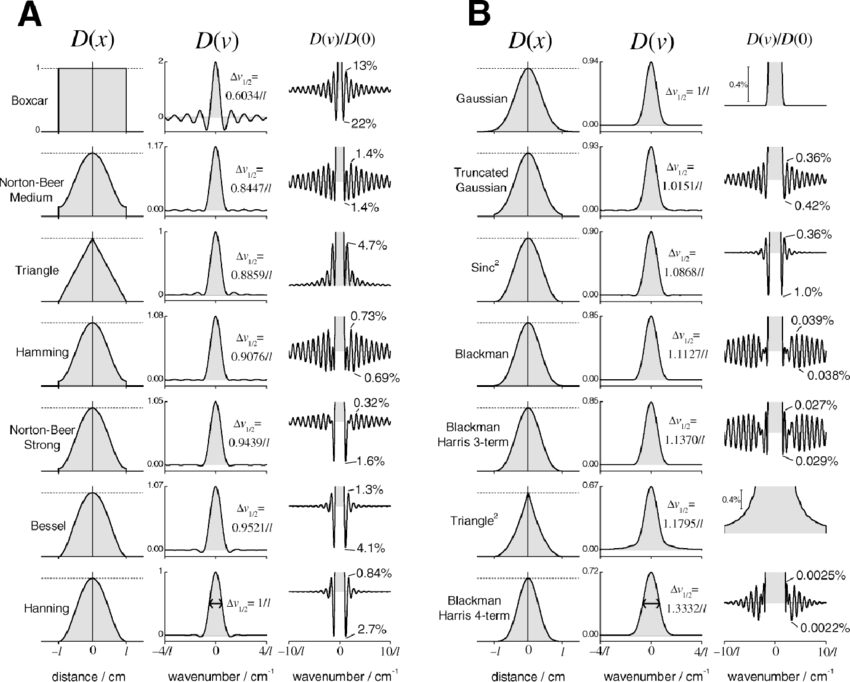
\includegraphics[width=0.5\textwidth]{Figures/Introduction/Apodization.png}
	\caption{Various Apodization functions and their Fourier Transforms. \cite{article}}
	\label{fig:apdoization}
\end{figure}

Once the spectrum has been generated, it must be divided by a reference spectrum to obtain accurate measurement values for the sample.

\pagebreak{}

\subsection{Rotation-Vibration Spectra of diatomic molecules}

In diatomic molecules, there is a along the axis connecting the two atoms. Absorption in the infrared range is caused by the various rotations and vibrations of the molecules, which alter the electric dipole moment. In a highly simplified model, the molecule can be represented by a dumbbell, where the masses of the atoms are treated as point masses that rotate at a fixed distance around a fixed axis through the center of gravity.

\begin{figure}[h]
	\centering
	\includegraphics[width=0.5\textwidth]{Figures/Introduction/Dumbbell.png}
	\caption{Dumbbell model of a diatomic molecule. \cite{nave_rotational}}
	\label{fig:dumbbell}
\end{figure}

The moment of inertia of the dumbbell is given by

\[
I = \mu r^2,
\]

where the reduced mass \(\mu\) is

\[
\mu = \frac{m_1 m_2}{m_1 + m_2}.
\]

Solving the Schrödinger equation in polar coordinates with a vanishing potential yields discrete energy values:

\[
E_m = \frac{m^2 h^2}{8 \pi^2 \mu r^2}.
\]

Next, this dumbbell model can be considered in the context of rotation around a space-free axis, so we transition to spherical coordinates. In this scenario, the energy is given by

\[
E(J) = hcBJ(J + 1) \quad \text{for} \quad J \in \mathbb{N}_0,
\]

with the rotation constant

\[
B = \frac{h}{8\pi^2cI}.
\]

The rotational term thus becomes

\[
F(J) = \frac{E}{hc} = BJ(J + 1) \quad \text{for} \quad J \in \mathbb{N}_0,
\]

subject to the selection rule

\[
\Delta J = \pm1.
\]

\pagebreak{}

In addition, the harmonic oscillator can be considered, initially in isolation.

\begin{figure}[h]
	\centering
	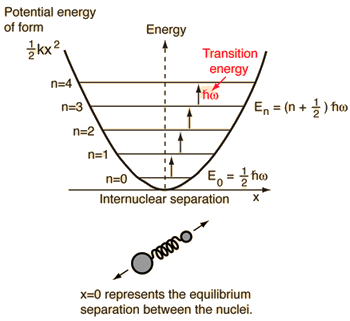
\includegraphics[width=0.5\textwidth]{Figures/Introduction/qhar.png}
	\caption{Harmonic Oscillator model of a diatomic molecule. \cite{nave_quantum}}
	\label{fig:harmonic_oscillator}
\end{figure}

Here, the equations of motion are obtained by considering the forces:

\[
m_1 \ddot{x}_1 = -k(x_1 - x_2),
\]
\[
m_2 \ddot{x}_2 = -k(x_2 - x_1).
\]

By introducing the substitution \( x = x_1 - x_2 \), these equations can be combined into:

\[
\ddot{x} = -\frac{k}{\mu} x,
\]

where the reduced mass \(\mu\) is defined as:

\[
\mu = \frac{m_1 m_2}{m_1 + m_2}.
\]

The resonance wavenumber of such a harmonic oscillator is then given by:

\[
\bar{\nu}_s = \frac{1}{2\pi c} \sqrt{\frac{k}{\mu}}.
\]

To calculate the energy values, we solve the Schrödinger equation for the potential:

\[
U = 2\pi^2 c^2 \bar{\nu}_s^2 \mu x^2,
\]

which is derived from the restoring force:

\[
- \frac{dU}{dx} = F = -k x.
\]

Assuming a solution of the form:

\[
x = x_0 \sin (2\pi c \bar{\nu}_s t),
\]

we obtain discrete energy levels:

\[
E(n) = hc \bar{\nu} \left( n + \frac{1}{2} \right), \quad n \in \mathbb{N}_0,
\]

with the selection rule:

\[
\Delta n = \pm 1.
\]

\pagebreak{}

These energy levels in turn yield the oscillation term:

\[
G(n) = \bar{\nu}_s \left( n + \frac{1}{2} \right).
\]

Both effects can now be combined to obtain the rotational-vibrational spectra. If interactions are initially neglected, the rotational and vibrational energy can be summed up as:

\[
E(n, J) = hcBJ(J + 1) + hc\bar{\nu}_s \left( n + \frac{1}{2} \right),
\]

resulting in the rotational oscillation term:

\[
T(n, J) = BJ(J + 1) + \bar{\nu}_s \left( n + \frac{1}{2} \right).
\]

Transitions are allowed for:

\[
\Delta J = \pm 1 \quad \text{and} \quad \Delta n = 0, \pm 1.
\]

The transitions can be categorized into the R branch, where \(J\) increases, and the P branch, where \(J\) decreases. A pure rotational spectrum is obtained for transitions with \(n = \text{const}\). To account for the interactions between oscillation and rotation, one must transition from the dumbbell model to the non-rigid rotator model, resulting in the oscillation term as a function of the quantum number:

\[
F_n(J) = B_n J(J + 1) - D_n J^2 (J + 1)^2,
\]

where \(D_n\) is the respective strain constant. The \(n\)-dependence arises from changes in the mean distance between the atoms. If each transition is indexed by \(i\) (where \(i = \Delta J\)), a relationship between the respective wavenumber of the minimum and the quantum number-dependent rotation and strain constants can be expressed as:

\begin{equation}
	\bar{\nu}_i = \bar{\nu}_s + (B_1 + B_0)i + (B_1 - B_0)i^2 - 2(D_1 + D_0)i^3
	\label{eq:Wavenumber}
\end{equation}


If we calculate the difference between two neighboring wavenumber minima and then the difference between these differences, we obtain the following equations:

\begin{equation}
	\Delta \bar{\nu}(i) = 2B_1 - 2(D_1 + D_0) + 2i(B_1 - B_0 - 3(D_1 + D_0)) - 6i^2 (D_1 + D_0),
	\label{eq:Quadratic}
\end{equation}

If a quadratic fit is performed on \ref{eq:Quadratic}, one can figure out the values of $D_1 + D_0$, $B_1$ and $B_0$. 

\pagebreak{}

\subsection{Interference Method}

When a light beam passes through an empty cuvette, multiple reflections occur, leading to interference. These interferences depend on the wavelength of the light, the thickness and refractive index of the cavity, and the angle of incidence. In the spectrum, they manifest as a periodic modulation of the intensity. The following sections outline the theoretical principles that describe the wavelengths corresponding to the transmission maxima and minima.


\begin{figure}[h]
	\centering
	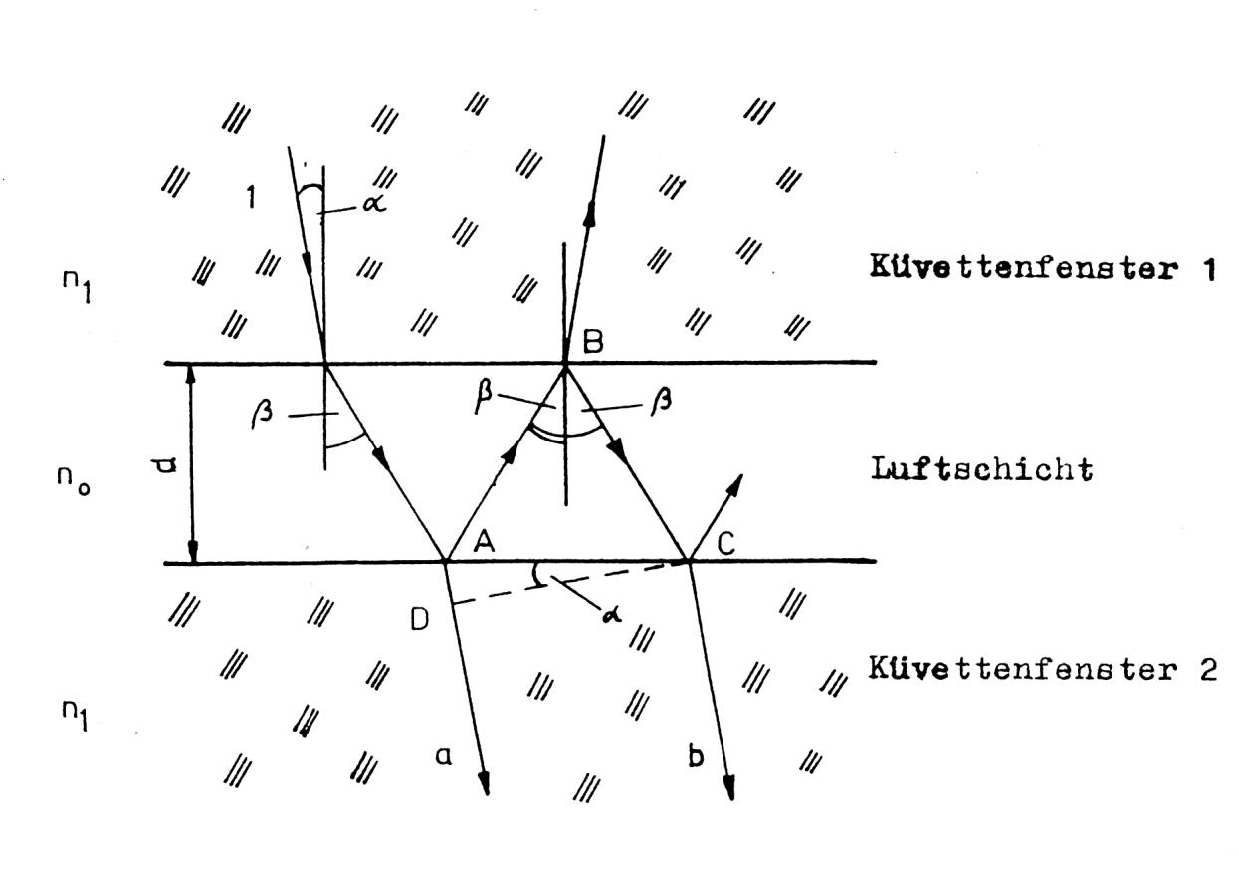
\includegraphics[width=0.5\textwidth]{Figures/Introduction/Interference.png}
	\label{fig:interference}
	\caption{Interference in a thin film. The labels from top to bottom are cuvette window 1, air gap, cuvette window 2.  \cite{riede_rotationvibration}}
\end{figure}

Whether this interference is constructive or destructive depends on the path difference between the waves. This path difference is given by:

\[
\Delta = n_0 (\text{AB} + \text{BC}) - n_1 \text{AD},
\]

and can be calculated using trigonometric relationships and Snell's law of refraction:

\[
n_0 \sin \beta = n_1 \sin \alpha,
\]

which leads to:

\[
\Delta = 2n_0 d \cos \beta.
\]

Destructive interference occurs when the path difference is a half-integer multiple of the wavelength, and constructive interference occurs for integer multiples. The difference between the ordinal numbers of the maxima is given by:

\[
N_1 - N_2 = 2dn_0 (\bar{\nu}_1 - \bar{\nu}_2),
\]

which results in the film thickness for an air-filled cell (\(n_0 \approx 1\)) being

\begin{equation}
	d = \frac{N_1 - N_2}{2(\bar{\nu}_1 - \bar{\nu}_2)}.
	\label{eq:thickness}
\end{equation}

\pagebreak{}

\subsection{Intensity of rotational-vibrational spectra}

Consider the number of molecules \( N \) in the state with \( n = 0 \). The expression for \( N(J, n = 0) \) is given by:

\[
N(J, n = 0) = \frac{N_{\text{gas}}}{Q_r}(2J + 1) \exp \left( - \frac{hcBJ(J+1)}{kT} \right) \exp \left( - \frac{hc \bar{\nu}_s (n + \frac{1}{2})}{kT} \right) 
\]

where \( Q_r \) represents the sum of the states. 

For the absorption coefficient, which is critical for determining the intensity of the minima, we have:

\[
\alpha = c_3 \bar{\nu} (2J + 1) \exp \left( - \frac{hcB J (J + 1)}{kT} \right)
\]

where \( c_3 \) is a constant. According to Lambert-Beer's law, the relative intensities are:

\[
I(J) = I_0 \exp \left( -\alpha d \right) = I_0 \exp \left( -c_4 \bar{\nu} (2J + 1) \exp \left( - \frac{hcB J (J + 1)}{kT} \right) \right)
\]

where \( \bar{\nu} \) is found using \ref{eq:Wavenumber}

\pagebreak{}

\subsection{Experimental Setup}

We used the Perkin Elmer Spectrum 100 FTIR spectrometer. This instrument operates using a modified Michelson interferometer. In this configuration, the path difference between the two light beams is adjusted by rotating an additional pair of mirrors around a common axis.

\begin{figure}[h]
    \centering
    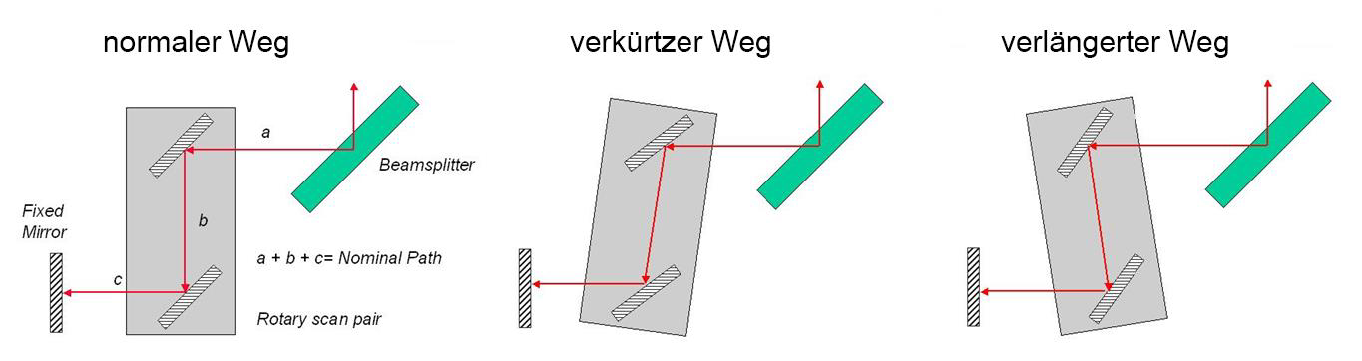
\includegraphics[width=0.7\textwidth]{Figures/Introduction/Pathdifference.png}
    \caption{Path difference via a rotatable mirror apparatus. \cite{riede_rotationvibration}}
    \label{fig:path_difference}
\end{figure}

The light source for the spectrometer is a `Norton Source' which is a silicon carbide crystal through which a current flows. The current heats the crystal, causing it to emit an almost perfect blackbody spectrum with its peak in the mid-infrared range.

\begin{figure}[h]
    \centering
    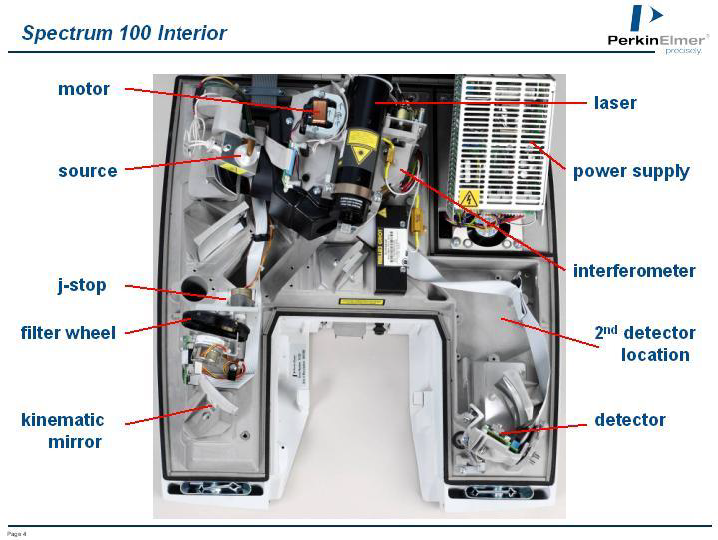
\includegraphics[width=0.7\textwidth]{Figures/Introduction/Spectrum100Interior.png}
    \caption{Structure inside the Spectrum 100 spectrometer. \cite{riede_rotationvibration}}
    \label{fig:spectrum_100_structure}
\end{figure}

For the measurement, the sample is placed in the cuvette holder of the spectrometer. Once the lid is closed and the measurement is initiated, the spectrometer records an interferogram. The travel distance of the mirror apparatus can be adjusted according to the requirements of the measurement. Depending on the selected measurement mode, the spectrum can either be directly generated by the device or calculated manually using a Fourier transform. 

\begin{figure}[h]
	\begin{subfigure}[t]{0.48\textwidth}
    	\centering
    	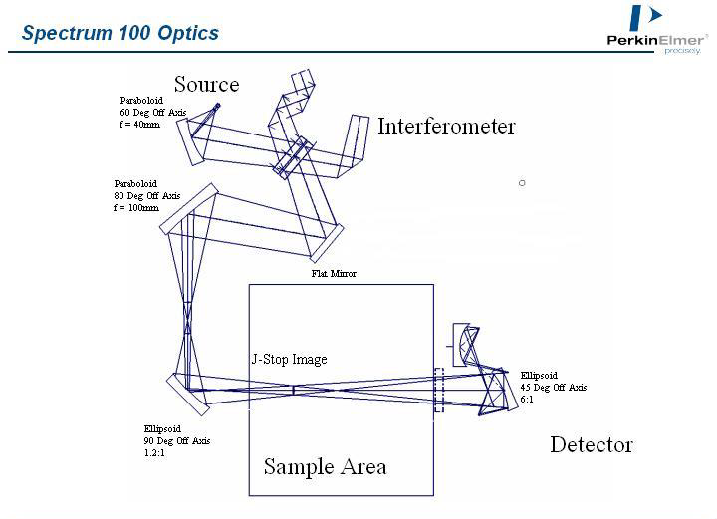
\includegraphics[width=0.7\textwidth]{Figures/Introduction/Schematic1.png}
    	\caption{Schematic of the optics inside the spectrometer. \cite{riede_rotationvibration}}
    	\label{fig:spectrometer_optics}
	\end{subfigure}
	\begin{subfigure}[t]{0.48\textwidth}
		\centering
		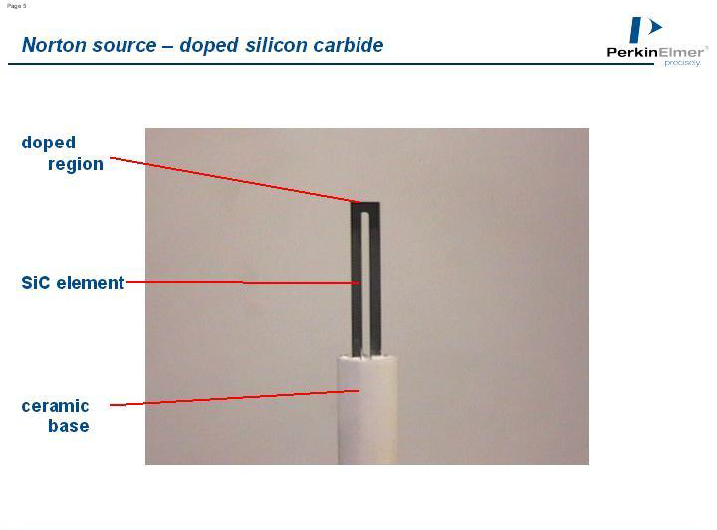
\includegraphics[width=0.7\textwidth]{Figures/Introduction/Schematic2.png}
		\caption{Norton Source.}
		\label{fig:nortonsource}
	\end{subfigure}
	\caption{}
\end{figure}


\pagebreak{}


\section{Analysis}

\subsection{Task 1}

\textit{Verify the calibration of the wavenumber scale of the infrared spectrometer Spectrum 100 using
water vapor and polystyrene calibration bands. Plot the experimentally determined deviations and
discuss them.}

When measuring the spectrum of "water vapour", what we are actually measuring is the empty cuvette holder with air inside it, as a background spectrum that will prove useful later. The following plots show the spectra for water vapour and polystyrene:


\begin{figure}[h]
    \centering
    \begin{subfigure}[t]{0.48\textwidth}
        \centering
        \scalebox{0.5}{%% Creator: Matplotlib, PGF backend
%%
%% To include the figure in your LaTeX document, write
%%   \input{<filename>.pgf}
%%
%% Make sure the required packages are loaded in your preamble
%%   \usepackage{pgf}
%%
%% Also ensure that all the required font packages are loaded; for instance,
%% the lmodern package is sometimes necessary when using math font.
%%   \usepackage{lmodern}
%%
%% Figures using additional raster images can only be included by \input if
%% they are in the same directory as the main LaTeX file. For loading figures
%% from other directories you can use the `import` package
%%   \usepackage{import}
%%
%% and then include the figures with
%%   \import{<path to file>}{<filename>.pgf}
%%
%% Matplotlib used the following preamble
%%   
%%   \usepackage{fontspec}
%%   \makeatletter\@ifpackageloaded{underscore}{}{\usepackage[strings]{underscore}}\makeatother
%%
\begingroup%
\makeatletter%
\begin{pgfpicture}%
\pgfpathrectangle{\pgfpointorigin}{\pgfqpoint{5.840514in}{4.032028in}}%
\pgfusepath{use as bounding box, clip}%
\begin{pgfscope}%
\pgfsetbuttcap%
\pgfsetmiterjoin%
\definecolor{currentfill}{rgb}{1.000000,1.000000,1.000000}%
\pgfsetfillcolor{currentfill}%
\pgfsetlinewidth{0.000000pt}%
\definecolor{currentstroke}{rgb}{1.000000,1.000000,1.000000}%
\pgfsetstrokecolor{currentstroke}%
\pgfsetdash{}{0pt}%
\pgfpathmoveto{\pgfqpoint{0.000000in}{0.000000in}}%
\pgfpathlineto{\pgfqpoint{5.840514in}{0.000000in}}%
\pgfpathlineto{\pgfqpoint{5.840514in}{4.032028in}}%
\pgfpathlineto{\pgfqpoint{0.000000in}{4.032028in}}%
\pgfpathlineto{\pgfqpoint{0.000000in}{0.000000in}}%
\pgfpathclose%
\pgfusepath{fill}%
\end{pgfscope}%
\begin{pgfscope}%
\pgfsetbuttcap%
\pgfsetmiterjoin%
\definecolor{currentfill}{rgb}{1.000000,1.000000,1.000000}%
\pgfsetfillcolor{currentfill}%
\pgfsetlinewidth{0.000000pt}%
\definecolor{currentstroke}{rgb}{0.000000,0.000000,0.000000}%
\pgfsetstrokecolor{currentstroke}%
\pgfsetstrokeopacity{0.000000}%
\pgfsetdash{}{0pt}%
\pgfpathmoveto{\pgfqpoint{0.711111in}{0.598473in}}%
\pgfpathlineto{\pgfqpoint{1.357460in}{0.598473in}}%
\pgfpathlineto{\pgfqpoint{1.357460in}{3.686762in}}%
\pgfpathlineto{\pgfqpoint{0.711111in}{3.686762in}}%
\pgfpathlineto{\pgfqpoint{0.711111in}{0.598473in}}%
\pgfpathclose%
\pgfusepath{fill}%
\end{pgfscope}%
\begin{pgfscope}%
\pgfsetbuttcap%
\pgfsetroundjoin%
\definecolor{currentfill}{rgb}{0.000000,0.000000,0.000000}%
\pgfsetfillcolor{currentfill}%
\pgfsetlinewidth{0.803000pt}%
\definecolor{currentstroke}{rgb}{0.000000,0.000000,0.000000}%
\pgfsetstrokecolor{currentstroke}%
\pgfsetdash{}{0pt}%
\pgfsys@defobject{currentmarker}{\pgfqpoint{0.000000in}{-0.048611in}}{\pgfqpoint{0.000000in}{0.000000in}}{%
\pgfpathmoveto{\pgfqpoint{0.000000in}{0.000000in}}%
\pgfpathlineto{\pgfqpoint{0.000000in}{-0.048611in}}%
\pgfusepath{stroke,fill}%
}%
\begin{pgfscope}%
\pgfsys@transformshift{0.711111in}{0.598473in}%
\pgfsys@useobject{currentmarker}{}%
\end{pgfscope}%
\end{pgfscope}%
\begin{pgfscope}%
\definecolor{textcolor}{rgb}{0.000000,0.000000,0.000000}%
\pgfsetstrokecolor{textcolor}%
\pgfsetfillcolor{textcolor}%
\pgftext[x=0.711111in,y=0.501251in,,top]{\color{textcolor}\rmfamily\fontsize{14.000000}{16.800000}\selectfont \(\displaystyle {1410}\)}%
\end{pgfscope}%
\begin{pgfscope}%
\pgfsetbuttcap%
\pgfsetroundjoin%
\definecolor{currentfill}{rgb}{0.000000,0.000000,0.000000}%
\pgfsetfillcolor{currentfill}%
\pgfsetlinewidth{0.803000pt}%
\definecolor{currentstroke}{rgb}{0.000000,0.000000,0.000000}%
\pgfsetstrokecolor{currentstroke}%
\pgfsetdash{}{0pt}%
\pgfsys@defobject{currentmarker}{\pgfqpoint{0.000000in}{-0.048611in}}{\pgfqpoint{0.000000in}{0.000000in}}{%
\pgfpathmoveto{\pgfqpoint{0.000000in}{0.000000in}}%
\pgfpathlineto{\pgfqpoint{0.000000in}{-0.048611in}}%
\pgfusepath{stroke,fill}%
}%
\begin{pgfscope}%
\pgfsys@transformshift{1.357460in}{0.598473in}%
\pgfsys@useobject{currentmarker}{}%
\end{pgfscope}%
\end{pgfscope}%
\begin{pgfscope}%
\definecolor{textcolor}{rgb}{0.000000,0.000000,0.000000}%
\pgfsetstrokecolor{textcolor}%
\pgfsetfillcolor{textcolor}%
\pgftext[x=1.357460in,y=0.501251in,,top]{\color{textcolor}\rmfamily\fontsize{14.000000}{16.800000}\selectfont \(\displaystyle {1420}\)}%
\end{pgfscope}%
\begin{pgfscope}%
\pgfsetbuttcap%
\pgfsetroundjoin%
\definecolor{currentfill}{rgb}{0.000000,0.000000,0.000000}%
\pgfsetfillcolor{currentfill}%
\pgfsetlinewidth{0.803000pt}%
\definecolor{currentstroke}{rgb}{0.000000,0.000000,0.000000}%
\pgfsetstrokecolor{currentstroke}%
\pgfsetdash{}{0pt}%
\pgfsys@defobject{currentmarker}{\pgfqpoint{-0.048611in}{0.000000in}}{\pgfqpoint{-0.000000in}{0.000000in}}{%
\pgfpathmoveto{\pgfqpoint{-0.000000in}{0.000000in}}%
\pgfpathlineto{\pgfqpoint{-0.048611in}{0.000000in}}%
\pgfusepath{stroke,fill}%
}%
\begin{pgfscope}%
\pgfsys@transformshift{0.711111in}{0.742072in}%
\pgfsys@useobject{currentmarker}{}%
\end{pgfscope}%
\end{pgfscope}%
\begin{pgfscope}%
\definecolor{textcolor}{rgb}{0.000000,0.000000,0.000000}%
\pgfsetstrokecolor{textcolor}%
\pgfsetfillcolor{textcolor}%
\pgftext[x=0.518611in, y=0.674600in, left, base]{\color{textcolor}\rmfamily\fontsize{14.000000}{16.800000}\selectfont 0}%
\end{pgfscope}%
\begin{pgfscope}%
\pgfsetbuttcap%
\pgfsetroundjoin%
\definecolor{currentfill}{rgb}{0.000000,0.000000,0.000000}%
\pgfsetfillcolor{currentfill}%
\pgfsetlinewidth{0.803000pt}%
\definecolor{currentstroke}{rgb}{0.000000,0.000000,0.000000}%
\pgfsetstrokecolor{currentstroke}%
\pgfsetdash{}{0pt}%
\pgfsys@defobject{currentmarker}{\pgfqpoint{-0.048611in}{0.000000in}}{\pgfqpoint{-0.000000in}{0.000000in}}{%
\pgfpathmoveto{\pgfqpoint{-0.000000in}{0.000000in}}%
\pgfpathlineto{\pgfqpoint{-0.048611in}{0.000000in}}%
\pgfusepath{stroke,fill}%
}%
\begin{pgfscope}%
\pgfsys@transformshift{0.711111in}{1.525440in}%
\pgfsys@useobject{currentmarker}{}%
\end{pgfscope}%
\end{pgfscope}%
\begin{pgfscope}%
\definecolor{textcolor}{rgb}{0.000000,0.000000,0.000000}%
\pgfsetstrokecolor{textcolor}%
\pgfsetfillcolor{textcolor}%
\pgftext[x=0.518611in, y=1.457968in, left, base]{\color{textcolor}\rmfamily\fontsize{14.000000}{16.800000}\selectfont 5}%
\end{pgfscope}%
\begin{pgfscope}%
\pgfsetbuttcap%
\pgfsetroundjoin%
\definecolor{currentfill}{rgb}{0.000000,0.000000,0.000000}%
\pgfsetfillcolor{currentfill}%
\pgfsetlinewidth{0.803000pt}%
\definecolor{currentstroke}{rgb}{0.000000,0.000000,0.000000}%
\pgfsetstrokecolor{currentstroke}%
\pgfsetdash{}{0pt}%
\pgfsys@defobject{currentmarker}{\pgfqpoint{-0.048611in}{0.000000in}}{\pgfqpoint{-0.000000in}{0.000000in}}{%
\pgfpathmoveto{\pgfqpoint{-0.000000in}{0.000000in}}%
\pgfpathlineto{\pgfqpoint{-0.048611in}{0.000000in}}%
\pgfusepath{stroke,fill}%
}%
\begin{pgfscope}%
\pgfsys@transformshift{0.711111in}{2.308809in}%
\pgfsys@useobject{currentmarker}{}%
\end{pgfscope}%
\end{pgfscope}%
\begin{pgfscope}%
\definecolor{textcolor}{rgb}{0.000000,0.000000,0.000000}%
\pgfsetstrokecolor{textcolor}%
\pgfsetfillcolor{textcolor}%
\pgftext[x=0.423333in, y=2.241336in, left, base]{\color{textcolor}\rmfamily\fontsize{14.000000}{16.800000}\selectfont 10}%
\end{pgfscope}%
\begin{pgfscope}%
\pgfsetbuttcap%
\pgfsetroundjoin%
\definecolor{currentfill}{rgb}{0.000000,0.000000,0.000000}%
\pgfsetfillcolor{currentfill}%
\pgfsetlinewidth{0.803000pt}%
\definecolor{currentstroke}{rgb}{0.000000,0.000000,0.000000}%
\pgfsetstrokecolor{currentstroke}%
\pgfsetdash{}{0pt}%
\pgfsys@defobject{currentmarker}{\pgfqpoint{-0.048611in}{0.000000in}}{\pgfqpoint{-0.000000in}{0.000000in}}{%
\pgfpathmoveto{\pgfqpoint{-0.000000in}{0.000000in}}%
\pgfpathlineto{\pgfqpoint{-0.048611in}{0.000000in}}%
\pgfusepath{stroke,fill}%
}%
\begin{pgfscope}%
\pgfsys@transformshift{0.711111in}{3.092177in}%
\pgfsys@useobject{currentmarker}{}%
\end{pgfscope}%
\end{pgfscope}%
\begin{pgfscope}%
\definecolor{textcolor}{rgb}{0.000000,0.000000,0.000000}%
\pgfsetstrokecolor{textcolor}%
\pgfsetfillcolor{textcolor}%
\pgftext[x=0.423333in, y=3.024704in, left, base]{\color{textcolor}\rmfamily\fontsize{14.000000}{16.800000}\selectfont 15}%
\end{pgfscope}%
\begin{pgfscope}%
\pgfsetrectcap%
\pgfsetroundjoin%
\pgfsetlinewidth{0.803000pt}%
\definecolor{currentstroke}{rgb}{0.000000,0.000000,0.000000}%
\pgfsetstrokecolor{currentstroke}%
\pgfsetdash{}{0pt}%
\pgfpathmoveto{\pgfqpoint{1.288628in}{0.541752in}}%
\pgfpathlineto{\pgfqpoint{1.426292in}{0.655194in}}%
\pgfusepath{stroke}%
\end{pgfscope}%
\begin{pgfscope}%
\pgfpathrectangle{\pgfqpoint{0.711111in}{0.598473in}}{\pgfqpoint{0.646349in}{3.088289in}}%
\pgfusepath{clip}%
\pgfsetrectcap%
\pgfsetroundjoin%
\pgfsetlinewidth{0.501875pt}%
\definecolor{currentstroke}{rgb}{0.000000,0.000000,0.000000}%
\pgfsetstrokecolor{currentstroke}%
\pgfsetdash{}{0pt}%
\pgfpathmoveto{\pgfqpoint{1.367460in}{1.650261in}}%
\pgfpathlineto{\pgfqpoint{1.357460in}{2.009492in}}%
\pgfpathlineto{\pgfqpoint{1.349381in}{2.234925in}}%
\pgfpathlineto{\pgfqpoint{1.341301in}{2.376531in}}%
\pgfpathlineto{\pgfqpoint{1.333222in}{2.450378in}}%
\pgfpathlineto{\pgfqpoint{1.325142in}{2.474468in}}%
\pgfpathlineto{\pgfqpoint{1.317063in}{2.434755in}}%
\pgfpathlineto{\pgfqpoint{1.308984in}{2.296123in}}%
\pgfpathlineto{\pgfqpoint{1.292825in}{1.792450in}}%
\pgfpathlineto{\pgfqpoint{1.284746in}{1.622613in}}%
\pgfpathlineto{\pgfqpoint{1.276666in}{1.636035in}}%
\pgfpathlineto{\pgfqpoint{1.268587in}{1.825082in}}%
\pgfpathlineto{\pgfqpoint{1.252428in}{2.340102in}}%
\pgfpathlineto{\pgfqpoint{1.244349in}{2.497151in}}%
\pgfpathlineto{\pgfqpoint{1.236269in}{2.568096in}}%
\pgfpathlineto{\pgfqpoint{1.228190in}{2.570762in}}%
\pgfpathlineto{\pgfqpoint{1.220111in}{2.505869in}}%
\pgfpathlineto{\pgfqpoint{1.203952in}{2.235351in}}%
\pgfpathlineto{\pgfqpoint{1.195873in}{2.165629in}}%
\pgfpathlineto{\pgfqpoint{1.187793in}{2.219286in}}%
\pgfpathlineto{\pgfqpoint{1.171635in}{2.508698in}}%
\pgfpathlineto{\pgfqpoint{1.163555in}{2.600766in}}%
\pgfpathlineto{\pgfqpoint{1.155476in}{2.637392in}}%
\pgfpathlineto{\pgfqpoint{1.147396in}{2.645221in}}%
\pgfpathlineto{\pgfqpoint{1.139317in}{2.643038in}}%
\pgfpathlineto{\pgfqpoint{1.131238in}{2.638381in}}%
\pgfpathlineto{\pgfqpoint{1.123158in}{2.636566in}}%
\pgfpathlineto{\pgfqpoint{1.115079in}{2.639708in}}%
\pgfpathlineto{\pgfqpoint{1.107000in}{2.644364in}}%
\pgfpathlineto{\pgfqpoint{1.074682in}{2.657021in}}%
\pgfpathlineto{\pgfqpoint{1.050444in}{2.660220in}}%
\pgfpathlineto{\pgfqpoint{1.042365in}{2.659473in}}%
\pgfpathlineto{\pgfqpoint{1.026206in}{2.656171in}}%
\pgfpathlineto{\pgfqpoint{1.010047in}{2.655086in}}%
\pgfpathlineto{\pgfqpoint{0.985809in}{2.649321in}}%
\pgfpathlineto{\pgfqpoint{0.977730in}{2.643881in}}%
\pgfpathlineto{\pgfqpoint{0.969650in}{2.633249in}}%
\pgfpathlineto{\pgfqpoint{0.961571in}{2.611785in}}%
\pgfpathlineto{\pgfqpoint{0.953492in}{2.570364in}}%
\pgfpathlineto{\pgfqpoint{0.937333in}{2.452317in}}%
\pgfpathlineto{\pgfqpoint{0.929254in}{2.418210in}}%
\pgfpathlineto{\pgfqpoint{0.921174in}{2.405753in}}%
\pgfpathlineto{\pgfqpoint{0.905016in}{2.385465in}}%
\pgfpathlineto{\pgfqpoint{0.896936in}{2.395968in}}%
\pgfpathlineto{\pgfqpoint{0.888857in}{2.442792in}}%
\pgfpathlineto{\pgfqpoint{0.880777in}{2.510361in}}%
\pgfpathlineto{\pgfqpoint{0.872698in}{2.567508in}}%
\pgfpathlineto{\pgfqpoint{0.864619in}{2.598117in}}%
\pgfpathlineto{\pgfqpoint{0.856539in}{2.607461in}}%
\pgfpathlineto{\pgfqpoint{0.848460in}{2.606583in}}%
\pgfpathlineto{\pgfqpoint{0.840381in}{2.600334in}}%
\pgfpathlineto{\pgfqpoint{0.832301in}{2.585301in}}%
\pgfpathlineto{\pgfqpoint{0.824222in}{2.551687in}}%
\pgfpathlineto{\pgfqpoint{0.816143in}{2.493546in}}%
\pgfpathlineto{\pgfqpoint{0.808063in}{2.425674in}}%
\pgfpathlineto{\pgfqpoint{0.799984in}{2.383479in}}%
\pgfpathlineto{\pgfqpoint{0.791904in}{2.393861in}}%
\pgfpathlineto{\pgfqpoint{0.775746in}{2.507629in}}%
\pgfpathlineto{\pgfqpoint{0.767666in}{2.545935in}}%
\pgfpathlineto{\pgfqpoint{0.759587in}{2.559657in}}%
\pgfpathlineto{\pgfqpoint{0.751508in}{2.560071in}}%
\pgfpathlineto{\pgfqpoint{0.743428in}{2.555249in}}%
\pgfpathlineto{\pgfqpoint{0.727270in}{2.538401in}}%
\pgfpathlineto{\pgfqpoint{0.711111in}{2.520622in}}%
\pgfpathlineto{\pgfqpoint{0.701111in}{2.513824in}}%
\pgfpathlineto{\pgfqpoint{0.701111in}{2.513824in}}%
\pgfusepath{stroke}%
\end{pgfscope}%
\begin{pgfscope}%
\pgfpathrectangle{\pgfqpoint{0.711111in}{0.598473in}}{\pgfqpoint{0.646349in}{3.088289in}}%
\pgfusepath{clip}%
\pgfsetbuttcap%
\pgfsetroundjoin%
\definecolor{currentfill}{rgb}{1.000000,0.000000,0.000000}%
\pgfsetfillcolor{currentfill}%
\pgfsetlinewidth{1.003750pt}%
\definecolor{currentstroke}{rgb}{1.000000,0.000000,0.000000}%
\pgfsetstrokecolor{currentstroke}%
\pgfsetdash{}{0pt}%
\pgfsys@defobject{currentmarker}{\pgfqpoint{-0.017361in}{-0.017361in}}{\pgfqpoint{0.017361in}{0.017361in}}{%
\pgfpathmoveto{\pgfqpoint{0.000000in}{-0.017361in}}%
\pgfpathcurveto{\pgfqpoint{0.004604in}{-0.017361in}}{\pgfqpoint{0.009020in}{-0.015532in}}{\pgfqpoint{0.012276in}{-0.012276in}}%
\pgfpathcurveto{\pgfqpoint{0.015532in}{-0.009020in}}{\pgfqpoint{0.017361in}{-0.004604in}}{\pgfqpoint{0.017361in}{0.000000in}}%
\pgfpathcurveto{\pgfqpoint{0.017361in}{0.004604in}}{\pgfqpoint{0.015532in}{0.009020in}}{\pgfqpoint{0.012276in}{0.012276in}}%
\pgfpathcurveto{\pgfqpoint{0.009020in}{0.015532in}}{\pgfqpoint{0.004604in}{0.017361in}}{\pgfqpoint{0.000000in}{0.017361in}}%
\pgfpathcurveto{\pgfqpoint{-0.004604in}{0.017361in}}{\pgfqpoint{-0.009020in}{0.015532in}}{\pgfqpoint{-0.012276in}{0.012276in}}%
\pgfpathcurveto{\pgfqpoint{-0.015532in}{0.009020in}}{\pgfqpoint{-0.017361in}{0.004604in}}{\pgfqpoint{-0.017361in}{0.000000in}}%
\pgfpathcurveto{\pgfqpoint{-0.017361in}{-0.004604in}}{\pgfqpoint{-0.015532in}{-0.009020in}}{\pgfqpoint{-0.012276in}{-0.012276in}}%
\pgfpathcurveto{\pgfqpoint{-0.009020in}{-0.015532in}}{\pgfqpoint{-0.004604in}{-0.017361in}}{\pgfqpoint{0.000000in}{-0.017361in}}%
\pgfpathlineto{\pgfqpoint{0.000000in}{-0.017361in}}%
\pgfpathclose%
\pgfusepath{stroke,fill}%
}%
\begin{pgfscope}%
\pgfsys@transformshift{1.195873in}{2.165629in}%
\pgfsys@useobject{currentmarker}{}%
\end{pgfscope}%
\begin{pgfscope}%
\pgfsys@transformshift{13.177568in}{2.571903in}%
\pgfsys@useobject{currentmarker}{}%
\end{pgfscope}%
\begin{pgfscope}%
\pgfsys@transformshift{25.450121in}{1.715925in}%
\pgfsys@useobject{currentmarker}{}%
\end{pgfscope}%
\begin{pgfscope}%
\pgfsys@transformshift{26.007597in}{1.718811in}%
\pgfsys@useobject{currentmarker}{}%
\end{pgfscope}%
\begin{pgfscope}%
\pgfsys@transformshift{26.120708in}{2.425118in}%
\pgfsys@useobject{currentmarker}{}%
\end{pgfscope}%
\begin{pgfscope}%
\pgfsys@transformshift{26.363089in}{3.231087in}%
\pgfsys@useobject{currentmarker}{}%
\end{pgfscope}%
\begin{pgfscope}%
\pgfsys@transformshift{26.532756in}{2.774794in}%
\pgfsys@useobject{currentmarker}{}%
\end{pgfscope}%
\begin{pgfscope}%
\pgfsys@transformshift{40.057610in}{2.911381in}%
\pgfsys@useobject{currentmarker}{}%
\end{pgfscope}%
\begin{pgfscope}%
\pgfsys@transformshift{41.649244in}{3.164914in}%
\pgfsys@useobject{currentmarker}{}%
\end{pgfscope}%
\end{pgfscope}%
\begin{pgfscope}%
\pgfsetrectcap%
\pgfsetmiterjoin%
\pgfsetlinewidth{0.803000pt}%
\definecolor{currentstroke}{rgb}{0.000000,0.000000,0.000000}%
\pgfsetstrokecolor{currentstroke}%
\pgfsetdash{}{0pt}%
\pgfpathmoveto{\pgfqpoint{0.711111in}{0.598473in}}%
\pgfpathlineto{\pgfqpoint{0.711111in}{3.686762in}}%
\pgfusepath{stroke}%
\end{pgfscope}%
\begin{pgfscope}%
\pgfsetrectcap%
\pgfsetmiterjoin%
\pgfsetlinewidth{0.803000pt}%
\definecolor{currentstroke}{rgb}{0.000000,0.000000,0.000000}%
\pgfsetstrokecolor{currentstroke}%
\pgfsetdash{}{0pt}%
\pgfpathmoveto{\pgfqpoint{0.711111in}{0.598473in}}%
\pgfpathlineto{\pgfqpoint{1.357460in}{0.598473in}}%
\pgfusepath{stroke}%
\end{pgfscope}%
\begin{pgfscope}%
\pgfsetbuttcap%
\pgfsetmiterjoin%
\definecolor{currentfill}{rgb}{1.000000,1.000000,1.000000}%
\pgfsetfillcolor{currentfill}%
\pgfsetlinewidth{0.000000pt}%
\definecolor{currentstroke}{rgb}{0.000000,0.000000,0.000000}%
\pgfsetstrokecolor{currentstroke}%
\pgfsetstrokeopacity{0.000000}%
\pgfsetdash{}{0pt}%
\pgfpathmoveto{\pgfqpoint{1.418055in}{0.598473in}}%
\pgfpathlineto{\pgfqpoint{2.064404in}{0.598473in}}%
\pgfpathlineto{\pgfqpoint{2.064404in}{3.686762in}}%
\pgfpathlineto{\pgfqpoint{1.418055in}{3.686762in}}%
\pgfpathlineto{\pgfqpoint{1.418055in}{0.598473in}}%
\pgfpathclose%
\pgfusepath{fill}%
\end{pgfscope}%
\begin{pgfscope}%
\pgfsetbuttcap%
\pgfsetroundjoin%
\definecolor{currentfill}{rgb}{0.000000,0.000000,0.000000}%
\pgfsetfillcolor{currentfill}%
\pgfsetlinewidth{0.803000pt}%
\definecolor{currentstroke}{rgb}{0.000000,0.000000,0.000000}%
\pgfsetstrokecolor{currentstroke}%
\pgfsetdash{}{0pt}%
\pgfsys@defobject{currentmarker}{\pgfqpoint{0.000000in}{-0.048611in}}{\pgfqpoint{0.000000in}{0.000000in}}{%
\pgfpathmoveto{\pgfqpoint{0.000000in}{0.000000in}}%
\pgfpathlineto{\pgfqpoint{0.000000in}{-0.048611in}}%
\pgfusepath{stroke,fill}%
}%
\begin{pgfscope}%
\pgfsys@transformshift{1.741230in}{0.598473in}%
\pgfsys@useobject{currentmarker}{}%
\end{pgfscope}%
\end{pgfscope}%
\begin{pgfscope}%
\definecolor{textcolor}{rgb}{0.000000,0.000000,0.000000}%
\pgfsetstrokecolor{textcolor}%
\pgfsetfillcolor{textcolor}%
\pgftext[x=1.741230in,y=0.501251in,,top]{\color{textcolor}\rmfamily\fontsize{14.000000}{16.800000}\selectfont \(\displaystyle {1600}\)}%
\end{pgfscope}%
\begin{pgfscope}%
\pgfsetrectcap%
\pgfsetroundjoin%
\pgfsetlinewidth{0.803000pt}%
\definecolor{currentstroke}{rgb}{0.000000,0.000000,0.000000}%
\pgfsetstrokecolor{currentstroke}%
\pgfsetdash{}{0pt}%
\pgfpathmoveto{\pgfqpoint{1.995572in}{0.541752in}}%
\pgfpathlineto{\pgfqpoint{2.133236in}{0.655194in}}%
\pgfusepath{stroke}%
\end{pgfscope}%
\begin{pgfscope}%
\pgfsetrectcap%
\pgfsetroundjoin%
\pgfsetlinewidth{0.803000pt}%
\definecolor{currentstroke}{rgb}{0.000000,0.000000,0.000000}%
\pgfsetstrokecolor{currentstroke}%
\pgfsetdash{}{0pt}%
\pgfpathmoveto{\pgfqpoint{1.349223in}{0.541752in}}%
\pgfpathlineto{\pgfqpoint{1.486887in}{0.655194in}}%
\pgfusepath{stroke}%
\end{pgfscope}%
\begin{pgfscope}%
\pgfpathrectangle{\pgfqpoint{1.418055in}{0.598473in}}{\pgfqpoint{0.646349in}{3.088289in}}%
\pgfusepath{clip}%
\pgfsetrectcap%
\pgfsetroundjoin%
\pgfsetlinewidth{0.501875pt}%
\definecolor{currentstroke}{rgb}{0.000000,0.000000,0.000000}%
\pgfsetstrokecolor{currentstroke}%
\pgfsetdash{}{0pt}%
\pgfpathmoveto{\pgfqpoint{2.074404in}{2.548234in}}%
\pgfpathlineto{\pgfqpoint{2.064404in}{2.434486in}}%
\pgfpathlineto{\pgfqpoint{2.056325in}{2.392053in}}%
\pgfpathlineto{\pgfqpoint{2.048245in}{2.407921in}}%
\pgfpathlineto{\pgfqpoint{2.040166in}{2.458029in}}%
\pgfpathlineto{\pgfqpoint{2.024007in}{2.576015in}}%
\pgfpathlineto{\pgfqpoint{2.007849in}{2.703236in}}%
\pgfpathlineto{\pgfqpoint{1.999769in}{2.748640in}}%
\pgfpathlineto{\pgfqpoint{1.991690in}{2.773106in}}%
\pgfpathlineto{\pgfqpoint{1.983611in}{2.783916in}}%
\pgfpathlineto{\pgfqpoint{1.975531in}{2.787532in}}%
\pgfpathlineto{\pgfqpoint{1.967452in}{2.783781in}}%
\pgfpathlineto{\pgfqpoint{1.959372in}{2.768755in}}%
\pgfpathlineto{\pgfqpoint{1.951293in}{2.736506in}}%
\pgfpathlineto{\pgfqpoint{1.943214in}{2.682963in}}%
\pgfpathlineto{\pgfqpoint{1.935134in}{2.618219in}}%
\pgfpathlineto{\pgfqpoint{1.927055in}{2.571903in}}%
\pgfpathlineto{\pgfqpoint{1.918976in}{2.573745in}}%
\pgfpathlineto{\pgfqpoint{1.910896in}{2.625231in}}%
\pgfpathlineto{\pgfqpoint{1.902817in}{2.697223in}}%
\pgfpathlineto{\pgfqpoint{1.894738in}{2.757230in}}%
\pgfpathlineto{\pgfqpoint{1.886658in}{2.793128in}}%
\pgfpathlineto{\pgfqpoint{1.878579in}{2.810871in}}%
\pgfpathlineto{\pgfqpoint{1.870499in}{2.819564in}}%
\pgfpathlineto{\pgfqpoint{1.846261in}{2.833330in}}%
\pgfpathlineto{\pgfqpoint{1.830103in}{2.840732in}}%
\pgfpathlineto{\pgfqpoint{1.805865in}{2.851272in}}%
\pgfpathlineto{\pgfqpoint{1.781626in}{2.852872in}}%
\pgfpathlineto{\pgfqpoint{1.725071in}{2.867621in}}%
\pgfpathlineto{\pgfqpoint{1.708912in}{2.870348in}}%
\pgfpathlineto{\pgfqpoint{1.668515in}{2.871743in}}%
\pgfpathlineto{\pgfqpoint{1.660436in}{2.871743in}}%
\pgfpathlineto{\pgfqpoint{1.652357in}{2.870365in}}%
\pgfpathlineto{\pgfqpoint{1.644277in}{2.864527in}}%
\pgfpathlineto{\pgfqpoint{1.636198in}{2.848003in}}%
\pgfpathlineto{\pgfqpoint{1.628119in}{2.811120in}}%
\pgfpathlineto{\pgfqpoint{1.620039in}{2.748809in}}%
\pgfpathlineto{\pgfqpoint{1.611960in}{2.675424in}}%
\pgfpathlineto{\pgfqpoint{1.603880in}{2.626496in}}%
\pgfpathlineto{\pgfqpoint{1.595801in}{2.633594in}}%
\pgfpathlineto{\pgfqpoint{1.587722in}{2.693761in}}%
\pgfpathlineto{\pgfqpoint{1.579642in}{2.770597in}}%
\pgfpathlineto{\pgfqpoint{1.571563in}{2.828180in}}%
\pgfpathlineto{\pgfqpoint{1.563484in}{2.857666in}}%
\pgfpathlineto{\pgfqpoint{1.555404in}{2.869897in}}%
\pgfpathlineto{\pgfqpoint{1.547325in}{2.873942in}}%
\pgfpathlineto{\pgfqpoint{1.539246in}{2.870884in}}%
\pgfpathlineto{\pgfqpoint{1.531166in}{2.857956in}}%
\pgfpathlineto{\pgfqpoint{1.523087in}{2.824173in}}%
\pgfpathlineto{\pgfqpoint{1.515007in}{2.747427in}}%
\pgfpathlineto{\pgfqpoint{1.506928in}{2.616674in}}%
\pgfpathlineto{\pgfqpoint{1.498849in}{2.464964in}}%
\pgfpathlineto{\pgfqpoint{1.490769in}{2.365561in}}%
\pgfpathlineto{\pgfqpoint{1.482690in}{2.377686in}}%
\pgfpathlineto{\pgfqpoint{1.474611in}{2.494010in}}%
\pgfpathlineto{\pgfqpoint{1.466531in}{2.647836in}}%
\pgfpathlineto{\pgfqpoint{1.458452in}{2.770981in}}%
\pgfpathlineto{\pgfqpoint{1.450373in}{2.839759in}}%
\pgfpathlineto{\pgfqpoint{1.442293in}{2.870207in}}%
\pgfpathlineto{\pgfqpoint{1.434214in}{2.884907in}}%
\pgfpathlineto{\pgfqpoint{1.426134in}{2.893866in}}%
\pgfpathlineto{\pgfqpoint{1.418055in}{2.899170in}}%
\pgfpathlineto{\pgfqpoint{1.408055in}{2.904166in}}%
\pgfpathlineto{\pgfqpoint{1.408055in}{2.904166in}}%
\pgfusepath{stroke}%
\end{pgfscope}%
\begin{pgfscope}%
\pgfpathrectangle{\pgfqpoint{1.418055in}{0.598473in}}{\pgfqpoint{0.646349in}{3.088289in}}%
\pgfusepath{clip}%
\pgfsetbuttcap%
\pgfsetroundjoin%
\definecolor{currentfill}{rgb}{1.000000,0.000000,0.000000}%
\pgfsetfillcolor{currentfill}%
\pgfsetlinewidth{1.003750pt}%
\definecolor{currentstroke}{rgb}{1.000000,0.000000,0.000000}%
\pgfsetstrokecolor{currentstroke}%
\pgfsetdash{}{0pt}%
\pgfsys@defobject{currentmarker}{\pgfqpoint{-0.017361in}{-0.017361in}}{\pgfqpoint{0.017361in}{0.017361in}}{%
\pgfpathmoveto{\pgfqpoint{0.000000in}{-0.017361in}}%
\pgfpathcurveto{\pgfqpoint{0.004604in}{-0.017361in}}{\pgfqpoint{0.009020in}{-0.015532in}}{\pgfqpoint{0.012276in}{-0.012276in}}%
\pgfpathcurveto{\pgfqpoint{0.015532in}{-0.009020in}}{\pgfqpoint{0.017361in}{-0.004604in}}{\pgfqpoint{0.017361in}{0.000000in}}%
\pgfpathcurveto{\pgfqpoint{0.017361in}{0.004604in}}{\pgfqpoint{0.015532in}{0.009020in}}{\pgfqpoint{0.012276in}{0.012276in}}%
\pgfpathcurveto{\pgfqpoint{0.009020in}{0.015532in}}{\pgfqpoint{0.004604in}{0.017361in}}{\pgfqpoint{0.000000in}{0.017361in}}%
\pgfpathcurveto{\pgfqpoint{-0.004604in}{0.017361in}}{\pgfqpoint{-0.009020in}{0.015532in}}{\pgfqpoint{-0.012276in}{0.012276in}}%
\pgfpathcurveto{\pgfqpoint{-0.015532in}{0.009020in}}{\pgfqpoint{-0.017361in}{0.004604in}}{\pgfqpoint{-0.017361in}{0.000000in}}%
\pgfpathcurveto{\pgfqpoint{-0.017361in}{-0.004604in}}{\pgfqpoint{-0.015532in}{-0.009020in}}{\pgfqpoint{-0.012276in}{-0.012276in}}%
\pgfpathcurveto{\pgfqpoint{-0.009020in}{-0.015532in}}{\pgfqpoint{-0.004604in}{-0.017361in}}{\pgfqpoint{0.000000in}{-0.017361in}}%
\pgfpathlineto{\pgfqpoint{0.000000in}{-0.017361in}}%
\pgfpathclose%
\pgfusepath{stroke,fill}%
}%
\begin{pgfscope}%
\pgfsys@transformshift{-10.054641in}{2.165629in}%
\pgfsys@useobject{currentmarker}{}%
\end{pgfscope}%
\begin{pgfscope}%
\pgfsys@transformshift{1.927055in}{2.571903in}%
\pgfsys@useobject{currentmarker}{}%
\end{pgfscope}%
\begin{pgfscope}%
\pgfsys@transformshift{14.199608in}{1.715925in}%
\pgfsys@useobject{currentmarker}{}%
\end{pgfscope}%
\begin{pgfscope}%
\pgfsys@transformshift{14.757084in}{1.718811in}%
\pgfsys@useobject{currentmarker}{}%
\end{pgfscope}%
\begin{pgfscope}%
\pgfsys@transformshift{14.870195in}{2.425118in}%
\pgfsys@useobject{currentmarker}{}%
\end{pgfscope}%
\begin{pgfscope}%
\pgfsys@transformshift{15.112576in}{3.231087in}%
\pgfsys@useobject{currentmarker}{}%
\end{pgfscope}%
\begin{pgfscope}%
\pgfsys@transformshift{15.282242in}{2.774794in}%
\pgfsys@useobject{currentmarker}{}%
\end{pgfscope}%
\begin{pgfscope}%
\pgfsys@transformshift{28.807097in}{2.911381in}%
\pgfsys@useobject{currentmarker}{}%
\end{pgfscope}%
\begin{pgfscope}%
\pgfsys@transformshift{30.398731in}{3.164914in}%
\pgfsys@useobject{currentmarker}{}%
\end{pgfscope}%
\end{pgfscope}%
\begin{pgfscope}%
\pgfsetrectcap%
\pgfsetmiterjoin%
\pgfsetlinewidth{0.803000pt}%
\definecolor{currentstroke}{rgb}{0.000000,0.000000,0.000000}%
\pgfsetstrokecolor{currentstroke}%
\pgfsetdash{}{0pt}%
\pgfpathmoveto{\pgfqpoint{1.418055in}{0.598473in}}%
\pgfpathlineto{\pgfqpoint{2.064404in}{0.598473in}}%
\pgfusepath{stroke}%
\end{pgfscope}%
\begin{pgfscope}%
\pgfsetbuttcap%
\pgfsetmiterjoin%
\definecolor{currentfill}{rgb}{1.000000,1.000000,1.000000}%
\pgfsetfillcolor{currentfill}%
\pgfsetlinewidth{0.000000pt}%
\definecolor{currentstroke}{rgb}{0.000000,0.000000,0.000000}%
\pgfsetstrokecolor{currentstroke}%
\pgfsetstrokeopacity{0.000000}%
\pgfsetdash{}{0pt}%
\pgfpathmoveto{\pgfqpoint{2.124999in}{0.598473in}}%
\pgfpathlineto{\pgfqpoint{3.740872in}{0.598473in}}%
\pgfpathlineto{\pgfqpoint{3.740872in}{3.686762in}}%
\pgfpathlineto{\pgfqpoint{2.124999in}{3.686762in}}%
\pgfpathlineto{\pgfqpoint{2.124999in}{0.598473in}}%
\pgfpathclose%
\pgfusepath{fill}%
\end{pgfscope}%
\begin{pgfscope}%
\pgfsetbuttcap%
\pgfsetroundjoin%
\definecolor{currentfill}{rgb}{0.000000,0.000000,0.000000}%
\pgfsetfillcolor{currentfill}%
\pgfsetlinewidth{0.803000pt}%
\definecolor{currentstroke}{rgb}{0.000000,0.000000,0.000000}%
\pgfsetstrokecolor{currentstroke}%
\pgfsetdash{}{0pt}%
\pgfsys@defobject{currentmarker}{\pgfqpoint{0.000000in}{-0.048611in}}{\pgfqpoint{0.000000in}{0.000000in}}{%
\pgfpathmoveto{\pgfqpoint{0.000000in}{0.000000in}}%
\pgfpathlineto{\pgfqpoint{0.000000in}{-0.048611in}}%
\pgfusepath{stroke,fill}%
}%
\begin{pgfscope}%
\pgfsys@transformshift{2.124999in}{0.598473in}%
\pgfsys@useobject{currentmarker}{}%
\end{pgfscope}%
\end{pgfscope}%
\begin{pgfscope}%
\definecolor{textcolor}{rgb}{0.000000,0.000000,0.000000}%
\pgfsetstrokecolor{textcolor}%
\pgfsetfillcolor{textcolor}%
\pgftext[x=2.124999in,y=0.501251in,,top]{\color{textcolor}\rmfamily\fontsize{14.000000}{16.800000}\selectfont \(\displaystyle {1790}\)}%
\end{pgfscope}%
\begin{pgfscope}%
\pgfsetbuttcap%
\pgfsetroundjoin%
\definecolor{currentfill}{rgb}{0.000000,0.000000,0.000000}%
\pgfsetfillcolor{currentfill}%
\pgfsetlinewidth{0.803000pt}%
\definecolor{currentstroke}{rgb}{0.000000,0.000000,0.000000}%
\pgfsetstrokecolor{currentstroke}%
\pgfsetdash{}{0pt}%
\pgfsys@defobject{currentmarker}{\pgfqpoint{0.000000in}{-0.048611in}}{\pgfqpoint{0.000000in}{0.000000in}}{%
\pgfpathmoveto{\pgfqpoint{0.000000in}{0.000000in}}%
\pgfpathlineto{\pgfqpoint{0.000000in}{-0.048611in}}%
\pgfusepath{stroke,fill}%
}%
\begin{pgfscope}%
\pgfsys@transformshift{2.771348in}{0.598473in}%
\pgfsys@useobject{currentmarker}{}%
\end{pgfscope}%
\end{pgfscope}%
\begin{pgfscope}%
\definecolor{textcolor}{rgb}{0.000000,0.000000,0.000000}%
\pgfsetstrokecolor{textcolor}%
\pgfsetfillcolor{textcolor}%
\pgftext[x=2.771348in,y=0.501251in,,top]{\color{textcolor}\rmfamily\fontsize{14.000000}{16.800000}\selectfont \(\displaystyle {1800}\)}%
\end{pgfscope}%
\begin{pgfscope}%
\pgfsetbuttcap%
\pgfsetroundjoin%
\definecolor{currentfill}{rgb}{0.000000,0.000000,0.000000}%
\pgfsetfillcolor{currentfill}%
\pgfsetlinewidth{0.803000pt}%
\definecolor{currentstroke}{rgb}{0.000000,0.000000,0.000000}%
\pgfsetstrokecolor{currentstroke}%
\pgfsetdash{}{0pt}%
\pgfsys@defobject{currentmarker}{\pgfqpoint{0.000000in}{-0.048611in}}{\pgfqpoint{0.000000in}{0.000000in}}{%
\pgfpathmoveto{\pgfqpoint{0.000000in}{0.000000in}}%
\pgfpathlineto{\pgfqpoint{0.000000in}{-0.048611in}}%
\pgfusepath{stroke,fill}%
}%
\begin{pgfscope}%
\pgfsys@transformshift{3.417698in}{0.598473in}%
\pgfsys@useobject{currentmarker}{}%
\end{pgfscope}%
\end{pgfscope}%
\begin{pgfscope}%
\definecolor{textcolor}{rgb}{0.000000,0.000000,0.000000}%
\pgfsetstrokecolor{textcolor}%
\pgfsetfillcolor{textcolor}%
\pgftext[x=3.417698in,y=0.501251in,,top]{\color{textcolor}\rmfamily\fontsize{14.000000}{16.800000}\selectfont \(\displaystyle {1810}\)}%
\end{pgfscope}%
\begin{pgfscope}%
\pgfsetrectcap%
\pgfsetroundjoin%
\pgfsetlinewidth{0.803000pt}%
\definecolor{currentstroke}{rgb}{0.000000,0.000000,0.000000}%
\pgfsetstrokecolor{currentstroke}%
\pgfsetdash{}{0pt}%
\pgfpathmoveto{\pgfqpoint{3.672040in}{0.541752in}}%
\pgfpathlineto{\pgfqpoint{3.809704in}{0.655194in}}%
\pgfusepath{stroke}%
\end{pgfscope}%
\begin{pgfscope}%
\pgfsetrectcap%
\pgfsetroundjoin%
\pgfsetlinewidth{0.803000pt}%
\definecolor{currentstroke}{rgb}{0.000000,0.000000,0.000000}%
\pgfsetstrokecolor{currentstroke}%
\pgfsetdash{}{0pt}%
\pgfpathmoveto{\pgfqpoint{2.056167in}{0.541752in}}%
\pgfpathlineto{\pgfqpoint{2.193832in}{0.655194in}}%
\pgfusepath{stroke}%
\end{pgfscope}%
\begin{pgfscope}%
\pgfpathrectangle{\pgfqpoint{2.124999in}{0.598473in}}{\pgfqpoint{1.615873in}{3.088289in}}%
\pgfusepath{clip}%
\pgfsetrectcap%
\pgfsetroundjoin%
\pgfsetlinewidth{0.501875pt}%
\definecolor{currentstroke}{rgb}{0.000000,0.000000,0.000000}%
\pgfsetstrokecolor{currentstroke}%
\pgfsetdash{}{0pt}%
\pgfpathmoveto{\pgfqpoint{3.750872in}{3.375677in}}%
\pgfpathlineto{\pgfqpoint{3.732793in}{3.365539in}}%
\pgfpathlineto{\pgfqpoint{3.724713in}{3.354970in}}%
\pgfpathlineto{\pgfqpoint{3.716634in}{3.327476in}}%
\pgfpathlineto{\pgfqpoint{3.708555in}{3.260528in}}%
\pgfpathlineto{\pgfqpoint{3.700475in}{3.135132in}}%
\pgfpathlineto{\pgfqpoint{3.692396in}{2.972968in}}%
\pgfpathlineto{\pgfqpoint{3.684317in}{2.848430in}}%
\pgfpathlineto{\pgfqpoint{3.676237in}{2.836621in}}%
\pgfpathlineto{\pgfqpoint{3.668158in}{2.942299in}}%
\pgfpathlineto{\pgfqpoint{3.660078in}{3.095001in}}%
\pgfpathlineto{\pgfqpoint{3.651999in}{3.217001in}}%
\pgfpathlineto{\pgfqpoint{3.643920in}{3.280764in}}%
\pgfpathlineto{\pgfqpoint{3.635840in}{3.300079in}}%
\pgfpathlineto{\pgfqpoint{3.627761in}{3.290693in}}%
\pgfpathlineto{\pgfqpoint{3.619682in}{3.251431in}}%
\pgfpathlineto{\pgfqpoint{3.611602in}{3.161800in}}%
\pgfpathlineto{\pgfqpoint{3.603523in}{2.983431in}}%
\pgfpathlineto{\pgfqpoint{3.595444in}{2.691060in}}%
\pgfpathlineto{\pgfqpoint{3.587364in}{2.334673in}}%
\pgfpathlineto{\pgfqpoint{3.579285in}{2.057130in}}%
\pgfpathlineto{\pgfqpoint{3.571205in}{2.006383in}}%
\pgfpathlineto{\pgfqpoint{3.563126in}{2.211403in}}%
\pgfpathlineto{\pgfqpoint{3.546967in}{2.884940in}}%
\pgfpathlineto{\pgfqpoint{3.538888in}{3.107652in}}%
\pgfpathlineto{\pgfqpoint{3.530809in}{3.228686in}}%
\pgfpathlineto{\pgfqpoint{3.522729in}{3.288741in}}%
\pgfpathlineto{\pgfqpoint{3.514650in}{3.318403in}}%
\pgfpathlineto{\pgfqpoint{3.506571in}{3.331981in}}%
\pgfpathlineto{\pgfqpoint{3.498491in}{3.338045in}}%
\pgfpathlineto{\pgfqpoint{3.482332in}{3.347252in}}%
\pgfpathlineto{\pgfqpoint{3.474253in}{3.349191in}}%
\pgfpathlineto{\pgfqpoint{3.466174in}{3.345554in}}%
\pgfpathlineto{\pgfqpoint{3.450015in}{3.328232in}}%
\pgfpathlineto{\pgfqpoint{3.441936in}{3.325685in}}%
\pgfpathlineto{\pgfqpoint{3.433856in}{3.330123in}}%
\pgfpathlineto{\pgfqpoint{3.425777in}{3.329826in}}%
\pgfpathlineto{\pgfqpoint{3.417698in}{3.296753in}}%
\pgfpathlineto{\pgfqpoint{3.409618in}{3.198648in}}%
\pgfpathlineto{\pgfqpoint{3.393459in}{2.860553in}}%
\pgfpathlineto{\pgfqpoint{3.385380in}{2.774794in}}%
\pgfpathlineto{\pgfqpoint{3.377301in}{2.832687in}}%
\pgfpathlineto{\pgfqpoint{3.361142in}{3.170553in}}%
\pgfpathlineto{\pgfqpoint{3.353063in}{3.283808in}}%
\pgfpathlineto{\pgfqpoint{3.344983in}{3.334167in}}%
\pgfpathlineto{\pgfqpoint{3.336904in}{3.353440in}}%
\pgfpathlineto{\pgfqpoint{3.328825in}{3.362361in}}%
\pgfpathlineto{\pgfqpoint{3.320745in}{3.365644in}}%
\pgfpathlineto{\pgfqpoint{3.312666in}{3.367290in}}%
\pgfpathlineto{\pgfqpoint{3.304586in}{3.370872in}}%
\pgfpathlineto{\pgfqpoint{3.296507in}{3.372948in}}%
\pgfpathlineto{\pgfqpoint{3.288428in}{3.369635in}}%
\pgfpathlineto{\pgfqpoint{3.280348in}{3.365025in}}%
\pgfpathlineto{\pgfqpoint{3.264190in}{3.364704in}}%
\pgfpathlineto{\pgfqpoint{3.256110in}{3.357572in}}%
\pgfpathlineto{\pgfqpoint{3.248031in}{3.338415in}}%
\pgfpathlineto{\pgfqpoint{3.239952in}{3.306684in}}%
\pgfpathlineto{\pgfqpoint{3.231872in}{3.266903in}}%
\pgfpathlineto{\pgfqpoint{3.223793in}{3.234696in}}%
\pgfpathlineto{\pgfqpoint{3.215713in}{3.231087in}}%
\pgfpathlineto{\pgfqpoint{3.207634in}{3.260830in}}%
\pgfpathlineto{\pgfqpoint{3.199555in}{3.303634in}}%
\pgfpathlineto{\pgfqpoint{3.191475in}{3.335580in}}%
\pgfpathlineto{\pgfqpoint{3.183396in}{3.352050in}}%
\pgfpathlineto{\pgfqpoint{3.175317in}{3.361580in}}%
\pgfpathlineto{\pgfqpoint{3.167237in}{3.367198in}}%
\pgfpathlineto{\pgfqpoint{3.159158in}{3.366410in}}%
\pgfpathlineto{\pgfqpoint{3.151079in}{3.362237in}}%
\pgfpathlineto{\pgfqpoint{3.134920in}{3.359000in}}%
\pgfpathlineto{\pgfqpoint{3.126840in}{3.353689in}}%
\pgfpathlineto{\pgfqpoint{3.118761in}{3.346978in}}%
\pgfpathlineto{\pgfqpoint{3.110682in}{3.343215in}}%
\pgfpathlineto{\pgfqpoint{3.102602in}{3.338198in}}%
\pgfpathlineto{\pgfqpoint{3.094523in}{3.322536in}}%
\pgfpathlineto{\pgfqpoint{3.086444in}{3.282375in}}%
\pgfpathlineto{\pgfqpoint{3.078364in}{3.182844in}}%
\pgfpathlineto{\pgfqpoint{3.070285in}{2.974738in}}%
\pgfpathlineto{\pgfqpoint{3.054126in}{2.353787in}}%
\pgfpathlineto{\pgfqpoint{3.046047in}{2.223056in}}%
\pgfpathlineto{\pgfqpoint{3.037967in}{2.345873in}}%
\pgfpathlineto{\pgfqpoint{3.021809in}{2.923480in}}%
\pgfpathlineto{\pgfqpoint{3.013729in}{3.101327in}}%
\pgfpathlineto{\pgfqpoint{3.005650in}{3.139550in}}%
\pgfpathlineto{\pgfqpoint{2.997571in}{3.036787in}}%
\pgfpathlineto{\pgfqpoint{2.981412in}{2.556670in}}%
\pgfpathlineto{\pgfqpoint{2.973333in}{2.425118in}}%
\pgfpathlineto{\pgfqpoint{2.965253in}{2.512896in}}%
\pgfpathlineto{\pgfqpoint{2.949094in}{3.024363in}}%
\pgfpathlineto{\pgfqpoint{2.941015in}{3.187673in}}%
\pgfpathlineto{\pgfqpoint{2.932936in}{3.250906in}}%
\pgfpathlineto{\pgfqpoint{2.924856in}{3.261002in}}%
\pgfpathlineto{\pgfqpoint{2.916777in}{3.244391in}}%
\pgfpathlineto{\pgfqpoint{2.908698in}{3.195975in}}%
\pgfpathlineto{\pgfqpoint{2.900618in}{3.092539in}}%
\pgfpathlineto{\pgfqpoint{2.892539in}{2.894601in}}%
\pgfpathlineto{\pgfqpoint{2.884460in}{2.571350in}}%
\pgfpathlineto{\pgfqpoint{2.876380in}{2.166115in}}%
\pgfpathlineto{\pgfqpoint{2.868301in}{1.825721in}}%
\pgfpathlineto{\pgfqpoint{2.860221in}{1.718811in}}%
\pgfpathlineto{\pgfqpoint{2.852142in}{1.901755in}}%
\pgfpathlineto{\pgfqpoint{2.835983in}{2.660186in}}%
\pgfpathlineto{\pgfqpoint{2.827904in}{2.947052in}}%
\pgfpathlineto{\pgfqpoint{2.819825in}{3.113091in}}%
\pgfpathlineto{\pgfqpoint{2.811745in}{3.195024in}}%
\pgfpathlineto{\pgfqpoint{2.803666in}{3.234178in}}%
\pgfpathlineto{\pgfqpoint{2.795587in}{3.256267in}}%
\pgfpathlineto{\pgfqpoint{2.779428in}{3.287694in}}%
\pgfpathlineto{\pgfqpoint{2.771348in}{3.299276in}}%
\pgfpathlineto{\pgfqpoint{2.755190in}{3.316327in}}%
\pgfpathlineto{\pgfqpoint{2.747110in}{3.322618in}}%
\pgfpathlineto{\pgfqpoint{2.739031in}{3.326006in}}%
\pgfpathlineto{\pgfqpoint{2.730952in}{3.326274in}}%
\pgfpathlineto{\pgfqpoint{2.722872in}{3.320239in}}%
\pgfpathlineto{\pgfqpoint{2.714793in}{3.298124in}}%
\pgfpathlineto{\pgfqpoint{2.706714in}{3.252018in}}%
\pgfpathlineto{\pgfqpoint{2.698634in}{3.191411in}}%
\pgfpathlineto{\pgfqpoint{2.690555in}{3.143966in}}%
\pgfpathlineto{\pgfqpoint{2.682475in}{3.131001in}}%
\pgfpathlineto{\pgfqpoint{2.674396in}{3.137898in}}%
\pgfpathlineto{\pgfqpoint{2.666317in}{3.113415in}}%
\pgfpathlineto{\pgfqpoint{2.658237in}{3.008109in}}%
\pgfpathlineto{\pgfqpoint{2.633999in}{2.453714in}}%
\pgfpathlineto{\pgfqpoint{2.625920in}{2.409968in}}%
\pgfpathlineto{\pgfqpoint{2.617841in}{2.487480in}}%
\pgfpathlineto{\pgfqpoint{2.609761in}{2.654424in}}%
\pgfpathlineto{\pgfqpoint{2.601682in}{2.850713in}}%
\pgfpathlineto{\pgfqpoint{2.593602in}{3.008471in}}%
\pgfpathlineto{\pgfqpoint{2.585523in}{3.087010in}}%
\pgfpathlineto{\pgfqpoint{2.577444in}{3.100219in}}%
\pgfpathlineto{\pgfqpoint{2.569364in}{3.100537in}}%
\pgfpathlineto{\pgfqpoint{2.561285in}{3.127834in}}%
\pgfpathlineto{\pgfqpoint{2.545126in}{3.224909in}}%
\pgfpathlineto{\pgfqpoint{2.537047in}{3.250572in}}%
\pgfpathlineto{\pgfqpoint{2.528968in}{3.257839in}}%
\pgfpathlineto{\pgfqpoint{2.520888in}{3.252778in}}%
\pgfpathlineto{\pgfqpoint{2.512809in}{3.238320in}}%
\pgfpathlineto{\pgfqpoint{2.496650in}{3.196166in}}%
\pgfpathlineto{\pgfqpoint{2.488571in}{3.166997in}}%
\pgfpathlineto{\pgfqpoint{2.480491in}{3.121543in}}%
\pgfpathlineto{\pgfqpoint{2.472412in}{3.051023in}}%
\pgfpathlineto{\pgfqpoint{2.464333in}{2.940505in}}%
\pgfpathlineto{\pgfqpoint{2.456253in}{2.760268in}}%
\pgfpathlineto{\pgfqpoint{2.448174in}{2.479523in}}%
\pgfpathlineto{\pgfqpoint{2.423936in}{1.292443in}}%
\pgfpathlineto{\pgfqpoint{2.415856in}{1.068381in}}%
\pgfpathlineto{\pgfqpoint{2.407777in}{1.071506in}}%
\pgfpathlineto{\pgfqpoint{2.399698in}{1.301782in}}%
\pgfpathlineto{\pgfqpoint{2.375460in}{2.450758in}}%
\pgfpathlineto{\pgfqpoint{2.367380in}{2.707764in}}%
\pgfpathlineto{\pgfqpoint{2.359301in}{2.865909in}}%
\pgfpathlineto{\pgfqpoint{2.351222in}{2.941299in}}%
\pgfpathlineto{\pgfqpoint{2.343142in}{2.941380in}}%
\pgfpathlineto{\pgfqpoint{2.335063in}{2.845473in}}%
\pgfpathlineto{\pgfqpoint{2.326983in}{2.617209in}}%
\pgfpathlineto{\pgfqpoint{2.310825in}{1.906754in}}%
\pgfpathlineto{\pgfqpoint{2.302745in}{1.715925in}}%
\pgfpathlineto{\pgfqpoint{2.294666in}{1.807231in}}%
\pgfpathlineto{\pgfqpoint{2.286587in}{2.134338in}}%
\pgfpathlineto{\pgfqpoint{2.278507in}{2.534053in}}%
\pgfpathlineto{\pgfqpoint{2.270428in}{2.855468in}}%
\pgfpathlineto{\pgfqpoint{2.262349in}{3.042568in}}%
\pgfpathlineto{\pgfqpoint{2.254269in}{3.118854in}}%
\pgfpathlineto{\pgfqpoint{2.246190in}{3.133715in}}%
\pgfpathlineto{\pgfqpoint{2.238110in}{3.132325in}}%
\pgfpathlineto{\pgfqpoint{2.230031in}{3.146606in}}%
\pgfpathlineto{\pgfqpoint{2.221952in}{3.185950in}}%
\pgfpathlineto{\pgfqpoint{2.213872in}{3.235494in}}%
\pgfpathlineto{\pgfqpoint{2.205793in}{3.273853in}}%
\pgfpathlineto{\pgfqpoint{2.197714in}{3.293621in}}%
\pgfpathlineto{\pgfqpoint{2.189634in}{3.301860in}}%
\pgfpathlineto{\pgfqpoint{2.181555in}{3.305581in}}%
\pgfpathlineto{\pgfqpoint{2.173476in}{3.303783in}}%
\pgfpathlineto{\pgfqpoint{2.165396in}{3.292677in}}%
\pgfpathlineto{\pgfqpoint{2.149237in}{3.253195in}}%
\pgfpathlineto{\pgfqpoint{2.141158in}{3.241830in}}%
\pgfpathlineto{\pgfqpoint{2.133079in}{3.245362in}}%
\pgfpathlineto{\pgfqpoint{2.124999in}{3.262240in}}%
\pgfpathlineto{\pgfqpoint{2.114999in}{3.288620in}}%
\pgfpathlineto{\pgfqpoint{2.114999in}{3.288620in}}%
\pgfusepath{stroke}%
\end{pgfscope}%
\begin{pgfscope}%
\pgfpathrectangle{\pgfqpoint{2.124999in}{0.598473in}}{\pgfqpoint{1.615873in}{3.088289in}}%
\pgfusepath{clip}%
\pgfsetbuttcap%
\pgfsetroundjoin%
\definecolor{currentfill}{rgb}{1.000000,0.000000,0.000000}%
\pgfsetfillcolor{currentfill}%
\pgfsetlinewidth{1.003750pt}%
\definecolor{currentstroke}{rgb}{1.000000,0.000000,0.000000}%
\pgfsetstrokecolor{currentstroke}%
\pgfsetdash{}{0pt}%
\pgfsys@defobject{currentmarker}{\pgfqpoint{-0.017361in}{-0.017361in}}{\pgfqpoint{0.017361in}{0.017361in}}{%
\pgfpathmoveto{\pgfqpoint{0.000000in}{-0.017361in}}%
\pgfpathcurveto{\pgfqpoint{0.004604in}{-0.017361in}}{\pgfqpoint{0.009020in}{-0.015532in}}{\pgfqpoint{0.012276in}{-0.012276in}}%
\pgfpathcurveto{\pgfqpoint{0.015532in}{-0.009020in}}{\pgfqpoint{0.017361in}{-0.004604in}}{\pgfqpoint{0.017361in}{0.000000in}}%
\pgfpathcurveto{\pgfqpoint{0.017361in}{0.004604in}}{\pgfqpoint{0.015532in}{0.009020in}}{\pgfqpoint{0.012276in}{0.012276in}}%
\pgfpathcurveto{\pgfqpoint{0.009020in}{0.015532in}}{\pgfqpoint{0.004604in}{0.017361in}}{\pgfqpoint{0.000000in}{0.017361in}}%
\pgfpathcurveto{\pgfqpoint{-0.004604in}{0.017361in}}{\pgfqpoint{-0.009020in}{0.015532in}}{\pgfqpoint{-0.012276in}{0.012276in}}%
\pgfpathcurveto{\pgfqpoint{-0.015532in}{0.009020in}}{\pgfqpoint{-0.017361in}{0.004604in}}{\pgfqpoint{-0.017361in}{0.000000in}}%
\pgfpathcurveto{\pgfqpoint{-0.017361in}{-0.004604in}}{\pgfqpoint{-0.015532in}{-0.009020in}}{\pgfqpoint{-0.012276in}{-0.012276in}}%
\pgfpathcurveto{\pgfqpoint{-0.009020in}{-0.015532in}}{\pgfqpoint{-0.004604in}{-0.017361in}}{\pgfqpoint{0.000000in}{-0.017361in}}%
\pgfpathlineto{\pgfqpoint{0.000000in}{-0.017361in}}%
\pgfpathclose%
\pgfusepath{stroke,fill}%
}%
\begin{pgfscope}%
\pgfsys@transformshift{-21.951503in}{2.165629in}%
\pgfsys@useobject{currentmarker}{}%
\end{pgfscope}%
\begin{pgfscope}%
\pgfsys@transformshift{-9.969807in}{2.571903in}%
\pgfsys@useobject{currentmarker}{}%
\end{pgfscope}%
\begin{pgfscope}%
\pgfsys@transformshift{2.302745in}{1.715925in}%
\pgfsys@useobject{currentmarker}{}%
\end{pgfscope}%
\begin{pgfscope}%
\pgfsys@transformshift{2.860221in}{1.718811in}%
\pgfsys@useobject{currentmarker}{}%
\end{pgfscope}%
\begin{pgfscope}%
\pgfsys@transformshift{2.973333in}{2.425118in}%
\pgfsys@useobject{currentmarker}{}%
\end{pgfscope}%
\begin{pgfscope}%
\pgfsys@transformshift{3.215713in}{3.231087in}%
\pgfsys@useobject{currentmarker}{}%
\end{pgfscope}%
\begin{pgfscope}%
\pgfsys@transformshift{3.385380in}{2.774794in}%
\pgfsys@useobject{currentmarker}{}%
\end{pgfscope}%
\begin{pgfscope}%
\pgfsys@transformshift{16.910234in}{2.911381in}%
\pgfsys@useobject{currentmarker}{}%
\end{pgfscope}%
\begin{pgfscope}%
\pgfsys@transformshift{18.501869in}{3.164914in}%
\pgfsys@useobject{currentmarker}{}%
\end{pgfscope}%
\end{pgfscope}%
\begin{pgfscope}%
\pgfsetrectcap%
\pgfsetmiterjoin%
\pgfsetlinewidth{0.803000pt}%
\definecolor{currentstroke}{rgb}{0.000000,0.000000,0.000000}%
\pgfsetstrokecolor{currentstroke}%
\pgfsetdash{}{0pt}%
\pgfpathmoveto{\pgfqpoint{2.124999in}{0.598473in}}%
\pgfpathlineto{\pgfqpoint{3.740872in}{0.598473in}}%
\pgfusepath{stroke}%
\end{pgfscope}%
\begin{pgfscope}%
\pgfsetbuttcap%
\pgfsetmiterjoin%
\definecolor{currentfill}{rgb}{1.000000,1.000000,1.000000}%
\pgfsetfillcolor{currentfill}%
\pgfsetlinewidth{0.000000pt}%
\definecolor{currentstroke}{rgb}{0.000000,0.000000,0.000000}%
\pgfsetstrokecolor{currentstroke}%
\pgfsetstrokeopacity{0.000000}%
\pgfsetdash{}{0pt}%
\pgfpathmoveto{\pgfqpoint{3.801467in}{0.598473in}}%
\pgfpathlineto{\pgfqpoint{5.740514in}{0.598473in}}%
\pgfpathlineto{\pgfqpoint{5.740514in}{3.686762in}}%
\pgfpathlineto{\pgfqpoint{3.801467in}{3.686762in}}%
\pgfpathlineto{\pgfqpoint{3.801467in}{0.598473in}}%
\pgfpathclose%
\pgfusepath{fill}%
\end{pgfscope}%
\begin{pgfscope}%
\pgfsetbuttcap%
\pgfsetroundjoin%
\definecolor{currentfill}{rgb}{0.000000,0.000000,0.000000}%
\pgfsetfillcolor{currentfill}%
\pgfsetlinewidth{0.803000pt}%
\definecolor{currentstroke}{rgb}{0.000000,0.000000,0.000000}%
\pgfsetstrokecolor{currentstroke}%
\pgfsetdash{}{0pt}%
\pgfsys@defobject{currentmarker}{\pgfqpoint{0.000000in}{-0.048611in}}{\pgfqpoint{0.000000in}{0.000000in}}{%
\pgfpathmoveto{\pgfqpoint{0.000000in}{0.000000in}}%
\pgfpathlineto{\pgfqpoint{0.000000in}{-0.048611in}}%
\pgfusepath{stroke,fill}%
}%
\begin{pgfscope}%
\pgfsys@transformshift{4.124642in}{0.598473in}%
\pgfsys@useobject{currentmarker}{}%
\end{pgfscope}%
\end{pgfscope}%
\begin{pgfscope}%
\definecolor{textcolor}{rgb}{0.000000,0.000000,0.000000}%
\pgfsetstrokecolor{textcolor}%
\pgfsetfillcolor{textcolor}%
\pgftext[x=4.124642in,y=0.501251in,,top]{\color{textcolor}\rmfamily\fontsize{14.000000}{16.800000}\selectfont \(\displaystyle {2020}\)}%
\end{pgfscope}%
\begin{pgfscope}%
\pgfsetbuttcap%
\pgfsetroundjoin%
\definecolor{currentfill}{rgb}{0.000000,0.000000,0.000000}%
\pgfsetfillcolor{currentfill}%
\pgfsetlinewidth{0.803000pt}%
\definecolor{currentstroke}{rgb}{0.000000,0.000000,0.000000}%
\pgfsetstrokecolor{currentstroke}%
\pgfsetdash{}{0pt}%
\pgfsys@defobject{currentmarker}{\pgfqpoint{0.000000in}{-0.048611in}}{\pgfqpoint{0.000000in}{0.000000in}}{%
\pgfpathmoveto{\pgfqpoint{0.000000in}{0.000000in}}%
\pgfpathlineto{\pgfqpoint{0.000000in}{-0.048611in}}%
\pgfusepath{stroke,fill}%
}%
\begin{pgfscope}%
\pgfsys@transformshift{4.770991in}{0.598473in}%
\pgfsys@useobject{currentmarker}{}%
\end{pgfscope}%
\end{pgfscope}%
\begin{pgfscope}%
\definecolor{textcolor}{rgb}{0.000000,0.000000,0.000000}%
\pgfsetstrokecolor{textcolor}%
\pgfsetfillcolor{textcolor}%
\pgftext[x=4.770991in,y=0.501251in,,top]{\color{textcolor}\rmfamily\fontsize{14.000000}{16.800000}\selectfont \(\displaystyle {2030}\)}%
\end{pgfscope}%
\begin{pgfscope}%
\pgfsetbuttcap%
\pgfsetroundjoin%
\definecolor{currentfill}{rgb}{0.000000,0.000000,0.000000}%
\pgfsetfillcolor{currentfill}%
\pgfsetlinewidth{0.803000pt}%
\definecolor{currentstroke}{rgb}{0.000000,0.000000,0.000000}%
\pgfsetstrokecolor{currentstroke}%
\pgfsetdash{}{0pt}%
\pgfsys@defobject{currentmarker}{\pgfqpoint{0.000000in}{-0.048611in}}{\pgfqpoint{0.000000in}{0.000000in}}{%
\pgfpathmoveto{\pgfqpoint{0.000000in}{0.000000in}}%
\pgfpathlineto{\pgfqpoint{0.000000in}{-0.048611in}}%
\pgfusepath{stroke,fill}%
}%
\begin{pgfscope}%
\pgfsys@transformshift{5.417340in}{0.598473in}%
\pgfsys@useobject{currentmarker}{}%
\end{pgfscope}%
\end{pgfscope}%
\begin{pgfscope}%
\definecolor{textcolor}{rgb}{0.000000,0.000000,0.000000}%
\pgfsetstrokecolor{textcolor}%
\pgfsetfillcolor{textcolor}%
\pgftext[x=5.417340in,y=0.501251in,,top]{\color{textcolor}\rmfamily\fontsize{14.000000}{16.800000}\selectfont \(\displaystyle {2040}\)}%
\end{pgfscope}%
\begin{pgfscope}%
\pgfsetrectcap%
\pgfsetroundjoin%
\pgfsetlinewidth{0.803000pt}%
\definecolor{currentstroke}{rgb}{0.000000,0.000000,0.000000}%
\pgfsetstrokecolor{currentstroke}%
\pgfsetdash{}{0pt}%
\pgfpathmoveto{\pgfqpoint{3.732635in}{0.541752in}}%
\pgfpathlineto{\pgfqpoint{3.870299in}{0.655194in}}%
\pgfusepath{stroke}%
\end{pgfscope}%
\begin{pgfscope}%
\pgfpathrectangle{\pgfqpoint{3.801467in}{0.598473in}}{\pgfqpoint{1.939047in}{3.088289in}}%
\pgfusepath{clip}%
\pgfsetrectcap%
\pgfsetroundjoin%
\pgfsetlinewidth{0.501875pt}%
\definecolor{currentstroke}{rgb}{0.000000,0.000000,0.000000}%
\pgfsetstrokecolor{currentstroke}%
\pgfsetdash{}{0pt}%
\pgfpathmoveto{\pgfqpoint{5.750514in}{3.446672in}}%
\pgfpathlineto{\pgfqpoint{5.740514in}{3.446366in}}%
\pgfpathlineto{\pgfqpoint{5.724356in}{3.447180in}}%
\pgfpathlineto{\pgfqpoint{5.700118in}{3.440345in}}%
\pgfpathlineto{\pgfqpoint{5.683959in}{3.440488in}}%
\pgfpathlineto{\pgfqpoint{5.675880in}{3.434253in}}%
\pgfpathlineto{\pgfqpoint{5.667800in}{3.412772in}}%
\pgfpathlineto{\pgfqpoint{5.659721in}{3.365208in}}%
\pgfpathlineto{\pgfqpoint{5.643562in}{3.210954in}}%
\pgfpathlineto{\pgfqpoint{5.635483in}{3.164914in}}%
\pgfpathlineto{\pgfqpoint{5.627403in}{3.179942in}}%
\pgfpathlineto{\pgfqpoint{5.619324in}{3.247894in}}%
\pgfpathlineto{\pgfqpoint{5.611245in}{3.331880in}}%
\pgfpathlineto{\pgfqpoint{5.603165in}{3.396919in}}%
\pgfpathlineto{\pgfqpoint{5.595086in}{3.432050in}}%
\pgfpathlineto{\pgfqpoint{5.587007in}{3.446199in}}%
\pgfpathlineto{\pgfqpoint{5.578927in}{3.451226in}}%
\pgfpathlineto{\pgfqpoint{5.570848in}{3.452885in}}%
\pgfpathlineto{\pgfqpoint{5.514292in}{3.453911in}}%
\pgfpathlineto{\pgfqpoint{5.457737in}{3.460200in}}%
\pgfpathlineto{\pgfqpoint{5.441578in}{3.459309in}}%
\pgfpathlineto{\pgfqpoint{5.425419in}{3.459792in}}%
\pgfpathlineto{\pgfqpoint{5.417340in}{3.458914in}}%
\pgfpathlineto{\pgfqpoint{5.409261in}{3.455807in}}%
\pgfpathlineto{\pgfqpoint{5.393102in}{3.445411in}}%
\pgfpathlineto{\pgfqpoint{5.385022in}{3.443389in}}%
\pgfpathlineto{\pgfqpoint{5.376943in}{3.445642in}}%
\pgfpathlineto{\pgfqpoint{5.360784in}{3.454447in}}%
\pgfpathlineto{\pgfqpoint{5.352705in}{3.456746in}}%
\pgfpathlineto{\pgfqpoint{5.304229in}{3.462445in}}%
\pgfpathlineto{\pgfqpoint{5.263832in}{3.464803in}}%
\pgfpathlineto{\pgfqpoint{5.247673in}{3.462455in}}%
\pgfpathlineto{\pgfqpoint{5.231515in}{3.462812in}}%
\pgfpathlineto{\pgfqpoint{5.199197in}{3.465179in}}%
\pgfpathlineto{\pgfqpoint{5.191118in}{3.464362in}}%
\pgfpathlineto{\pgfqpoint{5.174959in}{3.458122in}}%
\pgfpathlineto{\pgfqpoint{5.166880in}{3.455193in}}%
\pgfpathlineto{\pgfqpoint{5.158800in}{3.455149in}}%
\pgfpathlineto{\pgfqpoint{5.150721in}{3.458397in}}%
\pgfpathlineto{\pgfqpoint{5.142642in}{3.463018in}}%
\pgfpathlineto{\pgfqpoint{5.134562in}{3.466343in}}%
\pgfpathlineto{\pgfqpoint{5.126483in}{3.467085in}}%
\pgfpathlineto{\pgfqpoint{5.102245in}{3.463819in}}%
\pgfpathlineto{\pgfqpoint{5.053769in}{3.466457in}}%
\pgfpathlineto{\pgfqpoint{5.037610in}{3.469179in}}%
\pgfpathlineto{\pgfqpoint{5.005292in}{3.468244in}}%
\pgfpathlineto{\pgfqpoint{4.981054in}{3.470710in}}%
\pgfpathlineto{\pgfqpoint{4.956816in}{3.469828in}}%
\pgfpathlineto{\pgfqpoint{4.940657in}{3.471179in}}%
\pgfpathlineto{\pgfqpoint{4.916419in}{3.469593in}}%
\pgfpathlineto{\pgfqpoint{4.900261in}{3.469701in}}%
\pgfpathlineto{\pgfqpoint{4.876023in}{3.471585in}}%
\pgfpathlineto{\pgfqpoint{4.835626in}{3.472658in}}%
\pgfpathlineto{\pgfqpoint{4.819467in}{3.476419in}}%
\pgfpathlineto{\pgfqpoint{4.803308in}{3.477259in}}%
\pgfpathlineto{\pgfqpoint{4.787150in}{3.475336in}}%
\pgfpathlineto{\pgfqpoint{4.770991in}{3.473233in}}%
\pgfpathlineto{\pgfqpoint{4.738673in}{3.475079in}}%
\pgfpathlineto{\pgfqpoint{4.730594in}{3.472611in}}%
\pgfpathlineto{\pgfqpoint{4.714435in}{3.463526in}}%
\pgfpathlineto{\pgfqpoint{4.698277in}{3.453820in}}%
\pgfpathlineto{\pgfqpoint{4.690197in}{3.450191in}}%
\pgfpathlineto{\pgfqpoint{4.682118in}{3.449316in}}%
\pgfpathlineto{\pgfqpoint{4.674039in}{3.452867in}}%
\pgfpathlineto{\pgfqpoint{4.657880in}{3.466284in}}%
\pgfpathlineto{\pgfqpoint{4.649800in}{3.469801in}}%
\pgfpathlineto{\pgfqpoint{4.633642in}{3.472787in}}%
\pgfpathlineto{\pgfqpoint{4.601324in}{3.482091in}}%
\pgfpathlineto{\pgfqpoint{4.593245in}{3.483508in}}%
\pgfpathlineto{\pgfqpoint{4.577086in}{3.483121in}}%
\pgfpathlineto{\pgfqpoint{4.552848in}{3.480403in}}%
\pgfpathlineto{\pgfqpoint{4.536689in}{3.477295in}}%
\pgfpathlineto{\pgfqpoint{4.520531in}{3.476479in}}%
\pgfpathlineto{\pgfqpoint{4.496293in}{3.480015in}}%
\pgfpathlineto{\pgfqpoint{4.488213in}{3.477934in}}%
\pgfpathlineto{\pgfqpoint{4.480134in}{3.471395in}}%
\pgfpathlineto{\pgfqpoint{4.472054in}{3.458923in}}%
\pgfpathlineto{\pgfqpoint{4.455896in}{3.425594in}}%
\pgfpathlineto{\pgfqpoint{4.447816in}{3.420780in}}%
\pgfpathlineto{\pgfqpoint{4.439737in}{3.431022in}}%
\pgfpathlineto{\pgfqpoint{4.423578in}{3.467990in}}%
\pgfpathlineto{\pgfqpoint{4.415499in}{3.478788in}}%
\pgfpathlineto{\pgfqpoint{4.407420in}{3.482954in}}%
\pgfpathlineto{\pgfqpoint{4.399340in}{3.482666in}}%
\pgfpathlineto{\pgfqpoint{4.383181in}{3.478263in}}%
\pgfpathlineto{\pgfqpoint{4.375102in}{3.479212in}}%
\pgfpathlineto{\pgfqpoint{4.358943in}{3.483777in}}%
\pgfpathlineto{\pgfqpoint{4.334705in}{3.486364in}}%
\pgfpathlineto{\pgfqpoint{4.318547in}{3.484393in}}%
\pgfpathlineto{\pgfqpoint{4.310467in}{3.485126in}}%
\pgfpathlineto{\pgfqpoint{4.302388in}{3.487191in}}%
\pgfpathlineto{\pgfqpoint{4.294308in}{3.487958in}}%
\pgfpathlineto{\pgfqpoint{4.270070in}{3.483324in}}%
\pgfpathlineto{\pgfqpoint{4.253912in}{3.478530in}}%
\pgfpathlineto{\pgfqpoint{4.237753in}{3.477343in}}%
\pgfpathlineto{\pgfqpoint{4.229674in}{3.472671in}}%
\pgfpathlineto{\pgfqpoint{4.221594in}{3.460631in}}%
\pgfpathlineto{\pgfqpoint{4.213515in}{3.441312in}}%
\pgfpathlineto{\pgfqpoint{4.205435in}{3.418624in}}%
\pgfpathlineto{\pgfqpoint{4.197356in}{3.401264in}}%
\pgfpathlineto{\pgfqpoint{4.189277in}{3.398301in}}%
\pgfpathlineto{\pgfqpoint{4.181197in}{3.406797in}}%
\pgfpathlineto{\pgfqpoint{4.173118in}{3.407207in}}%
\pgfpathlineto{\pgfqpoint{4.165039in}{3.381739in}}%
\pgfpathlineto{\pgfqpoint{4.156959in}{3.338747in}}%
\pgfpathlineto{\pgfqpoint{4.148880in}{3.309815in}}%
\pgfpathlineto{\pgfqpoint{4.140801in}{3.319031in}}%
\pgfpathlineto{\pgfqpoint{4.132721in}{3.361222in}}%
\pgfpathlineto{\pgfqpoint{4.124642in}{3.412090in}}%
\pgfpathlineto{\pgfqpoint{4.116562in}{3.451065in}}%
\pgfpathlineto{\pgfqpoint{4.108483in}{3.471072in}}%
\pgfpathlineto{\pgfqpoint{4.100404in}{3.475005in}}%
\pgfpathlineto{\pgfqpoint{4.092324in}{3.467420in}}%
\pgfpathlineto{\pgfqpoint{4.084245in}{3.441241in}}%
\pgfpathlineto{\pgfqpoint{4.076166in}{3.370226in}}%
\pgfpathlineto{\pgfqpoint{4.068086in}{3.231847in}}%
\pgfpathlineto{\pgfqpoint{4.060007in}{3.052688in}}%
\pgfpathlineto{\pgfqpoint{4.051928in}{2.918135in}}%
\pgfpathlineto{\pgfqpoint{4.043848in}{2.911381in}}%
\pgfpathlineto{\pgfqpoint{4.035769in}{3.036804in}}%
\pgfpathlineto{\pgfqpoint{4.027689in}{3.215688in}}%
\pgfpathlineto{\pgfqpoint{4.019610in}{3.359719in}}%
\pgfpathlineto{\pgfqpoint{4.011531in}{3.436651in}}%
\pgfpathlineto{\pgfqpoint{4.003451in}{3.466612in}}%
\pgfpathlineto{\pgfqpoint{3.995372in}{3.477986in}}%
\pgfpathlineto{\pgfqpoint{3.987293in}{3.483235in}}%
\pgfpathlineto{\pgfqpoint{3.954975in}{3.491995in}}%
\pgfpathlineto{\pgfqpoint{3.938816in}{3.491552in}}%
\pgfpathlineto{\pgfqpoint{3.922658in}{3.492738in}}%
\pgfpathlineto{\pgfqpoint{3.914578in}{3.491963in}}%
\pgfpathlineto{\pgfqpoint{3.906499in}{3.492510in}}%
\pgfpathlineto{\pgfqpoint{3.890340in}{3.496782in}}%
\pgfpathlineto{\pgfqpoint{3.866102in}{3.498073in}}%
\pgfpathlineto{\pgfqpoint{3.841864in}{3.497129in}}%
\pgfpathlineto{\pgfqpoint{3.825705in}{3.499427in}}%
\pgfpathlineto{\pgfqpoint{3.801467in}{3.496073in}}%
\pgfpathlineto{\pgfqpoint{3.791467in}{3.494107in}}%
\pgfpathlineto{\pgfqpoint{3.791467in}{3.494107in}}%
\pgfusepath{stroke}%
\end{pgfscope}%
\begin{pgfscope}%
\pgfpathrectangle{\pgfqpoint{3.801467in}{0.598473in}}{\pgfqpoint{1.939047in}{3.088289in}}%
\pgfusepath{clip}%
\pgfsetbuttcap%
\pgfsetroundjoin%
\definecolor{currentfill}{rgb}{1.000000,0.000000,0.000000}%
\pgfsetfillcolor{currentfill}%
\pgfsetlinewidth{1.003750pt}%
\definecolor{currentstroke}{rgb}{1.000000,0.000000,0.000000}%
\pgfsetstrokecolor{currentstroke}%
\pgfsetdash{}{0pt}%
\pgfsys@defobject{currentmarker}{\pgfqpoint{-0.017361in}{-0.017361in}}{\pgfqpoint{0.017361in}{0.017361in}}{%
\pgfpathmoveto{\pgfqpoint{0.000000in}{-0.017361in}}%
\pgfpathcurveto{\pgfqpoint{0.004604in}{-0.017361in}}{\pgfqpoint{0.009020in}{-0.015532in}}{\pgfqpoint{0.012276in}{-0.012276in}}%
\pgfpathcurveto{\pgfqpoint{0.015532in}{-0.009020in}}{\pgfqpoint{0.017361in}{-0.004604in}}{\pgfqpoint{0.017361in}{0.000000in}}%
\pgfpathcurveto{\pgfqpoint{0.017361in}{0.004604in}}{\pgfqpoint{0.015532in}{0.009020in}}{\pgfqpoint{0.012276in}{0.012276in}}%
\pgfpathcurveto{\pgfqpoint{0.009020in}{0.015532in}}{\pgfqpoint{0.004604in}{0.017361in}}{\pgfqpoint{0.000000in}{0.017361in}}%
\pgfpathcurveto{\pgfqpoint{-0.004604in}{0.017361in}}{\pgfqpoint{-0.009020in}{0.015532in}}{\pgfqpoint{-0.012276in}{0.012276in}}%
\pgfpathcurveto{\pgfqpoint{-0.015532in}{0.009020in}}{\pgfqpoint{-0.017361in}{0.004604in}}{\pgfqpoint{-0.017361in}{0.000000in}}%
\pgfpathcurveto{\pgfqpoint{-0.017361in}{-0.004604in}}{\pgfqpoint{-0.015532in}{-0.009020in}}{\pgfqpoint{-0.012276in}{-0.012276in}}%
\pgfpathcurveto{\pgfqpoint{-0.009020in}{-0.015532in}}{\pgfqpoint{-0.004604in}{-0.017361in}}{\pgfqpoint{0.000000in}{-0.017361in}}%
\pgfpathlineto{\pgfqpoint{0.000000in}{-0.017361in}}%
\pgfpathclose%
\pgfusepath{stroke,fill}%
}%
\begin{pgfscope}%
\pgfsys@transformshift{-34.817889in}{2.165629in}%
\pgfsys@useobject{currentmarker}{}%
\end{pgfscope}%
\begin{pgfscope}%
\pgfsys@transformshift{-22.836193in}{2.571903in}%
\pgfsys@useobject{currentmarker}{}%
\end{pgfscope}%
\begin{pgfscope}%
\pgfsys@transformshift{-10.563641in}{1.715925in}%
\pgfsys@useobject{currentmarker}{}%
\end{pgfscope}%
\begin{pgfscope}%
\pgfsys@transformshift{-10.006165in}{1.718811in}%
\pgfsys@useobject{currentmarker}{}%
\end{pgfscope}%
\begin{pgfscope}%
\pgfsys@transformshift{-9.893053in}{2.425118in}%
\pgfsys@useobject{currentmarker}{}%
\end{pgfscope}%
\begin{pgfscope}%
\pgfsys@transformshift{-9.650673in}{3.231087in}%
\pgfsys@useobject{currentmarker}{}%
\end{pgfscope}%
\begin{pgfscope}%
\pgfsys@transformshift{-9.481006in}{2.774794in}%
\pgfsys@useobject{currentmarker}{}%
\end{pgfscope}%
\begin{pgfscope}%
\pgfsys@transformshift{4.043848in}{2.911381in}%
\pgfsys@useobject{currentmarker}{}%
\end{pgfscope}%
\begin{pgfscope}%
\pgfsys@transformshift{5.635483in}{3.164914in}%
\pgfsys@useobject{currentmarker}{}%
\end{pgfscope}%
\end{pgfscope}%
\begin{pgfscope}%
\pgfsetrectcap%
\pgfsetmiterjoin%
\pgfsetlinewidth{0.803000pt}%
\definecolor{currentstroke}{rgb}{0.000000,0.000000,0.000000}%
\pgfsetstrokecolor{currentstroke}%
\pgfsetdash{}{0pt}%
\pgfpathmoveto{\pgfqpoint{3.801467in}{0.598473in}}%
\pgfpathlineto{\pgfqpoint{5.740514in}{0.598473in}}%
\pgfusepath{stroke}%
\end{pgfscope}%
\begin{pgfscope}%
\pgfsetbuttcap%
\pgfsetmiterjoin%
\pgfsetlinewidth{0.000000pt}%
\definecolor{currentstroke}{rgb}{0.000000,0.000000,0.000000}%
\pgfsetstrokecolor{currentstroke}%
\pgfsetstrokeopacity{0.000000}%
\pgfsetdash{}{0pt}%
\pgfpathmoveto{\pgfqpoint{0.711111in}{0.598473in}}%
\pgfpathlineto{\pgfqpoint{5.740514in}{0.598473in}}%
\pgfpathlineto{\pgfqpoint{5.740514in}{3.686762in}}%
\pgfpathlineto{\pgfqpoint{0.711111in}{3.686762in}}%
\pgfpathlineto{\pgfqpoint{0.711111in}{0.598473in}}%
\pgfpathclose%
\pgfusepath{}%
\end{pgfscope}%
\begin{pgfscope}%
\definecolor{textcolor}{rgb}{0.000000,0.000000,0.000000}%
\pgfsetstrokecolor{textcolor}%
\pgfsetfillcolor{textcolor}%
\pgftext[x=3.225813in,y=0.320695in,,top]{\color{textcolor}\rmfamily\fontsize{14.000000}{16.800000}\selectfont Wavenumber [cm\(\displaystyle ^{-1}\)]}%
\end{pgfscope}%
\begin{pgfscope}%
\definecolor{textcolor}{rgb}{0.000000,0.000000,0.000000}%
\pgfsetstrokecolor{textcolor}%
\pgfsetfillcolor{textcolor}%
\pgftext[x=0.294444in,y=2.142617in,,bottom,rotate=90.000000]{\color{textcolor}\rmfamily\fontsize{14.000000}{16.800000}\selectfont Transmission [a.u.]}%
\end{pgfscope}%
\begin{pgfscope}%
\pgfsetrectcap%
\pgfsetmiterjoin%
\pgfsetlinewidth{0.803000pt}%
\definecolor{currentstroke}{rgb}{0.000000,0.000000,0.000000}%
\pgfsetstrokecolor{currentstroke}%
\pgfsetdash{}{0pt}%
\pgfpathmoveto{\pgfqpoint{5.740514in}{0.598473in}}%
\pgfpathlineto{\pgfqpoint{5.740514in}{3.686762in}}%
\pgfusepath{stroke}%
\end{pgfscope}%
\begin{pgfscope}%
\pgfsetrectcap%
\pgfsetmiterjoin%
\pgfsetlinewidth{0.803000pt}%
\definecolor{currentstroke}{rgb}{0.000000,0.000000,0.000000}%
\pgfsetstrokecolor{currentstroke}%
\pgfsetdash{}{0pt}%
\pgfpathmoveto{\pgfqpoint{0.711111in}{3.686762in}}%
\pgfpathlineto{\pgfqpoint{5.740514in}{3.686762in}}%
\pgfusepath{stroke}%
\end{pgfscope}%
\begin{pgfscope}%
\definecolor{textcolor}{rgb}{0.000000,0.000000,0.000000}%
\pgfsetstrokecolor{textcolor}%
\pgfsetfillcolor{textcolor}%
\pgftext[x=3.225813in,y=3.770095in,,base]{\color{textcolor}\rmfamily\fontsize{16.800000}{20.160000}\selectfont Water Vapour}%
\end{pgfscope}%
\end{pgfpicture}%
\makeatother%
\endgroup%
}
        \caption{Water Vapour Spectrum, with the dips marked by red dots. Only the useful parts of the graph are shown; with ranges of $\bar{\nu} = 1410-1420, \ 1595-1605, \ 1790-1815,\ 2015-2045 \, \text{cm}^{-1}$.}
        \label{fig:water_vapour}
    \end{subfigure} \hfill
    \begin{subfigure}[t]{0.48\textwidth}
        \centering
        \scalebox{0.5}{%% Creator: Matplotlib, PGF backend
%%
%% To include the figure in your LaTeX document, write
%%   \input{<filename>.pgf}
%%
%% Make sure the required packages are loaded in your preamble
%%   \usepackage{pgf}
%%
%% Also ensure that all the required font packages are loaded; for instance,
%% the lmodern package is sometimes necessary when using math font.
%%   \usepackage{lmodern}
%%
%% Figures using additional raster images can only be included by \input if
%% they are in the same directory as the main LaTeX file. For loading figures
%% from other directories you can use the `import` package
%%   \usepackage{import}
%%
%% and then include the figures with
%%   \import{<path to file>}{<filename>.pgf}
%%
%% Matplotlib used the following preamble
%%   
%%   \usepackage{fontspec}
%%   \makeatletter\@ifpackageloaded{underscore}{}{\usepackage[strings]{underscore}}\makeatother
%%
\begingroup%
\makeatletter%
\begin{pgfpicture}%
\pgfpathrectangle{\pgfpointorigin}{\pgfqpoint{9.734330in}{6.016147in}}%
\pgfusepath{use as bounding box, clip}%
\begin{pgfscope}%
\pgfsetbuttcap%
\pgfsetmiterjoin%
\definecolor{currentfill}{rgb}{1.000000,1.000000,1.000000}%
\pgfsetfillcolor{currentfill}%
\pgfsetlinewidth{0.000000pt}%
\definecolor{currentstroke}{rgb}{1.000000,1.000000,1.000000}%
\pgfsetstrokecolor{currentstroke}%
\pgfsetdash{}{0pt}%
\pgfpathmoveto{\pgfqpoint{0.000000in}{0.000000in}}%
\pgfpathlineto{\pgfqpoint{9.734330in}{0.000000in}}%
\pgfpathlineto{\pgfqpoint{9.734330in}{6.016147in}}%
\pgfpathlineto{\pgfqpoint{0.000000in}{6.016147in}}%
\pgfpathlineto{\pgfqpoint{0.000000in}{0.000000in}}%
\pgfpathclose%
\pgfusepath{fill}%
\end{pgfscope}%
\begin{pgfscope}%
\pgfsetbuttcap%
\pgfsetmiterjoin%
\definecolor{currentfill}{rgb}{1.000000,1.000000,1.000000}%
\pgfsetfillcolor{currentfill}%
\pgfsetlinewidth{0.000000pt}%
\definecolor{currentstroke}{rgb}{0.000000,0.000000,0.000000}%
\pgfsetstrokecolor{currentstroke}%
\pgfsetstrokeopacity{0.000000}%
\pgfsetdash{}{0pt}%
\pgfpathmoveto{\pgfqpoint{1.216791in}{0.661776in}}%
\pgfpathlineto{\pgfqpoint{3.509975in}{0.661776in}}%
\pgfpathlineto{\pgfqpoint{3.509975in}{5.294209in}}%
\pgfpathlineto{\pgfqpoint{1.216791in}{5.294209in}}%
\pgfpathlineto{\pgfqpoint{1.216791in}{0.661776in}}%
\pgfpathclose%
\pgfusepath{fill}%
\end{pgfscope}%
\begin{pgfscope}%
\pgfsetbuttcap%
\pgfsetroundjoin%
\definecolor{currentfill}{rgb}{0.000000,0.000000,0.000000}%
\pgfsetfillcolor{currentfill}%
\pgfsetlinewidth{0.803000pt}%
\definecolor{currentstroke}{rgb}{0.000000,0.000000,0.000000}%
\pgfsetstrokecolor{currentstroke}%
\pgfsetdash{}{0pt}%
\pgfsys@defobject{currentmarker}{\pgfqpoint{0.000000in}{-0.048611in}}{\pgfqpoint{0.000000in}{0.000000in}}{%
\pgfpathmoveto{\pgfqpoint{0.000000in}{0.000000in}}%
\pgfpathlineto{\pgfqpoint{0.000000in}{-0.048611in}}%
\pgfusepath{stroke,fill}%
}%
\begin{pgfscope}%
\pgfsys@transformshift{1.778387in}{0.661776in}%
\pgfsys@useobject{currentmarker}{}%
\end{pgfscope}%
\end{pgfscope}%
\begin{pgfscope}%
\definecolor{textcolor}{rgb}{0.000000,0.000000,0.000000}%
\pgfsetstrokecolor{textcolor}%
\pgfsetfillcolor{textcolor}%
\pgftext[x=1.778387in,y=0.564554in,,top]{\color{textcolor}\rmfamily\fontsize{14.000000}{16.800000}\selectfont \(\displaystyle {800}\)}%
\end{pgfscope}%
\begin{pgfscope}%
\pgfsetbuttcap%
\pgfsetroundjoin%
\definecolor{currentfill}{rgb}{0.000000,0.000000,0.000000}%
\pgfsetfillcolor{currentfill}%
\pgfsetlinewidth{0.803000pt}%
\definecolor{currentstroke}{rgb}{0.000000,0.000000,0.000000}%
\pgfsetstrokecolor{currentstroke}%
\pgfsetdash{}{0pt}%
\pgfsys@defobject{currentmarker}{\pgfqpoint{0.000000in}{-0.048611in}}{\pgfqpoint{0.000000in}{0.000000in}}{%
\pgfpathmoveto{\pgfqpoint{0.000000in}{0.000000in}}%
\pgfpathlineto{\pgfqpoint{0.000000in}{-0.048611in}}%
\pgfusepath{stroke,fill}%
}%
\begin{pgfscope}%
\pgfsys@transformshift{2.714380in}{0.661776in}%
\pgfsys@useobject{currentmarker}{}%
\end{pgfscope}%
\end{pgfscope}%
\begin{pgfscope}%
\definecolor{textcolor}{rgb}{0.000000,0.000000,0.000000}%
\pgfsetstrokecolor{textcolor}%
\pgfsetfillcolor{textcolor}%
\pgftext[x=2.714380in,y=0.564554in,,top]{\color{textcolor}\rmfamily\fontsize{14.000000}{16.800000}\selectfont \(\displaystyle {1000}\)}%
\end{pgfscope}%
\begin{pgfscope}%
\pgfsetbuttcap%
\pgfsetroundjoin%
\definecolor{currentfill}{rgb}{0.000000,0.000000,0.000000}%
\pgfsetfillcolor{currentfill}%
\pgfsetlinewidth{0.803000pt}%
\definecolor{currentstroke}{rgb}{0.000000,0.000000,0.000000}%
\pgfsetstrokecolor{currentstroke}%
\pgfsetdash{}{0pt}%
\pgfsys@defobject{currentmarker}{\pgfqpoint{-0.048611in}{0.000000in}}{\pgfqpoint{-0.000000in}{0.000000in}}{%
\pgfpathmoveto{\pgfqpoint{-0.000000in}{0.000000in}}%
\pgfpathlineto{\pgfqpoint{-0.048611in}{0.000000in}}%
\pgfusepath{stroke,fill}%
}%
\begin{pgfscope}%
\pgfsys@transformshift{1.216791in}{0.876175in}%
\pgfsys@useobject{currentmarker}{}%
\end{pgfscope}%
\end{pgfscope}%
\begin{pgfscope}%
\definecolor{textcolor}{rgb}{0.000000,0.000000,0.000000}%
\pgfsetstrokecolor{textcolor}%
\pgfsetfillcolor{textcolor}%
\pgftext[x=1.021654in, y=0.808703in, left, base]{\color{textcolor}\rmfamily\fontsize{14.000000}{16.800000}\selectfont \(\displaystyle {0}\)}%
\end{pgfscope}%
\begin{pgfscope}%
\pgfsetbuttcap%
\pgfsetroundjoin%
\definecolor{currentfill}{rgb}{0.000000,0.000000,0.000000}%
\pgfsetfillcolor{currentfill}%
\pgfsetlinewidth{0.803000pt}%
\definecolor{currentstroke}{rgb}{0.000000,0.000000,0.000000}%
\pgfsetstrokecolor{currentstroke}%
\pgfsetdash{}{0pt}%
\pgfsys@defobject{currentmarker}{\pgfqpoint{-0.048611in}{0.000000in}}{\pgfqpoint{-0.000000in}{0.000000in}}{%
\pgfpathmoveto{\pgfqpoint{-0.000000in}{0.000000in}}%
\pgfpathlineto{\pgfqpoint{-0.048611in}{0.000000in}}%
\pgfusepath{stroke,fill}%
}%
\begin{pgfscope}%
\pgfsys@transformshift{1.216791in}{1.415922in}%
\pgfsys@useobject{currentmarker}{}%
\end{pgfscope}%
\end{pgfscope}%
\begin{pgfscope}%
\definecolor{textcolor}{rgb}{0.000000,0.000000,0.000000}%
\pgfsetstrokecolor{textcolor}%
\pgfsetfillcolor{textcolor}%
\pgftext[x=1.021654in, y=1.348450in, left, base]{\color{textcolor}\rmfamily\fontsize{14.000000}{16.800000}\selectfont \(\displaystyle {2}\)}%
\end{pgfscope}%
\begin{pgfscope}%
\pgfsetbuttcap%
\pgfsetroundjoin%
\definecolor{currentfill}{rgb}{0.000000,0.000000,0.000000}%
\pgfsetfillcolor{currentfill}%
\pgfsetlinewidth{0.803000pt}%
\definecolor{currentstroke}{rgb}{0.000000,0.000000,0.000000}%
\pgfsetstrokecolor{currentstroke}%
\pgfsetdash{}{0pt}%
\pgfsys@defobject{currentmarker}{\pgfqpoint{-0.048611in}{0.000000in}}{\pgfqpoint{-0.000000in}{0.000000in}}{%
\pgfpathmoveto{\pgfqpoint{-0.000000in}{0.000000in}}%
\pgfpathlineto{\pgfqpoint{-0.048611in}{0.000000in}}%
\pgfusepath{stroke,fill}%
}%
\begin{pgfscope}%
\pgfsys@transformshift{1.216791in}{1.955669in}%
\pgfsys@useobject{currentmarker}{}%
\end{pgfscope}%
\end{pgfscope}%
\begin{pgfscope}%
\definecolor{textcolor}{rgb}{0.000000,0.000000,0.000000}%
\pgfsetstrokecolor{textcolor}%
\pgfsetfillcolor{textcolor}%
\pgftext[x=1.021654in, y=1.888197in, left, base]{\color{textcolor}\rmfamily\fontsize{14.000000}{16.800000}\selectfont \(\displaystyle {4}\)}%
\end{pgfscope}%
\begin{pgfscope}%
\pgfsetbuttcap%
\pgfsetroundjoin%
\definecolor{currentfill}{rgb}{0.000000,0.000000,0.000000}%
\pgfsetfillcolor{currentfill}%
\pgfsetlinewidth{0.803000pt}%
\definecolor{currentstroke}{rgb}{0.000000,0.000000,0.000000}%
\pgfsetstrokecolor{currentstroke}%
\pgfsetdash{}{0pt}%
\pgfsys@defobject{currentmarker}{\pgfqpoint{-0.048611in}{0.000000in}}{\pgfqpoint{-0.000000in}{0.000000in}}{%
\pgfpathmoveto{\pgfqpoint{-0.000000in}{0.000000in}}%
\pgfpathlineto{\pgfqpoint{-0.048611in}{0.000000in}}%
\pgfusepath{stroke,fill}%
}%
\begin{pgfscope}%
\pgfsys@transformshift{1.216791in}{2.495416in}%
\pgfsys@useobject{currentmarker}{}%
\end{pgfscope}%
\end{pgfscope}%
\begin{pgfscope}%
\definecolor{textcolor}{rgb}{0.000000,0.000000,0.000000}%
\pgfsetstrokecolor{textcolor}%
\pgfsetfillcolor{textcolor}%
\pgftext[x=1.021654in, y=2.427944in, left, base]{\color{textcolor}\rmfamily\fontsize{14.000000}{16.800000}\selectfont \(\displaystyle {6}\)}%
\end{pgfscope}%
\begin{pgfscope}%
\pgfsetbuttcap%
\pgfsetroundjoin%
\definecolor{currentfill}{rgb}{0.000000,0.000000,0.000000}%
\pgfsetfillcolor{currentfill}%
\pgfsetlinewidth{0.803000pt}%
\definecolor{currentstroke}{rgb}{0.000000,0.000000,0.000000}%
\pgfsetstrokecolor{currentstroke}%
\pgfsetdash{}{0pt}%
\pgfsys@defobject{currentmarker}{\pgfqpoint{-0.048611in}{0.000000in}}{\pgfqpoint{-0.000000in}{0.000000in}}{%
\pgfpathmoveto{\pgfqpoint{-0.000000in}{0.000000in}}%
\pgfpathlineto{\pgfqpoint{-0.048611in}{0.000000in}}%
\pgfusepath{stroke,fill}%
}%
\begin{pgfscope}%
\pgfsys@transformshift{1.216791in}{3.035163in}%
\pgfsys@useobject{currentmarker}{}%
\end{pgfscope}%
\end{pgfscope}%
\begin{pgfscope}%
\definecolor{textcolor}{rgb}{0.000000,0.000000,0.000000}%
\pgfsetstrokecolor{textcolor}%
\pgfsetfillcolor{textcolor}%
\pgftext[x=1.021654in, y=2.967691in, left, base]{\color{textcolor}\rmfamily\fontsize{14.000000}{16.800000}\selectfont \(\displaystyle {8}\)}%
\end{pgfscope}%
\begin{pgfscope}%
\pgfsetbuttcap%
\pgfsetroundjoin%
\definecolor{currentfill}{rgb}{0.000000,0.000000,0.000000}%
\pgfsetfillcolor{currentfill}%
\pgfsetlinewidth{0.803000pt}%
\definecolor{currentstroke}{rgb}{0.000000,0.000000,0.000000}%
\pgfsetstrokecolor{currentstroke}%
\pgfsetdash{}{0pt}%
\pgfsys@defobject{currentmarker}{\pgfqpoint{-0.048611in}{0.000000in}}{\pgfqpoint{-0.000000in}{0.000000in}}{%
\pgfpathmoveto{\pgfqpoint{-0.000000in}{0.000000in}}%
\pgfpathlineto{\pgfqpoint{-0.048611in}{0.000000in}}%
\pgfusepath{stroke,fill}%
}%
\begin{pgfscope}%
\pgfsys@transformshift{1.216791in}{3.574910in}%
\pgfsys@useobject{currentmarker}{}%
\end{pgfscope}%
\end{pgfscope}%
\begin{pgfscope}%
\definecolor{textcolor}{rgb}{0.000000,0.000000,0.000000}%
\pgfsetstrokecolor{textcolor}%
\pgfsetfillcolor{textcolor}%
\pgftext[x=0.923738in, y=3.507438in, left, base]{\color{textcolor}\rmfamily\fontsize{14.000000}{16.800000}\selectfont \(\displaystyle {10}\)}%
\end{pgfscope}%
\begin{pgfscope}%
\pgfsetbuttcap%
\pgfsetroundjoin%
\definecolor{currentfill}{rgb}{0.000000,0.000000,0.000000}%
\pgfsetfillcolor{currentfill}%
\pgfsetlinewidth{0.803000pt}%
\definecolor{currentstroke}{rgb}{0.000000,0.000000,0.000000}%
\pgfsetstrokecolor{currentstroke}%
\pgfsetdash{}{0pt}%
\pgfsys@defobject{currentmarker}{\pgfqpoint{-0.048611in}{0.000000in}}{\pgfqpoint{-0.000000in}{0.000000in}}{%
\pgfpathmoveto{\pgfqpoint{-0.000000in}{0.000000in}}%
\pgfpathlineto{\pgfqpoint{-0.048611in}{0.000000in}}%
\pgfusepath{stroke,fill}%
}%
\begin{pgfscope}%
\pgfsys@transformshift{1.216791in}{4.114657in}%
\pgfsys@useobject{currentmarker}{}%
\end{pgfscope}%
\end{pgfscope}%
\begin{pgfscope}%
\definecolor{textcolor}{rgb}{0.000000,0.000000,0.000000}%
\pgfsetstrokecolor{textcolor}%
\pgfsetfillcolor{textcolor}%
\pgftext[x=0.923738in, y=4.047185in, left, base]{\color{textcolor}\rmfamily\fontsize{14.000000}{16.800000}\selectfont \(\displaystyle {12}\)}%
\end{pgfscope}%
\begin{pgfscope}%
\pgfsetbuttcap%
\pgfsetroundjoin%
\definecolor{currentfill}{rgb}{0.000000,0.000000,0.000000}%
\pgfsetfillcolor{currentfill}%
\pgfsetlinewidth{0.803000pt}%
\definecolor{currentstroke}{rgb}{0.000000,0.000000,0.000000}%
\pgfsetstrokecolor{currentstroke}%
\pgfsetdash{}{0pt}%
\pgfsys@defobject{currentmarker}{\pgfqpoint{-0.048611in}{0.000000in}}{\pgfqpoint{-0.000000in}{0.000000in}}{%
\pgfpathmoveto{\pgfqpoint{-0.000000in}{0.000000in}}%
\pgfpathlineto{\pgfqpoint{-0.048611in}{0.000000in}}%
\pgfusepath{stroke,fill}%
}%
\begin{pgfscope}%
\pgfsys@transformshift{1.216791in}{4.654404in}%
\pgfsys@useobject{currentmarker}{}%
\end{pgfscope}%
\end{pgfscope}%
\begin{pgfscope}%
\definecolor{textcolor}{rgb}{0.000000,0.000000,0.000000}%
\pgfsetstrokecolor{textcolor}%
\pgfsetfillcolor{textcolor}%
\pgftext[x=0.923738in, y=4.586932in, left, base]{\color{textcolor}\rmfamily\fontsize{14.000000}{16.800000}\selectfont \(\displaystyle {14}\)}%
\end{pgfscope}%
\begin{pgfscope}%
\pgfsetbuttcap%
\pgfsetroundjoin%
\definecolor{currentfill}{rgb}{0.000000,0.000000,0.000000}%
\pgfsetfillcolor{currentfill}%
\pgfsetlinewidth{0.803000pt}%
\definecolor{currentstroke}{rgb}{0.000000,0.000000,0.000000}%
\pgfsetstrokecolor{currentstroke}%
\pgfsetdash{}{0pt}%
\pgfsys@defobject{currentmarker}{\pgfqpoint{-0.048611in}{0.000000in}}{\pgfqpoint{-0.000000in}{0.000000in}}{%
\pgfpathmoveto{\pgfqpoint{-0.000000in}{0.000000in}}%
\pgfpathlineto{\pgfqpoint{-0.048611in}{0.000000in}}%
\pgfusepath{stroke,fill}%
}%
\begin{pgfscope}%
\pgfsys@transformshift{1.216791in}{5.194151in}%
\pgfsys@useobject{currentmarker}{}%
\end{pgfscope}%
\end{pgfscope}%
\begin{pgfscope}%
\definecolor{textcolor}{rgb}{0.000000,0.000000,0.000000}%
\pgfsetstrokecolor{textcolor}%
\pgfsetfillcolor{textcolor}%
\pgftext[x=0.923738in, y=5.126679in, left, base]{\color{textcolor}\rmfamily\fontsize{14.000000}{16.800000}\selectfont \(\displaystyle {16}\)}%
\end{pgfscope}%
\begin{pgfscope}%
\pgfsetrectcap%
\pgfsetroundjoin%
\pgfsetlinewidth{0.803000pt}%
\definecolor{currentstroke}{rgb}{0.000000,0.000000,0.000000}%
\pgfsetstrokecolor{currentstroke}%
\pgfsetdash{}{0pt}%
\pgfpathmoveto{\pgfqpoint{3.406726in}{0.576695in}}%
\pgfpathlineto{\pgfqpoint{3.613223in}{0.746857in}}%
\pgfusepath{stroke}%
\end{pgfscope}%
\begin{pgfscope}%
\pgfpathrectangle{\pgfqpoint{1.216791in}{0.661776in}}{\pgfqpoint{2.293183in}{4.632433in}}%
\pgfusepath{clip}%
\pgfsetrectcap%
\pgfsetroundjoin%
\pgfsetlinewidth{0.501875pt}%
\definecolor{currentstroke}{rgb}{0.000000,0.000000,0.000000}%
\pgfsetstrokecolor{currentstroke}%
\pgfsetdash{}{0pt}%
\pgfpathmoveto{\pgfqpoint{3.519975in}{2.280149in}}%
\pgfpathlineto{\pgfqpoint{3.514070in}{2.279680in}}%
\pgfpathlineto{\pgfqpoint{3.512900in}{2.277299in}}%
\pgfpathlineto{\pgfqpoint{3.511145in}{2.272341in}}%
\pgfpathlineto{\pgfqpoint{3.509975in}{2.274812in}}%
\pgfpathlineto{\pgfqpoint{3.508805in}{2.277314in}}%
\pgfpathlineto{\pgfqpoint{3.508220in}{2.276756in}}%
\pgfpathlineto{\pgfqpoint{3.503540in}{2.265104in}}%
\pgfpathlineto{\pgfqpoint{3.502955in}{2.265591in}}%
\pgfpathlineto{\pgfqpoint{3.501785in}{2.266189in}}%
\pgfpathlineto{\pgfqpoint{3.500615in}{2.264616in}}%
\pgfpathlineto{\pgfqpoint{3.496520in}{2.249108in}}%
\pgfpathlineto{\pgfqpoint{3.493595in}{2.233597in}}%
\pgfpathlineto{\pgfqpoint{3.493010in}{2.232985in}}%
\pgfpathlineto{\pgfqpoint{3.491255in}{2.226950in}}%
\pgfpathlineto{\pgfqpoint{3.489500in}{2.233729in}}%
\pgfpathlineto{\pgfqpoint{3.486575in}{2.217308in}}%
\pgfpathlineto{\pgfqpoint{3.472535in}{2.125507in}}%
\pgfpathlineto{\pgfqpoint{3.450305in}{1.869465in}}%
\pgfpathlineto{\pgfqpoint{3.447380in}{1.850771in}}%
\pgfpathlineto{\pgfqpoint{3.443285in}{1.827544in}}%
\pgfpathlineto{\pgfqpoint{3.442700in}{1.827959in}}%
\pgfpathlineto{\pgfqpoint{3.438020in}{1.847738in}}%
\pgfpathlineto{\pgfqpoint{3.431585in}{1.914770in}}%
\pgfpathlineto{\pgfqpoint{3.422225in}{2.041523in}}%
\pgfpathlineto{\pgfqpoint{3.414035in}{2.099954in}}%
\pgfpathlineto{\pgfqpoint{3.412865in}{2.101705in}}%
\pgfpathlineto{\pgfqpoint{3.407015in}{2.132515in}}%
\pgfpathlineto{\pgfqpoint{3.401750in}{2.134695in}}%
\pgfpathlineto{\pgfqpoint{3.398825in}{2.138679in}}%
\pgfpathlineto{\pgfqpoint{3.397655in}{2.137293in}}%
\pgfpathlineto{\pgfqpoint{3.396485in}{2.136613in}}%
\pgfpathlineto{\pgfqpoint{3.394145in}{2.143554in}}%
\pgfpathlineto{\pgfqpoint{3.393560in}{2.143155in}}%
\pgfpathlineto{\pgfqpoint{3.391220in}{2.143913in}}%
\pgfpathlineto{\pgfqpoint{3.390050in}{2.145969in}}%
\pgfpathlineto{\pgfqpoint{3.387710in}{2.152861in}}%
\pgfpathlineto{\pgfqpoint{3.387126in}{2.152603in}}%
\pgfpathlineto{\pgfqpoint{3.385371in}{2.149654in}}%
\pgfpathlineto{\pgfqpoint{3.383616in}{2.150172in}}%
\pgfpathlineto{\pgfqpoint{3.382446in}{2.150546in}}%
\pgfpathlineto{\pgfqpoint{3.381276in}{2.151028in}}%
\pgfpathlineto{\pgfqpoint{3.380106in}{2.148912in}}%
\pgfpathlineto{\pgfqpoint{3.379521in}{2.149442in}}%
\pgfpathlineto{\pgfqpoint{3.378351in}{2.151331in}}%
\pgfpathlineto{\pgfqpoint{3.377766in}{2.150853in}}%
\pgfpathlineto{\pgfqpoint{3.376596in}{2.150535in}}%
\pgfpathlineto{\pgfqpoint{3.374841in}{2.153013in}}%
\pgfpathlineto{\pgfqpoint{3.373671in}{2.148868in}}%
\pgfpathlineto{\pgfqpoint{3.371916in}{2.141671in}}%
\pgfpathlineto{\pgfqpoint{3.370746in}{2.143711in}}%
\pgfpathlineto{\pgfqpoint{3.368406in}{2.150549in}}%
\pgfpathlineto{\pgfqpoint{3.366066in}{2.147478in}}%
\pgfpathlineto{\pgfqpoint{3.365481in}{2.147417in}}%
\pgfpathlineto{\pgfqpoint{3.364311in}{2.142567in}}%
\pgfpathlineto{\pgfqpoint{3.363141in}{2.136911in}}%
\pgfpathlineto{\pgfqpoint{3.362556in}{2.137729in}}%
\pgfpathlineto{\pgfqpoint{3.361386in}{2.142132in}}%
\pgfpathlineto{\pgfqpoint{3.360801in}{2.141895in}}%
\pgfpathlineto{\pgfqpoint{3.354366in}{2.120676in}}%
\pgfpathlineto{\pgfqpoint{3.352611in}{2.126099in}}%
\pgfpathlineto{\pgfqpoint{3.350271in}{2.120758in}}%
\pgfpathlineto{\pgfqpoint{3.349686in}{2.121091in}}%
\pgfpathlineto{\pgfqpoint{3.348516in}{2.121678in}}%
\pgfpathlineto{\pgfqpoint{3.346176in}{2.128570in}}%
\pgfpathlineto{\pgfqpoint{3.342081in}{2.114397in}}%
\pgfpathlineto{\pgfqpoint{3.340326in}{2.111499in}}%
\pgfpathlineto{\pgfqpoint{3.339156in}{2.113179in}}%
\pgfpathlineto{\pgfqpoint{3.338571in}{2.112748in}}%
\pgfpathlineto{\pgfqpoint{3.335646in}{2.106215in}}%
\pgfpathlineto{\pgfqpoint{3.333891in}{2.104504in}}%
\pgfpathlineto{\pgfqpoint{3.332721in}{2.103687in}}%
\pgfpathlineto{\pgfqpoint{3.331551in}{2.104418in}}%
\pgfpathlineto{\pgfqpoint{3.330381in}{2.100053in}}%
\pgfpathlineto{\pgfqpoint{3.328041in}{2.089885in}}%
\pgfpathlineto{\pgfqpoint{3.325701in}{2.101391in}}%
\pgfpathlineto{\pgfqpoint{3.325116in}{2.100200in}}%
\pgfpathlineto{\pgfqpoint{3.322776in}{2.092246in}}%
\pgfpathlineto{\pgfqpoint{3.321606in}{2.089612in}}%
\pgfpathlineto{\pgfqpoint{3.318681in}{2.077219in}}%
\pgfpathlineto{\pgfqpoint{3.317511in}{2.081716in}}%
\pgfpathlineto{\pgfqpoint{3.316341in}{2.086157in}}%
\pgfpathlineto{\pgfqpoint{3.315756in}{2.085126in}}%
\pgfpathlineto{\pgfqpoint{3.313416in}{2.074848in}}%
\pgfpathlineto{\pgfqpoint{3.312831in}{2.075203in}}%
\pgfpathlineto{\pgfqpoint{3.312246in}{2.074836in}}%
\pgfpathlineto{\pgfqpoint{3.306981in}{2.061932in}}%
\pgfpathlineto{\pgfqpoint{3.305226in}{2.064907in}}%
\pgfpathlineto{\pgfqpoint{3.304641in}{2.063851in}}%
\pgfpathlineto{\pgfqpoint{3.302886in}{2.061463in}}%
\pgfpathlineto{\pgfqpoint{3.300546in}{2.064776in}}%
\pgfpathlineto{\pgfqpoint{3.298791in}{2.059807in}}%
\pgfpathlineto{\pgfqpoint{3.295866in}{2.049069in}}%
\pgfpathlineto{\pgfqpoint{3.292941in}{2.044651in}}%
\pgfpathlineto{\pgfqpoint{3.290601in}{2.034102in}}%
\pgfpathlineto{\pgfqpoint{3.289431in}{2.034808in}}%
\pgfpathlineto{\pgfqpoint{3.286506in}{2.025718in}}%
\pgfpathlineto{\pgfqpoint{3.285336in}{2.026396in}}%
\pgfpathlineto{\pgfqpoint{3.284166in}{2.024017in}}%
\pgfpathlineto{\pgfqpoint{3.278901in}{2.008643in}}%
\pgfpathlineto{\pgfqpoint{3.277731in}{2.009437in}}%
\pgfpathlineto{\pgfqpoint{3.275976in}{2.011916in}}%
\pgfpathlineto{\pgfqpoint{3.274221in}{2.004863in}}%
\pgfpathlineto{\pgfqpoint{3.270711in}{1.986953in}}%
\pgfpathlineto{\pgfqpoint{3.270126in}{1.987444in}}%
\pgfpathlineto{\pgfqpoint{3.269541in}{1.987769in}}%
\pgfpathlineto{\pgfqpoint{3.268371in}{1.981206in}}%
\pgfpathlineto{\pgfqpoint{3.267201in}{1.974207in}}%
\pgfpathlineto{\pgfqpoint{3.266616in}{1.975311in}}%
\pgfpathlineto{\pgfqpoint{3.265446in}{1.978063in}}%
\pgfpathlineto{\pgfqpoint{3.263691in}{1.972002in}}%
\pgfpathlineto{\pgfqpoint{3.259596in}{1.957319in}}%
\pgfpathlineto{\pgfqpoint{3.258426in}{1.955203in}}%
\pgfpathlineto{\pgfqpoint{3.257841in}{1.955651in}}%
\pgfpathlineto{\pgfqpoint{3.257256in}{1.955062in}}%
\pgfpathlineto{\pgfqpoint{3.254916in}{1.943990in}}%
\pgfpathlineto{\pgfqpoint{3.254331in}{1.945568in}}%
\pgfpathlineto{\pgfqpoint{3.253746in}{1.947107in}}%
\pgfpathlineto{\pgfqpoint{3.253161in}{1.946867in}}%
\pgfpathlineto{\pgfqpoint{3.250821in}{1.938283in}}%
\pgfpathlineto{\pgfqpoint{3.249067in}{1.943341in}}%
\pgfpathlineto{\pgfqpoint{3.243802in}{1.930482in}}%
\pgfpathlineto{\pgfqpoint{3.241462in}{1.931249in}}%
\pgfpathlineto{\pgfqpoint{3.239707in}{1.931899in}}%
\pgfpathlineto{\pgfqpoint{3.235612in}{1.925747in}}%
\pgfpathlineto{\pgfqpoint{3.230932in}{1.930434in}}%
\pgfpathlineto{\pgfqpoint{3.230347in}{1.929530in}}%
\pgfpathlineto{\pgfqpoint{3.228592in}{1.926332in}}%
\pgfpathlineto{\pgfqpoint{3.226837in}{1.930420in}}%
\pgfpathlineto{\pgfqpoint{3.226252in}{1.929431in}}%
\pgfpathlineto{\pgfqpoint{3.224497in}{1.926770in}}%
\pgfpathlineto{\pgfqpoint{3.223912in}{1.926771in}}%
\pgfpathlineto{\pgfqpoint{3.222742in}{1.924303in}}%
\pgfpathlineto{\pgfqpoint{3.222157in}{1.924617in}}%
\pgfpathlineto{\pgfqpoint{3.220402in}{1.929159in}}%
\pgfpathlineto{\pgfqpoint{3.219817in}{1.928739in}}%
\pgfpathlineto{\pgfqpoint{3.218647in}{1.929898in}}%
\pgfpathlineto{\pgfqpoint{3.216892in}{1.933117in}}%
\pgfpathlineto{\pgfqpoint{3.215137in}{1.932895in}}%
\pgfpathlineto{\pgfqpoint{3.213382in}{1.933187in}}%
\pgfpathlineto{\pgfqpoint{3.212797in}{1.933385in}}%
\pgfpathlineto{\pgfqpoint{3.211042in}{1.938391in}}%
\pgfpathlineto{\pgfqpoint{3.210457in}{1.937981in}}%
\pgfpathlineto{\pgfqpoint{3.208702in}{1.935483in}}%
\pgfpathlineto{\pgfqpoint{3.204022in}{1.937203in}}%
\pgfpathlineto{\pgfqpoint{3.202852in}{1.936016in}}%
\pgfpathlineto{\pgfqpoint{3.201097in}{1.930925in}}%
\pgfpathlineto{\pgfqpoint{3.198757in}{1.937920in}}%
\pgfpathlineto{\pgfqpoint{3.197587in}{1.936874in}}%
\pgfpathlineto{\pgfqpoint{3.196417in}{1.934719in}}%
\pgfpathlineto{\pgfqpoint{3.194662in}{1.927259in}}%
\pgfpathlineto{\pgfqpoint{3.194077in}{1.927937in}}%
\pgfpathlineto{\pgfqpoint{3.191737in}{1.935005in}}%
\pgfpathlineto{\pgfqpoint{3.187642in}{1.929149in}}%
\pgfpathlineto{\pgfqpoint{3.186472in}{1.928717in}}%
\pgfpathlineto{\pgfqpoint{3.184132in}{1.924125in}}%
\pgfpathlineto{\pgfqpoint{3.182962in}{1.921186in}}%
\pgfpathlineto{\pgfqpoint{3.182377in}{1.921805in}}%
\pgfpathlineto{\pgfqpoint{3.181207in}{1.922846in}}%
\pgfpathlineto{\pgfqpoint{3.178282in}{1.915112in}}%
\pgfpathlineto{\pgfqpoint{3.177697in}{1.915332in}}%
\pgfpathlineto{\pgfqpoint{3.176527in}{1.914942in}}%
\pgfpathlineto{\pgfqpoint{3.173017in}{1.902968in}}%
\pgfpathlineto{\pgfqpoint{3.172432in}{1.903449in}}%
\pgfpathlineto{\pgfqpoint{3.171262in}{1.903315in}}%
\pgfpathlineto{\pgfqpoint{3.168922in}{1.899324in}}%
\pgfpathlineto{\pgfqpoint{3.166582in}{1.899823in}}%
\pgfpathlineto{\pgfqpoint{3.163657in}{1.895472in}}%
\pgfpathlineto{\pgfqpoint{3.162487in}{1.894397in}}%
\pgfpathlineto{\pgfqpoint{3.161317in}{1.894810in}}%
\pgfpathlineto{\pgfqpoint{3.159562in}{1.893328in}}%
\pgfpathlineto{\pgfqpoint{3.158392in}{1.895526in}}%
\pgfpathlineto{\pgfqpoint{3.157807in}{1.894635in}}%
\pgfpathlineto{\pgfqpoint{3.155467in}{1.887839in}}%
\pgfpathlineto{\pgfqpoint{3.154297in}{1.889295in}}%
\pgfpathlineto{\pgfqpoint{3.153127in}{1.890538in}}%
\pgfpathlineto{\pgfqpoint{3.151372in}{1.882007in}}%
\pgfpathlineto{\pgfqpoint{3.150787in}{1.883223in}}%
\pgfpathlineto{\pgfqpoint{3.149032in}{1.890490in}}%
\pgfpathlineto{\pgfqpoint{3.147277in}{1.885522in}}%
\pgfpathlineto{\pgfqpoint{3.143767in}{1.876865in}}%
\pgfpathlineto{\pgfqpoint{3.143182in}{1.876636in}}%
\pgfpathlineto{\pgfqpoint{3.142012in}{1.880244in}}%
\pgfpathlineto{\pgfqpoint{3.140842in}{1.883733in}}%
\pgfpathlineto{\pgfqpoint{3.138502in}{1.878136in}}%
\pgfpathlineto{\pgfqpoint{3.137917in}{1.878409in}}%
\pgfpathlineto{\pgfqpoint{3.135577in}{1.877714in}}%
\pgfpathlineto{\pgfqpoint{3.134407in}{1.875354in}}%
\pgfpathlineto{\pgfqpoint{3.131482in}{1.869105in}}%
\pgfpathlineto{\pgfqpoint{3.130312in}{1.869324in}}%
\pgfpathlineto{\pgfqpoint{3.129142in}{1.870954in}}%
\pgfpathlineto{\pgfqpoint{3.127972in}{1.867329in}}%
\pgfpathlineto{\pgfqpoint{3.126217in}{1.858695in}}%
\pgfpathlineto{\pgfqpoint{3.125632in}{1.859185in}}%
\pgfpathlineto{\pgfqpoint{3.124462in}{1.862102in}}%
\pgfpathlineto{\pgfqpoint{3.123877in}{1.861810in}}%
\pgfpathlineto{\pgfqpoint{3.121537in}{1.851913in}}%
\pgfpathlineto{\pgfqpoint{3.119197in}{1.844542in}}%
\pgfpathlineto{\pgfqpoint{3.118612in}{1.845181in}}%
\pgfpathlineto{\pgfqpoint{3.118027in}{1.844525in}}%
\pgfpathlineto{\pgfqpoint{3.114517in}{1.834482in}}%
\pgfpathlineto{\pgfqpoint{3.112762in}{1.832141in}}%
\pgfpathlineto{\pgfqpoint{3.108668in}{1.810553in}}%
\pgfpathlineto{\pgfqpoint{3.104573in}{1.795623in}}%
\pgfpathlineto{\pgfqpoint{3.101063in}{1.778545in}}%
\pgfpathlineto{\pgfqpoint{3.100478in}{1.776981in}}%
\pgfpathlineto{\pgfqpoint{3.099893in}{1.777296in}}%
\pgfpathlineto{\pgfqpoint{3.098723in}{1.779153in}}%
\pgfpathlineto{\pgfqpoint{3.097553in}{1.771118in}}%
\pgfpathlineto{\pgfqpoint{3.095798in}{1.757477in}}%
\pgfpathlineto{\pgfqpoint{3.094043in}{1.756395in}}%
\pgfpathlineto{\pgfqpoint{3.092288in}{1.755401in}}%
\pgfpathlineto{\pgfqpoint{3.084098in}{1.714122in}}%
\pgfpathlineto{\pgfqpoint{3.083513in}{1.715138in}}%
\pgfpathlineto{\pgfqpoint{3.082928in}{1.715972in}}%
\pgfpathlineto{\pgfqpoint{3.082343in}{1.715324in}}%
\pgfpathlineto{\pgfqpoint{3.075908in}{1.687870in}}%
\pgfpathlineto{\pgfqpoint{3.054848in}{1.585206in}}%
\pgfpathlineto{\pgfqpoint{3.053093in}{1.581419in}}%
\pgfpathlineto{\pgfqpoint{3.050753in}{1.569158in}}%
\pgfpathlineto{\pgfqpoint{3.050168in}{1.569681in}}%
\pgfpathlineto{\pgfqpoint{3.048998in}{1.568912in}}%
\pgfpathlineto{\pgfqpoint{3.044903in}{1.560829in}}%
\pgfpathlineto{\pgfqpoint{3.040808in}{1.567419in}}%
\pgfpathlineto{\pgfqpoint{3.040223in}{1.566740in}}%
\pgfpathlineto{\pgfqpoint{3.039053in}{1.564945in}}%
\pgfpathlineto{\pgfqpoint{3.037883in}{1.567377in}}%
\pgfpathlineto{\pgfqpoint{3.033788in}{1.585723in}}%
\pgfpathlineto{\pgfqpoint{3.030863in}{1.598879in}}%
\pgfpathlineto{\pgfqpoint{3.029108in}{1.596864in}}%
\pgfpathlineto{\pgfqpoint{3.027938in}{1.605214in}}%
\pgfpathlineto{\pgfqpoint{3.025598in}{1.625410in}}%
\pgfpathlineto{\pgfqpoint{3.023843in}{1.633038in}}%
\pgfpathlineto{\pgfqpoint{3.020333in}{1.655507in}}%
\pgfpathlineto{\pgfqpoint{3.017993in}{1.670551in}}%
\pgfpathlineto{\pgfqpoint{3.012143in}{1.699187in}}%
\pgfpathlineto{\pgfqpoint{3.008633in}{1.724632in}}%
\pgfpathlineto{\pgfqpoint{3.002198in}{1.738483in}}%
\pgfpathlineto{\pgfqpoint{2.997518in}{1.766615in}}%
\pgfpathlineto{\pgfqpoint{2.996348in}{1.769916in}}%
\pgfpathlineto{\pgfqpoint{2.993423in}{1.766445in}}%
\pgfpathlineto{\pgfqpoint{2.992253in}{1.770944in}}%
\pgfpathlineto{\pgfqpoint{2.990498in}{1.778023in}}%
\pgfpathlineto{\pgfqpoint{2.988158in}{1.773983in}}%
\pgfpathlineto{\pgfqpoint{2.985818in}{1.772647in}}%
\pgfpathlineto{\pgfqpoint{2.983478in}{1.778444in}}%
\pgfpathlineto{\pgfqpoint{2.979968in}{1.763925in}}%
\pgfpathlineto{\pgfqpoint{2.978213in}{1.753661in}}%
\pgfpathlineto{\pgfqpoint{2.963589in}{1.618533in}}%
\pgfpathlineto{\pgfqpoint{2.960664in}{1.599921in}}%
\pgfpathlineto{\pgfqpoint{2.957739in}{1.585945in}}%
\pgfpathlineto{\pgfqpoint{2.956569in}{1.582499in}}%
\pgfpathlineto{\pgfqpoint{2.955984in}{1.582848in}}%
\pgfpathlineto{\pgfqpoint{2.954229in}{1.586895in}}%
\pgfpathlineto{\pgfqpoint{2.953644in}{1.586664in}}%
\pgfpathlineto{\pgfqpoint{2.951889in}{1.584923in}}%
\pgfpathlineto{\pgfqpoint{2.950719in}{1.590564in}}%
\pgfpathlineto{\pgfqpoint{2.948379in}{1.603500in}}%
\pgfpathlineto{\pgfqpoint{2.947209in}{1.608651in}}%
\pgfpathlineto{\pgfqpoint{2.939019in}{1.697219in}}%
\pgfpathlineto{\pgfqpoint{2.931999in}{1.765340in}}%
\pgfpathlineto{\pgfqpoint{2.930244in}{1.776909in}}%
\pgfpathlineto{\pgfqpoint{2.929074in}{1.778545in}}%
\pgfpathlineto{\pgfqpoint{2.927319in}{1.791808in}}%
\pgfpathlineto{\pgfqpoint{2.924979in}{1.809320in}}%
\pgfpathlineto{\pgfqpoint{2.922639in}{1.812334in}}%
\pgfpathlineto{\pgfqpoint{2.920884in}{1.818090in}}%
\pgfpathlineto{\pgfqpoint{2.919129in}{1.817039in}}%
\pgfpathlineto{\pgfqpoint{2.917959in}{1.817842in}}%
\pgfpathlineto{\pgfqpoint{2.916789in}{1.823539in}}%
\pgfpathlineto{\pgfqpoint{2.915034in}{1.833221in}}%
\pgfpathlineto{\pgfqpoint{2.912694in}{1.818915in}}%
\pgfpathlineto{\pgfqpoint{2.912109in}{1.820407in}}%
\pgfpathlineto{\pgfqpoint{2.910939in}{1.822794in}}%
\pgfpathlineto{\pgfqpoint{2.909184in}{1.817373in}}%
\pgfpathlineto{\pgfqpoint{2.907429in}{1.810516in}}%
\pgfpathlineto{\pgfqpoint{2.906844in}{1.810697in}}%
\pgfpathlineto{\pgfqpoint{2.904504in}{1.815115in}}%
\pgfpathlineto{\pgfqpoint{2.902749in}{1.811445in}}%
\pgfpathlineto{\pgfqpoint{2.900994in}{1.802430in}}%
\pgfpathlineto{\pgfqpoint{2.898654in}{1.790793in}}%
\pgfpathlineto{\pgfqpoint{2.897484in}{1.785684in}}%
\pgfpathlineto{\pgfqpoint{2.891049in}{1.736783in}}%
\pgfpathlineto{\pgfqpoint{2.888709in}{1.714874in}}%
\pgfpathlineto{\pgfqpoint{2.875839in}{1.503376in}}%
\pgfpathlineto{\pgfqpoint{2.868819in}{1.379701in}}%
\pgfpathlineto{\pgfqpoint{2.860629in}{1.288928in}}%
\pgfpathlineto{\pgfqpoint{2.857704in}{1.272374in}}%
\pgfpathlineto{\pgfqpoint{2.855364in}{1.268064in}}%
\pgfpathlineto{\pgfqpoint{2.853024in}{1.256626in}}%
\pgfpathlineto{\pgfqpoint{2.852439in}{1.256974in}}%
\pgfpathlineto{\pgfqpoint{2.850684in}{1.260519in}}%
\pgfpathlineto{\pgfqpoint{2.850099in}{1.260250in}}%
\pgfpathlineto{\pgfqpoint{2.849514in}{1.260143in}}%
\pgfpathlineto{\pgfqpoint{2.848344in}{1.263955in}}%
\pgfpathlineto{\pgfqpoint{2.843079in}{1.305947in}}%
\pgfpathlineto{\pgfqpoint{2.838399in}{1.371165in}}%
\pgfpathlineto{\pgfqpoint{2.834889in}{1.416101in}}%
\pgfpathlineto{\pgfqpoint{2.828455in}{1.487829in}}%
\pgfpathlineto{\pgfqpoint{2.826115in}{1.507506in}}%
\pgfpathlineto{\pgfqpoint{2.824360in}{1.527460in}}%
\pgfpathlineto{\pgfqpoint{2.821435in}{1.550308in}}%
\pgfpathlineto{\pgfqpoint{2.816170in}{1.590280in}}%
\pgfpathlineto{\pgfqpoint{2.808565in}{1.641351in}}%
\pgfpathlineto{\pgfqpoint{2.804470in}{1.666350in}}%
\pgfpathlineto{\pgfqpoint{2.802715in}{1.672562in}}%
\pgfpathlineto{\pgfqpoint{2.802130in}{1.672486in}}%
\pgfpathlineto{\pgfqpoint{2.800960in}{1.679094in}}%
\pgfpathlineto{\pgfqpoint{2.799205in}{1.688785in}}%
\pgfpathlineto{\pgfqpoint{2.798620in}{1.689381in}}%
\pgfpathlineto{\pgfqpoint{2.796865in}{1.704601in}}%
\pgfpathlineto{\pgfqpoint{2.794525in}{1.718113in}}%
\pgfpathlineto{\pgfqpoint{2.793940in}{1.718872in}}%
\pgfpathlineto{\pgfqpoint{2.793355in}{1.718213in}}%
\pgfpathlineto{\pgfqpoint{2.792770in}{1.717454in}}%
\pgfpathlineto{\pgfqpoint{2.792185in}{1.718390in}}%
\pgfpathlineto{\pgfqpoint{2.789260in}{1.727865in}}%
\pgfpathlineto{\pgfqpoint{2.778730in}{1.770248in}}%
\pgfpathlineto{\pgfqpoint{2.777560in}{1.770223in}}%
\pgfpathlineto{\pgfqpoint{2.775805in}{1.775386in}}%
\pgfpathlineto{\pgfqpoint{2.770540in}{1.793087in}}%
\pgfpathlineto{\pgfqpoint{2.763520in}{1.810407in}}%
\pgfpathlineto{\pgfqpoint{2.762350in}{1.810704in}}%
\pgfpathlineto{\pgfqpoint{2.761180in}{1.809871in}}%
\pgfpathlineto{\pgfqpoint{2.759425in}{1.813277in}}%
\pgfpathlineto{\pgfqpoint{2.757085in}{1.819444in}}%
\pgfpathlineto{\pgfqpoint{2.754745in}{1.813676in}}%
\pgfpathlineto{\pgfqpoint{2.754160in}{1.814995in}}%
\pgfpathlineto{\pgfqpoint{2.752990in}{1.819393in}}%
\pgfpathlineto{\pgfqpoint{2.752405in}{1.818496in}}%
\pgfpathlineto{\pgfqpoint{2.749480in}{1.806956in}}%
\pgfpathlineto{\pgfqpoint{2.745385in}{1.801986in}}%
\pgfpathlineto{\pgfqpoint{2.743045in}{1.788497in}}%
\pgfpathlineto{\pgfqpoint{2.742460in}{1.789380in}}%
\pgfpathlineto{\pgfqpoint{2.741290in}{1.790655in}}%
\pgfpathlineto{\pgfqpoint{2.737195in}{1.772024in}}%
\pgfpathlineto{\pgfqpoint{2.735440in}{1.767411in}}%
\pgfpathlineto{\pgfqpoint{2.734270in}{1.769803in}}%
\pgfpathlineto{\pgfqpoint{2.732515in}{1.776532in}}%
\pgfpathlineto{\pgfqpoint{2.731930in}{1.775686in}}%
\pgfpathlineto{\pgfqpoint{2.730760in}{1.772201in}}%
\pgfpathlineto{\pgfqpoint{2.729590in}{1.789079in}}%
\pgfpathlineto{\pgfqpoint{2.728420in}{1.807858in}}%
\pgfpathlineto{\pgfqpoint{2.727835in}{1.807718in}}%
\pgfpathlineto{\pgfqpoint{2.725495in}{1.784408in}}%
\pgfpathlineto{\pgfqpoint{2.715550in}{1.888107in}}%
\pgfpathlineto{\pgfqpoint{2.711455in}{1.914988in}}%
\pgfpathlineto{\pgfqpoint{2.710285in}{1.914959in}}%
\pgfpathlineto{\pgfqpoint{2.709115in}{1.919494in}}%
\pgfpathlineto{\pgfqpoint{2.705020in}{1.942138in}}%
\pgfpathlineto{\pgfqpoint{2.702680in}{1.942429in}}%
\pgfpathlineto{\pgfqpoint{2.700925in}{1.942610in}}%
\pgfpathlineto{\pgfqpoint{2.699170in}{1.949148in}}%
\pgfpathlineto{\pgfqpoint{2.697415in}{1.952962in}}%
\pgfpathlineto{\pgfqpoint{2.696245in}{1.955106in}}%
\pgfpathlineto{\pgfqpoint{2.694491in}{1.957602in}}%
\pgfpathlineto{\pgfqpoint{2.693321in}{1.957636in}}%
\pgfpathlineto{\pgfqpoint{2.692151in}{1.958130in}}%
\pgfpathlineto{\pgfqpoint{2.690981in}{1.956590in}}%
\pgfpathlineto{\pgfqpoint{2.690396in}{1.957107in}}%
\pgfpathlineto{\pgfqpoint{2.685131in}{1.971149in}}%
\pgfpathlineto{\pgfqpoint{2.684546in}{1.971370in}}%
\pgfpathlineto{\pgfqpoint{2.682791in}{1.968186in}}%
\pgfpathlineto{\pgfqpoint{2.681036in}{1.971009in}}%
\pgfpathlineto{\pgfqpoint{2.680451in}{1.970610in}}%
\pgfpathlineto{\pgfqpoint{2.678111in}{1.969989in}}%
\pgfpathlineto{\pgfqpoint{2.675186in}{1.967388in}}%
\pgfpathlineto{\pgfqpoint{2.674016in}{1.964075in}}%
\pgfpathlineto{\pgfqpoint{2.673431in}{1.964576in}}%
\pgfpathlineto{\pgfqpoint{2.672261in}{1.968231in}}%
\pgfpathlineto{\pgfqpoint{2.671676in}{1.968049in}}%
\pgfpathlineto{\pgfqpoint{2.668166in}{1.961165in}}%
\pgfpathlineto{\pgfqpoint{2.667581in}{1.961521in}}%
\pgfpathlineto{\pgfqpoint{2.666411in}{1.964399in}}%
\pgfpathlineto{\pgfqpoint{2.665826in}{1.963827in}}%
\pgfpathlineto{\pgfqpoint{2.662316in}{1.953457in}}%
\pgfpathlineto{\pgfqpoint{2.658806in}{1.956950in}}%
\pgfpathlineto{\pgfqpoint{2.657051in}{1.951689in}}%
\pgfpathlineto{\pgfqpoint{2.655296in}{1.944923in}}%
\pgfpathlineto{\pgfqpoint{2.653541in}{1.937383in}}%
\pgfpathlineto{\pgfqpoint{2.651786in}{1.938526in}}%
\pgfpathlineto{\pgfqpoint{2.648861in}{1.934503in}}%
\pgfpathlineto{\pgfqpoint{2.641256in}{1.907913in}}%
\pgfpathlineto{\pgfqpoint{2.638916in}{1.906529in}}%
\pgfpathlineto{\pgfqpoint{2.637161in}{1.899686in}}%
\pgfpathlineto{\pgfqpoint{2.636576in}{1.899930in}}%
\pgfpathlineto{\pgfqpoint{2.634821in}{1.901469in}}%
\pgfpathlineto{\pgfqpoint{2.633066in}{1.898824in}}%
\pgfpathlineto{\pgfqpoint{2.630726in}{1.892200in}}%
\pgfpathlineto{\pgfqpoint{2.628971in}{1.894411in}}%
\pgfpathlineto{\pgfqpoint{2.628386in}{1.893618in}}%
\pgfpathlineto{\pgfqpoint{2.626631in}{1.890194in}}%
\pgfpathlineto{\pgfqpoint{2.624876in}{1.892608in}}%
\pgfpathlineto{\pgfqpoint{2.621951in}{1.902100in}}%
\pgfpathlineto{\pgfqpoint{2.621366in}{1.900993in}}%
\pgfpathlineto{\pgfqpoint{2.620781in}{1.900409in}}%
\pgfpathlineto{\pgfqpoint{2.619026in}{1.903038in}}%
\pgfpathlineto{\pgfqpoint{2.617856in}{1.899500in}}%
\pgfpathlineto{\pgfqpoint{2.617271in}{1.899820in}}%
\pgfpathlineto{\pgfqpoint{2.612591in}{1.915803in}}%
\pgfpathlineto{\pgfqpoint{2.612006in}{1.915140in}}%
\pgfpathlineto{\pgfqpoint{2.611421in}{1.915693in}}%
\pgfpathlineto{\pgfqpoint{2.603231in}{1.947231in}}%
\pgfpathlineto{\pgfqpoint{2.602646in}{1.946582in}}%
\pgfpathlineto{\pgfqpoint{2.602061in}{1.945930in}}%
\pgfpathlineto{\pgfqpoint{2.601476in}{1.947012in}}%
\pgfpathlineto{\pgfqpoint{2.598551in}{1.959820in}}%
\pgfpathlineto{\pgfqpoint{2.596211in}{1.960570in}}%
\pgfpathlineto{\pgfqpoint{2.595041in}{1.958772in}}%
\pgfpathlineto{\pgfqpoint{2.594456in}{1.959250in}}%
\pgfpathlineto{\pgfqpoint{2.592116in}{1.961565in}}%
\pgfpathlineto{\pgfqpoint{2.589776in}{1.963165in}}%
\pgfpathlineto{\pgfqpoint{2.586851in}{1.957843in}}%
\pgfpathlineto{\pgfqpoint{2.583926in}{1.944189in}}%
\pgfpathlineto{\pgfqpoint{2.582756in}{1.943703in}}%
\pgfpathlineto{\pgfqpoint{2.577491in}{1.925400in}}%
\pgfpathlineto{\pgfqpoint{2.558771in}{1.843602in}}%
\pgfpathlineto{\pgfqpoint{2.557017in}{1.840561in}}%
\pgfpathlineto{\pgfqpoint{2.554677in}{1.832790in}}%
\pgfpathlineto{\pgfqpoint{2.553507in}{1.834010in}}%
\pgfpathlineto{\pgfqpoint{2.552922in}{1.833429in}}%
\pgfpathlineto{\pgfqpoint{2.551752in}{1.832345in}}%
\pgfpathlineto{\pgfqpoint{2.548827in}{1.835047in}}%
\pgfpathlineto{\pgfqpoint{2.547657in}{1.833599in}}%
\pgfpathlineto{\pgfqpoint{2.546487in}{1.831352in}}%
\pgfpathlineto{\pgfqpoint{2.545317in}{1.835490in}}%
\pgfpathlineto{\pgfqpoint{2.542392in}{1.846600in}}%
\pgfpathlineto{\pgfqpoint{2.541807in}{1.847504in}}%
\pgfpathlineto{\pgfqpoint{2.541222in}{1.847016in}}%
\pgfpathlineto{\pgfqpoint{2.540052in}{1.845107in}}%
\pgfpathlineto{\pgfqpoint{2.539467in}{1.845731in}}%
\pgfpathlineto{\pgfqpoint{2.537712in}{1.853138in}}%
\pgfpathlineto{\pgfqpoint{2.530107in}{1.894646in}}%
\pgfpathlineto{\pgfqpoint{2.528937in}{1.895370in}}%
\pgfpathlineto{\pgfqpoint{2.523672in}{1.908765in}}%
\pgfpathlineto{\pgfqpoint{2.523087in}{1.908772in}}%
\pgfpathlineto{\pgfqpoint{2.521917in}{1.912805in}}%
\pgfpathlineto{\pgfqpoint{2.519577in}{1.919673in}}%
\pgfpathlineto{\pgfqpoint{2.517237in}{1.926390in}}%
\pgfpathlineto{\pgfqpoint{2.514312in}{1.930933in}}%
\pgfpathlineto{\pgfqpoint{2.507292in}{1.931496in}}%
\pgfpathlineto{\pgfqpoint{2.505537in}{1.931538in}}%
\pgfpathlineto{\pgfqpoint{2.500857in}{1.918507in}}%
\pgfpathlineto{\pgfqpoint{2.500272in}{1.918117in}}%
\pgfpathlineto{\pgfqpoint{2.498517in}{1.920980in}}%
\pgfpathlineto{\pgfqpoint{2.494422in}{1.912914in}}%
\pgfpathlineto{\pgfqpoint{2.492667in}{1.911739in}}%
\pgfpathlineto{\pgfqpoint{2.489742in}{1.901083in}}%
\pgfpathlineto{\pgfqpoint{2.489157in}{1.901302in}}%
\pgfpathlineto{\pgfqpoint{2.488572in}{1.901758in}}%
\pgfpathlineto{\pgfqpoint{2.487402in}{1.898450in}}%
\pgfpathlineto{\pgfqpoint{2.485062in}{1.894265in}}%
\pgfpathlineto{\pgfqpoint{2.478042in}{1.871991in}}%
\pgfpathlineto{\pgfqpoint{2.476287in}{1.863303in}}%
\pgfpathlineto{\pgfqpoint{2.473947in}{1.863715in}}%
\pgfpathlineto{\pgfqpoint{2.468097in}{1.844679in}}%
\pgfpathlineto{\pgfqpoint{2.466342in}{1.838699in}}%
\pgfpathlineto{\pgfqpoint{2.464587in}{1.838617in}}%
\pgfpathlineto{\pgfqpoint{2.459907in}{1.827166in}}%
\pgfpathlineto{\pgfqpoint{2.457567in}{1.824361in}}%
\pgfpathlineto{\pgfqpoint{2.451132in}{1.809287in}}%
\pgfpathlineto{\pgfqpoint{2.448207in}{1.805420in}}%
\pgfpathlineto{\pgfqpoint{2.447037in}{1.805252in}}%
\pgfpathlineto{\pgfqpoint{2.445867in}{1.806498in}}%
\pgfpathlineto{\pgfqpoint{2.444112in}{1.803297in}}%
\pgfpathlineto{\pgfqpoint{2.443527in}{1.804630in}}%
\pgfpathlineto{\pgfqpoint{2.441772in}{1.810304in}}%
\pgfpathlineto{\pgfqpoint{2.440602in}{1.809088in}}%
\pgfpathlineto{\pgfqpoint{2.439432in}{1.812503in}}%
\pgfpathlineto{\pgfqpoint{2.438262in}{1.814385in}}%
\pgfpathlineto{\pgfqpoint{2.436507in}{1.810374in}}%
\pgfpathlineto{\pgfqpoint{2.430072in}{1.820494in}}%
\pgfpathlineto{\pgfqpoint{2.428902in}{1.823043in}}%
\pgfpathlineto{\pgfqpoint{2.427732in}{1.822146in}}%
\pgfpathlineto{\pgfqpoint{2.425977in}{1.827230in}}%
\pgfpathlineto{\pgfqpoint{2.425392in}{1.826186in}}%
\pgfpathlineto{\pgfqpoint{2.424222in}{1.822270in}}%
\pgfpathlineto{\pgfqpoint{2.423637in}{1.822591in}}%
\pgfpathlineto{\pgfqpoint{2.420127in}{1.828750in}}%
\pgfpathlineto{\pgfqpoint{2.419543in}{1.828249in}}%
\pgfpathlineto{\pgfqpoint{2.418373in}{1.824516in}}%
\pgfpathlineto{\pgfqpoint{2.417788in}{1.825649in}}%
\pgfpathlineto{\pgfqpoint{2.416033in}{1.831728in}}%
\pgfpathlineto{\pgfqpoint{2.414863in}{1.830766in}}%
\pgfpathlineto{\pgfqpoint{2.413693in}{1.832179in}}%
\pgfpathlineto{\pgfqpoint{2.413108in}{1.831722in}}%
\pgfpathlineto{\pgfqpoint{2.411938in}{1.831623in}}%
\pgfpathlineto{\pgfqpoint{2.409013in}{1.836559in}}%
\pgfpathlineto{\pgfqpoint{2.407843in}{1.837458in}}%
\pgfpathlineto{\pgfqpoint{2.406088in}{1.840471in}}%
\pgfpathlineto{\pgfqpoint{2.404333in}{1.834611in}}%
\pgfpathlineto{\pgfqpoint{2.401993in}{1.831163in}}%
\pgfpathlineto{\pgfqpoint{2.400823in}{1.830845in}}%
\pgfpathlineto{\pgfqpoint{2.399068in}{1.831745in}}%
\pgfpathlineto{\pgfqpoint{2.397898in}{1.831144in}}%
\pgfpathlineto{\pgfqpoint{2.395558in}{1.833036in}}%
\pgfpathlineto{\pgfqpoint{2.393803in}{1.832457in}}%
\pgfpathlineto{\pgfqpoint{2.391463in}{1.833743in}}%
\pgfpathlineto{\pgfqpoint{2.380348in}{1.815799in}}%
\pgfpathlineto{\pgfqpoint{2.378593in}{1.807300in}}%
\pgfpathlineto{\pgfqpoint{2.378008in}{1.808326in}}%
\pgfpathlineto{\pgfqpoint{2.376838in}{1.811980in}}%
\pgfpathlineto{\pgfqpoint{2.376253in}{1.811243in}}%
\pgfpathlineto{\pgfqpoint{2.373913in}{1.804788in}}%
\pgfpathlineto{\pgfqpoint{2.372743in}{1.805023in}}%
\pgfpathlineto{\pgfqpoint{2.370988in}{1.798758in}}%
\pgfpathlineto{\pgfqpoint{2.368648in}{1.791047in}}%
\pgfpathlineto{\pgfqpoint{2.366893in}{1.796766in}}%
\pgfpathlineto{\pgfqpoint{2.366308in}{1.796272in}}%
\pgfpathlineto{\pgfqpoint{2.359288in}{1.769447in}}%
\pgfpathlineto{\pgfqpoint{2.358118in}{1.772925in}}%
\pgfpathlineto{\pgfqpoint{2.357533in}{1.772469in}}%
\pgfpathlineto{\pgfqpoint{2.355193in}{1.760189in}}%
\pgfpathlineto{\pgfqpoint{2.354608in}{1.761544in}}%
\pgfpathlineto{\pgfqpoint{2.354023in}{1.762633in}}%
\pgfpathlineto{\pgfqpoint{2.353438in}{1.761888in}}%
\pgfpathlineto{\pgfqpoint{2.347003in}{1.738387in}}%
\pgfpathlineto{\pgfqpoint{2.337643in}{1.711627in}}%
\pgfpathlineto{\pgfqpoint{2.334718in}{1.693361in}}%
\pgfpathlineto{\pgfqpoint{2.334133in}{1.694347in}}%
\pgfpathlineto{\pgfqpoint{2.333548in}{1.694484in}}%
\pgfpathlineto{\pgfqpoint{2.331208in}{1.685530in}}%
\pgfpathlineto{\pgfqpoint{2.324188in}{1.640334in}}%
\pgfpathlineto{\pgfqpoint{2.321263in}{1.621474in}}%
\pgfpathlineto{\pgfqpoint{2.319508in}{1.609101in}}%
\pgfpathlineto{\pgfqpoint{2.308978in}{1.522682in}}%
\pgfpathlineto{\pgfqpoint{2.307223in}{1.506489in}}%
\pgfpathlineto{\pgfqpoint{2.303713in}{1.474912in}}%
\pgfpathlineto{\pgfqpoint{2.296693in}{1.419711in}}%
\pgfpathlineto{\pgfqpoint{2.293768in}{1.399416in}}%
\pgfpathlineto{\pgfqpoint{2.291428in}{1.386250in}}%
\pgfpathlineto{\pgfqpoint{2.290258in}{1.383779in}}%
\pgfpathlineto{\pgfqpoint{2.286748in}{1.368560in}}%
\pgfpathlineto{\pgfqpoint{2.286163in}{1.368885in}}%
\pgfpathlineto{\pgfqpoint{2.285578in}{1.369240in}}%
\pgfpathlineto{\pgfqpoint{2.284408in}{1.364158in}}%
\pgfpathlineto{\pgfqpoint{2.282653in}{1.356496in}}%
\pgfpathlineto{\pgfqpoint{2.278559in}{1.365426in}}%
\pgfpathlineto{\pgfqpoint{2.273294in}{1.376879in}}%
\pgfpathlineto{\pgfqpoint{2.270954in}{1.391103in}}%
\pgfpathlineto{\pgfqpoint{2.269784in}{1.394270in}}%
\pgfpathlineto{\pgfqpoint{2.267444in}{1.404379in}}%
\pgfpathlineto{\pgfqpoint{2.266274in}{1.409677in}}%
\pgfpathlineto{\pgfqpoint{2.252819in}{1.509522in}}%
\pgfpathlineto{\pgfqpoint{2.242289in}{1.580212in}}%
\pgfpathlineto{\pgfqpoint{2.234684in}{1.619809in}}%
\pgfpathlineto{\pgfqpoint{2.232929in}{1.623299in}}%
\pgfpathlineto{\pgfqpoint{2.226494in}{1.644933in}}%
\pgfpathlineto{\pgfqpoint{2.224154in}{1.654110in}}%
\pgfpathlineto{\pgfqpoint{2.221814in}{1.663206in}}%
\pgfpathlineto{\pgfqpoint{2.214209in}{1.669756in}}%
\pgfpathlineto{\pgfqpoint{2.211284in}{1.676047in}}%
\pgfpathlineto{\pgfqpoint{2.210699in}{1.675614in}}%
\pgfpathlineto{\pgfqpoint{2.209529in}{1.676558in}}%
\pgfpathlineto{\pgfqpoint{2.207774in}{1.679173in}}%
\pgfpathlineto{\pgfqpoint{2.206604in}{1.677319in}}%
\pgfpathlineto{\pgfqpoint{2.206019in}{1.678079in}}%
\pgfpathlineto{\pgfqpoint{2.203094in}{1.687386in}}%
\pgfpathlineto{\pgfqpoint{2.201339in}{1.681512in}}%
\pgfpathlineto{\pgfqpoint{2.200754in}{1.682141in}}%
\pgfpathlineto{\pgfqpoint{2.197829in}{1.687414in}}%
\pgfpathlineto{\pgfqpoint{2.197244in}{1.687574in}}%
\pgfpathlineto{\pgfqpoint{2.194904in}{1.683102in}}%
\pgfpathlineto{\pgfqpoint{2.193149in}{1.686856in}}%
\pgfpathlineto{\pgfqpoint{2.191394in}{1.681314in}}%
\pgfpathlineto{\pgfqpoint{2.190809in}{1.682402in}}%
\pgfpathlineto{\pgfqpoint{2.189639in}{1.686681in}}%
\pgfpathlineto{\pgfqpoint{2.189054in}{1.686332in}}%
\pgfpathlineto{\pgfqpoint{2.186714in}{1.682170in}}%
\pgfpathlineto{\pgfqpoint{2.184374in}{1.682290in}}%
\pgfpathlineto{\pgfqpoint{2.183204in}{1.684119in}}%
\pgfpathlineto{\pgfqpoint{2.182034in}{1.679778in}}%
\pgfpathlineto{\pgfqpoint{2.179694in}{1.670808in}}%
\pgfpathlineto{\pgfqpoint{2.177939in}{1.670914in}}%
\pgfpathlineto{\pgfqpoint{2.176184in}{1.671880in}}%
\pgfpathlineto{\pgfqpoint{2.173844in}{1.664748in}}%
\pgfpathlineto{\pgfqpoint{2.171504in}{1.656022in}}%
\pgfpathlineto{\pgfqpoint{2.170919in}{1.656452in}}%
\pgfpathlineto{\pgfqpoint{2.169749in}{1.656708in}}%
\pgfpathlineto{\pgfqpoint{2.158634in}{1.630213in}}%
\pgfpathlineto{\pgfqpoint{2.157464in}{1.627350in}}%
\pgfpathlineto{\pgfqpoint{2.155709in}{1.620349in}}%
\pgfpathlineto{\pgfqpoint{2.155124in}{1.620485in}}%
\pgfpathlineto{\pgfqpoint{2.154539in}{1.620286in}}%
\pgfpathlineto{\pgfqpoint{2.149274in}{1.607266in}}%
\pgfpathlineto{\pgfqpoint{2.148689in}{1.607590in}}%
\pgfpathlineto{\pgfqpoint{2.147519in}{1.610371in}}%
\pgfpathlineto{\pgfqpoint{2.146934in}{1.609736in}}%
\pgfpathlineto{\pgfqpoint{2.145179in}{1.606932in}}%
\pgfpathlineto{\pgfqpoint{2.144009in}{1.607172in}}%
\pgfpathlineto{\pgfqpoint{2.142255in}{1.605332in}}%
\pgfpathlineto{\pgfqpoint{2.141085in}{1.607173in}}%
\pgfpathlineto{\pgfqpoint{2.140500in}{1.606539in}}%
\pgfpathlineto{\pgfqpoint{2.138745in}{1.603265in}}%
\pgfpathlineto{\pgfqpoint{2.135235in}{1.605445in}}%
\pgfpathlineto{\pgfqpoint{2.131140in}{1.616907in}}%
\pgfpathlineto{\pgfqpoint{2.130555in}{1.617356in}}%
\pgfpathlineto{\pgfqpoint{2.129970in}{1.616428in}}%
\pgfpathlineto{\pgfqpoint{2.129385in}{1.615751in}}%
\pgfpathlineto{\pgfqpoint{2.128800in}{1.616460in}}%
\pgfpathlineto{\pgfqpoint{2.125290in}{1.623342in}}%
\pgfpathlineto{\pgfqpoint{2.123535in}{1.625978in}}%
\pgfpathlineto{\pgfqpoint{2.120610in}{1.633399in}}%
\pgfpathlineto{\pgfqpoint{2.117685in}{1.639444in}}%
\pgfpathlineto{\pgfqpoint{2.116515in}{1.642962in}}%
\pgfpathlineto{\pgfqpoint{2.111250in}{1.667435in}}%
\pgfpathlineto{\pgfqpoint{2.100135in}{1.708356in}}%
\pgfpathlineto{\pgfqpoint{2.098965in}{1.708264in}}%
\pgfpathlineto{\pgfqpoint{2.097795in}{1.708679in}}%
\pgfpathlineto{\pgfqpoint{2.096625in}{1.708188in}}%
\pgfpathlineto{\pgfqpoint{2.095455in}{1.713868in}}%
\pgfpathlineto{\pgfqpoint{2.093115in}{1.724214in}}%
\pgfpathlineto{\pgfqpoint{2.086680in}{1.736203in}}%
\pgfpathlineto{\pgfqpoint{2.084925in}{1.736626in}}%
\pgfpathlineto{\pgfqpoint{2.083170in}{1.735953in}}%
\pgfpathlineto{\pgfqpoint{2.081415in}{1.744093in}}%
\pgfpathlineto{\pgfqpoint{2.080830in}{1.743560in}}%
\pgfpathlineto{\pgfqpoint{2.079075in}{1.738860in}}%
\pgfpathlineto{\pgfqpoint{2.076735in}{1.740854in}}%
\pgfpathlineto{\pgfqpoint{2.074395in}{1.747238in}}%
\pgfpathlineto{\pgfqpoint{2.069715in}{1.744390in}}%
\pgfpathlineto{\pgfqpoint{2.067375in}{1.747675in}}%
\pgfpathlineto{\pgfqpoint{2.063865in}{1.745342in}}%
\pgfpathlineto{\pgfqpoint{2.062110in}{1.747103in}}%
\pgfpathlineto{\pgfqpoint{2.059770in}{1.743555in}}%
\pgfpathlineto{\pgfqpoint{2.058600in}{1.743379in}}%
\pgfpathlineto{\pgfqpoint{2.056845in}{1.742210in}}%
\pgfpathlineto{\pgfqpoint{2.055675in}{1.742379in}}%
\pgfpathlineto{\pgfqpoint{2.053920in}{1.741119in}}%
\pgfpathlineto{\pgfqpoint{2.052750in}{1.741320in}}%
\pgfpathlineto{\pgfqpoint{2.049240in}{1.735276in}}%
\pgfpathlineto{\pgfqpoint{2.046900in}{1.733327in}}%
\pgfpathlineto{\pgfqpoint{2.045730in}{1.733371in}}%
\pgfpathlineto{\pgfqpoint{2.043390in}{1.723753in}}%
\pgfpathlineto{\pgfqpoint{2.042220in}{1.725349in}}%
\pgfpathlineto{\pgfqpoint{2.041050in}{1.726139in}}%
\pgfpathlineto{\pgfqpoint{2.039880in}{1.723256in}}%
\pgfpathlineto{\pgfqpoint{2.035785in}{1.709475in}}%
\pgfpathlineto{\pgfqpoint{2.034030in}{1.707968in}}%
\pgfpathlineto{\pgfqpoint{2.025840in}{1.689143in}}%
\pgfpathlineto{\pgfqpoint{2.024670in}{1.689918in}}%
\pgfpathlineto{\pgfqpoint{2.023500in}{1.684731in}}%
\pgfpathlineto{\pgfqpoint{2.018820in}{1.659050in}}%
\pgfpathlineto{\pgfqpoint{2.014140in}{1.641586in}}%
\pgfpathlineto{\pgfqpoint{1.990156in}{1.546654in}}%
\pgfpathlineto{\pgfqpoint{1.988986in}{1.547395in}}%
\pgfpathlineto{\pgfqpoint{1.986646in}{1.540508in}}%
\pgfpathlineto{\pgfqpoint{1.985476in}{1.541028in}}%
\pgfpathlineto{\pgfqpoint{1.980796in}{1.532200in}}%
\pgfpathlineto{\pgfqpoint{1.979626in}{1.531097in}}%
\pgfpathlineto{\pgfqpoint{1.977286in}{1.525511in}}%
\pgfpathlineto{\pgfqpoint{1.974946in}{1.524225in}}%
\pgfpathlineto{\pgfqpoint{1.973191in}{1.522479in}}%
\pgfpathlineto{\pgfqpoint{1.971436in}{1.520676in}}%
\pgfpathlineto{\pgfqpoint{1.969096in}{1.523081in}}%
\pgfpathlineto{\pgfqpoint{1.960321in}{1.529429in}}%
\pgfpathlineto{\pgfqpoint{1.958566in}{1.533401in}}%
\pgfpathlineto{\pgfqpoint{1.956811in}{1.536592in}}%
\pgfpathlineto{\pgfqpoint{1.955056in}{1.536352in}}%
\pgfpathlineto{\pgfqpoint{1.952716in}{1.541771in}}%
\pgfpathlineto{\pgfqpoint{1.952131in}{1.540400in}}%
\pgfpathlineto{\pgfqpoint{1.950376in}{1.536916in}}%
\pgfpathlineto{\pgfqpoint{1.948621in}{1.538057in}}%
\pgfpathlineto{\pgfqpoint{1.946281in}{1.536627in}}%
\pgfpathlineto{\pgfqpoint{1.944526in}{1.540324in}}%
\pgfpathlineto{\pgfqpoint{1.943941in}{1.539939in}}%
\pgfpathlineto{\pgfqpoint{1.942186in}{1.532442in}}%
\pgfpathlineto{\pgfqpoint{1.939846in}{1.522898in}}%
\pgfpathlineto{\pgfqpoint{1.936921in}{1.521658in}}%
\pgfpathlineto{\pgfqpoint{1.926391in}{1.466166in}}%
\pgfpathlineto{\pgfqpoint{1.922881in}{1.445368in}}%
\pgfpathlineto{\pgfqpoint{1.915276in}{1.396643in}}%
\pgfpathlineto{\pgfqpoint{1.914691in}{1.396017in}}%
\pgfpathlineto{\pgfqpoint{1.912936in}{1.381333in}}%
\pgfpathlineto{\pgfqpoint{1.910011in}{1.364183in}}%
\pgfpathlineto{\pgfqpoint{1.902406in}{1.333158in}}%
\pgfpathlineto{\pgfqpoint{1.897726in}{1.319669in}}%
\pgfpathlineto{\pgfqpoint{1.897141in}{1.321201in}}%
\pgfpathlineto{\pgfqpoint{1.895971in}{1.322820in}}%
\pgfpathlineto{\pgfqpoint{1.894216in}{1.320220in}}%
\pgfpathlineto{\pgfqpoint{1.891291in}{1.327314in}}%
\pgfpathlineto{\pgfqpoint{1.887781in}{1.340643in}}%
\pgfpathlineto{\pgfqpoint{1.883101in}{1.363128in}}%
\pgfpathlineto{\pgfqpoint{1.864967in}{1.478622in}}%
\pgfpathlineto{\pgfqpoint{1.862042in}{1.483799in}}%
\pgfpathlineto{\pgfqpoint{1.859702in}{1.491692in}}%
\pgfpathlineto{\pgfqpoint{1.857947in}{1.500981in}}%
\pgfpathlineto{\pgfqpoint{1.856777in}{1.504226in}}%
\pgfpathlineto{\pgfqpoint{1.856192in}{1.503977in}}%
\pgfpathlineto{\pgfqpoint{1.855022in}{1.505322in}}%
\pgfpathlineto{\pgfqpoint{1.851512in}{1.513127in}}%
\pgfpathlineto{\pgfqpoint{1.844492in}{1.522829in}}%
\pgfpathlineto{\pgfqpoint{1.842152in}{1.530542in}}%
\pgfpathlineto{\pgfqpoint{1.841567in}{1.530055in}}%
\pgfpathlineto{\pgfqpoint{1.840397in}{1.529714in}}%
\pgfpathlineto{\pgfqpoint{1.839227in}{1.532107in}}%
\pgfpathlineto{\pgfqpoint{1.837472in}{1.528886in}}%
\pgfpathlineto{\pgfqpoint{1.834547in}{1.537561in}}%
\pgfpathlineto{\pgfqpoint{1.831037in}{1.537935in}}%
\pgfpathlineto{\pgfqpoint{1.829867in}{1.540061in}}%
\pgfpathlineto{\pgfqpoint{1.829282in}{1.539592in}}%
\pgfpathlineto{\pgfqpoint{1.828112in}{1.538480in}}%
\pgfpathlineto{\pgfqpoint{1.824602in}{1.545785in}}%
\pgfpathlineto{\pgfqpoint{1.822262in}{1.543387in}}%
\pgfpathlineto{\pgfqpoint{1.820507in}{1.544192in}}%
\pgfpathlineto{\pgfqpoint{1.818752in}{1.543756in}}%
\pgfpathlineto{\pgfqpoint{1.815827in}{1.549344in}}%
\pgfpathlineto{\pgfqpoint{1.815242in}{1.548346in}}%
\pgfpathlineto{\pgfqpoint{1.814072in}{1.546157in}}%
\pgfpathlineto{\pgfqpoint{1.812317in}{1.550458in}}%
\pgfpathlineto{\pgfqpoint{1.811732in}{1.549938in}}%
\pgfpathlineto{\pgfqpoint{1.808807in}{1.535609in}}%
\pgfpathlineto{\pgfqpoint{1.806467in}{1.525538in}}%
\pgfpathlineto{\pgfqpoint{1.804712in}{1.520754in}}%
\pgfpathlineto{\pgfqpoint{1.801202in}{1.505634in}}%
\pgfpathlineto{\pgfqpoint{1.800617in}{1.507539in}}%
\pgfpathlineto{\pgfqpoint{1.797107in}{1.524484in}}%
\pgfpathlineto{\pgfqpoint{1.795352in}{1.531315in}}%
\pgfpathlineto{\pgfqpoint{1.791842in}{1.544653in}}%
\pgfpathlineto{\pgfqpoint{1.788917in}{1.552334in}}%
\pgfpathlineto{\pgfqpoint{1.787162in}{1.551585in}}%
\pgfpathlineto{\pgfqpoint{1.785992in}{1.553508in}}%
\pgfpathlineto{\pgfqpoint{1.785407in}{1.553053in}}%
\pgfpathlineto{\pgfqpoint{1.784237in}{1.551340in}}%
\pgfpathlineto{\pgfqpoint{1.782482in}{1.554068in}}%
\pgfpathlineto{\pgfqpoint{1.781897in}{1.553536in}}%
\pgfpathlineto{\pgfqpoint{1.781312in}{1.552747in}}%
\pgfpathlineto{\pgfqpoint{1.780727in}{1.553345in}}%
\pgfpathlineto{\pgfqpoint{1.778972in}{1.561217in}}%
\pgfpathlineto{\pgfqpoint{1.778387in}{1.559388in}}%
\pgfpathlineto{\pgfqpoint{1.775462in}{1.544475in}}%
\pgfpathlineto{\pgfqpoint{1.774292in}{1.548140in}}%
\pgfpathlineto{\pgfqpoint{1.772537in}{1.554427in}}%
\pgfpathlineto{\pgfqpoint{1.770197in}{1.552530in}}%
\pgfpathlineto{\pgfqpoint{1.768442in}{1.551655in}}%
\pgfpathlineto{\pgfqpoint{1.767272in}{1.554538in}}%
\pgfpathlineto{\pgfqpoint{1.766687in}{1.554290in}}%
\pgfpathlineto{\pgfqpoint{1.762592in}{1.541466in}}%
\pgfpathlineto{\pgfqpoint{1.761422in}{1.544228in}}%
\pgfpathlineto{\pgfqpoint{1.760252in}{1.547303in}}%
\pgfpathlineto{\pgfqpoint{1.759667in}{1.546862in}}%
\pgfpathlineto{\pgfqpoint{1.757327in}{1.542856in}}%
\pgfpathlineto{\pgfqpoint{1.756157in}{1.542719in}}%
\pgfpathlineto{\pgfqpoint{1.753817in}{1.528645in}}%
\pgfpathlineto{\pgfqpoint{1.753232in}{1.529170in}}%
\pgfpathlineto{\pgfqpoint{1.751477in}{1.535029in}}%
\pgfpathlineto{\pgfqpoint{1.741532in}{1.513416in}}%
\pgfpathlineto{\pgfqpoint{1.735682in}{1.496922in}}%
\pgfpathlineto{\pgfqpoint{1.734512in}{1.496836in}}%
\pgfpathlineto{\pgfqpoint{1.733342in}{1.493129in}}%
\pgfpathlineto{\pgfqpoint{1.731002in}{1.482520in}}%
\pgfpathlineto{\pgfqpoint{1.729832in}{1.480890in}}%
\pgfpathlineto{\pgfqpoint{1.722813in}{1.459293in}}%
\pgfpathlineto{\pgfqpoint{1.719888in}{1.451905in}}%
\pgfpathlineto{\pgfqpoint{1.717548in}{1.439663in}}%
\pgfpathlineto{\pgfqpoint{1.712868in}{1.424874in}}%
\pgfpathlineto{\pgfqpoint{1.697658in}{1.357446in}}%
\pgfpathlineto{\pgfqpoint{1.694148in}{1.340026in}}%
\pgfpathlineto{\pgfqpoint{1.686543in}{1.296169in}}%
\pgfpathlineto{\pgfqpoint{1.651443in}{1.059006in}}%
\pgfpathlineto{\pgfqpoint{1.648518in}{1.045255in}}%
\pgfpathlineto{\pgfqpoint{1.644423in}{1.022435in}}%
\pgfpathlineto{\pgfqpoint{1.642668in}{1.010301in}}%
\pgfpathlineto{\pgfqpoint{1.640328in}{0.998600in}}%
\pgfpathlineto{\pgfqpoint{1.630968in}{0.961934in}}%
\pgfpathlineto{\pgfqpoint{1.627458in}{0.948430in}}%
\pgfpathlineto{\pgfqpoint{1.625703in}{0.951843in}}%
\pgfpathlineto{\pgfqpoint{1.624533in}{0.949650in}}%
\pgfpathlineto{\pgfqpoint{1.619853in}{0.937041in}}%
\pgfpathlineto{\pgfqpoint{1.618098in}{0.936551in}}%
\pgfpathlineto{\pgfqpoint{1.615758in}{0.925990in}}%
\pgfpathlineto{\pgfqpoint{1.615173in}{0.926705in}}%
\pgfpathlineto{\pgfqpoint{1.614003in}{0.929598in}}%
\pgfpathlineto{\pgfqpoint{1.613418in}{0.928968in}}%
\pgfpathlineto{\pgfqpoint{1.611078in}{0.924841in}}%
\pgfpathlineto{\pgfqpoint{1.607568in}{0.924671in}}%
\pgfpathlineto{\pgfqpoint{1.603473in}{0.916536in}}%
\pgfpathlineto{\pgfqpoint{1.600548in}{0.906283in}}%
\pgfpathlineto{\pgfqpoint{1.598793in}{0.907582in}}%
\pgfpathlineto{\pgfqpoint{1.597038in}{0.906582in}}%
\pgfpathlineto{\pgfqpoint{1.595868in}{0.906941in}}%
\pgfpathlineto{\pgfqpoint{1.590019in}{0.898863in}}%
\pgfpathlineto{\pgfqpoint{1.586509in}{0.901035in}}%
\pgfpathlineto{\pgfqpoint{1.584169in}{0.903264in}}%
\pgfpathlineto{\pgfqpoint{1.582414in}{0.898703in}}%
\pgfpathlineto{\pgfqpoint{1.581829in}{0.899093in}}%
\pgfpathlineto{\pgfqpoint{1.578904in}{0.905101in}}%
\pgfpathlineto{\pgfqpoint{1.575394in}{0.901066in}}%
\pgfpathlineto{\pgfqpoint{1.574224in}{0.901726in}}%
\pgfpathlineto{\pgfqpoint{1.571299in}{0.908230in}}%
\pgfpathlineto{\pgfqpoint{1.570714in}{0.907951in}}%
\pgfpathlineto{\pgfqpoint{1.569544in}{0.906743in}}%
\pgfpathlineto{\pgfqpoint{1.568959in}{0.907355in}}%
\pgfpathlineto{\pgfqpoint{1.567204in}{0.911581in}}%
\pgfpathlineto{\pgfqpoint{1.565449in}{0.905820in}}%
\pgfpathlineto{\pgfqpoint{1.564279in}{0.903262in}}%
\pgfpathlineto{\pgfqpoint{1.560184in}{0.915391in}}%
\pgfpathlineto{\pgfqpoint{1.559599in}{0.914842in}}%
\pgfpathlineto{\pgfqpoint{1.557259in}{0.907847in}}%
\pgfpathlineto{\pgfqpoint{1.556674in}{0.908294in}}%
\pgfpathlineto{\pgfqpoint{1.554919in}{0.912028in}}%
\pgfpathlineto{\pgfqpoint{1.552579in}{0.918252in}}%
\pgfpathlineto{\pgfqpoint{1.550239in}{0.918324in}}%
\pgfpathlineto{\pgfqpoint{1.548484in}{0.921497in}}%
\pgfpathlineto{\pgfqpoint{1.546144in}{0.915333in}}%
\pgfpathlineto{\pgfqpoint{1.544974in}{0.917262in}}%
\pgfpathlineto{\pgfqpoint{1.541464in}{0.921891in}}%
\pgfpathlineto{\pgfqpoint{1.539124in}{0.918405in}}%
\pgfpathlineto{\pgfqpoint{1.538539in}{0.918998in}}%
\pgfpathlineto{\pgfqpoint{1.535029in}{0.928890in}}%
\pgfpathlineto{\pgfqpoint{1.532104in}{0.927498in}}%
\pgfpathlineto{\pgfqpoint{1.528009in}{0.940522in}}%
\pgfpathlineto{\pgfqpoint{1.524499in}{0.952497in}}%
\pgfpathlineto{\pgfqpoint{1.522159in}{0.962282in}}%
\pgfpathlineto{\pgfqpoint{1.517479in}{0.991646in}}%
\pgfpathlineto{\pgfqpoint{1.511629in}{1.028185in}}%
\pgfpathlineto{\pgfqpoint{1.505779in}{1.074933in}}%
\pgfpathlineto{\pgfqpoint{1.503439in}{1.089069in}}%
\pgfpathlineto{\pgfqpoint{1.497004in}{1.142885in}}%
\pgfpathlineto{\pgfqpoint{1.494664in}{1.162739in}}%
\pgfpathlineto{\pgfqpoint{1.491154in}{1.191228in}}%
\pgfpathlineto{\pgfqpoint{1.481794in}{1.271163in}}%
\pgfpathlineto{\pgfqpoint{1.477699in}{1.301415in}}%
\pgfpathlineto{\pgfqpoint{1.475944in}{1.310402in}}%
\pgfpathlineto{\pgfqpoint{1.471264in}{1.359005in}}%
\pgfpathlineto{\pgfqpoint{1.467754in}{1.383276in}}%
\pgfpathlineto{\pgfqpoint{1.464244in}{1.411494in}}%
\pgfpathlineto{\pgfqpoint{1.461904in}{1.419197in}}%
\pgfpathlineto{\pgfqpoint{1.458979in}{1.429161in}}%
\pgfpathlineto{\pgfqpoint{1.456054in}{1.446107in}}%
\pgfpathlineto{\pgfqpoint{1.449620in}{1.455330in}}%
\pgfpathlineto{\pgfqpoint{1.448450in}{1.458171in}}%
\pgfpathlineto{\pgfqpoint{1.447865in}{1.457455in}}%
\pgfpathlineto{\pgfqpoint{1.446695in}{1.456076in}}%
\pgfpathlineto{\pgfqpoint{1.443770in}{1.458279in}}%
\pgfpathlineto{\pgfqpoint{1.441430in}{1.453143in}}%
\pgfpathlineto{\pgfqpoint{1.440845in}{1.454280in}}%
\pgfpathlineto{\pgfqpoint{1.438505in}{1.468321in}}%
\pgfpathlineto{\pgfqpoint{1.437920in}{1.467060in}}%
\pgfpathlineto{\pgfqpoint{1.436750in}{1.463163in}}%
\pgfpathlineto{\pgfqpoint{1.436165in}{1.463374in}}%
\pgfpathlineto{\pgfqpoint{1.434995in}{1.464760in}}%
\pgfpathlineto{\pgfqpoint{1.430315in}{1.451533in}}%
\pgfpathlineto{\pgfqpoint{1.429730in}{1.452692in}}%
\pgfpathlineto{\pgfqpoint{1.427390in}{1.456576in}}%
\pgfpathlineto{\pgfqpoint{1.426220in}{1.454750in}}%
\pgfpathlineto{\pgfqpoint{1.425050in}{1.452551in}}%
\pgfpathlineto{\pgfqpoint{1.424465in}{1.452796in}}%
\pgfpathlineto{\pgfqpoint{1.422125in}{1.456529in}}%
\pgfpathlineto{\pgfqpoint{1.421540in}{1.455770in}}%
\pgfpathlineto{\pgfqpoint{1.420370in}{1.453371in}}%
\pgfpathlineto{\pgfqpoint{1.419785in}{1.453679in}}%
\pgfpathlineto{\pgfqpoint{1.418615in}{1.453952in}}%
\pgfpathlineto{\pgfqpoint{1.412180in}{1.434190in}}%
\pgfpathlineto{\pgfqpoint{1.409840in}{1.381411in}}%
\pgfpathlineto{\pgfqpoint{1.409255in}{1.382724in}}%
\pgfpathlineto{\pgfqpoint{1.403990in}{1.426295in}}%
\pgfpathlineto{\pgfqpoint{1.402235in}{1.432197in}}%
\pgfpathlineto{\pgfqpoint{1.394630in}{1.421205in}}%
\pgfpathlineto{\pgfqpoint{1.394045in}{1.421744in}}%
\pgfpathlineto{\pgfqpoint{1.392875in}{1.422637in}}%
\pgfpathlineto{\pgfqpoint{1.391120in}{1.415631in}}%
\pgfpathlineto{\pgfqpoint{1.380590in}{1.369426in}}%
\pgfpathlineto{\pgfqpoint{1.371230in}{1.282505in}}%
\pgfpathlineto{\pgfqpoint{1.365380in}{1.194198in}}%
\pgfpathlineto{\pgfqpoint{1.354850in}{1.017072in}}%
\pgfpathlineto{\pgfqpoint{1.349000in}{0.936695in}}%
\pgfpathlineto{\pgfqpoint{1.344905in}{0.903460in}}%
\pgfpathlineto{\pgfqpoint{1.342565in}{0.895541in}}%
\pgfpathlineto{\pgfqpoint{1.340225in}{0.888176in}}%
\pgfpathlineto{\pgfqpoint{1.339640in}{0.888497in}}%
\pgfpathlineto{\pgfqpoint{1.338470in}{0.891758in}}%
\pgfpathlineto{\pgfqpoint{1.337885in}{0.891170in}}%
\pgfpathlineto{\pgfqpoint{1.334375in}{0.879688in}}%
\pgfpathlineto{\pgfqpoint{1.332035in}{0.875914in}}%
\pgfpathlineto{\pgfqpoint{1.330865in}{0.875655in}}%
\pgfpathlineto{\pgfqpoint{1.329110in}{0.873623in}}%
\pgfpathlineto{\pgfqpoint{1.324430in}{0.879696in}}%
\pgfpathlineto{\pgfqpoint{1.320335in}{0.874632in}}%
\pgfpathlineto{\pgfqpoint{1.319750in}{0.875372in}}%
\pgfpathlineto{\pgfqpoint{1.317995in}{0.879845in}}%
\pgfpathlineto{\pgfqpoint{1.317410in}{0.879386in}}%
\pgfpathlineto{\pgfqpoint{1.315070in}{0.872341in}}%
\pgfpathlineto{\pgfqpoint{1.314485in}{0.872972in}}%
\pgfpathlineto{\pgfqpoint{1.310391in}{0.884165in}}%
\pgfpathlineto{\pgfqpoint{1.309221in}{0.882751in}}%
\pgfpathlineto{\pgfqpoint{1.306296in}{0.874861in}}%
\pgfpathlineto{\pgfqpoint{1.305711in}{0.876037in}}%
\pgfpathlineto{\pgfqpoint{1.303956in}{0.883042in}}%
\pgfpathlineto{\pgfqpoint{1.303371in}{0.882673in}}%
\pgfpathlineto{\pgfqpoint{1.301031in}{0.875126in}}%
\pgfpathlineto{\pgfqpoint{1.298691in}{0.881174in}}%
\pgfpathlineto{\pgfqpoint{1.298106in}{0.880440in}}%
\pgfpathlineto{\pgfqpoint{1.296351in}{0.878678in}}%
\pgfpathlineto{\pgfqpoint{1.294011in}{0.878792in}}%
\pgfpathlineto{\pgfqpoint{1.290501in}{0.877601in}}%
\pgfpathlineto{\pgfqpoint{1.288746in}{0.875179in}}%
\pgfpathlineto{\pgfqpoint{1.285821in}{0.887116in}}%
\pgfpathlineto{\pgfqpoint{1.285236in}{0.886051in}}%
\pgfpathlineto{\pgfqpoint{1.284066in}{0.883668in}}%
\pgfpathlineto{\pgfqpoint{1.283481in}{0.884285in}}%
\pgfpathlineto{\pgfqpoint{1.281726in}{0.895838in}}%
\pgfpathlineto{\pgfqpoint{1.277046in}{0.924821in}}%
\pgfpathlineto{\pgfqpoint{1.275876in}{0.934933in}}%
\pgfpathlineto{\pgfqpoint{1.271781in}{0.997776in}}%
\pgfpathlineto{\pgfqpoint{1.270611in}{1.004050in}}%
\pgfpathlineto{\pgfqpoint{1.268856in}{0.994947in}}%
\pgfpathlineto{\pgfqpoint{1.268271in}{1.000224in}}%
\pgfpathlineto{\pgfqpoint{1.264176in}{1.070230in}}%
\pgfpathlineto{\pgfqpoint{1.263006in}{1.059824in}}%
\pgfpathlineto{\pgfqpoint{1.261251in}{1.039212in}}%
\pgfpathlineto{\pgfqpoint{1.256571in}{1.119021in}}%
\pgfpathlineto{\pgfqpoint{1.255986in}{1.121680in}}%
\pgfpathlineto{\pgfqpoint{1.255401in}{1.120449in}}%
\pgfpathlineto{\pgfqpoint{1.253646in}{1.085929in}}%
\pgfpathlineto{\pgfqpoint{1.253061in}{1.093596in}}%
\pgfpathlineto{\pgfqpoint{1.250136in}{1.182433in}}%
\pgfpathlineto{\pgfqpoint{1.248381in}{1.194791in}}%
\pgfpathlineto{\pgfqpoint{1.247211in}{1.169424in}}%
\pgfpathlineto{\pgfqpoint{1.246041in}{1.137643in}}%
\pgfpathlineto{\pgfqpoint{1.244871in}{1.179064in}}%
\pgfpathlineto{\pgfqpoint{1.242531in}{1.252992in}}%
\pgfpathlineto{\pgfqpoint{1.241946in}{1.255913in}}%
\pgfpathlineto{\pgfqpoint{1.241361in}{1.255792in}}%
\pgfpathlineto{\pgfqpoint{1.240776in}{1.251352in}}%
\pgfpathlineto{\pgfqpoint{1.238436in}{1.177730in}}%
\pgfpathlineto{\pgfqpoint{1.237851in}{1.193280in}}%
\pgfpathlineto{\pgfqpoint{1.234926in}{1.302621in}}%
\pgfpathlineto{\pgfqpoint{1.234341in}{1.302888in}}%
\pgfpathlineto{\pgfqpoint{1.233171in}{1.287989in}}%
\pgfpathlineto{\pgfqpoint{1.230831in}{1.204203in}}%
\pgfpathlineto{\pgfqpoint{1.227321in}{1.325775in}}%
\pgfpathlineto{\pgfqpoint{1.226736in}{1.324411in}}%
\pgfpathlineto{\pgfqpoint{1.225566in}{1.305708in}}%
\pgfpathlineto{\pgfqpoint{1.223811in}{1.216054in}}%
\pgfpathlineto{\pgfqpoint{1.223226in}{1.218287in}}%
\pgfpathlineto{\pgfqpoint{1.220301in}{1.339305in}}%
\pgfpathlineto{\pgfqpoint{1.219716in}{1.341205in}}%
\pgfpathlineto{\pgfqpoint{1.219131in}{1.338660in}}%
\pgfpathlineto{\pgfqpoint{1.217961in}{1.306436in}}%
\pgfpathlineto{\pgfqpoint{1.216206in}{1.216105in}}%
\pgfpathlineto{\pgfqpoint{1.215621in}{1.225652in}}%
\pgfpathlineto{\pgfqpoint{1.212696in}{1.347002in}}%
\pgfpathlineto{\pgfqpoint{1.212111in}{1.347243in}}%
\pgfpathlineto{\pgfqpoint{1.210941in}{1.326656in}}%
\pgfpathlineto{\pgfqpoint{1.208601in}{1.229563in}}%
\pgfpathlineto{\pgfqpoint{1.208016in}{1.248170in}}%
\pgfpathlineto{\pgfqpoint{1.206791in}{1.320126in}}%
\pgfpathlineto{\pgfqpoint{1.206791in}{1.320126in}}%
\pgfusepath{stroke}%
\end{pgfscope}%
\begin{pgfscope}%
\pgfpathrectangle{\pgfqpoint{1.216791in}{0.661776in}}{\pgfqpoint{2.293183in}{4.632433in}}%
\pgfusepath{clip}%
\pgfsetbuttcap%
\pgfsetroundjoin%
\definecolor{currentfill}{rgb}{1.000000,0.000000,0.000000}%
\pgfsetfillcolor{currentfill}%
\pgfsetlinewidth{1.003750pt}%
\definecolor{currentstroke}{rgb}{1.000000,0.000000,0.000000}%
\pgfsetstrokecolor{currentstroke}%
\pgfsetdash{}{0pt}%
\pgfsys@defobject{currentmarker}{\pgfqpoint{-0.017361in}{-0.017361in}}{\pgfqpoint{0.017361in}{0.017361in}}{%
\pgfpathmoveto{\pgfqpoint{0.000000in}{-0.017361in}}%
\pgfpathcurveto{\pgfqpoint{0.004604in}{-0.017361in}}{\pgfqpoint{0.009020in}{-0.015532in}}{\pgfqpoint{0.012276in}{-0.012276in}}%
\pgfpathcurveto{\pgfqpoint{0.015532in}{-0.009020in}}{\pgfqpoint{0.017361in}{-0.004604in}}{\pgfqpoint{0.017361in}{0.000000in}}%
\pgfpathcurveto{\pgfqpoint{0.017361in}{0.004604in}}{\pgfqpoint{0.015532in}{0.009020in}}{\pgfqpoint{0.012276in}{0.012276in}}%
\pgfpathcurveto{\pgfqpoint{0.009020in}{0.015532in}}{\pgfqpoint{0.004604in}{0.017361in}}{\pgfqpoint{0.000000in}{0.017361in}}%
\pgfpathcurveto{\pgfqpoint{-0.004604in}{0.017361in}}{\pgfqpoint{-0.009020in}{0.015532in}}{\pgfqpoint{-0.012276in}{0.012276in}}%
\pgfpathcurveto{\pgfqpoint{-0.015532in}{0.009020in}}{\pgfqpoint{-0.017361in}{0.004604in}}{\pgfqpoint{-0.017361in}{0.000000in}}%
\pgfpathcurveto{\pgfqpoint{-0.017361in}{-0.004604in}}{\pgfqpoint{-0.015532in}{-0.009020in}}{\pgfqpoint{-0.012276in}{-0.012276in}}%
\pgfpathcurveto{\pgfqpoint{-0.009020in}{-0.015532in}}{\pgfqpoint{-0.004604in}{-0.017361in}}{\pgfqpoint{0.000000in}{-0.017361in}}%
\pgfpathlineto{\pgfqpoint{0.000000in}{-0.017361in}}%
\pgfpathclose%
\pgfusepath{stroke,fill}%
}%
\begin{pgfscope}%
\pgfsys@transformshift{1.306296in}{0.874861in}%
\pgfsys@useobject{currentmarker}{}%
\end{pgfscope}%
\begin{pgfscope}%
\pgfsys@transformshift{1.575394in}{0.901066in}%
\pgfsys@useobject{currentmarker}{}%
\end{pgfscope}%
\begin{pgfscope}%
\pgfsys@transformshift{1.972021in}{1.520522in}%
\pgfsys@useobject{currentmarker}{}%
\end{pgfscope}%
\begin{pgfscope}%
\pgfsys@transformshift{2.282653in}{1.356496in}%
\pgfsys@useobject{currentmarker}{}%
\end{pgfscope}%
\begin{pgfscope}%
\pgfsys@transformshift{2.554677in}{1.832790in}%
\pgfsys@useobject{currentmarker}{}%
\end{pgfscope}%
\begin{pgfscope}%
\pgfsys@transformshift{2.849514in}{1.260143in}%
\pgfsys@useobject{currentmarker}{}%
\end{pgfscope}%
\begin{pgfscope}%
\pgfsys@transformshift{3.039053in}{1.564945in}%
\pgfsys@useobject{currentmarker}{}%
\end{pgfscope}%
\begin{pgfscope}%
\pgfsys@transformshift{3.443285in}{1.827544in}%
\pgfsys@useobject{currentmarker}{}%
\end{pgfscope}%
\begin{pgfscope}%
\pgfsys@transformshift{4.435438in}{2.413486in}%
\pgfsys@useobject{currentmarker}{}%
\end{pgfscope}%
\begin{pgfscope}%
\pgfsys@transformshift{4.817440in}{0.929614in}%
\pgfsys@useobject{currentmarker}{}%
\end{pgfscope}%
\begin{pgfscope}%
\pgfsys@transformshift{5.249752in}{0.990663in}%
\pgfsys@useobject{currentmarker}{}%
\end{pgfscope}%
\begin{pgfscope}%
\pgfsys@transformshift{5.448066in}{2.637159in}%
\pgfsys@useobject{currentmarker}{}%
\end{pgfscope}%
\begin{pgfscope}%
\pgfsys@transformshift{5.535230in}{1.324168in}%
\pgfsys@useobject{currentmarker}{}%
\end{pgfscope}%
\begin{pgfscope}%
\pgfsys@transformshift{6.478243in}{2.649549in}%
\pgfsys@useobject{currentmarker}{}%
\end{pgfscope}%
\begin{pgfscope}%
\pgfsys@transformshift{7.134608in}{2.255860in}%
\pgfsys@useobject{currentmarker}{}%
\end{pgfscope}%
\begin{pgfscope}%
\pgfsys@transformshift{11.386358in}{1.553872in}%
\pgfsys@useobject{currentmarker}{}%
\end{pgfscope}%
\begin{pgfscope}%
\pgfsys@transformshift{11.705765in}{0.934377in}%
\pgfsys@useobject{currentmarker}{}%
\end{pgfscope}%
\begin{pgfscope}%
\pgfsys@transformshift{12.092448in}{2.042894in}%
\pgfsys@useobject{currentmarker}{}%
\end{pgfscope}%
\begin{pgfscope}%
\pgfsys@transformshift{12.201257in}{0.935537in}%
\pgfsys@useobject{currentmarker}{}%
\end{pgfscope}%
\begin{pgfscope}%
\pgfsys@transformshift{12.369151in}{1.224794in}%
\pgfsys@useobject{currentmarker}{}%
\end{pgfscope}%
\begin{pgfscope}%
\pgfsys@transformshift{12.471525in}{1.505404in}%
\pgfsys@useobject{currentmarker}{}%
\end{pgfscope}%
\end{pgfscope}%
\begin{pgfscope}%
\pgfsetrectcap%
\pgfsetmiterjoin%
\pgfsetlinewidth{0.803000pt}%
\definecolor{currentstroke}{rgb}{0.000000,0.000000,0.000000}%
\pgfsetstrokecolor{currentstroke}%
\pgfsetdash{}{0pt}%
\pgfpathmoveto{\pgfqpoint{1.216791in}{0.661776in}}%
\pgfpathlineto{\pgfqpoint{1.216791in}{5.294209in}}%
\pgfusepath{stroke}%
\end{pgfscope}%
\begin{pgfscope}%
\pgfsetrectcap%
\pgfsetmiterjoin%
\pgfsetlinewidth{0.803000pt}%
\definecolor{currentstroke}{rgb}{0.000000,0.000000,0.000000}%
\pgfsetstrokecolor{currentstroke}%
\pgfsetdash{}{0pt}%
\pgfpathmoveto{\pgfqpoint{1.216791in}{0.661776in}}%
\pgfpathlineto{\pgfqpoint{3.509975in}{0.661776in}}%
\pgfusepath{stroke}%
\end{pgfscope}%
\begin{pgfscope}%
\pgfsetbuttcap%
\pgfsetmiterjoin%
\definecolor{currentfill}{rgb}{1.000000,1.000000,1.000000}%
\pgfsetfillcolor{currentfill}%
\pgfsetlinewidth{0.000000pt}%
\definecolor{currentstroke}{rgb}{0.000000,0.000000,0.000000}%
\pgfsetstrokecolor{currentstroke}%
\pgfsetstrokeopacity{0.000000}%
\pgfsetdash{}{0pt}%
\pgfpathmoveto{\pgfqpoint{3.631654in}{0.661776in}}%
\pgfpathlineto{\pgfqpoint{6.907630in}{0.661776in}}%
\pgfpathlineto{\pgfqpoint{6.907630in}{5.294209in}}%
\pgfpathlineto{\pgfqpoint{3.631654in}{5.294209in}}%
\pgfpathlineto{\pgfqpoint{3.631654in}{0.661776in}}%
\pgfpathclose%
\pgfusepath{fill}%
\end{pgfscope}%
\begin{pgfscope}%
\pgfsetbuttcap%
\pgfsetroundjoin%
\definecolor{currentfill}{rgb}{0.000000,0.000000,0.000000}%
\pgfsetfillcolor{currentfill}%
\pgfsetlinewidth{0.803000pt}%
\definecolor{currentstroke}{rgb}{0.000000,0.000000,0.000000}%
\pgfsetstrokecolor{currentstroke}%
\pgfsetdash{}{0pt}%
\pgfsys@defobject{currentmarker}{\pgfqpoint{0.000000in}{-0.048611in}}{\pgfqpoint{0.000000in}{0.000000in}}{%
\pgfpathmoveto{\pgfqpoint{0.000000in}{0.000000in}}%
\pgfpathlineto{\pgfqpoint{0.000000in}{-0.048611in}}%
\pgfusepath{stroke,fill}%
}%
\begin{pgfscope}%
\pgfsys@transformshift{4.099650in}{0.661776in}%
\pgfsys@useobject{currentmarker}{}%
\end{pgfscope}%
\end{pgfscope}%
\begin{pgfscope}%
\definecolor{textcolor}{rgb}{0.000000,0.000000,0.000000}%
\pgfsetstrokecolor{textcolor}%
\pgfsetfillcolor{textcolor}%
\pgftext[x=4.099650in,y=0.564554in,,top]{\color{textcolor}\rmfamily\fontsize{14.000000}{16.800000}\selectfont \(\displaystyle {1400}\)}%
\end{pgfscope}%
\begin{pgfscope}%
\pgfsetbuttcap%
\pgfsetroundjoin%
\definecolor{currentfill}{rgb}{0.000000,0.000000,0.000000}%
\pgfsetfillcolor{currentfill}%
\pgfsetlinewidth{0.803000pt}%
\definecolor{currentstroke}{rgb}{0.000000,0.000000,0.000000}%
\pgfsetstrokecolor{currentstroke}%
\pgfsetdash{}{0pt}%
\pgfsys@defobject{currentmarker}{\pgfqpoint{0.000000in}{-0.048611in}}{\pgfqpoint{0.000000in}{0.000000in}}{%
\pgfpathmoveto{\pgfqpoint{0.000000in}{0.000000in}}%
\pgfpathlineto{\pgfqpoint{0.000000in}{-0.048611in}}%
\pgfusepath{stroke,fill}%
}%
\begin{pgfscope}%
\pgfsys@transformshift{5.035644in}{0.661776in}%
\pgfsys@useobject{currentmarker}{}%
\end{pgfscope}%
\end{pgfscope}%
\begin{pgfscope}%
\definecolor{textcolor}{rgb}{0.000000,0.000000,0.000000}%
\pgfsetstrokecolor{textcolor}%
\pgfsetfillcolor{textcolor}%
\pgftext[x=5.035644in,y=0.564554in,,top]{\color{textcolor}\rmfamily\fontsize{14.000000}{16.800000}\selectfont \(\displaystyle {1600}\)}%
\end{pgfscope}%
\begin{pgfscope}%
\pgfsetbuttcap%
\pgfsetroundjoin%
\definecolor{currentfill}{rgb}{0.000000,0.000000,0.000000}%
\pgfsetfillcolor{currentfill}%
\pgfsetlinewidth{0.803000pt}%
\definecolor{currentstroke}{rgb}{0.000000,0.000000,0.000000}%
\pgfsetstrokecolor{currentstroke}%
\pgfsetdash{}{0pt}%
\pgfsys@defobject{currentmarker}{\pgfqpoint{0.000000in}{-0.048611in}}{\pgfqpoint{0.000000in}{0.000000in}}{%
\pgfpathmoveto{\pgfqpoint{0.000000in}{0.000000in}}%
\pgfpathlineto{\pgfqpoint{0.000000in}{-0.048611in}}%
\pgfusepath{stroke,fill}%
}%
\begin{pgfscope}%
\pgfsys@transformshift{5.971637in}{0.661776in}%
\pgfsys@useobject{currentmarker}{}%
\end{pgfscope}%
\end{pgfscope}%
\begin{pgfscope}%
\definecolor{textcolor}{rgb}{0.000000,0.000000,0.000000}%
\pgfsetstrokecolor{textcolor}%
\pgfsetfillcolor{textcolor}%
\pgftext[x=5.971637in,y=0.564554in,,top]{\color{textcolor}\rmfamily\fontsize{14.000000}{16.800000}\selectfont \(\displaystyle {1800}\)}%
\end{pgfscope}%
\begin{pgfscope}%
\pgfsetbuttcap%
\pgfsetroundjoin%
\definecolor{currentfill}{rgb}{0.000000,0.000000,0.000000}%
\pgfsetfillcolor{currentfill}%
\pgfsetlinewidth{0.803000pt}%
\definecolor{currentstroke}{rgb}{0.000000,0.000000,0.000000}%
\pgfsetstrokecolor{currentstroke}%
\pgfsetdash{}{0pt}%
\pgfsys@defobject{currentmarker}{\pgfqpoint{0.000000in}{-0.048611in}}{\pgfqpoint{0.000000in}{0.000000in}}{%
\pgfpathmoveto{\pgfqpoint{0.000000in}{0.000000in}}%
\pgfpathlineto{\pgfqpoint{0.000000in}{-0.048611in}}%
\pgfusepath{stroke,fill}%
}%
\begin{pgfscope}%
\pgfsys@transformshift{6.907630in}{0.661776in}%
\pgfsys@useobject{currentmarker}{}%
\end{pgfscope}%
\end{pgfscope}%
\begin{pgfscope}%
\definecolor{textcolor}{rgb}{0.000000,0.000000,0.000000}%
\pgfsetstrokecolor{textcolor}%
\pgfsetfillcolor{textcolor}%
\pgftext[x=6.907630in,y=0.564554in,,top]{\color{textcolor}\rmfamily\fontsize{14.000000}{16.800000}\selectfont \(\displaystyle {2000}\)}%
\end{pgfscope}%
\begin{pgfscope}%
\pgfsetrectcap%
\pgfsetroundjoin%
\pgfsetlinewidth{0.803000pt}%
\definecolor{currentstroke}{rgb}{0.000000,0.000000,0.000000}%
\pgfsetstrokecolor{currentstroke}%
\pgfsetdash{}{0pt}%
\pgfpathmoveto{\pgfqpoint{6.804382in}{0.576695in}}%
\pgfpathlineto{\pgfqpoint{7.010878in}{0.746857in}}%
\pgfusepath{stroke}%
\end{pgfscope}%
\begin{pgfscope}%
\pgfsetrectcap%
\pgfsetroundjoin%
\pgfsetlinewidth{0.803000pt}%
\definecolor{currentstroke}{rgb}{0.000000,0.000000,0.000000}%
\pgfsetstrokecolor{currentstroke}%
\pgfsetdash{}{0pt}%
\pgfpathmoveto{\pgfqpoint{3.528406in}{0.576695in}}%
\pgfpathlineto{\pgfqpoint{3.734902in}{0.746857in}}%
\pgfusepath{stroke}%
\end{pgfscope}%
\begin{pgfscope}%
\pgfpathrectangle{\pgfqpoint{3.631654in}{0.661776in}}{\pgfqpoint{3.275976in}{4.632433in}}%
\pgfusepath{clip}%
\pgfsetrectcap%
\pgfsetroundjoin%
\pgfsetlinewidth{0.501875pt}%
\definecolor{currentstroke}{rgb}{0.000000,0.000000,0.000000}%
\pgfsetstrokecolor{currentstroke}%
\pgfsetdash{}{0pt}%
\pgfpathmoveto{\pgfqpoint{6.917630in}{4.922745in}}%
\pgfpathlineto{\pgfqpoint{6.915235in}{4.914653in}}%
\pgfpathlineto{\pgfqpoint{6.914065in}{4.895597in}}%
\pgfpathlineto{\pgfqpoint{6.911725in}{4.804307in}}%
\pgfpathlineto{\pgfqpoint{6.911140in}{4.822934in}}%
\pgfpathlineto{\pgfqpoint{6.908800in}{4.904852in}}%
\pgfpathlineto{\pgfqpoint{6.908215in}{4.905605in}}%
\pgfpathlineto{\pgfqpoint{6.903535in}{4.895912in}}%
\pgfpathlineto{\pgfqpoint{6.901195in}{4.880920in}}%
\pgfpathlineto{\pgfqpoint{6.899440in}{4.884431in}}%
\pgfpathlineto{\pgfqpoint{6.898855in}{4.882426in}}%
\pgfpathlineto{\pgfqpoint{6.894760in}{4.863799in}}%
\pgfpathlineto{\pgfqpoint{6.894175in}{4.864406in}}%
\pgfpathlineto{\pgfqpoint{6.893005in}{4.865502in}}%
\pgfpathlineto{\pgfqpoint{6.892420in}{4.864487in}}%
\pgfpathlineto{\pgfqpoint{6.890665in}{4.856228in}}%
\pgfpathlineto{\pgfqpoint{6.890080in}{4.856558in}}%
\pgfpathlineto{\pgfqpoint{6.887740in}{4.838390in}}%
\pgfpathlineto{\pgfqpoint{6.885400in}{4.747533in}}%
\pgfpathlineto{\pgfqpoint{6.884230in}{4.681946in}}%
\pgfpathlineto{\pgfqpoint{6.880720in}{4.183312in}}%
\pgfpathlineto{\pgfqpoint{6.878965in}{3.458626in}}%
\pgfpathlineto{\pgfqpoint{6.878380in}{3.560252in}}%
\pgfpathlineto{\pgfqpoint{6.875455in}{4.759259in}}%
\pgfpathlineto{\pgfqpoint{6.873700in}{4.789837in}}%
\pgfpathlineto{\pgfqpoint{6.872530in}{4.788501in}}%
\pgfpathlineto{\pgfqpoint{6.869605in}{4.779466in}}%
\pgfpathlineto{\pgfqpoint{6.867265in}{4.773477in}}%
\pgfpathlineto{\pgfqpoint{6.866095in}{4.760642in}}%
\pgfpathlineto{\pgfqpoint{6.864925in}{4.700590in}}%
\pgfpathlineto{\pgfqpoint{6.862585in}{4.178504in}}%
\pgfpathlineto{\pgfqpoint{6.862000in}{4.222119in}}%
\pgfpathlineto{\pgfqpoint{6.859075in}{4.733449in}}%
\pgfpathlineto{\pgfqpoint{6.857905in}{4.744220in}}%
\pgfpathlineto{\pgfqpoint{6.857320in}{4.743049in}}%
\pgfpathlineto{\pgfqpoint{6.856735in}{4.743450in}}%
\pgfpathlineto{\pgfqpoint{6.856150in}{4.744438in}}%
\pgfpathlineto{\pgfqpoint{6.854395in}{4.737880in}}%
\pgfpathlineto{\pgfqpoint{6.853810in}{4.738898in}}%
\pgfpathlineto{\pgfqpoint{6.852640in}{4.738491in}}%
\pgfpathlineto{\pgfqpoint{6.850885in}{4.744512in}}%
\pgfpathlineto{\pgfqpoint{6.847960in}{4.730399in}}%
\pgfpathlineto{\pgfqpoint{6.846790in}{4.729759in}}%
\pgfpathlineto{\pgfqpoint{6.845035in}{4.723718in}}%
\pgfpathlineto{\pgfqpoint{6.844450in}{4.725081in}}%
\pgfpathlineto{\pgfqpoint{6.842111in}{4.731316in}}%
\pgfpathlineto{\pgfqpoint{6.840941in}{4.730404in}}%
\pgfpathlineto{\pgfqpoint{6.839186in}{4.733842in}}%
\pgfpathlineto{\pgfqpoint{6.833921in}{4.722896in}}%
\pgfpathlineto{\pgfqpoint{6.833336in}{4.722693in}}%
\pgfpathlineto{\pgfqpoint{6.830996in}{4.729182in}}%
\pgfpathlineto{\pgfqpoint{6.829826in}{4.728782in}}%
\pgfpathlineto{\pgfqpoint{6.828656in}{4.731297in}}%
\pgfpathlineto{\pgfqpoint{6.828071in}{4.730398in}}%
\pgfpathlineto{\pgfqpoint{6.826316in}{4.714922in}}%
\pgfpathlineto{\pgfqpoint{6.825731in}{4.715925in}}%
\pgfpathlineto{\pgfqpoint{6.821636in}{4.729261in}}%
\pgfpathlineto{\pgfqpoint{6.821051in}{4.729730in}}%
\pgfpathlineto{\pgfqpoint{6.820466in}{4.728925in}}%
\pgfpathlineto{\pgfqpoint{6.817541in}{4.724955in}}%
\pgfpathlineto{\pgfqpoint{6.816956in}{4.724928in}}%
\pgfpathlineto{\pgfqpoint{6.815786in}{4.728930in}}%
\pgfpathlineto{\pgfqpoint{6.815201in}{4.728423in}}%
\pgfpathlineto{\pgfqpoint{6.812861in}{4.716006in}}%
\pgfpathlineto{\pgfqpoint{6.812276in}{4.716750in}}%
\pgfpathlineto{\pgfqpoint{6.811106in}{4.721433in}}%
\pgfpathlineto{\pgfqpoint{6.810521in}{4.720423in}}%
\pgfpathlineto{\pgfqpoint{6.808766in}{4.716257in}}%
\pgfpathlineto{\pgfqpoint{6.808181in}{4.715969in}}%
\pgfpathlineto{\pgfqpoint{6.807011in}{4.710736in}}%
\pgfpathlineto{\pgfqpoint{6.805256in}{4.696066in}}%
\pgfpathlineto{\pgfqpoint{6.804671in}{4.697920in}}%
\pgfpathlineto{\pgfqpoint{6.803501in}{4.703720in}}%
\pgfpathlineto{\pgfqpoint{6.802916in}{4.702902in}}%
\pgfpathlineto{\pgfqpoint{6.800576in}{4.699390in}}%
\pgfpathlineto{\pgfqpoint{6.799406in}{4.700581in}}%
\pgfpathlineto{\pgfqpoint{6.797651in}{4.702386in}}%
\pgfpathlineto{\pgfqpoint{6.795896in}{4.701369in}}%
\pgfpathlineto{\pgfqpoint{6.794726in}{4.698108in}}%
\pgfpathlineto{\pgfqpoint{6.790631in}{4.675314in}}%
\pgfpathlineto{\pgfqpoint{6.790046in}{4.678162in}}%
\pgfpathlineto{\pgfqpoint{6.789461in}{4.680355in}}%
\pgfpathlineto{\pgfqpoint{6.788876in}{4.678442in}}%
\pgfpathlineto{\pgfqpoint{6.785951in}{4.657354in}}%
\pgfpathlineto{\pgfqpoint{6.785366in}{4.657374in}}%
\pgfpathlineto{\pgfqpoint{6.784196in}{4.652892in}}%
\pgfpathlineto{\pgfqpoint{6.781856in}{4.641362in}}%
\pgfpathlineto{\pgfqpoint{6.780686in}{4.639031in}}%
\pgfpathlineto{\pgfqpoint{6.773666in}{4.589083in}}%
\pgfpathlineto{\pgfqpoint{6.769571in}{4.553691in}}%
\pgfpathlineto{\pgfqpoint{6.767816in}{4.511655in}}%
\pgfpathlineto{\pgfqpoint{6.766646in}{4.375591in}}%
\pgfpathlineto{\pgfqpoint{6.764306in}{3.461769in}}%
\pgfpathlineto{\pgfqpoint{6.763721in}{3.583924in}}%
\pgfpathlineto{\pgfqpoint{6.761381in}{4.392022in}}%
\pgfpathlineto{\pgfqpoint{6.760796in}{4.363049in}}%
\pgfpathlineto{\pgfqpoint{6.759041in}{4.059596in}}%
\pgfpathlineto{\pgfqpoint{6.758456in}{4.067318in}}%
\pgfpathlineto{\pgfqpoint{6.755531in}{4.451396in}}%
\pgfpathlineto{\pgfqpoint{6.754361in}{4.457378in}}%
\pgfpathlineto{\pgfqpoint{6.753191in}{4.455822in}}%
\pgfpathlineto{\pgfqpoint{6.746756in}{4.418443in}}%
\pgfpathlineto{\pgfqpoint{6.745001in}{4.408548in}}%
\pgfpathlineto{\pgfqpoint{6.737981in}{4.359512in}}%
\pgfpathlineto{\pgfqpoint{6.736811in}{4.323902in}}%
\pgfpathlineto{\pgfqpoint{6.735056in}{4.222767in}}%
\pgfpathlineto{\pgfqpoint{6.734471in}{4.232677in}}%
\pgfpathlineto{\pgfqpoint{6.731546in}{4.339349in}}%
\pgfpathlineto{\pgfqpoint{6.730376in}{4.339170in}}%
\pgfpathlineto{\pgfqpoint{6.729206in}{4.335228in}}%
\pgfpathlineto{\pgfqpoint{6.728036in}{4.328691in}}%
\pgfpathlineto{\pgfqpoint{6.727451in}{4.329363in}}%
\pgfpathlineto{\pgfqpoint{6.726866in}{4.330770in}}%
\pgfpathlineto{\pgfqpoint{6.726281in}{4.330011in}}%
\pgfpathlineto{\pgfqpoint{6.720431in}{4.300112in}}%
\pgfpathlineto{\pgfqpoint{6.718676in}{4.280636in}}%
\pgfpathlineto{\pgfqpoint{6.718091in}{4.281686in}}%
\pgfpathlineto{\pgfqpoint{6.715751in}{4.296968in}}%
\pgfpathlineto{\pgfqpoint{6.715166in}{4.296765in}}%
\pgfpathlineto{\pgfqpoint{6.713411in}{4.279445in}}%
\pgfpathlineto{\pgfqpoint{6.711656in}{4.263636in}}%
\pgfpathlineto{\pgfqpoint{6.711071in}{4.264359in}}%
\pgfpathlineto{\pgfqpoint{6.710486in}{4.266093in}}%
\pgfpathlineto{\pgfqpoint{6.709901in}{4.265668in}}%
\pgfpathlineto{\pgfqpoint{6.709316in}{4.262278in}}%
\pgfpathlineto{\pgfqpoint{6.708146in}{4.222964in}}%
\pgfpathlineto{\pgfqpoint{6.705807in}{4.025540in}}%
\pgfpathlineto{\pgfqpoint{6.702297in}{4.255651in}}%
\pgfpathlineto{\pgfqpoint{6.700542in}{4.257707in}}%
\pgfpathlineto{\pgfqpoint{6.699957in}{4.256950in}}%
\pgfpathlineto{\pgfqpoint{6.698202in}{4.246478in}}%
\pgfpathlineto{\pgfqpoint{6.695277in}{4.230156in}}%
\pgfpathlineto{\pgfqpoint{6.692937in}{4.221770in}}%
\pgfpathlineto{\pgfqpoint{6.681237in}{4.144863in}}%
\pgfpathlineto{\pgfqpoint{6.678897in}{4.116315in}}%
\pgfpathlineto{\pgfqpoint{6.678312in}{4.116383in}}%
\pgfpathlineto{\pgfqpoint{6.677142in}{4.122166in}}%
\pgfpathlineto{\pgfqpoint{6.676557in}{4.121474in}}%
\pgfpathlineto{\pgfqpoint{6.674217in}{4.098918in}}%
\pgfpathlineto{\pgfqpoint{6.671877in}{4.085283in}}%
\pgfpathlineto{\pgfqpoint{6.669537in}{4.063751in}}%
\pgfpathlineto{\pgfqpoint{6.668367in}{4.037714in}}%
\pgfpathlineto{\pgfqpoint{6.667197in}{3.929188in}}%
\pgfpathlineto{\pgfqpoint{6.665442in}{3.751743in}}%
\pgfpathlineto{\pgfqpoint{6.663102in}{3.935402in}}%
\pgfpathlineto{\pgfqpoint{6.662517in}{3.891789in}}%
\pgfpathlineto{\pgfqpoint{6.660762in}{3.719482in}}%
\pgfpathlineto{\pgfqpoint{6.659592in}{3.829272in}}%
\pgfpathlineto{\pgfqpoint{6.657837in}{3.966591in}}%
\pgfpathlineto{\pgfqpoint{6.656667in}{3.978121in}}%
\pgfpathlineto{\pgfqpoint{6.656082in}{3.977745in}}%
\pgfpathlineto{\pgfqpoint{6.654327in}{3.964184in}}%
\pgfpathlineto{\pgfqpoint{6.651987in}{3.919131in}}%
\pgfpathlineto{\pgfqpoint{6.650817in}{3.767436in}}%
\pgfpathlineto{\pgfqpoint{6.649062in}{2.794145in}}%
\pgfpathlineto{\pgfqpoint{6.647892in}{2.255860in}}%
\pgfpathlineto{\pgfqpoint{6.646722in}{2.760221in}}%
\pgfpathlineto{\pgfqpoint{6.644382in}{3.776855in}}%
\pgfpathlineto{\pgfqpoint{6.643212in}{3.818518in}}%
\pgfpathlineto{\pgfqpoint{6.639702in}{4.006005in}}%
\pgfpathlineto{\pgfqpoint{6.635607in}{4.054864in}}%
\pgfpathlineto{\pgfqpoint{6.625662in}{4.178085in}}%
\pgfpathlineto{\pgfqpoint{6.618057in}{4.302034in}}%
\pgfpathlineto{\pgfqpoint{6.606942in}{4.472818in}}%
\pgfpathlineto{\pgfqpoint{6.606357in}{4.472663in}}%
\pgfpathlineto{\pgfqpoint{6.605187in}{4.434315in}}%
\pgfpathlineto{\pgfqpoint{6.604017in}{4.381586in}}%
\pgfpathlineto{\pgfqpoint{6.603432in}{4.390852in}}%
\pgfpathlineto{\pgfqpoint{6.599337in}{4.579139in}}%
\pgfpathlineto{\pgfqpoint{6.591147in}{4.680907in}}%
\pgfpathlineto{\pgfqpoint{6.589392in}{4.699357in}}%
\pgfpathlineto{\pgfqpoint{6.585882in}{4.736877in}}%
\pgfpathlineto{\pgfqpoint{6.573012in}{4.823183in}}%
\pgfpathlineto{\pgfqpoint{6.570087in}{4.839922in}}%
\pgfpathlineto{\pgfqpoint{6.566578in}{4.839850in}}%
\pgfpathlineto{\pgfqpoint{6.564823in}{4.844621in}}%
\pgfpathlineto{\pgfqpoint{6.563653in}{4.846377in}}%
\pgfpathlineto{\pgfqpoint{6.562483in}{4.840207in}}%
\pgfpathlineto{\pgfqpoint{6.561313in}{4.824789in}}%
\pgfpathlineto{\pgfqpoint{6.560143in}{4.769935in}}%
\pgfpathlineto{\pgfqpoint{6.558973in}{4.480818in}}%
\pgfpathlineto{\pgfqpoint{6.556633in}{3.374523in}}%
\pgfpathlineto{\pgfqpoint{6.554878in}{4.184496in}}%
\pgfpathlineto{\pgfqpoint{6.554293in}{4.160862in}}%
\pgfpathlineto{\pgfqpoint{6.553123in}{3.948748in}}%
\pgfpathlineto{\pgfqpoint{6.551953in}{4.281449in}}%
\pgfpathlineto{\pgfqpoint{6.549613in}{4.849664in}}%
\pgfpathlineto{\pgfqpoint{6.547273in}{4.897900in}}%
\pgfpathlineto{\pgfqpoint{6.543763in}{4.926589in}}%
\pgfpathlineto{\pgfqpoint{6.542008in}{4.917284in}}%
\pgfpathlineto{\pgfqpoint{6.537328in}{4.836143in}}%
\pgfpathlineto{\pgfqpoint{6.536158in}{4.708547in}}%
\pgfpathlineto{\pgfqpoint{6.534988in}{4.196344in}}%
\pgfpathlineto{\pgfqpoint{6.532648in}{2.385637in}}%
\pgfpathlineto{\pgfqpoint{6.527968in}{4.878010in}}%
\pgfpathlineto{\pgfqpoint{6.525628in}{4.930073in}}%
\pgfpathlineto{\pgfqpoint{6.522118in}{4.965173in}}%
\pgfpathlineto{\pgfqpoint{6.521533in}{4.964572in}}%
\pgfpathlineto{\pgfqpoint{6.519193in}{4.952427in}}%
\pgfpathlineto{\pgfqpoint{6.518608in}{4.951783in}}%
\pgfpathlineto{\pgfqpoint{6.516853in}{4.934459in}}%
\pgfpathlineto{\pgfqpoint{6.516268in}{4.935988in}}%
\pgfpathlineto{\pgfqpoint{6.513343in}{4.963703in}}%
\pgfpathlineto{\pgfqpoint{6.512173in}{4.964816in}}%
\pgfpathlineto{\pgfqpoint{6.510418in}{4.964028in}}%
\pgfpathlineto{\pgfqpoint{6.509248in}{4.968956in}}%
\pgfpathlineto{\pgfqpoint{6.508078in}{4.975249in}}%
\pgfpathlineto{\pgfqpoint{6.507493in}{4.974502in}}%
\pgfpathlineto{\pgfqpoint{6.506323in}{4.968379in}}%
\pgfpathlineto{\pgfqpoint{6.504568in}{4.953944in}}%
\pgfpathlineto{\pgfqpoint{6.503983in}{4.954733in}}%
\pgfpathlineto{\pgfqpoint{6.502813in}{4.950294in}}%
\pgfpathlineto{\pgfqpoint{6.501058in}{4.941790in}}%
\pgfpathlineto{\pgfqpoint{6.499303in}{4.915337in}}%
\pgfpathlineto{\pgfqpoint{6.498133in}{4.848158in}}%
\pgfpathlineto{\pgfqpoint{6.496963in}{4.549483in}}%
\pgfpathlineto{\pgfqpoint{6.495208in}{3.744873in}}%
\pgfpathlineto{\pgfqpoint{6.494623in}{3.821906in}}%
\pgfpathlineto{\pgfqpoint{6.491698in}{4.856799in}}%
\pgfpathlineto{\pgfqpoint{6.489943in}{4.892623in}}%
\pgfpathlineto{\pgfqpoint{6.489358in}{4.888487in}}%
\pgfpathlineto{\pgfqpoint{6.488773in}{4.871123in}}%
\pgfpathlineto{\pgfqpoint{6.487603in}{4.705020in}}%
\pgfpathlineto{\pgfqpoint{6.485848in}{4.196359in}}%
\pgfpathlineto{\pgfqpoint{6.485263in}{4.226218in}}%
\pgfpathlineto{\pgfqpoint{6.482338in}{4.865750in}}%
\pgfpathlineto{\pgfqpoint{6.481168in}{4.887553in}}%
\pgfpathlineto{\pgfqpoint{6.480583in}{4.886650in}}%
\pgfpathlineto{\pgfqpoint{6.479413in}{4.889049in}}%
\pgfpathlineto{\pgfqpoint{6.478828in}{4.888184in}}%
\pgfpathlineto{\pgfqpoint{6.475318in}{4.879278in}}%
\pgfpathlineto{\pgfqpoint{6.474733in}{4.878290in}}%
\pgfpathlineto{\pgfqpoint{6.471808in}{4.849158in}}%
\pgfpathlineto{\pgfqpoint{6.470638in}{4.802480in}}%
\pgfpathlineto{\pgfqpoint{6.468883in}{4.680492in}}%
\pgfpathlineto{\pgfqpoint{6.468298in}{4.694478in}}%
\pgfpathlineto{\pgfqpoint{6.465373in}{4.830948in}}%
\pgfpathlineto{\pgfqpoint{6.462448in}{4.819522in}}%
\pgfpathlineto{\pgfqpoint{6.460693in}{4.811234in}}%
\pgfpathlineto{\pgfqpoint{6.459523in}{4.804155in}}%
\pgfpathlineto{\pgfqpoint{6.458353in}{4.777474in}}%
\pgfpathlineto{\pgfqpoint{6.456598in}{4.698447in}}%
\pgfpathlineto{\pgfqpoint{6.456013in}{4.707956in}}%
\pgfpathlineto{\pgfqpoint{6.453673in}{4.767410in}}%
\pgfpathlineto{\pgfqpoint{6.453088in}{4.766252in}}%
\pgfpathlineto{\pgfqpoint{6.448993in}{4.741604in}}%
\pgfpathlineto{\pgfqpoint{6.446653in}{4.726247in}}%
\pgfpathlineto{\pgfqpoint{6.440803in}{4.680893in}}%
\pgfpathlineto{\pgfqpoint{6.439048in}{4.662732in}}%
\pgfpathlineto{\pgfqpoint{6.436123in}{4.599481in}}%
\pgfpathlineto{\pgfqpoint{6.434368in}{4.625224in}}%
\pgfpathlineto{\pgfqpoint{6.431443in}{4.587278in}}%
\pgfpathlineto{\pgfqpoint{6.429688in}{4.554730in}}%
\pgfpathlineto{\pgfqpoint{6.428519in}{4.443175in}}%
\pgfpathlineto{\pgfqpoint{6.426764in}{3.682012in}}%
\pgfpathlineto{\pgfqpoint{6.426179in}{3.452495in}}%
\pgfpathlineto{\pgfqpoint{6.425594in}{3.453767in}}%
\pgfpathlineto{\pgfqpoint{6.422084in}{4.469233in}}%
\pgfpathlineto{\pgfqpoint{6.420914in}{4.491224in}}%
\pgfpathlineto{\pgfqpoint{6.418574in}{4.455077in}}%
\pgfpathlineto{\pgfqpoint{6.417989in}{4.463606in}}%
\pgfpathlineto{\pgfqpoint{6.416819in}{4.474737in}}%
\pgfpathlineto{\pgfqpoint{6.415649in}{4.465524in}}%
\pgfpathlineto{\pgfqpoint{6.413309in}{4.429574in}}%
\pgfpathlineto{\pgfqpoint{6.412724in}{4.432093in}}%
\pgfpathlineto{\pgfqpoint{6.412139in}{4.433104in}}%
\pgfpathlineto{\pgfqpoint{6.410969in}{4.425790in}}%
\pgfpathlineto{\pgfqpoint{6.406289in}{4.359180in}}%
\pgfpathlineto{\pgfqpoint{6.403949in}{4.295838in}}%
\pgfpathlineto{\pgfqpoint{6.402779in}{4.177608in}}%
\pgfpathlineto{\pgfqpoint{6.401609in}{3.726363in}}%
\pgfpathlineto{\pgfqpoint{6.399269in}{2.362196in}}%
\pgfpathlineto{\pgfqpoint{6.395174in}{4.212225in}}%
\pgfpathlineto{\pgfqpoint{6.392834in}{4.273490in}}%
\pgfpathlineto{\pgfqpoint{6.391079in}{4.278429in}}%
\pgfpathlineto{\pgfqpoint{6.389909in}{4.272027in}}%
\pgfpathlineto{\pgfqpoint{6.386984in}{4.259046in}}%
\pgfpathlineto{\pgfqpoint{6.385814in}{4.255340in}}%
\pgfpathlineto{\pgfqpoint{6.381719in}{4.222759in}}%
\pgfpathlineto{\pgfqpoint{6.378209in}{4.115203in}}%
\pgfpathlineto{\pgfqpoint{6.375869in}{3.923918in}}%
\pgfpathlineto{\pgfqpoint{6.372359in}{4.177320in}}%
\pgfpathlineto{\pgfqpoint{6.371189in}{4.180970in}}%
\pgfpathlineto{\pgfqpoint{6.370019in}{4.180802in}}%
\pgfpathlineto{\pgfqpoint{6.369434in}{4.180681in}}%
\pgfpathlineto{\pgfqpoint{6.366509in}{4.174953in}}%
\pgfpathlineto{\pgfqpoint{6.365339in}{4.171470in}}%
\pgfpathlineto{\pgfqpoint{6.363584in}{4.157685in}}%
\pgfpathlineto{\pgfqpoint{6.362999in}{4.158744in}}%
\pgfpathlineto{\pgfqpoint{6.362414in}{4.159624in}}%
\pgfpathlineto{\pgfqpoint{6.361829in}{4.158967in}}%
\pgfpathlineto{\pgfqpoint{6.360074in}{4.156670in}}%
\pgfpathlineto{\pgfqpoint{6.355394in}{4.132248in}}%
\pgfpathlineto{\pgfqpoint{6.353054in}{4.062333in}}%
\pgfpathlineto{\pgfqpoint{6.351299in}{4.011266in}}%
\pgfpathlineto{\pgfqpoint{6.350129in}{4.047944in}}%
\pgfpathlineto{\pgfqpoint{6.347789in}{4.112462in}}%
\pgfpathlineto{\pgfqpoint{6.347204in}{4.113404in}}%
\pgfpathlineto{\pgfqpoint{6.346034in}{4.109478in}}%
\pgfpathlineto{\pgfqpoint{6.340769in}{4.082249in}}%
\pgfpathlineto{\pgfqpoint{6.338429in}{4.055735in}}%
\pgfpathlineto{\pgfqpoint{6.335504in}{4.066819in}}%
\pgfpathlineto{\pgfqpoint{6.334919in}{4.067135in}}%
\pgfpathlineto{\pgfqpoint{6.333749in}{4.062052in}}%
\pgfpathlineto{\pgfqpoint{6.331409in}{4.048344in}}%
\pgfpathlineto{\pgfqpoint{6.330824in}{4.048771in}}%
\pgfpathlineto{\pgfqpoint{6.330239in}{4.050119in}}%
\pgfpathlineto{\pgfqpoint{6.329069in}{4.043146in}}%
\pgfpathlineto{\pgfqpoint{6.327314in}{4.037179in}}%
\pgfpathlineto{\pgfqpoint{6.324974in}{4.029880in}}%
\pgfpathlineto{\pgfqpoint{6.323804in}{4.022549in}}%
\pgfpathlineto{\pgfqpoint{6.323219in}{4.023143in}}%
\pgfpathlineto{\pgfqpoint{6.322634in}{4.022082in}}%
\pgfpathlineto{\pgfqpoint{6.320294in}{4.008847in}}%
\pgfpathlineto{\pgfqpoint{6.319709in}{4.008742in}}%
\pgfpathlineto{\pgfqpoint{6.318539in}{4.011782in}}%
\pgfpathlineto{\pgfqpoint{6.315614in}{3.982256in}}%
\pgfpathlineto{\pgfqpoint{6.314444in}{3.952935in}}%
\pgfpathlineto{\pgfqpoint{6.313274in}{3.824784in}}%
\pgfpathlineto{\pgfqpoint{6.311519in}{3.567623in}}%
\pgfpathlineto{\pgfqpoint{6.309179in}{3.815742in}}%
\pgfpathlineto{\pgfqpoint{6.308594in}{3.779048in}}%
\pgfpathlineto{\pgfqpoint{6.307424in}{3.476409in}}%
\pgfpathlineto{\pgfqpoint{6.304499in}{1.799954in}}%
\pgfpathlineto{\pgfqpoint{6.300989in}{3.515405in}}%
\pgfpathlineto{\pgfqpoint{6.300404in}{3.477080in}}%
\pgfpathlineto{\pgfqpoint{6.298064in}{2.401072in}}%
\pgfpathlineto{\pgfqpoint{6.297479in}{2.483234in}}%
\pgfpathlineto{\pgfqpoint{6.293969in}{3.866330in}}%
\pgfpathlineto{\pgfqpoint{6.293384in}{3.825084in}}%
\pgfpathlineto{\pgfqpoint{6.291045in}{3.142741in}}%
\pgfpathlineto{\pgfqpoint{6.290460in}{3.208068in}}%
\pgfpathlineto{\pgfqpoint{6.287535in}{4.008638in}}%
\pgfpathlineto{\pgfqpoint{6.285195in}{4.063578in}}%
\pgfpathlineto{\pgfqpoint{6.282855in}{4.089839in}}%
\pgfpathlineto{\pgfqpoint{6.282270in}{4.091865in}}%
\pgfpathlineto{\pgfqpoint{6.280515in}{4.062134in}}%
\pgfpathlineto{\pgfqpoint{6.279930in}{4.068496in}}%
\pgfpathlineto{\pgfqpoint{6.276420in}{4.156072in}}%
\pgfpathlineto{\pgfqpoint{6.273495in}{4.183584in}}%
\pgfpathlineto{\pgfqpoint{6.271740in}{4.197881in}}%
\pgfpathlineto{\pgfqpoint{6.271155in}{4.198001in}}%
\pgfpathlineto{\pgfqpoint{6.270570in}{4.190291in}}%
\pgfpathlineto{\pgfqpoint{6.269400in}{4.094569in}}%
\pgfpathlineto{\pgfqpoint{6.268230in}{3.998066in}}%
\pgfpathlineto{\pgfqpoint{6.262380in}{4.290771in}}%
\pgfpathlineto{\pgfqpoint{6.261795in}{4.287941in}}%
\pgfpathlineto{\pgfqpoint{6.260040in}{4.255648in}}%
\pgfpathlineto{\pgfqpoint{6.259455in}{4.261539in}}%
\pgfpathlineto{\pgfqpoint{6.257115in}{4.326671in}}%
\pgfpathlineto{\pgfqpoint{6.256530in}{4.312931in}}%
\pgfpathlineto{\pgfqpoint{6.254190in}{4.060456in}}%
\pgfpathlineto{\pgfqpoint{6.253605in}{4.087671in}}%
\pgfpathlineto{\pgfqpoint{6.250680in}{4.392309in}}%
\pgfpathlineto{\pgfqpoint{6.247170in}{4.438854in}}%
\pgfpathlineto{\pgfqpoint{6.245415in}{4.444290in}}%
\pgfpathlineto{\pgfqpoint{6.244830in}{4.443297in}}%
\pgfpathlineto{\pgfqpoint{6.244245in}{4.440790in}}%
\pgfpathlineto{\pgfqpoint{6.243660in}{4.441704in}}%
\pgfpathlineto{\pgfqpoint{6.235470in}{4.524461in}}%
\pgfpathlineto{\pgfqpoint{6.232545in}{4.539573in}}%
\pgfpathlineto{\pgfqpoint{6.229035in}{4.558994in}}%
\pgfpathlineto{\pgfqpoint{6.228450in}{4.561096in}}%
\pgfpathlineto{\pgfqpoint{6.227865in}{4.559894in}}%
\pgfpathlineto{\pgfqpoint{6.226695in}{4.547151in}}%
\pgfpathlineto{\pgfqpoint{6.225525in}{4.531244in}}%
\pgfpathlineto{\pgfqpoint{6.224355in}{4.552436in}}%
\pgfpathlineto{\pgfqpoint{6.221430in}{4.599516in}}%
\pgfpathlineto{\pgfqpoint{6.217335in}{4.612597in}}%
\pgfpathlineto{\pgfqpoint{6.216750in}{4.611988in}}%
\pgfpathlineto{\pgfqpoint{6.216165in}{4.611789in}}%
\pgfpathlineto{\pgfqpoint{6.213825in}{4.628479in}}%
\pgfpathlineto{\pgfqpoint{6.213240in}{4.628146in}}%
\pgfpathlineto{\pgfqpoint{6.212655in}{4.627976in}}%
\pgfpathlineto{\pgfqpoint{6.211485in}{4.623460in}}%
\pgfpathlineto{\pgfqpoint{6.210900in}{4.613904in}}%
\pgfpathlineto{\pgfqpoint{6.208560in}{4.442459in}}%
\pgfpathlineto{\pgfqpoint{6.207975in}{4.460952in}}%
\pgfpathlineto{\pgfqpoint{6.207390in}{4.494308in}}%
\pgfpathlineto{\pgfqpoint{6.206805in}{4.491041in}}%
\pgfpathlineto{\pgfqpoint{6.205635in}{4.160462in}}%
\pgfpathlineto{\pgfqpoint{6.203880in}{3.233426in}}%
\pgfpathlineto{\pgfqpoint{6.203295in}{3.337670in}}%
\pgfpathlineto{\pgfqpoint{6.200370in}{4.557649in}}%
\pgfpathlineto{\pgfqpoint{6.198615in}{4.602651in}}%
\pgfpathlineto{\pgfqpoint{6.198030in}{4.599194in}}%
\pgfpathlineto{\pgfqpoint{6.196860in}{4.549838in}}%
\pgfpathlineto{\pgfqpoint{6.190425in}{3.848597in}}%
\pgfpathlineto{\pgfqpoint{6.186915in}{1.287670in}}%
\pgfpathlineto{\pgfqpoint{6.186330in}{1.629008in}}%
\pgfpathlineto{\pgfqpoint{6.182820in}{4.111138in}}%
\pgfpathlineto{\pgfqpoint{6.180480in}{4.549282in}}%
\pgfpathlineto{\pgfqpoint{6.179895in}{4.554752in}}%
\pgfpathlineto{\pgfqpoint{6.178725in}{4.342899in}}%
\pgfpathlineto{\pgfqpoint{6.177555in}{4.005727in}}%
\pgfpathlineto{\pgfqpoint{6.176970in}{4.034482in}}%
\pgfpathlineto{\pgfqpoint{6.174045in}{4.695473in}}%
\pgfpathlineto{\pgfqpoint{6.171120in}{4.724601in}}%
\pgfpathlineto{\pgfqpoint{6.167610in}{4.739911in}}%
\pgfpathlineto{\pgfqpoint{6.167025in}{4.739088in}}%
\pgfpathlineto{\pgfqpoint{6.165270in}{4.737007in}}%
\pgfpathlineto{\pgfqpoint{6.163515in}{4.716517in}}%
\pgfpathlineto{\pgfqpoint{6.161175in}{4.745029in}}%
\pgfpathlineto{\pgfqpoint{6.160005in}{4.739873in}}%
\pgfpathlineto{\pgfqpoint{6.158250in}{4.724417in}}%
\pgfpathlineto{\pgfqpoint{6.157080in}{4.656881in}}%
\pgfpathlineto{\pgfqpoint{6.155910in}{4.363297in}}%
\pgfpathlineto{\pgfqpoint{6.154155in}{3.697469in}}%
\pgfpathlineto{\pgfqpoint{6.152985in}{4.079661in}}%
\pgfpathlineto{\pgfqpoint{6.150646in}{4.705808in}}%
\pgfpathlineto{\pgfqpoint{6.149476in}{4.721163in}}%
\pgfpathlineto{\pgfqpoint{6.148306in}{4.712496in}}%
\pgfpathlineto{\pgfqpoint{6.147136in}{4.725583in}}%
\pgfpathlineto{\pgfqpoint{6.144796in}{4.753025in}}%
\pgfpathlineto{\pgfqpoint{6.142456in}{4.720329in}}%
\pgfpathlineto{\pgfqpoint{6.141871in}{4.725624in}}%
\pgfpathlineto{\pgfqpoint{6.139531in}{4.752327in}}%
\pgfpathlineto{\pgfqpoint{6.138946in}{4.751032in}}%
\pgfpathlineto{\pgfqpoint{6.138361in}{4.735480in}}%
\pgfpathlineto{\pgfqpoint{6.137191in}{4.569596in}}%
\pgfpathlineto{\pgfqpoint{6.136021in}{4.341184in}}%
\pgfpathlineto{\pgfqpoint{6.135436in}{4.361804in}}%
\pgfpathlineto{\pgfqpoint{6.132511in}{4.721579in}}%
\pgfpathlineto{\pgfqpoint{6.131341in}{4.714203in}}%
\pgfpathlineto{\pgfqpoint{6.129001in}{4.678587in}}%
\pgfpathlineto{\pgfqpoint{6.126661in}{4.598759in}}%
\pgfpathlineto{\pgfqpoint{6.124906in}{4.418642in}}%
\pgfpathlineto{\pgfqpoint{6.123736in}{3.977681in}}%
\pgfpathlineto{\pgfqpoint{6.120811in}{1.873151in}}%
\pgfpathlineto{\pgfqpoint{6.118471in}{3.416819in}}%
\pgfpathlineto{\pgfqpoint{6.117886in}{3.292325in}}%
\pgfpathlineto{\pgfqpoint{6.116716in}{2.787801in}}%
\pgfpathlineto{\pgfqpoint{6.116131in}{2.848481in}}%
\pgfpathlineto{\pgfqpoint{6.112621in}{4.532060in}}%
\pgfpathlineto{\pgfqpoint{6.110281in}{4.617976in}}%
\pgfpathlineto{\pgfqpoint{6.108526in}{4.629078in}}%
\pgfpathlineto{\pgfqpoint{6.107941in}{4.629514in}}%
\pgfpathlineto{\pgfqpoint{6.106771in}{4.617352in}}%
\pgfpathlineto{\pgfqpoint{6.104431in}{4.576527in}}%
\pgfpathlineto{\pgfqpoint{6.102676in}{4.495146in}}%
\pgfpathlineto{\pgfqpoint{6.101506in}{4.314000in}}%
\pgfpathlineto{\pgfqpoint{6.100336in}{3.696310in}}%
\pgfpathlineto{\pgfqpoint{6.097996in}{1.844087in}}%
\pgfpathlineto{\pgfqpoint{6.096241in}{3.373481in}}%
\pgfpathlineto{\pgfqpoint{6.093901in}{4.416782in}}%
\pgfpathlineto{\pgfqpoint{6.091561in}{4.532615in}}%
\pgfpathlineto{\pgfqpoint{6.089806in}{4.550426in}}%
\pgfpathlineto{\pgfqpoint{6.089221in}{4.542667in}}%
\pgfpathlineto{\pgfqpoint{6.088051in}{4.386679in}}%
\pgfpathlineto{\pgfqpoint{6.086296in}{4.113677in}}%
\pgfpathlineto{\pgfqpoint{6.082786in}{4.534521in}}%
\pgfpathlineto{\pgfqpoint{6.081616in}{4.518950in}}%
\pgfpathlineto{\pgfqpoint{6.080446in}{4.501344in}}%
\pgfpathlineto{\pgfqpoint{6.079861in}{4.502945in}}%
\pgfpathlineto{\pgfqpoint{6.077521in}{4.534383in}}%
\pgfpathlineto{\pgfqpoint{6.076936in}{4.529495in}}%
\pgfpathlineto{\pgfqpoint{6.076351in}{4.524886in}}%
\pgfpathlineto{\pgfqpoint{6.075766in}{4.525095in}}%
\pgfpathlineto{\pgfqpoint{6.075181in}{4.525861in}}%
\pgfpathlineto{\pgfqpoint{6.072841in}{4.514303in}}%
\pgfpathlineto{\pgfqpoint{6.071086in}{4.502030in}}%
\pgfpathlineto{\pgfqpoint{6.070501in}{4.500992in}}%
\pgfpathlineto{\pgfqpoint{6.067576in}{4.483730in}}%
\pgfpathlineto{\pgfqpoint{6.065236in}{4.473201in}}%
\pgfpathlineto{\pgfqpoint{6.064651in}{4.455880in}}%
\pgfpathlineto{\pgfqpoint{6.063481in}{4.258657in}}%
\pgfpathlineto{\pgfqpoint{6.061726in}{3.702519in}}%
\pgfpathlineto{\pgfqpoint{6.060556in}{4.027768in}}%
\pgfpathlineto{\pgfqpoint{6.058801in}{4.404845in}}%
\pgfpathlineto{\pgfqpoint{6.057631in}{4.418306in}}%
\pgfpathlineto{\pgfqpoint{6.056461in}{4.411684in}}%
\pgfpathlineto{\pgfqpoint{6.053536in}{4.395980in}}%
\pgfpathlineto{\pgfqpoint{6.052951in}{4.396624in}}%
\pgfpathlineto{\pgfqpoint{6.050611in}{4.387732in}}%
\pgfpathlineto{\pgfqpoint{6.047101in}{4.354775in}}%
\pgfpathlineto{\pgfqpoint{6.045931in}{4.349332in}}%
\pgfpathlineto{\pgfqpoint{6.041251in}{4.290487in}}%
\pgfpathlineto{\pgfqpoint{6.040081in}{4.231476in}}%
\pgfpathlineto{\pgfqpoint{6.038911in}{3.975567in}}%
\pgfpathlineto{\pgfqpoint{6.037156in}{3.583146in}}%
\pgfpathlineto{\pgfqpoint{6.034231in}{4.169743in}}%
\pgfpathlineto{\pgfqpoint{6.033646in}{4.149778in}}%
\pgfpathlineto{\pgfqpoint{6.032476in}{3.968748in}}%
\pgfpathlineto{\pgfqpoint{6.030721in}{2.888288in}}%
\pgfpathlineto{\pgfqpoint{6.029551in}{2.471456in}}%
\pgfpathlineto{\pgfqpoint{6.024871in}{4.142795in}}%
\pgfpathlineto{\pgfqpoint{6.022531in}{4.149984in}}%
\pgfpathlineto{\pgfqpoint{6.021361in}{4.133241in}}%
\pgfpathlineto{\pgfqpoint{6.018436in}{4.057265in}}%
\pgfpathlineto{\pgfqpoint{6.016096in}{3.388462in}}%
\pgfpathlineto{\pgfqpoint{6.015511in}{3.458333in}}%
\pgfpathlineto{\pgfqpoint{6.012587in}{4.099587in}}%
\pgfpathlineto{\pgfqpoint{6.011417in}{4.111420in}}%
\pgfpathlineto{\pgfqpoint{6.010832in}{4.109957in}}%
\pgfpathlineto{\pgfqpoint{6.010247in}{4.110939in}}%
\pgfpathlineto{\pgfqpoint{6.009662in}{4.110877in}}%
\pgfpathlineto{\pgfqpoint{6.006737in}{4.071161in}}%
\pgfpathlineto{\pgfqpoint{6.004982in}{3.947732in}}%
\pgfpathlineto{\pgfqpoint{6.003812in}{3.897137in}}%
\pgfpathlineto{\pgfqpoint{6.000302in}{4.059269in}}%
\pgfpathlineto{\pgfqpoint{5.999717in}{4.057671in}}%
\pgfpathlineto{\pgfqpoint{5.995037in}{3.995248in}}%
\pgfpathlineto{\pgfqpoint{5.993867in}{3.815163in}}%
\pgfpathlineto{\pgfqpoint{5.991527in}{2.649549in}}%
\pgfpathlineto{\pgfqpoint{5.990942in}{2.800107in}}%
\pgfpathlineto{\pgfqpoint{5.988602in}{3.758940in}}%
\pgfpathlineto{\pgfqpoint{5.987432in}{3.363656in}}%
\pgfpathlineto{\pgfqpoint{5.986262in}{2.895478in}}%
\pgfpathlineto{\pgfqpoint{5.985677in}{3.003540in}}%
\pgfpathlineto{\pgfqpoint{5.983337in}{3.910471in}}%
\pgfpathlineto{\pgfqpoint{5.982752in}{3.921053in}}%
\pgfpathlineto{\pgfqpoint{5.981582in}{3.841120in}}%
\pgfpathlineto{\pgfqpoint{5.980412in}{3.477155in}}%
\pgfpathlineto{\pgfqpoint{5.978072in}{2.052073in}}%
\pgfpathlineto{\pgfqpoint{5.976902in}{2.731179in}}%
\pgfpathlineto{\pgfqpoint{5.974562in}{3.875902in}}%
\pgfpathlineto{\pgfqpoint{5.972222in}{4.009534in}}%
\pgfpathlineto{\pgfqpoint{5.969297in}{4.073141in}}%
\pgfpathlineto{\pgfqpoint{5.968712in}{4.075950in}}%
\pgfpathlineto{\pgfqpoint{5.968127in}{4.071028in}}%
\pgfpathlineto{\pgfqpoint{5.966957in}{3.992609in}}%
\pgfpathlineto{\pgfqpoint{5.965202in}{3.855983in}}%
\pgfpathlineto{\pgfqpoint{5.964617in}{3.869361in}}%
\pgfpathlineto{\pgfqpoint{5.964032in}{3.843322in}}%
\pgfpathlineto{\pgfqpoint{5.962277in}{3.217308in}}%
\pgfpathlineto{\pgfqpoint{5.961107in}{2.967067in}}%
\pgfpathlineto{\pgfqpoint{5.959937in}{3.284259in}}%
\pgfpathlineto{\pgfqpoint{5.957597in}{3.880031in}}%
\pgfpathlineto{\pgfqpoint{5.957012in}{3.889015in}}%
\pgfpathlineto{\pgfqpoint{5.953502in}{4.127008in}}%
\pgfpathlineto{\pgfqpoint{5.952917in}{4.114146in}}%
\pgfpathlineto{\pgfqpoint{5.951162in}{4.030425in}}%
\pgfpathlineto{\pgfqpoint{5.949992in}{3.882425in}}%
\pgfpathlineto{\pgfqpoint{5.948822in}{3.507278in}}%
\pgfpathlineto{\pgfqpoint{5.945897in}{1.293556in}}%
\pgfpathlineto{\pgfqpoint{5.944727in}{1.594897in}}%
\pgfpathlineto{\pgfqpoint{5.941217in}{3.801838in}}%
\pgfpathlineto{\pgfqpoint{5.940632in}{3.808417in}}%
\pgfpathlineto{\pgfqpoint{5.939462in}{3.376617in}}%
\pgfpathlineto{\pgfqpoint{5.937707in}{2.175734in}}%
\pgfpathlineto{\pgfqpoint{5.937122in}{2.301307in}}%
\pgfpathlineto{\pgfqpoint{5.934197in}{4.085012in}}%
\pgfpathlineto{\pgfqpoint{5.931272in}{4.262577in}}%
\pgfpathlineto{\pgfqpoint{5.929517in}{4.368100in}}%
\pgfpathlineto{\pgfqpoint{5.928932in}{4.376333in}}%
\pgfpathlineto{\pgfqpoint{5.928347in}{4.375757in}}%
\pgfpathlineto{\pgfqpoint{5.926592in}{4.315766in}}%
\pgfpathlineto{\pgfqpoint{5.926007in}{4.301106in}}%
\pgfpathlineto{\pgfqpoint{5.925422in}{4.305350in}}%
\pgfpathlineto{\pgfqpoint{5.921327in}{4.428195in}}%
\pgfpathlineto{\pgfqpoint{5.920157in}{4.433100in}}%
\pgfpathlineto{\pgfqpoint{5.919572in}{4.432839in}}%
\pgfpathlineto{\pgfqpoint{5.918402in}{4.433085in}}%
\pgfpathlineto{\pgfqpoint{5.916062in}{4.429982in}}%
\pgfpathlineto{\pgfqpoint{5.913722in}{4.402616in}}%
\pgfpathlineto{\pgfqpoint{5.912552in}{4.326633in}}%
\pgfpathlineto{\pgfqpoint{5.911382in}{3.897654in}}%
\pgfpathlineto{\pgfqpoint{5.909627in}{2.509370in}}%
\pgfpathlineto{\pgfqpoint{5.909042in}{2.568609in}}%
\pgfpathlineto{\pgfqpoint{5.906117in}{4.290674in}}%
\pgfpathlineto{\pgfqpoint{5.905532in}{4.303519in}}%
\pgfpathlineto{\pgfqpoint{5.904947in}{4.294599in}}%
\pgfpathlineto{\pgfqpoint{5.904362in}{4.290996in}}%
\pgfpathlineto{\pgfqpoint{5.899682in}{4.412511in}}%
\pgfpathlineto{\pgfqpoint{5.899097in}{4.412438in}}%
\pgfpathlineto{\pgfqpoint{5.898512in}{4.409012in}}%
\pgfpathlineto{\pgfqpoint{5.897342in}{4.342495in}}%
\pgfpathlineto{\pgfqpoint{5.895002in}{4.165057in}}%
\pgfpathlineto{\pgfqpoint{5.893247in}{4.259370in}}%
\pgfpathlineto{\pgfqpoint{5.892077in}{4.047192in}}%
\pgfpathlineto{\pgfqpoint{5.889152in}{2.315039in}}%
\pgfpathlineto{\pgfqpoint{5.888567in}{2.665886in}}%
\pgfpathlineto{\pgfqpoint{5.886227in}{4.148006in}}%
\pgfpathlineto{\pgfqpoint{5.885057in}{4.256084in}}%
\pgfpathlineto{\pgfqpoint{5.884472in}{4.240464in}}%
\pgfpathlineto{\pgfqpoint{5.882132in}{3.795266in}}%
\pgfpathlineto{\pgfqpoint{5.881547in}{3.842531in}}%
\pgfpathlineto{\pgfqpoint{5.879207in}{4.201850in}}%
\pgfpathlineto{\pgfqpoint{5.876283in}{4.311387in}}%
\pgfpathlineto{\pgfqpoint{5.875698in}{4.310004in}}%
\pgfpathlineto{\pgfqpoint{5.874528in}{4.311584in}}%
\pgfpathlineto{\pgfqpoint{5.873943in}{4.310602in}}%
\pgfpathlineto{\pgfqpoint{5.872773in}{4.300818in}}%
\pgfpathlineto{\pgfqpoint{5.870433in}{4.258664in}}%
\pgfpathlineto{\pgfqpoint{5.869263in}{4.196798in}}%
\pgfpathlineto{\pgfqpoint{5.868093in}{3.926226in}}%
\pgfpathlineto{\pgfqpoint{5.865753in}{2.619076in}}%
\pgfpathlineto{\pgfqpoint{5.865168in}{2.807926in}}%
\pgfpathlineto{\pgfqpoint{5.862243in}{4.110681in}}%
\pgfpathlineto{\pgfqpoint{5.861073in}{4.138069in}}%
\pgfpathlineto{\pgfqpoint{5.859318in}{4.087790in}}%
\pgfpathlineto{\pgfqpoint{5.857563in}{3.947040in}}%
\pgfpathlineto{\pgfqpoint{5.855808in}{3.533461in}}%
\pgfpathlineto{\pgfqpoint{5.854053in}{2.315633in}}%
\pgfpathlineto{\pgfqpoint{5.852298in}{1.154725in}}%
\pgfpathlineto{\pgfqpoint{5.851713in}{1.204567in}}%
\pgfpathlineto{\pgfqpoint{5.848203in}{3.158753in}}%
\pgfpathlineto{\pgfqpoint{5.847618in}{2.994790in}}%
\pgfpathlineto{\pgfqpoint{5.845278in}{1.729294in}}%
\pgfpathlineto{\pgfqpoint{5.843523in}{2.986089in}}%
\pgfpathlineto{\pgfqpoint{5.841183in}{3.887515in}}%
\pgfpathlineto{\pgfqpoint{5.838258in}{4.158444in}}%
\pgfpathlineto{\pgfqpoint{5.837088in}{4.167396in}}%
\pgfpathlineto{\pgfqpoint{5.836503in}{4.164027in}}%
\pgfpathlineto{\pgfqpoint{5.835333in}{4.132786in}}%
\pgfpathlineto{\pgfqpoint{5.834163in}{3.990256in}}%
\pgfpathlineto{\pgfqpoint{5.832993in}{3.364627in}}%
\pgfpathlineto{\pgfqpoint{5.830653in}{1.587365in}}%
\pgfpathlineto{\pgfqpoint{5.828898in}{3.089804in}}%
\pgfpathlineto{\pgfqpoint{5.827143in}{4.012725in}}%
\pgfpathlineto{\pgfqpoint{5.824218in}{4.195757in}}%
\pgfpathlineto{\pgfqpoint{5.822463in}{4.239813in}}%
\pgfpathlineto{\pgfqpoint{5.821878in}{4.241257in}}%
\pgfpathlineto{\pgfqpoint{5.821293in}{4.240785in}}%
\pgfpathlineto{\pgfqpoint{5.820123in}{4.240524in}}%
\pgfpathlineto{\pgfqpoint{5.818953in}{4.224788in}}%
\pgfpathlineto{\pgfqpoint{5.817783in}{4.204382in}}%
\pgfpathlineto{\pgfqpoint{5.817198in}{4.206881in}}%
\pgfpathlineto{\pgfqpoint{5.815443in}{4.232978in}}%
\pgfpathlineto{\pgfqpoint{5.814273in}{4.216750in}}%
\pgfpathlineto{\pgfqpoint{5.811933in}{4.162746in}}%
\pgfpathlineto{\pgfqpoint{5.811348in}{4.164773in}}%
\pgfpathlineto{\pgfqpoint{5.810178in}{4.174473in}}%
\pgfpathlineto{\pgfqpoint{5.809008in}{4.159027in}}%
\pgfpathlineto{\pgfqpoint{5.807253in}{4.090002in}}%
\pgfpathlineto{\pgfqpoint{5.805498in}{3.919945in}}%
\pgfpathlineto{\pgfqpoint{5.804328in}{3.612812in}}%
\pgfpathlineto{\pgfqpoint{5.802573in}{2.310172in}}%
\pgfpathlineto{\pgfqpoint{5.801403in}{1.465952in}}%
\pgfpathlineto{\pgfqpoint{5.800818in}{1.475058in}}%
\pgfpathlineto{\pgfqpoint{5.795553in}{3.984329in}}%
\pgfpathlineto{\pgfqpoint{5.793213in}{4.090898in}}%
\pgfpathlineto{\pgfqpoint{5.790873in}{4.116941in}}%
\pgfpathlineto{\pgfqpoint{5.790288in}{4.119194in}}%
\pgfpathlineto{\pgfqpoint{5.789703in}{4.117256in}}%
\pgfpathlineto{\pgfqpoint{5.788533in}{4.078933in}}%
\pgfpathlineto{\pgfqpoint{5.787363in}{3.887983in}}%
\pgfpathlineto{\pgfqpoint{5.785608in}{3.612200in}}%
\pgfpathlineto{\pgfqpoint{5.782683in}{3.983666in}}%
\pgfpathlineto{\pgfqpoint{5.781513in}{3.907399in}}%
\pgfpathlineto{\pgfqpoint{5.780343in}{3.612953in}}%
\pgfpathlineto{\pgfqpoint{5.777418in}{1.782875in}}%
\pgfpathlineto{\pgfqpoint{5.776833in}{2.081398in}}%
\pgfpathlineto{\pgfqpoint{5.773908in}{3.837758in}}%
\pgfpathlineto{\pgfqpoint{5.772153in}{3.969496in}}%
\pgfpathlineto{\pgfqpoint{5.769228in}{4.017126in}}%
\pgfpathlineto{\pgfqpoint{5.768643in}{4.020295in}}%
\pgfpathlineto{\pgfqpoint{5.768058in}{4.019429in}}%
\pgfpathlineto{\pgfqpoint{5.766303in}{4.002200in}}%
\pgfpathlineto{\pgfqpoint{5.761623in}{3.933728in}}%
\pgfpathlineto{\pgfqpoint{5.760453in}{3.807420in}}%
\pgfpathlineto{\pgfqpoint{5.758698in}{3.563141in}}%
\pgfpathlineto{\pgfqpoint{5.756943in}{3.699075in}}%
\pgfpathlineto{\pgfqpoint{5.756358in}{3.667737in}}%
\pgfpathlineto{\pgfqpoint{5.755188in}{3.350161in}}%
\pgfpathlineto{\pgfqpoint{5.751678in}{1.210319in}}%
\pgfpathlineto{\pgfqpoint{5.751093in}{1.285323in}}%
\pgfpathlineto{\pgfqpoint{5.749923in}{1.876099in}}%
\pgfpathlineto{\pgfqpoint{5.746998in}{3.568993in}}%
\pgfpathlineto{\pgfqpoint{5.745828in}{3.630829in}}%
\pgfpathlineto{\pgfqpoint{5.744658in}{3.347311in}}%
\pgfpathlineto{\pgfqpoint{5.742318in}{2.556277in}}%
\pgfpathlineto{\pgfqpoint{5.741733in}{2.612125in}}%
\pgfpathlineto{\pgfqpoint{5.741148in}{2.532797in}}%
\pgfpathlineto{\pgfqpoint{5.739393in}{1.836449in}}%
\pgfpathlineto{\pgfqpoint{5.738223in}{2.434284in}}%
\pgfpathlineto{\pgfqpoint{5.736469in}{3.181117in}}%
\pgfpathlineto{\pgfqpoint{5.732374in}{2.442184in}}%
\pgfpathlineto{\pgfqpoint{5.731789in}{2.462428in}}%
\pgfpathlineto{\pgfqpoint{5.728864in}{3.488222in}}%
\pgfpathlineto{\pgfqpoint{5.727694in}{3.392113in}}%
\pgfpathlineto{\pgfqpoint{5.725939in}{3.165300in}}%
\pgfpathlineto{\pgfqpoint{5.724769in}{3.433913in}}%
\pgfpathlineto{\pgfqpoint{5.723014in}{3.742421in}}%
\pgfpathlineto{\pgfqpoint{5.721844in}{3.542197in}}%
\pgfpathlineto{\pgfqpoint{5.720089in}{3.206660in}}%
\pgfpathlineto{\pgfqpoint{5.718334in}{3.507697in}}%
\pgfpathlineto{\pgfqpoint{5.717164in}{3.129470in}}%
\pgfpathlineto{\pgfqpoint{5.714824in}{2.391767in}}%
\pgfpathlineto{\pgfqpoint{5.713654in}{2.256613in}}%
\pgfpathlineto{\pgfqpoint{5.713069in}{2.289801in}}%
\pgfpathlineto{\pgfqpoint{5.708389in}{3.811800in}}%
\pgfpathlineto{\pgfqpoint{5.707219in}{3.819571in}}%
\pgfpathlineto{\pgfqpoint{5.706049in}{3.806137in}}%
\pgfpathlineto{\pgfqpoint{5.704294in}{3.757501in}}%
\pgfpathlineto{\pgfqpoint{5.702539in}{3.589259in}}%
\pgfpathlineto{\pgfqpoint{5.701369in}{3.275490in}}%
\pgfpathlineto{\pgfqpoint{5.697859in}{1.289971in}}%
\pgfpathlineto{\pgfqpoint{5.697274in}{1.517915in}}%
\pgfpathlineto{\pgfqpoint{5.693179in}{3.643177in}}%
\pgfpathlineto{\pgfqpoint{5.690839in}{3.796799in}}%
\pgfpathlineto{\pgfqpoint{5.690254in}{3.781782in}}%
\pgfpathlineto{\pgfqpoint{5.689084in}{3.595374in}}%
\pgfpathlineto{\pgfqpoint{5.687914in}{3.356324in}}%
\pgfpathlineto{\pgfqpoint{5.687329in}{3.375371in}}%
\pgfpathlineto{\pgfqpoint{5.684404in}{3.854781in}}%
\pgfpathlineto{\pgfqpoint{5.683819in}{3.860723in}}%
\pgfpathlineto{\pgfqpoint{5.682649in}{3.841062in}}%
\pgfpathlineto{\pgfqpoint{5.680894in}{3.768305in}}%
\pgfpathlineto{\pgfqpoint{5.679139in}{3.600719in}}%
\pgfpathlineto{\pgfqpoint{5.677384in}{3.148910in}}%
\pgfpathlineto{\pgfqpoint{5.673289in}{0.955550in}}%
\pgfpathlineto{\pgfqpoint{5.672704in}{1.067600in}}%
\pgfpathlineto{\pgfqpoint{5.670364in}{1.984117in}}%
\pgfpathlineto{\pgfqpoint{5.669779in}{1.862654in}}%
\pgfpathlineto{\pgfqpoint{5.668024in}{1.186077in}}%
\pgfpathlineto{\pgfqpoint{5.667439in}{1.299378in}}%
\pgfpathlineto{\pgfqpoint{5.663344in}{3.487365in}}%
\pgfpathlineto{\pgfqpoint{5.662759in}{3.428227in}}%
\pgfpathlineto{\pgfqpoint{5.662174in}{3.357676in}}%
\pgfpathlineto{\pgfqpoint{5.661589in}{3.364393in}}%
\pgfpathlineto{\pgfqpoint{5.658079in}{3.961349in}}%
\pgfpathlineto{\pgfqpoint{5.657494in}{3.961021in}}%
\pgfpathlineto{\pgfqpoint{5.656324in}{3.909096in}}%
\pgfpathlineto{\pgfqpoint{5.655154in}{3.623034in}}%
\pgfpathlineto{\pgfqpoint{5.652229in}{1.872293in}}%
\pgfpathlineto{\pgfqpoint{5.651644in}{1.946546in}}%
\pgfpathlineto{\pgfqpoint{5.646964in}{4.083684in}}%
\pgfpathlineto{\pgfqpoint{5.644624in}{4.157292in}}%
\pgfpathlineto{\pgfqpoint{5.641699in}{4.185418in}}%
\pgfpathlineto{\pgfqpoint{5.639944in}{4.172244in}}%
\pgfpathlineto{\pgfqpoint{5.639359in}{4.173975in}}%
\pgfpathlineto{\pgfqpoint{5.638189in}{4.181205in}}%
\pgfpathlineto{\pgfqpoint{5.637604in}{4.179129in}}%
\pgfpathlineto{\pgfqpoint{5.635849in}{4.159781in}}%
\pgfpathlineto{\pgfqpoint{5.634679in}{4.181956in}}%
\pgfpathlineto{\pgfqpoint{5.631754in}{4.243400in}}%
\pgfpathlineto{\pgfqpoint{5.629999in}{4.246922in}}%
\pgfpathlineto{\pgfqpoint{5.629414in}{4.245176in}}%
\pgfpathlineto{\pgfqpoint{5.628244in}{4.242823in}}%
\pgfpathlineto{\pgfqpoint{5.627074in}{4.226021in}}%
\pgfpathlineto{\pgfqpoint{5.624734in}{4.148496in}}%
\pgfpathlineto{\pgfqpoint{5.623564in}{3.933356in}}%
\pgfpathlineto{\pgfqpoint{5.621224in}{2.995585in}}%
\pgfpathlineto{\pgfqpoint{5.617714in}{4.180741in}}%
\pgfpathlineto{\pgfqpoint{5.615374in}{4.236716in}}%
\pgfpathlineto{\pgfqpoint{5.614204in}{4.190568in}}%
\pgfpathlineto{\pgfqpoint{5.612449in}{4.045834in}}%
\pgfpathlineto{\pgfqpoint{5.611864in}{4.058599in}}%
\pgfpathlineto{\pgfqpoint{5.609524in}{4.214761in}}%
\pgfpathlineto{\pgfqpoint{5.608939in}{4.213246in}}%
\pgfpathlineto{\pgfqpoint{5.607769in}{4.196633in}}%
\pgfpathlineto{\pgfqpoint{5.605429in}{4.111204in}}%
\pgfpathlineto{\pgfqpoint{5.603674in}{3.962577in}}%
\pgfpathlineto{\pgfqpoint{5.602504in}{3.706173in}}%
\pgfpathlineto{\pgfqpoint{5.600749in}{2.484576in}}%
\pgfpathlineto{\pgfqpoint{5.598995in}{1.256668in}}%
\pgfpathlineto{\pgfqpoint{5.598410in}{1.361313in}}%
\pgfpathlineto{\pgfqpoint{5.596070in}{2.377232in}}%
\pgfpathlineto{\pgfqpoint{5.594315in}{1.464040in}}%
\pgfpathlineto{\pgfqpoint{5.593145in}{1.040383in}}%
\pgfpathlineto{\pgfqpoint{5.592560in}{1.112448in}}%
\pgfpathlineto{\pgfqpoint{5.590805in}{2.286459in}}%
\pgfpathlineto{\pgfqpoint{5.588465in}{3.559009in}}%
\pgfpathlineto{\pgfqpoint{5.587295in}{3.650994in}}%
\pgfpathlineto{\pgfqpoint{5.586125in}{3.485583in}}%
\pgfpathlineto{\pgfqpoint{5.584955in}{3.104427in}}%
\pgfpathlineto{\pgfqpoint{5.582615in}{1.568688in}}%
\pgfpathlineto{\pgfqpoint{5.582030in}{1.679632in}}%
\pgfpathlineto{\pgfqpoint{5.579690in}{3.295060in}}%
\pgfpathlineto{\pgfqpoint{5.579105in}{3.228138in}}%
\pgfpathlineto{\pgfqpoint{5.577350in}{2.352120in}}%
\pgfpathlineto{\pgfqpoint{5.576765in}{2.495071in}}%
\pgfpathlineto{\pgfqpoint{5.573840in}{4.057501in}}%
\pgfpathlineto{\pgfqpoint{5.572085in}{3.932569in}}%
\pgfpathlineto{\pgfqpoint{5.571500in}{3.971180in}}%
\pgfpathlineto{\pgfqpoint{5.568575in}{4.272669in}}%
\pgfpathlineto{\pgfqpoint{5.566820in}{4.302974in}}%
\pgfpathlineto{\pgfqpoint{5.565650in}{4.329295in}}%
\pgfpathlineto{\pgfqpoint{5.565065in}{4.328402in}}%
\pgfpathlineto{\pgfqpoint{5.563895in}{4.322849in}}%
\pgfpathlineto{\pgfqpoint{5.562725in}{4.268558in}}%
\pgfpathlineto{\pgfqpoint{5.561555in}{4.040970in}}%
\pgfpathlineto{\pgfqpoint{5.559215in}{2.914532in}}%
\pgfpathlineto{\pgfqpoint{5.558630in}{3.098774in}}%
\pgfpathlineto{\pgfqpoint{5.555705in}{4.234331in}}%
\pgfpathlineto{\pgfqpoint{5.553950in}{4.314720in}}%
\pgfpathlineto{\pgfqpoint{5.552780in}{4.321942in}}%
\pgfpathlineto{\pgfqpoint{5.551610in}{4.306242in}}%
\pgfpathlineto{\pgfqpoint{5.548685in}{4.246964in}}%
\pgfpathlineto{\pgfqpoint{5.547515in}{4.107029in}}%
\pgfpathlineto{\pgfqpoint{5.542835in}{2.695839in}}%
\pgfpathlineto{\pgfqpoint{5.541080in}{1.598289in}}%
\pgfpathlineto{\pgfqpoint{5.539910in}{2.316126in}}%
\pgfpathlineto{\pgfqpoint{5.537570in}{3.832770in}}%
\pgfpathlineto{\pgfqpoint{5.536985in}{3.906859in}}%
\pgfpathlineto{\pgfqpoint{5.536400in}{3.904225in}}%
\pgfpathlineto{\pgfqpoint{5.535230in}{3.624360in}}%
\pgfpathlineto{\pgfqpoint{5.532305in}{1.722787in}}%
\pgfpathlineto{\pgfqpoint{5.531720in}{1.958726in}}%
\pgfpathlineto{\pgfqpoint{5.528795in}{3.875843in}}%
\pgfpathlineto{\pgfqpoint{5.527040in}{4.012068in}}%
\pgfpathlineto{\pgfqpoint{5.525870in}{3.911427in}}%
\pgfpathlineto{\pgfqpoint{5.524115in}{3.708920in}}%
\pgfpathlineto{\pgfqpoint{5.522360in}{3.874341in}}%
\pgfpathlineto{\pgfqpoint{5.521775in}{3.869513in}}%
\pgfpathlineto{\pgfqpoint{5.520605in}{3.747519in}}%
\pgfpathlineto{\pgfqpoint{5.519435in}{3.428666in}}%
\pgfpathlineto{\pgfqpoint{5.517095in}{1.737146in}}%
\pgfpathlineto{\pgfqpoint{5.514755in}{0.897945in}}%
\pgfpathlineto{\pgfqpoint{5.514170in}{0.879766in}}%
\pgfpathlineto{\pgfqpoint{5.513585in}{0.887303in}}%
\pgfpathlineto{\pgfqpoint{5.512415in}{0.900964in}}%
\pgfpathlineto{\pgfqpoint{5.511830in}{0.898673in}}%
\pgfpathlineto{\pgfqpoint{5.511245in}{0.913203in}}%
\pgfpathlineto{\pgfqpoint{5.510075in}{1.144933in}}%
\pgfpathlineto{\pgfqpoint{5.504225in}{3.684852in}}%
\pgfpathlineto{\pgfqpoint{5.503640in}{3.728736in}}%
\pgfpathlineto{\pgfqpoint{5.503055in}{3.723311in}}%
\pgfpathlineto{\pgfqpoint{5.501885in}{3.456589in}}%
\pgfpathlineto{\pgfqpoint{5.500130in}{2.549598in}}%
\pgfpathlineto{\pgfqpoint{5.499545in}{2.555000in}}%
\pgfpathlineto{\pgfqpoint{5.497205in}{3.246792in}}%
\pgfpathlineto{\pgfqpoint{5.496035in}{2.884587in}}%
\pgfpathlineto{\pgfqpoint{5.491940in}{0.884469in}}%
\pgfpathlineto{\pgfqpoint{5.491355in}{0.900762in}}%
\pgfpathlineto{\pgfqpoint{5.490185in}{1.181661in}}%
\pgfpathlineto{\pgfqpoint{5.484920in}{3.813245in}}%
\pgfpathlineto{\pgfqpoint{5.482580in}{3.985795in}}%
\pgfpathlineto{\pgfqpoint{5.478485in}{4.125183in}}%
\pgfpathlineto{\pgfqpoint{5.477900in}{4.128251in}}%
\pgfpathlineto{\pgfqpoint{5.477315in}{4.125275in}}%
\pgfpathlineto{\pgfqpoint{5.474975in}{4.089318in}}%
\pgfpathlineto{\pgfqpoint{5.472050in}{4.138889in}}%
\pgfpathlineto{\pgfqpoint{5.471465in}{4.133329in}}%
\pgfpathlineto{\pgfqpoint{5.469710in}{4.094149in}}%
\pgfpathlineto{\pgfqpoint{5.468540in}{4.007729in}}%
\pgfpathlineto{\pgfqpoint{5.467370in}{3.653347in}}%
\pgfpathlineto{\pgfqpoint{5.465030in}{2.498620in}}%
\pgfpathlineto{\pgfqpoint{5.461521in}{3.897211in}}%
\pgfpathlineto{\pgfqpoint{5.460936in}{3.892443in}}%
\pgfpathlineto{\pgfqpoint{5.459766in}{3.792503in}}%
\pgfpathlineto{\pgfqpoint{5.458596in}{3.291701in}}%
\pgfpathlineto{\pgfqpoint{5.456841in}{2.460477in}}%
\pgfpathlineto{\pgfqpoint{5.451576in}{3.887080in}}%
\pgfpathlineto{\pgfqpoint{5.450406in}{3.850015in}}%
\pgfpathlineto{\pgfqpoint{5.447481in}{3.648421in}}%
\pgfpathlineto{\pgfqpoint{5.445726in}{3.319110in}}%
\pgfpathlineto{\pgfqpoint{5.443971in}{2.570476in}}%
\pgfpathlineto{\pgfqpoint{5.440461in}{0.914137in}}%
\pgfpathlineto{\pgfqpoint{5.439876in}{0.948399in}}%
\pgfpathlineto{\pgfqpoint{5.437536in}{1.258877in}}%
\pgfpathlineto{\pgfqpoint{5.436951in}{1.244506in}}%
\pgfpathlineto{\pgfqpoint{5.436366in}{1.295227in}}%
\pgfpathlineto{\pgfqpoint{5.434611in}{1.679079in}}%
\pgfpathlineto{\pgfqpoint{5.432856in}{1.339278in}}%
\pgfpathlineto{\pgfqpoint{5.432271in}{1.479037in}}%
\pgfpathlineto{\pgfqpoint{5.428176in}{3.498960in}}%
\pgfpathlineto{\pgfqpoint{5.425251in}{3.789744in}}%
\pgfpathlineto{\pgfqpoint{5.424666in}{3.785210in}}%
\pgfpathlineto{\pgfqpoint{5.423496in}{3.712035in}}%
\pgfpathlineto{\pgfqpoint{5.422326in}{3.470292in}}%
\pgfpathlineto{\pgfqpoint{5.419986in}{2.337373in}}%
\pgfpathlineto{\pgfqpoint{5.419401in}{2.419698in}}%
\pgfpathlineto{\pgfqpoint{5.418231in}{2.706239in}}%
\pgfpathlineto{\pgfqpoint{5.417646in}{2.675599in}}%
\pgfpathlineto{\pgfqpoint{5.417061in}{2.648844in}}%
\pgfpathlineto{\pgfqpoint{5.415891in}{3.050368in}}%
\pgfpathlineto{\pgfqpoint{5.413551in}{3.802259in}}%
\pgfpathlineto{\pgfqpoint{5.411211in}{3.911739in}}%
\pgfpathlineto{\pgfqpoint{5.410626in}{3.916144in}}%
\pgfpathlineto{\pgfqpoint{5.410041in}{3.914213in}}%
\pgfpathlineto{\pgfqpoint{5.408871in}{3.887748in}}%
\pgfpathlineto{\pgfqpoint{5.407116in}{3.818129in}}%
\pgfpathlineto{\pgfqpoint{5.406531in}{3.822736in}}%
\pgfpathlineto{\pgfqpoint{5.405361in}{3.838143in}}%
\pgfpathlineto{\pgfqpoint{5.404191in}{3.823239in}}%
\pgfpathlineto{\pgfqpoint{5.402436in}{3.744136in}}%
\pgfpathlineto{\pgfqpoint{5.400681in}{3.524677in}}%
\pgfpathlineto{\pgfqpoint{5.398926in}{2.769044in}}%
\pgfpathlineto{\pgfqpoint{5.396001in}{0.948439in}}%
\pgfpathlineto{\pgfqpoint{5.395416in}{0.982332in}}%
\pgfpathlineto{\pgfqpoint{5.394246in}{1.528675in}}%
\pgfpathlineto{\pgfqpoint{5.390736in}{3.499024in}}%
\pgfpathlineto{\pgfqpoint{5.388396in}{3.721335in}}%
\pgfpathlineto{\pgfqpoint{5.386641in}{3.763930in}}%
\pgfpathlineto{\pgfqpoint{5.386056in}{3.765675in}}%
\pgfpathlineto{\pgfqpoint{5.385471in}{3.759930in}}%
\pgfpathlineto{\pgfqpoint{5.384301in}{3.698981in}}%
\pgfpathlineto{\pgfqpoint{5.380791in}{3.328065in}}%
\pgfpathlineto{\pgfqpoint{5.379036in}{2.177067in}}%
\pgfpathlineto{\pgfqpoint{5.377866in}{1.642122in}}%
\pgfpathlineto{\pgfqpoint{5.376696in}{2.266598in}}%
\pgfpathlineto{\pgfqpoint{5.374356in}{3.436829in}}%
\pgfpathlineto{\pgfqpoint{5.373771in}{3.472664in}}%
\pgfpathlineto{\pgfqpoint{5.373186in}{3.458016in}}%
\pgfpathlineto{\pgfqpoint{5.372016in}{3.300144in}}%
\pgfpathlineto{\pgfqpoint{5.370261in}{2.446175in}}%
\pgfpathlineto{\pgfqpoint{5.367921in}{1.064819in}}%
\pgfpathlineto{\pgfqpoint{5.367336in}{1.162073in}}%
\pgfpathlineto{\pgfqpoint{5.364411in}{2.566735in}}%
\pgfpathlineto{\pgfqpoint{5.363826in}{2.445938in}}%
\pgfpathlineto{\pgfqpoint{5.363241in}{2.345691in}}%
\pgfpathlineto{\pgfqpoint{5.362656in}{2.422696in}}%
\pgfpathlineto{\pgfqpoint{5.359146in}{3.719090in}}%
\pgfpathlineto{\pgfqpoint{5.356806in}{3.799744in}}%
\pgfpathlineto{\pgfqpoint{5.353296in}{3.833112in}}%
\pgfpathlineto{\pgfqpoint{5.352711in}{3.834537in}}%
\pgfpathlineto{\pgfqpoint{5.352126in}{3.834103in}}%
\pgfpathlineto{\pgfqpoint{5.349786in}{3.824542in}}%
\pgfpathlineto{\pgfqpoint{5.348031in}{3.803507in}}%
\pgfpathlineto{\pgfqpoint{5.347446in}{3.798710in}}%
\pgfpathlineto{\pgfqpoint{5.346861in}{3.799236in}}%
\pgfpathlineto{\pgfqpoint{5.346276in}{3.799495in}}%
\pgfpathlineto{\pgfqpoint{5.345106in}{3.779389in}}%
\pgfpathlineto{\pgfqpoint{5.342766in}{3.676367in}}%
\pgfpathlineto{\pgfqpoint{5.341596in}{3.560237in}}%
\pgfpathlineto{\pgfqpoint{5.340426in}{3.260243in}}%
\pgfpathlineto{\pgfqpoint{5.337501in}{1.344305in}}%
\pgfpathlineto{\pgfqpoint{5.336331in}{1.682831in}}%
\pgfpathlineto{\pgfqpoint{5.333406in}{3.454857in}}%
\pgfpathlineto{\pgfqpoint{5.332821in}{3.527754in}}%
\pgfpathlineto{\pgfqpoint{5.332236in}{3.509978in}}%
\pgfpathlineto{\pgfqpoint{5.330481in}{3.284422in}}%
\pgfpathlineto{\pgfqpoint{5.325801in}{3.843285in}}%
\pgfpathlineto{\pgfqpoint{5.322877in}{3.869640in}}%
\pgfpathlineto{\pgfqpoint{5.320537in}{3.879129in}}%
\pgfpathlineto{\pgfqpoint{5.319367in}{3.877120in}}%
\pgfpathlineto{\pgfqpoint{5.318782in}{3.877856in}}%
\pgfpathlineto{\pgfqpoint{5.317612in}{3.881140in}}%
\pgfpathlineto{\pgfqpoint{5.316442in}{3.876441in}}%
\pgfpathlineto{\pgfqpoint{5.314102in}{3.853254in}}%
\pgfpathlineto{\pgfqpoint{5.312347in}{3.767333in}}%
\pgfpathlineto{\pgfqpoint{5.310007in}{3.633214in}}%
\pgfpathlineto{\pgfqpoint{5.308252in}{3.682998in}}%
\pgfpathlineto{\pgfqpoint{5.306497in}{3.617747in}}%
\pgfpathlineto{\pgfqpoint{5.305912in}{3.622211in}}%
\pgfpathlineto{\pgfqpoint{5.305327in}{3.627242in}}%
\pgfpathlineto{\pgfqpoint{5.304742in}{3.615129in}}%
\pgfpathlineto{\pgfqpoint{5.303572in}{3.518951in}}%
\pgfpathlineto{\pgfqpoint{5.301817in}{3.120800in}}%
\pgfpathlineto{\pgfqpoint{5.299477in}{1.618814in}}%
\pgfpathlineto{\pgfqpoint{5.298307in}{1.176433in}}%
\pgfpathlineto{\pgfqpoint{5.297722in}{1.262073in}}%
\pgfpathlineto{\pgfqpoint{5.295967in}{1.722221in}}%
\pgfpathlineto{\pgfqpoint{5.294797in}{1.432178in}}%
\pgfpathlineto{\pgfqpoint{5.292457in}{0.897331in}}%
\pgfpathlineto{\pgfqpoint{5.290702in}{0.944178in}}%
\pgfpathlineto{\pgfqpoint{5.290117in}{0.938398in}}%
\pgfpathlineto{\pgfqpoint{5.288947in}{0.901157in}}%
\pgfpathlineto{\pgfqpoint{5.288362in}{0.931925in}}%
\pgfpathlineto{\pgfqpoint{5.287192in}{1.277547in}}%
\pgfpathlineto{\pgfqpoint{5.282512in}{3.397360in}}%
\pgfpathlineto{\pgfqpoint{5.279587in}{3.678581in}}%
\pgfpathlineto{\pgfqpoint{5.277832in}{3.725706in}}%
\pgfpathlineto{\pgfqpoint{5.276662in}{3.712393in}}%
\pgfpathlineto{\pgfqpoint{5.273737in}{3.663305in}}%
\pgfpathlineto{\pgfqpoint{5.272567in}{3.525426in}}%
\pgfpathlineto{\pgfqpoint{5.271397in}{3.023391in}}%
\pgfpathlineto{\pgfqpoint{5.269057in}{1.732894in}}%
\pgfpathlineto{\pgfqpoint{5.267302in}{2.339287in}}%
\pgfpathlineto{\pgfqpoint{5.266717in}{2.203447in}}%
\pgfpathlineto{\pgfqpoint{5.264962in}{1.563619in}}%
\pgfpathlineto{\pgfqpoint{5.262037in}{2.817236in}}%
\pgfpathlineto{\pgfqpoint{5.261452in}{2.659623in}}%
\pgfpathlineto{\pgfqpoint{5.258527in}{1.061289in}}%
\pgfpathlineto{\pgfqpoint{5.257942in}{1.120011in}}%
\pgfpathlineto{\pgfqpoint{5.256187in}{2.239966in}}%
\pgfpathlineto{\pgfqpoint{5.253847in}{3.479362in}}%
\pgfpathlineto{\pgfqpoint{5.251507in}{3.815644in}}%
\pgfpathlineto{\pgfqpoint{5.248582in}{3.967595in}}%
\pgfpathlineto{\pgfqpoint{5.245657in}{4.018674in}}%
\pgfpathlineto{\pgfqpoint{5.245072in}{4.020811in}}%
\pgfpathlineto{\pgfqpoint{5.244487in}{4.014786in}}%
\pgfpathlineto{\pgfqpoint{5.243317in}{3.910434in}}%
\pgfpathlineto{\pgfqpoint{5.241562in}{3.637713in}}%
\pgfpathlineto{\pgfqpoint{5.240392in}{3.811163in}}%
\pgfpathlineto{\pgfqpoint{5.238052in}{4.060236in}}%
\pgfpathlineto{\pgfqpoint{5.236882in}{4.070133in}}%
\pgfpathlineto{\pgfqpoint{5.235712in}{4.065303in}}%
\pgfpathlineto{\pgfqpoint{5.234542in}{4.030365in}}%
\pgfpathlineto{\pgfqpoint{5.233372in}{3.855921in}}%
\pgfpathlineto{\pgfqpoint{5.231617in}{3.589491in}}%
\pgfpathlineto{\pgfqpoint{5.228107in}{4.029538in}}%
\pgfpathlineto{\pgfqpoint{5.227522in}{4.027636in}}%
\pgfpathlineto{\pgfqpoint{5.225182in}{3.976999in}}%
\pgfpathlineto{\pgfqpoint{5.223427in}{3.783400in}}%
\pgfpathlineto{\pgfqpoint{5.221087in}{3.220030in}}%
\pgfpathlineto{\pgfqpoint{5.218747in}{1.809722in}}%
\pgfpathlineto{\pgfqpoint{5.218162in}{2.012034in}}%
\pgfpathlineto{\pgfqpoint{5.215237in}{3.374782in}}%
\pgfpathlineto{\pgfqpoint{5.214067in}{3.150390in}}%
\pgfpathlineto{\pgfqpoint{5.212312in}{2.137510in}}%
\pgfpathlineto{\pgfqpoint{5.209972in}{0.974219in}}%
\pgfpathlineto{\pgfqpoint{5.209387in}{0.989239in}}%
\pgfpathlineto{\pgfqpoint{5.207047in}{1.198719in}}%
\pgfpathlineto{\pgfqpoint{5.205877in}{1.804213in}}%
\pgfpathlineto{\pgfqpoint{5.202952in}{3.592487in}}%
\pgfpathlineto{\pgfqpoint{5.200612in}{3.908188in}}%
\pgfpathlineto{\pgfqpoint{5.197687in}{4.034258in}}%
\pgfpathlineto{\pgfqpoint{5.194762in}{4.074081in}}%
\pgfpathlineto{\pgfqpoint{5.194177in}{4.073620in}}%
\pgfpathlineto{\pgfqpoint{5.193592in}{4.074447in}}%
\pgfpathlineto{\pgfqpoint{5.192422in}{4.083295in}}%
\pgfpathlineto{\pgfqpoint{5.190667in}{4.101808in}}%
\pgfpathlineto{\pgfqpoint{5.190082in}{4.101727in}}%
\pgfpathlineto{\pgfqpoint{5.189497in}{4.103072in}}%
\pgfpathlineto{\pgfqpoint{5.187742in}{4.112338in}}%
\pgfpathlineto{\pgfqpoint{5.185987in}{4.104294in}}%
\pgfpathlineto{\pgfqpoint{5.184818in}{4.101060in}}%
\pgfpathlineto{\pgfqpoint{5.184233in}{4.101247in}}%
\pgfpathlineto{\pgfqpoint{5.183063in}{4.097258in}}%
\pgfpathlineto{\pgfqpoint{5.181893in}{4.087740in}}%
\pgfpathlineto{\pgfqpoint{5.180138in}{4.019041in}}%
\pgfpathlineto{\pgfqpoint{5.177213in}{3.862734in}}%
\pgfpathlineto{\pgfqpoint{5.176043in}{3.546006in}}%
\pgfpathlineto{\pgfqpoint{5.173118in}{1.813206in}}%
\pgfpathlineto{\pgfqpoint{5.168438in}{3.954352in}}%
\pgfpathlineto{\pgfqpoint{5.166683in}{3.995314in}}%
\pgfpathlineto{\pgfqpoint{5.166098in}{3.994044in}}%
\pgfpathlineto{\pgfqpoint{5.164928in}{3.981681in}}%
\pgfpathlineto{\pgfqpoint{5.163173in}{3.945954in}}%
\pgfpathlineto{\pgfqpoint{5.162588in}{3.949537in}}%
\pgfpathlineto{\pgfqpoint{5.162003in}{3.952737in}}%
\pgfpathlineto{\pgfqpoint{5.160833in}{3.932578in}}%
\pgfpathlineto{\pgfqpoint{5.159078in}{3.841180in}}%
\pgfpathlineto{\pgfqpoint{5.157323in}{3.613095in}}%
\pgfpathlineto{\pgfqpoint{5.155568in}{2.735563in}}%
\pgfpathlineto{\pgfqpoint{5.153228in}{1.320098in}}%
\pgfpathlineto{\pgfqpoint{5.151473in}{2.447228in}}%
\pgfpathlineto{\pgfqpoint{5.150303in}{2.899845in}}%
\pgfpathlineto{\pgfqpoint{5.149718in}{2.866708in}}%
\pgfpathlineto{\pgfqpoint{5.149133in}{2.828460in}}%
\pgfpathlineto{\pgfqpoint{5.147963in}{3.147725in}}%
\pgfpathlineto{\pgfqpoint{5.145623in}{3.828563in}}%
\pgfpathlineto{\pgfqpoint{5.142698in}{3.883726in}}%
\pgfpathlineto{\pgfqpoint{5.141528in}{3.821726in}}%
\pgfpathlineto{\pgfqpoint{5.140358in}{3.756088in}}%
\pgfpathlineto{\pgfqpoint{5.139773in}{3.771238in}}%
\pgfpathlineto{\pgfqpoint{5.136848in}{3.889742in}}%
\pgfpathlineto{\pgfqpoint{5.136263in}{3.888958in}}%
\pgfpathlineto{\pgfqpoint{5.135093in}{3.863115in}}%
\pgfpathlineto{\pgfqpoint{5.132753in}{3.810373in}}%
\pgfpathlineto{\pgfqpoint{5.131583in}{3.791454in}}%
\pgfpathlineto{\pgfqpoint{5.129243in}{3.661707in}}%
\pgfpathlineto{\pgfqpoint{5.126903in}{3.384652in}}%
\pgfpathlineto{\pgfqpoint{5.125148in}{2.827225in}}%
\pgfpathlineto{\pgfqpoint{5.121053in}{0.958057in}}%
\pgfpathlineto{\pgfqpoint{5.119883in}{1.328815in}}%
\pgfpathlineto{\pgfqpoint{5.115788in}{3.245666in}}%
\pgfpathlineto{\pgfqpoint{5.113448in}{3.482748in}}%
\pgfpathlineto{\pgfqpoint{5.111108in}{3.550367in}}%
\pgfpathlineto{\pgfqpoint{5.110523in}{3.553957in}}%
\pgfpathlineto{\pgfqpoint{5.109938in}{3.553509in}}%
\pgfpathlineto{\pgfqpoint{5.107598in}{3.535625in}}%
\pgfpathlineto{\pgfqpoint{5.105843in}{3.512605in}}%
\pgfpathlineto{\pgfqpoint{5.095898in}{3.266857in}}%
\pgfpathlineto{\pgfqpoint{5.091218in}{3.074838in}}%
\pgfpathlineto{\pgfqpoint{5.089463in}{2.835494in}}%
\pgfpathlineto{\pgfqpoint{5.087123in}{2.190644in}}%
\pgfpathlineto{\pgfqpoint{5.086538in}{2.279323in}}%
\pgfpathlineto{\pgfqpoint{5.084198in}{2.758124in}}%
\pgfpathlineto{\pgfqpoint{5.083613in}{2.762353in}}%
\pgfpathlineto{\pgfqpoint{5.082443in}{2.727783in}}%
\pgfpathlineto{\pgfqpoint{5.079518in}{2.550695in}}%
\pgfpathlineto{\pgfqpoint{5.076593in}{2.072889in}}%
\pgfpathlineto{\pgfqpoint{5.075423in}{2.115742in}}%
\pgfpathlineto{\pgfqpoint{5.073668in}{2.187871in}}%
\pgfpathlineto{\pgfqpoint{5.073083in}{2.187966in}}%
\pgfpathlineto{\pgfqpoint{5.071913in}{2.154969in}}%
\pgfpathlineto{\pgfqpoint{5.060213in}{1.535849in}}%
\pgfpathlineto{\pgfqpoint{5.057873in}{1.392787in}}%
\pgfpathlineto{\pgfqpoint{5.057288in}{1.394303in}}%
\pgfpathlineto{\pgfqpoint{5.054363in}{1.417002in}}%
\pgfpathlineto{\pgfqpoint{5.053193in}{1.410629in}}%
\pgfpathlineto{\pgfqpoint{5.051438in}{1.385273in}}%
\pgfpathlineto{\pgfqpoint{5.048513in}{1.324168in}}%
\pgfpathlineto{\pgfqpoint{5.040324in}{1.539371in}}%
\pgfpathlineto{\pgfqpoint{5.033889in}{1.841345in}}%
\pgfpathlineto{\pgfqpoint{5.027454in}{2.168140in}}%
\pgfpathlineto{\pgfqpoint{5.025699in}{2.130582in}}%
\pgfpathlineto{\pgfqpoint{5.024529in}{2.234133in}}%
\pgfpathlineto{\pgfqpoint{5.021604in}{2.501471in}}%
\pgfpathlineto{\pgfqpoint{5.020434in}{2.542667in}}%
\pgfpathlineto{\pgfqpoint{5.019849in}{2.539144in}}%
\pgfpathlineto{\pgfqpoint{5.018679in}{2.409780in}}%
\pgfpathlineto{\pgfqpoint{5.017509in}{2.240396in}}%
\pgfpathlineto{\pgfqpoint{5.016924in}{2.270588in}}%
\pgfpathlineto{\pgfqpoint{5.013414in}{2.819229in}}%
\pgfpathlineto{\pgfqpoint{5.009319in}{2.957189in}}%
\pgfpathlineto{\pgfqpoint{5.006394in}{3.013060in}}%
\pgfpathlineto{\pgfqpoint{5.005224in}{2.970650in}}%
\pgfpathlineto{\pgfqpoint{5.004054in}{2.934751in}}%
\pgfpathlineto{\pgfqpoint{5.002299in}{3.088349in}}%
\pgfpathlineto{\pgfqpoint{4.999959in}{3.188795in}}%
\pgfpathlineto{\pgfqpoint{4.999374in}{3.194801in}}%
\pgfpathlineto{\pgfqpoint{4.998789in}{3.193331in}}%
\pgfpathlineto{\pgfqpoint{4.997034in}{3.154693in}}%
\pgfpathlineto{\pgfqpoint{4.995279in}{3.087627in}}%
\pgfpathlineto{\pgfqpoint{4.994694in}{3.097212in}}%
\pgfpathlineto{\pgfqpoint{4.990599in}{3.326580in}}%
\pgfpathlineto{\pgfqpoint{4.989429in}{3.332515in}}%
\pgfpathlineto{\pgfqpoint{4.988844in}{3.332117in}}%
\pgfpathlineto{\pgfqpoint{4.987674in}{3.327123in}}%
\pgfpathlineto{\pgfqpoint{4.983579in}{3.293354in}}%
\pgfpathlineto{\pgfqpoint{4.979484in}{3.185799in}}%
\pgfpathlineto{\pgfqpoint{4.973049in}{2.928448in}}%
\pgfpathlineto{\pgfqpoint{4.966029in}{2.655511in}}%
\pgfpathlineto{\pgfqpoint{4.964274in}{2.638756in}}%
\pgfpathlineto{\pgfqpoint{4.963104in}{2.644632in}}%
\pgfpathlineto{\pgfqpoint{4.962519in}{2.643090in}}%
\pgfpathlineto{\pgfqpoint{4.961349in}{2.637159in}}%
\pgfpathlineto{\pgfqpoint{4.960179in}{2.665605in}}%
\pgfpathlineto{\pgfqpoint{4.944969in}{3.348936in}}%
\pgfpathlineto{\pgfqpoint{4.943799in}{3.363596in}}%
\pgfpathlineto{\pgfqpoint{4.943214in}{3.363489in}}%
\pgfpathlineto{\pgfqpoint{4.942044in}{3.350023in}}%
\pgfpathlineto{\pgfqpoint{4.940874in}{3.316469in}}%
\pgfpathlineto{\pgfqpoint{4.939704in}{3.190256in}}%
\pgfpathlineto{\pgfqpoint{4.936779in}{2.800426in}}%
\pgfpathlineto{\pgfqpoint{4.935609in}{2.641580in}}%
\pgfpathlineto{\pgfqpoint{4.933269in}{1.448570in}}%
\pgfpathlineto{\pgfqpoint{4.931514in}{0.920840in}}%
\pgfpathlineto{\pgfqpoint{4.930929in}{0.960135in}}%
\pgfpathlineto{\pgfqpoint{4.929759in}{1.368525in}}%
\pgfpathlineto{\pgfqpoint{4.925664in}{3.178699in}}%
\pgfpathlineto{\pgfqpoint{4.922739in}{3.487127in}}%
\pgfpathlineto{\pgfqpoint{4.919814in}{3.602863in}}%
\pgfpathlineto{\pgfqpoint{4.918644in}{3.616296in}}%
\pgfpathlineto{\pgfqpoint{4.917474in}{3.593851in}}%
\pgfpathlineto{\pgfqpoint{4.916304in}{3.578658in}}%
\pgfpathlineto{\pgfqpoint{4.912794in}{3.676622in}}%
\pgfpathlineto{\pgfqpoint{4.912209in}{3.674987in}}%
\pgfpathlineto{\pgfqpoint{4.911039in}{3.671171in}}%
\pgfpathlineto{\pgfqpoint{4.909869in}{3.655728in}}%
\pgfpathlineto{\pgfqpoint{4.908115in}{3.593529in}}%
\pgfpathlineto{\pgfqpoint{4.906360in}{3.460811in}}%
\pgfpathlineto{\pgfqpoint{4.905190in}{3.232562in}}%
\pgfpathlineto{\pgfqpoint{4.903435in}{2.276500in}}%
\pgfpathlineto{\pgfqpoint{4.901680in}{1.207772in}}%
\pgfpathlineto{\pgfqpoint{4.901095in}{1.230281in}}%
\pgfpathlineto{\pgfqpoint{4.898755in}{2.009266in}}%
\pgfpathlineto{\pgfqpoint{4.898170in}{1.948449in}}%
\pgfpathlineto{\pgfqpoint{4.897585in}{1.956366in}}%
\pgfpathlineto{\pgfqpoint{4.895830in}{2.918415in}}%
\pgfpathlineto{\pgfqpoint{4.893490in}{3.571531in}}%
\pgfpathlineto{\pgfqpoint{4.891150in}{3.663536in}}%
\pgfpathlineto{\pgfqpoint{4.888810in}{3.688547in}}%
\pgfpathlineto{\pgfqpoint{4.886470in}{3.668830in}}%
\pgfpathlineto{\pgfqpoint{4.884715in}{3.590951in}}%
\pgfpathlineto{\pgfqpoint{4.881790in}{3.459769in}}%
\pgfpathlineto{\pgfqpoint{4.880620in}{3.063121in}}%
\pgfpathlineto{\pgfqpoint{4.878280in}{1.847599in}}%
\pgfpathlineto{\pgfqpoint{4.873600in}{3.527632in}}%
\pgfpathlineto{\pgfqpoint{4.870675in}{3.542689in}}%
\pgfpathlineto{\pgfqpoint{4.870090in}{3.544159in}}%
\pgfpathlineto{\pgfqpoint{4.868920in}{3.522014in}}%
\pgfpathlineto{\pgfqpoint{4.865410in}{3.400327in}}%
\pgfpathlineto{\pgfqpoint{4.863070in}{3.209547in}}%
\pgfpathlineto{\pgfqpoint{4.861315in}{2.883324in}}%
\pgfpathlineto{\pgfqpoint{4.859560in}{2.125500in}}%
\pgfpathlineto{\pgfqpoint{4.856635in}{0.908211in}}%
\pgfpathlineto{\pgfqpoint{4.856050in}{0.892985in}}%
\pgfpathlineto{\pgfqpoint{4.855465in}{0.900036in}}%
\pgfpathlineto{\pgfqpoint{4.854295in}{0.982512in}}%
\pgfpathlineto{\pgfqpoint{4.851955in}{1.507817in}}%
\pgfpathlineto{\pgfqpoint{4.851370in}{1.470477in}}%
\pgfpathlineto{\pgfqpoint{4.848445in}{0.925607in}}%
\pgfpathlineto{\pgfqpoint{4.846105in}{1.185821in}}%
\pgfpathlineto{\pgfqpoint{4.845520in}{1.134833in}}%
\pgfpathlineto{\pgfqpoint{4.844350in}{1.015642in}}%
\pgfpathlineto{\pgfqpoint{4.843180in}{1.318248in}}%
\pgfpathlineto{\pgfqpoint{4.839670in}{2.926979in}}%
\pgfpathlineto{\pgfqpoint{4.838500in}{3.020939in}}%
\pgfpathlineto{\pgfqpoint{4.837915in}{3.019299in}}%
\pgfpathlineto{\pgfqpoint{4.837330in}{3.016999in}}%
\pgfpathlineto{\pgfqpoint{4.836160in}{3.066335in}}%
\pgfpathlineto{\pgfqpoint{4.834990in}{3.103652in}}%
\pgfpathlineto{\pgfqpoint{4.833820in}{3.011165in}}%
\pgfpathlineto{\pgfqpoint{4.832650in}{2.765837in}}%
\pgfpathlineto{\pgfqpoint{4.829140in}{1.068882in}}%
\pgfpathlineto{\pgfqpoint{4.828555in}{1.174217in}}%
\pgfpathlineto{\pgfqpoint{4.823290in}{3.228857in}}%
\pgfpathlineto{\pgfqpoint{4.820365in}{3.350081in}}%
\pgfpathlineto{\pgfqpoint{4.819195in}{3.339793in}}%
\pgfpathlineto{\pgfqpoint{4.818610in}{3.341582in}}%
\pgfpathlineto{\pgfqpoint{4.816270in}{3.380874in}}%
\pgfpathlineto{\pgfqpoint{4.815685in}{3.377665in}}%
\pgfpathlineto{\pgfqpoint{4.813930in}{3.331380in}}%
\pgfpathlineto{\pgfqpoint{4.812760in}{3.183095in}}%
\pgfpathlineto{\pgfqpoint{4.811005in}{2.268020in}}%
\pgfpathlineto{\pgfqpoint{4.809835in}{1.709878in}}%
\pgfpathlineto{\pgfqpoint{4.809250in}{1.726801in}}%
\pgfpathlineto{\pgfqpoint{4.806325in}{2.274403in}}%
\pgfpathlineto{\pgfqpoint{4.803985in}{3.284559in}}%
\pgfpathlineto{\pgfqpoint{4.802230in}{3.392521in}}%
\pgfpathlineto{\pgfqpoint{4.801060in}{3.397781in}}%
\pgfpathlineto{\pgfqpoint{4.800475in}{3.395811in}}%
\pgfpathlineto{\pgfqpoint{4.799890in}{3.396735in}}%
\pgfpathlineto{\pgfqpoint{4.797550in}{3.427833in}}%
\pgfpathlineto{\pgfqpoint{4.796965in}{3.424037in}}%
\pgfpathlineto{\pgfqpoint{4.794625in}{3.396427in}}%
\pgfpathlineto{\pgfqpoint{4.792870in}{3.346120in}}%
\pgfpathlineto{\pgfqpoint{4.791115in}{3.213731in}}%
\pgfpathlineto{\pgfqpoint{4.789360in}{2.668586in}}%
\pgfpathlineto{\pgfqpoint{4.786435in}{1.247785in}}%
\pgfpathlineto{\pgfqpoint{4.785850in}{1.256119in}}%
\pgfpathlineto{\pgfqpoint{4.781170in}{2.823642in}}%
\pgfpathlineto{\pgfqpoint{4.780585in}{2.775879in}}%
\pgfpathlineto{\pgfqpoint{4.778245in}{1.836456in}}%
\pgfpathlineto{\pgfqpoint{4.777660in}{1.944309in}}%
\pgfpathlineto{\pgfqpoint{4.775905in}{2.529299in}}%
\pgfpathlineto{\pgfqpoint{4.775320in}{2.467924in}}%
\pgfpathlineto{\pgfqpoint{4.772980in}{1.289911in}}%
\pgfpathlineto{\pgfqpoint{4.771810in}{0.966201in}}%
\pgfpathlineto{\pgfqpoint{4.771225in}{1.008914in}}%
\pgfpathlineto{\pgfqpoint{4.769471in}{1.808113in}}%
\pgfpathlineto{\pgfqpoint{4.767716in}{2.413493in}}%
\pgfpathlineto{\pgfqpoint{4.767131in}{2.396796in}}%
\pgfpathlineto{\pgfqpoint{4.765961in}{2.038746in}}%
\pgfpathlineto{\pgfqpoint{4.763036in}{0.990663in}}%
\pgfpathlineto{\pgfqpoint{4.760696in}{1.478044in}}%
\pgfpathlineto{\pgfqpoint{4.760111in}{1.440372in}}%
\pgfpathlineto{\pgfqpoint{4.757771in}{0.934435in}}%
\pgfpathlineto{\pgfqpoint{4.757186in}{0.948201in}}%
\pgfpathlineto{\pgfqpoint{4.754846in}{1.507908in}}%
\pgfpathlineto{\pgfqpoint{4.753091in}{2.175561in}}%
\pgfpathlineto{\pgfqpoint{4.750166in}{3.169255in}}%
\pgfpathlineto{\pgfqpoint{4.747826in}{3.300784in}}%
\pgfpathlineto{\pgfqpoint{4.746071in}{3.347297in}}%
\pgfpathlineto{\pgfqpoint{4.744316in}{3.407403in}}%
\pgfpathlineto{\pgfqpoint{4.743731in}{3.404228in}}%
\pgfpathlineto{\pgfqpoint{4.742561in}{3.280256in}}%
\pgfpathlineto{\pgfqpoint{4.740806in}{2.894417in}}%
\pgfpathlineto{\pgfqpoint{4.740221in}{2.929165in}}%
\pgfpathlineto{\pgfqpoint{4.738466in}{3.246813in}}%
\pgfpathlineto{\pgfqpoint{4.737881in}{3.246787in}}%
\pgfpathlineto{\pgfqpoint{4.736711in}{3.072609in}}%
\pgfpathlineto{\pgfqpoint{4.734956in}{2.078827in}}%
\pgfpathlineto{\pgfqpoint{4.733201in}{1.274283in}}%
\pgfpathlineto{\pgfqpoint{4.731446in}{1.596811in}}%
\pgfpathlineto{\pgfqpoint{4.730861in}{1.525901in}}%
\pgfpathlineto{\pgfqpoint{4.730276in}{1.466817in}}%
\pgfpathlineto{\pgfqpoint{4.729106in}{1.904832in}}%
\pgfpathlineto{\pgfqpoint{4.726181in}{3.335509in}}%
\pgfpathlineto{\pgfqpoint{4.725596in}{3.343509in}}%
\pgfpathlineto{\pgfqpoint{4.724426in}{3.022666in}}%
\pgfpathlineto{\pgfqpoint{4.722671in}{2.346793in}}%
\pgfpathlineto{\pgfqpoint{4.717991in}{3.664560in}}%
\pgfpathlineto{\pgfqpoint{4.715066in}{3.698276in}}%
\pgfpathlineto{\pgfqpoint{4.714481in}{3.697354in}}%
\pgfpathlineto{\pgfqpoint{4.713311in}{3.677138in}}%
\pgfpathlineto{\pgfqpoint{4.712141in}{3.616457in}}%
\pgfpathlineto{\pgfqpoint{4.710971in}{3.396781in}}%
\pgfpathlineto{\pgfqpoint{4.708631in}{2.095615in}}%
\pgfpathlineto{\pgfqpoint{4.708046in}{2.114074in}}%
\pgfpathlineto{\pgfqpoint{4.705706in}{3.272526in}}%
\pgfpathlineto{\pgfqpoint{4.705121in}{3.231364in}}%
\pgfpathlineto{\pgfqpoint{4.702781in}{1.888786in}}%
\pgfpathlineto{\pgfqpoint{4.701611in}{2.247974in}}%
\pgfpathlineto{\pgfqpoint{4.699271in}{3.423210in}}%
\pgfpathlineto{\pgfqpoint{4.698686in}{3.444202in}}%
\pgfpathlineto{\pgfqpoint{4.697516in}{3.307962in}}%
\pgfpathlineto{\pgfqpoint{4.696346in}{2.799038in}}%
\pgfpathlineto{\pgfqpoint{4.694006in}{1.305317in}}%
\pgfpathlineto{\pgfqpoint{4.693421in}{1.410176in}}%
\pgfpathlineto{\pgfqpoint{4.688741in}{3.327287in}}%
\pgfpathlineto{\pgfqpoint{4.687571in}{3.468624in}}%
\pgfpathlineto{\pgfqpoint{4.686401in}{3.332572in}}%
\pgfpathlineto{\pgfqpoint{4.682891in}{2.544080in}}%
\pgfpathlineto{\pgfqpoint{4.680551in}{1.328839in}}%
\pgfpathlineto{\pgfqpoint{4.677626in}{2.418460in}}%
\pgfpathlineto{\pgfqpoint{4.677041in}{2.246850in}}%
\pgfpathlineto{\pgfqpoint{4.674116in}{0.988360in}}%
\pgfpathlineto{\pgfqpoint{4.672946in}{1.324189in}}%
\pgfpathlineto{\pgfqpoint{4.671191in}{1.994795in}}%
\pgfpathlineto{\pgfqpoint{4.670021in}{1.654275in}}%
\pgfpathlineto{\pgfqpoint{4.669436in}{1.455145in}}%
\pgfpathlineto{\pgfqpoint{4.668851in}{1.462269in}}%
\pgfpathlineto{\pgfqpoint{4.663586in}{3.518087in}}%
\pgfpathlineto{\pgfqpoint{4.662416in}{3.542853in}}%
\pgfpathlineto{\pgfqpoint{4.661246in}{3.484606in}}%
\pgfpathlineto{\pgfqpoint{4.660076in}{3.253945in}}%
\pgfpathlineto{\pgfqpoint{4.657736in}{1.706042in}}%
\pgfpathlineto{\pgfqpoint{4.656566in}{1.256620in}}%
\pgfpathlineto{\pgfqpoint{4.655981in}{1.327505in}}%
\pgfpathlineto{\pgfqpoint{4.654226in}{1.820751in}}%
\pgfpathlineto{\pgfqpoint{4.652471in}{1.579987in}}%
\pgfpathlineto{\pgfqpoint{4.651301in}{1.894542in}}%
\pgfpathlineto{\pgfqpoint{4.647791in}{3.225399in}}%
\pgfpathlineto{\pgfqpoint{4.647206in}{3.180143in}}%
\pgfpathlineto{\pgfqpoint{4.644866in}{2.053668in}}%
\pgfpathlineto{\pgfqpoint{4.644281in}{2.154548in}}%
\pgfpathlineto{\pgfqpoint{4.641356in}{3.515102in}}%
\pgfpathlineto{\pgfqpoint{4.639601in}{3.580765in}}%
\pgfpathlineto{\pgfqpoint{4.639016in}{3.579330in}}%
\pgfpathlineto{\pgfqpoint{4.637846in}{3.561575in}}%
\pgfpathlineto{\pgfqpoint{4.636676in}{3.514148in}}%
\pgfpathlineto{\pgfqpoint{4.635506in}{3.367043in}}%
\pgfpathlineto{\pgfqpoint{4.634336in}{2.894057in}}%
\pgfpathlineto{\pgfqpoint{4.631996in}{1.534299in}}%
\pgfpathlineto{\pgfqpoint{4.630242in}{2.660638in}}%
\pgfpathlineto{\pgfqpoint{4.627902in}{3.396292in}}%
\pgfpathlineto{\pgfqpoint{4.627317in}{3.423566in}}%
\pgfpathlineto{\pgfqpoint{4.626732in}{3.423166in}}%
\pgfpathlineto{\pgfqpoint{4.625562in}{3.264517in}}%
\pgfpathlineto{\pgfqpoint{4.623807in}{2.819461in}}%
\pgfpathlineto{\pgfqpoint{4.623222in}{2.820202in}}%
\pgfpathlineto{\pgfqpoint{4.622637in}{2.808351in}}%
\pgfpathlineto{\pgfqpoint{4.621467in}{2.316324in}}%
\pgfpathlineto{\pgfqpoint{4.620297in}{1.707582in}}%
\pgfpathlineto{\pgfqpoint{4.619712in}{1.761914in}}%
\pgfpathlineto{\pgfqpoint{4.617372in}{2.773585in}}%
\pgfpathlineto{\pgfqpoint{4.616202in}{2.294121in}}%
\pgfpathlineto{\pgfqpoint{4.614447in}{1.473683in}}%
\pgfpathlineto{\pgfqpoint{4.612107in}{1.880921in}}%
\pgfpathlineto{\pgfqpoint{4.611522in}{1.798837in}}%
\pgfpathlineto{\pgfqpoint{4.607427in}{0.900684in}}%
\pgfpathlineto{\pgfqpoint{4.606842in}{0.916245in}}%
\pgfpathlineto{\pgfqpoint{4.605672in}{1.103209in}}%
\pgfpathlineto{\pgfqpoint{4.603917in}{1.560758in}}%
\pgfpathlineto{\pgfqpoint{4.603332in}{1.537652in}}%
\pgfpathlineto{\pgfqpoint{4.600992in}{0.964670in}}%
\pgfpathlineto{\pgfqpoint{4.600407in}{0.998909in}}%
\pgfpathlineto{\pgfqpoint{4.598652in}{1.730869in}}%
\pgfpathlineto{\pgfqpoint{4.595727in}{2.749747in}}%
\pgfpathlineto{\pgfqpoint{4.593387in}{2.915704in}}%
\pgfpathlineto{\pgfqpoint{4.591632in}{2.938798in}}%
\pgfpathlineto{\pgfqpoint{4.591047in}{2.936689in}}%
\pgfpathlineto{\pgfqpoint{4.589292in}{2.907623in}}%
\pgfpathlineto{\pgfqpoint{4.586952in}{2.822752in}}%
\pgfpathlineto{\pgfqpoint{4.585782in}{2.738561in}}%
\pgfpathlineto{\pgfqpoint{4.584027in}{2.299511in}}%
\pgfpathlineto{\pgfqpoint{4.582857in}{2.116747in}}%
\pgfpathlineto{\pgfqpoint{4.580517in}{2.444719in}}%
\pgfpathlineto{\pgfqpoint{4.579932in}{2.441947in}}%
\pgfpathlineto{\pgfqpoint{4.578762in}{2.385768in}}%
\pgfpathlineto{\pgfqpoint{4.571742in}{1.735157in}}%
\pgfpathlineto{\pgfqpoint{4.568817in}{1.027092in}}%
\pgfpathlineto{\pgfqpoint{4.567647in}{1.190964in}}%
\pgfpathlineto{\pgfqpoint{4.565307in}{1.435579in}}%
\pgfpathlineto{\pgfqpoint{4.563552in}{1.359196in}}%
\pgfpathlineto{\pgfqpoint{4.560042in}{1.101145in}}%
\pgfpathlineto{\pgfqpoint{4.557117in}{0.882849in}}%
\pgfpathlineto{\pgfqpoint{4.556532in}{0.883305in}}%
\pgfpathlineto{\pgfqpoint{4.553607in}{0.934335in}}%
\pgfpathlineto{\pgfqpoint{4.550682in}{0.911867in}}%
\pgfpathlineto{\pgfqpoint{4.548927in}{0.903081in}}%
\pgfpathlineto{\pgfqpoint{4.547757in}{0.901039in}}%
\pgfpathlineto{\pgfqpoint{4.542492in}{0.889210in}}%
\pgfpathlineto{\pgfqpoint{4.540152in}{0.887331in}}%
\pgfpathlineto{\pgfqpoint{4.538982in}{0.889118in}}%
\pgfpathlineto{\pgfqpoint{4.534302in}{0.900715in}}%
\pgfpathlineto{\pgfqpoint{4.533717in}{0.900095in}}%
\pgfpathlineto{\pgfqpoint{4.531962in}{0.892852in}}%
\pgfpathlineto{\pgfqpoint{4.530792in}{0.914474in}}%
\pgfpathlineto{\pgfqpoint{4.529037in}{0.959042in}}%
\pgfpathlineto{\pgfqpoint{4.527282in}{0.933037in}}%
\pgfpathlineto{\pgfqpoint{4.526697in}{0.940898in}}%
\pgfpathlineto{\pgfqpoint{4.522602in}{1.121426in}}%
\pgfpathlineto{\pgfqpoint{4.519677in}{1.368953in}}%
\pgfpathlineto{\pgfqpoint{4.518507in}{1.386682in}}%
\pgfpathlineto{\pgfqpoint{4.517337in}{1.308002in}}%
\pgfpathlineto{\pgfqpoint{4.515582in}{1.062133in}}%
\pgfpathlineto{\pgfqpoint{4.514997in}{1.082167in}}%
\pgfpathlineto{\pgfqpoint{4.511487in}{1.682096in}}%
\pgfpathlineto{\pgfqpoint{4.510902in}{1.672363in}}%
\pgfpathlineto{\pgfqpoint{4.510317in}{1.654660in}}%
\pgfpathlineto{\pgfqpoint{4.509732in}{1.667291in}}%
\pgfpathlineto{\pgfqpoint{4.503297in}{2.236181in}}%
\pgfpathlineto{\pgfqpoint{4.496277in}{2.585606in}}%
\pgfpathlineto{\pgfqpoint{4.491598in}{2.732286in}}%
\pgfpathlineto{\pgfqpoint{4.491013in}{2.737079in}}%
\pgfpathlineto{\pgfqpoint{4.489843in}{2.709441in}}%
\pgfpathlineto{\pgfqpoint{4.488673in}{2.564661in}}%
\pgfpathlineto{\pgfqpoint{4.486918in}{2.089809in}}%
\pgfpathlineto{\pgfqpoint{4.486333in}{2.137840in}}%
\pgfpathlineto{\pgfqpoint{4.482823in}{2.932799in}}%
\pgfpathlineto{\pgfqpoint{4.477558in}{3.059063in}}%
\pgfpathlineto{\pgfqpoint{4.474048in}{3.085435in}}%
\pgfpathlineto{\pgfqpoint{4.473463in}{3.086476in}}%
\pgfpathlineto{\pgfqpoint{4.472878in}{3.085847in}}%
\pgfpathlineto{\pgfqpoint{4.472293in}{3.084897in}}%
\pgfpathlineto{\pgfqpoint{4.471123in}{3.089080in}}%
\pgfpathlineto{\pgfqpoint{4.470538in}{3.087490in}}%
\pgfpathlineto{\pgfqpoint{4.469368in}{3.072120in}}%
\pgfpathlineto{\pgfqpoint{4.468198in}{3.029599in}}%
\pgfpathlineto{\pgfqpoint{4.467028in}{2.906092in}}%
\pgfpathlineto{\pgfqpoint{4.465858in}{2.490695in}}%
\pgfpathlineto{\pgfqpoint{4.463518in}{1.221336in}}%
\pgfpathlineto{\pgfqpoint{4.462933in}{1.277272in}}%
\pgfpathlineto{\pgfqpoint{4.458253in}{3.017250in}}%
\pgfpathlineto{\pgfqpoint{4.457668in}{3.022730in}}%
\pgfpathlineto{\pgfqpoint{4.457083in}{3.012849in}}%
\pgfpathlineto{\pgfqpoint{4.455913in}{2.920992in}}%
\pgfpathlineto{\pgfqpoint{4.452988in}{2.327648in}}%
\pgfpathlineto{\pgfqpoint{4.450648in}{1.166967in}}%
\pgfpathlineto{\pgfqpoint{4.450063in}{1.201017in}}%
\pgfpathlineto{\pgfqpoint{4.447138in}{2.329193in}}%
\pgfpathlineto{\pgfqpoint{4.446553in}{2.258566in}}%
\pgfpathlineto{\pgfqpoint{4.443628in}{1.087134in}}%
\pgfpathlineto{\pgfqpoint{4.443043in}{1.149134in}}%
\pgfpathlineto{\pgfqpoint{4.440118in}{2.295337in}}%
\pgfpathlineto{\pgfqpoint{4.437778in}{2.951412in}}%
\pgfpathlineto{\pgfqpoint{4.435438in}{3.051945in}}%
\pgfpathlineto{\pgfqpoint{4.431928in}{3.098958in}}%
\pgfpathlineto{\pgfqpoint{4.431343in}{3.096842in}}%
\pgfpathlineto{\pgfqpoint{4.430758in}{3.095393in}}%
\pgfpathlineto{\pgfqpoint{4.430173in}{3.096334in}}%
\pgfpathlineto{\pgfqpoint{4.429588in}{3.097382in}}%
\pgfpathlineto{\pgfqpoint{4.429003in}{3.096859in}}%
\pgfpathlineto{\pgfqpoint{4.426663in}{3.093778in}}%
\pgfpathlineto{\pgfqpoint{4.425493in}{3.078946in}}%
\pgfpathlineto{\pgfqpoint{4.422568in}{2.997387in}}%
\pgfpathlineto{\pgfqpoint{4.421983in}{3.002873in}}%
\pgfpathlineto{\pgfqpoint{4.420813in}{3.014100in}}%
\pgfpathlineto{\pgfqpoint{4.419643in}{2.989931in}}%
\pgfpathlineto{\pgfqpoint{4.414963in}{2.821628in}}%
\pgfpathlineto{\pgfqpoint{4.413208in}{2.489823in}}%
\pgfpathlineto{\pgfqpoint{4.410283in}{1.137646in}}%
\pgfpathlineto{\pgfqpoint{4.409698in}{1.190140in}}%
\pgfpathlineto{\pgfqpoint{4.405018in}{2.718020in}}%
\pgfpathlineto{\pgfqpoint{4.402678in}{2.771178in}}%
\pgfpathlineto{\pgfqpoint{4.402093in}{2.772053in}}%
\pgfpathlineto{\pgfqpoint{4.400923in}{2.764955in}}%
\pgfpathlineto{\pgfqpoint{4.398583in}{2.727224in}}%
\pgfpathlineto{\pgfqpoint{4.393318in}{2.601345in}}%
\pgfpathlineto{\pgfqpoint{4.388053in}{2.379173in}}%
\pgfpathlineto{\pgfqpoint{4.386298in}{2.179754in}}%
\pgfpathlineto{\pgfqpoint{4.383373in}{1.414111in}}%
\pgfpathlineto{\pgfqpoint{4.382788in}{1.499441in}}%
\pgfpathlineto{\pgfqpoint{4.381618in}{1.648459in}}%
\pgfpathlineto{\pgfqpoint{4.380448in}{1.414795in}}%
\pgfpathlineto{\pgfqpoint{4.378693in}{1.109622in}}%
\pgfpathlineto{\pgfqpoint{4.376353in}{1.393855in}}%
\pgfpathlineto{\pgfqpoint{4.375183in}{1.241202in}}%
\pgfpathlineto{\pgfqpoint{4.372843in}{0.893715in}}%
\pgfpathlineto{\pgfqpoint{4.371673in}{0.875972in}}%
\pgfpathlineto{\pgfqpoint{4.370503in}{0.924923in}}%
\pgfpathlineto{\pgfqpoint{4.368163in}{1.095073in}}%
\pgfpathlineto{\pgfqpoint{4.367578in}{1.088474in}}%
\pgfpathlineto{\pgfqpoint{4.364653in}{0.952356in}}%
\pgfpathlineto{\pgfqpoint{4.364068in}{0.957741in}}%
\pgfpathlineto{\pgfqpoint{4.363483in}{0.962262in}}%
\pgfpathlineto{\pgfqpoint{4.362313in}{0.945094in}}%
\pgfpathlineto{\pgfqpoint{4.359973in}{0.917256in}}%
\pgfpathlineto{\pgfqpoint{4.355294in}{0.891905in}}%
\pgfpathlineto{\pgfqpoint{4.354709in}{0.892315in}}%
\pgfpathlineto{\pgfqpoint{4.354124in}{0.892494in}}%
\pgfpathlineto{\pgfqpoint{4.350614in}{0.887101in}}%
\pgfpathlineto{\pgfqpoint{4.344764in}{0.918439in}}%
\pgfpathlineto{\pgfqpoint{4.333649in}{1.029925in}}%
\pgfpathlineto{\pgfqpoint{4.332479in}{0.999543in}}%
\pgfpathlineto{\pgfqpoint{4.330724in}{0.929614in}}%
\pgfpathlineto{\pgfqpoint{4.329554in}{0.984347in}}%
\pgfpathlineto{\pgfqpoint{4.326629in}{1.145411in}}%
\pgfpathlineto{\pgfqpoint{4.324289in}{1.174611in}}%
\pgfpathlineto{\pgfqpoint{4.321949in}{1.219461in}}%
\pgfpathlineto{\pgfqpoint{4.317854in}{1.290206in}}%
\pgfpathlineto{\pgfqpoint{4.316099in}{1.327673in}}%
\pgfpathlineto{\pgfqpoint{4.307909in}{1.544199in}}%
\pgfpathlineto{\pgfqpoint{4.289774in}{1.962009in}}%
\pgfpathlineto{\pgfqpoint{4.285094in}{2.022272in}}%
\pgfpathlineto{\pgfqpoint{4.284509in}{2.020044in}}%
\pgfpathlineto{\pgfqpoint{4.283339in}{1.989137in}}%
\pgfpathlineto{\pgfqpoint{4.282169in}{1.884477in}}%
\pgfpathlineto{\pgfqpoint{4.280414in}{1.380100in}}%
\pgfpathlineto{\pgfqpoint{4.278074in}{0.905018in}}%
\pgfpathlineto{\pgfqpoint{4.276904in}{1.113054in}}%
\pgfpathlineto{\pgfqpoint{4.273979in}{1.942508in}}%
\pgfpathlineto{\pgfqpoint{4.272809in}{2.034416in}}%
\pgfpathlineto{\pgfqpoint{4.269884in}{2.469704in}}%
\pgfpathlineto{\pgfqpoint{4.266374in}{2.595332in}}%
\pgfpathlineto{\pgfqpoint{4.265204in}{2.611678in}}%
\pgfpathlineto{\pgfqpoint{4.264619in}{2.605217in}}%
\pgfpathlineto{\pgfqpoint{4.263449in}{2.521826in}}%
\pgfpathlineto{\pgfqpoint{4.261694in}{2.317499in}}%
\pgfpathlineto{\pgfqpoint{4.258184in}{2.784149in}}%
\pgfpathlineto{\pgfqpoint{4.257599in}{2.763502in}}%
\pgfpathlineto{\pgfqpoint{4.255844in}{2.674967in}}%
\pgfpathlineto{\pgfqpoint{4.252334in}{2.895769in}}%
\pgfpathlineto{\pgfqpoint{4.251749in}{2.894056in}}%
\pgfpathlineto{\pgfqpoint{4.250579in}{2.875880in}}%
\pgfpathlineto{\pgfqpoint{4.249409in}{2.785966in}}%
\pgfpathlineto{\pgfqpoint{4.248239in}{2.427996in}}%
\pgfpathlineto{\pgfqpoint{4.246484in}{1.622596in}}%
\pgfpathlineto{\pgfqpoint{4.245899in}{1.708746in}}%
\pgfpathlineto{\pgfqpoint{4.242389in}{2.978327in}}%
\pgfpathlineto{\pgfqpoint{4.241219in}{3.021251in}}%
\pgfpathlineto{\pgfqpoint{4.240634in}{3.012078in}}%
\pgfpathlineto{\pgfqpoint{4.238879in}{2.879712in}}%
\pgfpathlineto{\pgfqpoint{4.238294in}{2.890058in}}%
\pgfpathlineto{\pgfqpoint{4.234784in}{3.156856in}}%
\pgfpathlineto{\pgfqpoint{4.232444in}{3.173619in}}%
\pgfpathlineto{\pgfqpoint{4.231274in}{3.167895in}}%
\pgfpathlineto{\pgfqpoint{4.230689in}{3.170286in}}%
\pgfpathlineto{\pgfqpoint{4.225424in}{3.212180in}}%
\pgfpathlineto{\pgfqpoint{4.223669in}{3.195449in}}%
\pgfpathlineto{\pgfqpoint{4.222499in}{3.163869in}}%
\pgfpathlineto{\pgfqpoint{4.221329in}{3.007639in}}%
\pgfpathlineto{\pgfqpoint{4.218404in}{1.887305in}}%
\pgfpathlineto{\pgfqpoint{4.217819in}{1.916528in}}%
\pgfpathlineto{\pgfqpoint{4.216650in}{2.259411in}}%
\pgfpathlineto{\pgfqpoint{4.213725in}{3.203298in}}%
\pgfpathlineto{\pgfqpoint{4.211970in}{3.253864in}}%
\pgfpathlineto{\pgfqpoint{4.209630in}{3.265433in}}%
\pgfpathlineto{\pgfqpoint{4.208460in}{3.268093in}}%
\pgfpathlineto{\pgfqpoint{4.206120in}{3.232782in}}%
\pgfpathlineto{\pgfqpoint{4.203195in}{3.152858in}}%
\pgfpathlineto{\pgfqpoint{4.201440in}{2.972586in}}%
\pgfpathlineto{\pgfqpoint{4.199685in}{2.304563in}}%
\pgfpathlineto{\pgfqpoint{4.196760in}{0.992413in}}%
\pgfpathlineto{\pgfqpoint{4.195590in}{1.197794in}}%
\pgfpathlineto{\pgfqpoint{4.193250in}{2.477738in}}%
\pgfpathlineto{\pgfqpoint{4.191495in}{3.055793in}}%
\pgfpathlineto{\pgfqpoint{4.190910in}{3.091529in}}%
\pgfpathlineto{\pgfqpoint{4.190325in}{3.044526in}}%
\pgfpathlineto{\pgfqpoint{4.188570in}{2.217679in}}%
\pgfpathlineto{\pgfqpoint{4.187985in}{1.996040in}}%
\pgfpathlineto{\pgfqpoint{4.187400in}{2.011215in}}%
\pgfpathlineto{\pgfqpoint{4.183890in}{3.243602in}}%
\pgfpathlineto{\pgfqpoint{4.182720in}{2.991708in}}%
\pgfpathlineto{\pgfqpoint{4.181550in}{2.715004in}}%
\pgfpathlineto{\pgfqpoint{4.180965in}{2.785860in}}%
\pgfpathlineto{\pgfqpoint{4.178625in}{3.337332in}}%
\pgfpathlineto{\pgfqpoint{4.178040in}{3.349473in}}%
\pgfpathlineto{\pgfqpoint{4.177455in}{3.347031in}}%
\pgfpathlineto{\pgfqpoint{4.176285in}{3.339658in}}%
\pgfpathlineto{\pgfqpoint{4.171605in}{3.383943in}}%
\pgfpathlineto{\pgfqpoint{4.170435in}{3.388446in}}%
\pgfpathlineto{\pgfqpoint{4.169850in}{3.387678in}}%
\pgfpathlineto{\pgfqpoint{4.168095in}{3.384657in}}%
\pgfpathlineto{\pgfqpoint{4.167510in}{3.382822in}}%
\pgfpathlineto{\pgfqpoint{4.166925in}{3.383092in}}%
\pgfpathlineto{\pgfqpoint{4.166340in}{3.382840in}}%
\pgfpathlineto{\pgfqpoint{4.165170in}{3.365800in}}%
\pgfpathlineto{\pgfqpoint{4.164000in}{3.288288in}}%
\pgfpathlineto{\pgfqpoint{4.161660in}{3.067758in}}%
\pgfpathlineto{\pgfqpoint{4.160490in}{3.035239in}}%
\pgfpathlineto{\pgfqpoint{4.159905in}{3.049266in}}%
\pgfpathlineto{\pgfqpoint{4.156395in}{3.350829in}}%
\pgfpathlineto{\pgfqpoint{4.155810in}{3.345742in}}%
\pgfpathlineto{\pgfqpoint{4.154640in}{3.280205in}}%
\pgfpathlineto{\pgfqpoint{4.152885in}{3.055914in}}%
\pgfpathlineto{\pgfqpoint{4.152300in}{3.069894in}}%
\pgfpathlineto{\pgfqpoint{4.149375in}{3.296781in}}%
\pgfpathlineto{\pgfqpoint{4.148205in}{3.283512in}}%
\pgfpathlineto{\pgfqpoint{4.144695in}{3.232898in}}%
\pgfpathlineto{\pgfqpoint{4.144110in}{3.232461in}}%
\pgfpathlineto{\pgfqpoint{4.142940in}{3.227202in}}%
\pgfpathlineto{\pgfqpoint{4.141770in}{3.213242in}}%
\pgfpathlineto{\pgfqpoint{4.137675in}{3.147664in}}%
\pgfpathlineto{\pgfqpoint{4.135920in}{3.110277in}}%
\pgfpathlineto{\pgfqpoint{4.133580in}{3.021652in}}%
\pgfpathlineto{\pgfqpoint{4.132410in}{2.893068in}}%
\pgfpathlineto{\pgfqpoint{4.130655in}{2.119801in}}%
\pgfpathlineto{\pgfqpoint{4.129485in}{1.674232in}}%
\pgfpathlineto{\pgfqpoint{4.128315in}{2.107344in}}%
\pgfpathlineto{\pgfqpoint{4.125975in}{2.916749in}}%
\pgfpathlineto{\pgfqpoint{4.124220in}{2.980787in}}%
\pgfpathlineto{\pgfqpoint{4.123635in}{2.982739in}}%
\pgfpathlineto{\pgfqpoint{4.122465in}{2.979418in}}%
\pgfpathlineto{\pgfqpoint{4.121295in}{3.004197in}}%
\pgfpathlineto{\pgfqpoint{4.119540in}{3.035259in}}%
\pgfpathlineto{\pgfqpoint{4.118370in}{3.042096in}}%
\pgfpathlineto{\pgfqpoint{4.117785in}{3.041923in}}%
\pgfpathlineto{\pgfqpoint{4.117200in}{3.042509in}}%
\pgfpathlineto{\pgfqpoint{4.115445in}{3.049523in}}%
\pgfpathlineto{\pgfqpoint{4.114860in}{3.050013in}}%
\pgfpathlineto{\pgfqpoint{4.113690in}{3.055491in}}%
\pgfpathlineto{\pgfqpoint{4.113105in}{3.053826in}}%
\pgfpathlineto{\pgfqpoint{4.112520in}{3.051514in}}%
\pgfpathlineto{\pgfqpoint{4.111935in}{3.051870in}}%
\pgfpathlineto{\pgfqpoint{4.111350in}{3.052359in}}%
\pgfpathlineto{\pgfqpoint{4.109010in}{3.046135in}}%
\pgfpathlineto{\pgfqpoint{4.107255in}{3.009009in}}%
\pgfpathlineto{\pgfqpoint{4.106085in}{2.933110in}}%
\pgfpathlineto{\pgfqpoint{4.104915in}{2.681888in}}%
\pgfpathlineto{\pgfqpoint{4.102575in}{1.458352in}}%
\pgfpathlineto{\pgfqpoint{4.101990in}{1.494859in}}%
\pgfpathlineto{\pgfqpoint{4.098480in}{2.964746in}}%
\pgfpathlineto{\pgfqpoint{4.097895in}{2.953014in}}%
\pgfpathlineto{\pgfqpoint{4.095555in}{2.278825in}}%
\pgfpathlineto{\pgfqpoint{4.094970in}{2.387721in}}%
\pgfpathlineto{\pgfqpoint{4.092630in}{3.118813in}}%
\pgfpathlineto{\pgfqpoint{4.091460in}{3.140583in}}%
\pgfpathlineto{\pgfqpoint{4.090290in}{3.116988in}}%
\pgfpathlineto{\pgfqpoint{4.089120in}{3.014545in}}%
\pgfpathlineto{\pgfqpoint{4.087365in}{2.276430in}}%
\pgfpathlineto{\pgfqpoint{4.086195in}{2.016734in}}%
\pgfpathlineto{\pgfqpoint{4.083855in}{2.843018in}}%
\pgfpathlineto{\pgfqpoint{4.083270in}{2.807526in}}%
\pgfpathlineto{\pgfqpoint{4.082100in}{2.346032in}}%
\pgfpathlineto{\pgfqpoint{4.080345in}{1.402603in}}%
\pgfpathlineto{\pgfqpoint{4.079760in}{1.490470in}}%
\pgfpathlineto{\pgfqpoint{4.076251in}{3.032273in}}%
\pgfpathlineto{\pgfqpoint{4.073911in}{3.155630in}}%
\pgfpathlineto{\pgfqpoint{4.072741in}{3.169683in}}%
\pgfpathlineto{\pgfqpoint{4.072156in}{3.168047in}}%
\pgfpathlineto{\pgfqpoint{4.069231in}{3.160598in}}%
\pgfpathlineto{\pgfqpoint{4.068646in}{3.161410in}}%
\pgfpathlineto{\pgfqpoint{4.068061in}{3.160869in}}%
\pgfpathlineto{\pgfqpoint{4.066891in}{3.152023in}}%
\pgfpathlineto{\pgfqpoint{4.065721in}{3.115708in}}%
\pgfpathlineto{\pgfqpoint{4.063381in}{3.003619in}}%
\pgfpathlineto{\pgfqpoint{4.059871in}{3.071554in}}%
\pgfpathlineto{\pgfqpoint{4.059286in}{3.069025in}}%
\pgfpathlineto{\pgfqpoint{4.056361in}{3.048030in}}%
\pgfpathlineto{\pgfqpoint{4.053436in}{2.970753in}}%
\pgfpathlineto{\pgfqpoint{4.051681in}{2.887126in}}%
\pgfpathlineto{\pgfqpoint{4.050511in}{2.724140in}}%
\pgfpathlineto{\pgfqpoint{4.048756in}{1.859321in}}%
\pgfpathlineto{\pgfqpoint{4.047586in}{1.471501in}}%
\pgfpathlineto{\pgfqpoint{4.046416in}{1.966819in}}%
\pgfpathlineto{\pgfqpoint{4.044661in}{2.582146in}}%
\pgfpathlineto{\pgfqpoint{4.042906in}{2.335297in}}%
\pgfpathlineto{\pgfqpoint{4.042321in}{2.374730in}}%
\pgfpathlineto{\pgfqpoint{4.039396in}{2.837698in}}%
\pgfpathlineto{\pgfqpoint{4.038811in}{2.844395in}}%
\pgfpathlineto{\pgfqpoint{4.038226in}{2.844024in}}%
\pgfpathlineto{\pgfqpoint{4.029451in}{2.772609in}}%
\pgfpathlineto{\pgfqpoint{4.026526in}{2.739105in}}%
\pgfpathlineto{\pgfqpoint{4.024186in}{2.723698in}}%
\pgfpathlineto{\pgfqpoint{4.021846in}{2.675740in}}%
\pgfpathlineto{\pgfqpoint{4.019506in}{2.699722in}}%
\pgfpathlineto{\pgfqpoint{4.015411in}{2.664143in}}%
\pgfpathlineto{\pgfqpoint{4.013071in}{2.620694in}}%
\pgfpathlineto{\pgfqpoint{4.011901in}{2.551713in}}%
\pgfpathlineto{\pgfqpoint{4.010731in}{2.445459in}}%
\pgfpathlineto{\pgfqpoint{4.010146in}{2.445587in}}%
\pgfpathlineto{\pgfqpoint{4.007806in}{2.583443in}}%
\pgfpathlineto{\pgfqpoint{4.007221in}{2.577037in}}%
\pgfpathlineto{\pgfqpoint{4.005466in}{2.520793in}}%
\pgfpathlineto{\pgfqpoint{4.003126in}{2.237945in}}%
\pgfpathlineto{\pgfqpoint{4.002541in}{2.280233in}}%
\pgfpathlineto{\pgfqpoint{4.000201in}{2.523352in}}%
\pgfpathlineto{\pgfqpoint{3.998446in}{2.512680in}}%
\pgfpathlineto{\pgfqpoint{3.993181in}{2.431706in}}%
\pgfpathlineto{\pgfqpoint{3.992011in}{2.349372in}}%
\pgfpathlineto{\pgfqpoint{3.989086in}{1.745167in}}%
\pgfpathlineto{\pgfqpoint{3.988501in}{1.866008in}}%
\pgfpathlineto{\pgfqpoint{3.986746in}{2.252396in}}%
\pgfpathlineto{\pgfqpoint{3.986161in}{2.249654in}}%
\pgfpathlineto{\pgfqpoint{3.984991in}{2.008350in}}%
\pgfpathlineto{\pgfqpoint{3.983236in}{1.475454in}}%
\pgfpathlineto{\pgfqpoint{3.982066in}{1.788332in}}%
\pgfpathlineto{\pgfqpoint{3.979726in}{2.333948in}}%
\pgfpathlineto{\pgfqpoint{3.978556in}{2.358964in}}%
\pgfpathlineto{\pgfqpoint{3.977386in}{2.331564in}}%
\pgfpathlineto{\pgfqpoint{3.976216in}{2.302886in}}%
\pgfpathlineto{\pgfqpoint{3.975046in}{2.343368in}}%
\pgfpathlineto{\pgfqpoint{3.973291in}{2.389622in}}%
\pgfpathlineto{\pgfqpoint{3.972706in}{2.391233in}}%
\pgfpathlineto{\pgfqpoint{3.972121in}{2.390381in}}%
\pgfpathlineto{\pgfqpoint{3.970951in}{2.385314in}}%
\pgfpathlineto{\pgfqpoint{3.970366in}{2.385664in}}%
\pgfpathlineto{\pgfqpoint{3.968026in}{2.399014in}}%
\pgfpathlineto{\pgfqpoint{3.967441in}{2.398236in}}%
\pgfpathlineto{\pgfqpoint{3.965686in}{2.376596in}}%
\pgfpathlineto{\pgfqpoint{3.964516in}{2.368449in}}%
\pgfpathlineto{\pgfqpoint{3.962761in}{2.385324in}}%
\pgfpathlineto{\pgfqpoint{3.962176in}{2.374156in}}%
\pgfpathlineto{\pgfqpoint{3.961006in}{2.259405in}}%
\pgfpathlineto{\pgfqpoint{3.959251in}{1.906006in}}%
\pgfpathlineto{\pgfqpoint{3.958666in}{1.944620in}}%
\pgfpathlineto{\pgfqpoint{3.955741in}{2.392119in}}%
\pgfpathlineto{\pgfqpoint{3.953986in}{2.406369in}}%
\pgfpathlineto{\pgfqpoint{3.951061in}{2.413391in}}%
\pgfpathlineto{\pgfqpoint{3.949891in}{2.413952in}}%
\pgfpathlineto{\pgfqpoint{3.948721in}{2.413486in}}%
\pgfpathlineto{\pgfqpoint{3.945211in}{2.417990in}}%
\pgfpathlineto{\pgfqpoint{3.944041in}{2.419214in}}%
\pgfpathlineto{\pgfqpoint{3.942871in}{2.417475in}}%
\pgfpathlineto{\pgfqpoint{3.939362in}{2.403049in}}%
\pgfpathlineto{\pgfqpoint{3.937607in}{2.368471in}}%
\pgfpathlineto{\pgfqpoint{3.936437in}{2.264816in}}%
\pgfpathlineto{\pgfqpoint{3.933512in}{1.408158in}}%
\pgfpathlineto{\pgfqpoint{3.932927in}{1.518484in}}%
\pgfpathlineto{\pgfqpoint{3.929417in}{2.215240in}}%
\pgfpathlineto{\pgfqpoint{3.927662in}{2.375518in}}%
\pgfpathlineto{\pgfqpoint{3.927077in}{2.378464in}}%
\pgfpathlineto{\pgfqpoint{3.926492in}{2.358199in}}%
\pgfpathlineto{\pgfqpoint{3.925322in}{2.134970in}}%
\pgfpathlineto{\pgfqpoint{3.923567in}{1.752371in}}%
\pgfpathlineto{\pgfqpoint{3.920057in}{2.438576in}}%
\pgfpathlineto{\pgfqpoint{3.917717in}{2.458752in}}%
\pgfpathlineto{\pgfqpoint{3.915377in}{2.465488in}}%
\pgfpathlineto{\pgfqpoint{3.914207in}{2.462976in}}%
\pgfpathlineto{\pgfqpoint{3.913622in}{2.463934in}}%
\pgfpathlineto{\pgfqpoint{3.912452in}{2.467905in}}%
\pgfpathlineto{\pgfqpoint{3.911867in}{2.464719in}}%
\pgfpathlineto{\pgfqpoint{3.910697in}{2.419761in}}%
\pgfpathlineto{\pgfqpoint{3.909527in}{2.362564in}}%
\pgfpathlineto{\pgfqpoint{3.908357in}{2.422418in}}%
\pgfpathlineto{\pgfqpoint{3.906602in}{2.494169in}}%
\pgfpathlineto{\pgfqpoint{3.903677in}{2.512314in}}%
\pgfpathlineto{\pgfqpoint{3.903092in}{2.513506in}}%
\pgfpathlineto{\pgfqpoint{3.902507in}{2.512313in}}%
\pgfpathlineto{\pgfqpoint{3.901922in}{2.512872in}}%
\pgfpathlineto{\pgfqpoint{3.900752in}{2.517190in}}%
\pgfpathlineto{\pgfqpoint{3.899582in}{2.515310in}}%
\pgfpathlineto{\pgfqpoint{3.898997in}{2.516156in}}%
\pgfpathlineto{\pgfqpoint{3.898412in}{2.515349in}}%
\pgfpathlineto{\pgfqpoint{3.897242in}{2.495840in}}%
\pgfpathlineto{\pgfqpoint{3.896072in}{2.392284in}}%
\pgfpathlineto{\pgfqpoint{3.894902in}{2.243007in}}%
\pgfpathlineto{\pgfqpoint{3.894317in}{2.243445in}}%
\pgfpathlineto{\pgfqpoint{3.890807in}{2.525667in}}%
\pgfpathlineto{\pgfqpoint{3.889637in}{2.530218in}}%
\pgfpathlineto{\pgfqpoint{3.889052in}{2.529496in}}%
\pgfpathlineto{\pgfqpoint{3.888467in}{2.530165in}}%
\pgfpathlineto{\pgfqpoint{3.885542in}{2.538067in}}%
\pgfpathlineto{\pgfqpoint{3.884372in}{2.537383in}}%
\pgfpathlineto{\pgfqpoint{3.882617in}{2.532825in}}%
\pgfpathlineto{\pgfqpoint{3.880862in}{2.542529in}}%
\pgfpathlineto{\pgfqpoint{3.880277in}{2.541789in}}%
\pgfpathlineto{\pgfqpoint{3.879107in}{2.537266in}}%
\pgfpathlineto{\pgfqpoint{3.878522in}{2.538328in}}%
\pgfpathlineto{\pgfqpoint{3.876182in}{2.547357in}}%
\pgfpathlineto{\pgfqpoint{3.873257in}{2.545287in}}%
\pgfpathlineto{\pgfqpoint{3.872087in}{2.539327in}}%
\pgfpathlineto{\pgfqpoint{3.870917in}{2.508651in}}%
\pgfpathlineto{\pgfqpoint{3.869162in}{2.388246in}}%
\pgfpathlineto{\pgfqpoint{3.868577in}{2.393826in}}%
\pgfpathlineto{\pgfqpoint{3.865067in}{2.550720in}}%
\pgfpathlineto{\pgfqpoint{3.863312in}{2.561887in}}%
\pgfpathlineto{\pgfqpoint{3.860972in}{2.571769in}}%
\pgfpathlineto{\pgfqpoint{3.857462in}{2.584434in}}%
\pgfpathlineto{\pgfqpoint{3.854537in}{2.595323in}}%
\pgfpathlineto{\pgfqpoint{3.853952in}{2.594090in}}%
\pgfpathlineto{\pgfqpoint{3.853367in}{2.594365in}}%
\pgfpathlineto{\pgfqpoint{3.850442in}{2.606074in}}%
\pgfpathlineto{\pgfqpoint{3.846347in}{2.626216in}}%
\pgfpathlineto{\pgfqpoint{3.845177in}{2.622658in}}%
\pgfpathlineto{\pgfqpoint{3.844592in}{2.621081in}}%
\pgfpathlineto{\pgfqpoint{3.843422in}{2.627915in}}%
\pgfpathlineto{\pgfqpoint{3.839327in}{2.653616in}}%
\pgfpathlineto{\pgfqpoint{3.837572in}{2.654497in}}%
\pgfpathlineto{\pgfqpoint{3.834062in}{2.672830in}}%
\pgfpathlineto{\pgfqpoint{3.832307in}{2.670640in}}%
\pgfpathlineto{\pgfqpoint{3.831137in}{2.656454in}}%
\pgfpathlineto{\pgfqpoint{3.829967in}{2.607510in}}%
\pgfpathlineto{\pgfqpoint{3.828797in}{2.368620in}}%
\pgfpathlineto{\pgfqpoint{3.827042in}{1.839400in}}%
\pgfpathlineto{\pgfqpoint{3.826457in}{1.863713in}}%
\pgfpathlineto{\pgfqpoint{3.824117in}{2.387935in}}%
\pgfpathlineto{\pgfqpoint{3.823532in}{2.373121in}}%
\pgfpathlineto{\pgfqpoint{3.821777in}{2.219693in}}%
\pgfpathlineto{\pgfqpoint{3.821192in}{2.223441in}}%
\pgfpathlineto{\pgfqpoint{3.820022in}{2.278272in}}%
\pgfpathlineto{\pgfqpoint{3.818267in}{2.070275in}}%
\pgfpathlineto{\pgfqpoint{3.817682in}{2.137731in}}%
\pgfpathlineto{\pgfqpoint{3.815342in}{2.611715in}}%
\pgfpathlineto{\pgfqpoint{3.813002in}{2.690690in}}%
\pgfpathlineto{\pgfqpoint{3.812417in}{2.687262in}}%
\pgfpathlineto{\pgfqpoint{3.811832in}{2.656674in}}%
\pgfpathlineto{\pgfqpoint{3.809492in}{2.162264in}}%
\pgfpathlineto{\pgfqpoint{3.808907in}{2.219713in}}%
\pgfpathlineto{\pgfqpoint{3.806567in}{2.687616in}}%
\pgfpathlineto{\pgfqpoint{3.804812in}{2.706184in}}%
\pgfpathlineto{\pgfqpoint{3.803642in}{2.701402in}}%
\pgfpathlineto{\pgfqpoint{3.801303in}{2.709475in}}%
\pgfpathlineto{\pgfqpoint{3.800718in}{2.709751in}}%
\pgfpathlineto{\pgfqpoint{3.790188in}{2.651883in}}%
\pgfpathlineto{\pgfqpoint{3.789603in}{2.652174in}}%
\pgfpathlineto{\pgfqpoint{3.789018in}{2.654474in}}%
\pgfpathlineto{\pgfqpoint{3.788433in}{2.654079in}}%
\pgfpathlineto{\pgfqpoint{3.786093in}{2.645106in}}%
\pgfpathlineto{\pgfqpoint{3.783753in}{2.632511in}}%
\pgfpathlineto{\pgfqpoint{3.781413in}{2.617082in}}%
\pgfpathlineto{\pgfqpoint{3.779658in}{2.604442in}}%
\pgfpathlineto{\pgfqpoint{3.777903in}{2.567896in}}%
\pgfpathlineto{\pgfqpoint{3.777318in}{2.571203in}}%
\pgfpathlineto{\pgfqpoint{3.774393in}{2.608814in}}%
\pgfpathlineto{\pgfqpoint{3.773223in}{2.607884in}}%
\pgfpathlineto{\pgfqpoint{3.769713in}{2.615799in}}%
\pgfpathlineto{\pgfqpoint{3.768543in}{2.611311in}}%
\pgfpathlineto{\pgfqpoint{3.767373in}{2.607436in}}%
\pgfpathlineto{\pgfqpoint{3.766203in}{2.614707in}}%
\pgfpathlineto{\pgfqpoint{3.763278in}{2.631230in}}%
\pgfpathlineto{\pgfqpoint{3.755673in}{2.668262in}}%
\pgfpathlineto{\pgfqpoint{3.754503in}{2.672063in}}%
\pgfpathlineto{\pgfqpoint{3.749823in}{2.699191in}}%
\pgfpathlineto{\pgfqpoint{3.749238in}{2.698370in}}%
\pgfpathlineto{\pgfqpoint{3.746898in}{2.663524in}}%
\pgfpathlineto{\pgfqpoint{3.742803in}{2.724102in}}%
\pgfpathlineto{\pgfqpoint{3.740463in}{2.728253in}}%
\pgfpathlineto{\pgfqpoint{3.738708in}{2.736703in}}%
\pgfpathlineto{\pgfqpoint{3.738123in}{2.736865in}}%
\pgfpathlineto{\pgfqpoint{3.737538in}{2.730545in}}%
\pgfpathlineto{\pgfqpoint{3.735198in}{2.644569in}}%
\pgfpathlineto{\pgfqpoint{3.734613in}{2.661942in}}%
\pgfpathlineto{\pgfqpoint{3.733443in}{2.686430in}}%
\pgfpathlineto{\pgfqpoint{3.731688in}{2.591413in}}%
\pgfpathlineto{\pgfqpoint{3.731103in}{2.600501in}}%
\pgfpathlineto{\pgfqpoint{3.729348in}{2.687016in}}%
\pgfpathlineto{\pgfqpoint{3.728763in}{2.665288in}}%
\pgfpathlineto{\pgfqpoint{3.726423in}{2.268245in}}%
\pgfpathlineto{\pgfqpoint{3.725838in}{2.307997in}}%
\pgfpathlineto{\pgfqpoint{3.722913in}{2.726690in}}%
\pgfpathlineto{\pgfqpoint{3.722328in}{2.732469in}}%
\pgfpathlineto{\pgfqpoint{3.721743in}{2.729579in}}%
\pgfpathlineto{\pgfqpoint{3.719988in}{2.699644in}}%
\pgfpathlineto{\pgfqpoint{3.718818in}{2.616392in}}%
\pgfpathlineto{\pgfqpoint{3.717063in}{2.416463in}}%
\pgfpathlineto{\pgfqpoint{3.713553in}{2.715959in}}%
\pgfpathlineto{\pgfqpoint{3.712968in}{2.714917in}}%
\pgfpathlineto{\pgfqpoint{3.712383in}{2.713263in}}%
\pgfpathlineto{\pgfqpoint{3.711798in}{2.714064in}}%
\pgfpathlineto{\pgfqpoint{3.710628in}{2.719432in}}%
\pgfpathlineto{\pgfqpoint{3.709458in}{2.708650in}}%
\pgfpathlineto{\pgfqpoint{3.708288in}{2.649508in}}%
\pgfpathlineto{\pgfqpoint{3.706533in}{2.529143in}}%
\pgfpathlineto{\pgfqpoint{3.704193in}{2.682494in}}%
\pgfpathlineto{\pgfqpoint{3.703608in}{2.678246in}}%
\pgfpathlineto{\pgfqpoint{3.701853in}{2.540683in}}%
\pgfpathlineto{\pgfqpoint{3.701268in}{2.508327in}}%
\pgfpathlineto{\pgfqpoint{3.700683in}{2.519489in}}%
\pgfpathlineto{\pgfqpoint{3.698928in}{2.635259in}}%
\pgfpathlineto{\pgfqpoint{3.698343in}{2.615020in}}%
\pgfpathlineto{\pgfqpoint{3.696588in}{2.401066in}}%
\pgfpathlineto{\pgfqpoint{3.696003in}{2.403883in}}%
\pgfpathlineto{\pgfqpoint{3.692493in}{2.684042in}}%
\pgfpathlineto{\pgfqpoint{3.689568in}{2.689185in}}%
\pgfpathlineto{\pgfqpoint{3.688983in}{2.688264in}}%
\pgfpathlineto{\pgfqpoint{3.686058in}{2.690036in}}%
\pgfpathlineto{\pgfqpoint{3.682548in}{2.709547in}}%
\pgfpathlineto{\pgfqpoint{3.681963in}{2.709155in}}%
\pgfpathlineto{\pgfqpoint{3.680793in}{2.709183in}}%
\pgfpathlineto{\pgfqpoint{3.679038in}{2.711019in}}%
\pgfpathlineto{\pgfqpoint{3.678453in}{2.705897in}}%
\pgfpathlineto{\pgfqpoint{3.676113in}{2.612402in}}%
\pgfpathlineto{\pgfqpoint{3.675528in}{2.623907in}}%
\pgfpathlineto{\pgfqpoint{3.672603in}{2.741743in}}%
\pgfpathlineto{\pgfqpoint{3.671433in}{2.744726in}}%
\pgfpathlineto{\pgfqpoint{3.666753in}{2.765681in}}%
\pgfpathlineto{\pgfqpoint{3.665583in}{2.766516in}}%
\pgfpathlineto{\pgfqpoint{3.664998in}{2.765787in}}%
\pgfpathlineto{\pgfqpoint{3.663829in}{2.758960in}}%
\pgfpathlineto{\pgfqpoint{3.663244in}{2.759825in}}%
\pgfpathlineto{\pgfqpoint{3.659149in}{2.801906in}}%
\pgfpathlineto{\pgfqpoint{3.653299in}{2.827301in}}%
\pgfpathlineto{\pgfqpoint{3.652129in}{2.830567in}}%
\pgfpathlineto{\pgfqpoint{3.650374in}{2.839405in}}%
\pgfpathlineto{\pgfqpoint{3.649789in}{2.838983in}}%
\pgfpathlineto{\pgfqpoint{3.649204in}{2.838848in}}%
\pgfpathlineto{\pgfqpoint{3.645109in}{2.854473in}}%
\pgfpathlineto{\pgfqpoint{3.643354in}{2.871078in}}%
\pgfpathlineto{\pgfqpoint{3.641014in}{2.886650in}}%
\pgfpathlineto{\pgfqpoint{3.638089in}{2.890572in}}%
\pgfpathlineto{\pgfqpoint{3.633994in}{2.915556in}}%
\pgfpathlineto{\pgfqpoint{3.633409in}{2.915412in}}%
\pgfpathlineto{\pgfqpoint{3.632824in}{2.913983in}}%
\pgfpathlineto{\pgfqpoint{3.632239in}{2.914439in}}%
\pgfpathlineto{\pgfqpoint{3.627559in}{2.935875in}}%
\pgfpathlineto{\pgfqpoint{3.626389in}{2.934590in}}%
\pgfpathlineto{\pgfqpoint{3.624634in}{2.931695in}}%
\pgfpathlineto{\pgfqpoint{3.623464in}{2.910273in}}%
\pgfpathlineto{\pgfqpoint{3.621709in}{2.868415in}}%
\pgfpathlineto{\pgfqpoint{3.621654in}{2.869307in}}%
\pgfusepath{stroke}%
\end{pgfscope}%
\begin{pgfscope}%
\pgfpathrectangle{\pgfqpoint{3.631654in}{0.661776in}}{\pgfqpoint{3.275976in}{4.632433in}}%
\pgfusepath{clip}%
\pgfsetbuttcap%
\pgfsetroundjoin%
\definecolor{currentfill}{rgb}{1.000000,0.000000,0.000000}%
\pgfsetfillcolor{currentfill}%
\pgfsetlinewidth{1.003750pt}%
\definecolor{currentstroke}{rgb}{1.000000,0.000000,0.000000}%
\pgfsetstrokecolor{currentstroke}%
\pgfsetdash{}{0pt}%
\pgfsys@defobject{currentmarker}{\pgfqpoint{-0.017361in}{-0.017361in}}{\pgfqpoint{0.017361in}{0.017361in}}{%
\pgfpathmoveto{\pgfqpoint{0.000000in}{-0.017361in}}%
\pgfpathcurveto{\pgfqpoint{0.004604in}{-0.017361in}}{\pgfqpoint{0.009020in}{-0.015532in}}{\pgfqpoint{0.012276in}{-0.012276in}}%
\pgfpathcurveto{\pgfqpoint{0.015532in}{-0.009020in}}{\pgfqpoint{0.017361in}{-0.004604in}}{\pgfqpoint{0.017361in}{0.000000in}}%
\pgfpathcurveto{\pgfqpoint{0.017361in}{0.004604in}}{\pgfqpoint{0.015532in}{0.009020in}}{\pgfqpoint{0.012276in}{0.012276in}}%
\pgfpathcurveto{\pgfqpoint{0.009020in}{0.015532in}}{\pgfqpoint{0.004604in}{0.017361in}}{\pgfqpoint{0.000000in}{0.017361in}}%
\pgfpathcurveto{\pgfqpoint{-0.004604in}{0.017361in}}{\pgfqpoint{-0.009020in}{0.015532in}}{\pgfqpoint{-0.012276in}{0.012276in}}%
\pgfpathcurveto{\pgfqpoint{-0.015532in}{0.009020in}}{\pgfqpoint{-0.017361in}{0.004604in}}{\pgfqpoint{-0.017361in}{0.000000in}}%
\pgfpathcurveto{\pgfqpoint{-0.017361in}{-0.004604in}}{\pgfqpoint{-0.015532in}{-0.009020in}}{\pgfqpoint{-0.012276in}{-0.012276in}}%
\pgfpathcurveto{\pgfqpoint{-0.009020in}{-0.015532in}}{\pgfqpoint{-0.004604in}{-0.017361in}}{\pgfqpoint{0.000000in}{-0.017361in}}%
\pgfpathlineto{\pgfqpoint{0.000000in}{-0.017361in}}%
\pgfpathclose%
\pgfusepath{stroke,fill}%
}%
\begin{pgfscope}%
\pgfsys@transformshift{0.819579in}{0.874861in}%
\pgfsys@useobject{currentmarker}{}%
\end{pgfscope}%
\begin{pgfscope}%
\pgfsys@transformshift{1.088677in}{0.901066in}%
\pgfsys@useobject{currentmarker}{}%
\end{pgfscope}%
\begin{pgfscope}%
\pgfsys@transformshift{1.485304in}{1.520522in}%
\pgfsys@useobject{currentmarker}{}%
\end{pgfscope}%
\begin{pgfscope}%
\pgfsys@transformshift{1.795937in}{1.356496in}%
\pgfsys@useobject{currentmarker}{}%
\end{pgfscope}%
\begin{pgfscope}%
\pgfsys@transformshift{2.067960in}{1.832790in}%
\pgfsys@useobject{currentmarker}{}%
\end{pgfscope}%
\begin{pgfscope}%
\pgfsys@transformshift{2.362798in}{1.260143in}%
\pgfsys@useobject{currentmarker}{}%
\end{pgfscope}%
\begin{pgfscope}%
\pgfsys@transformshift{2.552337in}{1.564945in}%
\pgfsys@useobject{currentmarker}{}%
\end{pgfscope}%
\begin{pgfscope}%
\pgfsys@transformshift{2.956569in}{1.827544in}%
\pgfsys@useobject{currentmarker}{}%
\end{pgfscope}%
\begin{pgfscope}%
\pgfsys@transformshift{3.948721in}{2.413486in}%
\pgfsys@useobject{currentmarker}{}%
\end{pgfscope}%
\begin{pgfscope}%
\pgfsys@transformshift{4.330724in}{0.929614in}%
\pgfsys@useobject{currentmarker}{}%
\end{pgfscope}%
\begin{pgfscope}%
\pgfsys@transformshift{4.763036in}{0.990663in}%
\pgfsys@useobject{currentmarker}{}%
\end{pgfscope}%
\begin{pgfscope}%
\pgfsys@transformshift{4.961349in}{2.637159in}%
\pgfsys@useobject{currentmarker}{}%
\end{pgfscope}%
\begin{pgfscope}%
\pgfsys@transformshift{5.048513in}{1.324168in}%
\pgfsys@useobject{currentmarker}{}%
\end{pgfscope}%
\begin{pgfscope}%
\pgfsys@transformshift{5.991527in}{2.649549in}%
\pgfsys@useobject{currentmarker}{}%
\end{pgfscope}%
\begin{pgfscope}%
\pgfsys@transformshift{6.647892in}{2.255860in}%
\pgfsys@useobject{currentmarker}{}%
\end{pgfscope}%
\begin{pgfscope}%
\pgfsys@transformshift{10.899641in}{1.553872in}%
\pgfsys@useobject{currentmarker}{}%
\end{pgfscope}%
\begin{pgfscope}%
\pgfsys@transformshift{11.219049in}{0.934377in}%
\pgfsys@useobject{currentmarker}{}%
\end{pgfscope}%
\begin{pgfscope}%
\pgfsys@transformshift{11.605731in}{2.042894in}%
\pgfsys@useobject{currentmarker}{}%
\end{pgfscope}%
\begin{pgfscope}%
\pgfsys@transformshift{11.714540in}{0.935537in}%
\pgfsys@useobject{currentmarker}{}%
\end{pgfscope}%
\begin{pgfscope}%
\pgfsys@transformshift{11.882434in}{1.224794in}%
\pgfsys@useobject{currentmarker}{}%
\end{pgfscope}%
\begin{pgfscope}%
\pgfsys@transformshift{11.984808in}{1.505404in}%
\pgfsys@useobject{currentmarker}{}%
\end{pgfscope}%
\end{pgfscope}%
\begin{pgfscope}%
\pgfsetrectcap%
\pgfsetmiterjoin%
\pgfsetlinewidth{0.803000pt}%
\definecolor{currentstroke}{rgb}{0.000000,0.000000,0.000000}%
\pgfsetstrokecolor{currentstroke}%
\pgfsetdash{}{0pt}%
\pgfpathmoveto{\pgfqpoint{3.631654in}{0.661776in}}%
\pgfpathlineto{\pgfqpoint{6.907630in}{0.661776in}}%
\pgfusepath{stroke}%
\end{pgfscope}%
\begin{pgfscope}%
\pgfsetbuttcap%
\pgfsetmiterjoin%
\definecolor{currentfill}{rgb}{1.000000,1.000000,1.000000}%
\pgfsetfillcolor{currentfill}%
\pgfsetlinewidth{0.000000pt}%
\definecolor{currentstroke}{rgb}{0.000000,0.000000,0.000000}%
\pgfsetstrokecolor{currentstroke}%
\pgfsetstrokeopacity{0.000000}%
\pgfsetdash{}{0pt}%
\pgfpathmoveto{\pgfqpoint{7.029309in}{0.661776in}}%
\pgfpathlineto{\pgfqpoint{8.760897in}{0.661776in}}%
\pgfpathlineto{\pgfqpoint{8.760897in}{5.294209in}}%
\pgfpathlineto{\pgfqpoint{7.029309in}{5.294209in}}%
\pgfpathlineto{\pgfqpoint{7.029309in}{0.661776in}}%
\pgfpathclose%
\pgfusepath{fill}%
\end{pgfscope}%
\begin{pgfscope}%
\pgfsetbuttcap%
\pgfsetroundjoin%
\definecolor{currentfill}{rgb}{0.000000,0.000000,0.000000}%
\pgfsetfillcolor{currentfill}%
\pgfsetlinewidth{0.803000pt}%
\definecolor{currentstroke}{rgb}{0.000000,0.000000,0.000000}%
\pgfsetstrokecolor{currentstroke}%
\pgfsetdash{}{0pt}%
\pgfsys@defobject{currentmarker}{\pgfqpoint{0.000000in}{-0.048611in}}{\pgfqpoint{0.000000in}{0.000000in}}{%
\pgfpathmoveto{\pgfqpoint{0.000000in}{0.000000in}}%
\pgfpathlineto{\pgfqpoint{0.000000in}{-0.048611in}}%
\pgfusepath{stroke,fill}%
}%
\begin{pgfscope}%
\pgfsys@transformshift{7.824903in}{0.661776in}%
\pgfsys@useobject{currentmarker}{}%
\end{pgfscope}%
\end{pgfscope}%
\begin{pgfscope}%
\definecolor{textcolor}{rgb}{0.000000,0.000000,0.000000}%
\pgfsetstrokecolor{textcolor}%
\pgfsetfillcolor{textcolor}%
\pgftext[x=7.824903in,y=0.564554in,,top]{\color{textcolor}\rmfamily\fontsize{14.000000}{16.800000}\selectfont \(\displaystyle {3000}\)}%
\end{pgfscope}%
\begin{pgfscope}%
\pgfsetbuttcap%
\pgfsetroundjoin%
\definecolor{currentfill}{rgb}{0.000000,0.000000,0.000000}%
\pgfsetfillcolor{currentfill}%
\pgfsetlinewidth{0.803000pt}%
\definecolor{currentstroke}{rgb}{0.000000,0.000000,0.000000}%
\pgfsetstrokecolor{currentstroke}%
\pgfsetdash{}{0pt}%
\pgfsys@defobject{currentmarker}{\pgfqpoint{0.000000in}{-0.048611in}}{\pgfqpoint{0.000000in}{0.000000in}}{%
\pgfpathmoveto{\pgfqpoint{0.000000in}{0.000000in}}%
\pgfpathlineto{\pgfqpoint{0.000000in}{-0.048611in}}%
\pgfusepath{stroke,fill}%
}%
\begin{pgfscope}%
\pgfsys@transformshift{8.760897in}{0.661776in}%
\pgfsys@useobject{currentmarker}{}%
\end{pgfscope}%
\end{pgfscope}%
\begin{pgfscope}%
\definecolor{textcolor}{rgb}{0.000000,0.000000,0.000000}%
\pgfsetstrokecolor{textcolor}%
\pgfsetfillcolor{textcolor}%
\pgftext[x=8.760897in,y=0.564554in,,top]{\color{textcolor}\rmfamily\fontsize{14.000000}{16.800000}\selectfont \(\displaystyle {3200}\)}%
\end{pgfscope}%
\begin{pgfscope}%
\pgfsetrectcap%
\pgfsetroundjoin%
\pgfsetlinewidth{0.803000pt}%
\definecolor{currentstroke}{rgb}{0.000000,0.000000,0.000000}%
\pgfsetstrokecolor{currentstroke}%
\pgfsetdash{}{0pt}%
\pgfpathmoveto{\pgfqpoint{6.926061in}{0.576695in}}%
\pgfpathlineto{\pgfqpoint{7.132557in}{0.746857in}}%
\pgfusepath{stroke}%
\end{pgfscope}%
\begin{pgfscope}%
\pgfpathrectangle{\pgfqpoint{7.029309in}{0.661776in}}{\pgfqpoint{1.731587in}{4.632433in}}%
\pgfusepath{clip}%
\pgfsetrectcap%
\pgfsetroundjoin%
\pgfsetlinewidth{0.501875pt}%
\definecolor{currentstroke}{rgb}{0.000000,0.000000,0.000000}%
\pgfsetstrokecolor{currentstroke}%
\pgfsetdash{}{0pt}%
\pgfpathmoveto{\pgfqpoint{8.770897in}{3.421705in}}%
\pgfpathlineto{\pgfqpoint{8.770842in}{3.421798in}}%
\pgfpathlineto{\pgfqpoint{8.769672in}{3.417388in}}%
\pgfpathlineto{\pgfqpoint{8.768502in}{3.407356in}}%
\pgfpathlineto{\pgfqpoint{8.767332in}{3.362802in}}%
\pgfpathlineto{\pgfqpoint{8.765577in}{3.283019in}}%
\pgfpathlineto{\pgfqpoint{8.763822in}{3.373622in}}%
\pgfpathlineto{\pgfqpoint{8.762067in}{3.412848in}}%
\pgfpathlineto{\pgfqpoint{8.759727in}{3.407806in}}%
\pgfpathlineto{\pgfqpoint{8.757387in}{3.374180in}}%
\pgfpathlineto{\pgfqpoint{8.756802in}{3.382488in}}%
\pgfpathlineto{\pgfqpoint{8.754462in}{3.430450in}}%
\pgfpathlineto{\pgfqpoint{8.753877in}{3.430230in}}%
\pgfpathlineto{\pgfqpoint{8.751537in}{3.418100in}}%
\pgfpathlineto{\pgfqpoint{8.750952in}{3.418390in}}%
\pgfpathlineto{\pgfqpoint{8.747442in}{3.428788in}}%
\pgfpathlineto{\pgfqpoint{8.746272in}{3.434728in}}%
\pgfpathlineto{\pgfqpoint{8.745687in}{3.433668in}}%
\pgfpathlineto{\pgfqpoint{8.743347in}{3.418964in}}%
\pgfpathlineto{\pgfqpoint{8.742762in}{3.419312in}}%
\pgfpathlineto{\pgfqpoint{8.739837in}{3.419258in}}%
\pgfpathlineto{\pgfqpoint{8.738667in}{3.416935in}}%
\pgfpathlineto{\pgfqpoint{8.736912in}{3.429090in}}%
\pgfpathlineto{\pgfqpoint{8.735742in}{3.432703in}}%
\pgfpathlineto{\pgfqpoint{8.733987in}{3.422890in}}%
\pgfpathlineto{\pgfqpoint{8.732232in}{3.418212in}}%
\pgfpathlineto{\pgfqpoint{8.729307in}{3.421732in}}%
\pgfpathlineto{\pgfqpoint{8.726967in}{3.423576in}}%
\pgfpathlineto{\pgfqpoint{8.725797in}{3.426270in}}%
\pgfpathlineto{\pgfqpoint{8.725212in}{3.425356in}}%
\pgfpathlineto{\pgfqpoint{8.721702in}{3.413229in}}%
\pgfpathlineto{\pgfqpoint{8.719947in}{3.412611in}}%
\pgfpathlineto{\pgfqpoint{8.719362in}{3.412565in}}%
\pgfpathlineto{\pgfqpoint{8.717607in}{3.406463in}}%
\pgfpathlineto{\pgfqpoint{8.717022in}{3.407887in}}%
\pgfpathlineto{\pgfqpoint{8.714682in}{3.419824in}}%
\pgfpathlineto{\pgfqpoint{8.713512in}{3.415255in}}%
\pgfpathlineto{\pgfqpoint{8.711172in}{3.406072in}}%
\pgfpathlineto{\pgfqpoint{8.710587in}{3.404677in}}%
\pgfpathlineto{\pgfqpoint{8.708832in}{3.383692in}}%
\pgfpathlineto{\pgfqpoint{8.706492in}{3.332158in}}%
\pgfpathlineto{\pgfqpoint{8.705907in}{3.334834in}}%
\pgfpathlineto{\pgfqpoint{8.701812in}{3.394325in}}%
\pgfpathlineto{\pgfqpoint{8.699472in}{3.399561in}}%
\pgfpathlineto{\pgfqpoint{8.695962in}{3.397800in}}%
\pgfpathlineto{\pgfqpoint{8.694207in}{3.391214in}}%
\pgfpathlineto{\pgfqpoint{8.693622in}{3.392307in}}%
\pgfpathlineto{\pgfqpoint{8.692452in}{3.394224in}}%
\pgfpathlineto{\pgfqpoint{8.690697in}{3.393128in}}%
\pgfpathlineto{\pgfqpoint{8.688357in}{3.394138in}}%
\pgfpathlineto{\pgfqpoint{8.686602in}{3.390322in}}%
\pgfpathlineto{\pgfqpoint{8.684847in}{3.398426in}}%
\pgfpathlineto{\pgfqpoint{8.684262in}{3.397670in}}%
\pgfpathlineto{\pgfqpoint{8.681922in}{3.384671in}}%
\pgfpathlineto{\pgfqpoint{8.681337in}{3.385056in}}%
\pgfpathlineto{\pgfqpoint{8.680752in}{3.384747in}}%
\pgfpathlineto{\pgfqpoint{8.676657in}{3.369591in}}%
\pgfpathlineto{\pgfqpoint{8.676072in}{3.364460in}}%
\pgfpathlineto{\pgfqpoint{8.674902in}{3.318345in}}%
\pgfpathlineto{\pgfqpoint{8.673147in}{3.219869in}}%
\pgfpathlineto{\pgfqpoint{8.671977in}{3.272800in}}%
\pgfpathlineto{\pgfqpoint{8.669637in}{3.368245in}}%
\pgfpathlineto{\pgfqpoint{8.667297in}{3.375632in}}%
\pgfpathlineto{\pgfqpoint{8.666127in}{3.373344in}}%
\pgfpathlineto{\pgfqpoint{8.664957in}{3.372185in}}%
\pgfpathlineto{\pgfqpoint{8.662617in}{3.380847in}}%
\pgfpathlineto{\pgfqpoint{8.656182in}{3.358374in}}%
\pgfpathlineto{\pgfqpoint{8.655597in}{3.359102in}}%
\pgfpathlineto{\pgfqpoint{8.654427in}{3.360235in}}%
\pgfpathlineto{\pgfqpoint{8.652672in}{3.354633in}}%
\pgfpathlineto{\pgfqpoint{8.652087in}{3.355243in}}%
\pgfpathlineto{\pgfqpoint{8.650917in}{3.357563in}}%
\pgfpathlineto{\pgfqpoint{8.647407in}{3.347850in}}%
\pgfpathlineto{\pgfqpoint{8.645067in}{3.356404in}}%
\pgfpathlineto{\pgfqpoint{8.644482in}{3.354960in}}%
\pgfpathlineto{\pgfqpoint{8.641558in}{3.341193in}}%
\pgfpathlineto{\pgfqpoint{8.640973in}{3.341344in}}%
\pgfpathlineto{\pgfqpoint{8.639803in}{3.340000in}}%
\pgfpathlineto{\pgfqpoint{8.638633in}{3.338175in}}%
\pgfpathlineto{\pgfqpoint{8.638048in}{3.338896in}}%
\pgfpathlineto{\pgfqpoint{8.636878in}{3.341885in}}%
\pgfpathlineto{\pgfqpoint{8.635708in}{3.332930in}}%
\pgfpathlineto{\pgfqpoint{8.633953in}{3.319076in}}%
\pgfpathlineto{\pgfqpoint{8.632783in}{3.320124in}}%
\pgfpathlineto{\pgfqpoint{8.630443in}{3.325614in}}%
\pgfpathlineto{\pgfqpoint{8.629858in}{3.325140in}}%
\pgfpathlineto{\pgfqpoint{8.624008in}{3.297987in}}%
\pgfpathlineto{\pgfqpoint{8.623423in}{3.299020in}}%
\pgfpathlineto{\pgfqpoint{8.621668in}{3.303257in}}%
\pgfpathlineto{\pgfqpoint{8.619328in}{3.301655in}}%
\pgfpathlineto{\pgfqpoint{8.616988in}{3.286629in}}%
\pgfpathlineto{\pgfqpoint{8.616403in}{3.287515in}}%
\pgfpathlineto{\pgfqpoint{8.615818in}{3.288735in}}%
\pgfpathlineto{\pgfqpoint{8.615233in}{3.288336in}}%
\pgfpathlineto{\pgfqpoint{8.612893in}{3.280141in}}%
\pgfpathlineto{\pgfqpoint{8.612308in}{3.280588in}}%
\pgfpathlineto{\pgfqpoint{8.611138in}{3.281137in}}%
\pgfpathlineto{\pgfqpoint{8.609968in}{3.276480in}}%
\pgfpathlineto{\pgfqpoint{8.607628in}{3.264326in}}%
\pgfpathlineto{\pgfqpoint{8.605873in}{3.267780in}}%
\pgfpathlineto{\pgfqpoint{8.605288in}{3.267315in}}%
\pgfpathlineto{\pgfqpoint{8.603533in}{3.264676in}}%
\pgfpathlineto{\pgfqpoint{8.602948in}{3.265347in}}%
\pgfpathlineto{\pgfqpoint{8.601778in}{3.267517in}}%
\pgfpathlineto{\pgfqpoint{8.599438in}{3.261232in}}%
\pgfpathlineto{\pgfqpoint{8.597098in}{3.252400in}}%
\pgfpathlineto{\pgfqpoint{8.596513in}{3.253458in}}%
\pgfpathlineto{\pgfqpoint{8.594173in}{3.262819in}}%
\pgfpathlineto{\pgfqpoint{8.593588in}{3.262030in}}%
\pgfpathlineto{\pgfqpoint{8.590078in}{3.255489in}}%
\pgfpathlineto{\pgfqpoint{8.589493in}{3.257109in}}%
\pgfpathlineto{\pgfqpoint{8.588323in}{3.263118in}}%
\pgfpathlineto{\pgfqpoint{8.587738in}{3.262140in}}%
\pgfpathlineto{\pgfqpoint{8.585983in}{3.255196in}}%
\pgfpathlineto{\pgfqpoint{8.583643in}{3.261268in}}%
\pgfpathlineto{\pgfqpoint{8.580718in}{3.270782in}}%
\pgfpathlineto{\pgfqpoint{8.578378in}{3.279128in}}%
\pgfpathlineto{\pgfqpoint{8.577793in}{3.278099in}}%
\pgfpathlineto{\pgfqpoint{8.576623in}{3.275814in}}%
\pgfpathlineto{\pgfqpoint{8.575453in}{3.278753in}}%
\pgfpathlineto{\pgfqpoint{8.574868in}{3.278396in}}%
\pgfpathlineto{\pgfqpoint{8.573113in}{3.268422in}}%
\pgfpathlineto{\pgfqpoint{8.572528in}{3.269078in}}%
\pgfpathlineto{\pgfqpoint{8.570773in}{3.277143in}}%
\pgfpathlineto{\pgfqpoint{8.570188in}{3.276816in}}%
\pgfpathlineto{\pgfqpoint{8.569018in}{3.276463in}}%
\pgfpathlineto{\pgfqpoint{8.563753in}{3.288269in}}%
\pgfpathlineto{\pgfqpoint{8.563168in}{3.286710in}}%
\pgfpathlineto{\pgfqpoint{8.561998in}{3.283443in}}%
\pgfpathlineto{\pgfqpoint{8.559658in}{3.288814in}}%
\pgfpathlineto{\pgfqpoint{8.559073in}{3.288024in}}%
\pgfpathlineto{\pgfqpoint{8.556733in}{3.285537in}}%
\pgfpathlineto{\pgfqpoint{8.555563in}{3.284957in}}%
\pgfpathlineto{\pgfqpoint{8.553223in}{3.274930in}}%
\pgfpathlineto{\pgfqpoint{8.550883in}{3.283218in}}%
\pgfpathlineto{\pgfqpoint{8.548543in}{3.270877in}}%
\pgfpathlineto{\pgfqpoint{8.547958in}{3.272626in}}%
\pgfpathlineto{\pgfqpoint{8.545033in}{3.287125in}}%
\pgfpathlineto{\pgfqpoint{8.544448in}{3.286393in}}%
\pgfpathlineto{\pgfqpoint{8.542693in}{3.281194in}}%
\pgfpathlineto{\pgfqpoint{8.540353in}{3.288972in}}%
\pgfpathlineto{\pgfqpoint{8.539768in}{3.287641in}}%
\pgfpathlineto{\pgfqpoint{8.539183in}{3.287123in}}%
\pgfpathlineto{\pgfqpoint{8.538598in}{3.287803in}}%
\pgfpathlineto{\pgfqpoint{8.535673in}{3.291903in}}%
\pgfpathlineto{\pgfqpoint{8.533918in}{3.296497in}}%
\pgfpathlineto{\pgfqpoint{8.532163in}{3.291045in}}%
\pgfpathlineto{\pgfqpoint{8.530408in}{3.298531in}}%
\pgfpathlineto{\pgfqpoint{8.528068in}{3.289252in}}%
\pgfpathlineto{\pgfqpoint{8.527483in}{3.291068in}}%
\pgfpathlineto{\pgfqpoint{8.526313in}{3.294339in}}%
\pgfpathlineto{\pgfqpoint{8.525728in}{3.293853in}}%
\pgfpathlineto{\pgfqpoint{8.525143in}{3.294096in}}%
\pgfpathlineto{\pgfqpoint{8.521633in}{3.305256in}}%
\pgfpathlineto{\pgfqpoint{8.519878in}{3.300575in}}%
\pgfpathlineto{\pgfqpoint{8.519293in}{3.301240in}}%
\pgfpathlineto{\pgfqpoint{8.518708in}{3.301138in}}%
\pgfpathlineto{\pgfqpoint{8.516953in}{3.295844in}}%
\pgfpathlineto{\pgfqpoint{8.515198in}{3.305674in}}%
\pgfpathlineto{\pgfqpoint{8.514613in}{3.304982in}}%
\pgfpathlineto{\pgfqpoint{8.512273in}{3.293898in}}%
\pgfpathlineto{\pgfqpoint{8.510518in}{3.296575in}}%
\pgfpathlineto{\pgfqpoint{8.509348in}{3.289169in}}%
\pgfpathlineto{\pgfqpoint{8.507593in}{3.276551in}}%
\pgfpathlineto{\pgfqpoint{8.506423in}{3.285592in}}%
\pgfpathlineto{\pgfqpoint{8.504083in}{3.304799in}}%
\pgfpathlineto{\pgfqpoint{8.503498in}{3.305829in}}%
\pgfpathlineto{\pgfqpoint{8.502914in}{3.305260in}}%
\pgfpathlineto{\pgfqpoint{8.501744in}{3.303526in}}%
\pgfpathlineto{\pgfqpoint{8.501159in}{3.303862in}}%
\pgfpathlineto{\pgfqpoint{8.500574in}{3.303548in}}%
\pgfpathlineto{\pgfqpoint{8.499404in}{3.300418in}}%
\pgfpathlineto{\pgfqpoint{8.498819in}{3.300954in}}%
\pgfpathlineto{\pgfqpoint{8.497649in}{3.303912in}}%
\pgfpathlineto{\pgfqpoint{8.497064in}{3.303121in}}%
\pgfpathlineto{\pgfqpoint{8.495894in}{3.302226in}}%
\pgfpathlineto{\pgfqpoint{8.495309in}{3.303051in}}%
\pgfpathlineto{\pgfqpoint{8.494724in}{3.302488in}}%
\pgfpathlineto{\pgfqpoint{8.492969in}{3.296293in}}%
\pgfpathlineto{\pgfqpoint{8.491214in}{3.300564in}}%
\pgfpathlineto{\pgfqpoint{8.490629in}{3.300002in}}%
\pgfpathlineto{\pgfqpoint{8.490044in}{3.299836in}}%
\pgfpathlineto{\pgfqpoint{8.488874in}{3.303164in}}%
\pgfpathlineto{\pgfqpoint{8.486534in}{3.312478in}}%
\pgfpathlineto{\pgfqpoint{8.484194in}{3.295328in}}%
\pgfpathlineto{\pgfqpoint{8.483024in}{3.298184in}}%
\pgfpathlineto{\pgfqpoint{8.481269in}{3.302599in}}%
\pgfpathlineto{\pgfqpoint{8.480099in}{3.305178in}}%
\pgfpathlineto{\pgfqpoint{8.477174in}{3.320799in}}%
\pgfpathlineto{\pgfqpoint{8.474834in}{3.315266in}}%
\pgfpathlineto{\pgfqpoint{8.473079in}{3.315595in}}%
\pgfpathlineto{\pgfqpoint{8.470739in}{3.312025in}}%
\pgfpathlineto{\pgfqpoint{8.468984in}{3.305231in}}%
\pgfpathlineto{\pgfqpoint{8.468399in}{3.306361in}}%
\pgfpathlineto{\pgfqpoint{8.466644in}{3.314045in}}%
\pgfpathlineto{\pgfqpoint{8.466059in}{3.311614in}}%
\pgfpathlineto{\pgfqpoint{8.464889in}{3.290828in}}%
\pgfpathlineto{\pgfqpoint{8.461964in}{3.158671in}}%
\pgfpathlineto{\pgfqpoint{8.461379in}{3.180289in}}%
\pgfpathlineto{\pgfqpoint{8.458454in}{3.304847in}}%
\pgfpathlineto{\pgfqpoint{8.457869in}{3.307650in}}%
\pgfpathlineto{\pgfqpoint{8.457284in}{3.306913in}}%
\pgfpathlineto{\pgfqpoint{8.456114in}{3.303679in}}%
\pgfpathlineto{\pgfqpoint{8.455529in}{3.304561in}}%
\pgfpathlineto{\pgfqpoint{8.452019in}{3.322635in}}%
\pgfpathlineto{\pgfqpoint{8.451434in}{3.321485in}}%
\pgfpathlineto{\pgfqpoint{8.450264in}{3.318764in}}%
\pgfpathlineto{\pgfqpoint{8.447924in}{3.324870in}}%
\pgfpathlineto{\pgfqpoint{8.447339in}{3.324511in}}%
\pgfpathlineto{\pgfqpoint{8.445584in}{3.318511in}}%
\pgfpathlineto{\pgfqpoint{8.444999in}{3.319113in}}%
\pgfpathlineto{\pgfqpoint{8.444414in}{3.320890in}}%
\pgfpathlineto{\pgfqpoint{8.443829in}{3.320569in}}%
\pgfpathlineto{\pgfqpoint{8.440904in}{3.304245in}}%
\pgfpathlineto{\pgfqpoint{8.436809in}{3.317219in}}%
\pgfpathlineto{\pgfqpoint{8.436224in}{3.315058in}}%
\pgfpathlineto{\pgfqpoint{8.435054in}{3.300974in}}%
\pgfpathlineto{\pgfqpoint{8.432714in}{3.238453in}}%
\pgfpathlineto{\pgfqpoint{8.432129in}{3.243158in}}%
\pgfpathlineto{\pgfqpoint{8.429204in}{3.293096in}}%
\pgfpathlineto{\pgfqpoint{8.428619in}{3.292984in}}%
\pgfpathlineto{\pgfqpoint{8.427449in}{3.298191in}}%
\pgfpathlineto{\pgfqpoint{8.425694in}{3.303701in}}%
\pgfpathlineto{\pgfqpoint{8.425109in}{3.303428in}}%
\pgfpathlineto{\pgfqpoint{8.423939in}{3.307826in}}%
\pgfpathlineto{\pgfqpoint{8.422769in}{3.311616in}}%
\pgfpathlineto{\pgfqpoint{8.420429in}{3.306830in}}%
\pgfpathlineto{\pgfqpoint{8.419844in}{3.307456in}}%
\pgfpathlineto{\pgfqpoint{8.418674in}{3.309140in}}%
\pgfpathlineto{\pgfqpoint{8.418089in}{3.308232in}}%
\pgfpathlineto{\pgfqpoint{8.416919in}{3.296145in}}%
\pgfpathlineto{\pgfqpoint{8.414579in}{3.225606in}}%
\pgfpathlineto{\pgfqpoint{8.412824in}{3.150415in}}%
\pgfpathlineto{\pgfqpoint{8.412239in}{3.152925in}}%
\pgfpathlineto{\pgfqpoint{8.408144in}{3.283776in}}%
\pgfpathlineto{\pgfqpoint{8.406974in}{3.287436in}}%
\pgfpathlineto{\pgfqpoint{8.405804in}{3.290608in}}%
\pgfpathlineto{\pgfqpoint{8.405219in}{3.289866in}}%
\pgfpathlineto{\pgfqpoint{8.402879in}{3.283542in}}%
\pgfpathlineto{\pgfqpoint{8.401709in}{3.286718in}}%
\pgfpathlineto{\pgfqpoint{8.401124in}{3.286251in}}%
\pgfpathlineto{\pgfqpoint{8.399954in}{3.278463in}}%
\pgfpathlineto{\pgfqpoint{8.398784in}{3.258442in}}%
\pgfpathlineto{\pgfqpoint{8.395859in}{3.168422in}}%
\pgfpathlineto{\pgfqpoint{8.393519in}{3.215530in}}%
\pgfpathlineto{\pgfqpoint{8.392349in}{3.207605in}}%
\pgfpathlineto{\pgfqpoint{8.391764in}{3.208479in}}%
\pgfpathlineto{\pgfqpoint{8.388839in}{3.237505in}}%
\pgfpathlineto{\pgfqpoint{8.388254in}{3.237248in}}%
\pgfpathlineto{\pgfqpoint{8.387084in}{3.232338in}}%
\pgfpathlineto{\pgfqpoint{8.384744in}{3.211206in}}%
\pgfpathlineto{\pgfqpoint{8.383574in}{3.173795in}}%
\pgfpathlineto{\pgfqpoint{8.381819in}{3.076143in}}%
\pgfpathlineto{\pgfqpoint{8.381234in}{3.077043in}}%
\pgfpathlineto{\pgfqpoint{8.378309in}{3.184517in}}%
\pgfpathlineto{\pgfqpoint{8.377139in}{3.169240in}}%
\pgfpathlineto{\pgfqpoint{8.374799in}{3.131096in}}%
\pgfpathlineto{\pgfqpoint{8.373044in}{3.147095in}}%
\pgfpathlineto{\pgfqpoint{8.372459in}{3.146662in}}%
\pgfpathlineto{\pgfqpoint{8.370119in}{3.128027in}}%
\pgfpathlineto{\pgfqpoint{8.366609in}{3.082665in}}%
\pgfpathlineto{\pgfqpoint{8.364270in}{3.040669in}}%
\pgfpathlineto{\pgfqpoint{8.363685in}{3.039057in}}%
\pgfpathlineto{\pgfqpoint{8.363100in}{3.040096in}}%
\pgfpathlineto{\pgfqpoint{8.361930in}{3.045807in}}%
\pgfpathlineto{\pgfqpoint{8.361345in}{3.045155in}}%
\pgfpathlineto{\pgfqpoint{8.358420in}{3.011787in}}%
\pgfpathlineto{\pgfqpoint{8.349645in}{2.878248in}}%
\pgfpathlineto{\pgfqpoint{8.347890in}{2.851881in}}%
\pgfpathlineto{\pgfqpoint{8.340870in}{2.717460in}}%
\pgfpathlineto{\pgfqpoint{8.339700in}{2.726066in}}%
\pgfpathlineto{\pgfqpoint{8.338530in}{2.708342in}}%
\pgfpathlineto{\pgfqpoint{8.335020in}{2.655222in}}%
\pgfpathlineto{\pgfqpoint{8.332095in}{2.617204in}}%
\pgfpathlineto{\pgfqpoint{8.330340in}{2.603576in}}%
\pgfpathlineto{\pgfqpoint{8.329170in}{2.609353in}}%
\pgfpathlineto{\pgfqpoint{8.328585in}{2.607451in}}%
\pgfpathlineto{\pgfqpoint{8.325660in}{2.577130in}}%
\pgfpathlineto{\pgfqpoint{8.324490in}{2.569590in}}%
\pgfpathlineto{\pgfqpoint{8.320980in}{2.512953in}}%
\pgfpathlineto{\pgfqpoint{8.320395in}{2.518184in}}%
\pgfpathlineto{\pgfqpoint{8.317470in}{2.548928in}}%
\pgfpathlineto{\pgfqpoint{8.315715in}{2.555478in}}%
\pgfpathlineto{\pgfqpoint{8.315130in}{2.551834in}}%
\pgfpathlineto{\pgfqpoint{8.312790in}{2.490670in}}%
\pgfpathlineto{\pgfqpoint{8.312205in}{2.496834in}}%
\pgfpathlineto{\pgfqpoint{8.308695in}{2.586376in}}%
\pgfpathlineto{\pgfqpoint{8.308110in}{2.586559in}}%
\pgfpathlineto{\pgfqpoint{8.305770in}{2.561784in}}%
\pgfpathlineto{\pgfqpoint{8.305185in}{2.565890in}}%
\pgfpathlineto{\pgfqpoint{8.299920in}{2.653750in}}%
\pgfpathlineto{\pgfqpoint{8.299335in}{2.653680in}}%
\pgfpathlineto{\pgfqpoint{8.298165in}{2.660404in}}%
\pgfpathlineto{\pgfqpoint{8.296410in}{2.674702in}}%
\pgfpathlineto{\pgfqpoint{8.295825in}{2.673730in}}%
\pgfpathlineto{\pgfqpoint{8.292900in}{2.648304in}}%
\pgfpathlineto{\pgfqpoint{8.292315in}{2.651854in}}%
\pgfpathlineto{\pgfqpoint{8.291145in}{2.659447in}}%
\pgfpathlineto{\pgfqpoint{8.290560in}{2.652646in}}%
\pgfpathlineto{\pgfqpoint{8.288220in}{2.563410in}}%
\pgfpathlineto{\pgfqpoint{8.287635in}{2.575062in}}%
\pgfpathlineto{\pgfqpoint{8.285295in}{2.650374in}}%
\pgfpathlineto{\pgfqpoint{8.283540in}{2.653754in}}%
\pgfpathlineto{\pgfqpoint{8.282370in}{2.646917in}}%
\pgfpathlineto{\pgfqpoint{8.272425in}{2.557258in}}%
\pgfpathlineto{\pgfqpoint{8.260140in}{2.298905in}}%
\pgfpathlineto{\pgfqpoint{8.249025in}{1.973634in}}%
\pgfpathlineto{\pgfqpoint{8.244930in}{1.850207in}}%
\pgfpathlineto{\pgfqpoint{8.232060in}{1.564494in}}%
\pgfpathlineto{\pgfqpoint{8.226211in}{1.499938in}}%
\pgfpathlineto{\pgfqpoint{8.225626in}{1.500601in}}%
\pgfpathlineto{\pgfqpoint{8.223871in}{1.512193in}}%
\pgfpathlineto{\pgfqpoint{8.222116in}{1.505404in}}%
\pgfpathlineto{\pgfqpoint{8.221531in}{1.505864in}}%
\pgfpathlineto{\pgfqpoint{8.219776in}{1.519695in}}%
\pgfpathlineto{\pgfqpoint{8.211001in}{1.609813in}}%
\pgfpathlineto{\pgfqpoint{8.206321in}{1.720064in}}%
\pgfpathlineto{\pgfqpoint{8.202811in}{1.775461in}}%
\pgfpathlineto{\pgfqpoint{8.199886in}{1.839785in}}%
\pgfpathlineto{\pgfqpoint{8.189941in}{1.948062in}}%
\pgfpathlineto{\pgfqpoint{8.185261in}{1.973308in}}%
\pgfpathlineto{\pgfqpoint{8.184676in}{1.972818in}}%
\pgfpathlineto{\pgfqpoint{8.183506in}{1.968153in}}%
\pgfpathlineto{\pgfqpoint{8.182921in}{1.968411in}}%
\pgfpathlineto{\pgfqpoint{8.181751in}{1.969444in}}%
\pgfpathlineto{\pgfqpoint{8.179411in}{1.961088in}}%
\pgfpathlineto{\pgfqpoint{8.178826in}{1.961342in}}%
\pgfpathlineto{\pgfqpoint{8.178241in}{1.961471in}}%
\pgfpathlineto{\pgfqpoint{8.177071in}{1.956503in}}%
\pgfpathlineto{\pgfqpoint{8.171221in}{1.916845in}}%
\pgfpathlineto{\pgfqpoint{8.161861in}{1.807227in}}%
\pgfpathlineto{\pgfqpoint{8.158351in}{1.756547in}}%
\pgfpathlineto{\pgfqpoint{8.155426in}{1.704013in}}%
\pgfpathlineto{\pgfqpoint{8.150746in}{1.594591in}}%
\pgfpathlineto{\pgfqpoint{8.147236in}{1.543716in}}%
\pgfpathlineto{\pgfqpoint{8.135536in}{1.337929in}}%
\pgfpathlineto{\pgfqpoint{8.130856in}{1.281000in}}%
\pgfpathlineto{\pgfqpoint{8.129101in}{1.267639in}}%
\pgfpathlineto{\pgfqpoint{8.126176in}{1.240569in}}%
\pgfpathlineto{\pgfqpoint{8.123836in}{1.237900in}}%
\pgfpathlineto{\pgfqpoint{8.119741in}{1.224794in}}%
\pgfpathlineto{\pgfqpoint{8.116816in}{1.229414in}}%
\pgfpathlineto{\pgfqpoint{8.112136in}{1.259670in}}%
\pgfpathlineto{\pgfqpoint{8.110381in}{1.267134in}}%
\pgfpathlineto{\pgfqpoint{8.102776in}{1.338780in}}%
\pgfpathlineto{\pgfqpoint{8.092831in}{1.539874in}}%
\pgfpathlineto{\pgfqpoint{8.080547in}{1.751792in}}%
\pgfpathlineto{\pgfqpoint{8.069432in}{1.889827in}}%
\pgfpathlineto{\pgfqpoint{8.068847in}{1.890051in}}%
\pgfpathlineto{\pgfqpoint{8.067677in}{1.886129in}}%
\pgfpathlineto{\pgfqpoint{8.067092in}{1.889782in}}%
\pgfpathlineto{\pgfqpoint{8.061827in}{1.972667in}}%
\pgfpathlineto{\pgfqpoint{8.057147in}{2.009486in}}%
\pgfpathlineto{\pgfqpoint{8.054807in}{2.008645in}}%
\pgfpathlineto{\pgfqpoint{8.053637in}{2.012598in}}%
\pgfpathlineto{\pgfqpoint{8.051297in}{2.025213in}}%
\pgfpathlineto{\pgfqpoint{8.049542in}{2.018065in}}%
\pgfpathlineto{\pgfqpoint{8.048957in}{2.019319in}}%
\pgfpathlineto{\pgfqpoint{8.046617in}{2.025545in}}%
\pgfpathlineto{\pgfqpoint{8.045447in}{2.020491in}}%
\pgfpathlineto{\pgfqpoint{8.039012in}{1.973585in}}%
\pgfpathlineto{\pgfqpoint{8.036087in}{1.944044in}}%
\pgfpathlineto{\pgfqpoint{8.025557in}{1.816855in}}%
\pgfpathlineto{\pgfqpoint{8.019122in}{1.718578in}}%
\pgfpathlineto{\pgfqpoint{8.017367in}{1.700631in}}%
\pgfpathlineto{\pgfqpoint{8.000987in}{1.350067in}}%
\pgfpathlineto{\pgfqpoint{7.997477in}{1.283254in}}%
\pgfpathlineto{\pgfqpoint{7.995137in}{1.245193in}}%
\pgfpathlineto{\pgfqpoint{7.987532in}{1.085674in}}%
\pgfpathlineto{\pgfqpoint{7.979342in}{1.004122in}}%
\pgfpathlineto{\pgfqpoint{7.977587in}{0.989368in}}%
\pgfpathlineto{\pgfqpoint{7.972907in}{0.955029in}}%
\pgfpathlineto{\pgfqpoint{7.971737in}{0.954846in}}%
\pgfpathlineto{\pgfqpoint{7.968812in}{0.943664in}}%
\pgfpathlineto{\pgfqpoint{7.965887in}{0.929938in}}%
\pgfpathlineto{\pgfqpoint{7.964132in}{0.930396in}}%
\pgfpathlineto{\pgfqpoint{7.962377in}{0.928205in}}%
\pgfpathlineto{\pgfqpoint{7.959452in}{0.935688in}}%
\pgfpathlineto{\pgfqpoint{7.957697in}{0.934923in}}%
\pgfpathlineto{\pgfqpoint{7.956527in}{0.930985in}}%
\pgfpathlineto{\pgfqpoint{7.955357in}{0.926906in}}%
\pgfpathlineto{\pgfqpoint{7.953017in}{0.937912in}}%
\pgfpathlineto{\pgfqpoint{7.951847in}{0.935537in}}%
\pgfpathlineto{\pgfqpoint{7.951262in}{0.936076in}}%
\pgfpathlineto{\pgfqpoint{7.945413in}{0.966408in}}%
\pgfpathlineto{\pgfqpoint{7.936053in}{1.085134in}}%
\pgfpathlineto{\pgfqpoint{7.924938in}{1.372502in}}%
\pgfpathlineto{\pgfqpoint{7.914408in}{1.674245in}}%
\pgfpathlineto{\pgfqpoint{7.911483in}{1.735345in}}%
\pgfpathlineto{\pgfqpoint{7.906218in}{1.900741in}}%
\pgfpathlineto{\pgfqpoint{7.899198in}{2.038442in}}%
\pgfpathlineto{\pgfqpoint{7.898613in}{2.032120in}}%
\pgfpathlineto{\pgfqpoint{7.898028in}{2.025433in}}%
\pgfpathlineto{\pgfqpoint{7.897443in}{2.027963in}}%
\pgfpathlineto{\pgfqpoint{7.890423in}{2.203761in}}%
\pgfpathlineto{\pgfqpoint{7.888668in}{2.210946in}}%
\pgfpathlineto{\pgfqpoint{7.887498in}{2.206273in}}%
\pgfpathlineto{\pgfqpoint{7.886913in}{2.207038in}}%
\pgfpathlineto{\pgfqpoint{7.885158in}{2.238462in}}%
\pgfpathlineto{\pgfqpoint{7.881648in}{2.286519in}}%
\pgfpathlineto{\pgfqpoint{7.878723in}{2.297295in}}%
\pgfpathlineto{\pgfqpoint{7.874628in}{2.294499in}}%
\pgfpathlineto{\pgfqpoint{7.872288in}{2.285174in}}%
\pgfpathlineto{\pgfqpoint{7.871118in}{2.267559in}}%
\pgfpathlineto{\pgfqpoint{7.869363in}{2.238695in}}%
\pgfpathlineto{\pgfqpoint{7.867608in}{2.258605in}}%
\pgfpathlineto{\pgfqpoint{7.867023in}{2.256528in}}%
\pgfpathlineto{\pgfqpoint{7.864683in}{2.222307in}}%
\pgfpathlineto{\pgfqpoint{7.860588in}{2.155916in}}%
\pgfpathlineto{\pgfqpoint{7.858833in}{2.130402in}}%
\pgfpathlineto{\pgfqpoint{7.858248in}{2.129923in}}%
\pgfpathlineto{\pgfqpoint{7.846548in}{2.041651in}}%
\pgfpathlineto{\pgfqpoint{7.845378in}{2.040539in}}%
\pgfpathlineto{\pgfqpoint{7.843623in}{2.043649in}}%
\pgfpathlineto{\pgfqpoint{7.843038in}{2.042894in}}%
\pgfpathlineto{\pgfqpoint{7.842453in}{2.043807in}}%
\pgfpathlineto{\pgfqpoint{7.837773in}{2.082737in}}%
\pgfpathlineto{\pgfqpoint{7.830753in}{2.196237in}}%
\pgfpathlineto{\pgfqpoint{7.807939in}{2.709818in}}%
\pgfpathlineto{\pgfqpoint{7.802089in}{2.800359in}}%
\pgfpathlineto{\pgfqpoint{7.798579in}{2.834243in}}%
\pgfpathlineto{\pgfqpoint{7.789804in}{2.904208in}}%
\pgfpathlineto{\pgfqpoint{7.786879in}{2.919169in}}%
\pgfpathlineto{\pgfqpoint{7.785709in}{2.916945in}}%
\pgfpathlineto{\pgfqpoint{7.785124in}{2.917971in}}%
\pgfpathlineto{\pgfqpoint{7.782784in}{2.928278in}}%
\pgfpathlineto{\pgfqpoint{7.782199in}{2.927103in}}%
\pgfpathlineto{\pgfqpoint{7.780444in}{2.914602in}}%
\pgfpathlineto{\pgfqpoint{7.779274in}{2.928370in}}%
\pgfpathlineto{\pgfqpoint{7.776934in}{2.952972in}}%
\pgfpathlineto{\pgfqpoint{7.774594in}{2.957527in}}%
\pgfpathlineto{\pgfqpoint{7.772839in}{2.963026in}}%
\pgfpathlineto{\pgfqpoint{7.772254in}{2.962456in}}%
\pgfpathlineto{\pgfqpoint{7.771669in}{2.961497in}}%
\pgfpathlineto{\pgfqpoint{7.771084in}{2.962281in}}%
\pgfpathlineto{\pgfqpoint{7.769329in}{2.967176in}}%
\pgfpathlineto{\pgfqpoint{7.765819in}{2.954507in}}%
\pgfpathlineto{\pgfqpoint{7.764649in}{2.950359in}}%
\pgfpathlineto{\pgfqpoint{7.764064in}{2.951188in}}%
\pgfpathlineto{\pgfqpoint{7.761139in}{2.957402in}}%
\pgfpathlineto{\pgfqpoint{7.759969in}{2.956678in}}%
\pgfpathlineto{\pgfqpoint{7.758214in}{2.962335in}}%
\pgfpathlineto{\pgfqpoint{7.757629in}{2.961419in}}%
\pgfpathlineto{\pgfqpoint{7.755874in}{2.946701in}}%
\pgfpathlineto{\pgfqpoint{7.754119in}{2.936876in}}%
\pgfpathlineto{\pgfqpoint{7.752364in}{2.942100in}}%
\pgfpathlineto{\pgfqpoint{7.751194in}{2.936787in}}%
\pgfpathlineto{\pgfqpoint{7.745929in}{2.900656in}}%
\pgfpathlineto{\pgfqpoint{7.744174in}{2.909270in}}%
\pgfpathlineto{\pgfqpoint{7.743589in}{2.908851in}}%
\pgfpathlineto{\pgfqpoint{7.741834in}{2.902810in}}%
\pgfpathlineto{\pgfqpoint{7.739494in}{2.884356in}}%
\pgfpathlineto{\pgfqpoint{7.738909in}{2.885283in}}%
\pgfpathlineto{\pgfqpoint{7.737739in}{2.887574in}}%
\pgfpathlineto{\pgfqpoint{7.736569in}{2.873961in}}%
\pgfpathlineto{\pgfqpoint{7.735399in}{2.859400in}}%
\pgfpathlineto{\pgfqpoint{7.734814in}{2.859990in}}%
\pgfpathlineto{\pgfqpoint{7.732474in}{2.868538in}}%
\pgfpathlineto{\pgfqpoint{7.729549in}{2.859618in}}%
\pgfpathlineto{\pgfqpoint{7.726039in}{2.847066in}}%
\pgfpathlineto{\pgfqpoint{7.724869in}{2.845396in}}%
\pgfpathlineto{\pgfqpoint{7.723699in}{2.834106in}}%
\pgfpathlineto{\pgfqpoint{7.721944in}{2.812962in}}%
\pgfpathlineto{\pgfqpoint{7.720189in}{2.827838in}}%
\pgfpathlineto{\pgfqpoint{7.719604in}{2.827456in}}%
\pgfpathlineto{\pgfqpoint{7.718434in}{2.822650in}}%
\pgfpathlineto{\pgfqpoint{7.717849in}{2.823425in}}%
\pgfpathlineto{\pgfqpoint{7.716679in}{2.828638in}}%
\pgfpathlineto{\pgfqpoint{7.716094in}{2.828064in}}%
\pgfpathlineto{\pgfqpoint{7.714339in}{2.804886in}}%
\pgfpathlineto{\pgfqpoint{7.713169in}{2.794971in}}%
\pgfpathlineto{\pgfqpoint{7.709659in}{2.809372in}}%
\pgfpathlineto{\pgfqpoint{7.709074in}{2.808666in}}%
\pgfpathlineto{\pgfqpoint{7.702054in}{2.770292in}}%
\pgfpathlineto{\pgfqpoint{7.701469in}{2.770970in}}%
\pgfpathlineto{\pgfqpoint{7.700884in}{2.770769in}}%
\pgfpathlineto{\pgfqpoint{7.684504in}{2.673496in}}%
\pgfpathlineto{\pgfqpoint{7.683334in}{2.665909in}}%
\pgfpathlineto{\pgfqpoint{7.679239in}{2.613914in}}%
\pgfpathlineto{\pgfqpoint{7.678654in}{2.613296in}}%
\pgfpathlineto{\pgfqpoint{7.677484in}{2.616855in}}%
\pgfpathlineto{\pgfqpoint{7.676899in}{2.616469in}}%
\pgfpathlineto{\pgfqpoint{7.675144in}{2.605426in}}%
\pgfpathlineto{\pgfqpoint{7.664030in}{2.498643in}}%
\pgfpathlineto{\pgfqpoint{7.645895in}{2.311734in}}%
\pgfpathlineto{\pgfqpoint{7.642970in}{2.283288in}}%
\pgfpathlineto{\pgfqpoint{7.640630in}{2.263166in}}%
\pgfpathlineto{\pgfqpoint{7.638290in}{2.236770in}}%
\pgfpathlineto{\pgfqpoint{7.634780in}{2.188850in}}%
\pgfpathlineto{\pgfqpoint{7.631855in}{2.168112in}}%
\pgfpathlineto{\pgfqpoint{7.624835in}{2.061468in}}%
\pgfpathlineto{\pgfqpoint{7.622495in}{2.039410in}}%
\pgfpathlineto{\pgfqpoint{7.618985in}{1.995359in}}%
\pgfpathlineto{\pgfqpoint{7.616645in}{1.959511in}}%
\pgfpathlineto{\pgfqpoint{7.613720in}{1.917398in}}%
\pgfpathlineto{\pgfqpoint{7.603190in}{1.769435in}}%
\pgfpathlineto{\pgfqpoint{7.599680in}{1.721519in}}%
\pgfpathlineto{\pgfqpoint{7.597925in}{1.697216in}}%
\pgfpathlineto{\pgfqpoint{7.593245in}{1.625688in}}%
\pgfpathlineto{\pgfqpoint{7.583885in}{1.480695in}}%
\pgfpathlineto{\pgfqpoint{7.577450in}{1.397976in}}%
\pgfpathlineto{\pgfqpoint{7.565750in}{1.257190in}}%
\pgfpathlineto{\pgfqpoint{7.564580in}{1.246771in}}%
\pgfpathlineto{\pgfqpoint{7.559900in}{1.186261in}}%
\pgfpathlineto{\pgfqpoint{7.558145in}{1.186165in}}%
\pgfpathlineto{\pgfqpoint{7.556390in}{1.167167in}}%
\pgfpathlineto{\pgfqpoint{7.549955in}{1.090685in}}%
\pgfpathlineto{\pgfqpoint{7.542935in}{1.056082in}}%
\pgfpathlineto{\pgfqpoint{7.540595in}{1.037685in}}%
\pgfpathlineto{\pgfqpoint{7.539425in}{1.042403in}}%
\pgfpathlineto{\pgfqpoint{7.538840in}{1.041029in}}%
\pgfpathlineto{\pgfqpoint{7.534161in}{1.000611in}}%
\pgfpathlineto{\pgfqpoint{7.531236in}{0.987305in}}%
\pgfpathlineto{\pgfqpoint{7.527141in}{0.980221in}}%
\pgfpathlineto{\pgfqpoint{7.523046in}{0.961550in}}%
\pgfpathlineto{\pgfqpoint{7.521291in}{0.962635in}}%
\pgfpathlineto{\pgfqpoint{7.514856in}{0.938027in}}%
\pgfpathlineto{\pgfqpoint{7.511346in}{0.932444in}}%
\pgfpathlineto{\pgfqpoint{7.508421in}{0.924818in}}%
\pgfpathlineto{\pgfqpoint{7.507251in}{0.917776in}}%
\pgfpathlineto{\pgfqpoint{7.506666in}{0.918397in}}%
\pgfpathlineto{\pgfqpoint{7.504911in}{0.927836in}}%
\pgfpathlineto{\pgfqpoint{7.504326in}{0.927345in}}%
\pgfpathlineto{\pgfqpoint{7.500231in}{0.916742in}}%
\pgfpathlineto{\pgfqpoint{7.494966in}{0.917682in}}%
\pgfpathlineto{\pgfqpoint{7.493796in}{0.915973in}}%
\pgfpathlineto{\pgfqpoint{7.492626in}{0.912990in}}%
\pgfpathlineto{\pgfqpoint{7.492041in}{0.913759in}}%
\pgfpathlineto{\pgfqpoint{7.490871in}{0.916776in}}%
\pgfpathlineto{\pgfqpoint{7.490286in}{0.915740in}}%
\pgfpathlineto{\pgfqpoint{7.487946in}{0.905320in}}%
\pgfpathlineto{\pgfqpoint{7.482096in}{0.918233in}}%
\pgfpathlineto{\pgfqpoint{7.481511in}{0.918238in}}%
\pgfpathlineto{\pgfqpoint{7.478001in}{0.909037in}}%
\pgfpathlineto{\pgfqpoint{7.477416in}{0.910438in}}%
\pgfpathlineto{\pgfqpoint{7.474491in}{0.926128in}}%
\pgfpathlineto{\pgfqpoint{7.473906in}{0.924011in}}%
\pgfpathlineto{\pgfqpoint{7.469811in}{0.913160in}}%
\pgfpathlineto{\pgfqpoint{7.467471in}{0.919960in}}%
\pgfpathlineto{\pgfqpoint{7.466886in}{0.918559in}}%
\pgfpathlineto{\pgfqpoint{7.466301in}{0.917204in}}%
\pgfpathlineto{\pgfqpoint{7.465716in}{0.917708in}}%
\pgfpathlineto{\pgfqpoint{7.463961in}{0.920748in}}%
\pgfpathlineto{\pgfqpoint{7.462791in}{0.920534in}}%
\pgfpathlineto{\pgfqpoint{7.459866in}{0.928936in}}%
\pgfpathlineto{\pgfqpoint{7.458111in}{0.937422in}}%
\pgfpathlineto{\pgfqpoint{7.455186in}{0.934746in}}%
\pgfpathlineto{\pgfqpoint{7.452846in}{0.929953in}}%
\pgfpathlineto{\pgfqpoint{7.452261in}{0.931341in}}%
\pgfpathlineto{\pgfqpoint{7.450506in}{0.940674in}}%
\pgfpathlineto{\pgfqpoint{7.449921in}{0.939041in}}%
\pgfpathlineto{\pgfqpoint{7.448751in}{0.936247in}}%
\pgfpathlineto{\pgfqpoint{7.446411in}{0.949036in}}%
\pgfpathlineto{\pgfqpoint{7.444656in}{0.944850in}}%
\pgfpathlineto{\pgfqpoint{7.442901in}{0.953067in}}%
\pgfpathlineto{\pgfqpoint{7.441146in}{0.957087in}}%
\pgfpathlineto{\pgfqpoint{7.439391in}{0.959409in}}%
\pgfpathlineto{\pgfqpoint{7.436466in}{0.962278in}}%
\pgfpathlineto{\pgfqpoint{7.431786in}{0.977361in}}%
\pgfpathlineto{\pgfqpoint{7.430616in}{0.978660in}}%
\pgfpathlineto{\pgfqpoint{7.425936in}{0.997710in}}%
\pgfpathlineto{\pgfqpoint{7.423596in}{1.006829in}}%
\pgfpathlineto{\pgfqpoint{7.422426in}{1.011041in}}%
\pgfpathlineto{\pgfqpoint{7.415406in}{1.048233in}}%
\pgfpathlineto{\pgfqpoint{7.410141in}{1.072483in}}%
\pgfpathlineto{\pgfqpoint{7.408971in}{1.072930in}}%
\pgfpathlineto{\pgfqpoint{7.407801in}{1.076979in}}%
\pgfpathlineto{\pgfqpoint{7.402536in}{1.115546in}}%
\pgfpathlineto{\pgfqpoint{7.401366in}{1.112421in}}%
\pgfpathlineto{\pgfqpoint{7.400781in}{1.114433in}}%
\pgfpathlineto{\pgfqpoint{7.396687in}{1.149277in}}%
\pgfpathlineto{\pgfqpoint{7.390837in}{1.207445in}}%
\pgfpathlineto{\pgfqpoint{7.389667in}{1.206495in}}%
\pgfpathlineto{\pgfqpoint{7.387912in}{1.219540in}}%
\pgfpathlineto{\pgfqpoint{7.384987in}{1.239413in}}%
\pgfpathlineto{\pgfqpoint{7.383817in}{1.245950in}}%
\pgfpathlineto{\pgfqpoint{7.372117in}{1.363858in}}%
\pgfpathlineto{\pgfqpoint{7.369777in}{1.382907in}}%
\pgfpathlineto{\pgfqpoint{7.365682in}{1.443480in}}%
\pgfpathlineto{\pgfqpoint{7.363927in}{1.453082in}}%
\pgfpathlineto{\pgfqpoint{7.348132in}{1.629155in}}%
\pgfpathlineto{\pgfqpoint{7.346377in}{1.642231in}}%
\pgfpathlineto{\pgfqpoint{7.342867in}{1.682040in}}%
\pgfpathlineto{\pgfqpoint{7.339942in}{1.691233in}}%
\pgfpathlineto{\pgfqpoint{7.334677in}{1.743312in}}%
\pgfpathlineto{\pgfqpoint{7.322392in}{1.840407in}}%
\pgfpathlineto{\pgfqpoint{7.311277in}{1.916350in}}%
\pgfpathlineto{\pgfqpoint{7.301917in}{1.978502in}}%
\pgfpathlineto{\pgfqpoint{7.301332in}{1.978547in}}%
\pgfpathlineto{\pgfqpoint{7.300162in}{1.988112in}}%
\pgfpathlineto{\pgfqpoint{7.297822in}{2.010664in}}%
\pgfpathlineto{\pgfqpoint{7.287877in}{2.068374in}}%
\pgfpathlineto{\pgfqpoint{7.285537in}{2.086160in}}%
\pgfpathlineto{\pgfqpoint{7.284367in}{2.091271in}}%
\pgfpathlineto{\pgfqpoint{7.262722in}{2.239626in}}%
\pgfpathlineto{\pgfqpoint{7.262137in}{2.239442in}}%
\pgfpathlineto{\pgfqpoint{7.260967in}{2.247366in}}%
\pgfpathlineto{\pgfqpoint{7.258043in}{2.272732in}}%
\pgfpathlineto{\pgfqpoint{7.257458in}{2.271897in}}%
\pgfpathlineto{\pgfqpoint{7.256873in}{2.272546in}}%
\pgfpathlineto{\pgfqpoint{7.251023in}{2.304915in}}%
\pgfpathlineto{\pgfqpoint{7.248098in}{2.314839in}}%
\pgfpathlineto{\pgfqpoint{7.246928in}{2.313849in}}%
\pgfpathlineto{\pgfqpoint{7.244588in}{2.328668in}}%
\pgfpathlineto{\pgfqpoint{7.243418in}{2.326358in}}%
\pgfpathlineto{\pgfqpoint{7.242248in}{2.332297in}}%
\pgfpathlineto{\pgfqpoint{7.241078in}{2.337914in}}%
\pgfpathlineto{\pgfqpoint{7.239908in}{2.335418in}}%
\pgfpathlineto{\pgfqpoint{7.239323in}{2.336011in}}%
\pgfpathlineto{\pgfqpoint{7.237568in}{2.341157in}}%
\pgfpathlineto{\pgfqpoint{7.232303in}{2.328970in}}%
\pgfpathlineto{\pgfqpoint{7.231718in}{2.329538in}}%
\pgfpathlineto{\pgfqpoint{7.230548in}{2.331390in}}%
\pgfpathlineto{\pgfqpoint{7.228793in}{2.340035in}}%
\pgfpathlineto{\pgfqpoint{7.228208in}{2.338819in}}%
\pgfpathlineto{\pgfqpoint{7.216508in}{2.262709in}}%
\pgfpathlineto{\pgfqpoint{7.210658in}{2.211381in}}%
\pgfpathlineto{\pgfqpoint{7.209488in}{2.200531in}}%
\pgfpathlineto{\pgfqpoint{7.205978in}{2.155435in}}%
\pgfpathlineto{\pgfqpoint{7.202468in}{2.118208in}}%
\pgfpathlineto{\pgfqpoint{7.190183in}{1.966276in}}%
\pgfpathlineto{\pgfqpoint{7.183163in}{1.885855in}}%
\pgfpathlineto{\pgfqpoint{7.176143in}{1.801777in}}%
\pgfpathlineto{\pgfqpoint{7.173803in}{1.790847in}}%
\pgfpathlineto{\pgfqpoint{7.169708in}{1.749235in}}%
\pgfpathlineto{\pgfqpoint{7.167368in}{1.724355in}}%
\pgfpathlineto{\pgfqpoint{7.163273in}{1.684269in}}%
\pgfpathlineto{\pgfqpoint{7.162103in}{1.686227in}}%
\pgfpathlineto{\pgfqpoint{7.160933in}{1.677767in}}%
\pgfpathlineto{\pgfqpoint{7.155083in}{1.623612in}}%
\pgfpathlineto{\pgfqpoint{7.149233in}{1.594644in}}%
\pgfpathlineto{\pgfqpoint{7.148063in}{1.594204in}}%
\pgfpathlineto{\pgfqpoint{7.136948in}{1.553872in}}%
\pgfpathlineto{\pgfqpoint{7.136363in}{1.554769in}}%
\pgfpathlineto{\pgfqpoint{7.134023in}{1.561933in}}%
\pgfpathlineto{\pgfqpoint{7.133438in}{1.562238in}}%
\pgfpathlineto{\pgfqpoint{7.131683in}{1.570926in}}%
\pgfpathlineto{\pgfqpoint{7.127588in}{1.585292in}}%
\pgfpathlineto{\pgfqpoint{7.126418in}{1.587684in}}%
\pgfpathlineto{\pgfqpoint{7.122323in}{1.612366in}}%
\pgfpathlineto{\pgfqpoint{7.111794in}{1.744037in}}%
\pgfpathlineto{\pgfqpoint{7.108284in}{1.811655in}}%
\pgfpathlineto{\pgfqpoint{7.103604in}{1.908957in}}%
\pgfpathlineto{\pgfqpoint{7.093074in}{2.196308in}}%
\pgfpathlineto{\pgfqpoint{7.073769in}{2.748631in}}%
\pgfpathlineto{\pgfqpoint{7.065579in}{2.930732in}}%
\pgfpathlineto{\pgfqpoint{7.052709in}{3.112443in}}%
\pgfpathlineto{\pgfqpoint{7.051539in}{3.116361in}}%
\pgfpathlineto{\pgfqpoint{7.046274in}{3.159447in}}%
\pgfpathlineto{\pgfqpoint{7.042179in}{3.191169in}}%
\pgfpathlineto{\pgfqpoint{7.036329in}{3.215384in}}%
\pgfpathlineto{\pgfqpoint{7.030479in}{3.243793in}}%
\pgfpathlineto{\pgfqpoint{7.028724in}{3.239815in}}%
\pgfpathlineto{\pgfqpoint{7.028139in}{3.241021in}}%
\pgfpathlineto{\pgfqpoint{7.024629in}{3.257544in}}%
\pgfpathlineto{\pgfqpoint{7.024044in}{3.256803in}}%
\pgfpathlineto{\pgfqpoint{7.023459in}{3.256564in}}%
\pgfpathlineto{\pgfqpoint{7.019949in}{3.265694in}}%
\pgfpathlineto{\pgfqpoint{7.019309in}{3.267168in}}%
\pgfpathlineto{\pgfqpoint{7.019309in}{3.267168in}}%
\pgfusepath{stroke}%
\end{pgfscope}%
\begin{pgfscope}%
\pgfpathrectangle{\pgfqpoint{7.029309in}{0.661776in}}{\pgfqpoint{1.731587in}{4.632433in}}%
\pgfusepath{clip}%
\pgfsetbuttcap%
\pgfsetroundjoin%
\definecolor{currentfill}{rgb}{1.000000,0.000000,0.000000}%
\pgfsetfillcolor{currentfill}%
\pgfsetlinewidth{1.003750pt}%
\definecolor{currentstroke}{rgb}{1.000000,0.000000,0.000000}%
\pgfsetstrokecolor{currentstroke}%
\pgfsetdash{}{0pt}%
\pgfsys@defobject{currentmarker}{\pgfqpoint{-0.017361in}{-0.017361in}}{\pgfqpoint{0.017361in}{0.017361in}}{%
\pgfpathmoveto{\pgfqpoint{0.000000in}{-0.017361in}}%
\pgfpathcurveto{\pgfqpoint{0.004604in}{-0.017361in}}{\pgfqpoint{0.009020in}{-0.015532in}}{\pgfqpoint{0.012276in}{-0.012276in}}%
\pgfpathcurveto{\pgfqpoint{0.015532in}{-0.009020in}}{\pgfqpoint{0.017361in}{-0.004604in}}{\pgfqpoint{0.017361in}{0.000000in}}%
\pgfpathcurveto{\pgfqpoint{0.017361in}{0.004604in}}{\pgfqpoint{0.015532in}{0.009020in}}{\pgfqpoint{0.012276in}{0.012276in}}%
\pgfpathcurveto{\pgfqpoint{0.009020in}{0.015532in}}{\pgfqpoint{0.004604in}{0.017361in}}{\pgfqpoint{0.000000in}{0.017361in}}%
\pgfpathcurveto{\pgfqpoint{-0.004604in}{0.017361in}}{\pgfqpoint{-0.009020in}{0.015532in}}{\pgfqpoint{-0.012276in}{0.012276in}}%
\pgfpathcurveto{\pgfqpoint{-0.015532in}{0.009020in}}{\pgfqpoint{-0.017361in}{0.004604in}}{\pgfqpoint{-0.017361in}{0.000000in}}%
\pgfpathcurveto{\pgfqpoint{-0.017361in}{-0.004604in}}{\pgfqpoint{-0.015532in}{-0.009020in}}{\pgfqpoint{-0.012276in}{-0.012276in}}%
\pgfpathcurveto{\pgfqpoint{-0.009020in}{-0.015532in}}{\pgfqpoint{-0.004604in}{-0.017361in}}{\pgfqpoint{0.000000in}{-0.017361in}}%
\pgfpathlineto{\pgfqpoint{0.000000in}{-0.017361in}}%
\pgfpathclose%
\pgfusepath{stroke,fill}%
}%
\begin{pgfscope}%
\pgfsys@transformshift{-2.943114in}{0.874861in}%
\pgfsys@useobject{currentmarker}{}%
\end{pgfscope}%
\begin{pgfscope}%
\pgfsys@transformshift{-2.674016in}{0.901066in}%
\pgfsys@useobject{currentmarker}{}%
\end{pgfscope}%
\begin{pgfscope}%
\pgfsys@transformshift{-2.277389in}{1.520522in}%
\pgfsys@useobject{currentmarker}{}%
\end{pgfscope}%
\begin{pgfscope}%
\pgfsys@transformshift{-1.966756in}{1.356496in}%
\pgfsys@useobject{currentmarker}{}%
\end{pgfscope}%
\begin{pgfscope}%
\pgfsys@transformshift{-1.694733in}{1.832790in}%
\pgfsys@useobject{currentmarker}{}%
\end{pgfscope}%
\begin{pgfscope}%
\pgfsys@transformshift{-1.399895in}{1.260143in}%
\pgfsys@useobject{currentmarker}{}%
\end{pgfscope}%
\begin{pgfscope}%
\pgfsys@transformshift{-1.210356in}{1.564945in}%
\pgfsys@useobject{currentmarker}{}%
\end{pgfscope}%
\begin{pgfscope}%
\pgfsys@transformshift{-0.806124in}{1.827544in}%
\pgfsys@useobject{currentmarker}{}%
\end{pgfscope}%
\begin{pgfscope}%
\pgfsys@transformshift{0.186029in}{2.413486in}%
\pgfsys@useobject{currentmarker}{}%
\end{pgfscope}%
\begin{pgfscope}%
\pgfsys@transformshift{0.568031in}{0.929614in}%
\pgfsys@useobject{currentmarker}{}%
\end{pgfscope}%
\begin{pgfscope}%
\pgfsys@transformshift{1.000343in}{0.990663in}%
\pgfsys@useobject{currentmarker}{}%
\end{pgfscope}%
\begin{pgfscope}%
\pgfsys@transformshift{1.198656in}{2.637159in}%
\pgfsys@useobject{currentmarker}{}%
\end{pgfscope}%
\begin{pgfscope}%
\pgfsys@transformshift{1.285821in}{1.324168in}%
\pgfsys@useobject{currentmarker}{}%
\end{pgfscope}%
\begin{pgfscope}%
\pgfsys@transformshift{2.228834in}{2.649549in}%
\pgfsys@useobject{currentmarker}{}%
\end{pgfscope}%
\begin{pgfscope}%
\pgfsys@transformshift{2.885199in}{2.255860in}%
\pgfsys@useobject{currentmarker}{}%
\end{pgfscope}%
\begin{pgfscope}%
\pgfsys@transformshift{7.136948in}{1.553872in}%
\pgfsys@useobject{currentmarker}{}%
\end{pgfscope}%
\begin{pgfscope}%
\pgfsys@transformshift{7.456356in}{0.934377in}%
\pgfsys@useobject{currentmarker}{}%
\end{pgfscope}%
\begin{pgfscope}%
\pgfsys@transformshift{7.843038in}{2.042894in}%
\pgfsys@useobject{currentmarker}{}%
\end{pgfscope}%
\begin{pgfscope}%
\pgfsys@transformshift{7.951847in}{0.935537in}%
\pgfsys@useobject{currentmarker}{}%
\end{pgfscope}%
\begin{pgfscope}%
\pgfsys@transformshift{8.119741in}{1.224794in}%
\pgfsys@useobject{currentmarker}{}%
\end{pgfscope}%
\begin{pgfscope}%
\pgfsys@transformshift{8.222116in}{1.505404in}%
\pgfsys@useobject{currentmarker}{}%
\end{pgfscope}%
\end{pgfscope}%
\begin{pgfscope}%
\pgfsetrectcap%
\pgfsetmiterjoin%
\pgfsetlinewidth{0.803000pt}%
\definecolor{currentstroke}{rgb}{0.000000,0.000000,0.000000}%
\pgfsetstrokecolor{currentstroke}%
\pgfsetdash{}{0pt}%
\pgfpathmoveto{\pgfqpoint{7.029309in}{0.661776in}}%
\pgfpathlineto{\pgfqpoint{8.760897in}{0.661776in}}%
\pgfusepath{stroke}%
\end{pgfscope}%
\begin{pgfscope}%
\pgfsetbuttcap%
\pgfsetmiterjoin%
\pgfsetlinewidth{0.000000pt}%
\definecolor{currentstroke}{rgb}{0.000000,0.000000,0.000000}%
\pgfsetstrokecolor{currentstroke}%
\pgfsetstrokeopacity{0.000000}%
\pgfsetdash{}{0pt}%
\pgfpathmoveto{\pgfqpoint{1.216791in}{0.661776in}}%
\pgfpathlineto{\pgfqpoint{8.760897in}{0.661776in}}%
\pgfpathlineto{\pgfqpoint{8.760897in}{5.294209in}}%
\pgfpathlineto{\pgfqpoint{1.216791in}{5.294209in}}%
\pgfpathlineto{\pgfqpoint{1.216791in}{0.661776in}}%
\pgfpathclose%
\pgfusepath{}%
\end{pgfscope}%
\begin{pgfscope}%
\definecolor{textcolor}{rgb}{0.000000,0.000000,0.000000}%
\pgfsetstrokecolor{textcolor}%
\pgfsetfillcolor{textcolor}%
\pgftext[x=4.988844in,y=0.383998in,,top]{\color{textcolor}\rmfamily\fontsize{14.000000}{16.800000}\selectfont Wavenumber [cm\(\displaystyle ^{-1}\)]}%
\end{pgfscope}%
\begin{pgfscope}%
\definecolor{textcolor}{rgb}{0.000000,0.000000,0.000000}%
\pgfsetstrokecolor{textcolor}%
\pgfsetfillcolor{textcolor}%
\pgftext[x=0.800125in,y=2.977993in,,bottom,rotate=90.000000]{\color{textcolor}\rmfamily\fontsize{14.000000}{16.800000}\selectfont Transmission [a.u.]}%
\end{pgfscope}%
\begin{pgfscope}%
\pgfsetrectcap%
\pgfsetmiterjoin%
\pgfsetlinewidth{0.803000pt}%
\definecolor{currentstroke}{rgb}{0.000000,0.000000,0.000000}%
\pgfsetstrokecolor{currentstroke}%
\pgfsetdash{}{0pt}%
\pgfpathmoveto{\pgfqpoint{8.760897in}{0.661776in}}%
\pgfpathlineto{\pgfqpoint{8.760897in}{5.294209in}}%
\pgfusepath{stroke}%
\end{pgfscope}%
\begin{pgfscope}%
\pgfsetrectcap%
\pgfsetmiterjoin%
\pgfsetlinewidth{0.803000pt}%
\definecolor{currentstroke}{rgb}{0.000000,0.000000,0.000000}%
\pgfsetstrokecolor{currentstroke}%
\pgfsetdash{}{0pt}%
\pgfpathmoveto{\pgfqpoint{1.216791in}{5.294209in}}%
\pgfpathlineto{\pgfqpoint{8.760897in}{5.294209in}}%
\pgfusepath{stroke}%
\end{pgfscope}%
\begin{pgfscope}%
\definecolor{textcolor}{rgb}{0.000000,0.000000,0.000000}%
\pgfsetstrokecolor{textcolor}%
\pgfsetfillcolor{textcolor}%
\pgftext[x=4.988844in,y=5.377542in,,base]{\color{textcolor}\rmfamily\fontsize{16.800000}{20.160000}\selectfont Polystyrene}%
\end{pgfscope}%
\end{pgfpicture}%
\makeatother%
\endgroup%
}
        \caption{Polystyrene Spectrum, with the dips marked by red dots. Only the useful parts of the graph are shown; with ranges of $\bar{\nu} = 680-1170, \ 1300-1950, \ 2830-3200 \, \text{cm}^{-1}$.}
        \label{fig:polystyrene}
    \end{subfigure}
	\caption{Useful parts of the water vapour and polystyrene spectra. Full plots found in Appendix~\ref{app:task1_plots}}
	\label{fig:water_polystyrene}
\end{figure}

The tables in Appendix~\ref{app:task1_tables} show the comparison between the experimentally found dip wavenumbers and the ones provided in \cite{riede_rotationvibration}. The following plot show the deviations from the theoretical values:

\begin{figure}[h]
	\centering
	%% Creator: Matplotlib, PGF backend
%%
%% To include the figure in your LaTeX document, write
%%   \input{<filename>.pgf}
%%
%% Make sure the required packages are loaded in your preamble
%%   \usepackage{pgf}
%%
%% Also ensure that all the required font packages are loaded; for instance,
%% the lmodern package is sometimes necessary when using math font.
%%   \usepackage{lmodern}
%%
%% Figures using additional raster images can only be included by \input if
%% they are in the same directory as the main LaTeX file. For loading figures
%% from other directories you can use the `import` package
%%   \usepackage{import}
%%
%% and then include the figures with
%%   \import{<path to file>}{<filename>.pgf}
%%
%% Matplotlib used the following preamble
%%   
%%   \usepackage{fontspec}
%%   \makeatletter\@ifpackageloaded{underscore}{}{\usepackage[strings]{underscore}}\makeatother
%%
\begingroup%
\makeatletter%
\begin{pgfpicture}%
\pgfpathrectangle{\pgfpointorigin}{\pgfqpoint{6.080325in}{4.079695in}}%
\pgfusepath{use as bounding box, clip}%
\begin{pgfscope}%
\pgfsetbuttcap%
\pgfsetmiterjoin%
\definecolor{currentfill}{rgb}{1.000000,1.000000,1.000000}%
\pgfsetfillcolor{currentfill}%
\pgfsetlinewidth{0.000000pt}%
\definecolor{currentstroke}{rgb}{1.000000,1.000000,1.000000}%
\pgfsetstrokecolor{currentstroke}%
\pgfsetdash{}{0pt}%
\pgfpathmoveto{\pgfqpoint{-0.000000in}{-0.000000in}}%
\pgfpathlineto{\pgfqpoint{6.080325in}{-0.000000in}}%
\pgfpathlineto{\pgfqpoint{6.080325in}{4.079695in}}%
\pgfpathlineto{\pgfqpoint{-0.000000in}{4.079695in}}%
\pgfpathlineto{\pgfqpoint{-0.000000in}{-0.000000in}}%
\pgfpathclose%
\pgfusepath{fill}%
\end{pgfscope}%
\begin{pgfscope}%
\pgfsetbuttcap%
\pgfsetmiterjoin%
\definecolor{currentfill}{rgb}{1.000000,1.000000,1.000000}%
\pgfsetfillcolor{currentfill}%
\pgfsetlinewidth{0.000000pt}%
\definecolor{currentstroke}{rgb}{0.000000,0.000000,0.000000}%
\pgfsetstrokecolor{currentstroke}%
\pgfsetstrokeopacity{0.000000}%
\pgfsetdash{}{0pt}%
\pgfpathmoveto{\pgfqpoint{0.950922in}{0.646140in}}%
\pgfpathlineto{\pgfqpoint{5.980325in}{0.646140in}}%
\pgfpathlineto{\pgfqpoint{5.980325in}{3.734428in}}%
\pgfpathlineto{\pgfqpoint{0.950922in}{3.734428in}}%
\pgfpathlineto{\pgfqpoint{0.950922in}{0.646140in}}%
\pgfpathclose%
\pgfusepath{fill}%
\end{pgfscope}%
\begin{pgfscope}%
\pgfpathrectangle{\pgfqpoint{0.950922in}{0.646140in}}{\pgfqpoint{5.029404in}{3.088289in}}%
\pgfusepath{clip}%
\pgfsetbuttcap%
\pgfsetroundjoin%
\definecolor{currentfill}{rgb}{0.000000,1.000000,1.000000}%
\pgfsetfillcolor{currentfill}%
\pgfsetlinewidth{1.003750pt}%
\definecolor{currentstroke}{rgb}{0.000000,1.000000,1.000000}%
\pgfsetstrokecolor{currentstroke}%
\pgfsetdash{}{0pt}%
\pgfsys@defobject{currentmarker}{\pgfqpoint{-0.020833in}{-0.020833in}}{\pgfqpoint{0.020833in}{0.020833in}}{%
\pgfpathmoveto{\pgfqpoint{0.000000in}{-0.020833in}}%
\pgfpathcurveto{\pgfqpoint{0.005525in}{-0.020833in}}{\pgfqpoint{0.010825in}{-0.018638in}}{\pgfqpoint{0.014731in}{-0.014731in}}%
\pgfpathcurveto{\pgfqpoint{0.018638in}{-0.010825in}}{\pgfqpoint{0.020833in}{-0.005525in}}{\pgfqpoint{0.020833in}{0.000000in}}%
\pgfpathcurveto{\pgfqpoint{0.020833in}{0.005525in}}{\pgfqpoint{0.018638in}{0.010825in}}{\pgfqpoint{0.014731in}{0.014731in}}%
\pgfpathcurveto{\pgfqpoint{0.010825in}{0.018638in}}{\pgfqpoint{0.005525in}{0.020833in}}{\pgfqpoint{0.000000in}{0.020833in}}%
\pgfpathcurveto{\pgfqpoint{-0.005525in}{0.020833in}}{\pgfqpoint{-0.010825in}{0.018638in}}{\pgfqpoint{-0.014731in}{0.014731in}}%
\pgfpathcurveto{\pgfqpoint{-0.018638in}{0.010825in}}{\pgfqpoint{-0.020833in}{0.005525in}}{\pgfqpoint{-0.020833in}{0.000000in}}%
\pgfpathcurveto{\pgfqpoint{-0.020833in}{-0.005525in}}{\pgfqpoint{-0.018638in}{-0.010825in}}{\pgfqpoint{-0.014731in}{-0.014731in}}%
\pgfpathcurveto{\pgfqpoint{-0.010825in}{-0.018638in}}{\pgfqpoint{-0.005525in}{-0.020833in}}{\pgfqpoint{0.000000in}{-0.020833in}}%
\pgfpathlineto{\pgfqpoint{0.000000in}{-0.020833in}}%
\pgfpathclose%
\pgfusepath{stroke,fill}%
}%
\begin{pgfscope}%
\pgfsys@transformshift{2.554650in}{2.571598in}%
\pgfsys@useobject{currentmarker}{}%
\end{pgfscope}%
\begin{pgfscope}%
\pgfsys@transformshift{2.909871in}{2.619296in}%
\pgfsys@useobject{currentmarker}{}%
\end{pgfscope}%
\begin{pgfscope}%
\pgfsys@transformshift{3.277238in}{1.528976in}%
\pgfsys@useobject{currentmarker}{}%
\end{pgfscope}%
\begin{pgfscope}%
\pgfsys@transformshift{3.290594in}{2.547376in}%
\pgfsys@useobject{currentmarker}{}%
\end{pgfscope}%
\begin{pgfscope}%
\pgfsys@transformshift{3.296082in}{1.867649in}%
\pgfsys@useobject{currentmarker}{}%
\end{pgfscope}%
\begin{pgfscope}%
\pgfsys@transformshift{3.306117in}{0.965088in}%
\pgfsys@useobject{currentmarker}{}%
\end{pgfscope}%
\begin{pgfscope}%
\pgfsys@transformshift{3.311720in}{0.786516in}%
\pgfsys@useobject{currentmarker}{}%
\end{pgfscope}%
\begin{pgfscope}%
\pgfsys@transformshift{3.710270in}{1.702124in}%
\pgfsys@useobject{currentmarker}{}%
\end{pgfscope}%
\begin{pgfscope}%
\pgfsys@transformshift{3.754365in}{2.586727in}%
\pgfsys@useobject{currentmarker}{}%
\end{pgfscope}%
\end{pgfscope}%
\begin{pgfscope}%
\pgfpathrectangle{\pgfqpoint{0.950922in}{0.646140in}}{\pgfqpoint{5.029404in}{3.088289in}}%
\pgfusepath{clip}%
\pgfsetbuttcap%
\pgfsetroundjoin%
\definecolor{currentfill}{rgb}{0.501961,0.501961,0.501961}%
\pgfsetfillcolor{currentfill}%
\pgfsetlinewidth{1.003750pt}%
\definecolor{currentstroke}{rgb}{0.501961,0.501961,0.501961}%
\pgfsetstrokecolor{currentstroke}%
\pgfsetdash{}{0pt}%
\pgfsys@defobject{currentmarker}{\pgfqpoint{-0.020833in}{-0.020833in}}{\pgfqpoint{0.020833in}{0.020833in}}{%
\pgfpathmoveto{\pgfqpoint{0.000000in}{-0.020833in}}%
\pgfpathcurveto{\pgfqpoint{0.005525in}{-0.020833in}}{\pgfqpoint{0.010825in}{-0.018638in}}{\pgfqpoint{0.014731in}{-0.014731in}}%
\pgfpathcurveto{\pgfqpoint{0.018638in}{-0.010825in}}{\pgfqpoint{0.020833in}{-0.005525in}}{\pgfqpoint{0.020833in}{0.000000in}}%
\pgfpathcurveto{\pgfqpoint{0.020833in}{0.005525in}}{\pgfqpoint{0.018638in}{0.010825in}}{\pgfqpoint{0.014731in}{0.014731in}}%
\pgfpathcurveto{\pgfqpoint{0.010825in}{0.018638in}}{\pgfqpoint{0.005525in}{0.020833in}}{\pgfqpoint{0.000000in}{0.020833in}}%
\pgfpathcurveto{\pgfqpoint{-0.005525in}{0.020833in}}{\pgfqpoint{-0.010825in}{0.018638in}}{\pgfqpoint{-0.014731in}{0.014731in}}%
\pgfpathcurveto{\pgfqpoint{-0.018638in}{0.010825in}}{\pgfqpoint{-0.020833in}{0.005525in}}{\pgfqpoint{-0.020833in}{0.000000in}}%
\pgfpathcurveto{\pgfqpoint{-0.020833in}{-0.005525in}}{\pgfqpoint{-0.018638in}{-0.010825in}}{\pgfqpoint{-0.014731in}{-0.014731in}}%
\pgfpathcurveto{\pgfqpoint{-0.010825in}{-0.018638in}}{\pgfqpoint{-0.005525in}{-0.020833in}}{\pgfqpoint{0.000000in}{-0.020833in}}%
\pgfpathlineto{\pgfqpoint{0.000000in}{-0.020833in}}%
\pgfpathclose%
\pgfusepath{stroke,fill}%
}%
\begin{pgfscope}%
\pgfsys@transformshift{1.179531in}{1.152743in}%
\pgfsys@useobject{currentmarker}{}%
\end{pgfscope}%
\begin{pgfscope}%
\pgfsys@transformshift{1.289156in}{1.896850in}%
\pgfsys@useobject{currentmarker}{}%
\end{pgfscope}%
\begin{pgfscope}%
\pgfsys@transformshift{1.453066in}{1.631008in}%
\pgfsys@useobject{currentmarker}{}%
\end{pgfscope}%
\begin{pgfscope}%
\pgfsys@transformshift{1.577408in}{1.558621in}%
\pgfsys@useobject{currentmarker}{}%
\end{pgfscope}%
\begin{pgfscope}%
\pgfsys@transformshift{1.690430in}{1.524564in}%
\pgfsys@useobject{currentmarker}{}%
\end{pgfscope}%
\begin{pgfscope}%
\pgfsys@transformshift{1.810551in}{2.083207in}%
\pgfsys@useobject{currentmarker}{}%
\end{pgfscope}%
\begin{pgfscope}%
\pgfsys@transformshift{1.888841in}{1.750763in}%
\pgfsys@useobject{currentmarker}{}%
\end{pgfscope}%
\begin{pgfscope}%
\pgfsys@transformshift{2.052904in}{2.564164in}%
\pgfsys@useobject{currentmarker}{}%
\end{pgfscope}%
\begin{pgfscope}%
\pgfsys@transformshift{2.619162in}{3.594051in}%
\pgfsys@useobject{currentmarker}{}%
\end{pgfscope}%
\begin{pgfscope}%
\pgfsys@transformshift{2.463350in}{2.875477in}%
\pgfsys@useobject{currentmarker}{}%
\end{pgfscope}%
\begin{pgfscope}%
\pgfsys@transformshift{2.796658in}{1.324777in}%
\pgfsys@useobject{currentmarker}{}%
\end{pgfscope}%
\begin{pgfscope}%
\pgfsys@transformshift{2.875139in}{2.528144in}%
\pgfsys@useobject{currentmarker}{}%
\end{pgfscope}%
\begin{pgfscope}%
\pgfsys@transformshift{2.910255in}{2.395709in}%
\pgfsys@useobject{currentmarker}{}%
\end{pgfscope}%
\begin{pgfscope}%
\pgfsys@transformshift{3.298634in}{1.818524in}%
\pgfsys@useobject{currentmarker}{}%
\end{pgfscope}%
\begin{pgfscope}%
\pgfsys@transformshift{3.569962in}{1.566610in}%
\pgfsys@useobject{currentmarker}{}%
\end{pgfscope}%
\begin{pgfscope}%
\pgfsys@transformshift{5.306155in}{2.336763in}%
\pgfsys@useobject{currentmarker}{}%
\end{pgfscope}%
\begin{pgfscope}%
\pgfsys@transformshift{5.442202in}{1.599487in}%
\pgfsys@useobject{currentmarker}{}%
\end{pgfscope}%
\begin{pgfscope}%
\pgfsys@transformshift{5.596671in}{2.375453in}%
\pgfsys@useobject{currentmarker}{}%
\end{pgfscope}%
\begin{pgfscope}%
\pgfsys@transformshift{5.644643in}{1.731311in}%
\pgfsys@useobject{currentmarker}{}%
\end{pgfscope}%
\begin{pgfscope}%
\pgfsys@transformshift{5.709117in}{2.367062in}%
\pgfsys@useobject{currentmarker}{}%
\end{pgfscope}%
\begin{pgfscope}%
\pgfsys@transformshift{5.751716in}{2.423095in}%
\pgfsys@useobject{currentmarker}{}%
\end{pgfscope}%
\end{pgfscope}%
\begin{pgfscope}%
\pgfsetbuttcap%
\pgfsetroundjoin%
\definecolor{currentfill}{rgb}{0.000000,0.000000,0.000000}%
\pgfsetfillcolor{currentfill}%
\pgfsetlinewidth{0.803000pt}%
\definecolor{currentstroke}{rgb}{0.000000,0.000000,0.000000}%
\pgfsetstrokecolor{currentstroke}%
\pgfsetdash{}{0pt}%
\pgfsys@defobject{currentmarker}{\pgfqpoint{0.000000in}{-0.048611in}}{\pgfqpoint{0.000000in}{0.000000in}}{%
\pgfpathmoveto{\pgfqpoint{0.000000in}{0.000000in}}%
\pgfpathlineto{\pgfqpoint{0.000000in}{-0.048611in}}%
\pgfusepath{stroke,fill}%
}%
\begin{pgfscope}%
\pgfsys@transformshift{1.756247in}{0.646140in}%
\pgfsys@useobject{currentmarker}{}%
\end{pgfscope}%
\end{pgfscope}%
\begin{pgfscope}%
\definecolor{textcolor}{rgb}{0.000000,0.000000,0.000000}%
\pgfsetstrokecolor{textcolor}%
\pgfsetfillcolor{textcolor}%
\pgftext[x=1.756247in,y=0.548917in,,top]{\color{textcolor}\rmfamily\fontsize{14.000000}{16.800000}\selectfont \(\displaystyle {1000}\)}%
\end{pgfscope}%
\begin{pgfscope}%
\pgfsetbuttcap%
\pgfsetroundjoin%
\definecolor{currentfill}{rgb}{0.000000,0.000000,0.000000}%
\pgfsetfillcolor{currentfill}%
\pgfsetlinewidth{0.803000pt}%
\definecolor{currentstroke}{rgb}{0.000000,0.000000,0.000000}%
\pgfsetstrokecolor{currentstroke}%
\pgfsetdash{}{0pt}%
\pgfsys@defobject{currentmarker}{\pgfqpoint{0.000000in}{-0.048611in}}{\pgfqpoint{0.000000in}{0.000000in}}{%
\pgfpathmoveto{\pgfqpoint{0.000000in}{0.000000in}}%
\pgfpathlineto{\pgfqpoint{0.000000in}{-0.048611in}}%
\pgfusepath{stroke,fill}%
}%
\begin{pgfscope}%
\pgfsys@transformshift{2.715681in}{0.646140in}%
\pgfsys@useobject{currentmarker}{}%
\end{pgfscope}%
\end{pgfscope}%
\begin{pgfscope}%
\definecolor{textcolor}{rgb}{0.000000,0.000000,0.000000}%
\pgfsetstrokecolor{textcolor}%
\pgfsetfillcolor{textcolor}%
\pgftext[x=2.715681in,y=0.548917in,,top]{\color{textcolor}\rmfamily\fontsize{14.000000}{16.800000}\selectfont \(\displaystyle {1500}\)}%
\end{pgfscope}%
\begin{pgfscope}%
\pgfsetbuttcap%
\pgfsetroundjoin%
\definecolor{currentfill}{rgb}{0.000000,0.000000,0.000000}%
\pgfsetfillcolor{currentfill}%
\pgfsetlinewidth{0.803000pt}%
\definecolor{currentstroke}{rgb}{0.000000,0.000000,0.000000}%
\pgfsetstrokecolor{currentstroke}%
\pgfsetdash{}{0pt}%
\pgfsys@defobject{currentmarker}{\pgfqpoint{0.000000in}{-0.048611in}}{\pgfqpoint{0.000000in}{0.000000in}}{%
\pgfpathmoveto{\pgfqpoint{0.000000in}{0.000000in}}%
\pgfpathlineto{\pgfqpoint{0.000000in}{-0.048611in}}%
\pgfusepath{stroke,fill}%
}%
\begin{pgfscope}%
\pgfsys@transformshift{3.675116in}{0.646140in}%
\pgfsys@useobject{currentmarker}{}%
\end{pgfscope}%
\end{pgfscope}%
\begin{pgfscope}%
\definecolor{textcolor}{rgb}{0.000000,0.000000,0.000000}%
\pgfsetstrokecolor{textcolor}%
\pgfsetfillcolor{textcolor}%
\pgftext[x=3.675116in,y=0.548917in,,top]{\color{textcolor}\rmfamily\fontsize{14.000000}{16.800000}\selectfont \(\displaystyle {2000}\)}%
\end{pgfscope}%
\begin{pgfscope}%
\pgfsetbuttcap%
\pgfsetroundjoin%
\definecolor{currentfill}{rgb}{0.000000,0.000000,0.000000}%
\pgfsetfillcolor{currentfill}%
\pgfsetlinewidth{0.803000pt}%
\definecolor{currentstroke}{rgb}{0.000000,0.000000,0.000000}%
\pgfsetstrokecolor{currentstroke}%
\pgfsetdash{}{0pt}%
\pgfsys@defobject{currentmarker}{\pgfqpoint{0.000000in}{-0.048611in}}{\pgfqpoint{0.000000in}{0.000000in}}{%
\pgfpathmoveto{\pgfqpoint{0.000000in}{0.000000in}}%
\pgfpathlineto{\pgfqpoint{0.000000in}{-0.048611in}}%
\pgfusepath{stroke,fill}%
}%
\begin{pgfscope}%
\pgfsys@transformshift{4.634550in}{0.646140in}%
\pgfsys@useobject{currentmarker}{}%
\end{pgfscope}%
\end{pgfscope}%
\begin{pgfscope}%
\definecolor{textcolor}{rgb}{0.000000,0.000000,0.000000}%
\pgfsetstrokecolor{textcolor}%
\pgfsetfillcolor{textcolor}%
\pgftext[x=4.634550in,y=0.548917in,,top]{\color{textcolor}\rmfamily\fontsize{14.000000}{16.800000}\selectfont \(\displaystyle {2500}\)}%
\end{pgfscope}%
\begin{pgfscope}%
\pgfsetbuttcap%
\pgfsetroundjoin%
\definecolor{currentfill}{rgb}{0.000000,0.000000,0.000000}%
\pgfsetfillcolor{currentfill}%
\pgfsetlinewidth{0.803000pt}%
\definecolor{currentstroke}{rgb}{0.000000,0.000000,0.000000}%
\pgfsetstrokecolor{currentstroke}%
\pgfsetdash{}{0pt}%
\pgfsys@defobject{currentmarker}{\pgfqpoint{0.000000in}{-0.048611in}}{\pgfqpoint{0.000000in}{0.000000in}}{%
\pgfpathmoveto{\pgfqpoint{0.000000in}{0.000000in}}%
\pgfpathlineto{\pgfqpoint{0.000000in}{-0.048611in}}%
\pgfusepath{stroke,fill}%
}%
\begin{pgfscope}%
\pgfsys@transformshift{5.593985in}{0.646140in}%
\pgfsys@useobject{currentmarker}{}%
\end{pgfscope}%
\end{pgfscope}%
\begin{pgfscope}%
\definecolor{textcolor}{rgb}{0.000000,0.000000,0.000000}%
\pgfsetstrokecolor{textcolor}%
\pgfsetfillcolor{textcolor}%
\pgftext[x=5.593985in,y=0.548917in,,top]{\color{textcolor}\rmfamily\fontsize{14.000000}{16.800000}\selectfont \(\displaystyle {3000}\)}%
\end{pgfscope}%
\begin{pgfscope}%
\definecolor{textcolor}{rgb}{0.000000,0.000000,0.000000}%
\pgfsetstrokecolor{textcolor}%
\pgfsetfillcolor{textcolor}%
\pgftext[x=3.465623in,y=0.320695in,,top]{\color{textcolor}\rmfamily\fontsize{14.000000}{16.800000}\selectfont Wavenumber [cm\(\displaystyle ^{-1}\)]}%
\end{pgfscope}%
\begin{pgfscope}%
\pgfsetbuttcap%
\pgfsetroundjoin%
\definecolor{currentfill}{rgb}{0.000000,0.000000,0.000000}%
\pgfsetfillcolor{currentfill}%
\pgfsetlinewidth{0.803000pt}%
\definecolor{currentstroke}{rgb}{0.000000,0.000000,0.000000}%
\pgfsetstrokecolor{currentstroke}%
\pgfsetdash{}{0pt}%
\pgfsys@defobject{currentmarker}{\pgfqpoint{-0.048611in}{0.000000in}}{\pgfqpoint{-0.000000in}{0.000000in}}{%
\pgfpathmoveto{\pgfqpoint{-0.000000in}{0.000000in}}%
\pgfpathlineto{\pgfqpoint{-0.048611in}{0.000000in}}%
\pgfusepath{stroke,fill}%
}%
\begin{pgfscope}%
\pgfsys@transformshift{0.950922in}{0.917064in}%
\pgfsys@useobject{currentmarker}{}%
\end{pgfscope}%
\end{pgfscope}%
\begin{pgfscope}%
\definecolor{textcolor}{rgb}{0.000000,0.000000,0.000000}%
\pgfsetstrokecolor{textcolor}%
\pgfsetfillcolor{textcolor}%
\pgftext[x=0.350000in, y=0.849592in, left, base]{\color{textcolor}\rmfamily\fontsize{14.000000}{16.800000}\selectfont \(\displaystyle {\ensuremath{-}0.05}\)}%
\end{pgfscope}%
\begin{pgfscope}%
\pgfsetbuttcap%
\pgfsetroundjoin%
\definecolor{currentfill}{rgb}{0.000000,0.000000,0.000000}%
\pgfsetfillcolor{currentfill}%
\pgfsetlinewidth{0.803000pt}%
\definecolor{currentstroke}{rgb}{0.000000,0.000000,0.000000}%
\pgfsetstrokecolor{currentstroke}%
\pgfsetdash{}{0pt}%
\pgfsys@defobject{currentmarker}{\pgfqpoint{-0.048611in}{0.000000in}}{\pgfqpoint{-0.000000in}{0.000000in}}{%
\pgfpathmoveto{\pgfqpoint{-0.000000in}{0.000000in}}%
\pgfpathlineto{\pgfqpoint{-0.048611in}{0.000000in}}%
\pgfusepath{stroke,fill}%
}%
\begin{pgfscope}%
\pgfsys@transformshift{0.950922in}{1.467559in}%
\pgfsys@useobject{currentmarker}{}%
\end{pgfscope}%
\end{pgfscope}%
\begin{pgfscope}%
\definecolor{textcolor}{rgb}{0.000000,0.000000,0.000000}%
\pgfsetstrokecolor{textcolor}%
\pgfsetfillcolor{textcolor}%
\pgftext[x=0.505556in, y=1.400087in, left, base]{\color{textcolor}\rmfamily\fontsize{14.000000}{16.800000}\selectfont \(\displaystyle {0.00}\)}%
\end{pgfscope}%
\begin{pgfscope}%
\pgfsetbuttcap%
\pgfsetroundjoin%
\definecolor{currentfill}{rgb}{0.000000,0.000000,0.000000}%
\pgfsetfillcolor{currentfill}%
\pgfsetlinewidth{0.803000pt}%
\definecolor{currentstroke}{rgb}{0.000000,0.000000,0.000000}%
\pgfsetstrokecolor{currentstroke}%
\pgfsetdash{}{0pt}%
\pgfsys@defobject{currentmarker}{\pgfqpoint{-0.048611in}{0.000000in}}{\pgfqpoint{-0.000000in}{0.000000in}}{%
\pgfpathmoveto{\pgfqpoint{-0.000000in}{0.000000in}}%
\pgfpathlineto{\pgfqpoint{-0.048611in}{0.000000in}}%
\pgfusepath{stroke,fill}%
}%
\begin{pgfscope}%
\pgfsys@transformshift{0.950922in}{2.018055in}%
\pgfsys@useobject{currentmarker}{}%
\end{pgfscope}%
\end{pgfscope}%
\begin{pgfscope}%
\definecolor{textcolor}{rgb}{0.000000,0.000000,0.000000}%
\pgfsetstrokecolor{textcolor}%
\pgfsetfillcolor{textcolor}%
\pgftext[x=0.505556in, y=1.950583in, left, base]{\color{textcolor}\rmfamily\fontsize{14.000000}{16.800000}\selectfont \(\displaystyle {0.05}\)}%
\end{pgfscope}%
\begin{pgfscope}%
\pgfsetbuttcap%
\pgfsetroundjoin%
\definecolor{currentfill}{rgb}{0.000000,0.000000,0.000000}%
\pgfsetfillcolor{currentfill}%
\pgfsetlinewidth{0.803000pt}%
\definecolor{currentstroke}{rgb}{0.000000,0.000000,0.000000}%
\pgfsetstrokecolor{currentstroke}%
\pgfsetdash{}{0pt}%
\pgfsys@defobject{currentmarker}{\pgfqpoint{-0.048611in}{0.000000in}}{\pgfqpoint{-0.000000in}{0.000000in}}{%
\pgfpathmoveto{\pgfqpoint{-0.000000in}{0.000000in}}%
\pgfpathlineto{\pgfqpoint{-0.048611in}{0.000000in}}%
\pgfusepath{stroke,fill}%
}%
\begin{pgfscope}%
\pgfsys@transformshift{0.950922in}{2.568551in}%
\pgfsys@useobject{currentmarker}{}%
\end{pgfscope}%
\end{pgfscope}%
\begin{pgfscope}%
\definecolor{textcolor}{rgb}{0.000000,0.000000,0.000000}%
\pgfsetstrokecolor{textcolor}%
\pgfsetfillcolor{textcolor}%
\pgftext[x=0.505556in, y=2.501078in, left, base]{\color{textcolor}\rmfamily\fontsize{14.000000}{16.800000}\selectfont \(\displaystyle {0.10}\)}%
\end{pgfscope}%
\begin{pgfscope}%
\pgfsetbuttcap%
\pgfsetroundjoin%
\definecolor{currentfill}{rgb}{0.000000,0.000000,0.000000}%
\pgfsetfillcolor{currentfill}%
\pgfsetlinewidth{0.803000pt}%
\definecolor{currentstroke}{rgb}{0.000000,0.000000,0.000000}%
\pgfsetstrokecolor{currentstroke}%
\pgfsetdash{}{0pt}%
\pgfsys@defobject{currentmarker}{\pgfqpoint{-0.048611in}{0.000000in}}{\pgfqpoint{-0.000000in}{0.000000in}}{%
\pgfpathmoveto{\pgfqpoint{-0.000000in}{0.000000in}}%
\pgfpathlineto{\pgfqpoint{-0.048611in}{0.000000in}}%
\pgfusepath{stroke,fill}%
}%
\begin{pgfscope}%
\pgfsys@transformshift{0.950922in}{3.119046in}%
\pgfsys@useobject{currentmarker}{}%
\end{pgfscope}%
\end{pgfscope}%
\begin{pgfscope}%
\definecolor{textcolor}{rgb}{0.000000,0.000000,0.000000}%
\pgfsetstrokecolor{textcolor}%
\pgfsetfillcolor{textcolor}%
\pgftext[x=0.505556in, y=3.051574in, left, base]{\color{textcolor}\rmfamily\fontsize{14.000000}{16.800000}\selectfont \(\displaystyle {0.15}\)}%
\end{pgfscope}%
\begin{pgfscope}%
\pgfsetbuttcap%
\pgfsetroundjoin%
\definecolor{currentfill}{rgb}{0.000000,0.000000,0.000000}%
\pgfsetfillcolor{currentfill}%
\pgfsetlinewidth{0.803000pt}%
\definecolor{currentstroke}{rgb}{0.000000,0.000000,0.000000}%
\pgfsetstrokecolor{currentstroke}%
\pgfsetdash{}{0pt}%
\pgfsys@defobject{currentmarker}{\pgfqpoint{-0.048611in}{0.000000in}}{\pgfqpoint{-0.000000in}{0.000000in}}{%
\pgfpathmoveto{\pgfqpoint{-0.000000in}{0.000000in}}%
\pgfpathlineto{\pgfqpoint{-0.048611in}{0.000000in}}%
\pgfusepath{stroke,fill}%
}%
\begin{pgfscope}%
\pgfsys@transformshift{0.950922in}{3.669542in}%
\pgfsys@useobject{currentmarker}{}%
\end{pgfscope}%
\end{pgfscope}%
\begin{pgfscope}%
\definecolor{textcolor}{rgb}{0.000000,0.000000,0.000000}%
\pgfsetstrokecolor{textcolor}%
\pgfsetfillcolor{textcolor}%
\pgftext[x=0.505556in, y=3.602070in, left, base]{\color{textcolor}\rmfamily\fontsize{14.000000}{16.800000}\selectfont \(\displaystyle {0.20}\)}%
\end{pgfscope}%
\begin{pgfscope}%
\definecolor{textcolor}{rgb}{0.000000,0.000000,0.000000}%
\pgfsetstrokecolor{textcolor}%
\pgfsetfillcolor{textcolor}%
\pgftext[x=0.294444in,y=2.190284in,,bottom,rotate=90.000000]{\color{textcolor}\rmfamily\fontsize{14.000000}{16.800000}\selectfont Change [\(\displaystyle \%\)]}%
\end{pgfscope}%
\begin{pgfscope}%
\pgfpathrectangle{\pgfqpoint{0.950922in}{0.646140in}}{\pgfqpoint{5.029404in}{3.088289in}}%
\pgfusepath{clip}%
\pgfsetbuttcap%
\pgfsetroundjoin%
\pgfsetlinewidth{1.505625pt}%
\definecolor{currentstroke}{rgb}{0.000000,0.000000,0.000000}%
\pgfsetstrokecolor{currentstroke}%
\pgfsetdash{{5.550000pt}{2.400000pt}}{0.000000pt}%
\pgfpathmoveto{\pgfqpoint{0.950922in}{2.009124in}}%
\pgfpathlineto{\pgfqpoint{5.980325in}{2.009124in}}%
\pgfusepath{stroke}%
\end{pgfscope}%
\begin{pgfscope}%
\pgfsetrectcap%
\pgfsetmiterjoin%
\pgfsetlinewidth{0.803000pt}%
\definecolor{currentstroke}{rgb}{0.000000,0.000000,0.000000}%
\pgfsetstrokecolor{currentstroke}%
\pgfsetdash{}{0pt}%
\pgfpathmoveto{\pgfqpoint{0.950922in}{0.646140in}}%
\pgfpathlineto{\pgfqpoint{0.950922in}{3.734428in}}%
\pgfusepath{stroke}%
\end{pgfscope}%
\begin{pgfscope}%
\pgfsetrectcap%
\pgfsetmiterjoin%
\pgfsetlinewidth{0.803000pt}%
\definecolor{currentstroke}{rgb}{0.000000,0.000000,0.000000}%
\pgfsetstrokecolor{currentstroke}%
\pgfsetdash{}{0pt}%
\pgfpathmoveto{\pgfqpoint{5.980325in}{0.646140in}}%
\pgfpathlineto{\pgfqpoint{5.980325in}{3.734428in}}%
\pgfusepath{stroke}%
\end{pgfscope}%
\begin{pgfscope}%
\pgfsetrectcap%
\pgfsetmiterjoin%
\pgfsetlinewidth{0.803000pt}%
\definecolor{currentstroke}{rgb}{0.000000,0.000000,0.000000}%
\pgfsetstrokecolor{currentstroke}%
\pgfsetdash{}{0pt}%
\pgfpathmoveto{\pgfqpoint{0.950922in}{0.646140in}}%
\pgfpathlineto{\pgfqpoint{5.980325in}{0.646140in}}%
\pgfusepath{stroke}%
\end{pgfscope}%
\begin{pgfscope}%
\pgfsetrectcap%
\pgfsetmiterjoin%
\pgfsetlinewidth{0.803000pt}%
\definecolor{currentstroke}{rgb}{0.000000,0.000000,0.000000}%
\pgfsetstrokecolor{currentstroke}%
\pgfsetdash{}{0pt}%
\pgfpathmoveto{\pgfqpoint{0.950922in}{3.734428in}}%
\pgfpathlineto{\pgfqpoint{5.980325in}{3.734428in}}%
\pgfusepath{stroke}%
\end{pgfscope}%
\begin{pgfscope}%
\definecolor{textcolor}{rgb}{0.000000,0.000000,0.000000}%
\pgfsetstrokecolor{textcolor}%
\pgfsetfillcolor{textcolor}%
\pgftext[x=3.465623in,y=3.817761in,,base]{\color{textcolor}\rmfamily\fontsize{16.800000}{20.160000}\selectfont Deviation from Theoretical Peaks}%
\end{pgfscope}%
\begin{pgfscope}%
\pgfsetbuttcap%
\pgfsetmiterjoin%
\definecolor{currentfill}{rgb}{1.000000,1.000000,1.000000}%
\pgfsetfillcolor{currentfill}%
\pgfsetfillopacity{0.800000}%
\pgfsetlinewidth{1.003750pt}%
\definecolor{currentstroke}{rgb}{0.800000,0.800000,0.800000}%
\pgfsetstrokecolor{currentstroke}%
\pgfsetstrokeopacity{0.800000}%
\pgfsetdash{}{0pt}%
\pgfpathmoveto{\pgfqpoint{4.042686in}{2.553218in}}%
\pgfpathlineto{\pgfqpoint{5.844214in}{2.553218in}}%
\pgfpathquadraticcurveto{\pgfqpoint{5.883103in}{2.553218in}}{\pgfqpoint{5.883103in}{2.592106in}}%
\pgfpathlineto{\pgfqpoint{5.883103in}{3.598317in}}%
\pgfpathquadraticcurveto{\pgfqpoint{5.883103in}{3.637206in}}{\pgfqpoint{5.844214in}{3.637206in}}%
\pgfpathlineto{\pgfqpoint{4.042686in}{3.637206in}}%
\pgfpathquadraticcurveto{\pgfqpoint{4.003797in}{3.637206in}}{\pgfqpoint{4.003797in}{3.598317in}}%
\pgfpathlineto{\pgfqpoint{4.003797in}{2.592106in}}%
\pgfpathquadraticcurveto{\pgfqpoint{4.003797in}{2.553218in}}{\pgfqpoint{4.042686in}{2.553218in}}%
\pgfpathlineto{\pgfqpoint{4.042686in}{2.553218in}}%
\pgfpathclose%
\pgfusepath{stroke,fill}%
\end{pgfscope}%
\begin{pgfscope}%
\pgfsetbuttcap%
\pgfsetroundjoin%
\definecolor{currentfill}{rgb}{0.000000,1.000000,1.000000}%
\pgfsetfillcolor{currentfill}%
\pgfsetlinewidth{1.003750pt}%
\definecolor{currentstroke}{rgb}{0.000000,1.000000,1.000000}%
\pgfsetstrokecolor{currentstroke}%
\pgfsetdash{}{0pt}%
\pgfsys@defobject{currentmarker}{\pgfqpoint{-0.020833in}{-0.020833in}}{\pgfqpoint{0.020833in}{0.020833in}}{%
\pgfpathmoveto{\pgfqpoint{0.000000in}{-0.020833in}}%
\pgfpathcurveto{\pgfqpoint{0.005525in}{-0.020833in}}{\pgfqpoint{0.010825in}{-0.018638in}}{\pgfqpoint{0.014731in}{-0.014731in}}%
\pgfpathcurveto{\pgfqpoint{0.018638in}{-0.010825in}}{\pgfqpoint{0.020833in}{-0.005525in}}{\pgfqpoint{0.020833in}{0.000000in}}%
\pgfpathcurveto{\pgfqpoint{0.020833in}{0.005525in}}{\pgfqpoint{0.018638in}{0.010825in}}{\pgfqpoint{0.014731in}{0.014731in}}%
\pgfpathcurveto{\pgfqpoint{0.010825in}{0.018638in}}{\pgfqpoint{0.005525in}{0.020833in}}{\pgfqpoint{0.000000in}{0.020833in}}%
\pgfpathcurveto{\pgfqpoint{-0.005525in}{0.020833in}}{\pgfqpoint{-0.010825in}{0.018638in}}{\pgfqpoint{-0.014731in}{0.014731in}}%
\pgfpathcurveto{\pgfqpoint{-0.018638in}{0.010825in}}{\pgfqpoint{-0.020833in}{0.005525in}}{\pgfqpoint{-0.020833in}{0.000000in}}%
\pgfpathcurveto{\pgfqpoint{-0.020833in}{-0.005525in}}{\pgfqpoint{-0.018638in}{-0.010825in}}{\pgfqpoint{-0.014731in}{-0.014731in}}%
\pgfpathcurveto{\pgfqpoint{-0.010825in}{-0.018638in}}{\pgfqpoint{-0.005525in}{-0.020833in}}{\pgfqpoint{0.000000in}{-0.020833in}}%
\pgfpathlineto{\pgfqpoint{0.000000in}{-0.020833in}}%
\pgfpathclose%
\pgfusepath{stroke,fill}%
}%
\begin{pgfscope}%
\pgfsys@transformshift{4.276020in}{3.474359in}%
\pgfsys@useobject{currentmarker}{}%
\end{pgfscope}%
\end{pgfscope}%
\begin{pgfscope}%
\definecolor{textcolor}{rgb}{0.000000,0.000000,0.000000}%
\pgfsetstrokecolor{textcolor}%
\pgfsetfillcolor{textcolor}%
\pgftext[x=4.626020in,y=3.423317in,left,base]{\color{textcolor}\rmfamily\fontsize{14.000000}{16.800000}\selectfont Water Vapour}%
\end{pgfscope}%
\begin{pgfscope}%
\pgfsetbuttcap%
\pgfsetroundjoin%
\definecolor{currentfill}{rgb}{0.501961,0.501961,0.501961}%
\pgfsetfillcolor{currentfill}%
\pgfsetlinewidth{1.003750pt}%
\definecolor{currentstroke}{rgb}{0.501961,0.501961,0.501961}%
\pgfsetstrokecolor{currentstroke}%
\pgfsetdash{}{0pt}%
\pgfsys@defobject{currentmarker}{\pgfqpoint{-0.020833in}{-0.020833in}}{\pgfqpoint{0.020833in}{0.020833in}}{%
\pgfpathmoveto{\pgfqpoint{0.000000in}{-0.020833in}}%
\pgfpathcurveto{\pgfqpoint{0.005525in}{-0.020833in}}{\pgfqpoint{0.010825in}{-0.018638in}}{\pgfqpoint{0.014731in}{-0.014731in}}%
\pgfpathcurveto{\pgfqpoint{0.018638in}{-0.010825in}}{\pgfqpoint{0.020833in}{-0.005525in}}{\pgfqpoint{0.020833in}{0.000000in}}%
\pgfpathcurveto{\pgfqpoint{0.020833in}{0.005525in}}{\pgfqpoint{0.018638in}{0.010825in}}{\pgfqpoint{0.014731in}{0.014731in}}%
\pgfpathcurveto{\pgfqpoint{0.010825in}{0.018638in}}{\pgfqpoint{0.005525in}{0.020833in}}{\pgfqpoint{0.000000in}{0.020833in}}%
\pgfpathcurveto{\pgfqpoint{-0.005525in}{0.020833in}}{\pgfqpoint{-0.010825in}{0.018638in}}{\pgfqpoint{-0.014731in}{0.014731in}}%
\pgfpathcurveto{\pgfqpoint{-0.018638in}{0.010825in}}{\pgfqpoint{-0.020833in}{0.005525in}}{\pgfqpoint{-0.020833in}{0.000000in}}%
\pgfpathcurveto{\pgfqpoint{-0.020833in}{-0.005525in}}{\pgfqpoint{-0.018638in}{-0.010825in}}{\pgfqpoint{-0.014731in}{-0.014731in}}%
\pgfpathcurveto{\pgfqpoint{-0.010825in}{-0.018638in}}{\pgfqpoint{-0.005525in}{-0.020833in}}{\pgfqpoint{0.000000in}{-0.020833in}}%
\pgfpathlineto{\pgfqpoint{0.000000in}{-0.020833in}}%
\pgfpathclose%
\pgfusepath{stroke,fill}%
}%
\begin{pgfscope}%
\pgfsys@transformshift{4.276020in}{3.203303in}%
\pgfsys@useobject{currentmarker}{}%
\end{pgfscope}%
\end{pgfscope}%
\begin{pgfscope}%
\definecolor{textcolor}{rgb}{0.000000,0.000000,0.000000}%
\pgfsetstrokecolor{textcolor}%
\pgfsetfillcolor{textcolor}%
\pgftext[x=4.626020in,y=3.152262in,left,base]{\color{textcolor}\rmfamily\fontsize{14.000000}{16.800000}\selectfont Polystyrene}%
\end{pgfscope}%
\begin{pgfscope}%
\pgfsetbuttcap%
\pgfsetroundjoin%
\pgfsetlinewidth{1.505625pt}%
\definecolor{currentstroke}{rgb}{0.000000,0.000000,0.000000}%
\pgfsetstrokecolor{currentstroke}%
\pgfsetdash{{5.550000pt}{2.400000pt}}{0.000000pt}%
\pgfpathmoveto{\pgfqpoint{4.081575in}{2.823767in}}%
\pgfpathlineto{\pgfqpoint{4.276020in}{2.823767in}}%
\pgfpathlineto{\pgfqpoint{4.470464in}{2.823767in}}%
\pgfusepath{stroke}%
\end{pgfscope}%
\begin{pgfscope}%
\definecolor{textcolor}{rgb}{0.000000,0.000000,0.000000}%
\pgfsetstrokecolor{textcolor}%
\pgfsetfillcolor{textcolor}%
\pgftext[x=4.626020in, y=2.869540in, left, base]{\color{textcolor}\rmfamily\fontsize{14.000000}{16.800000}\selectfont \(\displaystyle \mu\) = 0.05\(\displaystyle \%\) }%
\end{pgfscope}%
\begin{pgfscope}%
\definecolor{textcolor}{rgb}{0.000000,0.000000,0.000000}%
\pgfsetstrokecolor{textcolor}%
\pgfsetfillcolor{textcolor}%
\pgftext[x=4.626020in, y=2.668717in, left, base]{\color{textcolor}\rmfamily\fontsize{14.000000}{16.800000}\selectfont  \(\displaystyle \sigma\) = 0.06\(\displaystyle \%\)}%
\end{pgfscope}%
\end{pgfpicture}%
\makeatother%
\endgroup%

	\caption{Deviations of the experimentally found wavenumbers from the theoretical ones for both water vapour and polystyrene.}
	\label{fig:deviations}
\end{figure}

Since the deviations should be device-dependent rather than sample-dependent, they can be plotted together for a better average. The average percentage change was around $0.05\%$ with a standard deviation of $0.06\%$. In wavenumbers, this amounts to an average of $0.92 \text{cm}^{-1}$ and a standard deviation of $1.04 \text{cm}^{-1}$  This shows that the device is well-calibrated as the deviations are well-within acceptable an acceptable range.

\pagebreak{}

\subsection{Task 2}

\textit{Acquire interferograms of the water vapor spectrum using different mirror ranges of the
interferometer. Obtain the spectra by a applying a Fourier transformation to these interferograms.
Calibrate the wavenumber scale of the thereby obtained spectra using the values for the water
vapor bands. Determine step size of the optical path from the band width of the spectrum.
Discuss the influence of the interferogram length and the applied zerofilling and apodisation on
the spectral resolution based on the spectra. Based on the calculated step size, give the
theoretical spectral resolution in dependence on the recorded data point count.}

\subsubsection{Calibration}

When converting the raw interferograms to spectra, the $x$-axis needs to be calibrated. As the raw data has a scale of mirror position, and the fourier transform is just a frequency of those, rather than a wavenumber. The following figure shows the raw and fourier transformed data for the maximum mirror range:

\begin{figure}[h!]
	\centering
	\begin{subfigure}[t]{0.48\textwidth}
		\centering
		\scalebox{0.5}{%% Creator: Matplotlib, PGF backend
%%
%% To include the figure in your LaTeX document, write
%%   \input{<filename>.pgf}
%%
%% Make sure the required packages are loaded in your preamble
%%   \usepackage{pgf}
%%
%% Also ensure that all the required font packages are loaded; for instance,
%% the lmodern package is sometimes necessary when using math font.
%%   \usepackage{lmodern}
%%
%% Figures using additional raster images can only be included by \input if
%% they are in the same directory as the main LaTeX file. For loading figures
%% from other directories you can use the `import` package
%%   \usepackage{import}
%%
%% and then include the figures with
%%   \import{<path to file>}{<filename>.pgf}
%%
%% Matplotlib used the following preamble
%%   
%%   \usepackage{fontspec}
%%   \makeatletter\@ifpackageloaded{underscore}{}{\usepackage[strings]{underscore}}\makeatother
%%
\begingroup%
\makeatletter%
\begin{pgfpicture}%
\pgfpathrectangle{\pgfpointorigin}{\pgfqpoint{6.178241in}{4.066277in}}%
\pgfusepath{use as bounding box, clip}%
\begin{pgfscope}%
\pgfsetbuttcap%
\pgfsetmiterjoin%
\definecolor{currentfill}{rgb}{1.000000,1.000000,1.000000}%
\pgfsetfillcolor{currentfill}%
\pgfsetlinewidth{0.000000pt}%
\definecolor{currentstroke}{rgb}{1.000000,1.000000,1.000000}%
\pgfsetstrokecolor{currentstroke}%
\pgfsetdash{}{0pt}%
\pgfpathmoveto{\pgfqpoint{0.000000in}{0.000000in}}%
\pgfpathlineto{\pgfqpoint{6.178241in}{0.000000in}}%
\pgfpathlineto{\pgfqpoint{6.178241in}{4.066277in}}%
\pgfpathlineto{\pgfqpoint{0.000000in}{4.066277in}}%
\pgfpathlineto{\pgfqpoint{0.000000in}{0.000000in}}%
\pgfpathclose%
\pgfusepath{fill}%
\end{pgfscope}%
\begin{pgfscope}%
\pgfsetbuttcap%
\pgfsetmiterjoin%
\definecolor{currentfill}{rgb}{1.000000,1.000000,1.000000}%
\pgfsetfillcolor{currentfill}%
\pgfsetlinewidth{0.000000pt}%
\definecolor{currentstroke}{rgb}{0.000000,0.000000,0.000000}%
\pgfsetstrokecolor{currentstroke}%
\pgfsetstrokeopacity{0.000000}%
\pgfsetdash{}{0pt}%
\pgfpathmoveto{\pgfqpoint{1.048837in}{0.619888in}}%
\pgfpathlineto{\pgfqpoint{6.078241in}{0.619888in}}%
\pgfpathlineto{\pgfqpoint{6.078241in}{3.708177in}}%
\pgfpathlineto{\pgfqpoint{1.048837in}{3.708177in}}%
\pgfpathlineto{\pgfqpoint{1.048837in}{0.619888in}}%
\pgfpathclose%
\pgfusepath{fill}%
\end{pgfscope}%
\begin{pgfscope}%
\pgfsetbuttcap%
\pgfsetroundjoin%
\definecolor{currentfill}{rgb}{0.000000,0.000000,0.000000}%
\pgfsetfillcolor{currentfill}%
\pgfsetlinewidth{0.803000pt}%
\definecolor{currentstroke}{rgb}{0.000000,0.000000,0.000000}%
\pgfsetstrokecolor{currentstroke}%
\pgfsetdash{}{0pt}%
\pgfsys@defobject{currentmarker}{\pgfqpoint{0.000000in}{-0.048611in}}{\pgfqpoint{0.000000in}{0.000000in}}{%
\pgfpathmoveto{\pgfqpoint{0.000000in}{0.000000in}}%
\pgfpathlineto{\pgfqpoint{0.000000in}{-0.048611in}}%
\pgfusepath{stroke,fill}%
}%
\begin{pgfscope}%
\pgfsys@transformshift{1.420327in}{0.619888in}%
\pgfsys@useobject{currentmarker}{}%
\end{pgfscope}%
\end{pgfscope}%
\begin{pgfscope}%
\definecolor{textcolor}{rgb}{0.000000,0.000000,0.000000}%
\pgfsetstrokecolor{textcolor}%
\pgfsetfillcolor{textcolor}%
\pgftext[x=1.420327in,y=0.522666in,,top]{\color{textcolor}\rmfamily\fontsize{14.000000}{16.800000}\selectfont \(\displaystyle {\ensuremath{-}30000}\)}%
\end{pgfscope}%
\begin{pgfscope}%
\pgfsetbuttcap%
\pgfsetroundjoin%
\definecolor{currentfill}{rgb}{0.000000,0.000000,0.000000}%
\pgfsetfillcolor{currentfill}%
\pgfsetlinewidth{0.803000pt}%
\definecolor{currentstroke}{rgb}{0.000000,0.000000,0.000000}%
\pgfsetstrokecolor{currentstroke}%
\pgfsetdash{}{0pt}%
\pgfsys@defobject{currentmarker}{\pgfqpoint{0.000000in}{-0.048611in}}{\pgfqpoint{0.000000in}{0.000000in}}{%
\pgfpathmoveto{\pgfqpoint{0.000000in}{0.000000in}}%
\pgfpathlineto{\pgfqpoint{0.000000in}{-0.048611in}}%
\pgfusepath{stroke,fill}%
}%
\begin{pgfscope}%
\pgfsys@transformshift{2.134731in}{0.619888in}%
\pgfsys@useobject{currentmarker}{}%
\end{pgfscope}%
\end{pgfscope}%
\begin{pgfscope}%
\definecolor{textcolor}{rgb}{0.000000,0.000000,0.000000}%
\pgfsetstrokecolor{textcolor}%
\pgfsetfillcolor{textcolor}%
\pgftext[x=2.134731in,y=0.522666in,,top]{\color{textcolor}\rmfamily\fontsize{14.000000}{16.800000}\selectfont \(\displaystyle {\ensuremath{-}20000}\)}%
\end{pgfscope}%
\begin{pgfscope}%
\pgfsetbuttcap%
\pgfsetroundjoin%
\definecolor{currentfill}{rgb}{0.000000,0.000000,0.000000}%
\pgfsetfillcolor{currentfill}%
\pgfsetlinewidth{0.803000pt}%
\definecolor{currentstroke}{rgb}{0.000000,0.000000,0.000000}%
\pgfsetstrokecolor{currentstroke}%
\pgfsetdash{}{0pt}%
\pgfsys@defobject{currentmarker}{\pgfqpoint{0.000000in}{-0.048611in}}{\pgfqpoint{0.000000in}{0.000000in}}{%
\pgfpathmoveto{\pgfqpoint{0.000000in}{0.000000in}}%
\pgfpathlineto{\pgfqpoint{0.000000in}{-0.048611in}}%
\pgfusepath{stroke,fill}%
}%
\begin{pgfscope}%
\pgfsys@transformshift{2.849135in}{0.619888in}%
\pgfsys@useobject{currentmarker}{}%
\end{pgfscope}%
\end{pgfscope}%
\begin{pgfscope}%
\definecolor{textcolor}{rgb}{0.000000,0.000000,0.000000}%
\pgfsetstrokecolor{textcolor}%
\pgfsetfillcolor{textcolor}%
\pgftext[x=2.849135in,y=0.522666in,,top]{\color{textcolor}\rmfamily\fontsize{14.000000}{16.800000}\selectfont \(\displaystyle {\ensuremath{-}10000}\)}%
\end{pgfscope}%
\begin{pgfscope}%
\pgfsetbuttcap%
\pgfsetroundjoin%
\definecolor{currentfill}{rgb}{0.000000,0.000000,0.000000}%
\pgfsetfillcolor{currentfill}%
\pgfsetlinewidth{0.803000pt}%
\definecolor{currentstroke}{rgb}{0.000000,0.000000,0.000000}%
\pgfsetstrokecolor{currentstroke}%
\pgfsetdash{}{0pt}%
\pgfsys@defobject{currentmarker}{\pgfqpoint{0.000000in}{-0.048611in}}{\pgfqpoint{0.000000in}{0.000000in}}{%
\pgfpathmoveto{\pgfqpoint{0.000000in}{0.000000in}}%
\pgfpathlineto{\pgfqpoint{0.000000in}{-0.048611in}}%
\pgfusepath{stroke,fill}%
}%
\begin{pgfscope}%
\pgfsys@transformshift{3.563539in}{0.619888in}%
\pgfsys@useobject{currentmarker}{}%
\end{pgfscope}%
\end{pgfscope}%
\begin{pgfscope}%
\definecolor{textcolor}{rgb}{0.000000,0.000000,0.000000}%
\pgfsetstrokecolor{textcolor}%
\pgfsetfillcolor{textcolor}%
\pgftext[x=3.563539in,y=0.522666in,,top]{\color{textcolor}\rmfamily\fontsize{14.000000}{16.800000}\selectfont \(\displaystyle {0}\)}%
\end{pgfscope}%
\begin{pgfscope}%
\pgfsetbuttcap%
\pgfsetroundjoin%
\definecolor{currentfill}{rgb}{0.000000,0.000000,0.000000}%
\pgfsetfillcolor{currentfill}%
\pgfsetlinewidth{0.803000pt}%
\definecolor{currentstroke}{rgb}{0.000000,0.000000,0.000000}%
\pgfsetstrokecolor{currentstroke}%
\pgfsetdash{}{0pt}%
\pgfsys@defobject{currentmarker}{\pgfqpoint{0.000000in}{-0.048611in}}{\pgfqpoint{0.000000in}{0.000000in}}{%
\pgfpathmoveto{\pgfqpoint{0.000000in}{0.000000in}}%
\pgfpathlineto{\pgfqpoint{0.000000in}{-0.048611in}}%
\pgfusepath{stroke,fill}%
}%
\begin{pgfscope}%
\pgfsys@transformshift{4.277943in}{0.619888in}%
\pgfsys@useobject{currentmarker}{}%
\end{pgfscope}%
\end{pgfscope}%
\begin{pgfscope}%
\definecolor{textcolor}{rgb}{0.000000,0.000000,0.000000}%
\pgfsetstrokecolor{textcolor}%
\pgfsetfillcolor{textcolor}%
\pgftext[x=4.277943in,y=0.522666in,,top]{\color{textcolor}\rmfamily\fontsize{14.000000}{16.800000}\selectfont \(\displaystyle {10000}\)}%
\end{pgfscope}%
\begin{pgfscope}%
\pgfsetbuttcap%
\pgfsetroundjoin%
\definecolor{currentfill}{rgb}{0.000000,0.000000,0.000000}%
\pgfsetfillcolor{currentfill}%
\pgfsetlinewidth{0.803000pt}%
\definecolor{currentstroke}{rgb}{0.000000,0.000000,0.000000}%
\pgfsetstrokecolor{currentstroke}%
\pgfsetdash{}{0pt}%
\pgfsys@defobject{currentmarker}{\pgfqpoint{0.000000in}{-0.048611in}}{\pgfqpoint{0.000000in}{0.000000in}}{%
\pgfpathmoveto{\pgfqpoint{0.000000in}{0.000000in}}%
\pgfpathlineto{\pgfqpoint{0.000000in}{-0.048611in}}%
\pgfusepath{stroke,fill}%
}%
\begin{pgfscope}%
\pgfsys@transformshift{4.992347in}{0.619888in}%
\pgfsys@useobject{currentmarker}{}%
\end{pgfscope}%
\end{pgfscope}%
\begin{pgfscope}%
\definecolor{textcolor}{rgb}{0.000000,0.000000,0.000000}%
\pgfsetstrokecolor{textcolor}%
\pgfsetfillcolor{textcolor}%
\pgftext[x=4.992347in,y=0.522666in,,top]{\color{textcolor}\rmfamily\fontsize{14.000000}{16.800000}\selectfont \(\displaystyle {20000}\)}%
\end{pgfscope}%
\begin{pgfscope}%
\pgfsetbuttcap%
\pgfsetroundjoin%
\definecolor{currentfill}{rgb}{0.000000,0.000000,0.000000}%
\pgfsetfillcolor{currentfill}%
\pgfsetlinewidth{0.803000pt}%
\definecolor{currentstroke}{rgb}{0.000000,0.000000,0.000000}%
\pgfsetstrokecolor{currentstroke}%
\pgfsetdash{}{0pt}%
\pgfsys@defobject{currentmarker}{\pgfqpoint{0.000000in}{-0.048611in}}{\pgfqpoint{0.000000in}{0.000000in}}{%
\pgfpathmoveto{\pgfqpoint{0.000000in}{0.000000in}}%
\pgfpathlineto{\pgfqpoint{0.000000in}{-0.048611in}}%
\pgfusepath{stroke,fill}%
}%
\begin{pgfscope}%
\pgfsys@transformshift{5.706751in}{0.619888in}%
\pgfsys@useobject{currentmarker}{}%
\end{pgfscope}%
\end{pgfscope}%
\begin{pgfscope}%
\definecolor{textcolor}{rgb}{0.000000,0.000000,0.000000}%
\pgfsetstrokecolor{textcolor}%
\pgfsetfillcolor{textcolor}%
\pgftext[x=5.706751in,y=0.522666in,,top]{\color{textcolor}\rmfamily\fontsize{14.000000}{16.800000}\selectfont \(\displaystyle {30000}\)}%
\end{pgfscope}%
\begin{pgfscope}%
\definecolor{textcolor}{rgb}{0.000000,0.000000,0.000000}%
\pgfsetstrokecolor{textcolor}%
\pgfsetfillcolor{textcolor}%
\pgftext[x=3.563539in,y=0.294444in,,top]{\color{textcolor}\rmfamily\fontsize{14.000000}{16.800000}\selectfont Position [a.u]}%
\end{pgfscope}%
\begin{pgfscope}%
\pgfsetbuttcap%
\pgfsetroundjoin%
\definecolor{currentfill}{rgb}{0.000000,0.000000,0.000000}%
\pgfsetfillcolor{currentfill}%
\pgfsetlinewidth{0.803000pt}%
\definecolor{currentstroke}{rgb}{0.000000,0.000000,0.000000}%
\pgfsetstrokecolor{currentstroke}%
\pgfsetdash{}{0pt}%
\pgfsys@defobject{currentmarker}{\pgfqpoint{-0.048611in}{0.000000in}}{\pgfqpoint{-0.000000in}{0.000000in}}{%
\pgfpathmoveto{\pgfqpoint{-0.000000in}{0.000000in}}%
\pgfpathlineto{\pgfqpoint{-0.048611in}{0.000000in}}%
\pgfusepath{stroke,fill}%
}%
\begin{pgfscope}%
\pgfsys@transformshift{1.048837in}{0.938923in}%
\pgfsys@useobject{currentmarker}{}%
\end{pgfscope}%
\end{pgfscope}%
\begin{pgfscope}%
\definecolor{textcolor}{rgb}{0.000000,0.000000,0.000000}%
\pgfsetstrokecolor{textcolor}%
\pgfsetfillcolor{textcolor}%
\pgftext[x=0.350000in, y=0.871451in, left, base]{\color{textcolor}\rmfamily\fontsize{14.000000}{16.800000}\selectfont \(\displaystyle {\ensuremath{-}0.075}\)}%
\end{pgfscope}%
\begin{pgfscope}%
\pgfsetbuttcap%
\pgfsetroundjoin%
\definecolor{currentfill}{rgb}{0.000000,0.000000,0.000000}%
\pgfsetfillcolor{currentfill}%
\pgfsetlinewidth{0.803000pt}%
\definecolor{currentstroke}{rgb}{0.000000,0.000000,0.000000}%
\pgfsetstrokecolor{currentstroke}%
\pgfsetdash{}{0pt}%
\pgfsys@defobject{currentmarker}{\pgfqpoint{-0.048611in}{0.000000in}}{\pgfqpoint{-0.000000in}{0.000000in}}{%
\pgfpathmoveto{\pgfqpoint{-0.000000in}{0.000000in}}%
\pgfpathlineto{\pgfqpoint{-0.048611in}{0.000000in}}%
\pgfusepath{stroke,fill}%
}%
\begin{pgfscope}%
\pgfsys@transformshift{1.048837in}{1.434811in}%
\pgfsys@useobject{currentmarker}{}%
\end{pgfscope}%
\end{pgfscope}%
\begin{pgfscope}%
\definecolor{textcolor}{rgb}{0.000000,0.000000,0.000000}%
\pgfsetstrokecolor{textcolor}%
\pgfsetfillcolor{textcolor}%
\pgftext[x=0.350000in, y=1.367339in, left, base]{\color{textcolor}\rmfamily\fontsize{14.000000}{16.800000}\selectfont \(\displaystyle {\ensuremath{-}0.050}\)}%
\end{pgfscope}%
\begin{pgfscope}%
\pgfsetbuttcap%
\pgfsetroundjoin%
\definecolor{currentfill}{rgb}{0.000000,0.000000,0.000000}%
\pgfsetfillcolor{currentfill}%
\pgfsetlinewidth{0.803000pt}%
\definecolor{currentstroke}{rgb}{0.000000,0.000000,0.000000}%
\pgfsetstrokecolor{currentstroke}%
\pgfsetdash{}{0pt}%
\pgfsys@defobject{currentmarker}{\pgfqpoint{-0.048611in}{0.000000in}}{\pgfqpoint{-0.000000in}{0.000000in}}{%
\pgfpathmoveto{\pgfqpoint{-0.000000in}{0.000000in}}%
\pgfpathlineto{\pgfqpoint{-0.048611in}{0.000000in}}%
\pgfusepath{stroke,fill}%
}%
\begin{pgfscope}%
\pgfsys@transformshift{1.048837in}{1.930698in}%
\pgfsys@useobject{currentmarker}{}%
\end{pgfscope}%
\end{pgfscope}%
\begin{pgfscope}%
\definecolor{textcolor}{rgb}{0.000000,0.000000,0.000000}%
\pgfsetstrokecolor{textcolor}%
\pgfsetfillcolor{textcolor}%
\pgftext[x=0.350000in, y=1.863226in, left, base]{\color{textcolor}\rmfamily\fontsize{14.000000}{16.800000}\selectfont \(\displaystyle {\ensuremath{-}0.025}\)}%
\end{pgfscope}%
\begin{pgfscope}%
\pgfsetbuttcap%
\pgfsetroundjoin%
\definecolor{currentfill}{rgb}{0.000000,0.000000,0.000000}%
\pgfsetfillcolor{currentfill}%
\pgfsetlinewidth{0.803000pt}%
\definecolor{currentstroke}{rgb}{0.000000,0.000000,0.000000}%
\pgfsetstrokecolor{currentstroke}%
\pgfsetdash{}{0pt}%
\pgfsys@defobject{currentmarker}{\pgfqpoint{-0.048611in}{0.000000in}}{\pgfqpoint{-0.000000in}{0.000000in}}{%
\pgfpathmoveto{\pgfqpoint{-0.000000in}{0.000000in}}%
\pgfpathlineto{\pgfqpoint{-0.048611in}{0.000000in}}%
\pgfusepath{stroke,fill}%
}%
\begin{pgfscope}%
\pgfsys@transformshift{1.048837in}{2.426585in}%
\pgfsys@useobject{currentmarker}{}%
\end{pgfscope}%
\end{pgfscope}%
\begin{pgfscope}%
\definecolor{textcolor}{rgb}{0.000000,0.000000,0.000000}%
\pgfsetstrokecolor{textcolor}%
\pgfsetfillcolor{textcolor}%
\pgftext[x=0.505556in, y=2.359113in, left, base]{\color{textcolor}\rmfamily\fontsize{14.000000}{16.800000}\selectfont \(\displaystyle {0.000}\)}%
\end{pgfscope}%
\begin{pgfscope}%
\pgfsetbuttcap%
\pgfsetroundjoin%
\definecolor{currentfill}{rgb}{0.000000,0.000000,0.000000}%
\pgfsetfillcolor{currentfill}%
\pgfsetlinewidth{0.803000pt}%
\definecolor{currentstroke}{rgb}{0.000000,0.000000,0.000000}%
\pgfsetstrokecolor{currentstroke}%
\pgfsetdash{}{0pt}%
\pgfsys@defobject{currentmarker}{\pgfqpoint{-0.048611in}{0.000000in}}{\pgfqpoint{-0.000000in}{0.000000in}}{%
\pgfpathmoveto{\pgfqpoint{-0.000000in}{0.000000in}}%
\pgfpathlineto{\pgfqpoint{-0.048611in}{0.000000in}}%
\pgfusepath{stroke,fill}%
}%
\begin{pgfscope}%
\pgfsys@transformshift{1.048837in}{2.922472in}%
\pgfsys@useobject{currentmarker}{}%
\end{pgfscope}%
\end{pgfscope}%
\begin{pgfscope}%
\definecolor{textcolor}{rgb}{0.000000,0.000000,0.000000}%
\pgfsetstrokecolor{textcolor}%
\pgfsetfillcolor{textcolor}%
\pgftext[x=0.505556in, y=2.855000in, left, base]{\color{textcolor}\rmfamily\fontsize{14.000000}{16.800000}\selectfont \(\displaystyle {0.025}\)}%
\end{pgfscope}%
\begin{pgfscope}%
\pgfsetbuttcap%
\pgfsetroundjoin%
\definecolor{currentfill}{rgb}{0.000000,0.000000,0.000000}%
\pgfsetfillcolor{currentfill}%
\pgfsetlinewidth{0.803000pt}%
\definecolor{currentstroke}{rgb}{0.000000,0.000000,0.000000}%
\pgfsetstrokecolor{currentstroke}%
\pgfsetdash{}{0pt}%
\pgfsys@defobject{currentmarker}{\pgfqpoint{-0.048611in}{0.000000in}}{\pgfqpoint{-0.000000in}{0.000000in}}{%
\pgfpathmoveto{\pgfqpoint{-0.000000in}{0.000000in}}%
\pgfpathlineto{\pgfqpoint{-0.048611in}{0.000000in}}%
\pgfusepath{stroke,fill}%
}%
\begin{pgfscope}%
\pgfsys@transformshift{1.048837in}{3.418360in}%
\pgfsys@useobject{currentmarker}{}%
\end{pgfscope}%
\end{pgfscope}%
\begin{pgfscope}%
\definecolor{textcolor}{rgb}{0.000000,0.000000,0.000000}%
\pgfsetstrokecolor{textcolor}%
\pgfsetfillcolor{textcolor}%
\pgftext[x=0.505556in, y=3.350887in, left, base]{\color{textcolor}\rmfamily\fontsize{14.000000}{16.800000}\selectfont \(\displaystyle {0.050}\)}%
\end{pgfscope}%
\begin{pgfscope}%
\definecolor{textcolor}{rgb}{0.000000,0.000000,0.000000}%
\pgfsetstrokecolor{textcolor}%
\pgfsetfillcolor{textcolor}%
\pgftext[x=0.294444in,y=2.164033in,,bottom,rotate=90.000000]{\color{textcolor}\rmfamily\fontsize{14.000000}{16.800000}\selectfont Intensity [a.u.]}%
\end{pgfscope}%
\begin{pgfscope}%
\pgfpathrectangle{\pgfqpoint{1.048837in}{0.619888in}}{\pgfqpoint{5.029404in}{3.088289in}}%
\pgfusepath{clip}%
\pgfsetrectcap%
\pgfsetroundjoin%
\pgfsetlinewidth{0.501875pt}%
\definecolor{currentstroke}{rgb}{0.000000,0.000000,0.000000}%
\pgfsetstrokecolor{currentstroke}%
\pgfsetdash{}{0pt}%
\pgfpathmoveto{\pgfqpoint{1.277446in}{2.426387in}}%
\pgfpathlineto{\pgfqpoint{1.278232in}{2.426208in}}%
\pgfpathlineto{\pgfqpoint{1.277803in}{2.426823in}}%
\pgfpathlineto{\pgfqpoint{1.278446in}{2.426823in}}%
\pgfpathlineto{\pgfqpoint{1.279518in}{2.426764in}}%
\pgfpathlineto{\pgfqpoint{1.278875in}{2.426268in}}%
\pgfpathlineto{\pgfqpoint{1.279589in}{2.426684in}}%
\pgfpathlineto{\pgfqpoint{1.280732in}{2.426506in}}%
\pgfpathlineto{\pgfqpoint{1.282018in}{2.426843in}}%
\pgfpathlineto{\pgfqpoint{1.282090in}{2.426704in}}%
\pgfpathlineto{\pgfqpoint{1.282304in}{2.426189in}}%
\pgfpathlineto{\pgfqpoint{1.283233in}{2.426625in}}%
\pgfpathlineto{\pgfqpoint{1.284662in}{2.426268in}}%
\pgfpathlineto{\pgfqpoint{1.284805in}{2.426546in}}%
\pgfpathlineto{\pgfqpoint{1.285590in}{2.426823in}}%
\pgfpathlineto{\pgfqpoint{1.285876in}{2.426347in}}%
\pgfpathlineto{\pgfqpoint{1.286805in}{2.426883in}}%
\pgfpathlineto{\pgfqpoint{1.287019in}{2.426367in}}%
\pgfpathlineto{\pgfqpoint{1.287805in}{2.425950in}}%
\pgfpathlineto{\pgfqpoint{1.287519in}{2.427101in}}%
\pgfpathlineto{\pgfqpoint{1.287948in}{2.426466in}}%
\pgfpathlineto{\pgfqpoint{1.288162in}{2.427081in}}%
\pgfpathlineto{\pgfqpoint{1.288305in}{2.426407in}}%
\pgfpathlineto{\pgfqpoint{1.289020in}{2.426585in}}%
\pgfpathlineto{\pgfqpoint{1.290448in}{2.427002in}}%
\pgfpathlineto{\pgfqpoint{1.290663in}{2.426228in}}%
\pgfpathlineto{\pgfqpoint{1.290948in}{2.427002in}}%
\pgfpathlineto{\pgfqpoint{1.291663in}{2.426486in}}%
\pgfpathlineto{\pgfqpoint{1.292377in}{2.426962in}}%
\pgfpathlineto{\pgfqpoint{1.292091in}{2.426149in}}%
\pgfpathlineto{\pgfqpoint{1.292877in}{2.426724in}}%
\pgfpathlineto{\pgfqpoint{1.296592in}{2.426585in}}%
\pgfpathlineto{\pgfqpoint{1.297164in}{2.427101in}}%
\pgfpathlineto{\pgfqpoint{1.296949in}{2.426268in}}%
\pgfpathlineto{\pgfqpoint{1.297735in}{2.426744in}}%
\pgfpathlineto{\pgfqpoint{1.298878in}{2.426288in}}%
\pgfpathlineto{\pgfqpoint{1.298092in}{2.426962in}}%
\pgfpathlineto{\pgfqpoint{1.298950in}{2.426407in}}%
\pgfpathlineto{\pgfqpoint{1.299950in}{2.427121in}}%
\pgfpathlineto{\pgfqpoint{1.300093in}{2.426903in}}%
\pgfpathlineto{\pgfqpoint{1.300307in}{2.425752in}}%
\pgfpathlineto{\pgfqpoint{1.300521in}{2.427299in}}%
\pgfpathlineto{\pgfqpoint{1.301236in}{2.426486in}}%
\pgfpathlineto{\pgfqpoint{1.303736in}{2.426367in}}%
\pgfpathlineto{\pgfqpoint{1.303808in}{2.426684in}}%
\pgfpathlineto{\pgfqpoint{1.303951in}{2.427081in}}%
\pgfpathlineto{\pgfqpoint{1.304236in}{2.426248in}}%
\pgfpathlineto{\pgfqpoint{1.304879in}{2.426506in}}%
\pgfpathlineto{\pgfqpoint{1.308523in}{2.426585in}}%
\pgfpathlineto{\pgfqpoint{1.309237in}{2.425950in}}%
\pgfpathlineto{\pgfqpoint{1.309023in}{2.427260in}}%
\pgfpathlineto{\pgfqpoint{1.309523in}{2.426764in}}%
\pgfpathlineto{\pgfqpoint{1.310380in}{2.426982in}}%
\pgfpathlineto{\pgfqpoint{1.310094in}{2.426069in}}%
\pgfpathlineto{\pgfqpoint{1.310595in}{2.426466in}}%
\pgfpathlineto{\pgfqpoint{1.311666in}{2.426347in}}%
\pgfpathlineto{\pgfqpoint{1.310952in}{2.426863in}}%
\pgfpathlineto{\pgfqpoint{1.311738in}{2.426466in}}%
\pgfpathlineto{\pgfqpoint{1.314309in}{2.426645in}}%
\pgfpathlineto{\pgfqpoint{1.316310in}{2.426605in}}%
\pgfpathlineto{\pgfqpoint{1.316738in}{2.426308in}}%
\pgfpathlineto{\pgfqpoint{1.317596in}{2.426863in}}%
\pgfpathlineto{\pgfqpoint{1.318239in}{2.427180in}}%
\pgfpathlineto{\pgfqpoint{1.317881in}{2.426228in}}%
\pgfpathlineto{\pgfqpoint{1.318453in}{2.426486in}}%
\pgfpathlineto{\pgfqpoint{1.318596in}{2.425990in}}%
\pgfpathlineto{\pgfqpoint{1.318882in}{2.426883in}}%
\pgfpathlineto{\pgfqpoint{1.319525in}{2.426605in}}%
\pgfpathlineto{\pgfqpoint{1.320668in}{2.426962in}}%
\pgfpathlineto{\pgfqpoint{1.320382in}{2.426248in}}%
\pgfpathlineto{\pgfqpoint{1.320739in}{2.426843in}}%
\pgfpathlineto{\pgfqpoint{1.322954in}{2.426327in}}%
\pgfpathlineto{\pgfqpoint{1.323025in}{2.426466in}}%
\pgfpathlineto{\pgfqpoint{1.323168in}{2.426962in}}%
\pgfpathlineto{\pgfqpoint{1.323454in}{2.426268in}}%
\pgfpathlineto{\pgfqpoint{1.324168in}{2.426526in}}%
\pgfpathlineto{\pgfqpoint{1.325383in}{2.426308in}}%
\pgfpathlineto{\pgfqpoint{1.324597in}{2.426982in}}%
\pgfpathlineto{\pgfqpoint{1.325454in}{2.426526in}}%
\pgfpathlineto{\pgfqpoint{1.326526in}{2.426942in}}%
\pgfpathlineto{\pgfqpoint{1.325883in}{2.426327in}}%
\pgfpathlineto{\pgfqpoint{1.326597in}{2.426744in}}%
\pgfpathlineto{\pgfqpoint{1.326740in}{2.426169in}}%
\pgfpathlineto{\pgfqpoint{1.327097in}{2.427002in}}%
\pgfpathlineto{\pgfqpoint{1.327740in}{2.426407in}}%
\pgfpathlineto{\pgfqpoint{1.328526in}{2.427240in}}%
\pgfpathlineto{\pgfqpoint{1.329098in}{2.426506in}}%
\pgfpathlineto{\pgfqpoint{1.330169in}{2.426347in}}%
\pgfpathlineto{\pgfqpoint{1.329312in}{2.426922in}}%
\pgfpathlineto{\pgfqpoint{1.330384in}{2.427041in}}%
\pgfpathlineto{\pgfqpoint{1.331455in}{2.426546in}}%
\pgfpathlineto{\pgfqpoint{1.332527in}{2.426248in}}%
\pgfpathlineto{\pgfqpoint{1.331812in}{2.427081in}}%
\pgfpathlineto{\pgfqpoint{1.332598in}{2.426308in}}%
\pgfpathlineto{\pgfqpoint{1.333670in}{2.426843in}}%
\pgfpathlineto{\pgfqpoint{1.333098in}{2.426129in}}%
\pgfpathlineto{\pgfqpoint{1.333741in}{2.426625in}}%
\pgfpathlineto{\pgfqpoint{1.334170in}{2.426942in}}%
\pgfpathlineto{\pgfqpoint{1.334956in}{2.426446in}}%
\pgfpathlineto{\pgfqpoint{1.336385in}{2.426922in}}%
\pgfpathlineto{\pgfqpoint{1.336527in}{2.426625in}}%
\pgfpathlineto{\pgfqpoint{1.337313in}{2.426109in}}%
\pgfpathlineto{\pgfqpoint{1.337670in}{2.426903in}}%
\pgfpathlineto{\pgfqpoint{1.339671in}{2.426347in}}%
\pgfpathlineto{\pgfqpoint{1.340671in}{2.426803in}}%
\pgfpathlineto{\pgfqpoint{1.340814in}{2.426565in}}%
\pgfpathlineto{\pgfqpoint{1.341957in}{2.426248in}}%
\pgfpathlineto{\pgfqpoint{1.342100in}{2.426744in}}%
\pgfpathlineto{\pgfqpoint{1.342243in}{2.427240in}}%
\pgfpathlineto{\pgfqpoint{1.342528in}{2.426010in}}%
\pgfpathlineto{\pgfqpoint{1.343100in}{2.426605in}}%
\pgfpathlineto{\pgfqpoint{1.343314in}{2.426069in}}%
\pgfpathlineto{\pgfqpoint{1.343600in}{2.427121in}}%
\pgfpathlineto{\pgfqpoint{1.344100in}{2.426764in}}%
\pgfpathlineto{\pgfqpoint{1.344672in}{2.427339in}}%
\pgfpathlineto{\pgfqpoint{1.344386in}{2.425891in}}%
\pgfpathlineto{\pgfqpoint{1.344957in}{2.425792in}}%
\pgfpathlineto{\pgfqpoint{1.346458in}{2.426823in}}%
\pgfpathlineto{\pgfqpoint{1.346743in}{2.426208in}}%
\pgfpathlineto{\pgfqpoint{1.347458in}{2.426248in}}%
\pgfpathlineto{\pgfqpoint{1.346958in}{2.427141in}}%
\pgfpathlineto{\pgfqpoint{1.347672in}{2.426863in}}%
\pgfpathlineto{\pgfqpoint{1.348101in}{2.426149in}}%
\pgfpathlineto{\pgfqpoint{1.348815in}{2.426843in}}%
\pgfpathlineto{\pgfqpoint{1.349815in}{2.426248in}}%
\pgfpathlineto{\pgfqpoint{1.349387in}{2.427160in}}%
\pgfpathlineto{\pgfqpoint{1.350030in}{2.426565in}}%
\pgfpathlineto{\pgfqpoint{1.352244in}{2.426605in}}%
\pgfpathlineto{\pgfqpoint{1.353030in}{2.426803in}}%
\pgfpathlineto{\pgfqpoint{1.352459in}{2.426446in}}%
\pgfpathlineto{\pgfqpoint{1.353244in}{2.426565in}}%
\pgfpathlineto{\pgfqpoint{1.354030in}{2.425851in}}%
\pgfpathlineto{\pgfqpoint{1.353673in}{2.427002in}}%
\pgfpathlineto{\pgfqpoint{1.354316in}{2.426803in}}%
\pgfpathlineto{\pgfqpoint{1.355245in}{2.426942in}}%
\pgfpathlineto{\pgfqpoint{1.354745in}{2.426268in}}%
\pgfpathlineto{\pgfqpoint{1.355388in}{2.426823in}}%
\pgfpathlineto{\pgfqpoint{1.356316in}{2.426149in}}%
\pgfpathlineto{\pgfqpoint{1.355959in}{2.427041in}}%
\pgfpathlineto{\pgfqpoint{1.356531in}{2.426407in}}%
\pgfpathlineto{\pgfqpoint{1.357817in}{2.426883in}}%
\pgfpathlineto{\pgfqpoint{1.359031in}{2.426327in}}%
\pgfpathlineto{\pgfqpoint{1.514271in}{2.427081in}}%
\pgfpathlineto{\pgfqpoint{1.514343in}{2.427458in}}%
\pgfpathlineto{\pgfqpoint{1.514628in}{2.426149in}}%
\pgfpathlineto{\pgfqpoint{1.515271in}{2.426704in}}%
\pgfpathlineto{\pgfqpoint{1.516414in}{2.426010in}}%
\pgfpathlineto{\pgfqpoint{1.516129in}{2.427022in}}%
\pgfpathlineto{\pgfqpoint{1.516486in}{2.426030in}}%
\pgfpathlineto{\pgfqpoint{1.517200in}{2.426823in}}%
\pgfpathlineto{\pgfqpoint{1.517629in}{2.426526in}}%
\pgfpathlineto{\pgfqpoint{1.519701in}{2.426724in}}%
\pgfpathlineto{\pgfqpoint{1.519772in}{2.426486in}}%
\pgfpathlineto{\pgfqpoint{1.522201in}{2.426883in}}%
\pgfpathlineto{\pgfqpoint{1.522487in}{2.426169in}}%
\pgfpathlineto{\pgfqpoint{1.523273in}{2.426823in}}%
\pgfpathlineto{\pgfqpoint{1.524416in}{2.426050in}}%
\pgfpathlineto{\pgfqpoint{1.524130in}{2.427220in}}%
\pgfpathlineto{\pgfqpoint{1.524559in}{2.426506in}}%
\pgfpathlineto{\pgfqpoint{1.525416in}{2.427121in}}%
\pgfpathlineto{\pgfqpoint{1.524987in}{2.426030in}}%
\pgfpathlineto{\pgfqpoint{1.525630in}{2.426486in}}%
\pgfpathlineto{\pgfqpoint{1.526845in}{2.426109in}}%
\pgfpathlineto{\pgfqpoint{1.526987in}{2.426724in}}%
\pgfpathlineto{\pgfqpoint{1.527059in}{2.427279in}}%
\pgfpathlineto{\pgfqpoint{1.527416in}{2.426030in}}%
\pgfpathlineto{\pgfqpoint{1.528059in}{2.426387in}}%
\pgfpathlineto{\pgfqpoint{1.528774in}{2.426109in}}%
\pgfpathlineto{\pgfqpoint{1.528559in}{2.427141in}}%
\pgfpathlineto{\pgfqpoint{1.529059in}{2.426684in}}%
\pgfpathlineto{\pgfqpoint{1.529988in}{2.427160in}}%
\pgfpathlineto{\pgfqpoint{1.530202in}{2.426228in}}%
\pgfpathlineto{\pgfqpoint{1.531345in}{2.426149in}}%
\pgfpathlineto{\pgfqpoint{1.530488in}{2.426962in}}%
\pgfpathlineto{\pgfqpoint{1.531417in}{2.426466in}}%
\pgfpathlineto{\pgfqpoint{1.532346in}{2.426823in}}%
\pgfpathlineto{\pgfqpoint{1.531988in}{2.426208in}}%
\pgfpathlineto{\pgfqpoint{1.532488in}{2.426347in}}%
\pgfpathlineto{\pgfqpoint{1.533131in}{2.425752in}}%
\pgfpathlineto{\pgfqpoint{1.532846in}{2.427220in}}%
\pgfpathlineto{\pgfqpoint{1.533417in}{2.427081in}}%
\pgfpathlineto{\pgfqpoint{1.534203in}{2.426982in}}%
\pgfpathlineto{\pgfqpoint{1.533774in}{2.426149in}}%
\pgfpathlineto{\pgfqpoint{1.534417in}{2.426605in}}%
\pgfpathlineto{\pgfqpoint{1.535417in}{2.426248in}}%
\pgfpathlineto{\pgfqpoint{1.534989in}{2.427041in}}%
\pgfpathlineto{\pgfqpoint{1.535560in}{2.426486in}}%
\pgfpathlineto{\pgfqpoint{1.536346in}{2.426883in}}%
\pgfpathlineto{\pgfqpoint{1.536060in}{2.426268in}}%
\pgfpathlineto{\pgfqpoint{1.536703in}{2.426625in}}%
\pgfpathlineto{\pgfqpoint{1.539132in}{2.426308in}}%
\pgfpathlineto{\pgfqpoint{1.539204in}{2.426129in}}%
\pgfpathlineto{\pgfqpoint{1.539418in}{2.426863in}}%
\pgfpathlineto{\pgfqpoint{1.540133in}{2.426724in}}%
\pgfpathlineto{\pgfqpoint{1.542919in}{2.426883in}}%
\pgfpathlineto{\pgfqpoint{1.542990in}{2.426546in}}%
\pgfpathlineto{\pgfqpoint{1.543847in}{2.425891in}}%
\pgfpathlineto{\pgfqpoint{1.543490in}{2.427101in}}%
\pgfpathlineto{\pgfqpoint{1.543990in}{2.426526in}}%
\pgfpathlineto{\pgfqpoint{1.544776in}{2.427379in}}%
\pgfpathlineto{\pgfqpoint{1.544419in}{2.425593in}}%
\pgfpathlineto{\pgfqpoint{1.545062in}{2.426109in}}%
\pgfpathlineto{\pgfqpoint{1.545348in}{2.427101in}}%
\pgfpathlineto{\pgfqpoint{1.546062in}{2.427319in}}%
\pgfpathlineto{\pgfqpoint{1.545776in}{2.425831in}}%
\pgfpathlineto{\pgfqpoint{1.546205in}{2.426605in}}%
\pgfpathlineto{\pgfqpoint{1.546419in}{2.425891in}}%
\pgfpathlineto{\pgfqpoint{1.546705in}{2.427081in}}%
\pgfpathlineto{\pgfqpoint{1.547277in}{2.426823in}}%
\pgfpathlineto{\pgfqpoint{1.547991in}{2.427081in}}%
\pgfpathlineto{\pgfqpoint{1.547705in}{2.426189in}}%
\pgfpathlineto{\pgfqpoint{1.548277in}{2.426446in}}%
\pgfpathlineto{\pgfqpoint{1.549134in}{2.426208in}}%
\pgfpathlineto{\pgfqpoint{1.548848in}{2.427022in}}%
\pgfpathlineto{\pgfqpoint{1.549277in}{2.426546in}}%
\pgfpathlineto{\pgfqpoint{1.549706in}{2.426228in}}%
\pgfpathlineto{\pgfqpoint{1.550491in}{2.426684in}}%
\pgfpathlineto{\pgfqpoint{1.551777in}{2.427061in}}%
\pgfpathlineto{\pgfqpoint{1.551849in}{2.426863in}}%
\pgfpathlineto{\pgfqpoint{1.553063in}{2.426109in}}%
\pgfpathlineto{\pgfqpoint{1.552706in}{2.427299in}}%
\pgfpathlineto{\pgfqpoint{1.553135in}{2.426248in}}%
\pgfpathlineto{\pgfqpoint{1.554135in}{2.427061in}}%
\pgfpathlineto{\pgfqpoint{1.553778in}{2.426069in}}%
\pgfpathlineto{\pgfqpoint{1.554278in}{2.426565in}}%
\pgfpathlineto{\pgfqpoint{1.554421in}{2.425911in}}%
\pgfpathlineto{\pgfqpoint{1.554778in}{2.426803in}}%
\pgfpathlineto{\pgfqpoint{1.555421in}{2.426367in}}%
\pgfpathlineto{\pgfqpoint{1.556492in}{2.426982in}}%
\pgfpathlineto{\pgfqpoint{1.556635in}{2.426665in}}%
\pgfpathlineto{\pgfqpoint{1.557921in}{2.426248in}}%
\pgfpathlineto{\pgfqpoint{1.559064in}{2.426863in}}%
\pgfpathlineto{\pgfqpoint{1.559136in}{2.426724in}}%
\pgfpathlineto{\pgfqpoint{1.559850in}{2.426486in}}%
\pgfpathlineto{\pgfqpoint{1.560207in}{2.426823in}}%
\pgfpathlineto{\pgfqpoint{1.560922in}{2.427041in}}%
\pgfpathlineto{\pgfqpoint{1.560493in}{2.426189in}}%
\pgfpathlineto{\pgfqpoint{1.561136in}{2.426347in}}%
\pgfpathlineto{\pgfqpoint{1.562493in}{2.426327in}}%
\pgfpathlineto{\pgfqpoint{1.562636in}{2.427041in}}%
\pgfpathlineto{\pgfqpoint{1.563065in}{2.426109in}}%
\pgfpathlineto{\pgfqpoint{1.563636in}{2.426526in}}%
\pgfpathlineto{\pgfqpoint{1.564637in}{2.425950in}}%
\pgfpathlineto{\pgfqpoint{1.564208in}{2.427121in}}%
\pgfpathlineto{\pgfqpoint{1.564851in}{2.426446in}}%
\pgfpathlineto{\pgfqpoint{1.565065in}{2.427577in}}%
\pgfpathlineto{\pgfqpoint{1.565351in}{2.425633in}}%
\pgfpathlineto{\pgfqpoint{1.565923in}{2.426308in}}%
\pgfpathlineto{\pgfqpoint{1.566851in}{2.426387in}}%
\pgfpathlineto{\pgfqpoint{1.566494in}{2.426942in}}%
\pgfpathlineto{\pgfqpoint{1.566994in}{2.426565in}}%
\pgfpathlineto{\pgfqpoint{1.567709in}{2.425851in}}%
\pgfpathlineto{\pgfqpoint{1.567494in}{2.427220in}}%
\pgfpathlineto{\pgfqpoint{1.567994in}{2.427121in}}%
\pgfpathlineto{\pgfqpoint{1.568780in}{2.427061in}}%
\pgfpathlineto{\pgfqpoint{1.568280in}{2.426248in}}%
\pgfpathlineto{\pgfqpoint{1.568923in}{2.426565in}}%
\pgfpathlineto{\pgfqpoint{1.569709in}{2.426010in}}%
\pgfpathlineto{\pgfqpoint{1.569352in}{2.427180in}}%
\pgfpathlineto{\pgfqpoint{1.570209in}{2.426625in}}%
\pgfpathlineto{\pgfqpoint{1.571495in}{2.425891in}}%
\pgfpathlineto{\pgfqpoint{1.571638in}{2.426803in}}%
\pgfpathlineto{\pgfqpoint{1.572352in}{2.427379in}}%
\pgfpathlineto{\pgfqpoint{1.572066in}{2.425534in}}%
\pgfpathlineto{\pgfqpoint{1.572638in}{2.426069in}}%
\pgfpathlineto{\pgfqpoint{1.573424in}{2.425712in}}%
\pgfpathlineto{\pgfqpoint{1.573067in}{2.427398in}}%
\pgfpathlineto{\pgfqpoint{1.573567in}{2.426684in}}%
\pgfpathlineto{\pgfqpoint{1.573710in}{2.427418in}}%
\pgfpathlineto{\pgfqpoint{1.573995in}{2.425831in}}%
\pgfpathlineto{\pgfqpoint{1.574638in}{2.426803in}}%
\pgfpathlineto{\pgfqpoint{1.574853in}{2.426109in}}%
\pgfpathlineto{\pgfqpoint{1.576210in}{2.426605in}}%
\pgfpathlineto{\pgfqpoint{1.577282in}{2.425812in}}%
\pgfpathlineto{\pgfqpoint{1.576924in}{2.426922in}}%
\pgfpathlineto{\pgfqpoint{1.577353in}{2.425891in}}%
\pgfpathlineto{\pgfqpoint{1.577567in}{2.427636in}}%
\pgfpathlineto{\pgfqpoint{1.577853in}{2.425653in}}%
\pgfpathlineto{\pgfqpoint{1.578425in}{2.426387in}}%
\pgfpathlineto{\pgfqpoint{1.578496in}{2.426050in}}%
\pgfpathlineto{\pgfqpoint{1.578925in}{2.427141in}}%
\pgfpathlineto{\pgfqpoint{1.579496in}{2.426526in}}%
\pgfpathlineto{\pgfqpoint{1.580496in}{2.427398in}}%
\pgfpathlineto{\pgfqpoint{1.580639in}{2.426387in}}%
\pgfpathlineto{\pgfqpoint{1.580782in}{2.425812in}}%
\pgfpathlineto{\pgfqpoint{1.581068in}{2.427260in}}%
\pgfpathlineto{\pgfqpoint{1.581639in}{2.426942in}}%
\pgfpathlineto{\pgfqpoint{1.582354in}{2.427101in}}%
\pgfpathlineto{\pgfqpoint{1.582068in}{2.425990in}}%
\pgfpathlineto{\pgfqpoint{1.582497in}{2.426605in}}%
\pgfpathlineto{\pgfqpoint{1.583354in}{2.426129in}}%
\pgfpathlineto{\pgfqpoint{1.582925in}{2.427022in}}%
\pgfpathlineto{\pgfqpoint{1.583568in}{2.426724in}}%
\pgfpathlineto{\pgfqpoint{1.584568in}{2.426268in}}%
\pgfpathlineto{\pgfqpoint{1.583711in}{2.426883in}}%
\pgfpathlineto{\pgfqpoint{1.584783in}{2.427022in}}%
\pgfpathlineto{\pgfqpoint{1.585926in}{2.425752in}}%
\pgfpathlineto{\pgfqpoint{1.586140in}{2.427299in}}%
\pgfpathlineto{\pgfqpoint{1.586997in}{2.427478in}}%
\pgfpathlineto{\pgfqpoint{1.586569in}{2.425831in}}%
\pgfpathlineto{\pgfqpoint{1.587069in}{2.426784in}}%
\pgfpathlineto{\pgfqpoint{1.587283in}{2.425871in}}%
\pgfpathlineto{\pgfqpoint{1.587640in}{2.427220in}}%
\pgfpathlineto{\pgfqpoint{1.588140in}{2.426843in}}%
\pgfpathlineto{\pgfqpoint{1.589498in}{2.426982in}}%
\pgfpathlineto{\pgfqpoint{1.589641in}{2.426208in}}%
\pgfpathlineto{\pgfqpoint{1.590355in}{2.426248in}}%
\pgfpathlineto{\pgfqpoint{1.590069in}{2.427002in}}%
\pgfpathlineto{\pgfqpoint{1.590569in}{2.426823in}}%
\pgfpathlineto{\pgfqpoint{1.592213in}{2.426050in}}%
\pgfpathlineto{\pgfqpoint{1.592355in}{2.426883in}}%
\pgfpathlineto{\pgfqpoint{1.593070in}{2.427438in}}%
\pgfpathlineto{\pgfqpoint{1.592784in}{2.425871in}}%
\pgfpathlineto{\pgfqpoint{1.593284in}{2.426248in}}%
\pgfpathlineto{\pgfqpoint{1.594070in}{2.425574in}}%
\pgfpathlineto{\pgfqpoint{1.593713in}{2.427498in}}%
\pgfpathlineto{\pgfqpoint{1.594213in}{2.426268in}}%
\pgfpathlineto{\pgfqpoint{1.595070in}{2.427517in}}%
\pgfpathlineto{\pgfqpoint{1.594713in}{2.425574in}}%
\pgfpathlineto{\pgfqpoint{1.595285in}{2.426208in}}%
\pgfpathlineto{\pgfqpoint{1.596142in}{2.426288in}}%
\pgfpathlineto{\pgfqpoint{1.595713in}{2.427022in}}%
\pgfpathlineto{\pgfqpoint{1.596213in}{2.426605in}}%
\pgfpathlineto{\pgfqpoint{1.596999in}{2.427656in}}%
\pgfpathlineto{\pgfqpoint{1.596570in}{2.426010in}}%
\pgfpathlineto{\pgfqpoint{1.597142in}{2.426347in}}%
\pgfpathlineto{\pgfqpoint{1.597285in}{2.425593in}}%
\pgfpathlineto{\pgfqpoint{1.597571in}{2.427458in}}%
\pgfpathlineto{\pgfqpoint{1.598142in}{2.426764in}}%
\pgfpathlineto{\pgfqpoint{1.598928in}{2.427141in}}%
\pgfpathlineto{\pgfqpoint{1.598642in}{2.425891in}}%
\pgfpathlineto{\pgfqpoint{1.599142in}{2.426327in}}%
\pgfpathlineto{\pgfqpoint{1.600142in}{2.426308in}}%
\pgfpathlineto{\pgfqpoint{1.599428in}{2.426803in}}%
\pgfpathlineto{\pgfqpoint{1.600214in}{2.426466in}}%
\pgfpathlineto{\pgfqpoint{1.601428in}{2.427141in}}%
\pgfpathlineto{\pgfqpoint{1.601143in}{2.425891in}}%
\pgfpathlineto{\pgfqpoint{1.601500in}{2.427022in}}%
\pgfpathlineto{\pgfqpoint{1.602571in}{2.425792in}}%
\pgfpathlineto{\pgfqpoint{1.602714in}{2.426268in}}%
\pgfpathlineto{\pgfqpoint{1.603714in}{2.427180in}}%
\pgfpathlineto{\pgfqpoint{1.603357in}{2.426010in}}%
\pgfpathlineto{\pgfqpoint{1.603857in}{2.426605in}}%
\pgfpathlineto{\pgfqpoint{1.604000in}{2.425990in}}%
\pgfpathlineto{\pgfqpoint{1.604286in}{2.427101in}}%
\pgfpathlineto{\pgfqpoint{1.604929in}{2.426843in}}%
\pgfpathlineto{\pgfqpoint{1.606501in}{2.426069in}}%
\pgfpathlineto{\pgfqpoint{1.606644in}{2.426526in}}%
\pgfpathlineto{\pgfqpoint{1.607501in}{2.427260in}}%
\pgfpathlineto{\pgfqpoint{1.607144in}{2.425911in}}%
\pgfpathlineto{\pgfqpoint{1.607715in}{2.426327in}}%
\pgfpathlineto{\pgfqpoint{1.607858in}{2.425851in}}%
\pgfpathlineto{\pgfqpoint{1.608144in}{2.427359in}}%
\pgfpathlineto{\pgfqpoint{1.608644in}{2.426446in}}%
\pgfpathlineto{\pgfqpoint{1.608787in}{2.427002in}}%
\pgfpathlineto{\pgfqpoint{1.609144in}{2.426288in}}%
\pgfpathlineto{\pgfqpoint{1.609715in}{2.426208in}}%
\pgfpathlineto{\pgfqpoint{1.610573in}{2.427398in}}%
\pgfpathlineto{\pgfqpoint{1.610859in}{2.426308in}}%
\pgfpathlineto{\pgfqpoint{1.610930in}{2.425950in}}%
\pgfpathlineto{\pgfqpoint{1.611216in}{2.426942in}}%
\pgfpathlineto{\pgfqpoint{1.611859in}{2.426843in}}%
\pgfpathlineto{\pgfqpoint{1.612573in}{2.427498in}}%
\pgfpathlineto{\pgfqpoint{1.612716in}{2.426327in}}%
\pgfpathlineto{\pgfqpoint{1.612859in}{2.425336in}}%
\pgfpathlineto{\pgfqpoint{1.613216in}{2.427835in}}%
\pgfpathlineto{\pgfqpoint{1.613716in}{2.426347in}}%
\pgfpathlineto{\pgfqpoint{1.613930in}{2.427418in}}%
\pgfpathlineto{\pgfqpoint{1.614288in}{2.426089in}}%
\pgfpathlineto{\pgfqpoint{1.614931in}{2.427101in}}%
\pgfpathlineto{\pgfqpoint{1.615002in}{2.427180in}}%
\pgfpathlineto{\pgfqpoint{1.615216in}{2.425792in}}%
\pgfpathlineto{\pgfqpoint{1.615288in}{2.425732in}}%
\pgfpathlineto{\pgfqpoint{1.615431in}{2.426486in}}%
\pgfpathlineto{\pgfqpoint{1.615645in}{2.427478in}}%
\pgfpathlineto{\pgfqpoint{1.616002in}{2.425772in}}%
\pgfpathlineto{\pgfqpoint{1.616502in}{2.426803in}}%
\pgfpathlineto{\pgfqpoint{1.616645in}{2.425732in}}%
\pgfpathlineto{\pgfqpoint{1.617002in}{2.427002in}}%
\pgfpathlineto{\pgfqpoint{1.617645in}{2.426565in}}%
\pgfpathlineto{\pgfqpoint{1.618360in}{2.427041in}}%
\pgfpathlineto{\pgfqpoint{1.618003in}{2.426347in}}%
\pgfpathlineto{\pgfqpoint{1.618860in}{2.426764in}}%
\pgfpathlineto{\pgfqpoint{1.619931in}{2.427081in}}%
\pgfpathlineto{\pgfqpoint{1.619574in}{2.426069in}}%
\pgfpathlineto{\pgfqpoint{1.620003in}{2.426982in}}%
\pgfpathlineto{\pgfqpoint{1.620932in}{2.425871in}}%
\pgfpathlineto{\pgfqpoint{1.620646in}{2.427200in}}%
\pgfpathlineto{\pgfqpoint{1.621146in}{2.426863in}}%
\pgfpathlineto{\pgfqpoint{1.621217in}{2.427319in}}%
\pgfpathlineto{\pgfqpoint{1.621503in}{2.425970in}}%
\pgfpathlineto{\pgfqpoint{1.622218in}{2.426605in}}%
\pgfpathlineto{\pgfqpoint{1.623075in}{2.427141in}}%
\pgfpathlineto{\pgfqpoint{1.622646in}{2.425950in}}%
\pgfpathlineto{\pgfqpoint{1.623218in}{2.426208in}}%
\pgfpathlineto{\pgfqpoint{1.624004in}{2.426050in}}%
\pgfpathlineto{\pgfqpoint{1.623646in}{2.427180in}}%
\pgfpathlineto{\pgfqpoint{1.624146in}{2.426784in}}%
\pgfpathlineto{\pgfqpoint{1.625075in}{2.426922in}}%
\pgfpathlineto{\pgfqpoint{1.624432in}{2.426506in}}%
\pgfpathlineto{\pgfqpoint{1.625289in}{2.426645in}}%
\pgfpathlineto{\pgfqpoint{1.625575in}{2.426784in}}%
\pgfpathlineto{\pgfqpoint{1.626575in}{2.426089in}}%
\pgfpathlineto{\pgfqpoint{1.627504in}{2.427220in}}%
\pgfpathlineto{\pgfqpoint{1.627218in}{2.425812in}}%
\pgfpathlineto{\pgfqpoint{1.627718in}{2.426446in}}%
\pgfpathlineto{\pgfqpoint{1.627790in}{2.425931in}}%
\pgfpathlineto{\pgfqpoint{1.628219in}{2.426863in}}%
\pgfpathlineto{\pgfqpoint{1.628790in}{2.426565in}}%
\pgfpathlineto{\pgfqpoint{1.630933in}{2.425752in}}%
\pgfpathlineto{\pgfqpoint{1.631148in}{2.426863in}}%
\pgfpathlineto{\pgfqpoint{1.631862in}{2.427081in}}%
\pgfpathlineto{\pgfqpoint{1.631505in}{2.426050in}}%
\pgfpathlineto{\pgfqpoint{1.632076in}{2.426665in}}%
\pgfpathlineto{\pgfqpoint{1.632862in}{2.425950in}}%
\pgfpathlineto{\pgfqpoint{1.632576in}{2.427061in}}%
\pgfpathlineto{\pgfqpoint{1.633148in}{2.426962in}}%
\pgfpathlineto{\pgfqpoint{1.635077in}{2.426764in}}%
\pgfpathlineto{\pgfqpoint{1.635148in}{2.426486in}}%
\pgfpathlineto{\pgfqpoint{1.636006in}{2.426050in}}%
\pgfpathlineto{\pgfqpoint{1.635648in}{2.427041in}}%
\pgfpathlineto{\pgfqpoint{1.636148in}{2.426387in}}%
\pgfpathlineto{\pgfqpoint{1.637077in}{2.427319in}}%
\pgfpathlineto{\pgfqpoint{1.636648in}{2.425990in}}%
\pgfpathlineto{\pgfqpoint{1.637220in}{2.426863in}}%
\pgfpathlineto{\pgfqpoint{1.637363in}{2.426010in}}%
\pgfpathlineto{\pgfqpoint{1.637720in}{2.427240in}}%
\pgfpathlineto{\pgfqpoint{1.638292in}{2.426605in}}%
\pgfpathlineto{\pgfqpoint{1.638506in}{2.426367in}}%
\pgfpathlineto{\pgfqpoint{1.639506in}{2.426863in}}%
\pgfpathlineto{\pgfqpoint{1.641078in}{2.426327in}}%
\pgfpathlineto{\pgfqpoint{1.641149in}{2.426526in}}%
\pgfpathlineto{\pgfqpoint{1.642221in}{2.427220in}}%
\pgfpathlineto{\pgfqpoint{1.641864in}{2.426189in}}%
\pgfpathlineto{\pgfqpoint{1.642292in}{2.426803in}}%
\pgfpathlineto{\pgfqpoint{1.643364in}{2.426089in}}%
\pgfpathlineto{\pgfqpoint{1.643435in}{2.426367in}}%
\pgfpathlineto{\pgfqpoint{1.644578in}{2.427141in}}%
\pgfpathlineto{\pgfqpoint{1.644650in}{2.426903in}}%
\pgfpathlineto{\pgfqpoint{1.644793in}{2.426129in}}%
\pgfpathlineto{\pgfqpoint{1.645150in}{2.426982in}}%
\pgfpathlineto{\pgfqpoint{1.645793in}{2.426506in}}%
\pgfpathlineto{\pgfqpoint{1.647793in}{2.426645in}}%
\pgfpathlineto{\pgfqpoint{1.648508in}{2.426427in}}%
\pgfpathlineto{\pgfqpoint{1.648008in}{2.426724in}}%
\pgfpathlineto{\pgfqpoint{1.648865in}{2.426903in}}%
\pgfpathlineto{\pgfqpoint{1.650579in}{2.426327in}}%
\pgfpathlineto{\pgfqpoint{1.650722in}{2.426565in}}%
\pgfpathlineto{\pgfqpoint{1.652008in}{2.427339in}}%
\pgfpathlineto{\pgfqpoint{1.651580in}{2.426010in}}%
\pgfpathlineto{\pgfqpoint{1.652080in}{2.427101in}}%
\pgfpathlineto{\pgfqpoint{1.652437in}{2.425712in}}%
\pgfpathlineto{\pgfqpoint{1.652651in}{2.427597in}}%
\pgfpathlineto{\pgfqpoint{1.653223in}{2.426724in}}%
\pgfpathlineto{\pgfqpoint{1.655723in}{2.426387in}}%
\pgfpathlineto{\pgfqpoint{1.656795in}{2.426268in}}%
\pgfpathlineto{\pgfqpoint{1.655937in}{2.426764in}}%
\pgfpathlineto{\pgfqpoint{1.656866in}{2.426565in}}%
\pgfpathlineto{\pgfqpoint{1.658009in}{2.427121in}}%
\pgfpathlineto{\pgfqpoint{1.658081in}{2.426665in}}%
\pgfpathlineto{\pgfqpoint{1.658223in}{2.425851in}}%
\pgfpathlineto{\pgfqpoint{1.658581in}{2.427160in}}%
\pgfpathlineto{\pgfqpoint{1.659152in}{2.426565in}}%
\pgfpathlineto{\pgfqpoint{1.660367in}{2.427200in}}%
\pgfpathlineto{\pgfqpoint{1.660438in}{2.426823in}}%
\pgfpathlineto{\pgfqpoint{1.660652in}{2.425970in}}%
\pgfpathlineto{\pgfqpoint{1.661010in}{2.427101in}}%
\pgfpathlineto{\pgfqpoint{1.661581in}{2.426605in}}%
\pgfpathlineto{\pgfqpoint{1.662581in}{2.426903in}}%
\pgfpathlineto{\pgfqpoint{1.662153in}{2.426208in}}%
\pgfpathlineto{\pgfqpoint{1.662653in}{2.426823in}}%
\pgfpathlineto{\pgfqpoint{1.663153in}{2.427002in}}%
\pgfpathlineto{\pgfqpoint{1.663867in}{2.426248in}}%
\pgfpathlineto{\pgfqpoint{1.665296in}{2.426684in}}%
\pgfpathlineto{\pgfqpoint{1.666296in}{2.425970in}}%
\pgfpathlineto{\pgfqpoint{1.665510in}{2.426883in}}%
\pgfpathlineto{\pgfqpoint{1.666439in}{2.426506in}}%
\pgfpathlineto{\pgfqpoint{1.666582in}{2.427141in}}%
\pgfpathlineto{\pgfqpoint{1.666868in}{2.426089in}}%
\pgfpathlineto{\pgfqpoint{1.667582in}{2.426645in}}%
\pgfpathlineto{\pgfqpoint{1.668582in}{2.426149in}}%
\pgfpathlineto{\pgfqpoint{1.668082in}{2.426982in}}%
\pgfpathlineto{\pgfqpoint{1.668654in}{2.426308in}}%
\pgfpathlineto{\pgfqpoint{1.668940in}{2.427101in}}%
\pgfpathlineto{\pgfqpoint{1.669225in}{2.426050in}}%
\pgfpathlineto{\pgfqpoint{1.669868in}{2.426843in}}%
\pgfpathlineto{\pgfqpoint{1.671511in}{2.426387in}}%
\pgfpathlineto{\pgfqpoint{1.671583in}{2.426724in}}%
\pgfpathlineto{\pgfqpoint{1.672512in}{2.426823in}}%
\pgfpathlineto{\pgfqpoint{1.672083in}{2.426050in}}%
\pgfpathlineto{\pgfqpoint{1.672654in}{2.426407in}}%
\pgfpathlineto{\pgfqpoint{1.675012in}{2.427478in}}%
\pgfpathlineto{\pgfqpoint{1.675226in}{2.425990in}}%
\pgfpathlineto{\pgfqpoint{1.675369in}{2.425494in}}%
\pgfpathlineto{\pgfqpoint{1.675655in}{2.427557in}}%
\pgfpathlineto{\pgfqpoint{1.676226in}{2.426744in}}%
\pgfpathlineto{\pgfqpoint{1.676655in}{2.426189in}}%
\pgfpathlineto{\pgfqpoint{1.677512in}{2.426903in}}%
\pgfpathlineto{\pgfqpoint{1.678227in}{2.426208in}}%
\pgfpathlineto{\pgfqpoint{1.678012in}{2.427022in}}%
\pgfpathlineto{\pgfqpoint{1.678655in}{2.426546in}}%
\pgfpathlineto{\pgfqpoint{1.682299in}{2.426565in}}%
\pgfpathlineto{\pgfqpoint{1.683156in}{2.427002in}}%
\pgfpathlineto{\pgfqpoint{1.682799in}{2.426149in}}%
\pgfpathlineto{\pgfqpoint{1.683371in}{2.426308in}}%
\pgfpathlineto{\pgfqpoint{1.684085in}{2.426169in}}%
\pgfpathlineto{\pgfqpoint{1.683728in}{2.427101in}}%
\pgfpathlineto{\pgfqpoint{1.684371in}{2.426803in}}%
\pgfpathlineto{\pgfqpoint{1.685157in}{2.427081in}}%
\pgfpathlineto{\pgfqpoint{1.684728in}{2.426169in}}%
\pgfpathlineto{\pgfqpoint{1.685299in}{2.426228in}}%
\pgfpathlineto{\pgfqpoint{1.685371in}{2.425970in}}%
\pgfpathlineto{\pgfqpoint{1.685657in}{2.426982in}}%
\pgfpathlineto{\pgfqpoint{1.686300in}{2.426665in}}%
\pgfpathlineto{\pgfqpoint{1.687085in}{2.427260in}}%
\pgfpathlineto{\pgfqpoint{1.686728in}{2.426109in}}%
\pgfpathlineto{\pgfqpoint{1.687228in}{2.426288in}}%
\pgfpathlineto{\pgfqpoint{1.687300in}{2.425633in}}%
\pgfpathlineto{\pgfqpoint{1.687657in}{2.427200in}}%
\pgfpathlineto{\pgfqpoint{1.688228in}{2.426803in}}%
\pgfpathlineto{\pgfqpoint{1.688943in}{2.427220in}}%
\pgfpathlineto{\pgfqpoint{1.688586in}{2.426010in}}%
\pgfpathlineto{\pgfqpoint{1.689229in}{2.426208in}}%
\pgfpathlineto{\pgfqpoint{1.693444in}{2.426665in}}%
\pgfpathlineto{\pgfqpoint{1.693515in}{2.426268in}}%
\pgfpathlineto{\pgfqpoint{1.693586in}{2.426010in}}%
\pgfpathlineto{\pgfqpoint{1.693801in}{2.427121in}}%
\pgfpathlineto{\pgfqpoint{1.694444in}{2.426863in}}%
\pgfpathlineto{\pgfqpoint{1.699445in}{2.426109in}}%
\pgfpathlineto{\pgfqpoint{1.700230in}{2.425534in}}%
\pgfpathlineto{\pgfqpoint{1.699945in}{2.427557in}}%
\pgfpathlineto{\pgfqpoint{1.700445in}{2.426744in}}%
\pgfpathlineto{\pgfqpoint{1.700588in}{2.427617in}}%
\pgfpathlineto{\pgfqpoint{1.700945in}{2.425673in}}%
\pgfpathlineto{\pgfqpoint{1.701445in}{2.426526in}}%
\pgfpathlineto{\pgfqpoint{1.701588in}{2.425851in}}%
\pgfpathlineto{\pgfqpoint{1.701945in}{2.427180in}}%
\pgfpathlineto{\pgfqpoint{1.702517in}{2.426724in}}%
\pgfpathlineto{\pgfqpoint{1.703517in}{2.427041in}}%
\pgfpathlineto{\pgfqpoint{1.703017in}{2.426228in}}%
\pgfpathlineto{\pgfqpoint{1.703588in}{2.426684in}}%
\pgfpathlineto{\pgfqpoint{1.704803in}{2.426010in}}%
\pgfpathlineto{\pgfqpoint{1.704946in}{2.426347in}}%
\pgfpathlineto{\pgfqpoint{1.705803in}{2.427240in}}%
\pgfpathlineto{\pgfqpoint{1.705588in}{2.425732in}}%
\pgfpathlineto{\pgfqpoint{1.706089in}{2.426724in}}%
\pgfpathlineto{\pgfqpoint{1.706231in}{2.425792in}}%
\pgfpathlineto{\pgfqpoint{1.706660in}{2.427398in}}%
\pgfpathlineto{\pgfqpoint{1.707160in}{2.426704in}}%
\pgfpathlineto{\pgfqpoint{1.707803in}{2.427041in}}%
\pgfpathlineto{\pgfqpoint{1.707446in}{2.426347in}}%
\pgfpathlineto{\pgfqpoint{1.708160in}{2.426189in}}%
\pgfpathlineto{\pgfqpoint{1.708803in}{2.425931in}}%
\pgfpathlineto{\pgfqpoint{1.708375in}{2.427260in}}%
\pgfpathlineto{\pgfqpoint{1.708946in}{2.426665in}}%
\pgfpathlineto{\pgfqpoint{1.709089in}{2.427200in}}%
\pgfpathlineto{\pgfqpoint{1.709375in}{2.426069in}}%
\pgfpathlineto{\pgfqpoint{1.710018in}{2.426407in}}%
\pgfpathlineto{\pgfqpoint{1.710804in}{2.426922in}}%
\pgfpathlineto{\pgfqpoint{1.711161in}{2.426645in}}%
\pgfpathlineto{\pgfqpoint{1.711947in}{2.427200in}}%
\pgfpathlineto{\pgfqpoint{1.712375in}{2.426109in}}%
\pgfpathlineto{\pgfqpoint{1.713518in}{2.427002in}}%
\pgfpathlineto{\pgfqpoint{1.713590in}{2.426605in}}%
\pgfpathlineto{\pgfqpoint{1.714304in}{2.426248in}}%
\pgfpathlineto{\pgfqpoint{1.714090in}{2.426823in}}%
\pgfpathlineto{\pgfqpoint{1.714661in}{2.426843in}}%
\pgfpathlineto{\pgfqpoint{1.715590in}{2.425653in}}%
\pgfpathlineto{\pgfqpoint{1.715304in}{2.427359in}}%
\pgfpathlineto{\pgfqpoint{1.715804in}{2.426823in}}%
\pgfpathlineto{\pgfqpoint{1.715947in}{2.427359in}}%
\pgfpathlineto{\pgfqpoint{1.716233in}{2.425871in}}%
\pgfpathlineto{\pgfqpoint{1.716805in}{2.426427in}}%
\pgfpathlineto{\pgfqpoint{1.750739in}{2.427537in}}%
\pgfpathlineto{\pgfqpoint{1.750810in}{2.427557in}}%
\pgfpathlineto{\pgfqpoint{1.750953in}{2.426803in}}%
\pgfpathlineto{\pgfqpoint{1.751096in}{2.425415in}}%
\pgfpathlineto{\pgfqpoint{1.751382in}{2.427180in}}%
\pgfpathlineto{\pgfqpoint{1.752025in}{2.426407in}}%
\pgfpathlineto{\pgfqpoint{1.753239in}{2.427200in}}%
\pgfpathlineto{\pgfqpoint{1.753311in}{2.426803in}}%
\pgfpathlineto{\pgfqpoint{1.753525in}{2.425593in}}%
\pgfpathlineto{\pgfqpoint{1.753811in}{2.427537in}}%
\pgfpathlineto{\pgfqpoint{1.754454in}{2.426704in}}%
\pgfpathlineto{\pgfqpoint{1.755311in}{2.427379in}}%
\pgfpathlineto{\pgfqpoint{1.755811in}{2.426010in}}%
\pgfpathlineto{\pgfqpoint{1.756668in}{2.427676in}}%
\pgfpathlineto{\pgfqpoint{1.756383in}{2.425474in}}%
\pgfpathlineto{\pgfqpoint{1.756883in}{2.426248in}}%
\pgfpathlineto{\pgfqpoint{1.757026in}{2.425772in}}%
\pgfpathlineto{\pgfqpoint{1.757240in}{2.427141in}}%
\pgfpathlineto{\pgfqpoint{1.757954in}{2.426327in}}%
\pgfpathlineto{\pgfqpoint{1.759169in}{2.426942in}}%
\pgfpathlineto{\pgfqpoint{1.758240in}{2.426169in}}%
\pgfpathlineto{\pgfqpoint{1.759240in}{2.426784in}}%
\pgfpathlineto{\pgfqpoint{1.760240in}{2.425950in}}%
\pgfpathlineto{\pgfqpoint{1.760455in}{2.426784in}}%
\pgfpathlineto{\pgfqpoint{1.761241in}{2.427041in}}%
\pgfpathlineto{\pgfqpoint{1.760812in}{2.426169in}}%
\pgfpathlineto{\pgfqpoint{1.761383in}{2.426189in}}%
\pgfpathlineto{\pgfqpoint{1.762312in}{2.426308in}}%
\pgfpathlineto{\pgfqpoint{1.761812in}{2.426962in}}%
\pgfpathlineto{\pgfqpoint{1.762384in}{2.426506in}}%
\pgfpathlineto{\pgfqpoint{1.762812in}{2.427101in}}%
\pgfpathlineto{\pgfqpoint{1.763098in}{2.425871in}}%
\pgfpathlineto{\pgfqpoint{1.763812in}{2.425375in}}%
\pgfpathlineto{\pgfqpoint{1.763455in}{2.427676in}}%
\pgfpathlineto{\pgfqpoint{1.763955in}{2.426248in}}%
\pgfpathlineto{\pgfqpoint{1.764170in}{2.427617in}}%
\pgfpathlineto{\pgfqpoint{1.764527in}{2.425712in}}%
\pgfpathlineto{\pgfqpoint{1.765027in}{2.426208in}}%
\pgfpathlineto{\pgfqpoint{1.765956in}{2.427478in}}%
\pgfpathlineto{\pgfqpoint{1.766170in}{2.426050in}}%
\pgfpathlineto{\pgfqpoint{1.766241in}{2.425474in}}%
\pgfpathlineto{\pgfqpoint{1.766599in}{2.427557in}}%
\pgfpathlineto{\pgfqpoint{1.767170in}{2.426883in}}%
\pgfpathlineto{\pgfqpoint{1.767313in}{2.427359in}}%
\pgfpathlineto{\pgfqpoint{1.767670in}{2.425891in}}%
\pgfpathlineto{\pgfqpoint{1.768170in}{2.426446in}}%
\pgfpathlineto{\pgfqpoint{1.768813in}{2.426069in}}%
\pgfpathlineto{\pgfqpoint{1.768527in}{2.426863in}}%
\pgfpathlineto{\pgfqpoint{1.769099in}{2.426645in}}%
\pgfpathlineto{\pgfqpoint{1.769242in}{2.427101in}}%
\pgfpathlineto{\pgfqpoint{1.769528in}{2.426208in}}%
\pgfpathlineto{\pgfqpoint{1.770171in}{2.426387in}}%
\pgfpathlineto{\pgfqpoint{1.771028in}{2.427260in}}%
\pgfpathlineto{\pgfqpoint{1.770599in}{2.426169in}}%
\pgfpathlineto{\pgfqpoint{1.771314in}{2.426308in}}%
\pgfpathlineto{\pgfqpoint{1.772099in}{2.425653in}}%
\pgfpathlineto{\pgfqpoint{1.771885in}{2.427319in}}%
\pgfpathlineto{\pgfqpoint{1.772314in}{2.426585in}}%
\pgfpathlineto{\pgfqpoint{1.773385in}{2.427339in}}%
\pgfpathlineto{\pgfqpoint{1.773028in}{2.425970in}}%
\pgfpathlineto{\pgfqpoint{1.773457in}{2.426883in}}%
\pgfpathlineto{\pgfqpoint{1.773885in}{2.425911in}}%
\pgfpathlineto{\pgfqpoint{1.774243in}{2.427379in}}%
\pgfpathlineto{\pgfqpoint{1.774671in}{2.426407in}}%
\pgfpathlineto{\pgfqpoint{1.775814in}{2.427418in}}%
\pgfpathlineto{\pgfqpoint{1.775529in}{2.425712in}}%
\pgfpathlineto{\pgfqpoint{1.775886in}{2.427220in}}%
\pgfpathlineto{\pgfqpoint{1.776243in}{2.426050in}}%
\pgfpathlineto{\pgfqpoint{1.777100in}{2.426665in}}%
\pgfpathlineto{\pgfqpoint{1.777672in}{2.427835in}}%
\pgfpathlineto{\pgfqpoint{1.777815in}{2.426387in}}%
\pgfpathlineto{\pgfqpoint{1.777958in}{2.425435in}}%
\pgfpathlineto{\pgfqpoint{1.778315in}{2.427835in}}%
\pgfpathlineto{\pgfqpoint{1.778886in}{2.426645in}}%
\pgfpathlineto{\pgfqpoint{1.779029in}{2.427557in}}%
\pgfpathlineto{\pgfqpoint{1.779386in}{2.425732in}}%
\pgfpathlineto{\pgfqpoint{1.779958in}{2.426803in}}%
\pgfpathlineto{\pgfqpoint{1.782244in}{2.426149in}}%
\pgfpathlineto{\pgfqpoint{1.782315in}{2.426744in}}%
\pgfpathlineto{\pgfqpoint{1.783030in}{2.427319in}}%
\pgfpathlineto{\pgfqpoint{1.782744in}{2.425752in}}%
\pgfpathlineto{\pgfqpoint{1.783173in}{2.426823in}}%
\pgfpathlineto{\pgfqpoint{1.783316in}{2.425732in}}%
\pgfpathlineto{\pgfqpoint{1.783744in}{2.426962in}}%
\pgfpathlineto{\pgfqpoint{1.784244in}{2.426506in}}%
\pgfpathlineto{\pgfqpoint{1.784387in}{2.427438in}}%
\pgfpathlineto{\pgfqpoint{1.784744in}{2.425891in}}%
\pgfpathlineto{\pgfqpoint{1.785316in}{2.426546in}}%
\pgfpathlineto{\pgfqpoint{1.787531in}{2.426010in}}%
\pgfpathlineto{\pgfqpoint{1.787673in}{2.427022in}}%
\pgfpathlineto{\pgfqpoint{1.787816in}{2.427577in}}%
\pgfpathlineto{\pgfqpoint{1.788102in}{2.425950in}}%
\pgfpathlineto{\pgfqpoint{1.788674in}{2.426427in}}%
\pgfpathlineto{\pgfqpoint{1.789745in}{2.426803in}}%
\pgfpathlineto{\pgfqpoint{1.789031in}{2.426208in}}%
\pgfpathlineto{\pgfqpoint{1.789817in}{2.426407in}}%
\pgfpathlineto{\pgfqpoint{1.790531in}{2.425950in}}%
\pgfpathlineto{\pgfqpoint{1.790174in}{2.426982in}}%
\pgfpathlineto{\pgfqpoint{1.790817in}{2.426585in}}%
\pgfpathlineto{\pgfqpoint{1.791603in}{2.426942in}}%
\pgfpathlineto{\pgfqpoint{1.791103in}{2.426248in}}%
\pgfpathlineto{\pgfqpoint{1.791817in}{2.426129in}}%
\pgfpathlineto{\pgfqpoint{1.793674in}{2.427121in}}%
\pgfpathlineto{\pgfqpoint{1.793817in}{2.426427in}}%
\pgfpathlineto{\pgfqpoint{1.794460in}{2.426228in}}%
\pgfpathlineto{\pgfqpoint{1.794317in}{2.426823in}}%
\pgfpathlineto{\pgfqpoint{1.794818in}{2.426764in}}%
\pgfpathlineto{\pgfqpoint{1.795532in}{2.427041in}}%
\pgfpathlineto{\pgfqpoint{1.795103in}{2.426169in}}%
\pgfpathlineto{\pgfqpoint{1.795746in}{2.426427in}}%
\pgfpathlineto{\pgfqpoint{1.795889in}{2.426149in}}%
\pgfpathlineto{\pgfqpoint{1.796175in}{2.426803in}}%
\pgfpathlineto{\pgfqpoint{1.796818in}{2.426645in}}%
\pgfpathlineto{\pgfqpoint{1.797461in}{2.426922in}}%
\pgfpathlineto{\pgfqpoint{1.797604in}{2.425950in}}%
\pgfpathlineto{\pgfqpoint{1.797675in}{2.425613in}}%
\pgfpathlineto{\pgfqpoint{1.798032in}{2.427220in}}%
\pgfpathlineto{\pgfqpoint{1.798532in}{2.426526in}}%
\pgfpathlineto{\pgfqpoint{1.799533in}{2.426962in}}%
\pgfpathlineto{\pgfqpoint{1.799033in}{2.426149in}}%
\pgfpathlineto{\pgfqpoint{1.799675in}{2.426605in}}%
\pgfpathlineto{\pgfqpoint{1.801461in}{2.426347in}}%
\pgfpathlineto{\pgfqpoint{1.801604in}{2.426684in}}%
\pgfpathlineto{\pgfqpoint{1.802462in}{2.427180in}}%
\pgfpathlineto{\pgfqpoint{1.802176in}{2.426129in}}%
\pgfpathlineto{\pgfqpoint{1.802676in}{2.426546in}}%
\pgfpathlineto{\pgfqpoint{1.803462in}{2.426010in}}%
\pgfpathlineto{\pgfqpoint{1.803176in}{2.427240in}}%
\pgfpathlineto{\pgfqpoint{1.803748in}{2.426665in}}%
\pgfpathlineto{\pgfqpoint{1.804748in}{2.427200in}}%
\pgfpathlineto{\pgfqpoint{1.804391in}{2.426129in}}%
\pgfpathlineto{\pgfqpoint{1.804891in}{2.426585in}}%
\pgfpathlineto{\pgfqpoint{1.805033in}{2.426050in}}%
\pgfpathlineto{\pgfqpoint{1.805391in}{2.427180in}}%
\pgfpathlineto{\pgfqpoint{1.805962in}{2.426843in}}%
\pgfpathlineto{\pgfqpoint{1.806891in}{2.426982in}}%
\pgfpathlineto{\pgfqpoint{1.806462in}{2.426387in}}%
\pgfpathlineto{\pgfqpoint{1.806962in}{2.426863in}}%
\pgfpathlineto{\pgfqpoint{1.807891in}{2.425990in}}%
\pgfpathlineto{\pgfqpoint{1.807534in}{2.427359in}}%
\pgfpathlineto{\pgfqpoint{1.808034in}{2.426466in}}%
\pgfpathlineto{\pgfqpoint{1.808248in}{2.427299in}}%
\pgfpathlineto{\pgfqpoint{1.808534in}{2.425812in}}%
\pgfpathlineto{\pgfqpoint{1.809106in}{2.426427in}}%
\pgfpathlineto{\pgfqpoint{1.809963in}{2.426942in}}%
\pgfpathlineto{\pgfqpoint{1.810392in}{2.426327in}}%
\pgfpathlineto{\pgfqpoint{1.812035in}{2.426744in}}%
\pgfpathlineto{\pgfqpoint{1.812178in}{2.427756in}}%
\pgfpathlineto{\pgfqpoint{1.812535in}{2.425613in}}%
\pgfpathlineto{\pgfqpoint{1.813035in}{2.426665in}}%
\pgfpathlineto{\pgfqpoint{1.813892in}{2.426030in}}%
\pgfpathlineto{\pgfqpoint{1.813606in}{2.427379in}}%
\pgfpathlineto{\pgfqpoint{1.814035in}{2.426546in}}%
\pgfpathlineto{\pgfqpoint{1.814749in}{2.427022in}}%
\pgfpathlineto{\pgfqpoint{1.814392in}{2.426208in}}%
\pgfpathlineto{\pgfqpoint{1.815107in}{2.426327in}}%
\pgfpathlineto{\pgfqpoint{1.817536in}{2.426764in}}%
\pgfpathlineto{\pgfqpoint{1.818321in}{2.425732in}}%
\pgfpathlineto{\pgfqpoint{1.818036in}{2.427597in}}%
\pgfpathlineto{\pgfqpoint{1.818536in}{2.426962in}}%
\pgfpathlineto{\pgfqpoint{1.819393in}{2.427379in}}%
\pgfpathlineto{\pgfqpoint{1.819036in}{2.425970in}}%
\pgfpathlineto{\pgfqpoint{1.819536in}{2.426704in}}%
\pgfpathlineto{\pgfqpoint{1.819679in}{2.425772in}}%
\pgfpathlineto{\pgfqpoint{1.819965in}{2.427339in}}%
\pgfpathlineto{\pgfqpoint{1.820679in}{2.426308in}}%
\pgfpathlineto{\pgfqpoint{1.821393in}{2.426089in}}%
\pgfpathlineto{\pgfqpoint{1.820965in}{2.426883in}}%
\pgfpathlineto{\pgfqpoint{1.821608in}{2.426407in}}%
\pgfpathlineto{\pgfqpoint{1.822394in}{2.427597in}}%
\pgfpathlineto{\pgfqpoint{1.822108in}{2.425316in}}%
\pgfpathlineto{\pgfqpoint{1.822608in}{2.426288in}}%
\pgfpathlineto{\pgfqpoint{1.823608in}{2.426089in}}%
\pgfpathlineto{\pgfqpoint{1.823322in}{2.427141in}}%
\pgfpathlineto{\pgfqpoint{1.823679in}{2.426228in}}%
\pgfpathlineto{\pgfqpoint{1.824751in}{2.427954in}}%
\pgfpathlineto{\pgfqpoint{1.824537in}{2.425217in}}%
\pgfpathlineto{\pgfqpoint{1.824894in}{2.427141in}}%
\pgfpathlineto{\pgfqpoint{1.825180in}{2.425633in}}%
\pgfpathlineto{\pgfqpoint{1.826037in}{2.426248in}}%
\pgfpathlineto{\pgfqpoint{1.826251in}{2.427379in}}%
\pgfpathlineto{\pgfqpoint{1.826466in}{2.426069in}}%
\pgfpathlineto{\pgfqpoint{1.827180in}{2.426863in}}%
\pgfpathlineto{\pgfqpoint{1.827394in}{2.425752in}}%
\pgfpathlineto{\pgfqpoint{1.827680in}{2.427418in}}%
\pgfpathlineto{\pgfqpoint{1.828252in}{2.426764in}}%
\pgfpathlineto{\pgfqpoint{1.830752in}{2.426803in}}%
\pgfpathlineto{\pgfqpoint{1.831538in}{2.427994in}}%
\pgfpathlineto{\pgfqpoint{1.831252in}{2.425514in}}%
\pgfpathlineto{\pgfqpoint{1.831752in}{2.426565in}}%
\pgfpathlineto{\pgfqpoint{1.831967in}{2.425514in}}%
\pgfpathlineto{\pgfqpoint{1.832395in}{2.427438in}}%
\pgfpathlineto{\pgfqpoint{1.832824in}{2.426704in}}%
\pgfpathlineto{\pgfqpoint{1.833467in}{2.427061in}}%
\pgfpathlineto{\pgfqpoint{1.833181in}{2.426169in}}%
\pgfpathlineto{\pgfqpoint{1.833753in}{2.426189in}}%
\pgfpathlineto{\pgfqpoint{1.834538in}{2.425693in}}%
\pgfpathlineto{\pgfqpoint{1.834181in}{2.427279in}}%
\pgfpathlineto{\pgfqpoint{1.834681in}{2.426387in}}%
\pgfpathlineto{\pgfqpoint{1.835824in}{2.427418in}}%
\pgfpathlineto{\pgfqpoint{1.835181in}{2.426268in}}%
\pgfpathlineto{\pgfqpoint{1.835896in}{2.427061in}}%
\pgfpathlineto{\pgfqpoint{1.837039in}{2.425633in}}%
\pgfpathlineto{\pgfqpoint{1.836682in}{2.427200in}}%
\pgfpathlineto{\pgfqpoint{1.837110in}{2.426010in}}%
\pgfpathlineto{\pgfqpoint{1.838110in}{2.427656in}}%
\pgfpathlineto{\pgfqpoint{1.837682in}{2.425831in}}%
\pgfpathlineto{\pgfqpoint{1.838253in}{2.426863in}}%
\pgfpathlineto{\pgfqpoint{1.838396in}{2.425772in}}%
\pgfpathlineto{\pgfqpoint{1.838753in}{2.427418in}}%
\pgfpathlineto{\pgfqpoint{1.839396in}{2.426407in}}%
\pgfpathlineto{\pgfqpoint{1.840182in}{2.426129in}}%
\pgfpathlineto{\pgfqpoint{1.839682in}{2.427041in}}%
\pgfpathlineto{\pgfqpoint{1.840396in}{2.426843in}}%
\pgfpathlineto{\pgfqpoint{1.841111in}{2.427418in}}%
\pgfpathlineto{\pgfqpoint{1.840825in}{2.425712in}}%
\pgfpathlineto{\pgfqpoint{1.841325in}{2.426169in}}%
\pgfpathlineto{\pgfqpoint{1.841397in}{2.425772in}}%
\pgfpathlineto{\pgfqpoint{1.841754in}{2.427041in}}%
\pgfpathlineto{\pgfqpoint{1.842397in}{2.426466in}}%
\pgfpathlineto{\pgfqpoint{1.843468in}{2.427041in}}%
\pgfpathlineto{\pgfqpoint{1.843040in}{2.426149in}}%
\pgfpathlineto{\pgfqpoint{1.843540in}{2.426724in}}%
\pgfpathlineto{\pgfqpoint{1.843683in}{2.426030in}}%
\pgfpathlineto{\pgfqpoint{1.844040in}{2.427160in}}%
\pgfpathlineto{\pgfqpoint{1.844611in}{2.426367in}}%
\pgfpathlineto{\pgfqpoint{1.845540in}{2.426803in}}%
\pgfpathlineto{\pgfqpoint{1.845183in}{2.426109in}}%
\pgfpathlineto{\pgfqpoint{1.845683in}{2.426585in}}%
\pgfpathlineto{\pgfqpoint{1.846612in}{2.425792in}}%
\pgfpathlineto{\pgfqpoint{1.846255in}{2.427220in}}%
\pgfpathlineto{\pgfqpoint{1.846755in}{2.426526in}}%
\pgfpathlineto{\pgfqpoint{1.847683in}{2.427498in}}%
\pgfpathlineto{\pgfqpoint{1.847326in}{2.425891in}}%
\pgfpathlineto{\pgfqpoint{1.847826in}{2.426962in}}%
\pgfpathlineto{\pgfqpoint{1.848041in}{2.425732in}}%
\pgfpathlineto{\pgfqpoint{1.848326in}{2.427438in}}%
\pgfpathlineto{\pgfqpoint{1.848898in}{2.426724in}}%
\pgfpathlineto{\pgfqpoint{1.849541in}{2.427121in}}%
\pgfpathlineto{\pgfqpoint{1.849327in}{2.426149in}}%
\pgfpathlineto{\pgfqpoint{1.849755in}{2.426208in}}%
\pgfpathlineto{\pgfqpoint{1.850470in}{2.426129in}}%
\pgfpathlineto{\pgfqpoint{1.850184in}{2.427517in}}%
\pgfpathlineto{\pgfqpoint{1.850684in}{2.426724in}}%
\pgfpathlineto{\pgfqpoint{1.851684in}{2.427279in}}%
\pgfpathlineto{\pgfqpoint{1.851255in}{2.426169in}}%
\pgfpathlineto{\pgfqpoint{1.851756in}{2.426784in}}%
\pgfpathlineto{\pgfqpoint{1.852756in}{2.425931in}}%
\pgfpathlineto{\pgfqpoint{1.852398in}{2.426982in}}%
\pgfpathlineto{\pgfqpoint{1.852827in}{2.426347in}}%
\pgfpathlineto{\pgfqpoint{1.852970in}{2.427160in}}%
\pgfpathlineto{\pgfqpoint{1.853256in}{2.426030in}}%
\pgfpathlineto{\pgfqpoint{1.853970in}{2.426962in}}%
\pgfpathlineto{\pgfqpoint{1.854970in}{2.426764in}}%
\pgfpathlineto{\pgfqpoint{1.854256in}{2.426109in}}%
\pgfpathlineto{\pgfqpoint{1.855042in}{2.426605in}}%
\pgfpathlineto{\pgfqpoint{1.856113in}{2.425534in}}%
\pgfpathlineto{\pgfqpoint{1.855399in}{2.426863in}}%
\pgfpathlineto{\pgfqpoint{1.856185in}{2.425911in}}%
\pgfpathlineto{\pgfqpoint{1.856399in}{2.427696in}}%
\pgfpathlineto{\pgfqpoint{1.856685in}{2.425355in}}%
\pgfpathlineto{\pgfqpoint{1.857328in}{2.426585in}}%
\pgfpathlineto{\pgfqpoint{1.858328in}{2.427041in}}%
\pgfpathlineto{\pgfqpoint{1.857614in}{2.425831in}}%
\pgfpathlineto{\pgfqpoint{1.858399in}{2.426585in}}%
\pgfpathlineto{\pgfqpoint{1.858542in}{2.425633in}}%
\pgfpathlineto{\pgfqpoint{1.858828in}{2.427359in}}%
\pgfpathlineto{\pgfqpoint{1.859543in}{2.426129in}}%
\pgfpathlineto{\pgfqpoint{1.860686in}{2.427299in}}%
\pgfpathlineto{\pgfqpoint{1.860043in}{2.425970in}}%
\pgfpathlineto{\pgfqpoint{1.860757in}{2.427022in}}%
\pgfpathlineto{\pgfqpoint{1.860971in}{2.425474in}}%
\pgfpathlineto{\pgfqpoint{1.861257in}{2.427597in}}%
\pgfpathlineto{\pgfqpoint{1.861971in}{2.426228in}}%
\pgfpathlineto{\pgfqpoint{1.862186in}{2.427696in}}%
\pgfpathlineto{\pgfqpoint{1.862472in}{2.425593in}}%
\pgfpathlineto{\pgfqpoint{1.863115in}{2.427002in}}%
\pgfpathlineto{\pgfqpoint{1.863900in}{2.425792in}}%
\pgfpathlineto{\pgfqpoint{1.863686in}{2.427557in}}%
\pgfpathlineto{\pgfqpoint{1.864329in}{2.426625in}}%
\pgfpathlineto{\pgfqpoint{1.865401in}{2.426030in}}%
\pgfpathlineto{\pgfqpoint{1.864615in}{2.427398in}}%
\pgfpathlineto{\pgfqpoint{1.865544in}{2.426863in}}%
\pgfpathlineto{\pgfqpoint{1.866544in}{2.427101in}}%
\pgfpathlineto{\pgfqpoint{1.865829in}{2.426189in}}%
\pgfpathlineto{\pgfqpoint{1.866615in}{2.426665in}}%
\pgfpathlineto{\pgfqpoint{1.867544in}{2.427379in}}%
\pgfpathlineto{\pgfqpoint{1.867758in}{2.425792in}}%
\pgfpathlineto{\pgfqpoint{1.868973in}{2.427279in}}%
\pgfpathlineto{\pgfqpoint{1.869044in}{2.426744in}}%
\pgfpathlineto{\pgfqpoint{1.869187in}{2.425534in}}%
\pgfpathlineto{\pgfqpoint{1.869473in}{2.427458in}}%
\pgfpathlineto{\pgfqpoint{1.870116in}{2.426486in}}%
\pgfpathlineto{\pgfqpoint{1.872330in}{2.427339in}}%
\pgfpathlineto{\pgfqpoint{1.872473in}{2.426565in}}%
\pgfpathlineto{\pgfqpoint{1.872616in}{2.425474in}}%
\pgfpathlineto{\pgfqpoint{1.872902in}{2.427914in}}%
\pgfpathlineto{\pgfqpoint{1.873473in}{2.427022in}}%
\pgfpathlineto{\pgfqpoint{1.874331in}{2.427240in}}%
\pgfpathlineto{\pgfqpoint{1.873973in}{2.426069in}}%
\pgfpathlineto{\pgfqpoint{1.874474in}{2.426784in}}%
\pgfpathlineto{\pgfqpoint{1.875259in}{2.427478in}}%
\pgfpathlineto{\pgfqpoint{1.875688in}{2.425891in}}%
\pgfpathlineto{\pgfqpoint{1.876831in}{2.427240in}}%
\pgfpathlineto{\pgfqpoint{1.876903in}{2.426764in}}%
\pgfpathlineto{\pgfqpoint{1.877045in}{2.426050in}}%
\pgfpathlineto{\pgfqpoint{1.877474in}{2.427041in}}%
\pgfpathlineto{\pgfqpoint{1.877974in}{2.426427in}}%
\pgfpathlineto{\pgfqpoint{1.879332in}{2.426863in}}%
\pgfpathlineto{\pgfqpoint{1.880046in}{2.426010in}}%
\pgfpathlineto{\pgfqpoint{1.879832in}{2.427061in}}%
\pgfpathlineto{\pgfqpoint{1.880403in}{2.427022in}}%
\pgfpathlineto{\pgfqpoint{1.880475in}{2.427319in}}%
\pgfpathlineto{\pgfqpoint{1.880617in}{2.425990in}}%
\pgfpathlineto{\pgfqpoint{1.881332in}{2.426605in}}%
\pgfpathlineto{\pgfqpoint{1.881475in}{2.425514in}}%
\pgfpathlineto{\pgfqpoint{1.881760in}{2.427359in}}%
\pgfpathlineto{\pgfqpoint{1.882403in}{2.426764in}}%
\pgfpathlineto{\pgfqpoint{1.884404in}{2.426050in}}%
\pgfpathlineto{\pgfqpoint{1.884618in}{2.427160in}}%
\pgfpathlineto{\pgfqpoint{1.885261in}{2.427279in}}%
\pgfpathlineto{\pgfqpoint{1.884975in}{2.425653in}}%
\pgfpathlineto{\pgfqpoint{1.885404in}{2.426645in}}%
\pgfpathlineto{\pgfqpoint{1.886404in}{2.425990in}}%
\pgfpathlineto{\pgfqpoint{1.886118in}{2.427299in}}%
\pgfpathlineto{\pgfqpoint{1.886476in}{2.426189in}}%
\pgfpathlineto{\pgfqpoint{1.886690in}{2.427240in}}%
\pgfpathlineto{\pgfqpoint{1.886904in}{2.426089in}}%
\pgfpathlineto{\pgfqpoint{1.887619in}{2.426744in}}%
\pgfpathlineto{\pgfqpoint{1.888833in}{2.425613in}}%
\pgfpathlineto{\pgfqpoint{1.889119in}{2.427160in}}%
\pgfpathlineto{\pgfqpoint{1.889190in}{2.427260in}}%
\pgfpathlineto{\pgfqpoint{1.889333in}{2.426089in}}%
\pgfpathlineto{\pgfqpoint{1.890262in}{2.425355in}}%
\pgfpathlineto{\pgfqpoint{1.889905in}{2.427458in}}%
\pgfpathlineto{\pgfqpoint{1.890333in}{2.425931in}}%
\pgfpathlineto{\pgfqpoint{1.890476in}{2.427617in}}%
\pgfpathlineto{\pgfqpoint{1.890833in}{2.425891in}}%
\pgfpathlineto{\pgfqpoint{1.891476in}{2.426962in}}%
\pgfpathlineto{\pgfqpoint{1.892477in}{2.427260in}}%
\pgfpathlineto{\pgfqpoint{1.892548in}{2.426922in}}%
\pgfpathlineto{\pgfqpoint{1.892691in}{2.425355in}}%
\pgfpathlineto{\pgfqpoint{1.892977in}{2.427379in}}%
\pgfpathlineto{\pgfqpoint{1.893620in}{2.426625in}}%
\pgfpathlineto{\pgfqpoint{1.894405in}{2.427260in}}%
\pgfpathlineto{\pgfqpoint{1.894120in}{2.425950in}}%
\pgfpathlineto{\pgfqpoint{1.894548in}{2.426089in}}%
\pgfpathlineto{\pgfqpoint{1.895120in}{2.425613in}}%
\pgfpathlineto{\pgfqpoint{1.894834in}{2.427319in}}%
\pgfpathlineto{\pgfqpoint{1.895263in}{2.426486in}}%
\pgfpathlineto{\pgfqpoint{1.895406in}{2.427716in}}%
\pgfpathlineto{\pgfqpoint{1.895691in}{2.425653in}}%
\pgfpathlineto{\pgfqpoint{1.896334in}{2.426308in}}%
\pgfpathlineto{\pgfqpoint{1.898406in}{2.426823in}}%
\pgfpathlineto{\pgfqpoint{1.898478in}{2.426387in}}%
\pgfpathlineto{\pgfqpoint{1.899120in}{2.425871in}}%
\pgfpathlineto{\pgfqpoint{1.898763in}{2.427279in}}%
\pgfpathlineto{\pgfqpoint{1.899263in}{2.427359in}}%
\pgfpathlineto{\pgfqpoint{1.900192in}{2.427775in}}%
\pgfpathlineto{\pgfqpoint{1.899763in}{2.425732in}}%
\pgfpathlineto{\pgfqpoint{1.900264in}{2.427121in}}%
\pgfpathlineto{\pgfqpoint{1.900406in}{2.425435in}}%
\pgfpathlineto{\pgfqpoint{1.900764in}{2.427359in}}%
\pgfpathlineto{\pgfqpoint{1.901407in}{2.426347in}}%
\pgfpathlineto{\pgfqpoint{1.902478in}{2.426764in}}%
\pgfpathlineto{\pgfqpoint{1.902621in}{2.427934in}}%
\pgfpathlineto{\pgfqpoint{1.902907in}{2.425633in}}%
\pgfpathlineto{\pgfqpoint{1.903550in}{2.426744in}}%
\pgfpathlineto{\pgfqpoint{1.903764in}{2.425812in}}%
\pgfpathlineto{\pgfqpoint{1.904121in}{2.427240in}}%
\pgfpathlineto{\pgfqpoint{1.904693in}{2.426248in}}%
\pgfpathlineto{\pgfqpoint{1.906050in}{2.427319in}}%
\pgfpathlineto{\pgfqpoint{1.906122in}{2.427260in}}%
\pgfpathlineto{\pgfqpoint{1.907050in}{2.425217in}}%
\pgfpathlineto{\pgfqpoint{1.906693in}{2.427676in}}%
\pgfpathlineto{\pgfqpoint{1.907265in}{2.426724in}}%
\pgfpathlineto{\pgfqpoint{1.907408in}{2.427934in}}%
\pgfpathlineto{\pgfqpoint{1.907693in}{2.425474in}}%
\pgfpathlineto{\pgfqpoint{1.908265in}{2.425752in}}%
\pgfpathlineto{\pgfqpoint{1.909336in}{2.427636in}}%
\pgfpathlineto{\pgfqpoint{1.909479in}{2.426427in}}%
\pgfpathlineto{\pgfqpoint{1.910408in}{2.425455in}}%
\pgfpathlineto{\pgfqpoint{1.909979in}{2.427418in}}%
\pgfpathlineto{\pgfqpoint{1.910551in}{2.426605in}}%
\pgfpathlineto{\pgfqpoint{1.911408in}{2.427200in}}%
\pgfpathlineto{\pgfqpoint{1.911051in}{2.425792in}}%
\pgfpathlineto{\pgfqpoint{1.911623in}{2.426347in}}%
\pgfpathlineto{\pgfqpoint{1.913409in}{2.426526in}}%
\pgfpathlineto{\pgfqpoint{1.914909in}{2.427081in}}%
\pgfpathlineto{\pgfqpoint{1.914980in}{2.426784in}}%
\pgfpathlineto{\pgfqpoint{1.915766in}{2.425752in}}%
\pgfpathlineto{\pgfqpoint{1.915480in}{2.427756in}}%
\pgfpathlineto{\pgfqpoint{1.916052in}{2.426803in}}%
\pgfpathlineto{\pgfqpoint{1.916838in}{2.427339in}}%
\pgfpathlineto{\pgfqpoint{1.916623in}{2.425693in}}%
\pgfpathlineto{\pgfqpoint{1.917052in}{2.426645in}}%
\pgfpathlineto{\pgfqpoint{1.918052in}{2.426069in}}%
\pgfpathlineto{\pgfqpoint{1.917695in}{2.426922in}}%
\pgfpathlineto{\pgfqpoint{1.918195in}{2.426407in}}%
\pgfpathlineto{\pgfqpoint{1.918552in}{2.426030in}}%
\pgfpathlineto{\pgfqpoint{1.919338in}{2.427240in}}%
\pgfpathlineto{\pgfqpoint{1.920053in}{2.426208in}}%
\pgfpathlineto{\pgfqpoint{1.920624in}{2.426446in}}%
\pgfpathlineto{\pgfqpoint{1.920981in}{2.426030in}}%
\pgfpathlineto{\pgfqpoint{1.921767in}{2.427022in}}%
\pgfpathlineto{\pgfqpoint{1.922482in}{2.425494in}}%
\pgfpathlineto{\pgfqpoint{1.922696in}{2.427537in}}%
\pgfpathlineto{\pgfqpoint{1.922982in}{2.425990in}}%
\pgfpathlineto{\pgfqpoint{1.923053in}{2.425911in}}%
\pgfpathlineto{\pgfqpoint{1.923267in}{2.426883in}}%
\pgfpathlineto{\pgfqpoint{1.923553in}{2.427002in}}%
\pgfpathlineto{\pgfqpoint{1.923625in}{2.427061in}}%
\pgfpathlineto{\pgfqpoint{1.923839in}{2.425851in}}%
\pgfpathlineto{\pgfqpoint{1.924482in}{2.425494in}}%
\pgfpathlineto{\pgfqpoint{1.924196in}{2.427617in}}%
\pgfpathlineto{\pgfqpoint{1.924696in}{2.427141in}}%
\pgfpathlineto{\pgfqpoint{1.925839in}{2.425534in}}%
\pgfpathlineto{\pgfqpoint{1.925553in}{2.427379in}}%
\pgfpathlineto{\pgfqpoint{1.925911in}{2.425891in}}%
\pgfpathlineto{\pgfqpoint{1.926125in}{2.427756in}}%
\pgfpathlineto{\pgfqpoint{1.926411in}{2.425514in}}%
\pgfpathlineto{\pgfqpoint{1.927054in}{2.426546in}}%
\pgfpathlineto{\pgfqpoint{1.928054in}{2.427418in}}%
\pgfpathlineto{\pgfqpoint{1.927268in}{2.426089in}}%
\pgfpathlineto{\pgfqpoint{1.928197in}{2.426466in}}%
\pgfpathlineto{\pgfqpoint{1.928268in}{2.425712in}}%
\pgfpathlineto{\pgfqpoint{1.928482in}{2.427180in}}%
\pgfpathlineto{\pgfqpoint{1.929268in}{2.426228in}}%
\pgfpathlineto{\pgfqpoint{1.929983in}{2.427557in}}%
\pgfpathlineto{\pgfqpoint{1.929768in}{2.425792in}}%
\pgfpathlineto{\pgfqpoint{1.930554in}{2.427061in}}%
\pgfpathlineto{\pgfqpoint{1.931697in}{2.425732in}}%
\pgfpathlineto{\pgfqpoint{1.930911in}{2.427379in}}%
\pgfpathlineto{\pgfqpoint{1.931840in}{2.426982in}}%
\pgfpathlineto{\pgfqpoint{1.932840in}{2.427458in}}%
\pgfpathlineto{\pgfqpoint{1.932197in}{2.426189in}}%
\pgfpathlineto{\pgfqpoint{1.932912in}{2.427141in}}%
\pgfpathlineto{\pgfqpoint{1.933126in}{2.425772in}}%
\pgfpathlineto{\pgfqpoint{1.933412in}{2.427339in}}%
\pgfpathlineto{\pgfqpoint{1.934055in}{2.426129in}}%
\pgfpathlineto{\pgfqpoint{1.935055in}{2.427398in}}%
\pgfpathlineto{\pgfqpoint{1.935341in}{2.426526in}}%
\pgfpathlineto{\pgfqpoint{1.935484in}{2.425197in}}%
\pgfpathlineto{\pgfqpoint{1.935769in}{2.427537in}}%
\pgfpathlineto{\pgfqpoint{1.936412in}{2.426526in}}%
\pgfpathlineto{\pgfqpoint{1.937055in}{2.426069in}}%
\pgfpathlineto{\pgfqpoint{1.936841in}{2.427081in}}%
\pgfpathlineto{\pgfqpoint{1.937484in}{2.426704in}}%
\pgfpathlineto{\pgfqpoint{1.938413in}{2.427458in}}%
\pgfpathlineto{\pgfqpoint{1.937984in}{2.425693in}}%
\pgfpathlineto{\pgfqpoint{1.938556in}{2.426645in}}%
\pgfpathlineto{\pgfqpoint{1.938698in}{2.425593in}}%
\pgfpathlineto{\pgfqpoint{1.939127in}{2.427597in}}%
\pgfpathlineto{\pgfqpoint{1.939627in}{2.426843in}}%
\pgfpathlineto{\pgfqpoint{1.940270in}{2.427081in}}%
\pgfpathlineto{\pgfqpoint{1.939913in}{2.426228in}}%
\pgfpathlineto{\pgfqpoint{1.940413in}{2.426129in}}%
\pgfpathlineto{\pgfqpoint{1.941127in}{2.425693in}}%
\pgfpathlineto{\pgfqpoint{1.940842in}{2.427577in}}%
\pgfpathlineto{\pgfqpoint{1.941342in}{2.426665in}}%
\pgfpathlineto{\pgfqpoint{1.942413in}{2.427478in}}%
\pgfpathlineto{\pgfqpoint{1.941985in}{2.426109in}}%
\pgfpathlineto{\pgfqpoint{1.942485in}{2.427002in}}%
\pgfpathlineto{\pgfqpoint{1.942771in}{2.425990in}}%
\pgfpathlineto{\pgfqpoint{1.943056in}{2.427121in}}%
\pgfpathlineto{\pgfqpoint{1.943556in}{2.426823in}}%
\pgfpathlineto{\pgfqpoint{1.944199in}{2.427656in}}%
\pgfpathlineto{\pgfqpoint{1.943985in}{2.425772in}}%
\pgfpathlineto{\pgfqpoint{1.944342in}{2.426823in}}%
\pgfpathlineto{\pgfqpoint{1.944557in}{2.425336in}}%
\pgfpathlineto{\pgfqpoint{1.944771in}{2.428152in}}%
\pgfpathlineto{\pgfqpoint{1.945414in}{2.427339in}}%
\pgfpathlineto{\pgfqpoint{1.946414in}{2.425653in}}%
\pgfpathlineto{\pgfqpoint{1.946557in}{2.426744in}}%
\pgfpathlineto{\pgfqpoint{1.947271in}{2.427954in}}%
\pgfpathlineto{\pgfqpoint{1.946986in}{2.425494in}}%
\pgfpathlineto{\pgfqpoint{1.947557in}{2.426208in}}%
\pgfpathlineto{\pgfqpoint{1.948343in}{2.425177in}}%
\pgfpathlineto{\pgfqpoint{1.948057in}{2.427299in}}%
\pgfpathlineto{\pgfqpoint{1.948486in}{2.426585in}}%
\pgfpathlineto{\pgfqpoint{1.948629in}{2.427498in}}%
\pgfpathlineto{\pgfqpoint{1.948914in}{2.425792in}}%
\pgfpathlineto{\pgfqpoint{1.949629in}{2.426962in}}%
\pgfpathlineto{\pgfqpoint{1.950558in}{2.427022in}}%
\pgfpathlineto{\pgfqpoint{1.950772in}{2.426486in}}%
\pgfpathlineto{\pgfqpoint{1.951844in}{2.425574in}}%
\pgfpathlineto{\pgfqpoint{1.951058in}{2.427319in}}%
\pgfpathlineto{\pgfqpoint{1.951915in}{2.426208in}}%
\pgfpathlineto{\pgfqpoint{1.952058in}{2.427478in}}%
\pgfpathlineto{\pgfqpoint{1.952344in}{2.426149in}}%
\pgfpathlineto{\pgfqpoint{1.953058in}{2.426665in}}%
\pgfpathlineto{\pgfqpoint{1.954201in}{2.426069in}}%
\pgfpathlineto{\pgfqpoint{1.953558in}{2.427101in}}%
\pgfpathlineto{\pgfqpoint{1.954272in}{2.426189in}}%
\pgfpathlineto{\pgfqpoint{1.955058in}{2.428053in}}%
\pgfpathlineto{\pgfqpoint{1.954701in}{2.425514in}}%
\pgfpathlineto{\pgfqpoint{1.955344in}{2.426506in}}%
\pgfpathlineto{\pgfqpoint{1.956130in}{2.425256in}}%
\pgfpathlineto{\pgfqpoint{1.955916in}{2.427458in}}%
\pgfpathlineto{\pgfqpoint{1.956344in}{2.427061in}}%
\pgfpathlineto{\pgfqpoint{1.956701in}{2.426050in}}%
\pgfpathlineto{\pgfqpoint{1.957416in}{2.427220in}}%
\pgfpathlineto{\pgfqpoint{1.958630in}{2.425474in}}%
\pgfpathlineto{\pgfqpoint{1.958702in}{2.426129in}}%
\pgfpathlineto{\pgfqpoint{1.959845in}{2.427597in}}%
\pgfpathlineto{\pgfqpoint{1.959488in}{2.425534in}}%
\pgfpathlineto{\pgfqpoint{1.959916in}{2.427299in}}%
\pgfpathlineto{\pgfqpoint{1.960131in}{2.425593in}}%
\pgfpathlineto{\pgfqpoint{1.961059in}{2.426407in}}%
\pgfpathlineto{\pgfqpoint{1.961774in}{2.427498in}}%
\pgfpathlineto{\pgfqpoint{1.961488in}{2.425534in}}%
\pgfpathlineto{\pgfqpoint{1.962059in}{2.425554in}}%
\pgfpathlineto{\pgfqpoint{1.962131in}{2.425474in}}%
\pgfpathlineto{\pgfqpoint{1.962274in}{2.426942in}}%
\pgfpathlineto{\pgfqpoint{1.963203in}{2.427537in}}%
\pgfpathlineto{\pgfqpoint{1.962845in}{2.425712in}}%
\pgfpathlineto{\pgfqpoint{1.963345in}{2.426784in}}%
\pgfpathlineto{\pgfqpoint{1.963560in}{2.425812in}}%
\pgfpathlineto{\pgfqpoint{1.963988in}{2.427180in}}%
\pgfpathlineto{\pgfqpoint{1.964488in}{2.426308in}}%
\pgfpathlineto{\pgfqpoint{1.965417in}{2.426069in}}%
\pgfpathlineto{\pgfqpoint{1.965703in}{2.426982in}}%
\pgfpathlineto{\pgfqpoint{1.966560in}{2.427557in}}%
\pgfpathlineto{\pgfqpoint{1.966132in}{2.425831in}}%
\pgfpathlineto{\pgfqpoint{1.966632in}{2.426823in}}%
\pgfpathlineto{\pgfqpoint{1.966917in}{2.425931in}}%
\pgfpathlineto{\pgfqpoint{1.967132in}{2.427418in}}%
\pgfpathlineto{\pgfqpoint{1.967703in}{2.426546in}}%
\pgfpathlineto{\pgfqpoint{1.973061in}{2.427438in}}%
\pgfpathlineto{\pgfqpoint{1.973133in}{2.427875in}}%
\pgfpathlineto{\pgfqpoint{1.973419in}{2.425633in}}%
\pgfpathlineto{\pgfqpoint{1.973990in}{2.426486in}}%
\pgfpathlineto{\pgfqpoint{1.974776in}{2.425712in}}%
\pgfpathlineto{\pgfqpoint{1.974490in}{2.427121in}}%
\pgfpathlineto{\pgfqpoint{1.974990in}{2.426903in}}%
\pgfpathlineto{\pgfqpoint{1.976133in}{2.426169in}}%
\pgfpathlineto{\pgfqpoint{1.976348in}{2.426883in}}%
\pgfpathlineto{\pgfqpoint{1.977062in}{2.427716in}}%
\pgfpathlineto{\pgfqpoint{1.976705in}{2.425375in}}%
\pgfpathlineto{\pgfqpoint{1.977348in}{2.425871in}}%
\pgfpathlineto{\pgfqpoint{1.982920in}{2.427160in}}%
\pgfpathlineto{\pgfqpoint{1.982992in}{2.426446in}}%
\pgfpathlineto{\pgfqpoint{1.983134in}{2.425712in}}%
\pgfpathlineto{\pgfqpoint{1.983349in}{2.427041in}}%
\pgfpathlineto{\pgfqpoint{1.984063in}{2.426526in}}%
\pgfpathlineto{\pgfqpoint{1.984778in}{2.427517in}}%
\pgfpathlineto{\pgfqpoint{1.984492in}{2.426010in}}%
\pgfpathlineto{\pgfqpoint{1.984992in}{2.426030in}}%
\pgfpathlineto{\pgfqpoint{1.985706in}{2.425851in}}%
\pgfpathlineto{\pgfqpoint{1.985349in}{2.427379in}}%
\pgfpathlineto{\pgfqpoint{1.985849in}{2.426863in}}%
\pgfpathlineto{\pgfqpoint{1.986706in}{2.427894in}}%
\pgfpathlineto{\pgfqpoint{1.986349in}{2.425494in}}%
\pgfpathlineto{\pgfqpoint{1.986778in}{2.427260in}}%
\pgfpathlineto{\pgfqpoint{1.986992in}{2.424979in}}%
\pgfpathlineto{\pgfqpoint{1.987278in}{2.428113in}}%
\pgfpathlineto{\pgfqpoint{1.987849in}{2.426903in}}%
\pgfpathlineto{\pgfqpoint{1.988921in}{2.427180in}}%
\pgfpathlineto{\pgfqpoint{1.988135in}{2.426169in}}%
\pgfpathlineto{\pgfqpoint{1.989064in}{2.426684in}}%
\pgfpathlineto{\pgfqpoint{1.989921in}{2.425415in}}%
\pgfpathlineto{\pgfqpoint{1.989564in}{2.427597in}}%
\pgfpathlineto{\pgfqpoint{1.990064in}{2.427002in}}%
\pgfpathlineto{\pgfqpoint{1.990136in}{2.427914in}}%
\pgfpathlineto{\pgfqpoint{1.990421in}{2.425772in}}%
\pgfpathlineto{\pgfqpoint{1.991136in}{2.426823in}}%
\pgfpathlineto{\pgfqpoint{1.992064in}{2.427160in}}%
\pgfpathlineto{\pgfqpoint{1.991636in}{2.426169in}}%
\pgfpathlineto{\pgfqpoint{1.992136in}{2.426605in}}%
\pgfpathlineto{\pgfqpoint{1.992850in}{2.425435in}}%
\pgfpathlineto{\pgfqpoint{1.992636in}{2.427855in}}%
\pgfpathlineto{\pgfqpoint{1.993207in}{2.427081in}}%
\pgfpathlineto{\pgfqpoint{1.993993in}{2.427180in}}%
\pgfpathlineto{\pgfqpoint{1.993493in}{2.426189in}}%
\pgfpathlineto{\pgfqpoint{1.994065in}{2.426684in}}%
\pgfpathlineto{\pgfqpoint{1.994779in}{2.426030in}}%
\pgfpathlineto{\pgfqpoint{1.994565in}{2.427220in}}%
\pgfpathlineto{\pgfqpoint{1.995136in}{2.426268in}}%
\pgfpathlineto{\pgfqpoint{1.995708in}{2.425732in}}%
\pgfpathlineto{\pgfqpoint{1.996208in}{2.427279in}}%
\pgfpathlineto{\pgfqpoint{1.997208in}{2.425851in}}%
\pgfpathlineto{\pgfqpoint{1.997351in}{2.426466in}}%
\pgfpathlineto{\pgfqpoint{1.997422in}{2.427319in}}%
\pgfpathlineto{\pgfqpoint{1.998137in}{2.426347in}}%
\pgfpathlineto{\pgfqpoint{1.998494in}{2.426922in}}%
\pgfpathlineto{\pgfqpoint{1.999494in}{2.426169in}}%
\pgfpathlineto{\pgfqpoint{1.999637in}{2.426526in}}%
\pgfpathlineto{\pgfqpoint{2.000494in}{2.427418in}}%
\pgfpathlineto{\pgfqpoint{2.000137in}{2.425990in}}%
\pgfpathlineto{\pgfqpoint{2.000709in}{2.426268in}}%
\pgfpathlineto{\pgfqpoint{2.001495in}{2.426129in}}%
\pgfpathlineto{\pgfqpoint{2.001066in}{2.427220in}}%
\pgfpathlineto{\pgfqpoint{2.001637in}{2.426665in}}%
\pgfpathlineto{\pgfqpoint{2.002352in}{2.427041in}}%
\pgfpathlineto{\pgfqpoint{2.002138in}{2.426129in}}%
\pgfpathlineto{\pgfqpoint{2.002566in}{2.426367in}}%
\pgfpathlineto{\pgfqpoint{2.003352in}{2.425752in}}%
\pgfpathlineto{\pgfqpoint{2.002923in}{2.427537in}}%
\pgfpathlineto{\pgfqpoint{2.003495in}{2.426883in}}%
\pgfpathlineto{\pgfqpoint{2.003566in}{2.427617in}}%
\pgfpathlineto{\pgfqpoint{2.003995in}{2.425812in}}%
\pgfpathlineto{\pgfqpoint{2.004495in}{2.426526in}}%
\pgfpathlineto{\pgfqpoint{2.004638in}{2.425891in}}%
\pgfpathlineto{\pgfqpoint{2.004852in}{2.427279in}}%
\pgfpathlineto{\pgfqpoint{2.005424in}{2.426962in}}%
\pgfpathlineto{\pgfqpoint{2.005495in}{2.427200in}}%
\pgfpathlineto{\pgfqpoint{2.005710in}{2.426228in}}%
\pgfpathlineto{\pgfqpoint{2.006495in}{2.426724in}}%
\pgfpathlineto{\pgfqpoint{2.006710in}{2.425851in}}%
\pgfpathlineto{\pgfqpoint{2.006924in}{2.427022in}}%
\pgfpathlineto{\pgfqpoint{2.007638in}{2.426704in}}%
\pgfpathlineto{\pgfqpoint{2.008353in}{2.427379in}}%
\pgfpathlineto{\pgfqpoint{2.007924in}{2.426010in}}%
\pgfpathlineto{\pgfqpoint{2.008496in}{2.426069in}}%
\pgfpathlineto{\pgfqpoint{2.009139in}{2.425276in}}%
\pgfpathlineto{\pgfqpoint{2.009353in}{2.427478in}}%
\pgfpathlineto{\pgfqpoint{2.010067in}{2.427815in}}%
\pgfpathlineto{\pgfqpoint{2.009710in}{2.425435in}}%
\pgfpathlineto{\pgfqpoint{2.010210in}{2.426883in}}%
\pgfpathlineto{\pgfqpoint{2.011068in}{2.424998in}}%
\pgfpathlineto{\pgfqpoint{2.010710in}{2.428470in}}%
\pgfpathlineto{\pgfqpoint{2.011210in}{2.427121in}}%
\pgfpathlineto{\pgfqpoint{2.011282in}{2.428053in}}%
\pgfpathlineto{\pgfqpoint{2.011568in}{2.425613in}}%
\pgfpathlineto{\pgfqpoint{2.012211in}{2.426208in}}%
\pgfpathlineto{\pgfqpoint{2.012354in}{2.426189in}}%
\pgfpathlineto{\pgfqpoint{2.012496in}{2.427121in}}%
\pgfpathlineto{\pgfqpoint{2.012568in}{2.427141in}}%
\pgfpathlineto{\pgfqpoint{2.013282in}{2.427934in}}%
\pgfpathlineto{\pgfqpoint{2.012925in}{2.425157in}}%
\pgfpathlineto{\pgfqpoint{2.013425in}{2.426407in}}%
\pgfpathlineto{\pgfqpoint{2.013568in}{2.425197in}}%
\pgfpathlineto{\pgfqpoint{2.014068in}{2.427577in}}%
\pgfpathlineto{\pgfqpoint{2.014497in}{2.426189in}}%
\pgfpathlineto{\pgfqpoint{2.014711in}{2.427934in}}%
\pgfpathlineto{\pgfqpoint{2.014925in}{2.425792in}}%
\pgfpathlineto{\pgfqpoint{2.015640in}{2.427141in}}%
\pgfpathlineto{\pgfqpoint{2.016854in}{2.424879in}}%
\pgfpathlineto{\pgfqpoint{2.016497in}{2.427636in}}%
\pgfpathlineto{\pgfqpoint{2.016997in}{2.426645in}}%
\pgfpathlineto{\pgfqpoint{2.017140in}{2.428271in}}%
\pgfpathlineto{\pgfqpoint{2.017497in}{2.425316in}}%
\pgfpathlineto{\pgfqpoint{2.018069in}{2.426268in}}%
\pgfpathlineto{\pgfqpoint{2.018712in}{2.425693in}}%
\pgfpathlineto{\pgfqpoint{2.018497in}{2.427240in}}%
\pgfpathlineto{\pgfqpoint{2.018926in}{2.427220in}}%
\pgfpathlineto{\pgfqpoint{2.019569in}{2.427795in}}%
\pgfpathlineto{\pgfqpoint{2.019283in}{2.425177in}}%
\pgfpathlineto{\pgfqpoint{2.019783in}{2.426526in}}%
\pgfpathlineto{\pgfqpoint{2.019926in}{2.425574in}}%
\pgfpathlineto{\pgfqpoint{2.020355in}{2.427081in}}%
\pgfpathlineto{\pgfqpoint{2.020783in}{2.426347in}}%
\pgfpathlineto{\pgfqpoint{2.021426in}{2.427498in}}%
\pgfpathlineto{\pgfqpoint{2.021712in}{2.425792in}}%
\pgfpathlineto{\pgfqpoint{2.021855in}{2.426129in}}%
\pgfpathlineto{\pgfqpoint{2.022927in}{2.427875in}}%
\pgfpathlineto{\pgfqpoint{2.022498in}{2.425296in}}%
\pgfpathlineto{\pgfqpoint{2.022998in}{2.427101in}}%
\pgfpathlineto{\pgfqpoint{2.023141in}{2.425395in}}%
\pgfpathlineto{\pgfqpoint{2.023498in}{2.427855in}}%
\pgfpathlineto{\pgfqpoint{2.024070in}{2.426327in}}%
\pgfpathlineto{\pgfqpoint{2.024856in}{2.426069in}}%
\pgfpathlineto{\pgfqpoint{2.025213in}{2.427359in}}%
\pgfpathlineto{\pgfqpoint{2.026213in}{2.425831in}}%
\pgfpathlineto{\pgfqpoint{2.026356in}{2.426843in}}%
\pgfpathlineto{\pgfqpoint{2.026999in}{2.427339in}}%
\pgfpathlineto{\pgfqpoint{2.026856in}{2.425653in}}%
\pgfpathlineto{\pgfqpoint{2.027285in}{2.426764in}}%
\pgfpathlineto{\pgfqpoint{2.027427in}{2.425455in}}%
\pgfpathlineto{\pgfqpoint{2.027856in}{2.427041in}}%
\pgfpathlineto{\pgfqpoint{2.028356in}{2.426526in}}%
\pgfpathlineto{\pgfqpoint{2.029142in}{2.425990in}}%
\pgfpathlineto{\pgfqpoint{2.029571in}{2.427934in}}%
\pgfpathlineto{\pgfqpoint{2.030642in}{2.425137in}}%
\pgfpathlineto{\pgfqpoint{2.030714in}{2.426189in}}%
\pgfpathlineto{\pgfqpoint{2.031571in}{2.425772in}}%
\pgfpathlineto{\pgfqpoint{2.031928in}{2.427557in}}%
\pgfpathlineto{\pgfqpoint{2.032000in}{2.427617in}}%
\pgfpathlineto{\pgfqpoint{2.032071in}{2.426744in}}%
\pgfpathlineto{\pgfqpoint{2.032214in}{2.425554in}}%
\pgfpathlineto{\pgfqpoint{2.032500in}{2.427180in}}%
\pgfpathlineto{\pgfqpoint{2.033143in}{2.426526in}}%
\pgfpathlineto{\pgfqpoint{2.033857in}{2.427339in}}%
\pgfpathlineto{\pgfqpoint{2.033500in}{2.425990in}}%
\pgfpathlineto{\pgfqpoint{2.034000in}{2.426149in}}%
\pgfpathlineto{\pgfqpoint{2.034071in}{2.425554in}}%
\pgfpathlineto{\pgfqpoint{2.034786in}{2.427537in}}%
\pgfpathlineto{\pgfqpoint{2.035072in}{2.425931in}}%
\pgfpathlineto{\pgfqpoint{2.035286in}{2.426903in}}%
\pgfpathlineto{\pgfqpoint{2.035429in}{2.427994in}}%
\pgfpathlineto{\pgfqpoint{2.035643in}{2.425812in}}%
\pgfpathlineto{\pgfqpoint{2.036357in}{2.426327in}}%
\pgfpathlineto{\pgfqpoint{2.037000in}{2.426149in}}%
\pgfpathlineto{\pgfqpoint{2.037143in}{2.427180in}}%
\pgfpathlineto{\pgfqpoint{2.037786in}{2.427517in}}%
\pgfpathlineto{\pgfqpoint{2.037501in}{2.425574in}}%
\pgfpathlineto{\pgfqpoint{2.038001in}{2.425950in}}%
\pgfpathlineto{\pgfqpoint{2.038072in}{2.425554in}}%
\pgfpathlineto{\pgfqpoint{2.038286in}{2.427061in}}%
\pgfpathlineto{\pgfqpoint{2.039001in}{2.426645in}}%
\pgfpathlineto{\pgfqpoint{2.039715in}{2.428232in}}%
\pgfpathlineto{\pgfqpoint{2.039358in}{2.425455in}}%
\pgfpathlineto{\pgfqpoint{2.039858in}{2.425851in}}%
\pgfpathlineto{\pgfqpoint{2.039930in}{2.424800in}}%
\pgfpathlineto{\pgfqpoint{2.040287in}{2.428033in}}%
\pgfpathlineto{\pgfqpoint{2.040858in}{2.426189in}}%
\pgfpathlineto{\pgfqpoint{2.041073in}{2.428013in}}%
\pgfpathlineto{\pgfqpoint{2.041358in}{2.425474in}}%
\pgfpathlineto{\pgfqpoint{2.042001in}{2.426922in}}%
\pgfpathlineto{\pgfqpoint{2.042216in}{2.425911in}}%
\pgfpathlineto{\pgfqpoint{2.042644in}{2.427597in}}%
\pgfpathlineto{\pgfqpoint{2.043144in}{2.426347in}}%
\pgfpathlineto{\pgfqpoint{2.043502in}{2.427418in}}%
\pgfpathlineto{\pgfqpoint{2.043930in}{2.425871in}}%
\pgfpathlineto{\pgfqpoint{2.044287in}{2.426605in}}%
\pgfpathlineto{\pgfqpoint{2.045002in}{2.427160in}}%
\pgfpathlineto{\pgfqpoint{2.044573in}{2.426069in}}%
\pgfpathlineto{\pgfqpoint{2.045359in}{2.426427in}}%
\pgfpathlineto{\pgfqpoint{2.046073in}{2.426189in}}%
\pgfpathlineto{\pgfqpoint{2.045645in}{2.426803in}}%
\pgfpathlineto{\pgfqpoint{2.046216in}{2.426903in}}%
\pgfpathlineto{\pgfqpoint{2.047002in}{2.427498in}}%
\pgfpathlineto{\pgfqpoint{2.046645in}{2.425593in}}%
\pgfpathlineto{\pgfqpoint{2.047145in}{2.426645in}}%
\pgfpathlineto{\pgfqpoint{2.048002in}{2.425455in}}%
\pgfpathlineto{\pgfqpoint{2.047717in}{2.427835in}}%
\pgfpathlineto{\pgfqpoint{2.048217in}{2.426803in}}%
\pgfpathlineto{\pgfqpoint{2.048359in}{2.427458in}}%
\pgfpathlineto{\pgfqpoint{2.048645in}{2.426169in}}%
\pgfpathlineto{\pgfqpoint{2.049288in}{2.426784in}}%
\pgfpathlineto{\pgfqpoint{2.050074in}{2.427636in}}%
\pgfpathlineto{\pgfqpoint{2.049717in}{2.426069in}}%
\pgfpathlineto{\pgfqpoint{2.050288in}{2.426347in}}%
\pgfpathlineto{\pgfqpoint{2.050431in}{2.425574in}}%
\pgfpathlineto{\pgfqpoint{2.050717in}{2.427458in}}%
\pgfpathlineto{\pgfqpoint{2.051360in}{2.426764in}}%
\pgfpathlineto{\pgfqpoint{2.052574in}{2.426704in}}%
\pgfpathlineto{\pgfqpoint{2.052717in}{2.426030in}}%
\pgfpathlineto{\pgfqpoint{2.052789in}{2.425990in}}%
\pgfpathlineto{\pgfqpoint{2.052860in}{2.426665in}}%
\pgfpathlineto{\pgfqpoint{2.053575in}{2.427597in}}%
\pgfpathlineto{\pgfqpoint{2.053360in}{2.425236in}}%
\pgfpathlineto{\pgfqpoint{2.053860in}{2.426089in}}%
\pgfpathlineto{\pgfqpoint{2.053932in}{2.425514in}}%
\pgfpathlineto{\pgfqpoint{2.054360in}{2.427398in}}%
\pgfpathlineto{\pgfqpoint{2.054861in}{2.426208in}}%
\pgfpathlineto{\pgfqpoint{2.055932in}{2.427696in}}%
\pgfpathlineto{\pgfqpoint{2.055646in}{2.425950in}}%
\pgfpathlineto{\pgfqpoint{2.056004in}{2.427160in}}%
\pgfpathlineto{\pgfqpoint{2.056218in}{2.425455in}}%
\pgfpathlineto{\pgfqpoint{2.056504in}{2.427557in}}%
\pgfpathlineto{\pgfqpoint{2.057075in}{2.426922in}}%
\pgfpathlineto{\pgfqpoint{2.058575in}{2.425494in}}%
\pgfpathlineto{\pgfqpoint{2.058861in}{2.427200in}}%
\pgfpathlineto{\pgfqpoint{2.058933in}{2.427478in}}%
\pgfpathlineto{\pgfqpoint{2.059218in}{2.425593in}}%
\pgfpathlineto{\pgfqpoint{2.059718in}{2.426645in}}%
\pgfpathlineto{\pgfqpoint{2.060647in}{2.425574in}}%
\pgfpathlineto{\pgfqpoint{2.060290in}{2.427756in}}%
\pgfpathlineto{\pgfqpoint{2.060719in}{2.426010in}}%
\pgfpathlineto{\pgfqpoint{2.060933in}{2.427656in}}%
\pgfpathlineto{\pgfqpoint{2.061290in}{2.425633in}}%
\pgfpathlineto{\pgfqpoint{2.061790in}{2.426982in}}%
\pgfpathlineto{\pgfqpoint{2.063005in}{2.425990in}}%
\pgfpathlineto{\pgfqpoint{2.063219in}{2.427240in}}%
\pgfpathlineto{\pgfqpoint{2.064291in}{2.426546in}}%
\pgfpathlineto{\pgfqpoint{2.066291in}{2.427022in}}%
\pgfpathlineto{\pgfqpoint{2.066362in}{2.426585in}}%
\pgfpathlineto{\pgfqpoint{2.067291in}{2.425871in}}%
\pgfpathlineto{\pgfqpoint{2.066863in}{2.427240in}}%
\pgfpathlineto{\pgfqpoint{2.067434in}{2.426863in}}%
\pgfpathlineto{\pgfqpoint{2.067577in}{2.427716in}}%
\pgfpathlineto{\pgfqpoint{2.067934in}{2.425574in}}%
\pgfpathlineto{\pgfqpoint{2.068434in}{2.426704in}}%
\pgfpathlineto{\pgfqpoint{2.068934in}{2.427041in}}%
\pgfpathlineto{\pgfqpoint{2.069649in}{2.425593in}}%
\pgfpathlineto{\pgfqpoint{2.070720in}{2.427557in}}%
\pgfpathlineto{\pgfqpoint{2.070292in}{2.425474in}}%
\pgfpathlineto{\pgfqpoint{2.070863in}{2.426387in}}%
\pgfpathlineto{\pgfqpoint{2.071792in}{2.426069in}}%
\pgfpathlineto{\pgfqpoint{2.071363in}{2.427379in}}%
\pgfpathlineto{\pgfqpoint{2.072006in}{2.426347in}}%
\pgfpathlineto{\pgfqpoint{2.072221in}{2.427220in}}%
\pgfpathlineto{\pgfqpoint{2.073078in}{2.426208in}}%
\pgfpathlineto{\pgfqpoint{2.074221in}{2.427002in}}%
\pgfpathlineto{\pgfqpoint{2.073935in}{2.425990in}}%
\pgfpathlineto{\pgfqpoint{2.074292in}{2.426823in}}%
\pgfpathlineto{\pgfqpoint{2.075293in}{2.426189in}}%
\pgfpathlineto{\pgfqpoint{2.075435in}{2.425177in}}%
\pgfpathlineto{\pgfqpoint{2.075721in}{2.427736in}}%
\pgfpathlineto{\pgfqpoint{2.076293in}{2.426903in}}%
\pgfpathlineto{\pgfqpoint{2.077079in}{2.427240in}}%
\pgfpathlineto{\pgfqpoint{2.076793in}{2.425673in}}%
\pgfpathlineto{\pgfqpoint{2.077221in}{2.426565in}}%
\pgfpathlineto{\pgfqpoint{2.077364in}{2.425534in}}%
\pgfpathlineto{\pgfqpoint{2.077650in}{2.427597in}}%
\pgfpathlineto{\pgfqpoint{2.078222in}{2.426942in}}%
\pgfpathlineto{\pgfqpoint{2.078436in}{2.427240in}}%
\pgfpathlineto{\pgfqpoint{2.078579in}{2.426407in}}%
\pgfpathlineto{\pgfqpoint{2.078650in}{2.425474in}}%
\pgfpathlineto{\pgfqpoint{2.079507in}{2.427775in}}%
\pgfpathlineto{\pgfqpoint{2.079722in}{2.426030in}}%
\pgfpathlineto{\pgfqpoint{2.080508in}{2.425455in}}%
\pgfpathlineto{\pgfqpoint{2.080079in}{2.428033in}}%
\pgfpathlineto{\pgfqpoint{2.080651in}{2.426605in}}%
\pgfpathlineto{\pgfqpoint{2.080793in}{2.427517in}}%
\pgfpathlineto{\pgfqpoint{2.081151in}{2.425574in}}%
\pgfpathlineto{\pgfqpoint{2.081722in}{2.426784in}}%
\pgfpathlineto{\pgfqpoint{2.082865in}{2.425851in}}%
\pgfpathlineto{\pgfqpoint{2.082365in}{2.427260in}}%
\pgfpathlineto{\pgfqpoint{2.082937in}{2.426367in}}%
\pgfpathlineto{\pgfqpoint{2.083937in}{2.427617in}}%
\pgfpathlineto{\pgfqpoint{2.083508in}{2.425831in}}%
\pgfpathlineto{\pgfqpoint{2.084080in}{2.426486in}}%
\pgfpathlineto{\pgfqpoint{2.084437in}{2.425653in}}%
\pgfpathlineto{\pgfqpoint{2.084723in}{2.427022in}}%
\pgfpathlineto{\pgfqpoint{2.084794in}{2.427458in}}%
\pgfpathlineto{\pgfqpoint{2.085008in}{2.425653in}}%
\pgfpathlineto{\pgfqpoint{2.085723in}{2.426526in}}%
\pgfpathlineto{\pgfqpoint{2.086509in}{2.426069in}}%
\pgfpathlineto{\pgfqpoint{2.086080in}{2.427279in}}%
\pgfpathlineto{\pgfqpoint{2.086652in}{2.427081in}}%
\pgfpathlineto{\pgfqpoint{2.086723in}{2.427359in}}%
\pgfpathlineto{\pgfqpoint{2.087152in}{2.426010in}}%
\pgfpathlineto{\pgfqpoint{2.087580in}{2.426744in}}%
\pgfpathlineto{\pgfqpoint{2.087795in}{2.425851in}}%
\pgfpathlineto{\pgfqpoint{2.088009in}{2.427121in}}%
\pgfpathlineto{\pgfqpoint{2.088723in}{2.426506in}}%
\pgfpathlineto{\pgfqpoint{2.090009in}{2.427478in}}%
\pgfpathlineto{\pgfqpoint{2.090152in}{2.426704in}}%
\pgfpathlineto{\pgfqpoint{2.091152in}{2.425931in}}%
\pgfpathlineto{\pgfqpoint{2.090652in}{2.427041in}}%
\pgfpathlineto{\pgfqpoint{2.091295in}{2.426466in}}%
\pgfpathlineto{\pgfqpoint{2.092295in}{2.427537in}}%
\pgfpathlineto{\pgfqpoint{2.091867in}{2.426288in}}%
\pgfpathlineto{\pgfqpoint{2.092367in}{2.427220in}}%
\pgfpathlineto{\pgfqpoint{2.092581in}{2.425911in}}%
\pgfpathlineto{\pgfqpoint{2.092938in}{2.427517in}}%
\pgfpathlineto{\pgfqpoint{2.093510in}{2.426922in}}%
\pgfpathlineto{\pgfqpoint{2.094510in}{2.426665in}}%
\pgfpathlineto{\pgfqpoint{2.093653in}{2.426605in}}%
\pgfpathlineto{\pgfqpoint{2.094581in}{2.426506in}}%
\pgfpathlineto{\pgfqpoint{2.095582in}{2.425970in}}%
\pgfpathlineto{\pgfqpoint{2.095153in}{2.426982in}}%
\pgfpathlineto{\pgfqpoint{2.095653in}{2.426248in}}%
\pgfpathlineto{\pgfqpoint{2.095796in}{2.427141in}}%
\pgfpathlineto{\pgfqpoint{2.096796in}{2.426823in}}%
\pgfpathlineto{\pgfqpoint{2.097868in}{2.425732in}}%
\pgfpathlineto{\pgfqpoint{2.098082in}{2.426466in}}%
\pgfpathlineto{\pgfqpoint{2.098296in}{2.427517in}}%
\pgfpathlineto{\pgfqpoint{2.098511in}{2.425831in}}%
\pgfpathlineto{\pgfqpoint{2.099082in}{2.426486in}}%
\pgfpathlineto{\pgfqpoint{2.099797in}{2.425812in}}%
\pgfpathlineto{\pgfqpoint{2.099511in}{2.427200in}}%
\pgfpathlineto{\pgfqpoint{2.100011in}{2.426645in}}%
\pgfpathlineto{\pgfqpoint{2.100154in}{2.427577in}}%
\pgfpathlineto{\pgfqpoint{2.100368in}{2.425931in}}%
\pgfpathlineto{\pgfqpoint{2.101154in}{2.426883in}}%
\pgfpathlineto{\pgfqpoint{2.102154in}{2.425296in}}%
\pgfpathlineto{\pgfqpoint{2.101725in}{2.427716in}}%
\pgfpathlineto{\pgfqpoint{2.102226in}{2.425950in}}%
\pgfpathlineto{\pgfqpoint{2.102368in}{2.428093in}}%
\pgfpathlineto{\pgfqpoint{2.102726in}{2.424879in}}%
\pgfpathlineto{\pgfqpoint{2.103297in}{2.425931in}}%
\pgfpathlineto{\pgfqpoint{2.103369in}{2.425534in}}%
\pgfpathlineto{\pgfqpoint{2.103797in}{2.426942in}}%
\pgfpathlineto{\pgfqpoint{2.104226in}{2.426982in}}%
\pgfpathlineto{\pgfqpoint{2.106012in}{2.426069in}}%
\pgfpathlineto{\pgfqpoint{2.106155in}{2.426744in}}%
\pgfpathlineto{\pgfqpoint{2.106869in}{2.427557in}}%
\pgfpathlineto{\pgfqpoint{2.106583in}{2.425673in}}%
\pgfpathlineto{\pgfqpoint{2.107155in}{2.426010in}}%
\pgfpathlineto{\pgfqpoint{2.107869in}{2.425871in}}%
\pgfpathlineto{\pgfqpoint{2.107441in}{2.427656in}}%
\pgfpathlineto{\pgfqpoint{2.108012in}{2.426704in}}%
\pgfpathlineto{\pgfqpoint{2.108798in}{2.426050in}}%
\pgfpathlineto{\pgfqpoint{2.109084in}{2.427299in}}%
\pgfpathlineto{\pgfqpoint{2.109798in}{2.428152in}}%
\pgfpathlineto{\pgfqpoint{2.109512in}{2.424820in}}%
\pgfpathlineto{\pgfqpoint{2.110013in}{2.426169in}}%
\pgfpathlineto{\pgfqpoint{2.110155in}{2.424661in}}%
\pgfpathlineto{\pgfqpoint{2.110584in}{2.428390in}}%
\pgfpathlineto{\pgfqpoint{2.111013in}{2.426367in}}%
\pgfpathlineto{\pgfqpoint{2.111156in}{2.428331in}}%
\pgfpathlineto{\pgfqpoint{2.111441in}{2.425514in}}%
\pgfpathlineto{\pgfqpoint{2.112084in}{2.426308in}}%
\pgfpathlineto{\pgfqpoint{2.112799in}{2.425812in}}%
\pgfpathlineto{\pgfqpoint{2.112513in}{2.427517in}}%
\pgfpathlineto{\pgfqpoint{2.113013in}{2.426585in}}%
\pgfpathlineto{\pgfqpoint{2.114013in}{2.427696in}}%
\pgfpathlineto{\pgfqpoint{2.113727in}{2.426109in}}%
\pgfpathlineto{\pgfqpoint{2.114156in}{2.426704in}}%
\pgfpathlineto{\pgfqpoint{2.114228in}{2.425752in}}%
\pgfpathlineto{\pgfqpoint{2.114585in}{2.427180in}}%
\pgfpathlineto{\pgfqpoint{2.115299in}{2.426248in}}%
\pgfpathlineto{\pgfqpoint{2.116085in}{2.425415in}}%
\pgfpathlineto{\pgfqpoint{2.115799in}{2.427160in}}%
\pgfpathlineto{\pgfqpoint{2.116228in}{2.426506in}}%
\pgfpathlineto{\pgfqpoint{2.116442in}{2.427914in}}%
\pgfpathlineto{\pgfqpoint{2.116656in}{2.424979in}}%
\pgfpathlineto{\pgfqpoint{2.117299in}{2.426208in}}%
\pgfpathlineto{\pgfqpoint{2.118300in}{2.427041in}}%
\pgfpathlineto{\pgfqpoint{2.118157in}{2.425950in}}%
\pgfpathlineto{\pgfqpoint{2.118442in}{2.426526in}}%
\pgfpathlineto{\pgfqpoint{2.119514in}{2.425931in}}%
\pgfpathlineto{\pgfqpoint{2.119228in}{2.427101in}}%
\pgfpathlineto{\pgfqpoint{2.119586in}{2.426089in}}%
\pgfpathlineto{\pgfqpoint{2.119728in}{2.427398in}}%
\pgfpathlineto{\pgfqpoint{2.120086in}{2.425593in}}%
\pgfpathlineto{\pgfqpoint{2.120729in}{2.426684in}}%
\pgfpathlineto{\pgfqpoint{2.121657in}{2.427101in}}%
\pgfpathlineto{\pgfqpoint{2.121372in}{2.426149in}}%
\pgfpathlineto{\pgfqpoint{2.121800in}{2.426486in}}%
\pgfpathlineto{\pgfqpoint{2.121943in}{2.425137in}}%
\pgfpathlineto{\pgfqpoint{2.122300in}{2.428093in}}%
\pgfpathlineto{\pgfqpoint{2.122800in}{2.426585in}}%
\pgfpathlineto{\pgfqpoint{2.123658in}{2.427696in}}%
\pgfpathlineto{\pgfqpoint{2.123372in}{2.425098in}}%
\pgfpathlineto{\pgfqpoint{2.123801in}{2.426546in}}%
\pgfpathlineto{\pgfqpoint{2.123943in}{2.424998in}}%
\pgfpathlineto{\pgfqpoint{2.124229in}{2.427319in}}%
\pgfpathlineto{\pgfqpoint{2.124801in}{2.427121in}}%
\pgfpathlineto{\pgfqpoint{2.124944in}{2.427379in}}%
\pgfpathlineto{\pgfqpoint{2.125086in}{2.425831in}}%
\pgfpathlineto{\pgfqpoint{2.125801in}{2.425137in}}%
\pgfpathlineto{\pgfqpoint{2.125587in}{2.427875in}}%
\pgfpathlineto{\pgfqpoint{2.125944in}{2.426704in}}%
\pgfpathlineto{\pgfqpoint{2.126087in}{2.427636in}}%
\pgfpathlineto{\pgfqpoint{2.126372in}{2.425653in}}%
\pgfpathlineto{\pgfqpoint{2.126944in}{2.425950in}}%
\pgfpathlineto{\pgfqpoint{2.127658in}{2.425474in}}%
\pgfpathlineto{\pgfqpoint{2.127444in}{2.427299in}}%
\pgfpathlineto{\pgfqpoint{2.127801in}{2.426605in}}%
\pgfpathlineto{\pgfqpoint{2.128087in}{2.427656in}}%
\pgfpathlineto{\pgfqpoint{2.128301in}{2.425534in}}%
\pgfpathlineto{\pgfqpoint{2.128944in}{2.426784in}}%
\pgfpathlineto{\pgfqpoint{2.130159in}{2.426089in}}%
\pgfpathlineto{\pgfqpoint{2.129373in}{2.427240in}}%
\pgfpathlineto{\pgfqpoint{2.130230in}{2.426585in}}%
\pgfpathlineto{\pgfqpoint{2.131230in}{2.427279in}}%
\pgfpathlineto{\pgfqpoint{2.130659in}{2.426010in}}%
\pgfpathlineto{\pgfqpoint{2.131373in}{2.426625in}}%
\pgfpathlineto{\pgfqpoint{2.131516in}{2.425435in}}%
\pgfpathlineto{\pgfqpoint{2.131873in}{2.427974in}}%
\pgfpathlineto{\pgfqpoint{2.132445in}{2.426962in}}%
\pgfpathlineto{\pgfqpoint{2.133302in}{2.427855in}}%
\pgfpathlineto{\pgfqpoint{2.132945in}{2.425038in}}%
\pgfpathlineto{\pgfqpoint{2.133445in}{2.426665in}}%
\pgfpathlineto{\pgfqpoint{2.133588in}{2.425554in}}%
\pgfpathlineto{\pgfqpoint{2.134231in}{2.427121in}}%
\pgfpathlineto{\pgfqpoint{2.134517in}{2.426407in}}%
\pgfpathlineto{\pgfqpoint{2.135160in}{2.427002in}}%
\pgfpathlineto{\pgfqpoint{2.135445in}{2.425851in}}%
\pgfpathlineto{\pgfqpoint{2.135517in}{2.425752in}}%
\pgfpathlineto{\pgfqpoint{2.135660in}{2.427359in}}%
\pgfpathlineto{\pgfqpoint{2.135731in}{2.427775in}}%
\pgfpathlineto{\pgfqpoint{2.136160in}{2.426089in}}%
\pgfpathlineto{\pgfqpoint{2.136660in}{2.426665in}}%
\pgfpathlineto{\pgfqpoint{2.136874in}{2.425435in}}%
\pgfpathlineto{\pgfqpoint{2.137160in}{2.427577in}}%
\pgfpathlineto{\pgfqpoint{2.137660in}{2.427379in}}%
\pgfpathlineto{\pgfqpoint{2.138446in}{2.425455in}}%
\pgfpathlineto{\pgfqpoint{2.138874in}{2.427061in}}%
\pgfpathlineto{\pgfqpoint{2.139517in}{2.427557in}}%
\pgfpathlineto{\pgfqpoint{2.139375in}{2.425653in}}%
\pgfpathlineto{\pgfqpoint{2.139875in}{2.426228in}}%
\pgfpathlineto{\pgfqpoint{2.140589in}{2.427180in}}%
\pgfpathlineto{\pgfqpoint{2.140303in}{2.425990in}}%
\pgfpathlineto{\pgfqpoint{2.140946in}{2.426486in}}%
\pgfpathlineto{\pgfqpoint{2.141661in}{2.425276in}}%
\pgfpathlineto{\pgfqpoint{2.141446in}{2.427577in}}%
\pgfpathlineto{\pgfqpoint{2.141946in}{2.427081in}}%
\pgfpathlineto{\pgfqpoint{2.142018in}{2.427359in}}%
\pgfpathlineto{\pgfqpoint{2.142232in}{2.425653in}}%
\pgfpathlineto{\pgfqpoint{2.143018in}{2.426823in}}%
\pgfpathlineto{\pgfqpoint{2.143804in}{2.427121in}}%
\pgfpathlineto{\pgfqpoint{2.144161in}{2.425990in}}%
\pgfpathlineto{\pgfqpoint{2.144375in}{2.427438in}}%
\pgfpathlineto{\pgfqpoint{2.144661in}{2.425931in}}%
\pgfpathlineto{\pgfqpoint{2.145304in}{2.426228in}}%
\pgfpathlineto{\pgfqpoint{2.146018in}{2.425752in}}%
\pgfpathlineto{\pgfqpoint{2.145661in}{2.427279in}}%
\pgfpathlineto{\pgfqpoint{2.146161in}{2.426803in}}%
\pgfpathlineto{\pgfqpoint{2.146304in}{2.427517in}}%
\pgfpathlineto{\pgfqpoint{2.146590in}{2.425911in}}%
\pgfpathlineto{\pgfqpoint{2.147233in}{2.426784in}}%
\pgfpathlineto{\pgfqpoint{2.148447in}{2.425970in}}%
\pgfpathlineto{\pgfqpoint{2.147662in}{2.427200in}}%
\pgfpathlineto{\pgfqpoint{2.148590in}{2.426625in}}%
\pgfpathlineto{\pgfqpoint{2.149162in}{2.427002in}}%
\pgfpathlineto{\pgfqpoint{2.148948in}{2.426189in}}%
\pgfpathlineto{\pgfqpoint{2.149662in}{2.426605in}}%
\pgfpathlineto{\pgfqpoint{2.150376in}{2.425911in}}%
\pgfpathlineto{\pgfqpoint{2.150019in}{2.427299in}}%
\pgfpathlineto{\pgfqpoint{2.150519in}{2.426922in}}%
\pgfpathlineto{\pgfqpoint{2.150662in}{2.427617in}}%
\pgfpathlineto{\pgfqpoint{2.151019in}{2.425851in}}%
\pgfpathlineto{\pgfqpoint{2.151519in}{2.427041in}}%
\pgfpathlineto{\pgfqpoint{2.151734in}{2.425256in}}%
\pgfpathlineto{\pgfqpoint{2.152091in}{2.427617in}}%
\pgfpathlineto{\pgfqpoint{2.152591in}{2.427081in}}%
\pgfpathlineto{\pgfqpoint{2.153591in}{2.425772in}}%
\pgfpathlineto{\pgfqpoint{2.153663in}{2.426030in}}%
\pgfpathlineto{\pgfqpoint{2.154448in}{2.428331in}}%
\pgfpathlineto{\pgfqpoint{2.154163in}{2.425177in}}%
\pgfpathlineto{\pgfqpoint{2.154734in}{2.425792in}}%
\pgfpathlineto{\pgfqpoint{2.154877in}{2.425157in}}%
\pgfpathlineto{\pgfqpoint{2.155091in}{2.427299in}}%
\pgfpathlineto{\pgfqpoint{2.155663in}{2.426486in}}%
\pgfpathlineto{\pgfqpoint{2.156663in}{2.427141in}}%
\pgfpathlineto{\pgfqpoint{2.156163in}{2.425871in}}%
\pgfpathlineto{\pgfqpoint{2.156735in}{2.426546in}}%
\pgfpathlineto{\pgfqpoint{2.157092in}{2.425851in}}%
\pgfpathlineto{\pgfqpoint{2.157306in}{2.427180in}}%
\pgfpathlineto{\pgfqpoint{2.157735in}{2.426208in}}%
\pgfpathlineto{\pgfqpoint{2.158663in}{2.427418in}}%
\pgfpathlineto{\pgfqpoint{2.158235in}{2.425911in}}%
\pgfpathlineto{\pgfqpoint{2.158806in}{2.426109in}}%
\pgfpathlineto{\pgfqpoint{2.159592in}{2.425316in}}%
\pgfpathlineto{\pgfqpoint{2.159235in}{2.428370in}}%
\pgfpathlineto{\pgfqpoint{2.159735in}{2.426327in}}%
\pgfpathlineto{\pgfqpoint{2.159878in}{2.428370in}}%
\pgfpathlineto{\pgfqpoint{2.160235in}{2.425078in}}%
\pgfpathlineto{\pgfqpoint{2.160735in}{2.425931in}}%
\pgfpathlineto{\pgfqpoint{2.161450in}{2.424939in}}%
\pgfpathlineto{\pgfqpoint{2.161164in}{2.428291in}}%
\pgfpathlineto{\pgfqpoint{2.161664in}{2.426803in}}%
\pgfpathlineto{\pgfqpoint{2.161807in}{2.427954in}}%
\pgfpathlineto{\pgfqpoint{2.162021in}{2.425772in}}%
\pgfpathlineto{\pgfqpoint{2.162736in}{2.426427in}}%
\pgfpathlineto{\pgfqpoint{2.163664in}{2.427597in}}%
\pgfpathlineto{\pgfqpoint{2.163236in}{2.425574in}}%
\pgfpathlineto{\pgfqpoint{2.163807in}{2.426169in}}%
\pgfpathlineto{\pgfqpoint{2.164736in}{2.425752in}}%
\pgfpathlineto{\pgfqpoint{2.164307in}{2.427398in}}%
\pgfpathlineto{\pgfqpoint{2.164807in}{2.426228in}}%
\pgfpathlineto{\pgfqpoint{2.165307in}{2.426050in}}%
\pgfpathlineto{\pgfqpoint{2.166022in}{2.427339in}}%
\pgfpathlineto{\pgfqpoint{2.167022in}{2.425593in}}%
\pgfpathlineto{\pgfqpoint{2.166665in}{2.427597in}}%
\pgfpathlineto{\pgfqpoint{2.167165in}{2.426684in}}%
\pgfpathlineto{\pgfqpoint{2.167308in}{2.427795in}}%
\pgfpathlineto{\pgfqpoint{2.167665in}{2.425435in}}%
\pgfpathlineto{\pgfqpoint{2.168165in}{2.426327in}}%
\pgfpathlineto{\pgfqpoint{2.168236in}{2.425990in}}%
\pgfpathlineto{\pgfqpoint{2.168522in}{2.426803in}}%
\pgfpathlineto{\pgfqpoint{2.169165in}{2.426506in}}%
\pgfpathlineto{\pgfqpoint{2.169880in}{2.427141in}}%
\pgfpathlineto{\pgfqpoint{2.169451in}{2.425970in}}%
\pgfpathlineto{\pgfqpoint{2.170237in}{2.426903in}}%
\pgfpathlineto{\pgfqpoint{2.171023in}{2.424542in}}%
\pgfpathlineto{\pgfqpoint{2.170737in}{2.427835in}}%
\pgfpathlineto{\pgfqpoint{2.171237in}{2.426922in}}%
\pgfpathlineto{\pgfqpoint{2.172094in}{2.428410in}}%
\pgfpathlineto{\pgfqpoint{2.171666in}{2.425058in}}%
\pgfpathlineto{\pgfqpoint{2.172237in}{2.427081in}}%
\pgfpathlineto{\pgfqpoint{2.172380in}{2.425296in}}%
\pgfpathlineto{\pgfqpoint{2.172737in}{2.427636in}}%
\pgfpathlineto{\pgfqpoint{2.173380in}{2.426466in}}%
\pgfpathlineto{\pgfqpoint{2.174095in}{2.426982in}}%
\pgfpathlineto{\pgfqpoint{2.174309in}{2.426050in}}%
\pgfpathlineto{\pgfqpoint{2.174952in}{2.425316in}}%
\pgfpathlineto{\pgfqpoint{2.174666in}{2.427517in}}%
\pgfpathlineto{\pgfqpoint{2.175095in}{2.426466in}}%
\pgfpathlineto{\pgfqpoint{2.175952in}{2.427974in}}%
\pgfpathlineto{\pgfqpoint{2.175666in}{2.425355in}}%
\pgfpathlineto{\pgfqpoint{2.176166in}{2.426248in}}%
\pgfpathlineto{\pgfqpoint{2.176309in}{2.425078in}}%
\pgfpathlineto{\pgfqpoint{2.176595in}{2.427835in}}%
\pgfpathlineto{\pgfqpoint{2.177167in}{2.426665in}}%
\pgfpathlineto{\pgfqpoint{2.177381in}{2.427418in}}%
\pgfpathlineto{\pgfqpoint{2.177595in}{2.425772in}}%
\pgfpathlineto{\pgfqpoint{2.178095in}{2.426347in}}%
\pgfpathlineto{\pgfqpoint{2.178738in}{2.425792in}}%
\pgfpathlineto{\pgfqpoint{2.178524in}{2.427299in}}%
\pgfpathlineto{\pgfqpoint{2.179024in}{2.427022in}}%
\pgfpathlineto{\pgfqpoint{2.179738in}{2.427736in}}%
\pgfpathlineto{\pgfqpoint{2.179310in}{2.425871in}}%
\pgfpathlineto{\pgfqpoint{2.179810in}{2.427379in}}%
\pgfpathlineto{\pgfqpoint{2.180524in}{2.425375in}}%
\pgfpathlineto{\pgfqpoint{2.180310in}{2.427974in}}%
\pgfpathlineto{\pgfqpoint{2.180881in}{2.427577in}}%
\pgfpathlineto{\pgfqpoint{2.180953in}{2.427994in}}%
\pgfpathlineto{\pgfqpoint{2.181167in}{2.425772in}}%
\pgfpathlineto{\pgfqpoint{2.181810in}{2.426942in}}%
\pgfpathlineto{\pgfqpoint{2.182024in}{2.425455in}}%
\pgfpathlineto{\pgfqpoint{2.182310in}{2.427240in}}%
\pgfpathlineto{\pgfqpoint{2.182953in}{2.426427in}}%
\pgfpathlineto{\pgfqpoint{2.183739in}{2.427517in}}%
\pgfpathlineto{\pgfqpoint{2.183453in}{2.425534in}}%
\pgfpathlineto{\pgfqpoint{2.183953in}{2.426109in}}%
\pgfpathlineto{\pgfqpoint{2.184025in}{2.425693in}}%
\pgfpathlineto{\pgfqpoint{2.184311in}{2.427061in}}%
\pgfpathlineto{\pgfqpoint{2.184882in}{2.426764in}}%
\pgfpathlineto{\pgfqpoint{2.185596in}{2.427577in}}%
\pgfpathlineto{\pgfqpoint{2.185311in}{2.425693in}}%
\pgfpathlineto{\pgfqpoint{2.185811in}{2.425990in}}%
\pgfpathlineto{\pgfqpoint{2.185882in}{2.425494in}}%
\pgfpathlineto{\pgfqpoint{2.186168in}{2.427617in}}%
\pgfpathlineto{\pgfqpoint{2.186740in}{2.426962in}}%
\pgfpathlineto{\pgfqpoint{2.187668in}{2.427200in}}%
\pgfpathlineto{\pgfqpoint{2.187240in}{2.425693in}}%
\pgfpathlineto{\pgfqpoint{2.187740in}{2.426863in}}%
\pgfpathlineto{\pgfqpoint{2.188740in}{2.425812in}}%
\pgfpathlineto{\pgfqpoint{2.188383in}{2.427220in}}%
\pgfpathlineto{\pgfqpoint{2.188883in}{2.426565in}}%
\pgfpathlineto{\pgfqpoint{2.189311in}{2.425950in}}%
\pgfpathlineto{\pgfqpoint{2.190026in}{2.427220in}}%
\pgfpathlineto{\pgfqpoint{2.191097in}{2.425276in}}%
\pgfpathlineto{\pgfqpoint{2.191383in}{2.427101in}}%
\pgfpathlineto{\pgfqpoint{2.191455in}{2.427994in}}%
\pgfpathlineto{\pgfqpoint{2.191669in}{2.425574in}}%
\pgfpathlineto{\pgfqpoint{2.192455in}{2.427141in}}%
\pgfpathlineto{\pgfqpoint{2.193669in}{2.425395in}}%
\pgfpathlineto{\pgfqpoint{2.193312in}{2.427498in}}%
\pgfpathlineto{\pgfqpoint{2.193741in}{2.425712in}}%
\pgfpathlineto{\pgfqpoint{2.194026in}{2.427756in}}%
\pgfpathlineto{\pgfqpoint{2.194884in}{2.427002in}}%
\pgfpathlineto{\pgfqpoint{2.195169in}{2.425653in}}%
\pgfpathlineto{\pgfqpoint{2.196098in}{2.426228in}}%
\pgfpathlineto{\pgfqpoint{2.196241in}{2.427696in}}%
\pgfpathlineto{\pgfqpoint{2.196670in}{2.425812in}}%
\pgfpathlineto{\pgfqpoint{2.197241in}{2.426684in}}%
\pgfpathlineto{\pgfqpoint{2.197741in}{2.427240in}}%
\pgfpathlineto{\pgfqpoint{2.198456in}{2.425712in}}%
\pgfpathlineto{\pgfqpoint{2.199599in}{2.428152in}}%
\pgfpathlineto{\pgfqpoint{2.199384in}{2.425157in}}%
\pgfpathlineto{\pgfqpoint{2.199813in}{2.426883in}}%
\pgfpathlineto{\pgfqpoint{2.199956in}{2.424542in}}%
\pgfpathlineto{\pgfqpoint{2.200170in}{2.427875in}}%
\pgfpathlineto{\pgfqpoint{2.200885in}{2.426724in}}%
\pgfpathlineto{\pgfqpoint{2.201028in}{2.428192in}}%
\pgfpathlineto{\pgfqpoint{2.201313in}{2.425058in}}%
\pgfpathlineto{\pgfqpoint{2.201956in}{2.426327in}}%
\pgfpathlineto{\pgfqpoint{2.203028in}{2.427359in}}%
\pgfpathlineto{\pgfqpoint{2.202671in}{2.426010in}}%
\pgfpathlineto{\pgfqpoint{2.203099in}{2.427101in}}%
\pgfpathlineto{\pgfqpoint{2.203314in}{2.425137in}}%
\pgfpathlineto{\pgfqpoint{2.203457in}{2.427398in}}%
\pgfpathlineto{\pgfqpoint{2.204242in}{2.426248in}}%
\pgfpathlineto{\pgfqpoint{2.204957in}{2.427875in}}%
\pgfpathlineto{\pgfqpoint{2.204814in}{2.425693in}}%
\pgfpathlineto{\pgfqpoint{2.205314in}{2.427041in}}%
\pgfpathlineto{\pgfqpoint{2.205671in}{2.425455in}}%
\pgfpathlineto{\pgfqpoint{2.205886in}{2.427676in}}%
\pgfpathlineto{\pgfqpoint{2.206600in}{2.426208in}}%
\pgfpathlineto{\pgfqpoint{2.207457in}{2.427418in}}%
\pgfpathlineto{\pgfqpoint{2.207100in}{2.425633in}}%
\pgfpathlineto{\pgfqpoint{2.207886in}{2.426526in}}%
\pgfpathlineto{\pgfqpoint{2.208600in}{2.425931in}}%
\pgfpathlineto{\pgfqpoint{2.208386in}{2.427061in}}%
\pgfpathlineto{\pgfqpoint{2.209029in}{2.426010in}}%
\pgfpathlineto{\pgfqpoint{2.209815in}{2.427676in}}%
\pgfpathlineto{\pgfqpoint{2.209600in}{2.425554in}}%
\pgfpathlineto{\pgfqpoint{2.210172in}{2.426486in}}%
\pgfpathlineto{\pgfqpoint{2.210886in}{2.425831in}}%
\pgfpathlineto{\pgfqpoint{2.210672in}{2.427716in}}%
\pgfpathlineto{\pgfqpoint{2.211172in}{2.426407in}}%
\pgfpathlineto{\pgfqpoint{2.211315in}{2.427636in}}%
\pgfpathlineto{\pgfqpoint{2.211458in}{2.425752in}}%
\pgfpathlineto{\pgfqpoint{2.212244in}{2.426109in}}%
\pgfpathlineto{\pgfqpoint{2.212958in}{2.425514in}}%
\pgfpathlineto{\pgfqpoint{2.212744in}{2.427339in}}%
\pgfpathlineto{\pgfqpoint{2.213244in}{2.426585in}}%
\pgfpathlineto{\pgfqpoint{2.214316in}{2.427101in}}%
\pgfpathlineto{\pgfqpoint{2.213887in}{2.425851in}}%
\pgfpathlineto{\pgfqpoint{2.214387in}{2.426744in}}%
\pgfpathlineto{\pgfqpoint{2.215173in}{2.426129in}}%
\pgfpathlineto{\pgfqpoint{2.214958in}{2.427240in}}%
\pgfpathlineto{\pgfqpoint{2.215459in}{2.426823in}}%
\pgfpathlineto{\pgfqpoint{2.216030in}{2.427260in}}%
\pgfpathlineto{\pgfqpoint{2.215816in}{2.425752in}}%
\pgfpathlineto{\pgfqpoint{2.216244in}{2.426387in}}%
\pgfpathlineto{\pgfqpoint{2.216959in}{2.425137in}}%
\pgfpathlineto{\pgfqpoint{2.216602in}{2.427835in}}%
\pgfpathlineto{\pgfqpoint{2.217173in}{2.427696in}}%
\pgfpathlineto{\pgfqpoint{2.217245in}{2.427914in}}%
\pgfpathlineto{\pgfqpoint{2.217530in}{2.425653in}}%
\pgfpathlineto{\pgfqpoint{2.218245in}{2.424721in}}%
\pgfpathlineto{\pgfqpoint{2.217888in}{2.427974in}}%
\pgfpathlineto{\pgfqpoint{2.218388in}{2.426823in}}%
\pgfpathlineto{\pgfqpoint{2.218530in}{2.427835in}}%
\pgfpathlineto{\pgfqpoint{2.218816in}{2.425534in}}%
\pgfpathlineto{\pgfqpoint{2.219459in}{2.426665in}}%
\pgfpathlineto{\pgfqpoint{2.220388in}{2.427914in}}%
\pgfpathlineto{\pgfqpoint{2.220174in}{2.425673in}}%
\pgfpathlineto{\pgfqpoint{2.220531in}{2.426625in}}%
\pgfpathlineto{\pgfqpoint{2.220745in}{2.425474in}}%
\pgfpathlineto{\pgfqpoint{2.220959in}{2.427557in}}%
\pgfpathlineto{\pgfqpoint{2.221674in}{2.426089in}}%
\pgfpathlineto{\pgfqpoint{2.221888in}{2.428013in}}%
\pgfpathlineto{\pgfqpoint{2.222103in}{2.425871in}}%
\pgfpathlineto{\pgfqpoint{2.222817in}{2.426903in}}%
\pgfpathlineto{\pgfqpoint{2.223531in}{2.425375in}}%
\pgfpathlineto{\pgfqpoint{2.223317in}{2.427299in}}%
\pgfpathlineto{\pgfqpoint{2.223889in}{2.427081in}}%
\pgfpathlineto{\pgfqpoint{2.224103in}{2.425455in}}%
\pgfpathlineto{\pgfqpoint{2.224317in}{2.427517in}}%
\pgfpathlineto{\pgfqpoint{2.225174in}{2.426268in}}%
\pgfpathlineto{\pgfqpoint{2.226246in}{2.428073in}}%
\pgfpathlineto{\pgfqpoint{2.225960in}{2.425494in}}%
\pgfpathlineto{\pgfqpoint{2.226317in}{2.427398in}}%
\pgfpathlineto{\pgfqpoint{2.226532in}{2.425296in}}%
\pgfpathlineto{\pgfqpoint{2.227461in}{2.426109in}}%
\pgfpathlineto{\pgfqpoint{2.227675in}{2.427121in}}%
\pgfpathlineto{\pgfqpoint{2.228675in}{2.427379in}}%
\pgfpathlineto{\pgfqpoint{2.227961in}{2.426069in}}%
\pgfpathlineto{\pgfqpoint{2.228746in}{2.426843in}}%
\pgfpathlineto{\pgfqpoint{2.228889in}{2.425593in}}%
\pgfpathlineto{\pgfqpoint{2.229604in}{2.427180in}}%
\pgfpathlineto{\pgfqpoint{2.229818in}{2.425950in}}%
\pgfpathlineto{\pgfqpoint{2.230175in}{2.427299in}}%
\pgfpathlineto{\pgfqpoint{2.230390in}{2.425633in}}%
\pgfpathlineto{\pgfqpoint{2.230890in}{2.426208in}}%
\pgfpathlineto{\pgfqpoint{2.231747in}{2.425236in}}%
\pgfpathlineto{\pgfqpoint{2.231390in}{2.428192in}}%
\pgfpathlineto{\pgfqpoint{2.231818in}{2.425554in}}%
\pgfpathlineto{\pgfqpoint{2.232033in}{2.428727in}}%
\pgfpathlineto{\pgfqpoint{2.232390in}{2.424741in}}%
\pgfpathlineto{\pgfqpoint{2.232890in}{2.426208in}}%
\pgfpathlineto{\pgfqpoint{2.233033in}{2.424741in}}%
\pgfpathlineto{\pgfqpoint{2.233247in}{2.427736in}}%
\pgfpathlineto{\pgfqpoint{2.233890in}{2.427101in}}%
\pgfpathlineto{\pgfqpoint{2.234533in}{2.426922in}}%
\pgfpathlineto{\pgfqpoint{2.234247in}{2.425772in}}%
\pgfpathlineto{\pgfqpoint{2.234676in}{2.426684in}}%
\pgfpathlineto{\pgfqpoint{2.235605in}{2.425613in}}%
\pgfpathlineto{\pgfqpoint{2.235176in}{2.427041in}}%
\pgfpathlineto{\pgfqpoint{2.235748in}{2.426982in}}%
\pgfpathlineto{\pgfqpoint{2.235819in}{2.427636in}}%
\pgfpathlineto{\pgfqpoint{2.236248in}{2.425435in}}%
\pgfpathlineto{\pgfqpoint{2.236748in}{2.426427in}}%
\pgfpathlineto{\pgfqpoint{2.237462in}{2.425336in}}%
\pgfpathlineto{\pgfqpoint{2.237748in}{2.427398in}}%
\pgfpathlineto{\pgfqpoint{2.238105in}{2.425316in}}%
\pgfpathlineto{\pgfqpoint{2.239105in}{2.426248in}}%
\pgfpathlineto{\pgfqpoint{2.240177in}{2.427855in}}%
\pgfpathlineto{\pgfqpoint{2.239748in}{2.425514in}}%
\pgfpathlineto{\pgfqpoint{2.240248in}{2.426665in}}%
\pgfpathlineto{\pgfqpoint{2.241034in}{2.424463in}}%
\pgfpathlineto{\pgfqpoint{2.240748in}{2.428926in}}%
\pgfpathlineto{\pgfqpoint{2.241249in}{2.426327in}}%
\pgfpathlineto{\pgfqpoint{2.241463in}{2.428529in}}%
\pgfpathlineto{\pgfqpoint{2.241749in}{2.425256in}}%
\pgfpathlineto{\pgfqpoint{2.242320in}{2.425990in}}%
\pgfpathlineto{\pgfqpoint{2.242963in}{2.425395in}}%
\pgfpathlineto{\pgfqpoint{2.242749in}{2.428033in}}%
\pgfpathlineto{\pgfqpoint{2.243249in}{2.426704in}}%
\pgfpathlineto{\pgfqpoint{2.244035in}{2.428152in}}%
\pgfpathlineto{\pgfqpoint{2.243535in}{2.425336in}}%
\pgfpathlineto{\pgfqpoint{2.244320in}{2.426327in}}%
\pgfpathlineto{\pgfqpoint{2.244463in}{2.424860in}}%
\pgfpathlineto{\pgfqpoint{2.244606in}{2.428450in}}%
\pgfpathlineto{\pgfqpoint{2.245392in}{2.426030in}}%
\pgfpathlineto{\pgfqpoint{2.246464in}{2.427795in}}%
\pgfpathlineto{\pgfqpoint{2.246249in}{2.425554in}}%
\pgfpathlineto{\pgfqpoint{2.246607in}{2.427319in}}%
\pgfpathlineto{\pgfqpoint{2.246821in}{2.424998in}}%
\pgfpathlineto{\pgfqpoint{2.247178in}{2.428033in}}%
\pgfpathlineto{\pgfqpoint{2.247678in}{2.426764in}}%
\pgfpathlineto{\pgfqpoint{2.248464in}{2.427438in}}%
\pgfpathlineto{\pgfqpoint{2.248178in}{2.425395in}}%
\pgfpathlineto{\pgfqpoint{2.248607in}{2.426903in}}%
\pgfpathlineto{\pgfqpoint{2.248750in}{2.425236in}}%
\pgfpathlineto{\pgfqpoint{2.248964in}{2.427398in}}%
\pgfpathlineto{\pgfqpoint{2.249679in}{2.426189in}}%
\pgfpathlineto{\pgfqpoint{2.250822in}{2.427775in}}%
\pgfpathlineto{\pgfqpoint{2.250536in}{2.425256in}}%
\pgfpathlineto{\pgfqpoint{2.250964in}{2.427359in}}%
\pgfpathlineto{\pgfqpoint{2.251179in}{2.425038in}}%
\pgfpathlineto{\pgfqpoint{2.251607in}{2.427795in}}%
\pgfpathlineto{\pgfqpoint{2.252107in}{2.426050in}}%
\pgfpathlineto{\pgfqpoint{2.252393in}{2.427716in}}%
\pgfpathlineto{\pgfqpoint{2.252608in}{2.425712in}}%
\pgfpathlineto{\pgfqpoint{2.253251in}{2.427160in}}%
\pgfpathlineto{\pgfqpoint{2.254322in}{2.424879in}}%
\pgfpathlineto{\pgfqpoint{2.253893in}{2.427676in}}%
\pgfpathlineto{\pgfqpoint{2.254394in}{2.425058in}}%
\pgfpathlineto{\pgfqpoint{2.254679in}{2.428866in}}%
\pgfpathlineto{\pgfqpoint{2.255037in}{2.424919in}}%
\pgfpathlineto{\pgfqpoint{2.255537in}{2.426784in}}%
\pgfpathlineto{\pgfqpoint{2.255679in}{2.424840in}}%
\pgfpathlineto{\pgfqpoint{2.256108in}{2.427815in}}%
\pgfpathlineto{\pgfqpoint{2.256608in}{2.427081in}}%
\pgfpathlineto{\pgfqpoint{2.257394in}{2.427498in}}%
\pgfpathlineto{\pgfqpoint{2.256965in}{2.425732in}}%
\pgfpathlineto{\pgfqpoint{2.257466in}{2.426982in}}%
\pgfpathlineto{\pgfqpoint{2.258180in}{2.425732in}}%
\pgfpathlineto{\pgfqpoint{2.257966in}{2.427319in}}%
\pgfpathlineto{\pgfqpoint{2.258537in}{2.426883in}}%
\pgfpathlineto{\pgfqpoint{2.259252in}{2.427379in}}%
\pgfpathlineto{\pgfqpoint{2.258823in}{2.425593in}}%
\pgfpathlineto{\pgfqpoint{2.259323in}{2.426665in}}%
\pgfpathlineto{\pgfqpoint{2.260252in}{2.425355in}}%
\pgfpathlineto{\pgfqpoint{2.259823in}{2.428331in}}%
\pgfpathlineto{\pgfqpoint{2.260395in}{2.427002in}}%
\pgfpathlineto{\pgfqpoint{2.261323in}{2.428489in}}%
\pgfpathlineto{\pgfqpoint{2.260895in}{2.425395in}}%
\pgfpathlineto{\pgfqpoint{2.261395in}{2.427379in}}%
\pgfpathlineto{\pgfqpoint{2.262395in}{2.425355in}}%
\pgfpathlineto{\pgfqpoint{2.261966in}{2.427557in}}%
\pgfpathlineto{\pgfqpoint{2.262538in}{2.426843in}}%
\pgfpathlineto{\pgfqpoint{2.262966in}{2.425812in}}%
\pgfpathlineto{\pgfqpoint{2.263681in}{2.427458in}}%
\pgfpathlineto{\pgfqpoint{2.263967in}{2.425534in}}%
\pgfpathlineto{\pgfqpoint{2.264895in}{2.426486in}}%
\pgfpathlineto{\pgfqpoint{2.265038in}{2.427577in}}%
\pgfpathlineto{\pgfqpoint{2.265253in}{2.425911in}}%
\pgfpathlineto{\pgfqpoint{2.266038in}{2.426942in}}%
\pgfpathlineto{\pgfqpoint{2.266324in}{2.425673in}}%
\pgfpathlineto{\pgfqpoint{2.266538in}{2.428132in}}%
\pgfpathlineto{\pgfqpoint{2.267039in}{2.426466in}}%
\pgfpathlineto{\pgfqpoint{2.267967in}{2.427795in}}%
\pgfpathlineto{\pgfqpoint{2.267610in}{2.425950in}}%
\pgfpathlineto{\pgfqpoint{2.268110in}{2.426407in}}%
\pgfpathlineto{\pgfqpoint{2.268967in}{2.425534in}}%
\pgfpathlineto{\pgfqpoint{2.268539in}{2.427736in}}%
\pgfpathlineto{\pgfqpoint{2.269110in}{2.426466in}}%
\pgfpathlineto{\pgfqpoint{2.269396in}{2.427656in}}%
\pgfpathlineto{\pgfqpoint{2.269610in}{2.425772in}}%
\pgfpathlineto{\pgfqpoint{2.270325in}{2.427121in}}%
\pgfpathlineto{\pgfqpoint{2.271253in}{2.425812in}}%
\pgfpathlineto{\pgfqpoint{2.270968in}{2.427220in}}%
\pgfpathlineto{\pgfqpoint{2.271468in}{2.426684in}}%
\pgfpathlineto{\pgfqpoint{2.272754in}{2.425792in}}%
\pgfpathlineto{\pgfqpoint{2.271682in}{2.427101in}}%
\pgfpathlineto{\pgfqpoint{2.272825in}{2.426268in}}%
\pgfpathlineto{\pgfqpoint{2.274040in}{2.427418in}}%
\pgfpathlineto{\pgfqpoint{2.275111in}{2.424879in}}%
\pgfpathlineto{\pgfqpoint{2.274897in}{2.427974in}}%
\pgfpathlineto{\pgfqpoint{2.275254in}{2.426665in}}%
\pgfpathlineto{\pgfqpoint{2.275468in}{2.428152in}}%
\pgfpathlineto{\pgfqpoint{2.275683in}{2.425197in}}%
\pgfpathlineto{\pgfqpoint{2.276254in}{2.426645in}}%
\pgfpathlineto{\pgfqpoint{2.277040in}{2.425117in}}%
\pgfpathlineto{\pgfqpoint{2.276826in}{2.428370in}}%
\pgfpathlineto{\pgfqpoint{2.277254in}{2.426189in}}%
\pgfpathlineto{\pgfqpoint{2.277397in}{2.428232in}}%
\pgfpathlineto{\pgfqpoint{2.277897in}{2.425653in}}%
\pgfpathlineto{\pgfqpoint{2.278398in}{2.426724in}}%
\pgfpathlineto{\pgfqpoint{2.278469in}{2.425355in}}%
\pgfpathlineto{\pgfqpoint{2.278898in}{2.427478in}}%
\pgfpathlineto{\pgfqpoint{2.279469in}{2.426466in}}%
\pgfpathlineto{\pgfqpoint{2.280184in}{2.428093in}}%
\pgfpathlineto{\pgfqpoint{2.279969in}{2.425098in}}%
\pgfpathlineto{\pgfqpoint{2.280469in}{2.425534in}}%
\pgfpathlineto{\pgfqpoint{2.282541in}{2.427339in}}%
\pgfpathlineto{\pgfqpoint{2.282613in}{2.427260in}}%
\pgfpathlineto{\pgfqpoint{2.283327in}{2.424522in}}%
\pgfpathlineto{\pgfqpoint{2.283041in}{2.428489in}}%
\pgfpathlineto{\pgfqpoint{2.283541in}{2.427934in}}%
\pgfpathlineto{\pgfqpoint{2.283613in}{2.429005in}}%
\pgfpathlineto{\pgfqpoint{2.283898in}{2.425058in}}%
\pgfpathlineto{\pgfqpoint{2.284541in}{2.426327in}}%
\pgfpathlineto{\pgfqpoint{2.284684in}{2.424721in}}%
\pgfpathlineto{\pgfqpoint{2.284970in}{2.428410in}}%
\pgfpathlineto{\pgfqpoint{2.285613in}{2.426446in}}%
\pgfpathlineto{\pgfqpoint{2.286185in}{2.425256in}}%
\pgfpathlineto{\pgfqpoint{2.285970in}{2.427458in}}%
\pgfpathlineto{\pgfqpoint{2.286470in}{2.427160in}}%
\pgfpathlineto{\pgfqpoint{2.286970in}{2.427200in}}%
\pgfpathlineto{\pgfqpoint{2.286756in}{2.425534in}}%
\pgfpathlineto{\pgfqpoint{2.287042in}{2.426050in}}%
\pgfpathlineto{\pgfqpoint{2.287685in}{2.425276in}}%
\pgfpathlineto{\pgfqpoint{2.287470in}{2.427319in}}%
\pgfpathlineto{\pgfqpoint{2.287971in}{2.426942in}}%
\pgfpathlineto{\pgfqpoint{2.288113in}{2.427121in}}%
\pgfpathlineto{\pgfqpoint{2.288399in}{2.426446in}}%
\pgfpathlineto{\pgfqpoint{2.289114in}{2.423947in}}%
\pgfpathlineto{\pgfqpoint{2.288828in}{2.428410in}}%
\pgfpathlineto{\pgfqpoint{2.289328in}{2.427101in}}%
\pgfpathlineto{\pgfqpoint{2.289471in}{2.428390in}}%
\pgfpathlineto{\pgfqpoint{2.289757in}{2.425554in}}%
\pgfpathlineto{\pgfqpoint{2.290400in}{2.426863in}}%
\pgfpathlineto{\pgfqpoint{2.291543in}{2.425018in}}%
\pgfpathlineto{\pgfqpoint{2.291328in}{2.427517in}}%
\pgfpathlineto{\pgfqpoint{2.291614in}{2.425435in}}%
\pgfpathlineto{\pgfqpoint{2.291900in}{2.427756in}}%
\pgfpathlineto{\pgfqpoint{2.292757in}{2.427041in}}%
\pgfpathlineto{\pgfqpoint{2.293900in}{2.425772in}}%
\pgfpathlineto{\pgfqpoint{2.293329in}{2.427220in}}%
\pgfpathlineto{\pgfqpoint{2.293972in}{2.425970in}}%
\pgfpathlineto{\pgfqpoint{2.294829in}{2.429065in}}%
\pgfpathlineto{\pgfqpoint{2.294543in}{2.424879in}}%
\pgfpathlineto{\pgfqpoint{2.294972in}{2.426724in}}%
\pgfpathlineto{\pgfqpoint{2.295900in}{2.424344in}}%
\pgfpathlineto{\pgfqpoint{2.295543in}{2.428886in}}%
\pgfpathlineto{\pgfqpoint{2.296043in}{2.426724in}}%
\pgfpathlineto{\pgfqpoint{2.296186in}{2.429561in}}%
\pgfpathlineto{\pgfqpoint{2.296472in}{2.424443in}}%
\pgfpathlineto{\pgfqpoint{2.297115in}{2.426506in}}%
\pgfpathlineto{\pgfqpoint{2.297758in}{2.427398in}}%
\pgfpathlineto{\pgfqpoint{2.297329in}{2.425554in}}%
\pgfpathlineto{\pgfqpoint{2.297829in}{2.426645in}}%
\pgfpathlineto{\pgfqpoint{2.297901in}{2.425593in}}%
\pgfpathlineto{\pgfqpoint{2.298687in}{2.427875in}}%
\pgfpathlineto{\pgfqpoint{2.298972in}{2.426030in}}%
\pgfpathlineto{\pgfqpoint{2.300115in}{2.427775in}}%
\pgfpathlineto{\pgfqpoint{2.300187in}{2.426645in}}%
\pgfpathlineto{\pgfqpoint{2.300830in}{2.425256in}}%
\pgfpathlineto{\pgfqpoint{2.301044in}{2.428331in}}%
\pgfpathlineto{\pgfqpoint{2.301258in}{2.425435in}}%
\pgfpathlineto{\pgfqpoint{2.301616in}{2.428430in}}%
\pgfpathlineto{\pgfqpoint{2.301830in}{2.425296in}}%
\pgfpathlineto{\pgfqpoint{2.302473in}{2.427160in}}%
\pgfpathlineto{\pgfqpoint{2.302687in}{2.423491in}}%
\pgfpathlineto{\pgfqpoint{2.302973in}{2.429461in}}%
\pgfpathlineto{\pgfqpoint{2.303473in}{2.427121in}}%
\pgfpathlineto{\pgfqpoint{2.304402in}{2.428767in}}%
\pgfpathlineto{\pgfqpoint{2.304045in}{2.425018in}}%
\pgfpathlineto{\pgfqpoint{2.304473in}{2.427835in}}%
\pgfpathlineto{\pgfqpoint{2.304688in}{2.424661in}}%
\pgfpathlineto{\pgfqpoint{2.304973in}{2.427875in}}%
\pgfpathlineto{\pgfqpoint{2.305616in}{2.426228in}}%
\pgfpathlineto{\pgfqpoint{2.306116in}{2.426149in}}%
\pgfpathlineto{\pgfqpoint{2.305902in}{2.427022in}}%
\pgfpathlineto{\pgfqpoint{2.306259in}{2.427121in}}%
\pgfpathlineto{\pgfqpoint{2.306331in}{2.427220in}}%
\pgfpathlineto{\pgfqpoint{2.306474in}{2.425970in}}%
\pgfpathlineto{\pgfqpoint{2.307117in}{2.425217in}}%
\pgfpathlineto{\pgfqpoint{2.306831in}{2.428073in}}%
\pgfpathlineto{\pgfqpoint{2.307259in}{2.427041in}}%
\pgfpathlineto{\pgfqpoint{2.307331in}{2.427974in}}%
\pgfpathlineto{\pgfqpoint{2.307617in}{2.425752in}}%
\pgfpathlineto{\pgfqpoint{2.308331in}{2.427260in}}%
\pgfpathlineto{\pgfqpoint{2.308545in}{2.425494in}}%
\pgfpathlineto{\pgfqpoint{2.308831in}{2.427636in}}%
\pgfpathlineto{\pgfqpoint{2.309474in}{2.426208in}}%
\pgfpathlineto{\pgfqpoint{2.309546in}{2.426169in}}%
\pgfpathlineto{\pgfqpoint{2.309688in}{2.427299in}}%
\pgfpathlineto{\pgfqpoint{2.310689in}{2.427934in}}%
\pgfpathlineto{\pgfqpoint{2.309974in}{2.425812in}}%
\pgfpathlineto{\pgfqpoint{2.310760in}{2.427279in}}%
\pgfpathlineto{\pgfqpoint{2.311046in}{2.425276in}}%
\pgfpathlineto{\pgfqpoint{2.311260in}{2.428053in}}%
\pgfpathlineto{\pgfqpoint{2.311832in}{2.427002in}}%
\pgfpathlineto{\pgfqpoint{2.312832in}{2.426427in}}%
\pgfpathlineto{\pgfqpoint{2.312975in}{2.425474in}}%
\pgfpathlineto{\pgfqpoint{2.313403in}{2.427121in}}%
\pgfpathlineto{\pgfqpoint{2.313903in}{2.426010in}}%
\pgfpathlineto{\pgfqpoint{2.314189in}{2.427815in}}%
\pgfpathlineto{\pgfqpoint{2.314475in}{2.425078in}}%
\pgfpathlineto{\pgfqpoint{2.315189in}{2.427260in}}%
\pgfpathlineto{\pgfqpoint{2.315975in}{2.425534in}}%
\pgfpathlineto{\pgfqpoint{2.315761in}{2.427656in}}%
\pgfpathlineto{\pgfqpoint{2.316332in}{2.425891in}}%
\pgfpathlineto{\pgfqpoint{2.316690in}{2.427756in}}%
\pgfpathlineto{\pgfqpoint{2.316904in}{2.425256in}}%
\pgfpathlineto{\pgfqpoint{2.317547in}{2.427022in}}%
\pgfpathlineto{\pgfqpoint{2.318047in}{2.427716in}}%
\pgfpathlineto{\pgfqpoint{2.317833in}{2.424780in}}%
\pgfpathlineto{\pgfqpoint{2.318333in}{2.426665in}}%
\pgfpathlineto{\pgfqpoint{2.319261in}{2.424879in}}%
\pgfpathlineto{\pgfqpoint{2.318976in}{2.427636in}}%
\pgfpathlineto{\pgfqpoint{2.319404in}{2.426784in}}%
\pgfpathlineto{\pgfqpoint{2.319476in}{2.428073in}}%
\pgfpathlineto{\pgfqpoint{2.320190in}{2.425435in}}%
\pgfpathlineto{\pgfqpoint{2.320476in}{2.426764in}}%
\pgfpathlineto{\pgfqpoint{2.320976in}{2.427240in}}%
\pgfpathlineto{\pgfqpoint{2.321047in}{2.425812in}}%
\pgfpathlineto{\pgfqpoint{2.321690in}{2.425296in}}%
\pgfpathlineto{\pgfqpoint{2.321476in}{2.427617in}}%
\pgfpathlineto{\pgfqpoint{2.322119in}{2.425990in}}%
\pgfpathlineto{\pgfqpoint{2.322190in}{2.425851in}}%
\pgfpathlineto{\pgfqpoint{2.322333in}{2.427498in}}%
\pgfpathlineto{\pgfqpoint{2.322405in}{2.428013in}}%
\pgfpathlineto{\pgfqpoint{2.322691in}{2.425534in}}%
\pgfpathlineto{\pgfqpoint{2.323334in}{2.426704in}}%
\pgfpathlineto{\pgfqpoint{2.324048in}{2.424820in}}%
\pgfpathlineto{\pgfqpoint{2.323834in}{2.427894in}}%
\pgfpathlineto{\pgfqpoint{2.324262in}{2.427736in}}%
\pgfpathlineto{\pgfqpoint{2.324334in}{2.428351in}}%
\pgfpathlineto{\pgfqpoint{2.324548in}{2.425157in}}%
\pgfpathlineto{\pgfqpoint{2.325048in}{2.425970in}}%
\pgfpathlineto{\pgfqpoint{2.325977in}{2.424998in}}%
\pgfpathlineto{\pgfqpoint{2.325548in}{2.427121in}}%
\pgfpathlineto{\pgfqpoint{2.326048in}{2.426069in}}%
\pgfpathlineto{\pgfqpoint{2.326763in}{2.428450in}}%
\pgfpathlineto{\pgfqpoint{2.326548in}{2.425296in}}%
\pgfpathlineto{\pgfqpoint{2.327191in}{2.426942in}}%
\pgfpathlineto{\pgfqpoint{2.327334in}{2.427835in}}%
\pgfpathlineto{\pgfqpoint{2.327477in}{2.425990in}}%
\pgfpathlineto{\pgfqpoint{2.328263in}{2.427478in}}%
\pgfpathlineto{\pgfqpoint{2.329335in}{2.425058in}}%
\pgfpathlineto{\pgfqpoint{2.329406in}{2.425712in}}%
\pgfpathlineto{\pgfqpoint{2.330620in}{2.427696in}}%
\pgfpathlineto{\pgfqpoint{2.331621in}{2.425593in}}%
\pgfpathlineto{\pgfqpoint{2.331764in}{2.427121in}}%
\pgfpathlineto{\pgfqpoint{2.331835in}{2.427736in}}%
\pgfpathlineto{\pgfqpoint{2.332192in}{2.425355in}}%
\pgfpathlineto{\pgfqpoint{2.332692in}{2.426387in}}%
\pgfpathlineto{\pgfqpoint{2.332835in}{2.425296in}}%
\pgfpathlineto{\pgfqpoint{2.333192in}{2.427418in}}%
\pgfpathlineto{\pgfqpoint{2.333692in}{2.426903in}}%
\pgfpathlineto{\pgfqpoint{2.333835in}{2.427458in}}%
\pgfpathlineto{\pgfqpoint{2.334050in}{2.425970in}}%
\pgfpathlineto{\pgfqpoint{2.334693in}{2.426605in}}%
\pgfpathlineto{\pgfqpoint{2.335336in}{2.425752in}}%
\pgfpathlineto{\pgfqpoint{2.334907in}{2.426903in}}%
\pgfpathlineto{\pgfqpoint{2.335478in}{2.427002in}}%
\pgfpathlineto{\pgfqpoint{2.336121in}{2.427875in}}%
\pgfpathlineto{\pgfqpoint{2.335978in}{2.425474in}}%
\pgfpathlineto{\pgfqpoint{2.336479in}{2.426407in}}%
\pgfpathlineto{\pgfqpoint{2.337193in}{2.425712in}}%
\pgfpathlineto{\pgfqpoint{2.336764in}{2.427260in}}%
\pgfpathlineto{\pgfqpoint{2.337479in}{2.426903in}}%
\pgfpathlineto{\pgfqpoint{2.337622in}{2.427418in}}%
\pgfpathlineto{\pgfqpoint{2.337765in}{2.425732in}}%
\pgfpathlineto{\pgfqpoint{2.338550in}{2.427061in}}%
\pgfpathlineto{\pgfqpoint{2.339693in}{2.425494in}}%
\pgfpathlineto{\pgfqpoint{2.339336in}{2.427418in}}%
\pgfpathlineto{\pgfqpoint{2.339765in}{2.425931in}}%
\pgfpathlineto{\pgfqpoint{2.339979in}{2.428013in}}%
\pgfpathlineto{\pgfqpoint{2.340265in}{2.425673in}}%
\pgfpathlineto{\pgfqpoint{2.340908in}{2.426843in}}%
\pgfpathlineto{\pgfqpoint{2.341837in}{2.427617in}}%
\pgfpathlineto{\pgfqpoint{2.342122in}{2.425831in}}%
\pgfpathlineto{\pgfqpoint{2.343337in}{2.427359in}}%
\pgfpathlineto{\pgfqpoint{2.343408in}{2.426823in}}%
\pgfpathlineto{\pgfqpoint{2.343551in}{2.425316in}}%
\pgfpathlineto{\pgfqpoint{2.344266in}{2.427537in}}%
\pgfpathlineto{\pgfqpoint{2.344551in}{2.426069in}}%
\pgfpathlineto{\pgfqpoint{2.345623in}{2.427756in}}%
\pgfpathlineto{\pgfqpoint{2.345409in}{2.425613in}}%
\pgfpathlineto{\pgfqpoint{2.345766in}{2.426684in}}%
\pgfpathlineto{\pgfqpoint{2.345980in}{2.425455in}}%
\pgfpathlineto{\pgfqpoint{2.346194in}{2.427775in}}%
\pgfpathlineto{\pgfqpoint{2.346766in}{2.427141in}}%
\pgfpathlineto{\pgfqpoint{2.347480in}{2.428172in}}%
\pgfpathlineto{\pgfqpoint{2.347266in}{2.425078in}}%
\pgfpathlineto{\pgfqpoint{2.347695in}{2.426486in}}%
\pgfpathlineto{\pgfqpoint{2.347838in}{2.424860in}}%
\pgfpathlineto{\pgfqpoint{2.348052in}{2.428073in}}%
\pgfpathlineto{\pgfqpoint{2.348766in}{2.426645in}}%
\pgfpathlineto{\pgfqpoint{2.348838in}{2.426684in}}%
\pgfpathlineto{\pgfqpoint{2.348981in}{2.425514in}}%
\pgfpathlineto{\pgfqpoint{2.349624in}{2.424304in}}%
\pgfpathlineto{\pgfqpoint{2.349266in}{2.427795in}}%
\pgfpathlineto{\pgfqpoint{2.349838in}{2.427418in}}%
\pgfpathlineto{\pgfqpoint{2.349981in}{2.427974in}}%
\pgfpathlineto{\pgfqpoint{2.350124in}{2.426565in}}%
\pgfpathlineto{\pgfqpoint{2.350195in}{2.425236in}}%
\pgfpathlineto{\pgfqpoint{2.350624in}{2.427815in}}%
\pgfpathlineto{\pgfqpoint{2.351195in}{2.427220in}}%
\pgfpathlineto{\pgfqpoint{2.351267in}{2.428033in}}%
\pgfpathlineto{\pgfqpoint{2.351981in}{2.425554in}}%
\pgfpathlineto{\pgfqpoint{2.352267in}{2.426803in}}%
\pgfpathlineto{\pgfqpoint{2.353267in}{2.427260in}}%
\pgfpathlineto{\pgfqpoint{2.352553in}{2.425752in}}%
\pgfpathlineto{\pgfqpoint{2.353339in}{2.426764in}}%
\pgfpathlineto{\pgfqpoint{2.354267in}{2.425038in}}%
\pgfpathlineto{\pgfqpoint{2.353767in}{2.427458in}}%
\pgfpathlineto{\pgfqpoint{2.354410in}{2.425990in}}%
\pgfpathlineto{\pgfqpoint{2.354624in}{2.428965in}}%
\pgfpathlineto{\pgfqpoint{2.354910in}{2.424483in}}%
\pgfpathlineto{\pgfqpoint{2.355553in}{2.426744in}}%
\pgfpathlineto{\pgfqpoint{2.355767in}{2.424721in}}%
\pgfpathlineto{\pgfqpoint{2.356125in}{2.428430in}}%
\pgfpathlineto{\pgfqpoint{2.356625in}{2.426823in}}%
\pgfpathlineto{\pgfqpoint{2.357053in}{2.427438in}}%
\pgfpathlineto{\pgfqpoint{2.357268in}{2.426030in}}%
\pgfpathlineto{\pgfqpoint{2.358268in}{2.424959in}}%
\pgfpathlineto{\pgfqpoint{2.357911in}{2.427260in}}%
\pgfpathlineto{\pgfqpoint{2.358339in}{2.426089in}}%
\pgfpathlineto{\pgfqpoint{2.358482in}{2.427954in}}%
\pgfpathlineto{\pgfqpoint{2.358839in}{2.424899in}}%
\pgfpathlineto{\pgfqpoint{2.359411in}{2.426526in}}%
\pgfpathlineto{\pgfqpoint{2.360125in}{2.425812in}}%
\pgfpathlineto{\pgfqpoint{2.359911in}{2.427617in}}%
\pgfpathlineto{\pgfqpoint{2.360411in}{2.427061in}}%
\pgfpathlineto{\pgfqpoint{2.360483in}{2.427478in}}%
\pgfpathlineto{\pgfqpoint{2.360697in}{2.425792in}}%
\pgfpathlineto{\pgfqpoint{2.361340in}{2.426169in}}%
\pgfpathlineto{\pgfqpoint{2.361983in}{2.425693in}}%
\pgfpathlineto{\pgfqpoint{2.361768in}{2.426982in}}%
\pgfpathlineto{\pgfqpoint{2.362126in}{2.426843in}}%
\pgfpathlineto{\pgfqpoint{2.362983in}{2.427676in}}%
\pgfpathlineto{\pgfqpoint{2.362626in}{2.425673in}}%
\pgfpathlineto{\pgfqpoint{2.363126in}{2.426625in}}%
\pgfpathlineto{\pgfqpoint{2.363983in}{2.425236in}}%
\pgfpathlineto{\pgfqpoint{2.363697in}{2.427696in}}%
\pgfpathlineto{\pgfqpoint{2.364197in}{2.426387in}}%
\pgfpathlineto{\pgfqpoint{2.364412in}{2.428113in}}%
\pgfpathlineto{\pgfqpoint{2.364840in}{2.425514in}}%
\pgfpathlineto{\pgfqpoint{2.365269in}{2.426149in}}%
\pgfpathlineto{\pgfqpoint{2.366484in}{2.427994in}}%
\pgfpathlineto{\pgfqpoint{2.365412in}{2.425812in}}%
\pgfpathlineto{\pgfqpoint{2.366555in}{2.426823in}}%
\pgfpathlineto{\pgfqpoint{2.366698in}{2.424959in}}%
\pgfpathlineto{\pgfqpoint{2.366984in}{2.427458in}}%
\pgfpathlineto{\pgfqpoint{2.367698in}{2.426149in}}%
\pgfpathlineto{\pgfqpoint{2.367841in}{2.428351in}}%
\pgfpathlineto{\pgfqpoint{2.368270in}{2.425693in}}%
\pgfpathlineto{\pgfqpoint{2.368841in}{2.427260in}}%
\pgfpathlineto{\pgfqpoint{2.369127in}{2.425276in}}%
\pgfpathlineto{\pgfqpoint{2.369341in}{2.428370in}}%
\pgfpathlineto{\pgfqpoint{2.369984in}{2.425970in}}%
\pgfpathlineto{\pgfqpoint{2.370056in}{2.425911in}}%
\pgfpathlineto{\pgfqpoint{2.370127in}{2.426565in}}%
\pgfpathlineto{\pgfqpoint{2.370270in}{2.428688in}}%
\pgfpathlineto{\pgfqpoint{2.370484in}{2.424820in}}%
\pgfpathlineto{\pgfqpoint{2.371199in}{2.426843in}}%
\pgfpathlineto{\pgfqpoint{2.371270in}{2.426903in}}%
\pgfpathlineto{\pgfqpoint{2.371413in}{2.425693in}}%
\pgfpathlineto{\pgfqpoint{2.371484in}{2.425514in}}%
\pgfpathlineto{\pgfqpoint{2.371699in}{2.427795in}}%
\pgfpathlineto{\pgfqpoint{2.371770in}{2.427835in}}%
\pgfpathlineto{\pgfqpoint{2.371842in}{2.427101in}}%
\pgfpathlineto{\pgfqpoint{2.372913in}{2.424443in}}%
\pgfpathlineto{\pgfqpoint{2.372556in}{2.427696in}}%
\pgfpathlineto{\pgfqpoint{2.372985in}{2.425415in}}%
\pgfpathlineto{\pgfqpoint{2.373127in}{2.429342in}}%
\pgfpathlineto{\pgfqpoint{2.373413in}{2.424106in}}%
\pgfpathlineto{\pgfqpoint{2.374128in}{2.427121in}}%
\pgfpathlineto{\pgfqpoint{2.374914in}{2.425970in}}%
\pgfpathlineto{\pgfqpoint{2.374985in}{2.427061in}}%
\pgfpathlineto{\pgfqpoint{2.375628in}{2.428747in}}%
\pgfpathlineto{\pgfqpoint{2.375842in}{2.424443in}}%
\pgfpathlineto{\pgfqpoint{2.376057in}{2.426704in}}%
\pgfpathlineto{\pgfqpoint{2.376342in}{2.427736in}}%
\pgfpathlineto{\pgfqpoint{2.376700in}{2.425078in}}%
\pgfpathlineto{\pgfqpoint{2.376771in}{2.424860in}}%
\pgfpathlineto{\pgfqpoint{2.376914in}{2.427260in}}%
\pgfpathlineto{\pgfqpoint{2.377057in}{2.429084in}}%
\pgfpathlineto{\pgfqpoint{2.377342in}{2.424899in}}%
\pgfpathlineto{\pgfqpoint{2.377914in}{2.426565in}}%
\pgfpathlineto{\pgfqpoint{2.378700in}{2.425474in}}%
\pgfpathlineto{\pgfqpoint{2.378271in}{2.427379in}}%
\pgfpathlineto{\pgfqpoint{2.378771in}{2.426427in}}%
\pgfpathlineto{\pgfqpoint{2.379486in}{2.428251in}}%
\pgfpathlineto{\pgfqpoint{2.379271in}{2.425117in}}%
\pgfpathlineto{\pgfqpoint{2.379771in}{2.425732in}}%
\pgfpathlineto{\pgfqpoint{2.379843in}{2.425276in}}%
\pgfpathlineto{\pgfqpoint{2.380129in}{2.427478in}}%
\pgfpathlineto{\pgfqpoint{2.380700in}{2.426645in}}%
\pgfpathlineto{\pgfqpoint{2.381272in}{2.425812in}}%
\pgfpathlineto{\pgfqpoint{2.380915in}{2.427319in}}%
\pgfpathlineto{\pgfqpoint{2.381486in}{2.427220in}}%
\pgfpathlineto{\pgfqpoint{2.381557in}{2.427636in}}%
\pgfpathlineto{\pgfqpoint{2.381915in}{2.425851in}}%
\pgfpathlineto{\pgfqpoint{2.382486in}{2.426883in}}%
\pgfpathlineto{\pgfqpoint{2.382772in}{2.425494in}}%
\pgfpathlineto{\pgfqpoint{2.382986in}{2.428251in}}%
\pgfpathlineto{\pgfqpoint{2.383486in}{2.427517in}}%
\pgfpathlineto{\pgfqpoint{2.383558in}{2.427775in}}%
\pgfpathlineto{\pgfqpoint{2.383772in}{2.426129in}}%
\pgfpathlineto{\pgfqpoint{2.384487in}{2.427081in}}%
\pgfpathlineto{\pgfqpoint{2.384701in}{2.425078in}}%
\pgfpathlineto{\pgfqpoint{2.384987in}{2.428311in}}%
\pgfpathlineto{\pgfqpoint{2.385630in}{2.426565in}}%
\pgfpathlineto{\pgfqpoint{2.386058in}{2.424939in}}%
\pgfpathlineto{\pgfqpoint{2.385844in}{2.428113in}}%
\pgfpathlineto{\pgfqpoint{2.386344in}{2.428113in}}%
\pgfpathlineto{\pgfqpoint{2.386415in}{2.428708in}}%
\pgfpathlineto{\pgfqpoint{2.386630in}{2.424522in}}%
\pgfpathlineto{\pgfqpoint{2.387058in}{2.426069in}}%
\pgfpathlineto{\pgfqpoint{2.387130in}{2.425038in}}%
\pgfpathlineto{\pgfqpoint{2.387344in}{2.428450in}}%
\pgfpathlineto{\pgfqpoint{2.388059in}{2.426069in}}%
\pgfpathlineto{\pgfqpoint{2.388773in}{2.429184in}}%
\pgfpathlineto{\pgfqpoint{2.388487in}{2.424086in}}%
\pgfpathlineto{\pgfqpoint{2.388987in}{2.424721in}}%
\pgfpathlineto{\pgfqpoint{2.389059in}{2.423967in}}%
\pgfpathlineto{\pgfqpoint{2.389273in}{2.427994in}}%
\pgfpathlineto{\pgfqpoint{2.389987in}{2.425296in}}%
\pgfpathlineto{\pgfqpoint{2.390202in}{2.428628in}}%
\pgfpathlineto{\pgfqpoint{2.390488in}{2.424979in}}%
\pgfpathlineto{\pgfqpoint{2.391202in}{2.427617in}}%
\pgfpathlineto{\pgfqpoint{2.391916in}{2.423927in}}%
\pgfpathlineto{\pgfqpoint{2.392131in}{2.428569in}}%
\pgfpathlineto{\pgfqpoint{2.392416in}{2.425514in}}%
\pgfpathlineto{\pgfqpoint{2.392488in}{2.425316in}}%
\pgfpathlineto{\pgfqpoint{2.392631in}{2.427597in}}%
\pgfpathlineto{\pgfqpoint{2.392702in}{2.428132in}}%
\pgfpathlineto{\pgfqpoint{2.392916in}{2.425316in}}%
\pgfpathlineto{\pgfqpoint{2.393631in}{2.426962in}}%
\pgfpathlineto{\pgfqpoint{2.394345in}{2.423848in}}%
\pgfpathlineto{\pgfqpoint{2.394060in}{2.429025in}}%
\pgfpathlineto{\pgfqpoint{2.394560in}{2.428351in}}%
\pgfpathlineto{\pgfqpoint{2.394631in}{2.429025in}}%
\pgfpathlineto{\pgfqpoint{2.395060in}{2.425554in}}%
\pgfpathlineto{\pgfqpoint{2.395560in}{2.428747in}}%
\pgfpathlineto{\pgfqpoint{2.395703in}{2.424939in}}%
\pgfpathlineto{\pgfqpoint{2.396703in}{2.426248in}}%
\pgfpathlineto{\pgfqpoint{2.397060in}{2.428132in}}%
\pgfpathlineto{\pgfqpoint{2.397203in}{2.424939in}}%
\pgfpathlineto{\pgfqpoint{2.397703in}{2.426248in}}%
\pgfpathlineto{\pgfqpoint{2.397774in}{2.425038in}}%
\pgfpathlineto{\pgfqpoint{2.397989in}{2.428192in}}%
\pgfpathlineto{\pgfqpoint{2.398703in}{2.427398in}}%
\pgfpathlineto{\pgfqpoint{2.398917in}{2.426546in}}%
\pgfpathlineto{\pgfqpoint{2.399775in}{2.425157in}}%
\pgfpathlineto{\pgfqpoint{2.399418in}{2.428152in}}%
\pgfpathlineto{\pgfqpoint{2.399918in}{2.426288in}}%
\pgfpathlineto{\pgfqpoint{2.400061in}{2.427974in}}%
\pgfpathlineto{\pgfqpoint{2.400489in}{2.425752in}}%
\pgfpathlineto{\pgfqpoint{2.401061in}{2.427081in}}%
\pgfpathlineto{\pgfqpoint{2.401204in}{2.425217in}}%
\pgfpathlineto{\pgfqpoint{2.401989in}{2.427359in}}%
\pgfpathlineto{\pgfqpoint{2.402204in}{2.425673in}}%
\pgfpathlineto{\pgfqpoint{2.402775in}{2.425474in}}%
\pgfpathlineto{\pgfqpoint{2.403490in}{2.427418in}}%
\pgfpathlineto{\pgfqpoint{2.403704in}{2.425217in}}%
\pgfpathlineto{\pgfqpoint{2.403918in}{2.427498in}}%
\pgfpathlineto{\pgfqpoint{2.404704in}{2.426189in}}%
\pgfpathlineto{\pgfqpoint{2.404847in}{2.428212in}}%
\pgfpathlineto{\pgfqpoint{2.405633in}{2.425018in}}%
\pgfpathlineto{\pgfqpoint{2.405847in}{2.427815in}}%
\pgfpathlineto{\pgfqpoint{2.406562in}{2.424860in}}%
\pgfpathlineto{\pgfqpoint{2.406776in}{2.428212in}}%
\pgfpathlineto{\pgfqpoint{2.407133in}{2.425455in}}%
\pgfpathlineto{\pgfqpoint{2.408276in}{2.428093in}}%
\pgfpathlineto{\pgfqpoint{2.408062in}{2.424086in}}%
\pgfpathlineto{\pgfqpoint{2.408348in}{2.427716in}}%
\pgfpathlineto{\pgfqpoint{2.409491in}{2.424383in}}%
\pgfpathlineto{\pgfqpoint{2.409133in}{2.428787in}}%
\pgfpathlineto{\pgfqpoint{2.409562in}{2.425415in}}%
\pgfpathlineto{\pgfqpoint{2.409705in}{2.429005in}}%
\pgfpathlineto{\pgfqpoint{2.410491in}{2.424800in}}%
\pgfpathlineto{\pgfqpoint{2.410705in}{2.426942in}}%
\pgfpathlineto{\pgfqpoint{2.411348in}{2.424443in}}%
\pgfpathlineto{\pgfqpoint{2.411491in}{2.427180in}}%
\pgfpathlineto{\pgfqpoint{2.411562in}{2.428370in}}%
\pgfpathlineto{\pgfqpoint{2.411920in}{2.425157in}}%
\pgfpathlineto{\pgfqpoint{2.412563in}{2.427299in}}%
\pgfpathlineto{\pgfqpoint{2.412705in}{2.427914in}}%
\pgfpathlineto{\pgfqpoint{2.412920in}{2.425098in}}%
\pgfpathlineto{\pgfqpoint{2.413563in}{2.426704in}}%
\pgfpathlineto{\pgfqpoint{2.413634in}{2.426803in}}%
\pgfpathlineto{\pgfqpoint{2.413706in}{2.425891in}}%
\pgfpathlineto{\pgfqpoint{2.413777in}{2.424721in}}%
\pgfpathlineto{\pgfqpoint{2.413991in}{2.428668in}}%
\pgfpathlineto{\pgfqpoint{2.414777in}{2.426069in}}%
\pgfpathlineto{\pgfqpoint{2.415349in}{2.427716in}}%
\pgfpathlineto{\pgfqpoint{2.415563in}{2.425177in}}%
\pgfpathlineto{\pgfqpoint{2.415635in}{2.424066in}}%
\pgfpathlineto{\pgfqpoint{2.415992in}{2.429164in}}%
\pgfpathlineto{\pgfqpoint{2.416492in}{2.426149in}}%
\pgfpathlineto{\pgfqpoint{2.416635in}{2.428787in}}%
\pgfpathlineto{\pgfqpoint{2.417063in}{2.424721in}}%
\pgfpathlineto{\pgfqpoint{2.417563in}{2.426764in}}%
\pgfpathlineto{\pgfqpoint{2.418778in}{2.424542in}}%
\pgfpathlineto{\pgfqpoint{2.418421in}{2.428727in}}%
\pgfpathlineto{\pgfqpoint{2.418849in}{2.425018in}}%
\pgfpathlineto{\pgfqpoint{2.419064in}{2.429342in}}%
\pgfpathlineto{\pgfqpoint{2.419421in}{2.424264in}}%
\pgfpathlineto{\pgfqpoint{2.419921in}{2.426010in}}%
\pgfpathlineto{\pgfqpoint{2.420064in}{2.425514in}}%
\pgfpathlineto{\pgfqpoint{2.420421in}{2.427379in}}%
\pgfpathlineto{\pgfqpoint{2.420850in}{2.426744in}}%
\pgfpathlineto{\pgfqpoint{2.421921in}{2.428251in}}%
\pgfpathlineto{\pgfqpoint{2.421707in}{2.424820in}}%
\pgfpathlineto{\pgfqpoint{2.421993in}{2.427974in}}%
\pgfpathlineto{\pgfqpoint{2.422350in}{2.425058in}}%
\pgfpathlineto{\pgfqpoint{2.423207in}{2.425891in}}%
\pgfpathlineto{\pgfqpoint{2.423422in}{2.428549in}}%
\pgfpathlineto{\pgfqpoint{2.423636in}{2.425098in}}%
\pgfpathlineto{\pgfqpoint{2.424422in}{2.427260in}}%
\pgfpathlineto{\pgfqpoint{2.425493in}{2.425078in}}%
\pgfpathlineto{\pgfqpoint{2.424922in}{2.427379in}}%
\pgfpathlineto{\pgfqpoint{2.425565in}{2.425217in}}%
\pgfpathlineto{\pgfqpoint{2.425779in}{2.429223in}}%
\pgfpathlineto{\pgfqpoint{2.426065in}{2.424383in}}%
\pgfpathlineto{\pgfqpoint{2.426708in}{2.426367in}}%
\pgfpathlineto{\pgfqpoint{2.427422in}{2.423987in}}%
\pgfpathlineto{\pgfqpoint{2.427208in}{2.428926in}}%
\pgfpathlineto{\pgfqpoint{2.427637in}{2.427081in}}%
\pgfpathlineto{\pgfqpoint{2.427779in}{2.429203in}}%
\pgfpathlineto{\pgfqpoint{2.427994in}{2.424899in}}%
\pgfpathlineto{\pgfqpoint{2.428708in}{2.426585in}}%
\pgfpathlineto{\pgfqpoint{2.429351in}{2.424225in}}%
\pgfpathlineto{\pgfqpoint{2.429137in}{2.428172in}}%
\pgfpathlineto{\pgfqpoint{2.429708in}{2.427875in}}%
\pgfpathlineto{\pgfqpoint{2.429923in}{2.424840in}}%
\pgfpathlineto{\pgfqpoint{2.430923in}{2.426665in}}%
\pgfpathlineto{\pgfqpoint{2.431066in}{2.428370in}}%
\pgfpathlineto{\pgfqpoint{2.431351in}{2.425137in}}%
\pgfpathlineto{\pgfqpoint{2.431994in}{2.426407in}}%
\pgfpathlineto{\pgfqpoint{2.432494in}{2.427934in}}%
\pgfpathlineto{\pgfqpoint{2.432280in}{2.425455in}}%
\pgfpathlineto{\pgfqpoint{2.433137in}{2.426665in}}%
\pgfpathlineto{\pgfqpoint{2.433852in}{2.428132in}}%
\pgfpathlineto{\pgfqpoint{2.433638in}{2.425752in}}%
\pgfpathlineto{\pgfqpoint{2.434066in}{2.426189in}}%
\pgfpathlineto{\pgfqpoint{2.434209in}{2.424939in}}%
\pgfpathlineto{\pgfqpoint{2.434423in}{2.428192in}}%
\pgfpathlineto{\pgfqpoint{2.435066in}{2.426645in}}%
\pgfpathlineto{\pgfqpoint{2.435281in}{2.427954in}}%
\pgfpathlineto{\pgfqpoint{2.435495in}{2.425157in}}%
\pgfpathlineto{\pgfqpoint{2.436066in}{2.426466in}}%
\pgfpathlineto{\pgfqpoint{2.436709in}{2.428152in}}%
\pgfpathlineto{\pgfqpoint{2.437138in}{2.425554in}}%
\pgfpathlineto{\pgfqpoint{2.438138in}{2.428608in}}%
\pgfpathlineto{\pgfqpoint{2.437710in}{2.424661in}}%
\pgfpathlineto{\pgfqpoint{2.438210in}{2.427974in}}%
\pgfpathlineto{\pgfqpoint{2.438353in}{2.424324in}}%
\pgfpathlineto{\pgfqpoint{2.438781in}{2.427994in}}%
\pgfpathlineto{\pgfqpoint{2.439281in}{2.426010in}}%
\pgfpathlineto{\pgfqpoint{2.440139in}{2.424840in}}%
\pgfpathlineto{\pgfqpoint{2.440496in}{2.429144in}}%
\pgfpathlineto{\pgfqpoint{2.441567in}{2.424860in}}%
\pgfpathlineto{\pgfqpoint{2.441782in}{2.426268in}}%
\pgfpathlineto{\pgfqpoint{2.441925in}{2.429124in}}%
\pgfpathlineto{\pgfqpoint{2.442139in}{2.424800in}}%
\pgfpathlineto{\pgfqpoint{2.442925in}{2.426883in}}%
\pgfpathlineto{\pgfqpoint{2.443782in}{2.428450in}}%
\pgfpathlineto{\pgfqpoint{2.444068in}{2.424641in}}%
\pgfpathlineto{\pgfqpoint{2.444354in}{2.429382in}}%
\pgfpathlineto{\pgfqpoint{2.445282in}{2.426347in}}%
\pgfpathlineto{\pgfqpoint{2.445711in}{2.428509in}}%
\pgfpathlineto{\pgfqpoint{2.446497in}{2.424820in}}%
\pgfpathlineto{\pgfqpoint{2.446711in}{2.428291in}}%
\pgfpathlineto{\pgfqpoint{2.447711in}{2.427180in}}%
\pgfpathlineto{\pgfqpoint{2.448854in}{2.424899in}}%
\pgfpathlineto{\pgfqpoint{2.448569in}{2.427438in}}%
\pgfpathlineto{\pgfqpoint{2.448926in}{2.426050in}}%
\pgfpathlineto{\pgfqpoint{2.449069in}{2.428708in}}%
\pgfpathlineto{\pgfqpoint{2.449354in}{2.424721in}}%
\pgfpathlineto{\pgfqpoint{2.449997in}{2.426823in}}%
\pgfpathlineto{\pgfqpoint{2.450783in}{2.425593in}}%
\pgfpathlineto{\pgfqpoint{2.450569in}{2.427676in}}%
\pgfpathlineto{\pgfqpoint{2.450926in}{2.427160in}}%
\pgfpathlineto{\pgfqpoint{2.451569in}{2.427855in}}%
\pgfpathlineto{\pgfqpoint{2.451712in}{2.425236in}}%
\pgfpathlineto{\pgfqpoint{2.451783in}{2.424502in}}%
\pgfpathlineto{\pgfqpoint{2.451998in}{2.427875in}}%
\pgfpathlineto{\pgfqpoint{2.452712in}{2.425950in}}%
\pgfpathlineto{\pgfqpoint{2.452855in}{2.428886in}}%
\pgfpathlineto{\pgfqpoint{2.453641in}{2.425256in}}%
\pgfpathlineto{\pgfqpoint{2.453784in}{2.426665in}}%
\pgfpathlineto{\pgfqpoint{2.454570in}{2.425177in}}%
\pgfpathlineto{\pgfqpoint{2.454355in}{2.427974in}}%
\pgfpathlineto{\pgfqpoint{2.454784in}{2.426665in}}%
\pgfpathlineto{\pgfqpoint{2.454927in}{2.428113in}}%
\pgfpathlineto{\pgfqpoint{2.455141in}{2.425653in}}%
\pgfpathlineto{\pgfqpoint{2.455784in}{2.426843in}}%
\pgfpathlineto{\pgfqpoint{2.455927in}{2.425316in}}%
\pgfpathlineto{\pgfqpoint{2.456284in}{2.427438in}}%
\pgfpathlineto{\pgfqpoint{2.456856in}{2.426446in}}%
\pgfpathlineto{\pgfqpoint{2.457927in}{2.427577in}}%
\pgfpathlineto{\pgfqpoint{2.457999in}{2.427319in}}%
\pgfpathlineto{\pgfqpoint{2.458713in}{2.424741in}}%
\pgfpathlineto{\pgfqpoint{2.458927in}{2.427815in}}%
\pgfpathlineto{\pgfqpoint{2.459070in}{2.427279in}}%
\pgfpathlineto{\pgfqpoint{2.459785in}{2.428291in}}%
\pgfpathlineto{\pgfqpoint{2.459356in}{2.424760in}}%
\pgfpathlineto{\pgfqpoint{2.459928in}{2.426704in}}%
\pgfpathlineto{\pgfqpoint{2.460428in}{2.428489in}}%
\pgfpathlineto{\pgfqpoint{2.461142in}{2.424522in}}%
\pgfpathlineto{\pgfqpoint{2.461356in}{2.428906in}}%
\pgfpathlineto{\pgfqpoint{2.462357in}{2.426407in}}%
\pgfpathlineto{\pgfqpoint{2.463214in}{2.428668in}}%
\pgfpathlineto{\pgfqpoint{2.463571in}{2.423848in}}%
\pgfpathlineto{\pgfqpoint{2.463785in}{2.429918in}}%
\pgfpathlineto{\pgfqpoint{2.464786in}{2.426605in}}%
\pgfpathlineto{\pgfqpoint{2.465500in}{2.424522in}}%
\pgfpathlineto{\pgfqpoint{2.465714in}{2.428589in}}%
\pgfpathlineto{\pgfqpoint{2.465929in}{2.425415in}}%
\pgfpathlineto{\pgfqpoint{2.466000in}{2.425217in}}%
\pgfpathlineto{\pgfqpoint{2.466286in}{2.427180in}}%
\pgfpathlineto{\pgfqpoint{2.466500in}{2.426605in}}%
\pgfpathlineto{\pgfqpoint{2.467214in}{2.428688in}}%
\pgfpathlineto{\pgfqpoint{2.466857in}{2.424324in}}%
\pgfpathlineto{\pgfqpoint{2.467357in}{2.424681in}}%
\pgfpathlineto{\pgfqpoint{2.467429in}{2.423947in}}%
\pgfpathlineto{\pgfqpoint{2.467643in}{2.427894in}}%
\pgfpathlineto{\pgfqpoint{2.468358in}{2.425653in}}%
\pgfpathlineto{\pgfqpoint{2.469072in}{2.428311in}}%
\pgfpathlineto{\pgfqpoint{2.469286in}{2.424820in}}%
\pgfpathlineto{\pgfqpoint{2.469572in}{2.428113in}}%
\pgfpathlineto{\pgfqpoint{2.469858in}{2.423650in}}%
\pgfpathlineto{\pgfqpoint{2.470072in}{2.428529in}}%
\pgfpathlineto{\pgfqpoint{2.470787in}{2.427696in}}%
\pgfpathlineto{\pgfqpoint{2.471501in}{2.429442in}}%
\pgfpathlineto{\pgfqpoint{2.471144in}{2.424264in}}%
\pgfpathlineto{\pgfqpoint{2.471715in}{2.425613in}}%
\pgfpathlineto{\pgfqpoint{2.471858in}{2.425117in}}%
\pgfpathlineto{\pgfqpoint{2.472144in}{2.427716in}}%
\pgfpathlineto{\pgfqpoint{2.472644in}{2.426466in}}%
\pgfpathlineto{\pgfqpoint{2.474073in}{2.426784in}}%
\pgfpathlineto{\pgfqpoint{2.474144in}{2.426565in}}%
\pgfpathlineto{\pgfqpoint{2.474859in}{2.424879in}}%
\pgfpathlineto{\pgfqpoint{2.475073in}{2.427894in}}%
\pgfpathlineto{\pgfqpoint{2.475144in}{2.427636in}}%
\pgfpathlineto{\pgfqpoint{2.475216in}{2.427716in}}%
\pgfpathlineto{\pgfqpoint{2.475287in}{2.427398in}}%
\pgfpathlineto{\pgfqpoint{2.476287in}{2.424621in}}%
\pgfpathlineto{\pgfqpoint{2.475930in}{2.428410in}}%
\pgfpathlineto{\pgfqpoint{2.476359in}{2.425395in}}%
\pgfpathlineto{\pgfqpoint{2.476573in}{2.428846in}}%
\pgfpathlineto{\pgfqpoint{2.476859in}{2.425018in}}%
\pgfpathlineto{\pgfqpoint{2.477502in}{2.427022in}}%
\pgfpathlineto{\pgfqpoint{2.478502in}{2.429045in}}%
\pgfpathlineto{\pgfqpoint{2.478145in}{2.425375in}}%
\pgfpathlineto{\pgfqpoint{2.478574in}{2.427121in}}%
\pgfpathlineto{\pgfqpoint{2.478716in}{2.423511in}}%
\pgfpathlineto{\pgfqpoint{2.479074in}{2.428569in}}%
\pgfpathlineto{\pgfqpoint{2.479645in}{2.425673in}}%
\pgfpathlineto{\pgfqpoint{2.479859in}{2.428846in}}%
\pgfpathlineto{\pgfqpoint{2.480145in}{2.424899in}}%
\pgfpathlineto{\pgfqpoint{2.480574in}{2.425256in}}%
\pgfpathlineto{\pgfqpoint{2.480645in}{2.424245in}}%
\pgfpathlineto{\pgfqpoint{2.480860in}{2.428172in}}%
\pgfpathlineto{\pgfqpoint{2.481574in}{2.425752in}}%
\pgfpathlineto{\pgfqpoint{2.482360in}{2.430175in}}%
\pgfpathlineto{\pgfqpoint{2.482074in}{2.423749in}}%
\pgfpathlineto{\pgfqpoint{2.482646in}{2.425693in}}%
\pgfpathlineto{\pgfqpoint{2.482717in}{2.425455in}}%
\pgfpathlineto{\pgfqpoint{2.483146in}{2.427141in}}%
\pgfpathlineto{\pgfqpoint{2.483217in}{2.428846in}}%
\pgfpathlineto{\pgfqpoint{2.483503in}{2.424741in}}%
\pgfpathlineto{\pgfqpoint{2.484217in}{2.427101in}}%
\pgfpathlineto{\pgfqpoint{2.485003in}{2.425137in}}%
\pgfpathlineto{\pgfqpoint{2.484717in}{2.428390in}}%
\pgfpathlineto{\pgfqpoint{2.485432in}{2.426169in}}%
\pgfpathlineto{\pgfqpoint{2.486218in}{2.428053in}}%
\pgfpathlineto{\pgfqpoint{2.485932in}{2.424542in}}%
\pgfpathlineto{\pgfqpoint{2.486718in}{2.427200in}}%
\pgfpathlineto{\pgfqpoint{2.487575in}{2.425336in}}%
\pgfpathlineto{\pgfqpoint{2.487218in}{2.427736in}}%
\pgfpathlineto{\pgfqpoint{2.487789in}{2.426764in}}%
\pgfpathlineto{\pgfqpoint{2.488647in}{2.428886in}}%
\pgfpathlineto{\pgfqpoint{2.488289in}{2.424046in}}%
\pgfpathlineto{\pgfqpoint{2.488789in}{2.425693in}}%
\pgfpathlineto{\pgfqpoint{2.488861in}{2.424701in}}%
\pgfpathlineto{\pgfqpoint{2.489218in}{2.427954in}}%
\pgfpathlineto{\pgfqpoint{2.489718in}{2.426684in}}%
\pgfpathlineto{\pgfqpoint{2.489861in}{2.427914in}}%
\pgfpathlineto{\pgfqpoint{2.490147in}{2.425911in}}%
\pgfpathlineto{\pgfqpoint{2.490790in}{2.426684in}}%
\pgfpathlineto{\pgfqpoint{2.491504in}{2.425653in}}%
\pgfpathlineto{\pgfqpoint{2.491719in}{2.427160in}}%
\pgfpathlineto{\pgfqpoint{2.492004in}{2.425950in}}%
\pgfpathlineto{\pgfqpoint{2.492862in}{2.424741in}}%
\pgfpathlineto{\pgfqpoint{2.492576in}{2.427478in}}%
\pgfpathlineto{\pgfqpoint{2.493004in}{2.426149in}}%
\pgfpathlineto{\pgfqpoint{2.493147in}{2.429640in}}%
\pgfpathlineto{\pgfqpoint{2.493433in}{2.423610in}}%
\pgfpathlineto{\pgfqpoint{2.494076in}{2.425812in}}%
\pgfpathlineto{\pgfqpoint{2.494433in}{2.426367in}}%
\pgfpathlineto{\pgfqpoint{2.494576in}{2.428549in}}%
\pgfpathlineto{\pgfqpoint{2.495291in}{2.425117in}}%
\pgfpathlineto{\pgfqpoint{2.495576in}{2.427795in}}%
\pgfpathlineto{\pgfqpoint{2.495719in}{2.427101in}}%
\pgfpathlineto{\pgfqpoint{2.496791in}{2.424403in}}%
\pgfpathlineto{\pgfqpoint{2.496576in}{2.428608in}}%
\pgfpathlineto{\pgfqpoint{2.496862in}{2.424939in}}%
\pgfpathlineto{\pgfqpoint{2.498005in}{2.428767in}}%
\pgfpathlineto{\pgfqpoint{2.497720in}{2.423987in}}%
\pgfpathlineto{\pgfqpoint{2.498077in}{2.428747in}}%
\pgfpathlineto{\pgfqpoint{2.499220in}{2.423848in}}%
\pgfpathlineto{\pgfqpoint{2.499291in}{2.424860in}}%
\pgfpathlineto{\pgfqpoint{2.500363in}{2.429084in}}%
\pgfpathlineto{\pgfqpoint{2.500434in}{2.428807in}}%
\pgfpathlineto{\pgfqpoint{2.500649in}{2.424760in}}%
\pgfpathlineto{\pgfqpoint{2.501577in}{2.426050in}}%
\pgfpathlineto{\pgfqpoint{2.501935in}{2.428033in}}%
\pgfpathlineto{\pgfqpoint{2.501720in}{2.425693in}}%
\pgfpathlineto{\pgfqpoint{2.502363in}{2.425355in}}%
\pgfpathlineto{\pgfqpoint{2.503006in}{2.423293in}}%
\pgfpathlineto{\pgfqpoint{2.502792in}{2.428747in}}%
\pgfpathlineto{\pgfqpoint{2.503292in}{2.427617in}}%
\pgfpathlineto{\pgfqpoint{2.503435in}{2.428727in}}%
\pgfpathlineto{\pgfqpoint{2.503578in}{2.425574in}}%
\pgfpathlineto{\pgfqpoint{2.503649in}{2.424046in}}%
\pgfpathlineto{\pgfqpoint{2.504078in}{2.429442in}}%
\pgfpathlineto{\pgfqpoint{2.504578in}{2.425098in}}%
\pgfpathlineto{\pgfqpoint{2.504721in}{2.430175in}}%
\pgfpathlineto{\pgfqpoint{2.505149in}{2.424403in}}%
\pgfpathlineto{\pgfqpoint{2.505649in}{2.427101in}}%
\pgfpathlineto{\pgfqpoint{2.505792in}{2.423987in}}%
\pgfpathlineto{\pgfqpoint{2.506007in}{2.427815in}}%
\pgfpathlineto{\pgfqpoint{2.506721in}{2.426546in}}%
\pgfpathlineto{\pgfqpoint{2.507721in}{2.425514in}}%
\pgfpathlineto{\pgfqpoint{2.506935in}{2.427636in}}%
\pgfpathlineto{\pgfqpoint{2.507793in}{2.426823in}}%
\pgfpathlineto{\pgfqpoint{2.508507in}{2.428470in}}%
\pgfpathlineto{\pgfqpoint{2.508293in}{2.425336in}}%
\pgfpathlineto{\pgfqpoint{2.508864in}{2.426446in}}%
\pgfpathlineto{\pgfqpoint{2.509579in}{2.425058in}}%
\pgfpathlineto{\pgfqpoint{2.509722in}{2.428172in}}%
\pgfpathlineto{\pgfqpoint{2.509936in}{2.426228in}}%
\pgfpathlineto{\pgfqpoint{2.510150in}{2.425078in}}%
\pgfpathlineto{\pgfqpoint{2.510222in}{2.426883in}}%
\pgfpathlineto{\pgfqpoint{2.510293in}{2.428767in}}%
\pgfpathlineto{\pgfqpoint{2.510507in}{2.425514in}}%
\pgfpathlineto{\pgfqpoint{2.511293in}{2.427418in}}%
\pgfpathlineto{\pgfqpoint{2.511793in}{2.427894in}}%
\pgfpathlineto{\pgfqpoint{2.512508in}{2.424860in}}%
\pgfpathlineto{\pgfqpoint{2.512651in}{2.428430in}}%
\pgfpathlineto{\pgfqpoint{2.513651in}{2.427498in}}%
\pgfpathlineto{\pgfqpoint{2.514365in}{2.424681in}}%
\pgfpathlineto{\pgfqpoint{2.514151in}{2.428787in}}%
\pgfpathlineto{\pgfqpoint{2.514579in}{2.427379in}}%
\pgfpathlineto{\pgfqpoint{2.514651in}{2.428351in}}%
\pgfpathlineto{\pgfqpoint{2.514937in}{2.424661in}}%
\pgfpathlineto{\pgfqpoint{2.515580in}{2.426446in}}%
\pgfpathlineto{\pgfqpoint{2.516294in}{2.424324in}}%
\pgfpathlineto{\pgfqpoint{2.516080in}{2.428985in}}%
\pgfpathlineto{\pgfqpoint{2.516437in}{2.426585in}}%
\pgfpathlineto{\pgfqpoint{2.516580in}{2.429025in}}%
\pgfpathlineto{\pgfqpoint{2.516794in}{2.423491in}}%
\pgfpathlineto{\pgfqpoint{2.517437in}{2.424760in}}%
\pgfpathlineto{\pgfqpoint{2.517866in}{2.429957in}}%
\pgfpathlineto{\pgfqpoint{2.518294in}{2.423431in}}%
\pgfpathlineto{\pgfqpoint{2.518580in}{2.427180in}}%
\pgfpathlineto{\pgfqpoint{2.519223in}{2.424443in}}%
\pgfpathlineto{\pgfqpoint{2.519437in}{2.427855in}}%
\pgfpathlineto{\pgfqpoint{2.519652in}{2.427359in}}%
\pgfpathlineto{\pgfqpoint{2.520580in}{2.425574in}}%
\pgfpathlineto{\pgfqpoint{2.520295in}{2.428271in}}%
\pgfpathlineto{\pgfqpoint{2.520795in}{2.426387in}}%
\pgfpathlineto{\pgfqpoint{2.521509in}{2.425276in}}%
\pgfpathlineto{\pgfqpoint{2.521938in}{2.427875in}}%
\pgfpathlineto{\pgfqpoint{2.522366in}{2.425673in}}%
\pgfpathlineto{\pgfqpoint{2.523081in}{2.427121in}}%
\pgfpathlineto{\pgfqpoint{2.523152in}{2.427914in}}%
\pgfpathlineto{\pgfqpoint{2.523367in}{2.424979in}}%
\pgfpathlineto{\pgfqpoint{2.524081in}{2.425851in}}%
\pgfpathlineto{\pgfqpoint{2.525081in}{2.428648in}}%
\pgfpathlineto{\pgfqpoint{2.524724in}{2.425474in}}%
\pgfpathlineto{\pgfqpoint{2.525153in}{2.427299in}}%
\pgfpathlineto{\pgfqpoint{2.525296in}{2.424899in}}%
\pgfpathlineto{\pgfqpoint{2.525653in}{2.427597in}}%
\pgfpathlineto{\pgfqpoint{2.526224in}{2.425554in}}%
\pgfpathlineto{\pgfqpoint{2.526939in}{2.427894in}}%
\pgfpathlineto{\pgfqpoint{2.526796in}{2.424701in}}%
\pgfpathlineto{\pgfqpoint{2.527296in}{2.426129in}}%
\pgfpathlineto{\pgfqpoint{2.527653in}{2.425970in}}%
\pgfpathlineto{\pgfqpoint{2.527510in}{2.426744in}}%
\pgfpathlineto{\pgfqpoint{2.527725in}{2.426764in}}%
\pgfpathlineto{\pgfqpoint{2.528367in}{2.428906in}}%
\pgfpathlineto{\pgfqpoint{2.528653in}{2.425038in}}%
\pgfpathlineto{\pgfqpoint{2.528939in}{2.428529in}}%
\pgfpathlineto{\pgfqpoint{2.529939in}{2.426248in}}%
\pgfpathlineto{\pgfqpoint{2.530011in}{2.424899in}}%
\pgfpathlineto{\pgfqpoint{2.530368in}{2.427934in}}%
\pgfpathlineto{\pgfqpoint{2.531011in}{2.426030in}}%
\pgfpathlineto{\pgfqpoint{2.531797in}{2.428351in}}%
\pgfpathlineto{\pgfqpoint{2.531511in}{2.424542in}}%
\pgfpathlineto{\pgfqpoint{2.532082in}{2.426030in}}%
\pgfpathlineto{\pgfqpoint{2.532582in}{2.426922in}}%
\pgfpathlineto{\pgfqpoint{2.532654in}{2.428470in}}%
\pgfpathlineto{\pgfqpoint{2.533440in}{2.424562in}}%
\pgfpathlineto{\pgfqpoint{2.533654in}{2.427379in}}%
\pgfpathlineto{\pgfqpoint{2.534368in}{2.425514in}}%
\pgfpathlineto{\pgfqpoint{2.534154in}{2.427875in}}%
\pgfpathlineto{\pgfqpoint{2.534797in}{2.426367in}}%
\pgfpathlineto{\pgfqpoint{2.535583in}{2.428033in}}%
\pgfpathlineto{\pgfqpoint{2.535369in}{2.425236in}}%
\pgfpathlineto{\pgfqpoint{2.535726in}{2.425871in}}%
\pgfpathlineto{\pgfqpoint{2.536297in}{2.425415in}}%
\pgfpathlineto{\pgfqpoint{2.536154in}{2.428013in}}%
\pgfpathlineto{\pgfqpoint{2.536655in}{2.426327in}}%
\pgfpathlineto{\pgfqpoint{2.537583in}{2.425177in}}%
\pgfpathlineto{\pgfqpoint{2.537869in}{2.427676in}}%
\pgfpathlineto{\pgfqpoint{2.537940in}{2.427716in}}%
\pgfpathlineto{\pgfqpoint{2.538083in}{2.426605in}}%
\pgfpathlineto{\pgfqpoint{2.538226in}{2.424562in}}%
\pgfpathlineto{\pgfqpoint{2.538441in}{2.428053in}}%
\pgfpathlineto{\pgfqpoint{2.539155in}{2.426486in}}%
\pgfpathlineto{\pgfqpoint{2.539298in}{2.427994in}}%
\pgfpathlineto{\pgfqpoint{2.539512in}{2.424760in}}%
\pgfpathlineto{\pgfqpoint{2.540012in}{2.426565in}}%
\pgfpathlineto{\pgfqpoint{2.540084in}{2.425157in}}%
\pgfpathlineto{\pgfqpoint{2.540298in}{2.428331in}}%
\pgfpathlineto{\pgfqpoint{2.541084in}{2.426823in}}%
\pgfpathlineto{\pgfqpoint{2.541798in}{2.428251in}}%
\pgfpathlineto{\pgfqpoint{2.541941in}{2.424919in}}%
\pgfpathlineto{\pgfqpoint{2.542155in}{2.427319in}}%
\pgfpathlineto{\pgfqpoint{2.542870in}{2.424919in}}%
\pgfpathlineto{\pgfqpoint{2.543084in}{2.428410in}}%
\pgfpathlineto{\pgfqpoint{2.543370in}{2.425474in}}%
\pgfpathlineto{\pgfqpoint{2.543441in}{2.425355in}}%
\pgfpathlineto{\pgfqpoint{2.543513in}{2.426208in}}%
\pgfpathlineto{\pgfqpoint{2.543656in}{2.428529in}}%
\pgfpathlineto{\pgfqpoint{2.544370in}{2.425633in}}%
\pgfpathlineto{\pgfqpoint{2.544656in}{2.427359in}}%
\pgfpathlineto{\pgfqpoint{2.545727in}{2.424760in}}%
\pgfpathlineto{\pgfqpoint{2.545442in}{2.427656in}}%
\pgfpathlineto{\pgfqpoint{2.545799in}{2.424820in}}%
\pgfpathlineto{\pgfqpoint{2.546013in}{2.428648in}}%
\pgfpathlineto{\pgfqpoint{2.547013in}{2.427081in}}%
\pgfpathlineto{\pgfqpoint{2.547228in}{2.424741in}}%
\pgfpathlineto{\pgfqpoint{2.547442in}{2.428172in}}%
\pgfpathlineto{\pgfqpoint{2.548156in}{2.425673in}}%
\pgfpathlineto{\pgfqpoint{2.548871in}{2.428073in}}%
\pgfpathlineto{\pgfqpoint{2.548657in}{2.425355in}}%
\pgfpathlineto{\pgfqpoint{2.549371in}{2.427200in}}%
\pgfpathlineto{\pgfqpoint{2.550085in}{2.425633in}}%
\pgfpathlineto{\pgfqpoint{2.549871in}{2.427557in}}%
\pgfpathlineto{\pgfqpoint{2.550657in}{2.426169in}}%
\pgfpathlineto{\pgfqpoint{2.550800in}{2.428132in}}%
\pgfpathlineto{\pgfqpoint{2.551014in}{2.425038in}}%
\pgfpathlineto{\pgfqpoint{2.551728in}{2.427180in}}%
\pgfpathlineto{\pgfqpoint{2.552443in}{2.424701in}}%
\pgfpathlineto{\pgfqpoint{2.552229in}{2.428033in}}%
\pgfpathlineto{\pgfqpoint{2.552800in}{2.426803in}}%
\pgfpathlineto{\pgfqpoint{2.553586in}{2.428192in}}%
\pgfpathlineto{\pgfqpoint{2.553372in}{2.425058in}}%
\pgfpathlineto{\pgfqpoint{2.553800in}{2.426129in}}%
\pgfpathlineto{\pgfqpoint{2.554658in}{2.424483in}}%
\pgfpathlineto{\pgfqpoint{2.554157in}{2.427934in}}%
\pgfpathlineto{\pgfqpoint{2.554800in}{2.426665in}}%
\pgfpathlineto{\pgfqpoint{2.555015in}{2.429164in}}%
\pgfpathlineto{\pgfqpoint{2.555300in}{2.423054in}}%
\pgfpathlineto{\pgfqpoint{2.555801in}{2.425316in}}%
\pgfpathlineto{\pgfqpoint{2.555872in}{2.424403in}}%
\pgfpathlineto{\pgfqpoint{2.556301in}{2.428688in}}%
\pgfpathlineto{\pgfqpoint{2.556801in}{2.426764in}}%
\pgfpathlineto{\pgfqpoint{2.556944in}{2.429124in}}%
\pgfpathlineto{\pgfqpoint{2.557229in}{2.424959in}}%
\pgfpathlineto{\pgfqpoint{2.557872in}{2.426030in}}%
\pgfpathlineto{\pgfqpoint{2.558587in}{2.423788in}}%
\pgfpathlineto{\pgfqpoint{2.558301in}{2.428708in}}%
\pgfpathlineto{\pgfqpoint{2.558730in}{2.426605in}}%
\pgfpathlineto{\pgfqpoint{2.558873in}{2.429521in}}%
\pgfpathlineto{\pgfqpoint{2.559158in}{2.424463in}}%
\pgfpathlineto{\pgfqpoint{2.559801in}{2.426149in}}%
\pgfpathlineto{\pgfqpoint{2.560516in}{2.423769in}}%
\pgfpathlineto{\pgfqpoint{2.560230in}{2.428827in}}%
\pgfpathlineto{\pgfqpoint{2.560659in}{2.427656in}}%
\pgfpathlineto{\pgfqpoint{2.560730in}{2.429084in}}%
\pgfpathlineto{\pgfqpoint{2.561087in}{2.424879in}}%
\pgfpathlineto{\pgfqpoint{2.561730in}{2.426883in}}%
\pgfpathlineto{\pgfqpoint{2.562159in}{2.427002in}}%
\pgfpathlineto{\pgfqpoint{2.562230in}{2.426546in}}%
\pgfpathlineto{\pgfqpoint{2.562945in}{2.424681in}}%
\pgfpathlineto{\pgfqpoint{2.562587in}{2.428509in}}%
\pgfpathlineto{\pgfqpoint{2.563373in}{2.425732in}}%
\pgfpathlineto{\pgfqpoint{2.564088in}{2.428648in}}%
\pgfpathlineto{\pgfqpoint{2.563873in}{2.424860in}}%
\pgfpathlineto{\pgfqpoint{2.564445in}{2.425990in}}%
\pgfpathlineto{\pgfqpoint{2.565302in}{2.424860in}}%
\pgfpathlineto{\pgfqpoint{2.565016in}{2.428807in}}%
\pgfpathlineto{\pgfqpoint{2.565445in}{2.426327in}}%
\pgfpathlineto{\pgfqpoint{2.565588in}{2.428489in}}%
\pgfpathlineto{\pgfqpoint{2.566159in}{2.425435in}}%
\pgfpathlineto{\pgfqpoint{2.566588in}{2.428132in}}%
\pgfpathlineto{\pgfqpoint{2.567660in}{2.424225in}}%
\pgfpathlineto{\pgfqpoint{2.567731in}{2.424919in}}%
\pgfpathlineto{\pgfqpoint{2.567874in}{2.428450in}}%
\pgfpathlineto{\pgfqpoint{2.568874in}{2.427359in}}%
\pgfpathlineto{\pgfqpoint{2.569660in}{2.428251in}}%
\pgfpathlineto{\pgfqpoint{2.570089in}{2.424721in}}%
\pgfpathlineto{\pgfqpoint{2.570303in}{2.428608in}}%
\pgfpathlineto{\pgfqpoint{2.571303in}{2.427240in}}%
\pgfpathlineto{\pgfqpoint{2.572375in}{2.424800in}}%
\pgfpathlineto{\pgfqpoint{2.572232in}{2.427537in}}%
\pgfpathlineto{\pgfqpoint{2.572518in}{2.426843in}}%
\pgfpathlineto{\pgfqpoint{2.572589in}{2.427974in}}%
\pgfpathlineto{\pgfqpoint{2.573375in}{2.424582in}}%
\pgfpathlineto{\pgfqpoint{2.573661in}{2.427775in}}%
\pgfpathlineto{\pgfqpoint{2.573875in}{2.426585in}}%
\pgfpathlineto{\pgfqpoint{2.574304in}{2.425732in}}%
\pgfpathlineto{\pgfqpoint{2.574447in}{2.427894in}}%
\pgfpathlineto{\pgfqpoint{2.574518in}{2.428946in}}%
\pgfpathlineto{\pgfqpoint{2.574875in}{2.425177in}}%
\pgfpathlineto{\pgfqpoint{2.575447in}{2.427974in}}%
\pgfpathlineto{\pgfqpoint{2.575590in}{2.425058in}}%
\pgfpathlineto{\pgfqpoint{2.576018in}{2.429124in}}%
\pgfpathlineto{\pgfqpoint{2.576590in}{2.426585in}}%
\pgfpathlineto{\pgfqpoint{2.577376in}{2.424840in}}%
\pgfpathlineto{\pgfqpoint{2.576947in}{2.429620in}}%
\pgfpathlineto{\pgfqpoint{2.577518in}{2.427418in}}%
\pgfpathlineto{\pgfqpoint{2.577804in}{2.428569in}}%
\pgfpathlineto{\pgfqpoint{2.577947in}{2.426367in}}%
\pgfpathlineto{\pgfqpoint{2.578090in}{2.424225in}}%
\pgfpathlineto{\pgfqpoint{2.578447in}{2.429084in}}%
\pgfpathlineto{\pgfqpoint{2.579019in}{2.426208in}}%
\pgfpathlineto{\pgfqpoint{2.579233in}{2.429600in}}%
\pgfpathlineto{\pgfqpoint{2.579590in}{2.424264in}}%
\pgfpathlineto{\pgfqpoint{2.580019in}{2.425534in}}%
\pgfpathlineto{\pgfqpoint{2.580090in}{2.425435in}}%
\pgfpathlineto{\pgfqpoint{2.580233in}{2.426109in}}%
\pgfpathlineto{\pgfqpoint{2.580305in}{2.426109in}}%
\pgfpathlineto{\pgfqpoint{2.581090in}{2.427954in}}%
\pgfpathlineto{\pgfqpoint{2.580948in}{2.425732in}}%
\pgfpathlineto{\pgfqpoint{2.581376in}{2.425812in}}%
\pgfpathlineto{\pgfqpoint{2.581519in}{2.425217in}}%
\pgfpathlineto{\pgfqpoint{2.581662in}{2.428509in}}%
\pgfpathlineto{\pgfqpoint{2.581733in}{2.429025in}}%
\pgfpathlineto{\pgfqpoint{2.582162in}{2.425395in}}%
\pgfpathlineto{\pgfqpoint{2.582376in}{2.427022in}}%
\pgfpathlineto{\pgfqpoint{2.582805in}{2.424681in}}%
\pgfpathlineto{\pgfqpoint{2.582662in}{2.428073in}}%
\pgfpathlineto{\pgfqpoint{2.583448in}{2.425931in}}%
\pgfpathlineto{\pgfqpoint{2.584448in}{2.427775in}}%
\pgfpathlineto{\pgfqpoint{2.584520in}{2.426883in}}%
\pgfpathlineto{\pgfqpoint{2.585377in}{2.424879in}}%
\pgfpathlineto{\pgfqpoint{2.585020in}{2.429184in}}%
\pgfpathlineto{\pgfqpoint{2.585591in}{2.427438in}}%
\pgfpathlineto{\pgfqpoint{2.586306in}{2.425514in}}%
\pgfpathlineto{\pgfqpoint{2.585877in}{2.427815in}}%
\pgfpathlineto{\pgfqpoint{2.586734in}{2.427359in}}%
\pgfpathlineto{\pgfqpoint{2.587377in}{2.429461in}}%
\pgfpathlineto{\pgfqpoint{2.587091in}{2.424502in}}%
\pgfpathlineto{\pgfqpoint{2.587520in}{2.427617in}}%
\pgfpathlineto{\pgfqpoint{2.587734in}{2.424582in}}%
\pgfpathlineto{\pgfqpoint{2.588020in}{2.427756in}}%
\pgfpathlineto{\pgfqpoint{2.588592in}{2.425613in}}%
\pgfpathlineto{\pgfqpoint{2.589306in}{2.427894in}}%
\pgfpathlineto{\pgfqpoint{2.589592in}{2.425098in}}%
\pgfpathlineto{\pgfqpoint{2.589806in}{2.427458in}}%
\pgfpathlineto{\pgfqpoint{2.590306in}{2.426466in}}%
\pgfpathlineto{\pgfqpoint{2.591378in}{2.425137in}}%
\pgfpathlineto{\pgfqpoint{2.590735in}{2.427438in}}%
\pgfpathlineto{\pgfqpoint{2.591449in}{2.425197in}}%
\pgfpathlineto{\pgfqpoint{2.591664in}{2.428668in}}%
\pgfpathlineto{\pgfqpoint{2.591949in}{2.424463in}}%
\pgfpathlineto{\pgfqpoint{2.592592in}{2.426248in}}%
\pgfpathlineto{\pgfqpoint{2.593307in}{2.425415in}}%
\pgfpathlineto{\pgfqpoint{2.593092in}{2.428033in}}%
\pgfpathlineto{\pgfqpoint{2.593593in}{2.426903in}}%
\pgfpathlineto{\pgfqpoint{2.594378in}{2.425355in}}%
\pgfpathlineto{\pgfqpoint{2.594093in}{2.428093in}}%
\pgfpathlineto{\pgfqpoint{2.594593in}{2.427359in}}%
\pgfpathlineto{\pgfqpoint{2.595021in}{2.426684in}}%
\pgfpathlineto{\pgfqpoint{2.595736in}{2.424919in}}%
\pgfpathlineto{\pgfqpoint{2.595521in}{2.428589in}}%
\pgfpathlineto{\pgfqpoint{2.596093in}{2.426883in}}%
\pgfpathlineto{\pgfqpoint{2.596807in}{2.428331in}}%
\pgfpathlineto{\pgfqpoint{2.596664in}{2.425018in}}%
\pgfpathlineto{\pgfqpoint{2.597093in}{2.426387in}}%
\pgfpathlineto{\pgfqpoint{2.597236in}{2.424582in}}%
\pgfpathlineto{\pgfqpoint{2.597379in}{2.428926in}}%
\pgfpathlineto{\pgfqpoint{2.598165in}{2.426149in}}%
\pgfpathlineto{\pgfqpoint{2.598308in}{2.428946in}}%
\pgfpathlineto{\pgfqpoint{2.598450in}{2.424780in}}%
\pgfpathlineto{\pgfqpoint{2.599236in}{2.427180in}}%
\pgfpathlineto{\pgfqpoint{2.599951in}{2.424641in}}%
\pgfpathlineto{\pgfqpoint{2.599808in}{2.429124in}}%
\pgfpathlineto{\pgfqpoint{2.600308in}{2.427260in}}%
\pgfpathlineto{\pgfqpoint{2.600522in}{2.425197in}}%
\pgfpathlineto{\pgfqpoint{2.601522in}{2.428033in}}%
\pgfpathlineto{\pgfqpoint{2.602451in}{2.422499in}}%
\pgfpathlineto{\pgfqpoint{2.602165in}{2.430532in}}%
\pgfpathlineto{\pgfqpoint{2.602594in}{2.426109in}}%
\pgfpathlineto{\pgfqpoint{2.603594in}{2.429699in}}%
\pgfpathlineto{\pgfqpoint{2.603166in}{2.424522in}}%
\pgfpathlineto{\pgfqpoint{2.603666in}{2.427994in}}%
\pgfpathlineto{\pgfqpoint{2.604737in}{2.424840in}}%
\pgfpathlineto{\pgfqpoint{2.604523in}{2.428192in}}%
\pgfpathlineto{\pgfqpoint{2.604809in}{2.425256in}}%
\pgfpathlineto{\pgfqpoint{2.605094in}{2.427815in}}%
\pgfpathlineto{\pgfqpoint{2.606095in}{2.427240in}}%
\pgfpathlineto{\pgfqpoint{2.606309in}{2.424998in}}%
\pgfpathlineto{\pgfqpoint{2.606452in}{2.428212in}}%
\pgfpathlineto{\pgfqpoint{2.607238in}{2.425673in}}%
\pgfpathlineto{\pgfqpoint{2.608309in}{2.428192in}}%
\pgfpathlineto{\pgfqpoint{2.608095in}{2.425058in}}%
\pgfpathlineto{\pgfqpoint{2.608381in}{2.427894in}}%
\pgfpathlineto{\pgfqpoint{2.609095in}{2.424899in}}%
\pgfpathlineto{\pgfqpoint{2.608881in}{2.428232in}}%
\pgfpathlineto{\pgfqpoint{2.609524in}{2.427240in}}%
\pgfpathlineto{\pgfqpoint{2.610452in}{2.424264in}}%
\pgfpathlineto{\pgfqpoint{2.610167in}{2.428291in}}%
\pgfpathlineto{\pgfqpoint{2.610595in}{2.426109in}}%
\pgfpathlineto{\pgfqpoint{2.610738in}{2.428529in}}%
\pgfpathlineto{\pgfqpoint{2.611024in}{2.424840in}}%
\pgfpathlineto{\pgfqpoint{2.611667in}{2.425950in}}%
\pgfpathlineto{\pgfqpoint{2.612667in}{2.428906in}}%
\pgfpathlineto{\pgfqpoint{2.612310in}{2.424522in}}%
\pgfpathlineto{\pgfqpoint{2.612739in}{2.427577in}}%
\pgfpathlineto{\pgfqpoint{2.612881in}{2.423709in}}%
\pgfpathlineto{\pgfqpoint{2.613239in}{2.428251in}}%
\pgfpathlineto{\pgfqpoint{2.613810in}{2.426089in}}%
\pgfpathlineto{\pgfqpoint{2.614525in}{2.428668in}}%
\pgfpathlineto{\pgfqpoint{2.614310in}{2.424602in}}%
\pgfpathlineto{\pgfqpoint{2.614882in}{2.426585in}}%
\pgfpathlineto{\pgfqpoint{2.615310in}{2.425256in}}%
\pgfpathlineto{\pgfqpoint{2.615096in}{2.427101in}}%
\pgfpathlineto{\pgfqpoint{2.615382in}{2.427022in}}%
\pgfpathlineto{\pgfqpoint{2.615453in}{2.428608in}}%
\pgfpathlineto{\pgfqpoint{2.615668in}{2.425494in}}%
\pgfpathlineto{\pgfqpoint{2.616453in}{2.426407in}}%
\pgfpathlineto{\pgfqpoint{2.617096in}{2.424126in}}%
\pgfpathlineto{\pgfqpoint{2.616882in}{2.427954in}}%
\pgfpathlineto{\pgfqpoint{2.617311in}{2.427875in}}%
\pgfpathlineto{\pgfqpoint{2.617454in}{2.428926in}}%
\pgfpathlineto{\pgfqpoint{2.617668in}{2.424383in}}%
\pgfpathlineto{\pgfqpoint{2.618311in}{2.426843in}}%
\pgfpathlineto{\pgfqpoint{2.619025in}{2.424324in}}%
\pgfpathlineto{\pgfqpoint{2.618811in}{2.428073in}}%
\pgfpathlineto{\pgfqpoint{2.619311in}{2.427835in}}%
\pgfpathlineto{\pgfqpoint{2.619597in}{2.424443in}}%
\pgfpathlineto{\pgfqpoint{2.619811in}{2.428509in}}%
\pgfpathlineto{\pgfqpoint{2.620526in}{2.426050in}}%
\pgfpathlineto{\pgfqpoint{2.621240in}{2.429144in}}%
\pgfpathlineto{\pgfqpoint{2.620883in}{2.424701in}}%
\pgfpathlineto{\pgfqpoint{2.621669in}{2.426883in}}%
\pgfpathlineto{\pgfqpoint{2.622169in}{2.427597in}}%
\pgfpathlineto{\pgfqpoint{2.622026in}{2.425851in}}%
\pgfpathlineto{\pgfqpoint{2.622383in}{2.426169in}}%
\pgfpathlineto{\pgfqpoint{2.623383in}{2.425593in}}%
\pgfpathlineto{\pgfqpoint{2.623026in}{2.427557in}}%
\pgfpathlineto{\pgfqpoint{2.623455in}{2.426248in}}%
\pgfpathlineto{\pgfqpoint{2.624526in}{2.428331in}}%
\pgfpathlineto{\pgfqpoint{2.624383in}{2.424562in}}%
\pgfpathlineto{\pgfqpoint{2.624598in}{2.428311in}}%
\pgfpathlineto{\pgfqpoint{2.625312in}{2.424919in}}%
\pgfpathlineto{\pgfqpoint{2.625455in}{2.428727in}}%
\pgfpathlineto{\pgfqpoint{2.625741in}{2.426645in}}%
\pgfpathlineto{\pgfqpoint{2.626741in}{2.424741in}}%
\pgfpathlineto{\pgfqpoint{2.626384in}{2.427954in}}%
\pgfpathlineto{\pgfqpoint{2.626812in}{2.425772in}}%
\pgfpathlineto{\pgfqpoint{2.626884in}{2.427934in}}%
\pgfpathlineto{\pgfqpoint{2.627598in}{2.424562in}}%
\pgfpathlineto{\pgfqpoint{2.627955in}{2.427299in}}%
\pgfpathlineto{\pgfqpoint{2.628884in}{2.428013in}}%
\pgfpathlineto{\pgfqpoint{2.628170in}{2.425018in}}%
\pgfpathlineto{\pgfqpoint{2.628956in}{2.427339in}}%
\pgfpathlineto{\pgfqpoint{2.629956in}{2.423769in}}%
\pgfpathlineto{\pgfqpoint{2.629813in}{2.429699in}}%
\pgfpathlineto{\pgfqpoint{2.630027in}{2.423927in}}%
\pgfpathlineto{\pgfqpoint{2.630384in}{2.429620in}}%
\pgfpathlineto{\pgfqpoint{2.631170in}{2.427141in}}%
\pgfpathlineto{\pgfqpoint{2.631242in}{2.427160in}}%
\pgfpathlineto{\pgfqpoint{2.631313in}{2.426724in}}%
\pgfpathlineto{\pgfqpoint{2.631456in}{2.423511in}}%
\pgfpathlineto{\pgfqpoint{2.631670in}{2.428866in}}%
\pgfpathlineto{\pgfqpoint{2.632385in}{2.427458in}}%
\pgfpathlineto{\pgfqpoint{2.633028in}{2.429124in}}%
\pgfpathlineto{\pgfqpoint{2.632885in}{2.424602in}}%
\pgfpathlineto{\pgfqpoint{2.633313in}{2.426506in}}%
\pgfpathlineto{\pgfqpoint{2.633456in}{2.423868in}}%
\pgfpathlineto{\pgfqpoint{2.633599in}{2.428866in}}%
\pgfpathlineto{\pgfqpoint{2.634385in}{2.424780in}}%
\pgfpathlineto{\pgfqpoint{2.634528in}{2.429541in}}%
\pgfpathlineto{\pgfqpoint{2.634957in}{2.424621in}}%
\pgfpathlineto{\pgfqpoint{2.635457in}{2.427418in}}%
\pgfpathlineto{\pgfqpoint{2.636171in}{2.424364in}}%
\pgfpathlineto{\pgfqpoint{2.635957in}{2.429104in}}%
\pgfpathlineto{\pgfqpoint{2.636528in}{2.428033in}}%
\pgfpathlineto{\pgfqpoint{2.636600in}{2.428152in}}%
\pgfpathlineto{\pgfqpoint{2.636671in}{2.426962in}}%
\pgfpathlineto{\pgfqpoint{2.637600in}{2.425355in}}%
\pgfpathlineto{\pgfqpoint{2.637457in}{2.427160in}}%
\pgfpathlineto{\pgfqpoint{2.637743in}{2.426982in}}%
\pgfpathlineto{\pgfqpoint{2.638457in}{2.428985in}}%
\pgfpathlineto{\pgfqpoint{2.638171in}{2.424483in}}%
\pgfpathlineto{\pgfqpoint{2.638743in}{2.425316in}}%
\pgfpathlineto{\pgfqpoint{2.639529in}{2.422836in}}%
\pgfpathlineto{\pgfqpoint{2.639243in}{2.428708in}}%
\pgfpathlineto{\pgfqpoint{2.639600in}{2.424106in}}%
\pgfpathlineto{\pgfqpoint{2.639886in}{2.429382in}}%
\pgfpathlineto{\pgfqpoint{2.640172in}{2.423868in}}%
\pgfpathlineto{\pgfqpoint{2.640743in}{2.426169in}}%
\pgfpathlineto{\pgfqpoint{2.641029in}{2.425375in}}%
\pgfpathlineto{\pgfqpoint{2.641172in}{2.427557in}}%
\pgfpathlineto{\pgfqpoint{2.641243in}{2.427775in}}%
\pgfpathlineto{\pgfqpoint{2.641386in}{2.425593in}}%
\pgfpathlineto{\pgfqpoint{2.641815in}{2.426625in}}%
\pgfpathlineto{\pgfqpoint{2.641958in}{2.424879in}}%
\pgfpathlineto{\pgfqpoint{2.642172in}{2.428450in}}%
\pgfpathlineto{\pgfqpoint{2.642958in}{2.426288in}}%
\pgfpathlineto{\pgfqpoint{2.644101in}{2.428747in}}%
\pgfpathlineto{\pgfqpoint{2.643887in}{2.425217in}}%
\pgfpathlineto{\pgfqpoint{2.644172in}{2.427696in}}%
\pgfpathlineto{\pgfqpoint{2.645173in}{2.424245in}}%
\pgfpathlineto{\pgfqpoint{2.645315in}{2.425950in}}%
\pgfpathlineto{\pgfqpoint{2.646244in}{2.429144in}}%
\pgfpathlineto{\pgfqpoint{2.645815in}{2.423431in}}%
\pgfpathlineto{\pgfqpoint{2.646387in}{2.425772in}}%
\pgfpathlineto{\pgfqpoint{2.647244in}{2.423431in}}%
\pgfpathlineto{\pgfqpoint{2.646887in}{2.430552in}}%
\pgfpathlineto{\pgfqpoint{2.647316in}{2.425494in}}%
\pgfpathlineto{\pgfqpoint{2.647459in}{2.430235in}}%
\pgfpathlineto{\pgfqpoint{2.647816in}{2.424939in}}%
\pgfpathlineto{\pgfqpoint{2.648387in}{2.426466in}}%
\pgfpathlineto{\pgfqpoint{2.649102in}{2.424205in}}%
\pgfpathlineto{\pgfqpoint{2.648887in}{2.428271in}}%
\pgfpathlineto{\pgfqpoint{2.649459in}{2.427240in}}%
\pgfpathlineto{\pgfqpoint{2.649959in}{2.425554in}}%
\pgfpathlineto{\pgfqpoint{2.650102in}{2.427855in}}%
\pgfpathlineto{\pgfqpoint{2.650816in}{2.429422in}}%
\pgfpathlineto{\pgfqpoint{2.650531in}{2.423868in}}%
\pgfpathlineto{\pgfqpoint{2.650959in}{2.426050in}}%
\pgfpathlineto{\pgfqpoint{2.651102in}{2.424463in}}%
\pgfpathlineto{\pgfqpoint{2.651388in}{2.427894in}}%
\pgfpathlineto{\pgfqpoint{2.651959in}{2.425831in}}%
\pgfpathlineto{\pgfqpoint{2.652674in}{2.428569in}}%
\pgfpathlineto{\pgfqpoint{2.652960in}{2.425018in}}%
\pgfpathlineto{\pgfqpoint{2.653102in}{2.427002in}}%
\pgfpathlineto{\pgfqpoint{2.654103in}{2.428470in}}%
\pgfpathlineto{\pgfqpoint{2.653817in}{2.425712in}}%
\pgfpathlineto{\pgfqpoint{2.654174in}{2.427537in}}%
\pgfpathlineto{\pgfqpoint{2.654317in}{2.425018in}}%
\pgfpathlineto{\pgfqpoint{2.654674in}{2.427756in}}%
\pgfpathlineto{\pgfqpoint{2.655317in}{2.426546in}}%
\pgfpathlineto{\pgfqpoint{2.655460in}{2.428410in}}%
\pgfpathlineto{\pgfqpoint{2.655746in}{2.424998in}}%
\pgfpathlineto{\pgfqpoint{2.656389in}{2.426169in}}%
\pgfpathlineto{\pgfqpoint{2.657317in}{2.427478in}}%
\pgfpathlineto{\pgfqpoint{2.657103in}{2.425514in}}%
\pgfpathlineto{\pgfqpoint{2.657603in}{2.426327in}}%
\pgfpathlineto{\pgfqpoint{2.658675in}{2.425256in}}%
\pgfpathlineto{\pgfqpoint{2.658460in}{2.428232in}}%
\pgfpathlineto{\pgfqpoint{2.658746in}{2.425296in}}%
\pgfpathlineto{\pgfqpoint{2.659818in}{2.429005in}}%
\pgfpathlineto{\pgfqpoint{2.659532in}{2.424641in}}%
\pgfpathlineto{\pgfqpoint{2.659961in}{2.426922in}}%
\pgfpathlineto{\pgfqpoint{2.660961in}{2.424185in}}%
\pgfpathlineto{\pgfqpoint{2.660675in}{2.428192in}}%
\pgfpathlineto{\pgfqpoint{2.661104in}{2.425653in}}%
\pgfpathlineto{\pgfqpoint{2.661318in}{2.429045in}}%
\pgfpathlineto{\pgfqpoint{2.661675in}{2.424899in}}%
\pgfpathlineto{\pgfqpoint{2.662247in}{2.426506in}}%
\pgfpathlineto{\pgfqpoint{2.662390in}{2.424542in}}%
\pgfpathlineto{\pgfqpoint{2.662747in}{2.428430in}}%
\pgfpathlineto{\pgfqpoint{2.663318in}{2.426486in}}%
\pgfpathlineto{\pgfqpoint{2.664319in}{2.426208in}}%
\pgfpathlineto{\pgfqpoint{2.663676in}{2.427299in}}%
\pgfpathlineto{\pgfqpoint{2.664390in}{2.426506in}}%
\pgfpathlineto{\pgfqpoint{2.665033in}{2.428370in}}%
\pgfpathlineto{\pgfqpoint{2.664747in}{2.424741in}}%
\pgfpathlineto{\pgfqpoint{2.665319in}{2.425236in}}%
\pgfpathlineto{\pgfqpoint{2.665390in}{2.424939in}}%
\pgfpathlineto{\pgfqpoint{2.665604in}{2.427736in}}%
\pgfpathlineto{\pgfqpoint{2.666247in}{2.425891in}}%
\pgfpathlineto{\pgfqpoint{2.667462in}{2.428470in}}%
\pgfpathlineto{\pgfqpoint{2.666676in}{2.425078in}}%
\pgfpathlineto{\pgfqpoint{2.667533in}{2.427696in}}%
\pgfpathlineto{\pgfqpoint{2.667748in}{2.424502in}}%
\pgfpathlineto{\pgfqpoint{2.668033in}{2.427954in}}%
\pgfpathlineto{\pgfqpoint{2.668605in}{2.425197in}}%
\pgfpathlineto{\pgfqpoint{2.668819in}{2.429878in}}%
\pgfpathlineto{\pgfqpoint{2.669105in}{2.423610in}}%
\pgfpathlineto{\pgfqpoint{2.669677in}{2.425871in}}%
\pgfpathlineto{\pgfqpoint{2.670320in}{2.427716in}}%
\pgfpathlineto{\pgfqpoint{2.670105in}{2.425276in}}%
\pgfpathlineto{\pgfqpoint{2.670891in}{2.425931in}}%
\pgfpathlineto{\pgfqpoint{2.671534in}{2.423828in}}%
\pgfpathlineto{\pgfqpoint{2.671177in}{2.429283in}}%
\pgfpathlineto{\pgfqpoint{2.671677in}{2.426585in}}%
\pgfpathlineto{\pgfqpoint{2.671820in}{2.429580in}}%
\pgfpathlineto{\pgfqpoint{2.672177in}{2.425177in}}%
\pgfpathlineto{\pgfqpoint{2.672749in}{2.427577in}}%
\pgfpathlineto{\pgfqpoint{2.672891in}{2.424741in}}%
\pgfpathlineto{\pgfqpoint{2.673606in}{2.428053in}}%
\pgfpathlineto{\pgfqpoint{2.673892in}{2.425474in}}%
\pgfpathlineto{\pgfqpoint{2.673963in}{2.424860in}}%
\pgfpathlineto{\pgfqpoint{2.674249in}{2.427815in}}%
\pgfpathlineto{\pgfqpoint{2.674820in}{2.425593in}}%
\pgfpathlineto{\pgfqpoint{2.675606in}{2.429779in}}%
\pgfpathlineto{\pgfqpoint{2.675320in}{2.424264in}}%
\pgfpathlineto{\pgfqpoint{2.675892in}{2.425593in}}%
\pgfpathlineto{\pgfqpoint{2.676678in}{2.424304in}}%
\pgfpathlineto{\pgfqpoint{2.676463in}{2.428013in}}%
\pgfpathlineto{\pgfqpoint{2.676892in}{2.426407in}}%
\pgfpathlineto{\pgfqpoint{2.677035in}{2.428807in}}%
\pgfpathlineto{\pgfqpoint{2.677249in}{2.425435in}}%
\pgfpathlineto{\pgfqpoint{2.678035in}{2.427061in}}%
\pgfpathlineto{\pgfqpoint{2.678178in}{2.425256in}}%
\pgfpathlineto{\pgfqpoint{2.678535in}{2.427815in}}%
\pgfpathlineto{\pgfqpoint{2.679178in}{2.425673in}}%
\pgfpathlineto{\pgfqpoint{2.679392in}{2.428351in}}%
\pgfpathlineto{\pgfqpoint{2.680107in}{2.424621in}}%
\pgfpathlineto{\pgfqpoint{2.680321in}{2.427458in}}%
\pgfpathlineto{\pgfqpoint{2.681250in}{2.429065in}}%
\pgfpathlineto{\pgfqpoint{2.681607in}{2.423749in}}%
\pgfpathlineto{\pgfqpoint{2.682679in}{2.428688in}}%
\pgfpathlineto{\pgfqpoint{2.682822in}{2.427260in}}%
\pgfpathlineto{\pgfqpoint{2.684036in}{2.423392in}}%
\pgfpathlineto{\pgfqpoint{2.683679in}{2.429898in}}%
\pgfpathlineto{\pgfqpoint{2.684108in}{2.423709in}}%
\pgfpathlineto{\pgfqpoint{2.685108in}{2.431465in}}%
\pgfpathlineto{\pgfqpoint{2.684822in}{2.422598in}}%
\pgfpathlineto{\pgfqpoint{2.685251in}{2.427101in}}%
\pgfpathlineto{\pgfqpoint{2.685393in}{2.423610in}}%
\pgfpathlineto{\pgfqpoint{2.685751in}{2.428192in}}%
\pgfpathlineto{\pgfqpoint{2.686322in}{2.425078in}}%
\pgfpathlineto{\pgfqpoint{2.686536in}{2.428767in}}%
\pgfpathlineto{\pgfqpoint{2.687465in}{2.427478in}}%
\pgfpathlineto{\pgfqpoint{2.688180in}{2.424621in}}%
\pgfpathlineto{\pgfqpoint{2.687965in}{2.428985in}}%
\pgfpathlineto{\pgfqpoint{2.688537in}{2.428093in}}%
\pgfpathlineto{\pgfqpoint{2.688751in}{2.425395in}}%
\pgfpathlineto{\pgfqpoint{2.689751in}{2.427517in}}%
\pgfpathlineto{\pgfqpoint{2.690394in}{2.429878in}}%
\pgfpathlineto{\pgfqpoint{2.690109in}{2.424483in}}%
\pgfpathlineto{\pgfqpoint{2.690537in}{2.426129in}}%
\pgfpathlineto{\pgfqpoint{2.690680in}{2.423769in}}%
\pgfpathlineto{\pgfqpoint{2.691037in}{2.428648in}}%
\pgfpathlineto{\pgfqpoint{2.691609in}{2.426565in}}%
\pgfpathlineto{\pgfqpoint{2.692752in}{2.428628in}}%
\pgfpathlineto{\pgfqpoint{2.692037in}{2.425593in}}%
\pgfpathlineto{\pgfqpoint{2.692823in}{2.428410in}}%
\pgfpathlineto{\pgfqpoint{2.693038in}{2.423669in}}%
\pgfpathlineto{\pgfqpoint{2.693395in}{2.428906in}}%
\pgfpathlineto{\pgfqpoint{2.693966in}{2.427398in}}%
\pgfpathlineto{\pgfqpoint{2.694038in}{2.429124in}}%
\pgfpathlineto{\pgfqpoint{2.694466in}{2.424463in}}%
\pgfpathlineto{\pgfqpoint{2.694966in}{2.427299in}}%
\pgfpathlineto{\pgfqpoint{2.695395in}{2.424582in}}%
\pgfpathlineto{\pgfqpoint{2.695538in}{2.428628in}}%
\pgfpathlineto{\pgfqpoint{2.696038in}{2.426248in}}%
\pgfpathlineto{\pgfqpoint{2.696110in}{2.427974in}}%
\pgfpathlineto{\pgfqpoint{2.696324in}{2.425455in}}%
\pgfpathlineto{\pgfqpoint{2.697110in}{2.426704in}}%
\pgfpathlineto{\pgfqpoint{2.698253in}{2.425435in}}%
\pgfpathlineto{\pgfqpoint{2.697896in}{2.427339in}}%
\pgfpathlineto{\pgfqpoint{2.698324in}{2.426407in}}%
\pgfpathlineto{\pgfqpoint{2.698753in}{2.425494in}}%
\pgfpathlineto{\pgfqpoint{2.699467in}{2.427974in}}%
\pgfpathlineto{\pgfqpoint{2.699539in}{2.427934in}}%
\pgfpathlineto{\pgfqpoint{2.700539in}{2.423570in}}%
\pgfpathlineto{\pgfqpoint{2.700110in}{2.428271in}}%
\pgfpathlineto{\pgfqpoint{2.700610in}{2.424840in}}%
\pgfpathlineto{\pgfqpoint{2.700753in}{2.428985in}}%
\pgfpathlineto{\pgfqpoint{2.701110in}{2.422995in}}%
\pgfpathlineto{\pgfqpoint{2.701682in}{2.425574in}}%
\pgfpathlineto{\pgfqpoint{2.701753in}{2.424562in}}%
\pgfpathlineto{\pgfqpoint{2.702182in}{2.428807in}}%
\pgfpathlineto{\pgfqpoint{2.702682in}{2.426327in}}%
\pgfpathlineto{\pgfqpoint{2.703039in}{2.425673in}}%
\pgfpathlineto{\pgfqpoint{2.703825in}{2.428569in}}%
\pgfpathlineto{\pgfqpoint{2.704897in}{2.423193in}}%
\pgfpathlineto{\pgfqpoint{2.704968in}{2.425851in}}%
\pgfpathlineto{\pgfqpoint{2.705325in}{2.428906in}}%
\pgfpathlineto{\pgfqpoint{2.705468in}{2.423570in}}%
\pgfpathlineto{\pgfqpoint{2.706040in}{2.426526in}}%
\pgfpathlineto{\pgfqpoint{2.706183in}{2.427617in}}%
\pgfpathlineto{\pgfqpoint{2.706254in}{2.426050in}}%
\pgfpathlineto{\pgfqpoint{2.706325in}{2.423293in}}%
\pgfpathlineto{\pgfqpoint{2.706540in}{2.428886in}}%
\pgfpathlineto{\pgfqpoint{2.707326in}{2.427379in}}%
\pgfpathlineto{\pgfqpoint{2.707683in}{2.428152in}}%
\pgfpathlineto{\pgfqpoint{2.707754in}{2.425395in}}%
\pgfpathlineto{\pgfqpoint{2.708683in}{2.423253in}}%
\pgfpathlineto{\pgfqpoint{2.708254in}{2.428529in}}%
\pgfpathlineto{\pgfqpoint{2.708754in}{2.423630in}}%
\pgfpathlineto{\pgfqpoint{2.708897in}{2.428886in}}%
\pgfpathlineto{\pgfqpoint{2.709326in}{2.422836in}}%
\pgfpathlineto{\pgfqpoint{2.709898in}{2.425336in}}%
\pgfpathlineto{\pgfqpoint{2.709969in}{2.424582in}}%
\pgfpathlineto{\pgfqpoint{2.710398in}{2.428866in}}%
\pgfpathlineto{\pgfqpoint{2.710826in}{2.426585in}}%
\pgfpathlineto{\pgfqpoint{2.711398in}{2.427954in}}%
\pgfpathlineto{\pgfqpoint{2.711183in}{2.425633in}}%
\pgfpathlineto{\pgfqpoint{2.711826in}{2.425851in}}%
\pgfpathlineto{\pgfqpoint{2.711898in}{2.425812in}}%
\pgfpathlineto{\pgfqpoint{2.712684in}{2.428053in}}%
\pgfpathlineto{\pgfqpoint{2.712469in}{2.424582in}}%
\pgfpathlineto{\pgfqpoint{2.712969in}{2.426744in}}%
\pgfpathlineto{\pgfqpoint{2.713112in}{2.424621in}}%
\pgfpathlineto{\pgfqpoint{2.713327in}{2.427656in}}%
\pgfpathlineto{\pgfqpoint{2.714041in}{2.426149in}}%
\pgfpathlineto{\pgfqpoint{2.714184in}{2.428470in}}%
\pgfpathlineto{\pgfqpoint{2.714398in}{2.425018in}}%
\pgfpathlineto{\pgfqpoint{2.715184in}{2.427716in}}%
\pgfpathlineto{\pgfqpoint{2.715398in}{2.425276in}}%
\pgfpathlineto{\pgfqpoint{2.716399in}{2.426327in}}%
\pgfpathlineto{\pgfqpoint{2.716541in}{2.428509in}}%
\pgfpathlineto{\pgfqpoint{2.717327in}{2.425316in}}%
\pgfpathlineto{\pgfqpoint{2.717542in}{2.427379in}}%
\pgfpathlineto{\pgfqpoint{2.718256in}{2.425296in}}%
\pgfpathlineto{\pgfqpoint{2.718042in}{2.429124in}}%
\pgfpathlineto{\pgfqpoint{2.718613in}{2.426803in}}%
\pgfpathlineto{\pgfqpoint{2.719399in}{2.427974in}}%
\pgfpathlineto{\pgfqpoint{2.719185in}{2.424403in}}%
\pgfpathlineto{\pgfqpoint{2.719613in}{2.426347in}}%
\pgfpathlineto{\pgfqpoint{2.719756in}{2.424086in}}%
\pgfpathlineto{\pgfqpoint{2.719971in}{2.428589in}}%
\pgfpathlineto{\pgfqpoint{2.720685in}{2.426883in}}%
\pgfpathlineto{\pgfqpoint{2.721614in}{2.424344in}}%
\pgfpathlineto{\pgfqpoint{2.721899in}{2.428985in}}%
\pgfpathlineto{\pgfqpoint{2.722900in}{2.423293in}}%
\pgfpathlineto{\pgfqpoint{2.722542in}{2.429719in}}%
\pgfpathlineto{\pgfqpoint{2.723043in}{2.425078in}}%
\pgfpathlineto{\pgfqpoint{2.723257in}{2.431385in}}%
\pgfpathlineto{\pgfqpoint{2.723543in}{2.422063in}}%
\pgfpathlineto{\pgfqpoint{2.724114in}{2.425693in}}%
\pgfpathlineto{\pgfqpoint{2.724186in}{2.425157in}}%
\pgfpathlineto{\pgfqpoint{2.724757in}{2.427676in}}%
\pgfpathlineto{\pgfqpoint{2.725257in}{2.425316in}}%
\pgfpathlineto{\pgfqpoint{2.725472in}{2.426883in}}%
\pgfpathlineto{\pgfqpoint{2.726186in}{2.429481in}}%
\pgfpathlineto{\pgfqpoint{2.725900in}{2.423293in}}%
\pgfpathlineto{\pgfqpoint{2.726472in}{2.425058in}}%
\pgfpathlineto{\pgfqpoint{2.726543in}{2.424264in}}%
\pgfpathlineto{\pgfqpoint{2.726900in}{2.428073in}}%
\pgfpathlineto{\pgfqpoint{2.727400in}{2.426427in}}%
\pgfpathlineto{\pgfqpoint{2.727543in}{2.428549in}}%
\pgfpathlineto{\pgfqpoint{2.727829in}{2.424423in}}%
\pgfpathlineto{\pgfqpoint{2.728543in}{2.427557in}}%
\pgfpathlineto{\pgfqpoint{2.729686in}{2.425276in}}%
\pgfpathlineto{\pgfqpoint{2.729829in}{2.426268in}}%
\pgfpathlineto{\pgfqpoint{2.730830in}{2.429362in}}%
\pgfpathlineto{\pgfqpoint{2.730401in}{2.425058in}}%
\pgfpathlineto{\pgfqpoint{2.730901in}{2.428827in}}%
\pgfpathlineto{\pgfqpoint{2.731115in}{2.422876in}}%
\pgfpathlineto{\pgfqpoint{2.731473in}{2.431405in}}%
\pgfpathlineto{\pgfqpoint{2.731973in}{2.426942in}}%
\pgfpathlineto{\pgfqpoint{2.732830in}{2.429620in}}%
\pgfpathlineto{\pgfqpoint{2.732473in}{2.423054in}}%
\pgfpathlineto{\pgfqpoint{2.732973in}{2.426466in}}%
\pgfpathlineto{\pgfqpoint{2.733044in}{2.424304in}}%
\pgfpathlineto{\pgfqpoint{2.733830in}{2.428172in}}%
\pgfpathlineto{\pgfqpoint{2.734116in}{2.425494in}}%
\pgfpathlineto{\pgfqpoint{2.734187in}{2.424602in}}%
\pgfpathlineto{\pgfqpoint{2.734616in}{2.428569in}}%
\pgfpathlineto{\pgfqpoint{2.735045in}{2.425137in}}%
\pgfpathlineto{\pgfqpoint{2.735187in}{2.429779in}}%
\pgfpathlineto{\pgfqpoint{2.735973in}{2.424106in}}%
\pgfpathlineto{\pgfqpoint{2.736188in}{2.427160in}}%
\pgfpathlineto{\pgfqpoint{2.737402in}{2.424760in}}%
\pgfpathlineto{\pgfqpoint{2.737188in}{2.427716in}}%
\pgfpathlineto{\pgfqpoint{2.737473in}{2.425950in}}%
\pgfpathlineto{\pgfqpoint{2.738331in}{2.424225in}}%
\pgfpathlineto{\pgfqpoint{2.738688in}{2.428886in}}%
\pgfpathlineto{\pgfqpoint{2.739831in}{2.425355in}}%
\pgfpathlineto{\pgfqpoint{2.739902in}{2.425990in}}%
\pgfpathlineto{\pgfqpoint{2.740474in}{2.427756in}}%
\pgfpathlineto{\pgfqpoint{2.740688in}{2.424344in}}%
\pgfpathlineto{\pgfqpoint{2.740760in}{2.424007in}}%
\pgfpathlineto{\pgfqpoint{2.740974in}{2.428331in}}%
\pgfpathlineto{\pgfqpoint{2.741331in}{2.424998in}}%
\pgfpathlineto{\pgfqpoint{2.742046in}{2.428232in}}%
\pgfpathlineto{\pgfqpoint{2.742260in}{2.423907in}}%
\pgfpathlineto{\pgfqpoint{2.742474in}{2.427260in}}%
\pgfpathlineto{\pgfqpoint{2.743117in}{2.424661in}}%
\pgfpathlineto{\pgfqpoint{2.743332in}{2.428846in}}%
\pgfpathlineto{\pgfqpoint{2.743689in}{2.424760in}}%
\pgfpathlineto{\pgfqpoint{2.743903in}{2.429243in}}%
\pgfpathlineto{\pgfqpoint{2.744832in}{2.427795in}}%
\pgfpathlineto{\pgfqpoint{2.744975in}{2.425137in}}%
\pgfpathlineto{\pgfqpoint{2.745332in}{2.428827in}}%
\pgfpathlineto{\pgfqpoint{2.745975in}{2.426466in}}%
\pgfpathlineto{\pgfqpoint{2.746189in}{2.428192in}}%
\pgfpathlineto{\pgfqpoint{2.746475in}{2.424502in}}%
\pgfpathlineto{\pgfqpoint{2.747189in}{2.427260in}}%
\pgfpathlineto{\pgfqpoint{2.747975in}{2.423729in}}%
\pgfpathlineto{\pgfqpoint{2.747689in}{2.429104in}}%
\pgfpathlineto{\pgfqpoint{2.748261in}{2.427716in}}%
\pgfpathlineto{\pgfqpoint{2.748475in}{2.427795in}}%
\pgfpathlineto{\pgfqpoint{2.749333in}{2.423828in}}%
\pgfpathlineto{\pgfqpoint{2.749047in}{2.429818in}}%
\pgfpathlineto{\pgfqpoint{2.749475in}{2.425593in}}%
\pgfpathlineto{\pgfqpoint{2.749618in}{2.430572in}}%
\pgfpathlineto{\pgfqpoint{2.749833in}{2.424383in}}%
\pgfpathlineto{\pgfqpoint{2.750547in}{2.426506in}}%
\pgfpathlineto{\pgfqpoint{2.751261in}{2.422975in}}%
\pgfpathlineto{\pgfqpoint{2.751476in}{2.428767in}}%
\pgfpathlineto{\pgfqpoint{2.751547in}{2.428410in}}%
\pgfpathlineto{\pgfqpoint{2.752690in}{2.424245in}}%
\pgfpathlineto{\pgfqpoint{2.752833in}{2.426684in}}%
\pgfpathlineto{\pgfqpoint{2.752905in}{2.428688in}}%
\pgfpathlineto{\pgfqpoint{2.753262in}{2.425098in}}%
\pgfpathlineto{\pgfqpoint{2.753905in}{2.427676in}}%
\pgfpathlineto{\pgfqpoint{2.754119in}{2.423868in}}%
\pgfpathlineto{\pgfqpoint{2.754405in}{2.429561in}}%
\pgfpathlineto{\pgfqpoint{2.755048in}{2.426129in}}%
\pgfpathlineto{\pgfqpoint{2.755834in}{2.428827in}}%
\pgfpathlineto{\pgfqpoint{2.755619in}{2.423848in}}%
\pgfpathlineto{\pgfqpoint{2.756048in}{2.426010in}}%
\pgfpathlineto{\pgfqpoint{2.756548in}{2.424423in}}%
\pgfpathlineto{\pgfqpoint{2.756334in}{2.429045in}}%
\pgfpathlineto{\pgfqpoint{2.756834in}{2.427160in}}%
\pgfpathlineto{\pgfqpoint{2.757834in}{2.429402in}}%
\pgfpathlineto{\pgfqpoint{2.757405in}{2.423967in}}%
\pgfpathlineto{\pgfqpoint{2.757905in}{2.426784in}}%
\pgfpathlineto{\pgfqpoint{2.758477in}{2.428113in}}%
\pgfpathlineto{\pgfqpoint{2.758977in}{2.422459in}}%
\pgfpathlineto{\pgfqpoint{2.760049in}{2.431108in}}%
\pgfpathlineto{\pgfqpoint{2.760120in}{2.430136in}}%
\pgfpathlineto{\pgfqpoint{2.760334in}{2.421904in}}%
\pgfpathlineto{\pgfqpoint{2.760692in}{2.431921in}}%
\pgfpathlineto{\pgfqpoint{2.761263in}{2.427418in}}%
\pgfpathlineto{\pgfqpoint{2.761335in}{2.428132in}}%
\pgfpathlineto{\pgfqpoint{2.761763in}{2.424721in}}%
\pgfpathlineto{\pgfqpoint{2.762192in}{2.426268in}}%
\pgfpathlineto{\pgfqpoint{2.762763in}{2.424364in}}%
\pgfpathlineto{\pgfqpoint{2.762549in}{2.429521in}}%
\pgfpathlineto{\pgfqpoint{2.762978in}{2.425613in}}%
\pgfpathlineto{\pgfqpoint{2.763978in}{2.429640in}}%
\pgfpathlineto{\pgfqpoint{2.763621in}{2.423927in}}%
\pgfpathlineto{\pgfqpoint{2.764049in}{2.428232in}}%
\pgfpathlineto{\pgfqpoint{2.764192in}{2.422638in}}%
\pgfpathlineto{\pgfqpoint{2.764549in}{2.428529in}}%
\pgfpathlineto{\pgfqpoint{2.765192in}{2.425593in}}%
\pgfpathlineto{\pgfqpoint{2.766335in}{2.429005in}}%
\pgfpathlineto{\pgfqpoint{2.766121in}{2.424463in}}%
\pgfpathlineto{\pgfqpoint{2.766407in}{2.427636in}}%
\pgfpathlineto{\pgfqpoint{2.766693in}{2.423431in}}%
\pgfpathlineto{\pgfqpoint{2.766907in}{2.429362in}}%
\pgfpathlineto{\pgfqpoint{2.767621in}{2.426129in}}%
\pgfpathlineto{\pgfqpoint{2.768336in}{2.430175in}}%
\pgfpathlineto{\pgfqpoint{2.767979in}{2.423491in}}%
\pgfpathlineto{\pgfqpoint{2.768693in}{2.425673in}}%
\pgfpathlineto{\pgfqpoint{2.769693in}{2.428965in}}%
\pgfpathlineto{\pgfqpoint{2.769407in}{2.424621in}}%
\pgfpathlineto{\pgfqpoint{2.769836in}{2.426208in}}%
\pgfpathlineto{\pgfqpoint{2.770479in}{2.423114in}}%
\pgfpathlineto{\pgfqpoint{2.770265in}{2.429283in}}%
\pgfpathlineto{\pgfqpoint{2.770836in}{2.428152in}}%
\pgfpathlineto{\pgfqpoint{2.771551in}{2.431207in}}%
\pgfpathlineto{\pgfqpoint{2.771122in}{2.424066in}}%
\pgfpathlineto{\pgfqpoint{2.771622in}{2.429442in}}%
\pgfpathlineto{\pgfqpoint{2.771908in}{2.423550in}}%
\pgfpathlineto{\pgfqpoint{2.772194in}{2.431504in}}%
\pgfpathlineto{\pgfqpoint{2.772694in}{2.426546in}}%
\pgfpathlineto{\pgfqpoint{2.773051in}{2.428232in}}%
\pgfpathlineto{\pgfqpoint{2.773265in}{2.424106in}}%
\pgfpathlineto{\pgfqpoint{2.773765in}{2.426784in}}%
\pgfpathlineto{\pgfqpoint{2.774051in}{2.428569in}}%
\pgfpathlineto{\pgfqpoint{2.774837in}{2.424245in}}%
\pgfpathlineto{\pgfqpoint{2.775551in}{2.428628in}}%
\pgfpathlineto{\pgfqpoint{2.775980in}{2.426367in}}%
\pgfpathlineto{\pgfqpoint{2.776623in}{2.424225in}}%
\pgfpathlineto{\pgfqpoint{2.776409in}{2.427875in}}%
\pgfpathlineto{\pgfqpoint{2.776837in}{2.427656in}}%
\pgfpathlineto{\pgfqpoint{2.776980in}{2.428529in}}%
\pgfpathlineto{\pgfqpoint{2.777194in}{2.425018in}}%
\pgfpathlineto{\pgfqpoint{2.777694in}{2.425217in}}%
\pgfpathlineto{\pgfqpoint{2.777909in}{2.428787in}}%
\pgfpathlineto{\pgfqpoint{2.778909in}{2.426803in}}%
\pgfpathlineto{\pgfqpoint{2.779052in}{2.424126in}}%
\pgfpathlineto{\pgfqpoint{2.779409in}{2.429164in}}%
\pgfpathlineto{\pgfqpoint{2.779981in}{2.426109in}}%
\pgfpathlineto{\pgfqpoint{2.780981in}{2.428470in}}%
\pgfpathlineto{\pgfqpoint{2.780552in}{2.423312in}}%
\pgfpathlineto{\pgfqpoint{2.781052in}{2.426645in}}%
\pgfpathlineto{\pgfqpoint{2.781981in}{2.423273in}}%
\pgfpathlineto{\pgfqpoint{2.781624in}{2.429977in}}%
\pgfpathlineto{\pgfqpoint{2.782052in}{2.423907in}}%
\pgfpathlineto{\pgfqpoint{2.782195in}{2.430592in}}%
\pgfpathlineto{\pgfqpoint{2.783195in}{2.425732in}}%
\pgfpathlineto{\pgfqpoint{2.783838in}{2.424086in}}%
\pgfpathlineto{\pgfqpoint{2.784053in}{2.429005in}}%
\pgfpathlineto{\pgfqpoint{2.784267in}{2.426268in}}%
\pgfpathlineto{\pgfqpoint{2.784410in}{2.424542in}}%
\pgfpathlineto{\pgfqpoint{2.784624in}{2.429362in}}%
\pgfpathlineto{\pgfqpoint{2.785124in}{2.427299in}}%
\pgfpathlineto{\pgfqpoint{2.785196in}{2.428430in}}%
\pgfpathlineto{\pgfqpoint{2.785696in}{2.425078in}}%
\pgfpathlineto{\pgfqpoint{2.786124in}{2.427636in}}%
\pgfpathlineto{\pgfqpoint{2.786267in}{2.424284in}}%
\pgfpathlineto{\pgfqpoint{2.786982in}{2.427676in}}%
\pgfpathlineto{\pgfqpoint{2.787267in}{2.426347in}}%
\pgfpathlineto{\pgfqpoint{2.788339in}{2.428192in}}%
\pgfpathlineto{\pgfqpoint{2.787696in}{2.425355in}}%
\pgfpathlineto{\pgfqpoint{2.788410in}{2.428093in}}%
\pgfpathlineto{\pgfqpoint{2.788625in}{2.424582in}}%
\pgfpathlineto{\pgfqpoint{2.788911in}{2.429283in}}%
\pgfpathlineto{\pgfqpoint{2.789554in}{2.427339in}}%
\pgfpathlineto{\pgfqpoint{2.790482in}{2.425474in}}%
\pgfpathlineto{\pgfqpoint{2.790625in}{2.427002in}}%
\pgfpathlineto{\pgfqpoint{2.791268in}{2.429025in}}%
\pgfpathlineto{\pgfqpoint{2.791054in}{2.423134in}}%
\pgfpathlineto{\pgfqpoint{2.791554in}{2.425970in}}%
\pgfpathlineto{\pgfqpoint{2.791625in}{2.424145in}}%
\pgfpathlineto{\pgfqpoint{2.791840in}{2.428271in}}%
\pgfpathlineto{\pgfqpoint{2.792625in}{2.426050in}}%
\pgfpathlineto{\pgfqpoint{2.792768in}{2.428311in}}%
\pgfpathlineto{\pgfqpoint{2.793483in}{2.424899in}}%
\pgfpathlineto{\pgfqpoint{2.793769in}{2.427517in}}%
\pgfpathlineto{\pgfqpoint{2.794483in}{2.424899in}}%
\pgfpathlineto{\pgfqpoint{2.794197in}{2.427597in}}%
\pgfpathlineto{\pgfqpoint{2.794840in}{2.427339in}}%
\pgfpathlineto{\pgfqpoint{2.795912in}{2.423491in}}%
\pgfpathlineto{\pgfqpoint{2.795555in}{2.428271in}}%
\pgfpathlineto{\pgfqpoint{2.795983in}{2.424979in}}%
\pgfpathlineto{\pgfqpoint{2.796126in}{2.428509in}}%
\pgfpathlineto{\pgfqpoint{2.796840in}{2.424542in}}%
\pgfpathlineto{\pgfqpoint{2.797126in}{2.427160in}}%
\pgfpathlineto{\pgfqpoint{2.797984in}{2.428013in}}%
\pgfpathlineto{\pgfqpoint{2.797626in}{2.425514in}}%
\pgfpathlineto{\pgfqpoint{2.798055in}{2.427855in}}%
\pgfpathlineto{\pgfqpoint{2.798269in}{2.423788in}}%
\pgfpathlineto{\pgfqpoint{2.798984in}{2.428053in}}%
\pgfpathlineto{\pgfqpoint{2.799198in}{2.426288in}}%
\pgfpathlineto{\pgfqpoint{2.800412in}{2.428906in}}%
\pgfpathlineto{\pgfqpoint{2.799984in}{2.425157in}}%
\pgfpathlineto{\pgfqpoint{2.800484in}{2.427636in}}%
\pgfpathlineto{\pgfqpoint{2.800627in}{2.423531in}}%
\pgfpathlineto{\pgfqpoint{2.800984in}{2.428866in}}%
\pgfpathlineto{\pgfqpoint{2.801556in}{2.426704in}}%
\pgfpathlineto{\pgfqpoint{2.802341in}{2.428509in}}%
\pgfpathlineto{\pgfqpoint{2.802056in}{2.424304in}}%
\pgfpathlineto{\pgfqpoint{2.802556in}{2.425554in}}%
\pgfpathlineto{\pgfqpoint{2.802627in}{2.425058in}}%
\pgfpathlineto{\pgfqpoint{2.802913in}{2.427537in}}%
\pgfpathlineto{\pgfqpoint{2.803556in}{2.426248in}}%
\pgfpathlineto{\pgfqpoint{2.803770in}{2.428311in}}%
\pgfpathlineto{\pgfqpoint{2.803985in}{2.425236in}}%
\pgfpathlineto{\pgfqpoint{2.804699in}{2.427894in}}%
\pgfpathlineto{\pgfqpoint{2.805699in}{2.424403in}}%
\pgfpathlineto{\pgfqpoint{2.805270in}{2.429561in}}%
\pgfpathlineto{\pgfqpoint{2.805771in}{2.426228in}}%
\pgfpathlineto{\pgfqpoint{2.806699in}{2.429937in}}%
\pgfpathlineto{\pgfqpoint{2.806342in}{2.423808in}}%
\pgfpathlineto{\pgfqpoint{2.806842in}{2.426327in}}%
\pgfpathlineto{\pgfqpoint{2.807842in}{2.424502in}}%
\pgfpathlineto{\pgfqpoint{2.807557in}{2.428727in}}%
\pgfpathlineto{\pgfqpoint{2.807985in}{2.425494in}}%
\pgfpathlineto{\pgfqpoint{2.808128in}{2.428529in}}%
\pgfpathlineto{\pgfqpoint{2.808771in}{2.425355in}}%
\pgfpathlineto{\pgfqpoint{2.809128in}{2.427775in}}%
\pgfpathlineto{\pgfqpoint{2.809414in}{2.424026in}}%
\pgfpathlineto{\pgfqpoint{2.809843in}{2.428708in}}%
\pgfpathlineto{\pgfqpoint{2.810271in}{2.424463in}}%
\pgfpathlineto{\pgfqpoint{2.810486in}{2.430195in}}%
\pgfpathlineto{\pgfqpoint{2.810843in}{2.423174in}}%
\pgfpathlineto{\pgfqpoint{2.811414in}{2.425653in}}%
\pgfpathlineto{\pgfqpoint{2.811486in}{2.424979in}}%
\pgfpathlineto{\pgfqpoint{2.811914in}{2.428767in}}%
\pgfpathlineto{\pgfqpoint{2.812343in}{2.426228in}}%
\pgfpathlineto{\pgfqpoint{2.813558in}{2.429223in}}%
\pgfpathlineto{\pgfqpoint{2.813129in}{2.424066in}}%
\pgfpathlineto{\pgfqpoint{2.813629in}{2.428132in}}%
\pgfpathlineto{\pgfqpoint{2.814629in}{2.422221in}}%
\pgfpathlineto{\pgfqpoint{2.814200in}{2.430771in}}%
\pgfpathlineto{\pgfqpoint{2.814701in}{2.424205in}}%
\pgfpathlineto{\pgfqpoint{2.814843in}{2.431247in}}%
\pgfpathlineto{\pgfqpoint{2.815272in}{2.423193in}}%
\pgfpathlineto{\pgfqpoint{2.815772in}{2.427220in}}%
\pgfpathlineto{\pgfqpoint{2.816487in}{2.423808in}}%
\pgfpathlineto{\pgfqpoint{2.816701in}{2.429422in}}%
\pgfpathlineto{\pgfqpoint{2.816844in}{2.427656in}}%
\pgfpathlineto{\pgfqpoint{2.817130in}{2.424046in}}%
\pgfpathlineto{\pgfqpoint{2.817344in}{2.428965in}}%
\pgfpathlineto{\pgfqpoint{2.817987in}{2.426803in}}%
\pgfpathlineto{\pgfqpoint{2.818130in}{2.428489in}}%
\pgfpathlineto{\pgfqpoint{2.818344in}{2.424284in}}%
\pgfpathlineto{\pgfqpoint{2.818844in}{2.425752in}}%
\pgfpathlineto{\pgfqpoint{2.819559in}{2.422618in}}%
\pgfpathlineto{\pgfqpoint{2.819130in}{2.429203in}}%
\pgfpathlineto{\pgfqpoint{2.819844in}{2.427160in}}%
\pgfpathlineto{\pgfqpoint{2.820630in}{2.431544in}}%
\pgfpathlineto{\pgfqpoint{2.820201in}{2.423114in}}%
\pgfpathlineto{\pgfqpoint{2.820916in}{2.425970in}}%
\pgfpathlineto{\pgfqpoint{2.821059in}{2.423709in}}%
\pgfpathlineto{\pgfqpoint{2.821487in}{2.429025in}}%
\pgfpathlineto{\pgfqpoint{2.821987in}{2.424641in}}%
\pgfpathlineto{\pgfqpoint{2.823059in}{2.429937in}}%
\pgfpathlineto{\pgfqpoint{2.822630in}{2.423491in}}%
\pgfpathlineto{\pgfqpoint{2.823131in}{2.426565in}}%
\pgfpathlineto{\pgfqpoint{2.824059in}{2.423788in}}%
\pgfpathlineto{\pgfqpoint{2.823916in}{2.429005in}}%
\pgfpathlineto{\pgfqpoint{2.824202in}{2.426149in}}%
\pgfpathlineto{\pgfqpoint{2.824488in}{2.430175in}}%
\pgfpathlineto{\pgfqpoint{2.824702in}{2.423669in}}%
\pgfpathlineto{\pgfqpoint{2.825202in}{2.427002in}}%
\pgfpathlineto{\pgfqpoint{2.826131in}{2.424205in}}%
\pgfpathlineto{\pgfqpoint{2.825702in}{2.428866in}}%
\pgfpathlineto{\pgfqpoint{2.826274in}{2.427557in}}%
\pgfpathlineto{\pgfqpoint{2.826345in}{2.427954in}}%
\pgfpathlineto{\pgfqpoint{2.826703in}{2.425157in}}%
\pgfpathlineto{\pgfqpoint{2.826988in}{2.426605in}}%
\pgfpathlineto{\pgfqpoint{2.827774in}{2.424562in}}%
\pgfpathlineto{\pgfqpoint{2.827488in}{2.428549in}}%
\pgfpathlineto{\pgfqpoint{2.827988in}{2.426942in}}%
\pgfpathlineto{\pgfqpoint{2.828774in}{2.429838in}}%
\pgfpathlineto{\pgfqpoint{2.828489in}{2.423054in}}%
\pgfpathlineto{\pgfqpoint{2.828989in}{2.425752in}}%
\pgfpathlineto{\pgfqpoint{2.829060in}{2.423828in}}%
\pgfpathlineto{\pgfqpoint{2.829417in}{2.428628in}}%
\pgfpathlineto{\pgfqpoint{2.830060in}{2.426645in}}%
\pgfpathlineto{\pgfqpoint{2.830203in}{2.428033in}}%
\pgfpathlineto{\pgfqpoint{2.830346in}{2.425792in}}%
\pgfpathlineto{\pgfqpoint{2.831132in}{2.427299in}}%
\pgfpathlineto{\pgfqpoint{2.831560in}{2.425276in}}%
\pgfpathlineto{\pgfqpoint{2.832061in}{2.427756in}}%
\pgfpathlineto{\pgfqpoint{2.832346in}{2.425931in}}%
\pgfpathlineto{\pgfqpoint{2.832989in}{2.425534in}}%
\pgfpathlineto{\pgfqpoint{2.832632in}{2.428390in}}%
\pgfpathlineto{\pgfqpoint{2.833204in}{2.427180in}}%
\pgfpathlineto{\pgfqpoint{2.833275in}{2.427736in}}%
\pgfpathlineto{\pgfqpoint{2.833561in}{2.426010in}}%
\pgfpathlineto{\pgfqpoint{2.834132in}{2.426050in}}%
\pgfpathlineto{\pgfqpoint{2.834490in}{2.427260in}}%
\pgfpathlineto{\pgfqpoint{2.834561in}{2.427339in}}%
\pgfpathlineto{\pgfqpoint{2.834632in}{2.426942in}}%
\pgfpathlineto{\pgfqpoint{2.835561in}{2.424860in}}%
\pgfpathlineto{\pgfqpoint{2.835133in}{2.427636in}}%
\pgfpathlineto{\pgfqpoint{2.835704in}{2.426248in}}%
\pgfpathlineto{\pgfqpoint{2.836633in}{2.429223in}}%
\pgfpathlineto{\pgfqpoint{2.836276in}{2.423828in}}%
\pgfpathlineto{\pgfqpoint{2.836776in}{2.426546in}}%
\pgfpathlineto{\pgfqpoint{2.836919in}{2.423808in}}%
\pgfpathlineto{\pgfqpoint{2.837276in}{2.428569in}}%
\pgfpathlineto{\pgfqpoint{2.837847in}{2.426684in}}%
\pgfpathlineto{\pgfqpoint{2.838347in}{2.428628in}}%
\pgfpathlineto{\pgfqpoint{2.838133in}{2.425435in}}%
\pgfpathlineto{\pgfqpoint{2.838490in}{2.426704in}}%
\pgfpathlineto{\pgfqpoint{2.839347in}{2.423749in}}%
\pgfpathlineto{\pgfqpoint{2.838990in}{2.429937in}}%
\pgfpathlineto{\pgfqpoint{2.839490in}{2.425812in}}%
\pgfpathlineto{\pgfqpoint{2.839633in}{2.429561in}}%
\pgfpathlineto{\pgfqpoint{2.839990in}{2.424165in}}%
\pgfpathlineto{\pgfqpoint{2.840562in}{2.425375in}}%
\pgfpathlineto{\pgfqpoint{2.841205in}{2.424145in}}%
\pgfpathlineto{\pgfqpoint{2.840848in}{2.428450in}}%
\pgfpathlineto{\pgfqpoint{2.841348in}{2.426942in}}%
\pgfpathlineto{\pgfqpoint{2.841491in}{2.429223in}}%
\pgfpathlineto{\pgfqpoint{2.841848in}{2.423630in}}%
\pgfpathlineto{\pgfqpoint{2.842348in}{2.426486in}}%
\pgfpathlineto{\pgfqpoint{2.842491in}{2.424741in}}%
\pgfpathlineto{\pgfqpoint{2.842777in}{2.427498in}}%
\pgfpathlineto{\pgfqpoint{2.843491in}{2.425236in}}%
\pgfpathlineto{\pgfqpoint{2.843562in}{2.424979in}}%
\pgfpathlineto{\pgfqpoint{2.843777in}{2.427160in}}%
\pgfpathlineto{\pgfqpoint{2.844563in}{2.429977in}}%
\pgfpathlineto{\pgfqpoint{2.844205in}{2.424284in}}%
\pgfpathlineto{\pgfqpoint{2.844848in}{2.426922in}}%
\pgfpathlineto{\pgfqpoint{2.845063in}{2.422836in}}%
\pgfpathlineto{\pgfqpoint{2.845420in}{2.429442in}}%
\pgfpathlineto{\pgfqpoint{2.845920in}{2.425732in}}%
\pgfpathlineto{\pgfqpoint{2.846134in}{2.429600in}}%
\pgfpathlineto{\pgfqpoint{2.846492in}{2.424641in}}%
\pgfpathlineto{\pgfqpoint{2.846992in}{2.426149in}}%
\pgfpathlineto{\pgfqpoint{2.847635in}{2.424701in}}%
\pgfpathlineto{\pgfqpoint{2.847420in}{2.427478in}}%
\pgfpathlineto{\pgfqpoint{2.847920in}{2.426486in}}%
\pgfpathlineto{\pgfqpoint{2.848635in}{2.429541in}}%
\pgfpathlineto{\pgfqpoint{2.848278in}{2.425217in}}%
\pgfpathlineto{\pgfqpoint{2.848992in}{2.426526in}}%
\pgfpathlineto{\pgfqpoint{2.849992in}{2.424423in}}%
\pgfpathlineto{\pgfqpoint{2.849849in}{2.428311in}}%
\pgfpathlineto{\pgfqpoint{2.850064in}{2.424661in}}%
\pgfpathlineto{\pgfqpoint{2.851064in}{2.430493in}}%
\pgfpathlineto{\pgfqpoint{2.850849in}{2.422658in}}%
\pgfpathlineto{\pgfqpoint{2.851278in}{2.427597in}}%
\pgfpathlineto{\pgfqpoint{2.851421in}{2.421388in}}%
\pgfpathlineto{\pgfqpoint{2.851850in}{2.430612in}}%
\pgfpathlineto{\pgfqpoint{2.852350in}{2.426625in}}%
\pgfpathlineto{\pgfqpoint{2.852493in}{2.430096in}}%
\pgfpathlineto{\pgfqpoint{2.853278in}{2.422519in}}%
\pgfpathlineto{\pgfqpoint{2.853493in}{2.427954in}}%
\pgfpathlineto{\pgfqpoint{2.854350in}{2.430830in}}%
\pgfpathlineto{\pgfqpoint{2.853921in}{2.422479in}}%
\pgfpathlineto{\pgfqpoint{2.854421in}{2.427736in}}%
\pgfpathlineto{\pgfqpoint{2.854636in}{2.422717in}}%
\pgfpathlineto{\pgfqpoint{2.854993in}{2.431326in}}%
\pgfpathlineto{\pgfqpoint{2.855493in}{2.426665in}}%
\pgfpathlineto{\pgfqpoint{2.855636in}{2.430215in}}%
\pgfpathlineto{\pgfqpoint{2.855993in}{2.423074in}}%
\pgfpathlineto{\pgfqpoint{2.856493in}{2.426565in}}%
\pgfpathlineto{\pgfqpoint{2.856636in}{2.423967in}}%
\pgfpathlineto{\pgfqpoint{2.856993in}{2.428827in}}%
\pgfpathlineto{\pgfqpoint{2.857565in}{2.426248in}}%
\pgfpathlineto{\pgfqpoint{2.858708in}{2.427835in}}%
\pgfpathlineto{\pgfqpoint{2.858065in}{2.425812in}}%
\pgfpathlineto{\pgfqpoint{2.858779in}{2.427577in}}%
\pgfpathlineto{\pgfqpoint{2.859637in}{2.427775in}}%
\pgfpathlineto{\pgfqpoint{2.859994in}{2.423907in}}%
\pgfpathlineto{\pgfqpoint{2.860994in}{2.430394in}}%
\pgfpathlineto{\pgfqpoint{2.860565in}{2.422995in}}%
\pgfpathlineto{\pgfqpoint{2.861137in}{2.425633in}}%
\pgfpathlineto{\pgfqpoint{2.861423in}{2.423054in}}%
\pgfpathlineto{\pgfqpoint{2.861637in}{2.431504in}}%
\pgfpathlineto{\pgfqpoint{2.862137in}{2.426506in}}%
\pgfpathlineto{\pgfqpoint{2.862208in}{2.429521in}}%
\pgfpathlineto{\pgfqpoint{2.862709in}{2.424364in}}%
\pgfpathlineto{\pgfqpoint{2.863209in}{2.426030in}}%
\pgfpathlineto{\pgfqpoint{2.863280in}{2.424483in}}%
\pgfpathlineto{\pgfqpoint{2.863423in}{2.428708in}}%
\pgfpathlineto{\pgfqpoint{2.864209in}{2.427041in}}%
\pgfpathlineto{\pgfqpoint{2.864352in}{2.426109in}}%
\pgfpathlineto{\pgfqpoint{2.865280in}{2.424998in}}%
\pgfpathlineto{\pgfqpoint{2.864852in}{2.428033in}}%
\pgfpathlineto{\pgfqpoint{2.865352in}{2.426744in}}%
\pgfpathlineto{\pgfqpoint{2.865495in}{2.428827in}}%
\pgfpathlineto{\pgfqpoint{2.865852in}{2.423947in}}%
\pgfpathlineto{\pgfqpoint{2.866352in}{2.426446in}}%
\pgfpathlineto{\pgfqpoint{2.867138in}{2.424046in}}%
\pgfpathlineto{\pgfqpoint{2.866852in}{2.429362in}}%
\pgfpathlineto{\pgfqpoint{2.867352in}{2.427319in}}%
\pgfpathlineto{\pgfqpoint{2.867495in}{2.428946in}}%
\pgfpathlineto{\pgfqpoint{2.867709in}{2.425137in}}%
\pgfpathlineto{\pgfqpoint{2.868424in}{2.426526in}}%
\pgfpathlineto{\pgfqpoint{2.869067in}{2.425256in}}%
\pgfpathlineto{\pgfqpoint{2.868924in}{2.427577in}}%
\pgfpathlineto{\pgfqpoint{2.869567in}{2.425772in}}%
\pgfpathlineto{\pgfqpoint{2.870353in}{2.428470in}}%
\pgfpathlineto{\pgfqpoint{2.869995in}{2.425474in}}%
\pgfpathlineto{\pgfqpoint{2.870996in}{2.427061in}}%
\pgfpathlineto{\pgfqpoint{2.871996in}{2.422995in}}%
\pgfpathlineto{\pgfqpoint{2.871639in}{2.429223in}}%
\pgfpathlineto{\pgfqpoint{2.872067in}{2.424741in}}%
\pgfpathlineto{\pgfqpoint{2.872210in}{2.430235in}}%
\pgfpathlineto{\pgfqpoint{2.872567in}{2.424443in}}%
\pgfpathlineto{\pgfqpoint{2.873210in}{2.427617in}}%
\pgfpathlineto{\pgfqpoint{2.874353in}{2.422340in}}%
\pgfpathlineto{\pgfqpoint{2.874068in}{2.431009in}}%
\pgfpathlineto{\pgfqpoint{2.874425in}{2.423074in}}%
\pgfpathlineto{\pgfqpoint{2.874710in}{2.432893in}}%
\pgfpathlineto{\pgfqpoint{2.875711in}{2.424741in}}%
\pgfpathlineto{\pgfqpoint{2.875854in}{2.421686in}}%
\pgfpathlineto{\pgfqpoint{2.876139in}{2.429680in}}%
\pgfpathlineto{\pgfqpoint{2.876782in}{2.425593in}}%
\pgfpathlineto{\pgfqpoint{2.876997in}{2.428985in}}%
\pgfpathlineto{\pgfqpoint{2.877425in}{2.425038in}}%
\pgfpathlineto{\pgfqpoint{2.877640in}{2.426407in}}%
\pgfpathlineto{\pgfqpoint{2.878283in}{2.422757in}}%
\pgfpathlineto{\pgfqpoint{2.878497in}{2.432179in}}%
\pgfpathlineto{\pgfqpoint{2.878783in}{2.424542in}}%
\pgfpathlineto{\pgfqpoint{2.879854in}{2.429838in}}%
\pgfpathlineto{\pgfqpoint{2.879568in}{2.423550in}}%
\pgfpathlineto{\pgfqpoint{2.880069in}{2.425851in}}%
\pgfpathlineto{\pgfqpoint{2.880211in}{2.422400in}}%
\pgfpathlineto{\pgfqpoint{2.880426in}{2.431385in}}%
\pgfpathlineto{\pgfqpoint{2.881140in}{2.425673in}}%
\pgfpathlineto{\pgfqpoint{2.881926in}{2.430513in}}%
\pgfpathlineto{\pgfqpoint{2.881497in}{2.424145in}}%
\pgfpathlineto{\pgfqpoint{2.881997in}{2.428291in}}%
\pgfpathlineto{\pgfqpoint{2.882140in}{2.424284in}}%
\pgfpathlineto{\pgfqpoint{2.882855in}{2.428906in}}%
\pgfpathlineto{\pgfqpoint{2.883140in}{2.426129in}}%
\pgfpathlineto{\pgfqpoint{2.883783in}{2.428251in}}%
\pgfpathlineto{\pgfqpoint{2.883998in}{2.423650in}}%
\pgfpathlineto{\pgfqpoint{2.884141in}{2.426466in}}%
\pgfpathlineto{\pgfqpoint{2.884284in}{2.429739in}}%
\pgfpathlineto{\pgfqpoint{2.884641in}{2.423788in}}%
\pgfpathlineto{\pgfqpoint{2.885212in}{2.426089in}}%
\pgfpathlineto{\pgfqpoint{2.885927in}{2.422003in}}%
\pgfpathlineto{\pgfqpoint{2.885712in}{2.430096in}}%
\pgfpathlineto{\pgfqpoint{2.886212in}{2.428708in}}%
\pgfpathlineto{\pgfqpoint{2.886284in}{2.429759in}}%
\pgfpathlineto{\pgfqpoint{2.886498in}{2.423868in}}%
\pgfpathlineto{\pgfqpoint{2.887213in}{2.427597in}}%
\pgfpathlineto{\pgfqpoint{2.887427in}{2.424681in}}%
\pgfpathlineto{\pgfqpoint{2.887570in}{2.428152in}}%
\pgfpathlineto{\pgfqpoint{2.888070in}{2.428251in}}%
\pgfpathlineto{\pgfqpoint{2.888141in}{2.429402in}}%
\pgfpathlineto{\pgfqpoint{2.888356in}{2.423293in}}%
\pgfpathlineto{\pgfqpoint{2.888856in}{2.424066in}}%
\pgfpathlineto{\pgfqpoint{2.888927in}{2.423174in}}%
\pgfpathlineto{\pgfqpoint{2.889070in}{2.429084in}}%
\pgfpathlineto{\pgfqpoint{2.889570in}{2.427815in}}%
\pgfpathlineto{\pgfqpoint{2.889642in}{2.429144in}}%
\pgfpathlineto{\pgfqpoint{2.889784in}{2.424145in}}%
\pgfpathlineto{\pgfqpoint{2.890570in}{2.426942in}}%
\pgfpathlineto{\pgfqpoint{2.891285in}{2.420516in}}%
\pgfpathlineto{\pgfqpoint{2.890927in}{2.430790in}}%
\pgfpathlineto{\pgfqpoint{2.891570in}{2.430294in}}%
\pgfpathlineto{\pgfqpoint{2.892713in}{2.423134in}}%
\pgfpathlineto{\pgfqpoint{2.893285in}{2.424919in}}%
\pgfpathlineto{\pgfqpoint{2.893428in}{2.430394in}}%
\pgfpathlineto{\pgfqpoint{2.893642in}{2.423451in}}%
\pgfpathlineto{\pgfqpoint{2.894428in}{2.426744in}}%
\pgfpathlineto{\pgfqpoint{2.895142in}{2.423372in}}%
\pgfpathlineto{\pgfqpoint{2.894928in}{2.429878in}}%
\pgfpathlineto{\pgfqpoint{2.895500in}{2.427260in}}%
\pgfpathlineto{\pgfqpoint{2.896071in}{2.423987in}}%
\pgfpathlineto{\pgfqpoint{2.895857in}{2.429263in}}%
\pgfpathlineto{\pgfqpoint{2.896285in}{2.428033in}}%
\pgfpathlineto{\pgfqpoint{2.896357in}{2.429660in}}%
\pgfpathlineto{\pgfqpoint{2.896571in}{2.424007in}}%
\pgfpathlineto{\pgfqpoint{2.897286in}{2.428291in}}%
\pgfpathlineto{\pgfqpoint{2.898000in}{2.423372in}}%
\pgfpathlineto{\pgfqpoint{2.898214in}{2.430374in}}%
\pgfpathlineto{\pgfqpoint{2.898572in}{2.423987in}}%
\pgfpathlineto{\pgfqpoint{2.898786in}{2.429937in}}%
\pgfpathlineto{\pgfqpoint{2.899786in}{2.427756in}}%
\pgfpathlineto{\pgfqpoint{2.900858in}{2.421805in}}%
\pgfpathlineto{\pgfqpoint{2.900643in}{2.430235in}}%
\pgfpathlineto{\pgfqpoint{2.900929in}{2.422995in}}%
\pgfpathlineto{\pgfqpoint{2.901215in}{2.431584in}}%
\pgfpathlineto{\pgfqpoint{2.901501in}{2.422697in}}%
\pgfpathlineto{\pgfqpoint{2.902072in}{2.426248in}}%
\pgfpathlineto{\pgfqpoint{2.902286in}{2.423312in}}%
\pgfpathlineto{\pgfqpoint{2.902572in}{2.431167in}}%
\pgfpathlineto{\pgfqpoint{2.903001in}{2.425812in}}%
\pgfpathlineto{\pgfqpoint{2.903144in}{2.430453in}}%
\pgfpathlineto{\pgfqpoint{2.903287in}{2.425078in}}%
\pgfpathlineto{\pgfqpoint{2.904072in}{2.427200in}}%
\pgfpathlineto{\pgfqpoint{2.904215in}{2.423094in}}%
\pgfpathlineto{\pgfqpoint{2.904501in}{2.429045in}}%
\pgfpathlineto{\pgfqpoint{2.905216in}{2.425494in}}%
\pgfpathlineto{\pgfqpoint{2.905287in}{2.425137in}}%
\pgfpathlineto{\pgfqpoint{2.905501in}{2.427557in}}%
\pgfpathlineto{\pgfqpoint{2.905859in}{2.426228in}}%
\pgfpathlineto{\pgfqpoint{2.906859in}{2.430037in}}%
\pgfpathlineto{\pgfqpoint{2.906716in}{2.423253in}}%
\pgfpathlineto{\pgfqpoint{2.906930in}{2.429977in}}%
\pgfpathlineto{\pgfqpoint{2.907645in}{2.422737in}}%
\pgfpathlineto{\pgfqpoint{2.908145in}{2.425415in}}%
\pgfpathlineto{\pgfqpoint{2.909073in}{2.422975in}}%
\pgfpathlineto{\pgfqpoint{2.908716in}{2.429561in}}%
\pgfpathlineto{\pgfqpoint{2.909145in}{2.423709in}}%
\pgfpathlineto{\pgfqpoint{2.909359in}{2.431842in}}%
\pgfpathlineto{\pgfqpoint{2.909573in}{2.423015in}}%
\pgfpathlineto{\pgfqpoint{2.910288in}{2.428529in}}%
\pgfpathlineto{\pgfqpoint{2.911074in}{2.423015in}}%
\pgfpathlineto{\pgfqpoint{2.911217in}{2.430156in}}%
\pgfpathlineto{\pgfqpoint{2.911574in}{2.424800in}}%
\pgfpathlineto{\pgfqpoint{2.911645in}{2.424741in}}%
\pgfpathlineto{\pgfqpoint{2.912717in}{2.429640in}}%
\pgfpathlineto{\pgfqpoint{2.912431in}{2.423074in}}%
\pgfpathlineto{\pgfqpoint{2.912860in}{2.428053in}}%
\pgfpathlineto{\pgfqpoint{2.913931in}{2.422281in}}%
\pgfpathlineto{\pgfqpoint{2.913717in}{2.428509in}}%
\pgfpathlineto{\pgfqpoint{2.914003in}{2.425415in}}%
\pgfpathlineto{\pgfqpoint{2.914074in}{2.429323in}}%
\pgfpathlineto{\pgfqpoint{2.914860in}{2.423650in}}%
\pgfpathlineto{\pgfqpoint{2.915146in}{2.428370in}}%
\pgfpathlineto{\pgfqpoint{2.916432in}{2.423848in}}%
\pgfpathlineto{\pgfqpoint{2.916003in}{2.430017in}}%
\pgfpathlineto{\pgfqpoint{2.916503in}{2.425950in}}%
\pgfpathlineto{\pgfqpoint{2.916646in}{2.430493in}}%
\pgfpathlineto{\pgfqpoint{2.916789in}{2.423610in}}%
\pgfpathlineto{\pgfqpoint{2.917575in}{2.428965in}}%
\pgfpathlineto{\pgfqpoint{2.918289in}{2.421607in}}%
\pgfpathlineto{\pgfqpoint{2.918503in}{2.429422in}}%
\pgfpathlineto{\pgfqpoint{2.918646in}{2.427775in}}%
\pgfpathlineto{\pgfqpoint{2.919361in}{2.431147in}}%
\pgfpathlineto{\pgfqpoint{2.918932in}{2.424443in}}%
\pgfpathlineto{\pgfqpoint{2.919504in}{2.427914in}}%
\pgfpathlineto{\pgfqpoint{2.919718in}{2.422717in}}%
\pgfpathlineto{\pgfqpoint{2.920004in}{2.430374in}}%
\pgfpathlineto{\pgfqpoint{2.920647in}{2.424304in}}%
\pgfpathlineto{\pgfqpoint{2.920718in}{2.423372in}}%
\pgfpathlineto{\pgfqpoint{2.920932in}{2.431782in}}%
\pgfpathlineto{\pgfqpoint{2.921433in}{2.427398in}}%
\pgfpathlineto{\pgfqpoint{2.921790in}{2.430275in}}%
\pgfpathlineto{\pgfqpoint{2.921647in}{2.424364in}}%
\pgfpathlineto{\pgfqpoint{2.922433in}{2.428688in}}%
\pgfpathlineto{\pgfqpoint{2.923576in}{2.421388in}}%
\pgfpathlineto{\pgfqpoint{2.923361in}{2.432794in}}%
\pgfpathlineto{\pgfqpoint{2.923647in}{2.422578in}}%
\pgfpathlineto{\pgfqpoint{2.924647in}{2.430255in}}%
\pgfpathlineto{\pgfqpoint{2.924862in}{2.426189in}}%
\pgfpathlineto{\pgfqpoint{2.925076in}{2.423392in}}%
\pgfpathlineto{\pgfqpoint{2.925147in}{2.426982in}}%
\pgfpathlineto{\pgfqpoint{2.925219in}{2.431028in}}%
\pgfpathlineto{\pgfqpoint{2.925433in}{2.423352in}}%
\pgfpathlineto{\pgfqpoint{2.926219in}{2.427855in}}%
\pgfpathlineto{\pgfqpoint{2.926933in}{2.422697in}}%
\pgfpathlineto{\pgfqpoint{2.926719in}{2.429620in}}%
\pgfpathlineto{\pgfqpoint{2.927362in}{2.425911in}}%
\pgfpathlineto{\pgfqpoint{2.927934in}{2.423927in}}%
\pgfpathlineto{\pgfqpoint{2.927719in}{2.428608in}}%
\pgfpathlineto{\pgfqpoint{2.928005in}{2.426248in}}%
\pgfpathlineto{\pgfqpoint{2.928648in}{2.429501in}}%
\pgfpathlineto{\pgfqpoint{2.928862in}{2.423431in}}%
\pgfpathlineto{\pgfqpoint{2.929077in}{2.428251in}}%
\pgfpathlineto{\pgfqpoint{2.929434in}{2.424026in}}%
\pgfpathlineto{\pgfqpoint{2.929577in}{2.429680in}}%
\pgfpathlineto{\pgfqpoint{2.930363in}{2.424522in}}%
\pgfpathlineto{\pgfqpoint{2.930577in}{2.429184in}}%
\pgfpathlineto{\pgfqpoint{2.930863in}{2.424483in}}%
\pgfpathlineto{\pgfqpoint{2.931577in}{2.426526in}}%
\pgfpathlineto{\pgfqpoint{2.932291in}{2.422420in}}%
\pgfpathlineto{\pgfqpoint{2.932006in}{2.431227in}}%
\pgfpathlineto{\pgfqpoint{2.932577in}{2.429481in}}%
\pgfpathlineto{\pgfqpoint{2.932649in}{2.429481in}}%
\pgfpathlineto{\pgfqpoint{2.933720in}{2.423451in}}%
\pgfpathlineto{\pgfqpoint{2.933792in}{2.427379in}}%
\pgfpathlineto{\pgfqpoint{2.934506in}{2.433190in}}%
\pgfpathlineto{\pgfqpoint{2.934220in}{2.421864in}}%
\pgfpathlineto{\pgfqpoint{2.934792in}{2.423868in}}%
\pgfpathlineto{\pgfqpoint{2.935578in}{2.421864in}}%
\pgfpathlineto{\pgfqpoint{2.935363in}{2.429124in}}%
\pgfpathlineto{\pgfqpoint{2.935721in}{2.426010in}}%
\pgfpathlineto{\pgfqpoint{2.935863in}{2.430076in}}%
\pgfpathlineto{\pgfqpoint{2.936149in}{2.423550in}}%
\pgfpathlineto{\pgfqpoint{2.936864in}{2.428747in}}%
\pgfpathlineto{\pgfqpoint{2.937292in}{2.425336in}}%
\pgfpathlineto{\pgfqpoint{2.937721in}{2.429878in}}%
\pgfpathlineto{\pgfqpoint{2.937792in}{2.430017in}}%
\pgfpathlineto{\pgfqpoint{2.938078in}{2.422400in}}%
\pgfpathlineto{\pgfqpoint{2.938364in}{2.430592in}}%
\pgfpathlineto{\pgfqpoint{2.938935in}{2.426248in}}%
\pgfpathlineto{\pgfqpoint{2.939221in}{2.428708in}}%
\pgfpathlineto{\pgfqpoint{2.939435in}{2.424324in}}%
\pgfpathlineto{\pgfqpoint{2.939507in}{2.423392in}}%
\pgfpathlineto{\pgfqpoint{2.939793in}{2.428906in}}%
\pgfpathlineto{\pgfqpoint{2.940221in}{2.427736in}}%
\pgfpathlineto{\pgfqpoint{2.940293in}{2.428053in}}%
\pgfpathlineto{\pgfqpoint{2.940436in}{2.425236in}}%
\pgfpathlineto{\pgfqpoint{2.940864in}{2.425970in}}%
\pgfpathlineto{\pgfqpoint{2.941436in}{2.422797in}}%
\pgfpathlineto{\pgfqpoint{2.941221in}{2.430037in}}%
\pgfpathlineto{\pgfqpoint{2.941650in}{2.427974in}}%
\pgfpathlineto{\pgfqpoint{2.941864in}{2.428390in}}%
\pgfpathlineto{\pgfqpoint{2.942936in}{2.422559in}}%
\pgfpathlineto{\pgfqpoint{2.942507in}{2.428708in}}%
\pgfpathlineto{\pgfqpoint{2.943008in}{2.426625in}}%
\pgfpathlineto{\pgfqpoint{2.943079in}{2.431207in}}%
\pgfpathlineto{\pgfqpoint{2.943865in}{2.422955in}}%
\pgfpathlineto{\pgfqpoint{2.944079in}{2.428192in}}%
\pgfpathlineto{\pgfqpoint{2.944436in}{2.423114in}}%
\pgfpathlineto{\pgfqpoint{2.944651in}{2.429104in}}%
\pgfpathlineto{\pgfqpoint{2.945365in}{2.423451in}}%
\pgfpathlineto{\pgfqpoint{2.946508in}{2.432496in}}%
\pgfpathlineto{\pgfqpoint{2.946651in}{2.426466in}}%
\pgfpathlineto{\pgfqpoint{2.946794in}{2.422122in}}%
\pgfpathlineto{\pgfqpoint{2.947151in}{2.432496in}}%
\pgfpathlineto{\pgfqpoint{2.947723in}{2.428430in}}%
\pgfpathlineto{\pgfqpoint{2.948437in}{2.429858in}}%
\pgfpathlineto{\pgfqpoint{2.948223in}{2.421289in}}%
\pgfpathlineto{\pgfqpoint{2.948651in}{2.427299in}}%
\pgfpathlineto{\pgfqpoint{2.948794in}{2.421448in}}%
\pgfpathlineto{\pgfqpoint{2.949009in}{2.429640in}}%
\pgfpathlineto{\pgfqpoint{2.949723in}{2.425415in}}%
\pgfpathlineto{\pgfqpoint{2.949866in}{2.429481in}}%
\pgfpathlineto{\pgfqpoint{2.950223in}{2.424225in}}%
\pgfpathlineto{\pgfqpoint{2.950795in}{2.425812in}}%
\pgfpathlineto{\pgfqpoint{2.951866in}{2.429402in}}%
\pgfpathlineto{\pgfqpoint{2.951652in}{2.424562in}}%
\pgfpathlineto{\pgfqpoint{2.952009in}{2.427260in}}%
\pgfpathlineto{\pgfqpoint{2.952152in}{2.423828in}}%
\pgfpathlineto{\pgfqpoint{2.952509in}{2.428946in}}%
\pgfpathlineto{\pgfqpoint{2.953081in}{2.426446in}}%
\pgfpathlineto{\pgfqpoint{2.953866in}{2.430671in}}%
\pgfpathlineto{\pgfqpoint{2.953581in}{2.421309in}}%
\pgfpathlineto{\pgfqpoint{2.954081in}{2.425296in}}%
\pgfpathlineto{\pgfqpoint{2.954152in}{2.423531in}}%
\pgfpathlineto{\pgfqpoint{2.954652in}{2.427894in}}%
\pgfpathlineto{\pgfqpoint{2.955152in}{2.426228in}}%
\pgfpathlineto{\pgfqpoint{2.956224in}{2.429561in}}%
\pgfpathlineto{\pgfqpoint{2.956010in}{2.421269in}}%
\pgfpathlineto{\pgfqpoint{2.956295in}{2.429005in}}%
\pgfpathlineto{\pgfqpoint{2.957438in}{2.423471in}}%
\pgfpathlineto{\pgfqpoint{2.957153in}{2.429164in}}%
\pgfpathlineto{\pgfqpoint{2.957581in}{2.426803in}}%
\pgfpathlineto{\pgfqpoint{2.957724in}{2.429422in}}%
\pgfpathlineto{\pgfqpoint{2.958010in}{2.424106in}}%
\pgfpathlineto{\pgfqpoint{2.958653in}{2.426129in}}%
\pgfpathlineto{\pgfqpoint{2.959653in}{2.431207in}}%
\pgfpathlineto{\pgfqpoint{2.959296in}{2.424304in}}%
\pgfpathlineto{\pgfqpoint{2.959725in}{2.429719in}}%
\pgfpathlineto{\pgfqpoint{2.959867in}{2.422638in}}%
\pgfpathlineto{\pgfqpoint{2.960796in}{2.425970in}}%
\pgfpathlineto{\pgfqpoint{2.961511in}{2.428946in}}%
\pgfpathlineto{\pgfqpoint{2.961296in}{2.422360in}}%
\pgfpathlineto{\pgfqpoint{2.961796in}{2.425296in}}%
\pgfpathlineto{\pgfqpoint{2.961868in}{2.423015in}}%
\pgfpathlineto{\pgfqpoint{2.962582in}{2.429739in}}%
\pgfpathlineto{\pgfqpoint{2.962868in}{2.425098in}}%
\pgfpathlineto{\pgfqpoint{2.963725in}{2.422380in}}%
\pgfpathlineto{\pgfqpoint{2.964082in}{2.430850in}}%
\pgfpathlineto{\pgfqpoint{2.964297in}{2.421864in}}%
\pgfpathlineto{\pgfqpoint{2.965297in}{2.425593in}}%
\pgfpathlineto{\pgfqpoint{2.966011in}{2.429263in}}%
\pgfpathlineto{\pgfqpoint{2.966154in}{2.423828in}}%
\pgfpathlineto{\pgfqpoint{2.966440in}{2.427438in}}%
\pgfpathlineto{\pgfqpoint{2.966583in}{2.428132in}}%
\pgfpathlineto{\pgfqpoint{2.966654in}{2.426962in}}%
\pgfpathlineto{\pgfqpoint{2.967654in}{2.420317in}}%
\pgfpathlineto{\pgfqpoint{2.967297in}{2.428906in}}%
\pgfpathlineto{\pgfqpoint{2.967726in}{2.421626in}}%
\pgfpathlineto{\pgfqpoint{2.967940in}{2.430711in}}%
\pgfpathlineto{\pgfqpoint{2.968869in}{2.425673in}}%
\pgfpathlineto{\pgfqpoint{2.969583in}{2.422202in}}%
\pgfpathlineto{\pgfqpoint{2.969298in}{2.431187in}}%
\pgfpathlineto{\pgfqpoint{2.969798in}{2.428985in}}%
\pgfpathlineto{\pgfqpoint{2.969869in}{2.430790in}}%
\pgfpathlineto{\pgfqpoint{2.970155in}{2.424145in}}%
\pgfpathlineto{\pgfqpoint{2.970798in}{2.427894in}}%
\pgfpathlineto{\pgfqpoint{2.972012in}{2.423967in}}%
\pgfpathlineto{\pgfqpoint{2.971798in}{2.428311in}}%
\pgfpathlineto{\pgfqpoint{2.972084in}{2.424939in}}%
\pgfpathlineto{\pgfqpoint{2.973227in}{2.429719in}}%
\pgfpathlineto{\pgfqpoint{2.973298in}{2.428113in}}%
\pgfpathlineto{\pgfqpoint{2.973441in}{2.423253in}}%
\pgfpathlineto{\pgfqpoint{2.973727in}{2.429303in}}%
\pgfpathlineto{\pgfqpoint{2.974441in}{2.425157in}}%
\pgfpathlineto{\pgfqpoint{2.974513in}{2.424800in}}%
\pgfpathlineto{\pgfqpoint{2.974727in}{2.428410in}}%
\pgfpathlineto{\pgfqpoint{2.975441in}{2.425197in}}%
\pgfpathlineto{\pgfqpoint{2.975656in}{2.430037in}}%
\pgfpathlineto{\pgfqpoint{2.975870in}{2.423174in}}%
\pgfpathlineto{\pgfqpoint{2.976656in}{2.427954in}}%
\pgfpathlineto{\pgfqpoint{2.977370in}{2.424383in}}%
\pgfpathlineto{\pgfqpoint{2.977513in}{2.428470in}}%
\pgfpathlineto{\pgfqpoint{2.977942in}{2.425078in}}%
\pgfpathlineto{\pgfqpoint{2.978085in}{2.429818in}}%
\pgfpathlineto{\pgfqpoint{2.978871in}{2.423293in}}%
\pgfpathlineto{\pgfqpoint{2.979085in}{2.429203in}}%
\pgfpathlineto{\pgfqpoint{2.980228in}{2.424483in}}%
\pgfpathlineto{\pgfqpoint{2.980299in}{2.425038in}}%
\pgfpathlineto{\pgfqpoint{2.981514in}{2.431723in}}%
\pgfpathlineto{\pgfqpoint{2.980799in}{2.423729in}}%
\pgfpathlineto{\pgfqpoint{2.981585in}{2.429243in}}%
\pgfpathlineto{\pgfqpoint{2.982585in}{2.422757in}}%
\pgfpathlineto{\pgfqpoint{2.982443in}{2.430294in}}%
\pgfpathlineto{\pgfqpoint{2.982657in}{2.424403in}}%
\pgfpathlineto{\pgfqpoint{2.983371in}{2.430909in}}%
\pgfpathlineto{\pgfqpoint{2.983228in}{2.422321in}}%
\pgfpathlineto{\pgfqpoint{2.983729in}{2.424264in}}%
\pgfpathlineto{\pgfqpoint{2.983800in}{2.423788in}}%
\pgfpathlineto{\pgfqpoint{2.983943in}{2.429838in}}%
\pgfpathlineto{\pgfqpoint{2.984657in}{2.425435in}}%
\pgfpathlineto{\pgfqpoint{2.985443in}{2.429898in}}%
\pgfpathlineto{\pgfqpoint{2.985157in}{2.423788in}}%
\pgfpathlineto{\pgfqpoint{2.985800in}{2.426069in}}%
\pgfpathlineto{\pgfqpoint{2.986872in}{2.429362in}}%
\pgfpathlineto{\pgfqpoint{2.986515in}{2.423729in}}%
\pgfpathlineto{\pgfqpoint{2.986943in}{2.428470in}}%
\pgfpathlineto{\pgfqpoint{2.987086in}{2.422995in}}%
\pgfpathlineto{\pgfqpoint{2.988086in}{2.425732in}}%
\pgfpathlineto{\pgfqpoint{2.989087in}{2.423828in}}%
\pgfpathlineto{\pgfqpoint{2.989301in}{2.429937in}}%
\pgfpathlineto{\pgfqpoint{2.990372in}{2.423332in}}%
\pgfpathlineto{\pgfqpoint{2.990587in}{2.426486in}}%
\pgfpathlineto{\pgfqpoint{2.990730in}{2.430433in}}%
\pgfpathlineto{\pgfqpoint{2.990944in}{2.422816in}}%
\pgfpathlineto{\pgfqpoint{2.991730in}{2.427974in}}%
\pgfpathlineto{\pgfqpoint{2.992444in}{2.424820in}}%
\pgfpathlineto{\pgfqpoint{2.992587in}{2.428926in}}%
\pgfpathlineto{\pgfqpoint{2.992659in}{2.429759in}}%
\pgfpathlineto{\pgfqpoint{2.992873in}{2.424542in}}%
\pgfpathlineto{\pgfqpoint{2.993302in}{2.427041in}}%
\pgfpathlineto{\pgfqpoint{2.993444in}{2.424046in}}%
\pgfpathlineto{\pgfqpoint{2.993659in}{2.428470in}}%
\pgfpathlineto{\pgfqpoint{2.994373in}{2.426010in}}%
\pgfpathlineto{\pgfqpoint{2.995088in}{2.430771in}}%
\pgfpathlineto{\pgfqpoint{2.995302in}{2.423610in}}%
\pgfpathlineto{\pgfqpoint{2.995659in}{2.429997in}}%
\pgfpathlineto{\pgfqpoint{2.996659in}{2.426506in}}%
\pgfpathlineto{\pgfqpoint{2.997302in}{2.422658in}}%
\pgfpathlineto{\pgfqpoint{2.997517in}{2.429382in}}%
\pgfpathlineto{\pgfqpoint{2.997731in}{2.427299in}}%
\pgfpathlineto{\pgfqpoint{2.998802in}{2.423868in}}%
\pgfpathlineto{\pgfqpoint{2.998088in}{2.428906in}}%
\pgfpathlineto{\pgfqpoint{2.998874in}{2.425574in}}%
\pgfpathlineto{\pgfqpoint{2.999017in}{2.430235in}}%
\pgfpathlineto{\pgfqpoint{2.999303in}{2.424463in}}%
\pgfpathlineto{\pgfqpoint{3.000017in}{2.427240in}}%
\pgfpathlineto{\pgfqpoint{3.000803in}{2.423531in}}%
\pgfpathlineto{\pgfqpoint{3.000446in}{2.429243in}}%
\pgfpathlineto{\pgfqpoint{3.000946in}{2.428985in}}%
\pgfpathlineto{\pgfqpoint{3.001732in}{2.422578in}}%
\pgfpathlineto{\pgfqpoint{3.002660in}{2.425653in}}%
\pgfpathlineto{\pgfqpoint{3.003375in}{2.428648in}}%
\pgfpathlineto{\pgfqpoint{3.003160in}{2.423233in}}%
\pgfpathlineto{\pgfqpoint{3.003660in}{2.424264in}}%
\pgfpathlineto{\pgfqpoint{3.003732in}{2.424284in}}%
\pgfpathlineto{\pgfqpoint{3.003875in}{2.430572in}}%
\pgfpathlineto{\pgfqpoint{3.004303in}{2.423967in}}%
\pgfpathlineto{\pgfqpoint{3.004803in}{2.427498in}}%
\pgfpathlineto{\pgfqpoint{3.004946in}{2.424701in}}%
\pgfpathlineto{\pgfqpoint{3.005304in}{2.429640in}}%
\pgfpathlineto{\pgfqpoint{3.005875in}{2.428311in}}%
\pgfpathlineto{\pgfqpoint{3.006089in}{2.423273in}}%
\pgfpathlineto{\pgfqpoint{3.006304in}{2.429203in}}%
\pgfpathlineto{\pgfqpoint{3.007090in}{2.426784in}}%
\pgfpathlineto{\pgfqpoint{3.007875in}{2.430175in}}%
\pgfpathlineto{\pgfqpoint{3.007518in}{2.423511in}}%
\pgfpathlineto{\pgfqpoint{3.007947in}{2.427974in}}%
\pgfpathlineto{\pgfqpoint{3.009018in}{2.422638in}}%
\pgfpathlineto{\pgfqpoint{3.008804in}{2.430810in}}%
\pgfpathlineto{\pgfqpoint{3.009090in}{2.425256in}}%
\pgfpathlineto{\pgfqpoint{3.009376in}{2.429561in}}%
\pgfpathlineto{\pgfqpoint{3.009876in}{2.423947in}}%
\pgfpathlineto{\pgfqpoint{3.010304in}{2.428727in}}%
\pgfpathlineto{\pgfqpoint{3.010519in}{2.423531in}}%
\pgfpathlineto{\pgfqpoint{3.011519in}{2.425812in}}%
\pgfpathlineto{\pgfqpoint{3.012233in}{2.430433in}}%
\pgfpathlineto{\pgfqpoint{3.012448in}{2.422638in}}%
\pgfpathlineto{\pgfqpoint{3.012662in}{2.428351in}}%
\pgfpathlineto{\pgfqpoint{3.013376in}{2.424126in}}%
\pgfpathlineto{\pgfqpoint{3.013233in}{2.428430in}}%
\pgfpathlineto{\pgfqpoint{3.013805in}{2.427319in}}%
\pgfpathlineto{\pgfqpoint{3.014162in}{2.428489in}}%
\pgfpathlineto{\pgfqpoint{3.014234in}{2.425038in}}%
\pgfpathlineto{\pgfqpoint{3.014877in}{2.420436in}}%
\pgfpathlineto{\pgfqpoint{3.015091in}{2.433666in}}%
\pgfpathlineto{\pgfqpoint{3.015305in}{2.425474in}}%
\pgfpathlineto{\pgfqpoint{3.015734in}{2.431028in}}%
\pgfpathlineto{\pgfqpoint{3.015520in}{2.420892in}}%
\pgfpathlineto{\pgfqpoint{3.016091in}{2.424145in}}%
\pgfpathlineto{\pgfqpoint{3.016162in}{2.421368in}}%
\pgfpathlineto{\pgfqpoint{3.016591in}{2.431504in}}%
\pgfpathlineto{\pgfqpoint{3.017091in}{2.428152in}}%
\pgfpathlineto{\pgfqpoint{3.018020in}{2.429501in}}%
\pgfpathlineto{\pgfqpoint{3.017663in}{2.424919in}}%
\pgfpathlineto{\pgfqpoint{3.018091in}{2.428509in}}%
\pgfpathlineto{\pgfqpoint{3.018306in}{2.424086in}}%
\pgfpathlineto{\pgfqpoint{3.018591in}{2.428648in}}%
\pgfpathlineto{\pgfqpoint{3.019306in}{2.424998in}}%
\pgfpathlineto{\pgfqpoint{3.019877in}{2.428648in}}%
\pgfpathlineto{\pgfqpoint{3.020092in}{2.424284in}}%
\pgfpathlineto{\pgfqpoint{3.020878in}{2.422717in}}%
\pgfpathlineto{\pgfqpoint{3.020449in}{2.431623in}}%
\pgfpathlineto{\pgfqpoint{3.021020in}{2.427498in}}%
\pgfpathlineto{\pgfqpoint{3.021949in}{2.431762in}}%
\pgfpathlineto{\pgfqpoint{3.021592in}{2.420992in}}%
\pgfpathlineto{\pgfqpoint{3.022092in}{2.426605in}}%
\pgfpathlineto{\pgfqpoint{3.022163in}{2.421864in}}%
\pgfpathlineto{\pgfqpoint{3.022592in}{2.429640in}}%
\pgfpathlineto{\pgfqpoint{3.023164in}{2.424998in}}%
\pgfpathlineto{\pgfqpoint{3.023878in}{2.429442in}}%
\pgfpathlineto{\pgfqpoint{3.023664in}{2.423253in}}%
\pgfpathlineto{\pgfqpoint{3.024235in}{2.424621in}}%
\pgfpathlineto{\pgfqpoint{3.024307in}{2.424661in}}%
\pgfpathlineto{\pgfqpoint{3.025378in}{2.431128in}}%
\pgfpathlineto{\pgfqpoint{3.025093in}{2.423312in}}%
\pgfpathlineto{\pgfqpoint{3.025450in}{2.428569in}}%
\pgfpathlineto{\pgfqpoint{3.025664in}{2.422678in}}%
\pgfpathlineto{\pgfqpoint{3.025950in}{2.428906in}}%
\pgfpathlineto{\pgfqpoint{3.026593in}{2.425375in}}%
\pgfpathlineto{\pgfqpoint{3.026807in}{2.429957in}}%
\pgfpathlineto{\pgfqpoint{3.027093in}{2.423967in}}%
\pgfpathlineto{\pgfqpoint{3.027664in}{2.425117in}}%
\pgfpathlineto{\pgfqpoint{3.027879in}{2.429045in}}%
\pgfpathlineto{\pgfqpoint{3.028307in}{2.424919in}}%
\pgfpathlineto{\pgfqpoint{3.028807in}{2.427081in}}%
\pgfpathlineto{\pgfqpoint{3.029593in}{2.421805in}}%
\pgfpathlineto{\pgfqpoint{3.029308in}{2.430870in}}%
\pgfpathlineto{\pgfqpoint{3.029808in}{2.428093in}}%
\pgfpathlineto{\pgfqpoint{3.030665in}{2.429600in}}%
\pgfpathlineto{\pgfqpoint{3.030165in}{2.424344in}}%
\pgfpathlineto{\pgfqpoint{3.030736in}{2.428351in}}%
\pgfpathlineto{\pgfqpoint{3.031522in}{2.423808in}}%
\pgfpathlineto{\pgfqpoint{3.031236in}{2.429541in}}%
\pgfpathlineto{\pgfqpoint{3.031808in}{2.427200in}}%
\pgfpathlineto{\pgfqpoint{3.031879in}{2.427379in}}%
\pgfpathlineto{\pgfqpoint{3.032022in}{2.424840in}}%
\pgfpathlineto{\pgfqpoint{3.032094in}{2.424741in}}%
\pgfpathlineto{\pgfqpoint{3.032237in}{2.429422in}}%
\pgfpathlineto{\pgfqpoint{3.033165in}{2.427379in}}%
\pgfpathlineto{\pgfqpoint{3.033951in}{2.421726in}}%
\pgfpathlineto{\pgfqpoint{3.034165in}{2.430156in}}%
\pgfpathlineto{\pgfqpoint{3.034594in}{2.422856in}}%
\pgfpathlineto{\pgfqpoint{3.035523in}{2.425752in}}%
\pgfpathlineto{\pgfqpoint{3.035666in}{2.431604in}}%
\pgfpathlineto{\pgfqpoint{3.036094in}{2.424165in}}%
\pgfpathlineto{\pgfqpoint{3.036594in}{2.429045in}}%
\pgfpathlineto{\pgfqpoint{3.036737in}{2.424106in}}%
\pgfpathlineto{\pgfqpoint{3.037166in}{2.429501in}}%
\pgfpathlineto{\pgfqpoint{3.037666in}{2.427855in}}%
\pgfpathlineto{\pgfqpoint{3.037880in}{2.423650in}}%
\pgfpathlineto{\pgfqpoint{3.038238in}{2.428390in}}%
\pgfpathlineto{\pgfqpoint{3.038809in}{2.427061in}}%
\pgfpathlineto{\pgfqpoint{3.039738in}{2.430294in}}%
\pgfpathlineto{\pgfqpoint{3.039309in}{2.421091in}}%
\pgfpathlineto{\pgfqpoint{3.039809in}{2.426645in}}%
\pgfpathlineto{\pgfqpoint{3.040738in}{2.421845in}}%
\pgfpathlineto{\pgfqpoint{3.040309in}{2.429858in}}%
\pgfpathlineto{\pgfqpoint{3.040881in}{2.427141in}}%
\pgfpathlineto{\pgfqpoint{3.040952in}{2.430156in}}%
\pgfpathlineto{\pgfqpoint{3.041381in}{2.423233in}}%
\pgfpathlineto{\pgfqpoint{3.041881in}{2.426585in}}%
\pgfpathlineto{\pgfqpoint{3.042595in}{2.424959in}}%
\pgfpathlineto{\pgfqpoint{3.042381in}{2.428450in}}%
\pgfpathlineto{\pgfqpoint{3.042881in}{2.428013in}}%
\pgfpathlineto{\pgfqpoint{3.042953in}{2.429660in}}%
\pgfpathlineto{\pgfqpoint{3.043167in}{2.422717in}}%
\pgfpathlineto{\pgfqpoint{3.043738in}{2.425772in}}%
\pgfpathlineto{\pgfqpoint{3.044739in}{2.423154in}}%
\pgfpathlineto{\pgfqpoint{3.044310in}{2.430771in}}%
\pgfpathlineto{\pgfqpoint{3.044810in}{2.424840in}}%
\pgfpathlineto{\pgfqpoint{3.044953in}{2.431346in}}%
\pgfpathlineto{\pgfqpoint{3.045382in}{2.423174in}}%
\pgfpathlineto{\pgfqpoint{3.045882in}{2.429660in}}%
\pgfpathlineto{\pgfqpoint{3.046025in}{2.424423in}}%
\pgfpathlineto{\pgfqpoint{3.047025in}{2.427022in}}%
\pgfpathlineto{\pgfqpoint{3.047096in}{2.427061in}}%
\pgfpathlineto{\pgfqpoint{3.047239in}{2.424225in}}%
\pgfpathlineto{\pgfqpoint{3.047739in}{2.428192in}}%
\pgfpathlineto{\pgfqpoint{3.048168in}{2.425395in}}%
\pgfpathlineto{\pgfqpoint{3.049239in}{2.429898in}}%
\pgfpathlineto{\pgfqpoint{3.048739in}{2.423828in}}%
\pgfpathlineto{\pgfqpoint{3.049311in}{2.426962in}}%
\pgfpathlineto{\pgfqpoint{3.050240in}{2.423293in}}%
\pgfpathlineto{\pgfqpoint{3.049811in}{2.431405in}}%
\pgfpathlineto{\pgfqpoint{3.050311in}{2.425316in}}%
\pgfpathlineto{\pgfqpoint{3.050454in}{2.428985in}}%
\pgfpathlineto{\pgfqpoint{3.050883in}{2.424621in}}%
\pgfpathlineto{\pgfqpoint{3.051383in}{2.426724in}}%
\pgfpathlineto{\pgfqpoint{3.052240in}{2.431366in}}%
\pgfpathlineto{\pgfqpoint{3.052597in}{2.423174in}}%
\pgfpathlineto{\pgfqpoint{3.053311in}{2.421368in}}%
\pgfpathlineto{\pgfqpoint{3.052883in}{2.431326in}}%
\pgfpathlineto{\pgfqpoint{3.053454in}{2.426843in}}%
\pgfpathlineto{\pgfqpoint{3.054383in}{2.431445in}}%
\pgfpathlineto{\pgfqpoint{3.053954in}{2.421646in}}%
\pgfpathlineto{\pgfqpoint{3.054526in}{2.426129in}}%
\pgfpathlineto{\pgfqpoint{3.055526in}{2.423332in}}%
\pgfpathlineto{\pgfqpoint{3.055240in}{2.428886in}}%
\pgfpathlineto{\pgfqpoint{3.055669in}{2.425217in}}%
\pgfpathlineto{\pgfqpoint{3.056669in}{2.430156in}}%
\pgfpathlineto{\pgfqpoint{3.056455in}{2.424046in}}%
\pgfpathlineto{\pgfqpoint{3.056812in}{2.428351in}}%
\pgfpathlineto{\pgfqpoint{3.057098in}{2.422380in}}%
\pgfpathlineto{\pgfqpoint{3.057526in}{2.430354in}}%
\pgfpathlineto{\pgfqpoint{3.058027in}{2.426050in}}%
\pgfpathlineto{\pgfqpoint{3.058169in}{2.431604in}}%
\pgfpathlineto{\pgfqpoint{3.058384in}{2.423511in}}%
\pgfpathlineto{\pgfqpoint{3.059098in}{2.425316in}}%
\pgfpathlineto{\pgfqpoint{3.059813in}{2.423907in}}%
\pgfpathlineto{\pgfqpoint{3.059384in}{2.429680in}}%
\pgfpathlineto{\pgfqpoint{3.059955in}{2.427041in}}%
\pgfpathlineto{\pgfqpoint{3.060956in}{2.428549in}}%
\pgfpathlineto{\pgfqpoint{3.060456in}{2.424741in}}%
\pgfpathlineto{\pgfqpoint{3.061027in}{2.428172in}}%
\pgfpathlineto{\pgfqpoint{3.061384in}{2.423947in}}%
\pgfpathlineto{\pgfqpoint{3.061599in}{2.429541in}}%
\pgfpathlineto{\pgfqpoint{3.062170in}{2.427339in}}%
\pgfpathlineto{\pgfqpoint{3.063099in}{2.428509in}}%
\pgfpathlineto{\pgfqpoint{3.062670in}{2.424820in}}%
\pgfpathlineto{\pgfqpoint{3.063170in}{2.428450in}}%
\pgfpathlineto{\pgfqpoint{3.064170in}{2.425058in}}%
\pgfpathlineto{\pgfqpoint{3.064313in}{2.427002in}}%
\pgfpathlineto{\pgfqpoint{3.064528in}{2.428648in}}%
\pgfpathlineto{\pgfqpoint{3.064599in}{2.427260in}}%
\pgfpathlineto{\pgfqpoint{3.064742in}{2.423669in}}%
\pgfpathlineto{\pgfqpoint{3.065099in}{2.430275in}}%
\pgfpathlineto{\pgfqpoint{3.065671in}{2.427934in}}%
\pgfpathlineto{\pgfqpoint{3.065742in}{2.430949in}}%
\pgfpathlineto{\pgfqpoint{3.066171in}{2.421190in}}%
\pgfpathlineto{\pgfqpoint{3.066671in}{2.429223in}}%
\pgfpathlineto{\pgfqpoint{3.066814in}{2.421190in}}%
\pgfpathlineto{\pgfqpoint{3.067242in}{2.431524in}}%
\pgfpathlineto{\pgfqpoint{3.067742in}{2.424383in}}%
\pgfpathlineto{\pgfqpoint{3.067885in}{2.430017in}}%
\pgfpathlineto{\pgfqpoint{3.068885in}{2.427696in}}%
\pgfpathlineto{\pgfqpoint{3.069314in}{2.424959in}}%
\pgfpathlineto{\pgfqpoint{3.069457in}{2.428113in}}%
\pgfpathlineto{\pgfqpoint{3.070029in}{2.426069in}}%
\pgfpathlineto{\pgfqpoint{3.070386in}{2.428251in}}%
\pgfpathlineto{\pgfqpoint{3.070743in}{2.425455in}}%
\pgfpathlineto{\pgfqpoint{3.071243in}{2.427398in}}%
\pgfpathlineto{\pgfqpoint{3.072243in}{2.422955in}}%
\pgfpathlineto{\pgfqpoint{3.072100in}{2.428866in}}%
\pgfpathlineto{\pgfqpoint{3.072315in}{2.424383in}}%
\pgfpathlineto{\pgfqpoint{3.072672in}{2.430870in}}%
\pgfpathlineto{\pgfqpoint{3.073100in}{2.423491in}}%
\pgfpathlineto{\pgfqpoint{3.073458in}{2.426288in}}%
\pgfpathlineto{\pgfqpoint{3.074172in}{2.427676in}}%
\pgfpathlineto{\pgfqpoint{3.073743in}{2.423907in}}%
\pgfpathlineto{\pgfqpoint{3.074458in}{2.426030in}}%
\pgfpathlineto{\pgfqpoint{3.074529in}{2.425812in}}%
\pgfpathlineto{\pgfqpoint{3.074886in}{2.428152in}}%
\pgfpathlineto{\pgfqpoint{3.075529in}{2.429561in}}%
\pgfpathlineto{\pgfqpoint{3.075387in}{2.424304in}}%
\pgfpathlineto{\pgfqpoint{3.075672in}{2.426069in}}%
\pgfpathlineto{\pgfqpoint{3.076030in}{2.422797in}}%
\pgfpathlineto{\pgfqpoint{3.076172in}{2.429898in}}%
\pgfpathlineto{\pgfqpoint{3.076387in}{2.427815in}}%
\pgfpathlineto{\pgfqpoint{3.076458in}{2.429481in}}%
\pgfpathlineto{\pgfqpoint{3.076601in}{2.421924in}}%
\pgfpathlineto{\pgfqpoint{3.077387in}{2.427696in}}%
\pgfpathlineto{\pgfqpoint{3.078173in}{2.424860in}}%
\pgfpathlineto{\pgfqpoint{3.077673in}{2.429045in}}%
\pgfpathlineto{\pgfqpoint{3.078530in}{2.425197in}}%
\pgfpathlineto{\pgfqpoint{3.079316in}{2.429461in}}%
\pgfpathlineto{\pgfqpoint{3.079101in}{2.423332in}}%
\pgfpathlineto{\pgfqpoint{3.079602in}{2.428787in}}%
\pgfpathlineto{\pgfqpoint{3.079744in}{2.422856in}}%
\pgfpathlineto{\pgfqpoint{3.080173in}{2.430632in}}%
\pgfpathlineto{\pgfqpoint{3.080673in}{2.423788in}}%
\pgfpathlineto{\pgfqpoint{3.080816in}{2.429283in}}%
\pgfpathlineto{\pgfqpoint{3.081816in}{2.427240in}}%
\pgfpathlineto{\pgfqpoint{3.082102in}{2.424860in}}%
\pgfpathlineto{\pgfqpoint{3.082459in}{2.427974in}}%
\pgfpathlineto{\pgfqpoint{3.082959in}{2.426764in}}%
\pgfpathlineto{\pgfqpoint{3.083674in}{2.428668in}}%
\pgfpathlineto{\pgfqpoint{3.083817in}{2.425197in}}%
\pgfpathlineto{\pgfqpoint{3.083959in}{2.426546in}}%
\pgfpathlineto{\pgfqpoint{3.084102in}{2.424602in}}%
\pgfpathlineto{\pgfqpoint{3.084245in}{2.428767in}}%
\pgfpathlineto{\pgfqpoint{3.085031in}{2.425474in}}%
\pgfpathlineto{\pgfqpoint{3.086103in}{2.429065in}}%
\pgfpathlineto{\pgfqpoint{3.085674in}{2.425256in}}%
\pgfpathlineto{\pgfqpoint{3.086174in}{2.427260in}}%
\pgfpathlineto{\pgfqpoint{3.087103in}{2.422281in}}%
\pgfpathlineto{\pgfqpoint{3.086746in}{2.430354in}}%
\pgfpathlineto{\pgfqpoint{3.087246in}{2.426189in}}%
\pgfpathlineto{\pgfqpoint{3.088103in}{2.432635in}}%
\pgfpathlineto{\pgfqpoint{3.087746in}{2.421567in}}%
\pgfpathlineto{\pgfqpoint{3.088246in}{2.427359in}}%
\pgfpathlineto{\pgfqpoint{3.088460in}{2.420972in}}%
\pgfpathlineto{\pgfqpoint{3.088746in}{2.431147in}}%
\pgfpathlineto{\pgfqpoint{3.089317in}{2.427478in}}%
\pgfpathlineto{\pgfqpoint{3.089460in}{2.430314in}}%
\pgfpathlineto{\pgfqpoint{3.089675in}{2.424324in}}%
\pgfpathlineto{\pgfqpoint{3.090389in}{2.426526in}}%
\pgfpathlineto{\pgfqpoint{3.090818in}{2.425613in}}%
\pgfpathlineto{\pgfqpoint{3.090603in}{2.427438in}}%
\pgfpathlineto{\pgfqpoint{3.091103in}{2.427081in}}%
\pgfpathlineto{\pgfqpoint{3.091818in}{2.429719in}}%
\pgfpathlineto{\pgfqpoint{3.091389in}{2.424483in}}%
\pgfpathlineto{\pgfqpoint{3.092104in}{2.427359in}}%
\pgfpathlineto{\pgfqpoint{3.092246in}{2.423332in}}%
\pgfpathlineto{\pgfqpoint{3.092389in}{2.428569in}}%
\pgfpathlineto{\pgfqpoint{3.093175in}{2.424800in}}%
\pgfpathlineto{\pgfqpoint{3.093318in}{2.428608in}}%
\pgfpathlineto{\pgfqpoint{3.093747in}{2.424602in}}%
\pgfpathlineto{\pgfqpoint{3.094318in}{2.427180in}}%
\pgfpathlineto{\pgfqpoint{3.095461in}{2.424086in}}%
\pgfpathlineto{\pgfqpoint{3.095104in}{2.428529in}}%
\pgfpathlineto{\pgfqpoint{3.095533in}{2.425355in}}%
\pgfpathlineto{\pgfqpoint{3.095747in}{2.429065in}}%
\pgfpathlineto{\pgfqpoint{3.096104in}{2.422876in}}%
\pgfpathlineto{\pgfqpoint{3.096604in}{2.427339in}}%
\pgfpathlineto{\pgfqpoint{3.097319in}{2.423927in}}%
\pgfpathlineto{\pgfqpoint{3.097176in}{2.428767in}}%
\pgfpathlineto{\pgfqpoint{3.097676in}{2.427696in}}%
\pgfpathlineto{\pgfqpoint{3.098390in}{2.430572in}}%
\pgfpathlineto{\pgfqpoint{3.097890in}{2.423471in}}%
\pgfpathlineto{\pgfqpoint{3.098676in}{2.425554in}}%
\pgfpathlineto{\pgfqpoint{3.099391in}{2.422261in}}%
\pgfpathlineto{\pgfqpoint{3.098962in}{2.431346in}}%
\pgfpathlineto{\pgfqpoint{3.099533in}{2.427676in}}%
\pgfpathlineto{\pgfqpoint{3.099605in}{2.429660in}}%
\pgfpathlineto{\pgfqpoint{3.100033in}{2.423451in}}%
\pgfpathlineto{\pgfqpoint{3.100534in}{2.426327in}}%
\pgfpathlineto{\pgfqpoint{3.101319in}{2.423372in}}%
\pgfpathlineto{\pgfqpoint{3.100891in}{2.429501in}}%
\pgfpathlineto{\pgfqpoint{3.101391in}{2.424066in}}%
\pgfpathlineto{\pgfqpoint{3.101534in}{2.430175in}}%
\pgfpathlineto{\pgfqpoint{3.101962in}{2.422797in}}%
\pgfpathlineto{\pgfqpoint{3.102462in}{2.426308in}}%
\pgfpathlineto{\pgfqpoint{3.103105in}{2.422737in}}%
\pgfpathlineto{\pgfqpoint{3.103320in}{2.432199in}}%
\pgfpathlineto{\pgfqpoint{3.103534in}{2.426565in}}%
\pgfpathlineto{\pgfqpoint{3.104391in}{2.418889in}}%
\pgfpathlineto{\pgfqpoint{3.103963in}{2.432556in}}%
\pgfpathlineto{\pgfqpoint{3.104534in}{2.426744in}}%
\pgfpathlineto{\pgfqpoint{3.104749in}{2.431742in}}%
\pgfpathlineto{\pgfqpoint{3.105034in}{2.421527in}}%
\pgfpathlineto{\pgfqpoint{3.105606in}{2.426089in}}%
\pgfpathlineto{\pgfqpoint{3.105892in}{2.424939in}}%
\pgfpathlineto{\pgfqpoint{3.106392in}{2.427577in}}%
\pgfpathlineto{\pgfqpoint{3.106677in}{2.426268in}}%
\pgfpathlineto{\pgfqpoint{3.107678in}{2.425177in}}%
\pgfpathlineto{\pgfqpoint{3.107249in}{2.427636in}}%
\pgfpathlineto{\pgfqpoint{3.107749in}{2.425633in}}%
\pgfpathlineto{\pgfqpoint{3.107892in}{2.428073in}}%
\pgfpathlineto{\pgfqpoint{3.108321in}{2.424998in}}%
\pgfpathlineto{\pgfqpoint{3.108821in}{2.427200in}}%
\pgfpathlineto{\pgfqpoint{3.109607in}{2.428648in}}%
\pgfpathlineto{\pgfqpoint{3.110035in}{2.424562in}}%
\pgfpathlineto{\pgfqpoint{3.110821in}{2.430096in}}%
\pgfpathlineto{\pgfqpoint{3.110678in}{2.423273in}}%
\pgfpathlineto{\pgfqpoint{3.111178in}{2.426129in}}%
\pgfpathlineto{\pgfqpoint{3.111893in}{2.421924in}}%
\pgfpathlineto{\pgfqpoint{3.112035in}{2.432714in}}%
\pgfpathlineto{\pgfqpoint{3.112250in}{2.426288in}}%
\pgfpathlineto{\pgfqpoint{3.112678in}{2.431564in}}%
\pgfpathlineto{\pgfqpoint{3.112464in}{2.419663in}}%
\pgfpathlineto{\pgfqpoint{3.113036in}{2.420873in}}%
\pgfpathlineto{\pgfqpoint{3.113107in}{2.419484in}}%
\pgfpathlineto{\pgfqpoint{3.113536in}{2.432516in}}%
\pgfpathlineto{\pgfqpoint{3.113964in}{2.422856in}}%
\pgfpathlineto{\pgfqpoint{3.114107in}{2.431723in}}%
\pgfpathlineto{\pgfqpoint{3.114536in}{2.422281in}}%
\pgfpathlineto{\pgfqpoint{3.115107in}{2.427041in}}%
\pgfpathlineto{\pgfqpoint{3.115179in}{2.423927in}}%
\pgfpathlineto{\pgfqpoint{3.115679in}{2.430017in}}%
\pgfpathlineto{\pgfqpoint{3.116179in}{2.425653in}}%
\pgfpathlineto{\pgfqpoint{3.116322in}{2.428886in}}%
\pgfpathlineto{\pgfqpoint{3.116751in}{2.424760in}}%
\pgfpathlineto{\pgfqpoint{3.117251in}{2.427696in}}%
\pgfpathlineto{\pgfqpoint{3.117679in}{2.424145in}}%
\pgfpathlineto{\pgfqpoint{3.118108in}{2.430156in}}%
\pgfpathlineto{\pgfqpoint{3.118322in}{2.425792in}}%
\pgfpathlineto{\pgfqpoint{3.119037in}{2.428767in}}%
\pgfpathlineto{\pgfqpoint{3.118537in}{2.424046in}}%
\pgfpathlineto{\pgfqpoint{3.119394in}{2.425038in}}%
\pgfpathlineto{\pgfqpoint{3.120037in}{2.423193in}}%
\pgfpathlineto{\pgfqpoint{3.119608in}{2.429481in}}%
\pgfpathlineto{\pgfqpoint{3.120394in}{2.426982in}}%
\pgfpathlineto{\pgfqpoint{3.120823in}{2.428668in}}%
\pgfpathlineto{\pgfqpoint{3.121251in}{2.423193in}}%
\pgfpathlineto{\pgfqpoint{3.121394in}{2.426228in}}%
\pgfpathlineto{\pgfqpoint{3.122323in}{2.429580in}}%
\pgfpathlineto{\pgfqpoint{3.121894in}{2.422598in}}%
\pgfpathlineto{\pgfqpoint{3.122466in}{2.425217in}}%
\pgfpathlineto{\pgfqpoint{3.123394in}{2.424007in}}%
\pgfpathlineto{\pgfqpoint{3.123252in}{2.429402in}}%
\pgfpathlineto{\pgfqpoint{3.123466in}{2.425117in}}%
\pgfpathlineto{\pgfqpoint{3.123895in}{2.430116in}}%
\pgfpathlineto{\pgfqpoint{3.124323in}{2.422955in}}%
\pgfpathlineto{\pgfqpoint{3.124680in}{2.428331in}}%
\pgfpathlineto{\pgfqpoint{3.124895in}{2.424126in}}%
\pgfpathlineto{\pgfqpoint{3.126038in}{2.425435in}}%
\pgfpathlineto{\pgfqpoint{3.127038in}{2.429699in}}%
\pgfpathlineto{\pgfqpoint{3.126609in}{2.423392in}}%
\pgfpathlineto{\pgfqpoint{3.127109in}{2.427121in}}%
\pgfpathlineto{\pgfqpoint{3.127181in}{2.423868in}}%
\pgfpathlineto{\pgfqpoint{3.127609in}{2.428311in}}%
\pgfpathlineto{\pgfqpoint{3.128181in}{2.427954in}}%
\pgfpathlineto{\pgfqpoint{3.129181in}{2.424780in}}%
\pgfpathlineto{\pgfqpoint{3.128753in}{2.429005in}}%
\pgfpathlineto{\pgfqpoint{3.129253in}{2.427101in}}%
\pgfpathlineto{\pgfqpoint{3.129324in}{2.429918in}}%
\pgfpathlineto{\pgfqpoint{3.129753in}{2.423451in}}%
\pgfpathlineto{\pgfqpoint{3.130253in}{2.427517in}}%
\pgfpathlineto{\pgfqpoint{3.130396in}{2.423273in}}%
\pgfpathlineto{\pgfqpoint{3.130824in}{2.429442in}}%
\pgfpathlineto{\pgfqpoint{3.131324in}{2.425752in}}%
\pgfpathlineto{\pgfqpoint{3.132253in}{2.430433in}}%
\pgfpathlineto{\pgfqpoint{3.131896in}{2.423709in}}%
\pgfpathlineto{\pgfqpoint{3.132467in}{2.426803in}}%
\pgfpathlineto{\pgfqpoint{3.132610in}{2.420912in}}%
\pgfpathlineto{\pgfqpoint{3.133039in}{2.431822in}}%
\pgfpathlineto{\pgfqpoint{3.133539in}{2.425137in}}%
\pgfpathlineto{\pgfqpoint{3.133682in}{2.433052in}}%
\pgfpathlineto{\pgfqpoint{3.134111in}{2.421289in}}%
\pgfpathlineto{\pgfqpoint{3.134611in}{2.427795in}}%
\pgfpathlineto{\pgfqpoint{3.134754in}{2.421983in}}%
\pgfpathlineto{\pgfqpoint{3.135182in}{2.430374in}}%
\pgfpathlineto{\pgfqpoint{3.135682in}{2.428251in}}%
\pgfpathlineto{\pgfqpoint{3.135754in}{2.430314in}}%
\pgfpathlineto{\pgfqpoint{3.135968in}{2.424542in}}%
\pgfpathlineto{\pgfqpoint{3.136682in}{2.425435in}}%
\pgfpathlineto{\pgfqpoint{3.137325in}{2.424225in}}%
\pgfpathlineto{\pgfqpoint{3.136968in}{2.428608in}}%
\pgfpathlineto{\pgfqpoint{3.137468in}{2.428251in}}%
\pgfpathlineto{\pgfqpoint{3.137540in}{2.428807in}}%
\pgfpathlineto{\pgfqpoint{3.137825in}{2.424205in}}%
\pgfpathlineto{\pgfqpoint{3.138540in}{2.422221in}}%
\pgfpathlineto{\pgfqpoint{3.138254in}{2.429719in}}%
\pgfpathlineto{\pgfqpoint{3.138754in}{2.426724in}}%
\pgfpathlineto{\pgfqpoint{3.138897in}{2.432179in}}%
\pgfpathlineto{\pgfqpoint{3.139326in}{2.422102in}}%
\pgfpathlineto{\pgfqpoint{3.139826in}{2.426030in}}%
\pgfpathlineto{\pgfqpoint{3.139969in}{2.421726in}}%
\pgfpathlineto{\pgfqpoint{3.140397in}{2.430433in}}%
\pgfpathlineto{\pgfqpoint{3.140897in}{2.426684in}}%
\pgfpathlineto{\pgfqpoint{3.141826in}{2.430076in}}%
\pgfpathlineto{\pgfqpoint{3.141397in}{2.423233in}}%
\pgfpathlineto{\pgfqpoint{3.141969in}{2.425812in}}%
\pgfpathlineto{\pgfqpoint{3.142683in}{2.430136in}}%
\pgfpathlineto{\pgfqpoint{3.142255in}{2.423054in}}%
\pgfpathlineto{\pgfqpoint{3.142826in}{2.424443in}}%
\pgfpathlineto{\pgfqpoint{3.143326in}{2.431485in}}%
\pgfpathlineto{\pgfqpoint{3.143755in}{2.422202in}}%
\pgfpathlineto{\pgfqpoint{3.143898in}{2.431247in}}%
\pgfpathlineto{\pgfqpoint{3.144898in}{2.425693in}}%
\pgfpathlineto{\pgfqpoint{3.144969in}{2.423451in}}%
\pgfpathlineto{\pgfqpoint{3.145470in}{2.428410in}}%
\pgfpathlineto{\pgfqpoint{3.145970in}{2.424899in}}%
\pgfpathlineto{\pgfqpoint{3.147041in}{2.430731in}}%
\pgfpathlineto{\pgfqpoint{3.146613in}{2.423074in}}%
\pgfpathlineto{\pgfqpoint{3.147113in}{2.429382in}}%
\pgfpathlineto{\pgfqpoint{3.148113in}{2.423015in}}%
\pgfpathlineto{\pgfqpoint{3.147684in}{2.430810in}}%
\pgfpathlineto{\pgfqpoint{3.148256in}{2.427160in}}%
\pgfpathlineto{\pgfqpoint{3.149184in}{2.429937in}}%
\pgfpathlineto{\pgfqpoint{3.148756in}{2.423907in}}%
\pgfpathlineto{\pgfqpoint{3.149327in}{2.427379in}}%
\pgfpathlineto{\pgfqpoint{3.150113in}{2.424284in}}%
\pgfpathlineto{\pgfqpoint{3.149899in}{2.429640in}}%
\pgfpathlineto{\pgfqpoint{3.150399in}{2.427498in}}%
\pgfpathlineto{\pgfqpoint{3.150470in}{2.429243in}}%
\pgfpathlineto{\pgfqpoint{3.151328in}{2.423650in}}%
\pgfpathlineto{\pgfqpoint{3.151471in}{2.427954in}}%
\pgfpathlineto{\pgfqpoint{3.151685in}{2.429600in}}%
\pgfpathlineto{\pgfqpoint{3.151756in}{2.428648in}}%
\pgfpathlineto{\pgfqpoint{3.152542in}{2.420793in}}%
\pgfpathlineto{\pgfqpoint{3.152328in}{2.431504in}}%
\pgfpathlineto{\pgfqpoint{3.152828in}{2.426684in}}%
\pgfpathlineto{\pgfqpoint{3.152971in}{2.433349in}}%
\pgfpathlineto{\pgfqpoint{3.153399in}{2.422023in}}%
\pgfpathlineto{\pgfqpoint{3.153900in}{2.427160in}}%
\pgfpathlineto{\pgfqpoint{3.154042in}{2.420654in}}%
\pgfpathlineto{\pgfqpoint{3.154471in}{2.430850in}}%
\pgfpathlineto{\pgfqpoint{3.154971in}{2.427022in}}%
\pgfpathlineto{\pgfqpoint{3.155114in}{2.429323in}}%
\pgfpathlineto{\pgfqpoint{3.155828in}{2.424026in}}%
\pgfpathlineto{\pgfqpoint{3.156043in}{2.426466in}}%
\pgfpathlineto{\pgfqpoint{3.156400in}{2.423392in}}%
\pgfpathlineto{\pgfqpoint{3.156257in}{2.430751in}}%
\pgfpathlineto{\pgfqpoint{3.156757in}{2.428033in}}%
\pgfpathlineto{\pgfqpoint{3.156829in}{2.432377in}}%
\pgfpathlineto{\pgfqpoint{3.157257in}{2.421944in}}%
\pgfpathlineto{\pgfqpoint{3.157757in}{2.428013in}}%
\pgfpathlineto{\pgfqpoint{3.158472in}{2.420615in}}%
\pgfpathlineto{\pgfqpoint{3.158329in}{2.431385in}}%
\pgfpathlineto{\pgfqpoint{3.158829in}{2.425990in}}%
\pgfpathlineto{\pgfqpoint{3.159543in}{2.432972in}}%
\pgfpathlineto{\pgfqpoint{3.159400in}{2.422083in}}%
\pgfpathlineto{\pgfqpoint{3.159901in}{2.424562in}}%
\pgfpathlineto{\pgfqpoint{3.159972in}{2.420635in}}%
\pgfpathlineto{\pgfqpoint{3.160401in}{2.429957in}}%
\pgfpathlineto{\pgfqpoint{3.160901in}{2.426030in}}%
\pgfpathlineto{\pgfqpoint{3.161687in}{2.423808in}}%
\pgfpathlineto{\pgfqpoint{3.162115in}{2.430830in}}%
\pgfpathlineto{\pgfqpoint{3.163115in}{2.421864in}}%
\pgfpathlineto{\pgfqpoint{3.162687in}{2.432357in}}%
\pgfpathlineto{\pgfqpoint{3.163187in}{2.423491in}}%
\pgfpathlineto{\pgfqpoint{3.163330in}{2.432496in}}%
\pgfpathlineto{\pgfqpoint{3.163758in}{2.421706in}}%
\pgfpathlineto{\pgfqpoint{3.164258in}{2.424165in}}%
\pgfpathlineto{\pgfqpoint{3.164901in}{2.419960in}}%
\pgfpathlineto{\pgfqpoint{3.164544in}{2.432357in}}%
\pgfpathlineto{\pgfqpoint{3.165259in}{2.428708in}}%
\pgfpathlineto{\pgfqpoint{3.165973in}{2.431207in}}%
\pgfpathlineto{\pgfqpoint{3.165544in}{2.419742in}}%
\pgfpathlineto{\pgfqpoint{3.166044in}{2.428013in}}%
\pgfpathlineto{\pgfqpoint{3.166187in}{2.423650in}}%
\pgfpathlineto{\pgfqpoint{3.166544in}{2.429124in}}%
\pgfpathlineto{\pgfqpoint{3.167187in}{2.425712in}}%
\pgfpathlineto{\pgfqpoint{3.167830in}{2.424760in}}%
\pgfpathlineto{\pgfqpoint{3.167688in}{2.428648in}}%
\pgfpathlineto{\pgfqpoint{3.168116in}{2.424919in}}%
\pgfpathlineto{\pgfqpoint{3.169188in}{2.429203in}}%
\pgfpathlineto{\pgfqpoint{3.168759in}{2.424106in}}%
\pgfpathlineto{\pgfqpoint{3.169259in}{2.427220in}}%
\pgfpathlineto{\pgfqpoint{3.170259in}{2.423669in}}%
\pgfpathlineto{\pgfqpoint{3.169831in}{2.429203in}}%
\pgfpathlineto{\pgfqpoint{3.170402in}{2.425435in}}%
\pgfpathlineto{\pgfqpoint{3.171402in}{2.430632in}}%
\pgfpathlineto{\pgfqpoint{3.170974in}{2.422935in}}%
\pgfpathlineto{\pgfqpoint{3.171474in}{2.429144in}}%
\pgfpathlineto{\pgfqpoint{3.172474in}{2.422479in}}%
\pgfpathlineto{\pgfqpoint{3.172045in}{2.431009in}}%
\pgfpathlineto{\pgfqpoint{3.172617in}{2.427319in}}%
\pgfpathlineto{\pgfqpoint{3.172760in}{2.430394in}}%
\pgfpathlineto{\pgfqpoint{3.173117in}{2.423491in}}%
\pgfpathlineto{\pgfqpoint{3.173689in}{2.426109in}}%
\pgfpathlineto{\pgfqpoint{3.173831in}{2.424185in}}%
\pgfpathlineto{\pgfqpoint{3.174046in}{2.428529in}}%
\pgfpathlineto{\pgfqpoint{3.174546in}{2.426645in}}%
\pgfpathlineto{\pgfqpoint{3.175260in}{2.430175in}}%
\pgfpathlineto{\pgfqpoint{3.175046in}{2.423788in}}%
\pgfpathlineto{\pgfqpoint{3.175546in}{2.427379in}}%
\pgfpathlineto{\pgfqpoint{3.175689in}{2.422578in}}%
\pgfpathlineto{\pgfqpoint{3.175903in}{2.429263in}}%
\pgfpathlineto{\pgfqpoint{3.176618in}{2.425633in}}%
\pgfpathlineto{\pgfqpoint{3.176760in}{2.429501in}}%
\pgfpathlineto{\pgfqpoint{3.176975in}{2.424185in}}%
\pgfpathlineto{\pgfqpoint{3.177761in}{2.427557in}}%
\pgfpathlineto{\pgfqpoint{3.178475in}{2.422440in}}%
\pgfpathlineto{\pgfqpoint{3.178046in}{2.429303in}}%
\pgfpathlineto{\pgfqpoint{3.178832in}{2.427220in}}%
\pgfpathlineto{\pgfqpoint{3.179547in}{2.431881in}}%
\pgfpathlineto{\pgfqpoint{3.179118in}{2.421190in}}%
\pgfpathlineto{\pgfqpoint{3.179832in}{2.425137in}}%
\pgfpathlineto{\pgfqpoint{3.179975in}{2.424264in}}%
\pgfpathlineto{\pgfqpoint{3.180047in}{2.426565in}}%
\pgfpathlineto{\pgfqpoint{3.180190in}{2.431167in}}%
\pgfpathlineto{\pgfqpoint{3.180618in}{2.423511in}}%
\pgfpathlineto{\pgfqpoint{3.181118in}{2.426189in}}%
\pgfpathlineto{\pgfqpoint{3.181190in}{2.425098in}}%
\pgfpathlineto{\pgfqpoint{3.181476in}{2.427716in}}%
\pgfpathlineto{\pgfqpoint{3.182190in}{2.426605in}}%
\pgfpathlineto{\pgfqpoint{3.183119in}{2.425514in}}%
\pgfpathlineto{\pgfqpoint{3.182690in}{2.427894in}}%
\pgfpathlineto{\pgfqpoint{3.183262in}{2.426784in}}%
\pgfpathlineto{\pgfqpoint{3.184119in}{2.428271in}}%
\pgfpathlineto{\pgfqpoint{3.183690in}{2.425395in}}%
\pgfpathlineto{\pgfqpoint{3.184190in}{2.426803in}}%
\pgfpathlineto{\pgfqpoint{3.185119in}{2.424741in}}%
\pgfpathlineto{\pgfqpoint{3.184690in}{2.429342in}}%
\pgfpathlineto{\pgfqpoint{3.185190in}{2.425871in}}%
\pgfpathlineto{\pgfqpoint{3.185333in}{2.430235in}}%
\pgfpathlineto{\pgfqpoint{3.185762in}{2.423788in}}%
\pgfpathlineto{\pgfqpoint{3.186262in}{2.426109in}}%
\pgfpathlineto{\pgfqpoint{3.186405in}{2.424046in}}%
\pgfpathlineto{\pgfqpoint{3.186548in}{2.428549in}}%
\pgfpathlineto{\pgfqpoint{3.187334in}{2.426129in}}%
\pgfpathlineto{\pgfqpoint{3.187762in}{2.428291in}}%
\pgfpathlineto{\pgfqpoint{3.187619in}{2.425375in}}%
\pgfpathlineto{\pgfqpoint{3.188548in}{2.427359in}}%
\pgfpathlineto{\pgfqpoint{3.189334in}{2.423610in}}%
\pgfpathlineto{\pgfqpoint{3.189477in}{2.428331in}}%
\pgfpathlineto{\pgfqpoint{3.189620in}{2.427160in}}%
\pgfpathlineto{\pgfqpoint{3.190334in}{2.430850in}}%
\pgfpathlineto{\pgfqpoint{3.189906in}{2.422420in}}%
\pgfpathlineto{\pgfqpoint{3.190477in}{2.424284in}}%
\pgfpathlineto{\pgfqpoint{3.191406in}{2.422301in}}%
\pgfpathlineto{\pgfqpoint{3.190977in}{2.431504in}}%
\pgfpathlineto{\pgfqpoint{3.191477in}{2.426387in}}%
\pgfpathlineto{\pgfqpoint{3.191549in}{2.430374in}}%
\pgfpathlineto{\pgfqpoint{3.191977in}{2.422539in}}%
\pgfpathlineto{\pgfqpoint{3.192549in}{2.424780in}}%
\pgfpathlineto{\pgfqpoint{3.193335in}{2.428747in}}%
\pgfpathlineto{\pgfqpoint{3.192835in}{2.424106in}}%
\pgfpathlineto{\pgfqpoint{3.193620in}{2.427339in}}%
\pgfpathlineto{\pgfqpoint{3.194335in}{2.423630in}}%
\pgfpathlineto{\pgfqpoint{3.193906in}{2.428549in}}%
\pgfpathlineto{\pgfqpoint{3.194692in}{2.428430in}}%
\pgfpathlineto{\pgfqpoint{3.194763in}{2.428807in}}%
\pgfpathlineto{\pgfqpoint{3.194906in}{2.424562in}}%
\pgfpathlineto{\pgfqpoint{3.195121in}{2.425950in}}%
\pgfpathlineto{\pgfqpoint{3.196049in}{2.422896in}}%
\pgfpathlineto{\pgfqpoint{3.195621in}{2.429005in}}%
\pgfpathlineto{\pgfqpoint{3.196121in}{2.424741in}}%
\pgfpathlineto{\pgfqpoint{3.197050in}{2.430552in}}%
\pgfpathlineto{\pgfqpoint{3.196621in}{2.422658in}}%
\pgfpathlineto{\pgfqpoint{3.197192in}{2.423808in}}%
\pgfpathlineto{\pgfqpoint{3.198050in}{2.422221in}}%
\pgfpathlineto{\pgfqpoint{3.197621in}{2.431326in}}%
\pgfpathlineto{\pgfqpoint{3.198121in}{2.424324in}}%
\pgfpathlineto{\pgfqpoint{3.199121in}{2.432179in}}%
\pgfpathlineto{\pgfqpoint{3.198693in}{2.421130in}}%
\pgfpathlineto{\pgfqpoint{3.199193in}{2.428291in}}%
\pgfpathlineto{\pgfqpoint{3.200121in}{2.421071in}}%
\pgfpathlineto{\pgfqpoint{3.199693in}{2.432576in}}%
\pgfpathlineto{\pgfqpoint{3.200264in}{2.427756in}}%
\pgfpathlineto{\pgfqpoint{3.200336in}{2.430691in}}%
\pgfpathlineto{\pgfqpoint{3.200764in}{2.421825in}}%
\pgfpathlineto{\pgfqpoint{3.201265in}{2.427517in}}%
\pgfpathlineto{\pgfqpoint{3.201979in}{2.424483in}}%
\pgfpathlineto{\pgfqpoint{3.202122in}{2.429600in}}%
\pgfpathlineto{\pgfqpoint{3.202336in}{2.425494in}}%
\pgfpathlineto{\pgfqpoint{3.202765in}{2.429759in}}%
\pgfpathlineto{\pgfqpoint{3.203193in}{2.423491in}}%
\pgfpathlineto{\pgfqpoint{3.203408in}{2.427260in}}%
\pgfpathlineto{\pgfqpoint{3.204122in}{2.422876in}}%
\pgfpathlineto{\pgfqpoint{3.204265in}{2.429779in}}%
\pgfpathlineto{\pgfqpoint{3.204479in}{2.427379in}}%
\pgfpathlineto{\pgfqpoint{3.204694in}{2.423332in}}%
\pgfpathlineto{\pgfqpoint{3.205480in}{2.429719in}}%
\pgfpathlineto{\pgfqpoint{3.206480in}{2.421349in}}%
\pgfpathlineto{\pgfqpoint{3.206051in}{2.430969in}}%
\pgfpathlineto{\pgfqpoint{3.206551in}{2.423650in}}%
\pgfpathlineto{\pgfqpoint{3.206694in}{2.429818in}}%
\pgfpathlineto{\pgfqpoint{3.207123in}{2.422420in}}%
\pgfpathlineto{\pgfqpoint{3.207623in}{2.426883in}}%
\pgfpathlineto{\pgfqpoint{3.208123in}{2.427577in}}%
\pgfpathlineto{\pgfqpoint{3.208766in}{2.425038in}}%
\pgfpathlineto{\pgfqpoint{3.208837in}{2.424998in}}%
\pgfpathlineto{\pgfqpoint{3.208909in}{2.426069in}}%
\pgfpathlineto{\pgfqpoint{3.209837in}{2.430909in}}%
\pgfpathlineto{\pgfqpoint{3.209409in}{2.424086in}}%
\pgfpathlineto{\pgfqpoint{3.209980in}{2.427180in}}%
\pgfpathlineto{\pgfqpoint{3.210195in}{2.422935in}}%
\pgfpathlineto{\pgfqpoint{3.210480in}{2.429838in}}%
\pgfpathlineto{\pgfqpoint{3.211052in}{2.426129in}}%
\pgfpathlineto{\pgfqpoint{3.211195in}{2.429263in}}%
\pgfpathlineto{\pgfqpoint{3.211623in}{2.424582in}}%
\pgfpathlineto{\pgfqpoint{3.212123in}{2.427379in}}%
\pgfpathlineto{\pgfqpoint{3.212838in}{2.424483in}}%
\pgfpathlineto{\pgfqpoint{3.212695in}{2.428113in}}%
\pgfpathlineto{\pgfqpoint{3.213195in}{2.426387in}}%
\pgfpathlineto{\pgfqpoint{3.213909in}{2.430294in}}%
\pgfpathlineto{\pgfqpoint{3.213481in}{2.424066in}}%
\pgfpathlineto{\pgfqpoint{3.214195in}{2.426129in}}%
\pgfpathlineto{\pgfqpoint{3.214910in}{2.423451in}}%
\pgfpathlineto{\pgfqpoint{3.214552in}{2.429660in}}%
\pgfpathlineto{\pgfqpoint{3.215124in}{2.429184in}}%
\pgfpathlineto{\pgfqpoint{3.216124in}{2.423372in}}%
\pgfpathlineto{\pgfqpoint{3.216338in}{2.427458in}}%
\pgfpathlineto{\pgfqpoint{3.216553in}{2.429739in}}%
\pgfpathlineto{\pgfqpoint{3.216696in}{2.425157in}}%
\pgfpathlineto{\pgfqpoint{3.217553in}{2.422876in}}%
\pgfpathlineto{\pgfqpoint{3.217196in}{2.431128in}}%
\pgfpathlineto{\pgfqpoint{3.217696in}{2.426684in}}%
\pgfpathlineto{\pgfqpoint{3.217767in}{2.430275in}}%
\pgfpathlineto{\pgfqpoint{3.218196in}{2.422241in}}%
\pgfpathlineto{\pgfqpoint{3.218767in}{2.425236in}}%
\pgfpathlineto{\pgfqpoint{3.218839in}{2.424423in}}%
\pgfpathlineto{\pgfqpoint{3.219196in}{2.427914in}}%
\pgfpathlineto{\pgfqpoint{3.219696in}{2.425990in}}%
\pgfpathlineto{\pgfqpoint{3.220625in}{2.427954in}}%
\pgfpathlineto{\pgfqpoint{3.220482in}{2.424800in}}%
\pgfpathlineto{\pgfqpoint{3.220911in}{2.427736in}}%
\pgfpathlineto{\pgfqpoint{3.221982in}{2.424681in}}%
\pgfpathlineto{\pgfqpoint{3.221839in}{2.429342in}}%
\pgfpathlineto{\pgfqpoint{3.222054in}{2.427180in}}%
\pgfpathlineto{\pgfqpoint{3.222411in}{2.429164in}}%
\pgfpathlineto{\pgfqpoint{3.222268in}{2.423531in}}%
\pgfpathlineto{\pgfqpoint{3.223054in}{2.428172in}}%
\pgfpathlineto{\pgfqpoint{3.223768in}{2.423610in}}%
\pgfpathlineto{\pgfqpoint{3.223340in}{2.429620in}}%
\pgfpathlineto{\pgfqpoint{3.224125in}{2.426407in}}%
\pgfpathlineto{\pgfqpoint{3.224840in}{2.429323in}}%
\pgfpathlineto{\pgfqpoint{3.224411in}{2.423035in}}%
\pgfpathlineto{\pgfqpoint{3.225197in}{2.426387in}}%
\pgfpathlineto{\pgfqpoint{3.225983in}{2.425316in}}%
\pgfpathlineto{\pgfqpoint{3.225483in}{2.428549in}}%
\pgfpathlineto{\pgfqpoint{3.226269in}{2.426506in}}%
\pgfpathlineto{\pgfqpoint{3.227055in}{2.428648in}}%
\pgfpathlineto{\pgfqpoint{3.226626in}{2.425514in}}%
\pgfpathlineto{\pgfqpoint{3.227269in}{2.425712in}}%
\pgfpathlineto{\pgfqpoint{3.227483in}{2.424939in}}%
\pgfpathlineto{\pgfqpoint{3.227555in}{2.426585in}}%
\pgfpathlineto{\pgfqpoint{3.228483in}{2.429084in}}%
\pgfpathlineto{\pgfqpoint{3.228055in}{2.423828in}}%
\pgfpathlineto{\pgfqpoint{3.228555in}{2.428093in}}%
\pgfpathlineto{\pgfqpoint{3.228698in}{2.423392in}}%
\pgfpathlineto{\pgfqpoint{3.229126in}{2.429858in}}%
\pgfpathlineto{\pgfqpoint{3.229626in}{2.425593in}}%
\pgfpathlineto{\pgfqpoint{3.230341in}{2.430235in}}%
\pgfpathlineto{\pgfqpoint{3.230484in}{2.422995in}}%
\pgfpathlineto{\pgfqpoint{3.230698in}{2.426684in}}%
\pgfpathlineto{\pgfqpoint{3.230769in}{2.422916in}}%
\pgfpathlineto{\pgfqpoint{3.230912in}{2.430870in}}%
\pgfpathlineto{\pgfqpoint{3.231770in}{2.428053in}}%
\pgfpathlineto{\pgfqpoint{3.232127in}{2.431108in}}%
\pgfpathlineto{\pgfqpoint{3.231984in}{2.422043in}}%
\pgfpathlineto{\pgfqpoint{3.232484in}{2.425812in}}%
\pgfpathlineto{\pgfqpoint{3.233198in}{2.421388in}}%
\pgfpathlineto{\pgfqpoint{3.232984in}{2.430334in}}%
\pgfpathlineto{\pgfqpoint{3.233484in}{2.426526in}}%
\pgfpathlineto{\pgfqpoint{3.234199in}{2.433012in}}%
\pgfpathlineto{\pgfqpoint{3.233770in}{2.422083in}}%
\pgfpathlineto{\pgfqpoint{3.234484in}{2.424046in}}%
\pgfpathlineto{\pgfqpoint{3.234627in}{2.422459in}}%
\pgfpathlineto{\pgfqpoint{3.234770in}{2.428569in}}%
\pgfpathlineto{\pgfqpoint{3.234842in}{2.432080in}}%
\pgfpathlineto{\pgfqpoint{3.235270in}{2.422658in}}%
\pgfpathlineto{\pgfqpoint{3.235770in}{2.424780in}}%
\pgfpathlineto{\pgfqpoint{3.236485in}{2.422916in}}%
\pgfpathlineto{\pgfqpoint{3.236127in}{2.431009in}}%
\pgfpathlineto{\pgfqpoint{3.236628in}{2.424899in}}%
\pgfpathlineto{\pgfqpoint{3.236770in}{2.430969in}}%
\pgfpathlineto{\pgfqpoint{3.237199in}{2.422479in}}%
\pgfpathlineto{\pgfqpoint{3.237699in}{2.426605in}}%
\pgfpathlineto{\pgfqpoint{3.237842in}{2.423035in}}%
\pgfpathlineto{\pgfqpoint{3.238271in}{2.428827in}}%
\pgfpathlineto{\pgfqpoint{3.238771in}{2.424919in}}%
\pgfpathlineto{\pgfqpoint{3.239914in}{2.429779in}}%
\pgfpathlineto{\pgfqpoint{3.239628in}{2.423947in}}%
\pgfpathlineto{\pgfqpoint{3.239985in}{2.428450in}}%
\pgfpathlineto{\pgfqpoint{3.240271in}{2.422678in}}%
\pgfpathlineto{\pgfqpoint{3.240557in}{2.428747in}}%
\pgfpathlineto{\pgfqpoint{3.241200in}{2.426585in}}%
\pgfpathlineto{\pgfqpoint{3.242057in}{2.422816in}}%
\pgfpathlineto{\pgfqpoint{3.241628in}{2.429382in}}%
\pgfpathlineto{\pgfqpoint{3.242128in}{2.424284in}}%
\pgfpathlineto{\pgfqpoint{3.242271in}{2.430711in}}%
\pgfpathlineto{\pgfqpoint{3.242700in}{2.422400in}}%
\pgfpathlineto{\pgfqpoint{3.243271in}{2.426228in}}%
\pgfpathlineto{\pgfqpoint{3.244272in}{2.423094in}}%
\pgfpathlineto{\pgfqpoint{3.243843in}{2.430037in}}%
\pgfpathlineto{\pgfqpoint{3.244343in}{2.424542in}}%
\pgfpathlineto{\pgfqpoint{3.244629in}{2.429422in}}%
\pgfpathlineto{\pgfqpoint{3.244915in}{2.423491in}}%
\pgfpathlineto{\pgfqpoint{3.245415in}{2.425851in}}%
\pgfpathlineto{\pgfqpoint{3.246058in}{2.423233in}}%
\pgfpathlineto{\pgfqpoint{3.245629in}{2.427954in}}%
\pgfpathlineto{\pgfqpoint{3.246129in}{2.425772in}}%
\pgfpathlineto{\pgfqpoint{3.247129in}{2.430651in}}%
\pgfpathlineto{\pgfqpoint{3.246701in}{2.421845in}}%
\pgfpathlineto{\pgfqpoint{3.247201in}{2.426069in}}%
\pgfpathlineto{\pgfqpoint{3.247272in}{2.422459in}}%
\pgfpathlineto{\pgfqpoint{3.247701in}{2.430850in}}%
\pgfpathlineto{\pgfqpoint{3.248272in}{2.427339in}}%
\pgfpathlineto{\pgfqpoint{3.248630in}{2.429045in}}%
\pgfpathlineto{\pgfqpoint{3.249058in}{2.423114in}}%
\pgfpathlineto{\pgfqpoint{3.250130in}{2.431762in}}%
\pgfpathlineto{\pgfqpoint{3.249915in}{2.422003in}}%
\pgfpathlineto{\pgfqpoint{3.250416in}{2.426189in}}%
\pgfpathlineto{\pgfqpoint{3.250558in}{2.421210in}}%
\pgfpathlineto{\pgfqpoint{3.250916in}{2.429561in}}%
\pgfpathlineto{\pgfqpoint{3.251416in}{2.427200in}}%
\pgfpathlineto{\pgfqpoint{3.251559in}{2.428965in}}%
\pgfpathlineto{\pgfqpoint{3.251773in}{2.423630in}}%
\pgfpathlineto{\pgfqpoint{3.252273in}{2.426486in}}%
\pgfpathlineto{\pgfqpoint{3.253059in}{2.423332in}}%
\pgfpathlineto{\pgfqpoint{3.252844in}{2.428727in}}%
\pgfpathlineto{\pgfqpoint{3.253345in}{2.426446in}}%
\pgfpathlineto{\pgfqpoint{3.253487in}{2.430671in}}%
\pgfpathlineto{\pgfqpoint{3.253916in}{2.423193in}}%
\pgfpathlineto{\pgfqpoint{3.254416in}{2.426585in}}%
\pgfpathlineto{\pgfqpoint{3.254559in}{2.421944in}}%
\pgfpathlineto{\pgfqpoint{3.254916in}{2.431247in}}%
\pgfpathlineto{\pgfqpoint{3.255416in}{2.424245in}}%
\pgfpathlineto{\pgfqpoint{3.255559in}{2.433508in}}%
\pgfpathlineto{\pgfqpoint{3.255988in}{2.420059in}}%
\pgfpathlineto{\pgfqpoint{3.256488in}{2.425712in}}%
\pgfpathlineto{\pgfqpoint{3.256559in}{2.420119in}}%
\pgfpathlineto{\pgfqpoint{3.256988in}{2.432417in}}%
\pgfpathlineto{\pgfqpoint{3.257488in}{2.426010in}}%
\pgfpathlineto{\pgfqpoint{3.257631in}{2.430473in}}%
\pgfpathlineto{\pgfqpoint{3.257988in}{2.424126in}}%
\pgfpathlineto{\pgfqpoint{3.258631in}{2.427914in}}%
\pgfpathlineto{\pgfqpoint{3.258703in}{2.428212in}}%
\pgfpathlineto{\pgfqpoint{3.258774in}{2.426327in}}%
\pgfpathlineto{\pgfqpoint{3.259703in}{2.420833in}}%
\pgfpathlineto{\pgfqpoint{3.259274in}{2.432457in}}%
\pgfpathlineto{\pgfqpoint{3.259774in}{2.425038in}}%
\pgfpathlineto{\pgfqpoint{3.260703in}{2.433290in}}%
\pgfpathlineto{\pgfqpoint{3.260274in}{2.418611in}}%
\pgfpathlineto{\pgfqpoint{3.260846in}{2.423114in}}%
\pgfpathlineto{\pgfqpoint{3.260917in}{2.420000in}}%
\pgfpathlineto{\pgfqpoint{3.261346in}{2.432516in}}%
\pgfpathlineto{\pgfqpoint{3.261775in}{2.423610in}}%
\pgfpathlineto{\pgfqpoint{3.261917in}{2.430691in}}%
\pgfpathlineto{\pgfqpoint{3.262346in}{2.423213in}}%
\pgfpathlineto{\pgfqpoint{3.262846in}{2.426129in}}%
\pgfpathlineto{\pgfqpoint{3.262918in}{2.424661in}}%
\pgfpathlineto{\pgfqpoint{3.263632in}{2.428807in}}%
\pgfpathlineto{\pgfqpoint{3.263846in}{2.425950in}}%
\pgfpathlineto{\pgfqpoint{3.264275in}{2.429104in}}%
\pgfpathlineto{\pgfqpoint{3.264704in}{2.424502in}}%
\pgfpathlineto{\pgfqpoint{3.264918in}{2.427478in}}%
\pgfpathlineto{\pgfqpoint{3.265847in}{2.424106in}}%
\pgfpathlineto{\pgfqpoint{3.265489in}{2.428668in}}%
\pgfpathlineto{\pgfqpoint{3.265918in}{2.425851in}}%
\pgfpathlineto{\pgfqpoint{3.266704in}{2.429977in}}%
\pgfpathlineto{\pgfqpoint{3.266490in}{2.422975in}}%
\pgfpathlineto{\pgfqpoint{3.266990in}{2.424344in}}%
\pgfpathlineto{\pgfqpoint{3.267704in}{2.420813in}}%
\pgfpathlineto{\pgfqpoint{3.267490in}{2.430275in}}%
\pgfpathlineto{\pgfqpoint{3.267990in}{2.428291in}}%
\pgfpathlineto{\pgfqpoint{3.268704in}{2.431286in}}%
\pgfpathlineto{\pgfqpoint{3.268347in}{2.421944in}}%
\pgfpathlineto{\pgfqpoint{3.268919in}{2.424562in}}%
\pgfpathlineto{\pgfqpoint{3.269704in}{2.423035in}}%
\pgfpathlineto{\pgfqpoint{3.269347in}{2.431564in}}%
\pgfpathlineto{\pgfqpoint{3.269847in}{2.426506in}}%
\pgfpathlineto{\pgfqpoint{3.270633in}{2.431227in}}%
\pgfpathlineto{\pgfqpoint{3.270347in}{2.422340in}}%
\pgfpathlineto{\pgfqpoint{3.270847in}{2.425098in}}%
\pgfpathlineto{\pgfqpoint{3.271705in}{2.422440in}}%
\pgfpathlineto{\pgfqpoint{3.271276in}{2.430969in}}%
\pgfpathlineto{\pgfqpoint{3.271776in}{2.424364in}}%
\pgfpathlineto{\pgfqpoint{3.272776in}{2.429461in}}%
\pgfpathlineto{\pgfqpoint{3.272633in}{2.422876in}}%
\pgfpathlineto{\pgfqpoint{3.272848in}{2.428410in}}%
\pgfpathlineto{\pgfqpoint{3.273276in}{2.422995in}}%
\pgfpathlineto{\pgfqpoint{3.273705in}{2.430354in}}%
\pgfpathlineto{\pgfqpoint{3.274062in}{2.424284in}}%
\pgfpathlineto{\pgfqpoint{3.274134in}{2.423590in}}%
\pgfpathlineto{\pgfqpoint{3.274562in}{2.429541in}}%
\pgfpathlineto{\pgfqpoint{3.274991in}{2.424264in}}%
\pgfpathlineto{\pgfqpoint{3.275134in}{2.429838in}}%
\pgfpathlineto{\pgfqpoint{3.275563in}{2.422618in}}%
\pgfpathlineto{\pgfqpoint{3.276063in}{2.427061in}}%
\pgfpathlineto{\pgfqpoint{3.276205in}{2.423154in}}%
\pgfpathlineto{\pgfqpoint{3.276563in}{2.430076in}}%
\pgfpathlineto{\pgfqpoint{3.277134in}{2.428628in}}%
\pgfpathlineto{\pgfqpoint{3.277206in}{2.429481in}}%
\pgfpathlineto{\pgfqpoint{3.277634in}{2.424026in}}%
\pgfpathlineto{\pgfqpoint{3.278063in}{2.428549in}}%
\pgfpathlineto{\pgfqpoint{3.279063in}{2.423749in}}%
\pgfpathlineto{\pgfqpoint{3.278634in}{2.429203in}}%
\pgfpathlineto{\pgfqpoint{3.279206in}{2.427022in}}%
\pgfpathlineto{\pgfqpoint{3.279420in}{2.429640in}}%
\pgfpathlineto{\pgfqpoint{3.279706in}{2.423987in}}%
\pgfpathlineto{\pgfqpoint{3.280206in}{2.426704in}}%
\pgfpathlineto{\pgfqpoint{3.281063in}{2.423848in}}%
\pgfpathlineto{\pgfqpoint{3.280778in}{2.429223in}}%
\pgfpathlineto{\pgfqpoint{3.281278in}{2.426704in}}%
\pgfpathlineto{\pgfqpoint{3.281421in}{2.430532in}}%
\pgfpathlineto{\pgfqpoint{3.281849in}{2.422777in}}%
\pgfpathlineto{\pgfqpoint{3.282349in}{2.427517in}}%
\pgfpathlineto{\pgfqpoint{3.282492in}{2.421845in}}%
\pgfpathlineto{\pgfqpoint{3.282921in}{2.429858in}}%
\pgfpathlineto{\pgfqpoint{3.283421in}{2.425375in}}%
\pgfpathlineto{\pgfqpoint{3.284635in}{2.431663in}}%
\pgfpathlineto{\pgfqpoint{3.284278in}{2.420992in}}%
\pgfpathlineto{\pgfqpoint{3.284707in}{2.431544in}}%
\pgfpathlineto{\pgfqpoint{3.284921in}{2.419206in}}%
\pgfpathlineto{\pgfqpoint{3.285278in}{2.433984in}}%
\pgfpathlineto{\pgfqpoint{3.285850in}{2.428787in}}%
\pgfpathlineto{\pgfqpoint{3.285921in}{2.432655in}}%
\pgfpathlineto{\pgfqpoint{3.286350in}{2.422678in}}%
\pgfpathlineto{\pgfqpoint{3.286922in}{2.428529in}}%
\pgfpathlineto{\pgfqpoint{3.287922in}{2.420079in}}%
\pgfpathlineto{\pgfqpoint{3.287636in}{2.431187in}}%
\pgfpathlineto{\pgfqpoint{3.288065in}{2.424701in}}%
\pgfpathlineto{\pgfqpoint{3.288350in}{2.431445in}}%
\pgfpathlineto{\pgfqpoint{3.288565in}{2.422658in}}%
\pgfpathlineto{\pgfqpoint{3.289136in}{2.426367in}}%
\pgfpathlineto{\pgfqpoint{3.289493in}{2.425058in}}%
\pgfpathlineto{\pgfqpoint{3.289922in}{2.428192in}}%
\pgfpathlineto{\pgfqpoint{3.290136in}{2.425534in}}%
\pgfpathlineto{\pgfqpoint{3.290851in}{2.430691in}}%
\pgfpathlineto{\pgfqpoint{3.290708in}{2.424046in}}%
\pgfpathlineto{\pgfqpoint{3.291208in}{2.424979in}}%
\pgfpathlineto{\pgfqpoint{3.291922in}{2.420972in}}%
\pgfpathlineto{\pgfqpoint{3.291494in}{2.430294in}}%
\pgfpathlineto{\pgfqpoint{3.292208in}{2.428113in}}%
\pgfpathlineto{\pgfqpoint{3.292851in}{2.429640in}}%
\pgfpathlineto{\pgfqpoint{3.292494in}{2.422836in}}%
\pgfpathlineto{\pgfqpoint{3.292994in}{2.426129in}}%
\pgfpathlineto{\pgfqpoint{3.293851in}{2.421944in}}%
\pgfpathlineto{\pgfqpoint{3.293494in}{2.431643in}}%
\pgfpathlineto{\pgfqpoint{3.293994in}{2.429184in}}%
\pgfpathlineto{\pgfqpoint{3.294066in}{2.433309in}}%
\pgfpathlineto{\pgfqpoint{3.294494in}{2.419068in}}%
\pgfpathlineto{\pgfqpoint{3.294994in}{2.427220in}}%
\pgfpathlineto{\pgfqpoint{3.295066in}{2.420159in}}%
\pgfpathlineto{\pgfqpoint{3.295494in}{2.432377in}}%
\pgfpathlineto{\pgfqpoint{3.296066in}{2.429422in}}%
\pgfpathlineto{\pgfqpoint{3.296137in}{2.433071in}}%
\pgfpathlineto{\pgfqpoint{3.296566in}{2.422202in}}%
\pgfpathlineto{\pgfqpoint{3.297066in}{2.426149in}}%
\pgfpathlineto{\pgfqpoint{3.297780in}{2.422479in}}%
\pgfpathlineto{\pgfqpoint{3.297352in}{2.431524in}}%
\pgfpathlineto{\pgfqpoint{3.298066in}{2.429402in}}%
\pgfpathlineto{\pgfqpoint{3.299066in}{2.421904in}}%
\pgfpathlineto{\pgfqpoint{3.298638in}{2.429521in}}%
\pgfpathlineto{\pgfqpoint{3.299209in}{2.426526in}}%
\pgfpathlineto{\pgfqpoint{3.300138in}{2.433488in}}%
\pgfpathlineto{\pgfqpoint{3.299709in}{2.419881in}}%
\pgfpathlineto{\pgfqpoint{3.300209in}{2.429640in}}%
\pgfpathlineto{\pgfqpoint{3.301138in}{2.420059in}}%
\pgfpathlineto{\pgfqpoint{3.300781in}{2.434658in}}%
\pgfpathlineto{\pgfqpoint{3.301281in}{2.427815in}}%
\pgfpathlineto{\pgfqpoint{3.301353in}{2.433389in}}%
\pgfpathlineto{\pgfqpoint{3.301781in}{2.418651in}}%
\pgfpathlineto{\pgfqpoint{3.302281in}{2.429025in}}%
\pgfpathlineto{\pgfqpoint{3.302424in}{2.421726in}}%
\pgfpathlineto{\pgfqpoint{3.302853in}{2.431564in}}%
\pgfpathlineto{\pgfqpoint{3.303353in}{2.427795in}}%
\pgfpathlineto{\pgfqpoint{3.303424in}{2.430473in}}%
\pgfpathlineto{\pgfqpoint{3.303853in}{2.423550in}}%
\pgfpathlineto{\pgfqpoint{3.304353in}{2.427260in}}%
\pgfpathlineto{\pgfqpoint{3.305067in}{2.423927in}}%
\pgfpathlineto{\pgfqpoint{3.304639in}{2.430076in}}%
\pgfpathlineto{\pgfqpoint{3.305425in}{2.426367in}}%
\pgfpathlineto{\pgfqpoint{3.306139in}{2.429402in}}%
\pgfpathlineto{\pgfqpoint{3.305710in}{2.423253in}}%
\pgfpathlineto{\pgfqpoint{3.306496in}{2.425911in}}%
\pgfpathlineto{\pgfqpoint{3.307211in}{2.422400in}}%
\pgfpathlineto{\pgfqpoint{3.306782in}{2.430731in}}%
\pgfpathlineto{\pgfqpoint{3.307282in}{2.425871in}}%
\pgfpathlineto{\pgfqpoint{3.308211in}{2.431088in}}%
\pgfpathlineto{\pgfqpoint{3.307782in}{2.421825in}}%
\pgfpathlineto{\pgfqpoint{3.308354in}{2.425812in}}%
\pgfpathlineto{\pgfqpoint{3.308425in}{2.422618in}}%
\pgfpathlineto{\pgfqpoint{3.308854in}{2.430552in}}%
\pgfpathlineto{\pgfqpoint{3.309425in}{2.427418in}}%
\pgfpathlineto{\pgfqpoint{3.309497in}{2.429382in}}%
\pgfpathlineto{\pgfqpoint{3.310283in}{2.423134in}}%
\pgfpathlineto{\pgfqpoint{3.310497in}{2.427101in}}%
\pgfpathlineto{\pgfqpoint{3.310854in}{2.423491in}}%
\pgfpathlineto{\pgfqpoint{3.310711in}{2.429501in}}%
\pgfpathlineto{\pgfqpoint{3.311568in}{2.426169in}}%
\pgfpathlineto{\pgfqpoint{3.311926in}{2.428172in}}%
\pgfpathlineto{\pgfqpoint{3.312069in}{2.425336in}}%
\pgfpathlineto{\pgfqpoint{3.312569in}{2.425970in}}%
\pgfpathlineto{\pgfqpoint{3.313426in}{2.423590in}}%
\pgfpathlineto{\pgfqpoint{3.313069in}{2.429779in}}%
\pgfpathlineto{\pgfqpoint{3.313569in}{2.428212in}}%
\pgfpathlineto{\pgfqpoint{3.314498in}{2.430790in}}%
\pgfpathlineto{\pgfqpoint{3.314069in}{2.420813in}}%
\pgfpathlineto{\pgfqpoint{3.314569in}{2.426764in}}%
\pgfpathlineto{\pgfqpoint{3.314640in}{2.421864in}}%
\pgfpathlineto{\pgfqpoint{3.315069in}{2.431941in}}%
\pgfpathlineto{\pgfqpoint{3.315641in}{2.428589in}}%
\pgfpathlineto{\pgfqpoint{3.315712in}{2.431901in}}%
\pgfpathlineto{\pgfqpoint{3.316141in}{2.422400in}}%
\pgfpathlineto{\pgfqpoint{3.316641in}{2.427617in}}%
\pgfpathlineto{\pgfqpoint{3.317355in}{2.422638in}}%
\pgfpathlineto{\pgfqpoint{3.316927in}{2.432119in}}%
\pgfpathlineto{\pgfqpoint{3.317712in}{2.425236in}}%
\pgfpathlineto{\pgfqpoint{3.318713in}{2.430790in}}%
\pgfpathlineto{\pgfqpoint{3.317927in}{2.423312in}}%
\pgfpathlineto{\pgfqpoint{3.318855in}{2.427498in}}%
\pgfpathlineto{\pgfqpoint{3.319784in}{2.423550in}}%
\pgfpathlineto{\pgfqpoint{3.319355in}{2.430850in}}%
\pgfpathlineto{\pgfqpoint{3.319927in}{2.426883in}}%
\pgfpathlineto{\pgfqpoint{3.320070in}{2.430790in}}%
\pgfpathlineto{\pgfqpoint{3.320499in}{2.424007in}}%
\pgfpathlineto{\pgfqpoint{3.320999in}{2.428846in}}%
\pgfpathlineto{\pgfqpoint{3.322070in}{2.421507in}}%
\pgfpathlineto{\pgfqpoint{3.321856in}{2.430076in}}%
\pgfpathlineto{\pgfqpoint{3.322142in}{2.425177in}}%
\pgfpathlineto{\pgfqpoint{3.322499in}{2.431564in}}%
\pgfpathlineto{\pgfqpoint{3.322928in}{2.422202in}}%
\pgfpathlineto{\pgfqpoint{3.323213in}{2.424800in}}%
\pgfpathlineto{\pgfqpoint{3.323285in}{2.424899in}}%
\pgfpathlineto{\pgfqpoint{3.323999in}{2.433428in}}%
\pgfpathlineto{\pgfqpoint{3.323856in}{2.421706in}}%
\pgfpathlineto{\pgfqpoint{3.324356in}{2.425137in}}%
\pgfpathlineto{\pgfqpoint{3.324428in}{2.420397in}}%
\pgfpathlineto{\pgfqpoint{3.324642in}{2.433032in}}%
\pgfpathlineto{\pgfqpoint{3.325428in}{2.426684in}}%
\pgfpathlineto{\pgfqpoint{3.325857in}{2.431921in}}%
\pgfpathlineto{\pgfqpoint{3.325642in}{2.420099in}}%
\pgfpathlineto{\pgfqpoint{3.326214in}{2.422559in}}%
\pgfpathlineto{\pgfqpoint{3.326285in}{2.419920in}}%
\pgfpathlineto{\pgfqpoint{3.326500in}{2.430394in}}%
\pgfpathlineto{\pgfqpoint{3.327142in}{2.428093in}}%
\pgfpathlineto{\pgfqpoint{3.327285in}{2.429561in}}%
\pgfpathlineto{\pgfqpoint{3.327357in}{2.429283in}}%
\pgfpathlineto{\pgfqpoint{3.327571in}{2.423174in}}%
\pgfpathlineto{\pgfqpoint{3.327928in}{2.429858in}}%
\pgfpathlineto{\pgfqpoint{3.328428in}{2.429660in}}%
\pgfpathlineto{\pgfqpoint{3.329143in}{2.432278in}}%
\pgfpathlineto{\pgfqpoint{3.328857in}{2.422935in}}%
\pgfpathlineto{\pgfqpoint{3.329286in}{2.426407in}}%
\pgfpathlineto{\pgfqpoint{3.330143in}{2.416509in}}%
\pgfpathlineto{\pgfqpoint{3.329714in}{2.432893in}}%
\pgfpathlineto{\pgfqpoint{3.330286in}{2.426327in}}%
\pgfpathlineto{\pgfqpoint{3.331143in}{2.437693in}}%
\pgfpathlineto{\pgfqpoint{3.330786in}{2.418334in}}%
\pgfpathlineto{\pgfqpoint{3.331286in}{2.427954in}}%
\pgfpathlineto{\pgfqpoint{3.331572in}{2.418790in}}%
\pgfpathlineto{\pgfqpoint{3.331786in}{2.433369in}}%
\pgfpathlineto{\pgfqpoint{3.332358in}{2.427775in}}%
\pgfpathlineto{\pgfqpoint{3.333072in}{2.424245in}}%
\pgfpathlineto{\pgfqpoint{3.332929in}{2.428549in}}%
\pgfpathlineto{\pgfqpoint{3.333358in}{2.426248in}}%
\pgfpathlineto{\pgfqpoint{3.333501in}{2.431524in}}%
\pgfpathlineto{\pgfqpoint{3.333858in}{2.421825in}}%
\pgfpathlineto{\pgfqpoint{3.334358in}{2.427517in}}%
\pgfpathlineto{\pgfqpoint{3.334501in}{2.422856in}}%
\pgfpathlineto{\pgfqpoint{3.335215in}{2.429759in}}%
\pgfpathlineto{\pgfqpoint{3.335430in}{2.424542in}}%
\pgfpathlineto{\pgfqpoint{3.335787in}{2.432000in}}%
\pgfpathlineto{\pgfqpoint{3.336215in}{2.421150in}}%
\pgfpathlineto{\pgfqpoint{3.336644in}{2.427934in}}%
\pgfpathlineto{\pgfqpoint{3.337430in}{2.421150in}}%
\pgfpathlineto{\pgfqpoint{3.337001in}{2.431604in}}%
\pgfpathlineto{\pgfqpoint{3.337716in}{2.426308in}}%
\pgfpathlineto{\pgfqpoint{3.338502in}{2.430810in}}%
\pgfpathlineto{\pgfqpoint{3.338001in}{2.422935in}}%
\pgfpathlineto{\pgfqpoint{3.338787in}{2.426010in}}%
\pgfpathlineto{\pgfqpoint{3.339502in}{2.422043in}}%
\pgfpathlineto{\pgfqpoint{3.339073in}{2.429977in}}%
\pgfpathlineto{\pgfqpoint{3.339859in}{2.427160in}}%
\pgfpathlineto{\pgfqpoint{3.339930in}{2.430493in}}%
\pgfpathlineto{\pgfqpoint{3.340716in}{2.422737in}}%
\pgfpathlineto{\pgfqpoint{3.340930in}{2.427696in}}%
\pgfpathlineto{\pgfqpoint{3.341359in}{2.423273in}}%
\pgfpathlineto{\pgfqpoint{3.341788in}{2.430453in}}%
\pgfpathlineto{\pgfqpoint{3.342145in}{2.424780in}}%
\pgfpathlineto{\pgfqpoint{3.342859in}{2.423273in}}%
\pgfpathlineto{\pgfqpoint{3.342431in}{2.429878in}}%
\pgfpathlineto{\pgfqpoint{3.343002in}{2.426823in}}%
\pgfpathlineto{\pgfqpoint{3.343717in}{2.429184in}}%
\pgfpathlineto{\pgfqpoint{3.344002in}{2.423967in}}%
\pgfpathlineto{\pgfqpoint{3.344074in}{2.423729in}}%
\pgfpathlineto{\pgfqpoint{3.344145in}{2.425177in}}%
\pgfpathlineto{\pgfqpoint{3.345003in}{2.433885in}}%
\pgfpathlineto{\pgfqpoint{3.344645in}{2.421091in}}%
\pgfpathlineto{\pgfqpoint{3.345217in}{2.425137in}}%
\pgfpathlineto{\pgfqpoint{3.346074in}{2.415755in}}%
\pgfpathlineto{\pgfqpoint{3.345646in}{2.434301in}}%
\pgfpathlineto{\pgfqpoint{3.346146in}{2.421884in}}%
\pgfpathlineto{\pgfqpoint{3.347146in}{2.436800in}}%
\pgfpathlineto{\pgfqpoint{3.346717in}{2.418949in}}%
\pgfpathlineto{\pgfqpoint{3.347217in}{2.427676in}}%
\pgfpathlineto{\pgfqpoint{3.347574in}{2.417163in}}%
\pgfpathlineto{\pgfqpoint{3.347717in}{2.434420in}}%
\pgfpathlineto{\pgfqpoint{3.348289in}{2.427636in}}%
\pgfpathlineto{\pgfqpoint{3.348575in}{2.434876in}}%
\pgfpathlineto{\pgfqpoint{3.348789in}{2.420635in}}%
\pgfpathlineto{\pgfqpoint{3.349289in}{2.429461in}}%
\pgfpathlineto{\pgfqpoint{3.349646in}{2.419563in}}%
\pgfpathlineto{\pgfqpoint{3.350075in}{2.431385in}}%
\pgfpathlineto{\pgfqpoint{3.350432in}{2.425792in}}%
\pgfpathlineto{\pgfqpoint{3.350504in}{2.425534in}}%
\pgfpathlineto{\pgfqpoint{3.350575in}{2.429124in}}%
\pgfpathlineto{\pgfqpoint{3.350646in}{2.432952in}}%
\pgfpathlineto{\pgfqpoint{3.351075in}{2.420734in}}%
\pgfpathlineto{\pgfqpoint{3.351575in}{2.428866in}}%
\pgfpathlineto{\pgfqpoint{3.351718in}{2.421567in}}%
\pgfpathlineto{\pgfqpoint{3.352147in}{2.431782in}}%
\pgfpathlineto{\pgfqpoint{3.352647in}{2.425673in}}%
\pgfpathlineto{\pgfqpoint{3.353433in}{2.422797in}}%
\pgfpathlineto{\pgfqpoint{3.353861in}{2.432655in}}%
\pgfpathlineto{\pgfqpoint{3.354861in}{2.417758in}}%
\pgfpathlineto{\pgfqpoint{3.354504in}{2.433825in}}%
\pgfpathlineto{\pgfqpoint{3.355004in}{2.424383in}}%
\pgfpathlineto{\pgfqpoint{3.355933in}{2.434738in}}%
\pgfpathlineto{\pgfqpoint{3.355504in}{2.418492in}}%
\pgfpathlineto{\pgfqpoint{3.356076in}{2.424800in}}%
\pgfpathlineto{\pgfqpoint{3.356933in}{2.418334in}}%
\pgfpathlineto{\pgfqpoint{3.356576in}{2.432635in}}%
\pgfpathlineto{\pgfqpoint{3.357076in}{2.426625in}}%
\pgfpathlineto{\pgfqpoint{3.358005in}{2.433210in}}%
\pgfpathlineto{\pgfqpoint{3.357576in}{2.420357in}}%
\pgfpathlineto{\pgfqpoint{3.358076in}{2.428747in}}%
\pgfpathlineto{\pgfqpoint{3.358362in}{2.421646in}}%
\pgfpathlineto{\pgfqpoint{3.358576in}{2.432675in}}%
\pgfpathlineto{\pgfqpoint{3.359148in}{2.429045in}}%
\pgfpathlineto{\pgfqpoint{3.359934in}{2.432516in}}%
\pgfpathlineto{\pgfqpoint{3.359576in}{2.421686in}}%
\pgfpathlineto{\pgfqpoint{3.360005in}{2.429799in}}%
\pgfpathlineto{\pgfqpoint{3.360148in}{2.421507in}}%
\pgfpathlineto{\pgfqpoint{3.360577in}{2.433905in}}%
\pgfpathlineto{\pgfqpoint{3.361077in}{2.429739in}}%
\pgfpathlineto{\pgfqpoint{3.361148in}{2.434103in}}%
\pgfpathlineto{\pgfqpoint{3.361577in}{2.420516in}}%
\pgfpathlineto{\pgfqpoint{3.362077in}{2.423828in}}%
\pgfpathlineto{\pgfqpoint{3.362791in}{2.419405in}}%
\pgfpathlineto{\pgfqpoint{3.362577in}{2.431028in}}%
\pgfpathlineto{\pgfqpoint{3.363077in}{2.428747in}}%
\pgfpathlineto{\pgfqpoint{3.363220in}{2.431842in}}%
\pgfpathlineto{\pgfqpoint{3.363434in}{2.422876in}}%
\pgfpathlineto{\pgfqpoint{3.364077in}{2.426169in}}%
\pgfpathlineto{\pgfqpoint{3.364220in}{2.423372in}}%
\pgfpathlineto{\pgfqpoint{3.364577in}{2.428866in}}%
\pgfpathlineto{\pgfqpoint{3.365149in}{2.426942in}}%
\pgfpathlineto{\pgfqpoint{3.365506in}{2.430215in}}%
\pgfpathlineto{\pgfqpoint{3.365363in}{2.424344in}}%
\pgfpathlineto{\pgfqpoint{3.365863in}{2.425197in}}%
\pgfpathlineto{\pgfqpoint{3.366578in}{2.421408in}}%
\pgfpathlineto{\pgfqpoint{3.366363in}{2.431643in}}%
\pgfpathlineto{\pgfqpoint{3.366863in}{2.426843in}}%
\pgfpathlineto{\pgfqpoint{3.367006in}{2.432298in}}%
\pgfpathlineto{\pgfqpoint{3.367363in}{2.423967in}}%
\pgfpathlineto{\pgfqpoint{3.367864in}{2.425177in}}%
\pgfpathlineto{\pgfqpoint{3.368506in}{2.423689in}}%
\pgfpathlineto{\pgfqpoint{3.368221in}{2.429402in}}%
\pgfpathlineto{\pgfqpoint{3.368721in}{2.427537in}}%
\pgfpathlineto{\pgfqpoint{3.369507in}{2.432556in}}%
\pgfpathlineto{\pgfqpoint{3.369149in}{2.423114in}}%
\pgfpathlineto{\pgfqpoint{3.369650in}{2.425693in}}%
\pgfpathlineto{\pgfqpoint{3.370507in}{2.420297in}}%
\pgfpathlineto{\pgfqpoint{3.370150in}{2.432576in}}%
\pgfpathlineto{\pgfqpoint{3.370650in}{2.425296in}}%
\pgfpathlineto{\pgfqpoint{3.371578in}{2.433607in}}%
\pgfpathlineto{\pgfqpoint{3.371150in}{2.421864in}}%
\pgfpathlineto{\pgfqpoint{3.371721in}{2.428351in}}%
\pgfpathlineto{\pgfqpoint{3.372007in}{2.419682in}}%
\pgfpathlineto{\pgfqpoint{3.372364in}{2.431425in}}%
\pgfpathlineto{\pgfqpoint{3.372864in}{2.425613in}}%
\pgfpathlineto{\pgfqpoint{3.373007in}{2.432318in}}%
\pgfpathlineto{\pgfqpoint{3.373436in}{2.420694in}}%
\pgfpathlineto{\pgfqpoint{3.373936in}{2.427775in}}%
\pgfpathlineto{\pgfqpoint{3.374079in}{2.421349in}}%
\pgfpathlineto{\pgfqpoint{3.374507in}{2.430612in}}%
\pgfpathlineto{\pgfqpoint{3.375008in}{2.429045in}}%
\pgfpathlineto{\pgfqpoint{3.375722in}{2.432496in}}%
\pgfpathlineto{\pgfqpoint{3.375508in}{2.421864in}}%
\pgfpathlineto{\pgfqpoint{3.376008in}{2.425355in}}%
\pgfpathlineto{\pgfqpoint{3.376151in}{2.418790in}}%
\pgfpathlineto{\pgfqpoint{3.376508in}{2.434381in}}%
\pgfpathlineto{\pgfqpoint{3.377008in}{2.423491in}}%
\pgfpathlineto{\pgfqpoint{3.377151in}{2.436027in}}%
\pgfpathlineto{\pgfqpoint{3.377579in}{2.418076in}}%
\pgfpathlineto{\pgfqpoint{3.378079in}{2.429402in}}%
\pgfpathlineto{\pgfqpoint{3.378222in}{2.421686in}}%
\pgfpathlineto{\pgfqpoint{3.378651in}{2.430651in}}%
\pgfpathlineto{\pgfqpoint{3.379151in}{2.424919in}}%
\pgfpathlineto{\pgfqpoint{3.380366in}{2.431266in}}%
\pgfpathlineto{\pgfqpoint{3.380080in}{2.423372in}}%
\pgfpathlineto{\pgfqpoint{3.380437in}{2.430751in}}%
\pgfpathlineto{\pgfqpoint{3.380794in}{2.420357in}}%
\pgfpathlineto{\pgfqpoint{3.381151in}{2.431643in}}%
\pgfpathlineto{\pgfqpoint{3.381652in}{2.425712in}}%
\pgfpathlineto{\pgfqpoint{3.381794in}{2.430751in}}%
\pgfpathlineto{\pgfqpoint{3.382580in}{2.422638in}}%
\pgfpathlineto{\pgfqpoint{3.382795in}{2.427676in}}%
\pgfpathlineto{\pgfqpoint{3.383152in}{2.423610in}}%
\pgfpathlineto{\pgfqpoint{3.383009in}{2.429243in}}%
\pgfpathlineto{\pgfqpoint{3.383866in}{2.427835in}}%
\pgfpathlineto{\pgfqpoint{3.384581in}{2.433567in}}%
\pgfpathlineto{\pgfqpoint{3.384366in}{2.421428in}}%
\pgfpathlineto{\pgfqpoint{3.384866in}{2.427319in}}%
\pgfpathlineto{\pgfqpoint{3.385009in}{2.417203in}}%
\pgfpathlineto{\pgfqpoint{3.385438in}{2.434599in}}%
\pgfpathlineto{\pgfqpoint{3.385938in}{2.424602in}}%
\pgfpathlineto{\pgfqpoint{3.386081in}{2.437594in}}%
\pgfpathlineto{\pgfqpoint{3.386509in}{2.417699in}}%
\pgfpathlineto{\pgfqpoint{3.387010in}{2.428946in}}%
\pgfpathlineto{\pgfqpoint{3.387152in}{2.419920in}}%
\pgfpathlineto{\pgfqpoint{3.387581in}{2.431881in}}%
\pgfpathlineto{\pgfqpoint{3.388081in}{2.424185in}}%
\pgfpathlineto{\pgfqpoint{3.389010in}{2.431762in}}%
\pgfpathlineto{\pgfqpoint{3.388796in}{2.422301in}}%
\pgfpathlineto{\pgfqpoint{3.389224in}{2.428351in}}%
\pgfpathlineto{\pgfqpoint{3.390010in}{2.419722in}}%
\pgfpathlineto{\pgfqpoint{3.389653in}{2.429878in}}%
\pgfpathlineto{\pgfqpoint{3.390296in}{2.429422in}}%
\pgfpathlineto{\pgfqpoint{3.391010in}{2.432794in}}%
\pgfpathlineto{\pgfqpoint{3.390653in}{2.420555in}}%
\pgfpathlineto{\pgfqpoint{3.391153in}{2.425693in}}%
\pgfpathlineto{\pgfqpoint{3.392010in}{2.421726in}}%
\pgfpathlineto{\pgfqpoint{3.391653in}{2.431128in}}%
\pgfpathlineto{\pgfqpoint{3.392153in}{2.427041in}}%
\pgfpathlineto{\pgfqpoint{3.392439in}{2.429561in}}%
\pgfpathlineto{\pgfqpoint{3.392939in}{2.424066in}}%
\pgfpathlineto{\pgfqpoint{3.393296in}{2.427934in}}%
\pgfpathlineto{\pgfqpoint{3.393939in}{2.429184in}}%
\pgfpathlineto{\pgfqpoint{3.393511in}{2.422697in}}%
\pgfpathlineto{\pgfqpoint{3.394082in}{2.426308in}}%
\pgfpathlineto{\pgfqpoint{3.394868in}{2.421904in}}%
\pgfpathlineto{\pgfqpoint{3.394582in}{2.429600in}}%
\pgfpathlineto{\pgfqpoint{3.395154in}{2.428073in}}%
\pgfpathlineto{\pgfqpoint{3.395868in}{2.430890in}}%
\pgfpathlineto{\pgfqpoint{3.395440in}{2.420555in}}%
\pgfpathlineto{\pgfqpoint{3.396011in}{2.424483in}}%
\pgfpathlineto{\pgfqpoint{3.396082in}{2.421051in}}%
\pgfpathlineto{\pgfqpoint{3.396511in}{2.431762in}}%
\pgfpathlineto{\pgfqpoint{3.397011in}{2.424582in}}%
\pgfpathlineto{\pgfqpoint{3.397154in}{2.431643in}}%
\pgfpathlineto{\pgfqpoint{3.397583in}{2.421924in}}%
\pgfpathlineto{\pgfqpoint{3.398083in}{2.430136in}}%
\pgfpathlineto{\pgfqpoint{3.398226in}{2.419682in}}%
\pgfpathlineto{\pgfqpoint{3.398654in}{2.433190in}}%
\pgfpathlineto{\pgfqpoint{3.399154in}{2.422360in}}%
\pgfpathlineto{\pgfqpoint{3.399297in}{2.434480in}}%
\pgfpathlineto{\pgfqpoint{3.399797in}{2.419861in}}%
\pgfpathlineto{\pgfqpoint{3.400297in}{2.428033in}}%
\pgfpathlineto{\pgfqpoint{3.401298in}{2.419048in}}%
\pgfpathlineto{\pgfqpoint{3.400869in}{2.433825in}}%
\pgfpathlineto{\pgfqpoint{3.401369in}{2.422539in}}%
\pgfpathlineto{\pgfqpoint{3.401726in}{2.431842in}}%
\pgfpathlineto{\pgfqpoint{3.401941in}{2.422519in}}%
\pgfpathlineto{\pgfqpoint{3.402512in}{2.427696in}}%
\pgfpathlineto{\pgfqpoint{3.402655in}{2.428251in}}%
\pgfpathlineto{\pgfqpoint{3.402726in}{2.426506in}}%
\pgfpathlineto{\pgfqpoint{3.403584in}{2.421805in}}%
\pgfpathlineto{\pgfqpoint{3.403227in}{2.429620in}}%
\pgfpathlineto{\pgfqpoint{3.403727in}{2.426169in}}%
\pgfpathlineto{\pgfqpoint{3.404655in}{2.430929in}}%
\pgfpathlineto{\pgfqpoint{3.404227in}{2.422380in}}%
\pgfpathlineto{\pgfqpoint{3.404727in}{2.428926in}}%
\pgfpathlineto{\pgfqpoint{3.404870in}{2.423015in}}%
\pgfpathlineto{\pgfqpoint{3.405298in}{2.430413in}}%
\pgfpathlineto{\pgfqpoint{3.405798in}{2.427557in}}%
\pgfpathlineto{\pgfqpoint{3.405870in}{2.429481in}}%
\pgfpathlineto{\pgfqpoint{3.406298in}{2.424562in}}%
\pgfpathlineto{\pgfqpoint{3.406799in}{2.427081in}}%
\pgfpathlineto{\pgfqpoint{3.407799in}{2.423788in}}%
\pgfpathlineto{\pgfqpoint{3.407370in}{2.429144in}}%
\pgfpathlineto{\pgfqpoint{3.407870in}{2.427002in}}%
\pgfpathlineto{\pgfqpoint{3.408585in}{2.431346in}}%
\pgfpathlineto{\pgfqpoint{3.408370in}{2.420615in}}%
\pgfpathlineto{\pgfqpoint{3.408870in}{2.427756in}}%
\pgfpathlineto{\pgfqpoint{3.409013in}{2.418671in}}%
\pgfpathlineto{\pgfqpoint{3.409442in}{2.432496in}}%
\pgfpathlineto{\pgfqpoint{3.409942in}{2.428589in}}%
\pgfpathlineto{\pgfqpoint{3.410085in}{2.432754in}}%
\pgfpathlineto{\pgfqpoint{3.410299in}{2.421686in}}%
\pgfpathlineto{\pgfqpoint{3.410942in}{2.423689in}}%
\pgfpathlineto{\pgfqpoint{3.411871in}{2.431088in}}%
\pgfpathlineto{\pgfqpoint{3.411656in}{2.422618in}}%
\pgfpathlineto{\pgfqpoint{3.412085in}{2.426427in}}%
\pgfpathlineto{\pgfqpoint{3.412228in}{2.421428in}}%
\pgfpathlineto{\pgfqpoint{3.412585in}{2.430771in}}%
\pgfpathlineto{\pgfqpoint{3.413157in}{2.426308in}}%
\pgfpathlineto{\pgfqpoint{3.413300in}{2.431048in}}%
\pgfpathlineto{\pgfqpoint{3.413728in}{2.422896in}}%
\pgfpathlineto{\pgfqpoint{3.414228in}{2.428450in}}%
\pgfpathlineto{\pgfqpoint{3.415229in}{2.422618in}}%
\pgfpathlineto{\pgfqpoint{3.414800in}{2.432080in}}%
\pgfpathlineto{\pgfqpoint{3.415300in}{2.423531in}}%
\pgfpathlineto{\pgfqpoint{3.415443in}{2.431861in}}%
\pgfpathlineto{\pgfqpoint{3.415871in}{2.421845in}}%
\pgfpathlineto{\pgfqpoint{3.416372in}{2.426585in}}%
\pgfpathlineto{\pgfqpoint{3.416514in}{2.422539in}}%
\pgfpathlineto{\pgfqpoint{3.416872in}{2.429283in}}%
\pgfpathlineto{\pgfqpoint{3.417372in}{2.429124in}}%
\pgfpathlineto{\pgfqpoint{3.417443in}{2.429422in}}%
\pgfpathlineto{\pgfqpoint{3.417657in}{2.426764in}}%
\pgfpathlineto{\pgfqpoint{3.418443in}{2.419583in}}%
\pgfpathlineto{\pgfqpoint{3.418086in}{2.429997in}}%
\pgfpathlineto{\pgfqpoint{3.418658in}{2.427418in}}%
\pgfpathlineto{\pgfqpoint{3.419515in}{2.434579in}}%
\pgfpathlineto{\pgfqpoint{3.419086in}{2.421468in}}%
\pgfpathlineto{\pgfqpoint{3.419729in}{2.427815in}}%
\pgfpathlineto{\pgfqpoint{3.419944in}{2.418076in}}%
\pgfpathlineto{\pgfqpoint{3.420301in}{2.433865in}}%
\pgfpathlineto{\pgfqpoint{3.420801in}{2.424046in}}%
\pgfpathlineto{\pgfqpoint{3.420944in}{2.435214in}}%
\pgfpathlineto{\pgfqpoint{3.421372in}{2.419583in}}%
\pgfpathlineto{\pgfqpoint{3.421872in}{2.426982in}}%
\pgfpathlineto{\pgfqpoint{3.422015in}{2.422122in}}%
\pgfpathlineto{\pgfqpoint{3.422158in}{2.429323in}}%
\pgfpathlineto{\pgfqpoint{3.422944in}{2.428410in}}%
\pgfpathlineto{\pgfqpoint{3.423016in}{2.428589in}}%
\pgfpathlineto{\pgfqpoint{3.423801in}{2.421904in}}%
\pgfpathlineto{\pgfqpoint{3.423587in}{2.431009in}}%
\pgfpathlineto{\pgfqpoint{3.424087in}{2.429223in}}%
\pgfpathlineto{\pgfqpoint{3.424159in}{2.430751in}}%
\pgfpathlineto{\pgfqpoint{3.424587in}{2.423174in}}%
\pgfpathlineto{\pgfqpoint{3.425016in}{2.426982in}}%
\pgfpathlineto{\pgfqpoint{3.425230in}{2.423868in}}%
\pgfpathlineto{\pgfqpoint{3.425730in}{2.428311in}}%
\pgfpathlineto{\pgfqpoint{3.426230in}{2.425693in}}%
\pgfpathlineto{\pgfqpoint{3.426945in}{2.431663in}}%
\pgfpathlineto{\pgfqpoint{3.427159in}{2.422459in}}%
\pgfpathlineto{\pgfqpoint{3.427302in}{2.426228in}}%
\pgfpathlineto{\pgfqpoint{3.427802in}{2.423967in}}%
\pgfpathlineto{\pgfqpoint{3.427588in}{2.432000in}}%
\pgfpathlineto{\pgfqpoint{3.428159in}{2.431048in}}%
\pgfpathlineto{\pgfqpoint{3.428231in}{2.431524in}}%
\pgfpathlineto{\pgfqpoint{3.428302in}{2.426565in}}%
\pgfpathlineto{\pgfqpoint{3.429016in}{2.421626in}}%
\pgfpathlineto{\pgfqpoint{3.428802in}{2.433230in}}%
\pgfpathlineto{\pgfqpoint{3.429302in}{2.425197in}}%
\pgfpathlineto{\pgfqpoint{3.429445in}{2.433647in}}%
\pgfpathlineto{\pgfqpoint{3.429874in}{2.420674in}}%
\pgfpathlineto{\pgfqpoint{3.430374in}{2.428985in}}%
\pgfpathlineto{\pgfqpoint{3.431374in}{2.419901in}}%
\pgfpathlineto{\pgfqpoint{3.430945in}{2.432139in}}%
\pgfpathlineto{\pgfqpoint{3.431517in}{2.425018in}}%
\pgfpathlineto{\pgfqpoint{3.431803in}{2.435531in}}%
\pgfpathlineto{\pgfqpoint{3.432231in}{2.418036in}}%
\pgfpathlineto{\pgfqpoint{3.432660in}{2.431643in}}%
\pgfpathlineto{\pgfqpoint{3.432874in}{2.414426in}}%
\pgfpathlineto{\pgfqpoint{3.433231in}{2.438268in}}%
\pgfpathlineto{\pgfqpoint{3.433732in}{2.422598in}}%
\pgfpathlineto{\pgfqpoint{3.433874in}{2.437673in}}%
\pgfpathlineto{\pgfqpoint{3.434303in}{2.417719in}}%
\pgfpathlineto{\pgfqpoint{3.434803in}{2.427835in}}%
\pgfpathlineto{\pgfqpoint{3.434946in}{2.421011in}}%
\pgfpathlineto{\pgfqpoint{3.435375in}{2.429541in}}%
\pgfpathlineto{\pgfqpoint{3.435946in}{2.425336in}}%
\pgfpathlineto{\pgfqpoint{3.436089in}{2.429045in}}%
\pgfpathlineto{\pgfqpoint{3.436518in}{2.424879in}}%
\pgfpathlineto{\pgfqpoint{3.437089in}{2.426684in}}%
\pgfpathlineto{\pgfqpoint{3.437947in}{2.430037in}}%
\pgfpathlineto{\pgfqpoint{3.438304in}{2.423015in}}%
\pgfpathlineto{\pgfqpoint{3.438518in}{2.430195in}}%
\pgfpathlineto{\pgfqpoint{3.438947in}{2.421547in}}%
\pgfpathlineto{\pgfqpoint{3.439518in}{2.424026in}}%
\pgfpathlineto{\pgfqpoint{3.440304in}{2.422142in}}%
\pgfpathlineto{\pgfqpoint{3.439947in}{2.430909in}}%
\pgfpathlineto{\pgfqpoint{3.440376in}{2.423134in}}%
\pgfpathlineto{\pgfqpoint{3.441376in}{2.432417in}}%
\pgfpathlineto{\pgfqpoint{3.440947in}{2.420119in}}%
\pgfpathlineto{\pgfqpoint{3.441447in}{2.428470in}}%
\pgfpathlineto{\pgfqpoint{3.441590in}{2.420317in}}%
\pgfpathlineto{\pgfqpoint{3.442019in}{2.434103in}}%
\pgfpathlineto{\pgfqpoint{3.442519in}{2.425812in}}%
\pgfpathlineto{\pgfqpoint{3.442662in}{2.432952in}}%
\pgfpathlineto{\pgfqpoint{3.443019in}{2.419444in}}%
\pgfpathlineto{\pgfqpoint{3.443590in}{2.425018in}}%
\pgfpathlineto{\pgfqpoint{3.443662in}{2.420972in}}%
\pgfpathlineto{\pgfqpoint{3.444090in}{2.431683in}}%
\pgfpathlineto{\pgfqpoint{3.444662in}{2.426704in}}%
\pgfpathlineto{\pgfqpoint{3.445591in}{2.432714in}}%
\pgfpathlineto{\pgfqpoint{3.445376in}{2.423114in}}%
\pgfpathlineto{\pgfqpoint{3.445734in}{2.428470in}}%
\pgfpathlineto{\pgfqpoint{3.445948in}{2.420377in}}%
\pgfpathlineto{\pgfqpoint{3.446305in}{2.432000in}}%
\pgfpathlineto{\pgfqpoint{3.446805in}{2.425574in}}%
\pgfpathlineto{\pgfqpoint{3.447591in}{2.433488in}}%
\pgfpathlineto{\pgfqpoint{3.447377in}{2.421646in}}%
\pgfpathlineto{\pgfqpoint{3.447805in}{2.424840in}}%
\pgfpathlineto{\pgfqpoint{3.448591in}{2.416529in}}%
\pgfpathlineto{\pgfqpoint{3.448163in}{2.433706in}}%
\pgfpathlineto{\pgfqpoint{3.448734in}{2.427240in}}%
\pgfpathlineto{\pgfqpoint{3.449663in}{2.434123in}}%
\pgfpathlineto{\pgfqpoint{3.449234in}{2.416965in}}%
\pgfpathlineto{\pgfqpoint{3.449806in}{2.426903in}}%
\pgfpathlineto{\pgfqpoint{3.450806in}{2.420754in}}%
\pgfpathlineto{\pgfqpoint{3.450377in}{2.432060in}}%
\pgfpathlineto{\pgfqpoint{3.450877in}{2.422777in}}%
\pgfpathlineto{\pgfqpoint{3.451877in}{2.435035in}}%
\pgfpathlineto{\pgfqpoint{3.451449in}{2.420436in}}%
\pgfpathlineto{\pgfqpoint{3.452020in}{2.424780in}}%
\pgfpathlineto{\pgfqpoint{3.452378in}{2.419801in}}%
\pgfpathlineto{\pgfqpoint{3.452520in}{2.432536in}}%
\pgfpathlineto{\pgfqpoint{3.452735in}{2.428053in}}%
\pgfpathlineto{\pgfqpoint{3.452806in}{2.432853in}}%
\pgfpathlineto{\pgfqpoint{3.452949in}{2.420020in}}%
\pgfpathlineto{\pgfqpoint{3.453806in}{2.427260in}}%
\pgfpathlineto{\pgfqpoint{3.454806in}{2.421587in}}%
\pgfpathlineto{\pgfqpoint{3.454378in}{2.431703in}}%
\pgfpathlineto{\pgfqpoint{3.454878in}{2.422777in}}%
\pgfpathlineto{\pgfqpoint{3.455449in}{2.418433in}}%
\pgfpathlineto{\pgfqpoint{3.455950in}{2.432496in}}%
\pgfpathlineto{\pgfqpoint{3.456092in}{2.417937in}}%
\pgfpathlineto{\pgfqpoint{3.456521in}{2.435571in}}%
\pgfpathlineto{\pgfqpoint{3.457021in}{2.422737in}}%
\pgfpathlineto{\pgfqpoint{3.457164in}{2.436483in}}%
\pgfpathlineto{\pgfqpoint{3.457378in}{2.421507in}}%
\pgfpathlineto{\pgfqpoint{3.458093in}{2.426565in}}%
\pgfpathlineto{\pgfqpoint{3.458807in}{2.420972in}}%
\pgfpathlineto{\pgfqpoint{3.458378in}{2.433607in}}%
\pgfpathlineto{\pgfqpoint{3.459164in}{2.426446in}}%
\pgfpathlineto{\pgfqpoint{3.459379in}{2.421924in}}%
\pgfpathlineto{\pgfqpoint{3.459593in}{2.430532in}}%
\pgfpathlineto{\pgfqpoint{3.460093in}{2.428132in}}%
\pgfpathlineto{\pgfqpoint{3.460165in}{2.431465in}}%
\pgfpathlineto{\pgfqpoint{3.460593in}{2.420456in}}%
\pgfpathlineto{\pgfqpoint{3.461093in}{2.426922in}}%
\pgfpathlineto{\pgfqpoint{3.461236in}{2.419286in}}%
\pgfpathlineto{\pgfqpoint{3.461665in}{2.431683in}}%
\pgfpathlineto{\pgfqpoint{3.462165in}{2.424264in}}%
\pgfpathlineto{\pgfqpoint{3.462308in}{2.430731in}}%
\pgfpathlineto{\pgfqpoint{3.462736in}{2.421527in}}%
\pgfpathlineto{\pgfqpoint{3.463308in}{2.427418in}}%
\pgfpathlineto{\pgfqpoint{3.463665in}{2.423630in}}%
\pgfpathlineto{\pgfqpoint{3.464165in}{2.429997in}}%
\pgfpathlineto{\pgfqpoint{3.464379in}{2.427200in}}%
\pgfpathlineto{\pgfqpoint{3.464451in}{2.427121in}}%
\pgfpathlineto{\pgfqpoint{3.464594in}{2.420198in}}%
\pgfpathlineto{\pgfqpoint{3.464808in}{2.430493in}}%
\pgfpathlineto{\pgfqpoint{3.465523in}{2.426506in}}%
\pgfpathlineto{\pgfqpoint{3.465665in}{2.433210in}}%
\pgfpathlineto{\pgfqpoint{3.466094in}{2.421983in}}%
\pgfpathlineto{\pgfqpoint{3.466594in}{2.427160in}}%
\pgfpathlineto{\pgfqpoint{3.467309in}{2.420992in}}%
\pgfpathlineto{\pgfqpoint{3.466880in}{2.430671in}}%
\pgfpathlineto{\pgfqpoint{3.467666in}{2.427299in}}%
\pgfpathlineto{\pgfqpoint{3.468380in}{2.433726in}}%
\pgfpathlineto{\pgfqpoint{3.467952in}{2.419980in}}%
\pgfpathlineto{\pgfqpoint{3.468666in}{2.427498in}}%
\pgfpathlineto{\pgfqpoint{3.469452in}{2.418631in}}%
\pgfpathlineto{\pgfqpoint{3.469237in}{2.432437in}}%
\pgfpathlineto{\pgfqpoint{3.469738in}{2.425098in}}%
\pgfpathlineto{\pgfqpoint{3.469880in}{2.435075in}}%
\pgfpathlineto{\pgfqpoint{3.470309in}{2.418353in}}%
\pgfpathlineto{\pgfqpoint{3.470809in}{2.426208in}}%
\pgfpathlineto{\pgfqpoint{3.470952in}{2.420456in}}%
\pgfpathlineto{\pgfqpoint{3.471666in}{2.430394in}}%
\pgfpathlineto{\pgfqpoint{3.471881in}{2.425673in}}%
\pgfpathlineto{\pgfqpoint{3.472667in}{2.419623in}}%
\pgfpathlineto{\pgfqpoint{3.472381in}{2.432278in}}%
\pgfpathlineto{\pgfqpoint{3.472809in}{2.423610in}}%
\pgfpathlineto{\pgfqpoint{3.473024in}{2.433766in}}%
\pgfpathlineto{\pgfqpoint{3.473381in}{2.422003in}}%
\pgfpathlineto{\pgfqpoint{3.473953in}{2.426665in}}%
\pgfpathlineto{\pgfqpoint{3.474667in}{2.423035in}}%
\pgfpathlineto{\pgfqpoint{3.474524in}{2.430334in}}%
\pgfpathlineto{\pgfqpoint{3.475024in}{2.426605in}}%
\pgfpathlineto{\pgfqpoint{3.475953in}{2.430731in}}%
\pgfpathlineto{\pgfqpoint{3.475524in}{2.422063in}}%
\pgfpathlineto{\pgfqpoint{3.476024in}{2.428846in}}%
\pgfpathlineto{\pgfqpoint{3.476167in}{2.421864in}}%
\pgfpathlineto{\pgfqpoint{3.476596in}{2.429918in}}%
\pgfpathlineto{\pgfqpoint{3.477096in}{2.427141in}}%
\pgfpathlineto{\pgfqpoint{3.477167in}{2.429779in}}%
\pgfpathlineto{\pgfqpoint{3.477596in}{2.424165in}}%
\pgfpathlineto{\pgfqpoint{3.478096in}{2.426347in}}%
\pgfpathlineto{\pgfqpoint{3.478382in}{2.428827in}}%
\pgfpathlineto{\pgfqpoint{3.479239in}{2.424939in}}%
\pgfpathlineto{\pgfqpoint{3.480311in}{2.428827in}}%
\pgfpathlineto{\pgfqpoint{3.479882in}{2.422757in}}%
\pgfpathlineto{\pgfqpoint{3.480382in}{2.425375in}}%
\pgfpathlineto{\pgfqpoint{3.480454in}{2.421091in}}%
\pgfpathlineto{\pgfqpoint{3.480882in}{2.430830in}}%
\pgfpathlineto{\pgfqpoint{3.481382in}{2.426486in}}%
\pgfpathlineto{\pgfqpoint{3.481525in}{2.430790in}}%
\pgfpathlineto{\pgfqpoint{3.481882in}{2.424840in}}%
\pgfpathlineto{\pgfqpoint{3.482454in}{2.426268in}}%
\pgfpathlineto{\pgfqpoint{3.483240in}{2.428866in}}%
\pgfpathlineto{\pgfqpoint{3.482883in}{2.423927in}}%
\pgfpathlineto{\pgfqpoint{3.483454in}{2.426486in}}%
\pgfpathlineto{\pgfqpoint{3.484240in}{2.422717in}}%
\pgfpathlineto{\pgfqpoint{3.484026in}{2.431366in}}%
\pgfpathlineto{\pgfqpoint{3.484526in}{2.427339in}}%
\pgfpathlineto{\pgfqpoint{3.484669in}{2.430572in}}%
\pgfpathlineto{\pgfqpoint{3.485097in}{2.424959in}}%
\pgfpathlineto{\pgfqpoint{3.485597in}{2.426625in}}%
\pgfpathlineto{\pgfqpoint{3.486669in}{2.423174in}}%
\pgfpathlineto{\pgfqpoint{3.486455in}{2.429719in}}%
\pgfpathlineto{\pgfqpoint{3.486740in}{2.423967in}}%
\pgfpathlineto{\pgfqpoint{3.487098in}{2.432179in}}%
\pgfpathlineto{\pgfqpoint{3.487526in}{2.421785in}}%
\pgfpathlineto{\pgfqpoint{3.488026in}{2.430334in}}%
\pgfpathlineto{\pgfqpoint{3.488169in}{2.419841in}}%
\pgfpathlineto{\pgfqpoint{3.488598in}{2.432119in}}%
\pgfpathlineto{\pgfqpoint{3.489098in}{2.423650in}}%
\pgfpathlineto{\pgfqpoint{3.489812in}{2.432199in}}%
\pgfpathlineto{\pgfqpoint{3.489669in}{2.422023in}}%
\pgfpathlineto{\pgfqpoint{3.490169in}{2.424919in}}%
\pgfpathlineto{\pgfqpoint{3.490812in}{2.422479in}}%
\pgfpathlineto{\pgfqpoint{3.490455in}{2.431167in}}%
\pgfpathlineto{\pgfqpoint{3.491027in}{2.427775in}}%
\pgfpathlineto{\pgfqpoint{3.491813in}{2.437138in}}%
\pgfpathlineto{\pgfqpoint{3.491527in}{2.418830in}}%
\pgfpathlineto{\pgfqpoint{3.492027in}{2.425395in}}%
\pgfpathlineto{\pgfqpoint{3.492813in}{2.411490in}}%
\pgfpathlineto{\pgfqpoint{3.492598in}{2.435075in}}%
\pgfpathlineto{\pgfqpoint{3.493027in}{2.427617in}}%
\pgfpathlineto{\pgfqpoint{3.493241in}{2.441045in}}%
\pgfpathlineto{\pgfqpoint{3.493456in}{2.414248in}}%
\pgfpathlineto{\pgfqpoint{3.494027in}{2.423431in}}%
\pgfpathlineto{\pgfqpoint{3.494242in}{2.413752in}}%
\pgfpathlineto{\pgfqpoint{3.494384in}{2.429898in}}%
\pgfpathlineto{\pgfqpoint{3.495242in}{2.436582in}}%
\pgfpathlineto{\pgfqpoint{3.494885in}{2.412681in}}%
\pgfpathlineto{\pgfqpoint{3.495385in}{2.427815in}}%
\pgfpathlineto{\pgfqpoint{3.496313in}{2.415676in}}%
\pgfpathlineto{\pgfqpoint{3.495885in}{2.434539in}}%
\pgfpathlineto{\pgfqpoint{3.496456in}{2.429005in}}%
\pgfpathlineto{\pgfqpoint{3.497242in}{2.419722in}}%
\pgfpathlineto{\pgfqpoint{3.496742in}{2.433071in}}%
\pgfpathlineto{\pgfqpoint{3.497528in}{2.423967in}}%
\pgfpathlineto{\pgfqpoint{3.497671in}{2.435551in}}%
\pgfpathlineto{\pgfqpoint{3.498099in}{2.417104in}}%
\pgfpathlineto{\pgfqpoint{3.498599in}{2.427418in}}%
\pgfpathlineto{\pgfqpoint{3.499528in}{2.413533in}}%
\pgfpathlineto{\pgfqpoint{3.499100in}{2.438883in}}%
\pgfpathlineto{\pgfqpoint{3.499671in}{2.427041in}}%
\pgfpathlineto{\pgfqpoint{3.500600in}{2.439776in}}%
\pgfpathlineto{\pgfqpoint{3.500171in}{2.413514in}}%
\pgfpathlineto{\pgfqpoint{3.500671in}{2.429799in}}%
\pgfpathlineto{\pgfqpoint{3.501600in}{2.414525in}}%
\pgfpathlineto{\pgfqpoint{3.501171in}{2.437177in}}%
\pgfpathlineto{\pgfqpoint{3.501743in}{2.428232in}}%
\pgfpathlineto{\pgfqpoint{3.501814in}{2.432556in}}%
\pgfpathlineto{\pgfqpoint{3.502243in}{2.420714in}}%
\pgfpathlineto{\pgfqpoint{3.502743in}{2.426823in}}%
\pgfpathlineto{\pgfqpoint{3.503457in}{2.418830in}}%
\pgfpathlineto{\pgfqpoint{3.503600in}{2.434063in}}%
\pgfpathlineto{\pgfqpoint{3.503815in}{2.428529in}}%
\pgfpathlineto{\pgfqpoint{3.504029in}{2.417739in}}%
\pgfpathlineto{\pgfqpoint{3.504243in}{2.432893in}}%
\pgfpathlineto{\pgfqpoint{3.504743in}{2.426803in}}%
\pgfpathlineto{\pgfqpoint{3.505458in}{2.432933in}}%
\pgfpathlineto{\pgfqpoint{3.505243in}{2.418849in}}%
\pgfpathlineto{\pgfqpoint{3.505743in}{2.426248in}}%
\pgfpathlineto{\pgfqpoint{3.505886in}{2.414644in}}%
\pgfpathlineto{\pgfqpoint{3.506244in}{2.435154in}}%
\pgfpathlineto{\pgfqpoint{3.506815in}{2.427795in}}%
\pgfpathlineto{\pgfqpoint{3.506958in}{2.435967in}}%
\pgfpathlineto{\pgfqpoint{3.507387in}{2.419464in}}%
\pgfpathlineto{\pgfqpoint{3.507887in}{2.430235in}}%
\pgfpathlineto{\pgfqpoint{3.508030in}{2.418294in}}%
\pgfpathlineto{\pgfqpoint{3.508530in}{2.437673in}}%
\pgfpathlineto{\pgfqpoint{3.509030in}{2.422935in}}%
\pgfpathlineto{\pgfqpoint{3.509173in}{2.436384in}}%
\pgfpathlineto{\pgfqpoint{3.509601in}{2.417501in}}%
\pgfpathlineto{\pgfqpoint{3.510101in}{2.431703in}}%
\pgfpathlineto{\pgfqpoint{3.510530in}{2.418215in}}%
\pgfpathlineto{\pgfqpoint{3.510387in}{2.433468in}}%
\pgfpathlineto{\pgfqpoint{3.511244in}{2.426367in}}%
\pgfpathlineto{\pgfqpoint{3.512245in}{2.432040in}}%
\pgfpathlineto{\pgfqpoint{3.511744in}{2.421904in}}%
\pgfpathlineto{\pgfqpoint{3.512316in}{2.428886in}}%
\pgfpathlineto{\pgfqpoint{3.513316in}{2.421249in}}%
\pgfpathlineto{\pgfqpoint{3.512888in}{2.433052in}}%
\pgfpathlineto{\pgfqpoint{3.513388in}{2.422995in}}%
\pgfpathlineto{\pgfqpoint{3.514388in}{2.430314in}}%
\pgfpathlineto{\pgfqpoint{3.513959in}{2.422876in}}%
\pgfpathlineto{\pgfqpoint{3.514531in}{2.426863in}}%
\pgfpathlineto{\pgfqpoint{3.515531in}{2.422678in}}%
\pgfpathlineto{\pgfqpoint{3.515245in}{2.430096in}}%
\pgfpathlineto{\pgfqpoint{3.515674in}{2.426565in}}%
\pgfpathlineto{\pgfqpoint{3.515817in}{2.432258in}}%
\pgfpathlineto{\pgfqpoint{3.516174in}{2.421448in}}%
\pgfpathlineto{\pgfqpoint{3.516674in}{2.423213in}}%
\pgfpathlineto{\pgfqpoint{3.516745in}{2.420456in}}%
\pgfpathlineto{\pgfqpoint{3.517103in}{2.431544in}}%
\pgfpathlineto{\pgfqpoint{3.517603in}{2.428608in}}%
\pgfpathlineto{\pgfqpoint{3.518317in}{2.432675in}}%
\pgfpathlineto{\pgfqpoint{3.517960in}{2.418611in}}%
\pgfpathlineto{\pgfqpoint{3.518460in}{2.424959in}}%
\pgfpathlineto{\pgfqpoint{3.518531in}{2.417758in}}%
\pgfpathlineto{\pgfqpoint{3.518960in}{2.433171in}}%
\pgfpathlineto{\pgfqpoint{3.519460in}{2.424126in}}%
\pgfpathlineto{\pgfqpoint{3.519603in}{2.433389in}}%
\pgfpathlineto{\pgfqpoint{3.520032in}{2.422578in}}%
\pgfpathlineto{\pgfqpoint{3.520603in}{2.428747in}}%
\pgfpathlineto{\pgfqpoint{3.520960in}{2.424126in}}%
\pgfpathlineto{\pgfqpoint{3.521175in}{2.428846in}}%
\pgfpathlineto{\pgfqpoint{3.521746in}{2.427676in}}%
\pgfpathlineto{\pgfqpoint{3.522818in}{2.421587in}}%
\pgfpathlineto{\pgfqpoint{3.522389in}{2.430671in}}%
\pgfpathlineto{\pgfqpoint{3.522889in}{2.421983in}}%
\pgfpathlineto{\pgfqpoint{3.523961in}{2.434222in}}%
\pgfpathlineto{\pgfqpoint{3.524032in}{2.429918in}}%
\pgfpathlineto{\pgfqpoint{3.525104in}{2.420555in}}%
\pgfpathlineto{\pgfqpoint{3.524604in}{2.432972in}}%
\pgfpathlineto{\pgfqpoint{3.525175in}{2.425851in}}%
\pgfpathlineto{\pgfqpoint{3.525818in}{2.431663in}}%
\pgfpathlineto{\pgfqpoint{3.525675in}{2.421527in}}%
\pgfpathlineto{\pgfqpoint{3.526175in}{2.426327in}}%
\pgfpathlineto{\pgfqpoint{3.526890in}{2.419881in}}%
\pgfpathlineto{\pgfqpoint{3.526461in}{2.434837in}}%
\pgfpathlineto{\pgfqpoint{3.527176in}{2.429323in}}%
\pgfpathlineto{\pgfqpoint{3.527961in}{2.434361in}}%
\pgfpathlineto{\pgfqpoint{3.527533in}{2.414307in}}%
\pgfpathlineto{\pgfqpoint{3.528033in}{2.428390in}}%
\pgfpathlineto{\pgfqpoint{3.528176in}{2.420694in}}%
\pgfpathlineto{\pgfqpoint{3.528604in}{2.430473in}}%
\pgfpathlineto{\pgfqpoint{3.529104in}{2.425990in}}%
\pgfpathlineto{\pgfqpoint{3.529176in}{2.431584in}}%
\pgfpathlineto{\pgfqpoint{3.529962in}{2.422816in}}%
\pgfpathlineto{\pgfqpoint{3.530176in}{2.428430in}}%
\pgfpathlineto{\pgfqpoint{3.530890in}{2.422896in}}%
\pgfpathlineto{\pgfqpoint{3.531033in}{2.429481in}}%
\pgfpathlineto{\pgfqpoint{3.531105in}{2.432040in}}%
\pgfpathlineto{\pgfqpoint{3.531391in}{2.422122in}}%
\pgfpathlineto{\pgfqpoint{3.532034in}{2.429104in}}%
\pgfpathlineto{\pgfqpoint{3.532391in}{2.423412in}}%
\pgfpathlineto{\pgfqpoint{3.532605in}{2.430136in}}%
\pgfpathlineto{\pgfqpoint{3.533319in}{2.425355in}}%
\pgfpathlineto{\pgfqpoint{3.533462in}{2.433508in}}%
\pgfpathlineto{\pgfqpoint{3.533748in}{2.419920in}}%
\pgfpathlineto{\pgfqpoint{3.534391in}{2.425831in}}%
\pgfpathlineto{\pgfqpoint{3.534963in}{2.428906in}}%
\pgfpathlineto{\pgfqpoint{3.535034in}{2.426823in}}%
\pgfpathlineto{\pgfqpoint{3.535177in}{2.421448in}}%
\pgfpathlineto{\pgfqpoint{3.535463in}{2.432218in}}%
\pgfpathlineto{\pgfqpoint{3.536177in}{2.424899in}}%
\pgfpathlineto{\pgfqpoint{3.536320in}{2.433270in}}%
\pgfpathlineto{\pgfqpoint{3.536606in}{2.420535in}}%
\pgfpathlineto{\pgfqpoint{3.537249in}{2.424899in}}%
\pgfpathlineto{\pgfqpoint{3.538320in}{2.433012in}}%
\pgfpathlineto{\pgfqpoint{3.538035in}{2.419821in}}%
\pgfpathlineto{\pgfqpoint{3.538392in}{2.428509in}}%
\pgfpathlineto{\pgfqpoint{3.538535in}{2.420873in}}%
\pgfpathlineto{\pgfqpoint{3.538820in}{2.433666in}}%
\pgfpathlineto{\pgfqpoint{3.539463in}{2.426347in}}%
\pgfpathlineto{\pgfqpoint{3.540178in}{2.436027in}}%
\pgfpathlineto{\pgfqpoint{3.539963in}{2.417639in}}%
\pgfpathlineto{\pgfqpoint{3.540392in}{2.426645in}}%
\pgfpathlineto{\pgfqpoint{3.540535in}{2.415914in}}%
\pgfpathlineto{\pgfqpoint{3.541035in}{2.432139in}}%
\pgfpathlineto{\pgfqpoint{3.541464in}{2.422023in}}%
\pgfpathlineto{\pgfqpoint{3.541607in}{2.434361in}}%
\pgfpathlineto{\pgfqpoint{3.542321in}{2.421924in}}%
\pgfpathlineto{\pgfqpoint{3.542607in}{2.432099in}}%
\pgfpathlineto{\pgfqpoint{3.542750in}{2.426625in}}%
\pgfpathlineto{\pgfqpoint{3.543750in}{2.419127in}}%
\pgfpathlineto{\pgfqpoint{3.543035in}{2.432873in}}%
\pgfpathlineto{\pgfqpoint{3.543821in}{2.421626in}}%
\pgfpathlineto{\pgfqpoint{3.543964in}{2.435610in}}%
\pgfpathlineto{\pgfqpoint{3.544393in}{2.418611in}}%
\pgfpathlineto{\pgfqpoint{3.544964in}{2.427696in}}%
\pgfpathlineto{\pgfqpoint{3.545250in}{2.420734in}}%
\pgfpathlineto{\pgfqpoint{3.545464in}{2.437733in}}%
\pgfpathlineto{\pgfqpoint{3.546036in}{2.428232in}}%
\pgfpathlineto{\pgfqpoint{3.546965in}{2.435432in}}%
\pgfpathlineto{\pgfqpoint{3.546536in}{2.420278in}}%
\pgfpathlineto{\pgfqpoint{3.547036in}{2.428430in}}%
\pgfpathlineto{\pgfqpoint{3.548036in}{2.417481in}}%
\pgfpathlineto{\pgfqpoint{3.547608in}{2.429580in}}%
\pgfpathlineto{\pgfqpoint{3.548108in}{2.429243in}}%
\pgfpathlineto{\pgfqpoint{3.548179in}{2.439042in}}%
\pgfpathlineto{\pgfqpoint{3.548608in}{2.421527in}}%
\pgfpathlineto{\pgfqpoint{3.549179in}{2.425970in}}%
\pgfpathlineto{\pgfqpoint{3.549894in}{2.415834in}}%
\pgfpathlineto{\pgfqpoint{3.549679in}{2.439320in}}%
\pgfpathlineto{\pgfqpoint{3.550037in}{2.430195in}}%
\pgfpathlineto{\pgfqpoint{3.550108in}{2.431009in}}%
\pgfpathlineto{\pgfqpoint{3.550322in}{2.422638in}}%
\pgfpathlineto{\pgfqpoint{3.550751in}{2.417183in}}%
\pgfpathlineto{\pgfqpoint{3.550537in}{2.435650in}}%
\pgfpathlineto{\pgfqpoint{3.551037in}{2.428271in}}%
\pgfpathlineto{\pgfqpoint{3.552037in}{2.439696in}}%
\pgfpathlineto{\pgfqpoint{3.551322in}{2.416648in}}%
\pgfpathlineto{\pgfqpoint{3.552108in}{2.432020in}}%
\pgfpathlineto{\pgfqpoint{3.552251in}{2.408356in}}%
\pgfpathlineto{\pgfqpoint{3.552465in}{2.437316in}}%
\pgfpathlineto{\pgfqpoint{3.553251in}{2.423114in}}%
\pgfpathlineto{\pgfqpoint{3.553894in}{2.446203in}}%
\pgfpathlineto{\pgfqpoint{3.553751in}{2.410142in}}%
\pgfpathlineto{\pgfqpoint{3.554109in}{2.416509in}}%
\pgfpathlineto{\pgfqpoint{3.554180in}{2.412919in}}%
\pgfpathlineto{\pgfqpoint{3.554466in}{2.442870in}}%
\pgfpathlineto{\pgfqpoint{3.554823in}{2.435987in}}%
\pgfpathlineto{\pgfqpoint{3.555180in}{2.411272in}}%
\pgfpathlineto{\pgfqpoint{3.555323in}{2.444596in}}%
\pgfpathlineto{\pgfqpoint{3.555395in}{2.454593in}}%
\pgfpathlineto{\pgfqpoint{3.555609in}{2.402703in}}%
\pgfpathlineto{\pgfqpoint{3.556323in}{2.443545in}}%
\pgfpathlineto{\pgfqpoint{3.557109in}{2.402564in}}%
\pgfpathlineto{\pgfqpoint{3.556823in}{2.458639in}}%
\pgfpathlineto{\pgfqpoint{3.557538in}{2.410241in}}%
\pgfpathlineto{\pgfqpoint{3.558252in}{2.463340in}}%
\pgfpathlineto{\pgfqpoint{3.558466in}{2.398895in}}%
\pgfpathlineto{\pgfqpoint{3.558538in}{2.395047in}}%
\pgfpathlineto{\pgfqpoint{3.558752in}{2.438110in}}%
\pgfpathlineto{\pgfqpoint{3.559681in}{2.463975in}}%
\pgfpathlineto{\pgfqpoint{3.559038in}{2.406313in}}%
\pgfpathlineto{\pgfqpoint{3.559752in}{2.460087in}}%
\pgfpathlineto{\pgfqpoint{3.559967in}{2.372097in}}%
\pgfpathlineto{\pgfqpoint{3.560967in}{2.387926in}}%
\pgfpathlineto{\pgfqpoint{3.562110in}{2.507950in}}%
\pgfpathlineto{\pgfqpoint{3.561896in}{2.353035in}}%
\pgfpathlineto{\pgfqpoint{3.562253in}{2.446381in}}%
\pgfpathlineto{\pgfqpoint{3.563110in}{2.221982in}}%
\pgfpathlineto{\pgfqpoint{3.562896in}{2.514496in}}%
\pgfpathlineto{\pgfqpoint{3.563182in}{2.285515in}}%
\pgfpathlineto{\pgfqpoint{3.563753in}{3.567800in}}%
\pgfpathlineto{\pgfqpoint{3.563539in}{0.760265in}}%
\pgfpathlineto{\pgfqpoint{3.564253in}{2.339646in}}%
\pgfpathlineto{\pgfqpoint{3.564467in}{2.512929in}}%
\pgfpathlineto{\pgfqpoint{3.565253in}{2.335104in}}%
\pgfpathlineto{\pgfqpoint{3.565539in}{2.476848in}}%
\pgfpathlineto{\pgfqpoint{3.565682in}{2.441660in}}%
\pgfpathlineto{\pgfqpoint{3.565825in}{2.397249in}}%
\pgfpathlineto{\pgfqpoint{3.566468in}{2.458501in}}%
\pgfpathlineto{\pgfqpoint{3.566825in}{2.417064in}}%
\pgfpathlineto{\pgfqpoint{3.567397in}{2.478038in}}%
\pgfpathlineto{\pgfqpoint{3.567682in}{2.385089in}}%
\pgfpathlineto{\pgfqpoint{3.567968in}{2.444794in}}%
\pgfpathlineto{\pgfqpoint{3.569111in}{2.392786in}}%
\pgfpathlineto{\pgfqpoint{3.568825in}{2.462706in}}%
\pgfpathlineto{\pgfqpoint{3.569183in}{2.397685in}}%
\pgfpathlineto{\pgfqpoint{3.569397in}{2.454176in}}%
\pgfpathlineto{\pgfqpoint{3.570326in}{2.444179in}}%
\pgfpathlineto{\pgfqpoint{3.570540in}{2.399688in}}%
\pgfpathlineto{\pgfqpoint{3.570826in}{2.458262in}}%
\pgfpathlineto{\pgfqpoint{3.571540in}{2.410856in}}%
\pgfpathlineto{\pgfqpoint{3.571754in}{2.453482in}}%
\pgfpathlineto{\pgfqpoint{3.571969in}{2.409428in}}%
\pgfpathlineto{\pgfqpoint{3.572683in}{2.438248in}}%
\pgfpathlineto{\pgfqpoint{3.573398in}{2.407206in}}%
\pgfpathlineto{\pgfqpoint{3.573183in}{2.448761in}}%
\pgfpathlineto{\pgfqpoint{3.573969in}{2.414684in}}%
\pgfpathlineto{\pgfqpoint{3.574683in}{2.439419in}}%
\pgfpathlineto{\pgfqpoint{3.574898in}{2.408694in}}%
\pgfpathlineto{\pgfqpoint{3.575184in}{2.430612in}}%
\pgfpathlineto{\pgfqpoint{3.576327in}{2.415953in}}%
\pgfpathlineto{\pgfqpoint{3.575612in}{2.432457in}}%
\pgfpathlineto{\pgfqpoint{3.576398in}{2.418433in}}%
\pgfpathlineto{\pgfqpoint{3.576541in}{2.439577in}}%
\pgfpathlineto{\pgfqpoint{3.577255in}{2.418076in}}%
\pgfpathlineto{\pgfqpoint{3.577541in}{2.425772in}}%
\pgfpathlineto{\pgfqpoint{3.577613in}{2.421527in}}%
\pgfpathlineto{\pgfqpoint{3.578041in}{2.432377in}}%
\pgfpathlineto{\pgfqpoint{3.578541in}{2.428470in}}%
\pgfpathlineto{\pgfqpoint{3.578898in}{2.435134in}}%
\pgfpathlineto{\pgfqpoint{3.579041in}{2.417877in}}%
\pgfpathlineto{\pgfqpoint{3.579113in}{2.413375in}}%
\pgfpathlineto{\pgfqpoint{3.579470in}{2.432060in}}%
\pgfpathlineto{\pgfqpoint{3.579970in}{2.421666in}}%
\pgfpathlineto{\pgfqpoint{3.580113in}{2.435015in}}%
\pgfpathlineto{\pgfqpoint{3.580542in}{2.418532in}}%
\pgfpathlineto{\pgfqpoint{3.581042in}{2.427438in}}%
\pgfpathlineto{\pgfqpoint{3.581827in}{2.419762in}}%
\pgfpathlineto{\pgfqpoint{3.581613in}{2.435491in}}%
\pgfpathlineto{\pgfqpoint{3.582113in}{2.426784in}}%
\pgfpathlineto{\pgfqpoint{3.582256in}{2.433290in}}%
\pgfpathlineto{\pgfqpoint{3.582399in}{2.421884in}}%
\pgfpathlineto{\pgfqpoint{3.583185in}{2.430294in}}%
\pgfpathlineto{\pgfqpoint{3.583328in}{2.415577in}}%
\pgfpathlineto{\pgfqpoint{3.583685in}{2.432714in}}%
\pgfpathlineto{\pgfqpoint{3.584328in}{2.423868in}}%
\pgfpathlineto{\pgfqpoint{3.584471in}{2.430810in}}%
\pgfpathlineto{\pgfqpoint{3.584828in}{2.420416in}}%
\pgfpathlineto{\pgfqpoint{3.585471in}{2.429818in}}%
\pgfpathlineto{\pgfqpoint{3.585542in}{2.429918in}}%
\pgfpathlineto{\pgfqpoint{3.585685in}{2.417322in}}%
\pgfpathlineto{\pgfqpoint{3.586042in}{2.434182in}}%
\pgfpathlineto{\pgfqpoint{3.586614in}{2.423650in}}%
\pgfpathlineto{\pgfqpoint{3.587471in}{2.434083in}}%
\pgfpathlineto{\pgfqpoint{3.587186in}{2.414029in}}%
\pgfpathlineto{\pgfqpoint{3.587686in}{2.422598in}}%
\pgfpathlineto{\pgfqpoint{3.588614in}{2.418393in}}%
\pgfpathlineto{\pgfqpoint{3.588257in}{2.431961in}}%
\pgfpathlineto{\pgfqpoint{3.588686in}{2.423054in}}%
\pgfpathlineto{\pgfqpoint{3.588829in}{2.433389in}}%
\pgfpathlineto{\pgfqpoint{3.589114in}{2.421230in}}%
\pgfpathlineto{\pgfqpoint{3.589757in}{2.425831in}}%
\pgfpathlineto{\pgfqpoint{3.590186in}{2.430513in}}%
\pgfpathlineto{\pgfqpoint{3.590400in}{2.423550in}}%
\pgfpathlineto{\pgfqpoint{3.591043in}{2.420535in}}%
\pgfpathlineto{\pgfqpoint{3.590758in}{2.434678in}}%
\pgfpathlineto{\pgfqpoint{3.591258in}{2.429065in}}%
\pgfpathlineto{\pgfqpoint{3.591901in}{2.422202in}}%
\pgfpathlineto{\pgfqpoint{3.591686in}{2.429918in}}%
\pgfpathlineto{\pgfqpoint{3.592115in}{2.429461in}}%
\pgfpathlineto{\pgfqpoint{3.593044in}{2.431405in}}%
\pgfpathlineto{\pgfqpoint{3.592544in}{2.423848in}}%
\pgfpathlineto{\pgfqpoint{3.593115in}{2.431385in}}%
\pgfpathlineto{\pgfqpoint{3.593329in}{2.421111in}}%
\pgfpathlineto{\pgfqpoint{3.593615in}{2.434797in}}%
\pgfpathlineto{\pgfqpoint{3.594258in}{2.428152in}}%
\pgfpathlineto{\pgfqpoint{3.595258in}{2.422816in}}%
\pgfpathlineto{\pgfqpoint{3.594544in}{2.430572in}}%
\pgfpathlineto{\pgfqpoint{3.595401in}{2.426446in}}%
\pgfpathlineto{\pgfqpoint{3.595973in}{2.431366in}}%
\pgfpathlineto{\pgfqpoint{3.596258in}{2.421944in}}%
\pgfpathlineto{\pgfqpoint{3.596544in}{2.428113in}}%
\pgfpathlineto{\pgfqpoint{3.596616in}{2.428331in}}%
\pgfpathlineto{\pgfqpoint{3.596830in}{2.425693in}}%
\pgfpathlineto{\pgfqpoint{3.596973in}{2.427220in}}%
\pgfpathlineto{\pgfqpoint{3.597687in}{2.422578in}}%
\pgfpathlineto{\pgfqpoint{3.597402in}{2.429858in}}%
\pgfpathlineto{\pgfqpoint{3.597830in}{2.428569in}}%
\pgfpathlineto{\pgfqpoint{3.597902in}{2.431623in}}%
\pgfpathlineto{\pgfqpoint{3.598687in}{2.422697in}}%
\pgfpathlineto{\pgfqpoint{3.598830in}{2.428251in}}%
\pgfpathlineto{\pgfqpoint{3.599545in}{2.415795in}}%
\pgfpathlineto{\pgfqpoint{3.599116in}{2.432199in}}%
\pgfpathlineto{\pgfqpoint{3.599688in}{2.428331in}}%
\pgfpathlineto{\pgfqpoint{3.599759in}{2.435670in}}%
\pgfpathlineto{\pgfqpoint{3.600188in}{2.417163in}}%
\pgfpathlineto{\pgfqpoint{3.600688in}{2.431822in}}%
\pgfpathlineto{\pgfqpoint{3.600831in}{2.420357in}}%
\pgfpathlineto{\pgfqpoint{3.601259in}{2.433865in}}%
\pgfpathlineto{\pgfqpoint{3.601759in}{2.427458in}}%
\pgfpathlineto{\pgfqpoint{3.602188in}{2.431028in}}%
\pgfpathlineto{\pgfqpoint{3.602688in}{2.421349in}}%
\pgfpathlineto{\pgfqpoint{3.602831in}{2.426407in}}%
\pgfpathlineto{\pgfqpoint{3.603331in}{2.422241in}}%
\pgfpathlineto{\pgfqpoint{3.603117in}{2.434599in}}%
\pgfpathlineto{\pgfqpoint{3.603688in}{2.429144in}}%
\pgfpathlineto{\pgfqpoint{3.603760in}{2.431961in}}%
\pgfpathlineto{\pgfqpoint{3.604260in}{2.422578in}}%
\pgfpathlineto{\pgfqpoint{3.604688in}{2.430334in}}%
\pgfpathlineto{\pgfqpoint{3.604831in}{2.422162in}}%
\pgfpathlineto{\pgfqpoint{3.605831in}{2.425316in}}%
\pgfpathlineto{\pgfqpoint{3.606546in}{2.429878in}}%
\pgfpathlineto{\pgfqpoint{3.606760in}{2.422440in}}%
\pgfpathlineto{\pgfqpoint{3.606903in}{2.428093in}}%
\pgfpathlineto{\pgfqpoint{3.607903in}{2.422440in}}%
\pgfpathlineto{\pgfqpoint{3.607475in}{2.430651in}}%
\pgfpathlineto{\pgfqpoint{3.607975in}{2.423054in}}%
\pgfpathlineto{\pgfqpoint{3.608761in}{2.433508in}}%
\pgfpathlineto{\pgfqpoint{3.608546in}{2.419266in}}%
\pgfpathlineto{\pgfqpoint{3.609046in}{2.423967in}}%
\pgfpathlineto{\pgfqpoint{3.609118in}{2.417064in}}%
\pgfpathlineto{\pgfqpoint{3.609332in}{2.431564in}}%
\pgfpathlineto{\pgfqpoint{3.610046in}{2.429600in}}%
\pgfpathlineto{\pgfqpoint{3.610332in}{2.420178in}}%
\pgfpathlineto{\pgfqpoint{3.610689in}{2.431742in}}%
\pgfpathlineto{\pgfqpoint{3.611118in}{2.426863in}}%
\pgfpathlineto{\pgfqpoint{3.611261in}{2.432238in}}%
\pgfpathlineto{\pgfqpoint{3.611547in}{2.422122in}}%
\pgfpathlineto{\pgfqpoint{3.612118in}{2.424998in}}%
\pgfpathlineto{\pgfqpoint{3.612261in}{2.423094in}}%
\pgfpathlineto{\pgfqpoint{3.612690in}{2.428787in}}%
\pgfpathlineto{\pgfqpoint{3.613190in}{2.425613in}}%
\pgfpathlineto{\pgfqpoint{3.614190in}{2.431941in}}%
\pgfpathlineto{\pgfqpoint{3.613761in}{2.422975in}}%
\pgfpathlineto{\pgfqpoint{3.614261in}{2.428827in}}%
\pgfpathlineto{\pgfqpoint{3.614404in}{2.421805in}}%
\pgfpathlineto{\pgfqpoint{3.614833in}{2.433052in}}%
\pgfpathlineto{\pgfqpoint{3.615404in}{2.426863in}}%
\pgfpathlineto{\pgfqpoint{3.616119in}{2.433587in}}%
\pgfpathlineto{\pgfqpoint{3.615976in}{2.419960in}}%
\pgfpathlineto{\pgfqpoint{3.616476in}{2.426268in}}%
\pgfpathlineto{\pgfqpoint{3.617476in}{2.417461in}}%
\pgfpathlineto{\pgfqpoint{3.617048in}{2.434420in}}%
\pgfpathlineto{\pgfqpoint{3.617548in}{2.422618in}}%
\pgfpathlineto{\pgfqpoint{3.618548in}{2.436225in}}%
\pgfpathlineto{\pgfqpoint{3.618119in}{2.417401in}}%
\pgfpathlineto{\pgfqpoint{3.618619in}{2.433547in}}%
\pgfpathlineto{\pgfqpoint{3.619691in}{2.418830in}}%
\pgfpathlineto{\pgfqpoint{3.619191in}{2.434876in}}%
\pgfpathlineto{\pgfqpoint{3.619762in}{2.422797in}}%
\pgfpathlineto{\pgfqpoint{3.620763in}{2.436086in}}%
\pgfpathlineto{\pgfqpoint{3.620548in}{2.420972in}}%
\pgfpathlineto{\pgfqpoint{3.620905in}{2.430056in}}%
\pgfpathlineto{\pgfqpoint{3.621191in}{2.414545in}}%
\pgfpathlineto{\pgfqpoint{3.621477in}{2.434460in}}%
\pgfpathlineto{\pgfqpoint{3.622048in}{2.428866in}}%
\pgfpathlineto{\pgfqpoint{3.622477in}{2.420654in}}%
\pgfpathlineto{\pgfqpoint{3.622263in}{2.433607in}}%
\pgfpathlineto{\pgfqpoint{3.622834in}{2.430790in}}%
\pgfpathlineto{\pgfqpoint{3.622906in}{2.431088in}}%
\pgfpathlineto{\pgfqpoint{3.623692in}{2.417501in}}%
\pgfpathlineto{\pgfqpoint{3.623477in}{2.433964in}}%
\pgfpathlineto{\pgfqpoint{3.623977in}{2.427359in}}%
\pgfpathlineto{\pgfqpoint{3.624120in}{2.433508in}}%
\pgfpathlineto{\pgfqpoint{3.624263in}{2.421567in}}%
\pgfpathlineto{\pgfqpoint{3.625049in}{2.428787in}}%
\pgfpathlineto{\pgfqpoint{3.626121in}{2.415497in}}%
\pgfpathlineto{\pgfqpoint{3.625906in}{2.434024in}}%
\pgfpathlineto{\pgfqpoint{3.626192in}{2.422856in}}%
\pgfpathlineto{\pgfqpoint{3.627121in}{2.439657in}}%
\pgfpathlineto{\pgfqpoint{3.626906in}{2.417540in}}%
\pgfpathlineto{\pgfqpoint{3.627335in}{2.427815in}}%
\pgfpathlineto{\pgfqpoint{3.627549in}{2.412879in}}%
\pgfpathlineto{\pgfqpoint{3.627978in}{2.436086in}}%
\pgfpathlineto{\pgfqpoint{3.628407in}{2.420892in}}%
\pgfpathlineto{\pgfqpoint{3.628621in}{2.438427in}}%
\pgfpathlineto{\pgfqpoint{3.628978in}{2.415438in}}%
\pgfpathlineto{\pgfqpoint{3.629478in}{2.431346in}}%
\pgfpathlineto{\pgfqpoint{3.629621in}{2.418056in}}%
\pgfpathlineto{\pgfqpoint{3.630050in}{2.435571in}}%
\pgfpathlineto{\pgfqpoint{3.630550in}{2.424760in}}%
\pgfpathlineto{\pgfqpoint{3.630978in}{2.433944in}}%
\pgfpathlineto{\pgfqpoint{3.631407in}{2.417322in}}%
\pgfpathlineto{\pgfqpoint{3.631621in}{2.426645in}}%
\pgfpathlineto{\pgfqpoint{3.631693in}{2.426803in}}%
\pgfpathlineto{\pgfqpoint{3.632407in}{2.436959in}}%
\pgfpathlineto{\pgfqpoint{3.632193in}{2.418155in}}%
\pgfpathlineto{\pgfqpoint{3.632693in}{2.427914in}}%
\pgfpathlineto{\pgfqpoint{3.632836in}{2.412958in}}%
\pgfpathlineto{\pgfqpoint{3.633265in}{2.439042in}}%
\pgfpathlineto{\pgfqpoint{3.633765in}{2.428886in}}%
\pgfpathlineto{\pgfqpoint{3.633908in}{2.441204in}}%
\pgfpathlineto{\pgfqpoint{3.634265in}{2.412800in}}%
\pgfpathlineto{\pgfqpoint{3.634765in}{2.426308in}}%
\pgfpathlineto{\pgfqpoint{3.634908in}{2.412323in}}%
\pgfpathlineto{\pgfqpoint{3.635336in}{2.437158in}}%
\pgfpathlineto{\pgfqpoint{3.635765in}{2.426863in}}%
\pgfpathlineto{\pgfqpoint{3.635908in}{2.436979in}}%
\pgfpathlineto{\pgfqpoint{3.636265in}{2.420892in}}%
\pgfpathlineto{\pgfqpoint{3.636765in}{2.426665in}}%
\pgfpathlineto{\pgfqpoint{3.636908in}{2.422539in}}%
\pgfpathlineto{\pgfqpoint{3.637265in}{2.432655in}}%
\pgfpathlineto{\pgfqpoint{3.637765in}{2.424701in}}%
\pgfpathlineto{\pgfqpoint{3.638480in}{2.431901in}}%
\pgfpathlineto{\pgfqpoint{3.638051in}{2.421686in}}%
\pgfpathlineto{\pgfqpoint{3.638837in}{2.427656in}}%
\pgfpathlineto{\pgfqpoint{3.639551in}{2.420416in}}%
\pgfpathlineto{\pgfqpoint{3.639123in}{2.431604in}}%
\pgfpathlineto{\pgfqpoint{3.639909in}{2.428370in}}%
\pgfpathlineto{\pgfqpoint{3.640623in}{2.431266in}}%
\pgfpathlineto{\pgfqpoint{3.640409in}{2.423074in}}%
\pgfpathlineto{\pgfqpoint{3.640909in}{2.425554in}}%
\pgfpathlineto{\pgfqpoint{3.641052in}{2.423749in}}%
\pgfpathlineto{\pgfqpoint{3.641194in}{2.429164in}}%
\pgfpathlineto{\pgfqpoint{3.641980in}{2.425574in}}%
\pgfpathlineto{\pgfqpoint{3.642480in}{2.429203in}}%
\pgfpathlineto{\pgfqpoint{3.642766in}{2.424621in}}%
\pgfpathlineto{\pgfqpoint{3.643481in}{2.422241in}}%
\pgfpathlineto{\pgfqpoint{3.643052in}{2.431068in}}%
\pgfpathlineto{\pgfqpoint{3.643552in}{2.424245in}}%
\pgfpathlineto{\pgfqpoint{3.643766in}{2.429680in}}%
\pgfpathlineto{\pgfqpoint{3.644124in}{2.423312in}}%
\pgfpathlineto{\pgfqpoint{3.644624in}{2.426823in}}%
\pgfpathlineto{\pgfqpoint{3.644766in}{2.424007in}}%
\pgfpathlineto{\pgfqpoint{3.645552in}{2.429203in}}%
\pgfpathlineto{\pgfqpoint{3.645624in}{2.429263in}}%
\pgfpathlineto{\pgfqpoint{3.646624in}{2.420595in}}%
\pgfpathlineto{\pgfqpoint{3.646195in}{2.431167in}}%
\pgfpathlineto{\pgfqpoint{3.646695in}{2.423610in}}%
\pgfpathlineto{\pgfqpoint{3.646838in}{2.430195in}}%
\pgfpathlineto{\pgfqpoint{3.647195in}{2.421983in}}%
\pgfpathlineto{\pgfqpoint{3.647767in}{2.425574in}}%
\pgfpathlineto{\pgfqpoint{3.647838in}{2.424126in}}%
\pgfpathlineto{\pgfqpoint{3.648267in}{2.427636in}}%
\pgfpathlineto{\pgfqpoint{3.648696in}{2.427617in}}%
\pgfpathlineto{\pgfqpoint{3.649339in}{2.429858in}}%
\pgfpathlineto{\pgfqpoint{3.649196in}{2.425098in}}%
\pgfpathlineto{\pgfqpoint{3.649696in}{2.427081in}}%
\pgfpathlineto{\pgfqpoint{3.650125in}{2.423868in}}%
\pgfpathlineto{\pgfqpoint{3.650553in}{2.429303in}}%
\pgfpathlineto{\pgfqpoint{3.650767in}{2.426169in}}%
\pgfpathlineto{\pgfqpoint{3.651125in}{2.431346in}}%
\pgfpathlineto{\pgfqpoint{3.651553in}{2.421904in}}%
\pgfpathlineto{\pgfqpoint{3.651982in}{2.429065in}}%
\pgfpathlineto{\pgfqpoint{3.652125in}{2.422559in}}%
\pgfpathlineto{\pgfqpoint{3.652625in}{2.430870in}}%
\pgfpathlineto{\pgfqpoint{3.653125in}{2.426883in}}%
\pgfpathlineto{\pgfqpoint{3.654054in}{2.432635in}}%
\pgfpathlineto{\pgfqpoint{3.653697in}{2.422935in}}%
\pgfpathlineto{\pgfqpoint{3.654197in}{2.427180in}}%
\pgfpathlineto{\pgfqpoint{3.655054in}{2.420476in}}%
\pgfpathlineto{\pgfqpoint{3.654697in}{2.433666in}}%
\pgfpathlineto{\pgfqpoint{3.655268in}{2.427855in}}%
\pgfpathlineto{\pgfqpoint{3.655411in}{2.431504in}}%
\pgfpathlineto{\pgfqpoint{3.656197in}{2.423213in}}%
\pgfpathlineto{\pgfqpoint{3.656340in}{2.428688in}}%
\pgfpathlineto{\pgfqpoint{3.656768in}{2.419246in}}%
\pgfpathlineto{\pgfqpoint{3.656626in}{2.430572in}}%
\pgfpathlineto{\pgfqpoint{3.657126in}{2.429620in}}%
\pgfpathlineto{\pgfqpoint{3.657840in}{2.435035in}}%
\pgfpathlineto{\pgfqpoint{3.657411in}{2.420674in}}%
\pgfpathlineto{\pgfqpoint{3.658126in}{2.427795in}}%
\pgfpathlineto{\pgfqpoint{3.658269in}{2.417996in}}%
\pgfpathlineto{\pgfqpoint{3.658697in}{2.432814in}}%
\pgfpathlineto{\pgfqpoint{3.659197in}{2.424106in}}%
\pgfpathlineto{\pgfqpoint{3.659340in}{2.434678in}}%
\pgfpathlineto{\pgfqpoint{3.659769in}{2.420734in}}%
\pgfpathlineto{\pgfqpoint{3.660269in}{2.427756in}}%
\pgfpathlineto{\pgfqpoint{3.660983in}{2.421547in}}%
\pgfpathlineto{\pgfqpoint{3.660841in}{2.430989in}}%
\pgfpathlineto{\pgfqpoint{3.661341in}{2.428430in}}%
\pgfpathlineto{\pgfqpoint{3.661412in}{2.432675in}}%
\pgfpathlineto{\pgfqpoint{3.661841in}{2.422221in}}%
\pgfpathlineto{\pgfqpoint{3.662341in}{2.428390in}}%
\pgfpathlineto{\pgfqpoint{3.662484in}{2.419425in}}%
\pgfpathlineto{\pgfqpoint{3.662912in}{2.431187in}}%
\pgfpathlineto{\pgfqpoint{3.663412in}{2.423967in}}%
\pgfpathlineto{\pgfqpoint{3.663555in}{2.429660in}}%
\pgfpathlineto{\pgfqpoint{3.664055in}{2.423848in}}%
\pgfpathlineto{\pgfqpoint{3.664555in}{2.429065in}}%
\pgfpathlineto{\pgfqpoint{3.665841in}{2.421765in}}%
\pgfpathlineto{\pgfqpoint{3.665413in}{2.430850in}}%
\pgfpathlineto{\pgfqpoint{3.665913in}{2.422321in}}%
\pgfpathlineto{\pgfqpoint{3.666127in}{2.431782in}}%
\pgfpathlineto{\pgfqpoint{3.666484in}{2.419583in}}%
\pgfpathlineto{\pgfqpoint{3.666984in}{2.428509in}}%
\pgfpathlineto{\pgfqpoint{3.667127in}{2.421051in}}%
\pgfpathlineto{\pgfqpoint{3.668056in}{2.431167in}}%
\pgfpathlineto{\pgfqpoint{3.668127in}{2.431703in}}%
\pgfpathlineto{\pgfqpoint{3.668199in}{2.426922in}}%
\pgfpathlineto{\pgfqpoint{3.668913in}{2.421924in}}%
\pgfpathlineto{\pgfqpoint{3.668699in}{2.433052in}}%
\pgfpathlineto{\pgfqpoint{3.669199in}{2.425336in}}%
\pgfpathlineto{\pgfqpoint{3.669914in}{2.435253in}}%
\pgfpathlineto{\pgfqpoint{3.669771in}{2.422083in}}%
\pgfpathlineto{\pgfqpoint{3.670271in}{2.424602in}}%
\pgfpathlineto{\pgfqpoint{3.670985in}{2.419147in}}%
\pgfpathlineto{\pgfqpoint{3.670556in}{2.435908in}}%
\pgfpathlineto{\pgfqpoint{3.671271in}{2.428688in}}%
\pgfpathlineto{\pgfqpoint{3.671628in}{2.417461in}}%
\pgfpathlineto{\pgfqpoint{3.671771in}{2.431425in}}%
\pgfpathlineto{\pgfqpoint{3.672414in}{2.427934in}}%
\pgfpathlineto{\pgfqpoint{3.672557in}{2.426427in}}%
\pgfpathlineto{\pgfqpoint{3.672628in}{2.429025in}}%
\pgfpathlineto{\pgfqpoint{3.673343in}{2.432595in}}%
\pgfpathlineto{\pgfqpoint{3.672914in}{2.422241in}}%
\pgfpathlineto{\pgfqpoint{3.673700in}{2.428866in}}%
\pgfpathlineto{\pgfqpoint{3.674271in}{2.432972in}}%
\pgfpathlineto{\pgfqpoint{3.674771in}{2.420555in}}%
\pgfpathlineto{\pgfqpoint{3.675200in}{2.433706in}}%
\pgfpathlineto{\pgfqpoint{3.675343in}{2.419841in}}%
\pgfpathlineto{\pgfqpoint{3.675914in}{2.427597in}}%
\pgfpathlineto{\pgfqpoint{3.676272in}{2.420972in}}%
\pgfpathlineto{\pgfqpoint{3.676700in}{2.430691in}}%
\pgfpathlineto{\pgfqpoint{3.677058in}{2.423352in}}%
\pgfpathlineto{\pgfqpoint{3.678058in}{2.435114in}}%
\pgfpathlineto{\pgfqpoint{3.677843in}{2.420972in}}%
\pgfpathlineto{\pgfqpoint{3.678272in}{2.428668in}}%
\pgfpathlineto{\pgfqpoint{3.678486in}{2.416568in}}%
\pgfpathlineto{\pgfqpoint{3.678915in}{2.433032in}}%
\pgfpathlineto{\pgfqpoint{3.679344in}{2.427180in}}%
\pgfpathlineto{\pgfqpoint{3.679558in}{2.433924in}}%
\pgfpathlineto{\pgfqpoint{3.679772in}{2.421289in}}%
\pgfpathlineto{\pgfqpoint{3.680272in}{2.425117in}}%
\pgfpathlineto{\pgfqpoint{3.681130in}{2.420476in}}%
\pgfpathlineto{\pgfqpoint{3.680772in}{2.432338in}}%
\pgfpathlineto{\pgfqpoint{3.681273in}{2.427597in}}%
\pgfpathlineto{\pgfqpoint{3.681487in}{2.432437in}}%
\pgfpathlineto{\pgfqpoint{3.681701in}{2.421269in}}%
\pgfpathlineto{\pgfqpoint{3.682273in}{2.425712in}}%
\pgfpathlineto{\pgfqpoint{3.682558in}{2.422162in}}%
\pgfpathlineto{\pgfqpoint{3.682701in}{2.429263in}}%
\pgfpathlineto{\pgfqpoint{3.682916in}{2.428985in}}%
\pgfpathlineto{\pgfqpoint{3.683630in}{2.431485in}}%
\pgfpathlineto{\pgfqpoint{3.683130in}{2.423054in}}%
\pgfpathlineto{\pgfqpoint{3.683916in}{2.426942in}}%
\pgfpathlineto{\pgfqpoint{3.684059in}{2.419544in}}%
\pgfpathlineto{\pgfqpoint{3.684487in}{2.431961in}}%
\pgfpathlineto{\pgfqpoint{3.684987in}{2.429124in}}%
\pgfpathlineto{\pgfqpoint{3.685059in}{2.433448in}}%
\pgfpathlineto{\pgfqpoint{3.685488in}{2.420932in}}%
\pgfpathlineto{\pgfqpoint{3.685988in}{2.427696in}}%
\pgfpathlineto{\pgfqpoint{3.686130in}{2.419147in}}%
\pgfpathlineto{\pgfqpoint{3.686345in}{2.430453in}}%
\pgfpathlineto{\pgfqpoint{3.687059in}{2.428093in}}%
\pgfpathlineto{\pgfqpoint{3.687774in}{2.431366in}}%
\pgfpathlineto{\pgfqpoint{3.687416in}{2.422202in}}%
\pgfpathlineto{\pgfqpoint{3.687988in}{2.425415in}}%
\pgfpathlineto{\pgfqpoint{3.688774in}{2.421468in}}%
\pgfpathlineto{\pgfqpoint{3.688345in}{2.429838in}}%
\pgfpathlineto{\pgfqpoint{3.688988in}{2.426922in}}%
\pgfpathlineto{\pgfqpoint{3.689202in}{2.430711in}}%
\pgfpathlineto{\pgfqpoint{3.689345in}{2.423729in}}%
\pgfpathlineto{\pgfqpoint{3.689917in}{2.426248in}}%
\pgfpathlineto{\pgfqpoint{3.690274in}{2.424185in}}%
\pgfpathlineto{\pgfqpoint{3.690060in}{2.427775in}}%
\pgfpathlineto{\pgfqpoint{3.690631in}{2.426903in}}%
\pgfpathlineto{\pgfqpoint{3.691631in}{2.429898in}}%
\pgfpathlineto{\pgfqpoint{3.691131in}{2.424641in}}%
\pgfpathlineto{\pgfqpoint{3.691703in}{2.428192in}}%
\pgfpathlineto{\pgfqpoint{3.692774in}{2.418968in}}%
\pgfpathlineto{\pgfqpoint{3.692489in}{2.429699in}}%
\pgfpathlineto{\pgfqpoint{3.692846in}{2.422638in}}%
\pgfpathlineto{\pgfqpoint{3.693846in}{2.438487in}}%
\pgfpathlineto{\pgfqpoint{3.693417in}{2.418215in}}%
\pgfpathlineto{\pgfqpoint{3.693989in}{2.424701in}}%
\pgfpathlineto{\pgfqpoint{3.694846in}{2.414862in}}%
\pgfpathlineto{\pgfqpoint{3.694489in}{2.436523in}}%
\pgfpathlineto{\pgfqpoint{3.694989in}{2.424681in}}%
\pgfpathlineto{\pgfqpoint{3.695275in}{2.436443in}}%
\pgfpathlineto{\pgfqpoint{3.695703in}{2.420198in}}%
\pgfpathlineto{\pgfqpoint{3.696132in}{2.428787in}}%
\pgfpathlineto{\pgfqpoint{3.697204in}{2.420119in}}%
\pgfpathlineto{\pgfqpoint{3.696775in}{2.432536in}}%
\pgfpathlineto{\pgfqpoint{3.697275in}{2.423293in}}%
\pgfpathlineto{\pgfqpoint{3.698275in}{2.434698in}}%
\pgfpathlineto{\pgfqpoint{3.697847in}{2.421408in}}%
\pgfpathlineto{\pgfqpoint{3.698418in}{2.426149in}}%
\pgfpathlineto{\pgfqpoint{3.698704in}{2.421825in}}%
\pgfpathlineto{\pgfqpoint{3.698918in}{2.432417in}}%
\pgfpathlineto{\pgfqpoint{3.699418in}{2.426466in}}%
\pgfpathlineto{\pgfqpoint{3.700133in}{2.432338in}}%
\pgfpathlineto{\pgfqpoint{3.699918in}{2.423154in}}%
\pgfpathlineto{\pgfqpoint{3.700490in}{2.424126in}}%
\pgfpathlineto{\pgfqpoint{3.700561in}{2.422836in}}%
\pgfpathlineto{\pgfqpoint{3.700704in}{2.431108in}}%
\pgfpathlineto{\pgfqpoint{3.701276in}{2.427775in}}%
\pgfpathlineto{\pgfqpoint{3.701347in}{2.429005in}}%
\pgfpathlineto{\pgfqpoint{3.701776in}{2.424760in}}%
\pgfpathlineto{\pgfqpoint{3.702347in}{2.427160in}}%
\pgfpathlineto{\pgfqpoint{3.703276in}{2.422757in}}%
\pgfpathlineto{\pgfqpoint{3.702919in}{2.430175in}}%
\pgfpathlineto{\pgfqpoint{3.703419in}{2.428251in}}%
\pgfpathlineto{\pgfqpoint{3.703562in}{2.431802in}}%
\pgfpathlineto{\pgfqpoint{3.703919in}{2.421011in}}%
\pgfpathlineto{\pgfqpoint{3.704419in}{2.426149in}}%
\pgfpathlineto{\pgfqpoint{3.704491in}{2.422440in}}%
\pgfpathlineto{\pgfqpoint{3.704919in}{2.429481in}}%
\pgfpathlineto{\pgfqpoint{3.705419in}{2.426189in}}%
\pgfpathlineto{\pgfqpoint{3.706134in}{2.432893in}}%
\pgfpathlineto{\pgfqpoint{3.706348in}{2.420456in}}%
\pgfpathlineto{\pgfqpoint{3.706420in}{2.422955in}}%
\pgfpathlineto{\pgfqpoint{3.706777in}{2.435114in}}%
\pgfpathlineto{\pgfqpoint{3.707205in}{2.418512in}}%
\pgfpathlineto{\pgfqpoint{3.707634in}{2.430969in}}%
\pgfpathlineto{\pgfqpoint{3.707777in}{2.418671in}}%
\pgfpathlineto{\pgfqpoint{3.708206in}{2.434896in}}%
\pgfpathlineto{\pgfqpoint{3.708706in}{2.422559in}}%
\pgfpathlineto{\pgfqpoint{3.708849in}{2.432556in}}%
\pgfpathlineto{\pgfqpoint{3.709277in}{2.420317in}}%
\pgfpathlineto{\pgfqpoint{3.709777in}{2.426962in}}%
\pgfpathlineto{\pgfqpoint{3.709920in}{2.423114in}}%
\pgfpathlineto{\pgfqpoint{3.710277in}{2.429937in}}%
\pgfpathlineto{\pgfqpoint{3.710777in}{2.428708in}}%
\pgfpathlineto{\pgfqpoint{3.710920in}{2.429561in}}%
\pgfpathlineto{\pgfqpoint{3.711135in}{2.423590in}}%
\pgfpathlineto{\pgfqpoint{3.711849in}{2.421706in}}%
\pgfpathlineto{\pgfqpoint{3.711635in}{2.430790in}}%
\pgfpathlineto{\pgfqpoint{3.712063in}{2.425772in}}%
\pgfpathlineto{\pgfqpoint{3.712278in}{2.432159in}}%
\pgfpathlineto{\pgfqpoint{3.712492in}{2.423094in}}%
\pgfpathlineto{\pgfqpoint{3.713135in}{2.427319in}}%
\pgfpathlineto{\pgfqpoint{3.713349in}{2.422955in}}%
\pgfpathlineto{\pgfqpoint{3.713778in}{2.430612in}}%
\pgfpathlineto{\pgfqpoint{3.714278in}{2.425911in}}%
\pgfpathlineto{\pgfqpoint{3.715207in}{2.431465in}}%
\pgfpathlineto{\pgfqpoint{3.714850in}{2.421825in}}%
\pgfpathlineto{\pgfqpoint{3.715350in}{2.425296in}}%
\pgfpathlineto{\pgfqpoint{3.715492in}{2.421864in}}%
\pgfpathlineto{\pgfqpoint{3.715850in}{2.431247in}}%
\pgfpathlineto{\pgfqpoint{3.716350in}{2.428132in}}%
\pgfpathlineto{\pgfqpoint{3.717064in}{2.432397in}}%
\pgfpathlineto{\pgfqpoint{3.716850in}{2.422083in}}%
\pgfpathlineto{\pgfqpoint{3.717350in}{2.423669in}}%
\pgfpathlineto{\pgfqpoint{3.718064in}{2.418830in}}%
\pgfpathlineto{\pgfqpoint{3.717636in}{2.432457in}}%
\pgfpathlineto{\pgfqpoint{3.718279in}{2.431167in}}%
\pgfpathlineto{\pgfqpoint{3.718707in}{2.419266in}}%
\pgfpathlineto{\pgfqpoint{3.719136in}{2.431266in}}%
\pgfpathlineto{\pgfqpoint{3.719636in}{2.426903in}}%
\pgfpathlineto{\pgfqpoint{3.719707in}{2.429620in}}%
\pgfpathlineto{\pgfqpoint{3.720136in}{2.424939in}}%
\pgfpathlineto{\pgfqpoint{3.720636in}{2.426962in}}%
\pgfpathlineto{\pgfqpoint{3.720779in}{2.424185in}}%
\pgfpathlineto{\pgfqpoint{3.721208in}{2.428946in}}%
\pgfpathlineto{\pgfqpoint{3.721708in}{2.426327in}}%
\pgfpathlineto{\pgfqpoint{3.722422in}{2.430513in}}%
\pgfpathlineto{\pgfqpoint{3.722208in}{2.423531in}}%
\pgfpathlineto{\pgfqpoint{3.722779in}{2.424979in}}%
\pgfpathlineto{\pgfqpoint{3.723494in}{2.421785in}}%
\pgfpathlineto{\pgfqpoint{3.723065in}{2.430017in}}%
\pgfpathlineto{\pgfqpoint{3.723780in}{2.428747in}}%
\pgfpathlineto{\pgfqpoint{3.723851in}{2.429263in}}%
\pgfpathlineto{\pgfqpoint{3.724065in}{2.423253in}}%
\pgfpathlineto{\pgfqpoint{3.724137in}{2.422777in}}%
\pgfpathlineto{\pgfqpoint{3.724351in}{2.427160in}}%
\pgfpathlineto{\pgfqpoint{3.725351in}{2.432338in}}%
\pgfpathlineto{\pgfqpoint{3.724851in}{2.422856in}}%
\pgfpathlineto{\pgfqpoint{3.725423in}{2.426744in}}%
\pgfpathlineto{\pgfqpoint{3.726423in}{2.418532in}}%
\pgfpathlineto{\pgfqpoint{3.725923in}{2.432278in}}%
\pgfpathlineto{\pgfqpoint{3.726494in}{2.425613in}}%
\pgfpathlineto{\pgfqpoint{3.726851in}{2.434242in}}%
\pgfpathlineto{\pgfqpoint{3.727352in}{2.420476in}}%
\pgfpathlineto{\pgfqpoint{3.727566in}{2.427478in}}%
\pgfpathlineto{\pgfqpoint{3.727923in}{2.420654in}}%
\pgfpathlineto{\pgfqpoint{3.728423in}{2.433984in}}%
\pgfpathlineto{\pgfqpoint{3.728638in}{2.425336in}}%
\pgfpathlineto{\pgfqpoint{3.729066in}{2.432199in}}%
\pgfpathlineto{\pgfqpoint{3.728852in}{2.420079in}}%
\pgfpathlineto{\pgfqpoint{3.729709in}{2.427696in}}%
\pgfpathlineto{\pgfqpoint{3.730138in}{2.423213in}}%
\pgfpathlineto{\pgfqpoint{3.730566in}{2.432774in}}%
\pgfpathlineto{\pgfqpoint{3.730781in}{2.425593in}}%
\pgfpathlineto{\pgfqpoint{3.731209in}{2.431485in}}%
\pgfpathlineto{\pgfqpoint{3.731638in}{2.420555in}}%
\pgfpathlineto{\pgfqpoint{3.731924in}{2.428232in}}%
\pgfpathlineto{\pgfqpoint{3.732281in}{2.421349in}}%
\pgfpathlineto{\pgfqpoint{3.732495in}{2.429898in}}%
\pgfpathlineto{\pgfqpoint{3.732995in}{2.425970in}}%
\pgfpathlineto{\pgfqpoint{3.733138in}{2.429382in}}%
\pgfpathlineto{\pgfqpoint{3.733567in}{2.422836in}}%
\pgfpathlineto{\pgfqpoint{3.734067in}{2.426327in}}%
\pgfpathlineto{\pgfqpoint{3.734210in}{2.423134in}}%
\pgfpathlineto{\pgfqpoint{3.734638in}{2.429144in}}%
\pgfpathlineto{\pgfqpoint{3.735139in}{2.424661in}}%
\pgfpathlineto{\pgfqpoint{3.736067in}{2.431723in}}%
\pgfpathlineto{\pgfqpoint{3.735710in}{2.422678in}}%
\pgfpathlineto{\pgfqpoint{3.736210in}{2.427557in}}%
\pgfpathlineto{\pgfqpoint{3.737067in}{2.419861in}}%
\pgfpathlineto{\pgfqpoint{3.736710in}{2.432298in}}%
\pgfpathlineto{\pgfqpoint{3.737210in}{2.427775in}}%
\pgfpathlineto{\pgfqpoint{3.737282in}{2.430731in}}%
\pgfpathlineto{\pgfqpoint{3.737710in}{2.420456in}}%
\pgfpathlineto{\pgfqpoint{3.738211in}{2.424185in}}%
\pgfpathlineto{\pgfqpoint{3.738282in}{2.420773in}}%
\pgfpathlineto{\pgfqpoint{3.738639in}{2.432080in}}%
\pgfpathlineto{\pgfqpoint{3.739211in}{2.429144in}}%
\pgfpathlineto{\pgfqpoint{3.740139in}{2.433071in}}%
\pgfpathlineto{\pgfqpoint{3.739711in}{2.422083in}}%
\pgfpathlineto{\pgfqpoint{3.740211in}{2.429104in}}%
\pgfpathlineto{\pgfqpoint{3.740568in}{2.418433in}}%
\pgfpathlineto{\pgfqpoint{3.740997in}{2.435015in}}%
\pgfpathlineto{\pgfqpoint{3.741425in}{2.420734in}}%
\pgfpathlineto{\pgfqpoint{3.741640in}{2.436900in}}%
\pgfpathlineto{\pgfqpoint{3.742068in}{2.416727in}}%
\pgfpathlineto{\pgfqpoint{3.742568in}{2.429065in}}%
\pgfpathlineto{\pgfqpoint{3.742711in}{2.418215in}}%
\pgfpathlineto{\pgfqpoint{3.743140in}{2.432437in}}%
\pgfpathlineto{\pgfqpoint{3.743640in}{2.425950in}}%
\pgfpathlineto{\pgfqpoint{3.743783in}{2.429422in}}%
\pgfpathlineto{\pgfqpoint{3.744497in}{2.423332in}}%
\pgfpathlineto{\pgfqpoint{3.744712in}{2.428807in}}%
\pgfpathlineto{\pgfqpoint{3.745140in}{2.422420in}}%
\pgfpathlineto{\pgfqpoint{3.745283in}{2.429600in}}%
\pgfpathlineto{\pgfqpoint{3.745783in}{2.424840in}}%
\pgfpathlineto{\pgfqpoint{3.745926in}{2.431504in}}%
\pgfpathlineto{\pgfqpoint{3.746283in}{2.420793in}}%
\pgfpathlineto{\pgfqpoint{3.746855in}{2.424066in}}%
\pgfpathlineto{\pgfqpoint{3.746926in}{2.421249in}}%
\pgfpathlineto{\pgfqpoint{3.747355in}{2.430929in}}%
\pgfpathlineto{\pgfqpoint{3.747855in}{2.426506in}}%
\pgfpathlineto{\pgfqpoint{3.748212in}{2.429600in}}%
\pgfpathlineto{\pgfqpoint{3.747998in}{2.425812in}}%
\pgfpathlineto{\pgfqpoint{3.748498in}{2.427081in}}%
\pgfpathlineto{\pgfqpoint{3.749498in}{2.419801in}}%
\pgfpathlineto{\pgfqpoint{3.749069in}{2.432060in}}%
\pgfpathlineto{\pgfqpoint{3.749570in}{2.423035in}}%
\pgfpathlineto{\pgfqpoint{3.750570in}{2.435610in}}%
\pgfpathlineto{\pgfqpoint{3.750141in}{2.418988in}}%
\pgfpathlineto{\pgfqpoint{3.750713in}{2.425851in}}%
\pgfpathlineto{\pgfqpoint{3.750998in}{2.419107in}}%
\pgfpathlineto{\pgfqpoint{3.751141in}{2.431623in}}%
\pgfpathlineto{\pgfqpoint{3.751784in}{2.426228in}}%
\pgfpathlineto{\pgfqpoint{3.751856in}{2.426248in}}%
\pgfpathlineto{\pgfqpoint{3.751999in}{2.433131in}}%
\pgfpathlineto{\pgfqpoint{3.752427in}{2.422717in}}%
\pgfpathlineto{\pgfqpoint{3.752927in}{2.425256in}}%
\pgfpathlineto{\pgfqpoint{3.753642in}{2.421230in}}%
\pgfpathlineto{\pgfqpoint{3.753213in}{2.430334in}}%
\pgfpathlineto{\pgfqpoint{3.753927in}{2.428093in}}%
\pgfpathlineto{\pgfqpoint{3.754713in}{2.432556in}}%
\pgfpathlineto{\pgfqpoint{3.754285in}{2.422420in}}%
\pgfpathlineto{\pgfqpoint{3.754928in}{2.425653in}}%
\pgfpathlineto{\pgfqpoint{3.755070in}{2.419504in}}%
\pgfpathlineto{\pgfqpoint{3.755499in}{2.432199in}}%
\pgfpathlineto{\pgfqpoint{3.755928in}{2.424542in}}%
\pgfpathlineto{\pgfqpoint{3.756142in}{2.433329in}}%
\pgfpathlineto{\pgfqpoint{3.756571in}{2.420198in}}%
\pgfpathlineto{\pgfqpoint{3.756999in}{2.430572in}}%
\pgfpathlineto{\pgfqpoint{3.757214in}{2.420278in}}%
\pgfpathlineto{\pgfqpoint{3.757571in}{2.433627in}}%
\pgfpathlineto{\pgfqpoint{3.758071in}{2.424741in}}%
\pgfpathlineto{\pgfqpoint{3.758214in}{2.431881in}}%
\pgfpathlineto{\pgfqpoint{3.758571in}{2.422876in}}%
\pgfpathlineto{\pgfqpoint{3.759143in}{2.424205in}}%
\pgfpathlineto{\pgfqpoint{3.760071in}{2.430850in}}%
\pgfpathlineto{\pgfqpoint{3.759714in}{2.423729in}}%
\pgfpathlineto{\pgfqpoint{3.760214in}{2.427141in}}%
\pgfpathlineto{\pgfqpoint{3.761143in}{2.420674in}}%
\pgfpathlineto{\pgfqpoint{3.760714in}{2.432615in}}%
\pgfpathlineto{\pgfqpoint{3.761214in}{2.424007in}}%
\pgfpathlineto{\pgfqpoint{3.761357in}{2.430235in}}%
\pgfpathlineto{\pgfqpoint{3.761786in}{2.422023in}}%
\pgfpathlineto{\pgfqpoint{3.762286in}{2.427319in}}%
\pgfpathlineto{\pgfqpoint{3.763143in}{2.428846in}}%
\pgfpathlineto{\pgfqpoint{3.763500in}{2.422658in}}%
\pgfpathlineto{\pgfqpoint{3.764501in}{2.431881in}}%
\pgfpathlineto{\pgfqpoint{3.764286in}{2.421210in}}%
\pgfpathlineto{\pgfqpoint{3.764786in}{2.426863in}}%
\pgfpathlineto{\pgfqpoint{3.764929in}{2.418849in}}%
\pgfpathlineto{\pgfqpoint{3.765358in}{2.431822in}}%
\pgfpathlineto{\pgfqpoint{3.765787in}{2.426427in}}%
\pgfpathlineto{\pgfqpoint{3.766572in}{2.433984in}}%
\pgfpathlineto{\pgfqpoint{3.766144in}{2.421408in}}%
\pgfpathlineto{\pgfqpoint{3.766787in}{2.422876in}}%
\pgfpathlineto{\pgfqpoint{3.766930in}{2.421745in}}%
\pgfpathlineto{\pgfqpoint{3.767072in}{2.428688in}}%
\pgfpathlineto{\pgfqpoint{3.767144in}{2.433349in}}%
\pgfpathlineto{\pgfqpoint{3.767573in}{2.421626in}}%
\pgfpathlineto{\pgfqpoint{3.768073in}{2.423590in}}%
\pgfpathlineto{\pgfqpoint{3.768716in}{2.421646in}}%
\pgfpathlineto{\pgfqpoint{3.768501in}{2.431524in}}%
\pgfpathlineto{\pgfqpoint{3.769001in}{2.427875in}}%
\pgfpathlineto{\pgfqpoint{3.769716in}{2.433190in}}%
\pgfpathlineto{\pgfqpoint{3.769501in}{2.422757in}}%
\pgfpathlineto{\pgfqpoint{3.770001in}{2.425554in}}%
\pgfpathlineto{\pgfqpoint{3.770144in}{2.419365in}}%
\pgfpathlineto{\pgfqpoint{3.770359in}{2.431504in}}%
\pgfpathlineto{\pgfqpoint{3.771002in}{2.427339in}}%
\pgfpathlineto{\pgfqpoint{3.771788in}{2.434579in}}%
\pgfpathlineto{\pgfqpoint{3.771573in}{2.419901in}}%
\pgfpathlineto{\pgfqpoint{3.772002in}{2.427220in}}%
\pgfpathlineto{\pgfqpoint{3.772216in}{2.417263in}}%
\pgfpathlineto{\pgfqpoint{3.772502in}{2.433647in}}%
\pgfpathlineto{\pgfqpoint{3.773073in}{2.427537in}}%
\pgfpathlineto{\pgfqpoint{3.773216in}{2.434321in}}%
\pgfpathlineto{\pgfqpoint{3.773645in}{2.421230in}}%
\pgfpathlineto{\pgfqpoint{3.774145in}{2.427200in}}%
\pgfpathlineto{\pgfqpoint{3.775145in}{2.422241in}}%
\pgfpathlineto{\pgfqpoint{3.774717in}{2.429620in}}%
\pgfpathlineto{\pgfqpoint{3.775217in}{2.424741in}}%
\pgfpathlineto{\pgfqpoint{3.776431in}{2.431901in}}%
\pgfpathlineto{\pgfqpoint{3.776002in}{2.420912in}}%
\pgfpathlineto{\pgfqpoint{3.776503in}{2.429342in}}%
\pgfpathlineto{\pgfqpoint{3.777431in}{2.420238in}}%
\pgfpathlineto{\pgfqpoint{3.777074in}{2.432397in}}%
\pgfpathlineto{\pgfqpoint{3.777574in}{2.426962in}}%
\pgfpathlineto{\pgfqpoint{3.778503in}{2.434916in}}%
\pgfpathlineto{\pgfqpoint{3.778074in}{2.419881in}}%
\pgfpathlineto{\pgfqpoint{3.778574in}{2.428827in}}%
\pgfpathlineto{\pgfqpoint{3.779575in}{2.418096in}}%
\pgfpathlineto{\pgfqpoint{3.779074in}{2.434341in}}%
\pgfpathlineto{\pgfqpoint{3.779646in}{2.427438in}}%
\pgfpathlineto{\pgfqpoint{3.780575in}{2.437396in}}%
\pgfpathlineto{\pgfqpoint{3.780146in}{2.418234in}}%
\pgfpathlineto{\pgfqpoint{3.780718in}{2.425950in}}%
\pgfpathlineto{\pgfqpoint{3.781646in}{2.416568in}}%
\pgfpathlineto{\pgfqpoint{3.781218in}{2.434182in}}%
\pgfpathlineto{\pgfqpoint{3.781789in}{2.424483in}}%
\pgfpathlineto{\pgfqpoint{3.782075in}{2.434678in}}%
\pgfpathlineto{\pgfqpoint{3.782361in}{2.420020in}}%
\pgfpathlineto{\pgfqpoint{3.782861in}{2.428668in}}%
\pgfpathlineto{\pgfqpoint{3.783075in}{2.422043in}}%
\pgfpathlineto{\pgfqpoint{3.783361in}{2.430175in}}%
\pgfpathlineto{\pgfqpoint{3.783932in}{2.427041in}}%
\pgfpathlineto{\pgfqpoint{3.784647in}{2.428787in}}%
\pgfpathlineto{\pgfqpoint{3.784218in}{2.423709in}}%
\pgfpathlineto{\pgfqpoint{3.784790in}{2.424661in}}%
\pgfpathlineto{\pgfqpoint{3.784861in}{2.423491in}}%
\pgfpathlineto{\pgfqpoint{3.785290in}{2.430017in}}%
\pgfpathlineto{\pgfqpoint{3.785790in}{2.425296in}}%
\pgfpathlineto{\pgfqpoint{3.785933in}{2.430493in}}%
\pgfpathlineto{\pgfqpoint{3.786361in}{2.422638in}}%
\pgfpathlineto{\pgfqpoint{3.786861in}{2.428608in}}%
\pgfpathlineto{\pgfqpoint{3.787004in}{2.422757in}}%
\pgfpathlineto{\pgfqpoint{3.787790in}{2.429799in}}%
\pgfpathlineto{\pgfqpoint{3.787933in}{2.425851in}}%
\pgfpathlineto{\pgfqpoint{3.788647in}{2.430592in}}%
\pgfpathlineto{\pgfqpoint{3.788219in}{2.422420in}}%
\pgfpathlineto{\pgfqpoint{3.789005in}{2.424800in}}%
\pgfpathlineto{\pgfqpoint{3.789648in}{2.421587in}}%
\pgfpathlineto{\pgfqpoint{3.789219in}{2.430949in}}%
\pgfpathlineto{\pgfqpoint{3.789790in}{2.428688in}}%
\pgfpathlineto{\pgfqpoint{3.790076in}{2.430314in}}%
\pgfpathlineto{\pgfqpoint{3.790219in}{2.422856in}}%
\pgfpathlineto{\pgfqpoint{3.790291in}{2.420615in}}%
\pgfpathlineto{\pgfqpoint{3.790719in}{2.431247in}}%
\pgfpathlineto{\pgfqpoint{3.791148in}{2.425474in}}%
\pgfpathlineto{\pgfqpoint{3.791291in}{2.432516in}}%
\pgfpathlineto{\pgfqpoint{3.791505in}{2.422678in}}%
\pgfpathlineto{\pgfqpoint{3.792219in}{2.426347in}}%
\pgfpathlineto{\pgfqpoint{3.793220in}{2.421983in}}%
\pgfpathlineto{\pgfqpoint{3.792791in}{2.429303in}}%
\pgfpathlineto{\pgfqpoint{3.793291in}{2.423967in}}%
\pgfpathlineto{\pgfqpoint{3.794220in}{2.431147in}}%
\pgfpathlineto{\pgfqpoint{3.793791in}{2.422003in}}%
\pgfpathlineto{\pgfqpoint{3.794434in}{2.425950in}}%
\pgfpathlineto{\pgfqpoint{3.795363in}{2.429779in}}%
\pgfpathlineto{\pgfqpoint{3.794934in}{2.424324in}}%
\pgfpathlineto{\pgfqpoint{3.795434in}{2.425673in}}%
\pgfpathlineto{\pgfqpoint{3.796220in}{2.419484in}}%
\pgfpathlineto{\pgfqpoint{3.795934in}{2.435610in}}%
\pgfpathlineto{\pgfqpoint{3.796434in}{2.427022in}}%
\pgfpathlineto{\pgfqpoint{3.796577in}{2.437594in}}%
\pgfpathlineto{\pgfqpoint{3.796935in}{2.416886in}}%
\pgfpathlineto{\pgfqpoint{3.797435in}{2.428073in}}%
\pgfpathlineto{\pgfqpoint{3.797577in}{2.416806in}}%
\pgfpathlineto{\pgfqpoint{3.798006in}{2.433885in}}%
\pgfpathlineto{\pgfqpoint{3.798506in}{2.428410in}}%
\pgfpathlineto{\pgfqpoint{3.798578in}{2.432119in}}%
\pgfpathlineto{\pgfqpoint{3.799006in}{2.423412in}}%
\pgfpathlineto{\pgfqpoint{3.799506in}{2.424562in}}%
\pgfpathlineto{\pgfqpoint{3.800221in}{2.422658in}}%
\pgfpathlineto{\pgfqpoint{3.799792in}{2.429898in}}%
\pgfpathlineto{\pgfqpoint{3.800292in}{2.426367in}}%
\pgfpathlineto{\pgfqpoint{3.801221in}{2.431485in}}%
\pgfpathlineto{\pgfqpoint{3.800792in}{2.420595in}}%
\pgfpathlineto{\pgfqpoint{3.801292in}{2.429223in}}%
\pgfpathlineto{\pgfqpoint{3.801435in}{2.419920in}}%
\pgfpathlineto{\pgfqpoint{3.801864in}{2.432496in}}%
\pgfpathlineto{\pgfqpoint{3.802364in}{2.426823in}}%
\pgfpathlineto{\pgfqpoint{3.803078in}{2.434182in}}%
\pgfpathlineto{\pgfqpoint{3.802650in}{2.420416in}}%
\pgfpathlineto{\pgfqpoint{3.803436in}{2.426744in}}%
\pgfpathlineto{\pgfqpoint{3.804150in}{2.421765in}}%
\pgfpathlineto{\pgfqpoint{3.803721in}{2.433012in}}%
\pgfpathlineto{\pgfqpoint{3.804507in}{2.426684in}}%
\pgfpathlineto{\pgfqpoint{3.805222in}{2.431544in}}%
\pgfpathlineto{\pgfqpoint{3.805007in}{2.423352in}}%
\pgfpathlineto{\pgfqpoint{3.805507in}{2.427894in}}%
\pgfpathlineto{\pgfqpoint{3.805650in}{2.421329in}}%
\pgfpathlineto{\pgfqpoint{3.806079in}{2.429323in}}%
\pgfpathlineto{\pgfqpoint{3.806579in}{2.425355in}}%
\pgfpathlineto{\pgfqpoint{3.807651in}{2.430850in}}%
\pgfpathlineto{\pgfqpoint{3.807222in}{2.423848in}}%
\pgfpathlineto{\pgfqpoint{3.807722in}{2.430473in}}%
\pgfpathlineto{\pgfqpoint{3.808008in}{2.423293in}}%
\pgfpathlineto{\pgfqpoint{3.808365in}{2.431445in}}%
\pgfpathlineto{\pgfqpoint{3.808865in}{2.426684in}}%
\pgfpathlineto{\pgfqpoint{3.809579in}{2.430909in}}%
\pgfpathlineto{\pgfqpoint{3.809722in}{2.423550in}}%
\pgfpathlineto{\pgfqpoint{3.809937in}{2.427002in}}%
\pgfpathlineto{\pgfqpoint{3.810365in}{2.422539in}}%
\pgfpathlineto{\pgfqpoint{3.810794in}{2.432298in}}%
\pgfpathlineto{\pgfqpoint{3.811008in}{2.424364in}}%
\pgfpathlineto{\pgfqpoint{3.812008in}{2.431643in}}%
\pgfpathlineto{\pgfqpoint{3.811223in}{2.422578in}}%
\pgfpathlineto{\pgfqpoint{3.812080in}{2.427894in}}%
\pgfpathlineto{\pgfqpoint{3.813009in}{2.421150in}}%
\pgfpathlineto{\pgfqpoint{3.812580in}{2.431009in}}%
\pgfpathlineto{\pgfqpoint{3.813151in}{2.426744in}}%
\pgfpathlineto{\pgfqpoint{3.814009in}{2.430532in}}%
\pgfpathlineto{\pgfqpoint{3.813652in}{2.421924in}}%
\pgfpathlineto{\pgfqpoint{3.814223in}{2.425633in}}%
\pgfpathlineto{\pgfqpoint{3.814437in}{2.423451in}}%
\pgfpathlineto{\pgfqpoint{3.814652in}{2.429104in}}%
\pgfpathlineto{\pgfqpoint{3.815152in}{2.426883in}}%
\pgfpathlineto{\pgfqpoint{3.815795in}{2.428410in}}%
\pgfpathlineto{\pgfqpoint{3.815938in}{2.425058in}}%
\pgfpathlineto{\pgfqpoint{3.816081in}{2.427577in}}%
\pgfpathlineto{\pgfqpoint{3.816795in}{2.423372in}}%
\pgfpathlineto{\pgfqpoint{3.816366in}{2.429680in}}%
\pgfpathlineto{\pgfqpoint{3.817152in}{2.425355in}}%
\pgfpathlineto{\pgfqpoint{3.818224in}{2.429699in}}%
\pgfpathlineto{\pgfqpoint{3.817438in}{2.423273in}}%
\pgfpathlineto{\pgfqpoint{3.818295in}{2.427656in}}%
\pgfpathlineto{\pgfqpoint{3.819295in}{2.421944in}}%
\pgfpathlineto{\pgfqpoint{3.818867in}{2.430790in}}%
\pgfpathlineto{\pgfqpoint{3.819367in}{2.425950in}}%
\pgfpathlineto{\pgfqpoint{3.819510in}{2.430334in}}%
\pgfpathlineto{\pgfqpoint{3.819867in}{2.421646in}}%
\pgfpathlineto{\pgfqpoint{3.820438in}{2.425911in}}%
\pgfpathlineto{\pgfqpoint{3.820510in}{2.422955in}}%
\pgfpathlineto{\pgfqpoint{3.820938in}{2.430314in}}%
\pgfpathlineto{\pgfqpoint{3.821510in}{2.426962in}}%
\pgfpathlineto{\pgfqpoint{3.822439in}{2.429680in}}%
\pgfpathlineto{\pgfqpoint{3.822010in}{2.423550in}}%
\pgfpathlineto{\pgfqpoint{3.822510in}{2.428807in}}%
\pgfpathlineto{\pgfqpoint{3.822653in}{2.423947in}}%
\pgfpathlineto{\pgfqpoint{3.823082in}{2.430136in}}%
\pgfpathlineto{\pgfqpoint{3.823582in}{2.425316in}}%
\pgfpathlineto{\pgfqpoint{3.824296in}{2.431068in}}%
\pgfpathlineto{\pgfqpoint{3.824439in}{2.423094in}}%
\pgfpathlineto{\pgfqpoint{3.824653in}{2.424800in}}%
\pgfpathlineto{\pgfqpoint{3.825296in}{2.420020in}}%
\pgfpathlineto{\pgfqpoint{3.824868in}{2.432556in}}%
\pgfpathlineto{\pgfqpoint{3.825439in}{2.429184in}}%
\pgfpathlineto{\pgfqpoint{3.826368in}{2.433924in}}%
\pgfpathlineto{\pgfqpoint{3.825939in}{2.418433in}}%
\pgfpathlineto{\pgfqpoint{3.826439in}{2.427517in}}%
\pgfpathlineto{\pgfqpoint{3.827368in}{2.419187in}}%
\pgfpathlineto{\pgfqpoint{3.826939in}{2.434480in}}%
\pgfpathlineto{\pgfqpoint{3.827511in}{2.429501in}}%
\pgfpathlineto{\pgfqpoint{3.827582in}{2.432000in}}%
\pgfpathlineto{\pgfqpoint{3.828011in}{2.420496in}}%
\pgfpathlineto{\pgfqpoint{3.828511in}{2.427041in}}%
\pgfpathlineto{\pgfqpoint{3.829297in}{2.422063in}}%
\pgfpathlineto{\pgfqpoint{3.829083in}{2.429541in}}%
\pgfpathlineto{\pgfqpoint{3.829583in}{2.426962in}}%
\pgfpathlineto{\pgfqpoint{3.830369in}{2.432139in}}%
\pgfpathlineto{\pgfqpoint{3.829940in}{2.422459in}}%
\pgfpathlineto{\pgfqpoint{3.830654in}{2.427061in}}%
\pgfpathlineto{\pgfqpoint{3.830797in}{2.422777in}}%
\pgfpathlineto{\pgfqpoint{3.830940in}{2.432080in}}%
\pgfpathlineto{\pgfqpoint{3.831512in}{2.430255in}}%
\pgfpathlineto{\pgfqpoint{3.831583in}{2.433428in}}%
\pgfpathlineto{\pgfqpoint{3.832012in}{2.421130in}}%
\pgfpathlineto{\pgfqpoint{3.832440in}{2.429402in}}%
\pgfpathlineto{\pgfqpoint{3.832583in}{2.418869in}}%
\pgfpathlineto{\pgfqpoint{3.833012in}{2.432576in}}%
\pgfpathlineto{\pgfqpoint{3.833512in}{2.428013in}}%
\pgfpathlineto{\pgfqpoint{3.833655in}{2.432695in}}%
\pgfpathlineto{\pgfqpoint{3.834012in}{2.422380in}}%
\pgfpathlineto{\pgfqpoint{3.834512in}{2.424780in}}%
\pgfpathlineto{\pgfqpoint{3.835155in}{2.422598in}}%
\pgfpathlineto{\pgfqpoint{3.835369in}{2.429699in}}%
\pgfpathlineto{\pgfqpoint{3.835441in}{2.428926in}}%
\pgfpathlineto{\pgfqpoint{3.835798in}{2.420734in}}%
\pgfpathlineto{\pgfqpoint{3.836227in}{2.430691in}}%
\pgfpathlineto{\pgfqpoint{3.836727in}{2.425950in}}%
\pgfpathlineto{\pgfqpoint{3.836870in}{2.429680in}}%
\pgfpathlineto{\pgfqpoint{3.837298in}{2.424463in}}%
\pgfpathlineto{\pgfqpoint{3.837798in}{2.427716in}}%
\pgfpathlineto{\pgfqpoint{3.838727in}{2.430532in}}%
\pgfpathlineto{\pgfqpoint{3.839084in}{2.422162in}}%
\pgfpathlineto{\pgfqpoint{3.839156in}{2.421666in}}%
\pgfpathlineto{\pgfqpoint{3.839227in}{2.424483in}}%
\pgfpathlineto{\pgfqpoint{3.839370in}{2.432020in}}%
\pgfpathlineto{\pgfqpoint{3.839799in}{2.419762in}}%
\pgfpathlineto{\pgfqpoint{3.840299in}{2.427577in}}%
\pgfpathlineto{\pgfqpoint{3.841370in}{2.421626in}}%
\pgfpathlineto{\pgfqpoint{3.840870in}{2.429243in}}%
\pgfpathlineto{\pgfqpoint{3.841442in}{2.423312in}}%
\pgfpathlineto{\pgfqpoint{3.841799in}{2.433468in}}%
\pgfpathlineto{\pgfqpoint{3.842156in}{2.420734in}}%
\pgfpathlineto{\pgfqpoint{3.842585in}{2.428033in}}%
\pgfpathlineto{\pgfqpoint{3.842799in}{2.419266in}}%
\pgfpathlineto{\pgfqpoint{3.843228in}{2.430334in}}%
\pgfpathlineto{\pgfqpoint{3.843728in}{2.426387in}}%
\pgfpathlineto{\pgfqpoint{3.843871in}{2.429620in}}%
\pgfpathlineto{\pgfqpoint{3.844585in}{2.423015in}}%
\pgfpathlineto{\pgfqpoint{3.844871in}{2.427716in}}%
\pgfpathlineto{\pgfqpoint{3.844942in}{2.427736in}}%
\pgfpathlineto{\pgfqpoint{3.845657in}{2.430850in}}%
\pgfpathlineto{\pgfqpoint{3.845228in}{2.422360in}}%
\pgfpathlineto{\pgfqpoint{3.845871in}{2.424046in}}%
\pgfpathlineto{\pgfqpoint{3.846300in}{2.429918in}}%
\pgfpathlineto{\pgfqpoint{3.846657in}{2.423729in}}%
\pgfpathlineto{\pgfqpoint{3.847229in}{2.425355in}}%
\pgfpathlineto{\pgfqpoint{3.848014in}{2.423332in}}%
\pgfpathlineto{\pgfqpoint{3.847657in}{2.429521in}}%
\pgfpathlineto{\pgfqpoint{3.848157in}{2.425851in}}%
\pgfpathlineto{\pgfqpoint{3.849086in}{2.429660in}}%
\pgfpathlineto{\pgfqpoint{3.848657in}{2.424264in}}%
\pgfpathlineto{\pgfqpoint{3.849229in}{2.426684in}}%
\pgfpathlineto{\pgfqpoint{3.849515in}{2.423689in}}%
\pgfpathlineto{\pgfqpoint{3.849872in}{2.428807in}}%
\pgfpathlineto{\pgfqpoint{3.850372in}{2.426387in}}%
\pgfpathlineto{\pgfqpoint{3.850515in}{2.429937in}}%
\pgfpathlineto{\pgfqpoint{3.850943in}{2.423808in}}%
\pgfpathlineto{\pgfqpoint{3.851372in}{2.426268in}}%
\pgfpathlineto{\pgfqpoint{3.851515in}{2.423015in}}%
\pgfpathlineto{\pgfqpoint{3.851944in}{2.429521in}}%
\pgfpathlineto{\pgfqpoint{3.852372in}{2.426149in}}%
\pgfpathlineto{\pgfqpoint{3.852587in}{2.430275in}}%
\pgfpathlineto{\pgfqpoint{3.852944in}{2.423650in}}%
\pgfpathlineto{\pgfqpoint{3.853444in}{2.429084in}}%
\pgfpathlineto{\pgfqpoint{3.854444in}{2.422261in}}%
\pgfpathlineto{\pgfqpoint{3.854015in}{2.431108in}}%
\pgfpathlineto{\pgfqpoint{3.854515in}{2.423868in}}%
\pgfpathlineto{\pgfqpoint{3.854944in}{2.429501in}}%
\pgfpathlineto{\pgfqpoint{3.855087in}{2.423689in}}%
\pgfpathlineto{\pgfqpoint{3.855659in}{2.426565in}}%
\pgfpathlineto{\pgfqpoint{3.856444in}{2.431167in}}%
\pgfpathlineto{\pgfqpoint{3.856016in}{2.423094in}}%
\pgfpathlineto{\pgfqpoint{3.856587in}{2.425871in}}%
\pgfpathlineto{\pgfqpoint{3.856730in}{2.422400in}}%
\pgfpathlineto{\pgfqpoint{3.857087in}{2.431266in}}%
\pgfpathlineto{\pgfqpoint{3.857587in}{2.426883in}}%
\pgfpathlineto{\pgfqpoint{3.858373in}{2.431385in}}%
\pgfpathlineto{\pgfqpoint{3.858016in}{2.422876in}}%
\pgfpathlineto{\pgfqpoint{3.858588in}{2.424344in}}%
\pgfpathlineto{\pgfqpoint{3.858730in}{2.423451in}}%
\pgfpathlineto{\pgfqpoint{3.858873in}{2.427756in}}%
\pgfpathlineto{\pgfqpoint{3.858945in}{2.431445in}}%
\pgfpathlineto{\pgfqpoint{3.859373in}{2.421607in}}%
\pgfpathlineto{\pgfqpoint{3.859874in}{2.426506in}}%
\pgfpathlineto{\pgfqpoint{3.860016in}{2.420654in}}%
\pgfpathlineto{\pgfqpoint{3.860374in}{2.429937in}}%
\pgfpathlineto{\pgfqpoint{3.860874in}{2.427379in}}%
\pgfpathlineto{\pgfqpoint{3.861017in}{2.430453in}}%
\pgfpathlineto{\pgfqpoint{3.861231in}{2.423511in}}%
\pgfpathlineto{\pgfqpoint{3.861802in}{2.425474in}}%
\pgfpathlineto{\pgfqpoint{3.862445in}{2.424959in}}%
\pgfpathlineto{\pgfqpoint{3.862231in}{2.428846in}}%
\pgfpathlineto{\pgfqpoint{3.862731in}{2.426308in}}%
\pgfpathlineto{\pgfqpoint{3.863446in}{2.428926in}}%
\pgfpathlineto{\pgfqpoint{3.863017in}{2.423947in}}%
\pgfpathlineto{\pgfqpoint{3.863803in}{2.426446in}}%
\pgfpathlineto{\pgfqpoint{3.864803in}{2.424364in}}%
\pgfpathlineto{\pgfqpoint{3.864017in}{2.428827in}}%
\pgfpathlineto{\pgfqpoint{3.864874in}{2.426665in}}%
\pgfpathlineto{\pgfqpoint{3.865803in}{2.431623in}}%
\pgfpathlineto{\pgfqpoint{3.865374in}{2.423213in}}%
\pgfpathlineto{\pgfqpoint{3.865874in}{2.427617in}}%
\pgfpathlineto{\pgfqpoint{3.866803in}{2.419425in}}%
\pgfpathlineto{\pgfqpoint{3.866375in}{2.433547in}}%
\pgfpathlineto{\pgfqpoint{3.866875in}{2.423015in}}%
\pgfpathlineto{\pgfqpoint{3.867803in}{2.432952in}}%
\pgfpathlineto{\pgfqpoint{3.867446in}{2.419524in}}%
\pgfpathlineto{\pgfqpoint{3.867946in}{2.425256in}}%
\pgfpathlineto{\pgfqpoint{3.868089in}{2.421805in}}%
\pgfpathlineto{\pgfqpoint{3.868446in}{2.431207in}}%
\pgfpathlineto{\pgfqpoint{3.869018in}{2.426803in}}%
\pgfpathlineto{\pgfqpoint{3.869661in}{2.423550in}}%
\pgfpathlineto{\pgfqpoint{3.869232in}{2.428410in}}%
\pgfpathlineto{\pgfqpoint{3.869947in}{2.426605in}}%
\pgfpathlineto{\pgfqpoint{3.870732in}{2.432099in}}%
\pgfpathlineto{\pgfqpoint{3.870518in}{2.421924in}}%
\pgfpathlineto{\pgfqpoint{3.870947in}{2.428311in}}%
\pgfpathlineto{\pgfqpoint{3.871090in}{2.419643in}}%
\pgfpathlineto{\pgfqpoint{3.871518in}{2.432338in}}%
\pgfpathlineto{\pgfqpoint{3.872018in}{2.425970in}}%
\pgfpathlineto{\pgfqpoint{3.872161in}{2.433131in}}%
\pgfpathlineto{\pgfqpoint{3.872590in}{2.421884in}}%
\pgfpathlineto{\pgfqpoint{3.873090in}{2.425494in}}%
\pgfpathlineto{\pgfqpoint{3.873161in}{2.421646in}}%
\pgfpathlineto{\pgfqpoint{3.873590in}{2.430890in}}%
\pgfpathlineto{\pgfqpoint{3.874090in}{2.424542in}}%
\pgfpathlineto{\pgfqpoint{3.874233in}{2.430076in}}%
\pgfpathlineto{\pgfqpoint{3.874662in}{2.423392in}}%
\pgfpathlineto{\pgfqpoint{3.875162in}{2.427200in}}%
\pgfpathlineto{\pgfqpoint{3.875948in}{2.423630in}}%
\pgfpathlineto{\pgfqpoint{3.876162in}{2.429104in}}%
\pgfpathlineto{\pgfqpoint{3.877162in}{2.421130in}}%
\pgfpathlineto{\pgfqpoint{3.876948in}{2.430651in}}%
\pgfpathlineto{\pgfqpoint{3.877376in}{2.426189in}}%
\pgfpathlineto{\pgfqpoint{3.877591in}{2.432278in}}%
\pgfpathlineto{\pgfqpoint{3.878019in}{2.423233in}}%
\pgfpathlineto{\pgfqpoint{3.878519in}{2.426724in}}%
\pgfpathlineto{\pgfqpoint{3.878662in}{2.423312in}}%
\pgfpathlineto{\pgfqpoint{3.879377in}{2.429263in}}%
\pgfpathlineto{\pgfqpoint{3.879591in}{2.424879in}}%
\pgfpathlineto{\pgfqpoint{3.880020in}{2.430890in}}%
\pgfpathlineto{\pgfqpoint{3.880448in}{2.421964in}}%
\pgfpathlineto{\pgfqpoint{3.880877in}{2.429680in}}%
\pgfpathlineto{\pgfqpoint{3.881020in}{2.422261in}}%
\pgfpathlineto{\pgfqpoint{3.881449in}{2.429699in}}%
\pgfpathlineto{\pgfqpoint{3.882020in}{2.426208in}}%
\pgfpathlineto{\pgfqpoint{3.882449in}{2.428906in}}%
\pgfpathlineto{\pgfqpoint{3.882806in}{2.423054in}}%
\pgfpathlineto{\pgfqpoint{3.883163in}{2.429858in}}%
\pgfpathlineto{\pgfqpoint{3.884235in}{2.425474in}}%
\pgfpathlineto{\pgfqpoint{3.885021in}{2.421587in}}%
\pgfpathlineto{\pgfqpoint{3.884735in}{2.429719in}}%
\pgfpathlineto{\pgfqpoint{3.885235in}{2.426784in}}%
\pgfpathlineto{\pgfqpoint{3.885378in}{2.430334in}}%
\pgfpathlineto{\pgfqpoint{3.885663in}{2.423590in}}%
\pgfpathlineto{\pgfqpoint{3.886235in}{2.425197in}}%
\pgfpathlineto{\pgfqpoint{3.887235in}{2.429283in}}%
\pgfpathlineto{\pgfqpoint{3.886807in}{2.423550in}}%
\pgfpathlineto{\pgfqpoint{3.887307in}{2.427756in}}%
\pgfpathlineto{\pgfqpoint{3.887449in}{2.422995in}}%
\pgfpathlineto{\pgfqpoint{3.887878in}{2.429561in}}%
\pgfpathlineto{\pgfqpoint{3.888378in}{2.426030in}}%
\pgfpathlineto{\pgfqpoint{3.889450in}{2.428985in}}%
\pgfpathlineto{\pgfqpoint{3.889093in}{2.425217in}}%
\pgfpathlineto{\pgfqpoint{3.889593in}{2.428628in}}%
\pgfpathlineto{\pgfqpoint{3.890521in}{2.422459in}}%
\pgfpathlineto{\pgfqpoint{3.890236in}{2.430394in}}%
\pgfpathlineto{\pgfqpoint{3.890736in}{2.426010in}}%
\pgfpathlineto{\pgfqpoint{3.890950in}{2.431108in}}%
\pgfpathlineto{\pgfqpoint{3.891236in}{2.422638in}}%
\pgfpathlineto{\pgfqpoint{3.891736in}{2.425355in}}%
\pgfpathlineto{\pgfqpoint{3.892450in}{2.422281in}}%
\pgfpathlineto{\pgfqpoint{3.892236in}{2.431128in}}%
\pgfpathlineto{\pgfqpoint{3.892736in}{2.427200in}}%
\pgfpathlineto{\pgfqpoint{3.892879in}{2.432913in}}%
\pgfpathlineto{\pgfqpoint{3.893308in}{2.422578in}}%
\pgfpathlineto{\pgfqpoint{3.893808in}{2.425653in}}%
\pgfpathlineto{\pgfqpoint{3.894522in}{2.420813in}}%
\pgfpathlineto{\pgfqpoint{3.894093in}{2.431703in}}%
\pgfpathlineto{\pgfqpoint{3.894879in}{2.426883in}}%
\pgfpathlineto{\pgfqpoint{3.895594in}{2.430731in}}%
\pgfpathlineto{\pgfqpoint{3.895165in}{2.422003in}}%
\pgfpathlineto{\pgfqpoint{3.895951in}{2.426387in}}%
\pgfpathlineto{\pgfqpoint{3.896022in}{2.423035in}}%
\pgfpathlineto{\pgfqpoint{3.896165in}{2.431068in}}%
\pgfpathlineto{\pgfqpoint{3.897023in}{2.427775in}}%
\pgfpathlineto{\pgfqpoint{3.897380in}{2.430116in}}%
\pgfpathlineto{\pgfqpoint{3.897237in}{2.423253in}}%
\pgfpathlineto{\pgfqpoint{3.898023in}{2.428727in}}%
\pgfpathlineto{\pgfqpoint{3.899023in}{2.423392in}}%
\pgfpathlineto{\pgfqpoint{3.898594in}{2.429442in}}%
\pgfpathlineto{\pgfqpoint{3.899094in}{2.424939in}}%
\pgfpathlineto{\pgfqpoint{3.900023in}{2.428846in}}%
\pgfpathlineto{\pgfqpoint{3.899666in}{2.424602in}}%
\pgfpathlineto{\pgfqpoint{3.900166in}{2.426466in}}%
\pgfpathlineto{\pgfqpoint{3.900237in}{2.425236in}}%
\pgfpathlineto{\pgfqpoint{3.900666in}{2.428509in}}%
\pgfpathlineto{\pgfqpoint{3.901237in}{2.427160in}}%
\pgfpathlineto{\pgfqpoint{3.902238in}{2.428846in}}%
\pgfpathlineto{\pgfqpoint{3.901738in}{2.425217in}}%
\pgfpathlineto{\pgfqpoint{3.902309in}{2.427101in}}%
\pgfpathlineto{\pgfqpoint{3.903309in}{2.422697in}}%
\pgfpathlineto{\pgfqpoint{3.902881in}{2.429203in}}%
\pgfpathlineto{\pgfqpoint{3.903381in}{2.426089in}}%
\pgfpathlineto{\pgfqpoint{3.904381in}{2.429680in}}%
\pgfpathlineto{\pgfqpoint{3.903881in}{2.424026in}}%
\pgfpathlineto{\pgfqpoint{3.904452in}{2.427339in}}%
\pgfpathlineto{\pgfqpoint{3.904810in}{2.423352in}}%
\pgfpathlineto{\pgfqpoint{3.904667in}{2.429065in}}%
\pgfpathlineto{\pgfqpoint{3.905524in}{2.426526in}}%
\pgfpathlineto{\pgfqpoint{3.905881in}{2.429164in}}%
\pgfpathlineto{\pgfqpoint{3.906024in}{2.424522in}}%
\pgfpathlineto{\pgfqpoint{3.906524in}{2.427279in}}%
\pgfpathlineto{\pgfqpoint{3.906596in}{2.425157in}}%
\pgfpathlineto{\pgfqpoint{3.907024in}{2.427656in}}%
\pgfpathlineto{\pgfqpoint{3.907596in}{2.427478in}}%
\pgfpathlineto{\pgfqpoint{3.908310in}{2.425931in}}%
\pgfpathlineto{\pgfqpoint{3.908382in}{2.427141in}}%
\pgfpathlineto{\pgfqpoint{3.909310in}{2.429263in}}%
\pgfpathlineto{\pgfqpoint{3.908882in}{2.422856in}}%
\pgfpathlineto{\pgfqpoint{3.909382in}{2.427180in}}%
\pgfpathlineto{\pgfqpoint{3.909525in}{2.422380in}}%
\pgfpathlineto{\pgfqpoint{3.909882in}{2.431088in}}%
\pgfpathlineto{\pgfqpoint{3.910453in}{2.428668in}}%
\pgfpathlineto{\pgfqpoint{3.910525in}{2.430909in}}%
\pgfpathlineto{\pgfqpoint{3.910953in}{2.422995in}}%
\pgfpathlineto{\pgfqpoint{3.911453in}{2.425693in}}%
\pgfpathlineto{\pgfqpoint{3.911525in}{2.423511in}}%
\pgfpathlineto{\pgfqpoint{3.911954in}{2.428866in}}%
\pgfpathlineto{\pgfqpoint{3.912454in}{2.426803in}}%
\pgfpathlineto{\pgfqpoint{3.912597in}{2.429799in}}%
\pgfpathlineto{\pgfqpoint{3.912739in}{2.423987in}}%
\pgfpathlineto{\pgfqpoint{3.913525in}{2.426030in}}%
\pgfpathlineto{\pgfqpoint{3.914240in}{2.423769in}}%
\pgfpathlineto{\pgfqpoint{3.913811in}{2.429303in}}%
\pgfpathlineto{\pgfqpoint{3.914597in}{2.426446in}}%
\pgfpathlineto{\pgfqpoint{3.915025in}{2.428073in}}%
\pgfpathlineto{\pgfqpoint{3.915454in}{2.424661in}}%
\pgfpathlineto{\pgfqpoint{3.915668in}{2.427141in}}%
\pgfpathlineto{\pgfqpoint{3.916097in}{2.424820in}}%
\pgfpathlineto{\pgfqpoint{3.916454in}{2.429065in}}%
\pgfpathlineto{\pgfqpoint{3.916526in}{2.429600in}}%
\pgfpathlineto{\pgfqpoint{3.916740in}{2.425157in}}%
\pgfpathlineto{\pgfqpoint{3.916883in}{2.422916in}}%
\pgfpathlineto{\pgfqpoint{3.917240in}{2.430513in}}%
\pgfpathlineto{\pgfqpoint{3.917740in}{2.426466in}}%
\pgfpathlineto{\pgfqpoint{3.917883in}{2.431048in}}%
\pgfpathlineto{\pgfqpoint{3.918312in}{2.424225in}}%
\pgfpathlineto{\pgfqpoint{3.918812in}{2.426030in}}%
\pgfpathlineto{\pgfqpoint{3.919955in}{2.423709in}}%
\pgfpathlineto{\pgfqpoint{3.919598in}{2.428113in}}%
\pgfpathlineto{\pgfqpoint{3.920026in}{2.424483in}}%
\pgfpathlineto{\pgfqpoint{3.921026in}{2.431009in}}%
\pgfpathlineto{\pgfqpoint{3.920598in}{2.421487in}}%
\pgfpathlineto{\pgfqpoint{3.921098in}{2.428549in}}%
\pgfpathlineto{\pgfqpoint{3.921241in}{2.422440in}}%
\pgfpathlineto{\pgfqpoint{3.921669in}{2.430890in}}%
\pgfpathlineto{\pgfqpoint{3.922170in}{2.426506in}}%
\pgfpathlineto{\pgfqpoint{3.923170in}{2.429541in}}%
\pgfpathlineto{\pgfqpoint{3.923027in}{2.423233in}}%
\pgfpathlineto{\pgfqpoint{3.923241in}{2.426367in}}%
\pgfpathlineto{\pgfqpoint{3.923598in}{2.423590in}}%
\pgfpathlineto{\pgfqpoint{3.923455in}{2.430037in}}%
\pgfpathlineto{\pgfqpoint{3.924241in}{2.425435in}}%
\pgfpathlineto{\pgfqpoint{3.924956in}{2.429937in}}%
\pgfpathlineto{\pgfqpoint{3.924527in}{2.423392in}}%
\pgfpathlineto{\pgfqpoint{3.925313in}{2.426764in}}%
\pgfpathlineto{\pgfqpoint{3.926313in}{2.423907in}}%
\pgfpathlineto{\pgfqpoint{3.925599in}{2.428906in}}%
\pgfpathlineto{\pgfqpoint{3.926385in}{2.424621in}}%
\pgfpathlineto{\pgfqpoint{3.927385in}{2.431822in}}%
\pgfpathlineto{\pgfqpoint{3.926956in}{2.421547in}}%
\pgfpathlineto{\pgfqpoint{3.927456in}{2.427577in}}%
\pgfpathlineto{\pgfqpoint{3.927599in}{2.421567in}}%
\pgfpathlineto{\pgfqpoint{3.927956in}{2.432933in}}%
\pgfpathlineto{\pgfqpoint{3.928528in}{2.427736in}}%
\pgfpathlineto{\pgfqpoint{3.929456in}{2.431643in}}%
\pgfpathlineto{\pgfqpoint{3.929028in}{2.421329in}}%
\pgfpathlineto{\pgfqpoint{3.929528in}{2.428866in}}%
\pgfpathlineto{\pgfqpoint{3.930457in}{2.421825in}}%
\pgfpathlineto{\pgfqpoint{3.930099in}{2.431009in}}%
\pgfpathlineto{\pgfqpoint{3.930599in}{2.428370in}}%
\pgfpathlineto{\pgfqpoint{3.931457in}{2.430195in}}%
\pgfpathlineto{\pgfqpoint{3.931028in}{2.422221in}}%
\pgfpathlineto{\pgfqpoint{3.931528in}{2.428251in}}%
\pgfpathlineto{\pgfqpoint{3.931671in}{2.423967in}}%
\pgfpathlineto{\pgfqpoint{3.932100in}{2.428648in}}%
\pgfpathlineto{\pgfqpoint{3.932600in}{2.426764in}}%
\pgfpathlineto{\pgfqpoint{3.932957in}{2.429223in}}%
\pgfpathlineto{\pgfqpoint{3.932814in}{2.424681in}}%
\pgfpathlineto{\pgfqpoint{3.933314in}{2.424919in}}%
\pgfpathlineto{\pgfqpoint{3.933386in}{2.423650in}}%
\pgfpathlineto{\pgfqpoint{3.933814in}{2.428807in}}%
\pgfpathlineto{\pgfqpoint{3.934314in}{2.426605in}}%
\pgfpathlineto{\pgfqpoint{3.935243in}{2.429818in}}%
\pgfpathlineto{\pgfqpoint{3.935100in}{2.424007in}}%
\pgfpathlineto{\pgfqpoint{3.935386in}{2.426169in}}%
\pgfpathlineto{\pgfqpoint{3.935457in}{2.426109in}}%
\pgfpathlineto{\pgfqpoint{3.936172in}{2.430493in}}%
\pgfpathlineto{\pgfqpoint{3.935743in}{2.422301in}}%
\pgfpathlineto{\pgfqpoint{3.936458in}{2.425990in}}%
\pgfpathlineto{\pgfqpoint{3.937172in}{2.421845in}}%
\pgfpathlineto{\pgfqpoint{3.936743in}{2.431842in}}%
\pgfpathlineto{\pgfqpoint{3.937458in}{2.427557in}}%
\pgfpathlineto{\pgfqpoint{3.937601in}{2.428668in}}%
\pgfpathlineto{\pgfqpoint{3.937672in}{2.426446in}}%
\pgfpathlineto{\pgfqpoint{3.937744in}{2.423392in}}%
\pgfpathlineto{\pgfqpoint{3.938172in}{2.428727in}}%
\pgfpathlineto{\pgfqpoint{3.938744in}{2.427835in}}%
\pgfpathlineto{\pgfqpoint{3.938815in}{2.427954in}}%
\pgfpathlineto{\pgfqpoint{3.938887in}{2.426109in}}%
\pgfpathlineto{\pgfqpoint{3.938958in}{2.424403in}}%
\pgfpathlineto{\pgfqpoint{3.939315in}{2.427894in}}%
\pgfpathlineto{\pgfqpoint{3.939887in}{2.427736in}}%
\pgfpathlineto{\pgfqpoint{3.940530in}{2.428509in}}%
\pgfpathlineto{\pgfqpoint{3.940101in}{2.425375in}}%
\pgfpathlineto{\pgfqpoint{3.940601in}{2.427418in}}%
\pgfpathlineto{\pgfqpoint{3.941316in}{2.423709in}}%
\pgfpathlineto{\pgfqpoint{3.941173in}{2.429124in}}%
\pgfpathlineto{\pgfqpoint{3.941673in}{2.428093in}}%
\pgfpathlineto{\pgfqpoint{3.941744in}{2.430195in}}%
\pgfpathlineto{\pgfqpoint{3.941959in}{2.424046in}}%
\pgfpathlineto{\pgfqpoint{3.942673in}{2.425593in}}%
\pgfpathlineto{\pgfqpoint{3.942816in}{2.424919in}}%
\pgfpathlineto{\pgfqpoint{3.943030in}{2.428886in}}%
\pgfpathlineto{\pgfqpoint{3.943530in}{2.426843in}}%
\pgfpathlineto{\pgfqpoint{3.943673in}{2.428093in}}%
\pgfpathlineto{\pgfqpoint{3.943959in}{2.425197in}}%
\pgfpathlineto{\pgfqpoint{3.944530in}{2.425950in}}%
\pgfpathlineto{\pgfqpoint{3.944602in}{2.425574in}}%
\pgfpathlineto{\pgfqpoint{3.944959in}{2.427914in}}%
\pgfpathlineto{\pgfqpoint{3.945531in}{2.426565in}}%
\pgfpathlineto{\pgfqpoint{3.946316in}{2.428013in}}%
\pgfpathlineto{\pgfqpoint{3.945888in}{2.425792in}}%
\pgfpathlineto{\pgfqpoint{3.946388in}{2.426466in}}%
\pgfpathlineto{\pgfqpoint{3.947102in}{2.423788in}}%
\pgfpathlineto{\pgfqpoint{3.946888in}{2.430056in}}%
\pgfpathlineto{\pgfqpoint{3.947388in}{2.424205in}}%
\pgfpathlineto{\pgfqpoint{3.947531in}{2.432119in}}%
\pgfpathlineto{\pgfqpoint{3.947960in}{2.421706in}}%
\pgfpathlineto{\pgfqpoint{3.948460in}{2.428450in}}%
\pgfpathlineto{\pgfqpoint{3.948602in}{2.421587in}}%
\pgfpathlineto{\pgfqpoint{3.949031in}{2.429164in}}%
\pgfpathlineto{\pgfqpoint{3.949531in}{2.424780in}}%
\pgfpathlineto{\pgfqpoint{3.949674in}{2.429541in}}%
\pgfpathlineto{\pgfqpoint{3.949817in}{2.424542in}}%
\pgfpathlineto{\pgfqpoint{3.950674in}{2.426565in}}%
\pgfpathlineto{\pgfqpoint{3.951389in}{2.422142in}}%
\pgfpathlineto{\pgfqpoint{3.950960in}{2.428985in}}%
\pgfpathlineto{\pgfqpoint{3.951746in}{2.427656in}}%
\pgfpathlineto{\pgfqpoint{3.952460in}{2.429799in}}%
\pgfpathlineto{\pgfqpoint{3.952032in}{2.422658in}}%
\pgfpathlineto{\pgfqpoint{3.952817in}{2.426724in}}%
\pgfpathlineto{\pgfqpoint{3.953889in}{2.424284in}}%
\pgfpathlineto{\pgfqpoint{3.953103in}{2.428430in}}%
\pgfpathlineto{\pgfqpoint{3.953961in}{2.424383in}}%
\pgfpathlineto{\pgfqpoint{3.955032in}{2.430632in}}%
\pgfpathlineto{\pgfqpoint{3.954603in}{2.422896in}}%
\pgfpathlineto{\pgfqpoint{3.955104in}{2.428470in}}%
\pgfpathlineto{\pgfqpoint{3.956032in}{2.422737in}}%
\pgfpathlineto{\pgfqpoint{3.955675in}{2.430989in}}%
\pgfpathlineto{\pgfqpoint{3.956175in}{2.425455in}}%
\pgfpathlineto{\pgfqpoint{3.956318in}{2.430017in}}%
\pgfpathlineto{\pgfqpoint{3.956747in}{2.422955in}}%
\pgfpathlineto{\pgfqpoint{3.957247in}{2.428311in}}%
\pgfpathlineto{\pgfqpoint{3.957461in}{2.423431in}}%
\pgfpathlineto{\pgfqpoint{3.957890in}{2.429521in}}%
\pgfpathlineto{\pgfqpoint{3.958390in}{2.424542in}}%
\pgfpathlineto{\pgfqpoint{3.959390in}{2.429025in}}%
\pgfpathlineto{\pgfqpoint{3.958961in}{2.423828in}}%
\pgfpathlineto{\pgfqpoint{3.959533in}{2.426565in}}%
\pgfpathlineto{\pgfqpoint{3.959819in}{2.424820in}}%
\pgfpathlineto{\pgfqpoint{3.960033in}{2.427835in}}%
\pgfpathlineto{\pgfqpoint{3.960676in}{2.425514in}}%
\pgfpathlineto{\pgfqpoint{3.960747in}{2.425117in}}%
\pgfpathlineto{\pgfqpoint{3.961033in}{2.427200in}}%
\pgfpathlineto{\pgfqpoint{3.961748in}{2.430989in}}%
\pgfpathlineto{\pgfqpoint{3.961533in}{2.421527in}}%
\pgfpathlineto{\pgfqpoint{3.962033in}{2.427815in}}%
\pgfpathlineto{\pgfqpoint{3.962176in}{2.418909in}}%
\pgfpathlineto{\pgfqpoint{3.962605in}{2.432576in}}%
\pgfpathlineto{\pgfqpoint{3.963105in}{2.428529in}}%
\pgfpathlineto{\pgfqpoint{3.963176in}{2.432853in}}%
\pgfpathlineto{\pgfqpoint{3.963962in}{2.421726in}}%
\pgfpathlineto{\pgfqpoint{3.964105in}{2.427160in}}%
\pgfpathlineto{\pgfqpoint{3.964391in}{2.432695in}}%
\pgfpathlineto{\pgfqpoint{3.965391in}{2.422440in}}%
\pgfpathlineto{\pgfqpoint{3.966677in}{2.429283in}}%
\pgfpathlineto{\pgfqpoint{3.967748in}{2.421210in}}%
\pgfpathlineto{\pgfqpoint{3.967534in}{2.430771in}}%
\pgfpathlineto{\pgfqpoint{3.967820in}{2.426109in}}%
\pgfpathlineto{\pgfqpoint{3.968177in}{2.432774in}}%
\pgfpathlineto{\pgfqpoint{3.968606in}{2.420932in}}%
\pgfpathlineto{\pgfqpoint{3.968892in}{2.425613in}}%
\pgfpathlineto{\pgfqpoint{3.969034in}{2.429918in}}%
\pgfpathlineto{\pgfqpoint{3.969106in}{2.427517in}}%
\pgfpathlineto{\pgfqpoint{3.969820in}{2.420575in}}%
\pgfpathlineto{\pgfqpoint{3.969677in}{2.431088in}}%
\pgfpathlineto{\pgfqpoint{3.970177in}{2.429164in}}%
\pgfpathlineto{\pgfqpoint{3.970249in}{2.432457in}}%
\pgfpathlineto{\pgfqpoint{3.970463in}{2.423114in}}%
\pgfpathlineto{\pgfqpoint{3.971178in}{2.425990in}}%
\pgfpathlineto{\pgfqpoint{3.971249in}{2.423134in}}%
\pgfpathlineto{\pgfqpoint{3.971463in}{2.429402in}}%
\pgfpathlineto{\pgfqpoint{3.972249in}{2.426208in}}%
\pgfpathlineto{\pgfqpoint{3.972606in}{2.430037in}}%
\pgfpathlineto{\pgfqpoint{3.972464in}{2.424582in}}%
\pgfpathlineto{\pgfqpoint{3.972892in}{2.426645in}}%
\pgfpathlineto{\pgfqpoint{3.973678in}{2.421011in}}%
\pgfpathlineto{\pgfqpoint{3.973464in}{2.430632in}}%
\pgfpathlineto{\pgfqpoint{3.973964in}{2.427160in}}%
\pgfpathlineto{\pgfqpoint{3.974107in}{2.433528in}}%
\pgfpathlineto{\pgfqpoint{3.974535in}{2.421587in}}%
\pgfpathlineto{\pgfqpoint{3.975035in}{2.424919in}}%
\pgfpathlineto{\pgfqpoint{3.975178in}{2.420575in}}%
\pgfpathlineto{\pgfqpoint{3.975393in}{2.430751in}}%
\pgfpathlineto{\pgfqpoint{3.976036in}{2.429104in}}%
\pgfpathlineto{\pgfqpoint{3.976393in}{2.423868in}}%
\pgfpathlineto{\pgfqpoint{3.977107in}{2.426665in}}%
\pgfpathlineto{\pgfqpoint{3.977893in}{2.429719in}}%
\pgfpathlineto{\pgfqpoint{3.977607in}{2.424602in}}%
\pgfpathlineto{\pgfqpoint{3.978107in}{2.425117in}}%
\pgfpathlineto{\pgfqpoint{3.978250in}{2.424423in}}%
\pgfpathlineto{\pgfqpoint{3.978393in}{2.426169in}}%
\pgfpathlineto{\pgfqpoint{3.978536in}{2.429838in}}%
\pgfpathlineto{\pgfqpoint{3.978965in}{2.423531in}}%
\pgfpathlineto{\pgfqpoint{3.979465in}{2.427379in}}%
\pgfpathlineto{\pgfqpoint{3.979608in}{2.422896in}}%
\pgfpathlineto{\pgfqpoint{3.980036in}{2.431326in}}%
\pgfpathlineto{\pgfqpoint{3.980536in}{2.424998in}}%
\pgfpathlineto{\pgfqpoint{3.980679in}{2.430056in}}%
\pgfpathlineto{\pgfqpoint{3.981108in}{2.423511in}}%
\pgfpathlineto{\pgfqpoint{3.981608in}{2.428033in}}%
\pgfpathlineto{\pgfqpoint{3.982751in}{2.422816in}}%
\pgfpathlineto{\pgfqpoint{3.982251in}{2.428608in}}%
\pgfpathlineto{\pgfqpoint{3.982822in}{2.426010in}}%
\pgfpathlineto{\pgfqpoint{3.983823in}{2.430989in}}%
\pgfpathlineto{\pgfqpoint{3.983323in}{2.422360in}}%
\pgfpathlineto{\pgfqpoint{3.983894in}{2.425712in}}%
\pgfpathlineto{\pgfqpoint{3.984823in}{2.422459in}}%
\pgfpathlineto{\pgfqpoint{3.984394in}{2.431306in}}%
\pgfpathlineto{\pgfqpoint{3.984894in}{2.425375in}}%
\pgfpathlineto{\pgfqpoint{3.985823in}{2.429918in}}%
\pgfpathlineto{\pgfqpoint{3.985394in}{2.423312in}}%
\pgfpathlineto{\pgfqpoint{3.985966in}{2.426169in}}%
\pgfpathlineto{\pgfqpoint{3.986252in}{2.423451in}}%
\pgfpathlineto{\pgfqpoint{3.986466in}{2.427994in}}%
\pgfpathlineto{\pgfqpoint{3.986609in}{2.426486in}}%
\pgfpathlineto{\pgfqpoint{3.986752in}{2.430056in}}%
\pgfpathlineto{\pgfqpoint{3.987180in}{2.423233in}}%
\pgfpathlineto{\pgfqpoint{3.987680in}{2.425098in}}%
\pgfpathlineto{\pgfqpoint{3.987752in}{2.421388in}}%
\pgfpathlineto{\pgfqpoint{3.988180in}{2.432040in}}%
\pgfpathlineto{\pgfqpoint{3.988681in}{2.426367in}}%
\pgfpathlineto{\pgfqpoint{3.988823in}{2.431425in}}%
\pgfpathlineto{\pgfqpoint{3.989181in}{2.421805in}}%
\pgfpathlineto{\pgfqpoint{3.989681in}{2.426922in}}%
\pgfpathlineto{\pgfqpoint{3.989824in}{2.423312in}}%
\pgfpathlineto{\pgfqpoint{3.990181in}{2.429065in}}%
\pgfpathlineto{\pgfqpoint{3.990681in}{2.427914in}}%
\pgfpathlineto{\pgfqpoint{3.991324in}{2.429481in}}%
\pgfpathlineto{\pgfqpoint{3.991181in}{2.424423in}}%
\pgfpathlineto{\pgfqpoint{3.991610in}{2.426744in}}%
\pgfpathlineto{\pgfqpoint{3.992395in}{2.422797in}}%
\pgfpathlineto{\pgfqpoint{3.991967in}{2.430413in}}%
\pgfpathlineto{\pgfqpoint{3.992467in}{2.426883in}}%
\pgfpathlineto{\pgfqpoint{3.993396in}{2.431385in}}%
\pgfpathlineto{\pgfqpoint{3.992967in}{2.421448in}}%
\pgfpathlineto{\pgfqpoint{3.993467in}{2.430532in}}%
\pgfpathlineto{\pgfqpoint{3.994467in}{2.421130in}}%
\pgfpathlineto{\pgfqpoint{3.994039in}{2.432992in}}%
\pgfpathlineto{\pgfqpoint{3.994539in}{2.423451in}}%
\pgfpathlineto{\pgfqpoint{3.994682in}{2.430433in}}%
\pgfpathlineto{\pgfqpoint{3.995110in}{2.422202in}}%
\pgfpathlineto{\pgfqpoint{3.995682in}{2.426169in}}%
\pgfpathlineto{\pgfqpoint{3.995825in}{2.423610in}}%
\pgfpathlineto{\pgfqpoint{3.996253in}{2.429124in}}%
\pgfpathlineto{\pgfqpoint{3.996753in}{2.424066in}}%
\pgfpathlineto{\pgfqpoint{3.997753in}{2.430394in}}%
\pgfpathlineto{\pgfqpoint{3.997325in}{2.423134in}}%
\pgfpathlineto{\pgfqpoint{3.997825in}{2.428192in}}%
\pgfpathlineto{\pgfqpoint{3.997896in}{2.424383in}}%
\pgfpathlineto{\pgfqpoint{3.998325in}{2.428965in}}%
\pgfpathlineto{\pgfqpoint{3.998897in}{2.427954in}}%
\pgfpathlineto{\pgfqpoint{3.998968in}{2.428053in}}%
\pgfpathlineto{\pgfqpoint{3.999039in}{2.426625in}}%
\pgfpathlineto{\pgfqpoint{3.999182in}{2.427636in}}%
\pgfpathlineto{\pgfqpoint{3.999897in}{2.424562in}}%
\pgfpathlineto{\pgfqpoint{4.000111in}{2.428628in}}%
\pgfpathlineto{\pgfqpoint{4.000254in}{2.425395in}}%
\pgfpathlineto{\pgfqpoint{4.000683in}{2.429402in}}%
\pgfpathlineto{\pgfqpoint{4.001111in}{2.423769in}}%
\pgfpathlineto{\pgfqpoint{4.001325in}{2.426962in}}%
\pgfpathlineto{\pgfqpoint{4.001683in}{2.425474in}}%
\pgfpathlineto{\pgfqpoint{4.001540in}{2.428192in}}%
\pgfpathlineto{\pgfqpoint{4.002326in}{2.427299in}}%
\pgfpathlineto{\pgfqpoint{4.003254in}{2.429323in}}%
\pgfpathlineto{\pgfqpoint{4.002826in}{2.423431in}}%
\pgfpathlineto{\pgfqpoint{4.003326in}{2.425613in}}%
\pgfpathlineto{\pgfqpoint{4.003397in}{2.422757in}}%
\pgfpathlineto{\pgfqpoint{4.003826in}{2.430354in}}%
\pgfpathlineto{\pgfqpoint{4.004326in}{2.424502in}}%
\pgfpathlineto{\pgfqpoint{4.005398in}{2.429243in}}%
\pgfpathlineto{\pgfqpoint{4.005183in}{2.423372in}}%
\pgfpathlineto{\pgfqpoint{4.005469in}{2.427954in}}%
\pgfpathlineto{\pgfqpoint{4.005826in}{2.422876in}}%
\pgfpathlineto{\pgfqpoint{4.006255in}{2.428866in}}%
\pgfpathlineto{\pgfqpoint{4.006684in}{2.427319in}}%
\pgfpathlineto{\pgfqpoint{4.007041in}{2.423094in}}%
\pgfpathlineto{\pgfqpoint{4.006898in}{2.428688in}}%
\pgfpathlineto{\pgfqpoint{4.007398in}{2.427577in}}%
\pgfpathlineto{\pgfqpoint{4.008112in}{2.429323in}}%
\pgfpathlineto{\pgfqpoint{4.007684in}{2.423392in}}%
\pgfpathlineto{\pgfqpoint{4.008398in}{2.428549in}}%
\pgfpathlineto{\pgfqpoint{4.008541in}{2.423848in}}%
\pgfpathlineto{\pgfqpoint{4.008970in}{2.429164in}}%
\pgfpathlineto{\pgfqpoint{4.009470in}{2.425038in}}%
\pgfpathlineto{\pgfqpoint{4.009613in}{2.429501in}}%
\pgfpathlineto{\pgfqpoint{4.010041in}{2.423947in}}%
\pgfpathlineto{\pgfqpoint{4.010541in}{2.426704in}}%
\pgfpathlineto{\pgfqpoint{4.011613in}{2.423947in}}%
\pgfpathlineto{\pgfqpoint{4.011399in}{2.429184in}}%
\pgfpathlineto{\pgfqpoint{4.011684in}{2.424284in}}%
\pgfpathlineto{\pgfqpoint{4.012685in}{2.430354in}}%
\pgfpathlineto{\pgfqpoint{4.012542in}{2.423154in}}%
\pgfpathlineto{\pgfqpoint{4.012970in}{2.429977in}}%
\pgfpathlineto{\pgfqpoint{4.014042in}{2.421011in}}%
\pgfpathlineto{\pgfqpoint{4.013613in}{2.431782in}}%
\pgfpathlineto{\pgfqpoint{4.014113in}{2.427299in}}%
\pgfpathlineto{\pgfqpoint{4.015042in}{2.432833in}}%
\pgfpathlineto{\pgfqpoint{4.014613in}{2.418770in}}%
\pgfpathlineto{\pgfqpoint{4.015113in}{2.429144in}}%
\pgfpathlineto{\pgfqpoint{4.015256in}{2.420615in}}%
\pgfpathlineto{\pgfqpoint{4.015685in}{2.431663in}}%
\pgfpathlineto{\pgfqpoint{4.016185in}{2.428727in}}%
\pgfpathlineto{\pgfqpoint{4.016257in}{2.430969in}}%
\pgfpathlineto{\pgfqpoint{4.016471in}{2.423888in}}%
\pgfpathlineto{\pgfqpoint{4.017185in}{2.425831in}}%
\pgfpathlineto{\pgfqpoint{4.017900in}{2.424879in}}%
\pgfpathlineto{\pgfqpoint{4.017471in}{2.429937in}}%
\pgfpathlineto{\pgfqpoint{4.017971in}{2.426684in}}%
\pgfpathlineto{\pgfqpoint{4.018043in}{2.428489in}}%
\pgfpathlineto{\pgfqpoint{4.018471in}{2.425296in}}%
\pgfpathlineto{\pgfqpoint{4.019043in}{2.426506in}}%
\pgfpathlineto{\pgfqpoint{4.019400in}{2.424522in}}%
\pgfpathlineto{\pgfqpoint{4.019257in}{2.427775in}}%
\pgfpathlineto{\pgfqpoint{4.019757in}{2.426903in}}%
\pgfpathlineto{\pgfqpoint{4.019829in}{2.427875in}}%
\pgfpathlineto{\pgfqpoint{4.020043in}{2.425593in}}%
\pgfpathlineto{\pgfqpoint{4.020829in}{2.426446in}}%
\pgfpathlineto{\pgfqpoint{4.022043in}{2.424046in}}%
\pgfpathlineto{\pgfqpoint{4.021615in}{2.428430in}}%
\pgfpathlineto{\pgfqpoint{4.022115in}{2.425117in}}%
\pgfpathlineto{\pgfqpoint{4.023043in}{2.431802in}}%
\pgfpathlineto{\pgfqpoint{4.022686in}{2.420416in}}%
\pgfpathlineto{\pgfqpoint{4.023186in}{2.427617in}}%
\pgfpathlineto{\pgfqpoint{4.023329in}{2.418631in}}%
\pgfpathlineto{\pgfqpoint{4.023758in}{2.433171in}}%
\pgfpathlineto{\pgfqpoint{4.024258in}{2.426942in}}%
\pgfpathlineto{\pgfqpoint{4.024401in}{2.432099in}}%
\pgfpathlineto{\pgfqpoint{4.024544in}{2.423590in}}%
\pgfpathlineto{\pgfqpoint{4.025329in}{2.427716in}}%
\pgfpathlineto{\pgfqpoint{4.025758in}{2.422816in}}%
\pgfpathlineto{\pgfqpoint{4.026187in}{2.430017in}}%
\pgfpathlineto{\pgfqpoint{4.026472in}{2.425871in}}%
\pgfpathlineto{\pgfqpoint{4.027473in}{2.428866in}}%
\pgfpathlineto{\pgfqpoint{4.027044in}{2.424522in}}%
\pgfpathlineto{\pgfqpoint{4.027544in}{2.427458in}}%
\pgfpathlineto{\pgfqpoint{4.027687in}{2.422717in}}%
\pgfpathlineto{\pgfqpoint{4.028116in}{2.430651in}}%
\pgfpathlineto{\pgfqpoint{4.028616in}{2.426466in}}%
\pgfpathlineto{\pgfqpoint{4.028759in}{2.431623in}}%
\pgfpathlineto{\pgfqpoint{4.029187in}{2.422757in}}%
\pgfpathlineto{\pgfqpoint{4.029687in}{2.426129in}}%
\pgfpathlineto{\pgfqpoint{4.029759in}{2.423412in}}%
\pgfpathlineto{\pgfqpoint{4.030545in}{2.429005in}}%
\pgfpathlineto{\pgfqpoint{4.030759in}{2.426922in}}%
\pgfpathlineto{\pgfqpoint{4.030830in}{2.427081in}}%
\pgfpathlineto{\pgfqpoint{4.030902in}{2.425435in}}%
\pgfpathlineto{\pgfqpoint{4.031616in}{2.423451in}}%
\pgfpathlineto{\pgfqpoint{4.031188in}{2.428747in}}%
\pgfpathlineto{\pgfqpoint{4.031902in}{2.428132in}}%
\pgfpathlineto{\pgfqpoint{4.032045in}{2.429045in}}%
\pgfpathlineto{\pgfqpoint{4.032402in}{2.424602in}}%
\pgfpathlineto{\pgfqpoint{4.032902in}{2.427597in}}%
\pgfpathlineto{\pgfqpoint{4.033902in}{2.424245in}}%
\pgfpathlineto{\pgfqpoint{4.033474in}{2.428093in}}%
\pgfpathlineto{\pgfqpoint{4.034045in}{2.426942in}}%
\pgfpathlineto{\pgfqpoint{4.034402in}{2.429084in}}%
\pgfpathlineto{\pgfqpoint{4.034545in}{2.424919in}}%
\pgfpathlineto{\pgfqpoint{4.034760in}{2.426069in}}%
\pgfpathlineto{\pgfqpoint{4.035474in}{2.423828in}}%
\pgfpathlineto{\pgfqpoint{4.035260in}{2.429283in}}%
\pgfpathlineto{\pgfqpoint{4.035760in}{2.425712in}}%
\pgfpathlineto{\pgfqpoint{4.035903in}{2.429898in}}%
\pgfpathlineto{\pgfqpoint{4.036260in}{2.424919in}}%
\pgfpathlineto{\pgfqpoint{4.036831in}{2.425950in}}%
\pgfpathlineto{\pgfqpoint{4.037403in}{2.425494in}}%
\pgfpathlineto{\pgfqpoint{4.037546in}{2.427934in}}%
\pgfpathlineto{\pgfqpoint{4.038260in}{2.430552in}}%
\pgfpathlineto{\pgfqpoint{4.037974in}{2.423431in}}%
\pgfpathlineto{\pgfqpoint{4.038474in}{2.426744in}}%
\pgfpathlineto{\pgfqpoint{4.038617in}{2.421111in}}%
\pgfpathlineto{\pgfqpoint{4.038975in}{2.432040in}}%
\pgfpathlineto{\pgfqpoint{4.039475in}{2.426109in}}%
\pgfpathlineto{\pgfqpoint{4.039618in}{2.432615in}}%
\pgfpathlineto{\pgfqpoint{4.039975in}{2.421626in}}%
\pgfpathlineto{\pgfqpoint{4.040546in}{2.424185in}}%
\pgfpathlineto{\pgfqpoint{4.040618in}{2.422420in}}%
\pgfpathlineto{\pgfqpoint{4.040975in}{2.430195in}}%
\pgfpathlineto{\pgfqpoint{4.041475in}{2.425435in}}%
\pgfpathlineto{\pgfqpoint{4.041618in}{2.429065in}}%
\pgfpathlineto{\pgfqpoint{4.042047in}{2.424701in}}%
\pgfpathlineto{\pgfqpoint{4.042547in}{2.427617in}}%
\pgfpathlineto{\pgfqpoint{4.042975in}{2.425078in}}%
\pgfpathlineto{\pgfqpoint{4.043404in}{2.428886in}}%
\pgfpathlineto{\pgfqpoint{4.043690in}{2.426327in}}%
\pgfpathlineto{\pgfqpoint{4.044047in}{2.428311in}}%
\pgfpathlineto{\pgfqpoint{4.043904in}{2.425613in}}%
\pgfpathlineto{\pgfqpoint{4.044833in}{2.426486in}}%
\pgfpathlineto{\pgfqpoint{4.044976in}{2.425375in}}%
\pgfpathlineto{\pgfqpoint{4.045619in}{2.424661in}}%
\pgfpathlineto{\pgfqpoint{4.045333in}{2.428053in}}%
\pgfpathlineto{\pgfqpoint{4.045904in}{2.426585in}}%
\pgfpathlineto{\pgfqpoint{4.046904in}{2.429918in}}%
\pgfpathlineto{\pgfqpoint{4.046476in}{2.423372in}}%
\pgfpathlineto{\pgfqpoint{4.046976in}{2.427478in}}%
\pgfpathlineto{\pgfqpoint{4.047976in}{2.422281in}}%
\pgfpathlineto{\pgfqpoint{4.047547in}{2.429799in}}%
\pgfpathlineto{\pgfqpoint{4.048047in}{2.425078in}}%
\pgfpathlineto{\pgfqpoint{4.048405in}{2.429481in}}%
\pgfpathlineto{\pgfqpoint{4.048619in}{2.424046in}}%
\pgfpathlineto{\pgfqpoint{4.049119in}{2.427617in}}%
\pgfpathlineto{\pgfqpoint{4.049548in}{2.424760in}}%
\pgfpathlineto{\pgfqpoint{4.050048in}{2.429719in}}%
\pgfpathlineto{\pgfqpoint{4.050191in}{2.425038in}}%
\pgfpathlineto{\pgfqpoint{4.050619in}{2.429362in}}%
\pgfpathlineto{\pgfqpoint{4.051119in}{2.422281in}}%
\pgfpathlineto{\pgfqpoint{4.051334in}{2.427220in}}%
\pgfpathlineto{\pgfqpoint{4.051691in}{2.423293in}}%
\pgfpathlineto{\pgfqpoint{4.051548in}{2.430037in}}%
\pgfpathlineto{\pgfqpoint{4.052477in}{2.425812in}}%
\pgfpathlineto{\pgfqpoint{4.052548in}{2.425217in}}%
\pgfpathlineto{\pgfqpoint{4.052834in}{2.427914in}}%
\pgfpathlineto{\pgfqpoint{4.053406in}{2.425772in}}%
\pgfpathlineto{\pgfqpoint{4.054406in}{2.431068in}}%
\pgfpathlineto{\pgfqpoint{4.053977in}{2.423154in}}%
\pgfpathlineto{\pgfqpoint{4.054477in}{2.427974in}}%
\pgfpathlineto{\pgfqpoint{4.055477in}{2.423154in}}%
\pgfpathlineto{\pgfqpoint{4.055049in}{2.430096in}}%
\pgfpathlineto{\pgfqpoint{4.055549in}{2.425950in}}%
\pgfpathlineto{\pgfqpoint{4.055620in}{2.428271in}}%
\pgfpathlineto{\pgfqpoint{4.056049in}{2.425276in}}%
\pgfpathlineto{\pgfqpoint{4.056692in}{2.427875in}}%
\pgfpathlineto{\pgfqpoint{4.057763in}{2.424621in}}%
\pgfpathlineto{\pgfqpoint{4.058121in}{2.427121in}}%
\pgfpathlineto{\pgfqpoint{4.059192in}{2.428370in}}%
\pgfpathlineto{\pgfqpoint{4.058406in}{2.424741in}}%
\pgfpathlineto{\pgfqpoint{4.059264in}{2.427894in}}%
\pgfpathlineto{\pgfqpoint{4.060264in}{2.423074in}}%
\pgfpathlineto{\pgfqpoint{4.059835in}{2.430294in}}%
\pgfpathlineto{\pgfqpoint{4.060335in}{2.423987in}}%
\pgfpathlineto{\pgfqpoint{4.060478in}{2.431445in}}%
\pgfpathlineto{\pgfqpoint{4.060907in}{2.420397in}}%
\pgfpathlineto{\pgfqpoint{4.061407in}{2.428212in}}%
\pgfpathlineto{\pgfqpoint{4.061550in}{2.422499in}}%
\pgfpathlineto{\pgfqpoint{4.061978in}{2.430850in}}%
\pgfpathlineto{\pgfqpoint{4.062478in}{2.427002in}}%
\pgfpathlineto{\pgfqpoint{4.062550in}{2.429799in}}%
\pgfpathlineto{\pgfqpoint{4.062979in}{2.424681in}}%
\pgfpathlineto{\pgfqpoint{4.063550in}{2.425792in}}%
\pgfpathlineto{\pgfqpoint{4.064550in}{2.428727in}}%
\pgfpathlineto{\pgfqpoint{4.064407in}{2.424998in}}%
\pgfpathlineto{\pgfqpoint{4.064622in}{2.428172in}}%
\pgfpathlineto{\pgfqpoint{4.065693in}{2.423868in}}%
\pgfpathlineto{\pgfqpoint{4.065479in}{2.429164in}}%
\pgfpathlineto{\pgfqpoint{4.065765in}{2.425236in}}%
\pgfpathlineto{\pgfqpoint{4.066122in}{2.429005in}}%
\pgfpathlineto{\pgfqpoint{4.066265in}{2.424621in}}%
\pgfpathlineto{\pgfqpoint{4.066908in}{2.426466in}}%
\pgfpathlineto{\pgfqpoint{4.067265in}{2.424106in}}%
\pgfpathlineto{\pgfqpoint{4.067051in}{2.427279in}}%
\pgfpathlineto{\pgfqpoint{4.067336in}{2.425970in}}%
\pgfpathlineto{\pgfqpoint{4.068337in}{2.430056in}}%
\pgfpathlineto{\pgfqpoint{4.067908in}{2.423907in}}%
\pgfpathlineto{\pgfqpoint{4.068408in}{2.427835in}}%
\pgfpathlineto{\pgfqpoint{4.069337in}{2.423491in}}%
\pgfpathlineto{\pgfqpoint{4.068908in}{2.431346in}}%
\pgfpathlineto{\pgfqpoint{4.069408in}{2.425574in}}%
\pgfpathlineto{\pgfqpoint{4.069551in}{2.431723in}}%
\pgfpathlineto{\pgfqpoint{4.069980in}{2.422618in}}%
\pgfpathlineto{\pgfqpoint{4.070480in}{2.426645in}}%
\pgfpathlineto{\pgfqpoint{4.070623in}{2.422519in}}%
\pgfpathlineto{\pgfqpoint{4.071051in}{2.429937in}}%
\pgfpathlineto{\pgfqpoint{4.071551in}{2.424998in}}%
\pgfpathlineto{\pgfqpoint{4.072694in}{2.429402in}}%
\pgfpathlineto{\pgfqpoint{4.072194in}{2.423590in}}%
\pgfpathlineto{\pgfqpoint{4.072766in}{2.428192in}}%
\pgfpathlineto{\pgfqpoint{4.073766in}{2.421031in}}%
\pgfpathlineto{\pgfqpoint{4.073337in}{2.431822in}}%
\pgfpathlineto{\pgfqpoint{4.073837in}{2.423134in}}%
\pgfpathlineto{\pgfqpoint{4.074838in}{2.431762in}}%
\pgfpathlineto{\pgfqpoint{4.074409in}{2.420972in}}%
\pgfpathlineto{\pgfqpoint{4.074909in}{2.429898in}}%
\pgfpathlineto{\pgfqpoint{4.075052in}{2.422221in}}%
\pgfpathlineto{\pgfqpoint{4.075481in}{2.430552in}}%
\pgfpathlineto{\pgfqpoint{4.075981in}{2.425217in}}%
\pgfpathlineto{\pgfqpoint{4.076409in}{2.428351in}}%
\pgfpathlineto{\pgfqpoint{4.076838in}{2.424066in}}%
\pgfpathlineto{\pgfqpoint{4.077124in}{2.426565in}}%
\pgfpathlineto{\pgfqpoint{4.077910in}{2.430731in}}%
\pgfpathlineto{\pgfqpoint{4.077481in}{2.422757in}}%
\pgfpathlineto{\pgfqpoint{4.078195in}{2.426069in}}%
\pgfpathlineto{\pgfqpoint{4.078981in}{2.423907in}}%
\pgfpathlineto{\pgfqpoint{4.078767in}{2.428787in}}%
\pgfpathlineto{\pgfqpoint{4.079196in}{2.426010in}}%
\pgfpathlineto{\pgfqpoint{4.079410in}{2.428727in}}%
\pgfpathlineto{\pgfqpoint{4.079838in}{2.424344in}}%
\pgfpathlineto{\pgfqpoint{4.080339in}{2.428053in}}%
\pgfpathlineto{\pgfqpoint{4.080481in}{2.424026in}}%
\pgfpathlineto{\pgfqpoint{4.081267in}{2.429858in}}%
\pgfpathlineto{\pgfqpoint{4.081482in}{2.425217in}}%
\pgfpathlineto{\pgfqpoint{4.082339in}{2.422499in}}%
\pgfpathlineto{\pgfqpoint{4.082768in}{2.431167in}}%
\pgfpathlineto{\pgfqpoint{4.083911in}{2.422797in}}%
\pgfpathlineto{\pgfqpoint{4.083982in}{2.425078in}}%
\pgfpathlineto{\pgfqpoint{4.084125in}{2.430572in}}%
\pgfpathlineto{\pgfqpoint{4.084554in}{2.423749in}}%
\pgfpathlineto{\pgfqpoint{4.085054in}{2.427101in}}%
\pgfpathlineto{\pgfqpoint{4.085768in}{2.424403in}}%
\pgfpathlineto{\pgfqpoint{4.085554in}{2.428212in}}%
\pgfpathlineto{\pgfqpoint{4.086054in}{2.426863in}}%
\pgfpathlineto{\pgfqpoint{4.086768in}{2.429461in}}%
\pgfpathlineto{\pgfqpoint{4.086340in}{2.421706in}}%
\pgfpathlineto{\pgfqpoint{4.087125in}{2.427022in}}%
\pgfpathlineto{\pgfqpoint{4.087768in}{2.421845in}}%
\pgfpathlineto{\pgfqpoint{4.087983in}{2.430294in}}%
\pgfpathlineto{\pgfqpoint{4.088126in}{2.428628in}}%
\pgfpathlineto{\pgfqpoint{4.088268in}{2.427041in}}%
\pgfpathlineto{\pgfqpoint{4.088411in}{2.422321in}}%
\pgfpathlineto{\pgfqpoint{4.088840in}{2.428787in}}%
\pgfpathlineto{\pgfqpoint{4.089340in}{2.426466in}}%
\pgfpathlineto{\pgfqpoint{4.089983in}{2.428767in}}%
\pgfpathlineto{\pgfqpoint{4.089840in}{2.424086in}}%
\pgfpathlineto{\pgfqpoint{4.090340in}{2.424879in}}%
\pgfpathlineto{\pgfqpoint{4.090412in}{2.424939in}}%
\pgfpathlineto{\pgfqpoint{4.090697in}{2.424264in}}%
\pgfpathlineto{\pgfqpoint{4.091483in}{2.430215in}}%
\pgfpathlineto{\pgfqpoint{4.092483in}{2.423511in}}%
\pgfpathlineto{\pgfqpoint{4.092055in}{2.431088in}}%
\pgfpathlineto{\pgfqpoint{4.092626in}{2.427418in}}%
\pgfpathlineto{\pgfqpoint{4.093484in}{2.429918in}}%
\pgfpathlineto{\pgfqpoint{4.093126in}{2.421904in}}%
\pgfpathlineto{\pgfqpoint{4.093626in}{2.426863in}}%
\pgfpathlineto{\pgfqpoint{4.093769in}{2.422420in}}%
\pgfpathlineto{\pgfqpoint{4.094055in}{2.428291in}}%
\pgfpathlineto{\pgfqpoint{4.094698in}{2.425970in}}%
\pgfpathlineto{\pgfqpoint{4.094841in}{2.429541in}}%
\pgfpathlineto{\pgfqpoint{4.095627in}{2.424026in}}%
\pgfpathlineto{\pgfqpoint{4.095841in}{2.428827in}}%
\pgfpathlineto{\pgfqpoint{4.096198in}{2.423907in}}%
\pgfpathlineto{\pgfqpoint{4.096413in}{2.429600in}}%
\pgfpathlineto{\pgfqpoint{4.096984in}{2.426863in}}%
\pgfpathlineto{\pgfqpoint{4.097770in}{2.430691in}}%
\pgfpathlineto{\pgfqpoint{4.097556in}{2.423015in}}%
\pgfpathlineto{\pgfqpoint{4.097984in}{2.426645in}}%
\pgfpathlineto{\pgfqpoint{4.098127in}{2.421408in}}%
\pgfpathlineto{\pgfqpoint{4.098413in}{2.430017in}}%
\pgfpathlineto{\pgfqpoint{4.099056in}{2.427002in}}%
\pgfpathlineto{\pgfqpoint{4.099770in}{2.429203in}}%
\pgfpathlineto{\pgfqpoint{4.099556in}{2.424463in}}%
\pgfpathlineto{\pgfqpoint{4.099985in}{2.424979in}}%
\pgfpathlineto{\pgfqpoint{4.100628in}{2.424165in}}%
\pgfpathlineto{\pgfqpoint{4.100342in}{2.429640in}}%
\pgfpathlineto{\pgfqpoint{4.100771in}{2.426645in}}%
\pgfpathlineto{\pgfqpoint{4.101771in}{2.430394in}}%
\pgfpathlineto{\pgfqpoint{4.101342in}{2.423967in}}%
\pgfpathlineto{\pgfqpoint{4.101842in}{2.428192in}}%
\pgfpathlineto{\pgfqpoint{4.101985in}{2.422519in}}%
\pgfpathlineto{\pgfqpoint{4.102342in}{2.430374in}}%
\pgfpathlineto{\pgfqpoint{4.102914in}{2.426565in}}%
\pgfpathlineto{\pgfqpoint{4.103842in}{2.428827in}}%
\pgfpathlineto{\pgfqpoint{4.103414in}{2.423213in}}%
\pgfpathlineto{\pgfqpoint{4.103914in}{2.426030in}}%
\pgfpathlineto{\pgfqpoint{4.104914in}{2.423035in}}%
\pgfpathlineto{\pgfqpoint{4.104414in}{2.428529in}}%
\pgfpathlineto{\pgfqpoint{4.104985in}{2.426169in}}%
\pgfpathlineto{\pgfqpoint{4.105700in}{2.431385in}}%
\pgfpathlineto{\pgfqpoint{4.105486in}{2.420912in}}%
\pgfpathlineto{\pgfqpoint{4.106057in}{2.425435in}}%
\pgfpathlineto{\pgfqpoint{4.106914in}{2.421626in}}%
\pgfpathlineto{\pgfqpoint{4.106629in}{2.431247in}}%
\pgfpathlineto{\pgfqpoint{4.107057in}{2.426149in}}%
\pgfpathlineto{\pgfqpoint{4.107200in}{2.430691in}}%
\pgfpathlineto{\pgfqpoint{4.107486in}{2.424403in}}%
\pgfpathlineto{\pgfqpoint{4.108129in}{2.427557in}}%
\pgfpathlineto{\pgfqpoint{4.108343in}{2.424245in}}%
\pgfpathlineto{\pgfqpoint{4.109058in}{2.428886in}}%
\pgfpathlineto{\pgfqpoint{4.109129in}{2.429124in}}%
\pgfpathlineto{\pgfqpoint{4.109200in}{2.427279in}}%
\pgfpathlineto{\pgfqpoint{4.109629in}{2.428529in}}%
\pgfpathlineto{\pgfqpoint{4.110344in}{2.423412in}}%
\pgfpathlineto{\pgfqpoint{4.111129in}{2.430890in}}%
\pgfpathlineto{\pgfqpoint{4.110915in}{2.421686in}}%
\pgfpathlineto{\pgfqpoint{4.111487in}{2.424919in}}%
\pgfpathlineto{\pgfqpoint{4.112201in}{2.420000in}}%
\pgfpathlineto{\pgfqpoint{4.111987in}{2.433528in}}%
\pgfpathlineto{\pgfqpoint{4.112487in}{2.428410in}}%
\pgfpathlineto{\pgfqpoint{4.112558in}{2.432318in}}%
\pgfpathlineto{\pgfqpoint{4.112772in}{2.420674in}}%
\pgfpathlineto{\pgfqpoint{4.113558in}{2.428132in}}%
\pgfpathlineto{\pgfqpoint{4.114630in}{2.423590in}}%
\pgfpathlineto{\pgfqpoint{4.113916in}{2.428787in}}%
\pgfpathlineto{\pgfqpoint{4.114701in}{2.423868in}}%
\pgfpathlineto{\pgfqpoint{4.115487in}{2.430156in}}%
\pgfpathlineto{\pgfqpoint{4.115273in}{2.423412in}}%
\pgfpathlineto{\pgfqpoint{4.115844in}{2.426208in}}%
\pgfpathlineto{\pgfqpoint{4.116416in}{2.428053in}}%
\pgfpathlineto{\pgfqpoint{4.116559in}{2.424701in}}%
\pgfpathlineto{\pgfqpoint{4.117202in}{2.423114in}}%
\pgfpathlineto{\pgfqpoint{4.116845in}{2.428192in}}%
\pgfpathlineto{\pgfqpoint{4.117273in}{2.425256in}}%
\pgfpathlineto{\pgfqpoint{4.118345in}{2.430790in}}%
\pgfpathlineto{\pgfqpoint{4.118131in}{2.423253in}}%
\pgfpathlineto{\pgfqpoint{4.118416in}{2.427775in}}%
\pgfpathlineto{\pgfqpoint{4.118702in}{2.423114in}}%
\pgfpathlineto{\pgfqpoint{4.118916in}{2.429759in}}%
\pgfpathlineto{\pgfqpoint{4.119631in}{2.423868in}}%
\pgfpathlineto{\pgfqpoint{4.119845in}{2.430175in}}%
\pgfpathlineto{\pgfqpoint{4.120845in}{2.428172in}}%
\pgfpathlineto{\pgfqpoint{4.121060in}{2.423312in}}%
\pgfpathlineto{\pgfqpoint{4.121774in}{2.429144in}}%
\pgfpathlineto{\pgfqpoint{4.121988in}{2.425276in}}%
\pgfpathlineto{\pgfqpoint{4.123203in}{2.431167in}}%
\pgfpathlineto{\pgfqpoint{4.122846in}{2.424502in}}%
\pgfpathlineto{\pgfqpoint{4.123274in}{2.429501in}}%
\pgfpathlineto{\pgfqpoint{4.123417in}{2.423174in}}%
\pgfpathlineto{\pgfqpoint{4.123774in}{2.429699in}}%
\pgfpathlineto{\pgfqpoint{4.124417in}{2.426724in}}%
\pgfpathlineto{\pgfqpoint{4.125417in}{2.423193in}}%
\pgfpathlineto{\pgfqpoint{4.124703in}{2.428311in}}%
\pgfpathlineto{\pgfqpoint{4.125489in}{2.426863in}}%
\pgfpathlineto{\pgfqpoint{4.126132in}{2.429362in}}%
\pgfpathlineto{\pgfqpoint{4.125989in}{2.423114in}}%
\pgfpathlineto{\pgfqpoint{4.126560in}{2.426327in}}%
\pgfpathlineto{\pgfqpoint{4.126703in}{2.429144in}}%
\pgfpathlineto{\pgfqpoint{4.126918in}{2.423332in}}%
\pgfpathlineto{\pgfqpoint{4.127632in}{2.427081in}}%
\pgfpathlineto{\pgfqpoint{4.128346in}{2.423828in}}%
\pgfpathlineto{\pgfqpoint{4.128061in}{2.429084in}}%
\pgfpathlineto{\pgfqpoint{4.128632in}{2.428589in}}%
\pgfpathlineto{\pgfqpoint{4.129561in}{2.429203in}}%
\pgfpathlineto{\pgfqpoint{4.128847in}{2.424086in}}%
\pgfpathlineto{\pgfqpoint{4.129632in}{2.428906in}}%
\pgfpathlineto{\pgfqpoint{4.129775in}{2.422539in}}%
\pgfpathlineto{\pgfqpoint{4.130704in}{2.426189in}}%
\pgfpathlineto{\pgfqpoint{4.131418in}{2.429283in}}%
\pgfpathlineto{\pgfqpoint{4.131276in}{2.424760in}}%
\pgfpathlineto{\pgfqpoint{4.131704in}{2.425197in}}%
\pgfpathlineto{\pgfqpoint{4.131776in}{2.423788in}}%
\pgfpathlineto{\pgfqpoint{4.131990in}{2.430751in}}%
\pgfpathlineto{\pgfqpoint{4.132561in}{2.429084in}}%
\pgfpathlineto{\pgfqpoint{4.132704in}{2.426704in}}%
\pgfpathlineto{\pgfqpoint{4.133705in}{2.423689in}}%
\pgfpathlineto{\pgfqpoint{4.133490in}{2.428965in}}%
\pgfpathlineto{\pgfqpoint{4.133776in}{2.425197in}}%
\pgfpathlineto{\pgfqpoint{4.134490in}{2.429362in}}%
\pgfpathlineto{\pgfqpoint{4.134705in}{2.424542in}}%
\pgfpathlineto{\pgfqpoint{4.134919in}{2.426803in}}%
\pgfpathlineto{\pgfqpoint{4.135062in}{2.428470in}}%
\pgfpathlineto{\pgfqpoint{2.992016in}{2.428470in}}%
\pgfpathlineto{\pgfqpoint{2.992087in}{2.428152in}}%
\pgfpathlineto{\pgfqpoint{2.992587in}{2.429362in}}%
\pgfpathlineto{\pgfqpoint{2.993373in}{2.423689in}}%
\pgfpathlineto{\pgfqpoint{2.994516in}{2.429084in}}%
\pgfpathlineto{\pgfqpoint{2.994587in}{2.426922in}}%
\pgfpathlineto{\pgfqpoint{2.995302in}{2.423788in}}%
\pgfpathlineto{\pgfqpoint{2.995088in}{2.430751in}}%
\pgfpathlineto{\pgfqpoint{2.995588in}{2.428589in}}%
\pgfpathlineto{\pgfqpoint{2.995659in}{2.429283in}}%
\pgfpathlineto{\pgfqpoint{2.995802in}{2.424760in}}%
\pgfpathlineto{\pgfqpoint{2.996588in}{2.427994in}}%
\pgfpathlineto{\pgfqpoint{2.997302in}{2.422539in}}%
\pgfpathlineto{\pgfqpoint{2.997517in}{2.429203in}}%
\pgfpathlineto{\pgfqpoint{2.997659in}{2.426050in}}%
\pgfpathlineto{\pgfqpoint{2.998374in}{2.429243in}}%
\pgfpathlineto{\pgfqpoint{2.998231in}{2.424086in}}%
\pgfpathlineto{\pgfqpoint{2.998660in}{2.425117in}}%
\pgfpathlineto{\pgfqpoint{2.998731in}{2.423828in}}%
\pgfpathlineto{\pgfqpoint{2.999017in}{2.429084in}}%
\pgfpathlineto{\pgfqpoint{2.999660in}{2.425990in}}%
\pgfpathlineto{\pgfqpoint{3.000374in}{2.429144in}}%
\pgfpathlineto{\pgfqpoint{3.000160in}{2.423332in}}%
\pgfpathlineto{\pgfqpoint{3.000731in}{2.425474in}}%
\pgfpathlineto{\pgfqpoint{3.000803in}{2.425236in}}%
\pgfpathlineto{\pgfqpoint{3.000874in}{2.427835in}}%
\pgfpathlineto{\pgfqpoint{3.000946in}{2.429362in}}%
\pgfpathlineto{\pgfqpoint{3.001089in}{2.423114in}}%
\pgfpathlineto{\pgfqpoint{3.001874in}{2.427061in}}%
\pgfpathlineto{\pgfqpoint{3.002517in}{2.424046in}}%
\pgfpathlineto{\pgfqpoint{3.002374in}{2.428311in}}%
\pgfpathlineto{\pgfqpoint{3.002875in}{2.427478in}}%
\pgfpathlineto{\pgfqpoint{3.002946in}{2.427676in}}%
\pgfpathlineto{\pgfqpoint{3.003017in}{2.426248in}}%
\pgfpathlineto{\pgfqpoint{3.003660in}{2.423174in}}%
\pgfpathlineto{\pgfqpoint{3.003875in}{2.431167in}}%
\pgfpathlineto{\pgfqpoint{3.004089in}{2.426010in}}%
\pgfpathlineto{\pgfqpoint{3.004232in}{2.424502in}}%
\pgfpathlineto{\pgfqpoint{3.004446in}{2.428132in}}%
\pgfpathlineto{\pgfqpoint{3.004661in}{2.427498in}}%
\pgfpathlineto{\pgfqpoint{3.004732in}{2.429203in}}%
\pgfpathlineto{\pgfqpoint{3.005446in}{2.424423in}}%
\pgfpathlineto{\pgfqpoint{3.005804in}{2.428470in}}%
\pgfpathlineto{\pgfqpoint{3.006018in}{2.423312in}}%
\pgfpathlineto{\pgfqpoint{3.006304in}{2.428846in}}%
\pgfpathlineto{\pgfqpoint{3.007090in}{2.426347in}}%
\pgfpathlineto{\pgfqpoint{3.007232in}{2.430175in}}%
\pgfpathlineto{\pgfqpoint{3.007447in}{2.423868in}}%
\pgfpathlineto{\pgfqpoint{3.008233in}{2.428113in}}%
\pgfpathlineto{\pgfqpoint{3.008375in}{2.423114in}}%
\pgfpathlineto{\pgfqpoint{3.008733in}{2.430790in}}%
\pgfpathlineto{\pgfqpoint{3.009304in}{2.426565in}}%
\pgfpathlineto{\pgfqpoint{3.009661in}{2.429005in}}%
\pgfpathlineto{\pgfqpoint{3.009876in}{2.423114in}}%
\pgfpathlineto{\pgfqpoint{3.010376in}{2.426050in}}%
\pgfpathlineto{\pgfqpoint{3.010447in}{2.424205in}}%
\pgfpathlineto{\pgfqpoint{3.010662in}{2.428053in}}%
\pgfpathlineto{\pgfqpoint{3.011447in}{2.424899in}}%
\pgfpathlineto{\pgfqpoint{3.011662in}{2.430156in}}%
\pgfpathlineto{\pgfqpoint{3.011805in}{2.423412in}}%
\pgfpathlineto{\pgfqpoint{3.012590in}{2.428688in}}%
\pgfpathlineto{\pgfqpoint{3.013376in}{2.424165in}}%
\pgfpathlineto{\pgfqpoint{3.013162in}{2.428787in}}%
\pgfpathlineto{\pgfqpoint{3.013733in}{2.425236in}}%
\pgfpathlineto{\pgfqpoint{3.014519in}{2.432318in}}%
\pgfpathlineto{\pgfqpoint{3.014305in}{2.420674in}}%
\pgfpathlineto{\pgfqpoint{3.014734in}{2.426089in}}%
\pgfpathlineto{\pgfqpoint{3.014877in}{2.420000in}}%
\pgfpathlineto{\pgfqpoint{3.015091in}{2.433528in}}%
\pgfpathlineto{\pgfqpoint{3.015805in}{2.425911in}}%
\pgfpathlineto{\pgfqpoint{3.015948in}{2.430890in}}%
\pgfpathlineto{\pgfqpoint{3.016162in}{2.421686in}}%
\pgfpathlineto{\pgfqpoint{3.016877in}{2.426208in}}%
\pgfpathlineto{\pgfqpoint{3.017448in}{2.428529in}}%
\pgfpathlineto{\pgfqpoint{3.017591in}{2.425355in}}%
\pgfpathlineto{\pgfqpoint{3.017663in}{2.424106in}}%
\pgfpathlineto{\pgfqpoint{3.017948in}{2.429124in}}%
\pgfpathlineto{\pgfqpoint{3.018520in}{2.428351in}}%
\pgfpathlineto{\pgfqpoint{3.018734in}{2.424245in}}%
\pgfpathlineto{\pgfqpoint{3.019663in}{2.425693in}}%
\pgfpathlineto{\pgfqpoint{3.020449in}{2.431247in}}%
\pgfpathlineto{\pgfqpoint{3.020163in}{2.421626in}}%
\pgfpathlineto{\pgfqpoint{3.020735in}{2.426129in}}%
\pgfpathlineto{\pgfqpoint{3.021592in}{2.420912in}}%
\pgfpathlineto{\pgfqpoint{3.021378in}{2.431385in}}%
\pgfpathlineto{\pgfqpoint{3.021806in}{2.426486in}}%
\pgfpathlineto{\pgfqpoint{3.021949in}{2.431147in}}%
\pgfpathlineto{\pgfqpoint{3.022163in}{2.423035in}}%
\pgfpathlineto{\pgfqpoint{3.022878in}{2.428509in}}%
\pgfpathlineto{\pgfqpoint{3.023664in}{2.423213in}}%
\pgfpathlineto{\pgfqpoint{3.023235in}{2.428827in}}%
\pgfpathlineto{\pgfqpoint{3.024021in}{2.427359in}}%
\pgfpathlineto{\pgfqpoint{3.024092in}{2.427379in}}%
\pgfpathlineto{\pgfqpoint{3.024164in}{2.426565in}}%
\pgfpathlineto{\pgfqpoint{3.025093in}{2.422519in}}%
\pgfpathlineto{\pgfqpoint{3.024735in}{2.430374in}}%
\pgfpathlineto{\pgfqpoint{3.025164in}{2.424423in}}%
\pgfpathlineto{\pgfqpoint{3.025307in}{2.430394in}}%
\pgfpathlineto{\pgfqpoint{3.025735in}{2.423967in}}%
\pgfpathlineto{\pgfqpoint{3.026307in}{2.426645in}}%
\pgfpathlineto{\pgfqpoint{3.026450in}{2.424165in}}%
\pgfpathlineto{\pgfqpoint{3.026736in}{2.429640in}}%
\pgfpathlineto{\pgfqpoint{3.027236in}{2.428708in}}%
\pgfpathlineto{\pgfqpoint{3.027879in}{2.429124in}}%
\pgfpathlineto{\pgfqpoint{3.027521in}{2.424463in}}%
\pgfpathlineto{\pgfqpoint{3.028022in}{2.427002in}}%
\pgfpathlineto{\pgfqpoint{3.028307in}{2.423669in}}%
\pgfpathlineto{\pgfqpoint{3.028593in}{2.429065in}}%
\pgfpathlineto{\pgfqpoint{3.029308in}{2.430691in}}%
\pgfpathlineto{\pgfqpoint{3.028950in}{2.421408in}}%
\pgfpathlineto{\pgfqpoint{3.029379in}{2.429203in}}%
\pgfpathlineto{\pgfqpoint{3.029522in}{2.423015in}}%
\pgfpathlineto{\pgfqpoint{3.030522in}{2.427081in}}%
\pgfpathlineto{\pgfqpoint{3.030665in}{2.429600in}}%
\pgfpathlineto{\pgfqpoint{3.030879in}{2.423907in}}%
\pgfpathlineto{\pgfqpoint{3.031665in}{2.428648in}}%
\pgfpathlineto{\pgfqpoint{3.032022in}{2.424066in}}%
\pgfpathlineto{\pgfqpoint{3.032237in}{2.429541in}}%
\pgfpathlineto{\pgfqpoint{3.032808in}{2.427458in}}%
\pgfpathlineto{\pgfqpoint{3.033594in}{2.429918in}}%
\pgfpathlineto{\pgfqpoint{3.033308in}{2.422420in}}%
\pgfpathlineto{\pgfqpoint{3.033737in}{2.428152in}}%
\pgfpathlineto{\pgfqpoint{3.033951in}{2.421904in}}%
\pgfpathlineto{\pgfqpoint{3.034165in}{2.429521in}}%
\pgfpathlineto{\pgfqpoint{3.034880in}{2.424959in}}%
\pgfpathlineto{\pgfqpoint{3.035023in}{2.431088in}}%
\pgfpathlineto{\pgfqpoint{3.035451in}{2.423610in}}%
\pgfpathlineto{\pgfqpoint{3.035951in}{2.428053in}}%
\pgfpathlineto{\pgfqpoint{3.036380in}{2.424264in}}%
\pgfpathlineto{\pgfqpoint{3.036523in}{2.429997in}}%
\pgfpathlineto{\pgfqpoint{3.037023in}{2.427081in}}%
\pgfpathlineto{\pgfqpoint{3.037095in}{2.428767in}}%
\pgfpathlineto{\pgfqpoint{3.037809in}{2.423808in}}%
\pgfpathlineto{\pgfqpoint{3.038095in}{2.426585in}}%
\pgfpathlineto{\pgfqpoint{3.039095in}{2.430294in}}%
\pgfpathlineto{\pgfqpoint{3.038666in}{2.422321in}}%
\pgfpathlineto{\pgfqpoint{3.039166in}{2.427141in}}%
\pgfpathlineto{\pgfqpoint{3.039309in}{2.421845in}}%
\pgfpathlineto{\pgfqpoint{3.039738in}{2.429838in}}%
\pgfpathlineto{\pgfqpoint{3.040238in}{2.426129in}}%
\pgfpathlineto{\pgfqpoint{3.040309in}{2.429461in}}%
\pgfpathlineto{\pgfqpoint{3.040738in}{2.421706in}}%
\pgfpathlineto{\pgfqpoint{3.041309in}{2.424403in}}%
\pgfpathlineto{\pgfqpoint{3.042381in}{2.428747in}}%
\pgfpathlineto{\pgfqpoint{3.042453in}{2.425950in}}%
\pgfpathlineto{\pgfqpoint{3.043167in}{2.422797in}}%
\pgfpathlineto{\pgfqpoint{3.042953in}{2.430572in}}%
\pgfpathlineto{\pgfqpoint{3.043453in}{2.427875in}}%
\pgfpathlineto{\pgfqpoint{3.044310in}{2.431167in}}%
\pgfpathlineto{\pgfqpoint{3.044096in}{2.423650in}}%
\pgfpathlineto{\pgfqpoint{3.044453in}{2.426565in}}%
\pgfpathlineto{\pgfqpoint{3.044739in}{2.422499in}}%
\pgfpathlineto{\pgfqpoint{3.044953in}{2.429442in}}%
\pgfpathlineto{\pgfqpoint{3.045667in}{2.425078in}}%
\pgfpathlineto{\pgfqpoint{3.045810in}{2.429858in}}%
\pgfpathlineto{\pgfqpoint{3.046596in}{2.424026in}}%
\pgfpathlineto{\pgfqpoint{3.046810in}{2.428648in}}%
\pgfpathlineto{\pgfqpoint{3.047668in}{2.428727in}}%
\pgfpathlineto{\pgfqpoint{3.048096in}{2.423907in}}%
\pgfpathlineto{\pgfqpoint{3.049168in}{2.430731in}}%
\pgfpathlineto{\pgfqpoint{3.049382in}{2.425355in}}%
\pgfpathlineto{\pgfqpoint{3.049525in}{2.424403in}}%
\pgfpathlineto{\pgfqpoint{3.049597in}{2.422757in}}%
\pgfpathlineto{\pgfqpoint{3.049811in}{2.430215in}}%
\pgfpathlineto{\pgfqpoint{3.050525in}{2.425177in}}%
\pgfpathlineto{\pgfqpoint{3.051597in}{2.430552in}}%
\pgfpathlineto{\pgfqpoint{3.051454in}{2.424840in}}%
\pgfpathlineto{\pgfqpoint{3.051668in}{2.429084in}}%
\pgfpathlineto{\pgfqpoint{3.052669in}{2.420972in}}%
\pgfpathlineto{\pgfqpoint{3.052240in}{2.431762in}}%
\pgfpathlineto{\pgfqpoint{3.052740in}{2.424502in}}%
\pgfpathlineto{\pgfqpoint{3.053740in}{2.431822in}}%
\pgfpathlineto{\pgfqpoint{3.053311in}{2.421031in}}%
\pgfpathlineto{\pgfqpoint{3.053812in}{2.429184in}}%
\pgfpathlineto{\pgfqpoint{3.053954in}{2.423471in}}%
\pgfpathlineto{\pgfqpoint{3.054383in}{2.429402in}}%
\pgfpathlineto{\pgfqpoint{3.054955in}{2.424324in}}%
\pgfpathlineto{\pgfqpoint{3.056026in}{2.429937in}}%
\pgfpathlineto{\pgfqpoint{3.055598in}{2.424007in}}%
\pgfpathlineto{\pgfqpoint{3.056169in}{2.427954in}}%
\pgfpathlineto{\pgfqpoint{3.056455in}{2.422519in}}%
\pgfpathlineto{\pgfqpoint{3.056883in}{2.429283in}}%
\pgfpathlineto{\pgfqpoint{3.057312in}{2.425970in}}%
\pgfpathlineto{\pgfqpoint{3.057526in}{2.431723in}}%
\pgfpathlineto{\pgfqpoint{3.057741in}{2.423491in}}%
\pgfpathlineto{\pgfqpoint{3.058241in}{2.428093in}}%
\pgfpathlineto{\pgfqpoint{3.059170in}{2.423907in}}%
\pgfpathlineto{\pgfqpoint{3.058741in}{2.430056in}}%
\pgfpathlineto{\pgfqpoint{3.059312in}{2.427517in}}%
\pgfpathlineto{\pgfqpoint{3.060313in}{2.428470in}}%
\pgfpathlineto{\pgfqpoint{3.059813in}{2.424106in}}%
\pgfpathlineto{\pgfqpoint{3.060384in}{2.427279in}}%
\pgfpathlineto{\pgfqpoint{3.061384in}{2.423868in}}%
\pgfpathlineto{\pgfqpoint{3.060956in}{2.429005in}}%
\pgfpathlineto{\pgfqpoint{3.061456in}{2.424443in}}%
\pgfpathlineto{\pgfqpoint{3.061599in}{2.429164in}}%
\pgfpathlineto{\pgfqpoint{3.062599in}{2.426704in}}%
\pgfpathlineto{\pgfqpoint{3.062670in}{2.424998in}}%
\pgfpathlineto{\pgfqpoint{3.063099in}{2.428747in}}%
\pgfpathlineto{\pgfqpoint{3.063670in}{2.427398in}}%
\pgfpathlineto{\pgfqpoint{3.064528in}{2.429799in}}%
\pgfpathlineto{\pgfqpoint{3.064099in}{2.424681in}}%
\pgfpathlineto{\pgfqpoint{3.064599in}{2.427002in}}%
\pgfpathlineto{\pgfqpoint{3.065528in}{2.422499in}}%
\pgfpathlineto{\pgfqpoint{3.065099in}{2.430850in}}%
\pgfpathlineto{\pgfqpoint{3.065671in}{2.428212in}}%
\pgfpathlineto{\pgfqpoint{3.066599in}{2.431445in}}%
\pgfpathlineto{\pgfqpoint{3.066171in}{2.420397in}}%
\pgfpathlineto{\pgfqpoint{3.066671in}{2.429263in}}%
\pgfpathlineto{\pgfqpoint{3.066814in}{2.423074in}}%
\pgfpathlineto{\pgfqpoint{3.067242in}{2.430294in}}%
\pgfpathlineto{\pgfqpoint{3.067742in}{2.424840in}}%
\pgfpathlineto{\pgfqpoint{3.067885in}{2.428370in}}%
\pgfpathlineto{\pgfqpoint{3.068671in}{2.424741in}}%
\pgfpathlineto{\pgfqpoint{3.068885in}{2.428291in}}%
\pgfpathlineto{\pgfqpoint{3.069314in}{2.424621in}}%
\pgfpathlineto{\pgfqpoint{3.070100in}{2.425970in}}%
\pgfpathlineto{\pgfqpoint{3.071029in}{2.425276in}}%
\pgfpathlineto{\pgfqpoint{3.070386in}{2.427875in}}%
\pgfpathlineto{\pgfqpoint{3.071100in}{2.426347in}}%
\pgfpathlineto{\pgfqpoint{3.072029in}{2.430096in}}%
\pgfpathlineto{\pgfqpoint{3.071600in}{2.423154in}}%
\pgfpathlineto{\pgfqpoint{3.072172in}{2.425435in}}%
\pgfpathlineto{\pgfqpoint{3.073100in}{2.423154in}}%
\pgfpathlineto{\pgfqpoint{3.072672in}{2.431068in}}%
\pgfpathlineto{\pgfqpoint{3.073172in}{2.424780in}}%
\pgfpathlineto{\pgfqpoint{3.073315in}{2.428886in}}%
\pgfpathlineto{\pgfqpoint{3.074315in}{2.427656in}}%
\pgfpathlineto{\pgfqpoint{3.075387in}{2.423293in}}%
\pgfpathlineto{\pgfqpoint{3.074886in}{2.429005in}}%
\pgfpathlineto{\pgfqpoint{3.075458in}{2.427061in}}%
\pgfpathlineto{\pgfqpoint{3.075529in}{2.430037in}}%
\pgfpathlineto{\pgfqpoint{3.075958in}{2.422281in}}%
\pgfpathlineto{\pgfqpoint{3.076458in}{2.429362in}}%
\pgfpathlineto{\pgfqpoint{3.076601in}{2.422638in}}%
\pgfpathlineto{\pgfqpoint{3.077030in}{2.429719in}}%
\pgfpathlineto{\pgfqpoint{3.077601in}{2.426327in}}%
\pgfpathlineto{\pgfqpoint{3.078458in}{2.424046in}}%
\pgfpathlineto{\pgfqpoint{3.078673in}{2.429481in}}%
\pgfpathlineto{\pgfqpoint{3.079101in}{2.422281in}}%
\pgfpathlineto{\pgfqpoint{3.079530in}{2.429799in}}%
\pgfpathlineto{\pgfqpoint{3.079816in}{2.427041in}}%
\pgfpathlineto{\pgfqpoint{3.080173in}{2.429918in}}%
\pgfpathlineto{\pgfqpoint{3.080030in}{2.423729in}}%
\pgfpathlineto{\pgfqpoint{3.080530in}{2.426387in}}%
\pgfpathlineto{\pgfqpoint{3.080602in}{2.423372in}}%
\pgfpathlineto{\pgfqpoint{3.081102in}{2.428866in}}%
\pgfpathlineto{\pgfqpoint{3.081602in}{2.427121in}}%
\pgfpathlineto{\pgfqpoint{3.081745in}{2.428053in}}%
\pgfpathlineto{\pgfqpoint{3.082031in}{2.424919in}}%
\pgfpathlineto{\pgfqpoint{3.082531in}{2.426764in}}%
\pgfpathlineto{\pgfqpoint{3.083459in}{2.425276in}}%
\pgfpathlineto{\pgfqpoint{3.083031in}{2.428311in}}%
\pgfpathlineto{\pgfqpoint{3.083531in}{2.426248in}}%
\pgfpathlineto{\pgfqpoint{3.083674in}{2.428886in}}%
\pgfpathlineto{\pgfqpoint{3.084102in}{2.425078in}}%
\pgfpathlineto{\pgfqpoint{3.084602in}{2.426863in}}%
\pgfpathlineto{\pgfqpoint{3.085031in}{2.424701in}}%
\pgfpathlineto{\pgfqpoint{3.085460in}{2.429065in}}%
\pgfpathlineto{\pgfqpoint{3.085817in}{2.424800in}}%
\pgfpathlineto{\pgfqpoint{3.086746in}{2.430711in}}%
\pgfpathlineto{\pgfqpoint{3.086460in}{2.422420in}}%
\pgfpathlineto{\pgfqpoint{3.086960in}{2.425078in}}%
\pgfpathlineto{\pgfqpoint{3.087817in}{2.421130in}}%
\pgfpathlineto{\pgfqpoint{3.087460in}{2.432615in}}%
\pgfpathlineto{\pgfqpoint{3.087960in}{2.427815in}}%
\pgfpathlineto{\pgfqpoint{3.088103in}{2.432040in}}%
\pgfpathlineto{\pgfqpoint{3.088460in}{2.421111in}}%
\pgfpathlineto{\pgfqpoint{3.088960in}{2.426288in}}%
\pgfpathlineto{\pgfqpoint{3.089103in}{2.423431in}}%
\pgfpathlineto{\pgfqpoint{3.089460in}{2.429481in}}%
\pgfpathlineto{\pgfqpoint{3.090032in}{2.427478in}}%
\pgfpathlineto{\pgfqpoint{3.090818in}{2.424919in}}%
\pgfpathlineto{\pgfqpoint{3.090603in}{2.428113in}}%
\pgfpathlineto{\pgfqpoint{3.091032in}{2.425732in}}%
\pgfpathlineto{\pgfqpoint{3.091175in}{2.429898in}}%
\pgfpathlineto{\pgfqpoint{3.091604in}{2.423828in}}%
\pgfpathlineto{\pgfqpoint{3.092104in}{2.427875in}}%
\pgfpathlineto{\pgfqpoint{3.092246in}{2.424007in}}%
\pgfpathlineto{\pgfqpoint{3.092675in}{2.429084in}}%
\pgfpathlineto{\pgfqpoint{3.093247in}{2.426427in}}%
\pgfpathlineto{\pgfqpoint{3.094032in}{2.425256in}}%
\pgfpathlineto{\pgfqpoint{3.094390in}{2.428192in}}%
\pgfpathlineto{\pgfqpoint{3.095461in}{2.423451in}}%
\pgfpathlineto{\pgfqpoint{3.095033in}{2.429045in}}%
\pgfpathlineto{\pgfqpoint{3.095604in}{2.426883in}}%
\pgfpathlineto{\pgfqpoint{3.096533in}{2.429005in}}%
\pgfpathlineto{\pgfqpoint{3.096104in}{2.423550in}}%
\pgfpathlineto{\pgfqpoint{3.096604in}{2.426506in}}%
\pgfpathlineto{\pgfqpoint{3.097319in}{2.423412in}}%
\pgfpathlineto{\pgfqpoint{3.097104in}{2.428946in}}%
\pgfpathlineto{\pgfqpoint{3.097605in}{2.426704in}}%
\pgfpathlineto{\pgfqpoint{3.098319in}{2.431623in}}%
\pgfpathlineto{\pgfqpoint{3.097890in}{2.422757in}}%
\pgfpathlineto{\pgfqpoint{3.098605in}{2.425534in}}%
\pgfpathlineto{\pgfqpoint{3.099391in}{2.422717in}}%
\pgfpathlineto{\pgfqpoint{3.098962in}{2.430651in}}%
\pgfpathlineto{\pgfqpoint{3.099533in}{2.427458in}}%
\pgfpathlineto{\pgfqpoint{3.099605in}{2.428866in}}%
\pgfpathlineto{\pgfqpoint{3.100033in}{2.424522in}}%
\pgfpathlineto{\pgfqpoint{3.100534in}{2.426565in}}%
\pgfpathlineto{\pgfqpoint{3.101319in}{2.422816in}}%
\pgfpathlineto{\pgfqpoint{3.100891in}{2.430017in}}%
\pgfpathlineto{\pgfqpoint{3.101391in}{2.425177in}}%
\pgfpathlineto{\pgfqpoint{3.102105in}{2.430037in}}%
\pgfpathlineto{\pgfqpoint{3.101891in}{2.423689in}}%
\pgfpathlineto{\pgfqpoint{3.102462in}{2.424225in}}%
\pgfpathlineto{\pgfqpoint{3.103105in}{2.420516in}}%
\pgfpathlineto{\pgfqpoint{3.102677in}{2.432099in}}%
\pgfpathlineto{\pgfqpoint{3.103177in}{2.423035in}}%
\pgfpathlineto{\pgfqpoint{3.103320in}{2.433171in}}%
\pgfpathlineto{\pgfqpoint{3.103748in}{2.418631in}}%
\pgfpathlineto{\pgfqpoint{3.104248in}{2.426268in}}%
\pgfpathlineto{\pgfqpoint{3.104391in}{2.420416in}}%
\pgfpathlineto{\pgfqpoint{3.104820in}{2.430076in}}%
\pgfpathlineto{\pgfqpoint{3.105320in}{2.426446in}}%
\pgfpathlineto{\pgfqpoint{3.105463in}{2.428430in}}%
\pgfpathlineto{\pgfqpoint{3.105963in}{2.425613in}}%
\pgfpathlineto{\pgfqpoint{3.106392in}{2.427438in}}%
\pgfpathlineto{\pgfqpoint{3.107035in}{2.425593in}}%
\pgfpathlineto{\pgfqpoint{3.107249in}{2.427875in}}%
\pgfpathlineto{\pgfqpoint{3.107463in}{2.426724in}}%
\pgfpathlineto{\pgfqpoint{3.107820in}{2.427775in}}%
\pgfpathlineto{\pgfqpoint{3.107678in}{2.424522in}}%
\pgfpathlineto{\pgfqpoint{3.108463in}{2.426863in}}%
\pgfpathlineto{\pgfqpoint{3.109178in}{2.424879in}}%
\pgfpathlineto{\pgfqpoint{3.109035in}{2.428489in}}%
\pgfpathlineto{\pgfqpoint{3.109464in}{2.425752in}}%
\pgfpathlineto{\pgfqpoint{3.110249in}{2.430314in}}%
\pgfpathlineto{\pgfqpoint{3.110035in}{2.424086in}}%
\pgfpathlineto{\pgfqpoint{3.110535in}{2.426149in}}%
\pgfpathlineto{\pgfqpoint{3.111250in}{2.422360in}}%
\pgfpathlineto{\pgfqpoint{3.111393in}{2.431663in}}%
\pgfpathlineto{\pgfqpoint{3.111607in}{2.424780in}}%
\pgfpathlineto{\pgfqpoint{3.112035in}{2.432833in}}%
\pgfpathlineto{\pgfqpoint{3.112464in}{2.418770in}}%
\pgfpathlineto{\pgfqpoint{3.112893in}{2.432159in}}%
\pgfpathlineto{\pgfqpoint{3.113036in}{2.421011in}}%
\pgfpathlineto{\pgfqpoint{3.114036in}{2.426784in}}%
\pgfpathlineto{\pgfqpoint{3.114393in}{2.430354in}}%
\pgfpathlineto{\pgfqpoint{3.114536in}{2.423154in}}%
\pgfpathlineto{\pgfqpoint{3.115107in}{2.427617in}}%
\pgfpathlineto{\pgfqpoint{3.115465in}{2.423947in}}%
\pgfpathlineto{\pgfqpoint{3.115679in}{2.429184in}}%
\pgfpathlineto{\pgfqpoint{3.116179in}{2.425593in}}%
\pgfpathlineto{\pgfqpoint{3.116893in}{2.428708in}}%
\pgfpathlineto{\pgfqpoint{3.117036in}{2.423947in}}%
\pgfpathlineto{\pgfqpoint{3.117251in}{2.426446in}}%
\pgfpathlineto{\pgfqpoint{3.117894in}{2.424443in}}%
\pgfpathlineto{\pgfqpoint{3.117465in}{2.429501in}}%
\pgfpathlineto{\pgfqpoint{3.118251in}{2.424562in}}%
\pgfpathlineto{\pgfqpoint{3.118965in}{2.429323in}}%
\pgfpathlineto{\pgfqpoint{3.118822in}{2.423828in}}%
\pgfpathlineto{\pgfqpoint{3.119322in}{2.426784in}}%
\pgfpathlineto{\pgfqpoint{3.120037in}{2.423094in}}%
\pgfpathlineto{\pgfqpoint{3.119608in}{2.429005in}}%
\pgfpathlineto{\pgfqpoint{3.120394in}{2.427319in}}%
\pgfpathlineto{\pgfqpoint{3.120465in}{2.427617in}}%
\pgfpathlineto{\pgfqpoint{3.120537in}{2.426189in}}%
\pgfpathlineto{\pgfqpoint{3.121251in}{2.422876in}}%
\pgfpathlineto{\pgfqpoint{3.120823in}{2.428866in}}%
\pgfpathlineto{\pgfqpoint{3.121537in}{2.427478in}}%
\pgfpathlineto{\pgfqpoint{3.121680in}{2.429243in}}%
\pgfpathlineto{\pgfqpoint{3.121894in}{2.423372in}}%
\pgfpathlineto{\pgfqpoint{3.122394in}{2.427636in}}%
\pgfpathlineto{\pgfqpoint{3.122823in}{2.424364in}}%
\pgfpathlineto{\pgfqpoint{3.123252in}{2.430354in}}%
\pgfpathlineto{\pgfqpoint{3.123466in}{2.426446in}}%
\pgfpathlineto{\pgfqpoint{3.123823in}{2.429323in}}%
\pgfpathlineto{\pgfqpoint{3.123680in}{2.422757in}}%
\pgfpathlineto{\pgfqpoint{3.124180in}{2.426268in}}%
\pgfpathlineto{\pgfqpoint{3.124252in}{2.423431in}}%
\pgfpathlineto{\pgfqpoint{3.124680in}{2.428370in}}%
\pgfpathlineto{\pgfqpoint{3.125252in}{2.427398in}}%
\pgfpathlineto{\pgfqpoint{3.125966in}{2.423769in}}%
\pgfpathlineto{\pgfqpoint{3.126109in}{2.428390in}}%
\pgfpathlineto{\pgfqpoint{3.126324in}{2.427061in}}%
\pgfpathlineto{\pgfqpoint{3.126395in}{2.429402in}}%
\pgfpathlineto{\pgfqpoint{3.126609in}{2.423987in}}%
\pgfpathlineto{\pgfqpoint{3.127395in}{2.426665in}}%
\pgfpathlineto{\pgfqpoint{3.128324in}{2.424483in}}%
\pgfpathlineto{\pgfqpoint{3.128110in}{2.428053in}}%
\pgfpathlineto{\pgfqpoint{3.128538in}{2.425455in}}%
\pgfpathlineto{\pgfqpoint{3.129324in}{2.430394in}}%
\pgfpathlineto{\pgfqpoint{3.129181in}{2.424383in}}%
\pgfpathlineto{\pgfqpoint{3.129610in}{2.427597in}}%
\pgfpathlineto{\pgfqpoint{3.129753in}{2.423134in}}%
\pgfpathlineto{\pgfqpoint{3.129896in}{2.429263in}}%
\pgfpathlineto{\pgfqpoint{3.130681in}{2.425316in}}%
\pgfpathlineto{\pgfqpoint{3.131610in}{2.430294in}}%
\pgfpathlineto{\pgfqpoint{3.131253in}{2.423610in}}%
\pgfpathlineto{\pgfqpoint{3.131753in}{2.427260in}}%
\pgfpathlineto{\pgfqpoint{3.132610in}{2.421130in}}%
\pgfpathlineto{\pgfqpoint{3.132396in}{2.430433in}}%
\pgfpathlineto{\pgfqpoint{3.132896in}{2.426109in}}%
\pgfpathlineto{\pgfqpoint{3.133039in}{2.432992in}}%
\pgfpathlineto{\pgfqpoint{3.133468in}{2.421706in}}%
\pgfpathlineto{\pgfqpoint{3.133968in}{2.427835in}}%
\pgfpathlineto{\pgfqpoint{3.134111in}{2.421448in}}%
\pgfpathlineto{\pgfqpoint{3.134539in}{2.430711in}}%
\pgfpathlineto{\pgfqpoint{3.135039in}{2.426784in}}%
\pgfpathlineto{\pgfqpoint{3.135111in}{2.430413in}}%
\pgfpathlineto{\pgfqpoint{3.135325in}{2.423689in}}%
\pgfpathlineto{\pgfqpoint{3.136111in}{2.425415in}}%
\pgfpathlineto{\pgfqpoint{3.136897in}{2.429065in}}%
\pgfpathlineto{\pgfqpoint{3.136682in}{2.424939in}}%
\pgfpathlineto{\pgfqpoint{3.137182in}{2.425098in}}%
\pgfpathlineto{\pgfqpoint{3.137897in}{2.421805in}}%
\pgfpathlineto{\pgfqpoint{3.137540in}{2.429223in}}%
\pgfpathlineto{\pgfqpoint{3.138111in}{2.427894in}}%
\pgfpathlineto{\pgfqpoint{3.138897in}{2.432040in}}%
\pgfpathlineto{\pgfqpoint{3.138540in}{2.422737in}}%
\pgfpathlineto{\pgfqpoint{3.139111in}{2.426387in}}%
\pgfpathlineto{\pgfqpoint{3.139326in}{2.421388in}}%
\pgfpathlineto{\pgfqpoint{3.139754in}{2.429977in}}%
\pgfpathlineto{\pgfqpoint{3.140183in}{2.424403in}}%
\pgfpathlineto{\pgfqpoint{3.140326in}{2.430056in}}%
\pgfpathlineto{\pgfqpoint{3.140826in}{2.423451in}}%
\pgfpathlineto{\pgfqpoint{3.141326in}{2.426367in}}%
\pgfpathlineto{\pgfqpoint{3.142255in}{2.422459in}}%
\pgfpathlineto{\pgfqpoint{3.141826in}{2.429521in}}%
\pgfpathlineto{\pgfqpoint{3.142326in}{2.424760in}}%
\pgfpathlineto{\pgfqpoint{3.142683in}{2.431306in}}%
\pgfpathlineto{\pgfqpoint{3.143112in}{2.422757in}}%
\pgfpathlineto{\pgfqpoint{3.143398in}{2.426268in}}%
\pgfpathlineto{\pgfqpoint{3.143755in}{2.422360in}}%
\pgfpathlineto{\pgfqpoint{3.143898in}{2.430235in}}%
\pgfpathlineto{\pgfqpoint{3.144398in}{2.424007in}}%
\pgfpathlineto{\pgfqpoint{3.144827in}{2.428608in}}%
\pgfpathlineto{\pgfqpoint{3.145541in}{2.428212in}}%
\pgfpathlineto{\pgfqpoint{3.145970in}{2.423511in}}%
\pgfpathlineto{\pgfqpoint{3.146398in}{2.430056in}}%
\pgfpathlineto{\pgfqpoint{3.146684in}{2.426149in}}%
\pgfpathlineto{\pgfqpoint{3.147041in}{2.431326in}}%
\pgfpathlineto{\pgfqpoint{3.146898in}{2.424007in}}%
\pgfpathlineto{\pgfqpoint{3.147398in}{2.426069in}}%
\pgfpathlineto{\pgfqpoint{3.147470in}{2.422896in}}%
\pgfpathlineto{\pgfqpoint{3.147684in}{2.429660in}}%
\pgfpathlineto{\pgfqpoint{3.148470in}{2.427279in}}%
\pgfpathlineto{\pgfqpoint{3.148542in}{2.429838in}}%
\pgfpathlineto{\pgfqpoint{3.148827in}{2.424423in}}%
\pgfpathlineto{\pgfqpoint{3.149470in}{2.424602in}}%
\pgfpathlineto{\pgfqpoint{3.149827in}{2.429541in}}%
\pgfpathlineto{\pgfqpoint{3.150542in}{2.427180in}}%
\pgfpathlineto{\pgfqpoint{3.151256in}{2.421825in}}%
\pgfpathlineto{\pgfqpoint{3.151042in}{2.429104in}}%
\pgfpathlineto{\pgfqpoint{3.151542in}{2.429025in}}%
\pgfpathlineto{\pgfqpoint{3.151685in}{2.430751in}}%
\pgfpathlineto{\pgfqpoint{3.151828in}{2.424483in}}%
\pgfpathlineto{\pgfqpoint{3.151899in}{2.420575in}}%
\pgfpathlineto{\pgfqpoint{3.152328in}{2.432893in}}%
\pgfpathlineto{\pgfqpoint{3.152828in}{2.424641in}}%
\pgfpathlineto{\pgfqpoint{3.152971in}{2.433528in}}%
\pgfpathlineto{\pgfqpoint{3.153399in}{2.421011in}}%
\pgfpathlineto{\pgfqpoint{3.153900in}{2.428271in}}%
\pgfpathlineto{\pgfqpoint{3.154042in}{2.421408in}}%
\pgfpathlineto{\pgfqpoint{3.154471in}{2.430037in}}%
\pgfpathlineto{\pgfqpoint{3.154971in}{2.426922in}}%
\pgfpathlineto{\pgfqpoint{3.155614in}{2.429402in}}%
\pgfpathlineto{\pgfqpoint{3.155828in}{2.423134in}}%
\pgfpathlineto{\pgfqpoint{3.155971in}{2.426149in}}%
\pgfpathlineto{\pgfqpoint{3.156614in}{2.423114in}}%
\pgfpathlineto{\pgfqpoint{3.156186in}{2.431286in}}%
\pgfpathlineto{\pgfqpoint{3.156757in}{2.429699in}}%
\pgfpathlineto{\pgfqpoint{3.156829in}{2.432457in}}%
\pgfpathlineto{\pgfqpoint{3.157257in}{2.420575in}}%
\pgfpathlineto{\pgfqpoint{3.157757in}{2.427676in}}%
\pgfpathlineto{\pgfqpoint{3.158472in}{2.420932in}}%
\pgfpathlineto{\pgfqpoint{3.158329in}{2.431961in}}%
\pgfpathlineto{\pgfqpoint{3.158829in}{2.427180in}}%
\pgfpathlineto{\pgfqpoint{3.158900in}{2.432774in}}%
\pgfpathlineto{\pgfqpoint{3.159329in}{2.421210in}}%
\pgfpathlineto{\pgfqpoint{3.159901in}{2.424205in}}%
\pgfpathlineto{\pgfqpoint{3.159972in}{2.422043in}}%
\pgfpathlineto{\pgfqpoint{3.160401in}{2.429283in}}%
\pgfpathlineto{\pgfqpoint{3.160901in}{2.426585in}}%
\pgfpathlineto{\pgfqpoint{3.161472in}{2.428965in}}%
\pgfpathlineto{\pgfqpoint{3.161115in}{2.424602in}}%
\pgfpathlineto{\pgfqpoint{3.161544in}{2.428172in}}%
\pgfpathlineto{\pgfqpoint{3.161687in}{2.422440in}}%
\pgfpathlineto{\pgfqpoint{3.162115in}{2.431683in}}%
\pgfpathlineto{\pgfqpoint{3.162615in}{2.429005in}}%
\pgfpathlineto{\pgfqpoint{3.162687in}{2.432695in}}%
\pgfpathlineto{\pgfqpoint{3.163115in}{2.421726in}}%
\pgfpathlineto{\pgfqpoint{3.163615in}{2.425950in}}%
\pgfpathlineto{\pgfqpoint{3.164330in}{2.420833in}}%
\pgfpathlineto{\pgfqpoint{3.163901in}{2.432853in}}%
\pgfpathlineto{\pgfqpoint{3.164687in}{2.427934in}}%
\pgfpathlineto{\pgfqpoint{3.164758in}{2.427894in}}%
\pgfpathlineto{\pgfqpoint{3.164901in}{2.418909in}}%
\pgfpathlineto{\pgfqpoint{3.165330in}{2.430989in}}%
\pgfpathlineto{\pgfqpoint{3.165830in}{2.427557in}}%
\pgfpathlineto{\pgfqpoint{3.165902in}{2.429918in}}%
\pgfpathlineto{\pgfqpoint{3.166330in}{2.425117in}}%
\pgfpathlineto{\pgfqpoint{3.166902in}{2.426605in}}%
\pgfpathlineto{\pgfqpoint{3.167688in}{2.429025in}}%
\pgfpathlineto{\pgfqpoint{3.167259in}{2.424820in}}%
\pgfpathlineto{\pgfqpoint{3.167759in}{2.426903in}}%
\pgfpathlineto{\pgfqpoint{3.168116in}{2.423828in}}%
\pgfpathlineto{\pgfqpoint{3.168545in}{2.428549in}}%
\pgfpathlineto{\pgfqpoint{3.168902in}{2.426189in}}%
\pgfpathlineto{\pgfqpoint{3.169616in}{2.423431in}}%
\pgfpathlineto{\pgfqpoint{3.169188in}{2.429521in}}%
\pgfpathlineto{\pgfqpoint{3.169831in}{2.428311in}}%
\pgfpathlineto{\pgfqpoint{3.169974in}{2.428767in}}%
\pgfpathlineto{\pgfqpoint{3.170188in}{2.426129in}}%
\pgfpathlineto{\pgfqpoint{3.171045in}{2.422737in}}%
\pgfpathlineto{\pgfqpoint{3.170759in}{2.430017in}}%
\pgfpathlineto{\pgfqpoint{3.171260in}{2.427002in}}%
\pgfpathlineto{\pgfqpoint{3.171402in}{2.430989in}}%
\pgfpathlineto{\pgfqpoint{3.171831in}{2.423074in}}%
\pgfpathlineto{\pgfqpoint{3.172331in}{2.425514in}}%
\pgfpathlineto{\pgfqpoint{3.172474in}{2.422896in}}%
\pgfpathlineto{\pgfqpoint{3.172688in}{2.428827in}}%
\pgfpathlineto{\pgfqpoint{3.173331in}{2.427458in}}%
\pgfpathlineto{\pgfqpoint{3.173974in}{2.428430in}}%
\pgfpathlineto{\pgfqpoint{3.173831in}{2.424463in}}%
\pgfpathlineto{\pgfqpoint{3.174117in}{2.426308in}}%
\pgfpathlineto{\pgfqpoint{3.175046in}{2.422658in}}%
\pgfpathlineto{\pgfqpoint{3.174617in}{2.429799in}}%
\pgfpathlineto{\pgfqpoint{3.175117in}{2.424760in}}%
\pgfpathlineto{\pgfqpoint{3.175260in}{2.429541in}}%
\pgfpathlineto{\pgfqpoint{3.175689in}{2.422142in}}%
\pgfpathlineto{\pgfqpoint{3.176189in}{2.427795in}}%
\pgfpathlineto{\pgfqpoint{3.176332in}{2.423392in}}%
\pgfpathlineto{\pgfqpoint{3.176760in}{2.429382in}}%
\pgfpathlineto{\pgfqpoint{3.177261in}{2.424542in}}%
\pgfpathlineto{\pgfqpoint{3.177403in}{2.429541in}}%
\pgfpathlineto{\pgfqpoint{3.177832in}{2.423193in}}%
\pgfpathlineto{\pgfqpoint{3.178332in}{2.428132in}}%
\pgfpathlineto{\pgfqpoint{3.178475in}{2.421587in}}%
\pgfpathlineto{\pgfqpoint{3.178904in}{2.431544in}}%
\pgfpathlineto{\pgfqpoint{3.179404in}{2.426308in}}%
\pgfpathlineto{\pgfqpoint{3.179547in}{2.432119in}}%
\pgfpathlineto{\pgfqpoint{3.179975in}{2.423788in}}%
\pgfpathlineto{\pgfqpoint{3.180475in}{2.425970in}}%
\pgfpathlineto{\pgfqpoint{3.180618in}{2.424304in}}%
\pgfpathlineto{\pgfqpoint{3.180761in}{2.428013in}}%
\pgfpathlineto{\pgfqpoint{3.181547in}{2.426565in}}%
\pgfpathlineto{\pgfqpoint{3.182476in}{2.425574in}}%
\pgfpathlineto{\pgfqpoint{3.182047in}{2.427914in}}%
\pgfpathlineto{\pgfqpoint{3.182619in}{2.426903in}}%
\pgfpathlineto{\pgfqpoint{3.183404in}{2.428093in}}%
\pgfpathlineto{\pgfqpoint{3.183119in}{2.425197in}}%
\pgfpathlineto{\pgfqpoint{3.183619in}{2.425891in}}%
\pgfpathlineto{\pgfqpoint{3.184262in}{2.424919in}}%
\pgfpathlineto{\pgfqpoint{3.184047in}{2.428886in}}%
\pgfpathlineto{\pgfqpoint{3.184547in}{2.425792in}}%
\pgfpathlineto{\pgfqpoint{3.185333in}{2.430195in}}%
\pgfpathlineto{\pgfqpoint{3.185119in}{2.424046in}}%
\pgfpathlineto{\pgfqpoint{3.185619in}{2.426010in}}%
\pgfpathlineto{\pgfqpoint{3.185762in}{2.423709in}}%
\pgfpathlineto{\pgfqpoint{3.185905in}{2.429124in}}%
\pgfpathlineto{\pgfqpoint{3.186691in}{2.426149in}}%
\pgfpathlineto{\pgfqpoint{3.187119in}{2.428251in}}%
\pgfpathlineto{\pgfqpoint{3.187548in}{2.425316in}}%
\pgfpathlineto{\pgfqpoint{3.187834in}{2.426942in}}%
\pgfpathlineto{\pgfqpoint{3.188119in}{2.424403in}}%
\pgfpathlineto{\pgfqpoint{3.188262in}{2.427954in}}%
\pgfpathlineto{\pgfqpoint{3.188834in}{2.427756in}}%
\pgfpathlineto{\pgfqpoint{3.189691in}{2.429799in}}%
\pgfpathlineto{\pgfqpoint{3.189334in}{2.423392in}}%
\pgfpathlineto{\pgfqpoint{3.189763in}{2.429025in}}%
\pgfpathlineto{\pgfqpoint{3.189906in}{2.421845in}}%
\pgfpathlineto{\pgfqpoint{3.190334in}{2.431842in}}%
\pgfpathlineto{\pgfqpoint{3.190834in}{2.426030in}}%
\pgfpathlineto{\pgfqpoint{3.190906in}{2.430493in}}%
\pgfpathlineto{\pgfqpoint{3.191334in}{2.422301in}}%
\pgfpathlineto{\pgfqpoint{3.191906in}{2.425831in}}%
\pgfpathlineto{\pgfqpoint{3.191977in}{2.424007in}}%
\pgfpathlineto{\pgfqpoint{3.192406in}{2.429223in}}%
\pgfpathlineto{\pgfqpoint{3.192906in}{2.425931in}}%
\pgfpathlineto{\pgfqpoint{3.193692in}{2.423650in}}%
\pgfpathlineto{\pgfqpoint{3.194120in}{2.429223in}}%
\pgfpathlineto{\pgfqpoint{3.194263in}{2.424681in}}%
\pgfpathlineto{\pgfqpoint{3.195264in}{2.427537in}}%
\pgfpathlineto{\pgfqpoint{3.196049in}{2.422221in}}%
\pgfpathlineto{\pgfqpoint{3.195621in}{2.430195in}}%
\pgfpathlineto{\pgfqpoint{3.196192in}{2.428410in}}%
\pgfpathlineto{\pgfqpoint{3.196407in}{2.429481in}}%
\pgfpathlineto{\pgfqpoint{3.196549in}{2.424284in}}%
\pgfpathlineto{\pgfqpoint{3.196621in}{2.421825in}}%
\pgfpathlineto{\pgfqpoint{3.196978in}{2.431009in}}%
\pgfpathlineto{\pgfqpoint{3.197478in}{2.424681in}}%
\pgfpathlineto{\pgfqpoint{3.197621in}{2.431643in}}%
\pgfpathlineto{\pgfqpoint{3.198050in}{2.421329in}}%
\pgfpathlineto{\pgfqpoint{3.198550in}{2.427736in}}%
\pgfpathlineto{\pgfqpoint{3.199479in}{2.421567in}}%
\pgfpathlineto{\pgfqpoint{3.199121in}{2.432933in}}%
\pgfpathlineto{\pgfqpoint{3.199621in}{2.427577in}}%
\pgfpathlineto{\pgfqpoint{3.199693in}{2.431822in}}%
\pgfpathlineto{\pgfqpoint{3.200121in}{2.421547in}}%
\pgfpathlineto{\pgfqpoint{3.200622in}{2.427537in}}%
\pgfpathlineto{\pgfqpoint{3.200764in}{2.423907in}}%
\pgfpathlineto{\pgfqpoint{3.201479in}{2.428906in}}%
\pgfpathlineto{\pgfqpoint{3.201693in}{2.424780in}}%
\pgfpathlineto{\pgfqpoint{3.202122in}{2.429937in}}%
\pgfpathlineto{\pgfqpoint{3.202550in}{2.423392in}}%
\pgfpathlineto{\pgfqpoint{3.202765in}{2.428529in}}%
\pgfpathlineto{\pgfqpoint{3.203479in}{2.423590in}}%
\pgfpathlineto{\pgfqpoint{3.203622in}{2.430037in}}%
\pgfpathlineto{\pgfqpoint{3.203836in}{2.426367in}}%
\pgfpathlineto{\pgfqpoint{3.204837in}{2.429521in}}%
\pgfpathlineto{\pgfqpoint{3.204051in}{2.423233in}}%
\pgfpathlineto{\pgfqpoint{3.204908in}{2.426506in}}%
\pgfpathlineto{\pgfqpoint{3.205837in}{2.422440in}}%
\pgfpathlineto{\pgfqpoint{3.205408in}{2.430890in}}%
\pgfpathlineto{\pgfqpoint{3.205908in}{2.423233in}}%
\pgfpathlineto{\pgfqpoint{3.206051in}{2.431009in}}%
\pgfpathlineto{\pgfqpoint{3.206480in}{2.421487in}}%
\pgfpathlineto{\pgfqpoint{3.206980in}{2.426942in}}%
\pgfpathlineto{\pgfqpoint{3.207123in}{2.423709in}}%
\pgfpathlineto{\pgfqpoint{3.207480in}{2.428113in}}%
\pgfpathlineto{\pgfqpoint{3.208123in}{2.425693in}}%
\pgfpathlineto{\pgfqpoint{3.208194in}{2.425554in}}%
\pgfpathlineto{\pgfqpoint{3.208409in}{2.427319in}}%
\pgfpathlineto{\pgfqpoint{3.209194in}{2.431048in}}%
\pgfpathlineto{\pgfqpoint{3.208766in}{2.424225in}}%
\pgfpathlineto{\pgfqpoint{3.209337in}{2.426466in}}%
\pgfpathlineto{\pgfqpoint{3.210195in}{2.422916in}}%
\pgfpathlineto{\pgfqpoint{3.209837in}{2.430513in}}%
\pgfpathlineto{\pgfqpoint{3.210409in}{2.427240in}}%
\pgfpathlineto{\pgfqpoint{3.210552in}{2.429600in}}%
\pgfpathlineto{\pgfqpoint{3.210980in}{2.424820in}}%
\pgfpathlineto{\pgfqpoint{3.211481in}{2.427101in}}%
\pgfpathlineto{\pgfqpoint{3.211623in}{2.424661in}}%
\pgfpathlineto{\pgfqpoint{3.212052in}{2.428073in}}%
\pgfpathlineto{\pgfqpoint{3.212552in}{2.426347in}}%
\pgfpathlineto{\pgfqpoint{3.213267in}{2.429303in}}%
\pgfpathlineto{\pgfqpoint{3.212838in}{2.423769in}}%
\pgfpathlineto{\pgfqpoint{3.213624in}{2.426228in}}%
\pgfpathlineto{\pgfqpoint{3.214338in}{2.423987in}}%
\pgfpathlineto{\pgfqpoint{3.214481in}{2.429799in}}%
\pgfpathlineto{\pgfqpoint{3.214695in}{2.426764in}}%
\pgfpathlineto{\pgfqpoint{3.215124in}{2.428866in}}%
\pgfpathlineto{\pgfqpoint{3.214910in}{2.423610in}}%
\pgfpathlineto{\pgfqpoint{3.215410in}{2.426427in}}%
\pgfpathlineto{\pgfqpoint{3.216124in}{2.422995in}}%
\pgfpathlineto{\pgfqpoint{3.215910in}{2.429104in}}%
\pgfpathlineto{\pgfqpoint{3.216410in}{2.427260in}}%
\pgfpathlineto{\pgfqpoint{3.217196in}{2.431088in}}%
\pgfpathlineto{\pgfqpoint{3.216767in}{2.423749in}}%
\pgfpathlineto{\pgfqpoint{3.217410in}{2.426387in}}%
\pgfpathlineto{\pgfqpoint{3.217553in}{2.422380in}}%
\pgfpathlineto{\pgfqpoint{3.217767in}{2.429263in}}%
\pgfpathlineto{\pgfqpoint{3.218482in}{2.426684in}}%
\pgfpathlineto{\pgfqpoint{3.218625in}{2.428331in}}%
\pgfpathlineto{\pgfqpoint{3.218982in}{2.425831in}}%
\pgfpathlineto{\pgfqpoint{3.219553in}{2.426506in}}%
\pgfpathlineto{\pgfqpoint{3.219910in}{2.425455in}}%
\pgfpathlineto{\pgfqpoint{3.220053in}{2.427656in}}%
\pgfpathlineto{\pgfqpoint{3.220196in}{2.426565in}}%
\pgfpathlineto{\pgfqpoint{3.221196in}{2.429164in}}%
\pgfpathlineto{\pgfqpoint{3.221054in}{2.424522in}}%
\pgfpathlineto{\pgfqpoint{3.221268in}{2.427081in}}%
\pgfpathlineto{\pgfqpoint{3.222268in}{2.423352in}}%
\pgfpathlineto{\pgfqpoint{3.221768in}{2.428965in}}%
\pgfpathlineto{\pgfqpoint{3.222339in}{2.426724in}}%
\pgfpathlineto{\pgfqpoint{3.222697in}{2.429680in}}%
\pgfpathlineto{\pgfqpoint{3.223197in}{2.424026in}}%
\pgfpathlineto{\pgfqpoint{3.223411in}{2.427220in}}%
\pgfpathlineto{\pgfqpoint{3.223768in}{2.422697in}}%
\pgfpathlineto{\pgfqpoint{3.224197in}{2.429203in}}%
\pgfpathlineto{\pgfqpoint{3.224483in}{2.425217in}}%
\pgfpathlineto{\pgfqpoint{3.224840in}{2.428846in}}%
\pgfpathlineto{\pgfqpoint{3.224697in}{2.425157in}}%
\pgfpathlineto{\pgfqpoint{3.225626in}{2.426784in}}%
\pgfpathlineto{\pgfqpoint{3.226412in}{2.428509in}}%
\pgfpathlineto{\pgfqpoint{3.225983in}{2.425673in}}%
\pgfpathlineto{\pgfqpoint{3.226483in}{2.427577in}}%
\pgfpathlineto{\pgfqpoint{3.227412in}{2.424602in}}%
\pgfpathlineto{\pgfqpoint{3.227055in}{2.428846in}}%
\pgfpathlineto{\pgfqpoint{3.227555in}{2.426942in}}%
\pgfpathlineto{\pgfqpoint{3.228483in}{2.429442in}}%
\pgfpathlineto{\pgfqpoint{3.228055in}{2.423392in}}%
\pgfpathlineto{\pgfqpoint{3.228555in}{2.427458in}}%
\pgfpathlineto{\pgfqpoint{3.229555in}{2.423630in}}%
\pgfpathlineto{\pgfqpoint{3.229126in}{2.429323in}}%
\pgfpathlineto{\pgfqpoint{3.229626in}{2.426962in}}%
\pgfpathlineto{\pgfqpoint{3.229698in}{2.430116in}}%
\pgfpathlineto{\pgfqpoint{3.230484in}{2.423154in}}%
\pgfpathlineto{\pgfqpoint{3.230627in}{2.428985in}}%
\pgfpathlineto{\pgfqpoint{3.231341in}{2.422142in}}%
\pgfpathlineto{\pgfqpoint{3.230912in}{2.431068in}}%
\pgfpathlineto{\pgfqpoint{3.231698in}{2.425435in}}%
\pgfpathlineto{\pgfqpoint{3.232127in}{2.430096in}}%
\pgfpathlineto{\pgfqpoint{3.232555in}{2.420813in}}%
\pgfpathlineto{\pgfqpoint{3.232770in}{2.427914in}}%
\pgfpathlineto{\pgfqpoint{3.233198in}{2.421666in}}%
\pgfpathlineto{\pgfqpoint{3.233556in}{2.432516in}}%
\pgfpathlineto{\pgfqpoint{3.234056in}{2.424126in}}%
\pgfpathlineto{\pgfqpoint{3.234199in}{2.432913in}}%
\pgfpathlineto{\pgfqpoint{3.234627in}{2.422281in}}%
\pgfpathlineto{\pgfqpoint{3.235127in}{2.424959in}}%
\pgfpathlineto{\pgfqpoint{3.235842in}{2.422638in}}%
\pgfpathlineto{\pgfqpoint{3.235484in}{2.430651in}}%
\pgfpathlineto{\pgfqpoint{3.235985in}{2.425831in}}%
\pgfpathlineto{\pgfqpoint{3.236127in}{2.431108in}}%
\pgfpathlineto{\pgfqpoint{3.236556in}{2.422459in}}%
\pgfpathlineto{\pgfqpoint{3.237056in}{2.425970in}}%
\pgfpathlineto{\pgfqpoint{3.237199in}{2.422717in}}%
\pgfpathlineto{\pgfqpoint{3.237628in}{2.428985in}}%
\pgfpathlineto{\pgfqpoint{3.238128in}{2.425693in}}%
\pgfpathlineto{\pgfqpoint{3.239199in}{2.429561in}}%
\pgfpathlineto{\pgfqpoint{3.238842in}{2.424522in}}%
\pgfpathlineto{\pgfqpoint{3.239342in}{2.428132in}}%
\pgfpathlineto{\pgfqpoint{3.239628in}{2.422995in}}%
\pgfpathlineto{\pgfqpoint{3.239842in}{2.429283in}}%
\pgfpathlineto{\pgfqpoint{3.240414in}{2.427934in}}%
\pgfpathlineto{\pgfqpoint{3.240700in}{2.426903in}}%
\pgfpathlineto{\pgfqpoint{3.241414in}{2.423590in}}%
\pgfpathlineto{\pgfqpoint{3.241057in}{2.429144in}}%
\pgfpathlineto{\pgfqpoint{3.241557in}{2.427914in}}%
\pgfpathlineto{\pgfqpoint{3.241700in}{2.430334in}}%
\pgfpathlineto{\pgfqpoint{3.242057in}{2.421587in}}%
\pgfpathlineto{\pgfqpoint{3.242557in}{2.427359in}}%
\pgfpathlineto{\pgfqpoint{3.242700in}{2.423312in}}%
\pgfpathlineto{\pgfqpoint{3.243200in}{2.429342in}}%
\pgfpathlineto{\pgfqpoint{3.243700in}{2.425336in}}%
\pgfpathlineto{\pgfqpoint{3.243914in}{2.429858in}}%
\pgfpathlineto{\pgfqpoint{3.244272in}{2.423054in}}%
\pgfpathlineto{\pgfqpoint{3.244772in}{2.426784in}}%
\pgfpathlineto{\pgfqpoint{3.245415in}{2.424621in}}%
\pgfpathlineto{\pgfqpoint{3.245629in}{2.429699in}}%
\pgfpathlineto{\pgfqpoint{3.245843in}{2.427141in}}%
\pgfpathlineto{\pgfqpoint{3.246629in}{2.421964in}}%
\pgfpathlineto{\pgfqpoint{3.246201in}{2.429680in}}%
\pgfpathlineto{\pgfqpoint{3.246915in}{2.425792in}}%
\pgfpathlineto{\pgfqpoint{3.247058in}{2.430890in}}%
\pgfpathlineto{\pgfqpoint{3.247272in}{2.423729in}}%
\pgfpathlineto{\pgfqpoint{3.248058in}{2.427994in}}%
\pgfpathlineto{\pgfqpoint{3.249058in}{2.423233in}}%
\pgfpathlineto{\pgfqpoint{3.248915in}{2.430215in}}%
\pgfpathlineto{\pgfqpoint{3.249272in}{2.423709in}}%
\pgfpathlineto{\pgfqpoint{3.249487in}{2.432278in}}%
\pgfpathlineto{\pgfqpoint{3.249915in}{2.421130in}}%
\pgfpathlineto{\pgfqpoint{3.250416in}{2.426109in}}%
\pgfpathlineto{\pgfqpoint{3.250558in}{2.422122in}}%
\pgfpathlineto{\pgfqpoint{3.250916in}{2.429104in}}%
\pgfpathlineto{\pgfqpoint{3.251416in}{2.428033in}}%
\pgfpathlineto{\pgfqpoint{3.251559in}{2.428390in}}%
\pgfpathlineto{\pgfqpoint{3.251630in}{2.426704in}}%
\pgfpathlineto{\pgfqpoint{3.252416in}{2.423392in}}%
\pgfpathlineto{\pgfqpoint{3.252059in}{2.428271in}}%
\pgfpathlineto{\pgfqpoint{3.252702in}{2.427478in}}%
\pgfpathlineto{\pgfqpoint{3.253487in}{2.430890in}}%
\pgfpathlineto{\pgfqpoint{3.253059in}{2.424046in}}%
\pgfpathlineto{\pgfqpoint{3.253702in}{2.426942in}}%
\pgfpathlineto{\pgfqpoint{3.253916in}{2.421646in}}%
\pgfpathlineto{\pgfqpoint{3.254273in}{2.429501in}}%
\pgfpathlineto{\pgfqpoint{3.254916in}{2.433131in}}%
\pgfpathlineto{\pgfqpoint{3.254488in}{2.421884in}}%
\pgfpathlineto{\pgfqpoint{3.255059in}{2.425970in}}%
\pgfpathlineto{\pgfqpoint{3.255988in}{2.419643in}}%
\pgfpathlineto{\pgfqpoint{3.255559in}{2.432338in}}%
\pgfpathlineto{\pgfqpoint{3.256059in}{2.423927in}}%
\pgfpathlineto{\pgfqpoint{3.256345in}{2.432099in}}%
\pgfpathlineto{\pgfqpoint{3.256559in}{2.421924in}}%
\pgfpathlineto{\pgfqpoint{3.257131in}{2.426605in}}%
\pgfpathlineto{\pgfqpoint{3.258274in}{2.423590in}}%
\pgfpathlineto{\pgfqpoint{3.257845in}{2.428410in}}%
\pgfpathlineto{\pgfqpoint{3.258345in}{2.424681in}}%
\pgfpathlineto{\pgfqpoint{3.259274in}{2.432952in}}%
\pgfpathlineto{\pgfqpoint{3.258988in}{2.421805in}}%
\pgfpathlineto{\pgfqpoint{3.259488in}{2.426803in}}%
\pgfpathlineto{\pgfqpoint{3.260274in}{2.419425in}}%
\pgfpathlineto{\pgfqpoint{3.260060in}{2.432615in}}%
\pgfpathlineto{\pgfqpoint{3.260560in}{2.427954in}}%
\pgfpathlineto{\pgfqpoint{3.260703in}{2.433547in}}%
\pgfpathlineto{\pgfqpoint{3.260917in}{2.422836in}}%
\pgfpathlineto{\pgfqpoint{3.261560in}{2.426565in}}%
\pgfpathlineto{\pgfqpoint{3.261703in}{2.423213in}}%
\pgfpathlineto{\pgfqpoint{3.261917in}{2.429005in}}%
\pgfpathlineto{\pgfqpoint{3.262632in}{2.425574in}}%
\pgfpathlineto{\pgfqpoint{3.263632in}{2.428926in}}%
\pgfpathlineto{\pgfqpoint{3.263489in}{2.424800in}}%
\pgfpathlineto{\pgfqpoint{3.263703in}{2.427478in}}%
\pgfpathlineto{\pgfqpoint{3.264061in}{2.423947in}}%
\pgfpathlineto{\pgfqpoint{3.264204in}{2.428271in}}%
\pgfpathlineto{\pgfqpoint{3.264775in}{2.428232in}}%
\pgfpathlineto{\pgfqpoint{3.265418in}{2.429997in}}%
\pgfpathlineto{\pgfqpoint{3.265204in}{2.425038in}}%
\pgfpathlineto{\pgfqpoint{3.265561in}{2.426446in}}%
\pgfpathlineto{\pgfqpoint{3.266418in}{2.421904in}}%
\pgfpathlineto{\pgfqpoint{3.266061in}{2.430453in}}%
\pgfpathlineto{\pgfqpoint{3.266561in}{2.426625in}}%
\pgfpathlineto{\pgfqpoint{3.267490in}{2.430691in}}%
\pgfpathlineto{\pgfqpoint{3.267061in}{2.420654in}}%
\pgfpathlineto{\pgfqpoint{3.267561in}{2.427676in}}%
\pgfpathlineto{\pgfqpoint{3.267704in}{2.421607in}}%
\pgfpathlineto{\pgfqpoint{3.268133in}{2.431445in}}%
\pgfpathlineto{\pgfqpoint{3.268633in}{2.428906in}}%
\pgfpathlineto{\pgfqpoint{3.268704in}{2.431385in}}%
\pgfpathlineto{\pgfqpoint{3.269061in}{2.422876in}}%
\pgfpathlineto{\pgfqpoint{3.269562in}{2.424979in}}%
\pgfpathlineto{\pgfqpoint{3.270347in}{2.422400in}}%
\pgfpathlineto{\pgfqpoint{3.269990in}{2.431266in}}%
\pgfpathlineto{\pgfqpoint{3.270490in}{2.425871in}}%
\pgfpathlineto{\pgfqpoint{3.270633in}{2.431167in}}%
\pgfpathlineto{\pgfqpoint{3.271062in}{2.423094in}}%
\pgfpathlineto{\pgfqpoint{3.271562in}{2.428311in}}%
\pgfpathlineto{\pgfqpoint{3.272633in}{2.422261in}}%
\pgfpathlineto{\pgfqpoint{3.272133in}{2.429501in}}%
\pgfpathlineto{\pgfqpoint{3.272705in}{2.425693in}}%
\pgfpathlineto{\pgfqpoint{3.273062in}{2.431108in}}%
\pgfpathlineto{\pgfqpoint{3.273491in}{2.423293in}}%
\pgfpathlineto{\pgfqpoint{3.273919in}{2.428648in}}%
\pgfpathlineto{\pgfqpoint{3.274920in}{2.423134in}}%
\pgfpathlineto{\pgfqpoint{3.274491in}{2.430275in}}%
\pgfpathlineto{\pgfqpoint{3.275062in}{2.427279in}}%
\pgfpathlineto{\pgfqpoint{3.275134in}{2.429521in}}%
\pgfpathlineto{\pgfqpoint{3.275563in}{2.423015in}}%
\pgfpathlineto{\pgfqpoint{3.276063in}{2.426466in}}%
\pgfpathlineto{\pgfqpoint{3.276134in}{2.423808in}}%
\pgfpathlineto{\pgfqpoint{3.276563in}{2.429937in}}%
\pgfpathlineto{\pgfqpoint{3.277134in}{2.427894in}}%
\pgfpathlineto{\pgfqpoint{3.277992in}{2.429660in}}%
\pgfpathlineto{\pgfqpoint{3.277563in}{2.423689in}}%
\pgfpathlineto{\pgfqpoint{3.278134in}{2.427260in}}%
\pgfpathlineto{\pgfqpoint{3.279063in}{2.423332in}}%
\pgfpathlineto{\pgfqpoint{3.278706in}{2.429164in}}%
\pgfpathlineto{\pgfqpoint{3.279206in}{2.425812in}}%
\pgfpathlineto{\pgfqpoint{3.279420in}{2.429521in}}%
\pgfpathlineto{\pgfqpoint{3.279706in}{2.424284in}}%
\pgfpathlineto{\pgfqpoint{3.280278in}{2.426050in}}%
\pgfpathlineto{\pgfqpoint{3.280420in}{2.423729in}}%
\pgfpathlineto{\pgfqpoint{3.280778in}{2.429918in}}%
\pgfpathlineto{\pgfqpoint{3.281278in}{2.424959in}}%
\pgfpathlineto{\pgfqpoint{3.281421in}{2.430850in}}%
\pgfpathlineto{\pgfqpoint{3.281849in}{2.422360in}}%
\pgfpathlineto{\pgfqpoint{3.282349in}{2.427537in}}%
\pgfpathlineto{\pgfqpoint{3.282492in}{2.423015in}}%
\pgfpathlineto{\pgfqpoint{3.283207in}{2.429620in}}%
\pgfpathlineto{\pgfqpoint{3.283421in}{2.426149in}}%
\pgfpathlineto{\pgfqpoint{3.283850in}{2.430334in}}%
\pgfpathlineto{\pgfqpoint{3.284207in}{2.422083in}}%
\pgfpathlineto{\pgfqpoint{3.284278in}{2.419266in}}%
\pgfpathlineto{\pgfqpoint{3.284635in}{2.433309in}}%
\pgfpathlineto{\pgfqpoint{3.285136in}{2.424860in}}%
\pgfpathlineto{\pgfqpoint{3.285278in}{2.433468in}}%
\pgfpathlineto{\pgfqpoint{3.285707in}{2.421626in}}%
\pgfpathlineto{\pgfqpoint{3.286207in}{2.429243in}}%
\pgfpathlineto{\pgfqpoint{3.287279in}{2.419762in}}%
\pgfpathlineto{\pgfqpoint{3.287064in}{2.430572in}}%
\pgfpathlineto{\pgfqpoint{3.287422in}{2.424979in}}%
\pgfpathlineto{\pgfqpoint{3.287707in}{2.432020in}}%
\pgfpathlineto{\pgfqpoint{3.287922in}{2.421666in}}%
\pgfpathlineto{\pgfqpoint{3.288493in}{2.426308in}}%
\pgfpathlineto{\pgfqpoint{3.288565in}{2.424840in}}%
\pgfpathlineto{\pgfqpoint{3.289351in}{2.428331in}}%
\pgfpathlineto{\pgfqpoint{3.289565in}{2.426962in}}%
\pgfpathlineto{\pgfqpoint{3.290208in}{2.429680in}}%
\pgfpathlineto{\pgfqpoint{3.289779in}{2.424463in}}%
\pgfpathlineto{\pgfqpoint{3.290494in}{2.426407in}}%
\pgfpathlineto{\pgfqpoint{3.291279in}{2.420734in}}%
\pgfpathlineto{\pgfqpoint{3.290851in}{2.430691in}}%
\pgfpathlineto{\pgfqpoint{3.291422in}{2.428430in}}%
\pgfpathlineto{\pgfqpoint{3.291708in}{2.429699in}}%
\pgfpathlineto{\pgfqpoint{3.291922in}{2.422598in}}%
\pgfpathlineto{\pgfqpoint{3.292351in}{2.427260in}}%
\pgfpathlineto{\pgfqpoint{3.293065in}{2.422380in}}%
\pgfpathlineto{\pgfqpoint{3.292851in}{2.430394in}}%
\pgfpathlineto{\pgfqpoint{3.293351in}{2.429323in}}%
\pgfpathlineto{\pgfqpoint{3.293423in}{2.432695in}}%
\pgfpathlineto{\pgfqpoint{3.293851in}{2.419861in}}%
\pgfpathlineto{\pgfqpoint{3.294351in}{2.426169in}}%
\pgfpathlineto{\pgfqpoint{3.294494in}{2.418869in}}%
\pgfpathlineto{\pgfqpoint{3.294923in}{2.432060in}}%
\pgfpathlineto{\pgfqpoint{3.295423in}{2.428172in}}%
\pgfpathlineto{\pgfqpoint{3.295494in}{2.433428in}}%
\pgfpathlineto{\pgfqpoint{3.296280in}{2.422777in}}%
\pgfpathlineto{\pgfqpoint{3.296423in}{2.427061in}}%
\pgfpathlineto{\pgfqpoint{3.297138in}{2.422459in}}%
\pgfpathlineto{\pgfqpoint{3.296709in}{2.432139in}}%
\pgfpathlineto{\pgfqpoint{3.297495in}{2.426962in}}%
\pgfpathlineto{\pgfqpoint{3.297780in}{2.422063in}}%
\pgfpathlineto{\pgfqpoint{3.297923in}{2.427994in}}%
\pgfpathlineto{\pgfqpoint{3.298709in}{2.429600in}}%
\pgfpathlineto{\pgfqpoint{3.298423in}{2.422301in}}%
\pgfpathlineto{\pgfqpoint{3.298924in}{2.428232in}}%
\pgfpathlineto{\pgfqpoint{3.299709in}{2.419187in}}%
\pgfpathlineto{\pgfqpoint{3.299495in}{2.432000in}}%
\pgfpathlineto{\pgfqpoint{3.299995in}{2.427617in}}%
\pgfpathlineto{\pgfqpoint{3.300138in}{2.434480in}}%
\pgfpathlineto{\pgfqpoint{3.300567in}{2.421607in}}%
\pgfpathlineto{\pgfqpoint{3.300995in}{2.426665in}}%
\pgfpathlineto{\pgfqpoint{3.301138in}{2.418433in}}%
\pgfpathlineto{\pgfqpoint{3.301567in}{2.431207in}}%
\pgfpathlineto{\pgfqpoint{3.302067in}{2.426446in}}%
\pgfpathlineto{\pgfqpoint{3.302210in}{2.432556in}}%
\pgfpathlineto{\pgfqpoint{3.302638in}{2.423094in}}%
\pgfpathlineto{\pgfqpoint{3.303139in}{2.426724in}}%
\pgfpathlineto{\pgfqpoint{3.303210in}{2.423749in}}%
\pgfpathlineto{\pgfqpoint{3.303996in}{2.430136in}}%
\pgfpathlineto{\pgfqpoint{3.304210in}{2.425157in}}%
\pgfpathlineto{\pgfqpoint{3.304639in}{2.429680in}}%
\pgfpathlineto{\pgfqpoint{3.305067in}{2.423550in}}%
\pgfpathlineto{\pgfqpoint{3.305496in}{2.428946in}}%
\pgfpathlineto{\pgfqpoint{3.306568in}{2.422955in}}%
\pgfpathlineto{\pgfqpoint{3.306139in}{2.430314in}}%
\pgfpathlineto{\pgfqpoint{3.306639in}{2.425911in}}%
\pgfpathlineto{\pgfqpoint{3.307568in}{2.430334in}}%
\pgfpathlineto{\pgfqpoint{3.307211in}{2.421646in}}%
\pgfpathlineto{\pgfqpoint{3.307711in}{2.425950in}}%
\pgfpathlineto{\pgfqpoint{3.307782in}{2.421944in}}%
\pgfpathlineto{\pgfqpoint{3.308211in}{2.430790in}}%
\pgfpathlineto{\pgfqpoint{3.308782in}{2.427656in}}%
\pgfpathlineto{\pgfqpoint{3.308854in}{2.429699in}}%
\pgfpathlineto{\pgfqpoint{3.309640in}{2.423273in}}%
\pgfpathlineto{\pgfqpoint{3.309854in}{2.427557in}}%
\pgfpathlineto{\pgfqpoint{3.310283in}{2.423372in}}%
\pgfpathlineto{\pgfqpoint{3.310711in}{2.429680in}}%
\pgfpathlineto{\pgfqpoint{3.310926in}{2.425395in}}%
\pgfpathlineto{\pgfqpoint{3.311283in}{2.428410in}}%
\pgfpathlineto{\pgfqpoint{3.311140in}{2.425058in}}%
\pgfpathlineto{\pgfqpoint{3.311997in}{2.425217in}}%
\pgfpathlineto{\pgfqpoint{3.312069in}{2.424860in}}%
\pgfpathlineto{\pgfqpoint{3.312354in}{2.428271in}}%
\pgfpathlineto{\pgfqpoint{3.313069in}{2.430532in}}%
\pgfpathlineto{\pgfqpoint{3.312640in}{2.423451in}}%
\pgfpathlineto{\pgfqpoint{3.313212in}{2.425970in}}%
\pgfpathlineto{\pgfqpoint{3.314069in}{2.421150in}}%
\pgfpathlineto{\pgfqpoint{3.313640in}{2.430394in}}%
\pgfpathlineto{\pgfqpoint{3.314212in}{2.427319in}}%
\pgfpathlineto{\pgfqpoint{3.314640in}{2.422182in}}%
\pgfpathlineto{\pgfqpoint{3.314498in}{2.431009in}}%
\pgfpathlineto{\pgfqpoint{3.314998in}{2.427894in}}%
\pgfpathlineto{\pgfqpoint{3.315069in}{2.431643in}}%
\pgfpathlineto{\pgfqpoint{3.315855in}{2.422578in}}%
\pgfpathlineto{\pgfqpoint{3.315998in}{2.428827in}}%
\pgfpathlineto{\pgfqpoint{3.316712in}{2.422539in}}%
\pgfpathlineto{\pgfqpoint{3.316284in}{2.432298in}}%
\pgfpathlineto{\pgfqpoint{3.317069in}{2.424760in}}%
\pgfpathlineto{\pgfqpoint{3.317498in}{2.430909in}}%
\pgfpathlineto{\pgfqpoint{3.317355in}{2.423550in}}%
\pgfpathlineto{\pgfqpoint{3.318212in}{2.426684in}}%
\pgfpathlineto{\pgfqpoint{3.319070in}{2.423293in}}%
\pgfpathlineto{\pgfqpoint{3.318713in}{2.431445in}}%
\pgfpathlineto{\pgfqpoint{3.319284in}{2.427517in}}%
\pgfpathlineto{\pgfqpoint{3.319427in}{2.430850in}}%
\pgfpathlineto{\pgfqpoint{3.319856in}{2.423848in}}%
\pgfpathlineto{\pgfqpoint{3.320356in}{2.427875in}}%
\pgfpathlineto{\pgfqpoint{3.321427in}{2.421329in}}%
\pgfpathlineto{\pgfqpoint{3.320999in}{2.429323in}}%
\pgfpathlineto{\pgfqpoint{3.321499in}{2.423769in}}%
\pgfpathlineto{\pgfqpoint{3.321856in}{2.431544in}}%
\pgfpathlineto{\pgfqpoint{3.322070in}{2.423352in}}%
\pgfpathlineto{\pgfqpoint{3.322570in}{2.426684in}}%
\pgfpathlineto{\pgfqpoint{3.322928in}{2.421765in}}%
\pgfpathlineto{\pgfqpoint{3.323356in}{2.433012in}}%
\pgfpathlineto{\pgfqpoint{3.323642in}{2.426744in}}%
\pgfpathlineto{\pgfqpoint{3.323713in}{2.426565in}}%
\pgfpathlineto{\pgfqpoint{3.324428in}{2.420416in}}%
\pgfpathlineto{\pgfqpoint{3.323999in}{2.434182in}}%
\pgfpathlineto{\pgfqpoint{3.324785in}{2.425296in}}%
\pgfpathlineto{\pgfqpoint{3.325214in}{2.432496in}}%
\pgfpathlineto{\pgfqpoint{3.325642in}{2.419920in}}%
\pgfpathlineto{\pgfqpoint{3.325999in}{2.428331in}}%
\pgfpathlineto{\pgfqpoint{3.326071in}{2.428926in}}%
\pgfpathlineto{\pgfqpoint{3.326214in}{2.422023in}}%
\pgfpathlineto{\pgfqpoint{3.326285in}{2.420595in}}%
\pgfpathlineto{\pgfqpoint{3.326714in}{2.429164in}}%
\pgfpathlineto{\pgfqpoint{3.327000in}{2.425653in}}%
\pgfpathlineto{\pgfqpoint{3.327857in}{2.430592in}}%
\pgfpathlineto{\pgfqpoint{3.327500in}{2.423372in}}%
\pgfpathlineto{\pgfqpoint{3.328000in}{2.425415in}}%
\pgfpathlineto{\pgfqpoint{3.328857in}{2.420516in}}%
\pgfpathlineto{\pgfqpoint{3.328500in}{2.432119in}}%
\pgfpathlineto{\pgfqpoint{3.328929in}{2.422221in}}%
\pgfpathlineto{\pgfqpoint{3.329857in}{2.434519in}}%
\pgfpathlineto{\pgfqpoint{3.329500in}{2.416806in}}%
\pgfpathlineto{\pgfqpoint{3.330000in}{2.425950in}}%
\pgfpathlineto{\pgfqpoint{3.330143in}{2.416886in}}%
\pgfpathlineto{\pgfqpoint{3.330500in}{2.437594in}}%
\pgfpathlineto{\pgfqpoint{3.331000in}{2.424344in}}%
\pgfpathlineto{\pgfqpoint{3.331143in}{2.435610in}}%
\pgfpathlineto{\pgfqpoint{3.331500in}{2.419821in}}%
\pgfpathlineto{\pgfqpoint{3.332072in}{2.425355in}}%
\pgfpathlineto{\pgfqpoint{3.332143in}{2.424324in}}%
\pgfpathlineto{\pgfqpoint{3.332786in}{2.429025in}}%
\pgfpathlineto{\pgfqpoint{3.332858in}{2.431147in}}%
\pgfpathlineto{\pgfqpoint{3.333286in}{2.422003in}}%
\pgfpathlineto{\pgfqpoint{3.333715in}{2.427141in}}%
\pgfpathlineto{\pgfqpoint{3.333858in}{2.421983in}}%
\pgfpathlineto{\pgfqpoint{3.334287in}{2.429303in}}%
\pgfpathlineto{\pgfqpoint{3.334787in}{2.424106in}}%
\pgfpathlineto{\pgfqpoint{3.335787in}{2.432516in}}%
\pgfpathlineto{\pgfqpoint{3.335572in}{2.422678in}}%
\pgfpathlineto{\pgfqpoint{3.335930in}{2.425474in}}%
\pgfpathlineto{\pgfqpoint{3.336358in}{2.431247in}}%
\pgfpathlineto{\pgfqpoint{3.336787in}{2.420615in}}%
\pgfpathlineto{\pgfqpoint{3.337073in}{2.427498in}}%
\pgfpathlineto{\pgfqpoint{3.337430in}{2.421587in}}%
\pgfpathlineto{\pgfqpoint{3.337787in}{2.429997in}}%
\pgfpathlineto{\pgfqpoint{3.337859in}{2.430949in}}%
\pgfpathlineto{\pgfqpoint{3.338287in}{2.423114in}}%
\pgfpathlineto{\pgfqpoint{3.338716in}{2.428251in}}%
\pgfpathlineto{\pgfqpoint{3.338859in}{2.422420in}}%
\pgfpathlineto{\pgfqpoint{3.339287in}{2.429799in}}%
\pgfpathlineto{\pgfqpoint{3.339787in}{2.424780in}}%
\pgfpathlineto{\pgfqpoint{3.339930in}{2.429382in}}%
\pgfpathlineto{\pgfqpoint{3.340716in}{2.422638in}}%
\pgfpathlineto{\pgfqpoint{3.340930in}{2.427002in}}%
\pgfpathlineto{\pgfqpoint{3.341145in}{2.430493in}}%
\pgfpathlineto{\pgfqpoint{3.342216in}{2.423491in}}%
\pgfpathlineto{\pgfqpoint{3.342431in}{2.428787in}}%
\pgfpathlineto{\pgfqpoint{3.343359in}{2.425474in}}%
\pgfpathlineto{\pgfqpoint{3.344074in}{2.422043in}}%
\pgfpathlineto{\pgfqpoint{3.343717in}{2.430175in}}%
\pgfpathlineto{\pgfqpoint{3.344217in}{2.428668in}}%
\pgfpathlineto{\pgfqpoint{3.345003in}{2.434678in}}%
\pgfpathlineto{\pgfqpoint{3.344717in}{2.420020in}}%
\pgfpathlineto{\pgfqpoint{3.345217in}{2.427696in}}%
\pgfpathlineto{\pgfqpoint{3.345431in}{2.416568in}}%
\pgfpathlineto{\pgfqpoint{3.345860in}{2.434182in}}%
\pgfpathlineto{\pgfqpoint{3.346360in}{2.425950in}}%
\pgfpathlineto{\pgfqpoint{3.346503in}{2.437396in}}%
\pgfpathlineto{\pgfqpoint{3.346931in}{2.418234in}}%
\pgfpathlineto{\pgfqpoint{3.347432in}{2.427438in}}%
\pgfpathlineto{\pgfqpoint{3.347503in}{2.418096in}}%
\pgfpathlineto{\pgfqpoint{3.348003in}{2.434341in}}%
\pgfpathlineto{\pgfqpoint{3.348503in}{2.428827in}}%
\pgfpathlineto{\pgfqpoint{3.348575in}{2.434916in}}%
\pgfpathlineto{\pgfqpoint{3.349003in}{2.419881in}}%
\pgfpathlineto{\pgfqpoint{3.349503in}{2.426962in}}%
\pgfpathlineto{\pgfqpoint{3.349646in}{2.420238in}}%
\pgfpathlineto{\pgfqpoint{3.350003in}{2.432397in}}%
\pgfpathlineto{\pgfqpoint{3.350575in}{2.429342in}}%
\pgfpathlineto{\pgfqpoint{3.350646in}{2.431901in}}%
\pgfpathlineto{\pgfqpoint{3.351075in}{2.420912in}}%
\pgfpathlineto{\pgfqpoint{3.351575in}{2.428549in}}%
\pgfpathlineto{\pgfqpoint{3.351932in}{2.422241in}}%
\pgfpathlineto{\pgfqpoint{3.352361in}{2.429620in}}%
\pgfpathlineto{\pgfqpoint{3.352718in}{2.426704in}}%
\pgfpathlineto{\pgfqpoint{3.353433in}{2.421230in}}%
\pgfpathlineto{\pgfqpoint{3.353218in}{2.430413in}}%
\pgfpathlineto{\pgfqpoint{3.353718in}{2.426982in}}%
\pgfpathlineto{\pgfqpoint{3.353861in}{2.434321in}}%
\pgfpathlineto{\pgfqpoint{3.354218in}{2.418849in}}%
\pgfpathlineto{\pgfqpoint{3.354718in}{2.428608in}}%
\pgfpathlineto{\pgfqpoint{3.354861in}{2.417263in}}%
\pgfpathlineto{\pgfqpoint{3.355290in}{2.434579in}}%
\pgfpathlineto{\pgfqpoint{3.355790in}{2.428727in}}%
\pgfpathlineto{\pgfqpoint{3.355862in}{2.433924in}}%
\pgfpathlineto{\pgfqpoint{3.356290in}{2.419385in}}%
\pgfpathlineto{\pgfqpoint{3.356790in}{2.427894in}}%
\pgfpathlineto{\pgfqpoint{3.356933in}{2.419365in}}%
\pgfpathlineto{\pgfqpoint{3.357362in}{2.433190in}}%
\pgfpathlineto{\pgfqpoint{3.357862in}{2.428172in}}%
\pgfpathlineto{\pgfqpoint{3.357933in}{2.432833in}}%
\pgfpathlineto{\pgfqpoint{3.358362in}{2.421646in}}%
\pgfpathlineto{\pgfqpoint{3.358862in}{2.423094in}}%
\pgfpathlineto{\pgfqpoint{3.359505in}{2.421626in}}%
\pgfpathlineto{\pgfqpoint{3.359291in}{2.431742in}}%
\pgfpathlineto{\pgfqpoint{3.359719in}{2.425633in}}%
\pgfpathlineto{\pgfqpoint{3.360505in}{2.433984in}}%
\pgfpathlineto{\pgfqpoint{3.360148in}{2.421745in}}%
\pgfpathlineto{\pgfqpoint{3.360719in}{2.423332in}}%
\pgfpathlineto{\pgfqpoint{3.360934in}{2.421408in}}%
\pgfpathlineto{\pgfqpoint{3.361005in}{2.424582in}}%
\pgfpathlineto{\pgfqpoint{3.361148in}{2.433766in}}%
\pgfpathlineto{\pgfqpoint{3.361577in}{2.420932in}}%
\pgfpathlineto{\pgfqpoint{3.362077in}{2.422459in}}%
\pgfpathlineto{\pgfqpoint{3.362148in}{2.418849in}}%
\pgfpathlineto{\pgfqpoint{3.362577in}{2.431881in}}%
\pgfpathlineto{\pgfqpoint{3.363006in}{2.425693in}}%
\pgfpathlineto{\pgfqpoint{3.363220in}{2.431068in}}%
\pgfpathlineto{\pgfqpoint{3.363577in}{2.422658in}}%
\pgfpathlineto{\pgfqpoint{3.364077in}{2.426466in}}%
\pgfpathlineto{\pgfqpoint{3.364149in}{2.424998in}}%
\pgfpathlineto{\pgfqpoint{3.364863in}{2.429739in}}%
\pgfpathlineto{\pgfqpoint{3.365077in}{2.425891in}}%
\pgfpathlineto{\pgfqpoint{3.365935in}{2.420674in}}%
\pgfpathlineto{\pgfqpoint{3.366363in}{2.432615in}}%
\pgfpathlineto{\pgfqpoint{3.366578in}{2.422836in}}%
\pgfpathlineto{\pgfqpoint{3.367506in}{2.428132in}}%
\pgfpathlineto{\pgfqpoint{3.368221in}{2.430394in}}%
\pgfpathlineto{\pgfqpoint{3.367935in}{2.424205in}}%
\pgfpathlineto{\pgfqpoint{3.368364in}{2.425653in}}%
\pgfpathlineto{\pgfqpoint{3.369221in}{2.422578in}}%
\pgfpathlineto{\pgfqpoint{3.368864in}{2.431881in}}%
\pgfpathlineto{\pgfqpoint{3.369364in}{2.426764in}}%
\pgfpathlineto{\pgfqpoint{3.369507in}{2.433627in}}%
\pgfpathlineto{\pgfqpoint{3.369864in}{2.420278in}}%
\pgfpathlineto{\pgfqpoint{3.370435in}{2.424998in}}%
\pgfpathlineto{\pgfqpoint{3.370507in}{2.420198in}}%
\pgfpathlineto{\pgfqpoint{3.370935in}{2.433329in}}%
\pgfpathlineto{\pgfqpoint{3.371436in}{2.423312in}}%
\pgfpathlineto{\pgfqpoint{3.372364in}{2.432556in}}%
\pgfpathlineto{\pgfqpoint{3.372007in}{2.419504in}}%
\pgfpathlineto{\pgfqpoint{3.372507in}{2.427696in}}%
\pgfpathlineto{\pgfqpoint{3.373436in}{2.421230in}}%
\pgfpathlineto{\pgfqpoint{3.373007in}{2.432298in}}%
\pgfpathlineto{\pgfqpoint{3.373579in}{2.428370in}}%
\pgfpathlineto{\pgfqpoint{3.373865in}{2.430334in}}%
\pgfpathlineto{\pgfqpoint{3.373936in}{2.426665in}}%
\pgfpathlineto{\pgfqpoint{3.374007in}{2.422221in}}%
\pgfpathlineto{\pgfqpoint{3.374436in}{2.431782in}}%
\pgfpathlineto{\pgfqpoint{3.374936in}{2.425316in}}%
\pgfpathlineto{\pgfqpoint{3.375079in}{2.433131in}}%
\pgfpathlineto{\pgfqpoint{3.375508in}{2.419861in}}%
\pgfpathlineto{\pgfqpoint{3.376008in}{2.425514in}}%
\pgfpathlineto{\pgfqpoint{3.376936in}{2.418988in}}%
\pgfpathlineto{\pgfqpoint{3.376508in}{2.435610in}}%
\pgfpathlineto{\pgfqpoint{3.377008in}{2.421666in}}%
\pgfpathlineto{\pgfqpoint{3.377151in}{2.432714in}}%
\pgfpathlineto{\pgfqpoint{3.377579in}{2.419801in}}%
\pgfpathlineto{\pgfqpoint{3.378151in}{2.425911in}}%
\pgfpathlineto{\pgfqpoint{3.378865in}{2.429600in}}%
\pgfpathlineto{\pgfqpoint{3.378437in}{2.422340in}}%
\pgfpathlineto{\pgfqpoint{3.379223in}{2.426506in}}%
\pgfpathlineto{\pgfqpoint{3.380151in}{2.421249in}}%
\pgfpathlineto{\pgfqpoint{3.379723in}{2.430929in}}%
\pgfpathlineto{\pgfqpoint{3.380223in}{2.424066in}}%
\pgfpathlineto{\pgfqpoint{3.381151in}{2.431504in}}%
\pgfpathlineto{\pgfqpoint{3.380794in}{2.420793in}}%
\pgfpathlineto{\pgfqpoint{3.381294in}{2.424840in}}%
\pgfpathlineto{\pgfqpoint{3.381937in}{2.422420in}}%
\pgfpathlineto{\pgfqpoint{3.381794in}{2.429600in}}%
\pgfpathlineto{\pgfqpoint{3.382294in}{2.427002in}}%
\pgfpathlineto{\pgfqpoint{3.383295in}{2.429422in}}%
\pgfpathlineto{\pgfqpoint{3.382580in}{2.423332in}}%
\pgfpathlineto{\pgfqpoint{3.383366in}{2.428866in}}%
\pgfpathlineto{\pgfqpoint{3.384366in}{2.418215in}}%
\pgfpathlineto{\pgfqpoint{3.383938in}{2.432437in}}%
\pgfpathlineto{\pgfqpoint{3.384438in}{2.421468in}}%
\pgfpathlineto{\pgfqpoint{3.385438in}{2.436900in}}%
\pgfpathlineto{\pgfqpoint{3.385009in}{2.416727in}}%
\pgfpathlineto{\pgfqpoint{3.385509in}{2.432576in}}%
\pgfpathlineto{\pgfqpoint{3.386509in}{2.418433in}}%
\pgfpathlineto{\pgfqpoint{3.386081in}{2.435015in}}%
\pgfpathlineto{\pgfqpoint{3.386581in}{2.424007in}}%
\pgfpathlineto{\pgfqpoint{3.386938in}{2.433071in}}%
\pgfpathlineto{\pgfqpoint{3.387367in}{2.422083in}}%
\pgfpathlineto{\pgfqpoint{3.387724in}{2.427954in}}%
\pgfpathlineto{\pgfqpoint{3.388438in}{2.432080in}}%
\pgfpathlineto{\pgfqpoint{3.388010in}{2.422896in}}%
\pgfpathlineto{\pgfqpoint{3.388653in}{2.425455in}}%
\pgfpathlineto{\pgfqpoint{3.389367in}{2.420456in}}%
\pgfpathlineto{\pgfqpoint{3.389010in}{2.430552in}}%
\pgfpathlineto{\pgfqpoint{3.389653in}{2.429600in}}%
\pgfpathlineto{\pgfqpoint{3.389796in}{2.430731in}}%
\pgfpathlineto{\pgfqpoint{3.389939in}{2.422043in}}%
\pgfpathlineto{\pgfqpoint{3.390010in}{2.419861in}}%
\pgfpathlineto{\pgfqpoint{3.390367in}{2.432298in}}%
\pgfpathlineto{\pgfqpoint{3.390867in}{2.427557in}}%
\pgfpathlineto{\pgfqpoint{3.391010in}{2.431723in}}%
\pgfpathlineto{\pgfqpoint{3.391367in}{2.422678in}}%
\pgfpathlineto{\pgfqpoint{3.391867in}{2.427716in}}%
\pgfpathlineto{\pgfqpoint{3.392868in}{2.423134in}}%
\pgfpathlineto{\pgfqpoint{3.392439in}{2.429144in}}%
\pgfpathlineto{\pgfqpoint{3.393011in}{2.426327in}}%
\pgfpathlineto{\pgfqpoint{3.393939in}{2.429382in}}%
\pgfpathlineto{\pgfqpoint{3.393511in}{2.422836in}}%
\pgfpathlineto{\pgfqpoint{3.394082in}{2.425970in}}%
\pgfpathlineto{\pgfqpoint{3.394797in}{2.421349in}}%
\pgfpathlineto{\pgfqpoint{3.394582in}{2.429898in}}%
\pgfpathlineto{\pgfqpoint{3.395082in}{2.427636in}}%
\pgfpathlineto{\pgfqpoint{3.395225in}{2.430731in}}%
\pgfpathlineto{\pgfqpoint{3.395368in}{2.424026in}}%
\pgfpathlineto{\pgfqpoint{3.395440in}{2.420555in}}%
\pgfpathlineto{\pgfqpoint{3.395868in}{2.431485in}}%
\pgfpathlineto{\pgfqpoint{3.396368in}{2.425078in}}%
\pgfpathlineto{\pgfqpoint{3.396511in}{2.432774in}}%
\pgfpathlineto{\pgfqpoint{3.396940in}{2.423213in}}%
\pgfpathlineto{\pgfqpoint{3.397440in}{2.428569in}}%
\pgfpathlineto{\pgfqpoint{3.398226in}{2.420079in}}%
\pgfpathlineto{\pgfqpoint{3.398011in}{2.432199in}}%
\pgfpathlineto{\pgfqpoint{3.398511in}{2.423709in}}%
\pgfpathlineto{\pgfqpoint{3.398654in}{2.433984in}}%
\pgfpathlineto{\pgfqpoint{3.399154in}{2.420654in}}%
\pgfpathlineto{\pgfqpoint{3.399654in}{2.427914in}}%
\pgfpathlineto{\pgfqpoint{3.400655in}{2.418532in}}%
\pgfpathlineto{\pgfqpoint{3.400226in}{2.434242in}}%
\pgfpathlineto{\pgfqpoint{3.400726in}{2.421091in}}%
\pgfpathlineto{\pgfqpoint{3.401726in}{2.432338in}}%
\pgfpathlineto{\pgfqpoint{3.401298in}{2.420734in}}%
\pgfpathlineto{\pgfqpoint{3.401869in}{2.426843in}}%
\pgfpathlineto{\pgfqpoint{3.402226in}{2.422856in}}%
\pgfpathlineto{\pgfqpoint{3.402512in}{2.427835in}}%
\pgfpathlineto{\pgfqpoint{3.402584in}{2.429580in}}%
\pgfpathlineto{\pgfqpoint{3.402941in}{2.422777in}}%
\pgfpathlineto{\pgfqpoint{3.403441in}{2.428747in}}%
\pgfpathlineto{\pgfqpoint{3.403584in}{2.421785in}}%
\pgfpathlineto{\pgfqpoint{3.404012in}{2.430017in}}%
\pgfpathlineto{\pgfqpoint{3.404512in}{2.426109in}}%
\pgfpathlineto{\pgfqpoint{3.404655in}{2.430513in}}%
\pgfpathlineto{\pgfqpoint{3.404870in}{2.423531in}}%
\pgfpathlineto{\pgfqpoint{3.405584in}{2.426149in}}%
\pgfpathlineto{\pgfqpoint{3.406298in}{2.424185in}}%
\pgfpathlineto{\pgfqpoint{3.405870in}{2.428946in}}%
\pgfpathlineto{\pgfqpoint{3.406584in}{2.427101in}}%
\pgfpathlineto{\pgfqpoint{3.407370in}{2.429620in}}%
\pgfpathlineto{\pgfqpoint{3.406941in}{2.424939in}}%
\pgfpathlineto{\pgfqpoint{3.407584in}{2.426169in}}%
\pgfpathlineto{\pgfqpoint{3.408370in}{2.419266in}}%
\pgfpathlineto{\pgfqpoint{3.407942in}{2.431266in}}%
\pgfpathlineto{\pgfqpoint{3.408513in}{2.428470in}}%
\pgfpathlineto{\pgfqpoint{3.409442in}{2.432457in}}%
\pgfpathlineto{\pgfqpoint{3.409013in}{2.418830in}}%
\pgfpathlineto{\pgfqpoint{3.409513in}{2.427775in}}%
\pgfpathlineto{\pgfqpoint{3.409656in}{2.420317in}}%
\pgfpathlineto{\pgfqpoint{3.410013in}{2.432397in}}%
\pgfpathlineto{\pgfqpoint{3.410585in}{2.430433in}}%
\pgfpathlineto{\pgfqpoint{3.411228in}{2.431247in}}%
\pgfpathlineto{\pgfqpoint{3.410871in}{2.422797in}}%
\pgfpathlineto{\pgfqpoint{3.411371in}{2.428351in}}%
\pgfpathlineto{\pgfqpoint{3.412228in}{2.421825in}}%
\pgfpathlineto{\pgfqpoint{3.411871in}{2.431465in}}%
\pgfpathlineto{\pgfqpoint{3.412442in}{2.426863in}}%
\pgfpathlineto{\pgfqpoint{3.413300in}{2.430612in}}%
\pgfpathlineto{\pgfqpoint{3.413085in}{2.423709in}}%
\pgfpathlineto{\pgfqpoint{3.413585in}{2.427815in}}%
\pgfpathlineto{\pgfqpoint{3.413728in}{2.422955in}}%
\pgfpathlineto{\pgfqpoint{3.414157in}{2.430394in}}%
\pgfpathlineto{\pgfqpoint{3.414657in}{2.424463in}}%
\pgfpathlineto{\pgfqpoint{3.414800in}{2.432159in}}%
\pgfpathlineto{\pgfqpoint{3.415229in}{2.421706in}}%
\pgfpathlineto{\pgfqpoint{3.415729in}{2.426942in}}%
\pgfpathlineto{\pgfqpoint{3.415871in}{2.421983in}}%
\pgfpathlineto{\pgfqpoint{3.416157in}{2.429561in}}%
\pgfpathlineto{\pgfqpoint{3.416729in}{2.429283in}}%
\pgfpathlineto{\pgfqpoint{3.417372in}{2.430076in}}%
\pgfpathlineto{\pgfqpoint{3.417157in}{2.423114in}}%
\pgfpathlineto{\pgfqpoint{3.417586in}{2.428291in}}%
\pgfpathlineto{\pgfqpoint{3.418443in}{2.419881in}}%
\pgfpathlineto{\pgfqpoint{3.418229in}{2.432556in}}%
\pgfpathlineto{\pgfqpoint{3.418729in}{2.427478in}}%
\pgfpathlineto{\pgfqpoint{3.418872in}{2.434896in}}%
\pgfpathlineto{\pgfqpoint{3.419301in}{2.418671in}}%
\pgfpathlineto{\pgfqpoint{3.419801in}{2.424919in}}%
\pgfpathlineto{\pgfqpoint{3.419872in}{2.418512in}}%
\pgfpathlineto{\pgfqpoint{3.420301in}{2.435114in}}%
\pgfpathlineto{\pgfqpoint{3.420801in}{2.422935in}}%
\pgfpathlineto{\pgfqpoint{3.420944in}{2.432893in}}%
\pgfpathlineto{\pgfqpoint{3.421372in}{2.420654in}}%
\pgfpathlineto{\pgfqpoint{3.421872in}{2.426050in}}%
\pgfpathlineto{\pgfqpoint{3.422587in}{2.422440in}}%
\pgfpathlineto{\pgfqpoint{3.422873in}{2.429561in}}%
\pgfpathlineto{\pgfqpoint{3.422944in}{2.429739in}}%
\pgfpathlineto{\pgfqpoint{3.423016in}{2.428132in}}%
\pgfpathlineto{\pgfqpoint{3.423158in}{2.421011in}}%
\pgfpathlineto{\pgfqpoint{3.423516in}{2.431802in}}%
\pgfpathlineto{\pgfqpoint{3.424087in}{2.428648in}}%
\pgfpathlineto{\pgfqpoint{3.424159in}{2.430175in}}%
\pgfpathlineto{\pgfqpoint{3.424587in}{2.423907in}}%
\pgfpathlineto{\pgfqpoint{3.425087in}{2.426744in}}%
\pgfpathlineto{\pgfqpoint{3.425302in}{2.424760in}}%
\pgfpathlineto{\pgfqpoint{3.425659in}{2.427875in}}%
\pgfpathlineto{\pgfqpoint{3.426373in}{2.431108in}}%
\pgfpathlineto{\pgfqpoint{3.425945in}{2.423947in}}%
\pgfpathlineto{\pgfqpoint{3.426445in}{2.426784in}}%
\pgfpathlineto{\pgfqpoint{3.426516in}{2.422836in}}%
\pgfpathlineto{\pgfqpoint{3.426945in}{2.432338in}}%
\pgfpathlineto{\pgfqpoint{3.427445in}{2.425455in}}%
\pgfpathlineto{\pgfqpoint{3.428159in}{2.432417in}}%
\pgfpathlineto{\pgfqpoint{3.428374in}{2.421825in}}%
\pgfpathlineto{\pgfqpoint{3.428516in}{2.423967in}}%
\pgfpathlineto{\pgfqpoint{3.428588in}{2.423888in}}%
\pgfpathlineto{\pgfqpoint{3.428802in}{2.434698in}}%
\pgfpathlineto{\pgfqpoint{3.429231in}{2.421408in}}%
\pgfpathlineto{\pgfqpoint{3.429731in}{2.427359in}}%
\pgfpathlineto{\pgfqpoint{3.430731in}{2.420099in}}%
\pgfpathlineto{\pgfqpoint{3.430302in}{2.432536in}}%
\pgfpathlineto{\pgfqpoint{3.430803in}{2.422281in}}%
\pgfpathlineto{\pgfqpoint{3.431803in}{2.436443in}}%
\pgfpathlineto{\pgfqpoint{3.431374in}{2.420198in}}%
\pgfpathlineto{\pgfqpoint{3.431946in}{2.429640in}}%
\pgfpathlineto{\pgfqpoint{3.432231in}{2.414862in}}%
\pgfpathlineto{\pgfqpoint{3.432589in}{2.436523in}}%
\pgfpathlineto{\pgfqpoint{3.433089in}{2.424701in}}%
\pgfpathlineto{\pgfqpoint{3.433231in}{2.438487in}}%
\pgfpathlineto{\pgfqpoint{3.433660in}{2.418215in}}%
\pgfpathlineto{\pgfqpoint{3.434160in}{2.426466in}}%
\pgfpathlineto{\pgfqpoint{3.434303in}{2.418968in}}%
\pgfpathlineto{\pgfqpoint{3.434589in}{2.429699in}}%
\pgfpathlineto{\pgfqpoint{3.435232in}{2.425772in}}%
\pgfpathlineto{\pgfqpoint{3.435446in}{2.429898in}}%
\pgfpathlineto{\pgfqpoint{3.435946in}{2.424641in}}%
\pgfpathlineto{\pgfqpoint{3.436446in}{2.426903in}}%
\pgfpathlineto{\pgfqpoint{3.437304in}{2.429779in}}%
\pgfpathlineto{\pgfqpoint{3.437661in}{2.423947in}}%
\pgfpathlineto{\pgfqpoint{3.437732in}{2.423729in}}%
\pgfpathlineto{\pgfqpoint{3.437875in}{2.430711in}}%
\pgfpathlineto{\pgfqpoint{3.438304in}{2.421468in}}%
\pgfpathlineto{\pgfqpoint{3.438804in}{2.427656in}}%
\pgfpathlineto{\pgfqpoint{3.438947in}{2.422063in}}%
\pgfpathlineto{\pgfqpoint{3.439304in}{2.431366in}}%
\pgfpathlineto{\pgfqpoint{3.439804in}{2.427716in}}%
\pgfpathlineto{\pgfqpoint{3.439875in}{2.430751in}}%
\pgfpathlineto{\pgfqpoint{3.440304in}{2.420912in}}%
\pgfpathlineto{\pgfqpoint{3.440804in}{2.428430in}}%
\pgfpathlineto{\pgfqpoint{3.440947in}{2.419147in}}%
\pgfpathlineto{\pgfqpoint{3.441376in}{2.432734in}}%
\pgfpathlineto{\pgfqpoint{3.441876in}{2.426784in}}%
\pgfpathlineto{\pgfqpoint{3.442019in}{2.433448in}}%
\pgfpathlineto{\pgfqpoint{3.442447in}{2.420059in}}%
\pgfpathlineto{\pgfqpoint{3.442947in}{2.425038in}}%
\pgfpathlineto{\pgfqpoint{3.443019in}{2.419544in}}%
\pgfpathlineto{\pgfqpoint{3.443447in}{2.431485in}}%
\pgfpathlineto{\pgfqpoint{3.444019in}{2.427696in}}%
\pgfpathlineto{\pgfqpoint{3.444948in}{2.432357in}}%
\pgfpathlineto{\pgfqpoint{3.444519in}{2.422162in}}%
\pgfpathlineto{\pgfqpoint{3.445091in}{2.427656in}}%
\pgfpathlineto{\pgfqpoint{3.445948in}{2.420476in}}%
\pgfpathlineto{\pgfqpoint{3.445591in}{2.432437in}}%
\pgfpathlineto{\pgfqpoint{3.446162in}{2.427081in}}%
\pgfpathlineto{\pgfqpoint{3.446948in}{2.433627in}}%
\pgfpathlineto{\pgfqpoint{3.446591in}{2.421825in}}%
\pgfpathlineto{\pgfqpoint{3.447162in}{2.424403in}}%
\pgfpathlineto{\pgfqpoint{3.447948in}{2.417719in}}%
\pgfpathlineto{\pgfqpoint{3.447520in}{2.433924in}}%
\pgfpathlineto{\pgfqpoint{3.448091in}{2.427676in}}%
\pgfpathlineto{\pgfqpoint{3.449020in}{2.435114in}}%
\pgfpathlineto{\pgfqpoint{3.448591in}{2.416568in}}%
\pgfpathlineto{\pgfqpoint{3.449091in}{2.430513in}}%
\pgfpathlineto{\pgfqpoint{3.449234in}{2.420972in}}%
\pgfpathlineto{\pgfqpoint{3.449663in}{2.432417in}}%
\pgfpathlineto{\pgfqpoint{3.450234in}{2.424126in}}%
\pgfpathlineto{\pgfqpoint{3.451234in}{2.433409in}}%
\pgfpathlineto{\pgfqpoint{3.450806in}{2.420972in}}%
\pgfpathlineto{\pgfqpoint{3.451306in}{2.432833in}}%
\pgfpathlineto{\pgfqpoint{3.451735in}{2.419841in}}%
\pgfpathlineto{\pgfqpoint{3.451877in}{2.433706in}}%
\pgfpathlineto{\pgfqpoint{3.452449in}{2.429303in}}%
\pgfpathlineto{\pgfqpoint{3.452806in}{2.432972in}}%
\pgfpathlineto{\pgfqpoint{3.452663in}{2.423134in}}%
\pgfpathlineto{\pgfqpoint{3.452878in}{2.426407in}}%
\pgfpathlineto{\pgfqpoint{3.452949in}{2.421210in}}%
\pgfpathlineto{\pgfqpoint{3.453735in}{2.432595in}}%
\pgfpathlineto{\pgfqpoint{3.453949in}{2.424681in}}%
\pgfpathlineto{\pgfqpoint{3.454378in}{2.432040in}}%
\pgfpathlineto{\pgfqpoint{3.454806in}{2.418472in}}%
\pgfpathlineto{\pgfqpoint{3.455235in}{2.431425in}}%
\pgfpathlineto{\pgfqpoint{3.455307in}{2.431425in}}%
\pgfpathlineto{\pgfqpoint{3.455449in}{2.417461in}}%
\pgfpathlineto{\pgfqpoint{3.455878in}{2.434539in}}%
\pgfpathlineto{\pgfqpoint{3.456378in}{2.422816in}}%
\pgfpathlineto{\pgfqpoint{3.456521in}{2.435908in}}%
\pgfpathlineto{\pgfqpoint{3.456735in}{2.420516in}}%
\pgfpathlineto{\pgfqpoint{3.457450in}{2.426744in}}%
\pgfpathlineto{\pgfqpoint{3.458164in}{2.421924in}}%
\pgfpathlineto{\pgfqpoint{3.457736in}{2.433032in}}%
\pgfpathlineto{\pgfqpoint{3.458307in}{2.429660in}}%
\pgfpathlineto{\pgfqpoint{3.458378in}{2.433052in}}%
\pgfpathlineto{\pgfqpoint{3.458807in}{2.422479in}}%
\pgfpathlineto{\pgfqpoint{3.459236in}{2.425534in}}%
\pgfpathlineto{\pgfqpoint{3.459950in}{2.421051in}}%
\pgfpathlineto{\pgfqpoint{3.459522in}{2.430989in}}%
\pgfpathlineto{\pgfqpoint{3.460093in}{2.428509in}}%
\pgfpathlineto{\pgfqpoint{3.460950in}{2.431782in}}%
\pgfpathlineto{\pgfqpoint{3.460593in}{2.419583in}}%
\pgfpathlineto{\pgfqpoint{3.461093in}{2.427339in}}%
\pgfpathlineto{\pgfqpoint{3.461236in}{2.421765in}}%
\pgfpathlineto{\pgfqpoint{3.461665in}{2.430850in}}%
\pgfpathlineto{\pgfqpoint{3.462165in}{2.422559in}}%
\pgfpathlineto{\pgfqpoint{3.462308in}{2.429422in}}%
\pgfpathlineto{\pgfqpoint{3.463308in}{2.426427in}}%
\pgfpathlineto{\pgfqpoint{3.463951in}{2.422221in}}%
\pgfpathlineto{\pgfqpoint{3.463522in}{2.429660in}}%
\pgfpathlineto{\pgfqpoint{3.464094in}{2.429541in}}%
\pgfpathlineto{\pgfqpoint{3.465022in}{2.432159in}}%
\pgfpathlineto{\pgfqpoint{3.464594in}{2.419425in}}%
\pgfpathlineto{\pgfqpoint{3.465094in}{2.427954in}}%
\pgfpathlineto{\pgfqpoint{3.466094in}{2.421547in}}%
\pgfpathlineto{\pgfqpoint{3.465665in}{2.432675in}}%
\pgfpathlineto{\pgfqpoint{3.466166in}{2.426268in}}%
\pgfpathlineto{\pgfqpoint{3.467166in}{2.431326in}}%
\pgfpathlineto{\pgfqpoint{3.466666in}{2.422281in}}%
\pgfpathlineto{\pgfqpoint{3.467237in}{2.425673in}}%
\pgfpathlineto{\pgfqpoint{3.467309in}{2.420734in}}%
\pgfpathlineto{\pgfqpoint{3.467737in}{2.434678in}}%
\pgfpathlineto{\pgfqpoint{3.468237in}{2.423352in}}%
\pgfpathlineto{\pgfqpoint{3.469237in}{2.435035in}}%
\pgfpathlineto{\pgfqpoint{3.468809in}{2.417996in}}%
\pgfpathlineto{\pgfqpoint{3.469309in}{2.430453in}}%
\pgfpathlineto{\pgfqpoint{3.470309in}{2.419246in}}%
\pgfpathlineto{\pgfqpoint{3.469880in}{2.433865in}}%
\pgfpathlineto{\pgfqpoint{3.470380in}{2.424304in}}%
\pgfpathlineto{\pgfqpoint{3.470452in}{2.430572in}}%
\pgfpathlineto{\pgfqpoint{3.470881in}{2.423213in}}%
\pgfpathlineto{\pgfqpoint{3.471452in}{2.423273in}}%
\pgfpathlineto{\pgfqpoint{3.472381in}{2.433666in}}%
\pgfpathlineto{\pgfqpoint{3.472024in}{2.420476in}}%
\pgfpathlineto{\pgfqpoint{3.472524in}{2.427022in}}%
\pgfpathlineto{\pgfqpoint{3.472667in}{2.420813in}}%
\pgfpathlineto{\pgfqpoint{3.473024in}{2.432635in}}%
\pgfpathlineto{\pgfqpoint{3.473595in}{2.428767in}}%
\pgfpathlineto{\pgfqpoint{3.474024in}{2.423431in}}%
\pgfpathlineto{\pgfqpoint{3.474453in}{2.430870in}}%
\pgfpathlineto{\pgfqpoint{3.474738in}{2.427795in}}%
\pgfpathlineto{\pgfqpoint{3.475524in}{2.421904in}}%
\pgfpathlineto{\pgfqpoint{3.475310in}{2.429759in}}%
\pgfpathlineto{\pgfqpoint{3.475810in}{2.425970in}}%
\pgfpathlineto{\pgfqpoint{3.475953in}{2.431346in}}%
\pgfpathlineto{\pgfqpoint{3.476096in}{2.423590in}}%
\pgfpathlineto{\pgfqpoint{3.476882in}{2.427141in}}%
\pgfpathlineto{\pgfqpoint{3.476953in}{2.423868in}}%
\pgfpathlineto{\pgfqpoint{3.477739in}{2.429858in}}%
\pgfpathlineto{\pgfqpoint{3.477953in}{2.425177in}}%
\pgfpathlineto{\pgfqpoint{3.478310in}{2.428727in}}%
\pgfpathlineto{\pgfqpoint{3.479096in}{2.426962in}}%
\pgfpathlineto{\pgfqpoint{3.479882in}{2.421983in}}%
\pgfpathlineto{\pgfqpoint{3.480025in}{2.429422in}}%
\pgfpathlineto{\pgfqpoint{3.480096in}{2.428827in}}%
\pgfpathlineto{\pgfqpoint{3.480239in}{2.430195in}}%
\pgfpathlineto{\pgfqpoint{3.480311in}{2.428668in}}%
\pgfpathlineto{\pgfqpoint{3.480454in}{2.420595in}}%
\pgfpathlineto{\pgfqpoint{3.480882in}{2.431167in}}%
\pgfpathlineto{\pgfqpoint{3.481382in}{2.426645in}}%
\pgfpathlineto{\pgfqpoint{3.481454in}{2.429263in}}%
\pgfpathlineto{\pgfqpoint{3.482311in}{2.424007in}}%
\pgfpathlineto{\pgfqpoint{3.482525in}{2.428132in}}%
\pgfpathlineto{\pgfqpoint{3.483311in}{2.429680in}}%
\pgfpathlineto{\pgfqpoint{3.482954in}{2.423312in}}%
\pgfpathlineto{\pgfqpoint{3.483454in}{2.427379in}}%
\pgfpathlineto{\pgfqpoint{3.483597in}{2.422241in}}%
\pgfpathlineto{\pgfqpoint{3.484026in}{2.431068in}}%
\pgfpathlineto{\pgfqpoint{3.484526in}{2.427081in}}%
\pgfpathlineto{\pgfqpoint{3.484597in}{2.429203in}}%
\pgfpathlineto{\pgfqpoint{3.485097in}{2.425574in}}%
\pgfpathlineto{\pgfqpoint{3.485597in}{2.426843in}}%
\pgfpathlineto{\pgfqpoint{3.486026in}{2.423749in}}%
\pgfpathlineto{\pgfqpoint{3.485883in}{2.429164in}}%
\pgfpathlineto{\pgfqpoint{3.486383in}{2.428410in}}%
\pgfpathlineto{\pgfqpoint{3.486455in}{2.431266in}}%
\pgfpathlineto{\pgfqpoint{3.486669in}{2.423074in}}%
\pgfpathlineto{\pgfqpoint{3.487383in}{2.430413in}}%
\pgfpathlineto{\pgfqpoint{3.487526in}{2.420416in}}%
\pgfpathlineto{\pgfqpoint{3.487955in}{2.431604in}}%
\pgfpathlineto{\pgfqpoint{3.488455in}{2.423630in}}%
\pgfpathlineto{\pgfqpoint{3.488598in}{2.431901in}}%
\pgfpathlineto{\pgfqpoint{3.489026in}{2.421686in}}%
\pgfpathlineto{\pgfqpoint{3.489527in}{2.426308in}}%
\pgfpathlineto{\pgfqpoint{3.490169in}{2.422539in}}%
\pgfpathlineto{\pgfqpoint{3.489812in}{2.432655in}}%
\pgfpathlineto{\pgfqpoint{3.490455in}{2.431286in}}%
\pgfpathlineto{\pgfqpoint{3.490527in}{2.431544in}}%
\pgfpathlineto{\pgfqpoint{3.490598in}{2.429521in}}%
\pgfpathlineto{\pgfqpoint{3.491527in}{2.416548in}}%
\pgfpathlineto{\pgfqpoint{3.491170in}{2.436979in}}%
\pgfpathlineto{\pgfqpoint{3.491670in}{2.427756in}}%
\pgfpathlineto{\pgfqpoint{3.492598in}{2.439260in}}%
\pgfpathlineto{\pgfqpoint{3.492170in}{2.412323in}}%
\pgfpathlineto{\pgfqpoint{3.492670in}{2.431187in}}%
\pgfpathlineto{\pgfqpoint{3.492813in}{2.412800in}}%
\pgfpathlineto{\pgfqpoint{3.493170in}{2.441204in}}%
\pgfpathlineto{\pgfqpoint{3.493741in}{2.431048in}}%
\pgfpathlineto{\pgfqpoint{3.493813in}{2.439042in}}%
\pgfpathlineto{\pgfqpoint{3.494242in}{2.412958in}}%
\pgfpathlineto{\pgfqpoint{3.494742in}{2.428093in}}%
\pgfpathlineto{\pgfqpoint{3.495670in}{2.417322in}}%
\pgfpathlineto{\pgfqpoint{3.495242in}{2.435472in}}%
\pgfpathlineto{\pgfqpoint{3.495813in}{2.427260in}}%
\pgfpathlineto{\pgfqpoint{3.496099in}{2.433944in}}%
\pgfpathlineto{\pgfqpoint{3.496599in}{2.420178in}}%
\pgfpathlineto{\pgfqpoint{3.496813in}{2.426704in}}%
\pgfpathlineto{\pgfqpoint{3.497456in}{2.418056in}}%
\pgfpathlineto{\pgfqpoint{3.497028in}{2.435571in}}%
\pgfpathlineto{\pgfqpoint{3.497814in}{2.430017in}}%
\pgfpathlineto{\pgfqpoint{3.498457in}{2.438427in}}%
\pgfpathlineto{\pgfqpoint{3.498099in}{2.415438in}}%
\pgfpathlineto{\pgfqpoint{3.498671in}{2.420892in}}%
\pgfpathlineto{\pgfqpoint{3.498885in}{2.416211in}}%
\pgfpathlineto{\pgfqpoint{3.499100in}{2.436086in}}%
\pgfpathlineto{\pgfqpoint{3.499457in}{2.418433in}}%
\pgfpathlineto{\pgfqpoint{3.499528in}{2.412879in}}%
\pgfpathlineto{\pgfqpoint{3.499957in}{2.439657in}}%
\pgfpathlineto{\pgfqpoint{3.500385in}{2.420020in}}%
\pgfpathlineto{\pgfqpoint{3.500528in}{2.437872in}}%
\pgfpathlineto{\pgfqpoint{3.500957in}{2.415497in}}%
\pgfpathlineto{\pgfqpoint{3.501457in}{2.430433in}}%
\pgfpathlineto{\pgfqpoint{3.501600in}{2.418115in}}%
\pgfpathlineto{\pgfqpoint{3.502386in}{2.433032in}}%
\pgfpathlineto{\pgfqpoint{3.502600in}{2.424621in}}%
\pgfpathlineto{\pgfqpoint{3.502957in}{2.433508in}}%
\pgfpathlineto{\pgfqpoint{3.502814in}{2.421567in}}%
\pgfpathlineto{\pgfqpoint{3.503315in}{2.423312in}}%
\pgfpathlineto{\pgfqpoint{3.503386in}{2.417501in}}%
\pgfpathlineto{\pgfqpoint{3.503600in}{2.433964in}}%
\pgfpathlineto{\pgfqpoint{3.504386in}{2.426526in}}%
\pgfpathlineto{\pgfqpoint{3.504815in}{2.433607in}}%
\pgfpathlineto{\pgfqpoint{3.504600in}{2.420654in}}%
\pgfpathlineto{\pgfqpoint{3.505101in}{2.426208in}}%
\pgfpathlineto{\pgfqpoint{3.505886in}{2.414545in}}%
\pgfpathlineto{\pgfqpoint{3.505601in}{2.434460in}}%
\pgfpathlineto{\pgfqpoint{3.506172in}{2.430056in}}%
\pgfpathlineto{\pgfqpoint{3.506315in}{2.436086in}}%
\pgfpathlineto{\pgfqpoint{3.506529in}{2.420972in}}%
\pgfpathlineto{\pgfqpoint{3.507172in}{2.426605in}}%
\pgfpathlineto{\pgfqpoint{3.507244in}{2.426565in}}%
\pgfpathlineto{\pgfqpoint{3.507387in}{2.418830in}}%
\pgfpathlineto{\pgfqpoint{3.507887in}{2.434876in}}%
\pgfpathlineto{\pgfqpoint{3.508387in}{2.423273in}}%
\pgfpathlineto{\pgfqpoint{3.508530in}{2.436225in}}%
\pgfpathlineto{\pgfqpoint{3.508958in}{2.417401in}}%
\pgfpathlineto{\pgfqpoint{3.509458in}{2.434242in}}%
\pgfpathlineto{\pgfqpoint{3.509601in}{2.417461in}}%
\pgfpathlineto{\pgfqpoint{3.510030in}{2.434420in}}%
\pgfpathlineto{\pgfqpoint{3.510601in}{2.426268in}}%
\pgfpathlineto{\pgfqpoint{3.510959in}{2.433587in}}%
\pgfpathlineto{\pgfqpoint{3.511102in}{2.419960in}}%
\pgfpathlineto{\pgfqpoint{3.511673in}{2.426863in}}%
\pgfpathlineto{\pgfqpoint{3.512673in}{2.421805in}}%
\pgfpathlineto{\pgfqpoint{3.512245in}{2.433052in}}%
\pgfpathlineto{\pgfqpoint{3.512745in}{2.424443in}}%
\pgfpathlineto{\pgfqpoint{3.512888in}{2.431941in}}%
\pgfpathlineto{\pgfqpoint{3.513316in}{2.422975in}}%
\pgfpathlineto{\pgfqpoint{3.513816in}{2.429283in}}%
\pgfpathlineto{\pgfqpoint{3.514816in}{2.423094in}}%
\pgfpathlineto{\pgfqpoint{3.514959in}{2.424998in}}%
\pgfpathlineto{\pgfqpoint{3.515817in}{2.432238in}}%
\pgfpathlineto{\pgfqpoint{3.515531in}{2.422122in}}%
\pgfpathlineto{\pgfqpoint{3.515959in}{2.426863in}}%
\pgfpathlineto{\pgfqpoint{3.516745in}{2.420178in}}%
\pgfpathlineto{\pgfqpoint{3.516388in}{2.431742in}}%
\pgfpathlineto{\pgfqpoint{3.516960in}{2.428549in}}%
\pgfpathlineto{\pgfqpoint{3.517745in}{2.431564in}}%
\pgfpathlineto{\pgfqpoint{3.517317in}{2.419821in}}%
\pgfpathlineto{\pgfqpoint{3.517817in}{2.425990in}}%
\pgfpathlineto{\pgfqpoint{3.517960in}{2.417064in}}%
\pgfpathlineto{\pgfqpoint{3.518317in}{2.433508in}}%
\pgfpathlineto{\pgfqpoint{3.518889in}{2.429382in}}%
\pgfpathlineto{\pgfqpoint{3.518960in}{2.433428in}}%
\pgfpathlineto{\pgfqpoint{3.519174in}{2.422440in}}%
\pgfpathlineto{\pgfqpoint{3.519960in}{2.427636in}}%
\pgfpathlineto{\pgfqpoint{3.520317in}{2.422440in}}%
\pgfpathlineto{\pgfqpoint{3.520532in}{2.429878in}}%
\pgfpathlineto{\pgfqpoint{3.521032in}{2.426546in}}%
\pgfpathlineto{\pgfqpoint{3.521746in}{2.429203in}}%
\pgfpathlineto{\pgfqpoint{3.521317in}{2.424582in}}%
\pgfpathlineto{\pgfqpoint{3.522032in}{2.426010in}}%
\pgfpathlineto{\pgfqpoint{3.522246in}{2.422162in}}%
\pgfpathlineto{\pgfqpoint{3.522389in}{2.430334in}}%
\pgfpathlineto{\pgfqpoint{3.522961in}{2.427101in}}%
\pgfpathlineto{\pgfqpoint{3.523961in}{2.434599in}}%
\pgfpathlineto{\pgfqpoint{3.523746in}{2.422241in}}%
\pgfpathlineto{\pgfqpoint{3.524032in}{2.430969in}}%
\pgfpathlineto{\pgfqpoint{3.524389in}{2.421349in}}%
\pgfpathlineto{\pgfqpoint{3.524890in}{2.431028in}}%
\pgfpathlineto{\pgfqpoint{3.525175in}{2.428232in}}%
\pgfpathlineto{\pgfqpoint{3.525818in}{2.433865in}}%
\pgfpathlineto{\pgfqpoint{3.525675in}{2.422420in}}%
\pgfpathlineto{\pgfqpoint{3.526104in}{2.425812in}}%
\pgfpathlineto{\pgfqpoint{3.526890in}{2.417163in}}%
\pgfpathlineto{\pgfqpoint{3.526461in}{2.434460in}}%
\pgfpathlineto{\pgfqpoint{3.527033in}{2.427478in}}%
\pgfpathlineto{\pgfqpoint{3.527318in}{2.435670in}}%
\pgfpathlineto{\pgfqpoint{3.527533in}{2.415795in}}%
\pgfpathlineto{\pgfqpoint{3.528033in}{2.428370in}}%
\pgfpathlineto{\pgfqpoint{3.528390in}{2.422697in}}%
\pgfpathlineto{\pgfqpoint{3.529104in}{2.429164in}}%
\pgfpathlineto{\pgfqpoint{3.529176in}{2.431623in}}%
\pgfpathlineto{\pgfqpoint{3.529390in}{2.422578in}}%
\pgfpathlineto{\pgfqpoint{3.530105in}{2.427220in}}%
\pgfpathlineto{\pgfqpoint{3.530819in}{2.421944in}}%
\pgfpathlineto{\pgfqpoint{3.530462in}{2.428331in}}%
\pgfpathlineto{\pgfqpoint{3.530962in}{2.425693in}}%
\pgfpathlineto{\pgfqpoint{3.531105in}{2.431366in}}%
\pgfpathlineto{\pgfqpoint{3.531819in}{2.422816in}}%
\pgfpathlineto{\pgfqpoint{3.532034in}{2.429680in}}%
\pgfpathlineto{\pgfqpoint{3.532534in}{2.430572in}}%
\pgfpathlineto{\pgfqpoint{3.533248in}{2.422340in}}%
\pgfpathlineto{\pgfqpoint{3.533462in}{2.434797in}}%
\pgfpathlineto{\pgfqpoint{3.533748in}{2.421111in}}%
\pgfpathlineto{\pgfqpoint{3.534391in}{2.427041in}}%
\pgfpathlineto{\pgfqpoint{3.535177in}{2.422202in}}%
\pgfpathlineto{\pgfqpoint{3.534891in}{2.430929in}}%
\pgfpathlineto{\pgfqpoint{3.535320in}{2.426922in}}%
\pgfpathlineto{\pgfqpoint{3.536320in}{2.434678in}}%
\pgfpathlineto{\pgfqpoint{3.536034in}{2.420535in}}%
\pgfpathlineto{\pgfqpoint{3.536391in}{2.431742in}}%
\pgfpathlineto{\pgfqpoint{3.536606in}{2.421785in}}%
\pgfpathlineto{\pgfqpoint{3.537534in}{2.424126in}}%
\pgfpathlineto{\pgfqpoint{3.538249in}{2.433389in}}%
\pgfpathlineto{\pgfqpoint{3.538463in}{2.418393in}}%
\pgfpathlineto{\pgfqpoint{3.538749in}{2.430433in}}%
\pgfpathlineto{\pgfqpoint{3.539606in}{2.434083in}}%
\pgfpathlineto{\pgfqpoint{3.539320in}{2.421111in}}%
\pgfpathlineto{\pgfqpoint{3.539749in}{2.428073in}}%
\pgfpathlineto{\pgfqpoint{3.539892in}{2.414029in}}%
\pgfpathlineto{\pgfqpoint{3.540249in}{2.433647in}}%
\pgfpathlineto{\pgfqpoint{3.540821in}{2.420992in}}%
\pgfpathlineto{\pgfqpoint{3.541035in}{2.434182in}}%
\pgfpathlineto{\pgfqpoint{3.541392in}{2.417322in}}%
\pgfpathlineto{\pgfqpoint{3.542035in}{2.429719in}}%
\pgfpathlineto{\pgfqpoint{3.542107in}{2.429600in}}%
\pgfpathlineto{\pgfqpoint{3.542821in}{2.418988in}}%
\pgfpathlineto{\pgfqpoint{3.543035in}{2.430909in}}%
\pgfpathlineto{\pgfqpoint{3.543250in}{2.425812in}}%
\pgfpathlineto{\pgfqpoint{3.543964in}{2.432794in}}%
\pgfpathlineto{\pgfqpoint{3.543750in}{2.415577in}}%
\pgfpathlineto{\pgfqpoint{3.544321in}{2.424165in}}%
\pgfpathlineto{\pgfqpoint{3.545250in}{2.419762in}}%
\pgfpathlineto{\pgfqpoint{3.544821in}{2.433290in}}%
\pgfpathlineto{\pgfqpoint{3.545321in}{2.424760in}}%
\pgfpathlineto{\pgfqpoint{3.545464in}{2.435491in}}%
\pgfpathlineto{\pgfqpoint{3.545607in}{2.421269in}}%
\pgfpathlineto{\pgfqpoint{3.546393in}{2.428529in}}%
\pgfpathlineto{\pgfqpoint{3.546536in}{2.418532in}}%
\pgfpathlineto{\pgfqpoint{3.546965in}{2.435015in}}%
\pgfpathlineto{\pgfqpoint{3.547465in}{2.424324in}}%
\pgfpathlineto{\pgfqpoint{3.548179in}{2.435134in}}%
\pgfpathlineto{\pgfqpoint{3.547965in}{2.413375in}}%
\pgfpathlineto{\pgfqpoint{3.548536in}{2.428470in}}%
\pgfpathlineto{\pgfqpoint{3.549465in}{2.421527in}}%
\pgfpathlineto{\pgfqpoint{3.549036in}{2.432377in}}%
\pgfpathlineto{\pgfqpoint{3.549536in}{2.425772in}}%
\pgfpathlineto{\pgfqpoint{3.550537in}{2.439577in}}%
\pgfpathlineto{\pgfqpoint{3.549822in}{2.418076in}}%
\pgfpathlineto{\pgfqpoint{3.550608in}{2.431861in}}%
\pgfpathlineto{\pgfqpoint{3.550751in}{2.415953in}}%
\pgfpathlineto{\pgfqpoint{3.551465in}{2.432457in}}%
\pgfpathlineto{\pgfqpoint{3.551751in}{2.421904in}}%
\pgfpathlineto{\pgfqpoint{3.552394in}{2.439419in}}%
\pgfpathlineto{\pgfqpoint{3.552180in}{2.408694in}}%
\pgfpathlineto{\pgfqpoint{3.552966in}{2.435908in}}%
\pgfpathlineto{\pgfqpoint{3.553680in}{2.407206in}}%
\pgfpathlineto{\pgfqpoint{3.553894in}{2.448761in}}%
\pgfpathlineto{\pgfqpoint{3.554180in}{2.419623in}}%
\pgfpathlineto{\pgfqpoint{3.555323in}{2.453482in}}%
\pgfpathlineto{\pgfqpoint{3.555109in}{2.409428in}}%
\pgfpathlineto{\pgfqpoint{3.555395in}{2.451300in}}%
\pgfpathlineto{\pgfqpoint{3.556538in}{2.399688in}}%
\pgfpathlineto{\pgfqpoint{3.556252in}{2.458262in}}%
\pgfpathlineto{\pgfqpoint{3.556609in}{2.407821in}}%
\pgfpathlineto{\pgfqpoint{3.557681in}{2.454176in}}%
\pgfpathlineto{\pgfqpoint{3.557752in}{2.447968in}}%
\pgfpathlineto{\pgfqpoint{3.557966in}{2.392786in}}%
\pgfpathlineto{\pgfqpoint{3.558252in}{2.462706in}}%
\pgfpathlineto{\pgfqpoint{3.558895in}{2.421487in}}%
\pgfpathlineto{\pgfqpoint{3.559395in}{2.385089in}}%
\pgfpathlineto{\pgfqpoint{3.559610in}{2.461575in}}%
\pgfpathlineto{\pgfqpoint{3.559681in}{2.478038in}}%
\pgfpathlineto{\pgfqpoint{3.559967in}{2.398478in}}%
\pgfpathlineto{\pgfqpoint{3.560610in}{2.458501in}}%
\pgfpathlineto{\pgfqpoint{3.561824in}{2.335104in}}%
\pgfpathlineto{\pgfqpoint{3.561538in}{2.476848in}}%
\pgfpathlineto{\pgfqpoint{3.561896in}{2.356070in}}%
\pgfpathlineto{\pgfqpoint{3.562610in}{2.512929in}}%
\pgfpathlineto{\pgfqpoint{3.562824in}{2.339646in}}%
\pgfpathlineto{\pgfqpoint{3.563539in}{0.760265in}}%
\pgfpathlineto{\pgfqpoint{3.563324in}{3.567800in}}%
\pgfpathlineto{\pgfqpoint{3.563610in}{2.113026in}}%
\pgfpathlineto{\pgfqpoint{3.563753in}{2.940344in}}%
\pgfpathlineto{\pgfqpoint{3.564682in}{2.387946in}}%
\pgfpathlineto{\pgfqpoint{3.564968in}{2.507950in}}%
\pgfpathlineto{\pgfqpoint{3.565182in}{2.353035in}}%
\pgfpathlineto{\pgfqpoint{3.565896in}{2.460682in}}%
\pgfpathlineto{\pgfqpoint{3.567111in}{2.372097in}}%
\pgfpathlineto{\pgfqpoint{3.567182in}{2.381856in}}%
\pgfpathlineto{\pgfqpoint{3.567397in}{2.463975in}}%
\pgfpathlineto{\pgfqpoint{3.568325in}{2.438110in}}%
\pgfpathlineto{\pgfqpoint{3.568540in}{2.395047in}}%
\pgfpathlineto{\pgfqpoint{3.568825in}{2.463340in}}%
\pgfpathlineto{\pgfqpoint{3.569540in}{2.410241in}}%
\pgfpathlineto{\pgfqpoint{3.570254in}{2.458639in}}%
\pgfpathlineto{\pgfqpoint{3.569968in}{2.402564in}}%
\pgfpathlineto{\pgfqpoint{3.570826in}{2.439776in}}%
\pgfpathlineto{\pgfqpoint{3.571469in}{2.402703in}}%
\pgfpathlineto{\pgfqpoint{3.571683in}{2.454593in}}%
\pgfpathlineto{\pgfqpoint{3.571969in}{2.416251in}}%
\pgfpathlineto{\pgfqpoint{3.572897in}{2.412919in}}%
\pgfpathlineto{\pgfqpoint{3.573183in}{2.446203in}}%
\pgfpathlineto{\pgfqpoint{3.573326in}{2.410142in}}%
\pgfpathlineto{\pgfqpoint{3.574326in}{2.416152in}}%
\pgfpathlineto{\pgfqpoint{3.575041in}{2.439696in}}%
\pgfpathlineto{\pgfqpoint{3.574826in}{2.408356in}}%
\pgfpathlineto{\pgfqpoint{3.575541in}{2.433805in}}%
\pgfpathlineto{\pgfqpoint{3.575755in}{2.416648in}}%
\pgfpathlineto{\pgfqpoint{3.576541in}{2.435650in}}%
\pgfpathlineto{\pgfqpoint{3.576755in}{2.422638in}}%
\pgfpathlineto{\pgfqpoint{3.577398in}{2.439320in}}%
\pgfpathlineto{\pgfqpoint{3.577184in}{2.415834in}}%
\pgfpathlineto{\pgfqpoint{3.577970in}{2.429600in}}%
\pgfpathlineto{\pgfqpoint{3.578470in}{2.421527in}}%
\pgfpathlineto{\pgfqpoint{3.578756in}{2.427438in}}%
\pgfpathlineto{\pgfqpoint{3.578898in}{2.439042in}}%
\pgfpathlineto{\pgfqpoint{3.579041in}{2.417481in}}%
\pgfpathlineto{\pgfqpoint{3.579827in}{2.426189in}}%
\pgfpathlineto{\pgfqpoint{3.579899in}{2.418730in}}%
\pgfpathlineto{\pgfqpoint{3.580113in}{2.435432in}}%
\pgfpathlineto{\pgfqpoint{3.580899in}{2.425911in}}%
\pgfpathlineto{\pgfqpoint{3.581613in}{2.437733in}}%
\pgfpathlineto{\pgfqpoint{3.581827in}{2.420734in}}%
\pgfpathlineto{\pgfqpoint{3.581970in}{2.424899in}}%
\pgfpathlineto{\pgfqpoint{3.582042in}{2.424741in}}%
\pgfpathlineto{\pgfqpoint{3.583113in}{2.435610in}}%
\pgfpathlineto{\pgfqpoint{3.582685in}{2.418611in}}%
\pgfpathlineto{\pgfqpoint{3.583185in}{2.430592in}}%
\pgfpathlineto{\pgfqpoint{3.583328in}{2.419127in}}%
\pgfpathlineto{\pgfqpoint{3.584042in}{2.432873in}}%
\pgfpathlineto{\pgfqpoint{3.584256in}{2.420020in}}%
\pgfpathlineto{\pgfqpoint{3.585471in}{2.434361in}}%
\pgfpathlineto{\pgfqpoint{3.586543in}{2.415914in}}%
\pgfpathlineto{\pgfqpoint{3.586685in}{2.426645in}}%
\pgfpathlineto{\pgfqpoint{3.586900in}{2.436027in}}%
\pgfpathlineto{\pgfqpoint{3.587114in}{2.417639in}}%
\pgfpathlineto{\pgfqpoint{3.587757in}{2.424998in}}%
\pgfpathlineto{\pgfqpoint{3.588257in}{2.433666in}}%
\pgfpathlineto{\pgfqpoint{3.588543in}{2.420873in}}%
\pgfpathlineto{\pgfqpoint{3.588900in}{2.427041in}}%
\pgfpathlineto{\pgfqpoint{3.589043in}{2.419821in}}%
\pgfpathlineto{\pgfqpoint{3.589329in}{2.431147in}}%
\pgfpathlineto{\pgfqpoint{3.589972in}{2.423868in}}%
\pgfpathlineto{\pgfqpoint{3.590758in}{2.433270in}}%
\pgfpathlineto{\pgfqpoint{3.590472in}{2.420535in}}%
\pgfpathlineto{\pgfqpoint{3.591115in}{2.426942in}}%
\pgfpathlineto{\pgfqpoint{3.591615in}{2.432218in}}%
\pgfpathlineto{\pgfqpoint{3.591829in}{2.422459in}}%
\pgfpathlineto{\pgfqpoint{3.591901in}{2.421448in}}%
\pgfpathlineto{\pgfqpoint{3.592115in}{2.428906in}}%
\pgfpathlineto{\pgfqpoint{3.592829in}{2.422539in}}%
\pgfpathlineto{\pgfqpoint{3.593615in}{2.433508in}}%
\pgfpathlineto{\pgfqpoint{3.593329in}{2.419920in}}%
\pgfpathlineto{\pgfqpoint{3.593972in}{2.427458in}}%
\pgfpathlineto{\pgfqpoint{3.594687in}{2.423412in}}%
\pgfpathlineto{\pgfqpoint{3.594472in}{2.430136in}}%
\pgfpathlineto{\pgfqpoint{3.594973in}{2.427875in}}%
\pgfpathlineto{\pgfqpoint{3.595973in}{2.432040in}}%
\pgfpathlineto{\pgfqpoint{3.595687in}{2.422122in}}%
\pgfpathlineto{\pgfqpoint{3.596044in}{2.429481in}}%
\pgfpathlineto{\pgfqpoint{3.597116in}{2.422816in}}%
\pgfpathlineto{\pgfqpoint{3.597187in}{2.424026in}}%
\pgfpathlineto{\pgfqpoint{3.597902in}{2.431584in}}%
\pgfpathlineto{\pgfqpoint{3.598044in}{2.421170in}}%
\pgfpathlineto{\pgfqpoint{3.598330in}{2.427557in}}%
\pgfpathlineto{\pgfqpoint{3.598473in}{2.430473in}}%
\pgfpathlineto{\pgfqpoint{3.598687in}{2.423511in}}%
\pgfpathlineto{\pgfqpoint{3.598830in}{2.424721in}}%
\pgfpathlineto{\pgfqpoint{3.599545in}{2.414307in}}%
\pgfpathlineto{\pgfqpoint{3.599116in}{2.434361in}}%
\pgfpathlineto{\pgfqpoint{3.599830in}{2.430850in}}%
\pgfpathlineto{\pgfqpoint{3.600188in}{2.419881in}}%
\pgfpathlineto{\pgfqpoint{3.600616in}{2.434837in}}%
\pgfpathlineto{\pgfqpoint{3.601116in}{2.425970in}}%
\pgfpathlineto{\pgfqpoint{3.601259in}{2.431663in}}%
\pgfpathlineto{\pgfqpoint{3.601974in}{2.420555in}}%
\pgfpathlineto{\pgfqpoint{3.602188in}{2.429461in}}%
\pgfpathlineto{\pgfqpoint{3.602688in}{2.421626in}}%
\pgfpathlineto{\pgfqpoint{3.603117in}{2.434222in}}%
\pgfpathlineto{\pgfqpoint{3.603402in}{2.426407in}}%
\pgfpathlineto{\pgfqpoint{3.604260in}{2.421587in}}%
\pgfpathlineto{\pgfqpoint{3.603760in}{2.430017in}}%
\pgfpathlineto{\pgfqpoint{3.604474in}{2.426367in}}%
\pgfpathlineto{\pgfqpoint{3.604688in}{2.430671in}}%
\pgfpathlineto{\pgfqpoint{3.605117in}{2.423868in}}%
\pgfpathlineto{\pgfqpoint{3.605617in}{2.427141in}}%
\pgfpathlineto{\pgfqpoint{3.606117in}{2.424126in}}%
\pgfpathlineto{\pgfqpoint{3.605903in}{2.428846in}}%
\pgfpathlineto{\pgfqpoint{3.606474in}{2.428747in}}%
\pgfpathlineto{\pgfqpoint{3.607475in}{2.433389in}}%
\pgfpathlineto{\pgfqpoint{3.607046in}{2.422578in}}%
\pgfpathlineto{\pgfqpoint{3.607546in}{2.429422in}}%
\pgfpathlineto{\pgfqpoint{3.608546in}{2.417758in}}%
\pgfpathlineto{\pgfqpoint{3.608118in}{2.433171in}}%
\pgfpathlineto{\pgfqpoint{3.608618in}{2.424959in}}%
\pgfpathlineto{\pgfqpoint{3.608761in}{2.432675in}}%
\pgfpathlineto{\pgfqpoint{3.609118in}{2.418611in}}%
\pgfpathlineto{\pgfqpoint{3.609618in}{2.424026in}}%
\pgfpathlineto{\pgfqpoint{3.610332in}{2.420456in}}%
\pgfpathlineto{\pgfqpoint{3.609975in}{2.431544in}}%
\pgfpathlineto{\pgfqpoint{3.610547in}{2.429422in}}%
\pgfpathlineto{\pgfqpoint{3.611261in}{2.432258in}}%
\pgfpathlineto{\pgfqpoint{3.610904in}{2.421448in}}%
\pgfpathlineto{\pgfqpoint{3.611404in}{2.426565in}}%
\pgfpathlineto{\pgfqpoint{3.611547in}{2.422678in}}%
\pgfpathlineto{\pgfqpoint{3.611832in}{2.430096in}}%
\pgfpathlineto{\pgfqpoint{3.612475in}{2.426189in}}%
\pgfpathlineto{\pgfqpoint{3.612690in}{2.430314in}}%
\pgfpathlineto{\pgfqpoint{3.613118in}{2.422876in}}%
\pgfpathlineto{\pgfqpoint{3.613618in}{2.427220in}}%
\pgfpathlineto{\pgfqpoint{3.613761in}{2.421249in}}%
\pgfpathlineto{\pgfqpoint{3.614190in}{2.433052in}}%
\pgfpathlineto{\pgfqpoint{3.614690in}{2.424998in}}%
\pgfpathlineto{\pgfqpoint{3.614833in}{2.432040in}}%
\pgfpathlineto{\pgfqpoint{3.615333in}{2.421904in}}%
\pgfpathlineto{\pgfqpoint{3.615762in}{2.429541in}}%
\pgfpathlineto{\pgfqpoint{3.616548in}{2.418215in}}%
\pgfpathlineto{\pgfqpoint{3.616690in}{2.433468in}}%
\pgfpathlineto{\pgfqpoint{3.616905in}{2.420456in}}%
\pgfpathlineto{\pgfqpoint{3.617905in}{2.436384in}}%
\pgfpathlineto{\pgfqpoint{3.617476in}{2.417501in}}%
\pgfpathlineto{\pgfqpoint{3.617976in}{2.434222in}}%
\pgfpathlineto{\pgfqpoint{3.619048in}{2.418294in}}%
\pgfpathlineto{\pgfqpoint{3.618548in}{2.437673in}}%
\pgfpathlineto{\pgfqpoint{3.619119in}{2.425157in}}%
\pgfpathlineto{\pgfqpoint{3.620120in}{2.435967in}}%
\pgfpathlineto{\pgfqpoint{3.619691in}{2.419464in}}%
\pgfpathlineto{\pgfqpoint{3.620262in}{2.427795in}}%
\pgfpathlineto{\pgfqpoint{3.621191in}{2.414644in}}%
\pgfpathlineto{\pgfqpoint{3.620834in}{2.435154in}}%
\pgfpathlineto{\pgfqpoint{3.621334in}{2.426248in}}%
\pgfpathlineto{\pgfqpoint{3.621620in}{2.432933in}}%
\pgfpathlineto{\pgfqpoint{3.621834in}{2.418849in}}%
\pgfpathlineto{\pgfqpoint{3.622334in}{2.426803in}}%
\pgfpathlineto{\pgfqpoint{3.623049in}{2.417739in}}%
\pgfpathlineto{\pgfqpoint{3.622834in}{2.432893in}}%
\pgfpathlineto{\pgfqpoint{3.623334in}{2.428549in}}%
\pgfpathlineto{\pgfqpoint{3.623477in}{2.434063in}}%
\pgfpathlineto{\pgfqpoint{3.623620in}{2.418830in}}%
\pgfpathlineto{\pgfqpoint{3.624406in}{2.428529in}}%
\pgfpathlineto{\pgfqpoint{3.625478in}{2.414525in}}%
\pgfpathlineto{\pgfqpoint{3.625263in}{2.432556in}}%
\pgfpathlineto{\pgfqpoint{3.625549in}{2.421269in}}%
\pgfpathlineto{\pgfqpoint{3.626478in}{2.439776in}}%
\pgfpathlineto{\pgfqpoint{3.626121in}{2.417163in}}%
\pgfpathlineto{\pgfqpoint{3.626621in}{2.430374in}}%
\pgfpathlineto{\pgfqpoint{3.626906in}{2.413514in}}%
\pgfpathlineto{\pgfqpoint{3.627121in}{2.437594in}}%
\pgfpathlineto{\pgfqpoint{3.627764in}{2.426585in}}%
\pgfpathlineto{\pgfqpoint{3.627978in}{2.438883in}}%
\pgfpathlineto{\pgfqpoint{3.628335in}{2.417223in}}%
\pgfpathlineto{\pgfqpoint{3.628835in}{2.428192in}}%
\pgfpathlineto{\pgfqpoint{3.628978in}{2.417104in}}%
\pgfpathlineto{\pgfqpoint{3.629407in}{2.435551in}}%
\pgfpathlineto{\pgfqpoint{3.629907in}{2.421190in}}%
\pgfpathlineto{\pgfqpoint{3.630336in}{2.433071in}}%
\pgfpathlineto{\pgfqpoint{3.630764in}{2.415676in}}%
\pgfpathlineto{\pgfqpoint{3.631050in}{2.428866in}}%
\pgfpathlineto{\pgfqpoint{3.631836in}{2.436582in}}%
\pgfpathlineto{\pgfqpoint{3.631336in}{2.419365in}}%
\pgfpathlineto{\pgfqpoint{3.632050in}{2.425653in}}%
\pgfpathlineto{\pgfqpoint{3.632193in}{2.412681in}}%
\pgfpathlineto{\pgfqpoint{3.632622in}{2.435888in}}%
\pgfpathlineto{\pgfqpoint{3.633050in}{2.423431in}}%
\pgfpathlineto{\pgfqpoint{3.633836in}{2.441045in}}%
\pgfpathlineto{\pgfqpoint{3.633622in}{2.414248in}}%
\pgfpathlineto{\pgfqpoint{3.634122in}{2.424800in}}%
\pgfpathlineto{\pgfqpoint{3.634265in}{2.411490in}}%
\pgfpathlineto{\pgfqpoint{3.634479in}{2.435075in}}%
\pgfpathlineto{\pgfqpoint{3.635122in}{2.426803in}}%
\pgfpathlineto{\pgfqpoint{3.635265in}{2.437138in}}%
\pgfpathlineto{\pgfqpoint{3.635551in}{2.418830in}}%
\pgfpathlineto{\pgfqpoint{3.636122in}{2.424661in}}%
\pgfpathlineto{\pgfqpoint{3.636265in}{2.422479in}}%
\pgfpathlineto{\pgfqpoint{3.636622in}{2.431167in}}%
\pgfpathlineto{\pgfqpoint{3.637122in}{2.424304in}}%
\pgfpathlineto{\pgfqpoint{3.637265in}{2.432199in}}%
\pgfpathlineto{\pgfqpoint{3.637408in}{2.422023in}}%
\pgfpathlineto{\pgfqpoint{3.638194in}{2.428529in}}%
\pgfpathlineto{\pgfqpoint{3.638908in}{2.419841in}}%
\pgfpathlineto{\pgfqpoint{3.638480in}{2.432119in}}%
\pgfpathlineto{\pgfqpoint{3.639266in}{2.426724in}}%
\pgfpathlineto{\pgfqpoint{3.639980in}{2.432179in}}%
\pgfpathlineto{\pgfqpoint{3.639551in}{2.421785in}}%
\pgfpathlineto{\pgfqpoint{3.640266in}{2.426149in}}%
\pgfpathlineto{\pgfqpoint{3.640409in}{2.423174in}}%
\pgfpathlineto{\pgfqpoint{3.640623in}{2.429719in}}%
\pgfpathlineto{\pgfqpoint{3.641337in}{2.425415in}}%
\pgfpathlineto{\pgfqpoint{3.641409in}{2.425375in}}%
\pgfpathlineto{\pgfqpoint{3.642409in}{2.430572in}}%
\pgfpathlineto{\pgfqpoint{3.641980in}{2.424959in}}%
\pgfpathlineto{\pgfqpoint{3.642552in}{2.427339in}}%
\pgfpathlineto{\pgfqpoint{3.642838in}{2.422717in}}%
\pgfpathlineto{\pgfqpoint{3.643052in}{2.431366in}}%
\pgfpathlineto{\pgfqpoint{3.643623in}{2.426486in}}%
\pgfpathlineto{\pgfqpoint{3.643838in}{2.428866in}}%
\pgfpathlineto{\pgfqpoint{3.644195in}{2.423927in}}%
\pgfpathlineto{\pgfqpoint{3.644624in}{2.426268in}}%
\pgfpathlineto{\pgfqpoint{3.645195in}{2.424840in}}%
\pgfpathlineto{\pgfqpoint{3.644981in}{2.429323in}}%
\pgfpathlineto{\pgfqpoint{3.645481in}{2.428430in}}%
\pgfpathlineto{\pgfqpoint{3.646195in}{2.430830in}}%
\pgfpathlineto{\pgfqpoint{3.645981in}{2.421745in}}%
\pgfpathlineto{\pgfqpoint{3.646481in}{2.426546in}}%
\pgfpathlineto{\pgfqpoint{3.646624in}{2.421091in}}%
\pgfpathlineto{\pgfqpoint{3.646767in}{2.428827in}}%
\pgfpathlineto{\pgfqpoint{3.647553in}{2.426823in}}%
\pgfpathlineto{\pgfqpoint{3.647624in}{2.427894in}}%
\pgfpathlineto{\pgfqpoint{3.647838in}{2.424939in}}%
\pgfpathlineto{\pgfqpoint{3.648481in}{2.425415in}}%
\pgfpathlineto{\pgfqpoint{3.649124in}{2.424403in}}%
\pgfpathlineto{\pgfqpoint{3.648696in}{2.428827in}}%
\pgfpathlineto{\pgfqpoint{3.649196in}{2.424741in}}%
\pgfpathlineto{\pgfqpoint{3.649910in}{2.429779in}}%
\pgfpathlineto{\pgfqpoint{3.650053in}{2.423412in}}%
\pgfpathlineto{\pgfqpoint{3.650267in}{2.426903in}}%
\pgfpathlineto{\pgfqpoint{3.650910in}{2.421864in}}%
\pgfpathlineto{\pgfqpoint{3.651125in}{2.430731in}}%
\pgfpathlineto{\pgfqpoint{3.651339in}{2.427795in}}%
\pgfpathlineto{\pgfqpoint{3.651553in}{2.422063in}}%
\pgfpathlineto{\pgfqpoint{3.651982in}{2.430255in}}%
\pgfpathlineto{\pgfqpoint{3.652482in}{2.426129in}}%
\pgfpathlineto{\pgfqpoint{3.653411in}{2.430592in}}%
\pgfpathlineto{\pgfqpoint{3.653054in}{2.423134in}}%
\pgfpathlineto{\pgfqpoint{3.653554in}{2.426684in}}%
\pgfpathlineto{\pgfqpoint{3.654411in}{2.419623in}}%
\pgfpathlineto{\pgfqpoint{3.654054in}{2.433766in}}%
\pgfpathlineto{\pgfqpoint{3.654554in}{2.426526in}}%
\pgfpathlineto{\pgfqpoint{3.654697in}{2.432278in}}%
\pgfpathlineto{\pgfqpoint{3.655054in}{2.423054in}}%
\pgfpathlineto{\pgfqpoint{3.655625in}{2.425117in}}%
\pgfpathlineto{\pgfqpoint{3.656554in}{2.432675in}}%
\pgfpathlineto{\pgfqpoint{3.656126in}{2.420456in}}%
\pgfpathlineto{\pgfqpoint{3.656626in}{2.430671in}}%
\pgfpathlineto{\pgfqpoint{3.656768in}{2.418353in}}%
\pgfpathlineto{\pgfqpoint{3.657197in}{2.435075in}}%
\pgfpathlineto{\pgfqpoint{3.657697in}{2.421785in}}%
\pgfpathlineto{\pgfqpoint{3.658697in}{2.433726in}}%
\pgfpathlineto{\pgfqpoint{3.658269in}{2.419246in}}%
\pgfpathlineto{\pgfqpoint{3.658769in}{2.430314in}}%
\pgfpathlineto{\pgfqpoint{3.659126in}{2.419980in}}%
\pgfpathlineto{\pgfqpoint{3.659340in}{2.431881in}}%
\pgfpathlineto{\pgfqpoint{3.659840in}{2.426625in}}%
\pgfpathlineto{\pgfqpoint{3.660769in}{2.432139in}}%
\pgfpathlineto{\pgfqpoint{3.660340in}{2.422638in}}%
\pgfpathlineto{\pgfqpoint{3.660912in}{2.425593in}}%
\pgfpathlineto{\pgfqpoint{3.661841in}{2.420317in}}%
\pgfpathlineto{\pgfqpoint{3.661412in}{2.433210in}}%
\pgfpathlineto{\pgfqpoint{3.661984in}{2.427160in}}%
\pgfpathlineto{\pgfqpoint{3.662269in}{2.430493in}}%
\pgfpathlineto{\pgfqpoint{3.662484in}{2.420198in}}%
\pgfpathlineto{\pgfqpoint{3.662984in}{2.428747in}}%
\pgfpathlineto{\pgfqpoint{3.663412in}{2.423630in}}%
\pgfpathlineto{\pgfqpoint{3.663841in}{2.429759in}}%
\pgfpathlineto{\pgfqpoint{3.664055in}{2.426407in}}%
\pgfpathlineto{\pgfqpoint{3.664770in}{2.430731in}}%
\pgfpathlineto{\pgfqpoint{3.664341in}{2.421527in}}%
\pgfpathlineto{\pgfqpoint{3.665127in}{2.425891in}}%
\pgfpathlineto{\pgfqpoint{3.665841in}{2.419286in}}%
\pgfpathlineto{\pgfqpoint{3.665413in}{2.431683in}}%
\pgfpathlineto{\pgfqpoint{3.666056in}{2.430413in}}%
\pgfpathlineto{\pgfqpoint{3.666199in}{2.429957in}}%
\pgfpathlineto{\pgfqpoint{3.666270in}{2.430096in}}%
\pgfpathlineto{\pgfqpoint{3.666484in}{2.420456in}}%
\pgfpathlineto{\pgfqpoint{3.666913in}{2.431465in}}%
\pgfpathlineto{\pgfqpoint{3.667413in}{2.428608in}}%
\pgfpathlineto{\pgfqpoint{3.668056in}{2.432397in}}%
\pgfpathlineto{\pgfqpoint{3.667699in}{2.421924in}}%
\pgfpathlineto{\pgfqpoint{3.668199in}{2.424026in}}%
\pgfpathlineto{\pgfqpoint{3.668270in}{2.420972in}}%
\pgfpathlineto{\pgfqpoint{3.668699in}{2.433607in}}%
\pgfpathlineto{\pgfqpoint{3.669199in}{2.427597in}}%
\pgfpathlineto{\pgfqpoint{3.669914in}{2.436483in}}%
\pgfpathlineto{\pgfqpoint{3.669699in}{2.421507in}}%
\pgfpathlineto{\pgfqpoint{3.670199in}{2.425296in}}%
\pgfpathlineto{\pgfqpoint{3.670985in}{2.417937in}}%
\pgfpathlineto{\pgfqpoint{3.670556in}{2.435571in}}%
\pgfpathlineto{\pgfqpoint{3.671128in}{2.432496in}}%
\pgfpathlineto{\pgfqpoint{3.671199in}{2.432476in}}%
\pgfpathlineto{\pgfqpoint{3.671628in}{2.418433in}}%
\pgfpathlineto{\pgfqpoint{3.672342in}{2.424939in}}%
\pgfpathlineto{\pgfqpoint{3.673343in}{2.432000in}}%
\pgfpathlineto{\pgfqpoint{3.673200in}{2.421745in}}%
\pgfpathlineto{\pgfqpoint{3.673414in}{2.428232in}}%
\pgfpathlineto{\pgfqpoint{3.674128in}{2.420020in}}%
\pgfpathlineto{\pgfqpoint{3.674271in}{2.432853in}}%
\pgfpathlineto{\pgfqpoint{3.674486in}{2.427597in}}%
\pgfpathlineto{\pgfqpoint{3.675200in}{2.435035in}}%
\pgfpathlineto{\pgfqpoint{3.674700in}{2.419801in}}%
\pgfpathlineto{\pgfqpoint{3.675486in}{2.426903in}}%
\pgfpathlineto{\pgfqpoint{3.675629in}{2.420436in}}%
\pgfpathlineto{\pgfqpoint{3.675772in}{2.432020in}}%
\pgfpathlineto{\pgfqpoint{3.676557in}{2.427279in}}%
\pgfpathlineto{\pgfqpoint{3.677415in}{2.434123in}}%
\pgfpathlineto{\pgfqpoint{3.676986in}{2.422083in}}%
\pgfpathlineto{\pgfqpoint{3.677629in}{2.425792in}}%
\pgfpathlineto{\pgfqpoint{3.678486in}{2.416529in}}%
\pgfpathlineto{\pgfqpoint{3.678058in}{2.433389in}}%
\pgfpathlineto{\pgfqpoint{3.678629in}{2.427736in}}%
\pgfpathlineto{\pgfqpoint{3.678915in}{2.433706in}}%
\pgfpathlineto{\pgfqpoint{3.679129in}{2.419722in}}%
\pgfpathlineto{\pgfqpoint{3.679629in}{2.425633in}}%
\pgfpathlineto{\pgfqpoint{3.680487in}{2.421249in}}%
\pgfpathlineto{\pgfqpoint{3.680129in}{2.433230in}}%
\pgfpathlineto{\pgfqpoint{3.680630in}{2.428549in}}%
\pgfpathlineto{\pgfqpoint{3.681487in}{2.432714in}}%
\pgfpathlineto{\pgfqpoint{3.681130in}{2.420377in}}%
\pgfpathlineto{\pgfqpoint{3.681630in}{2.425276in}}%
\pgfpathlineto{\pgfqpoint{3.682558in}{2.422420in}}%
\pgfpathlineto{\pgfqpoint{3.682130in}{2.430731in}}%
\pgfpathlineto{\pgfqpoint{3.682630in}{2.425117in}}%
\pgfpathlineto{\pgfqpoint{3.682987in}{2.431683in}}%
\pgfpathlineto{\pgfqpoint{3.683416in}{2.420972in}}%
\pgfpathlineto{\pgfqpoint{3.683844in}{2.431009in}}%
\pgfpathlineto{\pgfqpoint{3.684059in}{2.419444in}}%
\pgfpathlineto{\pgfqpoint{3.684416in}{2.432952in}}%
\pgfpathlineto{\pgfqpoint{3.684987in}{2.428073in}}%
\pgfpathlineto{\pgfqpoint{3.685059in}{2.434103in}}%
\pgfpathlineto{\pgfqpoint{3.685488in}{2.420317in}}%
\pgfpathlineto{\pgfqpoint{3.685988in}{2.428470in}}%
\pgfpathlineto{\pgfqpoint{3.686130in}{2.420119in}}%
\pgfpathlineto{\pgfqpoint{3.686559in}{2.430949in}}%
\pgfpathlineto{\pgfqpoint{3.687059in}{2.428648in}}%
\pgfpathlineto{\pgfqpoint{3.687131in}{2.430909in}}%
\pgfpathlineto{\pgfqpoint{3.687488in}{2.422638in}}%
\pgfpathlineto{\pgfqpoint{3.687988in}{2.425673in}}%
\pgfpathlineto{\pgfqpoint{3.688131in}{2.421547in}}%
\pgfpathlineto{\pgfqpoint{3.688559in}{2.430195in}}%
\pgfpathlineto{\pgfqpoint{3.689060in}{2.426803in}}%
\pgfpathlineto{\pgfqpoint{3.689131in}{2.430037in}}%
\pgfpathlineto{\pgfqpoint{3.689631in}{2.424403in}}%
\pgfpathlineto{\pgfqpoint{3.690131in}{2.427736in}}%
\pgfpathlineto{\pgfqpoint{3.690988in}{2.429045in}}%
\pgfpathlineto{\pgfqpoint{3.691346in}{2.424383in}}%
\pgfpathlineto{\pgfqpoint{3.692131in}{2.421011in}}%
\pgfpathlineto{\pgfqpoint{3.691703in}{2.429541in}}%
\pgfpathlineto{\pgfqpoint{3.692203in}{2.423947in}}%
\pgfpathlineto{\pgfqpoint{3.693203in}{2.437673in}}%
\pgfpathlineto{\pgfqpoint{3.692774in}{2.417719in}}%
\pgfpathlineto{\pgfqpoint{3.693275in}{2.430037in}}%
\pgfpathlineto{\pgfqpoint{3.694203in}{2.414426in}}%
\pgfpathlineto{\pgfqpoint{3.693846in}{2.438268in}}%
\pgfpathlineto{\pgfqpoint{3.694346in}{2.425078in}}%
\pgfpathlineto{\pgfqpoint{3.695275in}{2.435531in}}%
\pgfpathlineto{\pgfqpoint{3.694846in}{2.418036in}}%
\pgfpathlineto{\pgfqpoint{3.695418in}{2.428351in}}%
\pgfpathlineto{\pgfqpoint{3.695703in}{2.419901in}}%
\pgfpathlineto{\pgfqpoint{3.696132in}{2.432139in}}%
\pgfpathlineto{\pgfqpoint{3.696632in}{2.424046in}}%
\pgfpathlineto{\pgfqpoint{3.697632in}{2.433647in}}%
\pgfpathlineto{\pgfqpoint{3.697204in}{2.420674in}}%
\pgfpathlineto{\pgfqpoint{3.697704in}{2.430473in}}%
\pgfpathlineto{\pgfqpoint{3.698061in}{2.421626in}}%
\pgfpathlineto{\pgfqpoint{3.698275in}{2.433230in}}%
\pgfpathlineto{\pgfqpoint{3.698775in}{2.426565in}}%
\pgfpathlineto{\pgfqpoint{3.699490in}{2.432000in}}%
\pgfpathlineto{\pgfqpoint{3.699276in}{2.423967in}}%
\pgfpathlineto{\pgfqpoint{3.699847in}{2.424939in}}%
\pgfpathlineto{\pgfqpoint{3.699918in}{2.422459in}}%
\pgfpathlineto{\pgfqpoint{3.700133in}{2.431663in}}%
\pgfpathlineto{\pgfqpoint{3.700919in}{2.426010in}}%
\pgfpathlineto{\pgfqpoint{3.701347in}{2.428311in}}%
\pgfpathlineto{\pgfqpoint{3.701133in}{2.424820in}}%
\pgfpathlineto{\pgfqpoint{3.701776in}{2.425137in}}%
\pgfpathlineto{\pgfqpoint{3.702490in}{2.423174in}}%
\pgfpathlineto{\pgfqpoint{3.702205in}{2.429699in}}%
\pgfpathlineto{\pgfqpoint{3.702705in}{2.425574in}}%
\pgfpathlineto{\pgfqpoint{3.703490in}{2.431009in}}%
\pgfpathlineto{\pgfqpoint{3.703276in}{2.421904in}}%
\pgfpathlineto{\pgfqpoint{3.703776in}{2.424899in}}%
\pgfpathlineto{\pgfqpoint{3.703919in}{2.422202in}}%
\pgfpathlineto{\pgfqpoint{3.704276in}{2.428906in}}%
\pgfpathlineto{\pgfqpoint{3.704776in}{2.425593in}}%
\pgfpathlineto{\pgfqpoint{3.705491in}{2.431643in}}%
\pgfpathlineto{\pgfqpoint{3.705062in}{2.422122in}}%
\pgfpathlineto{\pgfqpoint{3.705634in}{2.423531in}}%
\pgfpathlineto{\pgfqpoint{3.705705in}{2.419583in}}%
\pgfpathlineto{\pgfqpoint{3.706134in}{2.435214in}}%
\pgfpathlineto{\pgfqpoint{3.706634in}{2.425078in}}%
\pgfpathlineto{\pgfqpoint{3.707563in}{2.434579in}}%
\pgfpathlineto{\pgfqpoint{3.707134in}{2.418076in}}%
\pgfpathlineto{\pgfqpoint{3.707705in}{2.425653in}}%
\pgfpathlineto{\pgfqpoint{3.708634in}{2.419583in}}%
\pgfpathlineto{\pgfqpoint{3.708206in}{2.433666in}}%
\pgfpathlineto{\pgfqpoint{3.708706in}{2.422916in}}%
\pgfpathlineto{\pgfqpoint{3.708991in}{2.429997in}}%
\pgfpathlineto{\pgfqpoint{3.709277in}{2.422400in}}%
\pgfpathlineto{\pgfqpoint{3.709777in}{2.426665in}}%
\pgfpathlineto{\pgfqpoint{3.710563in}{2.422539in}}%
\pgfpathlineto{\pgfqpoint{3.710206in}{2.429283in}}%
\pgfpathlineto{\pgfqpoint{3.710777in}{2.429184in}}%
\pgfpathlineto{\pgfqpoint{3.711635in}{2.431861in}}%
\pgfpathlineto{\pgfqpoint{3.711206in}{2.421845in}}%
\pgfpathlineto{\pgfqpoint{3.711706in}{2.428747in}}%
\pgfpathlineto{\pgfqpoint{3.711849in}{2.422618in}}%
\pgfpathlineto{\pgfqpoint{3.712278in}{2.432080in}}%
\pgfpathlineto{\pgfqpoint{3.712778in}{2.426109in}}%
\pgfpathlineto{\pgfqpoint{3.713778in}{2.431048in}}%
\pgfpathlineto{\pgfqpoint{3.713349in}{2.422896in}}%
\pgfpathlineto{\pgfqpoint{3.713849in}{2.429203in}}%
\pgfpathlineto{\pgfqpoint{3.714850in}{2.421428in}}%
\pgfpathlineto{\pgfqpoint{3.714492in}{2.430771in}}%
\pgfpathlineto{\pgfqpoint{3.714992in}{2.426427in}}%
\pgfpathlineto{\pgfqpoint{3.715207in}{2.431088in}}%
\pgfpathlineto{\pgfqpoint{3.715421in}{2.422618in}}%
\pgfpathlineto{\pgfqpoint{3.715993in}{2.425455in}}%
\pgfpathlineto{\pgfqpoint{3.716778in}{2.421686in}}%
\pgfpathlineto{\pgfqpoint{3.716421in}{2.431683in}}%
\pgfpathlineto{\pgfqpoint{3.716921in}{2.427299in}}%
\pgfpathlineto{\pgfqpoint{3.716993in}{2.432754in}}%
\pgfpathlineto{\pgfqpoint{3.717421in}{2.419524in}}%
\pgfpathlineto{\pgfqpoint{3.717921in}{2.427577in}}%
\pgfpathlineto{\pgfqpoint{3.718064in}{2.418671in}}%
\pgfpathlineto{\pgfqpoint{3.718493in}{2.431346in}}%
\pgfpathlineto{\pgfqpoint{3.718993in}{2.427736in}}%
\pgfpathlineto{\pgfqpoint{3.719136in}{2.430592in}}%
\pgfpathlineto{\pgfqpoint{3.719279in}{2.423788in}}%
\pgfpathlineto{\pgfqpoint{3.719993in}{2.426526in}}%
\pgfpathlineto{\pgfqpoint{3.720136in}{2.423888in}}%
\pgfpathlineto{\pgfqpoint{3.720565in}{2.428232in}}%
\pgfpathlineto{\pgfqpoint{3.721065in}{2.426308in}}%
\pgfpathlineto{\pgfqpoint{3.721779in}{2.430413in}}%
\pgfpathlineto{\pgfqpoint{3.721636in}{2.423174in}}%
\pgfpathlineto{\pgfqpoint{3.722136in}{2.425455in}}%
\pgfpathlineto{\pgfqpoint{3.722851in}{2.422380in}}%
\pgfpathlineto{\pgfqpoint{3.722422in}{2.430929in}}%
\pgfpathlineto{\pgfqpoint{3.723137in}{2.427756in}}%
\pgfpathlineto{\pgfqpoint{3.723279in}{2.428628in}}%
\pgfpathlineto{\pgfqpoint{3.723351in}{2.426169in}}%
\pgfpathlineto{\pgfqpoint{3.723494in}{2.421805in}}%
\pgfpathlineto{\pgfqpoint{3.723851in}{2.429620in}}%
\pgfpathlineto{\pgfqpoint{3.724423in}{2.428251in}}%
\pgfpathlineto{\pgfqpoint{3.725137in}{2.422519in}}%
\pgfpathlineto{\pgfqpoint{3.724708in}{2.430235in}}%
\pgfpathlineto{\pgfqpoint{3.725208in}{2.425831in}}%
\pgfpathlineto{\pgfqpoint{3.726209in}{2.433825in}}%
\pgfpathlineto{\pgfqpoint{3.725780in}{2.419048in}}%
\pgfpathlineto{\pgfqpoint{3.726280in}{2.430374in}}%
\pgfpathlineto{\pgfqpoint{3.727280in}{2.419861in}}%
\pgfpathlineto{\pgfqpoint{3.726851in}{2.432695in}}%
\pgfpathlineto{\pgfqpoint{3.727352in}{2.420357in}}%
\pgfpathlineto{\pgfqpoint{3.727780in}{2.434480in}}%
\pgfpathlineto{\pgfqpoint{3.728495in}{2.428093in}}%
\pgfpathlineto{\pgfqpoint{3.728852in}{2.419682in}}%
\pgfpathlineto{\pgfqpoint{3.729280in}{2.430771in}}%
\pgfpathlineto{\pgfqpoint{3.729566in}{2.425653in}}%
\pgfpathlineto{\pgfqpoint{3.730566in}{2.431762in}}%
\pgfpathlineto{\pgfqpoint{3.730352in}{2.421904in}}%
\pgfpathlineto{\pgfqpoint{3.730638in}{2.428370in}}%
\pgfpathlineto{\pgfqpoint{3.731638in}{2.420555in}}%
\pgfpathlineto{\pgfqpoint{3.731209in}{2.430890in}}%
\pgfpathlineto{\pgfqpoint{3.731709in}{2.425415in}}%
\pgfpathlineto{\pgfqpoint{3.731852in}{2.429858in}}%
\pgfpathlineto{\pgfqpoint{3.732210in}{2.421904in}}%
\pgfpathlineto{\pgfqpoint{3.732781in}{2.425316in}}%
\pgfpathlineto{\pgfqpoint{3.733567in}{2.422697in}}%
\pgfpathlineto{\pgfqpoint{3.733138in}{2.429184in}}%
\pgfpathlineto{\pgfqpoint{3.733781in}{2.427934in}}%
\pgfpathlineto{\pgfqpoint{3.735067in}{2.421726in}}%
\pgfpathlineto{\pgfqpoint{3.734638in}{2.429561in}}%
\pgfpathlineto{\pgfqpoint{3.735139in}{2.423511in}}%
\pgfpathlineto{\pgfqpoint{3.736067in}{2.432794in}}%
\pgfpathlineto{\pgfqpoint{3.735782in}{2.422479in}}%
\pgfpathlineto{\pgfqpoint{3.736282in}{2.426526in}}%
\pgfpathlineto{\pgfqpoint{3.737067in}{2.419722in}}%
\pgfpathlineto{\pgfqpoint{3.736639in}{2.431088in}}%
\pgfpathlineto{\pgfqpoint{3.737282in}{2.429719in}}%
\pgfpathlineto{\pgfqpoint{3.737639in}{2.420615in}}%
\pgfpathlineto{\pgfqpoint{3.738068in}{2.431762in}}%
\pgfpathlineto{\pgfqpoint{3.738496in}{2.425177in}}%
\pgfpathlineto{\pgfqpoint{3.739496in}{2.431881in}}%
\pgfpathlineto{\pgfqpoint{3.739068in}{2.422063in}}%
\pgfpathlineto{\pgfqpoint{3.739568in}{2.430076in}}%
\pgfpathlineto{\pgfqpoint{3.740568in}{2.417699in}}%
\pgfpathlineto{\pgfqpoint{3.740354in}{2.432417in}}%
\pgfpathlineto{\pgfqpoint{3.740711in}{2.426010in}}%
\pgfpathlineto{\pgfqpoint{3.741425in}{2.417699in}}%
\pgfpathlineto{\pgfqpoint{3.740997in}{2.437594in}}%
\pgfpathlineto{\pgfqpoint{3.741568in}{2.431405in}}%
\pgfpathlineto{\pgfqpoint{3.741640in}{2.434599in}}%
\pgfpathlineto{\pgfqpoint{3.742068in}{2.417203in}}%
\pgfpathlineto{\pgfqpoint{3.742568in}{2.429600in}}%
\pgfpathlineto{\pgfqpoint{3.742711in}{2.421428in}}%
\pgfpathlineto{\pgfqpoint{3.743140in}{2.430691in}}%
\pgfpathlineto{\pgfqpoint{3.743640in}{2.425732in}}%
\pgfpathlineto{\pgfqpoint{3.744069in}{2.429243in}}%
\pgfpathlineto{\pgfqpoint{3.744497in}{2.422638in}}%
\pgfpathlineto{\pgfqpoint{3.744712in}{2.429104in}}%
\pgfpathlineto{\pgfqpoint{3.745712in}{2.421111in}}%
\pgfpathlineto{\pgfqpoint{3.745283in}{2.430751in}}%
\pgfpathlineto{\pgfqpoint{3.745783in}{2.425574in}}%
\pgfpathlineto{\pgfqpoint{3.745926in}{2.431643in}}%
\pgfpathlineto{\pgfqpoint{3.746283in}{2.420357in}}%
\pgfpathlineto{\pgfqpoint{3.746855in}{2.425474in}}%
\pgfpathlineto{\pgfqpoint{3.747569in}{2.428747in}}%
\pgfpathlineto{\pgfqpoint{3.747998in}{2.422995in}}%
\pgfpathlineto{\pgfqpoint{3.749069in}{2.431941in}}%
\pgfpathlineto{\pgfqpoint{3.748855in}{2.421686in}}%
\pgfpathlineto{\pgfqpoint{3.749284in}{2.430255in}}%
\pgfpathlineto{\pgfqpoint{3.749498in}{2.418076in}}%
\pgfpathlineto{\pgfqpoint{3.749927in}{2.436027in}}%
\pgfpathlineto{\pgfqpoint{3.750427in}{2.425772in}}%
\pgfpathlineto{\pgfqpoint{3.750570in}{2.434381in}}%
\pgfpathlineto{\pgfqpoint{3.750927in}{2.418790in}}%
\pgfpathlineto{\pgfqpoint{3.751498in}{2.424542in}}%
\pgfpathlineto{\pgfqpoint{3.751570in}{2.421864in}}%
\pgfpathlineto{\pgfqpoint{3.751999in}{2.432238in}}%
\pgfpathlineto{\pgfqpoint{3.752499in}{2.426486in}}%
\pgfpathlineto{\pgfqpoint{3.752570in}{2.430612in}}%
\pgfpathlineto{\pgfqpoint{3.752999in}{2.421349in}}%
\pgfpathlineto{\pgfqpoint{3.753499in}{2.429124in}}%
\pgfpathlineto{\pgfqpoint{3.753642in}{2.420694in}}%
\pgfpathlineto{\pgfqpoint{3.754070in}{2.432318in}}%
\pgfpathlineto{\pgfqpoint{3.754570in}{2.427398in}}%
\pgfpathlineto{\pgfqpoint{3.755499in}{2.433607in}}%
\pgfpathlineto{\pgfqpoint{3.755070in}{2.419682in}}%
\pgfpathlineto{\pgfqpoint{3.755571in}{2.429719in}}%
\pgfpathlineto{\pgfqpoint{3.756571in}{2.420297in}}%
\pgfpathlineto{\pgfqpoint{3.756142in}{2.432139in}}%
\pgfpathlineto{\pgfqpoint{3.756714in}{2.427319in}}%
\pgfpathlineto{\pgfqpoint{3.757571in}{2.432556in}}%
\pgfpathlineto{\pgfqpoint{3.757142in}{2.421487in}}%
\pgfpathlineto{\pgfqpoint{3.757714in}{2.427041in}}%
\pgfpathlineto{\pgfqpoint{3.757928in}{2.423114in}}%
\pgfpathlineto{\pgfqpoint{3.758214in}{2.430691in}}%
\pgfpathlineto{\pgfqpoint{3.758714in}{2.426863in}}%
\pgfpathlineto{\pgfqpoint{3.759500in}{2.430513in}}%
\pgfpathlineto{\pgfqpoint{3.759714in}{2.423967in}}%
\pgfpathlineto{\pgfqpoint{3.760071in}{2.432298in}}%
\pgfpathlineto{\pgfqpoint{3.760500in}{2.421408in}}%
\pgfpathlineto{\pgfqpoint{3.761000in}{2.426744in}}%
\pgfpathlineto{\pgfqpoint{3.761143in}{2.421587in}}%
\pgfpathlineto{\pgfqpoint{3.761572in}{2.430215in}}%
\pgfpathlineto{\pgfqpoint{3.762072in}{2.424899in}}%
\pgfpathlineto{\pgfqpoint{3.762857in}{2.423372in}}%
\pgfpathlineto{\pgfqpoint{3.763286in}{2.430632in}}%
\pgfpathlineto{\pgfqpoint{3.764286in}{2.419405in}}%
\pgfpathlineto{\pgfqpoint{3.763858in}{2.431842in}}%
\pgfpathlineto{\pgfqpoint{3.764429in}{2.427934in}}%
\pgfpathlineto{\pgfqpoint{3.765286in}{2.432318in}}%
\pgfpathlineto{\pgfqpoint{3.764929in}{2.419682in}}%
\pgfpathlineto{\pgfqpoint{3.765429in}{2.424979in}}%
\pgfpathlineto{\pgfqpoint{3.765501in}{2.420516in}}%
\pgfpathlineto{\pgfqpoint{3.765929in}{2.434103in}}%
\pgfpathlineto{\pgfqpoint{3.766429in}{2.428351in}}%
\pgfpathlineto{\pgfqpoint{3.766501in}{2.433905in}}%
\pgfpathlineto{\pgfqpoint{3.766930in}{2.421507in}}%
\pgfpathlineto{\pgfqpoint{3.767430in}{2.423769in}}%
\pgfpathlineto{\pgfqpoint{3.767501in}{2.421686in}}%
\pgfpathlineto{\pgfqpoint{3.767787in}{2.430989in}}%
\pgfpathlineto{\pgfqpoint{3.768358in}{2.428886in}}%
\pgfpathlineto{\pgfqpoint{3.769073in}{2.433210in}}%
\pgfpathlineto{\pgfqpoint{3.768716in}{2.421646in}}%
\pgfpathlineto{\pgfqpoint{3.769359in}{2.424026in}}%
\pgfpathlineto{\pgfqpoint{3.770144in}{2.418334in}}%
\pgfpathlineto{\pgfqpoint{3.769716in}{2.432933in}}%
\pgfpathlineto{\pgfqpoint{3.770287in}{2.426942in}}%
\pgfpathlineto{\pgfqpoint{3.771145in}{2.434738in}}%
\pgfpathlineto{\pgfqpoint{3.770787in}{2.419702in}}%
\pgfpathlineto{\pgfqpoint{3.771359in}{2.425772in}}%
\pgfpathlineto{\pgfqpoint{3.772216in}{2.417758in}}%
\pgfpathlineto{\pgfqpoint{3.771788in}{2.434063in}}%
\pgfpathlineto{\pgfqpoint{3.772359in}{2.426843in}}%
\pgfpathlineto{\pgfqpoint{3.772573in}{2.433825in}}%
\pgfpathlineto{\pgfqpoint{3.772859in}{2.421071in}}%
\pgfpathlineto{\pgfqpoint{3.773431in}{2.427220in}}%
\pgfpathlineto{\pgfqpoint{3.774502in}{2.422003in}}%
\pgfpathlineto{\pgfqpoint{3.774074in}{2.429640in}}%
\pgfpathlineto{\pgfqpoint{3.774574in}{2.423650in}}%
\pgfpathlineto{\pgfqpoint{3.774931in}{2.431782in}}%
\pgfpathlineto{\pgfqpoint{3.775360in}{2.421567in}}%
\pgfpathlineto{\pgfqpoint{3.775788in}{2.429918in}}%
\pgfpathlineto{\pgfqpoint{3.776860in}{2.420218in}}%
\pgfpathlineto{\pgfqpoint{3.776431in}{2.432952in}}%
\pgfpathlineto{\pgfqpoint{3.776931in}{2.425276in}}%
\pgfpathlineto{\pgfqpoint{3.777860in}{2.434400in}}%
\pgfpathlineto{\pgfqpoint{3.777431in}{2.419563in}}%
\pgfpathlineto{\pgfqpoint{3.778003in}{2.422896in}}%
\pgfpathlineto{\pgfqpoint{3.778289in}{2.420635in}}%
\pgfpathlineto{\pgfqpoint{3.778146in}{2.425831in}}%
\pgfpathlineto{\pgfqpoint{3.778360in}{2.424403in}}%
\pgfpathlineto{\pgfqpoint{3.778503in}{2.434876in}}%
\pgfpathlineto{\pgfqpoint{3.778932in}{2.417401in}}%
\pgfpathlineto{\pgfqpoint{3.779432in}{2.426308in}}%
\pgfpathlineto{\pgfqpoint{3.779503in}{2.417163in}}%
\pgfpathlineto{\pgfqpoint{3.779932in}{2.436800in}}%
\pgfpathlineto{\pgfqpoint{3.780503in}{2.429442in}}%
\pgfpathlineto{\pgfqpoint{3.780575in}{2.436067in}}%
\pgfpathlineto{\pgfqpoint{3.781003in}{2.415755in}}%
\pgfpathlineto{\pgfqpoint{3.781503in}{2.430969in}}%
\pgfpathlineto{\pgfqpoint{3.781646in}{2.418631in}}%
\pgfpathlineto{\pgfqpoint{3.782075in}{2.433885in}}%
\pgfpathlineto{\pgfqpoint{3.782575in}{2.426665in}}%
\pgfpathlineto{\pgfqpoint{3.782718in}{2.430612in}}%
\pgfpathlineto{\pgfqpoint{3.783004in}{2.423729in}}%
\pgfpathlineto{\pgfqpoint{3.783647in}{2.425474in}}%
\pgfpathlineto{\pgfqpoint{3.784647in}{2.429878in}}%
\pgfpathlineto{\pgfqpoint{3.784218in}{2.423273in}}%
\pgfpathlineto{\pgfqpoint{3.784718in}{2.427517in}}%
\pgfpathlineto{\pgfqpoint{3.785718in}{2.423273in}}%
\pgfpathlineto{\pgfqpoint{3.785290in}{2.430453in}}%
\pgfpathlineto{\pgfqpoint{3.785790in}{2.424463in}}%
\pgfpathlineto{\pgfqpoint{3.786504in}{2.429501in}}%
\pgfpathlineto{\pgfqpoint{3.786361in}{2.422737in}}%
\pgfpathlineto{\pgfqpoint{3.786861in}{2.427855in}}%
\pgfpathlineto{\pgfqpoint{3.787576in}{2.422043in}}%
\pgfpathlineto{\pgfqpoint{3.787147in}{2.430493in}}%
\pgfpathlineto{\pgfqpoint{3.787933in}{2.427636in}}%
\pgfpathlineto{\pgfqpoint{3.788647in}{2.430810in}}%
\pgfpathlineto{\pgfqpoint{3.788219in}{2.422836in}}%
\pgfpathlineto{\pgfqpoint{3.788933in}{2.425712in}}%
\pgfpathlineto{\pgfqpoint{3.789648in}{2.421150in}}%
\pgfpathlineto{\pgfqpoint{3.789219in}{2.430790in}}%
\pgfpathlineto{\pgfqpoint{3.789933in}{2.425950in}}%
\pgfpathlineto{\pgfqpoint{3.790648in}{2.431723in}}%
\pgfpathlineto{\pgfqpoint{3.790862in}{2.421150in}}%
\pgfpathlineto{\pgfqpoint{3.791005in}{2.426645in}}%
\pgfpathlineto{\pgfqpoint{3.791719in}{2.423669in}}%
\pgfpathlineto{\pgfqpoint{3.791291in}{2.432000in}}%
\pgfpathlineto{\pgfqpoint{3.792077in}{2.426427in}}%
\pgfpathlineto{\pgfqpoint{3.793005in}{2.429719in}}%
\pgfpathlineto{\pgfqpoint{3.792577in}{2.422856in}}%
\pgfpathlineto{\pgfqpoint{3.793077in}{2.427081in}}%
\pgfpathlineto{\pgfqpoint{3.793220in}{2.421825in}}%
\pgfpathlineto{\pgfqpoint{3.793577in}{2.431524in}}%
\pgfpathlineto{\pgfqpoint{3.794148in}{2.428549in}}%
\pgfpathlineto{\pgfqpoint{3.794934in}{2.420595in}}%
\pgfpathlineto{\pgfqpoint{3.795077in}{2.428331in}}%
\pgfpathlineto{\pgfqpoint{3.795934in}{2.437693in}}%
\pgfpathlineto{\pgfqpoint{3.795506in}{2.418790in}}%
\pgfpathlineto{\pgfqpoint{3.796006in}{2.433131in}}%
\pgfpathlineto{\pgfqpoint{3.796935in}{2.416509in}}%
\pgfpathlineto{\pgfqpoint{3.796577in}{2.436126in}}%
\pgfpathlineto{\pgfqpoint{3.797077in}{2.426010in}}%
\pgfpathlineto{\pgfqpoint{3.797363in}{2.432893in}}%
\pgfpathlineto{\pgfqpoint{3.797577in}{2.418453in}}%
\pgfpathlineto{\pgfqpoint{3.798078in}{2.427398in}}%
\pgfpathlineto{\pgfqpoint{3.798220in}{2.422935in}}%
\pgfpathlineto{\pgfqpoint{3.798578in}{2.431346in}}%
\pgfpathlineto{\pgfqpoint{3.799078in}{2.427438in}}%
\pgfpathlineto{\pgfqpoint{3.799149in}{2.429858in}}%
\pgfpathlineto{\pgfqpoint{3.799506in}{2.423174in}}%
\pgfpathlineto{\pgfqpoint{3.800078in}{2.424502in}}%
\pgfpathlineto{\pgfqpoint{3.800792in}{2.419920in}}%
\pgfpathlineto{\pgfqpoint{3.800578in}{2.430394in}}%
\pgfpathlineto{\pgfqpoint{3.801078in}{2.427954in}}%
\pgfpathlineto{\pgfqpoint{3.801864in}{2.432417in}}%
\pgfpathlineto{\pgfqpoint{3.801435in}{2.420099in}}%
\pgfpathlineto{\pgfqpoint{3.801935in}{2.426228in}}%
\pgfpathlineto{\pgfqpoint{3.802650in}{2.420397in}}%
\pgfpathlineto{\pgfqpoint{3.802435in}{2.433032in}}%
\pgfpathlineto{\pgfqpoint{3.802936in}{2.424641in}}%
\pgfpathlineto{\pgfqpoint{3.803078in}{2.433428in}}%
\pgfpathlineto{\pgfqpoint{3.803221in}{2.421706in}}%
\pgfpathlineto{\pgfqpoint{3.804007in}{2.429005in}}%
\pgfpathlineto{\pgfqpoint{3.805007in}{2.421507in}}%
\pgfpathlineto{\pgfqpoint{3.804579in}{2.431564in}}%
\pgfpathlineto{\pgfqpoint{3.805079in}{2.424383in}}%
\pgfpathlineto{\pgfqpoint{3.805222in}{2.430076in}}%
\pgfpathlineto{\pgfqpoint{3.805650in}{2.422400in}}%
\pgfpathlineto{\pgfqpoint{3.806150in}{2.427220in}}%
\pgfpathlineto{\pgfqpoint{3.807008in}{2.430790in}}%
\pgfpathlineto{\pgfqpoint{3.807293in}{2.423550in}}%
\pgfpathlineto{\pgfqpoint{3.808365in}{2.430790in}}%
\pgfpathlineto{\pgfqpoint{3.808651in}{2.426050in}}%
\pgfpathlineto{\pgfqpoint{3.809151in}{2.423312in}}%
\pgfpathlineto{\pgfqpoint{3.808937in}{2.430175in}}%
\pgfpathlineto{\pgfqpoint{3.809437in}{2.425593in}}%
\pgfpathlineto{\pgfqpoint{3.810151in}{2.432119in}}%
\pgfpathlineto{\pgfqpoint{3.809722in}{2.422638in}}%
\pgfpathlineto{\pgfqpoint{3.810508in}{2.427557in}}%
\pgfpathlineto{\pgfqpoint{3.810937in}{2.422400in}}%
\pgfpathlineto{\pgfqpoint{3.811365in}{2.431901in}}%
\pgfpathlineto{\pgfqpoint{3.811580in}{2.423550in}}%
\pgfpathlineto{\pgfqpoint{3.812008in}{2.431941in}}%
\pgfpathlineto{\pgfqpoint{3.812437in}{2.421864in}}%
\pgfpathlineto{\pgfqpoint{3.812723in}{2.428628in}}%
\pgfpathlineto{\pgfqpoint{3.812794in}{2.428946in}}%
\pgfpathlineto{\pgfqpoint{3.812866in}{2.427994in}}%
\pgfpathlineto{\pgfqpoint{3.813009in}{2.420813in}}%
\pgfpathlineto{\pgfqpoint{3.813437in}{2.430711in}}%
\pgfpathlineto{\pgfqpoint{3.813937in}{2.428132in}}%
\pgfpathlineto{\pgfqpoint{3.814009in}{2.429779in}}%
\pgfpathlineto{\pgfqpoint{3.814437in}{2.424145in}}%
\pgfpathlineto{\pgfqpoint{3.814937in}{2.426050in}}%
\pgfpathlineto{\pgfqpoint{3.815580in}{2.424721in}}%
\pgfpathlineto{\pgfqpoint{3.815723in}{2.428965in}}%
\pgfpathlineto{\pgfqpoint{3.815938in}{2.425554in}}%
\pgfpathlineto{\pgfqpoint{3.816366in}{2.429501in}}%
\pgfpathlineto{\pgfqpoint{3.816795in}{2.423134in}}%
\pgfpathlineto{\pgfqpoint{3.817009in}{2.428727in}}%
\pgfpathlineto{\pgfqpoint{3.817438in}{2.424304in}}%
\pgfpathlineto{\pgfqpoint{3.817581in}{2.429382in}}%
\pgfpathlineto{\pgfqpoint{3.818081in}{2.425117in}}%
\pgfpathlineto{\pgfqpoint{3.818867in}{2.431088in}}%
\pgfpathlineto{\pgfqpoint{3.818652in}{2.422618in}}%
\pgfpathlineto{\pgfqpoint{3.819152in}{2.425871in}}%
\pgfpathlineto{\pgfqpoint{3.819295in}{2.421825in}}%
\pgfpathlineto{\pgfqpoint{3.819438in}{2.429561in}}%
\pgfpathlineto{\pgfqpoint{3.820224in}{2.427815in}}%
\pgfpathlineto{\pgfqpoint{3.820296in}{2.430731in}}%
\pgfpathlineto{\pgfqpoint{3.820796in}{2.423967in}}%
\pgfpathlineto{\pgfqpoint{3.821224in}{2.428172in}}%
\pgfpathlineto{\pgfqpoint{3.821367in}{2.423253in}}%
\pgfpathlineto{\pgfqpoint{3.821867in}{2.429422in}}%
\pgfpathlineto{\pgfqpoint{3.822296in}{2.425633in}}%
\pgfpathlineto{\pgfqpoint{3.822439in}{2.430076in}}%
\pgfpathlineto{\pgfqpoint{3.823225in}{2.423550in}}%
\pgfpathlineto{\pgfqpoint{3.823367in}{2.428370in}}%
\pgfpathlineto{\pgfqpoint{3.824225in}{2.431564in}}%
\pgfpathlineto{\pgfqpoint{3.824653in}{2.421726in}}%
\pgfpathlineto{\pgfqpoint{3.825725in}{2.433389in}}%
\pgfpathlineto{\pgfqpoint{3.825296in}{2.418651in}}%
\pgfpathlineto{\pgfqpoint{3.825796in}{2.427815in}}%
\pgfpathlineto{\pgfqpoint{3.825939in}{2.420059in}}%
\pgfpathlineto{\pgfqpoint{3.826297in}{2.434658in}}%
\pgfpathlineto{\pgfqpoint{3.826868in}{2.429640in}}%
\pgfpathlineto{\pgfqpoint{3.826939in}{2.433488in}}%
\pgfpathlineto{\pgfqpoint{3.827368in}{2.419881in}}%
\pgfpathlineto{\pgfqpoint{3.827868in}{2.426526in}}%
\pgfpathlineto{\pgfqpoint{3.828011in}{2.421904in}}%
\pgfpathlineto{\pgfqpoint{3.828440in}{2.429521in}}%
\pgfpathlineto{\pgfqpoint{3.828940in}{2.428073in}}%
\pgfpathlineto{\pgfqpoint{3.829726in}{2.431524in}}%
\pgfpathlineto{\pgfqpoint{3.829297in}{2.422479in}}%
\pgfpathlineto{\pgfqpoint{3.829797in}{2.428271in}}%
\pgfpathlineto{\pgfqpoint{3.830512in}{2.422202in}}%
\pgfpathlineto{\pgfqpoint{3.830369in}{2.431822in}}%
\pgfpathlineto{\pgfqpoint{3.830869in}{2.429045in}}%
\pgfpathlineto{\pgfqpoint{3.830940in}{2.433071in}}%
\pgfpathlineto{\pgfqpoint{3.831369in}{2.421587in}}%
\pgfpathlineto{\pgfqpoint{3.831869in}{2.425613in}}%
\pgfpathlineto{\pgfqpoint{3.832583in}{2.419068in}}%
\pgfpathlineto{\pgfqpoint{3.832155in}{2.431346in}}%
\pgfpathlineto{\pgfqpoint{3.832869in}{2.427478in}}%
\pgfpathlineto{\pgfqpoint{3.833012in}{2.433309in}}%
\pgfpathlineto{\pgfqpoint{3.833226in}{2.421944in}}%
\pgfpathlineto{\pgfqpoint{3.833869in}{2.424998in}}%
\pgfpathlineto{\pgfqpoint{3.834584in}{2.422836in}}%
\pgfpathlineto{\pgfqpoint{3.834226in}{2.429640in}}%
\pgfpathlineto{\pgfqpoint{3.834798in}{2.429104in}}%
\pgfpathlineto{\pgfqpoint{3.835155in}{2.420972in}}%
\pgfpathlineto{\pgfqpoint{3.835584in}{2.430294in}}%
\pgfpathlineto{\pgfqpoint{3.836084in}{2.426704in}}%
\pgfpathlineto{\pgfqpoint{3.836227in}{2.430691in}}%
\pgfpathlineto{\pgfqpoint{3.836370in}{2.424046in}}%
\pgfpathlineto{\pgfqpoint{3.837155in}{2.428192in}}%
\pgfpathlineto{\pgfqpoint{3.838084in}{2.429045in}}%
\pgfpathlineto{\pgfqpoint{3.838370in}{2.424800in}}%
\pgfpathlineto{\pgfqpoint{3.839156in}{2.420079in}}%
\pgfpathlineto{\pgfqpoint{3.838727in}{2.431445in}}%
\pgfpathlineto{\pgfqpoint{3.839299in}{2.428569in}}%
\pgfpathlineto{\pgfqpoint{3.839442in}{2.431187in}}%
\pgfpathlineto{\pgfqpoint{3.839799in}{2.420476in}}%
\pgfpathlineto{\pgfqpoint{3.840299in}{2.428648in}}%
\pgfpathlineto{\pgfqpoint{3.841370in}{2.421607in}}%
\pgfpathlineto{\pgfqpoint{3.841156in}{2.432655in}}%
\pgfpathlineto{\pgfqpoint{3.841513in}{2.422003in}}%
\pgfpathlineto{\pgfqpoint{3.841799in}{2.433984in}}%
\pgfpathlineto{\pgfqpoint{3.842156in}{2.419206in}}%
\pgfpathlineto{\pgfqpoint{3.842656in}{2.427359in}}%
\pgfpathlineto{\pgfqpoint{3.842799in}{2.420992in}}%
\pgfpathlineto{\pgfqpoint{3.843228in}{2.429838in}}%
\pgfpathlineto{\pgfqpoint{3.843728in}{2.425990in}}%
\pgfpathlineto{\pgfqpoint{3.844157in}{2.429858in}}%
\pgfpathlineto{\pgfqpoint{3.844585in}{2.421845in}}%
\pgfpathlineto{\pgfqpoint{3.844942in}{2.429263in}}%
\pgfpathlineto{\pgfqpoint{3.845657in}{2.430532in}}%
\pgfpathlineto{\pgfqpoint{3.845228in}{2.422777in}}%
\pgfpathlineto{\pgfqpoint{3.845800in}{2.426704in}}%
\pgfpathlineto{\pgfqpoint{3.846014in}{2.423848in}}%
\pgfpathlineto{\pgfqpoint{3.846300in}{2.429223in}}%
\pgfpathlineto{\pgfqpoint{3.846871in}{2.426704in}}%
\pgfpathlineto{\pgfqpoint{3.847657in}{2.429640in}}%
\pgfpathlineto{\pgfqpoint{3.847371in}{2.423987in}}%
\pgfpathlineto{\pgfqpoint{3.847872in}{2.427022in}}%
\pgfpathlineto{\pgfqpoint{3.848014in}{2.423749in}}%
\pgfpathlineto{\pgfqpoint{3.848443in}{2.429203in}}%
\pgfpathlineto{\pgfqpoint{3.848943in}{2.426109in}}%
\pgfpathlineto{\pgfqpoint{3.849872in}{2.429481in}}%
\pgfpathlineto{\pgfqpoint{3.849443in}{2.424026in}}%
\pgfpathlineto{\pgfqpoint{3.850015in}{2.426129in}}%
\pgfpathlineto{\pgfqpoint{3.850872in}{2.423154in}}%
\pgfpathlineto{\pgfqpoint{3.850515in}{2.430076in}}%
\pgfpathlineto{\pgfqpoint{3.851015in}{2.427061in}}%
\pgfpathlineto{\pgfqpoint{3.851944in}{2.429838in}}%
\pgfpathlineto{\pgfqpoint{3.851515in}{2.422618in}}%
\pgfpathlineto{\pgfqpoint{3.852015in}{2.427260in}}%
\pgfpathlineto{\pgfqpoint{3.852944in}{2.423590in}}%
\pgfpathlineto{\pgfqpoint{3.852515in}{2.429541in}}%
\pgfpathlineto{\pgfqpoint{3.853087in}{2.426784in}}%
\pgfpathlineto{\pgfqpoint{3.853230in}{2.425574in}}%
\pgfpathlineto{\pgfqpoint{3.853301in}{2.427299in}}%
\pgfpathlineto{\pgfqpoint{3.853372in}{2.430354in}}%
\pgfpathlineto{\pgfqpoint{3.853801in}{2.422995in}}%
\pgfpathlineto{\pgfqpoint{3.854373in}{2.425772in}}%
\pgfpathlineto{\pgfqpoint{3.855373in}{2.422440in}}%
\pgfpathlineto{\pgfqpoint{3.854873in}{2.429442in}}%
\pgfpathlineto{\pgfqpoint{3.855444in}{2.424443in}}%
\pgfpathlineto{\pgfqpoint{3.856444in}{2.431227in}}%
\pgfpathlineto{\pgfqpoint{3.856087in}{2.422916in}}%
\pgfpathlineto{\pgfqpoint{3.856587in}{2.426308in}}%
\pgfpathlineto{\pgfqpoint{3.856730in}{2.422340in}}%
\pgfpathlineto{\pgfqpoint{3.857087in}{2.430850in}}%
\pgfpathlineto{\pgfqpoint{3.857587in}{2.427398in}}%
\pgfpathlineto{\pgfqpoint{3.857730in}{2.431564in}}%
\pgfpathlineto{\pgfqpoint{3.858016in}{2.423689in}}%
\pgfpathlineto{\pgfqpoint{3.858588in}{2.424641in}}%
\pgfpathlineto{\pgfqpoint{3.859373in}{2.420813in}}%
\pgfpathlineto{\pgfqpoint{3.858945in}{2.430850in}}%
\pgfpathlineto{\pgfqpoint{3.859445in}{2.423412in}}%
\pgfpathlineto{\pgfqpoint{3.859588in}{2.430275in}}%
\pgfpathlineto{\pgfqpoint{3.860016in}{2.421349in}}%
\pgfpathlineto{\pgfqpoint{3.860516in}{2.426367in}}%
\pgfpathlineto{\pgfqpoint{3.860588in}{2.422975in}}%
\pgfpathlineto{\pgfqpoint{3.861017in}{2.429818in}}%
\pgfpathlineto{\pgfqpoint{3.861517in}{2.426744in}}%
\pgfpathlineto{\pgfqpoint{3.861588in}{2.428668in}}%
\pgfpathlineto{\pgfqpoint{3.862374in}{2.424502in}}%
\pgfpathlineto{\pgfqpoint{3.862588in}{2.427319in}}%
\pgfpathlineto{\pgfqpoint{3.863017in}{2.424641in}}%
\pgfpathlineto{\pgfqpoint{3.862803in}{2.429104in}}%
\pgfpathlineto{\pgfqpoint{3.863660in}{2.426129in}}%
\pgfpathlineto{\pgfqpoint{3.864589in}{2.428608in}}%
\pgfpathlineto{\pgfqpoint{3.864160in}{2.424661in}}%
\pgfpathlineto{\pgfqpoint{3.864660in}{2.426129in}}%
\pgfpathlineto{\pgfqpoint{3.865374in}{2.422717in}}%
\pgfpathlineto{\pgfqpoint{3.865160in}{2.430691in}}%
\pgfpathlineto{\pgfqpoint{3.865660in}{2.428271in}}%
\pgfpathlineto{\pgfqpoint{3.866375in}{2.433290in}}%
\pgfpathlineto{\pgfqpoint{3.866160in}{2.420000in}}%
\pgfpathlineto{\pgfqpoint{3.866660in}{2.424760in}}%
\pgfpathlineto{\pgfqpoint{3.866803in}{2.418611in}}%
\pgfpathlineto{\pgfqpoint{3.867160in}{2.432357in}}%
\pgfpathlineto{\pgfqpoint{3.867661in}{2.427299in}}%
\pgfpathlineto{\pgfqpoint{3.867803in}{2.432457in}}%
\pgfpathlineto{\pgfqpoint{3.868161in}{2.423451in}}%
\pgfpathlineto{\pgfqpoint{3.868732in}{2.426089in}}%
\pgfpathlineto{\pgfqpoint{3.869089in}{2.424126in}}%
\pgfpathlineto{\pgfqpoint{3.869304in}{2.427557in}}%
\pgfpathlineto{\pgfqpoint{3.870089in}{2.432417in}}%
\pgfpathlineto{\pgfqpoint{3.869875in}{2.423054in}}%
\pgfpathlineto{\pgfqpoint{3.870304in}{2.426645in}}%
\pgfpathlineto{\pgfqpoint{3.871090in}{2.420059in}}%
\pgfpathlineto{\pgfqpoint{3.870875in}{2.431068in}}%
\pgfpathlineto{\pgfqpoint{3.871375in}{2.426446in}}%
\pgfpathlineto{\pgfqpoint{3.871518in}{2.433508in}}%
\pgfpathlineto{\pgfqpoint{3.871947in}{2.421964in}}%
\pgfpathlineto{\pgfqpoint{3.872447in}{2.425673in}}%
\pgfpathlineto{\pgfqpoint{3.872518in}{2.421944in}}%
\pgfpathlineto{\pgfqpoint{3.872947in}{2.430394in}}%
\pgfpathlineto{\pgfqpoint{3.873519in}{2.427716in}}%
\pgfpathlineto{\pgfqpoint{3.873590in}{2.430671in}}%
\pgfpathlineto{\pgfqpoint{3.874019in}{2.423332in}}%
\pgfpathlineto{\pgfqpoint{3.874519in}{2.427339in}}%
\pgfpathlineto{\pgfqpoint{3.875305in}{2.423630in}}%
\pgfpathlineto{\pgfqpoint{3.875519in}{2.428965in}}%
\pgfpathlineto{\pgfqpoint{3.875590in}{2.428033in}}%
\pgfpathlineto{\pgfqpoint{3.876519in}{2.421210in}}%
\pgfpathlineto{\pgfqpoint{3.876162in}{2.429561in}}%
\pgfpathlineto{\pgfqpoint{3.876733in}{2.427696in}}%
\pgfpathlineto{\pgfqpoint{3.876948in}{2.431762in}}%
\pgfpathlineto{\pgfqpoint{3.877162in}{2.422003in}}%
\pgfpathlineto{\pgfqpoint{3.877662in}{2.428251in}}%
\pgfpathlineto{\pgfqpoint{3.878019in}{2.423114in}}%
\pgfpathlineto{\pgfqpoint{3.878448in}{2.429045in}}%
\pgfpathlineto{\pgfqpoint{3.878734in}{2.428291in}}%
\pgfpathlineto{\pgfqpoint{3.879805in}{2.422459in}}%
\pgfpathlineto{\pgfqpoint{3.879377in}{2.430850in}}%
\pgfpathlineto{\pgfqpoint{3.879877in}{2.426069in}}%
\pgfpathlineto{\pgfqpoint{3.879948in}{2.430651in}}%
\pgfpathlineto{\pgfqpoint{3.880377in}{2.421845in}}%
\pgfpathlineto{\pgfqpoint{3.880948in}{2.425772in}}%
\pgfpathlineto{\pgfqpoint{3.881020in}{2.423233in}}%
\pgfpathlineto{\pgfqpoint{3.881806in}{2.428926in}}%
\pgfpathlineto{\pgfqpoint{3.882020in}{2.426367in}}%
\pgfpathlineto{\pgfqpoint{3.882806in}{2.423094in}}%
\pgfpathlineto{\pgfqpoint{3.882449in}{2.429422in}}%
\pgfpathlineto{\pgfqpoint{3.883020in}{2.426744in}}%
\pgfpathlineto{\pgfqpoint{3.883235in}{2.430037in}}%
\pgfpathlineto{\pgfqpoint{3.883592in}{2.424225in}}%
\pgfpathlineto{\pgfqpoint{3.884163in}{2.428271in}}%
\pgfpathlineto{\pgfqpoint{3.884378in}{2.422400in}}%
\pgfpathlineto{\pgfqpoint{3.884806in}{2.430711in}}%
\pgfpathlineto{\pgfqpoint{3.885235in}{2.426387in}}%
\pgfpathlineto{\pgfqpoint{3.885449in}{2.429382in}}%
\pgfpathlineto{\pgfqpoint{3.886164in}{2.424304in}}%
\pgfpathlineto{\pgfqpoint{3.886378in}{2.427736in}}%
\pgfpathlineto{\pgfqpoint{3.886521in}{2.428747in}}%
\pgfpathlineto{\pgfqpoint{3.886735in}{2.424760in}}%
\pgfpathlineto{\pgfqpoint{3.886807in}{2.422678in}}%
\pgfpathlineto{\pgfqpoint{3.887164in}{2.429779in}}%
\pgfpathlineto{\pgfqpoint{3.887735in}{2.426704in}}%
\pgfpathlineto{\pgfqpoint{3.888807in}{2.428827in}}%
\pgfpathlineto{\pgfqpoint{3.888307in}{2.424919in}}%
\pgfpathlineto{\pgfqpoint{3.888878in}{2.428529in}}%
\pgfpathlineto{\pgfqpoint{3.889878in}{2.422479in}}%
\pgfpathlineto{\pgfqpoint{3.889521in}{2.429997in}}%
\pgfpathlineto{\pgfqpoint{3.890021in}{2.424780in}}%
\pgfpathlineto{\pgfqpoint{3.890950in}{2.431009in}}%
\pgfpathlineto{\pgfqpoint{3.890593in}{2.422916in}}%
\pgfpathlineto{\pgfqpoint{3.891093in}{2.425117in}}%
\pgfpathlineto{\pgfqpoint{3.891807in}{2.422658in}}%
\pgfpathlineto{\pgfqpoint{3.891593in}{2.431068in}}%
\pgfpathlineto{\pgfqpoint{3.892093in}{2.427537in}}%
\pgfpathlineto{\pgfqpoint{3.892879in}{2.433012in}}%
\pgfpathlineto{\pgfqpoint{3.892450in}{2.422459in}}%
\pgfpathlineto{\pgfqpoint{3.893093in}{2.424760in}}%
\pgfpathlineto{\pgfqpoint{3.893165in}{2.424860in}}%
\pgfpathlineto{\pgfqpoint{3.893879in}{2.421388in}}%
\pgfpathlineto{\pgfqpoint{3.893450in}{2.432377in}}%
\pgfpathlineto{\pgfqpoint{3.894236in}{2.426069in}}%
\pgfpathlineto{\pgfqpoint{3.894951in}{2.431108in}}%
\pgfpathlineto{\pgfqpoint{3.894522in}{2.421507in}}%
\pgfpathlineto{\pgfqpoint{3.895308in}{2.428053in}}%
\pgfpathlineto{\pgfqpoint{3.896308in}{2.422916in}}%
\pgfpathlineto{\pgfqpoint{3.896165in}{2.430870in}}%
\pgfpathlineto{\pgfqpoint{3.896380in}{2.426684in}}%
\pgfpathlineto{\pgfqpoint{3.896737in}{2.430235in}}%
\pgfpathlineto{\pgfqpoint{3.896594in}{2.422995in}}%
\pgfpathlineto{\pgfqpoint{3.897451in}{2.425593in}}%
\pgfpathlineto{\pgfqpoint{3.898380in}{2.423392in}}%
\pgfpathlineto{\pgfqpoint{3.897951in}{2.429858in}}%
\pgfpathlineto{\pgfqpoint{3.898451in}{2.424542in}}%
\pgfpathlineto{\pgfqpoint{3.898594in}{2.429084in}}%
\pgfpathlineto{\pgfqpoint{3.899023in}{2.423828in}}%
\pgfpathlineto{\pgfqpoint{3.899523in}{2.426585in}}%
\pgfpathlineto{\pgfqpoint{3.899594in}{2.424939in}}%
\pgfpathlineto{\pgfqpoint{3.900023in}{2.428648in}}%
\pgfpathlineto{\pgfqpoint{3.900595in}{2.427398in}}%
\pgfpathlineto{\pgfqpoint{3.901595in}{2.428549in}}%
\pgfpathlineto{\pgfqpoint{3.901095in}{2.425316in}}%
\pgfpathlineto{\pgfqpoint{3.901666in}{2.427002in}}%
\pgfpathlineto{\pgfqpoint{3.902666in}{2.423035in}}%
\pgfpathlineto{\pgfqpoint{3.902238in}{2.429323in}}%
\pgfpathlineto{\pgfqpoint{3.902738in}{2.425613in}}%
\pgfpathlineto{\pgfqpoint{3.903738in}{2.429620in}}%
\pgfpathlineto{\pgfqpoint{3.903309in}{2.423610in}}%
\pgfpathlineto{\pgfqpoint{3.903809in}{2.427240in}}%
\pgfpathlineto{\pgfqpoint{3.904810in}{2.423531in}}%
\pgfpathlineto{\pgfqpoint{3.904667in}{2.429164in}}%
\pgfpathlineto{\pgfqpoint{3.904881in}{2.425514in}}%
\pgfpathlineto{\pgfqpoint{3.905238in}{2.429342in}}%
\pgfpathlineto{\pgfqpoint{3.905095in}{2.424681in}}%
\pgfpathlineto{\pgfqpoint{3.905953in}{2.425375in}}%
\pgfpathlineto{\pgfqpoint{3.906024in}{2.424661in}}%
\pgfpathlineto{\pgfqpoint{3.906453in}{2.427954in}}%
\pgfpathlineto{\pgfqpoint{3.906881in}{2.426665in}}%
\pgfpathlineto{\pgfqpoint{3.907881in}{2.427914in}}%
\pgfpathlineto{\pgfqpoint{3.907453in}{2.425395in}}%
\pgfpathlineto{\pgfqpoint{3.907953in}{2.426903in}}%
\pgfpathlineto{\pgfqpoint{3.908882in}{2.422241in}}%
\pgfpathlineto{\pgfqpoint{3.908453in}{2.429164in}}%
\pgfpathlineto{\pgfqpoint{3.909024in}{2.427041in}}%
\pgfpathlineto{\pgfqpoint{3.909882in}{2.431128in}}%
\pgfpathlineto{\pgfqpoint{3.909525in}{2.422876in}}%
\pgfpathlineto{\pgfqpoint{3.910025in}{2.426744in}}%
\pgfpathlineto{\pgfqpoint{3.910310in}{2.423134in}}%
\pgfpathlineto{\pgfqpoint{3.910525in}{2.429739in}}%
\pgfpathlineto{\pgfqpoint{3.911025in}{2.426347in}}%
\pgfpathlineto{\pgfqpoint{3.911954in}{2.429184in}}%
\pgfpathlineto{\pgfqpoint{3.911525in}{2.423352in}}%
\pgfpathlineto{\pgfqpoint{3.912025in}{2.427200in}}%
\pgfpathlineto{\pgfqpoint{3.912168in}{2.423451in}}%
\pgfpathlineto{\pgfqpoint{3.912525in}{2.429660in}}%
\pgfpathlineto{\pgfqpoint{3.913097in}{2.427795in}}%
\pgfpathlineto{\pgfqpoint{3.913168in}{2.430294in}}%
\pgfpathlineto{\pgfqpoint{3.913597in}{2.424066in}}%
\pgfpathlineto{\pgfqpoint{3.914097in}{2.427180in}}%
\pgfpathlineto{\pgfqpoint{3.914240in}{2.424483in}}%
\pgfpathlineto{\pgfqpoint{3.914383in}{2.428113in}}%
\pgfpathlineto{\pgfqpoint{3.915168in}{2.426883in}}%
\pgfpathlineto{\pgfqpoint{3.915883in}{2.429263in}}%
\pgfpathlineto{\pgfqpoint{3.915454in}{2.424582in}}%
\pgfpathlineto{\pgfqpoint{3.916097in}{2.424939in}}%
\pgfpathlineto{\pgfqpoint{3.916883in}{2.422935in}}%
\pgfpathlineto{\pgfqpoint{3.916597in}{2.429838in}}%
\pgfpathlineto{\pgfqpoint{3.917026in}{2.425792in}}%
\pgfpathlineto{\pgfqpoint{3.917240in}{2.430909in}}%
\pgfpathlineto{\pgfqpoint{3.917669in}{2.424086in}}%
\pgfpathlineto{\pgfqpoint{3.918097in}{2.426466in}}%
\pgfpathlineto{\pgfqpoint{3.919312in}{2.425018in}}%
\pgfpathlineto{\pgfqpoint{3.918955in}{2.427577in}}%
\pgfpathlineto{\pgfqpoint{3.919383in}{2.425217in}}%
\pgfpathlineto{\pgfqpoint{3.920384in}{2.429818in}}%
\pgfpathlineto{\pgfqpoint{3.919955in}{2.422420in}}%
\pgfpathlineto{\pgfqpoint{3.920455in}{2.428410in}}%
\pgfpathlineto{\pgfqpoint{3.920598in}{2.421349in}}%
\pgfpathlineto{\pgfqpoint{3.921026in}{2.430969in}}%
\pgfpathlineto{\pgfqpoint{3.921527in}{2.425752in}}%
\pgfpathlineto{\pgfqpoint{3.921598in}{2.429719in}}%
\pgfpathlineto{\pgfqpoint{3.922384in}{2.423332in}}%
\pgfpathlineto{\pgfqpoint{3.922598in}{2.427379in}}%
\pgfpathlineto{\pgfqpoint{3.922955in}{2.422876in}}%
\pgfpathlineto{\pgfqpoint{3.922812in}{2.429779in}}%
\pgfpathlineto{\pgfqpoint{3.923670in}{2.427260in}}%
\pgfpathlineto{\pgfqpoint{3.924313in}{2.429759in}}%
\pgfpathlineto{\pgfqpoint{3.923884in}{2.423491in}}%
\pgfpathlineto{\pgfqpoint{3.924670in}{2.427220in}}%
\pgfpathlineto{\pgfqpoint{3.925099in}{2.424483in}}%
\pgfpathlineto{\pgfqpoint{3.924956in}{2.429600in}}%
\pgfpathlineto{\pgfqpoint{3.925742in}{2.424602in}}%
\pgfpathlineto{\pgfqpoint{3.926742in}{2.430691in}}%
\pgfpathlineto{\pgfqpoint{3.926313in}{2.421825in}}%
\pgfpathlineto{\pgfqpoint{3.926813in}{2.427756in}}%
\pgfpathlineto{\pgfqpoint{3.926956in}{2.421071in}}%
\pgfpathlineto{\pgfqpoint{3.927385in}{2.432576in}}%
\pgfpathlineto{\pgfqpoint{3.927885in}{2.428291in}}%
\pgfpathlineto{\pgfqpoint{3.927956in}{2.432179in}}%
\pgfpathlineto{\pgfqpoint{3.928385in}{2.421130in}}%
\pgfpathlineto{\pgfqpoint{3.928885in}{2.428767in}}%
\pgfpathlineto{\pgfqpoint{3.929028in}{2.422221in}}%
\pgfpathlineto{\pgfqpoint{3.929456in}{2.431326in}}%
\pgfpathlineto{\pgfqpoint{3.929957in}{2.428093in}}%
\pgfpathlineto{\pgfqpoint{3.930028in}{2.430552in}}%
\pgfpathlineto{\pgfqpoint{3.930457in}{2.422658in}}%
\pgfpathlineto{\pgfqpoint{3.930957in}{2.424741in}}%
\pgfpathlineto{\pgfqpoint{3.931028in}{2.422896in}}%
\pgfpathlineto{\pgfqpoint{3.931457in}{2.429005in}}%
\pgfpathlineto{\pgfqpoint{3.931957in}{2.425950in}}%
\pgfpathlineto{\pgfqpoint{3.932314in}{2.428807in}}%
\pgfpathlineto{\pgfqpoint{3.932743in}{2.423630in}}%
\pgfpathlineto{\pgfqpoint{3.933028in}{2.426327in}}%
\pgfpathlineto{\pgfqpoint{3.933743in}{2.428747in}}%
\pgfpathlineto{\pgfqpoint{3.933314in}{2.424483in}}%
\pgfpathlineto{\pgfqpoint{3.934100in}{2.428093in}}%
\pgfpathlineto{\pgfqpoint{3.935100in}{2.422539in}}%
\pgfpathlineto{\pgfqpoint{3.934672in}{2.429878in}}%
\pgfpathlineto{\pgfqpoint{3.935172in}{2.426149in}}%
\pgfpathlineto{\pgfqpoint{3.936100in}{2.431504in}}%
\pgfpathlineto{\pgfqpoint{3.935672in}{2.422301in}}%
\pgfpathlineto{\pgfqpoint{3.936243in}{2.425752in}}%
\pgfpathlineto{\pgfqpoint{3.937172in}{2.422420in}}%
\pgfpathlineto{\pgfqpoint{3.936743in}{2.430850in}}%
\pgfpathlineto{\pgfqpoint{3.937243in}{2.425891in}}%
\pgfpathlineto{\pgfqpoint{3.937315in}{2.428608in}}%
\pgfpathlineto{\pgfqpoint{3.937744in}{2.423610in}}%
\pgfpathlineto{\pgfqpoint{3.938315in}{2.424641in}}%
\pgfpathlineto{\pgfqpoint{3.939315in}{2.428291in}}%
\pgfpathlineto{\pgfqpoint{3.939958in}{2.427716in}}%
\pgfpathlineto{\pgfqpoint{3.940673in}{2.424046in}}%
\pgfpathlineto{\pgfqpoint{3.940530in}{2.428549in}}%
\pgfpathlineto{\pgfqpoint{3.941030in}{2.427835in}}%
\pgfpathlineto{\pgfqpoint{3.941744in}{2.430235in}}%
\pgfpathlineto{\pgfqpoint{3.941316in}{2.423788in}}%
\pgfpathlineto{\pgfqpoint{3.942030in}{2.425375in}}%
\pgfpathlineto{\pgfqpoint{3.942173in}{2.424959in}}%
\pgfpathlineto{\pgfqpoint{3.942244in}{2.426367in}}%
\pgfpathlineto{\pgfqpoint{3.942387in}{2.429342in}}%
\pgfpathlineto{\pgfqpoint{3.942816in}{2.425296in}}%
\pgfpathlineto{\pgfqpoint{3.943316in}{2.425474in}}%
\pgfpathlineto{\pgfqpoint{3.943387in}{2.425395in}}%
\pgfpathlineto{\pgfqpoint{3.943459in}{2.426069in}}%
\pgfpathlineto{\pgfqpoint{3.944387in}{2.427894in}}%
\pgfpathlineto{\pgfqpoint{3.943959in}{2.425514in}}%
\pgfpathlineto{\pgfqpoint{3.944530in}{2.425970in}}%
\pgfpathlineto{\pgfqpoint{3.945602in}{2.427716in}}%
\pgfpathlineto{\pgfqpoint{3.945745in}{2.426387in}}%
\pgfpathlineto{\pgfqpoint{3.946459in}{2.423511in}}%
\pgfpathlineto{\pgfqpoint{3.946245in}{2.429124in}}%
\pgfpathlineto{\pgfqpoint{3.946745in}{2.425137in}}%
\pgfpathlineto{\pgfqpoint{3.947531in}{2.431881in}}%
\pgfpathlineto{\pgfqpoint{3.947317in}{2.422559in}}%
\pgfpathlineto{\pgfqpoint{3.947817in}{2.427954in}}%
\pgfpathlineto{\pgfqpoint{3.947960in}{2.421190in}}%
\pgfpathlineto{\pgfqpoint{3.948174in}{2.429898in}}%
\pgfpathlineto{\pgfqpoint{3.948888in}{2.425236in}}%
\pgfpathlineto{\pgfqpoint{3.949031in}{2.429303in}}%
\pgfpathlineto{\pgfqpoint{3.949817in}{2.424284in}}%
\pgfpathlineto{\pgfqpoint{3.950031in}{2.426784in}}%
\pgfpathlineto{\pgfqpoint{3.950746in}{2.423114in}}%
\pgfpathlineto{\pgfqpoint{3.950317in}{2.429501in}}%
\pgfpathlineto{\pgfqpoint{3.951103in}{2.427081in}}%
\pgfpathlineto{\pgfqpoint{3.951817in}{2.430175in}}%
\pgfpathlineto{\pgfqpoint{3.951389in}{2.422578in}}%
\pgfpathlineto{\pgfqpoint{3.952174in}{2.426982in}}%
\pgfpathlineto{\pgfqpoint{3.953246in}{2.424185in}}%
\pgfpathlineto{\pgfqpoint{3.952460in}{2.429600in}}%
\pgfpathlineto{\pgfqpoint{3.953318in}{2.425018in}}%
\pgfpathlineto{\pgfqpoint{3.954318in}{2.430394in}}%
\pgfpathlineto{\pgfqpoint{3.953961in}{2.423491in}}%
\pgfpathlineto{\pgfqpoint{3.954461in}{2.427319in}}%
\pgfpathlineto{\pgfqpoint{3.954603in}{2.422479in}}%
\pgfpathlineto{\pgfqpoint{3.955032in}{2.431009in}}%
\pgfpathlineto{\pgfqpoint{3.955532in}{2.426189in}}%
\pgfpathlineto{\pgfqpoint{3.955675in}{2.430632in}}%
\pgfpathlineto{\pgfqpoint{3.956104in}{2.422935in}}%
\pgfpathlineto{\pgfqpoint{3.956604in}{2.427260in}}%
\pgfpathlineto{\pgfqpoint{3.956818in}{2.423669in}}%
\pgfpathlineto{\pgfqpoint{3.957247in}{2.429203in}}%
\pgfpathlineto{\pgfqpoint{3.957747in}{2.425256in}}%
\pgfpathlineto{\pgfqpoint{3.957890in}{2.429203in}}%
\pgfpathlineto{\pgfqpoint{3.958318in}{2.424106in}}%
\pgfpathlineto{\pgfqpoint{3.958890in}{2.426546in}}%
\pgfpathlineto{\pgfqpoint{3.959247in}{2.424760in}}%
\pgfpathlineto{\pgfqpoint{3.959390in}{2.428648in}}%
\pgfpathlineto{\pgfqpoint{3.959961in}{2.426684in}}%
\pgfpathlineto{\pgfqpoint{3.960890in}{2.423650in}}%
\pgfpathlineto{\pgfqpoint{3.960533in}{2.429124in}}%
\pgfpathlineto{\pgfqpoint{3.960962in}{2.424126in}}%
\pgfpathlineto{\pgfqpoint{3.961962in}{2.432000in}}%
\pgfpathlineto{\pgfqpoint{3.961533in}{2.419742in}}%
\pgfpathlineto{\pgfqpoint{3.962033in}{2.427597in}}%
\pgfpathlineto{\pgfqpoint{3.962176in}{2.419960in}}%
\pgfpathlineto{\pgfqpoint{3.962533in}{2.432357in}}%
\pgfpathlineto{\pgfqpoint{3.963105in}{2.429561in}}%
\pgfpathlineto{\pgfqpoint{3.963748in}{2.432496in}}%
\pgfpathlineto{\pgfqpoint{3.963319in}{2.421706in}}%
\pgfpathlineto{\pgfqpoint{3.964105in}{2.426069in}}%
\pgfpathlineto{\pgfqpoint{3.964748in}{2.423074in}}%
\pgfpathlineto{\pgfqpoint{3.964391in}{2.432357in}}%
\pgfpathlineto{\pgfqpoint{3.965105in}{2.427041in}}%
\pgfpathlineto{\pgfqpoint{3.966034in}{2.428013in}}%
\pgfpathlineto{\pgfqpoint{3.965391in}{2.423808in}}%
\pgfpathlineto{\pgfqpoint{3.966105in}{2.427974in}}%
\pgfpathlineto{\pgfqpoint{3.967106in}{2.420635in}}%
\pgfpathlineto{\pgfqpoint{3.966677in}{2.429957in}}%
\pgfpathlineto{\pgfqpoint{3.967177in}{2.424562in}}%
\pgfpathlineto{\pgfqpoint{3.967534in}{2.432972in}}%
\pgfpathlineto{\pgfqpoint{3.967677in}{2.422083in}}%
\pgfpathlineto{\pgfqpoint{3.968249in}{2.425990in}}%
\pgfpathlineto{\pgfqpoint{3.968606in}{2.420615in}}%
\pgfpathlineto{\pgfqpoint{3.968749in}{2.431385in}}%
\pgfpathlineto{\pgfqpoint{3.969249in}{2.422618in}}%
\pgfpathlineto{\pgfqpoint{3.970249in}{2.432377in}}%
\pgfpathlineto{\pgfqpoint{3.969820in}{2.421944in}}%
\pgfpathlineto{\pgfqpoint{3.970320in}{2.428033in}}%
\pgfpathlineto{\pgfqpoint{3.970678in}{2.423392in}}%
\pgfpathlineto{\pgfqpoint{3.970820in}{2.430751in}}%
\pgfpathlineto{\pgfqpoint{3.971392in}{2.428212in}}%
\pgfpathlineto{\pgfqpoint{3.971463in}{2.428410in}}%
\pgfpathlineto{\pgfqpoint{3.971535in}{2.425673in}}%
\pgfpathlineto{\pgfqpoint{3.972392in}{2.422797in}}%
\pgfpathlineto{\pgfqpoint{3.971963in}{2.429323in}}%
\pgfpathlineto{\pgfqpoint{3.972464in}{2.423808in}}%
\pgfpathlineto{\pgfqpoint{3.973464in}{2.432476in}}%
\pgfpathlineto{\pgfqpoint{3.973035in}{2.420654in}}%
\pgfpathlineto{\pgfqpoint{3.973535in}{2.428569in}}%
\pgfpathlineto{\pgfqpoint{3.974535in}{2.420793in}}%
\pgfpathlineto{\pgfqpoint{3.974107in}{2.433349in}}%
\pgfpathlineto{\pgfqpoint{3.974607in}{2.424860in}}%
\pgfpathlineto{\pgfqpoint{3.974750in}{2.431504in}}%
\pgfpathlineto{\pgfqpoint{3.975178in}{2.421468in}}%
\pgfpathlineto{\pgfqpoint{3.975678in}{2.425851in}}%
\pgfpathlineto{\pgfqpoint{3.975750in}{2.423650in}}%
\pgfpathlineto{\pgfqpoint{3.976607in}{2.429243in}}%
\pgfpathlineto{\pgfqpoint{3.976750in}{2.425673in}}%
\pgfpathlineto{\pgfqpoint{3.976964in}{2.424284in}}%
\pgfpathlineto{\pgfqpoint{3.977179in}{2.429640in}}%
\pgfpathlineto{\pgfqpoint{3.977322in}{2.427577in}}%
\pgfpathlineto{\pgfqpoint{3.978322in}{2.423907in}}%
\pgfpathlineto{\pgfqpoint{3.977893in}{2.429937in}}%
\pgfpathlineto{\pgfqpoint{3.978393in}{2.426327in}}%
\pgfpathlineto{\pgfqpoint{3.979393in}{2.430810in}}%
\pgfpathlineto{\pgfqpoint{3.978965in}{2.423015in}}%
\pgfpathlineto{\pgfqpoint{3.979465in}{2.427855in}}%
\pgfpathlineto{\pgfqpoint{3.980465in}{2.423074in}}%
\pgfpathlineto{\pgfqpoint{3.980036in}{2.430731in}}%
\pgfpathlineto{\pgfqpoint{3.980536in}{2.425355in}}%
\pgfpathlineto{\pgfqpoint{3.980894in}{2.428569in}}%
\pgfpathlineto{\pgfqpoint{3.981108in}{2.424899in}}%
\pgfpathlineto{\pgfqpoint{3.981679in}{2.427775in}}%
\pgfpathlineto{\pgfqpoint{3.982751in}{2.422717in}}%
\pgfpathlineto{\pgfqpoint{3.982537in}{2.429263in}}%
\pgfpathlineto{\pgfqpoint{3.982822in}{2.426387in}}%
\pgfpathlineto{\pgfqpoint{3.983751in}{2.431485in}}%
\pgfpathlineto{\pgfqpoint{3.983323in}{2.422202in}}%
\pgfpathlineto{\pgfqpoint{3.983823in}{2.429739in}}%
\pgfpathlineto{\pgfqpoint{3.984823in}{2.423054in}}%
\pgfpathlineto{\pgfqpoint{3.984394in}{2.430136in}}%
\pgfpathlineto{\pgfqpoint{3.984894in}{2.426506in}}%
\pgfpathlineto{\pgfqpoint{3.985251in}{2.430076in}}%
\pgfpathlineto{\pgfqpoint{3.985680in}{2.423233in}}%
\pgfpathlineto{\pgfqpoint{3.986109in}{2.429838in}}%
\pgfpathlineto{\pgfqpoint{3.987109in}{2.421726in}}%
\pgfpathlineto{\pgfqpoint{3.986680in}{2.430433in}}%
\pgfpathlineto{\pgfqpoint{3.987252in}{2.426030in}}%
\pgfpathlineto{\pgfqpoint{3.988180in}{2.432179in}}%
\pgfpathlineto{\pgfqpoint{3.987752in}{2.422102in}}%
\pgfpathlineto{\pgfqpoint{3.988323in}{2.426724in}}%
\pgfpathlineto{\pgfqpoint{3.988538in}{2.422221in}}%
\pgfpathlineto{\pgfqpoint{3.988823in}{2.429719in}}%
\pgfpathlineto{\pgfqpoint{3.989323in}{2.426784in}}%
\pgfpathlineto{\pgfqpoint{3.989538in}{2.428807in}}%
\pgfpathlineto{\pgfqpoint{3.989752in}{2.424225in}}%
\pgfpathlineto{\pgfqpoint{3.990252in}{2.426129in}}%
\pgfpathlineto{\pgfqpoint{3.991110in}{2.424542in}}%
\pgfpathlineto{\pgfqpoint{3.990752in}{2.429402in}}%
\pgfpathlineto{\pgfqpoint{3.991252in}{2.428192in}}%
\pgfpathlineto{\pgfqpoint{3.991895in}{2.430374in}}%
\pgfpathlineto{\pgfqpoint{3.991752in}{2.422638in}}%
\pgfpathlineto{\pgfqpoint{3.992253in}{2.426903in}}%
\pgfpathlineto{\pgfqpoint{3.992967in}{2.421289in}}%
\pgfpathlineto{\pgfqpoint{3.992824in}{2.430552in}}%
\pgfpathlineto{\pgfqpoint{3.993324in}{2.428866in}}%
\pgfpathlineto{\pgfqpoint{3.993396in}{2.433052in}}%
\pgfpathlineto{\pgfqpoint{3.993824in}{2.421408in}}%
\pgfpathlineto{\pgfqpoint{3.994324in}{2.426764in}}%
\pgfpathlineto{\pgfqpoint{3.994467in}{2.420912in}}%
\pgfpathlineto{\pgfqpoint{3.994824in}{2.430433in}}%
\pgfpathlineto{\pgfqpoint{3.995396in}{2.428132in}}%
\pgfpathlineto{\pgfqpoint{3.995467in}{2.428291in}}%
\pgfpathlineto{\pgfqpoint{3.995682in}{2.427775in}}%
\pgfpathlineto{\pgfqpoint{3.996682in}{2.423273in}}%
\pgfpathlineto{\pgfqpoint{3.996253in}{2.429442in}}%
\pgfpathlineto{\pgfqpoint{3.996753in}{2.423987in}}%
\pgfpathlineto{\pgfqpoint{3.997753in}{2.429918in}}%
\pgfpathlineto{\pgfqpoint{3.997325in}{2.423451in}}%
\pgfpathlineto{\pgfqpoint{3.997825in}{2.427101in}}%
\pgfpathlineto{\pgfqpoint{3.997896in}{2.424780in}}%
\pgfpathlineto{\pgfqpoint{3.998325in}{2.429005in}}%
\pgfpathlineto{\pgfqpoint{3.998897in}{2.427954in}}%
\pgfpathlineto{\pgfqpoint{3.999897in}{2.423868in}}%
\pgfpathlineto{\pgfqpoint{3.999468in}{2.428311in}}%
\pgfpathlineto{\pgfqpoint{3.999968in}{2.427121in}}%
\pgfpathlineto{\pgfqpoint{4.000040in}{2.429699in}}%
\pgfpathlineto{\pgfqpoint{4.000468in}{2.423392in}}%
\pgfpathlineto{\pgfqpoint{4.000968in}{2.427855in}}%
\pgfpathlineto{\pgfqpoint{4.002183in}{2.424126in}}%
\pgfpathlineto{\pgfqpoint{4.003183in}{2.430116in}}%
\pgfpathlineto{\pgfqpoint{4.002754in}{2.422955in}}%
\pgfpathlineto{\pgfqpoint{4.003326in}{2.425276in}}%
\pgfpathlineto{\pgfqpoint{4.003397in}{2.423689in}}%
\pgfpathlineto{\pgfqpoint{4.003826in}{2.429402in}}%
\pgfpathlineto{\pgfqpoint{4.004326in}{2.425415in}}%
\pgfpathlineto{\pgfqpoint{4.004755in}{2.429580in}}%
\pgfpathlineto{\pgfqpoint{4.005183in}{2.422598in}}%
\pgfpathlineto{\pgfqpoint{4.005469in}{2.427716in}}%
\pgfpathlineto{\pgfqpoint{4.006255in}{2.428668in}}%
\pgfpathlineto{\pgfqpoint{4.005826in}{2.423193in}}%
\pgfpathlineto{\pgfqpoint{4.006326in}{2.426109in}}%
\pgfpathlineto{\pgfqpoint{4.007041in}{2.423193in}}%
\pgfpathlineto{\pgfqpoint{4.006826in}{2.428985in}}%
\pgfpathlineto{\pgfqpoint{4.007326in}{2.425950in}}%
\pgfpathlineto{\pgfqpoint{4.007469in}{2.429481in}}%
\pgfpathlineto{\pgfqpoint{4.007612in}{2.423233in}}%
\pgfpathlineto{\pgfqpoint{4.008398in}{2.428767in}}%
\pgfpathlineto{\pgfqpoint{4.008541in}{2.424046in}}%
\pgfpathlineto{\pgfqpoint{4.008970in}{2.430156in}}%
\pgfpathlineto{\pgfqpoint{4.009470in}{2.425772in}}%
\pgfpathlineto{\pgfqpoint{4.009541in}{2.429065in}}%
\pgfpathlineto{\pgfqpoint{4.010327in}{2.424760in}}%
\pgfpathlineto{\pgfqpoint{4.010541in}{2.426407in}}%
\pgfpathlineto{\pgfqpoint{4.010613in}{2.426466in}}%
\pgfpathlineto{\pgfqpoint{4.011399in}{2.430017in}}%
\pgfpathlineto{\pgfqpoint{4.010970in}{2.424245in}}%
\pgfpathlineto{\pgfqpoint{4.011613in}{2.424681in}}%
\pgfpathlineto{\pgfqpoint{4.011899in}{2.423927in}}%
\pgfpathlineto{\pgfqpoint{4.011970in}{2.427041in}}%
\pgfpathlineto{\pgfqpoint{4.012970in}{2.431723in}}%
\pgfpathlineto{\pgfqpoint{4.012542in}{2.422281in}}%
\pgfpathlineto{\pgfqpoint{4.013042in}{2.427022in}}%
\pgfpathlineto{\pgfqpoint{4.013970in}{2.419484in}}%
\pgfpathlineto{\pgfqpoint{4.013542in}{2.432516in}}%
\pgfpathlineto{\pgfqpoint{4.014113in}{2.427815in}}%
\pgfpathlineto{\pgfqpoint{4.015042in}{2.432714in}}%
\pgfpathlineto{\pgfqpoint{4.014613in}{2.419663in}}%
\pgfpathlineto{\pgfqpoint{4.015113in}{2.427299in}}%
\pgfpathlineto{\pgfqpoint{4.015185in}{2.421924in}}%
\pgfpathlineto{\pgfqpoint{4.015614in}{2.431425in}}%
\pgfpathlineto{\pgfqpoint{4.016185in}{2.429620in}}%
\pgfpathlineto{\pgfqpoint{4.016257in}{2.430096in}}%
\pgfpathlineto{\pgfqpoint{4.016328in}{2.426288in}}%
\pgfpathlineto{\pgfqpoint{4.016399in}{2.423273in}}%
\pgfpathlineto{\pgfqpoint{4.016828in}{2.430156in}}%
\pgfpathlineto{\pgfqpoint{4.017328in}{2.426506in}}%
\pgfpathlineto{\pgfqpoint{4.017471in}{2.428648in}}%
\pgfpathlineto{\pgfqpoint{4.017828in}{2.425018in}}%
\pgfpathlineto{\pgfqpoint{4.018400in}{2.427101in}}%
\pgfpathlineto{\pgfqpoint{4.018757in}{2.424998in}}%
\pgfpathlineto{\pgfqpoint{4.019186in}{2.428073in}}%
\pgfpathlineto{\pgfqpoint{4.019471in}{2.426149in}}%
\pgfpathlineto{\pgfqpoint{4.019686in}{2.425494in}}%
\pgfpathlineto{\pgfqpoint{4.020686in}{2.427577in}}%
\pgfpathlineto{\pgfqpoint{4.021400in}{2.424939in}}%
\pgfpathlineto{\pgfqpoint{4.021543in}{2.428311in}}%
\pgfpathlineto{\pgfqpoint{4.022329in}{2.431742in}}%
\pgfpathlineto{\pgfqpoint{4.022043in}{2.421527in}}%
\pgfpathlineto{\pgfqpoint{4.022543in}{2.426744in}}%
\pgfpathlineto{\pgfqpoint{4.022686in}{2.418889in}}%
\pgfpathlineto{\pgfqpoint{4.023115in}{2.432556in}}%
\pgfpathlineto{\pgfqpoint{4.023615in}{2.428033in}}%
\pgfpathlineto{\pgfqpoint{4.023758in}{2.432199in}}%
\pgfpathlineto{\pgfqpoint{4.023972in}{2.422737in}}%
\pgfpathlineto{\pgfqpoint{4.024686in}{2.428251in}}%
\pgfpathlineto{\pgfqpoint{4.025115in}{2.422797in}}%
\pgfpathlineto{\pgfqpoint{4.025544in}{2.430175in}}%
\pgfpathlineto{\pgfqpoint{4.025830in}{2.425712in}}%
\pgfpathlineto{\pgfqpoint{4.026187in}{2.429501in}}%
\pgfpathlineto{\pgfqpoint{4.026330in}{2.424066in}}%
\pgfpathlineto{\pgfqpoint{4.026901in}{2.426684in}}%
\pgfpathlineto{\pgfqpoint{4.027687in}{2.422261in}}%
\pgfpathlineto{\pgfqpoint{4.027473in}{2.429660in}}%
\pgfpathlineto{\pgfqpoint{4.027973in}{2.427319in}}%
\pgfpathlineto{\pgfqpoint{4.028116in}{2.431346in}}%
\pgfpathlineto{\pgfqpoint{4.028544in}{2.423511in}}%
\pgfpathlineto{\pgfqpoint{4.029044in}{2.426268in}}%
\pgfpathlineto{\pgfqpoint{4.029187in}{2.423471in}}%
\pgfpathlineto{\pgfqpoint{4.029330in}{2.429660in}}%
\pgfpathlineto{\pgfqpoint{4.030116in}{2.425950in}}%
\pgfpathlineto{\pgfqpoint{4.031330in}{2.429065in}}%
\pgfpathlineto{\pgfqpoint{4.030973in}{2.422876in}}%
\pgfpathlineto{\pgfqpoint{4.031402in}{2.428866in}}%
\pgfpathlineto{\pgfqpoint{4.031616in}{2.424086in}}%
\pgfpathlineto{\pgfqpoint{4.032616in}{2.426565in}}%
\pgfpathlineto{\pgfqpoint{4.033331in}{2.424602in}}%
\pgfpathlineto{\pgfqpoint{4.032831in}{2.427954in}}%
\pgfpathlineto{\pgfqpoint{4.033402in}{2.426843in}}%
\pgfpathlineto{\pgfqpoint{4.033759in}{2.428608in}}%
\pgfpathlineto{\pgfqpoint{4.034188in}{2.424364in}}%
\pgfpathlineto{\pgfqpoint{4.034474in}{2.426546in}}%
\pgfpathlineto{\pgfqpoint{4.034831in}{2.423332in}}%
\pgfpathlineto{\pgfqpoint{4.034688in}{2.428569in}}%
\pgfpathlineto{\pgfqpoint{4.035188in}{2.427894in}}%
\pgfpathlineto{\pgfqpoint{4.035260in}{2.429719in}}%
\pgfpathlineto{\pgfqpoint{4.035688in}{2.424483in}}%
\pgfpathlineto{\pgfqpoint{4.036188in}{2.426308in}}%
\pgfpathlineto{\pgfqpoint{4.036974in}{2.428509in}}%
\pgfpathlineto{\pgfqpoint{4.037403in}{2.424324in}}%
\pgfpathlineto{\pgfqpoint{4.038332in}{2.431147in}}%
\pgfpathlineto{\pgfqpoint{4.037974in}{2.422043in}}%
\pgfpathlineto{\pgfqpoint{4.038474in}{2.427438in}}%
\pgfpathlineto{\pgfqpoint{4.038617in}{2.420972in}}%
\pgfpathlineto{\pgfqpoint{4.038975in}{2.432635in}}%
\pgfpathlineto{\pgfqpoint{4.039546in}{2.429184in}}%
\pgfpathlineto{\pgfqpoint{4.039618in}{2.431584in}}%
\pgfpathlineto{\pgfqpoint{4.039975in}{2.422281in}}%
\pgfpathlineto{\pgfqpoint{4.040475in}{2.427418in}}%
\pgfpathlineto{\pgfqpoint{4.040618in}{2.423669in}}%
\pgfpathlineto{\pgfqpoint{4.040975in}{2.429065in}}%
\pgfpathlineto{\pgfqpoint{4.041546in}{2.427240in}}%
\pgfpathlineto{\pgfqpoint{4.042189in}{2.428430in}}%
\pgfpathlineto{\pgfqpoint{4.042404in}{2.425236in}}%
\pgfpathlineto{\pgfqpoint{4.042547in}{2.427200in}}%
\pgfpathlineto{\pgfqpoint{4.042975in}{2.424602in}}%
\pgfpathlineto{\pgfqpoint{4.042832in}{2.428767in}}%
\pgfpathlineto{\pgfqpoint{4.043690in}{2.426486in}}%
\pgfpathlineto{\pgfqpoint{4.043833in}{2.425514in}}%
\pgfpathlineto{\pgfqpoint{4.043975in}{2.427875in}}%
\pgfpathlineto{\pgfqpoint{4.044047in}{2.428033in}}%
\pgfpathlineto{\pgfqpoint{4.044190in}{2.426069in}}%
\pgfpathlineto{\pgfqpoint{4.044333in}{2.426208in}}%
\pgfpathlineto{\pgfqpoint{4.044976in}{2.424860in}}%
\pgfpathlineto{\pgfqpoint{4.044618in}{2.427974in}}%
\pgfpathlineto{\pgfqpoint{4.045261in}{2.427240in}}%
\pgfpathlineto{\pgfqpoint{4.046261in}{2.429283in}}%
\pgfpathlineto{\pgfqpoint{4.045833in}{2.424304in}}%
\pgfpathlineto{\pgfqpoint{4.046333in}{2.427398in}}%
\pgfpathlineto{\pgfqpoint{4.047333in}{2.422856in}}%
\pgfpathlineto{\pgfqpoint{4.046904in}{2.430632in}}%
\pgfpathlineto{\pgfqpoint{4.047405in}{2.424721in}}%
\pgfpathlineto{\pgfqpoint{4.047762in}{2.429461in}}%
\pgfpathlineto{\pgfqpoint{4.047976in}{2.423332in}}%
\pgfpathlineto{\pgfqpoint{4.048476in}{2.427855in}}%
\pgfpathlineto{\pgfqpoint{4.048905in}{2.424860in}}%
\pgfpathlineto{\pgfqpoint{4.049405in}{2.429045in}}%
\pgfpathlineto{\pgfqpoint{4.049619in}{2.426089in}}%
\pgfpathlineto{\pgfqpoint{4.050619in}{2.429481in}}%
\pgfpathlineto{\pgfqpoint{4.050476in}{2.421924in}}%
\pgfpathlineto{\pgfqpoint{4.050691in}{2.427815in}}%
\pgfpathlineto{\pgfqpoint{4.051048in}{2.422797in}}%
\pgfpathlineto{\pgfqpoint{4.050905in}{2.429898in}}%
\pgfpathlineto{\pgfqpoint{4.051834in}{2.426684in}}%
\pgfpathlineto{\pgfqpoint{4.051977in}{2.425296in}}%
\pgfpathlineto{\pgfqpoint{4.052120in}{2.428787in}}%
\pgfpathlineto{\pgfqpoint{4.052834in}{2.427180in}}%
\pgfpathlineto{\pgfqpoint{4.053763in}{2.430532in}}%
\pgfpathlineto{\pgfqpoint{4.053334in}{2.423907in}}%
\pgfpathlineto{\pgfqpoint{4.053834in}{2.428549in}}%
\pgfpathlineto{\pgfqpoint{4.054834in}{2.422955in}}%
\pgfpathlineto{\pgfqpoint{4.054406in}{2.430870in}}%
\pgfpathlineto{\pgfqpoint{4.054906in}{2.425613in}}%
\pgfpathlineto{\pgfqpoint{4.054977in}{2.428866in}}%
\pgfpathlineto{\pgfqpoint{4.055406in}{2.424344in}}%
\pgfpathlineto{\pgfqpoint{4.055977in}{2.426744in}}%
\pgfpathlineto{\pgfqpoint{4.056335in}{2.425455in}}%
\pgfpathlineto{\pgfqpoint{4.056120in}{2.427260in}}%
\pgfpathlineto{\pgfqpoint{4.056620in}{2.427200in}}%
\pgfpathlineto{\pgfqpoint{4.056692in}{2.428251in}}%
\pgfpathlineto{\pgfqpoint{4.057120in}{2.425018in}}%
\pgfpathlineto{\pgfqpoint{4.057621in}{2.428113in}}%
\pgfpathlineto{\pgfqpoint{4.058764in}{2.424562in}}%
\pgfpathlineto{\pgfqpoint{4.059835in}{2.431524in}}%
\pgfpathlineto{\pgfqpoint{4.059407in}{2.423332in}}%
\pgfpathlineto{\pgfqpoint{4.059907in}{2.428569in}}%
\pgfpathlineto{\pgfqpoint{4.060907in}{2.421190in}}%
\pgfpathlineto{\pgfqpoint{4.060478in}{2.430909in}}%
\pgfpathlineto{\pgfqpoint{4.060978in}{2.424860in}}%
\pgfpathlineto{\pgfqpoint{4.061335in}{2.430949in}}%
\pgfpathlineto{\pgfqpoint{4.061764in}{2.423947in}}%
\pgfpathlineto{\pgfqpoint{4.062121in}{2.426506in}}%
\pgfpathlineto{\pgfqpoint{4.062336in}{2.423669in}}%
\pgfpathlineto{\pgfqpoint{4.062478in}{2.427260in}}%
\pgfpathlineto{\pgfqpoint{4.062550in}{2.428648in}}%
\pgfpathlineto{\pgfqpoint{4.062907in}{2.425058in}}%
\pgfpathlineto{\pgfqpoint{4.063479in}{2.426129in}}%
\pgfpathlineto{\pgfqpoint{4.063764in}{2.425137in}}%
\pgfpathlineto{\pgfqpoint{4.063622in}{2.426724in}}%
\pgfpathlineto{\pgfqpoint{4.063836in}{2.426129in}}%
\pgfpathlineto{\pgfqpoint{4.063979in}{2.428509in}}%
\pgfpathlineto{\pgfqpoint{4.064407in}{2.424820in}}%
\pgfpathlineto{\pgfqpoint{4.064907in}{2.427339in}}%
\pgfpathlineto{\pgfqpoint{4.065693in}{2.423947in}}%
\pgfpathlineto{\pgfqpoint{4.065479in}{2.429541in}}%
\pgfpathlineto{\pgfqpoint{4.065979in}{2.426962in}}%
\pgfpathlineto{\pgfqpoint{4.066122in}{2.428549in}}%
\pgfpathlineto{\pgfqpoint{4.066622in}{2.424741in}}%
\pgfpathlineto{\pgfqpoint{4.067051in}{2.428192in}}%
\pgfpathlineto{\pgfqpoint{4.067265in}{2.423907in}}%
\pgfpathlineto{\pgfqpoint{4.067694in}{2.429680in}}%
\pgfpathlineto{\pgfqpoint{4.068194in}{2.426942in}}%
\pgfpathlineto{\pgfqpoint{4.068908in}{2.431604in}}%
\pgfpathlineto{\pgfqpoint{4.068694in}{2.423511in}}%
\pgfpathlineto{\pgfqpoint{4.069194in}{2.424800in}}%
\pgfpathlineto{\pgfqpoint{4.069980in}{2.422380in}}%
\pgfpathlineto{\pgfqpoint{4.069551in}{2.430354in}}%
\pgfpathlineto{\pgfqpoint{4.070123in}{2.426526in}}%
\pgfpathlineto{\pgfqpoint{4.070408in}{2.430156in}}%
\pgfpathlineto{\pgfqpoint{4.070623in}{2.424046in}}%
\pgfpathlineto{\pgfqpoint{4.071266in}{2.427815in}}%
\pgfpathlineto{\pgfqpoint{4.071551in}{2.423332in}}%
\pgfpathlineto{\pgfqpoint{4.071837in}{2.428886in}}%
\pgfpathlineto{\pgfqpoint{4.072480in}{2.425336in}}%
\pgfpathlineto{\pgfqpoint{4.073337in}{2.431445in}}%
\pgfpathlineto{\pgfqpoint{4.073123in}{2.421646in}}%
\pgfpathlineto{\pgfqpoint{4.073623in}{2.426843in}}%
\pgfpathlineto{\pgfqpoint{4.073766in}{2.421368in}}%
\pgfpathlineto{\pgfqpoint{4.074195in}{2.431326in}}%
\pgfpathlineto{\pgfqpoint{4.074695in}{2.426189in}}%
\pgfpathlineto{\pgfqpoint{4.074838in}{2.431366in}}%
\pgfpathlineto{\pgfqpoint{4.075052in}{2.424066in}}%
\pgfpathlineto{\pgfqpoint{4.075766in}{2.428628in}}%
\pgfpathlineto{\pgfqpoint{4.076838in}{2.423293in}}%
\pgfpathlineto{\pgfqpoint{4.076624in}{2.428985in}}%
\pgfpathlineto{\pgfqpoint{4.076981in}{2.426109in}}%
\pgfpathlineto{\pgfqpoint{4.077052in}{2.425891in}}%
\pgfpathlineto{\pgfqpoint{4.077124in}{2.427002in}}%
\pgfpathlineto{\pgfqpoint{4.077267in}{2.431405in}}%
\pgfpathlineto{\pgfqpoint{4.077481in}{2.423531in}}%
\pgfpathlineto{\pgfqpoint{4.078195in}{2.426526in}}%
\pgfpathlineto{\pgfqpoint{4.078338in}{2.423828in}}%
\pgfpathlineto{\pgfqpoint{4.078767in}{2.429461in}}%
\pgfpathlineto{\pgfqpoint{4.079267in}{2.426030in}}%
\pgfpathlineto{\pgfqpoint{4.079338in}{2.428192in}}%
\pgfpathlineto{\pgfqpoint{4.079838in}{2.424225in}}%
\pgfpathlineto{\pgfqpoint{4.080339in}{2.426744in}}%
\pgfpathlineto{\pgfqpoint{4.081053in}{2.424423in}}%
\pgfpathlineto{\pgfqpoint{4.081267in}{2.429878in}}%
\pgfpathlineto{\pgfqpoint{4.081410in}{2.425712in}}%
\pgfpathlineto{\pgfqpoint{4.082125in}{2.431346in}}%
\pgfpathlineto{\pgfqpoint{4.081696in}{2.423174in}}%
\pgfpathlineto{\pgfqpoint{4.082482in}{2.424979in}}%
\pgfpathlineto{\pgfqpoint{4.082553in}{2.424860in}}%
\pgfpathlineto{\pgfqpoint{4.082625in}{2.426169in}}%
\pgfpathlineto{\pgfqpoint{4.082768in}{2.430771in}}%
\pgfpathlineto{\pgfqpoint{4.083196in}{2.423709in}}%
\pgfpathlineto{\pgfqpoint{4.083696in}{2.426843in}}%
\pgfpathlineto{\pgfqpoint{4.083911in}{2.422717in}}%
\pgfpathlineto{\pgfqpoint{4.084125in}{2.429660in}}%
\pgfpathlineto{\pgfqpoint{4.084839in}{2.425117in}}%
\pgfpathlineto{\pgfqpoint{4.085697in}{2.423233in}}%
\pgfpathlineto{\pgfqpoint{4.086125in}{2.430156in}}%
\pgfpathlineto{\pgfqpoint{4.086340in}{2.421845in}}%
\pgfpathlineto{\pgfqpoint{4.087268in}{2.426645in}}%
\pgfpathlineto{\pgfqpoint{4.087340in}{2.430294in}}%
\pgfpathlineto{\pgfqpoint{4.087768in}{2.421091in}}%
\pgfpathlineto{\pgfqpoint{4.088268in}{2.427061in}}%
\pgfpathlineto{\pgfqpoint{4.089197in}{2.423650in}}%
\pgfpathlineto{\pgfqpoint{4.088840in}{2.428390in}}%
\pgfpathlineto{\pgfqpoint{4.089340in}{2.427359in}}%
\pgfpathlineto{\pgfqpoint{4.089912in}{2.429501in}}%
\pgfpathlineto{\pgfqpoint{4.089769in}{2.424126in}}%
\pgfpathlineto{\pgfqpoint{4.090269in}{2.426288in}}%
\pgfpathlineto{\pgfqpoint{4.090340in}{2.424106in}}%
\pgfpathlineto{\pgfqpoint{4.090555in}{2.429323in}}%
\pgfpathlineto{\pgfqpoint{4.091269in}{2.424205in}}%
\pgfpathlineto{\pgfqpoint{4.091412in}{2.431604in}}%
\pgfpathlineto{\pgfqpoint{4.091840in}{2.423650in}}%
\pgfpathlineto{\pgfqpoint{4.092341in}{2.427994in}}%
\pgfpathlineto{\pgfqpoint{4.093126in}{2.421726in}}%
\pgfpathlineto{\pgfqpoint{4.092912in}{2.430156in}}%
\pgfpathlineto{\pgfqpoint{4.093412in}{2.429184in}}%
\pgfpathlineto{\pgfqpoint{4.093484in}{2.429501in}}%
\pgfpathlineto{\pgfqpoint{4.093626in}{2.426466in}}%
\pgfpathlineto{\pgfqpoint{4.093769in}{2.423491in}}%
\pgfpathlineto{\pgfqpoint{4.094198in}{2.428470in}}%
\pgfpathlineto{\pgfqpoint{4.094698in}{2.425990in}}%
\pgfpathlineto{\pgfqpoint{4.095555in}{2.423808in}}%
\pgfpathlineto{\pgfqpoint{4.095841in}{2.429541in}}%
\pgfpathlineto{\pgfqpoint{4.096198in}{2.423848in}}%
\pgfpathlineto{\pgfqpoint{4.096413in}{2.429600in}}%
\pgfpathlineto{\pgfqpoint{4.096984in}{2.426367in}}%
\pgfpathlineto{\pgfqpoint{4.097770in}{2.430870in}}%
\pgfpathlineto{\pgfqpoint{4.097484in}{2.421805in}}%
\pgfpathlineto{\pgfqpoint{4.097984in}{2.426466in}}%
\pgfpathlineto{\pgfqpoint{4.098127in}{2.422003in}}%
\pgfpathlineto{\pgfqpoint{4.098342in}{2.428767in}}%
\pgfpathlineto{\pgfqpoint{4.099056in}{2.426565in}}%
\pgfpathlineto{\pgfqpoint{4.099985in}{2.423967in}}%
\pgfpathlineto{\pgfqpoint{4.100270in}{2.429957in}}%
\pgfpathlineto{\pgfqpoint{4.101413in}{2.422678in}}%
\pgfpathlineto{\pgfqpoint{4.101628in}{2.428569in}}%
\pgfpathlineto{\pgfqpoint{4.101699in}{2.431128in}}%
\pgfpathlineto{\pgfqpoint{4.101985in}{2.423312in}}%
\pgfpathlineto{\pgfqpoint{4.102628in}{2.427557in}}%
\pgfpathlineto{\pgfqpoint{4.103414in}{2.423253in}}%
\pgfpathlineto{\pgfqpoint{4.103199in}{2.429442in}}%
\pgfpathlineto{\pgfqpoint{4.103700in}{2.427478in}}%
\pgfpathlineto{\pgfqpoint{4.104485in}{2.429640in}}%
\pgfpathlineto{\pgfqpoint{4.103985in}{2.422955in}}%
\pgfpathlineto{\pgfqpoint{4.104700in}{2.426546in}}%
\pgfpathlineto{\pgfqpoint{4.105486in}{2.420992in}}%
\pgfpathlineto{\pgfqpoint{4.105128in}{2.431762in}}%
\pgfpathlineto{\pgfqpoint{4.105628in}{2.426446in}}%
\pgfpathlineto{\pgfqpoint{4.106629in}{2.431623in}}%
\pgfpathlineto{\pgfqpoint{4.106200in}{2.422717in}}%
\pgfpathlineto{\pgfqpoint{4.106700in}{2.429005in}}%
\pgfpathlineto{\pgfqpoint{4.106914in}{2.422797in}}%
\pgfpathlineto{\pgfqpoint{4.107843in}{2.426149in}}%
\pgfpathlineto{\pgfqpoint{4.108772in}{2.424086in}}%
\pgfpathlineto{\pgfqpoint{4.109058in}{2.429501in}}%
\pgfpathlineto{\pgfqpoint{4.110272in}{2.421805in}}%
\pgfpathlineto{\pgfqpoint{4.110344in}{2.422598in}}%
\pgfpathlineto{\pgfqpoint{4.110486in}{2.431504in}}%
\pgfpathlineto{\pgfqpoint{4.110915in}{2.421368in}}%
\pgfpathlineto{\pgfqpoint{4.111415in}{2.430235in}}%
\pgfpathlineto{\pgfqpoint{4.112201in}{2.420436in}}%
\pgfpathlineto{\pgfqpoint{4.111987in}{2.433666in}}%
\pgfpathlineto{\pgfqpoint{4.112487in}{2.428608in}}%
\pgfpathlineto{\pgfqpoint{4.112558in}{2.431326in}}%
\pgfpathlineto{\pgfqpoint{4.112772in}{2.422023in}}%
\pgfpathlineto{\pgfqpoint{4.113558in}{2.428331in}}%
\pgfpathlineto{\pgfqpoint{4.114630in}{2.422638in}}%
\pgfpathlineto{\pgfqpoint{4.113844in}{2.428430in}}%
\pgfpathlineto{\pgfqpoint{4.114701in}{2.424661in}}%
\pgfpathlineto{\pgfqpoint{4.114844in}{2.430433in}}%
\pgfpathlineto{\pgfqpoint{4.115201in}{2.424046in}}%
\pgfpathlineto{\pgfqpoint{4.115844in}{2.427022in}}%
\pgfpathlineto{\pgfqpoint{4.116559in}{2.423531in}}%
\pgfpathlineto{\pgfqpoint{4.116345in}{2.428470in}}%
\pgfpathlineto{\pgfqpoint{4.116702in}{2.426883in}}%
\pgfpathlineto{\pgfqpoint{4.117702in}{2.429561in}}%
\pgfpathlineto{\pgfqpoint{4.117202in}{2.423947in}}%
\pgfpathlineto{\pgfqpoint{4.117773in}{2.427696in}}%
\pgfpathlineto{\pgfqpoint{4.118059in}{2.422638in}}%
\pgfpathlineto{\pgfqpoint{4.118273in}{2.430810in}}%
\pgfpathlineto{\pgfqpoint{4.118988in}{2.424721in}}%
\pgfpathlineto{\pgfqpoint{4.119131in}{2.427974in}}%
\pgfpathlineto{\pgfqpoint{4.119202in}{2.430175in}}%
\pgfpathlineto{\pgfqpoint{4.119559in}{2.423511in}}%
\pgfpathlineto{\pgfqpoint{4.120202in}{2.426982in}}%
\pgfpathlineto{\pgfqpoint{4.120988in}{2.423273in}}%
\pgfpathlineto{\pgfqpoint{4.120774in}{2.429203in}}%
\pgfpathlineto{\pgfqpoint{4.121131in}{2.427716in}}%
\pgfpathlineto{\pgfqpoint{4.121774in}{2.429640in}}%
\pgfpathlineto{\pgfqpoint{4.121560in}{2.424721in}}%
\pgfpathlineto{\pgfqpoint{4.121988in}{2.425851in}}%
\pgfpathlineto{\pgfqpoint{4.122131in}{2.424701in}}%
\pgfpathlineto{\pgfqpoint{4.122560in}{2.428628in}}%
\pgfpathlineto{\pgfqpoint{4.123203in}{2.430572in}}%
\pgfpathlineto{\pgfqpoint{4.122774in}{2.423967in}}%
\pgfpathlineto{\pgfqpoint{4.123274in}{2.427696in}}%
\pgfpathlineto{\pgfqpoint{4.123917in}{2.423233in}}%
\pgfpathlineto{\pgfqpoint{4.123703in}{2.428648in}}%
\pgfpathlineto{\pgfqpoint{4.124417in}{2.425653in}}%
\pgfpathlineto{\pgfqpoint{4.125346in}{2.422578in}}%
\pgfpathlineto{\pgfqpoint{4.124989in}{2.428489in}}%
\pgfpathlineto{\pgfqpoint{4.125417in}{2.424106in}}%
\pgfpathlineto{\pgfqpoint{4.125560in}{2.429104in}}%
\pgfpathlineto{\pgfqpoint{4.126275in}{2.423531in}}%
\pgfpathlineto{\pgfqpoint{4.126560in}{2.427359in}}%
\pgfpathlineto{\pgfqpoint{4.126632in}{2.429243in}}%
\pgfpathlineto{\pgfqpoint{4.126846in}{2.423709in}}%
\pgfpathlineto{\pgfqpoint{4.127561in}{2.427537in}}%
\pgfpathlineto{\pgfqpoint{4.128275in}{2.423868in}}%
\pgfpathlineto{\pgfqpoint{4.128061in}{2.430235in}}%
\pgfpathlineto{\pgfqpoint{4.128561in}{2.426942in}}%
\pgfpathlineto{\pgfqpoint{4.129561in}{2.429382in}}%
\pgfpathlineto{\pgfqpoint{4.129132in}{2.424026in}}%
\pgfpathlineto{\pgfqpoint{4.129632in}{2.427379in}}%
\pgfpathlineto{\pgfqpoint{4.129775in}{2.422658in}}%
\pgfpathlineto{\pgfqpoint{4.130490in}{2.428866in}}%
\pgfpathlineto{\pgfqpoint{4.130704in}{2.426327in}}%
\pgfpathlineto{\pgfqpoint{4.131418in}{2.429997in}}%
\pgfpathlineto{\pgfqpoint{4.131204in}{2.423987in}}%
\pgfpathlineto{\pgfqpoint{4.131633in}{2.425018in}}%
\pgfpathlineto{\pgfqpoint{4.131776in}{2.423610in}}%
\pgfpathlineto{\pgfqpoint{4.131990in}{2.430771in}}%
\pgfpathlineto{\pgfqpoint{4.132490in}{2.427279in}}%
\pgfpathlineto{\pgfqpoint{4.133419in}{2.428470in}}%
\pgfpathlineto{\pgfqpoint{4.133062in}{2.424780in}}%
\pgfpathlineto{\pgfqpoint{4.133490in}{2.428013in}}%
\pgfpathlineto{\pgfqpoint{4.133633in}{2.424046in}}%
\pgfpathlineto{\pgfqpoint{4.134419in}{2.429759in}}%
\pgfpathlineto{\pgfqpoint{4.134705in}{2.424959in}}%
\pgfpathlineto{\pgfqpoint{4.135776in}{2.428311in}}%
\pgfpathlineto{\pgfqpoint{4.135562in}{2.424185in}}%
\pgfpathlineto{\pgfqpoint{4.135919in}{2.428192in}}%
\pgfpathlineto{\pgfqpoint{4.136134in}{2.422816in}}%
\pgfpathlineto{\pgfqpoint{4.136348in}{2.430433in}}%
\pgfpathlineto{\pgfqpoint{4.137062in}{2.426546in}}%
\pgfpathlineto{\pgfqpoint{4.137205in}{2.426982in}}%
\pgfpathlineto{\pgfqpoint{4.137277in}{2.425653in}}%
\pgfpathlineto{\pgfqpoint{4.137991in}{2.423828in}}%
\pgfpathlineto{\pgfqpoint{4.137777in}{2.429937in}}%
\pgfpathlineto{\pgfqpoint{4.138205in}{2.426784in}}%
\pgfpathlineto{\pgfqpoint{4.138348in}{2.429243in}}%
\pgfpathlineto{\pgfqpoint{4.139063in}{2.424661in}}%
\pgfpathlineto{\pgfqpoint{4.139277in}{2.427775in}}%
\pgfpathlineto{\pgfqpoint{4.139991in}{2.422995in}}%
\pgfpathlineto{\pgfqpoint{4.140206in}{2.429362in}}%
\pgfpathlineto{\pgfqpoint{4.140491in}{2.424562in}}%
\pgfpathlineto{\pgfqpoint{4.140563in}{2.423729in}}%
\pgfpathlineto{\pgfqpoint{4.140777in}{2.428549in}}%
\pgfpathlineto{\pgfqpoint{4.141492in}{2.425058in}}%
\pgfpathlineto{\pgfqpoint{4.141634in}{2.429898in}}%
\pgfpathlineto{\pgfqpoint{4.141920in}{2.423788in}}%
\pgfpathlineto{\pgfqpoint{4.142635in}{2.426050in}}%
\pgfpathlineto{\pgfqpoint{4.143135in}{2.429838in}}%
\pgfpathlineto{\pgfqpoint{4.142920in}{2.425534in}}%
\pgfpathlineto{\pgfqpoint{4.143206in}{2.426764in}}%
\pgfpathlineto{\pgfqpoint{4.143849in}{2.422321in}}%
\pgfpathlineto{\pgfqpoint{4.143706in}{2.430909in}}%
\pgfpathlineto{\pgfqpoint{4.144278in}{2.428093in}}%
\pgfpathlineto{\pgfqpoint{4.144349in}{2.428251in}}%
\pgfpathlineto{\pgfqpoint{4.144492in}{2.422757in}}%
\pgfpathlineto{\pgfqpoint{4.144635in}{2.430294in}}%
\pgfpathlineto{\pgfqpoint{4.145421in}{2.423868in}}%
\pgfpathlineto{\pgfqpoint{4.145564in}{2.431723in}}%
\pgfpathlineto{\pgfqpoint{4.146278in}{2.423729in}}%
\pgfpathlineto{\pgfqpoint{4.146564in}{2.428628in}}%
\pgfpathlineto{\pgfqpoint{4.146850in}{2.424483in}}%
\pgfpathlineto{\pgfqpoint{4.147064in}{2.428708in}}%
\pgfpathlineto{\pgfqpoint{4.147778in}{2.425474in}}%
\pgfpathlineto{\pgfqpoint{4.147993in}{2.429203in}}%
\pgfpathlineto{\pgfqpoint{4.148207in}{2.423293in}}%
\pgfpathlineto{\pgfqpoint{4.148707in}{2.425038in}}%
\pgfpathlineto{\pgfqpoint{4.148778in}{2.423749in}}%
\pgfpathlineto{\pgfqpoint{4.148993in}{2.429818in}}%
\pgfpathlineto{\pgfqpoint{4.149779in}{2.424423in}}%
\pgfpathlineto{\pgfqpoint{4.150922in}{2.429878in}}%
\pgfpathlineto{\pgfqpoint{4.150636in}{2.423451in}}%
\pgfpathlineto{\pgfqpoint{4.150993in}{2.428549in}}%
\pgfpathlineto{\pgfqpoint{4.151207in}{2.423174in}}%
\pgfpathlineto{\pgfqpoint{4.151422in}{2.430037in}}%
\pgfpathlineto{\pgfqpoint{4.152136in}{2.425633in}}%
\pgfpathlineto{\pgfqpoint{4.152208in}{2.425673in}}%
\pgfpathlineto{\pgfqpoint{4.153065in}{2.424383in}}%
\pgfpathlineto{\pgfqpoint{4.153351in}{2.429303in}}%
\pgfpathlineto{\pgfqpoint{4.153636in}{2.423253in}}%
\pgfpathlineto{\pgfqpoint{4.153851in}{2.429719in}}%
\pgfpathlineto{\pgfqpoint{4.154565in}{2.424939in}}%
\pgfpathlineto{\pgfqpoint{4.154779in}{2.429164in}}%
\pgfpathlineto{\pgfqpoint{4.155065in}{2.423967in}}%
\pgfpathlineto{\pgfqpoint{4.155780in}{2.427914in}}%
\pgfpathlineto{\pgfqpoint{4.156923in}{2.424145in}}%
\pgfpathlineto{\pgfqpoint{4.157066in}{2.426665in}}%
\pgfpathlineto{\pgfqpoint{4.157780in}{2.431187in}}%
\pgfpathlineto{\pgfqpoint{4.157494in}{2.422202in}}%
\pgfpathlineto{\pgfqpoint{4.158066in}{2.423590in}}%
\pgfpathlineto{\pgfqpoint{4.159137in}{2.430711in}}%
\pgfpathlineto{\pgfqpoint{4.158780in}{2.422499in}}%
\pgfpathlineto{\pgfqpoint{4.159280in}{2.426665in}}%
\pgfpathlineto{\pgfqpoint{4.159423in}{2.420317in}}%
\pgfpathlineto{\pgfqpoint{4.159780in}{2.428906in}}%
\pgfpathlineto{\pgfqpoint{4.160352in}{2.424284in}}%
\pgfpathlineto{\pgfqpoint{4.161066in}{2.429263in}}%
\pgfpathlineto{\pgfqpoint{4.160923in}{2.423828in}}%
\pgfpathlineto{\pgfqpoint{4.161495in}{2.427220in}}%
\pgfpathlineto{\pgfqpoint{4.161638in}{2.429045in}}%
\pgfpathlineto{\pgfqpoint{4.161852in}{2.423293in}}%
\pgfpathlineto{\pgfqpoint{4.162566in}{2.427537in}}%
\pgfpathlineto{\pgfqpoint{4.162781in}{2.421864in}}%
\pgfpathlineto{\pgfqpoint{4.162995in}{2.430850in}}%
\pgfpathlineto{\pgfqpoint{4.163495in}{2.427319in}}%
\pgfpathlineto{\pgfqpoint{4.163567in}{2.429799in}}%
\pgfpathlineto{\pgfqpoint{4.164281in}{2.423471in}}%
\pgfpathlineto{\pgfqpoint{4.164567in}{2.426843in}}%
\pgfpathlineto{\pgfqpoint{4.164995in}{2.429025in}}%
\pgfpathlineto{\pgfqpoint{4.165781in}{2.422360in}}%
\pgfpathlineto{\pgfqpoint{4.166853in}{2.429719in}}%
\pgfpathlineto{\pgfqpoint{4.166996in}{2.427041in}}%
\pgfpathlineto{\pgfqpoint{4.167210in}{2.422638in}}%
\pgfpathlineto{\pgfqpoint{4.167424in}{2.431207in}}%
\pgfpathlineto{\pgfqpoint{4.167924in}{2.428450in}}%
\pgfpathlineto{\pgfqpoint{4.167996in}{2.429501in}}%
\pgfpathlineto{\pgfqpoint{4.168139in}{2.424721in}}%
\pgfpathlineto{\pgfqpoint{4.168925in}{2.427696in}}%
\pgfpathlineto{\pgfqpoint{4.169639in}{2.423471in}}%
\pgfpathlineto{\pgfqpoint{4.169353in}{2.429422in}}%
\pgfpathlineto{\pgfqpoint{4.169925in}{2.429164in}}%
\pgfpathlineto{\pgfqpoint{4.170068in}{2.427081in}}%
\pgfpathlineto{\pgfqpoint{4.171068in}{2.421269in}}%
\pgfpathlineto{\pgfqpoint{4.170854in}{2.429561in}}%
\pgfpathlineto{\pgfqpoint{4.171139in}{2.424423in}}%
\pgfpathlineto{\pgfqpoint{4.171282in}{2.429104in}}%
\pgfpathlineto{\pgfqpoint{4.171639in}{2.423451in}}%
\pgfpathlineto{\pgfqpoint{4.172282in}{2.426506in}}%
\pgfpathlineto{\pgfqpoint{4.173211in}{2.430671in}}%
\pgfpathlineto{\pgfqpoint{4.172925in}{2.423531in}}%
\pgfpathlineto{\pgfqpoint{4.173354in}{2.426823in}}%
\pgfpathlineto{\pgfqpoint{4.173497in}{2.421309in}}%
\pgfpathlineto{\pgfqpoint{4.173783in}{2.430374in}}%
\pgfpathlineto{\pgfqpoint{4.174426in}{2.426665in}}%
\pgfpathlineto{\pgfqpoint{4.175211in}{2.429402in}}%
\pgfpathlineto{\pgfqpoint{4.174926in}{2.423828in}}%
\pgfpathlineto{\pgfqpoint{4.175354in}{2.425534in}}%
\pgfpathlineto{\pgfqpoint{4.175426in}{2.424562in}}%
\pgfpathlineto{\pgfqpoint{4.175711in}{2.428529in}}%
\pgfpathlineto{\pgfqpoint{4.176426in}{2.425752in}}%
\pgfpathlineto{\pgfqpoint{4.177212in}{2.429481in}}%
\pgfpathlineto{\pgfqpoint{4.176855in}{2.424225in}}%
\pgfpathlineto{\pgfqpoint{4.177569in}{2.426565in}}%
\pgfpathlineto{\pgfqpoint{4.178283in}{2.421448in}}%
\pgfpathlineto{\pgfqpoint{4.178069in}{2.429640in}}%
\pgfpathlineto{\pgfqpoint{4.178569in}{2.428846in}}%
\pgfpathlineto{\pgfqpoint{4.178641in}{2.429858in}}%
\pgfpathlineto{\pgfqpoint{4.178855in}{2.421289in}}%
\pgfpathlineto{\pgfqpoint{4.179426in}{2.425256in}}%
\pgfpathlineto{\pgfqpoint{4.180284in}{2.422122in}}%
\pgfpathlineto{\pgfqpoint{4.179926in}{2.432496in}}%
\pgfpathlineto{\pgfqpoint{4.180427in}{2.426466in}}%
\pgfpathlineto{\pgfqpoint{4.180569in}{2.432496in}}%
\pgfpathlineto{\pgfqpoint{4.180784in}{2.424225in}}%
\pgfpathlineto{\pgfqpoint{4.181498in}{2.428965in}}%
\pgfpathlineto{\pgfqpoint{4.182641in}{2.423114in}}%
\pgfpathlineto{\pgfqpoint{4.182427in}{2.429104in}}%
\pgfpathlineto{\pgfqpoint{4.182713in}{2.425375in}}%
\pgfpathlineto{\pgfqpoint{4.183356in}{2.429799in}}%
\pgfpathlineto{\pgfqpoint{4.183213in}{2.422955in}}%
\pgfpathlineto{\pgfqpoint{4.183784in}{2.424959in}}%
\pgfpathlineto{\pgfqpoint{4.183999in}{2.431207in}}%
\pgfpathlineto{\pgfqpoint{4.184141in}{2.422559in}}%
\pgfpathlineto{\pgfqpoint{4.184927in}{2.428152in}}%
\pgfpathlineto{\pgfqpoint{4.185070in}{2.422678in}}%
\pgfpathlineto{\pgfqpoint{4.185856in}{2.430037in}}%
\pgfpathlineto{\pgfqpoint{4.186070in}{2.425018in}}%
\pgfpathlineto{\pgfqpoint{4.187285in}{2.428906in}}%
\pgfpathlineto{\pgfqpoint{4.186999in}{2.424621in}}%
\pgfpathlineto{\pgfqpoint{4.187428in}{2.427379in}}%
\pgfpathlineto{\pgfqpoint{4.187571in}{2.423392in}}%
\pgfpathlineto{\pgfqpoint{4.187856in}{2.428708in}}%
\pgfpathlineto{\pgfqpoint{4.188571in}{2.426109in}}%
\pgfpathlineto{\pgfqpoint{4.188714in}{2.430592in}}%
\pgfpathlineto{\pgfqpoint{4.188999in}{2.422400in}}%
\pgfpathlineto{\pgfqpoint{4.189642in}{2.425851in}}%
\pgfpathlineto{\pgfqpoint{4.189785in}{2.425336in}}%
\pgfpathlineto{\pgfqpoint{4.190071in}{2.427141in}}%
\pgfpathlineto{\pgfqpoint{4.190928in}{2.423550in}}%
\pgfpathlineto{\pgfqpoint{4.191214in}{2.430076in}}%
\pgfpathlineto{\pgfqpoint{4.191500in}{2.421864in}}%
\pgfpathlineto{\pgfqpoint{4.192429in}{2.426010in}}%
\pgfpathlineto{\pgfqpoint{4.192571in}{2.433190in}}%
\pgfpathlineto{\pgfqpoint{4.192857in}{2.421864in}}%
\pgfpathlineto{\pgfqpoint{4.193500in}{2.426189in}}%
\pgfpathlineto{\pgfqpoint{4.194500in}{2.429481in}}%
\pgfpathlineto{\pgfqpoint{4.194286in}{2.425117in}}%
\pgfpathlineto{\pgfqpoint{4.194572in}{2.427379in}}%
\pgfpathlineto{\pgfqpoint{4.194786in}{2.422420in}}%
\pgfpathlineto{\pgfqpoint{4.195072in}{2.431227in}}%
\pgfpathlineto{\pgfqpoint{4.195643in}{2.427994in}}%
\pgfpathlineto{\pgfqpoint{4.196715in}{2.424522in}}%
\pgfpathlineto{\pgfqpoint{4.196501in}{2.429184in}}%
\pgfpathlineto{\pgfqpoint{4.196786in}{2.425217in}}%
\pgfpathlineto{\pgfqpoint{4.197501in}{2.429680in}}%
\pgfpathlineto{\pgfqpoint{4.197644in}{2.424026in}}%
\pgfpathlineto{\pgfqpoint{4.198001in}{2.428251in}}%
\pgfpathlineto{\pgfqpoint{4.198144in}{2.425593in}}%
\pgfpathlineto{\pgfqpoint{4.198215in}{2.423431in}}%
\pgfpathlineto{\pgfqpoint{4.198430in}{2.429501in}}%
\pgfpathlineto{\pgfqpoint{4.199215in}{2.425474in}}%
\pgfpathlineto{\pgfqpoint{4.200144in}{2.422697in}}%
\pgfpathlineto{\pgfqpoint{4.200358in}{2.429620in}}%
\pgfpathlineto{\pgfqpoint{4.201644in}{2.423352in}}%
\pgfpathlineto{\pgfqpoint{4.201716in}{2.425812in}}%
\pgfpathlineto{\pgfqpoint{4.201859in}{2.431028in}}%
\pgfpathlineto{\pgfqpoint{4.202002in}{2.423392in}}%
\pgfpathlineto{\pgfqpoint{4.202787in}{2.427438in}}%
\pgfpathlineto{\pgfqpoint{4.203502in}{2.421388in}}%
\pgfpathlineto{\pgfqpoint{4.203073in}{2.429640in}}%
\pgfpathlineto{\pgfqpoint{4.203645in}{2.429640in}}%
\pgfpathlineto{\pgfqpoint{4.203716in}{2.432794in}}%
\pgfpathlineto{\pgfqpoint{4.204002in}{2.422737in}}%
\pgfpathlineto{\pgfqpoint{4.204716in}{2.428410in}}%
\pgfpathlineto{\pgfqpoint{4.205716in}{2.424066in}}%
\pgfpathlineto{\pgfqpoint{4.205288in}{2.430275in}}%
\pgfpathlineto{\pgfqpoint{4.205859in}{2.425970in}}%
\pgfpathlineto{\pgfqpoint{4.206359in}{2.423372in}}%
\pgfpathlineto{\pgfqpoint{4.206145in}{2.431782in}}%
\pgfpathlineto{\pgfqpoint{4.206931in}{2.425772in}}%
\pgfpathlineto{\pgfqpoint{4.207717in}{2.431147in}}%
\pgfpathlineto{\pgfqpoint{4.207360in}{2.422717in}}%
\pgfpathlineto{\pgfqpoint{4.208003in}{2.425931in}}%
\pgfpathlineto{\pgfqpoint{4.208145in}{2.424443in}}%
\pgfpathlineto{\pgfqpoint{4.208288in}{2.426704in}}%
\pgfpathlineto{\pgfqpoint{4.208574in}{2.429422in}}%
\pgfpathlineto{\pgfqpoint{4.208788in}{2.421607in}}%
\pgfpathlineto{\pgfqpoint{4.209288in}{2.426129in}}%
\pgfpathlineto{\pgfqpoint{4.209360in}{2.422935in}}%
\pgfpathlineto{\pgfqpoint{4.209574in}{2.429977in}}%
\pgfpathlineto{\pgfqpoint{4.210360in}{2.426189in}}%
\pgfpathlineto{\pgfqpoint{4.210432in}{2.430493in}}%
\pgfpathlineto{\pgfqpoint{4.210646in}{2.423848in}}%
\pgfpathlineto{\pgfqpoint{4.211432in}{2.427597in}}%
\pgfpathlineto{\pgfqpoint{4.212218in}{2.423650in}}%
\pgfpathlineto{\pgfqpoint{4.212432in}{2.428906in}}%
\pgfpathlineto{\pgfqpoint{4.212646in}{2.425990in}}%
\pgfpathlineto{\pgfqpoint{4.213003in}{2.429323in}}%
\pgfpathlineto{\pgfqpoint{4.213146in}{2.422281in}}%
\pgfpathlineto{\pgfqpoint{4.213718in}{2.425712in}}%
\pgfpathlineto{\pgfqpoint{4.214361in}{2.429640in}}%
\pgfpathlineto{\pgfqpoint{4.214075in}{2.422400in}}%
\pgfpathlineto{\pgfqpoint{4.214575in}{2.424641in}}%
\pgfpathlineto{\pgfqpoint{4.214646in}{2.423074in}}%
\pgfpathlineto{\pgfqpoint{4.214861in}{2.428311in}}%
\pgfpathlineto{\pgfqpoint{4.215575in}{2.425058in}}%
\pgfpathlineto{\pgfqpoint{4.215861in}{2.430156in}}%
\pgfpathlineto{\pgfqpoint{4.216004in}{2.423015in}}%
\pgfpathlineto{\pgfqpoint{4.216504in}{2.426327in}}%
\pgfpathlineto{\pgfqpoint{4.217504in}{2.423015in}}%
\pgfpathlineto{\pgfqpoint{4.216790in}{2.428529in}}%
\pgfpathlineto{\pgfqpoint{4.217576in}{2.425375in}}%
\pgfpathlineto{\pgfqpoint{4.217718in}{2.431842in}}%
\pgfpathlineto{\pgfqpoint{4.218004in}{2.422975in}}%
\pgfpathlineto{\pgfqpoint{4.218719in}{2.427260in}}%
\pgfpathlineto{\pgfqpoint{4.219433in}{2.422737in}}%
\pgfpathlineto{\pgfqpoint{4.219647in}{2.429184in}}%
\pgfpathlineto{\pgfqpoint{4.219862in}{2.426149in}}%
\pgfpathlineto{\pgfqpoint{4.220362in}{2.423253in}}%
\pgfpathlineto{\pgfqpoint{4.220219in}{2.430037in}}%
\pgfpathlineto{\pgfqpoint{4.220719in}{2.428073in}}%
\pgfpathlineto{\pgfqpoint{4.220790in}{2.427994in}}%
\pgfpathlineto{\pgfqpoint{4.220933in}{2.424800in}}%
\pgfpathlineto{\pgfqpoint{4.221933in}{2.426684in}}%
\pgfpathlineto{\pgfqpoint{4.222576in}{2.429045in}}%
\pgfpathlineto{\pgfqpoint{4.222862in}{2.423094in}}%
\pgfpathlineto{\pgfqpoint{4.223934in}{2.430453in}}%
\pgfpathlineto{\pgfqpoint{4.224077in}{2.425812in}}%
\pgfpathlineto{\pgfqpoint{4.224791in}{2.423312in}}%
\pgfpathlineto{\pgfqpoint{4.224505in}{2.431167in}}%
\pgfpathlineto{\pgfqpoint{4.225077in}{2.427875in}}%
\pgfpathlineto{\pgfqpoint{4.225863in}{2.431584in}}%
\pgfpathlineto{\pgfqpoint{4.225577in}{2.422697in}}%
\pgfpathlineto{\pgfqpoint{4.226006in}{2.428132in}}%
\pgfpathlineto{\pgfqpoint{4.226220in}{2.421805in}}%
\pgfpathlineto{\pgfqpoint{4.226434in}{2.430235in}}%
\pgfpathlineto{\pgfqpoint{4.227149in}{2.425712in}}%
\pgfpathlineto{\pgfqpoint{4.228292in}{2.429937in}}%
\pgfpathlineto{\pgfqpoint{4.227577in}{2.424998in}}%
\pgfpathlineto{\pgfqpoint{4.228363in}{2.427775in}}%
\pgfpathlineto{\pgfqpoint{4.229077in}{2.423372in}}%
\pgfpathlineto{\pgfqpoint{4.228863in}{2.430374in}}%
\pgfpathlineto{\pgfqpoint{4.229435in}{2.427537in}}%
\pgfpathlineto{\pgfqpoint{4.230506in}{2.424007in}}%
\pgfpathlineto{\pgfqpoint{4.229792in}{2.428291in}}%
\pgfpathlineto{\pgfqpoint{4.230578in}{2.426189in}}%
\pgfpathlineto{\pgfqpoint{4.230721in}{2.429660in}}%
\pgfpathlineto{\pgfqpoint{4.231006in}{2.423987in}}%
\pgfpathlineto{\pgfqpoint{4.231649in}{2.426784in}}%
\pgfpathlineto{\pgfqpoint{4.231792in}{2.427894in}}%
\pgfpathlineto{\pgfqpoint{4.231864in}{2.426506in}}%
\pgfpathlineto{\pgfqpoint{4.231935in}{2.423372in}}%
\pgfpathlineto{\pgfqpoint{4.232149in}{2.429878in}}%
\pgfpathlineto{\pgfqpoint{4.232935in}{2.424721in}}%
\pgfpathlineto{\pgfqpoint{4.233650in}{2.430394in}}%
\pgfpathlineto{\pgfqpoint{4.233435in}{2.423451in}}%
\pgfpathlineto{\pgfqpoint{4.234078in}{2.427299in}}%
\pgfpathlineto{\pgfqpoint{4.234650in}{2.429025in}}%
\pgfpathlineto{\pgfqpoint{4.234364in}{2.423134in}}%
\pgfpathlineto{\pgfqpoint{4.235007in}{2.425336in}}%
\pgfpathlineto{\pgfqpoint{4.235221in}{2.424760in}}%
\pgfpathlineto{\pgfqpoint{4.235293in}{2.426109in}}%
\pgfpathlineto{\pgfqpoint{4.236150in}{2.430790in}}%
\pgfpathlineto{\pgfqpoint{4.235793in}{2.420516in}}%
\pgfpathlineto{\pgfqpoint{4.236293in}{2.424502in}}%
\pgfpathlineto{\pgfqpoint{4.236364in}{2.422162in}}%
\pgfpathlineto{\pgfqpoint{4.236793in}{2.428390in}}%
\pgfpathlineto{\pgfqpoint{4.237293in}{2.424145in}}%
\pgfpathlineto{\pgfqpoint{4.237436in}{2.429144in}}%
\pgfpathlineto{\pgfqpoint{4.238150in}{2.423174in}}%
\pgfpathlineto{\pgfqpoint{4.238436in}{2.428271in}}%
\pgfpathlineto{\pgfqpoint{4.238722in}{2.423293in}}%
\pgfpathlineto{\pgfqpoint{4.238936in}{2.429402in}}%
\pgfpathlineto{\pgfqpoint{4.239794in}{2.427260in}}%
\pgfpathlineto{\pgfqpoint{4.240365in}{2.427537in}}%
\pgfpathlineto{\pgfqpoint{4.240222in}{2.426050in}}%
\pgfpathlineto{\pgfqpoint{4.240436in}{2.427081in}}%
\pgfpathlineto{\pgfqpoint{4.241151in}{2.422003in}}%
\pgfpathlineto{\pgfqpoint{4.241365in}{2.430096in}}%
\pgfpathlineto{\pgfqpoint{4.241508in}{2.427498in}}%
\pgfpathlineto{\pgfqpoint{4.242437in}{2.423788in}}%
\pgfpathlineto{\pgfqpoint{4.242222in}{2.429184in}}%
\pgfpathlineto{\pgfqpoint{4.242651in}{2.426565in}}%
\pgfpathlineto{\pgfqpoint{4.242794in}{2.429739in}}%
\pgfpathlineto{\pgfqpoint{4.243080in}{2.423650in}}%
\pgfpathlineto{\pgfqpoint{4.243723in}{2.426803in}}%
\pgfpathlineto{\pgfqpoint{4.244008in}{2.424998in}}%
\pgfpathlineto{\pgfqpoint{4.244151in}{2.427676in}}%
\pgfpathlineto{\pgfqpoint{4.245152in}{2.430513in}}%
\pgfpathlineto{\pgfqpoint{4.244937in}{2.424284in}}%
\pgfpathlineto{\pgfqpoint{4.245223in}{2.428450in}}%
\pgfpathlineto{\pgfqpoint{4.245580in}{2.424145in}}%
\pgfpathlineto{\pgfqpoint{4.245723in}{2.429442in}}%
\pgfpathlineto{\pgfqpoint{4.246366in}{2.425554in}}%
\pgfpathlineto{\pgfqpoint{4.246509in}{2.426942in}}%
\pgfpathlineto{\pgfqpoint{4.246652in}{2.431385in}}%
\pgfpathlineto{\pgfqpoint{4.246866in}{2.422400in}}%
\pgfpathlineto{\pgfqpoint{4.247581in}{2.425435in}}%
\pgfpathlineto{\pgfqpoint{4.248581in}{2.432179in}}%
\pgfpathlineto{\pgfqpoint{4.248152in}{2.424126in}}%
\pgfpathlineto{\pgfqpoint{4.248652in}{2.427736in}}%
\pgfpathlineto{\pgfqpoint{4.248795in}{2.422757in}}%
\pgfpathlineto{\pgfqpoint{4.249152in}{2.430771in}}%
\pgfpathlineto{\pgfqpoint{4.249724in}{2.425633in}}%
\pgfpathlineto{\pgfqpoint{4.250938in}{2.429680in}}%
\pgfpathlineto{\pgfqpoint{4.250581in}{2.424502in}}%
\pgfpathlineto{\pgfqpoint{4.251010in}{2.429640in}}%
\pgfpathlineto{\pgfqpoint{4.251224in}{2.421686in}}%
\pgfpathlineto{\pgfqpoint{4.252224in}{2.425554in}}%
\pgfpathlineto{\pgfqpoint{4.252367in}{2.432893in}}%
\pgfpathlineto{\pgfqpoint{4.252724in}{2.422340in}}%
\pgfpathlineto{\pgfqpoint{4.253296in}{2.426744in}}%
\pgfpathlineto{\pgfqpoint{4.254224in}{2.428113in}}%
\pgfpathlineto{\pgfqpoint{4.254510in}{2.424443in}}%
\pgfpathlineto{\pgfqpoint{4.254867in}{2.430235in}}%
\pgfpathlineto{\pgfqpoint{4.255082in}{2.422995in}}%
\pgfpathlineto{\pgfqpoint{4.255653in}{2.425078in}}%
\pgfpathlineto{\pgfqpoint{4.255725in}{2.424403in}}%
\pgfpathlineto{\pgfqpoint{4.256153in}{2.427994in}}%
\pgfpathlineto{\pgfqpoint{4.256582in}{2.426050in}}%
\pgfpathlineto{\pgfqpoint{4.256725in}{2.428470in}}%
\pgfpathlineto{\pgfqpoint{4.257011in}{2.425474in}}%
\pgfpathlineto{\pgfqpoint{4.257725in}{2.426823in}}%
\pgfpathlineto{\pgfqpoint{4.258154in}{2.427577in}}%
\pgfpathlineto{\pgfqpoint{4.258011in}{2.425256in}}%
\pgfpathlineto{\pgfqpoint{4.258797in}{2.427081in}}%
\pgfpathlineto{\pgfqpoint{4.259940in}{2.424046in}}%
\pgfpathlineto{\pgfqpoint{4.259583in}{2.428946in}}%
\pgfpathlineto{\pgfqpoint{4.260011in}{2.424979in}}%
\pgfpathlineto{\pgfqpoint{4.260225in}{2.429362in}}%
\pgfpathlineto{\pgfqpoint{4.260583in}{2.424185in}}%
\pgfpathlineto{\pgfqpoint{4.261083in}{2.427636in}}%
\pgfpathlineto{\pgfqpoint{4.261226in}{2.423947in}}%
\pgfpathlineto{\pgfqpoint{4.261583in}{2.428827in}}%
\pgfpathlineto{\pgfqpoint{4.262154in}{2.427636in}}%
\pgfpathlineto{\pgfqpoint{4.263012in}{2.427994in}}%
\pgfpathlineto{\pgfqpoint{4.262654in}{2.425514in}}%
\pgfpathlineto{\pgfqpoint{4.263083in}{2.427517in}}%
\pgfpathlineto{\pgfqpoint{4.263797in}{2.424483in}}%
\pgfpathlineto{\pgfqpoint{4.263655in}{2.428708in}}%
\pgfpathlineto{\pgfqpoint{4.264155in}{2.426050in}}%
\pgfpathlineto{\pgfqpoint{4.264869in}{2.429521in}}%
\pgfpathlineto{\pgfqpoint{4.265012in}{2.423590in}}%
\pgfpathlineto{\pgfqpoint{4.265226in}{2.426169in}}%
\pgfpathlineto{\pgfqpoint{4.265655in}{2.423054in}}%
\pgfpathlineto{\pgfqpoint{4.265441in}{2.431504in}}%
\pgfpathlineto{\pgfqpoint{4.265941in}{2.425633in}}%
\pgfpathlineto{\pgfqpoint{4.266084in}{2.430394in}}%
\pgfpathlineto{\pgfqpoint{4.266512in}{2.422995in}}%
\pgfpathlineto{\pgfqpoint{4.267012in}{2.425812in}}%
\pgfpathlineto{\pgfqpoint{4.267084in}{2.423907in}}%
\pgfpathlineto{\pgfqpoint{4.267441in}{2.427775in}}%
\pgfpathlineto{\pgfqpoint{4.268084in}{2.426129in}}%
\pgfpathlineto{\pgfqpoint{4.269227in}{2.427557in}}%
\pgfpathlineto{\pgfqpoint{4.269370in}{2.426843in}}%
\pgfpathlineto{\pgfqpoint{4.269656in}{2.425415in}}%
\pgfpathlineto{\pgfqpoint{4.270013in}{2.428172in}}%
\pgfpathlineto{\pgfqpoint{4.270727in}{2.429481in}}%
\pgfpathlineto{\pgfqpoint{4.270441in}{2.423967in}}%
\pgfpathlineto{\pgfqpoint{4.270870in}{2.426942in}}%
\pgfpathlineto{\pgfqpoint{4.271084in}{2.423074in}}%
\pgfpathlineto{\pgfqpoint{4.271442in}{2.430215in}}%
\pgfpathlineto{\pgfqpoint{4.271942in}{2.426764in}}%
\pgfpathlineto{\pgfqpoint{4.272085in}{2.431326in}}%
\pgfpathlineto{\pgfqpoint{4.272442in}{2.422717in}}%
\pgfpathlineto{\pgfqpoint{4.273013in}{2.425633in}}%
\pgfpathlineto{\pgfqpoint{4.273799in}{2.422519in}}%
\pgfpathlineto{\pgfqpoint{4.273370in}{2.430156in}}%
\pgfpathlineto{\pgfqpoint{4.273942in}{2.427815in}}%
\pgfpathlineto{\pgfqpoint{4.274585in}{2.430096in}}%
\pgfpathlineto{\pgfqpoint{4.274442in}{2.423491in}}%
\pgfpathlineto{\pgfqpoint{4.274871in}{2.426486in}}%
\pgfpathlineto{\pgfqpoint{4.275657in}{2.421388in}}%
\pgfpathlineto{\pgfqpoint{4.275228in}{2.430612in}}%
\pgfpathlineto{\pgfqpoint{4.275871in}{2.428886in}}%
\pgfpathlineto{\pgfqpoint{4.276014in}{2.430493in}}%
\pgfpathlineto{\pgfqpoint{4.276228in}{2.422658in}}%
\pgfpathlineto{\pgfqpoint{4.276728in}{2.428152in}}%
\pgfpathlineto{\pgfqpoint{4.277085in}{2.424423in}}%
\pgfpathlineto{\pgfqpoint{4.277228in}{2.428311in}}%
\pgfpathlineto{\pgfqpoint{4.277943in}{2.424741in}}%
\pgfpathlineto{\pgfqpoint{4.278443in}{2.429541in}}%
\pgfpathlineto{\pgfqpoint{4.279371in}{2.425871in}}%
\pgfpathlineto{\pgfqpoint{4.279443in}{2.424701in}}%
\pgfpathlineto{\pgfqpoint{4.280300in}{2.428470in}}%
\pgfpathlineto{\pgfqpoint{4.281372in}{2.423610in}}%
\pgfpathlineto{\pgfqpoint{4.280943in}{2.429600in}}%
\pgfpathlineto{\pgfqpoint{4.281515in}{2.426704in}}%
\pgfpathlineto{\pgfqpoint{4.282515in}{2.429977in}}%
\pgfpathlineto{\pgfqpoint{4.282015in}{2.422836in}}%
\pgfpathlineto{\pgfqpoint{4.282586in}{2.427398in}}%
\pgfpathlineto{\pgfqpoint{4.282872in}{2.424284in}}%
\pgfpathlineto{\pgfqpoint{4.283158in}{2.429342in}}%
\pgfpathlineto{\pgfqpoint{4.283658in}{2.426387in}}%
\pgfpathlineto{\pgfqpoint{4.284587in}{2.424741in}}%
\pgfpathlineto{\pgfqpoint{4.284944in}{2.428906in}}%
\pgfpathlineto{\pgfqpoint{4.285230in}{2.423630in}}%
\pgfpathlineto{\pgfqpoint{4.285587in}{2.429223in}}%
\pgfpathlineto{\pgfqpoint{4.286158in}{2.428013in}}%
\pgfpathlineto{\pgfqpoint{4.286230in}{2.428450in}}%
\pgfpathlineto{\pgfqpoint{4.286444in}{2.424820in}}%
\pgfpathlineto{\pgfqpoint{4.286944in}{2.426308in}}%
\pgfpathlineto{\pgfqpoint{4.287730in}{2.423749in}}%
\pgfpathlineto{\pgfqpoint{4.287444in}{2.429561in}}%
\pgfpathlineto{\pgfqpoint{4.287944in}{2.427299in}}%
\pgfpathlineto{\pgfqpoint{4.288087in}{2.429937in}}%
\pgfpathlineto{\pgfqpoint{4.288302in}{2.424522in}}%
\pgfpathlineto{\pgfqpoint{4.288945in}{2.425435in}}%
\pgfpathlineto{\pgfqpoint{4.289802in}{2.428569in}}%
\pgfpathlineto{\pgfqpoint{4.290016in}{2.425871in}}%
\pgfpathlineto{\pgfqpoint{4.290802in}{2.423828in}}%
\pgfpathlineto{\pgfqpoint{4.290445in}{2.429223in}}%
\pgfpathlineto{\pgfqpoint{4.290945in}{2.426109in}}%
\pgfpathlineto{\pgfqpoint{4.291159in}{2.428549in}}%
\pgfpathlineto{\pgfqpoint{4.291516in}{2.424860in}}%
\pgfpathlineto{\pgfqpoint{4.292016in}{2.427141in}}%
\pgfpathlineto{\pgfqpoint{4.292302in}{2.425474in}}%
\pgfpathlineto{\pgfqpoint{4.292517in}{2.427339in}}%
\pgfpathlineto{\pgfqpoint{4.293088in}{2.427200in}}%
\pgfpathlineto{\pgfqpoint{4.294088in}{2.425534in}}%
\pgfpathlineto{\pgfqpoint{4.294303in}{2.427002in}}%
\pgfpathlineto{\pgfqpoint{4.294445in}{2.428390in}}%
\pgfpathlineto{\pgfqpoint{4.294660in}{2.425613in}}%
\pgfpathlineto{\pgfqpoint{4.295374in}{2.426605in}}%
\pgfpathlineto{\pgfqpoint{4.295517in}{2.425276in}}%
\pgfpathlineto{\pgfqpoint{4.296303in}{2.427954in}}%
\pgfpathlineto{\pgfqpoint{4.296446in}{2.426268in}}%
\pgfpathlineto{\pgfqpoint{4.296946in}{2.428033in}}%
\pgfpathlineto{\pgfqpoint{4.297232in}{2.425554in}}%
\pgfpathlineto{\pgfqpoint{4.298017in}{2.423828in}}%
\pgfpathlineto{\pgfqpoint{4.297660in}{2.428628in}}%
\pgfpathlineto{\pgfqpoint{4.298089in}{2.425752in}}%
\pgfpathlineto{\pgfqpoint{4.298303in}{2.429838in}}%
\pgfpathlineto{\pgfqpoint{4.298589in}{2.423054in}}%
\pgfpathlineto{\pgfqpoint{4.299160in}{2.425415in}}%
\pgfpathlineto{\pgfqpoint{4.299303in}{2.424562in}}%
\pgfpathlineto{\pgfqpoint{4.299589in}{2.428549in}}%
\pgfpathlineto{\pgfqpoint{4.300089in}{2.426605in}}%
\pgfpathlineto{\pgfqpoint{4.300946in}{2.424205in}}%
\pgfpathlineto{\pgfqpoint{4.301304in}{2.428787in}}%
\pgfpathlineto{\pgfqpoint{4.301375in}{2.428866in}}%
\pgfpathlineto{\pgfqpoint{4.302375in}{2.423669in}}%
\pgfpathlineto{\pgfqpoint{4.301947in}{2.429461in}}%
\pgfpathlineto{\pgfqpoint{4.302447in}{2.424939in}}%
\pgfpathlineto{\pgfqpoint{4.302590in}{2.430175in}}%
\pgfpathlineto{\pgfqpoint{4.303018in}{2.423788in}}%
\pgfpathlineto{\pgfqpoint{4.303518in}{2.426506in}}%
\pgfpathlineto{\pgfqpoint{4.304447in}{2.423491in}}%
\pgfpathlineto{\pgfqpoint{4.304018in}{2.429937in}}%
\pgfpathlineto{\pgfqpoint{4.304590in}{2.427160in}}%
\pgfpathlineto{\pgfqpoint{4.304947in}{2.429640in}}%
\pgfpathlineto{\pgfqpoint{4.305376in}{2.424264in}}%
\pgfpathlineto{\pgfqpoint{4.305662in}{2.427041in}}%
\pgfpathlineto{\pgfqpoint{4.306019in}{2.423709in}}%
\pgfpathlineto{\pgfqpoint{4.306376in}{2.428509in}}%
\pgfpathlineto{\pgfqpoint{4.306447in}{2.431544in}}%
\pgfpathlineto{\pgfqpoint{4.306876in}{2.423114in}}%
\pgfpathlineto{\pgfqpoint{4.307376in}{2.427002in}}%
\pgfpathlineto{\pgfqpoint{4.307519in}{2.422618in}}%
\pgfpathlineto{\pgfqpoint{4.307948in}{2.429203in}}%
\pgfpathlineto{\pgfqpoint{4.308448in}{2.427200in}}%
\pgfpathlineto{\pgfqpoint{4.308948in}{2.428489in}}%
\pgfpathlineto{\pgfqpoint{4.308733in}{2.424284in}}%
\pgfpathlineto{\pgfqpoint{4.309162in}{2.426486in}}%
\pgfpathlineto{\pgfqpoint{4.309948in}{2.424046in}}%
\pgfpathlineto{\pgfqpoint{4.309734in}{2.428965in}}%
\pgfpathlineto{\pgfqpoint{4.310162in}{2.426347in}}%
\pgfpathlineto{\pgfqpoint{4.310377in}{2.429422in}}%
\pgfpathlineto{\pgfqpoint{4.310591in}{2.423808in}}%
\pgfpathlineto{\pgfqpoint{4.311091in}{2.425831in}}%
\pgfpathlineto{\pgfqpoint{4.311805in}{2.423193in}}%
\pgfpathlineto{\pgfqpoint{4.311591in}{2.429144in}}%
\pgfpathlineto{\pgfqpoint{4.312091in}{2.426843in}}%
\pgfpathlineto{\pgfqpoint{4.312234in}{2.431247in}}%
\pgfpathlineto{\pgfqpoint{4.312448in}{2.422221in}}%
\pgfpathlineto{\pgfqpoint{4.313163in}{2.426546in}}%
\pgfpathlineto{\pgfqpoint{4.313949in}{2.424066in}}%
\pgfpathlineto{\pgfqpoint{4.313520in}{2.429223in}}%
\pgfpathlineto{\pgfqpoint{4.314234in}{2.426942in}}%
\pgfpathlineto{\pgfqpoint{4.314877in}{2.425653in}}%
\pgfpathlineto{\pgfqpoint{4.315020in}{2.426724in}}%
\pgfpathlineto{\pgfqpoint{4.316020in}{2.428965in}}%
\pgfpathlineto{\pgfqpoint{4.315592in}{2.424979in}}%
\pgfpathlineto{\pgfqpoint{4.316092in}{2.427855in}}%
\pgfpathlineto{\pgfqpoint{4.316235in}{2.423174in}}%
\pgfpathlineto{\pgfqpoint{4.316592in}{2.430195in}}%
\pgfpathlineto{\pgfqpoint{4.317163in}{2.427617in}}%
\pgfpathlineto{\pgfqpoint{4.317235in}{2.428708in}}%
\pgfpathlineto{\pgfqpoint{4.317664in}{2.424026in}}%
\pgfpathlineto{\pgfqpoint{4.318164in}{2.426724in}}%
\pgfpathlineto{\pgfqpoint{4.319235in}{2.424502in}}%
\pgfpathlineto{\pgfqpoint{4.318949in}{2.428529in}}%
\pgfpathlineto{\pgfqpoint{4.319307in}{2.424800in}}%
\pgfpathlineto{\pgfqpoint{4.320378in}{2.429937in}}%
\pgfpathlineto{\pgfqpoint{4.320450in}{2.428093in}}%
\pgfpathlineto{\pgfqpoint{4.320735in}{2.423808in}}%
\pgfpathlineto{\pgfqpoint{4.320950in}{2.429045in}}%
\pgfpathlineto{\pgfqpoint{4.321593in}{2.426169in}}%
\pgfpathlineto{\pgfqpoint{4.321664in}{2.426149in}}%
\pgfpathlineto{\pgfqpoint{4.321807in}{2.429561in}}%
\pgfpathlineto{\pgfqpoint{4.322021in}{2.424899in}}%
\pgfpathlineto{\pgfqpoint{4.322807in}{2.427081in}}%
\pgfpathlineto{\pgfqpoint{4.323093in}{2.425236in}}%
\pgfpathlineto{\pgfqpoint{4.323307in}{2.428311in}}%
\pgfpathlineto{\pgfqpoint{4.323950in}{2.426526in}}%
\pgfpathlineto{\pgfqpoint{4.324736in}{2.428509in}}%
\pgfpathlineto{\pgfqpoint{4.324450in}{2.425058in}}%
\pgfpathlineto{\pgfqpoint{4.324879in}{2.426407in}}%
\pgfpathlineto{\pgfqpoint{4.325022in}{2.424304in}}%
\pgfpathlineto{\pgfqpoint{4.325379in}{2.428053in}}%
\pgfpathlineto{\pgfqpoint{4.325951in}{2.426407in}}%
\pgfpathlineto{\pgfqpoint{4.326665in}{2.428906in}}%
\pgfpathlineto{\pgfqpoint{4.326451in}{2.423531in}}%
\pgfpathlineto{\pgfqpoint{4.327022in}{2.425474in}}%
\pgfpathlineto{\pgfqpoint{4.327094in}{2.425157in}}%
\pgfpathlineto{\pgfqpoint{4.327237in}{2.427458in}}%
\pgfpathlineto{\pgfqpoint{4.327451in}{2.426982in}}%
\pgfpathlineto{\pgfqpoint{4.327522in}{2.428430in}}%
\pgfpathlineto{\pgfqpoint{4.328237in}{2.424879in}}%
\pgfpathlineto{\pgfqpoint{4.328594in}{2.427636in}}%
\pgfpathlineto{\pgfqpoint{4.328665in}{2.427577in}}%
\pgfpathlineto{\pgfqpoint{4.328808in}{2.423788in}}%
\pgfpathlineto{\pgfqpoint{4.329094in}{2.428013in}}%
\pgfpathlineto{\pgfqpoint{4.329737in}{2.426149in}}%
\pgfpathlineto{\pgfqpoint{4.330237in}{2.424542in}}%
\pgfpathlineto{\pgfqpoint{4.330951in}{2.428509in}}%
\pgfpathlineto{\pgfqpoint{4.331166in}{2.423491in}}%
\pgfpathlineto{\pgfqpoint{4.332309in}{2.427160in}}%
\pgfpathlineto{\pgfqpoint{4.332523in}{2.426149in}}%
\pgfpathlineto{\pgfqpoint{4.333380in}{2.428033in}}%
\pgfpathlineto{\pgfqpoint{4.333595in}{2.424899in}}%
\pgfpathlineto{\pgfqpoint{4.334309in}{2.428311in}}%
\pgfpathlineto{\pgfqpoint{4.334738in}{2.425950in}}%
\pgfpathlineto{\pgfqpoint{4.334809in}{2.425911in}}%
\pgfpathlineto{\pgfqpoint{4.335809in}{2.429025in}}%
\pgfpathlineto{\pgfqpoint{4.335452in}{2.424145in}}%
\pgfpathlineto{\pgfqpoint{4.335881in}{2.427498in}}%
\pgfpathlineto{\pgfqpoint{4.336024in}{2.423134in}}%
\pgfpathlineto{\pgfqpoint{4.336238in}{2.427974in}}%
\pgfpathlineto{\pgfqpoint{4.337024in}{2.425633in}}%
\pgfpathlineto{\pgfqpoint{4.338167in}{2.429283in}}%
\pgfpathlineto{\pgfqpoint{4.337953in}{2.425236in}}%
\pgfpathlineto{\pgfqpoint{4.338238in}{2.427458in}}%
\pgfpathlineto{\pgfqpoint{4.338453in}{2.424582in}}%
\pgfpathlineto{\pgfqpoint{4.338738in}{2.428192in}}%
\pgfpathlineto{\pgfqpoint{4.339381in}{2.425355in}}%
\pgfpathlineto{\pgfqpoint{4.339596in}{2.428152in}}%
\pgfpathlineto{\pgfqpoint{4.339953in}{2.425276in}}%
\pgfpathlineto{\pgfqpoint{4.340596in}{2.427240in}}%
\pgfpathlineto{\pgfqpoint{4.340810in}{2.424284in}}%
\pgfpathlineto{\pgfqpoint{4.341025in}{2.428351in}}%
\pgfpathlineto{\pgfqpoint{4.341739in}{2.425653in}}%
\pgfpathlineto{\pgfqpoint{4.342453in}{2.429362in}}%
\pgfpathlineto{\pgfqpoint{4.342668in}{2.424542in}}%
\pgfpathlineto{\pgfqpoint{4.342811in}{2.426268in}}%
\pgfpathlineto{\pgfqpoint{4.343239in}{2.424086in}}%
\pgfpathlineto{\pgfqpoint{4.343025in}{2.429005in}}%
\pgfpathlineto{\pgfqpoint{4.343596in}{2.427121in}}%
\pgfpathlineto{\pgfqpoint{4.344311in}{2.428311in}}%
\pgfpathlineto{\pgfqpoint{4.343811in}{2.424820in}}%
\pgfpathlineto{\pgfqpoint{4.344382in}{2.425851in}}%
\pgfpathlineto{\pgfqpoint{4.345097in}{2.423273in}}%
\pgfpathlineto{\pgfqpoint{4.344882in}{2.430592in}}%
\pgfpathlineto{\pgfqpoint{4.345311in}{2.426546in}}%
\pgfpathlineto{\pgfqpoint{4.345454in}{2.429977in}}%
\pgfpathlineto{\pgfqpoint{4.345668in}{2.424403in}}%
\pgfpathlineto{\pgfqpoint{4.346383in}{2.427299in}}%
\pgfpathlineto{\pgfqpoint{4.346525in}{2.423312in}}%
\pgfpathlineto{\pgfqpoint{4.346740in}{2.428410in}}%
\pgfpathlineto{\pgfqpoint{4.347526in}{2.425514in}}%
\pgfpathlineto{\pgfqpoint{4.347669in}{2.429164in}}%
\pgfpathlineto{\pgfqpoint{4.348026in}{2.424126in}}%
\pgfpathlineto{\pgfqpoint{4.348597in}{2.427002in}}%
\pgfpathlineto{\pgfqpoint{4.349383in}{2.425217in}}%
\pgfpathlineto{\pgfqpoint{4.349169in}{2.428787in}}%
\pgfpathlineto{\pgfqpoint{4.349669in}{2.427676in}}%
\pgfpathlineto{\pgfqpoint{4.350455in}{2.424225in}}%
\pgfpathlineto{\pgfqpoint{4.350097in}{2.428529in}}%
\pgfpathlineto{\pgfqpoint{4.350812in}{2.427220in}}%
\pgfpathlineto{\pgfqpoint{4.351312in}{2.425256in}}%
\pgfpathlineto{\pgfqpoint{4.351455in}{2.427815in}}%
\pgfpathlineto{\pgfqpoint{4.351526in}{2.428628in}}%
\pgfpathlineto{\pgfqpoint{4.352241in}{2.424245in}}%
\pgfpathlineto{\pgfqpoint{4.353027in}{2.428569in}}%
\pgfpathlineto{\pgfqpoint{4.353669in}{2.426724in}}%
\pgfpathlineto{\pgfqpoint{4.353812in}{2.424106in}}%
\pgfpathlineto{\pgfqpoint{4.354027in}{2.428232in}}%
\pgfpathlineto{\pgfqpoint{4.354741in}{2.424701in}}%
\pgfpathlineto{\pgfqpoint{4.354884in}{2.431504in}}%
\pgfpathlineto{\pgfqpoint{4.355170in}{2.423550in}}%
\pgfpathlineto{\pgfqpoint{4.355813in}{2.426228in}}%
\pgfpathlineto{\pgfqpoint{4.356599in}{2.423114in}}%
\pgfpathlineto{\pgfqpoint{4.356170in}{2.428509in}}%
\pgfpathlineto{\pgfqpoint{4.356741in}{2.427795in}}%
\pgfpathlineto{\pgfqpoint{4.356813in}{2.429283in}}%
\pgfpathlineto{\pgfqpoint{4.357099in}{2.424225in}}%
\pgfpathlineto{\pgfqpoint{4.357670in}{2.424621in}}%
\pgfpathlineto{\pgfqpoint{4.358742in}{2.430175in}}%
\pgfpathlineto{\pgfqpoint{4.358527in}{2.424026in}}%
\pgfpathlineto{\pgfqpoint{4.358885in}{2.426486in}}%
\pgfpathlineto{\pgfqpoint{4.359099in}{2.423491in}}%
\pgfpathlineto{\pgfqpoint{4.359313in}{2.429719in}}%
\pgfpathlineto{\pgfqpoint{4.359956in}{2.426704in}}%
\pgfpathlineto{\pgfqpoint{4.360385in}{2.423431in}}%
\pgfpathlineto{\pgfqpoint{4.360171in}{2.429362in}}%
\pgfpathlineto{\pgfqpoint{4.360742in}{2.429005in}}%
\pgfpathlineto{\pgfqpoint{4.360814in}{2.428906in}}%
\pgfpathlineto{\pgfqpoint{4.360956in}{2.424463in}}%
\pgfpathlineto{\pgfqpoint{4.361957in}{2.425911in}}%
\pgfpathlineto{\pgfqpoint{4.362528in}{2.428529in}}%
\pgfpathlineto{\pgfqpoint{4.362814in}{2.423491in}}%
\pgfpathlineto{\pgfqpoint{4.362885in}{2.422638in}}%
\pgfpathlineto{\pgfqpoint{4.363100in}{2.429640in}}%
\pgfpathlineto{\pgfqpoint{4.363600in}{2.426089in}}%
\pgfpathlineto{\pgfqpoint{4.364528in}{2.429521in}}%
\pgfpathlineto{\pgfqpoint{4.364314in}{2.424364in}}%
\pgfpathlineto{\pgfqpoint{4.364671in}{2.425950in}}%
\pgfpathlineto{\pgfqpoint{4.365314in}{2.424721in}}%
\pgfpathlineto{\pgfqpoint{4.365100in}{2.427994in}}%
\pgfpathlineto{\pgfqpoint{4.365600in}{2.426684in}}%
\pgfpathlineto{\pgfqpoint{4.366386in}{2.431921in}}%
\pgfpathlineto{\pgfqpoint{4.366172in}{2.423749in}}%
\pgfpathlineto{\pgfqpoint{4.366529in}{2.427478in}}%
\pgfpathlineto{\pgfqpoint{4.366743in}{2.421904in}}%
\pgfpathlineto{\pgfqpoint{4.367029in}{2.431108in}}%
\pgfpathlineto{\pgfqpoint{4.367600in}{2.425613in}}%
\pgfpathlineto{\pgfqpoint{4.367815in}{2.429739in}}%
\pgfpathlineto{\pgfqpoint{4.368100in}{2.422459in}}%
\pgfpathlineto{\pgfqpoint{4.368672in}{2.427359in}}%
\pgfpathlineto{\pgfqpoint{4.369029in}{2.423154in}}%
\pgfpathlineto{\pgfqpoint{4.369244in}{2.429402in}}%
\pgfpathlineto{\pgfqpoint{4.369744in}{2.425990in}}%
\pgfpathlineto{\pgfqpoint{4.370744in}{2.429045in}}%
\pgfpathlineto{\pgfqpoint{4.370529in}{2.424423in}}%
\pgfpathlineto{\pgfqpoint{4.370815in}{2.427279in}}%
\pgfpathlineto{\pgfqpoint{4.371458in}{2.423848in}}%
\pgfpathlineto{\pgfqpoint{4.371244in}{2.428827in}}%
\pgfpathlineto{\pgfqpoint{4.371887in}{2.427775in}}%
\pgfpathlineto{\pgfqpoint{4.372958in}{2.423868in}}%
\pgfpathlineto{\pgfqpoint{4.372673in}{2.429561in}}%
\pgfpathlineto{\pgfqpoint{4.373030in}{2.425236in}}%
\pgfpathlineto{\pgfqpoint{4.373816in}{2.425098in}}%
\pgfpathlineto{\pgfqpoint{4.374173in}{2.428688in}}%
\pgfpathlineto{\pgfqpoint{4.374387in}{2.424245in}}%
\pgfpathlineto{\pgfqpoint{4.375316in}{2.425276in}}%
\pgfpathlineto{\pgfqpoint{4.375602in}{2.428767in}}%
\pgfpathlineto{\pgfqpoint{4.375816in}{2.422975in}}%
\pgfpathlineto{\pgfqpoint{4.376388in}{2.424522in}}%
\pgfpathlineto{\pgfqpoint{4.377459in}{2.430572in}}%
\pgfpathlineto{\pgfqpoint{4.377602in}{2.425593in}}%
\pgfpathlineto{\pgfqpoint{4.377745in}{2.423828in}}%
\pgfpathlineto{\pgfqpoint{4.378031in}{2.429818in}}%
\pgfpathlineto{\pgfqpoint{4.378602in}{2.427795in}}%
\pgfpathlineto{\pgfqpoint{4.378674in}{2.428033in}}%
\pgfpathlineto{\pgfqpoint{4.378959in}{2.426050in}}%
\pgfpathlineto{\pgfqpoint{4.379102in}{2.423729in}}%
\pgfpathlineto{\pgfqpoint{4.379388in}{2.429104in}}%
\pgfpathlineto{\pgfqpoint{4.380031in}{2.426625in}}%
\pgfpathlineto{\pgfqpoint{4.380317in}{2.427696in}}%
\pgfpathlineto{\pgfqpoint{4.380460in}{2.426288in}}%
\pgfpathlineto{\pgfqpoint{4.380603in}{2.424502in}}%
\pgfpathlineto{\pgfqpoint{4.380888in}{2.428192in}}%
\pgfpathlineto{\pgfqpoint{4.381531in}{2.425693in}}%
\pgfpathlineto{\pgfqpoint{4.381746in}{2.428827in}}%
\pgfpathlineto{\pgfqpoint{4.382103in}{2.425137in}}%
\pgfpathlineto{\pgfqpoint{4.382674in}{2.427180in}}%
\pgfpathlineto{\pgfqpoint{4.383389in}{2.424760in}}%
\pgfpathlineto{\pgfqpoint{4.383174in}{2.429243in}}%
\pgfpathlineto{\pgfqpoint{4.383674in}{2.426546in}}%
\pgfpathlineto{\pgfqpoint{4.383746in}{2.428846in}}%
\pgfpathlineto{\pgfqpoint{4.383960in}{2.424661in}}%
\pgfpathlineto{\pgfqpoint{4.384746in}{2.426248in}}%
\pgfpathlineto{\pgfqpoint{4.384818in}{2.423907in}}%
\pgfpathlineto{\pgfqpoint{4.385032in}{2.428232in}}%
\pgfpathlineto{\pgfqpoint{4.385818in}{2.425474in}}%
\pgfpathlineto{\pgfqpoint{4.386103in}{2.428331in}}%
\pgfpathlineto{\pgfqpoint{4.386318in}{2.424007in}}%
\pgfpathlineto{\pgfqpoint{4.386961in}{2.426565in}}%
\pgfpathlineto{\pgfqpoint{4.387532in}{2.428152in}}%
\pgfpathlineto{\pgfqpoint{4.387246in}{2.425355in}}%
\pgfpathlineto{\pgfqpoint{4.388032in}{2.426427in}}%
\pgfpathlineto{\pgfqpoint{4.388247in}{2.425455in}}%
\pgfpathlineto{\pgfqpoint{4.388318in}{2.427220in}}%
\pgfpathlineto{\pgfqpoint{4.388390in}{2.428886in}}%
\pgfpathlineto{\pgfqpoint{4.388747in}{2.424225in}}%
\pgfpathlineto{\pgfqpoint{4.389390in}{2.426863in}}%
\pgfpathlineto{\pgfqpoint{4.389890in}{2.427716in}}%
\pgfpathlineto{\pgfqpoint{4.389675in}{2.424760in}}%
\pgfpathlineto{\pgfqpoint{4.390461in}{2.426446in}}%
\pgfpathlineto{\pgfqpoint{4.391104in}{2.424106in}}%
\pgfpathlineto{\pgfqpoint{4.391319in}{2.428926in}}%
\pgfpathlineto{\pgfqpoint{4.391676in}{2.424502in}}%
\pgfpathlineto{\pgfqpoint{4.391890in}{2.429779in}}%
\pgfpathlineto{\pgfqpoint{4.392819in}{2.425712in}}%
\pgfpathlineto{\pgfqpoint{4.393247in}{2.428172in}}%
\pgfpathlineto{\pgfqpoint{4.393962in}{2.424383in}}%
\pgfpathlineto{\pgfqpoint{4.394033in}{2.424304in}}%
\pgfpathlineto{\pgfqpoint{4.394248in}{2.429620in}}%
\pgfpathlineto{\pgfqpoint{4.394605in}{2.423054in}}%
\pgfpathlineto{\pgfqpoint{4.395105in}{2.426942in}}%
\pgfpathlineto{\pgfqpoint{4.395962in}{2.422876in}}%
\pgfpathlineto{\pgfqpoint{4.395605in}{2.431405in}}%
\pgfpathlineto{\pgfqpoint{4.396105in}{2.426308in}}%
\pgfpathlineto{\pgfqpoint{4.396248in}{2.429362in}}%
\pgfpathlineto{\pgfqpoint{4.396677in}{2.425058in}}%
\pgfpathlineto{\pgfqpoint{4.397177in}{2.427835in}}%
\pgfpathlineto{\pgfqpoint{4.397391in}{2.425276in}}%
\pgfpathlineto{\pgfqpoint{4.398320in}{2.425653in}}%
\pgfpathlineto{\pgfqpoint{4.399534in}{2.428549in}}%
\pgfpathlineto{\pgfqpoint{4.399248in}{2.424423in}}%
\pgfpathlineto{\pgfqpoint{4.399606in}{2.427716in}}%
\pgfpathlineto{\pgfqpoint{4.400534in}{2.424264in}}%
\pgfpathlineto{\pgfqpoint{4.400177in}{2.428073in}}%
\pgfpathlineto{\pgfqpoint{4.400677in}{2.426367in}}%
\pgfpathlineto{\pgfqpoint{4.400892in}{2.429481in}}%
\pgfpathlineto{\pgfqpoint{4.401177in}{2.423293in}}%
\pgfpathlineto{\pgfqpoint{4.401749in}{2.425435in}}%
\pgfpathlineto{\pgfqpoint{4.401820in}{2.425316in}}%
\pgfpathlineto{\pgfqpoint{4.401963in}{2.426565in}}%
\pgfpathlineto{\pgfqpoint{4.402178in}{2.426684in}}%
\pgfpathlineto{\pgfqpoint{4.403249in}{2.429858in}}%
\pgfpathlineto{\pgfqpoint{4.402892in}{2.425157in}}%
\pgfpathlineto{\pgfqpoint{4.403321in}{2.427775in}}%
\pgfpathlineto{\pgfqpoint{4.403535in}{2.422063in}}%
\pgfpathlineto{\pgfqpoint{4.403821in}{2.431385in}}%
\pgfpathlineto{\pgfqpoint{4.404392in}{2.427418in}}%
\pgfpathlineto{\pgfqpoint{4.404535in}{2.429719in}}%
\pgfpathlineto{\pgfqpoint{4.404892in}{2.423451in}}%
\pgfpathlineto{\pgfqpoint{4.405392in}{2.425395in}}%
\pgfpathlineto{\pgfqpoint{4.405464in}{2.424344in}}%
\pgfpathlineto{\pgfqpoint{4.405678in}{2.428351in}}%
\pgfpathlineto{\pgfqpoint{4.406393in}{2.426883in}}%
\pgfpathlineto{\pgfqpoint{4.407321in}{2.424086in}}%
\pgfpathlineto{\pgfqpoint{4.407107in}{2.428589in}}%
\pgfpathlineto{\pgfqpoint{4.407464in}{2.426347in}}%
\pgfpathlineto{\pgfqpoint{4.407678in}{2.427974in}}%
\pgfpathlineto{\pgfqpoint{4.407893in}{2.424403in}}%
\pgfpathlineto{\pgfqpoint{4.408536in}{2.425653in}}%
\pgfpathlineto{\pgfqpoint{4.409036in}{2.429124in}}%
\pgfpathlineto{\pgfqpoint{4.408821in}{2.425296in}}%
\pgfpathlineto{\pgfqpoint{4.409679in}{2.426883in}}%
\pgfpathlineto{\pgfqpoint{4.409750in}{2.425316in}}%
\pgfpathlineto{\pgfqpoint{4.410536in}{2.428509in}}%
\pgfpathlineto{\pgfqpoint{4.410750in}{2.426010in}}%
\pgfpathlineto{\pgfqpoint{4.411893in}{2.427716in}}%
\pgfpathlineto{\pgfqpoint{4.411679in}{2.425276in}}%
\pgfpathlineto{\pgfqpoint{4.411965in}{2.427418in}}%
\pgfpathlineto{\pgfqpoint{4.412679in}{2.425018in}}%
\pgfpathlineto{\pgfqpoint{4.412894in}{2.428470in}}%
\pgfpathlineto{\pgfqpoint{4.413108in}{2.426268in}}%
\pgfpathlineto{\pgfqpoint{4.413751in}{2.427656in}}%
\pgfpathlineto{\pgfqpoint{4.413322in}{2.425256in}}%
\pgfpathlineto{\pgfqpoint{4.413822in}{2.427002in}}%
\pgfpathlineto{\pgfqpoint{4.414608in}{2.424582in}}%
\pgfpathlineto{\pgfqpoint{4.414394in}{2.428053in}}%
\pgfpathlineto{\pgfqpoint{4.414894in}{2.426308in}}%
\pgfpathlineto{\pgfqpoint{4.415680in}{2.427954in}}%
\pgfpathlineto{\pgfqpoint{4.415894in}{2.425633in}}%
\pgfpathlineto{\pgfqpoint{4.416108in}{2.427498in}}%
\pgfpathlineto{\pgfqpoint{4.417109in}{2.424582in}}%
\pgfpathlineto{\pgfqpoint{4.416680in}{2.428866in}}%
\pgfpathlineto{\pgfqpoint{4.417180in}{2.425336in}}%
\pgfpathlineto{\pgfqpoint{4.418180in}{2.428886in}}%
\pgfpathlineto{\pgfqpoint{4.417752in}{2.422836in}}%
\pgfpathlineto{\pgfqpoint{4.418252in}{2.427339in}}%
\pgfpathlineto{\pgfqpoint{4.418394in}{2.423253in}}%
\pgfpathlineto{\pgfqpoint{4.418823in}{2.428529in}}%
\pgfpathlineto{\pgfqpoint{4.419323in}{2.425395in}}%
\pgfpathlineto{\pgfqpoint{4.419395in}{2.428152in}}%
\pgfpathlineto{\pgfqpoint{4.420109in}{2.424502in}}%
\pgfpathlineto{\pgfqpoint{4.420466in}{2.427855in}}%
\pgfpathlineto{\pgfqpoint{4.420538in}{2.428886in}}%
\pgfpathlineto{\pgfqpoint{4.420752in}{2.423293in}}%
\pgfpathlineto{\pgfqpoint{4.421466in}{2.427359in}}%
\pgfpathlineto{\pgfqpoint{4.422181in}{2.423193in}}%
\pgfpathlineto{\pgfqpoint{4.421752in}{2.428906in}}%
\pgfpathlineto{\pgfqpoint{4.422538in}{2.425693in}}%
\pgfpathlineto{\pgfqpoint{4.423252in}{2.428569in}}%
\pgfpathlineto{\pgfqpoint{4.423110in}{2.424205in}}%
\pgfpathlineto{\pgfqpoint{4.423610in}{2.426169in}}%
\pgfpathlineto{\pgfqpoint{4.424467in}{2.425236in}}%
\pgfpathlineto{\pgfqpoint{4.424253in}{2.428470in}}%
\pgfpathlineto{\pgfqpoint{4.424681in}{2.425732in}}%
\pgfpathlineto{\pgfqpoint{4.424896in}{2.428807in}}%
\pgfpathlineto{\pgfqpoint{4.425324in}{2.424562in}}%
\pgfpathlineto{\pgfqpoint{4.425753in}{2.428430in}}%
\pgfpathlineto{\pgfqpoint{4.425967in}{2.422995in}}%
\pgfpathlineto{\pgfqpoint{4.426324in}{2.428985in}}%
\pgfpathlineto{\pgfqpoint{4.426824in}{2.426704in}}%
\pgfpathlineto{\pgfqpoint{4.426967in}{2.428271in}}%
\pgfpathlineto{\pgfqpoint{4.427396in}{2.425336in}}%
\pgfpathlineto{\pgfqpoint{4.427825in}{2.425772in}}%
\pgfpathlineto{\pgfqpoint{4.428039in}{2.426764in}}%
\pgfpathlineto{\pgfqpoint{4.428610in}{2.427934in}}%
\pgfpathlineto{\pgfqpoint{4.428825in}{2.425435in}}%
\pgfpathlineto{\pgfqpoint{4.429182in}{2.427339in}}%
\pgfpathlineto{\pgfqpoint{4.430254in}{2.425831in}}%
\pgfpathlineto{\pgfqpoint{4.430325in}{2.426585in}}%
\pgfpathlineto{\pgfqpoint{4.431111in}{2.425177in}}%
\pgfpathlineto{\pgfqpoint{4.431540in}{2.428628in}}%
\pgfpathlineto{\pgfqpoint{4.432611in}{2.424463in}}%
\pgfpathlineto{\pgfqpoint{4.432397in}{2.428727in}}%
\pgfpathlineto{\pgfqpoint{4.432683in}{2.425792in}}%
\pgfpathlineto{\pgfqpoint{4.433040in}{2.429124in}}%
\pgfpathlineto{\pgfqpoint{4.433468in}{2.424483in}}%
\pgfpathlineto{\pgfqpoint{4.433897in}{2.427081in}}%
\pgfpathlineto{\pgfqpoint{4.434040in}{2.423669in}}%
\pgfpathlineto{\pgfqpoint{4.434326in}{2.428628in}}%
\pgfpathlineto{\pgfqpoint{4.435040in}{2.425593in}}%
\pgfpathlineto{\pgfqpoint{4.436040in}{2.428648in}}%
\pgfpathlineto{\pgfqpoint{4.435612in}{2.425177in}}%
\pgfpathlineto{\pgfqpoint{4.436255in}{2.425931in}}%
\pgfpathlineto{\pgfqpoint{4.436397in}{2.423769in}}%
\pgfpathlineto{\pgfqpoint{4.436683in}{2.429878in}}%
\pgfpathlineto{\pgfqpoint{4.437183in}{2.427418in}}%
\pgfpathlineto{\pgfqpoint{4.437255in}{2.428212in}}%
\pgfpathlineto{\pgfqpoint{4.438041in}{2.425911in}}%
\pgfpathlineto{\pgfqpoint{4.438183in}{2.427260in}}%
\pgfpathlineto{\pgfqpoint{4.438898in}{2.424621in}}%
\pgfpathlineto{\pgfqpoint{4.439112in}{2.428985in}}%
\pgfpathlineto{\pgfqpoint{4.439398in}{2.425554in}}%
\pgfpathlineto{\pgfqpoint{4.439469in}{2.425375in}}%
\pgfpathlineto{\pgfqpoint{4.439612in}{2.427478in}}%
\pgfpathlineto{\pgfqpoint{4.439898in}{2.427220in}}%
\pgfpathlineto{\pgfqpoint{4.440541in}{2.428767in}}%
\pgfpathlineto{\pgfqpoint{4.440255in}{2.425415in}}%
\pgfpathlineto{\pgfqpoint{4.440684in}{2.426189in}}%
\pgfpathlineto{\pgfqpoint{4.441684in}{2.423610in}}%
\pgfpathlineto{\pgfqpoint{4.441327in}{2.428192in}}%
\pgfpathlineto{\pgfqpoint{4.441756in}{2.424463in}}%
\pgfpathlineto{\pgfqpoint{4.441970in}{2.431465in}}%
\pgfpathlineto{\pgfqpoint{4.442256in}{2.422598in}}%
\pgfpathlineto{\pgfqpoint{4.442827in}{2.427260in}}%
\pgfpathlineto{\pgfqpoint{4.443041in}{2.423392in}}%
\pgfpathlineto{\pgfqpoint{4.443399in}{2.429898in}}%
\pgfpathlineto{\pgfqpoint{4.443899in}{2.426605in}}%
\pgfpathlineto{\pgfqpoint{4.444399in}{2.428688in}}%
\pgfpathlineto{\pgfqpoint{4.444613in}{2.424979in}}%
\pgfpathlineto{\pgfqpoint{4.444827in}{2.426030in}}%
\pgfpathlineto{\pgfqpoint{4.445828in}{2.429065in}}%
\pgfpathlineto{\pgfqpoint{4.445470in}{2.423749in}}%
\pgfpathlineto{\pgfqpoint{4.445970in}{2.426565in}}%
\pgfpathlineto{\pgfqpoint{4.446042in}{2.424383in}}%
\pgfpathlineto{\pgfqpoint{4.446828in}{2.427478in}}%
\pgfpathlineto{\pgfqpoint{4.447042in}{2.425891in}}%
\pgfpathlineto{\pgfqpoint{4.447685in}{2.428351in}}%
\pgfpathlineto{\pgfqpoint{4.447542in}{2.425514in}}%
\pgfpathlineto{\pgfqpoint{4.448114in}{2.425693in}}%
\pgfpathlineto{\pgfqpoint{4.449114in}{2.428747in}}%
\pgfpathlineto{\pgfqpoint{4.448900in}{2.425256in}}%
\pgfpathlineto{\pgfqpoint{4.449257in}{2.426625in}}%
\pgfpathlineto{\pgfqpoint{4.450400in}{2.424304in}}%
\pgfpathlineto{\pgfqpoint{4.450043in}{2.428807in}}%
\pgfpathlineto{\pgfqpoint{4.450471in}{2.424820in}}%
\pgfpathlineto{\pgfqpoint{4.451471in}{2.429779in}}%
\pgfpathlineto{\pgfqpoint{4.451614in}{2.425990in}}%
\pgfpathlineto{\pgfqpoint{4.451757in}{2.424264in}}%
\pgfpathlineto{\pgfqpoint{4.452043in}{2.429422in}}%
\pgfpathlineto{\pgfqpoint{4.452614in}{2.426962in}}%
\pgfpathlineto{\pgfqpoint{4.453472in}{2.428053in}}%
\pgfpathlineto{\pgfqpoint{4.453115in}{2.424860in}}%
\pgfpathlineto{\pgfqpoint{4.453543in}{2.426585in}}%
\pgfpathlineto{\pgfqpoint{4.454186in}{2.424741in}}%
\pgfpathlineto{\pgfqpoint{4.454400in}{2.428727in}}%
\pgfpathlineto{\pgfqpoint{4.454615in}{2.426724in}}%
\pgfpathlineto{\pgfqpoint{4.455258in}{2.429580in}}%
\pgfpathlineto{\pgfqpoint{4.454901in}{2.425177in}}%
\pgfpathlineto{\pgfqpoint{4.455401in}{2.426585in}}%
\pgfpathlineto{\pgfqpoint{4.455543in}{2.423828in}}%
\pgfpathlineto{\pgfqpoint{4.455901in}{2.429283in}}%
\pgfpathlineto{\pgfqpoint{4.456472in}{2.426684in}}%
\pgfpathlineto{\pgfqpoint{4.456758in}{2.427716in}}%
\pgfpathlineto{\pgfqpoint{4.456972in}{2.425276in}}%
\pgfpathlineto{\pgfqpoint{4.457330in}{2.426010in}}%
\pgfpathlineto{\pgfqpoint{4.457401in}{2.425871in}}%
\pgfpathlineto{\pgfqpoint{4.457544in}{2.426526in}}%
\pgfpathlineto{\pgfqpoint{4.458258in}{2.429878in}}%
\pgfpathlineto{\pgfqpoint{4.457972in}{2.423610in}}%
\pgfpathlineto{\pgfqpoint{4.458544in}{2.424641in}}%
\pgfpathlineto{\pgfqpoint{4.459616in}{2.428470in}}%
\pgfpathlineto{\pgfqpoint{4.459830in}{2.425693in}}%
\pgfpathlineto{\pgfqpoint{4.459901in}{2.425593in}}%
\pgfpathlineto{\pgfqpoint{4.460044in}{2.427061in}}%
\pgfpathlineto{\pgfqpoint{4.460616in}{2.428152in}}%
\pgfpathlineto{\pgfqpoint{4.460401in}{2.425078in}}%
\pgfpathlineto{\pgfqpoint{4.460830in}{2.425891in}}%
\pgfpathlineto{\pgfqpoint{4.460902in}{2.425633in}}%
\pgfpathlineto{\pgfqpoint{4.461187in}{2.427260in}}%
\pgfpathlineto{\pgfqpoint{4.461402in}{2.427279in}}%
\pgfpathlineto{\pgfqpoint{4.462045in}{2.428370in}}%
\pgfpathlineto{\pgfqpoint{4.461687in}{2.424939in}}%
\pgfpathlineto{\pgfqpoint{4.462187in}{2.425812in}}%
\pgfpathlineto{\pgfqpoint{4.462330in}{2.424741in}}%
\pgfpathlineto{\pgfqpoint{4.462545in}{2.427636in}}%
\pgfpathlineto{\pgfqpoint{4.463259in}{2.426208in}}%
\pgfpathlineto{\pgfqpoint{4.464331in}{2.428430in}}%
\pgfpathlineto{\pgfqpoint{4.464116in}{2.425197in}}%
\pgfpathlineto{\pgfqpoint{4.464474in}{2.427398in}}%
\pgfpathlineto{\pgfqpoint{4.464688in}{2.424542in}}%
\pgfpathlineto{\pgfqpoint{4.464974in}{2.428430in}}%
\pgfpathlineto{\pgfqpoint{4.465617in}{2.426665in}}%
\pgfpathlineto{\pgfqpoint{4.465759in}{2.429045in}}%
\pgfpathlineto{\pgfqpoint{4.466117in}{2.424185in}}%
\pgfpathlineto{\pgfqpoint{4.466688in}{2.426367in}}%
\pgfpathlineto{\pgfqpoint{4.467545in}{2.424641in}}%
\pgfpathlineto{\pgfqpoint{4.467260in}{2.429005in}}%
\pgfpathlineto{\pgfqpoint{4.467760in}{2.426724in}}%
\pgfpathlineto{\pgfqpoint{4.468617in}{2.428232in}}%
\pgfpathlineto{\pgfqpoint{4.468403in}{2.425256in}}%
\pgfpathlineto{\pgfqpoint{4.468831in}{2.426268in}}%
\pgfpathlineto{\pgfqpoint{4.468974in}{2.425355in}}%
\pgfpathlineto{\pgfqpoint{4.469189in}{2.428013in}}%
\pgfpathlineto{\pgfqpoint{4.469974in}{2.425514in}}%
\pgfpathlineto{\pgfqpoint{4.471046in}{2.428370in}}%
\pgfpathlineto{\pgfqpoint{4.470832in}{2.425395in}}%
\pgfpathlineto{\pgfqpoint{4.471118in}{2.427537in}}%
\pgfpathlineto{\pgfqpoint{4.471332in}{2.424998in}}%
\pgfpathlineto{\pgfqpoint{4.471618in}{2.428410in}}%
\pgfpathlineto{\pgfqpoint{4.472261in}{2.426764in}}%
\pgfpathlineto{\pgfqpoint{4.472975in}{2.428470in}}%
\pgfpathlineto{\pgfqpoint{4.472761in}{2.425018in}}%
\pgfpathlineto{\pgfqpoint{4.473261in}{2.425712in}}%
\pgfpathlineto{\pgfqpoint{4.474404in}{2.428569in}}%
\pgfpathlineto{\pgfqpoint{4.474118in}{2.425018in}}%
\pgfpathlineto{\pgfqpoint{4.474475in}{2.427676in}}%
\pgfpathlineto{\pgfqpoint{4.474618in}{2.425078in}}%
\pgfpathlineto{\pgfqpoint{4.474975in}{2.428351in}}%
\pgfpathlineto{\pgfqpoint{4.475547in}{2.427557in}}%
\pgfpathlineto{\pgfqpoint{4.475690in}{2.427894in}}%
\pgfpathlineto{\pgfqpoint{4.475975in}{2.424463in}}%
\pgfpathlineto{\pgfqpoint{4.476190in}{2.427994in}}%
\pgfpathlineto{\pgfqpoint{4.476333in}{2.429422in}}%
\pgfpathlineto{\pgfqpoint{4.476547in}{2.423868in}}%
\pgfpathlineto{\pgfqpoint{4.477190in}{2.426407in}}%
\pgfpathlineto{\pgfqpoint{4.477833in}{2.427577in}}%
\pgfpathlineto{\pgfqpoint{4.477404in}{2.425593in}}%
\pgfpathlineto{\pgfqpoint{4.477904in}{2.425950in}}%
\pgfpathlineto{\pgfqpoint{4.477976in}{2.424205in}}%
\pgfpathlineto{\pgfqpoint{4.478190in}{2.428271in}}%
\pgfpathlineto{\pgfqpoint{4.478905in}{2.426843in}}%
\pgfpathlineto{\pgfqpoint{4.479619in}{2.430235in}}%
\pgfpathlineto{\pgfqpoint{4.479262in}{2.424939in}}%
\pgfpathlineto{\pgfqpoint{4.479762in}{2.425494in}}%
\pgfpathlineto{\pgfqpoint{4.479833in}{2.423431in}}%
\pgfpathlineto{\pgfqpoint{4.480190in}{2.430552in}}%
\pgfpathlineto{\pgfqpoint{4.480762in}{2.428013in}}%
\pgfpathlineto{\pgfqpoint{4.480833in}{2.429144in}}%
\pgfpathlineto{\pgfqpoint{4.481262in}{2.423431in}}%
\pgfpathlineto{\pgfqpoint{4.481691in}{2.427339in}}%
\pgfpathlineto{\pgfqpoint{4.481905in}{2.424245in}}%
\pgfpathlineto{\pgfqpoint{4.482119in}{2.427617in}}%
\pgfpathlineto{\pgfqpoint{4.482834in}{2.426486in}}%
\pgfpathlineto{\pgfqpoint{4.482977in}{2.428747in}}%
\pgfpathlineto{\pgfqpoint{4.483191in}{2.425217in}}%
\pgfpathlineto{\pgfqpoint{4.483977in}{2.427101in}}%
\pgfpathlineto{\pgfqpoint{4.484477in}{2.425792in}}%
\pgfpathlineto{\pgfqpoint{4.484263in}{2.427359in}}%
\pgfpathlineto{\pgfqpoint{4.484763in}{2.427061in}}%
\pgfpathlineto{\pgfqpoint{4.484905in}{2.428450in}}%
\pgfpathlineto{\pgfqpoint{4.485120in}{2.424879in}}%
\pgfpathlineto{\pgfqpoint{4.485906in}{2.427557in}}%
\pgfpathlineto{\pgfqpoint{4.486906in}{2.423868in}}%
\pgfpathlineto{\pgfqpoint{4.486477in}{2.428053in}}%
\pgfpathlineto{\pgfqpoint{4.487049in}{2.426149in}}%
\pgfpathlineto{\pgfqpoint{4.487192in}{2.429382in}}%
\pgfpathlineto{\pgfqpoint{4.487549in}{2.422836in}}%
\pgfpathlineto{\pgfqpoint{4.488120in}{2.425851in}}%
\pgfpathlineto{\pgfqpoint{4.488906in}{2.424483in}}%
\pgfpathlineto{\pgfqpoint{4.488620in}{2.428985in}}%
\pgfpathlineto{\pgfqpoint{4.489120in}{2.426922in}}%
\pgfpathlineto{\pgfqpoint{4.489263in}{2.428053in}}%
\pgfpathlineto{\pgfqpoint{4.489478in}{2.425355in}}%
\pgfpathlineto{\pgfqpoint{4.490192in}{2.426546in}}%
\pgfpathlineto{\pgfqpoint{4.490906in}{2.424364in}}%
\pgfpathlineto{\pgfqpoint{4.491049in}{2.428846in}}%
\pgfpathlineto{\pgfqpoint{4.491121in}{2.429104in}}%
\pgfpathlineto{\pgfqpoint{4.491335in}{2.426288in}}%
\pgfpathlineto{\pgfqpoint{4.492121in}{2.424621in}}%
\pgfpathlineto{\pgfqpoint{4.491978in}{2.428430in}}%
\pgfpathlineto{\pgfqpoint{4.492407in}{2.425871in}}%
\pgfpathlineto{\pgfqpoint{4.492550in}{2.429541in}}%
\pgfpathlineto{\pgfqpoint{4.492693in}{2.424780in}}%
\pgfpathlineto{\pgfqpoint{4.493478in}{2.428866in}}%
\pgfpathlineto{\pgfqpoint{4.493621in}{2.423868in}}%
\pgfpathlineto{\pgfqpoint{4.494050in}{2.429124in}}%
\pgfpathlineto{\pgfqpoint{4.494550in}{2.426526in}}%
\pgfpathlineto{\pgfqpoint{4.495407in}{2.428866in}}%
\pgfpathlineto{\pgfqpoint{4.495050in}{2.424126in}}%
\pgfpathlineto{\pgfqpoint{4.495550in}{2.425395in}}%
\pgfpathlineto{\pgfqpoint{4.495622in}{2.423511in}}%
\pgfpathlineto{\pgfqpoint{4.496050in}{2.429025in}}%
\pgfpathlineto{\pgfqpoint{4.496550in}{2.424959in}}%
\pgfpathlineto{\pgfqpoint{4.497265in}{2.429699in}}%
\pgfpathlineto{\pgfqpoint{4.497122in}{2.423769in}}%
\pgfpathlineto{\pgfqpoint{4.497622in}{2.426367in}}%
\pgfpathlineto{\pgfqpoint{4.497979in}{2.424284in}}%
\pgfpathlineto{\pgfqpoint{4.497836in}{2.428628in}}%
\pgfpathlineto{\pgfqpoint{4.498622in}{2.425752in}}%
\pgfpathlineto{\pgfqpoint{4.499265in}{2.427835in}}%
\pgfpathlineto{\pgfqpoint{4.499479in}{2.424562in}}%
\pgfpathlineto{\pgfqpoint{4.499694in}{2.426803in}}%
\pgfpathlineto{\pgfqpoint{4.500337in}{2.424741in}}%
\pgfpathlineto{\pgfqpoint{4.500194in}{2.427934in}}%
\pgfpathlineto{\pgfqpoint{4.500622in}{2.427041in}}%
\pgfpathlineto{\pgfqpoint{4.501623in}{2.428727in}}%
\pgfpathlineto{\pgfqpoint{4.500908in}{2.425336in}}%
\pgfpathlineto{\pgfqpoint{4.501694in}{2.426962in}}%
\pgfpathlineto{\pgfqpoint{4.502694in}{2.424562in}}%
\pgfpathlineto{\pgfqpoint{4.502551in}{2.428331in}}%
\pgfpathlineto{\pgfqpoint{4.502766in}{2.425375in}}%
\pgfpathlineto{\pgfqpoint{4.503480in}{2.427994in}}%
\pgfpathlineto{\pgfqpoint{4.503266in}{2.425236in}}%
\pgfpathlineto{\pgfqpoint{4.503980in}{2.427220in}}%
\pgfpathlineto{\pgfqpoint{4.504909in}{2.427597in}}%
\pgfpathlineto{\pgfqpoint{4.504623in}{2.425812in}}%
\pgfpathlineto{\pgfqpoint{4.504980in}{2.426784in}}%
\pgfpathlineto{\pgfqpoint{4.505838in}{2.429144in}}%
\pgfpathlineto{\pgfqpoint{4.506195in}{2.424701in}}%
\pgfpathlineto{\pgfqpoint{4.506409in}{2.428946in}}%
\pgfpathlineto{\pgfqpoint{4.507338in}{2.427319in}}%
\pgfpathlineto{\pgfqpoint{4.508052in}{2.424324in}}%
\pgfpathlineto{\pgfqpoint{4.508267in}{2.428073in}}%
\pgfpathlineto{\pgfqpoint{4.508409in}{2.426942in}}%
\pgfpathlineto{\pgfqpoint{4.509410in}{2.424383in}}%
\pgfpathlineto{\pgfqpoint{4.509052in}{2.427894in}}%
\pgfpathlineto{\pgfqpoint{4.509481in}{2.425554in}}%
\pgfpathlineto{\pgfqpoint{4.509624in}{2.428926in}}%
\pgfpathlineto{\pgfqpoint{4.509981in}{2.424126in}}%
\pgfpathlineto{\pgfqpoint{4.510624in}{2.426407in}}%
\pgfpathlineto{\pgfqpoint{4.511624in}{2.428608in}}%
\pgfpathlineto{\pgfqpoint{4.510838in}{2.425534in}}%
\pgfpathlineto{\pgfqpoint{4.511696in}{2.427022in}}%
\pgfpathlineto{\pgfqpoint{4.512767in}{2.424602in}}%
\pgfpathlineto{\pgfqpoint{4.512553in}{2.428668in}}%
\pgfpathlineto{\pgfqpoint{4.512839in}{2.424979in}}%
\pgfpathlineto{\pgfqpoint{4.513124in}{2.428529in}}%
\pgfpathlineto{\pgfqpoint{4.514053in}{2.426387in}}%
\pgfpathlineto{\pgfqpoint{4.514196in}{2.423709in}}%
\pgfpathlineto{\pgfqpoint{4.514410in}{2.428906in}}%
\pgfpathlineto{\pgfqpoint{4.515125in}{2.426625in}}%
\pgfpathlineto{\pgfqpoint{4.516054in}{2.424840in}}%
\pgfpathlineto{\pgfqpoint{4.515839in}{2.427537in}}%
\pgfpathlineto{\pgfqpoint{4.516125in}{2.425593in}}%
\pgfpathlineto{\pgfqpoint{4.516339in}{2.428529in}}%
\pgfpathlineto{\pgfqpoint{4.516625in}{2.424264in}}%
\pgfpathlineto{\pgfqpoint{4.517197in}{2.425455in}}%
\pgfpathlineto{\pgfqpoint{4.518197in}{2.428232in}}%
\pgfpathlineto{\pgfqpoint{4.517982in}{2.424899in}}%
\pgfpathlineto{\pgfqpoint{4.518340in}{2.426605in}}%
\pgfpathlineto{\pgfqpoint{4.518983in}{2.425058in}}%
\pgfpathlineto{\pgfqpoint{4.518768in}{2.428192in}}%
\pgfpathlineto{\pgfqpoint{4.519554in}{2.425534in}}%
\pgfpathlineto{\pgfqpoint{4.520626in}{2.428212in}}%
\pgfpathlineto{\pgfqpoint{4.520697in}{2.426764in}}%
\pgfpathlineto{\pgfqpoint{4.520769in}{2.424998in}}%
\pgfpathlineto{\pgfqpoint{4.521126in}{2.427696in}}%
\pgfpathlineto{\pgfqpoint{4.521769in}{2.425911in}}%
\pgfpathlineto{\pgfqpoint{4.522555in}{2.428192in}}%
\pgfpathlineto{\pgfqpoint{4.522340in}{2.424840in}}%
\pgfpathlineto{\pgfqpoint{4.522912in}{2.427359in}}%
\pgfpathlineto{\pgfqpoint{4.523912in}{2.424522in}}%
\pgfpathlineto{\pgfqpoint{4.523483in}{2.429699in}}%
\pgfpathlineto{\pgfqpoint{4.524055in}{2.426645in}}%
\pgfpathlineto{\pgfqpoint{4.524912in}{2.430532in}}%
\pgfpathlineto{\pgfqpoint{4.524626in}{2.422499in}}%
\pgfpathlineto{\pgfqpoint{4.525055in}{2.428390in}}%
\pgfpathlineto{\pgfqpoint{4.525269in}{2.423709in}}%
\pgfpathlineto{\pgfqpoint{4.526198in}{2.426010in}}%
\pgfpathlineto{\pgfqpoint{4.527270in}{2.429124in}}%
\pgfpathlineto{\pgfqpoint{4.527127in}{2.424641in}}%
\pgfpathlineto{\pgfqpoint{4.527341in}{2.428946in}}%
\pgfpathlineto{\pgfqpoint{4.528556in}{2.424939in}}%
\pgfpathlineto{\pgfqpoint{4.528627in}{2.424780in}}%
\pgfpathlineto{\pgfqpoint{4.528698in}{2.426903in}}%
\pgfpathlineto{\pgfqpoint{4.529699in}{2.428926in}}%
\pgfpathlineto{\pgfqpoint{4.529270in}{2.425336in}}%
\pgfpathlineto{\pgfqpoint{4.529770in}{2.426684in}}%
\pgfpathlineto{\pgfqpoint{4.529842in}{2.424582in}}%
\pgfpathlineto{\pgfqpoint{4.530270in}{2.428331in}}%
\pgfpathlineto{\pgfqpoint{4.530842in}{2.426744in}}%
\pgfpathlineto{\pgfqpoint{4.531556in}{2.428589in}}%
\pgfpathlineto{\pgfqpoint{4.531342in}{2.424919in}}%
\pgfpathlineto{\pgfqpoint{4.531770in}{2.426069in}}%
\pgfpathlineto{\pgfqpoint{4.532699in}{2.425355in}}%
\pgfpathlineto{\pgfqpoint{4.532128in}{2.427478in}}%
\pgfpathlineto{\pgfqpoint{4.532842in}{2.426069in}}%
\pgfpathlineto{\pgfqpoint{4.533771in}{2.425415in}}%
\pgfpathlineto{\pgfqpoint{4.533985in}{2.428033in}}%
\pgfpathlineto{\pgfqpoint{4.535128in}{2.424463in}}%
\pgfpathlineto{\pgfqpoint{4.534842in}{2.428132in}}%
\pgfpathlineto{\pgfqpoint{4.535200in}{2.425673in}}%
\pgfpathlineto{\pgfqpoint{4.535414in}{2.428668in}}%
\pgfpathlineto{\pgfqpoint{4.535700in}{2.425137in}}%
\pgfpathlineto{\pgfqpoint{4.536343in}{2.427438in}}%
\pgfpathlineto{\pgfqpoint{4.537486in}{2.425098in}}%
\pgfpathlineto{\pgfqpoint{4.537629in}{2.426784in}}%
\pgfpathlineto{\pgfqpoint{4.538271in}{2.427875in}}%
\pgfpathlineto{\pgfqpoint{4.537986in}{2.425276in}}%
\pgfpathlineto{\pgfqpoint{4.538557in}{2.425236in}}%
\pgfpathlineto{\pgfqpoint{4.539700in}{2.429461in}}%
\pgfpathlineto{\pgfqpoint{4.539343in}{2.424582in}}%
\pgfpathlineto{\pgfqpoint{4.539843in}{2.426208in}}%
\pgfpathlineto{\pgfqpoint{4.539986in}{2.424502in}}%
\pgfpathlineto{\pgfqpoint{4.540272in}{2.427696in}}%
\pgfpathlineto{\pgfqpoint{4.540915in}{2.425931in}}%
\pgfpathlineto{\pgfqpoint{4.541058in}{2.426823in}}%
\pgfpathlineto{\pgfqpoint{4.542058in}{2.429184in}}%
\pgfpathlineto{\pgfqpoint{4.541701in}{2.424879in}}%
\pgfpathlineto{\pgfqpoint{4.542129in}{2.428271in}}%
\pgfpathlineto{\pgfqpoint{4.542344in}{2.424840in}}%
\pgfpathlineto{\pgfqpoint{4.543272in}{2.426466in}}%
\pgfpathlineto{\pgfqpoint{4.544272in}{2.424681in}}%
\pgfpathlineto{\pgfqpoint{4.543844in}{2.427815in}}%
\pgfpathlineto{\pgfqpoint{4.544344in}{2.426248in}}%
\pgfpathlineto{\pgfqpoint{4.545344in}{2.429025in}}%
\pgfpathlineto{\pgfqpoint{4.544915in}{2.425395in}}%
\pgfpathlineto{\pgfqpoint{4.545416in}{2.428509in}}%
\pgfpathlineto{\pgfqpoint{4.545558in}{2.425217in}}%
\pgfpathlineto{\pgfqpoint{4.546559in}{2.426942in}}%
\pgfpathlineto{\pgfqpoint{4.547273in}{2.429184in}}%
\pgfpathlineto{\pgfqpoint{4.546987in}{2.425435in}}%
\pgfpathlineto{\pgfqpoint{4.547344in}{2.427279in}}%
\pgfpathlineto{\pgfqpoint{4.547487in}{2.424264in}}%
\pgfpathlineto{\pgfqpoint{4.547844in}{2.429600in}}%
\pgfpathlineto{\pgfqpoint{4.548416in}{2.426089in}}%
\pgfpathlineto{\pgfqpoint{4.548630in}{2.429084in}}%
\pgfpathlineto{\pgfqpoint{4.548988in}{2.424225in}}%
\pgfpathlineto{\pgfqpoint{4.549559in}{2.427418in}}%
\pgfpathlineto{\pgfqpoint{4.550345in}{2.424741in}}%
\pgfpathlineto{\pgfqpoint{4.550131in}{2.429620in}}%
\pgfpathlineto{\pgfqpoint{4.550631in}{2.426208in}}%
\pgfpathlineto{\pgfqpoint{4.551059in}{2.429124in}}%
\pgfpathlineto{\pgfqpoint{4.551488in}{2.425058in}}%
\pgfpathlineto{\pgfqpoint{4.551702in}{2.427478in}}%
\pgfpathlineto{\pgfqpoint{4.552202in}{2.425177in}}%
\pgfpathlineto{\pgfqpoint{4.552560in}{2.428946in}}%
\pgfpathlineto{\pgfqpoint{4.552845in}{2.425871in}}%
\pgfpathlineto{\pgfqpoint{4.553417in}{2.427775in}}%
\pgfpathlineto{\pgfqpoint{4.553631in}{2.425792in}}%
\pgfpathlineto{\pgfqpoint{4.553703in}{2.424582in}}%
\pgfpathlineto{\pgfqpoint{4.554488in}{2.427974in}}%
\pgfpathlineto{\pgfqpoint{4.554703in}{2.424800in}}%
\pgfpathlineto{\pgfqpoint{4.554846in}{2.427537in}}%
\pgfpathlineto{\pgfqpoint{4.555917in}{2.427359in}}%
\pgfpathlineto{\pgfqpoint{4.556989in}{2.424721in}}%
\pgfpathlineto{\pgfqpoint{4.556775in}{2.428608in}}%
\pgfpathlineto{\pgfqpoint{4.557132in}{2.426010in}}%
\pgfpathlineto{\pgfqpoint{4.557417in}{2.428251in}}%
\pgfpathlineto{\pgfqpoint{4.557846in}{2.425375in}}%
\pgfpathlineto{\pgfqpoint{4.558346in}{2.426784in}}%
\pgfpathlineto{\pgfqpoint{4.559418in}{2.424225in}}%
\pgfpathlineto{\pgfqpoint{4.559204in}{2.428450in}}%
\pgfpathlineto{\pgfqpoint{4.559489in}{2.425256in}}%
\pgfpathlineto{\pgfqpoint{4.560561in}{2.428271in}}%
\pgfpathlineto{\pgfqpoint{4.560632in}{2.427398in}}%
\pgfpathlineto{\pgfqpoint{4.561775in}{2.424860in}}%
\pgfpathlineto{\pgfqpoint{4.561490in}{2.428489in}}%
\pgfpathlineto{\pgfqpoint{4.561847in}{2.424919in}}%
\pgfpathlineto{\pgfqpoint{4.562061in}{2.428807in}}%
\pgfpathlineto{\pgfqpoint{4.563061in}{2.427041in}}%
\pgfpathlineto{\pgfqpoint{4.564133in}{2.424681in}}%
\pgfpathlineto{\pgfqpoint{4.563919in}{2.428271in}}%
\pgfpathlineto{\pgfqpoint{4.564204in}{2.424979in}}%
\pgfpathlineto{\pgfqpoint{4.564490in}{2.428509in}}%
\pgfpathlineto{\pgfqpoint{4.565419in}{2.426625in}}%
\pgfpathlineto{\pgfqpoint{4.565990in}{2.424879in}}%
\pgfpathlineto{\pgfqpoint{4.566276in}{2.428688in}}%
\pgfpathlineto{\pgfqpoint{4.566348in}{2.429084in}}%
\pgfpathlineto{\pgfqpoint{4.566490in}{2.424959in}}%
\pgfpathlineto{\pgfqpoint{4.566562in}{2.423769in}}%
\pgfpathlineto{\pgfqpoint{4.566848in}{2.428827in}}%
\pgfpathlineto{\pgfqpoint{4.567419in}{2.427299in}}%
\pgfpathlineto{\pgfqpoint{4.568205in}{2.429521in}}%
\pgfpathlineto{\pgfqpoint{4.567919in}{2.424463in}}%
\pgfpathlineto{\pgfqpoint{4.568348in}{2.426605in}}%
\pgfpathlineto{\pgfqpoint{4.568491in}{2.423788in}}%
\pgfpathlineto{\pgfqpoint{4.568777in}{2.428708in}}%
\pgfpathlineto{\pgfqpoint{4.569419in}{2.426149in}}%
\pgfpathlineto{\pgfqpoint{4.570134in}{2.429124in}}%
\pgfpathlineto{\pgfqpoint{4.570420in}{2.424820in}}%
\pgfpathlineto{\pgfqpoint{4.571420in}{2.429025in}}%
\pgfpathlineto{\pgfqpoint{4.571205in}{2.424403in}}%
\pgfpathlineto{\pgfqpoint{4.571634in}{2.427458in}}%
\pgfpathlineto{\pgfqpoint{4.571777in}{2.423054in}}%
\pgfpathlineto{\pgfqpoint{4.572063in}{2.429164in}}%
\pgfpathlineto{\pgfqpoint{4.572706in}{2.427081in}}%
\pgfpathlineto{\pgfqpoint{4.572920in}{2.427934in}}%
\pgfpathlineto{\pgfqpoint{4.573063in}{2.425494in}}%
\pgfpathlineto{\pgfqpoint{4.573706in}{2.425058in}}%
\pgfpathlineto{\pgfqpoint{4.573492in}{2.428192in}}%
\pgfpathlineto{\pgfqpoint{4.574063in}{2.426268in}}%
\pgfpathlineto{\pgfqpoint{4.574849in}{2.428033in}}%
\pgfpathlineto{\pgfqpoint{4.574635in}{2.424701in}}%
\pgfpathlineto{\pgfqpoint{4.575135in}{2.426129in}}%
\pgfpathlineto{\pgfqpoint{4.576063in}{2.425038in}}%
\pgfpathlineto{\pgfqpoint{4.575706in}{2.427478in}}%
\pgfpathlineto{\pgfqpoint{4.576135in}{2.425336in}}%
\pgfpathlineto{\pgfqpoint{4.576278in}{2.428132in}}%
\pgfpathlineto{\pgfqpoint{4.577278in}{2.427319in}}%
\pgfpathlineto{\pgfqpoint{4.578421in}{2.425355in}}%
\pgfpathlineto{\pgfqpoint{4.578207in}{2.428073in}}%
\pgfpathlineto{\pgfqpoint{4.578492in}{2.425653in}}%
\pgfpathlineto{\pgfqpoint{4.579635in}{2.428172in}}%
\pgfpathlineto{\pgfqpoint{4.579707in}{2.427141in}}%
\pgfpathlineto{\pgfqpoint{4.579850in}{2.424741in}}%
\pgfpathlineto{\pgfqpoint{4.580207in}{2.428172in}}%
\pgfpathlineto{\pgfqpoint{4.580850in}{2.426010in}}%
\pgfpathlineto{\pgfqpoint{4.581064in}{2.428648in}}%
\pgfpathlineto{\pgfqpoint{4.581350in}{2.424760in}}%
\pgfpathlineto{\pgfqpoint{4.582064in}{2.426764in}}%
\pgfpathlineto{\pgfqpoint{4.582207in}{2.425474in}}%
\pgfpathlineto{\pgfqpoint{4.582493in}{2.428311in}}%
\pgfpathlineto{\pgfqpoint{4.583207in}{2.425693in}}%
\pgfpathlineto{\pgfqpoint{4.583279in}{2.425732in}}%
\pgfpathlineto{\pgfqpoint{4.583422in}{2.428529in}}%
\pgfpathlineto{\pgfqpoint{4.584208in}{2.424919in}}%
\pgfpathlineto{\pgfqpoint{4.584422in}{2.426922in}}%
\pgfpathlineto{\pgfqpoint{4.585136in}{2.424919in}}%
\pgfpathlineto{\pgfqpoint{4.585279in}{2.428251in}}%
\pgfpathlineto{\pgfqpoint{4.585708in}{2.425078in}}%
\pgfpathlineto{\pgfqpoint{4.586779in}{2.428331in}}%
\pgfpathlineto{\pgfqpoint{4.586851in}{2.427914in}}%
\pgfpathlineto{\pgfqpoint{4.587565in}{2.424760in}}%
\pgfpathlineto{\pgfqpoint{4.587780in}{2.427994in}}%
\pgfpathlineto{\pgfqpoint{4.587994in}{2.426942in}}%
\pgfpathlineto{\pgfqpoint{4.588851in}{2.424562in}}%
\pgfpathlineto{\pgfqpoint{4.588637in}{2.428053in}}%
\pgfpathlineto{\pgfqpoint{4.588994in}{2.426605in}}%
\pgfpathlineto{\pgfqpoint{4.589137in}{2.427716in}}%
\pgfpathlineto{\pgfqpoint{4.589494in}{2.425177in}}%
\pgfpathlineto{\pgfqpoint{4.590066in}{2.426486in}}%
\pgfpathlineto{\pgfqpoint{4.590780in}{2.425415in}}%
\pgfpathlineto{\pgfqpoint{4.590923in}{2.428013in}}%
\pgfpathlineto{\pgfqpoint{4.591209in}{2.425990in}}%
\pgfpathlineto{\pgfqpoint{4.591709in}{2.425236in}}%
\pgfpathlineto{\pgfqpoint{4.591495in}{2.428033in}}%
\pgfpathlineto{\pgfqpoint{4.592209in}{2.426665in}}%
\pgfpathlineto{\pgfqpoint{4.592709in}{2.425514in}}%
\pgfpathlineto{\pgfqpoint{4.592923in}{2.427875in}}%
\pgfpathlineto{\pgfqpoint{4.593352in}{2.426427in}}%
\pgfpathlineto{\pgfqpoint{4.594424in}{2.428470in}}%
\pgfpathlineto{\pgfqpoint{4.593638in}{2.424562in}}%
\pgfpathlineto{\pgfqpoint{4.594495in}{2.426922in}}%
\pgfpathlineto{\pgfqpoint{4.595567in}{2.424542in}}%
\pgfpathlineto{\pgfqpoint{4.595281in}{2.428351in}}%
\pgfpathlineto{\pgfqpoint{4.595638in}{2.425494in}}%
\pgfpathlineto{\pgfqpoint{4.596710in}{2.427934in}}%
\pgfpathlineto{\pgfqpoint{4.596495in}{2.425415in}}%
\pgfpathlineto{\pgfqpoint{4.596781in}{2.427200in}}%
\pgfpathlineto{\pgfqpoint{4.597067in}{2.424899in}}%
\pgfpathlineto{\pgfqpoint{4.597210in}{2.428132in}}%
\pgfpathlineto{\pgfqpoint{4.597996in}{2.425891in}}%
\pgfpathlineto{\pgfqpoint{4.598710in}{2.428906in}}%
\pgfpathlineto{\pgfqpoint{4.598424in}{2.425038in}}%
\pgfpathlineto{\pgfqpoint{4.599139in}{2.426863in}}%
\pgfpathlineto{\pgfqpoint{4.600139in}{2.427894in}}%
\pgfpathlineto{\pgfqpoint{4.599424in}{2.425970in}}%
\pgfpathlineto{\pgfqpoint{4.600210in}{2.426546in}}%
\pgfpathlineto{\pgfqpoint{4.600282in}{2.424701in}}%
\pgfpathlineto{\pgfqpoint{4.600710in}{2.427815in}}%
\pgfpathlineto{\pgfqpoint{4.601282in}{2.426427in}}%
\pgfpathlineto{\pgfqpoint{4.601996in}{2.428648in}}%
\pgfpathlineto{\pgfqpoint{4.601782in}{2.424899in}}%
\pgfpathlineto{\pgfqpoint{4.602282in}{2.425693in}}%
\pgfpathlineto{\pgfqpoint{4.603139in}{2.425058in}}%
\pgfpathlineto{\pgfqpoint{4.602639in}{2.427934in}}%
\pgfpathlineto{\pgfqpoint{4.603211in}{2.426427in}}%
\pgfpathlineto{\pgfqpoint{4.603925in}{2.427914in}}%
\pgfpathlineto{\pgfqpoint{4.603711in}{2.424979in}}%
\pgfpathlineto{\pgfqpoint{4.604282in}{2.426764in}}%
\pgfpathlineto{\pgfqpoint{4.605140in}{2.427875in}}%
\pgfpathlineto{\pgfqpoint{4.605568in}{2.425276in}}%
\pgfpathlineto{\pgfqpoint{4.606783in}{2.428271in}}%
\pgfpathlineto{\pgfqpoint{4.606854in}{2.427160in}}%
\pgfpathlineto{\pgfqpoint{4.607854in}{2.424443in}}%
\pgfpathlineto{\pgfqpoint{4.607640in}{2.427855in}}%
\pgfpathlineto{\pgfqpoint{4.607926in}{2.425455in}}%
\pgfpathlineto{\pgfqpoint{4.608783in}{2.423431in}}%
\pgfpathlineto{\pgfqpoint{4.609140in}{2.429263in}}%
\pgfpathlineto{\pgfqpoint{4.609212in}{2.429957in}}%
\pgfpathlineto{\pgfqpoint{4.609426in}{2.424681in}}%
\pgfpathlineto{\pgfqpoint{4.609998in}{2.427517in}}%
\pgfpathlineto{\pgfqpoint{4.610141in}{2.425792in}}%
\pgfpathlineto{\pgfqpoint{4.610283in}{2.423491in}}%
\pgfpathlineto{\pgfqpoint{4.610498in}{2.429025in}}%
\pgfpathlineto{\pgfqpoint{4.611212in}{2.425435in}}%
\pgfpathlineto{\pgfqpoint{4.612141in}{2.424661in}}%
\pgfpathlineto{\pgfqpoint{4.611641in}{2.427379in}}%
\pgfpathlineto{\pgfqpoint{4.612212in}{2.425355in}}%
\pgfpathlineto{\pgfqpoint{4.612927in}{2.428787in}}%
\pgfpathlineto{\pgfqpoint{4.612712in}{2.424681in}}%
\pgfpathlineto{\pgfqpoint{4.613355in}{2.427022in}}%
\pgfpathlineto{\pgfqpoint{4.613641in}{2.425018in}}%
\pgfpathlineto{\pgfqpoint{4.614427in}{2.428430in}}%
\pgfpathlineto{\pgfqpoint{4.614570in}{2.424860in}}%
\pgfpathlineto{\pgfqpoint{4.615641in}{2.425931in}}%
\pgfpathlineto{\pgfqpoint{4.616570in}{2.425514in}}%
\pgfpathlineto{\pgfqpoint{4.616784in}{2.428767in}}%
\pgfpathlineto{\pgfqpoint{4.617499in}{2.425058in}}%
\pgfpathlineto{\pgfqpoint{4.617928in}{2.427141in}}%
\pgfpathlineto{\pgfqpoint{4.617999in}{2.427141in}}%
\pgfpathlineto{\pgfqpoint{4.618785in}{2.425336in}}%
\pgfpathlineto{\pgfqpoint{4.618570in}{2.428470in}}%
\pgfpathlineto{\pgfqpoint{4.619071in}{2.426248in}}%
\pgfpathlineto{\pgfqpoint{4.619213in}{2.428251in}}%
\pgfpathlineto{\pgfqpoint{4.619356in}{2.425514in}}%
\pgfpathlineto{\pgfqpoint{4.620214in}{2.427319in}}%
\pgfpathlineto{\pgfqpoint{4.621285in}{2.423987in}}%
\pgfpathlineto{\pgfqpoint{4.621071in}{2.427815in}}%
\pgfpathlineto{\pgfqpoint{4.621357in}{2.425236in}}%
\pgfpathlineto{\pgfqpoint{4.622357in}{2.430175in}}%
\pgfpathlineto{\pgfqpoint{4.621928in}{2.424403in}}%
\pgfpathlineto{\pgfqpoint{4.622428in}{2.428192in}}%
\pgfpathlineto{\pgfqpoint{4.623428in}{2.424046in}}%
\pgfpathlineto{\pgfqpoint{4.623000in}{2.429442in}}%
\pgfpathlineto{\pgfqpoint{4.623500in}{2.425574in}}%
\pgfpathlineto{\pgfqpoint{4.624286in}{2.428747in}}%
\pgfpathlineto{\pgfqpoint{4.624071in}{2.423293in}}%
\pgfpathlineto{\pgfqpoint{4.624571in}{2.425455in}}%
\pgfpathlineto{\pgfqpoint{4.624643in}{2.424403in}}%
\pgfpathlineto{\pgfqpoint{4.625143in}{2.428033in}}%
\pgfpathlineto{\pgfqpoint{4.625572in}{2.425950in}}%
\pgfpathlineto{\pgfqpoint{4.626429in}{2.424760in}}%
\pgfpathlineto{\pgfqpoint{4.626715in}{2.429084in}}%
\pgfpathlineto{\pgfqpoint{4.627858in}{2.423848in}}%
\pgfpathlineto{\pgfqpoint{4.627929in}{2.424423in}}%
\pgfpathlineto{\pgfqpoint{4.629072in}{2.428767in}}%
\pgfpathlineto{\pgfqpoint{4.629144in}{2.427815in}}%
\pgfpathlineto{\pgfqpoint{4.629358in}{2.423987in}}%
\pgfpathlineto{\pgfqpoint{4.629572in}{2.428212in}}%
\pgfpathlineto{\pgfqpoint{4.630358in}{2.425534in}}%
\pgfpathlineto{\pgfqpoint{4.630501in}{2.428608in}}%
\pgfpathlineto{\pgfqpoint{4.631215in}{2.424979in}}%
\pgfpathlineto{\pgfqpoint{4.631501in}{2.427795in}}%
\pgfpathlineto{\pgfqpoint{4.632787in}{2.425157in}}%
\pgfpathlineto{\pgfqpoint{4.632501in}{2.428549in}}%
\pgfpathlineto{\pgfqpoint{4.632859in}{2.425693in}}%
\pgfpathlineto{\pgfqpoint{4.633216in}{2.428033in}}%
\pgfpathlineto{\pgfqpoint{4.633930in}{2.429640in}}%
\pgfpathlineto{\pgfqpoint{4.633644in}{2.423610in}}%
\pgfpathlineto{\pgfqpoint{4.634073in}{2.426149in}}%
\pgfpathlineto{\pgfqpoint{4.634216in}{2.424741in}}%
\pgfpathlineto{\pgfqpoint{4.634502in}{2.427478in}}%
\pgfpathlineto{\pgfqpoint{4.635145in}{2.426446in}}%
\pgfpathlineto{\pgfqpoint{4.635359in}{2.427160in}}%
\pgfpathlineto{\pgfqpoint{4.635573in}{2.425653in}}%
\pgfpathlineto{\pgfqpoint{4.636288in}{2.426684in}}%
\pgfpathlineto{\pgfqpoint{4.637216in}{2.427914in}}%
\pgfpathlineto{\pgfqpoint{4.636788in}{2.425970in}}%
\pgfpathlineto{\pgfqpoint{4.637359in}{2.426684in}}%
\pgfpathlineto{\pgfqpoint{4.638217in}{2.424701in}}%
\pgfpathlineto{\pgfqpoint{4.637788in}{2.427954in}}%
\pgfpathlineto{\pgfqpoint{4.638359in}{2.427498in}}%
\pgfpathlineto{\pgfqpoint{4.638502in}{2.428886in}}%
\pgfpathlineto{\pgfqpoint{4.638788in}{2.424046in}}%
\pgfpathlineto{\pgfqpoint{4.639360in}{2.426069in}}%
\pgfpathlineto{\pgfqpoint{4.640145in}{2.425336in}}%
\pgfpathlineto{\pgfqpoint{4.639860in}{2.427736in}}%
\pgfpathlineto{\pgfqpoint{4.640288in}{2.426288in}}%
\pgfpathlineto{\pgfqpoint{4.640860in}{2.428053in}}%
\pgfpathlineto{\pgfqpoint{4.641146in}{2.424542in}}%
\pgfpathlineto{\pgfqpoint{4.641431in}{2.427517in}}%
\pgfpathlineto{\pgfqpoint{4.642646in}{2.425098in}}%
\pgfpathlineto{\pgfqpoint{4.642360in}{2.428390in}}%
\pgfpathlineto{\pgfqpoint{4.642717in}{2.425851in}}%
\pgfpathlineto{\pgfqpoint{4.643860in}{2.428846in}}%
\pgfpathlineto{\pgfqpoint{4.643575in}{2.424741in}}%
\pgfpathlineto{\pgfqpoint{4.643932in}{2.427141in}}%
\pgfpathlineto{\pgfqpoint{4.645003in}{2.423749in}}%
\pgfpathlineto{\pgfqpoint{4.644718in}{2.430175in}}%
\pgfpathlineto{\pgfqpoint{4.645075in}{2.424800in}}%
\pgfpathlineto{\pgfqpoint{4.645361in}{2.428767in}}%
\pgfpathlineto{\pgfqpoint{4.646289in}{2.427220in}}%
\pgfpathlineto{\pgfqpoint{4.646432in}{2.424245in}}%
\pgfpathlineto{\pgfqpoint{4.647218in}{2.428846in}}%
\pgfpathlineto{\pgfqpoint{4.647432in}{2.425673in}}%
\pgfpathlineto{\pgfqpoint{4.647504in}{2.425593in}}%
\pgfpathlineto{\pgfqpoint{4.647861in}{2.426526in}}%
\pgfpathlineto{\pgfqpoint{4.648575in}{2.429045in}}%
\pgfpathlineto{\pgfqpoint{4.648361in}{2.423511in}}%
\pgfpathlineto{\pgfqpoint{4.648861in}{2.425752in}}%
\pgfpathlineto{\pgfqpoint{4.648933in}{2.425375in}}%
\pgfpathlineto{\pgfqpoint{4.649147in}{2.427577in}}%
\pgfpathlineto{\pgfqpoint{4.649790in}{2.426684in}}%
\pgfpathlineto{\pgfqpoint{4.650004in}{2.427240in}}%
\pgfpathlineto{\pgfqpoint{4.650147in}{2.425831in}}%
\pgfpathlineto{\pgfqpoint{4.650790in}{2.424621in}}%
\pgfpathlineto{\pgfqpoint{4.650504in}{2.428846in}}%
\pgfpathlineto{\pgfqpoint{4.651076in}{2.427438in}}%
\pgfpathlineto{\pgfqpoint{4.651147in}{2.428410in}}%
\pgfpathlineto{\pgfqpoint{4.651647in}{2.424820in}}%
\pgfpathlineto{\pgfqpoint{4.652076in}{2.427577in}}%
\pgfpathlineto{\pgfqpoint{4.652219in}{2.424879in}}%
\pgfpathlineto{\pgfqpoint{4.653148in}{2.426526in}}%
\pgfpathlineto{\pgfqpoint{4.654219in}{2.426764in}}%
\pgfpathlineto{\pgfqpoint{4.653433in}{2.425970in}}%
\pgfpathlineto{\pgfqpoint{4.654291in}{2.426665in}}%
\pgfpathlineto{\pgfqpoint{4.655219in}{2.425117in}}%
\pgfpathlineto{\pgfqpoint{4.654934in}{2.427716in}}%
\pgfpathlineto{\pgfqpoint{4.655362in}{2.425613in}}%
\pgfpathlineto{\pgfqpoint{4.655577in}{2.429442in}}%
\pgfpathlineto{\pgfqpoint{4.655934in}{2.424264in}}%
\pgfpathlineto{\pgfqpoint{4.656434in}{2.426208in}}%
\pgfpathlineto{\pgfqpoint{4.657220in}{2.423650in}}%
\pgfpathlineto{\pgfqpoint{4.657005in}{2.428529in}}%
\pgfpathlineto{\pgfqpoint{4.657363in}{2.426129in}}%
\pgfpathlineto{\pgfqpoint{4.658006in}{2.428311in}}%
\pgfpathlineto{\pgfqpoint{4.657791in}{2.424820in}}%
\pgfpathlineto{\pgfqpoint{4.658506in}{2.427299in}}%
\pgfpathlineto{\pgfqpoint{4.659434in}{2.427894in}}%
\pgfpathlineto{\pgfqpoint{4.658791in}{2.425633in}}%
\pgfpathlineto{\pgfqpoint{4.659506in}{2.427180in}}%
\pgfpathlineto{\pgfqpoint{4.659649in}{2.423947in}}%
\pgfpathlineto{\pgfqpoint{4.659863in}{2.428688in}}%
\pgfpathlineto{\pgfqpoint{4.660649in}{2.426248in}}%
\pgfpathlineto{\pgfqpoint{4.661363in}{2.428589in}}%
\pgfpathlineto{\pgfqpoint{4.661078in}{2.425217in}}%
\pgfpathlineto{\pgfqpoint{4.661506in}{2.425812in}}%
\pgfpathlineto{\pgfqpoint{4.661578in}{2.424522in}}%
\pgfpathlineto{\pgfqpoint{4.661863in}{2.428370in}}%
\pgfpathlineto{\pgfqpoint{4.662506in}{2.426724in}}%
\pgfpathlineto{\pgfqpoint{4.663292in}{2.429918in}}%
\pgfpathlineto{\pgfqpoint{4.662935in}{2.425375in}}%
\pgfpathlineto{\pgfqpoint{4.663364in}{2.427418in}}%
\pgfpathlineto{\pgfqpoint{4.663506in}{2.423848in}}%
\pgfpathlineto{\pgfqpoint{4.663864in}{2.428668in}}%
\pgfpathlineto{\pgfqpoint{4.664507in}{2.425970in}}%
\pgfpathlineto{\pgfqpoint{4.665364in}{2.424919in}}%
\pgfpathlineto{\pgfqpoint{4.664864in}{2.427756in}}%
\pgfpathlineto{\pgfqpoint{4.665507in}{2.426248in}}%
\pgfpathlineto{\pgfqpoint{4.665721in}{2.428906in}}%
\pgfpathlineto{\pgfqpoint{4.665935in}{2.424522in}}%
\pgfpathlineto{\pgfqpoint{4.666721in}{2.427934in}}%
\pgfpathlineto{\pgfqpoint{4.667721in}{2.424760in}}%
\pgfpathlineto{\pgfqpoint{4.667293in}{2.428291in}}%
\pgfpathlineto{\pgfqpoint{4.667864in}{2.427141in}}%
\pgfpathlineto{\pgfqpoint{4.668150in}{2.427815in}}%
\pgfpathlineto{\pgfqpoint{4.668364in}{2.424741in}}%
\pgfpathlineto{\pgfqpoint{4.668793in}{2.426764in}}%
\pgfpathlineto{\pgfqpoint{4.668936in}{2.425415in}}%
\pgfpathlineto{\pgfqpoint{4.669150in}{2.427577in}}%
\pgfpathlineto{\pgfqpoint{4.669865in}{2.426744in}}%
\pgfpathlineto{\pgfqpoint{4.670508in}{2.425871in}}%
\pgfpathlineto{\pgfqpoint{4.670722in}{2.427279in}}%
\pgfpathlineto{\pgfqpoint{4.670793in}{2.427438in}}%
\pgfpathlineto{\pgfqpoint{4.671079in}{2.425435in}}%
\pgfpathlineto{\pgfqpoint{4.671151in}{2.425316in}}%
\pgfpathlineto{\pgfqpoint{4.671293in}{2.426843in}}%
\pgfpathlineto{\pgfqpoint{4.672151in}{2.428113in}}%
\pgfpathlineto{\pgfqpoint{4.671865in}{2.425653in}}%
\pgfpathlineto{\pgfqpoint{4.672294in}{2.426665in}}%
\pgfpathlineto{\pgfqpoint{4.672722in}{2.427974in}}%
\pgfpathlineto{\pgfqpoint{4.673437in}{2.425256in}}%
\pgfpathlineto{\pgfqpoint{4.674223in}{2.428886in}}%
\pgfpathlineto{\pgfqpoint{4.674580in}{2.426446in}}%
\pgfpathlineto{\pgfqpoint{4.675294in}{2.424502in}}%
\pgfpathlineto{\pgfqpoint{4.675080in}{2.427875in}}%
\pgfpathlineto{\pgfqpoint{4.675580in}{2.427815in}}%
\pgfpathlineto{\pgfqpoint{4.676294in}{2.425593in}}%
\pgfpathlineto{\pgfqpoint{4.677009in}{2.426684in}}%
\pgfpathlineto{\pgfqpoint{4.677437in}{2.427835in}}%
\pgfpathlineto{\pgfqpoint{4.677223in}{2.425931in}}%
\pgfpathlineto{\pgfqpoint{4.677580in}{2.426149in}}%
\pgfpathlineto{\pgfqpoint{4.677723in}{2.424721in}}%
\pgfpathlineto{\pgfqpoint{4.678009in}{2.428708in}}%
\pgfpathlineto{\pgfqpoint{4.678652in}{2.426288in}}%
\pgfpathlineto{\pgfqpoint{4.679152in}{2.425494in}}%
\pgfpathlineto{\pgfqpoint{4.678938in}{2.427160in}}%
\pgfpathlineto{\pgfqpoint{4.679723in}{2.426367in}}%
\pgfpathlineto{\pgfqpoint{4.680366in}{2.428291in}}%
\pgfpathlineto{\pgfqpoint{4.680581in}{2.424820in}}%
\pgfpathlineto{\pgfqpoint{4.680866in}{2.427696in}}%
\pgfpathlineto{\pgfqpoint{4.681152in}{2.424979in}}%
\pgfpathlineto{\pgfqpoint{4.681367in}{2.428509in}}%
\pgfpathlineto{\pgfqpoint{4.682081in}{2.426982in}}%
\pgfpathlineto{\pgfqpoint{4.682724in}{2.429382in}}%
\pgfpathlineto{\pgfqpoint{4.682438in}{2.424939in}}%
\pgfpathlineto{\pgfqpoint{4.682938in}{2.425058in}}%
\pgfpathlineto{\pgfqpoint{4.683010in}{2.424641in}}%
\pgfpathlineto{\pgfqpoint{4.683295in}{2.428450in}}%
\pgfpathlineto{\pgfqpoint{4.683796in}{2.426506in}}%
\pgfpathlineto{\pgfqpoint{4.684510in}{2.427537in}}%
\pgfpathlineto{\pgfqpoint{4.684081in}{2.425574in}}%
\pgfpathlineto{\pgfqpoint{4.684796in}{2.426605in}}%
\pgfpathlineto{\pgfqpoint{4.684939in}{2.424800in}}%
\pgfpathlineto{\pgfqpoint{4.685153in}{2.429124in}}%
\pgfpathlineto{\pgfqpoint{4.685867in}{2.427081in}}%
\pgfpathlineto{\pgfqpoint{4.686582in}{2.429144in}}%
\pgfpathlineto{\pgfqpoint{4.686296in}{2.425117in}}%
\pgfpathlineto{\pgfqpoint{4.686796in}{2.425772in}}%
\pgfpathlineto{\pgfqpoint{4.686939in}{2.424840in}}%
\pgfpathlineto{\pgfqpoint{4.687153in}{2.427875in}}%
\pgfpathlineto{\pgfqpoint{4.687653in}{2.426486in}}%
\pgfpathlineto{\pgfqpoint{4.688296in}{2.427994in}}%
\pgfpathlineto{\pgfqpoint{4.688153in}{2.425316in}}%
\pgfpathlineto{\pgfqpoint{4.688653in}{2.426010in}}%
\pgfpathlineto{\pgfqpoint{4.688725in}{2.424324in}}%
\pgfpathlineto{\pgfqpoint{4.688939in}{2.428608in}}%
\pgfpathlineto{\pgfqpoint{4.689654in}{2.426327in}}%
\pgfpathlineto{\pgfqpoint{4.689797in}{2.428271in}}%
\pgfpathlineto{\pgfqpoint{4.689939in}{2.425554in}}%
\pgfpathlineto{\pgfqpoint{4.690725in}{2.426427in}}%
\pgfpathlineto{\pgfqpoint{4.691583in}{2.425157in}}%
\pgfpathlineto{\pgfqpoint{4.691225in}{2.427795in}}%
\pgfpathlineto{\pgfqpoint{4.691654in}{2.425990in}}%
\pgfpathlineto{\pgfqpoint{4.692654in}{2.428192in}}%
\pgfpathlineto{\pgfqpoint{4.692226in}{2.425395in}}%
\pgfpathlineto{\pgfqpoint{4.692726in}{2.426942in}}%
\pgfpathlineto{\pgfqpoint{4.692868in}{2.424939in}}%
\pgfpathlineto{\pgfqpoint{4.693226in}{2.428132in}}%
\pgfpathlineto{\pgfqpoint{4.693797in}{2.426942in}}%
\pgfpathlineto{\pgfqpoint{4.694797in}{2.425455in}}%
\pgfpathlineto{\pgfqpoint{4.694583in}{2.427934in}}%
\pgfpathlineto{\pgfqpoint{4.695083in}{2.426407in}}%
\pgfpathlineto{\pgfqpoint{4.696083in}{2.428370in}}%
\pgfpathlineto{\pgfqpoint{4.695726in}{2.425137in}}%
\pgfpathlineto{\pgfqpoint{4.696155in}{2.426665in}}%
\pgfpathlineto{\pgfqpoint{4.697155in}{2.424840in}}%
\pgfpathlineto{\pgfqpoint{4.696655in}{2.427716in}}%
\pgfpathlineto{\pgfqpoint{4.697226in}{2.426446in}}%
\pgfpathlineto{\pgfqpoint{4.697941in}{2.428172in}}%
\pgfpathlineto{\pgfqpoint{4.697726in}{2.424225in}}%
\pgfpathlineto{\pgfqpoint{4.698227in}{2.425197in}}%
\pgfpathlineto{\pgfqpoint{4.699298in}{2.429203in}}%
\pgfpathlineto{\pgfqpoint{4.699084in}{2.424899in}}%
\pgfpathlineto{\pgfqpoint{4.699441in}{2.427081in}}%
\pgfpathlineto{\pgfqpoint{4.699655in}{2.423987in}}%
\pgfpathlineto{\pgfqpoint{4.699870in}{2.428926in}}%
\pgfpathlineto{\pgfqpoint{4.700513in}{2.426565in}}%
\pgfpathlineto{\pgfqpoint{4.701298in}{2.429223in}}%
\pgfpathlineto{\pgfqpoint{4.701013in}{2.424383in}}%
\pgfpathlineto{\pgfqpoint{4.701441in}{2.426089in}}%
\pgfpathlineto{\pgfqpoint{4.701584in}{2.425078in}}%
\pgfpathlineto{\pgfqpoint{4.701870in}{2.427359in}}%
\pgfpathlineto{\pgfqpoint{4.702513in}{2.425494in}}%
\pgfpathlineto{\pgfqpoint{4.703656in}{2.428549in}}%
\pgfpathlineto{\pgfqpoint{4.703442in}{2.425098in}}%
\pgfpathlineto{\pgfqpoint{4.703727in}{2.427914in}}%
\pgfpathlineto{\pgfqpoint{4.704728in}{2.425058in}}%
\pgfpathlineto{\pgfqpoint{4.704870in}{2.426089in}}%
\pgfpathlineto{\pgfqpoint{4.705156in}{2.428251in}}%
\pgfpathlineto{\pgfqpoint{4.705371in}{2.424820in}}%
\pgfpathlineto{\pgfqpoint{4.706156in}{2.427398in}}%
\pgfpathlineto{\pgfqpoint{4.707014in}{2.425514in}}%
\pgfpathlineto{\pgfqpoint{4.707299in}{2.427002in}}%
\pgfpathlineto{\pgfqpoint{4.708085in}{2.429342in}}%
\pgfpathlineto{\pgfqpoint{4.707657in}{2.424264in}}%
\pgfpathlineto{\pgfqpoint{4.708228in}{2.425018in}}%
\pgfpathlineto{\pgfqpoint{4.708300in}{2.424542in}}%
\pgfpathlineto{\pgfqpoint{4.708657in}{2.428727in}}%
\pgfpathlineto{\pgfqpoint{4.709157in}{2.426030in}}%
\pgfpathlineto{\pgfqpoint{4.710014in}{2.424721in}}%
\pgfpathlineto{\pgfqpoint{4.710443in}{2.428787in}}%
\pgfpathlineto{\pgfqpoint{4.711443in}{2.424066in}}%
\pgfpathlineto{\pgfqpoint{4.711086in}{2.429164in}}%
\pgfpathlineto{\pgfqpoint{4.711657in}{2.427676in}}%
\pgfpathlineto{\pgfqpoint{4.711872in}{2.427696in}}%
\pgfpathlineto{\pgfqpoint{4.711943in}{2.427022in}}%
\pgfpathlineto{\pgfqpoint{4.712657in}{2.425316in}}%
\pgfpathlineto{\pgfqpoint{4.712515in}{2.428251in}}%
\pgfpathlineto{\pgfqpoint{4.712943in}{2.426903in}}%
\pgfpathlineto{\pgfqpoint{4.713086in}{2.428668in}}%
\pgfpathlineto{\pgfqpoint{4.713300in}{2.424721in}}%
\pgfpathlineto{\pgfqpoint{4.714015in}{2.426863in}}%
\pgfpathlineto{\pgfqpoint{4.715158in}{2.425157in}}%
\pgfpathlineto{\pgfqpoint{4.714944in}{2.428113in}}%
\pgfpathlineto{\pgfqpoint{4.715229in}{2.425772in}}%
\pgfpathlineto{\pgfqpoint{4.715515in}{2.428370in}}%
\pgfpathlineto{\pgfqpoint{4.715729in}{2.424443in}}%
\pgfpathlineto{\pgfqpoint{4.716372in}{2.426942in}}%
\pgfpathlineto{\pgfqpoint{4.716587in}{2.424800in}}%
\pgfpathlineto{\pgfqpoint{4.716730in}{2.427101in}}%
\pgfpathlineto{\pgfqpoint{4.717373in}{2.429005in}}%
\pgfpathlineto{\pgfqpoint{4.717587in}{2.424383in}}%
\pgfpathlineto{\pgfqpoint{4.717873in}{2.428351in}}%
\pgfpathlineto{\pgfqpoint{4.717944in}{2.428787in}}%
\pgfpathlineto{\pgfqpoint{4.718158in}{2.424860in}}%
\pgfpathlineto{\pgfqpoint{4.718801in}{2.428093in}}%
\pgfpathlineto{\pgfqpoint{4.719016in}{2.424086in}}%
\pgfpathlineto{\pgfqpoint{4.720087in}{2.426327in}}%
\pgfpathlineto{\pgfqpoint{4.720302in}{2.428212in}}%
\pgfpathlineto{\pgfqpoint{4.720516in}{2.424860in}}%
\pgfpathlineto{\pgfqpoint{4.721302in}{2.426962in}}%
\pgfpathlineto{\pgfqpoint{4.721445in}{2.425018in}}%
\pgfpathlineto{\pgfqpoint{4.722230in}{2.428212in}}%
\pgfpathlineto{\pgfqpoint{4.722445in}{2.425574in}}%
\pgfpathlineto{\pgfqpoint{4.723159in}{2.427498in}}%
\pgfpathlineto{\pgfqpoint{4.723374in}{2.425217in}}%
\pgfpathlineto{\pgfqpoint{4.723659in}{2.427160in}}%
\pgfpathlineto{\pgfqpoint{4.724302in}{2.425474in}}%
\pgfpathlineto{\pgfqpoint{4.724945in}{2.425950in}}%
\pgfpathlineto{\pgfqpoint{4.725874in}{2.425217in}}%
\pgfpathlineto{\pgfqpoint{4.726088in}{2.427478in}}%
\pgfpathlineto{\pgfqpoint{4.727303in}{2.425157in}}%
\pgfpathlineto{\pgfqpoint{4.727017in}{2.427974in}}%
\pgfpathlineto{\pgfqpoint{4.727446in}{2.425831in}}%
\pgfpathlineto{\pgfqpoint{4.727660in}{2.428152in}}%
\pgfpathlineto{\pgfqpoint{4.728017in}{2.425117in}}%
\pgfpathlineto{\pgfqpoint{4.728517in}{2.427061in}}%
\pgfpathlineto{\pgfqpoint{4.729303in}{2.425038in}}%
\pgfpathlineto{\pgfqpoint{4.729089in}{2.428192in}}%
\pgfpathlineto{\pgfqpoint{4.729589in}{2.426744in}}%
\pgfpathlineto{\pgfqpoint{4.730017in}{2.428132in}}%
\pgfpathlineto{\pgfqpoint{4.729875in}{2.424939in}}%
\pgfpathlineto{\pgfqpoint{4.730660in}{2.427597in}}%
\pgfpathlineto{\pgfqpoint{4.731375in}{2.424939in}}%
\pgfpathlineto{\pgfqpoint{4.731518in}{2.428747in}}%
\pgfpathlineto{\pgfqpoint{4.731803in}{2.426407in}}%
\pgfpathlineto{\pgfqpoint{4.732446in}{2.429025in}}%
\pgfpathlineto{\pgfqpoint{4.732018in}{2.425554in}}%
\pgfpathlineto{\pgfqpoint{4.732589in}{2.426069in}}%
\pgfpathlineto{\pgfqpoint{4.732732in}{2.423848in}}%
\pgfpathlineto{\pgfqpoint{4.733018in}{2.429025in}}%
\pgfpathlineto{\pgfqpoint{4.733661in}{2.426169in}}%
\pgfpathlineto{\pgfqpoint{4.734161in}{2.425316in}}%
\pgfpathlineto{\pgfqpoint{4.734947in}{2.428569in}}%
\pgfpathlineto{\pgfqpoint{4.735161in}{2.423927in}}%
\pgfpathlineto{\pgfqpoint{4.736161in}{2.425355in}}%
\pgfpathlineto{\pgfqpoint{4.736876in}{2.428628in}}%
\pgfpathlineto{\pgfqpoint{4.736590in}{2.424979in}}%
\pgfpathlineto{\pgfqpoint{4.737304in}{2.427022in}}%
\pgfpathlineto{\pgfqpoint{4.738019in}{2.423967in}}%
\pgfpathlineto{\pgfqpoint{4.737804in}{2.427994in}}%
\pgfpathlineto{\pgfqpoint{4.738162in}{2.427141in}}%
\pgfpathlineto{\pgfqpoint{4.738305in}{2.429184in}}%
\pgfpathlineto{\pgfqpoint{4.738590in}{2.424086in}}%
\pgfpathlineto{\pgfqpoint{4.739233in}{2.426645in}}%
\pgfpathlineto{\pgfqpoint{4.739948in}{2.425038in}}%
\pgfpathlineto{\pgfqpoint{4.739733in}{2.428450in}}%
\pgfpathlineto{\pgfqpoint{4.740162in}{2.427180in}}%
\pgfpathlineto{\pgfqpoint{4.740662in}{2.428708in}}%
\pgfpathlineto{\pgfqpoint{4.740448in}{2.424522in}}%
\pgfpathlineto{\pgfqpoint{4.740948in}{2.425574in}}%
\pgfpathlineto{\pgfqpoint{4.741019in}{2.424939in}}%
\pgfpathlineto{\pgfqpoint{4.741234in}{2.428113in}}%
\pgfpathlineto{\pgfqpoint{4.741948in}{2.425970in}}%
\pgfpathlineto{\pgfqpoint{4.742091in}{2.428311in}}%
\pgfpathlineto{\pgfqpoint{4.742377in}{2.425078in}}%
\pgfpathlineto{\pgfqpoint{4.743091in}{2.426486in}}%
\pgfpathlineto{\pgfqpoint{4.743448in}{2.427141in}}%
\pgfpathlineto{\pgfqpoint{4.744091in}{2.428251in}}%
\pgfpathlineto{\pgfqpoint{4.744306in}{2.425494in}}%
\pgfpathlineto{\pgfqpoint{4.744377in}{2.425633in}}%
\pgfpathlineto{\pgfqpoint{4.745520in}{2.427636in}}%
\pgfpathlineto{\pgfqpoint{4.745663in}{2.426427in}}%
\pgfpathlineto{\pgfqpoint{4.746520in}{2.425831in}}%
\pgfpathlineto{\pgfqpoint{4.746092in}{2.427359in}}%
\pgfpathlineto{\pgfqpoint{4.746735in}{2.426704in}}%
\pgfpathlineto{\pgfqpoint{4.747592in}{2.428251in}}%
\pgfpathlineto{\pgfqpoint{4.747235in}{2.425276in}}%
\pgfpathlineto{\pgfqpoint{4.747663in}{2.427379in}}%
\pgfpathlineto{\pgfqpoint{4.747806in}{2.425117in}}%
\pgfpathlineto{\pgfqpoint{4.748163in}{2.427894in}}%
\pgfpathlineto{\pgfqpoint{4.748735in}{2.426962in}}%
\pgfpathlineto{\pgfqpoint{4.749449in}{2.428450in}}%
\pgfpathlineto{\pgfqpoint{4.749021in}{2.425831in}}%
\pgfpathlineto{\pgfqpoint{4.749592in}{2.426030in}}%
\pgfpathlineto{\pgfqpoint{4.750307in}{2.424860in}}%
\pgfpathlineto{\pgfqpoint{4.750021in}{2.429084in}}%
\pgfpathlineto{\pgfqpoint{4.750592in}{2.426744in}}%
\pgfpathlineto{\pgfqpoint{4.751450in}{2.428747in}}%
\pgfpathlineto{\pgfqpoint{4.751235in}{2.424443in}}%
\pgfpathlineto{\pgfqpoint{4.751592in}{2.427002in}}%
\pgfpathlineto{\pgfqpoint{4.751807in}{2.424562in}}%
\pgfpathlineto{\pgfqpoint{4.752021in}{2.428390in}}%
\pgfpathlineto{\pgfqpoint{4.752736in}{2.425990in}}%
\pgfpathlineto{\pgfqpoint{4.753307in}{2.428351in}}%
\pgfpathlineto{\pgfqpoint{4.753093in}{2.425355in}}%
\pgfpathlineto{\pgfqpoint{4.753521in}{2.425633in}}%
\pgfpathlineto{\pgfqpoint{4.753664in}{2.424106in}}%
\pgfpathlineto{\pgfqpoint{4.753950in}{2.429342in}}%
\pgfpathlineto{\pgfqpoint{4.754450in}{2.427498in}}%
\pgfpathlineto{\pgfqpoint{4.754522in}{2.427696in}}%
\pgfpathlineto{\pgfqpoint{4.754950in}{2.426149in}}%
\pgfpathlineto{\pgfqpoint{4.755022in}{2.425375in}}%
\pgfpathlineto{\pgfqpoint{4.755307in}{2.427835in}}%
\pgfpathlineto{\pgfqpoint{4.756022in}{2.425693in}}%
\pgfpathlineto{\pgfqpoint{4.756808in}{2.428688in}}%
\pgfpathlineto{\pgfqpoint{4.756593in}{2.424820in}}%
\pgfpathlineto{\pgfqpoint{4.757236in}{2.426248in}}%
\pgfpathlineto{\pgfqpoint{4.757522in}{2.425950in}}%
\pgfpathlineto{\pgfqpoint{4.757379in}{2.426684in}}%
\pgfpathlineto{\pgfqpoint{4.757593in}{2.426466in}}%
\pgfpathlineto{\pgfqpoint{4.757736in}{2.428370in}}%
\pgfpathlineto{\pgfqpoint{4.757951in}{2.425276in}}%
\pgfpathlineto{\pgfqpoint{4.758665in}{2.427141in}}%
\pgfpathlineto{\pgfqpoint{4.758808in}{2.425693in}}%
\pgfpathlineto{\pgfqpoint{4.759237in}{2.428351in}}%
\pgfpathlineto{\pgfqpoint{4.759808in}{2.426684in}}%
\pgfpathlineto{\pgfqpoint{4.760380in}{2.424959in}}%
\pgfpathlineto{\pgfqpoint{4.760022in}{2.427438in}}%
\pgfpathlineto{\pgfqpoint{4.760523in}{2.426823in}}%
\pgfpathlineto{\pgfqpoint{4.760665in}{2.427994in}}%
\pgfpathlineto{\pgfqpoint{4.761023in}{2.425534in}}%
\pgfpathlineto{\pgfqpoint{4.761594in}{2.426169in}}%
\pgfpathlineto{\pgfqpoint{4.762237in}{2.425514in}}%
\pgfpathlineto{\pgfqpoint{4.762094in}{2.427875in}}%
\pgfpathlineto{\pgfqpoint{4.762523in}{2.426446in}}%
\pgfpathlineto{\pgfqpoint{4.762666in}{2.428113in}}%
\pgfpathlineto{\pgfqpoint{4.763094in}{2.425236in}}%
\pgfpathlineto{\pgfqpoint{4.763594in}{2.426863in}}%
\pgfpathlineto{\pgfqpoint{4.763737in}{2.425177in}}%
\pgfpathlineto{\pgfqpoint{4.764095in}{2.427676in}}%
\pgfpathlineto{\pgfqpoint{4.764666in}{2.426823in}}%
\pgfpathlineto{\pgfqpoint{4.764880in}{2.427418in}}%
\pgfpathlineto{\pgfqpoint{4.765095in}{2.425693in}}%
\pgfpathlineto{\pgfqpoint{4.765595in}{2.426248in}}%
\pgfpathlineto{\pgfqpoint{4.766381in}{2.425792in}}%
\pgfpathlineto{\pgfqpoint{4.765952in}{2.427220in}}%
\pgfpathlineto{\pgfqpoint{4.766524in}{2.427160in}}%
\pgfpathlineto{\pgfqpoint{4.767166in}{2.427617in}}%
\pgfpathlineto{\pgfqpoint{4.766952in}{2.425812in}}%
\pgfpathlineto{\pgfqpoint{4.767452in}{2.426308in}}%
\pgfpathlineto{\pgfqpoint{4.767595in}{2.425931in}}%
\pgfpathlineto{\pgfqpoint{4.767738in}{2.427676in}}%
\pgfpathlineto{\pgfqpoint{4.767809in}{2.427736in}}%
\pgfpathlineto{\pgfqpoint{4.767881in}{2.426784in}}%
\pgfpathlineto{\pgfqpoint{4.768810in}{2.424959in}}%
\pgfpathlineto{\pgfqpoint{4.768595in}{2.427954in}}%
\pgfpathlineto{\pgfqpoint{4.768952in}{2.425931in}}%
\pgfpathlineto{\pgfqpoint{4.770024in}{2.427438in}}%
\pgfpathlineto{\pgfqpoint{4.769738in}{2.425871in}}%
\pgfpathlineto{\pgfqpoint{4.770096in}{2.426823in}}%
\pgfpathlineto{\pgfqpoint{4.771310in}{2.424721in}}%
\pgfpathlineto{\pgfqpoint{4.770953in}{2.428430in}}%
\pgfpathlineto{\pgfqpoint{4.771381in}{2.425137in}}%
\pgfpathlineto{\pgfqpoint{4.772453in}{2.428965in}}%
\pgfpathlineto{\pgfqpoint{4.772167in}{2.424483in}}%
\pgfpathlineto{\pgfqpoint{4.772525in}{2.427716in}}%
\pgfpathlineto{\pgfqpoint{4.772810in}{2.425038in}}%
\pgfpathlineto{\pgfqpoint{4.773668in}{2.426169in}}%
\pgfpathlineto{\pgfqpoint{4.774311in}{2.427379in}}%
\pgfpathlineto{\pgfqpoint{4.774525in}{2.425752in}}%
\pgfpathlineto{\pgfqpoint{4.774882in}{2.427240in}}%
\pgfpathlineto{\pgfqpoint{4.774953in}{2.427260in}}%
\pgfpathlineto{\pgfqpoint{4.776025in}{2.425514in}}%
\pgfpathlineto{\pgfqpoint{4.775811in}{2.428033in}}%
\pgfpathlineto{\pgfqpoint{4.776097in}{2.426466in}}%
\pgfpathlineto{\pgfqpoint{4.776454in}{2.427815in}}%
\pgfpathlineto{\pgfqpoint{4.776811in}{2.425336in}}%
\pgfpathlineto{\pgfqpoint{4.776882in}{2.425236in}}%
\pgfpathlineto{\pgfqpoint{4.776954in}{2.426565in}}%
\pgfpathlineto{\pgfqpoint{4.777097in}{2.427974in}}%
\pgfpathlineto{\pgfqpoint{4.777454in}{2.424304in}}%
\pgfpathlineto{\pgfqpoint{4.777954in}{2.425950in}}%
\pgfpathlineto{\pgfqpoint{4.778025in}{2.424860in}}%
\pgfpathlineto{\pgfqpoint{4.778454in}{2.427914in}}%
\pgfpathlineto{\pgfqpoint{4.778954in}{2.427379in}}%
\pgfpathlineto{\pgfqpoint{4.779597in}{2.428172in}}%
\pgfpathlineto{\pgfqpoint{4.779240in}{2.424860in}}%
\pgfpathlineto{\pgfqpoint{4.779811in}{2.425078in}}%
\pgfpathlineto{\pgfqpoint{4.780883in}{2.427775in}}%
\pgfpathlineto{\pgfqpoint{4.781026in}{2.426129in}}%
\pgfpathlineto{\pgfqpoint{4.781097in}{2.425455in}}%
\pgfpathlineto{\pgfqpoint{4.781455in}{2.427756in}}%
\pgfpathlineto{\pgfqpoint{4.782026in}{2.426823in}}%
\pgfpathlineto{\pgfqpoint{4.782812in}{2.427537in}}%
\pgfpathlineto{\pgfqpoint{4.782598in}{2.425673in}}%
\pgfpathlineto{\pgfqpoint{4.783026in}{2.426506in}}%
\pgfpathlineto{\pgfqpoint{4.784169in}{2.425534in}}%
\pgfpathlineto{\pgfqpoint{4.784527in}{2.426843in}}%
\pgfpathlineto{\pgfqpoint{4.785241in}{2.427617in}}%
\pgfpathlineto{\pgfqpoint{4.784955in}{2.425831in}}%
\pgfpathlineto{\pgfqpoint{4.785598in}{2.426486in}}%
\pgfpathlineto{\pgfqpoint{4.786455in}{2.427022in}}%
\pgfpathlineto{\pgfqpoint{4.786027in}{2.425712in}}%
\pgfpathlineto{\pgfqpoint{4.786670in}{2.426347in}}%
\pgfpathlineto{\pgfqpoint{4.787384in}{2.425494in}}%
\pgfpathlineto{\pgfqpoint{4.787098in}{2.428013in}}%
\pgfpathlineto{\pgfqpoint{4.787598in}{2.426347in}}%
\pgfpathlineto{\pgfqpoint{4.787741in}{2.427418in}}%
\pgfpathlineto{\pgfqpoint{4.788170in}{2.426010in}}%
\pgfpathlineto{\pgfqpoint{4.788670in}{2.426446in}}%
\pgfpathlineto{\pgfqpoint{4.789885in}{2.425712in}}%
\pgfpathlineto{\pgfqpoint{4.789456in}{2.427418in}}%
\pgfpathlineto{\pgfqpoint{4.789956in}{2.426169in}}%
\pgfpathlineto{\pgfqpoint{4.790956in}{2.427875in}}%
\pgfpathlineto{\pgfqpoint{4.790527in}{2.425673in}}%
\pgfpathlineto{\pgfqpoint{4.791028in}{2.426645in}}%
\pgfpathlineto{\pgfqpoint{4.791099in}{2.425474in}}%
\pgfpathlineto{\pgfqpoint{4.791528in}{2.427517in}}%
\pgfpathlineto{\pgfqpoint{4.792099in}{2.426784in}}%
\pgfpathlineto{\pgfqpoint{4.792885in}{2.426903in}}%
\pgfpathlineto{\pgfqpoint{4.792599in}{2.426189in}}%
\pgfpathlineto{\pgfqpoint{4.792956in}{2.426684in}}%
\pgfpathlineto{\pgfqpoint{4.793671in}{2.425613in}}%
\pgfpathlineto{\pgfqpoint{4.793242in}{2.427458in}}%
\pgfpathlineto{\pgfqpoint{4.794028in}{2.427061in}}%
\pgfpathlineto{\pgfqpoint{4.794885in}{2.425355in}}%
\pgfpathlineto{\pgfqpoint{4.794671in}{2.427478in}}%
\pgfpathlineto{\pgfqpoint{4.795100in}{2.427081in}}%
\pgfpathlineto{\pgfqpoint{4.795814in}{2.427676in}}%
\pgfpathlineto{\pgfqpoint{4.795457in}{2.425593in}}%
\pgfpathlineto{\pgfqpoint{4.795957in}{2.426823in}}%
\pgfpathlineto{\pgfqpoint{4.796243in}{2.425593in}}%
\pgfpathlineto{\pgfqpoint{4.796457in}{2.427696in}}%
\pgfpathlineto{\pgfqpoint{4.797171in}{2.425812in}}%
\pgfpathlineto{\pgfqpoint{4.797386in}{2.427756in}}%
\pgfpathlineto{\pgfqpoint{4.797743in}{2.425058in}}%
\pgfpathlineto{\pgfqpoint{4.798314in}{2.426327in}}%
\pgfpathlineto{\pgfqpoint{4.798600in}{2.425831in}}%
\pgfpathlineto{\pgfqpoint{4.798886in}{2.427577in}}%
\pgfpathlineto{\pgfqpoint{4.799315in}{2.426466in}}%
\pgfpathlineto{\pgfqpoint{4.800315in}{2.428450in}}%
\pgfpathlineto{\pgfqpoint{4.800101in}{2.425375in}}%
\pgfpathlineto{\pgfqpoint{4.800458in}{2.426526in}}%
\pgfpathlineto{\pgfqpoint{4.801101in}{2.424998in}}%
\pgfpathlineto{\pgfqpoint{4.800886in}{2.427974in}}%
\pgfpathlineto{\pgfqpoint{4.801529in}{2.427121in}}%
\pgfpathlineto{\pgfqpoint{4.801958in}{2.425474in}}%
\pgfpathlineto{\pgfqpoint{4.802101in}{2.427319in}}%
\pgfpathlineto{\pgfqpoint{4.802744in}{2.428351in}}%
\pgfpathlineto{\pgfqpoint{4.802458in}{2.425157in}}%
\pgfpathlineto{\pgfqpoint{4.802958in}{2.425137in}}%
\pgfpathlineto{\pgfqpoint{4.803030in}{2.424820in}}%
\pgfpathlineto{\pgfqpoint{4.803244in}{2.427894in}}%
\pgfpathlineto{\pgfqpoint{4.803744in}{2.426704in}}%
\pgfpathlineto{\pgfqpoint{4.804673in}{2.428013in}}%
\pgfpathlineto{\pgfqpoint{4.804387in}{2.425534in}}%
\pgfpathlineto{\pgfqpoint{4.804744in}{2.427498in}}%
\pgfpathlineto{\pgfqpoint{4.805601in}{2.427617in}}%
\pgfpathlineto{\pgfqpoint{4.805959in}{2.425276in}}%
\pgfpathlineto{\pgfqpoint{4.807030in}{2.427934in}}%
\pgfpathlineto{\pgfqpoint{4.807173in}{2.426129in}}%
\pgfpathlineto{\pgfqpoint{4.807245in}{2.425990in}}%
\pgfpathlineto{\pgfqpoint{4.807530in}{2.427379in}}%
\pgfpathlineto{\pgfqpoint{4.807602in}{2.428073in}}%
\pgfpathlineto{\pgfqpoint{4.807816in}{2.424879in}}%
\pgfpathlineto{\pgfqpoint{4.808530in}{2.426684in}}%
\pgfpathlineto{\pgfqpoint{4.809245in}{2.424780in}}%
\pgfpathlineto{\pgfqpoint{4.809031in}{2.427716in}}%
\pgfpathlineto{\pgfqpoint{4.809602in}{2.426823in}}%
\pgfpathlineto{\pgfqpoint{4.809674in}{2.427002in}}%
\pgfpathlineto{\pgfqpoint{4.810102in}{2.425871in}}%
\pgfpathlineto{\pgfqpoint{4.810174in}{2.425256in}}%
\pgfpathlineto{\pgfqpoint{4.810388in}{2.427756in}}%
\pgfpathlineto{\pgfqpoint{4.811174in}{2.425911in}}%
\pgfpathlineto{\pgfqpoint{4.811317in}{2.427656in}}%
\pgfpathlineto{\pgfqpoint{4.811745in}{2.425494in}}%
\pgfpathlineto{\pgfqpoint{4.812317in}{2.426684in}}%
\pgfpathlineto{\pgfqpoint{4.812603in}{2.425078in}}%
\pgfpathlineto{\pgfqpoint{4.812888in}{2.427815in}}%
\pgfpathlineto{\pgfqpoint{4.813603in}{2.426546in}}%
\pgfpathlineto{\pgfqpoint{4.814317in}{2.427160in}}%
\pgfpathlineto{\pgfqpoint{4.814103in}{2.425474in}}%
\pgfpathlineto{\pgfqpoint{4.814674in}{2.426288in}}%
\pgfpathlineto{\pgfqpoint{4.815389in}{2.425970in}}%
\pgfpathlineto{\pgfqpoint{4.814960in}{2.426982in}}%
\pgfpathlineto{\pgfqpoint{4.815675in}{2.426843in}}%
\pgfpathlineto{\pgfqpoint{4.815817in}{2.428053in}}%
\pgfpathlineto{\pgfqpoint{4.816032in}{2.425276in}}%
\pgfpathlineto{\pgfqpoint{4.816746in}{2.426823in}}%
\pgfpathlineto{\pgfqpoint{4.818032in}{2.426149in}}%
\pgfpathlineto{\pgfqpoint{4.817318in}{2.427716in}}%
\pgfpathlineto{\pgfqpoint{4.818103in}{2.426446in}}%
\pgfpathlineto{\pgfqpoint{4.818246in}{2.427636in}}%
\pgfpathlineto{\pgfqpoint{4.818532in}{2.425494in}}%
\pgfpathlineto{\pgfqpoint{4.819175in}{2.426565in}}%
\pgfpathlineto{\pgfqpoint{4.819461in}{2.425752in}}%
\pgfpathlineto{\pgfqpoint{4.819604in}{2.427240in}}%
\pgfpathlineto{\pgfqpoint{4.820247in}{2.428073in}}%
\pgfpathlineto{\pgfqpoint{4.819961in}{2.425217in}}%
\pgfpathlineto{\pgfqpoint{4.820532in}{2.425554in}}%
\pgfpathlineto{\pgfqpoint{4.821676in}{2.427478in}}%
\pgfpathlineto{\pgfqpoint{4.821747in}{2.426962in}}%
\pgfpathlineto{\pgfqpoint{4.822390in}{2.424661in}}%
\pgfpathlineto{\pgfqpoint{4.822676in}{2.428767in}}%
\pgfpathlineto{\pgfqpoint{4.822961in}{2.425197in}}%
\pgfpathlineto{\pgfqpoint{4.823033in}{2.425018in}}%
\pgfpathlineto{\pgfqpoint{4.823247in}{2.427002in}}%
\pgfpathlineto{\pgfqpoint{4.824104in}{2.429461in}}%
\pgfpathlineto{\pgfqpoint{4.823819in}{2.424046in}}%
\pgfpathlineto{\pgfqpoint{4.824247in}{2.427260in}}%
\pgfpathlineto{\pgfqpoint{4.824390in}{2.423491in}}%
\pgfpathlineto{\pgfqpoint{4.824819in}{2.427795in}}%
\pgfpathlineto{\pgfqpoint{4.825319in}{2.425712in}}%
\pgfpathlineto{\pgfqpoint{4.825462in}{2.428430in}}%
\pgfpathlineto{\pgfqpoint{4.826248in}{2.425256in}}%
\pgfpathlineto{\pgfqpoint{4.826462in}{2.426823in}}%
\pgfpathlineto{\pgfqpoint{4.826962in}{2.427775in}}%
\pgfpathlineto{\pgfqpoint{4.826819in}{2.425236in}}%
\pgfpathlineto{\pgfqpoint{4.827319in}{2.426010in}}%
\pgfpathlineto{\pgfqpoint{4.827391in}{2.425990in}}%
\pgfpathlineto{\pgfqpoint{4.827462in}{2.426565in}}%
\pgfpathlineto{\pgfqpoint{4.828391in}{2.427875in}}%
\pgfpathlineto{\pgfqpoint{4.828177in}{2.425831in}}%
\pgfpathlineto{\pgfqpoint{4.828534in}{2.426585in}}%
\pgfpathlineto{\pgfqpoint{4.829391in}{2.427458in}}%
\pgfpathlineto{\pgfqpoint{4.829748in}{2.425554in}}%
\pgfpathlineto{\pgfqpoint{4.830891in}{2.429561in}}%
\pgfpathlineto{\pgfqpoint{4.830606in}{2.424443in}}%
\pgfpathlineto{\pgfqpoint{4.831034in}{2.426724in}}%
\pgfpathlineto{\pgfqpoint{4.831177in}{2.424344in}}%
\pgfpathlineto{\pgfqpoint{4.831534in}{2.428886in}}%
\pgfpathlineto{\pgfqpoint{4.832106in}{2.426724in}}%
\pgfpathlineto{\pgfqpoint{4.832249in}{2.429065in}}%
\pgfpathlineto{\pgfqpoint{4.832534in}{2.424879in}}%
\pgfpathlineto{\pgfqpoint{4.833177in}{2.425772in}}%
\pgfpathlineto{\pgfqpoint{4.834392in}{2.427180in}}%
\pgfpathlineto{\pgfqpoint{4.834535in}{2.426526in}}%
\pgfpathlineto{\pgfqpoint{4.835535in}{2.425018in}}%
\pgfpathlineto{\pgfqpoint{4.835178in}{2.427756in}}%
\pgfpathlineto{\pgfqpoint{4.835606in}{2.426010in}}%
\pgfpathlineto{\pgfqpoint{4.835749in}{2.427517in}}%
\pgfpathlineto{\pgfqpoint{4.836464in}{2.425613in}}%
\pgfpathlineto{\pgfqpoint{4.836749in}{2.426883in}}%
\pgfpathlineto{\pgfqpoint{4.837607in}{2.428390in}}%
\pgfpathlineto{\pgfqpoint{4.837321in}{2.425554in}}%
\pgfpathlineto{\pgfqpoint{4.837750in}{2.427101in}}%
\pgfpathlineto{\pgfqpoint{4.837964in}{2.423947in}}%
\pgfpathlineto{\pgfqpoint{4.838250in}{2.428410in}}%
\pgfpathlineto{\pgfqpoint{4.838821in}{2.426665in}}%
\pgfpathlineto{\pgfqpoint{4.839607in}{2.427319in}}%
\pgfpathlineto{\pgfqpoint{4.839393in}{2.425276in}}%
\pgfpathlineto{\pgfqpoint{4.839893in}{2.426526in}}%
\pgfpathlineto{\pgfqpoint{4.840893in}{2.425256in}}%
\pgfpathlineto{\pgfqpoint{4.840536in}{2.427299in}}%
\pgfpathlineto{\pgfqpoint{4.840964in}{2.426189in}}%
\pgfpathlineto{\pgfqpoint{4.842107in}{2.428410in}}%
\pgfpathlineto{\pgfqpoint{4.841822in}{2.425018in}}%
\pgfpathlineto{\pgfqpoint{4.842179in}{2.427815in}}%
\pgfpathlineto{\pgfqpoint{4.842393in}{2.424721in}}%
\pgfpathlineto{\pgfqpoint{4.842750in}{2.428013in}}%
\pgfpathlineto{\pgfqpoint{4.843322in}{2.427081in}}%
\pgfpathlineto{\pgfqpoint{4.843465in}{2.429005in}}%
\pgfpathlineto{\pgfqpoint{4.843751in}{2.424522in}}%
\pgfpathlineto{\pgfqpoint{4.844394in}{2.426327in}}%
\pgfpathlineto{\pgfqpoint{4.844536in}{2.427339in}}%
\pgfpathlineto{\pgfqpoint{4.844822in}{2.425871in}}%
\pgfpathlineto{\pgfqpoint{4.845537in}{2.426724in}}%
\pgfpathlineto{\pgfqpoint{4.846608in}{2.425534in}}%
\pgfpathlineto{\pgfqpoint{4.846322in}{2.427478in}}%
\pgfpathlineto{\pgfqpoint{4.846680in}{2.426089in}}%
\pgfpathlineto{\pgfqpoint{4.846894in}{2.428093in}}%
\pgfpathlineto{\pgfqpoint{4.847108in}{2.425098in}}%
\pgfpathlineto{\pgfqpoint{4.847823in}{2.426784in}}%
\pgfpathlineto{\pgfqpoint{4.848609in}{2.425355in}}%
\pgfpathlineto{\pgfqpoint{4.848180in}{2.427478in}}%
\pgfpathlineto{\pgfqpoint{4.848680in}{2.426724in}}%
\pgfpathlineto{\pgfqpoint{4.849680in}{2.428232in}}%
\pgfpathlineto{\pgfqpoint{4.849180in}{2.425653in}}%
\pgfpathlineto{\pgfqpoint{4.849752in}{2.427240in}}%
\pgfpathlineto{\pgfqpoint{4.850037in}{2.425117in}}%
\pgfpathlineto{\pgfqpoint{4.850252in}{2.428370in}}%
\pgfpathlineto{\pgfqpoint{4.850823in}{2.426645in}}%
\pgfpathlineto{\pgfqpoint{4.851609in}{2.428152in}}%
\pgfpathlineto{\pgfqpoint{4.851395in}{2.425197in}}%
\pgfpathlineto{\pgfqpoint{4.851823in}{2.426665in}}%
\pgfpathlineto{\pgfqpoint{4.851966in}{2.424879in}}%
\pgfpathlineto{\pgfqpoint{4.852181in}{2.427974in}}%
\pgfpathlineto{\pgfqpoint{4.852895in}{2.426684in}}%
\pgfpathlineto{\pgfqpoint{4.853038in}{2.427418in}}%
\pgfpathlineto{\pgfqpoint{4.853252in}{2.426248in}}%
\pgfpathlineto{\pgfqpoint{4.853967in}{2.426764in}}%
\pgfpathlineto{\pgfqpoint{4.854967in}{2.425950in}}%
\pgfpathlineto{\pgfqpoint{4.854752in}{2.427160in}}%
\pgfpathlineto{\pgfqpoint{4.855181in}{2.426367in}}%
\pgfpathlineto{\pgfqpoint{4.856110in}{2.427220in}}%
\pgfpathlineto{\pgfqpoint{4.855824in}{2.425812in}}%
\pgfpathlineto{\pgfqpoint{4.856253in}{2.426784in}}%
\pgfpathlineto{\pgfqpoint{4.857039in}{2.427418in}}%
\pgfpathlineto{\pgfqpoint{4.857396in}{2.425831in}}%
\pgfpathlineto{\pgfqpoint{4.857467in}{2.425772in}}%
\pgfpathlineto{\pgfqpoint{4.857539in}{2.426565in}}%
\pgfpathlineto{\pgfqpoint{4.858539in}{2.427736in}}%
\pgfpathlineto{\pgfqpoint{4.858110in}{2.425534in}}%
\pgfpathlineto{\pgfqpoint{4.858610in}{2.426585in}}%
\pgfpathlineto{\pgfqpoint{4.858753in}{2.425772in}}%
\pgfpathlineto{\pgfqpoint{4.859110in}{2.427795in}}%
\pgfpathlineto{\pgfqpoint{4.859682in}{2.426704in}}%
\pgfpathlineto{\pgfqpoint{4.860110in}{2.425772in}}%
\pgfpathlineto{\pgfqpoint{4.860468in}{2.427517in}}%
\pgfpathlineto{\pgfqpoint{4.860539in}{2.428132in}}%
\pgfpathlineto{\pgfqpoint{4.860753in}{2.425673in}}%
\pgfpathlineto{\pgfqpoint{4.861468in}{2.427061in}}%
\pgfpathlineto{\pgfqpoint{4.862468in}{2.425950in}}%
\pgfpathlineto{\pgfqpoint{4.862039in}{2.427577in}}%
\pgfpathlineto{\pgfqpoint{4.862611in}{2.426684in}}%
\pgfpathlineto{\pgfqpoint{4.863397in}{2.427458in}}%
\pgfpathlineto{\pgfqpoint{4.863111in}{2.425534in}}%
\pgfpathlineto{\pgfqpoint{4.863611in}{2.426208in}}%
\pgfpathlineto{\pgfqpoint{4.864397in}{2.427537in}}%
\pgfpathlineto{\pgfqpoint{4.864111in}{2.425812in}}%
\pgfpathlineto{\pgfqpoint{4.864611in}{2.425970in}}%
\pgfpathlineto{\pgfqpoint{4.864683in}{2.425355in}}%
\pgfpathlineto{\pgfqpoint{4.865111in}{2.427557in}}%
\pgfpathlineto{\pgfqpoint{4.865611in}{2.426288in}}%
\pgfpathlineto{\pgfqpoint{4.865754in}{2.428489in}}%
\pgfpathlineto{\pgfqpoint{4.866183in}{2.425395in}}%
\pgfpathlineto{\pgfqpoint{4.866683in}{2.427002in}}%
\pgfpathlineto{\pgfqpoint{4.866826in}{2.425355in}}%
\pgfpathlineto{\pgfqpoint{4.867254in}{2.428331in}}%
\pgfpathlineto{\pgfqpoint{4.867755in}{2.426665in}}%
\pgfpathlineto{\pgfqpoint{4.867826in}{2.427379in}}%
\pgfpathlineto{\pgfqpoint{4.868255in}{2.425593in}}%
\pgfpathlineto{\pgfqpoint{4.868755in}{2.426704in}}%
\pgfpathlineto{\pgfqpoint{4.868898in}{2.425732in}}%
\pgfpathlineto{\pgfqpoint{4.869683in}{2.427498in}}%
\pgfpathlineto{\pgfqpoint{4.869826in}{2.426565in}}%
\pgfpathlineto{\pgfqpoint{4.870684in}{2.425435in}}%
\pgfpathlineto{\pgfqpoint{4.871398in}{2.424840in}}%
\pgfpathlineto{\pgfqpoint{4.870969in}{2.427815in}}%
\pgfpathlineto{\pgfqpoint{4.871541in}{2.426784in}}%
\pgfpathlineto{\pgfqpoint{4.872398in}{2.428866in}}%
\pgfpathlineto{\pgfqpoint{4.872041in}{2.424919in}}%
\pgfpathlineto{\pgfqpoint{4.872541in}{2.427577in}}%
\pgfpathlineto{\pgfqpoint{4.872755in}{2.424879in}}%
\pgfpathlineto{\pgfqpoint{4.873184in}{2.427676in}}%
\pgfpathlineto{\pgfqpoint{4.873684in}{2.425891in}}%
\pgfpathlineto{\pgfqpoint{4.874756in}{2.427716in}}%
\pgfpathlineto{\pgfqpoint{4.874470in}{2.425712in}}%
\pgfpathlineto{\pgfqpoint{4.874899in}{2.427141in}}%
\pgfpathlineto{\pgfqpoint{4.875899in}{2.425038in}}%
\pgfpathlineto{\pgfqpoint{4.875470in}{2.427795in}}%
\pgfpathlineto{\pgfqpoint{4.876042in}{2.426466in}}%
\pgfpathlineto{\pgfqpoint{4.876256in}{2.427775in}}%
\pgfpathlineto{\pgfqpoint{4.876542in}{2.425256in}}%
\pgfpathlineto{\pgfqpoint{4.877113in}{2.426169in}}%
\pgfpathlineto{\pgfqpoint{4.877399in}{2.426189in}}%
\pgfpathlineto{\pgfqpoint{4.877256in}{2.426724in}}%
\pgfpathlineto{\pgfqpoint{4.877470in}{2.426665in}}%
\pgfpathlineto{\pgfqpoint{4.878328in}{2.425236in}}%
\pgfpathlineto{\pgfqpoint{4.878614in}{2.427438in}}%
\pgfpathlineto{\pgfqpoint{4.879614in}{2.425395in}}%
\pgfpathlineto{\pgfqpoint{4.879757in}{2.426645in}}%
\pgfpathlineto{\pgfqpoint{4.879899in}{2.428033in}}%
\pgfpathlineto{\pgfqpoint{4.880257in}{2.424998in}}%
\pgfpathlineto{\pgfqpoint{4.880757in}{2.426228in}}%
\pgfpathlineto{\pgfqpoint{4.880828in}{2.425554in}}%
\pgfpathlineto{\pgfqpoint{4.881257in}{2.427279in}}%
\pgfpathlineto{\pgfqpoint{4.881757in}{2.426030in}}%
\pgfpathlineto{\pgfqpoint{4.882471in}{2.428450in}}%
\pgfpathlineto{\pgfqpoint{4.882614in}{2.424860in}}%
\pgfpathlineto{\pgfqpoint{4.882828in}{2.426466in}}%
\pgfpathlineto{\pgfqpoint{4.883543in}{2.425336in}}%
\pgfpathlineto{\pgfqpoint{4.883043in}{2.428152in}}%
\pgfpathlineto{\pgfqpoint{4.883614in}{2.426526in}}%
\pgfpathlineto{\pgfqpoint{4.884329in}{2.428033in}}%
\pgfpathlineto{\pgfqpoint{4.884114in}{2.425395in}}%
\pgfpathlineto{\pgfqpoint{4.884614in}{2.425812in}}%
\pgfpathlineto{\pgfqpoint{4.884686in}{2.425673in}}%
\pgfpathlineto{\pgfqpoint{4.884829in}{2.427319in}}%
\pgfpathlineto{\pgfqpoint{4.885615in}{2.428529in}}%
\pgfpathlineto{\pgfqpoint{4.885329in}{2.425256in}}%
\pgfpathlineto{\pgfqpoint{4.885829in}{2.426327in}}%
\pgfpathlineto{\pgfqpoint{4.886043in}{2.424463in}}%
\pgfpathlineto{\pgfqpoint{4.886329in}{2.428926in}}%
\pgfpathlineto{\pgfqpoint{4.886829in}{2.426665in}}%
\pgfpathlineto{\pgfqpoint{4.886901in}{2.427855in}}%
\pgfpathlineto{\pgfqpoint{4.887329in}{2.425514in}}%
\pgfpathlineto{\pgfqpoint{4.887901in}{2.426625in}}%
\pgfpathlineto{\pgfqpoint{4.888972in}{2.425316in}}%
\pgfpathlineto{\pgfqpoint{4.888758in}{2.427537in}}%
\pgfpathlineto{\pgfqpoint{4.889044in}{2.425851in}}%
\pgfpathlineto{\pgfqpoint{4.889330in}{2.427398in}}%
\pgfpathlineto{\pgfqpoint{4.889615in}{2.425336in}}%
\pgfpathlineto{\pgfqpoint{4.890115in}{2.426427in}}%
\pgfpathlineto{\pgfqpoint{4.890830in}{2.425435in}}%
\pgfpathlineto{\pgfqpoint{4.890615in}{2.427517in}}%
\pgfpathlineto{\pgfqpoint{4.891116in}{2.426744in}}%
\pgfpathlineto{\pgfqpoint{4.891258in}{2.427636in}}%
\pgfpathlineto{\pgfqpoint{4.891473in}{2.425613in}}%
\pgfpathlineto{\pgfqpoint{4.892187in}{2.426526in}}%
\pgfpathlineto{\pgfqpoint{4.892830in}{2.425772in}}%
\pgfpathlineto{\pgfqpoint{4.893044in}{2.427220in}}%
\pgfpathlineto{\pgfqpoint{4.893187in}{2.427101in}}%
\pgfpathlineto{\pgfqpoint{4.893259in}{2.427160in}}%
\pgfpathlineto{\pgfqpoint{4.893330in}{2.426327in}}%
\pgfpathlineto{\pgfqpoint{4.894045in}{2.424741in}}%
\pgfpathlineto{\pgfqpoint{4.893830in}{2.427736in}}%
\pgfpathlineto{\pgfqpoint{4.894330in}{2.427081in}}%
\pgfpathlineto{\pgfqpoint{4.895116in}{2.428727in}}%
\pgfpathlineto{\pgfqpoint{4.894688in}{2.424741in}}%
\pgfpathlineto{\pgfqpoint{4.895259in}{2.425554in}}%
\pgfpathlineto{\pgfqpoint{4.895331in}{2.425236in}}%
\pgfpathlineto{\pgfqpoint{4.895688in}{2.428192in}}%
\pgfpathlineto{\pgfqpoint{4.896188in}{2.426208in}}%
\pgfpathlineto{\pgfqpoint{4.896902in}{2.427299in}}%
\pgfpathlineto{\pgfqpoint{4.896688in}{2.425633in}}%
\pgfpathlineto{\pgfqpoint{4.897259in}{2.425950in}}%
\pgfpathlineto{\pgfqpoint{4.897331in}{2.425931in}}%
\pgfpathlineto{\pgfqpoint{4.897402in}{2.426803in}}%
\pgfpathlineto{\pgfqpoint{4.898402in}{2.427379in}}%
\pgfpathlineto{\pgfqpoint{4.898188in}{2.425593in}}%
\pgfpathlineto{\pgfqpoint{4.898474in}{2.427279in}}%
\pgfpathlineto{\pgfqpoint{4.899331in}{2.427398in}}%
\pgfpathlineto{\pgfqpoint{4.899688in}{2.426050in}}%
\pgfpathlineto{\pgfqpoint{4.900831in}{2.428073in}}%
\pgfpathlineto{\pgfqpoint{4.900546in}{2.425296in}}%
\pgfpathlineto{\pgfqpoint{4.900903in}{2.427696in}}%
\pgfpathlineto{\pgfqpoint{4.901117in}{2.425494in}}%
\pgfpathlineto{\pgfqpoint{4.902046in}{2.426069in}}%
\pgfpathlineto{\pgfqpoint{4.902760in}{2.427517in}}%
\pgfpathlineto{\pgfqpoint{4.902975in}{2.425455in}}%
\pgfpathlineto{\pgfqpoint{4.903260in}{2.427141in}}%
\pgfpathlineto{\pgfqpoint{4.903475in}{2.425732in}}%
\pgfpathlineto{\pgfqpoint{4.903546in}{2.425375in}}%
\pgfpathlineto{\pgfqpoint{4.903761in}{2.427299in}}%
\pgfpathlineto{\pgfqpoint{4.904475in}{2.426089in}}%
\pgfpathlineto{\pgfqpoint{4.905189in}{2.428013in}}%
\pgfpathlineto{\pgfqpoint{4.904975in}{2.425871in}}%
\pgfpathlineto{\pgfqpoint{4.905547in}{2.426347in}}%
\pgfpathlineto{\pgfqpoint{4.906332in}{2.425474in}}%
\pgfpathlineto{\pgfqpoint{4.906118in}{2.427557in}}%
\pgfpathlineto{\pgfqpoint{4.906547in}{2.426625in}}%
\pgfpathlineto{\pgfqpoint{4.906690in}{2.427914in}}%
\pgfpathlineto{\pgfqpoint{4.906904in}{2.425673in}}%
\pgfpathlineto{\pgfqpoint{4.907618in}{2.426665in}}%
\pgfpathlineto{\pgfqpoint{4.908261in}{2.425534in}}%
\pgfpathlineto{\pgfqpoint{4.908476in}{2.427636in}}%
\pgfpathlineto{\pgfqpoint{4.908547in}{2.427835in}}%
\pgfpathlineto{\pgfqpoint{4.908761in}{2.425554in}}%
\pgfpathlineto{\pgfqpoint{4.908833in}{2.424721in}}%
\pgfpathlineto{\pgfqpoint{4.909190in}{2.427974in}}%
\pgfpathlineto{\pgfqpoint{4.909690in}{2.427101in}}%
\pgfpathlineto{\pgfqpoint{4.910476in}{2.427835in}}%
\pgfpathlineto{\pgfqpoint{4.910119in}{2.425137in}}%
\pgfpathlineto{\pgfqpoint{4.910547in}{2.427359in}}%
\pgfpathlineto{\pgfqpoint{4.910690in}{2.425395in}}%
\pgfpathlineto{\pgfqpoint{4.911690in}{2.426407in}}%
\pgfpathlineto{\pgfqpoint{4.912762in}{2.427101in}}%
\pgfpathlineto{\pgfqpoint{4.911905in}{2.426129in}}%
\pgfpathlineto{\pgfqpoint{4.913048in}{2.426585in}}%
\pgfpathlineto{\pgfqpoint{4.914119in}{2.425514in}}%
\pgfpathlineto{\pgfqpoint{4.913405in}{2.427200in}}%
\pgfpathlineto{\pgfqpoint{4.914191in}{2.425613in}}%
\pgfpathlineto{\pgfqpoint{4.915191in}{2.427398in}}%
\pgfpathlineto{\pgfqpoint{4.915334in}{2.426149in}}%
\pgfpathlineto{\pgfqpoint{4.916405in}{2.427716in}}%
\pgfpathlineto{\pgfqpoint{4.915620in}{2.425752in}}%
\pgfpathlineto{\pgfqpoint{4.916691in}{2.426684in}}%
\pgfpathlineto{\pgfqpoint{4.917477in}{2.425554in}}%
\pgfpathlineto{\pgfqpoint{4.917263in}{2.427676in}}%
\pgfpathlineto{\pgfqpoint{4.917691in}{2.426823in}}%
\pgfpathlineto{\pgfqpoint{4.917834in}{2.427557in}}%
\pgfpathlineto{\pgfqpoint{4.918477in}{2.425931in}}%
\pgfpathlineto{\pgfqpoint{4.918834in}{2.427041in}}%
\pgfpathlineto{\pgfqpoint{4.919977in}{2.425633in}}%
\pgfpathlineto{\pgfqpoint{4.920120in}{2.427121in}}%
\pgfpathlineto{\pgfqpoint{4.920478in}{2.426208in}}%
\pgfpathlineto{\pgfqpoint{4.921192in}{2.427676in}}%
\pgfpathlineto{\pgfqpoint{4.921406in}{2.425455in}}%
\pgfpathlineto{\pgfqpoint{4.922121in}{2.427875in}}%
\pgfpathlineto{\pgfqpoint{4.922406in}{2.426327in}}%
\pgfpathlineto{\pgfqpoint{4.923192in}{2.425455in}}%
\pgfpathlineto{\pgfqpoint{4.923621in}{2.427398in}}%
\pgfpathlineto{\pgfqpoint{4.923764in}{2.425137in}}%
\pgfpathlineto{\pgfqpoint{4.924764in}{2.426387in}}%
\pgfpathlineto{\pgfqpoint{4.925407in}{2.427696in}}%
\pgfpathlineto{\pgfqpoint{4.925193in}{2.425792in}}%
\pgfpathlineto{\pgfqpoint{4.925621in}{2.426327in}}%
\pgfpathlineto{\pgfqpoint{4.925764in}{2.425058in}}%
\pgfpathlineto{\pgfqpoint{4.926050in}{2.428192in}}%
\pgfpathlineto{\pgfqpoint{4.926621in}{2.427200in}}%
\pgfpathlineto{\pgfqpoint{4.926907in}{2.427875in}}%
\pgfpathlineto{\pgfqpoint{4.926979in}{2.426506in}}%
\pgfpathlineto{\pgfqpoint{4.927122in}{2.424542in}}%
\pgfpathlineto{\pgfqpoint{4.927479in}{2.428152in}}%
\pgfpathlineto{\pgfqpoint{4.928050in}{2.426526in}}%
\pgfpathlineto{\pgfqpoint{4.928407in}{2.427141in}}%
\pgfpathlineto{\pgfqpoint{4.928622in}{2.425712in}}%
\pgfpathlineto{\pgfqpoint{4.929122in}{2.426228in}}%
\pgfpathlineto{\pgfqpoint{4.929336in}{2.427240in}}%
\pgfpathlineto{\pgfqpoint{4.930051in}{2.426446in}}%
\pgfpathlineto{\pgfqpoint{4.930836in}{2.427696in}}%
\pgfpathlineto{\pgfqpoint{4.930408in}{2.425812in}}%
\pgfpathlineto{\pgfqpoint{4.931051in}{2.425831in}}%
\pgfpathlineto{\pgfqpoint{4.932337in}{2.427517in}}%
\pgfpathlineto{\pgfqpoint{4.932408in}{2.427339in}}%
\pgfpathlineto{\pgfqpoint{4.933408in}{2.425395in}}%
\pgfpathlineto{\pgfqpoint{4.933051in}{2.427756in}}%
\pgfpathlineto{\pgfqpoint{4.933551in}{2.426228in}}%
\pgfpathlineto{\pgfqpoint{4.933765in}{2.427498in}}%
\pgfpathlineto{\pgfqpoint{4.934194in}{2.425792in}}%
\pgfpathlineto{\pgfqpoint{4.934623in}{2.427141in}}%
\pgfpathlineto{\pgfqpoint{4.935409in}{2.425574in}}%
\pgfpathlineto{\pgfqpoint{4.935623in}{2.427994in}}%
\pgfpathlineto{\pgfqpoint{4.935766in}{2.426526in}}%
\pgfpathlineto{\pgfqpoint{4.936623in}{2.425455in}}%
\pgfpathlineto{\pgfqpoint{4.936194in}{2.427458in}}%
\pgfpathlineto{\pgfqpoint{4.936837in}{2.426605in}}%
\pgfpathlineto{\pgfqpoint{4.938052in}{2.427260in}}%
\pgfpathlineto{\pgfqpoint{4.937195in}{2.426129in}}%
\pgfpathlineto{\pgfqpoint{4.938123in}{2.427022in}}%
\pgfpathlineto{\pgfqpoint{4.939195in}{2.425772in}}%
\pgfpathlineto{\pgfqpoint{4.938695in}{2.427220in}}%
\pgfpathlineto{\pgfqpoint{4.939266in}{2.426169in}}%
\pgfpathlineto{\pgfqpoint{4.940195in}{2.427279in}}%
\pgfpathlineto{\pgfqpoint{4.939838in}{2.425693in}}%
\pgfpathlineto{\pgfqpoint{4.940338in}{2.426962in}}%
\pgfpathlineto{\pgfqpoint{4.941195in}{2.425494in}}%
\pgfpathlineto{\pgfqpoint{4.940910in}{2.427617in}}%
\pgfpathlineto{\pgfqpoint{4.941410in}{2.427319in}}%
\pgfpathlineto{\pgfqpoint{4.941481in}{2.427577in}}%
\pgfpathlineto{\pgfqpoint{4.941767in}{2.425693in}}%
\pgfpathlineto{\pgfqpoint{4.942267in}{2.426347in}}%
\pgfpathlineto{\pgfqpoint{4.943053in}{2.425693in}}%
\pgfpathlineto{\pgfqpoint{4.942767in}{2.427061in}}%
\pgfpathlineto{\pgfqpoint{4.943196in}{2.426843in}}%
\pgfpathlineto{\pgfqpoint{4.943338in}{2.427517in}}%
\pgfpathlineto{\pgfqpoint{4.943624in}{2.425534in}}%
\pgfpathlineto{\pgfqpoint{4.944124in}{2.426427in}}%
\pgfpathlineto{\pgfqpoint{4.945053in}{2.425455in}}%
\pgfpathlineto{\pgfqpoint{4.944767in}{2.427240in}}%
\pgfpathlineto{\pgfqpoint{4.945196in}{2.426446in}}%
\pgfpathlineto{\pgfqpoint{4.946125in}{2.427994in}}%
\pgfpathlineto{\pgfqpoint{4.945910in}{2.425772in}}%
\pgfpathlineto{\pgfqpoint{4.946268in}{2.426803in}}%
\pgfpathlineto{\pgfqpoint{4.946553in}{2.425375in}}%
\pgfpathlineto{\pgfqpoint{4.946768in}{2.427974in}}%
\pgfpathlineto{\pgfqpoint{4.947268in}{2.427379in}}%
\pgfpathlineto{\pgfqpoint{4.947339in}{2.427736in}}%
\pgfpathlineto{\pgfqpoint{4.947768in}{2.425871in}}%
\pgfpathlineto{\pgfqpoint{4.948196in}{2.426823in}}%
\pgfpathlineto{\pgfqpoint{4.948554in}{2.427299in}}%
\pgfpathlineto{\pgfqpoint{4.949411in}{2.425812in}}%
\pgfpathlineto{\pgfqpoint{4.949482in}{2.425772in}}%
\pgfpathlineto{\pgfqpoint{4.949554in}{2.426248in}}%
\pgfpathlineto{\pgfqpoint{4.950483in}{2.427835in}}%
\pgfpathlineto{\pgfqpoint{4.950125in}{2.425792in}}%
\pgfpathlineto{\pgfqpoint{4.950625in}{2.426248in}}%
\pgfpathlineto{\pgfqpoint{4.950768in}{2.425078in}}%
\pgfpathlineto{\pgfqpoint{4.951125in}{2.427974in}}%
\pgfpathlineto{\pgfqpoint{4.951626in}{2.426883in}}%
\pgfpathlineto{\pgfqpoint{4.951768in}{2.427617in}}%
\pgfpathlineto{\pgfqpoint{4.952126in}{2.425316in}}%
\pgfpathlineto{\pgfqpoint{4.952626in}{2.426387in}}%
\pgfpathlineto{\pgfqpoint{4.952697in}{2.425871in}}%
\pgfpathlineto{\pgfqpoint{4.953483in}{2.427061in}}%
\pgfpathlineto{\pgfqpoint{4.953697in}{2.426466in}}%
\pgfpathlineto{\pgfqpoint{4.954055in}{2.426010in}}%
\pgfpathlineto{\pgfqpoint{4.954197in}{2.426823in}}%
\pgfpathlineto{\pgfqpoint{4.954983in}{2.428410in}}%
\pgfpathlineto{\pgfqpoint{4.954698in}{2.425296in}}%
\pgfpathlineto{\pgfqpoint{4.955198in}{2.426169in}}%
\pgfpathlineto{\pgfqpoint{4.956055in}{2.424542in}}%
\pgfpathlineto{\pgfqpoint{4.955698in}{2.428172in}}%
\pgfpathlineto{\pgfqpoint{4.956198in}{2.427022in}}%
\pgfpathlineto{\pgfqpoint{4.956341in}{2.427835in}}%
\pgfpathlineto{\pgfqpoint{4.956698in}{2.425772in}}%
\pgfpathlineto{\pgfqpoint{4.957198in}{2.427141in}}%
\pgfpathlineto{\pgfqpoint{4.957627in}{2.425970in}}%
\pgfpathlineto{\pgfqpoint{4.958341in}{2.426704in}}%
\pgfpathlineto{\pgfqpoint{4.959413in}{2.425435in}}%
\pgfpathlineto{\pgfqpoint{4.959127in}{2.427180in}}%
\pgfpathlineto{\pgfqpoint{4.959484in}{2.426069in}}%
\pgfpathlineto{\pgfqpoint{4.959770in}{2.427795in}}%
\pgfpathlineto{\pgfqpoint{4.960056in}{2.425593in}}%
\pgfpathlineto{\pgfqpoint{4.960556in}{2.426843in}}%
\pgfpathlineto{\pgfqpoint{4.960841in}{2.425693in}}%
\pgfpathlineto{\pgfqpoint{4.961056in}{2.427339in}}%
\pgfpathlineto{\pgfqpoint{4.961699in}{2.426427in}}%
\pgfpathlineto{\pgfqpoint{4.962342in}{2.425752in}}%
\pgfpathlineto{\pgfqpoint{4.962056in}{2.427101in}}%
\pgfpathlineto{\pgfqpoint{4.962627in}{2.426546in}}%
\pgfpathlineto{\pgfqpoint{4.963413in}{2.427597in}}%
\pgfpathlineto{\pgfqpoint{4.963199in}{2.425871in}}%
\pgfpathlineto{\pgfqpoint{4.963699in}{2.426228in}}%
\pgfpathlineto{\pgfqpoint{4.963842in}{2.425574in}}%
\pgfpathlineto{\pgfqpoint{4.964056in}{2.427101in}}%
\pgfpathlineto{\pgfqpoint{4.964556in}{2.426922in}}%
\pgfpathlineto{\pgfqpoint{4.965271in}{2.427954in}}%
\pgfpathlineto{\pgfqpoint{4.965056in}{2.425772in}}%
\pgfpathlineto{\pgfqpoint{4.965485in}{2.426030in}}%
\pgfpathlineto{\pgfqpoint{4.965628in}{2.424939in}}%
\pgfpathlineto{\pgfqpoint{4.965914in}{2.428291in}}%
\pgfpathlineto{\pgfqpoint{4.966414in}{2.427002in}}%
\pgfpathlineto{\pgfqpoint{4.967200in}{2.428370in}}%
\pgfpathlineto{\pgfqpoint{4.966842in}{2.425078in}}%
\pgfpathlineto{\pgfqpoint{4.967342in}{2.426327in}}%
\pgfpathlineto{\pgfqpoint{4.967485in}{2.425316in}}%
\pgfpathlineto{\pgfqpoint{4.967843in}{2.428370in}}%
\pgfpathlineto{\pgfqpoint{4.968343in}{2.426724in}}%
\pgfpathlineto{\pgfqpoint{4.968414in}{2.427418in}}%
\pgfpathlineto{\pgfqpoint{4.968843in}{2.425911in}}%
\pgfpathlineto{\pgfqpoint{4.969343in}{2.426208in}}%
\pgfpathlineto{\pgfqpoint{4.972486in}{2.427240in}}%
\pgfpathlineto{\pgfqpoint{4.972629in}{2.428331in}}%
\pgfpathlineto{\pgfqpoint{4.972843in}{2.425177in}}%
\pgfpathlineto{\pgfqpoint{4.973415in}{2.426030in}}%
\pgfpathlineto{\pgfqpoint{4.973486in}{2.425772in}}%
\pgfpathlineto{\pgfqpoint{4.973915in}{2.427061in}}%
\pgfpathlineto{\pgfqpoint{4.974344in}{2.426506in}}%
\pgfpathlineto{\pgfqpoint{4.974987in}{2.427617in}}%
\pgfpathlineto{\pgfqpoint{4.975272in}{2.425593in}}%
\pgfpathlineto{\pgfqpoint{4.975344in}{2.425256in}}%
\pgfpathlineto{\pgfqpoint{4.975630in}{2.427498in}}%
\pgfpathlineto{\pgfqpoint{4.976201in}{2.426466in}}%
\pgfpathlineto{\pgfqpoint{4.977058in}{2.427299in}}%
\pgfpathlineto{\pgfqpoint{4.976701in}{2.425911in}}%
\pgfpathlineto{\pgfqpoint{4.977416in}{2.426605in}}%
\pgfpathlineto{\pgfqpoint{4.977916in}{2.427002in}}%
\pgfpathlineto{\pgfqpoint{4.978701in}{2.425931in}}%
\pgfpathlineto{\pgfqpoint{4.979416in}{2.427200in}}%
\pgfpathlineto{\pgfqpoint{4.979916in}{2.426823in}}%
\pgfpathlineto{\pgfqpoint{4.980773in}{2.427517in}}%
\pgfpathlineto{\pgfqpoint{4.980488in}{2.425911in}}%
\pgfpathlineto{\pgfqpoint{4.980916in}{2.426803in}}%
\pgfpathlineto{\pgfqpoint{4.981059in}{2.425752in}}%
\pgfpathlineto{\pgfqpoint{4.981345in}{2.427279in}}%
\pgfpathlineto{\pgfqpoint{4.981988in}{2.426387in}}%
\pgfpathlineto{\pgfqpoint{4.982702in}{2.427438in}}%
\pgfpathlineto{\pgfqpoint{4.982416in}{2.425931in}}%
\pgfpathlineto{\pgfqpoint{4.983274in}{2.427121in}}%
\pgfpathlineto{\pgfqpoint{4.983488in}{2.425990in}}%
\pgfpathlineto{\pgfqpoint{4.984417in}{2.426863in}}%
\pgfpathlineto{\pgfqpoint{4.984702in}{2.427002in}}%
\pgfpathlineto{\pgfqpoint{4.984774in}{2.426149in}}%
\pgfpathlineto{\pgfqpoint{4.985417in}{2.425276in}}%
\pgfpathlineto{\pgfqpoint{4.985631in}{2.427577in}}%
\pgfpathlineto{\pgfqpoint{4.985774in}{2.426585in}}%
\pgfpathlineto{\pgfqpoint{4.988560in}{2.425931in}}%
\pgfpathlineto{\pgfqpoint{4.988632in}{2.425455in}}%
\pgfpathlineto{\pgfqpoint{4.989418in}{2.427379in}}%
\pgfpathlineto{\pgfqpoint{4.989560in}{2.426208in}}%
\pgfpathlineto{\pgfqpoint{4.989918in}{2.427577in}}%
\pgfpathlineto{\pgfqpoint{4.990203in}{2.425435in}}%
\pgfpathlineto{\pgfqpoint{4.990775in}{2.426605in}}%
\pgfpathlineto{\pgfqpoint{4.991561in}{2.425752in}}%
\pgfpathlineto{\pgfqpoint{4.991346in}{2.427775in}}%
\pgfpathlineto{\pgfqpoint{4.991847in}{2.426665in}}%
\pgfpathlineto{\pgfqpoint{4.992847in}{2.427121in}}%
\pgfpathlineto{\pgfqpoint{4.992061in}{2.426347in}}%
\pgfpathlineto{\pgfqpoint{4.992918in}{2.426803in}}%
\pgfpathlineto{\pgfqpoint{4.994133in}{2.425038in}}%
\pgfpathlineto{\pgfqpoint{4.993775in}{2.427855in}}%
\pgfpathlineto{\pgfqpoint{4.994204in}{2.426089in}}%
\pgfpathlineto{\pgfqpoint{4.995204in}{2.427974in}}%
\pgfpathlineto{\pgfqpoint{4.994847in}{2.425593in}}%
\pgfpathlineto{\pgfqpoint{4.995347in}{2.426585in}}%
\pgfpathlineto{\pgfqpoint{4.995561in}{2.425435in}}%
\pgfpathlineto{\pgfqpoint{4.995847in}{2.427279in}}%
\pgfpathlineto{\pgfqpoint{4.996490in}{2.426407in}}%
\pgfpathlineto{\pgfqpoint{4.997633in}{2.427260in}}%
\pgfpathlineto{\pgfqpoint{4.996919in}{2.426089in}}%
\pgfpathlineto{\pgfqpoint{4.997705in}{2.427240in}}%
\pgfpathlineto{\pgfqpoint{4.998776in}{2.425534in}}%
\pgfpathlineto{\pgfqpoint{4.998848in}{2.425891in}}%
\pgfpathlineto{\pgfqpoint{4.998991in}{2.427656in}}%
\pgfpathlineto{\pgfqpoint{4.999419in}{2.425474in}}%
\pgfpathlineto{\pgfqpoint{4.999919in}{2.426784in}}%
\pgfpathlineto{\pgfqpoint{5.000705in}{2.425653in}}%
\pgfpathlineto{\pgfqpoint{5.000919in}{2.427339in}}%
\pgfpathlineto{\pgfqpoint{5.001491in}{2.427875in}}%
\pgfpathlineto{\pgfqpoint{5.001277in}{2.425137in}}%
\pgfpathlineto{\pgfqpoint{5.001705in}{2.426744in}}%
\pgfpathlineto{\pgfqpoint{5.001920in}{2.425177in}}%
\pgfpathlineto{\pgfqpoint{5.002134in}{2.427379in}}%
\pgfpathlineto{\pgfqpoint{5.002777in}{2.427101in}}%
\pgfpathlineto{\pgfqpoint{5.003420in}{2.427696in}}%
\pgfpathlineto{\pgfqpoint{5.003134in}{2.424998in}}%
\pgfpathlineto{\pgfqpoint{5.003563in}{2.426803in}}%
\pgfpathlineto{\pgfqpoint{5.003706in}{2.425098in}}%
\pgfpathlineto{\pgfqpoint{5.004134in}{2.427656in}}%
\pgfpathlineto{\pgfqpoint{5.004634in}{2.426367in}}%
\pgfpathlineto{\pgfqpoint{5.004777in}{2.428093in}}%
\pgfpathlineto{\pgfqpoint{5.005134in}{2.425137in}}%
\pgfpathlineto{\pgfqpoint{5.005706in}{2.426149in}}%
\pgfpathlineto{\pgfqpoint{5.006706in}{2.427081in}}%
\pgfpathlineto{\pgfqpoint{5.006849in}{2.426546in}}%
\pgfpathlineto{\pgfqpoint{5.006992in}{2.425593in}}%
\pgfpathlineto{\pgfqpoint{5.007349in}{2.427398in}}%
\pgfpathlineto{\pgfqpoint{5.007921in}{2.426684in}}%
\pgfpathlineto{\pgfqpoint{5.010278in}{2.425990in}}%
\pgfpathlineto{\pgfqpoint{5.010421in}{2.424979in}}%
\pgfpathlineto{\pgfqpoint{5.010635in}{2.427914in}}%
\pgfpathlineto{\pgfqpoint{5.011278in}{2.427160in}}%
\pgfpathlineto{\pgfqpoint{5.012278in}{2.426169in}}%
\pgfpathlineto{\pgfqpoint{5.012421in}{2.427041in}}%
\pgfpathlineto{\pgfqpoint{5.013064in}{2.427696in}}%
\pgfpathlineto{\pgfqpoint{5.012850in}{2.425752in}}%
\pgfpathlineto{\pgfqpoint{5.013279in}{2.426506in}}%
\pgfpathlineto{\pgfqpoint{5.014279in}{2.425812in}}%
\pgfpathlineto{\pgfqpoint{5.013922in}{2.426982in}}%
\pgfpathlineto{\pgfqpoint{5.014350in}{2.426030in}}%
\pgfpathlineto{\pgfqpoint{5.014565in}{2.427517in}}%
\pgfpathlineto{\pgfqpoint{5.015422in}{2.426526in}}%
\pgfpathlineto{\pgfqpoint{5.016208in}{2.425098in}}%
\pgfpathlineto{\pgfqpoint{5.015922in}{2.428331in}}%
\pgfpathlineto{\pgfqpoint{5.016422in}{2.427498in}}%
\pgfpathlineto{\pgfqpoint{5.016493in}{2.428390in}}%
\pgfpathlineto{\pgfqpoint{5.016922in}{2.424661in}}%
\pgfpathlineto{\pgfqpoint{5.017422in}{2.426565in}}%
\pgfpathlineto{\pgfqpoint{5.017565in}{2.424820in}}%
\pgfpathlineto{\pgfqpoint{5.017851in}{2.428033in}}%
\pgfpathlineto{\pgfqpoint{5.018494in}{2.426645in}}%
\pgfpathlineto{\pgfqpoint{5.019208in}{2.425871in}}%
\pgfpathlineto{\pgfqpoint{5.018780in}{2.427180in}}%
\pgfpathlineto{\pgfqpoint{5.019494in}{2.426585in}}%
\pgfpathlineto{\pgfqpoint{5.019637in}{2.427656in}}%
\pgfpathlineto{\pgfqpoint{5.020494in}{2.425673in}}%
\pgfpathlineto{\pgfqpoint{5.021566in}{2.427141in}}%
\pgfpathlineto{\pgfqpoint{5.021709in}{2.426407in}}%
\pgfpathlineto{\pgfqpoint{5.022423in}{2.425871in}}%
\pgfpathlineto{\pgfqpoint{5.022209in}{2.427379in}}%
\pgfpathlineto{\pgfqpoint{5.022709in}{2.426823in}}%
\pgfpathlineto{\pgfqpoint{5.023423in}{2.426883in}}%
\pgfpathlineto{\pgfqpoint{5.023066in}{2.426248in}}%
\pgfpathlineto{\pgfqpoint{5.023566in}{2.426585in}}%
\pgfpathlineto{\pgfqpoint{5.024352in}{2.424879in}}%
\pgfpathlineto{\pgfqpoint{5.023995in}{2.427458in}}%
\pgfpathlineto{\pgfqpoint{5.024566in}{2.427319in}}%
\pgfpathlineto{\pgfqpoint{5.024709in}{2.428093in}}%
\pgfpathlineto{\pgfqpoint{5.024923in}{2.425296in}}%
\pgfpathlineto{\pgfqpoint{5.025495in}{2.426387in}}%
\pgfpathlineto{\pgfqpoint{5.025781in}{2.425534in}}%
\pgfpathlineto{\pgfqpoint{5.025995in}{2.427240in}}%
\pgfpathlineto{\pgfqpoint{5.026709in}{2.425931in}}%
\pgfpathlineto{\pgfqpoint{5.026924in}{2.427577in}}%
\pgfpathlineto{\pgfqpoint{5.027281in}{2.425812in}}%
\pgfpathlineto{\pgfqpoint{5.027852in}{2.426189in}}%
\pgfpathlineto{\pgfqpoint{5.028567in}{2.425831in}}%
\pgfpathlineto{\pgfqpoint{5.028138in}{2.427101in}}%
\pgfpathlineto{\pgfqpoint{5.028710in}{2.426922in}}%
\pgfpathlineto{\pgfqpoint{5.028781in}{2.427517in}}%
\pgfpathlineto{\pgfqpoint{5.029210in}{2.425732in}}%
\pgfpathlineto{\pgfqpoint{5.029710in}{2.426446in}}%
\pgfpathlineto{\pgfqpoint{5.030924in}{2.426427in}}%
\pgfpathlineto{\pgfqpoint{5.030996in}{2.426645in}}%
\pgfpathlineto{\pgfqpoint{5.031925in}{2.426982in}}%
\pgfpathlineto{\pgfqpoint{5.031496in}{2.425970in}}%
\pgfpathlineto{\pgfqpoint{5.031996in}{2.426565in}}%
\pgfpathlineto{\pgfqpoint{5.032139in}{2.426010in}}%
\pgfpathlineto{\pgfqpoint{5.032282in}{2.426744in}}%
\pgfpathlineto{\pgfqpoint{5.033068in}{2.426268in}}%
\pgfpathlineto{\pgfqpoint{5.034139in}{2.427517in}}%
\pgfpathlineto{\pgfqpoint{5.034211in}{2.427220in}}%
\pgfpathlineto{\pgfqpoint{5.034568in}{2.425911in}}%
\pgfpathlineto{\pgfqpoint{5.034782in}{2.427537in}}%
\pgfpathlineto{\pgfqpoint{5.035354in}{2.426506in}}%
\pgfpathlineto{\pgfqpoint{5.036425in}{2.427041in}}%
\pgfpathlineto{\pgfqpoint{5.035925in}{2.425931in}}%
\pgfpathlineto{\pgfqpoint{5.036568in}{2.426704in}}%
\pgfpathlineto{\pgfqpoint{5.037425in}{2.426089in}}%
\pgfpathlineto{\pgfqpoint{5.037068in}{2.427478in}}%
\pgfpathlineto{\pgfqpoint{5.037783in}{2.426446in}}%
\pgfpathlineto{\pgfqpoint{5.038711in}{2.426069in}}%
\pgfpathlineto{\pgfqpoint{5.038926in}{2.426823in}}%
\pgfpathlineto{\pgfqpoint{5.039640in}{2.427081in}}%
\pgfpathlineto{\pgfqpoint{5.039283in}{2.425851in}}%
\pgfpathlineto{\pgfqpoint{5.039854in}{2.426486in}}%
\pgfpathlineto{\pgfqpoint{5.040569in}{2.426069in}}%
\pgfpathlineto{\pgfqpoint{5.040355in}{2.427359in}}%
\pgfpathlineto{\pgfqpoint{5.040855in}{2.426823in}}%
\pgfpathlineto{\pgfqpoint{5.041569in}{2.427180in}}%
\pgfpathlineto{\pgfqpoint{5.041140in}{2.425931in}}%
\pgfpathlineto{\pgfqpoint{5.041926in}{2.426605in}}%
\pgfpathlineto{\pgfqpoint{5.042712in}{2.425574in}}%
\pgfpathlineto{\pgfqpoint{5.042283in}{2.427458in}}%
\pgfpathlineto{\pgfqpoint{5.042998in}{2.426486in}}%
\pgfpathlineto{\pgfqpoint{5.043141in}{2.427617in}}%
\pgfpathlineto{\pgfqpoint{5.043569in}{2.425831in}}%
\pgfpathlineto{\pgfqpoint{5.044069in}{2.426764in}}%
\pgfpathlineto{\pgfqpoint{5.044927in}{2.425772in}}%
\pgfpathlineto{\pgfqpoint{5.044712in}{2.427260in}}%
\pgfpathlineto{\pgfqpoint{5.045141in}{2.426665in}}%
\pgfpathlineto{\pgfqpoint{5.046284in}{2.427517in}}%
\pgfpathlineto{\pgfqpoint{5.045927in}{2.425574in}}%
\pgfpathlineto{\pgfqpoint{5.046356in}{2.427478in}}%
\pgfpathlineto{\pgfqpoint{5.046570in}{2.425455in}}%
\pgfpathlineto{\pgfqpoint{5.046999in}{2.428033in}}%
\pgfpathlineto{\pgfqpoint{5.047427in}{2.426665in}}%
\pgfpathlineto{\pgfqpoint{5.047570in}{2.427775in}}%
\pgfpathlineto{\pgfqpoint{5.047784in}{2.425613in}}%
\pgfpathlineto{\pgfqpoint{5.048356in}{2.425554in}}%
\pgfpathlineto{\pgfqpoint{5.048427in}{2.425474in}}%
\pgfpathlineto{\pgfqpoint{5.048499in}{2.426407in}}%
\pgfpathlineto{\pgfqpoint{5.049427in}{2.427597in}}%
\pgfpathlineto{\pgfqpoint{5.049070in}{2.425950in}}%
\pgfpathlineto{\pgfqpoint{5.049570in}{2.426407in}}%
\pgfpathlineto{\pgfqpoint{5.049713in}{2.425534in}}%
\pgfpathlineto{\pgfqpoint{5.050070in}{2.427260in}}%
\pgfpathlineto{\pgfqpoint{5.050571in}{2.427200in}}%
\pgfpathlineto{\pgfqpoint{5.050642in}{2.427240in}}%
\pgfpathlineto{\pgfqpoint{5.050856in}{2.426506in}}%
\pgfpathlineto{\pgfqpoint{5.051642in}{2.425177in}}%
\pgfpathlineto{\pgfqpoint{5.051356in}{2.427736in}}%
\pgfpathlineto{\pgfqpoint{5.051856in}{2.426665in}}%
\pgfpathlineto{\pgfqpoint{5.051999in}{2.427458in}}%
\pgfpathlineto{\pgfqpoint{5.052214in}{2.426129in}}%
\pgfpathlineto{\pgfqpoint{5.052928in}{2.426962in}}%
\pgfpathlineto{\pgfqpoint{5.053142in}{2.425990in}}%
\pgfpathlineto{\pgfqpoint{5.054071in}{2.426228in}}%
\pgfpathlineto{\pgfqpoint{5.054857in}{2.427220in}}%
\pgfpathlineto{\pgfqpoint{5.055143in}{2.426486in}}%
\pgfpathlineto{\pgfqpoint{5.056143in}{2.426050in}}%
\pgfpathlineto{\pgfqpoint{5.055714in}{2.427379in}}%
\pgfpathlineto{\pgfqpoint{5.056214in}{2.426387in}}%
\pgfpathlineto{\pgfqpoint{5.057143in}{2.427478in}}%
\pgfpathlineto{\pgfqpoint{5.056786in}{2.425474in}}%
\pgfpathlineto{\pgfqpoint{5.057286in}{2.426744in}}%
\pgfpathlineto{\pgfqpoint{5.057429in}{2.425593in}}%
\pgfpathlineto{\pgfqpoint{5.058143in}{2.427041in}}%
\pgfpathlineto{\pgfqpoint{5.058500in}{2.425732in}}%
\pgfpathlineto{\pgfqpoint{5.059501in}{2.427716in}}%
\pgfpathlineto{\pgfqpoint{5.059143in}{2.425574in}}%
\pgfpathlineto{\pgfqpoint{5.059643in}{2.426863in}}%
\pgfpathlineto{\pgfqpoint{5.059786in}{2.425871in}}%
\pgfpathlineto{\pgfqpoint{5.060215in}{2.427240in}}%
\pgfpathlineto{\pgfqpoint{5.060715in}{2.426585in}}%
\pgfpathlineto{\pgfqpoint{5.061501in}{2.427220in}}%
\pgfpathlineto{\pgfqpoint{5.061215in}{2.426288in}}%
\pgfpathlineto{\pgfqpoint{5.061715in}{2.426387in}}%
\pgfpathlineto{\pgfqpoint{5.061787in}{2.426149in}}%
\pgfpathlineto{\pgfqpoint{5.062001in}{2.426764in}}%
\pgfpathlineto{\pgfqpoint{5.062787in}{2.426546in}}%
\pgfpathlineto{\pgfqpoint{5.063858in}{2.427240in}}%
\pgfpathlineto{\pgfqpoint{5.063430in}{2.426288in}}%
\pgfpathlineto{\pgfqpoint{5.063930in}{2.426764in}}%
\pgfpathlineto{\pgfqpoint{5.064430in}{2.426962in}}%
\pgfpathlineto{\pgfqpoint{5.065144in}{2.426030in}}%
\pgfpathlineto{\pgfqpoint{5.066145in}{2.427656in}}%
\pgfpathlineto{\pgfqpoint{5.065787in}{2.425633in}}%
\pgfpathlineto{\pgfqpoint{5.066287in}{2.427041in}}%
\pgfpathlineto{\pgfqpoint{5.066502in}{2.425574in}}%
\pgfpathlineto{\pgfqpoint{5.066787in}{2.427756in}}%
\pgfpathlineto{\pgfqpoint{5.067359in}{2.426645in}}%
\pgfpathlineto{\pgfqpoint{5.068145in}{2.427478in}}%
\pgfpathlineto{\pgfqpoint{5.067859in}{2.425593in}}%
\pgfpathlineto{\pgfqpoint{5.068359in}{2.426387in}}%
\pgfpathlineto{\pgfqpoint{5.068502in}{2.425494in}}%
\pgfpathlineto{\pgfqpoint{5.068716in}{2.427379in}}%
\pgfpathlineto{\pgfqpoint{5.069431in}{2.426427in}}%
\pgfpathlineto{\pgfqpoint{5.070574in}{2.427557in}}%
\pgfpathlineto{\pgfqpoint{5.070717in}{2.426248in}}%
\pgfpathlineto{\pgfqpoint{5.070860in}{2.425455in}}%
\pgfpathlineto{\pgfqpoint{5.071145in}{2.427696in}}%
\pgfpathlineto{\pgfqpoint{5.071717in}{2.426427in}}%
\pgfpathlineto{\pgfqpoint{5.072717in}{2.427398in}}%
\pgfpathlineto{\pgfqpoint{5.072288in}{2.425693in}}%
\pgfpathlineto{\pgfqpoint{5.072860in}{2.426585in}}%
\pgfpathlineto{\pgfqpoint{5.073503in}{2.427597in}}%
\pgfpathlineto{\pgfqpoint{5.073146in}{2.425514in}}%
\pgfpathlineto{\pgfqpoint{5.073646in}{2.425970in}}%
\pgfpathlineto{\pgfqpoint{5.073717in}{2.425236in}}%
\pgfpathlineto{\pgfqpoint{5.074146in}{2.427438in}}%
\pgfpathlineto{\pgfqpoint{5.074646in}{2.426407in}}%
\pgfpathlineto{\pgfqpoint{5.075432in}{2.427121in}}%
\pgfpathlineto{\pgfqpoint{5.075217in}{2.425990in}}%
\pgfpathlineto{\pgfqpoint{5.075789in}{2.426466in}}%
\pgfpathlineto{\pgfqpoint{5.076646in}{2.425574in}}%
\pgfpathlineto{\pgfqpoint{5.076361in}{2.427458in}}%
\pgfpathlineto{\pgfqpoint{5.076789in}{2.426347in}}%
\pgfpathlineto{\pgfqpoint{5.077003in}{2.427636in}}%
\pgfpathlineto{\pgfqpoint{5.077289in}{2.426069in}}%
\pgfpathlineto{\pgfqpoint{5.077861in}{2.426823in}}%
\pgfpathlineto{\pgfqpoint{5.079075in}{2.425455in}}%
\pgfpathlineto{\pgfqpoint{5.078718in}{2.427458in}}%
\pgfpathlineto{\pgfqpoint{5.079218in}{2.426228in}}%
\pgfpathlineto{\pgfqpoint{5.079361in}{2.427835in}}%
\pgfpathlineto{\pgfqpoint{5.079718in}{2.425554in}}%
\pgfpathlineto{\pgfqpoint{5.080290in}{2.426784in}}%
\pgfpathlineto{\pgfqpoint{5.080433in}{2.425593in}}%
\pgfpathlineto{\pgfqpoint{5.080790in}{2.427160in}}%
\pgfpathlineto{\pgfqpoint{5.081361in}{2.426407in}}%
\pgfpathlineto{\pgfqpoint{5.082076in}{2.427160in}}%
\pgfpathlineto{\pgfqpoint{5.082433in}{2.426347in}}%
\pgfpathlineto{\pgfqpoint{5.083147in}{2.425871in}}%
\pgfpathlineto{\pgfqpoint{5.082933in}{2.427240in}}%
\pgfpathlineto{\pgfqpoint{5.083433in}{2.426526in}}%
\pgfpathlineto{\pgfqpoint{5.084433in}{2.427597in}}%
\pgfpathlineto{\pgfqpoint{5.084290in}{2.426089in}}%
\pgfpathlineto{\pgfqpoint{5.084505in}{2.427319in}}%
\pgfpathlineto{\pgfqpoint{5.085719in}{2.425474in}}%
\pgfpathlineto{\pgfqpoint{5.085362in}{2.427557in}}%
\pgfpathlineto{\pgfqpoint{5.085791in}{2.425931in}}%
\pgfpathlineto{\pgfqpoint{5.086791in}{2.428033in}}%
\pgfpathlineto{\pgfqpoint{5.086434in}{2.425415in}}%
\pgfpathlineto{\pgfqpoint{5.086934in}{2.426546in}}%
\pgfpathlineto{\pgfqpoint{5.087148in}{2.424800in}}%
\pgfpathlineto{\pgfqpoint{5.087362in}{2.428232in}}%
\pgfpathlineto{\pgfqpoint{5.087934in}{2.427299in}}%
\pgfpathlineto{\pgfqpoint{5.089005in}{2.425554in}}%
\pgfpathlineto{\pgfqpoint{5.089148in}{2.426764in}}%
\pgfpathlineto{\pgfqpoint{5.089863in}{2.427557in}}%
\pgfpathlineto{\pgfqpoint{5.089577in}{2.425574in}}%
\pgfpathlineto{\pgfqpoint{5.090220in}{2.426585in}}%
\pgfpathlineto{\pgfqpoint{5.091506in}{2.425831in}}%
\pgfpathlineto{\pgfqpoint{5.091577in}{2.426883in}}%
\pgfpathlineto{\pgfqpoint{5.091649in}{2.427994in}}%
\pgfpathlineto{\pgfqpoint{5.092077in}{2.425851in}}%
\pgfpathlineto{\pgfqpoint{5.092649in}{2.426962in}}%
\pgfpathlineto{\pgfqpoint{5.093006in}{2.425554in}}%
\pgfpathlineto{\pgfqpoint{5.093220in}{2.427339in}}%
\pgfpathlineto{\pgfqpoint{5.093792in}{2.426903in}}%
\pgfpathlineto{\pgfqpoint{5.094864in}{2.425554in}}%
\pgfpathlineto{\pgfqpoint{5.095006in}{2.426744in}}%
\pgfpathlineto{\pgfqpoint{5.095078in}{2.427617in}}%
\pgfpathlineto{\pgfqpoint{5.095507in}{2.425772in}}%
\pgfpathlineto{\pgfqpoint{5.096078in}{2.426883in}}%
\pgfpathlineto{\pgfqpoint{5.096435in}{2.425137in}}%
\pgfpathlineto{\pgfqpoint{5.096864in}{2.427716in}}%
\pgfpathlineto{\pgfqpoint{5.097293in}{2.425891in}}%
\pgfpathlineto{\pgfqpoint{5.097507in}{2.427934in}}%
\pgfpathlineto{\pgfqpoint{5.098721in}{2.426526in}}%
\pgfpathlineto{\pgfqpoint{5.099650in}{2.425455in}}%
\pgfpathlineto{\pgfqpoint{5.099221in}{2.427041in}}%
\pgfpathlineto{\pgfqpoint{5.099793in}{2.426764in}}%
\pgfpathlineto{\pgfqpoint{5.100079in}{2.427339in}}%
\pgfpathlineto{\pgfqpoint{5.100222in}{2.425653in}}%
\pgfpathlineto{\pgfqpoint{5.100722in}{2.426843in}}%
\pgfpathlineto{\pgfqpoint{5.100865in}{2.425831in}}%
\pgfpathlineto{\pgfqpoint{5.101293in}{2.427141in}}%
\pgfpathlineto{\pgfqpoint{5.101793in}{2.427022in}}%
\pgfpathlineto{\pgfqpoint{5.101865in}{2.427359in}}%
\pgfpathlineto{\pgfqpoint{5.102222in}{2.426069in}}%
\pgfpathlineto{\pgfqpoint{5.102865in}{2.426922in}}%
\pgfpathlineto{\pgfqpoint{5.103579in}{2.427855in}}%
\pgfpathlineto{\pgfqpoint{5.103151in}{2.425871in}}%
\pgfpathlineto{\pgfqpoint{5.103722in}{2.426407in}}%
\pgfpathlineto{\pgfqpoint{5.104579in}{2.425296in}}%
\pgfpathlineto{\pgfqpoint{5.104151in}{2.427875in}}%
\pgfpathlineto{\pgfqpoint{5.104794in}{2.426724in}}%
\pgfpathlineto{\pgfqpoint{5.105651in}{2.427498in}}%
\pgfpathlineto{\pgfqpoint{5.105365in}{2.425792in}}%
\pgfpathlineto{\pgfqpoint{5.105794in}{2.426347in}}%
\pgfpathlineto{\pgfqpoint{5.106580in}{2.426367in}}%
\pgfpathlineto{\pgfqpoint{5.106151in}{2.427101in}}%
\pgfpathlineto{\pgfqpoint{5.106651in}{2.426903in}}%
\pgfpathlineto{\pgfqpoint{5.107509in}{2.427795in}}%
\pgfpathlineto{\pgfqpoint{5.107151in}{2.425574in}}%
\pgfpathlineto{\pgfqpoint{5.107651in}{2.426486in}}%
\pgfpathlineto{\pgfqpoint{5.107794in}{2.425177in}}%
\pgfpathlineto{\pgfqpoint{5.108080in}{2.427478in}}%
\pgfpathlineto{\pgfqpoint{5.108723in}{2.426446in}}%
\pgfpathlineto{\pgfqpoint{5.109652in}{2.425455in}}%
\pgfpathlineto{\pgfqpoint{5.109795in}{2.427002in}}%
\pgfpathlineto{\pgfqpoint{5.109937in}{2.428271in}}%
\pgfpathlineto{\pgfqpoint{5.110223in}{2.424879in}}%
\pgfpathlineto{\pgfqpoint{5.110866in}{2.426446in}}%
\pgfpathlineto{\pgfqpoint{5.111438in}{2.427141in}}%
\pgfpathlineto{\pgfqpoint{5.112152in}{2.425792in}}%
\pgfpathlineto{\pgfqpoint{5.112366in}{2.427934in}}%
\pgfpathlineto{\pgfqpoint{5.112724in}{2.425514in}}%
\pgfpathlineto{\pgfqpoint{5.113295in}{2.427022in}}%
\pgfpathlineto{\pgfqpoint{5.114152in}{2.425157in}}%
\pgfpathlineto{\pgfqpoint{5.113795in}{2.427934in}}%
\pgfpathlineto{\pgfqpoint{5.114367in}{2.427022in}}%
\pgfpathlineto{\pgfqpoint{5.115153in}{2.427359in}}%
\pgfpathlineto{\pgfqpoint{5.114795in}{2.426149in}}%
\pgfpathlineto{\pgfqpoint{5.115296in}{2.426863in}}%
\pgfpathlineto{\pgfqpoint{5.116010in}{2.424998in}}%
\pgfpathlineto{\pgfqpoint{5.115796in}{2.428053in}}%
\pgfpathlineto{\pgfqpoint{5.116224in}{2.426942in}}%
\pgfpathlineto{\pgfqpoint{5.116367in}{2.428470in}}%
\pgfpathlineto{\pgfqpoint{5.116653in}{2.425296in}}%
\pgfpathlineto{\pgfqpoint{5.117224in}{2.426169in}}%
\pgfpathlineto{\pgfqpoint{5.117939in}{2.425276in}}%
\pgfpathlineto{\pgfqpoint{5.117653in}{2.427855in}}%
\pgfpathlineto{\pgfqpoint{5.118153in}{2.427319in}}%
\pgfpathlineto{\pgfqpoint{5.118225in}{2.427379in}}%
\pgfpathlineto{\pgfqpoint{5.118367in}{2.426883in}}%
\pgfpathlineto{\pgfqpoint{5.118510in}{2.425514in}}%
\pgfpathlineto{\pgfqpoint{5.118725in}{2.427379in}}%
\pgfpathlineto{\pgfqpoint{5.119439in}{2.426704in}}%
\pgfpathlineto{\pgfqpoint{5.120368in}{2.425851in}}%
\pgfpathlineto{\pgfqpoint{5.120153in}{2.427022in}}%
\pgfpathlineto{\pgfqpoint{5.120582in}{2.426724in}}%
\pgfpathlineto{\pgfqpoint{5.123154in}{2.425990in}}%
\pgfpathlineto{\pgfqpoint{5.123368in}{2.427101in}}%
\pgfpathlineto{\pgfqpoint{5.124154in}{2.427537in}}%
\pgfpathlineto{\pgfqpoint{5.123725in}{2.425752in}}%
\pgfpathlineto{\pgfqpoint{5.124297in}{2.426089in}}%
\pgfpathlineto{\pgfqpoint{5.124368in}{2.425792in}}%
\pgfpathlineto{\pgfqpoint{5.124726in}{2.427041in}}%
\pgfpathlineto{\pgfqpoint{5.125226in}{2.426546in}}%
\pgfpathlineto{\pgfqpoint{5.126012in}{2.427220in}}%
\pgfpathlineto{\pgfqpoint{5.125583in}{2.426129in}}%
\pgfpathlineto{\pgfqpoint{5.126226in}{2.426050in}}%
\pgfpathlineto{\pgfqpoint{5.126512in}{2.426803in}}%
\pgfpathlineto{\pgfqpoint{5.126583in}{2.427418in}}%
\pgfpathlineto{\pgfqpoint{5.126940in}{2.425990in}}%
\pgfpathlineto{\pgfqpoint{5.127512in}{2.426288in}}%
\pgfpathlineto{\pgfqpoint{5.128369in}{2.426228in}}%
\pgfpathlineto{\pgfqpoint{5.128012in}{2.427002in}}%
\pgfpathlineto{\pgfqpoint{5.128512in}{2.426625in}}%
\pgfpathlineto{\pgfqpoint{5.128869in}{2.426347in}}%
\pgfpathlineto{\pgfqpoint{5.129655in}{2.427319in}}%
\pgfpathlineto{\pgfqpoint{5.130727in}{2.425812in}}%
\pgfpathlineto{\pgfqpoint{5.130798in}{2.426248in}}%
\pgfpathlineto{\pgfqpoint{5.131512in}{2.427279in}}%
\pgfpathlineto{\pgfqpoint{5.131298in}{2.425732in}}%
\pgfpathlineto{\pgfqpoint{5.131870in}{2.426724in}}%
\pgfpathlineto{\pgfqpoint{5.132298in}{2.426030in}}%
\pgfpathlineto{\pgfqpoint{5.132513in}{2.427220in}}%
\pgfpathlineto{\pgfqpoint{5.132941in}{2.426268in}}%
\pgfpathlineto{\pgfqpoint{5.133799in}{2.427160in}}%
\pgfpathlineto{\pgfqpoint{5.133298in}{2.426189in}}%
\pgfpathlineto{\pgfqpoint{5.134013in}{2.426903in}}%
\pgfpathlineto{\pgfqpoint{5.134799in}{2.425474in}}%
\pgfpathlineto{\pgfqpoint{5.134442in}{2.427855in}}%
\pgfpathlineto{\pgfqpoint{5.135085in}{2.427180in}}%
\pgfpathlineto{\pgfqpoint{5.136085in}{2.426149in}}%
\pgfpathlineto{\pgfqpoint{5.136228in}{2.427022in}}%
\pgfpathlineto{\pgfqpoint{5.136942in}{2.427914in}}%
\pgfpathlineto{\pgfqpoint{5.136656in}{2.425772in}}%
\pgfpathlineto{\pgfqpoint{5.137013in}{2.427002in}}%
\pgfpathlineto{\pgfqpoint{5.137156in}{2.425415in}}%
\pgfpathlineto{\pgfqpoint{5.137513in}{2.427597in}}%
\pgfpathlineto{\pgfqpoint{5.138085in}{2.427041in}}%
\pgfpathlineto{\pgfqpoint{5.138799in}{2.427041in}}%
\pgfpathlineto{\pgfqpoint{5.138299in}{2.426268in}}%
\pgfpathlineto{\pgfqpoint{5.138871in}{2.426526in}}%
\pgfpathlineto{\pgfqpoint{5.139514in}{2.425336in}}%
\pgfpathlineto{\pgfqpoint{5.139728in}{2.427517in}}%
\pgfpathlineto{\pgfqpoint{5.139800in}{2.428113in}}%
\pgfpathlineto{\pgfqpoint{5.140085in}{2.424979in}}%
\pgfpathlineto{\pgfqpoint{5.140585in}{2.426486in}}%
\pgfpathlineto{\pgfqpoint{5.140728in}{2.425494in}}%
\pgfpathlineto{\pgfqpoint{5.141014in}{2.427240in}}%
\pgfpathlineto{\pgfqpoint{5.141586in}{2.426764in}}%
\pgfpathlineto{\pgfqpoint{5.142300in}{2.427517in}}%
\pgfpathlineto{\pgfqpoint{5.141943in}{2.425812in}}%
\pgfpathlineto{\pgfqpoint{5.142586in}{2.426010in}}%
\pgfpathlineto{\pgfqpoint{5.143729in}{2.427041in}}%
\pgfpathlineto{\pgfqpoint{5.143872in}{2.426288in}}%
\pgfpathlineto{\pgfqpoint{5.143943in}{2.425712in}}%
\pgfpathlineto{\pgfqpoint{5.144157in}{2.427160in}}%
\pgfpathlineto{\pgfqpoint{5.144943in}{2.426407in}}%
\pgfpathlineto{\pgfqpoint{5.146086in}{2.427240in}}%
\pgfpathlineto{\pgfqpoint{5.146301in}{2.426248in}}%
\pgfpathlineto{\pgfqpoint{5.146444in}{2.425792in}}%
\pgfpathlineto{\pgfqpoint{5.146658in}{2.427398in}}%
\pgfpathlineto{\pgfqpoint{5.147372in}{2.426189in}}%
\pgfpathlineto{\pgfqpoint{5.148158in}{2.427319in}}%
\pgfpathlineto{\pgfqpoint{5.147944in}{2.425593in}}%
\pgfpathlineto{\pgfqpoint{5.148515in}{2.426704in}}%
\pgfpathlineto{\pgfqpoint{5.149730in}{2.425871in}}%
\pgfpathlineto{\pgfqpoint{5.149801in}{2.426109in}}%
\pgfpathlineto{\pgfqpoint{5.150587in}{2.427676in}}%
\pgfpathlineto{\pgfqpoint{5.150373in}{2.425375in}}%
\pgfpathlineto{\pgfqpoint{5.150873in}{2.426308in}}%
\pgfpathlineto{\pgfqpoint{5.151730in}{2.426109in}}%
\pgfpathlineto{\pgfqpoint{5.151230in}{2.426823in}}%
\pgfpathlineto{\pgfqpoint{5.151802in}{2.426407in}}%
\pgfpathlineto{\pgfqpoint{5.152587in}{2.427121in}}%
\pgfpathlineto{\pgfqpoint{5.152302in}{2.425712in}}%
\pgfpathlineto{\pgfqpoint{5.152802in}{2.426367in}}%
\pgfpathlineto{\pgfqpoint{5.153659in}{2.425633in}}%
\pgfpathlineto{\pgfqpoint{5.153302in}{2.427438in}}%
\pgfpathlineto{\pgfqpoint{5.153802in}{2.426486in}}%
\pgfpathlineto{\pgfqpoint{5.153945in}{2.427875in}}%
\pgfpathlineto{\pgfqpoint{5.154302in}{2.425831in}}%
\pgfpathlineto{\pgfqpoint{5.154873in}{2.426050in}}%
\pgfpathlineto{\pgfqpoint{5.155874in}{2.427379in}}%
\pgfpathlineto{\pgfqpoint{5.156017in}{2.426288in}}%
\pgfpathlineto{\pgfqpoint{5.156088in}{2.425851in}}%
\pgfpathlineto{\pgfqpoint{5.156445in}{2.427121in}}%
\pgfpathlineto{\pgfqpoint{5.157088in}{2.426486in}}%
\pgfpathlineto{\pgfqpoint{5.157945in}{2.426010in}}%
\pgfpathlineto{\pgfqpoint{5.157517in}{2.426922in}}%
\pgfpathlineto{\pgfqpoint{5.158088in}{2.426724in}}%
\pgfpathlineto{\pgfqpoint{5.159017in}{2.427478in}}%
\pgfpathlineto{\pgfqpoint{5.158588in}{2.425792in}}%
\pgfpathlineto{\pgfqpoint{5.159088in}{2.426942in}}%
\pgfpathlineto{\pgfqpoint{5.160160in}{2.425931in}}%
\pgfpathlineto{\pgfqpoint{5.159946in}{2.427418in}}%
\pgfpathlineto{\pgfqpoint{5.160303in}{2.425950in}}%
\pgfpathlineto{\pgfqpoint{5.160446in}{2.426823in}}%
\pgfpathlineto{\pgfqpoint{5.160517in}{2.427557in}}%
\pgfpathlineto{\pgfqpoint{5.160946in}{2.425831in}}%
\pgfpathlineto{\pgfqpoint{5.161517in}{2.426367in}}%
\pgfpathlineto{\pgfqpoint{5.162375in}{2.427101in}}%
\pgfpathlineto{\pgfqpoint{5.162661in}{2.425990in}}%
\pgfpathlineto{\pgfqpoint{5.163875in}{2.427537in}}%
\pgfpathlineto{\pgfqpoint{5.164018in}{2.426803in}}%
\pgfpathlineto{\pgfqpoint{5.164947in}{2.425474in}}%
\pgfpathlineto{\pgfqpoint{5.164518in}{2.427359in}}%
\pgfpathlineto{\pgfqpoint{5.165089in}{2.426327in}}%
\pgfpathlineto{\pgfqpoint{5.165304in}{2.427498in}}%
\pgfpathlineto{\pgfqpoint{5.165590in}{2.425534in}}%
\pgfpathlineto{\pgfqpoint{5.166090in}{2.426030in}}%
\pgfpathlineto{\pgfqpoint{5.166947in}{2.425593in}}%
\pgfpathlineto{\pgfqpoint{5.166518in}{2.427141in}}%
\pgfpathlineto{\pgfqpoint{5.167090in}{2.426446in}}%
\pgfpathlineto{\pgfqpoint{5.167233in}{2.427597in}}%
\pgfpathlineto{\pgfqpoint{5.167590in}{2.425534in}}%
\pgfpathlineto{\pgfqpoint{5.168233in}{2.426843in}}%
\pgfpathlineto{\pgfqpoint{5.168447in}{2.425474in}}%
\pgfpathlineto{\pgfqpoint{5.168733in}{2.427398in}}%
\pgfpathlineto{\pgfqpoint{5.169447in}{2.426169in}}%
\pgfpathlineto{\pgfqpoint{5.170662in}{2.427260in}}%
\pgfpathlineto{\pgfqpoint{5.170733in}{2.427061in}}%
\pgfpathlineto{\pgfqpoint{5.170948in}{2.425256in}}%
\pgfpathlineto{\pgfqpoint{5.171162in}{2.427458in}}%
\pgfpathlineto{\pgfqpoint{5.171876in}{2.426030in}}%
\pgfpathlineto{\pgfqpoint{5.172019in}{2.428053in}}%
\pgfpathlineto{\pgfqpoint{5.172376in}{2.425514in}}%
\pgfpathlineto{\pgfqpoint{5.173019in}{2.426526in}}%
\pgfpathlineto{\pgfqpoint{5.174091in}{2.426962in}}%
\pgfpathlineto{\pgfqpoint{5.173377in}{2.425871in}}%
\pgfpathlineto{\pgfqpoint{5.174162in}{2.426764in}}%
\pgfpathlineto{\pgfqpoint{5.175234in}{2.425574in}}%
\pgfpathlineto{\pgfqpoint{5.175020in}{2.427478in}}%
\pgfpathlineto{\pgfqpoint{5.175305in}{2.425712in}}%
\pgfpathlineto{\pgfqpoint{5.175591in}{2.427418in}}%
\pgfpathlineto{\pgfqpoint{5.176520in}{2.427022in}}%
\pgfpathlineto{\pgfqpoint{5.177449in}{2.426962in}}%
\pgfpathlineto{\pgfqpoint{5.176734in}{2.426089in}}%
\pgfpathlineto{\pgfqpoint{5.177520in}{2.426764in}}%
\pgfpathlineto{\pgfqpoint{5.178449in}{2.427498in}}%
\pgfpathlineto{\pgfqpoint{5.178735in}{2.425177in}}%
\pgfpathlineto{\pgfqpoint{5.179806in}{2.427954in}}%
\pgfpathlineto{\pgfqpoint{5.179949in}{2.426486in}}%
\pgfpathlineto{\pgfqpoint{5.180092in}{2.425494in}}%
\pgfpathlineto{\pgfqpoint{5.180378in}{2.427716in}}%
\pgfpathlineto{\pgfqpoint{5.180949in}{2.427101in}}%
\pgfpathlineto{\pgfqpoint{5.181949in}{2.425554in}}%
\pgfpathlineto{\pgfqpoint{5.182164in}{2.427061in}}%
\pgfpathlineto{\pgfqpoint{5.182307in}{2.428152in}}%
\pgfpathlineto{\pgfqpoint{5.182521in}{2.425336in}}%
\pgfpathlineto{\pgfqpoint{5.183164in}{2.426089in}}%
\pgfpathlineto{\pgfqpoint{5.184021in}{2.427121in}}%
\pgfpathlineto{\pgfqpoint{5.184235in}{2.426010in}}%
\pgfpathlineto{\pgfqpoint{5.184521in}{2.426486in}}%
\pgfpathlineto{\pgfqpoint{5.184593in}{2.427002in}}%
\pgfpathlineto{\pgfqpoint{5.184664in}{2.427478in}}%
\pgfpathlineto{\pgfqpoint{5.185093in}{2.426109in}}%
\pgfpathlineto{\pgfqpoint{5.185664in}{2.427081in}}%
\pgfpathlineto{\pgfqpoint{5.186593in}{2.425693in}}%
\pgfpathlineto{\pgfqpoint{5.186236in}{2.427577in}}%
\pgfpathlineto{\pgfqpoint{5.186736in}{2.426684in}}%
\pgfpathlineto{\pgfqpoint{5.187379in}{2.427081in}}%
\pgfpathlineto{\pgfqpoint{5.187665in}{2.425792in}}%
\pgfpathlineto{\pgfqpoint{5.188736in}{2.427458in}}%
\pgfpathlineto{\pgfqpoint{5.189022in}{2.425871in}}%
\pgfpathlineto{\pgfqpoint{5.189093in}{2.425693in}}%
\pgfpathlineto{\pgfqpoint{5.189379in}{2.427022in}}%
\pgfpathlineto{\pgfqpoint{5.190022in}{2.426069in}}%
\pgfpathlineto{\pgfqpoint{5.191308in}{2.427537in}}%
\pgfpathlineto{\pgfqpoint{5.191594in}{2.425197in}}%
\pgfpathlineto{\pgfqpoint{5.192523in}{2.426228in}}%
\pgfpathlineto{\pgfqpoint{5.192665in}{2.427835in}}%
\pgfpathlineto{\pgfqpoint{5.193451in}{2.426030in}}%
\pgfpathlineto{\pgfqpoint{5.193666in}{2.427339in}}%
\pgfpathlineto{\pgfqpoint{5.194023in}{2.425772in}}%
\pgfpathlineto{\pgfqpoint{5.194952in}{2.426446in}}%
\pgfpathlineto{\pgfqpoint{5.195380in}{2.425732in}}%
\pgfpathlineto{\pgfqpoint{5.196166in}{2.427379in}}%
\pgfpathlineto{\pgfqpoint{5.197095in}{2.427557in}}%
\pgfpathlineto{\pgfqpoint{5.197309in}{2.425792in}}%
\pgfpathlineto{\pgfqpoint{5.198595in}{2.427180in}}%
\pgfpathlineto{\pgfqpoint{5.198809in}{2.425712in}}%
\pgfpathlineto{\pgfqpoint{5.199024in}{2.427418in}}%
\pgfpathlineto{\pgfqpoint{5.199810in}{2.426089in}}%
\pgfpathlineto{\pgfqpoint{5.200953in}{2.427756in}}%
\pgfpathlineto{\pgfqpoint{5.200667in}{2.425514in}}%
\pgfpathlineto{\pgfqpoint{5.201024in}{2.427379in}}%
\pgfpathlineto{\pgfqpoint{5.201238in}{2.425534in}}%
\pgfpathlineto{\pgfqpoint{5.202167in}{2.426427in}}%
\pgfpathlineto{\pgfqpoint{5.202881in}{2.427617in}}%
\pgfpathlineto{\pgfqpoint{5.202596in}{2.425494in}}%
\pgfpathlineto{\pgfqpoint{5.203096in}{2.425911in}}%
\pgfpathlineto{\pgfqpoint{5.203167in}{2.425514in}}%
\pgfpathlineto{\pgfqpoint{5.203453in}{2.427061in}}%
\pgfpathlineto{\pgfqpoint{5.204096in}{2.425990in}}%
\pgfpathlineto{\pgfqpoint{5.204382in}{2.427537in}}%
\pgfpathlineto{\pgfqpoint{5.204596in}{2.425494in}}%
\pgfpathlineto{\pgfqpoint{5.205382in}{2.426863in}}%
\pgfpathlineto{\pgfqpoint{5.206096in}{2.426030in}}%
\pgfpathlineto{\pgfqpoint{5.205882in}{2.427022in}}%
\pgfpathlineto{\pgfqpoint{5.206525in}{2.426367in}}%
\pgfpathlineto{\pgfqpoint{5.207525in}{2.426149in}}%
\pgfpathlineto{\pgfqpoint{5.206811in}{2.427101in}}%
\pgfpathlineto{\pgfqpoint{5.207668in}{2.426883in}}%
\pgfpathlineto{\pgfqpoint{5.208740in}{2.427260in}}%
\pgfpathlineto{\pgfqpoint{5.207954in}{2.425990in}}%
\pgfpathlineto{\pgfqpoint{5.208811in}{2.426962in}}%
\pgfpathlineto{\pgfqpoint{5.209811in}{2.425911in}}%
\pgfpathlineto{\pgfqpoint{5.209954in}{2.426308in}}%
\pgfpathlineto{\pgfqpoint{5.210240in}{2.427339in}}%
\pgfpathlineto{\pgfqpoint{5.210454in}{2.425693in}}%
\pgfpathlineto{\pgfqpoint{5.211097in}{2.426486in}}%
\pgfpathlineto{\pgfqpoint{5.211883in}{2.425673in}}%
\pgfpathlineto{\pgfqpoint{5.211597in}{2.427756in}}%
\pgfpathlineto{\pgfqpoint{5.212097in}{2.426784in}}%
\pgfpathlineto{\pgfqpoint{5.213026in}{2.427121in}}%
\pgfpathlineto{\pgfqpoint{5.212597in}{2.426367in}}%
\pgfpathlineto{\pgfqpoint{5.213169in}{2.426665in}}%
\pgfpathlineto{\pgfqpoint{5.214169in}{2.426347in}}%
\pgfpathlineto{\pgfqpoint{5.214312in}{2.426625in}}%
\pgfpathlineto{\pgfqpoint{5.215026in}{2.427002in}}%
\pgfpathlineto{\pgfqpoint{5.214741in}{2.426248in}}%
\pgfpathlineto{\pgfqpoint{5.215312in}{2.426486in}}%
\pgfpathlineto{\pgfqpoint{5.216098in}{2.425812in}}%
\pgfpathlineto{\pgfqpoint{5.215669in}{2.427200in}}%
\pgfpathlineto{\pgfqpoint{5.216241in}{2.427002in}}%
\pgfpathlineto{\pgfqpoint{5.217098in}{2.427418in}}%
\pgfpathlineto{\pgfqpoint{5.216669in}{2.425455in}}%
\pgfpathlineto{\pgfqpoint{5.217241in}{2.426605in}}%
\pgfpathlineto{\pgfqpoint{5.218170in}{2.425871in}}%
\pgfpathlineto{\pgfqpoint{5.217741in}{2.427636in}}%
\pgfpathlineto{\pgfqpoint{5.218313in}{2.426744in}}%
\pgfpathlineto{\pgfqpoint{5.219027in}{2.427478in}}%
\pgfpathlineto{\pgfqpoint{5.218813in}{2.425752in}}%
\pgfpathlineto{\pgfqpoint{5.219313in}{2.425831in}}%
\pgfpathlineto{\pgfqpoint{5.220027in}{2.425217in}}%
\pgfpathlineto{\pgfqpoint{5.219670in}{2.427934in}}%
\pgfpathlineto{\pgfqpoint{5.220170in}{2.426546in}}%
\pgfpathlineto{\pgfqpoint{5.220384in}{2.427676in}}%
\pgfpathlineto{\pgfqpoint{5.220670in}{2.425653in}}%
\pgfpathlineto{\pgfqpoint{5.221242in}{2.426347in}}%
\pgfpathlineto{\pgfqpoint{5.222099in}{2.427141in}}%
\pgfpathlineto{\pgfqpoint{5.222385in}{2.426248in}}%
\pgfpathlineto{\pgfqpoint{5.226314in}{2.427359in}}%
\pgfpathlineto{\pgfqpoint{5.226457in}{2.426347in}}%
\pgfpathlineto{\pgfqpoint{5.226671in}{2.425435in}}%
\pgfpathlineto{\pgfqpoint{5.226885in}{2.427775in}}%
\pgfpathlineto{\pgfqpoint{5.227457in}{2.426625in}}%
\pgfpathlineto{\pgfqpoint{5.228743in}{2.426863in}}%
\pgfpathlineto{\pgfqpoint{5.228957in}{2.426208in}}%
\pgfpathlineto{\pgfqpoint{5.229600in}{2.426010in}}%
\pgfpathlineto{\pgfqpoint{5.229314in}{2.427498in}}%
\pgfpathlineto{\pgfqpoint{5.229886in}{2.426803in}}%
\pgfpathlineto{\pgfqpoint{5.231386in}{2.425653in}}%
\pgfpathlineto{\pgfqpoint{5.231529in}{2.426744in}}%
\pgfpathlineto{\pgfqpoint{5.231672in}{2.427716in}}%
\pgfpathlineto{\pgfqpoint{5.231958in}{2.425613in}}%
\pgfpathlineto{\pgfqpoint{5.232672in}{2.427260in}}%
\pgfpathlineto{\pgfqpoint{5.233815in}{2.426089in}}%
\pgfpathlineto{\pgfqpoint{5.233958in}{2.426764in}}%
\pgfpathlineto{\pgfqpoint{5.234672in}{2.427319in}}%
\pgfpathlineto{\pgfqpoint{5.234387in}{2.425355in}}%
\pgfpathlineto{\pgfqpoint{5.235030in}{2.426407in}}%
\pgfpathlineto{\pgfqpoint{5.236030in}{2.427121in}}%
\pgfpathlineto{\pgfqpoint{5.235315in}{2.425970in}}%
\pgfpathlineto{\pgfqpoint{5.236101in}{2.426843in}}%
\pgfpathlineto{\pgfqpoint{5.236816in}{2.425355in}}%
\pgfpathlineto{\pgfqpoint{5.236601in}{2.427617in}}%
\pgfpathlineto{\pgfqpoint{5.237101in}{2.426942in}}%
\pgfpathlineto{\pgfqpoint{5.237173in}{2.427458in}}%
\pgfpathlineto{\pgfqpoint{5.237673in}{2.425574in}}%
\pgfpathlineto{\pgfqpoint{5.238102in}{2.426883in}}%
\pgfpathlineto{\pgfqpoint{5.238244in}{2.425613in}}%
\pgfpathlineto{\pgfqpoint{5.238459in}{2.427200in}}%
\pgfpathlineto{\pgfqpoint{5.239316in}{2.426268in}}%
\pgfpathlineto{\pgfqpoint{5.240388in}{2.427240in}}%
\pgfpathlineto{\pgfqpoint{5.240173in}{2.426089in}}%
\pgfpathlineto{\pgfqpoint{5.240459in}{2.427180in}}%
\pgfpathlineto{\pgfqpoint{5.240673in}{2.425990in}}%
\pgfpathlineto{\pgfqpoint{5.240959in}{2.427299in}}%
\pgfpathlineto{\pgfqpoint{5.241602in}{2.426347in}}%
\pgfpathlineto{\pgfqpoint{5.242388in}{2.427299in}}%
\pgfpathlineto{\pgfqpoint{5.242102in}{2.425653in}}%
\pgfpathlineto{\pgfqpoint{5.242602in}{2.426407in}}%
\pgfpathlineto{\pgfqpoint{5.243602in}{2.425990in}}%
\pgfpathlineto{\pgfqpoint{5.242888in}{2.426863in}}%
\pgfpathlineto{\pgfqpoint{5.243674in}{2.426268in}}%
\pgfpathlineto{\pgfqpoint{5.244746in}{2.427081in}}%
\pgfpathlineto{\pgfqpoint{5.244817in}{2.426982in}}%
\pgfpathlineto{\pgfqpoint{5.245603in}{2.425514in}}%
\pgfpathlineto{\pgfqpoint{5.245317in}{2.427359in}}%
\pgfpathlineto{\pgfqpoint{5.245889in}{2.426942in}}%
\pgfpathlineto{\pgfqpoint{5.246603in}{2.427319in}}%
\pgfpathlineto{\pgfqpoint{5.246246in}{2.426050in}}%
\pgfpathlineto{\pgfqpoint{5.246889in}{2.426565in}}%
\pgfpathlineto{\pgfqpoint{5.247032in}{2.426010in}}%
\pgfpathlineto{\pgfqpoint{5.247246in}{2.427061in}}%
\pgfpathlineto{\pgfqpoint{5.247960in}{2.426526in}}%
\pgfpathlineto{\pgfqpoint{5.248675in}{2.427022in}}%
\pgfpathlineto{\pgfqpoint{5.248532in}{2.426208in}}%
\pgfpathlineto{\pgfqpoint{5.249032in}{2.426546in}}%
\pgfpathlineto{\pgfqpoint{5.250032in}{2.426050in}}%
\pgfpathlineto{\pgfqpoint{5.249318in}{2.427061in}}%
\pgfpathlineto{\pgfqpoint{5.250175in}{2.426764in}}%
\pgfpathlineto{\pgfqpoint{5.251175in}{2.427438in}}%
\pgfpathlineto{\pgfqpoint{5.250747in}{2.425931in}}%
\pgfpathlineto{\pgfqpoint{5.251247in}{2.426942in}}%
\pgfpathlineto{\pgfqpoint{5.251389in}{2.425891in}}%
\pgfpathlineto{\pgfqpoint{5.251818in}{2.427478in}}%
\pgfpathlineto{\pgfqpoint{5.252390in}{2.426585in}}%
\pgfpathlineto{\pgfqpoint{5.253104in}{2.426069in}}%
\pgfpathlineto{\pgfqpoint{5.252747in}{2.427240in}}%
\pgfpathlineto{\pgfqpoint{5.253318in}{2.427022in}}%
\pgfpathlineto{\pgfqpoint{5.253533in}{2.427299in}}%
\pgfpathlineto{\pgfqpoint{5.253747in}{2.425970in}}%
\pgfpathlineto{\pgfqpoint{5.254461in}{2.425474in}}%
\pgfpathlineto{\pgfqpoint{5.254176in}{2.427914in}}%
\pgfpathlineto{\pgfqpoint{5.254604in}{2.426565in}}%
\pgfpathlineto{\pgfqpoint{5.254747in}{2.427339in}}%
\pgfpathlineto{\pgfqpoint{5.255104in}{2.426327in}}%
\pgfpathlineto{\pgfqpoint{5.255676in}{2.426565in}}%
\pgfpathlineto{\pgfqpoint{5.256390in}{2.425871in}}%
\pgfpathlineto{\pgfqpoint{5.256176in}{2.427041in}}%
\pgfpathlineto{\pgfqpoint{5.256962in}{2.426486in}}%
\pgfpathlineto{\pgfqpoint{5.257605in}{2.427458in}}%
\pgfpathlineto{\pgfqpoint{5.257319in}{2.425990in}}%
\pgfpathlineto{\pgfqpoint{5.257819in}{2.425812in}}%
\pgfpathlineto{\pgfqpoint{5.257891in}{2.425534in}}%
\pgfpathlineto{\pgfqpoint{5.258105in}{2.427279in}}%
\pgfpathlineto{\pgfqpoint{5.258748in}{2.426089in}}%
\pgfpathlineto{\pgfqpoint{5.259534in}{2.427379in}}%
\pgfpathlineto{\pgfqpoint{5.259319in}{2.425792in}}%
\pgfpathlineto{\pgfqpoint{5.260105in}{2.427200in}}%
\pgfpathlineto{\pgfqpoint{5.260320in}{2.425891in}}%
\pgfpathlineto{\pgfqpoint{5.261320in}{2.426446in}}%
\pgfpathlineto{\pgfqpoint{5.261963in}{2.427022in}}%
\pgfpathlineto{\pgfqpoint{5.261677in}{2.426030in}}%
\pgfpathlineto{\pgfqpoint{5.262177in}{2.425871in}}%
\pgfpathlineto{\pgfqpoint{5.262248in}{2.425474in}}%
\pgfpathlineto{\pgfqpoint{5.262463in}{2.427398in}}%
\pgfpathlineto{\pgfqpoint{5.263177in}{2.425792in}}%
\pgfpathlineto{\pgfqpoint{5.263391in}{2.427557in}}%
\pgfpathlineto{\pgfqpoint{5.264392in}{2.426784in}}%
\pgfpathlineto{\pgfqpoint{5.264606in}{2.425593in}}%
\pgfpathlineto{\pgfqpoint{5.264892in}{2.427696in}}%
\pgfpathlineto{\pgfqpoint{5.265535in}{2.426189in}}%
\pgfpathlineto{\pgfqpoint{5.265820in}{2.427597in}}%
\pgfpathlineto{\pgfqpoint{5.266106in}{2.425474in}}%
\pgfpathlineto{\pgfqpoint{5.266749in}{2.426863in}}%
\pgfpathlineto{\pgfqpoint{5.267964in}{2.425831in}}%
\pgfpathlineto{\pgfqpoint{5.267321in}{2.427299in}}%
\pgfpathlineto{\pgfqpoint{5.268035in}{2.426109in}}%
\pgfpathlineto{\pgfqpoint{5.268249in}{2.427359in}}%
\pgfpathlineto{\pgfqpoint{5.268535in}{2.425633in}}%
\pgfpathlineto{\pgfqpoint{5.269250in}{2.427121in}}%
\pgfpathlineto{\pgfqpoint{5.269321in}{2.427180in}}%
\pgfpathlineto{\pgfqpoint{5.269392in}{2.426526in}}%
\pgfpathlineto{\pgfqpoint{5.270393in}{2.425355in}}%
\pgfpathlineto{\pgfqpoint{5.269964in}{2.427002in}}%
\pgfpathlineto{\pgfqpoint{5.270464in}{2.425891in}}%
\pgfpathlineto{\pgfqpoint{5.270678in}{2.427696in}}%
\pgfpathlineto{\pgfqpoint{5.270964in}{2.425534in}}%
\pgfpathlineto{\pgfqpoint{5.271607in}{2.426625in}}%
\pgfpathlineto{\pgfqpoint{5.272536in}{2.426764in}}%
\pgfpathlineto{\pgfqpoint{5.271893in}{2.426169in}}%
\pgfpathlineto{\pgfqpoint{5.272679in}{2.426446in}}%
\pgfpathlineto{\pgfqpoint{5.273822in}{2.426030in}}%
\pgfpathlineto{\pgfqpoint{5.273036in}{2.427022in}}%
\pgfpathlineto{\pgfqpoint{5.273893in}{2.426228in}}%
\pgfpathlineto{\pgfqpoint{5.274108in}{2.427160in}}%
\pgfpathlineto{\pgfqpoint{5.274322in}{2.425931in}}%
\pgfpathlineto{\pgfqpoint{5.274965in}{2.426129in}}%
\pgfpathlineto{\pgfqpoint{5.276322in}{2.426982in}}%
\pgfpathlineto{\pgfqpoint{5.276394in}{2.426724in}}%
\pgfpathlineto{\pgfqpoint{5.277251in}{2.425970in}}%
\pgfpathlineto{\pgfqpoint{5.276894in}{2.427517in}}%
\pgfpathlineto{\pgfqpoint{5.277465in}{2.427041in}}%
\pgfpathlineto{\pgfqpoint{5.278108in}{2.426903in}}%
\pgfpathlineto{\pgfqpoint{5.277751in}{2.426149in}}%
\pgfpathlineto{\pgfqpoint{5.278251in}{2.426327in}}%
\pgfpathlineto{\pgfqpoint{5.279037in}{2.425732in}}%
\pgfpathlineto{\pgfqpoint{5.278751in}{2.427438in}}%
\pgfpathlineto{\pgfqpoint{5.279180in}{2.426347in}}%
\pgfpathlineto{\pgfqpoint{5.279394in}{2.427498in}}%
\pgfpathlineto{\pgfqpoint{5.279751in}{2.425891in}}%
\pgfpathlineto{\pgfqpoint{5.280251in}{2.427061in}}%
\pgfpathlineto{\pgfqpoint{5.280466in}{2.425792in}}%
\pgfpathlineto{\pgfqpoint{5.280823in}{2.427220in}}%
\pgfpathlineto{\pgfqpoint{5.281394in}{2.426585in}}%
\pgfpathlineto{\pgfqpoint{5.281895in}{2.426109in}}%
\pgfpathlineto{\pgfqpoint{5.282680in}{2.426645in}}%
\pgfpathlineto{\pgfqpoint{5.284038in}{2.426149in}}%
\pgfpathlineto{\pgfqpoint{5.283038in}{2.427160in}}%
\pgfpathlineto{\pgfqpoint{5.284109in}{2.426268in}}%
\pgfpathlineto{\pgfqpoint{5.285324in}{2.427041in}}%
\pgfpathlineto{\pgfqpoint{5.285395in}{2.426744in}}%
\pgfpathlineto{\pgfqpoint{5.286252in}{2.425712in}}%
\pgfpathlineto{\pgfqpoint{5.285967in}{2.427418in}}%
\pgfpathlineto{\pgfqpoint{5.286395in}{2.426189in}}%
\pgfpathlineto{\pgfqpoint{5.286538in}{2.427398in}}%
\pgfpathlineto{\pgfqpoint{5.286895in}{2.426129in}}%
\pgfpathlineto{\pgfqpoint{5.287467in}{2.426625in}}%
\pgfpathlineto{\pgfqpoint{5.288324in}{2.427418in}}%
\pgfpathlineto{\pgfqpoint{5.288681in}{2.425772in}}%
\pgfpathlineto{\pgfqpoint{5.289753in}{2.427577in}}%
\pgfpathlineto{\pgfqpoint{5.289896in}{2.426744in}}%
\pgfpathlineto{\pgfqpoint{5.290039in}{2.425633in}}%
\pgfpathlineto{\pgfqpoint{5.290396in}{2.427200in}}%
\pgfpathlineto{\pgfqpoint{5.291039in}{2.426149in}}%
\pgfpathlineto{\pgfqpoint{5.292253in}{2.427498in}}%
\pgfpathlineto{\pgfqpoint{5.292325in}{2.426863in}}%
\pgfpathlineto{\pgfqpoint{5.292539in}{2.425693in}}%
\pgfpathlineto{\pgfqpoint{5.292896in}{2.427279in}}%
\pgfpathlineto{\pgfqpoint{5.293396in}{2.426327in}}%
\pgfpathlineto{\pgfqpoint{5.294111in}{2.427121in}}%
\pgfpathlineto{\pgfqpoint{5.294397in}{2.425752in}}%
\pgfpathlineto{\pgfqpoint{5.295540in}{2.427994in}}%
\pgfpathlineto{\pgfqpoint{5.295754in}{2.425831in}}%
\pgfpathlineto{\pgfqpoint{5.295825in}{2.425514in}}%
\pgfpathlineto{\pgfqpoint{5.296183in}{2.427537in}}%
\pgfpathlineto{\pgfqpoint{5.296754in}{2.425970in}}%
\pgfpathlineto{\pgfqpoint{5.297040in}{2.427418in}}%
\pgfpathlineto{\pgfqpoint{5.297969in}{2.427061in}}%
\pgfpathlineto{\pgfqpoint{5.299112in}{2.425851in}}%
\pgfpathlineto{\pgfqpoint{5.299183in}{2.426030in}}%
\pgfpathlineto{\pgfqpoint{5.299397in}{2.427418in}}%
\pgfpathlineto{\pgfqpoint{5.299683in}{2.425752in}}%
\pgfpathlineto{\pgfqpoint{5.300326in}{2.426407in}}%
\pgfpathlineto{\pgfqpoint{5.301469in}{2.427200in}}%
\pgfpathlineto{\pgfqpoint{5.301826in}{2.426228in}}%
\pgfpathlineto{\pgfqpoint{5.302541in}{2.425217in}}%
\pgfpathlineto{\pgfqpoint{5.302326in}{2.427954in}}%
\pgfpathlineto{\pgfqpoint{5.302827in}{2.427160in}}%
\pgfpathlineto{\pgfqpoint{5.302969in}{2.427299in}}%
\pgfpathlineto{\pgfqpoint{5.303112in}{2.426367in}}%
\pgfpathlineto{\pgfqpoint{5.303398in}{2.426228in}}%
\pgfpathlineto{\pgfqpoint{5.304398in}{2.426069in}}%
\pgfpathlineto{\pgfqpoint{5.303755in}{2.427141in}}%
\pgfpathlineto{\pgfqpoint{5.304470in}{2.426288in}}%
\pgfpathlineto{\pgfqpoint{5.305256in}{2.427656in}}%
\pgfpathlineto{\pgfqpoint{5.304970in}{2.425316in}}%
\pgfpathlineto{\pgfqpoint{5.305541in}{2.426288in}}%
\pgfpathlineto{\pgfqpoint{5.306327in}{2.426189in}}%
\pgfpathlineto{\pgfqpoint{5.306113in}{2.426883in}}%
\pgfpathlineto{\pgfqpoint{5.306470in}{2.426546in}}%
\pgfpathlineto{\pgfqpoint{5.307684in}{2.427379in}}%
\pgfpathlineto{\pgfqpoint{5.307399in}{2.425772in}}%
\pgfpathlineto{\pgfqpoint{5.307756in}{2.427220in}}%
\pgfpathlineto{\pgfqpoint{5.308756in}{2.425732in}}%
\pgfpathlineto{\pgfqpoint{5.308899in}{2.426526in}}%
\pgfpathlineto{\pgfqpoint{5.309042in}{2.427597in}}%
\pgfpathlineto{\pgfqpoint{5.309399in}{2.425851in}}%
\pgfpathlineto{\pgfqpoint{5.309971in}{2.426446in}}%
\pgfpathlineto{\pgfqpoint{5.310971in}{2.427379in}}%
\pgfpathlineto{\pgfqpoint{5.310685in}{2.426129in}}%
\pgfpathlineto{\pgfqpoint{5.311114in}{2.426546in}}%
\pgfpathlineto{\pgfqpoint{5.311257in}{2.425911in}}%
\pgfpathlineto{\pgfqpoint{5.311614in}{2.427061in}}%
\pgfpathlineto{\pgfqpoint{5.312185in}{2.426446in}}%
\pgfpathlineto{\pgfqpoint{5.313185in}{2.426030in}}%
\pgfpathlineto{\pgfqpoint{5.313471in}{2.427379in}}%
\pgfpathlineto{\pgfqpoint{5.314543in}{2.425613in}}%
\pgfpathlineto{\pgfqpoint{5.314829in}{2.427200in}}%
\pgfpathlineto{\pgfqpoint{5.314900in}{2.427756in}}%
\pgfpathlineto{\pgfqpoint{5.315186in}{2.425831in}}%
\pgfpathlineto{\pgfqpoint{5.315829in}{2.426843in}}%
\pgfpathlineto{\pgfqpoint{5.316043in}{2.425732in}}%
\pgfpathlineto{\pgfqpoint{5.316400in}{2.427160in}}%
\pgfpathlineto{\pgfqpoint{5.316972in}{2.426506in}}%
\pgfpathlineto{\pgfqpoint{5.317543in}{2.426189in}}%
\pgfpathlineto{\pgfqpoint{5.318186in}{2.426942in}}%
\pgfpathlineto{\pgfqpoint{5.319186in}{2.425990in}}%
\pgfpathlineto{\pgfqpoint{5.319401in}{2.426585in}}%
\pgfpathlineto{\pgfqpoint{5.319544in}{2.427359in}}%
\pgfpathlineto{\pgfqpoint{5.319972in}{2.425950in}}%
\pgfpathlineto{\pgfqpoint{5.320472in}{2.426486in}}%
\pgfpathlineto{\pgfqpoint{5.321401in}{2.426228in}}%
\pgfpathlineto{\pgfqpoint{5.321044in}{2.427002in}}%
\pgfpathlineto{\pgfqpoint{5.321544in}{2.426684in}}%
\pgfpathlineto{\pgfqpoint{5.322330in}{2.427200in}}%
\pgfpathlineto{\pgfqpoint{5.322044in}{2.426050in}}%
\pgfpathlineto{\pgfqpoint{5.322544in}{2.426526in}}%
\pgfpathlineto{\pgfqpoint{5.323616in}{2.426010in}}%
\pgfpathlineto{\pgfqpoint{5.323187in}{2.426942in}}%
\pgfpathlineto{\pgfqpoint{5.323687in}{2.426387in}}%
\pgfpathlineto{\pgfqpoint{5.324616in}{2.427180in}}%
\pgfpathlineto{\pgfqpoint{5.324187in}{2.425990in}}%
\pgfpathlineto{\pgfqpoint{5.324759in}{2.426526in}}%
\pgfpathlineto{\pgfqpoint{5.325687in}{2.426347in}}%
\pgfpathlineto{\pgfqpoint{5.325187in}{2.426823in}}%
\pgfpathlineto{\pgfqpoint{5.325902in}{2.426446in}}%
\pgfpathlineto{\pgfqpoint{5.326831in}{2.427041in}}%
\pgfpathlineto{\pgfqpoint{5.326545in}{2.426050in}}%
\pgfpathlineto{\pgfqpoint{5.326973in}{2.426684in}}%
\pgfpathlineto{\pgfqpoint{5.328045in}{2.426149in}}%
\pgfpathlineto{\pgfqpoint{5.327545in}{2.426962in}}%
\pgfpathlineto{\pgfqpoint{5.328116in}{2.426466in}}%
\pgfpathlineto{\pgfqpoint{5.329045in}{2.427220in}}%
\pgfpathlineto{\pgfqpoint{5.328688in}{2.425831in}}%
\pgfpathlineto{\pgfqpoint{5.329259in}{2.426427in}}%
\pgfpathlineto{\pgfqpoint{5.329402in}{2.425613in}}%
\pgfpathlineto{\pgfqpoint{5.329760in}{2.427160in}}%
\pgfpathlineto{\pgfqpoint{5.330331in}{2.426665in}}%
\pgfpathlineto{\pgfqpoint{5.331546in}{2.427041in}}%
\pgfpathlineto{\pgfqpoint{5.330617in}{2.426347in}}%
\pgfpathlineto{\pgfqpoint{5.331617in}{2.427002in}}%
\pgfpathlineto{\pgfqpoint{5.332617in}{2.426228in}}%
\pgfpathlineto{\pgfqpoint{5.332832in}{2.426645in}}%
\pgfpathlineto{\pgfqpoint{5.334260in}{2.427081in}}%
\pgfpathlineto{\pgfqpoint{5.334403in}{2.426327in}}%
\pgfpathlineto{\pgfqpoint{5.335260in}{2.426129in}}%
\pgfpathlineto{\pgfqpoint{5.334903in}{2.427478in}}%
\pgfpathlineto{\pgfqpoint{5.335403in}{2.426645in}}%
\pgfpathlineto{\pgfqpoint{5.336404in}{2.426843in}}%
\pgfpathlineto{\pgfqpoint{5.335975in}{2.426248in}}%
\pgfpathlineto{\pgfqpoint{5.336475in}{2.426387in}}%
\pgfpathlineto{\pgfqpoint{5.337118in}{2.426010in}}%
\pgfpathlineto{\pgfqpoint{5.336761in}{2.427002in}}%
\pgfpathlineto{\pgfqpoint{5.337475in}{2.426546in}}%
\pgfpathlineto{\pgfqpoint{5.338690in}{2.427002in}}%
\pgfpathlineto{\pgfqpoint{5.337975in}{2.426228in}}%
\pgfpathlineto{\pgfqpoint{5.338761in}{2.426942in}}%
\pgfpathlineto{\pgfqpoint{5.339618in}{2.425812in}}%
\pgfpathlineto{\pgfqpoint{5.339261in}{2.427577in}}%
\pgfpathlineto{\pgfqpoint{5.339833in}{2.426724in}}%
\pgfpathlineto{\pgfqpoint{5.340690in}{2.427200in}}%
\pgfpathlineto{\pgfqpoint{5.340333in}{2.426010in}}%
\pgfpathlineto{\pgfqpoint{5.340833in}{2.426427in}}%
\pgfpathlineto{\pgfqpoint{5.341833in}{2.426546in}}%
\pgfpathlineto{\pgfqpoint{5.341190in}{2.426962in}}%
\pgfpathlineto{\pgfqpoint{5.341904in}{2.426645in}}%
\pgfpathlineto{\pgfqpoint{5.342690in}{2.427438in}}%
\pgfpathlineto{\pgfqpoint{5.342333in}{2.425891in}}%
\pgfpathlineto{\pgfqpoint{5.342833in}{2.426506in}}%
\pgfpathlineto{\pgfqpoint{5.343762in}{2.425732in}}%
\pgfpathlineto{\pgfqpoint{5.343333in}{2.426962in}}%
\pgfpathlineto{\pgfqpoint{5.343905in}{2.426823in}}%
\pgfpathlineto{\pgfqpoint{5.344048in}{2.427319in}}%
\pgfpathlineto{\pgfqpoint{5.344333in}{2.425752in}}%
\pgfpathlineto{\pgfqpoint{5.344834in}{2.426149in}}%
\pgfpathlineto{\pgfqpoint{5.345834in}{2.426704in}}%
\pgfpathlineto{\pgfqpoint{5.346477in}{2.427577in}}%
\pgfpathlineto{\pgfqpoint{5.346191in}{2.425792in}}%
\pgfpathlineto{\pgfqpoint{5.346977in}{2.426883in}}%
\pgfpathlineto{\pgfqpoint{5.347691in}{2.425732in}}%
\pgfpathlineto{\pgfqpoint{5.347977in}{2.427279in}}%
\pgfpathlineto{\pgfqpoint{5.348763in}{2.427835in}}%
\pgfpathlineto{\pgfqpoint{5.348334in}{2.425633in}}%
\pgfpathlineto{\pgfqpoint{5.348906in}{2.426942in}}%
\pgfpathlineto{\pgfqpoint{5.349120in}{2.425435in}}%
\pgfpathlineto{\pgfqpoint{5.349406in}{2.427835in}}%
\pgfpathlineto{\pgfqpoint{5.350049in}{2.426427in}}%
\pgfpathlineto{\pgfqpoint{5.350834in}{2.426050in}}%
\pgfpathlineto{\pgfqpoint{5.350334in}{2.427260in}}%
\pgfpathlineto{\pgfqpoint{5.351049in}{2.426625in}}%
\pgfpathlineto{\pgfqpoint{5.351263in}{2.427418in}}%
\pgfpathlineto{\pgfqpoint{5.351549in}{2.425712in}}%
\pgfpathlineto{\pgfqpoint{5.352192in}{2.426784in}}%
\pgfpathlineto{\pgfqpoint{5.353764in}{2.427121in}}%
\pgfpathlineto{\pgfqpoint{5.353978in}{2.426129in}}%
\pgfpathlineto{\pgfqpoint{5.354978in}{2.425653in}}%
\pgfpathlineto{\pgfqpoint{5.354549in}{2.427160in}}%
\pgfpathlineto{\pgfqpoint{5.355049in}{2.425911in}}%
\pgfpathlineto{\pgfqpoint{5.356050in}{2.427260in}}%
\pgfpathlineto{\pgfqpoint{5.355621in}{2.425851in}}%
\pgfpathlineto{\pgfqpoint{5.356193in}{2.426883in}}%
\pgfpathlineto{\pgfqpoint{5.357550in}{2.426208in}}%
\pgfpathlineto{\pgfqpoint{5.357836in}{2.427101in}}%
\pgfpathlineto{\pgfqpoint{5.358693in}{2.426446in}}%
\pgfpathlineto{\pgfqpoint{5.359407in}{2.425891in}}%
\pgfpathlineto{\pgfqpoint{5.359122in}{2.426982in}}%
\pgfpathlineto{\pgfqpoint{5.359622in}{2.426843in}}%
\pgfpathlineto{\pgfqpoint{5.360479in}{2.427557in}}%
\pgfpathlineto{\pgfqpoint{5.360122in}{2.425633in}}%
\pgfpathlineto{\pgfqpoint{5.360622in}{2.426645in}}%
\pgfpathlineto{\pgfqpoint{5.360836in}{2.425474in}}%
\pgfpathlineto{\pgfqpoint{5.361122in}{2.427478in}}%
\pgfpathlineto{\pgfqpoint{5.361693in}{2.426883in}}%
\pgfpathlineto{\pgfqpoint{5.362265in}{2.427180in}}%
\pgfpathlineto{\pgfqpoint{5.362051in}{2.426208in}}%
\pgfpathlineto{\pgfqpoint{5.362479in}{2.426169in}}%
\pgfpathlineto{\pgfqpoint{5.363265in}{2.425375in}}%
\pgfpathlineto{\pgfqpoint{5.362908in}{2.427617in}}%
\pgfpathlineto{\pgfqpoint{5.363408in}{2.426327in}}%
\pgfpathlineto{\pgfqpoint{5.363622in}{2.427676in}}%
\pgfpathlineto{\pgfqpoint{5.363908in}{2.425455in}}%
\pgfpathlineto{\pgfqpoint{5.364480in}{2.426308in}}%
\pgfpathlineto{\pgfqpoint{5.365837in}{2.427041in}}%
\pgfpathlineto{\pgfqpoint{5.366051in}{2.426883in}}%
\pgfpathlineto{\pgfqpoint{5.367480in}{2.426268in}}%
\pgfpathlineto{\pgfqpoint{5.367552in}{2.426486in}}%
\pgfpathlineto{\pgfqpoint{5.369909in}{2.427101in}}%
\pgfpathlineto{\pgfqpoint{5.370695in}{2.425474in}}%
\pgfpathlineto{\pgfqpoint{5.370409in}{2.427676in}}%
\pgfpathlineto{\pgfqpoint{5.370981in}{2.427121in}}%
\pgfpathlineto{\pgfqpoint{5.371767in}{2.427379in}}%
\pgfpathlineto{\pgfqpoint{5.371266in}{2.426010in}}%
\pgfpathlineto{\pgfqpoint{5.371909in}{2.426665in}}%
\pgfpathlineto{\pgfqpoint{5.372910in}{2.426089in}}%
\pgfpathlineto{\pgfqpoint{5.372409in}{2.427101in}}%
\pgfpathlineto{\pgfqpoint{5.373052in}{2.426208in}}%
\pgfpathlineto{\pgfqpoint{5.373267in}{2.427537in}}%
\pgfpathlineto{\pgfqpoint{5.373553in}{2.425593in}}%
\pgfpathlineto{\pgfqpoint{5.374267in}{2.426803in}}%
\pgfpathlineto{\pgfqpoint{5.375339in}{2.426149in}}%
\pgfpathlineto{\pgfqpoint{5.375481in}{2.426645in}}%
\pgfpathlineto{\pgfqpoint{5.376267in}{2.427557in}}%
\pgfpathlineto{\pgfqpoint{5.375982in}{2.425415in}}%
\pgfpathlineto{\pgfqpoint{5.376482in}{2.426069in}}%
\pgfpathlineto{\pgfqpoint{5.376553in}{2.425514in}}%
\pgfpathlineto{\pgfqpoint{5.376982in}{2.427379in}}%
\pgfpathlineto{\pgfqpoint{5.377482in}{2.426446in}}%
\pgfpathlineto{\pgfqpoint{5.377625in}{2.427398in}}%
\pgfpathlineto{\pgfqpoint{5.377910in}{2.425990in}}%
\pgfpathlineto{\pgfqpoint{5.378553in}{2.426585in}}%
\pgfpathlineto{\pgfqpoint{5.513790in}{2.427458in}}%
\pgfpathlineto{\pgfqpoint{5.513861in}{2.427835in}}%
\pgfpathlineto{\pgfqpoint{5.514219in}{2.425336in}}%
\pgfpathlineto{\pgfqpoint{5.514719in}{2.426665in}}%
\pgfpathlineto{\pgfqpoint{5.514862in}{2.426010in}}%
\pgfpathlineto{\pgfqpoint{5.515290in}{2.426982in}}%
\pgfpathlineto{\pgfqpoint{5.515790in}{2.426903in}}%
\pgfpathlineto{\pgfqpoint{5.516505in}{2.427398in}}%
\pgfpathlineto{\pgfqpoint{5.516148in}{2.425950in}}%
\pgfpathlineto{\pgfqpoint{5.516719in}{2.426149in}}%
\pgfpathlineto{\pgfqpoint{5.516862in}{2.426149in}}%
\pgfpathlineto{\pgfqpoint{5.517076in}{2.427121in}}%
\pgfpathlineto{\pgfqpoint{5.517148in}{2.427359in}}%
\pgfpathlineto{\pgfqpoint{5.517362in}{2.426208in}}%
\pgfpathlineto{\pgfqpoint{5.518005in}{2.426407in}}%
\pgfpathlineto{\pgfqpoint{5.521791in}{2.426308in}}%
\pgfpathlineto{\pgfqpoint{5.523149in}{2.426189in}}%
\pgfpathlineto{\pgfqpoint{5.523292in}{2.426962in}}%
\pgfpathlineto{\pgfqpoint{5.524149in}{2.427141in}}%
\pgfpathlineto{\pgfqpoint{5.523720in}{2.426010in}}%
\pgfpathlineto{\pgfqpoint{5.524292in}{2.426784in}}%
\pgfpathlineto{\pgfqpoint{5.524506in}{2.425792in}}%
\pgfpathlineto{\pgfqpoint{5.524863in}{2.427141in}}%
\pgfpathlineto{\pgfqpoint{5.525435in}{2.426506in}}%
\pgfpathlineto{\pgfqpoint{5.525649in}{2.427141in}}%
\pgfpathlineto{\pgfqpoint{5.525935in}{2.425891in}}%
\pgfpathlineto{\pgfqpoint{5.526506in}{2.426347in}}%
\pgfpathlineto{\pgfqpoint{5.527864in}{2.426069in}}%
\pgfpathlineto{\pgfqpoint{5.526721in}{2.426684in}}%
\pgfpathlineto{\pgfqpoint{5.527935in}{2.426327in}}%
\pgfpathlineto{\pgfqpoint{5.528721in}{2.427141in}}%
\pgfpathlineto{\pgfqpoint{5.528435in}{2.425891in}}%
\pgfpathlineto{\pgfqpoint{5.529007in}{2.426268in}}%
\pgfpathlineto{\pgfqpoint{5.529793in}{2.425593in}}%
\pgfpathlineto{\pgfqpoint{5.529507in}{2.427458in}}%
\pgfpathlineto{\pgfqpoint{5.529936in}{2.426347in}}%
\pgfpathlineto{\pgfqpoint{5.530078in}{2.427656in}}%
\pgfpathlineto{\pgfqpoint{5.530364in}{2.425970in}}%
\pgfpathlineto{\pgfqpoint{5.531007in}{2.426446in}}%
\pgfpathlineto{\pgfqpoint{5.531722in}{2.426030in}}%
\pgfpathlineto{\pgfqpoint{5.531364in}{2.427022in}}%
\pgfpathlineto{\pgfqpoint{5.531864in}{2.426883in}}%
\pgfpathlineto{\pgfqpoint{5.532650in}{2.427577in}}%
\pgfpathlineto{\pgfqpoint{5.532365in}{2.425574in}}%
\pgfpathlineto{\pgfqpoint{5.532865in}{2.426268in}}%
\pgfpathlineto{\pgfqpoint{5.533007in}{2.425574in}}%
\pgfpathlineto{\pgfqpoint{5.533365in}{2.427498in}}%
\pgfpathlineto{\pgfqpoint{5.533865in}{2.426843in}}%
\pgfpathlineto{\pgfqpoint{5.534008in}{2.427438in}}%
\pgfpathlineto{\pgfqpoint{5.534293in}{2.425871in}}%
\pgfpathlineto{\pgfqpoint{5.534794in}{2.426427in}}%
\pgfpathlineto{\pgfqpoint{5.535508in}{2.426089in}}%
\pgfpathlineto{\pgfqpoint{5.535222in}{2.427041in}}%
\pgfpathlineto{\pgfqpoint{5.535865in}{2.426724in}}%
\pgfpathlineto{\pgfqpoint{5.537151in}{2.426922in}}%
\pgfpathlineto{\pgfqpoint{5.536079in}{2.426308in}}%
\pgfpathlineto{\pgfqpoint{5.537294in}{2.426288in}}%
\pgfpathlineto{\pgfqpoint{5.537365in}{2.426030in}}%
\pgfpathlineto{\pgfqpoint{5.537651in}{2.427101in}}%
\pgfpathlineto{\pgfqpoint{5.538223in}{2.426764in}}%
\pgfpathlineto{\pgfqpoint{5.538937in}{2.426843in}}%
\pgfpathlineto{\pgfqpoint{5.538723in}{2.426308in}}%
\pgfpathlineto{\pgfqpoint{5.539223in}{2.426327in}}%
\pgfpathlineto{\pgfqpoint{5.540152in}{2.427418in}}%
\pgfpathlineto{\pgfqpoint{5.540437in}{2.426129in}}%
\pgfpathlineto{\pgfqpoint{5.541223in}{2.425752in}}%
\pgfpathlineto{\pgfqpoint{5.540866in}{2.427498in}}%
\pgfpathlineto{\pgfqpoint{5.541366in}{2.426427in}}%
\pgfpathlineto{\pgfqpoint{5.541509in}{2.427418in}}%
\pgfpathlineto{\pgfqpoint{5.541938in}{2.425891in}}%
\pgfpathlineto{\pgfqpoint{5.542438in}{2.426645in}}%
\pgfpathlineto{\pgfqpoint{5.543152in}{2.426189in}}%
\pgfpathlineto{\pgfqpoint{5.543366in}{2.426883in}}%
\pgfpathlineto{\pgfqpoint{5.543509in}{2.426724in}}%
\pgfpathlineto{\pgfqpoint{5.545009in}{2.425990in}}%
\pgfpathlineto{\pgfqpoint{5.545224in}{2.426665in}}%
\pgfpathlineto{\pgfqpoint{5.546010in}{2.427260in}}%
\pgfpathlineto{\pgfqpoint{5.545724in}{2.426149in}}%
\pgfpathlineto{\pgfqpoint{5.546224in}{2.426129in}}%
\pgfpathlineto{\pgfqpoint{5.546938in}{2.425812in}}%
\pgfpathlineto{\pgfqpoint{5.546653in}{2.427438in}}%
\pgfpathlineto{\pgfqpoint{5.547153in}{2.426764in}}%
\pgfpathlineto{\pgfqpoint{5.548153in}{2.427141in}}%
\pgfpathlineto{\pgfqpoint{5.547724in}{2.426268in}}%
\pgfpathlineto{\pgfqpoint{5.548224in}{2.426764in}}%
\pgfpathlineto{\pgfqpoint{5.549224in}{2.425653in}}%
\pgfpathlineto{\pgfqpoint{5.548867in}{2.427359in}}%
\pgfpathlineto{\pgfqpoint{5.549367in}{2.426744in}}%
\pgfpathlineto{\pgfqpoint{5.549510in}{2.427636in}}%
\pgfpathlineto{\pgfqpoint{5.549796in}{2.425812in}}%
\pgfpathlineto{\pgfqpoint{5.550439in}{2.426625in}}%
\pgfpathlineto{\pgfqpoint{5.551082in}{2.426843in}}%
\pgfpathlineto{\pgfqpoint{5.550653in}{2.426347in}}%
\pgfpathlineto{\pgfqpoint{5.551511in}{2.426367in}}%
\pgfpathlineto{\pgfqpoint{5.552154in}{2.426030in}}%
\pgfpathlineto{\pgfqpoint{5.551868in}{2.426982in}}%
\pgfpathlineto{\pgfqpoint{5.552582in}{2.426625in}}%
\pgfpathlineto{\pgfqpoint{5.553439in}{2.427418in}}%
\pgfpathlineto{\pgfqpoint{5.553582in}{2.426189in}}%
\pgfpathlineto{\pgfqpoint{5.553725in}{2.425712in}}%
\pgfpathlineto{\pgfqpoint{5.554011in}{2.427398in}}%
\pgfpathlineto{\pgfqpoint{5.554582in}{2.426665in}}%
\pgfpathlineto{\pgfqpoint{5.555297in}{2.427379in}}%
\pgfpathlineto{\pgfqpoint{5.555011in}{2.425534in}}%
\pgfpathlineto{\pgfqpoint{5.555583in}{2.425891in}}%
\pgfpathlineto{\pgfqpoint{5.556940in}{2.426764in}}%
\pgfpathlineto{\pgfqpoint{5.557940in}{2.426169in}}%
\pgfpathlineto{\pgfqpoint{5.558226in}{2.426744in}}%
\pgfpathlineto{\pgfqpoint{5.559012in}{2.427180in}}%
\pgfpathlineto{\pgfqpoint{5.558726in}{2.426169in}}%
\pgfpathlineto{\pgfqpoint{5.559226in}{2.426506in}}%
\pgfpathlineto{\pgfqpoint{5.559369in}{2.425851in}}%
\pgfpathlineto{\pgfqpoint{5.559583in}{2.427220in}}%
\pgfpathlineto{\pgfqpoint{5.560298in}{2.426466in}}%
\pgfpathlineto{\pgfqpoint{5.561441in}{2.427418in}}%
\pgfpathlineto{\pgfqpoint{5.561655in}{2.425712in}}%
\pgfpathlineto{\pgfqpoint{5.561727in}{2.425633in}}%
\pgfpathlineto{\pgfqpoint{5.561869in}{2.426506in}}%
\pgfpathlineto{\pgfqpoint{5.562012in}{2.427577in}}%
\pgfpathlineto{\pgfqpoint{5.562441in}{2.425950in}}%
\pgfpathlineto{\pgfqpoint{5.562941in}{2.426962in}}%
\pgfpathlineto{\pgfqpoint{5.564013in}{2.426109in}}%
\pgfpathlineto{\pgfqpoint{5.564227in}{2.426446in}}%
\pgfpathlineto{\pgfqpoint{5.564441in}{2.427041in}}%
\pgfpathlineto{\pgfqpoint{5.564584in}{2.426327in}}%
\pgfpathlineto{\pgfqpoint{5.565370in}{2.426724in}}%
\pgfpathlineto{\pgfqpoint{5.566584in}{2.426189in}}%
\pgfpathlineto{\pgfqpoint{5.566156in}{2.427041in}}%
\pgfpathlineto{\pgfqpoint{5.566656in}{2.426367in}}%
\pgfpathlineto{\pgfqpoint{5.566799in}{2.427022in}}%
\pgfpathlineto{\pgfqpoint{5.567799in}{2.426526in}}%
\pgfpathlineto{\pgfqpoint{5.568013in}{2.426863in}}%
\pgfpathlineto{\pgfqpoint{5.569156in}{2.426248in}}%
\pgfpathlineto{\pgfqpoint{5.570014in}{2.426764in}}%
\pgfpathlineto{\pgfqpoint{5.570299in}{2.426446in}}%
\pgfpathlineto{\pgfqpoint{5.571943in}{2.426744in}}%
\pgfpathlineto{\pgfqpoint{5.572014in}{2.426466in}}%
\pgfpathlineto{\pgfqpoint{5.849631in}{2.426387in}}%
\pgfpathlineto{\pgfqpoint{5.849631in}{2.426387in}}%
\pgfusepath{stroke}%
\end{pgfscope}%
\begin{pgfscope}%
\pgfsetrectcap%
\pgfsetmiterjoin%
\pgfsetlinewidth{0.803000pt}%
\definecolor{currentstroke}{rgb}{0.000000,0.000000,0.000000}%
\pgfsetstrokecolor{currentstroke}%
\pgfsetdash{}{0pt}%
\pgfpathmoveto{\pgfqpoint{1.048837in}{0.619888in}}%
\pgfpathlineto{\pgfqpoint{1.048837in}{3.708177in}}%
\pgfusepath{stroke}%
\end{pgfscope}%
\begin{pgfscope}%
\pgfsetrectcap%
\pgfsetmiterjoin%
\pgfsetlinewidth{0.803000pt}%
\definecolor{currentstroke}{rgb}{0.000000,0.000000,0.000000}%
\pgfsetstrokecolor{currentstroke}%
\pgfsetdash{}{0pt}%
\pgfpathmoveto{\pgfqpoint{6.078241in}{0.619888in}}%
\pgfpathlineto{\pgfqpoint{6.078241in}{3.708177in}}%
\pgfusepath{stroke}%
\end{pgfscope}%
\begin{pgfscope}%
\pgfsetrectcap%
\pgfsetmiterjoin%
\pgfsetlinewidth{0.803000pt}%
\definecolor{currentstroke}{rgb}{0.000000,0.000000,0.000000}%
\pgfsetstrokecolor{currentstroke}%
\pgfsetdash{}{0pt}%
\pgfpathmoveto{\pgfqpoint{1.048837in}{0.619888in}}%
\pgfpathlineto{\pgfqpoint{6.078241in}{0.619888in}}%
\pgfusepath{stroke}%
\end{pgfscope}%
\begin{pgfscope}%
\pgfsetrectcap%
\pgfsetmiterjoin%
\pgfsetlinewidth{0.803000pt}%
\definecolor{currentstroke}{rgb}{0.000000,0.000000,0.000000}%
\pgfsetstrokecolor{currentstroke}%
\pgfsetdash{}{0pt}%
\pgfpathmoveto{\pgfqpoint{1.048837in}{3.708177in}}%
\pgfpathlineto{\pgfqpoint{6.078241in}{3.708177in}}%
\pgfusepath{stroke}%
\end{pgfscope}%
\begin{pgfscope}%
\definecolor{textcolor}{rgb}{0.000000,0.000000,0.000000}%
\pgfsetstrokecolor{textcolor}%
\pgfsetfillcolor{textcolor}%
\pgftext[x=3.563539in,y=3.791510in,,base]{\color{textcolor}\rmfamily\fontsize{16.800000}{20.160000}\selectfont Range: \(\displaystyle -8000\) -- \(\displaystyle 32000\) - Raw Data (Mirrored)}%
\end{pgfscope}%
\end{pgfpicture}%
\makeatother%
\endgroup%
}
		\caption{Raw Spectrum.}
		\label{fig:air32000mirrored}
	\end{subfigure} \hfill
	\begin{subfigure}[t]{0.48\textwidth}
		\centering
		\scalebox{0.5}{%% Creator: Matplotlib, PGF backend
%%
%% To include the figure in your LaTeX document, write
%%   \input{<filename>.pgf}
%%
%% Make sure the required packages are loaded in your preamble
%%   \usepackage{pgf}
%%
%% Also ensure that all the required font packages are loaded; for instance,
%% the lmodern package is sometimes necessary when using math font.
%%   \usepackage{lmodern}
%%
%% Figures using additional raster images can only be included by \input if
%% they are in the same directory as the main LaTeX file. For loading figures
%% from other directories you can use the `import` package
%%   \usepackage{import}
%%
%% and then include the figures with
%%   \import{<path to file>}{<filename>.pgf}
%%
%% Matplotlib used the following preamble
%%   
%%   \usepackage{fontspec}
%%   \makeatletter\@ifpackageloaded{underscore}{}{\usepackage[strings]{underscore}}\makeatother
%%
\begingroup%
\makeatletter%
\begin{pgfpicture}%
\pgfpathrectangle{\pgfpointorigin}{\pgfqpoint{5.808965in}{4.033533in}}%
\pgfusepath{use as bounding box, clip}%
\begin{pgfscope}%
\pgfsetbuttcap%
\pgfsetmiterjoin%
\definecolor{currentfill}{rgb}{1.000000,1.000000,1.000000}%
\pgfsetfillcolor{currentfill}%
\pgfsetlinewidth{0.000000pt}%
\definecolor{currentstroke}{rgb}{1.000000,1.000000,1.000000}%
\pgfsetstrokecolor{currentstroke}%
\pgfsetdash{}{0pt}%
\pgfpathmoveto{\pgfqpoint{0.000000in}{0.000000in}}%
\pgfpathlineto{\pgfqpoint{5.808965in}{0.000000in}}%
\pgfpathlineto{\pgfqpoint{5.808965in}{4.033533in}}%
\pgfpathlineto{\pgfqpoint{0.000000in}{4.033533in}}%
\pgfpathlineto{\pgfqpoint{0.000000in}{0.000000in}}%
\pgfpathclose%
\pgfusepath{fill}%
\end{pgfscope}%
\begin{pgfscope}%
\pgfsetbuttcap%
\pgfsetmiterjoin%
\definecolor{currentfill}{rgb}{1.000000,1.000000,1.000000}%
\pgfsetfillcolor{currentfill}%
\pgfsetlinewidth{0.000000pt}%
\definecolor{currentstroke}{rgb}{0.000000,0.000000,0.000000}%
\pgfsetstrokecolor{currentstroke}%
\pgfsetstrokeopacity{0.000000}%
\pgfsetdash{}{0pt}%
\pgfpathmoveto{\pgfqpoint{0.679561in}{0.598111in}}%
\pgfpathlineto{\pgfqpoint{5.708965in}{0.598111in}}%
\pgfpathlineto{\pgfqpoint{5.708965in}{3.686399in}}%
\pgfpathlineto{\pgfqpoint{0.679561in}{3.686399in}}%
\pgfpathlineto{\pgfqpoint{0.679561in}{0.598111in}}%
\pgfpathclose%
\pgfusepath{fill}%
\end{pgfscope}%
\begin{pgfscope}%
\pgfsetbuttcap%
\pgfsetroundjoin%
\definecolor{currentfill}{rgb}{0.000000,0.000000,0.000000}%
\pgfsetfillcolor{currentfill}%
\pgfsetlinewidth{0.803000pt}%
\definecolor{currentstroke}{rgb}{0.000000,0.000000,0.000000}%
\pgfsetstrokecolor{currentstroke}%
\pgfsetdash{}{0pt}%
\pgfsys@defobject{currentmarker}{\pgfqpoint{0.000000in}{-0.048611in}}{\pgfqpoint{0.000000in}{0.000000in}}{%
\pgfpathmoveto{\pgfqpoint{0.000000in}{0.000000in}}%
\pgfpathlineto{\pgfqpoint{0.000000in}{-0.048611in}}%
\pgfusepath{stroke,fill}%
}%
\begin{pgfscope}%
\pgfsys@transformshift{0.907942in}{0.598111in}%
\pgfsys@useobject{currentmarker}{}%
\end{pgfscope}%
\end{pgfscope}%
\begin{pgfscope}%
\definecolor{textcolor}{rgb}{0.000000,0.000000,0.000000}%
\pgfsetstrokecolor{textcolor}%
\pgfsetfillcolor{textcolor}%
\pgftext[x=0.907942in,y=0.500889in,,top]{\color{textcolor}\rmfamily\fontsize{14.000000}{16.800000}\selectfont \(\displaystyle {0.0}\)}%
\end{pgfscope}%
\begin{pgfscope}%
\pgfsetbuttcap%
\pgfsetroundjoin%
\definecolor{currentfill}{rgb}{0.000000,0.000000,0.000000}%
\pgfsetfillcolor{currentfill}%
\pgfsetlinewidth{0.803000pt}%
\definecolor{currentstroke}{rgb}{0.000000,0.000000,0.000000}%
\pgfsetstrokecolor{currentstroke}%
\pgfsetdash{}{0pt}%
\pgfsys@defobject{currentmarker}{\pgfqpoint{0.000000in}{-0.048611in}}{\pgfqpoint{0.000000in}{0.000000in}}{%
\pgfpathmoveto{\pgfqpoint{0.000000in}{0.000000in}}%
\pgfpathlineto{\pgfqpoint{0.000000in}{-0.048611in}}%
\pgfusepath{stroke,fill}%
}%
\begin{pgfscope}%
\pgfsys@transformshift{1.822448in}{0.598111in}%
\pgfsys@useobject{currentmarker}{}%
\end{pgfscope}%
\end{pgfscope}%
\begin{pgfscope}%
\definecolor{textcolor}{rgb}{0.000000,0.000000,0.000000}%
\pgfsetstrokecolor{textcolor}%
\pgfsetfillcolor{textcolor}%
\pgftext[x=1.822448in,y=0.500889in,,top]{\color{textcolor}\rmfamily\fontsize{14.000000}{16.800000}\selectfont \(\displaystyle {0.1}\)}%
\end{pgfscope}%
\begin{pgfscope}%
\pgfsetbuttcap%
\pgfsetroundjoin%
\definecolor{currentfill}{rgb}{0.000000,0.000000,0.000000}%
\pgfsetfillcolor{currentfill}%
\pgfsetlinewidth{0.803000pt}%
\definecolor{currentstroke}{rgb}{0.000000,0.000000,0.000000}%
\pgfsetstrokecolor{currentstroke}%
\pgfsetdash{}{0pt}%
\pgfsys@defobject{currentmarker}{\pgfqpoint{0.000000in}{-0.048611in}}{\pgfqpoint{0.000000in}{0.000000in}}{%
\pgfpathmoveto{\pgfqpoint{0.000000in}{0.000000in}}%
\pgfpathlineto{\pgfqpoint{0.000000in}{-0.048611in}}%
\pgfusepath{stroke,fill}%
}%
\begin{pgfscope}%
\pgfsys@transformshift{2.736953in}{0.598111in}%
\pgfsys@useobject{currentmarker}{}%
\end{pgfscope}%
\end{pgfscope}%
\begin{pgfscope}%
\definecolor{textcolor}{rgb}{0.000000,0.000000,0.000000}%
\pgfsetstrokecolor{textcolor}%
\pgfsetfillcolor{textcolor}%
\pgftext[x=2.736953in,y=0.500889in,,top]{\color{textcolor}\rmfamily\fontsize{14.000000}{16.800000}\selectfont \(\displaystyle {0.2}\)}%
\end{pgfscope}%
\begin{pgfscope}%
\pgfsetbuttcap%
\pgfsetroundjoin%
\definecolor{currentfill}{rgb}{0.000000,0.000000,0.000000}%
\pgfsetfillcolor{currentfill}%
\pgfsetlinewidth{0.803000pt}%
\definecolor{currentstroke}{rgb}{0.000000,0.000000,0.000000}%
\pgfsetstrokecolor{currentstroke}%
\pgfsetdash{}{0pt}%
\pgfsys@defobject{currentmarker}{\pgfqpoint{0.000000in}{-0.048611in}}{\pgfqpoint{0.000000in}{0.000000in}}{%
\pgfpathmoveto{\pgfqpoint{0.000000in}{0.000000in}}%
\pgfpathlineto{\pgfqpoint{0.000000in}{-0.048611in}}%
\pgfusepath{stroke,fill}%
}%
\begin{pgfscope}%
\pgfsys@transformshift{3.651459in}{0.598111in}%
\pgfsys@useobject{currentmarker}{}%
\end{pgfscope}%
\end{pgfscope}%
\begin{pgfscope}%
\definecolor{textcolor}{rgb}{0.000000,0.000000,0.000000}%
\pgfsetstrokecolor{textcolor}%
\pgfsetfillcolor{textcolor}%
\pgftext[x=3.651459in,y=0.500889in,,top]{\color{textcolor}\rmfamily\fontsize{14.000000}{16.800000}\selectfont \(\displaystyle {0.3}\)}%
\end{pgfscope}%
\begin{pgfscope}%
\pgfsetbuttcap%
\pgfsetroundjoin%
\definecolor{currentfill}{rgb}{0.000000,0.000000,0.000000}%
\pgfsetfillcolor{currentfill}%
\pgfsetlinewidth{0.803000pt}%
\definecolor{currentstroke}{rgb}{0.000000,0.000000,0.000000}%
\pgfsetstrokecolor{currentstroke}%
\pgfsetdash{}{0pt}%
\pgfsys@defobject{currentmarker}{\pgfqpoint{0.000000in}{-0.048611in}}{\pgfqpoint{0.000000in}{0.000000in}}{%
\pgfpathmoveto{\pgfqpoint{0.000000in}{0.000000in}}%
\pgfpathlineto{\pgfqpoint{0.000000in}{-0.048611in}}%
\pgfusepath{stroke,fill}%
}%
\begin{pgfscope}%
\pgfsys@transformshift{4.565964in}{0.598111in}%
\pgfsys@useobject{currentmarker}{}%
\end{pgfscope}%
\end{pgfscope}%
\begin{pgfscope}%
\definecolor{textcolor}{rgb}{0.000000,0.000000,0.000000}%
\pgfsetstrokecolor{textcolor}%
\pgfsetfillcolor{textcolor}%
\pgftext[x=4.565964in,y=0.500889in,,top]{\color{textcolor}\rmfamily\fontsize{14.000000}{16.800000}\selectfont \(\displaystyle {0.4}\)}%
\end{pgfscope}%
\begin{pgfscope}%
\pgfsetbuttcap%
\pgfsetroundjoin%
\definecolor{currentfill}{rgb}{0.000000,0.000000,0.000000}%
\pgfsetfillcolor{currentfill}%
\pgfsetlinewidth{0.803000pt}%
\definecolor{currentstroke}{rgb}{0.000000,0.000000,0.000000}%
\pgfsetstrokecolor{currentstroke}%
\pgfsetdash{}{0pt}%
\pgfsys@defobject{currentmarker}{\pgfqpoint{0.000000in}{-0.048611in}}{\pgfqpoint{0.000000in}{0.000000in}}{%
\pgfpathmoveto{\pgfqpoint{0.000000in}{0.000000in}}%
\pgfpathlineto{\pgfqpoint{0.000000in}{-0.048611in}}%
\pgfusepath{stroke,fill}%
}%
\begin{pgfscope}%
\pgfsys@transformshift{5.480470in}{0.598111in}%
\pgfsys@useobject{currentmarker}{}%
\end{pgfscope}%
\end{pgfscope}%
\begin{pgfscope}%
\definecolor{textcolor}{rgb}{0.000000,0.000000,0.000000}%
\pgfsetstrokecolor{textcolor}%
\pgfsetfillcolor{textcolor}%
\pgftext[x=5.480470in,y=0.500889in,,top]{\color{textcolor}\rmfamily\fontsize{14.000000}{16.800000}\selectfont \(\displaystyle {0.5}\)}%
\end{pgfscope}%
\begin{pgfscope}%
\definecolor{textcolor}{rgb}{0.000000,0.000000,0.000000}%
\pgfsetstrokecolor{textcolor}%
\pgfsetfillcolor{textcolor}%
\pgftext[x=3.194263in,y=0.272667in,,top]{\color{textcolor}\rmfamily\fontsize{14.000000}{16.800000}\selectfont Frequency}%
\end{pgfscope}%
\begin{pgfscope}%
\pgfsetbuttcap%
\pgfsetroundjoin%
\definecolor{currentfill}{rgb}{0.000000,0.000000,0.000000}%
\pgfsetfillcolor{currentfill}%
\pgfsetlinewidth{0.803000pt}%
\definecolor{currentstroke}{rgb}{0.000000,0.000000,0.000000}%
\pgfsetstrokecolor{currentstroke}%
\pgfsetdash{}{0pt}%
\pgfsys@defobject{currentmarker}{\pgfqpoint{-0.048611in}{0.000000in}}{\pgfqpoint{-0.000000in}{0.000000in}}{%
\pgfpathmoveto{\pgfqpoint{-0.000000in}{0.000000in}}%
\pgfpathlineto{\pgfqpoint{-0.048611in}{0.000000in}}%
\pgfusepath{stroke,fill}%
}%
\begin{pgfscope}%
\pgfsys@transformshift{0.679561in}{0.738407in}%
\pgfsys@useobject{currentmarker}{}%
\end{pgfscope}%
\end{pgfscope}%
\begin{pgfscope}%
\definecolor{textcolor}{rgb}{0.000000,0.000000,0.000000}%
\pgfsetstrokecolor{textcolor}%
\pgfsetfillcolor{textcolor}%
\pgftext[x=0.332111in, y=0.670935in, left, base]{\color{textcolor}\rmfamily\fontsize{14.000000}{16.800000}\selectfont \(\displaystyle {0.0}\)}%
\end{pgfscope}%
\begin{pgfscope}%
\pgfsetbuttcap%
\pgfsetroundjoin%
\definecolor{currentfill}{rgb}{0.000000,0.000000,0.000000}%
\pgfsetfillcolor{currentfill}%
\pgfsetlinewidth{0.803000pt}%
\definecolor{currentstroke}{rgb}{0.000000,0.000000,0.000000}%
\pgfsetstrokecolor{currentstroke}%
\pgfsetdash{}{0pt}%
\pgfsys@defobject{currentmarker}{\pgfqpoint{-0.048611in}{0.000000in}}{\pgfqpoint{-0.000000in}{0.000000in}}{%
\pgfpathmoveto{\pgfqpoint{-0.000000in}{0.000000in}}%
\pgfpathlineto{\pgfqpoint{-0.048611in}{0.000000in}}%
\pgfusepath{stroke,fill}%
}%
\begin{pgfscope}%
\pgfsys@transformshift{0.679561in}{1.604403in}%
\pgfsys@useobject{currentmarker}{}%
\end{pgfscope}%
\end{pgfscope}%
\begin{pgfscope}%
\definecolor{textcolor}{rgb}{0.000000,0.000000,0.000000}%
\pgfsetstrokecolor{textcolor}%
\pgfsetfillcolor{textcolor}%
\pgftext[x=0.332111in, y=1.536930in, left, base]{\color{textcolor}\rmfamily\fontsize{14.000000}{16.800000}\selectfont \(\displaystyle {0.1}\)}%
\end{pgfscope}%
\begin{pgfscope}%
\pgfsetbuttcap%
\pgfsetroundjoin%
\definecolor{currentfill}{rgb}{0.000000,0.000000,0.000000}%
\pgfsetfillcolor{currentfill}%
\pgfsetlinewidth{0.803000pt}%
\definecolor{currentstroke}{rgb}{0.000000,0.000000,0.000000}%
\pgfsetstrokecolor{currentstroke}%
\pgfsetdash{}{0pt}%
\pgfsys@defobject{currentmarker}{\pgfqpoint{-0.048611in}{0.000000in}}{\pgfqpoint{-0.000000in}{0.000000in}}{%
\pgfpathmoveto{\pgfqpoint{-0.000000in}{0.000000in}}%
\pgfpathlineto{\pgfqpoint{-0.048611in}{0.000000in}}%
\pgfusepath{stroke,fill}%
}%
\begin{pgfscope}%
\pgfsys@transformshift{0.679561in}{2.470398in}%
\pgfsys@useobject{currentmarker}{}%
\end{pgfscope}%
\end{pgfscope}%
\begin{pgfscope}%
\definecolor{textcolor}{rgb}{0.000000,0.000000,0.000000}%
\pgfsetstrokecolor{textcolor}%
\pgfsetfillcolor{textcolor}%
\pgftext[x=0.332111in, y=2.402926in, left, base]{\color{textcolor}\rmfamily\fontsize{14.000000}{16.800000}\selectfont \(\displaystyle {0.2}\)}%
\end{pgfscope}%
\begin{pgfscope}%
\pgfsetbuttcap%
\pgfsetroundjoin%
\definecolor{currentfill}{rgb}{0.000000,0.000000,0.000000}%
\pgfsetfillcolor{currentfill}%
\pgfsetlinewidth{0.803000pt}%
\definecolor{currentstroke}{rgb}{0.000000,0.000000,0.000000}%
\pgfsetstrokecolor{currentstroke}%
\pgfsetdash{}{0pt}%
\pgfsys@defobject{currentmarker}{\pgfqpoint{-0.048611in}{0.000000in}}{\pgfqpoint{-0.000000in}{0.000000in}}{%
\pgfpathmoveto{\pgfqpoint{-0.000000in}{0.000000in}}%
\pgfpathlineto{\pgfqpoint{-0.048611in}{0.000000in}}%
\pgfusepath{stroke,fill}%
}%
\begin{pgfscope}%
\pgfsys@transformshift{0.679561in}{3.336393in}%
\pgfsys@useobject{currentmarker}{}%
\end{pgfscope}%
\end{pgfscope}%
\begin{pgfscope}%
\definecolor{textcolor}{rgb}{0.000000,0.000000,0.000000}%
\pgfsetstrokecolor{textcolor}%
\pgfsetfillcolor{textcolor}%
\pgftext[x=0.332111in, y=3.268921in, left, base]{\color{textcolor}\rmfamily\fontsize{14.000000}{16.800000}\selectfont \(\displaystyle {0.3}\)}%
\end{pgfscope}%
\begin{pgfscope}%
\definecolor{textcolor}{rgb}{0.000000,0.000000,0.000000}%
\pgfsetstrokecolor{textcolor}%
\pgfsetfillcolor{textcolor}%
\pgftext[x=0.276555in,y=2.142255in,,bottom,rotate=90.000000]{\color{textcolor}\rmfamily\fontsize{14.000000}{16.800000}\selectfont Amplitude}%
\end{pgfscope}%
\begin{pgfscope}%
\pgfpathrectangle{\pgfqpoint{0.679561in}{0.598111in}}{\pgfqpoint{5.029404in}{3.088289in}}%
\pgfusepath{clip}%
\pgfsetrectcap%
\pgfsetroundjoin%
\pgfsetlinewidth{0.501875pt}%
\definecolor{currentstroke}{rgb}{0.000000,0.000000,1.000000}%
\pgfsetstrokecolor{currentstroke}%
\pgfsetdash{}{0pt}%
\pgfpathmoveto{\pgfqpoint{0.908171in}{0.740073in}}%
\pgfpathlineto{\pgfqpoint{0.908399in}{0.750381in}}%
\pgfpathlineto{\pgfqpoint{0.909314in}{0.747366in}}%
\pgfpathlineto{\pgfqpoint{0.909771in}{0.747817in}}%
\pgfpathlineto{\pgfqpoint{0.910685in}{0.743769in}}%
\pgfpathlineto{\pgfqpoint{0.911143in}{0.749292in}}%
\pgfpathlineto{\pgfqpoint{0.911371in}{0.740095in}}%
\pgfpathlineto{\pgfqpoint{0.912057in}{0.746745in}}%
\pgfpathlineto{\pgfqpoint{0.912286in}{0.752368in}}%
\pgfpathlineto{\pgfqpoint{0.912972in}{0.743335in}}%
\pgfpathlineto{\pgfqpoint{0.913429in}{0.742556in}}%
\pgfpathlineto{\pgfqpoint{0.913886in}{0.748281in}}%
\pgfpathlineto{\pgfqpoint{0.915258in}{0.742736in}}%
\pgfpathlineto{\pgfqpoint{0.915487in}{0.742561in}}%
\pgfpathlineto{\pgfqpoint{0.915944in}{0.740646in}}%
\pgfpathlineto{\pgfqpoint{0.916401in}{0.748184in}}%
\pgfpathlineto{\pgfqpoint{0.916630in}{0.740169in}}%
\pgfpathlineto{\pgfqpoint{0.917544in}{0.743634in}}%
\pgfpathlineto{\pgfqpoint{0.917773in}{0.743253in}}%
\pgfpathlineto{\pgfqpoint{0.918001in}{0.746795in}}%
\pgfpathlineto{\pgfqpoint{0.918916in}{0.744440in}}%
\pgfpathlineto{\pgfqpoint{0.919830in}{0.746598in}}%
\pgfpathlineto{\pgfqpoint{0.920059in}{0.739169in}}%
\pgfpathlineto{\pgfqpoint{0.920973in}{0.739664in}}%
\pgfpathlineto{\pgfqpoint{0.922117in}{0.747423in}}%
\pgfpathlineto{\pgfqpoint{0.922574in}{0.742408in}}%
\pgfpathlineto{\pgfqpoint{0.923031in}{0.742969in}}%
\pgfpathlineto{\pgfqpoint{0.923260in}{0.748230in}}%
\pgfpathlineto{\pgfqpoint{0.923488in}{0.742254in}}%
\pgfpathlineto{\pgfqpoint{0.923945in}{0.742537in}}%
\pgfpathlineto{\pgfqpoint{0.924403in}{0.745228in}}%
\pgfpathlineto{\pgfqpoint{0.924860in}{0.740511in}}%
\pgfpathlineto{\pgfqpoint{0.925774in}{0.739529in}}%
\pgfpathlineto{\pgfqpoint{0.926232in}{0.747169in}}%
\pgfpathlineto{\pgfqpoint{0.926460in}{0.741709in}}%
\pgfpathlineto{\pgfqpoint{0.927146in}{0.747921in}}%
\pgfpathlineto{\pgfqpoint{0.927375in}{0.745338in}}%
\pgfpathlineto{\pgfqpoint{0.928289in}{0.741400in}}%
\pgfpathlineto{\pgfqpoint{0.928518in}{0.750831in}}%
\pgfpathlineto{\pgfqpoint{0.928975in}{0.738869in}}%
\pgfpathlineto{\pgfqpoint{0.929204in}{0.743873in}}%
\pgfpathlineto{\pgfqpoint{0.929432in}{0.741615in}}%
\pgfpathlineto{\pgfqpoint{0.929890in}{0.745418in}}%
\pgfpathlineto{\pgfqpoint{0.930118in}{0.743854in}}%
\pgfpathlineto{\pgfqpoint{0.930347in}{0.744102in}}%
\pgfpathlineto{\pgfqpoint{0.930575in}{0.739536in}}%
\pgfpathlineto{\pgfqpoint{0.931490in}{0.741486in}}%
\pgfpathlineto{\pgfqpoint{0.932176in}{0.744490in}}%
\pgfpathlineto{\pgfqpoint{0.932404in}{0.741488in}}%
\pgfpathlineto{\pgfqpoint{0.932633in}{0.738628in}}%
\pgfpathlineto{\pgfqpoint{0.933090in}{0.745107in}}%
\pgfpathlineto{\pgfqpoint{0.933319in}{0.743576in}}%
\pgfpathlineto{\pgfqpoint{0.934005in}{0.741616in}}%
\pgfpathlineto{\pgfqpoint{0.934233in}{0.742256in}}%
\pgfpathlineto{\pgfqpoint{0.934462in}{0.745338in}}%
\pgfpathlineto{\pgfqpoint{0.935148in}{0.740895in}}%
\pgfpathlineto{\pgfqpoint{0.935834in}{0.740308in}}%
\pgfpathlineto{\pgfqpoint{0.936062in}{0.745244in}}%
\pgfpathlineto{\pgfqpoint{0.936520in}{0.748425in}}%
\pgfpathlineto{\pgfqpoint{0.936748in}{0.744823in}}%
\pgfpathlineto{\pgfqpoint{0.937205in}{0.740536in}}%
\pgfpathlineto{\pgfqpoint{0.937434in}{0.746809in}}%
\pgfpathlineto{\pgfqpoint{0.937663in}{0.746749in}}%
\pgfpathlineto{\pgfqpoint{0.938120in}{0.738952in}}%
\pgfpathlineto{\pgfqpoint{0.938349in}{0.748243in}}%
\pgfpathlineto{\pgfqpoint{0.938577in}{0.740703in}}%
\pgfpathlineto{\pgfqpoint{0.939263in}{0.746212in}}%
\pgfpathlineto{\pgfqpoint{0.939492in}{0.745371in}}%
\pgfpathlineto{\pgfqpoint{0.939720in}{0.739319in}}%
\pgfpathlineto{\pgfqpoint{0.940406in}{0.745814in}}%
\pgfpathlineto{\pgfqpoint{0.940635in}{0.742997in}}%
\pgfpathlineto{\pgfqpoint{0.941092in}{0.743924in}}%
\pgfpathlineto{\pgfqpoint{0.941321in}{0.742167in}}%
\pgfpathlineto{\pgfqpoint{0.941778in}{0.739883in}}%
\pgfpathlineto{\pgfqpoint{0.942007in}{0.743437in}}%
\pgfpathlineto{\pgfqpoint{0.942692in}{0.746881in}}%
\pgfpathlineto{\pgfqpoint{0.942921in}{0.742953in}}%
\pgfpathlineto{\pgfqpoint{0.943150in}{0.745983in}}%
\pgfpathlineto{\pgfqpoint{0.943607in}{0.739546in}}%
\pgfpathlineto{\pgfqpoint{0.944064in}{0.746545in}}%
\pgfpathlineto{\pgfqpoint{0.944979in}{0.741620in}}%
\pgfpathlineto{\pgfqpoint{0.945893in}{0.742681in}}%
\pgfpathlineto{\pgfqpoint{0.946122in}{0.744362in}}%
\pgfpathlineto{\pgfqpoint{0.946350in}{0.740701in}}%
\pgfpathlineto{\pgfqpoint{0.946579in}{0.743967in}}%
\pgfpathlineto{\pgfqpoint{0.946808in}{0.738488in}}%
\pgfpathlineto{\pgfqpoint{0.947493in}{0.745253in}}%
\pgfpathlineto{\pgfqpoint{0.947722in}{0.745763in}}%
\pgfpathlineto{\pgfqpoint{0.947951in}{0.738858in}}%
\pgfpathlineto{\pgfqpoint{0.948179in}{0.748154in}}%
\pgfpathlineto{\pgfqpoint{0.948865in}{0.741142in}}%
\pgfpathlineto{\pgfqpoint{0.949322in}{0.740257in}}%
\pgfpathlineto{\pgfqpoint{0.950465in}{0.747228in}}%
\pgfpathlineto{\pgfqpoint{0.951837in}{0.741291in}}%
\pgfpathlineto{\pgfqpoint{0.952294in}{0.741787in}}%
\pgfpathlineto{\pgfqpoint{0.952523in}{0.739965in}}%
\pgfpathlineto{\pgfqpoint{0.952752in}{0.742419in}}%
\pgfpathlineto{\pgfqpoint{0.953666in}{0.746964in}}%
\pgfpathlineto{\pgfqpoint{0.953438in}{0.741538in}}%
\pgfpathlineto{\pgfqpoint{0.953895in}{0.743087in}}%
\pgfpathlineto{\pgfqpoint{0.954123in}{0.744410in}}%
\pgfpathlineto{\pgfqpoint{0.954352in}{0.742012in}}%
\pgfpathlineto{\pgfqpoint{0.954581in}{0.742005in}}%
\pgfpathlineto{\pgfqpoint{0.954809in}{0.741236in}}%
\pgfpathlineto{\pgfqpoint{0.955038in}{0.741876in}}%
\pgfpathlineto{\pgfqpoint{0.955267in}{0.750396in}}%
\pgfpathlineto{\pgfqpoint{0.955724in}{0.741337in}}%
\pgfpathlineto{\pgfqpoint{0.956181in}{0.747109in}}%
\pgfpathlineto{\pgfqpoint{0.956867in}{0.739101in}}%
\pgfpathlineto{\pgfqpoint{0.957324in}{0.745425in}}%
\pgfpathlineto{\pgfqpoint{0.958239in}{0.739836in}}%
\pgfpathlineto{\pgfqpoint{0.958467in}{0.742918in}}%
\pgfpathlineto{\pgfqpoint{0.958924in}{0.746305in}}%
\pgfpathlineto{\pgfqpoint{0.959153in}{0.742094in}}%
\pgfpathlineto{\pgfqpoint{0.959382in}{0.742088in}}%
\pgfpathlineto{\pgfqpoint{0.959610in}{0.739152in}}%
\pgfpathlineto{\pgfqpoint{0.959839in}{0.743913in}}%
\pgfpathlineto{\pgfqpoint{0.960068in}{0.743569in}}%
\pgfpathlineto{\pgfqpoint{0.960296in}{0.749389in}}%
\pgfpathlineto{\pgfqpoint{0.960753in}{0.742329in}}%
\pgfpathlineto{\pgfqpoint{0.960982in}{0.746412in}}%
\pgfpathlineto{\pgfqpoint{0.962125in}{0.740900in}}%
\pgfpathlineto{\pgfqpoint{0.963268in}{0.746363in}}%
\pgfpathlineto{\pgfqpoint{0.963954in}{0.740554in}}%
\pgfpathlineto{\pgfqpoint{0.964183in}{0.744597in}}%
\pgfpathlineto{\pgfqpoint{0.964640in}{0.749923in}}%
\pgfpathlineto{\pgfqpoint{0.964869in}{0.742538in}}%
\pgfpathlineto{\pgfqpoint{0.965097in}{0.744295in}}%
\pgfpathlineto{\pgfqpoint{0.965326in}{0.739023in}}%
\pgfpathlineto{\pgfqpoint{0.966240in}{0.740156in}}%
\pgfpathlineto{\pgfqpoint{0.966469in}{0.743791in}}%
\pgfpathlineto{\pgfqpoint{0.966926in}{0.739114in}}%
\pgfpathlineto{\pgfqpoint{0.967383in}{0.742489in}}%
\pgfpathlineto{\pgfqpoint{0.967841in}{0.738904in}}%
\pgfpathlineto{\pgfqpoint{0.968069in}{0.740559in}}%
\pgfpathlineto{\pgfqpoint{0.968298in}{0.747934in}}%
\pgfpathlineto{\pgfqpoint{0.968984in}{0.739264in}}%
\pgfpathlineto{\pgfqpoint{0.970127in}{0.746206in}}%
\pgfpathlineto{\pgfqpoint{0.970355in}{0.741755in}}%
\pgfpathlineto{\pgfqpoint{0.970584in}{0.739877in}}%
\pgfpathlineto{\pgfqpoint{0.970813in}{0.742457in}}%
\pgfpathlineto{\pgfqpoint{0.971270in}{0.742400in}}%
\pgfpathlineto{\pgfqpoint{0.971499in}{0.743599in}}%
\pgfpathlineto{\pgfqpoint{0.971956in}{0.741036in}}%
\pgfpathlineto{\pgfqpoint{0.972184in}{0.739266in}}%
\pgfpathlineto{\pgfqpoint{0.972413in}{0.741924in}}%
\pgfpathlineto{\pgfqpoint{0.972870in}{0.740361in}}%
\pgfpathlineto{\pgfqpoint{0.973556in}{0.744731in}}%
\pgfpathlineto{\pgfqpoint{0.973328in}{0.738948in}}%
\pgfpathlineto{\pgfqpoint{0.974242in}{0.743871in}}%
\pgfpathlineto{\pgfqpoint{0.975614in}{0.740168in}}%
\pgfpathlineto{\pgfqpoint{0.975842in}{0.740555in}}%
\pgfpathlineto{\pgfqpoint{0.976300in}{0.744520in}}%
\pgfpathlineto{\pgfqpoint{0.976985in}{0.742616in}}%
\pgfpathlineto{\pgfqpoint{0.977214in}{0.744289in}}%
\pgfpathlineto{\pgfqpoint{0.977443in}{0.741512in}}%
\pgfpathlineto{\pgfqpoint{0.977671in}{0.741661in}}%
\pgfpathlineto{\pgfqpoint{0.977900in}{0.739201in}}%
\pgfpathlineto{\pgfqpoint{0.978357in}{0.741598in}}%
\pgfpathlineto{\pgfqpoint{0.978814in}{0.740631in}}%
\pgfpathlineto{\pgfqpoint{0.979043in}{0.746426in}}%
\pgfpathlineto{\pgfqpoint{0.979272in}{0.738545in}}%
\pgfpathlineto{\pgfqpoint{0.979958in}{0.751111in}}%
\pgfpathlineto{\pgfqpoint{0.980186in}{0.740665in}}%
\pgfpathlineto{\pgfqpoint{0.980415in}{0.739739in}}%
\pgfpathlineto{\pgfqpoint{0.980643in}{0.740359in}}%
\pgfpathlineto{\pgfqpoint{0.981329in}{0.747818in}}%
\pgfpathlineto{\pgfqpoint{0.982015in}{0.747474in}}%
\pgfpathlineto{\pgfqpoint{0.982930in}{0.739704in}}%
\pgfpathlineto{\pgfqpoint{0.983158in}{0.744886in}}%
\pgfpathlineto{\pgfqpoint{0.983844in}{0.740142in}}%
\pgfpathlineto{\pgfqpoint{0.984073in}{0.745618in}}%
\pgfpathlineto{\pgfqpoint{0.984301in}{0.743755in}}%
\pgfpathlineto{\pgfqpoint{0.984987in}{0.739940in}}%
\pgfpathlineto{\pgfqpoint{0.985216in}{0.746361in}}%
\pgfpathlineto{\pgfqpoint{0.986130in}{0.743755in}}%
\pgfpathlineto{\pgfqpoint{0.986359in}{0.740602in}}%
\pgfpathlineto{\pgfqpoint{0.987045in}{0.742315in}}%
\pgfpathlineto{\pgfqpoint{0.987273in}{0.749294in}}%
\pgfpathlineto{\pgfqpoint{0.987959in}{0.741226in}}%
\pgfpathlineto{\pgfqpoint{0.988188in}{0.741059in}}%
\pgfpathlineto{\pgfqpoint{0.988417in}{0.741947in}}%
\pgfpathlineto{\pgfqpoint{0.989560in}{0.749027in}}%
\pgfpathlineto{\pgfqpoint{0.990474in}{0.739947in}}%
\pgfpathlineto{\pgfqpoint{0.990703in}{0.742685in}}%
\pgfpathlineto{\pgfqpoint{0.990931in}{0.741711in}}%
\pgfpathlineto{\pgfqpoint{0.991617in}{0.750213in}}%
\pgfpathlineto{\pgfqpoint{0.992074in}{0.743490in}}%
\pgfpathlineto{\pgfqpoint{0.992532in}{0.746600in}}%
\pgfpathlineto{\pgfqpoint{0.992760in}{0.741306in}}%
\pgfpathlineto{\pgfqpoint{0.993218in}{0.740496in}}%
\pgfpathlineto{\pgfqpoint{0.993446in}{0.741182in}}%
\pgfpathlineto{\pgfqpoint{0.993903in}{0.747012in}}%
\pgfpathlineto{\pgfqpoint{0.994132in}{0.739891in}}%
\pgfpathlineto{\pgfqpoint{0.994361in}{0.740863in}}%
\pgfpathlineto{\pgfqpoint{0.994589in}{0.739170in}}%
\pgfpathlineto{\pgfqpoint{0.995047in}{0.743786in}}%
\pgfpathlineto{\pgfqpoint{0.995275in}{0.741795in}}%
\pgfpathlineto{\pgfqpoint{0.995504in}{0.742244in}}%
\pgfpathlineto{\pgfqpoint{0.995732in}{0.748484in}}%
\pgfpathlineto{\pgfqpoint{0.996418in}{0.745020in}}%
\pgfpathlineto{\pgfqpoint{0.997104in}{0.738672in}}%
\pgfpathlineto{\pgfqpoint{0.997561in}{0.743403in}}%
\pgfpathlineto{\pgfqpoint{0.997790in}{0.747215in}}%
\pgfpathlineto{\pgfqpoint{0.998019in}{0.739652in}}%
\pgfpathlineto{\pgfqpoint{0.998476in}{0.744625in}}%
\pgfpathlineto{\pgfqpoint{0.998704in}{0.739322in}}%
\pgfpathlineto{\pgfqpoint{0.999162in}{0.745042in}}%
\pgfpathlineto{\pgfqpoint{0.999619in}{0.742771in}}%
\pgfpathlineto{\pgfqpoint{1.000076in}{0.747923in}}%
\pgfpathlineto{\pgfqpoint{1.000533in}{0.746103in}}%
\pgfpathlineto{\pgfqpoint{1.001448in}{0.739729in}}%
\pgfpathlineto{\pgfqpoint{1.001219in}{0.748051in}}%
\pgfpathlineto{\pgfqpoint{1.001677in}{0.742252in}}%
\pgfpathlineto{\pgfqpoint{1.002362in}{0.746822in}}%
\pgfpathlineto{\pgfqpoint{1.002134in}{0.740013in}}%
\pgfpathlineto{\pgfqpoint{1.002591in}{0.742094in}}%
\pgfpathlineto{\pgfqpoint{1.002820in}{0.742326in}}%
\pgfpathlineto{\pgfqpoint{1.003277in}{0.746584in}}%
\pgfpathlineto{\pgfqpoint{1.003505in}{0.740793in}}%
\pgfpathlineto{\pgfqpoint{1.003963in}{0.746053in}}%
\pgfpathlineto{\pgfqpoint{1.005106in}{0.739206in}}%
\pgfpathlineto{\pgfqpoint{1.005334in}{0.746271in}}%
\pgfpathlineto{\pgfqpoint{1.006249in}{0.741560in}}%
\pgfpathlineto{\pgfqpoint{1.007621in}{0.749661in}}%
\pgfpathlineto{\pgfqpoint{1.008078in}{0.740506in}}%
\pgfpathlineto{\pgfqpoint{1.008764in}{0.743989in}}%
\pgfpathlineto{\pgfqpoint{1.009221in}{0.744080in}}%
\pgfpathlineto{\pgfqpoint{1.009450in}{0.739741in}}%
\pgfpathlineto{\pgfqpoint{1.010364in}{0.742217in}}%
\pgfpathlineto{\pgfqpoint{1.010593in}{0.747028in}}%
\pgfpathlineto{\pgfqpoint{1.011050in}{0.740769in}}%
\pgfpathlineto{\pgfqpoint{1.011507in}{0.743349in}}%
\pgfpathlineto{\pgfqpoint{1.011736in}{0.741656in}}%
\pgfpathlineto{\pgfqpoint{1.012193in}{0.745573in}}%
\pgfpathlineto{\pgfqpoint{1.012422in}{0.742778in}}%
\pgfpathlineto{\pgfqpoint{1.012650in}{0.747379in}}%
\pgfpathlineto{\pgfqpoint{1.013336in}{0.741371in}}%
\pgfpathlineto{\pgfqpoint{1.014022in}{0.739622in}}%
\pgfpathlineto{\pgfqpoint{1.014937in}{0.747677in}}%
\pgfpathlineto{\pgfqpoint{1.015394in}{0.738973in}}%
\pgfpathlineto{\pgfqpoint{1.015851in}{0.743336in}}%
\pgfpathlineto{\pgfqpoint{1.016080in}{0.751359in}}%
\pgfpathlineto{\pgfqpoint{1.016765in}{0.740915in}}%
\pgfpathlineto{\pgfqpoint{1.016994in}{0.745334in}}%
\pgfpathlineto{\pgfqpoint{1.018594in}{0.739433in}}%
\pgfpathlineto{\pgfqpoint{1.019052in}{0.739305in}}%
\pgfpathlineto{\pgfqpoint{1.019966in}{0.744801in}}%
\pgfpathlineto{\pgfqpoint{1.020195in}{0.744549in}}%
\pgfpathlineto{\pgfqpoint{1.020423in}{0.746103in}}%
\pgfpathlineto{\pgfqpoint{1.020652in}{0.739640in}}%
\pgfpathlineto{\pgfqpoint{1.021109in}{0.747815in}}%
\pgfpathlineto{\pgfqpoint{1.021567in}{0.740680in}}%
\pgfpathlineto{\pgfqpoint{1.022024in}{0.741287in}}%
\pgfpathlineto{\pgfqpoint{1.022481in}{0.739327in}}%
\pgfpathlineto{\pgfqpoint{1.023395in}{0.745530in}}%
\pgfpathlineto{\pgfqpoint{1.023624in}{0.741501in}}%
\pgfpathlineto{\pgfqpoint{1.023853in}{0.741393in}}%
\pgfpathlineto{\pgfqpoint{1.024310in}{0.748847in}}%
\pgfpathlineto{\pgfqpoint{1.024996in}{0.743578in}}%
\pgfpathlineto{\pgfqpoint{1.025910in}{0.739775in}}%
\pgfpathlineto{\pgfqpoint{1.025682in}{0.743946in}}%
\pgfpathlineto{\pgfqpoint{1.026139in}{0.740564in}}%
\pgfpathlineto{\pgfqpoint{1.027282in}{0.748930in}}%
\pgfpathlineto{\pgfqpoint{1.027511in}{0.745080in}}%
\pgfpathlineto{\pgfqpoint{1.028425in}{0.741445in}}%
\pgfpathlineto{\pgfqpoint{1.027968in}{0.746962in}}%
\pgfpathlineto{\pgfqpoint{1.028654in}{0.742794in}}%
\pgfpathlineto{\pgfqpoint{1.029111in}{0.747951in}}%
\pgfpathlineto{\pgfqpoint{1.029340in}{0.750133in}}%
\pgfpathlineto{\pgfqpoint{1.029568in}{0.744786in}}%
\pgfpathlineto{\pgfqpoint{1.030025in}{0.747916in}}%
\pgfpathlineto{\pgfqpoint{1.030940in}{0.739030in}}%
\pgfpathlineto{\pgfqpoint{1.031169in}{0.740740in}}%
\pgfpathlineto{\pgfqpoint{1.031626in}{0.740005in}}%
\pgfpathlineto{\pgfqpoint{1.032312in}{0.743432in}}%
\pgfpathlineto{\pgfqpoint{1.032540in}{0.741310in}}%
\pgfpathlineto{\pgfqpoint{1.033226in}{0.743800in}}%
\pgfpathlineto{\pgfqpoint{1.033455in}{0.744137in}}%
\pgfpathlineto{\pgfqpoint{1.033683in}{0.743577in}}%
\pgfpathlineto{\pgfqpoint{1.033912in}{0.750501in}}%
\pgfpathlineto{\pgfqpoint{1.034141in}{0.741960in}}%
\pgfpathlineto{\pgfqpoint{1.034598in}{0.748010in}}%
\pgfpathlineto{\pgfqpoint{1.034827in}{0.741547in}}%
\pgfpathlineto{\pgfqpoint{1.035741in}{0.744029in}}%
\pgfpathlineto{\pgfqpoint{1.036198in}{0.739905in}}%
\pgfpathlineto{\pgfqpoint{1.036427in}{0.744423in}}%
\pgfpathlineto{\pgfqpoint{1.036884in}{0.740336in}}%
\pgfpathlineto{\pgfqpoint{1.037799in}{0.745524in}}%
\pgfpathlineto{\pgfqpoint{1.038256in}{0.743983in}}%
\pgfpathlineto{\pgfqpoint{1.038484in}{0.742765in}}%
\pgfpathlineto{\pgfqpoint{1.038713in}{0.744192in}}%
\pgfpathlineto{\pgfqpoint{1.038942in}{0.749468in}}%
\pgfpathlineto{\pgfqpoint{1.039399in}{0.741795in}}%
\pgfpathlineto{\pgfqpoint{1.039628in}{0.747587in}}%
\pgfpathlineto{\pgfqpoint{1.039856in}{0.740818in}}%
\pgfpathlineto{\pgfqpoint{1.040771in}{0.744828in}}%
\pgfpathlineto{\pgfqpoint{1.040999in}{0.749167in}}%
\pgfpathlineto{\pgfqpoint{1.041457in}{0.743104in}}%
\pgfpathlineto{\pgfqpoint{1.041685in}{0.745473in}}%
\pgfpathlineto{\pgfqpoint{1.041914in}{0.740071in}}%
\pgfpathlineto{\pgfqpoint{1.042600in}{0.744720in}}%
\pgfpathlineto{\pgfqpoint{1.043514in}{0.751107in}}%
\pgfpathlineto{\pgfqpoint{1.043285in}{0.743445in}}%
\pgfpathlineto{\pgfqpoint{1.043743in}{0.745789in}}%
\pgfpathlineto{\pgfqpoint{1.043971in}{0.742724in}}%
\pgfpathlineto{\pgfqpoint{1.044200in}{0.746377in}}%
\pgfpathlineto{\pgfqpoint{1.044429in}{0.752473in}}%
\pgfpathlineto{\pgfqpoint{1.045114in}{0.744763in}}%
\pgfpathlineto{\pgfqpoint{1.045343in}{0.749127in}}%
\pgfpathlineto{\pgfqpoint{1.046029in}{0.746563in}}%
\pgfpathlineto{\pgfqpoint{1.046258in}{0.752899in}}%
\pgfpathlineto{\pgfqpoint{1.046486in}{0.744983in}}%
\pgfpathlineto{\pgfqpoint{1.047172in}{0.750849in}}%
\pgfpathlineto{\pgfqpoint{1.047629in}{0.756057in}}%
\pgfpathlineto{\pgfqpoint{1.047858in}{0.747812in}}%
\pgfpathlineto{\pgfqpoint{1.048087in}{0.751789in}}%
\pgfpathlineto{\pgfqpoint{1.048772in}{0.748585in}}%
\pgfpathlineto{\pgfqpoint{1.049458in}{0.740022in}}%
\pgfpathlineto{\pgfqpoint{1.049915in}{0.745583in}}%
\pgfpathlineto{\pgfqpoint{1.050373in}{0.742536in}}%
\pgfpathlineto{\pgfqpoint{1.050601in}{0.744159in}}%
\pgfpathlineto{\pgfqpoint{1.050830in}{0.748706in}}%
\pgfpathlineto{\pgfqpoint{1.051059in}{0.741268in}}%
\pgfpathlineto{\pgfqpoint{1.051287in}{0.741948in}}%
\pgfpathlineto{\pgfqpoint{1.051516in}{0.739875in}}%
\pgfpathlineto{\pgfqpoint{1.051973in}{0.745359in}}%
\pgfpathlineto{\pgfqpoint{1.052202in}{0.742826in}}%
\pgfpathlineto{\pgfqpoint{1.053116in}{0.752897in}}%
\pgfpathlineto{\pgfqpoint{1.053345in}{0.747009in}}%
\pgfpathlineto{\pgfqpoint{1.053573in}{0.746287in}}%
\pgfpathlineto{\pgfqpoint{1.053802in}{0.756346in}}%
\pgfpathlineto{\pgfqpoint{1.054488in}{0.745355in}}%
\pgfpathlineto{\pgfqpoint{1.054717in}{0.739500in}}%
\pgfpathlineto{\pgfqpoint{1.055402in}{0.743441in}}%
\pgfpathlineto{\pgfqpoint{1.056545in}{0.755843in}}%
\pgfpathlineto{\pgfqpoint{1.056774in}{0.750313in}}%
\pgfpathlineto{\pgfqpoint{1.057231in}{0.759004in}}%
\pgfpathlineto{\pgfqpoint{1.057689in}{0.752108in}}%
\pgfpathlineto{\pgfqpoint{1.058832in}{0.765001in}}%
\pgfpathlineto{\pgfqpoint{1.059975in}{0.754909in}}%
\pgfpathlineto{\pgfqpoint{1.060203in}{0.755429in}}%
\pgfpathlineto{\pgfqpoint{1.060661in}{0.751595in}}%
\pgfpathlineto{\pgfqpoint{1.061118in}{0.766457in}}%
\pgfpathlineto{\pgfqpoint{1.062032in}{0.743884in}}%
\pgfpathlineto{\pgfqpoint{1.062490in}{0.747512in}}%
\pgfpathlineto{\pgfqpoint{1.063861in}{0.763196in}}%
\pgfpathlineto{\pgfqpoint{1.064547in}{0.765019in}}%
\pgfpathlineto{\pgfqpoint{1.065233in}{0.744732in}}%
\pgfpathlineto{\pgfqpoint{1.065462in}{0.767213in}}%
\pgfpathlineto{\pgfqpoint{1.066376in}{0.764302in}}%
\pgfpathlineto{\pgfqpoint{1.067748in}{0.741422in}}%
\pgfpathlineto{\pgfqpoint{1.067977in}{0.742120in}}%
\pgfpathlineto{\pgfqpoint{1.068662in}{0.750773in}}%
\pgfpathlineto{\pgfqpoint{1.069120in}{0.744781in}}%
\pgfpathlineto{\pgfqpoint{1.070720in}{0.739625in}}%
\pgfpathlineto{\pgfqpoint{1.072092in}{0.758050in}}%
\pgfpathlineto{\pgfqpoint{1.072549in}{0.761965in}}%
\pgfpathlineto{\pgfqpoint{1.072778in}{0.754251in}}%
\pgfpathlineto{\pgfqpoint{1.073006in}{0.768185in}}%
\pgfpathlineto{\pgfqpoint{1.073463in}{0.767069in}}%
\pgfpathlineto{\pgfqpoint{1.073921in}{0.764445in}}%
\pgfpathlineto{\pgfqpoint{1.074149in}{0.768818in}}%
\pgfpathlineto{\pgfqpoint{1.074378in}{0.770377in}}%
\pgfpathlineto{\pgfqpoint{1.074607in}{0.766885in}}%
\pgfpathlineto{\pgfqpoint{1.076207in}{0.738960in}}%
\pgfpathlineto{\pgfqpoint{1.077121in}{0.778617in}}%
\pgfpathlineto{\pgfqpoint{1.077579in}{0.767159in}}%
\pgfpathlineto{\pgfqpoint{1.077807in}{0.766017in}}%
\pgfpathlineto{\pgfqpoint{1.078036in}{0.774638in}}%
\pgfpathlineto{\pgfqpoint{1.078950in}{0.771704in}}%
\pgfpathlineto{\pgfqpoint{1.079636in}{0.777130in}}%
\pgfpathlineto{\pgfqpoint{1.080093in}{0.765611in}}%
\pgfpathlineto{\pgfqpoint{1.080322in}{0.770023in}}%
\pgfpathlineto{\pgfqpoint{1.080551in}{0.754533in}}%
\pgfpathlineto{\pgfqpoint{1.080779in}{0.749989in}}%
\pgfpathlineto{\pgfqpoint{1.081465in}{0.774078in}}%
\pgfpathlineto{\pgfqpoint{1.081922in}{0.764365in}}%
\pgfpathlineto{\pgfqpoint{1.083294in}{0.740472in}}%
\pgfpathlineto{\pgfqpoint{1.083523in}{0.741284in}}%
\pgfpathlineto{\pgfqpoint{1.083980in}{0.756571in}}%
\pgfpathlineto{\pgfqpoint{1.085580in}{0.787908in}}%
\pgfpathlineto{\pgfqpoint{1.085809in}{0.776109in}}%
\pgfpathlineto{\pgfqpoint{1.086038in}{0.767301in}}%
\pgfpathlineto{\pgfqpoint{1.086495in}{0.785705in}}%
\pgfpathlineto{\pgfqpoint{1.086723in}{0.779834in}}%
\pgfpathlineto{\pgfqpoint{1.086952in}{0.781450in}}%
\pgfpathlineto{\pgfqpoint{1.087181in}{0.776749in}}%
\pgfpathlineto{\pgfqpoint{1.087409in}{0.776064in}}%
\pgfpathlineto{\pgfqpoint{1.087638in}{0.781969in}}%
\pgfpathlineto{\pgfqpoint{1.088095in}{0.775280in}}%
\pgfpathlineto{\pgfqpoint{1.088324in}{0.769178in}}%
\pgfpathlineto{\pgfqpoint{1.088552in}{0.777208in}}%
\pgfpathlineto{\pgfqpoint{1.088781in}{0.776300in}}%
\pgfpathlineto{\pgfqpoint{1.089010in}{0.784126in}}%
\pgfpathlineto{\pgfqpoint{1.089695in}{0.782849in}}%
\pgfpathlineto{\pgfqpoint{1.090381in}{0.749568in}}%
\pgfpathlineto{\pgfqpoint{1.090839in}{0.774411in}}%
\pgfpathlineto{\pgfqpoint{1.091296in}{0.786832in}}%
\pgfpathlineto{\pgfqpoint{1.091753in}{0.778736in}}%
\pgfpathlineto{\pgfqpoint{1.091982in}{0.774876in}}%
\pgfpathlineto{\pgfqpoint{1.092210in}{0.792886in}}%
\pgfpathlineto{\pgfqpoint{1.093125in}{0.791419in}}%
\pgfpathlineto{\pgfqpoint{1.095411in}{0.740083in}}%
\pgfpathlineto{\pgfqpoint{1.095640in}{0.744558in}}%
\pgfpathlineto{\pgfqpoint{1.096325in}{0.781121in}}%
\pgfpathlineto{\pgfqpoint{1.097011in}{0.769955in}}%
\pgfpathlineto{\pgfqpoint{1.097697in}{0.741442in}}%
\pgfpathlineto{\pgfqpoint{1.098154in}{0.765509in}}%
\pgfpathlineto{\pgfqpoint{1.099069in}{0.793340in}}%
\pgfpathlineto{\pgfqpoint{1.099526in}{0.788697in}}%
\pgfpathlineto{\pgfqpoint{1.099755in}{0.792193in}}%
\pgfpathlineto{\pgfqpoint{1.100212in}{0.785985in}}%
\pgfpathlineto{\pgfqpoint{1.100441in}{0.787948in}}%
\pgfpathlineto{\pgfqpoint{1.100669in}{0.787973in}}%
\pgfpathlineto{\pgfqpoint{1.101127in}{0.792628in}}%
\pgfpathlineto{\pgfqpoint{1.101355in}{0.785717in}}%
\pgfpathlineto{\pgfqpoint{1.102041in}{0.745674in}}%
\pgfpathlineto{\pgfqpoint{1.102498in}{0.781331in}}%
\pgfpathlineto{\pgfqpoint{1.103870in}{0.801590in}}%
\pgfpathlineto{\pgfqpoint{1.104327in}{0.799771in}}%
\pgfpathlineto{\pgfqpoint{1.105242in}{0.764018in}}%
\pgfpathlineto{\pgfqpoint{1.105470in}{0.779496in}}%
\pgfpathlineto{\pgfqpoint{1.105699in}{0.798872in}}%
\pgfpathlineto{\pgfqpoint{1.106385in}{0.788055in}}%
\pgfpathlineto{\pgfqpoint{1.106613in}{0.757039in}}%
\pgfpathlineto{\pgfqpoint{1.107299in}{0.803534in}}%
\pgfpathlineto{\pgfqpoint{1.107528in}{0.806463in}}%
\pgfpathlineto{\pgfqpoint{1.107757in}{0.798604in}}%
\pgfpathlineto{\pgfqpoint{1.107985in}{0.794711in}}%
\pgfpathlineto{\pgfqpoint{1.108442in}{0.804899in}}%
\pgfpathlineto{\pgfqpoint{1.108671in}{0.805073in}}%
\pgfpathlineto{\pgfqpoint{1.110500in}{0.749348in}}%
\pgfpathlineto{\pgfqpoint{1.110957in}{0.783861in}}%
\pgfpathlineto{\pgfqpoint{1.111414in}{0.751263in}}%
\pgfpathlineto{\pgfqpoint{1.111643in}{0.747303in}}%
\pgfpathlineto{\pgfqpoint{1.111872in}{0.757929in}}%
\pgfpathlineto{\pgfqpoint{1.112329in}{0.802307in}}%
\pgfpathlineto{\pgfqpoint{1.112786in}{0.765293in}}%
\pgfpathlineto{\pgfqpoint{1.113243in}{0.740175in}}%
\pgfpathlineto{\pgfqpoint{1.113472in}{0.783693in}}%
\pgfpathlineto{\pgfqpoint{1.113929in}{0.806580in}}%
\pgfpathlineto{\pgfqpoint{1.114387in}{0.794016in}}%
\pgfpathlineto{\pgfqpoint{1.114844in}{0.762831in}}%
\pgfpathlineto{\pgfqpoint{1.115530in}{0.770154in}}%
\pgfpathlineto{\pgfqpoint{1.116215in}{0.813149in}}%
\pgfpathlineto{\pgfqpoint{1.116901in}{0.809923in}}%
\pgfpathlineto{\pgfqpoint{1.117816in}{0.807567in}}%
\pgfpathlineto{\pgfqpoint{1.118273in}{0.822648in}}%
\pgfpathlineto{\pgfqpoint{1.118502in}{0.809751in}}%
\pgfpathlineto{\pgfqpoint{1.118730in}{0.822954in}}%
\pgfpathlineto{\pgfqpoint{1.119416in}{0.817456in}}%
\pgfpathlineto{\pgfqpoint{1.120331in}{0.828818in}}%
\pgfpathlineto{\pgfqpoint{1.122160in}{0.766425in}}%
\pgfpathlineto{\pgfqpoint{1.123074in}{0.821739in}}%
\pgfpathlineto{\pgfqpoint{1.123531in}{0.815699in}}%
\pgfpathlineto{\pgfqpoint{1.123989in}{0.821276in}}%
\pgfpathlineto{\pgfqpoint{1.124217in}{0.817924in}}%
\pgfpathlineto{\pgfqpoint{1.124674in}{0.755587in}}%
\pgfpathlineto{\pgfqpoint{1.125589in}{0.771031in}}%
\pgfpathlineto{\pgfqpoint{1.125818in}{0.763513in}}%
\pgfpathlineto{\pgfqpoint{1.126732in}{0.832522in}}%
\pgfpathlineto{\pgfqpoint{1.127189in}{0.825232in}}%
\pgfpathlineto{\pgfqpoint{1.127418in}{0.823857in}}%
\pgfpathlineto{\pgfqpoint{1.128790in}{0.836282in}}%
\pgfpathlineto{\pgfqpoint{1.129018in}{0.835731in}}%
\pgfpathlineto{\pgfqpoint{1.131076in}{0.782085in}}%
\pgfpathlineto{\pgfqpoint{1.132219in}{0.841536in}}%
\pgfpathlineto{\pgfqpoint{1.132905in}{0.845247in}}%
\pgfpathlineto{\pgfqpoint{1.133591in}{0.824673in}}%
\pgfpathlineto{\pgfqpoint{1.134505in}{0.842182in}}%
\pgfpathlineto{\pgfqpoint{1.134734in}{0.837346in}}%
\pgfpathlineto{\pgfqpoint{1.135420in}{0.841735in}}%
\pgfpathlineto{\pgfqpoint{1.135877in}{0.820046in}}%
\pgfpathlineto{\pgfqpoint{1.136105in}{0.773009in}}%
\pgfpathlineto{\pgfqpoint{1.136791in}{0.837032in}}%
\pgfpathlineto{\pgfqpoint{1.137249in}{0.810764in}}%
\pgfpathlineto{\pgfqpoint{1.137934in}{0.758318in}}%
\pgfpathlineto{\pgfqpoint{1.138392in}{0.799520in}}%
\pgfpathlineto{\pgfqpoint{1.138620in}{0.804312in}}%
\pgfpathlineto{\pgfqpoint{1.138849in}{0.773926in}}%
\pgfpathlineto{\pgfqpoint{1.139306in}{0.810407in}}%
\pgfpathlineto{\pgfqpoint{1.139763in}{0.782001in}}%
\pgfpathlineto{\pgfqpoint{1.140907in}{0.847343in}}%
\pgfpathlineto{\pgfqpoint{1.141135in}{0.844264in}}%
\pgfpathlineto{\pgfqpoint{1.141364in}{0.840317in}}%
\pgfpathlineto{\pgfqpoint{1.141821in}{0.850038in}}%
\pgfpathlineto{\pgfqpoint{1.142050in}{0.840976in}}%
\pgfpathlineto{\pgfqpoint{1.142278in}{0.849843in}}%
\pgfpathlineto{\pgfqpoint{1.142964in}{0.847185in}}%
\pgfpathlineto{\pgfqpoint{1.143193in}{0.840598in}}%
\pgfpathlineto{\pgfqpoint{1.143650in}{0.850852in}}%
\pgfpathlineto{\pgfqpoint{1.143879in}{0.854538in}}%
\pgfpathlineto{\pgfqpoint{1.144107in}{0.841078in}}%
\pgfpathlineto{\pgfqpoint{1.144793in}{0.851538in}}%
\pgfpathlineto{\pgfqpoint{1.145022in}{0.843984in}}%
\pgfpathlineto{\pgfqpoint{1.145250in}{0.854107in}}%
\pgfpathlineto{\pgfqpoint{1.145708in}{0.845345in}}%
\pgfpathlineto{\pgfqpoint{1.147079in}{0.855027in}}%
\pgfpathlineto{\pgfqpoint{1.147308in}{0.854594in}}%
\pgfpathlineto{\pgfqpoint{1.147537in}{0.843738in}}%
\pgfpathlineto{\pgfqpoint{1.147765in}{0.860123in}}%
\pgfpathlineto{\pgfqpoint{1.148222in}{0.849100in}}%
\pgfpathlineto{\pgfqpoint{1.148451in}{0.853495in}}%
\pgfpathlineto{\pgfqpoint{1.148908in}{0.848220in}}%
\pgfpathlineto{\pgfqpoint{1.149365in}{0.840364in}}%
\pgfpathlineto{\pgfqpoint{1.150966in}{0.758613in}}%
\pgfpathlineto{\pgfqpoint{1.151880in}{0.861897in}}%
\pgfpathlineto{\pgfqpoint{1.152338in}{0.837035in}}%
\pgfpathlineto{\pgfqpoint{1.152566in}{0.833851in}}%
\pgfpathlineto{\pgfqpoint{1.152795in}{0.780490in}}%
\pgfpathlineto{\pgfqpoint{1.153481in}{0.854949in}}%
\pgfpathlineto{\pgfqpoint{1.153938in}{0.843141in}}%
\pgfpathlineto{\pgfqpoint{1.154167in}{0.807069in}}%
\pgfpathlineto{\pgfqpoint{1.154852in}{0.852032in}}%
\pgfpathlineto{\pgfqpoint{1.155310in}{0.860379in}}%
\pgfpathlineto{\pgfqpoint{1.155767in}{0.850631in}}%
\pgfpathlineto{\pgfqpoint{1.155995in}{0.850160in}}%
\pgfpathlineto{\pgfqpoint{1.156224in}{0.852230in}}%
\pgfpathlineto{\pgfqpoint{1.156681in}{0.865483in}}%
\pgfpathlineto{\pgfqpoint{1.156910in}{0.849851in}}%
\pgfpathlineto{\pgfqpoint{1.157367in}{0.855545in}}%
\pgfpathlineto{\pgfqpoint{1.157596in}{0.850284in}}%
\pgfpathlineto{\pgfqpoint{1.158053in}{0.856057in}}%
\pgfpathlineto{\pgfqpoint{1.158282in}{0.863956in}}%
\pgfpathlineto{\pgfqpoint{1.158968in}{0.857282in}}%
\pgfpathlineto{\pgfqpoint{1.159653in}{0.844422in}}%
\pgfpathlineto{\pgfqpoint{1.159425in}{0.862013in}}%
\pgfpathlineto{\pgfqpoint{1.159882in}{0.859003in}}%
\pgfpathlineto{\pgfqpoint{1.160111in}{0.861028in}}%
\pgfpathlineto{\pgfqpoint{1.160339in}{0.853667in}}%
\pgfpathlineto{\pgfqpoint{1.160568in}{0.802119in}}%
\pgfpathlineto{\pgfqpoint{1.161254in}{0.855655in}}%
\pgfpathlineto{\pgfqpoint{1.161482in}{0.855881in}}%
\pgfpathlineto{\pgfqpoint{1.161940in}{0.868304in}}%
\pgfpathlineto{\pgfqpoint{1.162397in}{0.855037in}}%
\pgfpathlineto{\pgfqpoint{1.162625in}{0.859045in}}%
\pgfpathlineto{\pgfqpoint{1.162854in}{0.866272in}}%
\pgfpathlineto{\pgfqpoint{1.163311in}{0.851314in}}%
\pgfpathlineto{\pgfqpoint{1.163769in}{0.818127in}}%
\pgfpathlineto{\pgfqpoint{1.164226in}{0.855924in}}%
\pgfpathlineto{\pgfqpoint{1.164683in}{0.834641in}}%
\pgfpathlineto{\pgfqpoint{1.164912in}{0.834448in}}%
\pgfpathlineto{\pgfqpoint{1.165826in}{0.864380in}}%
\pgfpathlineto{\pgfqpoint{1.166055in}{0.849980in}}%
\pgfpathlineto{\pgfqpoint{1.166283in}{0.823422in}}%
\pgfpathlineto{\pgfqpoint{1.166969in}{0.844430in}}%
\pgfpathlineto{\pgfqpoint{1.167198in}{0.855636in}}%
\pgfpathlineto{\pgfqpoint{1.167884in}{0.850911in}}%
\pgfpathlineto{\pgfqpoint{1.168570in}{0.843983in}}%
\pgfpathlineto{\pgfqpoint{1.169027in}{0.847892in}}%
\pgfpathlineto{\pgfqpoint{1.169255in}{0.848633in}}%
\pgfpathlineto{\pgfqpoint{1.170170in}{0.805339in}}%
\pgfpathlineto{\pgfqpoint{1.170399in}{0.835660in}}%
\pgfpathlineto{\pgfqpoint{1.171999in}{0.858638in}}%
\pgfpathlineto{\pgfqpoint{1.172685in}{0.817129in}}%
\pgfpathlineto{\pgfqpoint{1.172913in}{0.761226in}}%
\pgfpathlineto{\pgfqpoint{1.173599in}{0.847850in}}%
\pgfpathlineto{\pgfqpoint{1.173828in}{0.847472in}}%
\pgfpathlineto{\pgfqpoint{1.174057in}{0.860524in}}%
\pgfpathlineto{\pgfqpoint{1.174742in}{0.849891in}}%
\pgfpathlineto{\pgfqpoint{1.174971in}{0.834173in}}%
\pgfpathlineto{\pgfqpoint{1.175657in}{0.862627in}}%
\pgfpathlineto{\pgfqpoint{1.176343in}{0.852978in}}%
\pgfpathlineto{\pgfqpoint{1.176800in}{0.860601in}}%
\pgfpathlineto{\pgfqpoint{1.177714in}{0.851235in}}%
\pgfpathlineto{\pgfqpoint{1.178172in}{0.863528in}}%
\pgfpathlineto{\pgfqpoint{1.178629in}{0.854685in}}%
\pgfpathlineto{\pgfqpoint{1.178858in}{0.821384in}}%
\pgfpathlineto{\pgfqpoint{1.179543in}{0.865450in}}%
\pgfpathlineto{\pgfqpoint{1.179772in}{0.859075in}}%
\pgfpathlineto{\pgfqpoint{1.180458in}{0.866422in}}%
\pgfpathlineto{\pgfqpoint{1.180687in}{0.868585in}}%
\pgfpathlineto{\pgfqpoint{1.181601in}{0.785051in}}%
\pgfpathlineto{\pgfqpoint{1.181830in}{0.850027in}}%
\pgfpathlineto{\pgfqpoint{1.182744in}{0.869604in}}%
\pgfpathlineto{\pgfqpoint{1.183201in}{0.863976in}}%
\pgfpathlineto{\pgfqpoint{1.183659in}{0.851497in}}%
\pgfpathlineto{\pgfqpoint{1.184573in}{0.873659in}}%
\pgfpathlineto{\pgfqpoint{1.184802in}{0.871850in}}%
\pgfpathlineto{\pgfqpoint{1.185030in}{0.870404in}}%
\pgfpathlineto{\pgfqpoint{1.185945in}{0.882908in}}%
\pgfpathlineto{\pgfqpoint{1.186173in}{0.871932in}}%
\pgfpathlineto{\pgfqpoint{1.186402in}{0.863692in}}%
\pgfpathlineto{\pgfqpoint{1.187088in}{0.877244in}}%
\pgfpathlineto{\pgfqpoint{1.187545in}{0.879365in}}%
\pgfpathlineto{\pgfqpoint{1.188002in}{0.848426in}}%
\pgfpathlineto{\pgfqpoint{1.188460in}{0.863860in}}%
\pgfpathlineto{\pgfqpoint{1.189374in}{0.854464in}}%
\pgfpathlineto{\pgfqpoint{1.189831in}{0.885856in}}%
\pgfpathlineto{\pgfqpoint{1.190060in}{0.889079in}}%
\pgfpathlineto{\pgfqpoint{1.190289in}{0.880976in}}%
\pgfpathlineto{\pgfqpoint{1.190746in}{0.887348in}}%
\pgfpathlineto{\pgfqpoint{1.190974in}{0.881769in}}%
\pgfpathlineto{\pgfqpoint{1.191203in}{0.893735in}}%
\pgfpathlineto{\pgfqpoint{1.191432in}{0.892705in}}%
\pgfpathlineto{\pgfqpoint{1.191660in}{0.895390in}}%
\pgfpathlineto{\pgfqpoint{1.191889in}{0.889077in}}%
\pgfpathlineto{\pgfqpoint{1.192803in}{0.854467in}}%
\pgfpathlineto{\pgfqpoint{1.193032in}{0.883020in}}%
\pgfpathlineto{\pgfqpoint{1.193261in}{0.902065in}}%
\pgfpathlineto{\pgfqpoint{1.194175in}{0.895374in}}%
\pgfpathlineto{\pgfqpoint{1.194632in}{0.903379in}}%
\pgfpathlineto{\pgfqpoint{1.194861in}{0.901053in}}%
\pgfpathlineto{\pgfqpoint{1.195090in}{0.891422in}}%
\pgfpathlineto{\pgfqpoint{1.195547in}{0.905977in}}%
\pgfpathlineto{\pgfqpoint{1.195775in}{0.901397in}}%
\pgfpathlineto{\pgfqpoint{1.196004in}{0.902314in}}%
\pgfpathlineto{\pgfqpoint{1.196233in}{0.912596in}}%
\pgfpathlineto{\pgfqpoint{1.196919in}{0.907409in}}%
\pgfpathlineto{\pgfqpoint{1.198748in}{0.831999in}}%
\pgfpathlineto{\pgfqpoint{1.199433in}{0.928824in}}%
\pgfpathlineto{\pgfqpoint{1.200119in}{0.908336in}}%
\pgfpathlineto{\pgfqpoint{1.200577in}{0.935211in}}%
\pgfpathlineto{\pgfqpoint{1.201034in}{0.914377in}}%
\pgfpathlineto{\pgfqpoint{1.201491in}{0.880519in}}%
\pgfpathlineto{\pgfqpoint{1.201948in}{0.929463in}}%
\pgfpathlineto{\pgfqpoint{1.202177in}{0.929127in}}%
\pgfpathlineto{\pgfqpoint{1.203320in}{0.918295in}}%
\pgfpathlineto{\pgfqpoint{1.203091in}{0.929614in}}%
\pgfpathlineto{\pgfqpoint{1.203549in}{0.921187in}}%
\pgfpathlineto{\pgfqpoint{1.204692in}{0.935135in}}%
\pgfpathlineto{\pgfqpoint{1.204920in}{0.934882in}}%
\pgfpathlineto{\pgfqpoint{1.205378in}{0.938861in}}%
\pgfpathlineto{\pgfqpoint{1.206063in}{0.924831in}}%
\pgfpathlineto{\pgfqpoint{1.206292in}{0.936063in}}%
\pgfpathlineto{\pgfqpoint{1.206521in}{0.945263in}}%
\pgfpathlineto{\pgfqpoint{1.206749in}{0.925823in}}%
\pgfpathlineto{\pgfqpoint{1.207207in}{0.880336in}}%
\pgfpathlineto{\pgfqpoint{1.207664in}{0.897909in}}%
\pgfpathlineto{\pgfqpoint{1.208121in}{0.944461in}}%
\pgfpathlineto{\pgfqpoint{1.208578in}{0.914926in}}%
\pgfpathlineto{\pgfqpoint{1.208807in}{0.896457in}}%
\pgfpathlineto{\pgfqpoint{1.209035in}{0.925710in}}%
\pgfpathlineto{\pgfqpoint{1.209264in}{0.951991in}}%
\pgfpathlineto{\pgfqpoint{1.210179in}{0.951743in}}%
\pgfpathlineto{\pgfqpoint{1.210407in}{0.951766in}}%
\pgfpathlineto{\pgfqpoint{1.210636in}{0.946515in}}%
\pgfpathlineto{\pgfqpoint{1.211322in}{0.948181in}}%
\pgfpathlineto{\pgfqpoint{1.211550in}{0.954939in}}%
\pgfpathlineto{\pgfqpoint{1.211779in}{0.948616in}}%
\pgfpathlineto{\pgfqpoint{1.212465in}{0.863552in}}%
\pgfpathlineto{\pgfqpoint{1.212922in}{0.941755in}}%
\pgfpathlineto{\pgfqpoint{1.213379in}{0.961466in}}%
\pgfpathlineto{\pgfqpoint{1.214065in}{0.959246in}}%
\pgfpathlineto{\pgfqpoint{1.214980in}{0.951169in}}%
\pgfpathlineto{\pgfqpoint{1.215208in}{0.966595in}}%
\pgfpathlineto{\pgfqpoint{1.216123in}{0.955110in}}%
\pgfpathlineto{\pgfqpoint{1.216351in}{0.965217in}}%
\pgfpathlineto{\pgfqpoint{1.217037in}{0.961463in}}%
\pgfpathlineto{\pgfqpoint{1.217723in}{0.961513in}}%
\pgfpathlineto{\pgfqpoint{1.218409in}{0.941198in}}%
\pgfpathlineto{\pgfqpoint{1.219323in}{0.963705in}}%
\pgfpathlineto{\pgfqpoint{1.219781in}{0.958477in}}%
\pgfpathlineto{\pgfqpoint{1.221152in}{0.969793in}}%
\pgfpathlineto{\pgfqpoint{1.221381in}{0.962408in}}%
\pgfpathlineto{\pgfqpoint{1.221838in}{0.971358in}}%
\pgfpathlineto{\pgfqpoint{1.222295in}{0.963856in}}%
\pgfpathlineto{\pgfqpoint{1.222753in}{0.967175in}}%
\pgfpathlineto{\pgfqpoint{1.223439in}{0.966130in}}%
\pgfpathlineto{\pgfqpoint{1.224124in}{0.937130in}}%
\pgfpathlineto{\pgfqpoint{1.224353in}{0.957068in}}%
\pgfpathlineto{\pgfqpoint{1.224810in}{0.968528in}}%
\pgfpathlineto{\pgfqpoint{1.225039in}{0.942778in}}%
\pgfpathlineto{\pgfqpoint{1.225725in}{0.966782in}}%
\pgfpathlineto{\pgfqpoint{1.225953in}{0.972656in}}%
\pgfpathlineto{\pgfqpoint{1.226182in}{0.965751in}}%
\pgfpathlineto{\pgfqpoint{1.226411in}{0.935915in}}%
\pgfpathlineto{\pgfqpoint{1.227097in}{0.981720in}}%
\pgfpathlineto{\pgfqpoint{1.227782in}{0.970995in}}%
\pgfpathlineto{\pgfqpoint{1.228240in}{0.978770in}}%
\pgfpathlineto{\pgfqpoint{1.228468in}{0.984720in}}%
\pgfpathlineto{\pgfqpoint{1.228925in}{0.971884in}}%
\pgfpathlineto{\pgfqpoint{1.229154in}{0.970554in}}%
\pgfpathlineto{\pgfqpoint{1.230297in}{0.987482in}}%
\pgfpathlineto{\pgfqpoint{1.230526in}{0.976985in}}%
\pgfpathlineto{\pgfqpoint{1.231212in}{0.974101in}}%
\pgfpathlineto{\pgfqpoint{1.231669in}{0.980994in}}%
\pgfpathlineto{\pgfqpoint{1.232583in}{0.977326in}}%
\pgfpathlineto{\pgfqpoint{1.233041in}{0.989887in}}%
\pgfpathlineto{\pgfqpoint{1.233498in}{0.989111in}}%
\pgfpathlineto{\pgfqpoint{1.233955in}{0.975257in}}%
\pgfpathlineto{\pgfqpoint{1.234412in}{0.982057in}}%
\pgfpathlineto{\pgfqpoint{1.235098in}{0.980262in}}%
\pgfpathlineto{\pgfqpoint{1.235555in}{0.989963in}}%
\pgfpathlineto{\pgfqpoint{1.236241in}{0.959915in}}%
\pgfpathlineto{\pgfqpoint{1.236927in}{0.982061in}}%
\pgfpathlineto{\pgfqpoint{1.237156in}{0.981174in}}%
\pgfpathlineto{\pgfqpoint{1.237384in}{0.958845in}}%
\pgfpathlineto{\pgfqpoint{1.238070in}{0.990283in}}%
\pgfpathlineto{\pgfqpoint{1.238299in}{0.995956in}}%
\pgfpathlineto{\pgfqpoint{1.238756in}{0.982829in}}%
\pgfpathlineto{\pgfqpoint{1.240357in}{1.001507in}}%
\pgfpathlineto{\pgfqpoint{1.240814in}{0.996744in}}%
\pgfpathlineto{\pgfqpoint{1.241500in}{0.925812in}}%
\pgfpathlineto{\pgfqpoint{1.241728in}{0.988575in}}%
\pgfpathlineto{\pgfqpoint{1.242185in}{1.000533in}}%
\pgfpathlineto{\pgfqpoint{1.243100in}{1.000208in}}%
\pgfpathlineto{\pgfqpoint{1.243786in}{0.991245in}}%
\pgfpathlineto{\pgfqpoint{1.244014in}{0.953609in}}%
\pgfpathlineto{\pgfqpoint{1.244700in}{1.002030in}}%
\pgfpathlineto{\pgfqpoint{1.245386in}{1.008066in}}%
\pgfpathlineto{\pgfqpoint{1.246529in}{0.988798in}}%
\pgfpathlineto{\pgfqpoint{1.246758in}{0.993751in}}%
\pgfpathlineto{\pgfqpoint{1.247215in}{1.016431in}}%
\pgfpathlineto{\pgfqpoint{1.248358in}{1.012279in}}%
\pgfpathlineto{\pgfqpoint{1.248815in}{1.017076in}}%
\pgfpathlineto{\pgfqpoint{1.249501in}{1.006958in}}%
\pgfpathlineto{\pgfqpoint{1.249730in}{1.017389in}}%
\pgfpathlineto{\pgfqpoint{1.250187in}{0.997197in}}%
\pgfpathlineto{\pgfqpoint{1.250416in}{0.957143in}}%
\pgfpathlineto{\pgfqpoint{1.251102in}{1.019813in}}%
\pgfpathlineto{\pgfqpoint{1.252473in}{1.002779in}}%
\pgfpathlineto{\pgfqpoint{1.252702in}{1.007757in}}%
\pgfpathlineto{\pgfqpoint{1.253617in}{1.021087in}}%
\pgfpathlineto{\pgfqpoint{1.253845in}{1.009912in}}%
\pgfpathlineto{\pgfqpoint{1.254074in}{1.007764in}}%
\pgfpathlineto{\pgfqpoint{1.254302in}{1.021029in}}%
\pgfpathlineto{\pgfqpoint{1.254760in}{1.012005in}}%
\pgfpathlineto{\pgfqpoint{1.255217in}{0.982515in}}%
\pgfpathlineto{\pgfqpoint{1.255674in}{0.999309in}}%
\pgfpathlineto{\pgfqpoint{1.256131in}{1.012866in}}%
\pgfpathlineto{\pgfqpoint{1.256589in}{1.011920in}}%
\pgfpathlineto{\pgfqpoint{1.256817in}{0.995267in}}%
\pgfpathlineto{\pgfqpoint{1.257732in}{0.998953in}}%
\pgfpathlineto{\pgfqpoint{1.257960in}{0.993627in}}%
\pgfpathlineto{\pgfqpoint{1.258189in}{0.999663in}}%
\pgfpathlineto{\pgfqpoint{1.258646in}{0.995768in}}%
\pgfpathlineto{\pgfqpoint{1.260247in}{1.040352in}}%
\pgfpathlineto{\pgfqpoint{1.261618in}{1.035516in}}%
\pgfpathlineto{\pgfqpoint{1.261847in}{1.035764in}}%
\pgfpathlineto{\pgfqpoint{1.262761in}{1.045963in}}%
\pgfpathlineto{\pgfqpoint{1.263219in}{1.045840in}}%
\pgfpathlineto{\pgfqpoint{1.263447in}{1.043386in}}%
\pgfpathlineto{\pgfqpoint{1.263904in}{1.056071in}}%
\pgfpathlineto{\pgfqpoint{1.264362in}{1.046470in}}%
\pgfpathlineto{\pgfqpoint{1.265276in}{1.029305in}}%
\pgfpathlineto{\pgfqpoint{1.265048in}{1.048096in}}%
\pgfpathlineto{\pgfqpoint{1.265505in}{1.034260in}}%
\pgfpathlineto{\pgfqpoint{1.265733in}{1.036055in}}%
\pgfpathlineto{\pgfqpoint{1.266648in}{1.069218in}}%
\pgfpathlineto{\pgfqpoint{1.267105in}{1.056066in}}%
\pgfpathlineto{\pgfqpoint{1.269163in}{1.089464in}}%
\pgfpathlineto{\pgfqpoint{1.269391in}{1.081360in}}%
\pgfpathlineto{\pgfqpoint{1.269849in}{1.046051in}}%
\pgfpathlineto{\pgfqpoint{1.270534in}{1.073655in}}%
\pgfpathlineto{\pgfqpoint{1.271678in}{1.096604in}}%
\pgfpathlineto{\pgfqpoint{1.271906in}{1.092599in}}%
\pgfpathlineto{\pgfqpoint{1.273049in}{1.101571in}}%
\pgfpathlineto{\pgfqpoint{1.272363in}{1.090015in}}%
\pgfpathlineto{\pgfqpoint{1.273278in}{1.099442in}}%
\pgfpathlineto{\pgfqpoint{1.273735in}{1.101601in}}%
\pgfpathlineto{\pgfqpoint{1.274421in}{1.082634in}}%
\pgfpathlineto{\pgfqpoint{1.275107in}{1.107646in}}%
\pgfpathlineto{\pgfqpoint{1.275564in}{1.094972in}}%
\pgfpathlineto{\pgfqpoint{1.275793in}{1.045524in}}%
\pgfpathlineto{\pgfqpoint{1.276250in}{1.109205in}}%
\pgfpathlineto{\pgfqpoint{1.276479in}{1.108421in}}%
\pgfpathlineto{\pgfqpoint{1.276707in}{1.090466in}}%
\pgfpathlineto{\pgfqpoint{1.277393in}{1.091286in}}%
\pgfpathlineto{\pgfqpoint{1.277850in}{1.116970in}}%
\pgfpathlineto{\pgfqpoint{1.278308in}{1.076670in}}%
\pgfpathlineto{\pgfqpoint{1.278536in}{1.100851in}}%
\pgfpathlineto{\pgfqpoint{1.278765in}{1.117578in}}%
\pgfpathlineto{\pgfqpoint{1.279222in}{1.084526in}}%
\pgfpathlineto{\pgfqpoint{1.279679in}{1.110007in}}%
\pgfpathlineto{\pgfqpoint{1.279908in}{1.118628in}}%
\pgfpathlineto{\pgfqpoint{1.280137in}{1.087821in}}%
\pgfpathlineto{\pgfqpoint{1.280594in}{1.115812in}}%
\pgfpathlineto{\pgfqpoint{1.281737in}{1.093222in}}%
\pgfpathlineto{\pgfqpoint{1.282423in}{1.122219in}}%
\pgfpathlineto{\pgfqpoint{1.283566in}{1.047005in}}%
\pgfpathlineto{\pgfqpoint{1.284252in}{1.130217in}}%
\pgfpathlineto{\pgfqpoint{1.284938in}{1.123630in}}%
\pgfpathlineto{\pgfqpoint{1.285166in}{1.119867in}}%
\pgfpathlineto{\pgfqpoint{1.285395in}{1.070174in}}%
\pgfpathlineto{\pgfqpoint{1.285852in}{1.127277in}}%
\pgfpathlineto{\pgfqpoint{1.286309in}{1.089180in}}%
\pgfpathlineto{\pgfqpoint{1.286767in}{1.130565in}}%
\pgfpathlineto{\pgfqpoint{1.287452in}{1.129526in}}%
\pgfpathlineto{\pgfqpoint{1.287681in}{1.123511in}}%
\pgfpathlineto{\pgfqpoint{1.287910in}{1.087865in}}%
\pgfpathlineto{\pgfqpoint{1.288595in}{1.131895in}}%
\pgfpathlineto{\pgfqpoint{1.288824in}{1.089435in}}%
\pgfpathlineto{\pgfqpoint{1.289739in}{1.083331in}}%
\pgfpathlineto{\pgfqpoint{1.290196in}{1.143118in}}%
\pgfpathlineto{\pgfqpoint{1.290424in}{1.152758in}}%
\pgfpathlineto{\pgfqpoint{1.290653in}{1.092027in}}%
\pgfpathlineto{\pgfqpoint{1.291339in}{1.156714in}}%
\pgfpathlineto{\pgfqpoint{1.291568in}{1.094731in}}%
\pgfpathlineto{\pgfqpoint{1.292253in}{1.158443in}}%
\pgfpathlineto{\pgfqpoint{1.292939in}{1.150369in}}%
\pgfpathlineto{\pgfqpoint{1.293168in}{1.148368in}}%
\pgfpathlineto{\pgfqpoint{1.293625in}{1.171330in}}%
\pgfpathlineto{\pgfqpoint{1.293854in}{1.151051in}}%
\pgfpathlineto{\pgfqpoint{1.294540in}{0.762923in}}%
\pgfpathlineto{\pgfqpoint{1.295225in}{0.968656in}}%
\pgfpathlineto{\pgfqpoint{1.296369in}{1.149057in}}%
\pgfpathlineto{\pgfqpoint{1.296826in}{1.148256in}}%
\pgfpathlineto{\pgfqpoint{1.297054in}{1.153935in}}%
\pgfpathlineto{\pgfqpoint{1.297283in}{1.152778in}}%
\pgfpathlineto{\pgfqpoint{1.298426in}{1.093267in}}%
\pgfpathlineto{\pgfqpoint{1.298655in}{1.152915in}}%
\pgfpathlineto{\pgfqpoint{1.299341in}{1.085927in}}%
\pgfpathlineto{\pgfqpoint{1.299569in}{1.141412in}}%
\pgfpathlineto{\pgfqpoint{1.299798in}{1.152668in}}%
\pgfpathlineto{\pgfqpoint{1.300027in}{1.149271in}}%
\pgfpathlineto{\pgfqpoint{1.300712in}{1.153320in}}%
\pgfpathlineto{\pgfqpoint{1.301170in}{1.081871in}}%
\pgfpathlineto{\pgfqpoint{1.301627in}{1.145854in}}%
\pgfpathlineto{\pgfqpoint{1.302084in}{1.073514in}}%
\pgfpathlineto{\pgfqpoint{1.302313in}{1.141222in}}%
\pgfpathlineto{\pgfqpoint{1.302541in}{1.147189in}}%
\pgfpathlineto{\pgfqpoint{1.302770in}{1.141995in}}%
\pgfpathlineto{\pgfqpoint{1.302999in}{1.063461in}}%
\pgfpathlineto{\pgfqpoint{1.303456in}{1.143691in}}%
\pgfpathlineto{\pgfqpoint{1.303913in}{1.063486in}}%
\pgfpathlineto{\pgfqpoint{1.304370in}{1.137707in}}%
\pgfpathlineto{\pgfqpoint{1.304828in}{1.033827in}}%
\pgfpathlineto{\pgfqpoint{1.305056in}{1.103650in}}%
\pgfpathlineto{\pgfqpoint{1.305513in}{1.105474in}}%
\pgfpathlineto{\pgfqpoint{1.305742in}{1.036279in}}%
\pgfpathlineto{\pgfqpoint{1.306428in}{1.110277in}}%
\pgfpathlineto{\pgfqpoint{1.306657in}{1.046172in}}%
\pgfpathlineto{\pgfqpoint{1.308028in}{1.153729in}}%
\pgfpathlineto{\pgfqpoint{1.308257in}{1.153416in}}%
\pgfpathlineto{\pgfqpoint{1.308485in}{1.095554in}}%
\pgfpathlineto{\pgfqpoint{1.308943in}{1.174141in}}%
\pgfpathlineto{\pgfqpoint{1.309400in}{1.123352in}}%
\pgfpathlineto{\pgfqpoint{1.310772in}{1.182966in}}%
\pgfpathlineto{\pgfqpoint{1.311000in}{1.190803in}}%
\pgfpathlineto{\pgfqpoint{1.311229in}{1.174364in}}%
\pgfpathlineto{\pgfqpoint{1.311686in}{1.187306in}}%
\pgfpathlineto{\pgfqpoint{1.312143in}{1.177854in}}%
\pgfpathlineto{\pgfqpoint{1.312372in}{1.184874in}}%
\pgfpathlineto{\pgfqpoint{1.313972in}{1.210547in}}%
\pgfpathlineto{\pgfqpoint{1.314201in}{1.198776in}}%
\pgfpathlineto{\pgfqpoint{1.314658in}{1.214446in}}%
\pgfpathlineto{\pgfqpoint{1.315115in}{1.200117in}}%
\pgfpathlineto{\pgfqpoint{1.315573in}{1.218850in}}%
\pgfpathlineto{\pgfqpoint{1.316030in}{1.200896in}}%
\pgfpathlineto{\pgfqpoint{1.316259in}{1.197915in}}%
\pgfpathlineto{\pgfqpoint{1.317173in}{1.226868in}}%
\pgfpathlineto{\pgfqpoint{1.317630in}{1.224581in}}%
\pgfpathlineto{\pgfqpoint{1.317859in}{1.210948in}}%
\pgfpathlineto{\pgfqpoint{1.318088in}{1.229173in}}%
\pgfpathlineto{\pgfqpoint{1.318773in}{1.217416in}}%
\pgfpathlineto{\pgfqpoint{1.320374in}{1.231326in}}%
\pgfpathlineto{\pgfqpoint{1.320602in}{1.231754in}}%
\pgfpathlineto{\pgfqpoint{1.321060in}{1.222621in}}%
\pgfpathlineto{\pgfqpoint{1.321517in}{1.231875in}}%
\pgfpathlineto{\pgfqpoint{1.321745in}{1.239308in}}%
\pgfpathlineto{\pgfqpoint{1.321974in}{1.230195in}}%
\pgfpathlineto{\pgfqpoint{1.322431in}{1.232221in}}%
\pgfpathlineto{\pgfqpoint{1.322889in}{1.235131in}}%
\pgfpathlineto{\pgfqpoint{1.323117in}{1.226664in}}%
\pgfpathlineto{\pgfqpoint{1.323803in}{1.238828in}}%
\pgfpathlineto{\pgfqpoint{1.323574in}{1.226382in}}%
\pgfpathlineto{\pgfqpoint{1.324260in}{1.235391in}}%
\pgfpathlineto{\pgfqpoint{1.324946in}{1.183327in}}%
\pgfpathlineto{\pgfqpoint{1.325403in}{1.227437in}}%
\pgfpathlineto{\pgfqpoint{1.325632in}{1.246305in}}%
\pgfpathlineto{\pgfqpoint{1.326547in}{1.244427in}}%
\pgfpathlineto{\pgfqpoint{1.327461in}{1.245048in}}%
\pgfpathlineto{\pgfqpoint{1.327690in}{1.235369in}}%
\pgfpathlineto{\pgfqpoint{1.327918in}{1.245948in}}%
\pgfpathlineto{\pgfqpoint{1.328833in}{1.240375in}}%
\pgfpathlineto{\pgfqpoint{1.329061in}{1.237899in}}%
\pgfpathlineto{\pgfqpoint{1.329290in}{1.246257in}}%
\pgfpathlineto{\pgfqpoint{1.329747in}{1.240744in}}%
\pgfpathlineto{\pgfqpoint{1.329976in}{1.241036in}}%
\pgfpathlineto{\pgfqpoint{1.330662in}{1.235891in}}%
\pgfpathlineto{\pgfqpoint{1.331348in}{1.249494in}}%
\pgfpathlineto{\pgfqpoint{1.332033in}{1.240641in}}%
\pgfpathlineto{\pgfqpoint{1.332262in}{1.247837in}}%
\pgfpathlineto{\pgfqpoint{1.332491in}{1.249187in}}%
\pgfpathlineto{\pgfqpoint{1.332719in}{1.243126in}}%
\pgfpathlineto{\pgfqpoint{1.333177in}{1.251857in}}%
\pgfpathlineto{\pgfqpoint{1.333405in}{1.254910in}}%
\pgfpathlineto{\pgfqpoint{1.333634in}{1.251403in}}%
\pgfpathlineto{\pgfqpoint{1.333862in}{1.251553in}}%
\pgfpathlineto{\pgfqpoint{1.334548in}{1.241300in}}%
\pgfpathlineto{\pgfqpoint{1.335005in}{1.245831in}}%
\pgfpathlineto{\pgfqpoint{1.335234in}{1.252711in}}%
\pgfpathlineto{\pgfqpoint{1.335920in}{1.247909in}}%
\pgfpathlineto{\pgfqpoint{1.336606in}{1.239524in}}%
\pgfpathlineto{\pgfqpoint{1.336834in}{1.245305in}}%
\pgfpathlineto{\pgfqpoint{1.337520in}{1.256153in}}%
\pgfpathlineto{\pgfqpoint{1.337978in}{1.249386in}}%
\pgfpathlineto{\pgfqpoint{1.338663in}{1.237734in}}%
\pgfpathlineto{\pgfqpoint{1.339121in}{1.240368in}}%
\pgfpathlineto{\pgfqpoint{1.340035in}{1.256602in}}%
\pgfpathlineto{\pgfqpoint{1.340264in}{1.245118in}}%
\pgfpathlineto{\pgfqpoint{1.340492in}{1.251278in}}%
\pgfpathlineto{\pgfqpoint{1.340950in}{1.242927in}}%
\pgfpathlineto{\pgfqpoint{1.341178in}{1.239630in}}%
\pgfpathlineto{\pgfqpoint{1.341407in}{1.247829in}}%
\pgfpathlineto{\pgfqpoint{1.341635in}{1.252264in}}%
\pgfpathlineto{\pgfqpoint{1.341864in}{1.237772in}}%
\pgfpathlineto{\pgfqpoint{1.342321in}{1.250209in}}%
\pgfpathlineto{\pgfqpoint{1.342550in}{1.243725in}}%
\pgfpathlineto{\pgfqpoint{1.343236in}{1.245896in}}%
\pgfpathlineto{\pgfqpoint{1.343464in}{1.249419in}}%
\pgfpathlineto{\pgfqpoint{1.343693in}{1.238380in}}%
\pgfpathlineto{\pgfqpoint{1.344150in}{1.247188in}}%
\pgfpathlineto{\pgfqpoint{1.344608in}{1.238102in}}%
\pgfpathlineto{\pgfqpoint{1.345293in}{1.245768in}}%
\pgfpathlineto{\pgfqpoint{1.345979in}{1.234708in}}%
\pgfpathlineto{\pgfqpoint{1.345751in}{1.249156in}}%
\pgfpathlineto{\pgfqpoint{1.346665in}{1.240546in}}%
\pgfpathlineto{\pgfqpoint{1.346894in}{1.243122in}}%
\pgfpathlineto{\pgfqpoint{1.347122in}{1.238162in}}%
\pgfpathlineto{\pgfqpoint{1.347580in}{1.241591in}}%
\pgfpathlineto{\pgfqpoint{1.348265in}{1.233750in}}%
\pgfpathlineto{\pgfqpoint{1.348037in}{1.241814in}}%
\pgfpathlineto{\pgfqpoint{1.348494in}{1.235879in}}%
\pgfpathlineto{\pgfqpoint{1.348723in}{1.248267in}}%
\pgfpathlineto{\pgfqpoint{1.348951in}{1.233323in}}%
\pgfpathlineto{\pgfqpoint{1.349637in}{1.244492in}}%
\pgfpathlineto{\pgfqpoint{1.350094in}{1.241079in}}%
\pgfpathlineto{\pgfqpoint{1.350323in}{1.241204in}}%
\pgfpathlineto{\pgfqpoint{1.350552in}{1.251855in}}%
\pgfpathlineto{\pgfqpoint{1.350780in}{1.239297in}}%
\pgfpathlineto{\pgfqpoint{1.351466in}{1.245250in}}%
\pgfpathlineto{\pgfqpoint{1.352381in}{1.243909in}}%
\pgfpathlineto{\pgfqpoint{1.352609in}{1.255289in}}%
\pgfpathlineto{\pgfqpoint{1.352838in}{1.242805in}}%
\pgfpathlineto{\pgfqpoint{1.353752in}{1.247919in}}%
\pgfpathlineto{\pgfqpoint{1.354438in}{1.239318in}}%
\pgfpathlineto{\pgfqpoint{1.355353in}{1.259804in}}%
\pgfpathlineto{\pgfqpoint{1.355810in}{1.253827in}}%
\pgfpathlineto{\pgfqpoint{1.356039in}{1.248866in}}%
\pgfpathlineto{\pgfqpoint{1.356267in}{1.256120in}}%
\pgfpathlineto{\pgfqpoint{1.356953in}{1.250347in}}%
\pgfpathlineto{\pgfqpoint{1.357410in}{1.247611in}}%
\pgfpathlineto{\pgfqpoint{1.357868in}{1.260922in}}%
\pgfpathlineto{\pgfqpoint{1.358553in}{1.249272in}}%
\pgfpathlineto{\pgfqpoint{1.358782in}{1.249866in}}%
\pgfpathlineto{\pgfqpoint{1.359011in}{1.256071in}}%
\pgfpathlineto{\pgfqpoint{1.359697in}{1.255524in}}%
\pgfpathlineto{\pgfqpoint{1.360611in}{1.244547in}}%
\pgfpathlineto{\pgfqpoint{1.360154in}{1.258436in}}%
\pgfpathlineto{\pgfqpoint{1.360840in}{1.250589in}}%
\pgfpathlineto{\pgfqpoint{1.361068in}{1.247044in}}%
\pgfpathlineto{\pgfqpoint{1.361297in}{1.255617in}}%
\pgfpathlineto{\pgfqpoint{1.361983in}{1.248390in}}%
\pgfpathlineto{\pgfqpoint{1.362211in}{1.249251in}}%
\pgfpathlineto{\pgfqpoint{1.363126in}{1.249084in}}%
\pgfpathlineto{\pgfqpoint{1.363354in}{1.255707in}}%
\pgfpathlineto{\pgfqpoint{1.364269in}{1.222076in}}%
\pgfpathlineto{\pgfqpoint{1.364955in}{1.255736in}}%
\pgfpathlineto{\pgfqpoint{1.365412in}{1.254083in}}%
\pgfpathlineto{\pgfqpoint{1.366555in}{1.241677in}}%
\pgfpathlineto{\pgfqpoint{1.366784in}{1.254002in}}%
\pgfpathlineto{\pgfqpoint{1.367698in}{1.245978in}}%
\pgfpathlineto{\pgfqpoint{1.368155in}{1.248829in}}%
\pgfpathlineto{\pgfqpoint{1.368613in}{1.238287in}}%
\pgfpathlineto{\pgfqpoint{1.369070in}{1.249354in}}%
\pgfpathlineto{\pgfqpoint{1.369299in}{1.249731in}}%
\pgfpathlineto{\pgfqpoint{1.369527in}{1.248815in}}%
\pgfpathlineto{\pgfqpoint{1.370213in}{1.215102in}}%
\pgfpathlineto{\pgfqpoint{1.370670in}{1.234278in}}%
\pgfpathlineto{\pgfqpoint{1.371128in}{1.256665in}}%
\pgfpathlineto{\pgfqpoint{1.371813in}{1.237471in}}%
\pgfpathlineto{\pgfqpoint{1.372042in}{1.240053in}}%
\pgfpathlineto{\pgfqpoint{1.372271in}{1.234457in}}%
\pgfpathlineto{\pgfqpoint{1.373414in}{1.209058in}}%
\pgfpathlineto{\pgfqpoint{1.374100in}{1.218979in}}%
\pgfpathlineto{\pgfqpoint{1.375243in}{1.245202in}}%
\pgfpathlineto{\pgfqpoint{1.376157in}{1.233000in}}%
\pgfpathlineto{\pgfqpoint{1.376386in}{1.242377in}}%
\pgfpathlineto{\pgfqpoint{1.376843in}{1.249935in}}%
\pgfpathlineto{\pgfqpoint{1.377072in}{1.242198in}}%
\pgfpathlineto{\pgfqpoint{1.377529in}{1.229128in}}%
\pgfpathlineto{\pgfqpoint{1.378215in}{1.232090in}}%
\pgfpathlineto{\pgfqpoint{1.378443in}{1.236379in}}%
\pgfpathlineto{\pgfqpoint{1.378672in}{1.229729in}}%
\pgfpathlineto{\pgfqpoint{1.378901in}{1.234524in}}%
\pgfpathlineto{\pgfqpoint{1.380730in}{1.199067in}}%
\pgfpathlineto{\pgfqpoint{1.380958in}{1.198833in}}%
\pgfpathlineto{\pgfqpoint{1.385302in}{1.069750in}}%
\pgfpathlineto{\pgfqpoint{1.385988in}{1.085536in}}%
\pgfpathlineto{\pgfqpoint{1.386902in}{1.103127in}}%
\pgfpathlineto{\pgfqpoint{1.389874in}{1.217825in}}%
\pgfpathlineto{\pgfqpoint{1.392161in}{1.269339in}}%
\pgfpathlineto{\pgfqpoint{1.392389in}{1.268811in}}%
\pgfpathlineto{\pgfqpoint{1.394218in}{1.293588in}}%
\pgfpathlineto{\pgfqpoint{1.394447in}{1.283837in}}%
\pgfpathlineto{\pgfqpoint{1.394675in}{1.298915in}}%
\pgfpathlineto{\pgfqpoint{1.395361in}{1.291815in}}%
\pgfpathlineto{\pgfqpoint{1.396047in}{1.306811in}}%
\pgfpathlineto{\pgfqpoint{1.396962in}{1.302987in}}%
\pgfpathlineto{\pgfqpoint{1.397190in}{1.293063in}}%
\pgfpathlineto{\pgfqpoint{1.397648in}{1.305050in}}%
\pgfpathlineto{\pgfqpoint{1.398105in}{1.298073in}}%
\pgfpathlineto{\pgfqpoint{1.399477in}{1.312026in}}%
\pgfpathlineto{\pgfqpoint{1.399705in}{1.311148in}}%
\pgfpathlineto{\pgfqpoint{1.400162in}{1.307148in}}%
\pgfpathlineto{\pgfqpoint{1.400391in}{1.318379in}}%
\pgfpathlineto{\pgfqpoint{1.400620in}{1.305698in}}%
\pgfpathlineto{\pgfqpoint{1.401305in}{1.314618in}}%
\pgfpathlineto{\pgfqpoint{1.401763in}{1.309987in}}%
\pgfpathlineto{\pgfqpoint{1.402220in}{1.312207in}}%
\pgfpathlineto{\pgfqpoint{1.402449in}{1.306943in}}%
\pgfpathlineto{\pgfqpoint{1.402906in}{1.314365in}}%
\pgfpathlineto{\pgfqpoint{1.403134in}{1.308155in}}%
\pgfpathlineto{\pgfqpoint{1.404049in}{1.324984in}}%
\pgfpathlineto{\pgfqpoint{1.404278in}{1.322840in}}%
\pgfpathlineto{\pgfqpoint{1.404963in}{1.323374in}}%
\pgfpathlineto{\pgfqpoint{1.405649in}{1.314874in}}%
\pgfpathlineto{\pgfqpoint{1.406107in}{1.323237in}}%
\pgfpathlineto{\pgfqpoint{1.406335in}{1.316751in}}%
\pgfpathlineto{\pgfqpoint{1.406564in}{1.310513in}}%
\pgfpathlineto{\pgfqpoint{1.407250in}{1.320516in}}%
\pgfpathlineto{\pgfqpoint{1.407478in}{1.314157in}}%
\pgfpathlineto{\pgfqpoint{1.407935in}{1.315507in}}%
\pgfpathlineto{\pgfqpoint{1.410222in}{1.289965in}}%
\pgfpathlineto{\pgfqpoint{1.410450in}{1.290074in}}%
\pgfpathlineto{\pgfqpoint{1.414108in}{1.232104in}}%
\pgfpathlineto{\pgfqpoint{1.414337in}{1.238910in}}%
\pgfpathlineto{\pgfqpoint{1.414565in}{1.242370in}}%
\pgfpathlineto{\pgfqpoint{1.415251in}{1.235942in}}%
\pgfpathlineto{\pgfqpoint{1.418452in}{1.282105in}}%
\pgfpathlineto{\pgfqpoint{1.420281in}{1.318001in}}%
\pgfpathlineto{\pgfqpoint{1.420510in}{1.316898in}}%
\pgfpathlineto{\pgfqpoint{1.422339in}{1.352951in}}%
\pgfpathlineto{\pgfqpoint{1.422567in}{1.351980in}}%
\pgfpathlineto{\pgfqpoint{1.422796in}{1.355413in}}%
\pgfpathlineto{\pgfqpoint{1.423024in}{1.362615in}}%
\pgfpathlineto{\pgfqpoint{1.423253in}{1.354836in}}%
\pgfpathlineto{\pgfqpoint{1.423939in}{1.361485in}}%
\pgfpathlineto{\pgfqpoint{1.424625in}{1.360108in}}%
\pgfpathlineto{\pgfqpoint{1.426682in}{1.375927in}}%
\pgfpathlineto{\pgfqpoint{1.426911in}{1.361775in}}%
\pgfpathlineto{\pgfqpoint{1.427825in}{1.370318in}}%
\pgfpathlineto{\pgfqpoint{1.428054in}{1.368482in}}%
\pgfpathlineto{\pgfqpoint{1.428283in}{1.371793in}}%
\pgfpathlineto{\pgfqpoint{1.429197in}{1.380089in}}%
\pgfpathlineto{\pgfqpoint{1.429426in}{1.373876in}}%
\pgfpathlineto{\pgfqpoint{1.429654in}{1.367776in}}%
\pgfpathlineto{\pgfqpoint{1.430340in}{1.377413in}}%
\pgfpathlineto{\pgfqpoint{1.431026in}{1.385548in}}%
\pgfpathlineto{\pgfqpoint{1.430798in}{1.375954in}}%
\pgfpathlineto{\pgfqpoint{1.431255in}{1.377479in}}%
\pgfpathlineto{\pgfqpoint{1.431483in}{1.377556in}}%
\pgfpathlineto{\pgfqpoint{1.433998in}{1.399280in}}%
\pgfpathlineto{\pgfqpoint{1.434455in}{1.394704in}}%
\pgfpathlineto{\pgfqpoint{1.434684in}{1.394784in}}%
\pgfpathlineto{\pgfqpoint{1.436513in}{1.421058in}}%
\pgfpathlineto{\pgfqpoint{1.436742in}{1.419861in}}%
\pgfpathlineto{\pgfqpoint{1.439256in}{1.458833in}}%
\pgfpathlineto{\pgfqpoint{1.439485in}{1.453011in}}%
\pgfpathlineto{\pgfqpoint{1.440400in}{1.454294in}}%
\pgfpathlineto{\pgfqpoint{1.441085in}{1.452039in}}%
\pgfpathlineto{\pgfqpoint{1.441314in}{1.462823in}}%
\pgfpathlineto{\pgfqpoint{1.441543in}{1.454673in}}%
\pgfpathlineto{\pgfqpoint{1.442229in}{1.466566in}}%
\pgfpathlineto{\pgfqpoint{1.442686in}{1.465373in}}%
\pgfpathlineto{\pgfqpoint{1.443829in}{1.488305in}}%
\pgfpathlineto{\pgfqpoint{1.444058in}{1.472349in}}%
\pgfpathlineto{\pgfqpoint{1.444743in}{1.477902in}}%
\pgfpathlineto{\pgfqpoint{1.446115in}{1.491215in}}%
\pgfpathlineto{\pgfqpoint{1.446344in}{1.485589in}}%
\pgfpathlineto{\pgfqpoint{1.446801in}{1.493152in}}%
\pgfpathlineto{\pgfqpoint{1.447030in}{1.486346in}}%
\pgfpathlineto{\pgfqpoint{1.448859in}{1.504498in}}%
\pgfpathlineto{\pgfqpoint{1.449544in}{1.499762in}}%
\pgfpathlineto{\pgfqpoint{1.449316in}{1.508790in}}%
\pgfpathlineto{\pgfqpoint{1.449773in}{1.504888in}}%
\pgfpathlineto{\pgfqpoint{1.451145in}{1.516910in}}%
\pgfpathlineto{\pgfqpoint{1.451602in}{1.520264in}}%
\pgfpathlineto{\pgfqpoint{1.452059in}{1.514103in}}%
\pgfpathlineto{\pgfqpoint{1.452974in}{1.525454in}}%
\pgfpathlineto{\pgfqpoint{1.453202in}{1.512350in}}%
\pgfpathlineto{\pgfqpoint{1.453431in}{1.525475in}}%
\pgfpathlineto{\pgfqpoint{1.453888in}{1.522510in}}%
\pgfpathlineto{\pgfqpoint{1.455031in}{1.529020in}}%
\pgfpathlineto{\pgfqpoint{1.454574in}{1.519581in}}%
\pgfpathlineto{\pgfqpoint{1.455260in}{1.528910in}}%
\pgfpathlineto{\pgfqpoint{1.455489in}{1.531797in}}%
\pgfpathlineto{\pgfqpoint{1.455946in}{1.526890in}}%
\pgfpathlineto{\pgfqpoint{1.456174in}{1.523551in}}%
\pgfpathlineto{\pgfqpoint{1.456403in}{1.524834in}}%
\pgfpathlineto{\pgfqpoint{1.457546in}{1.540799in}}%
\pgfpathlineto{\pgfqpoint{1.458003in}{1.530367in}}%
\pgfpathlineto{\pgfqpoint{1.458689in}{1.535992in}}%
\pgfpathlineto{\pgfqpoint{1.460290in}{1.556702in}}%
\pgfpathlineto{\pgfqpoint{1.460747in}{1.547577in}}%
\pgfpathlineto{\pgfqpoint{1.461204in}{1.559121in}}%
\pgfpathlineto{\pgfqpoint{1.461433in}{1.557797in}}%
\pgfpathlineto{\pgfqpoint{1.461661in}{1.558254in}}%
\pgfpathlineto{\pgfqpoint{1.463033in}{1.569437in}}%
\pgfpathlineto{\pgfqpoint{1.462119in}{1.557886in}}%
\pgfpathlineto{\pgfqpoint{1.463262in}{1.568113in}}%
\pgfpathlineto{\pgfqpoint{1.463948in}{1.564864in}}%
\pgfpathlineto{\pgfqpoint{1.464176in}{1.565854in}}%
\pgfpathlineto{\pgfqpoint{1.464862in}{1.581274in}}%
\pgfpathlineto{\pgfqpoint{1.465548in}{1.574040in}}%
\pgfpathlineto{\pgfqpoint{1.465776in}{1.573951in}}%
\pgfpathlineto{\pgfqpoint{1.466920in}{1.589256in}}%
\pgfpathlineto{\pgfqpoint{1.467148in}{1.578659in}}%
\pgfpathlineto{\pgfqpoint{1.467377in}{1.595754in}}%
\pgfpathlineto{\pgfqpoint{1.467834in}{1.588452in}}%
\pgfpathlineto{\pgfqpoint{1.468063in}{1.595703in}}%
\pgfpathlineto{\pgfqpoint{1.468291in}{1.587804in}}%
\pgfpathlineto{\pgfqpoint{1.468749in}{1.588789in}}%
\pgfpathlineto{\pgfqpoint{1.468977in}{1.587614in}}%
\pgfpathlineto{\pgfqpoint{1.469206in}{1.591195in}}%
\pgfpathlineto{\pgfqpoint{1.469434in}{1.590197in}}%
\pgfpathlineto{\pgfqpoint{1.469663in}{1.591610in}}%
\pgfpathlineto{\pgfqpoint{1.471035in}{1.604179in}}%
\pgfpathlineto{\pgfqpoint{1.471263in}{1.598114in}}%
\pgfpathlineto{\pgfqpoint{1.471492in}{1.608082in}}%
\pgfpathlineto{\pgfqpoint{1.471949in}{1.605440in}}%
\pgfpathlineto{\pgfqpoint{1.472178in}{1.606549in}}%
\pgfpathlineto{\pgfqpoint{1.472406in}{1.597630in}}%
\pgfpathlineto{\pgfqpoint{1.472635in}{1.611282in}}%
\pgfpathlineto{\pgfqpoint{1.473092in}{1.610653in}}%
\pgfpathlineto{\pgfqpoint{1.474007in}{1.602275in}}%
\pgfpathlineto{\pgfqpoint{1.473778in}{1.611422in}}%
\pgfpathlineto{\pgfqpoint{1.474464in}{1.604010in}}%
\pgfpathlineto{\pgfqpoint{1.475150in}{1.614214in}}%
\pgfpathlineto{\pgfqpoint{1.475379in}{1.613453in}}%
\pgfpathlineto{\pgfqpoint{1.476750in}{1.594719in}}%
\pgfpathlineto{\pgfqpoint{1.477436in}{1.608864in}}%
\pgfpathlineto{\pgfqpoint{1.477893in}{1.605104in}}%
\pgfpathlineto{\pgfqpoint{1.478122in}{1.603996in}}%
\pgfpathlineto{\pgfqpoint{1.478808in}{1.610938in}}%
\pgfpathlineto{\pgfqpoint{1.479265in}{1.609532in}}%
\pgfpathlineto{\pgfqpoint{1.479722in}{1.604334in}}%
\pgfpathlineto{\pgfqpoint{1.479951in}{1.611154in}}%
\pgfpathlineto{\pgfqpoint{1.480180in}{1.611022in}}%
\pgfpathlineto{\pgfqpoint{1.480408in}{1.604908in}}%
\pgfpathlineto{\pgfqpoint{1.480637in}{1.612378in}}%
\pgfpathlineto{\pgfqpoint{1.481323in}{1.606094in}}%
\pgfpathlineto{\pgfqpoint{1.482923in}{1.617268in}}%
\pgfpathlineto{\pgfqpoint{1.483152in}{1.617205in}}%
\pgfpathlineto{\pgfqpoint{1.483380in}{1.619264in}}%
\pgfpathlineto{\pgfqpoint{1.483609in}{1.606591in}}%
\pgfpathlineto{\pgfqpoint{1.484523in}{1.614343in}}%
\pgfpathlineto{\pgfqpoint{1.484752in}{1.619261in}}%
\pgfpathlineto{\pgfqpoint{1.484981in}{1.611165in}}%
\pgfpathlineto{\pgfqpoint{1.485209in}{1.615841in}}%
\pgfpathlineto{\pgfqpoint{1.485666in}{1.605183in}}%
\pgfpathlineto{\pgfqpoint{1.486352in}{1.613276in}}%
\pgfpathlineto{\pgfqpoint{1.486810in}{1.614066in}}%
\pgfpathlineto{\pgfqpoint{1.487724in}{1.601307in}}%
\pgfpathlineto{\pgfqpoint{1.487953in}{1.615461in}}%
\pgfpathlineto{\pgfqpoint{1.488181in}{1.590652in}}%
\pgfpathlineto{\pgfqpoint{1.488867in}{1.606161in}}%
\pgfpathlineto{\pgfqpoint{1.489782in}{1.599551in}}%
\pgfpathlineto{\pgfqpoint{1.490010in}{1.604318in}}%
\pgfpathlineto{\pgfqpoint{1.490239in}{1.605371in}}%
\pgfpathlineto{\pgfqpoint{1.491611in}{1.595025in}}%
\pgfpathlineto{\pgfqpoint{1.491839in}{1.607450in}}%
\pgfpathlineto{\pgfqpoint{1.492296in}{1.593490in}}%
\pgfpathlineto{\pgfqpoint{1.492525in}{1.601632in}}%
\pgfpathlineto{\pgfqpoint{1.492982in}{1.589104in}}%
\pgfpathlineto{\pgfqpoint{1.493897in}{1.591442in}}%
\pgfpathlineto{\pgfqpoint{1.494125in}{1.590203in}}%
\pgfpathlineto{\pgfqpoint{1.494583in}{1.595794in}}%
\pgfpathlineto{\pgfqpoint{1.494811in}{1.588150in}}%
\pgfpathlineto{\pgfqpoint{1.495040in}{1.593276in}}%
\pgfpathlineto{\pgfqpoint{1.495497in}{1.580856in}}%
\pgfpathlineto{\pgfqpoint{1.496412in}{1.581812in}}%
\pgfpathlineto{\pgfqpoint{1.496869in}{1.587343in}}%
\pgfpathlineto{\pgfqpoint{1.497098in}{1.571367in}}%
\pgfpathlineto{\pgfqpoint{1.498012in}{1.581247in}}%
\pgfpathlineto{\pgfqpoint{1.498698in}{1.562573in}}%
\pgfpathlineto{\pgfqpoint{1.499155in}{1.576267in}}%
\pgfpathlineto{\pgfqpoint{1.499384in}{1.579492in}}%
\pgfpathlineto{\pgfqpoint{1.499841in}{1.572707in}}%
\pgfpathlineto{\pgfqpoint{1.500527in}{1.565662in}}%
\pgfpathlineto{\pgfqpoint{1.500298in}{1.574589in}}%
\pgfpathlineto{\pgfqpoint{1.500755in}{1.571209in}}%
\pgfpathlineto{\pgfqpoint{1.500984in}{1.573011in}}%
\pgfpathlineto{\pgfqpoint{1.501670in}{1.572569in}}%
\pgfpathlineto{\pgfqpoint{1.501899in}{1.566033in}}%
\pgfpathlineto{\pgfqpoint{1.502584in}{1.566556in}}%
\pgfpathlineto{\pgfqpoint{1.502813in}{1.571687in}}%
\pgfpathlineto{\pgfqpoint{1.503499in}{1.563221in}}%
\pgfpathlineto{\pgfqpoint{1.503956in}{1.569983in}}%
\pgfpathlineto{\pgfqpoint{1.504185in}{1.562584in}}%
\pgfpathlineto{\pgfqpoint{1.504871in}{1.566183in}}%
\pgfpathlineto{\pgfqpoint{1.505328in}{1.555990in}}%
\pgfpathlineto{\pgfqpoint{1.505785in}{1.567484in}}%
\pgfpathlineto{\pgfqpoint{1.506471in}{1.557237in}}%
\pgfpathlineto{\pgfqpoint{1.506700in}{1.556949in}}%
\pgfpathlineto{\pgfqpoint{1.509214in}{1.537214in}}%
\pgfpathlineto{\pgfqpoint{1.509443in}{1.544485in}}%
\pgfpathlineto{\pgfqpoint{1.509672in}{1.536774in}}%
\pgfpathlineto{\pgfqpoint{1.510129in}{1.537279in}}%
\pgfpathlineto{\pgfqpoint{1.510586in}{1.540147in}}%
\pgfpathlineto{\pgfqpoint{1.512415in}{1.494105in}}%
\pgfpathlineto{\pgfqpoint{1.512644in}{1.504236in}}%
\pgfpathlineto{\pgfqpoint{1.512872in}{1.480640in}}%
\pgfpathlineto{\pgfqpoint{1.515844in}{1.319214in}}%
\pgfpathlineto{\pgfqpoint{1.516302in}{1.326590in}}%
\pgfpathlineto{\pgfqpoint{1.517445in}{1.380815in}}%
\pgfpathlineto{\pgfqpoint{1.520874in}{1.535791in}}%
\pgfpathlineto{\pgfqpoint{1.521331in}{1.532679in}}%
\pgfpathlineto{\pgfqpoint{1.522246in}{1.544242in}}%
\pgfpathlineto{\pgfqpoint{1.521789in}{1.532093in}}%
\pgfpathlineto{\pgfqpoint{1.522474in}{1.536537in}}%
\pgfpathlineto{\pgfqpoint{1.522932in}{1.540712in}}%
\pgfpathlineto{\pgfqpoint{1.523160in}{1.534655in}}%
\pgfpathlineto{\pgfqpoint{1.524075in}{1.546849in}}%
\pgfpathlineto{\pgfqpoint{1.523846in}{1.531624in}}%
\pgfpathlineto{\pgfqpoint{1.524303in}{1.539683in}}%
\pgfpathlineto{\pgfqpoint{1.524761in}{1.528391in}}%
\pgfpathlineto{\pgfqpoint{1.525446in}{1.528888in}}%
\pgfpathlineto{\pgfqpoint{1.526132in}{1.538481in}}%
\pgfpathlineto{\pgfqpoint{1.526361in}{1.536354in}}%
\pgfpathlineto{\pgfqpoint{1.527733in}{1.521806in}}%
\pgfpathlineto{\pgfqpoint{1.528876in}{1.532656in}}%
\pgfpathlineto{\pgfqpoint{1.528190in}{1.520900in}}%
\pgfpathlineto{\pgfqpoint{1.529104in}{1.526925in}}%
\pgfpathlineto{\pgfqpoint{1.530476in}{1.516601in}}%
\pgfpathlineto{\pgfqpoint{1.531162in}{1.512186in}}%
\pgfpathlineto{\pgfqpoint{1.531391in}{1.526528in}}%
\pgfpathlineto{\pgfqpoint{1.531619in}{1.516096in}}%
\pgfpathlineto{\pgfqpoint{1.532534in}{1.522345in}}%
\pgfpathlineto{\pgfqpoint{1.532762in}{1.518292in}}%
\pgfpathlineto{\pgfqpoint{1.533220in}{1.524849in}}%
\pgfpathlineto{\pgfqpoint{1.533448in}{1.518978in}}%
\pgfpathlineto{\pgfqpoint{1.534591in}{1.528671in}}%
\pgfpathlineto{\pgfqpoint{1.534134in}{1.515854in}}%
\pgfpathlineto{\pgfqpoint{1.534820in}{1.526634in}}%
\pgfpathlineto{\pgfqpoint{1.535049in}{1.529716in}}%
\pgfpathlineto{\pgfqpoint{1.535277in}{1.518305in}}%
\pgfpathlineto{\pgfqpoint{1.535963in}{1.527179in}}%
\pgfpathlineto{\pgfqpoint{1.536192in}{1.519755in}}%
\pgfpathlineto{\pgfqpoint{1.536878in}{1.525144in}}%
\pgfpathlineto{\pgfqpoint{1.538021in}{1.532115in}}%
\pgfpathlineto{\pgfqpoint{1.538249in}{1.531161in}}%
\pgfpathlineto{\pgfqpoint{1.538478in}{1.530325in}}%
\pgfpathlineto{\pgfqpoint{1.539621in}{1.507762in}}%
\pgfpathlineto{\pgfqpoint{1.539850in}{1.517691in}}%
\pgfpathlineto{\pgfqpoint{1.540535in}{1.530145in}}%
\pgfpathlineto{\pgfqpoint{1.541221in}{1.528409in}}%
\pgfpathlineto{\pgfqpoint{1.541679in}{1.527291in}}%
\pgfpathlineto{\pgfqpoint{1.541907in}{1.524649in}}%
\pgfpathlineto{\pgfqpoint{1.542364in}{1.530215in}}%
\pgfpathlineto{\pgfqpoint{1.542822in}{1.527805in}}%
\pgfpathlineto{\pgfqpoint{1.543508in}{1.540506in}}%
\pgfpathlineto{\pgfqpoint{1.543736in}{1.531600in}}%
\pgfpathlineto{\pgfqpoint{1.544193in}{1.542330in}}%
\pgfpathlineto{\pgfqpoint{1.544422in}{1.540401in}}%
\pgfpathlineto{\pgfqpoint{1.545108in}{1.539717in}}%
\pgfpathlineto{\pgfqpoint{1.545794in}{1.548876in}}%
\pgfpathlineto{\pgfqpoint{1.546708in}{1.542858in}}%
\pgfpathlineto{\pgfqpoint{1.546251in}{1.550175in}}%
\pgfpathlineto{\pgfqpoint{1.547165in}{1.544991in}}%
\pgfpathlineto{\pgfqpoint{1.547394in}{1.552285in}}%
\pgfpathlineto{\pgfqpoint{1.547851in}{1.542411in}}%
\pgfpathlineto{\pgfqpoint{1.548309in}{1.547936in}}%
\pgfpathlineto{\pgfqpoint{1.548537in}{1.543308in}}%
\pgfpathlineto{\pgfqpoint{1.548766in}{1.553305in}}%
\pgfpathlineto{\pgfqpoint{1.548994in}{1.551818in}}%
\pgfpathlineto{\pgfqpoint{1.549452in}{1.550934in}}%
\pgfpathlineto{\pgfqpoint{1.550366in}{1.566328in}}%
\pgfpathlineto{\pgfqpoint{1.551052in}{1.562357in}}%
\pgfpathlineto{\pgfqpoint{1.551738in}{1.579376in}}%
\pgfpathlineto{\pgfqpoint{1.551966in}{1.578555in}}%
\pgfpathlineto{\pgfqpoint{1.552424in}{1.569220in}}%
\pgfpathlineto{\pgfqpoint{1.552652in}{1.580272in}}%
\pgfpathlineto{\pgfqpoint{1.554024in}{1.599448in}}%
\pgfpathlineto{\pgfqpoint{1.554481in}{1.596959in}}%
\pgfpathlineto{\pgfqpoint{1.554710in}{1.599064in}}%
\pgfpathlineto{\pgfqpoint{1.555853in}{1.617746in}}%
\pgfpathlineto{\pgfqpoint{1.556539in}{1.614836in}}%
\pgfpathlineto{\pgfqpoint{1.556996in}{1.613495in}}%
\pgfpathlineto{\pgfqpoint{1.558825in}{1.635418in}}%
\pgfpathlineto{\pgfqpoint{1.559054in}{1.620825in}}%
\pgfpathlineto{\pgfqpoint{1.559740in}{1.637453in}}%
\pgfpathlineto{\pgfqpoint{1.560425in}{1.631744in}}%
\pgfpathlineto{\pgfqpoint{1.561111in}{1.647471in}}%
\pgfpathlineto{\pgfqpoint{1.561340in}{1.643475in}}%
\pgfpathlineto{\pgfqpoint{1.561797in}{1.651039in}}%
\pgfpathlineto{\pgfqpoint{1.562254in}{1.665035in}}%
\pgfpathlineto{\pgfqpoint{1.563169in}{1.664302in}}%
\pgfpathlineto{\pgfqpoint{1.563626in}{1.655430in}}%
\pgfpathlineto{\pgfqpoint{1.564083in}{1.663528in}}%
\pgfpathlineto{\pgfqpoint{1.564312in}{1.674154in}}%
\pgfpathlineto{\pgfqpoint{1.565226in}{1.668940in}}%
\pgfpathlineto{\pgfqpoint{1.565455in}{1.669156in}}%
\pgfpathlineto{\pgfqpoint{1.566598in}{1.688517in}}%
\pgfpathlineto{\pgfqpoint{1.567055in}{1.685886in}}%
\pgfpathlineto{\pgfqpoint{1.567284in}{1.684051in}}%
\pgfpathlineto{\pgfqpoint{1.568199in}{1.679974in}}%
\pgfpathlineto{\pgfqpoint{1.568656in}{1.704298in}}%
\pgfpathlineto{\pgfqpoint{1.569342in}{1.697313in}}%
\pgfpathlineto{\pgfqpoint{1.569570in}{1.700143in}}%
\pgfpathlineto{\pgfqpoint{1.571171in}{1.712538in}}%
\pgfpathlineto{\pgfqpoint{1.571399in}{1.713895in}}%
\pgfpathlineto{\pgfqpoint{1.571628in}{1.711727in}}%
\pgfpathlineto{\pgfqpoint{1.571856in}{1.703763in}}%
\pgfpathlineto{\pgfqpoint{1.572314in}{1.721368in}}%
\pgfpathlineto{\pgfqpoint{1.573000in}{1.714077in}}%
\pgfpathlineto{\pgfqpoint{1.572771in}{1.721985in}}%
\pgfpathlineto{\pgfqpoint{1.573457in}{1.720130in}}%
\pgfpathlineto{\pgfqpoint{1.574143in}{1.725789in}}%
\pgfpathlineto{\pgfqpoint{1.574600in}{1.724369in}}%
\pgfpathlineto{\pgfqpoint{1.574829in}{1.717756in}}%
\pgfpathlineto{\pgfqpoint{1.575286in}{1.724948in}}%
\pgfpathlineto{\pgfqpoint{1.575514in}{1.722437in}}%
\pgfpathlineto{\pgfqpoint{1.575743in}{1.731868in}}%
\pgfpathlineto{\pgfqpoint{1.576200in}{1.715220in}}%
\pgfpathlineto{\pgfqpoint{1.576429in}{1.723623in}}%
\pgfpathlineto{\pgfqpoint{1.576658in}{1.720741in}}%
\pgfpathlineto{\pgfqpoint{1.576886in}{1.727491in}}%
\pgfpathlineto{\pgfqpoint{1.577343in}{1.725925in}}%
\pgfpathlineto{\pgfqpoint{1.578029in}{1.736926in}}%
\pgfpathlineto{\pgfqpoint{1.578258in}{1.733013in}}%
\pgfpathlineto{\pgfqpoint{1.578486in}{1.726791in}}%
\pgfpathlineto{\pgfqpoint{1.578715in}{1.736836in}}%
\pgfpathlineto{\pgfqpoint{1.578944in}{1.733889in}}%
\pgfpathlineto{\pgfqpoint{1.580315in}{1.757197in}}%
\pgfpathlineto{\pgfqpoint{1.580544in}{1.756217in}}%
\pgfpathlineto{\pgfqpoint{1.580773in}{1.752979in}}%
\pgfpathlineto{\pgfqpoint{1.581001in}{1.758600in}}%
\pgfpathlineto{\pgfqpoint{1.582602in}{1.786410in}}%
\pgfpathlineto{\pgfqpoint{1.582830in}{1.782055in}}%
\pgfpathlineto{\pgfqpoint{1.583059in}{1.775254in}}%
\pgfpathlineto{\pgfqpoint{1.583516in}{1.791513in}}%
\pgfpathlineto{\pgfqpoint{1.583745in}{1.805568in}}%
\pgfpathlineto{\pgfqpoint{1.584659in}{1.799232in}}%
\pgfpathlineto{\pgfqpoint{1.585345in}{1.797778in}}%
\pgfpathlineto{\pgfqpoint{1.586031in}{1.814344in}}%
\pgfpathlineto{\pgfqpoint{1.586717in}{1.807824in}}%
\pgfpathlineto{\pgfqpoint{1.586945in}{1.814884in}}%
\pgfpathlineto{\pgfqpoint{1.587174in}{1.818035in}}%
\pgfpathlineto{\pgfqpoint{1.587403in}{1.808941in}}%
\pgfpathlineto{\pgfqpoint{1.587631in}{1.813910in}}%
\pgfpathlineto{\pgfqpoint{1.587860in}{1.793610in}}%
\pgfpathlineto{\pgfqpoint{1.588546in}{1.825370in}}%
\pgfpathlineto{\pgfqpoint{1.588774in}{1.818630in}}%
\pgfpathlineto{\pgfqpoint{1.589232in}{1.835527in}}%
\pgfpathlineto{\pgfqpoint{1.589460in}{1.830157in}}%
\pgfpathlineto{\pgfqpoint{1.590603in}{1.837634in}}%
\pgfpathlineto{\pgfqpoint{1.590832in}{1.833854in}}%
\pgfpathlineto{\pgfqpoint{1.591289in}{1.836660in}}%
\pgfpathlineto{\pgfqpoint{1.592661in}{1.855566in}}%
\pgfpathlineto{\pgfqpoint{1.592890in}{1.854672in}}%
\pgfpathlineto{\pgfqpoint{1.593575in}{1.841479in}}%
\pgfpathlineto{\pgfqpoint{1.593347in}{1.856278in}}%
\pgfpathlineto{\pgfqpoint{1.593804in}{1.855942in}}%
\pgfpathlineto{\pgfqpoint{1.595176in}{1.844506in}}%
\pgfpathlineto{\pgfqpoint{1.596319in}{1.866677in}}%
\pgfpathlineto{\pgfqpoint{1.596548in}{1.865561in}}%
\pgfpathlineto{\pgfqpoint{1.596776in}{1.865713in}}%
\pgfpathlineto{\pgfqpoint{1.597005in}{1.874035in}}%
\pgfpathlineto{\pgfqpoint{1.597919in}{1.873263in}}%
\pgfpathlineto{\pgfqpoint{1.598148in}{1.865244in}}%
\pgfpathlineto{\pgfqpoint{1.598834in}{1.874837in}}%
\pgfpathlineto{\pgfqpoint{1.599062in}{1.873672in}}%
\pgfpathlineto{\pgfqpoint{1.599291in}{1.864117in}}%
\pgfpathlineto{\pgfqpoint{1.599748in}{1.879359in}}%
\pgfpathlineto{\pgfqpoint{1.600434in}{1.875403in}}%
\pgfpathlineto{\pgfqpoint{1.601120in}{1.886869in}}%
\pgfpathlineto{\pgfqpoint{1.601577in}{1.864649in}}%
\pgfpathlineto{\pgfqpoint{1.602034in}{1.890459in}}%
\pgfpathlineto{\pgfqpoint{1.602492in}{1.869079in}}%
\pgfpathlineto{\pgfqpoint{1.603178in}{1.880914in}}%
\pgfpathlineto{\pgfqpoint{1.603635in}{1.876664in}}%
\pgfpathlineto{\pgfqpoint{1.604321in}{1.877627in}}%
\pgfpathlineto{\pgfqpoint{1.605006in}{1.875254in}}%
\pgfpathlineto{\pgfqpoint{1.605692in}{1.891078in}}%
\pgfpathlineto{\pgfqpoint{1.606150in}{1.879611in}}%
\pgfpathlineto{\pgfqpoint{1.606835in}{1.883079in}}%
\pgfpathlineto{\pgfqpoint{1.607064in}{1.883045in}}%
\pgfpathlineto{\pgfqpoint{1.608664in}{1.901979in}}%
\pgfpathlineto{\pgfqpoint{1.608893in}{1.901170in}}%
\pgfpathlineto{\pgfqpoint{1.609122in}{1.903952in}}%
\pgfpathlineto{\pgfqpoint{1.609350in}{1.906916in}}%
\pgfpathlineto{\pgfqpoint{1.609579in}{1.878773in}}%
\pgfpathlineto{\pgfqpoint{1.610265in}{1.916450in}}%
\pgfpathlineto{\pgfqpoint{1.612551in}{1.970032in}}%
\pgfpathlineto{\pgfqpoint{1.613008in}{1.967160in}}%
\pgfpathlineto{\pgfqpoint{1.613237in}{1.968932in}}%
\pgfpathlineto{\pgfqpoint{1.614837in}{2.004842in}}%
\pgfpathlineto{\pgfqpoint{1.615294in}{2.012421in}}%
\pgfpathlineto{\pgfqpoint{1.616666in}{2.027042in}}%
\pgfpathlineto{\pgfqpoint{1.616895in}{2.028068in}}%
\pgfpathlineto{\pgfqpoint{1.617123in}{2.000186in}}%
\pgfpathlineto{\pgfqpoint{1.617809in}{2.044313in}}%
\pgfpathlineto{\pgfqpoint{1.618952in}{2.064148in}}%
\pgfpathlineto{\pgfqpoint{1.618495in}{2.044232in}}%
\pgfpathlineto{\pgfqpoint{1.619410in}{2.062514in}}%
\pgfpathlineto{\pgfqpoint{1.619867in}{2.060344in}}%
\pgfpathlineto{\pgfqpoint{1.622382in}{2.094960in}}%
\pgfpathlineto{\pgfqpoint{1.624211in}{2.118727in}}%
\pgfpathlineto{\pgfqpoint{1.624439in}{2.113806in}}%
\pgfpathlineto{\pgfqpoint{1.624668in}{2.124280in}}%
\pgfpathlineto{\pgfqpoint{1.624896in}{2.121017in}}%
\pgfpathlineto{\pgfqpoint{1.626268in}{2.140498in}}%
\pgfpathlineto{\pgfqpoint{1.625582in}{2.119929in}}%
\pgfpathlineto{\pgfqpoint{1.626497in}{2.137072in}}%
\pgfpathlineto{\pgfqpoint{1.626725in}{2.136452in}}%
\pgfpathlineto{\pgfqpoint{1.627183in}{2.164705in}}%
\pgfpathlineto{\pgfqpoint{1.627869in}{2.143823in}}%
\pgfpathlineto{\pgfqpoint{1.628097in}{2.126544in}}%
\pgfpathlineto{\pgfqpoint{1.628326in}{2.162262in}}%
\pgfpathlineto{\pgfqpoint{1.628554in}{2.155145in}}%
\pgfpathlineto{\pgfqpoint{1.630612in}{2.194836in}}%
\pgfpathlineto{\pgfqpoint{1.632441in}{2.221827in}}%
\pgfpathlineto{\pgfqpoint{1.632670in}{2.220413in}}%
\pgfpathlineto{\pgfqpoint{1.634041in}{2.261154in}}%
\pgfpathlineto{\pgfqpoint{1.634499in}{2.259516in}}%
\pgfpathlineto{\pgfqpoint{1.634727in}{2.255960in}}%
\pgfpathlineto{\pgfqpoint{1.634956in}{2.257334in}}%
\pgfpathlineto{\pgfqpoint{1.635413in}{2.274413in}}%
\pgfpathlineto{\pgfqpoint{1.636099in}{2.271554in}}%
\pgfpathlineto{\pgfqpoint{1.636328in}{2.266130in}}%
\pgfpathlineto{\pgfqpoint{1.636556in}{2.269431in}}%
\pgfpathlineto{\pgfqpoint{1.636785in}{2.282851in}}%
\pgfpathlineto{\pgfqpoint{1.637242in}{2.248069in}}%
\pgfpathlineto{\pgfqpoint{1.637471in}{2.159812in}}%
\pgfpathlineto{\pgfqpoint{1.638156in}{2.279640in}}%
\pgfpathlineto{\pgfqpoint{1.639528in}{2.296859in}}%
\pgfpathlineto{\pgfqpoint{1.639985in}{2.294859in}}%
\pgfpathlineto{\pgfqpoint{1.640443in}{2.289798in}}%
\pgfpathlineto{\pgfqpoint{1.640671in}{2.300802in}}%
\pgfpathlineto{\pgfqpoint{1.640900in}{2.287974in}}%
\pgfpathlineto{\pgfqpoint{1.641357in}{2.307381in}}%
\pgfpathlineto{\pgfqpoint{1.641586in}{2.304008in}}%
\pgfpathlineto{\pgfqpoint{1.642043in}{2.311794in}}%
\pgfpathlineto{\pgfqpoint{1.642272in}{2.293789in}}%
\pgfpathlineto{\pgfqpoint{1.642729in}{2.309095in}}%
\pgfpathlineto{\pgfqpoint{1.642958in}{2.309407in}}%
\pgfpathlineto{\pgfqpoint{1.643186in}{2.288350in}}%
\pgfpathlineto{\pgfqpoint{1.643643in}{2.340748in}}%
\pgfpathlineto{\pgfqpoint{1.643872in}{2.329523in}}%
\pgfpathlineto{\pgfqpoint{1.644101in}{2.228202in}}%
\pgfpathlineto{\pgfqpoint{1.644786in}{2.362406in}}%
\pgfpathlineto{\pgfqpoint{1.646158in}{2.400104in}}%
\pgfpathlineto{\pgfqpoint{1.646844in}{2.393444in}}%
\pgfpathlineto{\pgfqpoint{1.647759in}{2.422980in}}%
\pgfpathlineto{\pgfqpoint{1.648673in}{2.429870in}}%
\pgfpathlineto{\pgfqpoint{1.648902in}{2.395387in}}%
\pgfpathlineto{\pgfqpoint{1.649816in}{2.440896in}}%
\pgfpathlineto{\pgfqpoint{1.650273in}{2.436772in}}%
\pgfpathlineto{\pgfqpoint{1.650502in}{2.434461in}}%
\pgfpathlineto{\pgfqpoint{1.650959in}{2.455770in}}%
\pgfpathlineto{\pgfqpoint{1.651645in}{2.441195in}}%
\pgfpathlineto{\pgfqpoint{1.652331in}{2.463374in}}%
\pgfpathlineto{\pgfqpoint{1.652560in}{2.450549in}}%
\pgfpathlineto{\pgfqpoint{1.653245in}{2.353112in}}%
\pgfpathlineto{\pgfqpoint{1.653703in}{2.353767in}}%
\pgfpathlineto{\pgfqpoint{1.654389in}{2.465546in}}%
\pgfpathlineto{\pgfqpoint{1.654846in}{2.457001in}}%
\pgfpathlineto{\pgfqpoint{1.655074in}{2.412820in}}%
\pgfpathlineto{\pgfqpoint{1.655760in}{2.486133in}}%
\pgfpathlineto{\pgfqpoint{1.656218in}{2.466927in}}%
\pgfpathlineto{\pgfqpoint{1.656446in}{2.483124in}}%
\pgfpathlineto{\pgfqpoint{1.656903in}{2.498264in}}%
\pgfpathlineto{\pgfqpoint{1.657361in}{2.473538in}}%
\pgfpathlineto{\pgfqpoint{1.657589in}{2.492444in}}%
\pgfpathlineto{\pgfqpoint{1.658046in}{2.500574in}}%
\pgfpathlineto{\pgfqpoint{1.658275in}{2.489280in}}%
\pgfpathlineto{\pgfqpoint{1.658504in}{2.414730in}}%
\pgfpathlineto{\pgfqpoint{1.659190in}{2.507270in}}%
\pgfpathlineto{\pgfqpoint{1.659647in}{2.498425in}}%
\pgfpathlineto{\pgfqpoint{1.659875in}{2.503276in}}%
\pgfpathlineto{\pgfqpoint{1.660104in}{2.517604in}}%
\pgfpathlineto{\pgfqpoint{1.660790in}{2.492623in}}%
\pgfpathlineto{\pgfqpoint{1.662390in}{2.524241in}}%
\pgfpathlineto{\pgfqpoint{1.662619in}{2.525991in}}%
\pgfpathlineto{\pgfqpoint{1.663076in}{2.507349in}}%
\pgfpathlineto{\pgfqpoint{1.663533in}{2.528754in}}%
\pgfpathlineto{\pgfqpoint{1.663991in}{2.508997in}}%
\pgfpathlineto{\pgfqpoint{1.664676in}{2.543377in}}%
\pgfpathlineto{\pgfqpoint{1.664905in}{2.523200in}}%
\pgfpathlineto{\pgfqpoint{1.665134in}{2.440279in}}%
\pgfpathlineto{\pgfqpoint{1.665820in}{2.561308in}}%
\pgfpathlineto{\pgfqpoint{1.666048in}{2.566463in}}%
\pgfpathlineto{\pgfqpoint{1.666505in}{2.522116in}}%
\pgfpathlineto{\pgfqpoint{1.666963in}{2.584241in}}%
\pgfpathlineto{\pgfqpoint{1.667191in}{2.577708in}}%
\pgfpathlineto{\pgfqpoint{1.667649in}{2.310648in}}%
\pgfpathlineto{\pgfqpoint{1.668334in}{2.388283in}}%
\pgfpathlineto{\pgfqpoint{1.669478in}{2.594998in}}%
\pgfpathlineto{\pgfqpoint{1.669020in}{2.351044in}}%
\pgfpathlineto{\pgfqpoint{1.669706in}{2.562580in}}%
\pgfpathlineto{\pgfqpoint{1.670392in}{2.322803in}}%
\pgfpathlineto{\pgfqpoint{1.670621in}{2.526573in}}%
\pgfpathlineto{\pgfqpoint{1.670849in}{2.559947in}}%
\pgfpathlineto{\pgfqpoint{1.671078in}{2.497039in}}%
\pgfpathlineto{\pgfqpoint{1.671535in}{2.205408in}}%
\pgfpathlineto{\pgfqpoint{1.671992in}{2.476968in}}%
\pgfpathlineto{\pgfqpoint{1.673364in}{2.595692in}}%
\pgfpathlineto{\pgfqpoint{1.673821in}{2.567049in}}%
\pgfpathlineto{\pgfqpoint{1.674050in}{2.534250in}}%
\pgfpathlineto{\pgfqpoint{1.674279in}{2.596519in}}%
\pgfpathlineto{\pgfqpoint{1.674736in}{2.586207in}}%
\pgfpathlineto{\pgfqpoint{1.675422in}{2.593314in}}%
\pgfpathlineto{\pgfqpoint{1.675650in}{2.584365in}}%
\pgfpathlineto{\pgfqpoint{1.675879in}{2.588881in}}%
\pgfpathlineto{\pgfqpoint{1.676336in}{2.595437in}}%
\pgfpathlineto{\pgfqpoint{1.677022in}{2.576459in}}%
\pgfpathlineto{\pgfqpoint{1.677251in}{2.588105in}}%
\pgfpathlineto{\pgfqpoint{1.677479in}{2.587073in}}%
\pgfpathlineto{\pgfqpoint{1.677936in}{2.540476in}}%
\pgfpathlineto{\pgfqpoint{1.678394in}{2.580281in}}%
\pgfpathlineto{\pgfqpoint{1.678622in}{2.593347in}}%
\pgfpathlineto{\pgfqpoint{1.678851in}{2.574636in}}%
\pgfpathlineto{\pgfqpoint{1.679537in}{2.575817in}}%
\pgfpathlineto{\pgfqpoint{1.680451in}{2.517866in}}%
\pgfpathlineto{\pgfqpoint{1.680909in}{2.592571in}}%
\pgfpathlineto{\pgfqpoint{1.681137in}{2.527273in}}%
\pgfpathlineto{\pgfqpoint{1.682738in}{1.911006in}}%
\pgfpathlineto{\pgfqpoint{1.682966in}{2.171155in}}%
\pgfpathlineto{\pgfqpoint{1.683652in}{2.094054in}}%
\pgfpathlineto{\pgfqpoint{1.683881in}{1.705259in}}%
\pgfpathlineto{\pgfqpoint{1.684338in}{2.349750in}}%
\pgfpathlineto{\pgfqpoint{1.684795in}{2.551442in}}%
\pgfpathlineto{\pgfqpoint{1.685481in}{2.445815in}}%
\pgfpathlineto{\pgfqpoint{1.685938in}{2.511494in}}%
\pgfpathlineto{\pgfqpoint{1.686624in}{2.457195in}}%
\pgfpathlineto{\pgfqpoint{1.687081in}{2.506388in}}%
\pgfpathlineto{\pgfqpoint{1.687539in}{2.443963in}}%
\pgfpathlineto{\pgfqpoint{1.687767in}{2.446239in}}%
\pgfpathlineto{\pgfqpoint{1.688224in}{2.500178in}}%
\pgfpathlineto{\pgfqpoint{1.688453in}{2.461664in}}%
\pgfpathlineto{\pgfqpoint{1.689139in}{2.326753in}}%
\pgfpathlineto{\pgfqpoint{1.689596in}{2.447959in}}%
\pgfpathlineto{\pgfqpoint{1.689825in}{2.438270in}}%
\pgfpathlineto{\pgfqpoint{1.690282in}{2.456448in}}%
\pgfpathlineto{\pgfqpoint{1.690511in}{2.465263in}}%
\pgfpathlineto{\pgfqpoint{1.692340in}{2.195719in}}%
\pgfpathlineto{\pgfqpoint{1.693025in}{2.450884in}}%
\pgfpathlineto{\pgfqpoint{1.693711in}{2.412201in}}%
\pgfpathlineto{\pgfqpoint{1.693940in}{2.423372in}}%
\pgfpathlineto{\pgfqpoint{1.694169in}{2.326310in}}%
\pgfpathlineto{\pgfqpoint{1.694854in}{2.467166in}}%
\pgfpathlineto{\pgfqpoint{1.695083in}{2.495691in}}%
\pgfpathlineto{\pgfqpoint{1.695312in}{2.409477in}}%
\pgfpathlineto{\pgfqpoint{1.697141in}{1.404454in}}%
\pgfpathlineto{\pgfqpoint{1.697826in}{2.503695in}}%
\pgfpathlineto{\pgfqpoint{1.698512in}{2.385795in}}%
\pgfpathlineto{\pgfqpoint{1.698970in}{2.496909in}}%
\pgfpathlineto{\pgfqpoint{1.699655in}{2.405330in}}%
\pgfpathlineto{\pgfqpoint{1.700113in}{2.109305in}}%
\pgfpathlineto{\pgfqpoint{1.700570in}{2.291682in}}%
\pgfpathlineto{\pgfqpoint{1.701256in}{2.530618in}}%
\pgfpathlineto{\pgfqpoint{1.701942in}{2.434517in}}%
\pgfpathlineto{\pgfqpoint{1.702170in}{2.500146in}}%
\pgfpathlineto{\pgfqpoint{1.702628in}{2.419007in}}%
\pgfpathlineto{\pgfqpoint{1.703999in}{1.777585in}}%
\pgfpathlineto{\pgfqpoint{1.704914in}{2.553083in}}%
\pgfpathlineto{\pgfqpoint{1.705371in}{2.438659in}}%
\pgfpathlineto{\pgfqpoint{1.705600in}{2.167542in}}%
\pgfpathlineto{\pgfqpoint{1.706285in}{2.475875in}}%
\pgfpathlineto{\pgfqpoint{1.706514in}{2.335467in}}%
\pgfpathlineto{\pgfqpoint{1.707429in}{2.543792in}}%
\pgfpathlineto{\pgfqpoint{1.707886in}{2.526225in}}%
\pgfpathlineto{\pgfqpoint{1.708114in}{2.522399in}}%
\pgfpathlineto{\pgfqpoint{1.709258in}{2.568212in}}%
\pgfpathlineto{\pgfqpoint{1.709486in}{2.562769in}}%
\pgfpathlineto{\pgfqpoint{1.710401in}{2.374350in}}%
\pgfpathlineto{\pgfqpoint{1.711086in}{1.450120in}}%
\pgfpathlineto{\pgfqpoint{1.711544in}{2.261711in}}%
\pgfpathlineto{\pgfqpoint{1.712001in}{2.582723in}}%
\pgfpathlineto{\pgfqpoint{1.712687in}{2.490799in}}%
\pgfpathlineto{\pgfqpoint{1.712915in}{2.488975in}}%
\pgfpathlineto{\pgfqpoint{1.713144in}{2.465927in}}%
\pgfpathlineto{\pgfqpoint{1.713373in}{2.519127in}}%
\pgfpathlineto{\pgfqpoint{1.713830in}{2.493495in}}%
\pgfpathlineto{\pgfqpoint{1.714287in}{2.563927in}}%
\pgfpathlineto{\pgfqpoint{1.714516in}{2.458405in}}%
\pgfpathlineto{\pgfqpoint{1.715202in}{1.197671in}}%
\pgfpathlineto{\pgfqpoint{1.715888in}{1.737867in}}%
\pgfpathlineto{\pgfqpoint{1.716802in}{2.347738in}}%
\pgfpathlineto{\pgfqpoint{1.717259in}{2.242595in}}%
\pgfpathlineto{\pgfqpoint{1.717945in}{1.218268in}}%
\pgfpathlineto{\pgfqpoint{1.718402in}{2.198313in}}%
\pgfpathlineto{\pgfqpoint{1.718860in}{2.350498in}}%
\pgfpathlineto{\pgfqpoint{1.719545in}{2.303850in}}%
\pgfpathlineto{\pgfqpoint{1.719774in}{2.290383in}}%
\pgfpathlineto{\pgfqpoint{1.720231in}{2.324592in}}%
\pgfpathlineto{\pgfqpoint{1.720460in}{2.327672in}}%
\pgfpathlineto{\pgfqpoint{1.720917in}{2.067908in}}%
\pgfpathlineto{\pgfqpoint{1.721374in}{1.633094in}}%
\pgfpathlineto{\pgfqpoint{1.721832in}{2.314817in}}%
\pgfpathlineto{\pgfqpoint{1.723203in}{2.525025in}}%
\pgfpathlineto{\pgfqpoint{1.723432in}{2.525189in}}%
\pgfpathlineto{\pgfqpoint{1.724118in}{2.341234in}}%
\pgfpathlineto{\pgfqpoint{1.724575in}{2.566741in}}%
\pgfpathlineto{\pgfqpoint{1.725032in}{2.299837in}}%
\pgfpathlineto{\pgfqpoint{1.725261in}{2.404274in}}%
\pgfpathlineto{\pgfqpoint{1.726633in}{2.655531in}}%
\pgfpathlineto{\pgfqpoint{1.727547in}{2.496329in}}%
\pgfpathlineto{\pgfqpoint{1.728462in}{1.624583in}}%
\pgfpathlineto{\pgfqpoint{1.728690in}{2.333867in}}%
\pgfpathlineto{\pgfqpoint{1.728919in}{2.315302in}}%
\pgfpathlineto{\pgfqpoint{1.729605in}{0.826686in}}%
\pgfpathlineto{\pgfqpoint{1.730062in}{2.150483in}}%
\pgfpathlineto{\pgfqpoint{1.731434in}{2.686951in}}%
\pgfpathlineto{\pgfqpoint{1.731891in}{2.290125in}}%
\pgfpathlineto{\pgfqpoint{1.732348in}{1.580028in}}%
\pgfpathlineto{\pgfqpoint{1.732805in}{2.616020in}}%
\pgfpathlineto{\pgfqpoint{1.733491in}{2.590431in}}%
\pgfpathlineto{\pgfqpoint{1.733949in}{2.663947in}}%
\pgfpathlineto{\pgfqpoint{1.735320in}{2.361468in}}%
\pgfpathlineto{\pgfqpoint{1.735778in}{1.533918in}}%
\pgfpathlineto{\pgfqpoint{1.736235in}{2.512836in}}%
\pgfpathlineto{\pgfqpoint{1.736463in}{2.657053in}}%
\pgfpathlineto{\pgfqpoint{1.736921in}{2.354601in}}%
\pgfpathlineto{\pgfqpoint{1.737149in}{2.472842in}}%
\pgfpathlineto{\pgfqpoint{1.737378in}{2.528059in}}%
\pgfpathlineto{\pgfqpoint{1.737606in}{2.196359in}}%
\pgfpathlineto{\pgfqpoint{1.738292in}{2.502752in}}%
\pgfpathlineto{\pgfqpoint{1.738521in}{2.573507in}}%
\pgfpathlineto{\pgfqpoint{1.738750in}{2.542494in}}%
\pgfpathlineto{\pgfqpoint{1.739664in}{0.876475in}}%
\pgfpathlineto{\pgfqpoint{1.739893in}{1.368660in}}%
\pgfpathlineto{\pgfqpoint{1.740579in}{2.524860in}}%
\pgfpathlineto{\pgfqpoint{1.741264in}{2.485136in}}%
\pgfpathlineto{\pgfqpoint{1.741722in}{2.562794in}}%
\pgfpathlineto{\pgfqpoint{1.742179in}{2.510669in}}%
\pgfpathlineto{\pgfqpoint{1.742408in}{2.480078in}}%
\pgfpathlineto{\pgfqpoint{1.742865in}{2.553348in}}%
\pgfpathlineto{\pgfqpoint{1.743093in}{2.557920in}}%
\pgfpathlineto{\pgfqpoint{1.744465in}{2.421916in}}%
\pgfpathlineto{\pgfqpoint{1.744922in}{2.428569in}}%
\pgfpathlineto{\pgfqpoint{1.745151in}{2.450115in}}%
\pgfpathlineto{\pgfqpoint{1.745380in}{2.431988in}}%
\pgfpathlineto{\pgfqpoint{1.745837in}{1.987131in}}%
\pgfpathlineto{\pgfqpoint{1.746065in}{1.315550in}}%
\pgfpathlineto{\pgfqpoint{1.746751in}{2.247272in}}%
\pgfpathlineto{\pgfqpoint{1.746980in}{2.307841in}}%
\pgfpathlineto{\pgfqpoint{1.747666in}{2.205465in}}%
\pgfpathlineto{\pgfqpoint{1.747894in}{2.225216in}}%
\pgfpathlineto{\pgfqpoint{1.748123in}{2.172649in}}%
\pgfpathlineto{\pgfqpoint{1.748580in}{1.710329in}}%
\pgfpathlineto{\pgfqpoint{1.749038in}{2.260154in}}%
\pgfpathlineto{\pgfqpoint{1.749266in}{2.343356in}}%
\pgfpathlineto{\pgfqpoint{1.749723in}{2.156369in}}%
\pgfpathlineto{\pgfqpoint{1.751324in}{0.824786in}}%
\pgfpathlineto{\pgfqpoint{1.753381in}{2.510298in}}%
\pgfpathlineto{\pgfqpoint{1.754982in}{2.598052in}}%
\pgfpathlineto{\pgfqpoint{1.755210in}{2.556587in}}%
\pgfpathlineto{\pgfqpoint{1.755896in}{1.072296in}}%
\pgfpathlineto{\pgfqpoint{1.756353in}{2.140184in}}%
\pgfpathlineto{\pgfqpoint{1.756811in}{2.693045in}}%
\pgfpathlineto{\pgfqpoint{1.757725in}{2.660251in}}%
\pgfpathlineto{\pgfqpoint{1.757954in}{2.723147in}}%
\pgfpathlineto{\pgfqpoint{1.758411in}{2.568656in}}%
\pgfpathlineto{\pgfqpoint{1.758640in}{2.566572in}}%
\pgfpathlineto{\pgfqpoint{1.759097in}{2.691826in}}%
\pgfpathlineto{\pgfqpoint{1.759325in}{2.532467in}}%
\pgfpathlineto{\pgfqpoint{1.760926in}{1.018723in}}%
\pgfpathlineto{\pgfqpoint{1.761840in}{2.617419in}}%
\pgfpathlineto{\pgfqpoint{1.762069in}{2.344102in}}%
\pgfpathlineto{\pgfqpoint{1.762526in}{1.069223in}}%
\pgfpathlineto{\pgfqpoint{1.762983in}{2.341043in}}%
\pgfpathlineto{\pgfqpoint{1.763441in}{2.694096in}}%
\pgfpathlineto{\pgfqpoint{1.764126in}{2.568230in}}%
\pgfpathlineto{\pgfqpoint{1.764584in}{2.692369in}}%
\pgfpathlineto{\pgfqpoint{1.764812in}{2.560772in}}%
\pgfpathlineto{\pgfqpoint{1.765498in}{2.010873in}}%
\pgfpathlineto{\pgfqpoint{1.765955in}{2.516167in}}%
\pgfpathlineto{\pgfqpoint{1.766184in}{2.539259in}}%
\pgfpathlineto{\pgfqpoint{1.766870in}{2.506681in}}%
\pgfpathlineto{\pgfqpoint{1.768013in}{2.379617in}}%
\pgfpathlineto{\pgfqpoint{1.768928in}{1.130774in}}%
\pgfpathlineto{\pgfqpoint{1.769156in}{1.743591in}}%
\pgfpathlineto{\pgfqpoint{1.769613in}{2.042597in}}%
\pgfpathlineto{\pgfqpoint{1.769842in}{1.691162in}}%
\pgfpathlineto{\pgfqpoint{1.770985in}{1.100098in}}%
\pgfpathlineto{\pgfqpoint{1.772128in}{1.896988in}}%
\pgfpathlineto{\pgfqpoint{1.772357in}{1.841415in}}%
\pgfpathlineto{\pgfqpoint{1.773729in}{1.427893in}}%
\pgfpathlineto{\pgfqpoint{1.774186in}{0.917000in}}%
\pgfpathlineto{\pgfqpoint{1.774643in}{1.804868in}}%
\pgfpathlineto{\pgfqpoint{1.774872in}{1.968243in}}%
\pgfpathlineto{\pgfqpoint{1.775329in}{1.553699in}}%
\pgfpathlineto{\pgfqpoint{1.775558in}{0.977362in}}%
\pgfpathlineto{\pgfqpoint{1.776015in}{1.998267in}}%
\pgfpathlineto{\pgfqpoint{1.776472in}{2.349015in}}%
\pgfpathlineto{\pgfqpoint{1.777158in}{2.232069in}}%
\pgfpathlineto{\pgfqpoint{1.777386in}{2.044793in}}%
\pgfpathlineto{\pgfqpoint{1.777844in}{2.501917in}}%
\pgfpathlineto{\pgfqpoint{1.778301in}{2.550128in}}%
\pgfpathlineto{\pgfqpoint{1.778530in}{2.534794in}}%
\pgfpathlineto{\pgfqpoint{1.778987in}{2.102302in}}%
\pgfpathlineto{\pgfqpoint{1.780359in}{0.877181in}}%
\pgfpathlineto{\pgfqpoint{1.782645in}{2.639340in}}%
\pgfpathlineto{\pgfqpoint{1.783102in}{2.193585in}}%
\pgfpathlineto{\pgfqpoint{1.783331in}{1.257341in}}%
\pgfpathlineto{\pgfqpoint{1.784016in}{2.730651in}}%
\pgfpathlineto{\pgfqpoint{1.784245in}{2.794780in}}%
\pgfpathlineto{\pgfqpoint{1.784474in}{2.598331in}}%
\pgfpathlineto{\pgfqpoint{1.786303in}{1.103463in}}%
\pgfpathlineto{\pgfqpoint{1.787217in}{2.625581in}}%
\pgfpathlineto{\pgfqpoint{1.787674in}{2.151916in}}%
\pgfpathlineto{\pgfqpoint{1.788589in}{0.964558in}}%
\pgfpathlineto{\pgfqpoint{1.788818in}{1.460486in}}%
\pgfpathlineto{\pgfqpoint{1.790189in}{2.668050in}}%
\pgfpathlineto{\pgfqpoint{1.789503in}{1.366824in}}%
\pgfpathlineto{\pgfqpoint{1.790418in}{2.464431in}}%
\pgfpathlineto{\pgfqpoint{1.791104in}{1.251263in}}%
\pgfpathlineto{\pgfqpoint{1.791332in}{2.178159in}}%
\pgfpathlineto{\pgfqpoint{1.791561in}{2.500765in}}%
\pgfpathlineto{\pgfqpoint{1.792018in}{1.641904in}}%
\pgfpathlineto{\pgfqpoint{1.792247in}{2.076804in}}%
\pgfpathlineto{\pgfqpoint{1.793847in}{2.897066in}}%
\pgfpathlineto{\pgfqpoint{1.792704in}{1.953514in}}%
\pgfpathlineto{\pgfqpoint{1.794076in}{2.755476in}}%
\pgfpathlineto{\pgfqpoint{1.795905in}{0.947753in}}%
\pgfpathlineto{\pgfqpoint{1.797276in}{2.636518in}}%
\pgfpathlineto{\pgfqpoint{1.797734in}{2.722862in}}%
\pgfpathlineto{\pgfqpoint{1.797962in}{2.538352in}}%
\pgfpathlineto{\pgfqpoint{1.798877in}{0.887569in}}%
\pgfpathlineto{\pgfqpoint{1.799563in}{1.006492in}}%
\pgfpathlineto{\pgfqpoint{1.800020in}{1.836674in}}%
\pgfpathlineto{\pgfqpoint{1.800477in}{1.153625in}}%
\pgfpathlineto{\pgfqpoint{1.800706in}{1.006367in}}%
\pgfpathlineto{\pgfqpoint{1.801620in}{2.224992in}}%
\pgfpathlineto{\pgfqpoint{1.802078in}{1.859453in}}%
\pgfpathlineto{\pgfqpoint{1.802306in}{1.289442in}}%
\pgfpathlineto{\pgfqpoint{1.802763in}{1.926065in}}%
\pgfpathlineto{\pgfqpoint{1.803449in}{2.815242in}}%
\pgfpathlineto{\pgfqpoint{1.804135in}{2.737250in}}%
\pgfpathlineto{\pgfqpoint{1.804364in}{2.804490in}}%
\pgfpathlineto{\pgfqpoint{1.804592in}{2.669216in}}%
\pgfpathlineto{\pgfqpoint{1.805278in}{1.379285in}}%
\pgfpathlineto{\pgfqpoint{1.805735in}{2.559715in}}%
\pgfpathlineto{\pgfqpoint{1.805964in}{2.711048in}}%
\pgfpathlineto{\pgfqpoint{1.806879in}{2.661978in}}%
\pgfpathlineto{\pgfqpoint{1.807336in}{2.027257in}}%
\pgfpathlineto{\pgfqpoint{1.807793in}{1.007512in}}%
\pgfpathlineto{\pgfqpoint{1.808250in}{2.246474in}}%
\pgfpathlineto{\pgfqpoint{1.808479in}{2.506854in}}%
\pgfpathlineto{\pgfqpoint{1.808936in}{2.352944in}}%
\pgfpathlineto{\pgfqpoint{1.810994in}{0.771873in}}%
\pgfpathlineto{\pgfqpoint{1.811222in}{0.805769in}}%
\pgfpathlineto{\pgfqpoint{1.812823in}{2.731559in}}%
\pgfpathlineto{\pgfqpoint{1.813051in}{2.783958in}}%
\pgfpathlineto{\pgfqpoint{1.813280in}{2.670206in}}%
\pgfpathlineto{\pgfqpoint{1.813737in}{1.648910in}}%
\pgfpathlineto{\pgfqpoint{1.814194in}{2.474502in}}%
\pgfpathlineto{\pgfqpoint{1.814652in}{2.832916in}}%
\pgfpathlineto{\pgfqpoint{1.815566in}{2.770007in}}%
\pgfpathlineto{\pgfqpoint{1.816023in}{2.120167in}}%
\pgfpathlineto{\pgfqpoint{1.816709in}{1.025557in}}%
\pgfpathlineto{\pgfqpoint{1.816938in}{1.970414in}}%
\pgfpathlineto{\pgfqpoint{1.818310in}{2.824432in}}%
\pgfpathlineto{\pgfqpoint{1.819681in}{2.493342in}}%
\pgfpathlineto{\pgfqpoint{1.820367in}{0.814611in}}%
\pgfpathlineto{\pgfqpoint{1.820824in}{1.933668in}}%
\pgfpathlineto{\pgfqpoint{1.822425in}{2.894036in}}%
\pgfpathlineto{\pgfqpoint{1.822882in}{2.864157in}}%
\pgfpathlineto{\pgfqpoint{1.823111in}{2.889029in}}%
\pgfpathlineto{\pgfqpoint{1.823339in}{2.915453in}}%
\pgfpathlineto{\pgfqpoint{1.823796in}{2.891429in}}%
\pgfpathlineto{\pgfqpoint{1.824025in}{2.845224in}}%
\pgfpathlineto{\pgfqpoint{1.824711in}{2.911159in}}%
\pgfpathlineto{\pgfqpoint{1.825168in}{2.895358in}}%
\pgfpathlineto{\pgfqpoint{1.825625in}{2.917294in}}%
\pgfpathlineto{\pgfqpoint{1.825854in}{2.923404in}}%
\pgfpathlineto{\pgfqpoint{1.826083in}{2.906200in}}%
\pgfpathlineto{\pgfqpoint{1.826311in}{2.900471in}}%
\pgfpathlineto{\pgfqpoint{1.826769in}{2.906134in}}%
\pgfpathlineto{\pgfqpoint{1.826997in}{2.914485in}}%
\pgfpathlineto{\pgfqpoint{1.827226in}{2.902668in}}%
\pgfpathlineto{\pgfqpoint{1.827683in}{2.908188in}}%
\pgfpathlineto{\pgfqpoint{1.828140in}{2.729367in}}%
\pgfpathlineto{\pgfqpoint{1.828826in}{2.878051in}}%
\pgfpathlineto{\pgfqpoint{1.829055in}{2.878080in}}%
\pgfpathlineto{\pgfqpoint{1.829283in}{2.744105in}}%
\pgfpathlineto{\pgfqpoint{1.829969in}{2.879832in}}%
\pgfpathlineto{\pgfqpoint{1.830198in}{2.919808in}}%
\pgfpathlineto{\pgfqpoint{1.830426in}{2.870595in}}%
\pgfpathlineto{\pgfqpoint{1.830884in}{2.417364in}}%
\pgfpathlineto{\pgfqpoint{1.831570in}{2.806215in}}%
\pgfpathlineto{\pgfqpoint{1.831798in}{2.794189in}}%
\pgfpathlineto{\pgfqpoint{1.832027in}{2.578910in}}%
\pgfpathlineto{\pgfqpoint{1.832713in}{2.864327in}}%
\pgfpathlineto{\pgfqpoint{1.832941in}{2.862236in}}%
\pgfpathlineto{\pgfqpoint{1.834770in}{2.575382in}}%
\pgfpathlineto{\pgfqpoint{1.835228in}{2.738985in}}%
\pgfpathlineto{\pgfqpoint{1.835685in}{2.586360in}}%
\pgfpathlineto{\pgfqpoint{1.836142in}{2.398447in}}%
\pgfpathlineto{\pgfqpoint{1.836371in}{2.649543in}}%
\pgfpathlineto{\pgfqpoint{1.836828in}{2.714703in}}%
\pgfpathlineto{\pgfqpoint{1.837514in}{2.696847in}}%
\pgfpathlineto{\pgfqpoint{1.837971in}{2.504242in}}%
\pgfpathlineto{\pgfqpoint{1.838428in}{2.319374in}}%
\pgfpathlineto{\pgfqpoint{1.838657in}{2.574700in}}%
\pgfpathlineto{\pgfqpoint{1.838885in}{2.676601in}}%
\pgfpathlineto{\pgfqpoint{1.839343in}{2.508913in}}%
\pgfpathlineto{\pgfqpoint{1.839571in}{1.962318in}}%
\pgfpathlineto{\pgfqpoint{1.840257in}{2.691096in}}%
\pgfpathlineto{\pgfqpoint{1.841172in}{2.674429in}}%
\pgfpathlineto{\pgfqpoint{1.841629in}{2.783723in}}%
\pgfpathlineto{\pgfqpoint{1.841858in}{2.785262in}}%
\pgfpathlineto{\pgfqpoint{1.843229in}{2.357808in}}%
\pgfpathlineto{\pgfqpoint{1.843915in}{0.884564in}}%
\pgfpathlineto{\pgfqpoint{1.844372in}{2.265089in}}%
\pgfpathlineto{\pgfqpoint{1.845744in}{2.907027in}}%
\pgfpathlineto{\pgfqpoint{1.845973in}{2.901634in}}%
\pgfpathlineto{\pgfqpoint{1.847802in}{1.039070in}}%
\pgfpathlineto{\pgfqpoint{1.848030in}{1.968329in}}%
\pgfpathlineto{\pgfqpoint{1.849402in}{3.001858in}}%
\pgfpathlineto{\pgfqpoint{1.849859in}{2.613816in}}%
\pgfpathlineto{\pgfqpoint{1.850316in}{1.484009in}}%
\pgfpathlineto{\pgfqpoint{1.850774in}{2.801871in}}%
\pgfpathlineto{\pgfqpoint{1.851231in}{3.010951in}}%
\pgfpathlineto{\pgfqpoint{1.852145in}{3.006397in}}%
\pgfpathlineto{\pgfqpoint{1.852374in}{3.008249in}}%
\pgfpathlineto{\pgfqpoint{1.853746in}{2.831900in}}%
\pgfpathlineto{\pgfqpoint{1.854660in}{0.843913in}}%
\pgfpathlineto{\pgfqpoint{1.855118in}{1.884335in}}%
\pgfpathlineto{\pgfqpoint{1.855803in}{1.584262in}}%
\pgfpathlineto{\pgfqpoint{1.856718in}{3.069271in}}%
\pgfpathlineto{\pgfqpoint{1.857404in}{2.652582in}}%
\pgfpathlineto{\pgfqpoint{1.857861in}{3.011228in}}%
\pgfpathlineto{\pgfqpoint{1.858318in}{2.906203in}}%
\pgfpathlineto{\pgfqpoint{1.858775in}{2.794527in}}%
\pgfpathlineto{\pgfqpoint{1.859004in}{2.949268in}}%
\pgfpathlineto{\pgfqpoint{1.859233in}{2.943599in}}%
\pgfpathlineto{\pgfqpoint{1.859690in}{2.948616in}}%
\pgfpathlineto{\pgfqpoint{1.859919in}{2.921261in}}%
\pgfpathlineto{\pgfqpoint{1.860833in}{1.005669in}}%
\pgfpathlineto{\pgfqpoint{1.862205in}{1.534854in}}%
\pgfpathlineto{\pgfqpoint{1.862891in}{2.849975in}}%
\pgfpathlineto{\pgfqpoint{1.863576in}{2.742315in}}%
\pgfpathlineto{\pgfqpoint{1.864034in}{2.101216in}}%
\pgfpathlineto{\pgfqpoint{1.864720in}{0.789548in}}%
\pgfpathlineto{\pgfqpoint{1.865177in}{1.017474in}}%
\pgfpathlineto{\pgfqpoint{1.867692in}{3.001858in}}%
\pgfpathlineto{\pgfqpoint{1.868149in}{2.958080in}}%
\pgfpathlineto{\pgfqpoint{1.868378in}{3.004466in}}%
\pgfpathlineto{\pgfqpoint{1.868606in}{3.054800in}}%
\pgfpathlineto{\pgfqpoint{1.869063in}{2.939010in}}%
\pgfpathlineto{\pgfqpoint{1.869978in}{2.678383in}}%
\pgfpathlineto{\pgfqpoint{1.870435in}{1.303830in}}%
\pgfpathlineto{\pgfqpoint{1.870892in}{2.403959in}}%
\pgfpathlineto{\pgfqpoint{1.871350in}{3.058714in}}%
\pgfpathlineto{\pgfqpoint{1.872264in}{3.038352in}}%
\pgfpathlineto{\pgfqpoint{1.872493in}{3.087027in}}%
\pgfpathlineto{\pgfqpoint{1.872721in}{3.012686in}}%
\pgfpathlineto{\pgfqpoint{1.873407in}{2.812423in}}%
\pgfpathlineto{\pgfqpoint{1.874322in}{0.945897in}}%
\pgfpathlineto{\pgfqpoint{1.874550in}{1.845277in}}%
\pgfpathlineto{\pgfqpoint{1.875008in}{2.722112in}}%
\pgfpathlineto{\pgfqpoint{1.875465in}{1.519539in}}%
\pgfpathlineto{\pgfqpoint{1.875693in}{1.949269in}}%
\pgfpathlineto{\pgfqpoint{1.876379in}{2.980429in}}%
\pgfpathlineto{\pgfqpoint{1.877065in}{2.763154in}}%
\pgfpathlineto{\pgfqpoint{1.877751in}{0.899736in}}%
\pgfpathlineto{\pgfqpoint{1.878208in}{2.337724in}}%
\pgfpathlineto{\pgfqpoint{1.879580in}{3.083784in}}%
\pgfpathlineto{\pgfqpoint{1.879809in}{3.076521in}}%
\pgfpathlineto{\pgfqpoint{1.880723in}{1.692446in}}%
\pgfpathlineto{\pgfqpoint{1.880952in}{2.575868in}}%
\pgfpathlineto{\pgfqpoint{1.881409in}{2.910199in}}%
\pgfpathlineto{\pgfqpoint{1.881866in}{2.530016in}}%
\pgfpathlineto{\pgfqpoint{1.882781in}{0.855822in}}%
\pgfpathlineto{\pgfqpoint{1.883466in}{1.141985in}}%
\pgfpathlineto{\pgfqpoint{1.884381in}{2.990437in}}%
\pgfpathlineto{\pgfqpoint{1.884838in}{2.668438in}}%
\pgfpathlineto{\pgfqpoint{1.885295in}{1.918260in}}%
\pgfpathlineto{\pgfqpoint{1.885753in}{2.762165in}}%
\pgfpathlineto{\pgfqpoint{1.886439in}{2.265893in}}%
\pgfpathlineto{\pgfqpoint{1.886667in}{2.760836in}}%
\pgfpathlineto{\pgfqpoint{1.887353in}{3.063423in}}%
\pgfpathlineto{\pgfqpoint{1.887810in}{2.979876in}}%
\pgfpathlineto{\pgfqpoint{1.888953in}{2.552616in}}%
\pgfpathlineto{\pgfqpoint{1.889639in}{0.797016in}}%
\pgfpathlineto{\pgfqpoint{1.890096in}{1.980911in}}%
\pgfpathlineto{\pgfqpoint{1.890554in}{1.977567in}}%
\pgfpathlineto{\pgfqpoint{1.891240in}{2.596336in}}%
\pgfpathlineto{\pgfqpoint{1.892154in}{0.879114in}}%
\pgfpathlineto{\pgfqpoint{1.892611in}{1.075907in}}%
\pgfpathlineto{\pgfqpoint{1.893754in}{2.893726in}}%
\pgfpathlineto{\pgfqpoint{1.893983in}{2.837183in}}%
\pgfpathlineto{\pgfqpoint{1.894669in}{1.464730in}}%
\pgfpathlineto{\pgfqpoint{1.895126in}{2.681420in}}%
\pgfpathlineto{\pgfqpoint{1.895812in}{1.602550in}}%
\pgfpathlineto{\pgfqpoint{1.896269in}{2.402148in}}%
\pgfpathlineto{\pgfqpoint{1.896726in}{3.101105in}}%
\pgfpathlineto{\pgfqpoint{1.897412in}{2.976599in}}%
\pgfpathlineto{\pgfqpoint{1.897870in}{2.342673in}}%
\pgfpathlineto{\pgfqpoint{1.898327in}{2.783579in}}%
\pgfpathlineto{\pgfqpoint{1.898784in}{3.176114in}}%
\pgfpathlineto{\pgfqpoint{1.899241in}{2.962854in}}%
\pgfpathlineto{\pgfqpoint{1.900842in}{1.198663in}}%
\pgfpathlineto{\pgfqpoint{1.901299in}{2.566246in}}%
\pgfpathlineto{\pgfqpoint{1.901756in}{2.059442in}}%
\pgfpathlineto{\pgfqpoint{1.902213in}{1.079188in}}%
\pgfpathlineto{\pgfqpoint{1.902899in}{1.167113in}}%
\pgfpathlineto{\pgfqpoint{1.903814in}{3.094304in}}%
\pgfpathlineto{\pgfqpoint{1.904271in}{2.932145in}}%
\pgfpathlineto{\pgfqpoint{1.904500in}{2.869758in}}%
\pgfpathlineto{\pgfqpoint{1.904728in}{3.082132in}}%
\pgfpathlineto{\pgfqpoint{1.904957in}{3.111995in}}%
\pgfpathlineto{\pgfqpoint{1.905414in}{2.781934in}}%
\pgfpathlineto{\pgfqpoint{1.905643in}{2.094102in}}%
\pgfpathlineto{\pgfqpoint{1.906329in}{3.116299in}}%
\pgfpathlineto{\pgfqpoint{1.907929in}{2.995574in}}%
\pgfpathlineto{\pgfqpoint{1.908386in}{3.148756in}}%
\pgfpathlineto{\pgfqpoint{1.908843in}{2.936927in}}%
\pgfpathlineto{\pgfqpoint{1.909301in}{1.786151in}}%
\pgfpathlineto{\pgfqpoint{1.909986in}{2.855729in}}%
\pgfpathlineto{\pgfqpoint{1.910215in}{3.031220in}}%
\pgfpathlineto{\pgfqpoint{1.910672in}{2.567751in}}%
\pgfpathlineto{\pgfqpoint{1.911130in}{1.926943in}}%
\pgfpathlineto{\pgfqpoint{1.912044in}{0.891226in}}%
\pgfpathlineto{\pgfqpoint{1.912273in}{1.359317in}}%
\pgfpathlineto{\pgfqpoint{1.912959in}{3.020925in}}%
\pgfpathlineto{\pgfqpoint{1.913644in}{2.816114in}}%
\pgfpathlineto{\pgfqpoint{1.915016in}{1.341357in}}%
\pgfpathlineto{\pgfqpoint{1.914102in}{3.022099in}}%
\pgfpathlineto{\pgfqpoint{1.915473in}{2.345307in}}%
\pgfpathlineto{\pgfqpoint{1.916159in}{3.215076in}}%
\pgfpathlineto{\pgfqpoint{1.916616in}{2.732870in}}%
\pgfpathlineto{\pgfqpoint{1.917302in}{1.917872in}}%
\pgfpathlineto{\pgfqpoint{1.917531in}{2.693448in}}%
\pgfpathlineto{\pgfqpoint{1.917760in}{2.669454in}}%
\pgfpathlineto{\pgfqpoint{1.918217in}{2.956238in}}%
\pgfpathlineto{\pgfqpoint{1.918674in}{2.773413in}}%
\pgfpathlineto{\pgfqpoint{1.920274in}{1.508583in}}%
\pgfpathlineto{\pgfqpoint{1.920503in}{2.208310in}}%
\pgfpathlineto{\pgfqpoint{1.920960in}{2.935357in}}%
\pgfpathlineto{\pgfqpoint{1.921189in}{2.729315in}}%
\pgfpathlineto{\pgfqpoint{1.921646in}{1.195217in}}%
\pgfpathlineto{\pgfqpoint{1.922103in}{2.409183in}}%
\pgfpathlineto{\pgfqpoint{1.923475in}{3.145854in}}%
\pgfpathlineto{\pgfqpoint{1.923932in}{3.231371in}}%
\pgfpathlineto{\pgfqpoint{1.924161in}{3.154924in}}%
\pgfpathlineto{\pgfqpoint{1.924618in}{2.658466in}}%
\pgfpathlineto{\pgfqpoint{1.924847in}{1.754357in}}%
\pgfpathlineto{\pgfqpoint{1.925533in}{3.046973in}}%
\pgfpathlineto{\pgfqpoint{1.925990in}{2.904977in}}%
\pgfpathlineto{\pgfqpoint{1.926904in}{3.288402in}}%
\pgfpathlineto{\pgfqpoint{1.927362in}{2.683594in}}%
\pgfpathlineto{\pgfqpoint{1.927819in}{1.170430in}}%
\pgfpathlineto{\pgfqpoint{1.928276in}{2.769867in}}%
\pgfpathlineto{\pgfqpoint{1.929648in}{3.231782in}}%
\pgfpathlineto{\pgfqpoint{1.930562in}{3.237481in}}%
\pgfpathlineto{\pgfqpoint{1.931020in}{2.995245in}}%
\pgfpathlineto{\pgfqpoint{1.931477in}{1.299594in}}%
\pgfpathlineto{\pgfqpoint{1.931934in}{2.850642in}}%
\pgfpathlineto{\pgfqpoint{1.932391in}{3.329929in}}%
\pgfpathlineto{\pgfqpoint{1.932849in}{2.661708in}}%
\pgfpathlineto{\pgfqpoint{1.934220in}{1.172635in}}%
\pgfpathlineto{\pgfqpoint{1.935135in}{3.185371in}}%
\pgfpathlineto{\pgfqpoint{1.935592in}{2.822620in}}%
\pgfpathlineto{\pgfqpoint{1.935821in}{1.964292in}}%
\pgfpathlineto{\pgfqpoint{1.936506in}{3.228694in}}%
\pgfpathlineto{\pgfqpoint{1.936735in}{3.321912in}}%
\pgfpathlineto{\pgfqpoint{1.937192in}{3.168063in}}%
\pgfpathlineto{\pgfqpoint{1.938793in}{1.827386in}}%
\pgfpathlineto{\pgfqpoint{1.940164in}{3.259070in}}%
\pgfpathlineto{\pgfqpoint{1.940393in}{3.322042in}}%
\pgfpathlineto{\pgfqpoint{1.940622in}{3.188071in}}%
\pgfpathlineto{\pgfqpoint{1.941308in}{2.267369in}}%
\pgfpathlineto{\pgfqpoint{1.941536in}{2.977039in}}%
\pgfpathlineto{\pgfqpoint{1.941993in}{3.346229in}}%
\pgfpathlineto{\pgfqpoint{1.942679in}{3.251981in}}%
\pgfpathlineto{\pgfqpoint{1.942908in}{3.256513in}}%
\pgfpathlineto{\pgfqpoint{1.943822in}{3.292144in}}%
\pgfpathlineto{\pgfqpoint{1.944508in}{2.563938in}}%
\pgfpathlineto{\pgfqpoint{1.945194in}{2.712221in}}%
\pgfpathlineto{\pgfqpoint{1.945651in}{1.177213in}}%
\pgfpathlineto{\pgfqpoint{1.946566in}{3.389073in}}%
\pgfpathlineto{\pgfqpoint{1.947252in}{2.914457in}}%
\pgfpathlineto{\pgfqpoint{1.947709in}{2.591477in}}%
\pgfpathlineto{\pgfqpoint{1.947938in}{3.075240in}}%
\pgfpathlineto{\pgfqpoint{1.948166in}{2.957961in}}%
\pgfpathlineto{\pgfqpoint{1.948852in}{3.399346in}}%
\pgfpathlineto{\pgfqpoint{1.949081in}{3.221135in}}%
\pgfpathlineto{\pgfqpoint{1.949766in}{1.857689in}}%
\pgfpathlineto{\pgfqpoint{1.950224in}{3.139589in}}%
\pgfpathlineto{\pgfqpoint{1.950452in}{3.192580in}}%
\pgfpathlineto{\pgfqpoint{1.951367in}{2.105755in}}%
\pgfpathlineto{\pgfqpoint{1.951595in}{3.074400in}}%
\pgfpathlineto{\pgfqpoint{1.952281in}{3.328288in}}%
\pgfpathlineto{\pgfqpoint{1.952739in}{3.256485in}}%
\pgfpathlineto{\pgfqpoint{1.952967in}{3.162170in}}%
\pgfpathlineto{\pgfqpoint{1.953424in}{3.319687in}}%
\pgfpathlineto{\pgfqpoint{1.953653in}{3.350821in}}%
\pgfpathlineto{\pgfqpoint{1.953882in}{3.324889in}}%
\pgfpathlineto{\pgfqpoint{1.954339in}{2.746603in}}%
\pgfpathlineto{\pgfqpoint{1.954796in}{3.192236in}}%
\pgfpathlineto{\pgfqpoint{1.955253in}{3.385857in}}%
\pgfpathlineto{\pgfqpoint{1.955482in}{3.280685in}}%
\pgfpathlineto{\pgfqpoint{1.956168in}{2.235901in}}%
\pgfpathlineto{\pgfqpoint{1.956625in}{3.188961in}}%
\pgfpathlineto{\pgfqpoint{1.956854in}{3.216612in}}%
\pgfpathlineto{\pgfqpoint{1.957082in}{2.854551in}}%
\pgfpathlineto{\pgfqpoint{1.957768in}{3.369594in}}%
\pgfpathlineto{\pgfqpoint{1.957997in}{3.405667in}}%
\pgfpathlineto{\pgfqpoint{1.958225in}{3.341885in}}%
\pgfpathlineto{\pgfqpoint{1.958454in}{3.276634in}}%
\pgfpathlineto{\pgfqpoint{1.959140in}{3.397745in}}%
\pgfpathlineto{\pgfqpoint{1.959826in}{3.228007in}}%
\pgfpathlineto{\pgfqpoint{1.960054in}{2.777621in}}%
\pgfpathlineto{\pgfqpoint{1.960512in}{3.317517in}}%
\pgfpathlineto{\pgfqpoint{1.960740in}{3.308410in}}%
\pgfpathlineto{\pgfqpoint{1.961198in}{3.373743in}}%
\pgfpathlineto{\pgfqpoint{1.961655in}{3.337590in}}%
\pgfpathlineto{\pgfqpoint{1.963026in}{2.982847in}}%
\pgfpathlineto{\pgfqpoint{1.962569in}{3.367521in}}%
\pgfpathlineto{\pgfqpoint{1.963255in}{3.165293in}}%
\pgfpathlineto{\pgfqpoint{1.963712in}{3.402823in}}%
\pgfpathlineto{\pgfqpoint{1.963941in}{3.247662in}}%
\pgfpathlineto{\pgfqpoint{1.964627in}{1.772347in}}%
\pgfpathlineto{\pgfqpoint{1.964855in}{2.764433in}}%
\pgfpathlineto{\pgfqpoint{1.965313in}{3.379620in}}%
\pgfpathlineto{\pgfqpoint{1.966227in}{3.263003in}}%
\pgfpathlineto{\pgfqpoint{1.967142in}{2.158811in}}%
\pgfpathlineto{\pgfqpoint{1.967370in}{1.378264in}}%
\pgfpathlineto{\pgfqpoint{1.967828in}{3.047554in}}%
\pgfpathlineto{\pgfqpoint{1.968285in}{3.326709in}}%
\pgfpathlineto{\pgfqpoint{1.968971in}{3.312945in}}%
\pgfpathlineto{\pgfqpoint{1.969199in}{3.033757in}}%
\pgfpathlineto{\pgfqpoint{1.969885in}{3.332375in}}%
\pgfpathlineto{\pgfqpoint{1.970114in}{3.332109in}}%
\pgfpathlineto{\pgfqpoint{1.970571in}{3.340254in}}%
\pgfpathlineto{\pgfqpoint{1.970800in}{3.322177in}}%
\pgfpathlineto{\pgfqpoint{1.971257in}{3.143308in}}%
\pgfpathlineto{\pgfqpoint{1.971485in}{2.618454in}}%
\pgfpathlineto{\pgfqpoint{1.972171in}{3.401787in}}%
\pgfpathlineto{\pgfqpoint{1.972400in}{3.408011in}}%
\pgfpathlineto{\pgfqpoint{1.972857in}{3.273714in}}%
\pgfpathlineto{\pgfqpoint{1.973314in}{3.404287in}}%
\pgfpathlineto{\pgfqpoint{1.973543in}{3.440341in}}%
\pgfpathlineto{\pgfqpoint{1.973772in}{3.332608in}}%
\pgfpathlineto{\pgfqpoint{1.975601in}{1.196814in}}%
\pgfpathlineto{\pgfqpoint{1.975829in}{2.277435in}}%
\pgfpathlineto{\pgfqpoint{1.976744in}{3.323836in}}%
\pgfpathlineto{\pgfqpoint{1.977201in}{3.140898in}}%
\pgfpathlineto{\pgfqpoint{1.977658in}{2.544010in}}%
\pgfpathlineto{\pgfqpoint{1.978115in}{3.192850in}}%
\pgfpathlineto{\pgfqpoint{1.978573in}{3.395871in}}%
\pgfpathlineto{\pgfqpoint{1.979487in}{3.391664in}}%
\pgfpathlineto{\pgfqpoint{1.979716in}{3.406544in}}%
\pgfpathlineto{\pgfqpoint{1.979944in}{3.375624in}}%
\pgfpathlineto{\pgfqpoint{1.980173in}{3.332941in}}%
\pgfpathlineto{\pgfqpoint{1.980859in}{3.397675in}}%
\pgfpathlineto{\pgfqpoint{1.982459in}{3.362720in}}%
\pgfpathlineto{\pgfqpoint{1.983145in}{3.392958in}}%
\pgfpathlineto{\pgfqpoint{1.983374in}{3.366826in}}%
\pgfpathlineto{\pgfqpoint{1.983831in}{3.136262in}}%
\pgfpathlineto{\pgfqpoint{1.984517in}{3.360127in}}%
\pgfpathlineto{\pgfqpoint{1.984745in}{3.410375in}}%
\pgfpathlineto{\pgfqpoint{1.984974in}{3.381947in}}%
\pgfpathlineto{\pgfqpoint{1.985203in}{3.266176in}}%
\pgfpathlineto{\pgfqpoint{1.985889in}{3.372931in}}%
\pgfpathlineto{\pgfqpoint{1.986117in}{3.407968in}}%
\pgfpathlineto{\pgfqpoint{1.986803in}{3.374174in}}%
\pgfpathlineto{\pgfqpoint{1.987260in}{3.408085in}}%
\pgfpathlineto{\pgfqpoint{1.988175in}{3.165077in}}%
\pgfpathlineto{\pgfqpoint{1.989318in}{2.435967in}}%
\pgfpathlineto{\pgfqpoint{1.990004in}{1.809775in}}%
\pgfpathlineto{\pgfqpoint{1.990690in}{3.186879in}}%
\pgfpathlineto{\pgfqpoint{1.990918in}{3.085401in}}%
\pgfpathlineto{\pgfqpoint{1.991147in}{3.379162in}}%
\pgfpathlineto{\pgfqpoint{1.991375in}{3.352580in}}%
\pgfpathlineto{\pgfqpoint{1.991604in}{3.326912in}}%
\pgfpathlineto{\pgfqpoint{1.991833in}{3.377050in}}%
\pgfpathlineto{\pgfqpoint{1.992290in}{3.437841in}}%
\pgfpathlineto{\pgfqpoint{1.992747in}{3.372418in}}%
\pgfpathlineto{\pgfqpoint{1.992976in}{3.394672in}}%
\pgfpathlineto{\pgfqpoint{1.993433in}{3.431778in}}%
\pgfpathlineto{\pgfqpoint{1.993890in}{3.381748in}}%
\pgfpathlineto{\pgfqpoint{1.994576in}{3.422015in}}%
\pgfpathlineto{\pgfqpoint{1.995491in}{3.408101in}}%
\pgfpathlineto{\pgfqpoint{1.995948in}{3.340976in}}%
\pgfpathlineto{\pgfqpoint{1.996405in}{3.404033in}}%
\pgfpathlineto{\pgfqpoint{1.996634in}{3.433232in}}%
\pgfpathlineto{\pgfqpoint{1.997320in}{3.402567in}}%
\pgfpathlineto{\pgfqpoint{1.997548in}{3.402766in}}%
\pgfpathlineto{\pgfqpoint{1.997777in}{3.419501in}}%
\pgfpathlineto{\pgfqpoint{1.998234in}{3.399904in}}%
\pgfpathlineto{\pgfqpoint{1.998691in}{3.337656in}}%
\pgfpathlineto{\pgfqpoint{1.998920in}{3.167326in}}%
\pgfpathlineto{\pgfqpoint{1.999606in}{3.412451in}}%
\pgfpathlineto{\pgfqpoint{1.999834in}{3.438955in}}%
\pgfpathlineto{\pgfqpoint{2.000063in}{3.416106in}}%
\pgfpathlineto{\pgfqpoint{2.000978in}{3.463913in}}%
\pgfpathlineto{\pgfqpoint{2.001435in}{3.025647in}}%
\pgfpathlineto{\pgfqpoint{2.001892in}{2.342008in}}%
\pgfpathlineto{\pgfqpoint{2.002349in}{3.336933in}}%
\pgfpathlineto{\pgfqpoint{2.002578in}{3.491290in}}%
\pgfpathlineto{\pgfqpoint{2.003264in}{3.331163in}}%
\pgfpathlineto{\pgfqpoint{2.003492in}{3.370783in}}%
\pgfpathlineto{\pgfqpoint{2.003721in}{3.447827in}}%
\pgfpathlineto{\pgfqpoint{2.004407in}{3.348148in}}%
\pgfpathlineto{\pgfqpoint{2.004864in}{3.130013in}}%
\pgfpathlineto{\pgfqpoint{2.005093in}{2.658975in}}%
\pgfpathlineto{\pgfqpoint{2.005779in}{3.464737in}}%
\pgfpathlineto{\pgfqpoint{2.006007in}{3.467696in}}%
\pgfpathlineto{\pgfqpoint{2.006464in}{3.337101in}}%
\pgfpathlineto{\pgfqpoint{2.006922in}{3.454549in}}%
\pgfpathlineto{\pgfqpoint{2.007150in}{3.480535in}}%
\pgfpathlineto{\pgfqpoint{2.007379in}{3.431880in}}%
\pgfpathlineto{\pgfqpoint{2.008293in}{3.477362in}}%
\pgfpathlineto{\pgfqpoint{2.008751in}{3.331864in}}%
\pgfpathlineto{\pgfqpoint{2.009436in}{3.477626in}}%
\pgfpathlineto{\pgfqpoint{2.010122in}{3.374849in}}%
\pgfpathlineto{\pgfqpoint{2.010351in}{3.331227in}}%
\pgfpathlineto{\pgfqpoint{2.010580in}{3.452232in}}%
\pgfpathlineto{\pgfqpoint{2.011037in}{3.389491in}}%
\pgfpathlineto{\pgfqpoint{2.011723in}{3.497299in}}%
\pgfpathlineto{\pgfqpoint{2.011951in}{3.402375in}}%
\pgfpathlineto{\pgfqpoint{2.012409in}{2.897777in}}%
\pgfpathlineto{\pgfqpoint{2.012866in}{3.439639in}}%
\pgfpathlineto{\pgfqpoint{2.013323in}{3.230480in}}%
\pgfpathlineto{\pgfqpoint{2.013552in}{2.622012in}}%
\pgfpathlineto{\pgfqpoint{2.014238in}{3.448939in}}%
\pgfpathlineto{\pgfqpoint{2.014695in}{3.432999in}}%
\pgfpathlineto{\pgfqpoint{2.015381in}{3.464688in}}%
\pgfpathlineto{\pgfqpoint{2.016752in}{3.404315in}}%
\pgfpathlineto{\pgfqpoint{2.016295in}{3.467295in}}%
\pgfpathlineto{\pgfqpoint{2.016981in}{3.404480in}}%
\pgfpathlineto{\pgfqpoint{2.017438in}{3.520116in}}%
\pgfpathlineto{\pgfqpoint{2.017667in}{3.391911in}}%
\pgfpathlineto{\pgfqpoint{2.018353in}{2.200860in}}%
\pgfpathlineto{\pgfqpoint{2.018581in}{2.996464in}}%
\pgfpathlineto{\pgfqpoint{2.019039in}{3.546023in}}%
\pgfpathlineto{\pgfqpoint{2.019953in}{3.466223in}}%
\pgfpathlineto{\pgfqpoint{2.020182in}{3.519396in}}%
\pgfpathlineto{\pgfqpoint{2.020410in}{3.402539in}}%
\pgfpathlineto{\pgfqpoint{2.021325in}{2.729399in}}%
\pgfpathlineto{\pgfqpoint{2.021553in}{3.271523in}}%
\pgfpathlineto{\pgfqpoint{2.022011in}{3.484225in}}%
\pgfpathlineto{\pgfqpoint{2.022925in}{3.463277in}}%
\pgfpathlineto{\pgfqpoint{2.023382in}{3.486125in}}%
\pgfpathlineto{\pgfqpoint{2.023840in}{3.458498in}}%
\pgfpathlineto{\pgfqpoint{2.024068in}{3.460827in}}%
\pgfpathlineto{\pgfqpoint{2.024525in}{3.490570in}}%
\pgfpathlineto{\pgfqpoint{2.025211in}{3.467596in}}%
\pgfpathlineto{\pgfqpoint{2.025897in}{3.487656in}}%
\pgfpathlineto{\pgfqpoint{2.026354in}{3.468173in}}%
\pgfpathlineto{\pgfqpoint{2.026812in}{3.448834in}}%
\pgfpathlineto{\pgfqpoint{2.027040in}{3.377897in}}%
\pgfpathlineto{\pgfqpoint{2.027726in}{3.474546in}}%
\pgfpathlineto{\pgfqpoint{2.027955in}{3.498318in}}%
\pgfpathlineto{\pgfqpoint{2.028641in}{3.459724in}}%
\pgfpathlineto{\pgfqpoint{2.029326in}{3.500106in}}%
\pgfpathlineto{\pgfqpoint{2.029555in}{3.480494in}}%
\pgfpathlineto{\pgfqpoint{2.029784in}{3.445664in}}%
\pgfpathlineto{\pgfqpoint{2.030470in}{3.507516in}}%
\pgfpathlineto{\pgfqpoint{2.030927in}{3.436070in}}%
\pgfpathlineto{\pgfqpoint{2.031384in}{3.507331in}}%
\pgfpathlineto{\pgfqpoint{2.031613in}{3.526861in}}%
\pgfpathlineto{\pgfqpoint{2.032527in}{2.130693in}}%
\pgfpathlineto{\pgfqpoint{2.032756in}{3.045839in}}%
\pgfpathlineto{\pgfqpoint{2.033213in}{3.545629in}}%
\pgfpathlineto{\pgfqpoint{2.033899in}{3.338046in}}%
\pgfpathlineto{\pgfqpoint{2.034128in}{3.219090in}}%
\pgfpathlineto{\pgfqpoint{2.034356in}{3.397239in}}%
\pgfpathlineto{\pgfqpoint{2.034813in}{3.382909in}}%
\pgfpathlineto{\pgfqpoint{2.035728in}{3.515188in}}%
\pgfpathlineto{\pgfqpoint{2.036871in}{3.501705in}}%
\pgfpathlineto{\pgfqpoint{2.037328in}{3.458824in}}%
\pgfpathlineto{\pgfqpoint{2.037785in}{3.503666in}}%
\pgfpathlineto{\pgfqpoint{2.038014in}{3.505782in}}%
\pgfpathlineto{\pgfqpoint{2.038471in}{3.469411in}}%
\pgfpathlineto{\pgfqpoint{2.038929in}{3.500303in}}%
\pgfpathlineto{\pgfqpoint{2.039157in}{3.503480in}}%
\pgfpathlineto{\pgfqpoint{2.039614in}{3.270279in}}%
\pgfpathlineto{\pgfqpoint{2.040300in}{3.489600in}}%
\pgfpathlineto{\pgfqpoint{2.040529in}{3.491141in}}%
\pgfpathlineto{\pgfqpoint{2.040986in}{3.463442in}}%
\pgfpathlineto{\pgfqpoint{2.041443in}{3.503229in}}%
\pgfpathlineto{\pgfqpoint{2.041901in}{3.470173in}}%
\pgfpathlineto{\pgfqpoint{2.042358in}{3.498869in}}%
\pgfpathlineto{\pgfqpoint{2.042586in}{3.504807in}}%
\pgfpathlineto{\pgfqpoint{2.042815in}{3.484305in}}%
\pgfpathlineto{\pgfqpoint{2.043272in}{3.366876in}}%
\pgfpathlineto{\pgfqpoint{2.043730in}{3.499124in}}%
\pgfpathlineto{\pgfqpoint{2.043958in}{3.506902in}}%
\pgfpathlineto{\pgfqpoint{2.044187in}{3.486523in}}%
\pgfpathlineto{\pgfqpoint{2.044415in}{3.469691in}}%
\pgfpathlineto{\pgfqpoint{2.044873in}{3.504989in}}%
\pgfpathlineto{\pgfqpoint{2.045101in}{3.506959in}}%
\pgfpathlineto{\pgfqpoint{2.046702in}{3.126582in}}%
\pgfpathlineto{\pgfqpoint{2.046930in}{2.832595in}}%
\pgfpathlineto{\pgfqpoint{2.047388in}{3.460709in}}%
\pgfpathlineto{\pgfqpoint{2.047616in}{3.516787in}}%
\pgfpathlineto{\pgfqpoint{2.048531in}{3.482609in}}%
\pgfpathlineto{\pgfqpoint{2.048759in}{3.498525in}}%
\pgfpathlineto{\pgfqpoint{2.049445in}{3.477662in}}%
\pgfpathlineto{\pgfqpoint{2.049674in}{3.486582in}}%
\pgfpathlineto{\pgfqpoint{2.049902in}{3.497224in}}%
\pgfpathlineto{\pgfqpoint{2.050360in}{3.472943in}}%
\pgfpathlineto{\pgfqpoint{2.050817in}{3.488260in}}%
\pgfpathlineto{\pgfqpoint{2.051045in}{3.491767in}}%
\pgfpathlineto{\pgfqpoint{2.051503in}{3.482547in}}%
\pgfpathlineto{\pgfqpoint{2.051731in}{3.483348in}}%
\pgfpathlineto{\pgfqpoint{2.051960in}{3.478793in}}%
\pgfpathlineto{\pgfqpoint{2.052189in}{3.490178in}}%
\pgfpathlineto{\pgfqpoint{2.052874in}{3.479904in}}%
\pgfpathlineto{\pgfqpoint{2.053103in}{3.492558in}}%
\pgfpathlineto{\pgfqpoint{2.053789in}{3.478430in}}%
\pgfpathlineto{\pgfqpoint{2.054018in}{3.485258in}}%
\pgfpathlineto{\pgfqpoint{2.054246in}{3.491852in}}%
\pgfpathlineto{\pgfqpoint{2.054703in}{3.485375in}}%
\pgfpathlineto{\pgfqpoint{2.054932in}{3.472769in}}%
\pgfpathlineto{\pgfqpoint{2.055618in}{3.494747in}}%
\pgfpathlineto{\pgfqpoint{2.056304in}{3.467568in}}%
\pgfpathlineto{\pgfqpoint{2.057447in}{3.471299in}}%
\pgfpathlineto{\pgfqpoint{2.057904in}{3.499275in}}%
\pgfpathlineto{\pgfqpoint{2.058133in}{3.498247in}}%
\pgfpathlineto{\pgfqpoint{2.059047in}{3.109790in}}%
\pgfpathlineto{\pgfqpoint{2.059276in}{3.380857in}}%
\pgfpathlineto{\pgfqpoint{2.060190in}{3.517272in}}%
\pgfpathlineto{\pgfqpoint{2.060419in}{3.455520in}}%
\pgfpathlineto{\pgfqpoint{2.061105in}{2.773324in}}%
\pgfpathlineto{\pgfqpoint{2.061562in}{3.266846in}}%
\pgfpathlineto{\pgfqpoint{2.062019in}{3.508122in}}%
\pgfpathlineto{\pgfqpoint{2.062934in}{3.497382in}}%
\pgfpathlineto{\pgfqpoint{2.063162in}{3.495510in}}%
\pgfpathlineto{\pgfqpoint{2.063620in}{3.437045in}}%
\pgfpathlineto{\pgfqpoint{2.064305in}{3.486835in}}%
\pgfpathlineto{\pgfqpoint{2.064991in}{3.392402in}}%
\pgfpathlineto{\pgfqpoint{2.065906in}{3.459190in}}%
\pgfpathlineto{\pgfqpoint{2.066134in}{3.455915in}}%
\pgfpathlineto{\pgfqpoint{2.066363in}{3.463432in}}%
\pgfpathlineto{\pgfqpoint{2.066592in}{3.481176in}}%
\pgfpathlineto{\pgfqpoint{2.067049in}{3.446610in}}%
\pgfpathlineto{\pgfqpoint{2.067506in}{3.475741in}}%
\pgfpathlineto{\pgfqpoint{2.068192in}{3.438821in}}%
\pgfpathlineto{\pgfqpoint{2.068649in}{3.466888in}}%
\pgfpathlineto{\pgfqpoint{2.068878in}{3.471031in}}%
\pgfpathlineto{\pgfqpoint{2.069106in}{3.458915in}}%
\pgfpathlineto{\pgfqpoint{2.070250in}{3.405984in}}%
\pgfpathlineto{\pgfqpoint{2.070478in}{3.423396in}}%
\pgfpathlineto{\pgfqpoint{2.070935in}{3.460510in}}%
\pgfpathlineto{\pgfqpoint{2.071621in}{3.429354in}}%
\pgfpathlineto{\pgfqpoint{2.071850in}{3.429084in}}%
\pgfpathlineto{\pgfqpoint{2.072079in}{3.465318in}}%
\pgfpathlineto{\pgfqpoint{2.072764in}{3.417987in}}%
\pgfpathlineto{\pgfqpoint{2.073450in}{3.473379in}}%
\pgfpathlineto{\pgfqpoint{2.073679in}{3.445541in}}%
\pgfpathlineto{\pgfqpoint{2.073908in}{3.406539in}}%
\pgfpathlineto{\pgfqpoint{2.074365in}{3.462100in}}%
\pgfpathlineto{\pgfqpoint{2.074593in}{3.479684in}}%
\pgfpathlineto{\pgfqpoint{2.074822in}{3.427166in}}%
\pgfpathlineto{\pgfqpoint{2.075508in}{2.924393in}}%
\pgfpathlineto{\pgfqpoint{2.075965in}{3.402921in}}%
\pgfpathlineto{\pgfqpoint{2.076422in}{3.299909in}}%
\pgfpathlineto{\pgfqpoint{2.076880in}{3.370782in}}%
\pgfpathlineto{\pgfqpoint{2.077337in}{3.450100in}}%
\pgfpathlineto{\pgfqpoint{2.078251in}{3.444262in}}%
\pgfpathlineto{\pgfqpoint{2.078937in}{3.367975in}}%
\pgfpathlineto{\pgfqpoint{2.079623in}{3.426360in}}%
\pgfpathlineto{\pgfqpoint{2.081223in}{3.394409in}}%
\pgfpathlineto{\pgfqpoint{2.081452in}{3.410880in}}%
\pgfpathlineto{\pgfqpoint{2.081909in}{3.432926in}}%
\pgfpathlineto{\pgfqpoint{2.082824in}{3.418307in}}%
\pgfpathlineto{\pgfqpoint{2.083510in}{3.414011in}}%
\pgfpathlineto{\pgfqpoint{2.083281in}{3.420527in}}%
\pgfpathlineto{\pgfqpoint{2.083967in}{3.415646in}}%
\pgfpathlineto{\pgfqpoint{2.084195in}{3.420595in}}%
\pgfpathlineto{\pgfqpoint{2.084424in}{3.410193in}}%
\pgfpathlineto{\pgfqpoint{2.084881in}{3.416627in}}%
\pgfpathlineto{\pgfqpoint{2.085567in}{3.396675in}}%
\pgfpathlineto{\pgfqpoint{2.086024in}{3.410243in}}%
\pgfpathlineto{\pgfqpoint{2.086253in}{3.415805in}}%
\pgfpathlineto{\pgfqpoint{2.086710in}{3.405836in}}%
\pgfpathlineto{\pgfqpoint{2.087396in}{3.390458in}}%
\pgfpathlineto{\pgfqpoint{2.087625in}{3.409132in}}%
\pgfpathlineto{\pgfqpoint{2.088082in}{3.395514in}}%
\pgfpathlineto{\pgfqpoint{2.088539in}{3.418455in}}%
\pgfpathlineto{\pgfqpoint{2.088768in}{3.409048in}}%
\pgfpathlineto{\pgfqpoint{2.089454in}{3.299223in}}%
\pgfpathlineto{\pgfqpoint{2.089682in}{3.120320in}}%
\pgfpathlineto{\pgfqpoint{2.090368in}{3.418237in}}%
\pgfpathlineto{\pgfqpoint{2.090825in}{3.375461in}}%
\pgfpathlineto{\pgfqpoint{2.091054in}{3.344695in}}%
\pgfpathlineto{\pgfqpoint{2.091511in}{3.384818in}}%
\pgfpathlineto{\pgfqpoint{2.091740in}{3.403663in}}%
\pgfpathlineto{\pgfqpoint{2.092426in}{3.371137in}}%
\pgfpathlineto{\pgfqpoint{2.092654in}{3.370523in}}%
\pgfpathlineto{\pgfqpoint{2.092883in}{3.396951in}}%
\pgfpathlineto{\pgfqpoint{2.093798in}{3.387336in}}%
\pgfpathlineto{\pgfqpoint{2.094026in}{3.389734in}}%
\pgfpathlineto{\pgfqpoint{2.094255in}{3.381240in}}%
\pgfpathlineto{\pgfqpoint{2.094941in}{3.374704in}}%
\pgfpathlineto{\pgfqpoint{2.095855in}{3.368778in}}%
\pgfpathlineto{\pgfqpoint{2.096312in}{3.393150in}}%
\pgfpathlineto{\pgfqpoint{2.096998in}{3.358062in}}%
\pgfpathlineto{\pgfqpoint{2.097684in}{3.370193in}}%
\pgfpathlineto{\pgfqpoint{2.098141in}{3.360643in}}%
\pgfpathlineto{\pgfqpoint{2.098599in}{3.385005in}}%
\pgfpathlineto{\pgfqpoint{2.099284in}{3.355790in}}%
\pgfpathlineto{\pgfqpoint{2.099970in}{3.367176in}}%
\pgfpathlineto{\pgfqpoint{2.100656in}{3.307635in}}%
\pgfpathlineto{\pgfqpoint{2.101113in}{3.351714in}}%
\pgfpathlineto{\pgfqpoint{2.101342in}{3.365836in}}%
\pgfpathlineto{\pgfqpoint{2.101799in}{3.342528in}}%
\pgfpathlineto{\pgfqpoint{2.102256in}{3.362762in}}%
\pgfpathlineto{\pgfqpoint{2.102942in}{3.289407in}}%
\pgfpathlineto{\pgfqpoint{2.103171in}{3.107423in}}%
\pgfpathlineto{\pgfqpoint{2.103857in}{3.238530in}}%
\pgfpathlineto{\pgfqpoint{2.104314in}{3.366601in}}%
\pgfpathlineto{\pgfqpoint{2.105000in}{3.344300in}}%
\pgfpathlineto{\pgfqpoint{2.105229in}{3.366182in}}%
\pgfpathlineto{\pgfqpoint{2.105914in}{3.328708in}}%
\pgfpathlineto{\pgfqpoint{2.106600in}{3.348255in}}%
\pgfpathlineto{\pgfqpoint{2.107058in}{3.337097in}}%
\pgfpathlineto{\pgfqpoint{2.107286in}{3.333915in}}%
\pgfpathlineto{\pgfqpoint{2.107515in}{3.341289in}}%
\pgfpathlineto{\pgfqpoint{2.107743in}{3.349377in}}%
\pgfpathlineto{\pgfqpoint{2.107972in}{3.338564in}}%
\pgfpathlineto{\pgfqpoint{2.108658in}{3.310853in}}%
\pgfpathlineto{\pgfqpoint{2.108886in}{3.338860in}}%
\pgfpathlineto{\pgfqpoint{2.109115in}{3.336326in}}%
\pgfpathlineto{\pgfqpoint{2.109572in}{3.327811in}}%
\pgfpathlineto{\pgfqpoint{2.109801in}{3.332831in}}%
\pgfpathlineto{\pgfqpoint{2.110030in}{3.340268in}}%
\pgfpathlineto{\pgfqpoint{2.110258in}{3.325287in}}%
\pgfpathlineto{\pgfqpoint{2.110715in}{3.307464in}}%
\pgfpathlineto{\pgfqpoint{2.110944in}{3.327056in}}%
\pgfpathlineto{\pgfqpoint{2.111173in}{3.326839in}}%
\pgfpathlineto{\pgfqpoint{2.112316in}{3.337506in}}%
\pgfpathlineto{\pgfqpoint{2.111630in}{3.319110in}}%
\pgfpathlineto{\pgfqpoint{2.112544in}{3.330441in}}%
\pgfpathlineto{\pgfqpoint{2.113002in}{3.310010in}}%
\pgfpathlineto{\pgfqpoint{2.113688in}{3.328559in}}%
\pgfpathlineto{\pgfqpoint{2.114373in}{3.318869in}}%
\pgfpathlineto{\pgfqpoint{2.114602in}{3.331586in}}%
\pgfpathlineto{\pgfqpoint{2.115745in}{3.309452in}}%
\pgfpathlineto{\pgfqpoint{2.115974in}{3.310522in}}%
\pgfpathlineto{\pgfqpoint{2.116202in}{3.290158in}}%
\pgfpathlineto{\pgfqpoint{2.116888in}{3.323277in}}%
\pgfpathlineto{\pgfqpoint{2.117117in}{3.325505in}}%
\pgfpathlineto{\pgfqpoint{2.117574in}{3.279894in}}%
\pgfpathlineto{\pgfqpoint{2.117803in}{3.168619in}}%
\pgfpathlineto{\pgfqpoint{2.118489in}{3.308899in}}%
\pgfpathlineto{\pgfqpoint{2.118946in}{3.325678in}}%
\pgfpathlineto{\pgfqpoint{2.119174in}{3.315223in}}%
\pgfpathlineto{\pgfqpoint{2.119632in}{3.298809in}}%
\pgfpathlineto{\pgfqpoint{2.120089in}{3.314292in}}%
\pgfpathlineto{\pgfqpoint{2.120318in}{3.316229in}}%
\pgfpathlineto{\pgfqpoint{2.120775in}{3.292989in}}%
\pgfpathlineto{\pgfqpoint{2.121232in}{3.305502in}}%
\pgfpathlineto{\pgfqpoint{2.121461in}{3.318247in}}%
\pgfpathlineto{\pgfqpoint{2.121918in}{3.299803in}}%
\pgfpathlineto{\pgfqpoint{2.122375in}{3.311330in}}%
\pgfpathlineto{\pgfqpoint{2.123061in}{3.279438in}}%
\pgfpathlineto{\pgfqpoint{2.123747in}{3.301583in}}%
\pgfpathlineto{\pgfqpoint{2.124204in}{3.296394in}}%
\pgfpathlineto{\pgfqpoint{2.124433in}{3.293778in}}%
\pgfpathlineto{\pgfqpoint{2.124661in}{3.303875in}}%
\pgfpathlineto{\pgfqpoint{2.124890in}{3.308176in}}%
\pgfpathlineto{\pgfqpoint{2.125119in}{3.296006in}}%
\pgfpathlineto{\pgfqpoint{2.125347in}{3.274333in}}%
\pgfpathlineto{\pgfqpoint{2.126262in}{3.279184in}}%
\pgfpathlineto{\pgfqpoint{2.126719in}{3.297782in}}%
\pgfpathlineto{\pgfqpoint{2.127176in}{3.291896in}}%
\pgfpathlineto{\pgfqpoint{2.127862in}{3.260836in}}%
\pgfpathlineto{\pgfqpoint{2.128091in}{3.280987in}}%
\pgfpathlineto{\pgfqpoint{2.128319in}{3.294829in}}%
\pgfpathlineto{\pgfqpoint{2.129234in}{3.283635in}}%
\pgfpathlineto{\pgfqpoint{2.129691in}{3.289161in}}%
\pgfpathlineto{\pgfqpoint{2.129920in}{3.261116in}}%
\pgfpathlineto{\pgfqpoint{2.130605in}{3.291791in}}%
\pgfpathlineto{\pgfqpoint{2.130834in}{3.278576in}}%
\pgfpathlineto{\pgfqpoint{2.131291in}{3.272221in}}%
\pgfpathlineto{\pgfqpoint{2.131520in}{3.279037in}}%
\pgfpathlineto{\pgfqpoint{2.131749in}{3.284550in}}%
\pgfpathlineto{\pgfqpoint{2.131977in}{3.263282in}}%
\pgfpathlineto{\pgfqpoint{2.132206in}{3.219082in}}%
\pgfpathlineto{\pgfqpoint{2.132892in}{3.278381in}}%
\pgfpathlineto{\pgfqpoint{2.133120in}{3.279961in}}%
\pgfpathlineto{\pgfqpoint{2.133349in}{3.275740in}}%
\pgfpathlineto{\pgfqpoint{2.133806in}{3.281660in}}%
\pgfpathlineto{\pgfqpoint{2.134949in}{3.254860in}}%
\pgfpathlineto{\pgfqpoint{2.135178in}{3.278736in}}%
\pgfpathlineto{\pgfqpoint{2.136092in}{3.267633in}}%
\pgfpathlineto{\pgfqpoint{2.136321in}{3.276189in}}%
\pgfpathlineto{\pgfqpoint{2.136778in}{3.264656in}}%
\pgfpathlineto{\pgfqpoint{2.137235in}{3.252794in}}%
\pgfpathlineto{\pgfqpoint{2.137693in}{3.269024in}}%
\pgfpathlineto{\pgfqpoint{2.137921in}{3.254023in}}%
\pgfpathlineto{\pgfqpoint{2.138836in}{3.277991in}}%
\pgfpathlineto{\pgfqpoint{2.139064in}{3.266200in}}%
\pgfpathlineto{\pgfqpoint{2.139293in}{3.249405in}}%
\pgfpathlineto{\pgfqpoint{2.139979in}{3.269268in}}%
\pgfpathlineto{\pgfqpoint{2.140208in}{3.249894in}}%
\pgfpathlineto{\pgfqpoint{2.140893in}{3.268879in}}%
\pgfpathlineto{\pgfqpoint{2.141351in}{3.261240in}}%
\pgfpathlineto{\pgfqpoint{2.141579in}{3.249737in}}%
\pgfpathlineto{\pgfqpoint{2.142036in}{3.265331in}}%
\pgfpathlineto{\pgfqpoint{2.142494in}{3.252240in}}%
\pgfpathlineto{\pgfqpoint{2.142722in}{3.252135in}}%
\pgfpathlineto{\pgfqpoint{2.143180in}{3.264432in}}%
\pgfpathlineto{\pgfqpoint{2.143637in}{3.247182in}}%
\pgfpathlineto{\pgfqpoint{2.143865in}{3.248875in}}%
\pgfpathlineto{\pgfqpoint{2.144094in}{3.245109in}}%
\pgfpathlineto{\pgfqpoint{2.144323in}{3.246710in}}%
\pgfpathlineto{\pgfqpoint{2.144551in}{3.201844in}}%
\pgfpathlineto{\pgfqpoint{2.145237in}{3.250766in}}%
\pgfpathlineto{\pgfqpoint{2.145466in}{3.258411in}}%
\pgfpathlineto{\pgfqpoint{2.145923in}{3.243675in}}%
\pgfpathlineto{\pgfqpoint{2.146152in}{3.251671in}}%
\pgfpathlineto{\pgfqpoint{2.146380in}{3.228092in}}%
\pgfpathlineto{\pgfqpoint{2.146609in}{3.257462in}}%
\pgfpathlineto{\pgfqpoint{2.147295in}{3.242463in}}%
\pgfpathlineto{\pgfqpoint{2.147981in}{3.248690in}}%
\pgfpathlineto{\pgfqpoint{2.149352in}{3.234293in}}%
\pgfpathlineto{\pgfqpoint{2.149581in}{3.228260in}}%
\pgfpathlineto{\pgfqpoint{2.150038in}{3.236612in}}%
\pgfpathlineto{\pgfqpoint{2.151181in}{3.249381in}}%
\pgfpathlineto{\pgfqpoint{2.151639in}{3.228489in}}%
\pgfpathlineto{\pgfqpoint{2.152096in}{3.244933in}}%
\pgfpathlineto{\pgfqpoint{2.152324in}{3.250780in}}%
\pgfpathlineto{\pgfqpoint{2.152553in}{3.243583in}}%
\pgfpathlineto{\pgfqpoint{2.153010in}{3.227157in}}%
\pgfpathlineto{\pgfqpoint{2.153468in}{3.248025in}}%
\pgfpathlineto{\pgfqpoint{2.153925in}{3.228669in}}%
\pgfpathlineto{\pgfqpoint{2.154611in}{3.243650in}}%
\pgfpathlineto{\pgfqpoint{2.154839in}{3.250685in}}%
\pgfpathlineto{\pgfqpoint{2.155068in}{3.219994in}}%
\pgfpathlineto{\pgfqpoint{2.155982in}{3.245405in}}%
\pgfpathlineto{\pgfqpoint{2.156668in}{3.245926in}}%
\pgfpathlineto{\pgfqpoint{2.157354in}{3.214955in}}%
\pgfpathlineto{\pgfqpoint{2.157811in}{3.240509in}}%
\pgfpathlineto{\pgfqpoint{2.158726in}{3.233901in}}%
\pgfpathlineto{\pgfqpoint{2.159412in}{3.203012in}}%
\pgfpathlineto{\pgfqpoint{2.159869in}{3.224037in}}%
\pgfpathlineto{\pgfqpoint{2.160326in}{3.235946in}}%
\pgfpathlineto{\pgfqpoint{2.160783in}{3.231689in}}%
\pgfpathlineto{\pgfqpoint{2.161241in}{3.243262in}}%
\pgfpathlineto{\pgfqpoint{2.161926in}{3.214421in}}%
\pgfpathlineto{\pgfqpoint{2.162612in}{3.243093in}}%
\pgfpathlineto{\pgfqpoint{2.163070in}{3.221559in}}%
\pgfpathlineto{\pgfqpoint{2.164213in}{3.229237in}}%
\pgfpathlineto{\pgfqpoint{2.165356in}{3.212174in}}%
\pgfpathlineto{\pgfqpoint{2.164899in}{3.237080in}}%
\pgfpathlineto{\pgfqpoint{2.165584in}{3.212360in}}%
\pgfpathlineto{\pgfqpoint{2.167185in}{3.246794in}}%
\pgfpathlineto{\pgfqpoint{2.167642in}{3.207615in}}%
\pgfpathlineto{\pgfqpoint{2.168328in}{3.235328in}}%
\pgfpathlineto{\pgfqpoint{2.168556in}{3.233206in}}%
\pgfpathlineto{\pgfqpoint{2.168785in}{3.216595in}}%
\pgfpathlineto{\pgfqpoint{2.169471in}{3.236958in}}%
\pgfpathlineto{\pgfqpoint{2.169700in}{3.217274in}}%
\pgfpathlineto{\pgfqpoint{2.169928in}{3.215688in}}%
\pgfpathlineto{\pgfqpoint{2.170157in}{3.218485in}}%
\pgfpathlineto{\pgfqpoint{2.170614in}{3.237413in}}%
\pgfpathlineto{\pgfqpoint{2.171071in}{3.220344in}}%
\pgfpathlineto{\pgfqpoint{2.171300in}{3.215152in}}%
\pgfpathlineto{\pgfqpoint{2.171529in}{3.222699in}}%
\pgfpathlineto{\pgfqpoint{2.171757in}{3.217417in}}%
\pgfpathlineto{\pgfqpoint{2.172214in}{3.215564in}}%
\pgfpathlineto{\pgfqpoint{2.172900in}{3.237212in}}%
\pgfpathlineto{\pgfqpoint{2.173358in}{3.207926in}}%
\pgfpathlineto{\pgfqpoint{2.174272in}{3.222454in}}%
\pgfpathlineto{\pgfqpoint{2.174729in}{3.210308in}}%
\pgfpathlineto{\pgfqpoint{2.174958in}{3.222081in}}%
\pgfpathlineto{\pgfqpoint{2.175186in}{3.228000in}}%
\pgfpathlineto{\pgfqpoint{2.175415in}{3.224008in}}%
\pgfpathlineto{\pgfqpoint{2.175644in}{3.204442in}}%
\pgfpathlineto{\pgfqpoint{2.176330in}{3.228296in}}%
\pgfpathlineto{\pgfqpoint{2.177015in}{3.214494in}}%
\pgfpathlineto{\pgfqpoint{2.177244in}{3.222612in}}%
\pgfpathlineto{\pgfqpoint{2.177473in}{3.233946in}}%
\pgfpathlineto{\pgfqpoint{2.177930in}{3.211436in}}%
\pgfpathlineto{\pgfqpoint{2.178387in}{3.225587in}}%
\pgfpathlineto{\pgfqpoint{2.178616in}{3.233362in}}%
\pgfpathlineto{\pgfqpoint{2.178844in}{3.220669in}}%
\pgfpathlineto{\pgfqpoint{2.179073in}{3.205363in}}%
\pgfpathlineto{\pgfqpoint{2.179759in}{3.225906in}}%
\pgfpathlineto{\pgfqpoint{2.180445in}{3.210074in}}%
\pgfpathlineto{\pgfqpoint{2.180673in}{3.222302in}}%
\pgfpathlineto{\pgfqpoint{2.180902in}{3.228070in}}%
\pgfpathlineto{\pgfqpoint{2.181131in}{3.213166in}}%
\pgfpathlineto{\pgfqpoint{2.181359in}{3.198144in}}%
\pgfpathlineto{\pgfqpoint{2.182045in}{3.222904in}}%
\pgfpathlineto{\pgfqpoint{2.182274in}{3.222626in}}%
\pgfpathlineto{\pgfqpoint{2.183188in}{3.224579in}}%
\pgfpathlineto{\pgfqpoint{2.183645in}{3.199205in}}%
\pgfpathlineto{\pgfqpoint{2.184331in}{3.222848in}}%
\pgfpathlineto{\pgfqpoint{2.184560in}{3.215975in}}%
\pgfpathlineto{\pgfqpoint{2.184789in}{3.195565in}}%
\pgfpathlineto{\pgfqpoint{2.185474in}{3.226193in}}%
\pgfpathlineto{\pgfqpoint{2.185932in}{3.199844in}}%
\pgfpathlineto{\pgfqpoint{2.186618in}{3.217736in}}%
\pgfpathlineto{\pgfqpoint{2.187075in}{3.197249in}}%
\pgfpathlineto{\pgfqpoint{2.187532in}{3.209548in}}%
\pgfpathlineto{\pgfqpoint{2.188218in}{3.195635in}}%
\pgfpathlineto{\pgfqpoint{2.188904in}{3.229416in}}%
\pgfpathlineto{\pgfqpoint{2.189361in}{3.197273in}}%
\pgfpathlineto{\pgfqpoint{2.190733in}{3.206915in}}%
\pgfpathlineto{\pgfqpoint{2.190961in}{3.220886in}}%
\pgfpathlineto{\pgfqpoint{2.191647in}{3.197348in}}%
\pgfpathlineto{\pgfqpoint{2.193476in}{3.218239in}}%
\pgfpathlineto{\pgfqpoint{2.193933in}{3.192914in}}%
\pgfpathlineto{\pgfqpoint{2.194391in}{3.211079in}}%
\pgfpathlineto{\pgfqpoint{2.194619in}{3.225711in}}%
\pgfpathlineto{\pgfqpoint{2.195076in}{3.197103in}}%
\pgfpathlineto{\pgfqpoint{2.195305in}{3.194851in}}%
\pgfpathlineto{\pgfqpoint{2.195762in}{3.221810in}}%
\pgfpathlineto{\pgfqpoint{2.196220in}{3.192686in}}%
\pgfpathlineto{\pgfqpoint{2.196677in}{3.209798in}}%
\pgfpathlineto{\pgfqpoint{2.196905in}{3.215866in}}%
\pgfpathlineto{\pgfqpoint{2.197134in}{3.204397in}}%
\pgfpathlineto{\pgfqpoint{2.197591in}{3.191869in}}%
\pgfpathlineto{\pgfqpoint{2.198049in}{3.211859in}}%
\pgfpathlineto{\pgfqpoint{2.199649in}{3.185644in}}%
\pgfpathlineto{\pgfqpoint{2.200335in}{3.213276in}}%
\pgfpathlineto{\pgfqpoint{2.200563in}{3.198192in}}%
\pgfpathlineto{\pgfqpoint{2.200792in}{3.185330in}}%
\pgfpathlineto{\pgfqpoint{2.201249in}{3.203969in}}%
\pgfpathlineto{\pgfqpoint{2.201478in}{3.212715in}}%
\pgfpathlineto{\pgfqpoint{2.201706in}{3.202073in}}%
\pgfpathlineto{\pgfqpoint{2.202392in}{3.204495in}}%
\pgfpathlineto{\pgfqpoint{2.203078in}{3.172080in}}%
\pgfpathlineto{\pgfqpoint{2.203764in}{3.202082in}}%
\pgfpathlineto{\pgfqpoint{2.203993in}{3.194307in}}%
\pgfpathlineto{\pgfqpoint{2.204221in}{3.167679in}}%
\pgfpathlineto{\pgfqpoint{2.204907in}{3.205882in}}%
\pgfpathlineto{\pgfqpoint{2.206736in}{3.146906in}}%
\pgfpathlineto{\pgfqpoint{2.207193in}{3.211360in}}%
\pgfpathlineto{\pgfqpoint{2.207651in}{3.165985in}}%
\pgfpathlineto{\pgfqpoint{2.207879in}{3.140434in}}%
\pgfpathlineto{\pgfqpoint{2.208336in}{3.200012in}}%
\pgfpathlineto{\pgfqpoint{2.208565in}{3.180131in}}%
\pgfpathlineto{\pgfqpoint{2.209022in}{3.132825in}}%
\pgfpathlineto{\pgfqpoint{2.209251in}{3.181205in}}%
\pgfpathlineto{\pgfqpoint{2.209480in}{3.202515in}}%
\pgfpathlineto{\pgfqpoint{2.209937in}{3.150747in}}%
\pgfpathlineto{\pgfqpoint{2.210165in}{3.131119in}}%
\pgfpathlineto{\pgfqpoint{2.210394in}{3.169835in}}%
\pgfpathlineto{\pgfqpoint{2.210623in}{3.193381in}}%
\pgfpathlineto{\pgfqpoint{2.211080in}{3.155641in}}%
\pgfpathlineto{\pgfqpoint{2.211309in}{3.119984in}}%
\pgfpathlineto{\pgfqpoint{2.211766in}{3.188257in}}%
\pgfpathlineto{\pgfqpoint{2.212223in}{3.147393in}}%
\pgfpathlineto{\pgfqpoint{2.212452in}{3.115401in}}%
\pgfpathlineto{\pgfqpoint{2.212909in}{3.180621in}}%
\pgfpathlineto{\pgfqpoint{2.213138in}{3.176045in}}%
\pgfpathlineto{\pgfqpoint{2.213595in}{3.093229in}}%
\pgfpathlineto{\pgfqpoint{2.214052in}{3.184053in}}%
\pgfpathlineto{\pgfqpoint{2.214281in}{3.163480in}}%
\pgfpathlineto{\pgfqpoint{2.214738in}{3.070669in}}%
\pgfpathlineto{\pgfqpoint{2.215195in}{3.170306in}}%
\pgfpathlineto{\pgfqpoint{2.215424in}{3.168109in}}%
\pgfpathlineto{\pgfqpoint{2.215881in}{3.049843in}}%
\pgfpathlineto{\pgfqpoint{2.216110in}{3.172015in}}%
\pgfpathlineto{\pgfqpoint{2.217024in}{3.060158in}}%
\pgfpathlineto{\pgfqpoint{2.217481in}{3.165544in}}%
\pgfpathlineto{\pgfqpoint{2.218167in}{3.099849in}}%
\pgfpathlineto{\pgfqpoint{2.218624in}{3.166650in}}%
\pgfpathlineto{\pgfqpoint{2.218853in}{3.155221in}}%
\pgfpathlineto{\pgfqpoint{2.219082in}{3.021481in}}%
\pgfpathlineto{\pgfqpoint{2.219996in}{3.105990in}}%
\pgfpathlineto{\pgfqpoint{2.220225in}{3.057296in}}%
\pgfpathlineto{\pgfqpoint{2.220682in}{3.133647in}}%
\pgfpathlineto{\pgfqpoint{2.220911in}{3.158850in}}%
\pgfpathlineto{\pgfqpoint{2.221139in}{3.020401in}}%
\pgfpathlineto{\pgfqpoint{2.222054in}{3.096621in}}%
\pgfpathlineto{\pgfqpoint{2.222282in}{3.082589in}}%
\pgfpathlineto{\pgfqpoint{2.222740in}{3.117783in}}%
\pgfpathlineto{\pgfqpoint{2.222968in}{3.127747in}}%
\pgfpathlineto{\pgfqpoint{2.223197in}{3.037658in}}%
\pgfpathlineto{\pgfqpoint{2.223425in}{3.131524in}}%
\pgfpathlineto{\pgfqpoint{2.224111in}{3.038630in}}%
\pgfpathlineto{\pgfqpoint{2.225483in}{3.148941in}}%
\pgfpathlineto{\pgfqpoint{2.226169in}{3.035579in}}%
\pgfpathlineto{\pgfqpoint{2.226398in}{3.116722in}}%
\pgfpathlineto{\pgfqpoint{2.226626in}{3.151519in}}%
\pgfpathlineto{\pgfqpoint{2.226855in}{3.123645in}}%
\pgfpathlineto{\pgfqpoint{2.227083in}{3.041625in}}%
\pgfpathlineto{\pgfqpoint{2.227769in}{3.137322in}}%
\pgfpathlineto{\pgfqpoint{2.227998in}{3.087971in}}%
\pgfpathlineto{\pgfqpoint{2.230055in}{3.156391in}}%
\pgfpathlineto{\pgfqpoint{2.230513in}{3.048309in}}%
\pgfpathlineto{\pgfqpoint{2.231199in}{3.119073in}}%
\pgfpathlineto{\pgfqpoint{2.231427in}{3.109581in}}%
\pgfpathlineto{\pgfqpoint{2.231884in}{2.989350in}}%
\pgfpathlineto{\pgfqpoint{2.232342in}{3.112971in}}%
\pgfpathlineto{\pgfqpoint{2.232570in}{3.109101in}}%
\pgfpathlineto{\pgfqpoint{2.233028in}{2.956448in}}%
\pgfpathlineto{\pgfqpoint{2.233713in}{2.989301in}}%
\pgfpathlineto{\pgfqpoint{2.233942in}{3.047275in}}%
\pgfpathlineto{\pgfqpoint{2.234399in}{2.908502in}}%
\pgfpathlineto{\pgfqpoint{2.234856in}{3.012892in}}%
\pgfpathlineto{\pgfqpoint{2.235085in}{3.044040in}}%
\pgfpathlineto{\pgfqpoint{2.235314in}{2.938919in}}%
\pgfpathlineto{\pgfqpoint{2.235542in}{2.958315in}}%
\pgfpathlineto{\pgfqpoint{2.235771in}{2.864330in}}%
\pgfpathlineto{\pgfqpoint{2.236457in}{3.029628in}}%
\pgfpathlineto{\pgfqpoint{2.237143in}{2.748037in}}%
\pgfpathlineto{\pgfqpoint{2.237829in}{2.961731in}}%
\pgfpathlineto{\pgfqpoint{2.238057in}{2.945155in}}%
\pgfpathlineto{\pgfqpoint{2.238514in}{2.596458in}}%
\pgfpathlineto{\pgfqpoint{2.238972in}{3.057188in}}%
\pgfpathlineto{\pgfqpoint{2.239200in}{2.858105in}}%
\pgfpathlineto{\pgfqpoint{2.239429in}{2.853723in}}%
\pgfpathlineto{\pgfqpoint{2.239658in}{2.347477in}}%
\pgfpathlineto{\pgfqpoint{2.240115in}{2.985283in}}%
\pgfpathlineto{\pgfqpoint{2.240343in}{2.935265in}}%
\pgfpathlineto{\pgfqpoint{2.240801in}{2.385533in}}%
\pgfpathlineto{\pgfqpoint{2.241486in}{2.870648in}}%
\pgfpathlineto{\pgfqpoint{2.241715in}{2.943578in}}%
\pgfpathlineto{\pgfqpoint{2.242172in}{2.065611in}}%
\pgfpathlineto{\pgfqpoint{2.242630in}{2.863680in}}%
\pgfpathlineto{\pgfqpoint{2.242858in}{2.927990in}}%
\pgfpathlineto{\pgfqpoint{2.243315in}{1.968876in}}%
\pgfpathlineto{\pgfqpoint{2.243773in}{2.720863in}}%
\pgfpathlineto{\pgfqpoint{2.244001in}{2.910451in}}%
\pgfpathlineto{\pgfqpoint{2.244230in}{2.538047in}}%
\pgfpathlineto{\pgfqpoint{2.244687in}{2.054079in}}%
\pgfpathlineto{\pgfqpoint{2.244916in}{2.556876in}}%
\pgfpathlineto{\pgfqpoint{2.245144in}{2.905541in}}%
\pgfpathlineto{\pgfqpoint{2.245602in}{2.267596in}}%
\pgfpathlineto{\pgfqpoint{2.245830in}{1.657580in}}%
\pgfpathlineto{\pgfqpoint{2.246288in}{2.856966in}}%
\pgfpathlineto{\pgfqpoint{2.246516in}{2.504627in}}%
\pgfpathlineto{\pgfqpoint{2.246973in}{1.523084in}}%
\pgfpathlineto{\pgfqpoint{2.247202in}{2.251029in}}%
\pgfpathlineto{\pgfqpoint{2.247431in}{2.748549in}}%
\pgfpathlineto{\pgfqpoint{2.247888in}{2.418046in}}%
\pgfpathlineto{\pgfqpoint{2.248116in}{1.565377in}}%
\pgfpathlineto{\pgfqpoint{2.248574in}{2.544861in}}%
\pgfpathlineto{\pgfqpoint{2.248802in}{2.432005in}}%
\pgfpathlineto{\pgfqpoint{2.249031in}{2.373555in}}%
\pgfpathlineto{\pgfqpoint{2.249945in}{2.490144in}}%
\pgfpathlineto{\pgfqpoint{2.250403in}{1.380292in}}%
\pgfpathlineto{\pgfqpoint{2.251089in}{2.475061in}}%
\pgfpathlineto{\pgfqpoint{2.251317in}{2.046867in}}%
\pgfpathlineto{\pgfqpoint{2.251546in}{1.321148in}}%
\pgfpathlineto{\pgfqpoint{2.252232in}{2.336555in}}%
\pgfpathlineto{\pgfqpoint{2.252460in}{1.900081in}}%
\pgfpathlineto{\pgfqpoint{2.252689in}{1.287177in}}%
\pgfpathlineto{\pgfqpoint{2.253146in}{2.190618in}}%
\pgfpathlineto{\pgfqpoint{2.253375in}{2.029287in}}%
\pgfpathlineto{\pgfqpoint{2.253603in}{1.947811in}}%
\pgfpathlineto{\pgfqpoint{2.253832in}{1.214142in}}%
\pgfpathlineto{\pgfqpoint{2.254289in}{2.084686in}}%
\pgfpathlineto{\pgfqpoint{2.254746in}{1.789170in}}%
\pgfpathlineto{\pgfqpoint{2.254975in}{1.328606in}}%
\pgfpathlineto{\pgfqpoint{2.255661in}{2.105796in}}%
\pgfpathlineto{\pgfqpoint{2.255890in}{1.455636in}}%
\pgfpathlineto{\pgfqpoint{2.256347in}{1.738028in}}%
\pgfpathlineto{\pgfqpoint{2.256575in}{2.028648in}}%
\pgfpathlineto{\pgfqpoint{2.257033in}{1.237178in}}%
\pgfpathlineto{\pgfqpoint{2.257490in}{1.903034in}}%
\pgfpathlineto{\pgfqpoint{2.257719in}{1.903066in}}%
\pgfpathlineto{\pgfqpoint{2.259090in}{1.301103in}}%
\pgfpathlineto{\pgfqpoint{2.259548in}{1.941593in}}%
\pgfpathlineto{\pgfqpoint{2.260005in}{1.566433in}}%
\pgfpathlineto{\pgfqpoint{2.260691in}{1.877534in}}%
\pgfpathlineto{\pgfqpoint{2.261148in}{1.186888in}}%
\pgfpathlineto{\pgfqpoint{2.261605in}{1.946135in}}%
\pgfpathlineto{\pgfqpoint{2.262520in}{1.906242in}}%
\pgfpathlineto{\pgfqpoint{2.262977in}{1.495397in}}%
\pgfpathlineto{\pgfqpoint{2.263434in}{1.808339in}}%
\pgfpathlineto{\pgfqpoint{2.264120in}{1.176187in}}%
\pgfpathlineto{\pgfqpoint{2.265492in}{1.923007in}}%
\pgfpathlineto{\pgfqpoint{2.265949in}{1.373194in}}%
\pgfpathlineto{\pgfqpoint{2.266406in}{2.047166in}}%
\pgfpathlineto{\pgfqpoint{2.266863in}{1.557455in}}%
\pgfpathlineto{\pgfqpoint{2.267092in}{2.125749in}}%
\pgfpathlineto{\pgfqpoint{2.267321in}{2.106724in}}%
\pgfpathlineto{\pgfqpoint{2.267549in}{2.440409in}}%
\pgfpathlineto{\pgfqpoint{2.268006in}{2.247524in}}%
\pgfpathlineto{\pgfqpoint{2.269150in}{1.326946in}}%
\pgfpathlineto{\pgfqpoint{2.269378in}{1.941330in}}%
\pgfpathlineto{\pgfqpoint{2.270064in}{1.242066in}}%
\pgfpathlineto{\pgfqpoint{2.270293in}{1.689940in}}%
\pgfpathlineto{\pgfqpoint{2.270521in}{1.847006in}}%
\pgfpathlineto{\pgfqpoint{2.270750in}{1.366187in}}%
\pgfpathlineto{\pgfqpoint{2.270979in}{1.249860in}}%
\pgfpathlineto{\pgfqpoint{2.271207in}{1.703025in}}%
\pgfpathlineto{\pgfqpoint{2.271664in}{1.175917in}}%
\pgfpathlineto{\pgfqpoint{2.272122in}{1.565366in}}%
\pgfpathlineto{\pgfqpoint{2.272579in}{1.054184in}}%
\pgfpathlineto{\pgfqpoint{2.273036in}{1.608224in}}%
\pgfpathlineto{\pgfqpoint{2.273493in}{1.204416in}}%
\pgfpathlineto{\pgfqpoint{2.273722in}{1.571668in}}%
\pgfpathlineto{\pgfqpoint{2.274179in}{1.029811in}}%
\pgfpathlineto{\pgfqpoint{2.274636in}{1.543966in}}%
\pgfpathlineto{\pgfqpoint{2.275322in}{1.613351in}}%
\pgfpathlineto{\pgfqpoint{2.275780in}{1.073643in}}%
\pgfpathlineto{\pgfqpoint{2.276465in}{1.060624in}}%
\pgfpathlineto{\pgfqpoint{2.276923in}{1.582168in}}%
\pgfpathlineto{\pgfqpoint{2.277151in}{1.162365in}}%
\pgfpathlineto{\pgfqpoint{2.277609in}{1.683143in}}%
\pgfpathlineto{\pgfqpoint{2.278066in}{1.324031in}}%
\pgfpathlineto{\pgfqpoint{2.278980in}{1.774021in}}%
\pgfpathlineto{\pgfqpoint{2.279209in}{1.540238in}}%
\pgfpathlineto{\pgfqpoint{2.279438in}{1.315202in}}%
\pgfpathlineto{\pgfqpoint{2.279666in}{1.864972in}}%
\pgfpathlineto{\pgfqpoint{2.280123in}{1.395736in}}%
\pgfpathlineto{\pgfqpoint{2.281038in}{2.038690in}}%
\pgfpathlineto{\pgfqpoint{2.281266in}{1.624636in}}%
\pgfpathlineto{\pgfqpoint{2.281952in}{1.562977in}}%
\pgfpathlineto{\pgfqpoint{2.282410in}{2.161436in}}%
\pgfpathlineto{\pgfqpoint{2.282638in}{1.460628in}}%
\pgfpathlineto{\pgfqpoint{2.282867in}{2.229755in}}%
\pgfpathlineto{\pgfqpoint{2.283324in}{1.864913in}}%
\pgfpathlineto{\pgfqpoint{2.284696in}{2.556890in}}%
\pgfpathlineto{\pgfqpoint{2.284924in}{2.174424in}}%
\pgfpathlineto{\pgfqpoint{2.285382in}{2.562542in}}%
\pgfpathlineto{\pgfqpoint{2.285610in}{2.267479in}}%
\pgfpathlineto{\pgfqpoint{2.286296in}{2.760065in}}%
\pgfpathlineto{\pgfqpoint{2.286753in}{2.698415in}}%
\pgfpathlineto{\pgfqpoint{2.287211in}{2.690520in}}%
\pgfpathlineto{\pgfqpoint{2.288811in}{2.962527in}}%
\pgfpathlineto{\pgfqpoint{2.289040in}{2.900501in}}%
\pgfpathlineto{\pgfqpoint{2.289725in}{2.988119in}}%
\pgfpathlineto{\pgfqpoint{2.289954in}{2.966990in}}%
\pgfpathlineto{\pgfqpoint{2.290640in}{2.972070in}}%
\pgfpathlineto{\pgfqpoint{2.291326in}{3.002143in}}%
\pgfpathlineto{\pgfqpoint{2.291783in}{2.978150in}}%
\pgfpathlineto{\pgfqpoint{2.292469in}{2.994213in}}%
\pgfpathlineto{\pgfqpoint{2.292926in}{2.981738in}}%
\pgfpathlineto{\pgfqpoint{2.293383in}{3.002060in}}%
\pgfpathlineto{\pgfqpoint{2.293841in}{2.986222in}}%
\pgfpathlineto{\pgfqpoint{2.294526in}{2.992537in}}%
\pgfpathlineto{\pgfqpoint{2.295212in}{2.976430in}}%
\pgfpathlineto{\pgfqpoint{2.295670in}{2.994425in}}%
\pgfpathlineto{\pgfqpoint{2.296127in}{2.976549in}}%
\pgfpathlineto{\pgfqpoint{2.296355in}{2.970291in}}%
\pgfpathlineto{\pgfqpoint{2.296584in}{2.983169in}}%
\pgfpathlineto{\pgfqpoint{2.296813in}{2.989698in}}%
\pgfpathlineto{\pgfqpoint{2.297270in}{2.978535in}}%
\pgfpathlineto{\pgfqpoint{2.297499in}{2.978563in}}%
\pgfpathlineto{\pgfqpoint{2.297956in}{2.986156in}}%
\pgfpathlineto{\pgfqpoint{2.298184in}{2.982798in}}%
\pgfpathlineto{\pgfqpoint{2.298642in}{2.975133in}}%
\pgfpathlineto{\pgfqpoint{2.298870in}{2.982832in}}%
\pgfpathlineto{\pgfqpoint{2.299328in}{2.980268in}}%
\pgfpathlineto{\pgfqpoint{2.300699in}{2.965826in}}%
\pgfpathlineto{\pgfqpoint{2.300928in}{2.970068in}}%
\pgfpathlineto{\pgfqpoint{2.301385in}{2.987622in}}%
\pgfpathlineto{\pgfqpoint{2.301842in}{2.972475in}}%
\pgfpathlineto{\pgfqpoint{2.302071in}{2.965236in}}%
\pgfpathlineto{\pgfqpoint{2.302528in}{2.982986in}}%
\pgfpathlineto{\pgfqpoint{2.302757in}{2.982588in}}%
\pgfpathlineto{\pgfqpoint{2.304129in}{2.961897in}}%
\pgfpathlineto{\pgfqpoint{2.304814in}{2.978732in}}%
\pgfpathlineto{\pgfqpoint{2.305272in}{2.964014in}}%
\pgfpathlineto{\pgfqpoint{2.305729in}{2.970488in}}%
\pgfpathlineto{\pgfqpoint{2.306415in}{2.955357in}}%
\pgfpathlineto{\pgfqpoint{2.307101in}{2.971137in}}%
\pgfpathlineto{\pgfqpoint{2.308244in}{2.968927in}}%
\pgfpathlineto{\pgfqpoint{2.308701in}{2.953136in}}%
\pgfpathlineto{\pgfqpoint{2.309387in}{2.966757in}}%
\pgfpathlineto{\pgfqpoint{2.309615in}{2.967294in}}%
\pgfpathlineto{\pgfqpoint{2.310073in}{2.942004in}}%
\pgfpathlineto{\pgfqpoint{2.310530in}{2.961785in}}%
\pgfpathlineto{\pgfqpoint{2.310759in}{2.965405in}}%
\pgfpathlineto{\pgfqpoint{2.310987in}{2.948761in}}%
\pgfpathlineto{\pgfqpoint{2.311902in}{2.962232in}}%
\pgfpathlineto{\pgfqpoint{2.312359in}{2.948511in}}%
\pgfpathlineto{\pgfqpoint{2.313273in}{2.951819in}}%
\pgfpathlineto{\pgfqpoint{2.313731in}{2.946684in}}%
\pgfpathlineto{\pgfqpoint{2.313959in}{2.958741in}}%
\pgfpathlineto{\pgfqpoint{2.314874in}{2.950030in}}%
\pgfpathlineto{\pgfqpoint{2.315331in}{2.947660in}}%
\pgfpathlineto{\pgfqpoint{2.315560in}{2.953888in}}%
\pgfpathlineto{\pgfqpoint{2.316474in}{2.955648in}}%
\pgfpathlineto{\pgfqpoint{2.316931in}{2.933422in}}%
\pgfpathlineto{\pgfqpoint{2.317617in}{2.952089in}}%
\pgfpathlineto{\pgfqpoint{2.317846in}{2.947027in}}%
\pgfpathlineto{\pgfqpoint{2.318074in}{2.930195in}}%
\pgfpathlineto{\pgfqpoint{2.318989in}{2.943640in}}%
\pgfpathlineto{\pgfqpoint{2.319675in}{2.946412in}}%
\pgfpathlineto{\pgfqpoint{2.320132in}{2.936196in}}%
\pgfpathlineto{\pgfqpoint{2.320818in}{2.952373in}}%
\pgfpathlineto{\pgfqpoint{2.321275in}{2.937806in}}%
\pgfpathlineto{\pgfqpoint{2.322190in}{2.941785in}}%
\pgfpathlineto{\pgfqpoint{2.322418in}{2.929118in}}%
\pgfpathlineto{\pgfqpoint{2.322647in}{2.929748in}}%
\pgfpathlineto{\pgfqpoint{2.322875in}{2.940678in}}%
\pgfpathlineto{\pgfqpoint{2.323561in}{2.926623in}}%
\pgfpathlineto{\pgfqpoint{2.324933in}{2.934242in}}%
\pgfpathlineto{\pgfqpoint{2.325162in}{2.932183in}}%
\pgfpathlineto{\pgfqpoint{2.325390in}{2.942857in}}%
\pgfpathlineto{\pgfqpoint{2.325848in}{2.920481in}}%
\pgfpathlineto{\pgfqpoint{2.326076in}{2.929397in}}%
\pgfpathlineto{\pgfqpoint{2.326533in}{2.944808in}}%
\pgfpathlineto{\pgfqpoint{2.326762in}{2.929362in}}%
\pgfpathlineto{\pgfqpoint{2.327219in}{2.919747in}}%
\pgfpathlineto{\pgfqpoint{2.327448in}{2.930221in}}%
\pgfpathlineto{\pgfqpoint{2.327676in}{2.933704in}}%
\pgfpathlineto{\pgfqpoint{2.327905in}{2.926037in}}%
\pgfpathlineto{\pgfqpoint{2.328134in}{2.930903in}}%
\pgfpathlineto{\pgfqpoint{2.328362in}{2.915598in}}%
\pgfpathlineto{\pgfqpoint{2.329277in}{2.919591in}}%
\pgfpathlineto{\pgfqpoint{2.329734in}{2.913899in}}%
\pgfpathlineto{\pgfqpoint{2.329963in}{2.924189in}}%
\pgfpathlineto{\pgfqpoint{2.330191in}{2.932239in}}%
\pgfpathlineto{\pgfqpoint{2.330649in}{2.917413in}}%
\pgfpathlineto{\pgfqpoint{2.330877in}{2.921450in}}%
\pgfpathlineto{\pgfqpoint{2.331334in}{2.925008in}}%
\pgfpathlineto{\pgfqpoint{2.332020in}{2.916141in}}%
\pgfpathlineto{\pgfqpoint{2.332478in}{2.925206in}}%
\pgfpathlineto{\pgfqpoint{2.332706in}{2.914432in}}%
\pgfpathlineto{\pgfqpoint{2.333392in}{2.923921in}}%
\pgfpathlineto{\pgfqpoint{2.334078in}{2.907279in}}%
\pgfpathlineto{\pgfqpoint{2.334764in}{2.915931in}}%
\pgfpathlineto{\pgfqpoint{2.335221in}{2.910908in}}%
\pgfpathlineto{\pgfqpoint{2.335450in}{2.904028in}}%
\pgfpathlineto{\pgfqpoint{2.335678in}{2.918053in}}%
\pgfpathlineto{\pgfqpoint{2.336135in}{2.913896in}}%
\pgfpathlineto{\pgfqpoint{2.336364in}{2.913033in}}%
\pgfpathlineto{\pgfqpoint{2.336593in}{2.913634in}}%
\pgfpathlineto{\pgfqpoint{2.337050in}{2.918399in}}%
\pgfpathlineto{\pgfqpoint{2.337279in}{2.905065in}}%
\pgfpathlineto{\pgfqpoint{2.338193in}{2.914431in}}%
\pgfpathlineto{\pgfqpoint{2.338650in}{2.904495in}}%
\pgfpathlineto{\pgfqpoint{2.339565in}{2.907915in}}%
\pgfpathlineto{\pgfqpoint{2.339793in}{2.905716in}}%
\pgfpathlineto{\pgfqpoint{2.340022in}{2.907916in}}%
\pgfpathlineto{\pgfqpoint{2.340251in}{2.912657in}}%
\pgfpathlineto{\pgfqpoint{2.340708in}{2.901929in}}%
\pgfpathlineto{\pgfqpoint{2.341622in}{2.911885in}}%
\pgfpathlineto{\pgfqpoint{2.342537in}{2.916829in}}%
\pgfpathlineto{\pgfqpoint{2.342765in}{2.899312in}}%
\pgfpathlineto{\pgfqpoint{2.342994in}{2.906996in}}%
\pgfpathlineto{\pgfqpoint{2.343223in}{2.896953in}}%
\pgfpathlineto{\pgfqpoint{2.343680in}{2.905763in}}%
\pgfpathlineto{\pgfqpoint{2.344137in}{2.906785in}}%
\pgfpathlineto{\pgfqpoint{2.344594in}{2.896859in}}%
\pgfpathlineto{\pgfqpoint{2.345052in}{2.907597in}}%
\pgfpathlineto{\pgfqpoint{2.345280in}{2.895809in}}%
\pgfpathlineto{\pgfqpoint{2.345738in}{2.898207in}}%
\pgfpathlineto{\pgfqpoint{2.345966in}{2.901045in}}%
\pgfpathlineto{\pgfqpoint{2.346423in}{2.899048in}}%
\pgfpathlineto{\pgfqpoint{2.346652in}{2.888908in}}%
\pgfpathlineto{\pgfqpoint{2.347109in}{2.903876in}}%
\pgfpathlineto{\pgfqpoint{2.347566in}{2.894325in}}%
\pgfpathlineto{\pgfqpoint{2.348252in}{2.893292in}}%
\pgfpathlineto{\pgfqpoint{2.348481in}{2.900879in}}%
\pgfpathlineto{\pgfqpoint{2.349167in}{2.891433in}}%
\pgfpathlineto{\pgfqpoint{2.349395in}{2.897754in}}%
\pgfpathlineto{\pgfqpoint{2.349624in}{2.902425in}}%
\pgfpathlineto{\pgfqpoint{2.350310in}{2.894054in}}%
\pgfpathlineto{\pgfqpoint{2.350539in}{2.896006in}}%
\pgfpathlineto{\pgfqpoint{2.350767in}{2.893631in}}%
\pgfpathlineto{\pgfqpoint{2.351224in}{2.880567in}}%
\pgfpathlineto{\pgfqpoint{2.351682in}{2.890742in}}%
\pgfpathlineto{\pgfqpoint{2.351910in}{2.897773in}}%
\pgfpathlineto{\pgfqpoint{2.352368in}{2.885711in}}%
\pgfpathlineto{\pgfqpoint{2.352596in}{2.897644in}}%
\pgfpathlineto{\pgfqpoint{2.353739in}{2.886096in}}%
\pgfpathlineto{\pgfqpoint{2.353968in}{2.903996in}}%
\pgfpathlineto{\pgfqpoint{2.354425in}{2.877952in}}%
\pgfpathlineto{\pgfqpoint{2.354654in}{2.887210in}}%
\pgfpathlineto{\pgfqpoint{2.355111in}{2.890232in}}%
\pgfpathlineto{\pgfqpoint{2.355568in}{2.881598in}}%
\pgfpathlineto{\pgfqpoint{2.356254in}{2.876729in}}%
\pgfpathlineto{\pgfqpoint{2.356483in}{2.891514in}}%
\pgfpathlineto{\pgfqpoint{2.357854in}{2.874504in}}%
\pgfpathlineto{\pgfqpoint{2.358769in}{2.885179in}}%
\pgfpathlineto{\pgfqpoint{2.358998in}{2.879468in}}%
\pgfpathlineto{\pgfqpoint{2.359226in}{2.879154in}}%
\pgfpathlineto{\pgfqpoint{2.359455in}{2.880207in}}%
\pgfpathlineto{\pgfqpoint{2.360369in}{2.878453in}}%
\pgfpathlineto{\pgfqpoint{2.360598in}{2.886349in}}%
\pgfpathlineto{\pgfqpoint{2.361512in}{2.872965in}}%
\pgfpathlineto{\pgfqpoint{2.361055in}{2.886877in}}%
\pgfpathlineto{\pgfqpoint{2.361970in}{2.874200in}}%
\pgfpathlineto{\pgfqpoint{2.362198in}{2.882577in}}%
\pgfpathlineto{\pgfqpoint{2.362427in}{2.870617in}}%
\pgfpathlineto{\pgfqpoint{2.363113in}{2.878859in}}%
\pgfpathlineto{\pgfqpoint{2.363341in}{2.881654in}}%
\pgfpathlineto{\pgfqpoint{2.363799in}{2.873963in}}%
\pgfpathlineto{\pgfqpoint{2.364027in}{2.879563in}}%
\pgfpathlineto{\pgfqpoint{2.364942in}{2.879956in}}%
\pgfpathlineto{\pgfqpoint{2.365170in}{2.874180in}}%
\pgfpathlineto{\pgfqpoint{2.366085in}{2.871402in}}%
\pgfpathlineto{\pgfqpoint{2.366313in}{2.879932in}}%
\pgfpathlineto{\pgfqpoint{2.366771in}{2.867083in}}%
\pgfpathlineto{\pgfqpoint{2.367685in}{2.867283in}}%
\pgfpathlineto{\pgfqpoint{2.367914in}{2.879350in}}%
\pgfpathlineto{\pgfqpoint{2.368371in}{2.855925in}}%
\pgfpathlineto{\pgfqpoint{2.368828in}{2.876867in}}%
\pgfpathlineto{\pgfqpoint{2.369743in}{2.863639in}}%
\pgfpathlineto{\pgfqpoint{2.369971in}{2.871656in}}%
\pgfpathlineto{\pgfqpoint{2.370429in}{2.868866in}}%
\pgfpathlineto{\pgfqpoint{2.370657in}{2.863444in}}%
\pgfpathlineto{\pgfqpoint{2.371343in}{2.869665in}}%
\pgfpathlineto{\pgfqpoint{2.371572in}{2.868744in}}%
\pgfpathlineto{\pgfqpoint{2.372715in}{2.861144in}}%
\pgfpathlineto{\pgfqpoint{2.373401in}{2.866967in}}%
\pgfpathlineto{\pgfqpoint{2.373629in}{2.861012in}}%
\pgfpathlineto{\pgfqpoint{2.373858in}{2.863702in}}%
\pgfpathlineto{\pgfqpoint{2.374086in}{2.866114in}}%
\pgfpathlineto{\pgfqpoint{2.374544in}{2.861938in}}%
\pgfpathlineto{\pgfqpoint{2.375458in}{2.854363in}}%
\pgfpathlineto{\pgfqpoint{2.375230in}{2.865119in}}%
\pgfpathlineto{\pgfqpoint{2.375687in}{2.860499in}}%
\pgfpathlineto{\pgfqpoint{2.376373in}{2.849396in}}%
\pgfpathlineto{\pgfqpoint{2.376144in}{2.861685in}}%
\pgfpathlineto{\pgfqpoint{2.377059in}{2.854032in}}%
\pgfpathlineto{\pgfqpoint{2.377744in}{2.858957in}}%
\pgfpathlineto{\pgfqpoint{2.377516in}{2.849233in}}%
\pgfpathlineto{\pgfqpoint{2.377973in}{2.858632in}}%
\pgfpathlineto{\pgfqpoint{2.378659in}{2.850232in}}%
\pgfpathlineto{\pgfqpoint{2.378430in}{2.859659in}}%
\pgfpathlineto{\pgfqpoint{2.379345in}{2.851068in}}%
\pgfpathlineto{\pgfqpoint{2.379573in}{2.851039in}}%
\pgfpathlineto{\pgfqpoint{2.379802in}{2.856189in}}%
\pgfpathlineto{\pgfqpoint{2.380259in}{2.849376in}}%
\pgfpathlineto{\pgfqpoint{2.380488in}{2.853437in}}%
\pgfpathlineto{\pgfqpoint{2.380945in}{2.847444in}}%
\pgfpathlineto{\pgfqpoint{2.381174in}{2.857657in}}%
\pgfpathlineto{\pgfqpoint{2.381402in}{2.857697in}}%
\pgfpathlineto{\pgfqpoint{2.381860in}{2.845745in}}%
\pgfpathlineto{\pgfqpoint{2.382545in}{2.846673in}}%
\pgfpathlineto{\pgfqpoint{2.382774in}{2.846320in}}%
\pgfpathlineto{\pgfqpoint{2.383231in}{2.838676in}}%
\pgfpathlineto{\pgfqpoint{2.383689in}{2.846864in}}%
\pgfpathlineto{\pgfqpoint{2.383917in}{2.845010in}}%
\pgfpathlineto{\pgfqpoint{2.384603in}{2.840872in}}%
\pgfpathlineto{\pgfqpoint{2.385289in}{2.842378in}}%
\pgfpathlineto{\pgfqpoint{2.385746in}{2.846168in}}%
\pgfpathlineto{\pgfqpoint{2.386203in}{2.841870in}}%
\pgfpathlineto{\pgfqpoint{2.386661in}{2.834624in}}%
\pgfpathlineto{\pgfqpoint{2.387118in}{2.844967in}}%
\pgfpathlineto{\pgfqpoint{2.387346in}{2.846599in}}%
\pgfpathlineto{\pgfqpoint{2.388032in}{2.832046in}}%
\pgfpathlineto{\pgfqpoint{2.388490in}{2.838282in}}%
\pgfpathlineto{\pgfqpoint{2.388947in}{2.830396in}}%
\pgfpathlineto{\pgfqpoint{2.389175in}{2.843520in}}%
\pgfpathlineto{\pgfqpoint{2.390090in}{2.830186in}}%
\pgfpathlineto{\pgfqpoint{2.390319in}{2.836805in}}%
\pgfpathlineto{\pgfqpoint{2.391004in}{2.825408in}}%
\pgfpathlineto{\pgfqpoint{2.391233in}{2.825969in}}%
\pgfpathlineto{\pgfqpoint{2.391462in}{2.842298in}}%
\pgfpathlineto{\pgfqpoint{2.392376in}{2.831121in}}%
\pgfpathlineto{\pgfqpoint{2.392833in}{2.834852in}}%
\pgfpathlineto{\pgfqpoint{2.393062in}{2.832136in}}%
\pgfpathlineto{\pgfqpoint{2.393291in}{2.824405in}}%
\pgfpathlineto{\pgfqpoint{2.393976in}{2.833649in}}%
\pgfpathlineto{\pgfqpoint{2.394205in}{2.832534in}}%
\pgfpathlineto{\pgfqpoint{2.394434in}{2.817884in}}%
\pgfpathlineto{\pgfqpoint{2.395348in}{2.826651in}}%
\pgfpathlineto{\pgfqpoint{2.395805in}{2.829451in}}%
\pgfpathlineto{\pgfqpoint{2.396720in}{2.816683in}}%
\pgfpathlineto{\pgfqpoint{2.397406in}{2.828960in}}%
\pgfpathlineto{\pgfqpoint{2.397634in}{2.820390in}}%
\pgfpathlineto{\pgfqpoint{2.397863in}{2.813838in}}%
\pgfpathlineto{\pgfqpoint{2.398092in}{2.823921in}}%
\pgfpathlineto{\pgfqpoint{2.398778in}{2.817471in}}%
\pgfpathlineto{\pgfqpoint{2.399006in}{2.822712in}}%
\pgfpathlineto{\pgfqpoint{2.399463in}{2.812894in}}%
\pgfpathlineto{\pgfqpoint{2.399692in}{2.817536in}}%
\pgfpathlineto{\pgfqpoint{2.400378in}{2.809554in}}%
\pgfpathlineto{\pgfqpoint{2.401064in}{2.813525in}}%
\pgfpathlineto{\pgfqpoint{2.401978in}{2.802864in}}%
\pgfpathlineto{\pgfqpoint{2.402435in}{2.803227in}}%
\pgfpathlineto{\pgfqpoint{2.402893in}{2.809575in}}%
\pgfpathlineto{\pgfqpoint{2.403350in}{2.801240in}}%
\pgfpathlineto{\pgfqpoint{2.403579in}{2.806966in}}%
\pgfpathlineto{\pgfqpoint{2.404264in}{2.788762in}}%
\pgfpathlineto{\pgfqpoint{2.404722in}{2.796760in}}%
\pgfpathlineto{\pgfqpoint{2.404950in}{2.796462in}}%
\pgfpathlineto{\pgfqpoint{2.405179in}{2.799042in}}%
\pgfpathlineto{\pgfqpoint{2.405865in}{2.784151in}}%
\pgfpathlineto{\pgfqpoint{2.406322in}{2.791682in}}%
\pgfpathlineto{\pgfqpoint{2.406551in}{2.791447in}}%
\pgfpathlineto{\pgfqpoint{2.407465in}{2.783703in}}%
\pgfpathlineto{\pgfqpoint{2.407694in}{2.788115in}}%
\pgfpathlineto{\pgfqpoint{2.407922in}{2.790355in}}%
\pgfpathlineto{\pgfqpoint{2.408151in}{2.787164in}}%
\pgfpathlineto{\pgfqpoint{2.408380in}{2.782212in}}%
\pgfpathlineto{\pgfqpoint{2.408608in}{2.788723in}}%
\pgfpathlineto{\pgfqpoint{2.408837in}{2.785027in}}%
\pgfpathlineto{\pgfqpoint{2.409065in}{2.792079in}}%
\pgfpathlineto{\pgfqpoint{2.409980in}{2.787799in}}%
\pgfpathlineto{\pgfqpoint{2.410437in}{2.779148in}}%
\pgfpathlineto{\pgfqpoint{2.411352in}{2.784518in}}%
\pgfpathlineto{\pgfqpoint{2.411580in}{2.790357in}}%
\pgfpathlineto{\pgfqpoint{2.411809in}{2.784205in}}%
\pgfpathlineto{\pgfqpoint{2.412266in}{2.789274in}}%
\pgfpathlineto{\pgfqpoint{2.412495in}{2.779074in}}%
\pgfpathlineto{\pgfqpoint{2.413181in}{2.793025in}}%
\pgfpathlineto{\pgfqpoint{2.414095in}{2.776474in}}%
\pgfpathlineto{\pgfqpoint{2.414324in}{2.787341in}}%
\pgfpathlineto{\pgfqpoint{2.414552in}{2.791843in}}%
\pgfpathlineto{\pgfqpoint{2.414781in}{2.777902in}}%
\pgfpathlineto{\pgfqpoint{2.415238in}{2.787715in}}%
\pgfpathlineto{\pgfqpoint{2.416153in}{2.776262in}}%
\pgfpathlineto{\pgfqpoint{2.416381in}{2.776636in}}%
\pgfpathlineto{\pgfqpoint{2.416610in}{2.790016in}}%
\pgfpathlineto{\pgfqpoint{2.417296in}{2.778160in}}%
\pgfpathlineto{\pgfqpoint{2.417524in}{2.775870in}}%
\pgfpathlineto{\pgfqpoint{2.417982in}{2.778045in}}%
\pgfpathlineto{\pgfqpoint{2.418210in}{2.783075in}}%
\pgfpathlineto{\pgfqpoint{2.418668in}{2.776558in}}%
\pgfpathlineto{\pgfqpoint{2.418896in}{2.772063in}}%
\pgfpathlineto{\pgfqpoint{2.419353in}{2.784193in}}%
\pgfpathlineto{\pgfqpoint{2.419582in}{2.779497in}}%
\pgfpathlineto{\pgfqpoint{2.420039in}{2.779699in}}%
\pgfpathlineto{\pgfqpoint{2.421411in}{2.772233in}}%
\pgfpathlineto{\pgfqpoint{2.422097in}{2.764771in}}%
\pgfpathlineto{\pgfqpoint{2.422554in}{2.782958in}}%
\pgfpathlineto{\pgfqpoint{2.423011in}{2.770033in}}%
\pgfpathlineto{\pgfqpoint{2.423926in}{2.771508in}}%
\pgfpathlineto{\pgfqpoint{2.424383in}{2.771790in}}%
\pgfpathlineto{\pgfqpoint{2.424840in}{2.768139in}}%
\pgfpathlineto{\pgfqpoint{2.425069in}{2.776729in}}%
\pgfpathlineto{\pgfqpoint{2.425755in}{2.762981in}}%
\pgfpathlineto{\pgfqpoint{2.425983in}{2.771182in}}%
\pgfpathlineto{\pgfqpoint{2.426212in}{2.764093in}}%
\pgfpathlineto{\pgfqpoint{2.426898in}{2.767880in}}%
\pgfpathlineto{\pgfqpoint{2.427126in}{2.771320in}}%
\pgfpathlineto{\pgfqpoint{2.427355in}{2.766916in}}%
\pgfpathlineto{\pgfqpoint{2.428041in}{2.770378in}}%
\pgfpathlineto{\pgfqpoint{2.428498in}{2.756869in}}%
\pgfpathlineto{\pgfqpoint{2.428727in}{2.767479in}}%
\pgfpathlineto{\pgfqpoint{2.429641in}{2.762640in}}%
\pgfpathlineto{\pgfqpoint{2.429870in}{2.765966in}}%
\pgfpathlineto{\pgfqpoint{2.430099in}{2.754904in}}%
\pgfpathlineto{\pgfqpoint{2.430327in}{2.763556in}}%
\pgfpathlineto{\pgfqpoint{2.430556in}{2.756514in}}%
\pgfpathlineto{\pgfqpoint{2.431013in}{2.764758in}}%
\pgfpathlineto{\pgfqpoint{2.431470in}{2.761755in}}%
\pgfpathlineto{\pgfqpoint{2.431699in}{2.767418in}}%
\pgfpathlineto{\pgfqpoint{2.431928in}{2.754841in}}%
\pgfpathlineto{\pgfqpoint{2.432156in}{2.760185in}}%
\pgfpathlineto{\pgfqpoint{2.432613in}{2.748783in}}%
\pgfpathlineto{\pgfqpoint{2.432842in}{2.761412in}}%
\pgfpathlineto{\pgfqpoint{2.433299in}{2.756331in}}%
\pgfpathlineto{\pgfqpoint{2.433756in}{2.758973in}}%
\pgfpathlineto{\pgfqpoint{2.434671in}{2.744650in}}%
\pgfpathlineto{\pgfqpoint{2.435128in}{2.747766in}}%
\pgfpathlineto{\pgfqpoint{2.435585in}{2.744627in}}%
\pgfpathlineto{\pgfqpoint{2.436271in}{2.754078in}}%
\pgfpathlineto{\pgfqpoint{2.437414in}{2.740774in}}%
\pgfpathlineto{\pgfqpoint{2.437643in}{2.752539in}}%
\pgfpathlineto{\pgfqpoint{2.437872in}{2.736992in}}%
\pgfpathlineto{\pgfqpoint{2.438558in}{2.748220in}}%
\pgfpathlineto{\pgfqpoint{2.438786in}{2.740259in}}%
\pgfpathlineto{\pgfqpoint{2.439701in}{2.742777in}}%
\pgfpathlineto{\pgfqpoint{2.439929in}{2.743163in}}%
\pgfpathlineto{\pgfqpoint{2.440386in}{2.729549in}}%
\pgfpathlineto{\pgfqpoint{2.441301in}{2.734338in}}%
\pgfpathlineto{\pgfqpoint{2.441530in}{2.732384in}}%
\pgfpathlineto{\pgfqpoint{2.441758in}{2.741904in}}%
\pgfpathlineto{\pgfqpoint{2.441987in}{2.728863in}}%
\pgfpathlineto{\pgfqpoint{2.442673in}{2.737516in}}%
\pgfpathlineto{\pgfqpoint{2.442901in}{2.727352in}}%
\pgfpathlineto{\pgfqpoint{2.443359in}{2.738446in}}%
\pgfpathlineto{\pgfqpoint{2.443816in}{2.733992in}}%
\pgfpathlineto{\pgfqpoint{2.444044in}{2.735421in}}%
\pgfpathlineto{\pgfqpoint{2.444273in}{2.732363in}}%
\pgfpathlineto{\pgfqpoint{2.444730in}{2.725673in}}%
\pgfpathlineto{\pgfqpoint{2.444959in}{2.725856in}}%
\pgfpathlineto{\pgfqpoint{2.445188in}{2.735586in}}%
\pgfpathlineto{\pgfqpoint{2.445873in}{2.719579in}}%
\pgfpathlineto{\pgfqpoint{2.446331in}{2.728519in}}%
\pgfpathlineto{\pgfqpoint{2.446788in}{2.721621in}}%
\pgfpathlineto{\pgfqpoint{2.447016in}{2.716914in}}%
\pgfpathlineto{\pgfqpoint{2.447474in}{2.725772in}}%
\pgfpathlineto{\pgfqpoint{2.447931in}{2.720008in}}%
\pgfpathlineto{\pgfqpoint{2.448160in}{2.726922in}}%
\pgfpathlineto{\pgfqpoint{2.448617in}{2.718251in}}%
\pgfpathlineto{\pgfqpoint{2.448845in}{2.723926in}}%
\pgfpathlineto{\pgfqpoint{2.449074in}{2.719439in}}%
\pgfpathlineto{\pgfqpoint{2.449531in}{2.726543in}}%
\pgfpathlineto{\pgfqpoint{2.449989in}{2.720808in}}%
\pgfpathlineto{\pgfqpoint{2.450217in}{2.719011in}}%
\pgfpathlineto{\pgfqpoint{2.450446in}{2.721574in}}%
\pgfpathlineto{\pgfqpoint{2.450674in}{2.721002in}}%
\pgfpathlineto{\pgfqpoint{2.451132in}{2.722992in}}%
\pgfpathlineto{\pgfqpoint{2.451360in}{2.721424in}}%
\pgfpathlineto{\pgfqpoint{2.452732in}{2.711113in}}%
\pgfpathlineto{\pgfqpoint{2.452961in}{2.713555in}}%
\pgfpathlineto{\pgfqpoint{2.453189in}{2.717753in}}%
\pgfpathlineto{\pgfqpoint{2.453418in}{2.710748in}}%
\pgfpathlineto{\pgfqpoint{2.453646in}{2.713427in}}%
\pgfpathlineto{\pgfqpoint{2.454104in}{2.705596in}}%
\pgfpathlineto{\pgfqpoint{2.454561in}{2.716999in}}%
\pgfpathlineto{\pgfqpoint{2.455933in}{2.700002in}}%
\pgfpathlineto{\pgfqpoint{2.456390in}{2.704359in}}%
\pgfpathlineto{\pgfqpoint{2.456619in}{2.713006in}}%
\pgfpathlineto{\pgfqpoint{2.457533in}{2.706209in}}%
\pgfpathlineto{\pgfqpoint{2.457762in}{2.705674in}}%
\pgfpathlineto{\pgfqpoint{2.457990in}{2.710821in}}%
\pgfpathlineto{\pgfqpoint{2.458448in}{2.702635in}}%
\pgfpathlineto{\pgfqpoint{2.458676in}{2.705975in}}%
\pgfpathlineto{\pgfqpoint{2.459362in}{2.703523in}}%
\pgfpathlineto{\pgfqpoint{2.459591in}{2.695069in}}%
\pgfpathlineto{\pgfqpoint{2.460276in}{2.701104in}}%
\pgfpathlineto{\pgfqpoint{2.461191in}{2.700041in}}%
\pgfpathlineto{\pgfqpoint{2.461420in}{2.704404in}}%
\pgfpathlineto{\pgfqpoint{2.461877in}{2.704637in}}%
\pgfpathlineto{\pgfqpoint{2.462563in}{2.691088in}}%
\pgfpathlineto{\pgfqpoint{2.463706in}{2.702472in}}%
\pgfpathlineto{\pgfqpoint{2.463934in}{2.689089in}}%
\pgfpathlineto{\pgfqpoint{2.464849in}{2.693111in}}%
\pgfpathlineto{\pgfqpoint{2.465078in}{2.695308in}}%
\pgfpathlineto{\pgfqpoint{2.465306in}{2.692349in}}%
\pgfpathlineto{\pgfqpoint{2.466221in}{2.695589in}}%
\pgfpathlineto{\pgfqpoint{2.466678in}{2.683272in}}%
\pgfpathlineto{\pgfqpoint{2.466906in}{2.694305in}}%
\pgfpathlineto{\pgfqpoint{2.467592in}{2.686885in}}%
\pgfpathlineto{\pgfqpoint{2.468278in}{2.689761in}}%
\pgfpathlineto{\pgfqpoint{2.468735in}{2.678731in}}%
\pgfpathlineto{\pgfqpoint{2.469193in}{2.687969in}}%
\pgfpathlineto{\pgfqpoint{2.469879in}{2.682996in}}%
\pgfpathlineto{\pgfqpoint{2.470793in}{2.683745in}}%
\pgfpathlineto{\pgfqpoint{2.471022in}{2.673370in}}%
\pgfpathlineto{\pgfqpoint{2.471479in}{2.682601in}}%
\pgfpathlineto{\pgfqpoint{2.472165in}{2.676741in}}%
\pgfpathlineto{\pgfqpoint{2.472851in}{2.677893in}}%
\pgfpathlineto{\pgfqpoint{2.473765in}{2.663703in}}%
\pgfpathlineto{\pgfqpoint{2.473994in}{2.682375in}}%
\pgfpathlineto{\pgfqpoint{2.474908in}{2.674393in}}%
\pgfpathlineto{\pgfqpoint{2.475137in}{2.673663in}}%
\pgfpathlineto{\pgfqpoint{2.475365in}{2.674404in}}%
\pgfpathlineto{\pgfqpoint{2.475594in}{2.667684in}}%
\pgfpathlineto{\pgfqpoint{2.476280in}{2.670980in}}%
\pgfpathlineto{\pgfqpoint{2.476509in}{2.674783in}}%
\pgfpathlineto{\pgfqpoint{2.476966in}{2.665277in}}%
\pgfpathlineto{\pgfqpoint{2.477423in}{2.673779in}}%
\pgfpathlineto{\pgfqpoint{2.477652in}{2.661947in}}%
\pgfpathlineto{\pgfqpoint{2.478566in}{2.671657in}}%
\pgfpathlineto{\pgfqpoint{2.479938in}{2.662451in}}%
\pgfpathlineto{\pgfqpoint{2.480166in}{2.664114in}}%
\pgfpathlineto{\pgfqpoint{2.481081in}{2.661230in}}%
\pgfpathlineto{\pgfqpoint{2.481310in}{2.667248in}}%
\pgfpathlineto{\pgfqpoint{2.481995in}{2.666867in}}%
\pgfpathlineto{\pgfqpoint{2.482453in}{2.653040in}}%
\pgfpathlineto{\pgfqpoint{2.483139in}{2.662970in}}%
\pgfpathlineto{\pgfqpoint{2.483596in}{2.655886in}}%
\pgfpathlineto{\pgfqpoint{2.484053in}{2.662648in}}%
\pgfpathlineto{\pgfqpoint{2.484282in}{2.665012in}}%
\pgfpathlineto{\pgfqpoint{2.484739in}{2.658615in}}%
\pgfpathlineto{\pgfqpoint{2.484968in}{2.658268in}}%
\pgfpathlineto{\pgfqpoint{2.485653in}{2.653393in}}%
\pgfpathlineto{\pgfqpoint{2.485882in}{2.658964in}}%
\pgfpathlineto{\pgfqpoint{2.486111in}{2.654833in}}%
\pgfpathlineto{\pgfqpoint{2.486339in}{2.661355in}}%
\pgfpathlineto{\pgfqpoint{2.487025in}{2.649359in}}%
\pgfpathlineto{\pgfqpoint{2.487254in}{2.648097in}}%
\pgfpathlineto{\pgfqpoint{2.487482in}{2.660449in}}%
\pgfpathlineto{\pgfqpoint{2.488397in}{2.656119in}}%
\pgfpathlineto{\pgfqpoint{2.489540in}{2.651910in}}%
\pgfpathlineto{\pgfqpoint{2.489769in}{2.652957in}}%
\pgfpathlineto{\pgfqpoint{2.489997in}{2.641045in}}%
\pgfpathlineto{\pgfqpoint{2.490912in}{2.649048in}}%
\pgfpathlineto{\pgfqpoint{2.491140in}{2.649698in}}%
\pgfpathlineto{\pgfqpoint{2.491369in}{2.654266in}}%
\pgfpathlineto{\pgfqpoint{2.491826in}{2.644031in}}%
\pgfpathlineto{\pgfqpoint{2.492055in}{2.646211in}}%
\pgfpathlineto{\pgfqpoint{2.492969in}{2.651838in}}%
\pgfpathlineto{\pgfqpoint{2.492512in}{2.644948in}}%
\pgfpathlineto{\pgfqpoint{2.493198in}{2.648962in}}%
\pgfpathlineto{\pgfqpoint{2.493655in}{2.640289in}}%
\pgfpathlineto{\pgfqpoint{2.494570in}{2.643741in}}%
\pgfpathlineto{\pgfqpoint{2.494798in}{2.646794in}}%
\pgfpathlineto{\pgfqpoint{2.495255in}{2.639006in}}%
\pgfpathlineto{\pgfqpoint{2.495484in}{2.644216in}}%
\pgfpathlineto{\pgfqpoint{2.495713in}{2.643828in}}%
\pgfpathlineto{\pgfqpoint{2.495941in}{2.646854in}}%
\pgfpathlineto{\pgfqpoint{2.496170in}{2.635996in}}%
\pgfpathlineto{\pgfqpoint{2.496627in}{2.639512in}}%
\pgfpathlineto{\pgfqpoint{2.497084in}{2.637451in}}%
\pgfpathlineto{\pgfqpoint{2.497542in}{2.643497in}}%
\pgfpathlineto{\pgfqpoint{2.498456in}{2.631043in}}%
\pgfpathlineto{\pgfqpoint{2.498685in}{2.634445in}}%
\pgfpathlineto{\pgfqpoint{2.498913in}{2.643999in}}%
\pgfpathlineto{\pgfqpoint{2.499599in}{2.631238in}}%
\pgfpathlineto{\pgfqpoint{2.500285in}{2.637636in}}%
\pgfpathlineto{\pgfqpoint{2.500514in}{2.627045in}}%
\pgfpathlineto{\pgfqpoint{2.500971in}{2.639158in}}%
\pgfpathlineto{\pgfqpoint{2.501428in}{2.636656in}}%
\pgfpathlineto{\pgfqpoint{2.501885in}{2.626866in}}%
\pgfpathlineto{\pgfqpoint{2.502114in}{2.637385in}}%
\pgfpathlineto{\pgfqpoint{2.502571in}{2.632351in}}%
\pgfpathlineto{\pgfqpoint{2.503029in}{2.638805in}}%
\pgfpathlineto{\pgfqpoint{2.503486in}{2.629696in}}%
\pgfpathlineto{\pgfqpoint{2.503714in}{2.624985in}}%
\pgfpathlineto{\pgfqpoint{2.503943in}{2.630487in}}%
\pgfpathlineto{\pgfqpoint{2.504629in}{2.625832in}}%
\pgfpathlineto{\pgfqpoint{2.504858in}{2.632392in}}%
\pgfpathlineto{\pgfqpoint{2.505543in}{2.622890in}}%
\pgfpathlineto{\pgfqpoint{2.505772in}{2.630948in}}%
\pgfpathlineto{\pgfqpoint{2.506686in}{2.623329in}}%
\pgfpathlineto{\pgfqpoint{2.507144in}{2.631133in}}%
\pgfpathlineto{\pgfqpoint{2.507372in}{2.621472in}}%
\pgfpathlineto{\pgfqpoint{2.507601in}{2.625785in}}%
\pgfpathlineto{\pgfqpoint{2.508287in}{2.631066in}}%
\pgfpathlineto{\pgfqpoint{2.508515in}{2.619630in}}%
\pgfpathlineto{\pgfqpoint{2.508973in}{2.632691in}}%
\pgfpathlineto{\pgfqpoint{2.509201in}{2.619128in}}%
\pgfpathlineto{\pgfqpoint{2.509430in}{2.623271in}}%
\pgfpathlineto{\pgfqpoint{2.510344in}{2.626097in}}%
\pgfpathlineto{\pgfqpoint{2.510802in}{2.616105in}}%
\pgfpathlineto{\pgfqpoint{2.511030in}{2.622291in}}%
\pgfpathlineto{\pgfqpoint{2.511716in}{2.614967in}}%
\pgfpathlineto{\pgfqpoint{2.511945in}{2.618261in}}%
\pgfpathlineto{\pgfqpoint{2.512173in}{2.620677in}}%
\pgfpathlineto{\pgfqpoint{2.512859in}{2.608262in}}%
\pgfpathlineto{\pgfqpoint{2.513316in}{2.615110in}}%
\pgfpathlineto{\pgfqpoint{2.513774in}{2.613059in}}%
\pgfpathlineto{\pgfqpoint{2.514002in}{2.622201in}}%
\pgfpathlineto{\pgfqpoint{2.514460in}{2.605805in}}%
\pgfpathlineto{\pgfqpoint{2.514917in}{2.615726in}}%
\pgfpathlineto{\pgfqpoint{2.515374in}{2.617055in}}%
\pgfpathlineto{\pgfqpoint{2.516289in}{2.604862in}}%
\pgfpathlineto{\pgfqpoint{2.516746in}{2.608551in}}%
\pgfpathlineto{\pgfqpoint{2.516974in}{2.600030in}}%
\pgfpathlineto{\pgfqpoint{2.517432in}{2.612255in}}%
\pgfpathlineto{\pgfqpoint{2.517889in}{2.601695in}}%
\pgfpathlineto{\pgfqpoint{2.518346in}{2.610763in}}%
\pgfpathlineto{\pgfqpoint{2.518803in}{2.598916in}}%
\pgfpathlineto{\pgfqpoint{2.519032in}{2.608644in}}%
\pgfpathlineto{\pgfqpoint{2.520404in}{2.594291in}}%
\pgfpathlineto{\pgfqpoint{2.520632in}{2.603833in}}%
\pgfpathlineto{\pgfqpoint{2.520861in}{2.591461in}}%
\pgfpathlineto{\pgfqpoint{2.521318in}{2.593550in}}%
\pgfpathlineto{\pgfqpoint{2.521547in}{2.585908in}}%
\pgfpathlineto{\pgfqpoint{2.521775in}{2.600134in}}%
\pgfpathlineto{\pgfqpoint{2.522461in}{2.586982in}}%
\pgfpathlineto{\pgfqpoint{2.523147in}{2.594385in}}%
\pgfpathlineto{\pgfqpoint{2.523376in}{2.586507in}}%
\pgfpathlineto{\pgfqpoint{2.524062in}{2.590622in}}%
\pgfpathlineto{\pgfqpoint{2.524976in}{2.585339in}}%
\pgfpathlineto{\pgfqpoint{2.525205in}{2.599146in}}%
\pgfpathlineto{\pgfqpoint{2.526348in}{2.586004in}}%
\pgfpathlineto{\pgfqpoint{2.527262in}{2.596001in}}%
\pgfpathlineto{\pgfqpoint{2.527034in}{2.585643in}}%
\pgfpathlineto{\pgfqpoint{2.527948in}{2.593502in}}%
\pgfpathlineto{\pgfqpoint{2.528177in}{2.583204in}}%
\pgfpathlineto{\pgfqpoint{2.529091in}{2.591539in}}%
\pgfpathlineto{\pgfqpoint{2.529320in}{2.591870in}}%
\pgfpathlineto{\pgfqpoint{2.529777in}{2.585754in}}%
\pgfpathlineto{\pgfqpoint{2.530234in}{2.587119in}}%
\pgfpathlineto{\pgfqpoint{2.530920in}{2.594565in}}%
\pgfpathlineto{\pgfqpoint{2.531149in}{2.588054in}}%
\pgfpathlineto{\pgfqpoint{2.531378in}{2.578703in}}%
\pgfpathlineto{\pgfqpoint{2.532063in}{2.594408in}}%
\pgfpathlineto{\pgfqpoint{2.532978in}{2.577447in}}%
\pgfpathlineto{\pgfqpoint{2.533206in}{2.587309in}}%
\pgfpathlineto{\pgfqpoint{2.533435in}{2.593327in}}%
\pgfpathlineto{\pgfqpoint{2.533892in}{2.580348in}}%
\pgfpathlineto{\pgfqpoint{2.534121in}{2.587023in}}%
\pgfpathlineto{\pgfqpoint{2.534807in}{2.580186in}}%
\pgfpathlineto{\pgfqpoint{2.535493in}{2.581323in}}%
\pgfpathlineto{\pgfqpoint{2.535721in}{2.597019in}}%
\pgfpathlineto{\pgfqpoint{2.536179in}{2.578184in}}%
\pgfpathlineto{\pgfqpoint{2.536407in}{2.581542in}}%
\pgfpathlineto{\pgfqpoint{2.537093in}{2.585012in}}%
\pgfpathlineto{\pgfqpoint{2.537322in}{2.583009in}}%
\pgfpathlineto{\pgfqpoint{2.538465in}{2.575835in}}%
\pgfpathlineto{\pgfqpoint{2.538008in}{2.585617in}}%
\pgfpathlineto{\pgfqpoint{2.538693in}{2.576868in}}%
\pgfpathlineto{\pgfqpoint{2.538922in}{2.579342in}}%
\pgfpathlineto{\pgfqpoint{2.539151in}{2.573096in}}%
\pgfpathlineto{\pgfqpoint{2.539379in}{2.576173in}}%
\pgfpathlineto{\pgfqpoint{2.539608in}{2.568708in}}%
\pgfpathlineto{\pgfqpoint{2.540294in}{2.580292in}}%
\pgfpathlineto{\pgfqpoint{2.540522in}{2.574548in}}%
\pgfpathlineto{\pgfqpoint{2.540751in}{2.581492in}}%
\pgfpathlineto{\pgfqpoint{2.540980in}{2.570347in}}%
\pgfpathlineto{\pgfqpoint{2.541208in}{2.576209in}}%
\pgfpathlineto{\pgfqpoint{2.541437in}{2.565901in}}%
\pgfpathlineto{\pgfqpoint{2.542351in}{2.572287in}}%
\pgfpathlineto{\pgfqpoint{2.544180in}{2.553933in}}%
\pgfpathlineto{\pgfqpoint{2.544409in}{2.567049in}}%
\pgfpathlineto{\pgfqpoint{2.545323in}{2.564030in}}%
\pgfpathlineto{\pgfqpoint{2.546238in}{2.548749in}}%
\pgfpathlineto{\pgfqpoint{2.546695in}{2.551922in}}%
\pgfpathlineto{\pgfqpoint{2.547152in}{2.556367in}}%
\pgfpathlineto{\pgfqpoint{2.547381in}{2.544345in}}%
\pgfpathlineto{\pgfqpoint{2.547838in}{2.550577in}}%
\pgfpathlineto{\pgfqpoint{2.548753in}{2.548435in}}%
\pgfpathlineto{\pgfqpoint{2.549667in}{2.535487in}}%
\pgfpathlineto{\pgfqpoint{2.549896in}{2.542188in}}%
\pgfpathlineto{\pgfqpoint{2.553325in}{2.505739in}}%
\pgfpathlineto{\pgfqpoint{2.553554in}{2.516241in}}%
\pgfpathlineto{\pgfqpoint{2.554240in}{2.501622in}}%
\pgfpathlineto{\pgfqpoint{2.554697in}{2.502444in}}%
\pgfpathlineto{\pgfqpoint{2.556526in}{2.466972in}}%
\pgfpathlineto{\pgfqpoint{2.558126in}{2.436988in}}%
\pgfpathlineto{\pgfqpoint{2.558355in}{2.436367in}}%
\pgfpathlineto{\pgfqpoint{2.562927in}{2.294844in}}%
\pgfpathlineto{\pgfqpoint{2.563156in}{2.299141in}}%
\pgfpathlineto{\pgfqpoint{2.563384in}{2.294681in}}%
\pgfpathlineto{\pgfqpoint{2.563613in}{2.277508in}}%
\pgfpathlineto{\pgfqpoint{2.564528in}{2.291372in}}%
\pgfpathlineto{\pgfqpoint{2.564756in}{2.286027in}}%
\pgfpathlineto{\pgfqpoint{2.564985in}{2.289747in}}%
\pgfpathlineto{\pgfqpoint{2.567271in}{2.374694in}}%
\pgfpathlineto{\pgfqpoint{2.567500in}{2.366994in}}%
\pgfpathlineto{\pgfqpoint{2.567728in}{2.388761in}}%
\pgfpathlineto{\pgfqpoint{2.571158in}{2.475545in}}%
\pgfpathlineto{\pgfqpoint{2.571615in}{2.472534in}}%
\pgfpathlineto{\pgfqpoint{2.572072in}{2.476505in}}%
\pgfpathlineto{\pgfqpoint{2.573901in}{2.492767in}}%
\pgfpathlineto{\pgfqpoint{2.575044in}{2.486173in}}%
\pgfpathlineto{\pgfqpoint{2.575273in}{2.494703in}}%
\pgfpathlineto{\pgfqpoint{2.575730in}{2.485280in}}%
\pgfpathlineto{\pgfqpoint{2.576187in}{2.489996in}}%
\pgfpathlineto{\pgfqpoint{2.576416in}{2.493996in}}%
\pgfpathlineto{\pgfqpoint{2.576873in}{2.489381in}}%
\pgfpathlineto{\pgfqpoint{2.577102in}{2.492802in}}%
\pgfpathlineto{\pgfqpoint{2.578016in}{2.492875in}}%
\pgfpathlineto{\pgfqpoint{2.578245in}{2.483242in}}%
\pgfpathlineto{\pgfqpoint{2.578473in}{2.488182in}}%
\pgfpathlineto{\pgfqpoint{2.578931in}{2.481237in}}%
\pgfpathlineto{\pgfqpoint{2.579159in}{2.485212in}}%
\pgfpathlineto{\pgfqpoint{2.580074in}{2.478172in}}%
\pgfpathlineto{\pgfqpoint{2.580302in}{2.485199in}}%
\pgfpathlineto{\pgfqpoint{2.580760in}{2.470451in}}%
\pgfpathlineto{\pgfqpoint{2.581217in}{2.471638in}}%
\pgfpathlineto{\pgfqpoint{2.581445in}{2.477911in}}%
\pgfpathlineto{\pgfqpoint{2.581903in}{2.475510in}}%
\pgfpathlineto{\pgfqpoint{2.583046in}{2.453085in}}%
\pgfpathlineto{\pgfqpoint{2.583274in}{2.458483in}}%
\pgfpathlineto{\pgfqpoint{2.583503in}{2.464401in}}%
\pgfpathlineto{\pgfqpoint{2.583732in}{2.453773in}}%
\pgfpathlineto{\pgfqpoint{2.583960in}{2.455115in}}%
\pgfpathlineto{\pgfqpoint{2.584418in}{2.448329in}}%
\pgfpathlineto{\pgfqpoint{2.585332in}{2.449790in}}%
\pgfpathlineto{\pgfqpoint{2.585789in}{2.447754in}}%
\pgfpathlineto{\pgfqpoint{2.586018in}{2.453269in}}%
\pgfpathlineto{\pgfqpoint{2.587161in}{2.438366in}}%
\pgfpathlineto{\pgfqpoint{2.587390in}{2.438892in}}%
\pgfpathlineto{\pgfqpoint{2.588990in}{2.421769in}}%
\pgfpathlineto{\pgfqpoint{2.589447in}{2.422623in}}%
\pgfpathlineto{\pgfqpoint{2.589676in}{2.426057in}}%
\pgfpathlineto{\pgfqpoint{2.589904in}{2.419210in}}%
\pgfpathlineto{\pgfqpoint{2.592876in}{2.381894in}}%
\pgfpathlineto{\pgfqpoint{2.593334in}{2.376295in}}%
\pgfpathlineto{\pgfqpoint{2.595163in}{2.335784in}}%
\pgfpathlineto{\pgfqpoint{2.601335in}{2.142273in}}%
\pgfpathlineto{\pgfqpoint{2.602021in}{2.150427in}}%
\pgfpathlineto{\pgfqpoint{2.602479in}{2.146346in}}%
\pgfpathlineto{\pgfqpoint{2.602936in}{2.149414in}}%
\pgfpathlineto{\pgfqpoint{2.605222in}{2.182547in}}%
\pgfpathlineto{\pgfqpoint{2.605451in}{2.179539in}}%
\pgfpathlineto{\pgfqpoint{2.605679in}{2.178228in}}%
\pgfpathlineto{\pgfqpoint{2.605908in}{2.182575in}}%
\pgfpathlineto{\pgfqpoint{2.607737in}{2.205353in}}%
\pgfpathlineto{\pgfqpoint{2.608423in}{2.216169in}}%
\pgfpathlineto{\pgfqpoint{2.613910in}{2.329767in}}%
\pgfpathlineto{\pgfqpoint{2.616653in}{2.361731in}}%
\pgfpathlineto{\pgfqpoint{2.616882in}{2.351110in}}%
\pgfpathlineto{\pgfqpoint{2.617568in}{2.365271in}}%
\pgfpathlineto{\pgfqpoint{2.618482in}{2.372038in}}%
\pgfpathlineto{\pgfqpoint{2.618025in}{2.359432in}}%
\pgfpathlineto{\pgfqpoint{2.618711in}{2.371220in}}%
\pgfpathlineto{\pgfqpoint{2.618939in}{2.365622in}}%
\pgfpathlineto{\pgfqpoint{2.619168in}{2.380275in}}%
\pgfpathlineto{\pgfqpoint{2.619396in}{2.379261in}}%
\pgfpathlineto{\pgfqpoint{2.619625in}{2.379546in}}%
\pgfpathlineto{\pgfqpoint{2.622826in}{2.401837in}}%
\pgfpathlineto{\pgfqpoint{2.623054in}{2.398563in}}%
\pgfpathlineto{\pgfqpoint{2.624198in}{2.421668in}}%
\pgfpathlineto{\pgfqpoint{2.624426in}{2.416787in}}%
\pgfpathlineto{\pgfqpoint{2.624655in}{2.416606in}}%
\pgfpathlineto{\pgfqpoint{2.624883in}{2.400569in}}%
\pgfpathlineto{\pgfqpoint{2.625569in}{2.426658in}}%
\pgfpathlineto{\pgfqpoint{2.626026in}{2.424742in}}%
\pgfpathlineto{\pgfqpoint{2.626255in}{2.431722in}}%
\pgfpathlineto{\pgfqpoint{2.626484in}{2.423793in}}%
\pgfpathlineto{\pgfqpoint{2.626941in}{2.438125in}}%
\pgfpathlineto{\pgfqpoint{2.627170in}{2.434347in}}%
\pgfpathlineto{\pgfqpoint{2.627398in}{2.433991in}}%
\pgfpathlineto{\pgfqpoint{2.627627in}{2.431351in}}%
\pgfpathlineto{\pgfqpoint{2.628084in}{2.443324in}}%
\pgfpathlineto{\pgfqpoint{2.628541in}{2.440465in}}%
\pgfpathlineto{\pgfqpoint{2.628770in}{2.428190in}}%
\pgfpathlineto{\pgfqpoint{2.629456in}{2.437919in}}%
\pgfpathlineto{\pgfqpoint{2.629684in}{2.440943in}}%
\pgfpathlineto{\pgfqpoint{2.629913in}{2.430832in}}%
\pgfpathlineto{\pgfqpoint{2.630142in}{2.427887in}}%
\pgfpathlineto{\pgfqpoint{2.630828in}{2.460435in}}%
\pgfpathlineto{\pgfqpoint{2.631285in}{2.456222in}}%
\pgfpathlineto{\pgfqpoint{2.632199in}{2.448573in}}%
\pgfpathlineto{\pgfqpoint{2.632428in}{2.453556in}}%
\pgfpathlineto{\pgfqpoint{2.632885in}{2.465831in}}%
\pgfpathlineto{\pgfqpoint{2.633114in}{2.450181in}}%
\pgfpathlineto{\pgfqpoint{2.633342in}{2.446650in}}%
\pgfpathlineto{\pgfqpoint{2.633571in}{2.455941in}}%
\pgfpathlineto{\pgfqpoint{2.634485in}{2.474358in}}%
\pgfpathlineto{\pgfqpoint{2.634714in}{2.469468in}}%
\pgfpathlineto{\pgfqpoint{2.635400in}{2.474441in}}%
\pgfpathlineto{\pgfqpoint{2.635629in}{2.466236in}}%
\pgfpathlineto{\pgfqpoint{2.635857in}{2.476518in}}%
\pgfpathlineto{\pgfqpoint{2.636314in}{2.473419in}}%
\pgfpathlineto{\pgfqpoint{2.636543in}{2.477481in}}%
\pgfpathlineto{\pgfqpoint{2.637000in}{2.473038in}}%
\pgfpathlineto{\pgfqpoint{2.637229in}{2.461813in}}%
\pgfpathlineto{\pgfqpoint{2.638143in}{2.465690in}}%
\pgfpathlineto{\pgfqpoint{2.639515in}{2.483311in}}%
\pgfpathlineto{\pgfqpoint{2.639744in}{2.475831in}}%
\pgfpathlineto{\pgfqpoint{2.641344in}{2.442302in}}%
\pgfpathlineto{\pgfqpoint{2.642716in}{2.477497in}}%
\pgfpathlineto{\pgfqpoint{2.643402in}{2.472383in}}%
\pgfpathlineto{\pgfqpoint{2.643859in}{2.475484in}}%
\pgfpathlineto{\pgfqpoint{2.644088in}{2.479063in}}%
\pgfpathlineto{\pgfqpoint{2.644773in}{2.472940in}}%
\pgfpathlineto{\pgfqpoint{2.645002in}{2.477326in}}%
\pgfpathlineto{\pgfqpoint{2.645916in}{2.467530in}}%
\pgfpathlineto{\pgfqpoint{2.645459in}{2.477783in}}%
\pgfpathlineto{\pgfqpoint{2.646374in}{2.470576in}}%
\pgfpathlineto{\pgfqpoint{2.647288in}{2.420018in}}%
\pgfpathlineto{\pgfqpoint{2.647745in}{2.440149in}}%
\pgfpathlineto{\pgfqpoint{2.648431in}{2.467999in}}%
\pgfpathlineto{\pgfqpoint{2.648889in}{2.452364in}}%
\pgfpathlineto{\pgfqpoint{2.649574in}{2.452957in}}%
\pgfpathlineto{\pgfqpoint{2.651632in}{2.373276in}}%
\pgfpathlineto{\pgfqpoint{2.651861in}{2.319267in}}%
\pgfpathlineto{\pgfqpoint{2.652546in}{2.380268in}}%
\pgfpathlineto{\pgfqpoint{2.652775in}{2.386432in}}%
\pgfpathlineto{\pgfqpoint{2.653004in}{2.383231in}}%
\pgfpathlineto{\pgfqpoint{2.653690in}{2.326867in}}%
\pgfpathlineto{\pgfqpoint{2.654375in}{2.360073in}}%
\pgfpathlineto{\pgfqpoint{2.654604in}{2.366513in}}%
\pgfpathlineto{\pgfqpoint{2.654833in}{2.350900in}}%
\pgfpathlineto{\pgfqpoint{2.655290in}{2.364299in}}%
\pgfpathlineto{\pgfqpoint{2.655519in}{2.359560in}}%
\pgfpathlineto{\pgfqpoint{2.655747in}{2.362208in}}%
\pgfpathlineto{\pgfqpoint{2.656204in}{2.360053in}}%
\pgfpathlineto{\pgfqpoint{2.656890in}{2.385904in}}%
\pgfpathlineto{\pgfqpoint{2.657576in}{2.371831in}}%
\pgfpathlineto{\pgfqpoint{2.657805in}{2.392717in}}%
\pgfpathlineto{\pgfqpoint{2.658033in}{2.388270in}}%
\pgfpathlineto{\pgfqpoint{2.658262in}{2.394778in}}%
\pgfpathlineto{\pgfqpoint{2.658491in}{2.393312in}}%
\pgfpathlineto{\pgfqpoint{2.659176in}{2.403520in}}%
\pgfpathlineto{\pgfqpoint{2.659405in}{2.377220in}}%
\pgfpathlineto{\pgfqpoint{2.660091in}{2.417211in}}%
\pgfpathlineto{\pgfqpoint{2.660320in}{2.413005in}}%
\pgfpathlineto{\pgfqpoint{2.660548in}{2.421029in}}%
\pgfpathlineto{\pgfqpoint{2.660777in}{2.415121in}}%
\pgfpathlineto{\pgfqpoint{2.661463in}{2.437494in}}%
\pgfpathlineto{\pgfqpoint{2.661920in}{2.425661in}}%
\pgfpathlineto{\pgfqpoint{2.663063in}{2.341186in}}%
\pgfpathlineto{\pgfqpoint{2.663292in}{2.408514in}}%
\pgfpathlineto{\pgfqpoint{2.663749in}{2.438961in}}%
\pgfpathlineto{\pgfqpoint{2.664206in}{2.405658in}}%
\pgfpathlineto{\pgfqpoint{2.664435in}{2.371991in}}%
\pgfpathlineto{\pgfqpoint{2.664892in}{2.429766in}}%
\pgfpathlineto{\pgfqpoint{2.665349in}{2.423860in}}%
\pgfpathlineto{\pgfqpoint{2.666492in}{2.450253in}}%
\pgfpathlineto{\pgfqpoint{2.667635in}{2.434332in}}%
\pgfpathlineto{\pgfqpoint{2.668550in}{2.448360in}}%
\pgfpathlineto{\pgfqpoint{2.668779in}{2.440054in}}%
\pgfpathlineto{\pgfqpoint{2.670379in}{2.459500in}}%
\pgfpathlineto{\pgfqpoint{2.671065in}{2.447830in}}%
\pgfpathlineto{\pgfqpoint{2.671522in}{2.456607in}}%
\pgfpathlineto{\pgfqpoint{2.671979in}{2.460636in}}%
\pgfpathlineto{\pgfqpoint{2.672208in}{2.457109in}}%
\pgfpathlineto{\pgfqpoint{2.672894in}{2.399497in}}%
\pgfpathlineto{\pgfqpoint{2.673351in}{2.450396in}}%
\pgfpathlineto{\pgfqpoint{2.673580in}{2.454320in}}%
\pgfpathlineto{\pgfqpoint{2.674265in}{2.449070in}}%
\pgfpathlineto{\pgfqpoint{2.674494in}{2.451318in}}%
\pgfpathlineto{\pgfqpoint{2.674951in}{2.456829in}}%
\pgfpathlineto{\pgfqpoint{2.675180in}{2.460522in}}%
\pgfpathlineto{\pgfqpoint{2.675409in}{2.444178in}}%
\pgfpathlineto{\pgfqpoint{2.676323in}{2.453666in}}%
\pgfpathlineto{\pgfqpoint{2.676552in}{2.451436in}}%
\pgfpathlineto{\pgfqpoint{2.677238in}{2.360757in}}%
\pgfpathlineto{\pgfqpoint{2.677695in}{2.441565in}}%
\pgfpathlineto{\pgfqpoint{2.678609in}{2.460993in}}%
\pgfpathlineto{\pgfqpoint{2.678838in}{2.455957in}}%
\pgfpathlineto{\pgfqpoint{2.679295in}{2.423774in}}%
\pgfpathlineto{\pgfqpoint{2.679752in}{2.458557in}}%
\pgfpathlineto{\pgfqpoint{2.679981in}{2.458156in}}%
\pgfpathlineto{\pgfqpoint{2.680210in}{2.464470in}}%
\pgfpathlineto{\pgfqpoint{2.680438in}{2.446433in}}%
\pgfpathlineto{\pgfqpoint{2.680895in}{2.454707in}}%
\pgfpathlineto{\pgfqpoint{2.681353in}{2.445884in}}%
\pgfpathlineto{\pgfqpoint{2.681810in}{2.352583in}}%
\pgfpathlineto{\pgfqpoint{2.682267in}{2.435451in}}%
\pgfpathlineto{\pgfqpoint{2.682724in}{2.458355in}}%
\pgfpathlineto{\pgfqpoint{2.682953in}{2.441788in}}%
\pgfpathlineto{\pgfqpoint{2.683410in}{2.364664in}}%
\pgfpathlineto{\pgfqpoint{2.683868in}{2.452483in}}%
\pgfpathlineto{\pgfqpoint{2.685239in}{2.475073in}}%
\pgfpathlineto{\pgfqpoint{2.685696in}{2.466076in}}%
\pgfpathlineto{\pgfqpoint{2.686154in}{2.476360in}}%
\pgfpathlineto{\pgfqpoint{2.686382in}{2.469499in}}%
\pgfpathlineto{\pgfqpoint{2.687525in}{2.481554in}}%
\pgfpathlineto{\pgfqpoint{2.687068in}{2.469317in}}%
\pgfpathlineto{\pgfqpoint{2.687754in}{2.475973in}}%
\pgfpathlineto{\pgfqpoint{2.688440in}{2.477379in}}%
\pgfpathlineto{\pgfqpoint{2.689354in}{2.462282in}}%
\pgfpathlineto{\pgfqpoint{2.690040in}{2.465924in}}%
\pgfpathlineto{\pgfqpoint{2.690726in}{2.410721in}}%
\pgfpathlineto{\pgfqpoint{2.691183in}{2.470501in}}%
\pgfpathlineto{\pgfqpoint{2.692098in}{2.464472in}}%
\pgfpathlineto{\pgfqpoint{2.692326in}{2.448590in}}%
\pgfpathlineto{\pgfqpoint{2.692784in}{2.473678in}}%
\pgfpathlineto{\pgfqpoint{2.694155in}{2.487220in}}%
\pgfpathlineto{\pgfqpoint{2.695070in}{2.458770in}}%
\pgfpathlineto{\pgfqpoint{2.695299in}{2.489126in}}%
\pgfpathlineto{\pgfqpoint{2.696213in}{2.481110in}}%
\pgfpathlineto{\pgfqpoint{2.697128in}{2.476285in}}%
\pgfpathlineto{\pgfqpoint{2.696899in}{2.487677in}}%
\pgfpathlineto{\pgfqpoint{2.697356in}{2.479066in}}%
\pgfpathlineto{\pgfqpoint{2.697813in}{2.487613in}}%
\pgfpathlineto{\pgfqpoint{2.698271in}{2.483697in}}%
\pgfpathlineto{\pgfqpoint{2.700100in}{2.383116in}}%
\pgfpathlineto{\pgfqpoint{2.699185in}{2.484013in}}%
\pgfpathlineto{\pgfqpoint{2.700328in}{2.436706in}}%
\pgfpathlineto{\pgfqpoint{2.701243in}{2.479728in}}%
\pgfpathlineto{\pgfqpoint{2.701700in}{2.462076in}}%
\pgfpathlineto{\pgfqpoint{2.701929in}{2.463007in}}%
\pgfpathlineto{\pgfqpoint{2.703072in}{2.397146in}}%
\pgfpathlineto{\pgfqpoint{2.703300in}{2.428876in}}%
\pgfpathlineto{\pgfqpoint{2.704672in}{2.472413in}}%
\pgfpathlineto{\pgfqpoint{2.704901in}{2.478591in}}%
\pgfpathlineto{\pgfqpoint{2.705586in}{2.467868in}}%
\pgfpathlineto{\pgfqpoint{2.706044in}{2.481868in}}%
\pgfpathlineto{\pgfqpoint{2.706501in}{2.475011in}}%
\pgfpathlineto{\pgfqpoint{2.706730in}{2.448498in}}%
\pgfpathlineto{\pgfqpoint{2.707415in}{2.478620in}}%
\pgfpathlineto{\pgfqpoint{2.707644in}{2.479056in}}%
\pgfpathlineto{\pgfqpoint{2.708101in}{2.455190in}}%
\pgfpathlineto{\pgfqpoint{2.708787in}{2.473708in}}%
\pgfpathlineto{\pgfqpoint{2.709244in}{2.469401in}}%
\pgfpathlineto{\pgfqpoint{2.709473in}{2.454081in}}%
\pgfpathlineto{\pgfqpoint{2.709930in}{2.476162in}}%
\pgfpathlineto{\pgfqpoint{2.710159in}{2.466491in}}%
\pgfpathlineto{\pgfqpoint{2.710388in}{2.472589in}}%
\pgfpathlineto{\pgfqpoint{2.710845in}{2.461613in}}%
\pgfpathlineto{\pgfqpoint{2.711073in}{2.463527in}}%
\pgfpathlineto{\pgfqpoint{2.711531in}{2.415334in}}%
\pgfpathlineto{\pgfqpoint{2.711759in}{2.389621in}}%
\pgfpathlineto{\pgfqpoint{2.712216in}{2.461279in}}%
\pgfpathlineto{\pgfqpoint{2.712445in}{2.483908in}}%
\pgfpathlineto{\pgfqpoint{2.712902in}{2.444121in}}%
\pgfpathlineto{\pgfqpoint{2.713360in}{2.415414in}}%
\pgfpathlineto{\pgfqpoint{2.713588in}{2.423455in}}%
\pgfpathlineto{\pgfqpoint{2.714503in}{2.486559in}}%
\pgfpathlineto{\pgfqpoint{2.714731in}{2.478671in}}%
\pgfpathlineto{\pgfqpoint{2.715417in}{2.379993in}}%
\pgfpathlineto{\pgfqpoint{2.715874in}{2.443169in}}%
\pgfpathlineto{\pgfqpoint{2.716560in}{2.481701in}}%
\pgfpathlineto{\pgfqpoint{2.717018in}{2.466595in}}%
\pgfpathlineto{\pgfqpoint{2.717246in}{2.474186in}}%
\pgfpathlineto{\pgfqpoint{2.717703in}{2.456532in}}%
\pgfpathlineto{\pgfqpoint{2.717932in}{2.422941in}}%
\pgfpathlineto{\pgfqpoint{2.718618in}{2.476159in}}%
\pgfpathlineto{\pgfqpoint{2.718846in}{2.476842in}}%
\pgfpathlineto{\pgfqpoint{2.719075in}{2.475301in}}%
\pgfpathlineto{\pgfqpoint{2.719304in}{2.476418in}}%
\pgfpathlineto{\pgfqpoint{2.719532in}{2.473415in}}%
\pgfpathlineto{\pgfqpoint{2.719761in}{2.480094in}}%
\pgfpathlineto{\pgfqpoint{2.720218in}{2.474603in}}%
\pgfpathlineto{\pgfqpoint{2.720904in}{2.479335in}}%
\pgfpathlineto{\pgfqpoint{2.721361in}{2.447723in}}%
\pgfpathlineto{\pgfqpoint{2.721590in}{2.367641in}}%
\pgfpathlineto{\pgfqpoint{2.722276in}{2.483099in}}%
\pgfpathlineto{\pgfqpoint{2.722733in}{2.484642in}}%
\pgfpathlineto{\pgfqpoint{2.723190in}{2.476578in}}%
\pgfpathlineto{\pgfqpoint{2.723419in}{2.486718in}}%
\pgfpathlineto{\pgfqpoint{2.724105in}{2.470245in}}%
\pgfpathlineto{\pgfqpoint{2.724333in}{2.481281in}}%
\pgfpathlineto{\pgfqpoint{2.724562in}{2.481508in}}%
\pgfpathlineto{\pgfqpoint{2.724791in}{2.483498in}}%
\pgfpathlineto{\pgfqpoint{2.725705in}{2.473454in}}%
\pgfpathlineto{\pgfqpoint{2.725934in}{2.477351in}}%
\pgfpathlineto{\pgfqpoint{2.726162in}{2.477824in}}%
\pgfpathlineto{\pgfqpoint{2.726391in}{2.486477in}}%
\pgfpathlineto{\pgfqpoint{2.726620in}{2.470116in}}%
\pgfpathlineto{\pgfqpoint{2.727077in}{2.474453in}}%
\pgfpathlineto{\pgfqpoint{2.727305in}{2.465808in}}%
\pgfpathlineto{\pgfqpoint{2.727763in}{2.480440in}}%
\pgfpathlineto{\pgfqpoint{2.727991in}{2.476675in}}%
\pgfpathlineto{\pgfqpoint{2.728220in}{2.478622in}}%
\pgfpathlineto{\pgfqpoint{2.728449in}{2.470946in}}%
\pgfpathlineto{\pgfqpoint{2.728677in}{2.482740in}}%
\pgfpathlineto{\pgfqpoint{2.729363in}{2.476834in}}%
\pgfpathlineto{\pgfqpoint{2.729592in}{2.470022in}}%
\pgfpathlineto{\pgfqpoint{2.730278in}{2.479554in}}%
\pgfpathlineto{\pgfqpoint{2.730735in}{2.470576in}}%
\pgfpathlineto{\pgfqpoint{2.730963in}{2.479132in}}%
\pgfpathlineto{\pgfqpoint{2.731192in}{2.482443in}}%
\pgfpathlineto{\pgfqpoint{2.732106in}{2.462415in}}%
\pgfpathlineto{\pgfqpoint{2.732564in}{2.466761in}}%
\pgfpathlineto{\pgfqpoint{2.732792in}{2.462402in}}%
\pgfpathlineto{\pgfqpoint{2.733021in}{2.477998in}}%
\pgfpathlineto{\pgfqpoint{2.733478in}{2.467990in}}%
\pgfpathlineto{\pgfqpoint{2.734164in}{2.482497in}}%
\pgfpathlineto{\pgfqpoint{2.734850in}{2.475617in}}%
\pgfpathlineto{\pgfqpoint{2.735764in}{2.464759in}}%
\pgfpathlineto{\pgfqpoint{2.736222in}{2.472748in}}%
\pgfpathlineto{\pgfqpoint{2.736679in}{2.476307in}}%
\pgfpathlineto{\pgfqpoint{2.736908in}{2.472086in}}%
\pgfpathlineto{\pgfqpoint{2.737136in}{2.467535in}}%
\pgfpathlineto{\pgfqpoint{2.737365in}{2.475531in}}%
\pgfpathlineto{\pgfqpoint{2.737822in}{2.470773in}}%
\pgfpathlineto{\pgfqpoint{2.738279in}{2.469870in}}%
\pgfpathlineto{\pgfqpoint{2.738736in}{2.478332in}}%
\pgfpathlineto{\pgfqpoint{2.739194in}{2.461972in}}%
\pgfpathlineto{\pgfqpoint{2.740108in}{2.462573in}}%
\pgfpathlineto{\pgfqpoint{2.740337in}{2.473921in}}%
\pgfpathlineto{\pgfqpoint{2.741023in}{2.473016in}}%
\pgfpathlineto{\pgfqpoint{2.741251in}{2.463312in}}%
\pgfpathlineto{\pgfqpoint{2.742166in}{2.471237in}}%
\pgfpathlineto{\pgfqpoint{2.742394in}{2.472595in}}%
\pgfpathlineto{\pgfqpoint{2.742852in}{2.455843in}}%
\pgfpathlineto{\pgfqpoint{2.743309in}{2.462977in}}%
\pgfpathlineto{\pgfqpoint{2.744452in}{2.476189in}}%
\pgfpathlineto{\pgfqpoint{2.744909in}{2.461957in}}%
\pgfpathlineto{\pgfqpoint{2.745595in}{2.473591in}}%
\pgfpathlineto{\pgfqpoint{2.745824in}{2.473135in}}%
\pgfpathlineto{\pgfqpoint{2.747653in}{2.360884in}}%
\pgfpathlineto{\pgfqpoint{2.746738in}{2.475123in}}%
\pgfpathlineto{\pgfqpoint{2.747881in}{2.412436in}}%
\pgfpathlineto{\pgfqpoint{2.748567in}{2.470734in}}%
\pgfpathlineto{\pgfqpoint{2.749253in}{2.463255in}}%
\pgfpathlineto{\pgfqpoint{2.749482in}{2.471255in}}%
\pgfpathlineto{\pgfqpoint{2.749939in}{2.467119in}}%
\pgfpathlineto{\pgfqpoint{2.750168in}{2.455143in}}%
\pgfpathlineto{\pgfqpoint{2.750853in}{2.468903in}}%
\pgfpathlineto{\pgfqpoint{2.751082in}{2.463428in}}%
\pgfpathlineto{\pgfqpoint{2.751539in}{2.429214in}}%
\pgfpathlineto{\pgfqpoint{2.751768in}{2.409835in}}%
\pgfpathlineto{\pgfqpoint{2.752225in}{2.458186in}}%
\pgfpathlineto{\pgfqpoint{2.752454in}{2.469224in}}%
\pgfpathlineto{\pgfqpoint{2.753140in}{2.455019in}}%
\pgfpathlineto{\pgfqpoint{2.753368in}{2.466533in}}%
\pgfpathlineto{\pgfqpoint{2.753597in}{2.466343in}}%
\pgfpathlineto{\pgfqpoint{2.754511in}{2.453468in}}%
\pgfpathlineto{\pgfqpoint{2.754283in}{2.468103in}}%
\pgfpathlineto{\pgfqpoint{2.754740in}{2.465783in}}%
\pgfpathlineto{\pgfqpoint{2.754969in}{2.466006in}}%
\pgfpathlineto{\pgfqpoint{2.755426in}{2.468191in}}%
\pgfpathlineto{\pgfqpoint{2.756340in}{2.458667in}}%
\pgfpathlineto{\pgfqpoint{2.757026in}{2.463816in}}%
\pgfpathlineto{\pgfqpoint{2.757255in}{2.470881in}}%
\pgfpathlineto{\pgfqpoint{2.757712in}{2.456054in}}%
\pgfpathlineto{\pgfqpoint{2.759084in}{2.371588in}}%
\pgfpathlineto{\pgfqpoint{2.759312in}{2.417243in}}%
\pgfpathlineto{\pgfqpoint{2.759770in}{2.460348in}}%
\pgfpathlineto{\pgfqpoint{2.760684in}{2.457416in}}%
\pgfpathlineto{\pgfqpoint{2.760913in}{2.464407in}}%
\pgfpathlineto{\pgfqpoint{2.761370in}{2.463186in}}%
\pgfpathlineto{\pgfqpoint{2.761599in}{2.447246in}}%
\pgfpathlineto{\pgfqpoint{2.762513in}{2.455795in}}%
\pgfpathlineto{\pgfqpoint{2.763199in}{2.447691in}}%
\pgfpathlineto{\pgfqpoint{2.762970in}{2.459030in}}%
\pgfpathlineto{\pgfqpoint{2.763428in}{2.457792in}}%
\pgfpathlineto{\pgfqpoint{2.763885in}{2.458305in}}%
\pgfpathlineto{\pgfqpoint{2.764342in}{2.448220in}}%
\pgfpathlineto{\pgfqpoint{2.764799in}{2.458563in}}%
\pgfpathlineto{\pgfqpoint{2.765028in}{2.457610in}}%
\pgfpathlineto{\pgfqpoint{2.765256in}{2.465983in}}%
\pgfpathlineto{\pgfqpoint{2.765485in}{2.458878in}}%
\pgfpathlineto{\pgfqpoint{2.765942in}{2.375401in}}%
\pgfpathlineto{\pgfqpoint{2.766400in}{2.439925in}}%
\pgfpathlineto{\pgfqpoint{2.766628in}{2.463170in}}%
\pgfpathlineto{\pgfqpoint{2.767543in}{2.453780in}}%
\pgfpathlineto{\pgfqpoint{2.767771in}{2.460135in}}%
\pgfpathlineto{\pgfqpoint{2.768000in}{2.453140in}}%
\pgfpathlineto{\pgfqpoint{2.768457in}{2.364910in}}%
\pgfpathlineto{\pgfqpoint{2.768914in}{2.429639in}}%
\pgfpathlineto{\pgfqpoint{2.769372in}{2.459668in}}%
\pgfpathlineto{\pgfqpoint{2.770058in}{2.435439in}}%
\pgfpathlineto{\pgfqpoint{2.770743in}{2.457803in}}%
\pgfpathlineto{\pgfqpoint{2.770972in}{2.449085in}}%
\pgfpathlineto{\pgfqpoint{2.771658in}{2.379302in}}%
\pgfpathlineto{\pgfqpoint{2.772115in}{2.417963in}}%
\pgfpathlineto{\pgfqpoint{2.773487in}{2.452928in}}%
\pgfpathlineto{\pgfqpoint{2.773715in}{2.450246in}}%
\pgfpathlineto{\pgfqpoint{2.774173in}{2.450861in}}%
\pgfpathlineto{\pgfqpoint{2.774401in}{2.457492in}}%
\pgfpathlineto{\pgfqpoint{2.774859in}{2.444744in}}%
\pgfpathlineto{\pgfqpoint{2.775087in}{2.449886in}}%
\pgfpathlineto{\pgfqpoint{2.775544in}{2.453444in}}%
\pgfpathlineto{\pgfqpoint{2.776230in}{2.397554in}}%
\pgfpathlineto{\pgfqpoint{2.776688in}{2.447939in}}%
\pgfpathlineto{\pgfqpoint{2.776916in}{2.455739in}}%
\pgfpathlineto{\pgfqpoint{2.777373in}{2.439788in}}%
\pgfpathlineto{\pgfqpoint{2.777602in}{2.408914in}}%
\pgfpathlineto{\pgfqpoint{2.778288in}{2.442366in}}%
\pgfpathlineto{\pgfqpoint{2.778516in}{2.453796in}}%
\pgfpathlineto{\pgfqpoint{2.778974in}{2.432961in}}%
\pgfpathlineto{\pgfqpoint{2.779202in}{2.432071in}}%
\pgfpathlineto{\pgfqpoint{2.779431in}{2.403104in}}%
\pgfpathlineto{\pgfqpoint{2.780117in}{2.444094in}}%
\pgfpathlineto{\pgfqpoint{2.780574in}{2.451647in}}%
\pgfpathlineto{\pgfqpoint{2.780803in}{2.451286in}}%
\pgfpathlineto{\pgfqpoint{2.781489in}{2.413037in}}%
\pgfpathlineto{\pgfqpoint{2.781946in}{2.437614in}}%
\pgfpathlineto{\pgfqpoint{2.782632in}{2.458002in}}%
\pgfpathlineto{\pgfqpoint{2.783089in}{2.443848in}}%
\pgfpathlineto{\pgfqpoint{2.783546in}{2.416175in}}%
\pgfpathlineto{\pgfqpoint{2.784003in}{2.439673in}}%
\pgfpathlineto{\pgfqpoint{2.784232in}{2.447137in}}%
\pgfpathlineto{\pgfqpoint{2.784689in}{2.436155in}}%
\pgfpathlineto{\pgfqpoint{2.784918in}{2.443014in}}%
\pgfpathlineto{\pgfqpoint{2.785146in}{2.438314in}}%
\pgfpathlineto{\pgfqpoint{2.785375in}{2.448338in}}%
\pgfpathlineto{\pgfqpoint{2.785604in}{2.454952in}}%
\pgfpathlineto{\pgfqpoint{2.785832in}{2.442651in}}%
\pgfpathlineto{\pgfqpoint{2.786290in}{2.343437in}}%
\pgfpathlineto{\pgfqpoint{2.786747in}{2.405494in}}%
\pgfpathlineto{\pgfqpoint{2.787204in}{2.448548in}}%
\pgfpathlineto{\pgfqpoint{2.787890in}{2.427636in}}%
\pgfpathlineto{\pgfqpoint{2.788576in}{2.449507in}}%
\pgfpathlineto{\pgfqpoint{2.789033in}{2.446333in}}%
\pgfpathlineto{\pgfqpoint{2.789719in}{2.450818in}}%
\pgfpathlineto{\pgfqpoint{2.790405in}{2.440160in}}%
\pgfpathlineto{\pgfqpoint{2.790862in}{2.454205in}}%
\pgfpathlineto{\pgfqpoint{2.791091in}{2.442450in}}%
\pgfpathlineto{\pgfqpoint{2.791776in}{2.356360in}}%
\pgfpathlineto{\pgfqpoint{2.792234in}{2.435086in}}%
\pgfpathlineto{\pgfqpoint{2.792462in}{2.437159in}}%
\pgfpathlineto{\pgfqpoint{2.792920in}{2.431447in}}%
\pgfpathlineto{\pgfqpoint{2.793148in}{2.429926in}}%
\pgfpathlineto{\pgfqpoint{2.793605in}{2.408762in}}%
\pgfpathlineto{\pgfqpoint{2.794063in}{2.436984in}}%
\pgfpathlineto{\pgfqpoint{2.794291in}{2.447875in}}%
\pgfpathlineto{\pgfqpoint{2.794977in}{2.432330in}}%
\pgfpathlineto{\pgfqpoint{2.795434in}{2.404535in}}%
\pgfpathlineto{\pgfqpoint{2.795892in}{2.438056in}}%
\pgfpathlineto{\pgfqpoint{2.796349in}{2.441270in}}%
\pgfpathlineto{\pgfqpoint{2.796578in}{2.437234in}}%
\pgfpathlineto{\pgfqpoint{2.797035in}{2.432265in}}%
\pgfpathlineto{\pgfqpoint{2.797263in}{2.444724in}}%
\pgfpathlineto{\pgfqpoint{2.797721in}{2.425553in}}%
\pgfpathlineto{\pgfqpoint{2.798178in}{2.420326in}}%
\pgfpathlineto{\pgfqpoint{2.798406in}{2.432597in}}%
\pgfpathlineto{\pgfqpoint{2.798635in}{2.441224in}}%
\pgfpathlineto{\pgfqpoint{2.799321in}{2.426695in}}%
\pgfpathlineto{\pgfqpoint{2.799550in}{2.439936in}}%
\pgfpathlineto{\pgfqpoint{2.800921in}{2.428893in}}%
\pgfpathlineto{\pgfqpoint{2.801379in}{2.430368in}}%
\pgfpathlineto{\pgfqpoint{2.802979in}{2.328919in}}%
\pgfpathlineto{\pgfqpoint{2.802293in}{2.435596in}}%
\pgfpathlineto{\pgfqpoint{2.803208in}{2.359394in}}%
\pgfpathlineto{\pgfqpoint{2.803665in}{2.424601in}}%
\pgfpathlineto{\pgfqpoint{2.804351in}{2.397335in}}%
\pgfpathlineto{\pgfqpoint{2.804579in}{2.348560in}}%
\pgfpathlineto{\pgfqpoint{2.805265in}{2.437678in}}%
\pgfpathlineto{\pgfqpoint{2.806865in}{2.411419in}}%
\pgfpathlineto{\pgfqpoint{2.807094in}{2.420399in}}%
\pgfpathlineto{\pgfqpoint{2.807780in}{2.441309in}}%
\pgfpathlineto{\pgfqpoint{2.808009in}{2.428030in}}%
\pgfpathlineto{\pgfqpoint{2.808466in}{2.398639in}}%
\pgfpathlineto{\pgfqpoint{2.809152in}{2.415132in}}%
\pgfpathlineto{\pgfqpoint{2.810295in}{2.440286in}}%
\pgfpathlineto{\pgfqpoint{2.810523in}{2.433759in}}%
\pgfpathlineto{\pgfqpoint{2.810752in}{2.438338in}}%
\pgfpathlineto{\pgfqpoint{2.811209in}{2.429339in}}%
\pgfpathlineto{\pgfqpoint{2.811666in}{2.394829in}}%
\pgfpathlineto{\pgfqpoint{2.812124in}{2.425419in}}%
\pgfpathlineto{\pgfqpoint{2.812352in}{2.435099in}}%
\pgfpathlineto{\pgfqpoint{2.812810in}{2.423609in}}%
\pgfpathlineto{\pgfqpoint{2.813267in}{2.363140in}}%
\pgfpathlineto{\pgfqpoint{2.814181in}{2.394075in}}%
\pgfpathlineto{\pgfqpoint{2.815553in}{2.422761in}}%
\pgfpathlineto{\pgfqpoint{2.815782in}{2.430639in}}%
\pgfpathlineto{\pgfqpoint{2.816239in}{2.424544in}}%
\pgfpathlineto{\pgfqpoint{2.816696in}{2.396058in}}%
\pgfpathlineto{\pgfqpoint{2.817153in}{2.413852in}}%
\pgfpathlineto{\pgfqpoint{2.818525in}{2.424460in}}%
\pgfpathlineto{\pgfqpoint{2.818982in}{2.427064in}}%
\pgfpathlineto{\pgfqpoint{2.820354in}{2.413773in}}%
\pgfpathlineto{\pgfqpoint{2.821269in}{2.426854in}}%
\pgfpathlineto{\pgfqpoint{2.821497in}{2.416346in}}%
\pgfpathlineto{\pgfqpoint{2.821726in}{2.410504in}}%
\pgfpathlineto{\pgfqpoint{2.822183in}{2.420067in}}%
\pgfpathlineto{\pgfqpoint{2.822412in}{2.431332in}}%
\pgfpathlineto{\pgfqpoint{2.822640in}{2.407475in}}%
\pgfpathlineto{\pgfqpoint{2.823326in}{2.331901in}}%
\pgfpathlineto{\pgfqpoint{2.823555in}{2.374852in}}%
\pgfpathlineto{\pgfqpoint{2.824012in}{2.415687in}}%
\pgfpathlineto{\pgfqpoint{2.824698in}{2.413407in}}%
\pgfpathlineto{\pgfqpoint{2.824926in}{2.418417in}}%
\pgfpathlineto{\pgfqpoint{2.825384in}{2.414022in}}%
\pgfpathlineto{\pgfqpoint{2.825841in}{2.370584in}}%
\pgfpathlineto{\pgfqpoint{2.826298in}{2.411662in}}%
\pgfpathlineto{\pgfqpoint{2.827441in}{2.424027in}}%
\pgfpathlineto{\pgfqpoint{2.828127in}{2.411416in}}%
\pgfpathlineto{\pgfqpoint{2.827899in}{2.426179in}}%
\pgfpathlineto{\pgfqpoint{2.828584in}{2.415993in}}%
\pgfpathlineto{\pgfqpoint{2.829270in}{2.419652in}}%
\pgfpathlineto{\pgfqpoint{2.829499in}{2.414272in}}%
\pgfpathlineto{\pgfqpoint{2.829956in}{2.423143in}}%
\pgfpathlineto{\pgfqpoint{2.830185in}{2.413873in}}%
\pgfpathlineto{\pgfqpoint{2.830642in}{2.416052in}}%
\pgfpathlineto{\pgfqpoint{2.831556in}{2.398125in}}%
\pgfpathlineto{\pgfqpoint{2.831328in}{2.421860in}}%
\pgfpathlineto{\pgfqpoint{2.831785in}{2.409462in}}%
\pgfpathlineto{\pgfqpoint{2.832014in}{2.413876in}}%
\pgfpathlineto{\pgfqpoint{2.832242in}{2.403988in}}%
\pgfpathlineto{\pgfqpoint{2.833157in}{2.407915in}}%
\pgfpathlineto{\pgfqpoint{2.833614in}{2.392086in}}%
\pgfpathlineto{\pgfqpoint{2.836358in}{2.422399in}}%
\pgfpathlineto{\pgfqpoint{2.834071in}{2.391012in}}%
\pgfpathlineto{\pgfqpoint{2.836586in}{2.415359in}}%
\pgfpathlineto{\pgfqpoint{2.837272in}{2.406414in}}%
\pgfpathlineto{\pgfqpoint{2.837501in}{2.412738in}}%
\pgfpathlineto{\pgfqpoint{2.837729in}{2.418587in}}%
\pgfpathlineto{\pgfqpoint{2.837958in}{2.400278in}}%
\pgfpathlineto{\pgfqpoint{2.838186in}{2.366921in}}%
\pgfpathlineto{\pgfqpoint{2.838872in}{2.408509in}}%
\pgfpathlineto{\pgfqpoint{2.839330in}{2.371962in}}%
\pgfpathlineto{\pgfqpoint{2.839558in}{2.296289in}}%
\pgfpathlineto{\pgfqpoint{2.840244in}{2.413260in}}%
\pgfpathlineto{\pgfqpoint{2.840473in}{2.421542in}}%
\pgfpathlineto{\pgfqpoint{2.840701in}{2.397285in}}%
\pgfpathlineto{\pgfqpoint{2.840930in}{2.396567in}}%
\pgfpathlineto{\pgfqpoint{2.842530in}{2.411350in}}%
\pgfpathlineto{\pgfqpoint{2.842759in}{2.396382in}}%
\pgfpathlineto{\pgfqpoint{2.843445in}{2.413333in}}%
\pgfpathlineto{\pgfqpoint{2.844359in}{2.399830in}}%
\pgfpathlineto{\pgfqpoint{2.844588in}{2.403294in}}%
\pgfpathlineto{\pgfqpoint{2.844816in}{2.411503in}}%
\pgfpathlineto{\pgfqpoint{2.845502in}{2.400765in}}%
\pgfpathlineto{\pgfqpoint{2.845731in}{2.409451in}}%
\pgfpathlineto{\pgfqpoint{2.846874in}{2.396517in}}%
\pgfpathlineto{\pgfqpoint{2.847103in}{2.408397in}}%
\pgfpathlineto{\pgfqpoint{2.847789in}{2.393796in}}%
\pgfpathlineto{\pgfqpoint{2.848017in}{2.399832in}}%
\pgfpathlineto{\pgfqpoint{2.848932in}{2.407263in}}%
\pgfpathlineto{\pgfqpoint{2.850532in}{2.350790in}}%
\pgfpathlineto{\pgfqpoint{2.851675in}{2.407112in}}%
\pgfpathlineto{\pgfqpoint{2.851904in}{2.403172in}}%
\pgfpathlineto{\pgfqpoint{2.852132in}{2.412903in}}%
\pgfpathlineto{\pgfqpoint{2.852361in}{2.405120in}}%
\pgfpathlineto{\pgfqpoint{2.852818in}{2.369400in}}%
\pgfpathlineto{\pgfqpoint{2.853504in}{2.399999in}}%
\pgfpathlineto{\pgfqpoint{2.853961in}{2.327723in}}%
\pgfpathlineto{\pgfqpoint{2.854419in}{2.376246in}}%
\pgfpathlineto{\pgfqpoint{2.854876in}{2.408551in}}%
\pgfpathlineto{\pgfqpoint{2.855333in}{2.376457in}}%
\pgfpathlineto{\pgfqpoint{2.856248in}{2.323873in}}%
\pgfpathlineto{\pgfqpoint{2.855790in}{2.379129in}}%
\pgfpathlineto{\pgfqpoint{2.856476in}{2.361136in}}%
\pgfpathlineto{\pgfqpoint{2.856933in}{2.390499in}}%
\pgfpathlineto{\pgfqpoint{2.857162in}{2.381522in}}%
\pgfpathlineto{\pgfqpoint{2.857391in}{2.326373in}}%
\pgfpathlineto{\pgfqpoint{2.857848in}{2.382973in}}%
\pgfpathlineto{\pgfqpoint{2.858076in}{2.380022in}}%
\pgfpathlineto{\pgfqpoint{2.859905in}{2.402570in}}%
\pgfpathlineto{\pgfqpoint{2.860134in}{2.400390in}}%
\pgfpathlineto{\pgfqpoint{2.860363in}{2.402932in}}%
\pgfpathlineto{\pgfqpoint{2.860591in}{2.410103in}}%
\pgfpathlineto{\pgfqpoint{2.861049in}{2.395606in}}%
\pgfpathlineto{\pgfqpoint{2.861506in}{2.391034in}}%
\pgfpathlineto{\pgfqpoint{2.861734in}{2.396553in}}%
\pgfpathlineto{\pgfqpoint{2.861963in}{2.399133in}}%
\pgfpathlineto{\pgfqpoint{2.862192in}{2.393643in}}%
\pgfpathlineto{\pgfqpoint{2.862649in}{2.394618in}}%
\pgfpathlineto{\pgfqpoint{2.862878in}{2.394891in}}%
\pgfpathlineto{\pgfqpoint{2.863106in}{2.399971in}}%
\pgfpathlineto{\pgfqpoint{2.863335in}{2.386965in}}%
\pgfpathlineto{\pgfqpoint{2.863563in}{2.387116in}}%
\pgfpathlineto{\pgfqpoint{2.864021in}{2.395929in}}%
\pgfpathlineto{\pgfqpoint{2.864249in}{2.405169in}}%
\pgfpathlineto{\pgfqpoint{2.864706in}{2.387159in}}%
\pgfpathlineto{\pgfqpoint{2.864935in}{2.385401in}}%
\pgfpathlineto{\pgfqpoint{2.865392in}{2.400420in}}%
\pgfpathlineto{\pgfqpoint{2.866078in}{2.391203in}}%
\pgfpathlineto{\pgfqpoint{2.866993in}{2.340218in}}%
\pgfpathlineto{\pgfqpoint{2.866535in}{2.395216in}}%
\pgfpathlineto{\pgfqpoint{2.867450in}{2.376937in}}%
\pgfpathlineto{\pgfqpoint{2.867907in}{2.344473in}}%
\pgfpathlineto{\pgfqpoint{2.868136in}{2.383572in}}%
\pgfpathlineto{\pgfqpoint{2.868822in}{2.403626in}}%
\pgfpathlineto{\pgfqpoint{2.869279in}{2.390942in}}%
\pgfpathlineto{\pgfqpoint{2.869508in}{2.387648in}}%
\pgfpathlineto{\pgfqpoint{2.869736in}{2.399429in}}%
\pgfpathlineto{\pgfqpoint{2.870193in}{2.405231in}}%
\pgfpathlineto{\pgfqpoint{2.871794in}{2.267713in}}%
\pgfpathlineto{\pgfqpoint{2.872022in}{2.227100in}}%
\pgfpathlineto{\pgfqpoint{2.872251in}{2.337850in}}%
\pgfpathlineto{\pgfqpoint{2.873623in}{2.400543in}}%
\pgfpathlineto{\pgfqpoint{2.874080in}{2.377372in}}%
\pgfpathlineto{\pgfqpoint{2.874537in}{2.233493in}}%
\pgfpathlineto{\pgfqpoint{2.874994in}{2.382188in}}%
\pgfpathlineto{\pgfqpoint{2.875223in}{2.394801in}}%
\pgfpathlineto{\pgfqpoint{2.876138in}{2.391583in}}%
\pgfpathlineto{\pgfqpoint{2.876595in}{2.387126in}}%
\pgfpathlineto{\pgfqpoint{2.876823in}{2.367123in}}%
\pgfpathlineto{\pgfqpoint{2.877509in}{2.391654in}}%
\pgfpathlineto{\pgfqpoint{2.878195in}{2.350722in}}%
\pgfpathlineto{\pgfqpoint{2.878652in}{2.379865in}}%
\pgfpathlineto{\pgfqpoint{2.878881in}{2.404942in}}%
\pgfpathlineto{\pgfqpoint{2.879795in}{2.391657in}}%
\pgfpathlineto{\pgfqpoint{2.880481in}{2.401661in}}%
\pgfpathlineto{\pgfqpoint{2.880710in}{2.388838in}}%
\pgfpathlineto{\pgfqpoint{2.880939in}{2.391975in}}%
\pgfpathlineto{\pgfqpoint{2.881167in}{2.381584in}}%
\pgfpathlineto{\pgfqpoint{2.881396in}{2.386377in}}%
\pgfpathlineto{\pgfqpoint{2.881624in}{2.385883in}}%
\pgfpathlineto{\pgfqpoint{2.881853in}{2.386623in}}%
\pgfpathlineto{\pgfqpoint{2.882539in}{2.397953in}}%
\pgfpathlineto{\pgfqpoint{2.882996in}{2.391801in}}%
\pgfpathlineto{\pgfqpoint{2.883682in}{2.372961in}}%
\pgfpathlineto{\pgfqpoint{2.884139in}{2.388102in}}%
\pgfpathlineto{\pgfqpoint{2.885511in}{2.400189in}}%
\pgfpathlineto{\pgfqpoint{2.885740in}{2.397548in}}%
\pgfpathlineto{\pgfqpoint{2.886197in}{2.393036in}}%
\pgfpathlineto{\pgfqpoint{2.887340in}{2.359631in}}%
\pgfpathlineto{\pgfqpoint{2.888026in}{2.158911in}}%
\pgfpathlineto{\pgfqpoint{2.888712in}{2.309883in}}%
\pgfpathlineto{\pgfqpoint{2.889855in}{2.393142in}}%
\pgfpathlineto{\pgfqpoint{2.890312in}{2.387241in}}%
\pgfpathlineto{\pgfqpoint{2.890541in}{2.387083in}}%
\pgfpathlineto{\pgfqpoint{2.891226in}{2.398000in}}%
\pgfpathlineto{\pgfqpoint{2.891455in}{2.392076in}}%
\pgfpathlineto{\pgfqpoint{2.892370in}{2.357309in}}%
\pgfpathlineto{\pgfqpoint{2.892598in}{2.380170in}}%
\pgfpathlineto{\pgfqpoint{2.893284in}{2.398694in}}%
\pgfpathlineto{\pgfqpoint{2.893513in}{2.394942in}}%
\pgfpathlineto{\pgfqpoint{2.894199in}{2.339059in}}%
\pgfpathlineto{\pgfqpoint{2.894656in}{2.390498in}}%
\pgfpathlineto{\pgfqpoint{2.895113in}{2.362022in}}%
\pgfpathlineto{\pgfqpoint{2.895799in}{2.388374in}}%
\pgfpathlineto{\pgfqpoint{2.896028in}{2.385550in}}%
\pgfpathlineto{\pgfqpoint{2.896256in}{2.386479in}}%
\pgfpathlineto{\pgfqpoint{2.896485in}{2.394236in}}%
\pgfpathlineto{\pgfqpoint{2.897171in}{2.380882in}}%
\pgfpathlineto{\pgfqpoint{2.897856in}{2.389680in}}%
\pgfpathlineto{\pgfqpoint{2.898085in}{2.380779in}}%
\pgfpathlineto{\pgfqpoint{2.898314in}{2.373398in}}%
\pgfpathlineto{\pgfqpoint{2.898771in}{2.387646in}}%
\pgfpathlineto{\pgfqpoint{2.899457in}{2.381779in}}%
\pgfpathlineto{\pgfqpoint{2.899914in}{2.400363in}}%
\pgfpathlineto{\pgfqpoint{2.900371in}{2.355058in}}%
\pgfpathlineto{\pgfqpoint{2.900829in}{2.204854in}}%
\pgfpathlineto{\pgfqpoint{2.901286in}{2.380478in}}%
\pgfpathlineto{\pgfqpoint{2.901514in}{2.411823in}}%
\pgfpathlineto{\pgfqpoint{2.901972in}{2.343808in}}%
\pgfpathlineto{\pgfqpoint{2.902658in}{2.394993in}}%
\pgfpathlineto{\pgfqpoint{2.903115in}{2.226647in}}%
\pgfpathlineto{\pgfqpoint{2.903343in}{1.954865in}}%
\pgfpathlineto{\pgfqpoint{2.904029in}{2.356973in}}%
\pgfpathlineto{\pgfqpoint{2.905401in}{2.405582in}}%
\pgfpathlineto{\pgfqpoint{2.905858in}{2.379956in}}%
\pgfpathlineto{\pgfqpoint{2.907001in}{2.385391in}}%
\pgfpathlineto{\pgfqpoint{2.907687in}{2.402557in}}%
\pgfpathlineto{\pgfqpoint{2.908144in}{2.391095in}}%
\pgfpathlineto{\pgfqpoint{2.908373in}{2.367680in}}%
\pgfpathlineto{\pgfqpoint{2.909059in}{2.391024in}}%
\pgfpathlineto{\pgfqpoint{2.909745in}{2.385386in}}%
\pgfpathlineto{\pgfqpoint{2.910431in}{2.391044in}}%
\pgfpathlineto{\pgfqpoint{2.911116in}{2.341966in}}%
\pgfpathlineto{\pgfqpoint{2.911345in}{2.359129in}}%
\pgfpathlineto{\pgfqpoint{2.911574in}{2.334766in}}%
\pgfpathlineto{\pgfqpoint{2.912031in}{2.352013in}}%
\pgfpathlineto{\pgfqpoint{2.912488in}{2.244359in}}%
\pgfpathlineto{\pgfqpoint{2.912945in}{2.385540in}}%
\pgfpathlineto{\pgfqpoint{2.913631in}{2.378282in}}%
\pgfpathlineto{\pgfqpoint{2.914089in}{2.398828in}}%
\pgfpathlineto{\pgfqpoint{2.914774in}{2.282443in}}%
\pgfpathlineto{\pgfqpoint{2.915232in}{2.361461in}}%
\pgfpathlineto{\pgfqpoint{2.915689in}{2.395118in}}%
\pgfpathlineto{\pgfqpoint{2.916375in}{2.391473in}}%
\pgfpathlineto{\pgfqpoint{2.916603in}{2.389816in}}%
\pgfpathlineto{\pgfqpoint{2.916832in}{2.373633in}}%
\pgfpathlineto{\pgfqpoint{2.917518in}{2.392051in}}%
\pgfpathlineto{\pgfqpoint{2.918204in}{2.391550in}}%
\pgfpathlineto{\pgfqpoint{2.918432in}{2.399742in}}%
\pgfpathlineto{\pgfqpoint{2.919575in}{2.254738in}}%
\pgfpathlineto{\pgfqpoint{2.919804in}{2.354254in}}%
\pgfpathlineto{\pgfqpoint{2.920490in}{2.411800in}}%
\pgfpathlineto{\pgfqpoint{2.920947in}{2.388469in}}%
\pgfpathlineto{\pgfqpoint{2.921176in}{2.379565in}}%
\pgfpathlineto{\pgfqpoint{2.921404in}{2.403363in}}%
\pgfpathlineto{\pgfqpoint{2.921633in}{2.405440in}}%
\pgfpathlineto{\pgfqpoint{2.921862in}{2.399933in}}%
\pgfpathlineto{\pgfqpoint{2.923691in}{2.105002in}}%
\pgfpathlineto{\pgfqpoint{2.923919in}{2.185316in}}%
\pgfpathlineto{\pgfqpoint{2.924605in}{2.413986in}}%
\pgfpathlineto{\pgfqpoint{2.925291in}{2.361494in}}%
\pgfpathlineto{\pgfqpoint{2.925748in}{2.343451in}}%
\pgfpathlineto{\pgfqpoint{2.926434in}{2.383887in}}%
\pgfpathlineto{\pgfqpoint{2.926891in}{2.321803in}}%
\pgfpathlineto{\pgfqpoint{2.927120in}{2.149353in}}%
\pgfpathlineto{\pgfqpoint{2.927806in}{2.404062in}}%
\pgfpathlineto{\pgfqpoint{2.928034in}{2.438836in}}%
\pgfpathlineto{\pgfqpoint{2.928492in}{2.382735in}}%
\pgfpathlineto{\pgfqpoint{2.928720in}{2.353481in}}%
\pgfpathlineto{\pgfqpoint{2.929406in}{2.407463in}}%
\pgfpathlineto{\pgfqpoint{2.929863in}{2.385426in}}%
\pgfpathlineto{\pgfqpoint{2.930321in}{2.400236in}}%
\pgfpathlineto{\pgfqpoint{2.930549in}{2.409756in}}%
\pgfpathlineto{\pgfqpoint{2.930778in}{2.378550in}}%
\pgfpathlineto{\pgfqpoint{2.932150in}{2.201806in}}%
\pgfpathlineto{\pgfqpoint{2.932835in}{2.422689in}}%
\pgfpathlineto{\pgfqpoint{2.933521in}{2.375179in}}%
\pgfpathlineto{\pgfqpoint{2.934207in}{2.386479in}}%
\pgfpathlineto{\pgfqpoint{2.934664in}{2.313705in}}%
\pgfpathlineto{\pgfqpoint{2.935808in}{1.996256in}}%
\pgfpathlineto{\pgfqpoint{2.936036in}{2.067953in}}%
\pgfpathlineto{\pgfqpoint{2.937408in}{2.380829in}}%
\pgfpathlineto{\pgfqpoint{2.938551in}{2.433231in}}%
\pgfpathlineto{\pgfqpoint{2.937865in}{2.379902in}}%
\pgfpathlineto{\pgfqpoint{2.938780in}{2.405916in}}%
\pgfpathlineto{\pgfqpoint{2.939465in}{1.953695in}}%
\pgfpathlineto{\pgfqpoint{2.939923in}{2.311456in}}%
\pgfpathlineto{\pgfqpoint{2.941752in}{2.386338in}}%
\pgfpathlineto{\pgfqpoint{2.942209in}{2.377082in}}%
\pgfpathlineto{\pgfqpoint{2.943123in}{2.416595in}}%
\pgfpathlineto{\pgfqpoint{2.943352in}{2.409275in}}%
\pgfpathlineto{\pgfqpoint{2.944952in}{2.291481in}}%
\pgfpathlineto{\pgfqpoint{2.945181in}{2.341743in}}%
\pgfpathlineto{\pgfqpoint{2.946553in}{2.401511in}}%
\pgfpathlineto{\pgfqpoint{2.947239in}{1.999788in}}%
\pgfpathlineto{\pgfqpoint{2.947924in}{2.089802in}}%
\pgfpathlineto{\pgfqpoint{2.949068in}{2.320950in}}%
\pgfpathlineto{\pgfqpoint{2.950896in}{2.009633in}}%
\pgfpathlineto{\pgfqpoint{2.951582in}{2.359562in}}%
\pgfpathlineto{\pgfqpoint{2.952040in}{2.297606in}}%
\pgfpathlineto{\pgfqpoint{2.952268in}{2.281022in}}%
\pgfpathlineto{\pgfqpoint{2.952954in}{2.440867in}}%
\pgfpathlineto{\pgfqpoint{2.953640in}{2.388844in}}%
\pgfpathlineto{\pgfqpoint{2.954097in}{2.436409in}}%
\pgfpathlineto{\pgfqpoint{2.954554in}{2.377728in}}%
\pgfpathlineto{\pgfqpoint{2.955012in}{1.987265in}}%
\pgfpathlineto{\pgfqpoint{2.955469in}{2.323588in}}%
\pgfpathlineto{\pgfqpoint{2.955926in}{2.428889in}}%
\pgfpathlineto{\pgfqpoint{2.956612in}{2.383039in}}%
\pgfpathlineto{\pgfqpoint{2.957526in}{2.380582in}}%
\pgfpathlineto{\pgfqpoint{2.958212in}{2.427496in}}%
\pgfpathlineto{\pgfqpoint{2.960041in}{1.912645in}}%
\pgfpathlineto{\pgfqpoint{2.960270in}{1.795849in}}%
\pgfpathlineto{\pgfqpoint{2.960499in}{2.126107in}}%
\pgfpathlineto{\pgfqpoint{2.960727in}{2.271819in}}%
\pgfpathlineto{\pgfqpoint{2.960956in}{2.200291in}}%
\pgfpathlineto{\pgfqpoint{2.961184in}{1.748561in}}%
\pgfpathlineto{\pgfqpoint{2.961870in}{2.279375in}}%
\pgfpathlineto{\pgfqpoint{2.962099in}{2.279060in}}%
\pgfpathlineto{\pgfqpoint{2.963471in}{2.417239in}}%
\pgfpathlineto{\pgfqpoint{2.964156in}{1.820812in}}%
\pgfpathlineto{\pgfqpoint{2.964614in}{2.254863in}}%
\pgfpathlineto{\pgfqpoint{2.965985in}{2.416534in}}%
\pgfpathlineto{\pgfqpoint{2.965071in}{2.163538in}}%
\pgfpathlineto{\pgfqpoint{2.966214in}{2.415623in}}%
\pgfpathlineto{\pgfqpoint{2.966900in}{2.359396in}}%
\pgfpathlineto{\pgfqpoint{2.967129in}{2.276036in}}%
\pgfpathlineto{\pgfqpoint{2.967814in}{2.422336in}}%
\pgfpathlineto{\pgfqpoint{2.968043in}{2.439165in}}%
\pgfpathlineto{\pgfqpoint{2.968729in}{2.044770in}}%
\pgfpathlineto{\pgfqpoint{2.969415in}{2.308129in}}%
\pgfpathlineto{\pgfqpoint{2.969643in}{2.350168in}}%
\pgfpathlineto{\pgfqpoint{2.969872in}{2.320277in}}%
\pgfpathlineto{\pgfqpoint{2.970786in}{1.999907in}}%
\pgfpathlineto{\pgfqpoint{2.971015in}{2.085315in}}%
\pgfpathlineto{\pgfqpoint{2.971472in}{2.271044in}}%
\pgfpathlineto{\pgfqpoint{2.971701in}{2.251900in}}%
\pgfpathlineto{\pgfqpoint{2.972615in}{1.369338in}}%
\pgfpathlineto{\pgfqpoint{2.972844in}{1.910013in}}%
\pgfpathlineto{\pgfqpoint{2.973073in}{1.972764in}}%
\pgfpathlineto{\pgfqpoint{2.973530in}{1.245335in}}%
\pgfpathlineto{\pgfqpoint{2.973987in}{2.123907in}}%
\pgfpathlineto{\pgfqpoint{2.974444in}{2.409769in}}%
\pgfpathlineto{\pgfqpoint{2.974902in}{2.047743in}}%
\pgfpathlineto{\pgfqpoint{2.975130in}{2.289190in}}%
\pgfpathlineto{\pgfqpoint{2.975588in}{2.456990in}}%
\pgfpathlineto{\pgfqpoint{2.976273in}{2.335521in}}%
\pgfpathlineto{\pgfqpoint{2.976731in}{2.375630in}}%
\pgfpathlineto{\pgfqpoint{2.976959in}{2.294852in}}%
\pgfpathlineto{\pgfqpoint{2.977188in}{2.150047in}}%
\pgfpathlineto{\pgfqpoint{2.977874in}{2.418622in}}%
\pgfpathlineto{\pgfqpoint{2.978331in}{2.278118in}}%
\pgfpathlineto{\pgfqpoint{2.978560in}{2.133890in}}%
\pgfpathlineto{\pgfqpoint{2.979245in}{2.397487in}}%
\pgfpathlineto{\pgfqpoint{2.979474in}{2.397780in}}%
\pgfpathlineto{\pgfqpoint{2.980389in}{2.047755in}}%
\pgfpathlineto{\pgfqpoint{2.980617in}{2.273995in}}%
\pgfpathlineto{\pgfqpoint{2.981303in}{2.412834in}}%
\pgfpathlineto{\pgfqpoint{2.981760in}{2.287255in}}%
\pgfpathlineto{\pgfqpoint{2.981989in}{2.283703in}}%
\pgfpathlineto{\pgfqpoint{2.982446in}{2.153590in}}%
\pgfpathlineto{\pgfqpoint{2.982903in}{2.287102in}}%
\pgfpathlineto{\pgfqpoint{2.983132in}{2.340518in}}%
\pgfpathlineto{\pgfqpoint{2.983589in}{2.256719in}}%
\pgfpathlineto{\pgfqpoint{2.985418in}{1.229650in}}%
\pgfpathlineto{\pgfqpoint{2.986104in}{2.378094in}}%
\pgfpathlineto{\pgfqpoint{2.986790in}{2.282279in}}%
\pgfpathlineto{\pgfqpoint{2.987247in}{2.432058in}}%
\pgfpathlineto{\pgfqpoint{2.987476in}{2.305638in}}%
\pgfpathlineto{\pgfqpoint{2.987933in}{1.641513in}}%
\pgfpathlineto{\pgfqpoint{2.988619in}{2.258962in}}%
\pgfpathlineto{\pgfqpoint{2.989076in}{1.778769in}}%
\pgfpathlineto{\pgfqpoint{2.989305in}{1.587908in}}%
\pgfpathlineto{\pgfqpoint{2.989533in}{1.978414in}}%
\pgfpathlineto{\pgfqpoint{2.989762in}{1.967826in}}%
\pgfpathlineto{\pgfqpoint{2.990219in}{2.338361in}}%
\pgfpathlineto{\pgfqpoint{2.990676in}{2.080566in}}%
\pgfpathlineto{\pgfqpoint{2.990905in}{1.915238in}}%
\pgfpathlineto{\pgfqpoint{2.991362in}{2.209866in}}%
\pgfpathlineto{\pgfqpoint{2.991591in}{2.178742in}}%
\pgfpathlineto{\pgfqpoint{2.992505in}{1.704596in}}%
\pgfpathlineto{\pgfqpoint{2.992734in}{2.092022in}}%
\pgfpathlineto{\pgfqpoint{2.993649in}{2.079481in}}%
\pgfpathlineto{\pgfqpoint{2.994106in}{2.374773in}}%
\pgfpathlineto{\pgfqpoint{2.994334in}{2.369491in}}%
\pgfpathlineto{\pgfqpoint{2.995249in}{2.403915in}}%
\pgfpathlineto{\pgfqpoint{2.995706in}{1.925316in}}%
\pgfpathlineto{\pgfqpoint{2.995935in}{1.400282in}}%
\pgfpathlineto{\pgfqpoint{2.996621in}{2.228205in}}%
\pgfpathlineto{\pgfqpoint{2.997078in}{1.577668in}}%
\pgfpathlineto{\pgfqpoint{2.997306in}{1.125861in}}%
\pgfpathlineto{\pgfqpoint{2.997764in}{2.111250in}}%
\pgfpathlineto{\pgfqpoint{2.998221in}{2.420068in}}%
\pgfpathlineto{\pgfqpoint{2.998678in}{2.100101in}}%
\pgfpathlineto{\pgfqpoint{2.999135in}{1.297276in}}%
\pgfpathlineto{\pgfqpoint{2.999593in}{1.882706in}}%
\pgfpathlineto{\pgfqpoint{2.999821in}{2.154700in}}%
\pgfpathlineto{\pgfqpoint{3.000279in}{1.639371in}}%
\pgfpathlineto{\pgfqpoint{3.000507in}{1.710185in}}%
\pgfpathlineto{\pgfqpoint{3.000736in}{1.715969in}}%
\pgfpathlineto{\pgfqpoint{3.001422in}{2.422637in}}%
\pgfpathlineto{\pgfqpoint{3.001879in}{1.820703in}}%
\pgfpathlineto{\pgfqpoint{3.002565in}{2.006034in}}%
\pgfpathlineto{\pgfqpoint{3.003251in}{1.119561in}}%
\pgfpathlineto{\pgfqpoint{3.004851in}{2.265480in}}%
\pgfpathlineto{\pgfqpoint{3.005080in}{2.318408in}}%
\pgfpathlineto{\pgfqpoint{3.005537in}{2.221173in}}%
\pgfpathlineto{\pgfqpoint{3.005765in}{2.206118in}}%
\pgfpathlineto{\pgfqpoint{3.006223in}{2.388731in}}%
\pgfpathlineto{\pgfqpoint{3.006680in}{2.138119in}}%
\pgfpathlineto{\pgfqpoint{3.008966in}{0.999618in}}%
\pgfpathlineto{\pgfqpoint{3.007594in}{2.176575in}}%
\pgfpathlineto{\pgfqpoint{3.009195in}{1.225661in}}%
\pgfpathlineto{\pgfqpoint{3.010566in}{2.304601in}}%
\pgfpathlineto{\pgfqpoint{3.010795in}{2.306416in}}%
\pgfpathlineto{\pgfqpoint{3.011481in}{1.480597in}}%
\pgfpathlineto{\pgfqpoint{3.011938in}{2.164808in}}%
\pgfpathlineto{\pgfqpoint{3.012624in}{2.349816in}}%
\pgfpathlineto{\pgfqpoint{3.013081in}{2.323165in}}%
\pgfpathlineto{\pgfqpoint{3.013310in}{2.337981in}}%
\pgfpathlineto{\pgfqpoint{3.013539in}{2.320507in}}%
\pgfpathlineto{\pgfqpoint{3.013996in}{1.974934in}}%
\pgfpathlineto{\pgfqpoint{3.014453in}{2.308010in}}%
\pgfpathlineto{\pgfqpoint{3.014682in}{2.384826in}}%
\pgfpathlineto{\pgfqpoint{3.015139in}{2.294620in}}%
\pgfpathlineto{\pgfqpoint{3.015596in}{2.332221in}}%
\pgfpathlineto{\pgfqpoint{3.015825in}{2.335544in}}%
\pgfpathlineto{\pgfqpoint{3.016511in}{1.984523in}}%
\pgfpathlineto{\pgfqpoint{3.016968in}{2.275679in}}%
\pgfpathlineto{\pgfqpoint{3.017196in}{2.382162in}}%
\pgfpathlineto{\pgfqpoint{3.017882in}{2.256781in}}%
\pgfpathlineto{\pgfqpoint{3.018568in}{2.028903in}}%
\pgfpathlineto{\pgfqpoint{3.019254in}{1.061515in}}%
\pgfpathlineto{\pgfqpoint{3.019711in}{1.768655in}}%
\pgfpathlineto{\pgfqpoint{3.019940in}{1.758526in}}%
\pgfpathlineto{\pgfqpoint{3.020397in}{1.002152in}}%
\pgfpathlineto{\pgfqpoint{3.021312in}{1.172076in}}%
\pgfpathlineto{\pgfqpoint{3.021540in}{1.182876in}}%
\pgfpathlineto{\pgfqpoint{3.023598in}{2.390273in}}%
\pgfpathlineto{\pgfqpoint{3.023826in}{2.286179in}}%
\pgfpathlineto{\pgfqpoint{3.024512in}{1.037468in}}%
\pgfpathlineto{\pgfqpoint{3.024970in}{2.028078in}}%
\pgfpathlineto{\pgfqpoint{3.025655in}{2.360393in}}%
\pgfpathlineto{\pgfqpoint{3.026341in}{2.320789in}}%
\pgfpathlineto{\pgfqpoint{3.026570in}{2.215909in}}%
\pgfpathlineto{\pgfqpoint{3.027256in}{2.362052in}}%
\pgfpathlineto{\pgfqpoint{3.027942in}{2.348260in}}%
\pgfpathlineto{\pgfqpoint{3.028628in}{2.403702in}}%
\pgfpathlineto{\pgfqpoint{3.030228in}{2.272958in}}%
\pgfpathlineto{\pgfqpoint{3.030456in}{2.309386in}}%
\pgfpathlineto{\pgfqpoint{3.030685in}{2.383334in}}%
\pgfpathlineto{\pgfqpoint{3.031142in}{2.217194in}}%
\pgfpathlineto{\pgfqpoint{3.032971in}{0.980554in}}%
\pgfpathlineto{\pgfqpoint{3.033886in}{2.282785in}}%
\pgfpathlineto{\pgfqpoint{3.034343in}{2.186730in}}%
\pgfpathlineto{\pgfqpoint{3.034800in}{1.725449in}}%
\pgfpathlineto{\pgfqpoint{3.035258in}{0.901110in}}%
\pgfpathlineto{\pgfqpoint{3.035943in}{0.989804in}}%
\pgfpathlineto{\pgfqpoint{3.037086in}{2.247261in}}%
\pgfpathlineto{\pgfqpoint{3.037544in}{2.034315in}}%
\pgfpathlineto{\pgfqpoint{3.038001in}{1.589463in}}%
\pgfpathlineto{\pgfqpoint{3.038458in}{2.116012in}}%
\pgfpathlineto{\pgfqpoint{3.038915in}{2.343514in}}%
\pgfpathlineto{\pgfqpoint{3.039830in}{2.315381in}}%
\pgfpathlineto{\pgfqpoint{3.040059in}{2.365112in}}%
\pgfpathlineto{\pgfqpoint{3.040516in}{2.263966in}}%
\pgfpathlineto{\pgfqpoint{3.040973in}{2.145180in}}%
\pgfpathlineto{\pgfqpoint{3.041430in}{2.313445in}}%
\pgfpathlineto{\pgfqpoint{3.042345in}{2.133166in}}%
\pgfpathlineto{\pgfqpoint{3.043031in}{0.882624in}}%
\pgfpathlineto{\pgfqpoint{3.043488in}{1.529645in}}%
\pgfpathlineto{\pgfqpoint{3.043945in}{2.104503in}}%
\pgfpathlineto{\pgfqpoint{3.044402in}{1.467242in}}%
\pgfpathlineto{\pgfqpoint{3.044631in}{1.201149in}}%
\pgfpathlineto{\pgfqpoint{3.045088in}{1.866177in}}%
\pgfpathlineto{\pgfqpoint{3.045774in}{2.225070in}}%
\pgfpathlineto{\pgfqpoint{3.046460in}{2.204034in}}%
\pgfpathlineto{\pgfqpoint{3.047146in}{2.304720in}}%
\pgfpathlineto{\pgfqpoint{3.047374in}{2.269601in}}%
\pgfpathlineto{\pgfqpoint{3.047832in}{2.100712in}}%
\pgfpathlineto{\pgfqpoint{3.048289in}{2.297132in}}%
\pgfpathlineto{\pgfqpoint{3.048518in}{2.292352in}}%
\pgfpathlineto{\pgfqpoint{3.048746in}{2.294279in}}%
\pgfpathlineto{\pgfqpoint{3.048975in}{2.316033in}}%
\pgfpathlineto{\pgfqpoint{3.049203in}{2.256822in}}%
\pgfpathlineto{\pgfqpoint{3.049432in}{2.216336in}}%
\pgfpathlineto{\pgfqpoint{3.049661in}{2.226664in}}%
\pgfpathlineto{\pgfqpoint{3.049889in}{2.350665in}}%
\pgfpathlineto{\pgfqpoint{3.050346in}{2.105618in}}%
\pgfpathlineto{\pgfqpoint{3.050804in}{1.199687in}}%
\pgfpathlineto{\pgfqpoint{3.051261in}{1.952273in}}%
\pgfpathlineto{\pgfqpoint{3.051947in}{2.331214in}}%
\pgfpathlineto{\pgfqpoint{3.052404in}{2.254106in}}%
\pgfpathlineto{\pgfqpoint{3.053547in}{2.159324in}}%
\pgfpathlineto{\pgfqpoint{3.053776in}{2.165198in}}%
\pgfpathlineto{\pgfqpoint{3.054233in}{2.318486in}}%
\pgfpathlineto{\pgfqpoint{3.054462in}{2.232139in}}%
\pgfpathlineto{\pgfqpoint{3.055148in}{1.274148in}}%
\pgfpathlineto{\pgfqpoint{3.055605in}{1.776575in}}%
\pgfpathlineto{\pgfqpoint{3.055833in}{2.008518in}}%
\pgfpathlineto{\pgfqpoint{3.056291in}{1.764345in}}%
\pgfpathlineto{\pgfqpoint{3.056748in}{0.934985in}}%
\pgfpathlineto{\pgfqpoint{3.057205in}{1.456697in}}%
\pgfpathlineto{\pgfqpoint{3.057891in}{2.233690in}}%
\pgfpathlineto{\pgfqpoint{3.058577in}{2.161120in}}%
\pgfpathlineto{\pgfqpoint{3.059949in}{2.342920in}}%
\pgfpathlineto{\pgfqpoint{3.060634in}{1.783458in}}%
\pgfpathlineto{\pgfqpoint{3.060863in}{1.662391in}}%
\pgfpathlineto{\pgfqpoint{3.061092in}{2.045849in}}%
\pgfpathlineto{\pgfqpoint{3.061778in}{2.350798in}}%
\pgfpathlineto{\pgfqpoint{3.062006in}{2.274132in}}%
\pgfpathlineto{\pgfqpoint{3.062692in}{1.209251in}}%
\pgfpathlineto{\pgfqpoint{3.063149in}{1.846192in}}%
\pgfpathlineto{\pgfqpoint{3.063606in}{2.214734in}}%
\pgfpathlineto{\pgfqpoint{3.064064in}{1.866922in}}%
\pgfpathlineto{\pgfqpoint{3.064521in}{1.962561in}}%
\pgfpathlineto{\pgfqpoint{3.065207in}{1.340873in}}%
\pgfpathlineto{\pgfqpoint{3.066579in}{2.261307in}}%
\pgfpathlineto{\pgfqpoint{3.066807in}{2.198844in}}%
\pgfpathlineto{\pgfqpoint{3.068408in}{0.933511in}}%
\pgfpathlineto{\pgfqpoint{3.068636in}{1.293082in}}%
\pgfpathlineto{\pgfqpoint{3.069093in}{2.081852in}}%
\pgfpathlineto{\pgfqpoint{3.069551in}{1.529880in}}%
\pgfpathlineto{\pgfqpoint{3.070008in}{0.915443in}}%
\pgfpathlineto{\pgfqpoint{3.070465in}{1.389333in}}%
\pgfpathlineto{\pgfqpoint{3.071608in}{1.940196in}}%
\pgfpathlineto{\pgfqpoint{3.071151in}{1.171865in}}%
\pgfpathlineto{\pgfqpoint{3.071837in}{1.794187in}}%
\pgfpathlineto{\pgfqpoint{3.072065in}{1.488192in}}%
\pgfpathlineto{\pgfqpoint{3.072523in}{2.005341in}}%
\pgfpathlineto{\pgfqpoint{3.072751in}{2.243604in}}%
\pgfpathlineto{\pgfqpoint{3.073209in}{1.967416in}}%
\pgfpathlineto{\pgfqpoint{3.073666in}{1.457517in}}%
\pgfpathlineto{\pgfqpoint{3.074123in}{2.121419in}}%
\pgfpathlineto{\pgfqpoint{3.074352in}{2.172641in}}%
\pgfpathlineto{\pgfqpoint{3.074580in}{2.129127in}}%
\pgfpathlineto{\pgfqpoint{3.075723in}{0.774753in}}%
\pgfpathlineto{\pgfqpoint{3.076181in}{1.544864in}}%
\pgfpathlineto{\pgfqpoint{3.077552in}{1.995818in}}%
\pgfpathlineto{\pgfqpoint{3.078010in}{1.504446in}}%
\pgfpathlineto{\pgfqpoint{3.078467in}{0.818215in}}%
\pgfpathlineto{\pgfqpoint{3.078924in}{1.684410in}}%
\pgfpathlineto{\pgfqpoint{3.079153in}{1.846302in}}%
\pgfpathlineto{\pgfqpoint{3.079610in}{1.392416in}}%
\pgfpathlineto{\pgfqpoint{3.080067in}{0.833497in}}%
\pgfpathlineto{\pgfqpoint{3.080524in}{1.693656in}}%
\pgfpathlineto{\pgfqpoint{3.081668in}{2.246490in}}%
\pgfpathlineto{\pgfqpoint{3.081896in}{2.198359in}}%
\pgfpathlineto{\pgfqpoint{3.082353in}{1.829899in}}%
\pgfpathlineto{\pgfqpoint{3.082582in}{1.383366in}}%
\pgfpathlineto{\pgfqpoint{3.083039in}{2.114566in}}%
\pgfpathlineto{\pgfqpoint{3.083268in}{2.261033in}}%
\pgfpathlineto{\pgfqpoint{3.083725in}{2.107291in}}%
\pgfpathlineto{\pgfqpoint{3.084411in}{1.196862in}}%
\pgfpathlineto{\pgfqpoint{3.084640in}{1.624503in}}%
\pgfpathlineto{\pgfqpoint{3.085554in}{2.302980in}}%
\pgfpathlineto{\pgfqpoint{3.086011in}{2.214732in}}%
\pgfpathlineto{\pgfqpoint{3.086926in}{2.321723in}}%
\pgfpathlineto{\pgfqpoint{3.087154in}{2.252404in}}%
\pgfpathlineto{\pgfqpoint{3.087840in}{1.282366in}}%
\pgfpathlineto{\pgfqpoint{3.088298in}{2.073439in}}%
\pgfpathlineto{\pgfqpoint{3.088755in}{2.306830in}}%
\pgfpathlineto{\pgfqpoint{3.089441in}{2.247002in}}%
\pgfpathlineto{\pgfqpoint{3.090355in}{1.190273in}}%
\pgfpathlineto{\pgfqpoint{3.090812in}{2.097205in}}%
\pgfpathlineto{\pgfqpoint{3.092184in}{2.364841in}}%
\pgfpathlineto{\pgfqpoint{3.092870in}{2.296598in}}%
\pgfpathlineto{\pgfqpoint{3.093327in}{2.354316in}}%
\pgfpathlineto{\pgfqpoint{3.093556in}{2.359481in}}%
\pgfpathlineto{\pgfqpoint{3.093784in}{2.342659in}}%
\pgfpathlineto{\pgfqpoint{3.095385in}{2.063044in}}%
\pgfpathlineto{\pgfqpoint{3.095842in}{1.225595in}}%
\pgfpathlineto{\pgfqpoint{3.096299in}{2.057376in}}%
\pgfpathlineto{\pgfqpoint{3.096756in}{2.383942in}}%
\pgfpathlineto{\pgfqpoint{3.097442in}{2.217535in}}%
\pgfpathlineto{\pgfqpoint{3.097900in}{2.394906in}}%
\pgfpathlineto{\pgfqpoint{3.098357in}{2.202774in}}%
\pgfpathlineto{\pgfqpoint{3.098814in}{1.719718in}}%
\pgfpathlineto{\pgfqpoint{3.099271in}{2.101277in}}%
\pgfpathlineto{\pgfqpoint{3.100643in}{2.316047in}}%
\pgfpathlineto{\pgfqpoint{3.101786in}{2.274123in}}%
\pgfpathlineto{\pgfqpoint{3.101329in}{2.322488in}}%
\pgfpathlineto{\pgfqpoint{3.102015in}{2.299835in}}%
\pgfpathlineto{\pgfqpoint{3.102472in}{2.358315in}}%
\pgfpathlineto{\pgfqpoint{3.102929in}{2.306554in}}%
\pgfpathlineto{\pgfqpoint{3.103158in}{2.296491in}}%
\pgfpathlineto{\pgfqpoint{3.103386in}{2.313698in}}%
\pgfpathlineto{\pgfqpoint{3.103615in}{2.338096in}}%
\pgfpathlineto{\pgfqpoint{3.104072in}{2.277052in}}%
\pgfpathlineto{\pgfqpoint{3.104301in}{2.282950in}}%
\pgfpathlineto{\pgfqpoint{3.104758in}{2.334291in}}%
\pgfpathlineto{\pgfqpoint{3.104987in}{2.238347in}}%
\pgfpathlineto{\pgfqpoint{3.105673in}{1.259774in}}%
\pgfpathlineto{\pgfqpoint{3.106359in}{1.930511in}}%
\pgfpathlineto{\pgfqpoint{3.107273in}{2.178035in}}%
\pgfpathlineto{\pgfqpoint{3.107502in}{2.176825in}}%
\pgfpathlineto{\pgfqpoint{3.108416in}{0.951596in}}%
\pgfpathlineto{\pgfqpoint{3.109102in}{1.697943in}}%
\pgfpathlineto{\pgfqpoint{3.109331in}{1.589226in}}%
\pgfpathlineto{\pgfqpoint{3.109559in}{1.785335in}}%
\pgfpathlineto{\pgfqpoint{3.110474in}{2.247475in}}%
\pgfpathlineto{\pgfqpoint{3.110931in}{2.181015in}}%
\pgfpathlineto{\pgfqpoint{3.111845in}{1.045217in}}%
\pgfpathlineto{\pgfqpoint{3.112074in}{1.540662in}}%
\pgfpathlineto{\pgfqpoint{3.112760in}{2.301852in}}%
\pgfpathlineto{\pgfqpoint{3.113446in}{2.239377in}}%
\pgfpathlineto{\pgfqpoint{3.113903in}{2.337249in}}%
\pgfpathlineto{\pgfqpoint{3.114589in}{2.260319in}}%
\pgfpathlineto{\pgfqpoint{3.115046in}{2.321176in}}%
\pgfpathlineto{\pgfqpoint{3.115275in}{2.255362in}}%
\pgfpathlineto{\pgfqpoint{3.116418in}{1.950851in}}%
\pgfpathlineto{\pgfqpoint{3.117104in}{0.923235in}}%
\pgfpathlineto{\pgfqpoint{3.117332in}{1.453188in}}%
\pgfpathlineto{\pgfqpoint{3.118018in}{2.142909in}}%
\pgfpathlineto{\pgfqpoint{3.118704in}{2.069320in}}%
\pgfpathlineto{\pgfqpoint{3.119161in}{1.682631in}}%
\pgfpathlineto{\pgfqpoint{3.120304in}{1.035929in}}%
\pgfpathlineto{\pgfqpoint{3.121448in}{2.130209in}}%
\pgfpathlineto{\pgfqpoint{3.121676in}{2.048622in}}%
\pgfpathlineto{\pgfqpoint{3.122133in}{2.213051in}}%
\pgfpathlineto{\pgfqpoint{3.122591in}{2.095147in}}%
\pgfpathlineto{\pgfqpoint{3.123276in}{1.521966in}}%
\pgfpathlineto{\pgfqpoint{3.123734in}{2.068809in}}%
\pgfpathlineto{\pgfqpoint{3.125105in}{2.300875in}}%
\pgfpathlineto{\pgfqpoint{3.125334in}{2.237713in}}%
\pgfpathlineto{\pgfqpoint{3.126020in}{1.155760in}}%
\pgfpathlineto{\pgfqpoint{3.126477in}{2.007871in}}%
\pgfpathlineto{\pgfqpoint{3.126934in}{2.275604in}}%
\pgfpathlineto{\pgfqpoint{3.127392in}{2.066473in}}%
\pgfpathlineto{\pgfqpoint{3.127849in}{1.248726in}}%
\pgfpathlineto{\pgfqpoint{3.128306in}{1.803686in}}%
\pgfpathlineto{\pgfqpoint{3.128763in}{2.190651in}}%
\pgfpathlineto{\pgfqpoint{3.128992in}{1.987543in}}%
\pgfpathlineto{\pgfqpoint{3.129678in}{0.879009in}}%
\pgfpathlineto{\pgfqpoint{3.130135in}{1.806670in}}%
\pgfpathlineto{\pgfqpoint{3.130364in}{1.925883in}}%
\pgfpathlineto{\pgfqpoint{3.130592in}{1.779025in}}%
\pgfpathlineto{\pgfqpoint{3.131507in}{1.309195in}}%
\pgfpathlineto{\pgfqpoint{3.132193in}{2.249331in}}%
\pgfpathlineto{\pgfqpoint{3.132650in}{1.889751in}}%
\pgfpathlineto{\pgfqpoint{3.132879in}{1.351201in}}%
\pgfpathlineto{\pgfqpoint{3.133564in}{2.078328in}}%
\pgfpathlineto{\pgfqpoint{3.134936in}{2.262990in}}%
\pgfpathlineto{\pgfqpoint{3.136079in}{2.051884in}}%
\pgfpathlineto{\pgfqpoint{3.136994in}{2.164309in}}%
\pgfpathlineto{\pgfqpoint{3.137908in}{0.944540in}}%
\pgfpathlineto{\pgfqpoint{3.138365in}{1.552631in}}%
\pgfpathlineto{\pgfqpoint{3.138823in}{0.856027in}}%
\pgfpathlineto{\pgfqpoint{3.139051in}{0.789327in}}%
\pgfpathlineto{\pgfqpoint{3.139280in}{0.831532in}}%
\pgfpathlineto{\pgfqpoint{3.140194in}{2.102675in}}%
\pgfpathlineto{\pgfqpoint{3.140652in}{1.626939in}}%
\pgfpathlineto{\pgfqpoint{3.140880in}{1.455426in}}%
\pgfpathlineto{\pgfqpoint{3.141109in}{1.924529in}}%
\pgfpathlineto{\pgfqpoint{3.141566in}{2.260419in}}%
\pgfpathlineto{\pgfqpoint{3.142481in}{2.249044in}}%
\pgfpathlineto{\pgfqpoint{3.142709in}{2.259377in}}%
\pgfpathlineto{\pgfqpoint{3.143166in}{1.848344in}}%
\pgfpathlineto{\pgfqpoint{3.143395in}{1.325794in}}%
\pgfpathlineto{\pgfqpoint{3.144081in}{2.112988in}}%
\pgfpathlineto{\pgfqpoint{3.144767in}{1.772515in}}%
\pgfpathlineto{\pgfqpoint{3.145453in}{1.147489in}}%
\pgfpathlineto{\pgfqpoint{3.145681in}{1.650192in}}%
\pgfpathlineto{\pgfqpoint{3.146367in}{2.226765in}}%
\pgfpathlineto{\pgfqpoint{3.147053in}{2.148339in}}%
\pgfpathlineto{\pgfqpoint{3.147510in}{1.782608in}}%
\pgfpathlineto{\pgfqpoint{3.148196in}{1.009948in}}%
\pgfpathlineto{\pgfqpoint{3.148425in}{1.192183in}}%
\pgfpathlineto{\pgfqpoint{3.149796in}{2.258075in}}%
\pgfpathlineto{\pgfqpoint{3.150711in}{1.161728in}}%
\pgfpathlineto{\pgfqpoint{3.151168in}{2.045902in}}%
\pgfpathlineto{\pgfqpoint{3.151625in}{2.236341in}}%
\pgfpathlineto{\pgfqpoint{3.152311in}{2.221336in}}%
\pgfpathlineto{\pgfqpoint{3.152540in}{2.218581in}}%
\pgfpathlineto{\pgfqpoint{3.152769in}{2.221297in}}%
\pgfpathlineto{\pgfqpoint{3.152997in}{2.254652in}}%
\pgfpathlineto{\pgfqpoint{3.153454in}{2.186638in}}%
\pgfpathlineto{\pgfqpoint{3.154140in}{1.060024in}}%
\pgfpathlineto{\pgfqpoint{3.154598in}{1.406195in}}%
\pgfpathlineto{\pgfqpoint{3.155283in}{2.241433in}}%
\pgfpathlineto{\pgfqpoint{3.155741in}{1.869178in}}%
\pgfpathlineto{\pgfqpoint{3.155969in}{1.726741in}}%
\pgfpathlineto{\pgfqpoint{3.156198in}{2.042124in}}%
\pgfpathlineto{\pgfqpoint{3.156426in}{2.158485in}}%
\pgfpathlineto{\pgfqpoint{3.156884in}{1.870854in}}%
\pgfpathlineto{\pgfqpoint{3.157341in}{0.938428in}}%
\pgfpathlineto{\pgfqpoint{3.157798in}{1.859564in}}%
\pgfpathlineto{\pgfqpoint{3.158255in}{2.240553in}}%
\pgfpathlineto{\pgfqpoint{3.159170in}{2.217144in}}%
\pgfpathlineto{\pgfqpoint{3.159399in}{2.235102in}}%
\pgfpathlineto{\pgfqpoint{3.159627in}{2.231130in}}%
\pgfpathlineto{\pgfqpoint{3.160084in}{1.962394in}}%
\pgfpathlineto{\pgfqpoint{3.160542in}{1.059350in}}%
\pgfpathlineto{\pgfqpoint{3.160999in}{1.731406in}}%
\pgfpathlineto{\pgfqpoint{3.161685in}{2.151918in}}%
\pgfpathlineto{\pgfqpoint{3.162142in}{1.882099in}}%
\pgfpathlineto{\pgfqpoint{3.163514in}{2.237897in}}%
\pgfpathlineto{\pgfqpoint{3.164200in}{2.083061in}}%
\pgfpathlineto{\pgfqpoint{3.165114in}{1.134362in}}%
\pgfpathlineto{\pgfqpoint{3.165571in}{1.826081in}}%
\pgfpathlineto{\pgfqpoint{3.166029in}{2.212785in}}%
\pgfpathlineto{\pgfqpoint{3.166257in}{1.917052in}}%
\pgfpathlineto{\pgfqpoint{3.166714in}{1.023476in}}%
\pgfpathlineto{\pgfqpoint{3.167172in}{2.034357in}}%
\pgfpathlineto{\pgfqpoint{3.167400in}{2.088861in}}%
\pgfpathlineto{\pgfqpoint{3.168086in}{1.106868in}}%
\pgfpathlineto{\pgfqpoint{3.168543in}{1.913316in}}%
\pgfpathlineto{\pgfqpoint{3.169001in}{1.653362in}}%
\pgfpathlineto{\pgfqpoint{3.169229in}{1.716089in}}%
\pgfpathlineto{\pgfqpoint{3.169915in}{2.290177in}}%
\pgfpathlineto{\pgfqpoint{3.170601in}{2.212261in}}%
\pgfpathlineto{\pgfqpoint{3.171058in}{2.267316in}}%
\pgfpathlineto{\pgfqpoint{3.171515in}{2.198095in}}%
\pgfpathlineto{\pgfqpoint{3.171744in}{2.223148in}}%
\pgfpathlineto{\pgfqpoint{3.172201in}{2.262760in}}%
\pgfpathlineto{\pgfqpoint{3.172659in}{2.208013in}}%
\pgfpathlineto{\pgfqpoint{3.173344in}{2.244814in}}%
\pgfpathlineto{\pgfqpoint{3.173573in}{2.217161in}}%
\pgfpathlineto{\pgfqpoint{3.174259in}{2.253967in}}%
\pgfpathlineto{\pgfqpoint{3.174716in}{2.140288in}}%
\pgfpathlineto{\pgfqpoint{3.175631in}{1.436175in}}%
\pgfpathlineto{\pgfqpoint{3.175859in}{1.953936in}}%
\pgfpathlineto{\pgfqpoint{3.176545in}{2.251579in}}%
\pgfpathlineto{\pgfqpoint{3.176774in}{2.115132in}}%
\pgfpathlineto{\pgfqpoint{3.177231in}{1.458457in}}%
\pgfpathlineto{\pgfqpoint{3.177688in}{2.142902in}}%
\pgfpathlineto{\pgfqpoint{3.178145in}{2.257278in}}%
\pgfpathlineto{\pgfqpoint{3.178831in}{2.167515in}}%
\pgfpathlineto{\pgfqpoint{3.180203in}{1.626792in}}%
\pgfpathlineto{\pgfqpoint{3.181118in}{2.255870in}}%
\pgfpathlineto{\pgfqpoint{3.181575in}{2.183241in}}%
\pgfpathlineto{\pgfqpoint{3.182718in}{1.935179in}}%
\pgfpathlineto{\pgfqpoint{3.183175in}{1.986480in}}%
\pgfpathlineto{\pgfqpoint{3.183632in}{2.176282in}}%
\pgfpathlineto{\pgfqpoint{3.183861in}{2.031705in}}%
\pgfpathlineto{\pgfqpoint{3.184318in}{1.526045in}}%
\pgfpathlineto{\pgfqpoint{3.184775in}{2.106448in}}%
\pgfpathlineto{\pgfqpoint{3.185233in}{2.049590in}}%
\pgfpathlineto{\pgfqpoint{3.186147in}{2.222465in}}%
\pgfpathlineto{\pgfqpoint{3.187748in}{2.090244in}}%
\pgfpathlineto{\pgfqpoint{3.187062in}{2.222676in}}%
\pgfpathlineto{\pgfqpoint{3.188205in}{2.173192in}}%
\pgfpathlineto{\pgfqpoint{3.189348in}{2.224786in}}%
\pgfpathlineto{\pgfqpoint{3.189576in}{2.224592in}}%
\pgfpathlineto{\pgfqpoint{3.190262in}{1.467269in}}%
\pgfpathlineto{\pgfqpoint{3.190720in}{2.038503in}}%
\pgfpathlineto{\pgfqpoint{3.192091in}{2.224242in}}%
\pgfpathlineto{\pgfqpoint{3.192320in}{2.234514in}}%
\pgfpathlineto{\pgfqpoint{3.192777in}{2.028119in}}%
\pgfpathlineto{\pgfqpoint{3.193006in}{1.803044in}}%
\pgfpathlineto{\pgfqpoint{3.193692in}{2.140979in}}%
\pgfpathlineto{\pgfqpoint{3.193920in}{2.162769in}}%
\pgfpathlineto{\pgfqpoint{3.194606in}{1.755720in}}%
\pgfpathlineto{\pgfqpoint{3.195063in}{2.145145in}}%
\pgfpathlineto{\pgfqpoint{3.195292in}{2.223145in}}%
\pgfpathlineto{\pgfqpoint{3.195978in}{2.121703in}}%
\pgfpathlineto{\pgfqpoint{3.196206in}{2.085134in}}%
\pgfpathlineto{\pgfqpoint{3.196664in}{2.175444in}}%
\pgfpathlineto{\pgfqpoint{3.197121in}{2.201306in}}%
\pgfpathlineto{\pgfqpoint{3.197578in}{2.161095in}}%
\pgfpathlineto{\pgfqpoint{3.197807in}{2.182222in}}%
\pgfpathlineto{\pgfqpoint{3.198035in}{2.179215in}}%
\pgfpathlineto{\pgfqpoint{3.198493in}{2.056380in}}%
\pgfpathlineto{\pgfqpoint{3.199179in}{2.149374in}}%
\pgfpathlineto{\pgfqpoint{3.199636in}{2.183486in}}%
\pgfpathlineto{\pgfqpoint{3.199864in}{2.157546in}}%
\pgfpathlineto{\pgfqpoint{3.200093in}{2.125788in}}%
\pgfpathlineto{\pgfqpoint{3.200550in}{2.214285in}}%
\pgfpathlineto{\pgfqpoint{3.201008in}{2.137239in}}%
\pgfpathlineto{\pgfqpoint{3.201465in}{1.920480in}}%
\pgfpathlineto{\pgfqpoint{3.201922in}{2.172962in}}%
\pgfpathlineto{\pgfqpoint{3.202151in}{2.210540in}}%
\pgfpathlineto{\pgfqpoint{3.202836in}{2.159533in}}%
\pgfpathlineto{\pgfqpoint{3.203065in}{2.161274in}}%
\pgfpathlineto{\pgfqpoint{3.204437in}{2.199864in}}%
\pgfpathlineto{\pgfqpoint{3.205351in}{2.131711in}}%
\pgfpathlineto{\pgfqpoint{3.205580in}{2.026074in}}%
\pgfpathlineto{\pgfqpoint{3.206266in}{2.188423in}}%
\pgfpathlineto{\pgfqpoint{3.206494in}{2.194380in}}%
\pgfpathlineto{\pgfqpoint{3.206723in}{2.187952in}}%
\pgfpathlineto{\pgfqpoint{3.207180in}{2.101008in}}%
\pgfpathlineto{\pgfqpoint{3.207409in}{2.072646in}}%
\pgfpathlineto{\pgfqpoint{3.207638in}{2.108490in}}%
\pgfpathlineto{\pgfqpoint{3.207866in}{2.156048in}}%
\pgfpathlineto{\pgfqpoint{3.208781in}{2.142218in}}%
\pgfpathlineto{\pgfqpoint{3.209695in}{2.057040in}}%
\pgfpathlineto{\pgfqpoint{3.209924in}{2.128784in}}%
\pgfpathlineto{\pgfqpoint{3.210381in}{2.187190in}}%
\pgfpathlineto{\pgfqpoint{3.211295in}{2.175091in}}%
\pgfpathlineto{\pgfqpoint{3.211524in}{2.174491in}}%
\pgfpathlineto{\pgfqpoint{3.211753in}{2.146810in}}%
\pgfpathlineto{\pgfqpoint{3.212439in}{2.162097in}}%
\pgfpathlineto{\pgfqpoint{3.212667in}{2.178504in}}%
\pgfpathlineto{\pgfqpoint{3.212896in}{2.156856in}}%
\pgfpathlineto{\pgfqpoint{3.213124in}{2.116167in}}%
\pgfpathlineto{\pgfqpoint{3.213810in}{2.171513in}}%
\pgfpathlineto{\pgfqpoint{3.214039in}{2.175410in}}%
\pgfpathlineto{\pgfqpoint{3.214268in}{2.173040in}}%
\pgfpathlineto{\pgfqpoint{3.214725in}{2.155726in}}%
\pgfpathlineto{\pgfqpoint{3.215411in}{2.165203in}}%
\pgfpathlineto{\pgfqpoint{3.216096in}{2.182595in}}%
\pgfpathlineto{\pgfqpoint{3.216782in}{2.173934in}}%
\pgfpathlineto{\pgfqpoint{3.217011in}{2.173280in}}%
\pgfpathlineto{\pgfqpoint{3.218154in}{2.069859in}}%
\pgfpathlineto{\pgfqpoint{3.218383in}{2.143940in}}%
\pgfpathlineto{\pgfqpoint{3.219297in}{2.141389in}}%
\pgfpathlineto{\pgfqpoint{3.219754in}{2.176543in}}%
\pgfpathlineto{\pgfqpoint{3.220212in}{2.137474in}}%
\pgfpathlineto{\pgfqpoint{3.220669in}{2.056709in}}%
\pgfpathlineto{\pgfqpoint{3.221126in}{2.162293in}}%
\pgfpathlineto{\pgfqpoint{3.221355in}{2.180160in}}%
\pgfpathlineto{\pgfqpoint{3.221812in}{2.159375in}}%
\pgfpathlineto{\pgfqpoint{3.222269in}{2.171672in}}%
\pgfpathlineto{\pgfqpoint{3.222955in}{2.158828in}}%
\pgfpathlineto{\pgfqpoint{3.223184in}{2.162906in}}%
\pgfpathlineto{\pgfqpoint{3.223412in}{2.176957in}}%
\pgfpathlineto{\pgfqpoint{3.223870in}{2.161859in}}%
\pgfpathlineto{\pgfqpoint{3.224555in}{2.163724in}}%
\pgfpathlineto{\pgfqpoint{3.225013in}{2.148845in}}%
\pgfpathlineto{\pgfqpoint{3.225927in}{2.161662in}}%
\pgfpathlineto{\pgfqpoint{3.226613in}{2.146753in}}%
\pgfpathlineto{\pgfqpoint{3.226842in}{2.155599in}}%
\pgfpathlineto{\pgfqpoint{3.227070in}{2.165983in}}%
\pgfpathlineto{\pgfqpoint{3.227528in}{2.155052in}}%
\pgfpathlineto{\pgfqpoint{3.228213in}{2.100076in}}%
\pgfpathlineto{\pgfqpoint{3.228442in}{2.022330in}}%
\pgfpathlineto{\pgfqpoint{3.229128in}{2.162207in}}%
\pgfpathlineto{\pgfqpoint{3.230728in}{2.125753in}}%
\pgfpathlineto{\pgfqpoint{3.230957in}{2.128250in}}%
\pgfpathlineto{\pgfqpoint{3.231414in}{2.156591in}}%
\pgfpathlineto{\pgfqpoint{3.232100in}{2.141581in}}%
\pgfpathlineto{\pgfqpoint{3.232329in}{2.135748in}}%
\pgfpathlineto{\pgfqpoint{3.232557in}{2.149996in}}%
\pgfpathlineto{\pgfqpoint{3.232786in}{2.157998in}}%
\pgfpathlineto{\pgfqpoint{3.233014in}{2.145936in}}%
\pgfpathlineto{\pgfqpoint{3.233243in}{2.121952in}}%
\pgfpathlineto{\pgfqpoint{3.233700in}{2.146241in}}%
\pgfpathlineto{\pgfqpoint{3.234158in}{2.136827in}}%
\pgfpathlineto{\pgfqpoint{3.234615in}{2.095941in}}%
\pgfpathlineto{\pgfqpoint{3.235072in}{2.134709in}}%
\pgfpathlineto{\pgfqpoint{3.235758in}{2.132714in}}%
\pgfpathlineto{\pgfqpoint{3.236444in}{2.147848in}}%
\pgfpathlineto{\pgfqpoint{3.238044in}{2.058914in}}%
\pgfpathlineto{\pgfqpoint{3.237358in}{2.152081in}}%
\pgfpathlineto{\pgfqpoint{3.238273in}{2.071483in}}%
\pgfpathlineto{\pgfqpoint{3.239187in}{2.146984in}}%
\pgfpathlineto{\pgfqpoint{3.239644in}{2.137530in}}%
\pgfpathlineto{\pgfqpoint{3.239873in}{2.143073in}}%
\pgfpathlineto{\pgfqpoint{3.240330in}{2.133870in}}%
\pgfpathlineto{\pgfqpoint{3.240559in}{2.124842in}}%
\pgfpathlineto{\pgfqpoint{3.241473in}{2.131099in}}%
\pgfpathlineto{\pgfqpoint{3.242159in}{2.128885in}}%
\pgfpathlineto{\pgfqpoint{3.243302in}{2.137564in}}%
\pgfpathlineto{\pgfqpoint{3.243531in}{2.129114in}}%
\pgfpathlineto{\pgfqpoint{3.244217in}{2.141649in}}%
\pgfpathlineto{\pgfqpoint{3.244445in}{2.134634in}}%
\pgfpathlineto{\pgfqpoint{3.244674in}{2.136639in}}%
\pgfpathlineto{\pgfqpoint{3.244903in}{2.136455in}}%
\pgfpathlineto{\pgfqpoint{3.245817in}{2.117953in}}%
\pgfpathlineto{\pgfqpoint{3.246274in}{2.129054in}}%
\pgfpathlineto{\pgfqpoint{3.247189in}{2.121908in}}%
\pgfpathlineto{\pgfqpoint{3.246732in}{2.129246in}}%
\pgfpathlineto{\pgfqpoint{3.247418in}{2.125472in}}%
\pgfpathlineto{\pgfqpoint{3.247875in}{2.128184in}}%
\pgfpathlineto{\pgfqpoint{3.248103in}{2.123498in}}%
\pgfpathlineto{\pgfqpoint{3.248332in}{2.121776in}}%
\pgfpathlineto{\pgfqpoint{3.248561in}{2.127464in}}%
\pgfpathlineto{\pgfqpoint{3.249475in}{2.025970in}}%
\pgfpathlineto{\pgfqpoint{3.249704in}{2.091023in}}%
\pgfpathlineto{\pgfqpoint{3.250390in}{2.128361in}}%
\pgfpathlineto{\pgfqpoint{3.251075in}{2.127196in}}%
\pgfpathlineto{\pgfqpoint{3.252219in}{2.112970in}}%
\pgfpathlineto{\pgfqpoint{3.252447in}{2.131712in}}%
\pgfpathlineto{\pgfqpoint{3.253133in}{2.114560in}}%
\pgfpathlineto{\pgfqpoint{3.253362in}{2.114552in}}%
\pgfpathlineto{\pgfqpoint{3.253590in}{2.110931in}}%
\pgfpathlineto{\pgfqpoint{3.253819in}{2.120074in}}%
\pgfpathlineto{\pgfqpoint{3.254276in}{2.113789in}}%
\pgfpathlineto{\pgfqpoint{3.254505in}{2.127079in}}%
\pgfpathlineto{\pgfqpoint{3.255191in}{2.106213in}}%
\pgfpathlineto{\pgfqpoint{3.255419in}{2.122294in}}%
\pgfpathlineto{\pgfqpoint{3.255648in}{2.123291in}}%
\pgfpathlineto{\pgfqpoint{3.256562in}{2.129615in}}%
\pgfpathlineto{\pgfqpoint{3.257248in}{2.106233in}}%
\pgfpathlineto{\pgfqpoint{3.257934in}{2.117127in}}%
\pgfpathlineto{\pgfqpoint{3.258163in}{2.104844in}}%
\pgfpathlineto{\pgfqpoint{3.258620in}{2.081287in}}%
\pgfpathlineto{\pgfqpoint{3.258849in}{2.113953in}}%
\pgfpathlineto{\pgfqpoint{3.259534in}{2.118657in}}%
\pgfpathlineto{\pgfqpoint{3.260906in}{2.106396in}}%
\pgfpathlineto{\pgfqpoint{3.261135in}{2.113176in}}%
\pgfpathlineto{\pgfqpoint{3.262049in}{2.110357in}}%
\pgfpathlineto{\pgfqpoint{3.262735in}{2.109082in}}%
\pgfpathlineto{\pgfqpoint{3.263650in}{2.114984in}}%
\pgfpathlineto{\pgfqpoint{3.264107in}{2.094386in}}%
\pgfpathlineto{\pgfqpoint{3.265250in}{2.104935in}}%
\pgfpathlineto{\pgfqpoint{3.265479in}{2.105311in}}%
\pgfpathlineto{\pgfqpoint{3.266393in}{2.090740in}}%
\pgfpathlineto{\pgfqpoint{3.266622in}{2.096697in}}%
\pgfpathlineto{\pgfqpoint{3.267079in}{2.107444in}}%
\pgfpathlineto{\pgfqpoint{3.267536in}{2.103886in}}%
\pgfpathlineto{\pgfqpoint{3.267765in}{2.088728in}}%
\pgfpathlineto{\pgfqpoint{3.268451in}{2.104129in}}%
\pgfpathlineto{\pgfqpoint{3.268679in}{2.094963in}}%
\pgfpathlineto{\pgfqpoint{3.269365in}{2.059591in}}%
\pgfpathlineto{\pgfqpoint{3.270051in}{2.087439in}}%
\pgfpathlineto{\pgfqpoint{3.270280in}{2.097609in}}%
\pgfpathlineto{\pgfqpoint{3.270508in}{2.078440in}}%
\pgfpathlineto{\pgfqpoint{3.271194in}{2.089391in}}%
\pgfpathlineto{\pgfqpoint{3.271880in}{2.092461in}}%
\pgfpathlineto{\pgfqpoint{3.272109in}{2.087931in}}%
\pgfpathlineto{\pgfqpoint{3.272566in}{2.094555in}}%
\pgfpathlineto{\pgfqpoint{3.273023in}{2.088737in}}%
\pgfpathlineto{\pgfqpoint{3.273938in}{2.091309in}}%
\pgfpathlineto{\pgfqpoint{3.274623in}{2.052586in}}%
\pgfpathlineto{\pgfqpoint{3.275995in}{2.099502in}}%
\pgfpathlineto{\pgfqpoint{3.277138in}{2.078565in}}%
\pgfpathlineto{\pgfqpoint{3.277367in}{2.084514in}}%
\pgfpathlineto{\pgfqpoint{3.277595in}{2.081002in}}%
\pgfpathlineto{\pgfqpoint{3.278053in}{2.082433in}}%
\pgfpathlineto{\pgfqpoint{3.278281in}{2.090909in}}%
\pgfpathlineto{\pgfqpoint{3.278967in}{2.080161in}}%
\pgfpathlineto{\pgfqpoint{3.279196in}{2.087399in}}%
\pgfpathlineto{\pgfqpoint{3.280796in}{2.074420in}}%
\pgfpathlineto{\pgfqpoint{3.281025in}{2.076535in}}%
\pgfpathlineto{\pgfqpoint{3.281253in}{2.073745in}}%
\pgfpathlineto{\pgfqpoint{3.281711in}{2.073700in}}%
\pgfpathlineto{\pgfqpoint{3.281939in}{2.069649in}}%
\pgfpathlineto{\pgfqpoint{3.282168in}{2.079638in}}%
\pgfpathlineto{\pgfqpoint{3.282396in}{2.071294in}}%
\pgfpathlineto{\pgfqpoint{3.282625in}{2.080914in}}%
\pgfpathlineto{\pgfqpoint{3.283311in}{2.071801in}}%
\pgfpathlineto{\pgfqpoint{3.283997in}{2.058653in}}%
\pgfpathlineto{\pgfqpoint{3.284225in}{2.064105in}}%
\pgfpathlineto{\pgfqpoint{3.284454in}{2.076940in}}%
\pgfpathlineto{\pgfqpoint{3.284683in}{2.042205in}}%
\pgfpathlineto{\pgfqpoint{3.284911in}{2.032949in}}%
\pgfpathlineto{\pgfqpoint{3.285140in}{2.066406in}}%
\pgfpathlineto{\pgfqpoint{3.286740in}{2.079539in}}%
\pgfpathlineto{\pgfqpoint{3.286969in}{2.075686in}}%
\pgfpathlineto{\pgfqpoint{3.288569in}{2.062724in}}%
\pgfpathlineto{\pgfqpoint{3.289026in}{2.084876in}}%
\pgfpathlineto{\pgfqpoint{3.289712in}{2.069585in}}%
\pgfpathlineto{\pgfqpoint{3.289941in}{2.071902in}}%
\pgfpathlineto{\pgfqpoint{3.290170in}{2.064821in}}%
\pgfpathlineto{\pgfqpoint{3.290398in}{2.071432in}}%
\pgfpathlineto{\pgfqpoint{3.290627in}{2.064867in}}%
\pgfpathlineto{\pgfqpoint{3.291313in}{2.067094in}}%
\pgfpathlineto{\pgfqpoint{3.291541in}{2.071015in}}%
\pgfpathlineto{\pgfqpoint{3.292456in}{2.068330in}}%
\pgfpathlineto{\pgfqpoint{3.292684in}{2.068996in}}%
\pgfpathlineto{\pgfqpoint{3.293142in}{2.054262in}}%
\pgfpathlineto{\pgfqpoint{3.294056in}{2.058006in}}%
\pgfpathlineto{\pgfqpoint{3.294513in}{2.059295in}}%
\pgfpathlineto{\pgfqpoint{3.294742in}{2.066776in}}%
\pgfpathlineto{\pgfqpoint{3.294971in}{2.055308in}}%
\pgfpathlineto{\pgfqpoint{3.295428in}{2.062989in}}%
\pgfpathlineto{\pgfqpoint{3.295885in}{2.052125in}}%
\pgfpathlineto{\pgfqpoint{3.296342in}{2.061037in}}%
\pgfpathlineto{\pgfqpoint{3.296800in}{2.066904in}}%
\pgfpathlineto{\pgfqpoint{3.297028in}{2.063058in}}%
\pgfpathlineto{\pgfqpoint{3.297257in}{2.056308in}}%
\pgfpathlineto{\pgfqpoint{3.298171in}{2.056443in}}%
\pgfpathlineto{\pgfqpoint{3.298629in}{2.058468in}}%
\pgfpathlineto{\pgfqpoint{3.298857in}{2.053389in}}%
\pgfpathlineto{\pgfqpoint{3.299772in}{2.054379in}}%
\pgfpathlineto{\pgfqpoint{3.300000in}{2.054182in}}%
\pgfpathlineto{\pgfqpoint{3.300458in}{2.056931in}}%
\pgfpathlineto{\pgfqpoint{3.300915in}{2.037222in}}%
\pgfpathlineto{\pgfqpoint{3.301601in}{2.046168in}}%
\pgfpathlineto{\pgfqpoint{3.302058in}{2.060781in}}%
\pgfpathlineto{\pgfqpoint{3.302744in}{2.051125in}}%
\pgfpathlineto{\pgfqpoint{3.303887in}{2.029997in}}%
\pgfpathlineto{\pgfqpoint{3.304115in}{2.039373in}}%
\pgfpathlineto{\pgfqpoint{3.304801in}{2.058935in}}%
\pgfpathlineto{\pgfqpoint{3.305259in}{2.044637in}}%
\pgfpathlineto{\pgfqpoint{3.305716in}{2.039411in}}%
\pgfpathlineto{\pgfqpoint{3.305944in}{2.056212in}}%
\pgfpathlineto{\pgfqpoint{3.306173in}{2.035749in}}%
\pgfpathlineto{\pgfqpoint{3.306630in}{2.050948in}}%
\pgfpathlineto{\pgfqpoint{3.306859in}{2.035833in}}%
\pgfpathlineto{\pgfqpoint{3.307545in}{2.052689in}}%
\pgfpathlineto{\pgfqpoint{3.307773in}{2.044771in}}%
\pgfpathlineto{\pgfqpoint{3.308002in}{2.045187in}}%
\pgfpathlineto{\pgfqpoint{3.308459in}{2.055317in}}%
\pgfpathlineto{\pgfqpoint{3.309374in}{2.033958in}}%
\pgfpathlineto{\pgfqpoint{3.309602in}{2.042213in}}%
\pgfpathlineto{\pgfqpoint{3.310288in}{2.037493in}}%
\pgfpathlineto{\pgfqpoint{3.310974in}{2.032379in}}%
\pgfpathlineto{\pgfqpoint{3.310745in}{2.043675in}}%
\pgfpathlineto{\pgfqpoint{3.311203in}{2.040142in}}%
\pgfpathlineto{\pgfqpoint{3.311431in}{2.040449in}}%
\pgfpathlineto{\pgfqpoint{3.311660in}{2.047295in}}%
\pgfpathlineto{\pgfqpoint{3.312117in}{2.030125in}}%
\pgfpathlineto{\pgfqpoint{3.312346in}{2.026871in}}%
\pgfpathlineto{\pgfqpoint{3.312574in}{2.032577in}}%
\pgfpathlineto{\pgfqpoint{3.312803in}{2.043511in}}%
\pgfpathlineto{\pgfqpoint{3.313260in}{2.028878in}}%
\pgfpathlineto{\pgfqpoint{3.313718in}{2.036356in}}%
\pgfpathlineto{\pgfqpoint{3.313946in}{2.042130in}}%
\pgfpathlineto{\pgfqpoint{3.314175in}{2.032926in}}%
\pgfpathlineto{\pgfqpoint{3.314403in}{2.024341in}}%
\pgfpathlineto{\pgfqpoint{3.314632in}{2.033621in}}%
\pgfpathlineto{\pgfqpoint{3.314861in}{2.028923in}}%
\pgfpathlineto{\pgfqpoint{3.315089in}{2.041863in}}%
\pgfpathlineto{\pgfqpoint{3.315775in}{2.019073in}}%
\pgfpathlineto{\pgfqpoint{3.316004in}{2.031731in}}%
\pgfpathlineto{\pgfqpoint{3.316690in}{2.033951in}}%
\pgfpathlineto{\pgfqpoint{3.317604in}{2.022507in}}%
\pgfpathlineto{\pgfqpoint{3.317375in}{2.039262in}}%
\pgfpathlineto{\pgfqpoint{3.317833in}{2.024808in}}%
\pgfpathlineto{\pgfqpoint{3.318061in}{2.031730in}}%
\pgfpathlineto{\pgfqpoint{3.318519in}{2.022684in}}%
\pgfpathlineto{\pgfqpoint{3.318976in}{2.028277in}}%
\pgfpathlineto{\pgfqpoint{3.320348in}{2.015132in}}%
\pgfpathlineto{\pgfqpoint{3.319433in}{2.028742in}}%
\pgfpathlineto{\pgfqpoint{3.320805in}{2.023736in}}%
\pgfpathlineto{\pgfqpoint{3.321033in}{2.024325in}}%
\pgfpathlineto{\pgfqpoint{3.322405in}{2.002647in}}%
\pgfpathlineto{\pgfqpoint{3.322634in}{2.024985in}}%
\pgfpathlineto{\pgfqpoint{3.323548in}{2.021882in}}%
\pgfpathlineto{\pgfqpoint{3.324234in}{2.030549in}}%
\pgfpathlineto{\pgfqpoint{3.324920in}{2.015286in}}%
\pgfpathlineto{\pgfqpoint{3.325377in}{2.020598in}}%
\pgfpathlineto{\pgfqpoint{3.325834in}{2.015110in}}%
\pgfpathlineto{\pgfqpoint{3.326063in}{2.018586in}}%
\pgfpathlineto{\pgfqpoint{3.327206in}{2.007765in}}%
\pgfpathlineto{\pgfqpoint{3.327435in}{2.016529in}}%
\pgfpathlineto{\pgfqpoint{3.328121in}{2.004543in}}%
\pgfpathlineto{\pgfqpoint{3.329035in}{2.010661in}}%
\pgfpathlineto{\pgfqpoint{3.328578in}{1.995483in}}%
\pgfpathlineto{\pgfqpoint{3.329264in}{2.006271in}}%
\pgfpathlineto{\pgfqpoint{3.329492in}{2.005859in}}%
\pgfpathlineto{\pgfqpoint{3.329721in}{2.007686in}}%
\pgfpathlineto{\pgfqpoint{3.329950in}{2.007699in}}%
\pgfpathlineto{\pgfqpoint{3.330178in}{2.011908in}}%
\pgfpathlineto{\pgfqpoint{3.330407in}{2.003599in}}%
\pgfpathlineto{\pgfqpoint{3.330864in}{2.009142in}}%
\pgfpathlineto{\pgfqpoint{3.331321in}{1.995845in}}%
\pgfpathlineto{\pgfqpoint{3.332236in}{1.998087in}}%
\pgfpathlineto{\pgfqpoint{3.332693in}{2.007263in}}%
\pgfpathlineto{\pgfqpoint{3.333150in}{2.005567in}}%
\pgfpathlineto{\pgfqpoint{3.334065in}{1.993293in}}%
\pgfpathlineto{\pgfqpoint{3.334293in}{1.995804in}}%
\pgfpathlineto{\pgfqpoint{3.334979in}{2.003992in}}%
\pgfpathlineto{\pgfqpoint{3.335208in}{1.992200in}}%
\pgfpathlineto{\pgfqpoint{3.335436in}{2.002416in}}%
\pgfpathlineto{\pgfqpoint{3.336122in}{1.987241in}}%
\pgfpathlineto{\pgfqpoint{3.336808in}{1.993861in}}%
\pgfpathlineto{\pgfqpoint{3.337265in}{1.992744in}}%
\pgfpathlineto{\pgfqpoint{3.337494in}{1.985677in}}%
\pgfpathlineto{\pgfqpoint{3.337723in}{2.003502in}}%
\pgfpathlineto{\pgfqpoint{3.338180in}{1.988757in}}%
\pgfpathlineto{\pgfqpoint{3.338409in}{1.992555in}}%
\pgfpathlineto{\pgfqpoint{3.339094in}{1.990846in}}%
\pgfpathlineto{\pgfqpoint{3.340009in}{1.987295in}}%
\pgfpathlineto{\pgfqpoint{3.340238in}{1.997989in}}%
\pgfpathlineto{\pgfqpoint{3.341152in}{1.992154in}}%
\pgfpathlineto{\pgfqpoint{3.341381in}{1.995201in}}%
\pgfpathlineto{\pgfqpoint{3.341609in}{1.989879in}}%
\pgfpathlineto{\pgfqpoint{3.342066in}{1.977438in}}%
\pgfpathlineto{\pgfqpoint{3.342524in}{1.992544in}}%
\pgfpathlineto{\pgfqpoint{3.342752in}{1.985745in}}%
\pgfpathlineto{\pgfqpoint{3.342981in}{1.987052in}}%
\pgfpathlineto{\pgfqpoint{3.343210in}{1.985136in}}%
\pgfpathlineto{\pgfqpoint{3.343667in}{1.974928in}}%
\pgfpathlineto{\pgfqpoint{3.343895in}{1.998110in}}%
\pgfpathlineto{\pgfqpoint{3.344810in}{1.985022in}}%
\pgfpathlineto{\pgfqpoint{3.346410in}{1.972019in}}%
\pgfpathlineto{\pgfqpoint{3.347096in}{1.996752in}}%
\pgfpathlineto{\pgfqpoint{3.347553in}{1.974785in}}%
\pgfpathlineto{\pgfqpoint{3.347782in}{1.964291in}}%
\pgfpathlineto{\pgfqpoint{3.348468in}{1.974811in}}%
\pgfpathlineto{\pgfqpoint{3.348925in}{1.981661in}}%
\pgfpathlineto{\pgfqpoint{3.349382in}{1.975540in}}%
\pgfpathlineto{\pgfqpoint{3.349840in}{1.965777in}}%
\pgfpathlineto{\pgfqpoint{3.350068in}{1.982592in}}%
\pgfpathlineto{\pgfqpoint{3.350983in}{1.973124in}}%
\pgfpathlineto{\pgfqpoint{3.351440in}{1.969264in}}%
\pgfpathlineto{\pgfqpoint{3.351669in}{1.973372in}}%
\pgfpathlineto{\pgfqpoint{3.352354in}{1.969907in}}%
\pgfpathlineto{\pgfqpoint{3.353498in}{1.960784in}}%
\pgfpathlineto{\pgfqpoint{3.352812in}{1.973415in}}%
\pgfpathlineto{\pgfqpoint{3.353726in}{1.964939in}}%
\pgfpathlineto{\pgfqpoint{3.354412in}{1.976218in}}%
\pgfpathlineto{\pgfqpoint{3.354641in}{1.956671in}}%
\pgfpathlineto{\pgfqpoint{3.355555in}{1.962861in}}%
\pgfpathlineto{\pgfqpoint{3.356012in}{1.957973in}}%
\pgfpathlineto{\pgfqpoint{3.356241in}{1.964404in}}%
\pgfpathlineto{\pgfqpoint{3.356698in}{1.961365in}}%
\pgfpathlineto{\pgfqpoint{3.356927in}{1.976859in}}%
\pgfpathlineto{\pgfqpoint{3.357613in}{1.960958in}}%
\pgfpathlineto{\pgfqpoint{3.357841in}{1.963205in}}%
\pgfpathlineto{\pgfqpoint{3.358070in}{1.953734in}}%
\pgfpathlineto{\pgfqpoint{3.358756in}{1.959226in}}%
\pgfpathlineto{\pgfqpoint{3.358984in}{1.968969in}}%
\pgfpathlineto{\pgfqpoint{3.359213in}{1.955007in}}%
\pgfpathlineto{\pgfqpoint{3.359899in}{1.963267in}}%
\pgfpathlineto{\pgfqpoint{3.361042in}{1.949271in}}%
\pgfpathlineto{\pgfqpoint{3.361728in}{1.954598in}}%
\pgfpathlineto{\pgfqpoint{3.362414in}{1.954148in}}%
\pgfpathlineto{\pgfqpoint{3.362642in}{1.945603in}}%
\pgfpathlineto{\pgfqpoint{3.363328in}{1.950509in}}%
\pgfpathlineto{\pgfqpoint{3.363557in}{1.955368in}}%
\pgfpathlineto{\pgfqpoint{3.363785in}{1.944295in}}%
\pgfpathlineto{\pgfqpoint{3.364471in}{1.952165in}}%
\pgfpathlineto{\pgfqpoint{3.364929in}{1.944262in}}%
\pgfpathlineto{\pgfqpoint{3.365843in}{1.944559in}}%
\pgfpathlineto{\pgfqpoint{3.366300in}{1.952487in}}%
\pgfpathlineto{\pgfqpoint{3.366529in}{1.945949in}}%
\pgfpathlineto{\pgfqpoint{3.367672in}{1.937248in}}%
\pgfpathlineto{\pgfqpoint{3.367901in}{1.942110in}}%
\pgfpathlineto{\pgfqpoint{3.368129in}{1.932908in}}%
\pgfpathlineto{\pgfqpoint{3.368815in}{1.939363in}}%
\pgfpathlineto{\pgfqpoint{3.369044in}{1.939293in}}%
\pgfpathlineto{\pgfqpoint{3.369730in}{1.937171in}}%
\pgfpathlineto{\pgfqpoint{3.370187in}{1.946720in}}%
\pgfpathlineto{\pgfqpoint{3.371330in}{1.929708in}}%
\pgfpathlineto{\pgfqpoint{3.370644in}{1.948973in}}%
\pgfpathlineto{\pgfqpoint{3.371559in}{1.932299in}}%
\pgfpathlineto{\pgfqpoint{3.372016in}{1.940374in}}%
\pgfpathlineto{\pgfqpoint{3.372702in}{1.935756in}}%
\pgfpathlineto{\pgfqpoint{3.372930in}{1.925705in}}%
\pgfpathlineto{\pgfqpoint{3.373616in}{1.937783in}}%
\pgfpathlineto{\pgfqpoint{3.373845in}{1.930226in}}%
\pgfpathlineto{\pgfqpoint{3.374531in}{1.942375in}}%
\pgfpathlineto{\pgfqpoint{3.374759in}{1.934034in}}%
\pgfpathlineto{\pgfqpoint{3.374988in}{1.927023in}}%
\pgfpathlineto{\pgfqpoint{3.375445in}{1.934744in}}%
\pgfpathlineto{\pgfqpoint{3.375674in}{1.929512in}}%
\pgfpathlineto{\pgfqpoint{3.375902in}{1.933935in}}%
\pgfpathlineto{\pgfqpoint{3.376131in}{1.927362in}}%
\pgfpathlineto{\pgfqpoint{3.376588in}{1.928540in}}%
\pgfpathlineto{\pgfqpoint{3.377045in}{1.924211in}}%
\pgfpathlineto{\pgfqpoint{3.377503in}{1.925509in}}%
\pgfpathlineto{\pgfqpoint{3.377731in}{1.931968in}}%
\pgfpathlineto{\pgfqpoint{3.377960in}{1.923933in}}%
\pgfpathlineto{\pgfqpoint{3.378417in}{1.925043in}}%
\pgfpathlineto{\pgfqpoint{3.378646in}{1.917337in}}%
\pgfpathlineto{\pgfqpoint{3.379332in}{1.927792in}}%
\pgfpathlineto{\pgfqpoint{3.379560in}{1.921726in}}%
\pgfpathlineto{\pgfqpoint{3.380475in}{1.929752in}}%
\pgfpathlineto{\pgfqpoint{3.380246in}{1.921559in}}%
\pgfpathlineto{\pgfqpoint{3.380703in}{1.923645in}}%
\pgfpathlineto{\pgfqpoint{3.380932in}{1.916148in}}%
\pgfpathlineto{\pgfqpoint{3.381389in}{1.923933in}}%
\pgfpathlineto{\pgfqpoint{3.381618in}{1.916849in}}%
\pgfpathlineto{\pgfqpoint{3.381846in}{1.928058in}}%
\pgfpathlineto{\pgfqpoint{3.382761in}{1.921626in}}%
\pgfpathlineto{\pgfqpoint{3.383904in}{1.912457in}}%
\pgfpathlineto{\pgfqpoint{3.383675in}{1.922546in}}%
\pgfpathlineto{\pgfqpoint{3.384133in}{1.918222in}}%
\pgfpathlineto{\pgfqpoint{3.384819in}{1.916779in}}%
\pgfpathlineto{\pgfqpoint{3.385047in}{1.917972in}}%
\pgfpathlineto{\pgfqpoint{3.385276in}{1.909747in}}%
\pgfpathlineto{\pgfqpoint{3.385962in}{1.920648in}}%
\pgfpathlineto{\pgfqpoint{3.386190in}{1.921415in}}%
\pgfpathlineto{\pgfqpoint{3.387562in}{1.906860in}}%
\pgfpathlineto{\pgfqpoint{3.388705in}{1.917970in}}%
\pgfpathlineto{\pgfqpoint{3.389391in}{1.904184in}}%
\pgfpathlineto{\pgfqpoint{3.389848in}{1.907211in}}%
\pgfpathlineto{\pgfqpoint{3.390763in}{1.913262in}}%
\pgfpathlineto{\pgfqpoint{3.391220in}{1.910574in}}%
\pgfpathlineto{\pgfqpoint{3.392134in}{1.901596in}}%
\pgfpathlineto{\pgfqpoint{3.392363in}{1.905157in}}%
\pgfpathlineto{\pgfqpoint{3.392592in}{1.911528in}}%
\pgfpathlineto{\pgfqpoint{3.393278in}{1.904661in}}%
\pgfpathlineto{\pgfqpoint{3.393506in}{1.900078in}}%
\pgfpathlineto{\pgfqpoint{3.393963in}{1.905113in}}%
\pgfpathlineto{\pgfqpoint{3.394192in}{1.901812in}}%
\pgfpathlineto{\pgfqpoint{3.394421in}{1.906756in}}%
\pgfpathlineto{\pgfqpoint{3.394878in}{1.894648in}}%
\pgfpathlineto{\pgfqpoint{3.395335in}{1.903680in}}%
\pgfpathlineto{\pgfqpoint{3.396021in}{1.907517in}}%
\pgfpathlineto{\pgfqpoint{3.395792in}{1.896926in}}%
\pgfpathlineto{\pgfqpoint{3.396250in}{1.905250in}}%
\pgfpathlineto{\pgfqpoint{3.398079in}{1.891756in}}%
\pgfpathlineto{\pgfqpoint{3.398764in}{1.903770in}}%
\pgfpathlineto{\pgfqpoint{3.399222in}{1.897163in}}%
\pgfpathlineto{\pgfqpoint{3.399450in}{1.899307in}}%
\pgfpathlineto{\pgfqpoint{3.399908in}{1.895001in}}%
\pgfpathlineto{\pgfqpoint{3.400136in}{1.886425in}}%
\pgfpathlineto{\pgfqpoint{3.400822in}{1.900581in}}%
\pgfpathlineto{\pgfqpoint{3.402194in}{1.886758in}}%
\pgfpathlineto{\pgfqpoint{3.402422in}{1.887618in}}%
\pgfpathlineto{\pgfqpoint{3.402651in}{1.894327in}}%
\pgfpathlineto{\pgfqpoint{3.403337in}{1.886575in}}%
\pgfpathlineto{\pgfqpoint{3.403565in}{1.889440in}}%
\pgfpathlineto{\pgfqpoint{3.403794in}{1.879374in}}%
\pgfpathlineto{\pgfqpoint{3.404709in}{1.883782in}}%
\pgfpathlineto{\pgfqpoint{3.405852in}{1.888527in}}%
\pgfpathlineto{\pgfqpoint{3.406766in}{1.892783in}}%
\pgfpathlineto{\pgfqpoint{3.406995in}{1.879154in}}%
\pgfpathlineto{\pgfqpoint{3.407452in}{1.884070in}}%
\pgfpathlineto{\pgfqpoint{3.407909in}{1.882430in}}%
\pgfpathlineto{\pgfqpoint{3.408138in}{1.874430in}}%
\pgfpathlineto{\pgfqpoint{3.408824in}{1.883676in}}%
\pgfpathlineto{\pgfqpoint{3.409052in}{1.875423in}}%
\pgfpathlineto{\pgfqpoint{3.409738in}{1.879610in}}%
\pgfpathlineto{\pgfqpoint{3.409510in}{1.874905in}}%
\pgfpathlineto{\pgfqpoint{3.410195in}{1.876756in}}%
\pgfpathlineto{\pgfqpoint{3.410424in}{1.870480in}}%
\pgfpathlineto{\pgfqpoint{3.410653in}{1.878852in}}%
\pgfpathlineto{\pgfqpoint{3.410881in}{1.871373in}}%
\pgfpathlineto{\pgfqpoint{3.411110in}{1.887849in}}%
\pgfpathlineto{\pgfqpoint{3.411567in}{1.859652in}}%
\pgfpathlineto{\pgfqpoint{3.412024in}{1.877726in}}%
\pgfpathlineto{\pgfqpoint{3.412253in}{1.877079in}}%
\pgfpathlineto{\pgfqpoint{3.413625in}{1.865596in}}%
\pgfpathlineto{\pgfqpoint{3.414539in}{1.880035in}}%
\pgfpathlineto{\pgfqpoint{3.414768in}{1.868073in}}%
\pgfpathlineto{\pgfqpoint{3.415454in}{1.863384in}}%
\pgfpathlineto{\pgfqpoint{3.416140in}{1.875199in}}%
\pgfpathlineto{\pgfqpoint{3.416368in}{1.865192in}}%
\pgfpathlineto{\pgfqpoint{3.416597in}{1.859152in}}%
\pgfpathlineto{\pgfqpoint{3.416825in}{1.867599in}}%
\pgfpathlineto{\pgfqpoint{3.417283in}{1.864404in}}%
\pgfpathlineto{\pgfqpoint{3.417740in}{1.869726in}}%
\pgfpathlineto{\pgfqpoint{3.418197in}{1.861439in}}%
\pgfpathlineto{\pgfqpoint{3.419569in}{1.866287in}}%
\pgfpathlineto{\pgfqpoint{3.419798in}{1.853391in}}%
\pgfpathlineto{\pgfqpoint{3.420712in}{1.862545in}}%
\pgfpathlineto{\pgfqpoint{3.421398in}{1.856292in}}%
\pgfpathlineto{\pgfqpoint{3.421626in}{1.858282in}}%
\pgfpathlineto{\pgfqpoint{3.422084in}{1.866065in}}%
\pgfpathlineto{\pgfqpoint{3.422312in}{1.851717in}}%
\pgfpathlineto{\pgfqpoint{3.422770in}{1.864511in}}%
\pgfpathlineto{\pgfqpoint{3.423227in}{1.849335in}}%
\pgfpathlineto{\pgfqpoint{3.423913in}{1.853202in}}%
\pgfpathlineto{\pgfqpoint{3.424827in}{1.850271in}}%
\pgfpathlineto{\pgfqpoint{3.425056in}{1.859922in}}%
\pgfpathlineto{\pgfqpoint{3.425284in}{1.851698in}}%
\pgfpathlineto{\pgfqpoint{3.425970in}{1.860533in}}%
\pgfpathlineto{\pgfqpoint{3.426199in}{1.857952in}}%
\pgfpathlineto{\pgfqpoint{3.426428in}{1.864216in}}%
\pgfpathlineto{\pgfqpoint{3.426885in}{1.852944in}}%
\pgfpathlineto{\pgfqpoint{3.428028in}{1.844934in}}%
\pgfpathlineto{\pgfqpoint{3.428942in}{1.843031in}}%
\pgfpathlineto{\pgfqpoint{3.429171in}{1.853671in}}%
\pgfpathlineto{\pgfqpoint{3.429628in}{1.859166in}}%
\pgfpathlineto{\pgfqpoint{3.430314in}{1.839964in}}%
\pgfpathlineto{\pgfqpoint{3.430543in}{1.852843in}}%
\pgfpathlineto{\pgfqpoint{3.431457in}{1.846128in}}%
\pgfpathlineto{\pgfqpoint{3.431914in}{1.849306in}}%
\pgfpathlineto{\pgfqpoint{3.432143in}{1.843834in}}%
\pgfpathlineto{\pgfqpoint{3.432372in}{1.842138in}}%
\pgfpathlineto{\pgfqpoint{3.432600in}{1.844667in}}%
\pgfpathlineto{\pgfqpoint{3.432829in}{1.851662in}}%
\pgfpathlineto{\pgfqpoint{3.433286in}{1.838806in}}%
\pgfpathlineto{\pgfqpoint{3.433515in}{1.846791in}}%
\pgfpathlineto{\pgfqpoint{3.433743in}{1.834725in}}%
\pgfpathlineto{\pgfqpoint{3.434658in}{1.839508in}}%
\pgfpathlineto{\pgfqpoint{3.434886in}{1.837210in}}%
\pgfpathlineto{\pgfqpoint{3.435115in}{1.840648in}}%
\pgfpathlineto{\pgfqpoint{3.435344in}{1.846854in}}%
\pgfpathlineto{\pgfqpoint{3.435572in}{1.835831in}}%
\pgfpathlineto{\pgfqpoint{3.436258in}{1.842533in}}%
\pgfpathlineto{\pgfqpoint{3.437173in}{1.827933in}}%
\pgfpathlineto{\pgfqpoint{3.436715in}{1.847568in}}%
\pgfpathlineto{\pgfqpoint{3.437401in}{1.841339in}}%
\pgfpathlineto{\pgfqpoint{3.437630in}{1.841140in}}%
\pgfpathlineto{\pgfqpoint{3.437859in}{1.835876in}}%
\pgfpathlineto{\pgfqpoint{3.438316in}{1.839825in}}%
\pgfpathlineto{\pgfqpoint{3.438544in}{1.846800in}}%
\pgfpathlineto{\pgfqpoint{3.439002in}{1.828546in}}%
\pgfpathlineto{\pgfqpoint{3.439230in}{1.823378in}}%
\pgfpathlineto{\pgfqpoint{3.439459in}{1.846434in}}%
\pgfpathlineto{\pgfqpoint{3.440145in}{1.836453in}}%
\pgfpathlineto{\pgfqpoint{3.441288in}{1.824923in}}%
\pgfpathlineto{\pgfqpoint{3.441516in}{1.840129in}}%
\pgfpathlineto{\pgfqpoint{3.442202in}{1.837206in}}%
\pgfpathlineto{\pgfqpoint{3.442431in}{1.822160in}}%
\pgfpathlineto{\pgfqpoint{3.443117in}{1.832516in}}%
\pgfpathlineto{\pgfqpoint{3.443574in}{1.827374in}}%
\pgfpathlineto{\pgfqpoint{3.443803in}{1.836332in}}%
\pgfpathlineto{\pgfqpoint{3.444717in}{1.819527in}}%
\pgfpathlineto{\pgfqpoint{3.445174in}{1.823178in}}%
\pgfpathlineto{\pgfqpoint{3.446089in}{1.829243in}}%
\pgfpathlineto{\pgfqpoint{3.445860in}{1.818585in}}%
\pgfpathlineto{\pgfqpoint{3.446318in}{1.826782in}}%
\pgfpathlineto{\pgfqpoint{3.446546in}{1.821811in}}%
\pgfpathlineto{\pgfqpoint{3.447003in}{1.833657in}}%
\pgfpathlineto{\pgfqpoint{3.447461in}{1.824769in}}%
\pgfpathlineto{\pgfqpoint{3.447689in}{1.832511in}}%
\pgfpathlineto{\pgfqpoint{3.447918in}{1.814888in}}%
\pgfpathlineto{\pgfqpoint{3.448604in}{1.828070in}}%
\pgfpathlineto{\pgfqpoint{3.448832in}{1.828270in}}%
\pgfpathlineto{\pgfqpoint{3.449518in}{1.831406in}}%
\pgfpathlineto{\pgfqpoint{3.449747in}{1.815714in}}%
\pgfpathlineto{\pgfqpoint{3.449975in}{1.828953in}}%
\pgfpathlineto{\pgfqpoint{3.450661in}{1.818914in}}%
\pgfpathlineto{\pgfqpoint{3.451576in}{1.811102in}}%
\pgfpathlineto{\pgfqpoint{3.451119in}{1.827267in}}%
\pgfpathlineto{\pgfqpoint{3.451804in}{1.814345in}}%
\pgfpathlineto{\pgfqpoint{3.452262in}{1.822375in}}%
\pgfpathlineto{\pgfqpoint{3.452719in}{1.818543in}}%
\pgfpathlineto{\pgfqpoint{3.452948in}{1.810696in}}%
\pgfpathlineto{\pgfqpoint{3.453633in}{1.822109in}}%
\pgfpathlineto{\pgfqpoint{3.454319in}{1.807689in}}%
\pgfpathlineto{\pgfqpoint{3.454776in}{1.815567in}}%
\pgfpathlineto{\pgfqpoint{3.455005in}{1.820947in}}%
\pgfpathlineto{\pgfqpoint{3.455234in}{1.803729in}}%
\pgfpathlineto{\pgfqpoint{3.455691in}{1.810916in}}%
\pgfpathlineto{\pgfqpoint{3.455920in}{1.809121in}}%
\pgfpathlineto{\pgfqpoint{3.456148in}{1.819084in}}%
\pgfpathlineto{\pgfqpoint{3.456377in}{1.805170in}}%
\pgfpathlineto{\pgfqpoint{3.456834in}{1.813695in}}%
\pgfpathlineto{\pgfqpoint{3.457520in}{1.804547in}}%
\pgfpathlineto{\pgfqpoint{3.457291in}{1.815030in}}%
\pgfpathlineto{\pgfqpoint{3.457749in}{1.811035in}}%
\pgfpathlineto{\pgfqpoint{3.458206in}{1.809897in}}%
\pgfpathlineto{\pgfqpoint{3.458434in}{1.821843in}}%
\pgfpathlineto{\pgfqpoint{3.458663in}{1.801196in}}%
\pgfpathlineto{\pgfqpoint{3.458892in}{1.835777in}}%
\pgfpathlineto{\pgfqpoint{3.459578in}{1.810806in}}%
\pgfpathlineto{\pgfqpoint{3.460035in}{1.799547in}}%
\pgfpathlineto{\pgfqpoint{3.460721in}{1.828500in}}%
\pgfpathlineto{\pgfqpoint{3.460949in}{1.799575in}}%
\pgfpathlineto{\pgfqpoint{3.461864in}{1.810296in}}%
\pgfpathlineto{\pgfqpoint{3.463235in}{1.795981in}}%
\pgfpathlineto{\pgfqpoint{3.464379in}{1.808659in}}%
\pgfpathlineto{\pgfqpoint{3.464836in}{1.802000in}}%
\pgfpathlineto{\pgfqpoint{3.465293in}{1.806288in}}%
\pgfpathlineto{\pgfqpoint{3.465750in}{1.791486in}}%
\pgfpathlineto{\pgfqpoint{3.466665in}{1.807469in}}%
\pgfpathlineto{\pgfqpoint{3.466893in}{1.799199in}}%
\pgfpathlineto{\pgfqpoint{3.467351in}{1.799244in}}%
\pgfpathlineto{\pgfqpoint{3.467579in}{1.795573in}}%
\pgfpathlineto{\pgfqpoint{3.467808in}{1.803410in}}%
\pgfpathlineto{\pgfqpoint{3.468265in}{1.800310in}}%
\pgfpathlineto{\pgfqpoint{3.468494in}{1.804346in}}%
\pgfpathlineto{\pgfqpoint{3.468722in}{1.789270in}}%
\pgfpathlineto{\pgfqpoint{3.468951in}{1.796562in}}%
\pgfpathlineto{\pgfqpoint{3.469408in}{1.793463in}}%
\pgfpathlineto{\pgfqpoint{3.470094in}{1.784223in}}%
\pgfpathlineto{\pgfqpoint{3.469865in}{1.799643in}}%
\pgfpathlineto{\pgfqpoint{3.470323in}{1.792948in}}%
\pgfpathlineto{\pgfqpoint{3.471237in}{1.791220in}}%
\pgfpathlineto{\pgfqpoint{3.471694in}{1.800004in}}%
\pgfpathlineto{\pgfqpoint{3.472380in}{1.786673in}}%
\pgfpathlineto{\pgfqpoint{3.472838in}{1.791966in}}%
\pgfpathlineto{\pgfqpoint{3.473066in}{1.790351in}}%
\pgfpathlineto{\pgfqpoint{3.473295in}{1.798813in}}%
\pgfpathlineto{\pgfqpoint{3.473752in}{1.787476in}}%
\pgfpathlineto{\pgfqpoint{3.474209in}{1.793779in}}%
\pgfpathlineto{\pgfqpoint{3.474438in}{1.789796in}}%
\pgfpathlineto{\pgfqpoint{3.475352in}{1.790522in}}%
\pgfpathlineto{\pgfqpoint{3.475581in}{1.790787in}}%
\pgfpathlineto{\pgfqpoint{3.475810in}{1.792965in}}%
\pgfpathlineto{\pgfqpoint{3.476038in}{1.778024in}}%
\pgfpathlineto{\pgfqpoint{3.476953in}{1.786735in}}%
\pgfpathlineto{\pgfqpoint{3.477410in}{1.786953in}}%
\pgfpathlineto{\pgfqpoint{3.477867in}{1.769078in}}%
\pgfpathlineto{\pgfqpoint{3.478553in}{1.794015in}}%
\pgfpathlineto{\pgfqpoint{3.479010in}{1.773005in}}%
\pgfpathlineto{\pgfqpoint{3.480382in}{1.794259in}}%
\pgfpathlineto{\pgfqpoint{3.481525in}{1.774218in}}%
\pgfpathlineto{\pgfqpoint{3.481754in}{1.786999in}}%
\pgfpathlineto{\pgfqpoint{3.482440in}{1.771457in}}%
\pgfpathlineto{\pgfqpoint{3.483125in}{1.769114in}}%
\pgfpathlineto{\pgfqpoint{3.483583in}{1.780417in}}%
\pgfpathlineto{\pgfqpoint{3.484954in}{1.768531in}}%
\pgfpathlineto{\pgfqpoint{3.485183in}{1.768662in}}%
\pgfpathlineto{\pgfqpoint{3.486326in}{1.779394in}}%
\pgfpathlineto{\pgfqpoint{3.485869in}{1.766055in}}%
\pgfpathlineto{\pgfqpoint{3.486555in}{1.775113in}}%
\pgfpathlineto{\pgfqpoint{3.487012in}{1.761104in}}%
\pgfpathlineto{\pgfqpoint{3.487926in}{1.764964in}}%
\pgfpathlineto{\pgfqpoint{3.488155in}{1.763581in}}%
\pgfpathlineto{\pgfqpoint{3.488612in}{1.767270in}}%
\pgfpathlineto{\pgfqpoint{3.488841in}{1.779191in}}%
\pgfpathlineto{\pgfqpoint{3.489527in}{1.766557in}}%
\pgfpathlineto{\pgfqpoint{3.489755in}{1.769683in}}%
\pgfpathlineto{\pgfqpoint{3.489984in}{1.768587in}}%
\pgfpathlineto{\pgfqpoint{3.490213in}{1.769748in}}%
\pgfpathlineto{\pgfqpoint{3.490441in}{1.759680in}}%
\pgfpathlineto{\pgfqpoint{3.491127in}{1.765087in}}%
\pgfpathlineto{\pgfqpoint{3.491356in}{1.773627in}}%
\pgfpathlineto{\pgfqpoint{3.491584in}{1.762593in}}%
\pgfpathlineto{\pgfqpoint{3.492042in}{1.763996in}}%
\pgfpathlineto{\pgfqpoint{3.492728in}{1.753072in}}%
\pgfpathlineto{\pgfqpoint{3.492956in}{1.760371in}}%
\pgfpathlineto{\pgfqpoint{3.493413in}{1.754461in}}%
\pgfpathlineto{\pgfqpoint{3.493871in}{1.768388in}}%
\pgfpathlineto{\pgfqpoint{3.495242in}{1.751853in}}%
\pgfpathlineto{\pgfqpoint{3.495471in}{1.757496in}}%
\pgfpathlineto{\pgfqpoint{3.495928in}{1.751203in}}%
\pgfpathlineto{\pgfqpoint{3.496385in}{1.755256in}}%
\pgfpathlineto{\pgfqpoint{3.496614in}{1.757447in}}%
\pgfpathlineto{\pgfqpoint{3.496843in}{1.751599in}}%
\pgfpathlineto{\pgfqpoint{3.497071in}{1.754582in}}%
\pgfpathlineto{\pgfqpoint{3.497300in}{1.740873in}}%
\pgfpathlineto{\pgfqpoint{3.497529in}{1.761337in}}%
\pgfpathlineto{\pgfqpoint{3.497986in}{1.755971in}}%
\pgfpathlineto{\pgfqpoint{3.498672in}{1.759571in}}%
\pgfpathlineto{\pgfqpoint{3.498900in}{1.754404in}}%
\pgfpathlineto{\pgfqpoint{3.499129in}{1.758286in}}%
\pgfpathlineto{\pgfqpoint{3.499815in}{1.759693in}}%
\pgfpathlineto{\pgfqpoint{3.500729in}{1.745188in}}%
\pgfpathlineto{\pgfqpoint{3.500958in}{1.758150in}}%
\pgfpathlineto{\pgfqpoint{3.501644in}{1.735595in}}%
\pgfpathlineto{\pgfqpoint{3.501872in}{1.758026in}}%
\pgfpathlineto{\pgfqpoint{3.503015in}{1.737722in}}%
\pgfpathlineto{\pgfqpoint{3.504159in}{1.741616in}}%
\pgfpathlineto{\pgfqpoint{3.504844in}{1.751763in}}%
\pgfpathlineto{\pgfqpoint{3.504616in}{1.739381in}}%
\pgfpathlineto{\pgfqpoint{3.505530in}{1.747492in}}%
\pgfpathlineto{\pgfqpoint{3.505759in}{1.745604in}}%
\pgfpathlineto{\pgfqpoint{3.505988in}{1.748940in}}%
\pgfpathlineto{\pgfqpoint{3.506445in}{1.746838in}}%
\pgfpathlineto{\pgfqpoint{3.506673in}{1.755539in}}%
\pgfpathlineto{\pgfqpoint{3.507359in}{1.735222in}}%
\pgfpathlineto{\pgfqpoint{3.507816in}{1.738958in}}%
\pgfpathlineto{\pgfqpoint{3.508045in}{1.747848in}}%
\pgfpathlineto{\pgfqpoint{3.508502in}{1.736109in}}%
\pgfpathlineto{\pgfqpoint{3.508731in}{1.727605in}}%
\pgfpathlineto{\pgfqpoint{3.509188in}{1.736222in}}%
\pgfpathlineto{\pgfqpoint{3.509417in}{1.745876in}}%
\pgfpathlineto{\pgfqpoint{3.510103in}{1.734896in}}%
\pgfpathlineto{\pgfqpoint{3.510331in}{1.733833in}}%
\pgfpathlineto{\pgfqpoint{3.510560in}{1.739776in}}%
\pgfpathlineto{\pgfqpoint{3.510789in}{1.737535in}}%
\pgfpathlineto{\pgfqpoint{3.511017in}{1.720612in}}%
\pgfpathlineto{\pgfqpoint{3.511703in}{1.730145in}}%
\pgfpathlineto{\pgfqpoint{3.511932in}{1.739487in}}%
\pgfpathlineto{\pgfqpoint{3.512618in}{1.737454in}}%
\pgfpathlineto{\pgfqpoint{3.512846in}{1.722960in}}%
\pgfpathlineto{\pgfqpoint{3.513761in}{1.728700in}}%
\pgfpathlineto{\pgfqpoint{3.513989in}{1.731309in}}%
\pgfpathlineto{\pgfqpoint{3.514446in}{1.727838in}}%
\pgfpathlineto{\pgfqpoint{3.514675in}{1.720043in}}%
\pgfpathlineto{\pgfqpoint{3.514904in}{1.729736in}}%
\pgfpathlineto{\pgfqpoint{3.515132in}{1.729212in}}%
\pgfpathlineto{\pgfqpoint{3.515361in}{1.735371in}}%
\pgfpathlineto{\pgfqpoint{3.515818in}{1.725048in}}%
\pgfpathlineto{\pgfqpoint{3.516047in}{1.729759in}}%
\pgfpathlineto{\pgfqpoint{3.516275in}{1.729430in}}%
\pgfpathlineto{\pgfqpoint{3.516961in}{1.741726in}}%
\pgfpathlineto{\pgfqpoint{3.516733in}{1.721663in}}%
\pgfpathlineto{\pgfqpoint{3.517190in}{1.728775in}}%
\pgfpathlineto{\pgfqpoint{3.517419in}{1.726036in}}%
\pgfpathlineto{\pgfqpoint{3.517647in}{1.728615in}}%
\pgfpathlineto{\pgfqpoint{3.517876in}{1.734533in}}%
\pgfpathlineto{\pgfqpoint{3.518104in}{1.720079in}}%
\pgfpathlineto{\pgfqpoint{3.518333in}{1.721969in}}%
\pgfpathlineto{\pgfqpoint{3.518562in}{1.723158in}}%
\pgfpathlineto{\pgfqpoint{3.518790in}{1.737716in}}%
\pgfpathlineto{\pgfqpoint{3.519019in}{1.711385in}}%
\pgfpathlineto{\pgfqpoint{3.519476in}{1.720805in}}%
\pgfpathlineto{\pgfqpoint{3.520162in}{1.720486in}}%
\pgfpathlineto{\pgfqpoint{3.520848in}{1.728780in}}%
\pgfpathlineto{\pgfqpoint{3.522448in}{1.712024in}}%
\pgfpathlineto{\pgfqpoint{3.523134in}{1.711008in}}%
\pgfpathlineto{\pgfqpoint{3.523591in}{1.720495in}}%
\pgfpathlineto{\pgfqpoint{3.524506in}{1.709066in}}%
\pgfpathlineto{\pgfqpoint{3.524734in}{1.724254in}}%
\pgfpathlineto{\pgfqpoint{3.524963in}{1.705786in}}%
\pgfpathlineto{\pgfqpoint{3.525649in}{1.712036in}}%
\pgfpathlineto{\pgfqpoint{3.525878in}{1.722283in}}%
\pgfpathlineto{\pgfqpoint{3.526335in}{1.711689in}}%
\pgfpathlineto{\pgfqpoint{3.526792in}{1.717603in}}%
\pgfpathlineto{\pgfqpoint{3.527021in}{1.718785in}}%
\pgfpathlineto{\pgfqpoint{3.528392in}{1.702815in}}%
\pgfpathlineto{\pgfqpoint{3.528621in}{1.719192in}}%
\pgfpathlineto{\pgfqpoint{3.529535in}{1.709136in}}%
\pgfpathlineto{\pgfqpoint{3.530221in}{1.705326in}}%
\pgfpathlineto{\pgfqpoint{3.529993in}{1.712659in}}%
\pgfpathlineto{\pgfqpoint{3.530450in}{1.706270in}}%
\pgfpathlineto{\pgfqpoint{3.530679in}{1.709607in}}%
\pgfpathlineto{\pgfqpoint{3.530907in}{1.704745in}}%
\pgfpathlineto{\pgfqpoint{3.531364in}{1.709553in}}%
\pgfpathlineto{\pgfqpoint{3.531822in}{1.701039in}}%
\pgfpathlineto{\pgfqpoint{3.532279in}{1.708663in}}%
\pgfpathlineto{\pgfqpoint{3.532508in}{1.709079in}}%
\pgfpathlineto{\pgfqpoint{3.532965in}{1.697265in}}%
\pgfpathlineto{\pgfqpoint{3.533651in}{1.705302in}}%
\pgfpathlineto{\pgfqpoint{3.534565in}{1.695255in}}%
\pgfpathlineto{\pgfqpoint{3.535022in}{1.700174in}}%
\pgfpathlineto{\pgfqpoint{3.535480in}{1.694487in}}%
\pgfpathlineto{\pgfqpoint{3.535708in}{1.697908in}}%
\pgfpathlineto{\pgfqpoint{3.535937in}{1.687707in}}%
\pgfpathlineto{\pgfqpoint{3.536165in}{1.704333in}}%
\pgfpathlineto{\pgfqpoint{3.536851in}{1.693858in}}%
\pgfpathlineto{\pgfqpoint{3.537080in}{1.697245in}}%
\pgfpathlineto{\pgfqpoint{3.537537in}{1.691081in}}%
\pgfpathlineto{\pgfqpoint{3.537766in}{1.695739in}}%
\pgfpathlineto{\pgfqpoint{3.538909in}{1.687787in}}%
\pgfpathlineto{\pgfqpoint{3.539138in}{1.698032in}}%
\pgfpathlineto{\pgfqpoint{3.540052in}{1.690247in}}%
\pgfpathlineto{\pgfqpoint{3.540281in}{1.699160in}}%
\pgfpathlineto{\pgfqpoint{3.540509in}{1.688842in}}%
\pgfpathlineto{\pgfqpoint{3.540966in}{1.693646in}}%
\pgfpathlineto{\pgfqpoint{3.541195in}{1.682625in}}%
\pgfpathlineto{\pgfqpoint{3.542110in}{1.687999in}}%
\pgfpathlineto{\pgfqpoint{3.542567in}{1.689547in}}%
\pgfpathlineto{\pgfqpoint{3.543481in}{1.679993in}}%
\pgfpathlineto{\pgfqpoint{3.543939in}{1.691854in}}%
\pgfpathlineto{\pgfqpoint{3.544624in}{1.683864in}}%
\pgfpathlineto{\pgfqpoint{3.544853in}{1.678472in}}%
\pgfpathlineto{\pgfqpoint{3.545539in}{1.684155in}}%
\pgfpathlineto{\pgfqpoint{3.545768in}{1.686707in}}%
\pgfpathlineto{\pgfqpoint{3.546225in}{1.680859in}}%
\pgfpathlineto{\pgfqpoint{3.546453in}{1.682882in}}%
\pgfpathlineto{\pgfqpoint{3.546911in}{1.671299in}}%
\pgfpathlineto{\pgfqpoint{3.547139in}{1.674656in}}%
\pgfpathlineto{\pgfqpoint{3.547368in}{1.667336in}}%
\pgfpathlineto{\pgfqpoint{3.547825in}{1.680389in}}%
\pgfpathlineto{\pgfqpoint{3.548054in}{1.677071in}}%
\pgfpathlineto{\pgfqpoint{3.548282in}{1.677141in}}%
\pgfpathlineto{\pgfqpoint{3.548511in}{1.672606in}}%
\pgfpathlineto{\pgfqpoint{3.548968in}{1.678005in}}%
\pgfpathlineto{\pgfqpoint{3.549197in}{1.676593in}}%
\pgfpathlineto{\pgfqpoint{3.549654in}{1.688323in}}%
\pgfpathlineto{\pgfqpoint{3.549883in}{1.682237in}}%
\pgfpathlineto{\pgfqpoint{3.551026in}{1.661766in}}%
\pgfpathlineto{\pgfqpoint{3.551483in}{1.685037in}}%
\pgfpathlineto{\pgfqpoint{3.552169in}{1.668227in}}%
\pgfpathlineto{\pgfqpoint{3.552855in}{1.672445in}}%
\pgfpathlineto{\pgfqpoint{3.552626in}{1.666749in}}%
\pgfpathlineto{\pgfqpoint{3.553083in}{1.668938in}}%
\pgfpathlineto{\pgfqpoint{3.553312in}{1.667624in}}%
\pgfpathlineto{\pgfqpoint{3.553769in}{1.670614in}}%
\pgfpathlineto{\pgfqpoint{3.553998in}{1.673695in}}%
\pgfpathlineto{\pgfqpoint{3.554226in}{1.668121in}}%
\pgfpathlineto{\pgfqpoint{3.554684in}{1.669929in}}%
\pgfpathlineto{\pgfqpoint{3.554912in}{1.664807in}}%
\pgfpathlineto{\pgfqpoint{3.555370in}{1.671186in}}%
\pgfpathlineto{\pgfqpoint{3.555598in}{1.665965in}}%
\pgfpathlineto{\pgfqpoint{3.556055in}{1.671691in}}%
\pgfpathlineto{\pgfqpoint{3.556513in}{1.669340in}}%
\pgfpathlineto{\pgfqpoint{3.557884in}{1.658405in}}%
\pgfpathlineto{\pgfqpoint{3.557427in}{1.669996in}}%
\pgfpathlineto{\pgfqpoint{3.558113in}{1.660727in}}%
\pgfpathlineto{\pgfqpoint{3.558799in}{1.664636in}}%
\pgfpathlineto{\pgfqpoint{3.559713in}{1.653926in}}%
\pgfpathlineto{\pgfqpoint{3.559942in}{1.659991in}}%
\pgfpathlineto{\pgfqpoint{3.560171in}{1.673350in}}%
\pgfpathlineto{\pgfqpoint{3.560628in}{1.659544in}}%
\pgfpathlineto{\pgfqpoint{3.561085in}{1.662101in}}%
\pgfpathlineto{\pgfqpoint{3.561542in}{1.652913in}}%
\pgfpathlineto{\pgfqpoint{3.562000in}{1.662806in}}%
\pgfpathlineto{\pgfqpoint{3.562228in}{1.658088in}}%
\pgfpathlineto{\pgfqpoint{3.562685in}{1.659626in}}%
\pgfpathlineto{\pgfqpoint{3.563143in}{1.645530in}}%
\pgfpathlineto{\pgfqpoint{3.564057in}{1.654260in}}%
\pgfpathlineto{\pgfqpoint{3.564286in}{1.655913in}}%
\pgfpathlineto{\pgfqpoint{3.564514in}{1.650082in}}%
\pgfpathlineto{\pgfqpoint{3.564743in}{1.646013in}}%
\pgfpathlineto{\pgfqpoint{3.564972in}{1.652598in}}%
\pgfpathlineto{\pgfqpoint{3.565200in}{1.651223in}}%
\pgfpathlineto{\pgfqpoint{3.565429in}{1.655797in}}%
\pgfpathlineto{\pgfqpoint{3.565886in}{1.648361in}}%
\pgfpathlineto{\pgfqpoint{3.566115in}{1.650877in}}%
\pgfpathlineto{\pgfqpoint{3.566801in}{1.640895in}}%
\pgfpathlineto{\pgfqpoint{3.566572in}{1.654377in}}%
\pgfpathlineto{\pgfqpoint{3.567029in}{1.646612in}}%
\pgfpathlineto{\pgfqpoint{3.567258in}{1.651127in}}%
\pgfpathlineto{\pgfqpoint{3.568172in}{1.648996in}}%
\pgfpathlineto{\pgfqpoint{3.568401in}{1.639272in}}%
\pgfpathlineto{\pgfqpoint{3.568630in}{1.649890in}}%
\pgfpathlineto{\pgfqpoint{3.569315in}{1.641484in}}%
\pgfpathlineto{\pgfqpoint{3.569773in}{1.648061in}}%
\pgfpathlineto{\pgfqpoint{3.570230in}{1.646080in}}%
\pgfpathlineto{\pgfqpoint{3.571830in}{1.635661in}}%
\pgfpathlineto{\pgfqpoint{3.572516in}{1.644899in}}%
\pgfpathlineto{\pgfqpoint{3.572973in}{1.642855in}}%
\pgfpathlineto{\pgfqpoint{3.573659in}{1.633128in}}%
\pgfpathlineto{\pgfqpoint{3.574116in}{1.638228in}}%
\pgfpathlineto{\pgfqpoint{3.574345in}{1.642743in}}%
\pgfpathlineto{\pgfqpoint{3.574802in}{1.635349in}}%
\pgfpathlineto{\pgfqpoint{3.575031in}{1.635755in}}%
\pgfpathlineto{\pgfqpoint{3.576174in}{1.627213in}}%
\pgfpathlineto{\pgfqpoint{3.576860in}{1.634749in}}%
\pgfpathlineto{\pgfqpoint{3.577317in}{1.632448in}}%
\pgfpathlineto{\pgfqpoint{3.577546in}{1.632310in}}%
\pgfpathlineto{\pgfqpoint{3.578232in}{1.625757in}}%
\pgfpathlineto{\pgfqpoint{3.578689in}{1.628145in}}%
\pgfpathlineto{\pgfqpoint{3.579603in}{1.633380in}}%
\pgfpathlineto{\pgfqpoint{3.580975in}{1.620679in}}%
\pgfpathlineto{\pgfqpoint{3.581661in}{1.629344in}}%
\pgfpathlineto{\pgfqpoint{3.581890in}{1.628870in}}%
\pgfpathlineto{\pgfqpoint{3.582118in}{1.616638in}}%
\pgfpathlineto{\pgfqpoint{3.582575in}{1.632089in}}%
\pgfpathlineto{\pgfqpoint{3.582804in}{1.629640in}}%
\pgfpathlineto{\pgfqpoint{3.583033in}{1.634362in}}%
\pgfpathlineto{\pgfqpoint{3.583261in}{1.619882in}}%
\pgfpathlineto{\pgfqpoint{3.583490in}{1.615544in}}%
\pgfpathlineto{\pgfqpoint{3.583719in}{1.626699in}}%
\pgfpathlineto{\pgfqpoint{3.583947in}{1.617808in}}%
\pgfpathlineto{\pgfqpoint{3.584176in}{1.623982in}}%
\pgfpathlineto{\pgfqpoint{3.585090in}{1.621154in}}%
\pgfpathlineto{\pgfqpoint{3.586005in}{1.614251in}}%
\pgfpathlineto{\pgfqpoint{3.586462in}{1.619043in}}%
\pgfpathlineto{\pgfqpoint{3.586691in}{1.622392in}}%
\pgfpathlineto{\pgfqpoint{3.587148in}{1.613217in}}%
\pgfpathlineto{\pgfqpoint{3.588520in}{1.620816in}}%
\pgfpathlineto{\pgfqpoint{3.589205in}{1.612069in}}%
\pgfpathlineto{\pgfqpoint{3.589663in}{1.614686in}}%
\pgfpathlineto{\pgfqpoint{3.589891in}{1.616911in}}%
\pgfpathlineto{\pgfqpoint{3.590577in}{1.615066in}}%
\pgfpathlineto{\pgfqpoint{3.591492in}{1.606385in}}%
\pgfpathlineto{\pgfqpoint{3.591263in}{1.615601in}}%
\pgfpathlineto{\pgfqpoint{3.591949in}{1.608680in}}%
\pgfpathlineto{\pgfqpoint{3.592178in}{1.612088in}}%
\pgfpathlineto{\pgfqpoint{3.592406in}{1.608723in}}%
\pgfpathlineto{\pgfqpoint{3.592635in}{1.601005in}}%
\pgfpathlineto{\pgfqpoint{3.592863in}{1.610419in}}%
\pgfpathlineto{\pgfqpoint{3.593549in}{1.603788in}}%
\pgfpathlineto{\pgfqpoint{3.593778in}{1.601050in}}%
\pgfpathlineto{\pgfqpoint{3.594006in}{1.609778in}}%
\pgfpathlineto{\pgfqpoint{3.594235in}{1.609641in}}%
\pgfpathlineto{\pgfqpoint{3.594692in}{1.604289in}}%
\pgfpathlineto{\pgfqpoint{3.595150in}{1.609884in}}%
\pgfpathlineto{\pgfqpoint{3.595378in}{1.604613in}}%
\pgfpathlineto{\pgfqpoint{3.595607in}{1.611924in}}%
\pgfpathlineto{\pgfqpoint{3.596064in}{1.602432in}}%
\pgfpathlineto{\pgfqpoint{3.596521in}{1.607183in}}%
\pgfpathlineto{\pgfqpoint{3.597893in}{1.597847in}}%
\pgfpathlineto{\pgfqpoint{3.598122in}{1.592527in}}%
\pgfpathlineto{\pgfqpoint{3.598808in}{1.600042in}}%
\pgfpathlineto{\pgfqpoint{3.599036in}{1.596311in}}%
\pgfpathlineto{\pgfqpoint{3.599265in}{1.595234in}}%
\pgfpathlineto{\pgfqpoint{3.599493in}{1.596604in}}%
\pgfpathlineto{\pgfqpoint{3.600179in}{1.605513in}}%
\pgfpathlineto{\pgfqpoint{3.600408in}{1.595207in}}%
\pgfpathlineto{\pgfqpoint{3.600636in}{1.602501in}}%
\pgfpathlineto{\pgfqpoint{3.601322in}{1.592727in}}%
\pgfpathlineto{\pgfqpoint{3.601780in}{1.598321in}}%
\pgfpathlineto{\pgfqpoint{3.602694in}{1.589331in}}%
\pgfpathlineto{\pgfqpoint{3.602465in}{1.600607in}}%
\pgfpathlineto{\pgfqpoint{3.602923in}{1.594723in}}%
\pgfpathlineto{\pgfqpoint{3.603151in}{1.599813in}}%
\pgfpathlineto{\pgfqpoint{3.603380in}{1.592538in}}%
\pgfpathlineto{\pgfqpoint{3.603837in}{1.598107in}}%
\pgfpathlineto{\pgfqpoint{3.604752in}{1.590003in}}%
\pgfpathlineto{\pgfqpoint{3.604523in}{1.599659in}}%
\pgfpathlineto{\pgfqpoint{3.604980in}{1.592322in}}%
\pgfpathlineto{\pgfqpoint{3.605666in}{1.597607in}}%
\pgfpathlineto{\pgfqpoint{3.605438in}{1.588728in}}%
\pgfpathlineto{\pgfqpoint{3.605895in}{1.592439in}}%
\pgfpathlineto{\pgfqpoint{3.606809in}{1.584638in}}%
\pgfpathlineto{\pgfqpoint{3.607038in}{1.589326in}}%
\pgfpathlineto{\pgfqpoint{3.607724in}{1.587068in}}%
\pgfpathlineto{\pgfqpoint{3.607952in}{1.597070in}}%
\pgfpathlineto{\pgfqpoint{3.608867in}{1.576016in}}%
\pgfpathlineto{\pgfqpoint{3.609095in}{1.597656in}}%
\pgfpathlineto{\pgfqpoint{3.610010in}{1.583908in}}%
\pgfpathlineto{\pgfqpoint{3.610467in}{1.587783in}}%
\pgfpathlineto{\pgfqpoint{3.611153in}{1.578744in}}%
\pgfpathlineto{\pgfqpoint{3.611610in}{1.585363in}}%
\pgfpathlineto{\pgfqpoint{3.611839in}{1.578222in}}%
\pgfpathlineto{\pgfqpoint{3.612296in}{1.579762in}}%
\pgfpathlineto{\pgfqpoint{3.612525in}{1.582736in}}%
\pgfpathlineto{\pgfqpoint{3.612753in}{1.577591in}}%
\pgfpathlineto{\pgfqpoint{3.612982in}{1.573839in}}%
\pgfpathlineto{\pgfqpoint{3.613211in}{1.582025in}}%
\pgfpathlineto{\pgfqpoint{3.613439in}{1.588672in}}%
\pgfpathlineto{\pgfqpoint{3.613896in}{1.573336in}}%
\pgfpathlineto{\pgfqpoint{3.614354in}{1.585289in}}%
\pgfpathlineto{\pgfqpoint{3.614582in}{1.574313in}}%
\pgfpathlineto{\pgfqpoint{3.615268in}{1.577207in}}%
\pgfpathlineto{\pgfqpoint{3.615497in}{1.583958in}}%
\pgfpathlineto{\pgfqpoint{3.615725in}{1.573515in}}%
\pgfpathlineto{\pgfqpoint{3.616411in}{1.582372in}}%
\pgfpathlineto{\pgfqpoint{3.616869in}{1.564523in}}%
\pgfpathlineto{\pgfqpoint{3.617554in}{1.580295in}}%
\pgfpathlineto{\pgfqpoint{3.618012in}{1.568659in}}%
\pgfpathlineto{\pgfqpoint{3.618926in}{1.573383in}}%
\pgfpathlineto{\pgfqpoint{3.619155in}{1.581348in}}%
\pgfpathlineto{\pgfqpoint{3.619612in}{1.565842in}}%
\pgfpathlineto{\pgfqpoint{3.619841in}{1.570413in}}%
\pgfpathlineto{\pgfqpoint{3.620069in}{1.572524in}}%
\pgfpathlineto{\pgfqpoint{3.620526in}{1.570129in}}%
\pgfpathlineto{\pgfqpoint{3.621670in}{1.562595in}}%
\pgfpathlineto{\pgfqpoint{3.621212in}{1.573604in}}%
\pgfpathlineto{\pgfqpoint{3.621898in}{1.566294in}}%
\pgfpathlineto{\pgfqpoint{3.622127in}{1.571096in}}%
\pgfpathlineto{\pgfqpoint{3.622813in}{1.565355in}}%
\pgfpathlineto{\pgfqpoint{3.623041in}{1.564898in}}%
\pgfpathlineto{\pgfqpoint{3.623270in}{1.558495in}}%
\pgfpathlineto{\pgfqpoint{3.623499in}{1.570820in}}%
\pgfpathlineto{\pgfqpoint{3.623727in}{1.567429in}}%
\pgfpathlineto{\pgfqpoint{3.623956in}{1.571420in}}%
\pgfpathlineto{\pgfqpoint{3.624184in}{1.567769in}}%
\pgfpathlineto{\pgfqpoint{3.624413in}{1.556191in}}%
\pgfpathlineto{\pgfqpoint{3.624870in}{1.568322in}}%
\pgfpathlineto{\pgfqpoint{3.625328in}{1.561587in}}%
\pgfpathlineto{\pgfqpoint{3.626013in}{1.551029in}}%
\pgfpathlineto{\pgfqpoint{3.626471in}{1.570371in}}%
\pgfpathlineto{\pgfqpoint{3.627156in}{1.563751in}}%
\pgfpathlineto{\pgfqpoint{3.627614in}{1.560157in}}%
\pgfpathlineto{\pgfqpoint{3.627842in}{1.566788in}}%
\pgfpathlineto{\pgfqpoint{3.628528in}{1.558407in}}%
\pgfpathlineto{\pgfqpoint{3.629214in}{1.562177in}}%
\pgfpathlineto{\pgfqpoint{3.630129in}{1.551487in}}%
\pgfpathlineto{\pgfqpoint{3.631500in}{1.563761in}}%
\pgfpathlineto{\pgfqpoint{3.632643in}{1.549587in}}%
\pgfpathlineto{\pgfqpoint{3.633101in}{1.557420in}}%
\pgfpathlineto{\pgfqpoint{3.633329in}{1.547681in}}%
\pgfpathlineto{\pgfqpoint{3.633786in}{1.556673in}}%
\pgfpathlineto{\pgfqpoint{3.634930in}{1.550503in}}%
\pgfpathlineto{\pgfqpoint{3.635387in}{1.553204in}}%
\pgfpathlineto{\pgfqpoint{3.635615in}{1.551314in}}%
\pgfpathlineto{\pgfqpoint{3.635844in}{1.540722in}}%
\pgfpathlineto{\pgfqpoint{3.636530in}{1.554728in}}%
\pgfpathlineto{\pgfqpoint{3.636759in}{1.542805in}}%
\pgfpathlineto{\pgfqpoint{3.637216in}{1.547692in}}%
\pgfpathlineto{\pgfqpoint{3.637673in}{1.545964in}}%
\pgfpathlineto{\pgfqpoint{3.637902in}{1.543135in}}%
\pgfpathlineto{\pgfqpoint{3.638588in}{1.543251in}}%
\pgfpathlineto{\pgfqpoint{3.638816in}{1.545778in}}%
\pgfpathlineto{\pgfqpoint{3.639273in}{1.542018in}}%
\pgfpathlineto{\pgfqpoint{3.639502in}{1.544208in}}%
\pgfpathlineto{\pgfqpoint{3.639959in}{1.537259in}}%
\pgfpathlineto{\pgfqpoint{3.640416in}{1.545834in}}%
\pgfpathlineto{\pgfqpoint{3.640645in}{1.538149in}}%
\pgfpathlineto{\pgfqpoint{3.640874in}{1.549971in}}%
\pgfpathlineto{\pgfqpoint{3.641560in}{1.538125in}}%
\pgfpathlineto{\pgfqpoint{3.641788in}{1.539636in}}%
\pgfpathlineto{\pgfqpoint{3.642017in}{1.532765in}}%
\pgfpathlineto{\pgfqpoint{3.642245in}{1.545969in}}%
\pgfpathlineto{\pgfqpoint{3.642703in}{1.537806in}}%
\pgfpathlineto{\pgfqpoint{3.643160in}{1.541892in}}%
\pgfpathlineto{\pgfqpoint{3.644074in}{1.530418in}}%
\pgfpathlineto{\pgfqpoint{3.644303in}{1.534954in}}%
\pgfpathlineto{\pgfqpoint{3.644989in}{1.541785in}}%
\pgfpathlineto{\pgfqpoint{3.644760in}{1.534352in}}%
\pgfpathlineto{\pgfqpoint{3.645446in}{1.539436in}}%
\pgfpathlineto{\pgfqpoint{3.646361in}{1.528588in}}%
\pgfpathlineto{\pgfqpoint{3.646589in}{1.543276in}}%
\pgfpathlineto{\pgfqpoint{3.647504in}{1.530894in}}%
\pgfpathlineto{\pgfqpoint{3.647732in}{1.534406in}}%
\pgfpathlineto{\pgfqpoint{3.648418in}{1.530606in}}%
\pgfpathlineto{\pgfqpoint{3.648647in}{1.529798in}}%
\pgfpathlineto{\pgfqpoint{3.649104in}{1.533575in}}%
\pgfpathlineto{\pgfqpoint{3.649333in}{1.524018in}}%
\pgfpathlineto{\pgfqpoint{3.649561in}{1.527040in}}%
\pgfpathlineto{\pgfqpoint{3.650476in}{1.534667in}}%
\pgfpathlineto{\pgfqpoint{3.650704in}{1.531290in}}%
\pgfpathlineto{\pgfqpoint{3.652076in}{1.518832in}}%
\pgfpathlineto{\pgfqpoint{3.651162in}{1.535360in}}%
\pgfpathlineto{\pgfqpoint{3.652305in}{1.519484in}}%
\pgfpathlineto{\pgfqpoint{3.653219in}{1.529361in}}%
\pgfpathlineto{\pgfqpoint{3.653448in}{1.517600in}}%
\pgfpathlineto{\pgfqpoint{3.654362in}{1.520064in}}%
\pgfpathlineto{\pgfqpoint{3.654591in}{1.523230in}}%
\pgfpathlineto{\pgfqpoint{3.654820in}{1.518911in}}%
\pgfpathlineto{\pgfqpoint{3.655048in}{1.519231in}}%
\pgfpathlineto{\pgfqpoint{3.655277in}{1.514550in}}%
\pgfpathlineto{\pgfqpoint{3.655734in}{1.525704in}}%
\pgfpathlineto{\pgfqpoint{3.655963in}{1.520165in}}%
\pgfpathlineto{\pgfqpoint{3.656191in}{1.523134in}}%
\pgfpathlineto{\pgfqpoint{3.656420in}{1.521667in}}%
\pgfpathlineto{\pgfqpoint{3.656877in}{1.507138in}}%
\pgfpathlineto{\pgfqpoint{3.657563in}{1.515718in}}%
\pgfpathlineto{\pgfqpoint{3.658478in}{1.523418in}}%
\pgfpathlineto{\pgfqpoint{3.658249in}{1.514658in}}%
\pgfpathlineto{\pgfqpoint{3.658706in}{1.516403in}}%
\pgfpathlineto{\pgfqpoint{3.658935in}{1.516387in}}%
\pgfpathlineto{\pgfqpoint{3.659163in}{1.518398in}}%
\pgfpathlineto{\pgfqpoint{3.659392in}{1.514772in}}%
\pgfpathlineto{\pgfqpoint{3.659849in}{1.517680in}}%
\pgfpathlineto{\pgfqpoint{3.660535in}{1.511358in}}%
\pgfpathlineto{\pgfqpoint{3.660306in}{1.518339in}}%
\pgfpathlineto{\pgfqpoint{3.660764in}{1.511681in}}%
\pgfpathlineto{\pgfqpoint{3.660992in}{1.519907in}}%
\pgfpathlineto{\pgfqpoint{3.661450in}{1.509551in}}%
\pgfpathlineto{\pgfqpoint{3.661907in}{1.516513in}}%
\pgfpathlineto{\pgfqpoint{3.662593in}{1.506459in}}%
\pgfpathlineto{\pgfqpoint{3.663050in}{1.509812in}}%
\pgfpathlineto{\pgfqpoint{3.663507in}{1.510990in}}%
\pgfpathlineto{\pgfqpoint{3.663736in}{1.507484in}}%
\pgfpathlineto{\pgfqpoint{3.663964in}{1.521989in}}%
\pgfpathlineto{\pgfqpoint{3.664879in}{1.515080in}}%
\pgfpathlineto{\pgfqpoint{3.665108in}{1.504119in}}%
\pgfpathlineto{\pgfqpoint{3.666022in}{1.509007in}}%
\pgfpathlineto{\pgfqpoint{3.666708in}{1.505039in}}%
\pgfpathlineto{\pgfqpoint{3.666936in}{1.506254in}}%
\pgfpathlineto{\pgfqpoint{3.667165in}{1.510404in}}%
\pgfpathlineto{\pgfqpoint{3.667394in}{1.502870in}}%
\pgfpathlineto{\pgfqpoint{3.667851in}{1.508457in}}%
\pgfpathlineto{\pgfqpoint{3.668994in}{1.498735in}}%
\pgfpathlineto{\pgfqpoint{3.669680in}{1.506336in}}%
\pgfpathlineto{\pgfqpoint{3.669451in}{1.497021in}}%
\pgfpathlineto{\pgfqpoint{3.669909in}{1.500833in}}%
\pgfpathlineto{\pgfqpoint{3.670366in}{1.494875in}}%
\pgfpathlineto{\pgfqpoint{3.670594in}{1.505599in}}%
\pgfpathlineto{\pgfqpoint{3.670823in}{1.497312in}}%
\pgfpathlineto{\pgfqpoint{3.671280in}{1.491544in}}%
\pgfpathlineto{\pgfqpoint{3.671966in}{1.501761in}}%
\pgfpathlineto{\pgfqpoint{3.673795in}{1.491219in}}%
\pgfpathlineto{\pgfqpoint{3.674252in}{1.492035in}}%
\pgfpathlineto{\pgfqpoint{3.675167in}{1.504376in}}%
\pgfpathlineto{\pgfqpoint{3.674710in}{1.486544in}}%
\pgfpathlineto{\pgfqpoint{3.675395in}{1.494675in}}%
\pgfpathlineto{\pgfqpoint{3.676081in}{1.487168in}}%
\pgfpathlineto{\pgfqpoint{3.676310in}{1.495532in}}%
\pgfpathlineto{\pgfqpoint{3.676539in}{1.489217in}}%
\pgfpathlineto{\pgfqpoint{3.676767in}{1.489615in}}%
\pgfpathlineto{\pgfqpoint{3.677682in}{1.484816in}}%
\pgfpathlineto{\pgfqpoint{3.677224in}{1.491352in}}%
\pgfpathlineto{\pgfqpoint{3.677910in}{1.488508in}}%
\pgfpathlineto{\pgfqpoint{3.678368in}{1.494429in}}%
\pgfpathlineto{\pgfqpoint{3.678596in}{1.478077in}}%
\pgfpathlineto{\pgfqpoint{3.679053in}{1.494882in}}%
\pgfpathlineto{\pgfqpoint{3.679282in}{1.492653in}}%
\pgfpathlineto{\pgfqpoint{3.679739in}{1.487628in}}%
\pgfpathlineto{\pgfqpoint{3.679968in}{1.496653in}}%
\pgfpathlineto{\pgfqpoint{3.680196in}{1.474012in}}%
\pgfpathlineto{\pgfqpoint{3.681111in}{1.483170in}}%
\pgfpathlineto{\pgfqpoint{3.682025in}{1.490738in}}%
\pgfpathlineto{\pgfqpoint{3.682483in}{1.490243in}}%
\pgfpathlineto{\pgfqpoint{3.682940in}{1.476626in}}%
\pgfpathlineto{\pgfqpoint{3.683626in}{1.477071in}}%
\pgfpathlineto{\pgfqpoint{3.684083in}{1.481919in}}%
\pgfpathlineto{\pgfqpoint{3.684769in}{1.479444in}}%
\pgfpathlineto{\pgfqpoint{3.684998in}{1.477825in}}%
\pgfpathlineto{\pgfqpoint{3.685226in}{1.478580in}}%
\pgfpathlineto{\pgfqpoint{3.685455in}{1.487248in}}%
\pgfpathlineto{\pgfqpoint{3.685912in}{1.474669in}}%
\pgfpathlineto{\pgfqpoint{3.686141in}{1.470620in}}%
\pgfpathlineto{\pgfqpoint{3.686826in}{1.476205in}}%
\pgfpathlineto{\pgfqpoint{3.687055in}{1.473541in}}%
\pgfpathlineto{\pgfqpoint{3.687741in}{1.479457in}}%
\pgfpathlineto{\pgfqpoint{3.688198in}{1.477636in}}%
\pgfpathlineto{\pgfqpoint{3.688655in}{1.479004in}}%
\pgfpathlineto{\pgfqpoint{3.689570in}{1.471505in}}%
\pgfpathlineto{\pgfqpoint{3.690027in}{1.476957in}}%
\pgfpathlineto{\pgfqpoint{3.690484in}{1.474550in}}%
\pgfpathlineto{\pgfqpoint{3.691399in}{1.465929in}}%
\pgfpathlineto{\pgfqpoint{3.691628in}{1.469605in}}%
\pgfpathlineto{\pgfqpoint{3.692313in}{1.479100in}}%
\pgfpathlineto{\pgfqpoint{3.692542in}{1.468653in}}%
\pgfpathlineto{\pgfqpoint{3.692771in}{1.476985in}}%
\pgfpathlineto{\pgfqpoint{3.693685in}{1.455870in}}%
\pgfpathlineto{\pgfqpoint{3.693914in}{1.470633in}}%
\pgfpathlineto{\pgfqpoint{3.694142in}{1.470700in}}%
\pgfpathlineto{\pgfqpoint{3.695057in}{1.460450in}}%
\pgfpathlineto{\pgfqpoint{3.695285in}{1.460825in}}%
\pgfpathlineto{\pgfqpoint{3.696429in}{1.468323in}}%
\pgfpathlineto{\pgfqpoint{3.696657in}{1.453090in}}%
\pgfpathlineto{\pgfqpoint{3.697572in}{1.461743in}}%
\pgfpathlineto{\pgfqpoint{3.697800in}{1.452726in}}%
\pgfpathlineto{\pgfqpoint{3.698258in}{1.468333in}}%
\pgfpathlineto{\pgfqpoint{3.698715in}{1.457038in}}%
\pgfpathlineto{\pgfqpoint{3.698943in}{1.456120in}}%
\pgfpathlineto{\pgfqpoint{3.699172in}{1.456438in}}%
\pgfpathlineto{\pgfqpoint{3.699629in}{1.468550in}}%
\pgfpathlineto{\pgfqpoint{3.700315in}{1.459787in}}%
\pgfpathlineto{\pgfqpoint{3.701458in}{1.445897in}}%
\pgfpathlineto{\pgfqpoint{3.702601in}{1.459249in}}%
\pgfpathlineto{\pgfqpoint{3.703973in}{1.448634in}}%
\pgfpathlineto{\pgfqpoint{3.704888in}{1.455078in}}%
\pgfpathlineto{\pgfqpoint{3.704659in}{1.446314in}}%
\pgfpathlineto{\pgfqpoint{3.705345in}{1.452429in}}%
\pgfpathlineto{\pgfqpoint{3.706259in}{1.440469in}}%
\pgfpathlineto{\pgfqpoint{3.706488in}{1.446952in}}%
\pgfpathlineto{\pgfqpoint{3.707174in}{1.454620in}}%
\pgfpathlineto{\pgfqpoint{3.707402in}{1.441698in}}%
\pgfpathlineto{\pgfqpoint{3.708317in}{1.446933in}}%
\pgfpathlineto{\pgfqpoint{3.709231in}{1.434849in}}%
\pgfpathlineto{\pgfqpoint{3.709460in}{1.446081in}}%
\pgfpathlineto{\pgfqpoint{3.710146in}{1.432112in}}%
\pgfpathlineto{\pgfqpoint{3.710603in}{1.438122in}}%
\pgfpathlineto{\pgfqpoint{3.710832in}{1.443468in}}%
\pgfpathlineto{\pgfqpoint{3.711518in}{1.433841in}}%
\pgfpathlineto{\pgfqpoint{3.711746in}{1.434203in}}%
\pgfpathlineto{\pgfqpoint{3.711975in}{1.444104in}}%
\pgfpathlineto{\pgfqpoint{3.712889in}{1.440380in}}%
\pgfpathlineto{\pgfqpoint{3.713575in}{1.430651in}}%
\pgfpathlineto{\pgfqpoint{3.713804in}{1.441979in}}%
\pgfpathlineto{\pgfqpoint{3.714490in}{1.434981in}}%
\pgfpathlineto{\pgfqpoint{3.714718in}{1.429674in}}%
\pgfpathlineto{\pgfqpoint{3.715175in}{1.436893in}}%
\pgfpathlineto{\pgfqpoint{3.715404in}{1.432329in}}%
\pgfpathlineto{\pgfqpoint{3.715633in}{1.438623in}}%
\pgfpathlineto{\pgfqpoint{3.716090in}{1.429278in}}%
\pgfpathlineto{\pgfqpoint{3.716319in}{1.436176in}}%
\pgfpathlineto{\pgfqpoint{3.716776in}{1.438017in}}%
\pgfpathlineto{\pgfqpoint{3.717919in}{1.425090in}}%
\pgfpathlineto{\pgfqpoint{3.718605in}{1.436474in}}%
\pgfpathlineto{\pgfqpoint{3.719291in}{1.433542in}}%
\pgfpathlineto{\pgfqpoint{3.720205in}{1.419098in}}%
\pgfpathlineto{\pgfqpoint{3.719976in}{1.435796in}}%
\pgfpathlineto{\pgfqpoint{3.720891in}{1.422302in}}%
\pgfpathlineto{\pgfqpoint{3.721120in}{1.432475in}}%
\pgfpathlineto{\pgfqpoint{3.721805in}{1.424502in}}%
\pgfpathlineto{\pgfqpoint{3.722034in}{1.423695in}}%
\pgfpathlineto{\pgfqpoint{3.722491in}{1.431339in}}%
\pgfpathlineto{\pgfqpoint{3.722949in}{1.420716in}}%
\pgfpathlineto{\pgfqpoint{3.723177in}{1.428726in}}%
\pgfpathlineto{\pgfqpoint{3.725235in}{1.420022in}}%
\pgfpathlineto{\pgfqpoint{3.725463in}{1.420775in}}%
\pgfpathlineto{\pgfqpoint{3.725692in}{1.417724in}}%
\pgfpathlineto{\pgfqpoint{3.725921in}{1.427617in}}%
\pgfpathlineto{\pgfqpoint{3.726606in}{1.423310in}}%
\pgfpathlineto{\pgfqpoint{3.727292in}{1.410131in}}%
\pgfpathlineto{\pgfqpoint{3.727521in}{1.421223in}}%
\pgfpathlineto{\pgfqpoint{3.727750in}{1.423360in}}%
\pgfpathlineto{\pgfqpoint{3.727978in}{1.407240in}}%
\pgfpathlineto{\pgfqpoint{3.728893in}{1.413007in}}%
\pgfpathlineto{\pgfqpoint{3.729579in}{1.409983in}}%
\pgfpathlineto{\pgfqpoint{3.729807in}{1.418100in}}%
\pgfpathlineto{\pgfqpoint{3.730264in}{1.411519in}}%
\pgfpathlineto{\pgfqpoint{3.730722in}{1.411824in}}%
\pgfpathlineto{\pgfqpoint{3.731179in}{1.422209in}}%
\pgfpathlineto{\pgfqpoint{3.731408in}{1.411286in}}%
\pgfpathlineto{\pgfqpoint{3.731865in}{1.417475in}}%
\pgfpathlineto{\pgfqpoint{3.732322in}{1.406482in}}%
\pgfpathlineto{\pgfqpoint{3.733008in}{1.411301in}}%
\pgfpathlineto{\pgfqpoint{3.733465in}{1.406143in}}%
\pgfpathlineto{\pgfqpoint{3.733694in}{1.413688in}}%
\pgfpathlineto{\pgfqpoint{3.735065in}{1.401836in}}%
\pgfpathlineto{\pgfqpoint{3.735751in}{1.411125in}}%
\pgfpathlineto{\pgfqpoint{3.736209in}{1.403540in}}%
\pgfpathlineto{\pgfqpoint{3.736437in}{1.400474in}}%
\pgfpathlineto{\pgfqpoint{3.736894in}{1.406423in}}%
\pgfpathlineto{\pgfqpoint{3.737352in}{1.400586in}}%
\pgfpathlineto{\pgfqpoint{3.737809in}{1.398932in}}%
\pgfpathlineto{\pgfqpoint{3.738495in}{1.410279in}}%
\pgfpathlineto{\pgfqpoint{3.738723in}{1.395559in}}%
\pgfpathlineto{\pgfqpoint{3.739638in}{1.404360in}}%
\pgfpathlineto{\pgfqpoint{3.740552in}{1.391068in}}%
\pgfpathlineto{\pgfqpoint{3.741010in}{1.398277in}}%
\pgfpathlineto{\pgfqpoint{3.741238in}{1.398342in}}%
\pgfpathlineto{\pgfqpoint{3.741467in}{1.397231in}}%
\pgfpathlineto{\pgfqpoint{3.741924in}{1.387174in}}%
\pgfpathlineto{\pgfqpoint{3.742153in}{1.400663in}}%
\pgfpathlineto{\pgfqpoint{3.742610in}{1.396051in}}%
\pgfpathlineto{\pgfqpoint{3.743067in}{1.395461in}}%
\pgfpathlineto{\pgfqpoint{3.743982in}{1.391390in}}%
\pgfpathlineto{\pgfqpoint{3.743753in}{1.396441in}}%
\pgfpathlineto{\pgfqpoint{3.744210in}{1.394619in}}%
\pgfpathlineto{\pgfqpoint{3.744439in}{1.393386in}}%
\pgfpathlineto{\pgfqpoint{3.744668in}{1.399594in}}%
\pgfpathlineto{\pgfqpoint{3.745353in}{1.388602in}}%
\pgfpathlineto{\pgfqpoint{3.745582in}{1.386917in}}%
\pgfpathlineto{\pgfqpoint{3.746039in}{1.388743in}}%
\pgfpathlineto{\pgfqpoint{3.746268in}{1.399895in}}%
\pgfpathlineto{\pgfqpoint{3.746725in}{1.383582in}}%
\pgfpathlineto{\pgfqpoint{3.746954in}{1.392779in}}%
\pgfpathlineto{\pgfqpoint{3.747411in}{1.380468in}}%
\pgfpathlineto{\pgfqpoint{3.747868in}{1.387690in}}%
\pgfpathlineto{\pgfqpoint{3.748097in}{1.392640in}}%
\pgfpathlineto{\pgfqpoint{3.748783in}{1.390065in}}%
\pgfpathlineto{\pgfqpoint{3.750154in}{1.382293in}}%
\pgfpathlineto{\pgfqpoint{3.750383in}{1.382405in}}%
\pgfpathlineto{\pgfqpoint{3.751069in}{1.375883in}}%
\pgfpathlineto{\pgfqpoint{3.751298in}{1.385725in}}%
\pgfpathlineto{\pgfqpoint{3.751526in}{1.373574in}}%
\pgfpathlineto{\pgfqpoint{3.752212in}{1.378606in}}%
\pgfpathlineto{\pgfqpoint{3.752669in}{1.384742in}}%
\pgfpathlineto{\pgfqpoint{3.753126in}{1.379257in}}%
\pgfpathlineto{\pgfqpoint{3.753355in}{1.378018in}}%
\pgfpathlineto{\pgfqpoint{3.753584in}{1.380799in}}%
\pgfpathlineto{\pgfqpoint{3.754041in}{1.375981in}}%
\pgfpathlineto{\pgfqpoint{3.754270in}{1.386598in}}%
\pgfpathlineto{\pgfqpoint{3.754955in}{1.369109in}}%
\pgfpathlineto{\pgfqpoint{3.755413in}{1.377763in}}%
\pgfpathlineto{\pgfqpoint{3.755641in}{1.381646in}}%
\pgfpathlineto{\pgfqpoint{3.756099in}{1.373745in}}%
\pgfpathlineto{\pgfqpoint{3.756327in}{1.368061in}}%
\pgfpathlineto{\pgfqpoint{3.756556in}{1.374830in}}%
\pgfpathlineto{\pgfqpoint{3.756784in}{1.370215in}}%
\pgfpathlineto{\pgfqpoint{3.757013in}{1.380383in}}%
\pgfpathlineto{\pgfqpoint{3.757928in}{1.375176in}}%
\pgfpathlineto{\pgfqpoint{3.758385in}{1.363912in}}%
\pgfpathlineto{\pgfqpoint{3.758842in}{1.371627in}}%
\pgfpathlineto{\pgfqpoint{3.759071in}{1.375469in}}%
\pgfpathlineto{\pgfqpoint{3.759299in}{1.364308in}}%
\pgfpathlineto{\pgfqpoint{3.759528in}{1.367215in}}%
\pgfpathlineto{\pgfqpoint{3.759756in}{1.367504in}}%
\pgfpathlineto{\pgfqpoint{3.759985in}{1.375183in}}%
\pgfpathlineto{\pgfqpoint{3.760442in}{1.362208in}}%
\pgfpathlineto{\pgfqpoint{3.760671in}{1.372333in}}%
\pgfpathlineto{\pgfqpoint{3.761357in}{1.362228in}}%
\pgfpathlineto{\pgfqpoint{3.761814in}{1.369236in}}%
\pgfpathlineto{\pgfqpoint{3.762957in}{1.365171in}}%
\pgfpathlineto{\pgfqpoint{3.762729in}{1.370413in}}%
\pgfpathlineto{\pgfqpoint{3.763186in}{1.366461in}}%
\pgfpathlineto{\pgfqpoint{3.763872in}{1.373406in}}%
\pgfpathlineto{\pgfqpoint{3.764100in}{1.366404in}}%
\pgfpathlineto{\pgfqpoint{3.765472in}{1.353125in}}%
\pgfpathlineto{\pgfqpoint{3.765015in}{1.367200in}}%
\pgfpathlineto{\pgfqpoint{3.765701in}{1.356893in}}%
\pgfpathlineto{\pgfqpoint{3.766615in}{1.366428in}}%
\pgfpathlineto{\pgfqpoint{3.766844in}{1.356069in}}%
\pgfpathlineto{\pgfqpoint{3.767530in}{1.356902in}}%
\pgfpathlineto{\pgfqpoint{3.767758in}{1.367324in}}%
\pgfpathlineto{\pgfqpoint{3.768215in}{1.352952in}}%
\pgfpathlineto{\pgfqpoint{3.768673in}{1.360577in}}%
\pgfpathlineto{\pgfqpoint{3.768901in}{1.363519in}}%
\pgfpathlineto{\pgfqpoint{3.769359in}{1.357875in}}%
\pgfpathlineto{\pgfqpoint{3.769587in}{1.362177in}}%
\pgfpathlineto{\pgfqpoint{3.770730in}{1.343573in}}%
\pgfpathlineto{\pgfqpoint{3.771188in}{1.351672in}}%
\pgfpathlineto{\pgfqpoint{3.771416in}{1.357179in}}%
\pgfpathlineto{\pgfqpoint{3.771873in}{1.347303in}}%
\pgfpathlineto{\pgfqpoint{3.772331in}{1.352866in}}%
\pgfpathlineto{\pgfqpoint{3.773016in}{1.346849in}}%
\pgfpathlineto{\pgfqpoint{3.772788in}{1.357332in}}%
\pgfpathlineto{\pgfqpoint{3.773474in}{1.350521in}}%
\pgfpathlineto{\pgfqpoint{3.773702in}{1.354068in}}%
\pgfpathlineto{\pgfqpoint{3.774160in}{1.345208in}}%
\pgfpathlineto{\pgfqpoint{3.774388in}{1.353039in}}%
\pgfpathlineto{\pgfqpoint{3.775303in}{1.343290in}}%
\pgfpathlineto{\pgfqpoint{3.774845in}{1.355030in}}%
\pgfpathlineto{\pgfqpoint{3.775760in}{1.347289in}}%
\pgfpathlineto{\pgfqpoint{3.775989in}{1.353889in}}%
\pgfpathlineto{\pgfqpoint{3.776217in}{1.342607in}}%
\pgfpathlineto{\pgfqpoint{3.776674in}{1.347655in}}%
\pgfpathlineto{\pgfqpoint{3.778503in}{1.337211in}}%
\pgfpathlineto{\pgfqpoint{3.778732in}{1.338413in}}%
\pgfpathlineto{\pgfqpoint{3.779418in}{1.349921in}}%
\pgfpathlineto{\pgfqpoint{3.779646in}{1.337882in}}%
\pgfpathlineto{\pgfqpoint{3.779875in}{1.337327in}}%
\pgfpathlineto{\pgfqpoint{3.780332in}{1.345959in}}%
\pgfpathlineto{\pgfqpoint{3.781018in}{1.342794in}}%
\pgfpathlineto{\pgfqpoint{3.781475in}{1.338245in}}%
\pgfpathlineto{\pgfqpoint{3.781704in}{1.347823in}}%
\pgfpathlineto{\pgfqpoint{3.781933in}{1.336096in}}%
\pgfpathlineto{\pgfqpoint{3.782390in}{1.342739in}}%
\pgfpathlineto{\pgfqpoint{3.782619in}{1.330604in}}%
\pgfpathlineto{\pgfqpoint{3.783304in}{1.347378in}}%
\pgfpathlineto{\pgfqpoint{3.784219in}{1.330357in}}%
\pgfpathlineto{\pgfqpoint{3.784905in}{1.330599in}}%
\pgfpathlineto{\pgfqpoint{3.786276in}{1.336830in}}%
\pgfpathlineto{\pgfqpoint{3.787877in}{1.326585in}}%
\pgfpathlineto{\pgfqpoint{3.788563in}{1.335499in}}%
\pgfpathlineto{\pgfqpoint{3.788791in}{1.327275in}}%
\pgfpathlineto{\pgfqpoint{3.789020in}{1.324789in}}%
\pgfpathlineto{\pgfqpoint{3.789249in}{1.329949in}}%
\pgfpathlineto{\pgfqpoint{3.789477in}{1.326750in}}%
\pgfpathlineto{\pgfqpoint{3.789934in}{1.331665in}}%
\pgfpathlineto{\pgfqpoint{3.790163in}{1.327124in}}%
\pgfpathlineto{\pgfqpoint{3.790392in}{1.321967in}}%
\pgfpathlineto{\pgfqpoint{3.790620in}{1.332609in}}%
\pgfpathlineto{\pgfqpoint{3.791078in}{1.329816in}}%
\pgfpathlineto{\pgfqpoint{3.791535in}{1.315731in}}%
\pgfpathlineto{\pgfqpoint{3.792221in}{1.324613in}}%
\pgfpathlineto{\pgfqpoint{3.792449in}{1.331363in}}%
\pgfpathlineto{\pgfqpoint{3.792678in}{1.316518in}}%
\pgfpathlineto{\pgfqpoint{3.792906in}{1.324814in}}%
\pgfpathlineto{\pgfqpoint{3.793364in}{1.316362in}}%
\pgfpathlineto{\pgfqpoint{3.793821in}{1.316501in}}%
\pgfpathlineto{\pgfqpoint{3.794050in}{1.329266in}}%
\pgfpathlineto{\pgfqpoint{3.794735in}{1.317031in}}%
\pgfpathlineto{\pgfqpoint{3.795193in}{1.315745in}}%
\pgfpathlineto{\pgfqpoint{3.795421in}{1.321710in}}%
\pgfpathlineto{\pgfqpoint{3.795879in}{1.314312in}}%
\pgfpathlineto{\pgfqpoint{3.796107in}{1.325229in}}%
\pgfpathlineto{\pgfqpoint{3.796564in}{1.316935in}}%
\pgfpathlineto{\pgfqpoint{3.796793in}{1.316753in}}%
\pgfpathlineto{\pgfqpoint{3.797022in}{1.320668in}}%
\pgfpathlineto{\pgfqpoint{3.797250in}{1.304715in}}%
\pgfpathlineto{\pgfqpoint{3.798165in}{1.310642in}}%
\pgfpathlineto{\pgfqpoint{3.798393in}{1.320370in}}%
\pgfpathlineto{\pgfqpoint{3.799308in}{1.312968in}}%
\pgfpathlineto{\pgfqpoint{3.799536in}{1.317746in}}%
\pgfpathlineto{\pgfqpoint{3.799994in}{1.307606in}}%
\pgfpathlineto{\pgfqpoint{3.800451in}{1.311505in}}%
\pgfpathlineto{\pgfqpoint{3.800680in}{1.309402in}}%
\pgfpathlineto{\pgfqpoint{3.800908in}{1.301005in}}%
\pgfpathlineto{\pgfqpoint{3.801137in}{1.322624in}}%
\pgfpathlineto{\pgfqpoint{3.801594in}{1.309599in}}%
\pgfpathlineto{\pgfqpoint{3.801823in}{1.310820in}}%
\pgfpathlineto{\pgfqpoint{3.802051in}{1.308841in}}%
\pgfpathlineto{\pgfqpoint{3.802280in}{1.330326in}}%
\pgfpathlineto{\pgfqpoint{3.802509in}{1.306134in}}%
\pgfpathlineto{\pgfqpoint{3.802966in}{1.312193in}}%
\pgfpathlineto{\pgfqpoint{3.803652in}{1.304750in}}%
\pgfpathlineto{\pgfqpoint{3.803423in}{1.313759in}}%
\pgfpathlineto{\pgfqpoint{3.803880in}{1.308325in}}%
\pgfpathlineto{\pgfqpoint{3.804338in}{1.321135in}}%
\pgfpathlineto{\pgfqpoint{3.804566in}{1.306331in}}%
\pgfpathlineto{\pgfqpoint{3.804795in}{1.317013in}}%
\pgfpathlineto{\pgfqpoint{3.805938in}{1.304313in}}%
\pgfpathlineto{\pgfqpoint{3.806624in}{1.311585in}}%
\pgfpathlineto{\pgfqpoint{3.807081in}{1.305945in}}%
\pgfpathlineto{\pgfqpoint{3.807538in}{1.294585in}}%
\pgfpathlineto{\pgfqpoint{3.807767in}{1.309133in}}%
\pgfpathlineto{\pgfqpoint{3.807995in}{1.301096in}}%
\pgfpathlineto{\pgfqpoint{3.808224in}{1.312172in}}%
\pgfpathlineto{\pgfqpoint{3.808681in}{1.295947in}}%
\pgfpathlineto{\pgfqpoint{3.808910in}{1.304713in}}%
\pgfpathlineto{\pgfqpoint{3.810053in}{1.298888in}}%
\pgfpathlineto{\pgfqpoint{3.810510in}{1.295295in}}%
\pgfpathlineto{\pgfqpoint{3.810739in}{1.302361in}}%
\pgfpathlineto{\pgfqpoint{3.810968in}{1.293980in}}%
\pgfpathlineto{\pgfqpoint{3.811196in}{1.303232in}}%
\pgfpathlineto{\pgfqpoint{3.811882in}{1.298093in}}%
\pgfpathlineto{\pgfqpoint{3.812339in}{1.295648in}}%
\pgfpathlineto{\pgfqpoint{3.812568in}{1.299885in}}%
\pgfpathlineto{\pgfqpoint{3.812796in}{1.299453in}}%
\pgfpathlineto{\pgfqpoint{3.813025in}{1.299601in}}%
\pgfpathlineto{\pgfqpoint{3.813711in}{1.288375in}}%
\pgfpathlineto{\pgfqpoint{3.814168in}{1.291851in}}%
\pgfpathlineto{\pgfqpoint{3.815083in}{1.298399in}}%
\pgfpathlineto{\pgfqpoint{3.816226in}{1.285503in}}%
\pgfpathlineto{\pgfqpoint{3.816683in}{1.296662in}}%
\pgfpathlineto{\pgfqpoint{3.817369in}{1.296270in}}%
\pgfpathlineto{\pgfqpoint{3.817826in}{1.284870in}}%
\pgfpathlineto{\pgfqpoint{3.818512in}{1.290382in}}%
\pgfpathlineto{\pgfqpoint{3.819655in}{1.280270in}}%
\pgfpathlineto{\pgfqpoint{3.820112in}{1.284150in}}%
\pgfpathlineto{\pgfqpoint{3.820570in}{1.287812in}}%
\pgfpathlineto{\pgfqpoint{3.821027in}{1.286005in}}%
\pgfpathlineto{\pgfqpoint{3.821255in}{1.276031in}}%
\pgfpathlineto{\pgfqpoint{3.821713in}{1.290315in}}%
\pgfpathlineto{\pgfqpoint{3.821941in}{1.279711in}}%
\pgfpathlineto{\pgfqpoint{3.822399in}{1.286388in}}%
\pgfpathlineto{\pgfqpoint{3.823084in}{1.282574in}}%
\pgfpathlineto{\pgfqpoint{3.823770in}{1.272514in}}%
\pgfpathlineto{\pgfqpoint{3.823999in}{1.285989in}}%
\pgfpathlineto{\pgfqpoint{3.824228in}{1.286343in}}%
\pgfpathlineto{\pgfqpoint{3.824685in}{1.273071in}}%
\pgfpathlineto{\pgfqpoint{3.825371in}{1.279093in}}%
\pgfpathlineto{\pgfqpoint{3.825599in}{1.278718in}}%
\pgfpathlineto{\pgfqpoint{3.825828in}{1.283720in}}%
\pgfpathlineto{\pgfqpoint{3.826056in}{1.273301in}}%
\pgfpathlineto{\pgfqpoint{3.826285in}{1.282501in}}%
\pgfpathlineto{\pgfqpoint{3.826514in}{1.269861in}}%
\pgfpathlineto{\pgfqpoint{3.827428in}{1.277152in}}%
\pgfpathlineto{\pgfqpoint{3.828571in}{1.270505in}}%
\pgfpathlineto{\pgfqpoint{3.828800in}{1.273232in}}%
\pgfpathlineto{\pgfqpoint{3.829029in}{1.272690in}}%
\pgfpathlineto{\pgfqpoint{3.829257in}{1.274934in}}%
\pgfpathlineto{\pgfqpoint{3.829486in}{1.274165in}}%
\pgfpathlineto{\pgfqpoint{3.829714in}{1.264075in}}%
\pgfpathlineto{\pgfqpoint{3.829943in}{1.281253in}}%
\pgfpathlineto{\pgfqpoint{3.830400in}{1.269538in}}%
\pgfpathlineto{\pgfqpoint{3.830629in}{1.275117in}}%
\pgfpathlineto{\pgfqpoint{3.830858in}{1.265384in}}%
\pgfpathlineto{\pgfqpoint{3.831315in}{1.268566in}}%
\pgfpathlineto{\pgfqpoint{3.831772in}{1.263095in}}%
\pgfpathlineto{\pgfqpoint{3.832229in}{1.265612in}}%
\pgfpathlineto{\pgfqpoint{3.832915in}{1.274934in}}%
\pgfpathlineto{\pgfqpoint{3.833144in}{1.264479in}}%
\pgfpathlineto{\pgfqpoint{3.833372in}{1.269642in}}%
\pgfpathlineto{\pgfqpoint{3.834744in}{1.258459in}}%
\pgfpathlineto{\pgfqpoint{3.834973in}{1.259611in}}%
\pgfpathlineto{\pgfqpoint{3.835201in}{1.259131in}}%
\pgfpathlineto{\pgfqpoint{3.835430in}{1.270544in}}%
\pgfpathlineto{\pgfqpoint{3.835887in}{1.257724in}}%
\pgfpathlineto{\pgfqpoint{3.836344in}{1.266081in}}%
\pgfpathlineto{\pgfqpoint{3.837259in}{1.254280in}}%
\pgfpathlineto{\pgfqpoint{3.837488in}{1.256010in}}%
\pgfpathlineto{\pgfqpoint{3.837716in}{1.261923in}}%
\pgfpathlineto{\pgfqpoint{3.838173in}{1.253390in}}%
\pgfpathlineto{\pgfqpoint{3.838631in}{1.256836in}}%
\pgfpathlineto{\pgfqpoint{3.838859in}{1.258944in}}%
\pgfpathlineto{\pgfqpoint{3.839088in}{1.253300in}}%
\pgfpathlineto{\pgfqpoint{3.839774in}{1.258776in}}%
\pgfpathlineto{\pgfqpoint{3.840231in}{1.259229in}}%
\pgfpathlineto{\pgfqpoint{3.840917in}{1.248737in}}%
\pgfpathlineto{\pgfqpoint{3.841145in}{1.259622in}}%
\pgfpathlineto{\pgfqpoint{3.841831in}{1.252818in}}%
\pgfpathlineto{\pgfqpoint{3.842060in}{1.248069in}}%
\pgfpathlineto{\pgfqpoint{3.842746in}{1.254493in}}%
\pgfpathlineto{\pgfqpoint{3.843203in}{1.258513in}}%
\pgfpathlineto{\pgfqpoint{3.843432in}{1.253842in}}%
\pgfpathlineto{\pgfqpoint{3.844346in}{1.243120in}}%
\pgfpathlineto{\pgfqpoint{3.844803in}{1.244545in}}%
\pgfpathlineto{\pgfqpoint{3.845489in}{1.249729in}}%
\pgfpathlineto{\pgfqpoint{3.845718in}{1.248491in}}%
\pgfpathlineto{\pgfqpoint{3.846175in}{1.251356in}}%
\pgfpathlineto{\pgfqpoint{3.846632in}{1.242115in}}%
\pgfpathlineto{\pgfqpoint{3.846861in}{1.252034in}}%
\pgfpathlineto{\pgfqpoint{3.847775in}{1.250437in}}%
\pgfpathlineto{\pgfqpoint{3.848690in}{1.237854in}}%
\pgfpathlineto{\pgfqpoint{3.848919in}{1.238957in}}%
\pgfpathlineto{\pgfqpoint{3.849604in}{1.237590in}}%
\pgfpathlineto{\pgfqpoint{3.849833in}{1.245669in}}%
\pgfpathlineto{\pgfqpoint{3.850062in}{1.239158in}}%
\pgfpathlineto{\pgfqpoint{3.850290in}{1.246798in}}%
\pgfpathlineto{\pgfqpoint{3.850976in}{1.240926in}}%
\pgfpathlineto{\pgfqpoint{3.851205in}{1.243672in}}%
\pgfpathlineto{\pgfqpoint{3.851433in}{1.235194in}}%
\pgfpathlineto{\pgfqpoint{3.851891in}{1.229479in}}%
\pgfpathlineto{\pgfqpoint{3.852119in}{1.242416in}}%
\pgfpathlineto{\pgfqpoint{3.853034in}{1.234676in}}%
\pgfpathlineto{\pgfqpoint{3.853491in}{1.230211in}}%
\pgfpathlineto{\pgfqpoint{3.853948in}{1.235689in}}%
\pgfpathlineto{\pgfqpoint{3.854177in}{1.234741in}}%
\pgfpathlineto{\pgfqpoint{3.854405in}{1.225316in}}%
\pgfpathlineto{\pgfqpoint{3.854634in}{1.240252in}}%
\pgfpathlineto{\pgfqpoint{3.855091in}{1.227182in}}%
\pgfpathlineto{\pgfqpoint{3.855549in}{1.237054in}}%
\pgfpathlineto{\pgfqpoint{3.855777in}{1.225200in}}%
\pgfpathlineto{\pgfqpoint{3.856234in}{1.228537in}}%
\pgfpathlineto{\pgfqpoint{3.856463in}{1.222012in}}%
\pgfpathlineto{\pgfqpoint{3.856920in}{1.240041in}}%
\pgfpathlineto{\pgfqpoint{3.857149in}{1.231140in}}%
\pgfpathlineto{\pgfqpoint{3.857606in}{1.231413in}}%
\pgfpathlineto{\pgfqpoint{3.858292in}{1.220258in}}%
\pgfpathlineto{\pgfqpoint{3.858978in}{1.231908in}}%
\pgfpathlineto{\pgfqpoint{3.859435in}{1.229027in}}%
\pgfpathlineto{\pgfqpoint{3.859664in}{1.228571in}}%
\pgfpathlineto{\pgfqpoint{3.860350in}{1.231063in}}%
\pgfpathlineto{\pgfqpoint{3.861264in}{1.216018in}}%
\pgfpathlineto{\pgfqpoint{3.861950in}{1.229062in}}%
\pgfpathlineto{\pgfqpoint{3.862179in}{1.211091in}}%
\pgfpathlineto{\pgfqpoint{3.862636in}{1.226278in}}%
\pgfpathlineto{\pgfqpoint{3.862864in}{1.218864in}}%
\pgfpathlineto{\pgfqpoint{3.863779in}{1.221496in}}%
\pgfpathlineto{\pgfqpoint{3.864008in}{1.223129in}}%
\pgfpathlineto{\pgfqpoint{3.864236in}{1.218100in}}%
\pgfpathlineto{\pgfqpoint{3.864693in}{1.222175in}}%
\pgfpathlineto{\pgfqpoint{3.865608in}{1.212183in}}%
\pgfpathlineto{\pgfqpoint{3.865836in}{1.222416in}}%
\pgfpathlineto{\pgfqpoint{3.866522in}{1.219463in}}%
\pgfpathlineto{\pgfqpoint{3.866751in}{1.205684in}}%
\pgfpathlineto{\pgfqpoint{3.867437in}{1.225206in}}%
\pgfpathlineto{\pgfqpoint{3.867665in}{1.211974in}}%
\pgfpathlineto{\pgfqpoint{3.868123in}{1.216994in}}%
\pgfpathlineto{\pgfqpoint{3.868351in}{1.210485in}}%
\pgfpathlineto{\pgfqpoint{3.868580in}{1.213439in}}%
\pgfpathlineto{\pgfqpoint{3.869037in}{1.216240in}}%
\pgfpathlineto{\pgfqpoint{3.869952in}{1.193806in}}%
\pgfpathlineto{\pgfqpoint{3.870866in}{1.212244in}}%
\pgfpathlineto{\pgfqpoint{3.871095in}{1.200807in}}%
\pgfpathlineto{\pgfqpoint{3.871552in}{1.182153in}}%
\pgfpathlineto{\pgfqpoint{3.872009in}{1.207210in}}%
\pgfpathlineto{\pgfqpoint{3.872924in}{1.202495in}}%
\pgfpathlineto{\pgfqpoint{3.873152in}{1.204781in}}%
\pgfpathlineto{\pgfqpoint{3.873381in}{1.210110in}}%
\pgfpathlineto{\pgfqpoint{3.873838in}{1.202982in}}%
\pgfpathlineto{\pgfqpoint{3.874067in}{1.198937in}}%
\pgfpathlineto{\pgfqpoint{3.874524in}{1.203732in}}%
\pgfpathlineto{\pgfqpoint{3.874753in}{1.202119in}}%
\pgfpathlineto{\pgfqpoint{3.875210in}{1.191984in}}%
\pgfpathlineto{\pgfqpoint{3.875896in}{1.208253in}}%
\pgfpathlineto{\pgfqpoint{3.877039in}{1.196038in}}%
\pgfpathlineto{\pgfqpoint{3.877496in}{1.202116in}}%
\pgfpathlineto{\pgfqpoint{3.877725in}{1.186991in}}%
\pgfpathlineto{\pgfqpoint{3.878639in}{1.196792in}}%
\pgfpathlineto{\pgfqpoint{3.879325in}{1.182902in}}%
\pgfpathlineto{\pgfqpoint{3.879554in}{1.191906in}}%
\pgfpathlineto{\pgfqpoint{3.880011in}{1.202839in}}%
\pgfpathlineto{\pgfqpoint{3.880468in}{1.188278in}}%
\pgfpathlineto{\pgfqpoint{3.881154in}{1.187774in}}%
\pgfpathlineto{\pgfqpoint{3.881383in}{1.196375in}}%
\pgfpathlineto{\pgfqpoint{3.881611in}{1.185217in}}%
\pgfpathlineto{\pgfqpoint{3.881840in}{1.201347in}}%
\pgfpathlineto{\pgfqpoint{3.882526in}{1.192231in}}%
\pgfpathlineto{\pgfqpoint{3.882983in}{1.186215in}}%
\pgfpathlineto{\pgfqpoint{3.883669in}{1.201266in}}%
\pgfpathlineto{\pgfqpoint{3.884355in}{1.154811in}}%
\pgfpathlineto{\pgfqpoint{3.884812in}{1.182450in}}%
\pgfpathlineto{\pgfqpoint{3.885726in}{1.194782in}}%
\pgfpathlineto{\pgfqpoint{3.885955in}{1.183735in}}%
\pgfpathlineto{\pgfqpoint{3.886412in}{1.176755in}}%
\pgfpathlineto{\pgfqpoint{3.886641in}{1.187468in}}%
\pgfpathlineto{\pgfqpoint{3.887098in}{1.181831in}}%
\pgfpathlineto{\pgfqpoint{3.887784in}{1.188645in}}%
\pgfpathlineto{\pgfqpoint{3.888241in}{1.184207in}}%
\pgfpathlineto{\pgfqpoint{3.888470in}{1.184020in}}%
\pgfpathlineto{\pgfqpoint{3.889384in}{1.167053in}}%
\pgfpathlineto{\pgfqpoint{3.889842in}{1.176071in}}%
\pgfpathlineto{\pgfqpoint{3.890070in}{1.175981in}}%
\pgfpathlineto{\pgfqpoint{3.890528in}{1.168809in}}%
\pgfpathlineto{\pgfqpoint{3.890756in}{1.173363in}}%
\pgfpathlineto{\pgfqpoint{3.890985in}{1.188329in}}%
\pgfpathlineto{\pgfqpoint{3.891671in}{1.179023in}}%
\pgfpathlineto{\pgfqpoint{3.892128in}{1.154616in}}%
\pgfpathlineto{\pgfqpoint{3.892356in}{1.143045in}}%
\pgfpathlineto{\pgfqpoint{3.892814in}{1.168206in}}%
\pgfpathlineto{\pgfqpoint{3.893271in}{1.147376in}}%
\pgfpathlineto{\pgfqpoint{3.893957in}{1.184741in}}%
\pgfpathlineto{\pgfqpoint{3.894414in}{1.174005in}}%
\pgfpathlineto{\pgfqpoint{3.894871in}{1.144780in}}%
\pgfpathlineto{\pgfqpoint{3.895557in}{1.168966in}}%
\pgfpathlineto{\pgfqpoint{3.896243in}{1.180600in}}%
\pgfpathlineto{\pgfqpoint{3.896472in}{1.162282in}}%
\pgfpathlineto{\pgfqpoint{3.896700in}{1.160878in}}%
\pgfpathlineto{\pgfqpoint{3.897158in}{1.107656in}}%
\pgfpathlineto{\pgfqpoint{3.897615in}{1.156886in}}%
\pgfpathlineto{\pgfqpoint{3.897843in}{1.170930in}}%
\pgfpathlineto{\pgfqpoint{3.898758in}{1.163730in}}%
\pgfpathlineto{\pgfqpoint{3.899215in}{1.172521in}}%
\pgfpathlineto{\pgfqpoint{3.899672in}{1.163931in}}%
\pgfpathlineto{\pgfqpoint{3.901044in}{1.119226in}}%
\pgfpathlineto{\pgfqpoint{3.901273in}{1.136218in}}%
\pgfpathlineto{\pgfqpoint{3.901730in}{1.172732in}}%
\pgfpathlineto{\pgfqpoint{3.902416in}{1.153627in}}%
\pgfpathlineto{\pgfqpoint{3.903559in}{1.167621in}}%
\pgfpathlineto{\pgfqpoint{3.903788in}{1.159081in}}%
\pgfpathlineto{\pgfqpoint{3.904016in}{1.156932in}}%
\pgfpathlineto{\pgfqpoint{3.904245in}{1.141372in}}%
\pgfpathlineto{\pgfqpoint{3.904931in}{1.157854in}}%
\pgfpathlineto{\pgfqpoint{3.906760in}{1.127079in}}%
\pgfpathlineto{\pgfqpoint{3.906988in}{1.129167in}}%
\pgfpathlineto{\pgfqpoint{3.907674in}{1.156572in}}%
\pgfpathlineto{\pgfqpoint{3.908360in}{1.154621in}}%
\pgfpathlineto{\pgfqpoint{3.908589in}{1.158071in}}%
\pgfpathlineto{\pgfqpoint{3.909503in}{1.067550in}}%
\pgfpathlineto{\pgfqpoint{3.909732in}{1.121452in}}%
\pgfpathlineto{\pgfqpoint{3.910189in}{1.158510in}}%
\pgfpathlineto{\pgfqpoint{3.910875in}{1.152068in}}%
\pgfpathlineto{\pgfqpoint{3.911789in}{1.111935in}}%
\pgfpathlineto{\pgfqpoint{3.912246in}{1.131054in}}%
\pgfpathlineto{\pgfqpoint{3.912932in}{1.146039in}}%
\pgfpathlineto{\pgfqpoint{3.913390in}{1.143819in}}%
\pgfpathlineto{\pgfqpoint{3.913618in}{1.132287in}}%
\pgfpathlineto{\pgfqpoint{3.913847in}{1.144795in}}%
\pgfpathlineto{\pgfqpoint{3.914304in}{1.144120in}}%
\pgfpathlineto{\pgfqpoint{3.914533in}{1.149980in}}%
\pgfpathlineto{\pgfqpoint{3.914990in}{1.141489in}}%
\pgfpathlineto{\pgfqpoint{3.915447in}{1.153930in}}%
\pgfpathlineto{\pgfqpoint{3.916133in}{1.094129in}}%
\pgfpathlineto{\pgfqpoint{3.916362in}{1.072725in}}%
\pgfpathlineto{\pgfqpoint{3.916819in}{1.106572in}}%
\pgfpathlineto{\pgfqpoint{3.917733in}{1.144496in}}%
\pgfpathlineto{\pgfqpoint{3.918191in}{1.138599in}}%
\pgfpathlineto{\pgfqpoint{3.918419in}{1.147235in}}%
\pgfpathlineto{\pgfqpoint{3.919105in}{1.135095in}}%
\pgfpathlineto{\pgfqpoint{3.919562in}{1.130792in}}%
\pgfpathlineto{\pgfqpoint{3.919791in}{1.141717in}}%
\pgfpathlineto{\pgfqpoint{3.920477in}{1.129252in}}%
\pgfpathlineto{\pgfqpoint{3.920705in}{1.130855in}}%
\pgfpathlineto{\pgfqpoint{3.920934in}{1.125252in}}%
\pgfpathlineto{\pgfqpoint{3.921849in}{0.955841in}}%
\pgfpathlineto{\pgfqpoint{3.922077in}{1.049116in}}%
\pgfpathlineto{\pgfqpoint{3.922534in}{1.121898in}}%
\pgfpathlineto{\pgfqpoint{3.922992in}{1.060457in}}%
\pgfpathlineto{\pgfqpoint{3.923220in}{1.021967in}}%
\pgfpathlineto{\pgfqpoint{3.923678in}{1.104814in}}%
\pgfpathlineto{\pgfqpoint{3.924135in}{1.142664in}}%
\pgfpathlineto{\pgfqpoint{3.925049in}{1.132876in}}%
\pgfpathlineto{\pgfqpoint{3.925278in}{1.135861in}}%
\pgfpathlineto{\pgfqpoint{3.925506in}{1.130806in}}%
\pgfpathlineto{\pgfqpoint{3.926192in}{1.122132in}}%
\pgfpathlineto{\pgfqpoint{3.926878in}{1.124034in}}%
\pgfpathlineto{\pgfqpoint{3.927107in}{1.127380in}}%
\pgfpathlineto{\pgfqpoint{3.927335in}{1.117492in}}%
\pgfpathlineto{\pgfqpoint{3.927793in}{1.121564in}}%
\pgfpathlineto{\pgfqpoint{3.928936in}{1.075905in}}%
\pgfpathlineto{\pgfqpoint{3.929164in}{1.089118in}}%
\pgfpathlineto{\pgfqpoint{3.929850in}{1.126594in}}%
\pgfpathlineto{\pgfqpoint{3.930536in}{1.123130in}}%
\pgfpathlineto{\pgfqpoint{3.931451in}{1.101366in}}%
\pgfpathlineto{\pgfqpoint{3.931908in}{1.103029in}}%
\pgfpathlineto{\pgfqpoint{3.932136in}{1.111470in}}%
\pgfpathlineto{\pgfqpoint{3.932365in}{1.088490in}}%
\pgfpathlineto{\pgfqpoint{3.932822in}{0.983909in}}%
\pgfpathlineto{\pgfqpoint{3.933280in}{1.058917in}}%
\pgfpathlineto{\pgfqpoint{3.933965in}{1.119281in}}%
\pgfpathlineto{\pgfqpoint{3.934651in}{1.115406in}}%
\pgfpathlineto{\pgfqpoint{3.935794in}{1.075880in}}%
\pgfpathlineto{\pgfqpoint{3.936023in}{1.043599in}}%
\pgfpathlineto{\pgfqpoint{3.936709in}{1.100292in}}%
\pgfpathlineto{\pgfqpoint{3.937166in}{1.114990in}}%
\pgfpathlineto{\pgfqpoint{3.937395in}{1.092656in}}%
\pgfpathlineto{\pgfqpoint{3.937623in}{1.073795in}}%
\pgfpathlineto{\pgfqpoint{3.938081in}{1.109158in}}%
\pgfpathlineto{\pgfqpoint{3.938309in}{1.105952in}}%
\pgfpathlineto{\pgfqpoint{3.938766in}{1.116659in}}%
\pgfpathlineto{\pgfqpoint{3.939681in}{1.110080in}}%
\pgfpathlineto{\pgfqpoint{3.940367in}{1.086202in}}%
\pgfpathlineto{\pgfqpoint{3.941053in}{1.097247in}}%
\pgfpathlineto{\pgfqpoint{3.941739in}{1.107918in}}%
\pgfpathlineto{\pgfqpoint{3.942196in}{1.099827in}}%
\pgfpathlineto{\pgfqpoint{3.942424in}{1.098419in}}%
\pgfpathlineto{\pgfqpoint{3.942882in}{1.108782in}}%
\pgfpathlineto{\pgfqpoint{3.943110in}{1.095871in}}%
\pgfpathlineto{\pgfqpoint{3.943568in}{1.001257in}}%
\pgfpathlineto{\pgfqpoint{3.944253in}{1.081171in}}%
\pgfpathlineto{\pgfqpoint{3.944482in}{1.096962in}}%
\pgfpathlineto{\pgfqpoint{3.944939in}{1.078856in}}%
\pgfpathlineto{\pgfqpoint{3.945168in}{1.086508in}}%
\pgfpathlineto{\pgfqpoint{3.946082in}{0.950252in}}%
\pgfpathlineto{\pgfqpoint{3.946311in}{1.025656in}}%
\pgfpathlineto{\pgfqpoint{3.946768in}{1.096203in}}%
\pgfpathlineto{\pgfqpoint{3.947683in}{1.094451in}}%
\pgfpathlineto{\pgfqpoint{3.947911in}{1.102629in}}%
\pgfpathlineto{\pgfqpoint{3.948597in}{1.098084in}}%
\pgfpathlineto{\pgfqpoint{3.949283in}{1.080292in}}%
\pgfpathlineto{\pgfqpoint{3.949969in}{0.976751in}}%
\pgfpathlineto{\pgfqpoint{3.950198in}{1.052640in}}%
\pgfpathlineto{\pgfqpoint{3.950655in}{1.099367in}}%
\pgfpathlineto{\pgfqpoint{3.951569in}{1.098143in}}%
\pgfpathlineto{\pgfqpoint{3.953398in}{1.058808in}}%
\pgfpathlineto{\pgfqpoint{3.953855in}{1.013624in}}%
\pgfpathlineto{\pgfqpoint{3.954313in}{1.087666in}}%
\pgfpathlineto{\pgfqpoint{3.954541in}{1.084364in}}%
\pgfpathlineto{\pgfqpoint{3.955227in}{0.938731in}}%
\pgfpathlineto{\pgfqpoint{3.955684in}{1.062867in}}%
\pgfpathlineto{\pgfqpoint{3.956370in}{1.043299in}}%
\pgfpathlineto{\pgfqpoint{3.957056in}{1.086751in}}%
\pgfpathlineto{\pgfqpoint{3.957285in}{1.090273in}}%
\pgfpathlineto{\pgfqpoint{3.957513in}{1.076893in}}%
\pgfpathlineto{\pgfqpoint{3.958199in}{1.025808in}}%
\pgfpathlineto{\pgfqpoint{3.958428in}{1.057657in}}%
\pgfpathlineto{\pgfqpoint{3.959342in}{1.085897in}}%
\pgfpathlineto{\pgfqpoint{3.959800in}{1.084057in}}%
\pgfpathlineto{\pgfqpoint{3.960714in}{1.072666in}}%
\pgfpathlineto{\pgfqpoint{3.960943in}{1.072871in}}%
\pgfpathlineto{\pgfqpoint{3.961629in}{1.081688in}}%
\pgfpathlineto{\pgfqpoint{3.962086in}{1.076741in}}%
\pgfpathlineto{\pgfqpoint{3.962543in}{1.077791in}}%
\pgfpathlineto{\pgfqpoint{3.963000in}{1.069178in}}%
\pgfpathlineto{\pgfqpoint{3.963686in}{1.072464in}}%
\pgfpathlineto{\pgfqpoint{3.963915in}{1.081895in}}%
\pgfpathlineto{\pgfqpoint{3.964143in}{1.071464in}}%
\pgfpathlineto{\pgfqpoint{3.964601in}{1.025514in}}%
\pgfpathlineto{\pgfqpoint{3.965058in}{1.067459in}}%
\pgfpathlineto{\pgfqpoint{3.965515in}{1.071955in}}%
\pgfpathlineto{\pgfqpoint{3.965744in}{1.066011in}}%
\pgfpathlineto{\pgfqpoint{3.966201in}{1.058114in}}%
\pgfpathlineto{\pgfqpoint{3.966430in}{1.073205in}}%
\pgfpathlineto{\pgfqpoint{3.966887in}{1.045789in}}%
\pgfpathlineto{\pgfqpoint{3.967115in}{1.010213in}}%
\pgfpathlineto{\pgfqpoint{3.967573in}{1.058168in}}%
\pgfpathlineto{\pgfqpoint{3.967801in}{1.055329in}}%
\pgfpathlineto{\pgfqpoint{3.968259in}{1.079300in}}%
\pgfpathlineto{\pgfqpoint{3.968487in}{1.053158in}}%
\pgfpathlineto{\pgfqpoint{3.968944in}{1.061319in}}%
\pgfpathlineto{\pgfqpoint{3.969402in}{1.074359in}}%
\pgfpathlineto{\pgfqpoint{3.969630in}{1.069993in}}%
\pgfpathlineto{\pgfqpoint{3.970316in}{0.965367in}}%
\pgfpathlineto{\pgfqpoint{3.970773in}{1.042857in}}%
\pgfpathlineto{\pgfqpoint{3.972145in}{1.068567in}}%
\pgfpathlineto{\pgfqpoint{3.972602in}{1.069363in}}%
\pgfpathlineto{\pgfqpoint{3.973974in}{1.051109in}}%
\pgfpathlineto{\pgfqpoint{3.975117in}{1.068227in}}%
\pgfpathlineto{\pgfqpoint{3.976032in}{1.020689in}}%
\pgfpathlineto{\pgfqpoint{3.976260in}{1.051412in}}%
\pgfpathlineto{\pgfqpoint{3.976489in}{1.048403in}}%
\pgfpathlineto{\pgfqpoint{3.976718in}{1.058573in}}%
\pgfpathlineto{\pgfqpoint{3.976946in}{1.066023in}}%
\pgfpathlineto{\pgfqpoint{3.977175in}{1.052908in}}%
\pgfpathlineto{\pgfqpoint{3.977403in}{1.059432in}}%
\pgfpathlineto{\pgfqpoint{3.977632in}{1.038809in}}%
\pgfpathlineto{\pgfqpoint{3.978318in}{1.056978in}}%
\pgfpathlineto{\pgfqpoint{3.978546in}{1.060352in}}%
\pgfpathlineto{\pgfqpoint{3.978775in}{1.052896in}}%
\pgfpathlineto{\pgfqpoint{3.979232in}{1.057244in}}%
\pgfpathlineto{\pgfqpoint{3.979918in}{1.030549in}}%
\pgfpathlineto{\pgfqpoint{3.980375in}{0.959494in}}%
\pgfpathlineto{\pgfqpoint{3.980833in}{1.036334in}}%
\pgfpathlineto{\pgfqpoint{3.981290in}{1.060383in}}%
\pgfpathlineto{\pgfqpoint{3.981976in}{1.049130in}}%
\pgfpathlineto{\pgfqpoint{3.982662in}{1.043385in}}%
\pgfpathlineto{\pgfqpoint{3.982433in}{1.055964in}}%
\pgfpathlineto{\pgfqpoint{3.982890in}{1.045829in}}%
\pgfpathlineto{\pgfqpoint{3.983348in}{1.053926in}}%
\pgfpathlineto{\pgfqpoint{3.983805in}{1.046752in}}%
\pgfpathlineto{\pgfqpoint{3.984491in}{1.040552in}}%
\pgfpathlineto{\pgfqpoint{3.984719in}{1.051770in}}%
\pgfpathlineto{\pgfqpoint{3.984948in}{1.049588in}}%
\pgfpathlineto{\pgfqpoint{3.985405in}{1.019515in}}%
\pgfpathlineto{\pgfqpoint{3.986091in}{1.038409in}}%
\pgfpathlineto{\pgfqpoint{3.986320in}{1.037677in}}%
\pgfpathlineto{\pgfqpoint{3.986777in}{1.034790in}}%
\pgfpathlineto{\pgfqpoint{3.987463in}{1.052584in}}%
\pgfpathlineto{\pgfqpoint{3.987920in}{1.030260in}}%
\pgfpathlineto{\pgfqpoint{3.988606in}{1.039814in}}%
\pgfpathlineto{\pgfqpoint{3.989063in}{1.043489in}}%
\pgfpathlineto{\pgfqpoint{3.989292in}{1.039342in}}%
\pgfpathlineto{\pgfqpoint{3.990435in}{1.027058in}}%
\pgfpathlineto{\pgfqpoint{3.990663in}{1.048446in}}%
\pgfpathlineto{\pgfqpoint{3.991349in}{1.011101in}}%
\pgfpathlineto{\pgfqpoint{3.991806in}{0.935571in}}%
\pgfpathlineto{\pgfqpoint{3.992264in}{1.013735in}}%
\pgfpathlineto{\pgfqpoint{3.993635in}{1.034384in}}%
\pgfpathlineto{\pgfqpoint{3.993864in}{1.039513in}}%
\pgfpathlineto{\pgfqpoint{3.994093in}{1.028269in}}%
\pgfpathlineto{\pgfqpoint{3.994550in}{0.962945in}}%
\pgfpathlineto{\pgfqpoint{3.995007in}{1.016369in}}%
\pgfpathlineto{\pgfqpoint{3.995236in}{1.036726in}}%
\pgfpathlineto{\pgfqpoint{3.996150in}{1.029619in}}%
\pgfpathlineto{\pgfqpoint{3.996608in}{1.015208in}}%
\pgfpathlineto{\pgfqpoint{3.997522in}{1.022066in}}%
\pgfpathlineto{\pgfqpoint{3.998436in}{0.886097in}}%
\pgfpathlineto{\pgfqpoint{3.999122in}{1.030687in}}%
\pgfpathlineto{\pgfqpoint{3.999808in}{1.025809in}}%
\pgfpathlineto{\pgfqpoint{4.000037in}{1.024130in}}%
\pgfpathlineto{\pgfqpoint{4.001637in}{0.923426in}}%
\pgfpathlineto{\pgfqpoint{4.001866in}{0.869325in}}%
\pgfpathlineto{\pgfqpoint{4.002323in}{0.966694in}}%
\pgfpathlineto{\pgfqpoint{4.002780in}{1.019740in}}%
\pgfpathlineto{\pgfqpoint{4.003466in}{1.004496in}}%
\pgfpathlineto{\pgfqpoint{4.003695in}{1.009542in}}%
\pgfpathlineto{\pgfqpoint{4.003923in}{0.990984in}}%
\pgfpathlineto{\pgfqpoint{4.004152in}{0.956103in}}%
\pgfpathlineto{\pgfqpoint{4.004838in}{1.019418in}}%
\pgfpathlineto{\pgfqpoint{4.005066in}{1.019754in}}%
\pgfpathlineto{\pgfqpoint{4.007124in}{0.931465in}}%
\pgfpathlineto{\pgfqpoint{4.007353in}{0.940442in}}%
\pgfpathlineto{\pgfqpoint{4.008496in}{1.015977in}}%
\pgfpathlineto{\pgfqpoint{4.008724in}{1.010294in}}%
\pgfpathlineto{\pgfqpoint{4.009639in}{1.023699in}}%
\pgfpathlineto{\pgfqpoint{4.010096in}{1.023122in}}%
\pgfpathlineto{\pgfqpoint{4.011468in}{0.996266in}}%
\pgfpathlineto{\pgfqpoint{4.011925in}{1.015205in}}%
\pgfpathlineto{\pgfqpoint{4.012382in}{0.999607in}}%
\pgfpathlineto{\pgfqpoint{4.013068in}{0.969910in}}%
\pgfpathlineto{\pgfqpoint{4.013525in}{0.995228in}}%
\pgfpathlineto{\pgfqpoint{4.014211in}{1.013989in}}%
\pgfpathlineto{\pgfqpoint{4.014669in}{1.004052in}}%
\pgfpathlineto{\pgfqpoint{4.015583in}{1.006793in}}%
\pgfpathlineto{\pgfqpoint{4.015812in}{0.997089in}}%
\pgfpathlineto{\pgfqpoint{4.016498in}{1.009563in}}%
\pgfpathlineto{\pgfqpoint{4.016955in}{1.002064in}}%
\pgfpathlineto{\pgfqpoint{4.019012in}{0.957250in}}%
\pgfpathlineto{\pgfqpoint{4.017412in}{1.005010in}}%
\pgfpathlineto{\pgfqpoint{4.019241in}{0.968210in}}%
\pgfpathlineto{\pgfqpoint{4.019927in}{1.000493in}}%
\pgfpathlineto{\pgfqpoint{4.020155in}{0.967238in}}%
\pgfpathlineto{\pgfqpoint{4.020613in}{0.877865in}}%
\pgfpathlineto{\pgfqpoint{4.021070in}{0.988903in}}%
\pgfpathlineto{\pgfqpoint{4.021984in}{0.981801in}}%
\pgfpathlineto{\pgfqpoint{4.022213in}{0.999967in}}%
\pgfpathlineto{\pgfqpoint{4.023356in}{0.990611in}}%
\pgfpathlineto{\pgfqpoint{4.023585in}{1.004776in}}%
\pgfpathlineto{\pgfqpoint{4.024042in}{0.980189in}}%
\pgfpathlineto{\pgfqpoint{4.024271in}{0.968439in}}%
\pgfpathlineto{\pgfqpoint{4.024728in}{1.001344in}}%
\pgfpathlineto{\pgfqpoint{4.025414in}{0.939590in}}%
\pgfpathlineto{\pgfqpoint{4.025642in}{0.900274in}}%
\pgfpathlineto{\pgfqpoint{4.026100in}{0.956063in}}%
\pgfpathlineto{\pgfqpoint{4.027243in}{0.994825in}}%
\pgfpathlineto{\pgfqpoint{4.027471in}{0.985235in}}%
\pgfpathlineto{\pgfqpoint{4.027700in}{0.984194in}}%
\pgfpathlineto{\pgfqpoint{4.028157in}{0.993094in}}%
\pgfpathlineto{\pgfqpoint{4.028614in}{0.981113in}}%
\pgfpathlineto{\pgfqpoint{4.028843in}{0.977697in}}%
\pgfpathlineto{\pgfqpoint{4.029072in}{0.991705in}}%
\pgfpathlineto{\pgfqpoint{4.029758in}{0.966866in}}%
\pgfpathlineto{\pgfqpoint{4.030215in}{0.877691in}}%
\pgfpathlineto{\pgfqpoint{4.030672in}{0.974108in}}%
\pgfpathlineto{\pgfqpoint{4.031129in}{0.993552in}}%
\pgfpathlineto{\pgfqpoint{4.031358in}{0.979045in}}%
\pgfpathlineto{\pgfqpoint{4.031815in}{0.928754in}}%
\pgfpathlineto{\pgfqpoint{4.032272in}{0.975986in}}%
\pgfpathlineto{\pgfqpoint{4.032730in}{0.987866in}}%
\pgfpathlineto{\pgfqpoint{4.033415in}{0.983538in}}%
\pgfpathlineto{\pgfqpoint{4.033873in}{0.988988in}}%
\pgfpathlineto{\pgfqpoint{4.034101in}{0.985212in}}%
\pgfpathlineto{\pgfqpoint{4.036159in}{0.955813in}}%
\pgfpathlineto{\pgfqpoint{4.034559in}{0.987822in}}%
\pgfpathlineto{\pgfqpoint{4.036388in}{0.968375in}}%
\pgfpathlineto{\pgfqpoint{4.037302in}{0.985068in}}%
\pgfpathlineto{\pgfqpoint{4.037531in}{0.975860in}}%
\pgfpathlineto{\pgfqpoint{4.037759in}{0.975725in}}%
\pgfpathlineto{\pgfqpoint{4.037988in}{0.976681in}}%
\pgfpathlineto{\pgfqpoint{4.040274in}{0.900700in}}%
\pgfpathlineto{\pgfqpoint{4.040503in}{0.923108in}}%
\pgfpathlineto{\pgfqpoint{4.041189in}{0.976609in}}%
\pgfpathlineto{\pgfqpoint{4.041417in}{0.948435in}}%
\pgfpathlineto{\pgfqpoint{4.041874in}{0.858182in}}%
\pgfpathlineto{\pgfqpoint{4.042332in}{0.947062in}}%
\pgfpathlineto{\pgfqpoint{4.042560in}{0.967427in}}%
\pgfpathlineto{\pgfqpoint{4.043475in}{0.966874in}}%
\pgfpathlineto{\pgfqpoint{4.043932in}{0.976760in}}%
\pgfpathlineto{\pgfqpoint{4.044161in}{0.973265in}}%
\pgfpathlineto{\pgfqpoint{4.044389in}{0.959734in}}%
\pgfpathlineto{\pgfqpoint{4.045075in}{0.977169in}}%
\pgfpathlineto{\pgfqpoint{4.045304in}{0.965760in}}%
\pgfpathlineto{\pgfqpoint{4.045532in}{0.962578in}}%
\pgfpathlineto{\pgfqpoint{4.045761in}{0.970273in}}%
\pgfpathlineto{\pgfqpoint{4.045990in}{0.971766in}}%
\pgfpathlineto{\pgfqpoint{4.046218in}{0.967164in}}%
\pgfpathlineto{\pgfqpoint{4.046447in}{0.970288in}}%
\pgfpathlineto{\pgfqpoint{4.048047in}{0.958690in}}%
\pgfpathlineto{\pgfqpoint{4.048733in}{0.965348in}}%
\pgfpathlineto{\pgfqpoint{4.048962in}{0.960286in}}%
\pgfpathlineto{\pgfqpoint{4.050562in}{0.875130in}}%
\pgfpathlineto{\pgfqpoint{4.050791in}{0.911691in}}%
\pgfpathlineto{\pgfqpoint{4.052391in}{0.966310in}}%
\pgfpathlineto{\pgfqpoint{4.053991in}{0.877196in}}%
\pgfpathlineto{\pgfqpoint{4.054220in}{0.877405in}}%
\pgfpathlineto{\pgfqpoint{4.055134in}{0.964549in}}%
\pgfpathlineto{\pgfqpoint{4.055592in}{0.945598in}}%
\pgfpathlineto{\pgfqpoint{4.056278in}{0.957485in}}%
\pgfpathlineto{\pgfqpoint{4.056506in}{0.942724in}}%
\pgfpathlineto{\pgfqpoint{4.056735in}{0.950360in}}%
\pgfpathlineto{\pgfqpoint{4.056963in}{0.951312in}}%
\pgfpathlineto{\pgfqpoint{4.057649in}{0.873150in}}%
\pgfpathlineto{\pgfqpoint{4.058335in}{0.915583in}}%
\pgfpathlineto{\pgfqpoint{4.059250in}{0.955493in}}%
\pgfpathlineto{\pgfqpoint{4.059478in}{0.949557in}}%
\pgfpathlineto{\pgfqpoint{4.060393in}{0.873466in}}%
\pgfpathlineto{\pgfqpoint{4.060621in}{0.912818in}}%
\pgfpathlineto{\pgfqpoint{4.061764in}{0.955188in}}%
\pgfpathlineto{\pgfqpoint{4.062450in}{0.888570in}}%
\pgfpathlineto{\pgfqpoint{4.062908in}{0.937813in}}%
\pgfpathlineto{\pgfqpoint{4.063136in}{0.957763in}}%
\pgfpathlineto{\pgfqpoint{4.064051in}{0.942416in}}%
\pgfpathlineto{\pgfqpoint{4.064279in}{0.943334in}}%
\pgfpathlineto{\pgfqpoint{4.064736in}{0.950284in}}%
\pgfpathlineto{\pgfqpoint{4.065194in}{0.947897in}}%
\pgfpathlineto{\pgfqpoint{4.065651in}{0.948957in}}%
\pgfpathlineto{\pgfqpoint{4.066565in}{0.915083in}}%
\pgfpathlineto{\pgfqpoint{4.067709in}{0.946257in}}%
\pgfpathlineto{\pgfqpoint{4.067937in}{0.938512in}}%
\pgfpathlineto{\pgfqpoint{4.068166in}{0.952238in}}%
\pgfpathlineto{\pgfqpoint{4.068623in}{0.932910in}}%
\pgfpathlineto{\pgfqpoint{4.069080in}{0.872247in}}%
\pgfpathlineto{\pgfqpoint{4.069538in}{0.932323in}}%
\pgfpathlineto{\pgfqpoint{4.069995in}{0.957133in}}%
\pgfpathlineto{\pgfqpoint{4.070452in}{0.930385in}}%
\pgfpathlineto{\pgfqpoint{4.070909in}{0.909456in}}%
\pgfpathlineto{\pgfqpoint{4.071366in}{0.936315in}}%
\pgfpathlineto{\pgfqpoint{4.071595in}{0.917542in}}%
\pgfpathlineto{\pgfqpoint{4.072281in}{0.940678in}}%
\pgfpathlineto{\pgfqpoint{4.072510in}{0.931929in}}%
\pgfpathlineto{\pgfqpoint{4.072967in}{0.901308in}}%
\pgfpathlineto{\pgfqpoint{4.073424in}{0.924022in}}%
\pgfpathlineto{\pgfqpoint{4.074110in}{0.917046in}}%
\pgfpathlineto{\pgfqpoint{4.074567in}{0.936711in}}%
\pgfpathlineto{\pgfqpoint{4.074796in}{0.927586in}}%
\pgfpathlineto{\pgfqpoint{4.075482in}{0.936880in}}%
\pgfpathlineto{\pgfqpoint{4.076396in}{0.940565in}}%
\pgfpathlineto{\pgfqpoint{4.076168in}{0.933943in}}%
\pgfpathlineto{\pgfqpoint{4.076625in}{0.937848in}}%
\pgfpathlineto{\pgfqpoint{4.077311in}{0.870984in}}%
\pgfpathlineto{\pgfqpoint{4.077539in}{0.848534in}}%
\pgfpathlineto{\pgfqpoint{4.077996in}{0.911688in}}%
\pgfpathlineto{\pgfqpoint{4.078454in}{0.936136in}}%
\pgfpathlineto{\pgfqpoint{4.079140in}{0.932575in}}%
\pgfpathlineto{\pgfqpoint{4.079597in}{0.934263in}}%
\pgfpathlineto{\pgfqpoint{4.080054in}{0.926734in}}%
\pgfpathlineto{\pgfqpoint{4.080740in}{0.924941in}}%
\pgfpathlineto{\pgfqpoint{4.080969in}{0.935934in}}%
\pgfpathlineto{\pgfqpoint{4.082112in}{0.921823in}}%
\pgfpathlineto{\pgfqpoint{4.082569in}{0.937213in}}%
\pgfpathlineto{\pgfqpoint{4.083255in}{0.928260in}}%
\pgfpathlineto{\pgfqpoint{4.083483in}{0.914941in}}%
\pgfpathlineto{\pgfqpoint{4.084398in}{0.918986in}}%
\pgfpathlineto{\pgfqpoint{4.084855in}{0.900719in}}%
\pgfpathlineto{\pgfqpoint{4.085312in}{0.915640in}}%
\pgfpathlineto{\pgfqpoint{4.085541in}{0.920914in}}%
\pgfpathlineto{\pgfqpoint{4.085770in}{0.903574in}}%
\pgfpathlineto{\pgfqpoint{4.085998in}{0.900929in}}%
\pgfpathlineto{\pgfqpoint{4.086455in}{0.922003in}}%
\pgfpathlineto{\pgfqpoint{4.087141in}{0.915511in}}%
\pgfpathlineto{\pgfqpoint{4.087599in}{0.875533in}}%
\pgfpathlineto{\pgfqpoint{4.088284in}{0.907175in}}%
\pgfpathlineto{\pgfqpoint{4.089199in}{0.931266in}}%
\pgfpathlineto{\pgfqpoint{4.089428in}{0.921354in}}%
\pgfpathlineto{\pgfqpoint{4.089885in}{0.922344in}}%
\pgfpathlineto{\pgfqpoint{4.090113in}{0.918513in}}%
\pgfpathlineto{\pgfqpoint{4.090342in}{0.923389in}}%
\pgfpathlineto{\pgfqpoint{4.090799in}{0.912365in}}%
\pgfpathlineto{\pgfqpoint{4.091256in}{0.896304in}}%
\pgfpathlineto{\pgfqpoint{4.091485in}{0.914596in}}%
\pgfpathlineto{\pgfqpoint{4.092400in}{0.920108in}}%
\pgfpathlineto{\pgfqpoint{4.092171in}{0.911993in}}%
\pgfpathlineto{\pgfqpoint{4.092628in}{0.916587in}}%
\pgfpathlineto{\pgfqpoint{4.093085in}{0.918371in}}%
\pgfpathlineto{\pgfqpoint{4.093771in}{0.906334in}}%
\pgfpathlineto{\pgfqpoint{4.094229in}{0.914339in}}%
\pgfpathlineto{\pgfqpoint{4.094686in}{0.915364in}}%
\pgfpathlineto{\pgfqpoint{4.095143in}{0.911655in}}%
\pgfpathlineto{\pgfqpoint{4.095372in}{0.923317in}}%
\pgfpathlineto{\pgfqpoint{4.095829in}{0.909807in}}%
\pgfpathlineto{\pgfqpoint{4.096058in}{0.884279in}}%
\pgfpathlineto{\pgfqpoint{4.096743in}{0.912216in}}%
\pgfpathlineto{\pgfqpoint{4.096972in}{0.916875in}}%
\pgfpathlineto{\pgfqpoint{4.097429in}{0.905302in}}%
\pgfpathlineto{\pgfqpoint{4.097886in}{0.913023in}}%
\pgfpathlineto{\pgfqpoint{4.098115in}{0.913547in}}%
\pgfpathlineto{\pgfqpoint{4.098344in}{0.917849in}}%
\pgfpathlineto{\pgfqpoint{4.098801in}{0.911608in}}%
\pgfpathlineto{\pgfqpoint{4.099487in}{0.904533in}}%
\pgfpathlineto{\pgfqpoint{4.099258in}{0.915862in}}%
\pgfpathlineto{\pgfqpoint{4.099944in}{0.908105in}}%
\pgfpathlineto{\pgfqpoint{4.100401in}{0.914146in}}%
\pgfpathlineto{\pgfqpoint{4.100630in}{0.909263in}}%
\pgfpathlineto{\pgfqpoint{4.100859in}{0.890665in}}%
\pgfpathlineto{\pgfqpoint{4.101544in}{0.900921in}}%
\pgfpathlineto{\pgfqpoint{4.101773in}{0.908417in}}%
\pgfpathlineto{\pgfqpoint{4.102688in}{0.905776in}}%
\pgfpathlineto{\pgfqpoint{4.102916in}{0.908137in}}%
\pgfpathlineto{\pgfqpoint{4.103602in}{0.904637in}}%
\pgfpathlineto{\pgfqpoint{4.104288in}{0.889324in}}%
\pgfpathlineto{\pgfqpoint{4.104745in}{0.899538in}}%
\pgfpathlineto{\pgfqpoint{4.104974in}{0.899741in}}%
\pgfpathlineto{\pgfqpoint{4.105202in}{0.895768in}}%
\pgfpathlineto{\pgfqpoint{4.105431in}{0.901850in}}%
\pgfpathlineto{\pgfqpoint{4.105888in}{0.900819in}}%
\pgfpathlineto{\pgfqpoint{4.106117in}{0.900433in}}%
\pgfpathlineto{\pgfqpoint{4.106345in}{0.906068in}}%
\pgfpathlineto{\pgfqpoint{4.107260in}{0.903256in}}%
\pgfpathlineto{\pgfqpoint{4.107946in}{0.890173in}}%
\pgfpathlineto{\pgfqpoint{4.107717in}{0.904556in}}%
\pgfpathlineto{\pgfqpoint{4.108174in}{0.898789in}}%
\pgfpathlineto{\pgfqpoint{4.108403in}{0.903880in}}%
\pgfpathlineto{\pgfqpoint{4.108860in}{0.899445in}}%
\pgfpathlineto{\pgfqpoint{4.109089in}{0.889359in}}%
\pgfpathlineto{\pgfqpoint{4.109546in}{0.904598in}}%
\pgfpathlineto{\pgfqpoint{4.110003in}{0.895369in}}%
\pgfpathlineto{\pgfqpoint{4.110232in}{0.894999in}}%
\pgfpathlineto{\pgfqpoint{4.110461in}{0.902086in}}%
\pgfpathlineto{\pgfqpoint{4.111146in}{0.891532in}}%
\pgfpathlineto{\pgfqpoint{4.111604in}{0.903078in}}%
\pgfpathlineto{\pgfqpoint{4.112061in}{0.896196in}}%
\pgfpathlineto{\pgfqpoint{4.112747in}{0.881874in}}%
\pgfpathlineto{\pgfqpoint{4.112975in}{0.887011in}}%
\pgfpathlineto{\pgfqpoint{4.113433in}{0.898931in}}%
\pgfpathlineto{\pgfqpoint{4.113890in}{0.887098in}}%
\pgfpathlineto{\pgfqpoint{4.114119in}{0.882682in}}%
\pgfpathlineto{\pgfqpoint{4.114347in}{0.905298in}}%
\pgfpathlineto{\pgfqpoint{4.115262in}{0.895313in}}%
\pgfpathlineto{\pgfqpoint{4.115490in}{0.893501in}}%
\pgfpathlineto{\pgfqpoint{4.115719in}{0.903883in}}%
\pgfpathlineto{\pgfqpoint{4.115948in}{0.891430in}}%
\pgfpathlineto{\pgfqpoint{4.116633in}{0.895046in}}%
\pgfpathlineto{\pgfqpoint{4.117319in}{0.901715in}}%
\pgfpathlineto{\pgfqpoint{4.117776in}{0.888350in}}%
\pgfpathlineto{\pgfqpoint{4.118234in}{0.897256in}}%
\pgfpathlineto{\pgfqpoint{4.119148in}{0.891674in}}%
\pgfpathlineto{\pgfqpoint{4.119377in}{0.882120in}}%
\pgfpathlineto{\pgfqpoint{4.119834in}{0.895373in}}%
\pgfpathlineto{\pgfqpoint{4.120291in}{0.889771in}}%
\pgfpathlineto{\pgfqpoint{4.120520in}{0.889342in}}%
\pgfpathlineto{\pgfqpoint{4.120749in}{0.893368in}}%
\pgfpathlineto{\pgfqpoint{4.121206in}{0.890903in}}%
\pgfpathlineto{\pgfqpoint{4.122578in}{0.876726in}}%
\pgfpathlineto{\pgfqpoint{4.123035in}{0.894091in}}%
\pgfpathlineto{\pgfqpoint{4.123721in}{0.885805in}}%
\pgfpathlineto{\pgfqpoint{4.123949in}{0.879615in}}%
\pgfpathlineto{\pgfqpoint{4.124406in}{0.885362in}}%
\pgfpathlineto{\pgfqpoint{4.124635in}{0.892994in}}%
\pgfpathlineto{\pgfqpoint{4.125321in}{0.879693in}}%
\pgfpathlineto{\pgfqpoint{4.126464in}{0.891655in}}%
\pgfpathlineto{\pgfqpoint{4.127607in}{0.876111in}}%
\pgfpathlineto{\pgfqpoint{4.128064in}{0.885201in}}%
\pgfpathlineto{\pgfqpoint{4.128522in}{0.883947in}}%
\pgfpathlineto{\pgfqpoint{4.128750in}{0.876576in}}%
\pgfpathlineto{\pgfqpoint{4.129436in}{0.888443in}}%
\pgfpathlineto{\pgfqpoint{4.130808in}{0.873343in}}%
\pgfpathlineto{\pgfqpoint{4.131036in}{0.878888in}}%
\pgfpathlineto{\pgfqpoint{4.131494in}{0.880575in}}%
\pgfpathlineto{\pgfqpoint{4.131951in}{0.877606in}}%
\pgfpathlineto{\pgfqpoint{4.132865in}{0.883629in}}%
\pgfpathlineto{\pgfqpoint{4.132408in}{0.875540in}}%
\pgfpathlineto{\pgfqpoint{4.133094in}{0.879331in}}%
\pgfpathlineto{\pgfqpoint{4.133323in}{0.879404in}}%
\pgfpathlineto{\pgfqpoint{4.133551in}{0.881713in}}%
\pgfpathlineto{\pgfqpoint{4.134009in}{0.880161in}}%
\pgfpathlineto{\pgfqpoint{4.134694in}{0.868190in}}%
\pgfpathlineto{\pgfqpoint{4.134466in}{0.887891in}}%
\pgfpathlineto{\pgfqpoint{4.134923in}{0.886420in}}%
\pgfpathlineto{\pgfqpoint{4.136066in}{0.870545in}}%
\pgfpathlineto{\pgfqpoint{4.136981in}{0.872705in}}%
\pgfpathlineto{\pgfqpoint{4.137666in}{0.877178in}}%
\pgfpathlineto{\pgfqpoint{4.137895in}{0.872248in}}%
\pgfpathlineto{\pgfqpoint{4.138124in}{0.874945in}}%
\pgfpathlineto{\pgfqpoint{4.138810in}{0.864391in}}%
\pgfpathlineto{\pgfqpoint{4.139267in}{0.874319in}}%
\pgfpathlineto{\pgfqpoint{4.139495in}{0.877121in}}%
\pgfpathlineto{\pgfqpoint{4.139724in}{0.870525in}}%
\pgfpathlineto{\pgfqpoint{4.140181in}{0.873576in}}%
\pgfpathlineto{\pgfqpoint{4.140410in}{0.873084in}}%
\pgfpathlineto{\pgfqpoint{4.140639in}{0.877869in}}%
\pgfpathlineto{\pgfqpoint{4.141096in}{0.866210in}}%
\pgfpathlineto{\pgfqpoint{4.141324in}{0.864706in}}%
\pgfpathlineto{\pgfqpoint{4.142696in}{0.874762in}}%
\pgfpathlineto{\pgfqpoint{4.143153in}{0.867546in}}%
\pgfpathlineto{\pgfqpoint{4.143611in}{0.881237in}}%
\pgfpathlineto{\pgfqpoint{4.144068in}{0.875073in}}%
\pgfpathlineto{\pgfqpoint{4.144982in}{0.865626in}}%
\pgfpathlineto{\pgfqpoint{4.145211in}{0.873563in}}%
\pgfpathlineto{\pgfqpoint{4.145668in}{0.874592in}}%
\pgfpathlineto{\pgfqpoint{4.146354in}{0.862597in}}%
\pgfpathlineto{\pgfqpoint{4.146583in}{0.873982in}}%
\pgfpathlineto{\pgfqpoint{4.147497in}{0.866440in}}%
\pgfpathlineto{\pgfqpoint{4.147726in}{0.866110in}}%
\pgfpathlineto{\pgfqpoint{4.148412in}{0.866816in}}%
\pgfpathlineto{\pgfqpoint{4.149326in}{0.858429in}}%
\pgfpathlineto{\pgfqpoint{4.149555in}{0.864875in}}%
\pgfpathlineto{\pgfqpoint{4.149783in}{0.861070in}}%
\pgfpathlineto{\pgfqpoint{4.150012in}{0.869129in}}%
\pgfpathlineto{\pgfqpoint{4.150469in}{0.866495in}}%
\pgfpathlineto{\pgfqpoint{4.150698in}{0.866642in}}%
\pgfpathlineto{\pgfqpoint{4.150926in}{0.869029in}}%
\pgfpathlineto{\pgfqpoint{4.151155in}{0.863398in}}%
\pgfpathlineto{\pgfqpoint{4.151384in}{0.860503in}}%
\pgfpathlineto{\pgfqpoint{4.151841in}{0.867716in}}%
\pgfpathlineto{\pgfqpoint{4.152070in}{0.862824in}}%
\pgfpathlineto{\pgfqpoint{4.153213in}{0.869165in}}%
\pgfpathlineto{\pgfqpoint{4.154356in}{0.855878in}}%
\pgfpathlineto{\pgfqpoint{4.155499in}{0.866529in}}%
\pgfpathlineto{\pgfqpoint{4.156185in}{0.851246in}}%
\pgfpathlineto{\pgfqpoint{4.156642in}{0.860492in}}%
\pgfpathlineto{\pgfqpoint{4.157099in}{0.852011in}}%
\pgfpathlineto{\pgfqpoint{4.157785in}{0.852683in}}%
\pgfpathlineto{\pgfqpoint{4.158242in}{0.866432in}}%
\pgfpathlineto{\pgfqpoint{4.159157in}{0.859882in}}%
\pgfpathlineto{\pgfqpoint{4.160071in}{0.852752in}}%
\pgfpathlineto{\pgfqpoint{4.160300in}{0.858153in}}%
\pgfpathlineto{\pgfqpoint{4.160529in}{0.862078in}}%
\pgfpathlineto{\pgfqpoint{4.160986in}{0.854012in}}%
\pgfpathlineto{\pgfqpoint{4.161443in}{0.859224in}}%
\pgfpathlineto{\pgfqpoint{4.162357in}{0.849461in}}%
\pgfpathlineto{\pgfqpoint{4.162129in}{0.861896in}}%
\pgfpathlineto{\pgfqpoint{4.162586in}{0.856962in}}%
\pgfpathlineto{\pgfqpoint{4.163501in}{0.845414in}}%
\pgfpathlineto{\pgfqpoint{4.164186in}{0.849012in}}%
\pgfpathlineto{\pgfqpoint{4.165558in}{0.861280in}}%
\pgfpathlineto{\pgfqpoint{4.165787in}{0.857341in}}%
\pgfpathlineto{\pgfqpoint{4.166701in}{0.844798in}}%
\pgfpathlineto{\pgfqpoint{4.166930in}{0.860239in}}%
\pgfpathlineto{\pgfqpoint{4.167844in}{0.847224in}}%
\pgfpathlineto{\pgfqpoint{4.168302in}{0.845405in}}%
\pgfpathlineto{\pgfqpoint{4.168987in}{0.853568in}}%
\pgfpathlineto{\pgfqpoint{4.169673in}{0.844630in}}%
\pgfpathlineto{\pgfqpoint{4.170131in}{0.845898in}}%
\pgfpathlineto{\pgfqpoint{4.171274in}{0.857658in}}%
\pgfpathlineto{\pgfqpoint{4.171960in}{0.846861in}}%
\pgfpathlineto{\pgfqpoint{4.172645in}{0.846943in}}%
\pgfpathlineto{\pgfqpoint{4.172874in}{0.847146in}}%
\pgfpathlineto{\pgfqpoint{4.173103in}{0.855652in}}%
\pgfpathlineto{\pgfqpoint{4.173331in}{0.846491in}}%
\pgfpathlineto{\pgfqpoint{4.174017in}{0.855333in}}%
\pgfpathlineto{\pgfqpoint{4.174474in}{0.851153in}}%
\pgfpathlineto{\pgfqpoint{4.174703in}{0.840399in}}%
\pgfpathlineto{\pgfqpoint{4.175389in}{0.854929in}}%
\pgfpathlineto{\pgfqpoint{4.175617in}{0.843332in}}%
\pgfpathlineto{\pgfqpoint{4.176532in}{0.852169in}}%
\pgfpathlineto{\pgfqpoint{4.176761in}{0.845564in}}%
\pgfpathlineto{\pgfqpoint{4.177218in}{0.843645in}}%
\pgfpathlineto{\pgfqpoint{4.177446in}{0.847042in}}%
\pgfpathlineto{\pgfqpoint{4.177675in}{0.857539in}}%
\pgfpathlineto{\pgfqpoint{4.178132in}{0.843609in}}%
\pgfpathlineto{\pgfqpoint{4.178361in}{0.847480in}}%
\pgfpathlineto{\pgfqpoint{4.178590in}{0.846959in}}%
\pgfpathlineto{\pgfqpoint{4.178818in}{0.849665in}}%
\pgfpathlineto{\pgfqpoint{4.179047in}{0.844939in}}%
\pgfpathlineto{\pgfqpoint{4.179275in}{0.846793in}}%
\pgfpathlineto{\pgfqpoint{4.179961in}{0.839323in}}%
\pgfpathlineto{\pgfqpoint{4.180190in}{0.843753in}}%
\pgfpathlineto{\pgfqpoint{4.180419in}{0.853623in}}%
\pgfpathlineto{\pgfqpoint{4.181104in}{0.839598in}}%
\pgfpathlineto{\pgfqpoint{4.182476in}{0.849859in}}%
\pgfpathlineto{\pgfqpoint{4.183162in}{0.833874in}}%
\pgfpathlineto{\pgfqpoint{4.183619in}{0.841120in}}%
\pgfpathlineto{\pgfqpoint{4.184305in}{0.849701in}}%
\pgfpathlineto{\pgfqpoint{4.184076in}{0.840726in}}%
\pgfpathlineto{\pgfqpoint{4.184534in}{0.848006in}}%
\pgfpathlineto{\pgfqpoint{4.184762in}{0.837381in}}%
\pgfpathlineto{\pgfqpoint{4.185448in}{0.844676in}}%
\pgfpathlineto{\pgfqpoint{4.185677in}{0.847068in}}%
\pgfpathlineto{\pgfqpoint{4.185905in}{0.842596in}}%
\pgfpathlineto{\pgfqpoint{4.186134in}{0.837298in}}%
\pgfpathlineto{\pgfqpoint{4.187049in}{0.839064in}}%
\pgfpathlineto{\pgfqpoint{4.187277in}{0.837705in}}%
\pgfpathlineto{\pgfqpoint{4.188192in}{0.845808in}}%
\pgfpathlineto{\pgfqpoint{4.187963in}{0.836748in}}%
\pgfpathlineto{\pgfqpoint{4.188420in}{0.845139in}}%
\pgfpathlineto{\pgfqpoint{4.188877in}{0.848243in}}%
\pgfpathlineto{\pgfqpoint{4.189792in}{0.832999in}}%
\pgfpathlineto{\pgfqpoint{4.190021in}{0.840976in}}%
\pgfpathlineto{\pgfqpoint{4.190935in}{0.835094in}}%
\pgfpathlineto{\pgfqpoint{4.191392in}{0.836016in}}%
\pgfpathlineto{\pgfqpoint{4.191850in}{0.844951in}}%
\pgfpathlineto{\pgfqpoint{4.192307in}{0.842154in}}%
\pgfpathlineto{\pgfqpoint{4.193221in}{0.829221in}}%
\pgfpathlineto{\pgfqpoint{4.193679in}{0.830997in}}%
\pgfpathlineto{\pgfqpoint{4.194822in}{0.842402in}}%
\pgfpathlineto{\pgfqpoint{4.194593in}{0.830077in}}%
\pgfpathlineto{\pgfqpoint{4.195279in}{0.840353in}}%
\pgfpathlineto{\pgfqpoint{4.195965in}{0.836909in}}%
\pgfpathlineto{\pgfqpoint{4.196193in}{0.830601in}}%
\pgfpathlineto{\pgfqpoint{4.196651in}{0.838095in}}%
\pgfpathlineto{\pgfqpoint{4.197108in}{0.835587in}}%
\pgfpathlineto{\pgfqpoint{4.197336in}{0.835211in}}%
\pgfpathlineto{\pgfqpoint{4.198251in}{0.842901in}}%
\pgfpathlineto{\pgfqpoint{4.198022in}{0.831314in}}%
\pgfpathlineto{\pgfqpoint{4.198480in}{0.840522in}}%
\pgfpathlineto{\pgfqpoint{4.199623in}{0.828575in}}%
\pgfpathlineto{\pgfqpoint{4.199851in}{0.839335in}}%
\pgfpathlineto{\pgfqpoint{4.200766in}{0.834924in}}%
\pgfpathlineto{\pgfqpoint{4.202137in}{0.823207in}}%
\pgfpathlineto{\pgfqpoint{4.203281in}{0.837921in}}%
\pgfpathlineto{\pgfqpoint{4.203738in}{0.835668in}}%
\pgfpathlineto{\pgfqpoint{4.203966in}{0.828599in}}%
\pgfpathlineto{\pgfqpoint{4.204195in}{0.837178in}}%
\pgfpathlineto{\pgfqpoint{4.204881in}{0.834339in}}%
\pgfpathlineto{\pgfqpoint{4.205110in}{0.830503in}}%
\pgfpathlineto{\pgfqpoint{4.205338in}{0.840186in}}%
\pgfpathlineto{\pgfqpoint{4.205795in}{0.831540in}}%
\pgfpathlineto{\pgfqpoint{4.206481in}{0.829429in}}%
\pgfpathlineto{\pgfqpoint{4.206939in}{0.837858in}}%
\pgfpathlineto{\pgfqpoint{4.207624in}{0.821257in}}%
\pgfpathlineto{\pgfqpoint{4.208082in}{0.830756in}}%
\pgfpathlineto{\pgfqpoint{4.208310in}{0.834860in}}%
\pgfpathlineto{\pgfqpoint{4.208767in}{0.828396in}}%
\pgfpathlineto{\pgfqpoint{4.208996in}{0.829804in}}%
\pgfpathlineto{\pgfqpoint{4.209225in}{0.825701in}}%
\pgfpathlineto{\pgfqpoint{4.209453in}{0.831653in}}%
\pgfpathlineto{\pgfqpoint{4.209911in}{0.828071in}}%
\pgfpathlineto{\pgfqpoint{4.210825in}{0.835365in}}%
\pgfpathlineto{\pgfqpoint{4.210596in}{0.827449in}}%
\pgfpathlineto{\pgfqpoint{4.211054in}{0.835307in}}%
\pgfpathlineto{\pgfqpoint{4.211282in}{0.826261in}}%
\pgfpathlineto{\pgfqpoint{4.212197in}{0.828061in}}%
\pgfpathlineto{\pgfqpoint{4.212425in}{0.827110in}}%
\pgfpathlineto{\pgfqpoint{4.212654in}{0.833998in}}%
\pgfpathlineto{\pgfqpoint{4.212883in}{0.822487in}}%
\pgfpathlineto{\pgfqpoint{4.213569in}{0.829837in}}%
\pgfpathlineto{\pgfqpoint{4.214254in}{0.824971in}}%
\pgfpathlineto{\pgfqpoint{4.214483in}{0.826394in}}%
\pgfpathlineto{\pgfqpoint{4.214940in}{0.832998in}}%
\pgfpathlineto{\pgfqpoint{4.215169in}{0.825840in}}%
\pgfpathlineto{\pgfqpoint{4.215626in}{0.828843in}}%
\pgfpathlineto{\pgfqpoint{4.216541in}{0.819863in}}%
\pgfpathlineto{\pgfqpoint{4.216998in}{0.826334in}}%
\pgfpathlineto{\pgfqpoint{4.217226in}{0.830701in}}%
\pgfpathlineto{\pgfqpoint{4.217455in}{0.821293in}}%
\pgfpathlineto{\pgfqpoint{4.217912in}{0.828731in}}%
\pgfpathlineto{\pgfqpoint{4.218141in}{0.822178in}}%
\pgfpathlineto{\pgfqpoint{4.218370in}{0.829164in}}%
\pgfpathlineto{\pgfqpoint{4.219055in}{0.827400in}}%
\pgfpathlineto{\pgfqpoint{4.219513in}{0.815639in}}%
\pgfpathlineto{\pgfqpoint{4.220199in}{0.825402in}}%
\pgfpathlineto{\pgfqpoint{4.221113in}{0.817232in}}%
\pgfpathlineto{\pgfqpoint{4.221342in}{0.821772in}}%
\pgfpathlineto{\pgfqpoint{4.222027in}{0.828800in}}%
\pgfpathlineto{\pgfqpoint{4.222713in}{0.826985in}}%
\pgfpathlineto{\pgfqpoint{4.223171in}{0.820703in}}%
\pgfpathlineto{\pgfqpoint{4.223628in}{0.821096in}}%
\pgfpathlineto{\pgfqpoint{4.224085in}{0.835322in}}%
\pgfpathlineto{\pgfqpoint{4.224542in}{0.816044in}}%
\pgfpathlineto{\pgfqpoint{4.224771in}{0.825150in}}%
\pgfpathlineto{\pgfqpoint{4.225228in}{0.821553in}}%
\pgfpathlineto{\pgfqpoint{4.225685in}{0.825138in}}%
\pgfpathlineto{\pgfqpoint{4.225914in}{0.828268in}}%
\pgfpathlineto{\pgfqpoint{4.226143in}{0.824738in}}%
\pgfpathlineto{\pgfqpoint{4.226600in}{0.826369in}}%
\pgfpathlineto{\pgfqpoint{4.227972in}{0.815361in}}%
\pgfpathlineto{\pgfqpoint{4.228657in}{0.827558in}}%
\pgfpathlineto{\pgfqpoint{4.228886in}{0.817373in}}%
\pgfpathlineto{\pgfqpoint{4.229115in}{0.815238in}}%
\pgfpathlineto{\pgfqpoint{4.229343in}{0.828475in}}%
\pgfpathlineto{\pgfqpoint{4.230258in}{0.825217in}}%
\pgfpathlineto{\pgfqpoint{4.230486in}{0.811271in}}%
\pgfpathlineto{\pgfqpoint{4.231401in}{0.815676in}}%
\pgfpathlineto{\pgfqpoint{4.231630in}{0.815066in}}%
\pgfpathlineto{\pgfqpoint{4.231858in}{0.824141in}}%
\pgfpathlineto{\pgfqpoint{4.232544in}{0.819965in}}%
\pgfpathlineto{\pgfqpoint{4.232773in}{0.814807in}}%
\pgfpathlineto{\pgfqpoint{4.233230in}{0.820243in}}%
\pgfpathlineto{\pgfqpoint{4.233687in}{0.818233in}}%
\pgfpathlineto{\pgfqpoint{4.233916in}{0.818372in}}%
\pgfpathlineto{\pgfqpoint{4.234144in}{0.815878in}}%
\pgfpathlineto{\pgfqpoint{4.234373in}{0.821547in}}%
\pgfpathlineto{\pgfqpoint{4.234602in}{0.819258in}}%
\pgfpathlineto{\pgfqpoint{4.235516in}{0.825462in}}%
\pgfpathlineto{\pgfqpoint{4.235287in}{0.815452in}}%
\pgfpathlineto{\pgfqpoint{4.235745in}{0.820581in}}%
\pgfpathlineto{\pgfqpoint{4.235973in}{0.817563in}}%
\pgfpathlineto{\pgfqpoint{4.236431in}{0.821442in}}%
\pgfpathlineto{\pgfqpoint{4.236659in}{0.828500in}}%
\pgfpathlineto{\pgfqpoint{4.236888in}{0.818270in}}%
\pgfpathlineto{\pgfqpoint{4.237345in}{0.818987in}}%
\pgfpathlineto{\pgfqpoint{4.237802in}{0.813820in}}%
\pgfpathlineto{\pgfqpoint{4.238031in}{0.816347in}}%
\pgfpathlineto{\pgfqpoint{4.238260in}{0.809907in}}%
\pgfpathlineto{\pgfqpoint{4.238717in}{0.818853in}}%
\pgfpathlineto{\pgfqpoint{4.238945in}{0.824080in}}%
\pgfpathlineto{\pgfqpoint{4.239174in}{0.816710in}}%
\pgfpathlineto{\pgfqpoint{4.239860in}{0.821109in}}%
\pgfpathlineto{\pgfqpoint{4.240089in}{0.809948in}}%
\pgfpathlineto{\pgfqpoint{4.241003in}{0.815235in}}%
\pgfpathlineto{\pgfqpoint{4.241460in}{0.813593in}}%
\pgfpathlineto{\pgfqpoint{4.242375in}{0.811994in}}%
\pgfpathlineto{\pgfqpoint{4.243061in}{0.825570in}}%
\pgfpathlineto{\pgfqpoint{4.243975in}{0.816670in}}%
\pgfpathlineto{\pgfqpoint{4.244204in}{0.818529in}}%
\pgfpathlineto{\pgfqpoint{4.244890in}{0.828668in}}%
\pgfpathlineto{\pgfqpoint{4.245118in}{0.812256in}}%
\pgfpathlineto{\pgfqpoint{4.245804in}{0.821317in}}%
\pgfpathlineto{\pgfqpoint{4.245575in}{0.811269in}}%
\pgfpathlineto{\pgfqpoint{4.246033in}{0.817050in}}%
\pgfpathlineto{\pgfqpoint{4.246261in}{0.809953in}}%
\pgfpathlineto{\pgfqpoint{4.246490in}{0.822670in}}%
\pgfpathlineto{\pgfqpoint{4.246947in}{0.816110in}}%
\pgfpathlineto{\pgfqpoint{4.247633in}{0.815998in}}%
\pgfpathlineto{\pgfqpoint{4.248090in}{0.824443in}}%
\pgfpathlineto{\pgfqpoint{4.248547in}{0.826077in}}%
\pgfpathlineto{\pgfqpoint{4.249233in}{0.804473in}}%
\pgfpathlineto{\pgfqpoint{4.250148in}{0.818392in}}%
\pgfpathlineto{\pgfqpoint{4.250376in}{0.815731in}}%
\pgfpathlineto{\pgfqpoint{4.250605in}{0.810628in}}%
\pgfpathlineto{\pgfqpoint{4.251062in}{0.819524in}}%
\pgfpathlineto{\pgfqpoint{4.251520in}{0.813980in}}%
\pgfpathlineto{\pgfqpoint{4.251748in}{0.813951in}}%
\pgfpathlineto{\pgfqpoint{4.252205in}{0.811400in}}%
\pgfpathlineto{\pgfqpoint{4.252663in}{0.826119in}}%
\pgfpathlineto{\pgfqpoint{4.253577in}{0.823819in}}%
\pgfpathlineto{\pgfqpoint{4.254034in}{0.813801in}}%
\pgfpathlineto{\pgfqpoint{4.254949in}{0.814262in}}%
\pgfpathlineto{\pgfqpoint{4.255406in}{0.822031in}}%
\pgfpathlineto{\pgfqpoint{4.255863in}{0.816611in}}%
\pgfpathlineto{\pgfqpoint{4.256321in}{0.807194in}}%
\pgfpathlineto{\pgfqpoint{4.256549in}{0.818579in}}%
\pgfpathlineto{\pgfqpoint{4.256778in}{0.814803in}}%
\pgfpathlineto{\pgfqpoint{4.257006in}{0.819665in}}%
\pgfpathlineto{\pgfqpoint{4.257235in}{0.810488in}}%
\pgfpathlineto{\pgfqpoint{4.257692in}{0.812633in}}%
\pgfpathlineto{\pgfqpoint{4.257921in}{0.811497in}}%
\pgfpathlineto{\pgfqpoint{4.258150in}{0.819908in}}%
\pgfpathlineto{\pgfqpoint{4.258378in}{0.807815in}}%
\pgfpathlineto{\pgfqpoint{4.259064in}{0.818133in}}%
\pgfpathlineto{\pgfqpoint{4.259293in}{0.818824in}}%
\pgfpathlineto{\pgfqpoint{4.259979in}{0.803428in}}%
\pgfpathlineto{\pgfqpoint{4.260207in}{0.821226in}}%
\pgfpathlineto{\pgfqpoint{4.260436in}{0.848524in}}%
\pgfpathlineto{\pgfqpoint{4.260664in}{0.809272in}}%
\pgfpathlineto{\pgfqpoint{4.261122in}{0.811500in}}%
\pgfpathlineto{\pgfqpoint{4.261350in}{0.821962in}}%
\pgfpathlineto{\pgfqpoint{4.261579in}{0.806746in}}%
\pgfpathlineto{\pgfqpoint{4.262036in}{0.819774in}}%
\pgfpathlineto{\pgfqpoint{4.263179in}{0.811334in}}%
\pgfpathlineto{\pgfqpoint{4.263636in}{0.819949in}}%
\pgfpathlineto{\pgfqpoint{4.263865in}{0.810454in}}%
\pgfpathlineto{\pgfqpoint{4.264322in}{0.812456in}}%
\pgfpathlineto{\pgfqpoint{4.264551in}{0.798988in}}%
\pgfpathlineto{\pgfqpoint{4.265008in}{0.817120in}}%
\pgfpathlineto{\pgfqpoint{4.265237in}{0.815262in}}%
\pgfpathlineto{\pgfqpoint{4.265694in}{0.810836in}}%
\pgfpathlineto{\pgfqpoint{4.265923in}{0.817952in}}%
\pgfpathlineto{\pgfqpoint{4.266151in}{0.818002in}}%
\pgfpathlineto{\pgfqpoint{4.267294in}{0.809939in}}%
\pgfpathlineto{\pgfqpoint{4.267523in}{0.819634in}}%
\pgfpathlineto{\pgfqpoint{4.268437in}{0.815403in}}%
\pgfpathlineto{\pgfqpoint{4.269352in}{0.817028in}}%
\pgfpathlineto{\pgfqpoint{4.270038in}{0.804919in}}%
\pgfpathlineto{\pgfqpoint{4.270495in}{0.815172in}}%
\pgfpathlineto{\pgfqpoint{4.271410in}{0.815009in}}%
\pgfpathlineto{\pgfqpoint{4.271867in}{0.807743in}}%
\pgfpathlineto{\pgfqpoint{4.272324in}{0.815477in}}%
\pgfpathlineto{\pgfqpoint{4.272553in}{0.820530in}}%
\pgfpathlineto{\pgfqpoint{4.272781in}{0.806823in}}%
\pgfpathlineto{\pgfqpoint{4.273239in}{0.817312in}}%
\pgfpathlineto{\pgfqpoint{4.273467in}{0.808331in}}%
\pgfpathlineto{\pgfqpoint{4.273696in}{0.819554in}}%
\pgfpathlineto{\pgfqpoint{4.274382in}{0.815209in}}%
\pgfpathlineto{\pgfqpoint{4.275525in}{0.812543in}}%
\pgfpathlineto{\pgfqpoint{4.276211in}{0.803611in}}%
\pgfpathlineto{\pgfqpoint{4.275982in}{0.816549in}}%
\pgfpathlineto{\pgfqpoint{4.276439in}{0.813618in}}%
\pgfpathlineto{\pgfqpoint{4.276668in}{0.816632in}}%
\pgfpathlineto{\pgfqpoint{4.276896in}{0.814376in}}%
\pgfpathlineto{\pgfqpoint{4.277582in}{0.823701in}}%
\pgfpathlineto{\pgfqpoint{4.278268in}{0.800945in}}%
\pgfpathlineto{\pgfqpoint{4.279411in}{0.814858in}}%
\pgfpathlineto{\pgfqpoint{4.279869in}{0.808766in}}%
\pgfpathlineto{\pgfqpoint{4.280554in}{0.811276in}}%
\pgfpathlineto{\pgfqpoint{4.280783in}{0.815115in}}%
\pgfpathlineto{\pgfqpoint{4.281012in}{0.807965in}}%
\pgfpathlineto{\pgfqpoint{4.281697in}{0.814010in}}%
\pgfpathlineto{\pgfqpoint{4.282155in}{0.816800in}}%
\pgfpathlineto{\pgfqpoint{4.283069in}{0.808758in}}%
\pgfpathlineto{\pgfqpoint{4.283298in}{0.809983in}}%
\pgfpathlineto{\pgfqpoint{4.283526in}{0.806720in}}%
\pgfpathlineto{\pgfqpoint{4.283755in}{0.805955in}}%
\pgfpathlineto{\pgfqpoint{4.284898in}{0.820168in}}%
\pgfpathlineto{\pgfqpoint{4.285127in}{0.810496in}}%
\pgfpathlineto{\pgfqpoint{4.285355in}{0.809209in}}%
\pgfpathlineto{\pgfqpoint{4.285584in}{0.809934in}}%
\pgfpathlineto{\pgfqpoint{4.285813in}{0.815097in}}%
\pgfpathlineto{\pgfqpoint{4.286041in}{0.804964in}}%
\pgfpathlineto{\pgfqpoint{4.286727in}{0.812795in}}%
\pgfpathlineto{\pgfqpoint{4.286956in}{0.813316in}}%
\pgfpathlineto{\pgfqpoint{4.287184in}{0.811632in}}%
\pgfpathlineto{\pgfqpoint{4.287413in}{0.807361in}}%
\pgfpathlineto{\pgfqpoint{4.287870in}{0.817393in}}%
\pgfpathlineto{\pgfqpoint{4.288099in}{0.808429in}}%
\pgfpathlineto{\pgfqpoint{4.288556in}{0.815533in}}%
\pgfpathlineto{\pgfqpoint{4.288785in}{0.802651in}}%
\pgfpathlineto{\pgfqpoint{4.289699in}{0.812077in}}%
\pgfpathlineto{\pgfqpoint{4.289928in}{0.803834in}}%
\pgfpathlineto{\pgfqpoint{4.290156in}{0.813486in}}%
\pgfpathlineto{\pgfqpoint{4.290842in}{0.809968in}}%
\pgfpathlineto{\pgfqpoint{4.291757in}{0.817754in}}%
\pgfpathlineto{\pgfqpoint{4.291300in}{0.808484in}}%
\pgfpathlineto{\pgfqpoint{4.292443in}{0.814840in}}%
\pgfpathlineto{\pgfqpoint{4.292671in}{0.804856in}}%
\pgfpathlineto{\pgfqpoint{4.293129in}{0.819066in}}%
\pgfpathlineto{\pgfqpoint{4.293586in}{0.807345in}}%
\pgfpathlineto{\pgfqpoint{4.293814in}{0.806577in}}%
\pgfpathlineto{\pgfqpoint{4.294043in}{0.809019in}}%
\pgfpathlineto{\pgfqpoint{4.294272in}{0.808112in}}%
\pgfpathlineto{\pgfqpoint{4.294500in}{0.818262in}}%
\pgfpathlineto{\pgfqpoint{4.294957in}{0.804390in}}%
\pgfpathlineto{\pgfqpoint{4.295415in}{0.809734in}}%
\pgfpathlineto{\pgfqpoint{4.295643in}{0.810715in}}%
\pgfpathlineto{\pgfqpoint{4.296101in}{0.805255in}}%
\pgfpathlineto{\pgfqpoint{4.296786in}{0.808041in}}%
\pgfpathlineto{\pgfqpoint{4.297015in}{0.814798in}}%
\pgfpathlineto{\pgfqpoint{4.297472in}{0.807246in}}%
\pgfpathlineto{\pgfqpoint{4.297701in}{0.809087in}}%
\pgfpathlineto{\pgfqpoint{4.298158in}{0.809769in}}%
\pgfpathlineto{\pgfqpoint{4.298387in}{0.807697in}}%
\pgfpathlineto{\pgfqpoint{4.298844in}{0.799598in}}%
\pgfpathlineto{\pgfqpoint{4.299759in}{0.815508in}}%
\pgfpathlineto{\pgfqpoint{4.300444in}{0.804941in}}%
\pgfpathlineto{\pgfqpoint{4.300673in}{0.816119in}}%
\pgfpathlineto{\pgfqpoint{4.301130in}{0.809397in}}%
\pgfpathlineto{\pgfqpoint{4.301587in}{0.823115in}}%
\pgfpathlineto{\pgfqpoint{4.302045in}{0.804456in}}%
\pgfpathlineto{\pgfqpoint{4.302502in}{0.804381in}}%
\pgfpathlineto{\pgfqpoint{4.302959in}{0.811926in}}%
\pgfpathlineto{\pgfqpoint{4.303188in}{0.802127in}}%
\pgfpathlineto{\pgfqpoint{4.303645in}{0.816679in}}%
\pgfpathlineto{\pgfqpoint{4.303874in}{0.805179in}}%
\pgfpathlineto{\pgfqpoint{4.304102in}{0.813144in}}%
\pgfpathlineto{\pgfqpoint{4.304788in}{0.803512in}}%
\pgfpathlineto{\pgfqpoint{4.305245in}{0.804222in}}%
\pgfpathlineto{\pgfqpoint{4.305703in}{0.817332in}}%
\pgfpathlineto{\pgfqpoint{4.306617in}{0.811802in}}%
\pgfpathlineto{\pgfqpoint{4.306846in}{0.811758in}}%
\pgfpathlineto{\pgfqpoint{4.307074in}{0.814026in}}%
\pgfpathlineto{\pgfqpoint{4.307303in}{0.799582in}}%
\pgfpathlineto{\pgfqpoint{4.307532in}{0.818118in}}%
\pgfpathlineto{\pgfqpoint{4.308217in}{0.810084in}}%
\pgfpathlineto{\pgfqpoint{4.308675in}{0.820091in}}%
\pgfpathlineto{\pgfqpoint{4.309361in}{0.813181in}}%
\pgfpathlineto{\pgfqpoint{4.310504in}{0.804638in}}%
\pgfpathlineto{\pgfqpoint{4.309818in}{0.823901in}}%
\pgfpathlineto{\pgfqpoint{4.310732in}{0.807974in}}%
\pgfpathlineto{\pgfqpoint{4.310961in}{0.809166in}}%
\pgfpathlineto{\pgfqpoint{4.311418in}{0.806495in}}%
\pgfpathlineto{\pgfqpoint{4.311647in}{0.804828in}}%
\pgfpathlineto{\pgfqpoint{4.311875in}{0.806066in}}%
\pgfpathlineto{\pgfqpoint{4.312333in}{0.818482in}}%
\pgfpathlineto{\pgfqpoint{4.312790in}{0.805057in}}%
\pgfpathlineto{\pgfqpoint{4.313019in}{0.813218in}}%
\pgfpathlineto{\pgfqpoint{4.313476in}{0.814593in}}%
\pgfpathlineto{\pgfqpoint{4.314162in}{0.816296in}}%
\pgfpathlineto{\pgfqpoint{4.314619in}{0.806152in}}%
\pgfpathlineto{\pgfqpoint{4.315533in}{0.813035in}}%
\pgfpathlineto{\pgfqpoint{4.315762in}{0.804065in}}%
\pgfpathlineto{\pgfqpoint{4.316219in}{0.814378in}}%
\pgfpathlineto{\pgfqpoint{4.316676in}{0.806065in}}%
\pgfpathlineto{\pgfqpoint{4.317134in}{0.814474in}}%
\pgfpathlineto{\pgfqpoint{4.317820in}{0.810922in}}%
\pgfpathlineto{\pgfqpoint{4.318048in}{0.811072in}}%
\pgfpathlineto{\pgfqpoint{4.318277in}{0.803272in}}%
\pgfpathlineto{\pgfqpoint{4.318963in}{0.815756in}}%
\pgfpathlineto{\pgfqpoint{4.319191in}{0.808747in}}%
\pgfpathlineto{\pgfqpoint{4.319420in}{0.813223in}}%
\pgfpathlineto{\pgfqpoint{4.319649in}{0.808235in}}%
\pgfpathlineto{\pgfqpoint{4.320106in}{0.810854in}}%
\pgfpathlineto{\pgfqpoint{4.320334in}{0.804782in}}%
\pgfpathlineto{\pgfqpoint{4.320563in}{0.817820in}}%
\pgfpathlineto{\pgfqpoint{4.320792in}{0.808699in}}%
\pgfpathlineto{\pgfqpoint{4.321477in}{0.806570in}}%
\pgfpathlineto{\pgfqpoint{4.321935in}{0.816806in}}%
\pgfpathlineto{\pgfqpoint{4.322392in}{0.809159in}}%
\pgfpathlineto{\pgfqpoint{4.323078in}{0.814563in}}%
\pgfpathlineto{\pgfqpoint{4.323306in}{0.820365in}}%
\pgfpathlineto{\pgfqpoint{4.323535in}{0.809389in}}%
\pgfpathlineto{\pgfqpoint{4.323992in}{0.814116in}}%
\pgfpathlineto{\pgfqpoint{4.324678in}{0.806316in}}%
\pgfpathlineto{\pgfqpoint{4.324907in}{0.817146in}}%
\pgfpathlineto{\pgfqpoint{4.325135in}{0.812920in}}%
\pgfpathlineto{\pgfqpoint{4.325364in}{0.818647in}}%
\pgfpathlineto{\pgfqpoint{4.325593in}{0.810339in}}%
\pgfpathlineto{\pgfqpoint{4.326050in}{0.815267in}}%
\pgfpathlineto{\pgfqpoint{4.327422in}{0.807121in}}%
\pgfpathlineto{\pgfqpoint{4.328107in}{0.820776in}}%
\pgfpathlineto{\pgfqpoint{4.328565in}{0.813498in}}%
\pgfpathlineto{\pgfqpoint{4.329479in}{0.807640in}}%
\pgfpathlineto{\pgfqpoint{4.329708in}{0.818828in}}%
\pgfpathlineto{\pgfqpoint{4.329936in}{0.806369in}}%
\pgfpathlineto{\pgfqpoint{4.330622in}{0.816231in}}%
\pgfpathlineto{\pgfqpoint{4.330851in}{0.817113in}}%
\pgfpathlineto{\pgfqpoint{4.331537in}{0.808399in}}%
\pgfpathlineto{\pgfqpoint{4.331308in}{0.818895in}}%
\pgfpathlineto{\pgfqpoint{4.331994in}{0.811482in}}%
\pgfpathlineto{\pgfqpoint{4.332909in}{0.815646in}}%
\pgfpathlineto{\pgfqpoint{4.332451in}{0.809985in}}%
\pgfpathlineto{\pgfqpoint{4.333137in}{0.812290in}}%
\pgfpathlineto{\pgfqpoint{4.334052in}{0.802913in}}%
\pgfpathlineto{\pgfqpoint{4.334509in}{0.819203in}}%
\pgfpathlineto{\pgfqpoint{4.335195in}{0.814384in}}%
\pgfpathlineto{\pgfqpoint{4.335423in}{0.810132in}}%
\pgfpathlineto{\pgfqpoint{4.336109in}{0.817874in}}%
\pgfpathlineto{\pgfqpoint{4.336338in}{0.812473in}}%
\pgfpathlineto{\pgfqpoint{4.336566in}{0.816455in}}%
\pgfpathlineto{\pgfqpoint{4.336795in}{0.812438in}}%
\pgfpathlineto{\pgfqpoint{4.337252in}{0.813020in}}%
\pgfpathlineto{\pgfqpoint{4.337481in}{0.811577in}}%
\pgfpathlineto{\pgfqpoint{4.337710in}{0.820555in}}%
\pgfpathlineto{\pgfqpoint{4.338167in}{0.804524in}}%
\pgfpathlineto{\pgfqpoint{4.338624in}{0.814209in}}%
\pgfpathlineto{\pgfqpoint{4.339081in}{0.817212in}}%
\pgfpathlineto{\pgfqpoint{4.339310in}{0.811525in}}%
\pgfpathlineto{\pgfqpoint{4.339767in}{0.814603in}}%
\pgfpathlineto{\pgfqpoint{4.339996in}{0.813894in}}%
\pgfpathlineto{\pgfqpoint{4.340682in}{0.824317in}}%
\pgfpathlineto{\pgfqpoint{4.340910in}{0.810692in}}%
\pgfpathlineto{\pgfqpoint{4.341139in}{0.807983in}}%
\pgfpathlineto{\pgfqpoint{4.341596in}{0.814187in}}%
\pgfpathlineto{\pgfqpoint{4.341825in}{0.815119in}}%
\pgfpathlineto{\pgfqpoint{4.342053in}{0.806622in}}%
\pgfpathlineto{\pgfqpoint{4.342739in}{0.816628in}}%
\pgfpathlineto{\pgfqpoint{4.342968in}{0.816885in}}%
\pgfpathlineto{\pgfqpoint{4.343654in}{0.808446in}}%
\pgfpathlineto{\pgfqpoint{4.343882in}{0.821272in}}%
\pgfpathlineto{\pgfqpoint{4.344797in}{0.811545in}}%
\pgfpathlineto{\pgfqpoint{4.345711in}{0.821877in}}%
\pgfpathlineto{\pgfqpoint{4.345940in}{0.816362in}}%
\pgfpathlineto{\pgfqpoint{4.346169in}{0.819217in}}%
\pgfpathlineto{\pgfqpoint{4.346397in}{0.815075in}}%
\pgfpathlineto{\pgfqpoint{4.346626in}{0.816830in}}%
\pgfpathlineto{\pgfqpoint{4.346854in}{0.807065in}}%
\pgfpathlineto{\pgfqpoint{4.347540in}{0.817746in}}%
\pgfpathlineto{\pgfqpoint{4.347769in}{0.823067in}}%
\pgfpathlineto{\pgfqpoint{4.348455in}{0.817553in}}%
\pgfpathlineto{\pgfqpoint{4.348683in}{0.818849in}}%
\pgfpathlineto{\pgfqpoint{4.349369in}{0.812425in}}%
\pgfpathlineto{\pgfqpoint{4.349598in}{0.828871in}}%
\pgfpathlineto{\pgfqpoint{4.350512in}{0.818259in}}%
\pgfpathlineto{\pgfqpoint{4.350741in}{0.820694in}}%
\pgfpathlineto{\pgfqpoint{4.350970in}{0.815392in}}%
\pgfpathlineto{\pgfqpoint{4.351198in}{0.815410in}}%
\pgfpathlineto{\pgfqpoint{4.351427in}{0.812921in}}%
\pgfpathlineto{\pgfqpoint{4.351655in}{0.820638in}}%
\pgfpathlineto{\pgfqpoint{4.351884in}{0.823417in}}%
\pgfpathlineto{\pgfqpoint{4.352113in}{0.813470in}}%
\pgfpathlineto{\pgfqpoint{4.352341in}{0.818023in}}%
\pgfpathlineto{\pgfqpoint{4.352570in}{0.813036in}}%
\pgfpathlineto{\pgfqpoint{4.352799in}{0.819942in}}%
\pgfpathlineto{\pgfqpoint{4.353484in}{0.814410in}}%
\pgfpathlineto{\pgfqpoint{4.354627in}{0.820897in}}%
\pgfpathlineto{\pgfqpoint{4.355313in}{0.813612in}}%
\pgfpathlineto{\pgfqpoint{4.355542in}{0.816875in}}%
\pgfpathlineto{\pgfqpoint{4.355771in}{0.824415in}}%
\pgfpathlineto{\pgfqpoint{4.355999in}{0.811824in}}%
\pgfpathlineto{\pgfqpoint{4.356456in}{0.817864in}}%
\pgfpathlineto{\pgfqpoint{4.356685in}{0.817250in}}%
\pgfpathlineto{\pgfqpoint{4.356914in}{0.821451in}}%
\pgfpathlineto{\pgfqpoint{4.357371in}{0.816826in}}%
\pgfpathlineto{\pgfqpoint{4.357600in}{0.818810in}}%
\pgfpathlineto{\pgfqpoint{4.358057in}{0.819413in}}%
\pgfpathlineto{\pgfqpoint{4.358743in}{0.815442in}}%
\pgfpathlineto{\pgfqpoint{4.359657in}{0.814182in}}%
\pgfpathlineto{\pgfqpoint{4.360343in}{0.827735in}}%
\pgfpathlineto{\pgfqpoint{4.360572in}{0.812268in}}%
\pgfpathlineto{\pgfqpoint{4.361486in}{0.815422in}}%
\pgfpathlineto{\pgfqpoint{4.362172in}{0.824812in}}%
\pgfpathlineto{\pgfqpoint{4.362401in}{0.817719in}}%
\pgfpathlineto{\pgfqpoint{4.362629in}{0.812309in}}%
\pgfpathlineto{\pgfqpoint{4.363086in}{0.819016in}}%
\pgfpathlineto{\pgfqpoint{4.363544in}{0.813870in}}%
\pgfpathlineto{\pgfqpoint{4.364687in}{0.821389in}}%
\pgfpathlineto{\pgfqpoint{4.365830in}{0.810643in}}%
\pgfpathlineto{\pgfqpoint{4.365373in}{0.822122in}}%
\pgfpathlineto{\pgfqpoint{4.366059in}{0.813131in}}%
\pgfpathlineto{\pgfqpoint{4.366973in}{0.824229in}}%
\pgfpathlineto{\pgfqpoint{4.367659in}{0.823311in}}%
\pgfpathlineto{\pgfqpoint{4.368116in}{0.811548in}}%
\pgfpathlineto{\pgfqpoint{4.368573in}{0.819026in}}%
\pgfpathlineto{\pgfqpoint{4.368802in}{0.823006in}}%
\pgfpathlineto{\pgfqpoint{4.369259in}{0.820453in}}%
\pgfpathlineto{\pgfqpoint{4.369488in}{0.811400in}}%
\pgfpathlineto{\pgfqpoint{4.369945in}{0.821053in}}%
\pgfpathlineto{\pgfqpoint{4.370174in}{0.820219in}}%
\pgfpathlineto{\pgfqpoint{4.370631in}{0.818355in}}%
\pgfpathlineto{\pgfqpoint{4.371317in}{0.826631in}}%
\pgfpathlineto{\pgfqpoint{4.371545in}{0.823874in}}%
\pgfpathlineto{\pgfqpoint{4.372460in}{0.817344in}}%
\pgfpathlineto{\pgfqpoint{4.372689in}{0.819427in}}%
\pgfpathlineto{\pgfqpoint{4.373603in}{0.817952in}}%
\pgfpathlineto{\pgfqpoint{4.374060in}{0.827000in}}%
\pgfpathlineto{\pgfqpoint{4.375203in}{0.818431in}}%
\pgfpathlineto{\pgfqpoint{4.375889in}{0.825000in}}%
\pgfpathlineto{\pgfqpoint{4.376346in}{0.821467in}}%
\pgfpathlineto{\pgfqpoint{4.376575in}{0.823641in}}%
\pgfpathlineto{\pgfqpoint{4.377032in}{0.821740in}}%
\pgfpathlineto{\pgfqpoint{4.377718in}{0.816233in}}%
\pgfpathlineto{\pgfqpoint{4.377947in}{0.819377in}}%
\pgfpathlineto{\pgfqpoint{4.378633in}{0.815932in}}%
\pgfpathlineto{\pgfqpoint{4.379319in}{0.832147in}}%
\pgfpathlineto{\pgfqpoint{4.379547in}{0.816701in}}%
\pgfpathlineto{\pgfqpoint{4.380462in}{0.827114in}}%
\pgfpathlineto{\pgfqpoint{4.380919in}{0.821040in}}%
\pgfpathlineto{\pgfqpoint{4.381605in}{0.824693in}}%
\pgfpathlineto{\pgfqpoint{4.382062in}{0.818800in}}%
\pgfpathlineto{\pgfqpoint{4.382748in}{0.831843in}}%
\pgfpathlineto{\pgfqpoint{4.383205in}{0.826158in}}%
\pgfpathlineto{\pgfqpoint{4.383662in}{0.823979in}}%
\pgfpathlineto{\pgfqpoint{4.383891in}{0.836754in}}%
\pgfpathlineto{\pgfqpoint{4.384577in}{0.820744in}}%
\pgfpathlineto{\pgfqpoint{4.385263in}{0.826154in}}%
\pgfpathlineto{\pgfqpoint{4.385720in}{0.823738in}}%
\pgfpathlineto{\pgfqpoint{4.385949in}{0.816788in}}%
\pgfpathlineto{\pgfqpoint{4.386177in}{0.827504in}}%
\pgfpathlineto{\pgfqpoint{4.386634in}{0.825930in}}%
\pgfpathlineto{\pgfqpoint{4.387092in}{0.823354in}}%
\pgfpathlineto{\pgfqpoint{4.387320in}{0.829808in}}%
\pgfpathlineto{\pgfqpoint{4.388006in}{0.818019in}}%
\pgfpathlineto{\pgfqpoint{4.388463in}{0.822244in}}%
\pgfpathlineto{\pgfqpoint{4.389378in}{0.833764in}}%
\pgfpathlineto{\pgfqpoint{4.389606in}{0.824622in}}%
\pgfpathlineto{\pgfqpoint{4.389835in}{0.823746in}}%
\pgfpathlineto{\pgfqpoint{4.390064in}{0.825426in}}%
\pgfpathlineto{\pgfqpoint{4.390750in}{0.839541in}}%
\pgfpathlineto{\pgfqpoint{4.390521in}{0.817915in}}%
\pgfpathlineto{\pgfqpoint{4.390978in}{0.825127in}}%
\pgfpathlineto{\pgfqpoint{4.391435in}{0.824331in}}%
\pgfpathlineto{\pgfqpoint{4.391893in}{0.835603in}}%
\pgfpathlineto{\pgfqpoint{4.392350in}{0.823524in}}%
\pgfpathlineto{\pgfqpoint{4.392579in}{0.826327in}}%
\pgfpathlineto{\pgfqpoint{4.392807in}{0.826220in}}%
\pgfpathlineto{\pgfqpoint{4.393036in}{0.828242in}}%
\pgfpathlineto{\pgfqpoint{4.393950in}{0.818622in}}%
\pgfpathlineto{\pgfqpoint{4.394636in}{0.832030in}}%
\pgfpathlineto{\pgfqpoint{4.395093in}{0.828159in}}%
\pgfpathlineto{\pgfqpoint{4.395551in}{0.826941in}}%
\pgfpathlineto{\pgfqpoint{4.395779in}{0.833042in}}%
\pgfpathlineto{\pgfqpoint{4.396008in}{0.821959in}}%
\pgfpathlineto{\pgfqpoint{4.396922in}{0.830455in}}%
\pgfpathlineto{\pgfqpoint{4.397151in}{0.830682in}}%
\pgfpathlineto{\pgfqpoint{4.397380in}{0.818176in}}%
\pgfpathlineto{\pgfqpoint{4.397608in}{0.834556in}}%
\pgfpathlineto{\pgfqpoint{4.398065in}{0.818403in}}%
\pgfpathlineto{\pgfqpoint{4.398523in}{0.834104in}}%
\pgfpathlineto{\pgfqpoint{4.399209in}{0.826688in}}%
\pgfpathlineto{\pgfqpoint{4.399437in}{0.822190in}}%
\pgfpathlineto{\pgfqpoint{4.399894in}{0.829786in}}%
\pgfpathlineto{\pgfqpoint{4.400352in}{0.825371in}}%
\pgfpathlineto{\pgfqpoint{4.400580in}{0.824706in}}%
\pgfpathlineto{\pgfqpoint{4.400809in}{0.836648in}}%
\pgfpathlineto{\pgfqpoint{4.401495in}{0.818500in}}%
\pgfpathlineto{\pgfqpoint{4.401723in}{0.818188in}}%
\pgfpathlineto{\pgfqpoint{4.402181in}{0.835531in}}%
\pgfpathlineto{\pgfqpoint{4.402866in}{0.827123in}}%
\pgfpathlineto{\pgfqpoint{4.403324in}{0.826081in}}%
\pgfpathlineto{\pgfqpoint{4.403552in}{0.818318in}}%
\pgfpathlineto{\pgfqpoint{4.403781in}{0.829847in}}%
\pgfpathlineto{\pgfqpoint{4.404238in}{0.825226in}}%
\pgfpathlineto{\pgfqpoint{4.405153in}{0.825054in}}%
\pgfpathlineto{\pgfqpoint{4.405381in}{0.835031in}}%
\pgfpathlineto{\pgfqpoint{4.406296in}{0.825089in}}%
\pgfpathlineto{\pgfqpoint{4.406524in}{0.835297in}}%
\pgfpathlineto{\pgfqpoint{4.407439in}{0.830173in}}%
\pgfpathlineto{\pgfqpoint{4.408582in}{0.823388in}}%
\pgfpathlineto{\pgfqpoint{4.409039in}{0.819835in}}%
\pgfpathlineto{\pgfqpoint{4.410182in}{0.836558in}}%
\pgfpathlineto{\pgfqpoint{4.410411in}{0.829744in}}%
\pgfpathlineto{\pgfqpoint{4.411097in}{0.830076in}}%
\pgfpathlineto{\pgfqpoint{4.411783in}{0.839629in}}%
\pgfpathlineto{\pgfqpoint{4.411554in}{0.828716in}}%
\pgfpathlineto{\pgfqpoint{4.412240in}{0.833109in}}%
\pgfpathlineto{\pgfqpoint{4.412469in}{0.827593in}}%
\pgfpathlineto{\pgfqpoint{4.413154in}{0.828528in}}%
\pgfpathlineto{\pgfqpoint{4.413383in}{0.842298in}}%
\pgfpathlineto{\pgfqpoint{4.414297in}{0.833825in}}%
\pgfpathlineto{\pgfqpoint{4.414526in}{0.839789in}}%
\pgfpathlineto{\pgfqpoint{4.414983in}{0.826614in}}%
\pgfpathlineto{\pgfqpoint{4.415898in}{0.836489in}}%
\pgfpathlineto{\pgfqpoint{4.416126in}{0.835001in}}%
\pgfpathlineto{\pgfqpoint{4.416355in}{0.825523in}}%
\pgfpathlineto{\pgfqpoint{4.417041in}{0.832444in}}%
\pgfpathlineto{\pgfqpoint{4.418413in}{0.838386in}}%
\pgfpathlineto{\pgfqpoint{4.419099in}{0.829002in}}%
\pgfpathlineto{\pgfqpoint{4.419327in}{0.829402in}}%
\pgfpathlineto{\pgfqpoint{4.419556in}{0.838014in}}%
\pgfpathlineto{\pgfqpoint{4.419784in}{0.828284in}}%
\pgfpathlineto{\pgfqpoint{4.420242in}{0.835216in}}%
\pgfpathlineto{\pgfqpoint{4.420470in}{0.828479in}}%
\pgfpathlineto{\pgfqpoint{4.420699in}{0.840941in}}%
\pgfpathlineto{\pgfqpoint{4.421156in}{0.828966in}}%
\pgfpathlineto{\pgfqpoint{4.421385in}{0.838020in}}%
\pgfpathlineto{\pgfqpoint{4.421613in}{0.828780in}}%
\pgfpathlineto{\pgfqpoint{4.422299in}{0.834067in}}%
\pgfpathlineto{\pgfqpoint{4.422528in}{0.832277in}}%
\pgfpathlineto{\pgfqpoint{4.422756in}{0.837789in}}%
\pgfpathlineto{\pgfqpoint{4.422985in}{0.838015in}}%
\pgfpathlineto{\pgfqpoint{4.423214in}{0.836796in}}%
\pgfpathlineto{\pgfqpoint{4.423442in}{0.850690in}}%
\pgfpathlineto{\pgfqpoint{4.423900in}{0.830130in}}%
\pgfpathlineto{\pgfqpoint{4.424128in}{0.833706in}}%
\pgfpathlineto{\pgfqpoint{4.424357in}{0.832116in}}%
\pgfpathlineto{\pgfqpoint{4.424585in}{0.833919in}}%
\pgfpathlineto{\pgfqpoint{4.425957in}{0.843899in}}%
\pgfpathlineto{\pgfqpoint{4.426414in}{0.829920in}}%
\pgfpathlineto{\pgfqpoint{4.427329in}{0.839508in}}%
\pgfpathlineto{\pgfqpoint{4.427557in}{0.839712in}}%
\pgfpathlineto{\pgfqpoint{4.428015in}{0.833459in}}%
\pgfpathlineto{\pgfqpoint{4.428243in}{0.836531in}}%
\pgfpathlineto{\pgfqpoint{4.428472in}{0.843087in}}%
\pgfpathlineto{\pgfqpoint{4.429158in}{0.841384in}}%
\pgfpathlineto{\pgfqpoint{4.429844in}{0.836317in}}%
\pgfpathlineto{\pgfqpoint{4.430072in}{0.841569in}}%
\pgfpathlineto{\pgfqpoint{4.430301in}{0.842789in}}%
\pgfpathlineto{\pgfqpoint{4.430530in}{0.840860in}}%
\pgfpathlineto{\pgfqpoint{4.431215in}{0.829545in}}%
\pgfpathlineto{\pgfqpoint{4.431673in}{0.838616in}}%
\pgfpathlineto{\pgfqpoint{4.431901in}{0.839181in}}%
\pgfpathlineto{\pgfqpoint{4.432130in}{0.837348in}}%
\pgfpathlineto{\pgfqpoint{4.433044in}{0.831375in}}%
\pgfpathlineto{\pgfqpoint{4.432587in}{0.842482in}}%
\pgfpathlineto{\pgfqpoint{4.433273in}{0.834178in}}%
\pgfpathlineto{\pgfqpoint{4.433502in}{0.833811in}}%
\pgfpathlineto{\pgfqpoint{4.434416in}{0.842917in}}%
\pgfpathlineto{\pgfqpoint{4.434645in}{0.834996in}}%
\pgfpathlineto{\pgfqpoint{4.435102in}{0.840224in}}%
\pgfpathlineto{\pgfqpoint{4.435788in}{0.839739in}}%
\pgfpathlineto{\pgfqpoint{4.436245in}{0.834916in}}%
\pgfpathlineto{\pgfqpoint{4.436474in}{0.843067in}}%
\pgfpathlineto{\pgfqpoint{4.436702in}{0.839045in}}%
\pgfpathlineto{\pgfqpoint{4.437160in}{0.837920in}}%
\pgfpathlineto{\pgfqpoint{4.437617in}{0.841703in}}%
\pgfpathlineto{\pgfqpoint{4.438074in}{0.846585in}}%
\pgfpathlineto{\pgfqpoint{4.438760in}{0.833904in}}%
\pgfpathlineto{\pgfqpoint{4.439446in}{0.848256in}}%
\pgfpathlineto{\pgfqpoint{4.439674in}{0.840628in}}%
\pgfpathlineto{\pgfqpoint{4.439903in}{0.830404in}}%
\pgfpathlineto{\pgfqpoint{4.440360in}{0.846410in}}%
\pgfpathlineto{\pgfqpoint{4.440817in}{0.832699in}}%
\pgfpathlineto{\pgfqpoint{4.441275in}{0.843019in}}%
\pgfpathlineto{\pgfqpoint{4.441503in}{0.848819in}}%
\pgfpathlineto{\pgfqpoint{4.441732in}{0.837539in}}%
\pgfpathlineto{\pgfqpoint{4.442189in}{0.840396in}}%
\pgfpathlineto{\pgfqpoint{4.443104in}{0.834790in}}%
\pgfpathlineto{\pgfqpoint{4.443332in}{0.847084in}}%
\pgfpathlineto{\pgfqpoint{4.444247in}{0.845219in}}%
\pgfpathlineto{\pgfqpoint{4.444475in}{0.833565in}}%
\pgfpathlineto{\pgfqpoint{4.444933in}{0.846032in}}%
\pgfpathlineto{\pgfqpoint{4.445161in}{0.838409in}}%
\pgfpathlineto{\pgfqpoint{4.445619in}{0.838005in}}%
\pgfpathlineto{\pgfqpoint{4.446304in}{0.846930in}}%
\pgfpathlineto{\pgfqpoint{4.447219in}{0.835520in}}%
\pgfpathlineto{\pgfqpoint{4.446990in}{0.850382in}}%
\pgfpathlineto{\pgfqpoint{4.447447in}{0.840208in}}%
\pgfpathlineto{\pgfqpoint{4.447905in}{0.849065in}}%
\pgfpathlineto{\pgfqpoint{4.448133in}{0.837153in}}%
\pgfpathlineto{\pgfqpoint{4.448591in}{0.843767in}}%
\pgfpathlineto{\pgfqpoint{4.448819in}{0.844331in}}%
\pgfpathlineto{\pgfqpoint{4.449505in}{0.850887in}}%
\pgfpathlineto{\pgfqpoint{4.449276in}{0.838550in}}%
\pgfpathlineto{\pgfqpoint{4.449962in}{0.845893in}}%
\pgfpathlineto{\pgfqpoint{4.450191in}{0.840089in}}%
\pgfpathlineto{\pgfqpoint{4.450648in}{0.850980in}}%
\pgfpathlineto{\pgfqpoint{4.450877in}{0.840208in}}%
\pgfpathlineto{\pgfqpoint{4.451105in}{0.850277in}}%
\pgfpathlineto{\pgfqpoint{4.451791in}{0.846293in}}%
\pgfpathlineto{\pgfqpoint{4.452477in}{0.848265in}}%
\pgfpathlineto{\pgfqpoint{4.453163in}{0.835061in}}%
\pgfpathlineto{\pgfqpoint{4.453849in}{0.844924in}}%
\pgfpathlineto{\pgfqpoint{4.454306in}{0.843862in}}%
\pgfpathlineto{\pgfqpoint{4.455449in}{0.838980in}}%
\pgfpathlineto{\pgfqpoint{4.455678in}{0.841304in}}%
\pgfpathlineto{\pgfqpoint{4.456821in}{0.851129in}}%
\pgfpathlineto{\pgfqpoint{4.458193in}{0.842092in}}%
\pgfpathlineto{\pgfqpoint{4.458650in}{0.849634in}}%
\pgfpathlineto{\pgfqpoint{4.459107in}{0.845707in}}%
\pgfpathlineto{\pgfqpoint{4.459336in}{0.838511in}}%
\pgfpathlineto{\pgfqpoint{4.459564in}{0.847345in}}%
\pgfpathlineto{\pgfqpoint{4.460250in}{0.840874in}}%
\pgfpathlineto{\pgfqpoint{4.460707in}{0.850234in}}%
\pgfpathlineto{\pgfqpoint{4.461393in}{0.846927in}}%
\pgfpathlineto{\pgfqpoint{4.461622in}{0.847288in}}%
\pgfpathlineto{\pgfqpoint{4.461851in}{0.846580in}}%
\pgfpathlineto{\pgfqpoint{4.462079in}{0.851193in}}%
\pgfpathlineto{\pgfqpoint{4.462308in}{0.836623in}}%
\pgfpathlineto{\pgfqpoint{4.462765in}{0.845603in}}%
\pgfpathlineto{\pgfqpoint{4.463222in}{0.841558in}}%
\pgfpathlineto{\pgfqpoint{4.463451in}{0.843804in}}%
\pgfpathlineto{\pgfqpoint{4.463908in}{0.853602in}}%
\pgfpathlineto{\pgfqpoint{4.464365in}{0.850537in}}%
\pgfpathlineto{\pgfqpoint{4.464823in}{0.853285in}}%
\pgfpathlineto{\pgfqpoint{4.465509in}{0.841277in}}%
\pgfpathlineto{\pgfqpoint{4.466194in}{0.855447in}}%
\pgfpathlineto{\pgfqpoint{4.466652in}{0.846724in}}%
\pgfpathlineto{\pgfqpoint{4.466880in}{0.845180in}}%
\pgfpathlineto{\pgfqpoint{4.467109in}{0.846550in}}%
\pgfpathlineto{\pgfqpoint{4.467337in}{0.850365in}}%
\pgfpathlineto{\pgfqpoint{4.467566in}{0.843204in}}%
\pgfpathlineto{\pgfqpoint{4.468023in}{0.847160in}}%
\pgfpathlineto{\pgfqpoint{4.468252in}{0.847008in}}%
\pgfpathlineto{\pgfqpoint{4.468938in}{0.844402in}}%
\pgfpathlineto{\pgfqpoint{4.469395in}{0.857519in}}%
\pgfpathlineto{\pgfqpoint{4.469852in}{0.848061in}}%
\pgfpathlineto{\pgfqpoint{4.470767in}{0.848108in}}%
\pgfpathlineto{\pgfqpoint{4.470995in}{0.856949in}}%
\pgfpathlineto{\pgfqpoint{4.471910in}{0.852936in}}%
\pgfpathlineto{\pgfqpoint{4.472367in}{0.850000in}}%
\pgfpathlineto{\pgfqpoint{4.472596in}{0.854208in}}%
\pgfpathlineto{\pgfqpoint{4.472824in}{0.855984in}}%
\pgfpathlineto{\pgfqpoint{4.473053in}{0.844939in}}%
\pgfpathlineto{\pgfqpoint{4.473510in}{0.856111in}}%
\pgfpathlineto{\pgfqpoint{4.473967in}{0.849859in}}%
\pgfpathlineto{\pgfqpoint{4.474425in}{0.840724in}}%
\pgfpathlineto{\pgfqpoint{4.474653in}{0.852331in}}%
\pgfpathlineto{\pgfqpoint{4.474882in}{0.849905in}}%
\pgfpathlineto{\pgfqpoint{4.475111in}{0.849791in}}%
\pgfpathlineto{\pgfqpoint{4.475568in}{0.853008in}}%
\pgfpathlineto{\pgfqpoint{4.476025in}{0.842701in}}%
\pgfpathlineto{\pgfqpoint{4.476254in}{0.852467in}}%
\pgfpathlineto{\pgfqpoint{4.477168in}{0.848767in}}%
\pgfpathlineto{\pgfqpoint{4.477397in}{0.844841in}}%
\pgfpathlineto{\pgfqpoint{4.477625in}{0.854575in}}%
\pgfpathlineto{\pgfqpoint{4.477854in}{0.862614in}}%
\pgfpathlineto{\pgfqpoint{4.478083in}{0.853404in}}%
\pgfpathlineto{\pgfqpoint{4.478540in}{0.858330in}}%
\pgfpathlineto{\pgfqpoint{4.479454in}{0.840900in}}%
\pgfpathlineto{\pgfqpoint{4.479683in}{0.851564in}}%
\pgfpathlineto{\pgfqpoint{4.480369in}{0.850672in}}%
\pgfpathlineto{\pgfqpoint{4.480826in}{0.856217in}}%
\pgfpathlineto{\pgfqpoint{4.481512in}{0.849419in}}%
\pgfpathlineto{\pgfqpoint{4.481741in}{0.855561in}}%
\pgfpathlineto{\pgfqpoint{4.481969in}{0.862985in}}%
\pgfpathlineto{\pgfqpoint{4.482426in}{0.851141in}}%
\pgfpathlineto{\pgfqpoint{4.482655in}{0.852535in}}%
\pgfpathlineto{\pgfqpoint{4.483570in}{0.841779in}}%
\pgfpathlineto{\pgfqpoint{4.483341in}{0.852748in}}%
\pgfpathlineto{\pgfqpoint{4.483798in}{0.848517in}}%
\pgfpathlineto{\pgfqpoint{4.485170in}{0.860660in}}%
\pgfpathlineto{\pgfqpoint{4.486313in}{0.845694in}}%
\pgfpathlineto{\pgfqpoint{4.486770in}{0.853597in}}%
\pgfpathlineto{\pgfqpoint{4.487685in}{0.850530in}}%
\pgfpathlineto{\pgfqpoint{4.488142in}{0.859833in}}%
\pgfpathlineto{\pgfqpoint{4.488599in}{0.843208in}}%
\pgfpathlineto{\pgfqpoint{4.489514in}{0.847811in}}%
\pgfpathlineto{\pgfqpoint{4.490428in}{0.846818in}}%
\pgfpathlineto{\pgfqpoint{4.490657in}{0.856562in}}%
\pgfpathlineto{\pgfqpoint{4.490885in}{0.849125in}}%
\pgfpathlineto{\pgfqpoint{4.491114in}{0.864490in}}%
\pgfpathlineto{\pgfqpoint{4.491800in}{0.852866in}}%
\pgfpathlineto{\pgfqpoint{4.492257in}{0.863384in}}%
\pgfpathlineto{\pgfqpoint{4.492714in}{0.853128in}}%
\pgfpathlineto{\pgfqpoint{4.492943in}{0.852788in}}%
\pgfpathlineto{\pgfqpoint{4.493172in}{0.848252in}}%
\pgfpathlineto{\pgfqpoint{4.493629in}{0.856724in}}%
\pgfpathlineto{\pgfqpoint{4.494086in}{0.864629in}}%
\pgfpathlineto{\pgfqpoint{4.494315in}{0.852192in}}%
\pgfpathlineto{\pgfqpoint{4.494543in}{0.856747in}}%
\pgfpathlineto{\pgfqpoint{4.494772in}{0.850635in}}%
\pgfpathlineto{\pgfqpoint{4.495458in}{0.855025in}}%
\pgfpathlineto{\pgfqpoint{4.496144in}{0.861766in}}%
\pgfpathlineto{\pgfqpoint{4.496372in}{0.852953in}}%
\pgfpathlineto{\pgfqpoint{4.497058in}{0.859694in}}%
\pgfpathlineto{\pgfqpoint{4.497287in}{0.850518in}}%
\pgfpathlineto{\pgfqpoint{4.497744in}{0.862124in}}%
\pgfpathlineto{\pgfqpoint{4.498201in}{0.856270in}}%
\pgfpathlineto{\pgfqpoint{4.498430in}{0.856939in}}%
\pgfpathlineto{\pgfqpoint{4.498659in}{0.866747in}}%
\pgfpathlineto{\pgfqpoint{4.499344in}{0.863446in}}%
\pgfpathlineto{\pgfqpoint{4.500030in}{0.848870in}}%
\pgfpathlineto{\pgfqpoint{4.500259in}{0.867360in}}%
\pgfpathlineto{\pgfqpoint{4.500716in}{0.853796in}}%
\pgfpathlineto{\pgfqpoint{4.501859in}{0.864250in}}%
\pgfpathlineto{\pgfqpoint{4.501402in}{0.853393in}}%
\pgfpathlineto{\pgfqpoint{4.502316in}{0.859946in}}%
\pgfpathlineto{\pgfqpoint{4.502545in}{0.858931in}}%
\pgfpathlineto{\pgfqpoint{4.502774in}{0.840432in}}%
\pgfpathlineto{\pgfqpoint{4.503002in}{0.861350in}}%
\pgfpathlineto{\pgfqpoint{4.503460in}{0.856398in}}%
\pgfpathlineto{\pgfqpoint{4.504374in}{0.860170in}}%
\pgfpathlineto{\pgfqpoint{4.504831in}{0.863145in}}%
\pgfpathlineto{\pgfqpoint{4.505746in}{0.851033in}}%
\pgfpathlineto{\pgfqpoint{4.506889in}{0.864789in}}%
\pgfpathlineto{\pgfqpoint{4.507575in}{0.848124in}}%
\pgfpathlineto{\pgfqpoint{4.508032in}{0.861549in}}%
\pgfpathlineto{\pgfqpoint{4.508489in}{0.857095in}}%
\pgfpathlineto{\pgfqpoint{4.508718in}{0.860685in}}%
\pgfpathlineto{\pgfqpoint{4.508946in}{0.870225in}}%
\pgfpathlineto{\pgfqpoint{4.509632in}{0.856080in}}%
\pgfpathlineto{\pgfqpoint{4.511004in}{0.868086in}}%
\pgfpathlineto{\pgfqpoint{4.511233in}{0.858703in}}%
\pgfpathlineto{\pgfqpoint{4.511690in}{0.869635in}}%
\pgfpathlineto{\pgfqpoint{4.512147in}{0.859116in}}%
\pgfpathlineto{\pgfqpoint{4.512604in}{0.856111in}}%
\pgfpathlineto{\pgfqpoint{4.513290in}{0.862004in}}%
\pgfpathlineto{\pgfqpoint{4.513976in}{0.855459in}}%
\pgfpathlineto{\pgfqpoint{4.514205in}{0.865987in}}%
\pgfpathlineto{\pgfqpoint{4.514891in}{0.850273in}}%
\pgfpathlineto{\pgfqpoint{4.515805in}{0.854803in}}%
\pgfpathlineto{\pgfqpoint{4.516720in}{0.859411in}}%
\pgfpathlineto{\pgfqpoint{4.516948in}{0.857450in}}%
\pgfpathlineto{\pgfqpoint{4.517177in}{0.854267in}}%
\pgfpathlineto{\pgfqpoint{4.517405in}{0.859702in}}%
\pgfpathlineto{\pgfqpoint{4.518091in}{0.867176in}}%
\pgfpathlineto{\pgfqpoint{4.517863in}{0.847975in}}%
\pgfpathlineto{\pgfqpoint{4.518320in}{0.855916in}}%
\pgfpathlineto{\pgfqpoint{4.518549in}{0.856878in}}%
\pgfpathlineto{\pgfqpoint{4.519234in}{0.856734in}}%
\pgfpathlineto{\pgfqpoint{4.519920in}{0.873410in}}%
\pgfpathlineto{\pgfqpoint{4.521063in}{0.857215in}}%
\pgfpathlineto{\pgfqpoint{4.522206in}{0.872593in}}%
\pgfpathlineto{\pgfqpoint{4.522435in}{0.851484in}}%
\pgfpathlineto{\pgfqpoint{4.523350in}{0.860571in}}%
\pgfpathlineto{\pgfqpoint{4.523807in}{0.870249in}}%
\pgfpathlineto{\pgfqpoint{4.524035in}{0.859201in}}%
\pgfpathlineto{\pgfqpoint{4.524264in}{0.861670in}}%
\pgfpathlineto{\pgfqpoint{4.524493in}{0.854542in}}%
\pgfpathlineto{\pgfqpoint{4.525179in}{0.861851in}}%
\pgfpathlineto{\pgfqpoint{4.525636in}{0.864818in}}%
\pgfpathlineto{\pgfqpoint{4.526093in}{0.854014in}}%
\pgfpathlineto{\pgfqpoint{4.526322in}{0.863022in}}%
\pgfpathlineto{\pgfqpoint{4.526550in}{0.870624in}}%
\pgfpathlineto{\pgfqpoint{4.527007in}{0.853100in}}%
\pgfpathlineto{\pgfqpoint{4.527236in}{0.862467in}}%
\pgfpathlineto{\pgfqpoint{4.527693in}{0.867256in}}%
\pgfpathlineto{\pgfqpoint{4.527922in}{0.859014in}}%
\pgfpathlineto{\pgfqpoint{4.528608in}{0.863697in}}%
\pgfpathlineto{\pgfqpoint{4.528836in}{0.869231in}}%
\pgfpathlineto{\pgfqpoint{4.529065in}{0.861442in}}%
\pgfpathlineto{\pgfqpoint{4.529294in}{0.865605in}}%
\pgfpathlineto{\pgfqpoint{4.529980in}{0.868290in}}%
\pgfpathlineto{\pgfqpoint{4.530437in}{0.855499in}}%
\pgfpathlineto{\pgfqpoint{4.530665in}{0.867759in}}%
\pgfpathlineto{\pgfqpoint{4.531580in}{0.863923in}}%
\pgfpathlineto{\pgfqpoint{4.532266in}{0.867886in}}%
\pgfpathlineto{\pgfqpoint{4.532494in}{0.871414in}}%
\pgfpathlineto{\pgfqpoint{4.532952in}{0.863097in}}%
\pgfpathlineto{\pgfqpoint{4.533180in}{0.862106in}}%
\pgfpathlineto{\pgfqpoint{4.533409in}{0.868641in}}%
\pgfpathlineto{\pgfqpoint{4.534095in}{0.866357in}}%
\pgfpathlineto{\pgfqpoint{4.534552in}{0.857773in}}%
\pgfpathlineto{\pgfqpoint{4.534781in}{0.867331in}}%
\pgfpathlineto{\pgfqpoint{4.535009in}{0.865627in}}%
\pgfpathlineto{\pgfqpoint{4.535238in}{0.871905in}}%
\pgfpathlineto{\pgfqpoint{4.535466in}{0.859341in}}%
\pgfpathlineto{\pgfqpoint{4.535924in}{0.864634in}}%
\pgfpathlineto{\pgfqpoint{4.536152in}{0.857061in}}%
\pgfpathlineto{\pgfqpoint{4.536381in}{0.873502in}}%
\pgfpathlineto{\pgfqpoint{4.536838in}{0.863955in}}%
\pgfpathlineto{\pgfqpoint{4.537295in}{0.862461in}}%
\pgfpathlineto{\pgfqpoint{4.537524in}{0.865709in}}%
\pgfpathlineto{\pgfqpoint{4.537981in}{0.866841in}}%
\pgfpathlineto{\pgfqpoint{4.538667in}{0.858083in}}%
\pgfpathlineto{\pgfqpoint{4.539582in}{0.871662in}}%
\pgfpathlineto{\pgfqpoint{4.539810in}{0.860801in}}%
\pgfpathlineto{\pgfqpoint{4.540725in}{0.872489in}}%
\pgfpathlineto{\pgfqpoint{4.540953in}{0.867823in}}%
\pgfpathlineto{\pgfqpoint{4.541639in}{0.874713in}}%
\pgfpathlineto{\pgfqpoint{4.542096in}{0.859141in}}%
\pgfpathlineto{\pgfqpoint{4.542325in}{0.874556in}}%
\pgfpathlineto{\pgfqpoint{4.543240in}{0.864869in}}%
\pgfpathlineto{\pgfqpoint{4.543468in}{0.861828in}}%
\pgfpathlineto{\pgfqpoint{4.543697in}{0.871312in}}%
\pgfpathlineto{\pgfqpoint{4.543925in}{0.871051in}}%
\pgfpathlineto{\pgfqpoint{4.544154in}{0.859340in}}%
\pgfpathlineto{\pgfqpoint{4.544840in}{0.868867in}}%
\pgfpathlineto{\pgfqpoint{4.545069in}{0.869784in}}%
\pgfpathlineto{\pgfqpoint{4.545297in}{0.851339in}}%
\pgfpathlineto{\pgfqpoint{4.545983in}{0.870349in}}%
\pgfpathlineto{\pgfqpoint{4.546212in}{0.858607in}}%
\pgfpathlineto{\pgfqpoint{4.547355in}{0.871754in}}%
\pgfpathlineto{\pgfqpoint{4.548726in}{0.857884in}}%
\pgfpathlineto{\pgfqpoint{4.549641in}{0.872155in}}%
\pgfpathlineto{\pgfqpoint{4.550098in}{0.869993in}}%
\pgfpathlineto{\pgfqpoint{4.550327in}{0.874041in}}%
\pgfpathlineto{\pgfqpoint{4.550555in}{0.871015in}}%
\pgfpathlineto{\pgfqpoint{4.551470in}{0.858730in}}%
\pgfpathlineto{\pgfqpoint{4.551699in}{0.873014in}}%
\pgfpathlineto{\pgfqpoint{4.552613in}{0.864961in}}%
\pgfpathlineto{\pgfqpoint{4.553299in}{0.872780in}}%
\pgfpathlineto{\pgfqpoint{4.553527in}{0.866285in}}%
\pgfpathlineto{\pgfqpoint{4.553756in}{0.863730in}}%
\pgfpathlineto{\pgfqpoint{4.553985in}{0.870544in}}%
\pgfpathlineto{\pgfqpoint{4.554442in}{0.867997in}}%
\pgfpathlineto{\pgfqpoint{4.555356in}{0.874386in}}%
\pgfpathlineto{\pgfqpoint{4.555128in}{0.867801in}}%
\pgfpathlineto{\pgfqpoint{4.555585in}{0.871278in}}%
\pgfpathlineto{\pgfqpoint{4.555814in}{0.862783in}}%
\pgfpathlineto{\pgfqpoint{4.556271in}{0.871824in}}%
\pgfpathlineto{\pgfqpoint{4.556500in}{0.863324in}}%
\pgfpathlineto{\pgfqpoint{4.557185in}{0.872598in}}%
\pgfpathlineto{\pgfqpoint{4.557643in}{0.867111in}}%
\pgfpathlineto{\pgfqpoint{4.557871in}{0.864890in}}%
\pgfpathlineto{\pgfqpoint{4.558100in}{0.870461in}}%
\pgfpathlineto{\pgfqpoint{4.558329in}{0.871661in}}%
\pgfpathlineto{\pgfqpoint{4.558557in}{0.866640in}}%
\pgfpathlineto{\pgfqpoint{4.558786in}{0.876079in}}%
\pgfpathlineto{\pgfqpoint{4.559014in}{0.875205in}}%
\pgfpathlineto{\pgfqpoint{4.559243in}{0.876560in}}%
\pgfpathlineto{\pgfqpoint{4.559472in}{0.864288in}}%
\pgfpathlineto{\pgfqpoint{4.560386in}{0.870767in}}%
\pgfpathlineto{\pgfqpoint{4.560843in}{0.867234in}}%
\pgfpathlineto{\pgfqpoint{4.561072in}{0.871721in}}%
\pgfpathlineto{\pgfqpoint{4.561301in}{0.862485in}}%
\pgfpathlineto{\pgfqpoint{4.561758in}{0.875835in}}%
\pgfpathlineto{\pgfqpoint{4.562215in}{0.869249in}}%
\pgfpathlineto{\pgfqpoint{4.562444in}{0.868499in}}%
\pgfpathlineto{\pgfqpoint{4.562672in}{0.872586in}}%
\pgfpathlineto{\pgfqpoint{4.563358in}{0.868062in}}%
\pgfpathlineto{\pgfqpoint{4.563815in}{0.861967in}}%
\pgfpathlineto{\pgfqpoint{4.564501in}{0.878649in}}%
\pgfpathlineto{\pgfqpoint{4.564959in}{0.867169in}}%
\pgfpathlineto{\pgfqpoint{4.565187in}{0.866539in}}%
\pgfpathlineto{\pgfqpoint{4.566102in}{0.880600in}}%
\pgfpathlineto{\pgfqpoint{4.565644in}{0.863975in}}%
\pgfpathlineto{\pgfqpoint{4.566787in}{0.879679in}}%
\pgfpathlineto{\pgfqpoint{4.567931in}{0.862489in}}%
\pgfpathlineto{\pgfqpoint{4.568388in}{0.873481in}}%
\pgfpathlineto{\pgfqpoint{4.569074in}{0.865353in}}%
\pgfpathlineto{\pgfqpoint{4.569302in}{0.869906in}}%
\pgfpathlineto{\pgfqpoint{4.569760in}{0.864274in}}%
\pgfpathlineto{\pgfqpoint{4.570217in}{0.867916in}}%
\pgfpathlineto{\pgfqpoint{4.570674in}{0.870293in}}%
\pgfpathlineto{\pgfqpoint{4.570903in}{0.867790in}}%
\pgfpathlineto{\pgfqpoint{4.571589in}{0.865565in}}%
\pgfpathlineto{\pgfqpoint{4.572274in}{0.882353in}}%
\pgfpathlineto{\pgfqpoint{4.573646in}{0.867925in}}%
\pgfpathlineto{\pgfqpoint{4.573875in}{0.873308in}}%
\pgfpathlineto{\pgfqpoint{4.574561in}{0.867547in}}%
\pgfpathlineto{\pgfqpoint{4.574789in}{0.870418in}}%
\pgfpathlineto{\pgfqpoint{4.575246in}{0.860220in}}%
\pgfpathlineto{\pgfqpoint{4.575475in}{0.878935in}}%
\pgfpathlineto{\pgfqpoint{4.575932in}{0.866708in}}%
\pgfpathlineto{\pgfqpoint{4.576847in}{0.876776in}}%
\pgfpathlineto{\pgfqpoint{4.576618in}{0.865660in}}%
\pgfpathlineto{\pgfqpoint{4.577075in}{0.867806in}}%
\pgfpathlineto{\pgfqpoint{4.578447in}{0.874862in}}%
\pgfpathlineto{\pgfqpoint{4.579133in}{0.863774in}}%
\pgfpathlineto{\pgfqpoint{4.579590in}{0.867315in}}%
\pgfpathlineto{\pgfqpoint{4.580047in}{0.878350in}}%
\pgfpathlineto{\pgfqpoint{4.580505in}{0.869842in}}%
\pgfpathlineto{\pgfqpoint{4.580962in}{0.874032in}}%
\pgfpathlineto{\pgfqpoint{4.581191in}{0.858663in}}%
\pgfpathlineto{\pgfqpoint{4.581419in}{0.876718in}}%
\pgfpathlineto{\pgfqpoint{4.582334in}{0.875146in}}%
\pgfpathlineto{\pgfqpoint{4.582791in}{0.873679in}}%
\pgfpathlineto{\pgfqpoint{4.583020in}{0.876140in}}%
\pgfpathlineto{\pgfqpoint{4.583248in}{0.868378in}}%
\pgfpathlineto{\pgfqpoint{4.584163in}{0.870581in}}%
\pgfpathlineto{\pgfqpoint{4.584849in}{0.877379in}}%
\pgfpathlineto{\pgfqpoint{4.585077in}{0.867664in}}%
\pgfpathlineto{\pgfqpoint{4.585763in}{0.877955in}}%
\pgfpathlineto{\pgfqpoint{4.585992in}{0.874578in}}%
\pgfpathlineto{\pgfqpoint{4.586449in}{0.870915in}}%
\pgfpathlineto{\pgfqpoint{4.586906in}{0.878721in}}%
\pgfpathlineto{\pgfqpoint{4.587592in}{0.865242in}}%
\pgfpathlineto{\pgfqpoint{4.588049in}{0.869619in}}%
\pgfpathlineto{\pgfqpoint{4.588964in}{0.880355in}}%
\pgfpathlineto{\pgfqpoint{4.589192in}{0.871724in}}%
\pgfpathlineto{\pgfqpoint{4.589650in}{0.880963in}}%
\pgfpathlineto{\pgfqpoint{4.589878in}{0.865714in}}%
\pgfpathlineto{\pgfqpoint{4.591021in}{0.875835in}}%
\pgfpathlineto{\pgfqpoint{4.591250in}{0.865508in}}%
\pgfpathlineto{\pgfqpoint{4.591936in}{0.875692in}}%
\pgfpathlineto{\pgfqpoint{4.592164in}{0.877703in}}%
\pgfpathlineto{\pgfqpoint{4.592393in}{0.872647in}}%
\pgfpathlineto{\pgfqpoint{4.592622in}{0.871019in}}%
\pgfpathlineto{\pgfqpoint{4.592850in}{0.874970in}}%
\pgfpathlineto{\pgfqpoint{4.593079in}{0.874213in}}%
\pgfpathlineto{\pgfqpoint{4.593536in}{0.877059in}}%
\pgfpathlineto{\pgfqpoint{4.593993in}{0.883450in}}%
\pgfpathlineto{\pgfqpoint{4.594222in}{0.874712in}}%
\pgfpathlineto{\pgfqpoint{4.595136in}{0.868833in}}%
\pgfpathlineto{\pgfqpoint{4.595365in}{0.870744in}}%
\pgfpathlineto{\pgfqpoint{4.596280in}{0.881678in}}%
\pgfpathlineto{\pgfqpoint{4.597194in}{0.867213in}}%
\pgfpathlineto{\pgfqpoint{4.597423in}{0.879637in}}%
\pgfpathlineto{\pgfqpoint{4.597651in}{0.879120in}}%
\pgfpathlineto{\pgfqpoint{4.598794in}{0.862460in}}%
\pgfpathlineto{\pgfqpoint{4.599023in}{0.872210in}}%
\pgfpathlineto{\pgfqpoint{4.599480in}{0.875943in}}%
\pgfpathlineto{\pgfqpoint{4.599709in}{0.877409in}}%
\pgfpathlineto{\pgfqpoint{4.599937in}{0.874617in}}%
\pgfpathlineto{\pgfqpoint{4.600166in}{0.874725in}}%
\pgfpathlineto{\pgfqpoint{4.601538in}{0.869590in}}%
\pgfpathlineto{\pgfqpoint{4.602452in}{0.866796in}}%
\pgfpathlineto{\pgfqpoint{4.602910in}{0.880336in}}%
\pgfpathlineto{\pgfqpoint{4.603138in}{0.880480in}}%
\pgfpathlineto{\pgfqpoint{4.603367in}{0.869026in}}%
\pgfpathlineto{\pgfqpoint{4.604281in}{0.873786in}}%
\pgfpathlineto{\pgfqpoint{4.604510in}{0.874657in}}%
\pgfpathlineto{\pgfqpoint{4.604739in}{0.880607in}}%
\pgfpathlineto{\pgfqpoint{4.605424in}{0.870020in}}%
\pgfpathlineto{\pgfqpoint{4.605653in}{0.871266in}}%
\pgfpathlineto{\pgfqpoint{4.605882in}{0.878980in}}%
\pgfpathlineto{\pgfqpoint{4.606796in}{0.873883in}}%
\pgfpathlineto{\pgfqpoint{4.607711in}{0.878665in}}%
\pgfpathlineto{\pgfqpoint{4.608168in}{0.872104in}}%
\pgfpathlineto{\pgfqpoint{4.608625in}{0.879649in}}%
\pgfpathlineto{\pgfqpoint{4.610454in}{0.866777in}}%
\pgfpathlineto{\pgfqpoint{4.610683in}{0.870789in}}%
\pgfpathlineto{\pgfqpoint{4.610911in}{0.878437in}}%
\pgfpathlineto{\pgfqpoint{4.611826in}{0.875237in}}%
\pgfpathlineto{\pgfqpoint{4.612054in}{0.877558in}}%
\pgfpathlineto{\pgfqpoint{4.612283in}{0.876056in}}%
\pgfpathlineto{\pgfqpoint{4.612512in}{0.866925in}}%
\pgfpathlineto{\pgfqpoint{4.613197in}{0.881430in}}%
\pgfpathlineto{\pgfqpoint{4.614112in}{0.869113in}}%
\pgfpathlineto{\pgfqpoint{4.613883in}{0.883925in}}%
\pgfpathlineto{\pgfqpoint{4.614341in}{0.875881in}}%
\pgfpathlineto{\pgfqpoint{4.615026in}{0.885293in}}%
\pgfpathlineto{\pgfqpoint{4.615255in}{0.873473in}}%
\pgfpathlineto{\pgfqpoint{4.616398in}{0.877729in}}%
\pgfpathlineto{\pgfqpoint{4.616627in}{0.875236in}}%
\pgfpathlineto{\pgfqpoint{4.617084in}{0.869001in}}%
\pgfpathlineto{\pgfqpoint{4.617313in}{0.878691in}}%
\pgfpathlineto{\pgfqpoint{4.617770in}{0.872748in}}%
\pgfpathlineto{\pgfqpoint{4.618913in}{0.885886in}}%
\pgfpathlineto{\pgfqpoint{4.619142in}{0.880048in}}%
\pgfpathlineto{\pgfqpoint{4.619827in}{0.871979in}}%
\pgfpathlineto{\pgfqpoint{4.620056in}{0.877017in}}%
\pgfpathlineto{\pgfqpoint{4.620285in}{0.880247in}}%
\pgfpathlineto{\pgfqpoint{4.620742in}{0.873631in}}%
\pgfpathlineto{\pgfqpoint{4.620971in}{0.871742in}}%
\pgfpathlineto{\pgfqpoint{4.621199in}{0.885292in}}%
\pgfpathlineto{\pgfqpoint{4.622114in}{0.874976in}}%
\pgfpathlineto{\pgfqpoint{4.622342in}{0.872003in}}%
\pgfpathlineto{\pgfqpoint{4.622571in}{0.873484in}}%
\pgfpathlineto{\pgfqpoint{4.622800in}{0.885909in}}%
\pgfpathlineto{\pgfqpoint{4.623485in}{0.877066in}}%
\pgfpathlineto{\pgfqpoint{4.623714in}{0.873373in}}%
\pgfpathlineto{\pgfqpoint{4.623943in}{0.877393in}}%
\pgfpathlineto{\pgfqpoint{4.624629in}{0.875138in}}%
\pgfpathlineto{\pgfqpoint{4.625543in}{0.879314in}}%
\pgfpathlineto{\pgfqpoint{4.625086in}{0.871013in}}%
\pgfpathlineto{\pgfqpoint{4.625772in}{0.877707in}}%
\pgfpathlineto{\pgfqpoint{4.626457in}{0.874905in}}%
\pgfpathlineto{\pgfqpoint{4.626686in}{0.884479in}}%
\pgfpathlineto{\pgfqpoint{4.626915in}{0.874069in}}%
\pgfpathlineto{\pgfqpoint{4.627601in}{0.877498in}}%
\pgfpathlineto{\pgfqpoint{4.627829in}{0.879166in}}%
\pgfpathlineto{\pgfqpoint{4.628058in}{0.875889in}}%
\pgfpathlineto{\pgfqpoint{4.628744in}{0.871633in}}%
\pgfpathlineto{\pgfqpoint{4.628515in}{0.880247in}}%
\pgfpathlineto{\pgfqpoint{4.628972in}{0.876130in}}%
\pgfpathlineto{\pgfqpoint{4.629430in}{0.876695in}}%
\pgfpathlineto{\pgfqpoint{4.629658in}{0.884232in}}%
\pgfpathlineto{\pgfqpoint{4.630115in}{0.871801in}}%
\pgfpathlineto{\pgfqpoint{4.630344in}{0.878031in}}%
\pgfpathlineto{\pgfqpoint{4.630801in}{0.884423in}}%
\pgfpathlineto{\pgfqpoint{4.631487in}{0.868426in}}%
\pgfpathlineto{\pgfqpoint{4.631944in}{0.882649in}}%
\pgfpathlineto{\pgfqpoint{4.632630in}{0.875206in}}%
\pgfpathlineto{\pgfqpoint{4.634002in}{0.884907in}}%
\pgfpathlineto{\pgfqpoint{4.634231in}{0.863107in}}%
\pgfpathlineto{\pgfqpoint{4.635145in}{0.874669in}}%
\pgfpathlineto{\pgfqpoint{4.636060in}{0.887511in}}%
\pgfpathlineto{\pgfqpoint{4.635602in}{0.873318in}}%
\pgfpathlineto{\pgfqpoint{4.636288in}{0.883793in}}%
\pgfpathlineto{\pgfqpoint{4.637203in}{0.871739in}}%
\pgfpathlineto{\pgfqpoint{4.637660in}{0.875881in}}%
\pgfpathlineto{\pgfqpoint{4.638117in}{0.869751in}}%
\pgfpathlineto{\pgfqpoint{4.638346in}{0.878594in}}%
\pgfpathlineto{\pgfqpoint{4.638803in}{0.880735in}}%
\pgfpathlineto{\pgfqpoint{4.639032in}{0.870463in}}%
\pgfpathlineto{\pgfqpoint{4.639489in}{0.883814in}}%
\pgfpathlineto{\pgfqpoint{4.639717in}{0.880935in}}%
\pgfpathlineto{\pgfqpoint{4.639946in}{0.885849in}}%
\pgfpathlineto{\pgfqpoint{4.640175in}{0.870850in}}%
\pgfpathlineto{\pgfqpoint{4.640861in}{0.882555in}}%
\pgfpathlineto{\pgfqpoint{4.642004in}{0.864246in}}%
\pgfpathlineto{\pgfqpoint{4.642232in}{0.879982in}}%
\pgfpathlineto{\pgfqpoint{4.643147in}{0.878707in}}%
\pgfpathlineto{\pgfqpoint{4.643604in}{0.869639in}}%
\pgfpathlineto{\pgfqpoint{4.644290in}{0.873730in}}%
\pgfpathlineto{\pgfqpoint{4.644976in}{0.870204in}}%
\pgfpathlineto{\pgfqpoint{4.645890in}{0.888220in}}%
\pgfpathlineto{\pgfqpoint{4.647491in}{0.867287in}}%
\pgfpathlineto{\pgfqpoint{4.648634in}{0.881206in}}%
\pgfpathlineto{\pgfqpoint{4.650005in}{0.873234in}}%
\pgfpathlineto{\pgfqpoint{4.650234in}{0.870973in}}%
\pgfpathlineto{\pgfqpoint{4.650463in}{0.872851in}}%
\pgfpathlineto{\pgfqpoint{4.651606in}{0.882088in}}%
\pgfpathlineto{\pgfqpoint{4.651834in}{0.873839in}}%
\pgfpathlineto{\pgfqpoint{4.652063in}{0.882194in}}%
\pgfpathlineto{\pgfqpoint{4.652749in}{0.878841in}}%
\pgfpathlineto{\pgfqpoint{4.652977in}{0.884148in}}%
\pgfpathlineto{\pgfqpoint{4.653663in}{0.877978in}}%
\pgfpathlineto{\pgfqpoint{4.654121in}{0.875249in}}%
\pgfpathlineto{\pgfqpoint{4.654349in}{0.880858in}}%
\pgfpathlineto{\pgfqpoint{4.654578in}{0.870401in}}%
\pgfpathlineto{\pgfqpoint{4.655492in}{0.877191in}}%
\pgfpathlineto{\pgfqpoint{4.655721in}{0.881606in}}%
\pgfpathlineto{\pgfqpoint{4.655950in}{0.876776in}}%
\pgfpathlineto{\pgfqpoint{4.656178in}{0.879065in}}%
\pgfpathlineto{\pgfqpoint{4.656864in}{0.881189in}}%
\pgfpathlineto{\pgfqpoint{4.657093in}{0.867524in}}%
\pgfpathlineto{\pgfqpoint{4.658236in}{0.884611in}}%
\pgfpathlineto{\pgfqpoint{4.658464in}{0.872557in}}%
\pgfpathlineto{\pgfqpoint{4.658922in}{0.888958in}}%
\pgfpathlineto{\pgfqpoint{4.659150in}{0.874704in}}%
\pgfpathlineto{\pgfqpoint{4.659607in}{0.889393in}}%
\pgfpathlineto{\pgfqpoint{4.659836in}{0.871930in}}%
\pgfpathlineto{\pgfqpoint{4.660293in}{0.878951in}}%
\pgfpathlineto{\pgfqpoint{4.660522in}{0.878588in}}%
\pgfpathlineto{\pgfqpoint{4.660751in}{0.882483in}}%
\pgfpathlineto{\pgfqpoint{4.660979in}{0.876709in}}%
\pgfpathlineto{\pgfqpoint{4.661208in}{0.857988in}}%
\pgfpathlineto{\pgfqpoint{4.661436in}{0.885050in}}%
\pgfpathlineto{\pgfqpoint{4.662122in}{0.868885in}}%
\pgfpathlineto{\pgfqpoint{4.662580in}{0.877287in}}%
\pgfpathlineto{\pgfqpoint{4.663037in}{0.869461in}}%
\pgfpathlineto{\pgfqpoint{4.663494in}{0.865276in}}%
\pgfpathlineto{\pgfqpoint{4.663951in}{0.883433in}}%
\pgfpathlineto{\pgfqpoint{4.664637in}{0.879702in}}%
\pgfpathlineto{\pgfqpoint{4.665323in}{0.872403in}}%
\pgfpathlineto{\pgfqpoint{4.665094in}{0.880311in}}%
\pgfpathlineto{\pgfqpoint{4.665552in}{0.872902in}}%
\pgfpathlineto{\pgfqpoint{4.666237in}{0.882091in}}%
\pgfpathlineto{\pgfqpoint{4.666466in}{0.875266in}}%
\pgfpathlineto{\pgfqpoint{4.666695in}{0.869530in}}%
\pgfpathlineto{\pgfqpoint{4.666923in}{0.877530in}}%
\pgfpathlineto{\pgfqpoint{4.667152in}{0.886521in}}%
\pgfpathlineto{\pgfqpoint{4.668066in}{0.883305in}}%
\pgfpathlineto{\pgfqpoint{4.668295in}{0.884425in}}%
\pgfpathlineto{\pgfqpoint{4.668524in}{0.881186in}}%
\pgfpathlineto{\pgfqpoint{4.669210in}{0.876524in}}%
\pgfpathlineto{\pgfqpoint{4.669895in}{0.875433in}}%
\pgfpathlineto{\pgfqpoint{4.670353in}{0.887101in}}%
\pgfpathlineto{\pgfqpoint{4.670810in}{0.866544in}}%
\pgfpathlineto{\pgfqpoint{4.671496in}{0.878533in}}%
\pgfpathlineto{\pgfqpoint{4.671953in}{0.882138in}}%
\pgfpathlineto{\pgfqpoint{4.672639in}{0.876237in}}%
\pgfpathlineto{\pgfqpoint{4.673553in}{0.882326in}}%
\pgfpathlineto{\pgfqpoint{4.673782in}{0.880514in}}%
\pgfpathlineto{\pgfqpoint{4.674011in}{0.875547in}}%
\pgfpathlineto{\pgfqpoint{4.674696in}{0.884694in}}%
\pgfpathlineto{\pgfqpoint{4.674925in}{0.877531in}}%
\pgfpathlineto{\pgfqpoint{4.675154in}{0.886122in}}%
\pgfpathlineto{\pgfqpoint{4.675611in}{0.874650in}}%
\pgfpathlineto{\pgfqpoint{4.675840in}{0.876123in}}%
\pgfpathlineto{\pgfqpoint{4.676068in}{0.878081in}}%
\pgfpathlineto{\pgfqpoint{4.676297in}{0.873461in}}%
\pgfpathlineto{\pgfqpoint{4.676525in}{0.893622in}}%
\pgfpathlineto{\pgfqpoint{4.677211in}{0.882838in}}%
\pgfpathlineto{\pgfqpoint{4.677440in}{0.869405in}}%
\pgfpathlineto{\pgfqpoint{4.678354in}{0.871021in}}%
\pgfpathlineto{\pgfqpoint{4.679269in}{0.882097in}}%
\pgfpathlineto{\pgfqpoint{4.678812in}{0.870766in}}%
\pgfpathlineto{\pgfqpoint{4.679497in}{0.878681in}}%
\pgfpathlineto{\pgfqpoint{4.679726in}{0.870204in}}%
\pgfpathlineto{\pgfqpoint{4.680183in}{0.880689in}}%
\pgfpathlineto{\pgfqpoint{4.680412in}{0.887230in}}%
\pgfpathlineto{\pgfqpoint{4.680641in}{0.874006in}}%
\pgfpathlineto{\pgfqpoint{4.681098in}{0.877807in}}%
\pgfpathlineto{\pgfqpoint{4.681784in}{0.873376in}}%
\pgfpathlineto{\pgfqpoint{4.682012in}{0.876057in}}%
\pgfpathlineto{\pgfqpoint{4.682241in}{0.885208in}}%
\pgfpathlineto{\pgfqpoint{4.682927in}{0.875570in}}%
\pgfpathlineto{\pgfqpoint{4.683384in}{0.875668in}}%
\pgfpathlineto{\pgfqpoint{4.683841in}{0.870313in}}%
\pgfpathlineto{\pgfqpoint{4.684299in}{0.887993in}}%
\pgfpathlineto{\pgfqpoint{4.685213in}{0.885968in}}%
\pgfpathlineto{\pgfqpoint{4.686356in}{0.868169in}}%
\pgfpathlineto{\pgfqpoint{4.686813in}{0.870310in}}%
\pgfpathlineto{\pgfqpoint{4.687042in}{0.888398in}}%
\pgfpathlineto{\pgfqpoint{4.687956in}{0.880623in}}%
\pgfpathlineto{\pgfqpoint{4.688642in}{0.873173in}}%
\pgfpathlineto{\pgfqpoint{4.688871in}{0.880745in}}%
\pgfpathlineto{\pgfqpoint{4.689100in}{0.873590in}}%
\pgfpathlineto{\pgfqpoint{4.689328in}{0.881247in}}%
\pgfpathlineto{\pgfqpoint{4.690243in}{0.876974in}}%
\pgfpathlineto{\pgfqpoint{4.690471in}{0.881833in}}%
\pgfpathlineto{\pgfqpoint{4.690929in}{0.876386in}}%
\pgfpathlineto{\pgfqpoint{4.691157in}{0.881274in}}%
\pgfpathlineto{\pgfqpoint{4.692072in}{0.881692in}}%
\pgfpathlineto{\pgfqpoint{4.692529in}{0.870198in}}%
\pgfpathlineto{\pgfqpoint{4.692757in}{0.881026in}}%
\pgfpathlineto{\pgfqpoint{4.693443in}{0.880610in}}%
\pgfpathlineto{\pgfqpoint{4.693672in}{0.868921in}}%
\pgfpathlineto{\pgfqpoint{4.694358in}{0.881713in}}%
\pgfpathlineto{\pgfqpoint{4.695044in}{0.873222in}}%
\pgfpathlineto{\pgfqpoint{4.695272in}{0.883685in}}%
\pgfpathlineto{\pgfqpoint{4.695730in}{0.874273in}}%
\pgfpathlineto{\pgfqpoint{4.696187in}{0.893858in}}%
\pgfpathlineto{\pgfqpoint{4.696644in}{0.879207in}}%
\pgfpathlineto{\pgfqpoint{4.697101in}{0.872290in}}%
\pgfpathlineto{\pgfqpoint{4.697330in}{0.881491in}}%
\pgfpathlineto{\pgfqpoint{4.697787in}{0.885038in}}%
\pgfpathlineto{\pgfqpoint{4.698016in}{0.878586in}}%
\pgfpathlineto{\pgfqpoint{4.698473in}{0.883471in}}%
\pgfpathlineto{\pgfqpoint{4.698930in}{0.873820in}}%
\pgfpathlineto{\pgfqpoint{4.699616in}{0.876723in}}%
\pgfpathlineto{\pgfqpoint{4.700302in}{0.887791in}}%
\pgfpathlineto{\pgfqpoint{4.700531in}{0.874880in}}%
\pgfpathlineto{\pgfqpoint{4.700988in}{0.883872in}}%
\pgfpathlineto{\pgfqpoint{4.701674in}{0.877781in}}%
\pgfpathlineto{\pgfqpoint{4.702360in}{0.878127in}}%
\pgfpathlineto{\pgfqpoint{4.702588in}{0.880835in}}%
\pgfpathlineto{\pgfqpoint{4.702817in}{0.867663in}}%
\pgfpathlineto{\pgfqpoint{4.703503in}{0.879810in}}%
\pgfpathlineto{\pgfqpoint{4.703731in}{0.882874in}}%
\pgfpathlineto{\pgfqpoint{4.704189in}{0.875329in}}%
\pgfpathlineto{\pgfqpoint{4.704417in}{0.873999in}}%
\pgfpathlineto{\pgfqpoint{4.704874in}{0.883285in}}%
\pgfpathlineto{\pgfqpoint{4.705332in}{0.879140in}}%
\pgfpathlineto{\pgfqpoint{4.705560in}{0.871337in}}%
\pgfpathlineto{\pgfqpoint{4.706017in}{0.880977in}}%
\pgfpathlineto{\pgfqpoint{4.706246in}{0.879739in}}%
\pgfpathlineto{\pgfqpoint{4.706475in}{0.879476in}}%
\pgfpathlineto{\pgfqpoint{4.707161in}{0.869247in}}%
\pgfpathlineto{\pgfqpoint{4.706932in}{0.883388in}}%
\pgfpathlineto{\pgfqpoint{4.707618in}{0.874619in}}%
\pgfpathlineto{\pgfqpoint{4.708761in}{0.884328in}}%
\pgfpathlineto{\pgfqpoint{4.708532in}{0.874163in}}%
\pgfpathlineto{\pgfqpoint{4.709218in}{0.884224in}}%
\pgfpathlineto{\pgfqpoint{4.710133in}{0.867630in}}%
\pgfpathlineto{\pgfqpoint{4.710361in}{0.876358in}}%
\pgfpathlineto{\pgfqpoint{4.711733in}{0.887469in}}%
\pgfpathlineto{\pgfqpoint{4.711962in}{0.870413in}}%
\pgfpathlineto{\pgfqpoint{4.712876in}{0.878635in}}%
\pgfpathlineto{\pgfqpoint{4.713105in}{0.878942in}}%
\pgfpathlineto{\pgfqpoint{4.713333in}{0.874299in}}%
\pgfpathlineto{\pgfqpoint{4.714019in}{0.880020in}}%
\pgfpathlineto{\pgfqpoint{4.714248in}{0.876423in}}%
\pgfpathlineto{\pgfqpoint{4.714476in}{0.877874in}}%
\pgfpathlineto{\pgfqpoint{4.714705in}{0.877414in}}%
\pgfpathlineto{\pgfqpoint{4.714934in}{0.892200in}}%
\pgfpathlineto{\pgfqpoint{4.715162in}{0.874118in}}%
\pgfpathlineto{\pgfqpoint{4.715848in}{0.884681in}}%
\pgfpathlineto{\pgfqpoint{4.716077in}{0.867091in}}%
\pgfpathlineto{\pgfqpoint{4.716991in}{0.880045in}}%
\pgfpathlineto{\pgfqpoint{4.717220in}{0.886438in}}%
\pgfpathlineto{\pgfqpoint{4.717449in}{0.868797in}}%
\pgfpathlineto{\pgfqpoint{4.717906in}{0.880076in}}%
\pgfpathlineto{\pgfqpoint{4.719049in}{0.864730in}}%
\pgfpathlineto{\pgfqpoint{4.719277in}{0.871719in}}%
\pgfpathlineto{\pgfqpoint{4.719506in}{0.869466in}}%
\pgfpathlineto{\pgfqpoint{4.719735in}{0.882659in}}%
\pgfpathlineto{\pgfqpoint{4.720421in}{0.864912in}}%
\pgfpathlineto{\pgfqpoint{4.720649in}{0.875225in}}%
\pgfpathlineto{\pgfqpoint{4.721335in}{0.877354in}}%
\pgfpathlineto{\pgfqpoint{4.721792in}{0.867215in}}%
\pgfpathlineto{\pgfqpoint{4.723164in}{0.880970in}}%
\pgfpathlineto{\pgfqpoint{4.724079in}{0.870021in}}%
\pgfpathlineto{\pgfqpoint{4.723621in}{0.885361in}}%
\pgfpathlineto{\pgfqpoint{4.724536in}{0.874898in}}%
\pgfpathlineto{\pgfqpoint{4.725679in}{0.881191in}}%
\pgfpathlineto{\pgfqpoint{4.727279in}{0.864860in}}%
\pgfpathlineto{\pgfqpoint{4.728422in}{0.884755in}}%
\pgfpathlineto{\pgfqpoint{4.728880in}{0.872856in}}%
\pgfpathlineto{\pgfqpoint{4.729565in}{0.873687in}}%
\pgfpathlineto{\pgfqpoint{4.729794in}{0.879445in}}%
\pgfpathlineto{\pgfqpoint{4.730251in}{0.867789in}}%
\pgfpathlineto{\pgfqpoint{4.730480in}{0.873281in}}%
\pgfpathlineto{\pgfqpoint{4.730709in}{0.872819in}}%
\pgfpathlineto{\pgfqpoint{4.731394in}{0.868163in}}%
\pgfpathlineto{\pgfqpoint{4.731166in}{0.873556in}}%
\pgfpathlineto{\pgfqpoint{4.731623in}{0.872991in}}%
\pgfpathlineto{\pgfqpoint{4.731852in}{0.873442in}}%
\pgfpathlineto{\pgfqpoint{4.732309in}{0.871251in}}%
\pgfpathlineto{\pgfqpoint{4.732995in}{0.885139in}}%
\pgfpathlineto{\pgfqpoint{4.734138in}{0.869865in}}%
\pgfpathlineto{\pgfqpoint{4.735281in}{0.883902in}}%
\pgfpathlineto{\pgfqpoint{4.736424in}{0.871926in}}%
\pgfpathlineto{\pgfqpoint{4.737567in}{0.879803in}}%
\pgfpathlineto{\pgfqpoint{4.738253in}{0.872679in}}%
\pgfpathlineto{\pgfqpoint{4.738482in}{0.883225in}}%
\pgfpathlineto{\pgfqpoint{4.738710in}{0.877349in}}%
\pgfpathlineto{\pgfqpoint{4.738939in}{0.880326in}}%
\pgfpathlineto{\pgfqpoint{4.739396in}{0.874024in}}%
\pgfpathlineto{\pgfqpoint{4.739625in}{0.877809in}}%
\pgfpathlineto{\pgfqpoint{4.740311in}{0.869983in}}%
\pgfpathlineto{\pgfqpoint{4.740768in}{0.873030in}}%
\pgfpathlineto{\pgfqpoint{4.741682in}{0.878454in}}%
\pgfpathlineto{\pgfqpoint{4.741911in}{0.875980in}}%
\pgfpathlineto{\pgfqpoint{4.742140in}{0.875209in}}%
\pgfpathlineto{\pgfqpoint{4.742825in}{0.882020in}}%
\pgfpathlineto{\pgfqpoint{4.743054in}{0.872533in}}%
\pgfpathlineto{\pgfqpoint{4.743283in}{0.875762in}}%
\pgfpathlineto{\pgfqpoint{4.743740in}{0.875774in}}%
\pgfpathlineto{\pgfqpoint{4.744426in}{0.878333in}}%
\pgfpathlineto{\pgfqpoint{4.744883in}{0.867084in}}%
\pgfpathlineto{\pgfqpoint{4.745340in}{0.883434in}}%
\pgfpathlineto{\pgfqpoint{4.746026in}{0.874205in}}%
\pgfpathlineto{\pgfqpoint{4.746483in}{0.883848in}}%
\pgfpathlineto{\pgfqpoint{4.746712in}{0.870735in}}%
\pgfpathlineto{\pgfqpoint{4.746941in}{0.868292in}}%
\pgfpathlineto{\pgfqpoint{4.747169in}{0.876521in}}%
\pgfpathlineto{\pgfqpoint{4.747398in}{0.870893in}}%
\pgfpathlineto{\pgfqpoint{4.747855in}{0.878287in}}%
\pgfpathlineto{\pgfqpoint{4.748084in}{0.873616in}}%
\pgfpathlineto{\pgfqpoint{4.748541in}{0.880894in}}%
\pgfpathlineto{\pgfqpoint{4.749227in}{0.867609in}}%
\pgfpathlineto{\pgfqpoint{4.749455in}{0.882469in}}%
\pgfpathlineto{\pgfqpoint{4.750370in}{0.870624in}}%
\pgfpathlineto{\pgfqpoint{4.750599in}{0.875431in}}%
\pgfpathlineto{\pgfqpoint{4.751056in}{0.866993in}}%
\pgfpathlineto{\pgfqpoint{4.751284in}{0.871099in}}%
\pgfpathlineto{\pgfqpoint{4.751513in}{0.870308in}}%
\pgfpathlineto{\pgfqpoint{4.752427in}{0.877105in}}%
\pgfpathlineto{\pgfqpoint{4.752199in}{0.864091in}}%
\pgfpathlineto{\pgfqpoint{4.752656in}{0.871744in}}%
\pgfpathlineto{\pgfqpoint{4.752885in}{0.869445in}}%
\pgfpathlineto{\pgfqpoint{4.753571in}{0.881816in}}%
\pgfpathlineto{\pgfqpoint{4.754028in}{0.876252in}}%
\pgfpathlineto{\pgfqpoint{4.754256in}{0.878407in}}%
\pgfpathlineto{\pgfqpoint{4.754485in}{0.874761in}}%
\pgfpathlineto{\pgfqpoint{4.754714in}{0.877523in}}%
\pgfpathlineto{\pgfqpoint{4.754942in}{0.873039in}}%
\pgfpathlineto{\pgfqpoint{4.755400in}{0.878149in}}%
\pgfpathlineto{\pgfqpoint{4.755857in}{0.874378in}}%
\pgfpathlineto{\pgfqpoint{4.756085in}{0.875219in}}%
\pgfpathlineto{\pgfqpoint{4.756314in}{0.873910in}}%
\pgfpathlineto{\pgfqpoint{4.756543in}{0.871028in}}%
\pgfpathlineto{\pgfqpoint{4.757000in}{0.876625in}}%
\pgfpathlineto{\pgfqpoint{4.757229in}{0.881804in}}%
\pgfpathlineto{\pgfqpoint{4.757914in}{0.876099in}}%
\pgfpathlineto{\pgfqpoint{4.758143in}{0.865161in}}%
\pgfpathlineto{\pgfqpoint{4.759057in}{0.873549in}}%
\pgfpathlineto{\pgfqpoint{4.759286in}{0.877612in}}%
\pgfpathlineto{\pgfqpoint{4.759743in}{0.872320in}}%
\pgfpathlineto{\pgfqpoint{4.759972in}{0.869246in}}%
\pgfpathlineto{\pgfqpoint{4.760201in}{0.878183in}}%
\pgfpathlineto{\pgfqpoint{4.760886in}{0.870845in}}%
\pgfpathlineto{\pgfqpoint{4.761344in}{0.879259in}}%
\pgfpathlineto{\pgfqpoint{4.761572in}{0.860868in}}%
\pgfpathlineto{\pgfqpoint{4.762487in}{0.869950in}}%
\pgfpathlineto{\pgfqpoint{4.762715in}{0.879502in}}%
\pgfpathlineto{\pgfqpoint{4.763401in}{0.870791in}}%
\pgfpathlineto{\pgfqpoint{4.763630in}{0.870936in}}%
\pgfpathlineto{\pgfqpoint{4.763859in}{0.863387in}}%
\pgfpathlineto{\pgfqpoint{4.764087in}{0.874424in}}%
\pgfpathlineto{\pgfqpoint{4.764544in}{0.871541in}}%
\pgfpathlineto{\pgfqpoint{4.765002in}{0.868264in}}%
\pgfpathlineto{\pgfqpoint{4.765230in}{0.869626in}}%
\pgfpathlineto{\pgfqpoint{4.765459in}{0.876306in}}%
\pgfpathlineto{\pgfqpoint{4.766145in}{0.876046in}}%
\pgfpathlineto{\pgfqpoint{4.766373in}{0.859693in}}%
\pgfpathlineto{\pgfqpoint{4.767288in}{0.872245in}}%
\pgfpathlineto{\pgfqpoint{4.767745in}{0.866859in}}%
\pgfpathlineto{\pgfqpoint{4.768202in}{0.878535in}}%
\pgfpathlineto{\pgfqpoint{4.768660in}{0.869351in}}%
\pgfpathlineto{\pgfqpoint{4.769345in}{0.874027in}}%
\pgfpathlineto{\pgfqpoint{4.770031in}{0.870588in}}%
\pgfpathlineto{\pgfqpoint{4.770260in}{0.874329in}}%
\pgfpathlineto{\pgfqpoint{4.770489in}{0.876246in}}%
\pgfpathlineto{\pgfqpoint{4.770717in}{0.873707in}}%
\pgfpathlineto{\pgfqpoint{4.771632in}{0.874027in}}%
\pgfpathlineto{\pgfqpoint{4.772089in}{0.865385in}}%
\pgfpathlineto{\pgfqpoint{4.773003in}{0.879876in}}%
\pgfpathlineto{\pgfqpoint{4.773232in}{0.869262in}}%
\pgfpathlineto{\pgfqpoint{4.773918in}{0.877986in}}%
\pgfpathlineto{\pgfqpoint{4.774146in}{0.867930in}}%
\pgfpathlineto{\pgfqpoint{4.774375in}{0.870487in}}%
\pgfpathlineto{\pgfqpoint{4.774604in}{0.862542in}}%
\pgfpathlineto{\pgfqpoint{4.775061in}{0.875674in}}%
\pgfpathlineto{\pgfqpoint{4.775290in}{0.881637in}}%
\pgfpathlineto{\pgfqpoint{4.775518in}{0.871530in}}%
\pgfpathlineto{\pgfqpoint{4.775747in}{0.863446in}}%
\pgfpathlineto{\pgfqpoint{4.776433in}{0.869424in}}%
\pgfpathlineto{\pgfqpoint{4.777804in}{0.877430in}}%
\pgfpathlineto{\pgfqpoint{4.778490in}{0.880995in}}%
\pgfpathlineto{\pgfqpoint{4.779176in}{0.865327in}}%
\pgfpathlineto{\pgfqpoint{4.779405in}{0.875219in}}%
\pgfpathlineto{\pgfqpoint{4.780091in}{0.865054in}}%
\pgfpathlineto{\pgfqpoint{4.780319in}{0.859923in}}%
\pgfpathlineto{\pgfqpoint{4.780776in}{0.871857in}}%
\pgfpathlineto{\pgfqpoint{4.781005in}{0.878242in}}%
\pgfpathlineto{\pgfqpoint{4.781691in}{0.868962in}}%
\pgfpathlineto{\pgfqpoint{4.782148in}{0.865260in}}%
\pgfpathlineto{\pgfqpoint{4.782377in}{0.875870in}}%
\pgfpathlineto{\pgfqpoint{4.783291in}{0.872687in}}%
\pgfpathlineto{\pgfqpoint{4.783520in}{0.873095in}}%
\pgfpathlineto{\pgfqpoint{4.783749in}{0.879034in}}%
\pgfpathlineto{\pgfqpoint{4.784206in}{0.868036in}}%
\pgfpathlineto{\pgfqpoint{4.784663in}{0.864608in}}%
\pgfpathlineto{\pgfqpoint{4.785120in}{0.867292in}}%
\pgfpathlineto{\pgfqpoint{4.785806in}{0.872721in}}%
\pgfpathlineto{\pgfqpoint{4.786035in}{0.866231in}}%
\pgfpathlineto{\pgfqpoint{4.786263in}{0.857870in}}%
\pgfpathlineto{\pgfqpoint{4.786721in}{0.873477in}}%
\pgfpathlineto{\pgfqpoint{4.786949in}{0.882350in}}%
\pgfpathlineto{\pgfqpoint{4.787635in}{0.869165in}}%
\pgfpathlineto{\pgfqpoint{4.788321in}{0.865354in}}%
\pgfpathlineto{\pgfqpoint{4.788092in}{0.870879in}}%
\pgfpathlineto{\pgfqpoint{4.788550in}{0.866708in}}%
\pgfpathlineto{\pgfqpoint{4.788778in}{0.876386in}}%
\pgfpathlineto{\pgfqpoint{4.789464in}{0.873314in}}%
\pgfpathlineto{\pgfqpoint{4.789693in}{0.861357in}}%
\pgfpathlineto{\pgfqpoint{4.790607in}{0.869933in}}%
\pgfpathlineto{\pgfqpoint{4.791522in}{0.879462in}}%
\pgfpathlineto{\pgfqpoint{4.791979in}{0.857870in}}%
\pgfpathlineto{\pgfqpoint{4.792893in}{0.859714in}}%
\pgfpathlineto{\pgfqpoint{4.793122in}{0.873493in}}%
\pgfpathlineto{\pgfqpoint{4.794036in}{0.866999in}}%
\pgfpathlineto{\pgfqpoint{4.794722in}{0.860079in}}%
\pgfpathlineto{\pgfqpoint{4.794494in}{0.869482in}}%
\pgfpathlineto{\pgfqpoint{4.795180in}{0.866703in}}%
\pgfpathlineto{\pgfqpoint{4.795408in}{0.878049in}}%
\pgfpathlineto{\pgfqpoint{4.796094in}{0.871015in}}%
\pgfpathlineto{\pgfqpoint{4.796551in}{0.860525in}}%
\pgfpathlineto{\pgfqpoint{4.796780in}{0.878029in}}%
\pgfpathlineto{\pgfqpoint{4.797009in}{0.868054in}}%
\pgfpathlineto{\pgfqpoint{4.797466in}{0.863702in}}%
\pgfpathlineto{\pgfqpoint{4.797694in}{0.872763in}}%
\pgfpathlineto{\pgfqpoint{4.798380in}{0.861586in}}%
\pgfpathlineto{\pgfqpoint{4.798837in}{0.865184in}}%
\pgfpathlineto{\pgfqpoint{4.799752in}{0.878584in}}%
\pgfpathlineto{\pgfqpoint{4.799981in}{0.873291in}}%
\pgfpathlineto{\pgfqpoint{4.800209in}{0.860746in}}%
\pgfpathlineto{\pgfqpoint{4.800438in}{0.874482in}}%
\pgfpathlineto{\pgfqpoint{4.800895in}{0.870067in}}%
\pgfpathlineto{\pgfqpoint{4.801124in}{0.874230in}}%
\pgfpathlineto{\pgfqpoint{4.801352in}{0.860646in}}%
\pgfpathlineto{\pgfqpoint{4.801581in}{0.865077in}}%
\pgfpathlineto{\pgfqpoint{4.801810in}{0.863535in}}%
\pgfpathlineto{\pgfqpoint{4.802038in}{0.866997in}}%
\pgfpathlineto{\pgfqpoint{4.802495in}{0.866911in}}%
\pgfpathlineto{\pgfqpoint{4.803410in}{0.877437in}}%
\pgfpathlineto{\pgfqpoint{4.804096in}{0.859078in}}%
\pgfpathlineto{\pgfqpoint{4.804324in}{0.877785in}}%
\pgfpathlineto{\pgfqpoint{4.804553in}{0.867765in}}%
\pgfpathlineto{\pgfqpoint{4.804782in}{0.876089in}}%
\pgfpathlineto{\pgfqpoint{4.805467in}{0.874339in}}%
\pgfpathlineto{\pgfqpoint{4.806153in}{0.863151in}}%
\pgfpathlineto{\pgfqpoint{4.806611in}{0.871145in}}%
\pgfpathlineto{\pgfqpoint{4.806839in}{0.875034in}}%
\pgfpathlineto{\pgfqpoint{4.807068in}{0.865458in}}%
\pgfpathlineto{\pgfqpoint{4.807754in}{0.858617in}}%
\pgfpathlineto{\pgfqpoint{4.807982in}{0.863497in}}%
\pgfpathlineto{\pgfqpoint{4.809125in}{0.878303in}}%
\pgfpathlineto{\pgfqpoint{4.809811in}{0.866348in}}%
\pgfpathlineto{\pgfqpoint{4.810269in}{0.872325in}}%
\pgfpathlineto{\pgfqpoint{4.811183in}{0.873655in}}%
\pgfpathlineto{\pgfqpoint{4.811640in}{0.855765in}}%
\pgfpathlineto{\pgfqpoint{4.812783in}{0.871889in}}%
\pgfpathlineto{\pgfqpoint{4.813469in}{0.862941in}}%
\pgfpathlineto{\pgfqpoint{4.813698in}{0.875987in}}%
\pgfpathlineto{\pgfqpoint{4.813926in}{0.863819in}}%
\pgfpathlineto{\pgfqpoint{4.814612in}{0.867644in}}%
\pgfpathlineto{\pgfqpoint{4.814841in}{0.867039in}}%
\pgfpathlineto{\pgfqpoint{4.815070in}{0.859943in}}%
\pgfpathlineto{\pgfqpoint{4.815298in}{0.869127in}}%
\pgfpathlineto{\pgfqpoint{4.815984in}{0.864725in}}%
\pgfpathlineto{\pgfqpoint{4.816441in}{0.854895in}}%
\pgfpathlineto{\pgfqpoint{4.817356in}{0.869737in}}%
\pgfpathlineto{\pgfqpoint{4.817584in}{0.873056in}}%
\pgfpathlineto{\pgfqpoint{4.818042in}{0.866063in}}%
\pgfpathlineto{\pgfqpoint{4.818499in}{0.868382in}}%
\pgfpathlineto{\pgfqpoint{4.818727in}{0.861314in}}%
\pgfpathlineto{\pgfqpoint{4.819642in}{0.880211in}}%
\pgfpathlineto{\pgfqpoint{4.819413in}{0.858615in}}%
\pgfpathlineto{\pgfqpoint{4.819871in}{0.870390in}}%
\pgfpathlineto{\pgfqpoint{4.820556in}{0.861075in}}%
\pgfpathlineto{\pgfqpoint{4.821242in}{0.864676in}}%
\pgfpathlineto{\pgfqpoint{4.821471in}{0.863158in}}%
\pgfpathlineto{\pgfqpoint{4.821700in}{0.864147in}}%
\pgfpathlineto{\pgfqpoint{4.821928in}{0.870964in}}%
\pgfpathlineto{\pgfqpoint{4.822614in}{0.867631in}}%
\pgfpathlineto{\pgfqpoint{4.823071in}{0.869161in}}%
\pgfpathlineto{\pgfqpoint{4.823757in}{0.863534in}}%
\pgfpathlineto{\pgfqpoint{4.823986in}{0.870662in}}%
\pgfpathlineto{\pgfqpoint{4.824214in}{0.862049in}}%
\pgfpathlineto{\pgfqpoint{4.824672in}{0.862623in}}%
\pgfpathlineto{\pgfqpoint{4.824900in}{0.860142in}}%
\pgfpathlineto{\pgfqpoint{4.825129in}{0.868299in}}%
\pgfpathlineto{\pgfqpoint{4.825815in}{0.873477in}}%
\pgfpathlineto{\pgfqpoint{4.825586in}{0.864048in}}%
\pgfpathlineto{\pgfqpoint{4.826043in}{0.866947in}}%
\pgfpathlineto{\pgfqpoint{4.826272in}{0.860532in}}%
\pgfpathlineto{\pgfqpoint{4.826729in}{0.862510in}}%
\pgfpathlineto{\pgfqpoint{4.827415in}{0.861260in}}%
\pgfpathlineto{\pgfqpoint{4.827644in}{0.873345in}}%
\pgfpathlineto{\pgfqpoint{4.828101in}{0.861582in}}%
\pgfpathlineto{\pgfqpoint{4.828787in}{0.862784in}}%
\pgfpathlineto{\pgfqpoint{4.829473in}{0.872609in}}%
\pgfpathlineto{\pgfqpoint{4.829701in}{0.860531in}}%
\pgfpathlineto{\pgfqpoint{4.830159in}{0.866807in}}%
\pgfpathlineto{\pgfqpoint{4.830387in}{0.857003in}}%
\pgfpathlineto{\pgfqpoint{4.830844in}{0.866213in}}%
\pgfpathlineto{\pgfqpoint{4.831302in}{0.854210in}}%
\pgfpathlineto{\pgfqpoint{4.831987in}{0.856711in}}%
\pgfpathlineto{\pgfqpoint{4.833131in}{0.868403in}}%
\pgfpathlineto{\pgfqpoint{4.833359in}{0.851975in}}%
\pgfpathlineto{\pgfqpoint{4.833588in}{0.875063in}}%
\pgfpathlineto{\pgfqpoint{4.834274in}{0.865851in}}%
\pgfpathlineto{\pgfqpoint{4.834731in}{0.862573in}}%
\pgfpathlineto{\pgfqpoint{4.835188in}{0.877453in}}%
\pgfpathlineto{\pgfqpoint{4.835417in}{0.860583in}}%
\pgfpathlineto{\pgfqpoint{4.835645in}{0.862017in}}%
\pgfpathlineto{\pgfqpoint{4.835874in}{0.854301in}}%
\pgfpathlineto{\pgfqpoint{4.836103in}{0.865826in}}%
\pgfpathlineto{\pgfqpoint{4.836560in}{0.863144in}}%
\pgfpathlineto{\pgfqpoint{4.836789in}{0.870771in}}%
\pgfpathlineto{\pgfqpoint{4.837246in}{0.852330in}}%
\pgfpathlineto{\pgfqpoint{4.837474in}{0.863283in}}%
\pgfpathlineto{\pgfqpoint{4.837703in}{0.860725in}}%
\pgfpathlineto{\pgfqpoint{4.837932in}{0.865316in}}%
\pgfpathlineto{\pgfqpoint{4.838389in}{0.870596in}}%
\pgfpathlineto{\pgfqpoint{4.838617in}{0.862164in}}%
\pgfpathlineto{\pgfqpoint{4.839075in}{0.866998in}}%
\pgfpathlineto{\pgfqpoint{4.839761in}{0.858625in}}%
\pgfpathlineto{\pgfqpoint{4.839989in}{0.859532in}}%
\pgfpathlineto{\pgfqpoint{4.840904in}{0.870379in}}%
\pgfpathlineto{\pgfqpoint{4.840446in}{0.858932in}}%
\pgfpathlineto{\pgfqpoint{4.841132in}{0.866552in}}%
\pgfpathlineto{\pgfqpoint{4.841818in}{0.861349in}}%
\pgfpathlineto{\pgfqpoint{4.841590in}{0.872596in}}%
\pgfpathlineto{\pgfqpoint{4.842047in}{0.865601in}}%
\pgfpathlineto{\pgfqpoint{4.842275in}{0.865981in}}%
\pgfpathlineto{\pgfqpoint{4.842733in}{0.850718in}}%
\pgfpathlineto{\pgfqpoint{4.843419in}{0.855165in}}%
\pgfpathlineto{\pgfqpoint{4.844790in}{0.872284in}}%
\pgfpathlineto{\pgfqpoint{4.845019in}{0.858825in}}%
\pgfpathlineto{\pgfqpoint{4.845933in}{0.866684in}}%
\pgfpathlineto{\pgfqpoint{4.846848in}{0.870175in}}%
\pgfpathlineto{\pgfqpoint{4.847305in}{0.857407in}}%
\pgfpathlineto{\pgfqpoint{4.847534in}{0.870647in}}%
\pgfpathlineto{\pgfqpoint{4.848448in}{0.861293in}}%
\pgfpathlineto{\pgfqpoint{4.848677in}{0.865213in}}%
\pgfpathlineto{\pgfqpoint{4.848905in}{0.854659in}}%
\pgfpathlineto{\pgfqpoint{4.849591in}{0.861945in}}%
\pgfpathlineto{\pgfqpoint{4.850277in}{0.881314in}}%
\pgfpathlineto{\pgfqpoint{4.850049in}{0.860257in}}%
\pgfpathlineto{\pgfqpoint{4.850963in}{0.866544in}}%
\pgfpathlineto{\pgfqpoint{4.852106in}{0.860087in}}%
\pgfpathlineto{\pgfqpoint{4.852335in}{0.864662in}}%
\pgfpathlineto{\pgfqpoint{4.852563in}{0.854982in}}%
\pgfpathlineto{\pgfqpoint{4.853249in}{0.863855in}}%
\pgfpathlineto{\pgfqpoint{4.854621in}{0.846170in}}%
\pgfpathlineto{\pgfqpoint{4.854850in}{0.865299in}}%
\pgfpathlineto{\pgfqpoint{4.855764in}{0.864285in}}%
\pgfpathlineto{\pgfqpoint{4.856679in}{0.858480in}}%
\pgfpathlineto{\pgfqpoint{4.856221in}{0.864964in}}%
\pgfpathlineto{\pgfqpoint{4.856907in}{0.858730in}}%
\pgfpathlineto{\pgfqpoint{4.857136in}{0.859285in}}%
\pgfpathlineto{\pgfqpoint{4.857593in}{0.859837in}}%
\pgfpathlineto{\pgfqpoint{4.857822in}{0.855799in}}%
\pgfpathlineto{\pgfqpoint{4.858050in}{0.862856in}}%
\pgfpathlineto{\pgfqpoint{4.858965in}{0.858863in}}%
\pgfpathlineto{\pgfqpoint{4.860108in}{0.865270in}}%
\pgfpathlineto{\pgfqpoint{4.860336in}{0.861256in}}%
\pgfpathlineto{\pgfqpoint{4.860794in}{0.856107in}}%
\pgfpathlineto{\pgfqpoint{4.861251in}{0.863732in}}%
\pgfpathlineto{\pgfqpoint{4.861480in}{0.859030in}}%
\pgfpathlineto{\pgfqpoint{4.862394in}{0.871847in}}%
\pgfpathlineto{\pgfqpoint{4.863766in}{0.855535in}}%
\pgfpathlineto{\pgfqpoint{4.864223in}{0.853595in}}%
\pgfpathlineto{\pgfqpoint{4.864909in}{0.864053in}}%
\pgfpathlineto{\pgfqpoint{4.865137in}{0.856730in}}%
\pgfpathlineto{\pgfqpoint{4.865366in}{0.864313in}}%
\pgfpathlineto{\pgfqpoint{4.866052in}{0.858209in}}%
\pgfpathlineto{\pgfqpoint{4.866966in}{0.868083in}}%
\pgfpathlineto{\pgfqpoint{4.866509in}{0.855364in}}%
\pgfpathlineto{\pgfqpoint{4.867424in}{0.865441in}}%
\pgfpathlineto{\pgfqpoint{4.867652in}{0.860827in}}%
\pgfpathlineto{\pgfqpoint{4.867881in}{0.880304in}}%
\pgfpathlineto{\pgfqpoint{4.868110in}{0.855031in}}%
\pgfpathlineto{\pgfqpoint{4.868567in}{0.858377in}}%
\pgfpathlineto{\pgfqpoint{4.868795in}{0.860431in}}%
\pgfpathlineto{\pgfqpoint{4.869024in}{0.851346in}}%
\pgfpathlineto{\pgfqpoint{4.869481in}{0.861381in}}%
\pgfpathlineto{\pgfqpoint{4.869710in}{0.851706in}}%
\pgfpathlineto{\pgfqpoint{4.870167in}{0.866660in}}%
\pgfpathlineto{\pgfqpoint{4.870396in}{0.846783in}}%
\pgfpathlineto{\pgfqpoint{4.870853in}{0.866581in}}%
\pgfpathlineto{\pgfqpoint{4.871310in}{0.848129in}}%
\pgfpathlineto{\pgfqpoint{4.871996in}{0.850480in}}%
\pgfpathlineto{\pgfqpoint{4.872682in}{0.863259in}}%
\pgfpathlineto{\pgfqpoint{4.873139in}{0.855106in}}%
\pgfpathlineto{\pgfqpoint{4.873596in}{0.860080in}}%
\pgfpathlineto{\pgfqpoint{4.873825in}{0.848079in}}%
\pgfpathlineto{\pgfqpoint{4.874511in}{0.861100in}}%
\pgfpathlineto{\pgfqpoint{4.874740in}{0.862133in}}%
\pgfpathlineto{\pgfqpoint{4.874968in}{0.857629in}}%
\pgfpathlineto{\pgfqpoint{4.875883in}{0.860403in}}%
\pgfpathlineto{\pgfqpoint{4.876111in}{0.859795in}}%
\pgfpathlineto{\pgfqpoint{4.876340in}{0.865193in}}%
\pgfpathlineto{\pgfqpoint{4.876569in}{0.854397in}}%
\pgfpathlineto{\pgfqpoint{4.876797in}{0.843165in}}%
\pgfpathlineto{\pgfqpoint{4.877254in}{0.861585in}}%
\pgfpathlineto{\pgfqpoint{4.877483in}{0.860088in}}%
\pgfpathlineto{\pgfqpoint{4.877712in}{0.861341in}}%
\pgfpathlineto{\pgfqpoint{4.878169in}{0.858992in}}%
\pgfpathlineto{\pgfqpoint{4.878397in}{0.847655in}}%
\pgfpathlineto{\pgfqpoint{4.878855in}{0.863056in}}%
\pgfpathlineto{\pgfqpoint{4.879312in}{0.857241in}}%
\pgfpathlineto{\pgfqpoint{4.879541in}{0.852623in}}%
\pgfpathlineto{\pgfqpoint{4.879769in}{0.862206in}}%
\pgfpathlineto{\pgfqpoint{4.879998in}{0.855409in}}%
\pgfpathlineto{\pgfqpoint{4.881141in}{0.865760in}}%
\pgfpathlineto{\pgfqpoint{4.881827in}{0.850162in}}%
\pgfpathlineto{\pgfqpoint{4.882284in}{0.855152in}}%
\pgfpathlineto{\pgfqpoint{4.883199in}{0.863224in}}%
\pgfpathlineto{\pgfqpoint{4.883427in}{0.858564in}}%
\pgfpathlineto{\pgfqpoint{4.884570in}{0.849431in}}%
\pgfpathlineto{\pgfqpoint{4.883884in}{0.863722in}}%
\pgfpathlineto{\pgfqpoint{4.884799in}{0.850376in}}%
\pgfpathlineto{\pgfqpoint{4.885713in}{0.864225in}}%
\pgfpathlineto{\pgfqpoint{4.885942in}{0.858645in}}%
\pgfpathlineto{\pgfqpoint{4.886628in}{0.859475in}}%
\pgfpathlineto{\pgfqpoint{4.887314in}{0.844701in}}%
\pgfpathlineto{\pgfqpoint{4.888457in}{0.872947in}}%
\pgfpathlineto{\pgfqpoint{4.889600in}{0.843845in}}%
\pgfpathlineto{\pgfqpoint{4.889829in}{0.867851in}}%
\pgfpathlineto{\pgfqpoint{4.890743in}{0.855767in}}%
\pgfpathlineto{\pgfqpoint{4.891657in}{0.867225in}}%
\pgfpathlineto{\pgfqpoint{4.893029in}{0.844234in}}%
\pgfpathlineto{\pgfqpoint{4.893258in}{0.866239in}}%
\pgfpathlineto{\pgfqpoint{4.894172in}{0.857292in}}%
\pgfpathlineto{\pgfqpoint{4.895315in}{0.851015in}}%
\pgfpathlineto{\pgfqpoint{4.896230in}{0.848543in}}%
\pgfpathlineto{\pgfqpoint{4.896687in}{0.864991in}}%
\pgfpathlineto{\pgfqpoint{4.897830in}{0.847231in}}%
\pgfpathlineto{\pgfqpoint{4.898516in}{0.847384in}}%
\pgfpathlineto{\pgfqpoint{4.898973in}{0.865266in}}%
\pgfpathlineto{\pgfqpoint{4.899659in}{0.854580in}}%
\pgfpathlineto{\pgfqpoint{4.900345in}{0.858086in}}%
\pgfpathlineto{\pgfqpoint{4.900802in}{0.842330in}}%
\pgfpathlineto{\pgfqpoint{4.901031in}{0.857647in}}%
\pgfpathlineto{\pgfqpoint{4.901945in}{0.857479in}}%
\pgfpathlineto{\pgfqpoint{4.903089in}{0.844579in}}%
\pgfpathlineto{\pgfqpoint{4.903317in}{0.850721in}}%
\pgfpathlineto{\pgfqpoint{4.903774in}{0.853811in}}%
\pgfpathlineto{\pgfqpoint{4.904003in}{0.850870in}}%
\pgfpathlineto{\pgfqpoint{4.904232in}{0.858718in}}%
\pgfpathlineto{\pgfqpoint{4.904460in}{0.850055in}}%
\pgfpathlineto{\pgfqpoint{4.905146in}{0.855304in}}%
\pgfpathlineto{\pgfqpoint{4.905375in}{0.849908in}}%
\pgfpathlineto{\pgfqpoint{4.906061in}{0.852708in}}%
\pgfpathlineto{\pgfqpoint{4.906289in}{0.862910in}}%
\pgfpathlineto{\pgfqpoint{4.907204in}{0.857218in}}%
\pgfpathlineto{\pgfqpoint{4.907432in}{0.863221in}}%
\pgfpathlineto{\pgfqpoint{4.907890in}{0.848574in}}%
\pgfpathlineto{\pgfqpoint{4.908118in}{0.849662in}}%
\pgfpathlineto{\pgfqpoint{4.909033in}{0.864005in}}%
\pgfpathlineto{\pgfqpoint{4.909490in}{0.857435in}}%
\pgfpathlineto{\pgfqpoint{4.910404in}{0.843240in}}%
\pgfpathlineto{\pgfqpoint{4.910633in}{0.850036in}}%
\pgfpathlineto{\pgfqpoint{4.910862in}{0.855469in}}%
\pgfpathlineto{\pgfqpoint{4.911090in}{0.841034in}}%
\pgfpathlineto{\pgfqpoint{4.911547in}{0.850526in}}%
\pgfpathlineto{\pgfqpoint{4.912233in}{0.845721in}}%
\pgfpathlineto{\pgfqpoint{4.913376in}{0.856457in}}%
\pgfpathlineto{\pgfqpoint{4.913605in}{0.855281in}}%
\pgfpathlineto{\pgfqpoint{4.914062in}{0.861624in}}%
\pgfpathlineto{\pgfqpoint{4.914748in}{0.848612in}}%
\pgfpathlineto{\pgfqpoint{4.915891in}{0.858867in}}%
\pgfpathlineto{\pgfqpoint{4.916806in}{0.859913in}}%
\pgfpathlineto{\pgfqpoint{4.917034in}{0.847376in}}%
\pgfpathlineto{\pgfqpoint{4.917263in}{0.854363in}}%
\pgfpathlineto{\pgfqpoint{4.917949in}{0.849165in}}%
\pgfpathlineto{\pgfqpoint{4.918177in}{0.843190in}}%
\pgfpathlineto{\pgfqpoint{4.918406in}{0.859331in}}%
\pgfpathlineto{\pgfqpoint{4.918635in}{0.857667in}}%
\pgfpathlineto{\pgfqpoint{4.919778in}{0.849527in}}%
\pgfpathlineto{\pgfqpoint{4.920464in}{0.861479in}}%
\pgfpathlineto{\pgfqpoint{4.920235in}{0.845239in}}%
\pgfpathlineto{\pgfqpoint{4.920921in}{0.852738in}}%
\pgfpathlineto{\pgfqpoint{4.921607in}{0.843038in}}%
\pgfpathlineto{\pgfqpoint{4.921835in}{0.852531in}}%
\pgfpathlineto{\pgfqpoint{4.922064in}{0.861172in}}%
\pgfpathlineto{\pgfqpoint{4.922521in}{0.847434in}}%
\pgfpathlineto{\pgfqpoint{4.922750in}{0.859427in}}%
\pgfpathlineto{\pgfqpoint{4.924122in}{0.844221in}}%
\pgfpathlineto{\pgfqpoint{4.924579in}{0.857817in}}%
\pgfpathlineto{\pgfqpoint{4.925265in}{0.851411in}}%
\pgfpathlineto{\pgfqpoint{4.925493in}{0.845106in}}%
\pgfpathlineto{\pgfqpoint{4.925951in}{0.853489in}}%
\pgfpathlineto{\pgfqpoint{4.926179in}{0.853420in}}%
\pgfpathlineto{\pgfqpoint{4.926408in}{0.853295in}}%
\pgfpathlineto{\pgfqpoint{4.926865in}{0.847458in}}%
\pgfpathlineto{\pgfqpoint{4.927094in}{0.854992in}}%
\pgfpathlineto{\pgfqpoint{4.927322in}{0.850837in}}%
\pgfpathlineto{\pgfqpoint{4.928008in}{0.856162in}}%
\pgfpathlineto{\pgfqpoint{4.927780in}{0.849282in}}%
\pgfpathlineto{\pgfqpoint{4.928237in}{0.850474in}}%
\pgfpathlineto{\pgfqpoint{4.929609in}{0.839034in}}%
\pgfpathlineto{\pgfqpoint{4.930523in}{0.851506in}}%
\pgfpathlineto{\pgfqpoint{4.930752in}{0.850150in}}%
\pgfpathlineto{\pgfqpoint{4.930980in}{0.843319in}}%
\pgfpathlineto{\pgfqpoint{4.931209in}{0.852721in}}%
\pgfpathlineto{\pgfqpoint{4.931437in}{0.846415in}}%
\pgfpathlineto{\pgfqpoint{4.931666in}{0.858138in}}%
\pgfpathlineto{\pgfqpoint{4.931895in}{0.840889in}}%
\pgfpathlineto{\pgfqpoint{4.932581in}{0.849929in}}%
\pgfpathlineto{\pgfqpoint{4.932809in}{0.841362in}}%
\pgfpathlineto{\pgfqpoint{4.933266in}{0.851547in}}%
\pgfpathlineto{\pgfqpoint{4.933495in}{0.843277in}}%
\pgfpathlineto{\pgfqpoint{4.934181in}{0.842876in}}%
\pgfpathlineto{\pgfqpoint{4.934867in}{0.853521in}}%
\pgfpathlineto{\pgfqpoint{4.935553in}{0.848556in}}%
\pgfpathlineto{\pgfqpoint{4.935781in}{0.860458in}}%
\pgfpathlineto{\pgfqpoint{4.936010in}{0.843451in}}%
\pgfpathlineto{\pgfqpoint{4.936924in}{0.849838in}}%
\pgfpathlineto{\pgfqpoint{4.937382in}{0.839881in}}%
\pgfpathlineto{\pgfqpoint{4.938067in}{0.847253in}}%
\pgfpathlineto{\pgfqpoint{4.938525in}{0.846278in}}%
\pgfpathlineto{\pgfqpoint{4.939439in}{0.847556in}}%
\pgfpathlineto{\pgfqpoint{4.939668in}{0.854103in}}%
\pgfpathlineto{\pgfqpoint{4.939896in}{0.838057in}}%
\pgfpathlineto{\pgfqpoint{4.940582in}{0.848865in}}%
\pgfpathlineto{\pgfqpoint{4.941268in}{0.850806in}}%
\pgfpathlineto{\pgfqpoint{4.941725in}{0.845810in}}%
\pgfpathlineto{\pgfqpoint{4.942640in}{0.855576in}}%
\pgfpathlineto{\pgfqpoint{4.942411in}{0.843034in}}%
\pgfpathlineto{\pgfqpoint{4.943097in}{0.852477in}}%
\pgfpathlineto{\pgfqpoint{4.943783in}{0.841445in}}%
\pgfpathlineto{\pgfqpoint{4.944012in}{0.853445in}}%
\pgfpathlineto{\pgfqpoint{4.944240in}{0.848635in}}%
\pgfpathlineto{\pgfqpoint{4.944697in}{0.840652in}}%
\pgfpathlineto{\pgfqpoint{4.945383in}{0.845241in}}%
\pgfpathlineto{\pgfqpoint{4.945612in}{0.846250in}}%
\pgfpathlineto{\pgfqpoint{4.945841in}{0.855339in}}%
\pgfpathlineto{\pgfqpoint{4.946069in}{0.843244in}}%
\pgfpathlineto{\pgfqpoint{4.946755in}{0.854176in}}%
\pgfpathlineto{\pgfqpoint{4.947670in}{0.839284in}}%
\pgfpathlineto{\pgfqpoint{4.947441in}{0.855409in}}%
\pgfpathlineto{\pgfqpoint{4.947898in}{0.848381in}}%
\pgfpathlineto{\pgfqpoint{4.948355in}{0.837469in}}%
\pgfpathlineto{\pgfqpoint{4.949041in}{0.843482in}}%
\pgfpathlineto{\pgfqpoint{4.949956in}{0.850735in}}%
\pgfpathlineto{\pgfqpoint{4.950413in}{0.839883in}}%
\pgfpathlineto{\pgfqpoint{4.951099in}{0.843189in}}%
\pgfpathlineto{\pgfqpoint{4.951785in}{0.851181in}}%
\pgfpathlineto{\pgfqpoint{4.951556in}{0.832362in}}%
\pgfpathlineto{\pgfqpoint{4.952242in}{0.844216in}}%
\pgfpathlineto{\pgfqpoint{4.952471in}{0.838988in}}%
\pgfpathlineto{\pgfqpoint{4.953156in}{0.839711in}}%
\pgfpathlineto{\pgfqpoint{4.954528in}{0.851851in}}%
\pgfpathlineto{\pgfqpoint{4.955443in}{0.839931in}}%
\pgfpathlineto{\pgfqpoint{4.955214in}{0.853267in}}%
\pgfpathlineto{\pgfqpoint{4.955671in}{0.844808in}}%
\pgfpathlineto{\pgfqpoint{4.955900in}{0.856465in}}%
\pgfpathlineto{\pgfqpoint{4.956129in}{0.839623in}}%
\pgfpathlineto{\pgfqpoint{4.956586in}{0.843832in}}%
\pgfpathlineto{\pgfqpoint{4.956814in}{0.838535in}}%
\pgfpathlineto{\pgfqpoint{4.957043in}{0.849568in}}%
\pgfpathlineto{\pgfqpoint{4.957729in}{0.842648in}}%
\pgfpathlineto{\pgfqpoint{4.957957in}{0.853728in}}%
\pgfpathlineto{\pgfqpoint{4.958186in}{0.838921in}}%
\pgfpathlineto{\pgfqpoint{4.958643in}{0.844028in}}%
\pgfpathlineto{\pgfqpoint{4.959101in}{0.835297in}}%
\pgfpathlineto{\pgfqpoint{4.959329in}{0.851234in}}%
\pgfpathlineto{\pgfqpoint{4.959558in}{0.851754in}}%
\pgfpathlineto{\pgfqpoint{4.959786in}{0.851097in}}%
\pgfpathlineto{\pgfqpoint{4.960472in}{0.841703in}}%
\pgfpathlineto{\pgfqpoint{4.961158in}{0.846359in}}%
\pgfpathlineto{\pgfqpoint{4.961387in}{0.848980in}}%
\pgfpathlineto{\pgfqpoint{4.961615in}{0.842744in}}%
\pgfpathlineto{\pgfqpoint{4.962073in}{0.847870in}}%
\pgfpathlineto{\pgfqpoint{4.962301in}{0.838016in}}%
\pgfpathlineto{\pgfqpoint{4.963216in}{0.838414in}}%
\pgfpathlineto{\pgfqpoint{4.964130in}{0.850036in}}%
\pgfpathlineto{\pgfqpoint{4.964359in}{0.844271in}}%
\pgfpathlineto{\pgfqpoint{4.964816in}{0.837004in}}%
\pgfpathlineto{\pgfqpoint{4.965273in}{0.841580in}}%
\pgfpathlineto{\pgfqpoint{4.965502in}{0.847501in}}%
\pgfpathlineto{\pgfqpoint{4.966188in}{0.844282in}}%
\pgfpathlineto{\pgfqpoint{4.966416in}{0.838821in}}%
\pgfpathlineto{\pgfqpoint{4.966874in}{0.849993in}}%
\pgfpathlineto{\pgfqpoint{4.967102in}{0.843635in}}%
\pgfpathlineto{\pgfqpoint{4.967788in}{0.851932in}}%
\pgfpathlineto{\pgfqpoint{4.968017in}{0.838840in}}%
\pgfpathlineto{\pgfqpoint{4.968474in}{0.853897in}}%
\pgfpathlineto{\pgfqpoint{4.969160in}{0.841761in}}%
\pgfpathlineto{\pgfqpoint{4.969389in}{0.837953in}}%
\pgfpathlineto{\pgfqpoint{4.969617in}{0.846128in}}%
\pgfpathlineto{\pgfqpoint{4.969846in}{0.839794in}}%
\pgfpathlineto{\pgfqpoint{4.970074in}{0.850038in}}%
\pgfpathlineto{\pgfqpoint{4.970760in}{0.838977in}}%
\pgfpathlineto{\pgfqpoint{4.972132in}{0.852182in}}%
\pgfpathlineto{\pgfqpoint{4.971217in}{0.836462in}}%
\pgfpathlineto{\pgfqpoint{4.972361in}{0.842632in}}%
\pgfpathlineto{\pgfqpoint{4.972589in}{0.842813in}}%
\pgfpathlineto{\pgfqpoint{4.972818in}{0.836589in}}%
\pgfpathlineto{\pgfqpoint{4.973275in}{0.843299in}}%
\pgfpathlineto{\pgfqpoint{4.973732in}{0.837962in}}%
\pgfpathlineto{\pgfqpoint{4.974418in}{0.845186in}}%
\pgfpathlineto{\pgfqpoint{4.974190in}{0.837661in}}%
\pgfpathlineto{\pgfqpoint{4.974647in}{0.838688in}}%
\pgfpathlineto{\pgfqpoint{4.974875in}{0.832095in}}%
\pgfpathlineto{\pgfqpoint{4.975104in}{0.852017in}}%
\pgfpathlineto{\pgfqpoint{4.975333in}{0.835714in}}%
\pgfpathlineto{\pgfqpoint{4.976247in}{0.849122in}}%
\pgfpathlineto{\pgfqpoint{4.976476in}{0.839920in}}%
\pgfpathlineto{\pgfqpoint{4.976704in}{0.839723in}}%
\pgfpathlineto{\pgfqpoint{4.977847in}{0.847061in}}%
\pgfpathlineto{\pgfqpoint{4.978076in}{0.838914in}}%
\pgfpathlineto{\pgfqpoint{4.978991in}{0.841937in}}%
\pgfpathlineto{\pgfqpoint{4.979448in}{0.843759in}}%
\pgfpathlineto{\pgfqpoint{4.980134in}{0.838204in}}%
\pgfpathlineto{\pgfqpoint{4.979905in}{0.847933in}}%
\pgfpathlineto{\pgfqpoint{4.980591in}{0.840482in}}%
\pgfpathlineto{\pgfqpoint{4.981048in}{0.845243in}}%
\pgfpathlineto{\pgfqpoint{4.981505in}{0.838626in}}%
\pgfpathlineto{\pgfqpoint{4.981734in}{0.844713in}}%
\pgfpathlineto{\pgfqpoint{4.981963in}{0.842869in}}%
\pgfpathlineto{\pgfqpoint{4.982191in}{0.852314in}}%
\pgfpathlineto{\pgfqpoint{4.982649in}{0.837777in}}%
\pgfpathlineto{\pgfqpoint{4.982877in}{0.849099in}}%
\pgfpathlineto{\pgfqpoint{4.983334in}{0.840008in}}%
\pgfpathlineto{\pgfqpoint{4.983563in}{0.849593in}}%
\pgfpathlineto{\pgfqpoint{4.984020in}{0.843011in}}%
\pgfpathlineto{\pgfqpoint{4.984706in}{0.839091in}}%
\pgfpathlineto{\pgfqpoint{4.985392in}{0.833724in}}%
\pgfpathlineto{\pgfqpoint{4.985163in}{0.844256in}}%
\pgfpathlineto{\pgfqpoint{4.985849in}{0.835945in}}%
\pgfpathlineto{\pgfqpoint{4.986078in}{0.835887in}}%
\pgfpathlineto{\pgfqpoint{4.986535in}{0.844703in}}%
\pgfpathlineto{\pgfqpoint{4.986764in}{0.833827in}}%
\pgfpathlineto{\pgfqpoint{4.986992in}{0.843816in}}%
\pgfpathlineto{\pgfqpoint{4.987678in}{0.824824in}}%
\pgfpathlineto{\pgfqpoint{4.988135in}{0.841177in}}%
\pgfpathlineto{\pgfqpoint{4.988364in}{0.841345in}}%
\pgfpathlineto{\pgfqpoint{4.989964in}{0.831853in}}%
\pgfpathlineto{\pgfqpoint{4.990879in}{0.841721in}}%
\pgfpathlineto{\pgfqpoint{4.991107in}{0.839235in}}%
\pgfpathlineto{\pgfqpoint{4.991565in}{0.829571in}}%
\pgfpathlineto{\pgfqpoint{4.992251in}{0.836616in}}%
\pgfpathlineto{\pgfqpoint{4.992936in}{0.835385in}}%
\pgfpathlineto{\pgfqpoint{4.993394in}{0.840280in}}%
\pgfpathlineto{\pgfqpoint{4.993622in}{0.836246in}}%
\pgfpathlineto{\pgfqpoint{4.993851in}{0.842035in}}%
\pgfpathlineto{\pgfqpoint{4.994537in}{0.837073in}}%
\pgfpathlineto{\pgfqpoint{4.994765in}{0.837877in}}%
\pgfpathlineto{\pgfqpoint{4.994994in}{0.849621in}}%
\pgfpathlineto{\pgfqpoint{4.995909in}{0.841783in}}%
\pgfpathlineto{\pgfqpoint{4.997052in}{0.833582in}}%
\pgfpathlineto{\pgfqpoint{4.998195in}{0.842096in}}%
\pgfpathlineto{\pgfqpoint{4.998423in}{0.834823in}}%
\pgfpathlineto{\pgfqpoint{4.998652in}{0.842421in}}%
\pgfpathlineto{\pgfqpoint{4.999109in}{0.840578in}}%
\pgfpathlineto{\pgfqpoint{4.999338in}{0.844995in}}%
\pgfpathlineto{\pgfqpoint{4.999795in}{0.836603in}}%
\pgfpathlineto{\pgfqpoint{5.000252in}{0.829908in}}%
\pgfpathlineto{\pgfqpoint{5.000938in}{0.830792in}}%
\pgfpathlineto{\pgfqpoint{5.001395in}{0.835078in}}%
\pgfpathlineto{\pgfqpoint{5.001624in}{0.824044in}}%
\pgfpathlineto{\pgfqpoint{5.001853in}{0.829906in}}%
\pgfpathlineto{\pgfqpoint{5.002081in}{0.830760in}}%
\pgfpathlineto{\pgfqpoint{5.002310in}{0.840865in}}%
\pgfpathlineto{\pgfqpoint{5.002767in}{0.828012in}}%
\pgfpathlineto{\pgfqpoint{5.003224in}{0.838993in}}%
\pgfpathlineto{\pgfqpoint{5.004139in}{0.838454in}}%
\pgfpathlineto{\pgfqpoint{5.004596in}{0.844337in}}%
\pgfpathlineto{\pgfqpoint{5.005511in}{0.835827in}}%
\pgfpathlineto{\pgfqpoint{5.005739in}{0.841665in}}%
\pgfpathlineto{\pgfqpoint{5.005968in}{0.841167in}}%
\pgfpathlineto{\pgfqpoint{5.006882in}{0.830110in}}%
\pgfpathlineto{\pgfqpoint{5.007111in}{0.835567in}}%
\pgfpathlineto{\pgfqpoint{5.007797in}{0.845373in}}%
\pgfpathlineto{\pgfqpoint{5.008025in}{0.835543in}}%
\pgfpathlineto{\pgfqpoint{5.008483in}{0.830737in}}%
\pgfpathlineto{\pgfqpoint{5.008711in}{0.847198in}}%
\pgfpathlineto{\pgfqpoint{5.009397in}{0.829909in}}%
\pgfpathlineto{\pgfqpoint{5.009626in}{0.844571in}}%
\pgfpathlineto{\pgfqpoint{5.010540in}{0.833312in}}%
\pgfpathlineto{\pgfqpoint{5.010997in}{0.837492in}}%
\pgfpathlineto{\pgfqpoint{5.011226in}{0.841975in}}%
\pgfpathlineto{\pgfqpoint{5.011912in}{0.834500in}}%
\pgfpathlineto{\pgfqpoint{5.012141in}{0.831268in}}%
\pgfpathlineto{\pgfqpoint{5.012369in}{0.838914in}}%
\pgfpathlineto{\pgfqpoint{5.012598in}{0.834835in}}%
\pgfpathlineto{\pgfqpoint{5.012826in}{0.840306in}}%
\pgfpathlineto{\pgfqpoint{5.013055in}{0.827525in}}%
\pgfpathlineto{\pgfqpoint{5.013741in}{0.840200in}}%
\pgfpathlineto{\pgfqpoint{5.014884in}{0.819807in}}%
\pgfpathlineto{\pgfqpoint{5.015113in}{0.825165in}}%
\pgfpathlineto{\pgfqpoint{5.016027in}{0.834566in}}%
\pgfpathlineto{\pgfqpoint{5.016256in}{0.832078in}}%
\pgfpathlineto{\pgfqpoint{5.016484in}{0.830117in}}%
\pgfpathlineto{\pgfqpoint{5.016942in}{0.834882in}}%
\pgfpathlineto{\pgfqpoint{5.017627in}{0.833955in}}%
\pgfpathlineto{\pgfqpoint{5.018085in}{0.841654in}}%
\pgfpathlineto{\pgfqpoint{5.018542in}{0.845828in}}%
\pgfpathlineto{\pgfqpoint{5.019228in}{0.829868in}}%
\pgfpathlineto{\pgfqpoint{5.020142in}{0.840768in}}%
\pgfpathlineto{\pgfqpoint{5.020371in}{0.831453in}}%
\pgfpathlineto{\pgfqpoint{5.020600in}{0.835345in}}%
\pgfpathlineto{\pgfqpoint{5.020828in}{0.829479in}}%
\pgfpathlineto{\pgfqpoint{5.021057in}{0.830492in}}%
\pgfpathlineto{\pgfqpoint{5.021285in}{0.823670in}}%
\pgfpathlineto{\pgfqpoint{5.021743in}{0.831196in}}%
\pgfpathlineto{\pgfqpoint{5.022200in}{0.824909in}}%
\pgfpathlineto{\pgfqpoint{5.024029in}{0.845664in}}%
\pgfpathlineto{\pgfqpoint{5.024486in}{0.821923in}}%
\pgfpathlineto{\pgfqpoint{5.024943in}{0.846096in}}%
\pgfpathlineto{\pgfqpoint{5.025629in}{0.829022in}}%
\pgfpathlineto{\pgfqpoint{5.026772in}{0.840242in}}%
\pgfpathlineto{\pgfqpoint{5.028144in}{0.804632in}}%
\pgfpathlineto{\pgfqpoint{5.028373in}{0.805195in}}%
\pgfpathlineto{\pgfqpoint{5.029059in}{0.837192in}}%
\pgfpathlineto{\pgfqpoint{5.029516in}{0.830146in}}%
\pgfpathlineto{\pgfqpoint{5.030202in}{0.833613in}}%
\pgfpathlineto{\pgfqpoint{5.030659in}{0.823386in}}%
\pgfpathlineto{\pgfqpoint{5.031802in}{0.835102in}}%
\pgfpathlineto{\pgfqpoint{5.032031in}{0.832333in}}%
\pgfpathlineto{\pgfqpoint{5.032716in}{0.838558in}}%
\pgfpathlineto{\pgfqpoint{5.032488in}{0.828027in}}%
\pgfpathlineto{\pgfqpoint{5.032945in}{0.834625in}}%
\pgfpathlineto{\pgfqpoint{5.033174in}{0.826335in}}%
\pgfpathlineto{\pgfqpoint{5.033860in}{0.831377in}}%
\pgfpathlineto{\pgfqpoint{5.034088in}{0.843044in}}%
\pgfpathlineto{\pgfqpoint{5.034774in}{0.828423in}}%
\pgfpathlineto{\pgfqpoint{5.035460in}{0.832110in}}%
\pgfpathlineto{\pgfqpoint{5.035231in}{0.826726in}}%
\pgfpathlineto{\pgfqpoint{5.035689in}{0.831450in}}%
\pgfpathlineto{\pgfqpoint{5.035917in}{0.836065in}}%
\pgfpathlineto{\pgfqpoint{5.036374in}{0.824370in}}%
\pgfpathlineto{\pgfqpoint{5.036603in}{0.827498in}}%
\pgfpathlineto{\pgfqpoint{5.036832in}{0.828327in}}%
\pgfpathlineto{\pgfqpoint{5.037746in}{0.838192in}}%
\pgfpathlineto{\pgfqpoint{5.037975in}{0.824657in}}%
\pgfpathlineto{\pgfqpoint{5.038889in}{0.830482in}}%
\pgfpathlineto{\pgfqpoint{5.039118in}{0.825388in}}%
\pgfpathlineto{\pgfqpoint{5.039346in}{0.833479in}}%
\pgfpathlineto{\pgfqpoint{5.039804in}{0.826566in}}%
\pgfpathlineto{\pgfqpoint{5.040032in}{0.830429in}}%
\pgfpathlineto{\pgfqpoint{5.040261in}{0.829438in}}%
\pgfpathlineto{\pgfqpoint{5.040718in}{0.809232in}}%
\pgfpathlineto{\pgfqpoint{5.041404in}{0.824809in}}%
\pgfpathlineto{\pgfqpoint{5.041633in}{0.825371in}}%
\pgfpathlineto{\pgfqpoint{5.041861in}{0.824541in}}%
\pgfpathlineto{\pgfqpoint{5.042776in}{0.824332in}}%
\pgfpathlineto{\pgfqpoint{5.043233in}{0.832939in}}%
\pgfpathlineto{\pgfqpoint{5.043690in}{0.832279in}}%
\pgfpathlineto{\pgfqpoint{5.044376in}{0.817611in}}%
\pgfpathlineto{\pgfqpoint{5.044833in}{0.831206in}}%
\pgfpathlineto{\pgfqpoint{5.045062in}{0.828679in}}%
\pgfpathlineto{\pgfqpoint{5.045519in}{0.834222in}}%
\pgfpathlineto{\pgfqpoint{5.045748in}{0.830467in}}%
\pgfpathlineto{\pgfqpoint{5.046662in}{0.837284in}}%
\pgfpathlineto{\pgfqpoint{5.046891in}{0.834552in}}%
\pgfpathlineto{\pgfqpoint{5.047577in}{0.826135in}}%
\pgfpathlineto{\pgfqpoint{5.048034in}{0.832683in}}%
\pgfpathlineto{\pgfqpoint{5.048263in}{0.833772in}}%
\pgfpathlineto{\pgfqpoint{5.048491in}{0.824406in}}%
\pgfpathlineto{\pgfqpoint{5.048720in}{0.835035in}}%
\pgfpathlineto{\pgfqpoint{5.049406in}{0.825284in}}%
\pgfpathlineto{\pgfqpoint{5.049634in}{0.823544in}}%
\pgfpathlineto{\pgfqpoint{5.050549in}{0.832984in}}%
\pgfpathlineto{\pgfqpoint{5.050777in}{0.830985in}}%
\pgfpathlineto{\pgfqpoint{5.051692in}{0.821222in}}%
\pgfpathlineto{\pgfqpoint{5.051463in}{0.832347in}}%
\pgfpathlineto{\pgfqpoint{5.051921in}{0.822743in}}%
\pgfpathlineto{\pgfqpoint{5.052149in}{0.828120in}}%
\pgfpathlineto{\pgfqpoint{5.052835in}{0.819868in}}%
\pgfpathlineto{\pgfqpoint{5.053750in}{0.812234in}}%
\pgfpathlineto{\pgfqpoint{5.054893in}{0.832062in}}%
\pgfpathlineto{\pgfqpoint{5.055121in}{0.830797in}}%
\pgfpathlineto{\pgfqpoint{5.055350in}{0.830879in}}%
\pgfpathlineto{\pgfqpoint{5.055807in}{0.820439in}}%
\pgfpathlineto{\pgfqpoint{5.056036in}{0.814456in}}%
\pgfpathlineto{\pgfqpoint{5.056493in}{0.826586in}}%
\pgfpathlineto{\pgfqpoint{5.056722in}{0.824729in}}%
\pgfpathlineto{\pgfqpoint{5.057636in}{0.810244in}}%
\pgfpathlineto{\pgfqpoint{5.057865in}{0.820315in}}%
\pgfpathlineto{\pgfqpoint{5.059236in}{0.835631in}}%
\pgfpathlineto{\pgfqpoint{5.060608in}{0.821874in}}%
\pgfpathlineto{\pgfqpoint{5.061523in}{0.833029in}}%
\pgfpathlineto{\pgfqpoint{5.061751in}{0.827455in}}%
\pgfpathlineto{\pgfqpoint{5.062209in}{0.819172in}}%
\pgfpathlineto{\pgfqpoint{5.062894in}{0.821707in}}%
\pgfpathlineto{\pgfqpoint{5.063580in}{0.829966in}}%
\pgfpathlineto{\pgfqpoint{5.064037in}{0.825513in}}%
\pgfpathlineto{\pgfqpoint{5.064266in}{0.825675in}}%
\pgfpathlineto{\pgfqpoint{5.064495in}{0.829413in}}%
\pgfpathlineto{\pgfqpoint{5.064723in}{0.814965in}}%
\pgfpathlineto{\pgfqpoint{5.064952in}{0.806107in}}%
\pgfpathlineto{\pgfqpoint{5.065409in}{0.817588in}}%
\pgfpathlineto{\pgfqpoint{5.066552in}{0.829277in}}%
\pgfpathlineto{\pgfqpoint{5.065866in}{0.815106in}}%
\pgfpathlineto{\pgfqpoint{5.066781in}{0.827673in}}%
\pgfpathlineto{\pgfqpoint{5.067238in}{0.831721in}}%
\pgfpathlineto{\pgfqpoint{5.067467in}{0.819425in}}%
\pgfpathlineto{\pgfqpoint{5.068153in}{0.836180in}}%
\pgfpathlineto{\pgfqpoint{5.069524in}{0.817518in}}%
\pgfpathlineto{\pgfqpoint{5.070439in}{0.830940in}}%
\pgfpathlineto{\pgfqpoint{5.070667in}{0.827782in}}%
\pgfpathlineto{\pgfqpoint{5.071811in}{0.820591in}}%
\pgfpathlineto{\pgfqpoint{5.071582in}{0.828338in}}%
\pgfpathlineto{\pgfqpoint{5.072039in}{0.822775in}}%
\pgfpathlineto{\pgfqpoint{5.072268in}{0.827591in}}%
\pgfpathlineto{\pgfqpoint{5.072725in}{0.817352in}}%
\pgfpathlineto{\pgfqpoint{5.072954in}{0.816670in}}%
\pgfpathlineto{\pgfqpoint{5.074097in}{0.831445in}}%
\pgfpathlineto{\pgfqpoint{5.074554in}{0.831330in}}%
\pgfpathlineto{\pgfqpoint{5.075011in}{0.823972in}}%
\pgfpathlineto{\pgfqpoint{5.075697in}{0.829175in}}%
\pgfpathlineto{\pgfqpoint{5.075926in}{0.828693in}}%
\pgfpathlineto{\pgfqpoint{5.076154in}{0.829472in}}%
\pgfpathlineto{\pgfqpoint{5.076383in}{0.829159in}}%
\pgfpathlineto{\pgfqpoint{5.076612in}{0.816059in}}%
\pgfpathlineto{\pgfqpoint{5.077069in}{0.832246in}}%
\pgfpathlineto{\pgfqpoint{5.077526in}{0.816297in}}%
\pgfpathlineto{\pgfqpoint{5.077755in}{0.815029in}}%
\pgfpathlineto{\pgfqpoint{5.077983in}{0.819520in}}%
\pgfpathlineto{\pgfqpoint{5.078212in}{0.819570in}}%
\pgfpathlineto{\pgfqpoint{5.078441in}{0.822996in}}%
\pgfpathlineto{\pgfqpoint{5.078669in}{0.820347in}}%
\pgfpathlineto{\pgfqpoint{5.079126in}{0.807436in}}%
\pgfpathlineto{\pgfqpoint{5.079355in}{0.822328in}}%
\pgfpathlineto{\pgfqpoint{5.079584in}{0.820058in}}%
\pgfpathlineto{\pgfqpoint{5.080498in}{0.829410in}}%
\pgfpathlineto{\pgfqpoint{5.081413in}{0.827952in}}%
\pgfpathlineto{\pgfqpoint{5.081641in}{0.818300in}}%
\pgfpathlineto{\pgfqpoint{5.082099in}{0.828455in}}%
\pgfpathlineto{\pgfqpoint{5.082556in}{0.824102in}}%
\pgfpathlineto{\pgfqpoint{5.082784in}{0.829967in}}%
\pgfpathlineto{\pgfqpoint{5.083242in}{0.820009in}}%
\pgfpathlineto{\pgfqpoint{5.083470in}{0.816698in}}%
\pgfpathlineto{\pgfqpoint{5.084156in}{0.820872in}}%
\pgfpathlineto{\pgfqpoint{5.084385in}{0.825918in}}%
\pgfpathlineto{\pgfqpoint{5.084842in}{0.812185in}}%
\pgfpathlineto{\pgfqpoint{5.085071in}{0.813753in}}%
\pgfpathlineto{\pgfqpoint{5.085528in}{0.827853in}}%
\pgfpathlineto{\pgfqpoint{5.085985in}{0.819190in}}%
\pgfpathlineto{\pgfqpoint{5.086671in}{0.823881in}}%
\pgfpathlineto{\pgfqpoint{5.087357in}{0.799850in}}%
\pgfpathlineto{\pgfqpoint{5.088729in}{0.827755in}}%
\pgfpathlineto{\pgfqpoint{5.088957in}{0.817777in}}%
\pgfpathlineto{\pgfqpoint{5.089872in}{0.818503in}}%
\pgfpathlineto{\pgfqpoint{5.090329in}{0.824258in}}%
\pgfpathlineto{\pgfqpoint{5.090557in}{0.815436in}}%
\pgfpathlineto{\pgfqpoint{5.090786in}{0.811257in}}%
\pgfpathlineto{\pgfqpoint{5.091472in}{0.817776in}}%
\pgfpathlineto{\pgfqpoint{5.091929in}{0.829023in}}%
\pgfpathlineto{\pgfqpoint{5.092615in}{0.821943in}}%
\pgfpathlineto{\pgfqpoint{5.094673in}{0.800627in}}%
\pgfpathlineto{\pgfqpoint{5.095816in}{0.820474in}}%
\pgfpathlineto{\pgfqpoint{5.096044in}{0.809086in}}%
\pgfpathlineto{\pgfqpoint{5.096959in}{0.817764in}}%
\pgfpathlineto{\pgfqpoint{5.097187in}{0.822853in}}%
\pgfpathlineto{\pgfqpoint{5.098102in}{0.820135in}}%
\pgfpathlineto{\pgfqpoint{5.099245in}{0.808177in}}%
\pgfpathlineto{\pgfqpoint{5.099702in}{0.825874in}}%
\pgfpathlineto{\pgfqpoint{5.100160in}{0.808563in}}%
\pgfpathlineto{\pgfqpoint{5.100617in}{0.793806in}}%
\pgfpathlineto{\pgfqpoint{5.101074in}{0.806999in}}%
\pgfpathlineto{\pgfqpoint{5.101760in}{0.824767in}}%
\pgfpathlineto{\pgfqpoint{5.101989in}{0.819982in}}%
\pgfpathlineto{\pgfqpoint{5.102217in}{0.808486in}}%
\pgfpathlineto{\pgfqpoint{5.102674in}{0.825089in}}%
\pgfpathlineto{\pgfqpoint{5.102903in}{0.819105in}}%
\pgfpathlineto{\pgfqpoint{5.103132in}{0.830270in}}%
\pgfpathlineto{\pgfqpoint{5.104046in}{0.822712in}}%
\pgfpathlineto{\pgfqpoint{5.104503in}{0.809890in}}%
\pgfpathlineto{\pgfqpoint{5.105189in}{0.819650in}}%
\pgfpathlineto{\pgfqpoint{5.105418in}{0.820214in}}%
\pgfpathlineto{\pgfqpoint{5.105646in}{0.825678in}}%
\pgfpathlineto{\pgfqpoint{5.106104in}{0.812235in}}%
\pgfpathlineto{\pgfqpoint{5.106332in}{0.812335in}}%
\pgfpathlineto{\pgfqpoint{5.106790in}{0.807651in}}%
\pgfpathlineto{\pgfqpoint{5.107933in}{0.825533in}}%
\pgfpathlineto{\pgfqpoint{5.108161in}{0.821270in}}%
\pgfpathlineto{\pgfqpoint{5.108390in}{0.817380in}}%
\pgfpathlineto{\pgfqpoint{5.108847in}{0.821126in}}%
\pgfpathlineto{\pgfqpoint{5.109076in}{0.828648in}}%
\pgfpathlineto{\pgfqpoint{5.109762in}{0.818854in}}%
\pgfpathlineto{\pgfqpoint{5.109990in}{0.814828in}}%
\pgfpathlineto{\pgfqpoint{5.110219in}{0.819379in}}%
\pgfpathlineto{\pgfqpoint{5.110447in}{0.829375in}}%
\pgfpathlineto{\pgfqpoint{5.111133in}{0.812539in}}%
\pgfpathlineto{\pgfqpoint{5.111819in}{0.809694in}}%
\pgfpathlineto{\pgfqpoint{5.112276in}{0.823006in}}%
\pgfpathlineto{\pgfqpoint{5.112505in}{0.811549in}}%
\pgfpathlineto{\pgfqpoint{5.112962in}{0.825418in}}%
\pgfpathlineto{\pgfqpoint{5.113420in}{0.814797in}}%
\pgfpathlineto{\pgfqpoint{5.113877in}{0.812757in}}%
\pgfpathlineto{\pgfqpoint{5.114105in}{0.821299in}}%
\pgfpathlineto{\pgfqpoint{5.114334in}{0.812529in}}%
\pgfpathlineto{\pgfqpoint{5.115249in}{0.816494in}}%
\pgfpathlineto{\pgfqpoint{5.115477in}{0.812927in}}%
\pgfpathlineto{\pgfqpoint{5.115706in}{0.822448in}}%
\pgfpathlineto{\pgfqpoint{5.116163in}{0.819560in}}%
\pgfpathlineto{\pgfqpoint{5.116620in}{0.820629in}}%
\pgfpathlineto{\pgfqpoint{5.117992in}{0.810371in}}%
\pgfpathlineto{\pgfqpoint{5.119135in}{0.831576in}}%
\pgfpathlineto{\pgfqpoint{5.119364in}{0.820220in}}%
\pgfpathlineto{\pgfqpoint{5.119821in}{0.807039in}}%
\pgfpathlineto{\pgfqpoint{5.120278in}{0.824681in}}%
\pgfpathlineto{\pgfqpoint{5.120735in}{0.813873in}}%
\pgfpathlineto{\pgfqpoint{5.120964in}{0.825959in}}%
\pgfpathlineto{\pgfqpoint{5.122107in}{0.815500in}}%
\pgfpathlineto{\pgfqpoint{5.122793in}{0.811778in}}%
\pgfpathlineto{\pgfqpoint{5.123479in}{0.824418in}}%
\pgfpathlineto{\pgfqpoint{5.123707in}{0.815765in}}%
\pgfpathlineto{\pgfqpoint{5.124622in}{0.817004in}}%
\pgfpathlineto{\pgfqpoint{5.125308in}{0.826565in}}%
\pgfpathlineto{\pgfqpoint{5.125079in}{0.812857in}}%
\pgfpathlineto{\pgfqpoint{5.125536in}{0.814618in}}%
\pgfpathlineto{\pgfqpoint{5.126451in}{0.819884in}}%
\pgfpathlineto{\pgfqpoint{5.125994in}{0.810123in}}%
\pgfpathlineto{\pgfqpoint{5.126680in}{0.816646in}}%
\pgfpathlineto{\pgfqpoint{5.126908in}{0.811661in}}%
\pgfpathlineto{\pgfqpoint{5.127137in}{0.819773in}}%
\pgfpathlineto{\pgfqpoint{5.127594in}{0.812305in}}%
\pgfpathlineto{\pgfqpoint{5.128966in}{0.820408in}}%
\pgfpathlineto{\pgfqpoint{5.130566in}{0.796616in}}%
\pgfpathlineto{\pgfqpoint{5.130795in}{0.807104in}}%
\pgfpathlineto{\pgfqpoint{5.131252in}{0.815251in}}%
\pgfpathlineto{\pgfqpoint{5.131481in}{0.806529in}}%
\pgfpathlineto{\pgfqpoint{5.131938in}{0.808771in}}%
\pgfpathlineto{\pgfqpoint{5.132166in}{0.806246in}}%
\pgfpathlineto{\pgfqpoint{5.132395in}{0.815962in}}%
\pgfpathlineto{\pgfqpoint{5.132852in}{0.801674in}}%
\pgfpathlineto{\pgfqpoint{5.133767in}{0.808686in}}%
\pgfpathlineto{\pgfqpoint{5.134681in}{0.822447in}}%
\pgfpathlineto{\pgfqpoint{5.134910in}{0.818981in}}%
\pgfpathlineto{\pgfqpoint{5.135139in}{0.808952in}}%
\pgfpathlineto{\pgfqpoint{5.135596in}{0.823527in}}%
\pgfpathlineto{\pgfqpoint{5.136053in}{0.815695in}}%
\pgfpathlineto{\pgfqpoint{5.136282in}{0.819384in}}%
\pgfpathlineto{\pgfqpoint{5.136739in}{0.810917in}}%
\pgfpathlineto{\pgfqpoint{5.136967in}{0.810643in}}%
\pgfpathlineto{\pgfqpoint{5.137196in}{0.816444in}}%
\pgfpathlineto{\pgfqpoint{5.137425in}{0.799337in}}%
\pgfpathlineto{\pgfqpoint{5.137653in}{0.797799in}}%
\pgfpathlineto{\pgfqpoint{5.137882in}{0.802541in}}%
\pgfpathlineto{\pgfqpoint{5.138568in}{0.819719in}}%
\pgfpathlineto{\pgfqpoint{5.139254in}{0.818848in}}%
\pgfpathlineto{\pgfqpoint{5.140625in}{0.803530in}}%
\pgfpathlineto{\pgfqpoint{5.141540in}{0.821187in}}%
\pgfpathlineto{\pgfqpoint{5.141769in}{0.814884in}}%
\pgfpathlineto{\pgfqpoint{5.141997in}{0.814299in}}%
\pgfpathlineto{\pgfqpoint{5.142226in}{0.819668in}}%
\pgfpathlineto{\pgfqpoint{5.142912in}{0.815592in}}%
\pgfpathlineto{\pgfqpoint{5.143140in}{0.808388in}}%
\pgfpathlineto{\pgfqpoint{5.143826in}{0.816317in}}%
\pgfpathlineto{\pgfqpoint{5.144055in}{0.813100in}}%
\pgfpathlineto{\pgfqpoint{5.144283in}{0.819404in}}%
\pgfpathlineto{\pgfqpoint{5.144741in}{0.810584in}}%
\pgfpathlineto{\pgfqpoint{5.145198in}{0.815068in}}%
\pgfpathlineto{\pgfqpoint{5.146112in}{0.822562in}}%
\pgfpathlineto{\pgfqpoint{5.146570in}{0.817098in}}%
\pgfpathlineto{\pgfqpoint{5.147484in}{0.802840in}}%
\pgfpathlineto{\pgfqpoint{5.147713in}{0.805282in}}%
\pgfpathlineto{\pgfqpoint{5.149084in}{0.816231in}}%
\pgfpathlineto{\pgfqpoint{5.149999in}{0.790041in}}%
\pgfpathlineto{\pgfqpoint{5.150227in}{0.798353in}}%
\pgfpathlineto{\pgfqpoint{5.150456in}{0.819151in}}%
\pgfpathlineto{\pgfqpoint{5.151371in}{0.806772in}}%
\pgfpathlineto{\pgfqpoint{5.151599in}{0.806645in}}%
\pgfpathlineto{\pgfqpoint{5.152514in}{0.827389in}}%
\pgfpathlineto{\pgfqpoint{5.152742in}{0.817094in}}%
\pgfpathlineto{\pgfqpoint{5.152971in}{0.819063in}}%
\pgfpathlineto{\pgfqpoint{5.153200in}{0.804165in}}%
\pgfpathlineto{\pgfqpoint{5.153885in}{0.821251in}}%
\pgfpathlineto{\pgfqpoint{5.154114in}{0.815174in}}%
\pgfpathlineto{\pgfqpoint{5.154800in}{0.818596in}}%
\pgfpathlineto{\pgfqpoint{5.155486in}{0.803281in}}%
\pgfpathlineto{\pgfqpoint{5.155943in}{0.815152in}}%
\pgfpathlineto{\pgfqpoint{5.156400in}{0.808060in}}%
\pgfpathlineto{\pgfqpoint{5.157086in}{0.786855in}}%
\pgfpathlineto{\pgfqpoint{5.157315in}{0.807262in}}%
\pgfpathlineto{\pgfqpoint{5.158001in}{0.821094in}}%
\pgfpathlineto{\pgfqpoint{5.158229in}{0.806212in}}%
\pgfpathlineto{\pgfqpoint{5.158458in}{0.804373in}}%
\pgfpathlineto{\pgfqpoint{5.158686in}{0.808623in}}%
\pgfpathlineto{\pgfqpoint{5.158915in}{0.805762in}}%
\pgfpathlineto{\pgfqpoint{5.159601in}{0.818345in}}%
\pgfpathlineto{\pgfqpoint{5.159372in}{0.801734in}}%
\pgfpathlineto{\pgfqpoint{5.160058in}{0.812043in}}%
\pgfpathlineto{\pgfqpoint{5.161659in}{0.798139in}}%
\pgfpathlineto{\pgfqpoint{5.160973in}{0.812886in}}%
\pgfpathlineto{\pgfqpoint{5.161887in}{0.801078in}}%
\pgfpathlineto{\pgfqpoint{5.162344in}{0.813285in}}%
\pgfpathlineto{\pgfqpoint{5.163259in}{0.809538in}}%
\pgfpathlineto{\pgfqpoint{5.163487in}{0.805455in}}%
\pgfpathlineto{\pgfqpoint{5.163716in}{0.811935in}}%
\pgfpathlineto{\pgfqpoint{5.164173in}{0.807004in}}%
\pgfpathlineto{\pgfqpoint{5.164631in}{0.816757in}}%
\pgfpathlineto{\pgfqpoint{5.165088in}{0.800458in}}%
\pgfpathlineto{\pgfqpoint{5.165545in}{0.802660in}}%
\pgfpathlineto{\pgfqpoint{5.165774in}{0.794399in}}%
\pgfpathlineto{\pgfqpoint{5.166460in}{0.809374in}}%
\pgfpathlineto{\pgfqpoint{5.167145in}{0.818473in}}%
\pgfpathlineto{\pgfqpoint{5.167374in}{0.799725in}}%
\pgfpathlineto{\pgfqpoint{5.168289in}{0.813626in}}%
\pgfpathlineto{\pgfqpoint{5.169660in}{0.799695in}}%
\pgfpathlineto{\pgfqpoint{5.171032in}{0.817097in}}%
\pgfpathlineto{\pgfqpoint{5.171261in}{0.803007in}}%
\pgfpathlineto{\pgfqpoint{5.172175in}{0.814675in}}%
\pgfpathlineto{\pgfqpoint{5.172632in}{0.822591in}}%
\pgfpathlineto{\pgfqpoint{5.173547in}{0.791175in}}%
\pgfpathlineto{\pgfqpoint{5.174004in}{0.816616in}}%
\pgfpathlineto{\pgfqpoint{5.174919in}{0.815274in}}%
\pgfpathlineto{\pgfqpoint{5.176290in}{0.806196in}}%
\pgfpathlineto{\pgfqpoint{5.176519in}{0.806706in}}%
\pgfpathlineto{\pgfqpoint{5.176747in}{0.809971in}}%
\pgfpathlineto{\pgfqpoint{5.177205in}{0.801959in}}%
\pgfpathlineto{\pgfqpoint{5.177662in}{0.790428in}}%
\pgfpathlineto{\pgfqpoint{5.178119in}{0.807122in}}%
\pgfpathlineto{\pgfqpoint{5.178348in}{0.805131in}}%
\pgfpathlineto{\pgfqpoint{5.178576in}{0.815781in}}%
\pgfpathlineto{\pgfqpoint{5.179262in}{0.804290in}}%
\pgfpathlineto{\pgfqpoint{5.179720in}{0.806779in}}%
\pgfpathlineto{\pgfqpoint{5.180177in}{0.799275in}}%
\pgfpathlineto{\pgfqpoint{5.181091in}{0.796354in}}%
\pgfpathlineto{\pgfqpoint{5.181777in}{0.817770in}}%
\pgfpathlineto{\pgfqpoint{5.182234in}{0.801983in}}%
\pgfpathlineto{\pgfqpoint{5.182920in}{0.809929in}}%
\pgfpathlineto{\pgfqpoint{5.183606in}{0.819445in}}%
\pgfpathlineto{\pgfqpoint{5.183377in}{0.809035in}}%
\pgfpathlineto{\pgfqpoint{5.183835in}{0.811058in}}%
\pgfpathlineto{\pgfqpoint{5.184978in}{0.804284in}}%
\pgfpathlineto{\pgfqpoint{5.185206in}{0.814665in}}%
\pgfpathlineto{\pgfqpoint{5.185664in}{0.794404in}}%
\pgfpathlineto{\pgfqpoint{5.185892in}{0.804328in}}%
\pgfpathlineto{\pgfqpoint{5.186350in}{0.809571in}}%
\pgfpathlineto{\pgfqpoint{5.186578in}{0.814985in}}%
\pgfpathlineto{\pgfqpoint{5.187035in}{0.811459in}}%
\pgfpathlineto{\pgfqpoint{5.187264in}{0.802812in}}%
\pgfpathlineto{\pgfqpoint{5.188179in}{0.803783in}}%
\pgfpathlineto{\pgfqpoint{5.188636in}{0.813822in}}%
\pgfpathlineto{\pgfqpoint{5.189093in}{0.806486in}}%
\pgfpathlineto{\pgfqpoint{5.189322in}{0.802167in}}%
\pgfpathlineto{\pgfqpoint{5.190007in}{0.807576in}}%
\pgfpathlineto{\pgfqpoint{5.190236in}{0.802616in}}%
\pgfpathlineto{\pgfqpoint{5.191379in}{0.817780in}}%
\pgfpathlineto{\pgfqpoint{5.191608in}{0.816187in}}%
\pgfpathlineto{\pgfqpoint{5.191836in}{0.806068in}}%
\pgfpathlineto{\pgfqpoint{5.192751in}{0.813498in}}%
\pgfpathlineto{\pgfqpoint{5.193208in}{0.802245in}}%
\pgfpathlineto{\pgfqpoint{5.193894in}{0.808594in}}%
\pgfpathlineto{\pgfqpoint{5.194123in}{0.811818in}}%
\pgfpathlineto{\pgfqpoint{5.194580in}{0.806583in}}%
\pgfpathlineto{\pgfqpoint{5.194809in}{0.807077in}}%
\pgfpathlineto{\pgfqpoint{5.195266in}{0.798882in}}%
\pgfpathlineto{\pgfqpoint{5.195494in}{0.812753in}}%
\pgfpathlineto{\pgfqpoint{5.195723in}{0.808173in}}%
\pgfpathlineto{\pgfqpoint{5.195952in}{0.810149in}}%
\pgfpathlineto{\pgfqpoint{5.196637in}{0.806477in}}%
\pgfpathlineto{\pgfqpoint{5.197095in}{0.807381in}}%
\pgfpathlineto{\pgfqpoint{5.197323in}{0.802124in}}%
\pgfpathlineto{\pgfqpoint{5.197552in}{0.810572in}}%
\pgfpathlineto{\pgfqpoint{5.198009in}{0.808862in}}%
\pgfpathlineto{\pgfqpoint{5.198695in}{0.815408in}}%
\pgfpathlineto{\pgfqpoint{5.198924in}{0.805656in}}%
\pgfpathlineto{\pgfqpoint{5.199381in}{0.806405in}}%
\pgfpathlineto{\pgfqpoint{5.199610in}{0.797149in}}%
\pgfpathlineto{\pgfqpoint{5.200295in}{0.809172in}}%
\pgfpathlineto{\pgfqpoint{5.200753in}{0.810979in}}%
\pgfpathlineto{\pgfqpoint{5.200981in}{0.798419in}}%
\pgfpathlineto{\pgfqpoint{5.201896in}{0.800115in}}%
\pgfpathlineto{\pgfqpoint{5.202810in}{0.799035in}}%
\pgfpathlineto{\pgfqpoint{5.203039in}{0.811622in}}%
\pgfpathlineto{\pgfqpoint{5.203267in}{0.801694in}}%
\pgfpathlineto{\pgfqpoint{5.204182in}{0.804093in}}%
\pgfpathlineto{\pgfqpoint{5.204411in}{0.801094in}}%
\pgfpathlineto{\pgfqpoint{5.204639in}{0.808159in}}%
\pgfpathlineto{\pgfqpoint{5.204868in}{0.806887in}}%
\pgfpathlineto{\pgfqpoint{5.205096in}{0.808823in}}%
\pgfpathlineto{\pgfqpoint{5.205325in}{0.800463in}}%
\pgfpathlineto{\pgfqpoint{5.206011in}{0.801644in}}%
\pgfpathlineto{\pgfqpoint{5.206240in}{0.810315in}}%
\pgfpathlineto{\pgfqpoint{5.206925in}{0.799082in}}%
\pgfpathlineto{\pgfqpoint{5.207154in}{0.805468in}}%
\pgfpathlineto{\pgfqpoint{5.208069in}{0.808092in}}%
\pgfpathlineto{\pgfqpoint{5.207840in}{0.801799in}}%
\pgfpathlineto{\pgfqpoint{5.208297in}{0.806124in}}%
\pgfpathlineto{\pgfqpoint{5.209212in}{0.801902in}}%
\pgfpathlineto{\pgfqpoint{5.209897in}{0.811434in}}%
\pgfpathlineto{\pgfqpoint{5.210355in}{0.809742in}}%
\pgfpathlineto{\pgfqpoint{5.211041in}{0.812473in}}%
\pgfpathlineto{\pgfqpoint{5.211498in}{0.799204in}}%
\pgfpathlineto{\pgfqpoint{5.212870in}{0.810597in}}%
\pgfpathlineto{\pgfqpoint{5.214013in}{0.800015in}}%
\pgfpathlineto{\pgfqpoint{5.214699in}{0.813468in}}%
\pgfpathlineto{\pgfqpoint{5.215156in}{0.807260in}}%
\pgfpathlineto{\pgfqpoint{5.215842in}{0.803397in}}%
\pgfpathlineto{\pgfqpoint{5.215613in}{0.813118in}}%
\pgfpathlineto{\pgfqpoint{5.216070in}{0.805215in}}%
\pgfpathlineto{\pgfqpoint{5.216299in}{0.808029in}}%
\pgfpathlineto{\pgfqpoint{5.216527in}{0.799462in}}%
\pgfpathlineto{\pgfqpoint{5.216756in}{0.796038in}}%
\pgfpathlineto{\pgfqpoint{5.216985in}{0.804610in}}%
\pgfpathlineto{\pgfqpoint{5.217442in}{0.799327in}}%
\pgfpathlineto{\pgfqpoint{5.217899in}{0.804466in}}%
\pgfpathlineto{\pgfqpoint{5.218356in}{0.816641in}}%
\pgfpathlineto{\pgfqpoint{5.219042in}{0.814073in}}%
\pgfpathlineto{\pgfqpoint{5.219728in}{0.800131in}}%
\pgfpathlineto{\pgfqpoint{5.220185in}{0.804826in}}%
\pgfpathlineto{\pgfqpoint{5.220414in}{0.804944in}}%
\pgfpathlineto{\pgfqpoint{5.221100in}{0.800624in}}%
\pgfpathlineto{\pgfqpoint{5.221557in}{0.800772in}}%
\pgfpathlineto{\pgfqpoint{5.221786in}{0.809289in}}%
\pgfpathlineto{\pgfqpoint{5.222014in}{0.797875in}}%
\pgfpathlineto{\pgfqpoint{5.222700in}{0.805083in}}%
\pgfpathlineto{\pgfqpoint{5.222929in}{0.804006in}}%
\pgfpathlineto{\pgfqpoint{5.223157in}{0.806570in}}%
\pgfpathlineto{\pgfqpoint{5.223386in}{0.808244in}}%
\pgfpathlineto{\pgfqpoint{5.223615in}{0.804119in}}%
\pgfpathlineto{\pgfqpoint{5.223843in}{0.802193in}}%
\pgfpathlineto{\pgfqpoint{5.224301in}{0.806048in}}%
\pgfpathlineto{\pgfqpoint{5.224529in}{0.806062in}}%
\pgfpathlineto{\pgfqpoint{5.225215in}{0.801969in}}%
\pgfpathlineto{\pgfqpoint{5.225672in}{0.803569in}}%
\pgfpathlineto{\pgfqpoint{5.226358in}{0.806617in}}%
\pgfpathlineto{\pgfqpoint{5.226130in}{0.802913in}}%
\pgfpathlineto{\pgfqpoint{5.226587in}{0.805640in}}%
\pgfpathlineto{\pgfqpoint{5.227273in}{0.794078in}}%
\pgfpathlineto{\pgfqpoint{5.227501in}{0.806780in}}%
\pgfpathlineto{\pgfqpoint{5.227959in}{0.798184in}}%
\pgfpathlineto{\pgfqpoint{5.228187in}{0.810585in}}%
\pgfpathlineto{\pgfqpoint{5.228873in}{0.793033in}}%
\pgfpathlineto{\pgfqpoint{5.229102in}{0.804431in}}%
\pgfpathlineto{\pgfqpoint{5.229330in}{0.806934in}}%
\pgfpathlineto{\pgfqpoint{5.229559in}{0.802090in}}%
\pgfpathlineto{\pgfqpoint{5.230473in}{0.793658in}}%
\pgfpathlineto{\pgfqpoint{5.230245in}{0.804585in}}%
\pgfpathlineto{\pgfqpoint{5.230702in}{0.800369in}}%
\pgfpathlineto{\pgfqpoint{5.230931in}{0.796377in}}%
\pgfpathlineto{\pgfqpoint{5.231159in}{0.810016in}}%
\pgfpathlineto{\pgfqpoint{5.231388in}{0.799383in}}%
\pgfpathlineto{\pgfqpoint{5.232074in}{0.806606in}}%
\pgfpathlineto{\pgfqpoint{5.232760in}{0.805285in}}%
\pgfpathlineto{\pgfqpoint{5.233217in}{0.806245in}}%
\pgfpathlineto{\pgfqpoint{5.233903in}{0.797187in}}%
\pgfpathlineto{\pgfqpoint{5.234589in}{0.797915in}}%
\pgfpathlineto{\pgfqpoint{5.235274in}{0.804048in}}%
\pgfpathlineto{\pgfqpoint{5.235046in}{0.794821in}}%
\pgfpathlineto{\pgfqpoint{5.235503in}{0.801217in}}%
\pgfpathlineto{\pgfqpoint{5.235960in}{0.791210in}}%
\pgfpathlineto{\pgfqpoint{5.236189in}{0.809964in}}%
\pgfpathlineto{\pgfqpoint{5.237103in}{0.801634in}}%
\pgfpathlineto{\pgfqpoint{5.237332in}{0.799607in}}%
\pgfpathlineto{\pgfqpoint{5.237561in}{0.808718in}}%
\pgfpathlineto{\pgfqpoint{5.238246in}{0.798089in}}%
\pgfpathlineto{\pgfqpoint{5.238704in}{0.800918in}}%
\pgfpathlineto{\pgfqpoint{5.238932in}{0.796507in}}%
\pgfpathlineto{\pgfqpoint{5.239161in}{0.799135in}}%
\pgfpathlineto{\pgfqpoint{5.239390in}{0.797734in}}%
\pgfpathlineto{\pgfqpoint{5.240075in}{0.809211in}}%
\pgfpathlineto{\pgfqpoint{5.240533in}{0.800547in}}%
\pgfpathlineto{\pgfqpoint{5.240990in}{0.802003in}}%
\pgfpathlineto{\pgfqpoint{5.241447in}{0.788592in}}%
\pgfpathlineto{\pgfqpoint{5.242590in}{0.801423in}}%
\pgfpathlineto{\pgfqpoint{5.243047in}{0.793236in}}%
\pgfpathlineto{\pgfqpoint{5.243276in}{0.804961in}}%
\pgfpathlineto{\pgfqpoint{5.243505in}{0.807731in}}%
\pgfpathlineto{\pgfqpoint{5.243733in}{0.794931in}}%
\pgfpathlineto{\pgfqpoint{5.244648in}{0.802281in}}%
\pgfpathlineto{\pgfqpoint{5.244876in}{0.813158in}}%
\pgfpathlineto{\pgfqpoint{5.245105in}{0.797673in}}%
\pgfpathlineto{\pgfqpoint{5.245562in}{0.797930in}}%
\pgfpathlineto{\pgfqpoint{5.245791in}{0.796112in}}%
\pgfpathlineto{\pgfqpoint{5.246020in}{0.799017in}}%
\pgfpathlineto{\pgfqpoint{5.246248in}{0.809535in}}%
\pgfpathlineto{\pgfqpoint{5.246705in}{0.796206in}}%
\pgfpathlineto{\pgfqpoint{5.246934in}{0.798872in}}%
\pgfpathlineto{\pgfqpoint{5.247620in}{0.793056in}}%
\pgfpathlineto{\pgfqpoint{5.247849in}{0.800150in}}%
\pgfpathlineto{\pgfqpoint{5.248534in}{0.808241in}}%
\pgfpathlineto{\pgfqpoint{5.249220in}{0.812016in}}%
\pgfpathlineto{\pgfqpoint{5.249677in}{0.791178in}}%
\pgfpathlineto{\pgfqpoint{5.251506in}{0.805354in}}%
\pgfpathlineto{\pgfqpoint{5.252650in}{0.792582in}}%
\pgfpathlineto{\pgfqpoint{5.253793in}{0.803927in}}%
\pgfpathlineto{\pgfqpoint{5.254250in}{0.795482in}}%
\pgfpathlineto{\pgfqpoint{5.254479in}{0.803980in}}%
\pgfpathlineto{\pgfqpoint{5.254936in}{0.799577in}}%
\pgfpathlineto{\pgfqpoint{5.255622in}{0.801743in}}%
\pgfpathlineto{\pgfqpoint{5.255850in}{0.801349in}}%
\pgfpathlineto{\pgfqpoint{5.256765in}{0.794461in}}%
\pgfpathlineto{\pgfqpoint{5.256307in}{0.802954in}}%
\pgfpathlineto{\pgfqpoint{5.256993in}{0.795628in}}%
\pgfpathlineto{\pgfqpoint{5.258365in}{0.809557in}}%
\pgfpathlineto{\pgfqpoint{5.258594in}{0.794397in}}%
\pgfpathlineto{\pgfqpoint{5.259508in}{0.806378in}}%
\pgfpathlineto{\pgfqpoint{5.260880in}{0.794705in}}%
\pgfpathlineto{\pgfqpoint{5.261109in}{0.794528in}}%
\pgfpathlineto{\pgfqpoint{5.261794in}{0.805845in}}%
\pgfpathlineto{\pgfqpoint{5.262480in}{0.802393in}}%
\pgfpathlineto{\pgfqpoint{5.262709in}{0.802482in}}%
\pgfpathlineto{\pgfqpoint{5.262937in}{0.798505in}}%
\pgfpathlineto{\pgfqpoint{5.263166in}{0.800632in}}%
\pgfpathlineto{\pgfqpoint{5.263395in}{0.810348in}}%
\pgfpathlineto{\pgfqpoint{5.263852in}{0.798503in}}%
\pgfpathlineto{\pgfqpoint{5.264081in}{0.801157in}}%
\pgfpathlineto{\pgfqpoint{5.264766in}{0.790840in}}%
\pgfpathlineto{\pgfqpoint{5.265452in}{0.795798in}}%
\pgfpathlineto{\pgfqpoint{5.265681in}{0.805292in}}%
\pgfpathlineto{\pgfqpoint{5.266595in}{0.802178in}}%
\pgfpathlineto{\pgfqpoint{5.267739in}{0.791992in}}%
\pgfpathlineto{\pgfqpoint{5.268424in}{0.805081in}}%
\pgfpathlineto{\pgfqpoint{5.269110in}{0.799753in}}%
\pgfpathlineto{\pgfqpoint{5.269339in}{0.792031in}}%
\pgfpathlineto{\pgfqpoint{5.270025in}{0.805663in}}%
\pgfpathlineto{\pgfqpoint{5.270253in}{0.797770in}}%
\pgfpathlineto{\pgfqpoint{5.270711in}{0.793736in}}%
\pgfpathlineto{\pgfqpoint{5.271396in}{0.802110in}}%
\pgfpathlineto{\pgfqpoint{5.271625in}{0.791293in}}%
\pgfpathlineto{\pgfqpoint{5.272540in}{0.800413in}}%
\pgfpathlineto{\pgfqpoint{5.272768in}{0.797612in}}%
\pgfpathlineto{\pgfqpoint{5.273225in}{0.798286in}}%
\pgfpathlineto{\pgfqpoint{5.273911in}{0.807130in}}%
\pgfpathlineto{\pgfqpoint{5.273683in}{0.793356in}}%
\pgfpathlineto{\pgfqpoint{5.274140in}{0.798315in}}%
\pgfpathlineto{\pgfqpoint{5.274369in}{0.796604in}}%
\pgfpathlineto{\pgfqpoint{5.274597in}{0.799218in}}%
\pgfpathlineto{\pgfqpoint{5.274826in}{0.797526in}}%
\pgfpathlineto{\pgfqpoint{5.275512in}{0.788855in}}%
\pgfpathlineto{\pgfqpoint{5.275969in}{0.805420in}}%
\pgfpathlineto{\pgfqpoint{5.276655in}{0.802666in}}%
\pgfpathlineto{\pgfqpoint{5.276883in}{0.786550in}}%
\pgfpathlineto{\pgfqpoint{5.277798in}{0.799010in}}%
\pgfpathlineto{\pgfqpoint{5.278026in}{0.793023in}}%
\pgfpathlineto{\pgfqpoint{5.278484in}{0.802900in}}%
\pgfpathlineto{\pgfqpoint{5.279170in}{0.808184in}}%
\pgfpathlineto{\pgfqpoint{5.278941in}{0.796628in}}%
\pgfpathlineto{\pgfqpoint{5.279398in}{0.800947in}}%
\pgfpathlineto{\pgfqpoint{5.279627in}{0.802384in}}%
\pgfpathlineto{\pgfqpoint{5.280313in}{0.790257in}}%
\pgfpathlineto{\pgfqpoint{5.280770in}{0.794912in}}%
\pgfpathlineto{\pgfqpoint{5.280999in}{0.802568in}}%
\pgfpathlineto{\pgfqpoint{5.281456in}{0.794251in}}%
\pgfpathlineto{\pgfqpoint{5.281913in}{0.796709in}}%
\pgfpathlineto{\pgfqpoint{5.282370in}{0.803945in}}%
\pgfpathlineto{\pgfqpoint{5.282599in}{0.788893in}}%
\pgfpathlineto{\pgfqpoint{5.283285in}{0.793048in}}%
\pgfpathlineto{\pgfqpoint{5.283513in}{0.802762in}}%
\pgfpathlineto{\pgfqpoint{5.284199in}{0.795405in}}%
\pgfpathlineto{\pgfqpoint{5.284428in}{0.788420in}}%
\pgfpathlineto{\pgfqpoint{5.284885in}{0.802201in}}%
\pgfpathlineto{\pgfqpoint{5.285342in}{0.793513in}}%
\pgfpathlineto{\pgfqpoint{5.287171in}{0.806292in}}%
\pgfpathlineto{\pgfqpoint{5.287629in}{0.790640in}}%
\pgfpathlineto{\pgfqpoint{5.288543in}{0.794939in}}%
\pgfpathlineto{\pgfqpoint{5.289000in}{0.786208in}}%
\pgfpathlineto{\pgfqpoint{5.290143in}{0.800398in}}%
\pgfpathlineto{\pgfqpoint{5.290372in}{0.801134in}}%
\pgfpathlineto{\pgfqpoint{5.290601in}{0.799746in}}%
\pgfpathlineto{\pgfqpoint{5.291515in}{0.794334in}}%
\pgfpathlineto{\pgfqpoint{5.291058in}{0.802374in}}%
\pgfpathlineto{\pgfqpoint{5.291744in}{0.794439in}}%
\pgfpathlineto{\pgfqpoint{5.292658in}{0.804272in}}%
\pgfpathlineto{\pgfqpoint{5.292201in}{0.787994in}}%
\pgfpathlineto{\pgfqpoint{5.292887in}{0.799665in}}%
\pgfpathlineto{\pgfqpoint{5.293115in}{0.798423in}}%
\pgfpathlineto{\pgfqpoint{5.293344in}{0.802256in}}%
\pgfpathlineto{\pgfqpoint{5.294716in}{0.786605in}}%
\pgfpathlineto{\pgfqpoint{5.294944in}{0.801789in}}%
\pgfpathlineto{\pgfqpoint{5.295859in}{0.798264in}}%
\pgfpathlineto{\pgfqpoint{5.296545in}{0.800880in}}%
\pgfpathlineto{\pgfqpoint{5.296773in}{0.793878in}}%
\pgfpathlineto{\pgfqpoint{5.297002in}{0.803648in}}%
\pgfpathlineto{\pgfqpoint{5.297916in}{0.800643in}}%
\pgfpathlineto{\pgfqpoint{5.299060in}{0.787245in}}%
\pgfpathlineto{\pgfqpoint{5.299288in}{0.793502in}}%
\pgfpathlineto{\pgfqpoint{5.299517in}{0.799998in}}%
\pgfpathlineto{\pgfqpoint{5.299745in}{0.790520in}}%
\pgfpathlineto{\pgfqpoint{5.300203in}{0.794306in}}%
\pgfpathlineto{\pgfqpoint{5.300660in}{0.792183in}}%
\pgfpathlineto{\pgfqpoint{5.300889in}{0.802491in}}%
\pgfpathlineto{\pgfqpoint{5.301574in}{0.785451in}}%
\pgfpathlineto{\pgfqpoint{5.301803in}{0.800342in}}%
\pgfpathlineto{\pgfqpoint{5.302260in}{0.801826in}}%
\pgfpathlineto{\pgfqpoint{5.303175in}{0.789992in}}%
\pgfpathlineto{\pgfqpoint{5.303632in}{0.790616in}}%
\pgfpathlineto{\pgfqpoint{5.303861in}{0.799860in}}%
\pgfpathlineto{\pgfqpoint{5.304775in}{0.793086in}}%
\pgfpathlineto{\pgfqpoint{5.305004in}{0.782950in}}%
\pgfpathlineto{\pgfqpoint{5.305918in}{0.788860in}}%
\pgfpathlineto{\pgfqpoint{5.307290in}{0.799364in}}%
\pgfpathlineto{\pgfqpoint{5.307519in}{0.798377in}}%
\pgfpathlineto{\pgfqpoint{5.308662in}{0.784643in}}%
\pgfpathlineto{\pgfqpoint{5.309576in}{0.797165in}}%
\pgfpathlineto{\pgfqpoint{5.310033in}{0.794795in}}%
\pgfpathlineto{\pgfqpoint{5.310262in}{0.795695in}}%
\pgfpathlineto{\pgfqpoint{5.310719in}{0.789590in}}%
\pgfpathlineto{\pgfqpoint{5.310948in}{0.798292in}}%
\pgfpathlineto{\pgfqpoint{5.311176in}{0.795072in}}%
\pgfpathlineto{\pgfqpoint{5.311405in}{0.799682in}}%
\pgfpathlineto{\pgfqpoint{5.311862in}{0.790039in}}%
\pgfpathlineto{\pgfqpoint{5.312091in}{0.794163in}}%
\pgfpathlineto{\pgfqpoint{5.312320in}{0.786958in}}%
\pgfpathlineto{\pgfqpoint{5.312777in}{0.795879in}}%
\pgfpathlineto{\pgfqpoint{5.313005in}{0.789098in}}%
\pgfpathlineto{\pgfqpoint{5.313463in}{0.787605in}}%
\pgfpathlineto{\pgfqpoint{5.313920in}{0.798362in}}%
\pgfpathlineto{\pgfqpoint{5.314149in}{0.783385in}}%
\pgfpathlineto{\pgfqpoint{5.315063in}{0.787222in}}%
\pgfpathlineto{\pgfqpoint{5.316435in}{0.799585in}}%
\pgfpathlineto{\pgfqpoint{5.316892in}{0.787452in}}%
\pgfpathlineto{\pgfqpoint{5.317578in}{0.787586in}}%
\pgfpathlineto{\pgfqpoint{5.318035in}{0.798535in}}%
\pgfpathlineto{\pgfqpoint{5.318721in}{0.788923in}}%
\pgfpathlineto{\pgfqpoint{5.319407in}{0.784891in}}%
\pgfpathlineto{\pgfqpoint{5.319635in}{0.794250in}}%
\pgfpathlineto{\pgfqpoint{5.319864in}{0.786138in}}%
\pgfpathlineto{\pgfqpoint{5.320550in}{0.790161in}}%
\pgfpathlineto{\pgfqpoint{5.320779in}{0.797164in}}%
\pgfpathlineto{\pgfqpoint{5.321007in}{0.786719in}}%
\pgfpathlineto{\pgfqpoint{5.321464in}{0.792669in}}%
\pgfpathlineto{\pgfqpoint{5.322379in}{0.783224in}}%
\pgfpathlineto{\pgfqpoint{5.323065in}{0.795461in}}%
\pgfpathlineto{\pgfqpoint{5.323522in}{0.793896in}}%
\pgfpathlineto{\pgfqpoint{5.323751in}{0.795981in}}%
\pgfpathlineto{\pgfqpoint{5.323979in}{0.789956in}}%
\pgfpathlineto{\pgfqpoint{5.324208in}{0.794452in}}%
\pgfpathlineto{\pgfqpoint{5.325122in}{0.785745in}}%
\pgfpathlineto{\pgfqpoint{5.324665in}{0.794515in}}%
\pgfpathlineto{\pgfqpoint{5.325351in}{0.787741in}}%
\pgfpathlineto{\pgfqpoint{5.325580in}{0.793668in}}%
\pgfpathlineto{\pgfqpoint{5.326265in}{0.783426in}}%
\pgfpathlineto{\pgfqpoint{5.326951in}{0.801786in}}%
\pgfpathlineto{\pgfqpoint{5.328094in}{0.799962in}}%
\pgfpathlineto{\pgfqpoint{5.328552in}{0.785321in}}%
\pgfpathlineto{\pgfqpoint{5.329466in}{0.791373in}}%
\pgfpathlineto{\pgfqpoint{5.329923in}{0.789708in}}%
\pgfpathlineto{\pgfqpoint{5.330609in}{0.797871in}}%
\pgfpathlineto{\pgfqpoint{5.330838in}{0.785293in}}%
\pgfpathlineto{\pgfqpoint{5.331752in}{0.786181in}}%
\pgfpathlineto{\pgfqpoint{5.331981in}{0.784943in}}%
\pgfpathlineto{\pgfqpoint{5.332210in}{0.789563in}}%
\pgfpathlineto{\pgfqpoint{5.332438in}{0.786059in}}%
\pgfpathlineto{\pgfqpoint{5.332895in}{0.801662in}}%
\pgfpathlineto{\pgfqpoint{5.333353in}{0.785829in}}%
\pgfpathlineto{\pgfqpoint{5.333581in}{0.787657in}}%
\pgfpathlineto{\pgfqpoint{5.334496in}{0.802679in}}%
\pgfpathlineto{\pgfqpoint{5.334953in}{0.798292in}}%
\pgfpathlineto{\pgfqpoint{5.335639in}{0.780101in}}%
\pgfpathlineto{\pgfqpoint{5.336096in}{0.788153in}}%
\pgfpathlineto{\pgfqpoint{5.337011in}{0.787036in}}%
\pgfpathlineto{\pgfqpoint{5.337468in}{0.796788in}}%
\pgfpathlineto{\pgfqpoint{5.337696in}{0.780243in}}%
\pgfpathlineto{\pgfqpoint{5.338611in}{0.792079in}}%
\pgfpathlineto{\pgfqpoint{5.339068in}{0.785051in}}%
\pgfpathlineto{\pgfqpoint{5.339297in}{0.793738in}}%
\pgfpathlineto{\pgfqpoint{5.339525in}{0.791356in}}%
\pgfpathlineto{\pgfqpoint{5.339983in}{0.790126in}}%
\pgfpathlineto{\pgfqpoint{5.340211in}{0.794057in}}%
\pgfpathlineto{\pgfqpoint{5.341354in}{0.786427in}}%
\pgfpathlineto{\pgfqpoint{5.340897in}{0.797051in}}%
\pgfpathlineto{\pgfqpoint{5.341583in}{0.789072in}}%
\pgfpathlineto{\pgfqpoint{5.342040in}{0.790147in}}%
\pgfpathlineto{\pgfqpoint{5.342269in}{0.793874in}}%
\pgfpathlineto{\pgfqpoint{5.342726in}{0.786838in}}%
\pgfpathlineto{\pgfqpoint{5.343183in}{0.791499in}}%
\pgfpathlineto{\pgfqpoint{5.344098in}{0.786594in}}%
\pgfpathlineto{\pgfqpoint{5.344326in}{0.788171in}}%
\pgfpathlineto{\pgfqpoint{5.344555in}{0.793358in}}%
\pgfpathlineto{\pgfqpoint{5.345241in}{0.792324in}}%
\pgfpathlineto{\pgfqpoint{5.345470in}{0.785685in}}%
\pgfpathlineto{\pgfqpoint{5.346155in}{0.793533in}}%
\pgfpathlineto{\pgfqpoint{5.346384in}{0.789956in}}%
\pgfpathlineto{\pgfqpoint{5.346613in}{0.799266in}}%
\pgfpathlineto{\pgfqpoint{5.347070in}{0.778930in}}%
\pgfpathlineto{\pgfqpoint{5.347527in}{0.793823in}}%
\pgfpathlineto{\pgfqpoint{5.347984in}{0.785228in}}%
\pgfpathlineto{\pgfqpoint{5.348442in}{0.795094in}}%
\pgfpathlineto{\pgfqpoint{5.349127in}{0.786963in}}%
\pgfpathlineto{\pgfqpoint{5.349356in}{0.779341in}}%
\pgfpathlineto{\pgfqpoint{5.349585in}{0.793155in}}%
\pgfpathlineto{\pgfqpoint{5.350271in}{0.784046in}}%
\pgfpathlineto{\pgfqpoint{5.350499in}{0.784715in}}%
\pgfpathlineto{\pgfqpoint{5.350728in}{0.789913in}}%
\pgfpathlineto{\pgfqpoint{5.350956in}{0.783306in}}%
\pgfpathlineto{\pgfqpoint{5.351642in}{0.786691in}}%
\pgfpathlineto{\pgfqpoint{5.351871in}{0.786241in}}%
\pgfpathlineto{\pgfqpoint{5.352100in}{0.787113in}}%
\pgfpathlineto{\pgfqpoint{5.352785in}{0.782837in}}%
\pgfpathlineto{\pgfqpoint{5.353014in}{0.792261in}}%
\pgfpathlineto{\pgfqpoint{5.353929in}{0.781845in}}%
\pgfpathlineto{\pgfqpoint{5.354157in}{0.793049in}}%
\pgfpathlineto{\pgfqpoint{5.355072in}{0.789549in}}%
\pgfpathlineto{\pgfqpoint{5.355300in}{0.788963in}}%
\pgfpathlineto{\pgfqpoint{5.355529in}{0.794276in}}%
\pgfpathlineto{\pgfqpoint{5.355986in}{0.787940in}}%
\pgfpathlineto{\pgfqpoint{5.356215in}{0.791233in}}%
\pgfpathlineto{\pgfqpoint{5.356672in}{0.792258in}}%
\pgfpathlineto{\pgfqpoint{5.357358in}{0.780809in}}%
\pgfpathlineto{\pgfqpoint{5.358044in}{0.800166in}}%
\pgfpathlineto{\pgfqpoint{5.358272in}{0.785007in}}%
\pgfpathlineto{\pgfqpoint{5.358501in}{0.779037in}}%
\pgfpathlineto{\pgfqpoint{5.358958in}{0.790250in}}%
\pgfpathlineto{\pgfqpoint{5.359187in}{0.783697in}}%
\pgfpathlineto{\pgfqpoint{5.360101in}{0.794215in}}%
\pgfpathlineto{\pgfqpoint{5.360787in}{0.790052in}}%
\pgfpathlineto{\pgfqpoint{5.361244in}{0.793446in}}%
\pgfpathlineto{\pgfqpoint{5.361702in}{0.780917in}}%
\pgfpathlineto{\pgfqpoint{5.362387in}{0.795323in}}%
\pgfpathlineto{\pgfqpoint{5.362845in}{0.789118in}}%
\pgfpathlineto{\pgfqpoint{5.363073in}{0.789718in}}%
\pgfpathlineto{\pgfqpoint{5.363302in}{0.787302in}}%
\pgfpathlineto{\pgfqpoint{5.363531in}{0.795330in}}%
\pgfpathlineto{\pgfqpoint{5.363759in}{0.784019in}}%
\pgfpathlineto{\pgfqpoint{5.364216in}{0.792874in}}%
\pgfpathlineto{\pgfqpoint{5.364902in}{0.779995in}}%
\pgfpathlineto{\pgfqpoint{5.365131in}{0.798726in}}%
\pgfpathlineto{\pgfqpoint{5.366274in}{0.782778in}}%
\pgfpathlineto{\pgfqpoint{5.366503in}{0.789070in}}%
\pgfpathlineto{\pgfqpoint{5.366731in}{0.790868in}}%
\pgfpathlineto{\pgfqpoint{5.366960in}{0.787085in}}%
\pgfpathlineto{\pgfqpoint{5.367417in}{0.790866in}}%
\pgfpathlineto{\pgfqpoint{5.367874in}{0.783214in}}%
\pgfpathlineto{\pgfqpoint{5.368103in}{0.792621in}}%
\pgfpathlineto{\pgfqpoint{5.368560in}{0.780910in}}%
\pgfpathlineto{\pgfqpoint{5.369017in}{0.787630in}}%
\pgfpathlineto{\pgfqpoint{5.369703in}{0.792151in}}%
\pgfpathlineto{\pgfqpoint{5.369932in}{0.784301in}}%
\pgfpathlineto{\pgfqpoint{5.370389in}{0.792404in}}%
\pgfpathlineto{\pgfqpoint{5.370846in}{0.790142in}}%
\pgfpathlineto{\pgfqpoint{5.371075in}{0.791760in}}%
\pgfpathlineto{\pgfqpoint{5.371304in}{0.787165in}}%
\pgfpathlineto{\pgfqpoint{5.371532in}{0.780013in}}%
\pgfpathlineto{\pgfqpoint{5.371990in}{0.793792in}}%
\pgfpathlineto{\pgfqpoint{5.372218in}{0.788755in}}%
\pgfpathlineto{\pgfqpoint{5.372447in}{0.790791in}}%
\pgfpathlineto{\pgfqpoint{5.372675in}{0.783628in}}%
\pgfpathlineto{\pgfqpoint{5.372904in}{0.783524in}}%
\pgfpathlineto{\pgfqpoint{5.373133in}{0.791088in}}%
\pgfpathlineto{\pgfqpoint{5.373819in}{0.787965in}}%
\pgfpathlineto{\pgfqpoint{5.374047in}{0.780557in}}%
\pgfpathlineto{\pgfqpoint{5.374962in}{0.784864in}}%
\pgfpathlineto{\pgfqpoint{5.375190in}{0.793578in}}%
\pgfpathlineto{\pgfqpoint{5.375647in}{0.782817in}}%
\pgfpathlineto{\pgfqpoint{5.376105in}{0.793246in}}%
\pgfpathlineto{\pgfqpoint{5.376562in}{0.784106in}}%
\pgfpathlineto{\pgfqpoint{5.377019in}{0.794461in}}%
\pgfpathlineto{\pgfqpoint{5.377248in}{0.797208in}}%
\pgfpathlineto{\pgfqpoint{5.377476in}{0.789720in}}%
\pgfpathlineto{\pgfqpoint{5.377705in}{0.793652in}}%
\pgfpathlineto{\pgfqpoint{5.378620in}{0.781641in}}%
\pgfpathlineto{\pgfqpoint{5.378848in}{0.784101in}}%
\pgfpathlineto{\pgfqpoint{5.379077in}{0.784041in}}%
\pgfpathlineto{\pgfqpoint{5.379305in}{0.777071in}}%
\pgfpathlineto{\pgfqpoint{5.379534in}{0.788192in}}%
\pgfpathlineto{\pgfqpoint{5.379763in}{0.784944in}}%
\pgfpathlineto{\pgfqpoint{5.379991in}{0.792856in}}%
\pgfpathlineto{\pgfqpoint{5.380677in}{0.790764in}}%
\pgfpathlineto{\pgfqpoint{5.380906in}{0.776507in}}%
\pgfpathlineto{\pgfqpoint{5.381592in}{0.791330in}}%
\pgfpathlineto{\pgfqpoint{5.381820in}{0.784893in}}%
\pgfpathlineto{\pgfqpoint{5.382049in}{0.791435in}}%
\pgfpathlineto{\pgfqpoint{5.382277in}{0.775510in}}%
\pgfpathlineto{\pgfqpoint{5.382735in}{0.786402in}}%
\pgfpathlineto{\pgfqpoint{5.382963in}{0.777857in}}%
\pgfpathlineto{\pgfqpoint{5.383649in}{0.790339in}}%
\pgfpathlineto{\pgfqpoint{5.383878in}{0.782820in}}%
\pgfpathlineto{\pgfqpoint{5.384564in}{0.790192in}}%
\pgfpathlineto{\pgfqpoint{5.385021in}{0.787526in}}%
\pgfpathlineto{\pgfqpoint{5.385707in}{0.781266in}}%
\pgfpathlineto{\pgfqpoint{5.386164in}{0.782411in}}%
\pgfpathlineto{\pgfqpoint{5.386393in}{0.786867in}}%
\pgfpathlineto{\pgfqpoint{5.386621in}{0.779022in}}%
\pgfpathlineto{\pgfqpoint{5.387307in}{0.786637in}}%
\pgfpathlineto{\pgfqpoint{5.387993in}{0.778418in}}%
\pgfpathlineto{\pgfqpoint{5.387764in}{0.790523in}}%
\pgfpathlineto{\pgfqpoint{5.388222in}{0.786734in}}%
\pgfpathlineto{\pgfqpoint{5.388450in}{0.787066in}}%
\pgfpathlineto{\pgfqpoint{5.388679in}{0.784968in}}%
\pgfpathlineto{\pgfqpoint{5.388907in}{0.786912in}}%
\pgfpathlineto{\pgfqpoint{5.389136in}{0.792889in}}%
\pgfpathlineto{\pgfqpoint{5.389593in}{0.785535in}}%
\pgfpathlineto{\pgfqpoint{5.389822in}{0.789154in}}%
\pgfpathlineto{\pgfqpoint{5.390508in}{0.782531in}}%
\pgfpathlineto{\pgfqpoint{5.390965in}{0.784462in}}%
\pgfpathlineto{\pgfqpoint{5.391194in}{0.784808in}}%
\pgfpathlineto{\pgfqpoint{5.391651in}{0.788294in}}%
\pgfpathlineto{\pgfqpoint{5.392108in}{0.777623in}}%
\pgfpathlineto{\pgfqpoint{5.392565in}{0.789329in}}%
\pgfpathlineto{\pgfqpoint{5.393251in}{0.785932in}}%
\pgfpathlineto{\pgfqpoint{5.393709in}{0.780453in}}%
\pgfpathlineto{\pgfqpoint{5.393937in}{0.790103in}}%
\pgfpathlineto{\pgfqpoint{5.394166in}{0.789703in}}%
\pgfpathlineto{\pgfqpoint{5.394852in}{0.784656in}}%
\pgfpathlineto{\pgfqpoint{5.395080in}{0.789298in}}%
\pgfpathlineto{\pgfqpoint{5.395309in}{0.800405in}}%
\pgfpathlineto{\pgfqpoint{5.395766in}{0.782258in}}%
\pgfpathlineto{\pgfqpoint{5.396223in}{0.792277in}}%
\pgfpathlineto{\pgfqpoint{5.397138in}{0.777888in}}%
\pgfpathlineto{\pgfqpoint{5.397366in}{0.785474in}}%
\pgfpathlineto{\pgfqpoint{5.398052in}{0.781598in}}%
\pgfpathlineto{\pgfqpoint{5.398510in}{0.793357in}}%
\pgfpathlineto{\pgfqpoint{5.399653in}{0.781455in}}%
\pgfpathlineto{\pgfqpoint{5.399881in}{0.789139in}}%
\pgfpathlineto{\pgfqpoint{5.400110in}{0.781194in}}%
\pgfpathlineto{\pgfqpoint{5.400796in}{0.785332in}}%
\pgfpathlineto{\pgfqpoint{5.401024in}{0.780405in}}%
\pgfpathlineto{\pgfqpoint{5.401482in}{0.791422in}}%
\pgfpathlineto{\pgfqpoint{5.401710in}{0.785747in}}%
\pgfpathlineto{\pgfqpoint{5.401939in}{0.786123in}}%
\pgfpathlineto{\pgfqpoint{5.403311in}{0.778968in}}%
\pgfpathlineto{\pgfqpoint{5.404454in}{0.794426in}}%
\pgfpathlineto{\pgfqpoint{5.405597in}{0.777713in}}%
\pgfpathlineto{\pgfqpoint{5.405825in}{0.785609in}}%
\pgfpathlineto{\pgfqpoint{5.406054in}{0.785804in}}%
\pgfpathlineto{\pgfqpoint{5.406740in}{0.772964in}}%
\pgfpathlineto{\pgfqpoint{5.406969in}{0.788125in}}%
\pgfpathlineto{\pgfqpoint{5.407883in}{0.782232in}}%
\pgfpathlineto{\pgfqpoint{5.408569in}{0.780133in}}%
\pgfpathlineto{\pgfqpoint{5.409026in}{0.794551in}}%
\pgfpathlineto{\pgfqpoint{5.409712in}{0.793151in}}%
\pgfpathlineto{\pgfqpoint{5.410169in}{0.781257in}}%
\pgfpathlineto{\pgfqpoint{5.410855in}{0.786011in}}%
\pgfpathlineto{\pgfqpoint{5.411312in}{0.783561in}}%
\pgfpathlineto{\pgfqpoint{5.411541in}{0.786110in}}%
\pgfpathlineto{\pgfqpoint{5.411770in}{0.792368in}}%
\pgfpathlineto{\pgfqpoint{5.412227in}{0.777607in}}%
\pgfpathlineto{\pgfqpoint{5.412684in}{0.788387in}}%
\pgfpathlineto{\pgfqpoint{5.413141in}{0.781495in}}%
\pgfpathlineto{\pgfqpoint{5.413370in}{0.784774in}}%
\pgfpathlineto{\pgfqpoint{5.413599in}{0.798368in}}%
\pgfpathlineto{\pgfqpoint{5.413827in}{0.783018in}}%
\pgfpathlineto{\pgfqpoint{5.414284in}{0.786402in}}%
\pgfpathlineto{\pgfqpoint{5.414970in}{0.776665in}}%
\pgfpathlineto{\pgfqpoint{5.415427in}{0.781397in}}%
\pgfpathlineto{\pgfqpoint{5.416571in}{0.791315in}}%
\pgfpathlineto{\pgfqpoint{5.417028in}{0.778427in}}%
\pgfpathlineto{\pgfqpoint{5.417485in}{0.792481in}}%
\pgfpathlineto{\pgfqpoint{5.417942in}{0.786178in}}%
\pgfpathlineto{\pgfqpoint{5.418857in}{0.781214in}}%
\pgfpathlineto{\pgfqpoint{5.419314in}{0.783235in}}%
\pgfpathlineto{\pgfqpoint{5.419543in}{0.788459in}}%
\pgfpathlineto{\pgfqpoint{5.420000in}{0.786074in}}%
\pgfpathlineto{\pgfqpoint{5.420229in}{0.775318in}}%
\pgfpathlineto{\pgfqpoint{5.420457in}{0.787291in}}%
\pgfpathlineto{\pgfqpoint{5.420914in}{0.780945in}}%
\pgfpathlineto{\pgfqpoint{5.421600in}{0.792161in}}%
\pgfpathlineto{\pgfqpoint{5.422057in}{0.787676in}}%
\pgfpathlineto{\pgfqpoint{5.422743in}{0.788299in}}%
\pgfpathlineto{\pgfqpoint{5.423429in}{0.777860in}}%
\pgfpathlineto{\pgfqpoint{5.424115in}{0.786400in}}%
\pgfpathlineto{\pgfqpoint{5.424572in}{0.778936in}}%
\pgfpathlineto{\pgfqpoint{5.425030in}{0.786399in}}%
\pgfpathlineto{\pgfqpoint{5.425944in}{0.783994in}}%
\pgfpathlineto{\pgfqpoint{5.426859in}{0.774386in}}%
\pgfpathlineto{\pgfqpoint{5.426630in}{0.787091in}}%
\pgfpathlineto{\pgfqpoint{5.427087in}{0.779286in}}%
\pgfpathlineto{\pgfqpoint{5.427316in}{0.791636in}}%
\pgfpathlineto{\pgfqpoint{5.428002in}{0.778254in}}%
\pgfpathlineto{\pgfqpoint{5.428230in}{0.784799in}}%
\pgfpathlineto{\pgfqpoint{5.428687in}{0.778057in}}%
\pgfpathlineto{\pgfqpoint{5.429145in}{0.785702in}}%
\pgfpathlineto{\pgfqpoint{5.430059in}{0.780913in}}%
\pgfpathlineto{\pgfqpoint{5.430288in}{0.783955in}}%
\pgfpathlineto{\pgfqpoint{5.430974in}{0.780352in}}%
\pgfpathlineto{\pgfqpoint{5.431202in}{0.789250in}}%
\pgfpathlineto{\pgfqpoint{5.432345in}{0.781149in}}%
\pgfpathlineto{\pgfqpoint{5.432803in}{0.786176in}}%
\pgfpathlineto{\pgfqpoint{5.433260in}{0.789777in}}%
\pgfpathlineto{\pgfqpoint{5.433717in}{0.783339in}}%
\pgfpathlineto{\pgfqpoint{5.434174in}{0.782753in}}%
\pgfpathlineto{\pgfqpoint{5.434403in}{0.784111in}}%
\pgfpathlineto{\pgfqpoint{5.434632in}{0.784769in}}%
\pgfpathlineto{\pgfqpoint{5.434860in}{0.777491in}}%
\pgfpathlineto{\pgfqpoint{5.435546in}{0.788600in}}%
\pgfpathlineto{\pgfqpoint{5.435775in}{0.788548in}}%
\pgfpathlineto{\pgfqpoint{5.436003in}{0.776412in}}%
\pgfpathlineto{\pgfqpoint{5.436918in}{0.781052in}}%
\pgfpathlineto{\pgfqpoint{5.437832in}{0.791929in}}%
\pgfpathlineto{\pgfqpoint{5.438061in}{0.779014in}}%
\pgfpathlineto{\pgfqpoint{5.438975in}{0.789000in}}%
\pgfpathlineto{\pgfqpoint{5.439204in}{0.789084in}}%
\pgfpathlineto{\pgfqpoint{5.440347in}{0.776315in}}%
\pgfpathlineto{\pgfqpoint{5.440576in}{0.796924in}}%
\pgfpathlineto{\pgfqpoint{5.441033in}{0.775765in}}%
\pgfpathlineto{\pgfqpoint{5.441490in}{0.782332in}}%
\pgfpathlineto{\pgfqpoint{5.441719in}{0.797297in}}%
\pgfpathlineto{\pgfqpoint{5.442405in}{0.776216in}}%
\pgfpathlineto{\pgfqpoint{5.442633in}{0.786089in}}%
\pgfpathlineto{\pgfqpoint{5.443091in}{0.778189in}}%
\pgfpathlineto{\pgfqpoint{5.443548in}{0.778843in}}%
\pgfpathlineto{\pgfqpoint{5.443776in}{0.793504in}}%
\pgfpathlineto{\pgfqpoint{5.444691in}{0.786797in}}%
\pgfpathlineto{\pgfqpoint{5.445834in}{0.777685in}}%
\pgfpathlineto{\pgfqpoint{5.446063in}{0.788747in}}%
\pgfpathlineto{\pgfqpoint{5.446977in}{0.782481in}}%
\pgfpathlineto{\pgfqpoint{5.447206in}{0.773735in}}%
\pgfpathlineto{\pgfqpoint{5.447663in}{0.787792in}}%
\pgfpathlineto{\pgfqpoint{5.447892in}{0.796672in}}%
\pgfpathlineto{\pgfqpoint{5.448349in}{0.776119in}}%
\pgfpathlineto{\pgfqpoint{5.448577in}{0.781136in}}%
\pgfpathlineto{\pgfqpoint{5.448806in}{0.780524in}}%
\pgfpathlineto{\pgfqpoint{5.449035in}{0.789325in}}%
\pgfpathlineto{\pgfqpoint{5.449263in}{0.777660in}}%
\pgfpathlineto{\pgfqpoint{5.449949in}{0.784631in}}%
\pgfpathlineto{\pgfqpoint{5.450406in}{0.788466in}}%
\pgfpathlineto{\pgfqpoint{5.450635in}{0.782483in}}%
\pgfpathlineto{\pgfqpoint{5.450864in}{0.779553in}}%
\pgfpathlineto{\pgfqpoint{5.451092in}{0.782648in}}%
\pgfpathlineto{\pgfqpoint{5.451321in}{0.788256in}}%
\pgfpathlineto{\pgfqpoint{5.451778in}{0.783818in}}%
\pgfpathlineto{\pgfqpoint{5.452921in}{0.773537in}}%
\pgfpathlineto{\pgfqpoint{5.453150in}{0.791439in}}%
\pgfpathlineto{\pgfqpoint{5.454064in}{0.787059in}}%
\pgfpathlineto{\pgfqpoint{5.454293in}{0.787967in}}%
\pgfpathlineto{\pgfqpoint{5.455207in}{0.777369in}}%
\pgfpathlineto{\pgfqpoint{5.455436in}{0.782443in}}%
\pgfpathlineto{\pgfqpoint{5.455665in}{0.788728in}}%
\pgfpathlineto{\pgfqpoint{5.456351in}{0.779130in}}%
\pgfpathlineto{\pgfqpoint{5.457036in}{0.793504in}}%
\pgfpathlineto{\pgfqpoint{5.457265in}{0.775939in}}%
\pgfpathlineto{\pgfqpoint{5.458180in}{0.786426in}}%
\pgfpathlineto{\pgfqpoint{5.458408in}{0.775667in}}%
\pgfpathlineto{\pgfqpoint{5.459094in}{0.789463in}}%
\pgfpathlineto{\pgfqpoint{5.460466in}{0.776883in}}%
\pgfpathlineto{\pgfqpoint{5.460694in}{0.792562in}}%
\pgfpathlineto{\pgfqpoint{5.461609in}{0.781828in}}%
\pgfpathlineto{\pgfqpoint{5.462066in}{0.789232in}}%
\pgfpathlineto{\pgfqpoint{5.462295in}{0.780212in}}%
\pgfpathlineto{\pgfqpoint{5.462752in}{0.786645in}}%
\pgfpathlineto{\pgfqpoint{5.463666in}{0.776706in}}%
\pgfpathlineto{\pgfqpoint{5.464124in}{0.790762in}}%
\pgfpathlineto{\pgfqpoint{5.464810in}{0.785331in}}%
\pgfpathlineto{\pgfqpoint{5.465953in}{0.777516in}}%
\pgfpathlineto{\pgfqpoint{5.467096in}{0.787890in}}%
\pgfpathlineto{\pgfqpoint{5.467782in}{0.780394in}}%
\pgfpathlineto{\pgfqpoint{5.468010in}{0.787392in}}%
\pgfpathlineto{\pgfqpoint{5.468467in}{0.788846in}}%
\pgfpathlineto{\pgfqpoint{5.469153in}{0.775334in}}%
\pgfpathlineto{\pgfqpoint{5.469382in}{0.789896in}}%
\pgfpathlineto{\pgfqpoint{5.470525in}{0.781678in}}%
\pgfpathlineto{\pgfqpoint{5.470068in}{0.792123in}}%
\pgfpathlineto{\pgfqpoint{5.470754in}{0.786107in}}%
\pgfpathlineto{\pgfqpoint{5.471211in}{0.790862in}}%
\pgfpathlineto{\pgfqpoint{5.472125in}{0.776469in}}%
\pgfpathlineto{\pgfqpoint{5.472354in}{0.781528in}}%
\pgfpathlineto{\pgfqpoint{5.472583in}{0.781707in}}%
\pgfpathlineto{\pgfqpoint{5.473040in}{0.773476in}}%
\pgfpathlineto{\pgfqpoint{5.473726in}{0.789475in}}%
\pgfpathlineto{\pgfqpoint{5.474412in}{0.778813in}}%
\pgfpathlineto{\pgfqpoint{5.474869in}{0.781071in}}%
\pgfpathlineto{\pgfqpoint{5.475326in}{0.783682in}}%
\pgfpathlineto{\pgfqpoint{5.475783in}{0.786748in}}%
\pgfpathlineto{\pgfqpoint{5.476012in}{0.779041in}}%
\pgfpathlineto{\pgfqpoint{5.476241in}{0.793616in}}%
\pgfpathlineto{\pgfqpoint{5.476926in}{0.778479in}}%
\pgfpathlineto{\pgfqpoint{5.477155in}{0.782499in}}%
\pgfpathlineto{\pgfqpoint{5.477384in}{0.771214in}}%
\pgfpathlineto{\pgfqpoint{5.478070in}{0.782597in}}%
\pgfpathlineto{\pgfqpoint{5.478298in}{0.783165in}}%
\pgfpathlineto{\pgfqpoint{5.478527in}{0.781552in}}%
\pgfpathlineto{\pgfqpoint{5.479441in}{0.776901in}}%
\pgfpathlineto{\pgfqpoint{5.479670in}{0.788283in}}%
\pgfpathlineto{\pgfqpoint{5.480127in}{0.775402in}}%
\pgfpathlineto{\pgfqpoint{5.480356in}{0.787659in}}%
\pgfusepath{stroke}%
\end{pgfscope}%
\begin{pgfscope}%
\pgfsetrectcap%
\pgfsetmiterjoin%
\pgfsetlinewidth{0.803000pt}%
\definecolor{currentstroke}{rgb}{0.000000,0.000000,0.000000}%
\pgfsetstrokecolor{currentstroke}%
\pgfsetdash{}{0pt}%
\pgfpathmoveto{\pgfqpoint{0.679561in}{0.598111in}}%
\pgfpathlineto{\pgfqpoint{0.679561in}{3.686399in}}%
\pgfusepath{stroke}%
\end{pgfscope}%
\begin{pgfscope}%
\pgfsetrectcap%
\pgfsetmiterjoin%
\pgfsetlinewidth{0.803000pt}%
\definecolor{currentstroke}{rgb}{0.000000,0.000000,0.000000}%
\pgfsetstrokecolor{currentstroke}%
\pgfsetdash{}{0pt}%
\pgfpathmoveto{\pgfqpoint{5.708965in}{0.598111in}}%
\pgfpathlineto{\pgfqpoint{5.708965in}{3.686399in}}%
\pgfusepath{stroke}%
\end{pgfscope}%
\begin{pgfscope}%
\pgfsetrectcap%
\pgfsetmiterjoin%
\pgfsetlinewidth{0.803000pt}%
\definecolor{currentstroke}{rgb}{0.000000,0.000000,0.000000}%
\pgfsetstrokecolor{currentstroke}%
\pgfsetdash{}{0pt}%
\pgfpathmoveto{\pgfqpoint{0.679561in}{0.598111in}}%
\pgfpathlineto{\pgfqpoint{5.708965in}{0.598111in}}%
\pgfusepath{stroke}%
\end{pgfscope}%
\begin{pgfscope}%
\pgfsetrectcap%
\pgfsetmiterjoin%
\pgfsetlinewidth{0.803000pt}%
\definecolor{currentstroke}{rgb}{0.000000,0.000000,0.000000}%
\pgfsetstrokecolor{currentstroke}%
\pgfsetdash{}{0pt}%
\pgfpathmoveto{\pgfqpoint{0.679561in}{3.686399in}}%
\pgfpathlineto{\pgfqpoint{5.708965in}{3.686399in}}%
\pgfusepath{stroke}%
\end{pgfscope}%
\begin{pgfscope}%
\definecolor{textcolor}{rgb}{0.000000,0.000000,0.000000}%
\pgfsetstrokecolor{textcolor}%
\pgfsetfillcolor{textcolor}%
\pgftext[x=3.194263in,y=3.769733in,,base]{\color{textcolor}\rmfamily\fontsize{16.800000}{20.160000}\selectfont Range: \(\displaystyle -8000\) -- \(\displaystyle 32000\) - Fourier Transform}%
\end{pgfscope}%
\end{pgfpicture}%
\makeatother%
\endgroup%
}
		\caption{Fourier Transformed Spectrum. No apodisation or zerofilling.}
		\label{fig:air32000fourier}
	\end{subfigure}
	\caption{Raw and Fourier Transformed data}
	\label{fig:air32000}
\end{figure}

To calibrate the wavenumber scale, the wavenumbers of the water vapour bands are used, in a fashion similar to Figure~\ref{fig:water_vapour}. The following figure shows the calibration of the wavenumber scale for the maximum mirror range:

\begin{figure}[h!]
	\centering
	\begin{subfigure}[t]{0.48\textwidth}
		\centering
		\scalebox{0.5}{%% Creator: Matplotlib, PGF backend
%%
%% To include the figure in your LaTeX document, write
%%   \input{<filename>.pgf}
%%
%% Make sure the required packages are loaded in your preamble
%%   \usepackage{pgf}
%%
%% Also ensure that all the required font packages are loaded; for instance,
%% the lmodern package is sometimes necessary when using math font.
%%   \usepackage{lmodern}
%%
%% Figures using additional raster images can only be included by \input if
%% they are in the same directory as the main LaTeX file. For loading figures
%% from other directories you can use the `import` package
%%   \usepackage{import}
%%
%% and then include the figures with
%%   \import{<path to file>}{<filename>.pgf}
%%
%% Matplotlib used the following preamble
%%   
%%   \usepackage{fontspec}
%%   \makeatletter\@ifpackageloaded{underscore}{}{\usepackage[strings]{underscore}}\makeatother
%%
\begingroup%
\makeatletter%
\begin{pgfpicture}%
\pgfpathrectangle{\pgfpointorigin}{\pgfqpoint{5.961515in}{4.055311in}}%
\pgfusepath{use as bounding box, clip}%
\begin{pgfscope}%
\pgfsetbuttcap%
\pgfsetmiterjoin%
\definecolor{currentfill}{rgb}{1.000000,1.000000,1.000000}%
\pgfsetfillcolor{currentfill}%
\pgfsetlinewidth{0.000000pt}%
\definecolor{currentstroke}{rgb}{1.000000,1.000000,1.000000}%
\pgfsetstrokecolor{currentstroke}%
\pgfsetdash{}{0pt}%
\pgfpathmoveto{\pgfqpoint{0.000000in}{0.000000in}}%
\pgfpathlineto{\pgfqpoint{5.961515in}{0.000000in}}%
\pgfpathlineto{\pgfqpoint{5.961515in}{4.055311in}}%
\pgfpathlineto{\pgfqpoint{0.000000in}{4.055311in}}%
\pgfpathlineto{\pgfqpoint{0.000000in}{0.000000in}}%
\pgfpathclose%
\pgfusepath{fill}%
\end{pgfscope}%
\begin{pgfscope}%
\pgfsetbuttcap%
\pgfsetmiterjoin%
\definecolor{currentfill}{rgb}{1.000000,1.000000,1.000000}%
\pgfsetfillcolor{currentfill}%
\pgfsetlinewidth{0.000000pt}%
\definecolor{currentstroke}{rgb}{0.000000,0.000000,0.000000}%
\pgfsetstrokecolor{currentstroke}%
\pgfsetstrokeopacity{0.000000}%
\pgfsetdash{}{0pt}%
\pgfpathmoveto{\pgfqpoint{0.832111in}{0.619889in}}%
\pgfpathlineto{\pgfqpoint{1.480518in}{0.619889in}}%
\pgfpathlineto{\pgfqpoint{1.480518in}{3.708177in}}%
\pgfpathlineto{\pgfqpoint{0.832111in}{3.708177in}}%
\pgfpathlineto{\pgfqpoint{0.832111in}{0.619889in}}%
\pgfpathclose%
\pgfusepath{fill}%
\end{pgfscope}%
\begin{pgfscope}%
\pgfsetbuttcap%
\pgfsetroundjoin%
\definecolor{currentfill}{rgb}{0.000000,0.000000,0.000000}%
\pgfsetfillcolor{currentfill}%
\pgfsetlinewidth{0.803000pt}%
\definecolor{currentstroke}{rgb}{0.000000,0.000000,0.000000}%
\pgfsetstrokecolor{currentstroke}%
\pgfsetdash{}{0pt}%
\pgfsys@defobject{currentmarker}{\pgfqpoint{-0.048611in}{0.000000in}}{\pgfqpoint{-0.000000in}{0.000000in}}{%
\pgfpathmoveto{\pgfqpoint{-0.000000in}{0.000000in}}%
\pgfpathlineto{\pgfqpoint{-0.048611in}{0.000000in}}%
\pgfusepath{stroke,fill}%
}%
\begin{pgfscope}%
\pgfsys@transformshift{0.832111in}{0.760185in}%
\pgfsys@useobject{currentmarker}{}%
\end{pgfscope}%
\end{pgfscope}%
\begin{pgfscope}%
\definecolor{textcolor}{rgb}{0.000000,0.000000,0.000000}%
\pgfsetstrokecolor{textcolor}%
\pgfsetfillcolor{textcolor}%
\pgftext[x=0.484661in, y=0.692713in, left, base]{\color{textcolor}\rmfamily\fontsize{14.000000}{16.800000}\selectfont \(\displaystyle {0.0}\)}%
\end{pgfscope}%
\begin{pgfscope}%
\pgfsetbuttcap%
\pgfsetroundjoin%
\definecolor{currentfill}{rgb}{0.000000,0.000000,0.000000}%
\pgfsetfillcolor{currentfill}%
\pgfsetlinewidth{0.803000pt}%
\definecolor{currentstroke}{rgb}{0.000000,0.000000,0.000000}%
\pgfsetstrokecolor{currentstroke}%
\pgfsetdash{}{0pt}%
\pgfsys@defobject{currentmarker}{\pgfqpoint{-0.048611in}{0.000000in}}{\pgfqpoint{-0.000000in}{0.000000in}}{%
\pgfpathmoveto{\pgfqpoint{-0.000000in}{0.000000in}}%
\pgfpathlineto{\pgfqpoint{-0.048611in}{0.000000in}}%
\pgfusepath{stroke,fill}%
}%
\begin{pgfscope}%
\pgfsys@transformshift{0.832111in}{1.626181in}%
\pgfsys@useobject{currentmarker}{}%
\end{pgfscope}%
\end{pgfscope}%
\begin{pgfscope}%
\definecolor{textcolor}{rgb}{0.000000,0.000000,0.000000}%
\pgfsetstrokecolor{textcolor}%
\pgfsetfillcolor{textcolor}%
\pgftext[x=0.484661in, y=1.558708in, left, base]{\color{textcolor}\rmfamily\fontsize{14.000000}{16.800000}\selectfont \(\displaystyle {0.1}\)}%
\end{pgfscope}%
\begin{pgfscope}%
\pgfsetbuttcap%
\pgfsetroundjoin%
\definecolor{currentfill}{rgb}{0.000000,0.000000,0.000000}%
\pgfsetfillcolor{currentfill}%
\pgfsetlinewidth{0.803000pt}%
\definecolor{currentstroke}{rgb}{0.000000,0.000000,0.000000}%
\pgfsetstrokecolor{currentstroke}%
\pgfsetdash{}{0pt}%
\pgfsys@defobject{currentmarker}{\pgfqpoint{-0.048611in}{0.000000in}}{\pgfqpoint{-0.000000in}{0.000000in}}{%
\pgfpathmoveto{\pgfqpoint{-0.000000in}{0.000000in}}%
\pgfpathlineto{\pgfqpoint{-0.048611in}{0.000000in}}%
\pgfusepath{stroke,fill}%
}%
\begin{pgfscope}%
\pgfsys@transformshift{0.832111in}{2.492176in}%
\pgfsys@useobject{currentmarker}{}%
\end{pgfscope}%
\end{pgfscope}%
\begin{pgfscope}%
\definecolor{textcolor}{rgb}{0.000000,0.000000,0.000000}%
\pgfsetstrokecolor{textcolor}%
\pgfsetfillcolor{textcolor}%
\pgftext[x=0.484661in, y=2.424704in, left, base]{\color{textcolor}\rmfamily\fontsize{14.000000}{16.800000}\selectfont \(\displaystyle {0.2}\)}%
\end{pgfscope}%
\begin{pgfscope}%
\pgfsetbuttcap%
\pgfsetroundjoin%
\definecolor{currentfill}{rgb}{0.000000,0.000000,0.000000}%
\pgfsetfillcolor{currentfill}%
\pgfsetlinewidth{0.803000pt}%
\definecolor{currentstroke}{rgb}{0.000000,0.000000,0.000000}%
\pgfsetstrokecolor{currentstroke}%
\pgfsetdash{}{0pt}%
\pgfsys@defobject{currentmarker}{\pgfqpoint{-0.048611in}{0.000000in}}{\pgfqpoint{-0.000000in}{0.000000in}}{%
\pgfpathmoveto{\pgfqpoint{-0.000000in}{0.000000in}}%
\pgfpathlineto{\pgfqpoint{-0.048611in}{0.000000in}}%
\pgfusepath{stroke,fill}%
}%
\begin{pgfscope}%
\pgfsys@transformshift{0.832111in}{3.358171in}%
\pgfsys@useobject{currentmarker}{}%
\end{pgfscope}%
\end{pgfscope}%
\begin{pgfscope}%
\definecolor{textcolor}{rgb}{0.000000,0.000000,0.000000}%
\pgfsetstrokecolor{textcolor}%
\pgfsetfillcolor{textcolor}%
\pgftext[x=0.484661in, y=3.290699in, left, base]{\color{textcolor}\rmfamily\fontsize{14.000000}{16.800000}\selectfont \(\displaystyle {0.3}\)}%
\end{pgfscope}%
\begin{pgfscope}%
\pgfsetrectcap%
\pgfsetroundjoin%
\pgfsetlinewidth{0.803000pt}%
\definecolor{currentstroke}{rgb}{0.000000,0.000000,0.000000}%
\pgfsetstrokecolor{currentstroke}%
\pgfsetdash{}{0pt}%
\pgfpathmoveto{\pgfqpoint{1.411686in}{0.551057in}}%
\pgfpathlineto{\pgfqpoint{1.549351in}{0.688721in}}%
\pgfusepath{stroke}%
\end{pgfscope}%
\begin{pgfscope}%
\pgfpathrectangle{\pgfqpoint{0.832111in}{0.619889in}}{\pgfqpoint{0.648407in}{3.088289in}}%
\pgfusepath{clip}%
\pgfsetrectcap%
\pgfsetroundjoin%
\pgfsetlinewidth{0.501875pt}%
\definecolor{currentstroke}{rgb}{0.000000,0.000000,0.000000}%
\pgfsetstrokecolor{currentstroke}%
\pgfsetdash{}{0pt}%
\pgfpathmoveto{\pgfqpoint{0.822111in}{2.546819in}}%
\pgfpathlineto{\pgfqpoint{0.845255in}{2.546967in}}%
\pgfpathlineto{\pgfqpoint{0.870985in}{2.511462in}}%
\pgfpathlineto{\pgfqpoint{0.896714in}{2.497194in}}%
\pgfpathlineto{\pgfqpoint{0.922444in}{2.363012in}}%
\pgfpathlineto{\pgfqpoint{0.948174in}{2.585867in}}%
\pgfpathlineto{\pgfqpoint{0.973904in}{2.588519in}}%
\pgfpathlineto{\pgfqpoint{0.999634in}{2.542408in}}%
\pgfpathlineto{\pgfqpoint{1.025363in}{2.321615in}}%
\pgfpathlineto{\pgfqpoint{1.051093in}{2.426052in}}%
\pgfpathlineto{\pgfqpoint{1.076823in}{2.565259in}}%
\pgfpathlineto{\pgfqpoint{1.102553in}{2.603112in}}%
\pgfpathlineto{\pgfqpoint{1.128283in}{2.606957in}}%
\pgfpathlineto{\pgfqpoint{1.154013in}{2.627114in}}%
\pgfpathlineto{\pgfqpoint{1.179742in}{2.665298in}}%
\pgfpathlineto{\pgfqpoint{1.205472in}{2.677309in}}%
\pgfpathlineto{\pgfqpoint{1.231202in}{2.644247in}}%
\pgfpathlineto{\pgfqpoint{1.256932in}{2.568593in}}%
\pgfpathlineto{\pgfqpoint{1.282662in}{2.552957in}}%
\pgfpathlineto{\pgfqpoint{1.308391in}{2.518107in}}%
\pgfpathlineto{\pgfqpoint{1.334121in}{2.323610in}}%
\pgfpathlineto{\pgfqpoint{1.359851in}{2.392919in}}%
\pgfpathlineto{\pgfqpoint{1.385581in}{2.248891in}}%
\pgfpathlineto{\pgfqpoint{1.411311in}{1.646361in}}%
\pgfpathlineto{\pgfqpoint{1.437040in}{2.355645in}}%
\pgfpathlineto{\pgfqpoint{1.462770in}{2.337080in}}%
\pgfpathlineto{\pgfqpoint{1.488500in}{2.004042in}}%
\pgfusepath{stroke}%
\end{pgfscope}%
\begin{pgfscope}%
\pgfpathrectangle{\pgfqpoint{0.832111in}{0.619889in}}{\pgfqpoint{0.648407in}{3.088289in}}%
\pgfusepath{clip}%
\pgfsetbuttcap%
\pgfsetroundjoin%
\definecolor{currentfill}{rgb}{1.000000,0.000000,0.000000}%
\pgfsetfillcolor{currentfill}%
\pgfsetlinewidth{1.003750pt}%
\definecolor{currentstroke}{rgb}{1.000000,0.000000,0.000000}%
\pgfsetstrokecolor{currentstroke}%
\pgfsetdash{}{0pt}%
\pgfsys@defobject{currentmarker}{\pgfqpoint{-0.020833in}{-0.020833in}}{\pgfqpoint{0.020833in}{0.020833in}}{%
\pgfpathmoveto{\pgfqpoint{0.000000in}{-0.020833in}}%
\pgfpathcurveto{\pgfqpoint{0.005525in}{-0.020833in}}{\pgfqpoint{0.010825in}{-0.018638in}}{\pgfqpoint{0.014731in}{-0.014731in}}%
\pgfpathcurveto{\pgfqpoint{0.018638in}{-0.010825in}}{\pgfqpoint{0.020833in}{-0.005525in}}{\pgfqpoint{0.020833in}{0.000000in}}%
\pgfpathcurveto{\pgfqpoint{0.020833in}{0.005525in}}{\pgfqpoint{0.018638in}{0.010825in}}{\pgfqpoint{0.014731in}{0.014731in}}%
\pgfpathcurveto{\pgfqpoint{0.010825in}{0.018638in}}{\pgfqpoint{0.005525in}{0.020833in}}{\pgfqpoint{0.000000in}{0.020833in}}%
\pgfpathcurveto{\pgfqpoint{-0.005525in}{0.020833in}}{\pgfqpoint{-0.010825in}{0.018638in}}{\pgfqpoint{-0.014731in}{0.014731in}}%
\pgfpathcurveto{\pgfqpoint{-0.018638in}{0.010825in}}{\pgfqpoint{-0.020833in}{0.005525in}}{\pgfqpoint{-0.020833in}{0.000000in}}%
\pgfpathcurveto{\pgfqpoint{-0.020833in}{-0.005525in}}{\pgfqpoint{-0.018638in}{-0.010825in}}{\pgfqpoint{-0.014731in}{-0.014731in}}%
\pgfpathcurveto{\pgfqpoint{-0.010825in}{-0.018638in}}{\pgfqpoint{-0.005525in}{-0.020833in}}{\pgfqpoint{0.000000in}{-0.020833in}}%
\pgfpathlineto{\pgfqpoint{0.000000in}{-0.020833in}}%
\pgfpathclose%
\pgfusepath{stroke,fill}%
}%
\begin{pgfscope}%
\pgfsys@transformshift{1.334121in}{2.323610in}%
\pgfsys@useobject{currentmarker}{}%
\end{pgfscope}%
\end{pgfscope}%
\begin{pgfscope}%
\pgfpathrectangle{\pgfqpoint{0.832111in}{0.619889in}}{\pgfqpoint{0.648407in}{3.088289in}}%
\pgfusepath{clip}%
\pgfsetbuttcap%
\pgfsetroundjoin%
\definecolor{currentfill}{rgb}{1.000000,0.000000,0.000000}%
\pgfsetfillcolor{currentfill}%
\pgfsetlinewidth{1.003750pt}%
\definecolor{currentstroke}{rgb}{1.000000,0.000000,0.000000}%
\pgfsetstrokecolor{currentstroke}%
\pgfsetdash{}{0pt}%
\pgfsys@defobject{currentmarker}{\pgfqpoint{-0.020833in}{-0.020833in}}{\pgfqpoint{0.020833in}{0.020833in}}{%
\pgfpathmoveto{\pgfqpoint{0.000000in}{-0.020833in}}%
\pgfpathcurveto{\pgfqpoint{0.005525in}{-0.020833in}}{\pgfqpoint{0.010825in}{-0.018638in}}{\pgfqpoint{0.014731in}{-0.014731in}}%
\pgfpathcurveto{\pgfqpoint{0.018638in}{-0.010825in}}{\pgfqpoint{0.020833in}{-0.005525in}}{\pgfqpoint{0.020833in}{0.000000in}}%
\pgfpathcurveto{\pgfqpoint{0.020833in}{0.005525in}}{\pgfqpoint{0.018638in}{0.010825in}}{\pgfqpoint{0.014731in}{0.014731in}}%
\pgfpathcurveto{\pgfqpoint{0.010825in}{0.018638in}}{\pgfqpoint{0.005525in}{0.020833in}}{\pgfqpoint{0.000000in}{0.020833in}}%
\pgfpathcurveto{\pgfqpoint{-0.005525in}{0.020833in}}{\pgfqpoint{-0.010825in}{0.018638in}}{\pgfqpoint{-0.014731in}{0.014731in}}%
\pgfpathcurveto{\pgfqpoint{-0.018638in}{0.010825in}}{\pgfqpoint{-0.020833in}{0.005525in}}{\pgfqpoint{-0.020833in}{0.000000in}}%
\pgfpathcurveto{\pgfqpoint{-0.020833in}{-0.005525in}}{\pgfqpoint{-0.018638in}{-0.010825in}}{\pgfqpoint{-0.014731in}{-0.014731in}}%
\pgfpathcurveto{\pgfqpoint{-0.010825in}{-0.018638in}}{\pgfqpoint{-0.005525in}{-0.020833in}}{\pgfqpoint{0.000000in}{-0.020833in}}%
\pgfpathlineto{\pgfqpoint{0.000000in}{-0.020833in}}%
\pgfpathclose%
\pgfusepath{stroke,fill}%
}%
\begin{pgfscope}%
\pgfsys@transformshift{13.375674in}{2.597160in}%
\pgfsys@useobject{currentmarker}{}%
\end{pgfscope}%
\end{pgfscope}%
\begin{pgfscope}%
\pgfpathrectangle{\pgfqpoint{0.832111in}{0.619889in}}{\pgfqpoint{0.648407in}{3.088289in}}%
\pgfusepath{clip}%
\pgfsetbuttcap%
\pgfsetroundjoin%
\definecolor{currentfill}{rgb}{1.000000,0.000000,0.000000}%
\pgfsetfillcolor{currentfill}%
\pgfsetlinewidth{1.003750pt}%
\definecolor{currentstroke}{rgb}{1.000000,0.000000,0.000000}%
\pgfsetstrokecolor{currentstroke}%
\pgfsetdash{}{0pt}%
\pgfsys@defobject{currentmarker}{\pgfqpoint{-0.020833in}{-0.020833in}}{\pgfqpoint{0.020833in}{0.020833in}}{%
\pgfpathmoveto{\pgfqpoint{0.000000in}{-0.020833in}}%
\pgfpathcurveto{\pgfqpoint{0.005525in}{-0.020833in}}{\pgfqpoint{0.010825in}{-0.018638in}}{\pgfqpoint{0.014731in}{-0.014731in}}%
\pgfpathcurveto{\pgfqpoint{0.018638in}{-0.010825in}}{\pgfqpoint{0.020833in}{-0.005525in}}{\pgfqpoint{0.020833in}{0.000000in}}%
\pgfpathcurveto{\pgfqpoint{0.020833in}{0.005525in}}{\pgfqpoint{0.018638in}{0.010825in}}{\pgfqpoint{0.014731in}{0.014731in}}%
\pgfpathcurveto{\pgfqpoint{0.010825in}{0.018638in}}{\pgfqpoint{0.005525in}{0.020833in}}{\pgfqpoint{0.000000in}{0.020833in}}%
\pgfpathcurveto{\pgfqpoint{-0.005525in}{0.020833in}}{\pgfqpoint{-0.010825in}{0.018638in}}{\pgfqpoint{-0.014731in}{0.014731in}}%
\pgfpathcurveto{\pgfqpoint{-0.018638in}{0.010825in}}{\pgfqpoint{-0.020833in}{0.005525in}}{\pgfqpoint{-0.020833in}{0.000000in}}%
\pgfpathcurveto{\pgfqpoint{-0.020833in}{-0.005525in}}{\pgfqpoint{-0.018638in}{-0.010825in}}{\pgfqpoint{-0.014731in}{-0.014731in}}%
\pgfpathcurveto{\pgfqpoint{-0.010825in}{-0.018638in}}{\pgfqpoint{-0.005525in}{-0.020833in}}{\pgfqpoint{0.000000in}{-0.020833in}}%
\pgfpathlineto{\pgfqpoint{0.000000in}{-0.020833in}}%
\pgfpathclose%
\pgfusepath{stroke,fill}%
}%
\begin{pgfscope}%
\pgfsys@transformshift{42.064415in}{3.142098in}%
\pgfsys@useobject{currentmarker}{}%
\end{pgfscope}%
\end{pgfscope}%
\begin{pgfscope}%
\pgfpathrectangle{\pgfqpoint{0.832111in}{0.619889in}}{\pgfqpoint{0.648407in}{3.088289in}}%
\pgfusepath{clip}%
\pgfsetbuttcap%
\pgfsetroundjoin%
\definecolor{currentfill}{rgb}{1.000000,0.000000,0.000000}%
\pgfsetfillcolor{currentfill}%
\pgfsetlinewidth{1.003750pt}%
\definecolor{currentstroke}{rgb}{1.000000,0.000000,0.000000}%
\pgfsetstrokecolor{currentstroke}%
\pgfsetdash{}{0pt}%
\pgfsys@defobject{currentmarker}{\pgfqpoint{-0.020833in}{-0.020833in}}{\pgfqpoint{0.020833in}{0.020833in}}{%
\pgfpathmoveto{\pgfqpoint{0.000000in}{-0.020833in}}%
\pgfpathcurveto{\pgfqpoint{0.005525in}{-0.020833in}}{\pgfqpoint{0.010825in}{-0.018638in}}{\pgfqpoint{0.014731in}{-0.014731in}}%
\pgfpathcurveto{\pgfqpoint{0.018638in}{-0.010825in}}{\pgfqpoint{0.020833in}{-0.005525in}}{\pgfqpoint{0.020833in}{0.000000in}}%
\pgfpathcurveto{\pgfqpoint{0.020833in}{0.005525in}}{\pgfqpoint{0.018638in}{0.010825in}}{\pgfqpoint{0.014731in}{0.014731in}}%
\pgfpathcurveto{\pgfqpoint{0.010825in}{0.018638in}}{\pgfqpoint{0.005525in}{0.020833in}}{\pgfqpoint{0.000000in}{0.020833in}}%
\pgfpathcurveto{\pgfqpoint{-0.005525in}{0.020833in}}{\pgfqpoint{-0.010825in}{0.018638in}}{\pgfqpoint{-0.014731in}{0.014731in}}%
\pgfpathcurveto{\pgfqpoint{-0.018638in}{0.010825in}}{\pgfqpoint{-0.020833in}{0.005525in}}{\pgfqpoint{-0.020833in}{0.000000in}}%
\pgfpathcurveto{\pgfqpoint{-0.020833in}{-0.005525in}}{\pgfqpoint{-0.018638in}{-0.010825in}}{\pgfqpoint{-0.014731in}{-0.014731in}}%
\pgfpathcurveto{\pgfqpoint{-0.010825in}{-0.018638in}}{\pgfqpoint{-0.005525in}{-0.020833in}}{\pgfqpoint{0.000000in}{-0.020833in}}%
\pgfpathlineto{\pgfqpoint{0.000000in}{-0.020833in}}%
\pgfpathclose%
\pgfusepath{stroke,fill}%
}%
\begin{pgfscope}%
\pgfsys@transformshift{40.469167in}{2.946171in}%
\pgfsys@useobject{currentmarker}{}%
\end{pgfscope}%
\end{pgfscope}%
\begin{pgfscope}%
\pgfpathrectangle{\pgfqpoint{0.832111in}{0.619889in}}{\pgfqpoint{0.648407in}{3.088289in}}%
\pgfusepath{clip}%
\pgfsetbuttcap%
\pgfsetroundjoin%
\definecolor{currentfill}{rgb}{1.000000,0.000000,0.000000}%
\pgfsetfillcolor{currentfill}%
\pgfsetlinewidth{1.003750pt}%
\definecolor{currentstroke}{rgb}{1.000000,0.000000,0.000000}%
\pgfsetstrokecolor{currentstroke}%
\pgfsetdash{}{0pt}%
\pgfsys@defobject{currentmarker}{\pgfqpoint{-0.020833in}{-0.020833in}}{\pgfqpoint{0.020833in}{0.020833in}}{%
\pgfpathmoveto{\pgfqpoint{0.000000in}{-0.020833in}}%
\pgfpathcurveto{\pgfqpoint{0.005525in}{-0.020833in}}{\pgfqpoint{0.010825in}{-0.018638in}}{\pgfqpoint{0.014731in}{-0.014731in}}%
\pgfpathcurveto{\pgfqpoint{0.018638in}{-0.010825in}}{\pgfqpoint{0.020833in}{-0.005525in}}{\pgfqpoint{0.020833in}{0.000000in}}%
\pgfpathcurveto{\pgfqpoint{0.020833in}{0.005525in}}{\pgfqpoint{0.018638in}{0.010825in}}{\pgfqpoint{0.014731in}{0.014731in}}%
\pgfpathcurveto{\pgfqpoint{0.010825in}{0.018638in}}{\pgfqpoint{0.005525in}{0.020833in}}{\pgfqpoint{0.000000in}{0.020833in}}%
\pgfpathcurveto{\pgfqpoint{-0.005525in}{0.020833in}}{\pgfqpoint{-0.010825in}{0.018638in}}{\pgfqpoint{-0.014731in}{0.014731in}}%
\pgfpathcurveto{\pgfqpoint{-0.018638in}{0.010825in}}{\pgfqpoint{-0.020833in}{0.005525in}}{\pgfqpoint{-0.020833in}{0.000000in}}%
\pgfpathcurveto{\pgfqpoint{-0.020833in}{-0.005525in}}{\pgfqpoint{-0.018638in}{-0.010825in}}{\pgfqpoint{-0.014731in}{-0.014731in}}%
\pgfpathcurveto{\pgfqpoint{-0.010825in}{-0.018638in}}{\pgfqpoint{-0.005525in}{-0.020833in}}{\pgfqpoint{0.000000in}{-0.020833in}}%
\pgfpathlineto{\pgfqpoint{0.000000in}{-0.020833in}}%
\pgfpathclose%
\pgfusepath{stroke,fill}%
}%
\begin{pgfscope}%
\pgfsys@transformshift{25.751714in}{1.817289in}%
\pgfsys@useobject{currentmarker}{}%
\end{pgfscope}%
\end{pgfscope}%
\begin{pgfscope}%
\pgfpathrectangle{\pgfqpoint{0.832111in}{0.619889in}}{\pgfqpoint{0.648407in}{3.088289in}}%
\pgfusepath{clip}%
\pgfsetbuttcap%
\pgfsetroundjoin%
\definecolor{currentfill}{rgb}{1.000000,0.000000,0.000000}%
\pgfsetfillcolor{currentfill}%
\pgfsetlinewidth{1.003750pt}%
\definecolor{currentstroke}{rgb}{1.000000,0.000000,0.000000}%
\pgfsetstrokecolor{currentstroke}%
\pgfsetdash{}{0pt}%
\pgfsys@defobject{currentmarker}{\pgfqpoint{-0.020833in}{-0.020833in}}{\pgfqpoint{0.020833in}{0.020833in}}{%
\pgfpathmoveto{\pgfqpoint{0.000000in}{-0.020833in}}%
\pgfpathcurveto{\pgfqpoint{0.005525in}{-0.020833in}}{\pgfqpoint{0.010825in}{-0.018638in}}{\pgfqpoint{0.014731in}{-0.014731in}}%
\pgfpathcurveto{\pgfqpoint{0.018638in}{-0.010825in}}{\pgfqpoint{0.020833in}{-0.005525in}}{\pgfqpoint{0.020833in}{0.000000in}}%
\pgfpathcurveto{\pgfqpoint{0.020833in}{0.005525in}}{\pgfqpoint{0.018638in}{0.010825in}}{\pgfqpoint{0.014731in}{0.014731in}}%
\pgfpathcurveto{\pgfqpoint{0.010825in}{0.018638in}}{\pgfqpoint{0.005525in}{0.020833in}}{\pgfqpoint{0.000000in}{0.020833in}}%
\pgfpathcurveto{\pgfqpoint{-0.005525in}{0.020833in}}{\pgfqpoint{-0.010825in}{0.018638in}}{\pgfqpoint{-0.014731in}{0.014731in}}%
\pgfpathcurveto{\pgfqpoint{-0.018638in}{0.010825in}}{\pgfqpoint{-0.020833in}{0.005525in}}{\pgfqpoint{-0.020833in}{0.000000in}}%
\pgfpathcurveto{\pgfqpoint{-0.020833in}{-0.005525in}}{\pgfqpoint{-0.018638in}{-0.010825in}}{\pgfqpoint{-0.014731in}{-0.014731in}}%
\pgfpathcurveto{\pgfqpoint{-0.010825in}{-0.018638in}}{\pgfqpoint{-0.005525in}{-0.020833in}}{\pgfqpoint{0.000000in}{-0.020833in}}%
\pgfpathlineto{\pgfqpoint{0.000000in}{-0.020833in}}%
\pgfpathclose%
\pgfusepath{stroke,fill}%
}%
\begin{pgfscope}%
\pgfsys@transformshift{26.317770in}{1.879467in}%
\pgfsys@useobject{currentmarker}{}%
\end{pgfscope}%
\end{pgfscope}%
\begin{pgfscope}%
\pgfpathrectangle{\pgfqpoint{0.832111in}{0.619889in}}{\pgfqpoint{0.648407in}{3.088289in}}%
\pgfusepath{clip}%
\pgfsetbuttcap%
\pgfsetroundjoin%
\definecolor{currentfill}{rgb}{1.000000,0.000000,0.000000}%
\pgfsetfillcolor{currentfill}%
\pgfsetlinewidth{1.003750pt}%
\definecolor{currentstroke}{rgb}{1.000000,0.000000,0.000000}%
\pgfsetstrokecolor{currentstroke}%
\pgfsetdash{}{0pt}%
\pgfsys@defobject{currentmarker}{\pgfqpoint{-0.020833in}{-0.020833in}}{\pgfqpoint{0.020833in}{0.020833in}}{%
\pgfpathmoveto{\pgfqpoint{0.000000in}{-0.020833in}}%
\pgfpathcurveto{\pgfqpoint{0.005525in}{-0.020833in}}{\pgfqpoint{0.010825in}{-0.018638in}}{\pgfqpoint{0.014731in}{-0.014731in}}%
\pgfpathcurveto{\pgfqpoint{0.018638in}{-0.010825in}}{\pgfqpoint{0.020833in}{-0.005525in}}{\pgfqpoint{0.020833in}{0.000000in}}%
\pgfpathcurveto{\pgfqpoint{0.020833in}{0.005525in}}{\pgfqpoint{0.018638in}{0.010825in}}{\pgfqpoint{0.014731in}{0.014731in}}%
\pgfpathcurveto{\pgfqpoint{0.010825in}{0.018638in}}{\pgfqpoint{0.005525in}{0.020833in}}{\pgfqpoint{0.000000in}{0.020833in}}%
\pgfpathcurveto{\pgfqpoint{-0.005525in}{0.020833in}}{\pgfqpoint{-0.010825in}{0.018638in}}{\pgfqpoint{-0.014731in}{0.014731in}}%
\pgfpathcurveto{\pgfqpoint{-0.018638in}{0.010825in}}{\pgfqpoint{-0.020833in}{0.005525in}}{\pgfqpoint{-0.020833in}{0.000000in}}%
\pgfpathcurveto{\pgfqpoint{-0.020833in}{-0.005525in}}{\pgfqpoint{-0.018638in}{-0.010825in}}{\pgfqpoint{-0.014731in}{-0.014731in}}%
\pgfpathcurveto{\pgfqpoint{-0.010825in}{-0.018638in}}{\pgfqpoint{-0.005525in}{-0.020833in}}{\pgfqpoint{0.000000in}{-0.020833in}}%
\pgfpathlineto{\pgfqpoint{0.000000in}{-0.020833in}}%
\pgfpathclose%
\pgfusepath{stroke,fill}%
}%
\begin{pgfscope}%
\pgfsys@transformshift{26.420689in}{2.378907in}%
\pgfsys@useobject{currentmarker}{}%
\end{pgfscope}%
\end{pgfscope}%
\begin{pgfscope}%
\pgfpathrectangle{\pgfqpoint{0.832111in}{0.619889in}}{\pgfqpoint{0.648407in}{3.088289in}}%
\pgfusepath{clip}%
\pgfsetbuttcap%
\pgfsetroundjoin%
\definecolor{currentfill}{rgb}{1.000000,0.000000,0.000000}%
\pgfsetfillcolor{currentfill}%
\pgfsetlinewidth{1.003750pt}%
\definecolor{currentstroke}{rgb}{1.000000,0.000000,0.000000}%
\pgfsetstrokecolor{currentstroke}%
\pgfsetdash{}{0pt}%
\pgfsys@defobject{currentmarker}{\pgfqpoint{-0.020833in}{-0.020833in}}{\pgfqpoint{0.020833in}{0.020833in}}{%
\pgfpathmoveto{\pgfqpoint{0.000000in}{-0.020833in}}%
\pgfpathcurveto{\pgfqpoint{0.005525in}{-0.020833in}}{\pgfqpoint{0.010825in}{-0.018638in}}{\pgfqpoint{0.014731in}{-0.014731in}}%
\pgfpathcurveto{\pgfqpoint{0.018638in}{-0.010825in}}{\pgfqpoint{0.020833in}{-0.005525in}}{\pgfqpoint{0.020833in}{0.000000in}}%
\pgfpathcurveto{\pgfqpoint{0.020833in}{0.005525in}}{\pgfqpoint{0.018638in}{0.010825in}}{\pgfqpoint{0.014731in}{0.014731in}}%
\pgfpathcurveto{\pgfqpoint{0.010825in}{0.018638in}}{\pgfqpoint{0.005525in}{0.020833in}}{\pgfqpoint{0.000000in}{0.020833in}}%
\pgfpathcurveto{\pgfqpoint{-0.005525in}{0.020833in}}{\pgfqpoint{-0.010825in}{0.018638in}}{\pgfqpoint{-0.014731in}{0.014731in}}%
\pgfpathcurveto{\pgfqpoint{-0.018638in}{0.010825in}}{\pgfqpoint{-0.020833in}{0.005525in}}{\pgfqpoint{-0.020833in}{0.000000in}}%
\pgfpathcurveto{\pgfqpoint{-0.020833in}{-0.005525in}}{\pgfqpoint{-0.018638in}{-0.010825in}}{\pgfqpoint{-0.014731in}{-0.014731in}}%
\pgfpathcurveto{\pgfqpoint{-0.010825in}{-0.018638in}}{\pgfqpoint{-0.005525in}{-0.020833in}}{\pgfqpoint{0.000000in}{-0.020833in}}%
\pgfpathlineto{\pgfqpoint{0.000000in}{-0.020833in}}%
\pgfpathclose%
\pgfusepath{stroke,fill}%
}%
\begin{pgfscope}%
\pgfsys@transformshift{26.677987in}{3.183948in}%
\pgfsys@useobject{currentmarker}{}%
\end{pgfscope}%
\end{pgfscope}%
\begin{pgfscope}%
\pgfpathrectangle{\pgfqpoint{0.832111in}{0.619889in}}{\pgfqpoint{0.648407in}{3.088289in}}%
\pgfusepath{clip}%
\pgfsetbuttcap%
\pgfsetroundjoin%
\definecolor{currentfill}{rgb}{1.000000,0.000000,0.000000}%
\pgfsetfillcolor{currentfill}%
\pgfsetlinewidth{1.003750pt}%
\definecolor{currentstroke}{rgb}{1.000000,0.000000,0.000000}%
\pgfsetstrokecolor{currentstroke}%
\pgfsetdash{}{0pt}%
\pgfsys@defobject{currentmarker}{\pgfqpoint{-0.020833in}{-0.020833in}}{\pgfqpoint{0.020833in}{0.020833in}}{%
\pgfpathmoveto{\pgfqpoint{0.000000in}{-0.020833in}}%
\pgfpathcurveto{\pgfqpoint{0.005525in}{-0.020833in}}{\pgfqpoint{0.010825in}{-0.018638in}}{\pgfqpoint{0.014731in}{-0.014731in}}%
\pgfpathcurveto{\pgfqpoint{0.018638in}{-0.010825in}}{\pgfqpoint{0.020833in}{-0.005525in}}{\pgfqpoint{0.020833in}{0.000000in}}%
\pgfpathcurveto{\pgfqpoint{0.020833in}{0.005525in}}{\pgfqpoint{0.018638in}{0.010825in}}{\pgfqpoint{0.014731in}{0.014731in}}%
\pgfpathcurveto{\pgfqpoint{0.010825in}{0.018638in}}{\pgfqpoint{0.005525in}{0.020833in}}{\pgfqpoint{0.000000in}{0.020833in}}%
\pgfpathcurveto{\pgfqpoint{-0.005525in}{0.020833in}}{\pgfqpoint{-0.010825in}{0.018638in}}{\pgfqpoint{-0.014731in}{0.014731in}}%
\pgfpathcurveto{\pgfqpoint{-0.018638in}{0.010825in}}{\pgfqpoint{-0.020833in}{0.005525in}}{\pgfqpoint{-0.020833in}{0.000000in}}%
\pgfpathcurveto{\pgfqpoint{-0.020833in}{-0.005525in}}{\pgfqpoint{-0.018638in}{-0.010825in}}{\pgfqpoint{-0.014731in}{-0.014731in}}%
\pgfpathcurveto{\pgfqpoint{-0.010825in}{-0.018638in}}{\pgfqpoint{-0.005525in}{-0.020833in}}{\pgfqpoint{0.000000in}{-0.020833in}}%
\pgfpathlineto{\pgfqpoint{0.000000in}{-0.020833in}}%
\pgfpathclose%
\pgfusepath{stroke,fill}%
}%
\begin{pgfscope}%
\pgfsys@transformshift{26.832366in}{2.768381in}%
\pgfsys@useobject{currentmarker}{}%
\end{pgfscope}%
\end{pgfscope}%
\begin{pgfscope}%
\pgfsetrectcap%
\pgfsetmiterjoin%
\pgfsetlinewidth{0.803000pt}%
\definecolor{currentstroke}{rgb}{0.000000,0.000000,0.000000}%
\pgfsetstrokecolor{currentstroke}%
\pgfsetdash{}{0pt}%
\pgfpathmoveto{\pgfqpoint{0.832111in}{0.619889in}}%
\pgfpathlineto{\pgfqpoint{0.832111in}{3.708177in}}%
\pgfusepath{stroke}%
\end{pgfscope}%
\begin{pgfscope}%
\pgfsetrectcap%
\pgfsetmiterjoin%
\pgfsetlinewidth{0.803000pt}%
\definecolor{currentstroke}{rgb}{0.000000,0.000000,0.000000}%
\pgfsetstrokecolor{currentstroke}%
\pgfsetdash{}{0pt}%
\pgfpathmoveto{\pgfqpoint{0.832111in}{0.619889in}}%
\pgfpathlineto{\pgfqpoint{1.480518in}{0.619889in}}%
\pgfusepath{stroke}%
\end{pgfscope}%
\begin{pgfscope}%
\pgfsetbuttcap%
\pgfsetmiterjoin%
\definecolor{currentfill}{rgb}{1.000000,1.000000,1.000000}%
\pgfsetfillcolor{currentfill}%
\pgfsetlinewidth{0.000000pt}%
\definecolor{currentstroke}{rgb}{0.000000,0.000000,0.000000}%
\pgfsetstrokecolor{currentstroke}%
\pgfsetstrokeopacity{0.000000}%
\pgfsetdash{}{0pt}%
\pgfpathmoveto{\pgfqpoint{1.541114in}{0.619889in}}%
\pgfpathlineto{\pgfqpoint{2.189521in}{0.619889in}}%
\pgfpathlineto{\pgfqpoint{2.189521in}{3.708177in}}%
\pgfpathlineto{\pgfqpoint{1.541114in}{3.708177in}}%
\pgfpathlineto{\pgfqpoint{1.541114in}{0.619889in}}%
\pgfpathclose%
\pgfusepath{fill}%
\end{pgfscope}%
\begin{pgfscope}%
\pgfsetbuttcap%
\pgfsetroundjoin%
\definecolor{currentfill}{rgb}{0.000000,0.000000,0.000000}%
\pgfsetfillcolor{currentfill}%
\pgfsetlinewidth{0.803000pt}%
\definecolor{currentstroke}{rgb}{0.000000,0.000000,0.000000}%
\pgfsetstrokecolor{currentstroke}%
\pgfsetdash{}{0pt}%
\pgfsys@defobject{currentmarker}{\pgfqpoint{0.000000in}{-0.048611in}}{\pgfqpoint{0.000000in}{0.000000in}}{%
\pgfpathmoveto{\pgfqpoint{0.000000in}{0.000000in}}%
\pgfpathlineto{\pgfqpoint{0.000000in}{-0.048611in}}%
\pgfusepath{stroke,fill}%
}%
\begin{pgfscope}%
\pgfsys@transformshift{1.685204in}{0.619889in}%
\pgfsys@useobject{currentmarker}{}%
\end{pgfscope}%
\end{pgfscope}%
\begin{pgfscope}%
\definecolor{textcolor}{rgb}{0.000000,0.000000,0.000000}%
\pgfsetstrokecolor{textcolor}%
\pgfsetfillcolor{textcolor}%
\pgftext[x=1.685204in,y=0.522667in,,top]{\color{textcolor}\rmfamily\fontsize{14.000000}{16.800000}\selectfont \(\displaystyle {0.101}\)}%
\end{pgfscope}%
\begin{pgfscope}%
\pgfsetrectcap%
\pgfsetroundjoin%
\pgfsetlinewidth{0.803000pt}%
\definecolor{currentstroke}{rgb}{0.000000,0.000000,0.000000}%
\pgfsetstrokecolor{currentstroke}%
\pgfsetdash{}{0pt}%
\pgfpathmoveto{\pgfqpoint{2.120689in}{0.551057in}}%
\pgfpathlineto{\pgfqpoint{2.258353in}{0.688721in}}%
\pgfusepath{stroke}%
\end{pgfscope}%
\begin{pgfscope}%
\pgfsetrectcap%
\pgfsetroundjoin%
\pgfsetlinewidth{0.803000pt}%
\definecolor{currentstroke}{rgb}{0.000000,0.000000,0.000000}%
\pgfsetstrokecolor{currentstroke}%
\pgfsetdash{}{0pt}%
\pgfpathmoveto{\pgfqpoint{1.472282in}{0.551057in}}%
\pgfpathlineto{\pgfqpoint{1.609946in}{0.688721in}}%
\pgfusepath{stroke}%
\end{pgfscope}%
\begin{pgfscope}%
\pgfpathrectangle{\pgfqpoint{1.541114in}{0.619889in}}{\pgfqpoint{0.648407in}{3.088289in}}%
\pgfusepath{clip}%
\pgfsetrectcap%
\pgfsetroundjoin%
\pgfsetlinewidth{0.501875pt}%
\definecolor{currentstroke}{rgb}{0.000000,0.000000,0.000000}%
\pgfsetstrokecolor{currentstroke}%
\pgfsetdash{}{0pt}%
\pgfpathmoveto{\pgfqpoint{1.531114in}{2.936064in}}%
\pgfpathlineto{\pgfqpoint{1.553956in}{2.892373in}}%
\pgfpathlineto{\pgfqpoint{1.579686in}{2.745856in}}%
\pgfpathlineto{\pgfqpoint{1.605416in}{2.439141in}}%
\pgfpathlineto{\pgfqpoint{1.631146in}{2.602864in}}%
\pgfpathlineto{\pgfqpoint{1.656876in}{2.773274in}}%
\pgfpathlineto{\pgfqpoint{1.682606in}{2.827993in}}%
\pgfpathlineto{\pgfqpoint{1.708335in}{2.815967in}}%
\pgfpathlineto{\pgfqpoint{1.734065in}{2.600687in}}%
\pgfpathlineto{\pgfqpoint{1.759795in}{2.775245in}}%
\pgfpathlineto{\pgfqpoint{1.785525in}{2.831763in}}%
\pgfpathlineto{\pgfqpoint{1.811255in}{2.886105in}}%
\pgfpathlineto{\pgfqpoint{1.836984in}{2.884014in}}%
\pgfpathlineto{\pgfqpoint{1.862714in}{2.833981in}}%
\pgfpathlineto{\pgfqpoint{1.888444in}{2.805872in}}%
\pgfpathlineto{\pgfqpoint{1.914174in}{2.822645in}}%
\pgfpathlineto{\pgfqpoint{1.939904in}{2.860033in}}%
\pgfpathlineto{\pgfqpoint{1.965633in}{2.867739in}}%
\pgfpathlineto{\pgfqpoint{1.991363in}{2.795723in}}%
\pgfpathlineto{\pgfqpoint{2.017093in}{2.715326in}}%
\pgfpathlineto{\pgfqpoint{2.042823in}{2.597160in}}%
\pgfpathlineto{\pgfqpoint{2.068553in}{2.678601in}}%
\pgfpathlineto{\pgfqpoint{2.094283in}{2.760763in}}%
\pgfpathlineto{\pgfqpoint{2.120012in}{2.731149in}}%
\pgfpathlineto{\pgfqpoint{2.145742in}{2.608137in}}%
\pgfpathlineto{\pgfqpoint{2.171472in}{2.497561in}}%
\pgfpathlineto{\pgfqpoint{2.197202in}{2.420225in}}%
\pgfusepath{stroke}%
\end{pgfscope}%
\begin{pgfscope}%
\pgfpathrectangle{\pgfqpoint{1.541114in}{0.619889in}}{\pgfqpoint{0.648407in}{3.088289in}}%
\pgfusepath{clip}%
\pgfsetbuttcap%
\pgfsetroundjoin%
\definecolor{currentfill}{rgb}{1.000000,0.000000,0.000000}%
\pgfsetfillcolor{currentfill}%
\pgfsetlinewidth{1.003750pt}%
\definecolor{currentstroke}{rgb}{1.000000,0.000000,0.000000}%
\pgfsetstrokecolor{currentstroke}%
\pgfsetdash{}{0pt}%
\pgfsys@defobject{currentmarker}{\pgfqpoint{-0.020833in}{-0.020833in}}{\pgfqpoint{0.020833in}{0.020833in}}{%
\pgfpathmoveto{\pgfqpoint{0.000000in}{-0.020833in}}%
\pgfpathcurveto{\pgfqpoint{0.005525in}{-0.020833in}}{\pgfqpoint{0.010825in}{-0.018638in}}{\pgfqpoint{0.014731in}{-0.014731in}}%
\pgfpathcurveto{\pgfqpoint{0.018638in}{-0.010825in}}{\pgfqpoint{0.020833in}{-0.005525in}}{\pgfqpoint{0.020833in}{0.000000in}}%
\pgfpathcurveto{\pgfqpoint{0.020833in}{0.005525in}}{\pgfqpoint{0.018638in}{0.010825in}}{\pgfqpoint{0.014731in}{0.014731in}}%
\pgfpathcurveto{\pgfqpoint{0.010825in}{0.018638in}}{\pgfqpoint{0.005525in}{0.020833in}}{\pgfqpoint{0.000000in}{0.020833in}}%
\pgfpathcurveto{\pgfqpoint{-0.005525in}{0.020833in}}{\pgfqpoint{-0.010825in}{0.018638in}}{\pgfqpoint{-0.014731in}{0.014731in}}%
\pgfpathcurveto{\pgfqpoint{-0.018638in}{0.010825in}}{\pgfqpoint{-0.020833in}{0.005525in}}{\pgfqpoint{-0.020833in}{0.000000in}}%
\pgfpathcurveto{\pgfqpoint{-0.020833in}{-0.005525in}}{\pgfqpoint{-0.018638in}{-0.010825in}}{\pgfqpoint{-0.014731in}{-0.014731in}}%
\pgfpathcurveto{\pgfqpoint{-0.010825in}{-0.018638in}}{\pgfqpoint{-0.005525in}{-0.020833in}}{\pgfqpoint{0.000000in}{-0.020833in}}%
\pgfpathlineto{\pgfqpoint{0.000000in}{-0.020833in}}%
\pgfpathclose%
\pgfusepath{stroke,fill}%
}%
\begin{pgfscope}%
\pgfsys@transformshift{-9.998730in}{2.323610in}%
\pgfsys@useobject{currentmarker}{}%
\end{pgfscope}%
\end{pgfscope}%
\begin{pgfscope}%
\pgfpathrectangle{\pgfqpoint{1.541114in}{0.619889in}}{\pgfqpoint{0.648407in}{3.088289in}}%
\pgfusepath{clip}%
\pgfsetbuttcap%
\pgfsetroundjoin%
\definecolor{currentfill}{rgb}{1.000000,0.000000,0.000000}%
\pgfsetfillcolor{currentfill}%
\pgfsetlinewidth{1.003750pt}%
\definecolor{currentstroke}{rgb}{1.000000,0.000000,0.000000}%
\pgfsetstrokecolor{currentstroke}%
\pgfsetdash{}{0pt}%
\pgfsys@defobject{currentmarker}{\pgfqpoint{-0.020833in}{-0.020833in}}{\pgfqpoint{0.020833in}{0.020833in}}{%
\pgfpathmoveto{\pgfqpoint{0.000000in}{-0.020833in}}%
\pgfpathcurveto{\pgfqpoint{0.005525in}{-0.020833in}}{\pgfqpoint{0.010825in}{-0.018638in}}{\pgfqpoint{0.014731in}{-0.014731in}}%
\pgfpathcurveto{\pgfqpoint{0.018638in}{-0.010825in}}{\pgfqpoint{0.020833in}{-0.005525in}}{\pgfqpoint{0.020833in}{0.000000in}}%
\pgfpathcurveto{\pgfqpoint{0.020833in}{0.005525in}}{\pgfqpoint{0.018638in}{0.010825in}}{\pgfqpoint{0.014731in}{0.014731in}}%
\pgfpathcurveto{\pgfqpoint{0.010825in}{0.018638in}}{\pgfqpoint{0.005525in}{0.020833in}}{\pgfqpoint{0.000000in}{0.020833in}}%
\pgfpathcurveto{\pgfqpoint{-0.005525in}{0.020833in}}{\pgfqpoint{-0.010825in}{0.018638in}}{\pgfqpoint{-0.014731in}{0.014731in}}%
\pgfpathcurveto{\pgfqpoint{-0.018638in}{0.010825in}}{\pgfqpoint{-0.020833in}{0.005525in}}{\pgfqpoint{-0.020833in}{0.000000in}}%
\pgfpathcurveto{\pgfqpoint{-0.020833in}{-0.005525in}}{\pgfqpoint{-0.018638in}{-0.010825in}}{\pgfqpoint{-0.014731in}{-0.014731in}}%
\pgfpathcurveto{\pgfqpoint{-0.010825in}{-0.018638in}}{\pgfqpoint{-0.005525in}{-0.020833in}}{\pgfqpoint{0.000000in}{-0.020833in}}%
\pgfpathlineto{\pgfqpoint{0.000000in}{-0.020833in}}%
\pgfpathclose%
\pgfusepath{stroke,fill}%
}%
\begin{pgfscope}%
\pgfsys@transformshift{2.042823in}{2.597160in}%
\pgfsys@useobject{currentmarker}{}%
\end{pgfscope}%
\end{pgfscope}%
\begin{pgfscope}%
\pgfpathrectangle{\pgfqpoint{1.541114in}{0.619889in}}{\pgfqpoint{0.648407in}{3.088289in}}%
\pgfusepath{clip}%
\pgfsetbuttcap%
\pgfsetroundjoin%
\definecolor{currentfill}{rgb}{1.000000,0.000000,0.000000}%
\pgfsetfillcolor{currentfill}%
\pgfsetlinewidth{1.003750pt}%
\definecolor{currentstroke}{rgb}{1.000000,0.000000,0.000000}%
\pgfsetstrokecolor{currentstroke}%
\pgfsetdash{}{0pt}%
\pgfsys@defobject{currentmarker}{\pgfqpoint{-0.020833in}{-0.020833in}}{\pgfqpoint{0.020833in}{0.020833in}}{%
\pgfpathmoveto{\pgfqpoint{0.000000in}{-0.020833in}}%
\pgfpathcurveto{\pgfqpoint{0.005525in}{-0.020833in}}{\pgfqpoint{0.010825in}{-0.018638in}}{\pgfqpoint{0.014731in}{-0.014731in}}%
\pgfpathcurveto{\pgfqpoint{0.018638in}{-0.010825in}}{\pgfqpoint{0.020833in}{-0.005525in}}{\pgfqpoint{0.020833in}{0.000000in}}%
\pgfpathcurveto{\pgfqpoint{0.020833in}{0.005525in}}{\pgfqpoint{0.018638in}{0.010825in}}{\pgfqpoint{0.014731in}{0.014731in}}%
\pgfpathcurveto{\pgfqpoint{0.010825in}{0.018638in}}{\pgfqpoint{0.005525in}{0.020833in}}{\pgfqpoint{0.000000in}{0.020833in}}%
\pgfpathcurveto{\pgfqpoint{-0.005525in}{0.020833in}}{\pgfqpoint{-0.010825in}{0.018638in}}{\pgfqpoint{-0.014731in}{0.014731in}}%
\pgfpathcurveto{\pgfqpoint{-0.018638in}{0.010825in}}{\pgfqpoint{-0.020833in}{0.005525in}}{\pgfqpoint{-0.020833in}{0.000000in}}%
\pgfpathcurveto{\pgfqpoint{-0.020833in}{-0.005525in}}{\pgfqpoint{-0.018638in}{-0.010825in}}{\pgfqpoint{-0.014731in}{-0.014731in}}%
\pgfpathcurveto{\pgfqpoint{-0.010825in}{-0.018638in}}{\pgfqpoint{-0.005525in}{-0.020833in}}{\pgfqpoint{0.000000in}{-0.020833in}}%
\pgfpathlineto{\pgfqpoint{0.000000in}{-0.020833in}}%
\pgfpathclose%
\pgfusepath{stroke,fill}%
}%
\begin{pgfscope}%
\pgfsys@transformshift{30.731564in}{3.142098in}%
\pgfsys@useobject{currentmarker}{}%
\end{pgfscope}%
\end{pgfscope}%
\begin{pgfscope}%
\pgfpathrectangle{\pgfqpoint{1.541114in}{0.619889in}}{\pgfqpoint{0.648407in}{3.088289in}}%
\pgfusepath{clip}%
\pgfsetbuttcap%
\pgfsetroundjoin%
\definecolor{currentfill}{rgb}{1.000000,0.000000,0.000000}%
\pgfsetfillcolor{currentfill}%
\pgfsetlinewidth{1.003750pt}%
\definecolor{currentstroke}{rgb}{1.000000,0.000000,0.000000}%
\pgfsetstrokecolor{currentstroke}%
\pgfsetdash{}{0pt}%
\pgfsys@defobject{currentmarker}{\pgfqpoint{-0.020833in}{-0.020833in}}{\pgfqpoint{0.020833in}{0.020833in}}{%
\pgfpathmoveto{\pgfqpoint{0.000000in}{-0.020833in}}%
\pgfpathcurveto{\pgfqpoint{0.005525in}{-0.020833in}}{\pgfqpoint{0.010825in}{-0.018638in}}{\pgfqpoint{0.014731in}{-0.014731in}}%
\pgfpathcurveto{\pgfqpoint{0.018638in}{-0.010825in}}{\pgfqpoint{0.020833in}{-0.005525in}}{\pgfqpoint{0.020833in}{0.000000in}}%
\pgfpathcurveto{\pgfqpoint{0.020833in}{0.005525in}}{\pgfqpoint{0.018638in}{0.010825in}}{\pgfqpoint{0.014731in}{0.014731in}}%
\pgfpathcurveto{\pgfqpoint{0.010825in}{0.018638in}}{\pgfqpoint{0.005525in}{0.020833in}}{\pgfqpoint{0.000000in}{0.020833in}}%
\pgfpathcurveto{\pgfqpoint{-0.005525in}{0.020833in}}{\pgfqpoint{-0.010825in}{0.018638in}}{\pgfqpoint{-0.014731in}{0.014731in}}%
\pgfpathcurveto{\pgfqpoint{-0.018638in}{0.010825in}}{\pgfqpoint{-0.020833in}{0.005525in}}{\pgfqpoint{-0.020833in}{0.000000in}}%
\pgfpathcurveto{\pgfqpoint{-0.020833in}{-0.005525in}}{\pgfqpoint{-0.018638in}{-0.010825in}}{\pgfqpoint{-0.014731in}{-0.014731in}}%
\pgfpathcurveto{\pgfqpoint{-0.010825in}{-0.018638in}}{\pgfqpoint{-0.005525in}{-0.020833in}}{\pgfqpoint{0.000000in}{-0.020833in}}%
\pgfpathlineto{\pgfqpoint{0.000000in}{-0.020833in}}%
\pgfpathclose%
\pgfusepath{stroke,fill}%
}%
\begin{pgfscope}%
\pgfsys@transformshift{29.136316in}{2.946171in}%
\pgfsys@useobject{currentmarker}{}%
\end{pgfscope}%
\end{pgfscope}%
\begin{pgfscope}%
\pgfpathrectangle{\pgfqpoint{1.541114in}{0.619889in}}{\pgfqpoint{0.648407in}{3.088289in}}%
\pgfusepath{clip}%
\pgfsetbuttcap%
\pgfsetroundjoin%
\definecolor{currentfill}{rgb}{1.000000,0.000000,0.000000}%
\pgfsetfillcolor{currentfill}%
\pgfsetlinewidth{1.003750pt}%
\definecolor{currentstroke}{rgb}{1.000000,0.000000,0.000000}%
\pgfsetstrokecolor{currentstroke}%
\pgfsetdash{}{0pt}%
\pgfsys@defobject{currentmarker}{\pgfqpoint{-0.020833in}{-0.020833in}}{\pgfqpoint{0.020833in}{0.020833in}}{%
\pgfpathmoveto{\pgfqpoint{0.000000in}{-0.020833in}}%
\pgfpathcurveto{\pgfqpoint{0.005525in}{-0.020833in}}{\pgfqpoint{0.010825in}{-0.018638in}}{\pgfqpoint{0.014731in}{-0.014731in}}%
\pgfpathcurveto{\pgfqpoint{0.018638in}{-0.010825in}}{\pgfqpoint{0.020833in}{-0.005525in}}{\pgfqpoint{0.020833in}{0.000000in}}%
\pgfpathcurveto{\pgfqpoint{0.020833in}{0.005525in}}{\pgfqpoint{0.018638in}{0.010825in}}{\pgfqpoint{0.014731in}{0.014731in}}%
\pgfpathcurveto{\pgfqpoint{0.010825in}{0.018638in}}{\pgfqpoint{0.005525in}{0.020833in}}{\pgfqpoint{0.000000in}{0.020833in}}%
\pgfpathcurveto{\pgfqpoint{-0.005525in}{0.020833in}}{\pgfqpoint{-0.010825in}{0.018638in}}{\pgfqpoint{-0.014731in}{0.014731in}}%
\pgfpathcurveto{\pgfqpoint{-0.018638in}{0.010825in}}{\pgfqpoint{-0.020833in}{0.005525in}}{\pgfqpoint{-0.020833in}{0.000000in}}%
\pgfpathcurveto{\pgfqpoint{-0.020833in}{-0.005525in}}{\pgfqpoint{-0.018638in}{-0.010825in}}{\pgfqpoint{-0.014731in}{-0.014731in}}%
\pgfpathcurveto{\pgfqpoint{-0.010825in}{-0.018638in}}{\pgfqpoint{-0.005525in}{-0.020833in}}{\pgfqpoint{0.000000in}{-0.020833in}}%
\pgfpathlineto{\pgfqpoint{0.000000in}{-0.020833in}}%
\pgfpathclose%
\pgfusepath{stroke,fill}%
}%
\begin{pgfscope}%
\pgfsys@transformshift{14.418863in}{1.817289in}%
\pgfsys@useobject{currentmarker}{}%
\end{pgfscope}%
\end{pgfscope}%
\begin{pgfscope}%
\pgfpathrectangle{\pgfqpoint{1.541114in}{0.619889in}}{\pgfqpoint{0.648407in}{3.088289in}}%
\pgfusepath{clip}%
\pgfsetbuttcap%
\pgfsetroundjoin%
\definecolor{currentfill}{rgb}{1.000000,0.000000,0.000000}%
\pgfsetfillcolor{currentfill}%
\pgfsetlinewidth{1.003750pt}%
\definecolor{currentstroke}{rgb}{1.000000,0.000000,0.000000}%
\pgfsetstrokecolor{currentstroke}%
\pgfsetdash{}{0pt}%
\pgfsys@defobject{currentmarker}{\pgfqpoint{-0.020833in}{-0.020833in}}{\pgfqpoint{0.020833in}{0.020833in}}{%
\pgfpathmoveto{\pgfqpoint{0.000000in}{-0.020833in}}%
\pgfpathcurveto{\pgfqpoint{0.005525in}{-0.020833in}}{\pgfqpoint{0.010825in}{-0.018638in}}{\pgfqpoint{0.014731in}{-0.014731in}}%
\pgfpathcurveto{\pgfqpoint{0.018638in}{-0.010825in}}{\pgfqpoint{0.020833in}{-0.005525in}}{\pgfqpoint{0.020833in}{0.000000in}}%
\pgfpathcurveto{\pgfqpoint{0.020833in}{0.005525in}}{\pgfqpoint{0.018638in}{0.010825in}}{\pgfqpoint{0.014731in}{0.014731in}}%
\pgfpathcurveto{\pgfqpoint{0.010825in}{0.018638in}}{\pgfqpoint{0.005525in}{0.020833in}}{\pgfqpoint{0.000000in}{0.020833in}}%
\pgfpathcurveto{\pgfqpoint{-0.005525in}{0.020833in}}{\pgfqpoint{-0.010825in}{0.018638in}}{\pgfqpoint{-0.014731in}{0.014731in}}%
\pgfpathcurveto{\pgfqpoint{-0.018638in}{0.010825in}}{\pgfqpoint{-0.020833in}{0.005525in}}{\pgfqpoint{-0.020833in}{0.000000in}}%
\pgfpathcurveto{\pgfqpoint{-0.020833in}{-0.005525in}}{\pgfqpoint{-0.018638in}{-0.010825in}}{\pgfqpoint{-0.014731in}{-0.014731in}}%
\pgfpathcurveto{\pgfqpoint{-0.010825in}{-0.018638in}}{\pgfqpoint{-0.005525in}{-0.020833in}}{\pgfqpoint{0.000000in}{-0.020833in}}%
\pgfpathlineto{\pgfqpoint{0.000000in}{-0.020833in}}%
\pgfpathclose%
\pgfusepath{stroke,fill}%
}%
\begin{pgfscope}%
\pgfsys@transformshift{14.984919in}{1.879467in}%
\pgfsys@useobject{currentmarker}{}%
\end{pgfscope}%
\end{pgfscope}%
\begin{pgfscope}%
\pgfpathrectangle{\pgfqpoint{1.541114in}{0.619889in}}{\pgfqpoint{0.648407in}{3.088289in}}%
\pgfusepath{clip}%
\pgfsetbuttcap%
\pgfsetroundjoin%
\definecolor{currentfill}{rgb}{1.000000,0.000000,0.000000}%
\pgfsetfillcolor{currentfill}%
\pgfsetlinewidth{1.003750pt}%
\definecolor{currentstroke}{rgb}{1.000000,0.000000,0.000000}%
\pgfsetstrokecolor{currentstroke}%
\pgfsetdash{}{0pt}%
\pgfsys@defobject{currentmarker}{\pgfqpoint{-0.020833in}{-0.020833in}}{\pgfqpoint{0.020833in}{0.020833in}}{%
\pgfpathmoveto{\pgfqpoint{0.000000in}{-0.020833in}}%
\pgfpathcurveto{\pgfqpoint{0.005525in}{-0.020833in}}{\pgfqpoint{0.010825in}{-0.018638in}}{\pgfqpoint{0.014731in}{-0.014731in}}%
\pgfpathcurveto{\pgfqpoint{0.018638in}{-0.010825in}}{\pgfqpoint{0.020833in}{-0.005525in}}{\pgfqpoint{0.020833in}{0.000000in}}%
\pgfpathcurveto{\pgfqpoint{0.020833in}{0.005525in}}{\pgfqpoint{0.018638in}{0.010825in}}{\pgfqpoint{0.014731in}{0.014731in}}%
\pgfpathcurveto{\pgfqpoint{0.010825in}{0.018638in}}{\pgfqpoint{0.005525in}{0.020833in}}{\pgfqpoint{0.000000in}{0.020833in}}%
\pgfpathcurveto{\pgfqpoint{-0.005525in}{0.020833in}}{\pgfqpoint{-0.010825in}{0.018638in}}{\pgfqpoint{-0.014731in}{0.014731in}}%
\pgfpathcurveto{\pgfqpoint{-0.018638in}{0.010825in}}{\pgfqpoint{-0.020833in}{0.005525in}}{\pgfqpoint{-0.020833in}{0.000000in}}%
\pgfpathcurveto{\pgfqpoint{-0.020833in}{-0.005525in}}{\pgfqpoint{-0.018638in}{-0.010825in}}{\pgfqpoint{-0.014731in}{-0.014731in}}%
\pgfpathcurveto{\pgfqpoint{-0.010825in}{-0.018638in}}{\pgfqpoint{-0.005525in}{-0.020833in}}{\pgfqpoint{0.000000in}{-0.020833in}}%
\pgfpathlineto{\pgfqpoint{0.000000in}{-0.020833in}}%
\pgfpathclose%
\pgfusepath{stroke,fill}%
}%
\begin{pgfscope}%
\pgfsys@transformshift{15.087838in}{2.378907in}%
\pgfsys@useobject{currentmarker}{}%
\end{pgfscope}%
\end{pgfscope}%
\begin{pgfscope}%
\pgfpathrectangle{\pgfqpoint{1.541114in}{0.619889in}}{\pgfqpoint{0.648407in}{3.088289in}}%
\pgfusepath{clip}%
\pgfsetbuttcap%
\pgfsetroundjoin%
\definecolor{currentfill}{rgb}{1.000000,0.000000,0.000000}%
\pgfsetfillcolor{currentfill}%
\pgfsetlinewidth{1.003750pt}%
\definecolor{currentstroke}{rgb}{1.000000,0.000000,0.000000}%
\pgfsetstrokecolor{currentstroke}%
\pgfsetdash{}{0pt}%
\pgfsys@defobject{currentmarker}{\pgfqpoint{-0.020833in}{-0.020833in}}{\pgfqpoint{0.020833in}{0.020833in}}{%
\pgfpathmoveto{\pgfqpoint{0.000000in}{-0.020833in}}%
\pgfpathcurveto{\pgfqpoint{0.005525in}{-0.020833in}}{\pgfqpoint{0.010825in}{-0.018638in}}{\pgfqpoint{0.014731in}{-0.014731in}}%
\pgfpathcurveto{\pgfqpoint{0.018638in}{-0.010825in}}{\pgfqpoint{0.020833in}{-0.005525in}}{\pgfqpoint{0.020833in}{0.000000in}}%
\pgfpathcurveto{\pgfqpoint{0.020833in}{0.005525in}}{\pgfqpoint{0.018638in}{0.010825in}}{\pgfqpoint{0.014731in}{0.014731in}}%
\pgfpathcurveto{\pgfqpoint{0.010825in}{0.018638in}}{\pgfqpoint{0.005525in}{0.020833in}}{\pgfqpoint{0.000000in}{0.020833in}}%
\pgfpathcurveto{\pgfqpoint{-0.005525in}{0.020833in}}{\pgfqpoint{-0.010825in}{0.018638in}}{\pgfqpoint{-0.014731in}{0.014731in}}%
\pgfpathcurveto{\pgfqpoint{-0.018638in}{0.010825in}}{\pgfqpoint{-0.020833in}{0.005525in}}{\pgfqpoint{-0.020833in}{0.000000in}}%
\pgfpathcurveto{\pgfqpoint{-0.020833in}{-0.005525in}}{\pgfqpoint{-0.018638in}{-0.010825in}}{\pgfqpoint{-0.014731in}{-0.014731in}}%
\pgfpathcurveto{\pgfqpoint{-0.010825in}{-0.018638in}}{\pgfqpoint{-0.005525in}{-0.020833in}}{\pgfqpoint{0.000000in}{-0.020833in}}%
\pgfpathlineto{\pgfqpoint{0.000000in}{-0.020833in}}%
\pgfpathclose%
\pgfusepath{stroke,fill}%
}%
\begin{pgfscope}%
\pgfsys@transformshift{15.345136in}{3.183948in}%
\pgfsys@useobject{currentmarker}{}%
\end{pgfscope}%
\end{pgfscope}%
\begin{pgfscope}%
\pgfpathrectangle{\pgfqpoint{1.541114in}{0.619889in}}{\pgfqpoint{0.648407in}{3.088289in}}%
\pgfusepath{clip}%
\pgfsetbuttcap%
\pgfsetroundjoin%
\definecolor{currentfill}{rgb}{1.000000,0.000000,0.000000}%
\pgfsetfillcolor{currentfill}%
\pgfsetlinewidth{1.003750pt}%
\definecolor{currentstroke}{rgb}{1.000000,0.000000,0.000000}%
\pgfsetstrokecolor{currentstroke}%
\pgfsetdash{}{0pt}%
\pgfsys@defobject{currentmarker}{\pgfqpoint{-0.020833in}{-0.020833in}}{\pgfqpoint{0.020833in}{0.020833in}}{%
\pgfpathmoveto{\pgfqpoint{0.000000in}{-0.020833in}}%
\pgfpathcurveto{\pgfqpoint{0.005525in}{-0.020833in}}{\pgfqpoint{0.010825in}{-0.018638in}}{\pgfqpoint{0.014731in}{-0.014731in}}%
\pgfpathcurveto{\pgfqpoint{0.018638in}{-0.010825in}}{\pgfqpoint{0.020833in}{-0.005525in}}{\pgfqpoint{0.020833in}{0.000000in}}%
\pgfpathcurveto{\pgfqpoint{0.020833in}{0.005525in}}{\pgfqpoint{0.018638in}{0.010825in}}{\pgfqpoint{0.014731in}{0.014731in}}%
\pgfpathcurveto{\pgfqpoint{0.010825in}{0.018638in}}{\pgfqpoint{0.005525in}{0.020833in}}{\pgfqpoint{0.000000in}{0.020833in}}%
\pgfpathcurveto{\pgfqpoint{-0.005525in}{0.020833in}}{\pgfqpoint{-0.010825in}{0.018638in}}{\pgfqpoint{-0.014731in}{0.014731in}}%
\pgfpathcurveto{\pgfqpoint{-0.018638in}{0.010825in}}{\pgfqpoint{-0.020833in}{0.005525in}}{\pgfqpoint{-0.020833in}{0.000000in}}%
\pgfpathcurveto{\pgfqpoint{-0.020833in}{-0.005525in}}{\pgfqpoint{-0.018638in}{-0.010825in}}{\pgfqpoint{-0.014731in}{-0.014731in}}%
\pgfpathcurveto{\pgfqpoint{-0.010825in}{-0.018638in}}{\pgfqpoint{-0.005525in}{-0.020833in}}{\pgfqpoint{0.000000in}{-0.020833in}}%
\pgfpathlineto{\pgfqpoint{0.000000in}{-0.020833in}}%
\pgfpathclose%
\pgfusepath{stroke,fill}%
}%
\begin{pgfscope}%
\pgfsys@transformshift{15.499515in}{2.768381in}%
\pgfsys@useobject{currentmarker}{}%
\end{pgfscope}%
\end{pgfscope}%
\begin{pgfscope}%
\pgfsetrectcap%
\pgfsetmiterjoin%
\pgfsetlinewidth{0.803000pt}%
\definecolor{currentstroke}{rgb}{0.000000,0.000000,0.000000}%
\pgfsetstrokecolor{currentstroke}%
\pgfsetdash{}{0pt}%
\pgfpathmoveto{\pgfqpoint{1.541114in}{0.619889in}}%
\pgfpathlineto{\pgfqpoint{2.189521in}{0.619889in}}%
\pgfusepath{stroke}%
\end{pgfscope}%
\begin{pgfscope}%
\pgfsetbuttcap%
\pgfsetmiterjoin%
\definecolor{currentfill}{rgb}{1.000000,1.000000,1.000000}%
\pgfsetfillcolor{currentfill}%
\pgfsetlinewidth{0.000000pt}%
\definecolor{currentstroke}{rgb}{0.000000,0.000000,0.000000}%
\pgfsetstrokecolor{currentstroke}%
\pgfsetstrokeopacity{0.000000}%
\pgfsetdash{}{0pt}%
\pgfpathmoveto{\pgfqpoint{2.250116in}{0.619889in}}%
\pgfpathlineto{\pgfqpoint{3.876281in}{0.619889in}}%
\pgfpathlineto{\pgfqpoint{3.876281in}{3.708177in}}%
\pgfpathlineto{\pgfqpoint{2.250116in}{3.708177in}}%
\pgfpathlineto{\pgfqpoint{2.250116in}{0.619889in}}%
\pgfpathclose%
\pgfusepath{fill}%
\end{pgfscope}%
\begin{pgfscope}%
\pgfsetbuttcap%
\pgfsetroundjoin%
\definecolor{currentfill}{rgb}{0.000000,0.000000,0.000000}%
\pgfsetfillcolor{currentfill}%
\pgfsetlinewidth{0.803000pt}%
\definecolor{currentstroke}{rgb}{0.000000,0.000000,0.000000}%
\pgfsetstrokecolor{currentstroke}%
\pgfsetdash{}{0pt}%
\pgfsys@defobject{currentmarker}{\pgfqpoint{0.000000in}{-0.048611in}}{\pgfqpoint{0.000000in}{0.000000in}}{%
\pgfpathmoveto{\pgfqpoint{0.000000in}{0.000000in}}%
\pgfpathlineto{\pgfqpoint{0.000000in}{-0.048611in}}%
\pgfusepath{stroke,fill}%
}%
\begin{pgfscope}%
\pgfsys@transformshift{3.073491in}{0.619889in}%
\pgfsys@useobject{currentmarker}{}%
\end{pgfscope}%
\end{pgfscope}%
\begin{pgfscope}%
\definecolor{textcolor}{rgb}{0.000000,0.000000,0.000000}%
\pgfsetstrokecolor{textcolor}%
\pgfsetfillcolor{textcolor}%
\pgftext[x=3.073491in,y=0.522667in,,top]{\color{textcolor}\rmfamily\fontsize{14.000000}{16.800000}\selectfont \(\displaystyle {0.114}\)}%
\end{pgfscope}%
\begin{pgfscope}%
\pgfsetrectcap%
\pgfsetroundjoin%
\pgfsetlinewidth{0.803000pt}%
\definecolor{currentstroke}{rgb}{0.000000,0.000000,0.000000}%
\pgfsetstrokecolor{currentstroke}%
\pgfsetdash{}{0pt}%
\pgfpathmoveto{\pgfqpoint{3.807449in}{0.551057in}}%
\pgfpathlineto{\pgfqpoint{3.945113in}{0.688721in}}%
\pgfusepath{stroke}%
\end{pgfscope}%
\begin{pgfscope}%
\pgfsetrectcap%
\pgfsetroundjoin%
\pgfsetlinewidth{0.803000pt}%
\definecolor{currentstroke}{rgb}{0.000000,0.000000,0.000000}%
\pgfsetstrokecolor{currentstroke}%
\pgfsetdash{}{0pt}%
\pgfpathmoveto{\pgfqpoint{2.181284in}{0.551057in}}%
\pgfpathlineto{\pgfqpoint{2.318949in}{0.688721in}}%
\pgfusepath{stroke}%
\end{pgfscope}%
\begin{pgfscope}%
\pgfpathrectangle{\pgfqpoint{2.250116in}{0.619889in}}{\pgfqpoint{1.626165in}{3.088289in}}%
\pgfusepath{clip}%
\pgfsetrectcap%
\pgfsetroundjoin%
\pgfsetlinewidth{0.501875pt}%
\definecolor{currentstroke}{rgb}{0.000000,0.000000,0.000000}%
\pgfsetstrokecolor{currentstroke}%
\pgfsetdash{}{0pt}%
\pgfpathmoveto{\pgfqpoint{2.247204in}{3.219019in}}%
\pgfpathlineto{\pgfqpoint{2.272934in}{3.219730in}}%
\pgfpathlineto{\pgfqpoint{2.298663in}{3.293635in}}%
\pgfpathlineto{\pgfqpoint{2.324393in}{3.313922in}}%
\pgfpathlineto{\pgfqpoint{2.350123in}{3.112975in}}%
\pgfpathlineto{\pgfqpoint{2.375853in}{2.956821in}}%
\pgfpathlineto{\pgfqpoint{2.401583in}{2.585716in}}%
\pgfpathlineto{\pgfqpoint{2.427312in}{1.817289in}}%
\pgfpathlineto{\pgfqpoint{2.453042in}{2.732968in}}%
\pgfpathlineto{\pgfqpoint{2.478772in}{2.733999in}}%
\pgfpathlineto{\pgfqpoint{2.504502in}{2.240068in}}%
\pgfpathlineto{\pgfqpoint{2.530232in}{1.198991in}}%
\pgfpathlineto{\pgfqpoint{2.555962in}{1.781092in}}%
\pgfpathlineto{\pgfqpoint{2.581691in}{2.594686in}}%
\pgfpathlineto{\pgfqpoint{2.607421in}{3.163902in}}%
\pgfpathlineto{\pgfqpoint{2.633151in}{3.410851in}}%
\pgfpathlineto{\pgfqpoint{2.658881in}{3.328529in}}%
\pgfpathlineto{\pgfqpoint{2.684611in}{2.988058in}}%
\pgfpathlineto{\pgfqpoint{2.710340in}{2.936235in}}%
\pgfpathlineto{\pgfqpoint{2.736070in}{2.620618in}}%
\pgfpathlineto{\pgfqpoint{2.761800in}{2.613255in}}%
\pgfpathlineto{\pgfqpoint{2.787530in}{3.097018in}}%
\pgfpathlineto{\pgfqpoint{2.813260in}{2.979739in}}%
\pgfpathlineto{\pgfqpoint{2.838989in}{3.217685in}}%
\pgfpathlineto{\pgfqpoint{2.864719in}{3.371846in}}%
\pgfpathlineto{\pgfqpoint{2.890449in}{3.421124in}}%
\pgfpathlineto{\pgfqpoint{2.916179in}{3.242913in}}%
\pgfpathlineto{\pgfqpoint{2.941909in}{2.925626in}}%
\pgfpathlineto{\pgfqpoint{2.967639in}{2.476615in}}%
\pgfpathlineto{\pgfqpoint{2.993368in}{1.879467in}}%
\pgfpathlineto{\pgfqpoint{3.019098in}{2.863184in}}%
\pgfpathlineto{\pgfqpoint{3.044828in}{3.161366in}}%
\pgfpathlineto{\pgfqpoint{3.070558in}{3.214358in}}%
\pgfpathlineto{\pgfqpoint{3.096288in}{2.378907in}}%
\pgfpathlineto{\pgfqpoint{3.122017in}{3.006051in}}%
\pgfpathlineto{\pgfqpoint{3.147747in}{2.901230in}}%
\pgfpathlineto{\pgfqpoint{3.173477in}{2.127533in}}%
\pgfpathlineto{\pgfqpoint{3.199207in}{3.096178in}}%
\pgfpathlineto{\pgfqpoint{3.224937in}{3.263239in}}%
\pgfpathlineto{\pgfqpoint{3.250667in}{3.341281in}}%
\pgfpathlineto{\pgfqpoint{3.276396in}{3.350066in}}%
\pgfpathlineto{\pgfqpoint{3.302126in}{3.318228in}}%
\pgfpathlineto{\pgfqpoint{3.327856in}{3.278263in}}%
\pgfpathlineto{\pgfqpoint{3.353586in}{3.183948in}}%
\pgfpathlineto{\pgfqpoint{3.379316in}{3.308831in}}%
\pgfpathlineto{\pgfqpoint{3.405045in}{3.341465in}}%
\pgfpathlineto{\pgfqpoint{3.430775in}{3.372599in}}%
\pgfpathlineto{\pgfqpoint{3.456505in}{3.346667in}}%
\pgfpathlineto{\pgfqpoint{3.482235in}{3.242201in}}%
\pgfpathlineto{\pgfqpoint{3.507965in}{2.768381in}}%
\pgfpathlineto{\pgfqpoint{3.533694in}{3.127825in}}%
\pgfpathlineto{\pgfqpoint{3.559424in}{3.214014in}}%
\pgfpathlineto{\pgfqpoint{3.585154in}{3.334327in}}%
\pgfpathlineto{\pgfqpoint{3.610884in}{3.407635in}}%
\pgfpathlineto{\pgfqpoint{3.636614in}{3.302463in}}%
\pgfpathlineto{\pgfqpoint{3.662344in}{3.024822in}}%
\pgfpathlineto{\pgfqpoint{3.688073in}{2.556518in}}%
\pgfpathlineto{\pgfqpoint{3.713803in}{2.257679in}}%
\pgfpathlineto{\pgfqpoint{3.739533in}{2.961593in}}%
\pgfpathlineto{\pgfqpoint{3.765263in}{3.210739in}}%
\pgfpathlineto{\pgfqpoint{3.790993in}{3.238390in}}%
\pgfpathlineto{\pgfqpoint{3.816722in}{2.876329in}}%
\pgfpathlineto{\pgfqpoint{3.842452in}{3.181377in}}%
\pgfpathlineto{\pgfqpoint{3.868182in}{3.279884in}}%
\pgfpathlineto{\pgfqpoint{3.886281in}{3.358308in}}%
\pgfusepath{stroke}%
\end{pgfscope}%
\begin{pgfscope}%
\pgfpathrectangle{\pgfqpoint{2.250116in}{0.619889in}}{\pgfqpoint{1.626165in}{3.088289in}}%
\pgfusepath{clip}%
\pgfsetbuttcap%
\pgfsetroundjoin%
\definecolor{currentfill}{rgb}{1.000000,0.000000,0.000000}%
\pgfsetfillcolor{currentfill}%
\pgfsetlinewidth{1.003750pt}%
\definecolor{currentstroke}{rgb}{1.000000,0.000000,0.000000}%
\pgfsetstrokecolor{currentstroke}%
\pgfsetdash{}{0pt}%
\pgfsys@defobject{currentmarker}{\pgfqpoint{-0.020833in}{-0.020833in}}{\pgfqpoint{0.020833in}{0.020833in}}{%
\pgfpathmoveto{\pgfqpoint{0.000000in}{-0.020833in}}%
\pgfpathcurveto{\pgfqpoint{0.005525in}{-0.020833in}}{\pgfqpoint{0.010825in}{-0.018638in}}{\pgfqpoint{0.014731in}{-0.014731in}}%
\pgfpathcurveto{\pgfqpoint{0.018638in}{-0.010825in}}{\pgfqpoint{0.020833in}{-0.005525in}}{\pgfqpoint{0.020833in}{0.000000in}}%
\pgfpathcurveto{\pgfqpoint{0.020833in}{0.005525in}}{\pgfqpoint{0.018638in}{0.010825in}}{\pgfqpoint{0.014731in}{0.014731in}}%
\pgfpathcurveto{\pgfqpoint{0.010825in}{0.018638in}}{\pgfqpoint{0.005525in}{0.020833in}}{\pgfqpoint{0.000000in}{0.020833in}}%
\pgfpathcurveto{\pgfqpoint{-0.005525in}{0.020833in}}{\pgfqpoint{-0.010825in}{0.018638in}}{\pgfqpoint{-0.014731in}{0.014731in}}%
\pgfpathcurveto{\pgfqpoint{-0.018638in}{0.010825in}}{\pgfqpoint{-0.020833in}{0.005525in}}{\pgfqpoint{-0.020833in}{0.000000in}}%
\pgfpathcurveto{\pgfqpoint{-0.020833in}{-0.005525in}}{\pgfqpoint{-0.018638in}{-0.010825in}}{\pgfqpoint{-0.014731in}{-0.014731in}}%
\pgfpathcurveto{\pgfqpoint{-0.010825in}{-0.018638in}}{\pgfqpoint{-0.005525in}{-0.020833in}}{\pgfqpoint{0.000000in}{-0.020833in}}%
\pgfpathlineto{\pgfqpoint{0.000000in}{-0.020833in}}%
\pgfpathclose%
\pgfusepath{stroke,fill}%
}%
\begin{pgfscope}%
\pgfsys@transformshift{-21.990280in}{2.323610in}%
\pgfsys@useobject{currentmarker}{}%
\end{pgfscope}%
\end{pgfscope}%
\begin{pgfscope}%
\pgfpathrectangle{\pgfqpoint{2.250116in}{0.619889in}}{\pgfqpoint{1.626165in}{3.088289in}}%
\pgfusepath{clip}%
\pgfsetbuttcap%
\pgfsetroundjoin%
\definecolor{currentfill}{rgb}{1.000000,0.000000,0.000000}%
\pgfsetfillcolor{currentfill}%
\pgfsetlinewidth{1.003750pt}%
\definecolor{currentstroke}{rgb}{1.000000,0.000000,0.000000}%
\pgfsetstrokecolor{currentstroke}%
\pgfsetdash{}{0pt}%
\pgfsys@defobject{currentmarker}{\pgfqpoint{-0.020833in}{-0.020833in}}{\pgfqpoint{0.020833in}{0.020833in}}{%
\pgfpathmoveto{\pgfqpoint{0.000000in}{-0.020833in}}%
\pgfpathcurveto{\pgfqpoint{0.005525in}{-0.020833in}}{\pgfqpoint{0.010825in}{-0.018638in}}{\pgfqpoint{0.014731in}{-0.014731in}}%
\pgfpathcurveto{\pgfqpoint{0.018638in}{-0.010825in}}{\pgfqpoint{0.020833in}{-0.005525in}}{\pgfqpoint{0.020833in}{0.000000in}}%
\pgfpathcurveto{\pgfqpoint{0.020833in}{0.005525in}}{\pgfqpoint{0.018638in}{0.010825in}}{\pgfqpoint{0.014731in}{0.014731in}}%
\pgfpathcurveto{\pgfqpoint{0.010825in}{0.018638in}}{\pgfqpoint{0.005525in}{0.020833in}}{\pgfqpoint{0.000000in}{0.020833in}}%
\pgfpathcurveto{\pgfqpoint{-0.005525in}{0.020833in}}{\pgfqpoint{-0.010825in}{0.018638in}}{\pgfqpoint{-0.014731in}{0.014731in}}%
\pgfpathcurveto{\pgfqpoint{-0.018638in}{0.010825in}}{\pgfqpoint{-0.020833in}{0.005525in}}{\pgfqpoint{-0.020833in}{0.000000in}}%
\pgfpathcurveto{\pgfqpoint{-0.020833in}{-0.005525in}}{\pgfqpoint{-0.018638in}{-0.010825in}}{\pgfqpoint{-0.014731in}{-0.014731in}}%
\pgfpathcurveto{\pgfqpoint{-0.010825in}{-0.018638in}}{\pgfqpoint{-0.005525in}{-0.020833in}}{\pgfqpoint{0.000000in}{-0.020833in}}%
\pgfpathlineto{\pgfqpoint{0.000000in}{-0.020833in}}%
\pgfpathclose%
\pgfusepath{stroke,fill}%
}%
\begin{pgfscope}%
\pgfsys@transformshift{-9.948728in}{2.597160in}%
\pgfsys@useobject{currentmarker}{}%
\end{pgfscope}%
\end{pgfscope}%
\begin{pgfscope}%
\pgfpathrectangle{\pgfqpoint{2.250116in}{0.619889in}}{\pgfqpoint{1.626165in}{3.088289in}}%
\pgfusepath{clip}%
\pgfsetbuttcap%
\pgfsetroundjoin%
\definecolor{currentfill}{rgb}{1.000000,0.000000,0.000000}%
\pgfsetfillcolor{currentfill}%
\pgfsetlinewidth{1.003750pt}%
\definecolor{currentstroke}{rgb}{1.000000,0.000000,0.000000}%
\pgfsetstrokecolor{currentstroke}%
\pgfsetdash{}{0pt}%
\pgfsys@defobject{currentmarker}{\pgfqpoint{-0.020833in}{-0.020833in}}{\pgfqpoint{0.020833in}{0.020833in}}{%
\pgfpathmoveto{\pgfqpoint{0.000000in}{-0.020833in}}%
\pgfpathcurveto{\pgfqpoint{0.005525in}{-0.020833in}}{\pgfqpoint{0.010825in}{-0.018638in}}{\pgfqpoint{0.014731in}{-0.014731in}}%
\pgfpathcurveto{\pgfqpoint{0.018638in}{-0.010825in}}{\pgfqpoint{0.020833in}{-0.005525in}}{\pgfqpoint{0.020833in}{0.000000in}}%
\pgfpathcurveto{\pgfqpoint{0.020833in}{0.005525in}}{\pgfqpoint{0.018638in}{0.010825in}}{\pgfqpoint{0.014731in}{0.014731in}}%
\pgfpathcurveto{\pgfqpoint{0.010825in}{0.018638in}}{\pgfqpoint{0.005525in}{0.020833in}}{\pgfqpoint{0.000000in}{0.020833in}}%
\pgfpathcurveto{\pgfqpoint{-0.005525in}{0.020833in}}{\pgfqpoint{-0.010825in}{0.018638in}}{\pgfqpoint{-0.014731in}{0.014731in}}%
\pgfpathcurveto{\pgfqpoint{-0.018638in}{0.010825in}}{\pgfqpoint{-0.020833in}{0.005525in}}{\pgfqpoint{-0.020833in}{0.000000in}}%
\pgfpathcurveto{\pgfqpoint{-0.020833in}{-0.005525in}}{\pgfqpoint{-0.018638in}{-0.010825in}}{\pgfqpoint{-0.014731in}{-0.014731in}}%
\pgfpathcurveto{\pgfqpoint{-0.010825in}{-0.018638in}}{\pgfqpoint{-0.005525in}{-0.020833in}}{\pgfqpoint{0.000000in}{-0.020833in}}%
\pgfpathlineto{\pgfqpoint{0.000000in}{-0.020833in}}%
\pgfpathclose%
\pgfusepath{stroke,fill}%
}%
\begin{pgfscope}%
\pgfsys@transformshift{18.740014in}{3.142098in}%
\pgfsys@useobject{currentmarker}{}%
\end{pgfscope}%
\end{pgfscope}%
\begin{pgfscope}%
\pgfpathrectangle{\pgfqpoint{2.250116in}{0.619889in}}{\pgfqpoint{1.626165in}{3.088289in}}%
\pgfusepath{clip}%
\pgfsetbuttcap%
\pgfsetroundjoin%
\definecolor{currentfill}{rgb}{1.000000,0.000000,0.000000}%
\pgfsetfillcolor{currentfill}%
\pgfsetlinewidth{1.003750pt}%
\definecolor{currentstroke}{rgb}{1.000000,0.000000,0.000000}%
\pgfsetstrokecolor{currentstroke}%
\pgfsetdash{}{0pt}%
\pgfsys@defobject{currentmarker}{\pgfqpoint{-0.020833in}{-0.020833in}}{\pgfqpoint{0.020833in}{0.020833in}}{%
\pgfpathmoveto{\pgfqpoint{0.000000in}{-0.020833in}}%
\pgfpathcurveto{\pgfqpoint{0.005525in}{-0.020833in}}{\pgfqpoint{0.010825in}{-0.018638in}}{\pgfqpoint{0.014731in}{-0.014731in}}%
\pgfpathcurveto{\pgfqpoint{0.018638in}{-0.010825in}}{\pgfqpoint{0.020833in}{-0.005525in}}{\pgfqpoint{0.020833in}{0.000000in}}%
\pgfpathcurveto{\pgfqpoint{0.020833in}{0.005525in}}{\pgfqpoint{0.018638in}{0.010825in}}{\pgfqpoint{0.014731in}{0.014731in}}%
\pgfpathcurveto{\pgfqpoint{0.010825in}{0.018638in}}{\pgfqpoint{0.005525in}{0.020833in}}{\pgfqpoint{0.000000in}{0.020833in}}%
\pgfpathcurveto{\pgfqpoint{-0.005525in}{0.020833in}}{\pgfqpoint{-0.010825in}{0.018638in}}{\pgfqpoint{-0.014731in}{0.014731in}}%
\pgfpathcurveto{\pgfqpoint{-0.018638in}{0.010825in}}{\pgfqpoint{-0.020833in}{0.005525in}}{\pgfqpoint{-0.020833in}{0.000000in}}%
\pgfpathcurveto{\pgfqpoint{-0.020833in}{-0.005525in}}{\pgfqpoint{-0.018638in}{-0.010825in}}{\pgfqpoint{-0.014731in}{-0.014731in}}%
\pgfpathcurveto{\pgfqpoint{-0.010825in}{-0.018638in}}{\pgfqpoint{-0.005525in}{-0.020833in}}{\pgfqpoint{0.000000in}{-0.020833in}}%
\pgfpathlineto{\pgfqpoint{0.000000in}{-0.020833in}}%
\pgfpathclose%
\pgfusepath{stroke,fill}%
}%
\begin{pgfscope}%
\pgfsys@transformshift{17.144766in}{2.946171in}%
\pgfsys@useobject{currentmarker}{}%
\end{pgfscope}%
\end{pgfscope}%
\begin{pgfscope}%
\pgfpathrectangle{\pgfqpoint{2.250116in}{0.619889in}}{\pgfqpoint{1.626165in}{3.088289in}}%
\pgfusepath{clip}%
\pgfsetbuttcap%
\pgfsetroundjoin%
\definecolor{currentfill}{rgb}{1.000000,0.000000,0.000000}%
\pgfsetfillcolor{currentfill}%
\pgfsetlinewidth{1.003750pt}%
\definecolor{currentstroke}{rgb}{1.000000,0.000000,0.000000}%
\pgfsetstrokecolor{currentstroke}%
\pgfsetdash{}{0pt}%
\pgfsys@defobject{currentmarker}{\pgfqpoint{-0.020833in}{-0.020833in}}{\pgfqpoint{0.020833in}{0.020833in}}{%
\pgfpathmoveto{\pgfqpoint{0.000000in}{-0.020833in}}%
\pgfpathcurveto{\pgfqpoint{0.005525in}{-0.020833in}}{\pgfqpoint{0.010825in}{-0.018638in}}{\pgfqpoint{0.014731in}{-0.014731in}}%
\pgfpathcurveto{\pgfqpoint{0.018638in}{-0.010825in}}{\pgfqpoint{0.020833in}{-0.005525in}}{\pgfqpoint{0.020833in}{0.000000in}}%
\pgfpathcurveto{\pgfqpoint{0.020833in}{0.005525in}}{\pgfqpoint{0.018638in}{0.010825in}}{\pgfqpoint{0.014731in}{0.014731in}}%
\pgfpathcurveto{\pgfqpoint{0.010825in}{0.018638in}}{\pgfqpoint{0.005525in}{0.020833in}}{\pgfqpoint{0.000000in}{0.020833in}}%
\pgfpathcurveto{\pgfqpoint{-0.005525in}{0.020833in}}{\pgfqpoint{-0.010825in}{0.018638in}}{\pgfqpoint{-0.014731in}{0.014731in}}%
\pgfpathcurveto{\pgfqpoint{-0.018638in}{0.010825in}}{\pgfqpoint{-0.020833in}{0.005525in}}{\pgfqpoint{-0.020833in}{0.000000in}}%
\pgfpathcurveto{\pgfqpoint{-0.020833in}{-0.005525in}}{\pgfqpoint{-0.018638in}{-0.010825in}}{\pgfqpoint{-0.014731in}{-0.014731in}}%
\pgfpathcurveto{\pgfqpoint{-0.010825in}{-0.018638in}}{\pgfqpoint{-0.005525in}{-0.020833in}}{\pgfqpoint{0.000000in}{-0.020833in}}%
\pgfpathlineto{\pgfqpoint{0.000000in}{-0.020833in}}%
\pgfpathclose%
\pgfusepath{stroke,fill}%
}%
\begin{pgfscope}%
\pgfsys@transformshift{2.427312in}{1.817289in}%
\pgfsys@useobject{currentmarker}{}%
\end{pgfscope}%
\end{pgfscope}%
\begin{pgfscope}%
\pgfpathrectangle{\pgfqpoint{2.250116in}{0.619889in}}{\pgfqpoint{1.626165in}{3.088289in}}%
\pgfusepath{clip}%
\pgfsetbuttcap%
\pgfsetroundjoin%
\definecolor{currentfill}{rgb}{1.000000,0.000000,0.000000}%
\pgfsetfillcolor{currentfill}%
\pgfsetlinewidth{1.003750pt}%
\definecolor{currentstroke}{rgb}{1.000000,0.000000,0.000000}%
\pgfsetstrokecolor{currentstroke}%
\pgfsetdash{}{0pt}%
\pgfsys@defobject{currentmarker}{\pgfqpoint{-0.020833in}{-0.020833in}}{\pgfqpoint{0.020833in}{0.020833in}}{%
\pgfpathmoveto{\pgfqpoint{0.000000in}{-0.020833in}}%
\pgfpathcurveto{\pgfqpoint{0.005525in}{-0.020833in}}{\pgfqpoint{0.010825in}{-0.018638in}}{\pgfqpoint{0.014731in}{-0.014731in}}%
\pgfpathcurveto{\pgfqpoint{0.018638in}{-0.010825in}}{\pgfqpoint{0.020833in}{-0.005525in}}{\pgfqpoint{0.020833in}{0.000000in}}%
\pgfpathcurveto{\pgfqpoint{0.020833in}{0.005525in}}{\pgfqpoint{0.018638in}{0.010825in}}{\pgfqpoint{0.014731in}{0.014731in}}%
\pgfpathcurveto{\pgfqpoint{0.010825in}{0.018638in}}{\pgfqpoint{0.005525in}{0.020833in}}{\pgfqpoint{0.000000in}{0.020833in}}%
\pgfpathcurveto{\pgfqpoint{-0.005525in}{0.020833in}}{\pgfqpoint{-0.010825in}{0.018638in}}{\pgfqpoint{-0.014731in}{0.014731in}}%
\pgfpathcurveto{\pgfqpoint{-0.018638in}{0.010825in}}{\pgfqpoint{-0.020833in}{0.005525in}}{\pgfqpoint{-0.020833in}{0.000000in}}%
\pgfpathcurveto{\pgfqpoint{-0.020833in}{-0.005525in}}{\pgfqpoint{-0.018638in}{-0.010825in}}{\pgfqpoint{-0.014731in}{-0.014731in}}%
\pgfpathcurveto{\pgfqpoint{-0.010825in}{-0.018638in}}{\pgfqpoint{-0.005525in}{-0.020833in}}{\pgfqpoint{0.000000in}{-0.020833in}}%
\pgfpathlineto{\pgfqpoint{0.000000in}{-0.020833in}}%
\pgfpathclose%
\pgfusepath{stroke,fill}%
}%
\begin{pgfscope}%
\pgfsys@transformshift{2.993368in}{1.879467in}%
\pgfsys@useobject{currentmarker}{}%
\end{pgfscope}%
\end{pgfscope}%
\begin{pgfscope}%
\pgfpathrectangle{\pgfqpoint{2.250116in}{0.619889in}}{\pgfqpoint{1.626165in}{3.088289in}}%
\pgfusepath{clip}%
\pgfsetbuttcap%
\pgfsetroundjoin%
\definecolor{currentfill}{rgb}{1.000000,0.000000,0.000000}%
\pgfsetfillcolor{currentfill}%
\pgfsetlinewidth{1.003750pt}%
\definecolor{currentstroke}{rgb}{1.000000,0.000000,0.000000}%
\pgfsetstrokecolor{currentstroke}%
\pgfsetdash{}{0pt}%
\pgfsys@defobject{currentmarker}{\pgfqpoint{-0.020833in}{-0.020833in}}{\pgfqpoint{0.020833in}{0.020833in}}{%
\pgfpathmoveto{\pgfqpoint{0.000000in}{-0.020833in}}%
\pgfpathcurveto{\pgfqpoint{0.005525in}{-0.020833in}}{\pgfqpoint{0.010825in}{-0.018638in}}{\pgfqpoint{0.014731in}{-0.014731in}}%
\pgfpathcurveto{\pgfqpoint{0.018638in}{-0.010825in}}{\pgfqpoint{0.020833in}{-0.005525in}}{\pgfqpoint{0.020833in}{0.000000in}}%
\pgfpathcurveto{\pgfqpoint{0.020833in}{0.005525in}}{\pgfqpoint{0.018638in}{0.010825in}}{\pgfqpoint{0.014731in}{0.014731in}}%
\pgfpathcurveto{\pgfqpoint{0.010825in}{0.018638in}}{\pgfqpoint{0.005525in}{0.020833in}}{\pgfqpoint{0.000000in}{0.020833in}}%
\pgfpathcurveto{\pgfqpoint{-0.005525in}{0.020833in}}{\pgfqpoint{-0.010825in}{0.018638in}}{\pgfqpoint{-0.014731in}{0.014731in}}%
\pgfpathcurveto{\pgfqpoint{-0.018638in}{0.010825in}}{\pgfqpoint{-0.020833in}{0.005525in}}{\pgfqpoint{-0.020833in}{0.000000in}}%
\pgfpathcurveto{\pgfqpoint{-0.020833in}{-0.005525in}}{\pgfqpoint{-0.018638in}{-0.010825in}}{\pgfqpoint{-0.014731in}{-0.014731in}}%
\pgfpathcurveto{\pgfqpoint{-0.010825in}{-0.018638in}}{\pgfqpoint{-0.005525in}{-0.020833in}}{\pgfqpoint{0.000000in}{-0.020833in}}%
\pgfpathlineto{\pgfqpoint{0.000000in}{-0.020833in}}%
\pgfpathclose%
\pgfusepath{stroke,fill}%
}%
\begin{pgfscope}%
\pgfsys@transformshift{3.096288in}{2.378907in}%
\pgfsys@useobject{currentmarker}{}%
\end{pgfscope}%
\end{pgfscope}%
\begin{pgfscope}%
\pgfpathrectangle{\pgfqpoint{2.250116in}{0.619889in}}{\pgfqpoint{1.626165in}{3.088289in}}%
\pgfusepath{clip}%
\pgfsetbuttcap%
\pgfsetroundjoin%
\definecolor{currentfill}{rgb}{1.000000,0.000000,0.000000}%
\pgfsetfillcolor{currentfill}%
\pgfsetlinewidth{1.003750pt}%
\definecolor{currentstroke}{rgb}{1.000000,0.000000,0.000000}%
\pgfsetstrokecolor{currentstroke}%
\pgfsetdash{}{0pt}%
\pgfsys@defobject{currentmarker}{\pgfqpoint{-0.020833in}{-0.020833in}}{\pgfqpoint{0.020833in}{0.020833in}}{%
\pgfpathmoveto{\pgfqpoint{0.000000in}{-0.020833in}}%
\pgfpathcurveto{\pgfqpoint{0.005525in}{-0.020833in}}{\pgfqpoint{0.010825in}{-0.018638in}}{\pgfqpoint{0.014731in}{-0.014731in}}%
\pgfpathcurveto{\pgfqpoint{0.018638in}{-0.010825in}}{\pgfqpoint{0.020833in}{-0.005525in}}{\pgfqpoint{0.020833in}{0.000000in}}%
\pgfpathcurveto{\pgfqpoint{0.020833in}{0.005525in}}{\pgfqpoint{0.018638in}{0.010825in}}{\pgfqpoint{0.014731in}{0.014731in}}%
\pgfpathcurveto{\pgfqpoint{0.010825in}{0.018638in}}{\pgfqpoint{0.005525in}{0.020833in}}{\pgfqpoint{0.000000in}{0.020833in}}%
\pgfpathcurveto{\pgfqpoint{-0.005525in}{0.020833in}}{\pgfqpoint{-0.010825in}{0.018638in}}{\pgfqpoint{-0.014731in}{0.014731in}}%
\pgfpathcurveto{\pgfqpoint{-0.018638in}{0.010825in}}{\pgfqpoint{-0.020833in}{0.005525in}}{\pgfqpoint{-0.020833in}{0.000000in}}%
\pgfpathcurveto{\pgfqpoint{-0.020833in}{-0.005525in}}{\pgfqpoint{-0.018638in}{-0.010825in}}{\pgfqpoint{-0.014731in}{-0.014731in}}%
\pgfpathcurveto{\pgfqpoint{-0.010825in}{-0.018638in}}{\pgfqpoint{-0.005525in}{-0.020833in}}{\pgfqpoint{0.000000in}{-0.020833in}}%
\pgfpathlineto{\pgfqpoint{0.000000in}{-0.020833in}}%
\pgfpathclose%
\pgfusepath{stroke,fill}%
}%
\begin{pgfscope}%
\pgfsys@transformshift{3.353586in}{3.183948in}%
\pgfsys@useobject{currentmarker}{}%
\end{pgfscope}%
\end{pgfscope}%
\begin{pgfscope}%
\pgfpathrectangle{\pgfqpoint{2.250116in}{0.619889in}}{\pgfqpoint{1.626165in}{3.088289in}}%
\pgfusepath{clip}%
\pgfsetbuttcap%
\pgfsetroundjoin%
\definecolor{currentfill}{rgb}{1.000000,0.000000,0.000000}%
\pgfsetfillcolor{currentfill}%
\pgfsetlinewidth{1.003750pt}%
\definecolor{currentstroke}{rgb}{1.000000,0.000000,0.000000}%
\pgfsetstrokecolor{currentstroke}%
\pgfsetdash{}{0pt}%
\pgfsys@defobject{currentmarker}{\pgfqpoint{-0.020833in}{-0.020833in}}{\pgfqpoint{0.020833in}{0.020833in}}{%
\pgfpathmoveto{\pgfqpoint{0.000000in}{-0.020833in}}%
\pgfpathcurveto{\pgfqpoint{0.005525in}{-0.020833in}}{\pgfqpoint{0.010825in}{-0.018638in}}{\pgfqpoint{0.014731in}{-0.014731in}}%
\pgfpathcurveto{\pgfqpoint{0.018638in}{-0.010825in}}{\pgfqpoint{0.020833in}{-0.005525in}}{\pgfqpoint{0.020833in}{0.000000in}}%
\pgfpathcurveto{\pgfqpoint{0.020833in}{0.005525in}}{\pgfqpoint{0.018638in}{0.010825in}}{\pgfqpoint{0.014731in}{0.014731in}}%
\pgfpathcurveto{\pgfqpoint{0.010825in}{0.018638in}}{\pgfqpoint{0.005525in}{0.020833in}}{\pgfqpoint{0.000000in}{0.020833in}}%
\pgfpathcurveto{\pgfqpoint{-0.005525in}{0.020833in}}{\pgfqpoint{-0.010825in}{0.018638in}}{\pgfqpoint{-0.014731in}{0.014731in}}%
\pgfpathcurveto{\pgfqpoint{-0.018638in}{0.010825in}}{\pgfqpoint{-0.020833in}{0.005525in}}{\pgfqpoint{-0.020833in}{0.000000in}}%
\pgfpathcurveto{\pgfqpoint{-0.020833in}{-0.005525in}}{\pgfqpoint{-0.018638in}{-0.010825in}}{\pgfqpoint{-0.014731in}{-0.014731in}}%
\pgfpathcurveto{\pgfqpoint{-0.010825in}{-0.018638in}}{\pgfqpoint{-0.005525in}{-0.020833in}}{\pgfqpoint{0.000000in}{-0.020833in}}%
\pgfpathlineto{\pgfqpoint{0.000000in}{-0.020833in}}%
\pgfpathclose%
\pgfusepath{stroke,fill}%
}%
\begin{pgfscope}%
\pgfsys@transformshift{3.507965in}{2.768381in}%
\pgfsys@useobject{currentmarker}{}%
\end{pgfscope}%
\end{pgfscope}%
\begin{pgfscope}%
\pgfsetrectcap%
\pgfsetmiterjoin%
\pgfsetlinewidth{0.803000pt}%
\definecolor{currentstroke}{rgb}{0.000000,0.000000,0.000000}%
\pgfsetstrokecolor{currentstroke}%
\pgfsetdash{}{0pt}%
\pgfpathmoveto{\pgfqpoint{2.250116in}{0.619889in}}%
\pgfpathlineto{\pgfqpoint{3.876281in}{0.619889in}}%
\pgfusepath{stroke}%
\end{pgfscope}%
\begin{pgfscope}%
\pgfsetbuttcap%
\pgfsetmiterjoin%
\definecolor{currentfill}{rgb}{1.000000,1.000000,1.000000}%
\pgfsetfillcolor{currentfill}%
\pgfsetlinewidth{0.000000pt}%
\definecolor{currentstroke}{rgb}{0.000000,0.000000,0.000000}%
\pgfsetstrokecolor{currentstroke}%
\pgfsetstrokeopacity{0.000000}%
\pgfsetdash{}{0pt}%
\pgfpathmoveto{\pgfqpoint{3.936876in}{0.619889in}}%
\pgfpathlineto{\pgfqpoint{5.861515in}{0.619889in}}%
\pgfpathlineto{\pgfqpoint{5.861515in}{3.708177in}}%
\pgfpathlineto{\pgfqpoint{3.936876in}{3.708177in}}%
\pgfpathlineto{\pgfqpoint{3.936876in}{0.619889in}}%
\pgfpathclose%
\pgfusepath{fill}%
\end{pgfscope}%
\begin{pgfscope}%
\pgfsetbuttcap%
\pgfsetroundjoin%
\definecolor{currentfill}{rgb}{0.000000,0.000000,0.000000}%
\pgfsetfillcolor{currentfill}%
\pgfsetlinewidth{0.803000pt}%
\definecolor{currentstroke}{rgb}{0.000000,0.000000,0.000000}%
\pgfsetstrokecolor{currentstroke}%
\pgfsetdash{}{0pt}%
\pgfsys@defobject{currentmarker}{\pgfqpoint{0.000000in}{-0.048611in}}{\pgfqpoint{0.000000in}{0.000000in}}{%
\pgfpathmoveto{\pgfqpoint{0.000000in}{0.000000in}}%
\pgfpathlineto{\pgfqpoint{0.000000in}{-0.048611in}}%
\pgfusepath{stroke,fill}%
}%
\begin{pgfscope}%
\pgfsys@transformshift{4.523531in}{0.619889in}%
\pgfsys@useobject{currentmarker}{}%
\end{pgfscope}%
\end{pgfscope}%
\begin{pgfscope}%
\definecolor{textcolor}{rgb}{0.000000,0.000000,0.000000}%
\pgfsetstrokecolor{textcolor}%
\pgfsetfillcolor{textcolor}%
\pgftext[x=4.523531in,y=0.522667in,,top]{\color{textcolor}\rmfamily\fontsize{14.000000}{16.800000}\selectfont \(\displaystyle {0.128}\)}%
\end{pgfscope}%
\begin{pgfscope}%
\pgfsetbuttcap%
\pgfsetroundjoin%
\definecolor{currentfill}{rgb}{0.000000,0.000000,0.000000}%
\pgfsetfillcolor{currentfill}%
\pgfsetlinewidth{0.803000pt}%
\definecolor{currentstroke}{rgb}{0.000000,0.000000,0.000000}%
\pgfsetstrokecolor{currentstroke}%
\pgfsetdash{}{0pt}%
\pgfsys@defobject{currentmarker}{\pgfqpoint{0.000000in}{-0.048611in}}{\pgfqpoint{0.000000in}{0.000000in}}{%
\pgfpathmoveto{\pgfqpoint{0.000000in}{0.000000in}}%
\pgfpathlineto{\pgfqpoint{0.000000in}{-0.048611in}}%
\pgfusepath{stroke,fill}%
}%
\begin{pgfscope}%
\pgfsys@transformshift{5.552749in}{0.619889in}%
\pgfsys@useobject{currentmarker}{}%
\end{pgfscope}%
\end{pgfscope}%
\begin{pgfscope}%
\definecolor{textcolor}{rgb}{0.000000,0.000000,0.000000}%
\pgfsetstrokecolor{textcolor}%
\pgfsetfillcolor{textcolor}%
\pgftext[x=5.552749in,y=0.522667in,,top]{\color{textcolor}\rmfamily\fontsize{14.000000}{16.800000}\selectfont \(\displaystyle {0.129}\)}%
\end{pgfscope}%
\begin{pgfscope}%
\pgfsetrectcap%
\pgfsetroundjoin%
\pgfsetlinewidth{0.803000pt}%
\definecolor{currentstroke}{rgb}{0.000000,0.000000,0.000000}%
\pgfsetstrokecolor{currentstroke}%
\pgfsetdash{}{0pt}%
\pgfpathmoveto{\pgfqpoint{3.868044in}{0.551057in}}%
\pgfpathlineto{\pgfqpoint{4.005709in}{0.688721in}}%
\pgfusepath{stroke}%
\end{pgfscope}%
\begin{pgfscope}%
\pgfpathrectangle{\pgfqpoint{3.936876in}{0.619889in}}{\pgfqpoint{1.924638in}{3.088289in}}%
\pgfusepath{clip}%
\pgfsetrectcap%
\pgfsetroundjoin%
\pgfsetlinewidth{0.501875pt}%
\definecolor{currentstroke}{rgb}{0.000000,0.000000,0.000000}%
\pgfsetstrokecolor{currentstroke}%
\pgfsetdash{}{0pt}%
\pgfpathmoveto{\pgfqpoint{3.928452in}{3.479694in}}%
\pgfpathlineto{\pgfqpoint{3.954182in}{3.495157in}}%
\pgfpathlineto{\pgfqpoint{3.979911in}{3.467319in}}%
\pgfpathlineto{\pgfqpoint{4.005641in}{3.428317in}}%
\pgfpathlineto{\pgfqpoint{4.031371in}{3.439157in}}%
\pgfpathlineto{\pgfqpoint{4.057101in}{3.483878in}}%
\pgfpathlineto{\pgfqpoint{4.082831in}{3.501462in}}%
\pgfpathlineto{\pgfqpoint{4.108560in}{3.448944in}}%
\pgfpathlineto{\pgfqpoint{4.134290in}{3.337855in}}%
\pgfpathlineto{\pgfqpoint{4.160020in}{3.228681in}}%
\pgfpathlineto{\pgfqpoint{4.185750in}{2.946171in}}%
\pgfpathlineto{\pgfqpoint{4.211480in}{3.344270in}}%
\pgfpathlineto{\pgfqpoint{4.237210in}{3.424699in}}%
\pgfpathlineto{\pgfqpoint{4.262939in}{3.378682in}}%
\pgfpathlineto{\pgfqpoint{4.288669in}{3.321686in}}%
\pgfpathlineto{\pgfqpoint{4.314399in}{3.339469in}}%
\pgfpathlineto{\pgfqpoint{4.340129in}{3.392560in}}%
\pgfpathlineto{\pgfqpoint{4.365859in}{3.455234in}}%
\pgfpathlineto{\pgfqpoint{4.391588in}{3.471878in}}%
\pgfpathlineto{\pgfqpoint{4.417318in}{3.450580in}}%
\pgfpathlineto{\pgfqpoint{4.443048in}{3.446116in}}%
\pgfpathlineto{\pgfqpoint{4.468778in}{3.449467in}}%
\pgfpathlineto{\pgfqpoint{4.494508in}{3.466040in}}%
\pgfpathlineto{\pgfqpoint{4.520237in}{3.453773in}}%
\pgfpathlineto{\pgfqpoint{4.545967in}{3.442770in}}%
\pgfpathlineto{\pgfqpoint{4.571697in}{3.389753in}}%
\pgfpathlineto{\pgfqpoint{4.597427in}{3.418810in}}%
\pgfpathlineto{\pgfqpoint{4.623157in}{3.441288in}}%
\pgfpathlineto{\pgfqpoint{4.648887in}{3.448138in}}%
\pgfpathlineto{\pgfqpoint{4.674616in}{3.443861in}}%
\pgfpathlineto{\pgfqpoint{4.700346in}{3.446069in}}%
\pgfpathlineto{\pgfqpoint{4.726076in}{3.444117in}}%
\pgfpathlineto{\pgfqpoint{4.751806in}{3.447931in}}%
\pgfpathlineto{\pgfqpoint{4.777536in}{3.439421in}}%
\pgfpathlineto{\pgfqpoint{4.803265in}{3.426757in}}%
\pgfpathlineto{\pgfqpoint{4.828995in}{3.416187in}}%
\pgfpathlineto{\pgfqpoint{4.854725in}{3.432658in}}%
\pgfpathlineto{\pgfqpoint{4.880455in}{3.436371in}}%
\pgfpathlineto{\pgfqpoint{4.906185in}{3.454704in}}%
\pgfpathlineto{\pgfqpoint{4.931914in}{3.441671in}}%
\pgfpathlineto{\pgfqpoint{4.957644in}{3.443478in}}%
\pgfpathlineto{\pgfqpoint{4.983374in}{3.448531in}}%
\pgfpathlineto{\pgfqpoint{5.009104in}{3.440085in}}%
\pgfpathlineto{\pgfqpoint{5.034834in}{3.438521in}}%
\pgfpathlineto{\pgfqpoint{5.060564in}{3.442305in}}%
\pgfpathlineto{\pgfqpoint{5.086293in}{3.435789in}}%
\pgfpathlineto{\pgfqpoint{5.112023in}{3.438741in}}%
\pgfpathlineto{\pgfqpoint{5.137753in}{3.437424in}}%
\pgfpathlineto{\pgfqpoint{5.163483in}{3.442373in}}%
\pgfpathlineto{\pgfqpoint{5.189213in}{3.431971in}}%
\pgfpathlineto{\pgfqpoint{5.214942in}{3.438861in}}%
\pgfpathlineto{\pgfqpoint{5.240672in}{3.438405in}}%
\pgfpathlineto{\pgfqpoint{5.266402in}{3.427101in}}%
\pgfpathlineto{\pgfqpoint{5.292132in}{3.423380in}}%
\pgfpathlineto{\pgfqpoint{5.317862in}{3.418453in}}%
\pgfpathlineto{\pgfqpoint{5.343591in}{3.431501in}}%
\pgfpathlineto{\pgfqpoint{5.369321in}{3.432021in}}%
\pgfpathlineto{\pgfqpoint{5.395051in}{3.437583in}}%
\pgfpathlineto{\pgfqpoint{5.420781in}{3.436958in}}%
\pgfpathlineto{\pgfqpoint{5.446511in}{3.427614in}}%
\pgfpathlineto{\pgfqpoint{5.472241in}{3.422854in}}%
\pgfpathlineto{\pgfqpoint{5.497970in}{3.423622in}}%
\pgfpathlineto{\pgfqpoint{5.523700in}{3.412236in}}%
\pgfpathlineto{\pgfqpoint{5.549430in}{3.430910in}}%
\pgfpathlineto{\pgfqpoint{5.575160in}{3.426220in}}%
\pgfpathlineto{\pgfqpoint{5.600890in}{3.417292in}}%
\pgfpathlineto{\pgfqpoint{5.626619in}{3.427694in}}%
\pgfpathlineto{\pgfqpoint{5.652349in}{3.440233in}}%
\pgfpathlineto{\pgfqpoint{5.678079in}{3.430826in}}%
\pgfpathlineto{\pgfqpoint{5.703809in}{3.407387in}}%
\pgfpathlineto{\pgfqpoint{5.729539in}{3.381290in}}%
\pgfpathlineto{\pgfqpoint{5.755268in}{3.321001in}}%
\pgfpathlineto{\pgfqpoint{5.780998in}{3.142098in}}%
\pgfpathlineto{\pgfqpoint{5.806728in}{3.352257in}}%
\pgfpathlineto{\pgfqpoint{5.832458in}{3.403710in}}%
\pgfpathlineto{\pgfqpoint{5.858188in}{3.440015in}}%
\pgfpathlineto{\pgfqpoint{5.871515in}{3.435753in}}%
\pgfusepath{stroke}%
\end{pgfscope}%
\begin{pgfscope}%
\pgfpathrectangle{\pgfqpoint{3.936876in}{0.619889in}}{\pgfqpoint{1.924638in}{3.088289in}}%
\pgfusepath{clip}%
\pgfsetbuttcap%
\pgfsetroundjoin%
\definecolor{currentfill}{rgb}{1.000000,0.000000,0.000000}%
\pgfsetfillcolor{currentfill}%
\pgfsetlinewidth{1.003750pt}%
\definecolor{currentstroke}{rgb}{1.000000,0.000000,0.000000}%
\pgfsetstrokecolor{currentstroke}%
\pgfsetdash{}{0pt}%
\pgfsys@defobject{currentmarker}{\pgfqpoint{-0.020833in}{-0.020833in}}{\pgfqpoint{0.020833in}{0.020833in}}{%
\pgfpathmoveto{\pgfqpoint{0.000000in}{-0.020833in}}%
\pgfpathcurveto{\pgfqpoint{0.005525in}{-0.020833in}}{\pgfqpoint{0.010825in}{-0.018638in}}{\pgfqpoint{0.014731in}{-0.014731in}}%
\pgfpathcurveto{\pgfqpoint{0.018638in}{-0.010825in}}{\pgfqpoint{0.020833in}{-0.005525in}}{\pgfqpoint{0.020833in}{0.000000in}}%
\pgfpathcurveto{\pgfqpoint{0.020833in}{0.005525in}}{\pgfqpoint{0.018638in}{0.010825in}}{\pgfqpoint{0.014731in}{0.014731in}}%
\pgfpathcurveto{\pgfqpoint{0.010825in}{0.018638in}}{\pgfqpoint{0.005525in}{0.020833in}}{\pgfqpoint{0.000000in}{0.020833in}}%
\pgfpathcurveto{\pgfqpoint{-0.005525in}{0.020833in}}{\pgfqpoint{-0.010825in}{0.018638in}}{\pgfqpoint{-0.014731in}{0.014731in}}%
\pgfpathcurveto{\pgfqpoint{-0.018638in}{0.010825in}}{\pgfqpoint{-0.020833in}{0.005525in}}{\pgfqpoint{-0.020833in}{0.000000in}}%
\pgfpathcurveto{\pgfqpoint{-0.020833in}{-0.005525in}}{\pgfqpoint{-0.018638in}{-0.010825in}}{\pgfqpoint{-0.014731in}{-0.014731in}}%
\pgfpathcurveto{\pgfqpoint{-0.010825in}{-0.018638in}}{\pgfqpoint{-0.005525in}{-0.020833in}}{\pgfqpoint{0.000000in}{-0.020833in}}%
\pgfpathlineto{\pgfqpoint{0.000000in}{-0.020833in}}%
\pgfpathclose%
\pgfusepath{stroke,fill}%
}%
\begin{pgfscope}%
\pgfsys@transformshift{-34.949296in}{2.323610in}%
\pgfsys@useobject{currentmarker}{}%
\end{pgfscope}%
\end{pgfscope}%
\begin{pgfscope}%
\pgfpathrectangle{\pgfqpoint{3.936876in}{0.619889in}}{\pgfqpoint{1.924638in}{3.088289in}}%
\pgfusepath{clip}%
\pgfsetbuttcap%
\pgfsetroundjoin%
\definecolor{currentfill}{rgb}{1.000000,0.000000,0.000000}%
\pgfsetfillcolor{currentfill}%
\pgfsetlinewidth{1.003750pt}%
\definecolor{currentstroke}{rgb}{1.000000,0.000000,0.000000}%
\pgfsetstrokecolor{currentstroke}%
\pgfsetdash{}{0pt}%
\pgfsys@defobject{currentmarker}{\pgfqpoint{-0.020833in}{-0.020833in}}{\pgfqpoint{0.020833in}{0.020833in}}{%
\pgfpathmoveto{\pgfqpoint{0.000000in}{-0.020833in}}%
\pgfpathcurveto{\pgfqpoint{0.005525in}{-0.020833in}}{\pgfqpoint{0.010825in}{-0.018638in}}{\pgfqpoint{0.014731in}{-0.014731in}}%
\pgfpathcurveto{\pgfqpoint{0.018638in}{-0.010825in}}{\pgfqpoint{0.020833in}{-0.005525in}}{\pgfqpoint{0.020833in}{0.000000in}}%
\pgfpathcurveto{\pgfqpoint{0.020833in}{0.005525in}}{\pgfqpoint{0.018638in}{0.010825in}}{\pgfqpoint{0.014731in}{0.014731in}}%
\pgfpathcurveto{\pgfqpoint{0.010825in}{0.018638in}}{\pgfqpoint{0.005525in}{0.020833in}}{\pgfqpoint{0.000000in}{0.020833in}}%
\pgfpathcurveto{\pgfqpoint{-0.005525in}{0.020833in}}{\pgfqpoint{-0.010825in}{0.018638in}}{\pgfqpoint{-0.014731in}{0.014731in}}%
\pgfpathcurveto{\pgfqpoint{-0.018638in}{0.010825in}}{\pgfqpoint{-0.020833in}{0.005525in}}{\pgfqpoint{-0.020833in}{0.000000in}}%
\pgfpathcurveto{\pgfqpoint{-0.020833in}{-0.005525in}}{\pgfqpoint{-0.018638in}{-0.010825in}}{\pgfqpoint{-0.014731in}{-0.014731in}}%
\pgfpathcurveto{\pgfqpoint{-0.010825in}{-0.018638in}}{\pgfqpoint{-0.005525in}{-0.020833in}}{\pgfqpoint{0.000000in}{-0.020833in}}%
\pgfpathlineto{\pgfqpoint{0.000000in}{-0.020833in}}%
\pgfpathclose%
\pgfusepath{stroke,fill}%
}%
\begin{pgfscope}%
\pgfsys@transformshift{-22.907743in}{2.597160in}%
\pgfsys@useobject{currentmarker}{}%
\end{pgfscope}%
\end{pgfscope}%
\begin{pgfscope}%
\pgfpathrectangle{\pgfqpoint{3.936876in}{0.619889in}}{\pgfqpoint{1.924638in}{3.088289in}}%
\pgfusepath{clip}%
\pgfsetbuttcap%
\pgfsetroundjoin%
\definecolor{currentfill}{rgb}{1.000000,0.000000,0.000000}%
\pgfsetfillcolor{currentfill}%
\pgfsetlinewidth{1.003750pt}%
\definecolor{currentstroke}{rgb}{1.000000,0.000000,0.000000}%
\pgfsetstrokecolor{currentstroke}%
\pgfsetdash{}{0pt}%
\pgfsys@defobject{currentmarker}{\pgfqpoint{-0.020833in}{-0.020833in}}{\pgfqpoint{0.020833in}{0.020833in}}{%
\pgfpathmoveto{\pgfqpoint{0.000000in}{-0.020833in}}%
\pgfpathcurveto{\pgfqpoint{0.005525in}{-0.020833in}}{\pgfqpoint{0.010825in}{-0.018638in}}{\pgfqpoint{0.014731in}{-0.014731in}}%
\pgfpathcurveto{\pgfqpoint{0.018638in}{-0.010825in}}{\pgfqpoint{0.020833in}{-0.005525in}}{\pgfqpoint{0.020833in}{0.000000in}}%
\pgfpathcurveto{\pgfqpoint{0.020833in}{0.005525in}}{\pgfqpoint{0.018638in}{0.010825in}}{\pgfqpoint{0.014731in}{0.014731in}}%
\pgfpathcurveto{\pgfqpoint{0.010825in}{0.018638in}}{\pgfqpoint{0.005525in}{0.020833in}}{\pgfqpoint{0.000000in}{0.020833in}}%
\pgfpathcurveto{\pgfqpoint{-0.005525in}{0.020833in}}{\pgfqpoint{-0.010825in}{0.018638in}}{\pgfqpoint{-0.014731in}{0.014731in}}%
\pgfpathcurveto{\pgfqpoint{-0.018638in}{0.010825in}}{\pgfqpoint{-0.020833in}{0.005525in}}{\pgfqpoint{-0.020833in}{0.000000in}}%
\pgfpathcurveto{\pgfqpoint{-0.020833in}{-0.005525in}}{\pgfqpoint{-0.018638in}{-0.010825in}}{\pgfqpoint{-0.014731in}{-0.014731in}}%
\pgfpathcurveto{\pgfqpoint{-0.010825in}{-0.018638in}}{\pgfqpoint{-0.005525in}{-0.020833in}}{\pgfqpoint{0.000000in}{-0.020833in}}%
\pgfpathlineto{\pgfqpoint{0.000000in}{-0.020833in}}%
\pgfpathclose%
\pgfusepath{stroke,fill}%
}%
\begin{pgfscope}%
\pgfsys@transformshift{5.780998in}{3.142098in}%
\pgfsys@useobject{currentmarker}{}%
\end{pgfscope}%
\end{pgfscope}%
\begin{pgfscope}%
\pgfpathrectangle{\pgfqpoint{3.936876in}{0.619889in}}{\pgfqpoint{1.924638in}{3.088289in}}%
\pgfusepath{clip}%
\pgfsetbuttcap%
\pgfsetroundjoin%
\definecolor{currentfill}{rgb}{1.000000,0.000000,0.000000}%
\pgfsetfillcolor{currentfill}%
\pgfsetlinewidth{1.003750pt}%
\definecolor{currentstroke}{rgb}{1.000000,0.000000,0.000000}%
\pgfsetstrokecolor{currentstroke}%
\pgfsetdash{}{0pt}%
\pgfsys@defobject{currentmarker}{\pgfqpoint{-0.020833in}{-0.020833in}}{\pgfqpoint{0.020833in}{0.020833in}}{%
\pgfpathmoveto{\pgfqpoint{0.000000in}{-0.020833in}}%
\pgfpathcurveto{\pgfqpoint{0.005525in}{-0.020833in}}{\pgfqpoint{0.010825in}{-0.018638in}}{\pgfqpoint{0.014731in}{-0.014731in}}%
\pgfpathcurveto{\pgfqpoint{0.018638in}{-0.010825in}}{\pgfqpoint{0.020833in}{-0.005525in}}{\pgfqpoint{0.020833in}{0.000000in}}%
\pgfpathcurveto{\pgfqpoint{0.020833in}{0.005525in}}{\pgfqpoint{0.018638in}{0.010825in}}{\pgfqpoint{0.014731in}{0.014731in}}%
\pgfpathcurveto{\pgfqpoint{0.010825in}{0.018638in}}{\pgfqpoint{0.005525in}{0.020833in}}{\pgfqpoint{0.000000in}{0.020833in}}%
\pgfpathcurveto{\pgfqpoint{-0.005525in}{0.020833in}}{\pgfqpoint{-0.010825in}{0.018638in}}{\pgfqpoint{-0.014731in}{0.014731in}}%
\pgfpathcurveto{\pgfqpoint{-0.018638in}{0.010825in}}{\pgfqpoint{-0.020833in}{0.005525in}}{\pgfqpoint{-0.020833in}{0.000000in}}%
\pgfpathcurveto{\pgfqpoint{-0.020833in}{-0.005525in}}{\pgfqpoint{-0.018638in}{-0.010825in}}{\pgfqpoint{-0.014731in}{-0.014731in}}%
\pgfpathcurveto{\pgfqpoint{-0.010825in}{-0.018638in}}{\pgfqpoint{-0.005525in}{-0.020833in}}{\pgfqpoint{0.000000in}{-0.020833in}}%
\pgfpathlineto{\pgfqpoint{0.000000in}{-0.020833in}}%
\pgfpathclose%
\pgfusepath{stroke,fill}%
}%
\begin{pgfscope}%
\pgfsys@transformshift{4.185750in}{2.946171in}%
\pgfsys@useobject{currentmarker}{}%
\end{pgfscope}%
\end{pgfscope}%
\begin{pgfscope}%
\pgfpathrectangle{\pgfqpoint{3.936876in}{0.619889in}}{\pgfqpoint{1.924638in}{3.088289in}}%
\pgfusepath{clip}%
\pgfsetbuttcap%
\pgfsetroundjoin%
\definecolor{currentfill}{rgb}{1.000000,0.000000,0.000000}%
\pgfsetfillcolor{currentfill}%
\pgfsetlinewidth{1.003750pt}%
\definecolor{currentstroke}{rgb}{1.000000,0.000000,0.000000}%
\pgfsetstrokecolor{currentstroke}%
\pgfsetdash{}{0pt}%
\pgfsys@defobject{currentmarker}{\pgfqpoint{-0.020833in}{-0.020833in}}{\pgfqpoint{0.020833in}{0.020833in}}{%
\pgfpathmoveto{\pgfqpoint{0.000000in}{-0.020833in}}%
\pgfpathcurveto{\pgfqpoint{0.005525in}{-0.020833in}}{\pgfqpoint{0.010825in}{-0.018638in}}{\pgfqpoint{0.014731in}{-0.014731in}}%
\pgfpathcurveto{\pgfqpoint{0.018638in}{-0.010825in}}{\pgfqpoint{0.020833in}{-0.005525in}}{\pgfqpoint{0.020833in}{0.000000in}}%
\pgfpathcurveto{\pgfqpoint{0.020833in}{0.005525in}}{\pgfqpoint{0.018638in}{0.010825in}}{\pgfqpoint{0.014731in}{0.014731in}}%
\pgfpathcurveto{\pgfqpoint{0.010825in}{0.018638in}}{\pgfqpoint{0.005525in}{0.020833in}}{\pgfqpoint{0.000000in}{0.020833in}}%
\pgfpathcurveto{\pgfqpoint{-0.005525in}{0.020833in}}{\pgfqpoint{-0.010825in}{0.018638in}}{\pgfqpoint{-0.014731in}{0.014731in}}%
\pgfpathcurveto{\pgfqpoint{-0.018638in}{0.010825in}}{\pgfqpoint{-0.020833in}{0.005525in}}{\pgfqpoint{-0.020833in}{0.000000in}}%
\pgfpathcurveto{\pgfqpoint{-0.020833in}{-0.005525in}}{\pgfqpoint{-0.018638in}{-0.010825in}}{\pgfqpoint{-0.014731in}{-0.014731in}}%
\pgfpathcurveto{\pgfqpoint{-0.010825in}{-0.018638in}}{\pgfqpoint{-0.005525in}{-0.020833in}}{\pgfqpoint{0.000000in}{-0.020833in}}%
\pgfpathlineto{\pgfqpoint{0.000000in}{-0.020833in}}%
\pgfpathclose%
\pgfusepath{stroke,fill}%
}%
\begin{pgfscope}%
\pgfsys@transformshift{-10.531703in}{1.817289in}%
\pgfsys@useobject{currentmarker}{}%
\end{pgfscope}%
\end{pgfscope}%
\begin{pgfscope}%
\pgfpathrectangle{\pgfqpoint{3.936876in}{0.619889in}}{\pgfqpoint{1.924638in}{3.088289in}}%
\pgfusepath{clip}%
\pgfsetbuttcap%
\pgfsetroundjoin%
\definecolor{currentfill}{rgb}{1.000000,0.000000,0.000000}%
\pgfsetfillcolor{currentfill}%
\pgfsetlinewidth{1.003750pt}%
\definecolor{currentstroke}{rgb}{1.000000,0.000000,0.000000}%
\pgfsetstrokecolor{currentstroke}%
\pgfsetdash{}{0pt}%
\pgfsys@defobject{currentmarker}{\pgfqpoint{-0.020833in}{-0.020833in}}{\pgfqpoint{0.020833in}{0.020833in}}{%
\pgfpathmoveto{\pgfqpoint{0.000000in}{-0.020833in}}%
\pgfpathcurveto{\pgfqpoint{0.005525in}{-0.020833in}}{\pgfqpoint{0.010825in}{-0.018638in}}{\pgfqpoint{0.014731in}{-0.014731in}}%
\pgfpathcurveto{\pgfqpoint{0.018638in}{-0.010825in}}{\pgfqpoint{0.020833in}{-0.005525in}}{\pgfqpoint{0.020833in}{0.000000in}}%
\pgfpathcurveto{\pgfqpoint{0.020833in}{0.005525in}}{\pgfqpoint{0.018638in}{0.010825in}}{\pgfqpoint{0.014731in}{0.014731in}}%
\pgfpathcurveto{\pgfqpoint{0.010825in}{0.018638in}}{\pgfqpoint{0.005525in}{0.020833in}}{\pgfqpoint{0.000000in}{0.020833in}}%
\pgfpathcurveto{\pgfqpoint{-0.005525in}{0.020833in}}{\pgfqpoint{-0.010825in}{0.018638in}}{\pgfqpoint{-0.014731in}{0.014731in}}%
\pgfpathcurveto{\pgfqpoint{-0.018638in}{0.010825in}}{\pgfqpoint{-0.020833in}{0.005525in}}{\pgfqpoint{-0.020833in}{0.000000in}}%
\pgfpathcurveto{\pgfqpoint{-0.020833in}{-0.005525in}}{\pgfqpoint{-0.018638in}{-0.010825in}}{\pgfqpoint{-0.014731in}{-0.014731in}}%
\pgfpathcurveto{\pgfqpoint{-0.010825in}{-0.018638in}}{\pgfqpoint{-0.005525in}{-0.020833in}}{\pgfqpoint{0.000000in}{-0.020833in}}%
\pgfpathlineto{\pgfqpoint{0.000000in}{-0.020833in}}%
\pgfpathclose%
\pgfusepath{stroke,fill}%
}%
\begin{pgfscope}%
\pgfsys@transformshift{-9.965647in}{1.879467in}%
\pgfsys@useobject{currentmarker}{}%
\end{pgfscope}%
\end{pgfscope}%
\begin{pgfscope}%
\pgfpathrectangle{\pgfqpoint{3.936876in}{0.619889in}}{\pgfqpoint{1.924638in}{3.088289in}}%
\pgfusepath{clip}%
\pgfsetbuttcap%
\pgfsetroundjoin%
\definecolor{currentfill}{rgb}{1.000000,0.000000,0.000000}%
\pgfsetfillcolor{currentfill}%
\pgfsetlinewidth{1.003750pt}%
\definecolor{currentstroke}{rgb}{1.000000,0.000000,0.000000}%
\pgfsetstrokecolor{currentstroke}%
\pgfsetdash{}{0pt}%
\pgfsys@defobject{currentmarker}{\pgfqpoint{-0.020833in}{-0.020833in}}{\pgfqpoint{0.020833in}{0.020833in}}{%
\pgfpathmoveto{\pgfqpoint{0.000000in}{-0.020833in}}%
\pgfpathcurveto{\pgfqpoint{0.005525in}{-0.020833in}}{\pgfqpoint{0.010825in}{-0.018638in}}{\pgfqpoint{0.014731in}{-0.014731in}}%
\pgfpathcurveto{\pgfqpoint{0.018638in}{-0.010825in}}{\pgfqpoint{0.020833in}{-0.005525in}}{\pgfqpoint{0.020833in}{0.000000in}}%
\pgfpathcurveto{\pgfqpoint{0.020833in}{0.005525in}}{\pgfqpoint{0.018638in}{0.010825in}}{\pgfqpoint{0.014731in}{0.014731in}}%
\pgfpathcurveto{\pgfqpoint{0.010825in}{0.018638in}}{\pgfqpoint{0.005525in}{0.020833in}}{\pgfqpoint{0.000000in}{0.020833in}}%
\pgfpathcurveto{\pgfqpoint{-0.005525in}{0.020833in}}{\pgfqpoint{-0.010825in}{0.018638in}}{\pgfqpoint{-0.014731in}{0.014731in}}%
\pgfpathcurveto{\pgfqpoint{-0.018638in}{0.010825in}}{\pgfqpoint{-0.020833in}{0.005525in}}{\pgfqpoint{-0.020833in}{0.000000in}}%
\pgfpathcurveto{\pgfqpoint{-0.020833in}{-0.005525in}}{\pgfqpoint{-0.018638in}{-0.010825in}}{\pgfqpoint{-0.014731in}{-0.014731in}}%
\pgfpathcurveto{\pgfqpoint{-0.010825in}{-0.018638in}}{\pgfqpoint{-0.005525in}{-0.020833in}}{\pgfqpoint{0.000000in}{-0.020833in}}%
\pgfpathlineto{\pgfqpoint{0.000000in}{-0.020833in}}%
\pgfpathclose%
\pgfusepath{stroke,fill}%
}%
\begin{pgfscope}%
\pgfsys@transformshift{-9.862728in}{2.378907in}%
\pgfsys@useobject{currentmarker}{}%
\end{pgfscope}%
\end{pgfscope}%
\begin{pgfscope}%
\pgfpathrectangle{\pgfqpoint{3.936876in}{0.619889in}}{\pgfqpoint{1.924638in}{3.088289in}}%
\pgfusepath{clip}%
\pgfsetbuttcap%
\pgfsetroundjoin%
\definecolor{currentfill}{rgb}{1.000000,0.000000,0.000000}%
\pgfsetfillcolor{currentfill}%
\pgfsetlinewidth{1.003750pt}%
\definecolor{currentstroke}{rgb}{1.000000,0.000000,0.000000}%
\pgfsetstrokecolor{currentstroke}%
\pgfsetdash{}{0pt}%
\pgfsys@defobject{currentmarker}{\pgfqpoint{-0.020833in}{-0.020833in}}{\pgfqpoint{0.020833in}{0.020833in}}{%
\pgfpathmoveto{\pgfqpoint{0.000000in}{-0.020833in}}%
\pgfpathcurveto{\pgfqpoint{0.005525in}{-0.020833in}}{\pgfqpoint{0.010825in}{-0.018638in}}{\pgfqpoint{0.014731in}{-0.014731in}}%
\pgfpathcurveto{\pgfqpoint{0.018638in}{-0.010825in}}{\pgfqpoint{0.020833in}{-0.005525in}}{\pgfqpoint{0.020833in}{0.000000in}}%
\pgfpathcurveto{\pgfqpoint{0.020833in}{0.005525in}}{\pgfqpoint{0.018638in}{0.010825in}}{\pgfqpoint{0.014731in}{0.014731in}}%
\pgfpathcurveto{\pgfqpoint{0.010825in}{0.018638in}}{\pgfqpoint{0.005525in}{0.020833in}}{\pgfqpoint{0.000000in}{0.020833in}}%
\pgfpathcurveto{\pgfqpoint{-0.005525in}{0.020833in}}{\pgfqpoint{-0.010825in}{0.018638in}}{\pgfqpoint{-0.014731in}{0.014731in}}%
\pgfpathcurveto{\pgfqpoint{-0.018638in}{0.010825in}}{\pgfqpoint{-0.020833in}{0.005525in}}{\pgfqpoint{-0.020833in}{0.000000in}}%
\pgfpathcurveto{\pgfqpoint{-0.020833in}{-0.005525in}}{\pgfqpoint{-0.018638in}{-0.010825in}}{\pgfqpoint{-0.014731in}{-0.014731in}}%
\pgfpathcurveto{\pgfqpoint{-0.010825in}{-0.018638in}}{\pgfqpoint{-0.005525in}{-0.020833in}}{\pgfqpoint{0.000000in}{-0.020833in}}%
\pgfpathlineto{\pgfqpoint{0.000000in}{-0.020833in}}%
\pgfpathclose%
\pgfusepath{stroke,fill}%
}%
\begin{pgfscope}%
\pgfsys@transformshift{-9.605430in}{3.183948in}%
\pgfsys@useobject{currentmarker}{}%
\end{pgfscope}%
\end{pgfscope}%
\begin{pgfscope}%
\pgfpathrectangle{\pgfqpoint{3.936876in}{0.619889in}}{\pgfqpoint{1.924638in}{3.088289in}}%
\pgfusepath{clip}%
\pgfsetbuttcap%
\pgfsetroundjoin%
\definecolor{currentfill}{rgb}{1.000000,0.000000,0.000000}%
\pgfsetfillcolor{currentfill}%
\pgfsetlinewidth{1.003750pt}%
\definecolor{currentstroke}{rgb}{1.000000,0.000000,0.000000}%
\pgfsetstrokecolor{currentstroke}%
\pgfsetdash{}{0pt}%
\pgfsys@defobject{currentmarker}{\pgfqpoint{-0.020833in}{-0.020833in}}{\pgfqpoint{0.020833in}{0.020833in}}{%
\pgfpathmoveto{\pgfqpoint{0.000000in}{-0.020833in}}%
\pgfpathcurveto{\pgfqpoint{0.005525in}{-0.020833in}}{\pgfqpoint{0.010825in}{-0.018638in}}{\pgfqpoint{0.014731in}{-0.014731in}}%
\pgfpathcurveto{\pgfqpoint{0.018638in}{-0.010825in}}{\pgfqpoint{0.020833in}{-0.005525in}}{\pgfqpoint{0.020833in}{0.000000in}}%
\pgfpathcurveto{\pgfqpoint{0.020833in}{0.005525in}}{\pgfqpoint{0.018638in}{0.010825in}}{\pgfqpoint{0.014731in}{0.014731in}}%
\pgfpathcurveto{\pgfqpoint{0.010825in}{0.018638in}}{\pgfqpoint{0.005525in}{0.020833in}}{\pgfqpoint{0.000000in}{0.020833in}}%
\pgfpathcurveto{\pgfqpoint{-0.005525in}{0.020833in}}{\pgfqpoint{-0.010825in}{0.018638in}}{\pgfqpoint{-0.014731in}{0.014731in}}%
\pgfpathcurveto{\pgfqpoint{-0.018638in}{0.010825in}}{\pgfqpoint{-0.020833in}{0.005525in}}{\pgfqpoint{-0.020833in}{0.000000in}}%
\pgfpathcurveto{\pgfqpoint{-0.020833in}{-0.005525in}}{\pgfqpoint{-0.018638in}{-0.010825in}}{\pgfqpoint{-0.014731in}{-0.014731in}}%
\pgfpathcurveto{\pgfqpoint{-0.010825in}{-0.018638in}}{\pgfqpoint{-0.005525in}{-0.020833in}}{\pgfqpoint{0.000000in}{-0.020833in}}%
\pgfpathlineto{\pgfqpoint{0.000000in}{-0.020833in}}%
\pgfpathclose%
\pgfusepath{stroke,fill}%
}%
\begin{pgfscope}%
\pgfsys@transformshift{-9.451051in}{2.768381in}%
\pgfsys@useobject{currentmarker}{}%
\end{pgfscope}%
\end{pgfscope}%
\begin{pgfscope}%
\pgfsetrectcap%
\pgfsetmiterjoin%
\pgfsetlinewidth{0.803000pt}%
\definecolor{currentstroke}{rgb}{0.000000,0.000000,0.000000}%
\pgfsetstrokecolor{currentstroke}%
\pgfsetdash{}{0pt}%
\pgfpathmoveto{\pgfqpoint{3.936876in}{0.619889in}}%
\pgfpathlineto{\pgfqpoint{5.861515in}{0.619889in}}%
\pgfusepath{stroke}%
\end{pgfscope}%
\begin{pgfscope}%
\pgfsetbuttcap%
\pgfsetmiterjoin%
\pgfsetlinewidth{0.000000pt}%
\definecolor{currentstroke}{rgb}{0.000000,0.000000,0.000000}%
\pgfsetstrokecolor{currentstroke}%
\pgfsetstrokeopacity{0.000000}%
\pgfsetdash{}{0pt}%
\pgfpathmoveto{\pgfqpoint{0.832111in}{0.619889in}}%
\pgfpathlineto{\pgfqpoint{5.861515in}{0.619889in}}%
\pgfpathlineto{\pgfqpoint{5.861515in}{3.708177in}}%
\pgfpathlineto{\pgfqpoint{0.832111in}{3.708177in}}%
\pgfpathlineto{\pgfqpoint{0.832111in}{0.619889in}}%
\pgfpathclose%
\pgfusepath{}%
\end{pgfscope}%
\begin{pgfscope}%
\definecolor{textcolor}{rgb}{0.000000,0.000000,0.000000}%
\pgfsetstrokecolor{textcolor}%
\pgfsetfillcolor{textcolor}%
\pgftext[x=3.346813in,y=0.272667in,,top]{\color{textcolor}\rmfamily\fontsize{14.000000}{16.800000}\selectfont Frequency}%
\end{pgfscope}%
\begin{pgfscope}%
\definecolor{textcolor}{rgb}{0.000000,0.000000,0.000000}%
\pgfsetstrokecolor{textcolor}%
\pgfsetfillcolor{textcolor}%
\pgftext[x=0.276555in,y=2.164033in,,bottom,rotate=90.000000]{\color{textcolor}\rmfamily\fontsize{14.000000}{16.800000}\selectfont Amplitude}%
\end{pgfscope}%
\begin{pgfscope}%
\pgfsetrectcap%
\pgfsetmiterjoin%
\pgfsetlinewidth{0.803000pt}%
\definecolor{currentstroke}{rgb}{0.000000,0.000000,0.000000}%
\pgfsetstrokecolor{currentstroke}%
\pgfsetdash{}{0pt}%
\pgfpathmoveto{\pgfqpoint{5.861515in}{0.619889in}}%
\pgfpathlineto{\pgfqpoint{5.861515in}{3.708177in}}%
\pgfusepath{stroke}%
\end{pgfscope}%
\begin{pgfscope}%
\pgfsetrectcap%
\pgfsetmiterjoin%
\pgfsetlinewidth{0.803000pt}%
\definecolor{currentstroke}{rgb}{0.000000,0.000000,0.000000}%
\pgfsetstrokecolor{currentstroke}%
\pgfsetdash{}{0pt}%
\pgfpathmoveto{\pgfqpoint{0.832111in}{3.708177in}}%
\pgfpathlineto{\pgfqpoint{5.861515in}{3.708177in}}%
\pgfusepath{stroke}%
\end{pgfscope}%
\begin{pgfscope}%
\definecolor{textcolor}{rgb}{0.000000,0.000000,0.000000}%
\pgfsetstrokecolor{textcolor}%
\pgfsetfillcolor{textcolor}%
\pgftext[x=3.346813in,y=3.791511in,,base]{\color{textcolor}\rmfamily\fontsize{16.800000}{20.160000}\selectfont Range: \(\displaystyle -8000\) -- \(\displaystyle 32000\) - Fourier Transform}%
\end{pgfscope}%
\end{pgfpicture}%
\makeatother%
\endgroup%
}
		\caption{Fourier Transformed spectrum with the dips marked by red dots. Only useful parts of the spectrum are shown.}
		\label{fig:air32000dips}
	\end{subfigure} \hfill
	\begin{subfigure}[t]{0.48\textwidth}
		\centering
		\scalebox{0.5}{%% Creator: Matplotlib, PGF backend
%%
%% To include the figure in your LaTeX document, write
%%   \input{<filename>.pgf}
%%
%% Make sure the required packages are loaded in your preamble
%%   \usepackage{pgf}
%%
%% Also ensure that all the required font packages are loaded; for instance,
%% the lmodern package is sometimes necessary when using math font.
%%   \usepackage{lmodern}
%%
%% Figures using additional raster images can only be included by \input if
%% they are in the same directory as the main LaTeX file. For loading figures
%% from other directories you can use the `import` package
%%   \usepackage{import}
%%
%% and then include the figures with
%%   \import{<path to file>}{<filename>.pgf}
%%
%% Matplotlib used the following preamble
%%   
%%   \usepackage{fontspec}
%%   \makeatletter\@ifpackageloaded{underscore}{}{\usepackage[strings]{underscore}}\makeatother
%%
\begingroup%
\makeatletter%
\begin{pgfpicture}%
\pgfpathrectangle{\pgfpointorigin}{\pgfqpoint{6.029914in}{4.031666in}}%
\pgfusepath{use as bounding box, clip}%
\begin{pgfscope}%
\pgfsetbuttcap%
\pgfsetmiterjoin%
\definecolor{currentfill}{rgb}{1.000000,1.000000,1.000000}%
\pgfsetfillcolor{currentfill}%
\pgfsetlinewidth{0.000000pt}%
\definecolor{currentstroke}{rgb}{1.000000,1.000000,1.000000}%
\pgfsetstrokecolor{currentstroke}%
\pgfsetdash{}{0pt}%
\pgfpathmoveto{\pgfqpoint{0.000000in}{0.000000in}}%
\pgfpathlineto{\pgfqpoint{6.029914in}{0.000000in}}%
\pgfpathlineto{\pgfqpoint{6.029914in}{4.031666in}}%
\pgfpathlineto{\pgfqpoint{0.000000in}{4.031666in}}%
\pgfpathlineto{\pgfqpoint{0.000000in}{0.000000in}}%
\pgfpathclose%
\pgfusepath{fill}%
\end{pgfscope}%
\begin{pgfscope}%
\pgfsetbuttcap%
\pgfsetmiterjoin%
\definecolor{currentfill}{rgb}{1.000000,1.000000,1.000000}%
\pgfsetfillcolor{currentfill}%
\pgfsetlinewidth{0.000000pt}%
\definecolor{currentstroke}{rgb}{0.000000,0.000000,0.000000}%
\pgfsetstrokecolor{currentstroke}%
\pgfsetstrokeopacity{0.000000}%
\pgfsetdash{}{0pt}%
\pgfpathmoveto{\pgfqpoint{0.865135in}{0.598111in}}%
\pgfpathlineto{\pgfqpoint{5.894538in}{0.598111in}}%
\pgfpathlineto{\pgfqpoint{5.894538in}{3.686399in}}%
\pgfpathlineto{\pgfqpoint{0.865135in}{3.686399in}}%
\pgfpathlineto{\pgfqpoint{0.865135in}{0.598111in}}%
\pgfpathclose%
\pgfusepath{fill}%
\end{pgfscope}%
\begin{pgfscope}%
\pgfpathrectangle{\pgfqpoint{0.865135in}{0.598111in}}{\pgfqpoint{5.029404in}{3.088289in}}%
\pgfusepath{clip}%
\pgfsetbuttcap%
\pgfsetroundjoin%
\definecolor{currentfill}{rgb}{0.000000,0.000000,0.000000}%
\pgfsetfillcolor{currentfill}%
\pgfsetlinewidth{1.003750pt}%
\definecolor{currentstroke}{rgb}{0.000000,0.000000,0.000000}%
\pgfsetstrokecolor{currentstroke}%
\pgfsetdash{}{0pt}%
\pgfsys@defobject{currentmarker}{\pgfqpoint{-0.020833in}{-0.020833in}}{\pgfqpoint{0.020833in}{0.020833in}}{%
\pgfpathmoveto{\pgfqpoint{0.000000in}{-0.020833in}}%
\pgfpathcurveto{\pgfqpoint{0.005525in}{-0.020833in}}{\pgfqpoint{0.010825in}{-0.018638in}}{\pgfqpoint{0.014731in}{-0.014731in}}%
\pgfpathcurveto{\pgfqpoint{0.018638in}{-0.010825in}}{\pgfqpoint{0.020833in}{-0.005525in}}{\pgfqpoint{0.020833in}{0.000000in}}%
\pgfpathcurveto{\pgfqpoint{0.020833in}{0.005525in}}{\pgfqpoint{0.018638in}{0.010825in}}{\pgfqpoint{0.014731in}{0.014731in}}%
\pgfpathcurveto{\pgfqpoint{0.010825in}{0.018638in}}{\pgfqpoint{0.005525in}{0.020833in}}{\pgfqpoint{0.000000in}{0.020833in}}%
\pgfpathcurveto{\pgfqpoint{-0.005525in}{0.020833in}}{\pgfqpoint{-0.010825in}{0.018638in}}{\pgfqpoint{-0.014731in}{0.014731in}}%
\pgfpathcurveto{\pgfqpoint{-0.018638in}{0.010825in}}{\pgfqpoint{-0.020833in}{0.005525in}}{\pgfqpoint{-0.020833in}{0.000000in}}%
\pgfpathcurveto{\pgfqpoint{-0.020833in}{-0.005525in}}{\pgfqpoint{-0.018638in}{-0.010825in}}{\pgfqpoint{-0.014731in}{-0.014731in}}%
\pgfpathcurveto{\pgfqpoint{-0.010825in}{-0.018638in}}{\pgfqpoint{-0.005525in}{-0.020833in}}{\pgfqpoint{0.000000in}{-0.020833in}}%
\pgfpathlineto{\pgfqpoint{0.000000in}{-0.020833in}}%
\pgfpathclose%
\pgfusepath{stroke,fill}%
}%
\begin{pgfscope}%
\pgfsys@transformshift{1.093744in}{0.738488in}%
\pgfsys@useobject{currentmarker}{}%
\end{pgfscope}%
\begin{pgfscope}%
\pgfsys@transformshift{2.445470in}{1.567698in}%
\pgfsys@useobject{currentmarker}{}%
\end{pgfscope}%
\begin{pgfscope}%
\pgfsys@transformshift{3.834745in}{2.425262in}%
\pgfsys@useobject{currentmarker}{}%
\end{pgfscope}%
\begin{pgfscope}%
\pgfsys@transformshift{3.898287in}{2.456438in}%
\pgfsys@useobject{currentmarker}{}%
\end{pgfscope}%
\begin{pgfscope}%
\pgfsys@transformshift{3.909840in}{2.469249in}%
\pgfsys@useobject{currentmarker}{}%
\end{pgfscope}%
\begin{pgfscope}%
\pgfsys@transformshift{3.938723in}{2.492676in}%
\pgfsys@useobject{currentmarker}{}%
\end{pgfscope}%
\begin{pgfscope}%
\pgfsys@transformshift{3.956053in}{2.505755in}%
\pgfsys@useobject{currentmarker}{}%
\end{pgfscope}%
\begin{pgfscope}%
\pgfsys@transformshift{5.486854in}{3.436108in}%
\pgfsys@useobject{currentmarker}{}%
\end{pgfscope}%
\begin{pgfscope}%
\pgfsys@transformshift{5.665929in}{3.539043in}%
\pgfsys@useobject{currentmarker}{}%
\end{pgfscope}%
\end{pgfscope}%
\begin{pgfscope}%
\pgfsetbuttcap%
\pgfsetroundjoin%
\definecolor{currentfill}{rgb}{0.000000,0.000000,0.000000}%
\pgfsetfillcolor{currentfill}%
\pgfsetlinewidth{0.803000pt}%
\definecolor{currentstroke}{rgb}{0.000000,0.000000,0.000000}%
\pgfsetstrokecolor{currentstroke}%
\pgfsetdash{}{0pt}%
\pgfsys@defobject{currentmarker}{\pgfqpoint{0.000000in}{-0.048611in}}{\pgfqpoint{0.000000in}{0.000000in}}{%
\pgfpathmoveto{\pgfqpoint{0.000000in}{0.000000in}}%
\pgfpathlineto{\pgfqpoint{0.000000in}{-0.048611in}}%
\pgfusepath{stroke,fill}%
}%
\begin{pgfscope}%
\pgfsys@transformshift{1.134440in}{0.598111in}%
\pgfsys@useobject{currentmarker}{}%
\end{pgfscope}%
\end{pgfscope}%
\begin{pgfscope}%
\definecolor{textcolor}{rgb}{0.000000,0.000000,0.000000}%
\pgfsetstrokecolor{textcolor}%
\pgfsetfillcolor{textcolor}%
\pgftext[x=1.134440in,y=0.500889in,,top]{\color{textcolor}\rmfamily\fontsize{14.000000}{16.800000}\selectfont \(\displaystyle {0.09}\)}%
\end{pgfscope}%
\begin{pgfscope}%
\pgfsetbuttcap%
\pgfsetroundjoin%
\definecolor{currentfill}{rgb}{0.000000,0.000000,0.000000}%
\pgfsetfillcolor{currentfill}%
\pgfsetlinewidth{0.803000pt}%
\definecolor{currentstroke}{rgb}{0.000000,0.000000,0.000000}%
\pgfsetstrokecolor{currentstroke}%
\pgfsetdash{}{0pt}%
\pgfsys@defobject{currentmarker}{\pgfqpoint{0.000000in}{-0.048611in}}{\pgfqpoint{0.000000in}{0.000000in}}{%
\pgfpathmoveto{\pgfqpoint{0.000000in}{0.000000in}}%
\pgfpathlineto{\pgfqpoint{0.000000in}{-0.048611in}}%
\pgfusepath{stroke,fill}%
}%
\begin{pgfscope}%
\pgfsys@transformshift{2.289791in}{0.598111in}%
\pgfsys@useobject{currentmarker}{}%
\end{pgfscope}%
\end{pgfscope}%
\begin{pgfscope}%
\definecolor{textcolor}{rgb}{0.000000,0.000000,0.000000}%
\pgfsetstrokecolor{textcolor}%
\pgfsetfillcolor{textcolor}%
\pgftext[x=2.289791in,y=0.500889in,,top]{\color{textcolor}\rmfamily\fontsize{14.000000}{16.800000}\selectfont \(\displaystyle {0.10}\)}%
\end{pgfscope}%
\begin{pgfscope}%
\pgfsetbuttcap%
\pgfsetroundjoin%
\definecolor{currentfill}{rgb}{0.000000,0.000000,0.000000}%
\pgfsetfillcolor{currentfill}%
\pgfsetlinewidth{0.803000pt}%
\definecolor{currentstroke}{rgb}{0.000000,0.000000,0.000000}%
\pgfsetstrokecolor{currentstroke}%
\pgfsetdash{}{0pt}%
\pgfsys@defobject{currentmarker}{\pgfqpoint{0.000000in}{-0.048611in}}{\pgfqpoint{0.000000in}{0.000000in}}{%
\pgfpathmoveto{\pgfqpoint{0.000000in}{0.000000in}}%
\pgfpathlineto{\pgfqpoint{0.000000in}{-0.048611in}}%
\pgfusepath{stroke,fill}%
}%
\begin{pgfscope}%
\pgfsys@transformshift{3.445141in}{0.598111in}%
\pgfsys@useobject{currentmarker}{}%
\end{pgfscope}%
\end{pgfscope}%
\begin{pgfscope}%
\definecolor{textcolor}{rgb}{0.000000,0.000000,0.000000}%
\pgfsetstrokecolor{textcolor}%
\pgfsetfillcolor{textcolor}%
\pgftext[x=3.445141in,y=0.500889in,,top]{\color{textcolor}\rmfamily\fontsize{14.000000}{16.800000}\selectfont \(\displaystyle {0.11}\)}%
\end{pgfscope}%
\begin{pgfscope}%
\pgfsetbuttcap%
\pgfsetroundjoin%
\definecolor{currentfill}{rgb}{0.000000,0.000000,0.000000}%
\pgfsetfillcolor{currentfill}%
\pgfsetlinewidth{0.803000pt}%
\definecolor{currentstroke}{rgb}{0.000000,0.000000,0.000000}%
\pgfsetstrokecolor{currentstroke}%
\pgfsetdash{}{0pt}%
\pgfsys@defobject{currentmarker}{\pgfqpoint{0.000000in}{-0.048611in}}{\pgfqpoint{0.000000in}{0.000000in}}{%
\pgfpathmoveto{\pgfqpoint{0.000000in}{0.000000in}}%
\pgfpathlineto{\pgfqpoint{0.000000in}{-0.048611in}}%
\pgfusepath{stroke,fill}%
}%
\begin{pgfscope}%
\pgfsys@transformshift{4.600492in}{0.598111in}%
\pgfsys@useobject{currentmarker}{}%
\end{pgfscope}%
\end{pgfscope}%
\begin{pgfscope}%
\definecolor{textcolor}{rgb}{0.000000,0.000000,0.000000}%
\pgfsetstrokecolor{textcolor}%
\pgfsetfillcolor{textcolor}%
\pgftext[x=4.600492in,y=0.500889in,,top]{\color{textcolor}\rmfamily\fontsize{14.000000}{16.800000}\selectfont \(\displaystyle {0.12}\)}%
\end{pgfscope}%
\begin{pgfscope}%
\pgfsetbuttcap%
\pgfsetroundjoin%
\definecolor{currentfill}{rgb}{0.000000,0.000000,0.000000}%
\pgfsetfillcolor{currentfill}%
\pgfsetlinewidth{0.803000pt}%
\definecolor{currentstroke}{rgb}{0.000000,0.000000,0.000000}%
\pgfsetstrokecolor{currentstroke}%
\pgfsetdash{}{0pt}%
\pgfsys@defobject{currentmarker}{\pgfqpoint{0.000000in}{-0.048611in}}{\pgfqpoint{0.000000in}{0.000000in}}{%
\pgfpathmoveto{\pgfqpoint{0.000000in}{0.000000in}}%
\pgfpathlineto{\pgfqpoint{0.000000in}{-0.048611in}}%
\pgfusepath{stroke,fill}%
}%
\begin{pgfscope}%
\pgfsys@transformshift{5.755842in}{0.598111in}%
\pgfsys@useobject{currentmarker}{}%
\end{pgfscope}%
\end{pgfscope}%
\begin{pgfscope}%
\definecolor{textcolor}{rgb}{0.000000,0.000000,0.000000}%
\pgfsetstrokecolor{textcolor}%
\pgfsetfillcolor{textcolor}%
\pgftext[x=5.755842in,y=0.500889in,,top]{\color{textcolor}\rmfamily\fontsize{14.000000}{16.800000}\selectfont \(\displaystyle {0.13}\)}%
\end{pgfscope}%
\begin{pgfscope}%
\definecolor{textcolor}{rgb}{0.000000,0.000000,0.000000}%
\pgfsetstrokecolor{textcolor}%
\pgfsetfillcolor{textcolor}%
\pgftext[x=3.379837in,y=0.272667in,,top]{\color{textcolor}\rmfamily\fontsize{14.000000}{16.800000}\selectfont FT Frequency}%
\end{pgfscope}%
\begin{pgfscope}%
\pgfsetbuttcap%
\pgfsetroundjoin%
\definecolor{currentfill}{rgb}{0.000000,0.000000,0.000000}%
\pgfsetfillcolor{currentfill}%
\pgfsetlinewidth{0.803000pt}%
\definecolor{currentstroke}{rgb}{0.000000,0.000000,0.000000}%
\pgfsetstrokecolor{currentstroke}%
\pgfsetdash{}{0pt}%
\pgfsys@defobject{currentmarker}{\pgfqpoint{-0.048611in}{0.000000in}}{\pgfqpoint{-0.000000in}{0.000000in}}{%
\pgfpathmoveto{\pgfqpoint{-0.000000in}{0.000000in}}%
\pgfpathlineto{\pgfqpoint{-0.048611in}{0.000000in}}%
\pgfusepath{stroke,fill}%
}%
\begin{pgfscope}%
\pgfsys@transformshift{0.865135in}{0.666460in}%
\pgfsys@useobject{currentmarker}{}%
\end{pgfscope}%
\end{pgfscope}%
\begin{pgfscope}%
\definecolor{textcolor}{rgb}{0.000000,0.000000,0.000000}%
\pgfsetstrokecolor{textcolor}%
\pgfsetfillcolor{textcolor}%
\pgftext[x=0.376251in, y=0.598988in, left, base]{\color{textcolor}\rmfamily\fontsize{14.000000}{16.800000}\selectfont \(\displaystyle {1400}\)}%
\end{pgfscope}%
\begin{pgfscope}%
\pgfsetbuttcap%
\pgfsetroundjoin%
\definecolor{currentfill}{rgb}{0.000000,0.000000,0.000000}%
\pgfsetfillcolor{currentfill}%
\pgfsetlinewidth{0.803000pt}%
\definecolor{currentstroke}{rgb}{0.000000,0.000000,0.000000}%
\pgfsetstrokecolor{currentstroke}%
\pgfsetdash{}{0pt}%
\pgfsys@defobject{currentmarker}{\pgfqpoint{-0.048611in}{0.000000in}}{\pgfqpoint{-0.000000in}{0.000000in}}{%
\pgfpathmoveto{\pgfqpoint{-0.000000in}{0.000000in}}%
\pgfpathlineto{\pgfqpoint{-0.048611in}{0.000000in}}%
\pgfusepath{stroke,fill}%
}%
\begin{pgfscope}%
\pgfsys@transformshift{0.865135in}{1.114391in}%
\pgfsys@useobject{currentmarker}{}%
\end{pgfscope}%
\end{pgfscope}%
\begin{pgfscope}%
\definecolor{textcolor}{rgb}{0.000000,0.000000,0.000000}%
\pgfsetstrokecolor{textcolor}%
\pgfsetfillcolor{textcolor}%
\pgftext[x=0.376251in, y=1.046919in, left, base]{\color{textcolor}\rmfamily\fontsize{14.000000}{16.800000}\selectfont \(\displaystyle {1500}\)}%
\end{pgfscope}%
\begin{pgfscope}%
\pgfsetbuttcap%
\pgfsetroundjoin%
\definecolor{currentfill}{rgb}{0.000000,0.000000,0.000000}%
\pgfsetfillcolor{currentfill}%
\pgfsetlinewidth{0.803000pt}%
\definecolor{currentstroke}{rgb}{0.000000,0.000000,0.000000}%
\pgfsetstrokecolor{currentstroke}%
\pgfsetdash{}{0pt}%
\pgfsys@defobject{currentmarker}{\pgfqpoint{-0.048611in}{0.000000in}}{\pgfqpoint{-0.000000in}{0.000000in}}{%
\pgfpathmoveto{\pgfqpoint{-0.000000in}{0.000000in}}%
\pgfpathlineto{\pgfqpoint{-0.048611in}{0.000000in}}%
\pgfusepath{stroke,fill}%
}%
\begin{pgfscope}%
\pgfsys@transformshift{0.865135in}{1.562323in}%
\pgfsys@useobject{currentmarker}{}%
\end{pgfscope}%
\end{pgfscope}%
\begin{pgfscope}%
\definecolor{textcolor}{rgb}{0.000000,0.000000,0.000000}%
\pgfsetstrokecolor{textcolor}%
\pgfsetfillcolor{textcolor}%
\pgftext[x=0.376251in, y=1.494850in, left, base]{\color{textcolor}\rmfamily\fontsize{14.000000}{16.800000}\selectfont \(\displaystyle {1600}\)}%
\end{pgfscope}%
\begin{pgfscope}%
\pgfsetbuttcap%
\pgfsetroundjoin%
\definecolor{currentfill}{rgb}{0.000000,0.000000,0.000000}%
\pgfsetfillcolor{currentfill}%
\pgfsetlinewidth{0.803000pt}%
\definecolor{currentstroke}{rgb}{0.000000,0.000000,0.000000}%
\pgfsetstrokecolor{currentstroke}%
\pgfsetdash{}{0pt}%
\pgfsys@defobject{currentmarker}{\pgfqpoint{-0.048611in}{0.000000in}}{\pgfqpoint{-0.000000in}{0.000000in}}{%
\pgfpathmoveto{\pgfqpoint{-0.000000in}{0.000000in}}%
\pgfpathlineto{\pgfqpoint{-0.048611in}{0.000000in}}%
\pgfusepath{stroke,fill}%
}%
\begin{pgfscope}%
\pgfsys@transformshift{0.865135in}{2.010254in}%
\pgfsys@useobject{currentmarker}{}%
\end{pgfscope}%
\end{pgfscope}%
\begin{pgfscope}%
\definecolor{textcolor}{rgb}{0.000000,0.000000,0.000000}%
\pgfsetstrokecolor{textcolor}%
\pgfsetfillcolor{textcolor}%
\pgftext[x=0.376251in, y=1.942782in, left, base]{\color{textcolor}\rmfamily\fontsize{14.000000}{16.800000}\selectfont \(\displaystyle {1700}\)}%
\end{pgfscope}%
\begin{pgfscope}%
\pgfsetbuttcap%
\pgfsetroundjoin%
\definecolor{currentfill}{rgb}{0.000000,0.000000,0.000000}%
\pgfsetfillcolor{currentfill}%
\pgfsetlinewidth{0.803000pt}%
\definecolor{currentstroke}{rgb}{0.000000,0.000000,0.000000}%
\pgfsetstrokecolor{currentstroke}%
\pgfsetdash{}{0pt}%
\pgfsys@defobject{currentmarker}{\pgfqpoint{-0.048611in}{0.000000in}}{\pgfqpoint{-0.000000in}{0.000000in}}{%
\pgfpathmoveto{\pgfqpoint{-0.000000in}{0.000000in}}%
\pgfpathlineto{\pgfqpoint{-0.048611in}{0.000000in}}%
\pgfusepath{stroke,fill}%
}%
\begin{pgfscope}%
\pgfsys@transformshift{0.865135in}{2.458185in}%
\pgfsys@useobject{currentmarker}{}%
\end{pgfscope}%
\end{pgfscope}%
\begin{pgfscope}%
\definecolor{textcolor}{rgb}{0.000000,0.000000,0.000000}%
\pgfsetstrokecolor{textcolor}%
\pgfsetfillcolor{textcolor}%
\pgftext[x=0.376251in, y=2.390713in, left, base]{\color{textcolor}\rmfamily\fontsize{14.000000}{16.800000}\selectfont \(\displaystyle {1800}\)}%
\end{pgfscope}%
\begin{pgfscope}%
\pgfsetbuttcap%
\pgfsetroundjoin%
\definecolor{currentfill}{rgb}{0.000000,0.000000,0.000000}%
\pgfsetfillcolor{currentfill}%
\pgfsetlinewidth{0.803000pt}%
\definecolor{currentstroke}{rgb}{0.000000,0.000000,0.000000}%
\pgfsetstrokecolor{currentstroke}%
\pgfsetdash{}{0pt}%
\pgfsys@defobject{currentmarker}{\pgfqpoint{-0.048611in}{0.000000in}}{\pgfqpoint{-0.000000in}{0.000000in}}{%
\pgfpathmoveto{\pgfqpoint{-0.000000in}{0.000000in}}%
\pgfpathlineto{\pgfqpoint{-0.048611in}{0.000000in}}%
\pgfusepath{stroke,fill}%
}%
\begin{pgfscope}%
\pgfsys@transformshift{0.865135in}{2.906116in}%
\pgfsys@useobject{currentmarker}{}%
\end{pgfscope}%
\end{pgfscope}%
\begin{pgfscope}%
\definecolor{textcolor}{rgb}{0.000000,0.000000,0.000000}%
\pgfsetstrokecolor{textcolor}%
\pgfsetfillcolor{textcolor}%
\pgftext[x=0.376251in, y=2.838644in, left, base]{\color{textcolor}\rmfamily\fontsize{14.000000}{16.800000}\selectfont \(\displaystyle {1900}\)}%
\end{pgfscope}%
\begin{pgfscope}%
\pgfsetbuttcap%
\pgfsetroundjoin%
\definecolor{currentfill}{rgb}{0.000000,0.000000,0.000000}%
\pgfsetfillcolor{currentfill}%
\pgfsetlinewidth{0.803000pt}%
\definecolor{currentstroke}{rgb}{0.000000,0.000000,0.000000}%
\pgfsetstrokecolor{currentstroke}%
\pgfsetdash{}{0pt}%
\pgfsys@defobject{currentmarker}{\pgfqpoint{-0.048611in}{0.000000in}}{\pgfqpoint{-0.000000in}{0.000000in}}{%
\pgfpathmoveto{\pgfqpoint{-0.000000in}{0.000000in}}%
\pgfpathlineto{\pgfqpoint{-0.048611in}{0.000000in}}%
\pgfusepath{stroke,fill}%
}%
\begin{pgfscope}%
\pgfsys@transformshift{0.865135in}{3.354047in}%
\pgfsys@useobject{currentmarker}{}%
\end{pgfscope}%
\end{pgfscope}%
\begin{pgfscope}%
\definecolor{textcolor}{rgb}{0.000000,0.000000,0.000000}%
\pgfsetstrokecolor{textcolor}%
\pgfsetfillcolor{textcolor}%
\pgftext[x=0.376251in, y=3.286575in, left, base]{\color{textcolor}\rmfamily\fontsize{14.000000}{16.800000}\selectfont \(\displaystyle {2000}\)}%
\end{pgfscope}%
\begin{pgfscope}%
\definecolor{textcolor}{rgb}{0.000000,0.000000,0.000000}%
\pgfsetstrokecolor{textcolor}%
\pgfsetfillcolor{textcolor}%
\pgftext[x=0.320695in,y=2.142255in,,bottom,rotate=90.000000]{\color{textcolor}\rmfamily\fontsize{14.000000}{16.800000}\selectfont Wavenumber [cm\(\displaystyle ^{-1}\)]}%
\end{pgfscope}%
\begin{pgfscope}%
\pgfpathrectangle{\pgfqpoint{0.865135in}{0.598111in}}{\pgfqpoint{5.029404in}{3.088289in}}%
\pgfusepath{clip}%
\pgfsetrectcap%
\pgfsetroundjoin%
\pgfsetlinewidth{1.505625pt}%
\definecolor{currentstroke}{rgb}{1.000000,0.000000,0.000000}%
\pgfsetstrokecolor{currentstroke}%
\pgfsetdash{}{0pt}%
\pgfpathmoveto{\pgfqpoint{1.093744in}{0.741274in}}%
\pgfpathlineto{\pgfqpoint{2.445470in}{1.570473in}}%
\pgfpathlineto{\pgfqpoint{3.834745in}{2.422706in}}%
\pgfpathlineto{\pgfqpoint{3.898287in}{2.461685in}}%
\pgfpathlineto{\pgfqpoint{3.909840in}{2.468772in}}%
\pgfpathlineto{\pgfqpoint{3.938723in}{2.486490in}}%
\pgfpathlineto{\pgfqpoint{3.956053in}{2.497121in}}%
\pgfpathlineto{\pgfqpoint{5.486854in}{3.436171in}}%
\pgfpathlineto{\pgfqpoint{5.665929in}{3.546023in}}%
\pgfusepath{stroke}%
\end{pgfscope}%
\begin{pgfscope}%
\pgfsetrectcap%
\pgfsetmiterjoin%
\pgfsetlinewidth{0.803000pt}%
\definecolor{currentstroke}{rgb}{0.000000,0.000000,0.000000}%
\pgfsetstrokecolor{currentstroke}%
\pgfsetdash{}{0pt}%
\pgfpathmoveto{\pgfqpoint{0.865135in}{0.598111in}}%
\pgfpathlineto{\pgfqpoint{0.865135in}{3.686399in}}%
\pgfusepath{stroke}%
\end{pgfscope}%
\begin{pgfscope}%
\pgfsetrectcap%
\pgfsetmiterjoin%
\pgfsetlinewidth{0.803000pt}%
\definecolor{currentstroke}{rgb}{0.000000,0.000000,0.000000}%
\pgfsetstrokecolor{currentstroke}%
\pgfsetdash{}{0pt}%
\pgfpathmoveto{\pgfqpoint{5.894538in}{0.598111in}}%
\pgfpathlineto{\pgfqpoint{5.894538in}{3.686399in}}%
\pgfusepath{stroke}%
\end{pgfscope}%
\begin{pgfscope}%
\pgfsetrectcap%
\pgfsetmiterjoin%
\pgfsetlinewidth{0.803000pt}%
\definecolor{currentstroke}{rgb}{0.000000,0.000000,0.000000}%
\pgfsetstrokecolor{currentstroke}%
\pgfsetdash{}{0pt}%
\pgfpathmoveto{\pgfqpoint{0.865135in}{0.598111in}}%
\pgfpathlineto{\pgfqpoint{5.894538in}{0.598111in}}%
\pgfusepath{stroke}%
\end{pgfscope}%
\begin{pgfscope}%
\pgfsetrectcap%
\pgfsetmiterjoin%
\pgfsetlinewidth{0.803000pt}%
\definecolor{currentstroke}{rgb}{0.000000,0.000000,0.000000}%
\pgfsetstrokecolor{currentstroke}%
\pgfsetdash{}{0pt}%
\pgfpathmoveto{\pgfqpoint{0.865135in}{3.686399in}}%
\pgfpathlineto{\pgfqpoint{5.894538in}{3.686399in}}%
\pgfusepath{stroke}%
\end{pgfscope}%
\begin{pgfscope}%
\definecolor{textcolor}{rgb}{0.000000,0.000000,0.000000}%
\pgfsetstrokecolor{textcolor}%
\pgfsetfillcolor{textcolor}%
\pgftext[x=3.379837in,y=3.769733in,,base]{\color{textcolor}\rmfamily\fontsize{16.800000}{20.160000}\selectfont Calibration}%
\end{pgfscope}%
\begin{pgfscope}%
\pgfsetbuttcap%
\pgfsetmiterjoin%
\definecolor{currentfill}{rgb}{1.000000,1.000000,1.000000}%
\pgfsetfillcolor{currentfill}%
\pgfsetfillopacity{0.800000}%
\pgfsetlinewidth{1.003750pt}%
\definecolor{currentstroke}{rgb}{0.800000,0.800000,0.800000}%
\pgfsetstrokecolor{currentstroke}%
\pgfsetstrokeopacity{0.800000}%
\pgfsetdash{}{0pt}%
\pgfpathmoveto{\pgfqpoint{1.001246in}{3.056189in}}%
\pgfpathlineto{\pgfqpoint{3.901588in}{3.056189in}}%
\pgfpathquadraticcurveto{\pgfqpoint{3.940477in}{3.056189in}}{\pgfqpoint{3.940477in}{3.095078in}}%
\pgfpathlineto{\pgfqpoint{3.940477in}{3.550288in}}%
\pgfpathquadraticcurveto{\pgfqpoint{3.940477in}{3.589177in}}{\pgfqpoint{3.901588in}{3.589177in}}%
\pgfpathlineto{\pgfqpoint{1.001246in}{3.589177in}}%
\pgfpathquadraticcurveto{\pgfqpoint{0.962357in}{3.589177in}}{\pgfqpoint{0.962357in}{3.550288in}}%
\pgfpathlineto{\pgfqpoint{0.962357in}{3.095078in}}%
\pgfpathquadraticcurveto{\pgfqpoint{0.962357in}{3.056189in}}{\pgfqpoint{1.001246in}{3.056189in}}%
\pgfpathlineto{\pgfqpoint{1.001246in}{3.056189in}}%
\pgfpathclose%
\pgfusepath{stroke,fill}%
\end{pgfscope}%
\begin{pgfscope}%
\pgfsetrectcap%
\pgfsetroundjoin%
\pgfsetlinewidth{1.505625pt}%
\definecolor{currentstroke}{rgb}{1.000000,0.000000,0.000000}%
\pgfsetstrokecolor{currentstroke}%
\pgfsetdash{}{0pt}%
\pgfpathmoveto{\pgfqpoint{1.040135in}{3.323266in}}%
\pgfpathlineto{\pgfqpoint{1.234579in}{3.323266in}}%
\pgfpathlineto{\pgfqpoint{1.429024in}{3.323266in}}%
\pgfusepath{stroke}%
\end{pgfscope}%
\begin{pgfscope}%
\definecolor{textcolor}{rgb}{0.000000,0.000000,0.000000}%
\pgfsetstrokecolor{textcolor}%
\pgfsetfillcolor{textcolor}%
\pgftext[x=1.584579in, y=3.372511in, left, base]{\color{textcolor}\rmfamily\fontsize{14.000000}{16.800000}\selectfont \(\displaystyle \nu = 15822.4096f  -1.7415\) }%
\end{pgfscope}%
\begin{pgfscope}%
\definecolor{textcolor}{rgb}{0.000000,0.000000,0.000000}%
\pgfsetstrokecolor{textcolor}%
\pgfsetfillcolor{textcolor}%
\pgftext[x=1.584579in, y=3.171689in, left, base]{\color{textcolor}\rmfamily\fontsize{14.000000}{16.800000}\selectfont  \(\displaystyle R^2 = 0.99996\)}%
\end{pgfscope}%
\end{pgfpicture}%
\makeatother%
\endgroup%
}
		\caption{Linear fit between dip `frequencies' in Figure~\ref{fig:air32000dips} and calibration bands in \cite{riede_rotationvibration}.}
		\label{fig:linearfit_calibration}
	\end{subfigure}
	\caption{Calibration of the frequency scale}
	\label{fig:calibration}
\end{figure}

This linear function can now be used to convert from the frequency scale to the wavenumber scale. Since all known dips were used, and we have a high $R^2$ value, this equation is very reliable.  

\pagebreak{}

\subsubsection{Zerofilling}

Zerofilling is a technique used to increase the quality (but not resolution) of the spectrum by adding zeros to the end of the interferogram before fourier transforming, increasing the number of data points in the spectrum. The following figure shows the effect of zerofilling on a spectrum with a lower resolution:

 \begin{figure}[h!]
	\centering
	\scalebox{0.7}{%% Creator: Matplotlib, PGF backend
%%
%% To include the figure in your LaTeX document, write
%%   \input{<filename>.pgf}
%%
%% Make sure the required packages are loaded in your preamble
%%   \usepackage{pgf}
%%
%% Also ensure that all the required font packages are loaded; for instance,
%% the lmodern package is sometimes necessary when using math font.
%%   \usepackage{lmodern}
%%
%% Figures using additional raster images can only be included by \input if
%% they are in the same directory as the main LaTeX file. For loading figures
%% from other directories you can use the `import` package
%%   \usepackage{import}
%%
%% and then include the figures with
%%   \import{<path to file>}{<filename>.pgf}
%%
%% Matplotlib used the following preamble
%%   
%%   \usepackage{fontspec}
%%   \makeatletter\@ifpackageloaded{underscore}{}{\usepackage[strings]{underscore}}\makeatother
%%
\begingroup%
\makeatletter%
\begin{pgfpicture}%
\pgfpathrectangle{\pgfpointorigin}{\pgfqpoint{8.421582in}{5.581566in}}%
\pgfusepath{use as bounding box, clip}%
\begin{pgfscope}%
\pgfsetbuttcap%
\pgfsetmiterjoin%
\definecolor{currentfill}{rgb}{1.000000,1.000000,1.000000}%
\pgfsetfillcolor{currentfill}%
\pgfsetlinewidth{0.000000pt}%
\definecolor{currentstroke}{rgb}{1.000000,1.000000,1.000000}%
\pgfsetstrokecolor{currentstroke}%
\pgfsetdash{}{0pt}%
\pgfpathmoveto{\pgfqpoint{0.000000in}{-0.000000in}}%
\pgfpathlineto{\pgfqpoint{8.421582in}{-0.000000in}}%
\pgfpathlineto{\pgfqpoint{8.421582in}{5.581566in}}%
\pgfpathlineto{\pgfqpoint{0.000000in}{5.581566in}}%
\pgfpathlineto{\pgfqpoint{0.000000in}{-0.000000in}}%
\pgfpathclose%
\pgfusepath{fill}%
\end{pgfscope}%
\begin{pgfscope}%
\pgfsetbuttcap%
\pgfsetmiterjoin%
\definecolor{currentfill}{rgb}{1.000000,1.000000,1.000000}%
\pgfsetfillcolor{currentfill}%
\pgfsetlinewidth{0.000000pt}%
\definecolor{currentstroke}{rgb}{0.000000,0.000000,0.000000}%
\pgfsetstrokecolor{currentstroke}%
\pgfsetstrokeopacity{0.000000}%
\pgfsetdash{}{0pt}%
\pgfpathmoveto{\pgfqpoint{0.777477in}{0.602000in}}%
\pgfpathlineto{\pgfqpoint{8.321582in}{0.602000in}}%
\pgfpathlineto{\pgfqpoint{8.321582in}{5.234433in}}%
\pgfpathlineto{\pgfqpoint{0.777477in}{5.234433in}}%
\pgfpathlineto{\pgfqpoint{0.777477in}{0.602000in}}%
\pgfpathclose%
\pgfusepath{fill}%
\end{pgfscope}%
\begin{pgfscope}%
\pgfpathrectangle{\pgfqpoint{0.777477in}{0.602000in}}{\pgfqpoint{7.544105in}{4.632433in}}%
\pgfusepath{clip}%
\pgfsetbuttcap%
\pgfsetmiterjoin%
\pgfsetlinewidth{1.003750pt}%
\definecolor{currentstroke}{rgb}{0.500000,0.500000,0.500000}%
\pgfsetstrokecolor{currentstroke}%
\pgfsetdash{}{0pt}%
\pgfpathmoveto{\pgfqpoint{2.508442in}{2.093026in}}%
\pgfpathlineto{\pgfqpoint{2.595154in}{2.093026in}}%
\pgfpathlineto{\pgfqpoint{2.595154in}{4.016319in}}%
\pgfpathlineto{\pgfqpoint{2.508442in}{4.016319in}}%
\pgfpathlineto{\pgfqpoint{2.508442in}{2.093026in}}%
\pgfpathclose%
\pgfusepath{stroke}%
\end{pgfscope}%
\begin{pgfscope}%
\pgfsetbuttcap%
\pgfsetroundjoin%
\definecolor{currentfill}{rgb}{0.000000,0.000000,0.000000}%
\pgfsetfillcolor{currentfill}%
\pgfsetlinewidth{0.803000pt}%
\definecolor{currentstroke}{rgb}{0.000000,0.000000,0.000000}%
\pgfsetstrokecolor{currentstroke}%
\pgfsetdash{}{0pt}%
\pgfsys@defobject{currentmarker}{\pgfqpoint{0.000000in}{-0.048611in}}{\pgfqpoint{0.000000in}{0.000000in}}{%
\pgfpathmoveto{\pgfqpoint{0.000000in}{0.000000in}}%
\pgfpathlineto{\pgfqpoint{0.000000in}{-0.048611in}}%
\pgfusepath{stroke,fill}%
}%
\begin{pgfscope}%
\pgfsys@transformshift{1.121044in}{0.602000in}%
\pgfsys@useobject{currentmarker}{}%
\end{pgfscope}%
\end{pgfscope}%
\begin{pgfscope}%
\definecolor{textcolor}{rgb}{0.000000,0.000000,0.000000}%
\pgfsetstrokecolor{textcolor}%
\pgfsetfillcolor{textcolor}%
\pgftext[x=1.121044in,y=0.504777in,,top]{\color{textcolor}\rmfamily\fontsize{14.000000}{16.800000}\selectfont \(\displaystyle {0}\)}%
\end{pgfscope}%
\begin{pgfscope}%
\pgfsetbuttcap%
\pgfsetroundjoin%
\definecolor{currentfill}{rgb}{0.000000,0.000000,0.000000}%
\pgfsetfillcolor{currentfill}%
\pgfsetlinewidth{0.803000pt}%
\definecolor{currentstroke}{rgb}{0.000000,0.000000,0.000000}%
\pgfsetstrokecolor{currentstroke}%
\pgfsetdash{}{0pt}%
\pgfsys@defobject{currentmarker}{\pgfqpoint{0.000000in}{-0.048611in}}{\pgfqpoint{0.000000in}{0.000000in}}{%
\pgfpathmoveto{\pgfqpoint{0.000000in}{0.000000in}}%
\pgfpathlineto{\pgfqpoint{0.000000in}{-0.048611in}}%
\pgfusepath{stroke,fill}%
}%
\begin{pgfscope}%
\pgfsys@transformshift{1.988167in}{0.602000in}%
\pgfsys@useobject{currentmarker}{}%
\end{pgfscope}%
\end{pgfscope}%
\begin{pgfscope}%
\definecolor{textcolor}{rgb}{0.000000,0.000000,0.000000}%
\pgfsetstrokecolor{textcolor}%
\pgfsetfillcolor{textcolor}%
\pgftext[x=1.988167in,y=0.504777in,,top]{\color{textcolor}\rmfamily\fontsize{14.000000}{16.800000}\selectfont \(\displaystyle {1000}\)}%
\end{pgfscope}%
\begin{pgfscope}%
\pgfsetbuttcap%
\pgfsetroundjoin%
\definecolor{currentfill}{rgb}{0.000000,0.000000,0.000000}%
\pgfsetfillcolor{currentfill}%
\pgfsetlinewidth{0.803000pt}%
\definecolor{currentstroke}{rgb}{0.000000,0.000000,0.000000}%
\pgfsetstrokecolor{currentstroke}%
\pgfsetdash{}{0pt}%
\pgfsys@defobject{currentmarker}{\pgfqpoint{0.000000in}{-0.048611in}}{\pgfqpoint{0.000000in}{0.000000in}}{%
\pgfpathmoveto{\pgfqpoint{0.000000in}{0.000000in}}%
\pgfpathlineto{\pgfqpoint{0.000000in}{-0.048611in}}%
\pgfusepath{stroke,fill}%
}%
\begin{pgfscope}%
\pgfsys@transformshift{2.855291in}{0.602000in}%
\pgfsys@useobject{currentmarker}{}%
\end{pgfscope}%
\end{pgfscope}%
\begin{pgfscope}%
\definecolor{textcolor}{rgb}{0.000000,0.000000,0.000000}%
\pgfsetstrokecolor{textcolor}%
\pgfsetfillcolor{textcolor}%
\pgftext[x=2.855291in,y=0.504777in,,top]{\color{textcolor}\rmfamily\fontsize{14.000000}{16.800000}\selectfont \(\displaystyle {2000}\)}%
\end{pgfscope}%
\begin{pgfscope}%
\pgfsetbuttcap%
\pgfsetroundjoin%
\definecolor{currentfill}{rgb}{0.000000,0.000000,0.000000}%
\pgfsetfillcolor{currentfill}%
\pgfsetlinewidth{0.803000pt}%
\definecolor{currentstroke}{rgb}{0.000000,0.000000,0.000000}%
\pgfsetstrokecolor{currentstroke}%
\pgfsetdash{}{0pt}%
\pgfsys@defobject{currentmarker}{\pgfqpoint{0.000000in}{-0.048611in}}{\pgfqpoint{0.000000in}{0.000000in}}{%
\pgfpathmoveto{\pgfqpoint{0.000000in}{0.000000in}}%
\pgfpathlineto{\pgfqpoint{0.000000in}{-0.048611in}}%
\pgfusepath{stroke,fill}%
}%
\begin{pgfscope}%
\pgfsys@transformshift{3.722414in}{0.602000in}%
\pgfsys@useobject{currentmarker}{}%
\end{pgfscope}%
\end{pgfscope}%
\begin{pgfscope}%
\definecolor{textcolor}{rgb}{0.000000,0.000000,0.000000}%
\pgfsetstrokecolor{textcolor}%
\pgfsetfillcolor{textcolor}%
\pgftext[x=3.722414in,y=0.504777in,,top]{\color{textcolor}\rmfamily\fontsize{14.000000}{16.800000}\selectfont \(\displaystyle {3000}\)}%
\end{pgfscope}%
\begin{pgfscope}%
\pgfsetbuttcap%
\pgfsetroundjoin%
\definecolor{currentfill}{rgb}{0.000000,0.000000,0.000000}%
\pgfsetfillcolor{currentfill}%
\pgfsetlinewidth{0.803000pt}%
\definecolor{currentstroke}{rgb}{0.000000,0.000000,0.000000}%
\pgfsetstrokecolor{currentstroke}%
\pgfsetdash{}{0pt}%
\pgfsys@defobject{currentmarker}{\pgfqpoint{0.000000in}{-0.048611in}}{\pgfqpoint{0.000000in}{0.000000in}}{%
\pgfpathmoveto{\pgfqpoint{0.000000in}{0.000000in}}%
\pgfpathlineto{\pgfqpoint{0.000000in}{-0.048611in}}%
\pgfusepath{stroke,fill}%
}%
\begin{pgfscope}%
\pgfsys@transformshift{4.589538in}{0.602000in}%
\pgfsys@useobject{currentmarker}{}%
\end{pgfscope}%
\end{pgfscope}%
\begin{pgfscope}%
\definecolor{textcolor}{rgb}{0.000000,0.000000,0.000000}%
\pgfsetstrokecolor{textcolor}%
\pgfsetfillcolor{textcolor}%
\pgftext[x=4.589538in,y=0.504777in,,top]{\color{textcolor}\rmfamily\fontsize{14.000000}{16.800000}\selectfont \(\displaystyle {4000}\)}%
\end{pgfscope}%
\begin{pgfscope}%
\pgfsetbuttcap%
\pgfsetroundjoin%
\definecolor{currentfill}{rgb}{0.000000,0.000000,0.000000}%
\pgfsetfillcolor{currentfill}%
\pgfsetlinewidth{0.803000pt}%
\definecolor{currentstroke}{rgb}{0.000000,0.000000,0.000000}%
\pgfsetstrokecolor{currentstroke}%
\pgfsetdash{}{0pt}%
\pgfsys@defobject{currentmarker}{\pgfqpoint{0.000000in}{-0.048611in}}{\pgfqpoint{0.000000in}{0.000000in}}{%
\pgfpathmoveto{\pgfqpoint{0.000000in}{0.000000in}}%
\pgfpathlineto{\pgfqpoint{0.000000in}{-0.048611in}}%
\pgfusepath{stroke,fill}%
}%
\begin{pgfscope}%
\pgfsys@transformshift{5.456661in}{0.602000in}%
\pgfsys@useobject{currentmarker}{}%
\end{pgfscope}%
\end{pgfscope}%
\begin{pgfscope}%
\definecolor{textcolor}{rgb}{0.000000,0.000000,0.000000}%
\pgfsetstrokecolor{textcolor}%
\pgfsetfillcolor{textcolor}%
\pgftext[x=5.456661in,y=0.504777in,,top]{\color{textcolor}\rmfamily\fontsize{14.000000}{16.800000}\selectfont \(\displaystyle {5000}\)}%
\end{pgfscope}%
\begin{pgfscope}%
\pgfsetbuttcap%
\pgfsetroundjoin%
\definecolor{currentfill}{rgb}{0.000000,0.000000,0.000000}%
\pgfsetfillcolor{currentfill}%
\pgfsetlinewidth{0.803000pt}%
\definecolor{currentstroke}{rgb}{0.000000,0.000000,0.000000}%
\pgfsetstrokecolor{currentstroke}%
\pgfsetdash{}{0pt}%
\pgfsys@defobject{currentmarker}{\pgfqpoint{0.000000in}{-0.048611in}}{\pgfqpoint{0.000000in}{0.000000in}}{%
\pgfpathmoveto{\pgfqpoint{0.000000in}{0.000000in}}%
\pgfpathlineto{\pgfqpoint{0.000000in}{-0.048611in}}%
\pgfusepath{stroke,fill}%
}%
\begin{pgfscope}%
\pgfsys@transformshift{6.323785in}{0.602000in}%
\pgfsys@useobject{currentmarker}{}%
\end{pgfscope}%
\end{pgfscope}%
\begin{pgfscope}%
\definecolor{textcolor}{rgb}{0.000000,0.000000,0.000000}%
\pgfsetstrokecolor{textcolor}%
\pgfsetfillcolor{textcolor}%
\pgftext[x=6.323785in,y=0.504777in,,top]{\color{textcolor}\rmfamily\fontsize{14.000000}{16.800000}\selectfont \(\displaystyle {6000}\)}%
\end{pgfscope}%
\begin{pgfscope}%
\pgfsetbuttcap%
\pgfsetroundjoin%
\definecolor{currentfill}{rgb}{0.000000,0.000000,0.000000}%
\pgfsetfillcolor{currentfill}%
\pgfsetlinewidth{0.803000pt}%
\definecolor{currentstroke}{rgb}{0.000000,0.000000,0.000000}%
\pgfsetstrokecolor{currentstroke}%
\pgfsetdash{}{0pt}%
\pgfsys@defobject{currentmarker}{\pgfqpoint{0.000000in}{-0.048611in}}{\pgfqpoint{0.000000in}{0.000000in}}{%
\pgfpathmoveto{\pgfqpoint{0.000000in}{0.000000in}}%
\pgfpathlineto{\pgfqpoint{0.000000in}{-0.048611in}}%
\pgfusepath{stroke,fill}%
}%
\begin{pgfscope}%
\pgfsys@transformshift{7.190909in}{0.602000in}%
\pgfsys@useobject{currentmarker}{}%
\end{pgfscope}%
\end{pgfscope}%
\begin{pgfscope}%
\definecolor{textcolor}{rgb}{0.000000,0.000000,0.000000}%
\pgfsetstrokecolor{textcolor}%
\pgfsetfillcolor{textcolor}%
\pgftext[x=7.190909in,y=0.504777in,,top]{\color{textcolor}\rmfamily\fontsize{14.000000}{16.800000}\selectfont \(\displaystyle {7000}\)}%
\end{pgfscope}%
\begin{pgfscope}%
\pgfsetbuttcap%
\pgfsetroundjoin%
\definecolor{currentfill}{rgb}{0.000000,0.000000,0.000000}%
\pgfsetfillcolor{currentfill}%
\pgfsetlinewidth{0.803000pt}%
\definecolor{currentstroke}{rgb}{0.000000,0.000000,0.000000}%
\pgfsetstrokecolor{currentstroke}%
\pgfsetdash{}{0pt}%
\pgfsys@defobject{currentmarker}{\pgfqpoint{0.000000in}{-0.048611in}}{\pgfqpoint{0.000000in}{0.000000in}}{%
\pgfpathmoveto{\pgfqpoint{0.000000in}{0.000000in}}%
\pgfpathlineto{\pgfqpoint{0.000000in}{-0.048611in}}%
\pgfusepath{stroke,fill}%
}%
\begin{pgfscope}%
\pgfsys@transformshift{8.058032in}{0.602000in}%
\pgfsys@useobject{currentmarker}{}%
\end{pgfscope}%
\end{pgfscope}%
\begin{pgfscope}%
\definecolor{textcolor}{rgb}{0.000000,0.000000,0.000000}%
\pgfsetstrokecolor{textcolor}%
\pgfsetfillcolor{textcolor}%
\pgftext[x=8.058032in,y=0.504777in,,top]{\color{textcolor}\rmfamily\fontsize{14.000000}{16.800000}\selectfont \(\displaystyle {8000}\)}%
\end{pgfscope}%
\begin{pgfscope}%
\definecolor{textcolor}{rgb}{0.000000,0.000000,0.000000}%
\pgfsetstrokecolor{textcolor}%
\pgfsetfillcolor{textcolor}%
\pgftext[x=4.549530in,y=0.276555in,,top]{\color{textcolor}\rmfamily\fontsize{14.000000}{16.800000}\selectfont Calibrated Frequency}%
\end{pgfscope}%
\begin{pgfscope}%
\pgfsetbuttcap%
\pgfsetroundjoin%
\definecolor{currentfill}{rgb}{0.000000,0.000000,0.000000}%
\pgfsetfillcolor{currentfill}%
\pgfsetlinewidth{0.803000pt}%
\definecolor{currentstroke}{rgb}{0.000000,0.000000,0.000000}%
\pgfsetstrokecolor{currentstroke}%
\pgfsetdash{}{0pt}%
\pgfsys@defobject{currentmarker}{\pgfqpoint{-0.048611in}{0.000000in}}{\pgfqpoint{-0.000000in}{0.000000in}}{%
\pgfpathmoveto{\pgfqpoint{-0.000000in}{0.000000in}}%
\pgfpathlineto{\pgfqpoint{-0.048611in}{0.000000in}}%
\pgfusepath{stroke,fill}%
}%
\begin{pgfscope}%
\pgfsys@transformshift{0.777477in}{0.810831in}%
\pgfsys@useobject{currentmarker}{}%
\end{pgfscope}%
\end{pgfscope}%
\begin{pgfscope}%
\definecolor{textcolor}{rgb}{0.000000,0.000000,0.000000}%
\pgfsetstrokecolor{textcolor}%
\pgfsetfillcolor{textcolor}%
\pgftext[x=0.332111in, y=0.743358in, left, base]{\color{textcolor}\rmfamily\fontsize{14.000000}{16.800000}\selectfont \(\displaystyle {0.00}\)}%
\end{pgfscope}%
\begin{pgfscope}%
\pgfsetbuttcap%
\pgfsetroundjoin%
\definecolor{currentfill}{rgb}{0.000000,0.000000,0.000000}%
\pgfsetfillcolor{currentfill}%
\pgfsetlinewidth{0.803000pt}%
\definecolor{currentstroke}{rgb}{0.000000,0.000000,0.000000}%
\pgfsetstrokecolor{currentstroke}%
\pgfsetdash{}{0pt}%
\pgfsys@defobject{currentmarker}{\pgfqpoint{-0.048611in}{0.000000in}}{\pgfqpoint{-0.000000in}{0.000000in}}{%
\pgfpathmoveto{\pgfqpoint{-0.000000in}{0.000000in}}%
\pgfpathlineto{\pgfqpoint{-0.048611in}{0.000000in}}%
\pgfusepath{stroke,fill}%
}%
\begin{pgfscope}%
\pgfsys@transformshift{0.777477in}{1.451928in}%
\pgfsys@useobject{currentmarker}{}%
\end{pgfscope}%
\end{pgfscope}%
\begin{pgfscope}%
\definecolor{textcolor}{rgb}{0.000000,0.000000,0.000000}%
\pgfsetstrokecolor{textcolor}%
\pgfsetfillcolor{textcolor}%
\pgftext[x=0.332111in, y=1.384456in, left, base]{\color{textcolor}\rmfamily\fontsize{14.000000}{16.800000}\selectfont \(\displaystyle {0.05}\)}%
\end{pgfscope}%
\begin{pgfscope}%
\pgfsetbuttcap%
\pgfsetroundjoin%
\definecolor{currentfill}{rgb}{0.000000,0.000000,0.000000}%
\pgfsetfillcolor{currentfill}%
\pgfsetlinewidth{0.803000pt}%
\definecolor{currentstroke}{rgb}{0.000000,0.000000,0.000000}%
\pgfsetstrokecolor{currentstroke}%
\pgfsetdash{}{0pt}%
\pgfsys@defobject{currentmarker}{\pgfqpoint{-0.048611in}{0.000000in}}{\pgfqpoint{-0.000000in}{0.000000in}}{%
\pgfpathmoveto{\pgfqpoint{-0.000000in}{0.000000in}}%
\pgfpathlineto{\pgfqpoint{-0.048611in}{0.000000in}}%
\pgfusepath{stroke,fill}%
}%
\begin{pgfscope}%
\pgfsys@transformshift{0.777477in}{2.093026in}%
\pgfsys@useobject{currentmarker}{}%
\end{pgfscope}%
\end{pgfscope}%
\begin{pgfscope}%
\definecolor{textcolor}{rgb}{0.000000,0.000000,0.000000}%
\pgfsetstrokecolor{textcolor}%
\pgfsetfillcolor{textcolor}%
\pgftext[x=0.332111in, y=2.025554in, left, base]{\color{textcolor}\rmfamily\fontsize{14.000000}{16.800000}\selectfont \(\displaystyle {0.10}\)}%
\end{pgfscope}%
\begin{pgfscope}%
\pgfsetbuttcap%
\pgfsetroundjoin%
\definecolor{currentfill}{rgb}{0.000000,0.000000,0.000000}%
\pgfsetfillcolor{currentfill}%
\pgfsetlinewidth{0.803000pt}%
\definecolor{currentstroke}{rgb}{0.000000,0.000000,0.000000}%
\pgfsetstrokecolor{currentstroke}%
\pgfsetdash{}{0pt}%
\pgfsys@defobject{currentmarker}{\pgfqpoint{-0.048611in}{0.000000in}}{\pgfqpoint{-0.000000in}{0.000000in}}{%
\pgfpathmoveto{\pgfqpoint{-0.000000in}{0.000000in}}%
\pgfpathlineto{\pgfqpoint{-0.048611in}{0.000000in}}%
\pgfusepath{stroke,fill}%
}%
\begin{pgfscope}%
\pgfsys@transformshift{0.777477in}{2.734124in}%
\pgfsys@useobject{currentmarker}{}%
\end{pgfscope}%
\end{pgfscope}%
\begin{pgfscope}%
\definecolor{textcolor}{rgb}{0.000000,0.000000,0.000000}%
\pgfsetstrokecolor{textcolor}%
\pgfsetfillcolor{textcolor}%
\pgftext[x=0.332111in, y=2.666651in, left, base]{\color{textcolor}\rmfamily\fontsize{14.000000}{16.800000}\selectfont \(\displaystyle {0.15}\)}%
\end{pgfscope}%
\begin{pgfscope}%
\pgfsetbuttcap%
\pgfsetroundjoin%
\definecolor{currentfill}{rgb}{0.000000,0.000000,0.000000}%
\pgfsetfillcolor{currentfill}%
\pgfsetlinewidth{0.803000pt}%
\definecolor{currentstroke}{rgb}{0.000000,0.000000,0.000000}%
\pgfsetstrokecolor{currentstroke}%
\pgfsetdash{}{0pt}%
\pgfsys@defobject{currentmarker}{\pgfqpoint{-0.048611in}{0.000000in}}{\pgfqpoint{-0.000000in}{0.000000in}}{%
\pgfpathmoveto{\pgfqpoint{-0.000000in}{0.000000in}}%
\pgfpathlineto{\pgfqpoint{-0.048611in}{0.000000in}}%
\pgfusepath{stroke,fill}%
}%
\begin{pgfscope}%
\pgfsys@transformshift{0.777477in}{3.375221in}%
\pgfsys@useobject{currentmarker}{}%
\end{pgfscope}%
\end{pgfscope}%
\begin{pgfscope}%
\definecolor{textcolor}{rgb}{0.000000,0.000000,0.000000}%
\pgfsetstrokecolor{textcolor}%
\pgfsetfillcolor{textcolor}%
\pgftext[x=0.332111in, y=3.307749in, left, base]{\color{textcolor}\rmfamily\fontsize{14.000000}{16.800000}\selectfont \(\displaystyle {0.20}\)}%
\end{pgfscope}%
\begin{pgfscope}%
\pgfsetbuttcap%
\pgfsetroundjoin%
\definecolor{currentfill}{rgb}{0.000000,0.000000,0.000000}%
\pgfsetfillcolor{currentfill}%
\pgfsetlinewidth{0.803000pt}%
\definecolor{currentstroke}{rgb}{0.000000,0.000000,0.000000}%
\pgfsetstrokecolor{currentstroke}%
\pgfsetdash{}{0pt}%
\pgfsys@defobject{currentmarker}{\pgfqpoint{-0.048611in}{0.000000in}}{\pgfqpoint{-0.000000in}{0.000000in}}{%
\pgfpathmoveto{\pgfqpoint{-0.000000in}{0.000000in}}%
\pgfpathlineto{\pgfqpoint{-0.048611in}{0.000000in}}%
\pgfusepath{stroke,fill}%
}%
\begin{pgfscope}%
\pgfsys@transformshift{0.777477in}{4.016319in}%
\pgfsys@useobject{currentmarker}{}%
\end{pgfscope}%
\end{pgfscope}%
\begin{pgfscope}%
\definecolor{textcolor}{rgb}{0.000000,0.000000,0.000000}%
\pgfsetstrokecolor{textcolor}%
\pgfsetfillcolor{textcolor}%
\pgftext[x=0.332111in, y=3.948847in, left, base]{\color{textcolor}\rmfamily\fontsize{14.000000}{16.800000}\selectfont \(\displaystyle {0.25}\)}%
\end{pgfscope}%
\begin{pgfscope}%
\pgfsetbuttcap%
\pgfsetroundjoin%
\definecolor{currentfill}{rgb}{0.000000,0.000000,0.000000}%
\pgfsetfillcolor{currentfill}%
\pgfsetlinewidth{0.803000pt}%
\definecolor{currentstroke}{rgb}{0.000000,0.000000,0.000000}%
\pgfsetstrokecolor{currentstroke}%
\pgfsetdash{}{0pt}%
\pgfsys@defobject{currentmarker}{\pgfqpoint{-0.048611in}{0.000000in}}{\pgfqpoint{-0.000000in}{0.000000in}}{%
\pgfpathmoveto{\pgfqpoint{-0.000000in}{0.000000in}}%
\pgfpathlineto{\pgfqpoint{-0.048611in}{0.000000in}}%
\pgfusepath{stroke,fill}%
}%
\begin{pgfscope}%
\pgfsys@transformshift{0.777477in}{4.657417in}%
\pgfsys@useobject{currentmarker}{}%
\end{pgfscope}%
\end{pgfscope}%
\begin{pgfscope}%
\definecolor{textcolor}{rgb}{0.000000,0.000000,0.000000}%
\pgfsetstrokecolor{textcolor}%
\pgfsetfillcolor{textcolor}%
\pgftext[x=0.332111in, y=4.589944in, left, base]{\color{textcolor}\rmfamily\fontsize{14.000000}{16.800000}\selectfont \(\displaystyle {0.30}\)}%
\end{pgfscope}%
\begin{pgfscope}%
\definecolor{textcolor}{rgb}{0.000000,0.000000,0.000000}%
\pgfsetstrokecolor{textcolor}%
\pgfsetfillcolor{textcolor}%
\pgftext[x=0.276555in,y=2.918216in,,bottom,rotate=90.000000]{\color{textcolor}\rmfamily\fontsize{14.000000}{16.800000}\selectfont Amplitude}%
\end{pgfscope}%
\begin{pgfscope}%
\pgfpathrectangle{\pgfqpoint{0.777477in}{0.602000in}}{\pgfqpoint{7.544105in}{4.632433in}}%
\pgfusepath{clip}%
\pgfsetrectcap%
\pgfsetroundjoin%
\pgfsetlinewidth{0.501875pt}%
\definecolor{currentstroke}{rgb}{1.000000,0.000000,0.000000}%
\pgfsetstrokecolor{currentstroke}%
\pgfsetdash{}{0pt}%
\pgfpathmoveto{\pgfqpoint{1.126390in}{0.827240in}}%
\pgfpathlineto{\pgfqpoint{1.160673in}{0.827543in}}%
\pgfpathlineto{\pgfqpoint{1.167530in}{0.829072in}}%
\pgfpathlineto{\pgfqpoint{1.174386in}{0.826562in}}%
\pgfpathlineto{\pgfqpoint{1.201813in}{0.825567in}}%
\pgfpathlineto{\pgfqpoint{1.208669in}{0.829827in}}%
\pgfpathlineto{\pgfqpoint{1.215526in}{0.828005in}}%
\pgfpathlineto{\pgfqpoint{1.222382in}{0.828055in}}%
\pgfpathlineto{\pgfqpoint{1.229239in}{0.824889in}}%
\pgfpathlineto{\pgfqpoint{1.236095in}{0.825095in}}%
\pgfpathlineto{\pgfqpoint{1.242952in}{0.829249in}}%
\pgfpathlineto{\pgfqpoint{1.249808in}{0.827831in}}%
\pgfpathlineto{\pgfqpoint{1.263522in}{0.829013in}}%
\pgfpathlineto{\pgfqpoint{1.284091in}{0.825864in}}%
\pgfpathlineto{\pgfqpoint{1.290948in}{0.825690in}}%
\pgfpathlineto{\pgfqpoint{1.297804in}{0.828390in}}%
\pgfpathlineto{\pgfqpoint{1.304661in}{0.826465in}}%
\pgfpathlineto{\pgfqpoint{1.311518in}{0.828879in}}%
\pgfpathlineto{\pgfqpoint{1.318374in}{0.826815in}}%
\pgfpathlineto{\pgfqpoint{1.325231in}{0.834982in}}%
\pgfpathlineto{\pgfqpoint{1.332087in}{0.824534in}}%
\pgfpathlineto{\pgfqpoint{1.338944in}{0.833146in}}%
\pgfpathlineto{\pgfqpoint{1.345800in}{0.832540in}}%
\pgfpathlineto{\pgfqpoint{1.352657in}{0.852031in}}%
\pgfpathlineto{\pgfqpoint{1.359513in}{0.830626in}}%
\pgfpathlineto{\pgfqpoint{1.366370in}{0.837286in}}%
\pgfpathlineto{\pgfqpoint{1.373227in}{0.850331in}}%
\pgfpathlineto{\pgfqpoint{1.380083in}{0.853745in}}%
\pgfpathlineto{\pgfqpoint{1.386940in}{0.850134in}}%
\pgfpathlineto{\pgfqpoint{1.393796in}{0.880455in}}%
\pgfpathlineto{\pgfqpoint{1.400653in}{0.851684in}}%
\pgfpathlineto{\pgfqpoint{1.407509in}{0.875917in}}%
\pgfpathlineto{\pgfqpoint{1.414366in}{0.883899in}}%
\pgfpathlineto{\pgfqpoint{1.421223in}{0.889951in}}%
\pgfpathlineto{\pgfqpoint{1.428079in}{0.859328in}}%
\pgfpathlineto{\pgfqpoint{1.434936in}{0.934069in}}%
\pgfpathlineto{\pgfqpoint{1.441792in}{0.903779in}}%
\pgfpathlineto{\pgfqpoint{1.448649in}{0.920964in}}%
\pgfpathlineto{\pgfqpoint{1.455505in}{0.944628in}}%
\pgfpathlineto{\pgfqpoint{1.462362in}{0.923415in}}%
\pgfpathlineto{\pgfqpoint{1.469218in}{0.934992in}}%
\pgfpathlineto{\pgfqpoint{1.476075in}{0.991525in}}%
\pgfpathlineto{\pgfqpoint{1.482932in}{0.921938in}}%
\pgfpathlineto{\pgfqpoint{1.489788in}{0.976525in}}%
\pgfpathlineto{\pgfqpoint{1.496645in}{0.978828in}}%
\pgfpathlineto{\pgfqpoint{1.503501in}{0.975977in}}%
\pgfpathlineto{\pgfqpoint{1.510358in}{0.960436in}}%
\pgfpathlineto{\pgfqpoint{1.517214in}{0.962606in}}%
\pgfpathlineto{\pgfqpoint{1.524071in}{0.976544in}}%
\pgfpathlineto{\pgfqpoint{1.530928in}{0.987279in}}%
\pgfpathlineto{\pgfqpoint{1.537784in}{1.006942in}}%
\pgfpathlineto{\pgfqpoint{1.544641in}{1.033278in}}%
\pgfpathlineto{\pgfqpoint{1.551497in}{1.045092in}}%
\pgfpathlineto{\pgfqpoint{1.558354in}{1.064835in}}%
\pgfpathlineto{\pgfqpoint{1.565210in}{1.090897in}}%
\pgfpathlineto{\pgfqpoint{1.572067in}{1.099216in}}%
\pgfpathlineto{\pgfqpoint{1.585780in}{1.142944in}}%
\pgfpathlineto{\pgfqpoint{1.592637in}{1.142744in}}%
\pgfpathlineto{\pgfqpoint{1.606350in}{1.170426in}}%
\pgfpathlineto{\pgfqpoint{1.613206in}{1.173504in}}%
\pgfpathlineto{\pgfqpoint{1.620063in}{1.181826in}}%
\pgfpathlineto{\pgfqpoint{1.633776in}{1.211620in}}%
\pgfpathlineto{\pgfqpoint{1.640633in}{1.202996in}}%
\pgfpathlineto{\pgfqpoint{1.647489in}{1.218376in}}%
\pgfpathlineto{\pgfqpoint{1.661202in}{1.311553in}}%
\pgfpathlineto{\pgfqpoint{1.668059in}{1.335898in}}%
\pgfpathlineto{\pgfqpoint{1.674915in}{1.352626in}}%
\pgfpathlineto{\pgfqpoint{1.681772in}{1.344911in}}%
\pgfpathlineto{\pgfqpoint{1.688629in}{1.373099in}}%
\pgfpathlineto{\pgfqpoint{1.695485in}{1.353085in}}%
\pgfpathlineto{\pgfqpoint{1.702342in}{1.291502in}}%
\pgfpathlineto{\pgfqpoint{1.709198in}{1.420614in}}%
\pgfpathlineto{\pgfqpoint{1.716055in}{1.325906in}}%
\pgfpathlineto{\pgfqpoint{1.722911in}{1.457981in}}%
\pgfpathlineto{\pgfqpoint{1.729768in}{1.488160in}}%
\pgfpathlineto{\pgfqpoint{1.736624in}{1.545463in}}%
\pgfpathlineto{\pgfqpoint{1.743481in}{1.525343in}}%
\pgfpathlineto{\pgfqpoint{1.750338in}{1.561669in}}%
\pgfpathlineto{\pgfqpoint{1.757194in}{1.554497in}}%
\pgfpathlineto{\pgfqpoint{1.764051in}{1.573567in}}%
\pgfpathlineto{\pgfqpoint{1.770907in}{1.552626in}}%
\pgfpathlineto{\pgfqpoint{1.777764in}{1.564608in}}%
\pgfpathlineto{\pgfqpoint{1.784620in}{1.552560in}}%
\pgfpathlineto{\pgfqpoint{1.791477in}{1.575677in}}%
\pgfpathlineto{\pgfqpoint{1.798334in}{1.562986in}}%
\pgfpathlineto{\pgfqpoint{1.805190in}{1.580252in}}%
\pgfpathlineto{\pgfqpoint{1.812047in}{1.551679in}}%
\pgfpathlineto{\pgfqpoint{1.818903in}{1.548268in}}%
\pgfpathlineto{\pgfqpoint{1.825760in}{1.538564in}}%
\pgfpathlineto{\pgfqpoint{1.832616in}{1.382784in}}%
\pgfpathlineto{\pgfqpoint{1.839473in}{1.382493in}}%
\pgfpathlineto{\pgfqpoint{1.846329in}{1.622392in}}%
\pgfpathlineto{\pgfqpoint{1.853186in}{1.624714in}}%
\pgfpathlineto{\pgfqpoint{1.860043in}{1.677954in}}%
\pgfpathlineto{\pgfqpoint{1.866899in}{1.653826in}}%
\pgfpathlineto{\pgfqpoint{1.873756in}{1.638008in}}%
\pgfpathlineto{\pgfqpoint{1.880612in}{1.533493in}}%
\pgfpathlineto{\pgfqpoint{1.887469in}{1.672320in}}%
\pgfpathlineto{\pgfqpoint{1.901182in}{1.769276in}}%
\pgfpathlineto{\pgfqpoint{1.908039in}{1.760678in}}%
\pgfpathlineto{\pgfqpoint{1.914895in}{1.863810in}}%
\pgfpathlineto{\pgfqpoint{1.921752in}{1.881070in}}%
\pgfpathlineto{\pgfqpoint{1.928608in}{1.944568in}}%
\pgfpathlineto{\pgfqpoint{1.935465in}{1.946906in}}%
\pgfpathlineto{\pgfqpoint{1.942321in}{2.000904in}}%
\pgfpathlineto{\pgfqpoint{1.949178in}{2.000590in}}%
\pgfpathlineto{\pgfqpoint{1.956035in}{2.070588in}}%
\pgfpathlineto{\pgfqpoint{1.962891in}{2.062533in}}%
\pgfpathlineto{\pgfqpoint{1.969748in}{2.109409in}}%
\pgfpathlineto{\pgfqpoint{1.976604in}{2.080677in}}%
\pgfpathlineto{\pgfqpoint{1.983461in}{2.122985in}}%
\pgfpathlineto{\pgfqpoint{1.990317in}{2.078880in}}%
\pgfpathlineto{\pgfqpoint{1.997174in}{2.096693in}}%
\pgfpathlineto{\pgfqpoint{2.004030in}{2.041634in}}%
\pgfpathlineto{\pgfqpoint{2.010887in}{2.059488in}}%
\pgfpathlineto{\pgfqpoint{2.017744in}{2.005793in}}%
\pgfpathlineto{\pgfqpoint{2.024600in}{1.979185in}}%
\pgfpathlineto{\pgfqpoint{2.031457in}{1.717633in}}%
\pgfpathlineto{\pgfqpoint{2.038313in}{1.968063in}}%
\pgfpathlineto{\pgfqpoint{2.045170in}{1.976207in}}%
\pgfpathlineto{\pgfqpoint{2.052026in}{1.988787in}}%
\pgfpathlineto{\pgfqpoint{2.058883in}{1.952951in}}%
\pgfpathlineto{\pgfqpoint{2.065740in}{1.994410in}}%
\pgfpathlineto{\pgfqpoint{2.072596in}{1.968454in}}%
\pgfpathlineto{\pgfqpoint{2.079453in}{2.036564in}}%
\pgfpathlineto{\pgfqpoint{2.086309in}{2.031904in}}%
\pgfpathlineto{\pgfqpoint{2.093166in}{2.135973in}}%
\pgfpathlineto{\pgfqpoint{2.100022in}{2.133289in}}%
\pgfpathlineto{\pgfqpoint{2.106879in}{2.231292in}}%
\pgfpathlineto{\pgfqpoint{2.113735in}{2.225966in}}%
\pgfpathlineto{\pgfqpoint{2.120592in}{2.296403in}}%
\pgfpathlineto{\pgfqpoint{2.127449in}{2.277360in}}%
\pgfpathlineto{\pgfqpoint{2.134305in}{2.404235in}}%
\pgfpathlineto{\pgfqpoint{2.141162in}{2.393715in}}%
\pgfpathlineto{\pgfqpoint{2.148018in}{2.485852in}}%
\pgfpathlineto{\pgfqpoint{2.154875in}{2.455376in}}%
\pgfpathlineto{\pgfqpoint{2.161731in}{2.530269in}}%
\pgfpathlineto{\pgfqpoint{2.168588in}{2.474540in}}%
\pgfpathlineto{\pgfqpoint{2.175445in}{2.628539in}}%
\pgfpathlineto{\pgfqpoint{2.182301in}{2.680250in}}%
\pgfpathlineto{\pgfqpoint{2.189158in}{2.825262in}}%
\pgfpathlineto{\pgfqpoint{2.196014in}{2.830750in}}%
\pgfpathlineto{\pgfqpoint{2.202871in}{2.983152in}}%
\pgfpathlineto{\pgfqpoint{2.209727in}{3.016455in}}%
\pgfpathlineto{\pgfqpoint{2.216584in}{3.123903in}}%
\pgfpathlineto{\pgfqpoint{2.223440in}{3.137655in}}%
\pgfpathlineto{\pgfqpoint{2.230297in}{3.338278in}}%
\pgfpathlineto{\pgfqpoint{2.237154in}{3.291237in}}%
\pgfpathlineto{\pgfqpoint{2.244010in}{3.427930in}}%
\pgfpathlineto{\pgfqpoint{2.250867in}{3.398271in}}%
\pgfpathlineto{\pgfqpoint{2.257723in}{3.472224in}}%
\pgfpathlineto{\pgfqpoint{2.264580in}{3.320690in}}%
\pgfpathlineto{\pgfqpoint{2.271436in}{3.626187in}}%
\pgfpathlineto{\pgfqpoint{2.278293in}{3.288000in}}%
\pgfpathlineto{\pgfqpoint{2.285150in}{3.178215in}}%
\pgfpathlineto{\pgfqpoint{2.292006in}{3.381098in}}%
\pgfpathlineto{\pgfqpoint{2.298863in}{3.123887in}}%
\pgfpathlineto{\pgfqpoint{2.305719in}{3.062328in}}%
\pgfpathlineto{\pgfqpoint{2.312576in}{3.186194in}}%
\pgfpathlineto{\pgfqpoint{2.319432in}{3.283466in}}%
\pgfpathlineto{\pgfqpoint{2.326289in}{3.248987in}}%
\pgfpathlineto{\pgfqpoint{2.333146in}{2.701340in}}%
\pgfpathlineto{\pgfqpoint{2.340002in}{3.143411in}}%
\pgfpathlineto{\pgfqpoint{2.346859in}{3.283024in}}%
\pgfpathlineto{\pgfqpoint{2.353715in}{2.962849in}}%
\pgfpathlineto{\pgfqpoint{2.360572in}{3.343110in}}%
\pgfpathlineto{\pgfqpoint{2.367428in}{2.935348in}}%
\pgfpathlineto{\pgfqpoint{2.374285in}{3.379498in}}%
\pgfpathlineto{\pgfqpoint{2.381141in}{2.410700in}}%
\pgfpathlineto{\pgfqpoint{2.387998in}{2.746253in}}%
\pgfpathlineto{\pgfqpoint{2.394855in}{3.142744in}}%
\pgfpathlineto{\pgfqpoint{2.401711in}{2.775637in}}%
\pgfpathlineto{\pgfqpoint{2.408568in}{3.267945in}}%
\pgfpathlineto{\pgfqpoint{2.415424in}{1.821243in}}%
\pgfpathlineto{\pgfqpoint{2.422281in}{2.704290in}}%
\pgfpathlineto{\pgfqpoint{2.429137in}{2.182453in}}%
\pgfpathlineto{\pgfqpoint{2.435994in}{2.815799in}}%
\pgfpathlineto{\pgfqpoint{2.442851in}{2.171020in}}%
\pgfpathlineto{\pgfqpoint{2.449707in}{3.395022in}}%
\pgfpathlineto{\pgfqpoint{2.456564in}{1.845031in}}%
\pgfpathlineto{\pgfqpoint{2.463420in}{3.277114in}}%
\pgfpathlineto{\pgfqpoint{2.470277in}{2.245842in}}%
\pgfpathlineto{\pgfqpoint{2.477133in}{2.888042in}}%
\pgfpathlineto{\pgfqpoint{2.490846in}{3.508317in}}%
\pgfpathlineto{\pgfqpoint{2.497703in}{4.039011in}}%
\pgfpathlineto{\pgfqpoint{2.504560in}{3.848235in}}%
\pgfpathlineto{\pgfqpoint{2.511416in}{3.593907in}}%
\pgfpathlineto{\pgfqpoint{2.518273in}{3.562746in}}%
\pgfpathlineto{\pgfqpoint{2.525129in}{3.122556in}}%
\pgfpathlineto{\pgfqpoint{2.531986in}{3.764393in}}%
\pgfpathlineto{\pgfqpoint{2.538842in}{3.155184in}}%
\pgfpathlineto{\pgfqpoint{2.545699in}{3.643158in}}%
\pgfpathlineto{\pgfqpoint{2.552556in}{2.349135in}}%
\pgfpathlineto{\pgfqpoint{2.559412in}{3.579068in}}%
\pgfpathlineto{\pgfqpoint{2.566269in}{3.398532in}}%
\pgfpathlineto{\pgfqpoint{2.573125in}{3.339057in}}%
\pgfpathlineto{\pgfqpoint{2.579982in}{2.866876in}}%
\pgfpathlineto{\pgfqpoint{2.586838in}{3.466357in}}%
\pgfpathlineto{\pgfqpoint{2.593695in}{2.617536in}}%
\pgfpathlineto{\pgfqpoint{2.600551in}{3.257216in}}%
\pgfpathlineto{\pgfqpoint{2.607408in}{3.311241in}}%
\pgfpathlineto{\pgfqpoint{2.614265in}{3.391683in}}%
\pgfpathlineto{\pgfqpoint{2.621121in}{3.884861in}}%
\pgfpathlineto{\pgfqpoint{2.627978in}{2.898796in}}%
\pgfpathlineto{\pgfqpoint{2.634834in}{3.661860in}}%
\pgfpathlineto{\pgfqpoint{2.641691in}{3.246124in}}%
\pgfpathlineto{\pgfqpoint{2.648547in}{4.252532in}}%
\pgfpathlineto{\pgfqpoint{2.655404in}{3.435900in}}%
\pgfpathlineto{\pgfqpoint{2.669117in}{4.242775in}}%
\pgfpathlineto{\pgfqpoint{2.675974in}{3.786548in}}%
\pgfpathlineto{\pgfqpoint{2.682830in}{4.030664in}}%
\pgfpathlineto{\pgfqpoint{2.689687in}{4.328827in}}%
\pgfpathlineto{\pgfqpoint{2.696543in}{4.522019in}}%
\pgfpathlineto{\pgfqpoint{2.703400in}{4.240401in}}%
\pgfpathlineto{\pgfqpoint{2.710256in}{4.071374in}}%
\pgfpathlineto{\pgfqpoint{2.717113in}{4.501962in}}%
\pgfpathlineto{\pgfqpoint{2.723970in}{3.964595in}}%
\pgfpathlineto{\pgfqpoint{2.730826in}{4.988713in}}%
\pgfpathlineto{\pgfqpoint{2.737683in}{4.287245in}}%
\pgfpathlineto{\pgfqpoint{2.744539in}{4.332269in}}%
\pgfpathlineto{\pgfqpoint{2.751396in}{4.794554in}}%
\pgfpathlineto{\pgfqpoint{2.758252in}{4.571614in}}%
\pgfpathlineto{\pgfqpoint{2.765109in}{4.535132in}}%
\pgfpathlineto{\pgfqpoint{2.771966in}{4.807073in}}%
\pgfpathlineto{\pgfqpoint{2.778822in}{4.602876in}}%
\pgfpathlineto{\pgfqpoint{2.785679in}{4.548902in}}%
\pgfpathlineto{\pgfqpoint{2.792535in}{4.628068in}}%
\pgfpathlineto{\pgfqpoint{2.799392in}{4.978663in}}%
\pgfpathlineto{\pgfqpoint{2.806248in}{4.512223in}}%
\pgfpathlineto{\pgfqpoint{2.813105in}{4.889173in}}%
\pgfpathlineto{\pgfqpoint{2.819962in}{4.814151in}}%
\pgfpathlineto{\pgfqpoint{2.833675in}{4.790239in}}%
\pgfpathlineto{\pgfqpoint{2.840531in}{4.952962in}}%
\pgfpathlineto{\pgfqpoint{2.847388in}{4.635075in}}%
\pgfpathlineto{\pgfqpoint{2.854244in}{4.829342in}}%
\pgfpathlineto{\pgfqpoint{2.861101in}{4.814088in}}%
\pgfpathlineto{\pgfqpoint{2.867957in}{4.786074in}}%
\pgfpathlineto{\pgfqpoint{2.874814in}{4.679976in}}%
\pgfpathlineto{\pgfqpoint{2.881671in}{4.837782in}}%
\pgfpathlineto{\pgfqpoint{2.888527in}{4.695015in}}%
\pgfpathlineto{\pgfqpoint{2.895384in}{4.742506in}}%
\pgfpathlineto{\pgfqpoint{2.902240in}{4.687296in}}%
\pgfpathlineto{\pgfqpoint{2.909097in}{4.699863in}}%
\pgfpathlineto{\pgfqpoint{2.915953in}{4.600793in}}%
\pgfpathlineto{\pgfqpoint{2.922810in}{4.692068in}}%
\pgfpathlineto{\pgfqpoint{2.929667in}{4.584910in}}%
\pgfpathlineto{\pgfqpoint{2.936523in}{4.636472in}}%
\pgfpathlineto{\pgfqpoint{2.943380in}{4.562055in}}%
\pgfpathlineto{\pgfqpoint{2.950236in}{4.613690in}}%
\pgfpathlineto{\pgfqpoint{2.957093in}{4.524725in}}%
\pgfpathlineto{\pgfqpoint{2.963949in}{4.588057in}}%
\pgfpathlineto{\pgfqpoint{2.970806in}{4.508402in}}%
\pgfpathlineto{\pgfqpoint{2.977662in}{4.553314in}}%
\pgfpathlineto{\pgfqpoint{2.984519in}{4.485422in}}%
\pgfpathlineto{\pgfqpoint{2.991376in}{4.541303in}}%
\pgfpathlineto{\pgfqpoint{2.998232in}{4.469801in}}%
\pgfpathlineto{\pgfqpoint{3.005089in}{4.528863in}}%
\pgfpathlineto{\pgfqpoint{3.011945in}{4.459217in}}%
\pgfpathlineto{\pgfqpoint{3.018802in}{4.518724in}}%
\pgfpathlineto{\pgfqpoint{3.025658in}{4.449143in}}%
\pgfpathlineto{\pgfqpoint{3.032515in}{4.504954in}}%
\pgfpathlineto{\pgfqpoint{3.039372in}{4.440108in}}%
\pgfpathlineto{\pgfqpoint{3.046228in}{4.502789in}}%
\pgfpathlineto{\pgfqpoint{3.053085in}{4.431363in}}%
\pgfpathlineto{\pgfqpoint{3.059941in}{4.477763in}}%
\pgfpathlineto{\pgfqpoint{3.066798in}{4.400346in}}%
\pgfpathlineto{\pgfqpoint{3.073654in}{4.440218in}}%
\pgfpathlineto{\pgfqpoint{3.080511in}{4.333574in}}%
\pgfpathlineto{\pgfqpoint{3.087367in}{4.360390in}}%
\pgfpathlineto{\pgfqpoint{3.094224in}{4.272592in}}%
\pgfpathlineto{\pgfqpoint{3.101081in}{4.365499in}}%
\pgfpathlineto{\pgfqpoint{3.107937in}{4.163548in}}%
\pgfpathlineto{\pgfqpoint{3.114794in}{4.005280in}}%
\pgfpathlineto{\pgfqpoint{3.128507in}{3.142660in}}%
\pgfpathlineto{\pgfqpoint{3.135363in}{2.522308in}}%
\pgfpathlineto{\pgfqpoint{3.142220in}{2.282130in}}%
\pgfpathlineto{\pgfqpoint{3.149077in}{1.996701in}}%
\pgfpathlineto{\pgfqpoint{3.155933in}{2.331468in}}%
\pgfpathlineto{\pgfqpoint{3.162790in}{2.225541in}}%
\pgfpathlineto{\pgfqpoint{3.169646in}{1.590563in}}%
\pgfpathlineto{\pgfqpoint{3.176503in}{1.955571in}}%
\pgfpathlineto{\pgfqpoint{3.183359in}{2.816419in}}%
\pgfpathlineto{\pgfqpoint{3.190216in}{3.949268in}}%
\pgfpathlineto{\pgfqpoint{3.197073in}{4.148676in}}%
\pgfpathlineto{\pgfqpoint{3.203929in}{4.135300in}}%
\pgfpathlineto{\pgfqpoint{3.210786in}{4.114566in}}%
\pgfpathlineto{\pgfqpoint{3.217642in}{4.110205in}}%
\pgfpathlineto{\pgfqpoint{3.224499in}{4.093307in}}%
\pgfpathlineto{\pgfqpoint{3.231355in}{4.083458in}}%
\pgfpathlineto{\pgfqpoint{3.245068in}{4.055383in}}%
\pgfpathlineto{\pgfqpoint{3.251925in}{4.049037in}}%
\pgfpathlineto{\pgfqpoint{3.258782in}{4.035121in}}%
\pgfpathlineto{\pgfqpoint{3.265638in}{4.029027in}}%
\pgfpathlineto{\pgfqpoint{3.272495in}{4.013498in}}%
\pgfpathlineto{\pgfqpoint{3.279351in}{4.011281in}}%
\pgfpathlineto{\pgfqpoint{3.286208in}{3.994366in}}%
\pgfpathlineto{\pgfqpoint{3.293064in}{3.991871in}}%
\pgfpathlineto{\pgfqpoint{3.299921in}{3.977095in}}%
\pgfpathlineto{\pgfqpoint{3.306778in}{3.975988in}}%
\pgfpathlineto{\pgfqpoint{3.313634in}{3.956949in}}%
\pgfpathlineto{\pgfqpoint{3.320491in}{3.957543in}}%
\pgfpathlineto{\pgfqpoint{3.327347in}{3.931966in}}%
\pgfpathlineto{\pgfqpoint{3.334204in}{3.933412in}}%
\pgfpathlineto{\pgfqpoint{3.341060in}{3.913395in}}%
\pgfpathlineto{\pgfqpoint{3.347917in}{3.912677in}}%
\pgfpathlineto{\pgfqpoint{3.354773in}{3.884249in}}%
\pgfpathlineto{\pgfqpoint{3.361630in}{3.875256in}}%
\pgfpathlineto{\pgfqpoint{3.368487in}{3.839758in}}%
\pgfpathlineto{\pgfqpoint{3.375343in}{3.846505in}}%
\pgfpathlineto{\pgfqpoint{3.382200in}{3.832850in}}%
\pgfpathlineto{\pgfqpoint{3.389056in}{3.835977in}}%
\pgfpathlineto{\pgfqpoint{3.395913in}{3.812765in}}%
\pgfpathlineto{\pgfqpoint{3.402769in}{3.811518in}}%
\pgfpathlineto{\pgfqpoint{3.409626in}{3.786291in}}%
\pgfpathlineto{\pgfqpoint{3.416483in}{3.784202in}}%
\pgfpathlineto{\pgfqpoint{3.423339in}{3.754104in}}%
\pgfpathlineto{\pgfqpoint{3.430196in}{3.755137in}}%
\pgfpathlineto{\pgfqpoint{3.437052in}{3.731747in}}%
\pgfpathlineto{\pgfqpoint{3.443909in}{3.731649in}}%
\pgfpathlineto{\pgfqpoint{3.450765in}{3.708268in}}%
\pgfpathlineto{\pgfqpoint{3.457622in}{3.707677in}}%
\pgfpathlineto{\pgfqpoint{3.464478in}{3.676742in}}%
\pgfpathlineto{\pgfqpoint{3.471335in}{3.678405in}}%
\pgfpathlineto{\pgfqpoint{3.478192in}{3.659052in}}%
\pgfpathlineto{\pgfqpoint{3.485048in}{3.657153in}}%
\pgfpathlineto{\pgfqpoint{3.491905in}{3.637323in}}%
\pgfpathlineto{\pgfqpoint{3.498761in}{3.637345in}}%
\pgfpathlineto{\pgfqpoint{3.505618in}{3.616789in}}%
\pgfpathlineto{\pgfqpoint{3.512474in}{3.620538in}}%
\pgfpathlineto{\pgfqpoint{3.519331in}{3.597645in}}%
\pgfpathlineto{\pgfqpoint{3.526188in}{3.600199in}}%
\pgfpathlineto{\pgfqpoint{3.533044in}{3.575006in}}%
\pgfpathlineto{\pgfqpoint{3.539901in}{3.566918in}}%
\pgfpathlineto{\pgfqpoint{3.546757in}{3.545567in}}%
\pgfpathlineto{\pgfqpoint{3.553614in}{3.559266in}}%
\pgfpathlineto{\pgfqpoint{3.560470in}{3.537220in}}%
\pgfpathlineto{\pgfqpoint{3.567327in}{3.538913in}}%
\pgfpathlineto{\pgfqpoint{3.574184in}{3.505588in}}%
\pgfpathlineto{\pgfqpoint{3.581040in}{3.494823in}}%
\pgfpathlineto{\pgfqpoint{3.587897in}{3.428672in}}%
\pgfpathlineto{\pgfqpoint{3.594753in}{3.349453in}}%
\pgfpathlineto{\pgfqpoint{3.601610in}{3.138249in}}%
\pgfpathlineto{\pgfqpoint{3.608466in}{3.201809in}}%
\pgfpathlineto{\pgfqpoint{3.615323in}{3.376451in}}%
\pgfpathlineto{\pgfqpoint{3.622179in}{3.406592in}}%
\pgfpathlineto{\pgfqpoint{3.629036in}{3.382390in}}%
\pgfpathlineto{\pgfqpoint{3.635893in}{3.348469in}}%
\pgfpathlineto{\pgfqpoint{3.642749in}{3.298280in}}%
\pgfpathlineto{\pgfqpoint{3.649606in}{3.205510in}}%
\pgfpathlineto{\pgfqpoint{3.656462in}{2.977919in}}%
\pgfpathlineto{\pgfqpoint{3.663319in}{2.907388in}}%
\pgfpathlineto{\pgfqpoint{3.670175in}{2.997388in}}%
\pgfpathlineto{\pgfqpoint{3.677032in}{3.135434in}}%
\pgfpathlineto{\pgfqpoint{3.683889in}{3.210123in}}%
\pgfpathlineto{\pgfqpoint{3.697602in}{3.309796in}}%
\pgfpathlineto{\pgfqpoint{3.711315in}{3.369971in}}%
\pgfpathlineto{\pgfqpoint{3.718171in}{3.376718in}}%
\pgfpathlineto{\pgfqpoint{3.725028in}{3.376030in}}%
\pgfpathlineto{\pgfqpoint{3.731884in}{3.325910in}}%
\pgfpathlineto{\pgfqpoint{3.738741in}{3.211596in}}%
\pgfpathlineto{\pgfqpoint{3.745598in}{3.263000in}}%
\pgfpathlineto{\pgfqpoint{3.752454in}{3.284733in}}%
\pgfpathlineto{\pgfqpoint{3.759311in}{3.337711in}}%
\pgfpathlineto{\pgfqpoint{3.773024in}{3.342408in}}%
\pgfpathlineto{\pgfqpoint{3.779880in}{3.322441in}}%
\pgfpathlineto{\pgfqpoint{3.786737in}{3.369102in}}%
\pgfpathlineto{\pgfqpoint{3.793594in}{3.358807in}}%
\pgfpathlineto{\pgfqpoint{3.800450in}{3.383128in}}%
\pgfpathlineto{\pgfqpoint{3.814163in}{3.354661in}}%
\pgfpathlineto{\pgfqpoint{3.821020in}{3.371487in}}%
\pgfpathlineto{\pgfqpoint{3.827876in}{3.341169in}}%
\pgfpathlineto{\pgfqpoint{3.834733in}{3.366498in}}%
\pgfpathlineto{\pgfqpoint{3.841589in}{3.368241in}}%
\pgfpathlineto{\pgfqpoint{3.848446in}{3.386994in}}%
\pgfpathlineto{\pgfqpoint{3.855303in}{3.374493in}}%
\pgfpathlineto{\pgfqpoint{3.862159in}{3.376748in}}%
\pgfpathlineto{\pgfqpoint{3.869016in}{3.372273in}}%
\pgfpathlineto{\pgfqpoint{3.875872in}{3.362241in}}%
\pgfpathlineto{\pgfqpoint{3.882729in}{3.349354in}}%
\pgfpathlineto{\pgfqpoint{3.889585in}{3.361581in}}%
\pgfpathlineto{\pgfqpoint{3.896442in}{3.336670in}}%
\pgfpathlineto{\pgfqpoint{3.903299in}{3.349624in}}%
\pgfpathlineto{\pgfqpoint{3.910155in}{3.322537in}}%
\pgfpathlineto{\pgfqpoint{3.917012in}{3.327269in}}%
\pgfpathlineto{\pgfqpoint{3.930725in}{3.325874in}}%
\pgfpathlineto{\pgfqpoint{3.937581in}{3.314784in}}%
\pgfpathlineto{\pgfqpoint{3.944438in}{3.316281in}}%
\pgfpathlineto{\pgfqpoint{3.958151in}{3.313793in}}%
\pgfpathlineto{\pgfqpoint{3.965008in}{3.278773in}}%
\pgfpathlineto{\pgfqpoint{3.971864in}{3.313380in}}%
\pgfpathlineto{\pgfqpoint{3.978721in}{3.279953in}}%
\pgfpathlineto{\pgfqpoint{3.985577in}{3.303590in}}%
\pgfpathlineto{\pgfqpoint{3.992434in}{3.273217in}}%
\pgfpathlineto{\pgfqpoint{3.999290in}{3.288648in}}%
\pgfpathlineto{\pgfqpoint{4.006147in}{3.286199in}}%
\pgfpathlineto{\pgfqpoint{4.013004in}{3.272826in}}%
\pgfpathlineto{\pgfqpoint{4.019860in}{3.266884in}}%
\pgfpathlineto{\pgfqpoint{4.026717in}{3.283843in}}%
\pgfpathlineto{\pgfqpoint{4.040430in}{3.235047in}}%
\pgfpathlineto{\pgfqpoint{4.047286in}{3.254637in}}%
\pgfpathlineto{\pgfqpoint{4.054143in}{3.268534in}}%
\pgfpathlineto{\pgfqpoint{4.061000in}{3.234403in}}%
\pgfpathlineto{\pgfqpoint{4.067856in}{3.223454in}}%
\pgfpathlineto{\pgfqpoint{4.074713in}{3.237134in}}%
\pgfpathlineto{\pgfqpoint{4.081569in}{3.268280in}}%
\pgfpathlineto{\pgfqpoint{4.088426in}{3.205351in}}%
\pgfpathlineto{\pgfqpoint{4.095282in}{3.217707in}}%
\pgfpathlineto{\pgfqpoint{4.102139in}{3.258912in}}%
\pgfpathlineto{\pgfqpoint{4.108995in}{3.178014in}}%
\pgfpathlineto{\pgfqpoint{4.115852in}{3.182911in}}%
\pgfpathlineto{\pgfqpoint{4.122709in}{3.260125in}}%
\pgfpathlineto{\pgfqpoint{4.129565in}{3.186981in}}%
\pgfpathlineto{\pgfqpoint{4.136422in}{3.267658in}}%
\pgfpathlineto{\pgfqpoint{4.143278in}{3.141417in}}%
\pgfpathlineto{\pgfqpoint{4.150135in}{3.239724in}}%
\pgfpathlineto{\pgfqpoint{4.156991in}{3.173888in}}%
\pgfpathlineto{\pgfqpoint{4.163848in}{3.075808in}}%
\pgfpathlineto{\pgfqpoint{4.170705in}{3.218476in}}%
\pgfpathlineto{\pgfqpoint{4.177561in}{3.136139in}}%
\pgfpathlineto{\pgfqpoint{4.184418in}{2.977538in}}%
\pgfpathlineto{\pgfqpoint{4.191274in}{3.296570in}}%
\pgfpathlineto{\pgfqpoint{4.198131in}{2.903474in}}%
\pgfpathlineto{\pgfqpoint{4.204987in}{3.135172in}}%
\pgfpathlineto{\pgfqpoint{4.211844in}{2.987244in}}%
\pgfpathlineto{\pgfqpoint{4.218700in}{2.644175in}}%
\pgfpathlineto{\pgfqpoint{4.225557in}{3.242866in}}%
\pgfpathlineto{\pgfqpoint{4.232414in}{2.812512in}}%
\pgfpathlineto{\pgfqpoint{4.239270in}{2.683136in}}%
\pgfpathlineto{\pgfqpoint{4.246127in}{2.938825in}}%
\pgfpathlineto{\pgfqpoint{4.252983in}{2.652360in}}%
\pgfpathlineto{\pgfqpoint{4.259840in}{2.510134in}}%
\pgfpathlineto{\pgfqpoint{4.266696in}{2.622538in}}%
\pgfpathlineto{\pgfqpoint{4.273553in}{2.493460in}}%
\pgfpathlineto{\pgfqpoint{4.280410in}{3.182879in}}%
\pgfpathlineto{\pgfqpoint{4.287266in}{2.232259in}}%
\pgfpathlineto{\pgfqpoint{4.294123in}{2.571513in}}%
\pgfpathlineto{\pgfqpoint{4.300979in}{3.302169in}}%
\pgfpathlineto{\pgfqpoint{4.307836in}{2.088722in}}%
\pgfpathlineto{\pgfqpoint{4.314692in}{2.653880in}}%
\pgfpathlineto{\pgfqpoint{4.321549in}{2.623963in}}%
\pgfpathlineto{\pgfqpoint{4.328405in}{2.676841in}}%
\pgfpathlineto{\pgfqpoint{4.335262in}{2.971676in}}%
\pgfpathlineto{\pgfqpoint{4.342119in}{2.386291in}}%
\pgfpathlineto{\pgfqpoint{4.348975in}{2.772417in}}%
\pgfpathlineto{\pgfqpoint{4.362688in}{2.174950in}}%
\pgfpathlineto{\pgfqpoint{4.369545in}{2.156640in}}%
\pgfpathlineto{\pgfqpoint{4.376401in}{1.951984in}}%
\pgfpathlineto{\pgfqpoint{4.383258in}{2.615817in}}%
\pgfpathlineto{\pgfqpoint{4.390115in}{2.738977in}}%
\pgfpathlineto{\pgfqpoint{4.396971in}{2.922632in}}%
\pgfpathlineto{\pgfqpoint{4.403828in}{2.873354in}}%
\pgfpathlineto{\pgfqpoint{4.410684in}{3.124761in}}%
\pgfpathlineto{\pgfqpoint{4.417541in}{2.579146in}}%
\pgfpathlineto{\pgfqpoint{4.424397in}{2.401371in}}%
\pgfpathlineto{\pgfqpoint{4.431254in}{2.850598in}}%
\pgfpathlineto{\pgfqpoint{4.438111in}{2.108054in}}%
\pgfpathlineto{\pgfqpoint{4.444967in}{2.867730in}}%
\pgfpathlineto{\pgfqpoint{4.451824in}{2.035313in}}%
\pgfpathlineto{\pgfqpoint{4.458680in}{2.739845in}}%
\pgfpathlineto{\pgfqpoint{4.465537in}{2.093270in}}%
\pgfpathlineto{\pgfqpoint{4.472393in}{2.563024in}}%
\pgfpathlineto{\pgfqpoint{4.479250in}{2.251849in}}%
\pgfpathlineto{\pgfqpoint{4.486106in}{2.632761in}}%
\pgfpathlineto{\pgfqpoint{4.492963in}{2.411231in}}%
\pgfpathlineto{\pgfqpoint{4.499820in}{2.747720in}}%
\pgfpathlineto{\pgfqpoint{4.506676in}{2.287765in}}%
\pgfpathlineto{\pgfqpoint{4.513533in}{2.731198in}}%
\pgfpathlineto{\pgfqpoint{4.520389in}{2.869330in}}%
\pgfpathlineto{\pgfqpoint{4.527246in}{2.638751in}}%
\pgfpathlineto{\pgfqpoint{4.534102in}{2.802185in}}%
\pgfpathlineto{\pgfqpoint{4.540959in}{2.824490in}}%
\pgfpathlineto{\pgfqpoint{4.547816in}{2.765240in}}%
\pgfpathlineto{\pgfqpoint{4.554672in}{2.874757in}}%
\pgfpathlineto{\pgfqpoint{4.561529in}{2.919877in}}%
\pgfpathlineto{\pgfqpoint{4.568385in}{2.887130in}}%
\pgfpathlineto{\pgfqpoint{4.575242in}{2.911511in}}%
\pgfpathlineto{\pgfqpoint{4.582098in}{2.913229in}}%
\pgfpathlineto{\pgfqpoint{4.588955in}{2.893525in}}%
\pgfpathlineto{\pgfqpoint{4.595811in}{2.913154in}}%
\pgfpathlineto{\pgfqpoint{4.602668in}{2.875217in}}%
\pgfpathlineto{\pgfqpoint{4.609525in}{2.887242in}}%
\pgfpathlineto{\pgfqpoint{4.616381in}{2.861513in}}%
\pgfpathlineto{\pgfqpoint{4.623238in}{2.881604in}}%
\pgfpathlineto{\pgfqpoint{4.630094in}{2.843257in}}%
\pgfpathlineto{\pgfqpoint{4.636951in}{2.853162in}}%
\pgfpathlineto{\pgfqpoint{4.643807in}{2.842878in}}%
\pgfpathlineto{\pgfqpoint{4.650664in}{2.838944in}}%
\pgfpathlineto{\pgfqpoint{4.657521in}{2.821243in}}%
\pgfpathlineto{\pgfqpoint{4.664377in}{2.810453in}}%
\pgfpathlineto{\pgfqpoint{4.671234in}{2.796007in}}%
\pgfpathlineto{\pgfqpoint{4.678090in}{2.800735in}}%
\pgfpathlineto{\pgfqpoint{4.684947in}{2.774850in}}%
\pgfpathlineto{\pgfqpoint{4.691803in}{2.781872in}}%
\pgfpathlineto{\pgfqpoint{4.698660in}{2.767528in}}%
\pgfpathlineto{\pgfqpoint{4.705516in}{2.763089in}}%
\pgfpathlineto{\pgfqpoint{4.712373in}{2.744280in}}%
\pgfpathlineto{\pgfqpoint{4.719230in}{2.746332in}}%
\pgfpathlineto{\pgfqpoint{4.726086in}{2.731003in}}%
\pgfpathlineto{\pgfqpoint{4.732943in}{2.724775in}}%
\pgfpathlineto{\pgfqpoint{4.739799in}{2.710747in}}%
\pgfpathlineto{\pgfqpoint{4.746656in}{2.704064in}}%
\pgfpathlineto{\pgfqpoint{4.753512in}{2.688244in}}%
\pgfpathlineto{\pgfqpoint{4.760369in}{2.677811in}}%
\pgfpathlineto{\pgfqpoint{4.767226in}{2.663103in}}%
\pgfpathlineto{\pgfqpoint{4.774082in}{2.655186in}}%
\pgfpathlineto{\pgfqpoint{4.780939in}{2.639605in}}%
\pgfpathlineto{\pgfqpoint{4.787795in}{2.634350in}}%
\pgfpathlineto{\pgfqpoint{4.794652in}{2.615733in}}%
\pgfpathlineto{\pgfqpoint{4.801508in}{2.611097in}}%
\pgfpathlineto{\pgfqpoint{4.808365in}{2.594856in}}%
\pgfpathlineto{\pgfqpoint{4.815222in}{2.587853in}}%
\pgfpathlineto{\pgfqpoint{4.822078in}{2.572400in}}%
\pgfpathlineto{\pgfqpoint{4.828935in}{2.568860in}}%
\pgfpathlineto{\pgfqpoint{4.835791in}{2.553161in}}%
\pgfpathlineto{\pgfqpoint{4.842648in}{2.547665in}}%
\pgfpathlineto{\pgfqpoint{4.849504in}{2.529953in}}%
\pgfpathlineto{\pgfqpoint{4.856361in}{2.526356in}}%
\pgfpathlineto{\pgfqpoint{4.863217in}{2.509110in}}%
\pgfpathlineto{\pgfqpoint{4.870074in}{2.506590in}}%
\pgfpathlineto{\pgfqpoint{4.876931in}{2.486831in}}%
\pgfpathlineto{\pgfqpoint{4.883787in}{2.485593in}}%
\pgfpathlineto{\pgfqpoint{4.890644in}{2.471889in}}%
\pgfpathlineto{\pgfqpoint{4.897500in}{2.462347in}}%
\pgfpathlineto{\pgfqpoint{4.904357in}{2.450329in}}%
\pgfpathlineto{\pgfqpoint{4.911213in}{2.444615in}}%
\pgfpathlineto{\pgfqpoint{4.918070in}{2.430064in}}%
\pgfpathlineto{\pgfqpoint{4.924927in}{2.424948in}}%
\pgfpathlineto{\pgfqpoint{4.931783in}{2.414843in}}%
\pgfpathlineto{\pgfqpoint{4.938640in}{2.408974in}}%
\pgfpathlineto{\pgfqpoint{4.945496in}{2.396630in}}%
\pgfpathlineto{\pgfqpoint{4.952353in}{2.393828in}}%
\pgfpathlineto{\pgfqpoint{4.959209in}{2.380167in}}%
\pgfpathlineto{\pgfqpoint{4.966066in}{2.374251in}}%
\pgfpathlineto{\pgfqpoint{4.972922in}{2.364858in}}%
\pgfpathlineto{\pgfqpoint{4.979779in}{2.358580in}}%
\pgfpathlineto{\pgfqpoint{4.986636in}{2.344096in}}%
\pgfpathlineto{\pgfqpoint{4.993492in}{2.337527in}}%
\pgfpathlineto{\pgfqpoint{5.000349in}{2.322933in}}%
\pgfpathlineto{\pgfqpoint{5.007205in}{2.314378in}}%
\pgfpathlineto{\pgfqpoint{5.014062in}{2.302140in}}%
\pgfpathlineto{\pgfqpoint{5.020918in}{2.295360in}}%
\pgfpathlineto{\pgfqpoint{5.027775in}{2.277491in}}%
\pgfpathlineto{\pgfqpoint{5.034632in}{2.273503in}}%
\pgfpathlineto{\pgfqpoint{5.041488in}{2.258706in}}%
\pgfpathlineto{\pgfqpoint{5.048345in}{2.253253in}}%
\pgfpathlineto{\pgfqpoint{5.055201in}{2.239132in}}%
\pgfpathlineto{\pgfqpoint{5.089484in}{2.188219in}}%
\pgfpathlineto{\pgfqpoint{5.096341in}{2.175031in}}%
\pgfpathlineto{\pgfqpoint{5.103197in}{2.167538in}}%
\pgfpathlineto{\pgfqpoint{5.116910in}{2.144742in}}%
\pgfpathlineto{\pgfqpoint{5.123767in}{2.134221in}}%
\pgfpathlineto{\pgfqpoint{5.130623in}{2.125967in}}%
\pgfpathlineto{\pgfqpoint{5.137480in}{2.112593in}}%
\pgfpathlineto{\pgfqpoint{5.164906in}{2.075558in}}%
\pgfpathlineto{\pgfqpoint{5.171763in}{2.064234in}}%
\pgfpathlineto{\pgfqpoint{5.178619in}{2.057079in}}%
\pgfpathlineto{\pgfqpoint{5.206046in}{2.019609in}}%
\pgfpathlineto{\pgfqpoint{5.219759in}{2.002268in}}%
\pgfpathlineto{\pgfqpoint{5.226615in}{1.992487in}}%
\pgfpathlineto{\pgfqpoint{5.233472in}{1.978511in}}%
\pgfpathlineto{\pgfqpoint{5.240328in}{1.971840in}}%
\pgfpathlineto{\pgfqpoint{5.247185in}{1.961997in}}%
\pgfpathlineto{\pgfqpoint{5.254042in}{1.954868in}}%
\pgfpathlineto{\pgfqpoint{5.274611in}{1.922727in}}%
\pgfpathlineto{\pgfqpoint{5.281468in}{1.915762in}}%
\pgfpathlineto{\pgfqpoint{5.295181in}{1.896924in}}%
\pgfpathlineto{\pgfqpoint{5.302038in}{1.882993in}}%
\pgfpathlineto{\pgfqpoint{5.308894in}{1.876692in}}%
\pgfpathlineto{\pgfqpoint{5.315751in}{1.867942in}}%
\pgfpathlineto{\pgfqpoint{5.322607in}{1.853763in}}%
\pgfpathlineto{\pgfqpoint{5.329464in}{1.848172in}}%
\pgfpathlineto{\pgfqpoint{5.336320in}{1.834771in}}%
\pgfpathlineto{\pgfqpoint{5.377460in}{1.775791in}}%
\pgfpathlineto{\pgfqpoint{5.384316in}{1.764093in}}%
\pgfpathlineto{\pgfqpoint{5.398029in}{1.749501in}}%
\pgfpathlineto{\pgfqpoint{5.404886in}{1.734001in}}%
\pgfpathlineto{\pgfqpoint{5.411743in}{1.729208in}}%
\pgfpathlineto{\pgfqpoint{5.418599in}{1.716664in}}%
\pgfpathlineto{\pgfqpoint{5.425456in}{1.708957in}}%
\pgfpathlineto{\pgfqpoint{5.432312in}{1.694314in}}%
\pgfpathlineto{\pgfqpoint{5.439169in}{1.691615in}}%
\pgfpathlineto{\pgfqpoint{5.446025in}{1.678147in}}%
\pgfpathlineto{\pgfqpoint{5.452882in}{1.668963in}}%
\pgfpathlineto{\pgfqpoint{5.459738in}{1.655750in}}%
\pgfpathlineto{\pgfqpoint{5.466595in}{1.652578in}}%
\pgfpathlineto{\pgfqpoint{5.480308in}{1.629545in}}%
\pgfpathlineto{\pgfqpoint{5.487165in}{1.620897in}}%
\pgfpathlineto{\pgfqpoint{5.494021in}{1.615714in}}%
\pgfpathlineto{\pgfqpoint{5.500878in}{1.599953in}}%
\pgfpathlineto{\pgfqpoint{5.507734in}{1.595287in}}%
\pgfpathlineto{\pgfqpoint{5.521448in}{1.573413in}}%
\pgfpathlineto{\pgfqpoint{5.528304in}{1.561624in}}%
\pgfpathlineto{\pgfqpoint{5.535161in}{1.553955in}}%
\pgfpathlineto{\pgfqpoint{5.542017in}{1.538893in}}%
\pgfpathlineto{\pgfqpoint{5.548874in}{1.532111in}}%
\pgfpathlineto{\pgfqpoint{5.569443in}{1.500869in}}%
\pgfpathlineto{\pgfqpoint{5.576300in}{1.493448in}}%
\pgfpathlineto{\pgfqpoint{5.583157in}{1.473263in}}%
\pgfpathlineto{\pgfqpoint{5.590013in}{1.472385in}}%
\pgfpathlineto{\pgfqpoint{5.596870in}{1.444062in}}%
\pgfpathlineto{\pgfqpoint{5.603726in}{1.438639in}}%
\pgfpathlineto{\pgfqpoint{5.610583in}{1.431566in}}%
\pgfpathlineto{\pgfqpoint{5.617439in}{1.418394in}}%
\pgfpathlineto{\pgfqpoint{5.624296in}{1.394834in}}%
\pgfpathlineto{\pgfqpoint{5.631153in}{1.407277in}}%
\pgfpathlineto{\pgfqpoint{5.638009in}{1.357591in}}%
\pgfpathlineto{\pgfqpoint{5.644866in}{1.352026in}}%
\pgfpathlineto{\pgfqpoint{5.651722in}{1.374383in}}%
\pgfpathlineto{\pgfqpoint{5.658579in}{1.316472in}}%
\pgfpathlineto{\pgfqpoint{5.665435in}{1.356724in}}%
\pgfpathlineto{\pgfqpoint{5.672292in}{1.313697in}}%
\pgfpathlineto{\pgfqpoint{5.679149in}{1.292628in}}%
\pgfpathlineto{\pgfqpoint{5.686005in}{1.304580in}}%
\pgfpathlineto{\pgfqpoint{5.692862in}{1.274661in}}%
\pgfpathlineto{\pgfqpoint{5.699718in}{1.317519in}}%
\pgfpathlineto{\pgfqpoint{5.706575in}{1.285856in}}%
\pgfpathlineto{\pgfqpoint{5.713431in}{1.274698in}}%
\pgfpathlineto{\pgfqpoint{5.720288in}{1.280746in}}%
\pgfpathlineto{\pgfqpoint{5.727144in}{1.259944in}}%
\pgfpathlineto{\pgfqpoint{5.734001in}{1.256101in}}%
\pgfpathlineto{\pgfqpoint{5.740858in}{1.254296in}}%
\pgfpathlineto{\pgfqpoint{5.747714in}{1.217151in}}%
\pgfpathlineto{\pgfqpoint{5.761427in}{1.168808in}}%
\pgfpathlineto{\pgfqpoint{5.768284in}{1.190882in}}%
\pgfpathlineto{\pgfqpoint{5.775140in}{1.196647in}}%
\pgfpathlineto{\pgfqpoint{5.781997in}{1.204792in}}%
\pgfpathlineto{\pgfqpoint{5.788854in}{1.157265in}}%
\pgfpathlineto{\pgfqpoint{5.795710in}{1.178297in}}%
\pgfpathlineto{\pgfqpoint{5.802567in}{1.143386in}}%
\pgfpathlineto{\pgfqpoint{5.809423in}{1.172433in}}%
\pgfpathlineto{\pgfqpoint{5.816280in}{1.125813in}}%
\pgfpathlineto{\pgfqpoint{5.829993in}{1.138999in}}%
\pgfpathlineto{\pgfqpoint{5.836849in}{1.104124in}}%
\pgfpathlineto{\pgfqpoint{5.843706in}{1.106706in}}%
\pgfpathlineto{\pgfqpoint{5.850563in}{1.093136in}}%
\pgfpathlineto{\pgfqpoint{5.857419in}{1.108530in}}%
\pgfpathlineto{\pgfqpoint{5.864276in}{1.088641in}}%
\pgfpathlineto{\pgfqpoint{5.877989in}{1.082524in}}%
\pgfpathlineto{\pgfqpoint{5.884845in}{1.077600in}}%
\pgfpathlineto{\pgfqpoint{5.891702in}{1.060624in}}%
\pgfpathlineto{\pgfqpoint{5.898559in}{1.071777in}}%
\pgfpathlineto{\pgfqpoint{5.905415in}{1.056518in}}%
\pgfpathlineto{\pgfqpoint{5.912272in}{1.060210in}}%
\pgfpathlineto{\pgfqpoint{5.919128in}{1.050252in}}%
\pgfpathlineto{\pgfqpoint{5.925985in}{1.044546in}}%
\pgfpathlineto{\pgfqpoint{5.932841in}{1.036730in}}%
\pgfpathlineto{\pgfqpoint{5.939698in}{1.031583in}}%
\pgfpathlineto{\pgfqpoint{5.953411in}{1.026594in}}%
\pgfpathlineto{\pgfqpoint{5.960268in}{1.013422in}}%
\pgfpathlineto{\pgfqpoint{5.967124in}{1.011865in}}%
\pgfpathlineto{\pgfqpoint{5.973981in}{1.004051in}}%
\pgfpathlineto{\pgfqpoint{5.980837in}{1.003579in}}%
\pgfpathlineto{\pgfqpoint{5.987694in}{0.994373in}}%
\pgfpathlineto{\pgfqpoint{5.994550in}{0.990182in}}%
\pgfpathlineto{\pgfqpoint{6.001407in}{0.984591in}}%
\pgfpathlineto{\pgfqpoint{6.008264in}{0.980822in}}%
\pgfpathlineto{\pgfqpoint{6.015120in}{0.975418in}}%
\pgfpathlineto{\pgfqpoint{6.021977in}{0.972594in}}%
\pgfpathlineto{\pgfqpoint{6.035690in}{0.964149in}}%
\pgfpathlineto{\pgfqpoint{6.042546in}{0.959998in}}%
\pgfpathlineto{\pgfqpoint{6.049403in}{0.958214in}}%
\pgfpathlineto{\pgfqpoint{6.056259in}{0.952346in}}%
\pgfpathlineto{\pgfqpoint{6.063116in}{0.951274in}}%
\pgfpathlineto{\pgfqpoint{6.069973in}{0.944841in}}%
\pgfpathlineto{\pgfqpoint{6.076829in}{0.945193in}}%
\pgfpathlineto{\pgfqpoint{6.083686in}{0.937419in}}%
\pgfpathlineto{\pgfqpoint{6.090542in}{0.938323in}}%
\pgfpathlineto{\pgfqpoint{6.097399in}{0.933112in}}%
\pgfpathlineto{\pgfqpoint{6.104255in}{0.932855in}}%
\pgfpathlineto{\pgfqpoint{6.111112in}{0.929963in}}%
\pgfpathlineto{\pgfqpoint{6.117969in}{0.931610in}}%
\pgfpathlineto{\pgfqpoint{6.124825in}{0.923270in}}%
\pgfpathlineto{\pgfqpoint{6.131682in}{0.927316in}}%
\pgfpathlineto{\pgfqpoint{6.138538in}{0.922849in}}%
\pgfpathlineto{\pgfqpoint{6.145395in}{0.927937in}}%
\pgfpathlineto{\pgfqpoint{6.152251in}{0.919486in}}%
\pgfpathlineto{\pgfqpoint{6.159108in}{0.924459in}}%
\pgfpathlineto{\pgfqpoint{6.165965in}{0.919381in}}%
\pgfpathlineto{\pgfqpoint{6.172821in}{0.922696in}}%
\pgfpathlineto{\pgfqpoint{6.179678in}{0.918745in}}%
\pgfpathlineto{\pgfqpoint{6.186534in}{0.916295in}}%
\pgfpathlineto{\pgfqpoint{6.207104in}{0.915389in}}%
\pgfpathlineto{\pgfqpoint{6.213960in}{0.917802in}}%
\pgfpathlineto{\pgfqpoint{6.220817in}{0.914455in}}%
\pgfpathlineto{\pgfqpoint{6.227674in}{0.917335in}}%
\pgfpathlineto{\pgfqpoint{6.234530in}{0.916454in}}%
\pgfpathlineto{\pgfqpoint{6.241387in}{0.920034in}}%
\pgfpathlineto{\pgfqpoint{6.255100in}{0.920336in}}%
\pgfpathlineto{\pgfqpoint{6.261956in}{0.921847in}}%
\pgfpathlineto{\pgfqpoint{6.268813in}{0.925960in}}%
\pgfpathlineto{\pgfqpoint{6.275670in}{0.924792in}}%
\pgfpathlineto{\pgfqpoint{6.282526in}{0.924810in}}%
\pgfpathlineto{\pgfqpoint{6.289383in}{0.926364in}}%
\pgfpathlineto{\pgfqpoint{6.296239in}{0.929070in}}%
\pgfpathlineto{\pgfqpoint{6.303096in}{0.930252in}}%
\pgfpathlineto{\pgfqpoint{6.309952in}{0.933029in}}%
\pgfpathlineto{\pgfqpoint{6.316809in}{0.931642in}}%
\pgfpathlineto{\pgfqpoint{6.323665in}{0.933970in}}%
\pgfpathlineto{\pgfqpoint{6.330522in}{0.934574in}}%
\pgfpathlineto{\pgfqpoint{6.337379in}{0.939489in}}%
\pgfpathlineto{\pgfqpoint{6.344235in}{0.936401in}}%
\pgfpathlineto{\pgfqpoint{6.351092in}{0.940970in}}%
\pgfpathlineto{\pgfqpoint{6.371661in}{0.948473in}}%
\pgfpathlineto{\pgfqpoint{6.378518in}{0.953753in}}%
\pgfpathlineto{\pgfqpoint{6.385375in}{0.950269in}}%
\pgfpathlineto{\pgfqpoint{6.399088in}{0.956427in}}%
\pgfpathlineto{\pgfqpoint{6.405944in}{0.959949in}}%
\pgfpathlineto{\pgfqpoint{6.412801in}{0.960794in}}%
\pgfpathlineto{\pgfqpoint{6.419657in}{0.963309in}}%
\pgfpathlineto{\pgfqpoint{6.426514in}{0.964320in}}%
\pgfpathlineto{\pgfqpoint{6.433370in}{0.968662in}}%
\pgfpathlineto{\pgfqpoint{6.440227in}{0.963841in}}%
\pgfpathlineto{\pgfqpoint{6.447084in}{0.969328in}}%
\pgfpathlineto{\pgfqpoint{6.453940in}{0.969854in}}%
\pgfpathlineto{\pgfqpoint{6.460797in}{0.974711in}}%
\pgfpathlineto{\pgfqpoint{6.467653in}{0.971745in}}%
\pgfpathlineto{\pgfqpoint{6.474510in}{0.979153in}}%
\pgfpathlineto{\pgfqpoint{6.495080in}{0.979607in}}%
\pgfpathlineto{\pgfqpoint{6.501936in}{0.984327in}}%
\pgfpathlineto{\pgfqpoint{6.508793in}{0.986589in}}%
\pgfpathlineto{\pgfqpoint{6.522506in}{0.986901in}}%
\pgfpathlineto{\pgfqpoint{6.529362in}{0.992370in}}%
\pgfpathlineto{\pgfqpoint{6.536219in}{0.991762in}}%
\pgfpathlineto{\pgfqpoint{6.543076in}{0.992653in}}%
\pgfpathlineto{\pgfqpoint{6.556789in}{0.998490in}}%
\pgfpathlineto{\pgfqpoint{6.563645in}{0.998529in}}%
\pgfpathlineto{\pgfqpoint{6.570502in}{1.001726in}}%
\pgfpathlineto{\pgfqpoint{6.577358in}{1.002800in}}%
\pgfpathlineto{\pgfqpoint{6.584215in}{1.001358in}}%
\pgfpathlineto{\pgfqpoint{6.591071in}{1.003540in}}%
\pgfpathlineto{\pgfqpoint{6.604785in}{1.003429in}}%
\pgfpathlineto{\pgfqpoint{6.611641in}{1.006190in}}%
\pgfpathlineto{\pgfqpoint{6.618498in}{1.007427in}}%
\pgfpathlineto{\pgfqpoint{6.625354in}{1.007101in}}%
\pgfpathlineto{\pgfqpoint{6.632211in}{1.010303in}}%
\pgfpathlineto{\pgfqpoint{6.639067in}{1.012010in}}%
\pgfpathlineto{\pgfqpoint{6.645924in}{1.009660in}}%
\pgfpathlineto{\pgfqpoint{6.652781in}{1.011910in}}%
\pgfpathlineto{\pgfqpoint{6.659637in}{1.012615in}}%
\pgfpathlineto{\pgfqpoint{6.666494in}{1.015269in}}%
\pgfpathlineto{\pgfqpoint{6.673350in}{1.011828in}}%
\pgfpathlineto{\pgfqpoint{6.680207in}{1.015364in}}%
\pgfpathlineto{\pgfqpoint{6.693920in}{1.013370in}}%
\pgfpathlineto{\pgfqpoint{6.700776in}{1.014951in}}%
\pgfpathlineto{\pgfqpoint{6.714490in}{1.015638in}}%
\pgfpathlineto{\pgfqpoint{6.721346in}{1.018850in}}%
\pgfpathlineto{\pgfqpoint{6.728203in}{1.014121in}}%
\pgfpathlineto{\pgfqpoint{6.735059in}{1.020062in}}%
\pgfpathlineto{\pgfqpoint{6.741916in}{1.013811in}}%
\pgfpathlineto{\pgfqpoint{6.748772in}{1.016942in}}%
\pgfpathlineto{\pgfqpoint{6.755629in}{1.015101in}}%
\pgfpathlineto{\pgfqpoint{6.762486in}{1.017744in}}%
\pgfpathlineto{\pgfqpoint{6.769342in}{1.014685in}}%
\pgfpathlineto{\pgfqpoint{6.776199in}{1.016456in}}%
\pgfpathlineto{\pgfqpoint{6.789912in}{1.017369in}}%
\pgfpathlineto{\pgfqpoint{6.796768in}{1.016529in}}%
\pgfpathlineto{\pgfqpoint{6.803625in}{1.017602in}}%
\pgfpathlineto{\pgfqpoint{6.810481in}{1.014302in}}%
\pgfpathlineto{\pgfqpoint{6.824195in}{1.015127in}}%
\pgfpathlineto{\pgfqpoint{6.831051in}{1.019624in}}%
\pgfpathlineto{\pgfqpoint{6.837908in}{1.014748in}}%
\pgfpathlineto{\pgfqpoint{6.844764in}{1.016293in}}%
\pgfpathlineto{\pgfqpoint{6.851621in}{1.013464in}}%
\pgfpathlineto{\pgfqpoint{6.858477in}{1.014534in}}%
\pgfpathlineto{\pgfqpoint{6.865334in}{1.010745in}}%
\pgfpathlineto{\pgfqpoint{6.872191in}{1.017101in}}%
\pgfpathlineto{\pgfqpoint{6.879047in}{1.014190in}}%
\pgfpathlineto{\pgfqpoint{6.885904in}{1.013517in}}%
\pgfpathlineto{\pgfqpoint{6.892760in}{1.008872in}}%
\pgfpathlineto{\pgfqpoint{6.899617in}{1.010803in}}%
\pgfpathlineto{\pgfqpoint{6.906473in}{1.009817in}}%
\pgfpathlineto{\pgfqpoint{6.913330in}{1.011423in}}%
\pgfpathlineto{\pgfqpoint{6.920187in}{1.008368in}}%
\pgfpathlineto{\pgfqpoint{6.927043in}{1.007623in}}%
\pgfpathlineto{\pgfqpoint{6.933900in}{1.009172in}}%
\pgfpathlineto{\pgfqpoint{6.940756in}{1.006948in}}%
\pgfpathlineto{\pgfqpoint{6.954469in}{1.007281in}}%
\pgfpathlineto{\pgfqpoint{6.961326in}{1.001816in}}%
\pgfpathlineto{\pgfqpoint{6.968182in}{1.003833in}}%
\pgfpathlineto{\pgfqpoint{6.975039in}{1.002572in}}%
\pgfpathlineto{\pgfqpoint{6.981896in}{1.002937in}}%
\pgfpathlineto{\pgfqpoint{6.988752in}{1.001016in}}%
\pgfpathlineto{\pgfqpoint{6.995609in}{1.002884in}}%
\pgfpathlineto{\pgfqpoint{7.002465in}{0.995913in}}%
\pgfpathlineto{\pgfqpoint{7.009322in}{0.996716in}}%
\pgfpathlineto{\pgfqpoint{7.016178in}{0.994516in}}%
\pgfpathlineto{\pgfqpoint{7.023035in}{0.996005in}}%
\pgfpathlineto{\pgfqpoint{7.029892in}{0.993212in}}%
\pgfpathlineto{\pgfqpoint{7.036748in}{0.993526in}}%
\pgfpathlineto{\pgfqpoint{7.043605in}{0.990605in}}%
\pgfpathlineto{\pgfqpoint{7.050461in}{0.990269in}}%
\pgfpathlineto{\pgfqpoint{7.057318in}{0.992155in}}%
\pgfpathlineto{\pgfqpoint{7.064174in}{0.989435in}}%
\pgfpathlineto{\pgfqpoint{7.071031in}{0.989981in}}%
\pgfpathlineto{\pgfqpoint{7.077887in}{0.985378in}}%
\pgfpathlineto{\pgfqpoint{7.091601in}{0.989757in}}%
\pgfpathlineto{\pgfqpoint{7.098457in}{0.981261in}}%
\pgfpathlineto{\pgfqpoint{7.112170in}{0.981454in}}%
\pgfpathlineto{\pgfqpoint{7.119027in}{0.980131in}}%
\pgfpathlineto{\pgfqpoint{7.125883in}{0.975374in}}%
\pgfpathlineto{\pgfqpoint{7.132740in}{0.978353in}}%
\pgfpathlineto{\pgfqpoint{7.146453in}{0.976679in}}%
\pgfpathlineto{\pgfqpoint{7.153310in}{0.974671in}}%
\pgfpathlineto{\pgfqpoint{7.160166in}{0.973883in}}%
\pgfpathlineto{\pgfqpoint{7.167023in}{0.975481in}}%
\pgfpathlineto{\pgfqpoint{7.180736in}{0.967035in}}%
\pgfpathlineto{\pgfqpoint{7.194449in}{0.969511in}}%
\pgfpathlineto{\pgfqpoint{7.215019in}{0.965127in}}%
\pgfpathlineto{\pgfqpoint{7.221875in}{0.961528in}}%
\pgfpathlineto{\pgfqpoint{7.228732in}{0.965279in}}%
\pgfpathlineto{\pgfqpoint{7.235588in}{0.961604in}}%
\pgfpathlineto{\pgfqpoint{7.242445in}{0.956046in}}%
\pgfpathlineto{\pgfqpoint{7.249302in}{0.960515in}}%
\pgfpathlineto{\pgfqpoint{7.256158in}{0.959643in}}%
\pgfpathlineto{\pgfqpoint{7.263015in}{0.956289in}}%
\pgfpathlineto{\pgfqpoint{7.269871in}{0.958233in}}%
\pgfpathlineto{\pgfqpoint{7.276728in}{0.955409in}}%
\pgfpathlineto{\pgfqpoint{7.283584in}{0.949794in}}%
\pgfpathlineto{\pgfqpoint{7.290441in}{0.951496in}}%
\pgfpathlineto{\pgfqpoint{7.304154in}{0.947617in}}%
\pgfpathlineto{\pgfqpoint{7.311011in}{0.950095in}}%
\pgfpathlineto{\pgfqpoint{7.317867in}{0.941513in}}%
\pgfpathlineto{\pgfqpoint{7.324724in}{0.943702in}}%
\pgfpathlineto{\pgfqpoint{7.331580in}{0.948793in}}%
\pgfpathlineto{\pgfqpoint{7.338437in}{0.940469in}}%
\pgfpathlineto{\pgfqpoint{7.345293in}{0.937208in}}%
\pgfpathlineto{\pgfqpoint{7.352150in}{0.941142in}}%
\pgfpathlineto{\pgfqpoint{7.359007in}{0.937075in}}%
\pgfpathlineto{\pgfqpoint{7.365863in}{0.942223in}}%
\pgfpathlineto{\pgfqpoint{7.372720in}{0.936471in}}%
\pgfpathlineto{\pgfqpoint{7.386433in}{0.934292in}}%
\pgfpathlineto{\pgfqpoint{7.393289in}{0.933324in}}%
\pgfpathlineto{\pgfqpoint{7.400146in}{0.924131in}}%
\pgfpathlineto{\pgfqpoint{7.413859in}{0.928922in}}%
\pgfpathlineto{\pgfqpoint{7.420716in}{0.929324in}}%
\pgfpathlineto{\pgfqpoint{7.427572in}{0.927102in}}%
\pgfpathlineto{\pgfqpoint{7.434429in}{0.929949in}}%
\pgfpathlineto{\pgfqpoint{7.441285in}{0.930024in}}%
\pgfpathlineto{\pgfqpoint{7.448142in}{0.926842in}}%
\pgfpathlineto{\pgfqpoint{7.454998in}{0.920241in}}%
\pgfpathlineto{\pgfqpoint{7.461855in}{0.923535in}}%
\pgfpathlineto{\pgfqpoint{7.468712in}{0.913215in}}%
\pgfpathlineto{\pgfqpoint{7.475568in}{0.924809in}}%
\pgfpathlineto{\pgfqpoint{7.482425in}{0.916095in}}%
\pgfpathlineto{\pgfqpoint{7.489281in}{0.920109in}}%
\pgfpathlineto{\pgfqpoint{7.496138in}{0.907523in}}%
\pgfpathlineto{\pgfqpoint{7.502994in}{0.914557in}}%
\pgfpathlineto{\pgfqpoint{7.509851in}{0.914522in}}%
\pgfpathlineto{\pgfqpoint{7.516708in}{0.915604in}}%
\pgfpathlineto{\pgfqpoint{7.523564in}{0.911220in}}%
\pgfpathlineto{\pgfqpoint{7.530421in}{0.915394in}}%
\pgfpathlineto{\pgfqpoint{7.537277in}{0.912713in}}%
\pgfpathlineto{\pgfqpoint{7.544134in}{0.915787in}}%
\pgfpathlineto{\pgfqpoint{7.550990in}{0.914639in}}%
\pgfpathlineto{\pgfqpoint{7.564703in}{0.909886in}}%
\pgfpathlineto{\pgfqpoint{7.571560in}{0.912890in}}%
\pgfpathlineto{\pgfqpoint{7.592130in}{0.905629in}}%
\pgfpathlineto{\pgfqpoint{7.598986in}{0.908199in}}%
\pgfpathlineto{\pgfqpoint{7.605843in}{0.903212in}}%
\pgfpathlineto{\pgfqpoint{7.612699in}{0.904141in}}%
\pgfpathlineto{\pgfqpoint{7.619556in}{0.903681in}}%
\pgfpathlineto{\pgfqpoint{7.626413in}{0.900080in}}%
\pgfpathlineto{\pgfqpoint{7.633269in}{0.902331in}}%
\pgfpathlineto{\pgfqpoint{7.640126in}{0.903277in}}%
\pgfpathlineto{\pgfqpoint{7.653839in}{0.897986in}}%
\pgfpathlineto{\pgfqpoint{7.660695in}{0.899477in}}%
\pgfpathlineto{\pgfqpoint{7.674408in}{0.899382in}}%
\pgfpathlineto{\pgfqpoint{7.681265in}{0.897154in}}%
\pgfpathlineto{\pgfqpoint{7.688122in}{0.898551in}}%
\pgfpathlineto{\pgfqpoint{7.694978in}{0.897895in}}%
\pgfpathlineto{\pgfqpoint{7.701835in}{0.893713in}}%
\pgfpathlineto{\pgfqpoint{7.708691in}{0.895905in}}%
\pgfpathlineto{\pgfqpoint{7.715548in}{0.891842in}}%
\pgfpathlineto{\pgfqpoint{7.722404in}{0.892880in}}%
\pgfpathlineto{\pgfqpoint{7.729261in}{0.891477in}}%
\pgfpathlineto{\pgfqpoint{7.736118in}{0.892371in}}%
\pgfpathlineto{\pgfqpoint{7.742974in}{0.891438in}}%
\pgfpathlineto{\pgfqpoint{7.749831in}{0.887647in}}%
\pgfpathlineto{\pgfqpoint{7.756687in}{0.887910in}}%
\pgfpathlineto{\pgfqpoint{7.763544in}{0.889499in}}%
\pgfpathlineto{\pgfqpoint{7.770400in}{0.886630in}}%
\pgfpathlineto{\pgfqpoint{7.777257in}{0.885219in}}%
\pgfpathlineto{\pgfqpoint{7.790970in}{0.886162in}}%
\pgfpathlineto{\pgfqpoint{7.797827in}{0.884211in}}%
\pgfpathlineto{\pgfqpoint{7.804683in}{0.883474in}}%
\pgfpathlineto{\pgfqpoint{7.811540in}{0.880856in}}%
\pgfpathlineto{\pgfqpoint{7.818396in}{0.884665in}}%
\pgfpathlineto{\pgfqpoint{7.825253in}{0.883290in}}%
\pgfpathlineto{\pgfqpoint{7.832109in}{0.879906in}}%
\pgfpathlineto{\pgfqpoint{7.838966in}{0.878210in}}%
\pgfpathlineto{\pgfqpoint{7.852679in}{0.882682in}}%
\pgfpathlineto{\pgfqpoint{7.859536in}{0.878268in}}%
\pgfpathlineto{\pgfqpoint{7.866392in}{0.881062in}}%
\pgfpathlineto{\pgfqpoint{7.873249in}{0.879518in}}%
\pgfpathlineto{\pgfqpoint{7.880105in}{0.880964in}}%
\pgfpathlineto{\pgfqpoint{7.886962in}{0.878557in}}%
\pgfpathlineto{\pgfqpoint{7.893819in}{0.880995in}}%
\pgfpathlineto{\pgfqpoint{7.900675in}{0.877712in}}%
\pgfpathlineto{\pgfqpoint{7.907532in}{0.879001in}}%
\pgfpathlineto{\pgfqpoint{7.914388in}{0.876676in}}%
\pgfpathlineto{\pgfqpoint{7.921245in}{0.876145in}}%
\pgfpathlineto{\pgfqpoint{7.928101in}{0.878182in}}%
\pgfpathlineto{\pgfqpoint{7.934958in}{0.877455in}}%
\pgfpathlineto{\pgfqpoint{7.941814in}{0.878182in}}%
\pgfpathlineto{\pgfqpoint{7.948671in}{0.876554in}}%
\pgfpathlineto{\pgfqpoint{7.955528in}{0.878970in}}%
\pgfpathlineto{\pgfqpoint{7.962384in}{0.875675in}}%
\pgfpathlineto{\pgfqpoint{7.969241in}{0.874292in}}%
\pgfpathlineto{\pgfqpoint{7.976097in}{0.875126in}}%
\pgfpathlineto{\pgfqpoint{7.976097in}{0.875126in}}%
\pgfusepath{stroke}%
\end{pgfscope}%
\begin{pgfscope}%
\pgfpathrectangle{\pgfqpoint{0.777477in}{0.602000in}}{\pgfqpoint{7.544105in}{4.632433in}}%
\pgfusepath{clip}%
\pgfsetrectcap%
\pgfsetroundjoin%
\pgfsetlinewidth{0.501875pt}%
\definecolor{currentstroke}{rgb}{0.000000,0.000000,0.000000}%
\pgfsetstrokecolor{currentstroke}%
\pgfsetdash{}{0pt}%
\pgfpathmoveto{\pgfqpoint{1.122962in}{0.813368in}}%
\pgfpathlineto{\pgfqpoint{1.126390in}{0.827240in}}%
\pgfpathlineto{\pgfqpoint{1.129819in}{0.817747in}}%
\pgfpathlineto{\pgfqpoint{1.133247in}{0.827190in}}%
\pgfpathlineto{\pgfqpoint{1.136675in}{0.812565in}}%
\pgfpathlineto{\pgfqpoint{1.140103in}{0.826036in}}%
\pgfpathlineto{\pgfqpoint{1.143532in}{0.815409in}}%
\pgfpathlineto{\pgfqpoint{1.146960in}{0.826707in}}%
\pgfpathlineto{\pgfqpoint{1.150388in}{0.815707in}}%
\pgfpathlineto{\pgfqpoint{1.153817in}{0.827724in}}%
\pgfpathlineto{\pgfqpoint{1.157245in}{0.815705in}}%
\pgfpathlineto{\pgfqpoint{1.160673in}{0.827543in}}%
\pgfpathlineto{\pgfqpoint{1.164101in}{0.812735in}}%
\pgfpathlineto{\pgfqpoint{1.167530in}{0.829072in}}%
\pgfpathlineto{\pgfqpoint{1.170958in}{0.814207in}}%
\pgfpathlineto{\pgfqpoint{1.174386in}{0.826562in}}%
\pgfpathlineto{\pgfqpoint{1.177815in}{0.813225in}}%
\pgfpathlineto{\pgfqpoint{1.181243in}{0.826460in}}%
\pgfpathlineto{\pgfqpoint{1.184671in}{0.814618in}}%
\pgfpathlineto{\pgfqpoint{1.188099in}{0.826012in}}%
\pgfpathlineto{\pgfqpoint{1.191528in}{0.813879in}}%
\pgfpathlineto{\pgfqpoint{1.194956in}{0.827230in}}%
\pgfpathlineto{\pgfqpoint{1.198384in}{0.815213in}}%
\pgfpathlineto{\pgfqpoint{1.201813in}{0.825567in}}%
\pgfpathlineto{\pgfqpoint{1.205241in}{0.815146in}}%
\pgfpathlineto{\pgfqpoint{1.208669in}{0.829827in}}%
\pgfpathlineto{\pgfqpoint{1.212097in}{0.815428in}}%
\pgfpathlineto{\pgfqpoint{1.215526in}{0.828005in}}%
\pgfpathlineto{\pgfqpoint{1.218954in}{0.814988in}}%
\pgfpathlineto{\pgfqpoint{1.222382in}{0.828055in}}%
\pgfpathlineto{\pgfqpoint{1.225810in}{0.815562in}}%
\pgfpathlineto{\pgfqpoint{1.229239in}{0.824889in}}%
\pgfpathlineto{\pgfqpoint{1.232667in}{0.814027in}}%
\pgfpathlineto{\pgfqpoint{1.236095in}{0.825095in}}%
\pgfpathlineto{\pgfqpoint{1.239524in}{0.816214in}}%
\pgfpathlineto{\pgfqpoint{1.242952in}{0.829249in}}%
\pgfpathlineto{\pgfqpoint{1.246380in}{0.814484in}}%
\pgfpathlineto{\pgfqpoint{1.249808in}{0.827831in}}%
\pgfpathlineto{\pgfqpoint{1.253237in}{0.814487in}}%
\pgfpathlineto{\pgfqpoint{1.256665in}{0.828218in}}%
\pgfpathlineto{\pgfqpoint{1.260093in}{0.816498in}}%
\pgfpathlineto{\pgfqpoint{1.263522in}{0.829013in}}%
\pgfpathlineto{\pgfqpoint{1.266950in}{0.815730in}}%
\pgfpathlineto{\pgfqpoint{1.270378in}{0.827799in}}%
\pgfpathlineto{\pgfqpoint{1.273806in}{0.816448in}}%
\pgfpathlineto{\pgfqpoint{1.277235in}{0.827092in}}%
\pgfpathlineto{\pgfqpoint{1.280663in}{0.814493in}}%
\pgfpathlineto{\pgfqpoint{1.284091in}{0.825864in}}%
\pgfpathlineto{\pgfqpoint{1.287520in}{0.816065in}}%
\pgfpathlineto{\pgfqpoint{1.290948in}{0.825690in}}%
\pgfpathlineto{\pgfqpoint{1.294376in}{0.817081in}}%
\pgfpathlineto{\pgfqpoint{1.297804in}{0.828390in}}%
\pgfpathlineto{\pgfqpoint{1.301233in}{0.815775in}}%
\pgfpathlineto{\pgfqpoint{1.304661in}{0.826465in}}%
\pgfpathlineto{\pgfqpoint{1.308089in}{0.819509in}}%
\pgfpathlineto{\pgfqpoint{1.311518in}{0.828879in}}%
\pgfpathlineto{\pgfqpoint{1.314946in}{0.814977in}}%
\pgfpathlineto{\pgfqpoint{1.318374in}{0.826815in}}%
\pgfpathlineto{\pgfqpoint{1.321802in}{0.822228in}}%
\pgfpathlineto{\pgfqpoint{1.325231in}{0.834982in}}%
\pgfpathlineto{\pgfqpoint{1.328659in}{0.818320in}}%
\pgfpathlineto{\pgfqpoint{1.332087in}{0.824534in}}%
\pgfpathlineto{\pgfqpoint{1.335516in}{0.820300in}}%
\pgfpathlineto{\pgfqpoint{1.338944in}{0.833146in}}%
\pgfpathlineto{\pgfqpoint{1.342372in}{0.822338in}}%
\pgfpathlineto{\pgfqpoint{1.352657in}{0.852031in}}%
\pgfpathlineto{\pgfqpoint{1.356085in}{0.834210in}}%
\pgfpathlineto{\pgfqpoint{1.362942in}{0.828211in}}%
\pgfpathlineto{\pgfqpoint{1.366370in}{0.837286in}}%
\pgfpathlineto{\pgfqpoint{1.369798in}{0.835851in}}%
\pgfpathlineto{\pgfqpoint{1.373227in}{0.850331in}}%
\pgfpathlineto{\pgfqpoint{1.376655in}{0.859606in}}%
\pgfpathlineto{\pgfqpoint{1.380083in}{0.853745in}}%
\pgfpathlineto{\pgfqpoint{1.383511in}{0.836228in}}%
\pgfpathlineto{\pgfqpoint{1.386940in}{0.850134in}}%
\pgfpathlineto{\pgfqpoint{1.390368in}{0.875236in}}%
\pgfpathlineto{\pgfqpoint{1.393796in}{0.880455in}}%
\pgfpathlineto{\pgfqpoint{1.397225in}{0.856598in}}%
\pgfpathlineto{\pgfqpoint{1.400653in}{0.851684in}}%
\pgfpathlineto{\pgfqpoint{1.407509in}{0.875917in}}%
\pgfpathlineto{\pgfqpoint{1.410938in}{0.871068in}}%
\pgfpathlineto{\pgfqpoint{1.417794in}{0.900103in}}%
\pgfpathlineto{\pgfqpoint{1.421223in}{0.889951in}}%
\pgfpathlineto{\pgfqpoint{1.424651in}{0.856512in}}%
\pgfpathlineto{\pgfqpoint{1.428079in}{0.859328in}}%
\pgfpathlineto{\pgfqpoint{1.434936in}{0.934069in}}%
\pgfpathlineto{\pgfqpoint{1.438364in}{0.923298in}}%
\pgfpathlineto{\pgfqpoint{1.441792in}{0.903779in}}%
\pgfpathlineto{\pgfqpoint{1.445221in}{0.903927in}}%
\pgfpathlineto{\pgfqpoint{1.452077in}{0.933479in}}%
\pgfpathlineto{\pgfqpoint{1.455505in}{0.944628in}}%
\pgfpathlineto{\pgfqpoint{1.458934in}{0.943024in}}%
\pgfpathlineto{\pgfqpoint{1.465790in}{0.907264in}}%
\pgfpathlineto{\pgfqpoint{1.469218in}{0.934992in}}%
\pgfpathlineto{\pgfqpoint{1.472647in}{0.981875in}}%
\pgfpathlineto{\pgfqpoint{1.476075in}{0.991525in}}%
\pgfpathlineto{\pgfqpoint{1.482932in}{0.921938in}}%
\pgfpathlineto{\pgfqpoint{1.486360in}{0.939238in}}%
\pgfpathlineto{\pgfqpoint{1.489788in}{0.976525in}}%
\pgfpathlineto{\pgfqpoint{1.493216in}{0.987272in}}%
\pgfpathlineto{\pgfqpoint{1.496645in}{0.978828in}}%
\pgfpathlineto{\pgfqpoint{1.500073in}{0.973661in}}%
\pgfpathlineto{\pgfqpoint{1.503501in}{0.975977in}}%
\pgfpathlineto{\pgfqpoint{1.513786in}{0.956919in}}%
\pgfpathlineto{\pgfqpoint{1.520643in}{0.968035in}}%
\pgfpathlineto{\pgfqpoint{1.527499in}{0.982767in}}%
\pgfpathlineto{\pgfqpoint{1.534356in}{0.992133in}}%
\pgfpathlineto{\pgfqpoint{1.544641in}{1.033278in}}%
\pgfpathlineto{\pgfqpoint{1.548069in}{1.036511in}}%
\pgfpathlineto{\pgfqpoint{1.558354in}{1.064835in}}%
\pgfpathlineto{\pgfqpoint{1.561782in}{1.074938in}}%
\pgfpathlineto{\pgfqpoint{1.565210in}{1.090897in}}%
\pgfpathlineto{\pgfqpoint{1.568639in}{1.100051in}}%
\pgfpathlineto{\pgfqpoint{1.572067in}{1.099216in}}%
\pgfpathlineto{\pgfqpoint{1.575495in}{1.102092in}}%
\pgfpathlineto{\pgfqpoint{1.582352in}{1.140387in}}%
\pgfpathlineto{\pgfqpoint{1.585780in}{1.142944in}}%
\pgfpathlineto{\pgfqpoint{1.589208in}{1.137410in}}%
\pgfpathlineto{\pgfqpoint{1.592637in}{1.142744in}}%
\pgfpathlineto{\pgfqpoint{1.596065in}{1.152080in}}%
\pgfpathlineto{\pgfqpoint{1.602921in}{1.158090in}}%
\pgfpathlineto{\pgfqpoint{1.606350in}{1.170426in}}%
\pgfpathlineto{\pgfqpoint{1.609778in}{1.178378in}}%
\pgfpathlineto{\pgfqpoint{1.616635in}{1.168895in}}%
\pgfpathlineto{\pgfqpoint{1.623491in}{1.196274in}}%
\pgfpathlineto{\pgfqpoint{1.630348in}{1.197471in}}%
\pgfpathlineto{\pgfqpoint{1.633776in}{1.211620in}}%
\pgfpathlineto{\pgfqpoint{1.637204in}{1.218160in}}%
\pgfpathlineto{\pgfqpoint{1.640633in}{1.202996in}}%
\pgfpathlineto{\pgfqpoint{1.644061in}{1.193385in}}%
\pgfpathlineto{\pgfqpoint{1.647489in}{1.218376in}}%
\pgfpathlineto{\pgfqpoint{1.650917in}{1.252940in}}%
\pgfpathlineto{\pgfqpoint{1.657774in}{1.279255in}}%
\pgfpathlineto{\pgfqpoint{1.664631in}{1.338886in}}%
\pgfpathlineto{\pgfqpoint{1.668059in}{1.335898in}}%
\pgfpathlineto{\pgfqpoint{1.671487in}{1.330466in}}%
\pgfpathlineto{\pgfqpoint{1.674915in}{1.352626in}}%
\pgfpathlineto{\pgfqpoint{1.678344in}{1.367323in}}%
\pgfpathlineto{\pgfqpoint{1.681772in}{1.344911in}}%
\pgfpathlineto{\pgfqpoint{1.685200in}{1.331921in}}%
\pgfpathlineto{\pgfqpoint{1.692057in}{1.405183in}}%
\pgfpathlineto{\pgfqpoint{1.695485in}{1.353085in}}%
\pgfpathlineto{\pgfqpoint{1.698913in}{1.274970in}}%
\pgfpathlineto{\pgfqpoint{1.702342in}{1.291502in}}%
\pgfpathlineto{\pgfqpoint{1.705770in}{1.384473in}}%
\pgfpathlineto{\pgfqpoint{1.709198in}{1.420614in}}%
\pgfpathlineto{\pgfqpoint{1.712627in}{1.363194in}}%
\pgfpathlineto{\pgfqpoint{1.716055in}{1.325906in}}%
\pgfpathlineto{\pgfqpoint{1.719483in}{1.380070in}}%
\pgfpathlineto{\pgfqpoint{1.722911in}{1.457981in}}%
\pgfpathlineto{\pgfqpoint{1.726340in}{1.483979in}}%
\pgfpathlineto{\pgfqpoint{1.729768in}{1.488160in}}%
\pgfpathlineto{\pgfqpoint{1.736624in}{1.545463in}}%
\pgfpathlineto{\pgfqpoint{1.740053in}{1.538321in}}%
\pgfpathlineto{\pgfqpoint{1.743481in}{1.525343in}}%
\pgfpathlineto{\pgfqpoint{1.746909in}{1.540150in}}%
\pgfpathlineto{\pgfqpoint{1.750338in}{1.561669in}}%
\pgfpathlineto{\pgfqpoint{1.753766in}{1.560058in}}%
\pgfpathlineto{\pgfqpoint{1.757194in}{1.554497in}}%
\pgfpathlineto{\pgfqpoint{1.764051in}{1.573567in}}%
\pgfpathlineto{\pgfqpoint{1.770907in}{1.552626in}}%
\pgfpathlineto{\pgfqpoint{1.774336in}{1.560109in}}%
\pgfpathlineto{\pgfqpoint{1.777764in}{1.564608in}}%
\pgfpathlineto{\pgfqpoint{1.781192in}{1.554151in}}%
\pgfpathlineto{\pgfqpoint{1.784620in}{1.552560in}}%
\pgfpathlineto{\pgfqpoint{1.788049in}{1.567983in}}%
\pgfpathlineto{\pgfqpoint{1.791477in}{1.575677in}}%
\pgfpathlineto{\pgfqpoint{1.794905in}{1.565432in}}%
\pgfpathlineto{\pgfqpoint{1.798334in}{1.562986in}}%
\pgfpathlineto{\pgfqpoint{1.801762in}{1.576112in}}%
\pgfpathlineto{\pgfqpoint{1.805190in}{1.580252in}}%
\pgfpathlineto{\pgfqpoint{1.812047in}{1.551679in}}%
\pgfpathlineto{\pgfqpoint{1.822332in}{1.546361in}}%
\pgfpathlineto{\pgfqpoint{1.825760in}{1.538564in}}%
\pgfpathlineto{\pgfqpoint{1.829188in}{1.486187in}}%
\pgfpathlineto{\pgfqpoint{1.832616in}{1.382784in}}%
\pgfpathlineto{\pgfqpoint{1.836045in}{1.317135in}}%
\pgfpathlineto{\pgfqpoint{1.839473in}{1.382493in}}%
\pgfpathlineto{\pgfqpoint{1.842901in}{1.529274in}}%
\pgfpathlineto{\pgfqpoint{1.846329in}{1.622392in}}%
\pgfpathlineto{\pgfqpoint{1.849758in}{1.625871in}}%
\pgfpathlineto{\pgfqpoint{1.853186in}{1.624714in}}%
\pgfpathlineto{\pgfqpoint{1.856614in}{1.659496in}}%
\pgfpathlineto{\pgfqpoint{1.860043in}{1.677954in}}%
\pgfpathlineto{\pgfqpoint{1.863471in}{1.658797in}}%
\pgfpathlineto{\pgfqpoint{1.866899in}{1.653826in}}%
\pgfpathlineto{\pgfqpoint{1.870327in}{1.668237in}}%
\pgfpathlineto{\pgfqpoint{1.873756in}{1.638008in}}%
\pgfpathlineto{\pgfqpoint{1.877184in}{1.561189in}}%
\pgfpathlineto{\pgfqpoint{1.880612in}{1.533493in}}%
\pgfpathlineto{\pgfqpoint{1.890897in}{1.701809in}}%
\pgfpathlineto{\pgfqpoint{1.894325in}{1.719062in}}%
\pgfpathlineto{\pgfqpoint{1.897754in}{1.753696in}}%
\pgfpathlineto{\pgfqpoint{1.901182in}{1.769276in}}%
\pgfpathlineto{\pgfqpoint{1.904610in}{1.752506in}}%
\pgfpathlineto{\pgfqpoint{1.908039in}{1.760678in}}%
\pgfpathlineto{\pgfqpoint{1.914895in}{1.863810in}}%
\pgfpathlineto{\pgfqpoint{1.918323in}{1.870267in}}%
\pgfpathlineto{\pgfqpoint{1.921752in}{1.881070in}}%
\pgfpathlineto{\pgfqpoint{1.925180in}{1.919903in}}%
\pgfpathlineto{\pgfqpoint{1.928608in}{1.944568in}}%
\pgfpathlineto{\pgfqpoint{1.932037in}{1.938099in}}%
\pgfpathlineto{\pgfqpoint{1.935465in}{1.946906in}}%
\pgfpathlineto{\pgfqpoint{1.938893in}{1.983862in}}%
\pgfpathlineto{\pgfqpoint{1.942321in}{2.000904in}}%
\pgfpathlineto{\pgfqpoint{1.945750in}{1.988250in}}%
\pgfpathlineto{\pgfqpoint{1.949178in}{2.000590in}}%
\pgfpathlineto{\pgfqpoint{1.952606in}{2.047371in}}%
\pgfpathlineto{\pgfqpoint{1.956035in}{2.070588in}}%
\pgfpathlineto{\pgfqpoint{1.959463in}{2.056406in}}%
\pgfpathlineto{\pgfqpoint{1.962891in}{2.062533in}}%
\pgfpathlineto{\pgfqpoint{1.966319in}{2.099817in}}%
\pgfpathlineto{\pgfqpoint{1.969748in}{2.109409in}}%
\pgfpathlineto{\pgfqpoint{1.973176in}{2.081659in}}%
\pgfpathlineto{\pgfqpoint{1.976604in}{2.080677in}}%
\pgfpathlineto{\pgfqpoint{1.980032in}{2.116414in}}%
\pgfpathlineto{\pgfqpoint{1.983461in}{2.122985in}}%
\pgfpathlineto{\pgfqpoint{1.986889in}{2.088175in}}%
\pgfpathlineto{\pgfqpoint{1.990317in}{2.078880in}}%
\pgfpathlineto{\pgfqpoint{1.993746in}{2.104317in}}%
\pgfpathlineto{\pgfqpoint{1.997174in}{2.096693in}}%
\pgfpathlineto{\pgfqpoint{2.000602in}{2.050604in}}%
\pgfpathlineto{\pgfqpoint{2.004030in}{2.041634in}}%
\pgfpathlineto{\pgfqpoint{2.007459in}{2.071876in}}%
\pgfpathlineto{\pgfqpoint{2.010887in}{2.059488in}}%
\pgfpathlineto{\pgfqpoint{2.014315in}{2.006142in}}%
\pgfpathlineto{\pgfqpoint{2.017744in}{2.005793in}}%
\pgfpathlineto{\pgfqpoint{2.021172in}{2.042595in}}%
\pgfpathlineto{\pgfqpoint{2.024600in}{1.979185in}}%
\pgfpathlineto{\pgfqpoint{2.028028in}{1.807269in}}%
\pgfpathlineto{\pgfqpoint{2.031457in}{1.717633in}}%
\pgfpathlineto{\pgfqpoint{2.034885in}{1.817419in}}%
\pgfpathlineto{\pgfqpoint{2.038313in}{1.968063in}}%
\pgfpathlineto{\pgfqpoint{2.041742in}{2.008926in}}%
\pgfpathlineto{\pgfqpoint{2.045170in}{1.976207in}}%
\pgfpathlineto{\pgfqpoint{2.048598in}{1.973263in}}%
\pgfpathlineto{\pgfqpoint{2.052026in}{1.988787in}}%
\pgfpathlineto{\pgfqpoint{2.058883in}{1.952951in}}%
\pgfpathlineto{\pgfqpoint{2.065740in}{1.994410in}}%
\pgfpathlineto{\pgfqpoint{2.069168in}{1.974403in}}%
\pgfpathlineto{\pgfqpoint{2.072596in}{1.968454in}}%
\pgfpathlineto{\pgfqpoint{2.079453in}{2.036564in}}%
\pgfpathlineto{\pgfqpoint{2.082881in}{2.023007in}}%
\pgfpathlineto{\pgfqpoint{2.086309in}{2.031904in}}%
\pgfpathlineto{\pgfqpoint{2.093166in}{2.135973in}}%
\pgfpathlineto{\pgfqpoint{2.096594in}{2.126346in}}%
\pgfpathlineto{\pgfqpoint{2.100022in}{2.133289in}}%
\pgfpathlineto{\pgfqpoint{2.106879in}{2.231292in}}%
\pgfpathlineto{\pgfqpoint{2.110307in}{2.220233in}}%
\pgfpathlineto{\pgfqpoint{2.113735in}{2.225966in}}%
\pgfpathlineto{\pgfqpoint{2.117164in}{2.275262in}}%
\pgfpathlineto{\pgfqpoint{2.120592in}{2.296403in}}%
\pgfpathlineto{\pgfqpoint{2.124020in}{2.268104in}}%
\pgfpathlineto{\pgfqpoint{2.127449in}{2.277360in}}%
\pgfpathlineto{\pgfqpoint{2.134305in}{2.404235in}}%
\pgfpathlineto{\pgfqpoint{2.137733in}{2.389962in}}%
\pgfpathlineto{\pgfqpoint{2.141162in}{2.393715in}}%
\pgfpathlineto{\pgfqpoint{2.144590in}{2.452982in}}%
\pgfpathlineto{\pgfqpoint{2.148018in}{2.485852in}}%
\pgfpathlineto{\pgfqpoint{2.151447in}{2.457952in}}%
\pgfpathlineto{\pgfqpoint{2.154875in}{2.455376in}}%
\pgfpathlineto{\pgfqpoint{2.158303in}{2.509900in}}%
\pgfpathlineto{\pgfqpoint{2.161731in}{2.530269in}}%
\pgfpathlineto{\pgfqpoint{2.165160in}{2.483750in}}%
\pgfpathlineto{\pgfqpoint{2.168588in}{2.474540in}}%
\pgfpathlineto{\pgfqpoint{2.175445in}{2.628539in}}%
\pgfpathlineto{\pgfqpoint{2.178873in}{2.645279in}}%
\pgfpathlineto{\pgfqpoint{2.182301in}{2.680250in}}%
\pgfpathlineto{\pgfqpoint{2.185729in}{2.769057in}}%
\pgfpathlineto{\pgfqpoint{2.189158in}{2.825262in}}%
\pgfpathlineto{\pgfqpoint{2.192586in}{2.814118in}}%
\pgfpathlineto{\pgfqpoint{2.196014in}{2.830750in}}%
\pgfpathlineto{\pgfqpoint{2.202871in}{2.983152in}}%
\pgfpathlineto{\pgfqpoint{2.206299in}{2.988527in}}%
\pgfpathlineto{\pgfqpoint{2.209727in}{3.016455in}}%
\pgfpathlineto{\pgfqpoint{2.213156in}{3.092277in}}%
\pgfpathlineto{\pgfqpoint{2.216584in}{3.123903in}}%
\pgfpathlineto{\pgfqpoint{2.220012in}{3.098737in}}%
\pgfpathlineto{\pgfqpoint{2.223440in}{3.137655in}}%
\pgfpathlineto{\pgfqpoint{2.226869in}{3.264487in}}%
\pgfpathlineto{\pgfqpoint{2.230297in}{3.338278in}}%
\pgfpathlineto{\pgfqpoint{2.233725in}{3.303390in}}%
\pgfpathlineto{\pgfqpoint{2.237154in}{3.291237in}}%
\pgfpathlineto{\pgfqpoint{2.244010in}{3.427930in}}%
\pgfpathlineto{\pgfqpoint{2.247438in}{3.400104in}}%
\pgfpathlineto{\pgfqpoint{2.250867in}{3.398271in}}%
\pgfpathlineto{\pgfqpoint{2.254295in}{3.467929in}}%
\pgfpathlineto{\pgfqpoint{2.257723in}{3.472224in}}%
\pgfpathlineto{\pgfqpoint{2.261152in}{3.360785in}}%
\pgfpathlineto{\pgfqpoint{2.264580in}{3.320690in}}%
\pgfpathlineto{\pgfqpoint{2.271436in}{3.626187in}}%
\pgfpathlineto{\pgfqpoint{2.274865in}{3.542454in}}%
\pgfpathlineto{\pgfqpoint{2.278293in}{3.288000in}}%
\pgfpathlineto{\pgfqpoint{2.281721in}{3.128158in}}%
\pgfpathlineto{\pgfqpoint{2.285150in}{3.178215in}}%
\pgfpathlineto{\pgfqpoint{2.288578in}{3.318981in}}%
\pgfpathlineto{\pgfqpoint{2.292006in}{3.381098in}}%
\pgfpathlineto{\pgfqpoint{2.295434in}{3.294497in}}%
\pgfpathlineto{\pgfqpoint{2.298863in}{3.123887in}}%
\pgfpathlineto{\pgfqpoint{2.302291in}{3.018984in}}%
\pgfpathlineto{\pgfqpoint{2.305719in}{3.062328in}}%
\pgfpathlineto{\pgfqpoint{2.309148in}{3.159877in}}%
\pgfpathlineto{\pgfqpoint{2.312576in}{3.186194in}}%
\pgfpathlineto{\pgfqpoint{2.316004in}{3.189598in}}%
\pgfpathlineto{\pgfqpoint{2.322861in}{3.376033in}}%
\pgfpathlineto{\pgfqpoint{2.326289in}{3.248987in}}%
\pgfpathlineto{\pgfqpoint{2.329717in}{2.920463in}}%
\pgfpathlineto{\pgfqpoint{2.333146in}{2.701340in}}%
\pgfpathlineto{\pgfqpoint{2.336574in}{2.817876in}}%
\pgfpathlineto{\pgfqpoint{2.340002in}{3.143411in}}%
\pgfpathlineto{\pgfqpoint{2.343430in}{3.358302in}}%
\pgfpathlineto{\pgfqpoint{2.346859in}{3.283024in}}%
\pgfpathlineto{\pgfqpoint{2.350287in}{3.046305in}}%
\pgfpathlineto{\pgfqpoint{2.353715in}{2.962849in}}%
\pgfpathlineto{\pgfqpoint{2.360572in}{3.343110in}}%
\pgfpathlineto{\pgfqpoint{2.364000in}{3.194815in}}%
\pgfpathlineto{\pgfqpoint{2.367428in}{2.935348in}}%
\pgfpathlineto{\pgfqpoint{2.370857in}{3.050829in}}%
\pgfpathlineto{\pgfqpoint{2.374285in}{3.379498in}}%
\pgfpathlineto{\pgfqpoint{2.377713in}{3.179623in}}%
\pgfpathlineto{\pgfqpoint{2.381141in}{2.410700in}}%
\pgfpathlineto{\pgfqpoint{2.384570in}{2.088325in}}%
\pgfpathlineto{\pgfqpoint{2.391426in}{3.425246in}}%
\pgfpathlineto{\pgfqpoint{2.394855in}{3.142744in}}%
\pgfpathlineto{\pgfqpoint{2.398283in}{2.538263in}}%
\pgfpathlineto{\pgfqpoint{2.401711in}{2.775637in}}%
\pgfpathlineto{\pgfqpoint{2.405139in}{3.462934in}}%
\pgfpathlineto{\pgfqpoint{2.408568in}{3.267945in}}%
\pgfpathlineto{\pgfqpoint{2.411996in}{2.252250in}}%
\pgfpathlineto{\pgfqpoint{2.415424in}{1.821243in}}%
\pgfpathlineto{\pgfqpoint{2.418853in}{2.353027in}}%
\pgfpathlineto{\pgfqpoint{2.422281in}{2.704290in}}%
\pgfpathlineto{\pgfqpoint{2.425709in}{2.348984in}}%
\pgfpathlineto{\pgfqpoint{2.429137in}{2.182453in}}%
\pgfpathlineto{\pgfqpoint{2.432566in}{2.637473in}}%
\pgfpathlineto{\pgfqpoint{2.435994in}{2.815799in}}%
\pgfpathlineto{\pgfqpoint{2.439422in}{2.313300in}}%
\pgfpathlineto{\pgfqpoint{2.442851in}{2.171020in}}%
\pgfpathlineto{\pgfqpoint{2.446279in}{2.930620in}}%
\pgfpathlineto{\pgfqpoint{2.449707in}{3.395022in}}%
\pgfpathlineto{\pgfqpoint{2.456564in}{1.845031in}}%
\pgfpathlineto{\pgfqpoint{2.459992in}{2.311137in}}%
\pgfpathlineto{\pgfqpoint{2.463420in}{3.277114in}}%
\pgfpathlineto{\pgfqpoint{2.466848in}{3.163176in}}%
\pgfpathlineto{\pgfqpoint{2.470277in}{2.245842in}}%
\pgfpathlineto{\pgfqpoint{2.473705in}{2.081071in}}%
\pgfpathlineto{\pgfqpoint{2.477133in}{2.888042in}}%
\pgfpathlineto{\pgfqpoint{2.480562in}{3.420500in}}%
\pgfpathlineto{\pgfqpoint{2.483990in}{3.195209in}}%
\pgfpathlineto{\pgfqpoint{2.487418in}{3.058594in}}%
\pgfpathlineto{\pgfqpoint{2.494275in}{3.987067in}}%
\pgfpathlineto{\pgfqpoint{2.497703in}{4.039011in}}%
\pgfpathlineto{\pgfqpoint{2.501131in}{3.915926in}}%
\pgfpathlineto{\pgfqpoint{2.504560in}{3.848235in}}%
\pgfpathlineto{\pgfqpoint{2.511416in}{3.593907in}}%
\pgfpathlineto{\pgfqpoint{2.514844in}{3.607135in}}%
\pgfpathlineto{\pgfqpoint{2.518273in}{3.562746in}}%
\pgfpathlineto{\pgfqpoint{2.521701in}{3.270227in}}%
\pgfpathlineto{\pgfqpoint{2.525129in}{3.122556in}}%
\pgfpathlineto{\pgfqpoint{2.531986in}{3.764393in}}%
\pgfpathlineto{\pgfqpoint{2.538842in}{3.155184in}}%
\pgfpathlineto{\pgfqpoint{2.545699in}{3.643158in}}%
\pgfpathlineto{\pgfqpoint{2.549127in}{3.108069in}}%
\pgfpathlineto{\pgfqpoint{2.552556in}{2.349135in}}%
\pgfpathlineto{\pgfqpoint{2.555984in}{2.590393in}}%
\pgfpathlineto{\pgfqpoint{2.559412in}{3.579068in}}%
\pgfpathlineto{\pgfqpoint{2.562840in}{3.925833in}}%
\pgfpathlineto{\pgfqpoint{2.566269in}{3.398532in}}%
\pgfpathlineto{\pgfqpoint{2.569697in}{3.092284in}}%
\pgfpathlineto{\pgfqpoint{2.573125in}{3.339057in}}%
\pgfpathlineto{\pgfqpoint{2.576554in}{3.309495in}}%
\pgfpathlineto{\pgfqpoint{2.579982in}{2.866876in}}%
\pgfpathlineto{\pgfqpoint{2.583410in}{2.905213in}}%
\pgfpathlineto{\pgfqpoint{2.586838in}{3.466357in}}%
\pgfpathlineto{\pgfqpoint{2.590267in}{3.424532in}}%
\pgfpathlineto{\pgfqpoint{2.593695in}{2.617536in}}%
\pgfpathlineto{\pgfqpoint{2.597123in}{2.392712in}}%
\pgfpathlineto{\pgfqpoint{2.603980in}{3.855588in}}%
\pgfpathlineto{\pgfqpoint{2.610836in}{2.783704in}}%
\pgfpathlineto{\pgfqpoint{2.614265in}{3.391683in}}%
\pgfpathlineto{\pgfqpoint{2.617693in}{4.206111in}}%
\pgfpathlineto{\pgfqpoint{2.621121in}{3.884861in}}%
\pgfpathlineto{\pgfqpoint{2.624549in}{2.981379in}}%
\pgfpathlineto{\pgfqpoint{2.627978in}{2.898796in}}%
\pgfpathlineto{\pgfqpoint{2.631406in}{3.521011in}}%
\pgfpathlineto{\pgfqpoint{2.634834in}{3.661860in}}%
\pgfpathlineto{\pgfqpoint{2.638263in}{3.236284in}}%
\pgfpathlineto{\pgfqpoint{2.641691in}{3.246124in}}%
\pgfpathlineto{\pgfqpoint{2.645119in}{3.888851in}}%
\pgfpathlineto{\pgfqpoint{2.648547in}{4.252532in}}%
\pgfpathlineto{\pgfqpoint{2.655404in}{3.435900in}}%
\pgfpathlineto{\pgfqpoint{2.658832in}{3.466519in}}%
\pgfpathlineto{\pgfqpoint{2.665689in}{4.144135in}}%
\pgfpathlineto{\pgfqpoint{2.669117in}{4.242775in}}%
\pgfpathlineto{\pgfqpoint{2.672545in}{4.083084in}}%
\pgfpathlineto{\pgfqpoint{2.675974in}{3.786548in}}%
\pgfpathlineto{\pgfqpoint{2.679402in}{3.718979in}}%
\pgfpathlineto{\pgfqpoint{2.686259in}{4.337953in}}%
\pgfpathlineto{\pgfqpoint{2.689687in}{4.328827in}}%
\pgfpathlineto{\pgfqpoint{2.693115in}{4.296391in}}%
\pgfpathlineto{\pgfqpoint{2.696543in}{4.522019in}}%
\pgfpathlineto{\pgfqpoint{2.699972in}{4.625425in}}%
\pgfpathlineto{\pgfqpoint{2.706828in}{3.846792in}}%
\pgfpathlineto{\pgfqpoint{2.710256in}{4.071374in}}%
\pgfpathlineto{\pgfqpoint{2.713685in}{4.559587in}}%
\pgfpathlineto{\pgfqpoint{2.717113in}{4.501962in}}%
\pgfpathlineto{\pgfqpoint{2.720541in}{4.012238in}}%
\pgfpathlineto{\pgfqpoint{2.723970in}{3.964595in}}%
\pgfpathlineto{\pgfqpoint{2.730826in}{4.988713in}}%
\pgfpathlineto{\pgfqpoint{2.734254in}{4.764168in}}%
\pgfpathlineto{\pgfqpoint{2.737683in}{4.287245in}}%
\pgfpathlineto{\pgfqpoint{2.741111in}{4.134133in}}%
\pgfpathlineto{\pgfqpoint{2.744539in}{4.332269in}}%
\pgfpathlineto{\pgfqpoint{2.747968in}{4.610204in}}%
\pgfpathlineto{\pgfqpoint{2.751396in}{4.794554in}}%
\pgfpathlineto{\pgfqpoint{2.754824in}{4.782823in}}%
\pgfpathlineto{\pgfqpoint{2.761681in}{4.408895in}}%
\pgfpathlineto{\pgfqpoint{2.765109in}{4.535132in}}%
\pgfpathlineto{\pgfqpoint{2.768537in}{4.780771in}}%
\pgfpathlineto{\pgfqpoint{2.771966in}{4.807073in}}%
\pgfpathlineto{\pgfqpoint{2.775394in}{4.653132in}}%
\pgfpathlineto{\pgfqpoint{2.778822in}{4.602876in}}%
\pgfpathlineto{\pgfqpoint{2.782250in}{4.639755in}}%
\pgfpathlineto{\pgfqpoint{2.789107in}{4.445827in}}%
\pgfpathlineto{\pgfqpoint{2.792535in}{4.628068in}}%
\pgfpathlineto{\pgfqpoint{2.795964in}{4.956505in}}%
\pgfpathlineto{\pgfqpoint{2.799392in}{4.978663in}}%
\pgfpathlineto{\pgfqpoint{2.802820in}{4.675832in}}%
\pgfpathlineto{\pgfqpoint{2.806248in}{4.512223in}}%
\pgfpathlineto{\pgfqpoint{2.813105in}{4.889173in}}%
\pgfpathlineto{\pgfqpoint{2.816533in}{4.882124in}}%
\pgfpathlineto{\pgfqpoint{2.819962in}{4.814151in}}%
\pgfpathlineto{\pgfqpoint{2.823390in}{4.820917in}}%
\pgfpathlineto{\pgfqpoint{2.826818in}{4.802859in}}%
\pgfpathlineto{\pgfqpoint{2.830246in}{4.739154in}}%
\pgfpathlineto{\pgfqpoint{2.833675in}{4.790239in}}%
\pgfpathlineto{\pgfqpoint{2.837103in}{4.943698in}}%
\pgfpathlineto{\pgfqpoint{2.840531in}{4.952962in}}%
\pgfpathlineto{\pgfqpoint{2.847388in}{4.635075in}}%
\pgfpathlineto{\pgfqpoint{2.850816in}{4.713543in}}%
\pgfpathlineto{\pgfqpoint{2.854244in}{4.829342in}}%
\pgfpathlineto{\pgfqpoint{2.857673in}{4.835724in}}%
\pgfpathlineto{\pgfqpoint{2.861101in}{4.814088in}}%
\pgfpathlineto{\pgfqpoint{2.864529in}{4.826826in}}%
\pgfpathlineto{\pgfqpoint{2.867957in}{4.786074in}}%
\pgfpathlineto{\pgfqpoint{2.871386in}{4.687620in}}%
\pgfpathlineto{\pgfqpoint{2.874814in}{4.679976in}}%
\pgfpathlineto{\pgfqpoint{2.878242in}{4.787548in}}%
\pgfpathlineto{\pgfqpoint{2.881671in}{4.837782in}}%
\pgfpathlineto{\pgfqpoint{2.888527in}{4.695015in}}%
\pgfpathlineto{\pgfqpoint{2.895384in}{4.742506in}}%
\pgfpathlineto{\pgfqpoint{2.898812in}{4.701309in}}%
\pgfpathlineto{\pgfqpoint{2.902240in}{4.687296in}}%
\pgfpathlineto{\pgfqpoint{2.905669in}{4.721248in}}%
\pgfpathlineto{\pgfqpoint{2.909097in}{4.699863in}}%
\pgfpathlineto{\pgfqpoint{2.912525in}{4.616730in}}%
\pgfpathlineto{\pgfqpoint{2.915953in}{4.600793in}}%
\pgfpathlineto{\pgfqpoint{2.919382in}{4.671651in}}%
\pgfpathlineto{\pgfqpoint{2.922810in}{4.692068in}}%
\pgfpathlineto{\pgfqpoint{2.926238in}{4.621937in}}%
\pgfpathlineto{\pgfqpoint{2.929667in}{4.584910in}}%
\pgfpathlineto{\pgfqpoint{2.933095in}{4.625826in}}%
\pgfpathlineto{\pgfqpoint{2.936523in}{4.636472in}}%
\pgfpathlineto{\pgfqpoint{2.939951in}{4.580539in}}%
\pgfpathlineto{\pgfqpoint{2.943380in}{4.562055in}}%
\pgfpathlineto{\pgfqpoint{2.946808in}{4.609002in}}%
\pgfpathlineto{\pgfqpoint{2.950236in}{4.613690in}}%
\pgfpathlineto{\pgfqpoint{2.953665in}{4.548739in}}%
\pgfpathlineto{\pgfqpoint{2.957093in}{4.524725in}}%
\pgfpathlineto{\pgfqpoint{2.960521in}{4.573643in}}%
\pgfpathlineto{\pgfqpoint{2.963949in}{4.588057in}}%
\pgfpathlineto{\pgfqpoint{2.967378in}{4.532860in}}%
\pgfpathlineto{\pgfqpoint{2.970806in}{4.508402in}}%
\pgfpathlineto{\pgfqpoint{2.974234in}{4.547101in}}%
\pgfpathlineto{\pgfqpoint{2.977662in}{4.553314in}}%
\pgfpathlineto{\pgfqpoint{2.981091in}{4.500475in}}%
\pgfpathlineto{\pgfqpoint{2.984519in}{4.485422in}}%
\pgfpathlineto{\pgfqpoint{2.987947in}{4.532224in}}%
\pgfpathlineto{\pgfqpoint{2.991376in}{4.541303in}}%
\pgfpathlineto{\pgfqpoint{2.994804in}{4.487129in}}%
\pgfpathlineto{\pgfqpoint{2.998232in}{4.469801in}}%
\pgfpathlineto{\pgfqpoint{3.001660in}{4.516752in}}%
\pgfpathlineto{\pgfqpoint{3.005089in}{4.528863in}}%
\pgfpathlineto{\pgfqpoint{3.008517in}{4.477138in}}%
\pgfpathlineto{\pgfqpoint{3.011945in}{4.459217in}}%
\pgfpathlineto{\pgfqpoint{3.015374in}{4.505144in}}%
\pgfpathlineto{\pgfqpoint{3.018802in}{4.518724in}}%
\pgfpathlineto{\pgfqpoint{3.022230in}{4.468657in}}%
\pgfpathlineto{\pgfqpoint{3.025658in}{4.449143in}}%
\pgfpathlineto{\pgfqpoint{3.029087in}{4.491962in}}%
\pgfpathlineto{\pgfqpoint{3.032515in}{4.504954in}}%
\pgfpathlineto{\pgfqpoint{3.035943in}{4.456957in}}%
\pgfpathlineto{\pgfqpoint{3.039372in}{4.440108in}}%
\pgfpathlineto{\pgfqpoint{3.042800in}{4.486257in}}%
\pgfpathlineto{\pgfqpoint{3.046228in}{4.502789in}}%
\pgfpathlineto{\pgfqpoint{3.049656in}{4.454609in}}%
\pgfpathlineto{\pgfqpoint{3.053085in}{4.431363in}}%
\pgfpathlineto{\pgfqpoint{3.056513in}{4.468346in}}%
\pgfpathlineto{\pgfqpoint{3.059941in}{4.477763in}}%
\pgfpathlineto{\pgfqpoint{3.063370in}{4.425537in}}%
\pgfpathlineto{\pgfqpoint{3.066798in}{4.400346in}}%
\pgfpathlineto{\pgfqpoint{3.070226in}{4.435999in}}%
\pgfpathlineto{\pgfqpoint{3.073654in}{4.440218in}}%
\pgfpathlineto{\pgfqpoint{3.077083in}{4.374968in}}%
\pgfpathlineto{\pgfqpoint{3.080511in}{4.333574in}}%
\pgfpathlineto{\pgfqpoint{3.083939in}{4.358966in}}%
\pgfpathlineto{\pgfqpoint{3.087367in}{4.360390in}}%
\pgfpathlineto{\pgfqpoint{3.090796in}{4.297796in}}%
\pgfpathlineto{\pgfqpoint{3.094224in}{4.272592in}}%
\pgfpathlineto{\pgfqpoint{3.097652in}{4.333817in}}%
\pgfpathlineto{\pgfqpoint{3.101081in}{4.365499in}}%
\pgfpathlineto{\pgfqpoint{3.104509in}{4.280509in}}%
\pgfpathlineto{\pgfqpoint{3.107937in}{4.163548in}}%
\pgfpathlineto{\pgfqpoint{3.111365in}{4.097625in}}%
\pgfpathlineto{\pgfqpoint{3.114794in}{4.005280in}}%
\pgfpathlineto{\pgfqpoint{3.128507in}{3.142660in}}%
\pgfpathlineto{\pgfqpoint{3.135363in}{2.522308in}}%
\pgfpathlineto{\pgfqpoint{3.138792in}{2.360526in}}%
\pgfpathlineto{\pgfqpoint{3.142220in}{2.282130in}}%
\pgfpathlineto{\pgfqpoint{3.149077in}{1.996701in}}%
\pgfpathlineto{\pgfqpoint{3.152505in}{2.067564in}}%
\pgfpathlineto{\pgfqpoint{3.155933in}{2.331468in}}%
\pgfpathlineto{\pgfqpoint{3.159361in}{2.459773in}}%
\pgfpathlineto{\pgfqpoint{3.162790in}{2.225541in}}%
\pgfpathlineto{\pgfqpoint{3.166218in}{1.814258in}}%
\pgfpathlineto{\pgfqpoint{3.169646in}{1.590563in}}%
\pgfpathlineto{\pgfqpoint{3.173075in}{1.682147in}}%
\pgfpathlineto{\pgfqpoint{3.179931in}{2.316709in}}%
\pgfpathlineto{\pgfqpoint{3.193644in}{4.167203in}}%
\pgfpathlineto{\pgfqpoint{3.197073in}{4.148676in}}%
\pgfpathlineto{\pgfqpoint{3.200501in}{4.108366in}}%
\pgfpathlineto{\pgfqpoint{3.203929in}{4.135300in}}%
\pgfpathlineto{\pgfqpoint{3.207357in}{4.152447in}}%
\pgfpathlineto{\pgfqpoint{3.214214in}{4.087179in}}%
\pgfpathlineto{\pgfqpoint{3.217642in}{4.110205in}}%
\pgfpathlineto{\pgfqpoint{3.221070in}{4.125533in}}%
\pgfpathlineto{\pgfqpoint{3.227927in}{4.065745in}}%
\pgfpathlineto{\pgfqpoint{3.234784in}{4.098896in}}%
\pgfpathlineto{\pgfqpoint{3.241640in}{4.041588in}}%
\pgfpathlineto{\pgfqpoint{3.248497in}{4.072177in}}%
\pgfpathlineto{\pgfqpoint{3.255353in}{4.022570in}}%
\pgfpathlineto{\pgfqpoint{3.262210in}{4.051467in}}%
\pgfpathlineto{\pgfqpoint{3.269066in}{4.001900in}}%
\pgfpathlineto{\pgfqpoint{3.272495in}{4.013498in}}%
\pgfpathlineto{\pgfqpoint{3.275923in}{4.031264in}}%
\pgfpathlineto{\pgfqpoint{3.279351in}{4.011281in}}%
\pgfpathlineto{\pgfqpoint{3.282780in}{3.984393in}}%
\pgfpathlineto{\pgfqpoint{3.286208in}{3.994366in}}%
\pgfpathlineto{\pgfqpoint{3.289636in}{4.011313in}}%
\pgfpathlineto{\pgfqpoint{3.293064in}{3.991871in}}%
\pgfpathlineto{\pgfqpoint{3.296493in}{3.965854in}}%
\pgfpathlineto{\pgfqpoint{3.299921in}{3.977095in}}%
\pgfpathlineto{\pgfqpoint{3.303349in}{3.995564in}}%
\pgfpathlineto{\pgfqpoint{3.306778in}{3.975988in}}%
\pgfpathlineto{\pgfqpoint{3.310206in}{3.947583in}}%
\pgfpathlineto{\pgfqpoint{3.313634in}{3.956949in}}%
\pgfpathlineto{\pgfqpoint{3.317062in}{3.976193in}}%
\pgfpathlineto{\pgfqpoint{3.320491in}{3.957543in}}%
\pgfpathlineto{\pgfqpoint{3.323919in}{3.926806in}}%
\pgfpathlineto{\pgfqpoint{3.327347in}{3.931966in}}%
\pgfpathlineto{\pgfqpoint{3.330775in}{3.949620in}}%
\pgfpathlineto{\pgfqpoint{3.334204in}{3.933412in}}%
\pgfpathlineto{\pgfqpoint{3.337632in}{3.906271in}}%
\pgfpathlineto{\pgfqpoint{3.341060in}{3.913395in}}%
\pgfpathlineto{\pgfqpoint{3.344489in}{3.930920in}}%
\pgfpathlineto{\pgfqpoint{3.347917in}{3.912677in}}%
\pgfpathlineto{\pgfqpoint{3.351345in}{3.881706in}}%
\pgfpathlineto{\pgfqpoint{3.354773in}{3.884249in}}%
\pgfpathlineto{\pgfqpoint{3.358202in}{3.897618in}}%
\pgfpathlineto{\pgfqpoint{3.361630in}{3.875256in}}%
\pgfpathlineto{\pgfqpoint{3.365058in}{3.839690in}}%
\pgfpathlineto{\pgfqpoint{3.368487in}{3.839758in}}%
\pgfpathlineto{\pgfqpoint{3.371915in}{3.857314in}}%
\pgfpathlineto{\pgfqpoint{3.375343in}{3.846505in}}%
\pgfpathlineto{\pgfqpoint{3.378771in}{3.824401in}}%
\pgfpathlineto{\pgfqpoint{3.382200in}{3.832850in}}%
\pgfpathlineto{\pgfqpoint{3.385628in}{3.851133in}}%
\pgfpathlineto{\pgfqpoint{3.389056in}{3.835977in}}%
\pgfpathlineto{\pgfqpoint{3.392485in}{3.808456in}}%
\pgfpathlineto{\pgfqpoint{3.395913in}{3.812765in}}%
\pgfpathlineto{\pgfqpoint{3.399341in}{3.828447in}}%
\pgfpathlineto{\pgfqpoint{3.402769in}{3.811518in}}%
\pgfpathlineto{\pgfqpoint{3.406198in}{3.782649in}}%
\pgfpathlineto{\pgfqpoint{3.409626in}{3.786291in}}%
\pgfpathlineto{\pgfqpoint{3.413054in}{3.801870in}}%
\pgfpathlineto{\pgfqpoint{3.416483in}{3.784202in}}%
\pgfpathlineto{\pgfqpoint{3.419911in}{3.753025in}}%
\pgfpathlineto{\pgfqpoint{3.423339in}{3.754104in}}%
\pgfpathlineto{\pgfqpoint{3.426767in}{3.769579in}}%
\pgfpathlineto{\pgfqpoint{3.430196in}{3.755137in}}%
\pgfpathlineto{\pgfqpoint{3.433624in}{3.728254in}}%
\pgfpathlineto{\pgfqpoint{3.437052in}{3.731747in}}%
\pgfpathlineto{\pgfqpoint{3.440481in}{3.747136in}}%
\pgfpathlineto{\pgfqpoint{3.443909in}{3.731649in}}%
\pgfpathlineto{\pgfqpoint{3.447337in}{3.704324in}}%
\pgfpathlineto{\pgfqpoint{3.450765in}{3.708268in}}%
\pgfpathlineto{\pgfqpoint{3.454194in}{3.724145in}}%
\pgfpathlineto{\pgfqpoint{3.457622in}{3.707677in}}%
\pgfpathlineto{\pgfqpoint{3.461050in}{3.677010in}}%
\pgfpathlineto{\pgfqpoint{3.464478in}{3.676742in}}%
\pgfpathlineto{\pgfqpoint{3.467907in}{3.691157in}}%
\pgfpathlineto{\pgfqpoint{3.471335in}{3.678405in}}%
\pgfpathlineto{\pgfqpoint{3.474763in}{3.654563in}}%
\pgfpathlineto{\pgfqpoint{3.478192in}{3.659052in}}%
\pgfpathlineto{\pgfqpoint{3.481620in}{3.673145in}}%
\pgfpathlineto{\pgfqpoint{3.485048in}{3.657153in}}%
\pgfpathlineto{\pgfqpoint{3.488476in}{3.631561in}}%
\pgfpathlineto{\pgfqpoint{3.491905in}{3.637323in}}%
\pgfpathlineto{\pgfqpoint{3.495333in}{3.653304in}}%
\pgfpathlineto{\pgfqpoint{3.498761in}{3.637345in}}%
\pgfpathlineto{\pgfqpoint{3.502190in}{3.610704in}}%
\pgfpathlineto{\pgfqpoint{3.505618in}{3.616789in}}%
\pgfpathlineto{\pgfqpoint{3.509046in}{3.634860in}}%
\pgfpathlineto{\pgfqpoint{3.512474in}{3.620538in}}%
\pgfpathlineto{\pgfqpoint{3.515903in}{3.593374in}}%
\pgfpathlineto{\pgfqpoint{3.519331in}{3.597645in}}%
\pgfpathlineto{\pgfqpoint{3.522759in}{3.614542in}}%
\pgfpathlineto{\pgfqpoint{3.526188in}{3.600199in}}%
\pgfpathlineto{\pgfqpoint{3.529616in}{3.572862in}}%
\pgfpathlineto{\pgfqpoint{3.533044in}{3.575006in}}%
\pgfpathlineto{\pgfqpoint{3.536472in}{3.587033in}}%
\pgfpathlineto{\pgfqpoint{3.539901in}{3.566918in}}%
\pgfpathlineto{\pgfqpoint{3.543329in}{3.537619in}}%
\pgfpathlineto{\pgfqpoint{3.546757in}{3.545567in}}%
\pgfpathlineto{\pgfqpoint{3.550186in}{3.569247in}}%
\pgfpathlineto{\pgfqpoint{3.553614in}{3.559266in}}%
\pgfpathlineto{\pgfqpoint{3.557042in}{3.532823in}}%
\pgfpathlineto{\pgfqpoint{3.560470in}{3.537220in}}%
\pgfpathlineto{\pgfqpoint{3.563899in}{3.555071in}}%
\pgfpathlineto{\pgfqpoint{3.567327in}{3.538913in}}%
\pgfpathlineto{\pgfqpoint{3.570755in}{3.506252in}}%
\pgfpathlineto{\pgfqpoint{3.574184in}{3.505588in}}%
\pgfpathlineto{\pgfqpoint{3.577612in}{3.519071in}}%
\pgfpathlineto{\pgfqpoint{3.581040in}{3.494823in}}%
\pgfpathlineto{\pgfqpoint{3.584468in}{3.447578in}}%
\pgfpathlineto{\pgfqpoint{3.587897in}{3.428672in}}%
\pgfpathlineto{\pgfqpoint{3.591325in}{3.418449in}}%
\pgfpathlineto{\pgfqpoint{3.594753in}{3.349453in}}%
\pgfpathlineto{\pgfqpoint{3.601610in}{3.138249in}}%
\pgfpathlineto{\pgfqpoint{3.605038in}{3.136703in}}%
\pgfpathlineto{\pgfqpoint{3.608466in}{3.201809in}}%
\pgfpathlineto{\pgfqpoint{3.615323in}{3.376451in}}%
\pgfpathlineto{\pgfqpoint{3.618751in}{3.418214in}}%
\pgfpathlineto{\pgfqpoint{3.622179in}{3.406592in}}%
\pgfpathlineto{\pgfqpoint{3.625608in}{3.382337in}}%
\pgfpathlineto{\pgfqpoint{3.632464in}{3.382235in}}%
\pgfpathlineto{\pgfqpoint{3.639321in}{3.308284in}}%
\pgfpathlineto{\pgfqpoint{3.642749in}{3.298280in}}%
\pgfpathlineto{\pgfqpoint{3.646177in}{3.283554in}}%
\pgfpathlineto{\pgfqpoint{3.649606in}{3.205510in}}%
\pgfpathlineto{\pgfqpoint{3.656462in}{2.977919in}}%
\pgfpathlineto{\pgfqpoint{3.659891in}{2.925059in}}%
\pgfpathlineto{\pgfqpoint{3.663319in}{2.907388in}}%
\pgfpathlineto{\pgfqpoint{3.666747in}{2.928412in}}%
\pgfpathlineto{\pgfqpoint{3.677032in}{3.135434in}}%
\pgfpathlineto{\pgfqpoint{3.683889in}{3.210123in}}%
\pgfpathlineto{\pgfqpoint{3.687317in}{3.248314in}}%
\pgfpathlineto{\pgfqpoint{3.694173in}{3.276019in}}%
\pgfpathlineto{\pgfqpoint{3.701030in}{3.340128in}}%
\pgfpathlineto{\pgfqpoint{3.707886in}{3.342108in}}%
\pgfpathlineto{\pgfqpoint{3.714743in}{3.392399in}}%
\pgfpathlineto{\pgfqpoint{3.721600in}{3.358814in}}%
\pgfpathlineto{\pgfqpoint{3.725028in}{3.376030in}}%
\pgfpathlineto{\pgfqpoint{3.728456in}{3.383964in}}%
\pgfpathlineto{\pgfqpoint{3.731884in}{3.325910in}}%
\pgfpathlineto{\pgfqpoint{3.735313in}{3.240867in}}%
\pgfpathlineto{\pgfqpoint{3.738741in}{3.211596in}}%
\pgfpathlineto{\pgfqpoint{3.745598in}{3.263000in}}%
\pgfpathlineto{\pgfqpoint{3.749026in}{3.265860in}}%
\pgfpathlineto{\pgfqpoint{3.752454in}{3.284733in}}%
\pgfpathlineto{\pgfqpoint{3.755882in}{3.320846in}}%
\pgfpathlineto{\pgfqpoint{3.759311in}{3.337711in}}%
\pgfpathlineto{\pgfqpoint{3.762739in}{3.333959in}}%
\pgfpathlineto{\pgfqpoint{3.766167in}{3.340320in}}%
\pgfpathlineto{\pgfqpoint{3.769596in}{3.353051in}}%
\pgfpathlineto{\pgfqpoint{3.773024in}{3.342408in}}%
\pgfpathlineto{\pgfqpoint{3.776452in}{3.318831in}}%
\pgfpathlineto{\pgfqpoint{3.779880in}{3.322441in}}%
\pgfpathlineto{\pgfqpoint{3.783309in}{3.352426in}}%
\pgfpathlineto{\pgfqpoint{3.786737in}{3.369102in}}%
\pgfpathlineto{\pgfqpoint{3.790165in}{3.361847in}}%
\pgfpathlineto{\pgfqpoint{3.793594in}{3.358807in}}%
\pgfpathlineto{\pgfqpoint{3.800450in}{3.383128in}}%
\pgfpathlineto{\pgfqpoint{3.803878in}{3.379028in}}%
\pgfpathlineto{\pgfqpoint{3.810735in}{3.357587in}}%
\pgfpathlineto{\pgfqpoint{3.814163in}{3.354661in}}%
\pgfpathlineto{\pgfqpoint{3.821020in}{3.371487in}}%
\pgfpathlineto{\pgfqpoint{3.824448in}{3.361575in}}%
\pgfpathlineto{\pgfqpoint{3.827876in}{3.341169in}}%
\pgfpathlineto{\pgfqpoint{3.831305in}{3.342100in}}%
\pgfpathlineto{\pgfqpoint{3.834733in}{3.366498in}}%
\pgfpathlineto{\pgfqpoint{3.838161in}{3.378897in}}%
\pgfpathlineto{\pgfqpoint{3.841589in}{3.368241in}}%
\pgfpathlineto{\pgfqpoint{3.845018in}{3.366916in}}%
\pgfpathlineto{\pgfqpoint{3.848446in}{3.386994in}}%
\pgfpathlineto{\pgfqpoint{3.851874in}{3.394552in}}%
\pgfpathlineto{\pgfqpoint{3.855303in}{3.374493in}}%
\pgfpathlineto{\pgfqpoint{3.858731in}{3.361836in}}%
\pgfpathlineto{\pgfqpoint{3.865587in}{3.387593in}}%
\pgfpathlineto{\pgfqpoint{3.872444in}{3.357378in}}%
\pgfpathlineto{\pgfqpoint{3.875872in}{3.362241in}}%
\pgfpathlineto{\pgfqpoint{3.879301in}{3.363603in}}%
\pgfpathlineto{\pgfqpoint{3.882729in}{3.349354in}}%
\pgfpathlineto{\pgfqpoint{3.886157in}{3.346257in}}%
\pgfpathlineto{\pgfqpoint{3.889585in}{3.361581in}}%
\pgfpathlineto{\pgfqpoint{3.893014in}{3.361030in}}%
\pgfpathlineto{\pgfqpoint{3.896442in}{3.336670in}}%
\pgfpathlineto{\pgfqpoint{3.899870in}{3.329080in}}%
\pgfpathlineto{\pgfqpoint{3.903299in}{3.349624in}}%
\pgfpathlineto{\pgfqpoint{3.906727in}{3.353078in}}%
\pgfpathlineto{\pgfqpoint{3.910155in}{3.322537in}}%
\pgfpathlineto{\pgfqpoint{3.913583in}{3.305605in}}%
\pgfpathlineto{\pgfqpoint{3.920440in}{3.344012in}}%
\pgfpathlineto{\pgfqpoint{3.927297in}{3.311862in}}%
\pgfpathlineto{\pgfqpoint{3.930725in}{3.325874in}}%
\pgfpathlineto{\pgfqpoint{3.934153in}{3.334595in}}%
\pgfpathlineto{\pgfqpoint{3.941010in}{3.301066in}}%
\pgfpathlineto{\pgfqpoint{3.947866in}{3.327783in}}%
\pgfpathlineto{\pgfqpoint{3.951294in}{3.314911in}}%
\pgfpathlineto{\pgfqpoint{3.954723in}{3.306451in}}%
\pgfpathlineto{\pgfqpoint{3.958151in}{3.313793in}}%
\pgfpathlineto{\pgfqpoint{3.961579in}{3.304903in}}%
\pgfpathlineto{\pgfqpoint{3.965008in}{3.278773in}}%
\pgfpathlineto{\pgfqpoint{3.968436in}{3.281225in}}%
\pgfpathlineto{\pgfqpoint{3.971864in}{3.313380in}}%
\pgfpathlineto{\pgfqpoint{3.975292in}{3.316168in}}%
\pgfpathlineto{\pgfqpoint{3.978721in}{3.279953in}}%
\pgfpathlineto{\pgfqpoint{3.982149in}{3.269778in}}%
\pgfpathlineto{\pgfqpoint{3.985577in}{3.303590in}}%
\pgfpathlineto{\pgfqpoint{3.989006in}{3.313408in}}%
\pgfpathlineto{\pgfqpoint{3.992434in}{3.273217in}}%
\pgfpathlineto{\pgfqpoint{3.995862in}{3.252758in}}%
\pgfpathlineto{\pgfqpoint{4.002719in}{3.315101in}}%
\pgfpathlineto{\pgfqpoint{4.009575in}{3.256805in}}%
\pgfpathlineto{\pgfqpoint{4.016432in}{3.288719in}}%
\pgfpathlineto{\pgfqpoint{4.019860in}{3.266884in}}%
\pgfpathlineto{\pgfqpoint{4.023288in}{3.254325in}}%
\pgfpathlineto{\pgfqpoint{4.026717in}{3.283843in}}%
\pgfpathlineto{\pgfqpoint{4.030145in}{3.299894in}}%
\pgfpathlineto{\pgfqpoint{4.037002in}{3.222559in}}%
\pgfpathlineto{\pgfqpoint{4.040430in}{3.235047in}}%
\pgfpathlineto{\pgfqpoint{4.043858in}{3.260292in}}%
\pgfpathlineto{\pgfqpoint{4.050715in}{3.248535in}}%
\pgfpathlineto{\pgfqpoint{4.054143in}{3.268534in}}%
\pgfpathlineto{\pgfqpoint{4.057571in}{3.272389in}}%
\pgfpathlineto{\pgfqpoint{4.064428in}{3.206034in}}%
\pgfpathlineto{\pgfqpoint{4.071284in}{3.244139in}}%
\pgfpathlineto{\pgfqpoint{4.074713in}{3.237134in}}%
\pgfpathlineto{\pgfqpoint{4.078141in}{3.240548in}}%
\pgfpathlineto{\pgfqpoint{4.081569in}{3.268280in}}%
\pgfpathlineto{\pgfqpoint{4.084997in}{3.262544in}}%
\pgfpathlineto{\pgfqpoint{4.088426in}{3.205351in}}%
\pgfpathlineto{\pgfqpoint{4.091854in}{3.174417in}}%
\pgfpathlineto{\pgfqpoint{4.098711in}{3.269484in}}%
\pgfpathlineto{\pgfqpoint{4.102139in}{3.258912in}}%
\pgfpathlineto{\pgfqpoint{4.105567in}{3.210534in}}%
\pgfpathlineto{\pgfqpoint{4.108995in}{3.178014in}}%
\pgfpathlineto{\pgfqpoint{4.112424in}{3.169079in}}%
\pgfpathlineto{\pgfqpoint{4.115852in}{3.182911in}}%
\pgfpathlineto{\pgfqpoint{4.122709in}{3.260125in}}%
\pgfpathlineto{\pgfqpoint{4.126137in}{3.232290in}}%
\pgfpathlineto{\pgfqpoint{4.129565in}{3.186981in}}%
\pgfpathlineto{\pgfqpoint{4.132993in}{3.211227in}}%
\pgfpathlineto{\pgfqpoint{4.136422in}{3.267658in}}%
\pgfpathlineto{\pgfqpoint{4.139850in}{3.237035in}}%
\pgfpathlineto{\pgfqpoint{4.143278in}{3.141417in}}%
\pgfpathlineto{\pgfqpoint{4.146707in}{3.135918in}}%
\pgfpathlineto{\pgfqpoint{4.150135in}{3.239724in}}%
\pgfpathlineto{\pgfqpoint{4.153563in}{3.280318in}}%
\pgfpathlineto{\pgfqpoint{4.160420in}{3.060988in}}%
\pgfpathlineto{\pgfqpoint{4.163848in}{3.075808in}}%
\pgfpathlineto{\pgfqpoint{4.167276in}{3.164710in}}%
\pgfpathlineto{\pgfqpoint{4.170705in}{3.218476in}}%
\pgfpathlineto{\pgfqpoint{4.174133in}{3.209778in}}%
\pgfpathlineto{\pgfqpoint{4.177561in}{3.136139in}}%
\pgfpathlineto{\pgfqpoint{4.180989in}{3.015426in}}%
\pgfpathlineto{\pgfqpoint{4.184418in}{2.977538in}}%
\pgfpathlineto{\pgfqpoint{4.191274in}{3.296570in}}%
\pgfpathlineto{\pgfqpoint{4.194703in}{3.191485in}}%
\pgfpathlineto{\pgfqpoint{4.198131in}{2.903474in}}%
\pgfpathlineto{\pgfqpoint{4.201559in}{2.854763in}}%
\pgfpathlineto{\pgfqpoint{4.204987in}{3.135172in}}%
\pgfpathlineto{\pgfqpoint{4.208416in}{3.284445in}}%
\pgfpathlineto{\pgfqpoint{4.215272in}{2.602761in}}%
\pgfpathlineto{\pgfqpoint{4.218700in}{2.644175in}}%
\pgfpathlineto{\pgfqpoint{4.222129in}{3.026774in}}%
\pgfpathlineto{\pgfqpoint{4.225557in}{3.242866in}}%
\pgfpathlineto{\pgfqpoint{4.228985in}{3.088328in}}%
\pgfpathlineto{\pgfqpoint{4.232414in}{2.812512in}}%
\pgfpathlineto{\pgfqpoint{4.235842in}{2.668019in}}%
\pgfpathlineto{\pgfqpoint{4.239270in}{2.683136in}}%
\pgfpathlineto{\pgfqpoint{4.246127in}{2.938825in}}%
\pgfpathlineto{\pgfqpoint{4.249555in}{2.904685in}}%
\pgfpathlineto{\pgfqpoint{4.256412in}{2.440220in}}%
\pgfpathlineto{\pgfqpoint{4.259840in}{2.510134in}}%
\pgfpathlineto{\pgfqpoint{4.263268in}{2.683692in}}%
\pgfpathlineto{\pgfqpoint{4.266696in}{2.622538in}}%
\pgfpathlineto{\pgfqpoint{4.270125in}{2.415201in}}%
\pgfpathlineto{\pgfqpoint{4.273553in}{2.493460in}}%
\pgfpathlineto{\pgfqpoint{4.276981in}{2.922940in}}%
\pgfpathlineto{\pgfqpoint{4.280410in}{3.182879in}}%
\pgfpathlineto{\pgfqpoint{4.283838in}{2.849934in}}%
\pgfpathlineto{\pgfqpoint{4.287266in}{2.232259in}}%
\pgfpathlineto{\pgfqpoint{4.290694in}{2.052601in}}%
\pgfpathlineto{\pgfqpoint{4.297551in}{3.238917in}}%
\pgfpathlineto{\pgfqpoint{4.300979in}{3.302169in}}%
\pgfpathlineto{\pgfqpoint{4.307836in}{2.088722in}}%
\pgfpathlineto{\pgfqpoint{4.311264in}{2.150698in}}%
\pgfpathlineto{\pgfqpoint{4.314692in}{2.653880in}}%
\pgfpathlineto{\pgfqpoint{4.318121in}{2.879736in}}%
\pgfpathlineto{\pgfqpoint{4.324977in}{2.422977in}}%
\pgfpathlineto{\pgfqpoint{4.328405in}{2.676841in}}%
\pgfpathlineto{\pgfqpoint{4.331834in}{3.035754in}}%
\pgfpathlineto{\pgfqpoint{4.335262in}{2.971676in}}%
\pgfpathlineto{\pgfqpoint{4.338690in}{2.580902in}}%
\pgfpathlineto{\pgfqpoint{4.342119in}{2.386291in}}%
\pgfpathlineto{\pgfqpoint{4.348975in}{2.772417in}}%
\pgfpathlineto{\pgfqpoint{4.352403in}{2.731192in}}%
\pgfpathlineto{\pgfqpoint{4.359260in}{2.268300in}}%
\pgfpathlineto{\pgfqpoint{4.362688in}{2.174950in}}%
\pgfpathlineto{\pgfqpoint{4.366117in}{2.182732in}}%
\pgfpathlineto{\pgfqpoint{4.369545in}{2.156640in}}%
\pgfpathlineto{\pgfqpoint{4.372973in}{2.022197in}}%
\pgfpathlineto{\pgfqpoint{4.376401in}{1.951984in}}%
\pgfpathlineto{\pgfqpoint{4.379830in}{2.188460in}}%
\pgfpathlineto{\pgfqpoint{4.383258in}{2.615817in}}%
\pgfpathlineto{\pgfqpoint{4.386686in}{2.827727in}}%
\pgfpathlineto{\pgfqpoint{4.390115in}{2.738977in}}%
\pgfpathlineto{\pgfqpoint{4.393543in}{2.717300in}}%
\pgfpathlineto{\pgfqpoint{4.396971in}{2.922632in}}%
\pgfpathlineto{\pgfqpoint{4.400399in}{3.025034in}}%
\pgfpathlineto{\pgfqpoint{4.403828in}{2.873354in}}%
\pgfpathlineto{\pgfqpoint{4.407256in}{2.852647in}}%
\pgfpathlineto{\pgfqpoint{4.410684in}{3.124761in}}%
\pgfpathlineto{\pgfqpoint{4.414113in}{3.144812in}}%
\pgfpathlineto{\pgfqpoint{4.420969in}{2.097407in}}%
\pgfpathlineto{\pgfqpoint{4.424397in}{2.401371in}}%
\pgfpathlineto{\pgfqpoint{4.427826in}{2.977708in}}%
\pgfpathlineto{\pgfqpoint{4.431254in}{2.850598in}}%
\pgfpathlineto{\pgfqpoint{4.434682in}{2.211789in}}%
\pgfpathlineto{\pgfqpoint{4.438111in}{2.108054in}}%
\pgfpathlineto{\pgfqpoint{4.441539in}{2.655855in}}%
\pgfpathlineto{\pgfqpoint{4.444967in}{2.867730in}}%
\pgfpathlineto{\pgfqpoint{4.451824in}{2.035313in}}%
\pgfpathlineto{\pgfqpoint{4.458680in}{2.739845in}}%
\pgfpathlineto{\pgfqpoint{4.462108in}{2.484562in}}%
\pgfpathlineto{\pgfqpoint{4.465537in}{2.093270in}}%
\pgfpathlineto{\pgfqpoint{4.468965in}{2.222355in}}%
\pgfpathlineto{\pgfqpoint{4.472393in}{2.563024in}}%
\pgfpathlineto{\pgfqpoint{4.475822in}{2.506348in}}%
\pgfpathlineto{\pgfqpoint{4.479250in}{2.251849in}}%
\pgfpathlineto{\pgfqpoint{4.482678in}{2.343615in}}%
\pgfpathlineto{\pgfqpoint{4.486106in}{2.632761in}}%
\pgfpathlineto{\pgfqpoint{4.489535in}{2.615757in}}%
\pgfpathlineto{\pgfqpoint{4.492963in}{2.411231in}}%
\pgfpathlineto{\pgfqpoint{4.496391in}{2.496004in}}%
\pgfpathlineto{\pgfqpoint{4.499820in}{2.747720in}}%
\pgfpathlineto{\pgfqpoint{4.503248in}{2.648690in}}%
\pgfpathlineto{\pgfqpoint{4.506676in}{2.287765in}}%
\pgfpathlineto{\pgfqpoint{4.510104in}{2.283717in}}%
\pgfpathlineto{\pgfqpoint{4.513533in}{2.731198in}}%
\pgfpathlineto{\pgfqpoint{4.516961in}{3.032818in}}%
\pgfpathlineto{\pgfqpoint{4.520389in}{2.869330in}}%
\pgfpathlineto{\pgfqpoint{4.523818in}{2.617486in}}%
\pgfpathlineto{\pgfqpoint{4.527246in}{2.638751in}}%
\pgfpathlineto{\pgfqpoint{4.530674in}{2.780081in}}%
\pgfpathlineto{\pgfqpoint{4.534102in}{2.802185in}}%
\pgfpathlineto{\pgfqpoint{4.537531in}{2.779118in}}%
\pgfpathlineto{\pgfqpoint{4.540959in}{2.824490in}}%
\pgfpathlineto{\pgfqpoint{4.544387in}{2.839214in}}%
\pgfpathlineto{\pgfqpoint{4.547816in}{2.765240in}}%
\pgfpathlineto{\pgfqpoint{4.551244in}{2.752547in}}%
\pgfpathlineto{\pgfqpoint{4.558100in}{2.968089in}}%
\pgfpathlineto{\pgfqpoint{4.561529in}{2.919877in}}%
\pgfpathlineto{\pgfqpoint{4.564957in}{2.854609in}}%
\pgfpathlineto{\pgfqpoint{4.568385in}{2.887130in}}%
\pgfpathlineto{\pgfqpoint{4.571813in}{2.934889in}}%
\pgfpathlineto{\pgfqpoint{4.578670in}{2.884410in}}%
\pgfpathlineto{\pgfqpoint{4.582098in}{2.913229in}}%
\pgfpathlineto{\pgfqpoint{4.585527in}{2.930322in}}%
\pgfpathlineto{\pgfqpoint{4.588955in}{2.893525in}}%
\pgfpathlineto{\pgfqpoint{4.592383in}{2.876536in}}%
\pgfpathlineto{\pgfqpoint{4.595811in}{2.913154in}}%
\pgfpathlineto{\pgfqpoint{4.599240in}{2.923447in}}%
\pgfpathlineto{\pgfqpoint{4.602668in}{2.875217in}}%
\pgfpathlineto{\pgfqpoint{4.606096in}{2.851606in}}%
\pgfpathlineto{\pgfqpoint{4.609525in}{2.887242in}}%
\pgfpathlineto{\pgfqpoint{4.612953in}{2.901762in}}%
\pgfpathlineto{\pgfqpoint{4.616381in}{2.861513in}}%
\pgfpathlineto{\pgfqpoint{4.619809in}{2.844571in}}%
\pgfpathlineto{\pgfqpoint{4.623238in}{2.881604in}}%
\pgfpathlineto{\pgfqpoint{4.626666in}{2.892135in}}%
\pgfpathlineto{\pgfqpoint{4.630094in}{2.843257in}}%
\pgfpathlineto{\pgfqpoint{4.633523in}{2.816780in}}%
\pgfpathlineto{\pgfqpoint{4.636951in}{2.853162in}}%
\pgfpathlineto{\pgfqpoint{4.640379in}{2.876892in}}%
\pgfpathlineto{\pgfqpoint{4.647236in}{2.816025in}}%
\pgfpathlineto{\pgfqpoint{4.650664in}{2.838944in}}%
\pgfpathlineto{\pgfqpoint{4.654092in}{2.853701in}}%
\pgfpathlineto{\pgfqpoint{4.660949in}{2.794736in}}%
\pgfpathlineto{\pgfqpoint{4.664377in}{2.810453in}}%
\pgfpathlineto{\pgfqpoint{4.667805in}{2.820901in}}%
\pgfpathlineto{\pgfqpoint{4.671234in}{2.796007in}}%
\pgfpathlineto{\pgfqpoint{4.674662in}{2.781342in}}%
\pgfpathlineto{\pgfqpoint{4.678090in}{2.800735in}}%
\pgfpathlineto{\pgfqpoint{4.681519in}{2.805921in}}%
\pgfpathlineto{\pgfqpoint{4.684947in}{2.774850in}}%
\pgfpathlineto{\pgfqpoint{4.688375in}{2.758667in}}%
\pgfpathlineto{\pgfqpoint{4.691803in}{2.781872in}}%
\pgfpathlineto{\pgfqpoint{4.695232in}{2.794007in}}%
\pgfpathlineto{\pgfqpoint{4.702088in}{2.748281in}}%
\pgfpathlineto{\pgfqpoint{4.705516in}{2.763089in}}%
\pgfpathlineto{\pgfqpoint{4.708945in}{2.769710in}}%
\pgfpathlineto{\pgfqpoint{4.712373in}{2.744280in}}%
\pgfpathlineto{\pgfqpoint{4.715801in}{2.728731in}}%
\pgfpathlineto{\pgfqpoint{4.719230in}{2.746332in}}%
\pgfpathlineto{\pgfqpoint{4.722658in}{2.755321in}}%
\pgfpathlineto{\pgfqpoint{4.729514in}{2.712475in}}%
\pgfpathlineto{\pgfqpoint{4.732943in}{2.724775in}}%
\pgfpathlineto{\pgfqpoint{4.736371in}{2.732125in}}%
\pgfpathlineto{\pgfqpoint{4.743228in}{2.693970in}}%
\pgfpathlineto{\pgfqpoint{4.746656in}{2.704064in}}%
\pgfpathlineto{\pgfqpoint{4.750084in}{2.709275in}}%
\pgfpathlineto{\pgfqpoint{4.756941in}{2.670900in}}%
\pgfpathlineto{\pgfqpoint{4.760369in}{2.677811in}}%
\pgfpathlineto{\pgfqpoint{4.763797in}{2.681410in}}%
\pgfpathlineto{\pgfqpoint{4.770654in}{2.648848in}}%
\pgfpathlineto{\pgfqpoint{4.774082in}{2.655186in}}%
\pgfpathlineto{\pgfqpoint{4.777510in}{2.657006in}}%
\pgfpathlineto{\pgfqpoint{4.784367in}{2.627731in}}%
\pgfpathlineto{\pgfqpoint{4.787795in}{2.634350in}}%
\pgfpathlineto{\pgfqpoint{4.791224in}{2.634393in}}%
\pgfpathlineto{\pgfqpoint{4.794652in}{2.615733in}}%
\pgfpathlineto{\pgfqpoint{4.798080in}{2.603873in}}%
\pgfpathlineto{\pgfqpoint{4.801508in}{2.611097in}}%
\pgfpathlineto{\pgfqpoint{4.804937in}{2.612292in}}%
\pgfpathlineto{\pgfqpoint{4.811793in}{2.582645in}}%
\pgfpathlineto{\pgfqpoint{4.815222in}{2.587853in}}%
\pgfpathlineto{\pgfqpoint{4.818650in}{2.588073in}}%
\pgfpathlineto{\pgfqpoint{4.822078in}{2.572400in}}%
\pgfpathlineto{\pgfqpoint{4.825506in}{2.562723in}}%
\pgfpathlineto{\pgfqpoint{4.828935in}{2.568860in}}%
\pgfpathlineto{\pgfqpoint{4.832363in}{2.568847in}}%
\pgfpathlineto{\pgfqpoint{4.835791in}{2.553161in}}%
\pgfpathlineto{\pgfqpoint{4.839219in}{2.543145in}}%
\pgfpathlineto{\pgfqpoint{4.842648in}{2.547665in}}%
\pgfpathlineto{\pgfqpoint{4.846076in}{2.545869in}}%
\pgfpathlineto{\pgfqpoint{4.849504in}{2.529953in}}%
\pgfpathlineto{\pgfqpoint{4.852933in}{2.520997in}}%
\pgfpathlineto{\pgfqpoint{4.856361in}{2.526356in}}%
\pgfpathlineto{\pgfqpoint{4.859789in}{2.524736in}}%
\pgfpathlineto{\pgfqpoint{4.863217in}{2.509110in}}%
\pgfpathlineto{\pgfqpoint{4.866646in}{2.500848in}}%
\pgfpathlineto{\pgfqpoint{4.870074in}{2.506590in}}%
\pgfpathlineto{\pgfqpoint{4.873502in}{2.504203in}}%
\pgfpathlineto{\pgfqpoint{4.876931in}{2.486831in}}%
\pgfpathlineto{\pgfqpoint{4.880359in}{2.477721in}}%
\pgfpathlineto{\pgfqpoint{4.883787in}{2.485593in}}%
\pgfpathlineto{\pgfqpoint{4.887215in}{2.487370in}}%
\pgfpathlineto{\pgfqpoint{4.894072in}{2.459598in}}%
\pgfpathlineto{\pgfqpoint{4.897500in}{2.462347in}}%
\pgfpathlineto{\pgfqpoint{4.900929in}{2.462662in}}%
\pgfpathlineto{\pgfqpoint{4.907785in}{2.441478in}}%
\pgfpathlineto{\pgfqpoint{4.911213in}{2.444615in}}%
\pgfpathlineto{\pgfqpoint{4.914642in}{2.443426in}}%
\pgfpathlineto{\pgfqpoint{4.921498in}{2.421129in}}%
\pgfpathlineto{\pgfqpoint{4.924927in}{2.424948in}}%
\pgfpathlineto{\pgfqpoint{4.928355in}{2.425672in}}%
\pgfpathlineto{\pgfqpoint{4.935211in}{2.406808in}}%
\pgfpathlineto{\pgfqpoint{4.938640in}{2.408974in}}%
\pgfpathlineto{\pgfqpoint{4.942068in}{2.407610in}}%
\pgfpathlineto{\pgfqpoint{4.945496in}{2.396630in}}%
\pgfpathlineto{\pgfqpoint{4.948924in}{2.390192in}}%
\pgfpathlineto{\pgfqpoint{4.952353in}{2.393828in}}%
\pgfpathlineto{\pgfqpoint{4.955781in}{2.392547in}}%
\pgfpathlineto{\pgfqpoint{4.962638in}{2.371653in}}%
\pgfpathlineto{\pgfqpoint{4.966066in}{2.374251in}}%
\pgfpathlineto{\pgfqpoint{4.969494in}{2.374374in}}%
\pgfpathlineto{\pgfqpoint{4.976351in}{2.357685in}}%
\pgfpathlineto{\pgfqpoint{4.979779in}{2.358580in}}%
\pgfpathlineto{\pgfqpoint{4.983207in}{2.355633in}}%
\pgfpathlineto{\pgfqpoint{4.990064in}{2.336457in}}%
\pgfpathlineto{\pgfqpoint{4.993492in}{2.337527in}}%
\pgfpathlineto{\pgfqpoint{4.996920in}{2.334718in}}%
\pgfpathlineto{\pgfqpoint{5.003777in}{2.314357in}}%
\pgfpathlineto{\pgfqpoint{5.007205in}{2.314378in}}%
\pgfpathlineto{\pgfqpoint{5.010634in}{2.311848in}}%
\pgfpathlineto{\pgfqpoint{5.017490in}{2.295644in}}%
\pgfpathlineto{\pgfqpoint{5.020918in}{2.295360in}}%
\pgfpathlineto{\pgfqpoint{5.024347in}{2.289987in}}%
\pgfpathlineto{\pgfqpoint{5.027775in}{2.277491in}}%
\pgfpathlineto{\pgfqpoint{5.031203in}{2.271032in}}%
\pgfpathlineto{\pgfqpoint{5.034632in}{2.273503in}}%
\pgfpathlineto{\pgfqpoint{5.038060in}{2.270837in}}%
\pgfpathlineto{\pgfqpoint{5.041488in}{2.258706in}}%
\pgfpathlineto{\pgfqpoint{5.044916in}{2.251052in}}%
\pgfpathlineto{\pgfqpoint{5.048345in}{2.253253in}}%
\pgfpathlineto{\pgfqpoint{5.051773in}{2.251519in}}%
\pgfpathlineto{\pgfqpoint{5.058630in}{2.229077in}}%
\pgfpathlineto{\pgfqpoint{5.065486in}{2.228659in}}%
\pgfpathlineto{\pgfqpoint{5.072343in}{2.209952in}}%
\pgfpathlineto{\pgfqpoint{5.079199in}{2.209005in}}%
\pgfpathlineto{\pgfqpoint{5.086056in}{2.191561in}}%
\pgfpathlineto{\pgfqpoint{5.092912in}{2.184211in}}%
\pgfpathlineto{\pgfqpoint{5.099769in}{2.168082in}}%
\pgfpathlineto{\pgfqpoint{5.103197in}{2.167538in}}%
\pgfpathlineto{\pgfqpoint{5.106625in}{2.164991in}}%
\pgfpathlineto{\pgfqpoint{5.113482in}{2.146785in}}%
\pgfpathlineto{\pgfqpoint{5.120339in}{2.142216in}}%
\pgfpathlineto{\pgfqpoint{5.127195in}{2.127423in}}%
\pgfpathlineto{\pgfqpoint{5.130623in}{2.125967in}}%
\pgfpathlineto{\pgfqpoint{5.134052in}{2.122446in}}%
\pgfpathlineto{\pgfqpoint{5.140908in}{2.104451in}}%
\pgfpathlineto{\pgfqpoint{5.147765in}{2.102216in}}%
\pgfpathlineto{\pgfqpoint{5.154621in}{2.086559in}}%
\pgfpathlineto{\pgfqpoint{5.161478in}{2.082920in}}%
\pgfpathlineto{\pgfqpoint{5.168335in}{2.067341in}}%
\pgfpathlineto{\pgfqpoint{5.178619in}{2.057079in}}%
\pgfpathlineto{\pgfqpoint{5.182048in}{2.050790in}}%
\pgfpathlineto{\pgfqpoint{5.188904in}{2.043485in}}%
\pgfpathlineto{\pgfqpoint{5.195761in}{2.030016in}}%
\pgfpathlineto{\pgfqpoint{5.202617in}{2.025255in}}%
\pgfpathlineto{\pgfqpoint{5.209474in}{2.014151in}}%
\pgfpathlineto{\pgfqpoint{5.216330in}{2.008389in}}%
\pgfpathlineto{\pgfqpoint{5.223187in}{1.996460in}}%
\pgfpathlineto{\pgfqpoint{5.226615in}{1.992487in}}%
\pgfpathlineto{\pgfqpoint{5.230044in}{1.986679in}}%
\pgfpathlineto{\pgfqpoint{5.236900in}{1.973150in}}%
\pgfpathlineto{\pgfqpoint{5.240328in}{1.971840in}}%
\pgfpathlineto{\pgfqpoint{5.243757in}{1.968852in}}%
\pgfpathlineto{\pgfqpoint{5.250613in}{1.956578in}}%
\pgfpathlineto{\pgfqpoint{5.254042in}{1.954868in}}%
\pgfpathlineto{\pgfqpoint{5.257470in}{1.951610in}}%
\pgfpathlineto{\pgfqpoint{5.264326in}{1.938363in}}%
\pgfpathlineto{\pgfqpoint{5.267755in}{1.935602in}}%
\pgfpathlineto{\pgfqpoint{5.271183in}{1.930987in}}%
\pgfpathlineto{\pgfqpoint{5.278040in}{1.916842in}}%
\pgfpathlineto{\pgfqpoint{5.281468in}{1.915762in}}%
\pgfpathlineto{\pgfqpoint{5.284896in}{1.913146in}}%
\pgfpathlineto{\pgfqpoint{5.291753in}{1.899331in}}%
\pgfpathlineto{\pgfqpoint{5.295181in}{1.896924in}}%
\pgfpathlineto{\pgfqpoint{5.298609in}{1.892403in}}%
\pgfpathlineto{\pgfqpoint{5.305466in}{1.876249in}}%
\pgfpathlineto{\pgfqpoint{5.312322in}{1.876322in}}%
\pgfpathlineto{\pgfqpoint{5.322607in}{1.853763in}}%
\pgfpathlineto{\pgfqpoint{5.326035in}{1.853174in}}%
\pgfpathlineto{\pgfqpoint{5.329464in}{1.848172in}}%
\pgfpathlineto{\pgfqpoint{5.336320in}{1.834771in}}%
\pgfpathlineto{\pgfqpoint{5.339749in}{1.831140in}}%
\pgfpathlineto{\pgfqpoint{5.350033in}{1.815046in}}%
\pgfpathlineto{\pgfqpoint{5.353462in}{1.811779in}}%
\pgfpathlineto{\pgfqpoint{5.360318in}{1.799227in}}%
\pgfpathlineto{\pgfqpoint{5.367175in}{1.794310in}}%
\pgfpathlineto{\pgfqpoint{5.377460in}{1.775791in}}%
\pgfpathlineto{\pgfqpoint{5.380888in}{1.771968in}}%
\pgfpathlineto{\pgfqpoint{5.387745in}{1.757135in}}%
\pgfpathlineto{\pgfqpoint{5.394601in}{1.756699in}}%
\pgfpathlineto{\pgfqpoint{5.398029in}{1.749501in}}%
\pgfpathlineto{\pgfqpoint{5.401458in}{1.738867in}}%
\pgfpathlineto{\pgfqpoint{5.404886in}{1.734001in}}%
\pgfpathlineto{\pgfqpoint{5.408314in}{1.733521in}}%
\pgfpathlineto{\pgfqpoint{5.411743in}{1.729208in}}%
\pgfpathlineto{\pgfqpoint{5.415171in}{1.721270in}}%
\pgfpathlineto{\pgfqpoint{5.418599in}{1.716664in}}%
\pgfpathlineto{\pgfqpoint{5.422027in}{1.714853in}}%
\pgfpathlineto{\pgfqpoint{5.425456in}{1.708957in}}%
\pgfpathlineto{\pgfqpoint{5.428884in}{1.699529in}}%
\pgfpathlineto{\pgfqpoint{5.432312in}{1.694314in}}%
\pgfpathlineto{\pgfqpoint{5.435740in}{1.694103in}}%
\pgfpathlineto{\pgfqpoint{5.439169in}{1.691615in}}%
\pgfpathlineto{\pgfqpoint{5.446025in}{1.678147in}}%
\pgfpathlineto{\pgfqpoint{5.449454in}{1.674457in}}%
\pgfpathlineto{\pgfqpoint{5.452882in}{1.668963in}}%
\pgfpathlineto{\pgfqpoint{5.459738in}{1.655750in}}%
\pgfpathlineto{\pgfqpoint{5.466595in}{1.652578in}}%
\pgfpathlineto{\pgfqpoint{5.487165in}{1.620897in}}%
\pgfpathlineto{\pgfqpoint{5.490593in}{1.620415in}}%
\pgfpathlineto{\pgfqpoint{5.494021in}{1.615714in}}%
\pgfpathlineto{\pgfqpoint{5.500878in}{1.599953in}}%
\pgfpathlineto{\pgfqpoint{5.507734in}{1.595287in}}%
\pgfpathlineto{\pgfqpoint{5.521448in}{1.573413in}}%
\pgfpathlineto{\pgfqpoint{5.524876in}{1.565892in}}%
\pgfpathlineto{\pgfqpoint{5.528304in}{1.561624in}}%
\pgfpathlineto{\pgfqpoint{5.531732in}{1.559454in}}%
\pgfpathlineto{\pgfqpoint{5.535161in}{1.553955in}}%
\pgfpathlineto{\pgfqpoint{5.542017in}{1.538893in}}%
\pgfpathlineto{\pgfqpoint{5.548874in}{1.532111in}}%
\pgfpathlineto{\pgfqpoint{5.555730in}{1.521290in}}%
\pgfpathlineto{\pgfqpoint{5.559159in}{1.517632in}}%
\pgfpathlineto{\pgfqpoint{5.566015in}{1.503367in}}%
\pgfpathlineto{\pgfqpoint{5.569443in}{1.500869in}}%
\pgfpathlineto{\pgfqpoint{5.572872in}{1.500639in}}%
\pgfpathlineto{\pgfqpoint{5.576300in}{1.493448in}}%
\pgfpathlineto{\pgfqpoint{5.579728in}{1.480386in}}%
\pgfpathlineto{\pgfqpoint{5.583157in}{1.473263in}}%
\pgfpathlineto{\pgfqpoint{5.586585in}{1.474720in}}%
\pgfpathlineto{\pgfqpoint{5.590013in}{1.472385in}}%
\pgfpathlineto{\pgfqpoint{5.596870in}{1.444062in}}%
\pgfpathlineto{\pgfqpoint{5.600298in}{1.438505in}}%
\pgfpathlineto{\pgfqpoint{5.603726in}{1.438639in}}%
\pgfpathlineto{\pgfqpoint{5.607155in}{1.436171in}}%
\pgfpathlineto{\pgfqpoint{5.614011in}{1.427215in}}%
\pgfpathlineto{\pgfqpoint{5.617439in}{1.418394in}}%
\pgfpathlineto{\pgfqpoint{5.620868in}{1.403658in}}%
\pgfpathlineto{\pgfqpoint{5.624296in}{1.394834in}}%
\pgfpathlineto{\pgfqpoint{5.631153in}{1.407277in}}%
\pgfpathlineto{\pgfqpoint{5.634581in}{1.391624in}}%
\pgfpathlineto{\pgfqpoint{5.638009in}{1.357591in}}%
\pgfpathlineto{\pgfqpoint{5.641437in}{1.337769in}}%
\pgfpathlineto{\pgfqpoint{5.644866in}{1.352026in}}%
\pgfpathlineto{\pgfqpoint{5.648294in}{1.377225in}}%
\pgfpathlineto{\pgfqpoint{5.651722in}{1.374383in}}%
\pgfpathlineto{\pgfqpoint{5.658579in}{1.316472in}}%
\pgfpathlineto{\pgfqpoint{5.662007in}{1.329695in}}%
\pgfpathlineto{\pgfqpoint{5.665435in}{1.356724in}}%
\pgfpathlineto{\pgfqpoint{5.668864in}{1.352370in}}%
\pgfpathlineto{\pgfqpoint{5.675720in}{1.284530in}}%
\pgfpathlineto{\pgfqpoint{5.679149in}{1.292628in}}%
\pgfpathlineto{\pgfqpoint{5.682577in}{1.311728in}}%
\pgfpathlineto{\pgfqpoint{5.686005in}{1.304580in}}%
\pgfpathlineto{\pgfqpoint{5.689433in}{1.279522in}}%
\pgfpathlineto{\pgfqpoint{5.692862in}{1.274661in}}%
\pgfpathlineto{\pgfqpoint{5.699718in}{1.317519in}}%
\pgfpathlineto{\pgfqpoint{5.703146in}{1.308950in}}%
\pgfpathlineto{\pgfqpoint{5.706575in}{1.285856in}}%
\pgfpathlineto{\pgfqpoint{5.710003in}{1.272912in}}%
\pgfpathlineto{\pgfqpoint{5.713431in}{1.274698in}}%
\pgfpathlineto{\pgfqpoint{5.716860in}{1.280264in}}%
\pgfpathlineto{\pgfqpoint{5.720288in}{1.280746in}}%
\pgfpathlineto{\pgfqpoint{5.723716in}{1.273072in}}%
\pgfpathlineto{\pgfqpoint{5.727144in}{1.259944in}}%
\pgfpathlineto{\pgfqpoint{5.730573in}{1.251791in}}%
\pgfpathlineto{\pgfqpoint{5.734001in}{1.256101in}}%
\pgfpathlineto{\pgfqpoint{5.737429in}{1.262571in}}%
\pgfpathlineto{\pgfqpoint{5.740858in}{1.254296in}}%
\pgfpathlineto{\pgfqpoint{5.747714in}{1.217151in}}%
\pgfpathlineto{\pgfqpoint{5.751142in}{1.208477in}}%
\pgfpathlineto{\pgfqpoint{5.754571in}{1.194165in}}%
\pgfpathlineto{\pgfqpoint{5.757999in}{1.174754in}}%
\pgfpathlineto{\pgfqpoint{5.761427in}{1.168808in}}%
\pgfpathlineto{\pgfqpoint{5.768284in}{1.190882in}}%
\pgfpathlineto{\pgfqpoint{5.771712in}{1.191524in}}%
\pgfpathlineto{\pgfqpoint{5.775140in}{1.196647in}}%
\pgfpathlineto{\pgfqpoint{5.778569in}{1.208743in}}%
\pgfpathlineto{\pgfqpoint{5.781997in}{1.204792in}}%
\pgfpathlineto{\pgfqpoint{5.788854in}{1.157265in}}%
\pgfpathlineto{\pgfqpoint{5.792282in}{1.166052in}}%
\pgfpathlineto{\pgfqpoint{5.795710in}{1.178297in}}%
\pgfpathlineto{\pgfqpoint{5.799138in}{1.164276in}}%
\pgfpathlineto{\pgfqpoint{5.802567in}{1.143386in}}%
\pgfpathlineto{\pgfqpoint{5.805995in}{1.150903in}}%
\pgfpathlineto{\pgfqpoint{5.809423in}{1.172433in}}%
\pgfpathlineto{\pgfqpoint{5.812851in}{1.163485in}}%
\pgfpathlineto{\pgfqpoint{5.816280in}{1.125813in}}%
\pgfpathlineto{\pgfqpoint{5.819708in}{1.109161in}}%
\pgfpathlineto{\pgfqpoint{5.826565in}{1.153350in}}%
\pgfpathlineto{\pgfqpoint{5.829993in}{1.138999in}}%
\pgfpathlineto{\pgfqpoint{5.833421in}{1.111072in}}%
\pgfpathlineto{\pgfqpoint{5.836849in}{1.104124in}}%
\pgfpathlineto{\pgfqpoint{5.840278in}{1.111294in}}%
\pgfpathlineto{\pgfqpoint{5.843706in}{1.106706in}}%
\pgfpathlineto{\pgfqpoint{5.847134in}{1.093354in}}%
\pgfpathlineto{\pgfqpoint{5.850563in}{1.093136in}}%
\pgfpathlineto{\pgfqpoint{5.853991in}{1.105156in}}%
\pgfpathlineto{\pgfqpoint{5.857419in}{1.108530in}}%
\pgfpathlineto{\pgfqpoint{5.864276in}{1.088641in}}%
\pgfpathlineto{\pgfqpoint{5.871132in}{1.085605in}}%
\pgfpathlineto{\pgfqpoint{5.874561in}{1.082153in}}%
\pgfpathlineto{\pgfqpoint{5.877989in}{1.082524in}}%
\pgfpathlineto{\pgfqpoint{5.881417in}{1.084269in}}%
\pgfpathlineto{\pgfqpoint{5.884845in}{1.077600in}}%
\pgfpathlineto{\pgfqpoint{5.888274in}{1.064924in}}%
\pgfpathlineto{\pgfqpoint{5.891702in}{1.060624in}}%
\pgfpathlineto{\pgfqpoint{5.895130in}{1.067611in}}%
\pgfpathlineto{\pgfqpoint{5.898559in}{1.071777in}}%
\pgfpathlineto{\pgfqpoint{5.905415in}{1.056518in}}%
\pgfpathlineto{\pgfqpoint{5.908843in}{1.056756in}}%
\pgfpathlineto{\pgfqpoint{5.912272in}{1.060210in}}%
\pgfpathlineto{\pgfqpoint{5.915700in}{1.057403in}}%
\pgfpathlineto{\pgfqpoint{5.919128in}{1.050252in}}%
\pgfpathlineto{\pgfqpoint{5.922557in}{1.045966in}}%
\pgfpathlineto{\pgfqpoint{5.925985in}{1.044546in}}%
\pgfpathlineto{\pgfqpoint{5.929413in}{1.041432in}}%
\pgfpathlineto{\pgfqpoint{5.936270in}{1.033519in}}%
\pgfpathlineto{\pgfqpoint{5.946554in}{1.028624in}}%
\pgfpathlineto{\pgfqpoint{5.949983in}{1.028989in}}%
\pgfpathlineto{\pgfqpoint{5.953411in}{1.026594in}}%
\pgfpathlineto{\pgfqpoint{5.960268in}{1.013422in}}%
\pgfpathlineto{\pgfqpoint{5.963696in}{1.011949in}}%
\pgfpathlineto{\pgfqpoint{5.967124in}{1.011865in}}%
\pgfpathlineto{\pgfqpoint{5.973981in}{1.004051in}}%
\pgfpathlineto{\pgfqpoint{5.977409in}{1.003158in}}%
\pgfpathlineto{\pgfqpoint{5.980837in}{1.003579in}}%
\pgfpathlineto{\pgfqpoint{5.984266in}{1.000255in}}%
\pgfpathlineto{\pgfqpoint{5.987694in}{0.994373in}}%
\pgfpathlineto{\pgfqpoint{5.991122in}{0.990949in}}%
\pgfpathlineto{\pgfqpoint{5.994550in}{0.990182in}}%
\pgfpathlineto{\pgfqpoint{5.997979in}{0.988242in}}%
\pgfpathlineto{\pgfqpoint{6.004835in}{0.982057in}}%
\pgfpathlineto{\pgfqpoint{6.011692in}{0.978499in}}%
\pgfpathlineto{\pgfqpoint{6.018548in}{0.973622in}}%
\pgfpathlineto{\pgfqpoint{6.025405in}{0.970510in}}%
\pgfpathlineto{\pgfqpoint{6.032262in}{0.965885in}}%
\pgfpathlineto{\pgfqpoint{6.052831in}{0.954781in}}%
\pgfpathlineto{\pgfqpoint{6.056259in}{0.952346in}}%
\pgfpathlineto{\pgfqpoint{6.063116in}{0.951274in}}%
\pgfpathlineto{\pgfqpoint{6.069973in}{0.944841in}}%
\pgfpathlineto{\pgfqpoint{6.076829in}{0.945193in}}%
\pgfpathlineto{\pgfqpoint{6.083686in}{0.937419in}}%
\pgfpathlineto{\pgfqpoint{6.090542in}{0.938323in}}%
\pgfpathlineto{\pgfqpoint{6.097399in}{0.933112in}}%
\pgfpathlineto{\pgfqpoint{6.104255in}{0.932855in}}%
\pgfpathlineto{\pgfqpoint{6.111112in}{0.929963in}}%
\pgfpathlineto{\pgfqpoint{6.114540in}{0.931770in}}%
\pgfpathlineto{\pgfqpoint{6.117969in}{0.931610in}}%
\pgfpathlineto{\pgfqpoint{6.124825in}{0.923270in}}%
\pgfpathlineto{\pgfqpoint{6.131682in}{0.927316in}}%
\pgfpathlineto{\pgfqpoint{6.138538in}{0.922849in}}%
\pgfpathlineto{\pgfqpoint{6.145395in}{0.927937in}}%
\pgfpathlineto{\pgfqpoint{6.152251in}{0.919486in}}%
\pgfpathlineto{\pgfqpoint{6.155680in}{0.920610in}}%
\pgfpathlineto{\pgfqpoint{6.159108in}{0.924459in}}%
\pgfpathlineto{\pgfqpoint{6.162536in}{0.923472in}}%
\pgfpathlineto{\pgfqpoint{6.165965in}{0.919381in}}%
\pgfpathlineto{\pgfqpoint{6.169393in}{0.919330in}}%
\pgfpathlineto{\pgfqpoint{6.172821in}{0.922696in}}%
\pgfpathlineto{\pgfqpoint{6.176249in}{0.922761in}}%
\pgfpathlineto{\pgfqpoint{6.183106in}{0.915998in}}%
\pgfpathlineto{\pgfqpoint{6.200247in}{0.916902in}}%
\pgfpathlineto{\pgfqpoint{6.207104in}{0.915389in}}%
\pgfpathlineto{\pgfqpoint{6.213960in}{0.917802in}}%
\pgfpathlineto{\pgfqpoint{6.220817in}{0.914455in}}%
\pgfpathlineto{\pgfqpoint{6.231102in}{0.917127in}}%
\pgfpathlineto{\pgfqpoint{6.234530in}{0.916454in}}%
\pgfpathlineto{\pgfqpoint{6.244815in}{0.920463in}}%
\pgfpathlineto{\pgfqpoint{6.251672in}{0.920043in}}%
\pgfpathlineto{\pgfqpoint{6.261956in}{0.921847in}}%
\pgfpathlineto{\pgfqpoint{6.268813in}{0.925960in}}%
\pgfpathlineto{\pgfqpoint{6.282526in}{0.924810in}}%
\pgfpathlineto{\pgfqpoint{6.285954in}{0.924721in}}%
\pgfpathlineto{\pgfqpoint{6.296239in}{0.929070in}}%
\pgfpathlineto{\pgfqpoint{6.299668in}{0.928592in}}%
\pgfpathlineto{\pgfqpoint{6.309952in}{0.933029in}}%
\pgfpathlineto{\pgfqpoint{6.313381in}{0.931271in}}%
\pgfpathlineto{\pgfqpoint{6.316809in}{0.931642in}}%
\pgfpathlineto{\pgfqpoint{6.320237in}{0.933782in}}%
\pgfpathlineto{\pgfqpoint{6.323665in}{0.933970in}}%
\pgfpathlineto{\pgfqpoint{6.327094in}{0.932847in}}%
\pgfpathlineto{\pgfqpoint{6.330522in}{0.934574in}}%
\pgfpathlineto{\pgfqpoint{6.333950in}{0.938476in}}%
\pgfpathlineto{\pgfqpoint{6.337379in}{0.939489in}}%
\pgfpathlineto{\pgfqpoint{6.340807in}{0.937156in}}%
\pgfpathlineto{\pgfqpoint{6.344235in}{0.936401in}}%
\pgfpathlineto{\pgfqpoint{6.351092in}{0.940970in}}%
\pgfpathlineto{\pgfqpoint{6.354520in}{0.941705in}}%
\pgfpathlineto{\pgfqpoint{6.364805in}{0.947505in}}%
\pgfpathlineto{\pgfqpoint{6.368233in}{0.946738in}}%
\pgfpathlineto{\pgfqpoint{6.371661in}{0.948473in}}%
\pgfpathlineto{\pgfqpoint{6.375090in}{0.952406in}}%
\pgfpathlineto{\pgfqpoint{6.378518in}{0.953753in}}%
\pgfpathlineto{\pgfqpoint{6.385375in}{0.950269in}}%
\pgfpathlineto{\pgfqpoint{6.399088in}{0.956427in}}%
\pgfpathlineto{\pgfqpoint{6.402516in}{0.959397in}}%
\pgfpathlineto{\pgfqpoint{6.405944in}{0.959949in}}%
\pgfpathlineto{\pgfqpoint{6.409373in}{0.959253in}}%
\pgfpathlineto{\pgfqpoint{6.419657in}{0.963309in}}%
\pgfpathlineto{\pgfqpoint{6.423086in}{0.962048in}}%
\pgfpathlineto{\pgfqpoint{6.426514in}{0.964320in}}%
\pgfpathlineto{\pgfqpoint{6.429942in}{0.968556in}}%
\pgfpathlineto{\pgfqpoint{6.433370in}{0.968662in}}%
\pgfpathlineto{\pgfqpoint{6.436799in}{0.964914in}}%
\pgfpathlineto{\pgfqpoint{6.440227in}{0.963841in}}%
\pgfpathlineto{\pgfqpoint{6.447084in}{0.969328in}}%
\pgfpathlineto{\pgfqpoint{6.450512in}{0.968888in}}%
\pgfpathlineto{\pgfqpoint{6.453940in}{0.969854in}}%
\pgfpathlineto{\pgfqpoint{6.457368in}{0.973350in}}%
\pgfpathlineto{\pgfqpoint{6.460797in}{0.974711in}}%
\pgfpathlineto{\pgfqpoint{6.464225in}{0.972483in}}%
\pgfpathlineto{\pgfqpoint{6.467653in}{0.971745in}}%
\pgfpathlineto{\pgfqpoint{6.474510in}{0.979153in}}%
\pgfpathlineto{\pgfqpoint{6.484795in}{0.980031in}}%
\pgfpathlineto{\pgfqpoint{6.488223in}{0.980491in}}%
\pgfpathlineto{\pgfqpoint{6.495080in}{0.979607in}}%
\pgfpathlineto{\pgfqpoint{6.505364in}{0.985530in}}%
\pgfpathlineto{\pgfqpoint{6.512221in}{0.987643in}}%
\pgfpathlineto{\pgfqpoint{6.522506in}{0.986901in}}%
\pgfpathlineto{\pgfqpoint{6.529362in}{0.992370in}}%
\pgfpathlineto{\pgfqpoint{6.543076in}{0.992653in}}%
\pgfpathlineto{\pgfqpoint{6.546504in}{0.993384in}}%
\pgfpathlineto{\pgfqpoint{6.556789in}{0.998490in}}%
\pgfpathlineto{\pgfqpoint{6.563645in}{0.998529in}}%
\pgfpathlineto{\pgfqpoint{6.570502in}{1.001726in}}%
\pgfpathlineto{\pgfqpoint{6.577358in}{1.002800in}}%
\pgfpathlineto{\pgfqpoint{6.587643in}{1.001432in}}%
\pgfpathlineto{\pgfqpoint{6.594500in}{1.004953in}}%
\pgfpathlineto{\pgfqpoint{6.601356in}{1.002176in}}%
\pgfpathlineto{\pgfqpoint{6.618498in}{1.007427in}}%
\pgfpathlineto{\pgfqpoint{6.621926in}{1.008288in}}%
\pgfpathlineto{\pgfqpoint{6.628783in}{1.006946in}}%
\pgfpathlineto{\pgfqpoint{6.635639in}{1.013387in}}%
\pgfpathlineto{\pgfqpoint{6.639067in}{1.012010in}}%
\pgfpathlineto{\pgfqpoint{6.642496in}{1.009104in}}%
\pgfpathlineto{\pgfqpoint{6.645924in}{1.009660in}}%
\pgfpathlineto{\pgfqpoint{6.649352in}{1.012056in}}%
\pgfpathlineto{\pgfqpoint{6.659637in}{1.012615in}}%
\pgfpathlineto{\pgfqpoint{6.663065in}{1.015760in}}%
\pgfpathlineto{\pgfqpoint{6.666494in}{1.015269in}}%
\pgfpathlineto{\pgfqpoint{6.669922in}{1.012247in}}%
\pgfpathlineto{\pgfqpoint{6.673350in}{1.011828in}}%
\pgfpathlineto{\pgfqpoint{6.680207in}{1.015364in}}%
\pgfpathlineto{\pgfqpoint{6.687063in}{1.014706in}}%
\pgfpathlineto{\pgfqpoint{6.690492in}{1.014832in}}%
\pgfpathlineto{\pgfqpoint{6.697348in}{1.012599in}}%
\pgfpathlineto{\pgfqpoint{6.704205in}{1.016993in}}%
\pgfpathlineto{\pgfqpoint{6.711061in}{1.012738in}}%
\pgfpathlineto{\pgfqpoint{6.714490in}{1.015638in}}%
\pgfpathlineto{\pgfqpoint{6.717918in}{1.020065in}}%
\pgfpathlineto{\pgfqpoint{6.721346in}{1.018850in}}%
\pgfpathlineto{\pgfqpoint{6.724774in}{1.014136in}}%
\pgfpathlineto{\pgfqpoint{6.728203in}{1.014121in}}%
\pgfpathlineto{\pgfqpoint{6.731631in}{1.018726in}}%
\pgfpathlineto{\pgfqpoint{6.735059in}{1.020062in}}%
\pgfpathlineto{\pgfqpoint{6.741916in}{1.013811in}}%
\pgfpathlineto{\pgfqpoint{6.748772in}{1.016942in}}%
\pgfpathlineto{\pgfqpoint{6.755629in}{1.015101in}}%
\pgfpathlineto{\pgfqpoint{6.762486in}{1.017744in}}%
\pgfpathlineto{\pgfqpoint{6.769342in}{1.014685in}}%
\pgfpathlineto{\pgfqpoint{6.776199in}{1.016456in}}%
\pgfpathlineto{\pgfqpoint{6.783055in}{1.017041in}}%
\pgfpathlineto{\pgfqpoint{6.786484in}{1.018192in}}%
\pgfpathlineto{\pgfqpoint{6.796768in}{1.016529in}}%
\pgfpathlineto{\pgfqpoint{6.800197in}{1.018484in}}%
\pgfpathlineto{\pgfqpoint{6.803625in}{1.017602in}}%
\pgfpathlineto{\pgfqpoint{6.807053in}{1.014790in}}%
\pgfpathlineto{\pgfqpoint{6.810481in}{1.014302in}}%
\pgfpathlineto{\pgfqpoint{6.813910in}{1.015706in}}%
\pgfpathlineto{\pgfqpoint{6.820766in}{1.013434in}}%
\pgfpathlineto{\pgfqpoint{6.824195in}{1.015127in}}%
\pgfpathlineto{\pgfqpoint{6.827623in}{1.019103in}}%
\pgfpathlineto{\pgfqpoint{6.831051in}{1.019624in}}%
\pgfpathlineto{\pgfqpoint{6.834479in}{1.016329in}}%
\pgfpathlineto{\pgfqpoint{6.837908in}{1.014748in}}%
\pgfpathlineto{\pgfqpoint{6.841336in}{1.016201in}}%
\pgfpathlineto{\pgfqpoint{6.844764in}{1.016293in}}%
\pgfpathlineto{\pgfqpoint{6.848193in}{1.014030in}}%
\pgfpathlineto{\pgfqpoint{6.851621in}{1.013464in}}%
\pgfpathlineto{\pgfqpoint{6.855049in}{1.015096in}}%
\pgfpathlineto{\pgfqpoint{6.858477in}{1.014534in}}%
\pgfpathlineto{\pgfqpoint{6.861906in}{1.011336in}}%
\pgfpathlineto{\pgfqpoint{6.865334in}{1.010745in}}%
\pgfpathlineto{\pgfqpoint{6.872191in}{1.017101in}}%
\pgfpathlineto{\pgfqpoint{6.889332in}{1.010738in}}%
\pgfpathlineto{\pgfqpoint{6.892760in}{1.008872in}}%
\pgfpathlineto{\pgfqpoint{6.899617in}{1.010803in}}%
\pgfpathlineto{\pgfqpoint{6.906473in}{1.009817in}}%
\pgfpathlineto{\pgfqpoint{6.913330in}{1.011423in}}%
\pgfpathlineto{\pgfqpoint{6.923615in}{1.007665in}}%
\pgfpathlineto{\pgfqpoint{6.930471in}{1.008107in}}%
\pgfpathlineto{\pgfqpoint{6.937328in}{1.009156in}}%
\pgfpathlineto{\pgfqpoint{6.944184in}{1.005223in}}%
\pgfpathlineto{\pgfqpoint{6.951041in}{1.008867in}}%
\pgfpathlineto{\pgfqpoint{6.954469in}{1.007281in}}%
\pgfpathlineto{\pgfqpoint{6.957898in}{1.003262in}}%
\pgfpathlineto{\pgfqpoint{6.961326in}{1.001816in}}%
\pgfpathlineto{\pgfqpoint{6.968182in}{1.003833in}}%
\pgfpathlineto{\pgfqpoint{6.971611in}{1.002596in}}%
\pgfpathlineto{\pgfqpoint{6.975039in}{1.002572in}}%
\pgfpathlineto{\pgfqpoint{6.978467in}{1.003713in}}%
\pgfpathlineto{\pgfqpoint{6.981896in}{1.002937in}}%
\pgfpathlineto{\pgfqpoint{6.985324in}{1.000772in}}%
\pgfpathlineto{\pgfqpoint{6.988752in}{1.001016in}}%
\pgfpathlineto{\pgfqpoint{6.992180in}{1.003291in}}%
\pgfpathlineto{\pgfqpoint{6.995609in}{1.002884in}}%
\pgfpathlineto{\pgfqpoint{7.002465in}{0.995913in}}%
\pgfpathlineto{\pgfqpoint{7.009322in}{0.996716in}}%
\pgfpathlineto{\pgfqpoint{7.016178in}{0.994516in}}%
\pgfpathlineto{\pgfqpoint{7.023035in}{0.996005in}}%
\pgfpathlineto{\pgfqpoint{7.029892in}{0.993212in}}%
\pgfpathlineto{\pgfqpoint{7.036748in}{0.993526in}}%
\pgfpathlineto{\pgfqpoint{7.047033in}{0.989809in}}%
\pgfpathlineto{\pgfqpoint{7.060746in}{0.991267in}}%
\pgfpathlineto{\pgfqpoint{7.064174in}{0.989435in}}%
\pgfpathlineto{\pgfqpoint{7.067603in}{0.989015in}}%
\pgfpathlineto{\pgfqpoint{7.071031in}{0.989981in}}%
\pgfpathlineto{\pgfqpoint{7.074459in}{0.989037in}}%
\pgfpathlineto{\pgfqpoint{7.077887in}{0.985378in}}%
\pgfpathlineto{\pgfqpoint{7.081316in}{0.983625in}}%
\pgfpathlineto{\pgfqpoint{7.088172in}{0.991036in}}%
\pgfpathlineto{\pgfqpoint{7.091601in}{0.989757in}}%
\pgfpathlineto{\pgfqpoint{7.098457in}{0.981261in}}%
\pgfpathlineto{\pgfqpoint{7.119027in}{0.980131in}}%
\pgfpathlineto{\pgfqpoint{7.122455in}{0.976568in}}%
\pgfpathlineto{\pgfqpoint{7.125883in}{0.975374in}}%
\pgfpathlineto{\pgfqpoint{7.132740in}{0.978353in}}%
\pgfpathlineto{\pgfqpoint{7.143025in}{0.977705in}}%
\pgfpathlineto{\pgfqpoint{7.156738in}{0.974366in}}%
\pgfpathlineto{\pgfqpoint{7.163595in}{0.974294in}}%
\pgfpathlineto{\pgfqpoint{7.167023in}{0.975481in}}%
\pgfpathlineto{\pgfqpoint{7.170451in}{0.974629in}}%
\pgfpathlineto{\pgfqpoint{7.177308in}{0.967229in}}%
\pgfpathlineto{\pgfqpoint{7.180736in}{0.967035in}}%
\pgfpathlineto{\pgfqpoint{7.184164in}{0.968037in}}%
\pgfpathlineto{\pgfqpoint{7.191021in}{0.967770in}}%
\pgfpathlineto{\pgfqpoint{7.197877in}{0.970245in}}%
\pgfpathlineto{\pgfqpoint{7.204734in}{0.965873in}}%
\pgfpathlineto{\pgfqpoint{7.211590in}{0.967823in}}%
\pgfpathlineto{\pgfqpoint{7.218447in}{0.961473in}}%
\pgfpathlineto{\pgfqpoint{7.221875in}{0.961528in}}%
\pgfpathlineto{\pgfqpoint{7.225304in}{0.964226in}}%
\pgfpathlineto{\pgfqpoint{7.228732in}{0.965279in}}%
\pgfpathlineto{\pgfqpoint{7.235588in}{0.961604in}}%
\pgfpathlineto{\pgfqpoint{7.242445in}{0.956046in}}%
\pgfpathlineto{\pgfqpoint{7.245873in}{0.956543in}}%
\pgfpathlineto{\pgfqpoint{7.249302in}{0.960515in}}%
\pgfpathlineto{\pgfqpoint{7.252730in}{0.962632in}}%
\pgfpathlineto{\pgfqpoint{7.259586in}{0.955920in}}%
\pgfpathlineto{\pgfqpoint{7.263015in}{0.956289in}}%
\pgfpathlineto{\pgfqpoint{7.266443in}{0.958483in}}%
\pgfpathlineto{\pgfqpoint{7.269871in}{0.958233in}}%
\pgfpathlineto{\pgfqpoint{7.280156in}{0.953473in}}%
\pgfpathlineto{\pgfqpoint{7.283584in}{0.949794in}}%
\pgfpathlineto{\pgfqpoint{7.287013in}{0.948499in}}%
\pgfpathlineto{\pgfqpoint{7.293869in}{0.953177in}}%
\pgfpathlineto{\pgfqpoint{7.300726in}{0.945539in}}%
\pgfpathlineto{\pgfqpoint{7.304154in}{0.947617in}}%
\pgfpathlineto{\pgfqpoint{7.307582in}{0.951563in}}%
\pgfpathlineto{\pgfqpoint{7.311011in}{0.950095in}}%
\pgfpathlineto{\pgfqpoint{7.314439in}{0.944539in}}%
\pgfpathlineto{\pgfqpoint{7.317867in}{0.941513in}}%
\pgfpathlineto{\pgfqpoint{7.324724in}{0.943702in}}%
\pgfpathlineto{\pgfqpoint{7.331580in}{0.948793in}}%
\pgfpathlineto{\pgfqpoint{7.335009in}{0.947570in}}%
\pgfpathlineto{\pgfqpoint{7.341865in}{0.934822in}}%
\pgfpathlineto{\pgfqpoint{7.345293in}{0.937208in}}%
\pgfpathlineto{\pgfqpoint{7.348722in}{0.942168in}}%
\pgfpathlineto{\pgfqpoint{7.352150in}{0.941142in}}%
\pgfpathlineto{\pgfqpoint{7.355578in}{0.936680in}}%
\pgfpathlineto{\pgfqpoint{7.359007in}{0.937075in}}%
\pgfpathlineto{\pgfqpoint{7.362435in}{0.941457in}}%
\pgfpathlineto{\pgfqpoint{7.365863in}{0.942223in}}%
\pgfpathlineto{\pgfqpoint{7.372720in}{0.936471in}}%
\pgfpathlineto{\pgfqpoint{7.376148in}{0.936397in}}%
\pgfpathlineto{\pgfqpoint{7.383005in}{0.932849in}}%
\pgfpathlineto{\pgfqpoint{7.389861in}{0.936435in}}%
\pgfpathlineto{\pgfqpoint{7.393289in}{0.933324in}}%
\pgfpathlineto{\pgfqpoint{7.396718in}{0.926863in}}%
\pgfpathlineto{\pgfqpoint{7.400146in}{0.924131in}}%
\pgfpathlineto{\pgfqpoint{7.407003in}{0.926842in}}%
\pgfpathlineto{\pgfqpoint{7.410431in}{0.926842in}}%
\pgfpathlineto{\pgfqpoint{7.417287in}{0.931154in}}%
\pgfpathlineto{\pgfqpoint{7.420716in}{0.929324in}}%
\pgfpathlineto{\pgfqpoint{7.424144in}{0.926096in}}%
\pgfpathlineto{\pgfqpoint{7.427572in}{0.927102in}}%
\pgfpathlineto{\pgfqpoint{7.431000in}{0.930257in}}%
\pgfpathlineto{\pgfqpoint{7.434429in}{0.929949in}}%
\pgfpathlineto{\pgfqpoint{7.437857in}{0.928196in}}%
\pgfpathlineto{\pgfqpoint{7.444714in}{0.931782in}}%
\pgfpathlineto{\pgfqpoint{7.448142in}{0.926842in}}%
\pgfpathlineto{\pgfqpoint{7.451570in}{0.919748in}}%
\pgfpathlineto{\pgfqpoint{7.454998in}{0.920241in}}%
\pgfpathlineto{\pgfqpoint{7.458427in}{0.925390in}}%
\pgfpathlineto{\pgfqpoint{7.461855in}{0.923535in}}%
\pgfpathlineto{\pgfqpoint{7.465283in}{0.915206in}}%
\pgfpathlineto{\pgfqpoint{7.468712in}{0.913215in}}%
\pgfpathlineto{\pgfqpoint{7.472140in}{0.920423in}}%
\pgfpathlineto{\pgfqpoint{7.475568in}{0.924809in}}%
\pgfpathlineto{\pgfqpoint{7.482425in}{0.916095in}}%
\pgfpathlineto{\pgfqpoint{7.489281in}{0.920109in}}%
\pgfpathlineto{\pgfqpoint{7.496138in}{0.907523in}}%
\pgfpathlineto{\pgfqpoint{7.499566in}{0.909016in}}%
\pgfpathlineto{\pgfqpoint{7.502994in}{0.914557in}}%
\pgfpathlineto{\pgfqpoint{7.506423in}{0.916109in}}%
\pgfpathlineto{\pgfqpoint{7.509851in}{0.914522in}}%
\pgfpathlineto{\pgfqpoint{7.516708in}{0.915604in}}%
\pgfpathlineto{\pgfqpoint{7.523564in}{0.911220in}}%
\pgfpathlineto{\pgfqpoint{7.526992in}{0.912651in}}%
\pgfpathlineto{\pgfqpoint{7.530421in}{0.915394in}}%
\pgfpathlineto{\pgfqpoint{7.533849in}{0.914903in}}%
\pgfpathlineto{\pgfqpoint{7.537277in}{0.912713in}}%
\pgfpathlineto{\pgfqpoint{7.540706in}{0.913269in}}%
\pgfpathlineto{\pgfqpoint{7.544134in}{0.915787in}}%
\pgfpathlineto{\pgfqpoint{7.547562in}{0.916350in}}%
\pgfpathlineto{\pgfqpoint{7.561275in}{0.910606in}}%
\pgfpathlineto{\pgfqpoint{7.564703in}{0.909886in}}%
\pgfpathlineto{\pgfqpoint{7.571560in}{0.912890in}}%
\pgfpathlineto{\pgfqpoint{7.574988in}{0.912439in}}%
\pgfpathlineto{\pgfqpoint{7.588701in}{0.906734in}}%
\pgfpathlineto{\pgfqpoint{7.592130in}{0.905629in}}%
\pgfpathlineto{\pgfqpoint{7.598986in}{0.908199in}}%
\pgfpathlineto{\pgfqpoint{7.602415in}{0.906482in}}%
\pgfpathlineto{\pgfqpoint{7.605843in}{0.903212in}}%
\pgfpathlineto{\pgfqpoint{7.609271in}{0.902292in}}%
\pgfpathlineto{\pgfqpoint{7.616128in}{0.905245in}}%
\pgfpathlineto{\pgfqpoint{7.626413in}{0.900080in}}%
\pgfpathlineto{\pgfqpoint{7.640126in}{0.903277in}}%
\pgfpathlineto{\pgfqpoint{7.646982in}{0.900878in}}%
\pgfpathlineto{\pgfqpoint{7.653839in}{0.897986in}}%
\pgfpathlineto{\pgfqpoint{7.660695in}{0.899477in}}%
\pgfpathlineto{\pgfqpoint{7.664124in}{0.900172in}}%
\pgfpathlineto{\pgfqpoint{7.684693in}{0.896627in}}%
\pgfpathlineto{\pgfqpoint{7.691550in}{0.900012in}}%
\pgfpathlineto{\pgfqpoint{7.694978in}{0.897895in}}%
\pgfpathlineto{\pgfqpoint{7.698406in}{0.894366in}}%
\pgfpathlineto{\pgfqpoint{7.701835in}{0.893713in}}%
\pgfpathlineto{\pgfqpoint{7.705263in}{0.895563in}}%
\pgfpathlineto{\pgfqpoint{7.708691in}{0.895905in}}%
\pgfpathlineto{\pgfqpoint{7.715548in}{0.891842in}}%
\pgfpathlineto{\pgfqpoint{7.725833in}{0.892270in}}%
\pgfpathlineto{\pgfqpoint{7.732689in}{0.891748in}}%
\pgfpathlineto{\pgfqpoint{7.739546in}{0.892331in}}%
\pgfpathlineto{\pgfqpoint{7.746402in}{0.889653in}}%
\pgfpathlineto{\pgfqpoint{7.753259in}{0.886819in}}%
\pgfpathlineto{\pgfqpoint{7.763544in}{0.889499in}}%
\pgfpathlineto{\pgfqpoint{7.770400in}{0.886630in}}%
\pgfpathlineto{\pgfqpoint{7.780685in}{0.884771in}}%
\pgfpathlineto{\pgfqpoint{7.790970in}{0.886162in}}%
\pgfpathlineto{\pgfqpoint{7.797827in}{0.884211in}}%
\pgfpathlineto{\pgfqpoint{7.801255in}{0.884440in}}%
\pgfpathlineto{\pgfqpoint{7.811540in}{0.880856in}}%
\pgfpathlineto{\pgfqpoint{7.821825in}{0.884916in}}%
\pgfpathlineto{\pgfqpoint{7.835538in}{0.878817in}}%
\pgfpathlineto{\pgfqpoint{7.838966in}{0.878210in}}%
\pgfpathlineto{\pgfqpoint{7.842394in}{0.878859in}}%
\pgfpathlineto{\pgfqpoint{7.849251in}{0.883015in}}%
\pgfpathlineto{\pgfqpoint{7.852679in}{0.882682in}}%
\pgfpathlineto{\pgfqpoint{7.859536in}{0.878268in}}%
\pgfpathlineto{\pgfqpoint{7.869821in}{0.880831in}}%
\pgfpathlineto{\pgfqpoint{7.873249in}{0.879518in}}%
\pgfpathlineto{\pgfqpoint{7.883534in}{0.880313in}}%
\pgfpathlineto{\pgfqpoint{7.886962in}{0.878557in}}%
\pgfpathlineto{\pgfqpoint{7.890390in}{0.878986in}}%
\pgfpathlineto{\pgfqpoint{7.893819in}{0.880995in}}%
\pgfpathlineto{\pgfqpoint{7.897247in}{0.880613in}}%
\pgfpathlineto{\pgfqpoint{7.900675in}{0.877712in}}%
\pgfpathlineto{\pgfqpoint{7.904103in}{0.876809in}}%
\pgfpathlineto{\pgfqpoint{7.907532in}{0.879001in}}%
\pgfpathlineto{\pgfqpoint{7.910960in}{0.879683in}}%
\pgfpathlineto{\pgfqpoint{7.917816in}{0.874376in}}%
\pgfpathlineto{\pgfqpoint{7.924673in}{0.878694in}}%
\pgfpathlineto{\pgfqpoint{7.934958in}{0.877455in}}%
\pgfpathlineto{\pgfqpoint{7.938386in}{0.879037in}}%
\pgfpathlineto{\pgfqpoint{7.948671in}{0.876554in}}%
\pgfpathlineto{\pgfqpoint{7.952099in}{0.878567in}}%
\pgfpathlineto{\pgfqpoint{7.955528in}{0.878970in}}%
\pgfpathlineto{\pgfqpoint{7.965812in}{0.874889in}}%
\pgfpathlineto{\pgfqpoint{7.972669in}{0.874226in}}%
\pgfpathlineto{\pgfqpoint{7.976097in}{0.875126in}}%
\pgfpathlineto{\pgfqpoint{7.976097in}{0.875126in}}%
\pgfusepath{stroke}%
\end{pgfscope}%
\begin{pgfscope}%
\pgfpathrectangle{\pgfqpoint{0.777477in}{0.602000in}}{\pgfqpoint{7.544105in}{4.632433in}}%
\pgfusepath{clip}%
\pgfsetrectcap%
\pgfsetroundjoin%
\pgfsetlinewidth{0.501875pt}%
\definecolor{currentstroke}{rgb}{0.000000,0.749020,1.000000}%
\pgfsetstrokecolor{currentstroke}%
\pgfsetdash{}{0pt}%
\pgfpathmoveto{\pgfqpoint{1.120391in}{0.825136in}}%
\pgfpathlineto{\pgfqpoint{1.122962in}{0.813368in}}%
\pgfpathlineto{\pgfqpoint{1.126390in}{0.827240in}}%
\pgfpathlineto{\pgfqpoint{1.127247in}{0.826321in}}%
\pgfpathlineto{\pgfqpoint{1.129819in}{0.817747in}}%
\pgfpathlineto{\pgfqpoint{1.133247in}{0.827190in}}%
\pgfpathlineto{\pgfqpoint{1.134104in}{0.825766in}}%
\pgfpathlineto{\pgfqpoint{1.136675in}{0.812565in}}%
\pgfpathlineto{\pgfqpoint{1.140103in}{0.826036in}}%
\pgfpathlineto{\pgfqpoint{1.140961in}{0.824856in}}%
\pgfpathlineto{\pgfqpoint{1.143532in}{0.815409in}}%
\pgfpathlineto{\pgfqpoint{1.146960in}{0.826707in}}%
\pgfpathlineto{\pgfqpoint{1.148674in}{0.821728in}}%
\pgfpathlineto{\pgfqpoint{1.150388in}{0.815707in}}%
\pgfpathlineto{\pgfqpoint{1.153817in}{0.827724in}}%
\pgfpathlineto{\pgfqpoint{1.155531in}{0.822548in}}%
\pgfpathlineto{\pgfqpoint{1.157245in}{0.815705in}}%
\pgfpathlineto{\pgfqpoint{1.160673in}{0.827543in}}%
\pgfpathlineto{\pgfqpoint{1.162387in}{0.821799in}}%
\pgfpathlineto{\pgfqpoint{1.164101in}{0.812735in}}%
\pgfpathlineto{\pgfqpoint{1.166673in}{0.827817in}}%
\pgfpathlineto{\pgfqpoint{1.167530in}{0.829072in}}%
\pgfpathlineto{\pgfqpoint{1.168387in}{0.827819in}}%
\pgfpathlineto{\pgfqpoint{1.170958in}{0.814207in}}%
\pgfpathlineto{\pgfqpoint{1.171815in}{0.816670in}}%
\pgfpathlineto{\pgfqpoint{1.174386in}{0.826562in}}%
\pgfpathlineto{\pgfqpoint{1.175243in}{0.825522in}}%
\pgfpathlineto{\pgfqpoint{1.177815in}{0.813225in}}%
\pgfpathlineto{\pgfqpoint{1.181243in}{0.826460in}}%
\pgfpathlineto{\pgfqpoint{1.182100in}{0.825335in}}%
\pgfpathlineto{\pgfqpoint{1.184671in}{0.814618in}}%
\pgfpathlineto{\pgfqpoint{1.188099in}{0.826012in}}%
\pgfpathlineto{\pgfqpoint{1.189814in}{0.821028in}}%
\pgfpathlineto{\pgfqpoint{1.191528in}{0.813879in}}%
\pgfpathlineto{\pgfqpoint{1.194956in}{0.827230in}}%
\pgfpathlineto{\pgfqpoint{1.196670in}{0.822404in}}%
\pgfpathlineto{\pgfqpoint{1.198384in}{0.815213in}}%
\pgfpathlineto{\pgfqpoint{1.201813in}{0.825567in}}%
\pgfpathlineto{\pgfqpoint{1.203527in}{0.819656in}}%
\pgfpathlineto{\pgfqpoint{1.204384in}{0.814517in}}%
\pgfpathlineto{\pgfqpoint{1.205241in}{0.815146in}}%
\pgfpathlineto{\pgfqpoint{1.207812in}{0.829051in}}%
\pgfpathlineto{\pgfqpoint{1.208669in}{0.829827in}}%
\pgfpathlineto{\pgfqpoint{1.210383in}{0.824253in}}%
\pgfpathlineto{\pgfqpoint{1.212097in}{0.815428in}}%
\pgfpathlineto{\pgfqpoint{1.215526in}{0.828005in}}%
\pgfpathlineto{\pgfqpoint{1.216383in}{0.826720in}}%
\pgfpathlineto{\pgfqpoint{1.218954in}{0.814988in}}%
\pgfpathlineto{\pgfqpoint{1.222382in}{0.828055in}}%
\pgfpathlineto{\pgfqpoint{1.223239in}{0.827049in}}%
\pgfpathlineto{\pgfqpoint{1.225810in}{0.815562in}}%
\pgfpathlineto{\pgfqpoint{1.226668in}{0.817018in}}%
\pgfpathlineto{\pgfqpoint{1.229239in}{0.824889in}}%
\pgfpathlineto{\pgfqpoint{1.230953in}{0.820385in}}%
\pgfpathlineto{\pgfqpoint{1.232667in}{0.814027in}}%
\pgfpathlineto{\pgfqpoint{1.235238in}{0.824789in}}%
\pgfpathlineto{\pgfqpoint{1.236095in}{0.825095in}}%
\pgfpathlineto{\pgfqpoint{1.237809in}{0.819253in}}%
\pgfpathlineto{\pgfqpoint{1.238667in}{0.814842in}}%
\pgfpathlineto{\pgfqpoint{1.239524in}{0.816214in}}%
\pgfpathlineto{\pgfqpoint{1.242095in}{0.828843in}}%
\pgfpathlineto{\pgfqpoint{1.242952in}{0.829249in}}%
\pgfpathlineto{\pgfqpoint{1.244666in}{0.823047in}}%
\pgfpathlineto{\pgfqpoint{1.246380in}{0.814484in}}%
\pgfpathlineto{\pgfqpoint{1.249808in}{0.827831in}}%
\pgfpathlineto{\pgfqpoint{1.251523in}{0.822320in}}%
\pgfpathlineto{\pgfqpoint{1.253237in}{0.814487in}}%
\pgfpathlineto{\pgfqpoint{1.256665in}{0.828218in}}%
\pgfpathlineto{\pgfqpoint{1.258379in}{0.823122in}}%
\pgfpathlineto{\pgfqpoint{1.260093in}{0.816498in}}%
\pgfpathlineto{\pgfqpoint{1.263522in}{0.829013in}}%
\pgfpathlineto{\pgfqpoint{1.265236in}{0.824018in}}%
\pgfpathlineto{\pgfqpoint{1.266950in}{0.815730in}}%
\pgfpathlineto{\pgfqpoint{1.270378in}{0.827799in}}%
\pgfpathlineto{\pgfqpoint{1.271235in}{0.826687in}}%
\pgfpathlineto{\pgfqpoint{1.273806in}{0.816448in}}%
\pgfpathlineto{\pgfqpoint{1.277235in}{0.827092in}}%
\pgfpathlineto{\pgfqpoint{1.278092in}{0.825829in}}%
\pgfpathlineto{\pgfqpoint{1.280663in}{0.814493in}}%
\pgfpathlineto{\pgfqpoint{1.284091in}{0.825864in}}%
\pgfpathlineto{\pgfqpoint{1.285805in}{0.821573in}}%
\pgfpathlineto{\pgfqpoint{1.287520in}{0.816065in}}%
\pgfpathlineto{\pgfqpoint{1.290948in}{0.825690in}}%
\pgfpathlineto{\pgfqpoint{1.292662in}{0.820496in}}%
\pgfpathlineto{\pgfqpoint{1.293519in}{0.816787in}}%
\pgfpathlineto{\pgfqpoint{1.294376in}{0.817081in}}%
\pgfpathlineto{\pgfqpoint{1.296947in}{0.827995in}}%
\pgfpathlineto{\pgfqpoint{1.297804in}{0.828390in}}%
\pgfpathlineto{\pgfqpoint{1.299519in}{0.822768in}}%
\pgfpathlineto{\pgfqpoint{1.301233in}{0.815775in}}%
\pgfpathlineto{\pgfqpoint{1.304661in}{0.826465in}}%
\pgfpathlineto{\pgfqpoint{1.306375in}{0.821908in}}%
\pgfpathlineto{\pgfqpoint{1.307232in}{0.819061in}}%
\pgfpathlineto{\pgfqpoint{1.308089in}{0.819509in}}%
\pgfpathlineto{\pgfqpoint{1.310660in}{0.828863in}}%
\pgfpathlineto{\pgfqpoint{1.311518in}{0.828879in}}%
\pgfpathlineto{\pgfqpoint{1.313232in}{0.822388in}}%
\pgfpathlineto{\pgfqpoint{1.314946in}{0.814977in}}%
\pgfpathlineto{\pgfqpoint{1.318374in}{0.826815in}}%
\pgfpathlineto{\pgfqpoint{1.320945in}{0.820071in}}%
\pgfpathlineto{\pgfqpoint{1.321802in}{0.822228in}}%
\pgfpathlineto{\pgfqpoint{1.325231in}{0.834982in}}%
\pgfpathlineto{\pgfqpoint{1.326945in}{0.829038in}}%
\pgfpathlineto{\pgfqpoint{1.329516in}{0.817161in}}%
\pgfpathlineto{\pgfqpoint{1.332087in}{0.824534in}}%
\pgfpathlineto{\pgfqpoint{1.333801in}{0.820861in}}%
\pgfpathlineto{\pgfqpoint{1.334658in}{0.818709in}}%
\pgfpathlineto{\pgfqpoint{1.335516in}{0.820300in}}%
\pgfpathlineto{\pgfqpoint{1.338944in}{0.833146in}}%
\pgfpathlineto{\pgfqpoint{1.340658in}{0.828894in}}%
\pgfpathlineto{\pgfqpoint{1.342372in}{0.822338in}}%
\pgfpathlineto{\pgfqpoint{1.343229in}{0.822898in}}%
\pgfpathlineto{\pgfqpoint{1.351800in}{0.852581in}}%
\pgfpathlineto{\pgfqpoint{1.352657in}{0.852031in}}%
\pgfpathlineto{\pgfqpoint{1.354371in}{0.844827in}}%
\pgfpathlineto{\pgfqpoint{1.357799in}{0.829810in}}%
\pgfpathlineto{\pgfqpoint{1.360371in}{0.830065in}}%
\pgfpathlineto{\pgfqpoint{1.362085in}{0.827708in}}%
\pgfpathlineto{\pgfqpoint{1.362942in}{0.828211in}}%
\pgfpathlineto{\pgfqpoint{1.367227in}{0.837183in}}%
\pgfpathlineto{\pgfqpoint{1.369798in}{0.835851in}}%
\pgfpathlineto{\pgfqpoint{1.372370in}{0.846327in}}%
\pgfpathlineto{\pgfqpoint{1.375798in}{0.858337in}}%
\pgfpathlineto{\pgfqpoint{1.377512in}{0.860016in}}%
\pgfpathlineto{\pgfqpoint{1.379226in}{0.857244in}}%
\pgfpathlineto{\pgfqpoint{1.383511in}{0.836228in}}%
\pgfpathlineto{\pgfqpoint{1.384369in}{0.836548in}}%
\pgfpathlineto{\pgfqpoint{1.386083in}{0.844463in}}%
\pgfpathlineto{\pgfqpoint{1.392939in}{0.882797in}}%
\pgfpathlineto{\pgfqpoint{1.394653in}{0.875796in}}%
\pgfpathlineto{\pgfqpoint{1.398939in}{0.850411in}}%
\pgfpathlineto{\pgfqpoint{1.399796in}{0.850423in}}%
\pgfpathlineto{\pgfqpoint{1.401510in}{0.853773in}}%
\pgfpathlineto{\pgfqpoint{1.404938in}{0.869159in}}%
\pgfpathlineto{\pgfqpoint{1.407509in}{0.875917in}}%
\pgfpathlineto{\pgfqpoint{1.409224in}{0.873401in}}%
\pgfpathlineto{\pgfqpoint{1.410938in}{0.871068in}}%
\pgfpathlineto{\pgfqpoint{1.411795in}{0.872119in}}%
\pgfpathlineto{\pgfqpoint{1.414366in}{0.883899in}}%
\pgfpathlineto{\pgfqpoint{1.417794in}{0.900103in}}%
\pgfpathlineto{\pgfqpoint{1.418651in}{0.901039in}}%
\pgfpathlineto{\pgfqpoint{1.419508in}{0.899783in}}%
\pgfpathlineto{\pgfqpoint{1.421223in}{0.889951in}}%
\pgfpathlineto{\pgfqpoint{1.426365in}{0.851659in}}%
\pgfpathlineto{\pgfqpoint{1.428079in}{0.859328in}}%
\pgfpathlineto{\pgfqpoint{1.430650in}{0.887923in}}%
\pgfpathlineto{\pgfqpoint{1.434936in}{0.934069in}}%
\pgfpathlineto{\pgfqpoint{1.435793in}{0.935073in}}%
\pgfpathlineto{\pgfqpoint{1.437507in}{0.928843in}}%
\pgfpathlineto{\pgfqpoint{1.442649in}{0.901517in}}%
\pgfpathlineto{\pgfqpoint{1.443506in}{0.900698in}}%
\pgfpathlineto{\pgfqpoint{1.444363in}{0.901500in}}%
\pgfpathlineto{\pgfqpoint{1.446078in}{0.907673in}}%
\pgfpathlineto{\pgfqpoint{1.452077in}{0.933479in}}%
\pgfpathlineto{\pgfqpoint{1.456362in}{0.945930in}}%
\pgfpathlineto{\pgfqpoint{1.457220in}{0.946144in}}%
\pgfpathlineto{\pgfqpoint{1.458934in}{0.943024in}}%
\pgfpathlineto{\pgfqpoint{1.461505in}{0.929627in}}%
\pgfpathlineto{\pgfqpoint{1.464933in}{0.908046in}}%
\pgfpathlineto{\pgfqpoint{1.465790in}{0.907264in}}%
\pgfpathlineto{\pgfqpoint{1.467504in}{0.915671in}}%
\pgfpathlineto{\pgfqpoint{1.470933in}{0.959443in}}%
\pgfpathlineto{\pgfqpoint{1.474361in}{0.994363in}}%
\pgfpathlineto{\pgfqpoint{1.475218in}{0.994975in}}%
\pgfpathlineto{\pgfqpoint{1.476932in}{0.984381in}}%
\pgfpathlineto{\pgfqpoint{1.482932in}{0.921938in}}%
\pgfpathlineto{\pgfqpoint{1.483789in}{0.921890in}}%
\pgfpathlineto{\pgfqpoint{1.485503in}{0.930891in}}%
\pgfpathlineto{\pgfqpoint{1.492359in}{0.987364in}}%
\pgfpathlineto{\pgfqpoint{1.493216in}{0.987272in}}%
\pgfpathlineto{\pgfqpoint{1.495788in}{0.981427in}}%
\pgfpathlineto{\pgfqpoint{1.499216in}{0.973718in}}%
\pgfpathlineto{\pgfqpoint{1.500930in}{0.974308in}}%
\pgfpathlineto{\pgfqpoint{1.503501in}{0.975977in}}%
\pgfpathlineto{\pgfqpoint{1.505215in}{0.973574in}}%
\pgfpathlineto{\pgfqpoint{1.512929in}{0.956734in}}%
\pgfpathlineto{\pgfqpoint{1.514643in}{0.957887in}}%
\pgfpathlineto{\pgfqpoint{1.524071in}{0.976544in}}%
\pgfpathlineto{\pgfqpoint{1.529213in}{0.985420in}}%
\pgfpathlineto{\pgfqpoint{1.534356in}{0.992133in}}%
\pgfpathlineto{\pgfqpoint{1.537784in}{1.006942in}}%
\pgfpathlineto{\pgfqpoint{1.543784in}{1.031872in}}%
\pgfpathlineto{\pgfqpoint{1.547212in}{1.035413in}}%
\pgfpathlineto{\pgfqpoint{1.549783in}{1.040217in}}%
\pgfpathlineto{\pgfqpoint{1.562639in}{1.078681in}}%
\pgfpathlineto{\pgfqpoint{1.567782in}{1.098869in}}%
\pgfpathlineto{\pgfqpoint{1.569496in}{1.100550in}}%
\pgfpathlineto{\pgfqpoint{1.572067in}{1.099216in}}%
\pgfpathlineto{\pgfqpoint{1.573781in}{1.098736in}}%
\pgfpathlineto{\pgfqpoint{1.575495in}{1.102092in}}%
\pgfpathlineto{\pgfqpoint{1.578066in}{1.115818in}}%
\pgfpathlineto{\pgfqpoint{1.582352in}{1.140387in}}%
\pgfpathlineto{\pgfqpoint{1.584066in}{1.143940in}}%
\pgfpathlineto{\pgfqpoint{1.585780in}{1.142944in}}%
\pgfpathlineto{\pgfqpoint{1.589208in}{1.137410in}}%
\pgfpathlineto{\pgfqpoint{1.590923in}{1.138686in}}%
\pgfpathlineto{\pgfqpoint{1.595208in}{1.150032in}}%
\pgfpathlineto{\pgfqpoint{1.598636in}{1.155431in}}%
\pgfpathlineto{\pgfqpoint{1.602064in}{1.156551in}}%
\pgfpathlineto{\pgfqpoint{1.603779in}{1.160478in}}%
\pgfpathlineto{\pgfqpoint{1.609778in}{1.178378in}}%
\pgfpathlineto{\pgfqpoint{1.611492in}{1.177312in}}%
\pgfpathlineto{\pgfqpoint{1.616635in}{1.168895in}}%
\pgfpathlineto{\pgfqpoint{1.618349in}{1.173539in}}%
\pgfpathlineto{\pgfqpoint{1.624348in}{1.197825in}}%
\pgfpathlineto{\pgfqpoint{1.626062in}{1.198151in}}%
\pgfpathlineto{\pgfqpoint{1.629491in}{1.196111in}}%
\pgfpathlineto{\pgfqpoint{1.631205in}{1.200006in}}%
\pgfpathlineto{\pgfqpoint{1.636347in}{1.218662in}}%
\pgfpathlineto{\pgfqpoint{1.637204in}{1.218160in}}%
\pgfpathlineto{\pgfqpoint{1.638918in}{1.212551in}}%
\pgfpathlineto{\pgfqpoint{1.643204in}{1.192828in}}%
\pgfpathlineto{\pgfqpoint{1.644061in}{1.193385in}}%
\pgfpathlineto{\pgfqpoint{1.645775in}{1.202058in}}%
\pgfpathlineto{\pgfqpoint{1.654346in}{1.268071in}}%
\pgfpathlineto{\pgfqpoint{1.656917in}{1.274710in}}%
\pgfpathlineto{\pgfqpoint{1.659488in}{1.293325in}}%
\pgfpathlineto{\pgfqpoint{1.664631in}{1.338886in}}%
\pgfpathlineto{\pgfqpoint{1.666345in}{1.340678in}}%
\pgfpathlineto{\pgfqpoint{1.668916in}{1.332773in}}%
\pgfpathlineto{\pgfqpoint{1.670630in}{1.329385in}}%
\pgfpathlineto{\pgfqpoint{1.671487in}{1.330466in}}%
\pgfpathlineto{\pgfqpoint{1.673201in}{1.338989in}}%
\pgfpathlineto{\pgfqpoint{1.677487in}{1.367138in}}%
\pgfpathlineto{\pgfqpoint{1.678344in}{1.367323in}}%
\pgfpathlineto{\pgfqpoint{1.680058in}{1.359564in}}%
\pgfpathlineto{\pgfqpoint{1.684343in}{1.330249in}}%
\pgfpathlineto{\pgfqpoint{1.685200in}{1.331921in}}%
\pgfpathlineto{\pgfqpoint{1.686914in}{1.347257in}}%
\pgfpathlineto{\pgfqpoint{1.692057in}{1.405183in}}%
\pgfpathlineto{\pgfqpoint{1.692914in}{1.400559in}}%
\pgfpathlineto{\pgfqpoint{1.694628in}{1.373473in}}%
\pgfpathlineto{\pgfqpoint{1.699770in}{1.267601in}}%
\pgfpathlineto{\pgfqpoint{1.700628in}{1.268003in}}%
\pgfpathlineto{\pgfqpoint{1.702342in}{1.291502in}}%
\pgfpathlineto{\pgfqpoint{1.708341in}{1.422297in}}%
\pgfpathlineto{\pgfqpoint{1.709198in}{1.420614in}}%
\pgfpathlineto{\pgfqpoint{1.710912in}{1.398255in}}%
\pgfpathlineto{\pgfqpoint{1.715198in}{1.326890in}}%
\pgfpathlineto{\pgfqpoint{1.716055in}{1.325906in}}%
\pgfpathlineto{\pgfqpoint{1.717769in}{1.343197in}}%
\pgfpathlineto{\pgfqpoint{1.725483in}{1.482122in}}%
\pgfpathlineto{\pgfqpoint{1.727197in}{1.484425in}}%
\pgfpathlineto{\pgfqpoint{1.728911in}{1.485612in}}%
\pgfpathlineto{\pgfqpoint{1.730625in}{1.492708in}}%
\pgfpathlineto{\pgfqpoint{1.734053in}{1.526264in}}%
\pgfpathlineto{\pgfqpoint{1.736624in}{1.545463in}}%
\pgfpathlineto{\pgfqpoint{1.737482in}{1.546908in}}%
\pgfpathlineto{\pgfqpoint{1.738339in}{1.545807in}}%
\pgfpathlineto{\pgfqpoint{1.743481in}{1.525343in}}%
\pgfpathlineto{\pgfqpoint{1.744338in}{1.526289in}}%
\pgfpathlineto{\pgfqpoint{1.746052in}{1.534114in}}%
\pgfpathlineto{\pgfqpoint{1.751195in}{1.563461in}}%
\pgfpathlineto{\pgfqpoint{1.752052in}{1.563522in}}%
\pgfpathlineto{\pgfqpoint{1.754623in}{1.557688in}}%
\pgfpathlineto{\pgfqpoint{1.757194in}{1.554497in}}%
\pgfpathlineto{\pgfqpoint{1.758908in}{1.558169in}}%
\pgfpathlineto{\pgfqpoint{1.763194in}{1.573404in}}%
\pgfpathlineto{\pgfqpoint{1.764051in}{1.573567in}}%
\pgfpathlineto{\pgfqpoint{1.765765in}{1.569469in}}%
\pgfpathlineto{\pgfqpoint{1.770907in}{1.552626in}}%
\pgfpathlineto{\pgfqpoint{1.772621in}{1.554911in}}%
\pgfpathlineto{\pgfqpoint{1.776907in}{1.565171in}}%
\pgfpathlineto{\pgfqpoint{1.778621in}{1.562838in}}%
\pgfpathlineto{\pgfqpoint{1.782906in}{1.550755in}}%
\pgfpathlineto{\pgfqpoint{1.783763in}{1.550957in}}%
\pgfpathlineto{\pgfqpoint{1.785477in}{1.555431in}}%
\pgfpathlineto{\pgfqpoint{1.790620in}{1.575857in}}%
\pgfpathlineto{\pgfqpoint{1.791477in}{1.575677in}}%
\pgfpathlineto{\pgfqpoint{1.793191in}{1.571519in}}%
\pgfpathlineto{\pgfqpoint{1.796619in}{1.561747in}}%
\pgfpathlineto{\pgfqpoint{1.797476in}{1.561707in}}%
\pgfpathlineto{\pgfqpoint{1.799191in}{1.565437in}}%
\pgfpathlineto{\pgfqpoint{1.804333in}{1.581400in}}%
\pgfpathlineto{\pgfqpoint{1.806047in}{1.577639in}}%
\pgfpathlineto{\pgfqpoint{1.812904in}{1.550448in}}%
\pgfpathlineto{\pgfqpoint{1.815475in}{1.549717in}}%
\pgfpathlineto{\pgfqpoint{1.818046in}{1.548956in}}%
\pgfpathlineto{\pgfqpoint{1.824903in}{1.542930in}}%
\pgfpathlineto{\pgfqpoint{1.826617in}{1.531252in}}%
\pgfpathlineto{\pgfqpoint{1.829188in}{1.486187in}}%
\pgfpathlineto{\pgfqpoint{1.836045in}{1.317135in}}%
\pgfpathlineto{\pgfqpoint{1.836902in}{1.320236in}}%
\pgfpathlineto{\pgfqpoint{1.838616in}{1.353833in}}%
\pgfpathlineto{\pgfqpoint{1.847187in}{1.629332in}}%
\pgfpathlineto{\pgfqpoint{1.848044in}{1.631098in}}%
\pgfpathlineto{\pgfqpoint{1.849758in}{1.625871in}}%
\pgfpathlineto{\pgfqpoint{1.851472in}{1.620560in}}%
\pgfpathlineto{\pgfqpoint{1.852329in}{1.621161in}}%
\pgfpathlineto{\pgfqpoint{1.854043in}{1.631111in}}%
\pgfpathlineto{\pgfqpoint{1.859186in}{1.677812in}}%
\pgfpathlineto{\pgfqpoint{1.860043in}{1.677954in}}%
\pgfpathlineto{\pgfqpoint{1.861757in}{1.670378in}}%
\pgfpathlineto{\pgfqpoint{1.865185in}{1.651816in}}%
\pgfpathlineto{\pgfqpoint{1.866042in}{1.651692in}}%
\pgfpathlineto{\pgfqpoint{1.867756in}{1.657643in}}%
\pgfpathlineto{\pgfqpoint{1.870327in}{1.668237in}}%
\pgfpathlineto{\pgfqpoint{1.871185in}{1.667153in}}%
\pgfpathlineto{\pgfqpoint{1.872899in}{1.652181in}}%
\pgfpathlineto{\pgfqpoint{1.876327in}{1.579960in}}%
\pgfpathlineto{\pgfqpoint{1.878898in}{1.535537in}}%
\pgfpathlineto{\pgfqpoint{1.879755in}{1.531261in}}%
\pgfpathlineto{\pgfqpoint{1.880612in}{1.533493in}}%
\pgfpathlineto{\pgfqpoint{1.882326in}{1.556192in}}%
\pgfpathlineto{\pgfqpoint{1.890040in}{1.697968in}}%
\pgfpathlineto{\pgfqpoint{1.894325in}{1.719062in}}%
\pgfpathlineto{\pgfqpoint{1.900325in}{1.769434in}}%
\pgfpathlineto{\pgfqpoint{1.901182in}{1.769276in}}%
\pgfpathlineto{\pgfqpoint{1.902896in}{1.762141in}}%
\pgfpathlineto{\pgfqpoint{1.905467in}{1.749785in}}%
\pgfpathlineto{\pgfqpoint{1.906324in}{1.749870in}}%
\pgfpathlineto{\pgfqpoint{1.908039in}{1.760678in}}%
\pgfpathlineto{\pgfqpoint{1.911467in}{1.816458in}}%
\pgfpathlineto{\pgfqpoint{1.914895in}{1.863810in}}%
\pgfpathlineto{\pgfqpoint{1.916609in}{1.870362in}}%
\pgfpathlineto{\pgfqpoint{1.920038in}{1.871798in}}%
\pgfpathlineto{\pgfqpoint{1.921752in}{1.881070in}}%
\pgfpathlineto{\pgfqpoint{1.929465in}{1.944626in}}%
\pgfpathlineto{\pgfqpoint{1.932894in}{1.936985in}}%
\pgfpathlineto{\pgfqpoint{1.933751in}{1.937844in}}%
\pgfpathlineto{\pgfqpoint{1.935465in}{1.946906in}}%
\pgfpathlineto{\pgfqpoint{1.942321in}{2.000904in}}%
\pgfpathlineto{\pgfqpoint{1.944036in}{1.995280in}}%
\pgfpathlineto{\pgfqpoint{1.946607in}{1.987017in}}%
\pgfpathlineto{\pgfqpoint{1.947464in}{1.988461in}}%
\pgfpathlineto{\pgfqpoint{1.949178in}{2.000590in}}%
\pgfpathlineto{\pgfqpoint{1.956035in}{2.070588in}}%
\pgfpathlineto{\pgfqpoint{1.957749in}{2.065046in}}%
\pgfpathlineto{\pgfqpoint{1.960320in}{2.053916in}}%
\pgfpathlineto{\pgfqpoint{1.961177in}{2.053885in}}%
\pgfpathlineto{\pgfqpoint{1.962891in}{2.062533in}}%
\pgfpathlineto{\pgfqpoint{1.968891in}{2.112038in}}%
\pgfpathlineto{\pgfqpoint{1.970605in}{2.103926in}}%
\pgfpathlineto{\pgfqpoint{1.974890in}{2.074594in}}%
\pgfpathlineto{\pgfqpoint{1.975747in}{2.075956in}}%
\pgfpathlineto{\pgfqpoint{1.977461in}{2.088200in}}%
\pgfpathlineto{\pgfqpoint{1.981747in}{2.126890in}}%
\pgfpathlineto{\pgfqpoint{1.982604in}{2.126799in}}%
\pgfpathlineto{\pgfqpoint{1.984318in}{2.116030in}}%
\pgfpathlineto{\pgfqpoint{1.988603in}{2.077011in}}%
\pgfpathlineto{\pgfqpoint{1.989460in}{2.076293in}}%
\pgfpathlineto{\pgfqpoint{1.991174in}{2.084159in}}%
\pgfpathlineto{\pgfqpoint{1.994603in}{2.107886in}}%
\pgfpathlineto{\pgfqpoint{1.995460in}{2.108007in}}%
\pgfpathlineto{\pgfqpoint{1.997174in}{2.096693in}}%
\pgfpathlineto{\pgfqpoint{2.002316in}{2.038129in}}%
\pgfpathlineto{\pgfqpoint{2.003173in}{2.037936in}}%
\pgfpathlineto{\pgfqpoint{2.004888in}{2.048357in}}%
\pgfpathlineto{\pgfqpoint{2.008316in}{2.075381in}}%
\pgfpathlineto{\pgfqpoint{2.009173in}{2.074626in}}%
\pgfpathlineto{\pgfqpoint{2.010887in}{2.059488in}}%
\pgfpathlineto{\pgfqpoint{2.016029in}{1.995790in}}%
\pgfpathlineto{\pgfqpoint{2.016887in}{1.998461in}}%
\pgfpathlineto{\pgfqpoint{2.019458in}{2.027709in}}%
\pgfpathlineto{\pgfqpoint{2.021172in}{2.042595in}}%
\pgfpathlineto{\pgfqpoint{2.022029in}{2.040740in}}%
\pgfpathlineto{\pgfqpoint{2.023743in}{2.009363in}}%
\pgfpathlineto{\pgfqpoint{2.027171in}{1.851305in}}%
\pgfpathlineto{\pgfqpoint{2.030600in}{1.722061in}}%
\pgfpathlineto{\pgfqpoint{2.031457in}{1.717633in}}%
\pgfpathlineto{\pgfqpoint{2.032314in}{1.726575in}}%
\pgfpathlineto{\pgfqpoint{2.034885in}{1.817419in}}%
\pgfpathlineto{\pgfqpoint{2.039170in}{1.990663in}}%
\pgfpathlineto{\pgfqpoint{2.040884in}{2.010182in}}%
\pgfpathlineto{\pgfqpoint{2.041742in}{2.008926in}}%
\pgfpathlineto{\pgfqpoint{2.046884in}{1.968559in}}%
\pgfpathlineto{\pgfqpoint{2.047741in}{1.969633in}}%
\pgfpathlineto{\pgfqpoint{2.052026in}{1.988787in}}%
\pgfpathlineto{\pgfqpoint{2.052883in}{1.987617in}}%
\pgfpathlineto{\pgfqpoint{2.054598in}{1.977741in}}%
\pgfpathlineto{\pgfqpoint{2.058026in}{1.953787in}}%
\pgfpathlineto{\pgfqpoint{2.058883in}{1.952951in}}%
\pgfpathlineto{\pgfqpoint{2.060597in}{1.960280in}}%
\pgfpathlineto{\pgfqpoint{2.065740in}{1.994410in}}%
\pgfpathlineto{\pgfqpoint{2.067454in}{1.987370in}}%
\pgfpathlineto{\pgfqpoint{2.070882in}{1.965438in}}%
\pgfpathlineto{\pgfqpoint{2.071739in}{1.965176in}}%
\pgfpathlineto{\pgfqpoint{2.073453in}{1.975193in}}%
\pgfpathlineto{\pgfqpoint{2.079453in}{2.036564in}}%
\pgfpathlineto{\pgfqpoint{2.080310in}{2.035673in}}%
\pgfpathlineto{\pgfqpoint{2.084595in}{2.020123in}}%
\pgfpathlineto{\pgfqpoint{2.086309in}{2.031904in}}%
\pgfpathlineto{\pgfqpoint{2.089737in}{2.092773in}}%
\pgfpathlineto{\pgfqpoint{2.093166in}{2.135973in}}%
\pgfpathlineto{\pgfqpoint{2.094023in}{2.136989in}}%
\pgfpathlineto{\pgfqpoint{2.095737in}{2.130733in}}%
\pgfpathlineto{\pgfqpoint{2.098308in}{2.122817in}}%
\pgfpathlineto{\pgfqpoint{2.100022in}{2.133289in}}%
\pgfpathlineto{\pgfqpoint{2.103451in}{2.191044in}}%
\pgfpathlineto{\pgfqpoint{2.106022in}{2.226906in}}%
\pgfpathlineto{\pgfqpoint{2.107736in}{2.231760in}}%
\pgfpathlineto{\pgfqpoint{2.109450in}{2.224796in}}%
\pgfpathlineto{\pgfqpoint{2.112021in}{2.216432in}}%
\pgfpathlineto{\pgfqpoint{2.113735in}{2.225966in}}%
\pgfpathlineto{\pgfqpoint{2.119735in}{2.297379in}}%
\pgfpathlineto{\pgfqpoint{2.120592in}{2.296403in}}%
\pgfpathlineto{\pgfqpoint{2.123163in}{2.275652in}}%
\pgfpathlineto{\pgfqpoint{2.125734in}{2.262720in}}%
\pgfpathlineto{\pgfqpoint{2.127449in}{2.277360in}}%
\pgfpathlineto{\pgfqpoint{2.130877in}{2.353068in}}%
\pgfpathlineto{\pgfqpoint{2.133448in}{2.398658in}}%
\pgfpathlineto{\pgfqpoint{2.135162in}{2.404871in}}%
\pgfpathlineto{\pgfqpoint{2.136876in}{2.396000in}}%
\pgfpathlineto{\pgfqpoint{2.139448in}{2.383856in}}%
\pgfpathlineto{\pgfqpoint{2.140305in}{2.386494in}}%
\pgfpathlineto{\pgfqpoint{2.142019in}{2.405212in}}%
\pgfpathlineto{\pgfqpoint{2.147161in}{2.484631in}}%
\pgfpathlineto{\pgfqpoint{2.148018in}{2.485852in}}%
\pgfpathlineto{\pgfqpoint{2.149732in}{2.475503in}}%
\pgfpathlineto{\pgfqpoint{2.153161in}{2.447909in}}%
\pgfpathlineto{\pgfqpoint{2.154018in}{2.449212in}}%
\pgfpathlineto{\pgfqpoint{2.155732in}{2.465943in}}%
\pgfpathlineto{\pgfqpoint{2.160874in}{2.533123in}}%
\pgfpathlineto{\pgfqpoint{2.161731in}{2.530269in}}%
\pgfpathlineto{\pgfqpoint{2.164303in}{2.496936in}}%
\pgfpathlineto{\pgfqpoint{2.166874in}{2.467437in}}%
\pgfpathlineto{\pgfqpoint{2.167731in}{2.467656in}}%
\pgfpathlineto{\pgfqpoint{2.169445in}{2.487872in}}%
\pgfpathlineto{\pgfqpoint{2.177159in}{2.641215in}}%
\pgfpathlineto{\pgfqpoint{2.179730in}{2.648536in}}%
\pgfpathlineto{\pgfqpoint{2.181444in}{2.665270in}}%
\pgfpathlineto{\pgfqpoint{2.184015in}{2.721757in}}%
\pgfpathlineto{\pgfqpoint{2.188301in}{2.818977in}}%
\pgfpathlineto{\pgfqpoint{2.190015in}{2.826444in}}%
\pgfpathlineto{\pgfqpoint{2.191729in}{2.818923in}}%
\pgfpathlineto{\pgfqpoint{2.193443in}{2.811418in}}%
\pgfpathlineto{\pgfqpoint{2.194300in}{2.812606in}}%
\pgfpathlineto{\pgfqpoint{2.196014in}{2.830750in}}%
\pgfpathlineto{\pgfqpoint{2.199443in}{2.916960in}}%
\pgfpathlineto{\pgfqpoint{2.202871in}{2.983152in}}%
\pgfpathlineto{\pgfqpoint{2.204585in}{2.989598in}}%
\pgfpathlineto{\pgfqpoint{2.206299in}{2.988527in}}%
\pgfpathlineto{\pgfqpoint{2.207156in}{2.989787in}}%
\pgfpathlineto{\pgfqpoint{2.208870in}{3.003205in}}%
\pgfpathlineto{\pgfqpoint{2.212299in}{3.073353in}}%
\pgfpathlineto{\pgfqpoint{2.214870in}{3.118794in}}%
\pgfpathlineto{\pgfqpoint{2.215727in}{3.124091in}}%
\pgfpathlineto{\pgfqpoint{2.216584in}{3.123903in}}%
\pgfpathlineto{\pgfqpoint{2.219155in}{3.104186in}}%
\pgfpathlineto{\pgfqpoint{2.220869in}{3.097923in}}%
\pgfpathlineto{\pgfqpoint{2.221726in}{3.103609in}}%
\pgfpathlineto{\pgfqpoint{2.223440in}{3.137655in}}%
\pgfpathlineto{\pgfqpoint{2.230297in}{3.338278in}}%
\pgfpathlineto{\pgfqpoint{2.231154in}{3.336663in}}%
\pgfpathlineto{\pgfqpoint{2.233725in}{3.303390in}}%
\pgfpathlineto{\pgfqpoint{2.235439in}{3.285215in}}%
\pgfpathlineto{\pgfqpoint{2.236297in}{3.284641in}}%
\pgfpathlineto{\pgfqpoint{2.238011in}{3.304790in}}%
\pgfpathlineto{\pgfqpoint{2.244010in}{3.427930in}}%
\pgfpathlineto{\pgfqpoint{2.244867in}{3.426600in}}%
\pgfpathlineto{\pgfqpoint{2.249153in}{3.388039in}}%
\pgfpathlineto{\pgfqpoint{2.250010in}{3.389989in}}%
\pgfpathlineto{\pgfqpoint{2.251724in}{3.412276in}}%
\pgfpathlineto{\pgfqpoint{2.256009in}{3.487550in}}%
\pgfpathlineto{\pgfqpoint{2.256866in}{3.484695in}}%
\pgfpathlineto{\pgfqpoint{2.258580in}{3.450933in}}%
\pgfpathlineto{\pgfqpoint{2.263723in}{3.312319in}}%
\pgfpathlineto{\pgfqpoint{2.264580in}{3.320690in}}%
\pgfpathlineto{\pgfqpoint{2.266294in}{3.377975in}}%
\pgfpathlineto{\pgfqpoint{2.271436in}{3.626187in}}%
\pgfpathlineto{\pgfqpoint{2.272294in}{3.631219in}}%
\pgfpathlineto{\pgfqpoint{2.273151in}{3.618330in}}%
\pgfpathlineto{\pgfqpoint{2.274865in}{3.542454in}}%
\pgfpathlineto{\pgfqpoint{2.281721in}{3.128158in}}%
\pgfpathlineto{\pgfqpoint{2.282578in}{3.122662in}}%
\pgfpathlineto{\pgfqpoint{2.283435in}{3.130592in}}%
\pgfpathlineto{\pgfqpoint{2.286007in}{3.212291in}}%
\pgfpathlineto{\pgfqpoint{2.290292in}{3.367415in}}%
\pgfpathlineto{\pgfqpoint{2.292006in}{3.381098in}}%
\pgfpathlineto{\pgfqpoint{2.293720in}{3.355375in}}%
\pgfpathlineto{\pgfqpoint{2.296291in}{3.254516in}}%
\pgfpathlineto{\pgfqpoint{2.301434in}{3.031613in}}%
\pgfpathlineto{\pgfqpoint{2.303148in}{3.016711in}}%
\pgfpathlineto{\pgfqpoint{2.304862in}{3.040165in}}%
\pgfpathlineto{\pgfqpoint{2.310862in}{3.183738in}}%
\pgfpathlineto{\pgfqpoint{2.311719in}{3.187030in}}%
\pgfpathlineto{\pgfqpoint{2.312576in}{3.186194in}}%
\pgfpathlineto{\pgfqpoint{2.314290in}{3.181402in}}%
\pgfpathlineto{\pgfqpoint{2.315147in}{3.182716in}}%
\pgfpathlineto{\pgfqpoint{2.316861in}{3.203450in}}%
\pgfpathlineto{\pgfqpoint{2.319432in}{3.283466in}}%
\pgfpathlineto{\pgfqpoint{2.322861in}{3.376033in}}%
\pgfpathlineto{\pgfqpoint{2.323718in}{3.370644in}}%
\pgfpathlineto{\pgfqpoint{2.325432in}{3.306982in}}%
\pgfpathlineto{\pgfqpoint{2.328860in}{3.006623in}}%
\pgfpathlineto{\pgfqpoint{2.332288in}{2.728026in}}%
\pgfpathlineto{\pgfqpoint{2.334003in}{2.697705in}}%
\pgfpathlineto{\pgfqpoint{2.335717in}{2.758320in}}%
\pgfpathlineto{\pgfqpoint{2.339145in}{3.059982in}}%
\pgfpathlineto{\pgfqpoint{2.342573in}{3.329654in}}%
\pgfpathlineto{\pgfqpoint{2.344287in}{3.367122in}}%
\pgfpathlineto{\pgfqpoint{2.345144in}{3.356267in}}%
\pgfpathlineto{\pgfqpoint{2.346859in}{3.283024in}}%
\pgfpathlineto{\pgfqpoint{2.352858in}{2.955395in}}%
\pgfpathlineto{\pgfqpoint{2.353715in}{2.962849in}}%
\pgfpathlineto{\pgfqpoint{2.355429in}{3.035278in}}%
\pgfpathlineto{\pgfqpoint{2.360572in}{3.343110in}}%
\pgfpathlineto{\pgfqpoint{2.361429in}{3.340033in}}%
\pgfpathlineto{\pgfqpoint{2.363143in}{3.261908in}}%
\pgfpathlineto{\pgfqpoint{2.368285in}{2.918699in}}%
\pgfpathlineto{\pgfqpoint{2.369142in}{2.933316in}}%
\pgfpathlineto{\pgfqpoint{2.370857in}{3.050829in}}%
\pgfpathlineto{\pgfqpoint{2.375142in}{3.402891in}}%
\pgfpathlineto{\pgfqpoint{2.375999in}{3.379465in}}%
\pgfpathlineto{\pgfqpoint{2.377713in}{3.179623in}}%
\pgfpathlineto{\pgfqpoint{2.383713in}{2.071584in}}%
\pgfpathlineto{\pgfqpoint{2.384570in}{2.088325in}}%
\pgfpathlineto{\pgfqpoint{2.386284in}{2.325971in}}%
\pgfpathlineto{\pgfqpoint{2.391426in}{3.425246in}}%
\pgfpathlineto{\pgfqpoint{2.392283in}{3.450245in}}%
\pgfpathlineto{\pgfqpoint{2.393140in}{3.404484in}}%
\pgfpathlineto{\pgfqpoint{2.395712in}{2.965339in}}%
\pgfpathlineto{\pgfqpoint{2.398283in}{2.538263in}}%
\pgfpathlineto{\pgfqpoint{2.399140in}{2.499182in}}%
\pgfpathlineto{\pgfqpoint{2.399997in}{2.529209in}}%
\pgfpathlineto{\pgfqpoint{2.401711in}{2.775637in}}%
\pgfpathlineto{\pgfqpoint{2.405996in}{3.531631in}}%
\pgfpathlineto{\pgfqpoint{2.406854in}{3.522981in}}%
\pgfpathlineto{\pgfqpoint{2.408568in}{3.267945in}}%
\pgfpathlineto{\pgfqpoint{2.414567in}{1.817911in}}%
\pgfpathlineto{\pgfqpoint{2.415424in}{1.821243in}}%
\pgfpathlineto{\pgfqpoint{2.417138in}{2.022461in}}%
\pgfpathlineto{\pgfqpoint{2.421424in}{2.692773in}}%
\pgfpathlineto{\pgfqpoint{2.422281in}{2.704290in}}%
\pgfpathlineto{\pgfqpoint{2.423995in}{2.577118in}}%
\pgfpathlineto{\pgfqpoint{2.428280in}{2.154952in}}%
\pgfpathlineto{\pgfqpoint{2.429137in}{2.182453in}}%
\pgfpathlineto{\pgfqpoint{2.431709in}{2.503845in}}%
\pgfpathlineto{\pgfqpoint{2.434280in}{2.825125in}}%
\pgfpathlineto{\pgfqpoint{2.435137in}{2.848493in}}%
\pgfpathlineto{\pgfqpoint{2.435994in}{2.815799in}}%
\pgfpathlineto{\pgfqpoint{2.438565in}{2.458560in}}%
\pgfpathlineto{\pgfqpoint{2.441136in}{2.120932in}}%
\pgfpathlineto{\pgfqpoint{2.441993in}{2.110927in}}%
\pgfpathlineto{\pgfqpoint{2.443708in}{2.298998in}}%
\pgfpathlineto{\pgfqpoint{2.449707in}{3.395022in}}%
\pgfpathlineto{\pgfqpoint{2.451421in}{3.147079in}}%
\pgfpathlineto{\pgfqpoint{2.457421in}{1.831338in}}%
\pgfpathlineto{\pgfqpoint{2.459135in}{2.079570in}}%
\pgfpathlineto{\pgfqpoint{2.464277in}{3.381736in}}%
\pgfpathlineto{\pgfqpoint{2.465134in}{3.395631in}}%
\pgfpathlineto{\pgfqpoint{2.466848in}{3.163176in}}%
\pgfpathlineto{\pgfqpoint{2.471991in}{2.003190in}}%
\pgfpathlineto{\pgfqpoint{2.472848in}{2.001554in}}%
\pgfpathlineto{\pgfqpoint{2.474562in}{2.230575in}}%
\pgfpathlineto{\pgfqpoint{2.480562in}{3.420500in}}%
\pgfpathlineto{\pgfqpoint{2.481419in}{3.415495in}}%
\pgfpathlineto{\pgfqpoint{2.483133in}{3.285543in}}%
\pgfpathlineto{\pgfqpoint{2.486561in}{3.035562in}}%
\pgfpathlineto{\pgfqpoint{2.487418in}{3.058594in}}%
\pgfpathlineto{\pgfqpoint{2.489132in}{3.229538in}}%
\pgfpathlineto{\pgfqpoint{2.495132in}{4.039301in}}%
\pgfpathlineto{\pgfqpoint{2.495989in}{4.061788in}}%
\pgfpathlineto{\pgfqpoint{2.496846in}{4.059384in}}%
\pgfpathlineto{\pgfqpoint{2.499417in}{3.974333in}}%
\pgfpathlineto{\pgfqpoint{2.502845in}{3.879154in}}%
\pgfpathlineto{\pgfqpoint{2.505417in}{3.827062in}}%
\pgfpathlineto{\pgfqpoint{2.508845in}{3.684945in}}%
\pgfpathlineto{\pgfqpoint{2.511416in}{3.593907in}}%
\pgfpathlineto{\pgfqpoint{2.512273in}{3.584187in}}%
\pgfpathlineto{\pgfqpoint{2.513130in}{3.585493in}}%
\pgfpathlineto{\pgfqpoint{2.515702in}{3.616068in}}%
\pgfpathlineto{\pgfqpoint{2.516559in}{3.615035in}}%
\pgfpathlineto{\pgfqpoint{2.518273in}{3.562746in}}%
\pgfpathlineto{\pgfqpoint{2.520844in}{3.353647in}}%
\pgfpathlineto{\pgfqpoint{2.524272in}{3.114773in}}%
\pgfpathlineto{\pgfqpoint{2.525129in}{3.122556in}}%
\pgfpathlineto{\pgfqpoint{2.526843in}{3.242093in}}%
\pgfpathlineto{\pgfqpoint{2.531986in}{3.764393in}}%
\pgfpathlineto{\pgfqpoint{2.532843in}{3.752028in}}%
\pgfpathlineto{\pgfqpoint{2.534557in}{3.610829in}}%
\pgfpathlineto{\pgfqpoint{2.538842in}{3.155184in}}%
\pgfpathlineto{\pgfqpoint{2.539699in}{3.155343in}}%
\pgfpathlineto{\pgfqpoint{2.541414in}{3.278047in}}%
\pgfpathlineto{\pgfqpoint{2.544842in}{3.635493in}}%
\pgfpathlineto{\pgfqpoint{2.545699in}{3.643158in}}%
\pgfpathlineto{\pgfqpoint{2.547413in}{3.479668in}}%
\pgfpathlineto{\pgfqpoint{2.553413in}{2.289745in}}%
\pgfpathlineto{\pgfqpoint{2.554270in}{2.311702in}}%
\pgfpathlineto{\pgfqpoint{2.555984in}{2.590393in}}%
\pgfpathlineto{\pgfqpoint{2.561983in}{3.946476in}}%
\pgfpathlineto{\pgfqpoint{2.562840in}{3.925833in}}%
\pgfpathlineto{\pgfqpoint{2.564555in}{3.711651in}}%
\pgfpathlineto{\pgfqpoint{2.568840in}{3.100840in}}%
\pgfpathlineto{\pgfqpoint{2.569697in}{3.092284in}}%
\pgfpathlineto{\pgfqpoint{2.571411in}{3.189938in}}%
\pgfpathlineto{\pgfqpoint{2.574839in}{3.403870in}}%
\pgfpathlineto{\pgfqpoint{2.575696in}{3.377159in}}%
\pgfpathlineto{\pgfqpoint{2.578268in}{3.089304in}}%
\pgfpathlineto{\pgfqpoint{2.580839in}{2.800509in}}%
\pgfpathlineto{\pgfqpoint{2.581696in}{2.782379in}}%
\pgfpathlineto{\pgfqpoint{2.582553in}{2.818117in}}%
\pgfpathlineto{\pgfqpoint{2.585124in}{3.184093in}}%
\pgfpathlineto{\pgfqpoint{2.587695in}{3.552535in}}%
\pgfpathlineto{\pgfqpoint{2.588552in}{3.578502in}}%
\pgfpathlineto{\pgfqpoint{2.589410in}{3.535612in}}%
\pgfpathlineto{\pgfqpoint{2.591124in}{3.255540in}}%
\pgfpathlineto{\pgfqpoint{2.595409in}{2.349800in}}%
\pgfpathlineto{\pgfqpoint{2.596266in}{2.328432in}}%
\pgfpathlineto{\pgfqpoint{2.597980in}{2.537287in}}%
\pgfpathlineto{\pgfqpoint{2.603980in}{3.855588in}}%
\pgfpathlineto{\pgfqpoint{2.604837in}{3.811352in}}%
\pgfpathlineto{\pgfqpoint{2.607408in}{3.311241in}}%
\pgfpathlineto{\pgfqpoint{2.609979in}{2.821644in}}%
\pgfpathlineto{\pgfqpoint{2.610836in}{2.783704in}}%
\pgfpathlineto{\pgfqpoint{2.611693in}{2.830076in}}%
\pgfpathlineto{\pgfqpoint{2.613408in}{3.152484in}}%
\pgfpathlineto{\pgfqpoint{2.617693in}{4.206111in}}%
\pgfpathlineto{\pgfqpoint{2.618550in}{4.248912in}}%
\pgfpathlineto{\pgfqpoint{2.619407in}{4.203810in}}%
\pgfpathlineto{\pgfqpoint{2.621121in}{3.884861in}}%
\pgfpathlineto{\pgfqpoint{2.625407in}{2.852392in}}%
\pgfpathlineto{\pgfqpoint{2.626264in}{2.796079in}}%
\pgfpathlineto{\pgfqpoint{2.627121in}{2.814134in}}%
\pgfpathlineto{\pgfqpoint{2.628835in}{3.034245in}}%
\pgfpathlineto{\pgfqpoint{2.633120in}{3.699224in}}%
\pgfpathlineto{\pgfqpoint{2.633977in}{3.707024in}}%
\pgfpathlineto{\pgfqpoint{2.635691in}{3.574320in}}%
\pgfpathlineto{\pgfqpoint{2.639977in}{3.137752in}}%
\pgfpathlineto{\pgfqpoint{2.640834in}{3.165141in}}%
\pgfpathlineto{\pgfqpoint{2.642548in}{3.373751in}}%
\pgfpathlineto{\pgfqpoint{2.647690in}{4.233847in}}%
\pgfpathlineto{\pgfqpoint{2.648547in}{4.252532in}}%
\pgfpathlineto{\pgfqpoint{2.649404in}{4.219346in}}%
\pgfpathlineto{\pgfqpoint{2.651976in}{3.893764in}}%
\pgfpathlineto{\pgfqpoint{2.655404in}{3.435900in}}%
\pgfpathlineto{\pgfqpoint{2.657118in}{3.384734in}}%
\pgfpathlineto{\pgfqpoint{2.658832in}{3.466519in}}%
\pgfpathlineto{\pgfqpoint{2.668260in}{4.241649in}}%
\pgfpathlineto{\pgfqpoint{2.669117in}{4.242775in}}%
\pgfpathlineto{\pgfqpoint{2.670831in}{4.194425in}}%
\pgfpathlineto{\pgfqpoint{2.673402in}{4.010137in}}%
\pgfpathlineto{\pgfqpoint{2.677688in}{3.701845in}}%
\pgfpathlineto{\pgfqpoint{2.678545in}{3.696374in}}%
\pgfpathlineto{\pgfqpoint{2.680259in}{3.768776in}}%
\pgfpathlineto{\pgfqpoint{2.687973in}{4.366942in}}%
\pgfpathlineto{\pgfqpoint{2.689687in}{4.328827in}}%
\pgfpathlineto{\pgfqpoint{2.692258in}{4.280976in}}%
\pgfpathlineto{\pgfqpoint{2.693115in}{4.296391in}}%
\pgfpathlineto{\pgfqpoint{2.694829in}{4.386559in}}%
\pgfpathlineto{\pgfqpoint{2.699115in}{4.643272in}}%
\pgfpathlineto{\pgfqpoint{2.699972in}{4.625425in}}%
\pgfpathlineto{\pgfqpoint{2.701686in}{4.483973in}}%
\pgfpathlineto{\pgfqpoint{2.706828in}{3.846792in}}%
\pgfpathlineto{\pgfqpoint{2.707685in}{3.838629in}}%
\pgfpathlineto{\pgfqpoint{2.709399in}{3.957645in}}%
\pgfpathlineto{\pgfqpoint{2.715399in}{4.622868in}}%
\pgfpathlineto{\pgfqpoint{2.717113in}{4.501962in}}%
\pgfpathlineto{\pgfqpoint{2.722255in}{3.891203in}}%
\pgfpathlineto{\pgfqpoint{2.723113in}{3.902521in}}%
\pgfpathlineto{\pgfqpoint{2.724827in}{4.072342in}}%
\pgfpathlineto{\pgfqpoint{2.730826in}{4.988713in}}%
\pgfpathlineto{\pgfqpoint{2.731683in}{4.992306in}}%
\pgfpathlineto{\pgfqpoint{2.733397in}{4.871754in}}%
\pgfpathlineto{\pgfqpoint{2.740254in}{4.130919in}}%
\pgfpathlineto{\pgfqpoint{2.741111in}{4.134133in}}%
\pgfpathlineto{\pgfqpoint{2.742825in}{4.206131in}}%
\pgfpathlineto{\pgfqpoint{2.752253in}{4.813464in}}%
\pgfpathlineto{\pgfqpoint{2.753110in}{4.818326in}}%
\pgfpathlineto{\pgfqpoint{2.753967in}{4.808152in}}%
\pgfpathlineto{\pgfqpoint{2.755681in}{4.743402in}}%
\pgfpathlineto{\pgfqpoint{2.761681in}{4.408895in}}%
\pgfpathlineto{\pgfqpoint{2.762538in}{4.411854in}}%
\pgfpathlineto{\pgfqpoint{2.764252in}{4.478147in}}%
\pgfpathlineto{\pgfqpoint{2.770251in}{4.830852in}}%
\pgfpathlineto{\pgfqpoint{2.771108in}{4.827435in}}%
\pgfpathlineto{\pgfqpoint{2.772823in}{4.773857in}}%
\pgfpathlineto{\pgfqpoint{2.777108in}{4.605530in}}%
\pgfpathlineto{\pgfqpoint{2.777965in}{4.599106in}}%
\pgfpathlineto{\pgfqpoint{2.778822in}{4.602876in}}%
\pgfpathlineto{\pgfqpoint{2.782250in}{4.639755in}}%
\pgfpathlineto{\pgfqpoint{2.783107in}{4.632672in}}%
\pgfpathlineto{\pgfqpoint{2.784822in}{4.585118in}}%
\pgfpathlineto{\pgfqpoint{2.789107in}{4.445827in}}%
\pgfpathlineto{\pgfqpoint{2.789964in}{4.459439in}}%
\pgfpathlineto{\pgfqpoint{2.791678in}{4.552981in}}%
\pgfpathlineto{\pgfqpoint{2.797678in}{5.023867in}}%
\pgfpathlineto{\pgfqpoint{2.798535in}{5.015135in}}%
\pgfpathlineto{\pgfqpoint{2.800249in}{4.918795in}}%
\pgfpathlineto{\pgfqpoint{2.805391in}{4.518323in}}%
\pgfpathlineto{\pgfqpoint{2.806248in}{4.512223in}}%
\pgfpathlineto{\pgfqpoint{2.807963in}{4.569762in}}%
\pgfpathlineto{\pgfqpoint{2.813962in}{4.906310in}}%
\pgfpathlineto{\pgfqpoint{2.814819in}{4.908819in}}%
\pgfpathlineto{\pgfqpoint{2.816533in}{4.882124in}}%
\pgfpathlineto{\pgfqpoint{2.819962in}{4.814151in}}%
\pgfpathlineto{\pgfqpoint{2.820819in}{4.809998in}}%
\pgfpathlineto{\pgfqpoint{2.821676in}{4.811231in}}%
\pgfpathlineto{\pgfqpoint{2.824247in}{4.823904in}}%
\pgfpathlineto{\pgfqpoint{2.825104in}{4.822500in}}%
\pgfpathlineto{\pgfqpoint{2.826818in}{4.802859in}}%
\pgfpathlineto{\pgfqpoint{2.831103in}{4.735810in}}%
\pgfpathlineto{\pgfqpoint{2.831960in}{4.742948in}}%
\pgfpathlineto{\pgfqpoint{2.833675in}{4.790239in}}%
\pgfpathlineto{\pgfqpoint{2.838817in}{4.979289in}}%
\pgfpathlineto{\pgfqpoint{2.839674in}{4.974209in}}%
\pgfpathlineto{\pgfqpoint{2.841388in}{4.917254in}}%
\pgfpathlineto{\pgfqpoint{2.847388in}{4.635075in}}%
\pgfpathlineto{\pgfqpoint{2.848245in}{4.637868in}}%
\pgfpathlineto{\pgfqpoint{2.849959in}{4.680593in}}%
\pgfpathlineto{\pgfqpoint{2.855101in}{4.841075in}}%
\pgfpathlineto{\pgfqpoint{2.855958in}{4.844889in}}%
\pgfpathlineto{\pgfqpoint{2.856816in}{4.842344in}}%
\pgfpathlineto{\pgfqpoint{2.861101in}{4.814088in}}%
\pgfpathlineto{\pgfqpoint{2.862815in}{4.819961in}}%
\pgfpathlineto{\pgfqpoint{2.864529in}{4.826826in}}%
\pgfpathlineto{\pgfqpoint{2.865386in}{4.825431in}}%
\pgfpathlineto{\pgfqpoint{2.867100in}{4.805310in}}%
\pgfpathlineto{\pgfqpoint{2.873100in}{4.664677in}}%
\pgfpathlineto{\pgfqpoint{2.873957in}{4.667414in}}%
\pgfpathlineto{\pgfqpoint{2.875671in}{4.701056in}}%
\pgfpathlineto{\pgfqpoint{2.880814in}{4.839045in}}%
\pgfpathlineto{\pgfqpoint{2.881671in}{4.837782in}}%
\pgfpathlineto{\pgfqpoint{2.883385in}{4.808807in}}%
\pgfpathlineto{\pgfqpoint{2.888527in}{4.695015in}}%
\pgfpathlineto{\pgfqpoint{2.889384in}{4.695111in}}%
\pgfpathlineto{\pgfqpoint{2.891098in}{4.711092in}}%
\pgfpathlineto{\pgfqpoint{2.894527in}{4.744372in}}%
\pgfpathlineto{\pgfqpoint{2.895384in}{4.742506in}}%
\pgfpathlineto{\pgfqpoint{2.897098in}{4.725524in}}%
\pgfpathlineto{\pgfqpoint{2.900526in}{4.685405in}}%
\pgfpathlineto{\pgfqpoint{2.901383in}{4.683998in}}%
\pgfpathlineto{\pgfqpoint{2.903097in}{4.694472in}}%
\pgfpathlineto{\pgfqpoint{2.906526in}{4.724768in}}%
\pgfpathlineto{\pgfqpoint{2.907383in}{4.722676in}}%
\pgfpathlineto{\pgfqpoint{2.909097in}{4.699863in}}%
\pgfpathlineto{\pgfqpoint{2.914239in}{4.593868in}}%
\pgfpathlineto{\pgfqpoint{2.915096in}{4.593524in}}%
\pgfpathlineto{\pgfqpoint{2.916810in}{4.614542in}}%
\pgfpathlineto{\pgfqpoint{2.921096in}{4.695896in}}%
\pgfpathlineto{\pgfqpoint{2.921953in}{4.697755in}}%
\pgfpathlineto{\pgfqpoint{2.923667in}{4.679628in}}%
\pgfpathlineto{\pgfqpoint{2.928809in}{4.585074in}}%
\pgfpathlineto{\pgfqpoint{2.929667in}{4.584910in}}%
\pgfpathlineto{\pgfqpoint{2.931381in}{4.600834in}}%
\pgfpathlineto{\pgfqpoint{2.934809in}{4.641663in}}%
\pgfpathlineto{\pgfqpoint{2.935666in}{4.641951in}}%
\pgfpathlineto{\pgfqpoint{2.937380in}{4.625873in}}%
\pgfpathlineto{\pgfqpoint{2.942523in}{4.558380in}}%
\pgfpathlineto{\pgfqpoint{2.943380in}{4.562055in}}%
\pgfpathlineto{\pgfqpoint{2.945951in}{4.596441in}}%
\pgfpathlineto{\pgfqpoint{2.948522in}{4.622813in}}%
\pgfpathlineto{\pgfqpoint{2.949379in}{4.621292in}}%
\pgfpathlineto{\pgfqpoint{2.951093in}{4.600799in}}%
\pgfpathlineto{\pgfqpoint{2.956236in}{4.521858in}}%
\pgfpathlineto{\pgfqpoint{2.957093in}{4.524725in}}%
\pgfpathlineto{\pgfqpoint{2.959664in}{4.559755in}}%
\pgfpathlineto{\pgfqpoint{2.962235in}{4.591634in}}%
\pgfpathlineto{\pgfqpoint{2.963092in}{4.592785in}}%
\pgfpathlineto{\pgfqpoint{2.964806in}{4.578062in}}%
\pgfpathlineto{\pgfqpoint{2.969949in}{4.506844in}}%
\pgfpathlineto{\pgfqpoint{2.970806in}{4.508402in}}%
\pgfpathlineto{\pgfqpoint{2.972520in}{4.524641in}}%
\pgfpathlineto{\pgfqpoint{2.975948in}{4.559940in}}%
\pgfpathlineto{\pgfqpoint{2.976805in}{4.559234in}}%
\pgfpathlineto{\pgfqpoint{2.978520in}{4.542858in}}%
\pgfpathlineto{\pgfqpoint{2.982805in}{4.482692in}}%
\pgfpathlineto{\pgfqpoint{2.983662in}{4.481342in}}%
\pgfpathlineto{\pgfqpoint{2.985376in}{4.494210in}}%
\pgfpathlineto{\pgfqpoint{2.989661in}{4.547166in}}%
\pgfpathlineto{\pgfqpoint{2.990519in}{4.546997in}}%
\pgfpathlineto{\pgfqpoint{2.992233in}{4.530802in}}%
\pgfpathlineto{\pgfqpoint{2.996518in}{4.468089in}}%
\pgfpathlineto{\pgfqpoint{2.997375in}{4.466171in}}%
\pgfpathlineto{\pgfqpoint{2.998232in}{4.469801in}}%
\pgfpathlineto{\pgfqpoint{3.000803in}{4.503818in}}%
\pgfpathlineto{\pgfqpoint{3.003375in}{4.533005in}}%
\pgfpathlineto{\pgfqpoint{3.004232in}{4.533679in}}%
\pgfpathlineto{\pgfqpoint{3.005946in}{4.519199in}}%
\pgfpathlineto{\pgfqpoint{3.011088in}{4.455948in}}%
\pgfpathlineto{\pgfqpoint{3.011945in}{4.459217in}}%
\pgfpathlineto{\pgfqpoint{3.014517in}{4.492273in}}%
\pgfpathlineto{\pgfqpoint{3.017088in}{4.521839in}}%
\pgfpathlineto{\pgfqpoint{3.017945in}{4.522979in}}%
\pgfpathlineto{\pgfqpoint{3.019659in}{4.509639in}}%
\pgfpathlineto{\pgfqpoint{3.024801in}{4.446580in}}%
\pgfpathlineto{\pgfqpoint{3.025658in}{4.449143in}}%
\pgfpathlineto{\pgfqpoint{3.028230in}{4.479752in}}%
\pgfpathlineto{\pgfqpoint{3.030801in}{4.507919in}}%
\pgfpathlineto{\pgfqpoint{3.031658in}{4.509028in}}%
\pgfpathlineto{\pgfqpoint{3.033372in}{4.496230in}}%
\pgfpathlineto{\pgfqpoint{3.038514in}{4.436854in}}%
\pgfpathlineto{\pgfqpoint{3.039372in}{4.440108in}}%
\pgfpathlineto{\pgfqpoint{3.041943in}{4.473115in}}%
\pgfpathlineto{\pgfqpoint{3.044514in}{4.504144in}}%
\pgfpathlineto{\pgfqpoint{3.045371in}{4.506136in}}%
\pgfpathlineto{\pgfqpoint{3.046228in}{4.502789in}}%
\pgfpathlineto{\pgfqpoint{3.048799in}{4.468616in}}%
\pgfpathlineto{\pgfqpoint{3.052228in}{4.430188in}}%
\pgfpathlineto{\pgfqpoint{3.053085in}{4.431363in}}%
\pgfpathlineto{\pgfqpoint{3.054799in}{4.446388in}}%
\pgfpathlineto{\pgfqpoint{3.058227in}{4.482261in}}%
\pgfpathlineto{\pgfqpoint{3.059084in}{4.482575in}}%
\pgfpathlineto{\pgfqpoint{3.060798in}{4.468262in}}%
\pgfpathlineto{\pgfqpoint{3.065941in}{4.399508in}}%
\pgfpathlineto{\pgfqpoint{3.066798in}{4.400346in}}%
\pgfpathlineto{\pgfqpoint{3.068512in}{4.414826in}}%
\pgfpathlineto{\pgfqpoint{3.071940in}{4.448171in}}%
\pgfpathlineto{\pgfqpoint{3.072797in}{4.447010in}}%
\pgfpathlineto{\pgfqpoint{3.074511in}{4.428194in}}%
\pgfpathlineto{\pgfqpoint{3.080511in}{4.333574in}}%
\pgfpathlineto{\pgfqpoint{3.081368in}{4.335704in}}%
\pgfpathlineto{\pgfqpoint{3.085653in}{4.369052in}}%
\pgfpathlineto{\pgfqpoint{3.086510in}{4.367396in}}%
\pgfpathlineto{\pgfqpoint{3.088225in}{4.348421in}}%
\pgfpathlineto{\pgfqpoint{3.093367in}{4.269542in}}%
\pgfpathlineto{\pgfqpoint{3.094224in}{4.272592in}}%
\pgfpathlineto{\pgfqpoint{3.095938in}{4.296954in}}%
\pgfpathlineto{\pgfqpoint{3.100224in}{4.368119in}}%
\pgfpathlineto{\pgfqpoint{3.101081in}{4.365499in}}%
\pgfpathlineto{\pgfqpoint{3.102795in}{4.335547in}}%
\pgfpathlineto{\pgfqpoint{3.116508in}{3.916201in}}%
\pgfpathlineto{\pgfqpoint{3.131078in}{2.914447in}}%
\pgfpathlineto{\pgfqpoint{3.137078in}{2.421488in}}%
\pgfpathlineto{\pgfqpoint{3.140506in}{2.322277in}}%
\pgfpathlineto{\pgfqpoint{3.143077in}{2.254962in}}%
\pgfpathlineto{\pgfqpoint{3.149934in}{1.988539in}}%
\pgfpathlineto{\pgfqpoint{3.150791in}{1.997417in}}%
\pgfpathlineto{\pgfqpoint{3.152505in}{2.067564in}}%
\pgfpathlineto{\pgfqpoint{3.159361in}{2.459773in}}%
\pgfpathlineto{\pgfqpoint{3.161076in}{2.385932in}}%
\pgfpathlineto{\pgfqpoint{3.164504in}{2.017644in}}%
\pgfpathlineto{\pgfqpoint{3.168789in}{1.615768in}}%
\pgfpathlineto{\pgfqpoint{3.170503in}{1.586608in}}%
\pgfpathlineto{\pgfqpoint{3.172217in}{1.635182in}}%
\pgfpathlineto{\pgfqpoint{3.175646in}{1.878501in}}%
\pgfpathlineto{\pgfqpoint{3.180788in}{2.426126in}}%
\pgfpathlineto{\pgfqpoint{3.185931in}{3.277723in}}%
\pgfpathlineto{\pgfqpoint{3.191073in}{4.034303in}}%
\pgfpathlineto{\pgfqpoint{3.193644in}{4.167203in}}%
\pgfpathlineto{\pgfqpoint{3.194501in}{4.176670in}}%
\pgfpathlineto{\pgfqpoint{3.195358in}{4.174084in}}%
\pgfpathlineto{\pgfqpoint{3.200501in}{4.108366in}}%
\pgfpathlineto{\pgfqpoint{3.201358in}{4.110175in}}%
\pgfpathlineto{\pgfqpoint{3.203929in}{4.135300in}}%
\pgfpathlineto{\pgfqpoint{3.206500in}{4.153849in}}%
\pgfpathlineto{\pgfqpoint{3.207357in}{4.152447in}}%
\pgfpathlineto{\pgfqpoint{3.209071in}{4.137839in}}%
\pgfpathlineto{\pgfqpoint{3.213357in}{4.088926in}}%
\pgfpathlineto{\pgfqpoint{3.214214in}{4.087179in}}%
\pgfpathlineto{\pgfqpoint{3.215071in}{4.089237in}}%
\pgfpathlineto{\pgfqpoint{3.217642in}{4.110205in}}%
\pgfpathlineto{\pgfqpoint{3.220213in}{4.126315in}}%
\pgfpathlineto{\pgfqpoint{3.221070in}{4.125533in}}%
\pgfpathlineto{\pgfqpoint{3.222785in}{4.113671in}}%
\pgfpathlineto{\pgfqpoint{3.227927in}{4.065745in}}%
\pgfpathlineto{\pgfqpoint{3.228784in}{4.066499in}}%
\pgfpathlineto{\pgfqpoint{3.230498in}{4.076330in}}%
\pgfpathlineto{\pgfqpoint{3.233927in}{4.098963in}}%
\pgfpathlineto{\pgfqpoint{3.234784in}{4.098896in}}%
\pgfpathlineto{\pgfqpoint{3.236498in}{4.089086in}}%
\pgfpathlineto{\pgfqpoint{3.241640in}{4.041588in}}%
\pgfpathlineto{\pgfqpoint{3.242497in}{4.041257in}}%
\pgfpathlineto{\pgfqpoint{3.244211in}{4.048969in}}%
\pgfpathlineto{\pgfqpoint{3.247640in}{4.071274in}}%
\pgfpathlineto{\pgfqpoint{3.248497in}{4.072177in}}%
\pgfpathlineto{\pgfqpoint{3.250211in}{4.065033in}}%
\pgfpathlineto{\pgfqpoint{3.256210in}{4.022096in}}%
\pgfpathlineto{\pgfqpoint{3.257925in}{4.029095in}}%
\pgfpathlineto{\pgfqpoint{3.262210in}{4.051467in}}%
\pgfpathlineto{\pgfqpoint{3.263067in}{4.049512in}}%
\pgfpathlineto{\pgfqpoint{3.265638in}{4.029027in}}%
\pgfpathlineto{\pgfqpoint{3.269066in}{4.001900in}}%
\pgfpathlineto{\pgfqpoint{3.269923in}{4.001082in}}%
\pgfpathlineto{\pgfqpoint{3.271638in}{4.007550in}}%
\pgfpathlineto{\pgfqpoint{3.275923in}{4.031264in}}%
\pgfpathlineto{\pgfqpoint{3.276780in}{4.029974in}}%
\pgfpathlineto{\pgfqpoint{3.278494in}{4.019347in}}%
\pgfpathlineto{\pgfqpoint{3.282780in}{3.984393in}}%
\pgfpathlineto{\pgfqpoint{3.283637in}{3.983236in}}%
\pgfpathlineto{\pgfqpoint{3.285351in}{3.988840in}}%
\pgfpathlineto{\pgfqpoint{3.289636in}{4.011313in}}%
\pgfpathlineto{\pgfqpoint{3.290493in}{4.010070in}}%
\pgfpathlineto{\pgfqpoint{3.292207in}{3.999738in}}%
\pgfpathlineto{\pgfqpoint{3.296493in}{3.965854in}}%
\pgfpathlineto{\pgfqpoint{3.297350in}{3.964953in}}%
\pgfpathlineto{\pgfqpoint{3.299064in}{3.971188in}}%
\pgfpathlineto{\pgfqpoint{3.303349in}{3.995564in}}%
\pgfpathlineto{\pgfqpoint{3.304206in}{3.994523in}}%
\pgfpathlineto{\pgfqpoint{3.305920in}{3.984138in}}%
\pgfpathlineto{\pgfqpoint{3.310206in}{3.947583in}}%
\pgfpathlineto{\pgfqpoint{3.311063in}{3.946021in}}%
\pgfpathlineto{\pgfqpoint{3.311920in}{3.947378in}}%
\pgfpathlineto{\pgfqpoint{3.314491in}{3.963375in}}%
\pgfpathlineto{\pgfqpoint{3.317062in}{3.976193in}}%
\pgfpathlineto{\pgfqpoint{3.317919in}{3.975545in}}%
\pgfpathlineto{\pgfqpoint{3.319634in}{3.965690in}}%
\pgfpathlineto{\pgfqpoint{3.324776in}{3.924198in}}%
\pgfpathlineto{\pgfqpoint{3.325633in}{3.924449in}}%
\pgfpathlineto{\pgfqpoint{3.327347in}{3.931966in}}%
\pgfpathlineto{\pgfqpoint{3.330775in}{3.949620in}}%
\pgfpathlineto{\pgfqpoint{3.331633in}{3.949269in}}%
\pgfpathlineto{\pgfqpoint{3.333347in}{3.940690in}}%
\pgfpathlineto{\pgfqpoint{3.338489in}{3.904358in}}%
\pgfpathlineto{\pgfqpoint{3.339346in}{3.905172in}}%
\pgfpathlineto{\pgfqpoint{3.341917in}{3.919183in}}%
\pgfpathlineto{\pgfqpoint{3.344489in}{3.930920in}}%
\pgfpathlineto{\pgfqpoint{3.345346in}{3.930241in}}%
\pgfpathlineto{\pgfqpoint{3.347060in}{3.920645in}}%
\pgfpathlineto{\pgfqpoint{3.352202in}{3.878657in}}%
\pgfpathlineto{\pgfqpoint{3.353059in}{3.878312in}}%
\pgfpathlineto{\pgfqpoint{3.354773in}{3.884249in}}%
\pgfpathlineto{\pgfqpoint{3.358202in}{3.897618in}}%
\pgfpathlineto{\pgfqpoint{3.359059in}{3.895951in}}%
\pgfpathlineto{\pgfqpoint{3.360773in}{3.884312in}}%
\pgfpathlineto{\pgfqpoint{3.365915in}{3.835640in}}%
\pgfpathlineto{\pgfqpoint{3.366772in}{3.834493in}}%
\pgfpathlineto{\pgfqpoint{3.368487in}{3.839758in}}%
\pgfpathlineto{\pgfqpoint{3.371915in}{3.857314in}}%
\pgfpathlineto{\pgfqpoint{3.372772in}{3.857968in}}%
\pgfpathlineto{\pgfqpoint{3.374486in}{3.852200in}}%
\pgfpathlineto{\pgfqpoint{3.379629in}{3.823128in}}%
\pgfpathlineto{\pgfqpoint{3.380486in}{3.824336in}}%
\pgfpathlineto{\pgfqpoint{3.383057in}{3.838693in}}%
\pgfpathlineto{\pgfqpoint{3.385628in}{3.851133in}}%
\pgfpathlineto{\pgfqpoint{3.386485in}{3.851011in}}%
\pgfpathlineto{\pgfqpoint{3.388199in}{3.843001in}}%
\pgfpathlineto{\pgfqpoint{3.393342in}{3.805988in}}%
\pgfpathlineto{\pgfqpoint{3.394199in}{3.806105in}}%
\pgfpathlineto{\pgfqpoint{3.395913in}{3.812765in}}%
\pgfpathlineto{\pgfqpoint{3.399341in}{3.828447in}}%
\pgfpathlineto{\pgfqpoint{3.400198in}{3.827833in}}%
\pgfpathlineto{\pgfqpoint{3.401912in}{3.818944in}}%
\pgfpathlineto{\pgfqpoint{3.407055in}{3.779938in}}%
\pgfpathlineto{\pgfqpoint{3.407912in}{3.779861in}}%
\pgfpathlineto{\pgfqpoint{3.409626in}{3.786291in}}%
\pgfpathlineto{\pgfqpoint{3.413054in}{3.801870in}}%
\pgfpathlineto{\pgfqpoint{3.413911in}{3.801190in}}%
\pgfpathlineto{\pgfqpoint{3.415625in}{3.791951in}}%
\pgfpathlineto{\pgfqpoint{3.420768in}{3.749592in}}%
\pgfpathlineto{\pgfqpoint{3.421625in}{3.748815in}}%
\pgfpathlineto{\pgfqpoint{3.423339in}{3.754104in}}%
\pgfpathlineto{\pgfqpoint{3.426767in}{3.769579in}}%
\pgfpathlineto{\pgfqpoint{3.427624in}{3.769435in}}%
\pgfpathlineto{\pgfqpoint{3.429339in}{3.761849in}}%
\pgfpathlineto{\pgfqpoint{3.434481in}{3.725677in}}%
\pgfpathlineto{\pgfqpoint{3.435338in}{3.725595in}}%
\pgfpathlineto{\pgfqpoint{3.437052in}{3.731747in}}%
\pgfpathlineto{\pgfqpoint{3.440481in}{3.747136in}}%
\pgfpathlineto{\pgfqpoint{3.441338in}{3.746744in}}%
\pgfpathlineto{\pgfqpoint{3.443052in}{3.738609in}}%
\pgfpathlineto{\pgfqpoint{3.448194in}{3.701792in}}%
\pgfpathlineto{\pgfqpoint{3.449051in}{3.701810in}}%
\pgfpathlineto{\pgfqpoint{3.450765in}{3.708268in}}%
\pgfpathlineto{\pgfqpoint{3.454194in}{3.724145in}}%
\pgfpathlineto{\pgfqpoint{3.455051in}{3.723707in}}%
\pgfpathlineto{\pgfqpoint{3.456765in}{3.715099in}}%
\pgfpathlineto{\pgfqpoint{3.462764in}{3.672296in}}%
\pgfpathlineto{\pgfqpoint{3.464478in}{3.676742in}}%
\pgfpathlineto{\pgfqpoint{3.467907in}{3.691157in}}%
\pgfpathlineto{\pgfqpoint{3.468764in}{3.691155in}}%
\pgfpathlineto{\pgfqpoint{3.470478in}{3.684441in}}%
\pgfpathlineto{\pgfqpoint{3.475620in}{3.652519in}}%
\pgfpathlineto{\pgfqpoint{3.476477in}{3.652788in}}%
\pgfpathlineto{\pgfqpoint{3.478192in}{3.659052in}}%
\pgfpathlineto{\pgfqpoint{3.481620in}{3.673145in}}%
\pgfpathlineto{\pgfqpoint{3.482477in}{3.672429in}}%
\pgfpathlineto{\pgfqpoint{3.484191in}{3.664015in}}%
\pgfpathlineto{\pgfqpoint{3.489334in}{3.629597in}}%
\pgfpathlineto{\pgfqpoint{3.490191in}{3.630133in}}%
\pgfpathlineto{\pgfqpoint{3.491905in}{3.637323in}}%
\pgfpathlineto{\pgfqpoint{3.495333in}{3.653304in}}%
\pgfpathlineto{\pgfqpoint{3.496190in}{3.652802in}}%
\pgfpathlineto{\pgfqpoint{3.497904in}{3.644388in}}%
\pgfpathlineto{\pgfqpoint{3.503047in}{3.608619in}}%
\pgfpathlineto{\pgfqpoint{3.503904in}{3.609161in}}%
\pgfpathlineto{\pgfqpoint{3.505618in}{3.616789in}}%
\pgfpathlineto{\pgfqpoint{3.509046in}{3.634860in}}%
\pgfpathlineto{\pgfqpoint{3.509903in}{3.634913in}}%
\pgfpathlineto{\pgfqpoint{3.511617in}{3.627349in}}%
\pgfpathlineto{\pgfqpoint{3.516760in}{3.590877in}}%
\pgfpathlineto{\pgfqpoint{3.517617in}{3.590955in}}%
\pgfpathlineto{\pgfqpoint{3.519331in}{3.597645in}}%
\pgfpathlineto{\pgfqpoint{3.522759in}{3.614542in}}%
\pgfpathlineto{\pgfqpoint{3.523616in}{3.614509in}}%
\pgfpathlineto{\pgfqpoint{3.525330in}{3.606958in}}%
\pgfpathlineto{\pgfqpoint{3.530473in}{3.570076in}}%
\pgfpathlineto{\pgfqpoint{3.531330in}{3.569715in}}%
\pgfpathlineto{\pgfqpoint{3.533044in}{3.575006in}}%
\pgfpathlineto{\pgfqpoint{3.536472in}{3.587033in}}%
\pgfpathlineto{\pgfqpoint{3.537329in}{3.585494in}}%
\pgfpathlineto{\pgfqpoint{3.539044in}{3.574977in}}%
\pgfpathlineto{\pgfqpoint{3.544186in}{3.535503in}}%
\pgfpathlineto{\pgfqpoint{3.545043in}{3.536348in}}%
\pgfpathlineto{\pgfqpoint{3.546757in}{3.545567in}}%
\pgfpathlineto{\pgfqpoint{3.550186in}{3.569247in}}%
\pgfpathlineto{\pgfqpoint{3.551043in}{3.570701in}}%
\pgfpathlineto{\pgfqpoint{3.551900in}{3.569348in}}%
\pgfpathlineto{\pgfqpoint{3.553614in}{3.559266in}}%
\pgfpathlineto{\pgfqpoint{3.557899in}{3.530260in}}%
\pgfpathlineto{\pgfqpoint{3.558756in}{3.530312in}}%
\pgfpathlineto{\pgfqpoint{3.560470in}{3.537220in}}%
\pgfpathlineto{\pgfqpoint{3.563899in}{3.555071in}}%
\pgfpathlineto{\pgfqpoint{3.564756in}{3.555003in}}%
\pgfpathlineto{\pgfqpoint{3.566470in}{3.546567in}}%
\pgfpathlineto{\pgfqpoint{3.572469in}{3.500998in}}%
\pgfpathlineto{\pgfqpoint{3.574184in}{3.505588in}}%
\pgfpathlineto{\pgfqpoint{3.577612in}{3.519071in}}%
\pgfpathlineto{\pgfqpoint{3.578469in}{3.517534in}}%
\pgfpathlineto{\pgfqpoint{3.580183in}{3.505108in}}%
\pgfpathlineto{\pgfqpoint{3.587040in}{3.430143in}}%
\pgfpathlineto{\pgfqpoint{3.590468in}{3.424295in}}%
\pgfpathlineto{\pgfqpoint{3.592182in}{3.408467in}}%
\pgfpathlineto{\pgfqpoint{3.594753in}{3.349453in}}%
\pgfpathlineto{\pgfqpoint{3.602467in}{3.129436in}}%
\pgfpathlineto{\pgfqpoint{3.603324in}{3.126519in}}%
\pgfpathlineto{\pgfqpoint{3.604181in}{3.129137in}}%
\pgfpathlineto{\pgfqpoint{3.605895in}{3.148496in}}%
\pgfpathlineto{\pgfqpoint{3.609323in}{3.223388in}}%
\pgfpathlineto{\pgfqpoint{3.617037in}{3.404516in}}%
\pgfpathlineto{\pgfqpoint{3.619608in}{3.419495in}}%
\pgfpathlineto{\pgfqpoint{3.621322in}{3.412923in}}%
\pgfpathlineto{\pgfqpoint{3.626465in}{3.379963in}}%
\pgfpathlineto{\pgfqpoint{3.627322in}{3.379473in}}%
\pgfpathlineto{\pgfqpoint{3.629036in}{3.382390in}}%
\pgfpathlineto{\pgfqpoint{3.630750in}{3.385450in}}%
\pgfpathlineto{\pgfqpoint{3.631607in}{3.384949in}}%
\pgfpathlineto{\pgfqpoint{3.633321in}{3.377010in}}%
\pgfpathlineto{\pgfqpoint{3.636750in}{3.336878in}}%
\pgfpathlineto{\pgfqpoint{3.640178in}{3.302908in}}%
\pgfpathlineto{\pgfqpoint{3.641892in}{3.298562in}}%
\pgfpathlineto{\pgfqpoint{3.643606in}{3.297866in}}%
\pgfpathlineto{\pgfqpoint{3.644463in}{3.296069in}}%
\pgfpathlineto{\pgfqpoint{3.646177in}{3.283554in}}%
\pgfpathlineto{\pgfqpoint{3.648749in}{3.231679in}}%
\pgfpathlineto{\pgfqpoint{3.659891in}{2.925059in}}%
\pgfpathlineto{\pgfqpoint{3.662462in}{2.908876in}}%
\pgfpathlineto{\pgfqpoint{3.663319in}{2.907388in}}%
\pgfpathlineto{\pgfqpoint{3.664176in}{2.908254in}}%
\pgfpathlineto{\pgfqpoint{3.665890in}{2.918491in}}%
\pgfpathlineto{\pgfqpoint{3.668461in}{2.957883in}}%
\pgfpathlineto{\pgfqpoint{3.677889in}{3.144429in}}%
\pgfpathlineto{\pgfqpoint{3.683889in}{3.210123in}}%
\pgfpathlineto{\pgfqpoint{3.688174in}{3.254202in}}%
\pgfpathlineto{\pgfqpoint{3.690745in}{3.263371in}}%
\pgfpathlineto{\pgfqpoint{3.693316in}{3.271077in}}%
\pgfpathlineto{\pgfqpoint{3.695888in}{3.290737in}}%
\pgfpathlineto{\pgfqpoint{3.701030in}{3.340128in}}%
\pgfpathlineto{\pgfqpoint{3.702744in}{3.343812in}}%
\pgfpathlineto{\pgfqpoint{3.704458in}{3.341476in}}%
\pgfpathlineto{\pgfqpoint{3.706172in}{3.338940in}}%
\pgfpathlineto{\pgfqpoint{3.707029in}{3.339545in}}%
\pgfpathlineto{\pgfqpoint{3.708744in}{3.346785in}}%
\pgfpathlineto{\pgfqpoint{3.714743in}{3.392399in}}%
\pgfpathlineto{\pgfqpoint{3.715600in}{3.391814in}}%
\pgfpathlineto{\pgfqpoint{3.717314in}{3.383254in}}%
\pgfpathlineto{\pgfqpoint{3.721600in}{3.358814in}}%
\pgfpathlineto{\pgfqpoint{3.722457in}{3.360089in}}%
\pgfpathlineto{\pgfqpoint{3.725028in}{3.376030in}}%
\pgfpathlineto{\pgfqpoint{3.727599in}{3.387139in}}%
\pgfpathlineto{\pgfqpoint{3.728456in}{3.383964in}}%
\pgfpathlineto{\pgfqpoint{3.730170in}{3.363334in}}%
\pgfpathlineto{\pgfqpoint{3.738741in}{3.211596in}}%
\pgfpathlineto{\pgfqpoint{3.740455in}{3.222343in}}%
\pgfpathlineto{\pgfqpoint{3.745598in}{3.263000in}}%
\pgfpathlineto{\pgfqpoint{3.747312in}{3.264867in}}%
\pgfpathlineto{\pgfqpoint{3.749026in}{3.265860in}}%
\pgfpathlineto{\pgfqpoint{3.750740in}{3.271658in}}%
\pgfpathlineto{\pgfqpoint{3.753311in}{3.293482in}}%
\pgfpathlineto{\pgfqpoint{3.757597in}{3.333183in}}%
\pgfpathlineto{\pgfqpoint{3.759311in}{3.337711in}}%
\pgfpathlineto{\pgfqpoint{3.761025in}{3.336400in}}%
\pgfpathlineto{\pgfqpoint{3.763596in}{3.333793in}}%
\pgfpathlineto{\pgfqpoint{3.765310in}{3.337054in}}%
\pgfpathlineto{\pgfqpoint{3.770453in}{3.353209in}}%
\pgfpathlineto{\pgfqpoint{3.772167in}{3.347699in}}%
\pgfpathlineto{\pgfqpoint{3.778166in}{3.315770in}}%
\pgfpathlineto{\pgfqpoint{3.779880in}{3.322441in}}%
\pgfpathlineto{\pgfqpoint{3.786737in}{3.369102in}}%
\pgfpathlineto{\pgfqpoint{3.787594in}{3.368740in}}%
\pgfpathlineto{\pgfqpoint{3.792736in}{3.357797in}}%
\pgfpathlineto{\pgfqpoint{3.793594in}{3.358807in}}%
\pgfpathlineto{\pgfqpoint{3.796165in}{3.368131in}}%
\pgfpathlineto{\pgfqpoint{3.800450in}{3.383128in}}%
\pgfpathlineto{\pgfqpoint{3.802164in}{3.382759in}}%
\pgfpathlineto{\pgfqpoint{3.804735in}{3.376385in}}%
\pgfpathlineto{\pgfqpoint{3.811592in}{3.355948in}}%
\pgfpathlineto{\pgfqpoint{3.813306in}{3.354383in}}%
\pgfpathlineto{\pgfqpoint{3.815020in}{3.355723in}}%
\pgfpathlineto{\pgfqpoint{3.817592in}{3.362849in}}%
\pgfpathlineto{\pgfqpoint{3.821020in}{3.371487in}}%
\pgfpathlineto{\pgfqpoint{3.821877in}{3.371136in}}%
\pgfpathlineto{\pgfqpoint{3.823591in}{3.366056in}}%
\pgfpathlineto{\pgfqpoint{3.829590in}{3.337568in}}%
\pgfpathlineto{\pgfqpoint{3.830448in}{3.338820in}}%
\pgfpathlineto{\pgfqpoint{3.832162in}{3.347098in}}%
\pgfpathlineto{\pgfqpoint{3.837304in}{3.378511in}}%
\pgfpathlineto{\pgfqpoint{3.838161in}{3.378897in}}%
\pgfpathlineto{\pgfqpoint{3.839875in}{3.374902in}}%
\pgfpathlineto{\pgfqpoint{3.843304in}{3.364335in}}%
\pgfpathlineto{\pgfqpoint{3.844161in}{3.364720in}}%
\pgfpathlineto{\pgfqpoint{3.845875in}{3.370760in}}%
\pgfpathlineto{\pgfqpoint{3.851017in}{3.395689in}}%
\pgfpathlineto{\pgfqpoint{3.851874in}{3.394552in}}%
\pgfpathlineto{\pgfqpoint{3.853588in}{3.386495in}}%
\pgfpathlineto{\pgfqpoint{3.857874in}{3.362197in}}%
\pgfpathlineto{\pgfqpoint{3.858731in}{3.361836in}}%
\pgfpathlineto{\pgfqpoint{3.860445in}{3.367003in}}%
\pgfpathlineto{\pgfqpoint{3.864730in}{3.387390in}}%
\pgfpathlineto{\pgfqpoint{3.865587in}{3.387593in}}%
\pgfpathlineto{\pgfqpoint{3.867302in}{3.382347in}}%
\pgfpathlineto{\pgfqpoint{3.872444in}{3.357378in}}%
\pgfpathlineto{\pgfqpoint{3.873301in}{3.357108in}}%
\pgfpathlineto{\pgfqpoint{3.875015in}{3.360040in}}%
\pgfpathlineto{\pgfqpoint{3.877586in}{3.365214in}}%
\pgfpathlineto{\pgfqpoint{3.878444in}{3.365084in}}%
\pgfpathlineto{\pgfqpoint{3.880158in}{3.360871in}}%
\pgfpathlineto{\pgfqpoint{3.884443in}{3.344679in}}%
\pgfpathlineto{\pgfqpoint{3.885300in}{3.344632in}}%
\pgfpathlineto{\pgfqpoint{3.887014in}{3.349325in}}%
\pgfpathlineto{\pgfqpoint{3.891300in}{3.365297in}}%
\pgfpathlineto{\pgfqpoint{3.892157in}{3.364216in}}%
\pgfpathlineto{\pgfqpoint{3.893871in}{3.356022in}}%
\pgfpathlineto{\pgfqpoint{3.898156in}{3.328368in}}%
\pgfpathlineto{\pgfqpoint{3.899013in}{3.327515in}}%
\pgfpathlineto{\pgfqpoint{3.900727in}{3.332788in}}%
\pgfpathlineto{\pgfqpoint{3.905013in}{3.356363in}}%
\pgfpathlineto{\pgfqpoint{3.905870in}{3.356107in}}%
\pgfpathlineto{\pgfqpoint{3.907584in}{3.347493in}}%
\pgfpathlineto{\pgfqpoint{3.912726in}{3.305839in}}%
\pgfpathlineto{\pgfqpoint{3.913583in}{3.305605in}}%
\pgfpathlineto{\pgfqpoint{3.915298in}{3.313283in}}%
\pgfpathlineto{\pgfqpoint{3.919583in}{3.343126in}}%
\pgfpathlineto{\pgfqpoint{3.920440in}{3.344012in}}%
\pgfpathlineto{\pgfqpoint{3.922154in}{3.338407in}}%
\pgfpathlineto{\pgfqpoint{3.927297in}{3.311862in}}%
\pgfpathlineto{\pgfqpoint{3.929011in}{3.316395in}}%
\pgfpathlineto{\pgfqpoint{3.933296in}{3.335282in}}%
\pgfpathlineto{\pgfqpoint{3.934153in}{3.334595in}}%
\pgfpathlineto{\pgfqpoint{3.935867in}{3.327026in}}%
\pgfpathlineto{\pgfqpoint{3.940153in}{3.301602in}}%
\pgfpathlineto{\pgfqpoint{3.941010in}{3.301066in}}%
\pgfpathlineto{\pgfqpoint{3.942724in}{3.306230in}}%
\pgfpathlineto{\pgfqpoint{3.947009in}{3.327401in}}%
\pgfpathlineto{\pgfqpoint{3.947866in}{3.327783in}}%
\pgfpathlineto{\pgfqpoint{3.949580in}{3.323263in}}%
\pgfpathlineto{\pgfqpoint{3.953866in}{3.306508in}}%
\pgfpathlineto{\pgfqpoint{3.954723in}{3.306451in}}%
\pgfpathlineto{\pgfqpoint{3.957294in}{3.312057in}}%
\pgfpathlineto{\pgfqpoint{3.959008in}{3.314309in}}%
\pgfpathlineto{\pgfqpoint{3.959865in}{3.313097in}}%
\pgfpathlineto{\pgfqpoint{3.961579in}{3.304903in}}%
\pgfpathlineto{\pgfqpoint{3.966722in}{3.274257in}}%
\pgfpathlineto{\pgfqpoint{3.968436in}{3.281225in}}%
\pgfpathlineto{\pgfqpoint{3.973578in}{3.321486in}}%
\pgfpathlineto{\pgfqpoint{3.974435in}{3.320555in}}%
\pgfpathlineto{\pgfqpoint{3.976150in}{3.308837in}}%
\pgfpathlineto{\pgfqpoint{3.980435in}{3.267876in}}%
\pgfpathlineto{\pgfqpoint{3.981292in}{3.266954in}}%
\pgfpathlineto{\pgfqpoint{3.983006in}{3.275930in}}%
\pgfpathlineto{\pgfqpoint{3.988149in}{3.316651in}}%
\pgfpathlineto{\pgfqpoint{3.989863in}{3.306400in}}%
\pgfpathlineto{\pgfqpoint{3.995005in}{3.252013in}}%
\pgfpathlineto{\pgfqpoint{3.995862in}{3.252758in}}%
\pgfpathlineto{\pgfqpoint{3.997576in}{3.266168in}}%
\pgfpathlineto{\pgfqpoint{4.001862in}{3.313732in}}%
\pgfpathlineto{\pgfqpoint{4.002719in}{3.315101in}}%
\pgfpathlineto{\pgfqpoint{4.004433in}{3.305903in}}%
\pgfpathlineto{\pgfqpoint{4.009575in}{3.256805in}}%
\pgfpathlineto{\pgfqpoint{4.010432in}{3.257001in}}%
\pgfpathlineto{\pgfqpoint{4.012146in}{3.265973in}}%
\pgfpathlineto{\pgfqpoint{4.015575in}{3.288334in}}%
\pgfpathlineto{\pgfqpoint{4.016432in}{3.288719in}}%
\pgfpathlineto{\pgfqpoint{4.018146in}{3.281069in}}%
\pgfpathlineto{\pgfqpoint{4.022431in}{3.253199in}}%
\pgfpathlineto{\pgfqpoint{4.023288in}{3.254325in}}%
\pgfpathlineto{\pgfqpoint{4.025003in}{3.265749in}}%
\pgfpathlineto{\pgfqpoint{4.029288in}{3.301061in}}%
\pgfpathlineto{\pgfqpoint{4.030145in}{3.299894in}}%
\pgfpathlineto{\pgfqpoint{4.031859in}{3.285841in}}%
\pgfpathlineto{\pgfqpoint{4.037002in}{3.222559in}}%
\pgfpathlineto{\pgfqpoint{4.037859in}{3.220951in}}%
\pgfpathlineto{\pgfqpoint{4.038716in}{3.222981in}}%
\pgfpathlineto{\pgfqpoint{4.041287in}{3.242897in}}%
\pgfpathlineto{\pgfqpoint{4.043858in}{3.260292in}}%
\pgfpathlineto{\pgfqpoint{4.044715in}{3.261743in}}%
\pgfpathlineto{\pgfqpoint{4.045572in}{3.260881in}}%
\pgfpathlineto{\pgfqpoint{4.049858in}{3.247411in}}%
\pgfpathlineto{\pgfqpoint{4.050715in}{3.248535in}}%
\pgfpathlineto{\pgfqpoint{4.052429in}{3.256728in}}%
\pgfpathlineto{\pgfqpoint{4.055857in}{3.275973in}}%
\pgfpathlineto{\pgfqpoint{4.056714in}{3.275790in}}%
\pgfpathlineto{\pgfqpoint{4.058428in}{3.265847in}}%
\pgfpathlineto{\pgfqpoint{4.064428in}{3.206034in}}%
\pgfpathlineto{\pgfqpoint{4.065285in}{3.206681in}}%
\pgfpathlineto{\pgfqpoint{4.066999in}{3.216283in}}%
\pgfpathlineto{\pgfqpoint{4.071284in}{3.244139in}}%
\pgfpathlineto{\pgfqpoint{4.072141in}{3.244350in}}%
\pgfpathlineto{\pgfqpoint{4.074713in}{3.237134in}}%
\pgfpathlineto{\pgfqpoint{4.076427in}{3.234646in}}%
\pgfpathlineto{\pgfqpoint{4.078141in}{3.240548in}}%
\pgfpathlineto{\pgfqpoint{4.083283in}{3.273306in}}%
\pgfpathlineto{\pgfqpoint{4.084997in}{3.262544in}}%
\pgfpathlineto{\pgfqpoint{4.091854in}{3.174417in}}%
\pgfpathlineto{\pgfqpoint{4.093568in}{3.188764in}}%
\pgfpathlineto{\pgfqpoint{4.099568in}{3.273373in}}%
\pgfpathlineto{\pgfqpoint{4.100425in}{3.272601in}}%
\pgfpathlineto{\pgfqpoint{4.102139in}{3.258912in}}%
\pgfpathlineto{\pgfqpoint{4.108995in}{3.178014in}}%
\pgfpathlineto{\pgfqpoint{4.111567in}{3.169566in}}%
\pgfpathlineto{\pgfqpoint{4.112424in}{3.169079in}}%
\pgfpathlineto{\pgfqpoint{4.113281in}{3.169894in}}%
\pgfpathlineto{\pgfqpoint{4.114995in}{3.176540in}}%
\pgfpathlineto{\pgfqpoint{4.117566in}{3.201963in}}%
\pgfpathlineto{\pgfqpoint{4.122709in}{3.260125in}}%
\pgfpathlineto{\pgfqpoint{4.123566in}{3.259324in}}%
\pgfpathlineto{\pgfqpoint{4.125280in}{3.244620in}}%
\pgfpathlineto{\pgfqpoint{4.130422in}{3.184994in}}%
\pgfpathlineto{\pgfqpoint{4.131279in}{3.188679in}}%
\pgfpathlineto{\pgfqpoint{4.133850in}{3.227267in}}%
\pgfpathlineto{\pgfqpoint{4.136422in}{3.267658in}}%
\pgfpathlineto{\pgfqpoint{4.137279in}{3.271099in}}%
\pgfpathlineto{\pgfqpoint{4.138136in}{3.267085in}}%
\pgfpathlineto{\pgfqpoint{4.139850in}{3.237035in}}%
\pgfpathlineto{\pgfqpoint{4.144992in}{3.120150in}}%
\pgfpathlineto{\pgfqpoint{4.145849in}{3.123330in}}%
\pgfpathlineto{\pgfqpoint{4.147564in}{3.156584in}}%
\pgfpathlineto{\pgfqpoint{4.152706in}{3.285010in}}%
\pgfpathlineto{\pgfqpoint{4.153563in}{3.280318in}}%
\pgfpathlineto{\pgfqpoint{4.155277in}{3.240451in}}%
\pgfpathlineto{\pgfqpoint{4.161277in}{3.051700in}}%
\pgfpathlineto{\pgfqpoint{4.162134in}{3.051741in}}%
\pgfpathlineto{\pgfqpoint{4.163848in}{3.075808in}}%
\pgfpathlineto{\pgfqpoint{4.170705in}{3.218476in}}%
\pgfpathlineto{\pgfqpoint{4.171562in}{3.221933in}}%
\pgfpathlineto{\pgfqpoint{4.172419in}{3.221613in}}%
\pgfpathlineto{\pgfqpoint{4.174133in}{3.209778in}}%
\pgfpathlineto{\pgfqpoint{4.176704in}{3.161132in}}%
\pgfpathlineto{\pgfqpoint{4.183561in}{2.969891in}}%
\pgfpathlineto{\pgfqpoint{4.184418in}{2.977538in}}%
\pgfpathlineto{\pgfqpoint{4.186132in}{3.032995in}}%
\pgfpathlineto{\pgfqpoint{4.192131in}{3.301639in}}%
\pgfpathlineto{\pgfqpoint{4.192988in}{3.285284in}}%
\pgfpathlineto{\pgfqpoint{4.194703in}{3.191485in}}%
\pgfpathlineto{\pgfqpoint{4.199845in}{2.828087in}}%
\pgfpathlineto{\pgfqpoint{4.200702in}{2.828059in}}%
\pgfpathlineto{\pgfqpoint{4.202416in}{2.905540in}}%
\pgfpathlineto{\pgfqpoint{4.207559in}{3.287594in}}%
\pgfpathlineto{\pgfqpoint{4.208416in}{3.284445in}}%
\pgfpathlineto{\pgfqpoint{4.210130in}{3.183814in}}%
\pgfpathlineto{\pgfqpoint{4.216986in}{2.557980in}}%
\pgfpathlineto{\pgfqpoint{4.218700in}{2.644175in}}%
\pgfpathlineto{\pgfqpoint{4.225557in}{3.242866in}}%
\pgfpathlineto{\pgfqpoint{4.226414in}{3.234325in}}%
\pgfpathlineto{\pgfqpoint{4.228128in}{3.152084in}}%
\pgfpathlineto{\pgfqpoint{4.234985in}{2.687447in}}%
\pgfpathlineto{\pgfqpoint{4.236699in}{2.658803in}}%
\pgfpathlineto{\pgfqpoint{4.237556in}{2.658848in}}%
\pgfpathlineto{\pgfqpoint{4.239270in}{2.683136in}}%
\pgfpathlineto{\pgfqpoint{4.241841in}{2.768055in}}%
\pgfpathlineto{\pgfqpoint{4.246984in}{2.952855in}}%
\pgfpathlineto{\pgfqpoint{4.247841in}{2.952916in}}%
\pgfpathlineto{\pgfqpoint{4.249555in}{2.904685in}}%
\pgfpathlineto{\pgfqpoint{4.252983in}{2.652360in}}%
\pgfpathlineto{\pgfqpoint{4.256412in}{2.440220in}}%
\pgfpathlineto{\pgfqpoint{4.257269in}{2.430116in}}%
\pgfpathlineto{\pgfqpoint{4.258126in}{2.440279in}}%
\pgfpathlineto{\pgfqpoint{4.260697in}{2.559426in}}%
\pgfpathlineto{\pgfqpoint{4.264125in}{2.697195in}}%
\pgfpathlineto{\pgfqpoint{4.264982in}{2.690930in}}%
\pgfpathlineto{\pgfqpoint{4.266696in}{2.622538in}}%
\pgfpathlineto{\pgfqpoint{4.270982in}{2.393851in}}%
\pgfpathlineto{\pgfqpoint{4.271839in}{2.398234in}}%
\pgfpathlineto{\pgfqpoint{4.273553in}{2.493460in}}%
\pgfpathlineto{\pgfqpoint{4.280410in}{3.182879in}}%
\pgfpathlineto{\pgfqpoint{4.281267in}{3.157061in}}%
\pgfpathlineto{\pgfqpoint{4.282981in}{2.985094in}}%
\pgfpathlineto{\pgfqpoint{4.289837in}{2.027426in}}%
\pgfpathlineto{\pgfqpoint{4.290694in}{2.052601in}}%
\pgfpathlineto{\pgfqpoint{4.292409in}{2.243226in}}%
\pgfpathlineto{\pgfqpoint{4.299265in}{3.373686in}}%
\pgfpathlineto{\pgfqpoint{4.300122in}{3.363925in}}%
\pgfpathlineto{\pgfqpoint{4.301836in}{3.193211in}}%
\pgfpathlineto{\pgfqpoint{4.309550in}{2.028814in}}%
\pgfpathlineto{\pgfqpoint{4.311264in}{2.150698in}}%
\pgfpathlineto{\pgfqpoint{4.317264in}{2.876421in}}%
\pgfpathlineto{\pgfqpoint{4.318121in}{2.879736in}}%
\pgfpathlineto{\pgfqpoint{4.319835in}{2.788720in}}%
\pgfpathlineto{\pgfqpoint{4.324120in}{2.433993in}}%
\pgfpathlineto{\pgfqpoint{4.324977in}{2.422977in}}%
\pgfpathlineto{\pgfqpoint{4.325834in}{2.445083in}}%
\pgfpathlineto{\pgfqpoint{4.327548in}{2.578798in}}%
\pgfpathlineto{\pgfqpoint{4.332691in}{3.069123in}}%
\pgfpathlineto{\pgfqpoint{4.333548in}{3.068806in}}%
\pgfpathlineto{\pgfqpoint{4.335262in}{2.971676in}}%
\pgfpathlineto{\pgfqpoint{4.342119in}{2.386291in}}%
\pgfpathlineto{\pgfqpoint{4.342976in}{2.402438in}}%
\pgfpathlineto{\pgfqpoint{4.345547in}{2.559516in}}%
\pgfpathlineto{\pgfqpoint{4.348975in}{2.772417in}}%
\pgfpathlineto{\pgfqpoint{4.349832in}{2.789463in}}%
\pgfpathlineto{\pgfqpoint{4.350689in}{2.787559in}}%
\pgfpathlineto{\pgfqpoint{4.352403in}{2.731192in}}%
\pgfpathlineto{\pgfqpoint{4.356689in}{2.428307in}}%
\pgfpathlineto{\pgfqpoint{4.360974in}{2.203806in}}%
\pgfpathlineto{\pgfqpoint{4.363545in}{2.171575in}}%
\pgfpathlineto{\pgfqpoint{4.364402in}{2.173296in}}%
\pgfpathlineto{\pgfqpoint{4.366974in}{2.185263in}}%
\pgfpathlineto{\pgfqpoint{4.367831in}{2.182975in}}%
\pgfpathlineto{\pgfqpoint{4.369545in}{2.156640in}}%
\pgfpathlineto{\pgfqpoint{4.372973in}{2.022197in}}%
\pgfpathlineto{\pgfqpoint{4.375544in}{1.946970in}}%
\pgfpathlineto{\pgfqpoint{4.376401in}{1.951984in}}%
\pgfpathlineto{\pgfqpoint{4.378116in}{2.027397in}}%
\pgfpathlineto{\pgfqpoint{4.381544in}{2.403362in}}%
\pgfpathlineto{\pgfqpoint{4.384972in}{2.768169in}}%
\pgfpathlineto{\pgfqpoint{4.386686in}{2.827727in}}%
\pgfpathlineto{\pgfqpoint{4.387543in}{2.823655in}}%
\pgfpathlineto{\pgfqpoint{4.390115in}{2.738977in}}%
\pgfpathlineto{\pgfqpoint{4.391829in}{2.696150in}}%
\pgfpathlineto{\pgfqpoint{4.392686in}{2.697455in}}%
\pgfpathlineto{\pgfqpoint{4.394400in}{2.754624in}}%
\pgfpathlineto{\pgfqpoint{4.399542in}{3.028148in}}%
\pgfpathlineto{\pgfqpoint{4.400399in}{3.025034in}}%
\pgfpathlineto{\pgfqpoint{4.402114in}{2.964576in}}%
\pgfpathlineto{\pgfqpoint{4.405542in}{2.818972in}}%
\pgfpathlineto{\pgfqpoint{4.406399in}{2.823327in}}%
\pgfpathlineto{\pgfqpoint{4.408113in}{2.905026in}}%
\pgfpathlineto{\pgfqpoint{4.412398in}{3.208545in}}%
\pgfpathlineto{\pgfqpoint{4.413255in}{3.198205in}}%
\pgfpathlineto{\pgfqpoint{4.414970in}{3.048308in}}%
\pgfpathlineto{\pgfqpoint{4.421826in}{2.096228in}}%
\pgfpathlineto{\pgfqpoint{4.423540in}{2.257902in}}%
\pgfpathlineto{\pgfqpoint{4.428683in}{3.031827in}}%
\pgfpathlineto{\pgfqpoint{4.429540in}{3.027429in}}%
\pgfpathlineto{\pgfqpoint{4.431254in}{2.850598in}}%
\pgfpathlineto{\pgfqpoint{4.436396in}{2.047862in}}%
\pgfpathlineto{\pgfqpoint{4.437253in}{2.049751in}}%
\pgfpathlineto{\pgfqpoint{4.438968in}{2.214189in}}%
\pgfpathlineto{\pgfqpoint{4.444110in}{2.892080in}}%
\pgfpathlineto{\pgfqpoint{4.444967in}{2.867730in}}%
\pgfpathlineto{\pgfqpoint{4.446681in}{2.674007in}}%
\pgfpathlineto{\pgfqpoint{4.450967in}{2.055546in}}%
\pgfpathlineto{\pgfqpoint{4.451824in}{2.035313in}}%
\pgfpathlineto{\pgfqpoint{4.452681in}{2.065818in}}%
\pgfpathlineto{\pgfqpoint{4.455252in}{2.378740in}}%
\pgfpathlineto{\pgfqpoint{4.458680in}{2.739845in}}%
\pgfpathlineto{\pgfqpoint{4.459537in}{2.733610in}}%
\pgfpathlineto{\pgfqpoint{4.461251in}{2.596171in}}%
\pgfpathlineto{\pgfqpoint{4.466394in}{2.070602in}}%
\pgfpathlineto{\pgfqpoint{4.467251in}{2.088107in}}%
\pgfpathlineto{\pgfqpoint{4.468965in}{2.222355in}}%
\pgfpathlineto{\pgfqpoint{4.473250in}{2.595155in}}%
\pgfpathlineto{\pgfqpoint{4.474107in}{2.594284in}}%
\pgfpathlineto{\pgfqpoint{4.475822in}{2.506348in}}%
\pgfpathlineto{\pgfqpoint{4.480107in}{2.232653in}}%
\pgfpathlineto{\pgfqpoint{4.480964in}{2.242998in}}%
\pgfpathlineto{\pgfqpoint{4.482678in}{2.343615in}}%
\pgfpathlineto{\pgfqpoint{4.486964in}{2.667207in}}%
\pgfpathlineto{\pgfqpoint{4.487821in}{2.674826in}}%
\pgfpathlineto{\pgfqpoint{4.489535in}{2.615757in}}%
\pgfpathlineto{\pgfqpoint{4.493820in}{2.395397in}}%
\pgfpathlineto{\pgfqpoint{4.494677in}{2.405192in}}%
\pgfpathlineto{\pgfqpoint{4.496391in}{2.496004in}}%
\pgfpathlineto{\pgfqpoint{4.500677in}{2.768265in}}%
\pgfpathlineto{\pgfqpoint{4.501534in}{2.758277in}}%
\pgfpathlineto{\pgfqpoint{4.503248in}{2.648690in}}%
\pgfpathlineto{\pgfqpoint{4.508390in}{2.212776in}}%
\pgfpathlineto{\pgfqpoint{4.509247in}{2.229626in}}%
\pgfpathlineto{\pgfqpoint{4.510961in}{2.370429in}}%
\pgfpathlineto{\pgfqpoint{4.516961in}{3.032818in}}%
\pgfpathlineto{\pgfqpoint{4.517818in}{3.029855in}}%
\pgfpathlineto{\pgfqpoint{4.519532in}{2.940501in}}%
\pgfpathlineto{\pgfqpoint{4.524675in}{2.595110in}}%
\pgfpathlineto{\pgfqpoint{4.525532in}{2.593201in}}%
\pgfpathlineto{\pgfqpoint{4.527246in}{2.638751in}}%
\pgfpathlineto{\pgfqpoint{4.531531in}{2.799123in}}%
\pgfpathlineto{\pgfqpoint{4.533245in}{2.808266in}}%
\pgfpathlineto{\pgfqpoint{4.537531in}{2.779118in}}%
\pgfpathlineto{\pgfqpoint{4.539245in}{2.795635in}}%
\pgfpathlineto{\pgfqpoint{4.542673in}{2.844744in}}%
\pgfpathlineto{\pgfqpoint{4.543530in}{2.845729in}}%
\pgfpathlineto{\pgfqpoint{4.545244in}{2.825698in}}%
\pgfpathlineto{\pgfqpoint{4.549530in}{2.740436in}}%
\pgfpathlineto{\pgfqpoint{4.550387in}{2.741256in}}%
\pgfpathlineto{\pgfqpoint{4.552101in}{2.773857in}}%
\pgfpathlineto{\pgfqpoint{4.558100in}{2.968089in}}%
\pgfpathlineto{\pgfqpoint{4.558957in}{2.967774in}}%
\pgfpathlineto{\pgfqpoint{4.560672in}{2.941109in}}%
\pgfpathlineto{\pgfqpoint{4.564957in}{2.854609in}}%
\pgfpathlineto{\pgfqpoint{4.565814in}{2.853828in}}%
\pgfpathlineto{\pgfqpoint{4.567528in}{2.871875in}}%
\pgfpathlineto{\pgfqpoint{4.571813in}{2.934889in}}%
\pgfpathlineto{\pgfqpoint{4.572671in}{2.935363in}}%
\pgfpathlineto{\pgfqpoint{4.574385in}{2.922199in}}%
\pgfpathlineto{\pgfqpoint{4.577813in}{2.885907in}}%
\pgfpathlineto{\pgfqpoint{4.578670in}{2.884410in}}%
\pgfpathlineto{\pgfqpoint{4.580384in}{2.893960in}}%
\pgfpathlineto{\pgfqpoint{4.584670in}{2.931805in}}%
\pgfpathlineto{\pgfqpoint{4.585527in}{2.930322in}}%
\pgfpathlineto{\pgfqpoint{4.587241in}{2.915666in}}%
\pgfpathlineto{\pgfqpoint{4.591526in}{2.874640in}}%
\pgfpathlineto{\pgfqpoint{4.592383in}{2.876536in}}%
\pgfpathlineto{\pgfqpoint{4.594097in}{2.891736in}}%
\pgfpathlineto{\pgfqpoint{4.597526in}{2.926967in}}%
\pgfpathlineto{\pgfqpoint{4.598383in}{2.927625in}}%
\pgfpathlineto{\pgfqpoint{4.600097in}{2.914825in}}%
\pgfpathlineto{\pgfqpoint{4.605239in}{2.850793in}}%
\pgfpathlineto{\pgfqpoint{4.606096in}{2.851606in}}%
\pgfpathlineto{\pgfqpoint{4.607810in}{2.865669in}}%
\pgfpathlineto{\pgfqpoint{4.611239in}{2.902521in}}%
\pgfpathlineto{\pgfqpoint{4.612096in}{2.904408in}}%
\pgfpathlineto{\pgfqpoint{4.612953in}{2.901762in}}%
\pgfpathlineto{\pgfqpoint{4.615524in}{2.873192in}}%
\pgfpathlineto{\pgfqpoint{4.618095in}{2.844959in}}%
\pgfpathlineto{\pgfqpoint{4.618952in}{2.842507in}}%
\pgfpathlineto{\pgfqpoint{4.619809in}{2.844571in}}%
\pgfpathlineto{\pgfqpoint{4.622381in}{2.870931in}}%
\pgfpathlineto{\pgfqpoint{4.624952in}{2.895515in}}%
\pgfpathlineto{\pgfqpoint{4.625809in}{2.896244in}}%
\pgfpathlineto{\pgfqpoint{4.627523in}{2.883540in}}%
\pgfpathlineto{\pgfqpoint{4.632665in}{2.816706in}}%
\pgfpathlineto{\pgfqpoint{4.633523in}{2.816780in}}%
\pgfpathlineto{\pgfqpoint{4.635237in}{2.830188in}}%
\pgfpathlineto{\pgfqpoint{4.639522in}{2.876788in}}%
\pgfpathlineto{\pgfqpoint{4.640379in}{2.876892in}}%
\pgfpathlineto{\pgfqpoint{4.642093in}{2.864725in}}%
\pgfpathlineto{\pgfqpoint{4.646379in}{2.817790in}}%
\pgfpathlineto{\pgfqpoint{4.647236in}{2.816025in}}%
\pgfpathlineto{\pgfqpoint{4.648093in}{2.818050in}}%
\pgfpathlineto{\pgfqpoint{4.650664in}{2.838944in}}%
\pgfpathlineto{\pgfqpoint{4.653235in}{2.854688in}}%
\pgfpathlineto{\pgfqpoint{4.654092in}{2.853701in}}%
\pgfpathlineto{\pgfqpoint{4.655806in}{2.841519in}}%
\pgfpathlineto{\pgfqpoint{4.660949in}{2.794736in}}%
\pgfpathlineto{\pgfqpoint{4.661806in}{2.795484in}}%
\pgfpathlineto{\pgfqpoint{4.664377in}{2.810453in}}%
\pgfpathlineto{\pgfqpoint{4.666948in}{2.821942in}}%
\pgfpathlineto{\pgfqpoint{4.667805in}{2.820901in}}%
\pgfpathlineto{\pgfqpoint{4.669520in}{2.811122in}}%
\pgfpathlineto{\pgfqpoint{4.673805in}{2.781251in}}%
\pgfpathlineto{\pgfqpoint{4.674662in}{2.781342in}}%
\pgfpathlineto{\pgfqpoint{4.676376in}{2.788831in}}%
\pgfpathlineto{\pgfqpoint{4.679804in}{2.808527in}}%
\pgfpathlineto{\pgfqpoint{4.680661in}{2.808703in}}%
\pgfpathlineto{\pgfqpoint{4.682376in}{2.800374in}}%
\pgfpathlineto{\pgfqpoint{4.687518in}{2.758426in}}%
\pgfpathlineto{\pgfqpoint{4.688375in}{2.758667in}}%
\pgfpathlineto{\pgfqpoint{4.690089in}{2.767466in}}%
\pgfpathlineto{\pgfqpoint{4.694375in}{2.795004in}}%
\pgfpathlineto{\pgfqpoint{4.695232in}{2.794007in}}%
\pgfpathlineto{\pgfqpoint{4.696946in}{2.783790in}}%
\pgfpathlineto{\pgfqpoint{4.701231in}{2.749563in}}%
\pgfpathlineto{\pgfqpoint{4.702088in}{2.748281in}}%
\pgfpathlineto{\pgfqpoint{4.702945in}{2.749598in}}%
\pgfpathlineto{\pgfqpoint{4.708088in}{2.771455in}}%
\pgfpathlineto{\pgfqpoint{4.708945in}{2.769710in}}%
\pgfpathlineto{\pgfqpoint{4.711516in}{2.751934in}}%
\pgfpathlineto{\pgfqpoint{4.714944in}{2.729120in}}%
\pgfpathlineto{\pgfqpoint{4.715801in}{2.728731in}}%
\pgfpathlineto{\pgfqpoint{4.717515in}{2.735035in}}%
\pgfpathlineto{\pgfqpoint{4.721801in}{2.756489in}}%
\pgfpathlineto{\pgfqpoint{4.722658in}{2.755321in}}%
\pgfpathlineto{\pgfqpoint{4.724372in}{2.745857in}}%
\pgfpathlineto{\pgfqpoint{4.728657in}{2.714021in}}%
\pgfpathlineto{\pgfqpoint{4.729514in}{2.712475in}}%
\pgfpathlineto{\pgfqpoint{4.730372in}{2.713268in}}%
\pgfpathlineto{\pgfqpoint{4.732943in}{2.724775in}}%
\pgfpathlineto{\pgfqpoint{4.735514in}{2.733150in}}%
\pgfpathlineto{\pgfqpoint{4.736371in}{2.732125in}}%
\pgfpathlineto{\pgfqpoint{4.738085in}{2.723854in}}%
\pgfpathlineto{\pgfqpoint{4.743228in}{2.693970in}}%
\pgfpathlineto{\pgfqpoint{4.744085in}{2.694503in}}%
\pgfpathlineto{\pgfqpoint{4.746656in}{2.704064in}}%
\pgfpathlineto{\pgfqpoint{4.749227in}{2.710578in}}%
\pgfpathlineto{\pgfqpoint{4.750941in}{2.705984in}}%
\pgfpathlineto{\pgfqpoint{4.757798in}{2.670793in}}%
\pgfpathlineto{\pgfqpoint{4.759512in}{2.674824in}}%
\pgfpathlineto{\pgfqpoint{4.762083in}{2.682318in}}%
\pgfpathlineto{\pgfqpoint{4.762940in}{2.682701in}}%
\pgfpathlineto{\pgfqpoint{4.764654in}{2.678446in}}%
\pgfpathlineto{\pgfqpoint{4.771511in}{2.648957in}}%
\pgfpathlineto{\pgfqpoint{4.774082in}{2.655186in}}%
\pgfpathlineto{\pgfqpoint{4.775796in}{2.658633in}}%
\pgfpathlineto{\pgfqpoint{4.776653in}{2.658578in}}%
\pgfpathlineto{\pgfqpoint{4.778367in}{2.653963in}}%
\pgfpathlineto{\pgfqpoint{4.784367in}{2.627731in}}%
\pgfpathlineto{\pgfqpoint{4.786081in}{2.629776in}}%
\pgfpathlineto{\pgfqpoint{4.789509in}{2.637000in}}%
\pgfpathlineto{\pgfqpoint{4.790366in}{2.636453in}}%
\pgfpathlineto{\pgfqpoint{4.792081in}{2.630909in}}%
\pgfpathlineto{\pgfqpoint{4.798080in}{2.603873in}}%
\pgfpathlineto{\pgfqpoint{4.799794in}{2.606167in}}%
\pgfpathlineto{\pgfqpoint{4.803223in}{2.614246in}}%
\pgfpathlineto{\pgfqpoint{4.804080in}{2.614009in}}%
\pgfpathlineto{\pgfqpoint{4.805794in}{2.609162in}}%
\pgfpathlineto{\pgfqpoint{4.811793in}{2.582645in}}%
\pgfpathlineto{\pgfqpoint{4.813507in}{2.584010in}}%
\pgfpathlineto{\pgfqpoint{4.816936in}{2.590194in}}%
\pgfpathlineto{\pgfqpoint{4.817793in}{2.589779in}}%
\pgfpathlineto{\pgfqpoint{4.819507in}{2.585149in}}%
\pgfpathlineto{\pgfqpoint{4.825506in}{2.562723in}}%
\pgfpathlineto{\pgfqpoint{4.827220in}{2.564795in}}%
\pgfpathlineto{\pgfqpoint{4.830649in}{2.571116in}}%
\pgfpathlineto{\pgfqpoint{4.832363in}{2.568847in}}%
\pgfpathlineto{\pgfqpoint{4.835791in}{2.553161in}}%
\pgfpathlineto{\pgfqpoint{4.838362in}{2.543976in}}%
\pgfpathlineto{\pgfqpoint{4.840077in}{2.543426in}}%
\pgfpathlineto{\pgfqpoint{4.844362in}{2.548916in}}%
\pgfpathlineto{\pgfqpoint{4.846076in}{2.545869in}}%
\pgfpathlineto{\pgfqpoint{4.852933in}{2.520997in}}%
\pgfpathlineto{\pgfqpoint{4.854647in}{2.522920in}}%
\pgfpathlineto{\pgfqpoint{4.858075in}{2.527739in}}%
\pgfpathlineto{\pgfqpoint{4.859789in}{2.524736in}}%
\pgfpathlineto{\pgfqpoint{4.866646in}{2.500848in}}%
\pgfpathlineto{\pgfqpoint{4.868360in}{2.503064in}}%
\pgfpathlineto{\pgfqpoint{4.870931in}{2.507672in}}%
\pgfpathlineto{\pgfqpoint{4.871788in}{2.507761in}}%
\pgfpathlineto{\pgfqpoint{4.873502in}{2.504203in}}%
\pgfpathlineto{\pgfqpoint{4.880359in}{2.477721in}}%
\pgfpathlineto{\pgfqpoint{4.882073in}{2.480586in}}%
\pgfpathlineto{\pgfqpoint{4.885501in}{2.488818in}}%
\pgfpathlineto{\pgfqpoint{4.886358in}{2.488767in}}%
\pgfpathlineto{\pgfqpoint{4.888072in}{2.484684in}}%
\pgfpathlineto{\pgfqpoint{4.894929in}{2.459202in}}%
\pgfpathlineto{\pgfqpoint{4.896643in}{2.460941in}}%
\pgfpathlineto{\pgfqpoint{4.899214in}{2.464159in}}%
\pgfpathlineto{\pgfqpoint{4.900929in}{2.462662in}}%
\pgfpathlineto{\pgfqpoint{4.903500in}{2.453942in}}%
\pgfpathlineto{\pgfqpoint{4.906928in}{2.442387in}}%
\pgfpathlineto{\pgfqpoint{4.908642in}{2.441489in}}%
\pgfpathlineto{\pgfqpoint{4.913785in}{2.445072in}}%
\pgfpathlineto{\pgfqpoint{4.915499in}{2.440853in}}%
\pgfpathlineto{\pgfqpoint{4.921498in}{2.421129in}}%
\pgfpathlineto{\pgfqpoint{4.923212in}{2.422102in}}%
\pgfpathlineto{\pgfqpoint{4.926641in}{2.426856in}}%
\pgfpathlineto{\pgfqpoint{4.928355in}{2.425672in}}%
\pgfpathlineto{\pgfqpoint{4.930926in}{2.418036in}}%
\pgfpathlineto{\pgfqpoint{4.934354in}{2.407707in}}%
\pgfpathlineto{\pgfqpoint{4.936068in}{2.406692in}}%
\pgfpathlineto{\pgfqpoint{4.941211in}{2.409056in}}%
\pgfpathlineto{\pgfqpoint{4.943782in}{2.402678in}}%
\pgfpathlineto{\pgfqpoint{4.948067in}{2.390626in}}%
\pgfpathlineto{\pgfqpoint{4.949782in}{2.390527in}}%
\pgfpathlineto{\pgfqpoint{4.954067in}{2.394798in}}%
\pgfpathlineto{\pgfqpoint{4.955781in}{2.392547in}}%
\pgfpathlineto{\pgfqpoint{4.959209in}{2.380167in}}%
\pgfpathlineto{\pgfqpoint{4.962638in}{2.371653in}}%
\pgfpathlineto{\pgfqpoint{4.964352in}{2.372132in}}%
\pgfpathlineto{\pgfqpoint{4.967780in}{2.375606in}}%
\pgfpathlineto{\pgfqpoint{4.969494in}{2.374374in}}%
\pgfpathlineto{\pgfqpoint{4.972065in}{2.367635in}}%
\pgfpathlineto{\pgfqpoint{4.975494in}{2.358568in}}%
\pgfpathlineto{\pgfqpoint{4.977208in}{2.357428in}}%
\pgfpathlineto{\pgfqpoint{4.981493in}{2.358393in}}%
\pgfpathlineto{\pgfqpoint{4.983207in}{2.355633in}}%
\pgfpathlineto{\pgfqpoint{4.990921in}{2.336222in}}%
\pgfpathlineto{\pgfqpoint{4.995206in}{2.337434in}}%
\pgfpathlineto{\pgfqpoint{4.996920in}{2.334718in}}%
\pgfpathlineto{\pgfqpoint{5.005491in}{2.313792in}}%
\pgfpathlineto{\pgfqpoint{5.008919in}{2.314180in}}%
\pgfpathlineto{\pgfqpoint{5.010634in}{2.311848in}}%
\pgfpathlineto{\pgfqpoint{5.018347in}{2.295314in}}%
\pgfpathlineto{\pgfqpoint{5.021775in}{2.294932in}}%
\pgfpathlineto{\pgfqpoint{5.023490in}{2.292293in}}%
\pgfpathlineto{\pgfqpoint{5.026918in}{2.280614in}}%
\pgfpathlineto{\pgfqpoint{5.030346in}{2.271521in}}%
\pgfpathlineto{\pgfqpoint{5.032060in}{2.271217in}}%
\pgfpathlineto{\pgfqpoint{5.036346in}{2.273643in}}%
\pgfpathlineto{\pgfqpoint{5.038060in}{2.270837in}}%
\pgfpathlineto{\pgfqpoint{5.045773in}{2.251009in}}%
\pgfpathlineto{\pgfqpoint{5.050916in}{2.253092in}}%
\pgfpathlineto{\pgfqpoint{5.053487in}{2.246128in}}%
\pgfpathlineto{\pgfqpoint{5.058630in}{2.229077in}}%
\pgfpathlineto{\pgfqpoint{5.060344in}{2.228308in}}%
\pgfpathlineto{\pgfqpoint{5.064629in}{2.229690in}}%
\pgfpathlineto{\pgfqpoint{5.066343in}{2.226941in}}%
\pgfpathlineto{\pgfqpoint{5.074057in}{2.208926in}}%
\pgfpathlineto{\pgfqpoint{5.078342in}{2.209839in}}%
\pgfpathlineto{\pgfqpoint{5.080056in}{2.207580in}}%
\pgfpathlineto{\pgfqpoint{5.089484in}{2.188219in}}%
\pgfpathlineto{\pgfqpoint{5.092055in}{2.185749in}}%
\pgfpathlineto{\pgfqpoint{5.095484in}{2.177523in}}%
\pgfpathlineto{\pgfqpoint{5.099769in}{2.168082in}}%
\pgfpathlineto{\pgfqpoint{5.102340in}{2.167413in}}%
\pgfpathlineto{\pgfqpoint{5.104911in}{2.167163in}}%
\pgfpathlineto{\pgfqpoint{5.106625in}{2.164991in}}%
\pgfpathlineto{\pgfqpoint{5.110054in}{2.155394in}}%
\pgfpathlineto{\pgfqpoint{5.113482in}{2.146785in}}%
\pgfpathlineto{\pgfqpoint{5.116053in}{2.144889in}}%
\pgfpathlineto{\pgfqpoint{5.119482in}{2.143387in}}%
\pgfpathlineto{\pgfqpoint{5.122053in}{2.138673in}}%
\pgfpathlineto{\pgfqpoint{5.127195in}{2.127423in}}%
\pgfpathlineto{\pgfqpoint{5.130623in}{2.125967in}}%
\pgfpathlineto{\pgfqpoint{5.133195in}{2.123990in}}%
\pgfpathlineto{\pgfqpoint{5.135766in}{2.118007in}}%
\pgfpathlineto{\pgfqpoint{5.140908in}{2.104451in}}%
\pgfpathlineto{\pgfqpoint{5.143479in}{2.103319in}}%
\pgfpathlineto{\pgfqpoint{5.146908in}{2.103116in}}%
\pgfpathlineto{\pgfqpoint{5.149479in}{2.098999in}}%
\pgfpathlineto{\pgfqpoint{5.155478in}{2.085540in}}%
\pgfpathlineto{\pgfqpoint{5.158050in}{2.084584in}}%
\pgfpathlineto{\pgfqpoint{5.160621in}{2.083807in}}%
\pgfpathlineto{\pgfqpoint{5.163192in}{2.079880in}}%
\pgfpathlineto{\pgfqpoint{5.170049in}{2.065166in}}%
\pgfpathlineto{\pgfqpoint{5.177762in}{2.058749in}}%
\pgfpathlineto{\pgfqpoint{5.183762in}{2.048778in}}%
\pgfpathlineto{\pgfqpoint{5.188904in}{2.043485in}}%
\pgfpathlineto{\pgfqpoint{5.198332in}{2.028001in}}%
\pgfpathlineto{\pgfqpoint{5.202617in}{2.025255in}}%
\pgfpathlineto{\pgfqpoint{5.207760in}{2.016540in}}%
\pgfpathlineto{\pgfqpoint{5.211188in}{2.012622in}}%
\pgfpathlineto{\pgfqpoint{5.216330in}{2.008389in}}%
\pgfpathlineto{\pgfqpoint{5.230901in}{1.984701in}}%
\pgfpathlineto{\pgfqpoint{5.236043in}{1.974002in}}%
\pgfpathlineto{\pgfqpoint{5.239471in}{1.972060in}}%
\pgfpathlineto{\pgfqpoint{5.242900in}{1.970042in}}%
\pgfpathlineto{\pgfqpoint{5.246328in}{1.963835in}}%
\pgfpathlineto{\pgfqpoint{5.250613in}{1.956578in}}%
\pgfpathlineto{\pgfqpoint{5.258327in}{1.950066in}}%
\pgfpathlineto{\pgfqpoint{5.265183in}{1.937487in}}%
\pgfpathlineto{\pgfqpoint{5.270326in}{1.932583in}}%
\pgfpathlineto{\pgfqpoint{5.279754in}{1.915982in}}%
\pgfpathlineto{\pgfqpoint{5.284039in}{1.914305in}}%
\pgfpathlineto{\pgfqpoint{5.287467in}{1.907817in}}%
\pgfpathlineto{\pgfqpoint{5.291753in}{1.899331in}}%
\pgfpathlineto{\pgfqpoint{5.299466in}{1.890343in}}%
\pgfpathlineto{\pgfqpoint{5.305466in}{1.876249in}}%
\pgfpathlineto{\pgfqpoint{5.307180in}{1.875840in}}%
\pgfpathlineto{\pgfqpoint{5.311465in}{1.877092in}}%
\pgfpathlineto{\pgfqpoint{5.313179in}{1.874964in}}%
\pgfpathlineto{\pgfqpoint{5.316608in}{1.865093in}}%
\pgfpathlineto{\pgfqpoint{5.320893in}{1.854772in}}%
\pgfpathlineto{\pgfqpoint{5.323464in}{1.853674in}}%
\pgfpathlineto{\pgfqpoint{5.326893in}{1.852480in}}%
\pgfpathlineto{\pgfqpoint{5.329464in}{1.848172in}}%
\pgfpathlineto{\pgfqpoint{5.336320in}{1.834771in}}%
\pgfpathlineto{\pgfqpoint{5.341463in}{1.828493in}}%
\pgfpathlineto{\pgfqpoint{5.349176in}{1.815703in}}%
\pgfpathlineto{\pgfqpoint{5.354319in}{1.810470in}}%
\pgfpathlineto{\pgfqpoint{5.362890in}{1.797170in}}%
\pgfpathlineto{\pgfqpoint{5.367175in}{1.794310in}}%
\pgfpathlineto{\pgfqpoint{5.370603in}{1.787356in}}%
\pgfpathlineto{\pgfqpoint{5.375746in}{1.777312in}}%
\pgfpathlineto{\pgfqpoint{5.381745in}{1.770343in}}%
\pgfpathlineto{\pgfqpoint{5.388602in}{1.756409in}}%
\pgfpathlineto{\pgfqpoint{5.391173in}{1.756566in}}%
\pgfpathlineto{\pgfqpoint{5.393744in}{1.757184in}}%
\pgfpathlineto{\pgfqpoint{5.395458in}{1.755678in}}%
\pgfpathlineto{\pgfqpoint{5.398029in}{1.749501in}}%
\pgfpathlineto{\pgfqpoint{5.403172in}{1.735464in}}%
\pgfpathlineto{\pgfqpoint{5.405743in}{1.733806in}}%
\pgfpathlineto{\pgfqpoint{5.409171in}{1.733015in}}%
\pgfpathlineto{\pgfqpoint{5.411743in}{1.729208in}}%
\pgfpathlineto{\pgfqpoint{5.417742in}{1.717329in}}%
\pgfpathlineto{\pgfqpoint{5.424599in}{1.710993in}}%
\pgfpathlineto{\pgfqpoint{5.432312in}{1.694314in}}%
\pgfpathlineto{\pgfqpoint{5.439169in}{1.691615in}}%
\pgfpathlineto{\pgfqpoint{5.461453in}{1.654937in}}%
\pgfpathlineto{\pgfqpoint{5.465738in}{1.653449in}}%
\pgfpathlineto{\pgfqpoint{5.469166in}{1.648595in}}%
\pgfpathlineto{\pgfqpoint{5.483736in}{1.623327in}}%
\pgfpathlineto{\pgfqpoint{5.487165in}{1.620897in}}%
\pgfpathlineto{\pgfqpoint{5.491450in}{1.619808in}}%
\pgfpathlineto{\pgfqpoint{5.494021in}{1.615714in}}%
\pgfpathlineto{\pgfqpoint{5.501735in}{1.599079in}}%
\pgfpathlineto{\pgfqpoint{5.509449in}{1.592964in}}%
\pgfpathlineto{\pgfqpoint{5.523162in}{1.569474in}}%
\pgfpathlineto{\pgfqpoint{5.527447in}{1.562311in}}%
\pgfpathlineto{\pgfqpoint{5.534304in}{1.555793in}}%
\pgfpathlineto{\pgfqpoint{5.543731in}{1.537319in}}%
\pgfpathlineto{\pgfqpoint{5.548017in}{1.533405in}}%
\pgfpathlineto{\pgfqpoint{5.564301in}{1.506832in}}%
\pgfpathlineto{\pgfqpoint{5.567729in}{1.501353in}}%
\pgfpathlineto{\pgfqpoint{5.570301in}{1.500973in}}%
\pgfpathlineto{\pgfqpoint{5.572872in}{1.500639in}}%
\pgfpathlineto{\pgfqpoint{5.574586in}{1.498240in}}%
\pgfpathlineto{\pgfqpoint{5.578014in}{1.486963in}}%
\pgfpathlineto{\pgfqpoint{5.582300in}{1.474014in}}%
\pgfpathlineto{\pgfqpoint{5.584014in}{1.473145in}}%
\pgfpathlineto{\pgfqpoint{5.588299in}{1.474889in}}%
\pgfpathlineto{\pgfqpoint{5.590013in}{1.472385in}}%
\pgfpathlineto{\pgfqpoint{5.592584in}{1.463015in}}%
\pgfpathlineto{\pgfqpoint{5.597727in}{1.441684in}}%
\pgfpathlineto{\pgfqpoint{5.600298in}{1.438505in}}%
\pgfpathlineto{\pgfqpoint{5.606298in}{1.437159in}}%
\pgfpathlineto{\pgfqpoint{5.614868in}{1.425686in}}%
\pgfpathlineto{\pgfqpoint{5.617439in}{1.418394in}}%
\pgfpathlineto{\pgfqpoint{5.624296in}{1.394834in}}%
\pgfpathlineto{\pgfqpoint{5.626010in}{1.396259in}}%
\pgfpathlineto{\pgfqpoint{5.631153in}{1.407277in}}%
\pgfpathlineto{\pgfqpoint{5.632867in}{1.402906in}}%
\pgfpathlineto{\pgfqpoint{5.635438in}{1.383840in}}%
\pgfpathlineto{\pgfqpoint{5.640580in}{1.339626in}}%
\pgfpathlineto{\pgfqpoint{5.641437in}{1.337769in}}%
\pgfpathlineto{\pgfqpoint{5.642294in}{1.338301in}}%
\pgfpathlineto{\pgfqpoint{5.644009in}{1.345848in}}%
\pgfpathlineto{\pgfqpoint{5.649151in}{1.380176in}}%
\pgfpathlineto{\pgfqpoint{5.650008in}{1.380764in}}%
\pgfpathlineto{\pgfqpoint{5.651722in}{1.374383in}}%
\pgfpathlineto{\pgfqpoint{5.655151in}{1.340883in}}%
\pgfpathlineto{\pgfqpoint{5.658579in}{1.316472in}}%
\pgfpathlineto{\pgfqpoint{5.659436in}{1.316247in}}%
\pgfpathlineto{\pgfqpoint{5.661150in}{1.323295in}}%
\pgfpathlineto{\pgfqpoint{5.667150in}{1.360155in}}%
\pgfpathlineto{\pgfqpoint{5.668864in}{1.352370in}}%
\pgfpathlineto{\pgfqpoint{5.672292in}{1.313697in}}%
\pgfpathlineto{\pgfqpoint{5.675720in}{1.284530in}}%
\pgfpathlineto{\pgfqpoint{5.676577in}{1.283230in}}%
\pgfpathlineto{\pgfqpoint{5.677434in}{1.284449in}}%
\pgfpathlineto{\pgfqpoint{5.680006in}{1.298222in}}%
\pgfpathlineto{\pgfqpoint{5.682577in}{1.311728in}}%
\pgfpathlineto{\pgfqpoint{5.683434in}{1.313050in}}%
\pgfpathlineto{\pgfqpoint{5.684291in}{1.312230in}}%
\pgfpathlineto{\pgfqpoint{5.686005in}{1.304580in}}%
\pgfpathlineto{\pgfqpoint{5.691147in}{1.272823in}}%
\pgfpathlineto{\pgfqpoint{5.692005in}{1.272631in}}%
\pgfpathlineto{\pgfqpoint{5.693719in}{1.278707in}}%
\pgfpathlineto{\pgfqpoint{5.700575in}{1.318071in}}%
\pgfpathlineto{\pgfqpoint{5.702289in}{1.313513in}}%
\pgfpathlineto{\pgfqpoint{5.710860in}{1.272303in}}%
\pgfpathlineto{\pgfqpoint{5.712574in}{1.273406in}}%
\pgfpathlineto{\pgfqpoint{5.718574in}{1.281437in}}%
\pgfpathlineto{\pgfqpoint{5.720288in}{1.280746in}}%
\pgfpathlineto{\pgfqpoint{5.722859in}{1.275743in}}%
\pgfpathlineto{\pgfqpoint{5.731430in}{1.251760in}}%
\pgfpathlineto{\pgfqpoint{5.733144in}{1.254099in}}%
\pgfpathlineto{\pgfqpoint{5.737429in}{1.262571in}}%
\pgfpathlineto{\pgfqpoint{5.739143in}{1.260768in}}%
\pgfpathlineto{\pgfqpoint{5.741715in}{1.249624in}}%
\pgfpathlineto{\pgfqpoint{5.747714in}{1.217151in}}%
\pgfpathlineto{\pgfqpoint{5.753714in}{1.198707in}}%
\pgfpathlineto{\pgfqpoint{5.760570in}{1.168274in}}%
\pgfpathlineto{\pgfqpoint{5.762284in}{1.170596in}}%
\pgfpathlineto{\pgfqpoint{5.769141in}{1.191627in}}%
\pgfpathlineto{\pgfqpoint{5.773426in}{1.192620in}}%
\pgfpathlineto{\pgfqpoint{5.775997in}{1.199659in}}%
\pgfpathlineto{\pgfqpoint{5.779426in}{1.210228in}}%
\pgfpathlineto{\pgfqpoint{5.780283in}{1.210212in}}%
\pgfpathlineto{\pgfqpoint{5.781997in}{1.204792in}}%
\pgfpathlineto{\pgfqpoint{5.785425in}{1.177430in}}%
\pgfpathlineto{\pgfqpoint{5.788854in}{1.157265in}}%
\pgfpathlineto{\pgfqpoint{5.789711in}{1.156980in}}%
\pgfpathlineto{\pgfqpoint{5.791425in}{1.161870in}}%
\pgfpathlineto{\pgfqpoint{5.795710in}{1.178297in}}%
\pgfpathlineto{\pgfqpoint{5.796567in}{1.177438in}}%
\pgfpathlineto{\pgfqpoint{5.798281in}{1.170049in}}%
\pgfpathlineto{\pgfqpoint{5.803424in}{1.142050in}}%
\pgfpathlineto{\pgfqpoint{5.804281in}{1.142988in}}%
\pgfpathlineto{\pgfqpoint{5.805995in}{1.150903in}}%
\pgfpathlineto{\pgfqpoint{5.810280in}{1.174226in}}%
\pgfpathlineto{\pgfqpoint{5.811137in}{1.173373in}}%
\pgfpathlineto{\pgfqpoint{5.812851in}{1.163485in}}%
\pgfpathlineto{\pgfqpoint{5.818851in}{1.109114in}}%
\pgfpathlineto{\pgfqpoint{5.819708in}{1.109161in}}%
\pgfpathlineto{\pgfqpoint{5.821422in}{1.117350in}}%
\pgfpathlineto{\pgfqpoint{5.826565in}{1.153350in}}%
\pgfpathlineto{\pgfqpoint{5.827422in}{1.153159in}}%
\pgfpathlineto{\pgfqpoint{5.829136in}{1.145534in}}%
\pgfpathlineto{\pgfqpoint{5.835135in}{1.104304in}}%
\pgfpathlineto{\pgfqpoint{5.836849in}{1.104124in}}%
\pgfpathlineto{\pgfqpoint{5.841135in}{1.111815in}}%
\pgfpathlineto{\pgfqpoint{5.842849in}{1.109447in}}%
\pgfpathlineto{\pgfqpoint{5.848848in}{1.090842in}}%
\pgfpathlineto{\pgfqpoint{5.850563in}{1.093136in}}%
\pgfpathlineto{\pgfqpoint{5.856562in}{1.109278in}}%
\pgfpathlineto{\pgfqpoint{5.858276in}{1.106793in}}%
\pgfpathlineto{\pgfqpoint{5.865990in}{1.087159in}}%
\pgfpathlineto{\pgfqpoint{5.871132in}{1.085605in}}%
\pgfpathlineto{\pgfqpoint{5.876275in}{1.081666in}}%
\pgfpathlineto{\pgfqpoint{5.879703in}{1.083893in}}%
\pgfpathlineto{\pgfqpoint{5.881417in}{1.084269in}}%
\pgfpathlineto{\pgfqpoint{5.883131in}{1.082297in}}%
\pgfpathlineto{\pgfqpoint{5.885702in}{1.074484in}}%
\pgfpathlineto{\pgfqpoint{5.889988in}{1.061025in}}%
\pgfpathlineto{\pgfqpoint{5.891702in}{1.060624in}}%
\pgfpathlineto{\pgfqpoint{5.894273in}{1.065458in}}%
\pgfpathlineto{\pgfqpoint{5.897701in}{1.071790in}}%
\pgfpathlineto{\pgfqpoint{5.899416in}{1.070954in}}%
\pgfpathlineto{\pgfqpoint{5.901987in}{1.064835in}}%
\pgfpathlineto{\pgfqpoint{5.905415in}{1.056518in}}%
\pgfpathlineto{\pgfqpoint{5.907129in}{1.055554in}}%
\pgfpathlineto{\pgfqpoint{5.909700in}{1.057789in}}%
\pgfpathlineto{\pgfqpoint{5.913129in}{1.060251in}}%
\pgfpathlineto{\pgfqpoint{5.914843in}{1.058801in}}%
\pgfpathlineto{\pgfqpoint{5.924271in}{1.045211in}}%
\pgfpathlineto{\pgfqpoint{5.927699in}{1.043351in}}%
\pgfpathlineto{\pgfqpoint{5.942269in}{1.030015in}}%
\pgfpathlineto{\pgfqpoint{5.946554in}{1.028624in}}%
\pgfpathlineto{\pgfqpoint{5.951697in}{1.028413in}}%
\pgfpathlineto{\pgfqpoint{5.954268in}{1.025188in}}%
\pgfpathlineto{\pgfqpoint{5.961982in}{1.012126in}}%
\pgfpathlineto{\pgfqpoint{5.969695in}{1.009588in}}%
\pgfpathlineto{\pgfqpoint{5.975695in}{1.003120in}}%
\pgfpathlineto{\pgfqpoint{5.983409in}{1.001508in}}%
\pgfpathlineto{\pgfqpoint{5.991979in}{0.990649in}}%
\pgfpathlineto{\pgfqpoint{5.997122in}{0.988961in}}%
\pgfpathlineto{\pgfqpoint{6.008264in}{0.980822in}}%
\pgfpathlineto{\pgfqpoint{6.012549in}{0.977710in}}%
\pgfpathlineto{\pgfqpoint{6.017691in}{0.973919in}}%
\pgfpathlineto{\pgfqpoint{6.026262in}{0.969834in}}%
\pgfpathlineto{\pgfqpoint{6.033119in}{0.965494in}}%
\pgfpathlineto{\pgfqpoint{6.039975in}{0.961126in}}%
\pgfpathlineto{\pgfqpoint{6.044261in}{0.959763in}}%
\pgfpathlineto{\pgfqpoint{6.048546in}{0.958805in}}%
\pgfpathlineto{\pgfqpoint{6.053688in}{0.953942in}}%
\pgfpathlineto{\pgfqpoint{6.057117in}{0.952178in}}%
\pgfpathlineto{\pgfqpoint{6.063116in}{0.951274in}}%
\pgfpathlineto{\pgfqpoint{6.071687in}{0.944781in}}%
\pgfpathlineto{\pgfqpoint{6.076829in}{0.945193in}}%
\pgfpathlineto{\pgfqpoint{6.080257in}{0.941254in}}%
\pgfpathlineto{\pgfqpoint{6.084543in}{0.937082in}}%
\pgfpathlineto{\pgfqpoint{6.087971in}{0.937863in}}%
\pgfpathlineto{\pgfqpoint{6.091399in}{0.938052in}}%
\pgfpathlineto{\pgfqpoint{6.095685in}{0.934335in}}%
\pgfpathlineto{\pgfqpoint{6.099113in}{0.932656in}}%
\pgfpathlineto{\pgfqpoint{6.105970in}{0.932039in}}%
\pgfpathlineto{\pgfqpoint{6.111112in}{0.929963in}}%
\pgfpathlineto{\pgfqpoint{6.117969in}{0.931610in}}%
\pgfpathlineto{\pgfqpoint{6.121397in}{0.926893in}}%
\pgfpathlineto{\pgfqpoint{6.124825in}{0.923270in}}%
\pgfpathlineto{\pgfqpoint{6.127396in}{0.924265in}}%
\pgfpathlineto{\pgfqpoint{6.131682in}{0.927316in}}%
\pgfpathlineto{\pgfqpoint{6.134253in}{0.925952in}}%
\pgfpathlineto{\pgfqpoint{6.138538in}{0.922849in}}%
\pgfpathlineto{\pgfqpoint{6.141109in}{0.924487in}}%
\pgfpathlineto{\pgfqpoint{6.145395in}{0.927937in}}%
\pgfpathlineto{\pgfqpoint{6.147109in}{0.926860in}}%
\pgfpathlineto{\pgfqpoint{6.153966in}{0.919217in}}%
\pgfpathlineto{\pgfqpoint{6.156537in}{0.921672in}}%
\pgfpathlineto{\pgfqpoint{6.159965in}{0.924807in}}%
\pgfpathlineto{\pgfqpoint{6.161679in}{0.924277in}}%
\pgfpathlineto{\pgfqpoint{6.168536in}{0.918805in}}%
\pgfpathlineto{\pgfqpoint{6.176249in}{0.922761in}}%
\pgfpathlineto{\pgfqpoint{6.184820in}{0.915920in}}%
\pgfpathlineto{\pgfqpoint{6.192534in}{0.916355in}}%
\pgfpathlineto{\pgfqpoint{6.198533in}{0.916848in}}%
\pgfpathlineto{\pgfqpoint{6.202819in}{0.916279in}}%
\pgfpathlineto{\pgfqpoint{6.207104in}{0.915389in}}%
\pgfpathlineto{\pgfqpoint{6.216532in}{0.916752in}}%
\pgfpathlineto{\pgfqpoint{6.221674in}{0.914448in}}%
\pgfpathlineto{\pgfqpoint{6.225102in}{0.916042in}}%
\pgfpathlineto{\pgfqpoint{6.229388in}{0.917496in}}%
\pgfpathlineto{\pgfqpoint{6.237101in}{0.917330in}}%
\pgfpathlineto{\pgfqpoint{6.243958in}{0.920538in}}%
\pgfpathlineto{\pgfqpoint{6.257671in}{0.920399in}}%
\pgfpathlineto{\pgfqpoint{6.261956in}{0.921847in}}%
\pgfpathlineto{\pgfqpoint{6.269670in}{0.925972in}}%
\pgfpathlineto{\pgfqpoint{6.285954in}{0.924721in}}%
\pgfpathlineto{\pgfqpoint{6.289383in}{0.926364in}}%
\pgfpathlineto{\pgfqpoint{6.294525in}{0.929161in}}%
\pgfpathlineto{\pgfqpoint{6.303096in}{0.930252in}}%
\pgfpathlineto{\pgfqpoint{6.308238in}{0.933423in}}%
\pgfpathlineto{\pgfqpoint{6.311666in}{0.932109in}}%
\pgfpathlineto{\pgfqpoint{6.315095in}{0.931057in}}%
\pgfpathlineto{\pgfqpoint{6.318523in}{0.932741in}}%
\pgfpathlineto{\pgfqpoint{6.321951in}{0.934242in}}%
\pgfpathlineto{\pgfqpoint{6.330522in}{0.934574in}}%
\pgfpathlineto{\pgfqpoint{6.336522in}{0.939672in}}%
\pgfpathlineto{\pgfqpoint{6.339093in}{0.938467in}}%
\pgfpathlineto{\pgfqpoint{6.343378in}{0.936230in}}%
\pgfpathlineto{\pgfqpoint{6.345949in}{0.937392in}}%
\pgfpathlineto{\pgfqpoint{6.351949in}{0.941205in}}%
\pgfpathlineto{\pgfqpoint{6.357091in}{0.942960in}}%
\pgfpathlineto{\pgfqpoint{6.363948in}{0.947577in}}%
\pgfpathlineto{\pgfqpoint{6.370804in}{0.947695in}}%
\pgfpathlineto{\pgfqpoint{6.378518in}{0.953753in}}%
\pgfpathlineto{\pgfqpoint{6.387946in}{0.951074in}}%
\pgfpathlineto{\pgfqpoint{6.406801in}{0.959733in}}%
\pgfpathlineto{\pgfqpoint{6.411087in}{0.959668in}}%
\pgfpathlineto{\pgfqpoint{6.419657in}{0.963309in}}%
\pgfpathlineto{\pgfqpoint{6.423943in}{0.962190in}}%
\pgfpathlineto{\pgfqpoint{6.426514in}{0.964320in}}%
\pgfpathlineto{\pgfqpoint{6.431656in}{0.969350in}}%
\pgfpathlineto{\pgfqpoint{6.434228in}{0.967858in}}%
\pgfpathlineto{\pgfqpoint{6.439370in}{0.963609in}}%
\pgfpathlineto{\pgfqpoint{6.441941in}{0.965158in}}%
\pgfpathlineto{\pgfqpoint{6.447084in}{0.969328in}}%
\pgfpathlineto{\pgfqpoint{6.454797in}{0.970622in}}%
\pgfpathlineto{\pgfqpoint{6.459940in}{0.974793in}}%
\pgfpathlineto{\pgfqpoint{6.462511in}{0.973809in}}%
\pgfpathlineto{\pgfqpoint{6.466796in}{0.971505in}}%
\pgfpathlineto{\pgfqpoint{6.469367in}{0.973123in}}%
\pgfpathlineto{\pgfqpoint{6.476224in}{0.979847in}}%
\pgfpathlineto{\pgfqpoint{6.491651in}{0.979608in}}%
\pgfpathlineto{\pgfqpoint{6.495080in}{0.979607in}}%
\pgfpathlineto{\pgfqpoint{6.499365in}{0.982571in}}%
\pgfpathlineto{\pgfqpoint{6.504507in}{0.985300in}}%
\pgfpathlineto{\pgfqpoint{6.515649in}{0.987256in}}%
\pgfpathlineto{\pgfqpoint{6.520792in}{0.986063in}}%
\pgfpathlineto{\pgfqpoint{6.524220in}{0.988376in}}%
\pgfpathlineto{\pgfqpoint{6.529362in}{0.992370in}}%
\pgfpathlineto{\pgfqpoint{6.533648in}{0.992093in}}%
\pgfpathlineto{\pgfqpoint{6.538790in}{0.991973in}}%
\pgfpathlineto{\pgfqpoint{6.549075in}{0.994711in}}%
\pgfpathlineto{\pgfqpoint{6.555932in}{0.998481in}}%
\pgfpathlineto{\pgfqpoint{6.565359in}{0.999347in}}%
\pgfpathlineto{\pgfqpoint{6.572216in}{1.002115in}}%
\pgfpathlineto{\pgfqpoint{6.580787in}{1.002477in}}%
\pgfpathlineto{\pgfqpoint{6.587643in}{1.001432in}}%
\pgfpathlineto{\pgfqpoint{6.596214in}{1.004576in}}%
\pgfpathlineto{\pgfqpoint{6.602213in}{1.002218in}}%
\pgfpathlineto{\pgfqpoint{6.605642in}{1.004046in}}%
\pgfpathlineto{\pgfqpoint{6.609927in}{1.006179in}}%
\pgfpathlineto{\pgfqpoint{6.619355in}{1.007810in}}%
\pgfpathlineto{\pgfqpoint{6.622783in}{1.008139in}}%
\pgfpathlineto{\pgfqpoint{6.628783in}{1.006946in}}%
\pgfpathlineto{\pgfqpoint{6.632211in}{1.010303in}}%
\pgfpathlineto{\pgfqpoint{6.635639in}{1.013387in}}%
\pgfpathlineto{\pgfqpoint{6.638210in}{1.012734in}}%
\pgfpathlineto{\pgfqpoint{6.644210in}{1.008867in}}%
\pgfpathlineto{\pgfqpoint{6.647638in}{1.010970in}}%
\pgfpathlineto{\pgfqpoint{6.651066in}{1.012381in}}%
\pgfpathlineto{\pgfqpoint{6.658780in}{1.011825in}}%
\pgfpathlineto{\pgfqpoint{6.664780in}{1.016094in}}%
\pgfpathlineto{\pgfqpoint{6.667351in}{1.014544in}}%
\pgfpathlineto{\pgfqpoint{6.671636in}{1.011521in}}%
\pgfpathlineto{\pgfqpoint{6.674207in}{1.012309in}}%
\pgfpathlineto{\pgfqpoint{6.680207in}{1.015364in}}%
\pgfpathlineto{\pgfqpoint{6.695634in}{1.012641in}}%
\pgfpathlineto{\pgfqpoint{6.698205in}{1.012923in}}%
\pgfpathlineto{\pgfqpoint{6.705062in}{1.016861in}}%
\pgfpathlineto{\pgfqpoint{6.708490in}{1.014145in}}%
\pgfpathlineto{\pgfqpoint{6.711061in}{1.012738in}}%
\pgfpathlineto{\pgfqpoint{6.713633in}{1.014457in}}%
\pgfpathlineto{\pgfqpoint{6.718775in}{1.020421in}}%
\pgfpathlineto{\pgfqpoint{6.720489in}{1.019773in}}%
\pgfpathlineto{\pgfqpoint{6.727346in}{1.013466in}}%
\pgfpathlineto{\pgfqpoint{6.729917in}{1.016318in}}%
\pgfpathlineto{\pgfqpoint{6.733345in}{1.020188in}}%
\pgfpathlineto{\pgfqpoint{6.735059in}{1.020062in}}%
\pgfpathlineto{\pgfqpoint{6.738488in}{1.016281in}}%
\pgfpathlineto{\pgfqpoint{6.741916in}{1.013811in}}%
\pgfpathlineto{\pgfqpoint{6.744487in}{1.014956in}}%
\pgfpathlineto{\pgfqpoint{6.748772in}{1.016942in}}%
\pgfpathlineto{\pgfqpoint{6.757343in}{1.015913in}}%
\pgfpathlineto{\pgfqpoint{6.761628in}{1.017854in}}%
\pgfpathlineto{\pgfqpoint{6.765057in}{1.016437in}}%
\pgfpathlineto{\pgfqpoint{6.769342in}{1.014685in}}%
\pgfpathlineto{\pgfqpoint{6.783912in}{1.017392in}}%
\pgfpathlineto{\pgfqpoint{6.788198in}{1.018079in}}%
\pgfpathlineto{\pgfqpoint{6.795911in}{1.016065in}}%
\pgfpathlineto{\pgfqpoint{6.801911in}{1.018506in}}%
\pgfpathlineto{\pgfqpoint{6.805339in}{1.016144in}}%
\pgfpathlineto{\pgfqpoint{6.808767in}{1.014117in}}%
\pgfpathlineto{\pgfqpoint{6.812196in}{1.015036in}}%
\pgfpathlineto{\pgfqpoint{6.815624in}{1.015772in}}%
\pgfpathlineto{\pgfqpoint{6.823338in}{1.014305in}}%
\pgfpathlineto{\pgfqpoint{6.830194in}{1.019997in}}%
\pgfpathlineto{\pgfqpoint{6.832765in}{1.018134in}}%
\pgfpathlineto{\pgfqpoint{6.837051in}{1.014765in}}%
\pgfpathlineto{\pgfqpoint{6.840479in}{1.015776in}}%
\pgfpathlineto{\pgfqpoint{6.843907in}{1.016582in}}%
\pgfpathlineto{\pgfqpoint{6.848193in}{1.014030in}}%
\pgfpathlineto{\pgfqpoint{6.851621in}{1.013464in}}%
\pgfpathlineto{\pgfqpoint{6.857620in}{1.015045in}}%
\pgfpathlineto{\pgfqpoint{6.865334in}{1.010745in}}%
\pgfpathlineto{\pgfqpoint{6.868762in}{1.014359in}}%
\pgfpathlineto{\pgfqpoint{6.872191in}{1.017101in}}%
\pgfpathlineto{\pgfqpoint{6.874762in}{1.016493in}}%
\pgfpathlineto{\pgfqpoint{6.880761in}{1.014049in}}%
\pgfpathlineto{\pgfqpoint{6.885904in}{1.013517in}}%
\pgfpathlineto{\pgfqpoint{6.894474in}{1.009060in}}%
\pgfpathlineto{\pgfqpoint{6.901331in}{1.010656in}}%
\pgfpathlineto{\pgfqpoint{6.907330in}{1.009981in}}%
\pgfpathlineto{\pgfqpoint{6.914187in}{1.011236in}}%
\pgfpathlineto{\pgfqpoint{6.927043in}{1.007623in}}%
\pgfpathlineto{\pgfqpoint{6.933043in}{1.008915in}}%
\pgfpathlineto{\pgfqpoint{6.937328in}{1.009156in}}%
\pgfpathlineto{\pgfqpoint{6.946756in}{1.006101in}}%
\pgfpathlineto{\pgfqpoint{6.951898in}{1.008898in}}%
\pgfpathlineto{\pgfqpoint{6.954469in}{1.007281in}}%
\pgfpathlineto{\pgfqpoint{6.960469in}{1.001792in}}%
\pgfpathlineto{\pgfqpoint{6.963897in}{1.002888in}}%
\pgfpathlineto{\pgfqpoint{6.968182in}{1.003833in}}%
\pgfpathlineto{\pgfqpoint{6.975039in}{1.002572in}}%
\pgfpathlineto{\pgfqpoint{6.980181in}{1.003674in}}%
\pgfpathlineto{\pgfqpoint{6.989609in}{1.001557in}}%
\pgfpathlineto{\pgfqpoint{6.993895in}{1.003657in}}%
\pgfpathlineto{\pgfqpoint{6.996466in}{1.002088in}}%
\pgfpathlineto{\pgfqpoint{7.003322in}{0.995743in}}%
\pgfpathlineto{\pgfqpoint{7.013607in}{0.995035in}}%
\pgfpathlineto{\pgfqpoint{7.017035in}{0.994618in}}%
\pgfpathlineto{\pgfqpoint{7.024749in}{0.995497in}}%
\pgfpathlineto{\pgfqpoint{7.031606in}{0.993097in}}%
\pgfpathlineto{\pgfqpoint{7.039319in}{0.992757in}}%
\pgfpathlineto{\pgfqpoint{7.047890in}{0.989818in}}%
\pgfpathlineto{\pgfqpoint{7.053889in}{0.991430in}}%
\pgfpathlineto{\pgfqpoint{7.059032in}{0.991936in}}%
\pgfpathlineto{\pgfqpoint{7.069317in}{0.989502in}}%
\pgfpathlineto{\pgfqpoint{7.072745in}{0.989938in}}%
\pgfpathlineto{\pgfqpoint{7.075316in}{0.988268in}}%
\pgfpathlineto{\pgfqpoint{7.080459in}{0.983587in}}%
\pgfpathlineto{\pgfqpoint{7.083030in}{0.984786in}}%
\pgfpathlineto{\pgfqpoint{7.089029in}{0.991312in}}%
\pgfpathlineto{\pgfqpoint{7.090744in}{0.990645in}}%
\pgfpathlineto{\pgfqpoint{7.094172in}{0.985877in}}%
\pgfpathlineto{\pgfqpoint{7.098457in}{0.981261in}}%
\pgfpathlineto{\pgfqpoint{7.102743in}{0.981329in}}%
\pgfpathlineto{\pgfqpoint{7.117313in}{0.981530in}}%
\pgfpathlineto{\pgfqpoint{7.126740in}{0.975618in}}%
\pgfpathlineto{\pgfqpoint{7.135311in}{0.978346in}}%
\pgfpathlineto{\pgfqpoint{7.149024in}{0.975588in}}%
\pgfpathlineto{\pgfqpoint{7.155024in}{0.974548in}}%
\pgfpathlineto{\pgfqpoint{7.164452in}{0.974599in}}%
\pgfpathlineto{\pgfqpoint{7.168737in}{0.975487in}}%
\pgfpathlineto{\pgfqpoint{7.171308in}{0.973861in}}%
\pgfpathlineto{\pgfqpoint{7.179022in}{0.966753in}}%
\pgfpathlineto{\pgfqpoint{7.193592in}{0.969012in}}%
\pgfpathlineto{\pgfqpoint{7.197877in}{0.970245in}}%
\pgfpathlineto{\pgfqpoint{7.201306in}{0.967965in}}%
\pgfpathlineto{\pgfqpoint{7.204734in}{0.965873in}}%
\pgfpathlineto{\pgfqpoint{7.208162in}{0.966847in}}%
\pgfpathlineto{\pgfqpoint{7.211590in}{0.967823in}}%
\pgfpathlineto{\pgfqpoint{7.214162in}{0.966107in}}%
\pgfpathlineto{\pgfqpoint{7.219304in}{0.961059in}}%
\pgfpathlineto{\pgfqpoint{7.221875in}{0.961528in}}%
\pgfpathlineto{\pgfqpoint{7.228732in}{0.965279in}}%
\pgfpathlineto{\pgfqpoint{7.233017in}{0.963324in}}%
\pgfpathlineto{\pgfqpoint{7.245016in}{0.955989in}}%
\pgfpathlineto{\pgfqpoint{7.248444in}{0.959438in}}%
\pgfpathlineto{\pgfqpoint{7.251873in}{0.962586in}}%
\pgfpathlineto{\pgfqpoint{7.254444in}{0.961651in}}%
\pgfpathlineto{\pgfqpoint{7.261301in}{0.955567in}}%
\pgfpathlineto{\pgfqpoint{7.264729in}{0.957503in}}%
\pgfpathlineto{\pgfqpoint{7.268157in}{0.958738in}}%
\pgfpathlineto{\pgfqpoint{7.272442in}{0.956854in}}%
\pgfpathlineto{\pgfqpoint{7.281870in}{0.951673in}}%
\pgfpathlineto{\pgfqpoint{7.286156in}{0.948358in}}%
\pgfpathlineto{\pgfqpoint{7.288727in}{0.949680in}}%
\pgfpathlineto{\pgfqpoint{7.293012in}{0.953261in}}%
\pgfpathlineto{\pgfqpoint{7.294726in}{0.952690in}}%
\pgfpathlineto{\pgfqpoint{7.302440in}{0.945841in}}%
\pgfpathlineto{\pgfqpoint{7.309296in}{0.951674in}}%
\pgfpathlineto{\pgfqpoint{7.311868in}{0.948827in}}%
\pgfpathlineto{\pgfqpoint{7.317010in}{0.941824in}}%
\pgfpathlineto{\pgfqpoint{7.319581in}{0.941616in}}%
\pgfpathlineto{\pgfqpoint{7.327295in}{0.945254in}}%
\pgfpathlineto{\pgfqpoint{7.333294in}{0.949003in}}%
\pgfpathlineto{\pgfqpoint{7.335009in}{0.947570in}}%
\pgfpathlineto{\pgfqpoint{7.338437in}{0.940469in}}%
\pgfpathlineto{\pgfqpoint{7.341865in}{0.934822in}}%
\pgfpathlineto{\pgfqpoint{7.343579in}{0.935070in}}%
\pgfpathlineto{\pgfqpoint{7.347008in}{0.940051in}}%
\pgfpathlineto{\pgfqpoint{7.349579in}{0.942609in}}%
\pgfpathlineto{\pgfqpoint{7.351293in}{0.942043in}}%
\pgfpathlineto{\pgfqpoint{7.358149in}{0.936350in}}%
\pgfpathlineto{\pgfqpoint{7.361578in}{0.940434in}}%
\pgfpathlineto{\pgfqpoint{7.364149in}{0.942599in}}%
\pgfpathlineto{\pgfqpoint{7.366720in}{0.941537in}}%
\pgfpathlineto{\pgfqpoint{7.372720in}{0.936471in}}%
\pgfpathlineto{\pgfqpoint{7.379576in}{0.934831in}}%
\pgfpathlineto{\pgfqpoint{7.383862in}{0.932841in}}%
\pgfpathlineto{\pgfqpoint{7.387290in}{0.935039in}}%
\pgfpathlineto{\pgfqpoint{7.389861in}{0.936435in}}%
\pgfpathlineto{\pgfqpoint{7.391575in}{0.935667in}}%
\pgfpathlineto{\pgfqpoint{7.395004in}{0.930039in}}%
\pgfpathlineto{\pgfqpoint{7.398432in}{0.924755in}}%
\pgfpathlineto{\pgfqpoint{7.401003in}{0.924313in}}%
\pgfpathlineto{\pgfqpoint{7.408717in}{0.926742in}}%
\pgfpathlineto{\pgfqpoint{7.412145in}{0.927575in}}%
\pgfpathlineto{\pgfqpoint{7.418144in}{0.931126in}}%
\pgfpathlineto{\pgfqpoint{7.420716in}{0.929324in}}%
\pgfpathlineto{\pgfqpoint{7.425001in}{0.925860in}}%
\pgfpathlineto{\pgfqpoint{7.427572in}{0.927102in}}%
\pgfpathlineto{\pgfqpoint{7.431858in}{0.930595in}}%
\pgfpathlineto{\pgfqpoint{7.434429in}{0.929949in}}%
\pgfpathlineto{\pgfqpoint{7.438714in}{0.928272in}}%
\pgfpathlineto{\pgfqpoint{7.442142in}{0.930812in}}%
\pgfpathlineto{\pgfqpoint{7.444714in}{0.931782in}}%
\pgfpathlineto{\pgfqpoint{7.446428in}{0.930195in}}%
\pgfpathlineto{\pgfqpoint{7.453284in}{0.918818in}}%
\pgfpathlineto{\pgfqpoint{7.454998in}{0.920241in}}%
\pgfpathlineto{\pgfqpoint{7.459284in}{0.925898in}}%
\pgfpathlineto{\pgfqpoint{7.460998in}{0.924963in}}%
\pgfpathlineto{\pgfqpoint{7.464426in}{0.917204in}}%
\pgfpathlineto{\pgfqpoint{7.466997in}{0.912772in}}%
\pgfpathlineto{\pgfqpoint{7.468712in}{0.913215in}}%
\pgfpathlineto{\pgfqpoint{7.471283in}{0.918325in}}%
\pgfpathlineto{\pgfqpoint{7.474711in}{0.924615in}}%
\pgfpathlineto{\pgfqpoint{7.476425in}{0.924349in}}%
\pgfpathlineto{\pgfqpoint{7.479854in}{0.918750in}}%
\pgfpathlineto{\pgfqpoint{7.482425in}{0.916095in}}%
\pgfpathlineto{\pgfqpoint{7.484139in}{0.916731in}}%
\pgfpathlineto{\pgfqpoint{7.488424in}{0.920402in}}%
\pgfpathlineto{\pgfqpoint{7.490138in}{0.919253in}}%
\pgfpathlineto{\pgfqpoint{7.493567in}{0.911995in}}%
\pgfpathlineto{\pgfqpoint{7.496995in}{0.907070in}}%
\pgfpathlineto{\pgfqpoint{7.498709in}{0.907901in}}%
\pgfpathlineto{\pgfqpoint{7.505566in}{0.916222in}}%
\pgfpathlineto{\pgfqpoint{7.508994in}{0.914879in}}%
\pgfpathlineto{\pgfqpoint{7.512422in}{0.914475in}}%
\pgfpathlineto{\pgfqpoint{7.517565in}{0.915386in}}%
\pgfpathlineto{\pgfqpoint{7.526135in}{0.911958in}}%
\pgfpathlineto{\pgfqpoint{7.532135in}{0.915631in}}%
\pgfpathlineto{\pgfqpoint{7.535563in}{0.913690in}}%
\pgfpathlineto{\pgfqpoint{7.538991in}{0.912536in}}%
\pgfpathlineto{\pgfqpoint{7.542420in}{0.914552in}}%
\pgfpathlineto{\pgfqpoint{7.546705in}{0.916497in}}%
\pgfpathlineto{\pgfqpoint{7.550990in}{0.914639in}}%
\pgfpathlineto{\pgfqpoint{7.557847in}{0.912081in}}%
\pgfpathlineto{\pgfqpoint{7.565561in}{0.910050in}}%
\pgfpathlineto{\pgfqpoint{7.574988in}{0.912439in}}%
\pgfpathlineto{\pgfqpoint{7.592130in}{0.905629in}}%
\pgfpathlineto{\pgfqpoint{7.595558in}{0.906953in}}%
\pgfpathlineto{\pgfqpoint{7.599843in}{0.908079in}}%
\pgfpathlineto{\pgfqpoint{7.603272in}{0.905655in}}%
\pgfpathlineto{\pgfqpoint{7.607557in}{0.902296in}}%
\pgfpathlineto{\pgfqpoint{7.610128in}{0.902602in}}%
\pgfpathlineto{\pgfqpoint{7.616985in}{0.905087in}}%
\pgfpathlineto{\pgfqpoint{7.621270in}{0.902361in}}%
\pgfpathlineto{\pgfqpoint{7.625555in}{0.900151in}}%
\pgfpathlineto{\pgfqpoint{7.629841in}{0.900866in}}%
\pgfpathlineto{\pgfqpoint{7.638412in}{0.903424in}}%
\pgfpathlineto{\pgfqpoint{7.644411in}{0.902031in}}%
\pgfpathlineto{\pgfqpoint{7.656410in}{0.897994in}}%
\pgfpathlineto{\pgfqpoint{7.667552in}{0.899576in}}%
\pgfpathlineto{\pgfqpoint{7.673551in}{0.899322in}}%
\pgfpathlineto{\pgfqpoint{7.677837in}{0.898857in}}%
\pgfpathlineto{\pgfqpoint{7.684693in}{0.896627in}}%
\pgfpathlineto{\pgfqpoint{7.688979in}{0.899135in}}%
\pgfpathlineto{\pgfqpoint{7.692407in}{0.899838in}}%
\pgfpathlineto{\pgfqpoint{7.695835in}{0.896949in}}%
\pgfpathlineto{\pgfqpoint{7.700121in}{0.893557in}}%
\pgfpathlineto{\pgfqpoint{7.702692in}{0.894083in}}%
\pgfpathlineto{\pgfqpoint{7.707834in}{0.896118in}}%
\pgfpathlineto{\pgfqpoint{7.711263in}{0.894317in}}%
\pgfpathlineto{\pgfqpoint{7.715548in}{0.891842in}}%
\pgfpathlineto{\pgfqpoint{7.719833in}{0.892441in}}%
\pgfpathlineto{\pgfqpoint{7.724119in}{0.892718in}}%
\pgfpathlineto{\pgfqpoint{7.732689in}{0.891748in}}%
\pgfpathlineto{\pgfqpoint{7.739546in}{0.892331in}}%
\pgfpathlineto{\pgfqpoint{7.744688in}{0.890641in}}%
\pgfpathlineto{\pgfqpoint{7.753259in}{0.886819in}}%
\pgfpathlineto{\pgfqpoint{7.757544in}{0.888366in}}%
\pgfpathlineto{\pgfqpoint{7.761830in}{0.889794in}}%
\pgfpathlineto{\pgfqpoint{7.766115in}{0.888353in}}%
\pgfpathlineto{\pgfqpoint{7.772115in}{0.886289in}}%
\pgfpathlineto{\pgfqpoint{7.783256in}{0.885250in}}%
\pgfpathlineto{\pgfqpoint{7.790113in}{0.886430in}}%
\pgfpathlineto{\pgfqpoint{7.799541in}{0.884363in}}%
\pgfpathlineto{\pgfqpoint{7.803826in}{0.883873in}}%
\pgfpathlineto{\pgfqpoint{7.812397in}{0.881077in}}%
\pgfpathlineto{\pgfqpoint{7.822682in}{0.884627in}}%
\pgfpathlineto{\pgfqpoint{7.838966in}{0.878210in}}%
\pgfpathlineto{\pgfqpoint{7.843251in}{0.879281in}}%
\pgfpathlineto{\pgfqpoint{7.850965in}{0.883225in}}%
\pgfpathlineto{\pgfqpoint{7.854393in}{0.881514in}}%
\pgfpathlineto{\pgfqpoint{7.859536in}{0.878268in}}%
\pgfpathlineto{\pgfqpoint{7.862964in}{0.879266in}}%
\pgfpathlineto{\pgfqpoint{7.868106in}{0.881245in}}%
\pgfpathlineto{\pgfqpoint{7.878391in}{0.880451in}}%
\pgfpathlineto{\pgfqpoint{7.881820in}{0.880946in}}%
\pgfpathlineto{\pgfqpoint{7.890390in}{0.878986in}}%
\pgfpathlineto{\pgfqpoint{7.895533in}{0.881273in}}%
\pgfpathlineto{\pgfqpoint{7.898104in}{0.879978in}}%
\pgfpathlineto{\pgfqpoint{7.903246in}{0.876658in}}%
\pgfpathlineto{\pgfqpoint{7.906675in}{0.878377in}}%
\pgfpathlineto{\pgfqpoint{7.910103in}{0.879901in}}%
\pgfpathlineto{\pgfqpoint{7.912674in}{0.878473in}}%
\pgfpathlineto{\pgfqpoint{7.917816in}{0.874376in}}%
\pgfpathlineto{\pgfqpoint{7.920388in}{0.875413in}}%
\pgfpathlineto{\pgfqpoint{7.925530in}{0.878880in}}%
\pgfpathlineto{\pgfqpoint{7.928958in}{0.877708in}}%
\pgfpathlineto{\pgfqpoint{7.932387in}{0.876579in}}%
\pgfpathlineto{\pgfqpoint{7.935815in}{0.877941in}}%
\pgfpathlineto{\pgfqpoint{7.939243in}{0.879095in}}%
\pgfpathlineto{\pgfqpoint{7.942672in}{0.877641in}}%
\pgfpathlineto{\pgfqpoint{7.946957in}{0.876013in}}%
\pgfpathlineto{\pgfqpoint{7.950385in}{0.877568in}}%
\pgfpathlineto{\pgfqpoint{7.954671in}{0.879121in}}%
\pgfpathlineto{\pgfqpoint{7.958956in}{0.877289in}}%
\pgfpathlineto{\pgfqpoint{7.964955in}{0.875048in}}%
\pgfpathlineto{\pgfqpoint{7.973526in}{0.874381in}}%
\pgfpathlineto{\pgfqpoint{7.978668in}{0.875726in}}%
\pgfpathlineto{\pgfqpoint{7.978668in}{0.875726in}}%
\pgfusepath{stroke}%
\end{pgfscope}%
\begin{pgfscope}%
\pgfsetrectcap%
\pgfsetmiterjoin%
\pgfsetlinewidth{0.803000pt}%
\definecolor{currentstroke}{rgb}{0.000000,0.000000,0.000000}%
\pgfsetstrokecolor{currentstroke}%
\pgfsetdash{}{0pt}%
\pgfpathmoveto{\pgfqpoint{0.777477in}{0.602000in}}%
\pgfpathlineto{\pgfqpoint{0.777477in}{5.234433in}}%
\pgfusepath{stroke}%
\end{pgfscope}%
\begin{pgfscope}%
\pgfsetrectcap%
\pgfsetmiterjoin%
\pgfsetlinewidth{0.803000pt}%
\definecolor{currentstroke}{rgb}{0.000000,0.000000,0.000000}%
\pgfsetstrokecolor{currentstroke}%
\pgfsetdash{}{0pt}%
\pgfpathmoveto{\pgfqpoint{8.321582in}{0.602000in}}%
\pgfpathlineto{\pgfqpoint{8.321582in}{5.234433in}}%
\pgfusepath{stroke}%
\end{pgfscope}%
\begin{pgfscope}%
\pgfsetrectcap%
\pgfsetmiterjoin%
\pgfsetlinewidth{0.803000pt}%
\definecolor{currentstroke}{rgb}{0.000000,0.000000,0.000000}%
\pgfsetstrokecolor{currentstroke}%
\pgfsetdash{}{0pt}%
\pgfpathmoveto{\pgfqpoint{0.777477in}{0.602000in}}%
\pgfpathlineto{\pgfqpoint{8.321582in}{0.602000in}}%
\pgfusepath{stroke}%
\end{pgfscope}%
\begin{pgfscope}%
\pgfsetrectcap%
\pgfsetmiterjoin%
\pgfsetlinewidth{0.803000pt}%
\definecolor{currentstroke}{rgb}{0.000000,0.000000,0.000000}%
\pgfsetstrokecolor{currentstroke}%
\pgfsetdash{}{0pt}%
\pgfpathmoveto{\pgfqpoint{0.777477in}{5.234433in}}%
\pgfpathlineto{\pgfqpoint{8.321582in}{5.234433in}}%
\pgfusepath{stroke}%
\end{pgfscope}%
\begin{pgfscope}%
\definecolor{textcolor}{rgb}{0.000000,0.000000,0.000000}%
\pgfsetstrokecolor{textcolor}%
\pgfsetfillcolor{textcolor}%
\pgftext[x=4.549530in,y=5.317766in,,base]{\color{textcolor}\rmfamily\fontsize{16.800000}{20.160000}\selectfont Range: \(\displaystyle -1000\) -- \(\displaystyle 1000\) - Fourier Transform with Zerofilling}%
\end{pgfscope}%
\begin{pgfscope}%
\pgfsetbuttcap%
\pgfsetmiterjoin%
\definecolor{currentfill}{rgb}{1.000000,1.000000,1.000000}%
\pgfsetfillcolor{currentfill}%
\pgfsetfillopacity{0.800000}%
\pgfsetlinewidth{1.003750pt}%
\definecolor{currentstroke}{rgb}{0.800000,0.800000,0.800000}%
\pgfsetstrokecolor{currentstroke}%
\pgfsetstrokeopacity{0.800000}%
\pgfsetdash{}{0pt}%
\pgfpathmoveto{\pgfqpoint{0.913588in}{4.256961in}}%
\pgfpathlineto{\pgfqpoint{3.149051in}{4.256961in}}%
\pgfpathquadraticcurveto{\pgfqpoint{3.187940in}{4.256961in}}{\pgfqpoint{3.187940in}{4.295850in}}%
\pgfpathlineto{\pgfqpoint{3.187940in}{5.098321in}}%
\pgfpathquadraticcurveto{\pgfqpoint{3.187940in}{5.137210in}}{\pgfqpoint{3.149051in}{5.137210in}}%
\pgfpathlineto{\pgfqpoint{0.913588in}{5.137210in}}%
\pgfpathquadraticcurveto{\pgfqpoint{0.874699in}{5.137210in}}{\pgfqpoint{0.874699in}{5.098321in}}%
\pgfpathlineto{\pgfqpoint{0.874699in}{4.295850in}}%
\pgfpathquadraticcurveto{\pgfqpoint{0.874699in}{4.256961in}}{\pgfqpoint{0.913588in}{4.256961in}}%
\pgfpathlineto{\pgfqpoint{0.913588in}{4.256961in}}%
\pgfpathclose%
\pgfusepath{stroke,fill}%
\end{pgfscope}%
\begin{pgfscope}%
\pgfsetrectcap%
\pgfsetroundjoin%
\pgfsetlinewidth{0.501875pt}%
\definecolor{currentstroke}{rgb}{1.000000,0.000000,0.000000}%
\pgfsetstrokecolor{currentstroke}%
\pgfsetdash{}{0pt}%
\pgfpathmoveto{\pgfqpoint{0.952477in}{4.990599in}}%
\pgfpathlineto{\pgfqpoint{1.146921in}{4.990599in}}%
\pgfpathlineto{\pgfqpoint{1.341366in}{4.990599in}}%
\pgfusepath{stroke}%
\end{pgfscope}%
\begin{pgfscope}%
\definecolor{textcolor}{rgb}{0.000000,0.000000,0.000000}%
\pgfsetstrokecolor{textcolor}%
\pgfsetfillcolor{textcolor}%
\pgftext[x=1.496921in,y=4.922544in,left,base]{\color{textcolor}\rmfamily\fontsize{14.000000}{16.800000}\selectfont Zerofilling factor: 1}%
\end{pgfscope}%
\begin{pgfscope}%
\pgfsetrectcap%
\pgfsetroundjoin%
\pgfsetlinewidth{0.501875pt}%
\definecolor{currentstroke}{rgb}{0.000000,0.000000,0.000000}%
\pgfsetstrokecolor{currentstroke}%
\pgfsetdash{}{0pt}%
\pgfpathmoveto{\pgfqpoint{0.952477in}{4.716627in}}%
\pgfpathlineto{\pgfqpoint{1.146921in}{4.716627in}}%
\pgfpathlineto{\pgfqpoint{1.341366in}{4.716627in}}%
\pgfusepath{stroke}%
\end{pgfscope}%
\begin{pgfscope}%
\definecolor{textcolor}{rgb}{0.000000,0.000000,0.000000}%
\pgfsetstrokecolor{textcolor}%
\pgfsetfillcolor{textcolor}%
\pgftext[x=1.496921in,y=4.648572in,left,base]{\color{textcolor}\rmfamily\fontsize{14.000000}{16.800000}\selectfont Zerofilling factor: 2}%
\end{pgfscope}%
\begin{pgfscope}%
\pgfsetrectcap%
\pgfsetroundjoin%
\pgfsetlinewidth{0.501875pt}%
\definecolor{currentstroke}{rgb}{0.000000,0.749020,1.000000}%
\pgfsetstrokecolor{currentstroke}%
\pgfsetdash{}{0pt}%
\pgfpathmoveto{\pgfqpoint{0.952477in}{4.442655in}}%
\pgfpathlineto{\pgfqpoint{1.146921in}{4.442655in}}%
\pgfpathlineto{\pgfqpoint{1.341366in}{4.442655in}}%
\pgfusepath{stroke}%
\end{pgfscope}%
\begin{pgfscope}%
\definecolor{textcolor}{rgb}{0.000000,0.000000,0.000000}%
\pgfsetstrokecolor{textcolor}%
\pgfsetfillcolor{textcolor}%
\pgftext[x=1.496921in,y=4.374600in,left,base]{\color{textcolor}\rmfamily\fontsize{14.000000}{16.800000}\selectfont Zerofilling factor: 8}%
\end{pgfscope}%
\begin{pgfscope}%
\pgfsetbuttcap%
\pgfsetmiterjoin%
\definecolor{currentfill}{rgb}{1.000000,1.000000,1.000000}%
\pgfsetfillcolor{currentfill}%
\pgfsetlinewidth{0.000000pt}%
\definecolor{currentstroke}{rgb}{0.000000,0.000000,0.000000}%
\pgfsetstrokecolor{currentstroke}%
\pgfsetstrokeopacity{0.000000}%
\pgfsetdash{}{0pt}%
\pgfpathmoveto{\pgfqpoint{4.376866in}{1.296865in}}%
\pgfpathlineto{\pgfqpoint{8.073478in}{1.296865in}}%
\pgfpathlineto{\pgfqpoint{8.073478in}{4.539568in}}%
\pgfpathlineto{\pgfqpoint{4.376866in}{4.539568in}}%
\pgfpathlineto{\pgfqpoint{4.376866in}{1.296865in}}%
\pgfpathclose%
\pgfusepath{fill}%
\end{pgfscope}%
\begin{pgfscope}%
\pgfsetbuttcap%
\pgfsetmiterjoin%
\pgfsetlinewidth{1.003750pt}%
\definecolor{currentstroke}{rgb}{0.500000,0.500000,0.500000}%
\pgfsetstrokecolor{currentstroke}%
\pgfsetdash{}{0pt}%
\pgfpathmoveto{\pgfqpoint{4.376866in}{4.539568in}}%
\pgfpathlineto{\pgfqpoint{2.508442in}{4.016319in}}%
\pgfusepath{stroke}%
\end{pgfscope}%
\begin{pgfscope}%
\pgfsetbuttcap%
\pgfsetmiterjoin%
\pgfsetlinewidth{1.003750pt}%
\definecolor{currentstroke}{rgb}{0.500000,0.500000,0.500000}%
\pgfsetstrokecolor{currentstroke}%
\pgfsetdash{}{0pt}%
\pgfpathmoveto{\pgfqpoint{4.376866in}{1.296865in}}%
\pgfpathlineto{\pgfqpoint{2.508442in}{2.093026in}}%
\pgfusepath{stroke}%
\end{pgfscope}%
\begin{pgfscope}%
\pgfsetbuttcap%
\pgfsetroundjoin%
\definecolor{currentfill}{rgb}{0.000000,0.000000,0.000000}%
\pgfsetfillcolor{currentfill}%
\pgfsetlinewidth{0.803000pt}%
\definecolor{currentstroke}{rgb}{0.000000,0.000000,0.000000}%
\pgfsetstrokecolor{currentstroke}%
\pgfsetdash{}{0pt}%
\pgfsys@defobject{currentmarker}{\pgfqpoint{0.000000in}{-0.048611in}}{\pgfqpoint{0.000000in}{0.000000in}}{%
\pgfpathmoveto{\pgfqpoint{0.000000in}{0.000000in}}%
\pgfpathlineto{\pgfqpoint{0.000000in}{-0.048611in}}%
\pgfusepath{stroke,fill}%
}%
\begin{pgfscope}%
\pgfsys@transformshift{4.376866in}{1.296865in}%
\pgfsys@useobject{currentmarker}{}%
\end{pgfscope}%
\end{pgfscope}%
\begin{pgfscope}%
\definecolor{textcolor}{rgb}{0.000000,0.000000,0.000000}%
\pgfsetstrokecolor{textcolor}%
\pgfsetfillcolor{textcolor}%
\pgftext[x=4.376866in,y=1.199642in,,top]{\color{textcolor}\rmfamily\fontsize{14.000000}{16.800000}\selectfont \(\displaystyle {1600}\)}%
\end{pgfscope}%
\begin{pgfscope}%
\pgfsetbuttcap%
\pgfsetroundjoin%
\definecolor{currentfill}{rgb}{0.000000,0.000000,0.000000}%
\pgfsetfillcolor{currentfill}%
\pgfsetlinewidth{0.803000pt}%
\definecolor{currentstroke}{rgb}{0.000000,0.000000,0.000000}%
\pgfsetstrokecolor{currentstroke}%
\pgfsetdash{}{0pt}%
\pgfsys@defobject{currentmarker}{\pgfqpoint{0.000000in}{-0.048611in}}{\pgfqpoint{0.000000in}{0.000000in}}{%
\pgfpathmoveto{\pgfqpoint{0.000000in}{0.000000in}}%
\pgfpathlineto{\pgfqpoint{0.000000in}{-0.048611in}}%
\pgfusepath{stroke,fill}%
}%
\begin{pgfscope}%
\pgfsys@transformshift{5.116189in}{1.296865in}%
\pgfsys@useobject{currentmarker}{}%
\end{pgfscope}%
\end{pgfscope}%
\begin{pgfscope}%
\definecolor{textcolor}{rgb}{0.000000,0.000000,0.000000}%
\pgfsetstrokecolor{textcolor}%
\pgfsetfillcolor{textcolor}%
\pgftext[x=5.116189in,y=1.199642in,,top]{\color{textcolor}\rmfamily\fontsize{14.000000}{16.800000}\selectfont \(\displaystyle {1620}\)}%
\end{pgfscope}%
\begin{pgfscope}%
\pgfsetbuttcap%
\pgfsetroundjoin%
\definecolor{currentfill}{rgb}{0.000000,0.000000,0.000000}%
\pgfsetfillcolor{currentfill}%
\pgfsetlinewidth{0.803000pt}%
\definecolor{currentstroke}{rgb}{0.000000,0.000000,0.000000}%
\pgfsetstrokecolor{currentstroke}%
\pgfsetdash{}{0pt}%
\pgfsys@defobject{currentmarker}{\pgfqpoint{0.000000in}{-0.048611in}}{\pgfqpoint{0.000000in}{0.000000in}}{%
\pgfpathmoveto{\pgfqpoint{0.000000in}{0.000000in}}%
\pgfpathlineto{\pgfqpoint{0.000000in}{-0.048611in}}%
\pgfusepath{stroke,fill}%
}%
\begin{pgfscope}%
\pgfsys@transformshift{5.855511in}{1.296865in}%
\pgfsys@useobject{currentmarker}{}%
\end{pgfscope}%
\end{pgfscope}%
\begin{pgfscope}%
\definecolor{textcolor}{rgb}{0.000000,0.000000,0.000000}%
\pgfsetstrokecolor{textcolor}%
\pgfsetfillcolor{textcolor}%
\pgftext[x=5.855511in,y=1.199642in,,top]{\color{textcolor}\rmfamily\fontsize{14.000000}{16.800000}\selectfont \(\displaystyle {1640}\)}%
\end{pgfscope}%
\begin{pgfscope}%
\pgfsetbuttcap%
\pgfsetroundjoin%
\definecolor{currentfill}{rgb}{0.000000,0.000000,0.000000}%
\pgfsetfillcolor{currentfill}%
\pgfsetlinewidth{0.803000pt}%
\definecolor{currentstroke}{rgb}{0.000000,0.000000,0.000000}%
\pgfsetstrokecolor{currentstroke}%
\pgfsetdash{}{0pt}%
\pgfsys@defobject{currentmarker}{\pgfqpoint{0.000000in}{-0.048611in}}{\pgfqpoint{0.000000in}{0.000000in}}{%
\pgfpathmoveto{\pgfqpoint{0.000000in}{0.000000in}}%
\pgfpathlineto{\pgfqpoint{0.000000in}{-0.048611in}}%
\pgfusepath{stroke,fill}%
}%
\begin{pgfscope}%
\pgfsys@transformshift{6.594833in}{1.296865in}%
\pgfsys@useobject{currentmarker}{}%
\end{pgfscope}%
\end{pgfscope}%
\begin{pgfscope}%
\definecolor{textcolor}{rgb}{0.000000,0.000000,0.000000}%
\pgfsetstrokecolor{textcolor}%
\pgfsetfillcolor{textcolor}%
\pgftext[x=6.594833in,y=1.199642in,,top]{\color{textcolor}\rmfamily\fontsize{14.000000}{16.800000}\selectfont \(\displaystyle {1660}\)}%
\end{pgfscope}%
\begin{pgfscope}%
\pgfsetbuttcap%
\pgfsetroundjoin%
\definecolor{currentfill}{rgb}{0.000000,0.000000,0.000000}%
\pgfsetfillcolor{currentfill}%
\pgfsetlinewidth{0.803000pt}%
\definecolor{currentstroke}{rgb}{0.000000,0.000000,0.000000}%
\pgfsetstrokecolor{currentstroke}%
\pgfsetdash{}{0pt}%
\pgfsys@defobject{currentmarker}{\pgfqpoint{0.000000in}{-0.048611in}}{\pgfqpoint{0.000000in}{0.000000in}}{%
\pgfpathmoveto{\pgfqpoint{0.000000in}{0.000000in}}%
\pgfpathlineto{\pgfqpoint{0.000000in}{-0.048611in}}%
\pgfusepath{stroke,fill}%
}%
\begin{pgfscope}%
\pgfsys@transformshift{7.334156in}{1.296865in}%
\pgfsys@useobject{currentmarker}{}%
\end{pgfscope}%
\end{pgfscope}%
\begin{pgfscope}%
\definecolor{textcolor}{rgb}{0.000000,0.000000,0.000000}%
\pgfsetstrokecolor{textcolor}%
\pgfsetfillcolor{textcolor}%
\pgftext[x=7.334156in,y=1.199642in,,top]{\color{textcolor}\rmfamily\fontsize{14.000000}{16.800000}\selectfont \(\displaystyle {1680}\)}%
\end{pgfscope}%
\begin{pgfscope}%
\pgfsetbuttcap%
\pgfsetroundjoin%
\definecolor{currentfill}{rgb}{0.000000,0.000000,0.000000}%
\pgfsetfillcolor{currentfill}%
\pgfsetlinewidth{0.803000pt}%
\definecolor{currentstroke}{rgb}{0.000000,0.000000,0.000000}%
\pgfsetstrokecolor{currentstroke}%
\pgfsetdash{}{0pt}%
\pgfsys@defobject{currentmarker}{\pgfqpoint{0.000000in}{-0.048611in}}{\pgfqpoint{0.000000in}{0.000000in}}{%
\pgfpathmoveto{\pgfqpoint{0.000000in}{0.000000in}}%
\pgfpathlineto{\pgfqpoint{0.000000in}{-0.048611in}}%
\pgfusepath{stroke,fill}%
}%
\begin{pgfscope}%
\pgfsys@transformshift{8.073478in}{1.296865in}%
\pgfsys@useobject{currentmarker}{}%
\end{pgfscope}%
\end{pgfscope}%
\begin{pgfscope}%
\definecolor{textcolor}{rgb}{0.000000,0.000000,0.000000}%
\pgfsetstrokecolor{textcolor}%
\pgfsetfillcolor{textcolor}%
\pgftext[x=8.073478in,y=1.199642in,,top]{\color{textcolor}\rmfamily\fontsize{14.000000}{16.800000}\selectfont \(\displaystyle {1700}\)}%
\end{pgfscope}%
\begin{pgfscope}%
\pgfsetbuttcap%
\pgfsetroundjoin%
\definecolor{currentfill}{rgb}{0.000000,0.000000,0.000000}%
\pgfsetfillcolor{currentfill}%
\pgfsetlinewidth{0.803000pt}%
\definecolor{currentstroke}{rgb}{0.000000,0.000000,0.000000}%
\pgfsetstrokecolor{currentstroke}%
\pgfsetdash{}{0pt}%
\pgfsys@defobject{currentmarker}{\pgfqpoint{-0.048611in}{0.000000in}}{\pgfqpoint{-0.000000in}{0.000000in}}{%
\pgfpathmoveto{\pgfqpoint{-0.000000in}{0.000000in}}%
\pgfpathlineto{\pgfqpoint{-0.048611in}{0.000000in}}%
\pgfusepath{stroke,fill}%
}%
\begin{pgfscope}%
\pgfsys@transformshift{4.376866in}{1.296865in}%
\pgfsys@useobject{currentmarker}{}%
\end{pgfscope}%
\end{pgfscope}%
\begin{pgfscope}%
\definecolor{textcolor}{rgb}{0.000000,0.000000,0.000000}%
\pgfsetstrokecolor{textcolor}%
\pgfsetfillcolor{textcolor}%
\pgftext[x=3.931500in, y=1.229392in, left, base]{\color{textcolor}\rmfamily\fontsize{14.000000}{16.800000}\selectfont \(\displaystyle {0.10}\)}%
\end{pgfscope}%
\begin{pgfscope}%
\pgfsetbuttcap%
\pgfsetroundjoin%
\definecolor{currentfill}{rgb}{0.000000,0.000000,0.000000}%
\pgfsetfillcolor{currentfill}%
\pgfsetlinewidth{0.803000pt}%
\definecolor{currentstroke}{rgb}{0.000000,0.000000,0.000000}%
\pgfsetstrokecolor{currentstroke}%
\pgfsetdash{}{0pt}%
\pgfsys@defobject{currentmarker}{\pgfqpoint{-0.048611in}{0.000000in}}{\pgfqpoint{-0.000000in}{0.000000in}}{%
\pgfpathmoveto{\pgfqpoint{-0.000000in}{0.000000in}}%
\pgfpathlineto{\pgfqpoint{-0.048611in}{0.000000in}}%
\pgfusepath{stroke,fill}%
}%
\begin{pgfscope}%
\pgfsys@transformshift{4.376866in}{1.729225in}%
\pgfsys@useobject{currentmarker}{}%
\end{pgfscope}%
\end{pgfscope}%
\begin{pgfscope}%
\definecolor{textcolor}{rgb}{0.000000,0.000000,0.000000}%
\pgfsetstrokecolor{textcolor}%
\pgfsetfillcolor{textcolor}%
\pgftext[x=3.931500in, y=1.661753in, left, base]{\color{textcolor}\rmfamily\fontsize{14.000000}{16.800000}\selectfont \(\displaystyle {0.12}\)}%
\end{pgfscope}%
\begin{pgfscope}%
\pgfsetbuttcap%
\pgfsetroundjoin%
\definecolor{currentfill}{rgb}{0.000000,0.000000,0.000000}%
\pgfsetfillcolor{currentfill}%
\pgfsetlinewidth{0.803000pt}%
\definecolor{currentstroke}{rgb}{0.000000,0.000000,0.000000}%
\pgfsetstrokecolor{currentstroke}%
\pgfsetdash{}{0pt}%
\pgfsys@defobject{currentmarker}{\pgfqpoint{-0.048611in}{0.000000in}}{\pgfqpoint{-0.000000in}{0.000000in}}{%
\pgfpathmoveto{\pgfqpoint{-0.000000in}{0.000000in}}%
\pgfpathlineto{\pgfqpoint{-0.048611in}{0.000000in}}%
\pgfusepath{stroke,fill}%
}%
\begin{pgfscope}%
\pgfsys@transformshift{4.376866in}{2.161585in}%
\pgfsys@useobject{currentmarker}{}%
\end{pgfscope}%
\end{pgfscope}%
\begin{pgfscope}%
\definecolor{textcolor}{rgb}{0.000000,0.000000,0.000000}%
\pgfsetstrokecolor{textcolor}%
\pgfsetfillcolor{textcolor}%
\pgftext[x=3.931500in, y=2.094113in, left, base]{\color{textcolor}\rmfamily\fontsize{14.000000}{16.800000}\selectfont \(\displaystyle {0.14}\)}%
\end{pgfscope}%
\begin{pgfscope}%
\pgfsetbuttcap%
\pgfsetroundjoin%
\definecolor{currentfill}{rgb}{0.000000,0.000000,0.000000}%
\pgfsetfillcolor{currentfill}%
\pgfsetlinewidth{0.803000pt}%
\definecolor{currentstroke}{rgb}{0.000000,0.000000,0.000000}%
\pgfsetstrokecolor{currentstroke}%
\pgfsetdash{}{0pt}%
\pgfsys@defobject{currentmarker}{\pgfqpoint{-0.048611in}{0.000000in}}{\pgfqpoint{-0.000000in}{0.000000in}}{%
\pgfpathmoveto{\pgfqpoint{-0.000000in}{0.000000in}}%
\pgfpathlineto{\pgfqpoint{-0.048611in}{0.000000in}}%
\pgfusepath{stroke,fill}%
}%
\begin{pgfscope}%
\pgfsys@transformshift{4.376866in}{2.593946in}%
\pgfsys@useobject{currentmarker}{}%
\end{pgfscope}%
\end{pgfscope}%
\begin{pgfscope}%
\definecolor{textcolor}{rgb}{0.000000,0.000000,0.000000}%
\pgfsetstrokecolor{textcolor}%
\pgfsetfillcolor{textcolor}%
\pgftext[x=3.931500in, y=2.526474in, left, base]{\color{textcolor}\rmfamily\fontsize{14.000000}{16.800000}\selectfont \(\displaystyle {0.16}\)}%
\end{pgfscope}%
\begin{pgfscope}%
\pgfsetbuttcap%
\pgfsetroundjoin%
\definecolor{currentfill}{rgb}{0.000000,0.000000,0.000000}%
\pgfsetfillcolor{currentfill}%
\pgfsetlinewidth{0.803000pt}%
\definecolor{currentstroke}{rgb}{0.000000,0.000000,0.000000}%
\pgfsetstrokecolor{currentstroke}%
\pgfsetdash{}{0pt}%
\pgfsys@defobject{currentmarker}{\pgfqpoint{-0.048611in}{0.000000in}}{\pgfqpoint{-0.000000in}{0.000000in}}{%
\pgfpathmoveto{\pgfqpoint{-0.000000in}{0.000000in}}%
\pgfpathlineto{\pgfqpoint{-0.048611in}{0.000000in}}%
\pgfusepath{stroke,fill}%
}%
\begin{pgfscope}%
\pgfsys@transformshift{4.376866in}{3.026306in}%
\pgfsys@useobject{currentmarker}{}%
\end{pgfscope}%
\end{pgfscope}%
\begin{pgfscope}%
\definecolor{textcolor}{rgb}{0.000000,0.000000,0.000000}%
\pgfsetstrokecolor{textcolor}%
\pgfsetfillcolor{textcolor}%
\pgftext[x=3.931500in, y=2.958834in, left, base]{\color{textcolor}\rmfamily\fontsize{14.000000}{16.800000}\selectfont \(\displaystyle {0.18}\)}%
\end{pgfscope}%
\begin{pgfscope}%
\pgfsetbuttcap%
\pgfsetroundjoin%
\definecolor{currentfill}{rgb}{0.000000,0.000000,0.000000}%
\pgfsetfillcolor{currentfill}%
\pgfsetlinewidth{0.803000pt}%
\definecolor{currentstroke}{rgb}{0.000000,0.000000,0.000000}%
\pgfsetstrokecolor{currentstroke}%
\pgfsetdash{}{0pt}%
\pgfsys@defobject{currentmarker}{\pgfqpoint{-0.048611in}{0.000000in}}{\pgfqpoint{-0.000000in}{0.000000in}}{%
\pgfpathmoveto{\pgfqpoint{-0.000000in}{0.000000in}}%
\pgfpathlineto{\pgfqpoint{-0.048611in}{0.000000in}}%
\pgfusepath{stroke,fill}%
}%
\begin{pgfscope}%
\pgfsys@transformshift{4.376866in}{3.458667in}%
\pgfsys@useobject{currentmarker}{}%
\end{pgfscope}%
\end{pgfscope}%
\begin{pgfscope}%
\definecolor{textcolor}{rgb}{0.000000,0.000000,0.000000}%
\pgfsetstrokecolor{textcolor}%
\pgfsetfillcolor{textcolor}%
\pgftext[x=3.931500in, y=3.391194in, left, base]{\color{textcolor}\rmfamily\fontsize{14.000000}{16.800000}\selectfont \(\displaystyle {0.20}\)}%
\end{pgfscope}%
\begin{pgfscope}%
\pgfsetbuttcap%
\pgfsetroundjoin%
\definecolor{currentfill}{rgb}{0.000000,0.000000,0.000000}%
\pgfsetfillcolor{currentfill}%
\pgfsetlinewidth{0.803000pt}%
\definecolor{currentstroke}{rgb}{0.000000,0.000000,0.000000}%
\pgfsetstrokecolor{currentstroke}%
\pgfsetdash{}{0pt}%
\pgfsys@defobject{currentmarker}{\pgfqpoint{-0.048611in}{0.000000in}}{\pgfqpoint{-0.000000in}{0.000000in}}{%
\pgfpathmoveto{\pgfqpoint{-0.000000in}{0.000000in}}%
\pgfpathlineto{\pgfqpoint{-0.048611in}{0.000000in}}%
\pgfusepath{stroke,fill}%
}%
\begin{pgfscope}%
\pgfsys@transformshift{4.376866in}{3.891027in}%
\pgfsys@useobject{currentmarker}{}%
\end{pgfscope}%
\end{pgfscope}%
\begin{pgfscope}%
\definecolor{textcolor}{rgb}{0.000000,0.000000,0.000000}%
\pgfsetstrokecolor{textcolor}%
\pgfsetfillcolor{textcolor}%
\pgftext[x=3.931500in, y=3.823555in, left, base]{\color{textcolor}\rmfamily\fontsize{14.000000}{16.800000}\selectfont \(\displaystyle {0.22}\)}%
\end{pgfscope}%
\begin{pgfscope}%
\pgfsetbuttcap%
\pgfsetroundjoin%
\definecolor{currentfill}{rgb}{0.000000,0.000000,0.000000}%
\pgfsetfillcolor{currentfill}%
\pgfsetlinewidth{0.803000pt}%
\definecolor{currentstroke}{rgb}{0.000000,0.000000,0.000000}%
\pgfsetstrokecolor{currentstroke}%
\pgfsetdash{}{0pt}%
\pgfsys@defobject{currentmarker}{\pgfqpoint{-0.048611in}{0.000000in}}{\pgfqpoint{-0.000000in}{0.000000in}}{%
\pgfpathmoveto{\pgfqpoint{-0.000000in}{0.000000in}}%
\pgfpathlineto{\pgfqpoint{-0.048611in}{0.000000in}}%
\pgfusepath{stroke,fill}%
}%
\begin{pgfscope}%
\pgfsys@transformshift{4.376866in}{4.323387in}%
\pgfsys@useobject{currentmarker}{}%
\end{pgfscope}%
\end{pgfscope}%
\begin{pgfscope}%
\definecolor{textcolor}{rgb}{0.000000,0.000000,0.000000}%
\pgfsetstrokecolor{textcolor}%
\pgfsetfillcolor{textcolor}%
\pgftext[x=3.931500in, y=4.255915in, left, base]{\color{textcolor}\rmfamily\fontsize{14.000000}{16.800000}\selectfont \(\displaystyle {0.24}\)}%
\end{pgfscope}%
\begin{pgfscope}%
\pgfpathrectangle{\pgfqpoint{4.376866in}{1.296865in}}{\pgfqpoint{3.696612in}{3.242703in}}%
\pgfusepath{clip}%
\pgfsetbuttcap%
\pgfsetroundjoin%
\pgfsetlinewidth{2.007500pt}%
\definecolor{currentstroke}{rgb}{1.000000,0.000000,0.000000}%
\pgfsetstrokecolor{currentstroke}%
\pgfsetdash{{12.800000pt}{3.200000pt}{2.000000pt}{3.200000pt}}{0.000000pt}%
\pgfpathmoveto{\pgfqpoint{4.366866in}{4.028074in}}%
\pgfpathlineto{\pgfqpoint{4.503678in}{3.827374in}}%
\pgfpathlineto{\pgfqpoint{4.795978in}{3.774837in}}%
\pgfpathlineto{\pgfqpoint{5.088278in}{3.032668in}}%
\pgfpathlineto{\pgfqpoint{5.380579in}{4.114817in}}%
\pgfpathlineto{\pgfqpoint{5.672879in}{3.087681in}}%
\pgfpathlineto{\pgfqpoint{5.965179in}{3.910413in}}%
\pgfpathlineto{\pgfqpoint{6.257480in}{1.728668in}}%
\pgfpathlineto{\pgfqpoint{6.549780in}{3.802355in}}%
\pgfpathlineto{\pgfqpoint{6.842081in}{3.497969in}}%
\pgfpathlineto{\pgfqpoint{7.134381in}{3.397694in}}%
\pgfpathlineto{\pgfqpoint{7.426681in}{2.601589in}}%
\pgfpathlineto{\pgfqpoint{7.718982in}{3.612323in}}%
\pgfpathlineto{\pgfqpoint{8.011282in}{2.181197in}}%
\pgfpathlineto{\pgfqpoint{8.083478in}{2.447581in}}%
\pgfpathlineto{\pgfqpoint{8.083478in}{2.447581in}}%
\pgfusepath{stroke}%
\end{pgfscope}%
\begin{pgfscope}%
\pgfpathrectangle{\pgfqpoint{4.376866in}{1.296865in}}{\pgfqpoint{3.696612in}{3.242703in}}%
\pgfusepath{clip}%
\pgfsetbuttcap%
\pgfsetroundjoin%
\pgfsetlinewidth{2.007500pt}%
\definecolor{currentstroke}{rgb}{0.000000,0.000000,0.000000}%
\pgfsetstrokecolor{currentstroke}%
\pgfsetdash{{12.800000pt}{3.200000pt}{2.000000pt}{3.200000pt}}{0.000000pt}%
\pgfpathmoveto{\pgfqpoint{4.366866in}{4.035448in}}%
\pgfpathlineto{\pgfqpoint{4.503678in}{3.827374in}}%
\pgfpathlineto{\pgfqpoint{4.649828in}{3.849677in}}%
\pgfpathlineto{\pgfqpoint{4.795978in}{3.774837in}}%
\pgfpathlineto{\pgfqpoint{4.942128in}{3.281644in}}%
\pgfpathlineto{\pgfqpoint{5.088278in}{3.032668in}}%
\pgfpathlineto{\pgfqpoint{5.234429in}{3.595627in}}%
\pgfpathlineto{\pgfqpoint{5.380579in}{4.114817in}}%
\pgfpathlineto{\pgfqpoint{5.526729in}{3.671157in}}%
\pgfpathlineto{\pgfqpoint{5.672879in}{3.087681in}}%
\pgfpathlineto{\pgfqpoint{5.819029in}{3.466678in}}%
\pgfpathlineto{\pgfqpoint{5.965179in}{3.910413in}}%
\pgfpathlineto{\pgfqpoint{6.111330in}{3.008243in}}%
\pgfpathlineto{\pgfqpoint{6.257480in}{1.728668in}}%
\pgfpathlineto{\pgfqpoint{6.403630in}{2.135434in}}%
\pgfpathlineto{\pgfqpoint{6.549780in}{3.802355in}}%
\pgfpathlineto{\pgfqpoint{6.695930in}{4.387006in}}%
\pgfpathlineto{\pgfqpoint{6.842081in}{3.497969in}}%
\pgfpathlineto{\pgfqpoint{6.988231in}{2.981631in}}%
\pgfpathlineto{\pgfqpoint{7.134381in}{3.397694in}}%
\pgfpathlineto{\pgfqpoint{7.280531in}{3.347852in}}%
\pgfpathlineto{\pgfqpoint{7.426681in}{2.601589in}}%
\pgfpathlineto{\pgfqpoint{7.572831in}{2.666225in}}%
\pgfpathlineto{\pgfqpoint{7.718982in}{3.612323in}}%
\pgfpathlineto{\pgfqpoint{7.865132in}{3.541806in}}%
\pgfpathlineto{\pgfqpoint{8.011282in}{2.181197in}}%
\pgfpathlineto{\pgfqpoint{8.083478in}{1.993949in}}%
\pgfusepath{stroke}%
\end{pgfscope}%
\begin{pgfscope}%
\pgfpathrectangle{\pgfqpoint{4.376866in}{1.296865in}}{\pgfqpoint{3.696612in}{3.242703in}}%
\pgfusepath{clip}%
\pgfsetbuttcap%
\pgfsetroundjoin%
\pgfsetlinewidth{2.007500pt}%
\definecolor{currentstroke}{rgb}{0.000000,0.749020,1.000000}%
\pgfsetstrokecolor{currentstroke}%
\pgfsetdash{{12.800000pt}{3.200000pt}{2.000000pt}{3.200000pt}}{0.000000pt}%
\pgfpathmoveto{\pgfqpoint{4.366866in}{4.032070in}}%
\pgfpathlineto{\pgfqpoint{4.394065in}{3.980866in}}%
\pgfpathlineto{\pgfqpoint{4.430602in}{3.916436in}}%
\pgfpathlineto{\pgfqpoint{4.467140in}{3.863421in}}%
\pgfpathlineto{\pgfqpoint{4.503678in}{3.827374in}}%
\pgfpathlineto{\pgfqpoint{4.540215in}{3.810986in}}%
\pgfpathlineto{\pgfqpoint{4.576753in}{3.813188in}}%
\pgfpathlineto{\pgfqpoint{4.613290in}{3.828923in}}%
\pgfpathlineto{\pgfqpoint{4.649828in}{3.849677in}}%
\pgfpathlineto{\pgfqpoint{4.686365in}{3.864738in}}%
\pgfpathlineto{\pgfqpoint{4.722903in}{3.862996in}}%
\pgfpathlineto{\pgfqpoint{4.759440in}{3.834987in}}%
\pgfpathlineto{\pgfqpoint{4.795978in}{3.774837in}}%
\pgfpathlineto{\pgfqpoint{4.832515in}{3.681737in}}%
\pgfpathlineto{\pgfqpoint{4.869053in}{3.560685in}}%
\pgfpathlineto{\pgfqpoint{4.905591in}{3.422292in}}%
\pgfpathlineto{\pgfqpoint{4.942128in}{3.281644in}}%
\pgfpathlineto{\pgfqpoint{4.978666in}{3.156348in}}%
\pgfpathlineto{\pgfqpoint{5.015203in}{3.064013in}}%
\pgfpathlineto{\pgfqpoint{5.051741in}{3.019546in}}%
\pgfpathlineto{\pgfqpoint{5.088278in}{3.032668in}}%
\pgfpathlineto{\pgfqpoint{5.124816in}{3.106022in}}%
\pgfpathlineto{\pgfqpoint{5.161353in}{3.234211in}}%
\pgfpathlineto{\pgfqpoint{5.197891in}{3.403985in}}%
\pgfpathlineto{\pgfqpoint{5.234429in}{3.595627in}}%
\pgfpathlineto{\pgfqpoint{5.270966in}{3.785409in}}%
\pgfpathlineto{\pgfqpoint{5.307504in}{3.948795in}}%
\pgfpathlineto{\pgfqpoint{5.344041in}{4.063916in}}%
\pgfpathlineto{\pgfqpoint{5.380579in}{4.114817in}}%
\pgfpathlineto{\pgfqpoint{5.417116in}{4.093969in}}%
\pgfpathlineto{\pgfqpoint{5.453654in}{4.003643in}}%
\pgfpathlineto{\pgfqpoint{5.490191in}{3.855905in}}%
\pgfpathlineto{\pgfqpoint{5.526729in}{3.671157in}}%
\pgfpathlineto{\pgfqpoint{5.563266in}{3.475420in}}%
\pgfpathlineto{\pgfqpoint{5.599804in}{3.296677in}}%
\pgfpathlineto{\pgfqpoint{5.636342in}{3.160808in}}%
\pgfpathlineto{\pgfqpoint{5.672879in}{3.087681in}}%
\pgfpathlineto{\pgfqpoint{5.709417in}{3.087949in}}%
\pgfpathlineto{\pgfqpoint{5.745954in}{3.161063in}}%
\pgfpathlineto{\pgfqpoint{5.782492in}{3.294830in}}%
\pgfpathlineto{\pgfqpoint{5.819029in}{3.466678in}}%
\pgfpathlineto{\pgfqpoint{5.855567in}{3.646519in}}%
\pgfpathlineto{\pgfqpoint{5.892104in}{3.800843in}}%
\pgfpathlineto{\pgfqpoint{5.928642in}{3.897490in}}%
\pgfpathlineto{\pgfqpoint{5.965179in}{3.910413in}}%
\pgfpathlineto{\pgfqpoint{6.001717in}{3.823775in}}%
\pgfpathlineto{\pgfqpoint{6.038255in}{3.634766in}}%
\pgfpathlineto{\pgfqpoint{6.074792in}{3.354709in}}%
\pgfpathlineto{\pgfqpoint{6.111330in}{3.008243in}}%
\pgfpathlineto{\pgfqpoint{6.147867in}{2.630651in}}%
\pgfpathlineto{\pgfqpoint{6.184405in}{2.263637in}}%
\pgfpathlineto{\pgfqpoint{6.220942in}{1.950108in}}%
\pgfpathlineto{\pgfqpoint{6.257480in}{1.728668in}}%
\pgfpathlineto{\pgfqpoint{6.294017in}{1.628536in}}%
\pgfpathlineto{\pgfqpoint{6.330555in}{1.665556in}}%
\pgfpathlineto{\pgfqpoint{6.367092in}{1.839838in}}%
\pgfpathlineto{\pgfqpoint{6.403630in}{2.135434in}}%
\pgfpathlineto{\pgfqpoint{6.440168in}{2.522194in}}%
\pgfpathlineto{\pgfqpoint{6.476705in}{2.959510in}}%
\pgfpathlineto{\pgfqpoint{6.513243in}{3.401420in}}%
\pgfpathlineto{\pgfqpoint{6.549780in}{3.802355in}}%
\pgfpathlineto{\pgfqpoint{6.586318in}{4.122802in}}%
\pgfpathlineto{\pgfqpoint{6.622855in}{4.334110in}}%
\pgfpathlineto{\pgfqpoint{6.659393in}{4.421811in}}%
\pgfpathlineto{\pgfqpoint{6.695930in}{4.387006in}}%
\pgfpathlineto{\pgfqpoint{6.732468in}{4.245656in}}%
\pgfpathlineto{\pgfqpoint{6.769005in}{4.025893in}}%
\pgfpathlineto{\pgfqpoint{6.805543in}{3.763758in}}%
\pgfpathlineto{\pgfqpoint{6.842081in}{3.497969in}}%
\pgfpathlineto{\pgfqpoint{6.878618in}{3.264473in}}%
\pgfpathlineto{\pgfqpoint{6.915156in}{3.091535in}}%
\pgfpathlineto{\pgfqpoint{6.951693in}{2.996055in}}%
\pgfpathlineto{\pgfqpoint{6.988231in}{2.981631in}}%
\pgfpathlineto{\pgfqpoint{7.024768in}{3.038634in}}%
\pgfpathlineto{\pgfqpoint{7.061306in}{3.146275in}}%
\pgfpathlineto{\pgfqpoint{7.097843in}{3.276293in}}%
\pgfpathlineto{\pgfqpoint{7.134381in}{3.397694in}}%
\pgfpathlineto{\pgfqpoint{7.170918in}{3.481818in}}%
\pgfpathlineto{\pgfqpoint{7.207456in}{3.506969in}}%
\pgfpathlineto{\pgfqpoint{7.243994in}{3.461934in}}%
\pgfpathlineto{\pgfqpoint{7.280531in}{3.347852in}}%
\pgfpathlineto{\pgfqpoint{7.317069in}{3.178160in}}%
\pgfpathlineto{\pgfqpoint{7.353606in}{2.976605in}}%
\pgfpathlineto{\pgfqpoint{7.390144in}{2.773621in}}%
\pgfpathlineto{\pgfqpoint{7.426681in}{2.601589in}}%
\pgfpathlineto{\pgfqpoint{7.463219in}{2.489692in}}%
\pgfpathlineto{\pgfqpoint{7.499756in}{2.459125in}}%
\pgfpathlineto{\pgfqpoint{7.536294in}{2.519380in}}%
\pgfpathlineto{\pgfqpoint{7.572831in}{2.666225in}}%
\pgfpathlineto{\pgfqpoint{7.609369in}{2.881737in}}%
\pgfpathlineto{\pgfqpoint{7.645907in}{3.136421in}}%
\pgfpathlineto{\pgfqpoint{7.682444in}{3.393146in}}%
\pgfpathlineto{\pgfqpoint{7.718982in}{3.612323in}}%
\pgfpathlineto{\pgfqpoint{7.755519in}{3.757621in}}%
\pgfpathlineto{\pgfqpoint{7.792057in}{3.801401in}}%
\pgfpathlineto{\pgfqpoint{7.828594in}{3.729088in}}%
\pgfpathlineto{\pgfqpoint{7.865132in}{3.541806in}}%
\pgfpathlineto{\pgfqpoint{7.901669in}{3.256883in}}%
\pgfpathlineto{\pgfqpoint{7.938207in}{2.906068in}}%
\pgfpathlineto{\pgfqpoint{7.974744in}{2.531683in}}%
\pgfpathlineto{\pgfqpoint{8.011282in}{2.181197in}}%
\pgfpathlineto{\pgfqpoint{8.047820in}{1.900935in}}%
\pgfpathlineto{\pgfqpoint{8.083478in}{1.733908in}}%
\pgfusepath{stroke}%
\end{pgfscope}%
\begin{pgfscope}%
\pgfsetrectcap%
\pgfsetmiterjoin%
\pgfsetlinewidth{0.803000pt}%
\definecolor{currentstroke}{rgb}{0.000000,0.000000,0.000000}%
\pgfsetstrokecolor{currentstroke}%
\pgfsetdash{}{0pt}%
\pgfpathmoveto{\pgfqpoint{4.376866in}{1.296865in}}%
\pgfpathlineto{\pgfqpoint{4.376866in}{4.539568in}}%
\pgfusepath{stroke}%
\end{pgfscope}%
\begin{pgfscope}%
\pgfsetrectcap%
\pgfsetmiterjoin%
\pgfsetlinewidth{0.803000pt}%
\definecolor{currentstroke}{rgb}{0.000000,0.000000,0.000000}%
\pgfsetstrokecolor{currentstroke}%
\pgfsetdash{}{0pt}%
\pgfpathmoveto{\pgfqpoint{8.073478in}{1.296865in}}%
\pgfpathlineto{\pgfqpoint{8.073478in}{4.539568in}}%
\pgfusepath{stroke}%
\end{pgfscope}%
\begin{pgfscope}%
\pgfsetrectcap%
\pgfsetmiterjoin%
\pgfsetlinewidth{0.803000pt}%
\definecolor{currentstroke}{rgb}{0.000000,0.000000,0.000000}%
\pgfsetstrokecolor{currentstroke}%
\pgfsetdash{}{0pt}%
\pgfpathmoveto{\pgfqpoint{4.376866in}{1.296865in}}%
\pgfpathlineto{\pgfqpoint{8.073478in}{1.296865in}}%
\pgfusepath{stroke}%
\end{pgfscope}%
\begin{pgfscope}%
\pgfsetrectcap%
\pgfsetmiterjoin%
\pgfsetlinewidth{0.803000pt}%
\definecolor{currentstroke}{rgb}{0.000000,0.000000,0.000000}%
\pgfsetstrokecolor{currentstroke}%
\pgfsetdash{}{0pt}%
\pgfpathmoveto{\pgfqpoint{4.376866in}{4.539568in}}%
\pgfpathlineto{\pgfqpoint{8.073478in}{4.539568in}}%
\pgfusepath{stroke}%
\end{pgfscope}%
\end{pgfpicture}%
\makeatother%
\endgroup%
}
	\caption{Spe5ctrum with various factors of zerofilling. Inset axes show a zoomed in part of the spectrum where the effect is shown, and lines are dashed for better legibility.}
	\label{fig:zerofilling}
\end{figure}

Here the low resolution spectrum benefits from zerofilling, as the minima near $1670 \ \text{cm}^{-1}$ are more pronounced.

\pagebreak{}

\subsubsection{Apodization}

Apodization is the process of applying a window function before the fourier transform is performed, reducing the ``leakage effect'' of a fourier transform. This happens due to the fact that fourier transforms need to be infinite, meaning you require a periodic signal to perform a fourier transform. If the signal is not periodic, there will be jumps in whatever is being transformed which can manifest as small amplitude modulations. A windowing/ apodization function will make the ends of what is being transformed close to zero such that the signal now looks periodic. The following figure shows the effect of apodization on a fourier transform:

\begin{figure}[h!]
	\centering
	\scalebox{0.75}{%% Creator: Matplotlib, PGF backend
%%
%% To include the figure in your LaTeX document, write
%%   \input{<filename>.pgf}
%%
%% Make sure the required packages are loaded in your preamble
%%   \usepackage{pgf}
%%
%% Also ensure that all the required font packages are loaded; for instance,
%% the lmodern package is sometimes necessary when using math font.
%%   \usepackage{lmodern}
%%
%% Figures using additional raster images can only be included by \input if
%% they are in the same directory as the main LaTeX file. For loading figures
%% from other directories you can use the `import` package
%%   \usepackage{import}
%%
%% and then include the figures with
%%   \import{<path to file>}{<filename>.pgf}
%%
%% Matplotlib used the following preamble
%%   
%%   \usepackage{fontspec}
%%   \makeatletter\@ifpackageloaded{underscore}{}{\usepackage[strings]{underscore}}\makeatother
%%
\begingroup%
\makeatletter%
\begin{pgfpicture}%
\pgfpathrectangle{\pgfpointorigin}{\pgfqpoint{8.519438in}{5.626873in}}%
\pgfusepath{use as bounding box, clip}%
\begin{pgfscope}%
\pgfsetbuttcap%
\pgfsetmiterjoin%
\definecolor{currentfill}{rgb}{1.000000,1.000000,1.000000}%
\pgfsetfillcolor{currentfill}%
\pgfsetlinewidth{0.000000pt}%
\definecolor{currentstroke}{rgb}{1.000000,1.000000,1.000000}%
\pgfsetstrokecolor{currentstroke}%
\pgfsetdash{}{0pt}%
\pgfpathmoveto{\pgfqpoint{0.000000in}{0.000000in}}%
\pgfpathlineto{\pgfqpoint{8.519438in}{0.000000in}}%
\pgfpathlineto{\pgfqpoint{8.519438in}{5.626873in}}%
\pgfpathlineto{\pgfqpoint{0.000000in}{5.626873in}}%
\pgfpathlineto{\pgfqpoint{0.000000in}{0.000000in}}%
\pgfpathclose%
\pgfusepath{fill}%
\end{pgfscope}%
\begin{pgfscope}%
\pgfsetbuttcap%
\pgfsetmiterjoin%
\definecolor{currentfill}{rgb}{1.000000,1.000000,1.000000}%
\pgfsetfillcolor{currentfill}%
\pgfsetlinewidth{0.000000pt}%
\definecolor{currentstroke}{rgb}{0.000000,0.000000,0.000000}%
\pgfsetstrokecolor{currentstroke}%
\pgfsetstrokeopacity{0.000000}%
\pgfsetdash{}{0pt}%
\pgfpathmoveto{\pgfqpoint{0.777477in}{0.646140in}}%
\pgfpathlineto{\pgfqpoint{8.321582in}{0.646140in}}%
\pgfpathlineto{\pgfqpoint{8.321582in}{5.278572in}}%
\pgfpathlineto{\pgfqpoint{0.777477in}{5.278572in}}%
\pgfpathlineto{\pgfqpoint{0.777477in}{0.646140in}}%
\pgfpathclose%
\pgfusepath{fill}%
\end{pgfscope}%
\begin{pgfscope}%
\pgfpathrectangle{\pgfqpoint{0.777477in}{0.646140in}}{\pgfqpoint{7.544105in}{4.632433in}}%
\pgfusepath{clip}%
\pgfsetbuttcap%
\pgfsetmiterjoin%
\pgfsetlinewidth{1.003750pt}%
\definecolor{currentstroke}{rgb}{0.500000,0.500000,0.500000}%
\pgfsetstrokecolor{currentstroke}%
\pgfsetdash{}{0pt}%
\pgfpathmoveto{\pgfqpoint{3.128886in}{1.233445in}}%
\pgfpathlineto{\pgfqpoint{3.226862in}{1.233445in}}%
\pgfpathlineto{\pgfqpoint{3.226862in}{3.997251in}}%
\pgfpathlineto{\pgfqpoint{3.128886in}{3.997251in}}%
\pgfpathlineto{\pgfqpoint{3.128886in}{1.233445in}}%
\pgfpathclose%
\pgfusepath{stroke}%
\end{pgfscope}%
\begin{pgfscope}%
\pgfsetbuttcap%
\pgfsetroundjoin%
\definecolor{currentfill}{rgb}{0.000000,0.000000,0.000000}%
\pgfsetfillcolor{currentfill}%
\pgfsetlinewidth{0.803000pt}%
\definecolor{currentstroke}{rgb}{0.000000,0.000000,0.000000}%
\pgfsetstrokecolor{currentstroke}%
\pgfsetdash{}{0pt}%
\pgfsys@defobject{currentmarker}{\pgfqpoint{0.000000in}{-0.048611in}}{\pgfqpoint{0.000000in}{0.000000in}}{%
\pgfpathmoveto{\pgfqpoint{0.000000in}{0.000000in}}%
\pgfpathlineto{\pgfqpoint{0.000000in}{-0.048611in}}%
\pgfusepath{stroke,fill}%
}%
\begin{pgfscope}%
\pgfsys@transformshift{1.365329in}{0.646140in}%
\pgfsys@useobject{currentmarker}{}%
\end{pgfscope}%
\end{pgfscope}%
\begin{pgfscope}%
\definecolor{textcolor}{rgb}{0.000000,0.000000,0.000000}%
\pgfsetstrokecolor{textcolor}%
\pgfsetfillcolor{textcolor}%
\pgftext[x=1.365329in,y=0.548917in,,top]{\color{textcolor}\rmfamily\fontsize{14.000000}{16.800000}\selectfont \(\displaystyle {500}\)}%
\end{pgfscope}%
\begin{pgfscope}%
\pgfsetbuttcap%
\pgfsetroundjoin%
\definecolor{currentfill}{rgb}{0.000000,0.000000,0.000000}%
\pgfsetfillcolor{currentfill}%
\pgfsetlinewidth{0.803000pt}%
\definecolor{currentstroke}{rgb}{0.000000,0.000000,0.000000}%
\pgfsetstrokecolor{currentstroke}%
\pgfsetdash{}{0pt}%
\pgfsys@defobject{currentmarker}{\pgfqpoint{0.000000in}{-0.048611in}}{\pgfqpoint{0.000000in}{0.000000in}}{%
\pgfpathmoveto{\pgfqpoint{0.000000in}{0.000000in}}%
\pgfpathlineto{\pgfqpoint{0.000000in}{-0.048611in}}%
\pgfusepath{stroke,fill}%
}%
\begin{pgfscope}%
\pgfsys@transformshift{2.345083in}{0.646140in}%
\pgfsys@useobject{currentmarker}{}%
\end{pgfscope}%
\end{pgfscope}%
\begin{pgfscope}%
\definecolor{textcolor}{rgb}{0.000000,0.000000,0.000000}%
\pgfsetstrokecolor{textcolor}%
\pgfsetfillcolor{textcolor}%
\pgftext[x=2.345083in,y=0.548917in,,top]{\color{textcolor}\rmfamily\fontsize{14.000000}{16.800000}\selectfont \(\displaystyle {1000}\)}%
\end{pgfscope}%
\begin{pgfscope}%
\pgfsetbuttcap%
\pgfsetroundjoin%
\definecolor{currentfill}{rgb}{0.000000,0.000000,0.000000}%
\pgfsetfillcolor{currentfill}%
\pgfsetlinewidth{0.803000pt}%
\definecolor{currentstroke}{rgb}{0.000000,0.000000,0.000000}%
\pgfsetstrokecolor{currentstroke}%
\pgfsetdash{}{0pt}%
\pgfsys@defobject{currentmarker}{\pgfqpoint{0.000000in}{-0.048611in}}{\pgfqpoint{0.000000in}{0.000000in}}{%
\pgfpathmoveto{\pgfqpoint{0.000000in}{0.000000in}}%
\pgfpathlineto{\pgfqpoint{0.000000in}{-0.048611in}}%
\pgfusepath{stroke,fill}%
}%
\begin{pgfscope}%
\pgfsys@transformshift{3.324837in}{0.646140in}%
\pgfsys@useobject{currentmarker}{}%
\end{pgfscope}%
\end{pgfscope}%
\begin{pgfscope}%
\definecolor{textcolor}{rgb}{0.000000,0.000000,0.000000}%
\pgfsetstrokecolor{textcolor}%
\pgfsetfillcolor{textcolor}%
\pgftext[x=3.324837in,y=0.548917in,,top]{\color{textcolor}\rmfamily\fontsize{14.000000}{16.800000}\selectfont \(\displaystyle {1500}\)}%
\end{pgfscope}%
\begin{pgfscope}%
\pgfsetbuttcap%
\pgfsetroundjoin%
\definecolor{currentfill}{rgb}{0.000000,0.000000,0.000000}%
\pgfsetfillcolor{currentfill}%
\pgfsetlinewidth{0.803000pt}%
\definecolor{currentstroke}{rgb}{0.000000,0.000000,0.000000}%
\pgfsetstrokecolor{currentstroke}%
\pgfsetdash{}{0pt}%
\pgfsys@defobject{currentmarker}{\pgfqpoint{0.000000in}{-0.048611in}}{\pgfqpoint{0.000000in}{0.000000in}}{%
\pgfpathmoveto{\pgfqpoint{0.000000in}{0.000000in}}%
\pgfpathlineto{\pgfqpoint{0.000000in}{-0.048611in}}%
\pgfusepath{stroke,fill}%
}%
\begin{pgfscope}%
\pgfsys@transformshift{4.304591in}{0.646140in}%
\pgfsys@useobject{currentmarker}{}%
\end{pgfscope}%
\end{pgfscope}%
\begin{pgfscope}%
\definecolor{textcolor}{rgb}{0.000000,0.000000,0.000000}%
\pgfsetstrokecolor{textcolor}%
\pgfsetfillcolor{textcolor}%
\pgftext[x=4.304591in,y=0.548917in,,top]{\color{textcolor}\rmfamily\fontsize{14.000000}{16.800000}\selectfont \(\displaystyle {2000}\)}%
\end{pgfscope}%
\begin{pgfscope}%
\pgfsetbuttcap%
\pgfsetroundjoin%
\definecolor{currentfill}{rgb}{0.000000,0.000000,0.000000}%
\pgfsetfillcolor{currentfill}%
\pgfsetlinewidth{0.803000pt}%
\definecolor{currentstroke}{rgb}{0.000000,0.000000,0.000000}%
\pgfsetstrokecolor{currentstroke}%
\pgfsetdash{}{0pt}%
\pgfsys@defobject{currentmarker}{\pgfqpoint{0.000000in}{-0.048611in}}{\pgfqpoint{0.000000in}{0.000000in}}{%
\pgfpathmoveto{\pgfqpoint{0.000000in}{0.000000in}}%
\pgfpathlineto{\pgfqpoint{0.000000in}{-0.048611in}}%
\pgfusepath{stroke,fill}%
}%
\begin{pgfscope}%
\pgfsys@transformshift{5.284345in}{0.646140in}%
\pgfsys@useobject{currentmarker}{}%
\end{pgfscope}%
\end{pgfscope}%
\begin{pgfscope}%
\definecolor{textcolor}{rgb}{0.000000,0.000000,0.000000}%
\pgfsetstrokecolor{textcolor}%
\pgfsetfillcolor{textcolor}%
\pgftext[x=5.284345in,y=0.548917in,,top]{\color{textcolor}\rmfamily\fontsize{14.000000}{16.800000}\selectfont \(\displaystyle {2500}\)}%
\end{pgfscope}%
\begin{pgfscope}%
\pgfsetbuttcap%
\pgfsetroundjoin%
\definecolor{currentfill}{rgb}{0.000000,0.000000,0.000000}%
\pgfsetfillcolor{currentfill}%
\pgfsetlinewidth{0.803000pt}%
\definecolor{currentstroke}{rgb}{0.000000,0.000000,0.000000}%
\pgfsetstrokecolor{currentstroke}%
\pgfsetdash{}{0pt}%
\pgfsys@defobject{currentmarker}{\pgfqpoint{0.000000in}{-0.048611in}}{\pgfqpoint{0.000000in}{0.000000in}}{%
\pgfpathmoveto{\pgfqpoint{0.000000in}{0.000000in}}%
\pgfpathlineto{\pgfqpoint{0.000000in}{-0.048611in}}%
\pgfusepath{stroke,fill}%
}%
\begin{pgfscope}%
\pgfsys@transformshift{6.264099in}{0.646140in}%
\pgfsys@useobject{currentmarker}{}%
\end{pgfscope}%
\end{pgfscope}%
\begin{pgfscope}%
\definecolor{textcolor}{rgb}{0.000000,0.000000,0.000000}%
\pgfsetstrokecolor{textcolor}%
\pgfsetfillcolor{textcolor}%
\pgftext[x=6.264099in,y=0.548917in,,top]{\color{textcolor}\rmfamily\fontsize{14.000000}{16.800000}\selectfont \(\displaystyle {3000}\)}%
\end{pgfscope}%
\begin{pgfscope}%
\pgfsetbuttcap%
\pgfsetroundjoin%
\definecolor{currentfill}{rgb}{0.000000,0.000000,0.000000}%
\pgfsetfillcolor{currentfill}%
\pgfsetlinewidth{0.803000pt}%
\definecolor{currentstroke}{rgb}{0.000000,0.000000,0.000000}%
\pgfsetstrokecolor{currentstroke}%
\pgfsetdash{}{0pt}%
\pgfsys@defobject{currentmarker}{\pgfqpoint{0.000000in}{-0.048611in}}{\pgfqpoint{0.000000in}{0.000000in}}{%
\pgfpathmoveto{\pgfqpoint{0.000000in}{0.000000in}}%
\pgfpathlineto{\pgfqpoint{0.000000in}{-0.048611in}}%
\pgfusepath{stroke,fill}%
}%
\begin{pgfscope}%
\pgfsys@transformshift{7.243853in}{0.646140in}%
\pgfsys@useobject{currentmarker}{}%
\end{pgfscope}%
\end{pgfscope}%
\begin{pgfscope}%
\definecolor{textcolor}{rgb}{0.000000,0.000000,0.000000}%
\pgfsetstrokecolor{textcolor}%
\pgfsetfillcolor{textcolor}%
\pgftext[x=7.243853in,y=0.548917in,,top]{\color{textcolor}\rmfamily\fontsize{14.000000}{16.800000}\selectfont \(\displaystyle {3500}\)}%
\end{pgfscope}%
\begin{pgfscope}%
\pgfsetbuttcap%
\pgfsetroundjoin%
\definecolor{currentfill}{rgb}{0.000000,0.000000,0.000000}%
\pgfsetfillcolor{currentfill}%
\pgfsetlinewidth{0.803000pt}%
\definecolor{currentstroke}{rgb}{0.000000,0.000000,0.000000}%
\pgfsetstrokecolor{currentstroke}%
\pgfsetdash{}{0pt}%
\pgfsys@defobject{currentmarker}{\pgfqpoint{0.000000in}{-0.048611in}}{\pgfqpoint{0.000000in}{0.000000in}}{%
\pgfpathmoveto{\pgfqpoint{0.000000in}{0.000000in}}%
\pgfpathlineto{\pgfqpoint{0.000000in}{-0.048611in}}%
\pgfusepath{stroke,fill}%
}%
\begin{pgfscope}%
\pgfsys@transformshift{8.223607in}{0.646140in}%
\pgfsys@useobject{currentmarker}{}%
\end{pgfscope}%
\end{pgfscope}%
\begin{pgfscope}%
\definecolor{textcolor}{rgb}{0.000000,0.000000,0.000000}%
\pgfsetstrokecolor{textcolor}%
\pgfsetfillcolor{textcolor}%
\pgftext[x=8.223607in,y=0.548917in,,top]{\color{textcolor}\rmfamily\fontsize{14.000000}{16.800000}\selectfont \(\displaystyle {4000}\)}%
\end{pgfscope}%
\begin{pgfscope}%
\definecolor{textcolor}{rgb}{0.000000,0.000000,0.000000}%
\pgfsetstrokecolor{textcolor}%
\pgfsetfillcolor{textcolor}%
\pgftext[x=4.549530in,y=0.320695in,,top]{\color{textcolor}\rmfamily\fontsize{14.000000}{16.800000}\selectfont Wavenumber [cm\(\displaystyle ^{-1}\)]}%
\end{pgfscope}%
\begin{pgfscope}%
\pgfsetbuttcap%
\pgfsetroundjoin%
\definecolor{currentfill}{rgb}{0.000000,0.000000,0.000000}%
\pgfsetfillcolor{currentfill}%
\pgfsetlinewidth{0.803000pt}%
\definecolor{currentstroke}{rgb}{0.000000,0.000000,0.000000}%
\pgfsetstrokecolor{currentstroke}%
\pgfsetdash{}{0pt}%
\pgfsys@defobject{currentmarker}{\pgfqpoint{-0.048611in}{0.000000in}}{\pgfqpoint{-0.000000in}{0.000000in}}{%
\pgfpathmoveto{\pgfqpoint{-0.000000in}{0.000000in}}%
\pgfpathlineto{\pgfqpoint{-0.048611in}{0.000000in}}%
\pgfusepath{stroke,fill}%
}%
\begin{pgfscope}%
\pgfsys@transformshift{0.777477in}{0.856563in}%
\pgfsys@useobject{currentmarker}{}%
\end{pgfscope}%
\end{pgfscope}%
\begin{pgfscope}%
\definecolor{textcolor}{rgb}{0.000000,0.000000,0.000000}%
\pgfsetstrokecolor{textcolor}%
\pgfsetfillcolor{textcolor}%
\pgftext[x=0.332111in, y=0.789091in, left, base]{\color{textcolor}\rmfamily\fontsize{14.000000}{16.800000}\selectfont \(\displaystyle {0.00}\)}%
\end{pgfscope}%
\begin{pgfscope}%
\pgfsetbuttcap%
\pgfsetroundjoin%
\definecolor{currentfill}{rgb}{0.000000,0.000000,0.000000}%
\pgfsetfillcolor{currentfill}%
\pgfsetlinewidth{0.803000pt}%
\definecolor{currentstroke}{rgb}{0.000000,0.000000,0.000000}%
\pgfsetstrokecolor{currentstroke}%
\pgfsetdash{}{0pt}%
\pgfsys@defobject{currentmarker}{\pgfqpoint{-0.048611in}{0.000000in}}{\pgfqpoint{-0.000000in}{0.000000in}}{%
\pgfpathmoveto{\pgfqpoint{-0.000000in}{0.000000in}}%
\pgfpathlineto{\pgfqpoint{-0.048611in}{0.000000in}}%
\pgfusepath{stroke,fill}%
}%
\begin{pgfscope}%
\pgfsys@transformshift{0.777477in}{1.484701in}%
\pgfsys@useobject{currentmarker}{}%
\end{pgfscope}%
\end{pgfscope}%
\begin{pgfscope}%
\definecolor{textcolor}{rgb}{0.000000,0.000000,0.000000}%
\pgfsetstrokecolor{textcolor}%
\pgfsetfillcolor{textcolor}%
\pgftext[x=0.332111in, y=1.417228in, left, base]{\color{textcolor}\rmfamily\fontsize{14.000000}{16.800000}\selectfont \(\displaystyle {0.05}\)}%
\end{pgfscope}%
\begin{pgfscope}%
\pgfsetbuttcap%
\pgfsetroundjoin%
\definecolor{currentfill}{rgb}{0.000000,0.000000,0.000000}%
\pgfsetfillcolor{currentfill}%
\pgfsetlinewidth{0.803000pt}%
\definecolor{currentstroke}{rgb}{0.000000,0.000000,0.000000}%
\pgfsetstrokecolor{currentstroke}%
\pgfsetdash{}{0pt}%
\pgfsys@defobject{currentmarker}{\pgfqpoint{-0.048611in}{0.000000in}}{\pgfqpoint{-0.000000in}{0.000000in}}{%
\pgfpathmoveto{\pgfqpoint{-0.000000in}{0.000000in}}%
\pgfpathlineto{\pgfqpoint{-0.048611in}{0.000000in}}%
\pgfusepath{stroke,fill}%
}%
\begin{pgfscope}%
\pgfsys@transformshift{0.777477in}{2.112838in}%
\pgfsys@useobject{currentmarker}{}%
\end{pgfscope}%
\end{pgfscope}%
\begin{pgfscope}%
\definecolor{textcolor}{rgb}{0.000000,0.000000,0.000000}%
\pgfsetstrokecolor{textcolor}%
\pgfsetfillcolor{textcolor}%
\pgftext[x=0.332111in, y=2.045366in, left, base]{\color{textcolor}\rmfamily\fontsize{14.000000}{16.800000}\selectfont \(\displaystyle {0.10}\)}%
\end{pgfscope}%
\begin{pgfscope}%
\pgfsetbuttcap%
\pgfsetroundjoin%
\definecolor{currentfill}{rgb}{0.000000,0.000000,0.000000}%
\pgfsetfillcolor{currentfill}%
\pgfsetlinewidth{0.803000pt}%
\definecolor{currentstroke}{rgb}{0.000000,0.000000,0.000000}%
\pgfsetstrokecolor{currentstroke}%
\pgfsetdash{}{0pt}%
\pgfsys@defobject{currentmarker}{\pgfqpoint{-0.048611in}{0.000000in}}{\pgfqpoint{-0.000000in}{0.000000in}}{%
\pgfpathmoveto{\pgfqpoint{-0.000000in}{0.000000in}}%
\pgfpathlineto{\pgfqpoint{-0.048611in}{0.000000in}}%
\pgfusepath{stroke,fill}%
}%
\begin{pgfscope}%
\pgfsys@transformshift{0.777477in}{2.740976in}%
\pgfsys@useobject{currentmarker}{}%
\end{pgfscope}%
\end{pgfscope}%
\begin{pgfscope}%
\definecolor{textcolor}{rgb}{0.000000,0.000000,0.000000}%
\pgfsetstrokecolor{textcolor}%
\pgfsetfillcolor{textcolor}%
\pgftext[x=0.332111in, y=2.673504in, left, base]{\color{textcolor}\rmfamily\fontsize{14.000000}{16.800000}\selectfont \(\displaystyle {0.15}\)}%
\end{pgfscope}%
\begin{pgfscope}%
\pgfsetbuttcap%
\pgfsetroundjoin%
\definecolor{currentfill}{rgb}{0.000000,0.000000,0.000000}%
\pgfsetfillcolor{currentfill}%
\pgfsetlinewidth{0.803000pt}%
\definecolor{currentstroke}{rgb}{0.000000,0.000000,0.000000}%
\pgfsetstrokecolor{currentstroke}%
\pgfsetdash{}{0pt}%
\pgfsys@defobject{currentmarker}{\pgfqpoint{-0.048611in}{0.000000in}}{\pgfqpoint{-0.000000in}{0.000000in}}{%
\pgfpathmoveto{\pgfqpoint{-0.000000in}{0.000000in}}%
\pgfpathlineto{\pgfqpoint{-0.048611in}{0.000000in}}%
\pgfusepath{stroke,fill}%
}%
\begin{pgfscope}%
\pgfsys@transformshift{0.777477in}{3.369114in}%
\pgfsys@useobject{currentmarker}{}%
\end{pgfscope}%
\end{pgfscope}%
\begin{pgfscope}%
\definecolor{textcolor}{rgb}{0.000000,0.000000,0.000000}%
\pgfsetstrokecolor{textcolor}%
\pgfsetfillcolor{textcolor}%
\pgftext[x=0.332111in, y=3.301641in, left, base]{\color{textcolor}\rmfamily\fontsize{14.000000}{16.800000}\selectfont \(\displaystyle {0.20}\)}%
\end{pgfscope}%
\begin{pgfscope}%
\pgfsetbuttcap%
\pgfsetroundjoin%
\definecolor{currentfill}{rgb}{0.000000,0.000000,0.000000}%
\pgfsetfillcolor{currentfill}%
\pgfsetlinewidth{0.803000pt}%
\definecolor{currentstroke}{rgb}{0.000000,0.000000,0.000000}%
\pgfsetstrokecolor{currentstroke}%
\pgfsetdash{}{0pt}%
\pgfsys@defobject{currentmarker}{\pgfqpoint{-0.048611in}{0.000000in}}{\pgfqpoint{-0.000000in}{0.000000in}}{%
\pgfpathmoveto{\pgfqpoint{-0.000000in}{0.000000in}}%
\pgfpathlineto{\pgfqpoint{-0.048611in}{0.000000in}}%
\pgfusepath{stroke,fill}%
}%
\begin{pgfscope}%
\pgfsys@transformshift{0.777477in}{3.997251in}%
\pgfsys@useobject{currentmarker}{}%
\end{pgfscope}%
\end{pgfscope}%
\begin{pgfscope}%
\definecolor{textcolor}{rgb}{0.000000,0.000000,0.000000}%
\pgfsetstrokecolor{textcolor}%
\pgfsetfillcolor{textcolor}%
\pgftext[x=0.332111in, y=3.929779in, left, base]{\color{textcolor}\rmfamily\fontsize{14.000000}{16.800000}\selectfont \(\displaystyle {0.25}\)}%
\end{pgfscope}%
\begin{pgfscope}%
\pgfsetbuttcap%
\pgfsetroundjoin%
\definecolor{currentfill}{rgb}{0.000000,0.000000,0.000000}%
\pgfsetfillcolor{currentfill}%
\pgfsetlinewidth{0.803000pt}%
\definecolor{currentstroke}{rgb}{0.000000,0.000000,0.000000}%
\pgfsetstrokecolor{currentstroke}%
\pgfsetdash{}{0pt}%
\pgfsys@defobject{currentmarker}{\pgfqpoint{-0.048611in}{0.000000in}}{\pgfqpoint{-0.000000in}{0.000000in}}{%
\pgfpathmoveto{\pgfqpoint{-0.000000in}{0.000000in}}%
\pgfpathlineto{\pgfqpoint{-0.048611in}{0.000000in}}%
\pgfusepath{stroke,fill}%
}%
\begin{pgfscope}%
\pgfsys@transformshift{0.777477in}{4.625389in}%
\pgfsys@useobject{currentmarker}{}%
\end{pgfscope}%
\end{pgfscope}%
\begin{pgfscope}%
\definecolor{textcolor}{rgb}{0.000000,0.000000,0.000000}%
\pgfsetstrokecolor{textcolor}%
\pgfsetfillcolor{textcolor}%
\pgftext[x=0.332111in, y=4.557917in, left, base]{\color{textcolor}\rmfamily\fontsize{14.000000}{16.800000}\selectfont \(\displaystyle {0.30}\)}%
\end{pgfscope}%
\begin{pgfscope}%
\pgfsetbuttcap%
\pgfsetroundjoin%
\definecolor{currentfill}{rgb}{0.000000,0.000000,0.000000}%
\pgfsetfillcolor{currentfill}%
\pgfsetlinewidth{0.803000pt}%
\definecolor{currentstroke}{rgb}{0.000000,0.000000,0.000000}%
\pgfsetstrokecolor{currentstroke}%
\pgfsetdash{}{0pt}%
\pgfsys@defobject{currentmarker}{\pgfqpoint{-0.048611in}{0.000000in}}{\pgfqpoint{-0.000000in}{0.000000in}}{%
\pgfpathmoveto{\pgfqpoint{-0.000000in}{0.000000in}}%
\pgfpathlineto{\pgfqpoint{-0.048611in}{0.000000in}}%
\pgfusepath{stroke,fill}%
}%
\begin{pgfscope}%
\pgfsys@transformshift{0.777477in}{5.253527in}%
\pgfsys@useobject{currentmarker}{}%
\end{pgfscope}%
\end{pgfscope}%
\begin{pgfscope}%
\definecolor{textcolor}{rgb}{0.000000,0.000000,0.000000}%
\pgfsetstrokecolor{textcolor}%
\pgfsetfillcolor{textcolor}%
\pgftext[x=0.332111in, y=5.186054in, left, base]{\color{textcolor}\rmfamily\fontsize{14.000000}{16.800000}\selectfont \(\displaystyle {0.35}\)}%
\end{pgfscope}%
\begin{pgfscope}%
\definecolor{textcolor}{rgb}{0.000000,0.000000,0.000000}%
\pgfsetstrokecolor{textcolor}%
\pgfsetfillcolor{textcolor}%
\pgftext[x=0.276555in,y=2.962356in,,bottom,rotate=90.000000]{\color{textcolor}\rmfamily\fontsize{14.000000}{16.800000}\selectfont Amplitude}%
\end{pgfscope}%
\begin{pgfscope}%
\pgfpathrectangle{\pgfqpoint{0.777477in}{0.646140in}}{\pgfqpoint{7.544105in}{4.632433in}}%
\pgfusepath{clip}%
\pgfsetrectcap%
\pgfsetroundjoin%
\pgfsetlinewidth{0.501875pt}%
\definecolor{currentstroke}{rgb}{0.000000,0.749020,1.000000}%
\pgfsetstrokecolor{currentstroke}%
\pgfsetdash{}{0pt}%
\pgfpathmoveto{\pgfqpoint{0.777441in}{0.859280in}}%
\pgfpathlineto{\pgfqpoint{0.783254in}{0.858098in}}%
\pgfpathlineto{\pgfqpoint{0.787129in}{0.860884in}}%
\pgfpathlineto{\pgfqpoint{0.791004in}{0.858175in}}%
\pgfpathlineto{\pgfqpoint{0.792942in}{0.859234in}}%
\pgfpathlineto{\pgfqpoint{0.794880in}{0.858115in}}%
\pgfpathlineto{\pgfqpoint{0.796817in}{0.861032in}}%
\pgfpathlineto{\pgfqpoint{0.802630in}{0.858593in}}%
\pgfpathlineto{\pgfqpoint{0.804568in}{0.858990in}}%
\pgfpathlineto{\pgfqpoint{0.808443in}{0.860848in}}%
\pgfpathlineto{\pgfqpoint{0.812318in}{0.859623in}}%
\pgfpathlineto{\pgfqpoint{0.814256in}{0.860029in}}%
\pgfpathlineto{\pgfqpoint{0.816194in}{0.859225in}}%
\pgfpathlineto{\pgfqpoint{0.818131in}{0.857201in}}%
\pgfpathlineto{\pgfqpoint{0.820069in}{0.859321in}}%
\pgfpathlineto{\pgfqpoint{0.823944in}{0.858607in}}%
\pgfpathlineto{\pgfqpoint{0.825882in}{0.860197in}}%
\pgfpathlineto{\pgfqpoint{0.829757in}{0.858974in}}%
\pgfpathlineto{\pgfqpoint{0.833632in}{0.862575in}}%
\pgfpathlineto{\pgfqpoint{0.835570in}{0.860972in}}%
\pgfpathlineto{\pgfqpoint{0.837508in}{0.860834in}}%
\pgfpathlineto{\pgfqpoint{0.843321in}{0.869087in}}%
\pgfpathlineto{\pgfqpoint{0.845258in}{0.869186in}}%
\pgfpathlineto{\pgfqpoint{0.849133in}{0.875518in}}%
\pgfpathlineto{\pgfqpoint{0.854946in}{0.872715in}}%
\pgfpathlineto{\pgfqpoint{0.856884in}{0.871406in}}%
\pgfpathlineto{\pgfqpoint{0.858822in}{0.868083in}}%
\pgfpathlineto{\pgfqpoint{0.862697in}{0.858635in}}%
\pgfpathlineto{\pgfqpoint{0.866572in}{0.861922in}}%
\pgfpathlineto{\pgfqpoint{0.868510in}{0.860094in}}%
\pgfpathlineto{\pgfqpoint{0.874323in}{0.866491in}}%
\pgfpathlineto{\pgfqpoint{0.876260in}{0.866672in}}%
\pgfpathlineto{\pgfqpoint{0.880136in}{0.860435in}}%
\pgfpathlineto{\pgfqpoint{0.882073in}{0.862480in}}%
\pgfpathlineto{\pgfqpoint{0.889824in}{0.882038in}}%
\pgfpathlineto{\pgfqpoint{0.891761in}{0.884344in}}%
\pgfpathlineto{\pgfqpoint{0.895637in}{0.885989in}}%
\pgfpathlineto{\pgfqpoint{0.897574in}{0.888264in}}%
\pgfpathlineto{\pgfqpoint{0.899512in}{0.887741in}}%
\pgfpathlineto{\pgfqpoint{0.903387in}{0.869603in}}%
\pgfpathlineto{\pgfqpoint{0.905325in}{0.868839in}}%
\pgfpathlineto{\pgfqpoint{0.911138in}{0.889289in}}%
\pgfpathlineto{\pgfqpoint{0.913075in}{0.888138in}}%
\pgfpathlineto{\pgfqpoint{0.915013in}{0.883659in}}%
\pgfpathlineto{\pgfqpoint{0.916951in}{0.883543in}}%
\pgfpathlineto{\pgfqpoint{0.918888in}{0.889440in}}%
\pgfpathlineto{\pgfqpoint{0.920826in}{0.891161in}}%
\pgfpathlineto{\pgfqpoint{0.928577in}{0.861966in}}%
\pgfpathlineto{\pgfqpoint{0.932452in}{0.866584in}}%
\pgfpathlineto{\pgfqpoint{0.934390in}{0.864115in}}%
\pgfpathlineto{\pgfqpoint{0.936327in}{0.866720in}}%
\pgfpathlineto{\pgfqpoint{0.940202in}{0.887723in}}%
\pgfpathlineto{\pgfqpoint{0.944078in}{0.895168in}}%
\pgfpathlineto{\pgfqpoint{0.946015in}{0.894048in}}%
\pgfpathlineto{\pgfqpoint{0.949891in}{0.872982in}}%
\pgfpathlineto{\pgfqpoint{0.951828in}{0.872087in}}%
\pgfpathlineto{\pgfqpoint{0.957641in}{0.904258in}}%
\pgfpathlineto{\pgfqpoint{0.959579in}{0.905897in}}%
\pgfpathlineto{\pgfqpoint{0.963454in}{0.904120in}}%
\pgfpathlineto{\pgfqpoint{0.971205in}{0.887647in}}%
\pgfpathlineto{\pgfqpoint{0.975080in}{0.867623in}}%
\pgfpathlineto{\pgfqpoint{0.977018in}{0.868065in}}%
\pgfpathlineto{\pgfqpoint{0.984768in}{0.910583in}}%
\pgfpathlineto{\pgfqpoint{0.986706in}{0.915398in}}%
\pgfpathlineto{\pgfqpoint{0.988643in}{0.916464in}}%
\pgfpathlineto{\pgfqpoint{0.990581in}{0.915486in}}%
\pgfpathlineto{\pgfqpoint{0.996394in}{0.908493in}}%
\pgfpathlineto{\pgfqpoint{1.000269in}{0.891019in}}%
\pgfpathlineto{\pgfqpoint{1.002207in}{0.900733in}}%
\pgfpathlineto{\pgfqpoint{1.006082in}{0.923139in}}%
\pgfpathlineto{\pgfqpoint{1.008020in}{0.924828in}}%
\pgfpathlineto{\pgfqpoint{1.009957in}{0.923502in}}%
\pgfpathlineto{\pgfqpoint{1.011895in}{0.919179in}}%
\pgfpathlineto{\pgfqpoint{1.013833in}{0.909345in}}%
\pgfpathlineto{\pgfqpoint{1.017708in}{0.880486in}}%
\pgfpathlineto{\pgfqpoint{1.021583in}{0.902173in}}%
\pgfpathlineto{\pgfqpoint{1.025458in}{0.881397in}}%
\pgfpathlineto{\pgfqpoint{1.031271in}{0.931215in}}%
\pgfpathlineto{\pgfqpoint{1.033209in}{0.934702in}}%
\pgfpathlineto{\pgfqpoint{1.035147in}{0.932548in}}%
\pgfpathlineto{\pgfqpoint{1.039022in}{0.903505in}}%
\pgfpathlineto{\pgfqpoint{1.040960in}{0.907302in}}%
\pgfpathlineto{\pgfqpoint{1.044835in}{0.941979in}}%
\pgfpathlineto{\pgfqpoint{1.046772in}{0.943635in}}%
\pgfpathlineto{\pgfqpoint{1.050648in}{0.925648in}}%
\pgfpathlineto{\pgfqpoint{1.052585in}{0.929727in}}%
\pgfpathlineto{\pgfqpoint{1.056461in}{0.929457in}}%
\pgfpathlineto{\pgfqpoint{1.060336in}{0.944474in}}%
\pgfpathlineto{\pgfqpoint{1.062274in}{0.946194in}}%
\pgfpathlineto{\pgfqpoint{1.064211in}{0.943921in}}%
\pgfpathlineto{\pgfqpoint{1.070024in}{0.893517in}}%
\pgfpathlineto{\pgfqpoint{1.071962in}{0.892988in}}%
\pgfpathlineto{\pgfqpoint{1.073899in}{0.899828in}}%
\pgfpathlineto{\pgfqpoint{1.075837in}{0.900707in}}%
\pgfpathlineto{\pgfqpoint{1.077775in}{0.899959in}}%
\pgfpathlineto{\pgfqpoint{1.079712in}{0.916030in}}%
\pgfpathlineto{\pgfqpoint{1.081650in}{0.921331in}}%
\pgfpathlineto{\pgfqpoint{1.083588in}{0.912595in}}%
\pgfpathlineto{\pgfqpoint{1.085525in}{0.921059in}}%
\pgfpathlineto{\pgfqpoint{1.089401in}{0.960946in}}%
\pgfpathlineto{\pgfqpoint{1.091338in}{0.966718in}}%
\pgfpathlineto{\pgfqpoint{1.095213in}{0.967923in}}%
\pgfpathlineto{\pgfqpoint{1.099089in}{0.973748in}}%
\pgfpathlineto{\pgfqpoint{1.102964in}{0.976006in}}%
\pgfpathlineto{\pgfqpoint{1.104902in}{0.968526in}}%
\pgfpathlineto{\pgfqpoint{1.106839in}{0.949895in}}%
\pgfpathlineto{\pgfqpoint{1.108777in}{0.945510in}}%
\pgfpathlineto{\pgfqpoint{1.112652in}{0.970525in}}%
\pgfpathlineto{\pgfqpoint{1.114590in}{0.953729in}}%
\pgfpathlineto{\pgfqpoint{1.118465in}{0.905250in}}%
\pgfpathlineto{\pgfqpoint{1.120403in}{0.920560in}}%
\pgfpathlineto{\pgfqpoint{1.124278in}{0.977297in}}%
\pgfpathlineto{\pgfqpoint{1.128153in}{0.987339in}}%
\pgfpathlineto{\pgfqpoint{1.130091in}{0.990300in}}%
\pgfpathlineto{\pgfqpoint{1.132029in}{0.989057in}}%
\pgfpathlineto{\pgfqpoint{1.137841in}{0.948367in}}%
\pgfpathlineto{\pgfqpoint{1.141717in}{0.990193in}}%
\pgfpathlineto{\pgfqpoint{1.143654in}{0.996235in}}%
\pgfpathlineto{\pgfqpoint{1.149467in}{1.000443in}}%
\pgfpathlineto{\pgfqpoint{1.151405in}{0.999451in}}%
\pgfpathlineto{\pgfqpoint{1.157218in}{0.961979in}}%
\pgfpathlineto{\pgfqpoint{1.159155in}{0.952551in}}%
\pgfpathlineto{\pgfqpoint{1.161093in}{0.926849in}}%
\pgfpathlineto{\pgfqpoint{1.163031in}{0.921717in}}%
\pgfpathlineto{\pgfqpoint{1.166906in}{0.950440in}}%
\pgfpathlineto{\pgfqpoint{1.170781in}{1.000173in}}%
\pgfpathlineto{\pgfqpoint{1.172719in}{1.008379in}}%
\pgfpathlineto{\pgfqpoint{1.178532in}{1.008614in}}%
\pgfpathlineto{\pgfqpoint{1.182407in}{1.015633in}}%
\pgfpathlineto{\pgfqpoint{1.184345in}{1.016553in}}%
\pgfpathlineto{\pgfqpoint{1.188220in}{1.014411in}}%
\pgfpathlineto{\pgfqpoint{1.192095in}{1.017260in}}%
\pgfpathlineto{\pgfqpoint{1.195971in}{1.017874in}}%
\pgfpathlineto{\pgfqpoint{1.197908in}{1.015653in}}%
\pgfpathlineto{\pgfqpoint{1.199846in}{0.995349in}}%
\pgfpathlineto{\pgfqpoint{1.203721in}{0.917300in}}%
\pgfpathlineto{\pgfqpoint{1.205659in}{0.925849in}}%
\pgfpathlineto{\pgfqpoint{1.209534in}{0.995500in}}%
\pgfpathlineto{\pgfqpoint{1.211472in}{0.992644in}}%
\pgfpathlineto{\pgfqpoint{1.213409in}{0.995894in}}%
\pgfpathlineto{\pgfqpoint{1.215347in}{1.004011in}}%
\pgfpathlineto{\pgfqpoint{1.217285in}{1.004664in}}%
\pgfpathlineto{\pgfqpoint{1.223097in}{1.029553in}}%
\pgfpathlineto{\pgfqpoint{1.225035in}{1.029055in}}%
\pgfpathlineto{\pgfqpoint{1.228910in}{1.022214in}}%
\pgfpathlineto{\pgfqpoint{1.230848in}{1.026649in}}%
\pgfpathlineto{\pgfqpoint{1.232786in}{1.027976in}}%
\pgfpathlineto{\pgfqpoint{1.238599in}{1.010514in}}%
\pgfpathlineto{\pgfqpoint{1.242474in}{1.028141in}}%
\pgfpathlineto{\pgfqpoint{1.244412in}{1.029243in}}%
\pgfpathlineto{\pgfqpoint{1.246349in}{1.022521in}}%
\pgfpathlineto{\pgfqpoint{1.250224in}{1.000030in}}%
\pgfpathlineto{\pgfqpoint{1.252162in}{1.000943in}}%
\pgfpathlineto{\pgfqpoint{1.256037in}{1.011114in}}%
\pgfpathlineto{\pgfqpoint{1.257975in}{1.004865in}}%
\pgfpathlineto{\pgfqpoint{1.259913in}{1.004228in}}%
\pgfpathlineto{\pgfqpoint{1.261850in}{1.012172in}}%
\pgfpathlineto{\pgfqpoint{1.263788in}{1.014324in}}%
\pgfpathlineto{\pgfqpoint{1.265726in}{1.011740in}}%
\pgfpathlineto{\pgfqpoint{1.267663in}{1.006913in}}%
\pgfpathlineto{\pgfqpoint{1.269601in}{0.998266in}}%
\pgfpathlineto{\pgfqpoint{1.271538in}{0.998344in}}%
\pgfpathlineto{\pgfqpoint{1.275414in}{1.015747in}}%
\pgfpathlineto{\pgfqpoint{1.277351in}{1.001281in}}%
\pgfpathlineto{\pgfqpoint{1.279289in}{0.972918in}}%
\pgfpathlineto{\pgfqpoint{1.281227in}{0.970046in}}%
\pgfpathlineto{\pgfqpoint{1.285102in}{1.012182in}}%
\pgfpathlineto{\pgfqpoint{1.287040in}{1.010557in}}%
\pgfpathlineto{\pgfqpoint{1.288977in}{1.015424in}}%
\pgfpathlineto{\pgfqpoint{1.292852in}{1.028523in}}%
\pgfpathlineto{\pgfqpoint{1.296728in}{1.032007in}}%
\pgfpathlineto{\pgfqpoint{1.300603in}{1.017228in}}%
\pgfpathlineto{\pgfqpoint{1.302541in}{1.020113in}}%
\pgfpathlineto{\pgfqpoint{1.304478in}{1.028724in}}%
\pgfpathlineto{\pgfqpoint{1.306416in}{1.021980in}}%
\pgfpathlineto{\pgfqpoint{1.308354in}{0.999198in}}%
\pgfpathlineto{\pgfqpoint{1.310291in}{0.998205in}}%
\pgfpathlineto{\pgfqpoint{1.314166in}{1.040137in}}%
\pgfpathlineto{\pgfqpoint{1.316104in}{1.039385in}}%
\pgfpathlineto{\pgfqpoint{1.318042in}{1.042319in}}%
\pgfpathlineto{\pgfqpoint{1.321917in}{1.053750in}}%
\pgfpathlineto{\pgfqpoint{1.325792in}{1.057856in}}%
\pgfpathlineto{\pgfqpoint{1.327730in}{1.059383in}}%
\pgfpathlineto{\pgfqpoint{1.331605in}{1.042688in}}%
\pgfpathlineto{\pgfqpoint{1.333543in}{1.046177in}}%
\pgfpathlineto{\pgfqpoint{1.339356in}{1.068512in}}%
\pgfpathlineto{\pgfqpoint{1.341293in}{1.073446in}}%
\pgfpathlineto{\pgfqpoint{1.343231in}{1.075233in}}%
\pgfpathlineto{\pgfqpoint{1.347106in}{1.066134in}}%
\pgfpathlineto{\pgfqpoint{1.349044in}{1.071886in}}%
\pgfpathlineto{\pgfqpoint{1.350982in}{1.082375in}}%
\pgfpathlineto{\pgfqpoint{1.360670in}{1.099947in}}%
\pgfpathlineto{\pgfqpoint{1.362607in}{1.102302in}}%
\pgfpathlineto{\pgfqpoint{1.364545in}{1.095757in}}%
\pgfpathlineto{\pgfqpoint{1.366483in}{1.077860in}}%
\pgfpathlineto{\pgfqpoint{1.368420in}{1.076133in}}%
\pgfpathlineto{\pgfqpoint{1.372296in}{1.107862in}}%
\pgfpathlineto{\pgfqpoint{1.374233in}{1.108327in}}%
\pgfpathlineto{\pgfqpoint{1.376171in}{1.102102in}}%
\pgfpathlineto{\pgfqpoint{1.378108in}{1.106456in}}%
\pgfpathlineto{\pgfqpoint{1.380046in}{1.122141in}}%
\pgfpathlineto{\pgfqpoint{1.381984in}{1.128443in}}%
\pgfpathlineto{\pgfqpoint{1.383921in}{1.129158in}}%
\pgfpathlineto{\pgfqpoint{1.387797in}{1.140426in}}%
\pgfpathlineto{\pgfqpoint{1.389734in}{1.140640in}}%
\pgfpathlineto{\pgfqpoint{1.391672in}{1.138744in}}%
\pgfpathlineto{\pgfqpoint{1.393610in}{1.132976in}}%
\pgfpathlineto{\pgfqpoint{1.397485in}{1.107392in}}%
\pgfpathlineto{\pgfqpoint{1.407173in}{1.158211in}}%
\pgfpathlineto{\pgfqpoint{1.409111in}{1.159787in}}%
\pgfpathlineto{\pgfqpoint{1.411048in}{1.154146in}}%
\pgfpathlineto{\pgfqpoint{1.412986in}{1.134740in}}%
\pgfpathlineto{\pgfqpoint{1.414924in}{1.128760in}}%
\pgfpathlineto{\pgfqpoint{1.418799in}{1.166368in}}%
\pgfpathlineto{\pgfqpoint{1.422674in}{1.171526in}}%
\pgfpathlineto{\pgfqpoint{1.430425in}{1.176113in}}%
\pgfpathlineto{\pgfqpoint{1.434300in}{1.174648in}}%
\pgfpathlineto{\pgfqpoint{1.438175in}{1.184829in}}%
\pgfpathlineto{\pgfqpoint{1.440113in}{1.182501in}}%
\pgfpathlineto{\pgfqpoint{1.442051in}{1.177978in}}%
\pgfpathlineto{\pgfqpoint{1.443988in}{1.178820in}}%
\pgfpathlineto{\pgfqpoint{1.447863in}{1.186284in}}%
\pgfpathlineto{\pgfqpoint{1.449801in}{1.184910in}}%
\pgfpathlineto{\pgfqpoint{1.453676in}{1.174062in}}%
\pgfpathlineto{\pgfqpoint{1.455614in}{1.176056in}}%
\pgfpathlineto{\pgfqpoint{1.457552in}{1.180791in}}%
\pgfpathlineto{\pgfqpoint{1.459489in}{1.181572in}}%
\pgfpathlineto{\pgfqpoint{1.461427in}{1.180340in}}%
\pgfpathlineto{\pgfqpoint{1.467240in}{1.198360in}}%
\pgfpathlineto{\pgfqpoint{1.471115in}{1.198192in}}%
\pgfpathlineto{\pgfqpoint{1.480803in}{1.210226in}}%
\pgfpathlineto{\pgfqpoint{1.484679in}{1.207749in}}%
\pgfpathlineto{\pgfqpoint{1.486616in}{1.211020in}}%
\pgfpathlineto{\pgfqpoint{1.488554in}{1.216531in}}%
\pgfpathlineto{\pgfqpoint{1.490491in}{1.218467in}}%
\pgfpathlineto{\pgfqpoint{1.492429in}{1.215159in}}%
\pgfpathlineto{\pgfqpoint{1.496304in}{1.205527in}}%
\pgfpathlineto{\pgfqpoint{1.498242in}{1.205894in}}%
\pgfpathlineto{\pgfqpoint{1.504055in}{1.218899in}}%
\pgfpathlineto{\pgfqpoint{1.507930in}{1.226659in}}%
\pgfpathlineto{\pgfqpoint{1.509868in}{1.221447in}}%
\pgfpathlineto{\pgfqpoint{1.511805in}{1.207430in}}%
\pgfpathlineto{\pgfqpoint{1.513743in}{1.207446in}}%
\pgfpathlineto{\pgfqpoint{1.517618in}{1.231182in}}%
\pgfpathlineto{\pgfqpoint{1.521494in}{1.218326in}}%
\pgfpathlineto{\pgfqpoint{1.523431in}{1.223247in}}%
\pgfpathlineto{\pgfqpoint{1.525369in}{1.232314in}}%
\pgfpathlineto{\pgfqpoint{1.527307in}{1.232957in}}%
\pgfpathlineto{\pgfqpoint{1.529244in}{1.231676in}}%
\pgfpathlineto{\pgfqpoint{1.535057in}{1.247257in}}%
\pgfpathlineto{\pgfqpoint{1.538932in}{1.247392in}}%
\pgfpathlineto{\pgfqpoint{1.540870in}{1.239087in}}%
\pgfpathlineto{\pgfqpoint{1.542808in}{1.223505in}}%
\pgfpathlineto{\pgfqpoint{1.544745in}{1.225625in}}%
\pgfpathlineto{\pgfqpoint{1.546683in}{1.242218in}}%
\pgfpathlineto{\pgfqpoint{1.548621in}{1.248609in}}%
\pgfpathlineto{\pgfqpoint{1.552496in}{1.251259in}}%
\pgfpathlineto{\pgfqpoint{1.556371in}{1.247729in}}%
\pgfpathlineto{\pgfqpoint{1.560246in}{1.235964in}}%
\pgfpathlineto{\pgfqpoint{1.564122in}{1.238886in}}%
\pgfpathlineto{\pgfqpoint{1.567997in}{1.229850in}}%
\pgfpathlineto{\pgfqpoint{1.569935in}{1.230504in}}%
\pgfpathlineto{\pgfqpoint{1.571872in}{1.236574in}}%
\pgfpathlineto{\pgfqpoint{1.579623in}{1.280447in}}%
\pgfpathlineto{\pgfqpoint{1.585436in}{1.297808in}}%
\pgfpathlineto{\pgfqpoint{1.587373in}{1.300237in}}%
\pgfpathlineto{\pgfqpoint{1.589311in}{1.299498in}}%
\pgfpathlineto{\pgfqpoint{1.593186in}{1.295761in}}%
\pgfpathlineto{\pgfqpoint{1.595124in}{1.305644in}}%
\pgfpathlineto{\pgfqpoint{1.598999in}{1.332149in}}%
\pgfpathlineto{\pgfqpoint{1.604812in}{1.350573in}}%
\pgfpathlineto{\pgfqpoint{1.606750in}{1.348990in}}%
\pgfpathlineto{\pgfqpoint{1.608687in}{1.343772in}}%
\pgfpathlineto{\pgfqpoint{1.610625in}{1.347986in}}%
\pgfpathlineto{\pgfqpoint{1.614500in}{1.364960in}}%
\pgfpathlineto{\pgfqpoint{1.618376in}{1.374051in}}%
\pgfpathlineto{\pgfqpoint{1.620313in}{1.374298in}}%
\pgfpathlineto{\pgfqpoint{1.624188in}{1.369916in}}%
\pgfpathlineto{\pgfqpoint{1.626126in}{1.370587in}}%
\pgfpathlineto{\pgfqpoint{1.628064in}{1.368694in}}%
\pgfpathlineto{\pgfqpoint{1.630001in}{1.370326in}}%
\pgfpathlineto{\pgfqpoint{1.633877in}{1.387021in}}%
\pgfpathlineto{\pgfqpoint{1.635814in}{1.387374in}}%
\pgfpathlineto{\pgfqpoint{1.637752in}{1.384075in}}%
\pgfpathlineto{\pgfqpoint{1.639690in}{1.384253in}}%
\pgfpathlineto{\pgfqpoint{1.643565in}{1.388770in}}%
\pgfpathlineto{\pgfqpoint{1.647440in}{1.388832in}}%
\pgfpathlineto{\pgfqpoint{1.649378in}{1.391334in}}%
\pgfpathlineto{\pgfqpoint{1.651315in}{1.391448in}}%
\pgfpathlineto{\pgfqpoint{1.655191in}{1.378014in}}%
\pgfpathlineto{\pgfqpoint{1.657128in}{1.378979in}}%
\pgfpathlineto{\pgfqpoint{1.661004in}{1.386046in}}%
\pgfpathlineto{\pgfqpoint{1.672629in}{1.403149in}}%
\pgfpathlineto{\pgfqpoint{1.674567in}{1.403455in}}%
\pgfpathlineto{\pgfqpoint{1.676505in}{1.406503in}}%
\pgfpathlineto{\pgfqpoint{1.682318in}{1.432615in}}%
\pgfpathlineto{\pgfqpoint{1.684255in}{1.438000in}}%
\pgfpathlineto{\pgfqpoint{1.686193in}{1.448895in}}%
\pgfpathlineto{\pgfqpoint{1.688130in}{1.448077in}}%
\pgfpathlineto{\pgfqpoint{1.690068in}{1.349628in}}%
\pgfpathlineto{\pgfqpoint{1.692006in}{1.154101in}}%
\pgfpathlineto{\pgfqpoint{1.693943in}{1.090486in}}%
\pgfpathlineto{\pgfqpoint{1.697819in}{1.373933in}}%
\pgfpathlineto{\pgfqpoint{1.699756in}{1.426584in}}%
\pgfpathlineto{\pgfqpoint{1.701694in}{1.434366in}}%
\pgfpathlineto{\pgfqpoint{1.703632in}{1.434086in}}%
\pgfpathlineto{\pgfqpoint{1.705569in}{1.435358in}}%
\pgfpathlineto{\pgfqpoint{1.707507in}{1.434620in}}%
\pgfpathlineto{\pgfqpoint{1.719133in}{1.412590in}}%
\pgfpathlineto{\pgfqpoint{1.721070in}{1.412061in}}%
\pgfpathlineto{\pgfqpoint{1.723008in}{1.406372in}}%
\pgfpathlineto{\pgfqpoint{1.730759in}{1.359873in}}%
\pgfpathlineto{\pgfqpoint{1.732696in}{1.361149in}}%
\pgfpathlineto{\pgfqpoint{1.734634in}{1.377423in}}%
\pgfpathlineto{\pgfqpoint{1.740447in}{1.449200in}}%
\pgfpathlineto{\pgfqpoint{1.746260in}{1.482212in}}%
\pgfpathlineto{\pgfqpoint{1.755948in}{1.522856in}}%
\pgfpathlineto{\pgfqpoint{1.761761in}{1.537004in}}%
\pgfpathlineto{\pgfqpoint{1.767574in}{1.542443in}}%
\pgfpathlineto{\pgfqpoint{1.775324in}{1.564108in}}%
\pgfpathlineto{\pgfqpoint{1.779199in}{1.565882in}}%
\pgfpathlineto{\pgfqpoint{1.781137in}{1.565599in}}%
\pgfpathlineto{\pgfqpoint{1.783075in}{1.567698in}}%
\pgfpathlineto{\pgfqpoint{1.786950in}{1.575726in}}%
\pgfpathlineto{\pgfqpoint{1.788888in}{1.575080in}}%
\pgfpathlineto{\pgfqpoint{1.790825in}{1.572158in}}%
\pgfpathlineto{\pgfqpoint{1.792763in}{1.562593in}}%
\pgfpathlineto{\pgfqpoint{1.794701in}{1.546771in}}%
\pgfpathlineto{\pgfqpoint{1.796638in}{1.546453in}}%
\pgfpathlineto{\pgfqpoint{1.800513in}{1.576427in}}%
\pgfpathlineto{\pgfqpoint{1.804389in}{1.580823in}}%
\pgfpathlineto{\pgfqpoint{1.810202in}{1.581699in}}%
\pgfpathlineto{\pgfqpoint{1.812139in}{1.583300in}}%
\pgfpathlineto{\pgfqpoint{1.816015in}{1.589239in}}%
\pgfpathlineto{\pgfqpoint{1.817952in}{1.590260in}}%
\pgfpathlineto{\pgfqpoint{1.819890in}{1.593124in}}%
\pgfpathlineto{\pgfqpoint{1.821827in}{1.593855in}}%
\pgfpathlineto{\pgfqpoint{1.825703in}{1.591302in}}%
\pgfpathlineto{\pgfqpoint{1.827640in}{1.592346in}}%
\pgfpathlineto{\pgfqpoint{1.831516in}{1.596235in}}%
\pgfpathlineto{\pgfqpoint{1.833453in}{1.594912in}}%
\pgfpathlineto{\pgfqpoint{1.835391in}{1.591926in}}%
\pgfpathlineto{\pgfqpoint{1.837329in}{1.591459in}}%
\pgfpathlineto{\pgfqpoint{1.841204in}{1.595766in}}%
\pgfpathlineto{\pgfqpoint{1.845079in}{1.593052in}}%
\pgfpathlineto{\pgfqpoint{1.847017in}{1.594508in}}%
\pgfpathlineto{\pgfqpoint{1.856705in}{1.592058in}}%
\pgfpathlineto{\pgfqpoint{1.860580in}{1.593232in}}%
\pgfpathlineto{\pgfqpoint{1.864455in}{1.589318in}}%
\pgfpathlineto{\pgfqpoint{1.868331in}{1.583285in}}%
\pgfpathlineto{\pgfqpoint{1.874144in}{1.582526in}}%
\pgfpathlineto{\pgfqpoint{1.878019in}{1.585916in}}%
\pgfpathlineto{\pgfqpoint{1.881894in}{1.585549in}}%
\pgfpathlineto{\pgfqpoint{1.885769in}{1.586582in}}%
\pgfpathlineto{\pgfqpoint{1.887707in}{1.587454in}}%
\pgfpathlineto{\pgfqpoint{1.893520in}{1.594022in}}%
\pgfpathlineto{\pgfqpoint{1.903208in}{1.600281in}}%
\pgfpathlineto{\pgfqpoint{1.905146in}{1.598814in}}%
\pgfpathlineto{\pgfqpoint{1.907084in}{1.599106in}}%
\pgfpathlineto{\pgfqpoint{1.909021in}{1.601238in}}%
\pgfpathlineto{\pgfqpoint{1.910959in}{1.601099in}}%
\pgfpathlineto{\pgfqpoint{1.912896in}{1.598622in}}%
\pgfpathlineto{\pgfqpoint{1.914834in}{1.599420in}}%
\pgfpathlineto{\pgfqpoint{1.916772in}{1.603249in}}%
\pgfpathlineto{\pgfqpoint{1.918709in}{1.603451in}}%
\pgfpathlineto{\pgfqpoint{1.920647in}{1.601415in}}%
\pgfpathlineto{\pgfqpoint{1.930335in}{1.599527in}}%
\pgfpathlineto{\pgfqpoint{1.934210in}{1.599784in}}%
\pgfpathlineto{\pgfqpoint{1.936148in}{1.600538in}}%
\pgfpathlineto{\pgfqpoint{1.938086in}{1.599881in}}%
\pgfpathlineto{\pgfqpoint{1.941961in}{1.595876in}}%
\pgfpathlineto{\pgfqpoint{1.945836in}{1.596070in}}%
\pgfpathlineto{\pgfqpoint{1.949712in}{1.585531in}}%
\pgfpathlineto{\pgfqpoint{1.953587in}{1.587231in}}%
\pgfpathlineto{\pgfqpoint{1.955524in}{1.580558in}}%
\pgfpathlineto{\pgfqpoint{1.959400in}{1.553411in}}%
\pgfpathlineto{\pgfqpoint{1.961337in}{1.556906in}}%
\pgfpathlineto{\pgfqpoint{1.965213in}{1.581964in}}%
\pgfpathlineto{\pgfqpoint{1.967150in}{1.586138in}}%
\pgfpathlineto{\pgfqpoint{1.969088in}{1.587414in}}%
\pgfpathlineto{\pgfqpoint{1.972963in}{1.579857in}}%
\pgfpathlineto{\pgfqpoint{1.976838in}{1.572582in}}%
\pgfpathlineto{\pgfqpoint{1.982651in}{1.547523in}}%
\pgfpathlineto{\pgfqpoint{1.986527in}{1.516900in}}%
\pgfpathlineto{\pgfqpoint{1.990402in}{1.462177in}}%
\pgfpathlineto{\pgfqpoint{1.996215in}{1.369046in}}%
\pgfpathlineto{\pgfqpoint{1.998152in}{1.352498in}}%
\pgfpathlineto{\pgfqpoint{2.000090in}{1.346932in}}%
\pgfpathlineto{\pgfqpoint{2.002028in}{1.352322in}}%
\pgfpathlineto{\pgfqpoint{2.005903in}{1.392766in}}%
\pgfpathlineto{\pgfqpoint{2.021404in}{1.608559in}}%
\pgfpathlineto{\pgfqpoint{2.025279in}{1.637949in}}%
\pgfpathlineto{\pgfqpoint{2.029155in}{1.656838in}}%
\pgfpathlineto{\pgfqpoint{2.031092in}{1.661379in}}%
\pgfpathlineto{\pgfqpoint{2.036905in}{1.665461in}}%
\pgfpathlineto{\pgfqpoint{2.040780in}{1.673067in}}%
\pgfpathlineto{\pgfqpoint{2.046593in}{1.674921in}}%
\pgfpathlineto{\pgfqpoint{2.056282in}{1.687133in}}%
\pgfpathlineto{\pgfqpoint{2.060157in}{1.694632in}}%
\pgfpathlineto{\pgfqpoint{2.065970in}{1.698461in}}%
\pgfpathlineto{\pgfqpoint{2.073720in}{1.701449in}}%
\pgfpathlineto{\pgfqpoint{2.075658in}{1.697284in}}%
\pgfpathlineto{\pgfqpoint{2.081471in}{1.672336in}}%
\pgfpathlineto{\pgfqpoint{2.083409in}{1.668010in}}%
\pgfpathlineto{\pgfqpoint{2.087284in}{1.646933in}}%
\pgfpathlineto{\pgfqpoint{2.095034in}{1.592413in}}%
\pgfpathlineto{\pgfqpoint{2.096972in}{1.586210in}}%
\pgfpathlineto{\pgfqpoint{2.100847in}{1.581936in}}%
\pgfpathlineto{\pgfqpoint{2.102785in}{1.583072in}}%
\pgfpathlineto{\pgfqpoint{2.106660in}{1.600183in}}%
\pgfpathlineto{\pgfqpoint{2.110535in}{1.623960in}}%
\pgfpathlineto{\pgfqpoint{2.124099in}{1.732127in}}%
\pgfpathlineto{\pgfqpoint{2.127974in}{1.749436in}}%
\pgfpathlineto{\pgfqpoint{2.131849in}{1.759643in}}%
\pgfpathlineto{\pgfqpoint{2.137662in}{1.768910in}}%
\pgfpathlineto{\pgfqpoint{2.139600in}{1.768359in}}%
\pgfpathlineto{\pgfqpoint{2.143475in}{1.770432in}}%
\pgfpathlineto{\pgfqpoint{2.155101in}{1.787848in}}%
\pgfpathlineto{\pgfqpoint{2.168665in}{1.817607in}}%
\pgfpathlineto{\pgfqpoint{2.172540in}{1.836165in}}%
\pgfpathlineto{\pgfqpoint{2.178353in}{1.869440in}}%
\pgfpathlineto{\pgfqpoint{2.186103in}{1.904149in}}%
\pgfpathlineto{\pgfqpoint{2.188041in}{1.907828in}}%
\pgfpathlineto{\pgfqpoint{2.191916in}{1.911016in}}%
\pgfpathlineto{\pgfqpoint{2.195791in}{1.915819in}}%
\pgfpathlineto{\pgfqpoint{2.205480in}{1.941585in}}%
\pgfpathlineto{\pgfqpoint{2.222918in}{1.980607in}}%
\pgfpathlineto{\pgfqpoint{2.226794in}{1.985333in}}%
\pgfpathlineto{\pgfqpoint{2.230669in}{1.994873in}}%
\pgfpathlineto{\pgfqpoint{2.236482in}{1.999894in}}%
\pgfpathlineto{\pgfqpoint{2.248108in}{2.015856in}}%
\pgfpathlineto{\pgfqpoint{2.251983in}{2.025082in}}%
\pgfpathlineto{\pgfqpoint{2.257796in}{2.041578in}}%
\pgfpathlineto{\pgfqpoint{2.261671in}{2.051944in}}%
\pgfpathlineto{\pgfqpoint{2.265546in}{2.059124in}}%
\pgfpathlineto{\pgfqpoint{2.269422in}{2.070246in}}%
\pgfpathlineto{\pgfqpoint{2.277172in}{2.083547in}}%
\pgfpathlineto{\pgfqpoint{2.279110in}{2.085857in}}%
\pgfpathlineto{\pgfqpoint{2.282985in}{2.091797in}}%
\pgfpathlineto{\pgfqpoint{2.284923in}{2.091556in}}%
\pgfpathlineto{\pgfqpoint{2.286860in}{2.094819in}}%
\pgfpathlineto{\pgfqpoint{2.290736in}{2.107603in}}%
\pgfpathlineto{\pgfqpoint{2.292673in}{2.108922in}}%
\pgfpathlineto{\pgfqpoint{2.294611in}{2.107366in}}%
\pgfpathlineto{\pgfqpoint{2.300424in}{2.112419in}}%
\pgfpathlineto{\pgfqpoint{2.302362in}{2.111334in}}%
\pgfpathlineto{\pgfqpoint{2.306237in}{2.112648in}}%
\pgfpathlineto{\pgfqpoint{2.308174in}{2.112605in}}%
\pgfpathlineto{\pgfqpoint{2.313987in}{2.117813in}}%
\pgfpathlineto{\pgfqpoint{2.317863in}{2.118609in}}%
\pgfpathlineto{\pgfqpoint{2.327551in}{2.125020in}}%
\pgfpathlineto{\pgfqpoint{2.329488in}{2.123818in}}%
\pgfpathlineto{\pgfqpoint{2.333364in}{2.125324in}}%
\pgfpathlineto{\pgfqpoint{2.337239in}{2.121342in}}%
\pgfpathlineto{\pgfqpoint{2.343052in}{2.115975in}}%
\pgfpathlineto{\pgfqpoint{2.346927in}{2.117015in}}%
\pgfpathlineto{\pgfqpoint{2.352740in}{2.112766in}}%
\pgfpathlineto{\pgfqpoint{2.356615in}{2.111817in}}%
\pgfpathlineto{\pgfqpoint{2.362428in}{2.104215in}}%
\pgfpathlineto{\pgfqpoint{2.368241in}{2.092166in}}%
\pgfpathlineto{\pgfqpoint{2.370179in}{2.092625in}}%
\pgfpathlineto{\pgfqpoint{2.372116in}{2.091902in}}%
\pgfpathlineto{\pgfqpoint{2.375992in}{2.085978in}}%
\pgfpathlineto{\pgfqpoint{2.379867in}{2.083941in}}%
\pgfpathlineto{\pgfqpoint{2.385680in}{2.073745in}}%
\pgfpathlineto{\pgfqpoint{2.387618in}{2.067598in}}%
\pgfpathlineto{\pgfqpoint{2.389555in}{2.066009in}}%
\pgfpathlineto{\pgfqpoint{2.391493in}{2.068362in}}%
\pgfpathlineto{\pgfqpoint{2.393431in}{2.067566in}}%
\pgfpathlineto{\pgfqpoint{2.397306in}{2.061667in}}%
\pgfpathlineto{\pgfqpoint{2.401181in}{2.059831in}}%
\pgfpathlineto{\pgfqpoint{2.405056in}{2.052324in}}%
\pgfpathlineto{\pgfqpoint{2.408932in}{2.047251in}}%
\pgfpathlineto{\pgfqpoint{2.410869in}{2.046668in}}%
\pgfpathlineto{\pgfqpoint{2.412807in}{2.044119in}}%
\pgfpathlineto{\pgfqpoint{2.422495in}{2.019478in}}%
\pgfpathlineto{\pgfqpoint{2.428308in}{1.984569in}}%
\pgfpathlineto{\pgfqpoint{2.430246in}{1.968809in}}%
\pgfpathlineto{\pgfqpoint{2.434121in}{1.902108in}}%
\pgfpathlineto{\pgfqpoint{2.441871in}{1.722908in}}%
\pgfpathlineto{\pgfqpoint{2.443809in}{1.714252in}}%
\pgfpathlineto{\pgfqpoint{2.445747in}{1.727623in}}%
\pgfpathlineto{\pgfqpoint{2.449622in}{1.821171in}}%
\pgfpathlineto{\pgfqpoint{2.453497in}{1.927132in}}%
\pgfpathlineto{\pgfqpoint{2.457373in}{1.985864in}}%
\pgfpathlineto{\pgfqpoint{2.461248in}{2.005263in}}%
\pgfpathlineto{\pgfqpoint{2.465123in}{2.014947in}}%
\pgfpathlineto{\pgfqpoint{2.467061in}{2.016939in}}%
\pgfpathlineto{\pgfqpoint{2.468998in}{2.015098in}}%
\pgfpathlineto{\pgfqpoint{2.470936in}{2.014857in}}%
\pgfpathlineto{\pgfqpoint{2.472874in}{2.016563in}}%
\pgfpathlineto{\pgfqpoint{2.480624in}{2.005193in}}%
\pgfpathlineto{\pgfqpoint{2.482562in}{2.004388in}}%
\pgfpathlineto{\pgfqpoint{2.492250in}{1.989297in}}%
\pgfpathlineto{\pgfqpoint{2.494188in}{1.989245in}}%
\pgfpathlineto{\pgfqpoint{2.496125in}{1.991220in}}%
\pgfpathlineto{\pgfqpoint{2.503876in}{1.992459in}}%
\pgfpathlineto{\pgfqpoint{2.509689in}{1.997918in}}%
\pgfpathlineto{\pgfqpoint{2.515502in}{1.996371in}}%
\pgfpathlineto{\pgfqpoint{2.517439in}{1.997450in}}%
\pgfpathlineto{\pgfqpoint{2.525190in}{1.995094in}}%
\pgfpathlineto{\pgfqpoint{2.532940in}{2.004732in}}%
\pgfpathlineto{\pgfqpoint{2.536816in}{2.017413in}}%
\pgfpathlineto{\pgfqpoint{2.540691in}{2.020138in}}%
\pgfpathlineto{\pgfqpoint{2.544566in}{2.027855in}}%
\pgfpathlineto{\pgfqpoint{2.546504in}{2.032382in}}%
\pgfpathlineto{\pgfqpoint{2.548442in}{2.033190in}}%
\pgfpathlineto{\pgfqpoint{2.552317in}{2.032385in}}%
\pgfpathlineto{\pgfqpoint{2.554254in}{2.035525in}}%
\pgfpathlineto{\pgfqpoint{2.562005in}{2.062281in}}%
\pgfpathlineto{\pgfqpoint{2.563943in}{2.064572in}}%
\pgfpathlineto{\pgfqpoint{2.565880in}{2.069622in}}%
\pgfpathlineto{\pgfqpoint{2.571693in}{2.094205in}}%
\pgfpathlineto{\pgfqpoint{2.575568in}{2.104989in}}%
\pgfpathlineto{\pgfqpoint{2.593007in}{2.163097in}}%
\pgfpathlineto{\pgfqpoint{2.594945in}{2.166218in}}%
\pgfpathlineto{\pgfqpoint{2.612384in}{2.218855in}}%
\pgfpathlineto{\pgfqpoint{2.616259in}{2.233940in}}%
\pgfpathlineto{\pgfqpoint{2.618196in}{2.236955in}}%
\pgfpathlineto{\pgfqpoint{2.625947in}{2.256973in}}%
\pgfpathlineto{\pgfqpoint{2.633698in}{2.271486in}}%
\pgfpathlineto{\pgfqpoint{2.639510in}{2.284589in}}%
\pgfpathlineto{\pgfqpoint{2.641448in}{2.287560in}}%
\pgfpathlineto{\pgfqpoint{2.649199in}{2.290053in}}%
\pgfpathlineto{\pgfqpoint{2.653074in}{2.296077in}}%
\pgfpathlineto{\pgfqpoint{2.656949in}{2.308975in}}%
\pgfpathlineto{\pgfqpoint{2.660824in}{2.323980in}}%
\pgfpathlineto{\pgfqpoint{2.666637in}{2.356087in}}%
\pgfpathlineto{\pgfqpoint{2.670513in}{2.369623in}}%
\pgfpathlineto{\pgfqpoint{2.680201in}{2.408237in}}%
\pgfpathlineto{\pgfqpoint{2.684076in}{2.416128in}}%
\pgfpathlineto{\pgfqpoint{2.686014in}{2.415056in}}%
\pgfpathlineto{\pgfqpoint{2.687951in}{2.419354in}}%
\pgfpathlineto{\pgfqpoint{2.691827in}{2.439272in}}%
\pgfpathlineto{\pgfqpoint{2.707328in}{2.471455in}}%
\pgfpathlineto{\pgfqpoint{2.711203in}{2.471251in}}%
\pgfpathlineto{\pgfqpoint{2.718954in}{2.495879in}}%
\pgfpathlineto{\pgfqpoint{2.722829in}{2.501407in}}%
\pgfpathlineto{\pgfqpoint{2.726704in}{2.502867in}}%
\pgfpathlineto{\pgfqpoint{2.730579in}{2.512112in}}%
\pgfpathlineto{\pgfqpoint{2.732517in}{2.510419in}}%
\pgfpathlineto{\pgfqpoint{2.734455in}{2.505624in}}%
\pgfpathlineto{\pgfqpoint{2.736392in}{2.504824in}}%
\pgfpathlineto{\pgfqpoint{2.742205in}{2.511271in}}%
\pgfpathlineto{\pgfqpoint{2.744143in}{2.513720in}}%
\pgfpathlineto{\pgfqpoint{2.746081in}{2.513814in}}%
\pgfpathlineto{\pgfqpoint{2.748018in}{2.515066in}}%
\pgfpathlineto{\pgfqpoint{2.757706in}{2.532217in}}%
\pgfpathlineto{\pgfqpoint{2.759644in}{2.533294in}}%
\pgfpathlineto{\pgfqpoint{2.761582in}{2.543697in}}%
\pgfpathlineto{\pgfqpoint{2.769332in}{2.620322in}}%
\pgfpathlineto{\pgfqpoint{2.780958in}{2.701003in}}%
\pgfpathlineto{\pgfqpoint{2.792584in}{2.761682in}}%
\pgfpathlineto{\pgfqpoint{2.800334in}{2.806484in}}%
\pgfpathlineto{\pgfqpoint{2.806147in}{2.828169in}}%
\pgfpathlineto{\pgfqpoint{2.819711in}{2.896173in}}%
\pgfpathlineto{\pgfqpoint{2.823586in}{2.904660in}}%
\pgfpathlineto{\pgfqpoint{2.835212in}{2.989043in}}%
\pgfpathlineto{\pgfqpoint{2.841025in}{3.022443in}}%
\pgfpathlineto{\pgfqpoint{2.846838in}{3.059213in}}%
\pgfpathlineto{\pgfqpoint{2.850713in}{3.076302in}}%
\pgfpathlineto{\pgfqpoint{2.852651in}{3.067901in}}%
\pgfpathlineto{\pgfqpoint{2.854588in}{3.043148in}}%
\pgfpathlineto{\pgfqpoint{2.856526in}{3.045853in}}%
\pgfpathlineto{\pgfqpoint{2.860401in}{3.106007in}}%
\pgfpathlineto{\pgfqpoint{2.862339in}{3.109833in}}%
\pgfpathlineto{\pgfqpoint{2.864276in}{3.109816in}}%
\pgfpathlineto{\pgfqpoint{2.866214in}{3.111854in}}%
\pgfpathlineto{\pgfqpoint{2.872027in}{3.132892in}}%
\pgfpathlineto{\pgfqpoint{2.877840in}{3.147220in}}%
\pgfpathlineto{\pgfqpoint{2.883653in}{3.258235in}}%
\pgfpathlineto{\pgfqpoint{2.889466in}{3.286203in}}%
\pgfpathlineto{\pgfqpoint{2.891403in}{3.292811in}}%
\pgfpathlineto{\pgfqpoint{2.893341in}{3.292923in}}%
\pgfpathlineto{\pgfqpoint{2.895279in}{3.298960in}}%
\pgfpathlineto{\pgfqpoint{2.899154in}{3.326887in}}%
\pgfpathlineto{\pgfqpoint{2.903029in}{3.336583in}}%
\pgfpathlineto{\pgfqpoint{2.904967in}{3.336211in}}%
\pgfpathlineto{\pgfqpoint{2.908842in}{3.288510in}}%
\pgfpathlineto{\pgfqpoint{2.910780in}{3.300228in}}%
\pgfpathlineto{\pgfqpoint{2.914655in}{3.349692in}}%
\pgfpathlineto{\pgfqpoint{2.920468in}{3.390527in}}%
\pgfpathlineto{\pgfqpoint{2.922406in}{3.395923in}}%
\pgfpathlineto{\pgfqpoint{2.924343in}{3.390598in}}%
\pgfpathlineto{\pgfqpoint{2.926281in}{3.380170in}}%
\pgfpathlineto{\pgfqpoint{2.928218in}{3.390271in}}%
\pgfpathlineto{\pgfqpoint{2.930156in}{3.408953in}}%
\pgfpathlineto{\pgfqpoint{2.935969in}{3.426293in}}%
\pgfpathlineto{\pgfqpoint{2.941782in}{3.440155in}}%
\pgfpathlineto{\pgfqpoint{2.945657in}{3.445676in}}%
\pgfpathlineto{\pgfqpoint{2.949532in}{3.426611in}}%
\pgfpathlineto{\pgfqpoint{2.953408in}{3.472069in}}%
\pgfpathlineto{\pgfqpoint{2.955345in}{3.446103in}}%
\pgfpathlineto{\pgfqpoint{2.959221in}{3.328327in}}%
\pgfpathlineto{\pgfqpoint{2.963096in}{3.413851in}}%
\pgfpathlineto{\pgfqpoint{2.965034in}{3.408079in}}%
\pgfpathlineto{\pgfqpoint{2.970846in}{3.286522in}}%
\pgfpathlineto{\pgfqpoint{2.972784in}{3.347307in}}%
\pgfpathlineto{\pgfqpoint{2.976659in}{3.506571in}}%
\pgfpathlineto{\pgfqpoint{2.978597in}{3.518863in}}%
\pgfpathlineto{\pgfqpoint{2.980535in}{3.523979in}}%
\pgfpathlineto{\pgfqpoint{2.982472in}{3.533754in}}%
\pgfpathlineto{\pgfqpoint{2.984410in}{3.533970in}}%
\pgfpathlineto{\pgfqpoint{2.990223in}{3.517342in}}%
\pgfpathlineto{\pgfqpoint{2.992160in}{3.508793in}}%
\pgfpathlineto{\pgfqpoint{2.994098in}{3.507510in}}%
\pgfpathlineto{\pgfqpoint{2.996036in}{3.503633in}}%
\pgfpathlineto{\pgfqpoint{2.999911in}{3.478571in}}%
\pgfpathlineto{\pgfqpoint{3.001849in}{3.434965in}}%
\pgfpathlineto{\pgfqpoint{3.011537in}{2.778109in}}%
\pgfpathlineto{\pgfqpoint{3.013474in}{2.950825in}}%
\pgfpathlineto{\pgfqpoint{3.017350in}{3.374618in}}%
\pgfpathlineto{\pgfqpoint{3.019287in}{3.389285in}}%
\pgfpathlineto{\pgfqpoint{3.021225in}{3.388395in}}%
\pgfpathlineto{\pgfqpoint{3.025100in}{3.380224in}}%
\pgfpathlineto{\pgfqpoint{3.027038in}{3.357100in}}%
\pgfpathlineto{\pgfqpoint{3.028976in}{3.308370in}}%
\pgfpathlineto{\pgfqpoint{3.030913in}{3.288490in}}%
\pgfpathlineto{\pgfqpoint{3.034789in}{3.331769in}}%
\pgfpathlineto{\pgfqpoint{3.036726in}{3.318487in}}%
\pgfpathlineto{\pgfqpoint{3.040601in}{3.199540in}}%
\pgfpathlineto{\pgfqpoint{3.042539in}{3.216520in}}%
\pgfpathlineto{\pgfqpoint{3.044477in}{3.266604in}}%
\pgfpathlineto{\pgfqpoint{3.048352in}{3.251877in}}%
\pgfpathlineto{\pgfqpoint{3.050290in}{3.205758in}}%
\pgfpathlineto{\pgfqpoint{3.056103in}{2.662027in}}%
\pgfpathlineto{\pgfqpoint{3.058040in}{2.723362in}}%
\pgfpathlineto{\pgfqpoint{3.061915in}{3.298506in}}%
\pgfpathlineto{\pgfqpoint{3.063853in}{3.324811in}}%
\pgfpathlineto{\pgfqpoint{3.067728in}{3.132515in}}%
\pgfpathlineto{\pgfqpoint{3.069666in}{3.181849in}}%
\pgfpathlineto{\pgfqpoint{3.071604in}{3.307178in}}%
\pgfpathlineto{\pgfqpoint{3.073541in}{3.327663in}}%
\pgfpathlineto{\pgfqpoint{3.075479in}{3.173575in}}%
\pgfpathlineto{\pgfqpoint{3.079354in}{2.735448in}}%
\pgfpathlineto{\pgfqpoint{3.085167in}{3.315705in}}%
\pgfpathlineto{\pgfqpoint{3.087105in}{3.295796in}}%
\pgfpathlineto{\pgfqpoint{3.089042in}{3.328643in}}%
\pgfpathlineto{\pgfqpoint{3.092918in}{3.443963in}}%
\pgfpathlineto{\pgfqpoint{3.096793in}{3.470004in}}%
\pgfpathlineto{\pgfqpoint{3.098731in}{3.468408in}}%
\pgfpathlineto{\pgfqpoint{3.100668in}{3.374816in}}%
\pgfpathlineto{\pgfqpoint{3.104543in}{2.765596in}}%
\pgfpathlineto{\pgfqpoint{3.106481in}{2.919343in}}%
\pgfpathlineto{\pgfqpoint{3.108419in}{3.283511in}}%
\pgfpathlineto{\pgfqpoint{3.110356in}{3.413100in}}%
\pgfpathlineto{\pgfqpoint{3.112294in}{3.410261in}}%
\pgfpathlineto{\pgfqpoint{3.114232in}{3.392001in}}%
\pgfpathlineto{\pgfqpoint{3.116169in}{3.159148in}}%
\pgfpathlineto{\pgfqpoint{3.118107in}{2.704379in}}%
\pgfpathlineto{\pgfqpoint{3.120045in}{2.520916in}}%
\pgfpathlineto{\pgfqpoint{3.123920in}{2.887590in}}%
\pgfpathlineto{\pgfqpoint{3.127795in}{2.541910in}}%
\pgfpathlineto{\pgfqpoint{3.133608in}{3.140042in}}%
\pgfpathlineto{\pgfqpoint{3.135546in}{3.083440in}}%
\pgfpathlineto{\pgfqpoint{3.139421in}{2.708033in}}%
\pgfpathlineto{\pgfqpoint{3.145234in}{3.341299in}}%
\pgfpathlineto{\pgfqpoint{3.147171in}{3.375215in}}%
\pgfpathlineto{\pgfqpoint{3.149109in}{3.379963in}}%
\pgfpathlineto{\pgfqpoint{3.151047in}{3.373577in}}%
\pgfpathlineto{\pgfqpoint{3.152984in}{3.397754in}}%
\pgfpathlineto{\pgfqpoint{3.156860in}{3.554666in}}%
\pgfpathlineto{\pgfqpoint{3.158797in}{3.497910in}}%
\pgfpathlineto{\pgfqpoint{3.162673in}{3.027094in}}%
\pgfpathlineto{\pgfqpoint{3.166548in}{2.286937in}}%
\pgfpathlineto{\pgfqpoint{3.168485in}{2.353388in}}%
\pgfpathlineto{\pgfqpoint{3.172361in}{3.428051in}}%
\pgfpathlineto{\pgfqpoint{3.174298in}{3.275888in}}%
\pgfpathlineto{\pgfqpoint{3.176236in}{2.994643in}}%
\pgfpathlineto{\pgfqpoint{3.178174in}{3.127024in}}%
\pgfpathlineto{\pgfqpoint{3.180111in}{3.462005in}}%
\pgfpathlineto{\pgfqpoint{3.182049in}{3.565724in}}%
\pgfpathlineto{\pgfqpoint{3.183987in}{3.498271in}}%
\pgfpathlineto{\pgfqpoint{3.187862in}{3.001052in}}%
\pgfpathlineto{\pgfqpoint{3.189799in}{3.072220in}}%
\pgfpathlineto{\pgfqpoint{3.191737in}{3.312157in}}%
\pgfpathlineto{\pgfqpoint{3.193675in}{3.345999in}}%
\pgfpathlineto{\pgfqpoint{3.195612in}{3.326683in}}%
\pgfpathlineto{\pgfqpoint{3.197550in}{3.232668in}}%
\pgfpathlineto{\pgfqpoint{3.201425in}{2.206841in}}%
\pgfpathlineto{\pgfqpoint{3.203363in}{2.497148in}}%
\pgfpathlineto{\pgfqpoint{3.205301in}{3.132836in}}%
\pgfpathlineto{\pgfqpoint{3.207238in}{3.403526in}}%
\pgfpathlineto{\pgfqpoint{3.209176in}{3.440417in}}%
\pgfpathlineto{\pgfqpoint{3.211114in}{3.446312in}}%
\pgfpathlineto{\pgfqpoint{3.213051in}{3.447839in}}%
\pgfpathlineto{\pgfqpoint{3.214989in}{3.437406in}}%
\pgfpathlineto{\pgfqpoint{3.216926in}{3.399092in}}%
\pgfpathlineto{\pgfqpoint{3.218864in}{3.328900in}}%
\pgfpathlineto{\pgfqpoint{3.220802in}{3.112525in}}%
\pgfpathlineto{\pgfqpoint{3.222739in}{2.733793in}}%
\pgfpathlineto{\pgfqpoint{3.224677in}{2.631781in}}%
\pgfpathlineto{\pgfqpoint{3.226615in}{2.869450in}}%
\pgfpathlineto{\pgfqpoint{3.228552in}{2.968329in}}%
\pgfpathlineto{\pgfqpoint{3.230490in}{2.852602in}}%
\pgfpathlineto{\pgfqpoint{3.232428in}{2.816165in}}%
\pgfpathlineto{\pgfqpoint{3.234365in}{2.875337in}}%
\pgfpathlineto{\pgfqpoint{3.236303in}{2.711692in}}%
\pgfpathlineto{\pgfqpoint{3.240178in}{1.772671in}}%
\pgfpathlineto{\pgfqpoint{3.242116in}{1.619165in}}%
\pgfpathlineto{\pgfqpoint{3.244053in}{1.880341in}}%
\pgfpathlineto{\pgfqpoint{3.249866in}{3.400411in}}%
\pgfpathlineto{\pgfqpoint{3.251804in}{3.478512in}}%
\pgfpathlineto{\pgfqpoint{3.253742in}{3.294690in}}%
\pgfpathlineto{\pgfqpoint{3.255679in}{2.807361in}}%
\pgfpathlineto{\pgfqpoint{3.257617in}{2.644506in}}%
\pgfpathlineto{\pgfqpoint{3.261492in}{3.484555in}}%
\pgfpathlineto{\pgfqpoint{3.263430in}{3.579770in}}%
\pgfpathlineto{\pgfqpoint{3.265367in}{3.578361in}}%
\pgfpathlineto{\pgfqpoint{3.267305in}{3.359642in}}%
\pgfpathlineto{\pgfqpoint{3.271180in}{2.116338in}}%
\pgfpathlineto{\pgfqpoint{3.273118in}{2.053353in}}%
\pgfpathlineto{\pgfqpoint{3.276993in}{2.778594in}}%
\pgfpathlineto{\pgfqpoint{3.278931in}{2.680352in}}%
\pgfpathlineto{\pgfqpoint{3.280868in}{2.903135in}}%
\pgfpathlineto{\pgfqpoint{3.282806in}{3.374199in}}%
\pgfpathlineto{\pgfqpoint{3.284744in}{3.535561in}}%
\pgfpathlineto{\pgfqpoint{3.286681in}{3.418547in}}%
\pgfpathlineto{\pgfqpoint{3.288619in}{3.227939in}}%
\pgfpathlineto{\pgfqpoint{3.290557in}{3.238212in}}%
\pgfpathlineto{\pgfqpoint{3.292494in}{3.372852in}}%
\pgfpathlineto{\pgfqpoint{3.294432in}{3.382070in}}%
\pgfpathlineto{\pgfqpoint{3.296370in}{3.243280in}}%
\pgfpathlineto{\pgfqpoint{3.302182in}{2.299635in}}%
\pgfpathlineto{\pgfqpoint{3.306058in}{1.821567in}}%
\pgfpathlineto{\pgfqpoint{3.307995in}{1.869347in}}%
\pgfpathlineto{\pgfqpoint{3.311871in}{2.417539in}}%
\pgfpathlineto{\pgfqpoint{3.313808in}{2.398452in}}%
\pgfpathlineto{\pgfqpoint{3.317684in}{1.875812in}}%
\pgfpathlineto{\pgfqpoint{3.319621in}{1.905376in}}%
\pgfpathlineto{\pgfqpoint{3.325434in}{2.578360in}}%
\pgfpathlineto{\pgfqpoint{3.327372in}{2.958173in}}%
\pgfpathlineto{\pgfqpoint{3.331247in}{3.250103in}}%
\pgfpathlineto{\pgfqpoint{3.333185in}{3.189524in}}%
\pgfpathlineto{\pgfqpoint{3.338998in}{1.353674in}}%
\pgfpathlineto{\pgfqpoint{3.340935in}{1.532597in}}%
\pgfpathlineto{\pgfqpoint{3.346748in}{2.826792in}}%
\pgfpathlineto{\pgfqpoint{3.350623in}{2.939434in}}%
\pgfpathlineto{\pgfqpoint{3.352561in}{3.177508in}}%
\pgfpathlineto{\pgfqpoint{3.354499in}{3.096069in}}%
\pgfpathlineto{\pgfqpoint{3.358374in}{2.215229in}}%
\pgfpathlineto{\pgfqpoint{3.360312in}{2.242233in}}%
\pgfpathlineto{\pgfqpoint{3.362249in}{2.753948in}}%
\pgfpathlineto{\pgfqpoint{3.364187in}{2.686463in}}%
\pgfpathlineto{\pgfqpoint{3.366125in}{2.032051in}}%
\pgfpathlineto{\pgfqpoint{3.368062in}{1.753900in}}%
\pgfpathlineto{\pgfqpoint{3.370000in}{2.071533in}}%
\pgfpathlineto{\pgfqpoint{3.371937in}{2.600839in}}%
\pgfpathlineto{\pgfqpoint{3.373875in}{2.710728in}}%
\pgfpathlineto{\pgfqpoint{3.375813in}{2.539789in}}%
\pgfpathlineto{\pgfqpoint{3.381626in}{2.939920in}}%
\pgfpathlineto{\pgfqpoint{3.385501in}{3.552857in}}%
\pgfpathlineto{\pgfqpoint{3.387439in}{3.304301in}}%
\pgfpathlineto{\pgfqpoint{3.391314in}{2.330199in}}%
\pgfpathlineto{\pgfqpoint{3.393251in}{2.508541in}}%
\pgfpathlineto{\pgfqpoint{3.397127in}{3.448727in}}%
\pgfpathlineto{\pgfqpoint{3.399064in}{3.143665in}}%
\pgfpathlineto{\pgfqpoint{3.402940in}{1.547912in}}%
\pgfpathlineto{\pgfqpoint{3.404877in}{1.534889in}}%
\pgfpathlineto{\pgfqpoint{3.412628in}{2.409843in}}%
\pgfpathlineto{\pgfqpoint{3.414565in}{2.488661in}}%
\pgfpathlineto{\pgfqpoint{3.418441in}{3.570122in}}%
\pgfpathlineto{\pgfqpoint{3.420378in}{3.587251in}}%
\pgfpathlineto{\pgfqpoint{3.424254in}{2.810403in}}%
\pgfpathlineto{\pgfqpoint{3.428129in}{3.451752in}}%
\pgfpathlineto{\pgfqpoint{3.430067in}{3.110655in}}%
\pgfpathlineto{\pgfqpoint{3.432004in}{2.535768in}}%
\pgfpathlineto{\pgfqpoint{3.433942in}{2.555297in}}%
\pgfpathlineto{\pgfqpoint{3.435879in}{2.748446in}}%
\pgfpathlineto{\pgfqpoint{3.441692in}{1.201888in}}%
\pgfpathlineto{\pgfqpoint{3.443630in}{1.459286in}}%
\pgfpathlineto{\pgfqpoint{3.449443in}{3.530030in}}%
\pgfpathlineto{\pgfqpoint{3.453318in}{3.148264in}}%
\pgfpathlineto{\pgfqpoint{3.457193in}{3.672498in}}%
\pgfpathlineto{\pgfqpoint{3.459131in}{3.405363in}}%
\pgfpathlineto{\pgfqpoint{3.461069in}{2.700676in}}%
\pgfpathlineto{\pgfqpoint{3.463006in}{2.477909in}}%
\pgfpathlineto{\pgfqpoint{3.466882in}{3.686269in}}%
\pgfpathlineto{\pgfqpoint{3.468819in}{3.818311in}}%
\pgfpathlineto{\pgfqpoint{3.470757in}{3.690820in}}%
\pgfpathlineto{\pgfqpoint{3.474632in}{2.352435in}}%
\pgfpathlineto{\pgfqpoint{3.476570in}{2.344968in}}%
\pgfpathlineto{\pgfqpoint{3.480445in}{3.703056in}}%
\pgfpathlineto{\pgfqpoint{3.482383in}{3.910474in}}%
\pgfpathlineto{\pgfqpoint{3.484320in}{3.966722in}}%
\pgfpathlineto{\pgfqpoint{3.486258in}{3.977860in}}%
\pgfpathlineto{\pgfqpoint{3.488196in}{3.976924in}}%
\pgfpathlineto{\pgfqpoint{3.490133in}{3.985207in}}%
\pgfpathlineto{\pgfqpoint{3.494009in}{4.007562in}}%
\pgfpathlineto{\pgfqpoint{3.495946in}{4.004704in}}%
\pgfpathlineto{\pgfqpoint{3.497884in}{3.995604in}}%
\pgfpathlineto{\pgfqpoint{3.503697in}{3.878697in}}%
\pgfpathlineto{\pgfqpoint{3.505634in}{3.885085in}}%
\pgfpathlineto{\pgfqpoint{3.507572in}{3.884692in}}%
\pgfpathlineto{\pgfqpoint{3.511447in}{3.691689in}}%
\pgfpathlineto{\pgfqpoint{3.513385in}{3.704650in}}%
\pgfpathlineto{\pgfqpoint{3.517260in}{3.839254in}}%
\pgfpathlineto{\pgfqpoint{3.519198in}{3.866269in}}%
\pgfpathlineto{\pgfqpoint{3.521136in}{3.835223in}}%
\pgfpathlineto{\pgfqpoint{3.528886in}{3.546718in}}%
\pgfpathlineto{\pgfqpoint{3.530824in}{3.614381in}}%
\pgfpathlineto{\pgfqpoint{3.532761in}{3.629876in}}%
\pgfpathlineto{\pgfqpoint{3.536637in}{3.416781in}}%
\pgfpathlineto{\pgfqpoint{3.540512in}{3.338748in}}%
\pgfpathlineto{\pgfqpoint{3.542450in}{3.461671in}}%
\pgfpathlineto{\pgfqpoint{3.544387in}{3.658904in}}%
\pgfpathlineto{\pgfqpoint{3.546325in}{3.742413in}}%
\pgfpathlineto{\pgfqpoint{3.548262in}{3.761516in}}%
\pgfpathlineto{\pgfqpoint{3.550200in}{3.672215in}}%
\pgfpathlineto{\pgfqpoint{3.554075in}{2.448064in}}%
\pgfpathlineto{\pgfqpoint{3.556013in}{2.458666in}}%
\pgfpathlineto{\pgfqpoint{3.559888in}{3.773911in}}%
\pgfpathlineto{\pgfqpoint{3.561826in}{3.882887in}}%
\pgfpathlineto{\pgfqpoint{3.563764in}{3.778614in}}%
\pgfpathlineto{\pgfqpoint{3.567639in}{2.806989in}}%
\pgfpathlineto{\pgfqpoint{3.569576in}{2.995799in}}%
\pgfpathlineto{\pgfqpoint{3.571514in}{3.628595in}}%
\pgfpathlineto{\pgfqpoint{3.573452in}{3.809490in}}%
\pgfpathlineto{\pgfqpoint{3.575389in}{3.457286in}}%
\pgfpathlineto{\pgfqpoint{3.577327in}{3.309983in}}%
\pgfpathlineto{\pgfqpoint{3.581202in}{4.042449in}}%
\pgfpathlineto{\pgfqpoint{3.583140in}{4.107216in}}%
\pgfpathlineto{\pgfqpoint{3.585078in}{4.075984in}}%
\pgfpathlineto{\pgfqpoint{3.587015in}{3.881031in}}%
\pgfpathlineto{\pgfqpoint{3.592828in}{2.091042in}}%
\pgfpathlineto{\pgfqpoint{3.600579in}{3.931942in}}%
\pgfpathlineto{\pgfqpoint{3.602516in}{3.973974in}}%
\pgfpathlineto{\pgfqpoint{3.604454in}{3.990161in}}%
\pgfpathlineto{\pgfqpoint{3.606392in}{3.988370in}}%
\pgfpathlineto{\pgfqpoint{3.608329in}{3.853131in}}%
\pgfpathlineto{\pgfqpoint{3.614142in}{2.138178in}}%
\pgfpathlineto{\pgfqpoint{3.616080in}{2.363512in}}%
\pgfpathlineto{\pgfqpoint{3.619955in}{3.535876in}}%
\pgfpathlineto{\pgfqpoint{3.621893in}{3.319712in}}%
\pgfpathlineto{\pgfqpoint{3.625768in}{1.454540in}}%
\pgfpathlineto{\pgfqpoint{3.627706in}{1.459825in}}%
\pgfpathlineto{\pgfqpoint{3.633518in}{3.810834in}}%
\pgfpathlineto{\pgfqpoint{3.637394in}{4.102487in}}%
\pgfpathlineto{\pgfqpoint{3.639331in}{4.096526in}}%
\pgfpathlineto{\pgfqpoint{3.641269in}{3.912637in}}%
\pgfpathlineto{\pgfqpoint{3.645144in}{2.998394in}}%
\pgfpathlineto{\pgfqpoint{3.647082in}{3.304268in}}%
\pgfpathlineto{\pgfqpoint{3.649020in}{3.889948in}}%
\pgfpathlineto{\pgfqpoint{3.650957in}{4.107254in}}%
\pgfpathlineto{\pgfqpoint{3.652895in}{4.017306in}}%
\pgfpathlineto{\pgfqpoint{3.658708in}{2.516194in}}%
\pgfpathlineto{\pgfqpoint{3.666458in}{3.610793in}}%
\pgfpathlineto{\pgfqpoint{3.670334in}{2.614069in}}%
\pgfpathlineto{\pgfqpoint{3.674209in}{3.897455in}}%
\pgfpathlineto{\pgfqpoint{3.676146in}{3.922565in}}%
\pgfpathlineto{\pgfqpoint{3.680022in}{3.288714in}}%
\pgfpathlineto{\pgfqpoint{3.681959in}{3.385582in}}%
\pgfpathlineto{\pgfqpoint{3.683897in}{2.976608in}}%
\pgfpathlineto{\pgfqpoint{3.687772in}{1.603027in}}%
\pgfpathlineto{\pgfqpoint{3.689710in}{2.209196in}}%
\pgfpathlineto{\pgfqpoint{3.691648in}{3.199212in}}%
\pgfpathlineto{\pgfqpoint{3.693585in}{3.561299in}}%
\pgfpathlineto{\pgfqpoint{3.695523in}{3.446267in}}%
\pgfpathlineto{\pgfqpoint{3.697461in}{3.424005in}}%
\pgfpathlineto{\pgfqpoint{3.699398in}{3.572503in}}%
\pgfpathlineto{\pgfqpoint{3.703273in}{4.073346in}}%
\pgfpathlineto{\pgfqpoint{3.705211in}{3.978285in}}%
\pgfpathlineto{\pgfqpoint{3.707149in}{3.400559in}}%
\pgfpathlineto{\pgfqpoint{3.709086in}{2.437306in}}%
\pgfpathlineto{\pgfqpoint{3.711024in}{2.117112in}}%
\pgfpathlineto{\pgfqpoint{3.714899in}{2.951012in}}%
\pgfpathlineto{\pgfqpoint{3.718775in}{1.673264in}}%
\pgfpathlineto{\pgfqpoint{3.720712in}{2.096038in}}%
\pgfpathlineto{\pgfqpoint{3.722650in}{3.124917in}}%
\pgfpathlineto{\pgfqpoint{3.724587in}{3.476956in}}%
\pgfpathlineto{\pgfqpoint{3.728463in}{2.965850in}}%
\pgfpathlineto{\pgfqpoint{3.730400in}{2.929445in}}%
\pgfpathlineto{\pgfqpoint{3.732338in}{3.240037in}}%
\pgfpathlineto{\pgfqpoint{3.734276in}{3.804044in}}%
\pgfpathlineto{\pgfqpoint{3.736213in}{3.956329in}}%
\pgfpathlineto{\pgfqpoint{3.738151in}{3.816007in}}%
\pgfpathlineto{\pgfqpoint{3.742026in}{4.014881in}}%
\pgfpathlineto{\pgfqpoint{3.743964in}{3.714328in}}%
\pgfpathlineto{\pgfqpoint{3.747839in}{2.737286in}}%
\pgfpathlineto{\pgfqpoint{3.749777in}{2.691433in}}%
\pgfpathlineto{\pgfqpoint{3.753652in}{2.052646in}}%
\pgfpathlineto{\pgfqpoint{3.755590in}{2.582181in}}%
\pgfpathlineto{\pgfqpoint{3.759465in}{4.030960in}}%
\pgfpathlineto{\pgfqpoint{3.761403in}{4.067540in}}%
\pgfpathlineto{\pgfqpoint{3.763340in}{3.911463in}}%
\pgfpathlineto{\pgfqpoint{3.765278in}{3.898303in}}%
\pgfpathlineto{\pgfqpoint{3.769153in}{4.235370in}}%
\pgfpathlineto{\pgfqpoint{3.771091in}{4.235859in}}%
\pgfpathlineto{\pgfqpoint{3.773028in}{4.179764in}}%
\pgfpathlineto{\pgfqpoint{3.776904in}{3.381891in}}%
\pgfpathlineto{\pgfqpoint{3.780779in}{3.469395in}}%
\pgfpathlineto{\pgfqpoint{3.784654in}{2.032327in}}%
\pgfpathlineto{\pgfqpoint{3.786592in}{2.185564in}}%
\pgfpathlineto{\pgfqpoint{3.790467in}{3.810510in}}%
\pgfpathlineto{\pgfqpoint{3.792405in}{3.863004in}}%
\pgfpathlineto{\pgfqpoint{3.796280in}{2.995227in}}%
\pgfpathlineto{\pgfqpoint{3.798218in}{3.288686in}}%
\pgfpathlineto{\pgfqpoint{3.800155in}{3.753487in}}%
\pgfpathlineto{\pgfqpoint{3.804031in}{3.333912in}}%
\pgfpathlineto{\pgfqpoint{3.807906in}{3.699736in}}%
\pgfpathlineto{\pgfqpoint{3.813719in}{2.979677in}}%
\pgfpathlineto{\pgfqpoint{3.815656in}{3.045944in}}%
\pgfpathlineto{\pgfqpoint{3.817594in}{2.923653in}}%
\pgfpathlineto{\pgfqpoint{3.819532in}{2.903790in}}%
\pgfpathlineto{\pgfqpoint{3.823407in}{4.134389in}}%
\pgfpathlineto{\pgfqpoint{3.825345in}{4.290484in}}%
\pgfpathlineto{\pgfqpoint{3.827282in}{4.042085in}}%
\pgfpathlineto{\pgfqpoint{3.829220in}{3.582033in}}%
\pgfpathlineto{\pgfqpoint{3.831157in}{3.594579in}}%
\pgfpathlineto{\pgfqpoint{3.835033in}{4.209191in}}%
\pgfpathlineto{\pgfqpoint{3.836970in}{3.936382in}}%
\pgfpathlineto{\pgfqpoint{3.838908in}{3.355519in}}%
\pgfpathlineto{\pgfqpoint{3.840846in}{3.381252in}}%
\pgfpathlineto{\pgfqpoint{3.844721in}{4.351570in}}%
\pgfpathlineto{\pgfqpoint{3.846659in}{4.400052in}}%
\pgfpathlineto{\pgfqpoint{3.848596in}{4.261599in}}%
\pgfpathlineto{\pgfqpoint{3.852472in}{3.465543in}}%
\pgfpathlineto{\pgfqpoint{3.854409in}{3.733434in}}%
\pgfpathlineto{\pgfqpoint{3.856347in}{3.645296in}}%
\pgfpathlineto{\pgfqpoint{3.860222in}{2.544441in}}%
\pgfpathlineto{\pgfqpoint{3.862160in}{2.959140in}}%
\pgfpathlineto{\pgfqpoint{3.864097in}{3.665476in}}%
\pgfpathlineto{\pgfqpoint{3.869910in}{4.280562in}}%
\pgfpathlineto{\pgfqpoint{3.871848in}{4.333404in}}%
\pgfpathlineto{\pgfqpoint{3.875723in}{3.811890in}}%
\pgfpathlineto{\pgfqpoint{3.877661in}{3.823783in}}%
\pgfpathlineto{\pgfqpoint{3.881536in}{4.349178in}}%
\pgfpathlineto{\pgfqpoint{3.885411in}{3.950955in}}%
\pgfpathlineto{\pgfqpoint{3.889287in}{4.469584in}}%
\pgfpathlineto{\pgfqpoint{3.891224in}{4.485698in}}%
\pgfpathlineto{\pgfqpoint{3.893162in}{4.367016in}}%
\pgfpathlineto{\pgfqpoint{3.898975in}{3.015474in}}%
\pgfpathlineto{\pgfqpoint{3.900912in}{3.127782in}}%
\pgfpathlineto{\pgfqpoint{3.904788in}{4.075476in}}%
\pgfpathlineto{\pgfqpoint{3.906725in}{3.997359in}}%
\pgfpathlineto{\pgfqpoint{3.910601in}{4.271351in}}%
\pgfpathlineto{\pgfqpoint{3.914476in}{3.718531in}}%
\pgfpathlineto{\pgfqpoint{3.918351in}{3.847254in}}%
\pgfpathlineto{\pgfqpoint{3.920289in}{4.042195in}}%
\pgfpathlineto{\pgfqpoint{3.922226in}{4.377252in}}%
\pgfpathlineto{\pgfqpoint{3.924164in}{4.518293in}}%
\pgfpathlineto{\pgfqpoint{3.926102in}{4.523086in}}%
\pgfpathlineto{\pgfqpoint{3.929977in}{4.362016in}}%
\pgfpathlineto{\pgfqpoint{3.931915in}{4.358573in}}%
\pgfpathlineto{\pgfqpoint{3.935790in}{3.931641in}}%
\pgfpathlineto{\pgfqpoint{3.937728in}{4.074363in}}%
\pgfpathlineto{\pgfqpoint{3.941603in}{4.538888in}}%
\pgfpathlineto{\pgfqpoint{3.943540in}{4.611869in}}%
\pgfpathlineto{\pgfqpoint{3.945478in}{4.589922in}}%
\pgfpathlineto{\pgfqpoint{3.949353in}{4.438368in}}%
\pgfpathlineto{\pgfqpoint{3.953229in}{4.616039in}}%
\pgfpathlineto{\pgfqpoint{3.955166in}{4.612178in}}%
\pgfpathlineto{\pgfqpoint{3.959042in}{4.468811in}}%
\pgfpathlineto{\pgfqpoint{3.960979in}{4.286201in}}%
\pgfpathlineto{\pgfqpoint{3.962917in}{3.830488in}}%
\pgfpathlineto{\pgfqpoint{3.964854in}{3.694218in}}%
\pgfpathlineto{\pgfqpoint{3.968730in}{4.368203in}}%
\pgfpathlineto{\pgfqpoint{3.972605in}{3.304133in}}%
\pgfpathlineto{\pgfqpoint{3.974543in}{3.451477in}}%
\pgfpathlineto{\pgfqpoint{3.978418in}{4.487418in}}%
\pgfpathlineto{\pgfqpoint{3.982293in}{4.577852in}}%
\pgfpathlineto{\pgfqpoint{3.984231in}{4.569969in}}%
\pgfpathlineto{\pgfqpoint{3.988106in}{4.353562in}}%
\pgfpathlineto{\pgfqpoint{3.991981in}{4.614569in}}%
\pgfpathlineto{\pgfqpoint{3.993919in}{4.608589in}}%
\pgfpathlineto{\pgfqpoint{3.995857in}{4.492043in}}%
\pgfpathlineto{\pgfqpoint{3.997794in}{4.198521in}}%
\pgfpathlineto{\pgfqpoint{4.001670in}{3.145220in}}%
\pgfpathlineto{\pgfqpoint{4.005545in}{4.197971in}}%
\pgfpathlineto{\pgfqpoint{4.009420in}{4.256121in}}%
\pgfpathlineto{\pgfqpoint{4.013295in}{4.651695in}}%
\pgfpathlineto{\pgfqpoint{4.015233in}{4.677644in}}%
\pgfpathlineto{\pgfqpoint{4.017171in}{4.678663in}}%
\pgfpathlineto{\pgfqpoint{4.021046in}{4.694195in}}%
\pgfpathlineto{\pgfqpoint{4.022984in}{4.694073in}}%
\pgfpathlineto{\pgfqpoint{4.024921in}{4.689008in}}%
\pgfpathlineto{\pgfqpoint{4.026859in}{4.660786in}}%
\pgfpathlineto{\pgfqpoint{4.028797in}{4.608594in}}%
\pgfpathlineto{\pgfqpoint{4.030734in}{4.602182in}}%
\pgfpathlineto{\pgfqpoint{4.032672in}{4.624815in}}%
\pgfpathlineto{\pgfqpoint{4.034609in}{4.619531in}}%
\pgfpathlineto{\pgfqpoint{4.036547in}{4.640480in}}%
\pgfpathlineto{\pgfqpoint{4.038485in}{4.677457in}}%
\pgfpathlineto{\pgfqpoint{4.040422in}{4.672318in}}%
\pgfpathlineto{\pgfqpoint{4.042360in}{4.567421in}}%
\pgfpathlineto{\pgfqpoint{4.046235in}{3.975046in}}%
\pgfpathlineto{\pgfqpoint{4.050111in}{3.430932in}}%
\pgfpathlineto{\pgfqpoint{4.052048in}{3.754969in}}%
\pgfpathlineto{\pgfqpoint{4.055923in}{4.610254in}}%
\pgfpathlineto{\pgfqpoint{4.057861in}{4.700387in}}%
\pgfpathlineto{\pgfqpoint{4.059799in}{4.724793in}}%
\pgfpathlineto{\pgfqpoint{4.061736in}{4.730013in}}%
\pgfpathlineto{\pgfqpoint{4.065612in}{4.726961in}}%
\pgfpathlineto{\pgfqpoint{4.067549in}{4.720061in}}%
\pgfpathlineto{\pgfqpoint{4.069487in}{4.700541in}}%
\pgfpathlineto{\pgfqpoint{4.071425in}{4.700605in}}%
\pgfpathlineto{\pgfqpoint{4.075300in}{4.736406in}}%
\pgfpathlineto{\pgfqpoint{4.077237in}{4.718988in}}%
\pgfpathlineto{\pgfqpoint{4.081113in}{4.619318in}}%
\pgfpathlineto{\pgfqpoint{4.084988in}{4.708450in}}%
\pgfpathlineto{\pgfqpoint{4.086926in}{4.601529in}}%
\pgfpathlineto{\pgfqpoint{4.090801in}{4.025434in}}%
\pgfpathlineto{\pgfqpoint{4.094676in}{4.651670in}}%
\pgfpathlineto{\pgfqpoint{4.096614in}{4.705089in}}%
\pgfpathlineto{\pgfqpoint{4.098551in}{4.616856in}}%
\pgfpathlineto{\pgfqpoint{4.100489in}{4.430606in}}%
\pgfpathlineto{\pgfqpoint{4.102427in}{4.418275in}}%
\pgfpathlineto{\pgfqpoint{4.106302in}{4.718974in}}%
\pgfpathlineto{\pgfqpoint{4.108240in}{4.739778in}}%
\pgfpathlineto{\pgfqpoint{4.110177in}{4.747006in}}%
\pgfpathlineto{\pgfqpoint{4.119865in}{4.720023in}}%
\pgfpathlineto{\pgfqpoint{4.121803in}{4.740744in}}%
\pgfpathlineto{\pgfqpoint{4.123741in}{4.704582in}}%
\pgfpathlineto{\pgfqpoint{4.129554in}{4.427114in}}%
\pgfpathlineto{\pgfqpoint{4.131491in}{4.477086in}}%
\pgfpathlineto{\pgfqpoint{4.135367in}{4.776946in}}%
\pgfpathlineto{\pgfqpoint{4.137304in}{4.786352in}}%
\pgfpathlineto{\pgfqpoint{4.139242in}{4.778900in}}%
\pgfpathlineto{\pgfqpoint{4.141179in}{4.761968in}}%
\pgfpathlineto{\pgfqpoint{4.143117in}{4.591105in}}%
\pgfpathlineto{\pgfqpoint{4.145055in}{4.160746in}}%
\pgfpathlineto{\pgfqpoint{4.146992in}{4.041296in}}%
\pgfpathlineto{\pgfqpoint{4.150868in}{4.715803in}}%
\pgfpathlineto{\pgfqpoint{4.152805in}{4.587671in}}%
\pgfpathlineto{\pgfqpoint{4.154743in}{4.268282in}}%
\pgfpathlineto{\pgfqpoint{4.156681in}{4.218529in}}%
\pgfpathlineto{\pgfqpoint{4.160556in}{4.768473in}}%
\pgfpathlineto{\pgfqpoint{4.162493in}{4.814938in}}%
\pgfpathlineto{\pgfqpoint{4.164431in}{4.818094in}}%
\pgfpathlineto{\pgfqpoint{4.166369in}{4.818496in}}%
\pgfpathlineto{\pgfqpoint{4.170244in}{4.825484in}}%
\pgfpathlineto{\pgfqpoint{4.172182in}{4.824046in}}%
\pgfpathlineto{\pgfqpoint{4.176057in}{4.787931in}}%
\pgfpathlineto{\pgfqpoint{4.181870in}{4.836958in}}%
\pgfpathlineto{\pgfqpoint{4.187683in}{4.830221in}}%
\pgfpathlineto{\pgfqpoint{4.189620in}{4.800082in}}%
\pgfpathlineto{\pgfqpoint{4.191558in}{4.582287in}}%
\pgfpathlineto{\pgfqpoint{4.193496in}{4.188517in}}%
\pgfpathlineto{\pgfqpoint{4.195433in}{4.174279in}}%
\pgfpathlineto{\pgfqpoint{4.197371in}{4.532870in}}%
\pgfpathlineto{\pgfqpoint{4.199309in}{4.673912in}}%
\pgfpathlineto{\pgfqpoint{4.201246in}{4.659947in}}%
\pgfpathlineto{\pgfqpoint{4.207059in}{4.833626in}}%
\pgfpathlineto{\pgfqpoint{4.208997in}{4.836106in}}%
\pgfpathlineto{\pgfqpoint{4.212872in}{4.846208in}}%
\pgfpathlineto{\pgfqpoint{4.214810in}{4.843159in}}%
\pgfpathlineto{\pgfqpoint{4.218685in}{4.765498in}}%
\pgfpathlineto{\pgfqpoint{4.220623in}{4.780595in}}%
\pgfpathlineto{\pgfqpoint{4.222560in}{4.820312in}}%
\pgfpathlineto{\pgfqpoint{4.224498in}{4.836353in}}%
\pgfpathlineto{\pgfqpoint{4.226436in}{4.842234in}}%
\pgfpathlineto{\pgfqpoint{4.228373in}{4.831605in}}%
\pgfpathlineto{\pgfqpoint{4.230311in}{4.808037in}}%
\pgfpathlineto{\pgfqpoint{4.232248in}{4.811046in}}%
\pgfpathlineto{\pgfqpoint{4.234186in}{4.833602in}}%
\pgfpathlineto{\pgfqpoint{4.236124in}{4.839323in}}%
\pgfpathlineto{\pgfqpoint{4.238061in}{4.801977in}}%
\pgfpathlineto{\pgfqpoint{4.241937in}{4.488055in}}%
\pgfpathlineto{\pgfqpoint{4.243874in}{4.495658in}}%
\pgfpathlineto{\pgfqpoint{4.247750in}{4.823945in}}%
\pgfpathlineto{\pgfqpoint{4.249687in}{4.842737in}}%
\pgfpathlineto{\pgfqpoint{4.255500in}{4.850021in}}%
\pgfpathlineto{\pgfqpoint{4.257438in}{4.846641in}}%
\pgfpathlineto{\pgfqpoint{4.261313in}{4.834119in}}%
\pgfpathlineto{\pgfqpoint{4.265188in}{4.839630in}}%
\pgfpathlineto{\pgfqpoint{4.271001in}{4.836035in}}%
\pgfpathlineto{\pgfqpoint{4.274876in}{4.839367in}}%
\pgfpathlineto{\pgfqpoint{4.278752in}{4.834004in}}%
\pgfpathlineto{\pgfqpoint{4.280689in}{4.812996in}}%
\pgfpathlineto{\pgfqpoint{4.284565in}{4.669407in}}%
\pgfpathlineto{\pgfqpoint{4.286502in}{4.722333in}}%
\pgfpathlineto{\pgfqpoint{4.288440in}{4.684395in}}%
\pgfpathlineto{\pgfqpoint{4.290378in}{4.440396in}}%
\pgfpathlineto{\pgfqpoint{4.292315in}{4.371430in}}%
\pgfpathlineto{\pgfqpoint{4.296190in}{4.779756in}}%
\pgfpathlineto{\pgfqpoint{4.298128in}{4.816502in}}%
\pgfpathlineto{\pgfqpoint{4.300066in}{4.818046in}}%
\pgfpathlineto{\pgfqpoint{4.302003in}{4.807641in}}%
\pgfpathlineto{\pgfqpoint{4.303941in}{4.786800in}}%
\pgfpathlineto{\pgfqpoint{4.305879in}{4.781229in}}%
\pgfpathlineto{\pgfqpoint{4.309754in}{4.805469in}}%
\pgfpathlineto{\pgfqpoint{4.317504in}{4.800443in}}%
\pgfpathlineto{\pgfqpoint{4.319442in}{4.791722in}}%
\pgfpathlineto{\pgfqpoint{4.323317in}{4.768372in}}%
\pgfpathlineto{\pgfqpoint{4.327193in}{4.777420in}}%
\pgfpathlineto{\pgfqpoint{4.329130in}{4.782368in}}%
\pgfpathlineto{\pgfqpoint{4.331068in}{4.782960in}}%
\pgfpathlineto{\pgfqpoint{4.334943in}{4.774867in}}%
\pgfpathlineto{\pgfqpoint{4.336881in}{4.729877in}}%
\pgfpathlineto{\pgfqpoint{4.340756in}{4.519075in}}%
\pgfpathlineto{\pgfqpoint{4.348507in}{4.758003in}}%
\pgfpathlineto{\pgfqpoint{4.352382in}{4.733759in}}%
\pgfpathlineto{\pgfqpoint{4.356257in}{4.744808in}}%
\pgfpathlineto{\pgfqpoint{4.360133in}{4.734901in}}%
\pgfpathlineto{\pgfqpoint{4.364008in}{4.747397in}}%
\pgfpathlineto{\pgfqpoint{4.371758in}{4.734913in}}%
\pgfpathlineto{\pgfqpoint{4.373696in}{4.729784in}}%
\pgfpathlineto{\pgfqpoint{4.377571in}{4.725758in}}%
\pgfpathlineto{\pgfqpoint{4.381447in}{4.717008in}}%
\pgfpathlineto{\pgfqpoint{4.383384in}{4.717029in}}%
\pgfpathlineto{\pgfqpoint{4.385322in}{4.687723in}}%
\pgfpathlineto{\pgfqpoint{4.387259in}{4.619256in}}%
\pgfpathlineto{\pgfqpoint{4.389197in}{4.606848in}}%
\pgfpathlineto{\pgfqpoint{4.391135in}{4.656278in}}%
\pgfpathlineto{\pgfqpoint{4.395010in}{4.684746in}}%
\pgfpathlineto{\pgfqpoint{4.396948in}{4.695503in}}%
\pgfpathlineto{\pgfqpoint{4.398885in}{4.693297in}}%
\pgfpathlineto{\pgfqpoint{4.402761in}{4.694047in}}%
\pgfpathlineto{\pgfqpoint{4.406636in}{4.687058in}}%
\pgfpathlineto{\pgfqpoint{4.408573in}{4.687629in}}%
\pgfpathlineto{\pgfqpoint{4.410511in}{4.686588in}}%
\pgfpathlineto{\pgfqpoint{4.414386in}{4.679781in}}%
\pgfpathlineto{\pgfqpoint{4.418262in}{4.670757in}}%
\pgfpathlineto{\pgfqpoint{4.420199in}{4.667939in}}%
\pgfpathlineto{\pgfqpoint{4.422137in}{4.662494in}}%
\pgfpathlineto{\pgfqpoint{4.426012in}{4.639489in}}%
\pgfpathlineto{\pgfqpoint{4.429887in}{4.649001in}}%
\pgfpathlineto{\pgfqpoint{4.431825in}{4.611422in}}%
\pgfpathlineto{\pgfqpoint{4.433763in}{4.532126in}}%
\pgfpathlineto{\pgfqpoint{4.435700in}{4.517755in}}%
\pgfpathlineto{\pgfqpoint{4.439576in}{4.631465in}}%
\pgfpathlineto{\pgfqpoint{4.441513in}{4.637085in}}%
\pgfpathlineto{\pgfqpoint{4.443451in}{4.635092in}}%
\pgfpathlineto{\pgfqpoint{4.445389in}{4.634857in}}%
\pgfpathlineto{\pgfqpoint{4.447326in}{4.633410in}}%
\pgfpathlineto{\pgfqpoint{4.453139in}{4.616726in}}%
\pgfpathlineto{\pgfqpoint{4.455077in}{4.617359in}}%
\pgfpathlineto{\pgfqpoint{4.457014in}{4.616271in}}%
\pgfpathlineto{\pgfqpoint{4.460890in}{4.608588in}}%
\pgfpathlineto{\pgfqpoint{4.466703in}{4.609115in}}%
\pgfpathlineto{\pgfqpoint{4.474453in}{4.600609in}}%
\pgfpathlineto{\pgfqpoint{4.480266in}{4.579903in}}%
\pgfpathlineto{\pgfqpoint{4.484141in}{4.533331in}}%
\pgfpathlineto{\pgfqpoint{4.488017in}{4.583993in}}%
\pgfpathlineto{\pgfqpoint{4.489954in}{4.584891in}}%
\pgfpathlineto{\pgfqpoint{4.493829in}{4.578869in}}%
\pgfpathlineto{\pgfqpoint{4.495767in}{4.577155in}}%
\pgfpathlineto{\pgfqpoint{4.501580in}{4.563012in}}%
\pgfpathlineto{\pgfqpoint{4.505455in}{4.566170in}}%
\pgfpathlineto{\pgfqpoint{4.507393in}{4.564194in}}%
\pgfpathlineto{\pgfqpoint{4.509331in}{4.558553in}}%
\pgfpathlineto{\pgfqpoint{4.511268in}{4.557677in}}%
\pgfpathlineto{\pgfqpoint{4.513206in}{4.559657in}}%
\pgfpathlineto{\pgfqpoint{4.515144in}{4.556136in}}%
\pgfpathlineto{\pgfqpoint{4.517081in}{4.549484in}}%
\pgfpathlineto{\pgfqpoint{4.519019in}{4.547119in}}%
\pgfpathlineto{\pgfqpoint{4.522894in}{4.554416in}}%
\pgfpathlineto{\pgfqpoint{4.528707in}{4.539220in}}%
\pgfpathlineto{\pgfqpoint{4.532582in}{4.511212in}}%
\pgfpathlineto{\pgfqpoint{4.534520in}{4.516206in}}%
\pgfpathlineto{\pgfqpoint{4.536458in}{4.531599in}}%
\pgfpathlineto{\pgfqpoint{4.538395in}{4.535742in}}%
\pgfpathlineto{\pgfqpoint{4.542270in}{4.528769in}}%
\pgfpathlineto{\pgfqpoint{4.546146in}{4.530916in}}%
\pgfpathlineto{\pgfqpoint{4.550021in}{4.519242in}}%
\pgfpathlineto{\pgfqpoint{4.551959in}{4.521549in}}%
\pgfpathlineto{\pgfqpoint{4.553896in}{4.526671in}}%
\pgfpathlineto{\pgfqpoint{4.555834in}{4.523634in}}%
\pgfpathlineto{\pgfqpoint{4.557772in}{4.517342in}}%
\pgfpathlineto{\pgfqpoint{4.561647in}{4.516788in}}%
\pgfpathlineto{\pgfqpoint{4.565522in}{4.509689in}}%
\pgfpathlineto{\pgfqpoint{4.569397in}{4.513831in}}%
\pgfpathlineto{\pgfqpoint{4.571335in}{4.506828in}}%
\pgfpathlineto{\pgfqpoint{4.575210in}{4.483175in}}%
\pgfpathlineto{\pgfqpoint{4.577148in}{4.490360in}}%
\pgfpathlineto{\pgfqpoint{4.579086in}{4.491825in}}%
\pgfpathlineto{\pgfqpoint{4.581023in}{4.489493in}}%
\pgfpathlineto{\pgfqpoint{4.584898in}{4.495946in}}%
\pgfpathlineto{\pgfqpoint{4.586836in}{4.492523in}}%
\pgfpathlineto{\pgfqpoint{4.590711in}{4.483623in}}%
\pgfpathlineto{\pgfqpoint{4.594587in}{4.487305in}}%
\pgfpathlineto{\pgfqpoint{4.596524in}{4.489463in}}%
\pgfpathlineto{\pgfqpoint{4.598462in}{4.489880in}}%
\pgfpathlineto{\pgfqpoint{4.610088in}{4.481472in}}%
\pgfpathlineto{\pgfqpoint{4.613963in}{4.480692in}}%
\pgfpathlineto{\pgfqpoint{4.617838in}{4.477753in}}%
\pgfpathlineto{\pgfqpoint{4.619776in}{4.480504in}}%
\pgfpathlineto{\pgfqpoint{4.621714in}{4.478381in}}%
\pgfpathlineto{\pgfqpoint{4.623651in}{4.468638in}}%
\pgfpathlineto{\pgfqpoint{4.625589in}{4.465767in}}%
\pgfpathlineto{\pgfqpoint{4.629464in}{4.475848in}}%
\pgfpathlineto{\pgfqpoint{4.631402in}{4.472784in}}%
\pgfpathlineto{\pgfqpoint{4.633339in}{4.471831in}}%
\pgfpathlineto{\pgfqpoint{4.635277in}{4.473113in}}%
\pgfpathlineto{\pgfqpoint{4.639152in}{4.463990in}}%
\pgfpathlineto{\pgfqpoint{4.643028in}{4.468401in}}%
\pgfpathlineto{\pgfqpoint{4.646903in}{4.465452in}}%
\pgfpathlineto{\pgfqpoint{4.648840in}{4.467553in}}%
\pgfpathlineto{\pgfqpoint{4.650778in}{4.466285in}}%
\pgfpathlineto{\pgfqpoint{4.652716in}{4.462343in}}%
\pgfpathlineto{\pgfqpoint{4.656591in}{4.464400in}}%
\pgfpathlineto{\pgfqpoint{4.660466in}{4.460410in}}%
\pgfpathlineto{\pgfqpoint{4.662404in}{4.462479in}}%
\pgfpathlineto{\pgfqpoint{4.664342in}{4.461951in}}%
\pgfpathlineto{\pgfqpoint{4.666279in}{4.457652in}}%
\pgfpathlineto{\pgfqpoint{4.668217in}{4.458497in}}%
\pgfpathlineto{\pgfqpoint{4.670155in}{4.461556in}}%
\pgfpathlineto{\pgfqpoint{4.674030in}{4.454769in}}%
\pgfpathlineto{\pgfqpoint{4.675967in}{4.456392in}}%
\pgfpathlineto{\pgfqpoint{4.677905in}{4.456077in}}%
\pgfpathlineto{\pgfqpoint{4.679843in}{4.453930in}}%
\pgfpathlineto{\pgfqpoint{4.683718in}{4.460397in}}%
\pgfpathlineto{\pgfqpoint{4.689531in}{4.452738in}}%
\pgfpathlineto{\pgfqpoint{4.691469in}{4.449454in}}%
\pgfpathlineto{\pgfqpoint{4.693406in}{4.449108in}}%
\pgfpathlineto{\pgfqpoint{4.695344in}{4.452585in}}%
\pgfpathlineto{\pgfqpoint{4.697281in}{4.452979in}}%
\pgfpathlineto{\pgfqpoint{4.701157in}{4.448675in}}%
\pgfpathlineto{\pgfqpoint{4.703094in}{4.448516in}}%
\pgfpathlineto{\pgfqpoint{4.705032in}{4.446732in}}%
\pgfpathlineto{\pgfqpoint{4.708907in}{4.446668in}}%
\pgfpathlineto{\pgfqpoint{4.710845in}{4.443387in}}%
\pgfpathlineto{\pgfqpoint{4.712783in}{4.443260in}}%
\pgfpathlineto{\pgfqpoint{4.714720in}{4.445802in}}%
\pgfpathlineto{\pgfqpoint{4.716658in}{4.446190in}}%
\pgfpathlineto{\pgfqpoint{4.724408in}{4.441185in}}%
\pgfpathlineto{\pgfqpoint{4.728284in}{4.439296in}}%
\pgfpathlineto{\pgfqpoint{4.732159in}{4.439497in}}%
\pgfpathlineto{\pgfqpoint{4.737972in}{4.437545in}}%
\pgfpathlineto{\pgfqpoint{4.741847in}{4.438456in}}%
\pgfpathlineto{\pgfqpoint{4.745722in}{4.435298in}}%
\pgfpathlineto{\pgfqpoint{4.749598in}{4.436271in}}%
\pgfpathlineto{\pgfqpoint{4.755411in}{4.428356in}}%
\pgfpathlineto{\pgfqpoint{4.763161in}{4.425250in}}%
\pgfpathlineto{\pgfqpoint{4.770912in}{4.417739in}}%
\pgfpathlineto{\pgfqpoint{4.772849in}{4.417473in}}%
\pgfpathlineto{\pgfqpoint{4.780600in}{4.408731in}}%
\pgfpathlineto{\pgfqpoint{4.784475in}{4.404008in}}%
\pgfpathlineto{\pgfqpoint{4.794163in}{4.385663in}}%
\pgfpathlineto{\pgfqpoint{4.798039in}{4.381163in}}%
\pgfpathlineto{\pgfqpoint{4.801914in}{4.374677in}}%
\pgfpathlineto{\pgfqpoint{4.819353in}{4.327087in}}%
\pgfpathlineto{\pgfqpoint{4.825166in}{4.309803in}}%
\pgfpathlineto{\pgfqpoint{4.829041in}{4.303946in}}%
\pgfpathlineto{\pgfqpoint{4.832916in}{4.292656in}}%
\pgfpathlineto{\pgfqpoint{4.838729in}{4.289613in}}%
\pgfpathlineto{\pgfqpoint{4.842604in}{4.284399in}}%
\pgfpathlineto{\pgfqpoint{4.848417in}{4.282818in}}%
\pgfpathlineto{\pgfqpoint{4.850355in}{4.281116in}}%
\pgfpathlineto{\pgfqpoint{4.852292in}{4.283352in}}%
\pgfpathlineto{\pgfqpoint{4.861981in}{4.310970in}}%
\pgfpathlineto{\pgfqpoint{4.863918in}{4.306939in}}%
\pgfpathlineto{\pgfqpoint{4.867794in}{4.269108in}}%
\pgfpathlineto{\pgfqpoint{4.885232in}{4.039771in}}%
\pgfpathlineto{\pgfqpoint{4.898796in}{3.799846in}}%
\pgfpathlineto{\pgfqpoint{4.906546in}{3.609119in}}%
\pgfpathlineto{\pgfqpoint{4.920110in}{3.137510in}}%
\pgfpathlineto{\pgfqpoint{4.923985in}{3.047378in}}%
\pgfpathlineto{\pgfqpoint{4.927860in}{2.948634in}}%
\pgfpathlineto{\pgfqpoint{4.941424in}{2.439808in}}%
\pgfpathlineto{\pgfqpoint{4.945299in}{2.395256in}}%
\pgfpathlineto{\pgfqpoint{4.947237in}{2.371272in}}%
\pgfpathlineto{\pgfqpoint{4.951112in}{2.281728in}}%
\pgfpathlineto{\pgfqpoint{4.954987in}{2.182748in}}%
\pgfpathlineto{\pgfqpoint{4.956925in}{2.158540in}}%
\pgfpathlineto{\pgfqpoint{4.958862in}{2.154305in}}%
\pgfpathlineto{\pgfqpoint{4.962738in}{2.170682in}}%
\pgfpathlineto{\pgfqpoint{4.964675in}{2.163406in}}%
\pgfpathlineto{\pgfqpoint{4.968551in}{2.105253in}}%
\pgfpathlineto{\pgfqpoint{4.970488in}{2.108031in}}%
\pgfpathlineto{\pgfqpoint{4.976301in}{2.061944in}}%
\pgfpathlineto{\pgfqpoint{4.982114in}{2.093440in}}%
\pgfpathlineto{\pgfqpoint{4.984052in}{2.134003in}}%
\pgfpathlineto{\pgfqpoint{4.985989in}{2.233790in}}%
\pgfpathlineto{\pgfqpoint{4.991802in}{2.831756in}}%
\pgfpathlineto{\pgfqpoint{4.993740in}{2.729849in}}%
\pgfpathlineto{\pgfqpoint{4.999553in}{2.130894in}}%
\pgfpathlineto{\pgfqpoint{5.003428in}{1.900473in}}%
\pgfpathlineto{\pgfqpoint{5.007303in}{1.776189in}}%
\pgfpathlineto{\pgfqpoint{5.011179in}{1.695245in}}%
\pgfpathlineto{\pgfqpoint{5.013116in}{1.681354in}}%
\pgfpathlineto{\pgfqpoint{5.015054in}{1.678447in}}%
\pgfpathlineto{\pgfqpoint{5.016992in}{1.683225in}}%
\pgfpathlineto{\pgfqpoint{5.018929in}{1.696771in}}%
\pgfpathlineto{\pgfqpoint{5.022805in}{1.747724in}}%
\pgfpathlineto{\pgfqpoint{5.026680in}{1.832074in}}%
\pgfpathlineto{\pgfqpoint{5.030555in}{1.954921in}}%
\pgfpathlineto{\pgfqpoint{5.036368in}{2.217813in}}%
\pgfpathlineto{\pgfqpoint{5.042181in}{2.561751in}}%
\pgfpathlineto{\pgfqpoint{5.053807in}{3.454320in}}%
\pgfpathlineto{\pgfqpoint{5.059620in}{3.844654in}}%
\pgfpathlineto{\pgfqpoint{5.063495in}{4.002063in}}%
\pgfpathlineto{\pgfqpoint{5.067370in}{4.087737in}}%
\pgfpathlineto{\pgfqpoint{5.071245in}{4.117602in}}%
\pgfpathlineto{\pgfqpoint{5.073183in}{4.124657in}}%
\pgfpathlineto{\pgfqpoint{5.075121in}{4.127241in}}%
\pgfpathlineto{\pgfqpoint{5.077058in}{4.125649in}}%
\pgfpathlineto{\pgfqpoint{5.082871in}{4.117600in}}%
\pgfpathlineto{\pgfqpoint{5.086747in}{4.116818in}}%
\pgfpathlineto{\pgfqpoint{5.090622in}{4.111955in}}%
\pgfpathlineto{\pgfqpoint{5.094497in}{4.112051in}}%
\pgfpathlineto{\pgfqpoint{5.102248in}{4.103906in}}%
\pgfpathlineto{\pgfqpoint{5.104185in}{4.103985in}}%
\pgfpathlineto{\pgfqpoint{5.108061in}{4.101069in}}%
\pgfpathlineto{\pgfqpoint{5.113873in}{4.091345in}}%
\pgfpathlineto{\pgfqpoint{5.131312in}{4.083420in}}%
\pgfpathlineto{\pgfqpoint{5.135187in}{4.078234in}}%
\pgfpathlineto{\pgfqpoint{5.139063in}{4.071815in}}%
\pgfpathlineto{\pgfqpoint{5.142938in}{4.071014in}}%
\pgfpathlineto{\pgfqpoint{5.146813in}{4.070215in}}%
\pgfpathlineto{\pgfqpoint{5.150689in}{4.067699in}}%
\pgfpathlineto{\pgfqpoint{5.154564in}{4.063116in}}%
\pgfpathlineto{\pgfqpoint{5.160377in}{4.058986in}}%
\pgfpathlineto{\pgfqpoint{5.162314in}{4.058725in}}%
\pgfpathlineto{\pgfqpoint{5.179753in}{4.042309in}}%
\pgfpathlineto{\pgfqpoint{5.181691in}{4.042133in}}%
\pgfpathlineto{\pgfqpoint{5.189441in}{4.032791in}}%
\pgfpathlineto{\pgfqpoint{5.191379in}{4.034013in}}%
\pgfpathlineto{\pgfqpoint{5.193317in}{4.033465in}}%
\pgfpathlineto{\pgfqpoint{5.201067in}{4.024581in}}%
\pgfpathlineto{\pgfqpoint{5.204942in}{4.023627in}}%
\pgfpathlineto{\pgfqpoint{5.208818in}{4.024332in}}%
\pgfpathlineto{\pgfqpoint{5.210755in}{4.023676in}}%
\pgfpathlineto{\pgfqpoint{5.212693in}{4.021842in}}%
\pgfpathlineto{\pgfqpoint{5.216568in}{4.015508in}}%
\pgfpathlineto{\pgfqpoint{5.218506in}{4.016932in}}%
\pgfpathlineto{\pgfqpoint{5.220444in}{4.016891in}}%
\pgfpathlineto{\pgfqpoint{5.226256in}{4.010205in}}%
\pgfpathlineto{\pgfqpoint{5.230132in}{4.013857in}}%
\pgfpathlineto{\pgfqpoint{5.234007in}{4.008129in}}%
\pgfpathlineto{\pgfqpoint{5.237882in}{4.007088in}}%
\pgfpathlineto{\pgfqpoint{5.243695in}{4.003405in}}%
\pgfpathlineto{\pgfqpoint{5.245633in}{4.000637in}}%
\pgfpathlineto{\pgfqpoint{5.253383in}{3.999119in}}%
\pgfpathlineto{\pgfqpoint{5.257259in}{3.996410in}}%
\pgfpathlineto{\pgfqpoint{5.261134in}{3.990788in}}%
\pgfpathlineto{\pgfqpoint{5.265009in}{3.991751in}}%
\pgfpathlineto{\pgfqpoint{5.278573in}{3.975459in}}%
\pgfpathlineto{\pgfqpoint{5.284386in}{3.977208in}}%
\pgfpathlineto{\pgfqpoint{5.288261in}{3.974489in}}%
\pgfpathlineto{\pgfqpoint{5.292136in}{3.968423in}}%
\pgfpathlineto{\pgfqpoint{5.296011in}{3.968874in}}%
\pgfpathlineto{\pgfqpoint{5.299887in}{3.962818in}}%
\pgfpathlineto{\pgfqpoint{5.301824in}{3.962554in}}%
\pgfpathlineto{\pgfqpoint{5.303762in}{3.963755in}}%
\pgfpathlineto{\pgfqpoint{5.311513in}{3.960450in}}%
\pgfpathlineto{\pgfqpoint{5.313450in}{3.959034in}}%
\pgfpathlineto{\pgfqpoint{5.319263in}{3.959536in}}%
\pgfpathlineto{\pgfqpoint{5.340577in}{3.942218in}}%
\pgfpathlineto{\pgfqpoint{5.344452in}{3.943780in}}%
\pgfpathlineto{\pgfqpoint{5.346390in}{3.943233in}}%
\pgfpathlineto{\pgfqpoint{5.361891in}{3.927342in}}%
\pgfpathlineto{\pgfqpoint{5.363829in}{3.926802in}}%
\pgfpathlineto{\pgfqpoint{5.367704in}{3.923800in}}%
\pgfpathlineto{\pgfqpoint{5.369642in}{3.923692in}}%
\pgfpathlineto{\pgfqpoint{5.373517in}{3.918945in}}%
\pgfpathlineto{\pgfqpoint{5.377392in}{3.915453in}}%
\pgfpathlineto{\pgfqpoint{5.381267in}{3.914232in}}%
\pgfpathlineto{\pgfqpoint{5.385143in}{3.915097in}}%
\pgfpathlineto{\pgfqpoint{5.389018in}{3.907620in}}%
\pgfpathlineto{\pgfqpoint{5.392893in}{3.907576in}}%
\pgfpathlineto{\pgfqpoint{5.394831in}{3.907597in}}%
\pgfpathlineto{\pgfqpoint{5.398706in}{3.904297in}}%
\pgfpathlineto{\pgfqpoint{5.402581in}{3.899811in}}%
\pgfpathlineto{\pgfqpoint{5.404519in}{3.899583in}}%
\pgfpathlineto{\pgfqpoint{5.406457in}{3.900686in}}%
\pgfpathlineto{\pgfqpoint{5.412270in}{3.898908in}}%
\pgfpathlineto{\pgfqpoint{5.414207in}{3.898038in}}%
\pgfpathlineto{\pgfqpoint{5.421958in}{3.885595in}}%
\pgfpathlineto{\pgfqpoint{5.423895in}{3.885718in}}%
\pgfpathlineto{\pgfqpoint{5.429708in}{3.879222in}}%
\pgfpathlineto{\pgfqpoint{5.435521in}{3.874782in}}%
\pgfpathlineto{\pgfqpoint{5.437459in}{3.870458in}}%
\pgfpathlineto{\pgfqpoint{5.441334in}{3.857270in}}%
\pgfpathlineto{\pgfqpoint{5.443272in}{3.855004in}}%
\pgfpathlineto{\pgfqpoint{5.447147in}{3.854174in}}%
\pgfpathlineto{\pgfqpoint{5.470399in}{3.824604in}}%
\pgfpathlineto{\pgfqpoint{5.478149in}{3.826366in}}%
\pgfpathlineto{\pgfqpoint{5.480087in}{3.827599in}}%
\pgfpathlineto{\pgfqpoint{5.491713in}{3.824662in}}%
\pgfpathlineto{\pgfqpoint{5.497526in}{3.816834in}}%
\pgfpathlineto{\pgfqpoint{5.501401in}{3.819619in}}%
\pgfpathlineto{\pgfqpoint{5.505276in}{3.819476in}}%
\pgfpathlineto{\pgfqpoint{5.509152in}{3.815479in}}%
\pgfpathlineto{\pgfqpoint{5.511089in}{3.815474in}}%
\pgfpathlineto{\pgfqpoint{5.518840in}{3.809303in}}%
\pgfpathlineto{\pgfqpoint{5.522715in}{3.807917in}}%
\pgfpathlineto{\pgfqpoint{5.524653in}{3.806440in}}%
\pgfpathlineto{\pgfqpoint{5.532403in}{3.796235in}}%
\pgfpathlineto{\pgfqpoint{5.536278in}{3.798565in}}%
\pgfpathlineto{\pgfqpoint{5.538216in}{3.796828in}}%
\pgfpathlineto{\pgfqpoint{5.542091in}{3.791105in}}%
\pgfpathlineto{\pgfqpoint{5.545967in}{3.789619in}}%
\pgfpathlineto{\pgfqpoint{5.547904in}{3.787407in}}%
\pgfpathlineto{\pgfqpoint{5.551780in}{3.786367in}}%
\pgfpathlineto{\pgfqpoint{5.561468in}{3.769359in}}%
\pgfpathlineto{\pgfqpoint{5.565343in}{3.771049in}}%
\pgfpathlineto{\pgfqpoint{5.571156in}{3.763975in}}%
\pgfpathlineto{\pgfqpoint{5.578906in}{3.756871in}}%
\pgfpathlineto{\pgfqpoint{5.580844in}{3.756898in}}%
\pgfpathlineto{\pgfqpoint{5.582782in}{3.754928in}}%
\pgfpathlineto{\pgfqpoint{5.584719in}{3.751107in}}%
\pgfpathlineto{\pgfqpoint{5.594408in}{3.744356in}}%
\pgfpathlineto{\pgfqpoint{5.600220in}{3.735409in}}%
\pgfpathlineto{\pgfqpoint{5.615722in}{3.729321in}}%
\pgfpathlineto{\pgfqpoint{5.617659in}{3.730051in}}%
\pgfpathlineto{\pgfqpoint{5.623472in}{3.724365in}}%
\pgfpathlineto{\pgfqpoint{5.627347in}{3.721065in}}%
\pgfpathlineto{\pgfqpoint{5.629285in}{3.720712in}}%
\pgfpathlineto{\pgfqpoint{5.631223in}{3.719212in}}%
\pgfpathlineto{\pgfqpoint{5.637036in}{3.712237in}}%
\pgfpathlineto{\pgfqpoint{5.638973in}{3.713376in}}%
\pgfpathlineto{\pgfqpoint{5.640911in}{3.711483in}}%
\pgfpathlineto{\pgfqpoint{5.644786in}{3.704992in}}%
\pgfpathlineto{\pgfqpoint{5.648661in}{3.702811in}}%
\pgfpathlineto{\pgfqpoint{5.652537in}{3.702830in}}%
\pgfpathlineto{\pgfqpoint{5.656412in}{3.697175in}}%
\pgfpathlineto{\pgfqpoint{5.660287in}{3.693322in}}%
\pgfpathlineto{\pgfqpoint{5.662225in}{3.691291in}}%
\pgfpathlineto{\pgfqpoint{5.664163in}{3.687648in}}%
\pgfpathlineto{\pgfqpoint{5.666100in}{3.686921in}}%
\pgfpathlineto{\pgfqpoint{5.668038in}{3.688788in}}%
\pgfpathlineto{\pgfqpoint{5.669975in}{3.688293in}}%
\pgfpathlineto{\pgfqpoint{5.675788in}{3.676994in}}%
\pgfpathlineto{\pgfqpoint{5.681601in}{3.670879in}}%
\pgfpathlineto{\pgfqpoint{5.691289in}{3.660998in}}%
\pgfpathlineto{\pgfqpoint{5.697102in}{3.663458in}}%
\pgfpathlineto{\pgfqpoint{5.700978in}{3.659774in}}%
\pgfpathlineto{\pgfqpoint{5.702915in}{3.657418in}}%
\pgfpathlineto{\pgfqpoint{5.706791in}{3.659423in}}%
\pgfpathlineto{\pgfqpoint{5.710666in}{3.657281in}}%
\pgfpathlineto{\pgfqpoint{5.712603in}{3.656246in}}%
\pgfpathlineto{\pgfqpoint{5.716479in}{3.651890in}}%
\pgfpathlineto{\pgfqpoint{5.726167in}{3.643617in}}%
\pgfpathlineto{\pgfqpoint{5.730042in}{3.636724in}}%
\pgfpathlineto{\pgfqpoint{5.739730in}{3.636465in}}%
\pgfpathlineto{\pgfqpoint{5.741668in}{3.637003in}}%
\pgfpathlineto{\pgfqpoint{5.745543in}{3.634631in}}%
\pgfpathlineto{\pgfqpoint{5.751356in}{3.627563in}}%
\pgfpathlineto{\pgfqpoint{5.755231in}{3.621374in}}%
\pgfpathlineto{\pgfqpoint{5.759107in}{3.623366in}}%
\pgfpathlineto{\pgfqpoint{5.764920in}{3.616515in}}%
\pgfpathlineto{\pgfqpoint{5.766857in}{3.616949in}}%
\pgfpathlineto{\pgfqpoint{5.768795in}{3.615318in}}%
\pgfpathlineto{\pgfqpoint{5.772670in}{3.610433in}}%
\pgfpathlineto{\pgfqpoint{5.776545in}{3.606896in}}%
\pgfpathlineto{\pgfqpoint{5.782358in}{3.608799in}}%
\pgfpathlineto{\pgfqpoint{5.790109in}{3.602525in}}%
\pgfpathlineto{\pgfqpoint{5.792047in}{3.602215in}}%
\pgfpathlineto{\pgfqpoint{5.799797in}{3.596322in}}%
\pgfpathlineto{\pgfqpoint{5.801735in}{3.595048in}}%
\pgfpathlineto{\pgfqpoint{5.803672in}{3.595456in}}%
\pgfpathlineto{\pgfqpoint{5.805610in}{3.594475in}}%
\pgfpathlineto{\pgfqpoint{5.809485in}{3.590303in}}%
\pgfpathlineto{\pgfqpoint{5.813361in}{3.589492in}}%
\pgfpathlineto{\pgfqpoint{5.815298in}{3.589119in}}%
\pgfpathlineto{\pgfqpoint{5.830799in}{3.575245in}}%
\pgfpathlineto{\pgfqpoint{5.834675in}{3.575933in}}%
\pgfpathlineto{\pgfqpoint{5.840488in}{3.566973in}}%
\pgfpathlineto{\pgfqpoint{5.842425in}{3.565754in}}%
\pgfpathlineto{\pgfqpoint{5.846300in}{3.558714in}}%
\pgfpathlineto{\pgfqpoint{5.850176in}{3.553376in}}%
\pgfpathlineto{\pgfqpoint{5.852113in}{3.551258in}}%
\pgfpathlineto{\pgfqpoint{5.855989in}{3.544310in}}%
\pgfpathlineto{\pgfqpoint{5.859864in}{3.545272in}}%
\pgfpathlineto{\pgfqpoint{5.861802in}{3.544399in}}%
\pgfpathlineto{\pgfqpoint{5.865677in}{3.547297in}}%
\pgfpathlineto{\pgfqpoint{5.867614in}{3.545548in}}%
\pgfpathlineto{\pgfqpoint{5.871490in}{3.540352in}}%
\pgfpathlineto{\pgfqpoint{5.873427in}{3.540356in}}%
\pgfpathlineto{\pgfqpoint{5.879240in}{3.546227in}}%
\pgfpathlineto{\pgfqpoint{5.881178in}{3.545613in}}%
\pgfpathlineto{\pgfqpoint{5.885053in}{3.541032in}}%
\pgfpathlineto{\pgfqpoint{5.888928in}{3.544499in}}%
\pgfpathlineto{\pgfqpoint{5.890866in}{3.541997in}}%
\pgfpathlineto{\pgfqpoint{5.896679in}{3.531679in}}%
\pgfpathlineto{\pgfqpoint{5.898617in}{3.531230in}}%
\pgfpathlineto{\pgfqpoint{5.902492in}{3.536133in}}%
\pgfpathlineto{\pgfqpoint{5.908305in}{3.528899in}}%
\pgfpathlineto{\pgfqpoint{5.910242in}{3.528192in}}%
\pgfpathlineto{\pgfqpoint{5.914118in}{3.522555in}}%
\pgfpathlineto{\pgfqpoint{5.917993in}{3.517040in}}%
\pgfpathlineto{\pgfqpoint{5.921868in}{3.513975in}}%
\pgfpathlineto{\pgfqpoint{5.927681in}{3.508101in}}%
\pgfpathlineto{\pgfqpoint{5.931556in}{3.502146in}}%
\pgfpathlineto{\pgfqpoint{5.933494in}{3.500150in}}%
\pgfpathlineto{\pgfqpoint{5.945120in}{3.476285in}}%
\pgfpathlineto{\pgfqpoint{5.952870in}{3.451065in}}%
\pgfpathlineto{\pgfqpoint{5.960621in}{3.429746in}}%
\pgfpathlineto{\pgfqpoint{5.964496in}{3.409750in}}%
\pgfpathlineto{\pgfqpoint{5.976122in}{3.328145in}}%
\pgfpathlineto{\pgfqpoint{5.983873in}{3.243780in}}%
\pgfpathlineto{\pgfqpoint{5.991623in}{3.140481in}}%
\pgfpathlineto{\pgfqpoint{5.995499in}{3.111648in}}%
\pgfpathlineto{\pgfqpoint{5.997436in}{3.106126in}}%
\pgfpathlineto{\pgfqpoint{5.999374in}{3.110337in}}%
\pgfpathlineto{\pgfqpoint{6.001311in}{3.124802in}}%
\pgfpathlineto{\pgfqpoint{6.007124in}{3.205400in}}%
\pgfpathlineto{\pgfqpoint{6.014875in}{3.318493in}}%
\pgfpathlineto{\pgfqpoint{6.018750in}{3.349214in}}%
\pgfpathlineto{\pgfqpoint{6.030376in}{3.397779in}}%
\pgfpathlineto{\pgfqpoint{6.034251in}{3.400909in}}%
\pgfpathlineto{\pgfqpoint{6.042002in}{3.398721in}}%
\pgfpathlineto{\pgfqpoint{6.053628in}{3.377875in}}%
\pgfpathlineto{\pgfqpoint{6.057503in}{3.373092in}}%
\pgfpathlineto{\pgfqpoint{6.067191in}{3.343007in}}%
\pgfpathlineto{\pgfqpoint{6.071066in}{3.336757in}}%
\pgfpathlineto{\pgfqpoint{6.078817in}{3.315711in}}%
\pgfpathlineto{\pgfqpoint{6.084630in}{3.294466in}}%
\pgfpathlineto{\pgfqpoint{6.088505in}{3.278142in}}%
\pgfpathlineto{\pgfqpoint{6.096256in}{3.225720in}}%
\pgfpathlineto{\pgfqpoint{6.102069in}{3.172921in}}%
\pgfpathlineto{\pgfqpoint{6.107881in}{3.094002in}}%
\pgfpathlineto{\pgfqpoint{6.119507in}{2.926037in}}%
\pgfpathlineto{\pgfqpoint{6.123383in}{2.903913in}}%
\pgfpathlineto{\pgfqpoint{6.125320in}{2.904226in}}%
\pgfpathlineto{\pgfqpoint{6.129196in}{2.915068in}}%
\pgfpathlineto{\pgfqpoint{6.133071in}{2.930696in}}%
\pgfpathlineto{\pgfqpoint{6.136946in}{2.951005in}}%
\pgfpathlineto{\pgfqpoint{6.140821in}{2.964053in}}%
\pgfpathlineto{\pgfqpoint{6.146634in}{2.993911in}}%
\pgfpathlineto{\pgfqpoint{6.152447in}{3.054802in}}%
\pgfpathlineto{\pgfqpoint{6.158260in}{3.110213in}}%
\pgfpathlineto{\pgfqpoint{6.169886in}{3.186691in}}%
\pgfpathlineto{\pgfqpoint{6.191200in}{3.256867in}}%
\pgfpathlineto{\pgfqpoint{6.195075in}{3.262764in}}%
\pgfpathlineto{\pgfqpoint{6.200888in}{3.284902in}}%
\pgfpathlineto{\pgfqpoint{6.202826in}{3.288397in}}%
\pgfpathlineto{\pgfqpoint{6.212514in}{3.321500in}}%
\pgfpathlineto{\pgfqpoint{6.214452in}{3.322629in}}%
\pgfpathlineto{\pgfqpoint{6.216389in}{3.320099in}}%
\pgfpathlineto{\pgfqpoint{6.218327in}{3.320672in}}%
\pgfpathlineto{\pgfqpoint{6.222202in}{3.331635in}}%
\pgfpathlineto{\pgfqpoint{6.226077in}{3.342687in}}%
\pgfpathlineto{\pgfqpoint{6.231890in}{3.353198in}}%
\pgfpathlineto{\pgfqpoint{6.237703in}{3.367420in}}%
\pgfpathlineto{\pgfqpoint{6.241578in}{3.370777in}}%
\pgfpathlineto{\pgfqpoint{6.245454in}{3.365157in}}%
\pgfpathlineto{\pgfqpoint{6.247391in}{3.368398in}}%
\pgfpathlineto{\pgfqpoint{6.249329in}{3.375128in}}%
\pgfpathlineto{\pgfqpoint{6.251267in}{3.377410in}}%
\pgfpathlineto{\pgfqpoint{6.255142in}{3.368843in}}%
\pgfpathlineto{\pgfqpoint{6.257080in}{3.362734in}}%
\pgfpathlineto{\pgfqpoint{6.259017in}{3.360608in}}%
\pgfpathlineto{\pgfqpoint{6.264830in}{3.378389in}}%
\pgfpathlineto{\pgfqpoint{6.266768in}{3.376337in}}%
\pgfpathlineto{\pgfqpoint{6.270643in}{3.375872in}}%
\pgfpathlineto{\pgfqpoint{6.272581in}{3.372973in}}%
\pgfpathlineto{\pgfqpoint{6.274518in}{3.366394in}}%
\pgfpathlineto{\pgfqpoint{6.278394in}{3.346221in}}%
\pgfpathlineto{\pgfqpoint{6.280331in}{3.346144in}}%
\pgfpathlineto{\pgfqpoint{6.282269in}{3.351286in}}%
\pgfpathlineto{\pgfqpoint{6.284206in}{3.348272in}}%
\pgfpathlineto{\pgfqpoint{6.286144in}{3.333917in}}%
\pgfpathlineto{\pgfqpoint{6.293895in}{3.236210in}}%
\pgfpathlineto{\pgfqpoint{6.295832in}{3.230011in}}%
\pgfpathlineto{\pgfqpoint{6.297770in}{3.232823in}}%
\pgfpathlineto{\pgfqpoint{6.301645in}{3.209007in}}%
\pgfpathlineto{\pgfqpoint{6.305521in}{3.216394in}}%
\pgfpathlineto{\pgfqpoint{6.315209in}{3.248492in}}%
\pgfpathlineto{\pgfqpoint{6.319084in}{3.262242in}}%
\pgfpathlineto{\pgfqpoint{6.321022in}{3.269369in}}%
\pgfpathlineto{\pgfqpoint{6.324897in}{3.296917in}}%
\pgfpathlineto{\pgfqpoint{6.326835in}{3.296128in}}%
\pgfpathlineto{\pgfqpoint{6.330710in}{3.250954in}}%
\pgfpathlineto{\pgfqpoint{6.332647in}{3.256302in}}%
\pgfpathlineto{\pgfqpoint{6.334585in}{3.282769in}}%
\pgfpathlineto{\pgfqpoint{6.340398in}{3.310669in}}%
\pgfpathlineto{\pgfqpoint{6.344273in}{3.334487in}}%
\pgfpathlineto{\pgfqpoint{6.350086in}{3.336376in}}%
\pgfpathlineto{\pgfqpoint{6.353961in}{3.337945in}}%
\pgfpathlineto{\pgfqpoint{6.357837in}{3.339979in}}%
\pgfpathlineto{\pgfqpoint{6.359774in}{3.342671in}}%
\pgfpathlineto{\pgfqpoint{6.361712in}{3.341994in}}%
\pgfpathlineto{\pgfqpoint{6.365587in}{3.316884in}}%
\pgfpathlineto{\pgfqpoint{6.371400in}{3.347581in}}%
\pgfpathlineto{\pgfqpoint{6.375275in}{3.347445in}}%
\pgfpathlineto{\pgfqpoint{6.377213in}{3.338621in}}%
\pgfpathlineto{\pgfqpoint{6.379151in}{3.314028in}}%
\pgfpathlineto{\pgfqpoint{6.381088in}{3.304660in}}%
\pgfpathlineto{\pgfqpoint{6.384964in}{3.339663in}}%
\pgfpathlineto{\pgfqpoint{6.386901in}{3.336235in}}%
\pgfpathlineto{\pgfqpoint{6.388839in}{3.336516in}}%
\pgfpathlineto{\pgfqpoint{6.390777in}{3.342552in}}%
\pgfpathlineto{\pgfqpoint{6.392714in}{3.339449in}}%
\pgfpathlineto{\pgfqpoint{6.396589in}{3.304522in}}%
\pgfpathlineto{\pgfqpoint{6.398527in}{3.309954in}}%
\pgfpathlineto{\pgfqpoint{6.400465in}{3.307951in}}%
\pgfpathlineto{\pgfqpoint{6.402402in}{3.318685in}}%
\pgfpathlineto{\pgfqpoint{6.406278in}{3.358060in}}%
\pgfpathlineto{\pgfqpoint{6.410153in}{3.369433in}}%
\pgfpathlineto{\pgfqpoint{6.414028in}{3.378514in}}%
\pgfpathlineto{\pgfqpoint{6.415966in}{3.379496in}}%
\pgfpathlineto{\pgfqpoint{6.417903in}{3.377339in}}%
\pgfpathlineto{\pgfqpoint{6.421779in}{3.358900in}}%
\pgfpathlineto{\pgfqpoint{6.425654in}{3.340686in}}%
\pgfpathlineto{\pgfqpoint{6.427592in}{3.343915in}}%
\pgfpathlineto{\pgfqpoint{6.435342in}{3.376832in}}%
\pgfpathlineto{\pgfqpoint{6.437280in}{3.376746in}}%
\pgfpathlineto{\pgfqpoint{6.439217in}{3.374006in}}%
\pgfpathlineto{\pgfqpoint{6.441155in}{3.376634in}}%
\pgfpathlineto{\pgfqpoint{6.445030in}{3.385716in}}%
\pgfpathlineto{\pgfqpoint{6.450843in}{3.382895in}}%
\pgfpathlineto{\pgfqpoint{6.452781in}{3.379015in}}%
\pgfpathlineto{\pgfqpoint{6.454719in}{3.367846in}}%
\pgfpathlineto{\pgfqpoint{6.456656in}{3.345043in}}%
\pgfpathlineto{\pgfqpoint{6.458594in}{3.336861in}}%
\pgfpathlineto{\pgfqpoint{6.462469in}{3.366898in}}%
\pgfpathlineto{\pgfqpoint{6.468282in}{3.327645in}}%
\pgfpathlineto{\pgfqpoint{6.476033in}{3.374422in}}%
\pgfpathlineto{\pgfqpoint{6.477970in}{3.370425in}}%
\pgfpathlineto{\pgfqpoint{6.479908in}{3.362175in}}%
\pgfpathlineto{\pgfqpoint{6.481846in}{3.361769in}}%
\pgfpathlineto{\pgfqpoint{6.483783in}{3.364612in}}%
\pgfpathlineto{\pgfqpoint{6.487658in}{3.363624in}}%
\pgfpathlineto{\pgfqpoint{6.489596in}{3.361839in}}%
\pgfpathlineto{\pgfqpoint{6.491534in}{3.362471in}}%
\pgfpathlineto{\pgfqpoint{6.493471in}{3.357361in}}%
\pgfpathlineto{\pgfqpoint{6.497347in}{3.327882in}}%
\pgfpathlineto{\pgfqpoint{6.499284in}{3.342417in}}%
\pgfpathlineto{\pgfqpoint{6.501222in}{3.341794in}}%
\pgfpathlineto{\pgfqpoint{6.503160in}{3.333489in}}%
\pgfpathlineto{\pgfqpoint{6.507035in}{3.359015in}}%
\pgfpathlineto{\pgfqpoint{6.508972in}{3.335411in}}%
\pgfpathlineto{\pgfqpoint{6.510910in}{3.328075in}}%
\pgfpathlineto{\pgfqpoint{6.514785in}{3.368750in}}%
\pgfpathlineto{\pgfqpoint{6.518661in}{3.352232in}}%
\pgfpathlineto{\pgfqpoint{6.522536in}{3.374990in}}%
\pgfpathlineto{\pgfqpoint{6.524474in}{3.377549in}}%
\pgfpathlineto{\pgfqpoint{6.526411in}{3.377124in}}%
\pgfpathlineto{\pgfqpoint{6.528349in}{3.361113in}}%
\pgfpathlineto{\pgfqpoint{6.530286in}{3.334520in}}%
\pgfpathlineto{\pgfqpoint{6.532224in}{3.338203in}}%
\pgfpathlineto{\pgfqpoint{6.536099in}{3.379309in}}%
\pgfpathlineto{\pgfqpoint{6.538037in}{3.380410in}}%
\pgfpathlineto{\pgfqpoint{6.543850in}{3.377370in}}%
\pgfpathlineto{\pgfqpoint{6.545788in}{3.378690in}}%
\pgfpathlineto{\pgfqpoint{6.547725in}{3.377658in}}%
\pgfpathlineto{\pgfqpoint{6.549663in}{3.374907in}}%
\pgfpathlineto{\pgfqpoint{6.551600in}{3.377408in}}%
\pgfpathlineto{\pgfqpoint{6.553538in}{3.382646in}}%
\pgfpathlineto{\pgfqpoint{6.555476in}{3.383818in}}%
\pgfpathlineto{\pgfqpoint{6.559351in}{3.377749in}}%
\pgfpathlineto{\pgfqpoint{6.563226in}{3.372826in}}%
\pgfpathlineto{\pgfqpoint{6.565164in}{3.371778in}}%
\pgfpathlineto{\pgfqpoint{6.569039in}{3.367703in}}%
\pgfpathlineto{\pgfqpoint{6.572914in}{3.373606in}}%
\pgfpathlineto{\pgfqpoint{6.574852in}{3.373994in}}%
\pgfpathlineto{\pgfqpoint{6.576790in}{3.371994in}}%
\pgfpathlineto{\pgfqpoint{6.578727in}{3.371843in}}%
\pgfpathlineto{\pgfqpoint{6.580665in}{3.374736in}}%
\pgfpathlineto{\pgfqpoint{6.582603in}{3.375140in}}%
\pgfpathlineto{\pgfqpoint{6.586478in}{3.370220in}}%
\pgfpathlineto{\pgfqpoint{6.596166in}{3.369753in}}%
\pgfpathlineto{\pgfqpoint{6.601979in}{3.362528in}}%
\pgfpathlineto{\pgfqpoint{6.603917in}{3.363105in}}%
\pgfpathlineto{\pgfqpoint{6.605854in}{3.365122in}}%
\pgfpathlineto{\pgfqpoint{6.609730in}{3.363784in}}%
\pgfpathlineto{\pgfqpoint{6.613605in}{3.368204in}}%
\pgfpathlineto{\pgfqpoint{6.615543in}{3.361849in}}%
\pgfpathlineto{\pgfqpoint{6.619418in}{3.310633in}}%
\pgfpathlineto{\pgfqpoint{6.625231in}{3.360663in}}%
\pgfpathlineto{\pgfqpoint{6.627168in}{3.361284in}}%
\pgfpathlineto{\pgfqpoint{6.629106in}{3.357702in}}%
\pgfpathlineto{\pgfqpoint{6.632981in}{3.333866in}}%
\pgfpathlineto{\pgfqpoint{6.636857in}{3.357890in}}%
\pgfpathlineto{\pgfqpoint{6.638794in}{3.357871in}}%
\pgfpathlineto{\pgfqpoint{6.640732in}{3.355211in}}%
\pgfpathlineto{\pgfqpoint{6.650420in}{3.353118in}}%
\pgfpathlineto{\pgfqpoint{6.652358in}{3.345402in}}%
\pgfpathlineto{\pgfqpoint{6.658171in}{3.307868in}}%
\pgfpathlineto{\pgfqpoint{6.663983in}{3.345076in}}%
\pgfpathlineto{\pgfqpoint{6.667859in}{3.351404in}}%
\pgfpathlineto{\pgfqpoint{6.671734in}{3.348620in}}%
\pgfpathlineto{\pgfqpoint{6.675609in}{3.352734in}}%
\pgfpathlineto{\pgfqpoint{6.677547in}{3.348237in}}%
\pgfpathlineto{\pgfqpoint{6.681422in}{3.311397in}}%
\pgfpathlineto{\pgfqpoint{6.685297in}{3.338679in}}%
\pgfpathlineto{\pgfqpoint{6.687235in}{3.327936in}}%
\pgfpathlineto{\pgfqpoint{6.689173in}{3.302197in}}%
\pgfpathlineto{\pgfqpoint{6.691110in}{3.303148in}}%
\pgfpathlineto{\pgfqpoint{6.693048in}{3.325411in}}%
\pgfpathlineto{\pgfqpoint{6.694986in}{3.333176in}}%
\pgfpathlineto{\pgfqpoint{6.696923in}{3.329121in}}%
\pgfpathlineto{\pgfqpoint{6.700799in}{3.299118in}}%
\pgfpathlineto{\pgfqpoint{6.708549in}{3.341363in}}%
\pgfpathlineto{\pgfqpoint{6.710487in}{3.340001in}}%
\pgfpathlineto{\pgfqpoint{6.712424in}{3.335547in}}%
\pgfpathlineto{\pgfqpoint{6.716300in}{3.317986in}}%
\pgfpathlineto{\pgfqpoint{6.718237in}{3.317737in}}%
\pgfpathlineto{\pgfqpoint{6.720175in}{3.314251in}}%
\pgfpathlineto{\pgfqpoint{6.722113in}{3.314748in}}%
\pgfpathlineto{\pgfqpoint{6.724050in}{3.319317in}}%
\pgfpathlineto{\pgfqpoint{6.725988in}{3.314226in}}%
\pgfpathlineto{\pgfqpoint{6.727925in}{3.315379in}}%
\pgfpathlineto{\pgfqpoint{6.729863in}{3.327470in}}%
\pgfpathlineto{\pgfqpoint{6.731801in}{3.328047in}}%
\pgfpathlineto{\pgfqpoint{6.733738in}{3.318477in}}%
\pgfpathlineto{\pgfqpoint{6.735676in}{3.321787in}}%
\pgfpathlineto{\pgfqpoint{6.737614in}{3.330631in}}%
\pgfpathlineto{\pgfqpoint{6.741489in}{3.319454in}}%
\pgfpathlineto{\pgfqpoint{6.745364in}{3.327456in}}%
\pgfpathlineto{\pgfqpoint{6.747302in}{3.316273in}}%
\pgfpathlineto{\pgfqpoint{6.749239in}{3.283383in}}%
\pgfpathlineto{\pgfqpoint{6.751177in}{3.270559in}}%
\pgfpathlineto{\pgfqpoint{6.755052in}{3.318837in}}%
\pgfpathlineto{\pgfqpoint{6.758928in}{3.330206in}}%
\pgfpathlineto{\pgfqpoint{6.762803in}{3.332835in}}%
\pgfpathlineto{\pgfqpoint{6.764741in}{3.327584in}}%
\pgfpathlineto{\pgfqpoint{6.768616in}{3.280057in}}%
\pgfpathlineto{\pgfqpoint{6.772491in}{3.303632in}}%
\pgfpathlineto{\pgfqpoint{6.774429in}{3.304525in}}%
\pgfpathlineto{\pgfqpoint{6.778304in}{3.319528in}}%
\pgfpathlineto{\pgfqpoint{6.780242in}{3.313148in}}%
\pgfpathlineto{\pgfqpoint{6.782179in}{3.313982in}}%
\pgfpathlineto{\pgfqpoint{6.784117in}{3.321013in}}%
\pgfpathlineto{\pgfqpoint{6.786055in}{3.319679in}}%
\pgfpathlineto{\pgfqpoint{6.789930in}{3.309209in}}%
\pgfpathlineto{\pgfqpoint{6.795743in}{3.318473in}}%
\pgfpathlineto{\pgfqpoint{6.797680in}{3.318220in}}%
\pgfpathlineto{\pgfqpoint{6.801556in}{3.307257in}}%
\pgfpathlineto{\pgfqpoint{6.803493in}{3.295201in}}%
\pgfpathlineto{\pgfqpoint{6.805431in}{3.268484in}}%
\pgfpathlineto{\pgfqpoint{6.807369in}{3.257279in}}%
\pgfpathlineto{\pgfqpoint{6.809306in}{3.272175in}}%
\pgfpathlineto{\pgfqpoint{6.811244in}{3.272044in}}%
\pgfpathlineto{\pgfqpoint{6.813182in}{3.275564in}}%
\pgfpathlineto{\pgfqpoint{6.815119in}{3.297913in}}%
\pgfpathlineto{\pgfqpoint{6.817057in}{3.303260in}}%
\pgfpathlineto{\pgfqpoint{6.818994in}{3.297673in}}%
\pgfpathlineto{\pgfqpoint{6.820932in}{3.301973in}}%
\pgfpathlineto{\pgfqpoint{6.822870in}{3.303480in}}%
\pgfpathlineto{\pgfqpoint{6.824807in}{3.294397in}}%
\pgfpathlineto{\pgfqpoint{6.826745in}{3.293656in}}%
\pgfpathlineto{\pgfqpoint{6.830620in}{3.310828in}}%
\pgfpathlineto{\pgfqpoint{6.832558in}{3.310950in}}%
\pgfpathlineto{\pgfqpoint{6.836433in}{3.294358in}}%
\pgfpathlineto{\pgfqpoint{6.838371in}{3.295083in}}%
\pgfpathlineto{\pgfqpoint{6.840308in}{3.285037in}}%
\pgfpathlineto{\pgfqpoint{6.842246in}{3.268145in}}%
\pgfpathlineto{\pgfqpoint{6.844184in}{3.266983in}}%
\pgfpathlineto{\pgfqpoint{6.848059in}{3.293318in}}%
\pgfpathlineto{\pgfqpoint{6.849997in}{3.296497in}}%
\pgfpathlineto{\pgfqpoint{6.853872in}{3.280373in}}%
\pgfpathlineto{\pgfqpoint{6.855810in}{3.286968in}}%
\pgfpathlineto{\pgfqpoint{6.859685in}{3.303391in}}%
\pgfpathlineto{\pgfqpoint{6.861622in}{3.303280in}}%
\pgfpathlineto{\pgfqpoint{6.865498in}{3.294451in}}%
\pgfpathlineto{\pgfqpoint{6.869373in}{3.295911in}}%
\pgfpathlineto{\pgfqpoint{6.871311in}{3.292490in}}%
\pgfpathlineto{\pgfqpoint{6.875186in}{3.246965in}}%
\pgfpathlineto{\pgfqpoint{6.877124in}{3.251955in}}%
\pgfpathlineto{\pgfqpoint{6.879061in}{3.272326in}}%
\pgfpathlineto{\pgfqpoint{6.880999in}{3.276710in}}%
\pgfpathlineto{\pgfqpoint{6.882936in}{3.266429in}}%
\pgfpathlineto{\pgfqpoint{6.884874in}{3.263399in}}%
\pgfpathlineto{\pgfqpoint{6.888749in}{3.294974in}}%
\pgfpathlineto{\pgfqpoint{6.890687in}{3.294474in}}%
\pgfpathlineto{\pgfqpoint{6.892625in}{3.289301in}}%
\pgfpathlineto{\pgfqpoint{6.894562in}{3.288696in}}%
\pgfpathlineto{\pgfqpoint{6.900375in}{3.296438in}}%
\pgfpathlineto{\pgfqpoint{6.902313in}{3.291955in}}%
\pgfpathlineto{\pgfqpoint{6.908126in}{3.271285in}}%
\pgfpathlineto{\pgfqpoint{6.910063in}{3.266752in}}%
\pgfpathlineto{\pgfqpoint{6.912001in}{3.270346in}}%
\pgfpathlineto{\pgfqpoint{6.913939in}{3.279644in}}%
\pgfpathlineto{\pgfqpoint{6.915876in}{3.283280in}}%
\pgfpathlineto{\pgfqpoint{6.917814in}{3.284483in}}%
\pgfpathlineto{\pgfqpoint{6.919752in}{3.288207in}}%
\pgfpathlineto{\pgfqpoint{6.921689in}{3.289026in}}%
\pgfpathlineto{\pgfqpoint{6.923627in}{3.280611in}}%
\pgfpathlineto{\pgfqpoint{6.929440in}{3.233085in}}%
\pgfpathlineto{\pgfqpoint{6.931377in}{3.229768in}}%
\pgfpathlineto{\pgfqpoint{6.935253in}{3.273298in}}%
\pgfpathlineto{\pgfqpoint{6.939128in}{3.275455in}}%
\pgfpathlineto{\pgfqpoint{6.941066in}{3.274970in}}%
\pgfpathlineto{\pgfqpoint{6.943003in}{3.276488in}}%
\pgfpathlineto{\pgfqpoint{6.946879in}{3.282919in}}%
\pgfpathlineto{\pgfqpoint{6.950754in}{3.277552in}}%
\pgfpathlineto{\pgfqpoint{6.954629in}{3.270700in}}%
\pgfpathlineto{\pgfqpoint{6.956567in}{3.272332in}}%
\pgfpathlineto{\pgfqpoint{6.960442in}{3.270000in}}%
\pgfpathlineto{\pgfqpoint{6.962380in}{3.268498in}}%
\pgfpathlineto{\pgfqpoint{6.964317in}{3.262819in}}%
\pgfpathlineto{\pgfqpoint{6.968193in}{3.237836in}}%
\pgfpathlineto{\pgfqpoint{6.970130in}{3.244661in}}%
\pgfpathlineto{\pgfqpoint{6.972068in}{3.258583in}}%
\pgfpathlineto{\pgfqpoint{6.974005in}{3.260096in}}%
\pgfpathlineto{\pgfqpoint{6.975943in}{3.252885in}}%
\pgfpathlineto{\pgfqpoint{6.979818in}{3.230834in}}%
\pgfpathlineto{\pgfqpoint{6.981756in}{3.239270in}}%
\pgfpathlineto{\pgfqpoint{6.983694in}{3.240614in}}%
\pgfpathlineto{\pgfqpoint{6.987569in}{3.215244in}}%
\pgfpathlineto{\pgfqpoint{6.991444in}{3.224552in}}%
\pgfpathlineto{\pgfqpoint{7.001132in}{3.272568in}}%
\pgfpathlineto{\pgfqpoint{7.003070in}{3.271055in}}%
\pgfpathlineto{\pgfqpoint{7.006945in}{3.264227in}}%
\pgfpathlineto{\pgfqpoint{7.010821in}{3.262450in}}%
\pgfpathlineto{\pgfqpoint{7.014696in}{3.258993in}}%
\pgfpathlineto{\pgfqpoint{7.016633in}{3.260872in}}%
\pgfpathlineto{\pgfqpoint{7.018571in}{3.264312in}}%
\pgfpathlineto{\pgfqpoint{7.020509in}{3.257134in}}%
\pgfpathlineto{\pgfqpoint{7.024384in}{3.218669in}}%
\pgfpathlineto{\pgfqpoint{7.026322in}{3.221576in}}%
\pgfpathlineto{\pgfqpoint{7.030197in}{3.258328in}}%
\pgfpathlineto{\pgfqpoint{7.032135in}{3.262756in}}%
\pgfpathlineto{\pgfqpoint{7.034072in}{3.260612in}}%
\pgfpathlineto{\pgfqpoint{7.036010in}{3.251777in}}%
\pgfpathlineto{\pgfqpoint{7.039885in}{3.169762in}}%
\pgfpathlineto{\pgfqpoint{7.041823in}{3.181587in}}%
\pgfpathlineto{\pgfqpoint{7.043760in}{3.233191in}}%
\pgfpathlineto{\pgfqpoint{7.045698in}{3.247066in}}%
\pgfpathlineto{\pgfqpoint{7.049573in}{3.194926in}}%
\pgfpathlineto{\pgfqpoint{7.053449in}{3.247032in}}%
\pgfpathlineto{\pgfqpoint{7.055386in}{3.245330in}}%
\pgfpathlineto{\pgfqpoint{7.057324in}{3.239673in}}%
\pgfpathlineto{\pgfqpoint{7.061199in}{3.234680in}}%
\pgfpathlineto{\pgfqpoint{7.063137in}{3.241247in}}%
\pgfpathlineto{\pgfqpoint{7.065074in}{3.254014in}}%
\pgfpathlineto{\pgfqpoint{7.067012in}{3.256630in}}%
\pgfpathlineto{\pgfqpoint{7.070887in}{3.249066in}}%
\pgfpathlineto{\pgfqpoint{7.072825in}{3.250177in}}%
\pgfpathlineto{\pgfqpoint{7.074763in}{3.255846in}}%
\pgfpathlineto{\pgfqpoint{7.076700in}{3.257302in}}%
\pgfpathlineto{\pgfqpoint{7.080575in}{3.245991in}}%
\pgfpathlineto{\pgfqpoint{7.086388in}{3.258387in}}%
\pgfpathlineto{\pgfqpoint{7.088326in}{3.255777in}}%
\pgfpathlineto{\pgfqpoint{7.090264in}{3.242339in}}%
\pgfpathlineto{\pgfqpoint{7.096077in}{3.121388in}}%
\pgfpathlineto{\pgfqpoint{7.101890in}{3.234273in}}%
\pgfpathlineto{\pgfqpoint{7.103827in}{3.250174in}}%
\pgfpathlineto{\pgfqpoint{7.105765in}{3.251177in}}%
\pgfpathlineto{\pgfqpoint{7.109640in}{3.236726in}}%
\pgfpathlineto{\pgfqpoint{7.111578in}{3.243902in}}%
\pgfpathlineto{\pgfqpoint{7.113515in}{3.239626in}}%
\pgfpathlineto{\pgfqpoint{7.115453in}{3.222899in}}%
\pgfpathlineto{\pgfqpoint{7.117391in}{3.224709in}}%
\pgfpathlineto{\pgfqpoint{7.121266in}{3.250289in}}%
\pgfpathlineto{\pgfqpoint{7.123204in}{3.253008in}}%
\pgfpathlineto{\pgfqpoint{7.129016in}{3.241562in}}%
\pgfpathlineto{\pgfqpoint{7.132892in}{3.243788in}}%
\pgfpathlineto{\pgfqpoint{7.134829in}{3.228694in}}%
\pgfpathlineto{\pgfqpoint{7.138705in}{3.152124in}}%
\pgfpathlineto{\pgfqpoint{7.140642in}{3.190695in}}%
\pgfpathlineto{\pgfqpoint{7.142580in}{3.207011in}}%
\pgfpathlineto{\pgfqpoint{7.144518in}{3.136361in}}%
\pgfpathlineto{\pgfqpoint{7.146455in}{3.015823in}}%
\pgfpathlineto{\pgfqpoint{7.148393in}{3.022502in}}%
\pgfpathlineto{\pgfqpoint{7.152268in}{3.237572in}}%
\pgfpathlineto{\pgfqpoint{7.154206in}{3.254046in}}%
\pgfpathlineto{\pgfqpoint{7.156143in}{3.257068in}}%
\pgfpathlineto{\pgfqpoint{7.161956in}{3.254179in}}%
\pgfpathlineto{\pgfqpoint{7.163894in}{3.246693in}}%
\pgfpathlineto{\pgfqpoint{7.165832in}{3.244493in}}%
\pgfpathlineto{\pgfqpoint{7.167769in}{3.244779in}}%
\pgfpathlineto{\pgfqpoint{7.169707in}{3.239645in}}%
\pgfpathlineto{\pgfqpoint{7.171644in}{3.230153in}}%
\pgfpathlineto{\pgfqpoint{7.177457in}{3.164607in}}%
\pgfpathlineto{\pgfqpoint{7.181333in}{3.235845in}}%
\pgfpathlineto{\pgfqpoint{7.183270in}{3.230028in}}%
\pgfpathlineto{\pgfqpoint{7.185208in}{3.197201in}}%
\pgfpathlineto{\pgfqpoint{7.187146in}{3.197936in}}%
\pgfpathlineto{\pgfqpoint{7.189083in}{3.231995in}}%
\pgfpathlineto{\pgfqpoint{7.191021in}{3.245970in}}%
\pgfpathlineto{\pgfqpoint{7.192958in}{3.242123in}}%
\pgfpathlineto{\pgfqpoint{7.194896in}{3.246779in}}%
\pgfpathlineto{\pgfqpoint{7.196834in}{3.254337in}}%
\pgfpathlineto{\pgfqpoint{7.198771in}{3.241037in}}%
\pgfpathlineto{\pgfqpoint{7.200709in}{3.205895in}}%
\pgfpathlineto{\pgfqpoint{7.202647in}{3.202637in}}%
\pgfpathlineto{\pgfqpoint{7.206522in}{3.261385in}}%
\pgfpathlineto{\pgfqpoint{7.208460in}{3.254622in}}%
\pgfpathlineto{\pgfqpoint{7.210397in}{3.216894in}}%
\pgfpathlineto{\pgfqpoint{7.214272in}{3.086535in}}%
\pgfpathlineto{\pgfqpoint{7.216210in}{3.072707in}}%
\pgfpathlineto{\pgfqpoint{7.220085in}{3.221222in}}%
\pgfpathlineto{\pgfqpoint{7.222023in}{3.226135in}}%
\pgfpathlineto{\pgfqpoint{7.223961in}{3.210334in}}%
\pgfpathlineto{\pgfqpoint{7.227836in}{3.136890in}}%
\pgfpathlineto{\pgfqpoint{7.231711in}{3.240860in}}%
\pgfpathlineto{\pgfqpoint{7.235586in}{3.258371in}}%
\pgfpathlineto{\pgfqpoint{7.237524in}{3.261169in}}%
\pgfpathlineto{\pgfqpoint{7.239462in}{3.241531in}}%
\pgfpathlineto{\pgfqpoint{7.243337in}{3.156659in}}%
\pgfpathlineto{\pgfqpoint{7.245275in}{3.171150in}}%
\pgfpathlineto{\pgfqpoint{7.247212in}{3.223464in}}%
\pgfpathlineto{\pgfqpoint{7.249150in}{3.236888in}}%
\pgfpathlineto{\pgfqpoint{7.251088in}{3.207536in}}%
\pgfpathlineto{\pgfqpoint{7.253025in}{3.136026in}}%
\pgfpathlineto{\pgfqpoint{7.256900in}{2.916607in}}%
\pgfpathlineto{\pgfqpoint{7.258838in}{2.962892in}}%
\pgfpathlineto{\pgfqpoint{7.262713in}{3.196894in}}%
\pgfpathlineto{\pgfqpoint{7.264651in}{3.240194in}}%
\pgfpathlineto{\pgfqpoint{7.266589in}{3.180634in}}%
\pgfpathlineto{\pgfqpoint{7.268526in}{3.038649in}}%
\pgfpathlineto{\pgfqpoint{7.270464in}{3.012523in}}%
\pgfpathlineto{\pgfqpoint{7.274339in}{3.196538in}}%
\pgfpathlineto{\pgfqpoint{7.278215in}{3.249657in}}%
\pgfpathlineto{\pgfqpoint{7.280152in}{3.267485in}}%
\pgfpathlineto{\pgfqpoint{7.282090in}{3.272878in}}%
\pgfpathlineto{\pgfqpoint{7.284027in}{3.253978in}}%
\pgfpathlineto{\pgfqpoint{7.287903in}{3.198530in}}%
\pgfpathlineto{\pgfqpoint{7.291778in}{3.220303in}}%
\pgfpathlineto{\pgfqpoint{7.293716in}{3.119661in}}%
\pgfpathlineto{\pgfqpoint{7.295653in}{2.953149in}}%
\pgfpathlineto{\pgfqpoint{7.297591in}{2.912747in}}%
\pgfpathlineto{\pgfqpoint{7.299529in}{2.992959in}}%
\pgfpathlineto{\pgfqpoint{7.301466in}{3.024172in}}%
\pgfpathlineto{\pgfqpoint{7.305341in}{2.933306in}}%
\pgfpathlineto{\pgfqpoint{7.307279in}{2.957237in}}%
\pgfpathlineto{\pgfqpoint{7.315030in}{3.248184in}}%
\pgfpathlineto{\pgfqpoint{7.316967in}{3.278269in}}%
\pgfpathlineto{\pgfqpoint{7.318905in}{3.243327in}}%
\pgfpathlineto{\pgfqpoint{7.322780in}{3.059235in}}%
\pgfpathlineto{\pgfqpoint{7.326655in}{3.253312in}}%
\pgfpathlineto{\pgfqpoint{7.328593in}{3.268729in}}%
\pgfpathlineto{\pgfqpoint{7.330531in}{3.270423in}}%
\pgfpathlineto{\pgfqpoint{7.332468in}{3.246799in}}%
\pgfpathlineto{\pgfqpoint{7.334406in}{3.160351in}}%
\pgfpathlineto{\pgfqpoint{7.340219in}{2.768025in}}%
\pgfpathlineto{\pgfqpoint{7.342157in}{2.761325in}}%
\pgfpathlineto{\pgfqpoint{7.344094in}{2.840713in}}%
\pgfpathlineto{\pgfqpoint{7.347969in}{3.175088in}}%
\pgfpathlineto{\pgfqpoint{7.349907in}{3.164543in}}%
\pgfpathlineto{\pgfqpoint{7.353782in}{2.892518in}}%
\pgfpathlineto{\pgfqpoint{7.355720in}{2.972691in}}%
\pgfpathlineto{\pgfqpoint{7.359595in}{3.220234in}}%
\pgfpathlineto{\pgfqpoint{7.361533in}{3.234579in}}%
\pgfpathlineto{\pgfqpoint{7.365408in}{3.207070in}}%
\pgfpathlineto{\pgfqpoint{7.369283in}{3.029860in}}%
\pgfpathlineto{\pgfqpoint{7.371221in}{3.054692in}}%
\pgfpathlineto{\pgfqpoint{7.373159in}{3.049689in}}%
\pgfpathlineto{\pgfqpoint{7.377034in}{2.876924in}}%
\pgfpathlineto{\pgfqpoint{7.382847in}{2.147313in}}%
\pgfpathlineto{\pgfqpoint{7.384785in}{2.294902in}}%
\pgfpathlineto{\pgfqpoint{7.388660in}{3.005924in}}%
\pgfpathlineto{\pgfqpoint{7.392535in}{3.205502in}}%
\pgfpathlineto{\pgfqpoint{7.394473in}{3.193568in}}%
\pgfpathlineto{\pgfqpoint{7.396410in}{3.135453in}}%
\pgfpathlineto{\pgfqpoint{7.398348in}{3.128110in}}%
\pgfpathlineto{\pgfqpoint{7.400286in}{3.131326in}}%
\pgfpathlineto{\pgfqpoint{7.402223in}{3.113001in}}%
\pgfpathlineto{\pgfqpoint{7.404161in}{3.132553in}}%
\pgfpathlineto{\pgfqpoint{7.406099in}{3.109351in}}%
\pgfpathlineto{\pgfqpoint{7.408036in}{3.066575in}}%
\pgfpathlineto{\pgfqpoint{7.411911in}{3.158159in}}%
\pgfpathlineto{\pgfqpoint{7.415787in}{3.062656in}}%
\pgfpathlineto{\pgfqpoint{7.417724in}{2.946392in}}%
\pgfpathlineto{\pgfqpoint{7.421600in}{2.261272in}}%
\pgfpathlineto{\pgfqpoint{7.423537in}{2.231456in}}%
\pgfpathlineto{\pgfqpoint{7.425475in}{2.428151in}}%
\pgfpathlineto{\pgfqpoint{7.429350in}{3.087454in}}%
\pgfpathlineto{\pgfqpoint{7.431288in}{3.048589in}}%
\pgfpathlineto{\pgfqpoint{7.435163in}{2.756683in}}%
\pgfpathlineto{\pgfqpoint{7.437101in}{2.680854in}}%
\pgfpathlineto{\pgfqpoint{7.439038in}{2.671944in}}%
\pgfpathlineto{\pgfqpoint{7.440976in}{2.835202in}}%
\pgfpathlineto{\pgfqpoint{7.442914in}{2.890217in}}%
\pgfpathlineto{\pgfqpoint{7.448727in}{2.767160in}}%
\pgfpathlineto{\pgfqpoint{7.450664in}{2.849296in}}%
\pgfpathlineto{\pgfqpoint{7.454540in}{3.084087in}}%
\pgfpathlineto{\pgfqpoint{7.456477in}{3.125323in}}%
\pgfpathlineto{\pgfqpoint{7.458415in}{2.970506in}}%
\pgfpathlineto{\pgfqpoint{7.462290in}{2.496242in}}%
\pgfpathlineto{\pgfqpoint{7.464228in}{2.409892in}}%
\pgfpathlineto{\pgfqpoint{7.466165in}{2.467720in}}%
\pgfpathlineto{\pgfqpoint{7.468103in}{2.751465in}}%
\pgfpathlineto{\pgfqpoint{7.470041in}{2.687195in}}%
\pgfpathlineto{\pgfqpoint{7.471978in}{2.411827in}}%
\pgfpathlineto{\pgfqpoint{7.473916in}{2.419688in}}%
\pgfpathlineto{\pgfqpoint{7.475854in}{2.523253in}}%
\pgfpathlineto{\pgfqpoint{7.477791in}{2.687726in}}%
\pgfpathlineto{\pgfqpoint{7.479729in}{2.727324in}}%
\pgfpathlineto{\pgfqpoint{7.483604in}{2.256622in}}%
\pgfpathlineto{\pgfqpoint{7.485542in}{2.205566in}}%
\pgfpathlineto{\pgfqpoint{7.487479in}{2.383029in}}%
\pgfpathlineto{\pgfqpoint{7.491355in}{2.959361in}}%
\pgfpathlineto{\pgfqpoint{7.493292in}{3.052852in}}%
\pgfpathlineto{\pgfqpoint{7.495230in}{3.046111in}}%
\pgfpathlineto{\pgfqpoint{7.497168in}{2.920764in}}%
\pgfpathlineto{\pgfqpoint{7.499105in}{2.723282in}}%
\pgfpathlineto{\pgfqpoint{7.504918in}{1.696872in}}%
\pgfpathlineto{\pgfqpoint{7.510731in}{2.901941in}}%
\pgfpathlineto{\pgfqpoint{7.512669in}{2.746174in}}%
\pgfpathlineto{\pgfqpoint{7.514606in}{2.742746in}}%
\pgfpathlineto{\pgfqpoint{7.518482in}{3.129224in}}%
\pgfpathlineto{\pgfqpoint{7.522357in}{3.018140in}}%
\pgfpathlineto{\pgfqpoint{7.526232in}{3.138777in}}%
\pgfpathlineto{\pgfqpoint{7.530107in}{2.978026in}}%
\pgfpathlineto{\pgfqpoint{7.533983in}{3.082550in}}%
\pgfpathlineto{\pgfqpoint{7.535920in}{2.910940in}}%
\pgfpathlineto{\pgfqpoint{7.539796in}{1.975922in}}%
\pgfpathlineto{\pgfqpoint{7.543671in}{1.774981in}}%
\pgfpathlineto{\pgfqpoint{7.545608in}{1.702973in}}%
\pgfpathlineto{\pgfqpoint{7.547546in}{1.897930in}}%
\pgfpathlineto{\pgfqpoint{7.551421in}{2.926903in}}%
\pgfpathlineto{\pgfqpoint{7.553359in}{3.057937in}}%
\pgfpathlineto{\pgfqpoint{7.557234in}{2.382686in}}%
\pgfpathlineto{\pgfqpoint{7.559172in}{2.495712in}}%
\pgfpathlineto{\pgfqpoint{7.561110in}{2.940299in}}%
\pgfpathlineto{\pgfqpoint{7.563047in}{3.126157in}}%
\pgfpathlineto{\pgfqpoint{7.564985in}{3.134619in}}%
\pgfpathlineto{\pgfqpoint{7.570798in}{3.230686in}}%
\pgfpathlineto{\pgfqpoint{7.572735in}{3.227286in}}%
\pgfpathlineto{\pgfqpoint{7.574673in}{3.209698in}}%
\pgfpathlineto{\pgfqpoint{7.576611in}{3.181668in}}%
\pgfpathlineto{\pgfqpoint{7.578548in}{3.061122in}}%
\pgfpathlineto{\pgfqpoint{7.584361in}{1.966043in}}%
\pgfpathlineto{\pgfqpoint{7.586299in}{1.978327in}}%
\pgfpathlineto{\pgfqpoint{7.590174in}{2.750340in}}%
\pgfpathlineto{\pgfqpoint{7.592112in}{2.396619in}}%
\pgfpathlineto{\pgfqpoint{7.594049in}{1.741452in}}%
\pgfpathlineto{\pgfqpoint{7.595987in}{1.554052in}}%
\pgfpathlineto{\pgfqpoint{7.599862in}{2.512872in}}%
\pgfpathlineto{\pgfqpoint{7.601800in}{2.628610in}}%
\pgfpathlineto{\pgfqpoint{7.603738in}{2.635901in}}%
\pgfpathlineto{\pgfqpoint{7.607613in}{3.101714in}}%
\pgfpathlineto{\pgfqpoint{7.609551in}{3.150319in}}%
\pgfpathlineto{\pgfqpoint{7.615363in}{3.020759in}}%
\pgfpathlineto{\pgfqpoint{7.617301in}{2.803341in}}%
\pgfpathlineto{\pgfqpoint{7.621176in}{1.950111in}}%
\pgfpathlineto{\pgfqpoint{7.623114in}{2.097859in}}%
\pgfpathlineto{\pgfqpoint{7.625052in}{2.141051in}}%
\pgfpathlineto{\pgfqpoint{7.626989in}{2.241031in}}%
\pgfpathlineto{\pgfqpoint{7.630865in}{2.943204in}}%
\pgfpathlineto{\pgfqpoint{7.632802in}{3.020497in}}%
\pgfpathlineto{\pgfqpoint{7.634740in}{3.021476in}}%
\pgfpathlineto{\pgfqpoint{7.636677in}{3.004704in}}%
\pgfpathlineto{\pgfqpoint{7.640553in}{3.079496in}}%
\pgfpathlineto{\pgfqpoint{7.642490in}{3.042213in}}%
\pgfpathlineto{\pgfqpoint{7.646366in}{2.480021in}}%
\pgfpathlineto{\pgfqpoint{7.648303in}{2.516595in}}%
\pgfpathlineto{\pgfqpoint{7.652179in}{3.030380in}}%
\pgfpathlineto{\pgfqpoint{7.656054in}{2.994562in}}%
\pgfpathlineto{\pgfqpoint{7.657991in}{2.938500in}}%
\pgfpathlineto{\pgfqpoint{7.661867in}{2.292807in}}%
\pgfpathlineto{\pgfqpoint{7.663804in}{2.207630in}}%
\pgfpathlineto{\pgfqpoint{7.667680in}{1.941449in}}%
\pgfpathlineto{\pgfqpoint{7.671555in}{2.748528in}}%
\pgfpathlineto{\pgfqpoint{7.675430in}{3.034234in}}%
\pgfpathlineto{\pgfqpoint{7.677368in}{3.032609in}}%
\pgfpathlineto{\pgfqpoint{7.681243in}{2.718540in}}%
\pgfpathlineto{\pgfqpoint{7.683181in}{2.805696in}}%
\pgfpathlineto{\pgfqpoint{7.685118in}{2.664978in}}%
\pgfpathlineto{\pgfqpoint{7.687056in}{2.377362in}}%
\pgfpathlineto{\pgfqpoint{7.688994in}{2.446075in}}%
\pgfpathlineto{\pgfqpoint{7.690931in}{2.586369in}}%
\pgfpathlineto{\pgfqpoint{7.694807in}{2.350151in}}%
\pgfpathlineto{\pgfqpoint{7.696744in}{2.435601in}}%
\pgfpathlineto{\pgfqpoint{7.700619in}{2.888385in}}%
\pgfpathlineto{\pgfqpoint{7.702557in}{2.798893in}}%
\pgfpathlineto{\pgfqpoint{7.706432in}{2.089637in}}%
\pgfpathlineto{\pgfqpoint{7.708370in}{2.099348in}}%
\pgfpathlineto{\pgfqpoint{7.710308in}{1.993116in}}%
\pgfpathlineto{\pgfqpoint{7.712245in}{1.699255in}}%
\pgfpathlineto{\pgfqpoint{7.714183in}{1.709658in}}%
\pgfpathlineto{\pgfqpoint{7.721933in}{2.609206in}}%
\pgfpathlineto{\pgfqpoint{7.723871in}{2.522397in}}%
\pgfpathlineto{\pgfqpoint{7.725809in}{2.528690in}}%
\pgfpathlineto{\pgfqpoint{7.727746in}{2.334049in}}%
\pgfpathlineto{\pgfqpoint{7.729684in}{1.721014in}}%
\pgfpathlineto{\pgfqpoint{7.731622in}{1.515151in}}%
\pgfpathlineto{\pgfqpoint{7.735497in}{2.387360in}}%
\pgfpathlineto{\pgfqpoint{7.737435in}{2.293999in}}%
\pgfpathlineto{\pgfqpoint{7.739372in}{1.903299in}}%
\pgfpathlineto{\pgfqpoint{7.741310in}{1.750004in}}%
\pgfpathlineto{\pgfqpoint{7.743247in}{1.829243in}}%
\pgfpathlineto{\pgfqpoint{7.745185in}{1.730107in}}%
\pgfpathlineto{\pgfqpoint{7.747123in}{1.873919in}}%
\pgfpathlineto{\pgfqpoint{7.750998in}{2.762221in}}%
\pgfpathlineto{\pgfqpoint{7.752936in}{2.694958in}}%
\pgfpathlineto{\pgfqpoint{7.754873in}{2.577895in}}%
\pgfpathlineto{\pgfqpoint{7.756811in}{2.641902in}}%
\pgfpathlineto{\pgfqpoint{7.760686in}{2.306788in}}%
\pgfpathlineto{\pgfqpoint{7.766499in}{3.052716in}}%
\pgfpathlineto{\pgfqpoint{7.768437in}{3.013950in}}%
\pgfpathlineto{\pgfqpoint{7.772312in}{2.543596in}}%
\pgfpathlineto{\pgfqpoint{7.774250in}{2.674860in}}%
\pgfpathlineto{\pgfqpoint{7.776187in}{2.920282in}}%
\pgfpathlineto{\pgfqpoint{7.778125in}{2.753780in}}%
\pgfpathlineto{\pgfqpoint{7.780063in}{2.377448in}}%
\pgfpathlineto{\pgfqpoint{7.782000in}{2.427369in}}%
\pgfpathlineto{\pgfqpoint{7.785876in}{3.075982in}}%
\pgfpathlineto{\pgfqpoint{7.787813in}{3.146349in}}%
\pgfpathlineto{\pgfqpoint{7.789751in}{3.164691in}}%
\pgfpathlineto{\pgfqpoint{7.791688in}{3.166911in}}%
\pgfpathlineto{\pgfqpoint{7.793626in}{3.138343in}}%
\pgfpathlineto{\pgfqpoint{7.795564in}{3.024976in}}%
\pgfpathlineto{\pgfqpoint{7.799439in}{2.482134in}}%
\pgfpathlineto{\pgfqpoint{7.801377in}{2.670617in}}%
\pgfpathlineto{\pgfqpoint{7.803314in}{2.993270in}}%
\pgfpathlineto{\pgfqpoint{7.805252in}{3.091716in}}%
\pgfpathlineto{\pgfqpoint{7.807190in}{2.997312in}}%
\pgfpathlineto{\pgfqpoint{7.809127in}{2.808817in}}%
\pgfpathlineto{\pgfqpoint{7.811065in}{2.795629in}}%
\pgfpathlineto{\pgfqpoint{7.814940in}{3.091377in}}%
\pgfpathlineto{\pgfqpoint{7.816878in}{3.131177in}}%
\pgfpathlineto{\pgfqpoint{7.818815in}{3.133625in}}%
\pgfpathlineto{\pgfqpoint{7.822691in}{3.155995in}}%
\pgfpathlineto{\pgfqpoint{7.824628in}{3.151552in}}%
\pgfpathlineto{\pgfqpoint{7.826566in}{3.137032in}}%
\pgfpathlineto{\pgfqpoint{7.828504in}{3.076577in}}%
\pgfpathlineto{\pgfqpoint{7.832379in}{2.469675in}}%
\pgfpathlineto{\pgfqpoint{7.834316in}{2.464238in}}%
\pgfpathlineto{\pgfqpoint{7.836254in}{2.708893in}}%
\pgfpathlineto{\pgfqpoint{7.838192in}{2.739598in}}%
\pgfpathlineto{\pgfqpoint{7.842067in}{1.853432in}}%
\pgfpathlineto{\pgfqpoint{7.844005in}{1.883823in}}%
\pgfpathlineto{\pgfqpoint{7.847880in}{2.752897in}}%
\pgfpathlineto{\pgfqpoint{7.849818in}{2.800860in}}%
\pgfpathlineto{\pgfqpoint{7.853693in}{2.114990in}}%
\pgfpathlineto{\pgfqpoint{7.859506in}{3.067688in}}%
\pgfpathlineto{\pgfqpoint{7.861443in}{3.094449in}}%
\pgfpathlineto{\pgfqpoint{7.863381in}{3.093558in}}%
\pgfpathlineto{\pgfqpoint{7.865319in}{3.060175in}}%
\pgfpathlineto{\pgfqpoint{7.867256in}{2.895245in}}%
\pgfpathlineto{\pgfqpoint{7.871132in}{1.980274in}}%
\pgfpathlineto{\pgfqpoint{7.873069in}{2.183686in}}%
\pgfpathlineto{\pgfqpoint{7.875007in}{2.600940in}}%
\pgfpathlineto{\pgfqpoint{7.876944in}{2.583495in}}%
\pgfpathlineto{\pgfqpoint{7.880820in}{1.740671in}}%
\pgfpathlineto{\pgfqpoint{7.882757in}{1.874616in}}%
\pgfpathlineto{\pgfqpoint{7.886633in}{2.749752in}}%
\pgfpathlineto{\pgfqpoint{7.888570in}{2.817441in}}%
\pgfpathlineto{\pgfqpoint{7.892446in}{2.520407in}}%
\pgfpathlineto{\pgfqpoint{7.894383in}{2.667073in}}%
\pgfpathlineto{\pgfqpoint{7.896321in}{2.898082in}}%
\pgfpathlineto{\pgfqpoint{7.898258in}{2.912794in}}%
\pgfpathlineto{\pgfqpoint{7.902134in}{2.399883in}}%
\pgfpathlineto{\pgfqpoint{7.904071in}{2.589026in}}%
\pgfpathlineto{\pgfqpoint{7.906009in}{2.625642in}}%
\pgfpathlineto{\pgfqpoint{7.907947in}{2.355597in}}%
\pgfpathlineto{\pgfqpoint{7.909884in}{2.322969in}}%
\pgfpathlineto{\pgfqpoint{7.911822in}{2.233310in}}%
\pgfpathlineto{\pgfqpoint{7.913760in}{1.921678in}}%
\pgfpathlineto{\pgfqpoint{7.915697in}{1.953464in}}%
\pgfpathlineto{\pgfqpoint{7.917635in}{2.104363in}}%
\pgfpathlineto{\pgfqpoint{7.919573in}{2.149393in}}%
\pgfpathlineto{\pgfqpoint{7.923448in}{2.525947in}}%
\pgfpathlineto{\pgfqpoint{7.925385in}{2.411802in}}%
\pgfpathlineto{\pgfqpoint{7.927323in}{2.564366in}}%
\pgfpathlineto{\pgfqpoint{7.929261in}{2.878273in}}%
\pgfpathlineto{\pgfqpoint{7.931198in}{3.009877in}}%
\pgfpathlineto{\pgfqpoint{7.933136in}{3.009571in}}%
\pgfpathlineto{\pgfqpoint{7.937011in}{2.725718in}}%
\pgfpathlineto{\pgfqpoint{7.938949in}{2.499882in}}%
\pgfpathlineto{\pgfqpoint{7.942824in}{1.654529in}}%
\pgfpathlineto{\pgfqpoint{7.944762in}{1.440170in}}%
\pgfpathlineto{\pgfqpoint{7.946699in}{1.562001in}}%
\pgfpathlineto{\pgfqpoint{7.950575in}{2.432915in}}%
\pgfpathlineto{\pgfqpoint{7.952512in}{2.529641in}}%
\pgfpathlineto{\pgfqpoint{7.956388in}{2.946870in}}%
\pgfpathlineto{\pgfqpoint{7.958325in}{2.822853in}}%
\pgfpathlineto{\pgfqpoint{7.960263in}{2.524168in}}%
\pgfpathlineto{\pgfqpoint{7.962201in}{2.439264in}}%
\pgfpathlineto{\pgfqpoint{7.964138in}{2.443958in}}%
\pgfpathlineto{\pgfqpoint{7.966076in}{2.187659in}}%
\pgfpathlineto{\pgfqpoint{7.968013in}{2.134094in}}%
\pgfpathlineto{\pgfqpoint{7.971889in}{2.791603in}}%
\pgfpathlineto{\pgfqpoint{7.973826in}{2.519948in}}%
\pgfpathlineto{\pgfqpoint{7.975764in}{1.983681in}}%
\pgfpathlineto{\pgfqpoint{7.977702in}{1.859794in}}%
\pgfpathlineto{\pgfqpoint{7.981577in}{2.621719in}}%
\pgfpathlineto{\pgfqpoint{7.985452in}{2.239604in}}%
\pgfpathlineto{\pgfqpoint{7.991265in}{3.000828in}}%
\pgfpathlineto{\pgfqpoint{7.993203in}{2.938638in}}%
\pgfpathlineto{\pgfqpoint{7.997078in}{2.163998in}}%
\pgfpathlineto{\pgfqpoint{7.999016in}{2.240009in}}%
\pgfpathlineto{\pgfqpoint{8.000953in}{2.591107in}}%
\pgfpathlineto{\pgfqpoint{8.002891in}{2.688746in}}%
\pgfpathlineto{\pgfqpoint{8.004829in}{2.571975in}}%
\pgfpathlineto{\pgfqpoint{8.006766in}{2.249754in}}%
\pgfpathlineto{\pgfqpoint{8.008704in}{2.138263in}}%
\pgfpathlineto{\pgfqpoint{8.012579in}{2.914678in}}%
\pgfpathlineto{\pgfqpoint{8.014517in}{2.948900in}}%
\pgfpathlineto{\pgfqpoint{8.020330in}{2.280933in}}%
\pgfpathlineto{\pgfqpoint{8.024205in}{2.783782in}}%
\pgfpathlineto{\pgfqpoint{8.028080in}{2.968690in}}%
\pgfpathlineto{\pgfqpoint{8.030018in}{2.895310in}}%
\pgfpathlineto{\pgfqpoint{8.033893in}{2.254922in}}%
\pgfpathlineto{\pgfqpoint{8.035831in}{2.246973in}}%
\pgfpathlineto{\pgfqpoint{8.037768in}{2.296228in}}%
\pgfpathlineto{\pgfqpoint{8.039706in}{2.160005in}}%
\pgfpathlineto{\pgfqpoint{8.041644in}{2.151199in}}%
\pgfpathlineto{\pgfqpoint{8.043581in}{2.132979in}}%
\pgfpathlineto{\pgfqpoint{8.045519in}{2.154903in}}%
\pgfpathlineto{\pgfqpoint{8.053269in}{3.021650in}}%
\pgfpathlineto{\pgfqpoint{8.055207in}{3.027605in}}%
\pgfpathlineto{\pgfqpoint{8.057145in}{3.029262in}}%
\pgfpathlineto{\pgfqpoint{8.059082in}{3.027185in}}%
\pgfpathlineto{\pgfqpoint{8.062958in}{3.009088in}}%
\pgfpathlineto{\pgfqpoint{8.064895in}{2.961050in}}%
\pgfpathlineto{\pgfqpoint{8.068771in}{2.498025in}}%
\pgfpathlineto{\pgfqpoint{8.070708in}{2.532404in}}%
\pgfpathlineto{\pgfqpoint{8.072646in}{2.705933in}}%
\pgfpathlineto{\pgfqpoint{8.074583in}{2.658461in}}%
\pgfpathlineto{\pgfqpoint{8.076521in}{2.676901in}}%
\pgfpathlineto{\pgfqpoint{8.078459in}{2.861111in}}%
\pgfpathlineto{\pgfqpoint{8.080396in}{2.872670in}}%
\pgfpathlineto{\pgfqpoint{8.084272in}{2.533418in}}%
\pgfpathlineto{\pgfqpoint{8.086209in}{2.625317in}}%
\pgfpathlineto{\pgfqpoint{8.088147in}{2.856994in}}%
\pgfpathlineto{\pgfqpoint{8.090085in}{2.942255in}}%
\pgfpathlineto{\pgfqpoint{8.099773in}{2.522733in}}%
\pgfpathlineto{\pgfqpoint{8.105586in}{2.942916in}}%
\pgfpathlineto{\pgfqpoint{8.107523in}{2.984269in}}%
\pgfpathlineto{\pgfqpoint{8.111399in}{2.930071in}}%
\pgfpathlineto{\pgfqpoint{8.115274in}{2.944621in}}%
\pgfpathlineto{\pgfqpoint{8.117212in}{2.823621in}}%
\pgfpathlineto{\pgfqpoint{8.119149in}{2.606473in}}%
\pgfpathlineto{\pgfqpoint{8.121087in}{2.600538in}}%
\pgfpathlineto{\pgfqpoint{8.124962in}{2.914105in}}%
\pgfpathlineto{\pgfqpoint{8.126900in}{2.869700in}}%
\pgfpathlineto{\pgfqpoint{8.128837in}{2.735368in}}%
\pgfpathlineto{\pgfqpoint{8.130775in}{2.691597in}}%
\pgfpathlineto{\pgfqpoint{8.132713in}{2.687399in}}%
\pgfpathlineto{\pgfqpoint{8.134650in}{2.700814in}}%
\pgfpathlineto{\pgfqpoint{8.138526in}{2.894866in}}%
\pgfpathlineto{\pgfqpoint{8.140463in}{2.895886in}}%
\pgfpathlineto{\pgfqpoint{8.144338in}{2.938276in}}%
\pgfpathlineto{\pgfqpoint{8.148214in}{2.891410in}}%
\pgfpathlineto{\pgfqpoint{8.152089in}{2.922208in}}%
\pgfpathlineto{\pgfqpoint{8.154027in}{2.914169in}}%
\pgfpathlineto{\pgfqpoint{8.157902in}{2.813764in}}%
\pgfpathlineto{\pgfqpoint{8.161777in}{2.932037in}}%
\pgfpathlineto{\pgfqpoint{8.165652in}{2.956859in}}%
\pgfpathlineto{\pgfqpoint{8.167590in}{2.953826in}}%
\pgfpathlineto{\pgfqpoint{8.171465in}{2.889213in}}%
\pgfpathlineto{\pgfqpoint{8.175341in}{2.918359in}}%
\pgfpathlineto{\pgfqpoint{8.179216in}{2.871556in}}%
\pgfpathlineto{\pgfqpoint{8.181154in}{2.871735in}}%
\pgfpathlineto{\pgfqpoint{8.183091in}{2.859706in}}%
\pgfpathlineto{\pgfqpoint{8.185029in}{2.858623in}}%
\pgfpathlineto{\pgfqpoint{8.188904in}{2.933669in}}%
\pgfpathlineto{\pgfqpoint{8.190842in}{2.937817in}}%
\pgfpathlineto{\pgfqpoint{8.196655in}{2.908224in}}%
\pgfpathlineto{\pgfqpoint{8.198592in}{2.911216in}}%
\pgfpathlineto{\pgfqpoint{8.200530in}{2.926320in}}%
\pgfpathlineto{\pgfqpoint{8.202468in}{2.932223in}}%
\pgfpathlineto{\pgfqpoint{8.204405in}{2.933829in}}%
\pgfpathlineto{\pgfqpoint{8.206343in}{2.937880in}}%
\pgfpathlineto{\pgfqpoint{8.208280in}{2.936045in}}%
\pgfpathlineto{\pgfqpoint{8.210218in}{2.917065in}}%
\pgfpathlineto{\pgfqpoint{8.212156in}{2.880633in}}%
\pgfpathlineto{\pgfqpoint{8.214093in}{2.867855in}}%
\pgfpathlineto{\pgfqpoint{8.217969in}{2.915779in}}%
\pgfpathlineto{\pgfqpoint{8.219906in}{2.906181in}}%
\pgfpathlineto{\pgfqpoint{8.221844in}{2.880306in}}%
\pgfpathlineto{\pgfqpoint{8.223782in}{2.884387in}}%
\pgfpathlineto{\pgfqpoint{8.225719in}{2.913538in}}%
\pgfpathlineto{\pgfqpoint{8.227657in}{2.925378in}}%
\pgfpathlineto{\pgfqpoint{8.231532in}{2.926823in}}%
\pgfpathlineto{\pgfqpoint{8.237345in}{2.913618in}}%
\pgfpathlineto{\pgfqpoint{8.241220in}{2.911526in}}%
\pgfpathlineto{\pgfqpoint{8.243158in}{2.907041in}}%
\pgfpathlineto{\pgfqpoint{8.245096in}{2.898196in}}%
\pgfpathlineto{\pgfqpoint{8.248971in}{2.846137in}}%
\pgfpathlineto{\pgfqpoint{8.254784in}{2.900376in}}%
\pgfpathlineto{\pgfqpoint{8.256721in}{2.892465in}}%
\pgfpathlineto{\pgfqpoint{8.258659in}{2.891927in}}%
\pgfpathlineto{\pgfqpoint{8.260597in}{2.896460in}}%
\pgfpathlineto{\pgfqpoint{8.262534in}{2.896998in}}%
\pgfpathlineto{\pgfqpoint{8.266410in}{2.890867in}}%
\pgfpathlineto{\pgfqpoint{8.270285in}{2.868260in}}%
\pgfpathlineto{\pgfqpoint{8.276098in}{2.894333in}}%
\pgfpathlineto{\pgfqpoint{8.278035in}{2.890163in}}%
\pgfpathlineto{\pgfqpoint{8.281911in}{2.850747in}}%
\pgfpathlineto{\pgfqpoint{8.283848in}{2.859026in}}%
\pgfpathlineto{\pgfqpoint{8.285786in}{2.878066in}}%
\pgfpathlineto{\pgfqpoint{8.287724in}{2.881864in}}%
\pgfpathlineto{\pgfqpoint{8.291599in}{2.875943in}}%
\pgfpathlineto{\pgfqpoint{8.299349in}{2.878461in}}%
\pgfpathlineto{\pgfqpoint{8.301287in}{2.878214in}}%
\pgfpathlineto{\pgfqpoint{8.303225in}{2.879923in}}%
\pgfpathlineto{\pgfqpoint{8.305162in}{2.879382in}}%
\pgfpathlineto{\pgfqpoint{8.309038in}{2.874384in}}%
\pgfpathlineto{\pgfqpoint{8.312913in}{2.874177in}}%
\pgfpathlineto{\pgfqpoint{8.314851in}{2.867868in}}%
\pgfpathlineto{\pgfqpoint{8.320663in}{2.812926in}}%
\pgfpathlineto{\pgfqpoint{8.322601in}{2.839172in}}%
\pgfpathlineto{\pgfqpoint{8.322601in}{2.839172in}}%
\pgfusepath{stroke}%
\end{pgfscope}%
\begin{pgfscope}%
\pgfpathrectangle{\pgfqpoint{0.777477in}{0.646140in}}{\pgfqpoint{7.544105in}{4.632433in}}%
\pgfusepath{clip}%
\pgfsetrectcap%
\pgfsetroundjoin%
\pgfsetlinewidth{0.501875pt}%
\definecolor{currentstroke}{rgb}{0.000000,0.000000,0.000000}%
\pgfsetstrokecolor{currentstroke}%
\pgfsetdash{}{0pt}%
\pgfpathmoveto{\pgfqpoint{0.777441in}{0.863854in}}%
\pgfpathlineto{\pgfqpoint{0.779379in}{0.859006in}}%
\pgfpathlineto{\pgfqpoint{0.781316in}{0.861612in}}%
\pgfpathlineto{\pgfqpoint{0.785191in}{0.860327in}}%
\pgfpathlineto{\pgfqpoint{0.787129in}{0.862064in}}%
\pgfpathlineto{\pgfqpoint{0.789067in}{0.861292in}}%
\pgfpathlineto{\pgfqpoint{0.791004in}{0.859061in}}%
\pgfpathlineto{\pgfqpoint{0.792942in}{0.865616in}}%
\pgfpathlineto{\pgfqpoint{0.794880in}{0.861786in}}%
\pgfpathlineto{\pgfqpoint{0.796817in}{0.863780in}}%
\pgfpathlineto{\pgfqpoint{0.798755in}{0.862434in}}%
\pgfpathlineto{\pgfqpoint{0.800693in}{0.858701in}}%
\pgfpathlineto{\pgfqpoint{0.802630in}{0.861672in}}%
\pgfpathlineto{\pgfqpoint{0.804568in}{0.859943in}}%
\pgfpathlineto{\pgfqpoint{0.806505in}{0.862917in}}%
\pgfpathlineto{\pgfqpoint{0.808443in}{0.861838in}}%
\pgfpathlineto{\pgfqpoint{0.810381in}{0.859022in}}%
\pgfpathlineto{\pgfqpoint{0.812318in}{0.858914in}}%
\pgfpathlineto{\pgfqpoint{0.814256in}{0.861485in}}%
\pgfpathlineto{\pgfqpoint{0.816194in}{0.859372in}}%
\pgfpathlineto{\pgfqpoint{0.818131in}{0.858908in}}%
\pgfpathlineto{\pgfqpoint{0.822007in}{0.863027in}}%
\pgfpathlineto{\pgfqpoint{0.827819in}{0.860825in}}%
\pgfpathlineto{\pgfqpoint{0.829757in}{0.860393in}}%
\pgfpathlineto{\pgfqpoint{0.831695in}{0.865586in}}%
\pgfpathlineto{\pgfqpoint{0.833632in}{0.865269in}}%
\pgfpathlineto{\pgfqpoint{0.835570in}{0.859329in}}%
\pgfpathlineto{\pgfqpoint{0.837508in}{0.861572in}}%
\pgfpathlineto{\pgfqpoint{0.839445in}{0.860752in}}%
\pgfpathlineto{\pgfqpoint{0.841383in}{0.872778in}}%
\pgfpathlineto{\pgfqpoint{0.843321in}{0.870229in}}%
\pgfpathlineto{\pgfqpoint{0.845258in}{0.864928in}}%
\pgfpathlineto{\pgfqpoint{0.849133in}{0.879066in}}%
\pgfpathlineto{\pgfqpoint{0.851071in}{0.876735in}}%
\pgfpathlineto{\pgfqpoint{0.853009in}{0.870564in}}%
\pgfpathlineto{\pgfqpoint{0.854946in}{0.875301in}}%
\pgfpathlineto{\pgfqpoint{0.856884in}{0.870575in}}%
\pgfpathlineto{\pgfqpoint{0.858822in}{0.870807in}}%
\pgfpathlineto{\pgfqpoint{0.860759in}{0.863118in}}%
\pgfpathlineto{\pgfqpoint{0.862697in}{0.862791in}}%
\pgfpathlineto{\pgfqpoint{0.864635in}{0.864224in}}%
\pgfpathlineto{\pgfqpoint{0.866572in}{0.863823in}}%
\pgfpathlineto{\pgfqpoint{0.868510in}{0.860478in}}%
\pgfpathlineto{\pgfqpoint{0.872385in}{0.868299in}}%
\pgfpathlineto{\pgfqpoint{0.874323in}{0.864508in}}%
\pgfpathlineto{\pgfqpoint{0.876260in}{0.871703in}}%
\pgfpathlineto{\pgfqpoint{0.880136in}{0.860516in}}%
\pgfpathlineto{\pgfqpoint{0.882073in}{0.861278in}}%
\pgfpathlineto{\pgfqpoint{0.884011in}{0.870758in}}%
\pgfpathlineto{\pgfqpoint{0.885949in}{0.873247in}}%
\pgfpathlineto{\pgfqpoint{0.891761in}{0.887438in}}%
\pgfpathlineto{\pgfqpoint{0.893699in}{0.882057in}}%
\pgfpathlineto{\pgfqpoint{0.895637in}{0.887285in}}%
\pgfpathlineto{\pgfqpoint{0.897574in}{0.886310in}}%
\pgfpathlineto{\pgfqpoint{0.899512in}{0.894847in}}%
\pgfpathlineto{\pgfqpoint{0.903387in}{0.863032in}}%
\pgfpathlineto{\pgfqpoint{0.905325in}{0.866092in}}%
\pgfpathlineto{\pgfqpoint{0.911138in}{0.893638in}}%
\pgfpathlineto{\pgfqpoint{0.913075in}{0.891104in}}%
\pgfpathlineto{\pgfqpoint{0.915013in}{0.881132in}}%
\pgfpathlineto{\pgfqpoint{0.916951in}{0.878487in}}%
\pgfpathlineto{\pgfqpoint{0.920826in}{0.901704in}}%
\pgfpathlineto{\pgfqpoint{0.922764in}{0.879719in}}%
\pgfpathlineto{\pgfqpoint{0.924701in}{0.870617in}}%
\pgfpathlineto{\pgfqpoint{0.928577in}{0.862158in}}%
\pgfpathlineto{\pgfqpoint{0.930514in}{0.872598in}}%
\pgfpathlineto{\pgfqpoint{0.936327in}{0.859263in}}%
\pgfpathlineto{\pgfqpoint{0.938265in}{0.885872in}}%
\pgfpathlineto{\pgfqpoint{0.940202in}{0.887748in}}%
\pgfpathlineto{\pgfqpoint{0.942140in}{0.894104in}}%
\pgfpathlineto{\pgfqpoint{0.944078in}{0.893003in}}%
\pgfpathlineto{\pgfqpoint{0.946015in}{0.903230in}}%
\pgfpathlineto{\pgfqpoint{0.949891in}{0.867690in}}%
\pgfpathlineto{\pgfqpoint{0.951828in}{0.863763in}}%
\pgfpathlineto{\pgfqpoint{0.955704in}{0.898044in}}%
\pgfpathlineto{\pgfqpoint{0.957641in}{0.909929in}}%
\pgfpathlineto{\pgfqpoint{0.959579in}{0.905043in}}%
\pgfpathlineto{\pgfqpoint{0.961516in}{0.906305in}}%
\pgfpathlineto{\pgfqpoint{0.963454in}{0.902430in}}%
\pgfpathlineto{\pgfqpoint{0.965392in}{0.907525in}}%
\pgfpathlineto{\pgfqpoint{0.967329in}{0.887024in}}%
\pgfpathlineto{\pgfqpoint{0.969267in}{0.894861in}}%
\pgfpathlineto{\pgfqpoint{0.971205in}{0.889794in}}%
\pgfpathlineto{\pgfqpoint{0.973142in}{0.881464in}}%
\pgfpathlineto{\pgfqpoint{0.975080in}{0.862895in}}%
\pgfpathlineto{\pgfqpoint{0.977018in}{0.858022in}}%
\pgfpathlineto{\pgfqpoint{0.978955in}{0.885810in}}%
\pgfpathlineto{\pgfqpoint{0.980893in}{0.891106in}}%
\pgfpathlineto{\pgfqpoint{0.982830in}{0.906204in}}%
\pgfpathlineto{\pgfqpoint{0.984768in}{0.909258in}}%
\pgfpathlineto{\pgfqpoint{0.986706in}{0.920576in}}%
\pgfpathlineto{\pgfqpoint{0.988643in}{0.914985in}}%
\pgfpathlineto{\pgfqpoint{0.990581in}{0.916986in}}%
\pgfpathlineto{\pgfqpoint{0.992519in}{0.914662in}}%
\pgfpathlineto{\pgfqpoint{0.994456in}{0.905251in}}%
\pgfpathlineto{\pgfqpoint{0.996394in}{0.914872in}}%
\pgfpathlineto{\pgfqpoint{0.998332in}{0.906662in}}%
\pgfpathlineto{\pgfqpoint{1.000269in}{0.874478in}}%
\pgfpathlineto{\pgfqpoint{1.004144in}{0.925348in}}%
\pgfpathlineto{\pgfqpoint{1.006082in}{0.920437in}}%
\pgfpathlineto{\pgfqpoint{1.008020in}{0.928903in}}%
\pgfpathlineto{\pgfqpoint{1.009957in}{0.923072in}}%
\pgfpathlineto{\pgfqpoint{1.011895in}{0.921085in}}%
\pgfpathlineto{\pgfqpoint{1.013833in}{0.914628in}}%
\pgfpathlineto{\pgfqpoint{1.015770in}{0.895946in}}%
\pgfpathlineto{\pgfqpoint{1.017708in}{0.862075in}}%
\pgfpathlineto{\pgfqpoint{1.021583in}{0.919000in}}%
\pgfpathlineto{\pgfqpoint{1.025458in}{0.863862in}}%
\pgfpathlineto{\pgfqpoint{1.029334in}{0.926459in}}%
\pgfpathlineto{\pgfqpoint{1.033209in}{0.937826in}}%
\pgfpathlineto{\pgfqpoint{1.035147in}{0.933759in}}%
\pgfpathlineto{\pgfqpoint{1.037084in}{0.933911in}}%
\pgfpathlineto{\pgfqpoint{1.039022in}{0.883136in}}%
\pgfpathlineto{\pgfqpoint{1.040960in}{0.897626in}}%
\pgfpathlineto{\pgfqpoint{1.042897in}{0.937963in}}%
\pgfpathlineto{\pgfqpoint{1.046772in}{0.950052in}}%
\pgfpathlineto{\pgfqpoint{1.048710in}{0.940149in}}%
\pgfpathlineto{\pgfqpoint{1.050648in}{0.902359in}}%
\pgfpathlineto{\pgfqpoint{1.052585in}{0.945304in}}%
\pgfpathlineto{\pgfqpoint{1.054523in}{0.932511in}}%
\pgfpathlineto{\pgfqpoint{1.056461in}{0.909962in}}%
\pgfpathlineto{\pgfqpoint{1.058398in}{0.955685in}}%
\pgfpathlineto{\pgfqpoint{1.060336in}{0.936204in}}%
\pgfpathlineto{\pgfqpoint{1.062274in}{0.953259in}}%
\pgfpathlineto{\pgfqpoint{1.064211in}{0.942396in}}%
\pgfpathlineto{\pgfqpoint{1.066149in}{0.949708in}}%
\pgfpathlineto{\pgfqpoint{1.068086in}{0.876793in}}%
\pgfpathlineto{\pgfqpoint{1.070024in}{0.908298in}}%
\pgfpathlineto{\pgfqpoint{1.071962in}{0.878194in}}%
\pgfpathlineto{\pgfqpoint{1.075837in}{0.926790in}}%
\pgfpathlineto{\pgfqpoint{1.077775in}{0.859748in}}%
\pgfpathlineto{\pgfqpoint{1.079712in}{0.946009in}}%
\pgfpathlineto{\pgfqpoint{1.081650in}{0.929731in}}%
\pgfpathlineto{\pgfqpoint{1.083588in}{0.894921in}}%
\pgfpathlineto{\pgfqpoint{1.085525in}{0.914587in}}%
\pgfpathlineto{\pgfqpoint{1.089401in}{0.967077in}}%
\pgfpathlineto{\pgfqpoint{1.091338in}{0.968397in}}%
\pgfpathlineto{\pgfqpoint{1.093276in}{0.967093in}}%
\pgfpathlineto{\pgfqpoint{1.095213in}{0.964394in}}%
\pgfpathlineto{\pgfqpoint{1.097151in}{0.974480in}}%
\pgfpathlineto{\pgfqpoint{1.099089in}{0.972495in}}%
\pgfpathlineto{\pgfqpoint{1.101026in}{0.976689in}}%
\pgfpathlineto{\pgfqpoint{1.102964in}{0.973660in}}%
\pgfpathlineto{\pgfqpoint{1.104902in}{0.985293in}}%
\pgfpathlineto{\pgfqpoint{1.108777in}{0.918445in}}%
\pgfpathlineto{\pgfqpoint{1.110715in}{0.983887in}}%
\pgfpathlineto{\pgfqpoint{1.112652in}{0.971396in}}%
\pgfpathlineto{\pgfqpoint{1.114590in}{0.974399in}}%
\pgfpathlineto{\pgfqpoint{1.116527in}{0.906118in}}%
\pgfpathlineto{\pgfqpoint{1.118465in}{0.894161in}}%
\pgfpathlineto{\pgfqpoint{1.120403in}{0.901939in}}%
\pgfpathlineto{\pgfqpoint{1.122340in}{0.970727in}}%
\pgfpathlineto{\pgfqpoint{1.124278in}{0.984940in}}%
\pgfpathlineto{\pgfqpoint{1.126216in}{0.981081in}}%
\pgfpathlineto{\pgfqpoint{1.128153in}{0.990267in}}%
\pgfpathlineto{\pgfqpoint{1.130091in}{0.987523in}}%
\pgfpathlineto{\pgfqpoint{1.132029in}{0.998374in}}%
\pgfpathlineto{\pgfqpoint{1.133966in}{0.982506in}}%
\pgfpathlineto{\pgfqpoint{1.137841in}{0.925067in}}%
\pgfpathlineto{\pgfqpoint{1.141717in}{1.003752in}}%
\pgfpathlineto{\pgfqpoint{1.143654in}{0.989031in}}%
\pgfpathlineto{\pgfqpoint{1.145592in}{1.005052in}}%
\pgfpathlineto{\pgfqpoint{1.147530in}{0.990438in}}%
\pgfpathlineto{\pgfqpoint{1.149467in}{1.007569in}}%
\pgfpathlineto{\pgfqpoint{1.151405in}{0.996602in}}%
\pgfpathlineto{\pgfqpoint{1.153343in}{1.007558in}}%
\pgfpathlineto{\pgfqpoint{1.155280in}{0.937034in}}%
\pgfpathlineto{\pgfqpoint{1.159155in}{0.989572in}}%
\pgfpathlineto{\pgfqpoint{1.161093in}{0.887329in}}%
\pgfpathlineto{\pgfqpoint{1.164968in}{0.939637in}}%
\pgfpathlineto{\pgfqpoint{1.166906in}{0.941188in}}%
\pgfpathlineto{\pgfqpoint{1.168844in}{0.969772in}}%
\pgfpathlineto{\pgfqpoint{1.170781in}{1.022556in}}%
\pgfpathlineto{\pgfqpoint{1.172719in}{1.000046in}}%
\pgfpathlineto{\pgfqpoint{1.174657in}{1.015147in}}%
\pgfpathlineto{\pgfqpoint{1.176594in}{1.003706in}}%
\pgfpathlineto{\pgfqpoint{1.178532in}{1.009101in}}%
\pgfpathlineto{\pgfqpoint{1.180469in}{1.010341in}}%
\pgfpathlineto{\pgfqpoint{1.182407in}{1.018795in}}%
\pgfpathlineto{\pgfqpoint{1.186282in}{1.015823in}}%
\pgfpathlineto{\pgfqpoint{1.188220in}{1.010867in}}%
\pgfpathlineto{\pgfqpoint{1.190158in}{1.018078in}}%
\pgfpathlineto{\pgfqpoint{1.195971in}{1.017314in}}%
\pgfpathlineto{\pgfqpoint{1.197908in}{1.019604in}}%
\pgfpathlineto{\pgfqpoint{1.199846in}{1.018353in}}%
\pgfpathlineto{\pgfqpoint{1.203721in}{0.891727in}}%
\pgfpathlineto{\pgfqpoint{1.205659in}{0.907501in}}%
\pgfpathlineto{\pgfqpoint{1.209534in}{1.039502in}}%
\pgfpathlineto{\pgfqpoint{1.211472in}{0.961539in}}%
\pgfpathlineto{\pgfqpoint{1.215347in}{1.024193in}}%
\pgfpathlineto{\pgfqpoint{1.217285in}{0.981339in}}%
\pgfpathlineto{\pgfqpoint{1.219222in}{1.021821in}}%
\pgfpathlineto{\pgfqpoint{1.221160in}{1.028337in}}%
\pgfpathlineto{\pgfqpoint{1.223097in}{1.029531in}}%
\pgfpathlineto{\pgfqpoint{1.225035in}{1.032794in}}%
\pgfpathlineto{\pgfqpoint{1.226973in}{1.025377in}}%
\pgfpathlineto{\pgfqpoint{1.228910in}{1.011336in}}%
\pgfpathlineto{\pgfqpoint{1.230848in}{1.034606in}}%
\pgfpathlineto{\pgfqpoint{1.236661in}{1.016049in}}%
\pgfpathlineto{\pgfqpoint{1.238599in}{0.996271in}}%
\pgfpathlineto{\pgfqpoint{1.242474in}{1.034849in}}%
\pgfpathlineto{\pgfqpoint{1.244412in}{1.026152in}}%
\pgfpathlineto{\pgfqpoint{1.246349in}{1.034359in}}%
\pgfpathlineto{\pgfqpoint{1.248287in}{1.001877in}}%
\pgfpathlineto{\pgfqpoint{1.250224in}{0.992662in}}%
\pgfpathlineto{\pgfqpoint{1.252162in}{1.005885in}}%
\pgfpathlineto{\pgfqpoint{1.254100in}{0.995439in}}%
\pgfpathlineto{\pgfqpoint{1.256037in}{1.034490in}}%
\pgfpathlineto{\pgfqpoint{1.257975in}{0.990392in}}%
\pgfpathlineto{\pgfqpoint{1.259913in}{0.998440in}}%
\pgfpathlineto{\pgfqpoint{1.261850in}{1.021340in}}%
\pgfpathlineto{\pgfqpoint{1.265726in}{1.009897in}}%
\pgfpathlineto{\pgfqpoint{1.267663in}{1.012979in}}%
\pgfpathlineto{\pgfqpoint{1.271538in}{0.979066in}}%
\pgfpathlineto{\pgfqpoint{1.273476in}{1.027701in}}%
\pgfpathlineto{\pgfqpoint{1.275414in}{1.011298in}}%
\pgfpathlineto{\pgfqpoint{1.277351in}{1.027201in}}%
\pgfpathlineto{\pgfqpoint{1.279289in}{0.954490in}}%
\pgfpathlineto{\pgfqpoint{1.281227in}{0.934572in}}%
\pgfpathlineto{\pgfqpoint{1.283164in}{1.029474in}}%
\pgfpathlineto{\pgfqpoint{1.285102in}{1.012544in}}%
\pgfpathlineto{\pgfqpoint{1.288977in}{1.005332in}}%
\pgfpathlineto{\pgfqpoint{1.290915in}{1.040361in}}%
\pgfpathlineto{\pgfqpoint{1.292852in}{1.016450in}}%
\pgfpathlineto{\pgfqpoint{1.294790in}{1.041247in}}%
\pgfpathlineto{\pgfqpoint{1.296728in}{1.025845in}}%
\pgfpathlineto{\pgfqpoint{1.298665in}{1.041548in}}%
\pgfpathlineto{\pgfqpoint{1.300603in}{0.995001in}}%
\pgfpathlineto{\pgfqpoint{1.302541in}{1.027812in}}%
\pgfpathlineto{\pgfqpoint{1.304478in}{1.023882in}}%
\pgfpathlineto{\pgfqpoint{1.306416in}{1.051588in}}%
\pgfpathlineto{\pgfqpoint{1.308354in}{0.977867in}}%
\pgfpathlineto{\pgfqpoint{1.310291in}{0.970893in}}%
\pgfpathlineto{\pgfqpoint{1.312229in}{1.048599in}}%
\pgfpathlineto{\pgfqpoint{1.314166in}{1.044579in}}%
\pgfpathlineto{\pgfqpoint{1.316104in}{1.036406in}}%
\pgfpathlineto{\pgfqpoint{1.318042in}{1.034773in}}%
\pgfpathlineto{\pgfqpoint{1.319979in}{1.059192in}}%
\pgfpathlineto{\pgfqpoint{1.321917in}{1.051350in}}%
\pgfpathlineto{\pgfqpoint{1.327730in}{1.059631in}}%
\pgfpathlineto{\pgfqpoint{1.329668in}{1.067426in}}%
\pgfpathlineto{\pgfqpoint{1.331605in}{1.018036in}}%
\pgfpathlineto{\pgfqpoint{1.333543in}{1.054990in}}%
\pgfpathlineto{\pgfqpoint{1.337418in}{1.054514in}}%
\pgfpathlineto{\pgfqpoint{1.339356in}{1.075486in}}%
\pgfpathlineto{\pgfqpoint{1.341293in}{1.071881in}}%
\pgfpathlineto{\pgfqpoint{1.345169in}{1.081408in}}%
\pgfpathlineto{\pgfqpoint{1.347106in}{1.050679in}}%
\pgfpathlineto{\pgfqpoint{1.350982in}{1.090513in}}%
\pgfpathlineto{\pgfqpoint{1.352919in}{1.083961in}}%
\pgfpathlineto{\pgfqpoint{1.356794in}{1.089655in}}%
\pgfpathlineto{\pgfqpoint{1.358732in}{1.099180in}}%
\pgfpathlineto{\pgfqpoint{1.360670in}{1.098719in}}%
\pgfpathlineto{\pgfqpoint{1.362607in}{1.102821in}}%
\pgfpathlineto{\pgfqpoint{1.364545in}{1.110358in}}%
\pgfpathlineto{\pgfqpoint{1.368420in}{1.042735in}}%
\pgfpathlineto{\pgfqpoint{1.370358in}{1.128791in}}%
\pgfpathlineto{\pgfqpoint{1.372296in}{1.088109in}}%
\pgfpathlineto{\pgfqpoint{1.374233in}{1.134696in}}%
\pgfpathlineto{\pgfqpoint{1.376171in}{1.082388in}}%
\pgfpathlineto{\pgfqpoint{1.378108in}{1.100089in}}%
\pgfpathlineto{\pgfqpoint{1.380046in}{1.132537in}}%
\pgfpathlineto{\pgfqpoint{1.381984in}{1.134151in}}%
\pgfpathlineto{\pgfqpoint{1.383921in}{1.117246in}}%
\pgfpathlineto{\pgfqpoint{1.385859in}{1.142128in}}%
\pgfpathlineto{\pgfqpoint{1.387797in}{1.139078in}}%
\pgfpathlineto{\pgfqpoint{1.389734in}{1.146106in}}%
\pgfpathlineto{\pgfqpoint{1.391672in}{1.132011in}}%
\pgfpathlineto{\pgfqpoint{1.393610in}{1.145547in}}%
\pgfpathlineto{\pgfqpoint{1.395547in}{1.120607in}}%
\pgfpathlineto{\pgfqpoint{1.397485in}{1.071247in}}%
\pgfpathlineto{\pgfqpoint{1.399422in}{1.149087in}}%
\pgfpathlineto{\pgfqpoint{1.401360in}{1.105639in}}%
\pgfpathlineto{\pgfqpoint{1.405235in}{1.160984in}}%
\pgfpathlineto{\pgfqpoint{1.407173in}{1.157344in}}%
\pgfpathlineto{\pgfqpoint{1.409111in}{1.158243in}}%
\pgfpathlineto{\pgfqpoint{1.411048in}{1.168673in}}%
\pgfpathlineto{\pgfqpoint{1.414924in}{1.088289in}}%
\pgfpathlineto{\pgfqpoint{1.416861in}{1.178025in}}%
\pgfpathlineto{\pgfqpoint{1.418799in}{1.161596in}}%
\pgfpathlineto{\pgfqpoint{1.420737in}{1.174898in}}%
\pgfpathlineto{\pgfqpoint{1.422674in}{1.168612in}}%
\pgfpathlineto{\pgfqpoint{1.424612in}{1.174712in}}%
\pgfpathlineto{\pgfqpoint{1.426549in}{1.171717in}}%
\pgfpathlineto{\pgfqpoint{1.428487in}{1.183161in}}%
\pgfpathlineto{\pgfqpoint{1.430425in}{1.169045in}}%
\pgfpathlineto{\pgfqpoint{1.432362in}{1.183182in}}%
\pgfpathlineto{\pgfqpoint{1.434300in}{1.166778in}}%
\pgfpathlineto{\pgfqpoint{1.438175in}{1.193270in}}%
\pgfpathlineto{\pgfqpoint{1.442051in}{1.172027in}}%
\pgfpathlineto{\pgfqpoint{1.443988in}{1.179962in}}%
\pgfpathlineto{\pgfqpoint{1.445926in}{1.181327in}}%
\pgfpathlineto{\pgfqpoint{1.447863in}{1.189857in}}%
\pgfpathlineto{\pgfqpoint{1.449801in}{1.187373in}}%
\pgfpathlineto{\pgfqpoint{1.451739in}{1.179386in}}%
\pgfpathlineto{\pgfqpoint{1.453676in}{1.166320in}}%
\pgfpathlineto{\pgfqpoint{1.455614in}{1.179109in}}%
\pgfpathlineto{\pgfqpoint{1.457552in}{1.177471in}}%
\pgfpathlineto{\pgfqpoint{1.459489in}{1.192747in}}%
\pgfpathlineto{\pgfqpoint{1.461427in}{1.165947in}}%
\pgfpathlineto{\pgfqpoint{1.463365in}{1.190016in}}%
\pgfpathlineto{\pgfqpoint{1.465302in}{1.196425in}}%
\pgfpathlineto{\pgfqpoint{1.469177in}{1.202156in}}%
\pgfpathlineto{\pgfqpoint{1.471115in}{1.192026in}}%
\pgfpathlineto{\pgfqpoint{1.473053in}{1.203754in}}%
\pgfpathlineto{\pgfqpoint{1.474990in}{1.203413in}}%
\pgfpathlineto{\pgfqpoint{1.478866in}{1.209822in}}%
\pgfpathlineto{\pgfqpoint{1.480803in}{1.213367in}}%
\pgfpathlineto{\pgfqpoint{1.482741in}{1.206155in}}%
\pgfpathlineto{\pgfqpoint{1.484679in}{1.207893in}}%
\pgfpathlineto{\pgfqpoint{1.486616in}{1.205890in}}%
\pgfpathlineto{\pgfqpoint{1.488554in}{1.222370in}}%
\pgfpathlineto{\pgfqpoint{1.490491in}{1.218503in}}%
\pgfpathlineto{\pgfqpoint{1.492429in}{1.218247in}}%
\pgfpathlineto{\pgfqpoint{1.496304in}{1.200060in}}%
\pgfpathlineto{\pgfqpoint{1.498242in}{1.211406in}}%
\pgfpathlineto{\pgfqpoint{1.500180in}{1.198658in}}%
\pgfpathlineto{\pgfqpoint{1.502117in}{1.227799in}}%
\pgfpathlineto{\pgfqpoint{1.504055in}{1.206808in}}%
\pgfpathlineto{\pgfqpoint{1.505993in}{1.233788in}}%
\pgfpathlineto{\pgfqpoint{1.507930in}{1.217550in}}%
\pgfpathlineto{\pgfqpoint{1.509868in}{1.243885in}}%
\pgfpathlineto{\pgfqpoint{1.511805in}{1.190259in}}%
\pgfpathlineto{\pgfqpoint{1.513743in}{1.193079in}}%
\pgfpathlineto{\pgfqpoint{1.515681in}{1.239804in}}%
\pgfpathlineto{\pgfqpoint{1.517618in}{1.227683in}}%
\pgfpathlineto{\pgfqpoint{1.519556in}{1.239990in}}%
\pgfpathlineto{\pgfqpoint{1.521494in}{1.197220in}}%
\pgfpathlineto{\pgfqpoint{1.523431in}{1.227572in}}%
\pgfpathlineto{\pgfqpoint{1.525369in}{1.237417in}}%
\pgfpathlineto{\pgfqpoint{1.527307in}{1.235264in}}%
\pgfpathlineto{\pgfqpoint{1.529244in}{1.225254in}}%
\pgfpathlineto{\pgfqpoint{1.531182in}{1.234951in}}%
\pgfpathlineto{\pgfqpoint{1.533119in}{1.251664in}}%
\pgfpathlineto{\pgfqpoint{1.535057in}{1.242945in}}%
\pgfpathlineto{\pgfqpoint{1.536995in}{1.253266in}}%
\pgfpathlineto{\pgfqpoint{1.538932in}{1.240442in}}%
\pgfpathlineto{\pgfqpoint{1.540870in}{1.261013in}}%
\pgfpathlineto{\pgfqpoint{1.542808in}{1.203160in}}%
\pgfpathlineto{\pgfqpoint{1.544745in}{1.210835in}}%
\pgfpathlineto{\pgfqpoint{1.546683in}{1.264936in}}%
\pgfpathlineto{\pgfqpoint{1.548621in}{1.240290in}}%
\pgfpathlineto{\pgfqpoint{1.552496in}{1.255826in}}%
\pgfpathlineto{\pgfqpoint{1.554433in}{1.245415in}}%
\pgfpathlineto{\pgfqpoint{1.556371in}{1.252134in}}%
\pgfpathlineto{\pgfqpoint{1.558309in}{1.245598in}}%
\pgfpathlineto{\pgfqpoint{1.560246in}{1.222135in}}%
\pgfpathlineto{\pgfqpoint{1.562184in}{1.246845in}}%
\pgfpathlineto{\pgfqpoint{1.564122in}{1.236812in}}%
\pgfpathlineto{\pgfqpoint{1.566059in}{1.240093in}}%
\pgfpathlineto{\pgfqpoint{1.567997in}{1.220165in}}%
\pgfpathlineto{\pgfqpoint{1.569935in}{1.234937in}}%
\pgfpathlineto{\pgfqpoint{1.571872in}{1.228915in}}%
\pgfpathlineto{\pgfqpoint{1.575748in}{1.265370in}}%
\pgfpathlineto{\pgfqpoint{1.577685in}{1.275932in}}%
\pgfpathlineto{\pgfqpoint{1.579623in}{1.279554in}}%
\pgfpathlineto{\pgfqpoint{1.585436in}{1.299055in}}%
\pgfpathlineto{\pgfqpoint{1.587373in}{1.302060in}}%
\pgfpathlineto{\pgfqpoint{1.591249in}{1.297093in}}%
\pgfpathlineto{\pgfqpoint{1.595124in}{1.291061in}}%
\pgfpathlineto{\pgfqpoint{1.597062in}{1.340625in}}%
\pgfpathlineto{\pgfqpoint{1.598999in}{1.327506in}}%
\pgfpathlineto{\pgfqpoint{1.600937in}{1.335457in}}%
\pgfpathlineto{\pgfqpoint{1.602874in}{1.348914in}}%
\pgfpathlineto{\pgfqpoint{1.604812in}{1.349728in}}%
\pgfpathlineto{\pgfqpoint{1.606750in}{1.359019in}}%
\pgfpathlineto{\pgfqpoint{1.608687in}{1.332474in}}%
\pgfpathlineto{\pgfqpoint{1.610625in}{1.342494in}}%
\pgfpathlineto{\pgfqpoint{1.612563in}{1.369296in}}%
\pgfpathlineto{\pgfqpoint{1.614500in}{1.358572in}}%
\pgfpathlineto{\pgfqpoint{1.616438in}{1.373122in}}%
\pgfpathlineto{\pgfqpoint{1.618376in}{1.376420in}}%
\pgfpathlineto{\pgfqpoint{1.620313in}{1.373117in}}%
\pgfpathlineto{\pgfqpoint{1.622251in}{1.376452in}}%
\pgfpathlineto{\pgfqpoint{1.624188in}{1.361317in}}%
\pgfpathlineto{\pgfqpoint{1.626126in}{1.377279in}}%
\pgfpathlineto{\pgfqpoint{1.628064in}{1.370257in}}%
\pgfpathlineto{\pgfqpoint{1.630001in}{1.354514in}}%
\pgfpathlineto{\pgfqpoint{1.631939in}{1.394643in}}%
\pgfpathlineto{\pgfqpoint{1.633877in}{1.377963in}}%
\pgfpathlineto{\pgfqpoint{1.635814in}{1.402818in}}%
\pgfpathlineto{\pgfqpoint{1.637752in}{1.369073in}}%
\pgfpathlineto{\pgfqpoint{1.639690in}{1.391744in}}%
\pgfpathlineto{\pgfqpoint{1.641627in}{1.382792in}}%
\pgfpathlineto{\pgfqpoint{1.643565in}{1.391100in}}%
\pgfpathlineto{\pgfqpoint{1.645502in}{1.391254in}}%
\pgfpathlineto{\pgfqpoint{1.647440in}{1.383190in}}%
\pgfpathlineto{\pgfqpoint{1.649378in}{1.394621in}}%
\pgfpathlineto{\pgfqpoint{1.651315in}{1.394617in}}%
\pgfpathlineto{\pgfqpoint{1.653253in}{1.387465in}}%
\pgfpathlineto{\pgfqpoint{1.655191in}{1.371764in}}%
\pgfpathlineto{\pgfqpoint{1.657128in}{1.374064in}}%
\pgfpathlineto{\pgfqpoint{1.659066in}{1.393119in}}%
\pgfpathlineto{\pgfqpoint{1.661004in}{1.379054in}}%
\pgfpathlineto{\pgfqpoint{1.662941in}{1.391600in}}%
\pgfpathlineto{\pgfqpoint{1.664879in}{1.392708in}}%
\pgfpathlineto{\pgfqpoint{1.666816in}{1.402522in}}%
\pgfpathlineto{\pgfqpoint{1.668754in}{1.393557in}}%
\pgfpathlineto{\pgfqpoint{1.670692in}{1.406039in}}%
\pgfpathlineto{\pgfqpoint{1.672629in}{1.399215in}}%
\pgfpathlineto{\pgfqpoint{1.674567in}{1.410102in}}%
\pgfpathlineto{\pgfqpoint{1.676505in}{1.392835in}}%
\pgfpathlineto{\pgfqpoint{1.678442in}{1.424422in}}%
\pgfpathlineto{\pgfqpoint{1.680380in}{1.423258in}}%
\pgfpathlineto{\pgfqpoint{1.682318in}{1.442096in}}%
\pgfpathlineto{\pgfqpoint{1.684255in}{1.423234in}}%
\pgfpathlineto{\pgfqpoint{1.686193in}{1.459356in}}%
\pgfpathlineto{\pgfqpoint{1.688130in}{1.449366in}}%
\pgfpathlineto{\pgfqpoint{1.690068in}{1.503536in}}%
\pgfpathlineto{\pgfqpoint{1.692006in}{1.042570in}}%
\pgfpathlineto{\pgfqpoint{1.693943in}{0.920466in}}%
\pgfpathlineto{\pgfqpoint{1.695881in}{1.307380in}}%
\pgfpathlineto{\pgfqpoint{1.697819in}{1.407829in}}%
\pgfpathlineto{\pgfqpoint{1.699756in}{1.447609in}}%
\pgfpathlineto{\pgfqpoint{1.701694in}{1.427353in}}%
\pgfpathlineto{\pgfqpoint{1.703632in}{1.437685in}}%
\pgfpathlineto{\pgfqpoint{1.705569in}{1.431144in}}%
\pgfpathlineto{\pgfqpoint{1.707507in}{1.443294in}}%
\pgfpathlineto{\pgfqpoint{1.709444in}{1.423492in}}%
\pgfpathlineto{\pgfqpoint{1.711382in}{1.431793in}}%
\pgfpathlineto{\pgfqpoint{1.713320in}{1.417820in}}%
\pgfpathlineto{\pgfqpoint{1.715257in}{1.423519in}}%
\pgfpathlineto{\pgfqpoint{1.717195in}{1.407952in}}%
\pgfpathlineto{\pgfqpoint{1.719133in}{1.413949in}}%
\pgfpathlineto{\pgfqpoint{1.723008in}{1.412122in}}%
\pgfpathlineto{\pgfqpoint{1.724946in}{1.391405in}}%
\pgfpathlineto{\pgfqpoint{1.726883in}{1.388989in}}%
\pgfpathlineto{\pgfqpoint{1.728821in}{1.365501in}}%
\pgfpathlineto{\pgfqpoint{1.730759in}{1.356361in}}%
\pgfpathlineto{\pgfqpoint{1.732696in}{1.353914in}}%
\pgfpathlineto{\pgfqpoint{1.734634in}{1.370065in}}%
\pgfpathlineto{\pgfqpoint{1.738509in}{1.435825in}}%
\pgfpathlineto{\pgfqpoint{1.742384in}{1.467897in}}%
\pgfpathlineto{\pgfqpoint{1.744322in}{1.465584in}}%
\pgfpathlineto{\pgfqpoint{1.746260in}{1.487374in}}%
\pgfpathlineto{\pgfqpoint{1.748197in}{1.489273in}}%
\pgfpathlineto{\pgfqpoint{1.750135in}{1.502172in}}%
\pgfpathlineto{\pgfqpoint{1.752073in}{1.494124in}}%
\pgfpathlineto{\pgfqpoint{1.754010in}{1.524376in}}%
\pgfpathlineto{\pgfqpoint{1.757885in}{1.522128in}}%
\pgfpathlineto{\pgfqpoint{1.759823in}{1.541650in}}%
\pgfpathlineto{\pgfqpoint{1.761761in}{1.533234in}}%
\pgfpathlineto{\pgfqpoint{1.763698in}{1.540618in}}%
\pgfpathlineto{\pgfqpoint{1.767574in}{1.538085in}}%
\pgfpathlineto{\pgfqpoint{1.769511in}{1.551351in}}%
\pgfpathlineto{\pgfqpoint{1.771449in}{1.550360in}}%
\pgfpathlineto{\pgfqpoint{1.773387in}{1.566592in}}%
\pgfpathlineto{\pgfqpoint{1.775324in}{1.561243in}}%
\pgfpathlineto{\pgfqpoint{1.777262in}{1.568662in}}%
\pgfpathlineto{\pgfqpoint{1.779199in}{1.564024in}}%
\pgfpathlineto{\pgfqpoint{1.781137in}{1.567779in}}%
\pgfpathlineto{\pgfqpoint{1.783075in}{1.561011in}}%
\pgfpathlineto{\pgfqpoint{1.785012in}{1.578402in}}%
\pgfpathlineto{\pgfqpoint{1.786950in}{1.574423in}}%
\pgfpathlineto{\pgfqpoint{1.788888in}{1.578734in}}%
\pgfpathlineto{\pgfqpoint{1.790825in}{1.568893in}}%
\pgfpathlineto{\pgfqpoint{1.792763in}{1.576420in}}%
\pgfpathlineto{\pgfqpoint{1.794701in}{1.536555in}}%
\pgfpathlineto{\pgfqpoint{1.796638in}{1.524859in}}%
\pgfpathlineto{\pgfqpoint{1.798576in}{1.583744in}}%
\pgfpathlineto{\pgfqpoint{1.800513in}{1.572138in}}%
\pgfpathlineto{\pgfqpoint{1.802451in}{1.584380in}}%
\pgfpathlineto{\pgfqpoint{1.804389in}{1.577832in}}%
\pgfpathlineto{\pgfqpoint{1.806326in}{1.584548in}}%
\pgfpathlineto{\pgfqpoint{1.808264in}{1.575834in}}%
\pgfpathlineto{\pgfqpoint{1.810202in}{1.587713in}}%
\pgfpathlineto{\pgfqpoint{1.812139in}{1.575274in}}%
\pgfpathlineto{\pgfqpoint{1.814077in}{1.592609in}}%
\pgfpathlineto{\pgfqpoint{1.817952in}{1.586691in}}%
\pgfpathlineto{\pgfqpoint{1.819890in}{1.595681in}}%
\pgfpathlineto{\pgfqpoint{1.821827in}{1.596578in}}%
\pgfpathlineto{\pgfqpoint{1.823765in}{1.588786in}}%
\pgfpathlineto{\pgfqpoint{1.825703in}{1.592989in}}%
\pgfpathlineto{\pgfqpoint{1.827640in}{1.589279in}}%
\pgfpathlineto{\pgfqpoint{1.829578in}{1.596811in}}%
\pgfpathlineto{\pgfqpoint{1.831516in}{1.596254in}}%
\pgfpathlineto{\pgfqpoint{1.833453in}{1.597890in}}%
\pgfpathlineto{\pgfqpoint{1.835391in}{1.589135in}}%
\pgfpathlineto{\pgfqpoint{1.837329in}{1.589564in}}%
\pgfpathlineto{\pgfqpoint{1.841204in}{1.600410in}}%
\pgfpathlineto{\pgfqpoint{1.843141in}{1.591040in}}%
\pgfpathlineto{\pgfqpoint{1.845079in}{1.590399in}}%
\pgfpathlineto{\pgfqpoint{1.847017in}{1.598375in}}%
\pgfpathlineto{\pgfqpoint{1.848954in}{1.593130in}}%
\pgfpathlineto{\pgfqpoint{1.852830in}{1.591914in}}%
\pgfpathlineto{\pgfqpoint{1.854767in}{1.594415in}}%
\pgfpathlineto{\pgfqpoint{1.856705in}{1.588619in}}%
\pgfpathlineto{\pgfqpoint{1.858643in}{1.595064in}}%
\pgfpathlineto{\pgfqpoint{1.860580in}{1.594883in}}%
\pgfpathlineto{\pgfqpoint{1.862518in}{1.589339in}}%
\pgfpathlineto{\pgfqpoint{1.864455in}{1.593496in}}%
\pgfpathlineto{\pgfqpoint{1.866393in}{1.582501in}}%
\pgfpathlineto{\pgfqpoint{1.868331in}{1.582458in}}%
\pgfpathlineto{\pgfqpoint{1.870268in}{1.584197in}}%
\pgfpathlineto{\pgfqpoint{1.872206in}{1.581113in}}%
\pgfpathlineto{\pgfqpoint{1.874144in}{1.581428in}}%
\pgfpathlineto{\pgfqpoint{1.878019in}{1.588753in}}%
\pgfpathlineto{\pgfqpoint{1.879957in}{1.583525in}}%
\pgfpathlineto{\pgfqpoint{1.881894in}{1.584277in}}%
\pgfpathlineto{\pgfqpoint{1.883832in}{1.589278in}}%
\pgfpathlineto{\pgfqpoint{1.885769in}{1.585134in}}%
\pgfpathlineto{\pgfqpoint{1.887707in}{1.585965in}}%
\pgfpathlineto{\pgfqpoint{1.889645in}{1.591345in}}%
\pgfpathlineto{\pgfqpoint{1.891582in}{1.591881in}}%
\pgfpathlineto{\pgfqpoint{1.893520in}{1.594702in}}%
\pgfpathlineto{\pgfqpoint{1.895458in}{1.595100in}}%
\pgfpathlineto{\pgfqpoint{1.897395in}{1.596646in}}%
\pgfpathlineto{\pgfqpoint{1.899333in}{1.596454in}}%
\pgfpathlineto{\pgfqpoint{1.903208in}{1.604163in}}%
\pgfpathlineto{\pgfqpoint{1.905146in}{1.595530in}}%
\pgfpathlineto{\pgfqpoint{1.910959in}{1.603586in}}%
\pgfpathlineto{\pgfqpoint{1.914834in}{1.593769in}}%
\pgfpathlineto{\pgfqpoint{1.916772in}{1.610046in}}%
\pgfpathlineto{\pgfqpoint{1.920647in}{1.599704in}}%
\pgfpathlineto{\pgfqpoint{1.924522in}{1.602051in}}%
\pgfpathlineto{\pgfqpoint{1.926460in}{1.603233in}}%
\pgfpathlineto{\pgfqpoint{1.928398in}{1.600098in}}%
\pgfpathlineto{\pgfqpoint{1.934210in}{1.599681in}}%
\pgfpathlineto{\pgfqpoint{1.936148in}{1.601181in}}%
\pgfpathlineto{\pgfqpoint{1.938086in}{1.601146in}}%
\pgfpathlineto{\pgfqpoint{1.941961in}{1.593704in}}%
\pgfpathlineto{\pgfqpoint{1.943899in}{1.597276in}}%
\pgfpathlineto{\pgfqpoint{1.945836in}{1.594701in}}%
\pgfpathlineto{\pgfqpoint{1.947774in}{1.601706in}}%
\pgfpathlineto{\pgfqpoint{1.949712in}{1.570302in}}%
\pgfpathlineto{\pgfqpoint{1.951649in}{1.593383in}}%
\pgfpathlineto{\pgfqpoint{1.955524in}{1.585342in}}%
\pgfpathlineto{\pgfqpoint{1.957462in}{1.569388in}}%
\pgfpathlineto{\pgfqpoint{1.959400in}{1.540426in}}%
\pgfpathlineto{\pgfqpoint{1.961337in}{1.550161in}}%
\pgfpathlineto{\pgfqpoint{1.963275in}{1.578280in}}%
\pgfpathlineto{\pgfqpoint{1.965213in}{1.584787in}}%
\pgfpathlineto{\pgfqpoint{1.967150in}{1.584515in}}%
\pgfpathlineto{\pgfqpoint{1.969088in}{1.591653in}}%
\pgfpathlineto{\pgfqpoint{1.972963in}{1.577871in}}%
\pgfpathlineto{\pgfqpoint{1.976838in}{1.576325in}}%
\pgfpathlineto{\pgfqpoint{1.980714in}{1.558254in}}%
\pgfpathlineto{\pgfqpoint{1.982651in}{1.549418in}}%
\pgfpathlineto{\pgfqpoint{1.986527in}{1.522235in}}%
\pgfpathlineto{\pgfqpoint{1.998152in}{1.347014in}}%
\pgfpathlineto{\pgfqpoint{2.000090in}{1.343480in}}%
\pgfpathlineto{\pgfqpoint{2.002028in}{1.346975in}}%
\pgfpathlineto{\pgfqpoint{2.003965in}{1.364594in}}%
\pgfpathlineto{\pgfqpoint{2.013654in}{1.516777in}}%
\pgfpathlineto{\pgfqpoint{2.017529in}{1.566111in}}%
\pgfpathlineto{\pgfqpoint{2.023342in}{1.627033in}}%
\pgfpathlineto{\pgfqpoint{2.029155in}{1.659937in}}%
\pgfpathlineto{\pgfqpoint{2.031092in}{1.662851in}}%
\pgfpathlineto{\pgfqpoint{2.034968in}{1.661717in}}%
\pgfpathlineto{\pgfqpoint{2.036905in}{1.663680in}}%
\pgfpathlineto{\pgfqpoint{2.038843in}{1.671421in}}%
\pgfpathlineto{\pgfqpoint{2.042718in}{1.676380in}}%
\pgfpathlineto{\pgfqpoint{2.044656in}{1.669705in}}%
\pgfpathlineto{\pgfqpoint{2.048531in}{1.679584in}}%
\pgfpathlineto{\pgfqpoint{2.050469in}{1.674819in}}%
\pgfpathlineto{\pgfqpoint{2.052406in}{1.688070in}}%
\pgfpathlineto{\pgfqpoint{2.054344in}{1.682932in}}%
\pgfpathlineto{\pgfqpoint{2.056282in}{1.684867in}}%
\pgfpathlineto{\pgfqpoint{2.058219in}{1.693935in}}%
\pgfpathlineto{\pgfqpoint{2.060157in}{1.694303in}}%
\pgfpathlineto{\pgfqpoint{2.064032in}{1.697769in}}%
\pgfpathlineto{\pgfqpoint{2.065970in}{1.697764in}}%
\pgfpathlineto{\pgfqpoint{2.067907in}{1.700463in}}%
\pgfpathlineto{\pgfqpoint{2.069845in}{1.699187in}}%
\pgfpathlineto{\pgfqpoint{2.073720in}{1.704303in}}%
\pgfpathlineto{\pgfqpoint{2.077596in}{1.690345in}}%
\pgfpathlineto{\pgfqpoint{2.079533in}{1.675298in}}%
\pgfpathlineto{\pgfqpoint{2.081471in}{1.669830in}}%
\pgfpathlineto{\pgfqpoint{2.083409in}{1.672661in}}%
\pgfpathlineto{\pgfqpoint{2.093097in}{1.607473in}}%
\pgfpathlineto{\pgfqpoint{2.095034in}{1.585841in}}%
\pgfpathlineto{\pgfqpoint{2.098910in}{1.585297in}}%
\pgfpathlineto{\pgfqpoint{2.102785in}{1.578607in}}%
\pgfpathlineto{\pgfqpoint{2.110535in}{1.619713in}}%
\pgfpathlineto{\pgfqpoint{2.112473in}{1.643662in}}%
\pgfpathlineto{\pgfqpoint{2.114411in}{1.653344in}}%
\pgfpathlineto{\pgfqpoint{2.122161in}{1.720602in}}%
\pgfpathlineto{\pgfqpoint{2.126037in}{1.746447in}}%
\pgfpathlineto{\pgfqpoint{2.127974in}{1.746767in}}%
\pgfpathlineto{\pgfqpoint{2.129912in}{1.757840in}}%
\pgfpathlineto{\pgfqpoint{2.131849in}{1.761453in}}%
\pgfpathlineto{\pgfqpoint{2.133787in}{1.758542in}}%
\pgfpathlineto{\pgfqpoint{2.135725in}{1.771732in}}%
\pgfpathlineto{\pgfqpoint{2.137662in}{1.769810in}}%
\pgfpathlineto{\pgfqpoint{2.139600in}{1.766081in}}%
\pgfpathlineto{\pgfqpoint{2.141538in}{1.769949in}}%
\pgfpathlineto{\pgfqpoint{2.145413in}{1.770671in}}%
\pgfpathlineto{\pgfqpoint{2.147351in}{1.780616in}}%
\pgfpathlineto{\pgfqpoint{2.149288in}{1.772270in}}%
\pgfpathlineto{\pgfqpoint{2.151226in}{1.783257in}}%
\pgfpathlineto{\pgfqpoint{2.153163in}{1.784054in}}%
\pgfpathlineto{\pgfqpoint{2.155101in}{1.789394in}}%
\pgfpathlineto{\pgfqpoint{2.157039in}{1.787816in}}%
\pgfpathlineto{\pgfqpoint{2.158976in}{1.800191in}}%
\pgfpathlineto{\pgfqpoint{2.162852in}{1.804084in}}%
\pgfpathlineto{\pgfqpoint{2.164789in}{1.805700in}}%
\pgfpathlineto{\pgfqpoint{2.172540in}{1.834286in}}%
\pgfpathlineto{\pgfqpoint{2.176415in}{1.861042in}}%
\pgfpathlineto{\pgfqpoint{2.188041in}{1.910186in}}%
\pgfpathlineto{\pgfqpoint{2.189979in}{1.906724in}}%
\pgfpathlineto{\pgfqpoint{2.193854in}{1.915018in}}%
\pgfpathlineto{\pgfqpoint{2.195791in}{1.912155in}}%
\pgfpathlineto{\pgfqpoint{2.201604in}{1.935665in}}%
\pgfpathlineto{\pgfqpoint{2.207417in}{1.942477in}}%
\pgfpathlineto{\pgfqpoint{2.209355in}{1.956477in}}%
\pgfpathlineto{\pgfqpoint{2.211293in}{1.949635in}}%
\pgfpathlineto{\pgfqpoint{2.217106in}{1.973606in}}%
\pgfpathlineto{\pgfqpoint{2.219043in}{1.971807in}}%
\pgfpathlineto{\pgfqpoint{2.222918in}{1.980323in}}%
\pgfpathlineto{\pgfqpoint{2.224856in}{1.984998in}}%
\pgfpathlineto{\pgfqpoint{2.226794in}{1.982465in}}%
\pgfpathlineto{\pgfqpoint{2.228731in}{1.988815in}}%
\pgfpathlineto{\pgfqpoint{2.230669in}{2.001118in}}%
\pgfpathlineto{\pgfqpoint{2.232607in}{1.991558in}}%
\pgfpathlineto{\pgfqpoint{2.234544in}{2.000453in}}%
\pgfpathlineto{\pgfqpoint{2.236482in}{1.996603in}}%
\pgfpathlineto{\pgfqpoint{2.238420in}{2.005982in}}%
\pgfpathlineto{\pgfqpoint{2.240357in}{2.001461in}}%
\pgfpathlineto{\pgfqpoint{2.242295in}{2.008169in}}%
\pgfpathlineto{\pgfqpoint{2.244232in}{2.008556in}}%
\pgfpathlineto{\pgfqpoint{2.248108in}{2.016736in}}%
\pgfpathlineto{\pgfqpoint{2.250045in}{2.017333in}}%
\pgfpathlineto{\pgfqpoint{2.255858in}{2.038005in}}%
\pgfpathlineto{\pgfqpoint{2.257796in}{2.040313in}}%
\pgfpathlineto{\pgfqpoint{2.261671in}{2.055571in}}%
\pgfpathlineto{\pgfqpoint{2.263609in}{2.052493in}}%
\pgfpathlineto{\pgfqpoint{2.265546in}{2.056521in}}%
\pgfpathlineto{\pgfqpoint{2.267484in}{2.068966in}}%
\pgfpathlineto{\pgfqpoint{2.269422in}{2.069980in}}%
\pgfpathlineto{\pgfqpoint{2.271359in}{2.072712in}}%
\pgfpathlineto{\pgfqpoint{2.275235in}{2.082368in}}%
\pgfpathlineto{\pgfqpoint{2.277172in}{2.084989in}}%
\pgfpathlineto{\pgfqpoint{2.279110in}{2.081411in}}%
\pgfpathlineto{\pgfqpoint{2.281048in}{2.093436in}}%
\pgfpathlineto{\pgfqpoint{2.282985in}{2.094222in}}%
\pgfpathlineto{\pgfqpoint{2.284923in}{2.087412in}}%
\pgfpathlineto{\pgfqpoint{2.292673in}{2.114758in}}%
\pgfpathlineto{\pgfqpoint{2.294611in}{2.099857in}}%
\pgfpathlineto{\pgfqpoint{2.296549in}{2.111025in}}%
\pgfpathlineto{\pgfqpoint{2.298486in}{2.115508in}}%
\pgfpathlineto{\pgfqpoint{2.300424in}{2.113743in}}%
\pgfpathlineto{\pgfqpoint{2.302362in}{2.106813in}}%
\pgfpathlineto{\pgfqpoint{2.304299in}{2.115667in}}%
\pgfpathlineto{\pgfqpoint{2.308174in}{2.110307in}}%
\pgfpathlineto{\pgfqpoint{2.310112in}{2.115623in}}%
\pgfpathlineto{\pgfqpoint{2.312050in}{2.115376in}}%
\pgfpathlineto{\pgfqpoint{2.313987in}{2.120597in}}%
\pgfpathlineto{\pgfqpoint{2.315925in}{2.115995in}}%
\pgfpathlineto{\pgfqpoint{2.317863in}{2.117420in}}%
\pgfpathlineto{\pgfqpoint{2.319800in}{2.122941in}}%
\pgfpathlineto{\pgfqpoint{2.321738in}{2.118449in}}%
\pgfpathlineto{\pgfqpoint{2.323676in}{2.120857in}}%
\pgfpathlineto{\pgfqpoint{2.325613in}{2.126039in}}%
\pgfpathlineto{\pgfqpoint{2.327551in}{2.126886in}}%
\pgfpathlineto{\pgfqpoint{2.329488in}{2.121897in}}%
\pgfpathlineto{\pgfqpoint{2.331426in}{2.122754in}}%
\pgfpathlineto{\pgfqpoint{2.333364in}{2.129253in}}%
\pgfpathlineto{\pgfqpoint{2.335301in}{2.122409in}}%
\pgfpathlineto{\pgfqpoint{2.337239in}{2.121841in}}%
\pgfpathlineto{\pgfqpoint{2.343052in}{2.114284in}}%
\pgfpathlineto{\pgfqpoint{2.344990in}{2.117148in}}%
\pgfpathlineto{\pgfqpoint{2.348865in}{2.117829in}}%
\pgfpathlineto{\pgfqpoint{2.350802in}{2.109180in}}%
\pgfpathlineto{\pgfqpoint{2.352740in}{2.115009in}}%
\pgfpathlineto{\pgfqpoint{2.354678in}{2.111776in}}%
\pgfpathlineto{\pgfqpoint{2.356615in}{2.112815in}}%
\pgfpathlineto{\pgfqpoint{2.358553in}{2.110638in}}%
\pgfpathlineto{\pgfqpoint{2.360491in}{2.105902in}}%
\pgfpathlineto{\pgfqpoint{2.362428in}{2.104855in}}%
\pgfpathlineto{\pgfqpoint{2.364366in}{2.101982in}}%
\pgfpathlineto{\pgfqpoint{2.368241in}{2.087145in}}%
\pgfpathlineto{\pgfqpoint{2.370179in}{2.096928in}}%
\pgfpathlineto{\pgfqpoint{2.372116in}{2.090903in}}%
\pgfpathlineto{\pgfqpoint{2.374054in}{2.090845in}}%
\pgfpathlineto{\pgfqpoint{2.375992in}{2.082414in}}%
\pgfpathlineto{\pgfqpoint{2.377929in}{2.086451in}}%
\pgfpathlineto{\pgfqpoint{2.379867in}{2.085173in}}%
\pgfpathlineto{\pgfqpoint{2.383742in}{2.076197in}}%
\pgfpathlineto{\pgfqpoint{2.385680in}{2.079647in}}%
\pgfpathlineto{\pgfqpoint{2.387618in}{2.062078in}}%
\pgfpathlineto{\pgfqpoint{2.389555in}{2.062602in}}%
\pgfpathlineto{\pgfqpoint{2.391493in}{2.073312in}}%
\pgfpathlineto{\pgfqpoint{2.397306in}{2.059246in}}%
\pgfpathlineto{\pgfqpoint{2.399243in}{2.062935in}}%
\pgfpathlineto{\pgfqpoint{2.401181in}{2.059292in}}%
\pgfpathlineto{\pgfqpoint{2.403119in}{2.059223in}}%
\pgfpathlineto{\pgfqpoint{2.405056in}{2.050588in}}%
\pgfpathlineto{\pgfqpoint{2.408932in}{2.045129in}}%
\pgfpathlineto{\pgfqpoint{2.410869in}{2.049656in}}%
\pgfpathlineto{\pgfqpoint{2.418620in}{2.028137in}}%
\pgfpathlineto{\pgfqpoint{2.420557in}{2.032867in}}%
\pgfpathlineto{\pgfqpoint{2.422495in}{2.017364in}}%
\pgfpathlineto{\pgfqpoint{2.424433in}{2.012116in}}%
\pgfpathlineto{\pgfqpoint{2.428308in}{1.984642in}}%
\pgfpathlineto{\pgfqpoint{2.430246in}{1.974663in}}%
\pgfpathlineto{\pgfqpoint{2.434121in}{1.909300in}}%
\pgfpathlineto{\pgfqpoint{2.439934in}{1.741076in}}%
\pgfpathlineto{\pgfqpoint{2.441871in}{1.715854in}}%
\pgfpathlineto{\pgfqpoint{2.443809in}{1.705383in}}%
\pgfpathlineto{\pgfqpoint{2.445747in}{1.716710in}}%
\pgfpathlineto{\pgfqpoint{2.447684in}{1.755429in}}%
\pgfpathlineto{\pgfqpoint{2.453497in}{1.932867in}}%
\pgfpathlineto{\pgfqpoint{2.457373in}{1.993918in}}%
\pgfpathlineto{\pgfqpoint{2.459310in}{2.001386in}}%
\pgfpathlineto{\pgfqpoint{2.461248in}{2.003500in}}%
\pgfpathlineto{\pgfqpoint{2.463185in}{2.012637in}}%
\pgfpathlineto{\pgfqpoint{2.465123in}{2.013477in}}%
\pgfpathlineto{\pgfqpoint{2.467061in}{2.021658in}}%
\pgfpathlineto{\pgfqpoint{2.470936in}{2.007469in}}%
\pgfpathlineto{\pgfqpoint{2.472874in}{2.027168in}}%
\pgfpathlineto{\pgfqpoint{2.474811in}{2.009382in}}%
\pgfpathlineto{\pgfqpoint{2.476749in}{2.008858in}}%
\pgfpathlineto{\pgfqpoint{2.478687in}{2.004787in}}%
\pgfpathlineto{\pgfqpoint{2.482562in}{2.005435in}}%
\pgfpathlineto{\pgfqpoint{2.484499in}{2.003421in}}%
\pgfpathlineto{\pgfqpoint{2.486437in}{1.994498in}}%
\pgfpathlineto{\pgfqpoint{2.488375in}{1.992540in}}%
\pgfpathlineto{\pgfqpoint{2.490312in}{1.993368in}}%
\pgfpathlineto{\pgfqpoint{2.494188in}{1.985451in}}%
\pgfpathlineto{\pgfqpoint{2.496125in}{1.995878in}}%
\pgfpathlineto{\pgfqpoint{2.498063in}{1.989847in}}%
\pgfpathlineto{\pgfqpoint{2.501938in}{1.990871in}}%
\pgfpathlineto{\pgfqpoint{2.503876in}{1.991815in}}%
\pgfpathlineto{\pgfqpoint{2.505813in}{1.995131in}}%
\pgfpathlineto{\pgfqpoint{2.507751in}{1.994933in}}%
\pgfpathlineto{\pgfqpoint{2.509689in}{1.999291in}}%
\pgfpathlineto{\pgfqpoint{2.511626in}{2.000244in}}%
\pgfpathlineto{\pgfqpoint{2.513564in}{1.990575in}}%
\pgfpathlineto{\pgfqpoint{2.515502in}{1.998623in}}%
\pgfpathlineto{\pgfqpoint{2.521315in}{1.995447in}}%
\pgfpathlineto{\pgfqpoint{2.523252in}{1.997459in}}%
\pgfpathlineto{\pgfqpoint{2.525190in}{1.989735in}}%
\pgfpathlineto{\pgfqpoint{2.527127in}{2.001131in}}%
\pgfpathlineto{\pgfqpoint{2.529065in}{1.998695in}}%
\pgfpathlineto{\pgfqpoint{2.532940in}{2.002692in}}%
\pgfpathlineto{\pgfqpoint{2.534878in}{2.009983in}}%
\pgfpathlineto{\pgfqpoint{2.536816in}{2.025910in}}%
\pgfpathlineto{\pgfqpoint{2.538753in}{2.012185in}}%
\pgfpathlineto{\pgfqpoint{2.540691in}{2.022058in}}%
\pgfpathlineto{\pgfqpoint{2.542629in}{2.023451in}}%
\pgfpathlineto{\pgfqpoint{2.544566in}{2.023264in}}%
\pgfpathlineto{\pgfqpoint{2.546504in}{2.040902in}}%
\pgfpathlineto{\pgfqpoint{2.548442in}{2.027967in}}%
\pgfpathlineto{\pgfqpoint{2.550379in}{2.036561in}}%
\pgfpathlineto{\pgfqpoint{2.552317in}{2.028729in}}%
\pgfpathlineto{\pgfqpoint{2.554254in}{2.033275in}}%
\pgfpathlineto{\pgfqpoint{2.558130in}{2.049387in}}%
\pgfpathlineto{\pgfqpoint{2.562005in}{2.065524in}}%
\pgfpathlineto{\pgfqpoint{2.563943in}{2.061981in}}%
\pgfpathlineto{\pgfqpoint{2.565880in}{2.066511in}}%
\pgfpathlineto{\pgfqpoint{2.569756in}{2.090686in}}%
\pgfpathlineto{\pgfqpoint{2.571693in}{2.096941in}}%
\pgfpathlineto{\pgfqpoint{2.573631in}{2.093347in}}%
\pgfpathlineto{\pgfqpoint{2.575568in}{2.107549in}}%
\pgfpathlineto{\pgfqpoint{2.579444in}{2.115618in}}%
\pgfpathlineto{\pgfqpoint{2.581381in}{2.128678in}}%
\pgfpathlineto{\pgfqpoint{2.583319in}{2.123486in}}%
\pgfpathlineto{\pgfqpoint{2.585257in}{2.140102in}}%
\pgfpathlineto{\pgfqpoint{2.587194in}{2.144144in}}%
\pgfpathlineto{\pgfqpoint{2.591070in}{2.161732in}}%
\pgfpathlineto{\pgfqpoint{2.593007in}{2.164368in}}%
\pgfpathlineto{\pgfqpoint{2.594945in}{2.162223in}}%
\pgfpathlineto{\pgfqpoint{2.596882in}{2.173814in}}%
\pgfpathlineto{\pgfqpoint{2.598820in}{2.176763in}}%
\pgfpathlineto{\pgfqpoint{2.600758in}{2.188932in}}%
\pgfpathlineto{\pgfqpoint{2.602695in}{2.186861in}}%
\pgfpathlineto{\pgfqpoint{2.604633in}{2.195800in}}%
\pgfpathlineto{\pgfqpoint{2.606571in}{2.199029in}}%
\pgfpathlineto{\pgfqpoint{2.608508in}{2.208888in}}%
\pgfpathlineto{\pgfqpoint{2.610446in}{2.204743in}}%
\pgfpathlineto{\pgfqpoint{2.612384in}{2.221144in}}%
\pgfpathlineto{\pgfqpoint{2.614321in}{2.227532in}}%
\pgfpathlineto{\pgfqpoint{2.616259in}{2.238866in}}%
\pgfpathlineto{\pgfqpoint{2.618196in}{2.233193in}}%
\pgfpathlineto{\pgfqpoint{2.620134in}{2.239988in}}%
\pgfpathlineto{\pgfqpoint{2.622072in}{2.255137in}}%
\pgfpathlineto{\pgfqpoint{2.624009in}{2.249796in}}%
\pgfpathlineto{\pgfqpoint{2.625947in}{2.260743in}}%
\pgfpathlineto{\pgfqpoint{2.627885in}{2.256477in}}%
\pgfpathlineto{\pgfqpoint{2.629822in}{2.267268in}}%
\pgfpathlineto{\pgfqpoint{2.631760in}{2.266330in}}%
\pgfpathlineto{\pgfqpoint{2.633698in}{2.270068in}}%
\pgfpathlineto{\pgfqpoint{2.635635in}{2.278426in}}%
\pgfpathlineto{\pgfqpoint{2.637573in}{2.279465in}}%
\pgfpathlineto{\pgfqpoint{2.641448in}{2.290926in}}%
\pgfpathlineto{\pgfqpoint{2.643386in}{2.286295in}}%
\pgfpathlineto{\pgfqpoint{2.645323in}{2.288664in}}%
\pgfpathlineto{\pgfqpoint{2.647261in}{2.293734in}}%
\pgfpathlineto{\pgfqpoint{2.649199in}{2.285278in}}%
\pgfpathlineto{\pgfqpoint{2.651136in}{2.293698in}}%
\pgfpathlineto{\pgfqpoint{2.655012in}{2.297861in}}%
\pgfpathlineto{\pgfqpoint{2.656949in}{2.312941in}}%
\pgfpathlineto{\pgfqpoint{2.658887in}{2.313008in}}%
\pgfpathlineto{\pgfqpoint{2.666637in}{2.358291in}}%
\pgfpathlineto{\pgfqpoint{2.668575in}{2.357809in}}%
\pgfpathlineto{\pgfqpoint{2.672450in}{2.380734in}}%
\pgfpathlineto{\pgfqpoint{2.674388in}{2.383101in}}%
\pgfpathlineto{\pgfqpoint{2.678263in}{2.404313in}}%
\pgfpathlineto{\pgfqpoint{2.680201in}{2.407329in}}%
\pgfpathlineto{\pgfqpoint{2.684076in}{2.420698in}}%
\pgfpathlineto{\pgfqpoint{2.687951in}{2.407764in}}%
\pgfpathlineto{\pgfqpoint{2.689889in}{2.441333in}}%
\pgfpathlineto{\pgfqpoint{2.691827in}{2.437844in}}%
\pgfpathlineto{\pgfqpoint{2.697640in}{2.452163in}}%
\pgfpathlineto{\pgfqpoint{2.699577in}{2.447913in}}%
\pgfpathlineto{\pgfqpoint{2.701515in}{2.465047in}}%
\pgfpathlineto{\pgfqpoint{2.703452in}{2.464941in}}%
\pgfpathlineto{\pgfqpoint{2.705390in}{2.470260in}}%
\pgfpathlineto{\pgfqpoint{2.707328in}{2.471034in}}%
\pgfpathlineto{\pgfqpoint{2.709265in}{2.476058in}}%
\pgfpathlineto{\pgfqpoint{2.711203in}{2.461139in}}%
\pgfpathlineto{\pgfqpoint{2.715078in}{2.491213in}}%
\pgfpathlineto{\pgfqpoint{2.717016in}{2.488348in}}%
\pgfpathlineto{\pgfqpoint{2.718954in}{2.498654in}}%
\pgfpathlineto{\pgfqpoint{2.720891in}{2.498479in}}%
\pgfpathlineto{\pgfqpoint{2.722829in}{2.502396in}}%
\pgfpathlineto{\pgfqpoint{2.724767in}{2.503204in}}%
\pgfpathlineto{\pgfqpoint{2.726704in}{2.500977in}}%
\pgfpathlineto{\pgfqpoint{2.728642in}{2.503173in}}%
\pgfpathlineto{\pgfqpoint{2.730579in}{2.519479in}}%
\pgfpathlineto{\pgfqpoint{2.732517in}{2.512478in}}%
\pgfpathlineto{\pgfqpoint{2.734455in}{2.499656in}}%
\pgfpathlineto{\pgfqpoint{2.736392in}{2.506777in}}%
\pgfpathlineto{\pgfqpoint{2.738330in}{2.504600in}}%
\pgfpathlineto{\pgfqpoint{2.740268in}{2.510574in}}%
\pgfpathlineto{\pgfqpoint{2.742205in}{2.506785in}}%
\pgfpathlineto{\pgfqpoint{2.744143in}{2.521024in}}%
\pgfpathlineto{\pgfqpoint{2.746081in}{2.508558in}}%
\pgfpathlineto{\pgfqpoint{2.748018in}{2.515895in}}%
\pgfpathlineto{\pgfqpoint{2.749956in}{2.518025in}}%
\pgfpathlineto{\pgfqpoint{2.751893in}{2.522697in}}%
\pgfpathlineto{\pgfqpoint{2.753831in}{2.524053in}}%
\pgfpathlineto{\pgfqpoint{2.755769in}{2.526840in}}%
\pgfpathlineto{\pgfqpoint{2.757706in}{2.538806in}}%
\pgfpathlineto{\pgfqpoint{2.759644in}{2.528074in}}%
\pgfpathlineto{\pgfqpoint{2.761582in}{2.530724in}}%
\pgfpathlineto{\pgfqpoint{2.763519in}{2.576267in}}%
\pgfpathlineto{\pgfqpoint{2.765457in}{2.578989in}}%
\pgfpathlineto{\pgfqpoint{2.767395in}{2.608597in}}%
\pgfpathlineto{\pgfqpoint{2.769332in}{2.617141in}}%
\pgfpathlineto{\pgfqpoint{2.771270in}{2.640556in}}%
\pgfpathlineto{\pgfqpoint{2.773207in}{2.641948in}}%
\pgfpathlineto{\pgfqpoint{2.775145in}{2.670213in}}%
\pgfpathlineto{\pgfqpoint{2.777083in}{2.677680in}}%
\pgfpathlineto{\pgfqpoint{2.779020in}{2.693990in}}%
\pgfpathlineto{\pgfqpoint{2.780958in}{2.699448in}}%
\pgfpathlineto{\pgfqpoint{2.784833in}{2.722256in}}%
\pgfpathlineto{\pgfqpoint{2.786771in}{2.714337in}}%
\pgfpathlineto{\pgfqpoint{2.788709in}{2.750720in}}%
\pgfpathlineto{\pgfqpoint{2.790646in}{2.752477in}}%
\pgfpathlineto{\pgfqpoint{2.792584in}{2.755992in}}%
\pgfpathlineto{\pgfqpoint{2.794521in}{2.778554in}}%
\pgfpathlineto{\pgfqpoint{2.796459in}{2.784520in}}%
\pgfpathlineto{\pgfqpoint{2.800334in}{2.806667in}}%
\pgfpathlineto{\pgfqpoint{2.802272in}{2.816196in}}%
\pgfpathlineto{\pgfqpoint{2.804210in}{2.815006in}}%
\pgfpathlineto{\pgfqpoint{2.810023in}{2.845791in}}%
\pgfpathlineto{\pgfqpoint{2.813898in}{2.863005in}}%
\pgfpathlineto{\pgfqpoint{2.821648in}{2.909124in}}%
\pgfpathlineto{\pgfqpoint{2.823586in}{2.887738in}}%
\pgfpathlineto{\pgfqpoint{2.825524in}{2.924596in}}%
\pgfpathlineto{\pgfqpoint{2.835212in}{2.988884in}}%
\pgfpathlineto{\pgfqpoint{2.842962in}{3.036773in}}%
\pgfpathlineto{\pgfqpoint{2.844900in}{3.055272in}}%
\pgfpathlineto{\pgfqpoint{2.846838in}{3.050218in}}%
\pgfpathlineto{\pgfqpoint{2.848775in}{3.080733in}}%
\pgfpathlineto{\pgfqpoint{2.850713in}{3.066305in}}%
\pgfpathlineto{\pgfqpoint{2.852651in}{3.101840in}}%
\pgfpathlineto{\pgfqpoint{2.854588in}{3.020095in}}%
\pgfpathlineto{\pgfqpoint{2.856526in}{3.007533in}}%
\pgfpathlineto{\pgfqpoint{2.858463in}{3.117847in}}%
\pgfpathlineto{\pgfqpoint{2.860401in}{3.103272in}}%
\pgfpathlineto{\pgfqpoint{2.862339in}{3.114242in}}%
\pgfpathlineto{\pgfqpoint{2.864276in}{3.107953in}}%
\pgfpathlineto{\pgfqpoint{2.866214in}{3.108449in}}%
\pgfpathlineto{\pgfqpoint{2.868152in}{3.116880in}}%
\pgfpathlineto{\pgfqpoint{2.870089in}{3.138306in}}%
\pgfpathlineto{\pgfqpoint{2.873965in}{3.124532in}}%
\pgfpathlineto{\pgfqpoint{2.875902in}{3.168944in}}%
\pgfpathlineto{\pgfqpoint{2.877840in}{3.105244in}}%
\pgfpathlineto{\pgfqpoint{2.881715in}{3.272019in}}%
\pgfpathlineto{\pgfqpoint{2.883653in}{3.239865in}}%
\pgfpathlineto{\pgfqpoint{2.885590in}{3.287246in}}%
\pgfpathlineto{\pgfqpoint{2.887528in}{3.262236in}}%
\pgfpathlineto{\pgfqpoint{2.889466in}{3.296564in}}%
\pgfpathlineto{\pgfqpoint{2.891403in}{3.290148in}}%
\pgfpathlineto{\pgfqpoint{2.893341in}{3.301559in}}%
\pgfpathlineto{\pgfqpoint{2.895279in}{3.273350in}}%
\pgfpathlineto{\pgfqpoint{2.897216in}{3.338467in}}%
\pgfpathlineto{\pgfqpoint{2.899154in}{3.313635in}}%
\pgfpathlineto{\pgfqpoint{2.901092in}{3.346927in}}%
\pgfpathlineto{\pgfqpoint{2.903029in}{3.322000in}}%
\pgfpathlineto{\pgfqpoint{2.904967in}{3.355871in}}%
\pgfpathlineto{\pgfqpoint{2.906904in}{3.327577in}}%
\pgfpathlineto{\pgfqpoint{2.908842in}{3.262006in}}%
\pgfpathlineto{\pgfqpoint{2.910780in}{3.267321in}}%
\pgfpathlineto{\pgfqpoint{2.912717in}{3.387741in}}%
\pgfpathlineto{\pgfqpoint{2.914655in}{3.310381in}}%
\pgfpathlineto{\pgfqpoint{2.916593in}{3.387859in}}%
\pgfpathlineto{\pgfqpoint{2.918530in}{3.368555in}}%
\pgfpathlineto{\pgfqpoint{2.920468in}{3.407821in}}%
\pgfpathlineto{\pgfqpoint{2.922406in}{3.377766in}}%
\pgfpathlineto{\pgfqpoint{2.924343in}{3.428716in}}%
\pgfpathlineto{\pgfqpoint{2.926281in}{3.334637in}}%
\pgfpathlineto{\pgfqpoint{2.928218in}{3.403159in}}%
\pgfpathlineto{\pgfqpoint{2.932094in}{3.418515in}}%
\pgfpathlineto{\pgfqpoint{2.934031in}{3.411119in}}%
\pgfpathlineto{\pgfqpoint{2.935969in}{3.438796in}}%
\pgfpathlineto{\pgfqpoint{2.937907in}{3.417867in}}%
\pgfpathlineto{\pgfqpoint{2.939844in}{3.450359in}}%
\pgfpathlineto{\pgfqpoint{2.941782in}{3.429048in}}%
\pgfpathlineto{\pgfqpoint{2.943720in}{3.453796in}}%
\pgfpathlineto{\pgfqpoint{2.945657in}{3.430098in}}%
\pgfpathlineto{\pgfqpoint{2.947595in}{3.481901in}}%
\pgfpathlineto{\pgfqpoint{2.949532in}{3.348833in}}%
\pgfpathlineto{\pgfqpoint{2.951470in}{3.498979in}}%
\pgfpathlineto{\pgfqpoint{2.953408in}{3.442024in}}%
\pgfpathlineto{\pgfqpoint{2.955345in}{3.542015in}}%
\pgfpathlineto{\pgfqpoint{2.957283in}{3.305551in}}%
\pgfpathlineto{\pgfqpoint{2.959221in}{3.290209in}}%
\pgfpathlineto{\pgfqpoint{2.965034in}{3.487670in}}%
\pgfpathlineto{\pgfqpoint{2.966971in}{3.256317in}}%
\pgfpathlineto{\pgfqpoint{2.968909in}{3.454505in}}%
\pgfpathlineto{\pgfqpoint{2.970846in}{3.100897in}}%
\pgfpathlineto{\pgfqpoint{2.972784in}{3.411729in}}%
\pgfpathlineto{\pgfqpoint{2.974722in}{3.433298in}}%
\pgfpathlineto{\pgfqpoint{2.976659in}{3.566318in}}%
\pgfpathlineto{\pgfqpoint{2.978597in}{3.491278in}}%
\pgfpathlineto{\pgfqpoint{2.980535in}{3.527705in}}%
\pgfpathlineto{\pgfqpoint{2.982472in}{3.542310in}}%
\pgfpathlineto{\pgfqpoint{2.984410in}{3.532481in}}%
\pgfpathlineto{\pgfqpoint{2.986348in}{3.532360in}}%
\pgfpathlineto{\pgfqpoint{2.988285in}{3.513945in}}%
\pgfpathlineto{\pgfqpoint{2.990223in}{3.541669in}}%
\pgfpathlineto{\pgfqpoint{2.992160in}{3.474371in}}%
\pgfpathlineto{\pgfqpoint{2.994098in}{3.536823in}}%
\pgfpathlineto{\pgfqpoint{2.996036in}{3.484486in}}%
\pgfpathlineto{\pgfqpoint{2.997973in}{3.516656in}}%
\pgfpathlineto{\pgfqpoint{2.999911in}{3.445163in}}%
\pgfpathlineto{\pgfqpoint{3.001849in}{3.518985in}}%
\pgfpathlineto{\pgfqpoint{3.005724in}{3.045023in}}%
\pgfpathlineto{\pgfqpoint{3.007662in}{3.251704in}}%
\pgfpathlineto{\pgfqpoint{3.009599in}{2.718487in}}%
\pgfpathlineto{\pgfqpoint{3.013474in}{2.730611in}}%
\pgfpathlineto{\pgfqpoint{3.015412in}{3.528671in}}%
\pgfpathlineto{\pgfqpoint{3.017350in}{3.293602in}}%
\pgfpathlineto{\pgfqpoint{3.019287in}{3.468497in}}%
\pgfpathlineto{\pgfqpoint{3.021225in}{3.319948in}}%
\pgfpathlineto{\pgfqpoint{3.023163in}{3.449566in}}%
\pgfpathlineto{\pgfqpoint{3.025100in}{3.318970in}}%
\pgfpathlineto{\pgfqpoint{3.027038in}{3.444827in}}%
\pgfpathlineto{\pgfqpoint{3.028976in}{3.246612in}}%
\pgfpathlineto{\pgfqpoint{3.030913in}{3.272530in}}%
\pgfpathlineto{\pgfqpoint{3.034789in}{3.380635in}}%
\pgfpathlineto{\pgfqpoint{3.036726in}{3.263516in}}%
\pgfpathlineto{\pgfqpoint{3.038664in}{3.394229in}}%
\pgfpathlineto{\pgfqpoint{3.040601in}{3.035031in}}%
\pgfpathlineto{\pgfqpoint{3.042539in}{3.256701in}}%
\pgfpathlineto{\pgfqpoint{3.044477in}{3.288835in}}%
\pgfpathlineto{\pgfqpoint{3.046414in}{3.299236in}}%
\pgfpathlineto{\pgfqpoint{3.048352in}{3.122886in}}%
\pgfpathlineto{\pgfqpoint{3.050290in}{3.477533in}}%
\pgfpathlineto{\pgfqpoint{3.052227in}{2.863022in}}%
\pgfpathlineto{\pgfqpoint{3.054165in}{2.919005in}}%
\pgfpathlineto{\pgfqpoint{3.056103in}{2.672963in}}%
\pgfpathlineto{\pgfqpoint{3.058040in}{2.217626in}}%
\pgfpathlineto{\pgfqpoint{3.059978in}{3.517614in}}%
\pgfpathlineto{\pgfqpoint{3.061915in}{3.188622in}}%
\pgfpathlineto{\pgfqpoint{3.063853in}{3.438461in}}%
\pgfpathlineto{\pgfqpoint{3.065791in}{3.289476in}}%
\pgfpathlineto{\pgfqpoint{3.067728in}{3.010976in}}%
\pgfpathlineto{\pgfqpoint{3.069666in}{3.068131in}}%
\pgfpathlineto{\pgfqpoint{3.071604in}{3.523875in}}%
\pgfpathlineto{\pgfqpoint{3.073541in}{3.198504in}}%
\pgfpathlineto{\pgfqpoint{3.075479in}{3.501525in}}%
\pgfpathlineto{\pgfqpoint{3.077417in}{2.630617in}}%
\pgfpathlineto{\pgfqpoint{3.079354in}{2.617812in}}%
\pgfpathlineto{\pgfqpoint{3.081292in}{2.794706in}}%
\pgfpathlineto{\pgfqpoint{3.083229in}{3.488929in}}%
\pgfpathlineto{\pgfqpoint{3.085167in}{3.302346in}}%
\pgfpathlineto{\pgfqpoint{3.087105in}{3.247088in}}%
\pgfpathlineto{\pgfqpoint{3.092918in}{3.468788in}}%
\pgfpathlineto{\pgfqpoint{3.094855in}{3.463594in}}%
\pgfpathlineto{\pgfqpoint{3.096793in}{3.450511in}}%
\pgfpathlineto{\pgfqpoint{3.098731in}{3.514540in}}%
\pgfpathlineto{\pgfqpoint{3.100668in}{3.437713in}}%
\pgfpathlineto{\pgfqpoint{3.102606in}{3.292760in}}%
\pgfpathlineto{\pgfqpoint{3.104543in}{2.278707in}}%
\pgfpathlineto{\pgfqpoint{3.108419in}{3.610704in}}%
\pgfpathlineto{\pgfqpoint{3.110356in}{3.339545in}}%
\pgfpathlineto{\pgfqpoint{3.112294in}{3.440401in}}%
\pgfpathlineto{\pgfqpoint{3.114232in}{3.379579in}}%
\pgfpathlineto{\pgfqpoint{3.116169in}{3.527165in}}%
\pgfpathlineto{\pgfqpoint{3.118107in}{2.427930in}}%
\pgfpathlineto{\pgfqpoint{3.120045in}{2.206686in}}%
\pgfpathlineto{\pgfqpoint{3.121982in}{2.899706in}}%
\pgfpathlineto{\pgfqpoint{3.123920in}{3.027175in}}%
\pgfpathlineto{\pgfqpoint{3.125857in}{2.877029in}}%
\pgfpathlineto{\pgfqpoint{3.127795in}{2.093656in}}%
\pgfpathlineto{\pgfqpoint{3.131670in}{3.271283in}}%
\pgfpathlineto{\pgfqpoint{3.133608in}{3.091528in}}%
\pgfpathlineto{\pgfqpoint{3.135546in}{3.164856in}}%
\pgfpathlineto{\pgfqpoint{3.137483in}{3.048884in}}%
\pgfpathlineto{\pgfqpoint{3.139421in}{2.206504in}}%
\pgfpathlineto{\pgfqpoint{3.141359in}{3.036442in}}%
\pgfpathlineto{\pgfqpoint{3.143296in}{3.334024in}}%
\pgfpathlineto{\pgfqpoint{3.145234in}{3.322369in}}%
\pgfpathlineto{\pgfqpoint{3.147171in}{3.430744in}}%
\pgfpathlineto{\pgfqpoint{3.149109in}{3.331485in}}%
\pgfpathlineto{\pgfqpoint{3.151047in}{3.437036in}}%
\pgfpathlineto{\pgfqpoint{3.152984in}{3.272663in}}%
\pgfpathlineto{\pgfqpoint{3.154922in}{3.544067in}}%
\pgfpathlineto{\pgfqpoint{3.156860in}{3.617474in}}%
\pgfpathlineto{\pgfqpoint{3.160735in}{3.423575in}}%
\pgfpathlineto{\pgfqpoint{3.162673in}{2.875651in}}%
\pgfpathlineto{\pgfqpoint{3.164610in}{2.938759in}}%
\pgfpathlineto{\pgfqpoint{3.168485in}{1.462228in}}%
\pgfpathlineto{\pgfqpoint{3.170423in}{3.769235in}}%
\pgfpathlineto{\pgfqpoint{3.172361in}{3.280503in}}%
\pgfpathlineto{\pgfqpoint{3.174298in}{3.837889in}}%
\pgfpathlineto{\pgfqpoint{3.176236in}{2.250164in}}%
\pgfpathlineto{\pgfqpoint{3.178174in}{3.263800in}}%
\pgfpathlineto{\pgfqpoint{3.180111in}{3.572618in}}%
\pgfpathlineto{\pgfqpoint{3.182049in}{3.675193in}}%
\pgfpathlineto{\pgfqpoint{3.183987in}{3.419303in}}%
\pgfpathlineto{\pgfqpoint{3.185924in}{3.590523in}}%
\pgfpathlineto{\pgfqpoint{3.187862in}{2.571005in}}%
\pgfpathlineto{\pgfqpoint{3.189799in}{2.962766in}}%
\pgfpathlineto{\pgfqpoint{3.191737in}{3.652825in}}%
\pgfpathlineto{\pgfqpoint{3.193675in}{3.206758in}}%
\pgfpathlineto{\pgfqpoint{3.197550in}{3.440977in}}%
\pgfpathlineto{\pgfqpoint{3.199488in}{3.114139in}}%
\pgfpathlineto{\pgfqpoint{3.201425in}{1.271969in}}%
\pgfpathlineto{\pgfqpoint{3.205301in}{3.560673in}}%
\pgfpathlineto{\pgfqpoint{3.207238in}{3.323828in}}%
\pgfpathlineto{\pgfqpoint{3.209176in}{3.539663in}}%
\pgfpathlineto{\pgfqpoint{3.211114in}{3.355306in}}%
\pgfpathlineto{\pgfqpoint{3.213051in}{3.538769in}}%
\pgfpathlineto{\pgfqpoint{3.214989in}{3.363092in}}%
\pgfpathlineto{\pgfqpoint{3.216926in}{3.509322in}}%
\pgfpathlineto{\pgfqpoint{3.218864in}{3.216875in}}%
\pgfpathlineto{\pgfqpoint{3.220802in}{3.465910in}}%
\pgfpathlineto{\pgfqpoint{3.222739in}{2.487203in}}%
\pgfpathlineto{\pgfqpoint{3.224677in}{2.261693in}}%
\pgfpathlineto{\pgfqpoint{3.226615in}{3.214424in}}%
\pgfpathlineto{\pgfqpoint{3.228552in}{2.945140in}}%
\pgfpathlineto{\pgfqpoint{3.230490in}{2.955238in}}%
\pgfpathlineto{\pgfqpoint{3.232428in}{2.462503in}}%
\pgfpathlineto{\pgfqpoint{3.234365in}{3.272744in}}%
\pgfpathlineto{\pgfqpoint{3.236303in}{2.677596in}}%
\pgfpathlineto{\pgfqpoint{3.238240in}{2.439192in}}%
\pgfpathlineto{\pgfqpoint{3.240178in}{1.516045in}}%
\pgfpathlineto{\pgfqpoint{3.242116in}{1.366479in}}%
\pgfpathlineto{\pgfqpoint{3.244053in}{1.935292in}}%
\pgfpathlineto{\pgfqpoint{3.245991in}{2.121195in}}%
\pgfpathlineto{\pgfqpoint{3.247929in}{3.373983in}}%
\pgfpathlineto{\pgfqpoint{3.249866in}{3.465040in}}%
\pgfpathlineto{\pgfqpoint{3.251804in}{3.492611in}}%
\pgfpathlineto{\pgfqpoint{3.253742in}{3.590409in}}%
\pgfpathlineto{\pgfqpoint{3.257617in}{1.748771in}}%
\pgfpathlineto{\pgfqpoint{3.259554in}{3.709505in}}%
\pgfpathlineto{\pgfqpoint{3.261492in}{3.348783in}}%
\pgfpathlineto{\pgfqpoint{3.263430in}{3.774938in}}%
\pgfpathlineto{\pgfqpoint{3.265367in}{3.425611in}}%
\pgfpathlineto{\pgfqpoint{3.267305in}{3.808040in}}%
\pgfpathlineto{\pgfqpoint{3.271180in}{1.647523in}}%
\pgfpathlineto{\pgfqpoint{3.275056in}{2.185334in}}%
\pgfpathlineto{\pgfqpoint{3.276993in}{3.730002in}}%
\pgfpathlineto{\pgfqpoint{3.278931in}{1.884227in}}%
\pgfpathlineto{\pgfqpoint{3.282806in}{3.753933in}}%
\pgfpathlineto{\pgfqpoint{3.284744in}{3.416679in}}%
\pgfpathlineto{\pgfqpoint{3.286681in}{3.728959in}}%
\pgfpathlineto{\pgfqpoint{3.288619in}{2.870658in}}%
\pgfpathlineto{\pgfqpoint{3.292494in}{3.458316in}}%
\pgfpathlineto{\pgfqpoint{3.294432in}{3.439728in}}%
\pgfpathlineto{\pgfqpoint{3.298307in}{3.153687in}}%
\pgfpathlineto{\pgfqpoint{3.300245in}{2.132072in}}%
\pgfpathlineto{\pgfqpoint{3.302182in}{2.332932in}}%
\pgfpathlineto{\pgfqpoint{3.304120in}{2.417222in}}%
\pgfpathlineto{\pgfqpoint{3.306058in}{1.408447in}}%
\pgfpathlineto{\pgfqpoint{3.311871in}{2.615968in}}%
\pgfpathlineto{\pgfqpoint{3.313808in}{2.282545in}}%
\pgfpathlineto{\pgfqpoint{3.315746in}{2.533535in}}%
\pgfpathlineto{\pgfqpoint{3.317684in}{1.504635in}}%
\pgfpathlineto{\pgfqpoint{3.319621in}{1.644697in}}%
\pgfpathlineto{\pgfqpoint{3.321559in}{2.699539in}}%
\pgfpathlineto{\pgfqpoint{3.323496in}{1.555197in}}%
\pgfpathlineto{\pgfqpoint{3.325434in}{2.781953in}}%
\pgfpathlineto{\pgfqpoint{3.327372in}{3.185460in}}%
\pgfpathlineto{\pgfqpoint{3.329309in}{2.919972in}}%
\pgfpathlineto{\pgfqpoint{3.333185in}{3.552139in}}%
\pgfpathlineto{\pgfqpoint{3.335122in}{2.805886in}}%
\pgfpathlineto{\pgfqpoint{3.337060in}{1.264126in}}%
\pgfpathlineto{\pgfqpoint{3.338998in}{1.245283in}}%
\pgfpathlineto{\pgfqpoint{3.340935in}{1.253219in}}%
\pgfpathlineto{\pgfqpoint{3.342873in}{2.226592in}}%
\pgfpathlineto{\pgfqpoint{3.344810in}{2.192748in}}%
\pgfpathlineto{\pgfqpoint{3.346748in}{3.108877in}}%
\pgfpathlineto{\pgfqpoint{3.348686in}{3.193643in}}%
\pgfpathlineto{\pgfqpoint{3.350623in}{2.135810in}}%
\pgfpathlineto{\pgfqpoint{3.352561in}{4.025439in}}%
\pgfpathlineto{\pgfqpoint{3.354499in}{2.831271in}}%
\pgfpathlineto{\pgfqpoint{3.356436in}{2.933550in}}%
\pgfpathlineto{\pgfqpoint{3.360312in}{1.488412in}}%
\pgfpathlineto{\pgfqpoint{3.362249in}{3.446054in}}%
\pgfpathlineto{\pgfqpoint{3.364187in}{3.178021in}}%
\pgfpathlineto{\pgfqpoint{3.366125in}{1.456722in}}%
\pgfpathlineto{\pgfqpoint{3.370000in}{1.804864in}}%
\pgfpathlineto{\pgfqpoint{3.373875in}{3.324794in}}%
\pgfpathlineto{\pgfqpoint{3.375813in}{1.623329in}}%
\pgfpathlineto{\pgfqpoint{3.377750in}{3.243910in}}%
\pgfpathlineto{\pgfqpoint{3.379688in}{2.568561in}}%
\pgfpathlineto{\pgfqpoint{3.381626in}{2.794387in}}%
\pgfpathlineto{\pgfqpoint{3.383563in}{3.314444in}}%
\pgfpathlineto{\pgfqpoint{3.385501in}{4.143765in}}%
\pgfpathlineto{\pgfqpoint{3.387439in}{2.958076in}}%
\pgfpathlineto{\pgfqpoint{3.389376in}{3.315009in}}%
\pgfpathlineto{\pgfqpoint{3.391314in}{1.616210in}}%
\pgfpathlineto{\pgfqpoint{3.393251in}{2.247158in}}%
\pgfpathlineto{\pgfqpoint{3.395189in}{3.562108in}}%
\pgfpathlineto{\pgfqpoint{3.397127in}{3.438216in}}%
\pgfpathlineto{\pgfqpoint{3.399064in}{3.765987in}}%
\pgfpathlineto{\pgfqpoint{3.402940in}{1.060850in}}%
\pgfpathlineto{\pgfqpoint{3.404877in}{1.389115in}}%
\pgfpathlineto{\pgfqpoint{3.406815in}{2.171986in}}%
\pgfpathlineto{\pgfqpoint{3.408753in}{1.511446in}}%
\pgfpathlineto{\pgfqpoint{3.412628in}{2.816296in}}%
\pgfpathlineto{\pgfqpoint{3.414565in}{1.757705in}}%
\pgfpathlineto{\pgfqpoint{3.418441in}{3.905190in}}%
\pgfpathlineto{\pgfqpoint{3.420378in}{3.718105in}}%
\pgfpathlineto{\pgfqpoint{3.422316in}{3.400870in}}%
\pgfpathlineto{\pgfqpoint{3.424254in}{1.802621in}}%
\pgfpathlineto{\pgfqpoint{3.426191in}{3.659295in}}%
\pgfpathlineto{\pgfqpoint{3.428129in}{3.487458in}}%
\pgfpathlineto{\pgfqpoint{3.430067in}{3.723378in}}%
\pgfpathlineto{\pgfqpoint{3.432004in}{1.732233in}}%
\pgfpathlineto{\pgfqpoint{3.433942in}{2.389070in}}%
\pgfpathlineto{\pgfqpoint{3.435879in}{3.514457in}}%
\pgfpathlineto{\pgfqpoint{3.439755in}{0.886456in}}%
\pgfpathlineto{\pgfqpoint{3.441692in}{1.377806in}}%
\pgfpathlineto{\pgfqpoint{3.443630in}{0.879873in}}%
\pgfpathlineto{\pgfqpoint{3.447505in}{3.626672in}}%
\pgfpathlineto{\pgfqpoint{3.449443in}{3.615938in}}%
\pgfpathlineto{\pgfqpoint{3.451381in}{3.671004in}}%
\pgfpathlineto{\pgfqpoint{3.453318in}{2.414787in}}%
\pgfpathlineto{\pgfqpoint{3.455256in}{3.680363in}}%
\pgfpathlineto{\pgfqpoint{3.459131in}{3.854379in}}%
\pgfpathlineto{\pgfqpoint{3.463006in}{1.524118in}}%
\pgfpathlineto{\pgfqpoint{3.464944in}{3.601625in}}%
\pgfpathlineto{\pgfqpoint{3.468819in}{3.925326in}}%
\pgfpathlineto{\pgfqpoint{3.470757in}{3.703835in}}%
\pgfpathlineto{\pgfqpoint{3.472695in}{3.749879in}}%
\pgfpathlineto{\pgfqpoint{3.474632in}{1.612228in}}%
\pgfpathlineto{\pgfqpoint{3.476570in}{1.789113in}}%
\pgfpathlineto{\pgfqpoint{3.478507in}{3.558789in}}%
\pgfpathlineto{\pgfqpoint{3.482383in}{4.007970in}}%
\pgfpathlineto{\pgfqpoint{3.484320in}{3.925227in}}%
\pgfpathlineto{\pgfqpoint{3.486258in}{4.033184in}}%
\pgfpathlineto{\pgfqpoint{3.488196in}{3.927516in}}%
\pgfpathlineto{\pgfqpoint{3.490133in}{4.010529in}}%
\pgfpathlineto{\pgfqpoint{3.492071in}{3.985772in}}%
\pgfpathlineto{\pgfqpoint{3.494009in}{4.028496in}}%
\pgfpathlineto{\pgfqpoint{3.495946in}{3.995085in}}%
\pgfpathlineto{\pgfqpoint{3.497884in}{3.999023in}}%
\pgfpathlineto{\pgfqpoint{3.499821in}{4.011514in}}%
\pgfpathlineto{\pgfqpoint{3.501759in}{3.830805in}}%
\pgfpathlineto{\pgfqpoint{3.503697in}{3.899061in}}%
\pgfpathlineto{\pgfqpoint{3.505634in}{3.868017in}}%
\pgfpathlineto{\pgfqpoint{3.507572in}{3.898151in}}%
\pgfpathlineto{\pgfqpoint{3.509510in}{3.949617in}}%
\pgfpathlineto{\pgfqpoint{3.511447in}{3.427924in}}%
\pgfpathlineto{\pgfqpoint{3.513385in}{3.848641in}}%
\pgfpathlineto{\pgfqpoint{3.515323in}{3.661595in}}%
\pgfpathlineto{\pgfqpoint{3.517260in}{3.946374in}}%
\pgfpathlineto{\pgfqpoint{3.519198in}{3.823865in}}%
\pgfpathlineto{\pgfqpoint{3.521136in}{3.911763in}}%
\pgfpathlineto{\pgfqpoint{3.525011in}{3.640420in}}%
\pgfpathlineto{\pgfqpoint{3.526948in}{3.646675in}}%
\pgfpathlineto{\pgfqpoint{3.528886in}{3.360638in}}%
\pgfpathlineto{\pgfqpoint{3.530824in}{3.720432in}}%
\pgfpathlineto{\pgfqpoint{3.532761in}{3.696281in}}%
\pgfpathlineto{\pgfqpoint{3.534699in}{3.542763in}}%
\pgfpathlineto{\pgfqpoint{3.536637in}{3.180743in}}%
\pgfpathlineto{\pgfqpoint{3.538574in}{3.711443in}}%
\pgfpathlineto{\pgfqpoint{3.540512in}{2.986626in}}%
\pgfpathlineto{\pgfqpoint{3.544387in}{3.773414in}}%
\pgfpathlineto{\pgfqpoint{3.546325in}{3.690232in}}%
\pgfpathlineto{\pgfqpoint{3.548262in}{3.843260in}}%
\pgfpathlineto{\pgfqpoint{3.550200in}{3.695521in}}%
\pgfpathlineto{\pgfqpoint{3.552138in}{3.749602in}}%
\pgfpathlineto{\pgfqpoint{3.554075in}{1.857442in}}%
\pgfpathlineto{\pgfqpoint{3.556013in}{1.702471in}}%
\pgfpathlineto{\pgfqpoint{3.557951in}{3.926411in}}%
\pgfpathlineto{\pgfqpoint{3.559888in}{3.690834in}}%
\pgfpathlineto{\pgfqpoint{3.561826in}{4.106361in}}%
\pgfpathlineto{\pgfqpoint{3.563764in}{3.687411in}}%
\pgfpathlineto{\pgfqpoint{3.565701in}{3.915209in}}%
\pgfpathlineto{\pgfqpoint{3.567639in}{1.922433in}}%
\pgfpathlineto{\pgfqpoint{3.571514in}{3.978133in}}%
\pgfpathlineto{\pgfqpoint{3.573452in}{4.108537in}}%
\pgfpathlineto{\pgfqpoint{3.577327in}{2.552357in}}%
\pgfpathlineto{\pgfqpoint{3.579265in}{4.154598in}}%
\pgfpathlineto{\pgfqpoint{3.581202in}{4.047573in}}%
\pgfpathlineto{\pgfqpoint{3.583140in}{4.150304in}}%
\pgfpathlineto{\pgfqpoint{3.585078in}{4.104292in}}%
\pgfpathlineto{\pgfqpoint{3.587015in}{3.998624in}}%
\pgfpathlineto{\pgfqpoint{3.588953in}{3.826497in}}%
\pgfpathlineto{\pgfqpoint{3.590890in}{1.323400in}}%
\pgfpathlineto{\pgfqpoint{3.592828in}{1.732551in}}%
\pgfpathlineto{\pgfqpoint{3.594766in}{3.108738in}}%
\pgfpathlineto{\pgfqpoint{3.596703in}{2.556095in}}%
\pgfpathlineto{\pgfqpoint{3.598641in}{4.396895in}}%
\pgfpathlineto{\pgfqpoint{3.600579in}{3.639685in}}%
\pgfpathlineto{\pgfqpoint{3.602516in}{4.188360in}}%
\pgfpathlineto{\pgfqpoint{3.604454in}{3.868306in}}%
\pgfpathlineto{\pgfqpoint{3.606392in}{4.049770in}}%
\pgfpathlineto{\pgfqpoint{3.608329in}{4.008881in}}%
\pgfpathlineto{\pgfqpoint{3.610267in}{3.766035in}}%
\pgfpathlineto{\pgfqpoint{3.612204in}{1.518841in}}%
\pgfpathlineto{\pgfqpoint{3.614142in}{2.458436in}}%
\pgfpathlineto{\pgfqpoint{3.616080in}{1.806559in}}%
\pgfpathlineto{\pgfqpoint{3.619955in}{3.917737in}}%
\pgfpathlineto{\pgfqpoint{3.621893in}{3.804333in}}%
\pgfpathlineto{\pgfqpoint{3.625768in}{1.001625in}}%
\pgfpathlineto{\pgfqpoint{3.629643in}{1.852585in}}%
\pgfpathlineto{\pgfqpoint{3.631581in}{3.871438in}}%
\pgfpathlineto{\pgfqpoint{3.633518in}{3.750295in}}%
\pgfpathlineto{\pgfqpoint{3.635456in}{4.128293in}}%
\pgfpathlineto{\pgfqpoint{3.637394in}{4.042393in}}%
\pgfpathlineto{\pgfqpoint{3.639331in}{4.266682in}}%
\pgfpathlineto{\pgfqpoint{3.641269in}{3.898448in}}%
\pgfpathlineto{\pgfqpoint{3.643207in}{3.854795in}}%
\pgfpathlineto{\pgfqpoint{3.645144in}{2.081157in}}%
\pgfpathlineto{\pgfqpoint{3.649020in}{4.266801in}}%
\pgfpathlineto{\pgfqpoint{3.650957in}{4.050749in}}%
\pgfpathlineto{\pgfqpoint{3.652895in}{4.200706in}}%
\pgfpathlineto{\pgfqpoint{3.654832in}{3.891144in}}%
\pgfpathlineto{\pgfqpoint{3.658708in}{1.757007in}}%
\pgfpathlineto{\pgfqpoint{3.660645in}{3.691743in}}%
\pgfpathlineto{\pgfqpoint{3.662583in}{2.351872in}}%
\pgfpathlineto{\pgfqpoint{3.664521in}{3.778162in}}%
\pgfpathlineto{\pgfqpoint{3.666458in}{4.135819in}}%
\pgfpathlineto{\pgfqpoint{3.668396in}{3.139339in}}%
\pgfpathlineto{\pgfqpoint{3.670334in}{1.258936in}}%
\pgfpathlineto{\pgfqpoint{3.672271in}{3.906243in}}%
\pgfpathlineto{\pgfqpoint{3.674209in}{3.960461in}}%
\pgfpathlineto{\pgfqpoint{3.676146in}{4.266500in}}%
\pgfpathlineto{\pgfqpoint{3.680022in}{2.644930in}}%
\pgfpathlineto{\pgfqpoint{3.681959in}{3.968727in}}%
\pgfpathlineto{\pgfqpoint{3.683897in}{3.411821in}}%
\pgfpathlineto{\pgfqpoint{3.685835in}{1.600163in}}%
\pgfpathlineto{\pgfqpoint{3.687772in}{1.141550in}}%
\pgfpathlineto{\pgfqpoint{3.689710in}{1.714618in}}%
\pgfpathlineto{\pgfqpoint{3.691648in}{3.959422in}}%
\pgfpathlineto{\pgfqpoint{3.693585in}{3.745201in}}%
\pgfpathlineto{\pgfqpoint{3.695523in}{3.142362in}}%
\pgfpathlineto{\pgfqpoint{3.697461in}{3.607840in}}%
\pgfpathlineto{\pgfqpoint{3.699398in}{3.245755in}}%
\pgfpathlineto{\pgfqpoint{3.701336in}{4.046869in}}%
\pgfpathlineto{\pgfqpoint{3.703273in}{4.247677in}}%
\pgfpathlineto{\pgfqpoint{3.705211in}{3.932951in}}%
\pgfpathlineto{\pgfqpoint{3.707149in}{4.113894in}}%
\pgfpathlineto{\pgfqpoint{3.709086in}{1.855129in}}%
\pgfpathlineto{\pgfqpoint{3.711024in}{1.395784in}}%
\pgfpathlineto{\pgfqpoint{3.712962in}{3.084316in}}%
\pgfpathlineto{\pgfqpoint{3.714899in}{3.285269in}}%
\pgfpathlineto{\pgfqpoint{3.716837in}{2.908392in}}%
\pgfpathlineto{\pgfqpoint{3.718775in}{1.281918in}}%
\pgfpathlineto{\pgfqpoint{3.720712in}{1.972661in}}%
\pgfpathlineto{\pgfqpoint{3.722650in}{3.510299in}}%
\pgfpathlineto{\pgfqpoint{3.724587in}{4.144316in}}%
\pgfpathlineto{\pgfqpoint{3.726525in}{2.603670in}}%
\pgfpathlineto{\pgfqpoint{3.728463in}{3.224670in}}%
\pgfpathlineto{\pgfqpoint{3.730400in}{2.734379in}}%
\pgfpathlineto{\pgfqpoint{3.732338in}{2.779985in}}%
\pgfpathlineto{\pgfqpoint{3.734276in}{4.391954in}}%
\pgfpathlineto{\pgfqpoint{3.738151in}{3.586750in}}%
\pgfpathlineto{\pgfqpoint{3.740089in}{3.773837in}}%
\pgfpathlineto{\pgfqpoint{3.742026in}{4.469904in}}%
\pgfpathlineto{\pgfqpoint{3.747839in}{1.934122in}}%
\pgfpathlineto{\pgfqpoint{3.749777in}{3.446532in}}%
\pgfpathlineto{\pgfqpoint{3.753652in}{1.495928in}}%
\pgfpathlineto{\pgfqpoint{3.755590in}{2.216193in}}%
\pgfpathlineto{\pgfqpoint{3.757527in}{4.097365in}}%
\pgfpathlineto{\pgfqpoint{3.759465in}{4.052009in}}%
\pgfpathlineto{\pgfqpoint{3.761403in}{4.247831in}}%
\pgfpathlineto{\pgfqpoint{3.765278in}{3.571049in}}%
\pgfpathlineto{\pgfqpoint{3.767215in}{4.389945in}}%
\pgfpathlineto{\pgfqpoint{3.769153in}{4.183128in}}%
\pgfpathlineto{\pgfqpoint{3.771091in}{4.286873in}}%
\pgfpathlineto{\pgfqpoint{3.773028in}{4.160489in}}%
\pgfpathlineto{\pgfqpoint{3.774966in}{4.346825in}}%
\pgfpathlineto{\pgfqpoint{3.776904in}{2.665699in}}%
\pgfpathlineto{\pgfqpoint{3.780779in}{4.215296in}}%
\pgfpathlineto{\pgfqpoint{3.784654in}{1.616819in}}%
\pgfpathlineto{\pgfqpoint{3.786592in}{1.401132in}}%
\pgfpathlineto{\pgfqpoint{3.788529in}{3.678155in}}%
\pgfpathlineto{\pgfqpoint{3.790467in}{4.083898in}}%
\pgfpathlineto{\pgfqpoint{3.792405in}{3.839354in}}%
\pgfpathlineto{\pgfqpoint{3.794342in}{3.997131in}}%
\pgfpathlineto{\pgfqpoint{3.796280in}{2.077856in}}%
\pgfpathlineto{\pgfqpoint{3.800155in}{4.648352in}}%
\pgfpathlineto{\pgfqpoint{3.802093in}{3.266289in}}%
\pgfpathlineto{\pgfqpoint{3.804031in}{2.946588in}}%
\pgfpathlineto{\pgfqpoint{3.805968in}{3.728485in}}%
\pgfpathlineto{\pgfqpoint{3.807906in}{4.042198in}}%
\pgfpathlineto{\pgfqpoint{3.809843in}{3.264707in}}%
\pgfpathlineto{\pgfqpoint{3.811781in}{3.396899in}}%
\pgfpathlineto{\pgfqpoint{3.813719in}{2.465707in}}%
\pgfpathlineto{\pgfqpoint{3.815656in}{3.328983in}}%
\pgfpathlineto{\pgfqpoint{3.817594in}{3.300011in}}%
\pgfpathlineto{\pgfqpoint{3.819532in}{1.762167in}}%
\pgfpathlineto{\pgfqpoint{3.821469in}{4.155971in}}%
\pgfpathlineto{\pgfqpoint{3.823407in}{4.161990in}}%
\pgfpathlineto{\pgfqpoint{3.825345in}{4.394903in}}%
\pgfpathlineto{\pgfqpoint{3.827282in}{4.454469in}}%
\pgfpathlineto{\pgfqpoint{3.829220in}{3.107280in}}%
\pgfpathlineto{\pgfqpoint{3.831157in}{3.230103in}}%
\pgfpathlineto{\pgfqpoint{3.833095in}{4.500102in}}%
\pgfpathlineto{\pgfqpoint{3.835033in}{3.947315in}}%
\pgfpathlineto{\pgfqpoint{3.836970in}{4.774841in}}%
\pgfpathlineto{\pgfqpoint{3.838908in}{2.585122in}}%
\pgfpathlineto{\pgfqpoint{3.840846in}{2.946631in}}%
\pgfpathlineto{\pgfqpoint{3.842783in}{4.536630in}}%
\pgfpathlineto{\pgfqpoint{3.844721in}{4.304927in}}%
\pgfpathlineto{\pgfqpoint{3.846659in}{4.457811in}}%
\pgfpathlineto{\pgfqpoint{3.848596in}{4.426046in}}%
\pgfpathlineto{\pgfqpoint{3.850534in}{4.089298in}}%
\pgfpathlineto{\pgfqpoint{3.852472in}{2.342867in}}%
\pgfpathlineto{\pgfqpoint{3.854409in}{4.497589in}}%
\pgfpathlineto{\pgfqpoint{3.856347in}{3.943405in}}%
\pgfpathlineto{\pgfqpoint{3.860222in}{2.190489in}}%
\pgfpathlineto{\pgfqpoint{3.862160in}{2.394746in}}%
\pgfpathlineto{\pgfqpoint{3.864097in}{4.614809in}}%
\pgfpathlineto{\pgfqpoint{3.866035in}{3.566712in}}%
\pgfpathlineto{\pgfqpoint{3.867973in}{3.733108in}}%
\pgfpathlineto{\pgfqpoint{3.869910in}{4.709493in}}%
\pgfpathlineto{\pgfqpoint{3.871848in}{4.204534in}}%
\pgfpathlineto{\pgfqpoint{3.873786in}{4.387941in}}%
\pgfpathlineto{\pgfqpoint{3.875723in}{3.595731in}}%
\pgfpathlineto{\pgfqpoint{3.877661in}{3.419395in}}%
\pgfpathlineto{\pgfqpoint{3.879598in}{4.541225in}}%
\pgfpathlineto{\pgfqpoint{3.883474in}{4.317130in}}%
\pgfpathlineto{\pgfqpoint{3.885411in}{3.258856in}}%
\pgfpathlineto{\pgfqpoint{3.887349in}{4.578252in}}%
\pgfpathlineto{\pgfqpoint{3.891224in}{4.476781in}}%
\pgfpathlineto{\pgfqpoint{3.893162in}{4.503804in}}%
\pgfpathlineto{\pgfqpoint{3.895100in}{4.204977in}}%
\pgfpathlineto{\pgfqpoint{3.897037in}{3.112366in}}%
\pgfpathlineto{\pgfqpoint{3.898975in}{3.257385in}}%
\pgfpathlineto{\pgfqpoint{3.900912in}{2.063721in}}%
\pgfpathlineto{\pgfqpoint{3.902850in}{4.628187in}}%
\pgfpathlineto{\pgfqpoint{3.906725in}{3.766175in}}%
\pgfpathlineto{\pgfqpoint{3.908663in}{4.022425in}}%
\pgfpathlineto{\pgfqpoint{3.910601in}{4.824579in}}%
\pgfpathlineto{\pgfqpoint{3.914476in}{3.234001in}}%
\pgfpathlineto{\pgfqpoint{3.916414in}{4.262756in}}%
\pgfpathlineto{\pgfqpoint{3.918351in}{3.552707in}}%
\pgfpathlineto{\pgfqpoint{3.920289in}{3.890379in}}%
\pgfpathlineto{\pgfqpoint{3.922226in}{4.686588in}}%
\pgfpathlineto{\pgfqpoint{3.924164in}{4.447436in}}%
\pgfpathlineto{\pgfqpoint{3.926102in}{4.558630in}}%
\pgfpathlineto{\pgfqpoint{3.928039in}{4.586416in}}%
\pgfpathlineto{\pgfqpoint{3.929977in}{4.063510in}}%
\pgfpathlineto{\pgfqpoint{3.931915in}{4.607357in}}%
\pgfpathlineto{\pgfqpoint{3.933852in}{4.363661in}}%
\pgfpathlineto{\pgfqpoint{3.935790in}{3.331571in}}%
\pgfpathlineto{\pgfqpoint{3.937728in}{4.360218in}}%
\pgfpathlineto{\pgfqpoint{3.939665in}{4.177351in}}%
\pgfpathlineto{\pgfqpoint{3.941603in}{4.782367in}}%
\pgfpathlineto{\pgfqpoint{3.943540in}{4.486432in}}%
\pgfpathlineto{\pgfqpoint{3.945478in}{4.748707in}}%
\pgfpathlineto{\pgfqpoint{3.949353in}{4.296787in}}%
\pgfpathlineto{\pgfqpoint{3.953229in}{4.711588in}}%
\pgfpathlineto{\pgfqpoint{3.955166in}{4.526878in}}%
\pgfpathlineto{\pgfqpoint{3.957104in}{4.724770in}}%
\pgfpathlineto{\pgfqpoint{3.959042in}{4.216738in}}%
\pgfpathlineto{\pgfqpoint{3.960979in}{4.741575in}}%
\pgfpathlineto{\pgfqpoint{3.964854in}{2.833222in}}%
\pgfpathlineto{\pgfqpoint{3.966792in}{4.795584in}}%
\pgfpathlineto{\pgfqpoint{3.968730in}{4.435001in}}%
\pgfpathlineto{\pgfqpoint{3.970667in}{4.360944in}}%
\pgfpathlineto{\pgfqpoint{3.972605in}{2.577054in}}%
\pgfpathlineto{\pgfqpoint{3.974543in}{3.074133in}}%
\pgfpathlineto{\pgfqpoint{3.976480in}{4.638847in}}%
\pgfpathlineto{\pgfqpoint{3.980356in}{4.436921in}}%
\pgfpathlineto{\pgfqpoint{3.982293in}{4.640172in}}%
\pgfpathlineto{\pgfqpoint{3.984231in}{4.628432in}}%
\pgfpathlineto{\pgfqpoint{3.986168in}{4.518765in}}%
\pgfpathlineto{\pgfqpoint{3.988106in}{3.970751in}}%
\pgfpathlineto{\pgfqpoint{3.990044in}{4.762621in}}%
\pgfpathlineto{\pgfqpoint{3.991981in}{4.508678in}}%
\pgfpathlineto{\pgfqpoint{3.993919in}{4.775731in}}%
\pgfpathlineto{\pgfqpoint{3.995857in}{4.437857in}}%
\pgfpathlineto{\pgfqpoint{3.997794in}{4.391299in}}%
\pgfpathlineto{\pgfqpoint{3.999732in}{3.901163in}}%
\pgfpathlineto{\pgfqpoint{4.001670in}{1.960504in}}%
\pgfpathlineto{\pgfqpoint{4.003607in}{3.945200in}}%
\pgfpathlineto{\pgfqpoint{4.005545in}{4.612640in}}%
\pgfpathlineto{\pgfqpoint{4.009420in}{3.944237in}}%
\pgfpathlineto{\pgfqpoint{4.011358in}{4.773151in}}%
\pgfpathlineto{\pgfqpoint{4.013295in}{4.587846in}}%
\pgfpathlineto{\pgfqpoint{4.015233in}{4.757635in}}%
\pgfpathlineto{\pgfqpoint{4.017171in}{4.608648in}}%
\pgfpathlineto{\pgfqpoint{4.019108in}{4.734863in}}%
\pgfpathlineto{\pgfqpoint{4.021046in}{4.659967in}}%
\pgfpathlineto{\pgfqpoint{4.022984in}{4.731424in}}%
\pgfpathlineto{\pgfqpoint{4.024921in}{4.652334in}}%
\pgfpathlineto{\pgfqpoint{4.026859in}{4.735121in}}%
\pgfpathlineto{\pgfqpoint{4.028797in}{4.549875in}}%
\pgfpathlineto{\pgfqpoint{4.030734in}{4.555719in}}%
\pgfpathlineto{\pgfqpoint{4.032672in}{4.721038in}}%
\pgfpathlineto{\pgfqpoint{4.034609in}{4.541168in}}%
\pgfpathlineto{\pgfqpoint{4.038485in}{4.717636in}}%
\pgfpathlineto{\pgfqpoint{4.040422in}{4.659536in}}%
\pgfpathlineto{\pgfqpoint{4.042360in}{4.711931in}}%
\pgfpathlineto{\pgfqpoint{4.050111in}{3.014927in}}%
\pgfpathlineto{\pgfqpoint{4.052048in}{3.589189in}}%
\pgfpathlineto{\pgfqpoint{4.053986in}{4.655438in}}%
\pgfpathlineto{\pgfqpoint{4.055923in}{4.558505in}}%
\pgfpathlineto{\pgfqpoint{4.057861in}{4.808779in}}%
\pgfpathlineto{\pgfqpoint{4.059799in}{4.651804in}}%
\pgfpathlineto{\pgfqpoint{4.061736in}{4.797748in}}%
\pgfpathlineto{\pgfqpoint{4.063674in}{4.676707in}}%
\pgfpathlineto{\pgfqpoint{4.065612in}{4.762105in}}%
\pgfpathlineto{\pgfqpoint{4.067549in}{4.708481in}}%
\pgfpathlineto{\pgfqpoint{4.069487in}{4.716795in}}%
\pgfpathlineto{\pgfqpoint{4.071425in}{4.642790in}}%
\pgfpathlineto{\pgfqpoint{4.073362in}{4.779718in}}%
\pgfpathlineto{\pgfqpoint{4.075300in}{4.704184in}}%
\pgfpathlineto{\pgfqpoint{4.077237in}{4.773216in}}%
\pgfpathlineto{\pgfqpoint{4.079175in}{4.667783in}}%
\pgfpathlineto{\pgfqpoint{4.081113in}{4.501632in}}%
\pgfpathlineto{\pgfqpoint{4.083050in}{4.731405in}}%
\pgfpathlineto{\pgfqpoint{4.084988in}{4.697590in}}%
\pgfpathlineto{\pgfqpoint{4.086926in}{4.787931in}}%
\pgfpathlineto{\pgfqpoint{4.088863in}{4.389304in}}%
\pgfpathlineto{\pgfqpoint{4.090801in}{3.241059in}}%
\pgfpathlineto{\pgfqpoint{4.092739in}{4.754377in}}%
\pgfpathlineto{\pgfqpoint{4.094676in}{4.667929in}}%
\pgfpathlineto{\pgfqpoint{4.096614in}{4.732969in}}%
\pgfpathlineto{\pgfqpoint{4.098551in}{4.741989in}}%
\pgfpathlineto{\pgfqpoint{4.102427in}{4.101671in}}%
\pgfpathlineto{\pgfqpoint{4.104364in}{4.928446in}}%
\pgfpathlineto{\pgfqpoint{4.106302in}{4.564161in}}%
\pgfpathlineto{\pgfqpoint{4.108240in}{4.883968in}}%
\pgfpathlineto{\pgfqpoint{4.110177in}{4.621557in}}%
\pgfpathlineto{\pgfqpoint{4.112115in}{4.873638in}}%
\pgfpathlineto{\pgfqpoint{4.114053in}{4.599670in}}%
\pgfpathlineto{\pgfqpoint{4.115990in}{4.859744in}}%
\pgfpathlineto{\pgfqpoint{4.117928in}{4.628386in}}%
\pgfpathlineto{\pgfqpoint{4.119865in}{4.791419in}}%
\pgfpathlineto{\pgfqpoint{4.121803in}{4.632120in}}%
\pgfpathlineto{\pgfqpoint{4.123741in}{4.952743in}}%
\pgfpathlineto{\pgfqpoint{4.125678in}{4.352069in}}%
\pgfpathlineto{\pgfqpoint{4.127616in}{4.668394in}}%
\pgfpathlineto{\pgfqpoint{4.129554in}{4.336111in}}%
\pgfpathlineto{\pgfqpoint{4.131491in}{4.278889in}}%
\pgfpathlineto{\pgfqpoint{4.133429in}{4.875993in}}%
\pgfpathlineto{\pgfqpoint{4.135367in}{4.754548in}}%
\pgfpathlineto{\pgfqpoint{4.139242in}{4.815492in}}%
\pgfpathlineto{\pgfqpoint{4.141179in}{4.684889in}}%
\pgfpathlineto{\pgfqpoint{4.143117in}{4.943256in}}%
\pgfpathlineto{\pgfqpoint{4.146992in}{3.297170in}}%
\pgfpathlineto{\pgfqpoint{4.148930in}{5.022861in}}%
\pgfpathlineto{\pgfqpoint{4.150868in}{4.594215in}}%
\pgfpathlineto{\pgfqpoint{4.152805in}{4.952892in}}%
\pgfpathlineto{\pgfqpoint{4.154743in}{4.010767in}}%
\pgfpathlineto{\pgfqpoint{4.156681in}{3.882845in}}%
\pgfpathlineto{\pgfqpoint{4.158618in}{4.776079in}}%
\pgfpathlineto{\pgfqpoint{4.160556in}{4.822114in}}%
\pgfpathlineto{\pgfqpoint{4.162493in}{4.800760in}}%
\pgfpathlineto{\pgfqpoint{4.164431in}{4.841840in}}%
\pgfpathlineto{\pgfqpoint{4.166369in}{4.789730in}}%
\pgfpathlineto{\pgfqpoint{4.168306in}{4.850396in}}%
\pgfpathlineto{\pgfqpoint{4.170244in}{4.792994in}}%
\pgfpathlineto{\pgfqpoint{4.172182in}{4.867061in}}%
\pgfpathlineto{\pgfqpoint{4.174119in}{4.786852in}}%
\pgfpathlineto{\pgfqpoint{4.176057in}{4.772628in}}%
\pgfpathlineto{\pgfqpoint{4.177995in}{4.787900in}}%
\pgfpathlineto{\pgfqpoint{4.179932in}{4.876457in}}%
\pgfpathlineto{\pgfqpoint{4.181870in}{4.793555in}}%
\pgfpathlineto{\pgfqpoint{4.183808in}{4.889933in}}%
\pgfpathlineto{\pgfqpoint{4.185745in}{4.763812in}}%
\pgfpathlineto{\pgfqpoint{4.187683in}{4.919362in}}%
\pgfpathlineto{\pgfqpoint{4.189620in}{4.712875in}}%
\pgfpathlineto{\pgfqpoint{4.191558in}{4.983060in}}%
\pgfpathlineto{\pgfqpoint{4.193496in}{3.863179in}}%
\pgfpathlineto{\pgfqpoint{4.195433in}{3.715834in}}%
\pgfpathlineto{\pgfqpoint{4.197371in}{5.068007in}}%
\pgfpathlineto{\pgfqpoint{4.199309in}{4.537166in}}%
\pgfpathlineto{\pgfqpoint{4.201246in}{4.663947in}}%
\pgfpathlineto{\pgfqpoint{4.203184in}{4.667313in}}%
\pgfpathlineto{\pgfqpoint{4.205122in}{4.931165in}}%
\pgfpathlineto{\pgfqpoint{4.207059in}{4.760285in}}%
\pgfpathlineto{\pgfqpoint{4.208997in}{4.892531in}}%
\pgfpathlineto{\pgfqpoint{4.210934in}{4.792326in}}%
\pgfpathlineto{\pgfqpoint{4.212872in}{4.896142in}}%
\pgfpathlineto{\pgfqpoint{4.214810in}{4.799389in}}%
\pgfpathlineto{\pgfqpoint{4.216747in}{4.904992in}}%
\pgfpathlineto{\pgfqpoint{4.218685in}{4.636093in}}%
\pgfpathlineto{\pgfqpoint{4.220623in}{4.831363in}}%
\pgfpathlineto{\pgfqpoint{4.222560in}{4.806827in}}%
\pgfpathlineto{\pgfqpoint{4.224498in}{4.862317in}}%
\pgfpathlineto{\pgfqpoint{4.226436in}{4.814612in}}%
\pgfpathlineto{\pgfqpoint{4.228373in}{4.889205in}}%
\pgfpathlineto{\pgfqpoint{4.230311in}{4.748661in}}%
\pgfpathlineto{\pgfqpoint{4.232248in}{4.820798in}}%
\pgfpathlineto{\pgfqpoint{4.236124in}{4.852700in}}%
\pgfpathlineto{\pgfqpoint{4.238061in}{4.834343in}}%
\pgfpathlineto{\pgfqpoint{4.239999in}{4.757565in}}%
\pgfpathlineto{\pgfqpoint{4.241937in}{4.386943in}}%
\pgfpathlineto{\pgfqpoint{4.243874in}{4.267981in}}%
\pgfpathlineto{\pgfqpoint{4.245812in}{4.894250in}}%
\pgfpathlineto{\pgfqpoint{4.247750in}{4.812579in}}%
\pgfpathlineto{\pgfqpoint{4.249687in}{4.860297in}}%
\pgfpathlineto{\pgfqpoint{4.251625in}{4.832866in}}%
\pgfpathlineto{\pgfqpoint{4.253562in}{4.857034in}}%
\pgfpathlineto{\pgfqpoint{4.255500in}{4.845923in}}%
\pgfpathlineto{\pgfqpoint{4.257438in}{4.855144in}}%
\pgfpathlineto{\pgfqpoint{4.259375in}{4.834431in}}%
\pgfpathlineto{\pgfqpoint{4.261313in}{4.827824in}}%
\pgfpathlineto{\pgfqpoint{4.263251in}{4.839569in}}%
\pgfpathlineto{\pgfqpoint{4.265188in}{4.843197in}}%
\pgfpathlineto{\pgfqpoint{4.267126in}{4.835670in}}%
\pgfpathlineto{\pgfqpoint{4.269064in}{4.839205in}}%
\pgfpathlineto{\pgfqpoint{4.271001in}{4.826968in}}%
\pgfpathlineto{\pgfqpoint{4.272939in}{4.849357in}}%
\pgfpathlineto{\pgfqpoint{4.274876in}{4.828593in}}%
\pgfpathlineto{\pgfqpoint{4.276814in}{4.853679in}}%
\pgfpathlineto{\pgfqpoint{4.278752in}{4.813080in}}%
\pgfpathlineto{\pgfqpoint{4.280689in}{4.859574in}}%
\pgfpathlineto{\pgfqpoint{4.282627in}{4.776417in}}%
\pgfpathlineto{\pgfqpoint{4.284565in}{4.511537in}}%
\pgfpathlineto{\pgfqpoint{4.288440in}{4.931015in}}%
\pgfpathlineto{\pgfqpoint{4.292315in}{4.006843in}}%
\pgfpathlineto{\pgfqpoint{4.294253in}{4.872154in}}%
\pgfpathlineto{\pgfqpoint{4.296190in}{4.735866in}}%
\pgfpathlineto{\pgfqpoint{4.298128in}{4.888218in}}%
\pgfpathlineto{\pgfqpoint{4.300066in}{4.758489in}}%
\pgfpathlineto{\pgfqpoint{4.302003in}{4.874546in}}%
\pgfpathlineto{\pgfqpoint{4.303941in}{4.733933in}}%
\pgfpathlineto{\pgfqpoint{4.305879in}{4.792471in}}%
\pgfpathlineto{\pgfqpoint{4.307816in}{4.786356in}}%
\pgfpathlineto{\pgfqpoint{4.309754in}{4.833434in}}%
\pgfpathlineto{\pgfqpoint{4.311692in}{4.775429in}}%
\pgfpathlineto{\pgfqpoint{4.313629in}{4.832215in}}%
\pgfpathlineto{\pgfqpoint{4.315567in}{4.772837in}}%
\pgfpathlineto{\pgfqpoint{4.317504in}{4.828905in}}%
\pgfpathlineto{\pgfqpoint{4.319442in}{4.776259in}}%
\pgfpathlineto{\pgfqpoint{4.321380in}{4.793609in}}%
\pgfpathlineto{\pgfqpoint{4.323317in}{4.728955in}}%
\pgfpathlineto{\pgfqpoint{4.325255in}{4.813988in}}%
\pgfpathlineto{\pgfqpoint{4.327193in}{4.731545in}}%
\pgfpathlineto{\pgfqpoint{4.329130in}{4.832218in}}%
\pgfpathlineto{\pgfqpoint{4.331068in}{4.736659in}}%
\pgfpathlineto{\pgfqpoint{4.333006in}{4.830721in}}%
\pgfpathlineto{\pgfqpoint{4.334943in}{4.714201in}}%
\pgfpathlineto{\pgfqpoint{4.336881in}{4.859346in}}%
\pgfpathlineto{\pgfqpoint{4.340756in}{4.347788in}}%
\pgfpathlineto{\pgfqpoint{4.342694in}{4.683722in}}%
\pgfpathlineto{\pgfqpoint{4.344631in}{4.610447in}}%
\pgfpathlineto{\pgfqpoint{4.346569in}{4.796175in}}%
\pgfpathlineto{\pgfqpoint{4.348507in}{4.745562in}}%
\pgfpathlineto{\pgfqpoint{4.350444in}{4.774509in}}%
\pgfpathlineto{\pgfqpoint{4.352382in}{4.694613in}}%
\pgfpathlineto{\pgfqpoint{4.354320in}{4.754418in}}%
\pgfpathlineto{\pgfqpoint{4.356257in}{4.749197in}}%
\pgfpathlineto{\pgfqpoint{4.358195in}{4.739854in}}%
\pgfpathlineto{\pgfqpoint{4.360133in}{4.719913in}}%
\pgfpathlineto{\pgfqpoint{4.362070in}{4.750174in}}%
\pgfpathlineto{\pgfqpoint{4.364008in}{4.751601in}}%
\pgfpathlineto{\pgfqpoint{4.365945in}{4.743027in}}%
\pgfpathlineto{\pgfqpoint{4.369821in}{4.739043in}}%
\pgfpathlineto{\pgfqpoint{4.371758in}{4.738151in}}%
\pgfpathlineto{\pgfqpoint{4.373696in}{4.725880in}}%
\pgfpathlineto{\pgfqpoint{4.375634in}{4.725785in}}%
\pgfpathlineto{\pgfqpoint{4.377571in}{4.734332in}}%
\pgfpathlineto{\pgfqpoint{4.379509in}{4.712241in}}%
\pgfpathlineto{\pgfqpoint{4.381447in}{4.719979in}}%
\pgfpathlineto{\pgfqpoint{4.383384in}{4.708870in}}%
\pgfpathlineto{\pgfqpoint{4.385322in}{4.749249in}}%
\pgfpathlineto{\pgfqpoint{4.389197in}{4.502296in}}%
\pgfpathlineto{\pgfqpoint{4.391135in}{4.779122in}}%
\pgfpathlineto{\pgfqpoint{4.393072in}{4.604922in}}%
\pgfpathlineto{\pgfqpoint{4.395010in}{4.718454in}}%
\pgfpathlineto{\pgfqpoint{4.396948in}{4.690937in}}%
\pgfpathlineto{\pgfqpoint{4.398885in}{4.696727in}}%
\pgfpathlineto{\pgfqpoint{4.400823in}{4.683050in}}%
\pgfpathlineto{\pgfqpoint{4.402761in}{4.710955in}}%
\pgfpathlineto{\pgfqpoint{4.404698in}{4.676084in}}%
\pgfpathlineto{\pgfqpoint{4.406636in}{4.694862in}}%
\pgfpathlineto{\pgfqpoint{4.408573in}{4.679137in}}%
\pgfpathlineto{\pgfqpoint{4.410511in}{4.699342in}}%
\pgfpathlineto{\pgfqpoint{4.412449in}{4.669953in}}%
\pgfpathlineto{\pgfqpoint{4.414386in}{4.694947in}}%
\pgfpathlineto{\pgfqpoint{4.416324in}{4.660946in}}%
\pgfpathlineto{\pgfqpoint{4.418262in}{4.680133in}}%
\pgfpathlineto{\pgfqpoint{4.420199in}{4.660978in}}%
\pgfpathlineto{\pgfqpoint{4.422137in}{4.670687in}}%
\pgfpathlineto{\pgfqpoint{4.424075in}{4.654680in}}%
\pgfpathlineto{\pgfqpoint{4.426012in}{4.617172in}}%
\pgfpathlineto{\pgfqpoint{4.427950in}{4.656324in}}%
\pgfpathlineto{\pgfqpoint{4.429887in}{4.642458in}}%
\pgfpathlineto{\pgfqpoint{4.431825in}{4.685113in}}%
\pgfpathlineto{\pgfqpoint{4.433763in}{4.478129in}}%
\pgfpathlineto{\pgfqpoint{4.435700in}{4.431998in}}%
\pgfpathlineto{\pgfqpoint{4.437638in}{4.658355in}}%
\pgfpathlineto{\pgfqpoint{4.439576in}{4.619774in}}%
\pgfpathlineto{\pgfqpoint{4.441513in}{4.659773in}}%
\pgfpathlineto{\pgfqpoint{4.443451in}{4.609233in}}%
\pgfpathlineto{\pgfqpoint{4.445389in}{4.660188in}}%
\pgfpathlineto{\pgfqpoint{4.447326in}{4.610915in}}%
\pgfpathlineto{\pgfqpoint{4.449264in}{4.653906in}}%
\pgfpathlineto{\pgfqpoint{4.451201in}{4.598486in}}%
\pgfpathlineto{\pgfqpoint{4.453139in}{4.630328in}}%
\pgfpathlineto{\pgfqpoint{4.455077in}{4.603326in}}%
\pgfpathlineto{\pgfqpoint{4.457014in}{4.634511in}}%
\pgfpathlineto{\pgfqpoint{4.458952in}{4.595381in}}%
\pgfpathlineto{\pgfqpoint{4.460890in}{4.622244in}}%
\pgfpathlineto{\pgfqpoint{4.462827in}{4.591174in}}%
\pgfpathlineto{\pgfqpoint{4.464765in}{4.630746in}}%
\pgfpathlineto{\pgfqpoint{4.466703in}{4.591775in}}%
\pgfpathlineto{\pgfqpoint{4.468640in}{4.622418in}}%
\pgfpathlineto{\pgfqpoint{4.470578in}{4.590901in}}%
\pgfpathlineto{\pgfqpoint{4.472515in}{4.621903in}}%
\pgfpathlineto{\pgfqpoint{4.474453in}{4.585411in}}%
\pgfpathlineto{\pgfqpoint{4.476391in}{4.613675in}}%
\pgfpathlineto{\pgfqpoint{4.478328in}{4.555224in}}%
\pgfpathlineto{\pgfqpoint{4.480266in}{4.609843in}}%
\pgfpathlineto{\pgfqpoint{4.482204in}{4.565739in}}%
\pgfpathlineto{\pgfqpoint{4.484141in}{4.474623in}}%
\pgfpathlineto{\pgfqpoint{4.486079in}{4.575117in}}%
\pgfpathlineto{\pgfqpoint{4.488017in}{4.609470in}}%
\pgfpathlineto{\pgfqpoint{4.489954in}{4.565145in}}%
\pgfpathlineto{\pgfqpoint{4.491892in}{4.599205in}}%
\pgfpathlineto{\pgfqpoint{4.493829in}{4.558921in}}%
\pgfpathlineto{\pgfqpoint{4.495767in}{4.597871in}}%
\pgfpathlineto{\pgfqpoint{4.497705in}{4.556184in}}%
\pgfpathlineto{\pgfqpoint{4.499642in}{4.582639in}}%
\pgfpathlineto{\pgfqpoint{4.501580in}{4.540747in}}%
\pgfpathlineto{\pgfqpoint{4.503518in}{4.584637in}}%
\pgfpathlineto{\pgfqpoint{4.505455in}{4.545901in}}%
\pgfpathlineto{\pgfqpoint{4.507393in}{4.591261in}}%
\pgfpathlineto{\pgfqpoint{4.509331in}{4.532214in}}%
\pgfpathlineto{\pgfqpoint{4.511268in}{4.573793in}}%
\pgfpathlineto{\pgfqpoint{4.513206in}{4.548099in}}%
\pgfpathlineto{\pgfqpoint{4.515144in}{4.573902in}}%
\pgfpathlineto{\pgfqpoint{4.517081in}{4.531136in}}%
\pgfpathlineto{\pgfqpoint{4.519019in}{4.558471in}}%
\pgfpathlineto{\pgfqpoint{4.520956in}{4.534750in}}%
\pgfpathlineto{\pgfqpoint{4.522894in}{4.578377in}}%
\pgfpathlineto{\pgfqpoint{4.524832in}{4.534024in}}%
\pgfpathlineto{\pgfqpoint{4.526769in}{4.549209in}}%
\pgfpathlineto{\pgfqpoint{4.528707in}{4.532696in}}%
\pgfpathlineto{\pgfqpoint{4.530645in}{4.551102in}}%
\pgfpathlineto{\pgfqpoint{4.532582in}{4.476269in}}%
\pgfpathlineto{\pgfqpoint{4.534520in}{4.522804in}}%
\pgfpathlineto{\pgfqpoint{4.538395in}{4.545035in}}%
\pgfpathlineto{\pgfqpoint{4.540333in}{4.523686in}}%
\pgfpathlineto{\pgfqpoint{4.542270in}{4.531969in}}%
\pgfpathlineto{\pgfqpoint{4.544208in}{4.523434in}}%
\pgfpathlineto{\pgfqpoint{4.546146in}{4.544083in}}%
\pgfpathlineto{\pgfqpoint{4.548083in}{4.517572in}}%
\pgfpathlineto{\pgfqpoint{4.550021in}{4.521798in}}%
\pgfpathlineto{\pgfqpoint{4.551959in}{4.508623in}}%
\pgfpathlineto{\pgfqpoint{4.553896in}{4.544380in}}%
\pgfpathlineto{\pgfqpoint{4.555834in}{4.517006in}}%
\pgfpathlineto{\pgfqpoint{4.557772in}{4.518834in}}%
\pgfpathlineto{\pgfqpoint{4.559709in}{4.508605in}}%
\pgfpathlineto{\pgfqpoint{4.561647in}{4.531360in}}%
\pgfpathlineto{\pgfqpoint{4.563584in}{4.500465in}}%
\pgfpathlineto{\pgfqpoint{4.565522in}{4.515020in}}%
\pgfpathlineto{\pgfqpoint{4.567460in}{4.503861in}}%
\pgfpathlineto{\pgfqpoint{4.569397in}{4.526112in}}%
\pgfpathlineto{\pgfqpoint{4.571335in}{4.505152in}}%
\pgfpathlineto{\pgfqpoint{4.573273in}{4.500269in}}%
\pgfpathlineto{\pgfqpoint{4.575210in}{4.447941in}}%
\pgfpathlineto{\pgfqpoint{4.577148in}{4.523030in}}%
\pgfpathlineto{\pgfqpoint{4.579086in}{4.475228in}}%
\pgfpathlineto{\pgfqpoint{4.581023in}{4.497152in}}%
\pgfpathlineto{\pgfqpoint{4.582961in}{4.481697in}}%
\pgfpathlineto{\pgfqpoint{4.584898in}{4.513462in}}%
\pgfpathlineto{\pgfqpoint{4.586836in}{4.480206in}}%
\pgfpathlineto{\pgfqpoint{4.588774in}{4.498289in}}%
\pgfpathlineto{\pgfqpoint{4.590711in}{4.465812in}}%
\pgfpathlineto{\pgfqpoint{4.592649in}{4.501574in}}%
\pgfpathlineto{\pgfqpoint{4.594587in}{4.470204in}}%
\pgfpathlineto{\pgfqpoint{4.596524in}{4.507264in}}%
\pgfpathlineto{\pgfqpoint{4.598462in}{4.474440in}}%
\pgfpathlineto{\pgfqpoint{4.600400in}{4.504722in}}%
\pgfpathlineto{\pgfqpoint{4.602337in}{4.470304in}}%
\pgfpathlineto{\pgfqpoint{4.604275in}{4.499002in}}%
\pgfpathlineto{\pgfqpoint{4.606212in}{4.471217in}}%
\pgfpathlineto{\pgfqpoint{4.608150in}{4.498194in}}%
\pgfpathlineto{\pgfqpoint{4.610088in}{4.466215in}}%
\pgfpathlineto{\pgfqpoint{4.612025in}{4.493829in}}%
\pgfpathlineto{\pgfqpoint{4.613963in}{4.470190in}}%
\pgfpathlineto{\pgfqpoint{4.615901in}{4.490682in}}%
\pgfpathlineto{\pgfqpoint{4.617838in}{4.460901in}}%
\pgfpathlineto{\pgfqpoint{4.619776in}{4.494754in}}%
\pgfpathlineto{\pgfqpoint{4.621714in}{4.475261in}}%
\pgfpathlineto{\pgfqpoint{4.623651in}{4.476043in}}%
\pgfpathlineto{\pgfqpoint{4.625589in}{4.440943in}}%
\pgfpathlineto{\pgfqpoint{4.627526in}{4.496558in}}%
\pgfpathlineto{\pgfqpoint{4.629464in}{4.460361in}}%
\pgfpathlineto{\pgfqpoint{4.631402in}{4.491740in}}%
\pgfpathlineto{\pgfqpoint{4.633339in}{4.444667in}}%
\pgfpathlineto{\pgfqpoint{4.635277in}{4.503368in}}%
\pgfpathlineto{\pgfqpoint{4.637215in}{4.446983in}}%
\pgfpathlineto{\pgfqpoint{4.639152in}{4.477919in}}%
\pgfpathlineto{\pgfqpoint{4.641090in}{4.446816in}}%
\pgfpathlineto{\pgfqpoint{4.643028in}{4.491988in}}%
\pgfpathlineto{\pgfqpoint{4.644965in}{4.447108in}}%
\pgfpathlineto{\pgfqpoint{4.646903in}{4.479269in}}%
\pgfpathlineto{\pgfqpoint{4.648840in}{4.452539in}}%
\pgfpathlineto{\pgfqpoint{4.650778in}{4.489233in}}%
\pgfpathlineto{\pgfqpoint{4.652716in}{4.436961in}}%
\pgfpathlineto{\pgfqpoint{4.654653in}{4.481563in}}%
\pgfpathlineto{\pgfqpoint{4.656591in}{4.450479in}}%
\pgfpathlineto{\pgfqpoint{4.658529in}{4.479130in}}%
\pgfpathlineto{\pgfqpoint{4.660466in}{4.438707in}}%
\pgfpathlineto{\pgfqpoint{4.662404in}{4.481229in}}%
\pgfpathlineto{\pgfqpoint{4.664342in}{4.451112in}}%
\pgfpathlineto{\pgfqpoint{4.666279in}{4.468587in}}%
\pgfpathlineto{\pgfqpoint{4.668217in}{4.437058in}}%
\pgfpathlineto{\pgfqpoint{4.670155in}{4.488875in}}%
\pgfpathlineto{\pgfqpoint{4.672092in}{4.438085in}}%
\pgfpathlineto{\pgfqpoint{4.674030in}{4.467516in}}%
\pgfpathlineto{\pgfqpoint{4.675967in}{4.440666in}}%
\pgfpathlineto{\pgfqpoint{4.677905in}{4.479236in}}%
\pgfpathlineto{\pgfqpoint{4.679843in}{4.427555in}}%
\pgfpathlineto{\pgfqpoint{4.681780in}{4.476174in}}%
\pgfpathlineto{\pgfqpoint{4.683718in}{4.447055in}}%
\pgfpathlineto{\pgfqpoint{4.685656in}{4.476810in}}%
\pgfpathlineto{\pgfqpoint{4.687593in}{4.432168in}}%
\pgfpathlineto{\pgfqpoint{4.689531in}{4.476935in}}%
\pgfpathlineto{\pgfqpoint{4.691469in}{4.426885in}}%
\pgfpathlineto{\pgfqpoint{4.693406in}{4.464770in}}%
\pgfpathlineto{\pgfqpoint{4.695344in}{4.436257in}}%
\pgfpathlineto{\pgfqpoint{4.697281in}{4.476062in}}%
\pgfpathlineto{\pgfqpoint{4.699219in}{4.426853in}}%
\pgfpathlineto{\pgfqpoint{4.701157in}{4.466623in}}%
\pgfpathlineto{\pgfqpoint{4.703094in}{4.433806in}}%
\pgfpathlineto{\pgfqpoint{4.705032in}{4.462164in}}%
\pgfpathlineto{\pgfqpoint{4.706970in}{4.426190in}}%
\pgfpathlineto{\pgfqpoint{4.708907in}{4.474000in}}%
\pgfpathlineto{\pgfqpoint{4.710845in}{4.415902in}}%
\pgfpathlineto{\pgfqpoint{4.712783in}{4.464522in}}%
\pgfpathlineto{\pgfqpoint{4.714720in}{4.425793in}}%
\pgfpathlineto{\pgfqpoint{4.716658in}{4.469471in}}%
\pgfpathlineto{\pgfqpoint{4.718595in}{4.420975in}}%
\pgfpathlineto{\pgfqpoint{4.720533in}{4.468573in}}%
\pgfpathlineto{\pgfqpoint{4.722471in}{4.421385in}}%
\pgfpathlineto{\pgfqpoint{4.724408in}{4.463159in}}%
\pgfpathlineto{\pgfqpoint{4.726346in}{4.416465in}}%
\pgfpathlineto{\pgfqpoint{4.728284in}{4.461361in}}%
\pgfpathlineto{\pgfqpoint{4.730221in}{4.417467in}}%
\pgfpathlineto{\pgfqpoint{4.732159in}{4.462893in}}%
\pgfpathlineto{\pgfqpoint{4.734097in}{4.415429in}}%
\pgfpathlineto{\pgfqpoint{4.736034in}{4.460099in}}%
\pgfpathlineto{\pgfqpoint{4.737972in}{4.413119in}}%
\pgfpathlineto{\pgfqpoint{4.739909in}{4.463350in}}%
\pgfpathlineto{\pgfqpoint{4.741847in}{4.413944in}}%
\pgfpathlineto{\pgfqpoint{4.743785in}{4.464039in}}%
\pgfpathlineto{\pgfqpoint{4.745722in}{4.405798in}}%
\pgfpathlineto{\pgfqpoint{4.747660in}{4.463287in}}%
\pgfpathlineto{\pgfqpoint{4.749598in}{4.411855in}}%
\pgfpathlineto{\pgfqpoint{4.751535in}{4.460614in}}%
\pgfpathlineto{\pgfqpoint{4.753473in}{4.402145in}}%
\pgfpathlineto{\pgfqpoint{4.755411in}{4.454375in}}%
\pgfpathlineto{\pgfqpoint{4.757348in}{4.401757in}}%
\pgfpathlineto{\pgfqpoint{4.759286in}{4.452979in}}%
\pgfpathlineto{\pgfqpoint{4.761223in}{4.401182in}}%
\pgfpathlineto{\pgfqpoint{4.763161in}{4.454700in}}%
\pgfpathlineto{\pgfqpoint{4.765099in}{4.390300in}}%
\pgfpathlineto{\pgfqpoint{4.767036in}{4.457250in}}%
\pgfpathlineto{\pgfqpoint{4.768974in}{4.383886in}}%
\pgfpathlineto{\pgfqpoint{4.770912in}{4.450537in}}%
\pgfpathlineto{\pgfqpoint{4.772849in}{4.384552in}}%
\pgfpathlineto{\pgfqpoint{4.774787in}{4.452894in}}%
\pgfpathlineto{\pgfqpoint{4.776725in}{4.368722in}}%
\pgfpathlineto{\pgfqpoint{4.778662in}{4.457154in}}%
\pgfpathlineto{\pgfqpoint{4.780600in}{4.363528in}}%
\pgfpathlineto{\pgfqpoint{4.782537in}{4.449833in}}%
\pgfpathlineto{\pgfqpoint{4.784475in}{4.363875in}}%
\pgfpathlineto{\pgfqpoint{4.786413in}{4.439665in}}%
\pgfpathlineto{\pgfqpoint{4.788350in}{4.356672in}}%
\pgfpathlineto{\pgfqpoint{4.790288in}{4.433649in}}%
\pgfpathlineto{\pgfqpoint{4.792226in}{4.347487in}}%
\pgfpathlineto{\pgfqpoint{4.794163in}{4.421982in}}%
\pgfpathlineto{\pgfqpoint{4.796101in}{4.350710in}}%
\pgfpathlineto{\pgfqpoint{4.798039in}{4.413425in}}%
\pgfpathlineto{\pgfqpoint{4.799976in}{4.346767in}}%
\pgfpathlineto{\pgfqpoint{4.801914in}{4.407020in}}%
\pgfpathlineto{\pgfqpoint{4.803851in}{4.338961in}}%
\pgfpathlineto{\pgfqpoint{4.805789in}{4.394078in}}%
\pgfpathlineto{\pgfqpoint{4.807727in}{4.329038in}}%
\pgfpathlineto{\pgfqpoint{4.809664in}{4.383665in}}%
\pgfpathlineto{\pgfqpoint{4.811602in}{4.319195in}}%
\pgfpathlineto{\pgfqpoint{4.813540in}{4.369646in}}%
\pgfpathlineto{\pgfqpoint{4.815477in}{4.306938in}}%
\pgfpathlineto{\pgfqpoint{4.817415in}{4.364167in}}%
\pgfpathlineto{\pgfqpoint{4.819353in}{4.296411in}}%
\pgfpathlineto{\pgfqpoint{4.821290in}{4.352048in}}%
\pgfpathlineto{\pgfqpoint{4.823228in}{4.281633in}}%
\pgfpathlineto{\pgfqpoint{4.825166in}{4.340320in}}%
\pgfpathlineto{\pgfqpoint{4.827103in}{4.275284in}}%
\pgfpathlineto{\pgfqpoint{4.829041in}{4.338967in}}%
\pgfpathlineto{\pgfqpoint{4.830978in}{4.265542in}}%
\pgfpathlineto{\pgfqpoint{4.832916in}{4.319062in}}%
\pgfpathlineto{\pgfqpoint{4.834854in}{4.263379in}}%
\pgfpathlineto{\pgfqpoint{4.836791in}{4.321660in}}%
\pgfpathlineto{\pgfqpoint{4.838729in}{4.256979in}}%
\pgfpathlineto{\pgfqpoint{4.840667in}{4.324104in}}%
\pgfpathlineto{\pgfqpoint{4.842604in}{4.242763in}}%
\pgfpathlineto{\pgfqpoint{4.844542in}{4.325564in}}%
\pgfpathlineto{\pgfqpoint{4.846480in}{4.243605in}}%
\pgfpathlineto{\pgfqpoint{4.848417in}{4.323529in}}%
\pgfpathlineto{\pgfqpoint{4.850355in}{4.241790in}}%
\pgfpathlineto{\pgfqpoint{4.852292in}{4.314178in}}%
\pgfpathlineto{\pgfqpoint{4.854230in}{4.259871in}}%
\pgfpathlineto{\pgfqpoint{4.856168in}{4.326024in}}%
\pgfpathlineto{\pgfqpoint{4.858105in}{4.262378in}}%
\pgfpathlineto{\pgfqpoint{4.860043in}{4.348949in}}%
\pgfpathlineto{\pgfqpoint{4.861981in}{4.260876in}}%
\pgfpathlineto{\pgfqpoint{4.863918in}{4.379811in}}%
\pgfpathlineto{\pgfqpoint{4.865856in}{4.217996in}}%
\pgfpathlineto{\pgfqpoint{4.867794in}{4.343626in}}%
\pgfpathlineto{\pgfqpoint{4.869731in}{4.176036in}}%
\pgfpathlineto{\pgfqpoint{4.871669in}{4.277210in}}%
\pgfpathlineto{\pgfqpoint{4.873606in}{4.169024in}}%
\pgfpathlineto{\pgfqpoint{4.875544in}{4.185462in}}%
\pgfpathlineto{\pgfqpoint{4.877482in}{4.164101in}}%
\pgfpathlineto{\pgfqpoint{4.879419in}{4.092323in}}%
\pgfpathlineto{\pgfqpoint{4.881357in}{4.132058in}}%
\pgfpathlineto{\pgfqpoint{4.885232in}{4.012997in}}%
\pgfpathlineto{\pgfqpoint{4.887170in}{4.094949in}}%
\pgfpathlineto{\pgfqpoint{4.889108in}{3.821166in}}%
\pgfpathlineto{\pgfqpoint{4.891045in}{4.174577in}}%
\pgfpathlineto{\pgfqpoint{4.892983in}{3.604258in}}%
\pgfpathlineto{\pgfqpoint{4.894920in}{4.245567in}}%
\pgfpathlineto{\pgfqpoint{4.896858in}{3.417625in}}%
\pgfpathlineto{\pgfqpoint{4.898796in}{4.220037in}}%
\pgfpathlineto{\pgfqpoint{4.900733in}{3.360746in}}%
\pgfpathlineto{\pgfqpoint{4.902671in}{4.075632in}}%
\pgfpathlineto{\pgfqpoint{4.904609in}{3.384203in}}%
\pgfpathlineto{\pgfqpoint{4.906546in}{3.817124in}}%
\pgfpathlineto{\pgfqpoint{4.908484in}{3.435861in}}%
\pgfpathlineto{\pgfqpoint{4.910422in}{3.447292in}}%
\pgfpathlineto{\pgfqpoint{4.912359in}{3.543019in}}%
\pgfpathlineto{\pgfqpoint{4.914297in}{3.073396in}}%
\pgfpathlineto{\pgfqpoint{4.916234in}{3.616216in}}%
\pgfpathlineto{\pgfqpoint{4.918172in}{2.768029in}}%
\pgfpathlineto{\pgfqpoint{4.920110in}{3.612655in}}%
\pgfpathlineto{\pgfqpoint{4.922047in}{2.566031in}}%
\pgfpathlineto{\pgfqpoint{4.923985in}{3.550980in}}%
\pgfpathlineto{\pgfqpoint{4.925923in}{2.532293in}}%
\pgfpathlineto{\pgfqpoint{4.927860in}{3.422071in}}%
\pgfpathlineto{\pgfqpoint{4.929798in}{2.427942in}}%
\pgfpathlineto{\pgfqpoint{4.931736in}{3.231728in}}%
\pgfpathlineto{\pgfqpoint{4.933673in}{2.257088in}}%
\pgfpathlineto{\pgfqpoint{4.935611in}{3.019713in}}%
\pgfpathlineto{\pgfqpoint{4.937548in}{2.147788in}}%
\pgfpathlineto{\pgfqpoint{4.939486in}{2.840857in}}%
\pgfpathlineto{\pgfqpoint{4.941424in}{2.109620in}}%
\pgfpathlineto{\pgfqpoint{4.943361in}{2.687075in}}%
\pgfpathlineto{\pgfqpoint{4.945299in}{2.146853in}}%
\pgfpathlineto{\pgfqpoint{4.947237in}{2.609034in}}%
\pgfpathlineto{\pgfqpoint{4.949174in}{2.129190in}}%
\pgfpathlineto{\pgfqpoint{4.951112in}{2.474657in}}%
\pgfpathlineto{\pgfqpoint{4.953050in}{2.049540in}}%
\pgfpathlineto{\pgfqpoint{4.954987in}{2.333221in}}%
\pgfpathlineto{\pgfqpoint{4.956925in}{1.999655in}}%
\pgfpathlineto{\pgfqpoint{4.958862in}{2.287772in}}%
\pgfpathlineto{\pgfqpoint{4.960800in}{2.036376in}}%
\pgfpathlineto{\pgfqpoint{4.962738in}{2.277616in}}%
\pgfpathlineto{\pgfqpoint{4.964675in}{2.101261in}}%
\pgfpathlineto{\pgfqpoint{4.966613in}{2.204162in}}%
\pgfpathlineto{\pgfqpoint{4.968551in}{1.974586in}}%
\pgfpathlineto{\pgfqpoint{4.970488in}{2.244411in}}%
\pgfpathlineto{\pgfqpoint{4.972426in}{1.993408in}}%
\pgfpathlineto{\pgfqpoint{4.974364in}{2.130509in}}%
\pgfpathlineto{\pgfqpoint{4.976301in}{1.981276in}}%
\pgfpathlineto{\pgfqpoint{4.978239in}{2.147274in}}%
\pgfpathlineto{\pgfqpoint{4.980176in}{2.015699in}}%
\pgfpathlineto{\pgfqpoint{4.982114in}{2.140073in}}%
\pgfpathlineto{\pgfqpoint{4.984052in}{2.062140in}}%
\pgfpathlineto{\pgfqpoint{4.989865in}{2.638905in}}%
\pgfpathlineto{\pgfqpoint{4.991802in}{3.076553in}}%
\pgfpathlineto{\pgfqpoint{4.997615in}{2.265613in}}%
\pgfpathlineto{\pgfqpoint{5.003428in}{1.843476in}}%
\pgfpathlineto{\pgfqpoint{5.005366in}{1.857074in}}%
\pgfpathlineto{\pgfqpoint{5.007303in}{1.747792in}}%
\pgfpathlineto{\pgfqpoint{5.009241in}{1.752621in}}%
\pgfpathlineto{\pgfqpoint{5.011179in}{1.648839in}}%
\pgfpathlineto{\pgfqpoint{5.013116in}{1.716742in}}%
\pgfpathlineto{\pgfqpoint{5.015054in}{1.637106in}}%
\pgfpathlineto{\pgfqpoint{5.016992in}{1.718393in}}%
\pgfpathlineto{\pgfqpoint{5.018929in}{1.653256in}}%
\pgfpathlineto{\pgfqpoint{5.020867in}{1.756024in}}%
\pgfpathlineto{\pgfqpoint{5.022805in}{1.707966in}}%
\pgfpathlineto{\pgfqpoint{5.024742in}{1.813574in}}%
\pgfpathlineto{\pgfqpoint{5.026680in}{1.796514in}}%
\pgfpathlineto{\pgfqpoint{5.028617in}{1.916816in}}%
\pgfpathlineto{\pgfqpoint{5.030555in}{1.915675in}}%
\pgfpathlineto{\pgfqpoint{5.032493in}{2.062405in}}%
\pgfpathlineto{\pgfqpoint{5.034430in}{2.091955in}}%
\pgfpathlineto{\pgfqpoint{5.036368in}{2.240956in}}%
\pgfpathlineto{\pgfqpoint{5.038306in}{2.291673in}}%
\pgfpathlineto{\pgfqpoint{5.044119in}{2.723330in}}%
\pgfpathlineto{\pgfqpoint{5.046056in}{2.810995in}}%
\pgfpathlineto{\pgfqpoint{5.051869in}{3.329578in}}%
\pgfpathlineto{\pgfqpoint{5.053807in}{3.430445in}}%
\pgfpathlineto{\pgfqpoint{5.055744in}{3.631218in}}%
\pgfpathlineto{\pgfqpoint{5.057682in}{3.711440in}}%
\pgfpathlineto{\pgfqpoint{5.059620in}{3.882856in}}%
\pgfpathlineto{\pgfqpoint{5.061557in}{3.918192in}}%
\pgfpathlineto{\pgfqpoint{5.063495in}{4.030052in}}%
\pgfpathlineto{\pgfqpoint{5.065433in}{4.039809in}}%
\pgfpathlineto{\pgfqpoint{5.067370in}{4.115775in}}%
\pgfpathlineto{\pgfqpoint{5.069308in}{4.089888in}}%
\pgfpathlineto{\pgfqpoint{5.071245in}{4.137222in}}%
\pgfpathlineto{\pgfqpoint{5.073183in}{4.107554in}}%
\pgfpathlineto{\pgfqpoint{5.075121in}{4.149450in}}%
\pgfpathlineto{\pgfqpoint{5.077058in}{4.105557in}}%
\pgfpathlineto{\pgfqpoint{5.078996in}{4.142714in}}%
\pgfpathlineto{\pgfqpoint{5.080934in}{4.099395in}}%
\pgfpathlineto{\pgfqpoint{5.082871in}{4.136135in}}%
\pgfpathlineto{\pgfqpoint{5.084809in}{4.097364in}}%
\pgfpathlineto{\pgfqpoint{5.086747in}{4.138145in}}%
\pgfpathlineto{\pgfqpoint{5.088684in}{4.095544in}}%
\pgfpathlineto{\pgfqpoint{5.090622in}{4.128141in}}%
\pgfpathlineto{\pgfqpoint{5.092559in}{4.093331in}}%
\pgfpathlineto{\pgfqpoint{5.094497in}{4.134805in}}%
\pgfpathlineto{\pgfqpoint{5.096435in}{4.087224in}}%
\pgfpathlineto{\pgfqpoint{5.098372in}{4.129333in}}%
\pgfpathlineto{\pgfqpoint{5.100310in}{4.086487in}}%
\pgfpathlineto{\pgfqpoint{5.102248in}{4.117271in}}%
\pgfpathlineto{\pgfqpoint{5.104185in}{4.093211in}}%
\pgfpathlineto{\pgfqpoint{5.106123in}{4.113911in}}%
\pgfpathlineto{\pgfqpoint{5.108061in}{4.089611in}}%
\pgfpathlineto{\pgfqpoint{5.109998in}{4.113216in}}%
\pgfpathlineto{\pgfqpoint{5.111936in}{4.073094in}}%
\pgfpathlineto{\pgfqpoint{5.113873in}{4.107387in}}%
\pgfpathlineto{\pgfqpoint{5.115811in}{4.077614in}}%
\pgfpathlineto{\pgfqpoint{5.117749in}{4.100991in}}%
\pgfpathlineto{\pgfqpoint{5.119686in}{4.073770in}}%
\pgfpathlineto{\pgfqpoint{5.121624in}{4.103478in}}%
\pgfpathlineto{\pgfqpoint{5.123562in}{4.074328in}}%
\pgfpathlineto{\pgfqpoint{5.125499in}{4.101153in}}%
\pgfpathlineto{\pgfqpoint{5.127437in}{4.070044in}}%
\pgfpathlineto{\pgfqpoint{5.129375in}{4.100100in}}%
\pgfpathlineto{\pgfqpoint{5.131312in}{4.068872in}}%
\pgfpathlineto{\pgfqpoint{5.133250in}{4.096310in}}%
\pgfpathlineto{\pgfqpoint{5.135187in}{4.064791in}}%
\pgfpathlineto{\pgfqpoint{5.137125in}{4.087637in}}%
\pgfpathlineto{\pgfqpoint{5.139063in}{4.057054in}}%
\pgfpathlineto{\pgfqpoint{5.141000in}{4.084256in}}%
\pgfpathlineto{\pgfqpoint{5.142938in}{4.057204in}}%
\pgfpathlineto{\pgfqpoint{5.144876in}{4.085644in}}%
\pgfpathlineto{\pgfqpoint{5.146813in}{4.055816in}}%
\pgfpathlineto{\pgfqpoint{5.148751in}{4.083369in}}%
\pgfpathlineto{\pgfqpoint{5.150689in}{4.055808in}}%
\pgfpathlineto{\pgfqpoint{5.152626in}{4.077075in}}%
\pgfpathlineto{\pgfqpoint{5.154564in}{4.047904in}}%
\pgfpathlineto{\pgfqpoint{5.156502in}{4.079730in}}%
\pgfpathlineto{\pgfqpoint{5.158439in}{4.039101in}}%
\pgfpathlineto{\pgfqpoint{5.160377in}{4.075591in}}%
\pgfpathlineto{\pgfqpoint{5.162314in}{4.046120in}}%
\pgfpathlineto{\pgfqpoint{5.164252in}{4.068644in}}%
\pgfpathlineto{\pgfqpoint{5.166190in}{4.043331in}}%
\pgfpathlineto{\pgfqpoint{5.168127in}{4.066578in}}%
\pgfpathlineto{\pgfqpoint{5.170065in}{4.035250in}}%
\pgfpathlineto{\pgfqpoint{5.172003in}{4.061480in}}%
\pgfpathlineto{\pgfqpoint{5.173940in}{4.033928in}}%
\pgfpathlineto{\pgfqpoint{5.175878in}{4.063788in}}%
\pgfpathlineto{\pgfqpoint{5.177816in}{4.026523in}}%
\pgfpathlineto{\pgfqpoint{5.179753in}{4.054445in}}%
\pgfpathlineto{\pgfqpoint{5.181691in}{4.032948in}}%
\pgfpathlineto{\pgfqpoint{5.183628in}{4.050620in}}%
\pgfpathlineto{\pgfqpoint{5.185566in}{4.024268in}}%
\pgfpathlineto{\pgfqpoint{5.187504in}{4.042660in}}%
\pgfpathlineto{\pgfqpoint{5.189441in}{4.020348in}}%
\pgfpathlineto{\pgfqpoint{5.191379in}{4.046588in}}%
\pgfpathlineto{\pgfqpoint{5.193317in}{4.024072in}}%
\pgfpathlineto{\pgfqpoint{5.195254in}{4.040900in}}%
\pgfpathlineto{\pgfqpoint{5.197192in}{4.016767in}}%
\pgfpathlineto{\pgfqpoint{5.199130in}{4.038279in}}%
\pgfpathlineto{\pgfqpoint{5.201067in}{4.011999in}}%
\pgfpathlineto{\pgfqpoint{5.203005in}{4.035295in}}%
\pgfpathlineto{\pgfqpoint{5.204942in}{4.011950in}}%
\pgfpathlineto{\pgfqpoint{5.206880in}{4.034886in}}%
\pgfpathlineto{\pgfqpoint{5.208818in}{4.014639in}}%
\pgfpathlineto{\pgfqpoint{5.210755in}{4.033905in}}%
\pgfpathlineto{\pgfqpoint{5.212693in}{4.012757in}}%
\pgfpathlineto{\pgfqpoint{5.214631in}{4.029831in}}%
\pgfpathlineto{\pgfqpoint{5.216568in}{3.999183in}}%
\pgfpathlineto{\pgfqpoint{5.218506in}{4.029833in}}%
\pgfpathlineto{\pgfqpoint{5.220444in}{4.010614in}}%
\pgfpathlineto{\pgfqpoint{5.222381in}{4.019022in}}%
\pgfpathlineto{\pgfqpoint{5.224319in}{4.006333in}}%
\pgfpathlineto{\pgfqpoint{5.226256in}{4.015907in}}%
\pgfpathlineto{\pgfqpoint{5.228194in}{3.999791in}}%
\pgfpathlineto{\pgfqpoint{5.230132in}{4.030840in}}%
\pgfpathlineto{\pgfqpoint{5.232069in}{3.998920in}}%
\pgfpathlineto{\pgfqpoint{5.234007in}{4.014825in}}%
\pgfpathlineto{\pgfqpoint{5.235945in}{4.001102in}}%
\pgfpathlineto{\pgfqpoint{5.237882in}{4.016604in}}%
\pgfpathlineto{\pgfqpoint{5.239820in}{3.993861in}}%
\pgfpathlineto{\pgfqpoint{5.241758in}{4.019546in}}%
\pgfpathlineto{\pgfqpoint{5.243695in}{3.994029in}}%
\pgfpathlineto{\pgfqpoint{5.245633in}{4.006106in}}%
\pgfpathlineto{\pgfqpoint{5.247570in}{3.993654in}}%
\pgfpathlineto{\pgfqpoint{5.249508in}{4.009307in}}%
\pgfpathlineto{\pgfqpoint{5.251446in}{3.986635in}}%
\pgfpathlineto{\pgfqpoint{5.253383in}{4.011510in}}%
\pgfpathlineto{\pgfqpoint{5.255321in}{3.988071in}}%
\pgfpathlineto{\pgfqpoint{5.257259in}{4.005939in}}%
\pgfpathlineto{\pgfqpoint{5.259196in}{3.987033in}}%
\pgfpathlineto{\pgfqpoint{5.261134in}{3.992048in}}%
\pgfpathlineto{\pgfqpoint{5.263072in}{3.988530in}}%
\pgfpathlineto{\pgfqpoint{5.265009in}{4.000002in}}%
\pgfpathlineto{\pgfqpoint{5.266947in}{3.980381in}}%
\pgfpathlineto{\pgfqpoint{5.268884in}{3.996170in}}%
\pgfpathlineto{\pgfqpoint{5.270822in}{3.976213in}}%
\pgfpathlineto{\pgfqpoint{5.272760in}{3.985699in}}%
\pgfpathlineto{\pgfqpoint{5.274697in}{3.975241in}}%
\pgfpathlineto{\pgfqpoint{5.276635in}{3.984533in}}%
\pgfpathlineto{\pgfqpoint{5.278573in}{3.965633in}}%
\pgfpathlineto{\pgfqpoint{5.280510in}{3.983343in}}%
\pgfpathlineto{\pgfqpoint{5.282448in}{3.972871in}}%
\pgfpathlineto{\pgfqpoint{5.284386in}{3.983280in}}%
\pgfpathlineto{\pgfqpoint{5.286323in}{3.969294in}}%
\pgfpathlineto{\pgfqpoint{5.288261in}{3.983965in}}%
\pgfpathlineto{\pgfqpoint{5.290198in}{3.962765in}}%
\pgfpathlineto{\pgfqpoint{5.292136in}{3.972017in}}%
\pgfpathlineto{\pgfqpoint{5.294074in}{3.964138in}}%
\pgfpathlineto{\pgfqpoint{5.296011in}{3.977374in}}%
\pgfpathlineto{\pgfqpoint{5.297949in}{3.959069in}}%
\pgfpathlineto{\pgfqpoint{5.299887in}{3.967415in}}%
\pgfpathlineto{\pgfqpoint{5.301824in}{3.955181in}}%
\pgfpathlineto{\pgfqpoint{5.303762in}{3.971155in}}%
\pgfpathlineto{\pgfqpoint{5.305700in}{3.959333in}}%
\pgfpathlineto{\pgfqpoint{5.307637in}{3.963645in}}%
\pgfpathlineto{\pgfqpoint{5.309575in}{3.959486in}}%
\pgfpathlineto{\pgfqpoint{5.311513in}{3.965226in}}%
\pgfpathlineto{\pgfqpoint{5.313450in}{3.952108in}}%
\pgfpathlineto{\pgfqpoint{5.315388in}{3.965307in}}%
\pgfpathlineto{\pgfqpoint{5.317325in}{3.953414in}}%
\pgfpathlineto{\pgfqpoint{5.319263in}{3.967254in}}%
\pgfpathlineto{\pgfqpoint{5.321201in}{3.951413in}}%
\pgfpathlineto{\pgfqpoint{5.323138in}{3.961821in}}%
\pgfpathlineto{\pgfqpoint{5.325076in}{3.950378in}}%
\pgfpathlineto{\pgfqpoint{5.327014in}{3.959989in}}%
\pgfpathlineto{\pgfqpoint{5.328951in}{3.946852in}}%
\pgfpathlineto{\pgfqpoint{5.330889in}{3.951109in}}%
\pgfpathlineto{\pgfqpoint{5.332827in}{3.944899in}}%
\pgfpathlineto{\pgfqpoint{5.334764in}{3.957120in}}%
\pgfpathlineto{\pgfqpoint{5.336702in}{3.935660in}}%
\pgfpathlineto{\pgfqpoint{5.338639in}{3.953416in}}%
\pgfpathlineto{\pgfqpoint{5.340577in}{3.930387in}}%
\pgfpathlineto{\pgfqpoint{5.342515in}{3.952752in}}%
\pgfpathlineto{\pgfqpoint{5.344452in}{3.937208in}}%
\pgfpathlineto{\pgfqpoint{5.346390in}{3.948757in}}%
\pgfpathlineto{\pgfqpoint{5.348328in}{3.939099in}}%
\pgfpathlineto{\pgfqpoint{5.350265in}{3.939244in}}%
\pgfpathlineto{\pgfqpoint{5.352203in}{3.931603in}}%
\pgfpathlineto{\pgfqpoint{5.354141in}{3.940860in}}%
\pgfpathlineto{\pgfqpoint{5.356078in}{3.925640in}}%
\pgfpathlineto{\pgfqpoint{5.358016in}{3.937312in}}%
\pgfpathlineto{\pgfqpoint{5.359953in}{3.920085in}}%
\pgfpathlineto{\pgfqpoint{5.361891in}{3.933674in}}%
\pgfpathlineto{\pgfqpoint{5.363829in}{3.921731in}}%
\pgfpathlineto{\pgfqpoint{5.365766in}{3.931349in}}%
\pgfpathlineto{\pgfqpoint{5.367704in}{3.915436in}}%
\pgfpathlineto{\pgfqpoint{5.369642in}{3.931593in}}%
\pgfpathlineto{\pgfqpoint{5.371579in}{3.917840in}}%
\pgfpathlineto{\pgfqpoint{5.373517in}{3.921275in}}%
\pgfpathlineto{\pgfqpoint{5.375455in}{3.914540in}}%
\pgfpathlineto{\pgfqpoint{5.377392in}{3.916301in}}%
\pgfpathlineto{\pgfqpoint{5.379330in}{3.914065in}}%
\pgfpathlineto{\pgfqpoint{5.381267in}{3.915095in}}%
\pgfpathlineto{\pgfqpoint{5.383205in}{3.910954in}}%
\pgfpathlineto{\pgfqpoint{5.385143in}{3.924645in}}%
\pgfpathlineto{\pgfqpoint{5.387080in}{3.903908in}}%
\pgfpathlineto{\pgfqpoint{5.389018in}{3.910773in}}%
\pgfpathlineto{\pgfqpoint{5.390956in}{3.902695in}}%
\pgfpathlineto{\pgfqpoint{5.392893in}{3.911516in}}%
\pgfpathlineto{\pgfqpoint{5.394831in}{3.904957in}}%
\pgfpathlineto{\pgfqpoint{5.396769in}{3.909918in}}%
\pgfpathlineto{\pgfqpoint{5.398706in}{3.901225in}}%
\pgfpathlineto{\pgfqpoint{5.400644in}{3.905138in}}%
\pgfpathlineto{\pgfqpoint{5.402581in}{3.895510in}}%
\pgfpathlineto{\pgfqpoint{5.404519in}{3.901776in}}%
\pgfpathlineto{\pgfqpoint{5.406457in}{3.897998in}}%
\pgfpathlineto{\pgfqpoint{5.408394in}{3.906424in}}%
\pgfpathlineto{\pgfqpoint{5.410332in}{3.891472in}}%
\pgfpathlineto{\pgfqpoint{5.412270in}{3.905585in}}%
\pgfpathlineto{\pgfqpoint{5.414207in}{3.893551in}}%
\pgfpathlineto{\pgfqpoint{5.416145in}{3.901280in}}%
\pgfpathlineto{\pgfqpoint{5.418083in}{3.884305in}}%
\pgfpathlineto{\pgfqpoint{5.420020in}{3.889731in}}%
\pgfpathlineto{\pgfqpoint{5.421958in}{3.878795in}}%
\pgfpathlineto{\pgfqpoint{5.423895in}{3.894309in}}%
\pgfpathlineto{\pgfqpoint{5.425833in}{3.878026in}}%
\pgfpathlineto{\pgfqpoint{5.427771in}{3.882916in}}%
\pgfpathlineto{\pgfqpoint{5.429708in}{3.874419in}}%
\pgfpathlineto{\pgfqpoint{5.431646in}{3.885680in}}%
\pgfpathlineto{\pgfqpoint{5.433584in}{3.867440in}}%
\pgfpathlineto{\pgfqpoint{5.435521in}{3.883918in}}%
\pgfpathlineto{\pgfqpoint{5.437459in}{3.866098in}}%
\pgfpathlineto{\pgfqpoint{5.439397in}{3.868140in}}%
\pgfpathlineto{\pgfqpoint{5.441334in}{3.849667in}}%
\pgfpathlineto{\pgfqpoint{5.443272in}{3.858735in}}%
\pgfpathlineto{\pgfqpoint{5.445209in}{3.851187in}}%
\pgfpathlineto{\pgfqpoint{5.447147in}{3.859914in}}%
\pgfpathlineto{\pgfqpoint{5.449085in}{3.847197in}}%
\pgfpathlineto{\pgfqpoint{5.451022in}{3.851678in}}%
\pgfpathlineto{\pgfqpoint{5.452960in}{3.846458in}}%
\pgfpathlineto{\pgfqpoint{5.454898in}{3.849399in}}%
\pgfpathlineto{\pgfqpoint{5.456835in}{3.830750in}}%
\pgfpathlineto{\pgfqpoint{5.458773in}{3.846437in}}%
\pgfpathlineto{\pgfqpoint{5.460711in}{3.831023in}}%
\pgfpathlineto{\pgfqpoint{5.462648in}{3.837818in}}%
\pgfpathlineto{\pgfqpoint{5.464586in}{3.828415in}}%
\pgfpathlineto{\pgfqpoint{5.466523in}{3.833185in}}%
\pgfpathlineto{\pgfqpoint{5.468461in}{3.817823in}}%
\pgfpathlineto{\pgfqpoint{5.470399in}{3.830704in}}%
\pgfpathlineto{\pgfqpoint{5.472336in}{3.818808in}}%
\pgfpathlineto{\pgfqpoint{5.474274in}{3.830624in}}%
\pgfpathlineto{\pgfqpoint{5.476212in}{3.821494in}}%
\pgfpathlineto{\pgfqpoint{5.478149in}{3.828778in}}%
\pgfpathlineto{\pgfqpoint{5.480087in}{3.825617in}}%
\pgfpathlineto{\pgfqpoint{5.482025in}{3.831969in}}%
\pgfpathlineto{\pgfqpoint{5.483962in}{3.819925in}}%
\pgfpathlineto{\pgfqpoint{5.485900in}{3.830448in}}%
\pgfpathlineto{\pgfqpoint{5.487838in}{3.823383in}}%
\pgfpathlineto{\pgfqpoint{5.489775in}{3.831190in}}%
\pgfpathlineto{\pgfqpoint{5.491713in}{3.820342in}}%
\pgfpathlineto{\pgfqpoint{5.493650in}{3.827706in}}%
\pgfpathlineto{\pgfqpoint{5.495588in}{3.811523in}}%
\pgfpathlineto{\pgfqpoint{5.497526in}{3.818835in}}%
\pgfpathlineto{\pgfqpoint{5.499463in}{3.815671in}}%
\pgfpathlineto{\pgfqpoint{5.501401in}{3.825462in}}%
\pgfpathlineto{\pgfqpoint{5.503339in}{3.812547in}}%
\pgfpathlineto{\pgfqpoint{5.505276in}{3.827953in}}%
\pgfpathlineto{\pgfqpoint{5.507214in}{3.811817in}}%
\pgfpathlineto{\pgfqpoint{5.511089in}{3.817090in}}%
\pgfpathlineto{\pgfqpoint{5.516902in}{3.809024in}}%
\pgfpathlineto{\pgfqpoint{5.518840in}{3.807779in}}%
\pgfpathlineto{\pgfqpoint{5.520777in}{3.812615in}}%
\pgfpathlineto{\pgfqpoint{5.522715in}{3.804240in}}%
\pgfpathlineto{\pgfqpoint{5.524653in}{3.810366in}}%
\pgfpathlineto{\pgfqpoint{5.526590in}{3.802028in}}%
\pgfpathlineto{\pgfqpoint{5.528528in}{3.800409in}}%
\pgfpathlineto{\pgfqpoint{5.530466in}{3.795026in}}%
\pgfpathlineto{\pgfqpoint{5.532403in}{3.796963in}}%
\pgfpathlineto{\pgfqpoint{5.534341in}{3.794182in}}%
\pgfpathlineto{\pgfqpoint{5.536278in}{3.804866in}}%
\pgfpathlineto{\pgfqpoint{5.538216in}{3.792685in}}%
\pgfpathlineto{\pgfqpoint{5.540154in}{3.798177in}}%
\pgfpathlineto{\pgfqpoint{5.542091in}{3.784319in}}%
\pgfpathlineto{\pgfqpoint{5.544029in}{3.795490in}}%
\pgfpathlineto{\pgfqpoint{5.547904in}{3.785843in}}%
\pgfpathlineto{\pgfqpoint{5.549842in}{3.786535in}}%
\pgfpathlineto{\pgfqpoint{5.551780in}{3.790157in}}%
\pgfpathlineto{\pgfqpoint{5.553717in}{3.780860in}}%
\pgfpathlineto{\pgfqpoint{5.555655in}{3.780525in}}%
\pgfpathlineto{\pgfqpoint{5.557592in}{3.771931in}}%
\pgfpathlineto{\pgfqpoint{5.559530in}{3.777511in}}%
\pgfpathlineto{\pgfqpoint{5.561468in}{3.761723in}}%
\pgfpathlineto{\pgfqpoint{5.563405in}{3.773427in}}%
\pgfpathlineto{\pgfqpoint{5.565343in}{3.770593in}}%
\pgfpathlineto{\pgfqpoint{5.567281in}{3.772365in}}%
\pgfpathlineto{\pgfqpoint{5.569218in}{3.762097in}}%
\pgfpathlineto{\pgfqpoint{5.571156in}{3.767157in}}%
\pgfpathlineto{\pgfqpoint{5.573094in}{3.759723in}}%
\pgfpathlineto{\pgfqpoint{5.575031in}{3.760530in}}%
\pgfpathlineto{\pgfqpoint{5.578906in}{3.755142in}}%
\pgfpathlineto{\pgfqpoint{5.582782in}{3.758741in}}%
\pgfpathlineto{\pgfqpoint{5.584719in}{3.746438in}}%
\pgfpathlineto{\pgfqpoint{5.586657in}{3.750227in}}%
\pgfpathlineto{\pgfqpoint{5.588595in}{3.751358in}}%
\pgfpathlineto{\pgfqpoint{5.592470in}{3.742890in}}%
\pgfpathlineto{\pgfqpoint{5.594408in}{3.750102in}}%
\pgfpathlineto{\pgfqpoint{5.596345in}{3.735925in}}%
\pgfpathlineto{\pgfqpoint{5.598283in}{3.742703in}}%
\pgfpathlineto{\pgfqpoint{5.600220in}{3.729686in}}%
\pgfpathlineto{\pgfqpoint{5.602158in}{3.738221in}}%
\pgfpathlineto{\pgfqpoint{5.604096in}{3.731884in}}%
\pgfpathlineto{\pgfqpoint{5.606033in}{3.735509in}}%
\pgfpathlineto{\pgfqpoint{5.607971in}{3.729544in}}%
\pgfpathlineto{\pgfqpoint{5.609909in}{3.732153in}}%
\pgfpathlineto{\pgfqpoint{5.611846in}{3.728907in}}%
\pgfpathlineto{\pgfqpoint{5.613784in}{3.729067in}}%
\pgfpathlineto{\pgfqpoint{5.615722in}{3.726001in}}%
\pgfpathlineto{\pgfqpoint{5.617659in}{3.736007in}}%
\pgfpathlineto{\pgfqpoint{5.619597in}{3.724443in}}%
\pgfpathlineto{\pgfqpoint{5.621534in}{3.729090in}}%
\pgfpathlineto{\pgfqpoint{5.623472in}{3.722848in}}%
\pgfpathlineto{\pgfqpoint{5.625410in}{3.723245in}}%
\pgfpathlineto{\pgfqpoint{5.627347in}{3.717748in}}%
\pgfpathlineto{\pgfqpoint{5.629285in}{3.724967in}}%
\pgfpathlineto{\pgfqpoint{5.631223in}{3.716140in}}%
\pgfpathlineto{\pgfqpoint{5.633160in}{3.720633in}}%
\pgfpathlineto{\pgfqpoint{5.635098in}{3.708127in}}%
\pgfpathlineto{\pgfqpoint{5.638973in}{3.715112in}}%
\pgfpathlineto{\pgfqpoint{5.640911in}{3.714245in}}%
\pgfpathlineto{\pgfqpoint{5.642849in}{3.703694in}}%
\pgfpathlineto{\pgfqpoint{5.644786in}{3.708017in}}%
\pgfpathlineto{\pgfqpoint{5.646724in}{3.699837in}}%
\pgfpathlineto{\pgfqpoint{5.648661in}{3.704317in}}%
\pgfpathlineto{\pgfqpoint{5.650599in}{3.702045in}}%
\pgfpathlineto{\pgfqpoint{5.652537in}{3.705229in}}%
\pgfpathlineto{\pgfqpoint{5.654474in}{3.700061in}}%
\pgfpathlineto{\pgfqpoint{5.656412in}{3.698421in}}%
\pgfpathlineto{\pgfqpoint{5.658350in}{3.691341in}}%
\pgfpathlineto{\pgfqpoint{5.660287in}{3.694481in}}%
\pgfpathlineto{\pgfqpoint{5.662225in}{3.693907in}}%
\pgfpathlineto{\pgfqpoint{5.664163in}{3.684801in}}%
\pgfpathlineto{\pgfqpoint{5.666100in}{3.684426in}}%
\pgfpathlineto{\pgfqpoint{5.668038in}{3.691747in}}%
\pgfpathlineto{\pgfqpoint{5.671913in}{3.686108in}}%
\pgfpathlineto{\pgfqpoint{5.673851in}{3.674150in}}%
\pgfpathlineto{\pgfqpoint{5.675788in}{3.682103in}}%
\pgfpathlineto{\pgfqpoint{5.677726in}{3.670088in}}%
\pgfpathlineto{\pgfqpoint{5.679664in}{3.675199in}}%
\pgfpathlineto{\pgfqpoint{5.681601in}{3.670133in}}%
\pgfpathlineto{\pgfqpoint{5.683539in}{3.668180in}}%
\pgfpathlineto{\pgfqpoint{5.685477in}{3.669427in}}%
\pgfpathlineto{\pgfqpoint{5.687414in}{3.660582in}}%
\pgfpathlineto{\pgfqpoint{5.689352in}{3.664226in}}%
\pgfpathlineto{\pgfqpoint{5.691289in}{3.659062in}}%
\pgfpathlineto{\pgfqpoint{5.693227in}{3.660291in}}%
\pgfpathlineto{\pgfqpoint{5.695165in}{3.666045in}}%
\pgfpathlineto{\pgfqpoint{5.697102in}{3.662644in}}%
\pgfpathlineto{\pgfqpoint{5.699040in}{3.663193in}}%
\pgfpathlineto{\pgfqpoint{5.700978in}{3.660783in}}%
\pgfpathlineto{\pgfqpoint{5.702915in}{3.654807in}}%
\pgfpathlineto{\pgfqpoint{5.704853in}{3.655991in}}%
\pgfpathlineto{\pgfqpoint{5.706791in}{3.666949in}}%
\pgfpathlineto{\pgfqpoint{5.708728in}{3.650863in}}%
\pgfpathlineto{\pgfqpoint{5.710666in}{3.659985in}}%
\pgfpathlineto{\pgfqpoint{5.712603in}{3.658888in}}%
\pgfpathlineto{\pgfqpoint{5.714541in}{3.649360in}}%
\pgfpathlineto{\pgfqpoint{5.716479in}{3.653711in}}%
\pgfpathlineto{\pgfqpoint{5.718416in}{3.651178in}}%
\pgfpathlineto{\pgfqpoint{5.720354in}{3.646069in}}%
\pgfpathlineto{\pgfqpoint{5.722292in}{3.649051in}}%
\pgfpathlineto{\pgfqpoint{5.724229in}{3.642115in}}%
\pgfpathlineto{\pgfqpoint{5.726167in}{3.647754in}}%
\pgfpathlineto{\pgfqpoint{5.730042in}{3.634507in}}%
\pgfpathlineto{\pgfqpoint{5.733917in}{3.638790in}}%
\pgfpathlineto{\pgfqpoint{5.735855in}{3.633152in}}%
\pgfpathlineto{\pgfqpoint{5.737793in}{3.637418in}}%
\pgfpathlineto{\pgfqpoint{5.739730in}{3.634107in}}%
\pgfpathlineto{\pgfqpoint{5.741668in}{3.640364in}}%
\pgfpathlineto{\pgfqpoint{5.743606in}{3.634247in}}%
\pgfpathlineto{\pgfqpoint{5.745543in}{3.636629in}}%
\pgfpathlineto{\pgfqpoint{5.747481in}{3.631053in}}%
\pgfpathlineto{\pgfqpoint{5.749419in}{3.632681in}}%
\pgfpathlineto{\pgfqpoint{5.751356in}{3.624217in}}%
\pgfpathlineto{\pgfqpoint{5.753294in}{3.629434in}}%
\pgfpathlineto{\pgfqpoint{5.755231in}{3.615570in}}%
\pgfpathlineto{\pgfqpoint{5.759107in}{3.629096in}}%
\pgfpathlineto{\pgfqpoint{5.761044in}{3.617628in}}%
\pgfpathlineto{\pgfqpoint{5.762982in}{3.619247in}}%
\pgfpathlineto{\pgfqpoint{5.764920in}{3.613125in}}%
\pgfpathlineto{\pgfqpoint{5.766857in}{3.618968in}}%
\pgfpathlineto{\pgfqpoint{5.768795in}{3.618658in}}%
\pgfpathlineto{\pgfqpoint{5.770733in}{3.606710in}}%
\pgfpathlineto{\pgfqpoint{5.772670in}{3.613466in}}%
\pgfpathlineto{\pgfqpoint{5.776545in}{3.604694in}}%
\pgfpathlineto{\pgfqpoint{5.780421in}{3.609924in}}%
\pgfpathlineto{\pgfqpoint{5.782358in}{3.607500in}}%
\pgfpathlineto{\pgfqpoint{5.784296in}{3.611958in}}%
\pgfpathlineto{\pgfqpoint{5.786234in}{3.597428in}}%
\pgfpathlineto{\pgfqpoint{5.788171in}{3.605361in}}%
\pgfpathlineto{\pgfqpoint{5.790109in}{3.599986in}}%
\pgfpathlineto{\pgfqpoint{5.792047in}{3.605218in}}%
\pgfpathlineto{\pgfqpoint{5.795922in}{3.597094in}}%
\pgfpathlineto{\pgfqpoint{5.797860in}{3.600465in}}%
\pgfpathlineto{\pgfqpoint{5.801735in}{3.591410in}}%
\pgfpathlineto{\pgfqpoint{5.803672in}{3.599132in}}%
\pgfpathlineto{\pgfqpoint{5.805610in}{3.593623in}}%
\pgfpathlineto{\pgfqpoint{5.807548in}{3.592657in}}%
\pgfpathlineto{\pgfqpoint{5.809485in}{3.588797in}}%
\pgfpathlineto{\pgfqpoint{5.811423in}{3.590392in}}%
\pgfpathlineto{\pgfqpoint{5.813361in}{3.587652in}}%
\pgfpathlineto{\pgfqpoint{5.815298in}{3.592496in}}%
\pgfpathlineto{\pgfqpoint{5.817236in}{3.585264in}}%
\pgfpathlineto{\pgfqpoint{5.819174in}{3.585722in}}%
\pgfpathlineto{\pgfqpoint{5.821111in}{3.583980in}}%
\pgfpathlineto{\pgfqpoint{5.823049in}{3.585978in}}%
\pgfpathlineto{\pgfqpoint{5.824986in}{3.576831in}}%
\pgfpathlineto{\pgfqpoint{5.826924in}{3.578025in}}%
\pgfpathlineto{\pgfqpoint{5.828862in}{3.574568in}}%
\pgfpathlineto{\pgfqpoint{5.830799in}{3.578892in}}%
\pgfpathlineto{\pgfqpoint{5.832737in}{3.567905in}}%
\pgfpathlineto{\pgfqpoint{5.834675in}{3.584397in}}%
\pgfpathlineto{\pgfqpoint{5.836612in}{3.570846in}}%
\pgfpathlineto{\pgfqpoint{5.838550in}{3.566103in}}%
\pgfpathlineto{\pgfqpoint{5.840488in}{3.568334in}}%
\pgfpathlineto{\pgfqpoint{5.842425in}{3.565224in}}%
\pgfpathlineto{\pgfqpoint{5.844363in}{3.565267in}}%
\pgfpathlineto{\pgfqpoint{5.848238in}{3.552981in}}%
\pgfpathlineto{\pgfqpoint{5.850176in}{3.554830in}}%
\pgfpathlineto{\pgfqpoint{5.852113in}{3.551159in}}%
\pgfpathlineto{\pgfqpoint{5.854051in}{3.549877in}}%
\pgfpathlineto{\pgfqpoint{5.855989in}{3.536928in}}%
\pgfpathlineto{\pgfqpoint{5.857926in}{3.550043in}}%
\pgfpathlineto{\pgfqpoint{5.859864in}{3.544365in}}%
\pgfpathlineto{\pgfqpoint{5.863739in}{3.543663in}}%
\pgfpathlineto{\pgfqpoint{5.865677in}{3.551641in}}%
\pgfpathlineto{\pgfqpoint{5.869552in}{3.541168in}}%
\pgfpathlineto{\pgfqpoint{5.873427in}{3.538390in}}%
\pgfpathlineto{\pgfqpoint{5.877303in}{3.546470in}}%
\pgfpathlineto{\pgfqpoint{5.879240in}{3.544286in}}%
\pgfpathlineto{\pgfqpoint{5.881178in}{3.551137in}}%
\pgfpathlineto{\pgfqpoint{5.883116in}{3.538158in}}%
\pgfpathlineto{\pgfqpoint{5.885053in}{3.541646in}}%
\pgfpathlineto{\pgfqpoint{5.886991in}{3.539560in}}%
\pgfpathlineto{\pgfqpoint{5.888928in}{3.551625in}}%
\pgfpathlineto{\pgfqpoint{5.890866in}{3.538594in}}%
\pgfpathlineto{\pgfqpoint{5.892804in}{3.540351in}}%
\pgfpathlineto{\pgfqpoint{5.894741in}{3.530325in}}%
\pgfpathlineto{\pgfqpoint{5.896679in}{3.535727in}}%
\pgfpathlineto{\pgfqpoint{5.898617in}{3.523815in}}%
\pgfpathlineto{\pgfqpoint{5.900554in}{3.538144in}}%
\pgfpathlineto{\pgfqpoint{5.902492in}{3.538684in}}%
\pgfpathlineto{\pgfqpoint{5.906367in}{3.529304in}}%
\pgfpathlineto{\pgfqpoint{5.908305in}{3.527805in}}%
\pgfpathlineto{\pgfqpoint{5.910242in}{3.530221in}}%
\pgfpathlineto{\pgfqpoint{5.912180in}{3.525650in}}%
\pgfpathlineto{\pgfqpoint{5.914118in}{3.524144in}}%
\pgfpathlineto{\pgfqpoint{5.916055in}{3.516462in}}%
\pgfpathlineto{\pgfqpoint{5.919931in}{3.517064in}}%
\pgfpathlineto{\pgfqpoint{5.923806in}{3.510417in}}%
\pgfpathlineto{\pgfqpoint{5.925744in}{3.511050in}}%
\pgfpathlineto{\pgfqpoint{5.927681in}{3.512901in}}%
\pgfpathlineto{\pgfqpoint{5.929619in}{3.497150in}}%
\pgfpathlineto{\pgfqpoint{5.931556in}{3.505447in}}%
\pgfpathlineto{\pgfqpoint{5.941245in}{3.482139in}}%
\pgfpathlineto{\pgfqpoint{5.943182in}{3.485475in}}%
\pgfpathlineto{\pgfqpoint{5.948995in}{3.462952in}}%
\pgfpathlineto{\pgfqpoint{5.950933in}{3.458477in}}%
\pgfpathlineto{\pgfqpoint{5.952870in}{3.448865in}}%
\pgfpathlineto{\pgfqpoint{5.954808in}{3.447245in}}%
\pgfpathlineto{\pgfqpoint{5.958683in}{3.435620in}}%
\pgfpathlineto{\pgfqpoint{5.960621in}{3.431654in}}%
\pgfpathlineto{\pgfqpoint{5.964496in}{3.410542in}}%
\pgfpathlineto{\pgfqpoint{5.978060in}{3.311442in}}%
\pgfpathlineto{\pgfqpoint{5.995499in}{3.107706in}}%
\pgfpathlineto{\pgfqpoint{5.997436in}{3.102520in}}%
\pgfpathlineto{\pgfqpoint{5.999374in}{3.105102in}}%
\pgfpathlineto{\pgfqpoint{6.003249in}{3.144502in}}%
\pgfpathlineto{\pgfqpoint{6.012937in}{3.291191in}}%
\pgfpathlineto{\pgfqpoint{6.016813in}{3.344228in}}%
\pgfpathlineto{\pgfqpoint{6.018750in}{3.347709in}}%
\pgfpathlineto{\pgfqpoint{6.028438in}{3.397915in}}%
\pgfpathlineto{\pgfqpoint{6.030376in}{3.396579in}}%
\pgfpathlineto{\pgfqpoint{6.032314in}{3.401118in}}%
\pgfpathlineto{\pgfqpoint{6.034251in}{3.402045in}}%
\pgfpathlineto{\pgfqpoint{6.036189in}{3.399631in}}%
\pgfpathlineto{\pgfqpoint{6.038127in}{3.400012in}}%
\pgfpathlineto{\pgfqpoint{6.040064in}{3.402876in}}%
\pgfpathlineto{\pgfqpoint{6.042002in}{3.399707in}}%
\pgfpathlineto{\pgfqpoint{6.043939in}{3.393759in}}%
\pgfpathlineto{\pgfqpoint{6.047815in}{3.390354in}}%
\pgfpathlineto{\pgfqpoint{6.053628in}{3.375114in}}%
\pgfpathlineto{\pgfqpoint{6.057503in}{3.377297in}}%
\pgfpathlineto{\pgfqpoint{6.059441in}{3.364494in}}%
\pgfpathlineto{\pgfqpoint{6.063316in}{3.357991in}}%
\pgfpathlineto{\pgfqpoint{6.065253in}{3.343452in}}%
\pgfpathlineto{\pgfqpoint{6.067191in}{3.343263in}}%
\pgfpathlineto{\pgfqpoint{6.069129in}{3.340147in}}%
\pgfpathlineto{\pgfqpoint{6.071066in}{3.340480in}}%
\pgfpathlineto{\pgfqpoint{6.073004in}{3.326403in}}%
\pgfpathlineto{\pgfqpoint{6.074942in}{3.334716in}}%
\pgfpathlineto{\pgfqpoint{6.076879in}{3.314772in}}%
\pgfpathlineto{\pgfqpoint{6.078817in}{3.324074in}}%
\pgfpathlineto{\pgfqpoint{6.080755in}{3.302328in}}%
\pgfpathlineto{\pgfqpoint{6.082692in}{3.298431in}}%
\pgfpathlineto{\pgfqpoint{6.084630in}{3.299308in}}%
\pgfpathlineto{\pgfqpoint{6.086567in}{3.282939in}}%
\pgfpathlineto{\pgfqpoint{6.088505in}{3.283316in}}%
\pgfpathlineto{\pgfqpoint{6.092380in}{3.252532in}}%
\pgfpathlineto{\pgfqpoint{6.094318in}{3.243289in}}%
\pgfpathlineto{\pgfqpoint{6.104006in}{3.147629in}}%
\pgfpathlineto{\pgfqpoint{6.109819in}{3.064603in}}%
\pgfpathlineto{\pgfqpoint{6.115632in}{2.968288in}}%
\pgfpathlineto{\pgfqpoint{6.121445in}{2.910361in}}%
\pgfpathlineto{\pgfqpoint{6.123383in}{2.896516in}}%
\pgfpathlineto{\pgfqpoint{6.125320in}{2.906978in}}%
\pgfpathlineto{\pgfqpoint{6.127258in}{2.903832in}}%
\pgfpathlineto{\pgfqpoint{6.129196in}{2.919907in}}%
\pgfpathlineto{\pgfqpoint{6.131133in}{2.917094in}}%
\pgfpathlineto{\pgfqpoint{6.136946in}{2.955263in}}%
\pgfpathlineto{\pgfqpoint{6.138884in}{2.952546in}}%
\pgfpathlineto{\pgfqpoint{6.142759in}{2.971969in}}%
\pgfpathlineto{\pgfqpoint{6.146634in}{2.988601in}}%
\pgfpathlineto{\pgfqpoint{6.156322in}{3.097931in}}%
\pgfpathlineto{\pgfqpoint{6.162135in}{3.134818in}}%
\pgfpathlineto{\pgfqpoint{6.166011in}{3.170166in}}%
\pgfpathlineto{\pgfqpoint{6.167948in}{3.175490in}}%
\pgfpathlineto{\pgfqpoint{6.169886in}{3.189558in}}%
\pgfpathlineto{\pgfqpoint{6.175699in}{3.203385in}}%
\pgfpathlineto{\pgfqpoint{6.183449in}{3.232095in}}%
\pgfpathlineto{\pgfqpoint{6.185387in}{3.231233in}}%
\pgfpathlineto{\pgfqpoint{6.189262in}{3.253062in}}%
\pgfpathlineto{\pgfqpoint{6.191200in}{3.258456in}}%
\pgfpathlineto{\pgfqpoint{6.193138in}{3.259731in}}%
\pgfpathlineto{\pgfqpoint{6.195075in}{3.257347in}}%
\pgfpathlineto{\pgfqpoint{6.197013in}{3.273106in}}%
\pgfpathlineto{\pgfqpoint{6.198950in}{3.278338in}}%
\pgfpathlineto{\pgfqpoint{6.200888in}{3.290303in}}%
\pgfpathlineto{\pgfqpoint{6.202826in}{3.282704in}}%
\pgfpathlineto{\pgfqpoint{6.206701in}{3.306522in}}%
\pgfpathlineto{\pgfqpoint{6.208639in}{3.305530in}}%
\pgfpathlineto{\pgfqpoint{6.210576in}{3.318311in}}%
\pgfpathlineto{\pgfqpoint{6.212514in}{3.320327in}}%
\pgfpathlineto{\pgfqpoint{6.214452in}{3.330751in}}%
\pgfpathlineto{\pgfqpoint{6.216389in}{3.312023in}}%
\pgfpathlineto{\pgfqpoint{6.218327in}{3.322445in}}%
\pgfpathlineto{\pgfqpoint{6.220264in}{3.323497in}}%
\pgfpathlineto{\pgfqpoint{6.222202in}{3.328415in}}%
\pgfpathlineto{\pgfqpoint{6.224140in}{3.345441in}}%
\pgfpathlineto{\pgfqpoint{6.226077in}{3.339208in}}%
\pgfpathlineto{\pgfqpoint{6.229953in}{3.350650in}}%
\pgfpathlineto{\pgfqpoint{6.231890in}{3.350626in}}%
\pgfpathlineto{\pgfqpoint{6.235766in}{3.366106in}}%
\pgfpathlineto{\pgfqpoint{6.237703in}{3.368559in}}%
\pgfpathlineto{\pgfqpoint{6.239641in}{3.367196in}}%
\pgfpathlineto{\pgfqpoint{6.241578in}{3.373480in}}%
\pgfpathlineto{\pgfqpoint{6.243516in}{3.372375in}}%
\pgfpathlineto{\pgfqpoint{6.245454in}{3.357030in}}%
\pgfpathlineto{\pgfqpoint{6.249329in}{3.377024in}}%
\pgfpathlineto{\pgfqpoint{6.251267in}{3.381964in}}%
\pgfpathlineto{\pgfqpoint{6.255142in}{3.369200in}}%
\pgfpathlineto{\pgfqpoint{6.257080in}{3.365222in}}%
\pgfpathlineto{\pgfqpoint{6.259017in}{3.349126in}}%
\pgfpathlineto{\pgfqpoint{6.260955in}{3.371085in}}%
\pgfpathlineto{\pgfqpoint{6.264830in}{3.383267in}}%
\pgfpathlineto{\pgfqpoint{6.266768in}{3.371825in}}%
\pgfpathlineto{\pgfqpoint{6.270643in}{3.378817in}}%
\pgfpathlineto{\pgfqpoint{6.272581in}{3.371864in}}%
\pgfpathlineto{\pgfqpoint{6.274518in}{3.371435in}}%
\pgfpathlineto{\pgfqpoint{6.278394in}{3.341794in}}%
\pgfpathlineto{\pgfqpoint{6.280331in}{3.339372in}}%
\pgfpathlineto{\pgfqpoint{6.282269in}{3.359238in}}%
\pgfpathlineto{\pgfqpoint{6.284206in}{3.354426in}}%
\pgfpathlineto{\pgfqpoint{6.286144in}{3.332219in}}%
\pgfpathlineto{\pgfqpoint{6.288082in}{3.324466in}}%
\pgfpathlineto{\pgfqpoint{6.290019in}{3.257366in}}%
\pgfpathlineto{\pgfqpoint{6.291957in}{3.295097in}}%
\pgfpathlineto{\pgfqpoint{6.293895in}{3.205630in}}%
\pgfpathlineto{\pgfqpoint{6.295832in}{3.220923in}}%
\pgfpathlineto{\pgfqpoint{6.297770in}{3.263700in}}%
\pgfpathlineto{\pgfqpoint{6.299708in}{3.202205in}}%
\pgfpathlineto{\pgfqpoint{6.301645in}{3.201623in}}%
\pgfpathlineto{\pgfqpoint{6.303583in}{3.219309in}}%
\pgfpathlineto{\pgfqpoint{6.305521in}{3.209975in}}%
\pgfpathlineto{\pgfqpoint{6.307458in}{3.224639in}}%
\pgfpathlineto{\pgfqpoint{6.309396in}{3.228887in}}%
\pgfpathlineto{\pgfqpoint{6.311333in}{3.237789in}}%
\pgfpathlineto{\pgfqpoint{6.313271in}{3.238098in}}%
\pgfpathlineto{\pgfqpoint{6.315209in}{3.245338in}}%
\pgfpathlineto{\pgfqpoint{6.317146in}{3.263250in}}%
\pgfpathlineto{\pgfqpoint{6.319084in}{3.265061in}}%
\pgfpathlineto{\pgfqpoint{6.321022in}{3.253660in}}%
\pgfpathlineto{\pgfqpoint{6.322959in}{3.296882in}}%
\pgfpathlineto{\pgfqpoint{6.324897in}{3.295447in}}%
\pgfpathlineto{\pgfqpoint{6.326835in}{3.307996in}}%
\pgfpathlineto{\pgfqpoint{6.328772in}{3.286700in}}%
\pgfpathlineto{\pgfqpoint{6.330710in}{3.234025in}}%
\pgfpathlineto{\pgfqpoint{6.332647in}{3.222106in}}%
\pgfpathlineto{\pgfqpoint{6.334585in}{3.328544in}}%
\pgfpathlineto{\pgfqpoint{6.336523in}{3.272688in}}%
\pgfpathlineto{\pgfqpoint{6.342336in}{3.334218in}}%
\pgfpathlineto{\pgfqpoint{6.344273in}{3.337740in}}%
\pgfpathlineto{\pgfqpoint{6.346211in}{3.333195in}}%
\pgfpathlineto{\pgfqpoint{6.350086in}{3.337813in}}%
\pgfpathlineto{\pgfqpoint{6.352024in}{3.333883in}}%
\pgfpathlineto{\pgfqpoint{6.353961in}{3.339635in}}%
\pgfpathlineto{\pgfqpoint{6.357837in}{3.338798in}}%
\pgfpathlineto{\pgfqpoint{6.359774in}{3.341343in}}%
\pgfpathlineto{\pgfqpoint{6.361712in}{3.350006in}}%
\pgfpathlineto{\pgfqpoint{6.363650in}{3.338663in}}%
\pgfpathlineto{\pgfqpoint{6.365587in}{3.286046in}}%
\pgfpathlineto{\pgfqpoint{6.367525in}{3.335545in}}%
\pgfpathlineto{\pgfqpoint{6.369463in}{3.354848in}}%
\pgfpathlineto{\pgfqpoint{6.371400in}{3.340931in}}%
\pgfpathlineto{\pgfqpoint{6.373338in}{3.354899in}}%
\pgfpathlineto{\pgfqpoint{6.375275in}{3.338324in}}%
\pgfpathlineto{\pgfqpoint{6.377213in}{3.362844in}}%
\pgfpathlineto{\pgfqpoint{6.381088in}{3.267708in}}%
\pgfpathlineto{\pgfqpoint{6.383026in}{3.348146in}}%
\pgfpathlineto{\pgfqpoint{6.384964in}{3.348151in}}%
\pgfpathlineto{\pgfqpoint{6.386901in}{3.329777in}}%
\pgfpathlineto{\pgfqpoint{6.388839in}{3.331340in}}%
\pgfpathlineto{\pgfqpoint{6.390777in}{3.348272in}}%
\pgfpathlineto{\pgfqpoint{6.392714in}{3.347932in}}%
\pgfpathlineto{\pgfqpoint{6.394652in}{3.331805in}}%
\pgfpathlineto{\pgfqpoint{6.396589in}{3.251212in}}%
\pgfpathlineto{\pgfqpoint{6.398527in}{3.364887in}}%
\pgfpathlineto{\pgfqpoint{6.400465in}{3.273032in}}%
\pgfpathlineto{\pgfqpoint{6.402402in}{3.309241in}}%
\pgfpathlineto{\pgfqpoint{6.404340in}{3.367403in}}%
\pgfpathlineto{\pgfqpoint{6.406278in}{3.352491in}}%
\pgfpathlineto{\pgfqpoint{6.408215in}{3.364579in}}%
\pgfpathlineto{\pgfqpoint{6.410153in}{3.366247in}}%
\pgfpathlineto{\pgfqpoint{6.412091in}{3.381721in}}%
\pgfpathlineto{\pgfqpoint{6.414028in}{3.373397in}}%
\pgfpathlineto{\pgfqpoint{6.415966in}{3.386790in}}%
\pgfpathlineto{\pgfqpoint{6.417903in}{3.372772in}}%
\pgfpathlineto{\pgfqpoint{6.419841in}{3.380854in}}%
\pgfpathlineto{\pgfqpoint{6.421779in}{3.348245in}}%
\pgfpathlineto{\pgfqpoint{6.423716in}{3.358113in}}%
\pgfpathlineto{\pgfqpoint{6.425654in}{3.324658in}}%
\pgfpathlineto{\pgfqpoint{6.427592in}{3.346669in}}%
\pgfpathlineto{\pgfqpoint{6.429529in}{3.355144in}}%
\pgfpathlineto{\pgfqpoint{6.431467in}{3.351055in}}%
\pgfpathlineto{\pgfqpoint{6.433405in}{3.374844in}}%
\pgfpathlineto{\pgfqpoint{6.435342in}{3.379269in}}%
\pgfpathlineto{\pgfqpoint{6.437280in}{3.379942in}}%
\pgfpathlineto{\pgfqpoint{6.439217in}{3.370051in}}%
\pgfpathlineto{\pgfqpoint{6.441155in}{3.371193in}}%
\pgfpathlineto{\pgfqpoint{6.443093in}{3.390795in}}%
\pgfpathlineto{\pgfqpoint{6.445030in}{3.383124in}}%
\pgfpathlineto{\pgfqpoint{6.446968in}{3.388756in}}%
\pgfpathlineto{\pgfqpoint{6.448906in}{3.376722in}}%
\pgfpathlineto{\pgfqpoint{6.450843in}{3.392296in}}%
\pgfpathlineto{\pgfqpoint{6.452781in}{3.372440in}}%
\pgfpathlineto{\pgfqpoint{6.454719in}{3.382281in}}%
\pgfpathlineto{\pgfqpoint{6.458594in}{3.293830in}}%
\pgfpathlineto{\pgfqpoint{6.460532in}{3.385043in}}%
\pgfpathlineto{\pgfqpoint{6.462469in}{3.379034in}}%
\pgfpathlineto{\pgfqpoint{6.464407in}{3.345505in}}%
\pgfpathlineto{\pgfqpoint{6.466344in}{3.332920in}}%
\pgfpathlineto{\pgfqpoint{6.468282in}{3.308486in}}%
\pgfpathlineto{\pgfqpoint{6.470220in}{3.348151in}}%
\pgfpathlineto{\pgfqpoint{6.472157in}{3.349822in}}%
\pgfpathlineto{\pgfqpoint{6.474095in}{3.371276in}}%
\pgfpathlineto{\pgfqpoint{6.476033in}{3.380078in}}%
\pgfpathlineto{\pgfqpoint{6.477970in}{3.375090in}}%
\pgfpathlineto{\pgfqpoint{6.479908in}{3.355220in}}%
\pgfpathlineto{\pgfqpoint{6.481846in}{3.355385in}}%
\pgfpathlineto{\pgfqpoint{6.483783in}{3.379042in}}%
\pgfpathlineto{\pgfqpoint{6.485721in}{3.348493in}}%
\pgfpathlineto{\pgfqpoint{6.487658in}{3.381015in}}%
\pgfpathlineto{\pgfqpoint{6.489596in}{3.345835in}}%
\pgfpathlineto{\pgfqpoint{6.491534in}{3.371404in}}%
\pgfpathlineto{\pgfqpoint{6.493471in}{3.363658in}}%
\pgfpathlineto{\pgfqpoint{6.495409in}{3.346787in}}%
\pgfpathlineto{\pgfqpoint{6.497347in}{3.281198in}}%
\pgfpathlineto{\pgfqpoint{6.499284in}{3.378158in}}%
\pgfpathlineto{\pgfqpoint{6.501222in}{3.349888in}}%
\pgfpathlineto{\pgfqpoint{6.503160in}{3.298745in}}%
\pgfpathlineto{\pgfqpoint{6.507035in}{3.390169in}}%
\pgfpathlineto{\pgfqpoint{6.510910in}{3.278009in}}%
\pgfpathlineto{\pgfqpoint{6.512848in}{3.394663in}}%
\pgfpathlineto{\pgfqpoint{6.514785in}{3.369219in}}%
\pgfpathlineto{\pgfqpoint{6.516723in}{3.363738in}}%
\pgfpathlineto{\pgfqpoint{6.518661in}{3.324037in}}%
\pgfpathlineto{\pgfqpoint{6.520598in}{3.382438in}}%
\pgfpathlineto{\pgfqpoint{6.522536in}{3.370589in}}%
\pgfpathlineto{\pgfqpoint{6.524474in}{3.383881in}}%
\pgfpathlineto{\pgfqpoint{6.526411in}{3.370083in}}%
\pgfpathlineto{\pgfqpoint{6.528349in}{3.396352in}}%
\pgfpathlineto{\pgfqpoint{6.530286in}{3.295206in}}%
\pgfpathlineto{\pgfqpoint{6.532224in}{3.324224in}}%
\pgfpathlineto{\pgfqpoint{6.534162in}{3.389611in}}%
\pgfpathlineto{\pgfqpoint{6.536099in}{3.374238in}}%
\pgfpathlineto{\pgfqpoint{6.538037in}{3.387353in}}%
\pgfpathlineto{\pgfqpoint{6.539975in}{3.372999in}}%
\pgfpathlineto{\pgfqpoint{6.541912in}{3.383230in}}%
\pgfpathlineto{\pgfqpoint{6.543850in}{3.370367in}}%
\pgfpathlineto{\pgfqpoint{6.545788in}{3.383706in}}%
\pgfpathlineto{\pgfqpoint{6.547725in}{3.379097in}}%
\pgfpathlineto{\pgfqpoint{6.549663in}{3.371033in}}%
\pgfpathlineto{\pgfqpoint{6.551600in}{3.373529in}}%
\pgfpathlineto{\pgfqpoint{6.553538in}{3.389246in}}%
\pgfpathlineto{\pgfqpoint{6.555476in}{3.382376in}}%
\pgfpathlineto{\pgfqpoint{6.557413in}{3.383781in}}%
\pgfpathlineto{\pgfqpoint{6.559351in}{3.375691in}}%
\pgfpathlineto{\pgfqpoint{6.561289in}{3.375921in}}%
\pgfpathlineto{\pgfqpoint{6.563226in}{3.368501in}}%
\pgfpathlineto{\pgfqpoint{6.565164in}{3.377730in}}%
\pgfpathlineto{\pgfqpoint{6.567102in}{3.365391in}}%
\pgfpathlineto{\pgfqpoint{6.569039in}{3.365559in}}%
\pgfpathlineto{\pgfqpoint{6.572914in}{3.375120in}}%
\pgfpathlineto{\pgfqpoint{6.574852in}{3.375338in}}%
\pgfpathlineto{\pgfqpoint{6.576790in}{3.372330in}}%
\pgfpathlineto{\pgfqpoint{6.578727in}{3.366473in}}%
\pgfpathlineto{\pgfqpoint{6.580665in}{3.379061in}}%
\pgfpathlineto{\pgfqpoint{6.582603in}{3.376706in}}%
\pgfpathlineto{\pgfqpoint{6.586478in}{3.368067in}}%
\pgfpathlineto{\pgfqpoint{6.588416in}{3.372180in}}%
\pgfpathlineto{\pgfqpoint{6.592291in}{3.367120in}}%
\pgfpathlineto{\pgfqpoint{6.594228in}{3.371996in}}%
\pgfpathlineto{\pgfqpoint{6.596166in}{3.371196in}}%
\pgfpathlineto{\pgfqpoint{6.598104in}{3.366221in}}%
\pgfpathlineto{\pgfqpoint{6.600041in}{3.365300in}}%
\pgfpathlineto{\pgfqpoint{6.603917in}{3.359525in}}%
\pgfpathlineto{\pgfqpoint{6.605854in}{3.370205in}}%
\pgfpathlineto{\pgfqpoint{6.609730in}{3.359475in}}%
\pgfpathlineto{\pgfqpoint{6.611667in}{3.369724in}}%
\pgfpathlineto{\pgfqpoint{6.613605in}{3.366244in}}%
\pgfpathlineto{\pgfqpoint{6.615543in}{3.373716in}}%
\pgfpathlineto{\pgfqpoint{6.617480in}{3.353575in}}%
\pgfpathlineto{\pgfqpoint{6.619418in}{3.253663in}}%
\pgfpathlineto{\pgfqpoint{6.621355in}{3.345130in}}%
\pgfpathlineto{\pgfqpoint{6.623293in}{3.361692in}}%
\pgfpathlineto{\pgfqpoint{6.625231in}{3.359750in}}%
\pgfpathlineto{\pgfqpoint{6.627168in}{3.363977in}}%
\pgfpathlineto{\pgfqpoint{6.629106in}{3.358679in}}%
\pgfpathlineto{\pgfqpoint{6.631044in}{3.358553in}}%
\pgfpathlineto{\pgfqpoint{6.632981in}{3.300926in}}%
\pgfpathlineto{\pgfqpoint{6.634919in}{3.355225in}}%
\pgfpathlineto{\pgfqpoint{6.636857in}{3.367117in}}%
\pgfpathlineto{\pgfqpoint{6.638794in}{3.354604in}}%
\pgfpathlineto{\pgfqpoint{6.640732in}{3.355206in}}%
\pgfpathlineto{\pgfqpoint{6.642669in}{3.353688in}}%
\pgfpathlineto{\pgfqpoint{6.644607in}{3.356675in}}%
\pgfpathlineto{\pgfqpoint{6.646545in}{3.351983in}}%
\pgfpathlineto{\pgfqpoint{6.648482in}{3.355189in}}%
\pgfpathlineto{\pgfqpoint{6.650420in}{3.354002in}}%
\pgfpathlineto{\pgfqpoint{6.652358in}{3.355047in}}%
\pgfpathlineto{\pgfqpoint{6.654295in}{3.320207in}}%
\pgfpathlineto{\pgfqpoint{6.656233in}{3.338237in}}%
\pgfpathlineto{\pgfqpoint{6.658171in}{3.263508in}}%
\pgfpathlineto{\pgfqpoint{6.660108in}{3.344951in}}%
\pgfpathlineto{\pgfqpoint{6.662046in}{3.339695in}}%
\pgfpathlineto{\pgfqpoint{6.667859in}{3.356241in}}%
\pgfpathlineto{\pgfqpoint{6.669796in}{3.347405in}}%
\pgfpathlineto{\pgfqpoint{6.671734in}{3.346332in}}%
\pgfpathlineto{\pgfqpoint{6.675609in}{3.357664in}}%
\pgfpathlineto{\pgfqpoint{6.677547in}{3.346759in}}%
\pgfpathlineto{\pgfqpoint{6.679485in}{3.355496in}}%
\pgfpathlineto{\pgfqpoint{6.681422in}{3.256768in}}%
\pgfpathlineto{\pgfqpoint{6.683360in}{3.349854in}}%
\pgfpathlineto{\pgfqpoint{6.685297in}{3.333628in}}%
\pgfpathlineto{\pgfqpoint{6.687235in}{3.359493in}}%
\pgfpathlineto{\pgfqpoint{6.689173in}{3.273816in}}%
\pgfpathlineto{\pgfqpoint{6.691110in}{3.277396in}}%
\pgfpathlineto{\pgfqpoint{6.693048in}{3.365676in}}%
\pgfpathlineto{\pgfqpoint{6.694986in}{3.309817in}}%
\pgfpathlineto{\pgfqpoint{6.696923in}{3.351951in}}%
\pgfpathlineto{\pgfqpoint{6.700799in}{3.269137in}}%
\pgfpathlineto{\pgfqpoint{6.702736in}{3.321755in}}%
\pgfpathlineto{\pgfqpoint{6.706611in}{3.334193in}}%
\pgfpathlineto{\pgfqpoint{6.708549in}{3.350897in}}%
\pgfpathlineto{\pgfqpoint{6.710487in}{3.334996in}}%
\pgfpathlineto{\pgfqpoint{6.712424in}{3.339610in}}%
\pgfpathlineto{\pgfqpoint{6.714362in}{3.332713in}}%
\pgfpathlineto{\pgfqpoint{6.716300in}{3.298718in}}%
\pgfpathlineto{\pgfqpoint{6.718237in}{3.333138in}}%
\pgfpathlineto{\pgfqpoint{6.722113in}{3.296184in}}%
\pgfpathlineto{\pgfqpoint{6.724050in}{3.348963in}}%
\pgfpathlineto{\pgfqpoint{6.725988in}{3.295007in}}%
\pgfpathlineto{\pgfqpoint{6.731801in}{3.347049in}}%
\pgfpathlineto{\pgfqpoint{6.733738in}{3.297080in}}%
\pgfpathlineto{\pgfqpoint{6.737614in}{3.345427in}}%
\pgfpathlineto{\pgfqpoint{6.741489in}{3.301521in}}%
\pgfpathlineto{\pgfqpoint{6.743427in}{3.338338in}}%
\pgfpathlineto{\pgfqpoint{6.745364in}{3.317178in}}%
\pgfpathlineto{\pgfqpoint{6.747302in}{3.345866in}}%
\pgfpathlineto{\pgfqpoint{6.751177in}{3.215443in}}%
\pgfpathlineto{\pgfqpoint{6.753115in}{3.337416in}}%
\pgfpathlineto{\pgfqpoint{6.755052in}{3.307900in}}%
\pgfpathlineto{\pgfqpoint{6.756990in}{3.333784in}}%
\pgfpathlineto{\pgfqpoint{6.758928in}{3.327624in}}%
\pgfpathlineto{\pgfqpoint{6.760865in}{3.334392in}}%
\pgfpathlineto{\pgfqpoint{6.762803in}{3.331155in}}%
\pgfpathlineto{\pgfqpoint{6.764741in}{3.336337in}}%
\pgfpathlineto{\pgfqpoint{6.766678in}{3.324144in}}%
\pgfpathlineto{\pgfqpoint{6.768616in}{3.228124in}}%
\pgfpathlineto{\pgfqpoint{6.770553in}{3.308163in}}%
\pgfpathlineto{\pgfqpoint{6.772491in}{3.317826in}}%
\pgfpathlineto{\pgfqpoint{6.774429in}{3.284951in}}%
\pgfpathlineto{\pgfqpoint{6.778304in}{3.335478in}}%
\pgfpathlineto{\pgfqpoint{6.780242in}{3.301421in}}%
\pgfpathlineto{\pgfqpoint{6.782179in}{3.305829in}}%
\pgfpathlineto{\pgfqpoint{6.784117in}{3.337034in}}%
\pgfpathlineto{\pgfqpoint{6.786055in}{3.312527in}}%
\pgfpathlineto{\pgfqpoint{6.787992in}{3.320369in}}%
\pgfpathlineto{\pgfqpoint{6.789930in}{3.295861in}}%
\pgfpathlineto{\pgfqpoint{6.791868in}{3.318114in}}%
\pgfpathlineto{\pgfqpoint{6.793805in}{3.320635in}}%
\pgfpathlineto{\pgfqpoint{6.795743in}{3.313983in}}%
\pgfpathlineto{\pgfqpoint{6.797680in}{3.324785in}}%
\pgfpathlineto{\pgfqpoint{6.801556in}{3.305461in}}%
\pgfpathlineto{\pgfqpoint{6.803493in}{3.306045in}}%
\pgfpathlineto{\pgfqpoint{6.805431in}{3.279684in}}%
\pgfpathlineto{\pgfqpoint{6.807369in}{3.196343in}}%
\pgfpathlineto{\pgfqpoint{6.809306in}{3.330048in}}%
\pgfpathlineto{\pgfqpoint{6.811244in}{3.253508in}}%
\pgfpathlineto{\pgfqpoint{6.813182in}{3.247715in}}%
\pgfpathlineto{\pgfqpoint{6.815119in}{3.331920in}}%
\pgfpathlineto{\pgfqpoint{6.817057in}{3.299116in}}%
\pgfpathlineto{\pgfqpoint{6.818994in}{3.291543in}}%
\pgfpathlineto{\pgfqpoint{6.820932in}{3.296490in}}%
\pgfpathlineto{\pgfqpoint{6.822870in}{3.326185in}}%
\pgfpathlineto{\pgfqpoint{6.824807in}{3.276340in}}%
\pgfpathlineto{\pgfqpoint{6.830620in}{3.312604in}}%
\pgfpathlineto{\pgfqpoint{6.832558in}{3.313517in}}%
\pgfpathlineto{\pgfqpoint{6.834496in}{3.312296in}}%
\pgfpathlineto{\pgfqpoint{6.836433in}{3.268032in}}%
\pgfpathlineto{\pgfqpoint{6.838371in}{3.319093in}}%
\pgfpathlineto{\pgfqpoint{6.842246in}{3.258431in}}%
\pgfpathlineto{\pgfqpoint{6.844184in}{3.256858in}}%
\pgfpathlineto{\pgfqpoint{6.846121in}{3.284967in}}%
\pgfpathlineto{\pgfqpoint{6.849997in}{3.302112in}}%
\pgfpathlineto{\pgfqpoint{6.851934in}{3.294555in}}%
\pgfpathlineto{\pgfqpoint{6.853872in}{3.261856in}}%
\pgfpathlineto{\pgfqpoint{6.857747in}{3.302823in}}%
\pgfpathlineto{\pgfqpoint{6.859685in}{3.302813in}}%
\pgfpathlineto{\pgfqpoint{6.861622in}{3.307873in}}%
\pgfpathlineto{\pgfqpoint{6.865498in}{3.289594in}}%
\pgfpathlineto{\pgfqpoint{6.867435in}{3.295957in}}%
\pgfpathlineto{\pgfqpoint{6.869373in}{3.298497in}}%
\pgfpathlineto{\pgfqpoint{6.871311in}{3.291553in}}%
\pgfpathlineto{\pgfqpoint{6.873248in}{3.302093in}}%
\pgfpathlineto{\pgfqpoint{6.875186in}{3.201376in}}%
\pgfpathlineto{\pgfqpoint{6.879061in}{3.284289in}}%
\pgfpathlineto{\pgfqpoint{6.880999in}{3.280466in}}%
\pgfpathlineto{\pgfqpoint{6.882936in}{3.273152in}}%
\pgfpathlineto{\pgfqpoint{6.884874in}{3.233648in}}%
\pgfpathlineto{\pgfqpoint{6.886812in}{3.295172in}}%
\pgfpathlineto{\pgfqpoint{6.888749in}{3.299246in}}%
\pgfpathlineto{\pgfqpoint{6.890687in}{3.299511in}}%
\pgfpathlineto{\pgfqpoint{6.892625in}{3.281920in}}%
\pgfpathlineto{\pgfqpoint{6.894562in}{3.289554in}}%
\pgfpathlineto{\pgfqpoint{6.898438in}{3.293857in}}%
\pgfpathlineto{\pgfqpoint{6.900375in}{3.301882in}}%
\pgfpathlineto{\pgfqpoint{6.908126in}{3.269585in}}%
\pgfpathlineto{\pgfqpoint{6.910063in}{3.265919in}}%
\pgfpathlineto{\pgfqpoint{6.912001in}{3.259275in}}%
\pgfpathlineto{\pgfqpoint{6.913939in}{3.291590in}}%
\pgfpathlineto{\pgfqpoint{6.917814in}{3.278403in}}%
\pgfpathlineto{\pgfqpoint{6.919752in}{3.295576in}}%
\pgfpathlineto{\pgfqpoint{6.921689in}{3.285176in}}%
\pgfpathlineto{\pgfqpoint{6.923627in}{3.296939in}}%
\pgfpathlineto{\pgfqpoint{6.925564in}{3.249861in}}%
\pgfpathlineto{\pgfqpoint{6.927502in}{3.258048in}}%
\pgfpathlineto{\pgfqpoint{6.929440in}{3.247164in}}%
\pgfpathlineto{\pgfqpoint{6.931377in}{3.170765in}}%
\pgfpathlineto{\pgfqpoint{6.933315in}{3.301953in}}%
\pgfpathlineto{\pgfqpoint{6.935253in}{3.261092in}}%
\pgfpathlineto{\pgfqpoint{6.937190in}{3.282129in}}%
\pgfpathlineto{\pgfqpoint{6.939128in}{3.269732in}}%
\pgfpathlineto{\pgfqpoint{6.941066in}{3.282686in}}%
\pgfpathlineto{\pgfqpoint{6.943003in}{3.263054in}}%
\pgfpathlineto{\pgfqpoint{6.944941in}{3.294041in}}%
\pgfpathlineto{\pgfqpoint{6.946879in}{3.275863in}}%
\pgfpathlineto{\pgfqpoint{6.948816in}{3.288771in}}%
\pgfpathlineto{\pgfqpoint{6.950754in}{3.270879in}}%
\pgfpathlineto{\pgfqpoint{6.952691in}{3.281471in}}%
\pgfpathlineto{\pgfqpoint{6.954629in}{3.254858in}}%
\pgfpathlineto{\pgfqpoint{6.956567in}{3.288027in}}%
\pgfpathlineto{\pgfqpoint{6.958504in}{3.261293in}}%
\pgfpathlineto{\pgfqpoint{6.960442in}{3.276624in}}%
\pgfpathlineto{\pgfqpoint{6.962380in}{3.264582in}}%
\pgfpathlineto{\pgfqpoint{6.964317in}{3.270715in}}%
\pgfpathlineto{\pgfqpoint{6.966255in}{3.252199in}}%
\pgfpathlineto{\pgfqpoint{6.968193in}{3.221495in}}%
\pgfpathlineto{\pgfqpoint{6.970130in}{3.240452in}}%
\pgfpathlineto{\pgfqpoint{6.972068in}{3.270436in}}%
\pgfpathlineto{\pgfqpoint{6.974005in}{3.265043in}}%
\pgfpathlineto{\pgfqpoint{6.975943in}{3.244220in}}%
\pgfpathlineto{\pgfqpoint{6.977881in}{3.262456in}}%
\pgfpathlineto{\pgfqpoint{6.979818in}{3.190585in}}%
\pgfpathlineto{\pgfqpoint{6.981756in}{3.261621in}}%
\pgfpathlineto{\pgfqpoint{6.983694in}{3.250008in}}%
\pgfpathlineto{\pgfqpoint{6.987569in}{3.198255in}}%
\pgfpathlineto{\pgfqpoint{6.989507in}{3.235261in}}%
\pgfpathlineto{\pgfqpoint{6.991444in}{3.212729in}}%
\pgfpathlineto{\pgfqpoint{6.995319in}{3.258461in}}%
\pgfpathlineto{\pgfqpoint{6.997257in}{3.258709in}}%
\pgfpathlineto{\pgfqpoint{6.999195in}{3.275526in}}%
\pgfpathlineto{\pgfqpoint{7.001132in}{3.270239in}}%
\pgfpathlineto{\pgfqpoint{7.003070in}{3.277568in}}%
\pgfpathlineto{\pgfqpoint{7.005008in}{3.261143in}}%
\pgfpathlineto{\pgfqpoint{7.006945in}{3.265249in}}%
\pgfpathlineto{\pgfqpoint{7.008883in}{3.263431in}}%
\pgfpathlineto{\pgfqpoint{7.010821in}{3.264413in}}%
\pgfpathlineto{\pgfqpoint{7.012758in}{3.257596in}}%
\pgfpathlineto{\pgfqpoint{7.014696in}{3.263289in}}%
\pgfpathlineto{\pgfqpoint{7.016633in}{3.249041in}}%
\pgfpathlineto{\pgfqpoint{7.018571in}{3.279419in}}%
\pgfpathlineto{\pgfqpoint{7.022446in}{3.245598in}}%
\pgfpathlineto{\pgfqpoint{7.024384in}{3.195643in}}%
\pgfpathlineto{\pgfqpoint{7.030197in}{3.281287in}}%
\pgfpathlineto{\pgfqpoint{7.032135in}{3.246838in}}%
\pgfpathlineto{\pgfqpoint{7.034072in}{3.279840in}}%
\pgfpathlineto{\pgfqpoint{7.036010in}{3.236476in}}%
\pgfpathlineto{\pgfqpoint{7.037947in}{3.275075in}}%
\pgfpathlineto{\pgfqpoint{7.039885in}{3.096487in}}%
\pgfpathlineto{\pgfqpoint{7.041823in}{3.159734in}}%
\pgfpathlineto{\pgfqpoint{7.043760in}{3.276837in}}%
\pgfpathlineto{\pgfqpoint{7.047636in}{3.240011in}}%
\pgfpathlineto{\pgfqpoint{7.049573in}{3.118429in}}%
\pgfpathlineto{\pgfqpoint{7.051511in}{3.260020in}}%
\pgfpathlineto{\pgfqpoint{7.053449in}{3.250253in}}%
\pgfpathlineto{\pgfqpoint{7.055386in}{3.252910in}}%
\pgfpathlineto{\pgfqpoint{7.057324in}{3.223944in}}%
\pgfpathlineto{\pgfqpoint{7.059261in}{3.253981in}}%
\pgfpathlineto{\pgfqpoint{7.061199in}{3.222133in}}%
\pgfpathlineto{\pgfqpoint{7.063137in}{3.232158in}}%
\pgfpathlineto{\pgfqpoint{7.065074in}{3.272279in}}%
\pgfpathlineto{\pgfqpoint{7.067012in}{3.249453in}}%
\pgfpathlineto{\pgfqpoint{7.068950in}{3.259247in}}%
\pgfpathlineto{\pgfqpoint{7.070887in}{3.242334in}}%
\pgfpathlineto{\pgfqpoint{7.076700in}{3.265608in}}%
\pgfpathlineto{\pgfqpoint{7.080575in}{3.238287in}}%
\pgfpathlineto{\pgfqpoint{7.084451in}{3.264163in}}%
\pgfpathlineto{\pgfqpoint{7.086388in}{3.249253in}}%
\pgfpathlineto{\pgfqpoint{7.088326in}{3.273749in}}%
\pgfpathlineto{\pgfqpoint{7.090264in}{3.230703in}}%
\pgfpathlineto{\pgfqpoint{7.092201in}{3.256199in}}%
\pgfpathlineto{\pgfqpoint{7.094139in}{3.074725in}}%
\pgfpathlineto{\pgfqpoint{7.096077in}{3.091717in}}%
\pgfpathlineto{\pgfqpoint{7.098014in}{3.186193in}}%
\pgfpathlineto{\pgfqpoint{7.099952in}{3.184706in}}%
\pgfpathlineto{\pgfqpoint{7.101890in}{3.259574in}}%
\pgfpathlineto{\pgfqpoint{7.103827in}{3.244678in}}%
\pgfpathlineto{\pgfqpoint{7.105765in}{3.261521in}}%
\pgfpathlineto{\pgfqpoint{7.109640in}{3.221039in}}%
\pgfpathlineto{\pgfqpoint{7.113515in}{3.273265in}}%
\pgfpathlineto{\pgfqpoint{7.115453in}{3.179263in}}%
\pgfpathlineto{\pgfqpoint{7.117391in}{3.241165in}}%
\pgfpathlineto{\pgfqpoint{7.119328in}{3.228817in}}%
\pgfpathlineto{\pgfqpoint{7.121266in}{3.261797in}}%
\pgfpathlineto{\pgfqpoint{7.127079in}{3.241757in}}%
\pgfpathlineto{\pgfqpoint{7.129016in}{3.244258in}}%
\pgfpathlineto{\pgfqpoint{7.130954in}{3.233845in}}%
\pgfpathlineto{\pgfqpoint{7.132892in}{3.254137in}}%
\pgfpathlineto{\pgfqpoint{7.134829in}{3.240397in}}%
\pgfpathlineto{\pgfqpoint{7.136767in}{3.218045in}}%
\pgfpathlineto{\pgfqpoint{7.138705in}{3.008334in}}%
\pgfpathlineto{\pgfqpoint{7.140642in}{3.314847in}}%
\pgfpathlineto{\pgfqpoint{7.142580in}{3.144598in}}%
\pgfpathlineto{\pgfqpoint{7.144518in}{3.287754in}}%
\pgfpathlineto{\pgfqpoint{7.146455in}{2.882571in}}%
\pgfpathlineto{\pgfqpoint{7.148393in}{2.903127in}}%
\pgfpathlineto{\pgfqpoint{7.150330in}{3.290849in}}%
\pgfpathlineto{\pgfqpoint{7.152268in}{3.207910in}}%
\pgfpathlineto{\pgfqpoint{7.154206in}{3.288451in}}%
\pgfpathlineto{\pgfqpoint{7.156143in}{3.232628in}}%
\pgfpathlineto{\pgfqpoint{7.158081in}{3.278451in}}%
\pgfpathlineto{\pgfqpoint{7.160019in}{3.233301in}}%
\pgfpathlineto{\pgfqpoint{7.161956in}{3.281684in}}%
\pgfpathlineto{\pgfqpoint{7.163894in}{3.226136in}}%
\pgfpathlineto{\pgfqpoint{7.165832in}{3.246932in}}%
\pgfpathlineto{\pgfqpoint{7.167769in}{3.255748in}}%
\pgfpathlineto{\pgfqpoint{7.169707in}{3.226124in}}%
\pgfpathlineto{\pgfqpoint{7.171644in}{3.251467in}}%
\pgfpathlineto{\pgfqpoint{7.173582in}{3.199877in}}%
\pgfpathlineto{\pgfqpoint{7.175520in}{3.195299in}}%
\pgfpathlineto{\pgfqpoint{7.177457in}{3.110775in}}%
\pgfpathlineto{\pgfqpoint{7.181333in}{3.264391in}}%
\pgfpathlineto{\pgfqpoint{7.183270in}{3.250114in}}%
\pgfpathlineto{\pgfqpoint{7.185208in}{3.179030in}}%
\pgfpathlineto{\pgfqpoint{7.187146in}{3.150465in}}%
\pgfpathlineto{\pgfqpoint{7.189083in}{3.282206in}}%
\pgfpathlineto{\pgfqpoint{7.191021in}{3.235721in}}%
\pgfpathlineto{\pgfqpoint{7.192958in}{3.244134in}}%
\pgfpathlineto{\pgfqpoint{7.194896in}{3.234139in}}%
\pgfpathlineto{\pgfqpoint{7.196834in}{3.270878in}}%
\pgfpathlineto{\pgfqpoint{7.198771in}{3.256519in}}%
\pgfpathlineto{\pgfqpoint{7.202647in}{3.133135in}}%
\pgfpathlineto{\pgfqpoint{7.204584in}{3.303676in}}%
\pgfpathlineto{\pgfqpoint{7.206522in}{3.241172in}}%
\pgfpathlineto{\pgfqpoint{7.208460in}{3.276165in}}%
\pgfpathlineto{\pgfqpoint{7.210397in}{3.245246in}}%
\pgfpathlineto{\pgfqpoint{7.212335in}{3.122112in}}%
\pgfpathlineto{\pgfqpoint{7.214272in}{3.117030in}}%
\pgfpathlineto{\pgfqpoint{7.216210in}{2.960357in}}%
\pgfpathlineto{\pgfqpoint{7.220085in}{3.293159in}}%
\pgfpathlineto{\pgfqpoint{7.222023in}{3.186970in}}%
\pgfpathlineto{\pgfqpoint{7.223961in}{3.236415in}}%
\pgfpathlineto{\pgfqpoint{7.225898in}{3.206401in}}%
\pgfpathlineto{\pgfqpoint{7.227836in}{3.024303in}}%
\pgfpathlineto{\pgfqpoint{7.229774in}{3.215584in}}%
\pgfpathlineto{\pgfqpoint{7.231711in}{3.293121in}}%
\pgfpathlineto{\pgfqpoint{7.233649in}{3.204107in}}%
\pgfpathlineto{\pgfqpoint{7.235586in}{3.296519in}}%
\pgfpathlineto{\pgfqpoint{7.237524in}{3.238192in}}%
\pgfpathlineto{\pgfqpoint{7.239462in}{3.288396in}}%
\pgfpathlineto{\pgfqpoint{7.241399in}{3.168439in}}%
\pgfpathlineto{\pgfqpoint{7.243337in}{3.172197in}}%
\pgfpathlineto{\pgfqpoint{7.245275in}{3.067930in}}%
\pgfpathlineto{\pgfqpoint{7.247212in}{3.342703in}}%
\pgfpathlineto{\pgfqpoint{7.249150in}{3.178951in}}%
\pgfpathlineto{\pgfqpoint{7.251088in}{3.273177in}}%
\pgfpathlineto{\pgfqpoint{7.253025in}{3.126131in}}%
\pgfpathlineto{\pgfqpoint{7.254963in}{3.070652in}}%
\pgfpathlineto{\pgfqpoint{7.256900in}{2.748490in}}%
\pgfpathlineto{\pgfqpoint{7.258838in}{2.987039in}}%
\pgfpathlineto{\pgfqpoint{7.260776in}{3.069121in}}%
\pgfpathlineto{\pgfqpoint{7.262713in}{3.277576in}}%
\pgfpathlineto{\pgfqpoint{7.264651in}{3.196901in}}%
\pgfpathlineto{\pgfqpoint{7.266589in}{3.358221in}}%
\pgfpathlineto{\pgfqpoint{7.268526in}{2.894689in}}%
\pgfpathlineto{\pgfqpoint{7.270464in}{2.904756in}}%
\pgfpathlineto{\pgfqpoint{7.272402in}{3.231407in}}%
\pgfpathlineto{\pgfqpoint{7.274339in}{3.166720in}}%
\pgfpathlineto{\pgfqpoint{7.276277in}{3.250922in}}%
\pgfpathlineto{\pgfqpoint{7.278215in}{3.243698in}}%
\pgfpathlineto{\pgfqpoint{7.280152in}{3.262264in}}%
\pgfpathlineto{\pgfqpoint{7.282090in}{3.308488in}}%
\pgfpathlineto{\pgfqpoint{7.284027in}{3.231296in}}%
\pgfpathlineto{\pgfqpoint{7.285965in}{3.254417in}}%
\pgfpathlineto{\pgfqpoint{7.287903in}{3.140443in}}%
\pgfpathlineto{\pgfqpoint{7.289840in}{3.228075in}}%
\pgfpathlineto{\pgfqpoint{7.293716in}{3.258833in}}%
\pgfpathlineto{\pgfqpoint{7.295653in}{2.786507in}}%
\pgfpathlineto{\pgfqpoint{7.297591in}{2.869746in}}%
\pgfpathlineto{\pgfqpoint{7.301466in}{3.105799in}}%
\pgfpathlineto{\pgfqpoint{7.303404in}{2.928594in}}%
\pgfpathlineto{\pgfqpoint{7.305341in}{2.914299in}}%
\pgfpathlineto{\pgfqpoint{7.307279in}{2.929390in}}%
\pgfpathlineto{\pgfqpoint{7.309217in}{3.014365in}}%
\pgfpathlineto{\pgfqpoint{7.311154in}{3.189599in}}%
\pgfpathlineto{\pgfqpoint{7.313092in}{3.093194in}}%
\pgfpathlineto{\pgfqpoint{7.315030in}{3.348345in}}%
\pgfpathlineto{\pgfqpoint{7.316967in}{3.229290in}}%
\pgfpathlineto{\pgfqpoint{7.318905in}{3.341977in}}%
\pgfpathlineto{\pgfqpoint{7.322780in}{2.826510in}}%
\pgfpathlineto{\pgfqpoint{7.324718in}{3.292040in}}%
\pgfpathlineto{\pgfqpoint{7.326655in}{3.250384in}}%
\pgfpathlineto{\pgfqpoint{7.328593in}{3.290474in}}%
\pgfpathlineto{\pgfqpoint{7.330531in}{3.236766in}}%
\pgfpathlineto{\pgfqpoint{7.332468in}{3.331603in}}%
\pgfpathlineto{\pgfqpoint{7.334406in}{3.136228in}}%
\pgfpathlineto{\pgfqpoint{7.336344in}{3.066580in}}%
\pgfpathlineto{\pgfqpoint{7.340219in}{2.623776in}}%
\pgfpathlineto{\pgfqpoint{7.342157in}{2.911648in}}%
\pgfpathlineto{\pgfqpoint{7.344094in}{2.554945in}}%
\pgfpathlineto{\pgfqpoint{7.346032in}{3.240865in}}%
\pgfpathlineto{\pgfqpoint{7.347969in}{3.113857in}}%
\pgfpathlineto{\pgfqpoint{7.349907in}{3.342680in}}%
\pgfpathlineto{\pgfqpoint{7.353782in}{2.689259in}}%
\pgfpathlineto{\pgfqpoint{7.355720in}{3.044516in}}%
\pgfpathlineto{\pgfqpoint{7.357658in}{3.080576in}}%
\pgfpathlineto{\pgfqpoint{7.359595in}{3.308658in}}%
\pgfpathlineto{\pgfqpoint{7.361533in}{3.250669in}}%
\pgfpathlineto{\pgfqpoint{7.363471in}{3.150418in}}%
\pgfpathlineto{\pgfqpoint{7.365408in}{3.282795in}}%
\pgfpathlineto{\pgfqpoint{7.367346in}{3.192321in}}%
\pgfpathlineto{\pgfqpoint{7.369283in}{2.814849in}}%
\pgfpathlineto{\pgfqpoint{7.371221in}{3.179487in}}%
\pgfpathlineto{\pgfqpoint{7.373159in}{3.083915in}}%
\pgfpathlineto{\pgfqpoint{7.375096in}{2.923211in}}%
\pgfpathlineto{\pgfqpoint{7.377034in}{2.904651in}}%
\pgfpathlineto{\pgfqpoint{7.378972in}{2.938168in}}%
\pgfpathlineto{\pgfqpoint{7.380909in}{1.707159in}}%
\pgfpathlineto{\pgfqpoint{7.382847in}{2.462505in}}%
\pgfpathlineto{\pgfqpoint{7.384785in}{1.810823in}}%
\pgfpathlineto{\pgfqpoint{7.386722in}{2.900821in}}%
\pgfpathlineto{\pgfqpoint{7.388660in}{3.130664in}}%
\pgfpathlineto{\pgfqpoint{7.390597in}{3.038639in}}%
\pgfpathlineto{\pgfqpoint{7.392535in}{3.344056in}}%
\pgfpathlineto{\pgfqpoint{7.394473in}{3.160339in}}%
\pgfpathlineto{\pgfqpoint{7.396410in}{3.151009in}}%
\pgfpathlineto{\pgfqpoint{7.398348in}{3.023008in}}%
\pgfpathlineto{\pgfqpoint{7.400286in}{3.310707in}}%
\pgfpathlineto{\pgfqpoint{7.402223in}{2.915092in}}%
\pgfpathlineto{\pgfqpoint{7.404161in}{3.256700in}}%
\pgfpathlineto{\pgfqpoint{7.406099in}{3.147153in}}%
\pgfpathlineto{\pgfqpoint{7.408036in}{2.918867in}}%
\pgfpathlineto{\pgfqpoint{7.409974in}{3.176386in}}%
\pgfpathlineto{\pgfqpoint{7.411911in}{3.237266in}}%
\pgfpathlineto{\pgfqpoint{7.415787in}{2.989242in}}%
\pgfpathlineto{\pgfqpoint{7.417724in}{3.222699in}}%
\pgfpathlineto{\pgfqpoint{7.421600in}{1.829947in}}%
\pgfpathlineto{\pgfqpoint{7.423537in}{2.560238in}}%
\pgfpathlineto{\pgfqpoint{7.425475in}{1.855823in}}%
\pgfpathlineto{\pgfqpoint{7.427413in}{3.269896in}}%
\pgfpathlineto{\pgfqpoint{7.429350in}{2.949142in}}%
\pgfpathlineto{\pgfqpoint{7.431288in}{3.428618in}}%
\pgfpathlineto{\pgfqpoint{7.433226in}{2.499297in}}%
\pgfpathlineto{\pgfqpoint{7.435163in}{2.891927in}}%
\pgfpathlineto{\pgfqpoint{7.437101in}{2.750989in}}%
\pgfpathlineto{\pgfqpoint{7.439038in}{2.309001in}}%
\pgfpathlineto{\pgfqpoint{7.440976in}{3.131044in}}%
\pgfpathlineto{\pgfqpoint{7.444851in}{2.701908in}}%
\pgfpathlineto{\pgfqpoint{7.446789in}{3.048470in}}%
\pgfpathlineto{\pgfqpoint{7.448727in}{2.457752in}}%
\pgfpathlineto{\pgfqpoint{7.450664in}{2.992063in}}%
\pgfpathlineto{\pgfqpoint{7.452602in}{2.917138in}}%
\pgfpathlineto{\pgfqpoint{7.454540in}{3.174190in}}%
\pgfpathlineto{\pgfqpoint{7.456477in}{3.076461in}}%
\pgfpathlineto{\pgfqpoint{7.458415in}{3.321226in}}%
\pgfpathlineto{\pgfqpoint{7.460352in}{2.317048in}}%
\pgfpathlineto{\pgfqpoint{7.464228in}{2.639315in}}%
\pgfpathlineto{\pgfqpoint{7.466165in}{1.787892in}}%
\pgfpathlineto{\pgfqpoint{7.468103in}{3.376607in}}%
\pgfpathlineto{\pgfqpoint{7.471978in}{1.935324in}}%
\pgfpathlineto{\pgfqpoint{7.473916in}{2.651660in}}%
\pgfpathlineto{\pgfqpoint{7.475854in}{2.440710in}}%
\pgfpathlineto{\pgfqpoint{7.477791in}{2.486241in}}%
\pgfpathlineto{\pgfqpoint{7.479729in}{3.406721in}}%
\pgfpathlineto{\pgfqpoint{7.481666in}{1.889864in}}%
\pgfpathlineto{\pgfqpoint{7.483604in}{2.621898in}}%
\pgfpathlineto{\pgfqpoint{7.485542in}{1.794401in}}%
\pgfpathlineto{\pgfqpoint{7.487479in}{2.452317in}}%
\pgfpathlineto{\pgfqpoint{7.489417in}{2.694112in}}%
\pgfpathlineto{\pgfqpoint{7.491355in}{3.151239in}}%
\pgfpathlineto{\pgfqpoint{7.493292in}{2.940491in}}%
\pgfpathlineto{\pgfqpoint{7.495230in}{3.227675in}}%
\pgfpathlineto{\pgfqpoint{7.499105in}{2.708249in}}%
\pgfpathlineto{\pgfqpoint{7.501043in}{2.697399in}}%
\pgfpathlineto{\pgfqpoint{7.502980in}{1.534352in}}%
\pgfpathlineto{\pgfqpoint{7.504918in}{1.283992in}}%
\pgfpathlineto{\pgfqpoint{7.508793in}{2.898215in}}%
\pgfpathlineto{\pgfqpoint{7.510731in}{3.198136in}}%
\pgfpathlineto{\pgfqpoint{7.512669in}{2.593586in}}%
\pgfpathlineto{\pgfqpoint{7.514606in}{2.444351in}}%
\pgfpathlineto{\pgfqpoint{7.516544in}{3.257750in}}%
\pgfpathlineto{\pgfqpoint{7.518482in}{3.133594in}}%
\pgfpathlineto{\pgfqpoint{7.520419in}{3.157929in}}%
\pgfpathlineto{\pgfqpoint{7.522357in}{2.785882in}}%
\pgfpathlineto{\pgfqpoint{7.524294in}{3.233733in}}%
\pgfpathlineto{\pgfqpoint{7.526232in}{3.120029in}}%
\pgfpathlineto{\pgfqpoint{7.528170in}{3.187601in}}%
\pgfpathlineto{\pgfqpoint{7.530107in}{2.790137in}}%
\pgfpathlineto{\pgfqpoint{7.533983in}{3.213658in}}%
\pgfpathlineto{\pgfqpoint{7.535920in}{3.043800in}}%
\pgfpathlineto{\pgfqpoint{7.537858in}{2.608995in}}%
\pgfpathlineto{\pgfqpoint{7.539796in}{1.398922in}}%
\pgfpathlineto{\pgfqpoint{7.541733in}{2.201508in}}%
\pgfpathlineto{\pgfqpoint{7.543671in}{1.599428in}}%
\pgfpathlineto{\pgfqpoint{7.545608in}{1.742271in}}%
\pgfpathlineto{\pgfqpoint{7.547546in}{1.533330in}}%
\pgfpathlineto{\pgfqpoint{7.551421in}{3.238443in}}%
\pgfpathlineto{\pgfqpoint{7.553359in}{2.996992in}}%
\pgfpathlineto{\pgfqpoint{7.555297in}{3.283969in}}%
\pgfpathlineto{\pgfqpoint{7.557234in}{1.716311in}}%
\pgfpathlineto{\pgfqpoint{7.561110in}{3.275925in}}%
\pgfpathlineto{\pgfqpoint{7.563047in}{3.130340in}}%
\pgfpathlineto{\pgfqpoint{7.564985in}{3.081857in}}%
\pgfpathlineto{\pgfqpoint{7.566922in}{3.189774in}}%
\pgfpathlineto{\pgfqpoint{7.568860in}{3.229344in}}%
\pgfpathlineto{\pgfqpoint{7.570798in}{3.239837in}}%
\pgfpathlineto{\pgfqpoint{7.572735in}{3.222336in}}%
\pgfpathlineto{\pgfqpoint{7.574673in}{3.236151in}}%
\pgfpathlineto{\pgfqpoint{7.576611in}{3.143395in}}%
\pgfpathlineto{\pgfqpoint{7.578548in}{3.237247in}}%
\pgfpathlineto{\pgfqpoint{7.580486in}{2.855023in}}%
\pgfpathlineto{\pgfqpoint{7.582424in}{1.811273in}}%
\pgfpathlineto{\pgfqpoint{7.584361in}{2.331922in}}%
\pgfpathlineto{\pgfqpoint{7.586299in}{1.245718in}}%
\pgfpathlineto{\pgfqpoint{7.588237in}{2.705458in}}%
\pgfpathlineto{\pgfqpoint{7.590174in}{3.083111in}}%
\pgfpathlineto{\pgfqpoint{7.592112in}{2.703771in}}%
\pgfpathlineto{\pgfqpoint{7.594049in}{1.333610in}}%
\pgfpathlineto{\pgfqpoint{7.595987in}{1.216611in}}%
\pgfpathlineto{\pgfqpoint{7.599862in}{2.865525in}}%
\pgfpathlineto{\pgfqpoint{7.601800in}{2.734887in}}%
\pgfpathlineto{\pgfqpoint{7.603738in}{2.253164in}}%
\pgfpathlineto{\pgfqpoint{7.605675in}{3.059872in}}%
\pgfpathlineto{\pgfqpoint{7.607613in}{3.156108in}}%
\pgfpathlineto{\pgfqpoint{7.609551in}{3.181404in}}%
\pgfpathlineto{\pgfqpoint{7.611488in}{3.142871in}}%
\pgfpathlineto{\pgfqpoint{7.613426in}{2.924885in}}%
\pgfpathlineto{\pgfqpoint{7.615363in}{3.128721in}}%
\pgfpathlineto{\pgfqpoint{7.617301in}{3.021651in}}%
\pgfpathlineto{\pgfqpoint{7.619239in}{2.358967in}}%
\pgfpathlineto{\pgfqpoint{7.621176in}{1.134021in}}%
\pgfpathlineto{\pgfqpoint{7.623114in}{2.732935in}}%
\pgfpathlineto{\pgfqpoint{7.625052in}{1.999844in}}%
\pgfpathlineto{\pgfqpoint{7.626989in}{1.806010in}}%
\pgfpathlineto{\pgfqpoint{7.628927in}{3.025506in}}%
\pgfpathlineto{\pgfqpoint{7.630865in}{2.920701in}}%
\pgfpathlineto{\pgfqpoint{7.632802in}{3.060403in}}%
\pgfpathlineto{\pgfqpoint{7.634740in}{3.070243in}}%
\pgfpathlineto{\pgfqpoint{7.636677in}{2.909534in}}%
\pgfpathlineto{\pgfqpoint{7.640553in}{3.151512in}}%
\pgfpathlineto{\pgfqpoint{7.642490in}{2.982016in}}%
\pgfpathlineto{\pgfqpoint{7.644428in}{3.183122in}}%
\pgfpathlineto{\pgfqpoint{7.646366in}{2.086462in}}%
\pgfpathlineto{\pgfqpoint{7.648303in}{2.236540in}}%
\pgfpathlineto{\pgfqpoint{7.650241in}{3.237320in}}%
\pgfpathlineto{\pgfqpoint{7.652179in}{2.974106in}}%
\pgfpathlineto{\pgfqpoint{7.654116in}{3.068699in}}%
\pgfpathlineto{\pgfqpoint{7.656054in}{2.882539in}}%
\pgfpathlineto{\pgfqpoint{7.657991in}{3.141120in}}%
\pgfpathlineto{\pgfqpoint{7.659929in}{2.811921in}}%
\pgfpathlineto{\pgfqpoint{7.661867in}{1.822103in}}%
\pgfpathlineto{\pgfqpoint{7.663804in}{2.426646in}}%
\pgfpathlineto{\pgfqpoint{7.665742in}{2.305341in}}%
\pgfpathlineto{\pgfqpoint{7.667680in}{1.102820in}}%
\pgfpathlineto{\pgfqpoint{7.669617in}{2.774912in}}%
\pgfpathlineto{\pgfqpoint{7.671555in}{2.777461in}}%
\pgfpathlineto{\pgfqpoint{7.673493in}{2.886309in}}%
\pgfpathlineto{\pgfqpoint{7.677368in}{3.202946in}}%
\pgfpathlineto{\pgfqpoint{7.681243in}{2.396504in}}%
\pgfpathlineto{\pgfqpoint{7.683181in}{3.010713in}}%
\pgfpathlineto{\pgfqpoint{7.685118in}{3.033587in}}%
\pgfpathlineto{\pgfqpoint{7.687056in}{1.752937in}}%
\pgfpathlineto{\pgfqpoint{7.688994in}{2.603108in}}%
\pgfpathlineto{\pgfqpoint{7.690931in}{2.787723in}}%
\pgfpathlineto{\pgfqpoint{7.692869in}{2.406581in}}%
\pgfpathlineto{\pgfqpoint{7.694807in}{2.325130in}}%
\pgfpathlineto{\pgfqpoint{7.696744in}{2.179390in}}%
\pgfpathlineto{\pgfqpoint{7.698682in}{2.889662in}}%
\pgfpathlineto{\pgfqpoint{7.700619in}{3.007102in}}%
\pgfpathlineto{\pgfqpoint{7.702557in}{2.821455in}}%
\pgfpathlineto{\pgfqpoint{7.704495in}{2.761603in}}%
\pgfpathlineto{\pgfqpoint{7.706432in}{1.403443in}}%
\pgfpathlineto{\pgfqpoint{7.708370in}{2.419405in}}%
\pgfpathlineto{\pgfqpoint{7.710308in}{2.301629in}}%
\pgfpathlineto{\pgfqpoint{7.712245in}{1.162403in}}%
\pgfpathlineto{\pgfqpoint{7.714183in}{1.872621in}}%
\pgfpathlineto{\pgfqpoint{7.716121in}{1.768692in}}%
\pgfpathlineto{\pgfqpoint{7.718058in}{2.458630in}}%
\pgfpathlineto{\pgfqpoint{7.719996in}{2.277173in}}%
\pgfpathlineto{\pgfqpoint{7.721933in}{3.146725in}}%
\pgfpathlineto{\pgfqpoint{7.723871in}{2.050786in}}%
\pgfpathlineto{\pgfqpoint{7.725809in}{2.681609in}}%
\pgfpathlineto{\pgfqpoint{7.727746in}{2.822156in}}%
\pgfpathlineto{\pgfqpoint{7.729684in}{1.458001in}}%
\pgfpathlineto{\pgfqpoint{7.731622in}{0.916946in}}%
\pgfpathlineto{\pgfqpoint{7.733559in}{2.419617in}}%
\pgfpathlineto{\pgfqpoint{7.735497in}{2.460731in}}%
\pgfpathlineto{\pgfqpoint{7.737435in}{2.580474in}}%
\pgfpathlineto{\pgfqpoint{7.741310in}{1.204717in}}%
\pgfpathlineto{\pgfqpoint{7.743247in}{2.561178in}}%
\pgfpathlineto{\pgfqpoint{7.745185in}{1.260625in}}%
\pgfpathlineto{\pgfqpoint{7.747123in}{1.630712in}}%
\pgfpathlineto{\pgfqpoint{7.749060in}{2.611738in}}%
\pgfpathlineto{\pgfqpoint{7.750998in}{2.961428in}}%
\pgfpathlineto{\pgfqpoint{7.752936in}{2.863502in}}%
\pgfpathlineto{\pgfqpoint{7.754873in}{2.110281in}}%
\pgfpathlineto{\pgfqpoint{7.756811in}{2.997516in}}%
\pgfpathlineto{\pgfqpoint{7.758749in}{2.696344in}}%
\pgfpathlineto{\pgfqpoint{7.760686in}{1.669310in}}%
\pgfpathlineto{\pgfqpoint{7.762624in}{2.744587in}}%
\pgfpathlineto{\pgfqpoint{7.764562in}{3.138179in}}%
\pgfpathlineto{\pgfqpoint{7.766499in}{3.033794in}}%
\pgfpathlineto{\pgfqpoint{7.768437in}{3.043077in}}%
\pgfpathlineto{\pgfqpoint{7.770374in}{3.085748in}}%
\pgfpathlineto{\pgfqpoint{7.772312in}{2.011408in}}%
\pgfpathlineto{\pgfqpoint{7.776187in}{3.132823in}}%
\pgfpathlineto{\pgfqpoint{7.778125in}{3.061308in}}%
\pgfpathlineto{\pgfqpoint{7.780063in}{1.960900in}}%
\pgfpathlineto{\pgfqpoint{7.782000in}{2.144241in}}%
\pgfpathlineto{\pgfqpoint{7.783938in}{3.178632in}}%
\pgfpathlineto{\pgfqpoint{7.785876in}{2.985862in}}%
\pgfpathlineto{\pgfqpoint{7.787813in}{3.275086in}}%
\pgfpathlineto{\pgfqpoint{7.789751in}{3.068258in}}%
\pgfpathlineto{\pgfqpoint{7.791688in}{3.253513in}}%
\pgfpathlineto{\pgfqpoint{7.793626in}{3.110975in}}%
\pgfpathlineto{\pgfqpoint{7.795564in}{3.115688in}}%
\pgfpathlineto{\pgfqpoint{7.797501in}{2.917716in}}%
\pgfpathlineto{\pgfqpoint{7.799439in}{1.977229in}}%
\pgfpathlineto{\pgfqpoint{7.803314in}{3.297818in}}%
\pgfpathlineto{\pgfqpoint{7.805252in}{2.919060in}}%
\pgfpathlineto{\pgfqpoint{7.807190in}{3.341209in}}%
\pgfpathlineto{\pgfqpoint{7.809127in}{2.486311in}}%
\pgfpathlineto{\pgfqpoint{7.813002in}{3.005773in}}%
\pgfpathlineto{\pgfqpoint{7.814940in}{3.148773in}}%
\pgfpathlineto{\pgfqpoint{7.816878in}{3.121795in}}%
\pgfpathlineto{\pgfqpoint{7.818815in}{3.156162in}}%
\pgfpathlineto{\pgfqpoint{7.820753in}{3.089111in}}%
\pgfpathlineto{\pgfqpoint{7.822691in}{3.233993in}}%
\pgfpathlineto{\pgfqpoint{7.824628in}{3.083057in}}%
\pgfpathlineto{\pgfqpoint{7.826566in}{3.210862in}}%
\pgfpathlineto{\pgfqpoint{7.828504in}{3.047355in}}%
\pgfpathlineto{\pgfqpoint{7.830441in}{3.162721in}}%
\pgfpathlineto{\pgfqpoint{7.832379in}{1.999540in}}%
\pgfpathlineto{\pgfqpoint{7.836254in}{2.815356in}}%
\pgfpathlineto{\pgfqpoint{7.838192in}{2.954250in}}%
\pgfpathlineto{\pgfqpoint{7.840129in}{2.581421in}}%
\pgfpathlineto{\pgfqpoint{7.842067in}{1.322535in}}%
\pgfpathlineto{\pgfqpoint{7.845942in}{2.390857in}}%
\pgfpathlineto{\pgfqpoint{7.849818in}{3.107147in}}%
\pgfpathlineto{\pgfqpoint{7.851755in}{2.503658in}}%
\pgfpathlineto{\pgfqpoint{7.853693in}{1.381427in}}%
\pgfpathlineto{\pgfqpoint{7.855630in}{2.638502in}}%
\pgfpathlineto{\pgfqpoint{7.857568in}{3.123434in}}%
\pgfpathlineto{\pgfqpoint{7.859506in}{3.020682in}}%
\pgfpathlineto{\pgfqpoint{7.861443in}{3.164604in}}%
\pgfpathlineto{\pgfqpoint{7.863381in}{3.036450in}}%
\pgfpathlineto{\pgfqpoint{7.865319in}{3.152444in}}%
\pgfpathlineto{\pgfqpoint{7.869194in}{2.798381in}}%
\pgfpathlineto{\pgfqpoint{7.871132in}{1.134517in}}%
\pgfpathlineto{\pgfqpoint{7.875007in}{2.877826in}}%
\pgfpathlineto{\pgfqpoint{7.876944in}{2.740116in}}%
\pgfpathlineto{\pgfqpoint{7.878882in}{2.275251in}}%
\pgfpathlineto{\pgfqpoint{7.880820in}{1.326584in}}%
\pgfpathlineto{\pgfqpoint{7.882757in}{1.589457in}}%
\pgfpathlineto{\pgfqpoint{7.884695in}{2.692408in}}%
\pgfpathlineto{\pgfqpoint{7.886633in}{2.781717in}}%
\pgfpathlineto{\pgfqpoint{7.888570in}{2.932824in}}%
\pgfpathlineto{\pgfqpoint{7.890508in}{2.789043in}}%
\pgfpathlineto{\pgfqpoint{7.892446in}{2.132092in}}%
\pgfpathlineto{\pgfqpoint{7.894383in}{2.771169in}}%
\pgfpathlineto{\pgfqpoint{7.898258in}{3.098278in}}%
\pgfpathlineto{\pgfqpoint{7.900196in}{2.780184in}}%
\pgfpathlineto{\pgfqpoint{7.902134in}{1.774437in}}%
\pgfpathlineto{\pgfqpoint{7.904071in}{2.857437in}}%
\pgfpathlineto{\pgfqpoint{7.906009in}{3.031396in}}%
\pgfpathlineto{\pgfqpoint{7.907947in}{1.906317in}}%
\pgfpathlineto{\pgfqpoint{7.909884in}{2.264157in}}%
\pgfpathlineto{\pgfqpoint{7.911822in}{2.918334in}}%
\pgfpathlineto{\pgfqpoint{7.913760in}{1.115329in}}%
\pgfpathlineto{\pgfqpoint{7.915697in}{2.163325in}}%
\pgfpathlineto{\pgfqpoint{7.917635in}{2.306580in}}%
\pgfpathlineto{\pgfqpoint{7.919573in}{1.816857in}}%
\pgfpathlineto{\pgfqpoint{7.923448in}{3.084231in}}%
\pgfpathlineto{\pgfqpoint{7.925385in}{1.805996in}}%
\pgfpathlineto{\pgfqpoint{7.927323in}{2.666847in}}%
\pgfpathlineto{\pgfqpoint{7.929261in}{2.988408in}}%
\pgfpathlineto{\pgfqpoint{7.931198in}{3.057857in}}%
\pgfpathlineto{\pgfqpoint{7.933136in}{2.993559in}}%
\pgfpathlineto{\pgfqpoint{7.935074in}{3.085415in}}%
\pgfpathlineto{\pgfqpoint{7.937011in}{2.423314in}}%
\pgfpathlineto{\pgfqpoint{7.938949in}{2.971778in}}%
\pgfpathlineto{\pgfqpoint{7.940887in}{1.847398in}}%
\pgfpathlineto{\pgfqpoint{7.942824in}{1.516566in}}%
\pgfpathlineto{\pgfqpoint{7.944762in}{1.616756in}}%
\pgfpathlineto{\pgfqpoint{7.946699in}{0.897022in}}%
\pgfpathlineto{\pgfqpoint{7.948637in}{2.599845in}}%
\pgfpathlineto{\pgfqpoint{7.950575in}{2.606928in}}%
\pgfpathlineto{\pgfqpoint{7.952512in}{2.135004in}}%
\pgfpathlineto{\pgfqpoint{7.954450in}{3.041563in}}%
\pgfpathlineto{\pgfqpoint{7.956388in}{2.920398in}}%
\pgfpathlineto{\pgfqpoint{7.958325in}{3.136937in}}%
\pgfpathlineto{\pgfqpoint{7.960263in}{2.257393in}}%
\pgfpathlineto{\pgfqpoint{7.962201in}{2.231159in}}%
\pgfpathlineto{\pgfqpoint{7.964138in}{2.930265in}}%
\pgfpathlineto{\pgfqpoint{7.966076in}{1.994513in}}%
\pgfpathlineto{\pgfqpoint{7.968013in}{1.664077in}}%
\pgfpathlineto{\pgfqpoint{7.969951in}{2.803127in}}%
\pgfpathlineto{\pgfqpoint{7.971889in}{2.963416in}}%
\pgfpathlineto{\pgfqpoint{7.973826in}{2.857789in}}%
\pgfpathlineto{\pgfqpoint{7.975764in}{1.630252in}}%
\pgfpathlineto{\pgfqpoint{7.977702in}{1.479041in}}%
\pgfpathlineto{\pgfqpoint{7.981577in}{2.883517in}}%
\pgfpathlineto{\pgfqpoint{7.983515in}{2.758581in}}%
\pgfpathlineto{\pgfqpoint{7.985452in}{1.512867in}}%
\pgfpathlineto{\pgfqpoint{7.987390in}{2.710877in}}%
\pgfpathlineto{\pgfqpoint{7.989327in}{3.037473in}}%
\pgfpathlineto{\pgfqpoint{7.991265in}{2.994594in}}%
\pgfpathlineto{\pgfqpoint{7.993203in}{3.035542in}}%
\pgfpathlineto{\pgfqpoint{7.995140in}{2.910454in}}%
\pgfpathlineto{\pgfqpoint{7.997078in}{1.649184in}}%
\pgfpathlineto{\pgfqpoint{7.999016in}{1.990737in}}%
\pgfpathlineto{\pgfqpoint{8.000953in}{3.114787in}}%
\pgfpathlineto{\pgfqpoint{8.002891in}{2.411903in}}%
\pgfpathlineto{\pgfqpoint{8.004829in}{2.907451in}}%
\pgfpathlineto{\pgfqpoint{8.008704in}{1.431020in}}%
\pgfpathlineto{\pgfqpoint{8.010641in}{2.941867in}}%
\pgfpathlineto{\pgfqpoint{8.012579in}{2.984362in}}%
\pgfpathlineto{\pgfqpoint{8.014517in}{2.992716in}}%
\pgfpathlineto{\pgfqpoint{8.016454in}{3.009539in}}%
\pgfpathlineto{\pgfqpoint{8.018392in}{1.895662in}}%
\pgfpathlineto{\pgfqpoint{8.020330in}{1.983245in}}%
\pgfpathlineto{\pgfqpoint{8.022267in}{2.999679in}}%
\pgfpathlineto{\pgfqpoint{8.024205in}{2.593420in}}%
\pgfpathlineto{\pgfqpoint{8.026143in}{2.980731in}}%
\pgfpathlineto{\pgfqpoint{8.028080in}{3.002908in}}%
\pgfpathlineto{\pgfqpoint{8.030018in}{2.993976in}}%
\pgfpathlineto{\pgfqpoint{8.031955in}{2.751634in}}%
\pgfpathlineto{\pgfqpoint{8.033893in}{1.999738in}}%
\pgfpathlineto{\pgfqpoint{8.035831in}{1.934980in}}%
\pgfpathlineto{\pgfqpoint{8.037768in}{3.089886in}}%
\pgfpathlineto{\pgfqpoint{8.039706in}{1.295257in}}%
\pgfpathlineto{\pgfqpoint{8.041644in}{2.774105in}}%
\pgfpathlineto{\pgfqpoint{8.043581in}{1.815155in}}%
\pgfpathlineto{\pgfqpoint{8.051332in}{3.122146in}}%
\pgfpathlineto{\pgfqpoint{8.053269in}{2.968950in}}%
\pgfpathlineto{\pgfqpoint{8.055207in}{3.069031in}}%
\pgfpathlineto{\pgfqpoint{8.057145in}{2.996571in}}%
\pgfpathlineto{\pgfqpoint{8.059082in}{3.058872in}}%
\pgfpathlineto{\pgfqpoint{8.061020in}{2.999286in}}%
\pgfpathlineto{\pgfqpoint{8.062958in}{3.018437in}}%
\pgfpathlineto{\pgfqpoint{8.064895in}{3.007191in}}%
\pgfpathlineto{\pgfqpoint{8.066833in}{2.934362in}}%
\pgfpathlineto{\pgfqpoint{8.068771in}{2.246836in}}%
\pgfpathlineto{\pgfqpoint{8.070708in}{2.295821in}}%
\pgfpathlineto{\pgfqpoint{8.072646in}{3.162664in}}%
\pgfpathlineto{\pgfqpoint{8.074583in}{2.460012in}}%
\pgfpathlineto{\pgfqpoint{8.076521in}{2.470140in}}%
\pgfpathlineto{\pgfqpoint{8.078459in}{3.130679in}}%
\pgfpathlineto{\pgfqpoint{8.084272in}{2.348485in}}%
\pgfpathlineto{\pgfqpoint{8.086209in}{2.490069in}}%
\pgfpathlineto{\pgfqpoint{8.088147in}{3.056000in}}%
\pgfpathlineto{\pgfqpoint{8.092022in}{2.920237in}}%
\pgfpathlineto{\pgfqpoint{8.093960in}{2.625843in}}%
\pgfpathlineto{\pgfqpoint{8.095898in}{2.751408in}}%
\pgfpathlineto{\pgfqpoint{8.097835in}{2.730727in}}%
\pgfpathlineto{\pgfqpoint{8.099773in}{2.146256in}}%
\pgfpathlineto{\pgfqpoint{8.101710in}{2.868928in}}%
\pgfpathlineto{\pgfqpoint{8.103648in}{2.783088in}}%
\pgfpathlineto{\pgfqpoint{8.105586in}{3.019543in}}%
\pgfpathlineto{\pgfqpoint{8.107523in}{2.972617in}}%
\pgfpathlineto{\pgfqpoint{8.109461in}{3.025773in}}%
\pgfpathlineto{\pgfqpoint{8.111399in}{2.828095in}}%
\pgfpathlineto{\pgfqpoint{8.113336in}{3.004336in}}%
\pgfpathlineto{\pgfqpoint{8.115274in}{2.895933in}}%
\pgfpathlineto{\pgfqpoint{8.117212in}{3.080791in}}%
\pgfpathlineto{\pgfqpoint{8.119149in}{2.348343in}}%
\pgfpathlineto{\pgfqpoint{8.121087in}{2.461528in}}%
\pgfpathlineto{\pgfqpoint{8.123024in}{2.968641in}}%
\pgfpathlineto{\pgfqpoint{8.124962in}{2.855406in}}%
\pgfpathlineto{\pgfqpoint{8.126900in}{3.094556in}}%
\pgfpathlineto{\pgfqpoint{8.128837in}{2.514905in}}%
\pgfpathlineto{\pgfqpoint{8.130775in}{2.716928in}}%
\pgfpathlineto{\pgfqpoint{8.132713in}{2.800397in}}%
\pgfpathlineto{\pgfqpoint{8.134650in}{2.447070in}}%
\pgfpathlineto{\pgfqpoint{8.136588in}{2.991059in}}%
\pgfpathlineto{\pgfqpoint{8.140463in}{2.829307in}}%
\pgfpathlineto{\pgfqpoint{8.142401in}{2.967526in}}%
\pgfpathlineto{\pgfqpoint{8.146276in}{2.924819in}}%
\pgfpathlineto{\pgfqpoint{8.148214in}{2.836387in}}%
\pgfpathlineto{\pgfqpoint{8.150151in}{2.939702in}}%
\pgfpathlineto{\pgfqpoint{8.152089in}{2.900908in}}%
\pgfpathlineto{\pgfqpoint{8.154027in}{2.959400in}}%
\pgfpathlineto{\pgfqpoint{8.155964in}{2.890001in}}%
\pgfpathlineto{\pgfqpoint{8.157902in}{2.647853in}}%
\pgfpathlineto{\pgfqpoint{8.159840in}{2.975390in}}%
\pgfpathlineto{\pgfqpoint{8.161777in}{2.923382in}}%
\pgfpathlineto{\pgfqpoint{8.165652in}{2.969590in}}%
\pgfpathlineto{\pgfqpoint{8.167590in}{2.954642in}}%
\pgfpathlineto{\pgfqpoint{8.169528in}{2.958935in}}%
\pgfpathlineto{\pgfqpoint{8.171465in}{2.826101in}}%
\pgfpathlineto{\pgfqpoint{8.175341in}{2.991933in}}%
\pgfpathlineto{\pgfqpoint{8.177278in}{2.835715in}}%
\pgfpathlineto{\pgfqpoint{8.179216in}{2.878132in}}%
\pgfpathlineto{\pgfqpoint{8.181154in}{2.877074in}}%
\pgfpathlineto{\pgfqpoint{8.183091in}{2.871644in}}%
\pgfpathlineto{\pgfqpoint{8.185029in}{2.812365in}}%
\pgfpathlineto{\pgfqpoint{8.188904in}{2.964783in}}%
\pgfpathlineto{\pgfqpoint{8.190842in}{2.932101in}}%
\pgfpathlineto{\pgfqpoint{8.192779in}{2.927455in}}%
\pgfpathlineto{\pgfqpoint{8.194717in}{2.928519in}}%
\pgfpathlineto{\pgfqpoint{8.196655in}{2.900811in}}%
\pgfpathlineto{\pgfqpoint{8.198592in}{2.890198in}}%
\pgfpathlineto{\pgfqpoint{8.200530in}{2.952702in}}%
\pgfpathlineto{\pgfqpoint{8.202468in}{2.920352in}}%
\pgfpathlineto{\pgfqpoint{8.204405in}{2.937910in}}%
\pgfpathlineto{\pgfqpoint{8.206343in}{2.935368in}}%
\pgfpathlineto{\pgfqpoint{8.208280in}{2.946743in}}%
\pgfpathlineto{\pgfqpoint{8.210218in}{2.926284in}}%
\pgfpathlineto{\pgfqpoint{8.212156in}{2.887176in}}%
\pgfpathlineto{\pgfqpoint{8.214093in}{2.803406in}}%
\pgfpathlineto{\pgfqpoint{8.216031in}{2.943306in}}%
\pgfpathlineto{\pgfqpoint{8.217969in}{2.893915in}}%
\pgfpathlineto{\pgfqpoint{8.219906in}{2.955894in}}%
\pgfpathlineto{\pgfqpoint{8.221844in}{2.835032in}}%
\pgfpathlineto{\pgfqpoint{8.223782in}{2.868486in}}%
\pgfpathlineto{\pgfqpoint{8.225719in}{2.943533in}}%
\pgfpathlineto{\pgfqpoint{8.227657in}{2.918670in}}%
\pgfpathlineto{\pgfqpoint{8.231532in}{2.931041in}}%
\pgfpathlineto{\pgfqpoint{8.235407in}{2.912174in}}%
\pgfpathlineto{\pgfqpoint{8.237345in}{2.918137in}}%
\pgfpathlineto{\pgfqpoint{8.239283in}{2.904538in}}%
\pgfpathlineto{\pgfqpoint{8.241220in}{2.922119in}}%
\pgfpathlineto{\pgfqpoint{8.243158in}{2.900968in}}%
\pgfpathlineto{\pgfqpoint{8.245096in}{2.903439in}}%
\pgfpathlineto{\pgfqpoint{8.247033in}{2.901656in}}%
\pgfpathlineto{\pgfqpoint{8.248971in}{2.780351in}}%
\pgfpathlineto{\pgfqpoint{8.250909in}{2.881113in}}%
\pgfpathlineto{\pgfqpoint{8.252846in}{2.914064in}}%
\pgfpathlineto{\pgfqpoint{8.254784in}{2.903632in}}%
\pgfpathlineto{\pgfqpoint{8.256721in}{2.886727in}}%
\pgfpathlineto{\pgfqpoint{8.258659in}{2.885253in}}%
\pgfpathlineto{\pgfqpoint{8.260597in}{2.906523in}}%
\pgfpathlineto{\pgfqpoint{8.262534in}{2.891836in}}%
\pgfpathlineto{\pgfqpoint{8.264472in}{2.899623in}}%
\pgfpathlineto{\pgfqpoint{8.266410in}{2.887038in}}%
\pgfpathlineto{\pgfqpoint{8.268347in}{2.897773in}}%
\pgfpathlineto{\pgfqpoint{8.270285in}{2.832236in}}%
\pgfpathlineto{\pgfqpoint{8.272223in}{2.892045in}}%
\pgfpathlineto{\pgfqpoint{8.276098in}{2.898310in}}%
\pgfpathlineto{\pgfqpoint{8.278035in}{2.886539in}}%
\pgfpathlineto{\pgfqpoint{8.279973in}{2.901589in}}%
\pgfpathlineto{\pgfqpoint{8.281911in}{2.801438in}}%
\pgfpathlineto{\pgfqpoint{8.283848in}{2.871714in}}%
\pgfpathlineto{\pgfqpoint{8.285786in}{2.883901in}}%
\pgfpathlineto{\pgfqpoint{8.287724in}{2.887710in}}%
\pgfpathlineto{\pgfqpoint{8.289661in}{2.872921in}}%
\pgfpathlineto{\pgfqpoint{8.291599in}{2.873818in}}%
\pgfpathlineto{\pgfqpoint{8.293537in}{2.881582in}}%
\pgfpathlineto{\pgfqpoint{8.295474in}{2.870180in}}%
\pgfpathlineto{\pgfqpoint{8.297412in}{2.889951in}}%
\pgfpathlineto{\pgfqpoint{8.299349in}{2.870801in}}%
\pgfpathlineto{\pgfqpoint{8.301287in}{2.881385in}}%
\pgfpathlineto{\pgfqpoint{8.303225in}{2.877195in}}%
\pgfpathlineto{\pgfqpoint{8.305162in}{2.886017in}}%
\pgfpathlineto{\pgfqpoint{8.307100in}{2.870568in}}%
\pgfpathlineto{\pgfqpoint{8.309038in}{2.876541in}}%
\pgfpathlineto{\pgfqpoint{8.310975in}{2.872153in}}%
\pgfpathlineto{\pgfqpoint{8.312913in}{2.877937in}}%
\pgfpathlineto{\pgfqpoint{8.314851in}{2.872274in}}%
\pgfpathlineto{\pgfqpoint{8.316788in}{2.856916in}}%
\pgfpathlineto{\pgfqpoint{8.318726in}{2.823059in}}%
\pgfpathlineto{\pgfqpoint{8.320663in}{2.767381in}}%
\pgfpathlineto{\pgfqpoint{8.322601in}{2.863529in}}%
\pgfpathlineto{\pgfqpoint{8.322601in}{2.863529in}}%
\pgfusepath{stroke}%
\end{pgfscope}%
\begin{pgfscope}%
\pgfpathrectangle{\pgfqpoint{0.777477in}{0.646140in}}{\pgfqpoint{7.544105in}{4.632433in}}%
\pgfusepath{clip}%
\pgfsetrectcap%
\pgfsetroundjoin%
\pgfsetlinewidth{0.501875pt}%
\definecolor{currentstroke}{rgb}{1.000000,0.000000,0.000000}%
\pgfsetstrokecolor{currentstroke}%
\pgfsetdash{}{0pt}%
\pgfpathmoveto{\pgfqpoint{0.777441in}{0.859082in}}%
\pgfpathlineto{\pgfqpoint{0.779379in}{0.857560in}}%
\pgfpathlineto{\pgfqpoint{0.783254in}{0.858442in}}%
\pgfpathlineto{\pgfqpoint{0.785191in}{0.860564in}}%
\pgfpathlineto{\pgfqpoint{0.787129in}{0.860987in}}%
\pgfpathlineto{\pgfqpoint{0.789067in}{0.859985in}}%
\pgfpathlineto{\pgfqpoint{0.791004in}{0.857724in}}%
\pgfpathlineto{\pgfqpoint{0.792942in}{0.859751in}}%
\pgfpathlineto{\pgfqpoint{0.794880in}{0.858976in}}%
\pgfpathlineto{\pgfqpoint{0.796817in}{0.862210in}}%
\pgfpathlineto{\pgfqpoint{0.800693in}{0.859554in}}%
\pgfpathlineto{\pgfqpoint{0.804568in}{0.858438in}}%
\pgfpathlineto{\pgfqpoint{0.806505in}{0.860784in}}%
\pgfpathlineto{\pgfqpoint{0.808443in}{0.861296in}}%
\pgfpathlineto{\pgfqpoint{0.810381in}{0.859553in}}%
\pgfpathlineto{\pgfqpoint{0.816194in}{0.859623in}}%
\pgfpathlineto{\pgfqpoint{0.818131in}{0.857493in}}%
\pgfpathlineto{\pgfqpoint{0.820069in}{0.860079in}}%
\pgfpathlineto{\pgfqpoint{0.827819in}{0.859335in}}%
\pgfpathlineto{\pgfqpoint{0.829757in}{0.857973in}}%
\pgfpathlineto{\pgfqpoint{0.831695in}{0.862513in}}%
\pgfpathlineto{\pgfqpoint{0.833632in}{0.863505in}}%
\pgfpathlineto{\pgfqpoint{0.835570in}{0.860787in}}%
\pgfpathlineto{\pgfqpoint{0.837508in}{0.861002in}}%
\pgfpathlineto{\pgfqpoint{0.839445in}{0.863627in}}%
\pgfpathlineto{\pgfqpoint{0.841383in}{0.869193in}}%
\pgfpathlineto{\pgfqpoint{0.843321in}{0.869480in}}%
\pgfpathlineto{\pgfqpoint{0.845258in}{0.868063in}}%
\pgfpathlineto{\pgfqpoint{0.849133in}{0.876052in}}%
\pgfpathlineto{\pgfqpoint{0.858822in}{0.869170in}}%
\pgfpathlineto{\pgfqpoint{0.862697in}{0.858391in}}%
\pgfpathlineto{\pgfqpoint{0.866572in}{0.863564in}}%
\pgfpathlineto{\pgfqpoint{0.868510in}{0.860227in}}%
\pgfpathlineto{\pgfqpoint{0.872385in}{0.866004in}}%
\pgfpathlineto{\pgfqpoint{0.876260in}{0.868039in}}%
\pgfpathlineto{\pgfqpoint{0.880136in}{0.860605in}}%
\pgfpathlineto{\pgfqpoint{0.882073in}{0.863126in}}%
\pgfpathlineto{\pgfqpoint{0.885949in}{0.873954in}}%
\pgfpathlineto{\pgfqpoint{0.891761in}{0.884403in}}%
\pgfpathlineto{\pgfqpoint{0.893699in}{0.884075in}}%
\pgfpathlineto{\pgfqpoint{0.899512in}{0.888961in}}%
\pgfpathlineto{\pgfqpoint{0.903387in}{0.868985in}}%
\pgfpathlineto{\pgfqpoint{0.905325in}{0.869382in}}%
\pgfpathlineto{\pgfqpoint{0.911138in}{0.889782in}}%
\pgfpathlineto{\pgfqpoint{0.913075in}{0.888663in}}%
\pgfpathlineto{\pgfqpoint{0.915013in}{0.882981in}}%
\pgfpathlineto{\pgfqpoint{0.916951in}{0.881915in}}%
\pgfpathlineto{\pgfqpoint{0.920826in}{0.892933in}}%
\pgfpathlineto{\pgfqpoint{0.926639in}{0.866310in}}%
\pgfpathlineto{\pgfqpoint{0.928577in}{0.861877in}}%
\pgfpathlineto{\pgfqpoint{0.930514in}{0.867566in}}%
\pgfpathlineto{\pgfqpoint{0.932452in}{0.869420in}}%
\pgfpathlineto{\pgfqpoint{0.934390in}{0.865083in}}%
\pgfpathlineto{\pgfqpoint{0.936327in}{0.865938in}}%
\pgfpathlineto{\pgfqpoint{0.940202in}{0.888521in}}%
\pgfpathlineto{\pgfqpoint{0.946015in}{0.895319in}}%
\pgfpathlineto{\pgfqpoint{0.949891in}{0.872872in}}%
\pgfpathlineto{\pgfqpoint{0.951828in}{0.872365in}}%
\pgfpathlineto{\pgfqpoint{0.957641in}{0.904226in}}%
\pgfpathlineto{\pgfqpoint{0.959579in}{0.905087in}}%
\pgfpathlineto{\pgfqpoint{0.965392in}{0.901128in}}%
\pgfpathlineto{\pgfqpoint{0.967329in}{0.893444in}}%
\pgfpathlineto{\pgfqpoint{0.971205in}{0.889612in}}%
\pgfpathlineto{\pgfqpoint{0.975080in}{0.868789in}}%
\pgfpathlineto{\pgfqpoint{0.977018in}{0.868479in}}%
\pgfpathlineto{\pgfqpoint{0.982830in}{0.902816in}}%
\pgfpathlineto{\pgfqpoint{0.986706in}{0.915189in}}%
\pgfpathlineto{\pgfqpoint{0.990581in}{0.915122in}}%
\pgfpathlineto{\pgfqpoint{0.994456in}{0.908823in}}%
\pgfpathlineto{\pgfqpoint{0.996394in}{0.910972in}}%
\pgfpathlineto{\pgfqpoint{1.000269in}{0.888031in}}%
\pgfpathlineto{\pgfqpoint{1.004144in}{0.918541in}}%
\pgfpathlineto{\pgfqpoint{1.008020in}{0.923916in}}%
\pgfpathlineto{\pgfqpoint{1.009957in}{0.922487in}}%
\pgfpathlineto{\pgfqpoint{1.013833in}{0.912104in}}%
\pgfpathlineto{\pgfqpoint{1.017708in}{0.877157in}}%
\pgfpathlineto{\pgfqpoint{1.021583in}{0.909346in}}%
\pgfpathlineto{\pgfqpoint{1.025458in}{0.877517in}}%
\pgfpathlineto{\pgfqpoint{1.029334in}{0.922564in}}%
\pgfpathlineto{\pgfqpoint{1.033209in}{0.933219in}}%
\pgfpathlineto{\pgfqpoint{1.035147in}{0.932710in}}%
\pgfpathlineto{\pgfqpoint{1.037084in}{0.923125in}}%
\pgfpathlineto{\pgfqpoint{1.039022in}{0.900890in}}%
\pgfpathlineto{\pgfqpoint{1.040960in}{0.906251in}}%
\pgfpathlineto{\pgfqpoint{1.044835in}{0.941252in}}%
\pgfpathlineto{\pgfqpoint{1.046772in}{0.944409in}}%
\pgfpathlineto{\pgfqpoint{1.050648in}{0.921043in}}%
\pgfpathlineto{\pgfqpoint{1.052585in}{0.933818in}}%
\pgfpathlineto{\pgfqpoint{1.056461in}{0.925870in}}%
\pgfpathlineto{\pgfqpoint{1.058398in}{0.940395in}}%
\pgfpathlineto{\pgfqpoint{1.060336in}{0.943197in}}%
\pgfpathlineto{\pgfqpoint{1.064211in}{0.944794in}}%
\pgfpathlineto{\pgfqpoint{1.066149in}{0.930291in}}%
\pgfpathlineto{\pgfqpoint{1.068086in}{0.901550in}}%
\pgfpathlineto{\pgfqpoint{1.071962in}{0.893234in}}%
\pgfpathlineto{\pgfqpoint{1.073899in}{0.903654in}}%
\pgfpathlineto{\pgfqpoint{1.075837in}{0.907412in}}%
\pgfpathlineto{\pgfqpoint{1.077775in}{0.893080in}}%
\pgfpathlineto{\pgfqpoint{1.079712in}{0.922605in}}%
\pgfpathlineto{\pgfqpoint{1.081650in}{0.926829in}}%
\pgfpathlineto{\pgfqpoint{1.083588in}{0.909148in}}%
\pgfpathlineto{\pgfqpoint{1.085525in}{0.921113in}}%
\pgfpathlineto{\pgfqpoint{1.089401in}{0.961382in}}%
\pgfpathlineto{\pgfqpoint{1.091338in}{0.965572in}}%
\pgfpathlineto{\pgfqpoint{1.095213in}{0.966173in}}%
\pgfpathlineto{\pgfqpoint{1.099089in}{0.972556in}}%
\pgfpathlineto{\pgfqpoint{1.102964in}{0.974514in}}%
\pgfpathlineto{\pgfqpoint{1.104902in}{0.972554in}}%
\pgfpathlineto{\pgfqpoint{1.106839in}{0.948009in}}%
\pgfpathlineto{\pgfqpoint{1.108777in}{0.940892in}}%
\pgfpathlineto{\pgfqpoint{1.110715in}{0.965266in}}%
\pgfpathlineto{\pgfqpoint{1.112652in}{0.972152in}}%
\pgfpathlineto{\pgfqpoint{1.114590in}{0.957265in}}%
\pgfpathlineto{\pgfqpoint{1.118465in}{0.905615in}}%
\pgfpathlineto{\pgfqpoint{1.120403in}{0.921276in}}%
\pgfpathlineto{\pgfqpoint{1.124278in}{0.978756in}}%
\pgfpathlineto{\pgfqpoint{1.126216in}{0.981225in}}%
\pgfpathlineto{\pgfqpoint{1.130091in}{0.987758in}}%
\pgfpathlineto{\pgfqpoint{1.132029in}{0.989747in}}%
\pgfpathlineto{\pgfqpoint{1.133966in}{0.977600in}}%
\pgfpathlineto{\pgfqpoint{1.135904in}{0.952559in}}%
\pgfpathlineto{\pgfqpoint{1.137841in}{0.945251in}}%
\pgfpathlineto{\pgfqpoint{1.141717in}{0.992521in}}%
\pgfpathlineto{\pgfqpoint{1.151405in}{0.998965in}}%
\pgfpathlineto{\pgfqpoint{1.153343in}{0.988671in}}%
\pgfpathlineto{\pgfqpoint{1.155280in}{0.959401in}}%
\pgfpathlineto{\pgfqpoint{1.157218in}{0.964332in}}%
\pgfpathlineto{\pgfqpoint{1.159155in}{0.962916in}}%
\pgfpathlineto{\pgfqpoint{1.161093in}{0.923188in}}%
\pgfpathlineto{\pgfqpoint{1.163031in}{0.925173in}}%
\pgfpathlineto{\pgfqpoint{1.168844in}{0.975945in}}%
\pgfpathlineto{\pgfqpoint{1.170781in}{1.003037in}}%
\pgfpathlineto{\pgfqpoint{1.174657in}{1.007088in}}%
\pgfpathlineto{\pgfqpoint{1.178532in}{1.007097in}}%
\pgfpathlineto{\pgfqpoint{1.182407in}{1.014869in}}%
\pgfpathlineto{\pgfqpoint{1.184345in}{1.016042in}}%
\pgfpathlineto{\pgfqpoint{1.188220in}{1.013006in}}%
\pgfpathlineto{\pgfqpoint{1.192095in}{1.016241in}}%
\pgfpathlineto{\pgfqpoint{1.197908in}{1.015028in}}%
\pgfpathlineto{\pgfqpoint{1.199846in}{1.001226in}}%
\pgfpathlineto{\pgfqpoint{1.203721in}{0.917982in}}%
\pgfpathlineto{\pgfqpoint{1.205659in}{0.926088in}}%
\pgfpathlineto{\pgfqpoint{1.209534in}{1.004840in}}%
\pgfpathlineto{\pgfqpoint{1.211472in}{0.986091in}}%
\pgfpathlineto{\pgfqpoint{1.215347in}{1.009067in}}%
\pgfpathlineto{\pgfqpoint{1.217285in}{0.999915in}}%
\pgfpathlineto{\pgfqpoint{1.221160in}{1.025775in}}%
\pgfpathlineto{\pgfqpoint{1.225035in}{1.029202in}}%
\pgfpathlineto{\pgfqpoint{1.228910in}{1.019542in}}%
\pgfpathlineto{\pgfqpoint{1.230848in}{1.027420in}}%
\pgfpathlineto{\pgfqpoint{1.232786in}{1.027928in}}%
\pgfpathlineto{\pgfqpoint{1.236661in}{1.014517in}}%
\pgfpathlineto{\pgfqpoint{1.238599in}{1.008027in}}%
\pgfpathlineto{\pgfqpoint{1.242474in}{1.028786in}}%
\pgfpathlineto{\pgfqpoint{1.244412in}{1.027642in}}%
\pgfpathlineto{\pgfqpoint{1.246349in}{1.024580in}}%
\pgfpathlineto{\pgfqpoint{1.250224in}{1.000143in}}%
\pgfpathlineto{\pgfqpoint{1.252162in}{1.002190in}}%
\pgfpathlineto{\pgfqpoint{1.254100in}{1.006963in}}%
\pgfpathlineto{\pgfqpoint{1.256037in}{1.015808in}}%
\pgfpathlineto{\pgfqpoint{1.257975in}{1.003161in}}%
\pgfpathlineto{\pgfqpoint{1.259913in}{1.002542in}}%
\pgfpathlineto{\pgfqpoint{1.261850in}{1.014986in}}%
\pgfpathlineto{\pgfqpoint{1.263788in}{1.014150in}}%
\pgfpathlineto{\pgfqpoint{1.267663in}{1.009607in}}%
\pgfpathlineto{\pgfqpoint{1.269601in}{0.998252in}}%
\pgfpathlineto{\pgfqpoint{1.271538in}{0.995767in}}%
\pgfpathlineto{\pgfqpoint{1.273476in}{1.012545in}}%
\pgfpathlineto{\pgfqpoint{1.275414in}{1.016243in}}%
\pgfpathlineto{\pgfqpoint{1.277351in}{1.008182in}}%
\pgfpathlineto{\pgfqpoint{1.279289in}{0.971341in}}%
\pgfpathlineto{\pgfqpoint{1.281227in}{0.965796in}}%
\pgfpathlineto{\pgfqpoint{1.283164in}{1.006034in}}%
\pgfpathlineto{\pgfqpoint{1.285102in}{1.015228in}}%
\pgfpathlineto{\pgfqpoint{1.287040in}{1.007894in}}%
\pgfpathlineto{\pgfqpoint{1.292852in}{1.027269in}}%
\pgfpathlineto{\pgfqpoint{1.296728in}{1.032733in}}%
\pgfpathlineto{\pgfqpoint{1.298665in}{1.027068in}}%
\pgfpathlineto{\pgfqpoint{1.300603in}{1.015099in}}%
\pgfpathlineto{\pgfqpoint{1.302541in}{1.019686in}}%
\pgfpathlineto{\pgfqpoint{1.304478in}{1.030510in}}%
\pgfpathlineto{\pgfqpoint{1.306416in}{1.029126in}}%
\pgfpathlineto{\pgfqpoint{1.308354in}{0.997515in}}%
\pgfpathlineto{\pgfqpoint{1.310291in}{0.994184in}}%
\pgfpathlineto{\pgfqpoint{1.312229in}{1.031919in}}%
\pgfpathlineto{\pgfqpoint{1.314166in}{1.042509in}}%
\pgfpathlineto{\pgfqpoint{1.316104in}{1.037566in}}%
\pgfpathlineto{\pgfqpoint{1.318042in}{1.040996in}}%
\pgfpathlineto{\pgfqpoint{1.319979in}{1.051719in}}%
\pgfpathlineto{\pgfqpoint{1.325792in}{1.056880in}}%
\pgfpathlineto{\pgfqpoint{1.327730in}{1.060555in}}%
\pgfpathlineto{\pgfqpoint{1.329668in}{1.055124in}}%
\pgfpathlineto{\pgfqpoint{1.331605in}{1.039532in}}%
\pgfpathlineto{\pgfqpoint{1.335480in}{1.056334in}}%
\pgfpathlineto{\pgfqpoint{1.337418in}{1.059293in}}%
\pgfpathlineto{\pgfqpoint{1.339356in}{1.070086in}}%
\pgfpathlineto{\pgfqpoint{1.343231in}{1.075686in}}%
\pgfpathlineto{\pgfqpoint{1.345169in}{1.073935in}}%
\pgfpathlineto{\pgfqpoint{1.347106in}{1.063752in}}%
\pgfpathlineto{\pgfqpoint{1.352919in}{1.085940in}}%
\pgfpathlineto{\pgfqpoint{1.354857in}{1.087301in}}%
\pgfpathlineto{\pgfqpoint{1.362607in}{1.101456in}}%
\pgfpathlineto{\pgfqpoint{1.364545in}{1.101001in}}%
\pgfpathlineto{\pgfqpoint{1.366483in}{1.076322in}}%
\pgfpathlineto{\pgfqpoint{1.368420in}{1.072729in}}%
\pgfpathlineto{\pgfqpoint{1.370358in}{1.100798in}}%
\pgfpathlineto{\pgfqpoint{1.374233in}{1.111544in}}%
\pgfpathlineto{\pgfqpoint{1.376171in}{1.100310in}}%
\pgfpathlineto{\pgfqpoint{1.378108in}{1.103614in}}%
\pgfpathlineto{\pgfqpoint{1.380046in}{1.125926in}}%
\pgfpathlineto{\pgfqpoint{1.381984in}{1.128265in}}%
\pgfpathlineto{\pgfqpoint{1.383921in}{1.126288in}}%
\pgfpathlineto{\pgfqpoint{1.387797in}{1.139951in}}%
\pgfpathlineto{\pgfqpoint{1.389734in}{1.139688in}}%
\pgfpathlineto{\pgfqpoint{1.391672in}{1.136390in}}%
\pgfpathlineto{\pgfqpoint{1.393610in}{1.136901in}}%
\pgfpathlineto{\pgfqpoint{1.397485in}{1.103240in}}%
\pgfpathlineto{\pgfqpoint{1.399422in}{1.124592in}}%
\pgfpathlineto{\pgfqpoint{1.401360in}{1.124605in}}%
\pgfpathlineto{\pgfqpoint{1.407173in}{1.155987in}}%
\pgfpathlineto{\pgfqpoint{1.411048in}{1.158782in}}%
\pgfpathlineto{\pgfqpoint{1.414924in}{1.122993in}}%
\pgfpathlineto{\pgfqpoint{1.416861in}{1.155098in}}%
\pgfpathlineto{\pgfqpoint{1.418799in}{1.167338in}}%
\pgfpathlineto{\pgfqpoint{1.420737in}{1.168289in}}%
\pgfpathlineto{\pgfqpoint{1.422674in}{1.171247in}}%
\pgfpathlineto{\pgfqpoint{1.424612in}{1.171374in}}%
\pgfpathlineto{\pgfqpoint{1.428487in}{1.176329in}}%
\pgfpathlineto{\pgfqpoint{1.430425in}{1.175219in}}%
\pgfpathlineto{\pgfqpoint{1.432362in}{1.176093in}}%
\pgfpathlineto{\pgfqpoint{1.434300in}{1.173336in}}%
\pgfpathlineto{\pgfqpoint{1.436238in}{1.177814in}}%
\pgfpathlineto{\pgfqpoint{1.438175in}{1.186736in}}%
\pgfpathlineto{\pgfqpoint{1.442051in}{1.176786in}}%
\pgfpathlineto{\pgfqpoint{1.443988in}{1.178699in}}%
\pgfpathlineto{\pgfqpoint{1.447863in}{1.186234in}}%
\pgfpathlineto{\pgfqpoint{1.449801in}{1.185864in}}%
\pgfpathlineto{\pgfqpoint{1.453676in}{1.173753in}}%
\pgfpathlineto{\pgfqpoint{1.455614in}{1.176575in}}%
\pgfpathlineto{\pgfqpoint{1.457552in}{1.181953in}}%
\pgfpathlineto{\pgfqpoint{1.459489in}{1.183719in}}%
\pgfpathlineto{\pgfqpoint{1.461427in}{1.178596in}}%
\pgfpathlineto{\pgfqpoint{1.467240in}{1.198081in}}%
\pgfpathlineto{\pgfqpoint{1.469177in}{1.198985in}}%
\pgfpathlineto{\pgfqpoint{1.471115in}{1.197014in}}%
\pgfpathlineto{\pgfqpoint{1.474990in}{1.204242in}}%
\pgfpathlineto{\pgfqpoint{1.480803in}{1.210425in}}%
\pgfpathlineto{\pgfqpoint{1.484679in}{1.207414in}}%
\pgfpathlineto{\pgfqpoint{1.486616in}{1.210041in}}%
\pgfpathlineto{\pgfqpoint{1.488554in}{1.217064in}}%
\pgfpathlineto{\pgfqpoint{1.490491in}{1.218110in}}%
\pgfpathlineto{\pgfqpoint{1.492429in}{1.215689in}}%
\pgfpathlineto{\pgfqpoint{1.496304in}{1.205882in}}%
\pgfpathlineto{\pgfqpoint{1.498242in}{1.206887in}}%
\pgfpathlineto{\pgfqpoint{1.500180in}{1.209212in}}%
\pgfpathlineto{\pgfqpoint{1.502117in}{1.216331in}}%
\pgfpathlineto{\pgfqpoint{1.504055in}{1.217861in}}%
\pgfpathlineto{\pgfqpoint{1.507930in}{1.226029in}}%
\pgfpathlineto{\pgfqpoint{1.509868in}{1.225748in}}%
\pgfpathlineto{\pgfqpoint{1.511805in}{1.205148in}}%
\pgfpathlineto{\pgfqpoint{1.513743in}{1.205094in}}%
\pgfpathlineto{\pgfqpoint{1.515681in}{1.226681in}}%
\pgfpathlineto{\pgfqpoint{1.517618in}{1.231809in}}%
\pgfpathlineto{\pgfqpoint{1.519556in}{1.227568in}}%
\pgfpathlineto{\pgfqpoint{1.521494in}{1.215274in}}%
\pgfpathlineto{\pgfqpoint{1.525369in}{1.234809in}}%
\pgfpathlineto{\pgfqpoint{1.527307in}{1.233308in}}%
\pgfpathlineto{\pgfqpoint{1.529244in}{1.230232in}}%
\pgfpathlineto{\pgfqpoint{1.535057in}{1.246339in}}%
\pgfpathlineto{\pgfqpoint{1.538932in}{1.246797in}}%
\pgfpathlineto{\pgfqpoint{1.540870in}{1.244071in}}%
\pgfpathlineto{\pgfqpoint{1.542808in}{1.220608in}}%
\pgfpathlineto{\pgfqpoint{1.544745in}{1.223687in}}%
\pgfpathlineto{\pgfqpoint{1.546683in}{1.247898in}}%
\pgfpathlineto{\pgfqpoint{1.548621in}{1.247262in}}%
\pgfpathlineto{\pgfqpoint{1.550558in}{1.248973in}}%
\pgfpathlineto{\pgfqpoint{1.552496in}{1.252275in}}%
\pgfpathlineto{\pgfqpoint{1.554433in}{1.248321in}}%
\pgfpathlineto{\pgfqpoint{1.556371in}{1.249449in}}%
\pgfpathlineto{\pgfqpoint{1.560246in}{1.234706in}}%
\pgfpathlineto{\pgfqpoint{1.562184in}{1.240031in}}%
\pgfpathlineto{\pgfqpoint{1.564122in}{1.241149in}}%
\pgfpathlineto{\pgfqpoint{1.567997in}{1.231129in}}%
\pgfpathlineto{\pgfqpoint{1.569935in}{1.233298in}}%
\pgfpathlineto{\pgfqpoint{1.571872in}{1.238020in}}%
\pgfpathlineto{\pgfqpoint{1.579623in}{1.280273in}}%
\pgfpathlineto{\pgfqpoint{1.587373in}{1.300563in}}%
\pgfpathlineto{\pgfqpoint{1.591249in}{1.298495in}}%
\pgfpathlineto{\pgfqpoint{1.593186in}{1.295453in}}%
\pgfpathlineto{\pgfqpoint{1.595124in}{1.303985in}}%
\pgfpathlineto{\pgfqpoint{1.597062in}{1.326055in}}%
\pgfpathlineto{\pgfqpoint{1.600937in}{1.335364in}}%
\pgfpathlineto{\pgfqpoint{1.604812in}{1.349590in}}%
\pgfpathlineto{\pgfqpoint{1.606750in}{1.350416in}}%
\pgfpathlineto{\pgfqpoint{1.608687in}{1.340989in}}%
\pgfpathlineto{\pgfqpoint{1.610625in}{1.346731in}}%
\pgfpathlineto{\pgfqpoint{1.612563in}{1.360299in}}%
\pgfpathlineto{\pgfqpoint{1.614500in}{1.362886in}}%
\pgfpathlineto{\pgfqpoint{1.618376in}{1.373340in}}%
\pgfpathlineto{\pgfqpoint{1.622251in}{1.371799in}}%
\pgfpathlineto{\pgfqpoint{1.624188in}{1.367530in}}%
\pgfpathlineto{\pgfqpoint{1.626126in}{1.372430in}}%
\pgfpathlineto{\pgfqpoint{1.628064in}{1.368363in}}%
\pgfpathlineto{\pgfqpoint{1.630001in}{1.367778in}}%
\pgfpathlineto{\pgfqpoint{1.631939in}{1.380807in}}%
\pgfpathlineto{\pgfqpoint{1.633877in}{1.386016in}}%
\pgfpathlineto{\pgfqpoint{1.635814in}{1.387829in}}%
\pgfpathlineto{\pgfqpoint{1.637752in}{1.381639in}}%
\pgfpathlineto{\pgfqpoint{1.645502in}{1.389129in}}%
\pgfpathlineto{\pgfqpoint{1.647440in}{1.386621in}}%
\pgfpathlineto{\pgfqpoint{1.649378in}{1.391253in}}%
\pgfpathlineto{\pgfqpoint{1.651315in}{1.391703in}}%
\pgfpathlineto{\pgfqpoint{1.655191in}{1.376575in}}%
\pgfpathlineto{\pgfqpoint{1.657128in}{1.379087in}}%
\pgfpathlineto{\pgfqpoint{1.659066in}{1.385848in}}%
\pgfpathlineto{\pgfqpoint{1.661004in}{1.385490in}}%
\pgfpathlineto{\pgfqpoint{1.662941in}{1.388635in}}%
\pgfpathlineto{\pgfqpoint{1.666816in}{1.397171in}}%
\pgfpathlineto{\pgfqpoint{1.670692in}{1.400511in}}%
\pgfpathlineto{\pgfqpoint{1.672629in}{1.403262in}}%
\pgfpathlineto{\pgfqpoint{1.674567in}{1.402915in}}%
\pgfpathlineto{\pgfqpoint{1.676505in}{1.404111in}}%
\pgfpathlineto{\pgfqpoint{1.680380in}{1.425590in}}%
\pgfpathlineto{\pgfqpoint{1.684255in}{1.431431in}}%
\pgfpathlineto{\pgfqpoint{1.686193in}{1.436431in}}%
\pgfpathlineto{\pgfqpoint{1.688130in}{1.448459in}}%
\pgfpathlineto{\pgfqpoint{1.690068in}{1.388702in}}%
\pgfpathlineto{\pgfqpoint{1.692006in}{1.147570in}}%
\pgfpathlineto{\pgfqpoint{1.693943in}{1.072151in}}%
\pgfpathlineto{\pgfqpoint{1.697819in}{1.388886in}}%
\pgfpathlineto{\pgfqpoint{1.699756in}{1.422610in}}%
\pgfpathlineto{\pgfqpoint{1.701694in}{1.427907in}}%
\pgfpathlineto{\pgfqpoint{1.703632in}{1.428702in}}%
\pgfpathlineto{\pgfqpoint{1.705569in}{1.432330in}}%
\pgfpathlineto{\pgfqpoint{1.707507in}{1.432722in}}%
\pgfpathlineto{\pgfqpoint{1.713320in}{1.421723in}}%
\pgfpathlineto{\pgfqpoint{1.719133in}{1.411935in}}%
\pgfpathlineto{\pgfqpoint{1.721070in}{1.413032in}}%
\pgfpathlineto{\pgfqpoint{1.723008in}{1.407278in}}%
\pgfpathlineto{\pgfqpoint{1.730759in}{1.364022in}}%
\pgfpathlineto{\pgfqpoint{1.732696in}{1.365230in}}%
\pgfpathlineto{\pgfqpoint{1.734634in}{1.379915in}}%
\pgfpathlineto{\pgfqpoint{1.740447in}{1.449226in}}%
\pgfpathlineto{\pgfqpoint{1.746260in}{1.481422in}}%
\pgfpathlineto{\pgfqpoint{1.750135in}{1.496307in}}%
\pgfpathlineto{\pgfqpoint{1.752073in}{1.501792in}}%
\pgfpathlineto{\pgfqpoint{1.755948in}{1.521634in}}%
\pgfpathlineto{\pgfqpoint{1.757885in}{1.524794in}}%
\pgfpathlineto{\pgfqpoint{1.759823in}{1.533770in}}%
\pgfpathlineto{\pgfqpoint{1.761761in}{1.534890in}}%
\pgfpathlineto{\pgfqpoint{1.765636in}{1.538726in}}%
\pgfpathlineto{\pgfqpoint{1.767574in}{1.540879in}}%
\pgfpathlineto{\pgfqpoint{1.775324in}{1.562381in}}%
\pgfpathlineto{\pgfqpoint{1.779199in}{1.564792in}}%
\pgfpathlineto{\pgfqpoint{1.781137in}{1.564143in}}%
\pgfpathlineto{\pgfqpoint{1.783075in}{1.565504in}}%
\pgfpathlineto{\pgfqpoint{1.786950in}{1.574357in}}%
\pgfpathlineto{\pgfqpoint{1.790825in}{1.570828in}}%
\pgfpathlineto{\pgfqpoint{1.792763in}{1.565877in}}%
\pgfpathlineto{\pgfqpoint{1.794701in}{1.545063in}}%
\pgfpathlineto{\pgfqpoint{1.796638in}{1.543218in}}%
\pgfpathlineto{\pgfqpoint{1.798576in}{1.568016in}}%
\pgfpathlineto{\pgfqpoint{1.800513in}{1.575945in}}%
\pgfpathlineto{\pgfqpoint{1.804389in}{1.579928in}}%
\pgfpathlineto{\pgfqpoint{1.808264in}{1.580032in}}%
\pgfpathlineto{\pgfqpoint{1.812139in}{1.581495in}}%
\pgfpathlineto{\pgfqpoint{1.814077in}{1.586865in}}%
\pgfpathlineto{\pgfqpoint{1.816015in}{1.588787in}}%
\pgfpathlineto{\pgfqpoint{1.817952in}{1.587983in}}%
\pgfpathlineto{\pgfqpoint{1.819890in}{1.592843in}}%
\pgfpathlineto{\pgfqpoint{1.821827in}{1.593202in}}%
\pgfpathlineto{\pgfqpoint{1.823765in}{1.590728in}}%
\pgfpathlineto{\pgfqpoint{1.827640in}{1.591265in}}%
\pgfpathlineto{\pgfqpoint{1.831516in}{1.595647in}}%
\pgfpathlineto{\pgfqpoint{1.833453in}{1.594512in}}%
\pgfpathlineto{\pgfqpoint{1.835391in}{1.590918in}}%
\pgfpathlineto{\pgfqpoint{1.837329in}{1.590150in}}%
\pgfpathlineto{\pgfqpoint{1.841204in}{1.596023in}}%
\pgfpathlineto{\pgfqpoint{1.843141in}{1.592354in}}%
\pgfpathlineto{\pgfqpoint{1.845079in}{1.591772in}}%
\pgfpathlineto{\pgfqpoint{1.847017in}{1.594729in}}%
\pgfpathlineto{\pgfqpoint{1.850892in}{1.591605in}}%
\pgfpathlineto{\pgfqpoint{1.854767in}{1.592104in}}%
\pgfpathlineto{\pgfqpoint{1.856705in}{1.590816in}}%
\pgfpathlineto{\pgfqpoint{1.858643in}{1.592920in}}%
\pgfpathlineto{\pgfqpoint{1.860580in}{1.592846in}}%
\pgfpathlineto{\pgfqpoint{1.870268in}{1.583415in}}%
\pgfpathlineto{\pgfqpoint{1.872206in}{1.582136in}}%
\pgfpathlineto{\pgfqpoint{1.874144in}{1.582264in}}%
\pgfpathlineto{\pgfqpoint{1.878019in}{1.586454in}}%
\pgfpathlineto{\pgfqpoint{1.879957in}{1.584790in}}%
\pgfpathlineto{\pgfqpoint{1.881894in}{1.585214in}}%
\pgfpathlineto{\pgfqpoint{1.883832in}{1.587253in}}%
\pgfpathlineto{\pgfqpoint{1.885769in}{1.586295in}}%
\pgfpathlineto{\pgfqpoint{1.887707in}{1.587076in}}%
\pgfpathlineto{\pgfqpoint{1.891582in}{1.592024in}}%
\pgfpathlineto{\pgfqpoint{1.897395in}{1.595892in}}%
\pgfpathlineto{\pgfqpoint{1.899333in}{1.596675in}}%
\pgfpathlineto{\pgfqpoint{1.903208in}{1.600542in}}%
\pgfpathlineto{\pgfqpoint{1.905146in}{1.597711in}}%
\pgfpathlineto{\pgfqpoint{1.907084in}{1.598284in}}%
\pgfpathlineto{\pgfqpoint{1.909021in}{1.601157in}}%
\pgfpathlineto{\pgfqpoint{1.910959in}{1.601423in}}%
\pgfpathlineto{\pgfqpoint{1.912896in}{1.597660in}}%
\pgfpathlineto{\pgfqpoint{1.914834in}{1.597951in}}%
\pgfpathlineto{\pgfqpoint{1.916772in}{1.604059in}}%
\pgfpathlineto{\pgfqpoint{1.918709in}{1.603005in}}%
\pgfpathlineto{\pgfqpoint{1.920647in}{1.600243in}}%
\pgfpathlineto{\pgfqpoint{1.926460in}{1.601623in}}%
\pgfpathlineto{\pgfqpoint{1.930335in}{1.599101in}}%
\pgfpathlineto{\pgfqpoint{1.932273in}{1.598553in}}%
\pgfpathlineto{\pgfqpoint{1.938086in}{1.599690in}}%
\pgfpathlineto{\pgfqpoint{1.941961in}{1.595163in}}%
\pgfpathlineto{\pgfqpoint{1.943899in}{1.594877in}}%
\pgfpathlineto{\pgfqpoint{1.945836in}{1.596086in}}%
\pgfpathlineto{\pgfqpoint{1.947774in}{1.592378in}}%
\pgfpathlineto{\pgfqpoint{1.949712in}{1.582574in}}%
\pgfpathlineto{\pgfqpoint{1.951649in}{1.586325in}}%
\pgfpathlineto{\pgfqpoint{1.953587in}{1.587571in}}%
\pgfpathlineto{\pgfqpoint{1.955524in}{1.581399in}}%
\pgfpathlineto{\pgfqpoint{1.959400in}{1.552139in}}%
\pgfpathlineto{\pgfqpoint{1.961337in}{1.556864in}}%
\pgfpathlineto{\pgfqpoint{1.965213in}{1.581761in}}%
\pgfpathlineto{\pgfqpoint{1.969088in}{1.586524in}}%
\pgfpathlineto{\pgfqpoint{1.976838in}{1.571720in}}%
\pgfpathlineto{\pgfqpoint{1.984589in}{1.533740in}}%
\pgfpathlineto{\pgfqpoint{1.988464in}{1.493838in}}%
\pgfpathlineto{\pgfqpoint{1.998152in}{1.361798in}}%
\pgfpathlineto{\pgfqpoint{2.000090in}{1.357240in}}%
\pgfpathlineto{\pgfqpoint{2.002028in}{1.361795in}}%
\pgfpathlineto{\pgfqpoint{2.005903in}{1.400827in}}%
\pgfpathlineto{\pgfqpoint{2.021404in}{1.606960in}}%
\pgfpathlineto{\pgfqpoint{2.025279in}{1.635398in}}%
\pgfpathlineto{\pgfqpoint{2.029155in}{1.654658in}}%
\pgfpathlineto{\pgfqpoint{2.031092in}{1.659264in}}%
\pgfpathlineto{\pgfqpoint{2.034968in}{1.660844in}}%
\pgfpathlineto{\pgfqpoint{2.036905in}{1.663680in}}%
\pgfpathlineto{\pgfqpoint{2.040780in}{1.671950in}}%
\pgfpathlineto{\pgfqpoint{2.042718in}{1.672950in}}%
\pgfpathlineto{\pgfqpoint{2.044656in}{1.671529in}}%
\pgfpathlineto{\pgfqpoint{2.054344in}{1.683745in}}%
\pgfpathlineto{\pgfqpoint{2.056282in}{1.685561in}}%
\pgfpathlineto{\pgfqpoint{2.060157in}{1.693415in}}%
\pgfpathlineto{\pgfqpoint{2.064032in}{1.696276in}}%
\pgfpathlineto{\pgfqpoint{2.073720in}{1.700123in}}%
\pgfpathlineto{\pgfqpoint{2.075658in}{1.696078in}}%
\pgfpathlineto{\pgfqpoint{2.081471in}{1.671308in}}%
\pgfpathlineto{\pgfqpoint{2.083409in}{1.668613in}}%
\pgfpathlineto{\pgfqpoint{2.087284in}{1.647694in}}%
\pgfpathlineto{\pgfqpoint{2.095034in}{1.595218in}}%
\pgfpathlineto{\pgfqpoint{2.096972in}{1.590380in}}%
\pgfpathlineto{\pgfqpoint{2.098910in}{1.589438in}}%
\pgfpathlineto{\pgfqpoint{2.100847in}{1.586533in}}%
\pgfpathlineto{\pgfqpoint{2.102785in}{1.587145in}}%
\pgfpathlineto{\pgfqpoint{2.106660in}{1.604909in}}%
\pgfpathlineto{\pgfqpoint{2.110535in}{1.626520in}}%
\pgfpathlineto{\pgfqpoint{2.122161in}{1.718730in}}%
\pgfpathlineto{\pgfqpoint{2.126037in}{1.741670in}}%
\pgfpathlineto{\pgfqpoint{2.131849in}{1.758796in}}%
\pgfpathlineto{\pgfqpoint{2.133787in}{1.761046in}}%
\pgfpathlineto{\pgfqpoint{2.135725in}{1.767247in}}%
\pgfpathlineto{\pgfqpoint{2.137662in}{1.768648in}}%
\pgfpathlineto{\pgfqpoint{2.139600in}{1.767323in}}%
\pgfpathlineto{\pgfqpoint{2.149288in}{1.777228in}}%
\pgfpathlineto{\pgfqpoint{2.168665in}{1.818614in}}%
\pgfpathlineto{\pgfqpoint{2.172540in}{1.836425in}}%
\pgfpathlineto{\pgfqpoint{2.178353in}{1.868623in}}%
\pgfpathlineto{\pgfqpoint{2.186103in}{1.902983in}}%
\pgfpathlineto{\pgfqpoint{2.188041in}{1.907017in}}%
\pgfpathlineto{\pgfqpoint{2.189979in}{1.907289in}}%
\pgfpathlineto{\pgfqpoint{2.197729in}{1.920819in}}%
\pgfpathlineto{\pgfqpoint{2.201604in}{1.933882in}}%
\pgfpathlineto{\pgfqpoint{2.213230in}{1.956674in}}%
\pgfpathlineto{\pgfqpoint{2.217106in}{1.969762in}}%
\pgfpathlineto{\pgfqpoint{2.226794in}{1.983649in}}%
\pgfpathlineto{\pgfqpoint{2.230669in}{1.994944in}}%
\pgfpathlineto{\pgfqpoint{2.232607in}{1.994763in}}%
\pgfpathlineto{\pgfqpoint{2.242295in}{2.006250in}}%
\pgfpathlineto{\pgfqpoint{2.250045in}{2.018615in}}%
\pgfpathlineto{\pgfqpoint{2.261671in}{2.051714in}}%
\pgfpathlineto{\pgfqpoint{2.263609in}{2.053141in}}%
\pgfpathlineto{\pgfqpoint{2.265546in}{2.057386in}}%
\pgfpathlineto{\pgfqpoint{2.269422in}{2.068847in}}%
\pgfpathlineto{\pgfqpoint{2.282985in}{2.091230in}}%
\pgfpathlineto{\pgfqpoint{2.284923in}{2.089392in}}%
\pgfpathlineto{\pgfqpoint{2.288798in}{2.099741in}}%
\pgfpathlineto{\pgfqpoint{2.290736in}{2.106474in}}%
\pgfpathlineto{\pgfqpoint{2.292673in}{2.108099in}}%
\pgfpathlineto{\pgfqpoint{2.294611in}{2.104285in}}%
\pgfpathlineto{\pgfqpoint{2.298486in}{2.112421in}}%
\pgfpathlineto{\pgfqpoint{2.302362in}{2.109088in}}%
\pgfpathlineto{\pgfqpoint{2.304299in}{2.111692in}}%
\pgfpathlineto{\pgfqpoint{2.308174in}{2.110882in}}%
\pgfpathlineto{\pgfqpoint{2.313987in}{2.117002in}}%
\pgfpathlineto{\pgfqpoint{2.315925in}{2.116067in}}%
\pgfpathlineto{\pgfqpoint{2.317863in}{2.117049in}}%
\pgfpathlineto{\pgfqpoint{2.319800in}{2.119434in}}%
\pgfpathlineto{\pgfqpoint{2.321738in}{2.118708in}}%
\pgfpathlineto{\pgfqpoint{2.323676in}{2.120087in}}%
\pgfpathlineto{\pgfqpoint{2.325613in}{2.123384in}}%
\pgfpathlineto{\pgfqpoint{2.327551in}{2.123931in}}%
\pgfpathlineto{\pgfqpoint{2.329488in}{2.121675in}}%
\pgfpathlineto{\pgfqpoint{2.333364in}{2.124488in}}%
\pgfpathlineto{\pgfqpoint{2.343052in}{2.114677in}}%
\pgfpathlineto{\pgfqpoint{2.346927in}{2.116173in}}%
\pgfpathlineto{\pgfqpoint{2.352740in}{2.111802in}}%
\pgfpathlineto{\pgfqpoint{2.356615in}{2.110573in}}%
\pgfpathlineto{\pgfqpoint{2.360491in}{2.105436in}}%
\pgfpathlineto{\pgfqpoint{2.364366in}{2.100114in}}%
\pgfpathlineto{\pgfqpoint{2.368241in}{2.090688in}}%
\pgfpathlineto{\pgfqpoint{2.370179in}{2.092549in}}%
\pgfpathlineto{\pgfqpoint{2.372116in}{2.091337in}}%
\pgfpathlineto{\pgfqpoint{2.375992in}{2.084676in}}%
\pgfpathlineto{\pgfqpoint{2.379867in}{2.083649in}}%
\pgfpathlineto{\pgfqpoint{2.383742in}{2.077177in}}%
\pgfpathlineto{\pgfqpoint{2.385680in}{2.074456in}}%
\pgfpathlineto{\pgfqpoint{2.387618in}{2.066166in}}%
\pgfpathlineto{\pgfqpoint{2.389555in}{2.064783in}}%
\pgfpathlineto{\pgfqpoint{2.391493in}{2.068915in}}%
\pgfpathlineto{\pgfqpoint{2.393431in}{2.067073in}}%
\pgfpathlineto{\pgfqpoint{2.397306in}{2.060584in}}%
\pgfpathlineto{\pgfqpoint{2.401181in}{2.059037in}}%
\pgfpathlineto{\pgfqpoint{2.405056in}{2.051375in}}%
\pgfpathlineto{\pgfqpoint{2.406994in}{2.047446in}}%
\pgfpathlineto{\pgfqpoint{2.412807in}{2.042890in}}%
\pgfpathlineto{\pgfqpoint{2.422495in}{2.017082in}}%
\pgfpathlineto{\pgfqpoint{2.428308in}{1.982183in}}%
\pgfpathlineto{\pgfqpoint{2.430246in}{1.967832in}}%
\pgfpathlineto{\pgfqpoint{2.434121in}{1.904773in}}%
\pgfpathlineto{\pgfqpoint{2.441871in}{1.736192in}}%
\pgfpathlineto{\pgfqpoint{2.443809in}{1.728560in}}%
\pgfpathlineto{\pgfqpoint{2.445747in}{1.739820in}}%
\pgfpathlineto{\pgfqpoint{2.449622in}{1.828103in}}%
\pgfpathlineto{\pgfqpoint{2.453497in}{1.927780in}}%
\pgfpathlineto{\pgfqpoint{2.457373in}{1.984149in}}%
\pgfpathlineto{\pgfqpoint{2.461248in}{2.001684in}}%
\pgfpathlineto{\pgfqpoint{2.465123in}{2.012267in}}%
\pgfpathlineto{\pgfqpoint{2.467061in}{2.016137in}}%
\pgfpathlineto{\pgfqpoint{2.468998in}{2.012914in}}%
\pgfpathlineto{\pgfqpoint{2.470936in}{2.012175in}}%
\pgfpathlineto{\pgfqpoint{2.472874in}{2.017236in}}%
\pgfpathlineto{\pgfqpoint{2.476749in}{2.007545in}}%
\pgfpathlineto{\pgfqpoint{2.480624in}{2.004810in}}%
\pgfpathlineto{\pgfqpoint{2.482562in}{2.004828in}}%
\pgfpathlineto{\pgfqpoint{2.484499in}{2.001871in}}%
\pgfpathlineto{\pgfqpoint{2.488375in}{1.993965in}}%
\pgfpathlineto{\pgfqpoint{2.490312in}{1.993271in}}%
\pgfpathlineto{\pgfqpoint{2.492250in}{1.989962in}}%
\pgfpathlineto{\pgfqpoint{2.494188in}{1.989713in}}%
\pgfpathlineto{\pgfqpoint{2.496125in}{1.993112in}}%
\pgfpathlineto{\pgfqpoint{2.500001in}{1.991252in}}%
\pgfpathlineto{\pgfqpoint{2.503876in}{1.993363in}}%
\pgfpathlineto{\pgfqpoint{2.509689in}{1.999245in}}%
\pgfpathlineto{\pgfqpoint{2.511626in}{1.998648in}}%
\pgfpathlineto{\pgfqpoint{2.513564in}{1.995789in}}%
\pgfpathlineto{\pgfqpoint{2.517439in}{1.999020in}}%
\pgfpathlineto{\pgfqpoint{2.525190in}{1.996028in}}%
\pgfpathlineto{\pgfqpoint{2.529065in}{2.001528in}}%
\pgfpathlineto{\pgfqpoint{2.531003in}{2.002598in}}%
\pgfpathlineto{\pgfqpoint{2.532940in}{2.005711in}}%
\pgfpathlineto{\pgfqpoint{2.536816in}{2.020204in}}%
\pgfpathlineto{\pgfqpoint{2.538753in}{2.018477in}}%
\pgfpathlineto{\pgfqpoint{2.544566in}{2.028385in}}%
\pgfpathlineto{\pgfqpoint{2.546504in}{2.034868in}}%
\pgfpathlineto{\pgfqpoint{2.548442in}{2.033974in}}%
\pgfpathlineto{\pgfqpoint{2.554254in}{2.036865in}}%
\pgfpathlineto{\pgfqpoint{2.562005in}{2.064372in}}%
\pgfpathlineto{\pgfqpoint{2.563943in}{2.065551in}}%
\pgfpathlineto{\pgfqpoint{2.565880in}{2.070316in}}%
\pgfpathlineto{\pgfqpoint{2.571693in}{2.095487in}}%
\pgfpathlineto{\pgfqpoint{2.573631in}{2.098248in}}%
\pgfpathlineto{\pgfqpoint{2.579444in}{2.118520in}}%
\pgfpathlineto{\pgfqpoint{2.593007in}{2.163393in}}%
\pgfpathlineto{\pgfqpoint{2.594945in}{2.166120in}}%
\pgfpathlineto{\pgfqpoint{2.608508in}{2.206123in}}%
\pgfpathlineto{\pgfqpoint{2.610446in}{2.210122in}}%
\pgfpathlineto{\pgfqpoint{2.616259in}{2.234646in}}%
\pgfpathlineto{\pgfqpoint{2.618196in}{2.235985in}}%
\pgfpathlineto{\pgfqpoint{2.625947in}{2.257157in}}%
\pgfpathlineto{\pgfqpoint{2.627885in}{2.259912in}}%
\pgfpathlineto{\pgfqpoint{2.631760in}{2.267614in}}%
\pgfpathlineto{\pgfqpoint{2.637573in}{2.280184in}}%
\pgfpathlineto{\pgfqpoint{2.641448in}{2.288362in}}%
\pgfpathlineto{\pgfqpoint{2.643386in}{2.288002in}}%
\pgfpathlineto{\pgfqpoint{2.647261in}{2.291645in}}%
\pgfpathlineto{\pgfqpoint{2.649199in}{2.290326in}}%
\pgfpathlineto{\pgfqpoint{2.655012in}{2.302417in}}%
\pgfpathlineto{\pgfqpoint{2.678263in}{2.402219in}}%
\pgfpathlineto{\pgfqpoint{2.684076in}{2.417315in}}%
\pgfpathlineto{\pgfqpoint{2.686014in}{2.414277in}}%
\pgfpathlineto{\pgfqpoint{2.687951in}{2.417304in}}%
\pgfpathlineto{\pgfqpoint{2.691827in}{2.439059in}}%
\pgfpathlineto{\pgfqpoint{2.693764in}{2.442026in}}%
\pgfpathlineto{\pgfqpoint{2.695702in}{2.447825in}}%
\pgfpathlineto{\pgfqpoint{2.699577in}{2.452704in}}%
\pgfpathlineto{\pgfqpoint{2.703452in}{2.465637in}}%
\pgfpathlineto{\pgfqpoint{2.709265in}{2.471761in}}%
\pgfpathlineto{\pgfqpoint{2.711203in}{2.469589in}}%
\pgfpathlineto{\pgfqpoint{2.715078in}{2.487846in}}%
\pgfpathlineto{\pgfqpoint{2.717016in}{2.490519in}}%
\pgfpathlineto{\pgfqpoint{2.720891in}{2.498762in}}%
\pgfpathlineto{\pgfqpoint{2.724767in}{2.502490in}}%
\pgfpathlineto{\pgfqpoint{2.726704in}{2.502192in}}%
\pgfpathlineto{\pgfqpoint{2.728642in}{2.506032in}}%
\pgfpathlineto{\pgfqpoint{2.730579in}{2.513742in}}%
\pgfpathlineto{\pgfqpoint{2.732517in}{2.510913in}}%
\pgfpathlineto{\pgfqpoint{2.734455in}{2.505076in}}%
\pgfpathlineto{\pgfqpoint{2.736392in}{2.505889in}}%
\pgfpathlineto{\pgfqpoint{2.742205in}{2.512180in}}%
\pgfpathlineto{\pgfqpoint{2.744143in}{2.516115in}}%
\pgfpathlineto{\pgfqpoint{2.746081in}{2.514835in}}%
\pgfpathlineto{\pgfqpoint{2.748018in}{2.516522in}}%
\pgfpathlineto{\pgfqpoint{2.757706in}{2.537339in}}%
\pgfpathlineto{\pgfqpoint{2.759644in}{2.535159in}}%
\pgfpathlineto{\pgfqpoint{2.761582in}{2.544852in}}%
\pgfpathlineto{\pgfqpoint{2.767395in}{2.604183in}}%
\pgfpathlineto{\pgfqpoint{2.775145in}{2.664764in}}%
\pgfpathlineto{\pgfqpoint{2.780958in}{2.699950in}}%
\pgfpathlineto{\pgfqpoint{2.784833in}{2.717940in}}%
\pgfpathlineto{\pgfqpoint{2.786771in}{2.724087in}}%
\pgfpathlineto{\pgfqpoint{2.790646in}{2.752127in}}%
\pgfpathlineto{\pgfqpoint{2.792584in}{2.759583in}}%
\pgfpathlineto{\pgfqpoint{2.798397in}{2.795709in}}%
\pgfpathlineto{\pgfqpoint{2.802272in}{2.812702in}}%
\pgfpathlineto{\pgfqpoint{2.804210in}{2.817615in}}%
\pgfpathlineto{\pgfqpoint{2.821648in}{2.900982in}}%
\pgfpathlineto{\pgfqpoint{2.823586in}{2.901587in}}%
\pgfpathlineto{\pgfqpoint{2.831337in}{2.962383in}}%
\pgfpathlineto{\pgfqpoint{2.837149in}{2.996344in}}%
\pgfpathlineto{\pgfqpoint{2.841025in}{3.019661in}}%
\pgfpathlineto{\pgfqpoint{2.844900in}{3.046255in}}%
\pgfpathlineto{\pgfqpoint{2.850713in}{3.072658in}}%
\pgfpathlineto{\pgfqpoint{2.852651in}{3.073762in}}%
\pgfpathlineto{\pgfqpoint{2.854588in}{3.038337in}}%
\pgfpathlineto{\pgfqpoint{2.856526in}{3.038065in}}%
\pgfpathlineto{\pgfqpoint{2.858463in}{3.089054in}}%
\pgfpathlineto{\pgfqpoint{2.860401in}{3.104770in}}%
\pgfpathlineto{\pgfqpoint{2.866214in}{3.109263in}}%
\pgfpathlineto{\pgfqpoint{2.870089in}{3.131262in}}%
\pgfpathlineto{\pgfqpoint{2.872027in}{3.131317in}}%
\pgfpathlineto{\pgfqpoint{2.873965in}{3.136465in}}%
\pgfpathlineto{\pgfqpoint{2.875902in}{3.147663in}}%
\pgfpathlineto{\pgfqpoint{2.877840in}{3.138733in}}%
\pgfpathlineto{\pgfqpoint{2.883653in}{3.250771in}}%
\pgfpathlineto{\pgfqpoint{2.887528in}{3.271154in}}%
\pgfpathlineto{\pgfqpoint{2.891403in}{3.290683in}}%
\pgfpathlineto{\pgfqpoint{2.893341in}{3.287954in}}%
\pgfpathlineto{\pgfqpoint{2.895279in}{3.292075in}}%
\pgfpathlineto{\pgfqpoint{2.899154in}{3.322146in}}%
\pgfpathlineto{\pgfqpoint{2.904967in}{3.334716in}}%
\pgfpathlineto{\pgfqpoint{2.906904in}{3.319448in}}%
\pgfpathlineto{\pgfqpoint{2.908842in}{3.278935in}}%
\pgfpathlineto{\pgfqpoint{2.910780in}{3.296668in}}%
\pgfpathlineto{\pgfqpoint{2.912717in}{3.340256in}}%
\pgfpathlineto{\pgfqpoint{2.914655in}{3.342556in}}%
\pgfpathlineto{\pgfqpoint{2.918530in}{3.378430in}}%
\pgfpathlineto{\pgfqpoint{2.922406in}{3.391794in}}%
\pgfpathlineto{\pgfqpoint{2.924343in}{3.390931in}}%
\pgfpathlineto{\pgfqpoint{2.926281in}{3.370716in}}%
\pgfpathlineto{\pgfqpoint{2.930156in}{3.409587in}}%
\pgfpathlineto{\pgfqpoint{2.932094in}{3.409037in}}%
\pgfpathlineto{\pgfqpoint{2.937907in}{3.426135in}}%
\pgfpathlineto{\pgfqpoint{2.941782in}{3.435881in}}%
\pgfpathlineto{\pgfqpoint{2.943720in}{3.434843in}}%
\pgfpathlineto{\pgfqpoint{2.945657in}{3.443235in}}%
\pgfpathlineto{\pgfqpoint{2.947595in}{3.434673in}}%
\pgfpathlineto{\pgfqpoint{2.949532in}{3.411335in}}%
\pgfpathlineto{\pgfqpoint{2.953408in}{3.465880in}}%
\pgfpathlineto{\pgfqpoint{2.955345in}{3.457125in}}%
\pgfpathlineto{\pgfqpoint{2.957283in}{3.358000in}}%
\pgfpathlineto{\pgfqpoint{2.959221in}{3.319788in}}%
\pgfpathlineto{\pgfqpoint{2.963096in}{3.421145in}}%
\pgfpathlineto{\pgfqpoint{2.965034in}{3.410592in}}%
\pgfpathlineto{\pgfqpoint{2.966971in}{3.355048in}}%
\pgfpathlineto{\pgfqpoint{2.968909in}{3.337482in}}%
\pgfpathlineto{\pgfqpoint{2.970846in}{3.267722in}}%
\pgfpathlineto{\pgfqpoint{2.976659in}{3.502115in}}%
\pgfpathlineto{\pgfqpoint{2.980535in}{3.509706in}}%
\pgfpathlineto{\pgfqpoint{2.982472in}{3.527868in}}%
\pgfpathlineto{\pgfqpoint{2.988285in}{3.514141in}}%
\pgfpathlineto{\pgfqpoint{2.990223in}{3.511491in}}%
\pgfpathlineto{\pgfqpoint{2.992160in}{3.493532in}}%
\pgfpathlineto{\pgfqpoint{2.994098in}{3.500651in}}%
\pgfpathlineto{\pgfqpoint{2.997973in}{3.480184in}}%
\pgfpathlineto{\pgfqpoint{2.999911in}{3.455167in}}%
\pgfpathlineto{\pgfqpoint{3.001849in}{3.447488in}}%
\pgfpathlineto{\pgfqpoint{3.005724in}{3.164519in}}%
\pgfpathlineto{\pgfqpoint{3.007662in}{3.100318in}}%
\pgfpathlineto{\pgfqpoint{3.011537in}{2.775431in}}%
\pgfpathlineto{\pgfqpoint{3.013474in}{2.949792in}}%
\pgfpathlineto{\pgfqpoint{3.015412in}{3.282802in}}%
\pgfpathlineto{\pgfqpoint{3.017350in}{3.367700in}}%
\pgfpathlineto{\pgfqpoint{3.019287in}{3.367190in}}%
\pgfpathlineto{\pgfqpoint{3.021225in}{3.376613in}}%
\pgfpathlineto{\pgfqpoint{3.023163in}{3.371526in}}%
\pgfpathlineto{\pgfqpoint{3.025100in}{3.370415in}}%
\pgfpathlineto{\pgfqpoint{3.027038in}{3.358479in}}%
\pgfpathlineto{\pgfqpoint{3.030913in}{3.270985in}}%
\pgfpathlineto{\pgfqpoint{3.032851in}{3.322596in}}%
\pgfpathlineto{\pgfqpoint{3.034789in}{3.323637in}}%
\pgfpathlineto{\pgfqpoint{3.036726in}{3.313248in}}%
\pgfpathlineto{\pgfqpoint{3.038664in}{3.278590in}}%
\pgfpathlineto{\pgfqpoint{3.040601in}{3.175026in}}%
\pgfpathlineto{\pgfqpoint{3.042539in}{3.209372in}}%
\pgfpathlineto{\pgfqpoint{3.044477in}{3.282239in}}%
\pgfpathlineto{\pgfqpoint{3.046414in}{3.238679in}}%
\pgfpathlineto{\pgfqpoint{3.048352in}{3.226792in}}%
\pgfpathlineto{\pgfqpoint{3.050290in}{3.247039in}}%
\pgfpathlineto{\pgfqpoint{3.054165in}{2.891342in}}%
\pgfpathlineto{\pgfqpoint{3.056103in}{2.686980in}}%
\pgfpathlineto{\pgfqpoint{3.058040in}{2.662706in}}%
\pgfpathlineto{\pgfqpoint{3.059978in}{3.153156in}}%
\pgfpathlineto{\pgfqpoint{3.061915in}{3.289935in}}%
\pgfpathlineto{\pgfqpoint{3.063853in}{3.306024in}}%
\pgfpathlineto{\pgfqpoint{3.065791in}{3.263362in}}%
\pgfpathlineto{\pgfqpoint{3.067728in}{3.082328in}}%
\pgfpathlineto{\pgfqpoint{3.069666in}{3.168840in}}%
\pgfpathlineto{\pgfqpoint{3.071604in}{3.317050in}}%
\pgfpathlineto{\pgfqpoint{3.073541in}{3.311937in}}%
\pgfpathlineto{\pgfqpoint{3.075479in}{3.222360in}}%
\pgfpathlineto{\pgfqpoint{3.079354in}{2.712502in}}%
\pgfpathlineto{\pgfqpoint{3.085167in}{3.314994in}}%
\pgfpathlineto{\pgfqpoint{3.087105in}{3.260367in}}%
\pgfpathlineto{\pgfqpoint{3.092918in}{3.434299in}}%
\pgfpathlineto{\pgfqpoint{3.094855in}{3.434541in}}%
\pgfpathlineto{\pgfqpoint{3.096793in}{3.443926in}}%
\pgfpathlineto{\pgfqpoint{3.098731in}{3.441684in}}%
\pgfpathlineto{\pgfqpoint{3.100668in}{3.397719in}}%
\pgfpathlineto{\pgfqpoint{3.102606in}{3.121981in}}%
\pgfpathlineto{\pgfqpoint{3.104543in}{2.687993in}}%
\pgfpathlineto{\pgfqpoint{3.106481in}{2.911353in}}%
\pgfpathlineto{\pgfqpoint{3.108419in}{3.354907in}}%
\pgfpathlineto{\pgfqpoint{3.110356in}{3.378328in}}%
\pgfpathlineto{\pgfqpoint{3.112294in}{3.355103in}}%
\pgfpathlineto{\pgfqpoint{3.114232in}{3.378130in}}%
\pgfpathlineto{\pgfqpoint{3.116169in}{3.232080in}}%
\pgfpathlineto{\pgfqpoint{3.118107in}{2.670023in}}%
\pgfpathlineto{\pgfqpoint{3.120045in}{2.477504in}}%
\pgfpathlineto{\pgfqpoint{3.123920in}{2.958736in}}%
\pgfpathlineto{\pgfqpoint{3.127795in}{2.475680in}}%
\pgfpathlineto{\pgfqpoint{3.131670in}{3.107579in}}%
\pgfpathlineto{\pgfqpoint{3.133608in}{3.103306in}}%
\pgfpathlineto{\pgfqpoint{3.135546in}{3.110599in}}%
\pgfpathlineto{\pgfqpoint{3.139421in}{2.632331in}}%
\pgfpathlineto{\pgfqpoint{3.143296in}{3.252007in}}%
\pgfpathlineto{\pgfqpoint{3.147171in}{3.359257in}}%
\pgfpathlineto{\pgfqpoint{3.149109in}{3.359780in}}%
\pgfpathlineto{\pgfqpoint{3.151047in}{3.362084in}}%
\pgfpathlineto{\pgfqpoint{3.152984in}{3.356088in}}%
\pgfpathlineto{\pgfqpoint{3.156860in}{3.535607in}}%
\pgfpathlineto{\pgfqpoint{3.158797in}{3.470967in}}%
\pgfpathlineto{\pgfqpoint{3.160735in}{3.303824in}}%
\pgfpathlineto{\pgfqpoint{3.166548in}{2.292885in}}%
\pgfpathlineto{\pgfqpoint{3.168485in}{2.253303in}}%
\pgfpathlineto{\pgfqpoint{3.170423in}{3.125547in}}%
\pgfpathlineto{\pgfqpoint{3.172361in}{3.464579in}}%
\pgfpathlineto{\pgfqpoint{3.174298in}{3.309362in}}%
\pgfpathlineto{\pgfqpoint{3.176236in}{2.880935in}}%
\pgfpathlineto{\pgfqpoint{3.178174in}{3.101434in}}%
\pgfpathlineto{\pgfqpoint{3.180111in}{3.512885in}}%
\pgfpathlineto{\pgfqpoint{3.182049in}{3.515925in}}%
\pgfpathlineto{\pgfqpoint{3.183987in}{3.480891in}}%
\pgfpathlineto{\pgfqpoint{3.185924in}{3.315539in}}%
\pgfpathlineto{\pgfqpoint{3.187862in}{2.923127in}}%
\pgfpathlineto{\pgfqpoint{3.189799in}{3.043494in}}%
\pgfpathlineto{\pgfqpoint{3.191737in}{3.383429in}}%
\pgfpathlineto{\pgfqpoint{3.193675in}{3.293765in}}%
\pgfpathlineto{\pgfqpoint{3.195612in}{3.268833in}}%
\pgfpathlineto{\pgfqpoint{3.197550in}{3.312345in}}%
\pgfpathlineto{\pgfqpoint{3.201425in}{2.070297in}}%
\pgfpathlineto{\pgfqpoint{3.203363in}{2.523271in}}%
\pgfpathlineto{\pgfqpoint{3.205301in}{3.251965in}}%
\pgfpathlineto{\pgfqpoint{3.207238in}{3.366884in}}%
\pgfpathlineto{\pgfqpoint{3.209176in}{3.404704in}}%
\pgfpathlineto{\pgfqpoint{3.211114in}{3.407999in}}%
\pgfpathlineto{\pgfqpoint{3.213051in}{3.418655in}}%
\pgfpathlineto{\pgfqpoint{3.214989in}{3.406378in}}%
\pgfpathlineto{\pgfqpoint{3.216926in}{3.368473in}}%
\pgfpathlineto{\pgfqpoint{3.218864in}{3.299279in}}%
\pgfpathlineto{\pgfqpoint{3.220802in}{3.184959in}}%
\pgfpathlineto{\pgfqpoint{3.222739in}{2.694822in}}%
\pgfpathlineto{\pgfqpoint{3.224677in}{2.573206in}}%
\pgfpathlineto{\pgfqpoint{3.226615in}{2.942316in}}%
\pgfpathlineto{\pgfqpoint{3.228552in}{2.992365in}}%
\pgfpathlineto{\pgfqpoint{3.232428in}{2.751354in}}%
\pgfpathlineto{\pgfqpoint{3.234365in}{2.920460in}}%
\pgfpathlineto{\pgfqpoint{3.236303in}{2.737653in}}%
\pgfpathlineto{\pgfqpoint{3.242116in}{1.668336in}}%
\pgfpathlineto{\pgfqpoint{3.245991in}{2.395145in}}%
\pgfpathlineto{\pgfqpoint{3.249866in}{3.372260in}}%
\pgfpathlineto{\pgfqpoint{3.251804in}{3.399409in}}%
\pgfpathlineto{\pgfqpoint{3.253742in}{3.370255in}}%
\pgfpathlineto{\pgfqpoint{3.257617in}{2.501345in}}%
\pgfpathlineto{\pgfqpoint{3.259554in}{3.184339in}}%
\pgfpathlineto{\pgfqpoint{3.261492in}{3.472436in}}%
\pgfpathlineto{\pgfqpoint{3.263430in}{3.505038in}}%
\pgfpathlineto{\pgfqpoint{3.265367in}{3.506586in}}%
\pgfpathlineto{\pgfqpoint{3.267305in}{3.418038in}}%
\pgfpathlineto{\pgfqpoint{3.271180in}{2.089044in}}%
\pgfpathlineto{\pgfqpoint{3.273118in}{2.063680in}}%
\pgfpathlineto{\pgfqpoint{3.276993in}{2.974218in}}%
\pgfpathlineto{\pgfqpoint{3.278931in}{2.545095in}}%
\pgfpathlineto{\pgfqpoint{3.280868in}{2.855136in}}%
\pgfpathlineto{\pgfqpoint{3.282806in}{3.437294in}}%
\pgfpathlineto{\pgfqpoint{3.284744in}{3.476643in}}%
\pgfpathlineto{\pgfqpoint{3.286681in}{3.422232in}}%
\pgfpathlineto{\pgfqpoint{3.288619in}{3.138501in}}%
\pgfpathlineto{\pgfqpoint{3.290557in}{3.193450in}}%
\pgfpathlineto{\pgfqpoint{3.292494in}{3.370902in}}%
\pgfpathlineto{\pgfqpoint{3.294432in}{3.330354in}}%
\pgfpathlineto{\pgfqpoint{3.296370in}{3.225557in}}%
\pgfpathlineto{\pgfqpoint{3.298307in}{2.933222in}}%
\pgfpathlineto{\pgfqpoint{3.300245in}{2.424589in}}%
\pgfpathlineto{\pgfqpoint{3.304120in}{2.228397in}}%
\pgfpathlineto{\pgfqpoint{3.306058in}{1.795301in}}%
\pgfpathlineto{\pgfqpoint{3.307995in}{1.872811in}}%
\pgfpathlineto{\pgfqpoint{3.309933in}{2.275656in}}%
\pgfpathlineto{\pgfqpoint{3.311871in}{2.441893in}}%
\pgfpathlineto{\pgfqpoint{3.313808in}{2.388606in}}%
\pgfpathlineto{\pgfqpoint{3.315746in}{2.274665in}}%
\pgfpathlineto{\pgfqpoint{3.317684in}{1.824781in}}%
\pgfpathlineto{\pgfqpoint{3.319621in}{1.917131in}}%
\pgfpathlineto{\pgfqpoint{3.321559in}{2.259352in}}%
\pgfpathlineto{\pgfqpoint{3.323496in}{2.114713in}}%
\pgfpathlineto{\pgfqpoint{3.327372in}{2.994088in}}%
\pgfpathlineto{\pgfqpoint{3.329309in}{2.986583in}}%
\pgfpathlineto{\pgfqpoint{3.331247in}{3.177388in}}%
\pgfpathlineto{\pgfqpoint{3.333185in}{3.232976in}}%
\pgfpathlineto{\pgfqpoint{3.338998in}{1.404393in}}%
\pgfpathlineto{\pgfqpoint{3.340935in}{1.595167in}}%
\pgfpathlineto{\pgfqpoint{3.346748in}{2.887366in}}%
\pgfpathlineto{\pgfqpoint{3.348686in}{2.892591in}}%
\pgfpathlineto{\pgfqpoint{3.350623in}{2.754471in}}%
\pgfpathlineto{\pgfqpoint{3.352561in}{3.262240in}}%
\pgfpathlineto{\pgfqpoint{3.354499in}{3.052624in}}%
\pgfpathlineto{\pgfqpoint{3.360312in}{2.080565in}}%
\pgfpathlineto{\pgfqpoint{3.362249in}{2.912917in}}%
\pgfpathlineto{\pgfqpoint{3.364187in}{2.811613in}}%
\pgfpathlineto{\pgfqpoint{3.366125in}{1.939393in}}%
\pgfpathlineto{\pgfqpoint{3.368062in}{1.781034in}}%
\pgfpathlineto{\pgfqpoint{3.370000in}{2.049904in}}%
\pgfpathlineto{\pgfqpoint{3.371937in}{2.702450in}}%
\pgfpathlineto{\pgfqpoint{3.373875in}{2.800137in}}%
\pgfpathlineto{\pgfqpoint{3.375813in}{2.384105in}}%
\pgfpathlineto{\pgfqpoint{3.377750in}{2.736610in}}%
\pgfpathlineto{\pgfqpoint{3.379688in}{2.800967in}}%
\pgfpathlineto{\pgfqpoint{3.381626in}{2.819549in}}%
\pgfpathlineto{\pgfqpoint{3.385501in}{3.569229in}}%
\pgfpathlineto{\pgfqpoint{3.389376in}{2.869463in}}%
\pgfpathlineto{\pgfqpoint{3.391314in}{2.230755in}}%
\pgfpathlineto{\pgfqpoint{3.393251in}{2.446209in}}%
\pgfpathlineto{\pgfqpoint{3.395189in}{3.188518in}}%
\pgfpathlineto{\pgfqpoint{3.397127in}{3.398365in}}%
\pgfpathlineto{\pgfqpoint{3.399064in}{3.220922in}}%
\pgfpathlineto{\pgfqpoint{3.402940in}{1.485432in}}%
\pgfpathlineto{\pgfqpoint{3.404877in}{1.628697in}}%
\pgfpathlineto{\pgfqpoint{3.406815in}{1.933967in}}%
\pgfpathlineto{\pgfqpoint{3.408753in}{1.907508in}}%
\pgfpathlineto{\pgfqpoint{3.412628in}{2.526522in}}%
\pgfpathlineto{\pgfqpoint{3.414565in}{2.330606in}}%
\pgfpathlineto{\pgfqpoint{3.418441in}{3.577961in}}%
\pgfpathlineto{\pgfqpoint{3.420378in}{3.596717in}}%
\pgfpathlineto{\pgfqpoint{3.424254in}{2.623353in}}%
\pgfpathlineto{\pgfqpoint{3.428129in}{3.504053in}}%
\pgfpathlineto{\pgfqpoint{3.430067in}{3.168235in}}%
\pgfpathlineto{\pgfqpoint{3.432004in}{2.374573in}}%
\pgfpathlineto{\pgfqpoint{3.433942in}{2.484944in}}%
\pgfpathlineto{\pgfqpoint{3.435879in}{2.970483in}}%
\pgfpathlineto{\pgfqpoint{3.439755in}{1.452996in}}%
\pgfpathlineto{\pgfqpoint{3.441692in}{1.355613in}}%
\pgfpathlineto{\pgfqpoint{3.443630in}{1.459039in}}%
\pgfpathlineto{\pgfqpoint{3.449443in}{3.525288in}}%
\pgfpathlineto{\pgfqpoint{3.451381in}{3.330938in}}%
\pgfpathlineto{\pgfqpoint{3.453318in}{2.982403in}}%
\pgfpathlineto{\pgfqpoint{3.457193in}{3.688940in}}%
\pgfpathlineto{\pgfqpoint{3.459131in}{3.501411in}}%
\pgfpathlineto{\pgfqpoint{3.461069in}{2.675980in}}%
\pgfpathlineto{\pgfqpoint{3.463006in}{2.327880in}}%
\pgfpathlineto{\pgfqpoint{3.466882in}{3.718571in}}%
\pgfpathlineto{\pgfqpoint{3.468819in}{3.727712in}}%
\pgfpathlineto{\pgfqpoint{3.470757in}{3.692371in}}%
\pgfpathlineto{\pgfqpoint{3.472695in}{3.279329in}}%
\pgfpathlineto{\pgfqpoint{3.474632in}{2.273029in}}%
\pgfpathlineto{\pgfqpoint{3.476570in}{2.288011in}}%
\pgfpathlineto{\pgfqpoint{3.480445in}{3.720396in}}%
\pgfpathlineto{\pgfqpoint{3.482383in}{3.870791in}}%
\pgfpathlineto{\pgfqpoint{3.486258in}{3.946456in}}%
\pgfpathlineto{\pgfqpoint{3.488196in}{3.943072in}}%
\pgfpathlineto{\pgfqpoint{3.494009in}{3.985985in}}%
\pgfpathlineto{\pgfqpoint{3.497884in}{3.976852in}}%
\pgfpathlineto{\pgfqpoint{3.499821in}{3.951498in}}%
\pgfpathlineto{\pgfqpoint{3.501759in}{3.873040in}}%
\pgfpathlineto{\pgfqpoint{3.503697in}{3.870500in}}%
\pgfpathlineto{\pgfqpoint{3.505634in}{3.862160in}}%
\pgfpathlineto{\pgfqpoint{3.507572in}{3.888695in}}%
\pgfpathlineto{\pgfqpoint{3.509510in}{3.812081in}}%
\pgfpathlineto{\pgfqpoint{3.511447in}{3.650199in}}%
\pgfpathlineto{\pgfqpoint{3.517260in}{3.831863in}}%
\pgfpathlineto{\pgfqpoint{3.519198in}{3.849188in}}%
\pgfpathlineto{\pgfqpoint{3.521136in}{3.828380in}}%
\pgfpathlineto{\pgfqpoint{3.528886in}{3.514511in}}%
\pgfpathlineto{\pgfqpoint{3.530824in}{3.619134in}}%
\pgfpathlineto{\pgfqpoint{3.532761in}{3.661342in}}%
\pgfpathlineto{\pgfqpoint{3.536637in}{3.398234in}}%
\pgfpathlineto{\pgfqpoint{3.538574in}{3.446958in}}%
\pgfpathlineto{\pgfqpoint{3.540512in}{3.292639in}}%
\pgfpathlineto{\pgfqpoint{3.546325in}{3.696774in}}%
\pgfpathlineto{\pgfqpoint{3.548262in}{3.720182in}}%
\pgfpathlineto{\pgfqpoint{3.550200in}{3.677372in}}%
\pgfpathlineto{\pgfqpoint{3.552138in}{3.350352in}}%
\pgfpathlineto{\pgfqpoint{3.554075in}{2.372420in}}%
\pgfpathlineto{\pgfqpoint{3.556013in}{2.374225in}}%
\pgfpathlineto{\pgfqpoint{3.557951in}{3.388738in}}%
\pgfpathlineto{\pgfqpoint{3.559888in}{3.773247in}}%
\pgfpathlineto{\pgfqpoint{3.561826in}{3.810974in}}%
\pgfpathlineto{\pgfqpoint{3.563764in}{3.783664in}}%
\pgfpathlineto{\pgfqpoint{3.565701in}{3.429301in}}%
\pgfpathlineto{\pgfqpoint{3.567639in}{2.681393in}}%
\pgfpathlineto{\pgfqpoint{3.569576in}{2.958898in}}%
\pgfpathlineto{\pgfqpoint{3.571514in}{3.724471in}}%
\pgfpathlineto{\pgfqpoint{3.573452in}{3.877987in}}%
\pgfpathlineto{\pgfqpoint{3.577327in}{3.162532in}}%
\pgfpathlineto{\pgfqpoint{3.581202in}{4.027136in}}%
\pgfpathlineto{\pgfqpoint{3.583140in}{4.026634in}}%
\pgfpathlineto{\pgfqpoint{3.585078in}{3.997324in}}%
\pgfpathlineto{\pgfqpoint{3.587015in}{3.893196in}}%
\pgfpathlineto{\pgfqpoint{3.588953in}{3.339414in}}%
\pgfpathlineto{\pgfqpoint{3.590890in}{2.109724in}}%
\pgfpathlineto{\pgfqpoint{3.592828in}{2.136293in}}%
\pgfpathlineto{\pgfqpoint{3.598641in}{3.747890in}}%
\pgfpathlineto{\pgfqpoint{3.600579in}{3.872282in}}%
\pgfpathlineto{\pgfqpoint{3.604454in}{3.934426in}}%
\pgfpathlineto{\pgfqpoint{3.606392in}{3.879491in}}%
\pgfpathlineto{\pgfqpoint{3.608329in}{3.900961in}}%
\pgfpathlineto{\pgfqpoint{3.614142in}{2.237533in}}%
\pgfpathlineto{\pgfqpoint{3.616080in}{2.349534in}}%
\pgfpathlineto{\pgfqpoint{3.619955in}{3.594399in}}%
\pgfpathlineto{\pgfqpoint{3.621893in}{3.410216in}}%
\pgfpathlineto{\pgfqpoint{3.625768in}{1.442916in}}%
\pgfpathlineto{\pgfqpoint{3.627706in}{1.538187in}}%
\pgfpathlineto{\pgfqpoint{3.633518in}{3.780490in}}%
\pgfpathlineto{\pgfqpoint{3.637394in}{4.038989in}}%
\pgfpathlineto{\pgfqpoint{3.639331in}{4.027453in}}%
\pgfpathlineto{\pgfqpoint{3.641269in}{3.921910in}}%
\pgfpathlineto{\pgfqpoint{3.645144in}{2.845350in}}%
\pgfpathlineto{\pgfqpoint{3.650957in}{4.016224in}}%
\pgfpathlineto{\pgfqpoint{3.652895in}{3.986916in}}%
\pgfpathlineto{\pgfqpoint{3.654832in}{3.626927in}}%
\pgfpathlineto{\pgfqpoint{3.656770in}{2.666832in}}%
\pgfpathlineto{\pgfqpoint{3.658708in}{2.465464in}}%
\pgfpathlineto{\pgfqpoint{3.660645in}{3.016572in}}%
\pgfpathlineto{\pgfqpoint{3.662583in}{2.992528in}}%
\pgfpathlineto{\pgfqpoint{3.666458in}{3.804077in}}%
\pgfpathlineto{\pgfqpoint{3.670334in}{2.394630in}}%
\pgfpathlineto{\pgfqpoint{3.674209in}{3.928517in}}%
\pgfpathlineto{\pgfqpoint{3.676146in}{3.912462in}}%
\pgfpathlineto{\pgfqpoint{3.680022in}{3.101762in}}%
\pgfpathlineto{\pgfqpoint{3.681959in}{3.507720in}}%
\pgfpathlineto{\pgfqpoint{3.683897in}{3.118625in}}%
\pgfpathlineto{\pgfqpoint{3.687772in}{1.583439in}}%
\pgfpathlineto{\pgfqpoint{3.689710in}{2.203663in}}%
\pgfpathlineto{\pgfqpoint{3.691648in}{3.375858in}}%
\pgfpathlineto{\pgfqpoint{3.693585in}{3.580169in}}%
\pgfpathlineto{\pgfqpoint{3.695523in}{3.340573in}}%
\pgfpathlineto{\pgfqpoint{3.699398in}{3.477586in}}%
\pgfpathlineto{\pgfqpoint{3.703273in}{4.016359in}}%
\pgfpathlineto{\pgfqpoint{3.705211in}{3.915473in}}%
\pgfpathlineto{\pgfqpoint{3.707149in}{3.546131in}}%
\pgfpathlineto{\pgfqpoint{3.709086in}{2.353277in}}%
\pgfpathlineto{\pgfqpoint{3.711024in}{2.013840in}}%
\pgfpathlineto{\pgfqpoint{3.714899in}{3.120652in}}%
\pgfpathlineto{\pgfqpoint{3.718775in}{1.522385in}}%
\pgfpathlineto{\pgfqpoint{3.720712in}{2.074591in}}%
\pgfpathlineto{\pgfqpoint{3.722650in}{3.290256in}}%
\pgfpathlineto{\pgfqpoint{3.724587in}{3.555277in}}%
\pgfpathlineto{\pgfqpoint{3.726525in}{3.066362in}}%
\pgfpathlineto{\pgfqpoint{3.728463in}{3.017962in}}%
\pgfpathlineto{\pgfqpoint{3.730400in}{2.919656in}}%
\pgfpathlineto{\pgfqpoint{3.732338in}{3.135762in}}%
\pgfpathlineto{\pgfqpoint{3.734276in}{3.896318in}}%
\pgfpathlineto{\pgfqpoint{3.736213in}{3.953574in}}%
\pgfpathlineto{\pgfqpoint{3.738151in}{3.671730in}}%
\pgfpathlineto{\pgfqpoint{3.742026in}{4.030286in}}%
\pgfpathlineto{\pgfqpoint{3.743964in}{3.729173in}}%
\pgfpathlineto{\pgfqpoint{3.747839in}{2.648241in}}%
\pgfpathlineto{\pgfqpoint{3.749777in}{2.891510in}}%
\pgfpathlineto{\pgfqpoint{3.753652in}{1.975125in}}%
\pgfpathlineto{\pgfqpoint{3.755590in}{2.591263in}}%
\pgfpathlineto{\pgfqpoint{3.757527in}{3.627973in}}%
\pgfpathlineto{\pgfqpoint{3.759465in}{4.009196in}}%
\pgfpathlineto{\pgfqpoint{3.761403in}{4.038445in}}%
\pgfpathlineto{\pgfqpoint{3.763340in}{3.855633in}}%
\pgfpathlineto{\pgfqpoint{3.765278in}{3.799908in}}%
\pgfpathlineto{\pgfqpoint{3.767215in}{4.116823in}}%
\pgfpathlineto{\pgfqpoint{3.769153in}{4.193335in}}%
\pgfpathlineto{\pgfqpoint{3.771091in}{4.149512in}}%
\pgfpathlineto{\pgfqpoint{3.773028in}{4.163108in}}%
\pgfpathlineto{\pgfqpoint{3.774966in}{3.906002in}}%
\pgfpathlineto{\pgfqpoint{3.776904in}{3.218198in}}%
\pgfpathlineto{\pgfqpoint{3.778841in}{3.386111in}}%
\pgfpathlineto{\pgfqpoint{3.780779in}{3.663233in}}%
\pgfpathlineto{\pgfqpoint{3.784654in}{2.003966in}}%
\pgfpathlineto{\pgfqpoint{3.786592in}{2.118755in}}%
\pgfpathlineto{\pgfqpoint{3.790467in}{3.835346in}}%
\pgfpathlineto{\pgfqpoint{3.792405in}{3.828792in}}%
\pgfpathlineto{\pgfqpoint{3.794342in}{3.543466in}}%
\pgfpathlineto{\pgfqpoint{3.796280in}{2.806194in}}%
\pgfpathlineto{\pgfqpoint{3.800155in}{3.961913in}}%
\pgfpathlineto{\pgfqpoint{3.804031in}{3.205718in}}%
\pgfpathlineto{\pgfqpoint{3.805968in}{3.619427in}}%
\pgfpathlineto{\pgfqpoint{3.807906in}{3.744144in}}%
\pgfpathlineto{\pgfqpoint{3.813719in}{2.907726in}}%
\pgfpathlineto{\pgfqpoint{3.815656in}{3.185175in}}%
\pgfpathlineto{\pgfqpoint{3.817594in}{3.037794in}}%
\pgfpathlineto{\pgfqpoint{3.819532in}{2.723629in}}%
\pgfpathlineto{\pgfqpoint{3.823407in}{4.137353in}}%
\pgfpathlineto{\pgfqpoint{3.825345in}{4.234515in}}%
\pgfpathlineto{\pgfqpoint{3.827282in}{4.121830in}}%
\pgfpathlineto{\pgfqpoint{3.829220in}{3.454380in}}%
\pgfpathlineto{\pgfqpoint{3.831157in}{3.539957in}}%
\pgfpathlineto{\pgfqpoint{3.833095in}{4.050510in}}%
\pgfpathlineto{\pgfqpoint{3.835033in}{4.181069in}}%
\pgfpathlineto{\pgfqpoint{3.836970in}{4.078642in}}%
\pgfpathlineto{\pgfqpoint{3.838908in}{3.235959in}}%
\pgfpathlineto{\pgfqpoint{3.840846in}{3.288411in}}%
\pgfpathlineto{\pgfqpoint{3.842783in}{4.122403in}}%
\pgfpathlineto{\pgfqpoint{3.844721in}{4.309452in}}%
\pgfpathlineto{\pgfqpoint{3.846659in}{4.311852in}}%
\pgfpathlineto{\pgfqpoint{3.848596in}{4.311520in}}%
\pgfpathlineto{\pgfqpoint{3.852472in}{3.251480in}}%
\pgfpathlineto{\pgfqpoint{3.854409in}{3.872233in}}%
\pgfpathlineto{\pgfqpoint{3.856347in}{3.778412in}}%
\pgfpathlineto{\pgfqpoint{3.860222in}{2.517694in}}%
\pgfpathlineto{\pgfqpoint{3.862160in}{2.936468in}}%
\pgfpathlineto{\pgfqpoint{3.864097in}{3.883291in}}%
\pgfpathlineto{\pgfqpoint{3.866035in}{3.810313in}}%
\pgfpathlineto{\pgfqpoint{3.867973in}{3.879078in}}%
\pgfpathlineto{\pgfqpoint{3.869910in}{4.334386in}}%
\pgfpathlineto{\pgfqpoint{3.871848in}{4.282537in}}%
\pgfpathlineto{\pgfqpoint{3.873786in}{4.159158in}}%
\pgfpathlineto{\pgfqpoint{3.875723in}{3.764075in}}%
\pgfpathlineto{\pgfqpoint{3.877661in}{3.748522in}}%
\pgfpathlineto{\pgfqpoint{3.879598in}{4.233174in}}%
\pgfpathlineto{\pgfqpoint{3.881536in}{4.401580in}}%
\pgfpathlineto{\pgfqpoint{3.885411in}{3.827825in}}%
\pgfpathlineto{\pgfqpoint{3.889287in}{4.479044in}}%
\pgfpathlineto{\pgfqpoint{3.891224in}{4.392711in}}%
\pgfpathlineto{\pgfqpoint{3.893162in}{4.393696in}}%
\pgfpathlineto{\pgfqpoint{3.898975in}{3.071736in}}%
\pgfpathlineto{\pgfqpoint{3.900912in}{3.018953in}}%
\pgfpathlineto{\pgfqpoint{3.902850in}{3.932569in}}%
\pgfpathlineto{\pgfqpoint{3.904788in}{4.145824in}}%
\pgfpathlineto{\pgfqpoint{3.906725in}{3.864456in}}%
\pgfpathlineto{\pgfqpoint{3.910601in}{4.377146in}}%
\pgfpathlineto{\pgfqpoint{3.914476in}{3.633810in}}%
\pgfpathlineto{\pgfqpoint{3.916414in}{3.927623in}}%
\pgfpathlineto{\pgfqpoint{3.918351in}{3.815354in}}%
\pgfpathlineto{\pgfqpoint{3.920289in}{4.001472in}}%
\pgfpathlineto{\pgfqpoint{3.922226in}{4.430202in}}%
\pgfpathlineto{\pgfqpoint{3.926102in}{4.496924in}}%
\pgfpathlineto{\pgfqpoint{3.928039in}{4.447922in}}%
\pgfpathlineto{\pgfqpoint{3.929977in}{4.272512in}}%
\pgfpathlineto{\pgfqpoint{3.931915in}{4.426142in}}%
\pgfpathlineto{\pgfqpoint{3.935790in}{3.847646in}}%
\pgfpathlineto{\pgfqpoint{3.941603in}{4.536067in}}%
\pgfpathlineto{\pgfqpoint{3.943540in}{4.582463in}}%
\pgfpathlineto{\pgfqpoint{3.945478in}{4.584360in}}%
\pgfpathlineto{\pgfqpoint{3.949353in}{4.382559in}}%
\pgfpathlineto{\pgfqpoint{3.951291in}{4.538579in}}%
\pgfpathlineto{\pgfqpoint{3.953229in}{4.601597in}}%
\pgfpathlineto{\pgfqpoint{3.955166in}{4.581268in}}%
\pgfpathlineto{\pgfqpoint{3.957104in}{4.534807in}}%
\pgfpathlineto{\pgfqpoint{3.959042in}{4.406244in}}%
\pgfpathlineto{\pgfqpoint{3.960979in}{4.405491in}}%
\pgfpathlineto{\pgfqpoint{3.964854in}{3.548109in}}%
\pgfpathlineto{\pgfqpoint{3.966792in}{4.257516in}}%
\pgfpathlineto{\pgfqpoint{3.968730in}{4.442732in}}%
\pgfpathlineto{\pgfqpoint{3.970667in}{3.990918in}}%
\pgfpathlineto{\pgfqpoint{3.972605in}{3.216964in}}%
\pgfpathlineto{\pgfqpoint{3.974543in}{3.405369in}}%
\pgfpathlineto{\pgfqpoint{3.976480in}{4.282922in}}%
\pgfpathlineto{\pgfqpoint{3.978418in}{4.483406in}}%
\pgfpathlineto{\pgfqpoint{3.980356in}{4.467010in}}%
\pgfpathlineto{\pgfqpoint{3.982293in}{4.549966in}}%
\pgfpathlineto{\pgfqpoint{3.984231in}{4.581753in}}%
\pgfpathlineto{\pgfqpoint{3.988106in}{4.279857in}}%
\pgfpathlineto{\pgfqpoint{3.990044in}{4.511348in}}%
\pgfpathlineto{\pgfqpoint{3.991981in}{4.583876in}}%
\pgfpathlineto{\pgfqpoint{3.993919in}{4.591439in}}%
\pgfpathlineto{\pgfqpoint{3.997794in}{4.289704in}}%
\pgfpathlineto{\pgfqpoint{4.001670in}{2.984988in}}%
\pgfpathlineto{\pgfqpoint{4.005545in}{4.364346in}}%
\pgfpathlineto{\pgfqpoint{4.007483in}{4.180234in}}%
\pgfpathlineto{\pgfqpoint{4.009420in}{4.194169in}}%
\pgfpathlineto{\pgfqpoint{4.011358in}{4.525101in}}%
\pgfpathlineto{\pgfqpoint{4.013295in}{4.640662in}}%
\pgfpathlineto{\pgfqpoint{4.019108in}{4.664667in}}%
\pgfpathlineto{\pgfqpoint{4.021046in}{4.680933in}}%
\pgfpathlineto{\pgfqpoint{4.022984in}{4.675279in}}%
\pgfpathlineto{\pgfqpoint{4.024921in}{4.674929in}}%
\pgfpathlineto{\pgfqpoint{4.026859in}{4.660784in}}%
\pgfpathlineto{\pgfqpoint{4.028797in}{4.589053in}}%
\pgfpathlineto{\pgfqpoint{4.030734in}{4.583231in}}%
\pgfpathlineto{\pgfqpoint{4.032672in}{4.637664in}}%
\pgfpathlineto{\pgfqpoint{4.034609in}{4.590300in}}%
\pgfpathlineto{\pgfqpoint{4.038485in}{4.659058in}}%
\pgfpathlineto{\pgfqpoint{4.040422in}{4.646513in}}%
\pgfpathlineto{\pgfqpoint{4.042360in}{4.576660in}}%
\pgfpathlineto{\pgfqpoint{4.050111in}{3.408217in}}%
\pgfpathlineto{\pgfqpoint{4.052048in}{3.776669in}}%
\pgfpathlineto{\pgfqpoint{4.053986in}{4.390457in}}%
\pgfpathlineto{\pgfqpoint{4.055923in}{4.596964in}}%
\pgfpathlineto{\pgfqpoint{4.057861in}{4.674445in}}%
\pgfpathlineto{\pgfqpoint{4.061736in}{4.710748in}}%
\pgfpathlineto{\pgfqpoint{4.065612in}{4.710486in}}%
\pgfpathlineto{\pgfqpoint{4.067549in}{4.715305in}}%
\pgfpathlineto{\pgfqpoint{4.069487in}{4.685245in}}%
\pgfpathlineto{\pgfqpoint{4.071425in}{4.685785in}}%
\pgfpathlineto{\pgfqpoint{4.073362in}{4.716799in}}%
\pgfpathlineto{\pgfqpoint{4.075300in}{4.723036in}}%
\pgfpathlineto{\pgfqpoint{4.077237in}{4.717416in}}%
\pgfpathlineto{\pgfqpoint{4.081113in}{4.583229in}}%
\pgfpathlineto{\pgfqpoint{4.083050in}{4.666623in}}%
\pgfpathlineto{\pgfqpoint{4.084988in}{4.681863in}}%
\pgfpathlineto{\pgfqpoint{4.086926in}{4.674241in}}%
\pgfpathlineto{\pgfqpoint{4.090801in}{3.913425in}}%
\pgfpathlineto{\pgfqpoint{4.094676in}{4.686217in}}%
\pgfpathlineto{\pgfqpoint{4.096614in}{4.666539in}}%
\pgfpathlineto{\pgfqpoint{4.098551in}{4.662399in}}%
\pgfpathlineto{\pgfqpoint{4.100489in}{4.398652in}}%
\pgfpathlineto{\pgfqpoint{4.102427in}{4.381767in}}%
\pgfpathlineto{\pgfqpoint{4.104364in}{4.652787in}}%
\pgfpathlineto{\pgfqpoint{4.106302in}{4.709805in}}%
\pgfpathlineto{\pgfqpoint{4.110177in}{4.736393in}}%
\pgfpathlineto{\pgfqpoint{4.112115in}{4.732819in}}%
\pgfpathlineto{\pgfqpoint{4.114053in}{4.721080in}}%
\pgfpathlineto{\pgfqpoint{4.115990in}{4.729321in}}%
\pgfpathlineto{\pgfqpoint{4.117928in}{4.720425in}}%
\pgfpathlineto{\pgfqpoint{4.119865in}{4.697917in}}%
\pgfpathlineto{\pgfqpoint{4.121803in}{4.733503in}}%
\pgfpathlineto{\pgfqpoint{4.123741in}{4.727023in}}%
\pgfpathlineto{\pgfqpoint{4.125678in}{4.561833in}}%
\pgfpathlineto{\pgfqpoint{4.127616in}{4.536233in}}%
\pgfpathlineto{\pgfqpoint{4.129554in}{4.430461in}}%
\pgfpathlineto{\pgfqpoint{4.131491in}{4.438219in}}%
\pgfpathlineto{\pgfqpoint{4.133429in}{4.711523in}}%
\pgfpathlineto{\pgfqpoint{4.135367in}{4.761280in}}%
\pgfpathlineto{\pgfqpoint{4.137304in}{4.761125in}}%
\pgfpathlineto{\pgfqpoint{4.139242in}{4.756668in}}%
\pgfpathlineto{\pgfqpoint{4.143117in}{4.696708in}}%
\pgfpathlineto{\pgfqpoint{4.145055in}{4.146275in}}%
\pgfpathlineto{\pgfqpoint{4.146992in}{3.934524in}}%
\pgfpathlineto{\pgfqpoint{4.148930in}{4.545777in}}%
\pgfpathlineto{\pgfqpoint{4.150868in}{4.730312in}}%
\pgfpathlineto{\pgfqpoint{4.152805in}{4.637335in}}%
\pgfpathlineto{\pgfqpoint{4.154743in}{4.245234in}}%
\pgfpathlineto{\pgfqpoint{4.156681in}{4.156297in}}%
\pgfpathlineto{\pgfqpoint{4.158618in}{4.605455in}}%
\pgfpathlineto{\pgfqpoint{4.160556in}{4.776835in}}%
\pgfpathlineto{\pgfqpoint{4.164431in}{4.803482in}}%
\pgfpathlineto{\pgfqpoint{4.166369in}{4.803535in}}%
\pgfpathlineto{\pgfqpoint{4.168306in}{4.810940in}}%
\pgfpathlineto{\pgfqpoint{4.170244in}{4.812992in}}%
\pgfpathlineto{\pgfqpoint{4.172182in}{4.820385in}}%
\pgfpathlineto{\pgfqpoint{4.176057in}{4.772671in}}%
\pgfpathlineto{\pgfqpoint{4.179932in}{4.824583in}}%
\pgfpathlineto{\pgfqpoint{4.181870in}{4.824851in}}%
\pgfpathlineto{\pgfqpoint{4.183808in}{4.823235in}}%
\pgfpathlineto{\pgfqpoint{4.187683in}{4.811600in}}%
\pgfpathlineto{\pgfqpoint{4.189620in}{4.789291in}}%
\pgfpathlineto{\pgfqpoint{4.191558in}{4.685391in}}%
\pgfpathlineto{\pgfqpoint{4.193496in}{4.141759in}}%
\pgfpathlineto{\pgfqpoint{4.195433in}{4.115363in}}%
\pgfpathlineto{\pgfqpoint{4.197371in}{4.659653in}}%
\pgfpathlineto{\pgfqpoint{4.199309in}{4.674416in}}%
\pgfpathlineto{\pgfqpoint{4.201246in}{4.625021in}}%
\pgfpathlineto{\pgfqpoint{4.205122in}{4.813108in}}%
\pgfpathlineto{\pgfqpoint{4.207059in}{4.820575in}}%
\pgfpathlineto{\pgfqpoint{4.208997in}{4.823330in}}%
\pgfpathlineto{\pgfqpoint{4.210934in}{4.834672in}}%
\pgfpathlineto{\pgfqpoint{4.212872in}{4.834340in}}%
\pgfpathlineto{\pgfqpoint{4.214810in}{4.840351in}}%
\pgfpathlineto{\pgfqpoint{4.216747in}{4.812986in}}%
\pgfpathlineto{\pgfqpoint{4.218685in}{4.746895in}}%
\pgfpathlineto{\pgfqpoint{4.224498in}{4.826102in}}%
\pgfpathlineto{\pgfqpoint{4.226436in}{4.836578in}}%
\pgfpathlineto{\pgfqpoint{4.228373in}{4.831964in}}%
\pgfpathlineto{\pgfqpoint{4.230311in}{4.794904in}}%
\pgfpathlineto{\pgfqpoint{4.232248in}{4.801868in}}%
\pgfpathlineto{\pgfqpoint{4.234186in}{4.829083in}}%
\pgfpathlineto{\pgfqpoint{4.236124in}{4.828068in}}%
\pgfpathlineto{\pgfqpoint{4.238061in}{4.806762in}}%
\pgfpathlineto{\pgfqpoint{4.239999in}{4.701966in}}%
\pgfpathlineto{\pgfqpoint{4.241937in}{4.477353in}}%
\pgfpathlineto{\pgfqpoint{4.243874in}{4.468964in}}%
\pgfpathlineto{\pgfqpoint{4.245812in}{4.740614in}}%
\pgfpathlineto{\pgfqpoint{4.247750in}{4.827202in}}%
\pgfpathlineto{\pgfqpoint{4.249687in}{4.826529in}}%
\pgfpathlineto{\pgfqpoint{4.251625in}{4.837491in}}%
\pgfpathlineto{\pgfqpoint{4.253562in}{4.839278in}}%
\pgfpathlineto{\pgfqpoint{4.255500in}{4.843968in}}%
\pgfpathlineto{\pgfqpoint{4.257438in}{4.841252in}}%
\pgfpathlineto{\pgfqpoint{4.261313in}{4.827363in}}%
\pgfpathlineto{\pgfqpoint{4.263251in}{4.833347in}}%
\pgfpathlineto{\pgfqpoint{4.265188in}{4.835264in}}%
\pgfpathlineto{\pgfqpoint{4.271001in}{4.829357in}}%
\pgfpathlineto{\pgfqpoint{4.272939in}{4.833564in}}%
\pgfpathlineto{\pgfqpoint{4.274876in}{4.831143in}}%
\pgfpathlineto{\pgfqpoint{4.276814in}{4.831389in}}%
\pgfpathlineto{\pgfqpoint{4.278752in}{4.819354in}}%
\pgfpathlineto{\pgfqpoint{4.280689in}{4.822086in}}%
\pgfpathlineto{\pgfqpoint{4.284565in}{4.630849in}}%
\pgfpathlineto{\pgfqpoint{4.286502in}{4.726322in}}%
\pgfpathlineto{\pgfqpoint{4.288440in}{4.762283in}}%
\pgfpathlineto{\pgfqpoint{4.290378in}{4.422902in}}%
\pgfpathlineto{\pgfqpoint{4.292315in}{4.322992in}}%
\pgfpathlineto{\pgfqpoint{4.294253in}{4.658971in}}%
\pgfpathlineto{\pgfqpoint{4.296190in}{4.788888in}}%
\pgfpathlineto{\pgfqpoint{4.300066in}{4.807562in}}%
\pgfpathlineto{\pgfqpoint{4.302003in}{4.803901in}}%
\pgfpathlineto{\pgfqpoint{4.303941in}{4.779514in}}%
\pgfpathlineto{\pgfqpoint{4.305879in}{4.771224in}}%
\pgfpathlineto{\pgfqpoint{4.307816in}{4.798057in}}%
\pgfpathlineto{\pgfqpoint{4.309754in}{4.800510in}}%
\pgfpathlineto{\pgfqpoint{4.315567in}{4.796511in}}%
\pgfpathlineto{\pgfqpoint{4.317504in}{4.796183in}}%
\pgfpathlineto{\pgfqpoint{4.319442in}{4.790823in}}%
\pgfpathlineto{\pgfqpoint{4.321380in}{4.769772in}}%
\pgfpathlineto{\pgfqpoint{4.323317in}{4.764007in}}%
\pgfpathlineto{\pgfqpoint{4.325255in}{4.770877in}}%
\pgfpathlineto{\pgfqpoint{4.327193in}{4.771313in}}%
\pgfpathlineto{\pgfqpoint{4.329130in}{4.779626in}}%
\pgfpathlineto{\pgfqpoint{4.333006in}{4.773191in}}%
\pgfpathlineto{\pgfqpoint{4.334943in}{4.761194in}}%
\pgfpathlineto{\pgfqpoint{4.336881in}{4.757578in}}%
\pgfpathlineto{\pgfqpoint{4.340756in}{4.497294in}}%
\pgfpathlineto{\pgfqpoint{4.344631in}{4.669713in}}%
\pgfpathlineto{\pgfqpoint{4.346569in}{4.732998in}}%
\pgfpathlineto{\pgfqpoint{4.348507in}{4.756308in}}%
\pgfpathlineto{\pgfqpoint{4.352382in}{4.724798in}}%
\pgfpathlineto{\pgfqpoint{4.356257in}{4.745613in}}%
\pgfpathlineto{\pgfqpoint{4.358195in}{4.733714in}}%
\pgfpathlineto{\pgfqpoint{4.360133in}{4.729625in}}%
\pgfpathlineto{\pgfqpoint{4.364008in}{4.745494in}}%
\pgfpathlineto{\pgfqpoint{4.367883in}{4.737504in}}%
\pgfpathlineto{\pgfqpoint{4.369821in}{4.735813in}}%
\pgfpathlineto{\pgfqpoint{4.371758in}{4.732458in}}%
\pgfpathlineto{\pgfqpoint{4.373696in}{4.725708in}}%
\pgfpathlineto{\pgfqpoint{4.377571in}{4.724190in}}%
\pgfpathlineto{\pgfqpoint{4.379509in}{4.715404in}}%
\pgfpathlineto{\pgfqpoint{4.381447in}{4.711806in}}%
\pgfpathlineto{\pgfqpoint{4.383384in}{4.712373in}}%
\pgfpathlineto{\pgfqpoint{4.385322in}{4.704519in}}%
\pgfpathlineto{\pgfqpoint{4.387259in}{4.610291in}}%
\pgfpathlineto{\pgfqpoint{4.389197in}{4.593466in}}%
\pgfpathlineto{\pgfqpoint{4.391135in}{4.679076in}}%
\pgfpathlineto{\pgfqpoint{4.393072in}{4.667932in}}%
\pgfpathlineto{\pgfqpoint{4.396948in}{4.697618in}}%
\pgfpathlineto{\pgfqpoint{4.398885in}{4.686390in}}%
\pgfpathlineto{\pgfqpoint{4.400823in}{4.691330in}}%
\pgfpathlineto{\pgfqpoint{4.402761in}{4.692179in}}%
\pgfpathlineto{\pgfqpoint{4.406636in}{4.683324in}}%
\pgfpathlineto{\pgfqpoint{4.408573in}{4.685743in}}%
\pgfpathlineto{\pgfqpoint{4.410511in}{4.683990in}}%
\pgfpathlineto{\pgfqpoint{4.422137in}{4.661634in}}%
\pgfpathlineto{\pgfqpoint{4.426012in}{4.633144in}}%
\pgfpathlineto{\pgfqpoint{4.429887in}{4.647497in}}%
\pgfpathlineto{\pgfqpoint{4.431825in}{4.629722in}}%
\pgfpathlineto{\pgfqpoint{4.433763in}{4.523910in}}%
\pgfpathlineto{\pgfqpoint{4.435700in}{4.506339in}}%
\pgfpathlineto{\pgfqpoint{4.437638in}{4.601082in}}%
\pgfpathlineto{\pgfqpoint{4.439576in}{4.633063in}}%
\pgfpathlineto{\pgfqpoint{4.443451in}{4.630461in}}%
\pgfpathlineto{\pgfqpoint{4.445389in}{4.632490in}}%
\pgfpathlineto{\pgfqpoint{4.449264in}{4.627455in}}%
\pgfpathlineto{\pgfqpoint{4.453139in}{4.613991in}}%
\pgfpathlineto{\pgfqpoint{4.455077in}{4.616460in}}%
\pgfpathlineto{\pgfqpoint{4.457014in}{4.615048in}}%
\pgfpathlineto{\pgfqpoint{4.460890in}{4.606372in}}%
\pgfpathlineto{\pgfqpoint{4.462827in}{4.607093in}}%
\pgfpathlineto{\pgfqpoint{4.464765in}{4.609513in}}%
\pgfpathlineto{\pgfqpoint{4.468640in}{4.604762in}}%
\pgfpathlineto{\pgfqpoint{4.472515in}{4.602522in}}%
\pgfpathlineto{\pgfqpoint{4.474453in}{4.598787in}}%
\pgfpathlineto{\pgfqpoint{4.476391in}{4.591323in}}%
\pgfpathlineto{\pgfqpoint{4.478328in}{4.579107in}}%
\pgfpathlineto{\pgfqpoint{4.480266in}{4.585306in}}%
\pgfpathlineto{\pgfqpoint{4.484141in}{4.520625in}}%
\pgfpathlineto{\pgfqpoint{4.488017in}{4.587626in}}%
\pgfpathlineto{\pgfqpoint{4.489954in}{4.579854in}}%
\pgfpathlineto{\pgfqpoint{4.491892in}{4.579138in}}%
\pgfpathlineto{\pgfqpoint{4.493829in}{4.575893in}}%
\pgfpathlineto{\pgfqpoint{4.495767in}{4.576076in}}%
\pgfpathlineto{\pgfqpoint{4.501580in}{4.561026in}}%
\pgfpathlineto{\pgfqpoint{4.505455in}{4.564560in}}%
\pgfpathlineto{\pgfqpoint{4.507393in}{4.564362in}}%
\pgfpathlineto{\pgfqpoint{4.509331in}{4.555309in}}%
\pgfpathlineto{\pgfqpoint{4.511268in}{4.555594in}}%
\pgfpathlineto{\pgfqpoint{4.513206in}{4.559492in}}%
\pgfpathlineto{\pgfqpoint{4.515144in}{4.555045in}}%
\pgfpathlineto{\pgfqpoint{4.519019in}{4.544661in}}%
\pgfpathlineto{\pgfqpoint{4.522894in}{4.554541in}}%
\pgfpathlineto{\pgfqpoint{4.526769in}{4.538602in}}%
\pgfpathlineto{\pgfqpoint{4.528707in}{4.540282in}}%
\pgfpathlineto{\pgfqpoint{4.530645in}{4.528955in}}%
\pgfpathlineto{\pgfqpoint{4.532582in}{4.506504in}}%
\pgfpathlineto{\pgfqpoint{4.534520in}{4.514843in}}%
\pgfpathlineto{\pgfqpoint{4.536458in}{4.534109in}}%
\pgfpathlineto{\pgfqpoint{4.538395in}{4.534132in}}%
\pgfpathlineto{\pgfqpoint{4.542270in}{4.525875in}}%
\pgfpathlineto{\pgfqpoint{4.546146in}{4.530433in}}%
\pgfpathlineto{\pgfqpoint{4.550021in}{4.516313in}}%
\pgfpathlineto{\pgfqpoint{4.551959in}{4.519390in}}%
\pgfpathlineto{\pgfqpoint{4.553896in}{4.527030in}}%
\pgfpathlineto{\pgfqpoint{4.555834in}{4.522634in}}%
\pgfpathlineto{\pgfqpoint{4.557772in}{4.513727in}}%
\pgfpathlineto{\pgfqpoint{4.561647in}{4.516619in}}%
\pgfpathlineto{\pgfqpoint{4.565522in}{4.506969in}}%
\pgfpathlineto{\pgfqpoint{4.569397in}{4.512127in}}%
\pgfpathlineto{\pgfqpoint{4.571335in}{4.508321in}}%
\pgfpathlineto{\pgfqpoint{4.575210in}{4.478674in}}%
\pgfpathlineto{\pgfqpoint{4.577148in}{4.493830in}}%
\pgfpathlineto{\pgfqpoint{4.579086in}{4.491353in}}%
\pgfpathlineto{\pgfqpoint{4.581023in}{4.486269in}}%
\pgfpathlineto{\pgfqpoint{4.584898in}{4.495260in}}%
\pgfpathlineto{\pgfqpoint{4.586836in}{4.491651in}}%
\pgfpathlineto{\pgfqpoint{4.588774in}{4.484653in}}%
\pgfpathlineto{\pgfqpoint{4.590711in}{4.482275in}}%
\pgfpathlineto{\pgfqpoint{4.596524in}{4.488384in}}%
\pgfpathlineto{\pgfqpoint{4.598462in}{4.488360in}}%
\pgfpathlineto{\pgfqpoint{4.612025in}{4.479446in}}%
\pgfpathlineto{\pgfqpoint{4.613963in}{4.480136in}}%
\pgfpathlineto{\pgfqpoint{4.617838in}{4.475233in}}%
\pgfpathlineto{\pgfqpoint{4.619776in}{4.479127in}}%
\pgfpathlineto{\pgfqpoint{4.621714in}{4.479710in}}%
\pgfpathlineto{\pgfqpoint{4.623651in}{4.465809in}}%
\pgfpathlineto{\pgfqpoint{4.625589in}{4.462816in}}%
\pgfpathlineto{\pgfqpoint{4.627526in}{4.472926in}}%
\pgfpathlineto{\pgfqpoint{4.629464in}{4.475344in}}%
\pgfpathlineto{\pgfqpoint{4.633339in}{4.468651in}}%
\pgfpathlineto{\pgfqpoint{4.635277in}{4.473855in}}%
\pgfpathlineto{\pgfqpoint{4.639152in}{4.461219in}}%
\pgfpathlineto{\pgfqpoint{4.643028in}{4.468205in}}%
\pgfpathlineto{\pgfqpoint{4.646903in}{4.462641in}}%
\pgfpathlineto{\pgfqpoint{4.648840in}{4.466913in}}%
\pgfpathlineto{\pgfqpoint{4.650778in}{4.465734in}}%
\pgfpathlineto{\pgfqpoint{4.652716in}{4.459242in}}%
\pgfpathlineto{\pgfqpoint{4.656591in}{4.464046in}}%
\pgfpathlineto{\pgfqpoint{4.660466in}{4.457733in}}%
\pgfpathlineto{\pgfqpoint{4.662404in}{4.461286in}}%
\pgfpathlineto{\pgfqpoint{4.664342in}{4.461982in}}%
\pgfpathlineto{\pgfqpoint{4.666279in}{4.454389in}}%
\pgfpathlineto{\pgfqpoint{4.668217in}{4.456065in}}%
\pgfpathlineto{\pgfqpoint{4.670155in}{4.462052in}}%
\pgfpathlineto{\pgfqpoint{4.674030in}{4.451603in}}%
\pgfpathlineto{\pgfqpoint{4.675967in}{4.455826in}}%
\pgfpathlineto{\pgfqpoint{4.677905in}{4.455528in}}%
\pgfpathlineto{\pgfqpoint{4.679843in}{4.450587in}}%
\pgfpathlineto{\pgfqpoint{4.683718in}{4.459878in}}%
\pgfpathlineto{\pgfqpoint{4.687593in}{4.452292in}}%
\pgfpathlineto{\pgfqpoint{4.689531in}{4.452144in}}%
\pgfpathlineto{\pgfqpoint{4.691469in}{4.447347in}}%
\pgfpathlineto{\pgfqpoint{4.693406in}{4.446408in}}%
\pgfpathlineto{\pgfqpoint{4.695344in}{4.451595in}}%
\pgfpathlineto{\pgfqpoint{4.697281in}{4.451874in}}%
\pgfpathlineto{\pgfqpoint{4.699219in}{4.446911in}}%
\pgfpathlineto{\pgfqpoint{4.701157in}{4.446510in}}%
\pgfpathlineto{\pgfqpoint{4.703094in}{4.447879in}}%
\pgfpathlineto{\pgfqpoint{4.705032in}{4.443737in}}%
\pgfpathlineto{\pgfqpoint{4.708907in}{4.446238in}}%
\pgfpathlineto{\pgfqpoint{4.710845in}{4.440356in}}%
\pgfpathlineto{\pgfqpoint{4.712783in}{4.441085in}}%
\pgfpathlineto{\pgfqpoint{4.714720in}{4.444460in}}%
\pgfpathlineto{\pgfqpoint{4.716658in}{4.444205in}}%
\pgfpathlineto{\pgfqpoint{4.718595in}{4.442532in}}%
\pgfpathlineto{\pgfqpoint{4.720533in}{4.442795in}}%
\pgfpathlineto{\pgfqpoint{4.728284in}{4.437140in}}%
\pgfpathlineto{\pgfqpoint{4.732159in}{4.437417in}}%
\pgfpathlineto{\pgfqpoint{4.737972in}{4.435154in}}%
\pgfpathlineto{\pgfqpoint{4.741847in}{4.436153in}}%
\pgfpathlineto{\pgfqpoint{4.745722in}{4.431920in}}%
\pgfpathlineto{\pgfqpoint{4.749598in}{4.434048in}}%
\pgfpathlineto{\pgfqpoint{4.755411in}{4.425750in}}%
\pgfpathlineto{\pgfqpoint{4.761223in}{4.424899in}}%
\pgfpathlineto{\pgfqpoint{4.765099in}{4.419966in}}%
\pgfpathlineto{\pgfqpoint{4.767036in}{4.419815in}}%
\pgfpathlineto{\pgfqpoint{4.768974in}{4.415807in}}%
\pgfpathlineto{\pgfqpoint{4.770912in}{4.414485in}}%
\pgfpathlineto{\pgfqpoint{4.772849in}{4.415140in}}%
\pgfpathlineto{\pgfqpoint{4.776725in}{4.407982in}}%
\pgfpathlineto{\pgfqpoint{4.778662in}{4.409622in}}%
\pgfpathlineto{\pgfqpoint{4.780600in}{4.404271in}}%
\pgfpathlineto{\pgfqpoint{4.782537in}{4.404189in}}%
\pgfpathlineto{\pgfqpoint{4.796101in}{4.380839in}}%
\pgfpathlineto{\pgfqpoint{4.803851in}{4.366121in}}%
\pgfpathlineto{\pgfqpoint{4.825166in}{4.306597in}}%
\pgfpathlineto{\pgfqpoint{4.829041in}{4.301743in}}%
\pgfpathlineto{\pgfqpoint{4.832916in}{4.288479in}}%
\pgfpathlineto{\pgfqpoint{4.834854in}{4.289034in}}%
\pgfpathlineto{\pgfqpoint{4.840667in}{4.283525in}}%
\pgfpathlineto{\pgfqpoint{4.842604in}{4.279009in}}%
\pgfpathlineto{\pgfqpoint{4.844542in}{4.280904in}}%
\pgfpathlineto{\pgfqpoint{4.846480in}{4.278736in}}%
\pgfpathlineto{\pgfqpoint{4.848417in}{4.279057in}}%
\pgfpathlineto{\pgfqpoint{4.850355in}{4.275362in}}%
\pgfpathlineto{\pgfqpoint{4.852292in}{4.276762in}}%
\pgfpathlineto{\pgfqpoint{4.854230in}{4.284658in}}%
\pgfpathlineto{\pgfqpoint{4.856168in}{4.285539in}}%
\pgfpathlineto{\pgfqpoint{4.860043in}{4.295444in}}%
\pgfpathlineto{\pgfqpoint{4.861981in}{4.299911in}}%
\pgfpathlineto{\pgfqpoint{4.863918in}{4.300053in}}%
\pgfpathlineto{\pgfqpoint{4.869731in}{4.230425in}}%
\pgfpathlineto{\pgfqpoint{4.871669in}{4.217119in}}%
\pgfpathlineto{\pgfqpoint{4.881357in}{4.102887in}}%
\pgfpathlineto{\pgfqpoint{4.883295in}{4.044144in}}%
\pgfpathlineto{\pgfqpoint{4.885232in}{4.040997in}}%
\pgfpathlineto{\pgfqpoint{4.889108in}{3.966617in}}%
\pgfpathlineto{\pgfqpoint{4.891045in}{3.945374in}}%
\pgfpathlineto{\pgfqpoint{4.892983in}{3.883529in}}%
\pgfpathlineto{\pgfqpoint{4.894920in}{3.892548in}}%
\pgfpathlineto{\pgfqpoint{4.896858in}{3.792147in}}%
\pgfpathlineto{\pgfqpoint{4.898796in}{3.824246in}}%
\pgfpathlineto{\pgfqpoint{4.900733in}{3.719508in}}%
\pgfpathlineto{\pgfqpoint{4.902671in}{3.739579in}}%
\pgfpathlineto{\pgfqpoint{4.904609in}{3.636218in}}%
\pgfpathlineto{\pgfqpoint{4.906546in}{3.622958in}}%
\pgfpathlineto{\pgfqpoint{4.910422in}{3.468485in}}%
\pgfpathlineto{\pgfqpoint{4.916234in}{3.288111in}}%
\pgfpathlineto{\pgfqpoint{4.918172in}{3.174345in}}%
\pgfpathlineto{\pgfqpoint{4.920110in}{3.168108in}}%
\pgfpathlineto{\pgfqpoint{4.922047in}{3.055829in}}%
\pgfpathlineto{\pgfqpoint{4.923985in}{3.072969in}}%
\pgfpathlineto{\pgfqpoint{4.925923in}{2.993335in}}%
\pgfpathlineto{\pgfqpoint{4.927860in}{2.965602in}}%
\pgfpathlineto{\pgfqpoint{4.933673in}{2.691289in}}%
\pgfpathlineto{\pgfqpoint{4.935611in}{2.637165in}}%
\pgfpathlineto{\pgfqpoint{4.937548in}{2.546766in}}%
\pgfpathlineto{\pgfqpoint{4.939486in}{2.511409in}}%
\pgfpathlineto{\pgfqpoint{4.941424in}{2.449680in}}%
\pgfpathlineto{\pgfqpoint{4.947237in}{2.386631in}}%
\pgfpathlineto{\pgfqpoint{4.951112in}{2.297663in}}%
\pgfpathlineto{\pgfqpoint{4.954987in}{2.200180in}}%
\pgfpathlineto{\pgfqpoint{4.956925in}{2.176872in}}%
\pgfpathlineto{\pgfqpoint{4.958862in}{2.172710in}}%
\pgfpathlineto{\pgfqpoint{4.960800in}{2.176622in}}%
\pgfpathlineto{\pgfqpoint{4.964675in}{2.188701in}}%
\pgfpathlineto{\pgfqpoint{4.966613in}{2.134623in}}%
\pgfpathlineto{\pgfqpoint{4.968551in}{2.114378in}}%
\pgfpathlineto{\pgfqpoint{4.970488in}{2.134719in}}%
\pgfpathlineto{\pgfqpoint{4.974364in}{2.078848in}}%
\pgfpathlineto{\pgfqpoint{4.976301in}{2.081976in}}%
\pgfpathlineto{\pgfqpoint{4.982114in}{2.115732in}}%
\pgfpathlineto{\pgfqpoint{4.984052in}{2.148648in}}%
\pgfpathlineto{\pgfqpoint{4.985989in}{2.240417in}}%
\pgfpathlineto{\pgfqpoint{4.989865in}{2.632505in}}%
\pgfpathlineto{\pgfqpoint{4.991802in}{2.847109in}}%
\pgfpathlineto{\pgfqpoint{4.993740in}{2.701855in}}%
\pgfpathlineto{\pgfqpoint{4.997615in}{2.274411in}}%
\pgfpathlineto{\pgfqpoint{5.003428in}{1.920565in}}%
\pgfpathlineto{\pgfqpoint{5.009241in}{1.758924in}}%
\pgfpathlineto{\pgfqpoint{5.011179in}{1.726462in}}%
\pgfpathlineto{\pgfqpoint{5.013116in}{1.715637in}}%
\pgfpathlineto{\pgfqpoint{5.015054in}{1.711782in}}%
\pgfpathlineto{\pgfqpoint{5.016992in}{1.716751in}}%
\pgfpathlineto{\pgfqpoint{5.018929in}{1.729073in}}%
\pgfpathlineto{\pgfqpoint{5.022805in}{1.780141in}}%
\pgfpathlineto{\pgfqpoint{5.026680in}{1.864307in}}%
\pgfpathlineto{\pgfqpoint{5.030555in}{1.983853in}}%
\pgfpathlineto{\pgfqpoint{5.038306in}{2.344369in}}%
\pgfpathlineto{\pgfqpoint{5.044119in}{2.711519in}}%
\pgfpathlineto{\pgfqpoint{5.061557in}{3.909631in}}%
\pgfpathlineto{\pgfqpoint{5.065433in}{4.029156in}}%
\pgfpathlineto{\pgfqpoint{5.069308in}{4.084572in}}%
\pgfpathlineto{\pgfqpoint{5.073183in}{4.106236in}}%
\pgfpathlineto{\pgfqpoint{5.075121in}{4.110306in}}%
\pgfpathlineto{\pgfqpoint{5.077058in}{4.110058in}}%
\pgfpathlineto{\pgfqpoint{5.082871in}{4.105624in}}%
\pgfpathlineto{\pgfqpoint{5.086747in}{4.107134in}}%
\pgfpathlineto{\pgfqpoint{5.090622in}{4.102239in}}%
\pgfpathlineto{\pgfqpoint{5.094497in}{4.104707in}}%
\pgfpathlineto{\pgfqpoint{5.096435in}{4.101414in}}%
\pgfpathlineto{\pgfqpoint{5.098372in}{4.101303in}}%
\pgfpathlineto{\pgfqpoint{5.102248in}{4.096709in}}%
\pgfpathlineto{\pgfqpoint{5.104185in}{4.098661in}}%
\pgfpathlineto{\pgfqpoint{5.106123in}{4.095726in}}%
\pgfpathlineto{\pgfqpoint{5.108061in}{4.095992in}}%
\pgfpathlineto{\pgfqpoint{5.111936in}{4.086451in}}%
\pgfpathlineto{\pgfqpoint{5.115811in}{4.086464in}}%
\pgfpathlineto{\pgfqpoint{5.117749in}{4.083569in}}%
\pgfpathlineto{\pgfqpoint{5.123562in}{4.083976in}}%
\pgfpathlineto{\pgfqpoint{5.127437in}{4.081147in}}%
\pgfpathlineto{\pgfqpoint{5.131312in}{4.079445in}}%
\pgfpathlineto{\pgfqpoint{5.135187in}{4.074881in}}%
\pgfpathlineto{\pgfqpoint{5.139063in}{4.068574in}}%
\pgfpathlineto{\pgfqpoint{5.141000in}{4.067638in}}%
\pgfpathlineto{\pgfqpoint{5.144876in}{4.067882in}}%
\pgfpathlineto{\pgfqpoint{5.150689in}{4.065198in}}%
\pgfpathlineto{\pgfqpoint{5.152626in}{4.061337in}}%
\pgfpathlineto{\pgfqpoint{5.156502in}{4.059416in}}%
\pgfpathlineto{\pgfqpoint{5.158439in}{4.055313in}}%
\pgfpathlineto{\pgfqpoint{5.160377in}{4.056714in}}%
\pgfpathlineto{\pgfqpoint{5.162314in}{4.056518in}}%
\pgfpathlineto{\pgfqpoint{5.164252in}{4.053668in}}%
\pgfpathlineto{\pgfqpoint{5.166190in}{4.053091in}}%
\pgfpathlineto{\pgfqpoint{5.172003in}{4.045823in}}%
\pgfpathlineto{\pgfqpoint{5.175878in}{4.045103in}}%
\pgfpathlineto{\pgfqpoint{5.177816in}{4.040392in}}%
\pgfpathlineto{\pgfqpoint{5.179753in}{4.039927in}}%
\pgfpathlineto{\pgfqpoint{5.181691in}{4.040765in}}%
\pgfpathlineto{\pgfqpoint{5.187504in}{4.030838in}}%
\pgfpathlineto{\pgfqpoint{5.189441in}{4.030759in}}%
\pgfpathlineto{\pgfqpoint{5.191379in}{4.032390in}}%
\pgfpathlineto{\pgfqpoint{5.193317in}{4.031931in}}%
\pgfpathlineto{\pgfqpoint{5.197192in}{4.026498in}}%
\pgfpathlineto{\pgfqpoint{5.203005in}{4.022223in}}%
\pgfpathlineto{\pgfqpoint{5.206880in}{4.022266in}}%
\pgfpathlineto{\pgfqpoint{5.208818in}{4.022699in}}%
\pgfpathlineto{\pgfqpoint{5.212693in}{4.020584in}}%
\pgfpathlineto{\pgfqpoint{5.216568in}{4.012672in}}%
\pgfpathlineto{\pgfqpoint{5.218506in}{4.016051in}}%
\pgfpathlineto{\pgfqpoint{5.220444in}{4.016059in}}%
\pgfpathlineto{\pgfqpoint{5.222381in}{4.011608in}}%
\pgfpathlineto{\pgfqpoint{5.224319in}{4.011248in}}%
\pgfpathlineto{\pgfqpoint{5.226256in}{4.007960in}}%
\pgfpathlineto{\pgfqpoint{5.228194in}{4.009730in}}%
\pgfpathlineto{\pgfqpoint{5.230132in}{4.013841in}}%
\pgfpathlineto{\pgfqpoint{5.234007in}{4.005747in}}%
\pgfpathlineto{\pgfqpoint{5.235945in}{4.007322in}}%
\pgfpathlineto{\pgfqpoint{5.239820in}{4.004066in}}%
\pgfpathlineto{\pgfqpoint{5.241758in}{4.005468in}}%
\pgfpathlineto{\pgfqpoint{5.245633in}{3.998366in}}%
\pgfpathlineto{\pgfqpoint{5.247570in}{3.999708in}}%
\pgfpathlineto{\pgfqpoint{5.251446in}{3.996755in}}%
\pgfpathlineto{\pgfqpoint{5.253383in}{3.998268in}}%
\pgfpathlineto{\pgfqpoint{5.259196in}{3.992099in}}%
\pgfpathlineto{\pgfqpoint{5.261134in}{3.988178in}}%
\pgfpathlineto{\pgfqpoint{5.263072in}{3.991325in}}%
\pgfpathlineto{\pgfqpoint{5.265009in}{3.990611in}}%
\pgfpathlineto{\pgfqpoint{5.272760in}{3.979452in}}%
\pgfpathlineto{\pgfqpoint{5.274697in}{3.979445in}}%
\pgfpathlineto{\pgfqpoint{5.278573in}{3.973827in}}%
\pgfpathlineto{\pgfqpoint{5.282448in}{3.976958in}}%
\pgfpathlineto{\pgfqpoint{5.288261in}{3.973923in}}%
\pgfpathlineto{\pgfqpoint{5.292136in}{3.966669in}}%
\pgfpathlineto{\pgfqpoint{5.294074in}{3.968442in}}%
\pgfpathlineto{\pgfqpoint{5.296011in}{3.968332in}}%
\pgfpathlineto{\pgfqpoint{5.299887in}{3.961541in}}%
\pgfpathlineto{\pgfqpoint{5.301824in}{3.961325in}}%
\pgfpathlineto{\pgfqpoint{5.303762in}{3.963241in}}%
\pgfpathlineto{\pgfqpoint{5.305700in}{3.962401in}}%
\pgfpathlineto{\pgfqpoint{5.307637in}{3.960013in}}%
\pgfpathlineto{\pgfqpoint{5.309575in}{3.961226in}}%
\pgfpathlineto{\pgfqpoint{5.313450in}{3.957639in}}%
\pgfpathlineto{\pgfqpoint{5.319263in}{3.958602in}}%
\pgfpathlineto{\pgfqpoint{5.323138in}{3.955076in}}%
\pgfpathlineto{\pgfqpoint{5.327014in}{3.953017in}}%
\pgfpathlineto{\pgfqpoint{5.330889in}{3.947155in}}%
\pgfpathlineto{\pgfqpoint{5.332827in}{3.948639in}}%
\pgfpathlineto{\pgfqpoint{5.334764in}{3.947678in}}%
\pgfpathlineto{\pgfqpoint{5.338639in}{3.942891in}}%
\pgfpathlineto{\pgfqpoint{5.340577in}{3.940448in}}%
\pgfpathlineto{\pgfqpoint{5.342515in}{3.942545in}}%
\pgfpathlineto{\pgfqpoint{5.346390in}{3.941834in}}%
\pgfpathlineto{\pgfqpoint{5.348328in}{3.940684in}}%
\pgfpathlineto{\pgfqpoint{5.350265in}{3.935789in}}%
\pgfpathlineto{\pgfqpoint{5.354141in}{3.933748in}}%
\pgfpathlineto{\pgfqpoint{5.359953in}{3.926840in}}%
\pgfpathlineto{\pgfqpoint{5.363829in}{3.926210in}}%
\pgfpathlineto{\pgfqpoint{5.367704in}{3.922201in}}%
\pgfpathlineto{\pgfqpoint{5.369642in}{3.923286in}}%
\pgfpathlineto{\pgfqpoint{5.377392in}{3.914234in}}%
\pgfpathlineto{\pgfqpoint{5.379330in}{3.914581in}}%
\pgfpathlineto{\pgfqpoint{5.381267in}{3.912599in}}%
\pgfpathlineto{\pgfqpoint{5.385143in}{3.915188in}}%
\pgfpathlineto{\pgfqpoint{5.389018in}{3.906439in}}%
\pgfpathlineto{\pgfqpoint{5.396769in}{3.905257in}}%
\pgfpathlineto{\pgfqpoint{5.404519in}{3.898235in}}%
\pgfpathlineto{\pgfqpoint{5.406457in}{3.900133in}}%
\pgfpathlineto{\pgfqpoint{5.408394in}{3.899467in}}%
\pgfpathlineto{\pgfqpoint{5.410332in}{3.897259in}}%
\pgfpathlineto{\pgfqpoint{5.412270in}{3.897820in}}%
\pgfpathlineto{\pgfqpoint{5.414207in}{3.896982in}}%
\pgfpathlineto{\pgfqpoint{5.418083in}{3.889080in}}%
\pgfpathlineto{\pgfqpoint{5.420020in}{3.884922in}}%
\pgfpathlineto{\pgfqpoint{5.421958in}{3.884475in}}%
\pgfpathlineto{\pgfqpoint{5.423895in}{3.885493in}}%
\pgfpathlineto{\pgfqpoint{5.427771in}{3.878424in}}%
\pgfpathlineto{\pgfqpoint{5.429708in}{3.878517in}}%
\pgfpathlineto{\pgfqpoint{5.431646in}{3.877343in}}%
\pgfpathlineto{\pgfqpoint{5.433584in}{3.874466in}}%
\pgfpathlineto{\pgfqpoint{5.435521in}{3.874210in}}%
\pgfpathlineto{\pgfqpoint{5.437459in}{3.869910in}}%
\pgfpathlineto{\pgfqpoint{5.441334in}{3.856417in}}%
\pgfpathlineto{\pgfqpoint{5.443272in}{3.854389in}}%
\pgfpathlineto{\pgfqpoint{5.445209in}{3.854844in}}%
\pgfpathlineto{\pgfqpoint{5.447147in}{3.853858in}}%
\pgfpathlineto{\pgfqpoint{5.451022in}{3.848241in}}%
\pgfpathlineto{\pgfqpoint{5.452960in}{3.848090in}}%
\pgfpathlineto{\pgfqpoint{5.456835in}{3.838642in}}%
\pgfpathlineto{\pgfqpoint{5.458773in}{3.838656in}}%
\pgfpathlineto{\pgfqpoint{5.470399in}{3.824795in}}%
\pgfpathlineto{\pgfqpoint{5.474274in}{3.825200in}}%
\pgfpathlineto{\pgfqpoint{5.478149in}{3.825384in}}%
\pgfpathlineto{\pgfqpoint{5.480087in}{3.827477in}}%
\pgfpathlineto{\pgfqpoint{5.485900in}{3.825340in}}%
\pgfpathlineto{\pgfqpoint{5.487838in}{3.826222in}}%
\pgfpathlineto{\pgfqpoint{5.491713in}{3.823902in}}%
\pgfpathlineto{\pgfqpoint{5.497526in}{3.815825in}}%
\pgfpathlineto{\pgfqpoint{5.499463in}{3.818494in}}%
\pgfpathlineto{\pgfqpoint{5.501401in}{3.819072in}}%
\pgfpathlineto{\pgfqpoint{5.503339in}{3.818197in}}%
\pgfpathlineto{\pgfqpoint{5.505276in}{3.819549in}}%
\pgfpathlineto{\pgfqpoint{5.509152in}{3.814025in}}%
\pgfpathlineto{\pgfqpoint{5.511089in}{3.815467in}}%
\pgfpathlineto{\pgfqpoint{5.516902in}{3.808426in}}%
\pgfpathlineto{\pgfqpoint{5.520777in}{3.808505in}}%
\pgfpathlineto{\pgfqpoint{5.526590in}{3.803010in}}%
\pgfpathlineto{\pgfqpoint{5.530466in}{3.796777in}}%
\pgfpathlineto{\pgfqpoint{5.532403in}{3.795241in}}%
\pgfpathlineto{\pgfqpoint{5.536278in}{3.798290in}}%
\pgfpathlineto{\pgfqpoint{5.542091in}{3.789626in}}%
\pgfpathlineto{\pgfqpoint{5.544029in}{3.790507in}}%
\pgfpathlineto{\pgfqpoint{5.545967in}{3.789374in}}%
\pgfpathlineto{\pgfqpoint{5.547904in}{3.785632in}}%
\pgfpathlineto{\pgfqpoint{5.549842in}{3.786553in}}%
\pgfpathlineto{\pgfqpoint{5.551780in}{3.785810in}}%
\pgfpathlineto{\pgfqpoint{5.561468in}{3.768068in}}%
\pgfpathlineto{\pgfqpoint{5.565343in}{3.771065in}}%
\pgfpathlineto{\pgfqpoint{5.575031in}{3.759123in}}%
\pgfpathlineto{\pgfqpoint{5.578906in}{3.755585in}}%
\pgfpathlineto{\pgfqpoint{5.580844in}{3.756793in}}%
\pgfpathlineto{\pgfqpoint{5.582782in}{3.754901in}}%
\pgfpathlineto{\pgfqpoint{5.584719in}{3.749805in}}%
\pgfpathlineto{\pgfqpoint{5.586657in}{3.748988in}}%
\pgfpathlineto{\pgfqpoint{5.588595in}{3.749911in}}%
\pgfpathlineto{\pgfqpoint{5.592470in}{3.745174in}}%
\pgfpathlineto{\pgfqpoint{5.594408in}{3.744373in}}%
\pgfpathlineto{\pgfqpoint{5.600220in}{3.734705in}}%
\pgfpathlineto{\pgfqpoint{5.606033in}{3.732619in}}%
\pgfpathlineto{\pgfqpoint{5.613784in}{3.727663in}}%
\pgfpathlineto{\pgfqpoint{5.617659in}{3.730020in}}%
\pgfpathlineto{\pgfqpoint{5.625410in}{3.721124in}}%
\pgfpathlineto{\pgfqpoint{5.631223in}{3.718546in}}%
\pgfpathlineto{\pgfqpoint{5.637036in}{3.711101in}}%
\pgfpathlineto{\pgfqpoint{5.638973in}{3.713649in}}%
\pgfpathlineto{\pgfqpoint{5.646724in}{3.702629in}}%
\pgfpathlineto{\pgfqpoint{5.654474in}{3.700184in}}%
\pgfpathlineto{\pgfqpoint{5.658350in}{3.693349in}}%
\pgfpathlineto{\pgfqpoint{5.662225in}{3.691716in}}%
\pgfpathlineto{\pgfqpoint{5.664163in}{3.686430in}}%
\pgfpathlineto{\pgfqpoint{5.666100in}{3.686010in}}%
\pgfpathlineto{\pgfqpoint{5.668038in}{3.688510in}}%
\pgfpathlineto{\pgfqpoint{5.669975in}{3.688176in}}%
\pgfpathlineto{\pgfqpoint{5.673851in}{3.678429in}}%
\pgfpathlineto{\pgfqpoint{5.675788in}{3.677279in}}%
\pgfpathlineto{\pgfqpoint{5.679664in}{3.672549in}}%
\pgfpathlineto{\pgfqpoint{5.685477in}{3.667078in}}%
\pgfpathlineto{\pgfqpoint{5.687414in}{3.663266in}}%
\pgfpathlineto{\pgfqpoint{5.693227in}{3.661159in}}%
\pgfpathlineto{\pgfqpoint{5.695165in}{3.663426in}}%
\pgfpathlineto{\pgfqpoint{5.699040in}{3.661763in}}%
\pgfpathlineto{\pgfqpoint{5.700978in}{3.659840in}}%
\pgfpathlineto{\pgfqpoint{5.702915in}{3.656069in}}%
\pgfpathlineto{\pgfqpoint{5.706791in}{3.660122in}}%
\pgfpathlineto{\pgfqpoint{5.708728in}{3.655841in}}%
\pgfpathlineto{\pgfqpoint{5.710666in}{3.656842in}}%
\pgfpathlineto{\pgfqpoint{5.712603in}{3.656432in}}%
\pgfpathlineto{\pgfqpoint{5.714541in}{3.651671in}}%
\pgfpathlineto{\pgfqpoint{5.716479in}{3.651818in}}%
\pgfpathlineto{\pgfqpoint{5.728105in}{3.639783in}}%
\pgfpathlineto{\pgfqpoint{5.730042in}{3.635723in}}%
\pgfpathlineto{\pgfqpoint{5.733917in}{3.636527in}}%
\pgfpathlineto{\pgfqpoint{5.737793in}{3.635175in}}%
\pgfpathlineto{\pgfqpoint{5.741668in}{3.636556in}}%
\pgfpathlineto{\pgfqpoint{5.747481in}{3.632138in}}%
\pgfpathlineto{\pgfqpoint{5.753294in}{3.624893in}}%
\pgfpathlineto{\pgfqpoint{5.755231in}{3.620029in}}%
\pgfpathlineto{\pgfqpoint{5.757169in}{3.621361in}}%
\pgfpathlineto{\pgfqpoint{5.759107in}{3.624152in}}%
\pgfpathlineto{\pgfqpoint{5.762982in}{3.617339in}}%
\pgfpathlineto{\pgfqpoint{5.764920in}{3.615390in}}%
\pgfpathlineto{\pgfqpoint{5.766857in}{3.617021in}}%
\pgfpathlineto{\pgfqpoint{5.768795in}{3.615421in}}%
\pgfpathlineto{\pgfqpoint{5.770733in}{3.610573in}}%
\pgfpathlineto{\pgfqpoint{5.772670in}{3.610567in}}%
\pgfpathlineto{\pgfqpoint{5.776545in}{3.605879in}}%
\pgfpathlineto{\pgfqpoint{5.780421in}{3.607923in}}%
\pgfpathlineto{\pgfqpoint{5.782358in}{3.608331in}}%
\pgfpathlineto{\pgfqpoint{5.784296in}{3.606866in}}%
\pgfpathlineto{\pgfqpoint{5.786234in}{3.602281in}}%
\pgfpathlineto{\pgfqpoint{5.793984in}{3.599974in}}%
\pgfpathlineto{\pgfqpoint{5.795922in}{3.597707in}}%
\pgfpathlineto{\pgfqpoint{5.797860in}{3.598464in}}%
\pgfpathlineto{\pgfqpoint{5.801735in}{3.593920in}}%
\pgfpathlineto{\pgfqpoint{5.803672in}{3.595380in}}%
\pgfpathlineto{\pgfqpoint{5.805610in}{3.594049in}}%
\pgfpathlineto{\pgfqpoint{5.809485in}{3.589804in}}%
\pgfpathlineto{\pgfqpoint{5.813361in}{3.588813in}}%
\pgfpathlineto{\pgfqpoint{5.815298in}{3.588816in}}%
\pgfpathlineto{\pgfqpoint{5.819174in}{3.584350in}}%
\pgfpathlineto{\pgfqpoint{5.821111in}{3.584245in}}%
\pgfpathlineto{\pgfqpoint{5.823049in}{3.582525in}}%
\pgfpathlineto{\pgfqpoint{5.826924in}{3.576366in}}%
\pgfpathlineto{\pgfqpoint{5.828862in}{3.576169in}}%
\pgfpathlineto{\pgfqpoint{5.832737in}{3.573420in}}%
\pgfpathlineto{\pgfqpoint{5.834675in}{3.576439in}}%
\pgfpathlineto{\pgfqpoint{5.838550in}{3.566933in}}%
\pgfpathlineto{\pgfqpoint{5.840488in}{3.566789in}}%
\pgfpathlineto{\pgfqpoint{5.844363in}{3.563061in}}%
\pgfpathlineto{\pgfqpoint{5.848238in}{3.554487in}}%
\pgfpathlineto{\pgfqpoint{5.852113in}{3.551617in}}%
\pgfpathlineto{\pgfqpoint{5.855989in}{3.543198in}}%
\pgfpathlineto{\pgfqpoint{5.857926in}{3.545691in}}%
\pgfpathlineto{\pgfqpoint{5.859864in}{3.545514in}}%
\pgfpathlineto{\pgfqpoint{5.861802in}{3.543403in}}%
\pgfpathlineto{\pgfqpoint{5.865677in}{3.547434in}}%
\pgfpathlineto{\pgfqpoint{5.873427in}{3.539475in}}%
\pgfpathlineto{\pgfqpoint{5.877303in}{3.543987in}}%
\pgfpathlineto{\pgfqpoint{5.881178in}{3.545365in}}%
\pgfpathlineto{\pgfqpoint{5.885053in}{3.539536in}}%
\pgfpathlineto{\pgfqpoint{5.888928in}{3.544210in}}%
\pgfpathlineto{\pgfqpoint{5.898617in}{3.529399in}}%
\pgfpathlineto{\pgfqpoint{5.902492in}{3.535841in}}%
\pgfpathlineto{\pgfqpoint{5.906367in}{3.528822in}}%
\pgfpathlineto{\pgfqpoint{5.912180in}{3.524931in}}%
\pgfpathlineto{\pgfqpoint{5.917993in}{3.515943in}}%
\pgfpathlineto{\pgfqpoint{5.919931in}{3.515220in}}%
\pgfpathlineto{\pgfqpoint{5.927681in}{3.507485in}}%
\pgfpathlineto{\pgfqpoint{5.929619in}{3.501330in}}%
\pgfpathlineto{\pgfqpoint{5.931556in}{3.501156in}}%
\pgfpathlineto{\pgfqpoint{5.933494in}{3.499197in}}%
\pgfpathlineto{\pgfqpoint{5.937369in}{3.492237in}}%
\pgfpathlineto{\pgfqpoint{5.945120in}{3.475042in}}%
\pgfpathlineto{\pgfqpoint{5.948995in}{3.461659in}}%
\pgfpathlineto{\pgfqpoint{5.962559in}{3.419402in}}%
\pgfpathlineto{\pgfqpoint{5.972247in}{3.358485in}}%
\pgfpathlineto{\pgfqpoint{5.978060in}{3.309855in}}%
\pgfpathlineto{\pgfqpoint{5.985810in}{3.220231in}}%
\pgfpathlineto{\pgfqpoint{5.991623in}{3.147502in}}%
\pgfpathlineto{\pgfqpoint{5.995499in}{3.120894in}}%
\pgfpathlineto{\pgfqpoint{5.997436in}{3.115047in}}%
\pgfpathlineto{\pgfqpoint{5.999374in}{3.119381in}}%
\pgfpathlineto{\pgfqpoint{6.001311in}{3.132721in}}%
\pgfpathlineto{\pgfqpoint{6.007124in}{3.208152in}}%
\pgfpathlineto{\pgfqpoint{6.012937in}{3.291344in}}%
\pgfpathlineto{\pgfqpoint{6.016813in}{3.336525in}}%
\pgfpathlineto{\pgfqpoint{6.028438in}{3.390954in}}%
\pgfpathlineto{\pgfqpoint{6.032314in}{3.396820in}}%
\pgfpathlineto{\pgfqpoint{6.034251in}{3.398338in}}%
\pgfpathlineto{\pgfqpoint{6.036189in}{3.397266in}}%
\pgfpathlineto{\pgfqpoint{6.040064in}{3.398515in}}%
\pgfpathlineto{\pgfqpoint{6.042002in}{3.396374in}}%
\pgfpathlineto{\pgfqpoint{6.045877in}{3.389918in}}%
\pgfpathlineto{\pgfqpoint{6.049752in}{3.384152in}}%
\pgfpathlineto{\pgfqpoint{6.055565in}{3.374038in}}%
\pgfpathlineto{\pgfqpoint{6.057503in}{3.372060in}}%
\pgfpathlineto{\pgfqpoint{6.061378in}{3.359215in}}%
\pgfpathlineto{\pgfqpoint{6.069129in}{3.339639in}}%
\pgfpathlineto{\pgfqpoint{6.078817in}{3.314968in}}%
\pgfpathlineto{\pgfqpoint{6.082692in}{3.297532in}}%
\pgfpathlineto{\pgfqpoint{6.084630in}{3.293485in}}%
\pgfpathlineto{\pgfqpoint{6.092380in}{3.251267in}}%
\pgfpathlineto{\pgfqpoint{6.096256in}{3.224136in}}%
\pgfpathlineto{\pgfqpoint{6.104006in}{3.148688in}}%
\pgfpathlineto{\pgfqpoint{6.113694in}{3.007924in}}%
\pgfpathlineto{\pgfqpoint{6.119507in}{2.934761in}}%
\pgfpathlineto{\pgfqpoint{6.123383in}{2.912324in}}%
\pgfpathlineto{\pgfqpoint{6.125320in}{2.913066in}}%
\pgfpathlineto{\pgfqpoint{6.127258in}{2.916758in}}%
\pgfpathlineto{\pgfqpoint{6.133071in}{2.936209in}}%
\pgfpathlineto{\pgfqpoint{6.136946in}{2.956905in}}%
\pgfpathlineto{\pgfqpoint{6.138884in}{2.961500in}}%
\pgfpathlineto{\pgfqpoint{6.144697in}{2.986763in}}%
\pgfpathlineto{\pgfqpoint{6.148572in}{3.015513in}}%
\pgfpathlineto{\pgfqpoint{6.160198in}{3.124165in}}%
\pgfpathlineto{\pgfqpoint{6.169886in}{3.186294in}}%
\pgfpathlineto{\pgfqpoint{6.183449in}{3.230022in}}%
\pgfpathlineto{\pgfqpoint{6.185387in}{3.234378in}}%
\pgfpathlineto{\pgfqpoint{6.191200in}{3.256666in}}%
\pgfpathlineto{\pgfqpoint{6.195075in}{3.261451in}}%
\pgfpathlineto{\pgfqpoint{6.200888in}{3.285011in}}%
\pgfpathlineto{\pgfqpoint{6.202826in}{3.286465in}}%
\pgfpathlineto{\pgfqpoint{6.212514in}{3.320301in}}%
\pgfpathlineto{\pgfqpoint{6.214452in}{3.322503in}}%
\pgfpathlineto{\pgfqpoint{6.216389in}{3.317888in}}%
\pgfpathlineto{\pgfqpoint{6.218327in}{3.320124in}}%
\pgfpathlineto{\pgfqpoint{6.222202in}{3.330092in}}%
\pgfpathlineto{\pgfqpoint{6.224140in}{3.338944in}}%
\pgfpathlineto{\pgfqpoint{6.226077in}{3.340782in}}%
\pgfpathlineto{\pgfqpoint{6.233828in}{3.357056in}}%
\pgfpathlineto{\pgfqpoint{6.237703in}{3.365520in}}%
\pgfpathlineto{\pgfqpoint{6.239641in}{3.366609in}}%
\pgfpathlineto{\pgfqpoint{6.241578in}{3.369678in}}%
\pgfpathlineto{\pgfqpoint{6.243516in}{3.367648in}}%
\pgfpathlineto{\pgfqpoint{6.245454in}{3.362085in}}%
\pgfpathlineto{\pgfqpoint{6.247391in}{3.366511in}}%
\pgfpathlineto{\pgfqpoint{6.249329in}{3.373893in}}%
\pgfpathlineto{\pgfqpoint{6.251267in}{3.376170in}}%
\pgfpathlineto{\pgfqpoint{6.259017in}{3.357697in}}%
\pgfpathlineto{\pgfqpoint{6.262892in}{3.375459in}}%
\pgfpathlineto{\pgfqpoint{6.264830in}{3.376640in}}%
\pgfpathlineto{\pgfqpoint{6.266768in}{3.373027in}}%
\pgfpathlineto{\pgfqpoint{6.270643in}{3.373917in}}%
\pgfpathlineto{\pgfqpoint{6.274518in}{3.365273in}}%
\pgfpathlineto{\pgfqpoint{6.278394in}{3.343619in}}%
\pgfpathlineto{\pgfqpoint{6.280331in}{3.342523in}}%
\pgfpathlineto{\pgfqpoint{6.282269in}{3.350770in}}%
\pgfpathlineto{\pgfqpoint{6.284206in}{3.345507in}}%
\pgfpathlineto{\pgfqpoint{6.286144in}{3.332547in}}%
\pgfpathlineto{\pgfqpoint{6.293895in}{3.233951in}}%
\pgfpathlineto{\pgfqpoint{6.295832in}{3.230405in}}%
\pgfpathlineto{\pgfqpoint{6.297770in}{3.243857in}}%
\pgfpathlineto{\pgfqpoint{6.299708in}{3.218841in}}%
\pgfpathlineto{\pgfqpoint{6.301645in}{3.210838in}}%
\pgfpathlineto{\pgfqpoint{6.303583in}{3.217675in}}%
\pgfpathlineto{\pgfqpoint{6.305521in}{3.218875in}}%
\pgfpathlineto{\pgfqpoint{6.315209in}{3.248542in}}%
\pgfpathlineto{\pgfqpoint{6.317146in}{3.260809in}}%
\pgfpathlineto{\pgfqpoint{6.319084in}{3.262578in}}%
\pgfpathlineto{\pgfqpoint{6.321022in}{3.266660in}}%
\pgfpathlineto{\pgfqpoint{6.324897in}{3.295790in}}%
\pgfpathlineto{\pgfqpoint{6.326835in}{3.296646in}}%
\pgfpathlineto{\pgfqpoint{6.328772in}{3.281573in}}%
\pgfpathlineto{\pgfqpoint{6.330710in}{3.247295in}}%
\pgfpathlineto{\pgfqpoint{6.332647in}{3.253554in}}%
\pgfpathlineto{\pgfqpoint{6.334585in}{3.292899in}}%
\pgfpathlineto{\pgfqpoint{6.336523in}{3.290344in}}%
\pgfpathlineto{\pgfqpoint{6.338460in}{3.291919in}}%
\pgfpathlineto{\pgfqpoint{6.342336in}{3.326305in}}%
\pgfpathlineto{\pgfqpoint{6.344273in}{3.333681in}}%
\pgfpathlineto{\pgfqpoint{6.346211in}{3.332499in}}%
\pgfpathlineto{\pgfqpoint{6.348149in}{3.334688in}}%
\pgfpathlineto{\pgfqpoint{6.353961in}{3.337035in}}%
\pgfpathlineto{\pgfqpoint{6.359774in}{3.340517in}}%
\pgfpathlineto{\pgfqpoint{6.361712in}{3.343924in}}%
\pgfpathlineto{\pgfqpoint{6.365587in}{3.311011in}}%
\pgfpathlineto{\pgfqpoint{6.369463in}{3.345762in}}%
\pgfpathlineto{\pgfqpoint{6.371400in}{3.344670in}}%
\pgfpathlineto{\pgfqpoint{6.373338in}{3.345923in}}%
\pgfpathlineto{\pgfqpoint{6.377213in}{3.344003in}}%
\pgfpathlineto{\pgfqpoint{6.381088in}{3.298147in}}%
\pgfpathlineto{\pgfqpoint{6.383026in}{3.330725in}}%
\pgfpathlineto{\pgfqpoint{6.384964in}{3.342671in}}%
\pgfpathlineto{\pgfqpoint{6.386901in}{3.332375in}}%
\pgfpathlineto{\pgfqpoint{6.388839in}{3.334777in}}%
\pgfpathlineto{\pgfqpoint{6.392714in}{3.343795in}}%
\pgfpathlineto{\pgfqpoint{6.396589in}{3.298325in}}%
\pgfpathlineto{\pgfqpoint{6.398527in}{3.321760in}}%
\pgfpathlineto{\pgfqpoint{6.400465in}{3.305512in}}%
\pgfpathlineto{\pgfqpoint{6.402402in}{3.315492in}}%
\pgfpathlineto{\pgfqpoint{6.404340in}{3.351185in}}%
\pgfpathlineto{\pgfqpoint{6.410153in}{3.367506in}}%
\pgfpathlineto{\pgfqpoint{6.412091in}{3.373634in}}%
\pgfpathlineto{\pgfqpoint{6.415966in}{3.377427in}}%
\pgfpathlineto{\pgfqpoint{6.417903in}{3.375501in}}%
\pgfpathlineto{\pgfqpoint{6.419841in}{3.369518in}}%
\pgfpathlineto{\pgfqpoint{6.425654in}{3.339390in}}%
\pgfpathlineto{\pgfqpoint{6.431467in}{3.356808in}}%
\pgfpathlineto{\pgfqpoint{6.435342in}{3.376213in}}%
\pgfpathlineto{\pgfqpoint{6.437280in}{3.376094in}}%
\pgfpathlineto{\pgfqpoint{6.439217in}{3.371587in}}%
\pgfpathlineto{\pgfqpoint{6.441155in}{3.374494in}}%
\pgfpathlineto{\pgfqpoint{6.443093in}{3.382682in}}%
\pgfpathlineto{\pgfqpoint{6.445030in}{3.384055in}}%
\pgfpathlineto{\pgfqpoint{6.448906in}{3.380993in}}%
\pgfpathlineto{\pgfqpoint{6.450843in}{3.381954in}}%
\pgfpathlineto{\pgfqpoint{6.454719in}{3.371403in}}%
\pgfpathlineto{\pgfqpoint{6.458594in}{3.328679in}}%
\pgfpathlineto{\pgfqpoint{6.460532in}{3.362781in}}%
\pgfpathlineto{\pgfqpoint{6.462469in}{3.369986in}}%
\pgfpathlineto{\pgfqpoint{6.466344in}{3.333172in}}%
\pgfpathlineto{\pgfqpoint{6.468282in}{3.326288in}}%
\pgfpathlineto{\pgfqpoint{6.474095in}{3.366118in}}%
\pgfpathlineto{\pgfqpoint{6.476033in}{3.374102in}}%
\pgfpathlineto{\pgfqpoint{6.477970in}{3.370103in}}%
\pgfpathlineto{\pgfqpoint{6.479908in}{3.358805in}}%
\pgfpathlineto{\pgfqpoint{6.481846in}{3.360721in}}%
\pgfpathlineto{\pgfqpoint{6.483783in}{3.365528in}}%
\pgfpathlineto{\pgfqpoint{6.485721in}{3.361831in}}%
\pgfpathlineto{\pgfqpoint{6.487658in}{3.364300in}}%
\pgfpathlineto{\pgfqpoint{6.489596in}{3.358941in}}%
\pgfpathlineto{\pgfqpoint{6.491534in}{3.361063in}}%
\pgfpathlineto{\pgfqpoint{6.493471in}{3.361430in}}%
\pgfpathlineto{\pgfqpoint{6.497347in}{3.320147in}}%
\pgfpathlineto{\pgfqpoint{6.499284in}{3.350531in}}%
\pgfpathlineto{\pgfqpoint{6.501222in}{3.345671in}}%
\pgfpathlineto{\pgfqpoint{6.503160in}{3.324637in}}%
\pgfpathlineto{\pgfqpoint{6.507035in}{3.368344in}}%
\pgfpathlineto{\pgfqpoint{6.508972in}{3.332360in}}%
\pgfpathlineto{\pgfqpoint{6.510910in}{3.319320in}}%
\pgfpathlineto{\pgfqpoint{6.512848in}{3.361715in}}%
\pgfpathlineto{\pgfqpoint{6.514785in}{3.371825in}}%
\pgfpathlineto{\pgfqpoint{6.516723in}{3.354463in}}%
\pgfpathlineto{\pgfqpoint{6.518661in}{3.348028in}}%
\pgfpathlineto{\pgfqpoint{6.522536in}{3.375042in}}%
\pgfpathlineto{\pgfqpoint{6.524474in}{3.373667in}}%
\pgfpathlineto{\pgfqpoint{6.526411in}{3.376779in}}%
\pgfpathlineto{\pgfqpoint{6.528349in}{3.367554in}}%
\pgfpathlineto{\pgfqpoint{6.530286in}{3.328554in}}%
\pgfpathlineto{\pgfqpoint{6.532224in}{3.335611in}}%
\pgfpathlineto{\pgfqpoint{6.534162in}{3.371629in}}%
\pgfpathlineto{\pgfqpoint{6.536099in}{3.377612in}}%
\pgfpathlineto{\pgfqpoint{6.538037in}{3.378911in}}%
\pgfpathlineto{\pgfqpoint{6.541912in}{3.376856in}}%
\pgfpathlineto{\pgfqpoint{6.543850in}{3.375444in}}%
\pgfpathlineto{\pgfqpoint{6.545788in}{3.378368in}}%
\pgfpathlineto{\pgfqpoint{6.547725in}{3.377781in}}%
\pgfpathlineto{\pgfqpoint{6.549663in}{3.372786in}}%
\pgfpathlineto{\pgfqpoint{6.551600in}{3.376016in}}%
\pgfpathlineto{\pgfqpoint{6.553538in}{3.382547in}}%
\pgfpathlineto{\pgfqpoint{6.555476in}{3.382597in}}%
\pgfpathlineto{\pgfqpoint{6.563226in}{3.371850in}}%
\pgfpathlineto{\pgfqpoint{6.565164in}{3.372340in}}%
\pgfpathlineto{\pgfqpoint{6.569039in}{3.366594in}}%
\pgfpathlineto{\pgfqpoint{6.572914in}{3.373099in}}%
\pgfpathlineto{\pgfqpoint{6.574852in}{3.373777in}}%
\pgfpathlineto{\pgfqpoint{6.578727in}{3.370050in}}%
\pgfpathlineto{\pgfqpoint{6.580665in}{3.374597in}}%
\pgfpathlineto{\pgfqpoint{6.582603in}{3.374855in}}%
\pgfpathlineto{\pgfqpoint{6.586478in}{3.369147in}}%
\pgfpathlineto{\pgfqpoint{6.588416in}{3.369855in}}%
\pgfpathlineto{\pgfqpoint{6.592291in}{3.367818in}}%
\pgfpathlineto{\pgfqpoint{6.594228in}{3.369767in}}%
\pgfpathlineto{\pgfqpoint{6.596166in}{3.369258in}}%
\pgfpathlineto{\pgfqpoint{6.601979in}{3.361629in}}%
\pgfpathlineto{\pgfqpoint{6.603917in}{3.361905in}}%
\pgfpathlineto{\pgfqpoint{6.605854in}{3.365405in}}%
\pgfpathlineto{\pgfqpoint{6.609730in}{3.361475in}}%
\pgfpathlineto{\pgfqpoint{6.611667in}{3.365465in}}%
\pgfpathlineto{\pgfqpoint{6.613605in}{3.365064in}}%
\pgfpathlineto{\pgfqpoint{6.615543in}{3.365930in}}%
\pgfpathlineto{\pgfqpoint{6.619418in}{3.301920in}}%
\pgfpathlineto{\pgfqpoint{6.623293in}{3.356663in}}%
\pgfpathlineto{\pgfqpoint{6.627168in}{3.359436in}}%
\pgfpathlineto{\pgfqpoint{6.629106in}{3.358187in}}%
\pgfpathlineto{\pgfqpoint{6.632981in}{3.327895in}}%
\pgfpathlineto{\pgfqpoint{6.636857in}{3.360125in}}%
\pgfpathlineto{\pgfqpoint{6.640732in}{3.353640in}}%
\pgfpathlineto{\pgfqpoint{6.644607in}{3.353547in}}%
\pgfpathlineto{\pgfqpoint{6.648482in}{3.351929in}}%
\pgfpathlineto{\pgfqpoint{6.650420in}{3.353393in}}%
\pgfpathlineto{\pgfqpoint{6.654295in}{3.333224in}}%
\pgfpathlineto{\pgfqpoint{6.658171in}{3.302867in}}%
\pgfpathlineto{\pgfqpoint{6.662046in}{3.342089in}}%
\pgfpathlineto{\pgfqpoint{6.663983in}{3.342001in}}%
\pgfpathlineto{\pgfqpoint{6.665921in}{3.348919in}}%
\pgfpathlineto{\pgfqpoint{6.667859in}{3.350235in}}%
\pgfpathlineto{\pgfqpoint{6.671734in}{3.345614in}}%
\pgfpathlineto{\pgfqpoint{6.673672in}{3.350626in}}%
\pgfpathlineto{\pgfqpoint{6.677547in}{3.349918in}}%
\pgfpathlineto{\pgfqpoint{6.681422in}{3.303263in}}%
\pgfpathlineto{\pgfqpoint{6.685297in}{3.340980in}}%
\pgfpathlineto{\pgfqpoint{6.687235in}{3.333054in}}%
\pgfpathlineto{\pgfqpoint{6.689173in}{3.297087in}}%
\pgfpathlineto{\pgfqpoint{6.691110in}{3.298774in}}%
\pgfpathlineto{\pgfqpoint{6.693048in}{3.333313in}}%
\pgfpathlineto{\pgfqpoint{6.694986in}{3.328367in}}%
\pgfpathlineto{\pgfqpoint{6.696923in}{3.332294in}}%
\pgfpathlineto{\pgfqpoint{6.700799in}{3.293629in}}%
\pgfpathlineto{\pgfqpoint{6.704674in}{3.326987in}}%
\pgfpathlineto{\pgfqpoint{6.708549in}{3.341266in}}%
\pgfpathlineto{\pgfqpoint{6.710487in}{3.336880in}}%
\pgfpathlineto{\pgfqpoint{6.712424in}{3.335397in}}%
\pgfpathlineto{\pgfqpoint{6.716300in}{3.313954in}}%
\pgfpathlineto{\pgfqpoint{6.718237in}{3.321571in}}%
\pgfpathlineto{\pgfqpoint{6.720175in}{3.313346in}}%
\pgfpathlineto{\pgfqpoint{6.722113in}{3.311725in}}%
\pgfpathlineto{\pgfqpoint{6.724050in}{3.324791in}}%
\pgfpathlineto{\pgfqpoint{6.725988in}{3.311707in}}%
\pgfpathlineto{\pgfqpoint{6.727925in}{3.312002in}}%
\pgfpathlineto{\pgfqpoint{6.729863in}{3.329528in}}%
\pgfpathlineto{\pgfqpoint{6.731801in}{3.330409in}}%
\pgfpathlineto{\pgfqpoint{6.733738in}{3.313645in}}%
\pgfpathlineto{\pgfqpoint{6.735676in}{3.319305in}}%
\pgfpathlineto{\pgfqpoint{6.737614in}{3.334382in}}%
\pgfpathlineto{\pgfqpoint{6.741489in}{3.315345in}}%
\pgfpathlineto{\pgfqpoint{6.743427in}{3.323982in}}%
\pgfpathlineto{\pgfqpoint{6.745364in}{3.324925in}}%
\pgfpathlineto{\pgfqpoint{6.747302in}{3.323567in}}%
\pgfpathlineto{\pgfqpoint{6.751177in}{3.262388in}}%
\pgfpathlineto{\pgfqpoint{6.753115in}{3.305569in}}%
\pgfpathlineto{\pgfqpoint{6.755052in}{3.318806in}}%
\pgfpathlineto{\pgfqpoint{6.758928in}{3.328600in}}%
\pgfpathlineto{\pgfqpoint{6.764741in}{3.329926in}}%
\pgfpathlineto{\pgfqpoint{6.768616in}{3.271240in}}%
\pgfpathlineto{\pgfqpoint{6.772491in}{3.309034in}}%
\pgfpathlineto{\pgfqpoint{6.774429in}{3.298919in}}%
\pgfpathlineto{\pgfqpoint{6.778304in}{3.322643in}}%
\pgfpathlineto{\pgfqpoint{6.780242in}{3.309041in}}%
\pgfpathlineto{\pgfqpoint{6.782179in}{3.311407in}}%
\pgfpathlineto{\pgfqpoint{6.784117in}{3.322859in}}%
\pgfpathlineto{\pgfqpoint{6.789930in}{3.306465in}}%
\pgfpathlineto{\pgfqpoint{6.793805in}{3.317132in}}%
\pgfpathlineto{\pgfqpoint{6.795743in}{3.315868in}}%
\pgfpathlineto{\pgfqpoint{6.797680in}{3.317456in}}%
\pgfpathlineto{\pgfqpoint{6.803493in}{3.300587in}}%
\pgfpathlineto{\pgfqpoint{6.807369in}{3.248898in}}%
\pgfpathlineto{\pgfqpoint{6.809306in}{3.285354in}}%
\pgfpathlineto{\pgfqpoint{6.811244in}{3.271414in}}%
\pgfpathlineto{\pgfqpoint{6.813182in}{3.268365in}}%
\pgfpathlineto{\pgfqpoint{6.815119in}{3.305090in}}%
\pgfpathlineto{\pgfqpoint{6.817057in}{3.302676in}}%
\pgfpathlineto{\pgfqpoint{6.818994in}{3.292936in}}%
\pgfpathlineto{\pgfqpoint{6.822870in}{3.306862in}}%
\pgfpathlineto{\pgfqpoint{6.824807in}{3.291054in}}%
\pgfpathlineto{\pgfqpoint{6.826745in}{3.291235in}}%
\pgfpathlineto{\pgfqpoint{6.828683in}{3.304824in}}%
\pgfpathlineto{\pgfqpoint{6.832558in}{3.311157in}}%
\pgfpathlineto{\pgfqpoint{6.836433in}{3.288941in}}%
\pgfpathlineto{\pgfqpoint{6.838371in}{3.298656in}}%
\pgfpathlineto{\pgfqpoint{6.840308in}{3.287220in}}%
\pgfpathlineto{\pgfqpoint{6.842246in}{3.266011in}}%
\pgfpathlineto{\pgfqpoint{6.844184in}{3.266684in}}%
\pgfpathlineto{\pgfqpoint{6.848059in}{3.293422in}}%
\pgfpathlineto{\pgfqpoint{6.849997in}{3.297115in}}%
\pgfpathlineto{\pgfqpoint{6.853872in}{3.276553in}}%
\pgfpathlineto{\pgfqpoint{6.857747in}{3.298627in}}%
\pgfpathlineto{\pgfqpoint{6.861622in}{3.302496in}}%
\pgfpathlineto{\pgfqpoint{6.865498in}{3.291759in}}%
\pgfpathlineto{\pgfqpoint{6.867435in}{3.294356in}}%
\pgfpathlineto{\pgfqpoint{6.871311in}{3.293487in}}%
\pgfpathlineto{\pgfqpoint{6.873248in}{3.277918in}}%
\pgfpathlineto{\pgfqpoint{6.875186in}{3.240175in}}%
\pgfpathlineto{\pgfqpoint{6.877124in}{3.252866in}}%
\pgfpathlineto{\pgfqpoint{6.879061in}{3.276774in}}%
\pgfpathlineto{\pgfqpoint{6.880999in}{3.278386in}}%
\pgfpathlineto{\pgfqpoint{6.884874in}{3.258298in}}%
\pgfpathlineto{\pgfqpoint{6.888749in}{3.296240in}}%
\pgfpathlineto{\pgfqpoint{6.890687in}{3.292933in}}%
\pgfpathlineto{\pgfqpoint{6.892625in}{3.286972in}}%
\pgfpathlineto{\pgfqpoint{6.894562in}{3.287487in}}%
\pgfpathlineto{\pgfqpoint{6.900375in}{3.296179in}}%
\pgfpathlineto{\pgfqpoint{6.910063in}{3.266358in}}%
\pgfpathlineto{\pgfqpoint{6.912001in}{3.268674in}}%
\pgfpathlineto{\pgfqpoint{6.913939in}{3.281486in}}%
\pgfpathlineto{\pgfqpoint{6.915876in}{3.282285in}}%
\pgfpathlineto{\pgfqpoint{6.917814in}{3.281459in}}%
\pgfpathlineto{\pgfqpoint{6.919752in}{3.287364in}}%
\pgfpathlineto{\pgfqpoint{6.921689in}{3.286954in}}%
\pgfpathlineto{\pgfqpoint{6.923627in}{3.282373in}}%
\pgfpathlineto{\pgfqpoint{6.925564in}{3.260876in}}%
\pgfpathlineto{\pgfqpoint{6.927502in}{3.256391in}}%
\pgfpathlineto{\pgfqpoint{6.931377in}{3.222087in}}%
\pgfpathlineto{\pgfqpoint{6.933315in}{3.263586in}}%
\pgfpathlineto{\pgfqpoint{6.935253in}{3.274035in}}%
\pgfpathlineto{\pgfqpoint{6.937190in}{3.271384in}}%
\pgfpathlineto{\pgfqpoint{6.939128in}{3.275660in}}%
\pgfpathlineto{\pgfqpoint{6.941066in}{3.273437in}}%
\pgfpathlineto{\pgfqpoint{6.943003in}{3.274405in}}%
\pgfpathlineto{\pgfqpoint{6.944941in}{3.280611in}}%
\pgfpathlineto{\pgfqpoint{6.946879in}{3.281822in}}%
\pgfpathlineto{\pgfqpoint{6.950754in}{3.276992in}}%
\pgfpathlineto{\pgfqpoint{6.954629in}{3.268364in}}%
\pgfpathlineto{\pgfqpoint{6.956567in}{3.273065in}}%
\pgfpathlineto{\pgfqpoint{6.960442in}{3.268679in}}%
\pgfpathlineto{\pgfqpoint{6.962380in}{3.267380in}}%
\pgfpathlineto{\pgfqpoint{6.964317in}{3.263787in}}%
\pgfpathlineto{\pgfqpoint{6.968193in}{3.234814in}}%
\pgfpathlineto{\pgfqpoint{6.970130in}{3.243606in}}%
\pgfpathlineto{\pgfqpoint{6.972068in}{3.261445in}}%
\pgfpathlineto{\pgfqpoint{6.974005in}{3.258486in}}%
\pgfpathlineto{\pgfqpoint{6.977881in}{3.242769in}}%
\pgfpathlineto{\pgfqpoint{6.979818in}{3.224269in}}%
\pgfpathlineto{\pgfqpoint{6.981756in}{3.242255in}}%
\pgfpathlineto{\pgfqpoint{6.983694in}{3.245613in}}%
\pgfpathlineto{\pgfqpoint{6.985631in}{3.221676in}}%
\pgfpathlineto{\pgfqpoint{6.987569in}{3.214551in}}%
\pgfpathlineto{\pgfqpoint{6.989507in}{3.224392in}}%
\pgfpathlineto{\pgfqpoint{6.991444in}{3.224251in}}%
\pgfpathlineto{\pgfqpoint{6.993382in}{3.234575in}}%
\pgfpathlineto{\pgfqpoint{6.997257in}{3.260303in}}%
\pgfpathlineto{\pgfqpoint{6.999195in}{3.267855in}}%
\pgfpathlineto{\pgfqpoint{7.001132in}{3.270587in}}%
\pgfpathlineto{\pgfqpoint{7.003070in}{3.269821in}}%
\pgfpathlineto{\pgfqpoint{7.006945in}{3.262443in}}%
\pgfpathlineto{\pgfqpoint{7.008883in}{3.263349in}}%
\pgfpathlineto{\pgfqpoint{7.014696in}{3.257387in}}%
\pgfpathlineto{\pgfqpoint{7.016633in}{3.257925in}}%
\pgfpathlineto{\pgfqpoint{7.018571in}{3.264202in}}%
\pgfpathlineto{\pgfqpoint{7.020509in}{3.258291in}}%
\pgfpathlineto{\pgfqpoint{7.024384in}{3.217236in}}%
\pgfpathlineto{\pgfqpoint{7.026322in}{3.220535in}}%
\pgfpathlineto{\pgfqpoint{7.030197in}{3.258556in}}%
\pgfpathlineto{\pgfqpoint{7.032135in}{3.259264in}}%
\pgfpathlineto{\pgfqpoint{7.034072in}{3.256944in}}%
\pgfpathlineto{\pgfqpoint{7.036010in}{3.251780in}}%
\pgfpathlineto{\pgfqpoint{7.037947in}{3.228257in}}%
\pgfpathlineto{\pgfqpoint{7.039885in}{3.159271in}}%
\pgfpathlineto{\pgfqpoint{7.041823in}{3.177912in}}%
\pgfpathlineto{\pgfqpoint{7.043760in}{3.243182in}}%
\pgfpathlineto{\pgfqpoint{7.045698in}{3.251353in}}%
\pgfpathlineto{\pgfqpoint{7.049573in}{3.182778in}}%
\pgfpathlineto{\pgfqpoint{7.053449in}{3.251235in}}%
\pgfpathlineto{\pgfqpoint{7.057324in}{3.236999in}}%
\pgfpathlineto{\pgfqpoint{7.059261in}{3.239772in}}%
\pgfpathlineto{\pgfqpoint{7.061199in}{3.232274in}}%
\pgfpathlineto{\pgfqpoint{7.063137in}{3.238235in}}%
\pgfpathlineto{\pgfqpoint{7.065074in}{3.256378in}}%
\pgfpathlineto{\pgfqpoint{7.068950in}{3.251651in}}%
\pgfpathlineto{\pgfqpoint{7.070887in}{3.247180in}}%
\pgfpathlineto{\pgfqpoint{7.072825in}{3.247839in}}%
\pgfpathlineto{\pgfqpoint{7.074763in}{3.254888in}}%
\pgfpathlineto{\pgfqpoint{7.076700in}{3.257192in}}%
\pgfpathlineto{\pgfqpoint{7.080575in}{3.242137in}}%
\pgfpathlineto{\pgfqpoint{7.084451in}{3.254001in}}%
\pgfpathlineto{\pgfqpoint{7.086388in}{3.254782in}}%
\pgfpathlineto{\pgfqpoint{7.088326in}{3.252574in}}%
\pgfpathlineto{\pgfqpoint{7.090264in}{3.241571in}}%
\pgfpathlineto{\pgfqpoint{7.092201in}{3.211474in}}%
\pgfpathlineto{\pgfqpoint{7.094139in}{3.129556in}}%
\pgfpathlineto{\pgfqpoint{7.096077in}{3.121359in}}%
\pgfpathlineto{\pgfqpoint{7.099952in}{3.201495in}}%
\pgfpathlineto{\pgfqpoint{7.101890in}{3.235541in}}%
\pgfpathlineto{\pgfqpoint{7.103827in}{3.247288in}}%
\pgfpathlineto{\pgfqpoint{7.105765in}{3.248909in}}%
\pgfpathlineto{\pgfqpoint{7.107702in}{3.241835in}}%
\pgfpathlineto{\pgfqpoint{7.109640in}{3.229255in}}%
\pgfpathlineto{\pgfqpoint{7.111578in}{3.245441in}}%
\pgfpathlineto{\pgfqpoint{7.113515in}{3.243856in}}%
\pgfpathlineto{\pgfqpoint{7.115453in}{3.215739in}}%
\pgfpathlineto{\pgfqpoint{7.119328in}{3.238815in}}%
\pgfpathlineto{\pgfqpoint{7.123204in}{3.252399in}}%
\pgfpathlineto{\pgfqpoint{7.125141in}{3.243740in}}%
\pgfpathlineto{\pgfqpoint{7.127079in}{3.242942in}}%
\pgfpathlineto{\pgfqpoint{7.129016in}{3.237424in}}%
\pgfpathlineto{\pgfqpoint{7.130954in}{3.239543in}}%
\pgfpathlineto{\pgfqpoint{7.132892in}{3.237831in}}%
\pgfpathlineto{\pgfqpoint{7.134829in}{3.238547in}}%
\pgfpathlineto{\pgfqpoint{7.138705in}{3.132570in}}%
\pgfpathlineto{\pgfqpoint{7.140642in}{3.202895in}}%
\pgfpathlineto{\pgfqpoint{7.142580in}{3.207975in}}%
\pgfpathlineto{\pgfqpoint{7.144518in}{3.167708in}}%
\pgfpathlineto{\pgfqpoint{7.146455in}{3.002485in}}%
\pgfpathlineto{\pgfqpoint{7.148393in}{3.005947in}}%
\pgfpathlineto{\pgfqpoint{7.150330in}{3.191037in}}%
\pgfpathlineto{\pgfqpoint{7.152268in}{3.234404in}}%
\pgfpathlineto{\pgfqpoint{7.154206in}{3.248018in}}%
\pgfpathlineto{\pgfqpoint{7.158081in}{3.251923in}}%
\pgfpathlineto{\pgfqpoint{7.160019in}{3.250948in}}%
\pgfpathlineto{\pgfqpoint{7.161956in}{3.254140in}}%
\pgfpathlineto{\pgfqpoint{7.163894in}{3.240977in}}%
\pgfpathlineto{\pgfqpoint{7.165832in}{3.241360in}}%
\pgfpathlineto{\pgfqpoint{7.167769in}{3.244251in}}%
\pgfpathlineto{\pgfqpoint{7.171644in}{3.231150in}}%
\pgfpathlineto{\pgfqpoint{7.175520in}{3.182206in}}%
\pgfpathlineto{\pgfqpoint{7.177457in}{3.157000in}}%
\pgfpathlineto{\pgfqpoint{7.181333in}{3.242129in}}%
\pgfpathlineto{\pgfqpoint{7.183270in}{3.234157in}}%
\pgfpathlineto{\pgfqpoint{7.185208in}{3.190432in}}%
\pgfpathlineto{\pgfqpoint{7.187146in}{3.189660in}}%
\pgfpathlineto{\pgfqpoint{7.189083in}{3.239853in}}%
\pgfpathlineto{\pgfqpoint{7.191021in}{3.244532in}}%
\pgfpathlineto{\pgfqpoint{7.192958in}{3.235641in}}%
\pgfpathlineto{\pgfqpoint{7.196834in}{3.252366in}}%
\pgfpathlineto{\pgfqpoint{7.198771in}{3.246486in}}%
\pgfpathlineto{\pgfqpoint{7.200709in}{3.200644in}}%
\pgfpathlineto{\pgfqpoint{7.202647in}{3.190196in}}%
\pgfpathlineto{\pgfqpoint{7.204584in}{3.247532in}}%
\pgfpathlineto{\pgfqpoint{7.206522in}{3.254022in}}%
\pgfpathlineto{\pgfqpoint{7.208460in}{3.251579in}}%
\pgfpathlineto{\pgfqpoint{7.210397in}{3.219776in}}%
\pgfpathlineto{\pgfqpoint{7.214272in}{3.098408in}}%
\pgfpathlineto{\pgfqpoint{7.216210in}{3.057906in}}%
\pgfpathlineto{\pgfqpoint{7.220085in}{3.236156in}}%
\pgfpathlineto{\pgfqpoint{7.222023in}{3.211001in}}%
\pgfpathlineto{\pgfqpoint{7.223961in}{3.214651in}}%
\pgfpathlineto{\pgfqpoint{7.225898in}{3.177654in}}%
\pgfpathlineto{\pgfqpoint{7.227836in}{3.114190in}}%
\pgfpathlineto{\pgfqpoint{7.231711in}{3.248488in}}%
\pgfpathlineto{\pgfqpoint{7.233649in}{3.237863in}}%
\pgfpathlineto{\pgfqpoint{7.235586in}{3.252885in}}%
\pgfpathlineto{\pgfqpoint{7.237524in}{3.256525in}}%
\pgfpathlineto{\pgfqpoint{7.239462in}{3.239562in}}%
\pgfpathlineto{\pgfqpoint{7.243337in}{3.149112in}}%
\pgfpathlineto{\pgfqpoint{7.245275in}{3.158753in}}%
\pgfpathlineto{\pgfqpoint{7.247212in}{3.232423in}}%
\pgfpathlineto{\pgfqpoint{7.249150in}{3.228151in}}%
\pgfpathlineto{\pgfqpoint{7.251088in}{3.201111in}}%
\pgfpathlineto{\pgfqpoint{7.253025in}{3.149843in}}%
\pgfpathlineto{\pgfqpoint{7.256900in}{2.908527in}}%
\pgfpathlineto{\pgfqpoint{7.258838in}{2.969359in}}%
\pgfpathlineto{\pgfqpoint{7.262713in}{3.192485in}}%
\pgfpathlineto{\pgfqpoint{7.264651in}{3.233224in}}%
\pgfpathlineto{\pgfqpoint{7.266589in}{3.208903in}}%
\pgfpathlineto{\pgfqpoint{7.268526in}{3.018042in}}%
\pgfpathlineto{\pgfqpoint{7.270464in}{2.992980in}}%
\pgfpathlineto{\pgfqpoint{7.272402in}{3.152681in}}%
\pgfpathlineto{\pgfqpoint{7.276277in}{3.222801in}}%
\pgfpathlineto{\pgfqpoint{7.282090in}{3.267112in}}%
\pgfpathlineto{\pgfqpoint{7.285965in}{3.216259in}}%
\pgfpathlineto{\pgfqpoint{7.287903in}{3.184686in}}%
\pgfpathlineto{\pgfqpoint{7.289840in}{3.196826in}}%
\pgfpathlineto{\pgfqpoint{7.291778in}{3.228717in}}%
\pgfpathlineto{\pgfqpoint{7.293716in}{3.143796in}}%
\pgfpathlineto{\pgfqpoint{7.295653in}{2.932439in}}%
\pgfpathlineto{\pgfqpoint{7.297591in}{2.905916in}}%
\pgfpathlineto{\pgfqpoint{7.299529in}{3.018214in}}%
\pgfpathlineto{\pgfqpoint{7.301466in}{3.045275in}}%
\pgfpathlineto{\pgfqpoint{7.305341in}{2.938420in}}%
\pgfpathlineto{\pgfqpoint{7.307279in}{2.960460in}}%
\pgfpathlineto{\pgfqpoint{7.315030in}{3.247758in}}%
\pgfpathlineto{\pgfqpoint{7.316967in}{3.257636in}}%
\pgfpathlineto{\pgfqpoint{7.318905in}{3.258642in}}%
\pgfpathlineto{\pgfqpoint{7.322780in}{3.015772in}}%
\pgfpathlineto{\pgfqpoint{7.326655in}{3.254853in}}%
\pgfpathlineto{\pgfqpoint{7.328593in}{3.246754in}}%
\pgfpathlineto{\pgfqpoint{7.330531in}{3.250828in}}%
\pgfpathlineto{\pgfqpoint{7.332468in}{3.245207in}}%
\pgfpathlineto{\pgfqpoint{7.336344in}{3.039692in}}%
\pgfpathlineto{\pgfqpoint{7.340219in}{2.777563in}}%
\pgfpathlineto{\pgfqpoint{7.344094in}{2.813409in}}%
\pgfpathlineto{\pgfqpoint{7.347969in}{3.167484in}}%
\pgfpathlineto{\pgfqpoint{7.349907in}{3.183519in}}%
\pgfpathlineto{\pgfqpoint{7.353782in}{2.856764in}}%
\pgfpathlineto{\pgfqpoint{7.359595in}{3.219989in}}%
\pgfpathlineto{\pgfqpoint{7.361533in}{3.222532in}}%
\pgfpathlineto{\pgfqpoint{7.363471in}{3.175979in}}%
\pgfpathlineto{\pgfqpoint{7.365408in}{3.218871in}}%
\pgfpathlineto{\pgfqpoint{7.369283in}{2.983248in}}%
\pgfpathlineto{\pgfqpoint{7.371221in}{3.061436in}}%
\pgfpathlineto{\pgfqpoint{7.373159in}{3.062708in}}%
\pgfpathlineto{\pgfqpoint{7.375096in}{2.921527in}}%
\pgfpathlineto{\pgfqpoint{7.377034in}{2.917637in}}%
\pgfpathlineto{\pgfqpoint{7.378972in}{2.666274in}}%
\pgfpathlineto{\pgfqpoint{7.380909in}{2.230844in}}%
\pgfpathlineto{\pgfqpoint{7.382847in}{2.233961in}}%
\pgfpathlineto{\pgfqpoint{7.384785in}{2.276762in}}%
\pgfpathlineto{\pgfqpoint{7.388660in}{3.043199in}}%
\pgfpathlineto{\pgfqpoint{7.390597in}{3.084127in}}%
\pgfpathlineto{\pgfqpoint{7.392535in}{3.204343in}}%
\pgfpathlineto{\pgfqpoint{7.394473in}{3.176210in}}%
\pgfpathlineto{\pgfqpoint{7.396410in}{3.107565in}}%
\pgfpathlineto{\pgfqpoint{7.398348in}{3.109845in}}%
\pgfpathlineto{\pgfqpoint{7.400286in}{3.145901in}}%
\pgfpathlineto{\pgfqpoint{7.402223in}{3.071611in}}%
\pgfpathlineto{\pgfqpoint{7.404161in}{3.140738in}}%
\pgfpathlineto{\pgfqpoint{7.406099in}{3.117254in}}%
\pgfpathlineto{\pgfqpoint{7.408036in}{3.016820in}}%
\pgfpathlineto{\pgfqpoint{7.409974in}{3.121194in}}%
\pgfpathlineto{\pgfqpoint{7.411911in}{3.159713in}}%
\pgfpathlineto{\pgfqpoint{7.415787in}{3.019909in}}%
\pgfpathlineto{\pgfqpoint{7.417724in}{3.024300in}}%
\pgfpathlineto{\pgfqpoint{7.421600in}{2.251522in}}%
\pgfpathlineto{\pgfqpoint{7.425475in}{2.388862in}}%
\pgfpathlineto{\pgfqpoint{7.429350in}{3.092616in}}%
\pgfpathlineto{\pgfqpoint{7.431288in}{3.059253in}}%
\pgfpathlineto{\pgfqpoint{7.433226in}{2.796677in}}%
\pgfpathlineto{\pgfqpoint{7.435163in}{2.775119in}}%
\pgfpathlineto{\pgfqpoint{7.437101in}{2.717567in}}%
\pgfpathlineto{\pgfqpoint{7.439038in}{2.597129in}}%
\pgfpathlineto{\pgfqpoint{7.440976in}{2.902868in}}%
\pgfpathlineto{\pgfqpoint{7.442914in}{2.884472in}}%
\pgfpathlineto{\pgfqpoint{7.444851in}{2.820986in}}%
\pgfpathlineto{\pgfqpoint{7.446789in}{2.842176in}}%
\pgfpathlineto{\pgfqpoint{7.448727in}{2.726627in}}%
\pgfpathlineto{\pgfqpoint{7.454540in}{3.046468in}}%
\pgfpathlineto{\pgfqpoint{7.456477in}{3.108867in}}%
\pgfpathlineto{\pgfqpoint{7.458415in}{3.015393in}}%
\pgfpathlineto{\pgfqpoint{7.460352in}{2.589148in}}%
\pgfpathlineto{\pgfqpoint{7.464228in}{2.465184in}}%
\pgfpathlineto{\pgfqpoint{7.466165in}{2.348060in}}%
\pgfpathlineto{\pgfqpoint{7.468103in}{2.873643in}}%
\pgfpathlineto{\pgfqpoint{7.470041in}{2.736741in}}%
\pgfpathlineto{\pgfqpoint{7.471978in}{2.299721in}}%
\pgfpathlineto{\pgfqpoint{7.473916in}{2.498741in}}%
\pgfpathlineto{\pgfqpoint{7.475854in}{2.490405in}}%
\pgfpathlineto{\pgfqpoint{7.479729in}{2.824681in}}%
\pgfpathlineto{\pgfqpoint{7.481666in}{2.411870in}}%
\pgfpathlineto{\pgfqpoint{7.485542in}{2.205543in}}%
\pgfpathlineto{\pgfqpoint{7.487479in}{2.376382in}}%
\pgfpathlineto{\pgfqpoint{7.491355in}{2.945719in}}%
\pgfpathlineto{\pgfqpoint{7.493292in}{3.004985in}}%
\pgfpathlineto{\pgfqpoint{7.495230in}{3.029868in}}%
\pgfpathlineto{\pgfqpoint{7.499105in}{2.712578in}}%
\pgfpathlineto{\pgfqpoint{7.501043in}{2.472962in}}%
\pgfpathlineto{\pgfqpoint{7.502980in}{1.840192in}}%
\pgfpathlineto{\pgfqpoint{7.504918in}{1.672765in}}%
\pgfpathlineto{\pgfqpoint{7.508793in}{2.775295in}}%
\pgfpathlineto{\pgfqpoint{7.510731in}{2.954230in}}%
\pgfpathlineto{\pgfqpoint{7.512669in}{2.689778in}}%
\pgfpathlineto{\pgfqpoint{7.514606in}{2.671693in}}%
\pgfpathlineto{\pgfqpoint{7.516544in}{3.024528in}}%
\pgfpathlineto{\pgfqpoint{7.518482in}{3.130169in}}%
\pgfpathlineto{\pgfqpoint{7.522357in}{2.962200in}}%
\pgfpathlineto{\pgfqpoint{7.526232in}{3.130628in}}%
\pgfpathlineto{\pgfqpoint{7.528170in}{3.057957in}}%
\pgfpathlineto{\pgfqpoint{7.530107in}{2.917217in}}%
\pgfpathlineto{\pgfqpoint{7.533983in}{3.068855in}}%
\pgfpathlineto{\pgfqpoint{7.535920in}{2.944855in}}%
\pgfpathlineto{\pgfqpoint{7.539796in}{1.922384in}}%
\pgfpathlineto{\pgfqpoint{7.541733in}{1.959297in}}%
\pgfpathlineto{\pgfqpoint{7.545608in}{1.756327in}}%
\pgfpathlineto{\pgfqpoint{7.547546in}{1.876821in}}%
\pgfpathlineto{\pgfqpoint{7.551421in}{2.951255in}}%
\pgfpathlineto{\pgfqpoint{7.553359in}{3.036363in}}%
\pgfpathlineto{\pgfqpoint{7.555297in}{2.859446in}}%
\pgfpathlineto{\pgfqpoint{7.557234in}{2.269272in}}%
\pgfpathlineto{\pgfqpoint{7.559172in}{2.463384in}}%
\pgfpathlineto{\pgfqpoint{7.561110in}{3.030253in}}%
\pgfpathlineto{\pgfqpoint{7.563047in}{3.103167in}}%
\pgfpathlineto{\pgfqpoint{7.564985in}{3.084404in}}%
\pgfpathlineto{\pgfqpoint{7.568860in}{3.188098in}}%
\pgfpathlineto{\pgfqpoint{7.570798in}{3.199795in}}%
\pgfpathlineto{\pgfqpoint{7.574673in}{3.176579in}}%
\pgfpathlineto{\pgfqpoint{7.578548in}{3.095399in}}%
\pgfpathlineto{\pgfqpoint{7.584361in}{2.056223in}}%
\pgfpathlineto{\pgfqpoint{7.586299in}{1.898941in}}%
\pgfpathlineto{\pgfqpoint{7.590174in}{2.858451in}}%
\pgfpathlineto{\pgfqpoint{7.592112in}{2.452883in}}%
\pgfpathlineto{\pgfqpoint{7.594049in}{1.720455in}}%
\pgfpathlineto{\pgfqpoint{7.595987in}{1.530006in}}%
\pgfpathlineto{\pgfqpoint{7.599862in}{2.614569in}}%
\pgfpathlineto{\pgfqpoint{7.601800in}{2.642034in}}%
\pgfpathlineto{\pgfqpoint{7.603738in}{2.536359in}}%
\pgfpathlineto{\pgfqpoint{7.607613in}{3.086880in}}%
\pgfpathlineto{\pgfqpoint{7.609551in}{3.114284in}}%
\pgfpathlineto{\pgfqpoint{7.613426in}{2.983424in}}%
\pgfpathlineto{\pgfqpoint{7.615363in}{2.995991in}}%
\pgfpathlineto{\pgfqpoint{7.617301in}{2.884483in}}%
\pgfpathlineto{\pgfqpoint{7.621176in}{1.851261in}}%
\pgfpathlineto{\pgfqpoint{7.623114in}{2.278628in}}%
\pgfpathlineto{\pgfqpoint{7.625052in}{2.181996in}}%
\pgfpathlineto{\pgfqpoint{7.626989in}{2.156671in}}%
\pgfpathlineto{\pgfqpoint{7.628927in}{2.738218in}}%
\pgfpathlineto{\pgfqpoint{7.630865in}{2.930995in}}%
\pgfpathlineto{\pgfqpoint{7.632802in}{2.989141in}}%
\pgfpathlineto{\pgfqpoint{7.634740in}{3.008126in}}%
\pgfpathlineto{\pgfqpoint{7.636677in}{2.955446in}}%
\pgfpathlineto{\pgfqpoint{7.638615in}{3.028336in}}%
\pgfpathlineto{\pgfqpoint{7.640553in}{3.054569in}}%
\pgfpathlineto{\pgfqpoint{7.642490in}{3.025210in}}%
\pgfpathlineto{\pgfqpoint{7.644428in}{2.898054in}}%
\pgfpathlineto{\pgfqpoint{7.646366in}{2.412680in}}%
\pgfpathlineto{\pgfqpoint{7.648303in}{2.469655in}}%
\pgfpathlineto{\pgfqpoint{7.650241in}{2.944355in}}%
\pgfpathlineto{\pgfqpoint{7.652179in}{3.011821in}}%
\pgfpathlineto{\pgfqpoint{7.656054in}{2.941740in}}%
\pgfpathlineto{\pgfqpoint{7.657991in}{2.966202in}}%
\pgfpathlineto{\pgfqpoint{7.659929in}{2.670778in}}%
\pgfpathlineto{\pgfqpoint{7.661867in}{2.198916in}}%
\pgfpathlineto{\pgfqpoint{7.663804in}{2.322916in}}%
\pgfpathlineto{\pgfqpoint{7.665742in}{2.131501in}}%
\pgfpathlineto{\pgfqpoint{7.667680in}{1.828135in}}%
\pgfpathlineto{\pgfqpoint{7.671555in}{2.786079in}}%
\pgfpathlineto{\pgfqpoint{7.673493in}{2.845340in}}%
\pgfpathlineto{\pgfqpoint{7.675430in}{3.010848in}}%
\pgfpathlineto{\pgfqpoint{7.677368in}{3.038629in}}%
\pgfpathlineto{\pgfqpoint{7.681243in}{2.616624in}}%
\pgfpathlineto{\pgfqpoint{7.683181in}{2.863526in}}%
\pgfpathlineto{\pgfqpoint{7.685118in}{2.735721in}}%
\pgfpathlineto{\pgfqpoint{7.687056in}{2.257353in}}%
\pgfpathlineto{\pgfqpoint{7.690931in}{2.656312in}}%
\pgfpathlineto{\pgfqpoint{7.694807in}{2.346181in}}%
\pgfpathlineto{\pgfqpoint{7.696744in}{2.383892in}}%
\pgfpathlineto{\pgfqpoint{7.698682in}{2.732482in}}%
\pgfpathlineto{\pgfqpoint{7.700619in}{2.867059in}}%
\pgfpathlineto{\pgfqpoint{7.702557in}{2.794458in}}%
\pgfpathlineto{\pgfqpoint{7.704495in}{2.473221in}}%
\pgfpathlineto{\pgfqpoint{7.706432in}{1.960235in}}%
\pgfpathlineto{\pgfqpoint{7.708370in}{2.194548in}}%
\pgfpathlineto{\pgfqpoint{7.710308in}{2.101996in}}%
\pgfpathlineto{\pgfqpoint{7.712245in}{1.645454in}}%
\pgfpathlineto{\pgfqpoint{7.714183in}{1.758619in}}%
\pgfpathlineto{\pgfqpoint{7.721933in}{2.654236in}}%
\pgfpathlineto{\pgfqpoint{7.723871in}{2.407889in}}%
\pgfpathlineto{\pgfqpoint{7.725809in}{2.509352in}}%
\pgfpathlineto{\pgfqpoint{7.727746in}{2.489807in}}%
\pgfpathlineto{\pgfqpoint{7.729684in}{1.675975in}}%
\pgfpathlineto{\pgfqpoint{7.731622in}{1.416401in}}%
\pgfpathlineto{\pgfqpoint{7.735497in}{2.423792in}}%
\pgfpathlineto{\pgfqpoint{7.737435in}{2.348730in}}%
\pgfpathlineto{\pgfqpoint{7.739372in}{1.872081in}}%
\pgfpathlineto{\pgfqpoint{7.741310in}{1.693135in}}%
\pgfpathlineto{\pgfqpoint{7.743247in}{2.023414in}}%
\pgfpathlineto{\pgfqpoint{7.745185in}{1.704519in}}%
\pgfpathlineto{\pgfqpoint{7.747123in}{1.819016in}}%
\pgfpathlineto{\pgfqpoint{7.750998in}{2.797887in}}%
\pgfpathlineto{\pgfqpoint{7.752936in}{2.683569in}}%
\pgfpathlineto{\pgfqpoint{7.754873in}{2.456777in}}%
\pgfpathlineto{\pgfqpoint{7.756811in}{2.724550in}}%
\pgfpathlineto{\pgfqpoint{7.758749in}{2.551864in}}%
\pgfpathlineto{\pgfqpoint{7.760686in}{2.183714in}}%
\pgfpathlineto{\pgfqpoint{7.764562in}{2.995558in}}%
\pgfpathlineto{\pgfqpoint{7.766499in}{2.987392in}}%
\pgfpathlineto{\pgfqpoint{7.768437in}{3.014563in}}%
\pgfpathlineto{\pgfqpoint{7.770374in}{2.830302in}}%
\pgfpathlineto{\pgfqpoint{7.772312in}{2.447682in}}%
\pgfpathlineto{\pgfqpoint{7.774250in}{2.655239in}}%
\pgfpathlineto{\pgfqpoint{7.776187in}{2.994389in}}%
\pgfpathlineto{\pgfqpoint{7.778125in}{2.822051in}}%
\pgfpathlineto{\pgfqpoint{7.780063in}{2.304782in}}%
\pgfpathlineto{\pgfqpoint{7.782000in}{2.391939in}}%
\pgfpathlineto{\pgfqpoint{7.783938in}{2.905649in}}%
\pgfpathlineto{\pgfqpoint{7.787813in}{3.121494in}}%
\pgfpathlineto{\pgfqpoint{7.789751in}{3.125002in}}%
\pgfpathlineto{\pgfqpoint{7.791688in}{3.143086in}}%
\pgfpathlineto{\pgfqpoint{7.793626in}{3.107168in}}%
\pgfpathlineto{\pgfqpoint{7.795564in}{3.045016in}}%
\pgfpathlineto{\pgfqpoint{7.799439in}{2.392533in}}%
\pgfpathlineto{\pgfqpoint{7.803314in}{3.044759in}}%
\pgfpathlineto{\pgfqpoint{7.805252in}{3.058629in}}%
\pgfpathlineto{\pgfqpoint{7.807190in}{3.036108in}}%
\pgfpathlineto{\pgfqpoint{7.809127in}{2.763965in}}%
\pgfpathlineto{\pgfqpoint{7.811065in}{2.772355in}}%
\pgfpathlineto{\pgfqpoint{7.813002in}{2.991475in}}%
\pgfpathlineto{\pgfqpoint{7.816878in}{3.117926in}}%
\pgfpathlineto{\pgfqpoint{7.818815in}{3.105690in}}%
\pgfpathlineto{\pgfqpoint{7.822691in}{3.135277in}}%
\pgfpathlineto{\pgfqpoint{7.824628in}{3.123984in}}%
\pgfpathlineto{\pgfqpoint{7.828504in}{3.078421in}}%
\pgfpathlineto{\pgfqpoint{7.830441in}{2.870817in}}%
\pgfpathlineto{\pgfqpoint{7.832379in}{2.398614in}}%
\pgfpathlineto{\pgfqpoint{7.834316in}{2.443490in}}%
\pgfpathlineto{\pgfqpoint{7.836254in}{2.736876in}}%
\pgfpathlineto{\pgfqpoint{7.838192in}{2.795109in}}%
\pgfpathlineto{\pgfqpoint{7.840129in}{2.407647in}}%
\pgfpathlineto{\pgfqpoint{7.842067in}{1.797376in}}%
\pgfpathlineto{\pgfqpoint{7.844005in}{1.895124in}}%
\pgfpathlineto{\pgfqpoint{7.847880in}{2.756415in}}%
\pgfpathlineto{\pgfqpoint{7.849818in}{2.876526in}}%
\pgfpathlineto{\pgfqpoint{7.853693in}{1.989517in}}%
\pgfpathlineto{\pgfqpoint{7.857568in}{2.957866in}}%
\pgfpathlineto{\pgfqpoint{7.861443in}{3.050594in}}%
\pgfpathlineto{\pgfqpoint{7.863381in}{3.047378in}}%
\pgfpathlineto{\pgfqpoint{7.865319in}{3.011108in}}%
\pgfpathlineto{\pgfqpoint{7.867256in}{2.931166in}}%
\pgfpathlineto{\pgfqpoint{7.871132in}{1.853600in}}%
\pgfpathlineto{\pgfqpoint{7.875007in}{2.686938in}}%
\pgfpathlineto{\pgfqpoint{7.876944in}{2.611925in}}%
\pgfpathlineto{\pgfqpoint{7.880820in}{1.695120in}}%
\pgfpathlineto{\pgfqpoint{7.882757in}{1.863941in}}%
\pgfpathlineto{\pgfqpoint{7.886633in}{2.742350in}}%
\pgfpathlineto{\pgfqpoint{7.888570in}{2.817445in}}%
\pgfpathlineto{\pgfqpoint{7.892446in}{2.434726in}}%
\pgfpathlineto{\pgfqpoint{7.896321in}{2.883528in}}%
\pgfpathlineto{\pgfqpoint{7.898258in}{2.943993in}}%
\pgfpathlineto{\pgfqpoint{7.902134in}{2.263739in}}%
\pgfpathlineto{\pgfqpoint{7.904071in}{2.637566in}}%
\pgfpathlineto{\pgfqpoint{7.906009in}{2.733765in}}%
\pgfpathlineto{\pgfqpoint{7.907947in}{2.218968in}}%
\pgfpathlineto{\pgfqpoint{7.909884in}{2.349444in}}%
\pgfpathlineto{\pgfqpoint{7.911822in}{2.383465in}}%
\pgfpathlineto{\pgfqpoint{7.913760in}{1.807668in}}%
\pgfpathlineto{\pgfqpoint{7.917635in}{2.221510in}}%
\pgfpathlineto{\pgfqpoint{7.919573in}{2.056061in}}%
\pgfpathlineto{\pgfqpoint{7.923448in}{2.627775in}}%
\pgfpathlineto{\pgfqpoint{7.925385in}{2.303907in}}%
\pgfpathlineto{\pgfqpoint{7.927323in}{2.538571in}}%
\pgfpathlineto{\pgfqpoint{7.929261in}{2.908616in}}%
\pgfpathlineto{\pgfqpoint{7.933136in}{2.981697in}}%
\pgfpathlineto{\pgfqpoint{7.935074in}{2.858229in}}%
\pgfpathlineto{\pgfqpoint{7.937011in}{2.657434in}}%
\pgfpathlineto{\pgfqpoint{7.938949in}{2.578960in}}%
\pgfpathlineto{\pgfqpoint{7.942824in}{1.699158in}}%
\pgfpathlineto{\pgfqpoint{7.944762in}{1.544831in}}%
\pgfpathlineto{\pgfqpoint{7.946699in}{1.479892in}}%
\pgfpathlineto{\pgfqpoint{7.948637in}{2.232091in}}%
\pgfpathlineto{\pgfqpoint{7.950575in}{2.482809in}}%
\pgfpathlineto{\pgfqpoint{7.952512in}{2.418614in}}%
\pgfpathlineto{\pgfqpoint{7.956388in}{2.927819in}}%
\pgfpathlineto{\pgfqpoint{7.958325in}{2.845959in}}%
\pgfpathlineto{\pgfqpoint{7.960263in}{2.449886in}}%
\pgfpathlineto{\pgfqpoint{7.962201in}{2.390288in}}%
\pgfpathlineto{\pgfqpoint{7.964138in}{2.579547in}}%
\pgfpathlineto{\pgfqpoint{7.966076in}{2.164967in}}%
\pgfpathlineto{\pgfqpoint{7.968013in}{2.040677in}}%
\pgfpathlineto{\pgfqpoint{7.971889in}{2.832866in}}%
\pgfpathlineto{\pgfqpoint{7.973826in}{2.582775in}}%
\pgfpathlineto{\pgfqpoint{7.975764in}{1.937782in}}%
\pgfpathlineto{\pgfqpoint{7.977702in}{1.809231in}}%
\pgfpathlineto{\pgfqpoint{7.981577in}{2.716350in}}%
\pgfpathlineto{\pgfqpoint{7.983515in}{2.502113in}}%
\pgfpathlineto{\pgfqpoint{7.985452in}{2.105907in}}%
\pgfpathlineto{\pgfqpoint{7.989327in}{2.919502in}}%
\pgfpathlineto{\pgfqpoint{7.991265in}{2.928901in}}%
\pgfpathlineto{\pgfqpoint{7.993203in}{2.945180in}}%
\pgfpathlineto{\pgfqpoint{7.995140in}{2.660118in}}%
\pgfpathlineto{\pgfqpoint{7.997078in}{2.067007in}}%
\pgfpathlineto{\pgfqpoint{7.999016in}{2.213391in}}%
\pgfpathlineto{\pgfqpoint{8.000953in}{2.701427in}}%
\pgfpathlineto{\pgfqpoint{8.002891in}{2.629478in}}%
\pgfpathlineto{\pgfqpoint{8.004829in}{2.647145in}}%
\pgfpathlineto{\pgfqpoint{8.008704in}{2.015436in}}%
\pgfpathlineto{\pgfqpoint{8.012579in}{2.920155in}}%
\pgfpathlineto{\pgfqpoint{8.014517in}{2.918736in}}%
\pgfpathlineto{\pgfqpoint{8.016454in}{2.758335in}}%
\pgfpathlineto{\pgfqpoint{8.018392in}{2.205928in}}%
\pgfpathlineto{\pgfqpoint{8.020330in}{2.250082in}}%
\pgfpathlineto{\pgfqpoint{8.022267in}{2.685763in}}%
\pgfpathlineto{\pgfqpoint{8.024205in}{2.748802in}}%
\pgfpathlineto{\pgfqpoint{8.028080in}{2.954626in}}%
\pgfpathlineto{\pgfqpoint{8.030018in}{2.878328in}}%
\pgfpathlineto{\pgfqpoint{8.031955in}{2.656234in}}%
\pgfpathlineto{\pgfqpoint{8.033893in}{2.169582in}}%
\pgfpathlineto{\pgfqpoint{8.035831in}{2.260459in}}%
\pgfpathlineto{\pgfqpoint{8.037768in}{2.436878in}}%
\pgfpathlineto{\pgfqpoint{8.039706in}{2.067369in}}%
\pgfpathlineto{\pgfqpoint{8.041644in}{2.254271in}}%
\pgfpathlineto{\pgfqpoint{8.043581in}{2.163322in}}%
\pgfpathlineto{\pgfqpoint{8.045519in}{2.140701in}}%
\pgfpathlineto{\pgfqpoint{8.051332in}{2.958069in}}%
\pgfpathlineto{\pgfqpoint{8.055207in}{3.002206in}}%
\pgfpathlineto{\pgfqpoint{8.057145in}{3.001387in}}%
\pgfpathlineto{\pgfqpoint{8.059082in}{3.008352in}}%
\pgfpathlineto{\pgfqpoint{8.064895in}{2.964552in}}%
\pgfpathlineto{\pgfqpoint{8.066833in}{2.805808in}}%
\pgfpathlineto{\pgfqpoint{8.068771in}{2.446600in}}%
\pgfpathlineto{\pgfqpoint{8.070708in}{2.506124in}}%
\pgfpathlineto{\pgfqpoint{8.072646in}{2.819431in}}%
\pgfpathlineto{\pgfqpoint{8.074583in}{2.624271in}}%
\pgfpathlineto{\pgfqpoint{8.076521in}{2.618858in}}%
\pgfpathlineto{\pgfqpoint{8.078459in}{2.910228in}}%
\pgfpathlineto{\pgfqpoint{8.080396in}{2.878941in}}%
\pgfpathlineto{\pgfqpoint{8.084272in}{2.505444in}}%
\pgfpathlineto{\pgfqpoint{8.086209in}{2.604087in}}%
\pgfpathlineto{\pgfqpoint{8.088147in}{2.892578in}}%
\pgfpathlineto{\pgfqpoint{8.090085in}{2.939220in}}%
\pgfpathlineto{\pgfqpoint{8.093960in}{2.714270in}}%
\pgfpathlineto{\pgfqpoint{8.095898in}{2.730762in}}%
\pgfpathlineto{\pgfqpoint{8.099773in}{2.475510in}}%
\pgfpathlineto{\pgfqpoint{8.103648in}{2.852735in}}%
\pgfpathlineto{\pgfqpoint{8.107523in}{2.981069in}}%
\pgfpathlineto{\pgfqpoint{8.111399in}{2.908432in}}%
\pgfpathlineto{\pgfqpoint{8.113336in}{2.919775in}}%
\pgfpathlineto{\pgfqpoint{8.115274in}{2.944248in}}%
\pgfpathlineto{\pgfqpoint{8.117212in}{2.873645in}}%
\pgfpathlineto{\pgfqpoint{8.119149in}{2.568617in}}%
\pgfpathlineto{\pgfqpoint{8.121087in}{2.580230in}}%
\pgfpathlineto{\pgfqpoint{8.123024in}{2.830492in}}%
\pgfpathlineto{\pgfqpoint{8.124962in}{2.908059in}}%
\pgfpathlineto{\pgfqpoint{8.126900in}{2.898843in}}%
\pgfpathlineto{\pgfqpoint{8.128837in}{2.694541in}}%
\pgfpathlineto{\pgfqpoint{8.132713in}{2.722673in}}%
\pgfpathlineto{\pgfqpoint{8.134650in}{2.658637in}}%
\pgfpathlineto{\pgfqpoint{8.136588in}{2.852353in}}%
\pgfpathlineto{\pgfqpoint{8.138526in}{2.903315in}}%
\pgfpathlineto{\pgfqpoint{8.140463in}{2.868031in}}%
\pgfpathlineto{\pgfqpoint{8.142401in}{2.925817in}}%
\pgfpathlineto{\pgfqpoint{8.144338in}{2.937834in}}%
\pgfpathlineto{\pgfqpoint{8.148214in}{2.878489in}}%
\pgfpathlineto{\pgfqpoint{8.150151in}{2.906158in}}%
\pgfpathlineto{\pgfqpoint{8.152089in}{2.913529in}}%
\pgfpathlineto{\pgfqpoint{8.154027in}{2.926784in}}%
\pgfpathlineto{\pgfqpoint{8.157902in}{2.786202in}}%
\pgfpathlineto{\pgfqpoint{8.159840in}{2.893001in}}%
\pgfpathlineto{\pgfqpoint{8.161777in}{2.934439in}}%
\pgfpathlineto{\pgfqpoint{8.163715in}{2.934446in}}%
\pgfpathlineto{\pgfqpoint{8.165652in}{2.953407in}}%
\pgfpathlineto{\pgfqpoint{8.167590in}{2.949922in}}%
\pgfpathlineto{\pgfqpoint{8.169528in}{2.927371in}}%
\pgfpathlineto{\pgfqpoint{8.171465in}{2.872424in}}%
\pgfpathlineto{\pgfqpoint{8.175341in}{2.931960in}}%
\pgfpathlineto{\pgfqpoint{8.177278in}{2.879349in}}%
\pgfpathlineto{\pgfqpoint{8.179216in}{2.869337in}}%
\pgfpathlineto{\pgfqpoint{8.181154in}{2.879368in}}%
\pgfpathlineto{\pgfqpoint{8.185029in}{2.850997in}}%
\pgfpathlineto{\pgfqpoint{8.188904in}{2.938541in}}%
\pgfpathlineto{\pgfqpoint{8.194717in}{2.921067in}}%
\pgfpathlineto{\pgfqpoint{8.196655in}{2.904329in}}%
\pgfpathlineto{\pgfqpoint{8.198592in}{2.906741in}}%
\pgfpathlineto{\pgfqpoint{8.200530in}{2.928814in}}%
\pgfpathlineto{\pgfqpoint{8.204405in}{2.928996in}}%
\pgfpathlineto{\pgfqpoint{8.206343in}{2.935183in}}%
\pgfpathlineto{\pgfqpoint{8.208280in}{2.933002in}}%
\pgfpathlineto{\pgfqpoint{8.210218in}{2.921537in}}%
\pgfpathlineto{\pgfqpoint{8.214093in}{2.859450in}}%
\pgfpathlineto{\pgfqpoint{8.216031in}{2.899820in}}%
\pgfpathlineto{\pgfqpoint{8.217969in}{2.915856in}}%
\pgfpathlineto{\pgfqpoint{8.219906in}{2.912024in}}%
\pgfpathlineto{\pgfqpoint{8.221844in}{2.873240in}}%
\pgfpathlineto{\pgfqpoint{8.223782in}{2.878953in}}%
\pgfpathlineto{\pgfqpoint{8.225719in}{2.920577in}}%
\pgfpathlineto{\pgfqpoint{8.229594in}{2.922578in}}%
\pgfpathlineto{\pgfqpoint{8.231532in}{2.925245in}}%
\pgfpathlineto{\pgfqpoint{8.237345in}{2.912189in}}%
\pgfpathlineto{\pgfqpoint{8.239283in}{2.909191in}}%
\pgfpathlineto{\pgfqpoint{8.241220in}{2.911517in}}%
\pgfpathlineto{\pgfqpoint{8.243158in}{2.902617in}}%
\pgfpathlineto{\pgfqpoint{8.245096in}{2.900970in}}%
\pgfpathlineto{\pgfqpoint{8.247033in}{2.877177in}}%
\pgfpathlineto{\pgfqpoint{8.248971in}{2.835555in}}%
\pgfpathlineto{\pgfqpoint{8.252846in}{2.902312in}}%
\pgfpathlineto{\pgfqpoint{8.254784in}{2.898473in}}%
\pgfpathlineto{\pgfqpoint{8.256721in}{2.888969in}}%
\pgfpathlineto{\pgfqpoint{8.258659in}{2.889503in}}%
\pgfpathlineto{\pgfqpoint{8.260597in}{2.896428in}}%
\pgfpathlineto{\pgfqpoint{8.262534in}{2.895244in}}%
\pgfpathlineto{\pgfqpoint{8.264472in}{2.892160in}}%
\pgfpathlineto{\pgfqpoint{8.266410in}{2.891392in}}%
\pgfpathlineto{\pgfqpoint{8.268347in}{2.880364in}}%
\pgfpathlineto{\pgfqpoint{8.270285in}{2.862517in}}%
\pgfpathlineto{\pgfqpoint{8.274160in}{2.893672in}}%
\pgfpathlineto{\pgfqpoint{8.276098in}{2.889937in}}%
\pgfpathlineto{\pgfqpoint{8.278035in}{2.890814in}}%
\pgfpathlineto{\pgfqpoint{8.279973in}{2.875407in}}%
\pgfpathlineto{\pgfqpoint{8.281911in}{2.843198in}}%
\pgfpathlineto{\pgfqpoint{8.285786in}{2.881378in}}%
\pgfpathlineto{\pgfqpoint{8.287724in}{2.880616in}}%
\pgfpathlineto{\pgfqpoint{8.289661in}{2.875600in}}%
\pgfpathlineto{\pgfqpoint{8.291599in}{2.874455in}}%
\pgfpathlineto{\pgfqpoint{8.293537in}{2.876532in}}%
\pgfpathlineto{\pgfqpoint{8.295474in}{2.875909in}}%
\pgfpathlineto{\pgfqpoint{8.297412in}{2.879872in}}%
\pgfpathlineto{\pgfqpoint{8.299349in}{2.876351in}}%
\pgfpathlineto{\pgfqpoint{8.301287in}{2.876613in}}%
\pgfpathlineto{\pgfqpoint{8.303225in}{2.878666in}}%
\pgfpathlineto{\pgfqpoint{8.305162in}{2.878736in}}%
\pgfpathlineto{\pgfqpoint{8.307100in}{2.874010in}}%
\pgfpathlineto{\pgfqpoint{8.310975in}{2.872444in}}%
\pgfpathlineto{\pgfqpoint{8.312913in}{2.872965in}}%
\pgfpathlineto{\pgfqpoint{8.314851in}{2.867099in}}%
\pgfpathlineto{\pgfqpoint{8.316788in}{2.853404in}}%
\pgfpathlineto{\pgfqpoint{8.320663in}{2.806935in}}%
\pgfpathlineto{\pgfqpoint{8.322601in}{2.844044in}}%
\pgfpathlineto{\pgfqpoint{8.322601in}{2.844044in}}%
\pgfusepath{stroke}%
\end{pgfscope}%
\begin{pgfscope}%
\pgfsetrectcap%
\pgfsetmiterjoin%
\pgfsetlinewidth{0.803000pt}%
\definecolor{currentstroke}{rgb}{0.000000,0.000000,0.000000}%
\pgfsetstrokecolor{currentstroke}%
\pgfsetdash{}{0pt}%
\pgfpathmoveto{\pgfqpoint{0.777477in}{0.646140in}}%
\pgfpathlineto{\pgfqpoint{0.777477in}{5.278572in}}%
\pgfusepath{stroke}%
\end{pgfscope}%
\begin{pgfscope}%
\pgfsetrectcap%
\pgfsetmiterjoin%
\pgfsetlinewidth{0.803000pt}%
\definecolor{currentstroke}{rgb}{0.000000,0.000000,0.000000}%
\pgfsetstrokecolor{currentstroke}%
\pgfsetdash{}{0pt}%
\pgfpathmoveto{\pgfqpoint{8.321582in}{0.646140in}}%
\pgfpathlineto{\pgfqpoint{8.321582in}{5.278572in}}%
\pgfusepath{stroke}%
\end{pgfscope}%
\begin{pgfscope}%
\pgfsetrectcap%
\pgfsetmiterjoin%
\pgfsetlinewidth{0.803000pt}%
\definecolor{currentstroke}{rgb}{0.000000,0.000000,0.000000}%
\pgfsetstrokecolor{currentstroke}%
\pgfsetdash{}{0pt}%
\pgfpathmoveto{\pgfqpoint{0.777477in}{0.646140in}}%
\pgfpathlineto{\pgfqpoint{8.321582in}{0.646140in}}%
\pgfusepath{stroke}%
\end{pgfscope}%
\begin{pgfscope}%
\pgfsetrectcap%
\pgfsetmiterjoin%
\pgfsetlinewidth{0.803000pt}%
\definecolor{currentstroke}{rgb}{0.000000,0.000000,0.000000}%
\pgfsetstrokecolor{currentstroke}%
\pgfsetdash{}{0pt}%
\pgfpathmoveto{\pgfqpoint{0.777477in}{5.278572in}}%
\pgfpathlineto{\pgfqpoint{8.321582in}{5.278572in}}%
\pgfusepath{stroke}%
\end{pgfscope}%
\begin{pgfscope}%
\definecolor{textcolor}{rgb}{0.000000,0.000000,0.000000}%
\pgfsetstrokecolor{textcolor}%
\pgfsetfillcolor{textcolor}%
\pgftext[x=4.549530in,y=5.361906in,,base]{\color{textcolor}\rmfamily\fontsize{16.800000}{20.160000}\selectfont Range: \(\displaystyle -8000\) -- \(\displaystyle 8000\) - Fourier Transform with Different Apodizations}%
\end{pgfscope}%
\begin{pgfscope}%
\pgfsetbuttcap%
\pgfsetmiterjoin%
\definecolor{currentfill}{rgb}{1.000000,1.000000,1.000000}%
\pgfsetfillcolor{currentfill}%
\pgfsetfillopacity{0.800000}%
\pgfsetlinewidth{1.003750pt}%
\definecolor{currentstroke}{rgb}{0.800000,0.800000,0.800000}%
\pgfsetstrokecolor{currentstroke}%
\pgfsetstrokeopacity{0.800000}%
\pgfsetdash{}{0pt}%
\pgfpathmoveto{\pgfqpoint{0.913588in}{4.306934in}}%
\pgfpathlineto{\pgfqpoint{2.935810in}{4.306934in}}%
\pgfpathquadraticcurveto{\pgfqpoint{2.974699in}{4.306934in}}{\pgfqpoint{2.974699in}{4.345823in}}%
\pgfpathlineto{\pgfqpoint{2.974699in}{5.142461in}}%
\pgfpathquadraticcurveto{\pgfqpoint{2.974699in}{5.181350in}}{\pgfqpoint{2.935810in}{5.181350in}}%
\pgfpathlineto{\pgfqpoint{0.913588in}{5.181350in}}%
\pgfpathquadraticcurveto{\pgfqpoint{0.874699in}{5.181350in}}{\pgfqpoint{0.874699in}{5.142461in}}%
\pgfpathlineto{\pgfqpoint{0.874699in}{4.345823in}}%
\pgfpathquadraticcurveto{\pgfqpoint{0.874699in}{4.306934in}}{\pgfqpoint{0.913588in}{4.306934in}}%
\pgfpathlineto{\pgfqpoint{0.913588in}{4.306934in}}%
\pgfpathclose%
\pgfusepath{stroke,fill}%
\end{pgfscope}%
\begin{pgfscope}%
\pgfsetrectcap%
\pgfsetroundjoin%
\pgfsetlinewidth{0.501875pt}%
\definecolor{currentstroke}{rgb}{0.000000,0.749020,1.000000}%
\pgfsetstrokecolor{currentstroke}%
\pgfsetdash{}{0pt}%
\pgfpathmoveto{\pgfqpoint{0.952477in}{5.035517in}}%
\pgfpathlineto{\pgfqpoint{1.146921in}{5.035517in}}%
\pgfpathlineto{\pgfqpoint{1.341366in}{5.035517in}}%
\pgfusepath{stroke}%
\end{pgfscope}%
\begin{pgfscope}%
\definecolor{textcolor}{rgb}{0.000000,0.000000,0.000000}%
\pgfsetstrokecolor{textcolor}%
\pgfsetfillcolor{textcolor}%
\pgftext[x=1.496921in,y=4.967461in,left,base]{\color{textcolor}\rmfamily\fontsize{14.000000}{16.800000}\selectfont Blackman-Harris}%
\end{pgfscope}%
\begin{pgfscope}%
\pgfsetrectcap%
\pgfsetroundjoin%
\pgfsetlinewidth{0.501875pt}%
\definecolor{currentstroke}{rgb}{0.000000,0.000000,0.000000}%
\pgfsetstrokecolor{currentstroke}%
\pgfsetdash{}{0pt}%
\pgfpathmoveto{\pgfqpoint{0.952477in}{4.763684in}}%
\pgfpathlineto{\pgfqpoint{1.146921in}{4.763684in}}%
\pgfpathlineto{\pgfqpoint{1.341366in}{4.763684in}}%
\pgfusepath{stroke}%
\end{pgfscope}%
\begin{pgfscope}%
\definecolor{textcolor}{rgb}{0.000000,0.000000,0.000000}%
\pgfsetstrokecolor{textcolor}%
\pgfsetfillcolor{textcolor}%
\pgftext[x=1.496921in,y=4.695628in,left,base]{\color{textcolor}\rmfamily\fontsize{14.000000}{16.800000}\selectfont Square}%
\end{pgfscope}%
\begin{pgfscope}%
\pgfsetrectcap%
\pgfsetroundjoin%
\pgfsetlinewidth{0.501875pt}%
\definecolor{currentstroke}{rgb}{1.000000,0.000000,0.000000}%
\pgfsetstrokecolor{currentstroke}%
\pgfsetdash{}{0pt}%
\pgfpathmoveto{\pgfqpoint{0.952477in}{4.492628in}}%
\pgfpathlineto{\pgfqpoint{1.146921in}{4.492628in}}%
\pgfpathlineto{\pgfqpoint{1.341366in}{4.492628in}}%
\pgfusepath{stroke}%
\end{pgfscope}%
\begin{pgfscope}%
\definecolor{textcolor}{rgb}{0.000000,0.000000,0.000000}%
\pgfsetstrokecolor{textcolor}%
\pgfsetfillcolor{textcolor}%
\pgftext[x=1.496921in,y=4.424573in,left,base]{\color{textcolor}\rmfamily\fontsize{14.000000}{16.800000}\selectfont Triangular}%
\end{pgfscope}%
\begin{pgfscope}%
\pgfsetbuttcap%
\pgfsetmiterjoin%
\definecolor{currentfill}{rgb}{1.000000,1.000000,1.000000}%
\pgfsetfillcolor{currentfill}%
\pgfsetlinewidth{0.000000pt}%
\definecolor{currentstroke}{rgb}{0.000000,0.000000,0.000000}%
\pgfsetstrokecolor{currentstroke}%
\pgfsetstrokeopacity{0.000000}%
\pgfsetdash{}{0pt}%
\pgfpathmoveto{\pgfqpoint{4.376866in}{1.341005in}}%
\pgfpathlineto{\pgfqpoint{8.073478in}{1.341005in}}%
\pgfpathlineto{\pgfqpoint{8.073478in}{4.583707in}}%
\pgfpathlineto{\pgfqpoint{4.376866in}{4.583707in}}%
\pgfpathlineto{\pgfqpoint{4.376866in}{1.341005in}}%
\pgfpathclose%
\pgfusepath{fill}%
\end{pgfscope}%
\begin{pgfscope}%
\pgfsetbuttcap%
\pgfsetmiterjoin%
\pgfsetlinewidth{1.003750pt}%
\definecolor{currentstroke}{rgb}{0.500000,0.500000,0.500000}%
\pgfsetstrokecolor{currentstroke}%
\pgfsetdash{}{0pt}%
\pgfpathmoveto{\pgfqpoint{4.376866in}{4.583707in}}%
\pgfpathlineto{\pgfqpoint{3.128886in}{3.997251in}}%
\pgfusepath{stroke}%
\end{pgfscope}%
\begin{pgfscope}%
\pgfsetbuttcap%
\pgfsetmiterjoin%
\pgfsetlinewidth{1.003750pt}%
\definecolor{currentstroke}{rgb}{0.500000,0.500000,0.500000}%
\pgfsetstrokecolor{currentstroke}%
\pgfsetdash{}{0pt}%
\pgfpathmoveto{\pgfqpoint{4.376866in}{1.341005in}}%
\pgfpathlineto{\pgfqpoint{3.128886in}{1.233445in}}%
\pgfusepath{stroke}%
\end{pgfscope}%
\begin{pgfscope}%
\pgfsetbuttcap%
\pgfsetroundjoin%
\definecolor{currentfill}{rgb}{0.000000,0.000000,0.000000}%
\pgfsetfillcolor{currentfill}%
\pgfsetlinewidth{0.803000pt}%
\definecolor{currentstroke}{rgb}{0.000000,0.000000,0.000000}%
\pgfsetstrokecolor{currentstroke}%
\pgfsetdash{}{0pt}%
\pgfsys@defobject{currentmarker}{\pgfqpoint{0.000000in}{-0.048611in}}{\pgfqpoint{0.000000in}{0.000000in}}{%
\pgfpathmoveto{\pgfqpoint{0.000000in}{0.000000in}}%
\pgfpathlineto{\pgfqpoint{0.000000in}{-0.048611in}}%
\pgfusepath{stroke,fill}%
}%
\begin{pgfscope}%
\pgfsys@transformshift{4.376866in}{1.341005in}%
\pgfsys@useobject{currentmarker}{}%
\end{pgfscope}%
\end{pgfscope}%
\begin{pgfscope}%
\definecolor{textcolor}{rgb}{0.000000,0.000000,0.000000}%
\pgfsetstrokecolor{textcolor}%
\pgfsetfillcolor{textcolor}%
\pgftext[x=4.376866in,y=1.243782in,,top]{\color{textcolor}\rmfamily\fontsize{14.000000}{16.800000}\selectfont \(\displaystyle {1400}\)}%
\end{pgfscope}%
\begin{pgfscope}%
\pgfsetbuttcap%
\pgfsetroundjoin%
\definecolor{currentfill}{rgb}{0.000000,0.000000,0.000000}%
\pgfsetfillcolor{currentfill}%
\pgfsetlinewidth{0.803000pt}%
\definecolor{currentstroke}{rgb}{0.000000,0.000000,0.000000}%
\pgfsetstrokecolor{currentstroke}%
\pgfsetdash{}{0pt}%
\pgfsys@defobject{currentmarker}{\pgfqpoint{0.000000in}{-0.048611in}}{\pgfqpoint{0.000000in}{0.000000in}}{%
\pgfpathmoveto{\pgfqpoint{0.000000in}{0.000000in}}%
\pgfpathlineto{\pgfqpoint{0.000000in}{-0.048611in}}%
\pgfusepath{stroke,fill}%
}%
\begin{pgfscope}%
\pgfsys@transformshift{5.116189in}{1.341005in}%
\pgfsys@useobject{currentmarker}{}%
\end{pgfscope}%
\end{pgfscope}%
\begin{pgfscope}%
\definecolor{textcolor}{rgb}{0.000000,0.000000,0.000000}%
\pgfsetstrokecolor{textcolor}%
\pgfsetfillcolor{textcolor}%
\pgftext[x=5.116189in,y=1.243782in,,top]{\color{textcolor}\rmfamily\fontsize{14.000000}{16.800000}\selectfont \(\displaystyle {1410}\)}%
\end{pgfscope}%
\begin{pgfscope}%
\pgfsetbuttcap%
\pgfsetroundjoin%
\definecolor{currentfill}{rgb}{0.000000,0.000000,0.000000}%
\pgfsetfillcolor{currentfill}%
\pgfsetlinewidth{0.803000pt}%
\definecolor{currentstroke}{rgb}{0.000000,0.000000,0.000000}%
\pgfsetstrokecolor{currentstroke}%
\pgfsetdash{}{0pt}%
\pgfsys@defobject{currentmarker}{\pgfqpoint{0.000000in}{-0.048611in}}{\pgfqpoint{0.000000in}{0.000000in}}{%
\pgfpathmoveto{\pgfqpoint{0.000000in}{0.000000in}}%
\pgfpathlineto{\pgfqpoint{0.000000in}{-0.048611in}}%
\pgfusepath{stroke,fill}%
}%
\begin{pgfscope}%
\pgfsys@transformshift{5.855511in}{1.341005in}%
\pgfsys@useobject{currentmarker}{}%
\end{pgfscope}%
\end{pgfscope}%
\begin{pgfscope}%
\definecolor{textcolor}{rgb}{0.000000,0.000000,0.000000}%
\pgfsetstrokecolor{textcolor}%
\pgfsetfillcolor{textcolor}%
\pgftext[x=5.855511in,y=1.243782in,,top]{\color{textcolor}\rmfamily\fontsize{14.000000}{16.800000}\selectfont \(\displaystyle {1420}\)}%
\end{pgfscope}%
\begin{pgfscope}%
\pgfsetbuttcap%
\pgfsetroundjoin%
\definecolor{currentfill}{rgb}{0.000000,0.000000,0.000000}%
\pgfsetfillcolor{currentfill}%
\pgfsetlinewidth{0.803000pt}%
\definecolor{currentstroke}{rgb}{0.000000,0.000000,0.000000}%
\pgfsetstrokecolor{currentstroke}%
\pgfsetdash{}{0pt}%
\pgfsys@defobject{currentmarker}{\pgfqpoint{0.000000in}{-0.048611in}}{\pgfqpoint{0.000000in}{0.000000in}}{%
\pgfpathmoveto{\pgfqpoint{0.000000in}{0.000000in}}%
\pgfpathlineto{\pgfqpoint{0.000000in}{-0.048611in}}%
\pgfusepath{stroke,fill}%
}%
\begin{pgfscope}%
\pgfsys@transformshift{6.594833in}{1.341005in}%
\pgfsys@useobject{currentmarker}{}%
\end{pgfscope}%
\end{pgfscope}%
\begin{pgfscope}%
\definecolor{textcolor}{rgb}{0.000000,0.000000,0.000000}%
\pgfsetstrokecolor{textcolor}%
\pgfsetfillcolor{textcolor}%
\pgftext[x=6.594833in,y=1.243782in,,top]{\color{textcolor}\rmfamily\fontsize{14.000000}{16.800000}\selectfont \(\displaystyle {1430}\)}%
\end{pgfscope}%
\begin{pgfscope}%
\pgfsetbuttcap%
\pgfsetroundjoin%
\definecolor{currentfill}{rgb}{0.000000,0.000000,0.000000}%
\pgfsetfillcolor{currentfill}%
\pgfsetlinewidth{0.803000pt}%
\definecolor{currentstroke}{rgb}{0.000000,0.000000,0.000000}%
\pgfsetstrokecolor{currentstroke}%
\pgfsetdash{}{0pt}%
\pgfsys@defobject{currentmarker}{\pgfqpoint{0.000000in}{-0.048611in}}{\pgfqpoint{0.000000in}{0.000000in}}{%
\pgfpathmoveto{\pgfqpoint{0.000000in}{0.000000in}}%
\pgfpathlineto{\pgfqpoint{0.000000in}{-0.048611in}}%
\pgfusepath{stroke,fill}%
}%
\begin{pgfscope}%
\pgfsys@transformshift{7.334156in}{1.341005in}%
\pgfsys@useobject{currentmarker}{}%
\end{pgfscope}%
\end{pgfscope}%
\begin{pgfscope}%
\definecolor{textcolor}{rgb}{0.000000,0.000000,0.000000}%
\pgfsetstrokecolor{textcolor}%
\pgfsetfillcolor{textcolor}%
\pgftext[x=7.334156in,y=1.243782in,,top]{\color{textcolor}\rmfamily\fontsize{14.000000}{16.800000}\selectfont \(\displaystyle {1440}\)}%
\end{pgfscope}%
\begin{pgfscope}%
\pgfsetbuttcap%
\pgfsetroundjoin%
\definecolor{currentfill}{rgb}{0.000000,0.000000,0.000000}%
\pgfsetfillcolor{currentfill}%
\pgfsetlinewidth{0.803000pt}%
\definecolor{currentstroke}{rgb}{0.000000,0.000000,0.000000}%
\pgfsetstrokecolor{currentstroke}%
\pgfsetdash{}{0pt}%
\pgfsys@defobject{currentmarker}{\pgfqpoint{0.000000in}{-0.048611in}}{\pgfqpoint{0.000000in}{0.000000in}}{%
\pgfpathmoveto{\pgfqpoint{0.000000in}{0.000000in}}%
\pgfpathlineto{\pgfqpoint{0.000000in}{-0.048611in}}%
\pgfusepath{stroke,fill}%
}%
\begin{pgfscope}%
\pgfsys@transformshift{8.073478in}{1.341005in}%
\pgfsys@useobject{currentmarker}{}%
\end{pgfscope}%
\end{pgfscope}%
\begin{pgfscope}%
\definecolor{textcolor}{rgb}{0.000000,0.000000,0.000000}%
\pgfsetstrokecolor{textcolor}%
\pgfsetfillcolor{textcolor}%
\pgftext[x=8.073478in,y=1.243782in,,top]{\color{textcolor}\rmfamily\fontsize{14.000000}{16.800000}\selectfont \(\displaystyle {1450}\)}%
\end{pgfscope}%
\begin{pgfscope}%
\pgfsetbuttcap%
\pgfsetroundjoin%
\definecolor{currentfill}{rgb}{0.000000,0.000000,0.000000}%
\pgfsetfillcolor{currentfill}%
\pgfsetlinewidth{0.803000pt}%
\definecolor{currentstroke}{rgb}{0.000000,0.000000,0.000000}%
\pgfsetstrokecolor{currentstroke}%
\pgfsetdash{}{0pt}%
\pgfsys@defobject{currentmarker}{\pgfqpoint{-0.048611in}{0.000000in}}{\pgfqpoint{-0.000000in}{0.000000in}}{%
\pgfpathmoveto{\pgfqpoint{-0.000000in}{0.000000in}}%
\pgfpathlineto{\pgfqpoint{-0.048611in}{0.000000in}}%
\pgfusepath{stroke,fill}%
}%
\begin{pgfscope}%
\pgfsys@transformshift{4.376866in}{1.635796in}%
\pgfsys@useobject{currentmarker}{}%
\end{pgfscope}%
\end{pgfscope}%
\begin{pgfscope}%
\definecolor{textcolor}{rgb}{0.000000,0.000000,0.000000}%
\pgfsetstrokecolor{textcolor}%
\pgfsetfillcolor{textcolor}%
\pgftext[x=3.931500in, y=1.568323in, left, base]{\color{textcolor}\rmfamily\fontsize{14.000000}{16.800000}\selectfont \(\displaystyle {0.05}\)}%
\end{pgfscope}%
\begin{pgfscope}%
\pgfsetbuttcap%
\pgfsetroundjoin%
\definecolor{currentfill}{rgb}{0.000000,0.000000,0.000000}%
\pgfsetfillcolor{currentfill}%
\pgfsetlinewidth{0.803000pt}%
\definecolor{currentstroke}{rgb}{0.000000,0.000000,0.000000}%
\pgfsetstrokecolor{currentstroke}%
\pgfsetdash{}{0pt}%
\pgfsys@defobject{currentmarker}{\pgfqpoint{-0.048611in}{0.000000in}}{\pgfqpoint{-0.000000in}{0.000000in}}{%
\pgfpathmoveto{\pgfqpoint{-0.000000in}{0.000000in}}%
\pgfpathlineto{\pgfqpoint{-0.048611in}{0.000000in}}%
\pgfusepath{stroke,fill}%
}%
\begin{pgfscope}%
\pgfsys@transformshift{4.376866in}{2.372774in}%
\pgfsys@useobject{currentmarker}{}%
\end{pgfscope}%
\end{pgfscope}%
\begin{pgfscope}%
\definecolor{textcolor}{rgb}{0.000000,0.000000,0.000000}%
\pgfsetstrokecolor{textcolor}%
\pgfsetfillcolor{textcolor}%
\pgftext[x=3.931500in, y=2.305301in, left, base]{\color{textcolor}\rmfamily\fontsize{14.000000}{16.800000}\selectfont \(\displaystyle {0.10}\)}%
\end{pgfscope}%
\begin{pgfscope}%
\pgfsetbuttcap%
\pgfsetroundjoin%
\definecolor{currentfill}{rgb}{0.000000,0.000000,0.000000}%
\pgfsetfillcolor{currentfill}%
\pgfsetlinewidth{0.803000pt}%
\definecolor{currentstroke}{rgb}{0.000000,0.000000,0.000000}%
\pgfsetstrokecolor{currentstroke}%
\pgfsetdash{}{0pt}%
\pgfsys@defobject{currentmarker}{\pgfqpoint{-0.048611in}{0.000000in}}{\pgfqpoint{-0.000000in}{0.000000in}}{%
\pgfpathmoveto{\pgfqpoint{-0.000000in}{0.000000in}}%
\pgfpathlineto{\pgfqpoint{-0.048611in}{0.000000in}}%
\pgfusepath{stroke,fill}%
}%
\begin{pgfscope}%
\pgfsys@transformshift{4.376866in}{3.109752in}%
\pgfsys@useobject{currentmarker}{}%
\end{pgfscope}%
\end{pgfscope}%
\begin{pgfscope}%
\definecolor{textcolor}{rgb}{0.000000,0.000000,0.000000}%
\pgfsetstrokecolor{textcolor}%
\pgfsetfillcolor{textcolor}%
\pgftext[x=3.931500in, y=3.042279in, left, base]{\color{textcolor}\rmfamily\fontsize{14.000000}{16.800000}\selectfont \(\displaystyle {0.15}\)}%
\end{pgfscope}%
\begin{pgfscope}%
\pgfsetbuttcap%
\pgfsetroundjoin%
\definecolor{currentfill}{rgb}{0.000000,0.000000,0.000000}%
\pgfsetfillcolor{currentfill}%
\pgfsetlinewidth{0.803000pt}%
\definecolor{currentstroke}{rgb}{0.000000,0.000000,0.000000}%
\pgfsetstrokecolor{currentstroke}%
\pgfsetdash{}{0pt}%
\pgfsys@defobject{currentmarker}{\pgfqpoint{-0.048611in}{0.000000in}}{\pgfqpoint{-0.000000in}{0.000000in}}{%
\pgfpathmoveto{\pgfqpoint{-0.000000in}{0.000000in}}%
\pgfpathlineto{\pgfqpoint{-0.048611in}{0.000000in}}%
\pgfusepath{stroke,fill}%
}%
\begin{pgfscope}%
\pgfsys@transformshift{4.376866in}{3.846730in}%
\pgfsys@useobject{currentmarker}{}%
\end{pgfscope}%
\end{pgfscope}%
\begin{pgfscope}%
\definecolor{textcolor}{rgb}{0.000000,0.000000,0.000000}%
\pgfsetstrokecolor{textcolor}%
\pgfsetfillcolor{textcolor}%
\pgftext[x=3.931500in, y=3.779257in, left, base]{\color{textcolor}\rmfamily\fontsize{14.000000}{16.800000}\selectfont \(\displaystyle {0.20}\)}%
\end{pgfscope}%
\begin{pgfscope}%
\pgfsetbuttcap%
\pgfsetroundjoin%
\definecolor{currentfill}{rgb}{0.000000,0.000000,0.000000}%
\pgfsetfillcolor{currentfill}%
\pgfsetlinewidth{0.803000pt}%
\definecolor{currentstroke}{rgb}{0.000000,0.000000,0.000000}%
\pgfsetstrokecolor{currentstroke}%
\pgfsetdash{}{0pt}%
\pgfsys@defobject{currentmarker}{\pgfqpoint{-0.048611in}{0.000000in}}{\pgfqpoint{-0.000000in}{0.000000in}}{%
\pgfpathmoveto{\pgfqpoint{-0.000000in}{0.000000in}}%
\pgfpathlineto{\pgfqpoint{-0.048611in}{0.000000in}}%
\pgfusepath{stroke,fill}%
}%
\begin{pgfscope}%
\pgfsys@transformshift{4.376866in}{4.583707in}%
\pgfsys@useobject{currentmarker}{}%
\end{pgfscope}%
\end{pgfscope}%
\begin{pgfscope}%
\definecolor{textcolor}{rgb}{0.000000,0.000000,0.000000}%
\pgfsetstrokecolor{textcolor}%
\pgfsetfillcolor{textcolor}%
\pgftext[x=3.931500in, y=4.516235in, left, base]{\color{textcolor}\rmfamily\fontsize{14.000000}{16.800000}\selectfont \(\displaystyle {0.25}\)}%
\end{pgfscope}%
\begin{pgfscope}%
\pgfpathrectangle{\pgfqpoint{4.376866in}{1.341005in}}{\pgfqpoint{3.696612in}{3.242703in}}%
\pgfusepath{clip}%
\pgfsetbuttcap%
\pgfsetroundjoin%
\pgfsetlinewidth{2.007500pt}%
\definecolor{currentstroke}{rgb}{0.000000,0.749020,1.000000}%
\pgfsetstrokecolor{currentstroke}%
\pgfsetdash{{12.800000pt}{3.200000pt}{2.000000pt}{3.200000pt}}{0.000000pt}%
\pgfpathmoveto{\pgfqpoint{4.366866in}{2.976034in}}%
\pgfpathlineto{\pgfqpoint{4.408798in}{3.110319in}}%
\pgfpathlineto{\pgfqpoint{4.481905in}{3.470563in}}%
\pgfpathlineto{\pgfqpoint{4.555012in}{3.577966in}}%
\pgfpathlineto{\pgfqpoint{4.628119in}{3.511556in}}%
\pgfpathlineto{\pgfqpoint{4.701226in}{3.259346in}}%
\pgfpathlineto{\pgfqpoint{4.774333in}{3.071101in}}%
\pgfpathlineto{\pgfqpoint{4.847440in}{3.314267in}}%
\pgfpathlineto{\pgfqpoint{4.920547in}{3.666463in}}%
\pgfpathlineto{\pgfqpoint{4.993654in}{3.814096in}}%
\pgfpathlineto{\pgfqpoint{5.066761in}{3.853888in}}%
\pgfpathlineto{\pgfqpoint{5.139868in}{3.859459in}}%
\pgfpathlineto{\pgfqpoint{5.212975in}{3.851966in}}%
\pgfpathlineto{\pgfqpoint{5.286082in}{3.880332in}}%
\pgfpathlineto{\pgfqpoint{5.359189in}{3.988041in}}%
\pgfpathlineto{\pgfqpoint{5.432296in}{4.064434in}}%
\pgfpathlineto{\pgfqpoint{5.505403in}{3.997843in}}%
\pgfpathlineto{\pgfqpoint{5.578510in}{3.766256in}}%
\pgfpathlineto{\pgfqpoint{5.651618in}{3.445447in}}%
\pgfpathlineto{\pgfqpoint{5.724725in}{3.057859in}}%
\pgfpathlineto{\pgfqpoint{5.797832in}{2.577039in}}%
\pgfpathlineto{\pgfqpoint{5.870939in}{2.655004in}}%
\pgfpathlineto{\pgfqpoint{5.944046in}{3.425333in}}%
\pgfpathlineto{\pgfqpoint{6.017153in}{3.915879in}}%
\pgfpathlineto{\pgfqpoint{6.090260in}{3.737351in}}%
\pgfpathlineto{\pgfqpoint{6.163367in}{3.407373in}}%
\pgfpathlineto{\pgfqpoint{6.236474in}{3.562692in}}%
\pgfpathlineto{\pgfqpoint{6.309581in}{3.955717in}}%
\pgfpathlineto{\pgfqpoint{6.382688in}{4.077408in}}%
\pgfpathlineto{\pgfqpoint{6.455795in}{3.998267in}}%
\pgfpathlineto{\pgfqpoint{6.528902in}{3.731740in}}%
\pgfpathlineto{\pgfqpoint{6.602009in}{3.414892in}}%
\pgfpathlineto{\pgfqpoint{6.675116in}{3.498392in}}%
\pgfpathlineto{\pgfqpoint{6.748223in}{3.779904in}}%
\pgfpathlineto{\pgfqpoint{6.821331in}{3.819610in}}%
\pgfpathlineto{\pgfqpoint{6.894438in}{3.796947in}}%
\pgfpathlineto{\pgfqpoint{6.967545in}{3.686641in}}%
\pgfpathlineto{\pgfqpoint{7.040652in}{3.081816in}}%
\pgfpathlineto{\pgfqpoint{7.113759in}{2.483065in}}%
\pgfpathlineto{\pgfqpoint{7.186866in}{2.823675in}}%
\pgfpathlineto{\pgfqpoint{7.259973in}{3.569511in}}%
\pgfpathlineto{\pgfqpoint{7.333080in}{3.887104in}}%
\pgfpathlineto{\pgfqpoint{7.406187in}{3.930388in}}%
\pgfpathlineto{\pgfqpoint{7.479294in}{3.937305in}}%
\pgfpathlineto{\pgfqpoint{7.552401in}{3.939097in}}%
\pgfpathlineto{\pgfqpoint{7.625508in}{3.926855in}}%
\pgfpathlineto{\pgfqpoint{7.698615in}{3.881902in}}%
\pgfpathlineto{\pgfqpoint{7.771722in}{3.799548in}}%
\pgfpathlineto{\pgfqpoint{7.844829in}{3.545681in}}%
\pgfpathlineto{\pgfqpoint{7.917936in}{3.101324in}}%
\pgfpathlineto{\pgfqpoint{7.991043in}{2.981637in}}%
\pgfpathlineto{\pgfqpoint{8.064151in}{3.260487in}}%
\pgfpathlineto{\pgfqpoint{8.083478in}{3.291157in}}%
\pgfusepath{stroke}%
\end{pgfscope}%
\begin{pgfscope}%
\pgfpathrectangle{\pgfqpoint{4.376866in}{1.341005in}}{\pgfqpoint{3.696612in}{3.242703in}}%
\pgfusepath{clip}%
\pgfsetbuttcap%
\pgfsetroundjoin%
\pgfsetlinewidth{2.007500pt}%
\definecolor{currentstroke}{rgb}{0.000000,0.000000,0.000000}%
\pgfsetstrokecolor{currentstroke}%
\pgfsetdash{{12.800000pt}{3.200000pt}{2.000000pt}{3.200000pt}}{0.000000pt}%
\pgfpathmoveto{\pgfqpoint{4.366866in}{2.686381in}}%
\pgfpathlineto{\pgfqpoint{4.408798in}{3.138447in}}%
\pgfpathlineto{\pgfqpoint{4.481905in}{3.731948in}}%
\pgfpathlineto{\pgfqpoint{4.555012in}{3.521045in}}%
\pgfpathlineto{\pgfqpoint{4.628119in}{3.607079in}}%
\pgfpathlineto{\pgfqpoint{4.701226in}{3.471012in}}%
\pgfpathlineto{\pgfqpoint{4.774333in}{2.482670in}}%
\pgfpathlineto{\pgfqpoint{4.847440in}{3.456415in}}%
\pgfpathlineto{\pgfqpoint{4.920547in}{3.805560in}}%
\pgfpathlineto{\pgfqpoint{4.993654in}{3.791885in}}%
\pgfpathlineto{\pgfqpoint{5.066761in}{3.919039in}}%
\pgfpathlineto{\pgfqpoint{5.139868in}{3.802581in}}%
\pgfpathlineto{\pgfqpoint{5.212975in}{3.926421in}}%
\pgfpathlineto{\pgfqpoint{5.286082in}{3.733567in}}%
\pgfpathlineto{\pgfqpoint{5.359189in}{4.051998in}}%
\pgfpathlineto{\pgfqpoint{5.432296in}{4.138125in}}%
\pgfpathlineto{\pgfqpoint{5.505403in}{4.030656in}}%
\pgfpathlineto{\pgfqpoint{5.578510in}{3.910628in}}%
\pgfpathlineto{\pgfqpoint{5.651618in}{3.267763in}}%
\pgfpathlineto{\pgfqpoint{5.724725in}{3.341806in}}%
\pgfpathlineto{\pgfqpoint{5.797832in}{2.466292in}}%
\pgfpathlineto{\pgfqpoint{5.870939in}{1.609429in}}%
\pgfpathlineto{\pgfqpoint{5.944046in}{4.316182in}}%
\pgfpathlineto{\pgfqpoint{6.017153in}{3.742765in}}%
\pgfpathlineto{\pgfqpoint{6.090260in}{4.396732in}}%
\pgfpathlineto{\pgfqpoint{6.163367in}{2.533894in}}%
\pgfpathlineto{\pgfqpoint{6.236474in}{3.723168in}}%
\pgfpathlineto{\pgfqpoint{6.309581in}{4.085496in}}%
\pgfpathlineto{\pgfqpoint{6.382688in}{4.205845in}}%
\pgfpathlineto{\pgfqpoint{6.455795in}{3.905615in}}%
\pgfpathlineto{\pgfqpoint{6.528902in}{4.106503in}}%
\pgfpathlineto{\pgfqpoint{6.602009in}{2.910329in}}%
\pgfpathlineto{\pgfqpoint{6.675116in}{3.369972in}}%
\pgfpathlineto{\pgfqpoint{6.748223in}{4.179601in}}%
\pgfpathlineto{\pgfqpoint{6.821331in}{3.656242in}}%
\pgfpathlineto{\pgfqpoint{6.894438in}{3.788200in}}%
\pgfpathlineto{\pgfqpoint{6.967545in}{3.931045in}}%
\pgfpathlineto{\pgfqpoint{7.040652in}{3.547575in}}%
\pgfpathlineto{\pgfqpoint{7.113759in}{1.386204in}}%
\pgfpathlineto{\pgfqpoint{7.186866in}{2.775212in}}%
\pgfpathlineto{\pgfqpoint{7.259973in}{4.071481in}}%
\pgfpathlineto{\pgfqpoint{7.333080in}{3.793597in}}%
\pgfpathlineto{\pgfqpoint{7.406187in}{4.046831in}}%
\pgfpathlineto{\pgfqpoint{7.479294in}{3.830530in}}%
\pgfpathlineto{\pgfqpoint{7.552401in}{4.045782in}}%
\pgfpathlineto{\pgfqpoint{7.625508in}{3.839665in}}%
\pgfpathlineto{\pgfqpoint{7.698615in}{4.011232in}}%
\pgfpathlineto{\pgfqpoint{7.771722in}{3.668111in}}%
\pgfpathlineto{\pgfqpoint{7.844829in}{3.960299in}}%
\pgfpathlineto{\pgfqpoint{7.917936in}{2.812006in}}%
\pgfpathlineto{\pgfqpoint{7.991043in}{2.547421in}}%
\pgfpathlineto{\pgfqpoint{8.064151in}{3.665237in}}%
\pgfpathlineto{\pgfqpoint{8.083478in}{3.581710in}}%
\pgfusepath{stroke}%
\end{pgfscope}%
\begin{pgfscope}%
\pgfpathrectangle{\pgfqpoint{4.376866in}{1.341005in}}{\pgfqpoint{3.696612in}{3.242703in}}%
\pgfusepath{clip}%
\pgfsetbuttcap%
\pgfsetroundjoin%
\pgfsetlinewidth{2.007500pt}%
\definecolor{currentstroke}{rgb}{1.000000,0.000000,0.000000}%
\pgfsetstrokecolor{currentstroke}%
\pgfsetdash{{12.800000pt}{3.200000pt}{2.000000pt}{3.200000pt}}{0.000000pt}%
\pgfpathmoveto{\pgfqpoint{4.366866in}{2.938076in}}%
\pgfpathlineto{\pgfqpoint{4.408798in}{3.125822in}}%
\pgfpathlineto{\pgfqpoint{4.481905in}{3.539878in}}%
\pgfpathlineto{\pgfqpoint{4.555012in}{3.534864in}}%
\pgfpathlineto{\pgfqpoint{4.628119in}{3.543421in}}%
\pgfpathlineto{\pgfqpoint{4.701226in}{3.309908in}}%
\pgfpathlineto{\pgfqpoint{4.774333in}{2.982281in}}%
\pgfpathlineto{\pgfqpoint{4.847440in}{3.349029in}}%
\pgfpathlineto{\pgfqpoint{4.920547in}{3.709332in}}%
\pgfpathlineto{\pgfqpoint{4.993654in}{3.784138in}}%
\pgfpathlineto{\pgfqpoint{5.066761in}{3.835165in}}%
\pgfpathlineto{\pgfqpoint{5.139868in}{3.835779in}}%
\pgfpathlineto{\pgfqpoint{5.212975in}{3.838483in}}%
\pgfpathlineto{\pgfqpoint{5.286082in}{3.831447in}}%
\pgfpathlineto{\pgfqpoint{5.359189in}{3.960129in}}%
\pgfpathlineto{\pgfqpoint{5.432296in}{4.042073in}}%
\pgfpathlineto{\pgfqpoint{5.505403in}{3.966232in}}%
\pgfpathlineto{\pgfqpoint{5.578510in}{3.770127in}}%
\pgfpathlineto{\pgfqpoint{5.651618in}{3.409183in}}%
\pgfpathlineto{\pgfqpoint{5.724725in}{3.210350in}}%
\pgfpathlineto{\pgfqpoint{5.797832in}{2.584018in}}%
\pgfpathlineto{\pgfqpoint{5.870939in}{2.537578in}}%
\pgfpathlineto{\pgfqpoint{5.944046in}{3.560959in}}%
\pgfpathlineto{\pgfqpoint{6.017153in}{3.958737in}}%
\pgfpathlineto{\pgfqpoint{6.090260in}{3.776624in}}%
\pgfpathlineto{\pgfqpoint{6.163367in}{3.273962in}}%
\pgfpathlineto{\pgfqpoint{6.236474in}{3.532667in}}%
\pgfpathlineto{\pgfqpoint{6.309581in}{4.015413in}}%
\pgfpathlineto{\pgfqpoint{6.382688in}{4.018980in}}%
\pgfpathlineto{\pgfqpoint{6.455795in}{3.977875in}}%
\pgfpathlineto{\pgfqpoint{6.528902in}{3.783872in}}%
\pgfpathlineto{\pgfqpoint{6.602009in}{3.323465in}}%
\pgfpathlineto{\pgfqpoint{6.675116in}{3.464689in}}%
\pgfpathlineto{\pgfqpoint{6.748223in}{3.863526in}}%
\pgfpathlineto{\pgfqpoint{6.821331in}{3.758325in}}%
\pgfpathlineto{\pgfqpoint{6.894438in}{3.729072in}}%
\pgfpathlineto{\pgfqpoint{6.967545in}{3.780124in}}%
\pgfpathlineto{\pgfqpoint{7.040652in}{3.208724in}}%
\pgfpathlineto{\pgfqpoint{7.113759in}{2.322862in}}%
\pgfpathlineto{\pgfqpoint{7.186866in}{2.854324in}}%
\pgfpathlineto{\pgfqpoint{7.259973in}{3.709282in}}%
\pgfpathlineto{\pgfqpoint{7.333080in}{3.844113in}}%
\pgfpathlineto{\pgfqpoint{7.406187in}{3.888487in}}%
\pgfpathlineto{\pgfqpoint{7.479294in}{3.892353in}}%
\pgfpathlineto{\pgfqpoint{7.552401in}{3.904856in}}%
\pgfpathlineto{\pgfqpoint{7.625508in}{3.890451in}}%
\pgfpathlineto{\pgfqpoint{7.698615in}{3.845978in}}%
\pgfpathlineto{\pgfqpoint{7.771722in}{3.764794in}}%
\pgfpathlineto{\pgfqpoint{7.844829in}{3.630666in}}%
\pgfpathlineto{\pgfqpoint{7.917936in}{3.055600in}}%
\pgfpathlineto{\pgfqpoint{7.991043in}{2.912911in}}%
\pgfpathlineto{\pgfqpoint{8.064151in}{3.345978in}}%
\pgfpathlineto{\pgfqpoint{8.083478in}{3.361503in}}%
\pgfusepath{stroke}%
\end{pgfscope}%
\begin{pgfscope}%
\pgfsetrectcap%
\pgfsetmiterjoin%
\pgfsetlinewidth{0.803000pt}%
\definecolor{currentstroke}{rgb}{0.000000,0.000000,0.000000}%
\pgfsetstrokecolor{currentstroke}%
\pgfsetdash{}{0pt}%
\pgfpathmoveto{\pgfqpoint{4.376866in}{1.341005in}}%
\pgfpathlineto{\pgfqpoint{4.376866in}{4.583707in}}%
\pgfusepath{stroke}%
\end{pgfscope}%
\begin{pgfscope}%
\pgfsetrectcap%
\pgfsetmiterjoin%
\pgfsetlinewidth{0.803000pt}%
\definecolor{currentstroke}{rgb}{0.000000,0.000000,0.000000}%
\pgfsetstrokecolor{currentstroke}%
\pgfsetdash{}{0pt}%
\pgfpathmoveto{\pgfqpoint{8.073478in}{1.341005in}}%
\pgfpathlineto{\pgfqpoint{8.073478in}{4.583707in}}%
\pgfusepath{stroke}%
\end{pgfscope}%
\begin{pgfscope}%
\pgfsetrectcap%
\pgfsetmiterjoin%
\pgfsetlinewidth{0.803000pt}%
\definecolor{currentstroke}{rgb}{0.000000,0.000000,0.000000}%
\pgfsetstrokecolor{currentstroke}%
\pgfsetdash{}{0pt}%
\pgfpathmoveto{\pgfqpoint{4.376866in}{1.341005in}}%
\pgfpathlineto{\pgfqpoint{8.073478in}{1.341005in}}%
\pgfusepath{stroke}%
\end{pgfscope}%
\begin{pgfscope}%
\pgfsetrectcap%
\pgfsetmiterjoin%
\pgfsetlinewidth{0.803000pt}%
\definecolor{currentstroke}{rgb}{0.000000,0.000000,0.000000}%
\pgfsetstrokecolor{currentstroke}%
\pgfsetdash{}{0pt}%
\pgfpathmoveto{\pgfqpoint{4.376866in}{4.583707in}}%
\pgfpathlineto{\pgfqpoint{8.073478in}{4.583707in}}%
\pgfusepath{stroke}%
\end{pgfscope}%
\end{pgfpicture}%
\makeatother%
\endgroup%
}
	\caption{Spectrum with various apodization functions. Inset axes show a zoomed in part of the spectrum where the effect is shown, and lines are dashed for better legibility.}
	\label{fig:apodization}
\end{figure}

The square apodization function is just the default way an FFT is performed, so it is considered as ``no apodization''. The 3 Term Blackman-Harris and Triangular apodization functions show a decrease in noise between the dips, but the dips themselves are less pronounced. 



\subsubsection{Comparison}

Here, the difference between the spectrum at the maximum mirror range, with Blackman-Harris apodization and no zerofilling is compared to the spectrum with a lower mirror range, a zero-filling factor of 8 and no apodization. The following figure shows the two plots in the ranges used in Figure~\ref{fig:water_vapour}:

\begin{figure}[h!]
	\centering
	\begin{subfigure}[t]{0.48\textwidth}
		\centering
		\scalebox{0.5}{%% Creator: Matplotlib, PGF backend
%%
%% To include the figure in your LaTeX document, write
%%   \input{<filename>.pgf}
%%
%% Make sure the required packages are loaded in your preamble
%%   \usepackage{pgf}
%%
%% Also ensure that all the required font packages are loaded; for instance,
%% the lmodern package is sometimes necessary when using math font.
%%   \usepackage{lmodern}
%%
%% Figures using additional raster images can only be included by \input if
%% they are in the same directory as the main LaTeX file. For loading figures
%% from other directories you can use the `import` package
%%   \usepackage{import}
%%
%% and then include the figures with
%%   \import{<path to file>}{<filename>.pgf}
%%
%% Matplotlib used the following preamble
%%   
%%   \usepackage{fontspec}
%%   \makeatletter\@ifpackageloaded{underscore}{}{\usepackage[strings]{underscore}}\makeatother
%%
\begingroup%
\makeatletter%
\begin{pgfpicture}%
\pgfpathrectangle{\pgfpointorigin}{\pgfqpoint{5.961515in}{4.103340in}}%
\pgfusepath{use as bounding box, clip}%
\begin{pgfscope}%
\pgfsetbuttcap%
\pgfsetmiterjoin%
\definecolor{currentfill}{rgb}{1.000000,1.000000,1.000000}%
\pgfsetfillcolor{currentfill}%
\pgfsetlinewidth{0.000000pt}%
\definecolor{currentstroke}{rgb}{1.000000,1.000000,1.000000}%
\pgfsetstrokecolor{currentstroke}%
\pgfsetdash{}{0pt}%
\pgfpathmoveto{\pgfqpoint{0.000000in}{0.000000in}}%
\pgfpathlineto{\pgfqpoint{5.961515in}{0.000000in}}%
\pgfpathlineto{\pgfqpoint{5.961515in}{4.103340in}}%
\pgfpathlineto{\pgfqpoint{0.000000in}{4.103340in}}%
\pgfpathlineto{\pgfqpoint{0.000000in}{0.000000in}}%
\pgfpathclose%
\pgfusepath{fill}%
\end{pgfscope}%
\begin{pgfscope}%
\pgfsetbuttcap%
\pgfsetmiterjoin%
\definecolor{currentfill}{rgb}{1.000000,1.000000,1.000000}%
\pgfsetfillcolor{currentfill}%
\pgfsetlinewidth{0.000000pt}%
\definecolor{currentstroke}{rgb}{0.000000,0.000000,0.000000}%
\pgfsetstrokecolor{currentstroke}%
\pgfsetstrokeopacity{0.000000}%
\pgfsetdash{}{0pt}%
\pgfpathmoveto{\pgfqpoint{0.832111in}{0.667917in}}%
\pgfpathlineto{\pgfqpoint{1.415230in}{0.667917in}}%
\pgfpathlineto{\pgfqpoint{1.415230in}{3.756206in}}%
\pgfpathlineto{\pgfqpoint{0.832111in}{3.756206in}}%
\pgfpathlineto{\pgfqpoint{0.832111in}{0.667917in}}%
\pgfpathclose%
\pgfusepath{fill}%
\end{pgfscope}%
\begin{pgfscope}%
\pgfsetbuttcap%
\pgfsetroundjoin%
\definecolor{currentfill}{rgb}{0.000000,0.000000,0.000000}%
\pgfsetfillcolor{currentfill}%
\pgfsetlinewidth{0.803000pt}%
\definecolor{currentstroke}{rgb}{0.000000,0.000000,0.000000}%
\pgfsetstrokecolor{currentstroke}%
\pgfsetdash{}{0pt}%
\pgfsys@defobject{currentmarker}{\pgfqpoint{0.000000in}{-0.048611in}}{\pgfqpoint{0.000000in}{0.000000in}}{%
\pgfpathmoveto{\pgfqpoint{0.000000in}{0.000000in}}%
\pgfpathlineto{\pgfqpoint{0.000000in}{-0.048611in}}%
\pgfusepath{stroke,fill}%
}%
\begin{pgfscope}%
\pgfsys@transformshift{1.415230in}{0.667917in}%
\pgfsys@useobject{currentmarker}{}%
\end{pgfscope}%
\end{pgfscope}%
\begin{pgfscope}%
\definecolor{textcolor}{rgb}{0.000000,0.000000,0.000000}%
\pgfsetstrokecolor{textcolor}%
\pgfsetfillcolor{textcolor}%
\pgftext[x=1.415230in,y=0.570695in,,top]{\color{textcolor}\rmfamily\fontsize{14.000000}{16.800000}\selectfont \(\displaystyle {1420}\)}%
\end{pgfscope}%
\begin{pgfscope}%
\pgfsetbuttcap%
\pgfsetroundjoin%
\definecolor{currentfill}{rgb}{0.000000,0.000000,0.000000}%
\pgfsetfillcolor{currentfill}%
\pgfsetlinewidth{0.803000pt}%
\definecolor{currentstroke}{rgb}{0.000000,0.000000,0.000000}%
\pgfsetstrokecolor{currentstroke}%
\pgfsetdash{}{0pt}%
\pgfsys@defobject{currentmarker}{\pgfqpoint{-0.048611in}{0.000000in}}{\pgfqpoint{-0.000000in}{0.000000in}}{%
\pgfpathmoveto{\pgfqpoint{-0.000000in}{0.000000in}}%
\pgfpathlineto{\pgfqpoint{-0.048611in}{0.000000in}}%
\pgfusepath{stroke,fill}%
}%
\begin{pgfscope}%
\pgfsys@transformshift{0.832111in}{0.807849in}%
\pgfsys@useobject{currentmarker}{}%
\end{pgfscope}%
\end{pgfscope}%
\begin{pgfscope}%
\definecolor{textcolor}{rgb}{0.000000,0.000000,0.000000}%
\pgfsetstrokecolor{textcolor}%
\pgfsetfillcolor{textcolor}%
\pgftext[x=0.386745in, y=0.740376in, left, base]{\color{textcolor}\rmfamily\fontsize{14.000000}{16.800000}\selectfont \(\displaystyle {0.00}\)}%
\end{pgfscope}%
\begin{pgfscope}%
\pgfsetbuttcap%
\pgfsetroundjoin%
\definecolor{currentfill}{rgb}{0.000000,0.000000,0.000000}%
\pgfsetfillcolor{currentfill}%
\pgfsetlinewidth{0.803000pt}%
\definecolor{currentstroke}{rgb}{0.000000,0.000000,0.000000}%
\pgfsetstrokecolor{currentstroke}%
\pgfsetdash{}{0pt}%
\pgfsys@defobject{currentmarker}{\pgfqpoint{-0.048611in}{0.000000in}}{\pgfqpoint{-0.000000in}{0.000000in}}{%
\pgfpathmoveto{\pgfqpoint{-0.000000in}{0.000000in}}%
\pgfpathlineto{\pgfqpoint{-0.048611in}{0.000000in}}%
\pgfusepath{stroke,fill}%
}%
\begin{pgfscope}%
\pgfsys@transformshift{0.832111in}{1.254305in}%
\pgfsys@useobject{currentmarker}{}%
\end{pgfscope}%
\end{pgfscope}%
\begin{pgfscope}%
\definecolor{textcolor}{rgb}{0.000000,0.000000,0.000000}%
\pgfsetstrokecolor{textcolor}%
\pgfsetfillcolor{textcolor}%
\pgftext[x=0.386745in, y=1.186833in, left, base]{\color{textcolor}\rmfamily\fontsize{14.000000}{16.800000}\selectfont \(\displaystyle {0.01}\)}%
\end{pgfscope}%
\begin{pgfscope}%
\pgfsetbuttcap%
\pgfsetroundjoin%
\definecolor{currentfill}{rgb}{0.000000,0.000000,0.000000}%
\pgfsetfillcolor{currentfill}%
\pgfsetlinewidth{0.803000pt}%
\definecolor{currentstroke}{rgb}{0.000000,0.000000,0.000000}%
\pgfsetstrokecolor{currentstroke}%
\pgfsetdash{}{0pt}%
\pgfsys@defobject{currentmarker}{\pgfqpoint{-0.048611in}{0.000000in}}{\pgfqpoint{-0.000000in}{0.000000in}}{%
\pgfpathmoveto{\pgfqpoint{-0.000000in}{0.000000in}}%
\pgfpathlineto{\pgfqpoint{-0.048611in}{0.000000in}}%
\pgfusepath{stroke,fill}%
}%
\begin{pgfscope}%
\pgfsys@transformshift{0.832111in}{1.700762in}%
\pgfsys@useobject{currentmarker}{}%
\end{pgfscope}%
\end{pgfscope}%
\begin{pgfscope}%
\definecolor{textcolor}{rgb}{0.000000,0.000000,0.000000}%
\pgfsetstrokecolor{textcolor}%
\pgfsetfillcolor{textcolor}%
\pgftext[x=0.386745in, y=1.633290in, left, base]{\color{textcolor}\rmfamily\fontsize{14.000000}{16.800000}\selectfont \(\displaystyle {0.02}\)}%
\end{pgfscope}%
\begin{pgfscope}%
\pgfsetbuttcap%
\pgfsetroundjoin%
\definecolor{currentfill}{rgb}{0.000000,0.000000,0.000000}%
\pgfsetfillcolor{currentfill}%
\pgfsetlinewidth{0.803000pt}%
\definecolor{currentstroke}{rgb}{0.000000,0.000000,0.000000}%
\pgfsetstrokecolor{currentstroke}%
\pgfsetdash{}{0pt}%
\pgfsys@defobject{currentmarker}{\pgfqpoint{-0.048611in}{0.000000in}}{\pgfqpoint{-0.000000in}{0.000000in}}{%
\pgfpathmoveto{\pgfqpoint{-0.000000in}{0.000000in}}%
\pgfpathlineto{\pgfqpoint{-0.048611in}{0.000000in}}%
\pgfusepath{stroke,fill}%
}%
\begin{pgfscope}%
\pgfsys@transformshift{0.832111in}{2.147219in}%
\pgfsys@useobject{currentmarker}{}%
\end{pgfscope}%
\end{pgfscope}%
\begin{pgfscope}%
\definecolor{textcolor}{rgb}{0.000000,0.000000,0.000000}%
\pgfsetstrokecolor{textcolor}%
\pgfsetfillcolor{textcolor}%
\pgftext[x=0.386745in, y=2.079746in, left, base]{\color{textcolor}\rmfamily\fontsize{14.000000}{16.800000}\selectfont \(\displaystyle {0.03}\)}%
\end{pgfscope}%
\begin{pgfscope}%
\pgfsetbuttcap%
\pgfsetroundjoin%
\definecolor{currentfill}{rgb}{0.000000,0.000000,0.000000}%
\pgfsetfillcolor{currentfill}%
\pgfsetlinewidth{0.803000pt}%
\definecolor{currentstroke}{rgb}{0.000000,0.000000,0.000000}%
\pgfsetstrokecolor{currentstroke}%
\pgfsetdash{}{0pt}%
\pgfsys@defobject{currentmarker}{\pgfqpoint{-0.048611in}{0.000000in}}{\pgfqpoint{-0.000000in}{0.000000in}}{%
\pgfpathmoveto{\pgfqpoint{-0.000000in}{0.000000in}}%
\pgfpathlineto{\pgfqpoint{-0.048611in}{0.000000in}}%
\pgfusepath{stroke,fill}%
}%
\begin{pgfscope}%
\pgfsys@transformshift{0.832111in}{2.593675in}%
\pgfsys@useobject{currentmarker}{}%
\end{pgfscope}%
\end{pgfscope}%
\begin{pgfscope}%
\definecolor{textcolor}{rgb}{0.000000,0.000000,0.000000}%
\pgfsetstrokecolor{textcolor}%
\pgfsetfillcolor{textcolor}%
\pgftext[x=0.386745in, y=2.526203in, left, base]{\color{textcolor}\rmfamily\fontsize{14.000000}{16.800000}\selectfont \(\displaystyle {0.04}\)}%
\end{pgfscope}%
\begin{pgfscope}%
\pgfsetbuttcap%
\pgfsetroundjoin%
\definecolor{currentfill}{rgb}{0.000000,0.000000,0.000000}%
\pgfsetfillcolor{currentfill}%
\pgfsetlinewidth{0.803000pt}%
\definecolor{currentstroke}{rgb}{0.000000,0.000000,0.000000}%
\pgfsetstrokecolor{currentstroke}%
\pgfsetdash{}{0pt}%
\pgfsys@defobject{currentmarker}{\pgfqpoint{-0.048611in}{0.000000in}}{\pgfqpoint{-0.000000in}{0.000000in}}{%
\pgfpathmoveto{\pgfqpoint{-0.000000in}{0.000000in}}%
\pgfpathlineto{\pgfqpoint{-0.048611in}{0.000000in}}%
\pgfusepath{stroke,fill}%
}%
\begin{pgfscope}%
\pgfsys@transformshift{0.832111in}{3.040132in}%
\pgfsys@useobject{currentmarker}{}%
\end{pgfscope}%
\end{pgfscope}%
\begin{pgfscope}%
\definecolor{textcolor}{rgb}{0.000000,0.000000,0.000000}%
\pgfsetstrokecolor{textcolor}%
\pgfsetfillcolor{textcolor}%
\pgftext[x=0.386745in, y=2.972660in, left, base]{\color{textcolor}\rmfamily\fontsize{14.000000}{16.800000}\selectfont \(\displaystyle {0.05}\)}%
\end{pgfscope}%
\begin{pgfscope}%
\pgfsetbuttcap%
\pgfsetroundjoin%
\definecolor{currentfill}{rgb}{0.000000,0.000000,0.000000}%
\pgfsetfillcolor{currentfill}%
\pgfsetlinewidth{0.803000pt}%
\definecolor{currentstroke}{rgb}{0.000000,0.000000,0.000000}%
\pgfsetstrokecolor{currentstroke}%
\pgfsetdash{}{0pt}%
\pgfsys@defobject{currentmarker}{\pgfqpoint{-0.048611in}{0.000000in}}{\pgfqpoint{-0.000000in}{0.000000in}}{%
\pgfpathmoveto{\pgfqpoint{-0.000000in}{0.000000in}}%
\pgfpathlineto{\pgfqpoint{-0.048611in}{0.000000in}}%
\pgfusepath{stroke,fill}%
}%
\begin{pgfscope}%
\pgfsys@transformshift{0.832111in}{3.486589in}%
\pgfsys@useobject{currentmarker}{}%
\end{pgfscope}%
\end{pgfscope}%
\begin{pgfscope}%
\definecolor{textcolor}{rgb}{0.000000,0.000000,0.000000}%
\pgfsetstrokecolor{textcolor}%
\pgfsetfillcolor{textcolor}%
\pgftext[x=0.386745in, y=3.419117in, left, base]{\color{textcolor}\rmfamily\fontsize{14.000000}{16.800000}\selectfont \(\displaystyle {0.06}\)}%
\end{pgfscope}%
\begin{pgfscope}%
\pgfsetrectcap%
\pgfsetroundjoin%
\pgfsetlinewidth{0.803000pt}%
\definecolor{currentstroke}{rgb}{0.000000,0.000000,0.000000}%
\pgfsetstrokecolor{currentstroke}%
\pgfsetdash{}{0pt}%
\pgfpathmoveto{\pgfqpoint{1.346398in}{0.599085in}}%
\pgfpathlineto{\pgfqpoint{1.484062in}{0.736750in}}%
\pgfusepath{stroke}%
\end{pgfscope}%
\begin{pgfscope}%
\pgfpathrectangle{\pgfqpoint{0.832111in}{0.667917in}}{\pgfqpoint{0.583119in}{3.088289in}}%
\pgfusepath{clip}%
\pgfsetrectcap%
\pgfsetroundjoin%
\pgfsetlinewidth{0.501875pt}%
\definecolor{currentstroke}{rgb}{0.000000,0.000000,0.000000}%
\pgfsetstrokecolor{currentstroke}%
\pgfsetdash{}{0pt}%
\pgfpathmoveto{\pgfqpoint{0.830810in}{1.914192in}}%
\pgfpathlineto{\pgfqpoint{0.853875in}{1.333635in}}%
\pgfpathlineto{\pgfqpoint{0.876940in}{1.832739in}}%
\pgfpathlineto{\pgfqpoint{0.900006in}{1.979335in}}%
\pgfpathlineto{\pgfqpoint{0.923071in}{1.923372in}}%
\pgfpathlineto{\pgfqpoint{0.946136in}{1.490188in}}%
\pgfpathlineto{\pgfqpoint{0.969202in}{1.513933in}}%
\pgfpathlineto{\pgfqpoint{0.992267in}{1.803815in}}%
\pgfpathlineto{\pgfqpoint{1.015332in}{1.930064in}}%
\pgfpathlineto{\pgfqpoint{1.038398in}{1.810286in}}%
\pgfpathlineto{\pgfqpoint{1.061463in}{1.798371in}}%
\pgfpathlineto{\pgfqpoint{1.084528in}{1.821267in}}%
\pgfpathlineto{\pgfqpoint{1.107593in}{1.818721in}}%
\pgfpathlineto{\pgfqpoint{1.130659in}{1.799986in}}%
\pgfpathlineto{\pgfqpoint{1.153724in}{1.782020in}}%
\pgfpathlineto{\pgfqpoint{1.176789in}{2.187470in}}%
\pgfpathlineto{\pgfqpoint{1.199855in}{1.816560in}}%
\pgfpathlineto{\pgfqpoint{1.222920in}{1.488784in}}%
\pgfpathlineto{\pgfqpoint{1.245985in}{2.680112in}}%
\pgfpathlineto{\pgfqpoint{1.269051in}{2.648830in}}%
\pgfpathlineto{\pgfqpoint{1.292116in}{1.813179in}}%
\pgfpathlineto{\pgfqpoint{1.315181in}{2.630324in}}%
\pgfpathlineto{\pgfqpoint{1.338246in}{2.754155in}}%
\pgfpathlineto{\pgfqpoint{1.361312in}{2.608476in}}%
\pgfpathlineto{\pgfqpoint{1.384377in}{2.102422in}}%
\pgfpathlineto{\pgfqpoint{1.407442in}{1.997872in}}%
\pgfpathlineto{\pgfqpoint{1.425230in}{2.411993in}}%
\pgfusepath{stroke}%
\end{pgfscope}%
\begin{pgfscope}%
\pgfsetrectcap%
\pgfsetmiterjoin%
\pgfsetlinewidth{0.803000pt}%
\definecolor{currentstroke}{rgb}{0.000000,0.000000,0.000000}%
\pgfsetstrokecolor{currentstroke}%
\pgfsetdash{}{0pt}%
\pgfpathmoveto{\pgfqpoint{0.832111in}{0.667917in}}%
\pgfpathlineto{\pgfqpoint{0.832111in}{3.756206in}}%
\pgfusepath{stroke}%
\end{pgfscope}%
\begin{pgfscope}%
\pgfsetrectcap%
\pgfsetmiterjoin%
\pgfsetlinewidth{0.803000pt}%
\definecolor{currentstroke}{rgb}{0.000000,0.000000,0.000000}%
\pgfsetstrokecolor{currentstroke}%
\pgfsetdash{}{0pt}%
\pgfpathmoveto{\pgfqpoint{0.832111in}{0.667917in}}%
\pgfpathlineto{\pgfqpoint{1.415230in}{0.667917in}}%
\pgfusepath{stroke}%
\end{pgfscope}%
\begin{pgfscope}%
\pgfsetbuttcap%
\pgfsetmiterjoin%
\definecolor{currentfill}{rgb}{1.000000,1.000000,1.000000}%
\pgfsetfillcolor{currentfill}%
\pgfsetlinewidth{0.000000pt}%
\definecolor{currentstroke}{rgb}{0.000000,0.000000,0.000000}%
\pgfsetstrokecolor{currentstroke}%
\pgfsetstrokeopacity{0.000000}%
\pgfsetdash{}{0pt}%
\pgfpathmoveto{\pgfqpoint{1.633900in}{0.667917in}}%
\pgfpathlineto{\pgfqpoint{2.217019in}{0.667917in}}%
\pgfpathlineto{\pgfqpoint{2.217019in}{3.756206in}}%
\pgfpathlineto{\pgfqpoint{1.633900in}{3.756206in}}%
\pgfpathlineto{\pgfqpoint{1.633900in}{0.667917in}}%
\pgfpathclose%
\pgfusepath{fill}%
\end{pgfscope}%
\begin{pgfscope}%
\pgfsetbuttcap%
\pgfsetroundjoin%
\definecolor{currentfill}{rgb}{0.000000,0.000000,0.000000}%
\pgfsetfillcolor{currentfill}%
\pgfsetlinewidth{0.803000pt}%
\definecolor{currentstroke}{rgb}{0.000000,0.000000,0.000000}%
\pgfsetstrokecolor{currentstroke}%
\pgfsetdash{}{0pt}%
\pgfsys@defobject{currentmarker}{\pgfqpoint{0.000000in}{-0.048611in}}{\pgfqpoint{0.000000in}{0.000000in}}{%
\pgfpathmoveto{\pgfqpoint{0.000000in}{0.000000in}}%
\pgfpathlineto{\pgfqpoint{0.000000in}{-0.048611in}}%
\pgfusepath{stroke,fill}%
}%
\begin{pgfscope}%
\pgfsys@transformshift{1.925460in}{0.667917in}%
\pgfsys@useobject{currentmarker}{}%
\end{pgfscope}%
\end{pgfscope}%
\begin{pgfscope}%
\definecolor{textcolor}{rgb}{0.000000,0.000000,0.000000}%
\pgfsetstrokecolor{textcolor}%
\pgfsetfillcolor{textcolor}%
\pgftext[x=1.925460in,y=0.570695in,,top]{\color{textcolor}\rmfamily\fontsize{14.000000}{16.800000}\selectfont \(\displaystyle {1600}\)}%
\end{pgfscope}%
\begin{pgfscope}%
\pgfsetrectcap%
\pgfsetroundjoin%
\pgfsetlinewidth{0.803000pt}%
\definecolor{currentstroke}{rgb}{0.000000,0.000000,0.000000}%
\pgfsetstrokecolor{currentstroke}%
\pgfsetdash{}{0pt}%
\pgfpathmoveto{\pgfqpoint{2.148187in}{0.599085in}}%
\pgfpathlineto{\pgfqpoint{2.285851in}{0.736750in}}%
\pgfusepath{stroke}%
\end{pgfscope}%
\begin{pgfscope}%
\pgfsetrectcap%
\pgfsetroundjoin%
\pgfsetlinewidth{0.803000pt}%
\definecolor{currentstroke}{rgb}{0.000000,0.000000,0.000000}%
\pgfsetstrokecolor{currentstroke}%
\pgfsetdash{}{0pt}%
\pgfpathmoveto{\pgfqpoint{1.565068in}{0.599085in}}%
\pgfpathlineto{\pgfqpoint{1.702732in}{0.736750in}}%
\pgfusepath{stroke}%
\end{pgfscope}%
\begin{pgfscope}%
\pgfpathrectangle{\pgfqpoint{1.633900in}{0.667917in}}{\pgfqpoint{0.583119in}{3.088289in}}%
\pgfusepath{clip}%
\pgfsetrectcap%
\pgfsetroundjoin%
\pgfsetlinewidth{0.501875pt}%
\definecolor{currentstroke}{rgb}{0.000000,0.000000,0.000000}%
\pgfsetstrokecolor{currentstroke}%
\pgfsetdash{}{0pt}%
\pgfpathmoveto{\pgfqpoint{1.623900in}{2.034602in}}%
\pgfpathlineto{\pgfqpoint{1.639454in}{1.457627in}}%
\pgfpathlineto{\pgfqpoint{1.662520in}{1.833992in}}%
\pgfpathlineto{\pgfqpoint{1.685585in}{2.311633in}}%
\pgfpathlineto{\pgfqpoint{1.708650in}{2.112592in}}%
\pgfpathlineto{\pgfqpoint{1.731715in}{1.921807in}}%
\pgfpathlineto{\pgfqpoint{1.754781in}{1.434264in}}%
\pgfpathlineto{\pgfqpoint{1.777846in}{2.079552in}}%
\pgfpathlineto{\pgfqpoint{1.800911in}{2.002925in}}%
\pgfpathlineto{\pgfqpoint{1.823977in}{1.927853in}}%
\pgfpathlineto{\pgfqpoint{1.847042in}{1.910201in}}%
\pgfpathlineto{\pgfqpoint{1.870107in}{1.908727in}}%
\pgfpathlineto{\pgfqpoint{1.893173in}{1.919203in}}%
\pgfpathlineto{\pgfqpoint{1.916238in}{1.900918in}}%
\pgfpathlineto{\pgfqpoint{1.939303in}{1.902102in}}%
\pgfpathlineto{\pgfqpoint{1.962368in}{1.921644in}}%
\pgfpathlineto{\pgfqpoint{1.985434in}{1.921941in}}%
\pgfpathlineto{\pgfqpoint{2.008499in}{2.065837in}}%
\pgfpathlineto{\pgfqpoint{2.031564in}{1.602691in}}%
\pgfpathlineto{\pgfqpoint{2.054630in}{1.689170in}}%
\pgfpathlineto{\pgfqpoint{2.077695in}{2.058822in}}%
\pgfpathlineto{\pgfqpoint{2.100760in}{2.048939in}}%
\pgfpathlineto{\pgfqpoint{2.123826in}{1.948964in}}%
\pgfpathlineto{\pgfqpoint{2.146891in}{1.500219in}}%
\pgfpathlineto{\pgfqpoint{2.169956in}{1.507866in}}%
\pgfpathlineto{\pgfqpoint{2.193021in}{2.098764in}}%
\pgfpathlineto{\pgfqpoint{2.216087in}{1.940529in}}%
\pgfpathlineto{\pgfqpoint{2.227019in}{1.897703in}}%
\pgfusepath{stroke}%
\end{pgfscope}%
\begin{pgfscope}%
\pgfsetrectcap%
\pgfsetmiterjoin%
\pgfsetlinewidth{0.803000pt}%
\definecolor{currentstroke}{rgb}{0.000000,0.000000,0.000000}%
\pgfsetstrokecolor{currentstroke}%
\pgfsetdash{}{0pt}%
\pgfpathmoveto{\pgfqpoint{1.633900in}{0.667917in}}%
\pgfpathlineto{\pgfqpoint{2.217019in}{0.667917in}}%
\pgfusepath{stroke}%
\end{pgfscope}%
\begin{pgfscope}%
\pgfsetbuttcap%
\pgfsetmiterjoin%
\definecolor{currentfill}{rgb}{1.000000,1.000000,1.000000}%
\pgfsetfillcolor{currentfill}%
\pgfsetlinewidth{0.000000pt}%
\definecolor{currentstroke}{rgb}{0.000000,0.000000,0.000000}%
\pgfsetstrokecolor{currentstroke}%
\pgfsetstrokeopacity{0.000000}%
\pgfsetdash{}{0pt}%
\pgfpathmoveto{\pgfqpoint{2.435689in}{0.667917in}}%
\pgfpathlineto{\pgfqpoint{3.893487in}{0.667917in}}%
\pgfpathlineto{\pgfqpoint{3.893487in}{3.756206in}}%
\pgfpathlineto{\pgfqpoint{2.435689in}{3.756206in}}%
\pgfpathlineto{\pgfqpoint{2.435689in}{0.667917in}}%
\pgfpathclose%
\pgfusepath{fill}%
\end{pgfscope}%
\begin{pgfscope}%
\pgfsetbuttcap%
\pgfsetroundjoin%
\definecolor{currentfill}{rgb}{0.000000,0.000000,0.000000}%
\pgfsetfillcolor{currentfill}%
\pgfsetlinewidth{0.803000pt}%
\definecolor{currentstroke}{rgb}{0.000000,0.000000,0.000000}%
\pgfsetstrokecolor{currentstroke}%
\pgfsetdash{}{0pt}%
\pgfsys@defobject{currentmarker}{\pgfqpoint{0.000000in}{-0.048611in}}{\pgfqpoint{0.000000in}{0.000000in}}{%
\pgfpathmoveto{\pgfqpoint{0.000000in}{0.000000in}}%
\pgfpathlineto{\pgfqpoint{0.000000in}{-0.048611in}}%
\pgfusepath{stroke,fill}%
}%
\begin{pgfscope}%
\pgfsys@transformshift{3.018808in}{0.667917in}%
\pgfsys@useobject{currentmarker}{}%
\end{pgfscope}%
\end{pgfscope}%
\begin{pgfscope}%
\definecolor{textcolor}{rgb}{0.000000,0.000000,0.000000}%
\pgfsetstrokecolor{textcolor}%
\pgfsetfillcolor{textcolor}%
\pgftext[x=3.018808in,y=0.570695in,,top]{\color{textcolor}\rmfamily\fontsize{14.000000}{16.800000}\selectfont \(\displaystyle {1800}\)}%
\end{pgfscope}%
\begin{pgfscope}%
\pgfsetrectcap%
\pgfsetroundjoin%
\pgfsetlinewidth{0.803000pt}%
\definecolor{currentstroke}{rgb}{0.000000,0.000000,0.000000}%
\pgfsetstrokecolor{currentstroke}%
\pgfsetdash{}{0pt}%
\pgfpathmoveto{\pgfqpoint{3.824655in}{0.599085in}}%
\pgfpathlineto{\pgfqpoint{3.962319in}{0.736750in}}%
\pgfusepath{stroke}%
\end{pgfscope}%
\begin{pgfscope}%
\pgfsetrectcap%
\pgfsetroundjoin%
\pgfsetlinewidth{0.803000pt}%
\definecolor{currentstroke}{rgb}{0.000000,0.000000,0.000000}%
\pgfsetstrokecolor{currentstroke}%
\pgfsetdash{}{0pt}%
\pgfpathmoveto{\pgfqpoint{2.366857in}{0.599085in}}%
\pgfpathlineto{\pgfqpoint{2.504521in}{0.736750in}}%
\pgfusepath{stroke}%
\end{pgfscope}%
\begin{pgfscope}%
\pgfpathrectangle{\pgfqpoint{2.435689in}{0.667917in}}{\pgfqpoint{1.457798in}{3.088289in}}%
\pgfusepath{clip}%
\pgfsetrectcap%
\pgfsetroundjoin%
\pgfsetlinewidth{0.501875pt}%
\definecolor{currentstroke}{rgb}{0.000000,0.000000,0.000000}%
\pgfsetstrokecolor{currentstroke}%
\pgfsetdash{}{0pt}%
\pgfpathmoveto{\pgfqpoint{2.425689in}{2.125456in}}%
\pgfpathlineto{\pgfqpoint{2.441612in}{2.251528in}}%
\pgfpathlineto{\pgfqpoint{2.464677in}{2.228518in}}%
\pgfpathlineto{\pgfqpoint{2.487743in}{1.990141in}}%
\pgfpathlineto{\pgfqpoint{2.510808in}{2.959229in}}%
\pgfpathlineto{\pgfqpoint{2.533873in}{3.142905in}}%
\pgfpathlineto{\pgfqpoint{2.556938in}{2.428820in}}%
\pgfpathlineto{\pgfqpoint{2.580004in}{3.367270in}}%
\pgfpathlineto{\pgfqpoint{2.603069in}{3.342241in}}%
\pgfpathlineto{\pgfqpoint{2.626134in}{3.343241in}}%
\pgfpathlineto{\pgfqpoint{2.649200in}{2.927543in}}%
\pgfpathlineto{\pgfqpoint{2.672265in}{3.254651in}}%
\pgfpathlineto{\pgfqpoint{2.695330in}{3.133425in}}%
\pgfpathlineto{\pgfqpoint{2.718396in}{2.380285in}}%
\pgfpathlineto{\pgfqpoint{2.741461in}{2.197825in}}%
\pgfpathlineto{\pgfqpoint{2.764526in}{2.294217in}}%
\pgfpathlineto{\pgfqpoint{2.787591in}{2.034106in}}%
\pgfpathlineto{\pgfqpoint{2.810657in}{2.553655in}}%
\pgfpathlineto{\pgfqpoint{2.833722in}{1.928478in}}%
\pgfpathlineto{\pgfqpoint{2.856787in}{1.707341in}}%
\pgfpathlineto{\pgfqpoint{2.879853in}{2.651737in}}%
\pgfpathlineto{\pgfqpoint{2.902918in}{2.041242in}}%
\pgfpathlineto{\pgfqpoint{2.925983in}{2.261731in}}%
\pgfpathlineto{\pgfqpoint{2.949049in}{2.241663in}}%
\pgfpathlineto{\pgfqpoint{2.972114in}{2.186495in}}%
\pgfpathlineto{\pgfqpoint{2.995179in}{2.238881in}}%
\pgfpathlineto{\pgfqpoint{3.018245in}{3.044474in}}%
\pgfpathlineto{\pgfqpoint{3.041310in}{3.068677in}}%
\pgfpathlineto{\pgfqpoint{3.064375in}{2.571083in}}%
\pgfpathlineto{\pgfqpoint{3.087440in}{3.332059in}}%
\pgfpathlineto{\pgfqpoint{3.110506in}{2.922951in}}%
\pgfpathlineto{\pgfqpoint{3.133571in}{2.914623in}}%
\pgfpathlineto{\pgfqpoint{3.156636in}{1.339674in}}%
\pgfpathlineto{\pgfqpoint{3.179702in}{3.109855in}}%
\pgfpathlineto{\pgfqpoint{3.202767in}{3.245221in}}%
\pgfpathlineto{\pgfqpoint{3.225832in}{1.684775in}}%
\pgfpathlineto{\pgfqpoint{3.248898in}{2.998990in}}%
\pgfpathlineto{\pgfqpoint{3.271963in}{2.618249in}}%
\pgfpathlineto{\pgfqpoint{3.295028in}{2.173313in}}%
\pgfpathlineto{\pgfqpoint{3.318093in}{2.192825in}}%
\pgfpathlineto{\pgfqpoint{3.341159in}{2.265943in}}%
\pgfpathlineto{\pgfqpoint{3.364224in}{2.130952in}}%
\pgfpathlineto{\pgfqpoint{3.387289in}{1.902853in}}%
\pgfpathlineto{\pgfqpoint{3.410355in}{2.269864in}}%
\pgfpathlineto{\pgfqpoint{3.433420in}{2.210327in}}%
\pgfpathlineto{\pgfqpoint{3.456485in}{2.187843in}}%
\pgfpathlineto{\pgfqpoint{3.479551in}{2.343098in}}%
\pgfpathlineto{\pgfqpoint{3.502616in}{2.634325in}}%
\pgfpathlineto{\pgfqpoint{3.525681in}{1.307186in}}%
\pgfpathlineto{\pgfqpoint{3.548746in}{2.311459in}}%
\pgfpathlineto{\pgfqpoint{3.571812in}{2.512957in}}%
\pgfpathlineto{\pgfqpoint{3.594877in}{2.138608in}}%
\pgfpathlineto{\pgfqpoint{3.617942in}{2.213312in}}%
\pgfpathlineto{\pgfqpoint{3.641008in}{2.310424in}}%
\pgfpathlineto{\pgfqpoint{3.664073in}{3.046031in}}%
\pgfpathlineto{\pgfqpoint{3.687138in}{2.702069in}}%
\pgfpathlineto{\pgfqpoint{3.710204in}{2.375320in}}%
\pgfpathlineto{\pgfqpoint{3.733269in}{3.194199in}}%
\pgfpathlineto{\pgfqpoint{3.756334in}{2.780825in}}%
\pgfpathlineto{\pgfqpoint{3.779400in}{2.218833in}}%
\pgfpathlineto{\pgfqpoint{3.802465in}{1.383698in}}%
\pgfpathlineto{\pgfqpoint{3.825530in}{2.575834in}}%
\pgfpathlineto{\pgfqpoint{3.848595in}{2.325969in}}%
\pgfpathlineto{\pgfqpoint{3.871661in}{2.176566in}}%
\pgfpathlineto{\pgfqpoint{3.894726in}{2.182360in}}%
\pgfusepath{stroke}%
\end{pgfscope}%
\begin{pgfscope}%
\pgfsetrectcap%
\pgfsetmiterjoin%
\pgfsetlinewidth{0.803000pt}%
\definecolor{currentstroke}{rgb}{0.000000,0.000000,0.000000}%
\pgfsetstrokecolor{currentstroke}%
\pgfsetdash{}{0pt}%
\pgfpathmoveto{\pgfqpoint{2.435689in}{0.667917in}}%
\pgfpathlineto{\pgfqpoint{3.893487in}{0.667917in}}%
\pgfusepath{stroke}%
\end{pgfscope}%
\begin{pgfscope}%
\pgfsetbuttcap%
\pgfsetmiterjoin%
\definecolor{currentfill}{rgb}{1.000000,1.000000,1.000000}%
\pgfsetfillcolor{currentfill}%
\pgfsetlinewidth{0.000000pt}%
\definecolor{currentstroke}{rgb}{0.000000,0.000000,0.000000}%
\pgfsetstrokecolor{currentstroke}%
\pgfsetstrokeopacity{0.000000}%
\pgfsetdash{}{0pt}%
\pgfpathmoveto{\pgfqpoint{4.112157in}{0.667917in}}%
\pgfpathlineto{\pgfqpoint{5.861515in}{0.667917in}}%
\pgfpathlineto{\pgfqpoint{5.861515in}{3.756206in}}%
\pgfpathlineto{\pgfqpoint{4.112157in}{3.756206in}}%
\pgfpathlineto{\pgfqpoint{4.112157in}{0.667917in}}%
\pgfpathclose%
\pgfusepath{fill}%
\end{pgfscope}%
\begin{pgfscope}%
\pgfsetbuttcap%
\pgfsetroundjoin%
\definecolor{currentfill}{rgb}{0.000000,0.000000,0.000000}%
\pgfsetfillcolor{currentfill}%
\pgfsetlinewidth{0.803000pt}%
\definecolor{currentstroke}{rgb}{0.000000,0.000000,0.000000}%
\pgfsetstrokecolor{currentstroke}%
\pgfsetdash{}{0pt}%
\pgfsys@defobject{currentmarker}{\pgfqpoint{0.000000in}{-0.048611in}}{\pgfqpoint{0.000000in}{0.000000in}}{%
\pgfpathmoveto{\pgfqpoint{0.000000in}{0.000000in}}%
\pgfpathlineto{\pgfqpoint{0.000000in}{-0.048611in}}%
\pgfusepath{stroke,fill}%
}%
\begin{pgfscope}%
\pgfsys@transformshift{4.403716in}{0.667917in}%
\pgfsys@useobject{currentmarker}{}%
\end{pgfscope}%
\end{pgfscope}%
\begin{pgfscope}%
\definecolor{textcolor}{rgb}{0.000000,0.000000,0.000000}%
\pgfsetstrokecolor{textcolor}%
\pgfsetfillcolor{textcolor}%
\pgftext[x=4.403716in,y=0.570695in,,top]{\color{textcolor}\rmfamily\fontsize{14.000000}{16.800000}\selectfont \(\displaystyle {2020}\)}%
\end{pgfscope}%
\begin{pgfscope}%
\pgfsetbuttcap%
\pgfsetroundjoin%
\definecolor{currentfill}{rgb}{0.000000,0.000000,0.000000}%
\pgfsetfillcolor{currentfill}%
\pgfsetlinewidth{0.803000pt}%
\definecolor{currentstroke}{rgb}{0.000000,0.000000,0.000000}%
\pgfsetstrokecolor{currentstroke}%
\pgfsetdash{}{0pt}%
\pgfsys@defobject{currentmarker}{\pgfqpoint{0.000000in}{-0.048611in}}{\pgfqpoint{0.000000in}{0.000000in}}{%
\pgfpathmoveto{\pgfqpoint{0.000000in}{0.000000in}}%
\pgfpathlineto{\pgfqpoint{0.000000in}{-0.048611in}}%
\pgfusepath{stroke,fill}%
}%
\begin{pgfscope}%
\pgfsys@transformshift{5.569955in}{0.667917in}%
\pgfsys@useobject{currentmarker}{}%
\end{pgfscope}%
\end{pgfscope}%
\begin{pgfscope}%
\definecolor{textcolor}{rgb}{0.000000,0.000000,0.000000}%
\pgfsetstrokecolor{textcolor}%
\pgfsetfillcolor{textcolor}%
\pgftext[x=5.569955in,y=0.570695in,,top]{\color{textcolor}\rmfamily\fontsize{14.000000}{16.800000}\selectfont \(\displaystyle {2040}\)}%
\end{pgfscope}%
\begin{pgfscope}%
\pgfsetrectcap%
\pgfsetroundjoin%
\pgfsetlinewidth{0.803000pt}%
\definecolor{currentstroke}{rgb}{0.000000,0.000000,0.000000}%
\pgfsetstrokecolor{currentstroke}%
\pgfsetdash{}{0pt}%
\pgfpathmoveto{\pgfqpoint{4.043325in}{0.599085in}}%
\pgfpathlineto{\pgfqpoint{4.180989in}{0.736750in}}%
\pgfusepath{stroke}%
\end{pgfscope}%
\begin{pgfscope}%
\pgfpathrectangle{\pgfqpoint{4.112157in}{0.667917in}}{\pgfqpoint{1.749358in}{3.088289in}}%
\pgfusepath{clip}%
\pgfsetrectcap%
\pgfsetroundjoin%
\pgfsetlinewidth{0.501875pt}%
\definecolor{currentstroke}{rgb}{0.000000,0.000000,0.000000}%
\pgfsetstrokecolor{currentstroke}%
\pgfsetdash{}{0pt}%
\pgfpathmoveto{\pgfqpoint{4.102157in}{2.255160in}}%
\pgfpathlineto{\pgfqpoint{4.122054in}{2.255985in}}%
\pgfpathlineto{\pgfqpoint{4.145119in}{2.231702in}}%
\pgfpathlineto{\pgfqpoint{4.168184in}{2.229247in}}%
\pgfpathlineto{\pgfqpoint{4.191250in}{2.239093in}}%
\pgfpathlineto{\pgfqpoint{4.214315in}{2.244715in}}%
\pgfpathlineto{\pgfqpoint{4.237380in}{2.259591in}}%
\pgfpathlineto{\pgfqpoint{4.260446in}{2.637492in}}%
\pgfpathlineto{\pgfqpoint{4.283511in}{2.240569in}}%
\pgfpathlineto{\pgfqpoint{4.306576in}{1.508715in}}%
\pgfpathlineto{\pgfqpoint{4.329642in}{2.740633in}}%
\pgfpathlineto{\pgfqpoint{4.352707in}{2.510950in}}%
\pgfpathlineto{\pgfqpoint{4.375772in}{2.065637in}}%
\pgfpathlineto{\pgfqpoint{4.398837in}{2.060213in}}%
\pgfpathlineto{\pgfqpoint{4.421903in}{2.247911in}}%
\pgfpathlineto{\pgfqpoint{4.444968in}{2.174768in}}%
\pgfpathlineto{\pgfqpoint{4.468033in}{2.294352in}}%
\pgfpathlineto{\pgfqpoint{4.491099in}{2.257940in}}%
\pgfpathlineto{\pgfqpoint{4.514164in}{2.233974in}}%
\pgfpathlineto{\pgfqpoint{4.537229in}{2.229438in}}%
\pgfpathlineto{\pgfqpoint{4.560295in}{2.245439in}}%
\pgfpathlineto{\pgfqpoint{4.583360in}{2.245869in}}%
\pgfpathlineto{\pgfqpoint{4.606425in}{2.221360in}}%
\pgfpathlineto{\pgfqpoint{4.629490in}{2.301119in}}%
\pgfpathlineto{\pgfqpoint{4.652556in}{2.128367in}}%
\pgfpathlineto{\pgfqpoint{4.675621in}{2.171631in}}%
\pgfpathlineto{\pgfqpoint{4.698686in}{2.289653in}}%
\pgfpathlineto{\pgfqpoint{4.721752in}{2.250156in}}%
\pgfpathlineto{\pgfqpoint{4.744817in}{2.224166in}}%
\pgfpathlineto{\pgfqpoint{4.767882in}{2.234650in}}%
\pgfpathlineto{\pgfqpoint{4.790948in}{2.236809in}}%
\pgfpathlineto{\pgfqpoint{4.814013in}{2.230741in}}%
\pgfpathlineto{\pgfqpoint{4.837078in}{2.241338in}}%
\pgfpathlineto{\pgfqpoint{4.860143in}{2.217826in}}%
\pgfpathlineto{\pgfqpoint{4.883209in}{2.188116in}}%
\pgfpathlineto{\pgfqpoint{4.906274in}{2.236969in}}%
\pgfpathlineto{\pgfqpoint{4.929339in}{2.225126in}}%
\pgfpathlineto{\pgfqpoint{4.952405in}{2.252135in}}%
\pgfpathlineto{\pgfqpoint{4.975470in}{2.221444in}}%
\pgfpathlineto{\pgfqpoint{4.998535in}{2.231290in}}%
\pgfpathlineto{\pgfqpoint{5.021601in}{2.254955in}}%
\pgfpathlineto{\pgfqpoint{5.044666in}{2.218068in}}%
\pgfpathlineto{\pgfqpoint{5.067731in}{2.212808in}}%
\pgfpathlineto{\pgfqpoint{5.090797in}{2.255594in}}%
\pgfpathlineto{\pgfqpoint{5.113862in}{2.225085in}}%
\pgfpathlineto{\pgfqpoint{5.136927in}{2.221124in}}%
\pgfpathlineto{\pgfqpoint{5.159992in}{2.225313in}}%
\pgfpathlineto{\pgfqpoint{5.183058in}{2.233049in}}%
\pgfpathlineto{\pgfqpoint{5.206123in}{2.224392in}}%
\pgfpathlineto{\pgfqpoint{5.229188in}{2.241139in}}%
\pgfpathlineto{\pgfqpoint{5.252254in}{2.232157in}}%
\pgfpathlineto{\pgfqpoint{5.275319in}{2.229916in}}%
\pgfpathlineto{\pgfqpoint{5.298384in}{2.213616in}}%
\pgfpathlineto{\pgfqpoint{5.321450in}{2.185674in}}%
\pgfpathlineto{\pgfqpoint{5.344515in}{2.240562in}}%
\pgfpathlineto{\pgfqpoint{5.367580in}{2.227635in}}%
\pgfpathlineto{\pgfqpoint{5.390645in}{2.233498in}}%
\pgfpathlineto{\pgfqpoint{5.413711in}{2.234767in}}%
\pgfpathlineto{\pgfqpoint{5.436776in}{2.222661in}}%
\pgfpathlineto{\pgfqpoint{5.459841in}{2.226661in}}%
\pgfpathlineto{\pgfqpoint{5.482907in}{2.212763in}}%
\pgfpathlineto{\pgfqpoint{5.505972in}{2.196124in}}%
\pgfpathlineto{\pgfqpoint{5.529037in}{2.236633in}}%
\pgfpathlineto{\pgfqpoint{5.552103in}{2.231494in}}%
\pgfpathlineto{\pgfqpoint{5.575168in}{2.218712in}}%
\pgfpathlineto{\pgfqpoint{5.598233in}{2.226631in}}%
\pgfpathlineto{\pgfqpoint{5.621298in}{2.228285in}}%
\pgfpathlineto{\pgfqpoint{5.644364in}{2.215991in}}%
\pgfpathlineto{\pgfqpoint{5.667429in}{2.213822in}}%
\pgfpathlineto{\pgfqpoint{5.690494in}{2.417921in}}%
\pgfpathlineto{\pgfqpoint{5.713560in}{2.192354in}}%
\pgfpathlineto{\pgfqpoint{5.736625in}{1.666773in}}%
\pgfpathlineto{\pgfqpoint{5.759690in}{2.426156in}}%
\pgfpathlineto{\pgfqpoint{5.782756in}{2.313249in}}%
\pgfpathlineto{\pgfqpoint{5.805821in}{2.210039in}}%
\pgfpathlineto{\pgfqpoint{5.828886in}{2.205970in}}%
\pgfpathlineto{\pgfqpoint{5.851952in}{2.232779in}}%
\pgfpathlineto{\pgfqpoint{5.871515in}{2.172182in}}%
\pgfusepath{stroke}%
\end{pgfscope}%
\begin{pgfscope}%
\pgfsetrectcap%
\pgfsetmiterjoin%
\pgfsetlinewidth{0.803000pt}%
\definecolor{currentstroke}{rgb}{0.000000,0.000000,0.000000}%
\pgfsetstrokecolor{currentstroke}%
\pgfsetdash{}{0pt}%
\pgfpathmoveto{\pgfqpoint{4.112157in}{0.667917in}}%
\pgfpathlineto{\pgfqpoint{5.861515in}{0.667917in}}%
\pgfusepath{stroke}%
\end{pgfscope}%
\begin{pgfscope}%
\pgfsetbuttcap%
\pgfsetmiterjoin%
\pgfsetlinewidth{0.000000pt}%
\definecolor{currentstroke}{rgb}{0.000000,0.000000,0.000000}%
\pgfsetstrokecolor{currentstroke}%
\pgfsetstrokeopacity{0.000000}%
\pgfsetdash{}{0pt}%
\pgfpathmoveto{\pgfqpoint{0.832111in}{0.667917in}}%
\pgfpathlineto{\pgfqpoint{5.861515in}{0.667917in}}%
\pgfpathlineto{\pgfqpoint{5.861515in}{3.756206in}}%
\pgfpathlineto{\pgfqpoint{0.832111in}{3.756206in}}%
\pgfpathlineto{\pgfqpoint{0.832111in}{0.667917in}}%
\pgfpathclose%
\pgfusepath{}%
\end{pgfscope}%
\begin{pgfscope}%
\definecolor{textcolor}{rgb}{0.000000,0.000000,0.000000}%
\pgfsetstrokecolor{textcolor}%
\pgfsetfillcolor{textcolor}%
\pgftext[x=3.346813in,y=0.320695in,,top]{\color{textcolor}\rmfamily\fontsize{14.000000}{16.800000}\selectfont Wave Number [cm\(\displaystyle ^{-1}\)]}%
\end{pgfscope}%
\begin{pgfscope}%
\definecolor{textcolor}{rgb}{0.000000,0.000000,0.000000}%
\pgfsetstrokecolor{textcolor}%
\pgfsetfillcolor{textcolor}%
\pgftext[x=0.276555in,y=2.212062in,,bottom,rotate=90.000000]{\color{textcolor}\rmfamily\fontsize{14.000000}{16.800000}\selectfont Amplitude}%
\end{pgfscope}%
\begin{pgfscope}%
\pgfsetrectcap%
\pgfsetmiterjoin%
\pgfsetlinewidth{0.803000pt}%
\definecolor{currentstroke}{rgb}{0.000000,0.000000,0.000000}%
\pgfsetstrokecolor{currentstroke}%
\pgfsetdash{}{0pt}%
\pgfpathmoveto{\pgfqpoint{5.861515in}{0.667917in}}%
\pgfpathlineto{\pgfqpoint{5.861515in}{3.756206in}}%
\pgfusepath{stroke}%
\end{pgfscope}%
\begin{pgfscope}%
\pgfsetrectcap%
\pgfsetmiterjoin%
\pgfsetlinewidth{0.803000pt}%
\definecolor{currentstroke}{rgb}{0.000000,0.000000,0.000000}%
\pgfsetstrokecolor{currentstroke}%
\pgfsetdash{}{0pt}%
\pgfpathmoveto{\pgfqpoint{0.832111in}{3.756206in}}%
\pgfpathlineto{\pgfqpoint{5.861515in}{3.756206in}}%
\pgfusepath{stroke}%
\end{pgfscope}%
\begin{pgfscope}%
\definecolor{textcolor}{rgb}{0.000000,0.000000,0.000000}%
\pgfsetstrokecolor{textcolor}%
\pgfsetfillcolor{textcolor}%
\pgftext[x=3.346813in,y=3.839539in,,base]{\color{textcolor}\rmfamily\fontsize{16.800000}{20.160000}\selectfont Range: \(\displaystyle -8000\) -- \(\displaystyle 32000\) - Fourier Transform}%
\end{pgfscope}%
\begin{pgfscope}%
\pgfsetbuttcap%
\pgfsetmiterjoin%
\definecolor{currentfill}{rgb}{1.000000,1.000000,1.000000}%
\pgfsetfillcolor{currentfill}%
\pgfsetfillopacity{0.800000}%
\pgfsetlinewidth{1.003750pt}%
\definecolor{currentstroke}{rgb}{0.800000,0.800000,0.800000}%
\pgfsetstrokecolor{currentstroke}%
\pgfsetstrokeopacity{0.800000}%
\pgfsetdash{}{0pt}%
\pgfpathmoveto{\pgfqpoint{2.227931in}{0.765140in}}%
\pgfpathlineto{\pgfqpoint{5.725403in}{0.765140in}}%
\pgfpathquadraticcurveto{\pgfqpoint{5.764292in}{0.765140in}}{\pgfqpoint{5.764292in}{0.804029in}}%
\pgfpathlineto{\pgfqpoint{5.764292in}{1.256267in}}%
\pgfpathquadraticcurveto{\pgfqpoint{5.764292in}{1.295156in}}{\pgfqpoint{5.725403in}{1.295156in}}%
\pgfpathlineto{\pgfqpoint{2.227931in}{1.295156in}}%
\pgfpathquadraticcurveto{\pgfqpoint{2.189043in}{1.295156in}}{\pgfqpoint{2.189043in}{1.256267in}}%
\pgfpathlineto{\pgfqpoint{2.189043in}{0.804029in}}%
\pgfpathquadraticcurveto{\pgfqpoint{2.189043in}{0.765140in}}{\pgfqpoint{2.227931in}{0.765140in}}%
\pgfpathlineto{\pgfqpoint{2.227931in}{0.765140in}}%
\pgfpathclose%
\pgfusepath{stroke,fill}%
\end{pgfscope}%
\begin{pgfscope}%
\pgfsetrectcap%
\pgfsetroundjoin%
\pgfsetlinewidth{0.501875pt}%
\definecolor{currentstroke}{rgb}{0.000000,0.000000,0.000000}%
\pgfsetstrokecolor{currentstroke}%
\pgfsetdash{}{0pt}%
\pgfpathmoveto{\pgfqpoint{2.266820in}{1.030731in}}%
\pgfpathlineto{\pgfqpoint{2.461265in}{1.030731in}}%
\pgfpathlineto{\pgfqpoint{2.655709in}{1.030731in}}%
\pgfusepath{stroke}%
\end{pgfscope}%
\begin{pgfscope}%
\definecolor{textcolor}{rgb}{0.000000,0.000000,0.000000}%
\pgfsetstrokecolor{textcolor}%
\pgfsetfillcolor{textcolor}%
\pgftext[x=2.811265in, y=1.082434in, left, base]{\color{textcolor}\rmfamily\fontsize{14.000000}{16.800000}\selectfont 3 Term Blackman-Harris Window }%
\end{pgfscope}%
\begin{pgfscope}%
\definecolor{textcolor}{rgb}{0.000000,0.000000,0.000000}%
\pgfsetstrokecolor{textcolor}%
\pgfsetfillcolor{textcolor}%
\pgftext[x=2.811265in, y=0.882778in, left, base]{\color{textcolor}\rmfamily\fontsize{14.000000}{16.800000}\selectfont  No Zero-Filling}%
\end{pgfscope}%
\end{pgfpicture}%
\makeatother%
\endgroup%
}
		\caption{Maximum Mirror Range, no Zerofilling, Blackman-Harris Apodization.}
		\label{fig:air32000Comparison}
	\end{subfigure} \hfill
	\begin{subfigure}[t]{0.48\textwidth}
		\centering
		\scalebox{0.5}{%% Creator: Matplotlib, PGF backend
%%
%% To include the figure in your LaTeX document, write
%%   \input{<filename>.pgf}
%%
%% Make sure the required packages are loaded in your preamble
%%   \usepackage{pgf}
%%
%% Also ensure that all the required font packages are loaded; for instance,
%% the lmodern package is sometimes necessary when using math font.
%%   \usepackage{lmodern}
%%
%% Figures using additional raster images can only be included by \input if
%% they are in the same directory as the main LaTeX file. For loading figures
%% from other directories you can use the `import` package
%%   \usepackage{import}
%%
%% and then include the figures with
%%   \import{<path to file>}{<filename>.pgf}
%%
%% Matplotlib used the following preamble
%%   
%%   \usepackage{fontspec}
%%   \makeatletter\@ifpackageloaded{underscore}{}{\usepackage[strings]{underscore}}\makeatother
%%
\begingroup%
\makeatletter%
\begin{pgfpicture}%
\pgfpathrectangle{\pgfpointorigin}{\pgfqpoint{5.961515in}{4.103340in}}%
\pgfusepath{use as bounding box, clip}%
\begin{pgfscope}%
\pgfsetbuttcap%
\pgfsetmiterjoin%
\definecolor{currentfill}{rgb}{1.000000,1.000000,1.000000}%
\pgfsetfillcolor{currentfill}%
\pgfsetlinewidth{0.000000pt}%
\definecolor{currentstroke}{rgb}{1.000000,1.000000,1.000000}%
\pgfsetstrokecolor{currentstroke}%
\pgfsetdash{}{0pt}%
\pgfpathmoveto{\pgfqpoint{0.000000in}{0.000000in}}%
\pgfpathlineto{\pgfqpoint{5.961515in}{0.000000in}}%
\pgfpathlineto{\pgfqpoint{5.961515in}{4.103340in}}%
\pgfpathlineto{\pgfqpoint{0.000000in}{4.103340in}}%
\pgfpathlineto{\pgfqpoint{0.000000in}{0.000000in}}%
\pgfpathclose%
\pgfusepath{fill}%
\end{pgfscope}%
\begin{pgfscope}%
\pgfsetbuttcap%
\pgfsetmiterjoin%
\definecolor{currentfill}{rgb}{1.000000,1.000000,1.000000}%
\pgfsetfillcolor{currentfill}%
\pgfsetlinewidth{0.000000pt}%
\definecolor{currentstroke}{rgb}{0.000000,0.000000,0.000000}%
\pgfsetstrokecolor{currentstroke}%
\pgfsetstrokeopacity{0.000000}%
\pgfsetdash{}{0pt}%
\pgfpathmoveto{\pgfqpoint{0.832111in}{0.667917in}}%
\pgfpathlineto{\pgfqpoint{1.415230in}{0.667917in}}%
\pgfpathlineto{\pgfqpoint{1.415230in}{3.756206in}}%
\pgfpathlineto{\pgfqpoint{0.832111in}{3.756206in}}%
\pgfpathlineto{\pgfqpoint{0.832111in}{0.667917in}}%
\pgfpathclose%
\pgfusepath{fill}%
\end{pgfscope}%
\begin{pgfscope}%
\pgfsetbuttcap%
\pgfsetroundjoin%
\definecolor{currentfill}{rgb}{0.000000,0.000000,0.000000}%
\pgfsetfillcolor{currentfill}%
\pgfsetlinewidth{0.803000pt}%
\definecolor{currentstroke}{rgb}{0.000000,0.000000,0.000000}%
\pgfsetstrokecolor{currentstroke}%
\pgfsetdash{}{0pt}%
\pgfsys@defobject{currentmarker}{\pgfqpoint{0.000000in}{-0.048611in}}{\pgfqpoint{0.000000in}{0.000000in}}{%
\pgfpathmoveto{\pgfqpoint{0.000000in}{0.000000in}}%
\pgfpathlineto{\pgfqpoint{0.000000in}{-0.048611in}}%
\pgfusepath{stroke,fill}%
}%
\begin{pgfscope}%
\pgfsys@transformshift{1.415230in}{0.667917in}%
\pgfsys@useobject{currentmarker}{}%
\end{pgfscope}%
\end{pgfscope}%
\begin{pgfscope}%
\definecolor{textcolor}{rgb}{0.000000,0.000000,0.000000}%
\pgfsetstrokecolor{textcolor}%
\pgfsetfillcolor{textcolor}%
\pgftext[x=1.415230in,y=0.570695in,,top]{\color{textcolor}\rmfamily\fontsize{14.000000}{16.800000}\selectfont \(\displaystyle {1420}\)}%
\end{pgfscope}%
\begin{pgfscope}%
\pgfsetbuttcap%
\pgfsetroundjoin%
\definecolor{currentfill}{rgb}{0.000000,0.000000,0.000000}%
\pgfsetfillcolor{currentfill}%
\pgfsetlinewidth{0.803000pt}%
\definecolor{currentstroke}{rgb}{0.000000,0.000000,0.000000}%
\pgfsetstrokecolor{currentstroke}%
\pgfsetdash{}{0pt}%
\pgfsys@defobject{currentmarker}{\pgfqpoint{-0.048611in}{0.000000in}}{\pgfqpoint{-0.000000in}{0.000000in}}{%
\pgfpathmoveto{\pgfqpoint{-0.000000in}{0.000000in}}%
\pgfpathlineto{\pgfqpoint{-0.048611in}{0.000000in}}%
\pgfusepath{stroke,fill}%
}%
\begin{pgfscope}%
\pgfsys@transformshift{0.832111in}{0.808224in}%
\pgfsys@useobject{currentmarker}{}%
\end{pgfscope}%
\end{pgfscope}%
\begin{pgfscope}%
\definecolor{textcolor}{rgb}{0.000000,0.000000,0.000000}%
\pgfsetstrokecolor{textcolor}%
\pgfsetfillcolor{textcolor}%
\pgftext[x=0.386745in, y=0.740752in, left, base]{\color{textcolor}\rmfamily\fontsize{14.000000}{16.800000}\selectfont \(\displaystyle {0.00}\)}%
\end{pgfscope}%
\begin{pgfscope}%
\pgfsetbuttcap%
\pgfsetroundjoin%
\definecolor{currentfill}{rgb}{0.000000,0.000000,0.000000}%
\pgfsetfillcolor{currentfill}%
\pgfsetlinewidth{0.803000pt}%
\definecolor{currentstroke}{rgb}{0.000000,0.000000,0.000000}%
\pgfsetstrokecolor{currentstroke}%
\pgfsetdash{}{0pt}%
\pgfsys@defobject{currentmarker}{\pgfqpoint{-0.048611in}{0.000000in}}{\pgfqpoint{-0.000000in}{0.000000in}}{%
\pgfpathmoveto{\pgfqpoint{-0.000000in}{0.000000in}}%
\pgfpathlineto{\pgfqpoint{-0.048611in}{0.000000in}}%
\pgfusepath{stroke,fill}%
}%
\begin{pgfscope}%
\pgfsys@transformshift{0.832111in}{1.250503in}%
\pgfsys@useobject{currentmarker}{}%
\end{pgfscope}%
\end{pgfscope}%
\begin{pgfscope}%
\definecolor{textcolor}{rgb}{0.000000,0.000000,0.000000}%
\pgfsetstrokecolor{textcolor}%
\pgfsetfillcolor{textcolor}%
\pgftext[x=0.386745in, y=1.183031in, left, base]{\color{textcolor}\rmfamily\fontsize{14.000000}{16.800000}\selectfont \(\displaystyle {0.05}\)}%
\end{pgfscope}%
\begin{pgfscope}%
\pgfsetbuttcap%
\pgfsetroundjoin%
\definecolor{currentfill}{rgb}{0.000000,0.000000,0.000000}%
\pgfsetfillcolor{currentfill}%
\pgfsetlinewidth{0.803000pt}%
\definecolor{currentstroke}{rgb}{0.000000,0.000000,0.000000}%
\pgfsetstrokecolor{currentstroke}%
\pgfsetdash{}{0pt}%
\pgfsys@defobject{currentmarker}{\pgfqpoint{-0.048611in}{0.000000in}}{\pgfqpoint{-0.000000in}{0.000000in}}{%
\pgfpathmoveto{\pgfqpoint{-0.000000in}{0.000000in}}%
\pgfpathlineto{\pgfqpoint{-0.048611in}{0.000000in}}%
\pgfusepath{stroke,fill}%
}%
\begin{pgfscope}%
\pgfsys@transformshift{0.832111in}{1.692782in}%
\pgfsys@useobject{currentmarker}{}%
\end{pgfscope}%
\end{pgfscope}%
\begin{pgfscope}%
\definecolor{textcolor}{rgb}{0.000000,0.000000,0.000000}%
\pgfsetstrokecolor{textcolor}%
\pgfsetfillcolor{textcolor}%
\pgftext[x=0.386745in, y=1.625310in, left, base]{\color{textcolor}\rmfamily\fontsize{14.000000}{16.800000}\selectfont \(\displaystyle {0.10}\)}%
\end{pgfscope}%
\begin{pgfscope}%
\pgfsetbuttcap%
\pgfsetroundjoin%
\definecolor{currentfill}{rgb}{0.000000,0.000000,0.000000}%
\pgfsetfillcolor{currentfill}%
\pgfsetlinewidth{0.803000pt}%
\definecolor{currentstroke}{rgb}{0.000000,0.000000,0.000000}%
\pgfsetstrokecolor{currentstroke}%
\pgfsetdash{}{0pt}%
\pgfsys@defobject{currentmarker}{\pgfqpoint{-0.048611in}{0.000000in}}{\pgfqpoint{-0.000000in}{0.000000in}}{%
\pgfpathmoveto{\pgfqpoint{-0.000000in}{0.000000in}}%
\pgfpathlineto{\pgfqpoint{-0.048611in}{0.000000in}}%
\pgfusepath{stroke,fill}%
}%
\begin{pgfscope}%
\pgfsys@transformshift{0.832111in}{2.135061in}%
\pgfsys@useobject{currentmarker}{}%
\end{pgfscope}%
\end{pgfscope}%
\begin{pgfscope}%
\definecolor{textcolor}{rgb}{0.000000,0.000000,0.000000}%
\pgfsetstrokecolor{textcolor}%
\pgfsetfillcolor{textcolor}%
\pgftext[x=0.386745in, y=2.067589in, left, base]{\color{textcolor}\rmfamily\fontsize{14.000000}{16.800000}\selectfont \(\displaystyle {0.15}\)}%
\end{pgfscope}%
\begin{pgfscope}%
\pgfsetbuttcap%
\pgfsetroundjoin%
\definecolor{currentfill}{rgb}{0.000000,0.000000,0.000000}%
\pgfsetfillcolor{currentfill}%
\pgfsetlinewidth{0.803000pt}%
\definecolor{currentstroke}{rgb}{0.000000,0.000000,0.000000}%
\pgfsetstrokecolor{currentstroke}%
\pgfsetdash{}{0pt}%
\pgfsys@defobject{currentmarker}{\pgfqpoint{-0.048611in}{0.000000in}}{\pgfqpoint{-0.000000in}{0.000000in}}{%
\pgfpathmoveto{\pgfqpoint{-0.000000in}{0.000000in}}%
\pgfpathlineto{\pgfqpoint{-0.048611in}{0.000000in}}%
\pgfusepath{stroke,fill}%
}%
\begin{pgfscope}%
\pgfsys@transformshift{0.832111in}{2.577340in}%
\pgfsys@useobject{currentmarker}{}%
\end{pgfscope}%
\end{pgfscope}%
\begin{pgfscope}%
\definecolor{textcolor}{rgb}{0.000000,0.000000,0.000000}%
\pgfsetstrokecolor{textcolor}%
\pgfsetfillcolor{textcolor}%
\pgftext[x=0.386745in, y=2.509868in, left, base]{\color{textcolor}\rmfamily\fontsize{14.000000}{16.800000}\selectfont \(\displaystyle {0.20}\)}%
\end{pgfscope}%
\begin{pgfscope}%
\pgfsetbuttcap%
\pgfsetroundjoin%
\definecolor{currentfill}{rgb}{0.000000,0.000000,0.000000}%
\pgfsetfillcolor{currentfill}%
\pgfsetlinewidth{0.803000pt}%
\definecolor{currentstroke}{rgb}{0.000000,0.000000,0.000000}%
\pgfsetstrokecolor{currentstroke}%
\pgfsetdash{}{0pt}%
\pgfsys@defobject{currentmarker}{\pgfqpoint{-0.048611in}{0.000000in}}{\pgfqpoint{-0.000000in}{0.000000in}}{%
\pgfpathmoveto{\pgfqpoint{-0.000000in}{0.000000in}}%
\pgfpathlineto{\pgfqpoint{-0.048611in}{0.000000in}}%
\pgfusepath{stroke,fill}%
}%
\begin{pgfscope}%
\pgfsys@transformshift{0.832111in}{3.019620in}%
\pgfsys@useobject{currentmarker}{}%
\end{pgfscope}%
\end{pgfscope}%
\begin{pgfscope}%
\definecolor{textcolor}{rgb}{0.000000,0.000000,0.000000}%
\pgfsetstrokecolor{textcolor}%
\pgfsetfillcolor{textcolor}%
\pgftext[x=0.386745in, y=2.952147in, left, base]{\color{textcolor}\rmfamily\fontsize{14.000000}{16.800000}\selectfont \(\displaystyle {0.25}\)}%
\end{pgfscope}%
\begin{pgfscope}%
\pgfsetbuttcap%
\pgfsetroundjoin%
\definecolor{currentfill}{rgb}{0.000000,0.000000,0.000000}%
\pgfsetfillcolor{currentfill}%
\pgfsetlinewidth{0.803000pt}%
\definecolor{currentstroke}{rgb}{0.000000,0.000000,0.000000}%
\pgfsetstrokecolor{currentstroke}%
\pgfsetdash{}{0pt}%
\pgfsys@defobject{currentmarker}{\pgfqpoint{-0.048611in}{0.000000in}}{\pgfqpoint{-0.000000in}{0.000000in}}{%
\pgfpathmoveto{\pgfqpoint{-0.000000in}{0.000000in}}%
\pgfpathlineto{\pgfqpoint{-0.048611in}{0.000000in}}%
\pgfusepath{stroke,fill}%
}%
\begin{pgfscope}%
\pgfsys@transformshift{0.832111in}{3.461899in}%
\pgfsys@useobject{currentmarker}{}%
\end{pgfscope}%
\end{pgfscope}%
\begin{pgfscope}%
\definecolor{textcolor}{rgb}{0.000000,0.000000,0.000000}%
\pgfsetstrokecolor{textcolor}%
\pgfsetfillcolor{textcolor}%
\pgftext[x=0.386745in, y=3.394427in, left, base]{\color{textcolor}\rmfamily\fontsize{14.000000}{16.800000}\selectfont \(\displaystyle {0.30}\)}%
\end{pgfscope}%
\begin{pgfscope}%
\pgfsetrectcap%
\pgfsetroundjoin%
\pgfsetlinewidth{0.803000pt}%
\definecolor{currentstroke}{rgb}{0.000000,0.000000,0.000000}%
\pgfsetstrokecolor{currentstroke}%
\pgfsetdash{}{0pt}%
\pgfpathmoveto{\pgfqpoint{1.346398in}{0.599085in}}%
\pgfpathlineto{\pgfqpoint{1.484062in}{0.736750in}}%
\pgfusepath{stroke}%
\end{pgfscope}%
\begin{pgfscope}%
\pgfpathrectangle{\pgfqpoint{0.832111in}{0.667917in}}{\pgfqpoint{0.583119in}{3.088289in}}%
\pgfusepath{clip}%
\pgfsetrectcap%
\pgfsetroundjoin%
\pgfsetlinewidth{0.501875pt}%
\definecolor{currentstroke}{rgb}{0.000000,0.000000,0.000000}%
\pgfsetstrokecolor{currentstroke}%
\pgfsetdash{}{0pt}%
\pgfpathmoveto{\pgfqpoint{0.831567in}{2.569657in}}%
\pgfpathlineto{\pgfqpoint{0.837974in}{2.569743in}}%
\pgfpathlineto{\pgfqpoint{0.844381in}{2.570119in}}%
\pgfpathlineto{\pgfqpoint{0.850787in}{2.570769in}}%
\pgfpathlineto{\pgfqpoint{0.857194in}{2.571626in}}%
\pgfpathlineto{\pgfqpoint{0.863601in}{2.572589in}}%
\pgfpathlineto{\pgfqpoint{0.870008in}{2.573529in}}%
\pgfpathlineto{\pgfqpoint{0.876415in}{2.574310in}}%
\pgfpathlineto{\pgfqpoint{0.882821in}{2.574802in}}%
\pgfpathlineto{\pgfqpoint{0.889228in}{2.574900in}}%
\pgfpathlineto{\pgfqpoint{0.895635in}{2.574534in}}%
\pgfpathlineto{\pgfqpoint{0.902042in}{2.573686in}}%
\pgfpathlineto{\pgfqpoint{0.908449in}{2.572391in}}%
\pgfpathlineto{\pgfqpoint{0.914855in}{2.570740in}}%
\pgfpathlineto{\pgfqpoint{0.921262in}{2.568878in}}%
\pgfpathlineto{\pgfqpoint{0.927669in}{2.566995in}}%
\pgfpathlineto{\pgfqpoint{0.934076in}{2.565313in}}%
\pgfpathlineto{\pgfqpoint{0.940482in}{2.564075in}}%
\pgfpathlineto{\pgfqpoint{0.946889in}{2.563526in}}%
\pgfpathlineto{\pgfqpoint{0.953296in}{2.563899in}}%
\pgfpathlineto{\pgfqpoint{0.959703in}{2.565394in}}%
\pgfpathlineto{\pgfqpoint{0.966110in}{2.568169in}}%
\pgfpathlineto{\pgfqpoint{0.972516in}{2.572324in}}%
\pgfpathlineto{\pgfqpoint{0.978923in}{2.577895in}}%
\pgfpathlineto{\pgfqpoint{0.985330in}{2.584848in}}%
\pgfpathlineto{\pgfqpoint{0.991737in}{2.593077in}}%
\pgfpathlineto{\pgfqpoint{0.998144in}{2.602408in}}%
\pgfpathlineto{\pgfqpoint{1.004550in}{2.612607in}}%
\pgfpathlineto{\pgfqpoint{1.010957in}{2.623390in}}%
\pgfpathlineto{\pgfqpoint{1.017364in}{2.634433in}}%
\pgfpathlineto{\pgfqpoint{1.023771in}{2.645394in}}%
\pgfpathlineto{\pgfqpoint{1.030177in}{2.655925in}}%
\pgfpathlineto{\pgfqpoint{1.036584in}{2.665692in}}%
\pgfpathlineto{\pgfqpoint{1.042991in}{2.674392in}}%
\pgfpathlineto{\pgfqpoint{1.049398in}{2.681769in}}%
\pgfpathlineto{\pgfqpoint{1.055805in}{2.687631in}}%
\pgfpathlineto{\pgfqpoint{1.062211in}{2.691852in}}%
\pgfpathlineto{\pgfqpoint{1.068618in}{2.694385in}}%
\pgfpathlineto{\pgfqpoint{1.075025in}{2.695258in}}%
\pgfpathlineto{\pgfqpoint{1.081432in}{2.694571in}}%
\pgfpathlineto{\pgfqpoint{1.087839in}{2.692483in}}%
\pgfpathlineto{\pgfqpoint{1.094245in}{2.689199in}}%
\pgfpathlineto{\pgfqpoint{1.100652in}{2.684946in}}%
\pgfpathlineto{\pgfqpoint{1.107059in}{2.679953in}}%
\pgfpathlineto{\pgfqpoint{1.113466in}{2.674424in}}%
\pgfpathlineto{\pgfqpoint{1.119873in}{2.668519in}}%
\pgfpathlineto{\pgfqpoint{1.126279in}{2.662330in}}%
\pgfpathlineto{\pgfqpoint{1.132686in}{2.655868in}}%
\pgfpathlineto{\pgfqpoint{1.139093in}{2.649057in}}%
\pgfpathlineto{\pgfqpoint{1.145500in}{2.641730in}}%
\pgfpathlineto{\pgfqpoint{1.151906in}{2.633647in}}%
\pgfpathlineto{\pgfqpoint{1.158313in}{2.624507in}}%
\pgfpathlineto{\pgfqpoint{1.164720in}{2.613980in}}%
\pgfpathlineto{\pgfqpoint{1.171127in}{2.601742in}}%
\pgfpathlineto{\pgfqpoint{1.177534in}{2.587507in}}%
\pgfpathlineto{\pgfqpoint{1.183940in}{2.571072in}}%
\pgfpathlineto{\pgfqpoint{1.190347in}{2.552343in}}%
\pgfpathlineto{\pgfqpoint{1.196754in}{2.531369in}}%
\pgfpathlineto{\pgfqpoint{1.203161in}{2.508355in}}%
\pgfpathlineto{\pgfqpoint{1.209568in}{2.483661in}}%
\pgfpathlineto{\pgfqpoint{1.215974in}{2.457796in}}%
\pgfpathlineto{\pgfqpoint{1.222381in}{2.431381in}}%
\pgfpathlineto{\pgfqpoint{1.228788in}{2.405113in}}%
\pgfpathlineto{\pgfqpoint{1.235195in}{2.379709in}}%
\pgfpathlineto{\pgfqpoint{1.241602in}{2.355836in}}%
\pgfpathlineto{\pgfqpoint{1.248008in}{2.334057in}}%
\pgfpathlineto{\pgfqpoint{1.254415in}{2.314757in}}%
\pgfpathlineto{\pgfqpoint{1.260822in}{2.298100in}}%
\pgfpathlineto{\pgfqpoint{1.267229in}{2.283983in}}%
\pgfpathlineto{\pgfqpoint{1.273635in}{2.272023in}}%
\pgfpathlineto{\pgfqpoint{1.280042in}{2.261564in}}%
\pgfpathlineto{\pgfqpoint{1.286449in}{2.251703in}}%
\pgfpathlineto{\pgfqpoint{1.292856in}{2.241353in}}%
\pgfpathlineto{\pgfqpoint{1.299263in}{2.229316in}}%
\pgfpathlineto{\pgfqpoint{1.305669in}{2.214382in}}%
\pgfpathlineto{\pgfqpoint{1.312076in}{2.195433in}}%
\pgfpathlineto{\pgfqpoint{1.318483in}{2.171554in}}%
\pgfpathlineto{\pgfqpoint{1.324890in}{2.142130in}}%
\pgfpathlineto{\pgfqpoint{1.331297in}{2.106936in}}%
\pgfpathlineto{\pgfqpoint{1.337703in}{2.066195in}}%
\pgfpathlineto{\pgfqpoint{1.344110in}{2.020613in}}%
\pgfpathlineto{\pgfqpoint{1.350517in}{1.971370in}}%
\pgfpathlineto{\pgfqpoint{1.356924in}{1.920086in}}%
\pgfpathlineto{\pgfqpoint{1.363330in}{1.868737in}}%
\pgfpathlineto{\pgfqpoint{1.369737in}{1.819555in}}%
\pgfpathlineto{\pgfqpoint{1.376144in}{1.774894in}}%
\pgfpathlineto{\pgfqpoint{1.382551in}{1.737081in}}%
\pgfpathlineto{\pgfqpoint{1.388958in}{1.708270in}}%
\pgfpathlineto{\pgfqpoint{1.395364in}{1.690297in}}%
\pgfpathlineto{\pgfqpoint{1.401771in}{1.684550in}}%
\pgfpathlineto{\pgfqpoint{1.408178in}{1.691880in}}%
\pgfpathlineto{\pgfqpoint{1.414585in}{1.712532in}}%
\pgfpathlineto{\pgfqpoint{1.420992in}{1.746127in}}%
\pgfusepath{stroke}%
\end{pgfscope}%
\begin{pgfscope}%
\pgfsetrectcap%
\pgfsetmiterjoin%
\pgfsetlinewidth{0.803000pt}%
\definecolor{currentstroke}{rgb}{0.000000,0.000000,0.000000}%
\pgfsetstrokecolor{currentstroke}%
\pgfsetdash{}{0pt}%
\pgfpathmoveto{\pgfqpoint{0.832111in}{0.667917in}}%
\pgfpathlineto{\pgfqpoint{0.832111in}{3.756206in}}%
\pgfusepath{stroke}%
\end{pgfscope}%
\begin{pgfscope}%
\pgfsetrectcap%
\pgfsetmiterjoin%
\pgfsetlinewidth{0.803000pt}%
\definecolor{currentstroke}{rgb}{0.000000,0.000000,0.000000}%
\pgfsetstrokecolor{currentstroke}%
\pgfsetdash{}{0pt}%
\pgfpathmoveto{\pgfqpoint{0.832111in}{0.667917in}}%
\pgfpathlineto{\pgfqpoint{1.415230in}{0.667917in}}%
\pgfusepath{stroke}%
\end{pgfscope}%
\begin{pgfscope}%
\pgfsetbuttcap%
\pgfsetmiterjoin%
\definecolor{currentfill}{rgb}{1.000000,1.000000,1.000000}%
\pgfsetfillcolor{currentfill}%
\pgfsetlinewidth{0.000000pt}%
\definecolor{currentstroke}{rgb}{0.000000,0.000000,0.000000}%
\pgfsetstrokecolor{currentstroke}%
\pgfsetstrokeopacity{0.000000}%
\pgfsetdash{}{0pt}%
\pgfpathmoveto{\pgfqpoint{1.633900in}{0.667917in}}%
\pgfpathlineto{\pgfqpoint{2.217019in}{0.667917in}}%
\pgfpathlineto{\pgfqpoint{2.217019in}{3.756206in}}%
\pgfpathlineto{\pgfqpoint{1.633900in}{3.756206in}}%
\pgfpathlineto{\pgfqpoint{1.633900in}{0.667917in}}%
\pgfpathclose%
\pgfusepath{fill}%
\end{pgfscope}%
\begin{pgfscope}%
\pgfsetbuttcap%
\pgfsetroundjoin%
\definecolor{currentfill}{rgb}{0.000000,0.000000,0.000000}%
\pgfsetfillcolor{currentfill}%
\pgfsetlinewidth{0.803000pt}%
\definecolor{currentstroke}{rgb}{0.000000,0.000000,0.000000}%
\pgfsetstrokecolor{currentstroke}%
\pgfsetdash{}{0pt}%
\pgfsys@defobject{currentmarker}{\pgfqpoint{0.000000in}{-0.048611in}}{\pgfqpoint{0.000000in}{0.000000in}}{%
\pgfpathmoveto{\pgfqpoint{0.000000in}{0.000000in}}%
\pgfpathlineto{\pgfqpoint{0.000000in}{-0.048611in}}%
\pgfusepath{stroke,fill}%
}%
\begin{pgfscope}%
\pgfsys@transformshift{1.925460in}{0.667917in}%
\pgfsys@useobject{currentmarker}{}%
\end{pgfscope}%
\end{pgfscope}%
\begin{pgfscope}%
\definecolor{textcolor}{rgb}{0.000000,0.000000,0.000000}%
\pgfsetstrokecolor{textcolor}%
\pgfsetfillcolor{textcolor}%
\pgftext[x=1.925460in,y=0.570695in,,top]{\color{textcolor}\rmfamily\fontsize{14.000000}{16.800000}\selectfont \(\displaystyle {1600}\)}%
\end{pgfscope}%
\begin{pgfscope}%
\pgfsetrectcap%
\pgfsetroundjoin%
\pgfsetlinewidth{0.803000pt}%
\definecolor{currentstroke}{rgb}{0.000000,0.000000,0.000000}%
\pgfsetstrokecolor{currentstroke}%
\pgfsetdash{}{0pt}%
\pgfpathmoveto{\pgfqpoint{2.148187in}{0.599085in}}%
\pgfpathlineto{\pgfqpoint{2.285851in}{0.736750in}}%
\pgfusepath{stroke}%
\end{pgfscope}%
\begin{pgfscope}%
\pgfsetrectcap%
\pgfsetroundjoin%
\pgfsetlinewidth{0.803000pt}%
\definecolor{currentstroke}{rgb}{0.000000,0.000000,0.000000}%
\pgfsetstrokecolor{currentstroke}%
\pgfsetdash{}{0pt}%
\pgfpathmoveto{\pgfqpoint{1.565068in}{0.599085in}}%
\pgfpathlineto{\pgfqpoint{1.702732in}{0.736750in}}%
\pgfusepath{stroke}%
\end{pgfscope}%
\begin{pgfscope}%
\pgfpathrectangle{\pgfqpoint{1.633900in}{0.667917in}}{\pgfqpoint{0.583119in}{3.088289in}}%
\pgfusepath{clip}%
\pgfsetrectcap%
\pgfsetroundjoin%
\pgfsetlinewidth{0.501875pt}%
\definecolor{currentstroke}{rgb}{0.000000,0.000000,0.000000}%
\pgfsetstrokecolor{currentstroke}%
\pgfsetdash{}{0pt}%
\pgfpathmoveto{\pgfqpoint{1.628274in}{2.797561in}}%
\pgfpathlineto{\pgfqpoint{1.634681in}{2.787362in}}%
\pgfpathlineto{\pgfqpoint{1.641088in}{2.779871in}}%
\pgfpathlineto{\pgfqpoint{1.647495in}{2.775256in}}%
\pgfpathlineto{\pgfqpoint{1.653902in}{2.773515in}}%
\pgfpathlineto{\pgfqpoint{1.660308in}{2.774485in}}%
\pgfpathlineto{\pgfqpoint{1.666715in}{2.777858in}}%
\pgfpathlineto{\pgfqpoint{1.673122in}{2.783210in}}%
\pgfpathlineto{\pgfqpoint{1.679529in}{2.790038in}}%
\pgfpathlineto{\pgfqpoint{1.685936in}{2.797802in}}%
\pgfpathlineto{\pgfqpoint{1.692342in}{2.805966in}}%
\pgfpathlineto{\pgfqpoint{1.698749in}{2.814044in}}%
\pgfpathlineto{\pgfqpoint{1.705156in}{2.821628in}}%
\pgfpathlineto{\pgfqpoint{1.711563in}{2.828417in}}%
\pgfpathlineto{\pgfqpoint{1.717970in}{2.834236in}}%
\pgfpathlineto{\pgfqpoint{1.724376in}{2.839035in}}%
\pgfpathlineto{\pgfqpoint{1.730783in}{2.842883in}}%
\pgfpathlineto{\pgfqpoint{1.737190in}{2.845952in}}%
\pgfpathlineto{\pgfqpoint{1.743597in}{2.848487in}}%
\pgfpathlineto{\pgfqpoint{1.750003in}{2.850778in}}%
\pgfpathlineto{\pgfqpoint{1.756410in}{2.853121in}}%
\pgfpathlineto{\pgfqpoint{1.762817in}{2.855789in}}%
\pgfpathlineto{\pgfqpoint{1.769224in}{2.859000in}}%
\pgfpathlineto{\pgfqpoint{1.775631in}{2.862895in}}%
\pgfpathlineto{\pgfqpoint{1.782037in}{2.867525in}}%
\pgfpathlineto{\pgfqpoint{1.788444in}{2.872847in}}%
\pgfpathlineto{\pgfqpoint{1.794851in}{2.878729in}}%
\pgfpathlineto{\pgfqpoint{1.801258in}{2.884968in}}%
\pgfpathlineto{\pgfqpoint{1.807665in}{2.891307in}}%
\pgfpathlineto{\pgfqpoint{1.814071in}{2.897465in}}%
\pgfpathlineto{\pgfqpoint{1.820478in}{2.903168in}}%
\pgfpathlineto{\pgfqpoint{1.826885in}{2.908169in}}%
\pgfpathlineto{\pgfqpoint{1.833292in}{2.912277in}}%
\pgfpathlineto{\pgfqpoint{1.839698in}{2.915374in}}%
\pgfpathlineto{\pgfqpoint{1.846105in}{2.917419in}}%
\pgfpathlineto{\pgfqpoint{1.852512in}{2.918452in}}%
\pgfpathlineto{\pgfqpoint{1.858919in}{2.918583in}}%
\pgfpathlineto{\pgfqpoint{1.865326in}{2.917978in}}%
\pgfpathlineto{\pgfqpoint{1.871732in}{2.916837in}}%
\pgfpathlineto{\pgfqpoint{1.878139in}{2.915367in}}%
\pgfpathlineto{\pgfqpoint{1.884546in}{2.913759in}}%
\pgfpathlineto{\pgfqpoint{1.890953in}{2.912163in}}%
\pgfpathlineto{\pgfqpoint{1.897360in}{2.910674in}}%
\pgfpathlineto{\pgfqpoint{1.903766in}{2.909314in}}%
\pgfpathlineto{\pgfqpoint{1.910173in}{2.908035in}}%
\pgfpathlineto{\pgfqpoint{1.916580in}{2.906721in}}%
\pgfpathlineto{\pgfqpoint{1.922987in}{2.905201in}}%
\pgfpathlineto{\pgfqpoint{1.929394in}{2.903271in}}%
\pgfpathlineto{\pgfqpoint{1.935800in}{2.900715in}}%
\pgfpathlineto{\pgfqpoint{1.942207in}{2.897335in}}%
\pgfpathlineto{\pgfqpoint{1.948614in}{2.892971in}}%
\pgfpathlineto{\pgfqpoint{1.955021in}{2.887527in}}%
\pgfpathlineto{\pgfqpoint{1.961427in}{2.880984in}}%
\pgfpathlineto{\pgfqpoint{1.967834in}{2.873410in}}%
\pgfpathlineto{\pgfqpoint{1.974241in}{2.864956in}}%
\pgfpathlineto{\pgfqpoint{1.980648in}{2.855847in}}%
\pgfpathlineto{\pgfqpoint{1.987055in}{2.846366in}}%
\pgfpathlineto{\pgfqpoint{1.993461in}{2.836828in}}%
\pgfpathlineto{\pgfqpoint{1.999868in}{2.827554in}}%
\pgfpathlineto{\pgfqpoint{2.006275in}{2.818836in}}%
\pgfpathlineto{\pgfqpoint{2.012682in}{2.810918in}}%
\pgfpathlineto{\pgfqpoint{2.019089in}{2.803964in}}%
\pgfpathlineto{\pgfqpoint{2.025495in}{2.798049in}}%
\pgfpathlineto{\pgfqpoint{2.031902in}{2.793145in}}%
\pgfpathlineto{\pgfqpoint{2.038309in}{2.789129in}}%
\pgfpathlineto{\pgfqpoint{2.044716in}{2.785787in}}%
\pgfpathlineto{\pgfqpoint{2.051123in}{2.782842in}}%
\pgfpathlineto{\pgfqpoint{2.057529in}{2.779971in}}%
\pgfpathlineto{\pgfqpoint{2.063936in}{2.776846in}}%
\pgfpathlineto{\pgfqpoint{2.070343in}{2.773156in}}%
\pgfpathlineto{\pgfqpoint{2.076750in}{2.768646in}}%
\pgfpathlineto{\pgfqpoint{2.083156in}{2.763138in}}%
\pgfpathlineto{\pgfqpoint{2.089563in}{2.756552in}}%
\pgfpathlineto{\pgfqpoint{2.095970in}{2.748918in}}%
\pgfpathlineto{\pgfqpoint{2.102377in}{2.740377in}}%
\pgfpathlineto{\pgfqpoint{2.108784in}{2.731172in}}%
\pgfpathlineto{\pgfqpoint{2.115190in}{2.721632in}}%
\pgfpathlineto{\pgfqpoint{2.121597in}{2.712148in}}%
\pgfpathlineto{\pgfqpoint{2.128004in}{2.703145in}}%
\pgfpathlineto{\pgfqpoint{2.134411in}{2.695050in}}%
\pgfpathlineto{\pgfqpoint{2.140818in}{2.688260in}}%
\pgfpathlineto{\pgfqpoint{2.147224in}{2.683118in}}%
\pgfpathlineto{\pgfqpoint{2.153631in}{2.679885in}}%
\pgfpathlineto{\pgfqpoint{2.160038in}{2.678730in}}%
\pgfpathlineto{\pgfqpoint{2.166445in}{2.679717in}}%
\pgfpathlineto{\pgfqpoint{2.172851in}{2.682805in}}%
\pgfpathlineto{\pgfqpoint{2.179258in}{2.687856in}}%
\pgfpathlineto{\pgfqpoint{2.185665in}{2.694649in}}%
\pgfpathlineto{\pgfqpoint{2.192072in}{2.702893in}}%
\pgfpathlineto{\pgfqpoint{2.198479in}{2.712250in}}%
\pgfpathlineto{\pgfqpoint{2.204885in}{2.722351in}}%
\pgfpathlineto{\pgfqpoint{2.211292in}{2.732819in}}%
\pgfpathlineto{\pgfqpoint{2.217699in}{2.743282in}}%
\pgfusepath{stroke}%
\end{pgfscope}%
\begin{pgfscope}%
\pgfsetrectcap%
\pgfsetmiterjoin%
\pgfsetlinewidth{0.803000pt}%
\definecolor{currentstroke}{rgb}{0.000000,0.000000,0.000000}%
\pgfsetstrokecolor{currentstroke}%
\pgfsetdash{}{0pt}%
\pgfpathmoveto{\pgfqpoint{1.633900in}{0.667917in}}%
\pgfpathlineto{\pgfqpoint{2.217019in}{0.667917in}}%
\pgfusepath{stroke}%
\end{pgfscope}%
\begin{pgfscope}%
\pgfsetbuttcap%
\pgfsetmiterjoin%
\definecolor{currentfill}{rgb}{1.000000,1.000000,1.000000}%
\pgfsetfillcolor{currentfill}%
\pgfsetlinewidth{0.000000pt}%
\definecolor{currentstroke}{rgb}{0.000000,0.000000,0.000000}%
\pgfsetstrokecolor{currentstroke}%
\pgfsetstrokeopacity{0.000000}%
\pgfsetdash{}{0pt}%
\pgfpathmoveto{\pgfqpoint{2.435689in}{0.667917in}}%
\pgfpathlineto{\pgfqpoint{3.893487in}{0.667917in}}%
\pgfpathlineto{\pgfqpoint{3.893487in}{3.756206in}}%
\pgfpathlineto{\pgfqpoint{2.435689in}{3.756206in}}%
\pgfpathlineto{\pgfqpoint{2.435689in}{0.667917in}}%
\pgfpathclose%
\pgfusepath{fill}%
\end{pgfscope}%
\begin{pgfscope}%
\pgfsetbuttcap%
\pgfsetroundjoin%
\definecolor{currentfill}{rgb}{0.000000,0.000000,0.000000}%
\pgfsetfillcolor{currentfill}%
\pgfsetlinewidth{0.803000pt}%
\definecolor{currentstroke}{rgb}{0.000000,0.000000,0.000000}%
\pgfsetstrokecolor{currentstroke}%
\pgfsetdash{}{0pt}%
\pgfsys@defobject{currentmarker}{\pgfqpoint{0.000000in}{-0.048611in}}{\pgfqpoint{0.000000in}{0.000000in}}{%
\pgfpathmoveto{\pgfqpoint{0.000000in}{0.000000in}}%
\pgfpathlineto{\pgfqpoint{0.000000in}{-0.048611in}}%
\pgfusepath{stroke,fill}%
}%
\begin{pgfscope}%
\pgfsys@transformshift{3.018808in}{0.667917in}%
\pgfsys@useobject{currentmarker}{}%
\end{pgfscope}%
\end{pgfscope}%
\begin{pgfscope}%
\definecolor{textcolor}{rgb}{0.000000,0.000000,0.000000}%
\pgfsetstrokecolor{textcolor}%
\pgfsetfillcolor{textcolor}%
\pgftext[x=3.018808in,y=0.570695in,,top]{\color{textcolor}\rmfamily\fontsize{14.000000}{16.800000}\selectfont \(\displaystyle {1800}\)}%
\end{pgfscope}%
\begin{pgfscope}%
\pgfsetrectcap%
\pgfsetroundjoin%
\pgfsetlinewidth{0.803000pt}%
\definecolor{currentstroke}{rgb}{0.000000,0.000000,0.000000}%
\pgfsetstrokecolor{currentstroke}%
\pgfsetdash{}{0pt}%
\pgfpathmoveto{\pgfqpoint{3.824655in}{0.599085in}}%
\pgfpathlineto{\pgfqpoint{3.962319in}{0.736750in}}%
\pgfusepath{stroke}%
\end{pgfscope}%
\begin{pgfscope}%
\pgfsetrectcap%
\pgfsetroundjoin%
\pgfsetlinewidth{0.803000pt}%
\definecolor{currentstroke}{rgb}{0.000000,0.000000,0.000000}%
\pgfsetstrokecolor{currentstroke}%
\pgfsetdash{}{0pt}%
\pgfpathmoveto{\pgfqpoint{2.366857in}{0.599085in}}%
\pgfpathlineto{\pgfqpoint{2.504521in}{0.736750in}}%
\pgfusepath{stroke}%
\end{pgfscope}%
\begin{pgfscope}%
\pgfpathrectangle{\pgfqpoint{2.435689in}{0.667917in}}{\pgfqpoint{1.457798in}{3.088289in}}%
\pgfusepath{clip}%
\pgfsetrectcap%
\pgfsetroundjoin%
\pgfsetlinewidth{0.501875pt}%
\definecolor{currentstroke}{rgb}{0.000000,0.000000,0.000000}%
\pgfsetstrokecolor{currentstroke}%
\pgfsetdash{}{0pt}%
\pgfpathmoveto{\pgfqpoint{2.431287in}{3.306598in}}%
\pgfpathlineto{\pgfqpoint{2.437694in}{3.298761in}}%
\pgfpathlineto{\pgfqpoint{2.444101in}{3.286211in}}%
\pgfpathlineto{\pgfqpoint{2.450508in}{3.268482in}}%
\pgfpathlineto{\pgfqpoint{2.456914in}{3.245352in}}%
\pgfpathlineto{\pgfqpoint{2.469728in}{3.183312in}}%
\pgfpathlineto{\pgfqpoint{2.482541in}{3.103497in}}%
\pgfpathlineto{\pgfqpoint{2.533796in}{2.752359in}}%
\pgfpathlineto{\pgfqpoint{2.546609in}{2.684557in}}%
\pgfpathlineto{\pgfqpoint{2.604270in}{2.402294in}}%
\pgfpathlineto{\pgfqpoint{2.617084in}{2.335306in}}%
\pgfpathlineto{\pgfqpoint{2.629898in}{2.281617in}}%
\pgfpathlineto{\pgfqpoint{2.636304in}{2.264161in}}%
\pgfpathlineto{\pgfqpoint{2.642711in}{2.255315in}}%
\pgfpathlineto{\pgfqpoint{2.649118in}{2.256608in}}%
\pgfpathlineto{\pgfqpoint{2.655525in}{2.269226in}}%
\pgfpathlineto{\pgfqpoint{2.661932in}{2.293893in}}%
\pgfpathlineto{\pgfqpoint{2.668338in}{2.330788in}}%
\pgfpathlineto{\pgfqpoint{2.674745in}{2.379494in}}%
\pgfpathlineto{\pgfqpoint{2.687559in}{2.507650in}}%
\pgfpathlineto{\pgfqpoint{2.706779in}{2.745710in}}%
\pgfpathlineto{\pgfqpoint{2.719593in}{2.903639in}}%
\pgfpathlineto{\pgfqpoint{2.732406in}{3.035709in}}%
\pgfpathlineto{\pgfqpoint{2.738813in}{3.086772in}}%
\pgfpathlineto{\pgfqpoint{2.745220in}{3.126075in}}%
\pgfpathlineto{\pgfqpoint{2.751627in}{3.153044in}}%
\pgfpathlineto{\pgfqpoint{2.758033in}{3.167739in}}%
\pgfpathlineto{\pgfqpoint{2.764440in}{3.170815in}}%
\pgfpathlineto{\pgfqpoint{2.770847in}{3.163457in}}%
\pgfpathlineto{\pgfqpoint{2.777254in}{3.147285in}}%
\pgfpathlineto{\pgfqpoint{2.783661in}{3.124232in}}%
\pgfpathlineto{\pgfqpoint{2.796474in}{3.066002in}}%
\pgfpathlineto{\pgfqpoint{2.809288in}{3.005622in}}%
\pgfpathlineto{\pgfqpoint{2.822101in}{2.957285in}}%
\pgfpathlineto{\pgfqpoint{2.828508in}{2.940750in}}%
\pgfpathlineto{\pgfqpoint{2.834915in}{2.930263in}}%
\pgfpathlineto{\pgfqpoint{2.841322in}{2.926117in}}%
\pgfpathlineto{\pgfqpoint{2.847728in}{2.928297in}}%
\pgfpathlineto{\pgfqpoint{2.854135in}{2.936538in}}%
\pgfpathlineto{\pgfqpoint{2.860542in}{2.950368in}}%
\pgfpathlineto{\pgfqpoint{2.866949in}{2.969170in}}%
\pgfpathlineto{\pgfqpoint{2.879762in}{3.018739in}}%
\pgfpathlineto{\pgfqpoint{2.898983in}{3.110734in}}%
\pgfpathlineto{\pgfqpoint{2.918203in}{3.202975in}}%
\pgfpathlineto{\pgfqpoint{2.931017in}{3.252186in}}%
\pgfpathlineto{\pgfqpoint{2.937423in}{3.270191in}}%
\pgfpathlineto{\pgfqpoint{2.943830in}{3.282547in}}%
\pgfpathlineto{\pgfqpoint{2.950237in}{3.288416in}}%
\pgfpathlineto{\pgfqpoint{2.956644in}{3.287108in}}%
\pgfpathlineto{\pgfqpoint{2.963051in}{3.278133in}}%
\pgfpathlineto{\pgfqpoint{2.969457in}{3.261263in}}%
\pgfpathlineto{\pgfqpoint{2.975864in}{3.236574in}}%
\pgfpathlineto{\pgfqpoint{2.982271in}{3.204489in}}%
\pgfpathlineto{\pgfqpoint{2.995085in}{3.121592in}}%
\pgfpathlineto{\pgfqpoint{3.033525in}{2.835833in}}%
\pgfpathlineto{\pgfqpoint{3.039932in}{2.802117in}}%
\pgfpathlineto{\pgfqpoint{3.046339in}{2.776512in}}%
\pgfpathlineto{\pgfqpoint{3.052746in}{2.759808in}}%
\pgfpathlineto{\pgfqpoint{3.059152in}{2.752317in}}%
\pgfpathlineto{\pgfqpoint{3.065559in}{2.753847in}}%
\pgfpathlineto{\pgfqpoint{3.071966in}{2.763717in}}%
\pgfpathlineto{\pgfqpoint{3.078373in}{2.780799in}}%
\pgfpathlineto{\pgfqpoint{3.091186in}{2.830337in}}%
\pgfpathlineto{\pgfqpoint{3.110407in}{2.914946in}}%
\pgfpathlineto{\pgfqpoint{3.116814in}{2.938548in}}%
\pgfpathlineto{\pgfqpoint{3.123220in}{2.957404in}}%
\pgfpathlineto{\pgfqpoint{3.129627in}{2.970594in}}%
\pgfpathlineto{\pgfqpoint{3.136034in}{2.977646in}}%
\pgfpathlineto{\pgfqpoint{3.142441in}{2.978555in}}%
\pgfpathlineto{\pgfqpoint{3.148847in}{2.973765in}}%
\pgfpathlineto{\pgfqpoint{3.155254in}{2.964132in}}%
\pgfpathlineto{\pgfqpoint{3.168068in}{2.935349in}}%
\pgfpathlineto{\pgfqpoint{3.180881in}{2.904109in}}%
\pgfpathlineto{\pgfqpoint{3.187288in}{2.891544in}}%
\pgfpathlineto{\pgfqpoint{3.193695in}{2.882922in}}%
\pgfpathlineto{\pgfqpoint{3.200102in}{2.879383in}}%
\pgfpathlineto{\pgfqpoint{3.206509in}{2.881757in}}%
\pgfpathlineto{\pgfqpoint{3.212915in}{2.890523in}}%
\pgfpathlineto{\pgfqpoint{3.219322in}{2.905797in}}%
\pgfpathlineto{\pgfqpoint{3.225729in}{2.927339in}}%
\pgfpathlineto{\pgfqpoint{3.232136in}{2.954583in}}%
\pgfpathlineto{\pgfqpoint{3.244949in}{3.022591in}}%
\pgfpathlineto{\pgfqpoint{3.283390in}{3.249275in}}%
\pgfpathlineto{\pgfqpoint{3.296204in}{3.303889in}}%
\pgfpathlineto{\pgfqpoint{3.302610in}{3.324465in}}%
\pgfpathlineto{\pgfqpoint{3.309017in}{3.340454in}}%
\pgfpathlineto{\pgfqpoint{3.315424in}{3.352045in}}%
\pgfpathlineto{\pgfqpoint{3.321831in}{3.359609in}}%
\pgfpathlineto{\pgfqpoint{3.328238in}{3.363665in}}%
\pgfpathlineto{\pgfqpoint{3.334644in}{3.364840in}}%
\pgfpathlineto{\pgfqpoint{3.341051in}{3.363833in}}%
\pgfpathlineto{\pgfqpoint{3.353865in}{3.358154in}}%
\pgfpathlineto{\pgfqpoint{3.366678in}{3.352040in}}%
\pgfpathlineto{\pgfqpoint{3.373085in}{3.350173in}}%
\pgfpathlineto{\pgfqpoint{3.379492in}{3.349576in}}%
\pgfpathlineto{\pgfqpoint{3.385899in}{3.350421in}}%
\pgfpathlineto{\pgfqpoint{3.392305in}{3.352718in}}%
\pgfpathlineto{\pgfqpoint{3.405119in}{3.360944in}}%
\pgfpathlineto{\pgfqpoint{3.424339in}{3.376215in}}%
\pgfpathlineto{\pgfqpoint{3.430746in}{3.379856in}}%
\pgfpathlineto{\pgfqpoint{3.437153in}{3.381771in}}%
\pgfpathlineto{\pgfqpoint{3.443560in}{3.381432in}}%
\pgfpathlineto{\pgfqpoint{3.449967in}{3.378416in}}%
\pgfpathlineto{\pgfqpoint{3.456373in}{3.372451in}}%
\pgfpathlineto{\pgfqpoint{3.462780in}{3.363443in}}%
\pgfpathlineto{\pgfqpoint{3.469187in}{3.351500in}}%
\pgfpathlineto{\pgfqpoint{3.482000in}{3.320293in}}%
\pgfpathlineto{\pgfqpoint{3.507628in}{3.248830in}}%
\pgfpathlineto{\pgfqpoint{3.514034in}{3.234481in}}%
\pgfpathlineto{\pgfqpoint{3.520441in}{3.223373in}}%
\pgfpathlineto{\pgfqpoint{3.526848in}{3.216201in}}%
\pgfpathlineto{\pgfqpoint{3.533255in}{3.213434in}}%
\pgfpathlineto{\pgfqpoint{3.539662in}{3.215266in}}%
\pgfpathlineto{\pgfqpoint{3.546068in}{3.221581in}}%
\pgfpathlineto{\pgfqpoint{3.552475in}{3.231948in}}%
\pgfpathlineto{\pgfqpoint{3.565289in}{3.261579in}}%
\pgfpathlineto{\pgfqpoint{3.584509in}{3.310044in}}%
\pgfpathlineto{\pgfqpoint{3.590916in}{3.321607in}}%
\pgfpathlineto{\pgfqpoint{3.597323in}{3.328595in}}%
\pgfpathlineto{\pgfqpoint{3.603729in}{3.329908in}}%
\pgfpathlineto{\pgfqpoint{3.610136in}{3.324739in}}%
\pgfpathlineto{\pgfqpoint{3.616543in}{3.312637in}}%
\pgfpathlineto{\pgfqpoint{3.622950in}{3.293549in}}%
\pgfpathlineto{\pgfqpoint{3.629357in}{3.267834in}}%
\pgfpathlineto{\pgfqpoint{3.642170in}{3.199907in}}%
\pgfpathlineto{\pgfqpoint{3.674204in}{3.001854in}}%
\pgfpathlineto{\pgfqpoint{3.680611in}{2.970703in}}%
\pgfpathlineto{\pgfqpoint{3.687018in}{2.945694in}}%
\pgfpathlineto{\pgfqpoint{3.693424in}{2.927693in}}%
\pgfpathlineto{\pgfqpoint{3.699831in}{2.917188in}}%
\pgfpathlineto{\pgfqpoint{3.706238in}{2.914281in}}%
\pgfpathlineto{\pgfqpoint{3.712645in}{2.918693in}}%
\pgfpathlineto{\pgfqpoint{3.719052in}{2.929809in}}%
\pgfpathlineto{\pgfqpoint{3.725458in}{2.946733in}}%
\pgfpathlineto{\pgfqpoint{3.738272in}{2.993479in}}%
\pgfpathlineto{\pgfqpoint{3.776713in}{3.154584in}}%
\pgfpathlineto{\pgfqpoint{3.789526in}{3.195680in}}%
\pgfpathlineto{\pgfqpoint{3.802340in}{3.229249in}}%
\pgfpathlineto{\pgfqpoint{3.827967in}{3.286301in}}%
\pgfpathlineto{\pgfqpoint{3.879221in}{3.399007in}}%
\pgfpathlineto{\pgfqpoint{3.892035in}{3.417679in}}%
\pgfpathlineto{\pgfqpoint{3.898442in}{3.424171in}}%
\pgfpathlineto{\pgfqpoint{3.898442in}{3.424171in}}%
\pgfusepath{stroke}%
\end{pgfscope}%
\begin{pgfscope}%
\pgfsetrectcap%
\pgfsetmiterjoin%
\pgfsetlinewidth{0.803000pt}%
\definecolor{currentstroke}{rgb}{0.000000,0.000000,0.000000}%
\pgfsetstrokecolor{currentstroke}%
\pgfsetdash{}{0pt}%
\pgfpathmoveto{\pgfqpoint{2.435689in}{0.667917in}}%
\pgfpathlineto{\pgfqpoint{3.893487in}{0.667917in}}%
\pgfusepath{stroke}%
\end{pgfscope}%
\begin{pgfscope}%
\pgfsetbuttcap%
\pgfsetmiterjoin%
\definecolor{currentfill}{rgb}{1.000000,1.000000,1.000000}%
\pgfsetfillcolor{currentfill}%
\pgfsetlinewidth{0.000000pt}%
\definecolor{currentstroke}{rgb}{0.000000,0.000000,0.000000}%
\pgfsetstrokecolor{currentstroke}%
\pgfsetstrokeopacity{0.000000}%
\pgfsetdash{}{0pt}%
\pgfpathmoveto{\pgfqpoint{4.112157in}{0.667917in}}%
\pgfpathlineto{\pgfqpoint{5.861515in}{0.667917in}}%
\pgfpathlineto{\pgfqpoint{5.861515in}{3.756206in}}%
\pgfpathlineto{\pgfqpoint{4.112157in}{3.756206in}}%
\pgfpathlineto{\pgfqpoint{4.112157in}{0.667917in}}%
\pgfpathclose%
\pgfusepath{fill}%
\end{pgfscope}%
\begin{pgfscope}%
\pgfsetbuttcap%
\pgfsetroundjoin%
\definecolor{currentfill}{rgb}{0.000000,0.000000,0.000000}%
\pgfsetfillcolor{currentfill}%
\pgfsetlinewidth{0.803000pt}%
\definecolor{currentstroke}{rgb}{0.000000,0.000000,0.000000}%
\pgfsetstrokecolor{currentstroke}%
\pgfsetdash{}{0pt}%
\pgfsys@defobject{currentmarker}{\pgfqpoint{0.000000in}{-0.048611in}}{\pgfqpoint{0.000000in}{0.000000in}}{%
\pgfpathmoveto{\pgfqpoint{0.000000in}{0.000000in}}%
\pgfpathlineto{\pgfqpoint{0.000000in}{-0.048611in}}%
\pgfusepath{stroke,fill}%
}%
\begin{pgfscope}%
\pgfsys@transformshift{4.403716in}{0.667917in}%
\pgfsys@useobject{currentmarker}{}%
\end{pgfscope}%
\end{pgfscope}%
\begin{pgfscope}%
\definecolor{textcolor}{rgb}{0.000000,0.000000,0.000000}%
\pgfsetstrokecolor{textcolor}%
\pgfsetfillcolor{textcolor}%
\pgftext[x=4.403716in,y=0.570695in,,top]{\color{textcolor}\rmfamily\fontsize{14.000000}{16.800000}\selectfont \(\displaystyle {2020}\)}%
\end{pgfscope}%
\begin{pgfscope}%
\pgfsetbuttcap%
\pgfsetroundjoin%
\definecolor{currentfill}{rgb}{0.000000,0.000000,0.000000}%
\pgfsetfillcolor{currentfill}%
\pgfsetlinewidth{0.803000pt}%
\definecolor{currentstroke}{rgb}{0.000000,0.000000,0.000000}%
\pgfsetstrokecolor{currentstroke}%
\pgfsetdash{}{0pt}%
\pgfsys@defobject{currentmarker}{\pgfqpoint{0.000000in}{-0.048611in}}{\pgfqpoint{0.000000in}{0.000000in}}{%
\pgfpathmoveto{\pgfqpoint{0.000000in}{0.000000in}}%
\pgfpathlineto{\pgfqpoint{0.000000in}{-0.048611in}}%
\pgfusepath{stroke,fill}%
}%
\begin{pgfscope}%
\pgfsys@transformshift{5.569955in}{0.667917in}%
\pgfsys@useobject{currentmarker}{}%
\end{pgfscope}%
\end{pgfscope}%
\begin{pgfscope}%
\definecolor{textcolor}{rgb}{0.000000,0.000000,0.000000}%
\pgfsetstrokecolor{textcolor}%
\pgfsetfillcolor{textcolor}%
\pgftext[x=5.569955in,y=0.570695in,,top]{\color{textcolor}\rmfamily\fontsize{14.000000}{16.800000}\selectfont \(\displaystyle {2040}\)}%
\end{pgfscope}%
\begin{pgfscope}%
\pgfsetrectcap%
\pgfsetroundjoin%
\pgfsetlinewidth{0.803000pt}%
\definecolor{currentstroke}{rgb}{0.000000,0.000000,0.000000}%
\pgfsetstrokecolor{currentstroke}%
\pgfsetdash{}{0pt}%
\pgfpathmoveto{\pgfqpoint{4.043325in}{0.599085in}}%
\pgfpathlineto{\pgfqpoint{4.180989in}{0.736750in}}%
\pgfusepath{stroke}%
\end{pgfscope}%
\begin{pgfscope}%
\pgfpathrectangle{\pgfqpoint{4.112157in}{0.667917in}}{\pgfqpoint{1.749358in}{3.088289in}}%
\pgfusepath{clip}%
\pgfsetrectcap%
\pgfsetroundjoin%
\pgfsetlinewidth{0.501875pt}%
\definecolor{currentstroke}{rgb}{0.000000,0.000000,0.000000}%
\pgfsetstrokecolor{currentstroke}%
\pgfsetdash{}{0pt}%
\pgfpathmoveto{\pgfqpoint{4.108674in}{3.560989in}}%
\pgfpathlineto{\pgfqpoint{4.127895in}{3.557844in}}%
\pgfpathlineto{\pgfqpoint{4.140708in}{3.557520in}}%
\pgfpathlineto{\pgfqpoint{4.159928in}{3.559792in}}%
\pgfpathlineto{\pgfqpoint{4.172742in}{3.561458in}}%
\pgfpathlineto{\pgfqpoint{4.185556in}{3.560716in}}%
\pgfpathlineto{\pgfqpoint{4.191962in}{3.558624in}}%
\pgfpathlineto{\pgfqpoint{4.198369in}{3.554975in}}%
\pgfpathlineto{\pgfqpoint{4.204776in}{3.549520in}}%
\pgfpathlineto{\pgfqpoint{4.211183in}{3.542094in}}%
\pgfpathlineto{\pgfqpoint{4.217590in}{3.532629in}}%
\pgfpathlineto{\pgfqpoint{4.230403in}{3.507897in}}%
\pgfpathlineto{\pgfqpoint{4.243217in}{3.477145in}}%
\pgfpathlineto{\pgfqpoint{4.268844in}{3.412623in}}%
\pgfpathlineto{\pgfqpoint{4.281657in}{3.387839in}}%
\pgfpathlineto{\pgfqpoint{4.288064in}{3.379001in}}%
\pgfpathlineto{\pgfqpoint{4.294471in}{3.372918in}}%
\pgfpathlineto{\pgfqpoint{4.300878in}{3.369709in}}%
\pgfpathlineto{\pgfqpoint{4.307285in}{3.369357in}}%
\pgfpathlineto{\pgfqpoint{4.313691in}{3.371705in}}%
\pgfpathlineto{\pgfqpoint{4.320098in}{3.376478in}}%
\pgfpathlineto{\pgfqpoint{4.332912in}{3.391716in}}%
\pgfpathlineto{\pgfqpoint{4.377759in}{3.457441in}}%
\pgfpathlineto{\pgfqpoint{4.390573in}{3.469722in}}%
\pgfpathlineto{\pgfqpoint{4.403386in}{3.478703in}}%
\pgfpathlineto{\pgfqpoint{4.441827in}{3.501449in}}%
\pgfpathlineto{\pgfqpoint{4.461048in}{3.516654in}}%
\pgfpathlineto{\pgfqpoint{4.486675in}{3.537668in}}%
\pgfpathlineto{\pgfqpoint{4.499488in}{3.545807in}}%
\pgfpathlineto{\pgfqpoint{4.512302in}{3.551284in}}%
\pgfpathlineto{\pgfqpoint{4.525115in}{3.554024in}}%
\pgfpathlineto{\pgfqpoint{4.537929in}{3.554481in}}%
\pgfpathlineto{\pgfqpoint{4.557149in}{3.552497in}}%
\pgfpathlineto{\pgfqpoint{4.595590in}{3.545484in}}%
\pgfpathlineto{\pgfqpoint{4.666065in}{3.531394in}}%
\pgfpathlineto{\pgfqpoint{4.678878in}{3.531518in}}%
\pgfpathlineto{\pgfqpoint{4.698099in}{3.534453in}}%
\pgfpathlineto{\pgfqpoint{4.749353in}{3.546239in}}%
\pgfpathlineto{\pgfqpoint{4.768573in}{3.546919in}}%
\pgfpathlineto{\pgfqpoint{4.787794in}{3.545146in}}%
\pgfpathlineto{\pgfqpoint{4.858268in}{3.535630in}}%
\pgfpathlineto{\pgfqpoint{4.883896in}{3.535070in}}%
\pgfpathlineto{\pgfqpoint{4.909523in}{3.536873in}}%
\pgfpathlineto{\pgfqpoint{4.947963in}{3.542734in}}%
\pgfpathlineto{\pgfqpoint{4.973591in}{3.545916in}}%
\pgfpathlineto{\pgfqpoint{4.999218in}{3.546652in}}%
\pgfpathlineto{\pgfqpoint{5.037658in}{3.544444in}}%
\pgfpathlineto{\pgfqpoint{5.088913in}{3.541779in}}%
\pgfpathlineto{\pgfqpoint{5.261896in}{3.535210in}}%
\pgfpathlineto{\pgfqpoint{5.313150in}{3.531503in}}%
\pgfpathlineto{\pgfqpoint{5.345184in}{3.531460in}}%
\pgfpathlineto{\pgfqpoint{5.396439in}{3.532221in}}%
\pgfpathlineto{\pgfqpoint{5.422066in}{3.530247in}}%
\pgfpathlineto{\pgfqpoint{5.479727in}{3.524438in}}%
\pgfpathlineto{\pgfqpoint{5.556608in}{3.521807in}}%
\pgfpathlineto{\pgfqpoint{5.582236in}{3.523145in}}%
\pgfpathlineto{\pgfqpoint{5.607863in}{3.525275in}}%
\pgfpathlineto{\pgfqpoint{5.620676in}{3.524513in}}%
\pgfpathlineto{\pgfqpoint{5.633490in}{3.520865in}}%
\pgfpathlineto{\pgfqpoint{5.646303in}{3.513301in}}%
\pgfpathlineto{\pgfqpoint{5.659117in}{3.501458in}}%
\pgfpathlineto{\pgfqpoint{5.671931in}{3.485940in}}%
\pgfpathlineto{\pgfqpoint{5.703964in}{3.443737in}}%
\pgfpathlineto{\pgfqpoint{5.716778in}{3.432373in}}%
\pgfpathlineto{\pgfqpoint{5.723185in}{3.429058in}}%
\pgfpathlineto{\pgfqpoint{5.729592in}{3.427549in}}%
\pgfpathlineto{\pgfqpoint{5.735998in}{3.427908in}}%
\pgfpathlineto{\pgfqpoint{5.742405in}{3.430105in}}%
\pgfpathlineto{\pgfqpoint{5.748812in}{3.434013in}}%
\pgfpathlineto{\pgfqpoint{5.761626in}{3.446043in}}%
\pgfpathlineto{\pgfqpoint{5.800066in}{3.490778in}}%
\pgfpathlineto{\pgfqpoint{5.812880in}{3.499701in}}%
\pgfpathlineto{\pgfqpoint{5.819287in}{3.502198in}}%
\pgfpathlineto{\pgfqpoint{5.825693in}{3.503408in}}%
\pgfpathlineto{\pgfqpoint{5.838507in}{3.502496in}}%
\pgfpathlineto{\pgfqpoint{5.851321in}{3.498607in}}%
\pgfpathlineto{\pgfqpoint{5.864134in}{3.493881in}}%
\pgfpathlineto{\pgfqpoint{5.864134in}{3.493881in}}%
\pgfusepath{stroke}%
\end{pgfscope}%
\begin{pgfscope}%
\pgfsetrectcap%
\pgfsetmiterjoin%
\pgfsetlinewidth{0.803000pt}%
\definecolor{currentstroke}{rgb}{0.000000,0.000000,0.000000}%
\pgfsetstrokecolor{currentstroke}%
\pgfsetdash{}{0pt}%
\pgfpathmoveto{\pgfqpoint{4.112157in}{0.667917in}}%
\pgfpathlineto{\pgfqpoint{5.861515in}{0.667917in}}%
\pgfusepath{stroke}%
\end{pgfscope}%
\begin{pgfscope}%
\pgfsetbuttcap%
\pgfsetmiterjoin%
\pgfsetlinewidth{0.000000pt}%
\definecolor{currentstroke}{rgb}{0.000000,0.000000,0.000000}%
\pgfsetstrokecolor{currentstroke}%
\pgfsetstrokeopacity{0.000000}%
\pgfsetdash{}{0pt}%
\pgfpathmoveto{\pgfqpoint{0.832111in}{0.667917in}}%
\pgfpathlineto{\pgfqpoint{5.861515in}{0.667917in}}%
\pgfpathlineto{\pgfqpoint{5.861515in}{3.756206in}}%
\pgfpathlineto{\pgfqpoint{0.832111in}{3.756206in}}%
\pgfpathlineto{\pgfqpoint{0.832111in}{0.667917in}}%
\pgfpathclose%
\pgfusepath{}%
\end{pgfscope}%
\begin{pgfscope}%
\definecolor{textcolor}{rgb}{0.000000,0.000000,0.000000}%
\pgfsetstrokecolor{textcolor}%
\pgfsetfillcolor{textcolor}%
\pgftext[x=3.346813in,y=0.320695in,,top]{\color{textcolor}\rmfamily\fontsize{14.000000}{16.800000}\selectfont Wavenumber [cm\(\displaystyle ^{-1}\)]}%
\end{pgfscope}%
\begin{pgfscope}%
\definecolor{textcolor}{rgb}{0.000000,0.000000,0.000000}%
\pgfsetstrokecolor{textcolor}%
\pgfsetfillcolor{textcolor}%
\pgftext[x=0.276555in,y=2.212062in,,bottom,rotate=90.000000]{\color{textcolor}\rmfamily\fontsize{14.000000}{16.800000}\selectfont Amplitude}%
\end{pgfscope}%
\begin{pgfscope}%
\pgfsetrectcap%
\pgfsetmiterjoin%
\pgfsetlinewidth{0.803000pt}%
\definecolor{currentstroke}{rgb}{0.000000,0.000000,0.000000}%
\pgfsetstrokecolor{currentstroke}%
\pgfsetdash{}{0pt}%
\pgfpathmoveto{\pgfqpoint{5.861515in}{0.667917in}}%
\pgfpathlineto{\pgfqpoint{5.861515in}{3.756206in}}%
\pgfusepath{stroke}%
\end{pgfscope}%
\begin{pgfscope}%
\pgfsetrectcap%
\pgfsetmiterjoin%
\pgfsetlinewidth{0.803000pt}%
\definecolor{currentstroke}{rgb}{0.000000,0.000000,0.000000}%
\pgfsetstrokecolor{currentstroke}%
\pgfsetdash{}{0pt}%
\pgfpathmoveto{\pgfqpoint{0.832111in}{3.756206in}}%
\pgfpathlineto{\pgfqpoint{5.861515in}{3.756206in}}%
\pgfusepath{stroke}%
\end{pgfscope}%
\begin{pgfscope}%
\definecolor{textcolor}{rgb}{0.000000,0.000000,0.000000}%
\pgfsetstrokecolor{textcolor}%
\pgfsetfillcolor{textcolor}%
\pgftext[x=3.346813in,y=3.839539in,,base]{\color{textcolor}\rmfamily\fontsize{16.800000}{20.160000}\selectfont Range: \(\displaystyle -8000\) -- \(\displaystyle 8000\) - Fourier Transform}%
\end{pgfscope}%
\begin{pgfscope}%
\pgfsetbuttcap%
\pgfsetmiterjoin%
\definecolor{currentfill}{rgb}{1.000000,1.000000,1.000000}%
\pgfsetfillcolor{currentfill}%
\pgfsetfillopacity{0.800000}%
\pgfsetlinewidth{1.003750pt}%
\definecolor{currentstroke}{rgb}{0.800000,0.800000,0.800000}%
\pgfsetstrokecolor{currentstroke}%
\pgfsetstrokeopacity{0.800000}%
\pgfsetdash{}{0pt}%
\pgfpathmoveto{\pgfqpoint{3.305024in}{0.765140in}}%
\pgfpathlineto{\pgfqpoint{5.725403in}{0.765140in}}%
\pgfpathquadraticcurveto{\pgfqpoint{5.764292in}{0.765140in}}{\pgfqpoint{5.764292in}{0.804029in}}%
\pgfpathlineto{\pgfqpoint{5.764292in}{1.258406in}}%
\pgfpathquadraticcurveto{\pgfqpoint{5.764292in}{1.297295in}}{\pgfqpoint{5.725403in}{1.297295in}}%
\pgfpathlineto{\pgfqpoint{3.305024in}{1.297295in}}%
\pgfpathquadraticcurveto{\pgfqpoint{3.266135in}{1.297295in}}{\pgfqpoint{3.266135in}{1.258406in}}%
\pgfpathlineto{\pgfqpoint{3.266135in}{0.804029in}}%
\pgfpathquadraticcurveto{\pgfqpoint{3.266135in}{0.765140in}}{\pgfqpoint{3.305024in}{0.765140in}}%
\pgfpathlineto{\pgfqpoint{3.305024in}{0.765140in}}%
\pgfpathclose%
\pgfusepath{stroke,fill}%
\end{pgfscope}%
\begin{pgfscope}%
\pgfsetrectcap%
\pgfsetroundjoin%
\pgfsetlinewidth{0.501875pt}%
\definecolor{currentstroke}{rgb}{0.000000,0.000000,0.000000}%
\pgfsetstrokecolor{currentstroke}%
\pgfsetdash{}{0pt}%
\pgfpathmoveto{\pgfqpoint{3.343913in}{1.031801in}}%
\pgfpathlineto{\pgfqpoint{3.538357in}{1.031801in}}%
\pgfpathlineto{\pgfqpoint{3.732802in}{1.031801in}}%
\pgfusepath{stroke}%
\end{pgfscope}%
\begin{pgfscope}%
\definecolor{textcolor}{rgb}{0.000000,0.000000,0.000000}%
\pgfsetstrokecolor{textcolor}%
\pgfsetfillcolor{textcolor}%
\pgftext[x=3.888357in, y=1.084572in, left, base]{\color{textcolor}\rmfamily\fontsize{14.000000}{16.800000}\selectfont Triangular Window }%
\end{pgfscope}%
\begin{pgfscope}%
\definecolor{textcolor}{rgb}{0.000000,0.000000,0.000000}%
\pgfsetstrokecolor{textcolor}%
\pgfsetfillcolor{textcolor}%
\pgftext[x=3.888357in, y=0.882778in, left, base]{\color{textcolor}\rmfamily\fontsize{14.000000}{16.800000}\selectfont  Zero-Filling Factor: 8}%
\end{pgfscope}%
\end{pgfpicture}%
\makeatother%
\endgroup%
}
		\caption{Lower Mirror Range, Zerofilling factor of 8, no Apodization.}
		\label{fig:air8000Comparison}
	\end{subfigure}
	\caption{Comparison of the two spectra}
	\label{fig:comparison}
\end{figure}

We chose this range as it is a good benchmark to compare to. Full figures are shown in Appendix~\ref{app:task2}.

Figure~\ref{fig:air32000Comparison} shows more pronounced dips compared to Figure~\ref{fig:water_vapour}, but the noise is also more pronounced. Compared to Figure~\ref{fig:air8000Comparison}, it shows more dips but this is only due to the higher resolution of the measurement. \ref{fig:air8000Comparison} shows less pronounced dips (and sometimes no dips due to the lower resolution), but they are much smoother and clearer to identify.

\subsubsection{Step Size and Theoretical Spectral Resolution}

The spectrometer operates in the mid-infrared range, so the wavelengths are between $2.5 \mu \text{m}$ and $50  \mu \text{m}$, meaning the maximum wavenumber is $\bar{\nu} = 4000 \ \text{cm}^{-1}$. The step size is therefore

\begin{equation*}
	\Delta x = \frac{1}{2 \bar{\nu}_{\max}} = \frac{1}{2 \cdot 4000} = \boxed{1.25 \cdot 10^{-4} \ \text{cm}}
\end{equation*}

So the theoretical spectral resolution given a number of measuring points $n$ is

\begin{equation*}
	\Delta \nu = \frac{1}{n \Delta x} = \boxed{\frac{8000}{n} \ \text{cm}^{-1}}
\end{equation*}

\pagebreak{}

\subsection{Task 3}

\textit{Determine the detected signal strength in the blocking range of a glass and a NaCl blocking filter.}

The following figure shows the spectra of the glass and NaCl blocking filters:

\begin{figure}[h!]
	\centering
	\begin{subfigure}[t]{0.48\textwidth}
		\centering
		\scalebox{0.5}{%% Creator: Matplotlib, PGF backend
%%
%% To include the figure in your LaTeX document, write
%%   \input{<filename>.pgf}
%%
%% Make sure the required packages are loaded in your preamble
%%   \usepackage{pgf}
%%
%% Also ensure that all the required font packages are loaded; for instance,
%% the lmodern package is sometimes necessary when using math font.
%%   \usepackage{lmodern}
%%
%% Figures using additional raster images can only be included by \input if
%% they are in the same directory as the main LaTeX file. For loading figures
%% from other directories you can use the `import` package
%%   \usepackage{import}
%%
%% and then include the figures with
%%   \import{<path to file>}{<filename>.pgf}
%%
%% Matplotlib used the following preamble
%%   
%%   \usepackage{fontspec}
%%   \makeatletter\@ifpackageloaded{underscore}{}{\usepackage[strings]{underscore}}\makeatother
%%
\begingroup%
\makeatletter%
\begin{pgfpicture}%
\pgfpathrectangle{\pgfpointorigin}{\pgfqpoint{5.772456in}{3.808177in}}%
\pgfusepath{use as bounding box, clip}%
\begin{pgfscope}%
\pgfsetbuttcap%
\pgfsetmiterjoin%
\definecolor{currentfill}{rgb}{1.000000,1.000000,1.000000}%
\pgfsetfillcolor{currentfill}%
\pgfsetlinewidth{0.000000pt}%
\definecolor{currentstroke}{rgb}{1.000000,1.000000,1.000000}%
\pgfsetstrokecolor{currentstroke}%
\pgfsetdash{}{0pt}%
\pgfpathmoveto{\pgfqpoint{0.000000in}{0.000000in}}%
\pgfpathlineto{\pgfqpoint{5.772456in}{0.000000in}}%
\pgfpathlineto{\pgfqpoint{5.772456in}{3.808177in}}%
\pgfpathlineto{\pgfqpoint{0.000000in}{3.808177in}}%
\pgfpathlineto{\pgfqpoint{0.000000in}{0.000000in}}%
\pgfpathclose%
\pgfusepath{fill}%
\end{pgfscope}%
\begin{pgfscope}%
\pgfsetbuttcap%
\pgfsetmiterjoin%
\definecolor{currentfill}{rgb}{1.000000,1.000000,1.000000}%
\pgfsetfillcolor{currentfill}%
\pgfsetlinewidth{0.000000pt}%
\definecolor{currentstroke}{rgb}{0.000000,0.000000,0.000000}%
\pgfsetstrokecolor{currentstroke}%
\pgfsetstrokeopacity{0.000000}%
\pgfsetdash{}{0pt}%
\pgfpathmoveto{\pgfqpoint{0.643053in}{0.619888in}}%
\pgfpathlineto{\pgfqpoint{5.672456in}{0.619888in}}%
\pgfpathlineto{\pgfqpoint{5.672456in}{3.708177in}}%
\pgfpathlineto{\pgfqpoint{0.643053in}{3.708177in}}%
\pgfpathlineto{\pgfqpoint{0.643053in}{0.619888in}}%
\pgfpathclose%
\pgfusepath{fill}%
\end{pgfscope}%
\begin{pgfscope}%
\pgfsetbuttcap%
\pgfsetroundjoin%
\definecolor{currentfill}{rgb}{0.000000,0.000000,0.000000}%
\pgfsetfillcolor{currentfill}%
\pgfsetlinewidth{0.803000pt}%
\definecolor{currentstroke}{rgb}{0.000000,0.000000,0.000000}%
\pgfsetstrokecolor{currentstroke}%
\pgfsetdash{}{0pt}%
\pgfsys@defobject{currentmarker}{\pgfqpoint{0.000000in}{-0.048611in}}{\pgfqpoint{0.000000in}{0.000000in}}{%
\pgfpathmoveto{\pgfqpoint{0.000000in}{0.000000in}}%
\pgfpathlineto{\pgfqpoint{0.000000in}{-0.048611in}}%
\pgfusepath{stroke,fill}%
}%
\begin{pgfscope}%
\pgfsys@transformshift{0.871662in}{0.619888in}%
\pgfsys@useobject{currentmarker}{}%
\end{pgfscope}%
\end{pgfscope}%
\begin{pgfscope}%
\definecolor{textcolor}{rgb}{0.000000,0.000000,0.000000}%
\pgfsetstrokecolor{textcolor}%
\pgfsetfillcolor{textcolor}%
\pgftext[x=0.871662in,y=0.522666in,,top]{\color{textcolor}\rmfamily\fontsize{14.000000}{16.800000}\selectfont \(\displaystyle {200}\)}%
\end{pgfscope}%
\begin{pgfscope}%
\pgfsetbuttcap%
\pgfsetroundjoin%
\definecolor{currentfill}{rgb}{0.000000,0.000000,0.000000}%
\pgfsetfillcolor{currentfill}%
\pgfsetlinewidth{0.803000pt}%
\definecolor{currentstroke}{rgb}{0.000000,0.000000,0.000000}%
\pgfsetstrokecolor{currentstroke}%
\pgfsetdash{}{0pt}%
\pgfsys@defobject{currentmarker}{\pgfqpoint{0.000000in}{-0.048611in}}{\pgfqpoint{0.000000in}{0.000000in}}{%
\pgfpathmoveto{\pgfqpoint{0.000000in}{0.000000in}}%
\pgfpathlineto{\pgfqpoint{0.000000in}{-0.048611in}}%
\pgfusepath{stroke,fill}%
}%
\begin{pgfscope}%
\pgfsys@transformshift{1.887703in}{0.619888in}%
\pgfsys@useobject{currentmarker}{}%
\end{pgfscope}%
\end{pgfscope}%
\begin{pgfscope}%
\definecolor{textcolor}{rgb}{0.000000,0.000000,0.000000}%
\pgfsetstrokecolor{textcolor}%
\pgfsetfillcolor{textcolor}%
\pgftext[x=1.887703in,y=0.522666in,,top]{\color{textcolor}\rmfamily\fontsize{14.000000}{16.800000}\selectfont \(\displaystyle {400}\)}%
\end{pgfscope}%
\begin{pgfscope}%
\pgfsetbuttcap%
\pgfsetroundjoin%
\definecolor{currentfill}{rgb}{0.000000,0.000000,0.000000}%
\pgfsetfillcolor{currentfill}%
\pgfsetlinewidth{0.803000pt}%
\definecolor{currentstroke}{rgb}{0.000000,0.000000,0.000000}%
\pgfsetstrokecolor{currentstroke}%
\pgfsetdash{}{0pt}%
\pgfsys@defobject{currentmarker}{\pgfqpoint{0.000000in}{-0.048611in}}{\pgfqpoint{0.000000in}{0.000000in}}{%
\pgfpathmoveto{\pgfqpoint{0.000000in}{0.000000in}}%
\pgfpathlineto{\pgfqpoint{0.000000in}{-0.048611in}}%
\pgfusepath{stroke,fill}%
}%
\begin{pgfscope}%
\pgfsys@transformshift{2.903744in}{0.619888in}%
\pgfsys@useobject{currentmarker}{}%
\end{pgfscope}%
\end{pgfscope}%
\begin{pgfscope}%
\definecolor{textcolor}{rgb}{0.000000,0.000000,0.000000}%
\pgfsetstrokecolor{textcolor}%
\pgfsetfillcolor{textcolor}%
\pgftext[x=2.903744in,y=0.522666in,,top]{\color{textcolor}\rmfamily\fontsize{14.000000}{16.800000}\selectfont \(\displaystyle {600}\)}%
\end{pgfscope}%
\begin{pgfscope}%
\pgfsetbuttcap%
\pgfsetroundjoin%
\definecolor{currentfill}{rgb}{0.000000,0.000000,0.000000}%
\pgfsetfillcolor{currentfill}%
\pgfsetlinewidth{0.803000pt}%
\definecolor{currentstroke}{rgb}{0.000000,0.000000,0.000000}%
\pgfsetstrokecolor{currentstroke}%
\pgfsetdash{}{0pt}%
\pgfsys@defobject{currentmarker}{\pgfqpoint{0.000000in}{-0.048611in}}{\pgfqpoint{0.000000in}{0.000000in}}{%
\pgfpathmoveto{\pgfqpoint{0.000000in}{0.000000in}}%
\pgfpathlineto{\pgfqpoint{0.000000in}{-0.048611in}}%
\pgfusepath{stroke,fill}%
}%
\begin{pgfscope}%
\pgfsys@transformshift{3.919785in}{0.619888in}%
\pgfsys@useobject{currentmarker}{}%
\end{pgfscope}%
\end{pgfscope}%
\begin{pgfscope}%
\definecolor{textcolor}{rgb}{0.000000,0.000000,0.000000}%
\pgfsetstrokecolor{textcolor}%
\pgfsetfillcolor{textcolor}%
\pgftext[x=3.919785in,y=0.522666in,,top]{\color{textcolor}\rmfamily\fontsize{14.000000}{16.800000}\selectfont \(\displaystyle {800}\)}%
\end{pgfscope}%
\begin{pgfscope}%
\pgfsetbuttcap%
\pgfsetroundjoin%
\definecolor{currentfill}{rgb}{0.000000,0.000000,0.000000}%
\pgfsetfillcolor{currentfill}%
\pgfsetlinewidth{0.803000pt}%
\definecolor{currentstroke}{rgb}{0.000000,0.000000,0.000000}%
\pgfsetstrokecolor{currentstroke}%
\pgfsetdash{}{0pt}%
\pgfsys@defobject{currentmarker}{\pgfqpoint{0.000000in}{-0.048611in}}{\pgfqpoint{0.000000in}{0.000000in}}{%
\pgfpathmoveto{\pgfqpoint{0.000000in}{0.000000in}}%
\pgfpathlineto{\pgfqpoint{0.000000in}{-0.048611in}}%
\pgfusepath{stroke,fill}%
}%
\begin{pgfscope}%
\pgfsys@transformshift{4.935827in}{0.619888in}%
\pgfsys@useobject{currentmarker}{}%
\end{pgfscope}%
\end{pgfscope}%
\begin{pgfscope}%
\definecolor{textcolor}{rgb}{0.000000,0.000000,0.000000}%
\pgfsetstrokecolor{textcolor}%
\pgfsetfillcolor{textcolor}%
\pgftext[x=4.935827in,y=0.522666in,,top]{\color{textcolor}\rmfamily\fontsize{14.000000}{16.800000}\selectfont \(\displaystyle {1000}\)}%
\end{pgfscope}%
\begin{pgfscope}%
\definecolor{textcolor}{rgb}{0.000000,0.000000,0.000000}%
\pgfsetstrokecolor{textcolor}%
\pgfsetfillcolor{textcolor}%
\pgftext[x=3.157755in,y=0.294444in,,top]{\color{textcolor}\rmfamily\fontsize{14.000000}{16.800000}\selectfont Wavelength [nm]}%
\end{pgfscope}%
\begin{pgfscope}%
\pgfsetbuttcap%
\pgfsetroundjoin%
\definecolor{currentfill}{rgb}{0.000000,0.000000,0.000000}%
\pgfsetfillcolor{currentfill}%
\pgfsetlinewidth{0.803000pt}%
\definecolor{currentstroke}{rgb}{0.000000,0.000000,0.000000}%
\pgfsetstrokecolor{currentstroke}%
\pgfsetdash{}{0pt}%
\pgfsys@defobject{currentmarker}{\pgfqpoint{-0.048611in}{0.000000in}}{\pgfqpoint{-0.000000in}{0.000000in}}{%
\pgfpathmoveto{\pgfqpoint{-0.000000in}{0.000000in}}%
\pgfpathlineto{\pgfqpoint{-0.048611in}{0.000000in}}%
\pgfusepath{stroke,fill}%
}%
\begin{pgfscope}%
\pgfsys@transformshift{0.643053in}{0.760157in}%
\pgfsys@useobject{currentmarker}{}%
\end{pgfscope}%
\end{pgfscope}%
\begin{pgfscope}%
\definecolor{textcolor}{rgb}{0.000000,0.000000,0.000000}%
\pgfsetstrokecolor{textcolor}%
\pgfsetfillcolor{textcolor}%
\pgftext[x=0.447915in, y=0.692685in, left, base]{\color{textcolor}\rmfamily\fontsize{14.000000}{16.800000}\selectfont \(\displaystyle {0}\)}%
\end{pgfscope}%
\begin{pgfscope}%
\pgfsetbuttcap%
\pgfsetroundjoin%
\definecolor{currentfill}{rgb}{0.000000,0.000000,0.000000}%
\pgfsetfillcolor{currentfill}%
\pgfsetlinewidth{0.803000pt}%
\definecolor{currentstroke}{rgb}{0.000000,0.000000,0.000000}%
\pgfsetstrokecolor{currentstroke}%
\pgfsetdash{}{0pt}%
\pgfsys@defobject{currentmarker}{\pgfqpoint{-0.048611in}{0.000000in}}{\pgfqpoint{-0.000000in}{0.000000in}}{%
\pgfpathmoveto{\pgfqpoint{-0.000000in}{0.000000in}}%
\pgfpathlineto{\pgfqpoint{-0.048611in}{0.000000in}}%
\pgfusepath{stroke,fill}%
}%
\begin{pgfscope}%
\pgfsys@transformshift{0.643053in}{1.452830in}%
\pgfsys@useobject{currentmarker}{}%
\end{pgfscope}%
\end{pgfscope}%
\begin{pgfscope}%
\definecolor{textcolor}{rgb}{0.000000,0.000000,0.000000}%
\pgfsetstrokecolor{textcolor}%
\pgfsetfillcolor{textcolor}%
\pgftext[x=0.350000in, y=1.385358in, left, base]{\color{textcolor}\rmfamily\fontsize{14.000000}{16.800000}\selectfont \(\displaystyle {20}\)}%
\end{pgfscope}%
\begin{pgfscope}%
\pgfsetbuttcap%
\pgfsetroundjoin%
\definecolor{currentfill}{rgb}{0.000000,0.000000,0.000000}%
\pgfsetfillcolor{currentfill}%
\pgfsetlinewidth{0.803000pt}%
\definecolor{currentstroke}{rgb}{0.000000,0.000000,0.000000}%
\pgfsetstrokecolor{currentstroke}%
\pgfsetdash{}{0pt}%
\pgfsys@defobject{currentmarker}{\pgfqpoint{-0.048611in}{0.000000in}}{\pgfqpoint{-0.000000in}{0.000000in}}{%
\pgfpathmoveto{\pgfqpoint{-0.000000in}{0.000000in}}%
\pgfpathlineto{\pgfqpoint{-0.048611in}{0.000000in}}%
\pgfusepath{stroke,fill}%
}%
\begin{pgfscope}%
\pgfsys@transformshift{0.643053in}{2.145503in}%
\pgfsys@useobject{currentmarker}{}%
\end{pgfscope}%
\end{pgfscope}%
\begin{pgfscope}%
\definecolor{textcolor}{rgb}{0.000000,0.000000,0.000000}%
\pgfsetstrokecolor{textcolor}%
\pgfsetfillcolor{textcolor}%
\pgftext[x=0.350000in, y=2.078031in, left, base]{\color{textcolor}\rmfamily\fontsize{14.000000}{16.800000}\selectfont \(\displaystyle {40}\)}%
\end{pgfscope}%
\begin{pgfscope}%
\pgfsetbuttcap%
\pgfsetroundjoin%
\definecolor{currentfill}{rgb}{0.000000,0.000000,0.000000}%
\pgfsetfillcolor{currentfill}%
\pgfsetlinewidth{0.803000pt}%
\definecolor{currentstroke}{rgb}{0.000000,0.000000,0.000000}%
\pgfsetstrokecolor{currentstroke}%
\pgfsetdash{}{0pt}%
\pgfsys@defobject{currentmarker}{\pgfqpoint{-0.048611in}{0.000000in}}{\pgfqpoint{-0.000000in}{0.000000in}}{%
\pgfpathmoveto{\pgfqpoint{-0.000000in}{0.000000in}}%
\pgfpathlineto{\pgfqpoint{-0.048611in}{0.000000in}}%
\pgfusepath{stroke,fill}%
}%
\begin{pgfscope}%
\pgfsys@transformshift{0.643053in}{2.838176in}%
\pgfsys@useobject{currentmarker}{}%
\end{pgfscope}%
\end{pgfscope}%
\begin{pgfscope}%
\definecolor{textcolor}{rgb}{0.000000,0.000000,0.000000}%
\pgfsetstrokecolor{textcolor}%
\pgfsetfillcolor{textcolor}%
\pgftext[x=0.350000in, y=2.770703in, left, base]{\color{textcolor}\rmfamily\fontsize{14.000000}{16.800000}\selectfont \(\displaystyle {60}\)}%
\end{pgfscope}%
\begin{pgfscope}%
\pgfsetbuttcap%
\pgfsetroundjoin%
\definecolor{currentfill}{rgb}{0.000000,0.000000,0.000000}%
\pgfsetfillcolor{currentfill}%
\pgfsetlinewidth{0.803000pt}%
\definecolor{currentstroke}{rgb}{0.000000,0.000000,0.000000}%
\pgfsetstrokecolor{currentstroke}%
\pgfsetdash{}{0pt}%
\pgfsys@defobject{currentmarker}{\pgfqpoint{-0.048611in}{0.000000in}}{\pgfqpoint{-0.000000in}{0.000000in}}{%
\pgfpathmoveto{\pgfqpoint{-0.000000in}{0.000000in}}%
\pgfpathlineto{\pgfqpoint{-0.048611in}{0.000000in}}%
\pgfusepath{stroke,fill}%
}%
\begin{pgfscope}%
\pgfsys@transformshift{0.643053in}{3.530849in}%
\pgfsys@useobject{currentmarker}{}%
\end{pgfscope}%
\end{pgfscope}%
\begin{pgfscope}%
\definecolor{textcolor}{rgb}{0.000000,0.000000,0.000000}%
\pgfsetstrokecolor{textcolor}%
\pgfsetfillcolor{textcolor}%
\pgftext[x=0.350000in, y=3.463376in, left, base]{\color{textcolor}\rmfamily\fontsize{14.000000}{16.800000}\selectfont \(\displaystyle {80}\)}%
\end{pgfscope}%
\begin{pgfscope}%
\definecolor{textcolor}{rgb}{0.000000,0.000000,0.000000}%
\pgfsetstrokecolor{textcolor}%
\pgfsetfillcolor{textcolor}%
\pgftext[x=0.294444in,y=2.164033in,,bottom,rotate=90.000000]{\color{textcolor}\rmfamily\fontsize{14.000000}{16.800000}\selectfont Transmittance [\(\displaystyle \%\)]}%
\end{pgfscope}%
\begin{pgfscope}%
\pgfpathrectangle{\pgfqpoint{0.643053in}{0.619888in}}{\pgfqpoint{5.029404in}{3.088289in}}%
\pgfusepath{clip}%
\pgfsetrectcap%
\pgfsetroundjoin%
\pgfsetlinewidth{1.505625pt}%
\definecolor{currentstroke}{rgb}{0.000000,0.000000,0.000000}%
\pgfsetstrokecolor{currentstroke}%
\pgfsetdash{}{0pt}%
\pgfpathmoveto{\pgfqpoint{5.443847in}{3.474481in}}%
\pgfpathlineto{\pgfqpoint{5.433687in}{3.471869in}}%
\pgfpathlineto{\pgfqpoint{5.418446in}{3.472539in}}%
\pgfpathlineto{\pgfqpoint{5.403206in}{3.473873in}}%
\pgfpathlineto{\pgfqpoint{5.393045in}{3.474203in}}%
\pgfpathlineto{\pgfqpoint{5.387965in}{3.471877in}}%
\pgfpathlineto{\pgfqpoint{5.372724in}{3.472903in}}%
\pgfpathlineto{\pgfqpoint{5.367644in}{3.473491in}}%
\pgfpathlineto{\pgfqpoint{5.362564in}{3.471807in}}%
\pgfpathlineto{\pgfqpoint{5.352403in}{3.471354in}}%
\pgfpathlineto{\pgfqpoint{5.337163in}{3.472280in}}%
\pgfpathlineto{\pgfqpoint{5.321922in}{3.470127in}}%
\pgfpathlineto{\pgfqpoint{5.306682in}{3.470768in}}%
\pgfpathlineto{\pgfqpoint{5.296521in}{3.470023in}}%
\pgfpathlineto{\pgfqpoint{5.281281in}{3.470967in}}%
\pgfpathlineto{\pgfqpoint{5.260960in}{3.469036in}}%
\pgfpathlineto{\pgfqpoint{5.250799in}{3.469333in}}%
\pgfpathlineto{\pgfqpoint{5.230479in}{3.467530in}}%
\pgfpathlineto{\pgfqpoint{5.215238in}{3.469560in}}%
\pgfpathlineto{\pgfqpoint{5.210158in}{3.469710in}}%
\pgfpathlineto{\pgfqpoint{5.199997in}{3.467054in}}%
\pgfpathlineto{\pgfqpoint{5.189837in}{3.466956in}}%
\pgfpathlineto{\pgfqpoint{5.179676in}{3.468194in}}%
\pgfpathlineto{\pgfqpoint{5.169516in}{3.467517in}}%
\pgfpathlineto{\pgfqpoint{5.154275in}{3.465295in}}%
\pgfpathlineto{\pgfqpoint{5.113634in}{3.464050in}}%
\pgfpathlineto{\pgfqpoint{5.098393in}{3.464616in}}%
\pgfpathlineto{\pgfqpoint{5.088233in}{3.465039in}}%
\pgfpathlineto{\pgfqpoint{5.062832in}{3.463193in}}%
\pgfpathlineto{\pgfqpoint{5.052671in}{3.463339in}}%
\pgfpathlineto{\pgfqpoint{5.037431in}{3.462722in}}%
\pgfpathlineto{\pgfqpoint{5.012030in}{3.461117in}}%
\pgfpathlineto{\pgfqpoint{4.971388in}{3.460399in}}%
\pgfpathlineto{\pgfqpoint{4.945987in}{3.458664in}}%
\pgfpathlineto{\pgfqpoint{4.920586in}{3.459329in}}%
\pgfpathlineto{\pgfqpoint{4.864704in}{3.456536in}}%
\pgfpathlineto{\pgfqpoint{4.844383in}{3.456573in}}%
\pgfpathlineto{\pgfqpoint{4.829142in}{3.456241in}}%
\pgfpathlineto{\pgfqpoint{4.732618in}{3.453230in}}%
\pgfpathlineto{\pgfqpoint{4.712298in}{3.452622in}}%
\pgfpathlineto{\pgfqpoint{4.585292in}{3.449019in}}%
\pgfpathlineto{\pgfqpoint{4.564972in}{3.448363in}}%
\pgfpathlineto{\pgfqpoint{4.509089in}{3.448061in}}%
\pgfpathlineto{\pgfqpoint{4.493849in}{3.447028in}}%
\pgfpathlineto{\pgfqpoint{4.361763in}{3.443653in}}%
\pgfpathlineto{\pgfqpoint{4.346523in}{3.443595in}}%
\pgfpathlineto{\pgfqpoint{4.336362in}{3.444544in}}%
\pgfpathlineto{\pgfqpoint{4.331282in}{3.442871in}}%
\pgfpathlineto{\pgfqpoint{4.316041in}{3.443472in}}%
\pgfpathlineto{\pgfqpoint{4.305881in}{3.443247in}}%
\pgfpathlineto{\pgfqpoint{4.290640in}{3.441950in}}%
\pgfpathlineto{\pgfqpoint{4.280480in}{3.443393in}}%
\pgfpathlineto{\pgfqpoint{4.260159in}{3.441129in}}%
\pgfpathlineto{\pgfqpoint{4.249999in}{3.442157in}}%
\pgfpathlineto{\pgfqpoint{4.234758in}{3.440646in}}%
\pgfpathlineto{\pgfqpoint{4.224598in}{3.441658in}}%
\pgfpathlineto{\pgfqpoint{4.199197in}{3.440786in}}%
\pgfpathlineto{\pgfqpoint{4.189036in}{3.441170in}}%
\pgfpathlineto{\pgfqpoint{4.178876in}{3.439703in}}%
\pgfpathlineto{\pgfqpoint{4.148395in}{3.440118in}}%
\pgfpathlineto{\pgfqpoint{4.117913in}{3.439152in}}%
\pgfpathlineto{\pgfqpoint{4.107753in}{3.439366in}}%
\pgfpathlineto{\pgfqpoint{4.102673in}{3.437898in}}%
\pgfpathlineto{\pgfqpoint{4.092512in}{3.439265in}}%
\pgfpathlineto{\pgfqpoint{4.082352in}{3.438291in}}%
\pgfpathlineto{\pgfqpoint{4.077272in}{3.437293in}}%
\pgfpathlineto{\pgfqpoint{4.072192in}{3.438284in}}%
\pgfpathlineto{\pgfqpoint{4.062031in}{3.437371in}}%
\pgfpathlineto{\pgfqpoint{4.051871in}{3.437826in}}%
\pgfpathlineto{\pgfqpoint{4.021390in}{3.436650in}}%
\pgfpathlineto{\pgfqpoint{4.011229in}{3.437556in}}%
\pgfpathlineto{\pgfqpoint{3.975668in}{3.435341in}}%
\pgfpathlineto{\pgfqpoint{3.904545in}{3.434103in}}%
\pgfpathlineto{\pgfqpoint{3.879144in}{3.432503in}}%
\pgfpathlineto{\pgfqpoint{3.868983in}{3.432781in}}%
\pgfpathlineto{\pgfqpoint{3.843582in}{3.431003in}}%
\pgfpathlineto{\pgfqpoint{3.833422in}{3.431892in}}%
\pgfpathlineto{\pgfqpoint{3.782620in}{3.429126in}}%
\pgfpathlineto{\pgfqpoint{3.772459in}{3.429832in}}%
\pgfpathlineto{\pgfqpoint{3.757219in}{3.428387in}}%
\pgfpathlineto{\pgfqpoint{3.640374in}{3.424968in}}%
\pgfpathlineto{\pgfqpoint{3.630214in}{3.424733in}}%
\pgfpathlineto{\pgfqpoint{3.442246in}{3.418429in}}%
\pgfpathlineto{\pgfqpoint{3.427005in}{3.417573in}}%
\pgfpathlineto{\pgfqpoint{3.401604in}{3.416606in}}%
\pgfpathlineto{\pgfqpoint{3.386364in}{3.416020in}}%
\pgfpathlineto{\pgfqpoint{3.340642in}{3.413784in}}%
\pgfpathlineto{\pgfqpoint{3.325401in}{3.412935in}}%
\pgfpathlineto{\pgfqpoint{3.305081in}{3.412166in}}%
\pgfpathlineto{\pgfqpoint{3.264439in}{3.410135in}}%
\pgfpathlineto{\pgfqpoint{3.254278in}{3.409097in}}%
\pgfpathlineto{\pgfqpoint{3.244118in}{3.408650in}}%
\pgfpathlineto{\pgfqpoint{3.233958in}{3.407901in}}%
\pgfpathlineto{\pgfqpoint{3.198396in}{3.405911in}}%
\pgfpathlineto{\pgfqpoint{3.188236in}{3.404369in}}%
\pgfpathlineto{\pgfqpoint{3.132354in}{3.402760in}}%
\pgfpathlineto{\pgfqpoint{3.076471in}{3.399946in}}%
\pgfpathlineto{\pgfqpoint{3.010429in}{3.396788in}}%
\pgfpathlineto{\pgfqpoint{2.990108in}{3.395464in}}%
\pgfpathlineto{\pgfqpoint{2.771659in}{3.383139in}}%
\pgfpathlineto{\pgfqpoint{2.761499in}{3.382397in}}%
\pgfpathlineto{\pgfqpoint{2.741178in}{3.380866in}}%
\pgfpathlineto{\pgfqpoint{2.695456in}{3.376530in}}%
\pgfpathlineto{\pgfqpoint{2.690376in}{3.375554in}}%
\pgfpathlineto{\pgfqpoint{2.685295in}{3.376178in}}%
\pgfpathlineto{\pgfqpoint{2.649734in}{3.372807in}}%
\pgfpathlineto{\pgfqpoint{2.639574in}{3.372225in}}%
\pgfpathlineto{\pgfqpoint{2.629413in}{3.370653in}}%
\pgfpathlineto{\pgfqpoint{2.604012in}{3.368926in}}%
\pgfpathlineto{\pgfqpoint{2.573531in}{3.365568in}}%
\pgfpathlineto{\pgfqpoint{2.527809in}{3.361148in}}%
\pgfpathlineto{\pgfqpoint{2.517649in}{3.359918in}}%
\pgfpathlineto{\pgfqpoint{2.507488in}{3.359199in}}%
\pgfpathlineto{\pgfqpoint{2.497328in}{3.357314in}}%
\pgfpathlineto{\pgfqpoint{2.482087in}{3.355823in}}%
\pgfpathlineto{\pgfqpoint{2.471927in}{3.354589in}}%
\pgfpathlineto{\pgfqpoint{2.461766in}{3.353441in}}%
\pgfpathlineto{\pgfqpoint{2.446526in}{3.350680in}}%
\pgfpathlineto{\pgfqpoint{2.436365in}{3.350125in}}%
\pgfpathlineto{\pgfqpoint{2.421125in}{3.347425in}}%
\pgfpathlineto{\pgfqpoint{2.405884in}{3.346136in}}%
\pgfpathlineto{\pgfqpoint{2.395724in}{3.344007in}}%
\pgfpathlineto{\pgfqpoint{2.385563in}{3.343271in}}%
\pgfpathlineto{\pgfqpoint{2.380483in}{3.341844in}}%
\pgfpathlineto{\pgfqpoint{2.365243in}{3.341042in}}%
\pgfpathlineto{\pgfqpoint{2.350002in}{3.337981in}}%
\pgfpathlineto{\pgfqpoint{2.319521in}{3.334086in}}%
\pgfpathlineto{\pgfqpoint{2.309360in}{3.331636in}}%
\pgfpathlineto{\pgfqpoint{2.268719in}{3.325661in}}%
\pgfpathlineto{\pgfqpoint{2.248398in}{3.322435in}}%
\pgfpathlineto{\pgfqpoint{2.238237in}{3.321648in}}%
\pgfpathlineto{\pgfqpoint{2.212836in}{3.316236in}}%
\pgfpathlineto{\pgfqpoint{2.202676in}{3.314885in}}%
\pgfpathlineto{\pgfqpoint{2.187435in}{3.311188in}}%
\pgfpathlineto{\pgfqpoint{2.172195in}{3.308431in}}%
\pgfpathlineto{\pgfqpoint{2.167114in}{3.305173in}}%
\pgfpathlineto{\pgfqpoint{2.136633in}{3.298495in}}%
\pgfpathlineto{\pgfqpoint{2.121393in}{3.292458in}}%
\pgfpathlineto{\pgfqpoint{2.111232in}{3.292191in}}%
\pgfpathlineto{\pgfqpoint{2.101072in}{3.289035in}}%
\pgfpathlineto{\pgfqpoint{2.090911in}{3.287340in}}%
\pgfpathlineto{\pgfqpoint{2.085831in}{3.286600in}}%
\pgfpathlineto{\pgfqpoint{2.070591in}{3.281459in}}%
\pgfpathlineto{\pgfqpoint{2.065510in}{3.280384in}}%
\pgfpathlineto{\pgfqpoint{2.060430in}{3.281642in}}%
\pgfpathlineto{\pgfqpoint{2.055350in}{3.281704in}}%
\pgfpathlineto{\pgfqpoint{2.045190in}{3.278656in}}%
\pgfpathlineto{\pgfqpoint{2.035029in}{3.278292in}}%
\pgfpathlineto{\pgfqpoint{2.029949in}{3.277736in}}%
\pgfpathlineto{\pgfqpoint{2.019789in}{3.274170in}}%
\pgfpathlineto{\pgfqpoint{2.004548in}{3.271966in}}%
\pgfpathlineto{\pgfqpoint{1.999468in}{3.269598in}}%
\pgfpathlineto{\pgfqpoint{1.974067in}{3.267248in}}%
\pgfpathlineto{\pgfqpoint{1.963906in}{3.264562in}}%
\pgfpathlineto{\pgfqpoint{1.948666in}{3.261975in}}%
\pgfpathlineto{\pgfqpoint{1.943585in}{3.259028in}}%
\pgfpathlineto{\pgfqpoint{1.938505in}{3.259220in}}%
\pgfpathlineto{\pgfqpoint{1.933425in}{3.260568in}}%
\pgfpathlineto{\pgfqpoint{1.918184in}{3.258089in}}%
\pgfpathlineto{\pgfqpoint{1.908024in}{3.254359in}}%
\pgfpathlineto{\pgfqpoint{1.897864in}{3.254065in}}%
\pgfpathlineto{\pgfqpoint{1.892783in}{3.250607in}}%
\pgfpathlineto{\pgfqpoint{1.887703in}{3.240463in}}%
\pgfpathlineto{\pgfqpoint{1.882623in}{3.204328in}}%
\pgfpathlineto{\pgfqpoint{1.877543in}{3.210877in}}%
\pgfpathlineto{\pgfqpoint{1.872463in}{3.214550in}}%
\pgfpathlineto{\pgfqpoint{1.867382in}{3.205968in}}%
\pgfpathlineto{\pgfqpoint{1.857222in}{3.208925in}}%
\pgfpathlineto{\pgfqpoint{1.852142in}{3.203308in}}%
\pgfpathlineto{\pgfqpoint{1.847062in}{3.187149in}}%
\pgfpathlineto{\pgfqpoint{1.841981in}{3.183844in}}%
\pgfpathlineto{\pgfqpoint{1.836901in}{3.177372in}}%
\pgfpathlineto{\pgfqpoint{1.826741in}{3.188044in}}%
\pgfpathlineto{\pgfqpoint{1.821660in}{3.159202in}}%
\pgfpathlineto{\pgfqpoint{1.816580in}{3.157720in}}%
\pgfpathlineto{\pgfqpoint{1.801340in}{3.136621in}}%
\pgfpathlineto{\pgfqpoint{1.796259in}{3.114101in}}%
\pgfpathlineto{\pgfqpoint{1.791179in}{3.120105in}}%
\pgfpathlineto{\pgfqpoint{1.786099in}{3.130827in}}%
\pgfpathlineto{\pgfqpoint{1.781019in}{3.130857in}}%
\pgfpathlineto{\pgfqpoint{1.775939in}{3.121116in}}%
\pgfpathlineto{\pgfqpoint{1.770858in}{3.115550in}}%
\pgfpathlineto{\pgfqpoint{1.760698in}{3.141328in}}%
\pgfpathlineto{\pgfqpoint{1.755618in}{3.142962in}}%
\pgfpathlineto{\pgfqpoint{1.750538in}{3.136982in}}%
\pgfpathlineto{\pgfqpoint{1.745457in}{3.138532in}}%
\pgfpathlineto{\pgfqpoint{1.740377in}{3.135823in}}%
\pgfpathlineto{\pgfqpoint{1.735297in}{3.140205in}}%
\pgfpathlineto{\pgfqpoint{1.730217in}{3.141199in}}%
\pgfpathlineto{\pgfqpoint{1.720056in}{3.132175in}}%
\pgfpathlineto{\pgfqpoint{1.714976in}{3.133790in}}%
\pgfpathlineto{\pgfqpoint{1.709896in}{3.131385in}}%
\pgfpathlineto{\pgfqpoint{1.704816in}{3.132635in}}%
\pgfpathlineto{\pgfqpoint{1.699736in}{3.130846in}}%
\pgfpathlineto{\pgfqpoint{1.694655in}{3.105920in}}%
\pgfpathlineto{\pgfqpoint{1.684495in}{3.103667in}}%
\pgfpathlineto{\pgfqpoint{1.679415in}{3.098494in}}%
\pgfpathlineto{\pgfqpoint{1.674335in}{3.088127in}}%
\pgfpathlineto{\pgfqpoint{1.664174in}{3.057174in}}%
\pgfpathlineto{\pgfqpoint{1.659094in}{3.045581in}}%
\pgfpathlineto{\pgfqpoint{1.654014in}{3.040629in}}%
\pgfpathlineto{\pgfqpoint{1.648934in}{3.031475in}}%
\pgfpathlineto{\pgfqpoint{1.643853in}{3.003025in}}%
\pgfpathlineto{\pgfqpoint{1.638773in}{2.995655in}}%
\pgfpathlineto{\pgfqpoint{1.618452in}{2.927168in}}%
\pgfpathlineto{\pgfqpoint{1.608292in}{2.879489in}}%
\pgfpathlineto{\pgfqpoint{1.582891in}{2.719344in}}%
\pgfpathlineto{\pgfqpoint{1.567650in}{2.599821in}}%
\pgfpathlineto{\pgfqpoint{1.557490in}{2.502704in}}%
\pgfpathlineto{\pgfqpoint{1.542249in}{2.332619in}}%
\pgfpathlineto{\pgfqpoint{1.521928in}{2.054685in}}%
\pgfpathlineto{\pgfqpoint{1.496527in}{1.692571in}}%
\pgfpathlineto{\pgfqpoint{1.460966in}{1.182518in}}%
\pgfpathlineto{\pgfqpoint{1.450805in}{1.062197in}}%
\pgfpathlineto{\pgfqpoint{1.440645in}{0.969686in}}%
\pgfpathlineto{\pgfqpoint{1.430485in}{0.891072in}}%
\pgfpathlineto{\pgfqpoint{1.420324in}{0.836726in}}%
\pgfpathlineto{\pgfqpoint{1.410164in}{0.794476in}}%
\pgfpathlineto{\pgfqpoint{1.405084in}{0.778876in}}%
\pgfpathlineto{\pgfqpoint{1.400003in}{0.768682in}}%
\pgfpathlineto{\pgfqpoint{1.394923in}{0.762701in}}%
\pgfpathlineto{\pgfqpoint{1.389843in}{0.760478in}}%
\pgfpathlineto{\pgfqpoint{0.871662in}{0.760464in}}%
\pgfpathlineto{\pgfqpoint{0.871662in}{0.760464in}}%
\pgfusepath{stroke}%
\end{pgfscope}%
\begin{pgfscope}%
\pgfpathrectangle{\pgfqpoint{0.643053in}{0.619888in}}{\pgfqpoint{5.029404in}{3.088289in}}%
\pgfusepath{clip}%
\pgfsetrectcap%
\pgfsetroundjoin%
\pgfsetlinewidth{1.505625pt}%
\definecolor{currentstroke}{rgb}{0.250980,0.878431,0.815686}%
\pgfsetstrokecolor{currentstroke}%
\pgfsetdash{}{0pt}%
\pgfpathmoveto{\pgfqpoint{5.443847in}{3.153377in}}%
\pgfpathlineto{\pgfqpoint{5.428607in}{3.174768in}}%
\pgfpathlineto{\pgfqpoint{5.418446in}{3.186459in}}%
\pgfpathlineto{\pgfqpoint{5.408286in}{3.199373in}}%
\pgfpathlineto{\pgfqpoint{5.398125in}{3.213296in}}%
\pgfpathlineto{\pgfqpoint{5.362564in}{3.244898in}}%
\pgfpathlineto{\pgfqpoint{5.352403in}{3.252218in}}%
\pgfpathlineto{\pgfqpoint{5.332083in}{3.260794in}}%
\pgfpathlineto{\pgfqpoint{5.316842in}{3.264157in}}%
\pgfpathlineto{\pgfqpoint{5.311762in}{3.265397in}}%
\pgfpathlineto{\pgfqpoint{5.296521in}{3.264457in}}%
\pgfpathlineto{\pgfqpoint{5.281281in}{3.263162in}}%
\pgfpathlineto{\pgfqpoint{5.271120in}{3.260171in}}%
\pgfpathlineto{\pgfqpoint{5.260960in}{3.256897in}}%
\pgfpathlineto{\pgfqpoint{5.250799in}{3.252113in}}%
\pgfpathlineto{\pgfqpoint{5.210158in}{3.223484in}}%
\pgfpathlineto{\pgfqpoint{5.179676in}{3.188053in}}%
\pgfpathlineto{\pgfqpoint{5.149195in}{3.142102in}}%
\pgfpathlineto{\pgfqpoint{5.133955in}{3.117642in}}%
\pgfpathlineto{\pgfqpoint{5.108554in}{3.068809in}}%
\pgfpathlineto{\pgfqpoint{5.083153in}{3.016146in}}%
\pgfpathlineto{\pgfqpoint{5.027270in}{2.884686in}}%
\pgfpathlineto{\pgfqpoint{4.951067in}{2.705688in}}%
\pgfpathlineto{\pgfqpoint{4.925666in}{2.654423in}}%
\pgfpathlineto{\pgfqpoint{4.900265in}{2.607388in}}%
\pgfpathlineto{\pgfqpoint{4.885025in}{2.581946in}}%
\pgfpathlineto{\pgfqpoint{4.869784in}{2.560539in}}%
\pgfpathlineto{\pgfqpoint{4.854543in}{2.542143in}}%
\pgfpathlineto{\pgfqpoint{4.844383in}{2.531566in}}%
\pgfpathlineto{\pgfqpoint{4.834222in}{2.523504in}}%
\pgfpathlineto{\pgfqpoint{4.824062in}{2.517952in}}%
\pgfpathlineto{\pgfqpoint{4.813902in}{2.515120in}}%
\pgfpathlineto{\pgfqpoint{4.798661in}{2.515274in}}%
\pgfpathlineto{\pgfqpoint{4.778340in}{2.522244in}}%
\pgfpathlineto{\pgfqpoint{4.768180in}{2.528275in}}%
\pgfpathlineto{\pgfqpoint{4.758019in}{2.537359in}}%
\pgfpathlineto{\pgfqpoint{4.747859in}{2.549807in}}%
\pgfpathlineto{\pgfqpoint{4.742779in}{2.559189in}}%
\pgfpathlineto{\pgfqpoint{4.732618in}{2.585261in}}%
\pgfpathlineto{\pgfqpoint{4.722458in}{2.623073in}}%
\pgfpathlineto{\pgfqpoint{4.712298in}{2.677741in}}%
\pgfpathlineto{\pgfqpoint{4.697057in}{2.779696in}}%
\pgfpathlineto{\pgfqpoint{4.681816in}{2.885351in}}%
\pgfpathlineto{\pgfqpoint{4.666576in}{2.974613in}}%
\pgfpathlineto{\pgfqpoint{4.651335in}{3.047402in}}%
\pgfpathlineto{\pgfqpoint{4.636094in}{3.110162in}}%
\pgfpathlineto{\pgfqpoint{4.615774in}{3.183402in}}%
\pgfpathlineto{\pgfqpoint{4.595453in}{3.246740in}}%
\pgfpathlineto{\pgfqpoint{4.580212in}{3.287805in}}%
\pgfpathlineto{\pgfqpoint{4.564972in}{3.322861in}}%
\pgfpathlineto{\pgfqpoint{4.549731in}{3.352719in}}%
\pgfpathlineto{\pgfqpoint{4.539571in}{3.369618in}}%
\pgfpathlineto{\pgfqpoint{4.524330in}{3.388855in}}%
\pgfpathlineto{\pgfqpoint{4.509089in}{3.403842in}}%
\pgfpathlineto{\pgfqpoint{4.498929in}{3.411298in}}%
\pgfpathlineto{\pgfqpoint{4.473528in}{3.425650in}}%
\pgfpathlineto{\pgfqpoint{4.463367in}{3.430250in}}%
\pgfpathlineto{\pgfqpoint{4.448127in}{3.435583in}}%
\pgfpathlineto{\pgfqpoint{4.427806in}{3.441845in}}%
\pgfpathlineto{\pgfqpoint{4.407485in}{3.447769in}}%
\pgfpathlineto{\pgfqpoint{4.392245in}{3.450861in}}%
\pgfpathlineto{\pgfqpoint{4.366844in}{3.458515in}}%
\pgfpathlineto{\pgfqpoint{4.341443in}{3.465198in}}%
\pgfpathlineto{\pgfqpoint{4.336362in}{3.467387in}}%
\pgfpathlineto{\pgfqpoint{4.331282in}{3.467599in}}%
\pgfpathlineto{\pgfqpoint{4.321122in}{3.471288in}}%
\pgfpathlineto{\pgfqpoint{4.295721in}{3.477260in}}%
\pgfpathlineto{\pgfqpoint{4.275400in}{3.481278in}}%
\pgfpathlineto{\pgfqpoint{4.260159in}{3.482624in}}%
\pgfpathlineto{\pgfqpoint{4.249999in}{3.485189in}}%
\pgfpathlineto{\pgfqpoint{4.199197in}{3.490495in}}%
\pgfpathlineto{\pgfqpoint{4.189036in}{3.492252in}}%
\pgfpathlineto{\pgfqpoint{4.178876in}{3.492349in}}%
\pgfpathlineto{\pgfqpoint{4.168716in}{3.493722in}}%
\pgfpathlineto{\pgfqpoint{4.148395in}{3.496854in}}%
\pgfpathlineto{\pgfqpoint{4.128074in}{3.499371in}}%
\pgfpathlineto{\pgfqpoint{4.117913in}{3.501482in}}%
\pgfpathlineto{\pgfqpoint{4.102673in}{3.503203in}}%
\pgfpathlineto{\pgfqpoint{4.082352in}{3.512384in}}%
\pgfpathlineto{\pgfqpoint{4.067111in}{3.523060in}}%
\pgfpathlineto{\pgfqpoint{4.046791in}{3.535668in}}%
\pgfpathlineto{\pgfqpoint{4.031550in}{3.541427in}}%
\pgfpathlineto{\pgfqpoint{4.006149in}{3.546049in}}%
\pgfpathlineto{\pgfqpoint{3.995989in}{3.546760in}}%
\pgfpathlineto{\pgfqpoint{3.965507in}{3.547009in}}%
\pgfpathlineto{\pgfqpoint{3.955347in}{3.546908in}}%
\pgfpathlineto{\pgfqpoint{3.945186in}{3.546585in}}%
\pgfpathlineto{\pgfqpoint{3.924866in}{3.544707in}}%
\pgfpathlineto{\pgfqpoint{3.914705in}{3.543356in}}%
\pgfpathlineto{\pgfqpoint{3.904545in}{3.542382in}}%
\pgfpathlineto{\pgfqpoint{3.899465in}{3.540830in}}%
\pgfpathlineto{\pgfqpoint{3.894384in}{3.541152in}}%
\pgfpathlineto{\pgfqpoint{3.879144in}{3.537768in}}%
\pgfpathlineto{\pgfqpoint{3.868983in}{3.536885in}}%
\pgfpathlineto{\pgfqpoint{3.853743in}{3.534523in}}%
\pgfpathlineto{\pgfqpoint{3.843582in}{3.532272in}}%
\pgfpathlineto{\pgfqpoint{3.838502in}{3.532212in}}%
\pgfpathlineto{\pgfqpoint{3.823262in}{3.529051in}}%
\pgfpathlineto{\pgfqpoint{3.813101in}{3.528255in}}%
\pgfpathlineto{\pgfqpoint{3.802941in}{3.525711in}}%
\pgfpathlineto{\pgfqpoint{3.726738in}{3.517893in}}%
\pgfpathlineto{\pgfqpoint{3.716577in}{3.518038in}}%
\pgfpathlineto{\pgfqpoint{3.706417in}{3.516762in}}%
\pgfpathlineto{\pgfqpoint{3.650535in}{3.514162in}}%
\pgfpathlineto{\pgfqpoint{3.609893in}{3.514578in}}%
\pgfpathlineto{\pgfqpoint{3.594652in}{3.518869in}}%
\pgfpathlineto{\pgfqpoint{3.579412in}{3.525539in}}%
\pgfpathlineto{\pgfqpoint{3.548930in}{3.543294in}}%
\pgfpathlineto{\pgfqpoint{3.528610in}{3.549517in}}%
\pgfpathlineto{\pgfqpoint{3.513369in}{3.553544in}}%
\pgfpathlineto{\pgfqpoint{3.487968in}{3.559522in}}%
\pgfpathlineto{\pgfqpoint{3.447326in}{3.565690in}}%
\pgfpathlineto{\pgfqpoint{3.416845in}{3.566808in}}%
\pgfpathlineto{\pgfqpoint{3.406685in}{3.567543in}}%
\pgfpathlineto{\pgfqpoint{3.391444in}{3.567116in}}%
\pgfpathlineto{\pgfqpoint{3.366043in}{3.567517in}}%
\pgfpathlineto{\pgfqpoint{3.335562in}{3.566639in}}%
\pgfpathlineto{\pgfqpoint{3.320321in}{3.566219in}}%
\pgfpathlineto{\pgfqpoint{3.294920in}{3.565257in}}%
\pgfpathlineto{\pgfqpoint{3.264439in}{3.563803in}}%
\pgfpathlineto{\pgfqpoint{3.249198in}{3.562619in}}%
\pgfpathlineto{\pgfqpoint{3.167915in}{3.558266in}}%
\pgfpathlineto{\pgfqpoint{3.157755in}{3.558135in}}%
\pgfpathlineto{\pgfqpoint{3.106953in}{3.555780in}}%
\pgfpathlineto{\pgfqpoint{2.898664in}{3.545270in}}%
\pgfpathlineto{\pgfqpoint{2.888504in}{3.545794in}}%
\pgfpathlineto{\pgfqpoint{2.802140in}{3.542027in}}%
\pgfpathlineto{\pgfqpoint{2.791980in}{3.541890in}}%
\pgfpathlineto{\pgfqpoint{2.695456in}{3.534748in}}%
\pgfpathlineto{\pgfqpoint{2.680215in}{3.533654in}}%
\pgfpathlineto{\pgfqpoint{2.639574in}{3.529966in}}%
\pgfpathlineto{\pgfqpoint{2.634493in}{3.528569in}}%
\pgfpathlineto{\pgfqpoint{2.624333in}{3.528275in}}%
\pgfpathlineto{\pgfqpoint{2.558290in}{3.520558in}}%
\pgfpathlineto{\pgfqpoint{2.548130in}{3.520090in}}%
\pgfpathlineto{\pgfqpoint{2.482087in}{3.511619in}}%
\pgfpathlineto{\pgfqpoint{2.471927in}{3.509635in}}%
\pgfpathlineto{\pgfqpoint{2.456686in}{3.508419in}}%
\pgfpathlineto{\pgfqpoint{2.431285in}{3.505647in}}%
\pgfpathlineto{\pgfqpoint{2.421125in}{3.503549in}}%
\pgfpathlineto{\pgfqpoint{2.405884in}{3.501191in}}%
\pgfpathlineto{\pgfqpoint{2.400804in}{3.499940in}}%
\pgfpathlineto{\pgfqpoint{2.390644in}{3.499529in}}%
\pgfpathlineto{\pgfqpoint{2.370323in}{3.495361in}}%
\pgfpathlineto{\pgfqpoint{2.360162in}{3.494745in}}%
\pgfpathlineto{\pgfqpoint{2.350002in}{3.493770in}}%
\pgfpathlineto{\pgfqpoint{2.334761in}{3.490765in}}%
\pgfpathlineto{\pgfqpoint{2.212836in}{3.468971in}}%
\pgfpathlineto{\pgfqpoint{2.202676in}{3.465676in}}%
\pgfpathlineto{\pgfqpoint{2.197596in}{3.463221in}}%
\pgfpathlineto{\pgfqpoint{2.187435in}{3.462556in}}%
\pgfpathlineto{\pgfqpoint{2.172195in}{3.459988in}}%
\pgfpathlineto{\pgfqpoint{2.156954in}{3.452763in}}%
\pgfpathlineto{\pgfqpoint{2.126473in}{3.446250in}}%
\pgfpathlineto{\pgfqpoint{2.116312in}{3.442971in}}%
\pgfpathlineto{\pgfqpoint{2.111232in}{3.440738in}}%
\pgfpathlineto{\pgfqpoint{2.101072in}{3.439355in}}%
\pgfpathlineto{\pgfqpoint{2.090911in}{3.435145in}}%
\pgfpathlineto{\pgfqpoint{2.085831in}{3.435459in}}%
\pgfpathlineto{\pgfqpoint{2.075671in}{3.431363in}}%
\pgfpathlineto{\pgfqpoint{2.060430in}{3.427654in}}%
\pgfpathlineto{\pgfqpoint{2.055350in}{3.428287in}}%
\pgfpathlineto{\pgfqpoint{2.045190in}{3.426383in}}%
\pgfpathlineto{\pgfqpoint{2.035029in}{3.426331in}}%
\pgfpathlineto{\pgfqpoint{2.029949in}{3.425311in}}%
\pgfpathlineto{\pgfqpoint{2.019789in}{3.419921in}}%
\pgfpathlineto{\pgfqpoint{2.004548in}{3.418737in}}%
\pgfpathlineto{\pgfqpoint{1.994387in}{3.413988in}}%
\pgfpathlineto{\pgfqpoint{1.979147in}{3.412772in}}%
\pgfpathlineto{\pgfqpoint{1.968986in}{3.410358in}}%
\pgfpathlineto{\pgfqpoint{1.958826in}{3.408372in}}%
\pgfpathlineto{\pgfqpoint{1.948666in}{3.408695in}}%
\pgfpathlineto{\pgfqpoint{1.933425in}{3.403929in}}%
\pgfpathlineto{\pgfqpoint{1.928345in}{3.404636in}}%
\pgfpathlineto{\pgfqpoint{1.923265in}{3.403899in}}%
\pgfpathlineto{\pgfqpoint{1.918184in}{3.399948in}}%
\pgfpathlineto{\pgfqpoint{1.902944in}{3.398175in}}%
\pgfpathlineto{\pgfqpoint{1.892783in}{3.393421in}}%
\pgfpathlineto{\pgfqpoint{1.887703in}{3.383525in}}%
\pgfpathlineto{\pgfqpoint{1.882623in}{3.344945in}}%
\pgfpathlineto{\pgfqpoint{1.877543in}{3.347625in}}%
\pgfpathlineto{\pgfqpoint{1.872463in}{3.352029in}}%
\pgfpathlineto{\pgfqpoint{1.867382in}{3.345887in}}%
\pgfpathlineto{\pgfqpoint{1.862302in}{3.354632in}}%
\pgfpathlineto{\pgfqpoint{1.857222in}{3.359696in}}%
\pgfpathlineto{\pgfqpoint{1.852142in}{3.353437in}}%
\pgfpathlineto{\pgfqpoint{1.847062in}{3.342409in}}%
\pgfpathlineto{\pgfqpoint{1.841981in}{3.323353in}}%
\pgfpathlineto{\pgfqpoint{1.836901in}{3.317612in}}%
\pgfpathlineto{\pgfqpoint{1.831821in}{3.318848in}}%
\pgfpathlineto{\pgfqpoint{1.826741in}{3.317630in}}%
\pgfpathlineto{\pgfqpoint{1.821660in}{3.303960in}}%
\pgfpathlineto{\pgfqpoint{1.816580in}{3.305450in}}%
\pgfpathlineto{\pgfqpoint{1.811500in}{3.304292in}}%
\pgfpathlineto{\pgfqpoint{1.806420in}{3.294561in}}%
\pgfpathlineto{\pgfqpoint{1.801340in}{3.281844in}}%
\pgfpathlineto{\pgfqpoint{1.796259in}{3.279905in}}%
\pgfpathlineto{\pgfqpoint{1.791179in}{3.267352in}}%
\pgfpathlineto{\pgfqpoint{1.786099in}{3.269542in}}%
\pgfpathlineto{\pgfqpoint{1.781019in}{3.265822in}}%
\pgfpathlineto{\pgfqpoint{1.775939in}{3.259051in}}%
\pgfpathlineto{\pgfqpoint{1.770858in}{3.271041in}}%
\pgfpathlineto{\pgfqpoint{1.765778in}{3.266814in}}%
\pgfpathlineto{\pgfqpoint{1.760698in}{3.276494in}}%
\pgfpathlineto{\pgfqpoint{1.755618in}{3.278483in}}%
\pgfpathlineto{\pgfqpoint{1.750538in}{3.272912in}}%
\pgfpathlineto{\pgfqpoint{1.740377in}{3.285196in}}%
\pgfpathlineto{\pgfqpoint{1.735297in}{3.280726in}}%
\pgfpathlineto{\pgfqpoint{1.730217in}{3.278613in}}%
\pgfpathlineto{\pgfqpoint{1.725137in}{3.277905in}}%
\pgfpathlineto{\pgfqpoint{1.720056in}{3.265792in}}%
\pgfpathlineto{\pgfqpoint{1.714976in}{3.258590in}}%
\pgfpathlineto{\pgfqpoint{1.709896in}{3.256952in}}%
\pgfpathlineto{\pgfqpoint{1.704816in}{3.253720in}}%
\pgfpathlineto{\pgfqpoint{1.699736in}{3.244526in}}%
\pgfpathlineto{\pgfqpoint{1.694655in}{3.227546in}}%
\pgfpathlineto{\pgfqpoint{1.689575in}{3.233522in}}%
\pgfpathlineto{\pgfqpoint{1.684495in}{3.234351in}}%
\pgfpathlineto{\pgfqpoint{1.679415in}{3.226178in}}%
\pgfpathlineto{\pgfqpoint{1.664174in}{3.180935in}}%
\pgfpathlineto{\pgfqpoint{1.659094in}{3.171494in}}%
\pgfpathlineto{\pgfqpoint{1.654014in}{3.166466in}}%
\pgfpathlineto{\pgfqpoint{1.648934in}{3.158267in}}%
\pgfpathlineto{\pgfqpoint{1.638773in}{3.115627in}}%
\pgfpathlineto{\pgfqpoint{1.623532in}{3.068920in}}%
\pgfpathlineto{\pgfqpoint{1.587971in}{2.859700in}}%
\pgfpathlineto{\pgfqpoint{1.577811in}{2.785027in}}%
\pgfpathlineto{\pgfqpoint{1.567650in}{2.692438in}}%
\pgfpathlineto{\pgfqpoint{1.537169in}{2.337785in}}%
\pgfpathlineto{\pgfqpoint{1.486367in}{1.574957in}}%
\pgfpathlineto{\pgfqpoint{1.460966in}{1.198397in}}%
\pgfpathlineto{\pgfqpoint{1.445725in}{1.024436in}}%
\pgfpathlineto{\pgfqpoint{1.435565in}{0.934122in}}%
\pgfpathlineto{\pgfqpoint{1.425404in}{0.865516in}}%
\pgfpathlineto{\pgfqpoint{1.415244in}{0.812684in}}%
\pgfpathlineto{\pgfqpoint{1.410164in}{0.795092in}}%
\pgfpathlineto{\pgfqpoint{1.400003in}{0.771739in}}%
\pgfpathlineto{\pgfqpoint{1.394923in}{0.763872in}}%
\pgfpathlineto{\pgfqpoint{1.389843in}{0.760472in}}%
\pgfpathlineto{\pgfqpoint{0.871662in}{0.760467in}}%
\pgfpathlineto{\pgfqpoint{0.871662in}{0.760467in}}%
\pgfusepath{stroke}%
\end{pgfscope}%
\begin{pgfscope}%
\pgfpathrectangle{\pgfqpoint{0.643053in}{0.619888in}}{\pgfqpoint{5.029404in}{3.088289in}}%
\pgfusepath{clip}%
\pgfsetbuttcap%
\pgfsetroundjoin%
\definecolor{currentfill}{rgb}{1.000000,0.000000,0.000000}%
\pgfsetfillcolor{currentfill}%
\pgfsetlinewidth{1.003750pt}%
\definecolor{currentstroke}{rgb}{1.000000,0.000000,0.000000}%
\pgfsetstrokecolor{currentstroke}%
\pgfsetdash{}{0pt}%
\pgfsys@defobject{currentmarker}{\pgfqpoint{-0.020833in}{-0.020833in}}{\pgfqpoint{0.020833in}{0.020833in}}{%
\pgfpathmoveto{\pgfqpoint{0.000000in}{-0.020833in}}%
\pgfpathcurveto{\pgfqpoint{0.005525in}{-0.020833in}}{\pgfqpoint{0.010825in}{-0.018638in}}{\pgfqpoint{0.014731in}{-0.014731in}}%
\pgfpathcurveto{\pgfqpoint{0.018638in}{-0.010825in}}{\pgfqpoint{0.020833in}{-0.005525in}}{\pgfqpoint{0.020833in}{0.000000in}}%
\pgfpathcurveto{\pgfqpoint{0.020833in}{0.005525in}}{\pgfqpoint{0.018638in}{0.010825in}}{\pgfqpoint{0.014731in}{0.014731in}}%
\pgfpathcurveto{\pgfqpoint{0.010825in}{0.018638in}}{\pgfqpoint{0.005525in}{0.020833in}}{\pgfqpoint{0.000000in}{0.020833in}}%
\pgfpathcurveto{\pgfqpoint{-0.005525in}{0.020833in}}{\pgfqpoint{-0.010825in}{0.018638in}}{\pgfqpoint{-0.014731in}{0.014731in}}%
\pgfpathcurveto{\pgfqpoint{-0.018638in}{0.010825in}}{\pgfqpoint{-0.020833in}{0.005525in}}{\pgfqpoint{-0.020833in}{0.000000in}}%
\pgfpathcurveto{\pgfqpoint{-0.020833in}{-0.005525in}}{\pgfqpoint{-0.018638in}{-0.010825in}}{\pgfqpoint{-0.014731in}{-0.014731in}}%
\pgfpathcurveto{\pgfqpoint{-0.010825in}{-0.018638in}}{\pgfqpoint{-0.005525in}{-0.020833in}}{\pgfqpoint{0.000000in}{-0.020833in}}%
\pgfpathlineto{\pgfqpoint{0.000000in}{-0.020833in}}%
\pgfpathclose%
\pgfusepath{stroke,fill}%
}%
\begin{pgfscope}%
\pgfsys@transformshift{4.808821in}{2.514809in}%
\pgfsys@useobject{currentmarker}{}%
\end{pgfscope}%
\end{pgfscope}%
\begin{pgfscope}%
\pgfsetrectcap%
\pgfsetmiterjoin%
\pgfsetlinewidth{0.803000pt}%
\definecolor{currentstroke}{rgb}{0.000000,0.000000,0.000000}%
\pgfsetstrokecolor{currentstroke}%
\pgfsetdash{}{0pt}%
\pgfpathmoveto{\pgfqpoint{0.643053in}{0.619888in}}%
\pgfpathlineto{\pgfqpoint{0.643053in}{3.708177in}}%
\pgfusepath{stroke}%
\end{pgfscope}%
\begin{pgfscope}%
\pgfsetrectcap%
\pgfsetmiterjoin%
\pgfsetlinewidth{0.803000pt}%
\definecolor{currentstroke}{rgb}{0.000000,0.000000,0.000000}%
\pgfsetstrokecolor{currentstroke}%
\pgfsetdash{}{0pt}%
\pgfpathmoveto{\pgfqpoint{5.672456in}{0.619888in}}%
\pgfpathlineto{\pgfqpoint{5.672456in}{3.708177in}}%
\pgfusepath{stroke}%
\end{pgfscope}%
\begin{pgfscope}%
\pgfsetrectcap%
\pgfsetmiterjoin%
\pgfsetlinewidth{0.803000pt}%
\definecolor{currentstroke}{rgb}{0.000000,0.000000,0.000000}%
\pgfsetstrokecolor{currentstroke}%
\pgfsetdash{}{0pt}%
\pgfpathmoveto{\pgfqpoint{0.643053in}{0.619888in}}%
\pgfpathlineto{\pgfqpoint{5.672456in}{0.619888in}}%
\pgfusepath{stroke}%
\end{pgfscope}%
\begin{pgfscope}%
\pgfsetrectcap%
\pgfsetmiterjoin%
\pgfsetlinewidth{0.803000pt}%
\definecolor{currentstroke}{rgb}{0.000000,0.000000,0.000000}%
\pgfsetstrokecolor{currentstroke}%
\pgfsetdash{}{0pt}%
\pgfpathmoveto{\pgfqpoint{0.643053in}{3.708177in}}%
\pgfpathlineto{\pgfqpoint{5.672456in}{3.708177in}}%
\pgfusepath{stroke}%
\end{pgfscope}%
\begin{pgfscope}%
\definecolor{textcolor}{rgb}{0.000000,0.000000,0.000000}%
\pgfsetstrokecolor{textcolor}%
\pgfsetfillcolor{textcolor}%
\pgftext[x=4.808821in,y=2.306475in,,base]{\color{textcolor}\rmfamily\fontsize{14.000000}{16.800000}\selectfont 975.0}%
\end{pgfscope}%
\begin{pgfscope}%
\pgfsetbuttcap%
\pgfsetmiterjoin%
\definecolor{currentfill}{rgb}{1.000000,1.000000,1.000000}%
\pgfsetfillcolor{currentfill}%
\pgfsetfillopacity{0.800000}%
\pgfsetlinewidth{1.003750pt}%
\definecolor{currentstroke}{rgb}{0.800000,0.800000,0.800000}%
\pgfsetstrokecolor{currentstroke}%
\pgfsetstrokeopacity{0.800000}%
\pgfsetdash{}{0pt}%
\pgfpathmoveto{\pgfqpoint{4.350818in}{0.717111in}}%
\pgfpathlineto{\pgfqpoint{5.536345in}{0.717111in}}%
\pgfpathquadraticcurveto{\pgfqpoint{5.575234in}{0.717111in}}{\pgfqpoint{5.575234in}{0.756000in}}%
\pgfpathlineto{\pgfqpoint{5.575234in}{1.550499in}}%
\pgfpathquadraticcurveto{\pgfqpoint{5.575234in}{1.589388in}}{\pgfqpoint{5.536345in}{1.589388in}}%
\pgfpathlineto{\pgfqpoint{4.350818in}{1.589388in}}%
\pgfpathquadraticcurveto{\pgfqpoint{4.311929in}{1.589388in}}{\pgfqpoint{4.311929in}{1.550499in}}%
\pgfpathlineto{\pgfqpoint{4.311929in}{0.756000in}}%
\pgfpathquadraticcurveto{\pgfqpoint{4.311929in}{0.717111in}}{\pgfqpoint{4.350818in}{0.717111in}}%
\pgfpathlineto{\pgfqpoint{4.350818in}{0.717111in}}%
\pgfpathclose%
\pgfusepath{stroke,fill}%
\end{pgfscope}%
\begin{pgfscope}%
\definecolor{textcolor}{rgb}{0.000000,0.000000,0.000000}%
\pgfsetstrokecolor{textcolor}%
\pgfsetfillcolor{textcolor}%
\pgftext[x=4.719776in,y=1.376666in,left,base]{\color{textcolor}\rmfamily\fontsize{14.000000}{16.800000}\selectfont Glass}%
\end{pgfscope}%
\begin{pgfscope}%
\pgfsetrectcap%
\pgfsetroundjoin%
\pgfsetlinewidth{1.505625pt}%
\definecolor{currentstroke}{rgb}{0.000000,0.000000,0.000000}%
\pgfsetstrokecolor{currentstroke}%
\pgfsetdash{}{0pt}%
\pgfpathmoveto{\pgfqpoint{4.389706in}{1.173666in}}%
\pgfpathlineto{\pgfqpoint{4.584151in}{1.173666in}}%
\pgfpathlineto{\pgfqpoint{4.778595in}{1.173666in}}%
\pgfusepath{stroke}%
\end{pgfscope}%
\begin{pgfscope}%
\definecolor{textcolor}{rgb}{0.000000,0.000000,0.000000}%
\pgfsetstrokecolor{textcolor}%
\pgfsetfillcolor{textcolor}%
\pgftext[x=4.934151in,y=1.105610in,left,base]{\color{textcolor}\rmfamily\fontsize{14.000000}{16.800000}\selectfont Empty}%
\end{pgfscope}%
\begin{pgfscope}%
\pgfsetrectcap%
\pgfsetroundjoin%
\pgfsetlinewidth{1.505625pt}%
\definecolor{currentstroke}{rgb}{0.250980,0.878431,0.815686}%
\pgfsetstrokecolor{currentstroke}%
\pgfsetdash{}{0pt}%
\pgfpathmoveto{\pgfqpoint{4.389706in}{0.900666in}}%
\pgfpathlineto{\pgfqpoint{4.584151in}{0.900666in}}%
\pgfpathlineto{\pgfqpoint{4.778595in}{0.900666in}}%
\pgfusepath{stroke}%
\end{pgfscope}%
\begin{pgfscope}%
\definecolor{textcolor}{rgb}{0.000000,0.000000,0.000000}%
\pgfsetstrokecolor{textcolor}%
\pgfsetfillcolor{textcolor}%
\pgftext[x=4.934151in,y=0.832611in,left,base]{\color{textcolor}\rmfamily\fontsize{14.000000}{16.800000}\selectfont Water}%
\end{pgfscope}%
\end{pgfpicture}%
\makeatother%
\endgroup%
}
		\caption{Glass Blocking Filter.}
		\label{fig:glass}
	\end{subfigure} \hfill
	\begin{subfigure}[t]{0.48\textwidth}
		\centering
		\scalebox{0.5}{%% Creator: Matplotlib, PGF backend
%%
%% To include the figure in your LaTeX document, write
%%   \input{<filename>.pgf}
%%
%% Make sure the required packages are loaded in your preamble
%%   \usepackage{pgf}
%%
%% Also ensure that all the required font packages are loaded; for instance,
%% the lmodern package is sometimes necessary when using math font.
%%   \usepackage{lmodern}
%%
%% Figures using additional raster images can only be included by \input if
%% they are in the same directory as the main LaTeX file. For loading figures
%% from other directories you can use the `import` package
%%   \usepackage{import}
%%
%% and then include the figures with
%%   \import{<path to file>}{<filename>.pgf}
%%
%% Matplotlib used the following preamble
%%   
%%   \usepackage{fontspec}
%%   \makeatletter\@ifpackageloaded{underscore}{}{\usepackage[strings]{underscore}}\makeatother
%%
\begingroup%
\makeatletter%
\begin{pgfpicture}%
\pgfpathrectangle{\pgfpointorigin}{\pgfqpoint{5.772456in}{3.808177in}}%
\pgfusepath{use as bounding box, clip}%
\begin{pgfscope}%
\pgfsetbuttcap%
\pgfsetmiterjoin%
\definecolor{currentfill}{rgb}{1.000000,1.000000,1.000000}%
\pgfsetfillcolor{currentfill}%
\pgfsetlinewidth{0.000000pt}%
\definecolor{currentstroke}{rgb}{1.000000,1.000000,1.000000}%
\pgfsetstrokecolor{currentstroke}%
\pgfsetdash{}{0pt}%
\pgfpathmoveto{\pgfqpoint{0.000000in}{0.000000in}}%
\pgfpathlineto{\pgfqpoint{5.772456in}{0.000000in}}%
\pgfpathlineto{\pgfqpoint{5.772456in}{3.808177in}}%
\pgfpathlineto{\pgfqpoint{0.000000in}{3.808177in}}%
\pgfpathlineto{\pgfqpoint{0.000000in}{0.000000in}}%
\pgfpathclose%
\pgfusepath{fill}%
\end{pgfscope}%
\begin{pgfscope}%
\pgfsetbuttcap%
\pgfsetmiterjoin%
\definecolor{currentfill}{rgb}{1.000000,1.000000,1.000000}%
\pgfsetfillcolor{currentfill}%
\pgfsetlinewidth{0.000000pt}%
\definecolor{currentstroke}{rgb}{0.000000,0.000000,0.000000}%
\pgfsetstrokecolor{currentstroke}%
\pgfsetstrokeopacity{0.000000}%
\pgfsetdash{}{0pt}%
\pgfpathmoveto{\pgfqpoint{0.643053in}{0.619888in}}%
\pgfpathlineto{\pgfqpoint{5.672456in}{0.619888in}}%
\pgfpathlineto{\pgfqpoint{5.672456in}{3.708177in}}%
\pgfpathlineto{\pgfqpoint{0.643053in}{3.708177in}}%
\pgfpathlineto{\pgfqpoint{0.643053in}{0.619888in}}%
\pgfpathclose%
\pgfusepath{fill}%
\end{pgfscope}%
\begin{pgfscope}%
\pgfsetbuttcap%
\pgfsetroundjoin%
\definecolor{currentfill}{rgb}{0.000000,0.000000,0.000000}%
\pgfsetfillcolor{currentfill}%
\pgfsetlinewidth{0.803000pt}%
\definecolor{currentstroke}{rgb}{0.000000,0.000000,0.000000}%
\pgfsetstrokecolor{currentstroke}%
\pgfsetdash{}{0pt}%
\pgfsys@defobject{currentmarker}{\pgfqpoint{0.000000in}{-0.048611in}}{\pgfqpoint{0.000000in}{0.000000in}}{%
\pgfpathmoveto{\pgfqpoint{0.000000in}{0.000000in}}%
\pgfpathlineto{\pgfqpoint{0.000000in}{-0.048611in}}%
\pgfusepath{stroke,fill}%
}%
\begin{pgfscope}%
\pgfsys@transformshift{0.871154in}{0.619888in}%
\pgfsys@useobject{currentmarker}{}%
\end{pgfscope}%
\end{pgfscope}%
\begin{pgfscope}%
\definecolor{textcolor}{rgb}{0.000000,0.000000,0.000000}%
\pgfsetstrokecolor{textcolor}%
\pgfsetfillcolor{textcolor}%
\pgftext[x=0.871154in,y=0.522666in,,top]{\color{textcolor}\rmfamily\fontsize{14.000000}{16.800000}\selectfont \(\displaystyle {200}\)}%
\end{pgfscope}%
\begin{pgfscope}%
\pgfsetbuttcap%
\pgfsetroundjoin%
\definecolor{currentfill}{rgb}{0.000000,0.000000,0.000000}%
\pgfsetfillcolor{currentfill}%
\pgfsetlinewidth{0.803000pt}%
\definecolor{currentstroke}{rgb}{0.000000,0.000000,0.000000}%
\pgfsetstrokecolor{currentstroke}%
\pgfsetdash{}{0pt}%
\pgfsys@defobject{currentmarker}{\pgfqpoint{0.000000in}{-0.048611in}}{\pgfqpoint{0.000000in}{0.000000in}}{%
\pgfpathmoveto{\pgfqpoint{0.000000in}{0.000000in}}%
\pgfpathlineto{\pgfqpoint{0.000000in}{-0.048611in}}%
\pgfusepath{stroke,fill}%
}%
\begin{pgfscope}%
\pgfsys@transformshift{1.887308in}{0.619888in}%
\pgfsys@useobject{currentmarker}{}%
\end{pgfscope}%
\end{pgfscope}%
\begin{pgfscope}%
\definecolor{textcolor}{rgb}{0.000000,0.000000,0.000000}%
\pgfsetstrokecolor{textcolor}%
\pgfsetfillcolor{textcolor}%
\pgftext[x=1.887308in,y=0.522666in,,top]{\color{textcolor}\rmfamily\fontsize{14.000000}{16.800000}\selectfont \(\displaystyle {400}\)}%
\end{pgfscope}%
\begin{pgfscope}%
\pgfsetbuttcap%
\pgfsetroundjoin%
\definecolor{currentfill}{rgb}{0.000000,0.000000,0.000000}%
\pgfsetfillcolor{currentfill}%
\pgfsetlinewidth{0.803000pt}%
\definecolor{currentstroke}{rgb}{0.000000,0.000000,0.000000}%
\pgfsetstrokecolor{currentstroke}%
\pgfsetdash{}{0pt}%
\pgfsys@defobject{currentmarker}{\pgfqpoint{0.000000in}{-0.048611in}}{\pgfqpoint{0.000000in}{0.000000in}}{%
\pgfpathmoveto{\pgfqpoint{0.000000in}{0.000000in}}%
\pgfpathlineto{\pgfqpoint{0.000000in}{-0.048611in}}%
\pgfusepath{stroke,fill}%
}%
\begin{pgfscope}%
\pgfsys@transformshift{2.903462in}{0.619888in}%
\pgfsys@useobject{currentmarker}{}%
\end{pgfscope}%
\end{pgfscope}%
\begin{pgfscope}%
\definecolor{textcolor}{rgb}{0.000000,0.000000,0.000000}%
\pgfsetstrokecolor{textcolor}%
\pgfsetfillcolor{textcolor}%
\pgftext[x=2.903462in,y=0.522666in,,top]{\color{textcolor}\rmfamily\fontsize{14.000000}{16.800000}\selectfont \(\displaystyle {600}\)}%
\end{pgfscope}%
\begin{pgfscope}%
\pgfsetbuttcap%
\pgfsetroundjoin%
\definecolor{currentfill}{rgb}{0.000000,0.000000,0.000000}%
\pgfsetfillcolor{currentfill}%
\pgfsetlinewidth{0.803000pt}%
\definecolor{currentstroke}{rgb}{0.000000,0.000000,0.000000}%
\pgfsetstrokecolor{currentstroke}%
\pgfsetdash{}{0pt}%
\pgfsys@defobject{currentmarker}{\pgfqpoint{0.000000in}{-0.048611in}}{\pgfqpoint{0.000000in}{0.000000in}}{%
\pgfpathmoveto{\pgfqpoint{0.000000in}{0.000000in}}%
\pgfpathlineto{\pgfqpoint{0.000000in}{-0.048611in}}%
\pgfusepath{stroke,fill}%
}%
\begin{pgfscope}%
\pgfsys@transformshift{3.919616in}{0.619888in}%
\pgfsys@useobject{currentmarker}{}%
\end{pgfscope}%
\end{pgfscope}%
\begin{pgfscope}%
\definecolor{textcolor}{rgb}{0.000000,0.000000,0.000000}%
\pgfsetstrokecolor{textcolor}%
\pgfsetfillcolor{textcolor}%
\pgftext[x=3.919616in,y=0.522666in,,top]{\color{textcolor}\rmfamily\fontsize{14.000000}{16.800000}\selectfont \(\displaystyle {800}\)}%
\end{pgfscope}%
\begin{pgfscope}%
\pgfsetbuttcap%
\pgfsetroundjoin%
\definecolor{currentfill}{rgb}{0.000000,0.000000,0.000000}%
\pgfsetfillcolor{currentfill}%
\pgfsetlinewidth{0.803000pt}%
\definecolor{currentstroke}{rgb}{0.000000,0.000000,0.000000}%
\pgfsetstrokecolor{currentstroke}%
\pgfsetdash{}{0pt}%
\pgfsys@defobject{currentmarker}{\pgfqpoint{0.000000in}{-0.048611in}}{\pgfqpoint{0.000000in}{0.000000in}}{%
\pgfpathmoveto{\pgfqpoint{0.000000in}{0.000000in}}%
\pgfpathlineto{\pgfqpoint{0.000000in}{-0.048611in}}%
\pgfusepath{stroke,fill}%
}%
\begin{pgfscope}%
\pgfsys@transformshift{4.935770in}{0.619888in}%
\pgfsys@useobject{currentmarker}{}%
\end{pgfscope}%
\end{pgfscope}%
\begin{pgfscope}%
\definecolor{textcolor}{rgb}{0.000000,0.000000,0.000000}%
\pgfsetstrokecolor{textcolor}%
\pgfsetfillcolor{textcolor}%
\pgftext[x=4.935770in,y=0.522666in,,top]{\color{textcolor}\rmfamily\fontsize{14.000000}{16.800000}\selectfont \(\displaystyle {1000}\)}%
\end{pgfscope}%
\begin{pgfscope}%
\definecolor{textcolor}{rgb}{0.000000,0.000000,0.000000}%
\pgfsetstrokecolor{textcolor}%
\pgfsetfillcolor{textcolor}%
\pgftext[x=3.157755in,y=0.294444in,,top]{\color{textcolor}\rmfamily\fontsize{14.000000}{16.800000}\selectfont Wavelength [nm]}%
\end{pgfscope}%
\begin{pgfscope}%
\pgfsetbuttcap%
\pgfsetroundjoin%
\definecolor{currentfill}{rgb}{0.000000,0.000000,0.000000}%
\pgfsetfillcolor{currentfill}%
\pgfsetlinewidth{0.803000pt}%
\definecolor{currentstroke}{rgb}{0.000000,0.000000,0.000000}%
\pgfsetstrokecolor{currentstroke}%
\pgfsetdash{}{0pt}%
\pgfsys@defobject{currentmarker}{\pgfqpoint{-0.048611in}{0.000000in}}{\pgfqpoint{-0.000000in}{0.000000in}}{%
\pgfpathmoveto{\pgfqpoint{-0.000000in}{0.000000in}}%
\pgfpathlineto{\pgfqpoint{-0.048611in}{0.000000in}}%
\pgfusepath{stroke,fill}%
}%
\begin{pgfscope}%
\pgfsys@transformshift{0.643053in}{0.925616in}%
\pgfsys@useobject{currentmarker}{}%
\end{pgfscope}%
\end{pgfscope}%
\begin{pgfscope}%
\definecolor{textcolor}{rgb}{0.000000,0.000000,0.000000}%
\pgfsetstrokecolor{textcolor}%
\pgfsetfillcolor{textcolor}%
\pgftext[x=0.350000in, y=0.858144in, left, base]{\color{textcolor}\rmfamily\fontsize{14.000000}{16.800000}\selectfont \(\displaystyle {20}\)}%
\end{pgfscope}%
\begin{pgfscope}%
\pgfsetbuttcap%
\pgfsetroundjoin%
\definecolor{currentfill}{rgb}{0.000000,0.000000,0.000000}%
\pgfsetfillcolor{currentfill}%
\pgfsetlinewidth{0.803000pt}%
\definecolor{currentstroke}{rgb}{0.000000,0.000000,0.000000}%
\pgfsetstrokecolor{currentstroke}%
\pgfsetdash{}{0pt}%
\pgfsys@defobject{currentmarker}{\pgfqpoint{-0.048611in}{0.000000in}}{\pgfqpoint{-0.000000in}{0.000000in}}{%
\pgfpathmoveto{\pgfqpoint{-0.000000in}{0.000000in}}%
\pgfpathlineto{\pgfqpoint{-0.048611in}{0.000000in}}%
\pgfusepath{stroke,fill}%
}%
\begin{pgfscope}%
\pgfsys@transformshift{0.643053in}{1.715637in}%
\pgfsys@useobject{currentmarker}{}%
\end{pgfscope}%
\end{pgfscope}%
\begin{pgfscope}%
\definecolor{textcolor}{rgb}{0.000000,0.000000,0.000000}%
\pgfsetstrokecolor{textcolor}%
\pgfsetfillcolor{textcolor}%
\pgftext[x=0.350000in, y=1.648165in, left, base]{\color{textcolor}\rmfamily\fontsize{14.000000}{16.800000}\selectfont \(\displaystyle {40}\)}%
\end{pgfscope}%
\begin{pgfscope}%
\pgfsetbuttcap%
\pgfsetroundjoin%
\definecolor{currentfill}{rgb}{0.000000,0.000000,0.000000}%
\pgfsetfillcolor{currentfill}%
\pgfsetlinewidth{0.803000pt}%
\definecolor{currentstroke}{rgb}{0.000000,0.000000,0.000000}%
\pgfsetstrokecolor{currentstroke}%
\pgfsetdash{}{0pt}%
\pgfsys@defobject{currentmarker}{\pgfqpoint{-0.048611in}{0.000000in}}{\pgfqpoint{-0.000000in}{0.000000in}}{%
\pgfpathmoveto{\pgfqpoint{-0.000000in}{0.000000in}}%
\pgfpathlineto{\pgfqpoint{-0.048611in}{0.000000in}}%
\pgfusepath{stroke,fill}%
}%
\begin{pgfscope}%
\pgfsys@transformshift{0.643053in}{2.505657in}%
\pgfsys@useobject{currentmarker}{}%
\end{pgfscope}%
\end{pgfscope}%
\begin{pgfscope}%
\definecolor{textcolor}{rgb}{0.000000,0.000000,0.000000}%
\pgfsetstrokecolor{textcolor}%
\pgfsetfillcolor{textcolor}%
\pgftext[x=0.350000in, y=2.438185in, left, base]{\color{textcolor}\rmfamily\fontsize{14.000000}{16.800000}\selectfont \(\displaystyle {60}\)}%
\end{pgfscope}%
\begin{pgfscope}%
\pgfsetbuttcap%
\pgfsetroundjoin%
\definecolor{currentfill}{rgb}{0.000000,0.000000,0.000000}%
\pgfsetfillcolor{currentfill}%
\pgfsetlinewidth{0.803000pt}%
\definecolor{currentstroke}{rgb}{0.000000,0.000000,0.000000}%
\pgfsetstrokecolor{currentstroke}%
\pgfsetdash{}{0pt}%
\pgfsys@defobject{currentmarker}{\pgfqpoint{-0.048611in}{0.000000in}}{\pgfqpoint{-0.000000in}{0.000000in}}{%
\pgfpathmoveto{\pgfqpoint{-0.000000in}{0.000000in}}%
\pgfpathlineto{\pgfqpoint{-0.048611in}{0.000000in}}%
\pgfusepath{stroke,fill}%
}%
\begin{pgfscope}%
\pgfsys@transformshift{0.643053in}{3.295678in}%
\pgfsys@useobject{currentmarker}{}%
\end{pgfscope}%
\end{pgfscope}%
\begin{pgfscope}%
\definecolor{textcolor}{rgb}{0.000000,0.000000,0.000000}%
\pgfsetstrokecolor{textcolor}%
\pgfsetfillcolor{textcolor}%
\pgftext[x=0.350000in, y=3.228206in, left, base]{\color{textcolor}\rmfamily\fontsize{14.000000}{16.800000}\selectfont \(\displaystyle {80}\)}%
\end{pgfscope}%
\begin{pgfscope}%
\definecolor{textcolor}{rgb}{0.000000,0.000000,0.000000}%
\pgfsetstrokecolor{textcolor}%
\pgfsetfillcolor{textcolor}%
\pgftext[x=0.294444in,y=2.164033in,,bottom,rotate=90.000000]{\color{textcolor}\rmfamily\fontsize{14.000000}{16.800000}\selectfont Transmittance [\%]}%
\end{pgfscope}%
\begin{pgfscope}%
\pgfpathrectangle{\pgfqpoint{0.643053in}{0.619888in}}{\pgfqpoint{5.029404in}{3.088289in}}%
\pgfusepath{clip}%
\pgfsetrectcap%
\pgfsetroundjoin%
\pgfsetlinewidth{1.505625pt}%
\definecolor{currentstroke}{rgb}{0.121569,0.466667,0.705882}%
\pgfsetstrokecolor{currentstroke}%
\pgfsetdash{}{0pt}%
\pgfpathmoveto{\pgfqpoint{5.443847in}{3.561283in}}%
\pgfpathlineto{\pgfqpoint{5.443339in}{3.555357in}}%
\pgfpathlineto{\pgfqpoint{5.442831in}{3.558636in}}%
\pgfpathlineto{\pgfqpoint{5.442323in}{3.562349in}}%
\pgfpathlineto{\pgfqpoint{5.441815in}{3.561204in}}%
\pgfpathlineto{\pgfqpoint{5.440291in}{3.547852in}}%
\pgfpathlineto{\pgfqpoint{5.439274in}{3.560019in}}%
\pgfpathlineto{\pgfqpoint{5.438766in}{3.557649in}}%
\pgfpathlineto{\pgfqpoint{5.438258in}{3.557135in}}%
\pgfpathlineto{\pgfqpoint{5.437750in}{3.560019in}}%
\pgfpathlineto{\pgfqpoint{5.437242in}{3.548721in}}%
\pgfpathlineto{\pgfqpoint{5.436734in}{3.559782in}}%
\pgfpathlineto{\pgfqpoint{5.435718in}{3.553224in}}%
\pgfpathlineto{\pgfqpoint{5.435210in}{3.562033in}}%
\pgfpathlineto{\pgfqpoint{5.434702in}{3.558952in}}%
\pgfpathlineto{\pgfqpoint{5.434194in}{3.555476in}}%
\pgfpathlineto{\pgfqpoint{5.433686in}{3.558241in}}%
\pgfpathlineto{\pgfqpoint{5.433178in}{3.560256in}}%
\pgfpathlineto{\pgfqpoint{5.432161in}{3.550341in}}%
\pgfpathlineto{\pgfqpoint{5.431653in}{3.559229in}}%
\pgfpathlineto{\pgfqpoint{5.431145in}{3.558834in}}%
\pgfpathlineto{\pgfqpoint{5.430637in}{3.550696in}}%
\pgfpathlineto{\pgfqpoint{5.430129in}{3.555239in}}%
\pgfpathlineto{\pgfqpoint{5.428605in}{3.562981in}}%
\pgfpathlineto{\pgfqpoint{5.428097in}{3.562270in}}%
\pgfpathlineto{\pgfqpoint{5.425556in}{3.547536in}}%
\pgfpathlineto{\pgfqpoint{5.424540in}{3.558439in}}%
\pgfpathlineto{\pgfqpoint{5.424032in}{3.555278in}}%
\pgfpathlineto{\pgfqpoint{5.423524in}{3.554409in}}%
\pgfpathlineto{\pgfqpoint{5.422508in}{3.558676in}}%
\pgfpathlineto{\pgfqpoint{5.421492in}{3.566102in}}%
\pgfpathlineto{\pgfqpoint{5.420476in}{3.554014in}}%
\pgfpathlineto{\pgfqpoint{5.419968in}{3.555594in}}%
\pgfpathlineto{\pgfqpoint{5.419459in}{3.558952in}}%
\pgfpathlineto{\pgfqpoint{5.418443in}{3.553619in}}%
\pgfpathlineto{\pgfqpoint{5.417935in}{3.559663in}}%
\pgfpathlineto{\pgfqpoint{5.417427in}{3.551921in}}%
\pgfpathlineto{\pgfqpoint{5.416919in}{3.557333in}}%
\pgfpathlineto{\pgfqpoint{5.415903in}{3.555002in}}%
\pgfpathlineto{\pgfqpoint{5.415395in}{3.565904in}}%
\pgfpathlineto{\pgfqpoint{5.414887in}{3.564759in}}%
\pgfpathlineto{\pgfqpoint{5.414379in}{3.554409in}}%
\pgfpathlineto{\pgfqpoint{5.413871in}{3.555318in}}%
\pgfpathlineto{\pgfqpoint{5.413363in}{3.559466in}}%
\pgfpathlineto{\pgfqpoint{5.412854in}{3.550538in}}%
\pgfpathlineto{\pgfqpoint{5.412346in}{3.563890in}}%
\pgfpathlineto{\pgfqpoint{5.411838in}{3.553027in}}%
\pgfpathlineto{\pgfqpoint{5.411330in}{3.554883in}}%
\pgfpathlineto{\pgfqpoint{5.410822in}{3.548682in}}%
\pgfpathlineto{\pgfqpoint{5.410314in}{3.567800in}}%
\pgfpathlineto{\pgfqpoint{5.409806in}{3.555673in}}%
\pgfpathlineto{\pgfqpoint{5.408790in}{3.548247in}}%
\pgfpathlineto{\pgfqpoint{5.406758in}{3.562823in}}%
\pgfpathlineto{\pgfqpoint{5.405233in}{3.551644in}}%
\pgfpathlineto{\pgfqpoint{5.404725in}{3.554607in}}%
\pgfpathlineto{\pgfqpoint{5.404217in}{3.567089in}}%
\pgfpathlineto{\pgfqpoint{5.403709in}{3.564640in}}%
\pgfpathlineto{\pgfqpoint{5.402185in}{3.557846in}}%
\pgfpathlineto{\pgfqpoint{5.400661in}{3.561796in}}%
\pgfpathlineto{\pgfqpoint{5.400153in}{3.561046in}}%
\pgfpathlineto{\pgfqpoint{5.399644in}{3.553777in}}%
\pgfpathlineto{\pgfqpoint{5.399136in}{3.555239in}}%
\pgfpathlineto{\pgfqpoint{5.398628in}{3.559782in}}%
\pgfpathlineto{\pgfqpoint{5.398120in}{3.555792in}}%
\pgfpathlineto{\pgfqpoint{5.396596in}{3.549551in}}%
\pgfpathlineto{\pgfqpoint{5.395072in}{3.559545in}}%
\pgfpathlineto{\pgfqpoint{5.394564in}{3.558755in}}%
\pgfpathlineto{\pgfqpoint{5.393548in}{3.551802in}}%
\pgfpathlineto{\pgfqpoint{5.392531in}{3.560453in}}%
\pgfpathlineto{\pgfqpoint{5.392023in}{3.553343in}}%
\pgfpathlineto{\pgfqpoint{5.391515in}{3.555989in}}%
\pgfpathlineto{\pgfqpoint{5.391007in}{3.559426in}}%
\pgfpathlineto{\pgfqpoint{5.389991in}{3.558873in}}%
\pgfpathlineto{\pgfqpoint{5.389483in}{3.554567in}}%
\pgfpathlineto{\pgfqpoint{5.388975in}{3.560295in}}%
\pgfpathlineto{\pgfqpoint{5.387959in}{3.550736in}}%
\pgfpathlineto{\pgfqpoint{5.387451in}{3.555989in}}%
\pgfpathlineto{\pgfqpoint{5.386943in}{3.552079in}}%
\pgfpathlineto{\pgfqpoint{5.386434in}{3.550262in}}%
\pgfpathlineto{\pgfqpoint{5.385418in}{3.566773in}}%
\pgfpathlineto{\pgfqpoint{5.383894in}{3.550538in}}%
\pgfpathlineto{\pgfqpoint{5.382878in}{3.556424in}}%
\pgfpathlineto{\pgfqpoint{5.382370in}{3.550736in}}%
\pgfpathlineto{\pgfqpoint{5.381862in}{3.552237in}}%
\pgfpathlineto{\pgfqpoint{5.380846in}{3.553580in}}%
\pgfpathlineto{\pgfqpoint{5.380338in}{3.552671in}}%
\pgfpathlineto{\pgfqpoint{5.379829in}{3.547062in}}%
\pgfpathlineto{\pgfqpoint{5.379321in}{3.556187in}}%
\pgfpathlineto{\pgfqpoint{5.378813in}{3.550341in}}%
\pgfpathlineto{\pgfqpoint{5.377797in}{3.549156in}}%
\pgfpathlineto{\pgfqpoint{5.377289in}{3.550459in}}%
\pgfpathlineto{\pgfqpoint{5.376781in}{3.545285in}}%
\pgfpathlineto{\pgfqpoint{5.376273in}{3.551407in}}%
\pgfpathlineto{\pgfqpoint{5.375257in}{3.561046in}}%
\pgfpathlineto{\pgfqpoint{5.374749in}{3.560058in}}%
\pgfpathlineto{\pgfqpoint{5.373733in}{3.558597in}}%
\pgfpathlineto{\pgfqpoint{5.373224in}{3.561678in}}%
\pgfpathlineto{\pgfqpoint{5.372716in}{3.559782in}}%
\pgfpathlineto{\pgfqpoint{5.371192in}{3.552592in}}%
\pgfpathlineto{\pgfqpoint{5.370684in}{3.555436in}}%
\pgfpathlineto{\pgfqpoint{5.370176in}{3.553619in}}%
\pgfpathlineto{\pgfqpoint{5.369668in}{3.553501in}}%
\pgfpathlineto{\pgfqpoint{5.368652in}{3.550301in}}%
\pgfpathlineto{\pgfqpoint{5.368144in}{3.555871in}}%
\pgfpathlineto{\pgfqpoint{5.367636in}{3.552908in}}%
\pgfpathlineto{\pgfqpoint{5.367128in}{3.553856in}}%
\pgfpathlineto{\pgfqpoint{5.366619in}{3.560216in}}%
\pgfpathlineto{\pgfqpoint{5.366111in}{3.557965in}}%
\pgfpathlineto{\pgfqpoint{5.364079in}{3.551881in}}%
\pgfpathlineto{\pgfqpoint{5.363571in}{3.560019in}}%
\pgfpathlineto{\pgfqpoint{5.363063in}{3.553264in}}%
\pgfpathlineto{\pgfqpoint{5.362555in}{3.557293in}}%
\pgfpathlineto{\pgfqpoint{5.362047in}{3.556700in}}%
\pgfpathlineto{\pgfqpoint{5.361539in}{3.549906in}}%
\pgfpathlineto{\pgfqpoint{5.361031in}{3.552513in}}%
\pgfpathlineto{\pgfqpoint{5.360523in}{3.553145in}}%
\pgfpathlineto{\pgfqpoint{5.360014in}{3.552671in}}%
\pgfpathlineto{\pgfqpoint{5.359506in}{3.549037in}}%
\pgfpathlineto{\pgfqpoint{5.358998in}{3.552355in}}%
\pgfpathlineto{\pgfqpoint{5.357982in}{3.560295in}}%
\pgfpathlineto{\pgfqpoint{5.357474in}{3.546865in}}%
\pgfpathlineto{\pgfqpoint{5.356966in}{3.559940in}}%
\pgfpathlineto{\pgfqpoint{5.355442in}{3.566102in}}%
\pgfpathlineto{\pgfqpoint{5.353918in}{3.550973in}}%
\pgfpathlineto{\pgfqpoint{5.352901in}{3.559347in}}%
\pgfpathlineto{\pgfqpoint{5.351377in}{3.554330in}}%
\pgfpathlineto{\pgfqpoint{5.350869in}{3.557609in}}%
\pgfpathlineto{\pgfqpoint{5.350361in}{3.553777in}}%
\pgfpathlineto{\pgfqpoint{5.349853in}{3.553501in}}%
\pgfpathlineto{\pgfqpoint{5.348329in}{3.550696in}}%
\pgfpathlineto{\pgfqpoint{5.347821in}{3.553856in}}%
\pgfpathlineto{\pgfqpoint{5.347313in}{3.552158in}}%
\pgfpathlineto{\pgfqpoint{5.346296in}{3.551289in}}%
\pgfpathlineto{\pgfqpoint{5.344772in}{3.557293in}}%
\pgfpathlineto{\pgfqpoint{5.344264in}{3.545917in}}%
\pgfpathlineto{\pgfqpoint{5.343756in}{3.549077in}}%
\pgfpathlineto{\pgfqpoint{5.342740in}{3.556147in}}%
\pgfpathlineto{\pgfqpoint{5.342232in}{3.555199in}}%
\pgfpathlineto{\pgfqpoint{5.341724in}{3.553501in}}%
\pgfpathlineto{\pgfqpoint{5.341216in}{3.554370in}}%
\pgfpathlineto{\pgfqpoint{5.340708in}{3.554488in}}%
\pgfpathlineto{\pgfqpoint{5.339183in}{3.549748in}}%
\pgfpathlineto{\pgfqpoint{5.338167in}{3.562270in}}%
\pgfpathlineto{\pgfqpoint{5.337659in}{3.554133in}}%
\pgfpathlineto{\pgfqpoint{5.336135in}{3.549314in}}%
\pgfpathlineto{\pgfqpoint{5.334611in}{3.557056in}}%
\pgfpathlineto{\pgfqpoint{5.334103in}{3.552671in}}%
\pgfpathlineto{\pgfqpoint{5.333594in}{3.554962in}}%
\pgfpathlineto{\pgfqpoint{5.333086in}{3.559900in}}%
\pgfpathlineto{\pgfqpoint{5.332578in}{3.555476in}}%
\pgfpathlineto{\pgfqpoint{5.332070in}{3.556858in}}%
\pgfpathlineto{\pgfqpoint{5.331562in}{3.556384in}}%
\pgfpathlineto{\pgfqpoint{5.330546in}{3.550183in}}%
\pgfpathlineto{\pgfqpoint{5.329022in}{3.558478in}}%
\pgfpathlineto{\pgfqpoint{5.327498in}{3.549511in}}%
\pgfpathlineto{\pgfqpoint{5.326989in}{3.548129in}}%
\pgfpathlineto{\pgfqpoint{5.325973in}{3.556621in}}%
\pgfpathlineto{\pgfqpoint{5.325465in}{3.553106in}}%
\pgfpathlineto{\pgfqpoint{5.324957in}{3.552158in}}%
\pgfpathlineto{\pgfqpoint{5.322925in}{3.557649in}}%
\pgfpathlineto{\pgfqpoint{5.321909in}{3.553145in}}%
\pgfpathlineto{\pgfqpoint{5.320893in}{3.554330in}}%
\pgfpathlineto{\pgfqpoint{5.320384in}{3.555515in}}%
\pgfpathlineto{\pgfqpoint{5.319368in}{3.548287in}}%
\pgfpathlineto{\pgfqpoint{5.318860in}{3.549037in}}%
\pgfpathlineto{\pgfqpoint{5.318352in}{3.552632in}}%
\pgfpathlineto{\pgfqpoint{5.317336in}{3.552434in}}%
\pgfpathlineto{\pgfqpoint{5.316320in}{3.553856in}}%
\pgfpathlineto{\pgfqpoint{5.314288in}{3.550775in}}%
\pgfpathlineto{\pgfqpoint{5.313779in}{3.550973in}}%
\pgfpathlineto{\pgfqpoint{5.312255in}{3.556266in}}%
\pgfpathlineto{\pgfqpoint{5.311239in}{3.558202in}}%
\pgfpathlineto{\pgfqpoint{5.310223in}{3.551960in}}%
\pgfpathlineto{\pgfqpoint{5.309715in}{3.555278in}}%
\pgfpathlineto{\pgfqpoint{5.308699in}{3.557728in}}%
\pgfpathlineto{\pgfqpoint{5.308191in}{3.552908in}}%
\pgfpathlineto{\pgfqpoint{5.307683in}{3.553461in}}%
\pgfpathlineto{\pgfqpoint{5.305650in}{3.562744in}}%
\pgfpathlineto{\pgfqpoint{5.304126in}{3.550933in}}%
\pgfpathlineto{\pgfqpoint{5.303618in}{3.549985in}}%
\pgfpathlineto{\pgfqpoint{5.303110in}{3.557451in}}%
\pgfpathlineto{\pgfqpoint{5.302602in}{3.555594in}}%
\pgfpathlineto{\pgfqpoint{5.300061in}{3.551644in}}%
\pgfpathlineto{\pgfqpoint{5.299553in}{3.549709in}}%
\pgfpathlineto{\pgfqpoint{5.299045in}{3.550973in}}%
\pgfpathlineto{\pgfqpoint{5.298029in}{3.555634in}}%
\pgfpathlineto{\pgfqpoint{5.297521in}{3.552000in}}%
\pgfpathlineto{\pgfqpoint{5.297013in}{3.558952in}}%
\pgfpathlineto{\pgfqpoint{5.296505in}{3.556068in}}%
\pgfpathlineto{\pgfqpoint{5.294981in}{3.556740in}}%
\pgfpathlineto{\pgfqpoint{5.294473in}{3.557846in}}%
\pgfpathlineto{\pgfqpoint{5.293964in}{3.555555in}}%
\pgfpathlineto{\pgfqpoint{5.293456in}{3.556226in}}%
\pgfpathlineto{\pgfqpoint{5.292948in}{3.558557in}}%
\pgfpathlineto{\pgfqpoint{5.291932in}{3.550973in}}%
\pgfpathlineto{\pgfqpoint{5.291424in}{3.552355in}}%
\pgfpathlineto{\pgfqpoint{5.290916in}{3.553540in}}%
\pgfpathlineto{\pgfqpoint{5.289900in}{3.550973in}}%
\pgfpathlineto{\pgfqpoint{5.288884in}{3.554962in}}%
\pgfpathlineto{\pgfqpoint{5.288376in}{3.552434in}}%
\pgfpathlineto{\pgfqpoint{5.287868in}{3.556503in}}%
\pgfpathlineto{\pgfqpoint{5.287359in}{3.555634in}}%
\pgfpathlineto{\pgfqpoint{5.286851in}{3.550775in}}%
\pgfpathlineto{\pgfqpoint{5.286343in}{3.553777in}}%
\pgfpathlineto{\pgfqpoint{5.284819in}{3.557095in}}%
\pgfpathlineto{\pgfqpoint{5.284311in}{3.552434in}}%
\pgfpathlineto{\pgfqpoint{5.283295in}{3.552908in}}%
\pgfpathlineto{\pgfqpoint{5.282279in}{3.552513in}}%
\pgfpathlineto{\pgfqpoint{5.281771in}{3.548642in}}%
\pgfpathlineto{\pgfqpoint{5.281263in}{3.550183in}}%
\pgfpathlineto{\pgfqpoint{5.279738in}{3.555989in}}%
\pgfpathlineto{\pgfqpoint{5.279230in}{3.557451in}}%
\pgfpathlineto{\pgfqpoint{5.278722in}{3.555160in}}%
\pgfpathlineto{\pgfqpoint{5.278214in}{3.547457in}}%
\pgfpathlineto{\pgfqpoint{5.277706in}{3.550025in}}%
\pgfpathlineto{\pgfqpoint{5.277198in}{3.552987in}}%
\pgfpathlineto{\pgfqpoint{5.276690in}{3.549037in}}%
\pgfpathlineto{\pgfqpoint{5.276182in}{3.552118in}}%
\pgfpathlineto{\pgfqpoint{5.275674in}{3.555357in}}%
\pgfpathlineto{\pgfqpoint{5.275166in}{3.551960in}}%
\pgfpathlineto{\pgfqpoint{5.274149in}{3.559861in}}%
\pgfpathlineto{\pgfqpoint{5.273133in}{3.556621in}}%
\pgfpathlineto{\pgfqpoint{5.272625in}{3.557925in}}%
\pgfpathlineto{\pgfqpoint{5.271101in}{3.548168in}}%
\pgfpathlineto{\pgfqpoint{5.270085in}{3.553540in}}%
\pgfpathlineto{\pgfqpoint{5.268561in}{3.550341in}}%
\pgfpathlineto{\pgfqpoint{5.268052in}{3.555120in}}%
\pgfpathlineto{\pgfqpoint{5.267544in}{3.554686in}}%
\pgfpathlineto{\pgfqpoint{5.266528in}{3.551407in}}%
\pgfpathlineto{\pgfqpoint{5.266020in}{3.552948in}}%
\pgfpathlineto{\pgfqpoint{5.265004in}{3.547062in}}%
\pgfpathlineto{\pgfqpoint{5.264496in}{3.548563in}}%
\pgfpathlineto{\pgfqpoint{5.263480in}{3.554804in}}%
\pgfpathlineto{\pgfqpoint{5.262464in}{3.548998in}}%
\pgfpathlineto{\pgfqpoint{5.261956in}{3.549906in}}%
\pgfpathlineto{\pgfqpoint{5.261447in}{3.546983in}}%
\pgfpathlineto{\pgfqpoint{5.260939in}{3.547181in}}%
\pgfpathlineto{\pgfqpoint{5.260431in}{3.548208in}}%
\pgfpathlineto{\pgfqpoint{5.259923in}{3.552632in}}%
\pgfpathlineto{\pgfqpoint{5.259415in}{3.552118in}}%
\pgfpathlineto{\pgfqpoint{5.257891in}{3.549077in}}%
\pgfpathlineto{\pgfqpoint{5.256875in}{3.552079in}}%
\pgfpathlineto{\pgfqpoint{5.255859in}{3.546944in}}%
\pgfpathlineto{\pgfqpoint{5.255351in}{3.549788in}}%
\pgfpathlineto{\pgfqpoint{5.254842in}{3.552118in}}%
\pgfpathlineto{\pgfqpoint{5.254334in}{3.551289in}}%
\pgfpathlineto{\pgfqpoint{5.253318in}{3.551921in}}%
\pgfpathlineto{\pgfqpoint{5.252302in}{3.548405in}}%
\pgfpathlineto{\pgfqpoint{5.251286in}{3.555634in}}%
\pgfpathlineto{\pgfqpoint{5.250270in}{3.551644in}}%
\pgfpathlineto{\pgfqpoint{5.249762in}{3.551131in}}%
\pgfpathlineto{\pgfqpoint{5.249254in}{3.555041in}}%
\pgfpathlineto{\pgfqpoint{5.248237in}{3.547260in}}%
\pgfpathlineto{\pgfqpoint{5.247729in}{3.552869in}}%
\pgfpathlineto{\pgfqpoint{5.247221in}{3.550499in}}%
\pgfpathlineto{\pgfqpoint{5.246713in}{3.550578in}}%
\pgfpathlineto{\pgfqpoint{5.246205in}{3.547457in}}%
\pgfpathlineto{\pgfqpoint{5.245697in}{3.552948in}}%
\pgfpathlineto{\pgfqpoint{5.245189in}{3.545917in}}%
\pgfpathlineto{\pgfqpoint{5.244681in}{3.550143in}}%
\pgfpathlineto{\pgfqpoint{5.243157in}{3.552987in}}%
\pgfpathlineto{\pgfqpoint{5.242649in}{3.548603in}}%
\pgfpathlineto{\pgfqpoint{5.242141in}{3.553106in}}%
\pgfpathlineto{\pgfqpoint{5.241632in}{3.549116in}}%
\pgfpathlineto{\pgfqpoint{5.240616in}{3.554646in}}%
\pgfpathlineto{\pgfqpoint{5.240108in}{3.554449in}}%
\pgfpathlineto{\pgfqpoint{5.239600in}{3.554251in}}%
\pgfpathlineto{\pgfqpoint{5.239092in}{3.545482in}}%
\pgfpathlineto{\pgfqpoint{5.238584in}{3.549669in}}%
\pgfpathlineto{\pgfqpoint{5.238076in}{3.553896in}}%
\pgfpathlineto{\pgfqpoint{5.237568in}{3.550499in}}%
\pgfpathlineto{\pgfqpoint{5.236552in}{3.548563in}}%
\pgfpathlineto{\pgfqpoint{5.236044in}{3.550775in}}%
\pgfpathlineto{\pgfqpoint{5.235027in}{3.551486in}}%
\pgfpathlineto{\pgfqpoint{5.234011in}{3.549590in}}%
\pgfpathlineto{\pgfqpoint{5.232995in}{3.553145in}}%
\pgfpathlineto{\pgfqpoint{5.232487in}{3.551763in}}%
\pgfpathlineto{\pgfqpoint{5.230963in}{3.548089in}}%
\pgfpathlineto{\pgfqpoint{5.230455in}{3.549669in}}%
\pgfpathlineto{\pgfqpoint{5.229947in}{3.546746in}}%
\pgfpathlineto{\pgfqpoint{5.229439in}{3.547694in}}%
\pgfpathlineto{\pgfqpoint{5.228422in}{3.552513in}}%
\pgfpathlineto{\pgfqpoint{5.227914in}{3.547971in}}%
\pgfpathlineto{\pgfqpoint{5.227406in}{3.551842in}}%
\pgfpathlineto{\pgfqpoint{5.226390in}{3.549669in}}%
\pgfpathlineto{\pgfqpoint{5.225882in}{3.551921in}}%
\pgfpathlineto{\pgfqpoint{5.225374in}{3.546549in}}%
\pgfpathlineto{\pgfqpoint{5.224866in}{3.548800in}}%
\pgfpathlineto{\pgfqpoint{5.223342in}{3.548050in}}%
\pgfpathlineto{\pgfqpoint{5.222834in}{3.548682in}}%
\pgfpathlineto{\pgfqpoint{5.222326in}{3.551960in}}%
\pgfpathlineto{\pgfqpoint{5.221817in}{3.546154in}}%
\pgfpathlineto{\pgfqpoint{5.221309in}{3.550973in}}%
\pgfpathlineto{\pgfqpoint{5.220801in}{3.551960in}}%
\pgfpathlineto{\pgfqpoint{5.218769in}{3.547576in}}%
\pgfpathlineto{\pgfqpoint{5.218261in}{3.547931in}}%
\pgfpathlineto{\pgfqpoint{5.217245in}{3.555792in}}%
\pgfpathlineto{\pgfqpoint{5.216737in}{3.549472in}}%
\pgfpathlineto{\pgfqpoint{5.215721in}{3.550183in}}%
\pgfpathlineto{\pgfqpoint{5.215212in}{3.549827in}}%
\pgfpathlineto{\pgfqpoint{5.214704in}{3.550657in}}%
\pgfpathlineto{\pgfqpoint{5.214196in}{3.550657in}}%
\pgfpathlineto{\pgfqpoint{5.213688in}{3.552790in}}%
\pgfpathlineto{\pgfqpoint{5.213180in}{3.552355in}}%
\pgfpathlineto{\pgfqpoint{5.211656in}{3.544258in}}%
\pgfpathlineto{\pgfqpoint{5.210640in}{3.551328in}}%
\pgfpathlineto{\pgfqpoint{5.209624in}{3.545482in}}%
\pgfpathlineto{\pgfqpoint{5.209116in}{3.546707in}}%
\pgfpathlineto{\pgfqpoint{5.208099in}{3.550775in}}%
\pgfpathlineto{\pgfqpoint{5.207591in}{3.550183in}}%
\pgfpathlineto{\pgfqpoint{5.206575in}{3.554133in}}%
\pgfpathlineto{\pgfqpoint{5.206067in}{3.553145in}}%
\pgfpathlineto{\pgfqpoint{5.204543in}{3.546865in}}%
\pgfpathlineto{\pgfqpoint{5.204035in}{3.547655in}}%
\pgfpathlineto{\pgfqpoint{5.203019in}{3.554212in}}%
\pgfpathlineto{\pgfqpoint{5.202511in}{3.553975in}}%
\pgfpathlineto{\pgfqpoint{5.201494in}{3.548840in}}%
\pgfpathlineto{\pgfqpoint{5.200478in}{3.550736in}}%
\pgfpathlineto{\pgfqpoint{5.199970in}{3.547773in}}%
\pgfpathlineto{\pgfqpoint{5.199462in}{3.548958in}}%
\pgfpathlineto{\pgfqpoint{5.198954in}{3.548445in}}%
\pgfpathlineto{\pgfqpoint{5.197430in}{3.553382in}}%
\pgfpathlineto{\pgfqpoint{5.196922in}{3.547773in}}%
\pgfpathlineto{\pgfqpoint{5.196414in}{3.548445in}}%
\pgfpathlineto{\pgfqpoint{5.195397in}{3.550183in}}%
\pgfpathlineto{\pgfqpoint{5.194889in}{3.547576in}}%
\pgfpathlineto{\pgfqpoint{5.194381in}{3.550657in}}%
\pgfpathlineto{\pgfqpoint{5.193873in}{3.551131in}}%
\pgfpathlineto{\pgfqpoint{5.193365in}{3.554567in}}%
\pgfpathlineto{\pgfqpoint{5.192857in}{3.550538in}}%
\pgfpathlineto{\pgfqpoint{5.192349in}{3.544653in}}%
\pgfpathlineto{\pgfqpoint{5.191841in}{3.551052in}}%
\pgfpathlineto{\pgfqpoint{5.190317in}{3.547576in}}%
\pgfpathlineto{\pgfqpoint{5.189301in}{3.548642in}}%
\pgfpathlineto{\pgfqpoint{5.188792in}{3.544376in}}%
\pgfpathlineto{\pgfqpoint{5.188284in}{3.547694in}}%
\pgfpathlineto{\pgfqpoint{5.187776in}{3.547497in}}%
\pgfpathlineto{\pgfqpoint{5.186252in}{3.548840in}}%
\pgfpathlineto{\pgfqpoint{5.185744in}{3.549037in}}%
\pgfpathlineto{\pgfqpoint{5.185236in}{3.554291in}}%
\pgfpathlineto{\pgfqpoint{5.184728in}{3.552118in}}%
\pgfpathlineto{\pgfqpoint{5.181171in}{3.547892in}}%
\pgfpathlineto{\pgfqpoint{5.178631in}{3.554212in}}%
\pgfpathlineto{\pgfqpoint{5.177615in}{3.548800in}}%
\pgfpathlineto{\pgfqpoint{5.177107in}{3.549077in}}%
\pgfpathlineto{\pgfqpoint{5.176599in}{3.548603in}}%
\pgfpathlineto{\pgfqpoint{5.176091in}{3.551170in}}%
\pgfpathlineto{\pgfqpoint{5.175582in}{3.550775in}}%
\pgfpathlineto{\pgfqpoint{5.174058in}{3.548721in}}%
\pgfpathlineto{\pgfqpoint{5.173042in}{3.552158in}}%
\pgfpathlineto{\pgfqpoint{5.172534in}{3.550064in}}%
\pgfpathlineto{\pgfqpoint{5.172026in}{3.550222in}}%
\pgfpathlineto{\pgfqpoint{5.171518in}{3.550657in}}%
\pgfpathlineto{\pgfqpoint{5.171010in}{3.552592in}}%
\pgfpathlineto{\pgfqpoint{5.170502in}{3.551447in}}%
\pgfpathlineto{\pgfqpoint{5.169486in}{3.546470in}}%
\pgfpathlineto{\pgfqpoint{5.167961in}{3.550301in}}%
\pgfpathlineto{\pgfqpoint{5.167453in}{3.544297in}}%
\pgfpathlineto{\pgfqpoint{5.166945in}{3.545956in}}%
\pgfpathlineto{\pgfqpoint{5.166437in}{3.545798in}}%
\pgfpathlineto{\pgfqpoint{5.165421in}{3.549156in}}%
\pgfpathlineto{\pgfqpoint{5.164913in}{3.545443in}}%
\pgfpathlineto{\pgfqpoint{5.164405in}{3.547892in}}%
\pgfpathlineto{\pgfqpoint{5.162881in}{3.548919in}}%
\pgfpathlineto{\pgfqpoint{5.162372in}{3.546154in}}%
\pgfpathlineto{\pgfqpoint{5.161864in}{3.549906in}}%
\pgfpathlineto{\pgfqpoint{5.161356in}{3.546470in}}%
\pgfpathlineto{\pgfqpoint{5.160848in}{3.547773in}}%
\pgfpathlineto{\pgfqpoint{5.160340in}{3.547339in}}%
\pgfpathlineto{\pgfqpoint{5.159832in}{3.545403in}}%
\pgfpathlineto{\pgfqpoint{5.159324in}{3.547260in}}%
\pgfpathlineto{\pgfqpoint{5.157800in}{3.550854in}}%
\pgfpathlineto{\pgfqpoint{5.156276in}{3.544574in}}%
\pgfpathlineto{\pgfqpoint{5.155259in}{3.548405in}}%
\pgfpathlineto{\pgfqpoint{5.154751in}{3.547615in}}%
\pgfpathlineto{\pgfqpoint{5.154243in}{3.546193in}}%
\pgfpathlineto{\pgfqpoint{5.153735in}{3.547378in}}%
\pgfpathlineto{\pgfqpoint{5.152719in}{3.547062in}}%
\pgfpathlineto{\pgfqpoint{5.151703in}{3.544258in}}%
\pgfpathlineto{\pgfqpoint{5.151195in}{3.545759in}}%
\pgfpathlineto{\pgfqpoint{5.150687in}{3.550736in}}%
\pgfpathlineto{\pgfqpoint{5.150179in}{3.549472in}}%
\pgfpathlineto{\pgfqpoint{5.149671in}{3.546983in}}%
\pgfpathlineto{\pgfqpoint{5.149162in}{3.548761in}}%
\pgfpathlineto{\pgfqpoint{5.148654in}{3.549630in}}%
\pgfpathlineto{\pgfqpoint{5.147638in}{3.546707in}}%
\pgfpathlineto{\pgfqpoint{5.147130in}{3.547576in}}%
\pgfpathlineto{\pgfqpoint{5.146114in}{3.546628in}}%
\pgfpathlineto{\pgfqpoint{5.145606in}{3.548642in}}%
\pgfpathlineto{\pgfqpoint{5.144590in}{3.544100in}}%
\pgfpathlineto{\pgfqpoint{5.142557in}{3.550222in}}%
\pgfpathlineto{\pgfqpoint{5.139509in}{3.545324in}}%
\pgfpathlineto{\pgfqpoint{5.139001in}{3.546509in}}%
\pgfpathlineto{\pgfqpoint{5.137985in}{3.548326in}}%
\pgfpathlineto{\pgfqpoint{5.137477in}{3.544337in}}%
\pgfpathlineto{\pgfqpoint{5.136969in}{3.546233in}}%
\pgfpathlineto{\pgfqpoint{5.136461in}{3.546272in}}%
\pgfpathlineto{\pgfqpoint{5.134936in}{3.549867in}}%
\pgfpathlineto{\pgfqpoint{5.132396in}{3.544929in}}%
\pgfpathlineto{\pgfqpoint{5.130872in}{3.545561in}}%
\pgfpathlineto{\pgfqpoint{5.129856in}{3.546193in}}%
\pgfpathlineto{\pgfqpoint{5.128839in}{3.544574in}}%
\pgfpathlineto{\pgfqpoint{5.128331in}{3.548603in}}%
\pgfpathlineto{\pgfqpoint{5.127315in}{3.547971in}}%
\pgfpathlineto{\pgfqpoint{5.126807in}{3.547971in}}%
\pgfpathlineto{\pgfqpoint{5.124267in}{3.544337in}}%
\pgfpathlineto{\pgfqpoint{5.123759in}{3.544337in}}%
\pgfpathlineto{\pgfqpoint{5.122742in}{3.545996in}}%
\pgfpathlineto{\pgfqpoint{5.122234in}{3.544969in}}%
\pgfpathlineto{\pgfqpoint{5.121726in}{3.546430in}}%
\pgfpathlineto{\pgfqpoint{5.120710in}{3.546944in}}%
\pgfpathlineto{\pgfqpoint{5.120202in}{3.546154in}}%
\pgfpathlineto{\pgfqpoint{5.119694in}{3.549037in}}%
\pgfpathlineto{\pgfqpoint{5.119186in}{3.545996in}}%
\pgfpathlineto{\pgfqpoint{5.118170in}{3.547892in}}%
\pgfpathlineto{\pgfqpoint{5.117662in}{3.543902in}}%
\pgfpathlineto{\pgfqpoint{5.117154in}{3.546312in}}%
\pgfpathlineto{\pgfqpoint{5.116646in}{3.547734in}}%
\pgfpathlineto{\pgfqpoint{5.115629in}{3.545166in}}%
\pgfpathlineto{\pgfqpoint{5.114105in}{3.548642in}}%
\pgfpathlineto{\pgfqpoint{5.113597in}{3.547062in}}%
\pgfpathlineto{\pgfqpoint{5.113089in}{3.549788in}}%
\pgfpathlineto{\pgfqpoint{5.112581in}{3.548958in}}%
\pgfpathlineto{\pgfqpoint{5.111565in}{3.544218in}}%
\pgfpathlineto{\pgfqpoint{5.111057in}{3.544574in}}%
\pgfpathlineto{\pgfqpoint{5.110549in}{3.545877in}}%
\pgfpathlineto{\pgfqpoint{5.110041in}{3.551723in}}%
\pgfpathlineto{\pgfqpoint{5.109532in}{3.550104in}}%
\pgfpathlineto{\pgfqpoint{5.108008in}{3.547576in}}%
\pgfpathlineto{\pgfqpoint{5.106484in}{3.552513in}}%
\pgfpathlineto{\pgfqpoint{5.105976in}{3.552316in}}%
\pgfpathlineto{\pgfqpoint{5.104960in}{3.544850in}}%
\pgfpathlineto{\pgfqpoint{5.104452in}{3.545601in}}%
\pgfpathlineto{\pgfqpoint{5.103944in}{3.546312in}}%
\pgfpathlineto{\pgfqpoint{5.102927in}{3.551407in}}%
\pgfpathlineto{\pgfqpoint{5.102419in}{3.548879in}}%
\pgfpathlineto{\pgfqpoint{5.101911in}{3.545443in}}%
\pgfpathlineto{\pgfqpoint{5.101403in}{3.546746in}}%
\pgfpathlineto{\pgfqpoint{5.099879in}{3.552079in}}%
\pgfpathlineto{\pgfqpoint{5.098355in}{3.547852in}}%
\pgfpathlineto{\pgfqpoint{5.097339in}{3.549906in}}%
\pgfpathlineto{\pgfqpoint{5.096831in}{3.550815in}}%
\pgfpathlineto{\pgfqpoint{5.096322in}{3.550459in}}%
\pgfpathlineto{\pgfqpoint{5.095814in}{3.548642in}}%
\pgfpathlineto{\pgfqpoint{5.095306in}{3.548800in}}%
\pgfpathlineto{\pgfqpoint{5.094290in}{3.550064in}}%
\pgfpathlineto{\pgfqpoint{5.093782in}{3.551921in}}%
\pgfpathlineto{\pgfqpoint{5.093274in}{3.549590in}}%
\pgfpathlineto{\pgfqpoint{5.091750in}{3.544850in}}%
\pgfpathlineto{\pgfqpoint{5.090226in}{3.548366in}}%
\pgfpathlineto{\pgfqpoint{5.089209in}{3.545403in}}%
\pgfpathlineto{\pgfqpoint{5.088701in}{3.547418in}}%
\pgfpathlineto{\pgfqpoint{5.087685in}{3.551960in}}%
\pgfpathlineto{\pgfqpoint{5.087177in}{3.551802in}}%
\pgfpathlineto{\pgfqpoint{5.083621in}{3.545719in}}%
\pgfpathlineto{\pgfqpoint{5.082604in}{3.542954in}}%
\pgfpathlineto{\pgfqpoint{5.081588in}{3.550617in}}%
\pgfpathlineto{\pgfqpoint{5.080572in}{3.548879in}}%
\pgfpathlineto{\pgfqpoint{5.079556in}{3.543389in}}%
\pgfpathlineto{\pgfqpoint{5.079048in}{3.544495in}}%
\pgfpathlineto{\pgfqpoint{5.077524in}{3.545838in}}%
\pgfpathlineto{\pgfqpoint{5.076507in}{3.542875in}}%
\pgfpathlineto{\pgfqpoint{5.075999in}{3.544297in}}%
\pgfpathlineto{\pgfqpoint{5.074475in}{3.548326in}}%
\pgfpathlineto{\pgfqpoint{5.073967in}{3.545443in}}%
\pgfpathlineto{\pgfqpoint{5.073459in}{3.545680in}}%
\pgfpathlineto{\pgfqpoint{5.072443in}{3.547694in}}%
\pgfpathlineto{\pgfqpoint{5.071935in}{3.546746in}}%
\pgfpathlineto{\pgfqpoint{5.070411in}{3.543942in}}%
\pgfpathlineto{\pgfqpoint{5.068886in}{3.545877in}}%
\pgfpathlineto{\pgfqpoint{5.068378in}{3.544574in}}%
\pgfpathlineto{\pgfqpoint{5.067870in}{3.546154in}}%
\pgfpathlineto{\pgfqpoint{5.067362in}{3.545206in}}%
\pgfpathlineto{\pgfqpoint{5.066854in}{3.546154in}}%
\pgfpathlineto{\pgfqpoint{5.066346in}{3.547260in}}%
\pgfpathlineto{\pgfqpoint{5.065838in}{3.545877in}}%
\pgfpathlineto{\pgfqpoint{5.065330in}{3.546588in}}%
\pgfpathlineto{\pgfqpoint{5.064822in}{3.546114in}}%
\pgfpathlineto{\pgfqpoint{5.064314in}{3.543468in}}%
\pgfpathlineto{\pgfqpoint{5.063806in}{3.546944in}}%
\pgfpathlineto{\pgfqpoint{5.063297in}{3.545048in}}%
\pgfpathlineto{\pgfqpoint{5.062281in}{3.542994in}}%
\pgfpathlineto{\pgfqpoint{5.060249in}{3.549077in}}%
\pgfpathlineto{\pgfqpoint{5.058217in}{3.544060in}}%
\pgfpathlineto{\pgfqpoint{5.057709in}{3.547418in}}%
\pgfpathlineto{\pgfqpoint{5.056692in}{3.542085in}}%
\pgfpathlineto{\pgfqpoint{5.055676in}{3.545482in}}%
\pgfpathlineto{\pgfqpoint{5.055168in}{3.545285in}}%
\pgfpathlineto{\pgfqpoint{5.054660in}{3.544258in}}%
\pgfpathlineto{\pgfqpoint{5.053644in}{3.549314in}}%
\pgfpathlineto{\pgfqpoint{5.052628in}{3.547773in}}%
\pgfpathlineto{\pgfqpoint{5.051612in}{3.545285in}}%
\pgfpathlineto{\pgfqpoint{5.051104in}{3.546707in}}%
\pgfpathlineto{\pgfqpoint{5.050596in}{3.545877in}}%
\pgfpathlineto{\pgfqpoint{5.048563in}{3.542520in}}%
\pgfpathlineto{\pgfqpoint{5.047039in}{3.545166in}}%
\pgfpathlineto{\pgfqpoint{5.046531in}{3.546075in}}%
\pgfpathlineto{\pgfqpoint{5.046023in}{3.545640in}}%
\pgfpathlineto{\pgfqpoint{5.045515in}{3.545522in}}%
\pgfpathlineto{\pgfqpoint{5.045007in}{3.544258in}}%
\pgfpathlineto{\pgfqpoint{5.044499in}{3.545206in}}%
\pgfpathlineto{\pgfqpoint{5.043991in}{3.546312in}}%
\pgfpathlineto{\pgfqpoint{5.043482in}{3.544890in}}%
\pgfpathlineto{\pgfqpoint{5.042974in}{3.545206in}}%
\pgfpathlineto{\pgfqpoint{5.042466in}{3.542520in}}%
\pgfpathlineto{\pgfqpoint{5.041958in}{3.542915in}}%
\pgfpathlineto{\pgfqpoint{5.040942in}{3.545245in}}%
\pgfpathlineto{\pgfqpoint{5.040434in}{3.547931in}}%
\pgfpathlineto{\pgfqpoint{5.039926in}{3.547339in}}%
\pgfpathlineto{\pgfqpoint{5.038402in}{3.544495in}}%
\pgfpathlineto{\pgfqpoint{5.037894in}{3.545324in}}%
\pgfpathlineto{\pgfqpoint{5.035353in}{3.543902in}}%
\pgfpathlineto{\pgfqpoint{5.033829in}{3.548998in}}%
\pgfpathlineto{\pgfqpoint{5.032305in}{3.545166in}}%
\pgfpathlineto{\pgfqpoint{5.031797in}{3.544297in}}%
\pgfpathlineto{\pgfqpoint{5.031289in}{3.545601in}}%
\pgfpathlineto{\pgfqpoint{5.030781in}{3.546628in}}%
\pgfpathlineto{\pgfqpoint{5.029256in}{3.541414in}}%
\pgfpathlineto{\pgfqpoint{5.025700in}{3.547892in}}%
\pgfpathlineto{\pgfqpoint{5.024176in}{3.543902in}}%
\pgfpathlineto{\pgfqpoint{5.023667in}{3.544969in}}%
\pgfpathlineto{\pgfqpoint{5.022651in}{3.544653in}}%
\pgfpathlineto{\pgfqpoint{5.021127in}{3.540624in}}%
\pgfpathlineto{\pgfqpoint{5.020619in}{3.541256in}}%
\pgfpathlineto{\pgfqpoint{5.018587in}{3.546509in}}%
\pgfpathlineto{\pgfqpoint{5.017571in}{3.544811in}}%
\pgfpathlineto{\pgfqpoint{5.017062in}{3.544060in}}%
\pgfpathlineto{\pgfqpoint{5.016554in}{3.545008in}}%
\pgfpathlineto{\pgfqpoint{5.016046in}{3.546035in}}%
\pgfpathlineto{\pgfqpoint{5.015538in}{3.545601in}}%
\pgfpathlineto{\pgfqpoint{5.014522in}{3.542322in}}%
\pgfpathlineto{\pgfqpoint{5.014014in}{3.543784in}}%
\pgfpathlineto{\pgfqpoint{5.012490in}{3.546272in}}%
\pgfpathlineto{\pgfqpoint{5.011474in}{3.545522in}}%
\pgfpathlineto{\pgfqpoint{5.010966in}{3.545956in}}%
\pgfpathlineto{\pgfqpoint{5.009441in}{3.546825in}}%
\pgfpathlineto{\pgfqpoint{5.007917in}{3.541572in}}%
\pgfpathlineto{\pgfqpoint{5.007409in}{3.541848in}}%
\pgfpathlineto{\pgfqpoint{5.006393in}{3.545640in}}%
\pgfpathlineto{\pgfqpoint{5.005377in}{3.544811in}}%
\pgfpathlineto{\pgfqpoint{5.004869in}{3.545324in}}%
\pgfpathlineto{\pgfqpoint{5.004361in}{3.543547in}}%
\pgfpathlineto{\pgfqpoint{5.003852in}{3.547378in}}%
\pgfpathlineto{\pgfqpoint{5.003344in}{3.545048in}}%
\pgfpathlineto{\pgfqpoint{5.002836in}{3.544692in}}%
\pgfpathlineto{\pgfqpoint{5.001312in}{3.540821in}}%
\pgfpathlineto{\pgfqpoint{5.000804in}{3.543231in}}%
\pgfpathlineto{\pgfqpoint{4.999788in}{3.542954in}}%
\pgfpathlineto{\pgfqpoint{4.998772in}{3.541848in}}%
\pgfpathlineto{\pgfqpoint{4.997247in}{3.545127in}}%
\pgfpathlineto{\pgfqpoint{4.995723in}{3.539873in}}%
\pgfpathlineto{\pgfqpoint{4.995215in}{3.541809in}}%
\pgfpathlineto{\pgfqpoint{4.994707in}{3.544771in}}%
\pgfpathlineto{\pgfqpoint{4.994199in}{3.543902in}}%
\pgfpathlineto{\pgfqpoint{4.993183in}{3.542204in}}%
\pgfpathlineto{\pgfqpoint{4.992167in}{3.543626in}}%
\pgfpathlineto{\pgfqpoint{4.991659in}{3.544179in}}%
\pgfpathlineto{\pgfqpoint{4.991151in}{3.546628in}}%
\pgfpathlineto{\pgfqpoint{4.990642in}{3.546272in}}%
\pgfpathlineto{\pgfqpoint{4.988102in}{3.539834in}}%
\pgfpathlineto{\pgfqpoint{4.987086in}{3.542915in}}%
\pgfpathlineto{\pgfqpoint{4.986578in}{3.542480in}}%
\pgfpathlineto{\pgfqpoint{4.984546in}{3.543744in}}%
\pgfpathlineto{\pgfqpoint{4.984037in}{3.544613in}}%
\pgfpathlineto{\pgfqpoint{4.982005in}{3.539597in}}%
\pgfpathlineto{\pgfqpoint{4.980481in}{3.540426in}}%
\pgfpathlineto{\pgfqpoint{4.976416in}{3.543942in}}%
\pgfpathlineto{\pgfqpoint{4.975908in}{3.542085in}}%
\pgfpathlineto{\pgfqpoint{4.974892in}{3.539439in}}%
\pgfpathlineto{\pgfqpoint{4.974384in}{3.540861in}}%
\pgfpathlineto{\pgfqpoint{4.973876in}{3.542046in}}%
\pgfpathlineto{\pgfqpoint{4.973368in}{3.540229in}}%
\pgfpathlineto{\pgfqpoint{4.972352in}{3.544337in}}%
\pgfpathlineto{\pgfqpoint{4.971844in}{3.541177in}}%
\pgfpathlineto{\pgfqpoint{4.970827in}{3.541414in}}%
\pgfpathlineto{\pgfqpoint{4.968287in}{3.542322in}}%
\pgfpathlineto{\pgfqpoint{4.967271in}{3.540268in}}%
\pgfpathlineto{\pgfqpoint{4.966255in}{3.542243in}}%
\pgfpathlineto{\pgfqpoint{4.965747in}{3.541374in}}%
\pgfpathlineto{\pgfqpoint{4.965239in}{3.540426in}}%
\pgfpathlineto{\pgfqpoint{4.964731in}{3.541335in}}%
\pgfpathlineto{\pgfqpoint{4.963714in}{3.542994in}}%
\pgfpathlineto{\pgfqpoint{4.961682in}{3.539162in}}%
\pgfpathlineto{\pgfqpoint{4.958126in}{3.541730in}}%
\pgfpathlineto{\pgfqpoint{4.957109in}{3.543191in}}%
\pgfpathlineto{\pgfqpoint{4.955077in}{3.540703in}}%
\pgfpathlineto{\pgfqpoint{4.954569in}{3.539755in}}%
\pgfpathlineto{\pgfqpoint{4.954061in}{3.542085in}}%
\pgfpathlineto{\pgfqpoint{4.953553in}{3.540545in}}%
\pgfpathlineto{\pgfqpoint{4.951012in}{3.542401in}}%
\pgfpathlineto{\pgfqpoint{4.949996in}{3.541611in}}%
\pgfpathlineto{\pgfqpoint{4.949488in}{3.542520in}}%
\pgfpathlineto{\pgfqpoint{4.948980in}{3.539794in}}%
\pgfpathlineto{\pgfqpoint{4.948472in}{3.541177in}}%
\pgfpathlineto{\pgfqpoint{4.945932in}{3.539992in}}%
\pgfpathlineto{\pgfqpoint{4.945424in}{3.541888in}}%
\pgfpathlineto{\pgfqpoint{4.944916in}{3.539992in}}%
\pgfpathlineto{\pgfqpoint{4.944407in}{3.538925in}}%
\pgfpathlineto{\pgfqpoint{4.943899in}{3.541335in}}%
\pgfpathlineto{\pgfqpoint{4.943391in}{3.536989in}}%
\pgfpathlineto{\pgfqpoint{4.942883in}{3.538096in}}%
\pgfpathlineto{\pgfqpoint{4.941867in}{3.541137in}}%
\pgfpathlineto{\pgfqpoint{4.940343in}{3.540150in}}%
\pgfpathlineto{\pgfqpoint{4.939835in}{3.538372in}}%
\pgfpathlineto{\pgfqpoint{4.938819in}{3.543152in}}%
\pgfpathlineto{\pgfqpoint{4.938311in}{3.540742in}}%
\pgfpathlineto{\pgfqpoint{4.937802in}{3.541414in}}%
\pgfpathlineto{\pgfqpoint{4.937294in}{3.540031in}}%
\pgfpathlineto{\pgfqpoint{4.936786in}{3.541493in}}%
\pgfpathlineto{\pgfqpoint{4.936278in}{3.541019in}}%
\pgfpathlineto{\pgfqpoint{4.934754in}{3.538096in}}%
\pgfpathlineto{\pgfqpoint{4.933738in}{3.541809in}}%
\pgfpathlineto{\pgfqpoint{4.933230in}{3.541058in}}%
\pgfpathlineto{\pgfqpoint{4.926117in}{3.539281in}}%
\pgfpathlineto{\pgfqpoint{4.925609in}{3.540505in}}%
\pgfpathlineto{\pgfqpoint{4.925101in}{3.539518in}}%
\pgfpathlineto{\pgfqpoint{4.924592in}{3.539952in}}%
\pgfpathlineto{\pgfqpoint{4.924084in}{3.538214in}}%
\pgfpathlineto{\pgfqpoint{4.923576in}{3.539004in}}%
\pgfpathlineto{\pgfqpoint{4.921544in}{3.539360in}}%
\pgfpathlineto{\pgfqpoint{4.921036in}{3.539083in}}%
\pgfpathlineto{\pgfqpoint{4.920020in}{3.541927in}}%
\pgfpathlineto{\pgfqpoint{4.919512in}{3.541335in}}%
\pgfpathlineto{\pgfqpoint{4.919004in}{3.538767in}}%
\pgfpathlineto{\pgfqpoint{4.918496in}{3.540308in}}%
\pgfpathlineto{\pgfqpoint{4.917987in}{3.541335in}}%
\pgfpathlineto{\pgfqpoint{4.917479in}{3.538056in}}%
\pgfpathlineto{\pgfqpoint{4.916971in}{3.539439in}}%
\pgfpathlineto{\pgfqpoint{4.915955in}{3.537740in}}%
\pgfpathlineto{\pgfqpoint{4.914431in}{3.539676in}}%
\pgfpathlineto{\pgfqpoint{4.911891in}{3.538175in}}%
\pgfpathlineto{\pgfqpoint{4.910874in}{3.540387in}}%
\pgfpathlineto{\pgfqpoint{4.910366in}{3.538609in}}%
\pgfpathlineto{\pgfqpoint{4.909858in}{3.539755in}}%
\pgfpathlineto{\pgfqpoint{4.907826in}{3.538451in}}%
\pgfpathlineto{\pgfqpoint{4.906302in}{3.540347in}}%
\pgfpathlineto{\pgfqpoint{4.904777in}{3.536515in}}%
\pgfpathlineto{\pgfqpoint{4.904269in}{3.537701in}}%
\pgfpathlineto{\pgfqpoint{4.902745in}{3.539755in}}%
\pgfpathlineto{\pgfqpoint{4.901221in}{3.536950in}}%
\pgfpathlineto{\pgfqpoint{4.899189in}{3.539636in}}%
\pgfpathlineto{\pgfqpoint{4.898172in}{3.537266in}}%
\pgfpathlineto{\pgfqpoint{4.897664in}{3.537463in}}%
\pgfpathlineto{\pgfqpoint{4.897156in}{3.536673in}}%
\pgfpathlineto{\pgfqpoint{4.896648in}{3.538807in}}%
\pgfpathlineto{\pgfqpoint{4.896140in}{3.538333in}}%
\pgfpathlineto{\pgfqpoint{4.894616in}{3.538135in}}%
\pgfpathlineto{\pgfqpoint{4.894108in}{3.540466in}}%
\pgfpathlineto{\pgfqpoint{4.893600in}{3.539123in}}%
\pgfpathlineto{\pgfqpoint{4.889535in}{3.536673in}}%
\pgfpathlineto{\pgfqpoint{4.888011in}{3.538767in}}%
\pgfpathlineto{\pgfqpoint{4.886487in}{3.541295in}}%
\pgfpathlineto{\pgfqpoint{4.885471in}{3.537898in}}%
\pgfpathlineto{\pgfqpoint{4.884962in}{3.539162in}}%
\pgfpathlineto{\pgfqpoint{4.884454in}{3.537898in}}%
\pgfpathlineto{\pgfqpoint{4.883438in}{3.535251in}}%
\pgfpathlineto{\pgfqpoint{4.882930in}{3.539004in}}%
\pgfpathlineto{\pgfqpoint{4.882422in}{3.537859in}}%
\pgfpathlineto{\pgfqpoint{4.881914in}{3.536871in}}%
\pgfpathlineto{\pgfqpoint{4.880390in}{3.539004in}}%
\pgfpathlineto{\pgfqpoint{4.879882in}{3.539834in}}%
\pgfpathlineto{\pgfqpoint{4.879374in}{3.539399in}}%
\pgfpathlineto{\pgfqpoint{4.877341in}{3.536041in}}%
\pgfpathlineto{\pgfqpoint{4.876833in}{3.537147in}}%
\pgfpathlineto{\pgfqpoint{4.876325in}{3.537661in}}%
\pgfpathlineto{\pgfqpoint{4.875309in}{3.536278in}}%
\pgfpathlineto{\pgfqpoint{4.874801in}{3.536752in}}%
\pgfpathlineto{\pgfqpoint{4.873277in}{3.539636in}}%
\pgfpathlineto{\pgfqpoint{4.872769in}{3.538570in}}%
\pgfpathlineto{\pgfqpoint{4.870736in}{3.535409in}}%
\pgfpathlineto{\pgfqpoint{4.870228in}{3.536634in}}%
\pgfpathlineto{\pgfqpoint{4.868704in}{3.538254in}}%
\pgfpathlineto{\pgfqpoint{4.868196in}{3.537859in}}%
\pgfpathlineto{\pgfqpoint{4.867180in}{3.537147in}}%
\pgfpathlineto{\pgfqpoint{4.866672in}{3.539873in}}%
\pgfpathlineto{\pgfqpoint{4.866164in}{3.538490in}}%
\pgfpathlineto{\pgfqpoint{4.865147in}{3.536515in}}%
\pgfpathlineto{\pgfqpoint{4.864639in}{3.537859in}}%
\pgfpathlineto{\pgfqpoint{4.864131in}{3.537226in}}%
\pgfpathlineto{\pgfqpoint{4.862607in}{3.536713in}}%
\pgfpathlineto{\pgfqpoint{4.862099in}{3.536634in}}%
\pgfpathlineto{\pgfqpoint{4.860067in}{3.539597in}}%
\pgfpathlineto{\pgfqpoint{4.859050in}{3.536199in}}%
\pgfpathlineto{\pgfqpoint{4.858542in}{3.536318in}}%
\pgfpathlineto{\pgfqpoint{4.858034in}{3.537622in}}%
\pgfpathlineto{\pgfqpoint{4.857526in}{3.537068in}}%
\pgfpathlineto{\pgfqpoint{4.854478in}{3.537542in}}%
\pgfpathlineto{\pgfqpoint{4.853462in}{3.538964in}}%
\pgfpathlineto{\pgfqpoint{4.851937in}{3.535883in}}%
\pgfpathlineto{\pgfqpoint{4.849905in}{3.536910in}}%
\pgfpathlineto{\pgfqpoint{4.847873in}{3.536041in}}%
\pgfpathlineto{\pgfqpoint{4.845840in}{3.538451in}}%
\pgfpathlineto{\pgfqpoint{4.844824in}{3.536634in}}%
\pgfpathlineto{\pgfqpoint{4.843300in}{3.537582in}}%
\pgfpathlineto{\pgfqpoint{4.841776in}{3.535409in}}%
\pgfpathlineto{\pgfqpoint{4.840252in}{3.537108in}}%
\pgfpathlineto{\pgfqpoint{4.839235in}{3.535370in}}%
\pgfpathlineto{\pgfqpoint{4.838727in}{3.536160in}}%
\pgfpathlineto{\pgfqpoint{4.837203in}{3.537068in}}%
\pgfpathlineto{\pgfqpoint{4.835171in}{3.531933in}}%
\pgfpathlineto{\pgfqpoint{4.834155in}{3.539241in}}%
\pgfpathlineto{\pgfqpoint{4.832630in}{3.534303in}}%
\pgfpathlineto{\pgfqpoint{4.832122in}{3.536831in}}%
\pgfpathlineto{\pgfqpoint{4.831614in}{3.532170in}}%
\pgfpathlineto{\pgfqpoint{4.830598in}{3.532763in}}%
\pgfpathlineto{\pgfqpoint{4.829074in}{3.536673in}}%
\pgfpathlineto{\pgfqpoint{4.827550in}{3.536989in}}%
\pgfpathlineto{\pgfqpoint{4.827042in}{3.533671in}}%
\pgfpathlineto{\pgfqpoint{4.826025in}{3.534145in}}%
\pgfpathlineto{\pgfqpoint{4.825517in}{3.534698in}}%
\pgfpathlineto{\pgfqpoint{4.825009in}{3.537029in}}%
\pgfpathlineto{\pgfqpoint{4.823993in}{3.536476in}}%
\pgfpathlineto{\pgfqpoint{4.823485in}{3.536634in}}%
\pgfpathlineto{\pgfqpoint{4.822469in}{3.535370in}}%
\pgfpathlineto{\pgfqpoint{4.821453in}{3.536673in}}%
\pgfpathlineto{\pgfqpoint{4.820437in}{3.533316in}}%
\pgfpathlineto{\pgfqpoint{4.819929in}{3.533750in}}%
\pgfpathlineto{\pgfqpoint{4.819420in}{3.532960in}}%
\pgfpathlineto{\pgfqpoint{4.817896in}{3.537661in}}%
\pgfpathlineto{\pgfqpoint{4.816880in}{3.534501in}}%
\pgfpathlineto{\pgfqpoint{4.815864in}{3.539004in}}%
\pgfpathlineto{\pgfqpoint{4.813832in}{3.531696in}}%
\pgfpathlineto{\pgfqpoint{4.811291in}{3.536041in}}%
\pgfpathlineto{\pgfqpoint{4.810783in}{3.534619in}}%
\pgfpathlineto{\pgfqpoint{4.809767in}{3.534935in}}%
\pgfpathlineto{\pgfqpoint{4.808243in}{3.535725in}}%
\pgfpathlineto{\pgfqpoint{4.807227in}{3.534027in}}%
\pgfpathlineto{\pgfqpoint{4.806719in}{3.535962in}}%
\pgfpathlineto{\pgfqpoint{4.806210in}{3.535686in}}%
\pgfpathlineto{\pgfqpoint{4.804178in}{3.532289in}}%
\pgfpathlineto{\pgfqpoint{4.802654in}{3.536752in}}%
\pgfpathlineto{\pgfqpoint{4.801638in}{3.534145in}}%
\pgfpathlineto{\pgfqpoint{4.800622in}{3.532723in}}%
\pgfpathlineto{\pgfqpoint{4.799605in}{3.536594in}}%
\pgfpathlineto{\pgfqpoint{4.799097in}{3.535567in}}%
\pgfpathlineto{\pgfqpoint{4.797573in}{3.535054in}}%
\pgfpathlineto{\pgfqpoint{4.796049in}{3.537503in}}%
\pgfpathlineto{\pgfqpoint{4.795541in}{3.531775in}}%
\pgfpathlineto{\pgfqpoint{4.795033in}{3.534975in}}%
\pgfpathlineto{\pgfqpoint{4.793509in}{3.533513in}}%
\pgfpathlineto{\pgfqpoint{4.793000in}{3.532644in}}%
\pgfpathlineto{\pgfqpoint{4.792492in}{3.533750in}}%
\pgfpathlineto{\pgfqpoint{4.790460in}{3.533829in}}%
\pgfpathlineto{\pgfqpoint{4.788936in}{3.532486in}}%
\pgfpathlineto{\pgfqpoint{4.788428in}{3.533750in}}%
\pgfpathlineto{\pgfqpoint{4.787920in}{3.532960in}}%
\pgfpathlineto{\pgfqpoint{4.787412in}{3.531775in}}%
\pgfpathlineto{\pgfqpoint{4.786904in}{3.534145in}}%
\pgfpathlineto{\pgfqpoint{4.785887in}{3.533671in}}%
\pgfpathlineto{\pgfqpoint{4.784871in}{3.532605in}}%
\pgfpathlineto{\pgfqpoint{4.783855in}{3.534422in}}%
\pgfpathlineto{\pgfqpoint{4.783347in}{3.533316in}}%
\pgfpathlineto{\pgfqpoint{4.782839in}{3.531262in}}%
\pgfpathlineto{\pgfqpoint{4.782331in}{3.532368in}}%
\pgfpathlineto{\pgfqpoint{4.780807in}{3.535172in}}%
\pgfpathlineto{\pgfqpoint{4.780299in}{3.533197in}}%
\pgfpathlineto{\pgfqpoint{4.779790in}{3.535449in}}%
\pgfpathlineto{\pgfqpoint{4.779282in}{3.534698in}}%
\pgfpathlineto{\pgfqpoint{4.778774in}{3.535291in}}%
\pgfpathlineto{\pgfqpoint{4.777758in}{3.531064in}}%
\pgfpathlineto{\pgfqpoint{4.777250in}{3.532368in}}%
\pgfpathlineto{\pgfqpoint{4.776742in}{3.537780in}}%
\pgfpathlineto{\pgfqpoint{4.776234in}{3.532921in}}%
\pgfpathlineto{\pgfqpoint{4.775726in}{3.532960in}}%
\pgfpathlineto{\pgfqpoint{4.775218in}{3.534935in}}%
\pgfpathlineto{\pgfqpoint{4.774710in}{3.532012in}}%
\pgfpathlineto{\pgfqpoint{4.773694in}{3.535962in}}%
\pgfpathlineto{\pgfqpoint{4.773185in}{3.535093in}}%
\pgfpathlineto{\pgfqpoint{4.772169in}{3.531380in}}%
\pgfpathlineto{\pgfqpoint{4.771153in}{3.531973in}}%
\pgfpathlineto{\pgfqpoint{4.770137in}{3.535172in}}%
\pgfpathlineto{\pgfqpoint{4.768613in}{3.531933in}}%
\pgfpathlineto{\pgfqpoint{4.768105in}{3.531815in}}%
\pgfpathlineto{\pgfqpoint{4.767597in}{3.534224in}}%
\pgfpathlineto{\pgfqpoint{4.767089in}{3.532842in}}%
\pgfpathlineto{\pgfqpoint{4.766072in}{3.532170in}}%
\pgfpathlineto{\pgfqpoint{4.764548in}{3.533671in}}%
\pgfpathlineto{\pgfqpoint{4.764040in}{3.534935in}}%
\pgfpathlineto{\pgfqpoint{4.763532in}{3.533632in}}%
\pgfpathlineto{\pgfqpoint{4.763024in}{3.532960in}}%
\pgfpathlineto{\pgfqpoint{4.762516in}{3.535330in}}%
\pgfpathlineto{\pgfqpoint{4.762008in}{3.534224in}}%
\pgfpathlineto{\pgfqpoint{4.759467in}{3.534580in}}%
\pgfpathlineto{\pgfqpoint{4.758959in}{3.534145in}}%
\pgfpathlineto{\pgfqpoint{4.758451in}{3.532210in}}%
\pgfpathlineto{\pgfqpoint{4.757943in}{3.532407in}}%
\pgfpathlineto{\pgfqpoint{4.756419in}{3.532565in}}%
\pgfpathlineto{\pgfqpoint{4.755911in}{3.532289in}}%
\pgfpathlineto{\pgfqpoint{4.754895in}{3.535567in}}%
\pgfpathlineto{\pgfqpoint{4.754387in}{3.534264in}}%
\pgfpathlineto{\pgfqpoint{4.753879in}{3.536713in}}%
\pgfpathlineto{\pgfqpoint{4.751846in}{3.529089in}}%
\pgfpathlineto{\pgfqpoint{4.749814in}{3.534185in}}%
\pgfpathlineto{\pgfqpoint{4.749306in}{3.532328in}}%
\pgfpathlineto{\pgfqpoint{4.748798in}{3.534343in}}%
\pgfpathlineto{\pgfqpoint{4.747782in}{3.532249in}}%
\pgfpathlineto{\pgfqpoint{4.747274in}{3.537701in}}%
\pgfpathlineto{\pgfqpoint{4.746765in}{3.532407in}}%
\pgfpathlineto{\pgfqpoint{4.746257in}{3.535804in}}%
\pgfpathlineto{\pgfqpoint{4.745749in}{3.535291in}}%
\pgfpathlineto{\pgfqpoint{4.744733in}{3.530590in}}%
\pgfpathlineto{\pgfqpoint{4.743717in}{3.533513in}}%
\pgfpathlineto{\pgfqpoint{4.743209in}{3.537384in}}%
\pgfpathlineto{\pgfqpoint{4.742701in}{3.533395in}}%
\pgfpathlineto{\pgfqpoint{4.742193in}{3.532565in}}%
\pgfpathlineto{\pgfqpoint{4.741685in}{3.534224in}}%
\pgfpathlineto{\pgfqpoint{4.741177in}{3.533869in}}%
\pgfpathlineto{\pgfqpoint{4.740669in}{3.533197in}}%
\pgfpathlineto{\pgfqpoint{4.740160in}{3.533869in}}%
\pgfpathlineto{\pgfqpoint{4.739144in}{3.533474in}}%
\pgfpathlineto{\pgfqpoint{4.738128in}{3.530985in}}%
\pgfpathlineto{\pgfqpoint{4.737620in}{3.533118in}}%
\pgfpathlineto{\pgfqpoint{4.736604in}{3.531815in}}%
\pgfpathlineto{\pgfqpoint{4.736096in}{3.532921in}}%
\pgfpathlineto{\pgfqpoint{4.735588in}{3.533632in}}%
\pgfpathlineto{\pgfqpoint{4.735080in}{3.532447in}}%
\pgfpathlineto{\pgfqpoint{4.733555in}{3.531025in}}%
\pgfpathlineto{\pgfqpoint{4.733047in}{3.530630in}}%
\pgfpathlineto{\pgfqpoint{4.731523in}{3.531933in}}%
\pgfpathlineto{\pgfqpoint{4.729491in}{3.533118in}}%
\pgfpathlineto{\pgfqpoint{4.728983in}{3.531696in}}%
\pgfpathlineto{\pgfqpoint{4.728475in}{3.534106in}}%
\pgfpathlineto{\pgfqpoint{4.727967in}{3.532802in}}%
\pgfpathlineto{\pgfqpoint{4.726950in}{3.532131in}}%
\pgfpathlineto{\pgfqpoint{4.726442in}{3.534264in}}%
\pgfpathlineto{\pgfqpoint{4.725934in}{3.532289in}}%
\pgfpathlineto{\pgfqpoint{4.725426in}{3.529326in}}%
\pgfpathlineto{\pgfqpoint{4.724918in}{3.529800in}}%
\pgfpathlineto{\pgfqpoint{4.723902in}{3.534659in}}%
\pgfpathlineto{\pgfqpoint{4.723394in}{3.529603in}}%
\pgfpathlineto{\pgfqpoint{4.722886in}{3.531459in}}%
\pgfpathlineto{\pgfqpoint{4.721870in}{3.533118in}}%
\pgfpathlineto{\pgfqpoint{4.721362in}{3.532802in}}%
\pgfpathlineto{\pgfqpoint{4.720854in}{3.530314in}}%
\pgfpathlineto{\pgfqpoint{4.720345in}{3.531459in}}%
\pgfpathlineto{\pgfqpoint{4.719837in}{3.531815in}}%
\pgfpathlineto{\pgfqpoint{4.719329in}{3.533711in}}%
\pgfpathlineto{\pgfqpoint{4.718313in}{3.529642in}}%
\pgfpathlineto{\pgfqpoint{4.717805in}{3.532131in}}%
\pgfpathlineto{\pgfqpoint{4.717297in}{3.530827in}}%
\pgfpathlineto{\pgfqpoint{4.716789in}{3.529010in}}%
\pgfpathlineto{\pgfqpoint{4.716281in}{3.532368in}}%
\pgfpathlineto{\pgfqpoint{4.715773in}{3.531380in}}%
\pgfpathlineto{\pgfqpoint{4.714249in}{3.531222in}}%
\pgfpathlineto{\pgfqpoint{4.713232in}{3.530827in}}%
\pgfpathlineto{\pgfqpoint{4.712216in}{3.534066in}}%
\pgfpathlineto{\pgfqpoint{4.711708in}{3.532644in}}%
\pgfpathlineto{\pgfqpoint{4.709676in}{3.529247in}}%
\pgfpathlineto{\pgfqpoint{4.706119in}{3.533829in}}%
\pgfpathlineto{\pgfqpoint{4.704087in}{3.529682in}}%
\pgfpathlineto{\pgfqpoint{4.703071in}{3.532881in}}%
\pgfpathlineto{\pgfqpoint{4.702563in}{3.531736in}}%
\pgfpathlineto{\pgfqpoint{4.702055in}{3.529405in}}%
\pgfpathlineto{\pgfqpoint{4.701547in}{3.530827in}}%
\pgfpathlineto{\pgfqpoint{4.700022in}{3.530867in}}%
\pgfpathlineto{\pgfqpoint{4.699006in}{3.534896in}}%
\pgfpathlineto{\pgfqpoint{4.695958in}{3.528220in}}%
\pgfpathlineto{\pgfqpoint{4.694942in}{3.533118in}}%
\pgfpathlineto{\pgfqpoint{4.694434in}{3.529642in}}%
\pgfpathlineto{\pgfqpoint{4.693925in}{3.531854in}}%
\pgfpathlineto{\pgfqpoint{4.692401in}{3.530314in}}%
\pgfpathlineto{\pgfqpoint{4.691385in}{3.533513in}}%
\pgfpathlineto{\pgfqpoint{4.690877in}{3.531025in}}%
\pgfpathlineto{\pgfqpoint{4.689353in}{3.529089in}}%
\pgfpathlineto{\pgfqpoint{4.687829in}{3.531815in}}%
\pgfpathlineto{\pgfqpoint{4.686812in}{3.525416in}}%
\pgfpathlineto{\pgfqpoint{4.686304in}{3.527707in}}%
\pgfpathlineto{\pgfqpoint{4.684780in}{3.530827in}}%
\pgfpathlineto{\pgfqpoint{4.683764in}{3.527351in}}%
\pgfpathlineto{\pgfqpoint{4.683256in}{3.529010in}}%
\pgfpathlineto{\pgfqpoint{4.682748in}{3.531341in}}%
\pgfpathlineto{\pgfqpoint{4.681732in}{3.530946in}}%
\pgfpathlineto{\pgfqpoint{4.681224in}{3.529287in}}%
\pgfpathlineto{\pgfqpoint{4.680715in}{3.530314in}}%
\pgfpathlineto{\pgfqpoint{4.680207in}{3.530788in}}%
\pgfpathlineto{\pgfqpoint{4.679699in}{3.528615in}}%
\pgfpathlineto{\pgfqpoint{4.679191in}{3.529168in}}%
\pgfpathlineto{\pgfqpoint{4.677159in}{3.529445in}}%
\pgfpathlineto{\pgfqpoint{4.676651in}{3.532249in}}%
\pgfpathlineto{\pgfqpoint{4.676143in}{3.531854in}}%
\pgfpathlineto{\pgfqpoint{4.674110in}{3.528892in}}%
\pgfpathlineto{\pgfqpoint{4.672586in}{3.531143in}}%
\pgfpathlineto{\pgfqpoint{4.672078in}{3.529682in}}%
\pgfpathlineto{\pgfqpoint{4.670554in}{3.528813in}}%
\pgfpathlineto{\pgfqpoint{4.669030in}{3.531183in}}%
\pgfpathlineto{\pgfqpoint{4.667505in}{3.528102in}}%
\pgfpathlineto{\pgfqpoint{4.666997in}{3.527825in}}%
\pgfpathlineto{\pgfqpoint{4.666489in}{3.530393in}}%
\pgfpathlineto{\pgfqpoint{4.665981in}{3.529563in}}%
\pgfpathlineto{\pgfqpoint{4.664457in}{3.527667in}}%
\pgfpathlineto{\pgfqpoint{4.663949in}{3.528220in}}%
\pgfpathlineto{\pgfqpoint{4.662933in}{3.529721in}}%
\pgfpathlineto{\pgfqpoint{4.662425in}{3.529366in}}%
\pgfpathlineto{\pgfqpoint{4.661917in}{3.527272in}}%
\pgfpathlineto{\pgfqpoint{4.661409in}{3.528773in}}%
\pgfpathlineto{\pgfqpoint{4.660900in}{3.529800in}}%
\pgfpathlineto{\pgfqpoint{4.660392in}{3.528260in}}%
\pgfpathlineto{\pgfqpoint{4.659884in}{3.529010in}}%
\pgfpathlineto{\pgfqpoint{4.657852in}{3.532486in}}%
\pgfpathlineto{\pgfqpoint{4.656328in}{3.528260in}}%
\pgfpathlineto{\pgfqpoint{4.655820in}{3.527312in}}%
\pgfpathlineto{\pgfqpoint{4.654295in}{3.530946in}}%
\pgfpathlineto{\pgfqpoint{4.653787in}{3.530709in}}%
\pgfpathlineto{\pgfqpoint{4.653279in}{3.528734in}}%
\pgfpathlineto{\pgfqpoint{4.652263in}{3.529050in}}%
\pgfpathlineto{\pgfqpoint{4.651247in}{3.530630in}}%
\pgfpathlineto{\pgfqpoint{4.649723in}{3.529642in}}%
\pgfpathlineto{\pgfqpoint{4.649215in}{3.531222in}}%
\pgfpathlineto{\pgfqpoint{4.648707in}{3.530353in}}%
\pgfpathlineto{\pgfqpoint{4.648199in}{3.528734in}}%
\pgfpathlineto{\pgfqpoint{4.647690in}{3.530116in}}%
\pgfpathlineto{\pgfqpoint{4.645658in}{3.530432in}}%
\pgfpathlineto{\pgfqpoint{4.644642in}{3.528813in}}%
\pgfpathlineto{\pgfqpoint{4.644134in}{3.530985in}}%
\pgfpathlineto{\pgfqpoint{4.643626in}{3.528971in}}%
\pgfpathlineto{\pgfqpoint{4.642610in}{3.531104in}}%
\pgfpathlineto{\pgfqpoint{4.641085in}{3.527865in}}%
\pgfpathlineto{\pgfqpoint{4.640069in}{3.529682in}}%
\pgfpathlineto{\pgfqpoint{4.639561in}{3.528971in}}%
\pgfpathlineto{\pgfqpoint{4.637529in}{3.525692in}}%
\pgfpathlineto{\pgfqpoint{4.635497in}{3.530472in}}%
\pgfpathlineto{\pgfqpoint{4.633464in}{3.525297in}}%
\pgfpathlineto{\pgfqpoint{4.632956in}{3.525613in}}%
\pgfpathlineto{\pgfqpoint{4.630416in}{3.530037in}}%
\pgfpathlineto{\pgfqpoint{4.629908in}{3.529050in}}%
\pgfpathlineto{\pgfqpoint{4.626859in}{3.526601in}}%
\pgfpathlineto{\pgfqpoint{4.626351in}{3.528339in}}%
\pgfpathlineto{\pgfqpoint{4.625843in}{3.527154in}}%
\pgfpathlineto{\pgfqpoint{4.624827in}{3.525218in}}%
\pgfpathlineto{\pgfqpoint{4.623811in}{3.529168in}}%
\pgfpathlineto{\pgfqpoint{4.623303in}{3.527904in}}%
\pgfpathlineto{\pgfqpoint{4.622287in}{3.526759in}}%
\pgfpathlineto{\pgfqpoint{4.620762in}{3.528576in}}%
\pgfpathlineto{\pgfqpoint{4.619746in}{3.526680in}}%
\pgfpathlineto{\pgfqpoint{4.618730in}{3.527865in}}%
\pgfpathlineto{\pgfqpoint{4.618222in}{3.525692in}}%
\pgfpathlineto{\pgfqpoint{4.617714in}{3.525929in}}%
\pgfpathlineto{\pgfqpoint{4.616698in}{3.529682in}}%
\pgfpathlineto{\pgfqpoint{4.615174in}{3.524626in}}%
\pgfpathlineto{\pgfqpoint{4.614157in}{3.527746in}}%
\pgfpathlineto{\pgfqpoint{4.613649in}{3.526601in}}%
\pgfpathlineto{\pgfqpoint{4.612125in}{3.526561in}}%
\pgfpathlineto{\pgfqpoint{4.611617in}{3.527983in}}%
\pgfpathlineto{\pgfqpoint{4.610093in}{3.525771in}}%
\pgfpathlineto{\pgfqpoint{4.609585in}{3.527114in}}%
\pgfpathlineto{\pgfqpoint{4.609077in}{3.526087in}}%
\pgfpathlineto{\pgfqpoint{4.608569in}{3.524823in}}%
\pgfpathlineto{\pgfqpoint{4.608060in}{3.525534in}}%
\pgfpathlineto{\pgfqpoint{4.606536in}{3.528260in}}%
\pgfpathlineto{\pgfqpoint{4.605520in}{3.524152in}}%
\pgfpathlineto{\pgfqpoint{4.604504in}{3.525811in}}%
\pgfpathlineto{\pgfqpoint{4.603996in}{3.525100in}}%
\pgfpathlineto{\pgfqpoint{4.603488in}{3.527509in}}%
\pgfpathlineto{\pgfqpoint{4.602980in}{3.527154in}}%
\pgfpathlineto{\pgfqpoint{4.602472in}{3.524863in}}%
\pgfpathlineto{\pgfqpoint{4.601964in}{3.526561in}}%
\pgfpathlineto{\pgfqpoint{4.601455in}{3.525653in}}%
\pgfpathlineto{\pgfqpoint{4.600947in}{3.526877in}}%
\pgfpathlineto{\pgfqpoint{4.600439in}{3.527035in}}%
\pgfpathlineto{\pgfqpoint{4.599423in}{3.524349in}}%
\pgfpathlineto{\pgfqpoint{4.598915in}{3.525969in}}%
\pgfpathlineto{\pgfqpoint{4.598407in}{3.525179in}}%
\pgfpathlineto{\pgfqpoint{4.595867in}{3.525850in}}%
\pgfpathlineto{\pgfqpoint{4.594342in}{3.527193in}}%
\pgfpathlineto{\pgfqpoint{4.593326in}{3.523954in}}%
\pgfpathlineto{\pgfqpoint{4.592818in}{3.525337in}}%
\pgfpathlineto{\pgfqpoint{4.589770in}{3.526759in}}%
\pgfpathlineto{\pgfqpoint{4.588754in}{3.527075in}}%
\pgfpathlineto{\pgfqpoint{4.587229in}{3.524902in}}%
\pgfpathlineto{\pgfqpoint{4.586721in}{3.525929in}}%
\pgfpathlineto{\pgfqpoint{4.586213in}{3.525495in}}%
\pgfpathlineto{\pgfqpoint{4.585197in}{3.523717in}}%
\pgfpathlineto{\pgfqpoint{4.584689in}{3.524744in}}%
\pgfpathlineto{\pgfqpoint{4.584181in}{3.527430in}}%
\pgfpathlineto{\pgfqpoint{4.583165in}{3.527035in}}%
\pgfpathlineto{\pgfqpoint{4.582657in}{3.524665in}}%
\pgfpathlineto{\pgfqpoint{4.582149in}{3.525771in}}%
\pgfpathlineto{\pgfqpoint{4.581640in}{3.526482in}}%
\pgfpathlineto{\pgfqpoint{4.580624in}{3.523915in}}%
\pgfpathlineto{\pgfqpoint{4.580116in}{3.525297in}}%
\pgfpathlineto{\pgfqpoint{4.579608in}{3.522058in}}%
\pgfpathlineto{\pgfqpoint{4.579100in}{3.526166in}}%
\pgfpathlineto{\pgfqpoint{4.578592in}{3.525100in}}%
\pgfpathlineto{\pgfqpoint{4.578084in}{3.523204in}}%
\pgfpathlineto{\pgfqpoint{4.577576in}{3.524863in}}%
\pgfpathlineto{\pgfqpoint{4.576560in}{3.527312in}}%
\pgfpathlineto{\pgfqpoint{4.575035in}{3.525495in}}%
\pgfpathlineto{\pgfqpoint{4.574527in}{3.527391in}}%
\pgfpathlineto{\pgfqpoint{4.574019in}{3.525811in}}%
\pgfpathlineto{\pgfqpoint{4.572495in}{3.525850in}}%
\pgfpathlineto{\pgfqpoint{4.571479in}{3.526956in}}%
\pgfpathlineto{\pgfqpoint{4.568939in}{3.522611in}}%
\pgfpathlineto{\pgfqpoint{4.567414in}{3.523994in}}%
\pgfpathlineto{\pgfqpoint{4.566906in}{3.523875in}}%
\pgfpathlineto{\pgfqpoint{4.565890in}{3.525771in}}%
\pgfpathlineto{\pgfqpoint{4.565382in}{3.523599in}}%
\pgfpathlineto{\pgfqpoint{4.564874in}{3.524112in}}%
\pgfpathlineto{\pgfqpoint{4.563858in}{3.524428in}}%
\pgfpathlineto{\pgfqpoint{4.561825in}{3.522809in}}%
\pgfpathlineto{\pgfqpoint{4.561317in}{3.521229in}}%
\pgfpathlineto{\pgfqpoint{4.560809in}{3.522216in}}%
\pgfpathlineto{\pgfqpoint{4.560301in}{3.524626in}}%
\pgfpathlineto{\pgfqpoint{4.559285in}{3.524389in}}%
\pgfpathlineto{\pgfqpoint{4.557761in}{3.525613in}}%
\pgfpathlineto{\pgfqpoint{4.556745in}{3.523322in}}%
\pgfpathlineto{\pgfqpoint{4.555729in}{3.527154in}}%
\pgfpathlineto{\pgfqpoint{4.554712in}{3.526364in}}%
\pgfpathlineto{\pgfqpoint{4.553188in}{3.521031in}}%
\pgfpathlineto{\pgfqpoint{4.552680in}{3.523520in}}%
\pgfpathlineto{\pgfqpoint{4.549632in}{3.524310in}}%
\pgfpathlineto{\pgfqpoint{4.549124in}{3.523401in}}%
\pgfpathlineto{\pgfqpoint{4.548615in}{3.524033in}}%
\pgfpathlineto{\pgfqpoint{4.548107in}{3.525613in}}%
\pgfpathlineto{\pgfqpoint{4.547599in}{3.522651in}}%
\pgfpathlineto{\pgfqpoint{4.546583in}{3.522927in}}%
\pgfpathlineto{\pgfqpoint{4.546075in}{3.525060in}}%
\pgfpathlineto{\pgfqpoint{4.545567in}{3.524665in}}%
\pgfpathlineto{\pgfqpoint{4.544551in}{3.523283in}}%
\pgfpathlineto{\pgfqpoint{4.544043in}{3.524231in}}%
\pgfpathlineto{\pgfqpoint{4.543535in}{3.523006in}}%
\pgfpathlineto{\pgfqpoint{4.542519in}{3.522809in}}%
\pgfpathlineto{\pgfqpoint{4.540994in}{3.524033in}}%
\pgfpathlineto{\pgfqpoint{4.538454in}{3.524468in}}%
\pgfpathlineto{\pgfqpoint{4.537438in}{3.520676in}}%
\pgfpathlineto{\pgfqpoint{4.536930in}{3.522019in}}%
\pgfpathlineto{\pgfqpoint{4.535914in}{3.522967in}}%
\pgfpathlineto{\pgfqpoint{4.535405in}{3.522493in}}%
\pgfpathlineto{\pgfqpoint{4.534897in}{3.521347in}}%
\pgfpathlineto{\pgfqpoint{4.533881in}{3.524073in}}%
\pgfpathlineto{\pgfqpoint{4.533373in}{3.523757in}}%
\pgfpathlineto{\pgfqpoint{4.532357in}{3.521110in}}%
\pgfpathlineto{\pgfqpoint{4.530833in}{3.523125in}}%
\pgfpathlineto{\pgfqpoint{4.530325in}{3.522730in}}%
\pgfpathlineto{\pgfqpoint{4.528800in}{3.523836in}}%
\pgfpathlineto{\pgfqpoint{4.528292in}{3.521900in}}%
\pgfpathlineto{\pgfqpoint{4.527784in}{3.522611in}}%
\pgfpathlineto{\pgfqpoint{4.526768in}{3.523757in}}%
\pgfpathlineto{\pgfqpoint{4.525752in}{3.520241in}}%
\pgfpathlineto{\pgfqpoint{4.524228in}{3.522769in}}%
\pgfpathlineto{\pgfqpoint{4.523720in}{3.523283in}}%
\pgfpathlineto{\pgfqpoint{4.523212in}{3.522572in}}%
\pgfpathlineto{\pgfqpoint{4.521687in}{3.523085in}}%
\pgfpathlineto{\pgfqpoint{4.520671in}{3.523362in}}%
\pgfpathlineto{\pgfqpoint{4.520163in}{3.520952in}}%
\pgfpathlineto{\pgfqpoint{4.518131in}{3.523283in}}%
\pgfpathlineto{\pgfqpoint{4.517623in}{3.521979in}}%
\pgfpathlineto{\pgfqpoint{4.517115in}{3.522967in}}%
\pgfpathlineto{\pgfqpoint{4.516099in}{3.522848in}}%
\pgfpathlineto{\pgfqpoint{4.515590in}{3.520241in}}%
\pgfpathlineto{\pgfqpoint{4.515082in}{3.522098in}}%
\pgfpathlineto{\pgfqpoint{4.514574in}{3.522927in}}%
\pgfpathlineto{\pgfqpoint{4.514066in}{3.521861in}}%
\pgfpathlineto{\pgfqpoint{4.513558in}{3.521229in}}%
\pgfpathlineto{\pgfqpoint{4.512542in}{3.524626in}}%
\pgfpathlineto{\pgfqpoint{4.512034in}{3.523283in}}%
\pgfpathlineto{\pgfqpoint{4.511018in}{3.521229in}}%
\pgfpathlineto{\pgfqpoint{4.510510in}{3.521900in}}%
\pgfpathlineto{\pgfqpoint{4.506953in}{3.519965in}}%
\pgfpathlineto{\pgfqpoint{4.505937in}{3.521782in}}%
\pgfpathlineto{\pgfqpoint{4.505429in}{3.520241in}}%
\pgfpathlineto{\pgfqpoint{4.504921in}{3.520755in}}%
\pgfpathlineto{\pgfqpoint{4.503397in}{3.522848in}}%
\pgfpathlineto{\pgfqpoint{4.502380in}{3.520676in}}%
\pgfpathlineto{\pgfqpoint{4.500348in}{3.522690in}}%
\pgfpathlineto{\pgfqpoint{4.498316in}{3.522651in}}%
\pgfpathlineto{\pgfqpoint{4.495775in}{3.519017in}}%
\pgfpathlineto{\pgfqpoint{4.494759in}{3.522690in}}%
\pgfpathlineto{\pgfqpoint{4.494251in}{3.521703in}}%
\pgfpathlineto{\pgfqpoint{4.493743in}{3.521821in}}%
\pgfpathlineto{\pgfqpoint{4.492727in}{3.519886in}}%
\pgfpathlineto{\pgfqpoint{4.492219in}{3.520202in}}%
\pgfpathlineto{\pgfqpoint{4.491711in}{3.521110in}}%
\pgfpathlineto{\pgfqpoint{4.491203in}{3.520162in}}%
\pgfpathlineto{\pgfqpoint{4.490695in}{3.519609in}}%
\pgfpathlineto{\pgfqpoint{4.489679in}{3.523085in}}%
\pgfpathlineto{\pgfqpoint{4.489170in}{3.521979in}}%
\pgfpathlineto{\pgfqpoint{4.487646in}{3.518938in}}%
\pgfpathlineto{\pgfqpoint{4.487138in}{3.518424in}}%
\pgfpathlineto{\pgfqpoint{4.486630in}{3.519175in}}%
\pgfpathlineto{\pgfqpoint{4.485106in}{3.521663in}}%
\pgfpathlineto{\pgfqpoint{4.483582in}{3.519925in}}%
\pgfpathlineto{\pgfqpoint{4.483074in}{3.518661in}}%
\pgfpathlineto{\pgfqpoint{4.482565in}{3.518977in}}%
\pgfpathlineto{\pgfqpoint{4.481549in}{3.520439in}}%
\pgfpathlineto{\pgfqpoint{4.480533in}{3.519214in}}%
\pgfpathlineto{\pgfqpoint{4.480025in}{3.520557in}}%
\pgfpathlineto{\pgfqpoint{4.479517in}{3.519925in}}%
\pgfpathlineto{\pgfqpoint{4.478501in}{3.518385in}}%
\pgfpathlineto{\pgfqpoint{4.476469in}{3.521347in}}%
\pgfpathlineto{\pgfqpoint{4.475452in}{3.519609in}}%
\pgfpathlineto{\pgfqpoint{4.474944in}{3.522098in}}%
\pgfpathlineto{\pgfqpoint{4.474436in}{3.520162in}}%
\pgfpathlineto{\pgfqpoint{4.473420in}{3.518029in}}%
\pgfpathlineto{\pgfqpoint{4.472404in}{3.520399in}}%
\pgfpathlineto{\pgfqpoint{4.471388in}{3.518543in}}%
\pgfpathlineto{\pgfqpoint{4.470880in}{3.520320in}}%
\pgfpathlineto{\pgfqpoint{4.470372in}{3.519807in}}%
\pgfpathlineto{\pgfqpoint{4.468847in}{3.518385in}}%
\pgfpathlineto{\pgfqpoint{4.468339in}{3.520518in}}%
\pgfpathlineto{\pgfqpoint{4.467831in}{3.517950in}}%
\pgfpathlineto{\pgfqpoint{4.467323in}{3.518227in}}%
\pgfpathlineto{\pgfqpoint{4.466815in}{3.521189in}}%
\pgfpathlineto{\pgfqpoint{4.466307in}{3.517950in}}%
\pgfpathlineto{\pgfqpoint{4.465799in}{3.517160in}}%
\pgfpathlineto{\pgfqpoint{4.464275in}{3.520123in}}%
\pgfpathlineto{\pgfqpoint{4.463767in}{3.520478in}}%
\pgfpathlineto{\pgfqpoint{4.463258in}{3.517950in}}%
\pgfpathlineto{\pgfqpoint{4.462750in}{3.520083in}}%
\pgfpathlineto{\pgfqpoint{4.459194in}{3.518819in}}%
\pgfpathlineto{\pgfqpoint{4.458686in}{3.520399in}}%
\pgfpathlineto{\pgfqpoint{4.458178in}{3.519886in}}%
\pgfpathlineto{\pgfqpoint{4.457162in}{3.517634in}}%
\pgfpathlineto{\pgfqpoint{4.456653in}{3.518780in}}%
\pgfpathlineto{\pgfqpoint{4.455637in}{3.519254in}}%
\pgfpathlineto{\pgfqpoint{4.454113in}{3.518859in}}%
\pgfpathlineto{\pgfqpoint{4.453097in}{3.520281in}}%
\pgfpathlineto{\pgfqpoint{4.452081in}{3.518385in}}%
\pgfpathlineto{\pgfqpoint{4.451573in}{3.519096in}}%
\pgfpathlineto{\pgfqpoint{4.449540in}{3.517476in}}%
\pgfpathlineto{\pgfqpoint{4.445984in}{3.516567in}}%
\pgfpathlineto{\pgfqpoint{4.445476in}{3.516725in}}%
\pgfpathlineto{\pgfqpoint{4.444460in}{3.515303in}}%
\pgfpathlineto{\pgfqpoint{4.442935in}{3.518543in}}%
\pgfpathlineto{\pgfqpoint{4.442427in}{3.517397in}}%
\pgfpathlineto{\pgfqpoint{4.441919in}{3.516133in}}%
\pgfpathlineto{\pgfqpoint{4.441411in}{3.517199in}}%
\pgfpathlineto{\pgfqpoint{4.440903in}{3.518621in}}%
\pgfpathlineto{\pgfqpoint{4.440395in}{3.516567in}}%
\pgfpathlineto{\pgfqpoint{4.439887in}{3.518621in}}%
\pgfpathlineto{\pgfqpoint{4.438363in}{3.515343in}}%
\pgfpathlineto{\pgfqpoint{4.437855in}{3.516449in}}%
\pgfpathlineto{\pgfqpoint{4.437347in}{3.517910in}}%
\pgfpathlineto{\pgfqpoint{4.436838in}{3.516765in}}%
\pgfpathlineto{\pgfqpoint{4.434806in}{3.519649in}}%
\pgfpathlineto{\pgfqpoint{4.434298in}{3.515422in}}%
\pgfpathlineto{\pgfqpoint{4.433790in}{3.516409in}}%
\pgfpathlineto{\pgfqpoint{4.431758in}{3.518661in}}%
\pgfpathlineto{\pgfqpoint{4.430233in}{3.514276in}}%
\pgfpathlineto{\pgfqpoint{4.427693in}{3.517634in}}%
\pgfpathlineto{\pgfqpoint{4.427185in}{3.516804in}}%
\pgfpathlineto{\pgfqpoint{4.426677in}{3.517594in}}%
\pgfpathlineto{\pgfqpoint{4.425661in}{3.517476in}}%
\pgfpathlineto{\pgfqpoint{4.424645in}{3.515224in}}%
\pgfpathlineto{\pgfqpoint{4.424137in}{3.516607in}}%
\pgfpathlineto{\pgfqpoint{4.423628in}{3.515145in}}%
\pgfpathlineto{\pgfqpoint{4.422612in}{3.514434in}}%
\pgfpathlineto{\pgfqpoint{4.419056in}{3.515817in}}%
\pgfpathlineto{\pgfqpoint{4.418040in}{3.514039in}}%
\pgfpathlineto{\pgfqpoint{4.417023in}{3.515264in}}%
\pgfpathlineto{\pgfqpoint{4.416515in}{3.512578in}}%
\pgfpathlineto{\pgfqpoint{4.416007in}{3.516844in}}%
\pgfpathlineto{\pgfqpoint{4.414991in}{3.516251in}}%
\pgfpathlineto{\pgfqpoint{4.413467in}{3.512933in}}%
\pgfpathlineto{\pgfqpoint{4.411943in}{3.516212in}}%
\pgfpathlineto{\pgfqpoint{4.411435in}{3.513526in}}%
\pgfpathlineto{\pgfqpoint{4.410418in}{3.514079in}}%
\pgfpathlineto{\pgfqpoint{4.409402in}{3.516449in}}%
\pgfpathlineto{\pgfqpoint{4.408386in}{3.511709in}}%
\pgfpathlineto{\pgfqpoint{4.407878in}{3.516686in}}%
\pgfpathlineto{\pgfqpoint{4.407370in}{3.513289in}}%
\pgfpathlineto{\pgfqpoint{4.406862in}{3.514790in}}%
\pgfpathlineto{\pgfqpoint{4.406354in}{3.510563in}}%
\pgfpathlineto{\pgfqpoint{4.405846in}{3.513526in}}%
\pgfpathlineto{\pgfqpoint{4.404830in}{3.515698in}}%
\pgfpathlineto{\pgfqpoint{4.404322in}{3.513802in}}%
\pgfpathlineto{\pgfqpoint{4.403813in}{3.515303in}}%
\pgfpathlineto{\pgfqpoint{4.402289in}{3.512301in}}%
\pgfpathlineto{\pgfqpoint{4.401781in}{3.514948in}}%
\pgfpathlineto{\pgfqpoint{4.401273in}{3.514553in}}%
\pgfpathlineto{\pgfqpoint{4.400765in}{3.513368in}}%
\pgfpathlineto{\pgfqpoint{4.400257in}{3.514000in}}%
\pgfpathlineto{\pgfqpoint{4.399749in}{3.514316in}}%
\pgfpathlineto{\pgfqpoint{4.399241in}{3.512973in}}%
\pgfpathlineto{\pgfqpoint{4.398733in}{3.513921in}}%
\pgfpathlineto{\pgfqpoint{4.398225in}{3.514158in}}%
\pgfpathlineto{\pgfqpoint{4.397717in}{3.512854in}}%
\pgfpathlineto{\pgfqpoint{4.397208in}{3.513289in}}%
\pgfpathlineto{\pgfqpoint{4.396700in}{3.514237in}}%
\pgfpathlineto{\pgfqpoint{4.396192in}{3.513644in}}%
\pgfpathlineto{\pgfqpoint{4.394668in}{3.513249in}}%
\pgfpathlineto{\pgfqpoint{4.393144in}{3.514118in}}%
\pgfpathlineto{\pgfqpoint{4.391620in}{3.513052in}}%
\pgfpathlineto{\pgfqpoint{4.390603in}{3.514908in}}%
\pgfpathlineto{\pgfqpoint{4.390095in}{3.513802in}}%
\pgfpathlineto{\pgfqpoint{4.388571in}{3.514158in}}%
\pgfpathlineto{\pgfqpoint{4.387555in}{3.513921in}}%
\pgfpathlineto{\pgfqpoint{4.385523in}{3.515540in}}%
\pgfpathlineto{\pgfqpoint{4.383998in}{3.513565in}}%
\pgfpathlineto{\pgfqpoint{4.383490in}{3.513842in}}%
\pgfpathlineto{\pgfqpoint{4.381966in}{3.514118in}}%
\pgfpathlineto{\pgfqpoint{4.380950in}{3.512104in}}%
\pgfpathlineto{\pgfqpoint{4.380442in}{3.515461in}}%
\pgfpathlineto{\pgfqpoint{4.379934in}{3.513328in}}%
\pgfpathlineto{\pgfqpoint{4.379426in}{3.514355in}}%
\pgfpathlineto{\pgfqpoint{4.378918in}{3.509418in}}%
\pgfpathlineto{\pgfqpoint{4.378410in}{3.513723in}}%
\pgfpathlineto{\pgfqpoint{4.376885in}{3.512617in}}%
\pgfpathlineto{\pgfqpoint{4.373837in}{3.513526in}}%
\pgfpathlineto{\pgfqpoint{4.373329in}{3.514632in}}%
\pgfpathlineto{\pgfqpoint{4.372821in}{3.512854in}}%
\pgfpathlineto{\pgfqpoint{4.372313in}{3.514948in}}%
\pgfpathlineto{\pgfqpoint{4.369264in}{3.512617in}}%
\pgfpathlineto{\pgfqpoint{4.368756in}{3.512696in}}%
\pgfpathlineto{\pgfqpoint{4.367740in}{3.511788in}}%
\pgfpathlineto{\pgfqpoint{4.366724in}{3.514118in}}%
\pgfpathlineto{\pgfqpoint{4.366216in}{3.513249in}}%
\pgfpathlineto{\pgfqpoint{4.365708in}{3.510958in}}%
\pgfpathlineto{\pgfqpoint{4.365200in}{3.511748in}}%
\pgfpathlineto{\pgfqpoint{4.363675in}{3.513052in}}%
\pgfpathlineto{\pgfqpoint{4.362151in}{3.511867in}}%
\pgfpathlineto{\pgfqpoint{4.361643in}{3.512459in}}%
\pgfpathlineto{\pgfqpoint{4.360627in}{3.512499in}}%
\pgfpathlineto{\pgfqpoint{4.359611in}{3.513289in}}%
\pgfpathlineto{\pgfqpoint{4.359103in}{3.511748in}}%
\pgfpathlineto{\pgfqpoint{4.358595in}{3.512104in}}%
\pgfpathlineto{\pgfqpoint{4.357578in}{3.513289in}}%
\pgfpathlineto{\pgfqpoint{4.356054in}{3.510998in}}%
\pgfpathlineto{\pgfqpoint{4.355546in}{3.512854in}}%
\pgfpathlineto{\pgfqpoint{4.355038in}{3.510998in}}%
\pgfpathlineto{\pgfqpoint{4.353514in}{3.513881in}}%
\pgfpathlineto{\pgfqpoint{4.353006in}{3.509852in}}%
\pgfpathlineto{\pgfqpoint{4.352498in}{3.510287in}}%
\pgfpathlineto{\pgfqpoint{4.351482in}{3.511037in}}%
\pgfpathlineto{\pgfqpoint{4.349449in}{3.509181in}}%
\pgfpathlineto{\pgfqpoint{4.348941in}{3.510010in}}%
\pgfpathlineto{\pgfqpoint{4.348433in}{3.512143in}}%
\pgfpathlineto{\pgfqpoint{4.347925in}{3.510761in}}%
\pgfpathlineto{\pgfqpoint{4.346909in}{3.509971in}}%
\pgfpathlineto{\pgfqpoint{4.346401in}{3.511037in}}%
\pgfpathlineto{\pgfqpoint{4.345893in}{3.509576in}}%
\pgfpathlineto{\pgfqpoint{4.344368in}{3.509062in}}%
\pgfpathlineto{\pgfqpoint{4.342844in}{3.511037in}}%
\pgfpathlineto{\pgfqpoint{4.341320in}{3.508114in}}%
\pgfpathlineto{\pgfqpoint{4.338780in}{3.510761in}}%
\pgfpathlineto{\pgfqpoint{4.338272in}{3.509615in}}%
\pgfpathlineto{\pgfqpoint{4.337763in}{3.508193in}}%
\pgfpathlineto{\pgfqpoint{4.337255in}{3.508983in}}%
\pgfpathlineto{\pgfqpoint{4.335731in}{3.510366in}}%
\pgfpathlineto{\pgfqpoint{4.334207in}{3.508312in}}%
\pgfpathlineto{\pgfqpoint{4.333699in}{3.509062in}}%
\pgfpathlineto{\pgfqpoint{4.332175in}{3.507364in}}%
\pgfpathlineto{\pgfqpoint{4.330650in}{3.508193in}}%
\pgfpathlineto{\pgfqpoint{4.329634in}{3.508825in}}%
\pgfpathlineto{\pgfqpoint{4.329126in}{3.506218in}}%
\pgfpathlineto{\pgfqpoint{4.328618in}{3.507522in}}%
\pgfpathlineto{\pgfqpoint{4.325062in}{3.508193in}}%
\pgfpathlineto{\pgfqpoint{4.324553in}{3.507601in}}%
\pgfpathlineto{\pgfqpoint{4.324045in}{3.509141in}}%
\pgfpathlineto{\pgfqpoint{4.323537in}{3.508865in}}%
\pgfpathlineto{\pgfqpoint{4.323029in}{3.507087in}}%
\pgfpathlineto{\pgfqpoint{4.322521in}{3.512064in}}%
\pgfpathlineto{\pgfqpoint{4.322013in}{3.506297in}}%
\pgfpathlineto{\pgfqpoint{4.320997in}{3.507680in}}%
\pgfpathlineto{\pgfqpoint{4.319981in}{3.505902in}}%
\pgfpathlineto{\pgfqpoint{4.319473in}{3.507048in}}%
\pgfpathlineto{\pgfqpoint{4.317948in}{3.508193in}}%
\pgfpathlineto{\pgfqpoint{4.317440in}{3.510682in}}%
\pgfpathlineto{\pgfqpoint{4.316932in}{3.510247in}}%
\pgfpathlineto{\pgfqpoint{4.316424in}{3.507008in}}%
\pgfpathlineto{\pgfqpoint{4.315916in}{3.507522in}}%
\pgfpathlineto{\pgfqpoint{4.312360in}{3.510484in}}%
\pgfpathlineto{\pgfqpoint{4.311343in}{3.506218in}}%
\pgfpathlineto{\pgfqpoint{4.310835in}{3.506416in}}%
\pgfpathlineto{\pgfqpoint{4.309819in}{3.507798in}}%
\pgfpathlineto{\pgfqpoint{4.309311in}{3.506890in}}%
\pgfpathlineto{\pgfqpoint{4.306771in}{3.505626in}}%
\pgfpathlineto{\pgfqpoint{4.305755in}{3.506929in}}%
\pgfpathlineto{\pgfqpoint{4.305247in}{3.506574in}}%
\pgfpathlineto{\pgfqpoint{4.304230in}{3.506929in}}%
\pgfpathlineto{\pgfqpoint{4.302198in}{3.504559in}}%
\pgfpathlineto{\pgfqpoint{4.300674in}{3.507364in}}%
\pgfpathlineto{\pgfqpoint{4.299150in}{3.504757in}}%
\pgfpathlineto{\pgfqpoint{4.298642in}{3.507956in}}%
\pgfpathlineto{\pgfqpoint{4.298133in}{3.504757in}}%
\pgfpathlineto{\pgfqpoint{4.296609in}{3.507443in}}%
\pgfpathlineto{\pgfqpoint{4.296101in}{3.505547in}}%
\pgfpathlineto{\pgfqpoint{4.295593in}{3.507403in}}%
\pgfpathlineto{\pgfqpoint{4.294069in}{3.505665in}}%
\pgfpathlineto{\pgfqpoint{4.292545in}{3.507127in}}%
\pgfpathlineto{\pgfqpoint{4.291528in}{3.503848in}}%
\pgfpathlineto{\pgfqpoint{4.290512in}{3.506692in}}%
\pgfpathlineto{\pgfqpoint{4.288988in}{3.504717in}}%
\pgfpathlineto{\pgfqpoint{4.287464in}{3.506692in}}%
\pgfpathlineto{\pgfqpoint{4.286448in}{3.507087in}}%
\pgfpathlineto{\pgfqpoint{4.285432in}{3.503809in}}%
\pgfpathlineto{\pgfqpoint{4.284415in}{3.506495in}}%
\pgfpathlineto{\pgfqpoint{4.283907in}{3.505507in}}%
\pgfpathlineto{\pgfqpoint{4.282383in}{3.503967in}}%
\pgfpathlineto{\pgfqpoint{4.281875in}{3.505389in}}%
\pgfpathlineto{\pgfqpoint{4.281367in}{3.504204in}}%
\pgfpathlineto{\pgfqpoint{4.280859in}{3.503532in}}%
\pgfpathlineto{\pgfqpoint{4.279843in}{3.506139in}}%
\pgfpathlineto{\pgfqpoint{4.279335in}{3.504836in}}%
\pgfpathlineto{\pgfqpoint{4.278318in}{3.505942in}}%
\pgfpathlineto{\pgfqpoint{4.277810in}{3.503256in}}%
\pgfpathlineto{\pgfqpoint{4.277302in}{3.503690in}}%
\pgfpathlineto{\pgfqpoint{4.276794in}{3.504441in}}%
\pgfpathlineto{\pgfqpoint{4.276286in}{3.503888in}}%
\pgfpathlineto{\pgfqpoint{4.275270in}{3.504204in}}%
\pgfpathlineto{\pgfqpoint{4.273746in}{3.506021in}}%
\pgfpathlineto{\pgfqpoint{4.272222in}{3.503493in}}%
\pgfpathlineto{\pgfqpoint{4.270189in}{3.502505in}}%
\pgfpathlineto{\pgfqpoint{4.268665in}{3.506021in}}%
\pgfpathlineto{\pgfqpoint{4.268157in}{3.506969in}}%
\pgfpathlineto{\pgfqpoint{4.266125in}{3.502387in}}%
\pgfpathlineto{\pgfqpoint{4.265108in}{3.507285in}}%
\pgfpathlineto{\pgfqpoint{4.264092in}{3.502387in}}%
\pgfpathlineto{\pgfqpoint{4.263584in}{3.503848in}}%
\pgfpathlineto{\pgfqpoint{4.263076in}{3.502663in}}%
\pgfpathlineto{\pgfqpoint{4.262060in}{3.501162in}}%
\pgfpathlineto{\pgfqpoint{4.261044in}{3.503493in}}%
\pgfpathlineto{\pgfqpoint{4.260536in}{3.502782in}}%
\pgfpathlineto{\pgfqpoint{4.258503in}{3.503374in}}%
\pgfpathlineto{\pgfqpoint{4.257487in}{3.502505in}}%
\pgfpathlineto{\pgfqpoint{4.256979in}{3.503572in}}%
\pgfpathlineto{\pgfqpoint{4.256471in}{3.503137in}}%
\pgfpathlineto{\pgfqpoint{4.253931in}{3.502545in}}%
\pgfpathlineto{\pgfqpoint{4.253423in}{3.501518in}}%
\pgfpathlineto{\pgfqpoint{4.252915in}{3.502624in}}%
\pgfpathlineto{\pgfqpoint{4.252407in}{3.503493in}}%
\pgfpathlineto{\pgfqpoint{4.251898in}{3.502387in}}%
\pgfpathlineto{\pgfqpoint{4.250882in}{3.500925in}}%
\pgfpathlineto{\pgfqpoint{4.250374in}{3.501873in}}%
\pgfpathlineto{\pgfqpoint{4.248850in}{3.503967in}}%
\pgfpathlineto{\pgfqpoint{4.248342in}{3.503177in}}%
\pgfpathlineto{\pgfqpoint{4.246818in}{3.500688in}}%
\pgfpathlineto{\pgfqpoint{4.246310in}{3.502742in}}%
\pgfpathlineto{\pgfqpoint{4.245802in}{3.500609in}}%
\pgfpathlineto{\pgfqpoint{4.245293in}{3.502071in}}%
\pgfpathlineto{\pgfqpoint{4.244785in}{3.501044in}}%
\pgfpathlineto{\pgfqpoint{4.243769in}{3.501518in}}%
\pgfpathlineto{\pgfqpoint{4.241229in}{3.500807in}}%
\pgfpathlineto{\pgfqpoint{4.239197in}{3.501755in}}%
\pgfpathlineto{\pgfqpoint{4.238688in}{3.499069in}}%
\pgfpathlineto{\pgfqpoint{4.238180in}{3.500965in}}%
\pgfpathlineto{\pgfqpoint{4.237164in}{3.502821in}}%
\pgfpathlineto{\pgfqpoint{4.236656in}{3.502347in}}%
\pgfpathlineto{\pgfqpoint{4.236148in}{3.500333in}}%
\pgfpathlineto{\pgfqpoint{4.235640in}{3.502782in}}%
\pgfpathlineto{\pgfqpoint{4.234624in}{3.502426in}}%
\pgfpathlineto{\pgfqpoint{4.233608in}{3.499069in}}%
\pgfpathlineto{\pgfqpoint{4.233100in}{3.500017in}}%
\pgfpathlineto{\pgfqpoint{4.232592in}{3.502742in}}%
\pgfpathlineto{\pgfqpoint{4.232083in}{3.501952in}}%
\pgfpathlineto{\pgfqpoint{4.231575in}{3.499898in}}%
\pgfpathlineto{\pgfqpoint{4.231067in}{3.500254in}}%
\pgfpathlineto{\pgfqpoint{4.230051in}{3.501241in}}%
\pgfpathlineto{\pgfqpoint{4.228527in}{3.499227in}}%
\pgfpathlineto{\pgfqpoint{4.227003in}{3.501439in}}%
\pgfpathlineto{\pgfqpoint{4.226495in}{3.501083in}}%
\pgfpathlineto{\pgfqpoint{4.225478in}{3.501162in}}%
\pgfpathlineto{\pgfqpoint{4.224970in}{3.501478in}}%
\pgfpathlineto{\pgfqpoint{4.222430in}{3.498515in}}%
\pgfpathlineto{\pgfqpoint{4.221414in}{3.501083in}}%
\pgfpathlineto{\pgfqpoint{4.220906in}{3.500491in}}%
\pgfpathlineto{\pgfqpoint{4.216333in}{3.498318in}}%
\pgfpathlineto{\pgfqpoint{4.215825in}{3.499227in}}%
\pgfpathlineto{\pgfqpoint{4.215317in}{3.497686in}}%
\pgfpathlineto{\pgfqpoint{4.214809in}{3.500096in}}%
\pgfpathlineto{\pgfqpoint{4.214301in}{3.497923in}}%
\pgfpathlineto{\pgfqpoint{4.212777in}{3.500530in}}%
\pgfpathlineto{\pgfqpoint{4.211252in}{3.496738in}}%
\pgfpathlineto{\pgfqpoint{4.209728in}{3.499622in}}%
\pgfpathlineto{\pgfqpoint{4.209220in}{3.498002in}}%
\pgfpathlineto{\pgfqpoint{4.208712in}{3.498831in}}%
\pgfpathlineto{\pgfqpoint{4.208204in}{3.498594in}}%
\pgfpathlineto{\pgfqpoint{4.206680in}{3.495750in}}%
\pgfpathlineto{\pgfqpoint{4.205155in}{3.498120in}}%
\pgfpathlineto{\pgfqpoint{4.204139in}{3.497607in}}%
\pgfpathlineto{\pgfqpoint{4.203631in}{3.499937in}}%
\pgfpathlineto{\pgfqpoint{4.203123in}{3.498634in}}%
\pgfpathlineto{\pgfqpoint{4.201091in}{3.496422in}}%
\pgfpathlineto{\pgfqpoint{4.200075in}{3.497804in}}%
\pgfpathlineto{\pgfqpoint{4.199567in}{3.497607in}}%
\pgfpathlineto{\pgfqpoint{4.198042in}{3.499701in}}%
\pgfpathlineto{\pgfqpoint{4.197534in}{3.499266in}}%
\pgfpathlineto{\pgfqpoint{4.196010in}{3.493380in}}%
\pgfpathlineto{\pgfqpoint{4.195502in}{3.495592in}}%
\pgfpathlineto{\pgfqpoint{4.194994in}{3.497172in}}%
\pgfpathlineto{\pgfqpoint{4.194486in}{3.496145in}}%
\pgfpathlineto{\pgfqpoint{4.193470in}{3.496777in}}%
\pgfpathlineto{\pgfqpoint{4.192962in}{3.495790in}}%
\pgfpathlineto{\pgfqpoint{4.192453in}{3.496777in}}%
\pgfpathlineto{\pgfqpoint{4.191945in}{3.497488in}}%
\pgfpathlineto{\pgfqpoint{4.190421in}{3.494289in}}%
\pgfpathlineto{\pgfqpoint{4.189405in}{3.497765in}}%
\pgfpathlineto{\pgfqpoint{4.188389in}{3.495079in}}%
\pgfpathlineto{\pgfqpoint{4.187881in}{3.499029in}}%
\pgfpathlineto{\pgfqpoint{4.187373in}{3.496461in}}%
\pgfpathlineto{\pgfqpoint{4.186865in}{3.496145in}}%
\pgfpathlineto{\pgfqpoint{4.186357in}{3.496975in}}%
\pgfpathlineto{\pgfqpoint{4.184832in}{3.496422in}}%
\pgfpathlineto{\pgfqpoint{4.184324in}{3.494526in}}%
\pgfpathlineto{\pgfqpoint{4.183816in}{3.496422in}}%
\pgfpathlineto{\pgfqpoint{4.183308in}{3.497330in}}%
\pgfpathlineto{\pgfqpoint{4.182800in}{3.496540in}}%
\pgfpathlineto{\pgfqpoint{4.179243in}{3.498002in}}%
\pgfpathlineto{\pgfqpoint{4.178735in}{3.498752in}}%
\pgfpathlineto{\pgfqpoint{4.178227in}{3.497646in}}%
\pgfpathlineto{\pgfqpoint{4.176195in}{3.494447in}}%
\pgfpathlineto{\pgfqpoint{4.175179in}{3.496580in}}%
\pgfpathlineto{\pgfqpoint{4.174671in}{3.495671in}}%
\pgfpathlineto{\pgfqpoint{4.173147in}{3.493815in}}%
\pgfpathlineto{\pgfqpoint{4.171114in}{3.497133in}}%
\pgfpathlineto{\pgfqpoint{4.170098in}{3.494881in}}%
\pgfpathlineto{\pgfqpoint{4.169590in}{3.495474in}}%
\pgfpathlineto{\pgfqpoint{4.168574in}{3.494802in}}%
\pgfpathlineto{\pgfqpoint{4.168066in}{3.495197in}}%
\pgfpathlineto{\pgfqpoint{4.167558in}{3.494368in}}%
\pgfpathlineto{\pgfqpoint{4.167050in}{3.493933in}}%
\pgfpathlineto{\pgfqpoint{4.165525in}{3.495750in}}%
\pgfpathlineto{\pgfqpoint{4.164001in}{3.494328in}}%
\pgfpathlineto{\pgfqpoint{4.161969in}{3.490813in}}%
\pgfpathlineto{\pgfqpoint{4.160953in}{3.494565in}}%
\pgfpathlineto{\pgfqpoint{4.159937in}{3.496145in}}%
\pgfpathlineto{\pgfqpoint{4.158920in}{3.493538in}}%
\pgfpathlineto{\pgfqpoint{4.158412in}{3.493657in}}%
\pgfpathlineto{\pgfqpoint{4.157904in}{3.494526in}}%
\pgfpathlineto{\pgfqpoint{4.157396in}{3.493815in}}%
\pgfpathlineto{\pgfqpoint{4.156888in}{3.492827in}}%
\pgfpathlineto{\pgfqpoint{4.156380in}{3.493815in}}%
\pgfpathlineto{\pgfqpoint{4.154856in}{3.494960in}}%
\pgfpathlineto{\pgfqpoint{4.152823in}{3.491089in}}%
\pgfpathlineto{\pgfqpoint{4.151807in}{3.495711in}}%
\pgfpathlineto{\pgfqpoint{4.151299in}{3.495316in}}%
\pgfpathlineto{\pgfqpoint{4.150283in}{3.492274in}}%
\pgfpathlineto{\pgfqpoint{4.149775in}{3.492867in}}%
\pgfpathlineto{\pgfqpoint{4.149267in}{3.491879in}}%
\pgfpathlineto{\pgfqpoint{4.148759in}{3.493499in}}%
\pgfpathlineto{\pgfqpoint{4.148251in}{3.493064in}}%
\pgfpathlineto{\pgfqpoint{4.146727in}{3.491642in}}%
\pgfpathlineto{\pgfqpoint{4.144694in}{3.493420in}}%
\pgfpathlineto{\pgfqpoint{4.143170in}{3.492630in}}%
\pgfpathlineto{\pgfqpoint{4.138089in}{3.493104in}}%
\pgfpathlineto{\pgfqpoint{4.137073in}{3.490852in}}%
\pgfpathlineto{\pgfqpoint{4.136565in}{3.492235in}}%
\pgfpathlineto{\pgfqpoint{4.136057in}{3.494486in}}%
\pgfpathlineto{\pgfqpoint{4.135549in}{3.492393in}}%
\pgfpathlineto{\pgfqpoint{4.135041in}{3.493499in}}%
\pgfpathlineto{\pgfqpoint{4.134533in}{3.490971in}}%
\pgfpathlineto{\pgfqpoint{4.134025in}{3.492709in}}%
\pgfpathlineto{\pgfqpoint{4.130468in}{3.489904in}}%
\pgfpathlineto{\pgfqpoint{4.129960in}{3.490655in}}%
\pgfpathlineto{\pgfqpoint{4.129452in}{3.493420in}}%
\pgfpathlineto{\pgfqpoint{4.128944in}{3.490141in}}%
\pgfpathlineto{\pgfqpoint{4.127928in}{3.492037in}}%
\pgfpathlineto{\pgfqpoint{4.127420in}{3.490299in}}%
\pgfpathlineto{\pgfqpoint{4.126912in}{3.490457in}}%
\pgfpathlineto{\pgfqpoint{4.125895in}{3.491445in}}%
\pgfpathlineto{\pgfqpoint{4.124879in}{3.489351in}}%
\pgfpathlineto{\pgfqpoint{4.124371in}{3.491958in}}%
\pgfpathlineto{\pgfqpoint{4.123863in}{3.491761in}}%
\pgfpathlineto{\pgfqpoint{4.123355in}{3.489628in}}%
\pgfpathlineto{\pgfqpoint{4.122847in}{3.490536in}}%
\pgfpathlineto{\pgfqpoint{4.119290in}{3.491840in}}%
\pgfpathlineto{\pgfqpoint{4.118274in}{3.489983in}}%
\pgfpathlineto{\pgfqpoint{4.117766in}{3.492037in}}%
\pgfpathlineto{\pgfqpoint{4.116750in}{3.491642in}}%
\pgfpathlineto{\pgfqpoint{4.115734in}{3.487416in}}%
\pgfpathlineto{\pgfqpoint{4.114718in}{3.491247in}}%
\pgfpathlineto{\pgfqpoint{4.114210in}{3.490260in}}%
\pgfpathlineto{\pgfqpoint{4.112177in}{3.490378in}}%
\pgfpathlineto{\pgfqpoint{4.110145in}{3.488522in}}%
\pgfpathlineto{\pgfqpoint{4.109129in}{3.490773in}}%
\pgfpathlineto{\pgfqpoint{4.108113in}{3.488996in}}%
\pgfpathlineto{\pgfqpoint{4.106080in}{3.490220in}}%
\pgfpathlineto{\pgfqpoint{4.105064in}{3.487771in}}%
\pgfpathlineto{\pgfqpoint{4.104556in}{3.488522in}}%
\pgfpathlineto{\pgfqpoint{4.104048in}{3.490260in}}%
\pgfpathlineto{\pgfqpoint{4.103540in}{3.490023in}}%
\pgfpathlineto{\pgfqpoint{4.102524in}{3.488285in}}%
\pgfpathlineto{\pgfqpoint{4.102016in}{3.491721in}}%
\pgfpathlineto{\pgfqpoint{4.101508in}{3.489628in}}%
\pgfpathlineto{\pgfqpoint{4.099983in}{3.486428in}}%
\pgfpathlineto{\pgfqpoint{4.098459in}{3.489470in}}%
\pgfpathlineto{\pgfqpoint{4.097951in}{3.488640in}}%
\pgfpathlineto{\pgfqpoint{4.097443in}{3.490457in}}%
\pgfpathlineto{\pgfqpoint{4.096935in}{3.488838in}}%
\pgfpathlineto{\pgfqpoint{4.095919in}{3.489865in}}%
\pgfpathlineto{\pgfqpoint{4.095411in}{3.488324in}}%
\pgfpathlineto{\pgfqpoint{4.094903in}{3.488008in}}%
\pgfpathlineto{\pgfqpoint{4.093378in}{3.490062in}}%
\pgfpathlineto{\pgfqpoint{4.092870in}{3.490299in}}%
\pgfpathlineto{\pgfqpoint{4.091346in}{3.487376in}}%
\pgfpathlineto{\pgfqpoint{4.090330in}{3.490418in}}%
\pgfpathlineto{\pgfqpoint{4.089822in}{3.489391in}}%
\pgfpathlineto{\pgfqpoint{4.087790in}{3.486428in}}%
\pgfpathlineto{\pgfqpoint{4.086773in}{3.488048in}}%
\pgfpathlineto{\pgfqpoint{4.085757in}{3.487929in}}%
\pgfpathlineto{\pgfqpoint{4.083725in}{3.486665in}}%
\pgfpathlineto{\pgfqpoint{4.080168in}{3.487890in}}%
\pgfpathlineto{\pgfqpoint{4.078644in}{3.485954in}}%
\pgfpathlineto{\pgfqpoint{4.077628in}{3.488601in}}%
\pgfpathlineto{\pgfqpoint{4.077120in}{3.485599in}}%
\pgfpathlineto{\pgfqpoint{4.076612in}{3.486784in}}%
\pgfpathlineto{\pgfqpoint{4.075596in}{3.487732in}}%
\pgfpathlineto{\pgfqpoint{4.073563in}{3.485836in}}%
\pgfpathlineto{\pgfqpoint{4.072547in}{3.488561in}}%
\pgfpathlineto{\pgfqpoint{4.072039in}{3.487969in}}%
\pgfpathlineto{\pgfqpoint{4.071531in}{3.485441in}}%
\pgfpathlineto{\pgfqpoint{4.071023in}{3.486389in}}%
\pgfpathlineto{\pgfqpoint{4.070515in}{3.486507in}}%
\pgfpathlineto{\pgfqpoint{4.070007in}{3.483268in}}%
\pgfpathlineto{\pgfqpoint{4.069499in}{3.486744in}}%
\pgfpathlineto{\pgfqpoint{4.068991in}{3.486902in}}%
\pgfpathlineto{\pgfqpoint{4.066958in}{3.484335in}}%
\pgfpathlineto{\pgfqpoint{4.065434in}{3.486981in}}%
\pgfpathlineto{\pgfqpoint{4.063910in}{3.486823in}}%
\pgfpathlineto{\pgfqpoint{4.063402in}{3.487218in}}%
\pgfpathlineto{\pgfqpoint{4.061878in}{3.485243in}}%
\pgfpathlineto{\pgfqpoint{4.061370in}{3.485638in}}%
\pgfpathlineto{\pgfqpoint{4.060353in}{3.484177in}}%
\pgfpathlineto{\pgfqpoint{4.057305in}{3.487258in}}%
\pgfpathlineto{\pgfqpoint{4.056797in}{3.485283in}}%
\pgfpathlineto{\pgfqpoint{4.056289in}{3.485520in}}%
\pgfpathlineto{\pgfqpoint{4.055781in}{3.486389in}}%
\pgfpathlineto{\pgfqpoint{4.054765in}{3.484137in}}%
\pgfpathlineto{\pgfqpoint{4.053240in}{3.487021in}}%
\pgfpathlineto{\pgfqpoint{4.050700in}{3.482557in}}%
\pgfpathlineto{\pgfqpoint{4.049176in}{3.485164in}}%
\pgfpathlineto{\pgfqpoint{4.048668in}{3.485796in}}%
\pgfpathlineto{\pgfqpoint{4.048160in}{3.484532in}}%
\pgfpathlineto{\pgfqpoint{4.046635in}{3.487060in}}%
\pgfpathlineto{\pgfqpoint{4.045111in}{3.484216in}}%
\pgfpathlineto{\pgfqpoint{4.044603in}{3.485875in}}%
\pgfpathlineto{\pgfqpoint{4.044095in}{3.483663in}}%
\pgfpathlineto{\pgfqpoint{4.043587in}{3.484611in}}%
\pgfpathlineto{\pgfqpoint{4.041555in}{3.485164in}}%
\pgfpathlineto{\pgfqpoint{4.041046in}{3.487021in}}%
\pgfpathlineto{\pgfqpoint{4.040538in}{3.486310in}}%
\pgfpathlineto{\pgfqpoint{4.039014in}{3.482597in}}%
\pgfpathlineto{\pgfqpoint{4.038506in}{3.484927in}}%
\pgfpathlineto{\pgfqpoint{4.037998in}{3.484256in}}%
\pgfpathlineto{\pgfqpoint{4.035966in}{3.484137in}}%
\pgfpathlineto{\pgfqpoint{4.034950in}{3.485559in}}%
\pgfpathlineto{\pgfqpoint{4.033933in}{3.484295in}}%
\pgfpathlineto{\pgfqpoint{4.033425in}{3.484769in}}%
\pgfpathlineto{\pgfqpoint{4.032409in}{3.482162in}}%
\pgfpathlineto{\pgfqpoint{4.031393in}{3.484256in}}%
\pgfpathlineto{\pgfqpoint{4.030377in}{3.482992in}}%
\pgfpathlineto{\pgfqpoint{4.029361in}{3.484927in}}%
\pgfpathlineto{\pgfqpoint{4.028345in}{3.481649in}}%
\pgfpathlineto{\pgfqpoint{4.027836in}{3.483308in}}%
\pgfpathlineto{\pgfqpoint{4.027328in}{3.484216in}}%
\pgfpathlineto{\pgfqpoint{4.026820in}{3.482952in}}%
\pgfpathlineto{\pgfqpoint{4.024788in}{3.484216in}}%
\pgfpathlineto{\pgfqpoint{4.023264in}{3.482399in}}%
\pgfpathlineto{\pgfqpoint{4.022756in}{3.484177in}}%
\pgfpathlineto{\pgfqpoint{4.022248in}{3.482518in}}%
\pgfpathlineto{\pgfqpoint{4.021740in}{3.480938in}}%
\pgfpathlineto{\pgfqpoint{4.021231in}{3.482794in}}%
\pgfpathlineto{\pgfqpoint{4.019707in}{3.484769in}}%
\pgfpathlineto{\pgfqpoint{4.017675in}{3.482518in}}%
\pgfpathlineto{\pgfqpoint{4.015643in}{3.484611in}}%
\pgfpathlineto{\pgfqpoint{4.014626in}{3.481412in}}%
\pgfpathlineto{\pgfqpoint{4.013102in}{3.483505in}}%
\pgfpathlineto{\pgfqpoint{4.012086in}{3.483426in}}%
\pgfpathlineto{\pgfqpoint{4.011578in}{3.481135in}}%
\pgfpathlineto{\pgfqpoint{4.011070in}{3.481570in}}%
\pgfpathlineto{\pgfqpoint{4.010562in}{3.483071in}}%
\pgfpathlineto{\pgfqpoint{4.010054in}{3.482360in}}%
\pgfpathlineto{\pgfqpoint{4.009038in}{3.481491in}}%
\pgfpathlineto{\pgfqpoint{4.008530in}{3.480503in}}%
\pgfpathlineto{\pgfqpoint{4.008021in}{3.481925in}}%
\pgfpathlineto{\pgfqpoint{4.007005in}{3.481056in}}%
\pgfpathlineto{\pgfqpoint{4.006497in}{3.482873in}}%
\pgfpathlineto{\pgfqpoint{4.005989in}{3.482360in}}%
\pgfpathlineto{\pgfqpoint{4.003449in}{3.482360in}}%
\pgfpathlineto{\pgfqpoint{4.002433in}{3.480543in}}%
\pgfpathlineto{\pgfqpoint{4.001925in}{3.481175in}}%
\pgfpathlineto{\pgfqpoint{3.999892in}{3.482004in}}%
\pgfpathlineto{\pgfqpoint{3.998876in}{3.480819in}}%
\pgfpathlineto{\pgfqpoint{3.998368in}{3.481807in}}%
\pgfpathlineto{\pgfqpoint{3.997860in}{3.480661in}}%
\pgfpathlineto{\pgfqpoint{3.997352in}{3.478923in}}%
\pgfpathlineto{\pgfqpoint{3.996844in}{3.479120in}}%
\pgfpathlineto{\pgfqpoint{3.995320in}{3.481017in}}%
\pgfpathlineto{\pgfqpoint{3.994811in}{3.480701in}}%
\pgfpathlineto{\pgfqpoint{3.993287in}{3.480227in}}%
\pgfpathlineto{\pgfqpoint{3.991763in}{3.482162in}}%
\pgfpathlineto{\pgfqpoint{3.990239in}{3.479476in}}%
\pgfpathlineto{\pgfqpoint{3.989731in}{3.479476in}}%
\pgfpathlineto{\pgfqpoint{3.989223in}{3.482478in}}%
\pgfpathlineto{\pgfqpoint{3.988715in}{3.481293in}}%
\pgfpathlineto{\pgfqpoint{3.988206in}{3.479674in}}%
\pgfpathlineto{\pgfqpoint{3.987698in}{3.483584in}}%
\pgfpathlineto{\pgfqpoint{3.987190in}{3.480464in}}%
\pgfpathlineto{\pgfqpoint{3.986682in}{3.479594in}}%
\pgfpathlineto{\pgfqpoint{3.986174in}{3.482320in}}%
\pgfpathlineto{\pgfqpoint{3.985666in}{3.480622in}}%
\pgfpathlineto{\pgfqpoint{3.985158in}{3.481412in}}%
\pgfpathlineto{\pgfqpoint{3.984650in}{3.480661in}}%
\pgfpathlineto{\pgfqpoint{3.983634in}{3.480108in}}%
\pgfpathlineto{\pgfqpoint{3.983126in}{3.482478in}}%
\pgfpathlineto{\pgfqpoint{3.982618in}{3.481491in}}%
\pgfpathlineto{\pgfqpoint{3.982110in}{3.479318in}}%
\pgfpathlineto{\pgfqpoint{3.981601in}{3.480385in}}%
\pgfpathlineto{\pgfqpoint{3.981093in}{3.481293in}}%
\pgfpathlineto{\pgfqpoint{3.980077in}{3.478804in}}%
\pgfpathlineto{\pgfqpoint{3.979569in}{3.479594in}}%
\pgfpathlineto{\pgfqpoint{3.979061in}{3.478172in}}%
\pgfpathlineto{\pgfqpoint{3.978553in}{3.479832in}}%
\pgfpathlineto{\pgfqpoint{3.977537in}{3.481372in}}%
\pgfpathlineto{\pgfqpoint{3.977029in}{3.480385in}}%
\pgfpathlineto{\pgfqpoint{3.976521in}{3.480977in}}%
\pgfpathlineto{\pgfqpoint{3.975505in}{3.480898in}}%
\pgfpathlineto{\pgfqpoint{3.974996in}{3.479713in}}%
\pgfpathlineto{\pgfqpoint{3.974488in}{3.480543in}}%
\pgfpathlineto{\pgfqpoint{3.970932in}{3.477935in}}%
\pgfpathlineto{\pgfqpoint{3.969408in}{3.480345in}}%
\pgfpathlineto{\pgfqpoint{3.967883in}{3.478528in}}%
\pgfpathlineto{\pgfqpoint{3.967375in}{3.477975in}}%
\pgfpathlineto{\pgfqpoint{3.966359in}{3.480187in}}%
\pgfpathlineto{\pgfqpoint{3.965851in}{3.479160in}}%
\pgfpathlineto{\pgfqpoint{3.964835in}{3.479397in}}%
\pgfpathlineto{\pgfqpoint{3.964327in}{3.480187in}}%
\pgfpathlineto{\pgfqpoint{3.963311in}{3.477738in}}%
\pgfpathlineto{\pgfqpoint{3.962803in}{3.478923in}}%
\pgfpathlineto{\pgfqpoint{3.960262in}{3.479594in}}%
\pgfpathlineto{\pgfqpoint{3.959754in}{3.477856in}}%
\pgfpathlineto{\pgfqpoint{3.959246in}{3.478449in}}%
\pgfpathlineto{\pgfqpoint{3.957722in}{3.480859in}}%
\pgfpathlineto{\pgfqpoint{3.957214in}{3.478923in}}%
\pgfpathlineto{\pgfqpoint{3.956706in}{3.479753in}}%
\pgfpathlineto{\pgfqpoint{3.956198in}{3.480503in}}%
\pgfpathlineto{\pgfqpoint{3.955690in}{3.478883in}}%
\pgfpathlineto{\pgfqpoint{3.955181in}{3.480148in}}%
\pgfpathlineto{\pgfqpoint{3.954673in}{3.479476in}}%
\pgfpathlineto{\pgfqpoint{3.954165in}{3.480819in}}%
\pgfpathlineto{\pgfqpoint{3.953657in}{3.480543in}}%
\pgfpathlineto{\pgfqpoint{3.951625in}{3.476197in}}%
\pgfpathlineto{\pgfqpoint{3.950101in}{3.479278in}}%
\pgfpathlineto{\pgfqpoint{3.948576in}{3.477856in}}%
\pgfpathlineto{\pgfqpoint{3.946036in}{3.478528in}}%
\pgfpathlineto{\pgfqpoint{3.945020in}{3.477738in}}%
\pgfpathlineto{\pgfqpoint{3.944512in}{3.478488in}}%
\pgfpathlineto{\pgfqpoint{3.941971in}{3.478291in}}%
\pgfpathlineto{\pgfqpoint{3.941463in}{3.477738in}}%
\pgfpathlineto{\pgfqpoint{3.940955in}{3.478528in}}%
\pgfpathlineto{\pgfqpoint{3.939939in}{3.479713in}}%
\pgfpathlineto{\pgfqpoint{3.937399in}{3.476632in}}%
\pgfpathlineto{\pgfqpoint{3.935366in}{3.478449in}}%
\pgfpathlineto{\pgfqpoint{3.934350in}{3.478014in}}%
\pgfpathlineto{\pgfqpoint{3.933842in}{3.476316in}}%
\pgfpathlineto{\pgfqpoint{3.933334in}{3.476513in}}%
\pgfpathlineto{\pgfqpoint{3.932826in}{3.477817in}}%
\pgfpathlineto{\pgfqpoint{3.932318in}{3.475447in}}%
\pgfpathlineto{\pgfqpoint{3.931810in}{3.476632in}}%
\pgfpathlineto{\pgfqpoint{3.931302in}{3.478962in}}%
\pgfpathlineto{\pgfqpoint{3.930794in}{3.477975in}}%
\pgfpathlineto{\pgfqpoint{3.928761in}{3.475763in}}%
\pgfpathlineto{\pgfqpoint{3.928253in}{3.477145in}}%
\pgfpathlineto{\pgfqpoint{3.927745in}{3.476118in}}%
\pgfpathlineto{\pgfqpoint{3.924189in}{3.477540in}}%
\pgfpathlineto{\pgfqpoint{3.922156in}{3.474854in}}%
\pgfpathlineto{\pgfqpoint{3.921648in}{3.475131in}}%
\pgfpathlineto{\pgfqpoint{3.920632in}{3.475802in}}%
\pgfpathlineto{\pgfqpoint{3.918600in}{3.476632in}}%
\pgfpathlineto{\pgfqpoint{3.917584in}{3.476632in}}%
\pgfpathlineto{\pgfqpoint{3.917076in}{3.478923in}}%
\pgfpathlineto{\pgfqpoint{3.916568in}{3.478686in}}%
\pgfpathlineto{\pgfqpoint{3.915551in}{3.475052in}}%
\pgfpathlineto{\pgfqpoint{3.915043in}{3.475526in}}%
\pgfpathlineto{\pgfqpoint{3.914535in}{3.475210in}}%
\pgfpathlineto{\pgfqpoint{3.914027in}{3.476158in}}%
\pgfpathlineto{\pgfqpoint{3.913011in}{3.476948in}}%
\pgfpathlineto{\pgfqpoint{3.911995in}{3.474499in}}%
\pgfpathlineto{\pgfqpoint{3.911487in}{3.474854in}}%
\pgfpathlineto{\pgfqpoint{3.910979in}{3.474775in}}%
\pgfpathlineto{\pgfqpoint{3.909963in}{3.476869in}}%
\pgfpathlineto{\pgfqpoint{3.909455in}{3.475407in}}%
\pgfpathlineto{\pgfqpoint{3.908946in}{3.475921in}}%
\pgfpathlineto{\pgfqpoint{3.908438in}{3.477185in}}%
\pgfpathlineto{\pgfqpoint{3.907930in}{3.476355in}}%
\pgfpathlineto{\pgfqpoint{3.906914in}{3.475921in}}%
\pgfpathlineto{\pgfqpoint{3.905390in}{3.476276in}}%
\pgfpathlineto{\pgfqpoint{3.904882in}{3.472484in}}%
\pgfpathlineto{\pgfqpoint{3.904374in}{3.474696in}}%
\pgfpathlineto{\pgfqpoint{3.903358in}{3.475565in}}%
\pgfpathlineto{\pgfqpoint{3.902850in}{3.478765in}}%
\pgfpathlineto{\pgfqpoint{3.902341in}{3.475644in}}%
\pgfpathlineto{\pgfqpoint{3.901833in}{3.475091in}}%
\pgfpathlineto{\pgfqpoint{3.901325in}{3.476908in}}%
\pgfpathlineto{\pgfqpoint{3.900817in}{3.474736in}}%
\pgfpathlineto{\pgfqpoint{3.899801in}{3.475131in}}%
\pgfpathlineto{\pgfqpoint{3.899293in}{3.473788in}}%
\pgfpathlineto{\pgfqpoint{3.898785in}{3.474183in}}%
\pgfpathlineto{\pgfqpoint{3.896245in}{3.476513in}}%
\pgfpathlineto{\pgfqpoint{3.895228in}{3.472800in}}%
\pgfpathlineto{\pgfqpoint{3.893704in}{3.474341in}}%
\pgfpathlineto{\pgfqpoint{3.893196in}{3.474933in}}%
\pgfpathlineto{\pgfqpoint{3.892688in}{3.474183in}}%
\pgfpathlineto{\pgfqpoint{3.891672in}{3.472721in}}%
\pgfpathlineto{\pgfqpoint{3.891164in}{3.473472in}}%
\pgfpathlineto{\pgfqpoint{3.890656in}{3.474973in}}%
\pgfpathlineto{\pgfqpoint{3.889640in}{3.474538in}}%
\pgfpathlineto{\pgfqpoint{3.887099in}{3.473788in}}%
\pgfpathlineto{\pgfqpoint{3.884051in}{3.473393in}}%
\pgfpathlineto{\pgfqpoint{3.882526in}{3.473669in}}%
\pgfpathlineto{\pgfqpoint{3.882018in}{3.474025in}}%
\pgfpathlineto{\pgfqpoint{3.881510in}{3.472958in}}%
\pgfpathlineto{\pgfqpoint{3.881002in}{3.473946in}}%
\pgfpathlineto{\pgfqpoint{3.878970in}{3.474775in}}%
\pgfpathlineto{\pgfqpoint{3.878462in}{3.473235in}}%
\pgfpathlineto{\pgfqpoint{3.877954in}{3.473867in}}%
\pgfpathlineto{\pgfqpoint{3.875921in}{3.474380in}}%
\pgfpathlineto{\pgfqpoint{3.875413in}{3.472089in}}%
\pgfpathlineto{\pgfqpoint{3.874905in}{3.474420in}}%
\pgfpathlineto{\pgfqpoint{3.873889in}{3.473906in}}%
\pgfpathlineto{\pgfqpoint{3.873381in}{3.471418in}}%
\pgfpathlineto{\pgfqpoint{3.872873in}{3.473393in}}%
\pgfpathlineto{\pgfqpoint{3.872365in}{3.472563in}}%
\pgfpathlineto{\pgfqpoint{3.871857in}{3.473511in}}%
\pgfpathlineto{\pgfqpoint{3.870333in}{3.472247in}}%
\pgfpathlineto{\pgfqpoint{3.868808in}{3.474657in}}%
\pgfpathlineto{\pgfqpoint{3.866776in}{3.472721in}}%
\pgfpathlineto{\pgfqpoint{3.866268in}{3.473748in}}%
\pgfpathlineto{\pgfqpoint{3.864744in}{3.471339in}}%
\pgfpathlineto{\pgfqpoint{3.863728in}{3.472484in}}%
\pgfpathlineto{\pgfqpoint{3.862711in}{3.474301in}}%
\pgfpathlineto{\pgfqpoint{3.862203in}{3.473827in}}%
\pgfpathlineto{\pgfqpoint{3.861695in}{3.473827in}}%
\pgfpathlineto{\pgfqpoint{3.860679in}{3.472405in}}%
\pgfpathlineto{\pgfqpoint{3.860171in}{3.472998in}}%
\pgfpathlineto{\pgfqpoint{3.859155in}{3.472405in}}%
\pgfpathlineto{\pgfqpoint{3.858139in}{3.473788in}}%
\pgfpathlineto{\pgfqpoint{3.857631in}{3.473353in}}%
\pgfpathlineto{\pgfqpoint{3.857123in}{3.473472in}}%
\pgfpathlineto{\pgfqpoint{3.855598in}{3.472089in}}%
\pgfpathlineto{\pgfqpoint{3.854582in}{3.473906in}}%
\pgfpathlineto{\pgfqpoint{3.854074in}{3.473116in}}%
\pgfpathlineto{\pgfqpoint{3.853058in}{3.471023in}}%
\pgfpathlineto{\pgfqpoint{3.852550in}{3.472405in}}%
\pgfpathlineto{\pgfqpoint{3.852042in}{3.472879in}}%
\pgfpathlineto{\pgfqpoint{3.851026in}{3.470904in}}%
\pgfpathlineto{\pgfqpoint{3.850518in}{3.473353in}}%
\pgfpathlineto{\pgfqpoint{3.850010in}{3.471378in}}%
\pgfpathlineto{\pgfqpoint{3.847977in}{3.472761in}}%
\pgfpathlineto{\pgfqpoint{3.846961in}{3.471457in}}%
\pgfpathlineto{\pgfqpoint{3.846453in}{3.473274in}}%
\pgfpathlineto{\pgfqpoint{3.845945in}{3.470075in}}%
\pgfpathlineto{\pgfqpoint{3.845437in}{3.471852in}}%
\pgfpathlineto{\pgfqpoint{3.844421in}{3.472603in}}%
\pgfpathlineto{\pgfqpoint{3.843913in}{3.469601in}}%
\pgfpathlineto{\pgfqpoint{3.843405in}{3.473156in}}%
\pgfpathlineto{\pgfqpoint{3.842896in}{3.473432in}}%
\pgfpathlineto{\pgfqpoint{3.840864in}{3.469996in}}%
\pgfpathlineto{\pgfqpoint{3.839848in}{3.472287in}}%
\pgfpathlineto{\pgfqpoint{3.839340in}{3.471813in}}%
\pgfpathlineto{\pgfqpoint{3.838832in}{3.471536in}}%
\pgfpathlineto{\pgfqpoint{3.838324in}{3.472879in}}%
\pgfpathlineto{\pgfqpoint{3.837816in}{3.471536in}}%
\pgfpathlineto{\pgfqpoint{3.835783in}{3.473353in}}%
\pgfpathlineto{\pgfqpoint{3.835275in}{3.472247in}}%
\pgfpathlineto{\pgfqpoint{3.834259in}{3.470667in}}%
\pgfpathlineto{\pgfqpoint{3.833751in}{3.471102in}}%
\pgfpathlineto{\pgfqpoint{3.833243in}{3.471497in}}%
\pgfpathlineto{\pgfqpoint{3.832735in}{3.470588in}}%
\pgfpathlineto{\pgfqpoint{3.832227in}{3.469482in}}%
\pgfpathlineto{\pgfqpoint{3.830703in}{3.471536in}}%
\pgfpathlineto{\pgfqpoint{3.830195in}{3.472168in}}%
\pgfpathlineto{\pgfqpoint{3.829686in}{3.471615in}}%
\pgfpathlineto{\pgfqpoint{3.827146in}{3.471813in}}%
\pgfpathlineto{\pgfqpoint{3.826130in}{3.471734in}}%
\pgfpathlineto{\pgfqpoint{3.824606in}{3.469680in}}%
\pgfpathlineto{\pgfqpoint{3.824098in}{3.471852in}}%
\pgfpathlineto{\pgfqpoint{3.823590in}{3.471339in}}%
\pgfpathlineto{\pgfqpoint{3.822573in}{3.469324in}}%
\pgfpathlineto{\pgfqpoint{3.822065in}{3.470944in}}%
\pgfpathlineto{\pgfqpoint{3.821557in}{3.472405in}}%
\pgfpathlineto{\pgfqpoint{3.821049in}{3.471141in}}%
\pgfpathlineto{\pgfqpoint{3.819525in}{3.470983in}}%
\pgfpathlineto{\pgfqpoint{3.818001in}{3.472129in}}%
\pgfpathlineto{\pgfqpoint{3.817493in}{3.471299in}}%
\pgfpathlineto{\pgfqpoint{3.816476in}{3.470035in}}%
\pgfpathlineto{\pgfqpoint{3.815968in}{3.468969in}}%
\pgfpathlineto{\pgfqpoint{3.815460in}{3.469996in}}%
\pgfpathlineto{\pgfqpoint{3.814952in}{3.469759in}}%
\pgfpathlineto{\pgfqpoint{3.814444in}{3.470904in}}%
\pgfpathlineto{\pgfqpoint{3.813936in}{3.470391in}}%
\pgfpathlineto{\pgfqpoint{3.811904in}{3.469403in}}%
\pgfpathlineto{\pgfqpoint{3.810888in}{3.470470in}}%
\pgfpathlineto{\pgfqpoint{3.809363in}{3.469166in}}%
\pgfpathlineto{\pgfqpoint{3.808855in}{3.471615in}}%
\pgfpathlineto{\pgfqpoint{3.808347in}{3.470549in}}%
\pgfpathlineto{\pgfqpoint{3.807331in}{3.469522in}}%
\pgfpathlineto{\pgfqpoint{3.806315in}{3.470351in}}%
\pgfpathlineto{\pgfqpoint{3.805807in}{3.470035in}}%
\pgfpathlineto{\pgfqpoint{3.804283in}{3.468811in}}%
\pgfpathlineto{\pgfqpoint{3.803775in}{3.469285in}}%
\pgfpathlineto{\pgfqpoint{3.802758in}{3.469996in}}%
\pgfpathlineto{\pgfqpoint{3.802250in}{3.470983in}}%
\pgfpathlineto{\pgfqpoint{3.801742in}{3.470312in}}%
\pgfpathlineto{\pgfqpoint{3.798694in}{3.470114in}}%
\pgfpathlineto{\pgfqpoint{3.798186in}{3.470865in}}%
\pgfpathlineto{\pgfqpoint{3.797678in}{3.470075in}}%
\pgfpathlineto{\pgfqpoint{3.796153in}{3.468732in}}%
\pgfpathlineto{\pgfqpoint{3.795645in}{3.468416in}}%
\pgfpathlineto{\pgfqpoint{3.794121in}{3.470549in}}%
\pgfpathlineto{\pgfqpoint{3.792089in}{3.467744in}}%
\pgfpathlineto{\pgfqpoint{3.791581in}{3.469324in}}%
\pgfpathlineto{\pgfqpoint{3.791073in}{3.468574in}}%
\pgfpathlineto{\pgfqpoint{3.788532in}{3.468653in}}%
\pgfpathlineto{\pgfqpoint{3.787516in}{3.467981in}}%
\pgfpathlineto{\pgfqpoint{3.785992in}{3.468969in}}%
\pgfpathlineto{\pgfqpoint{3.783960in}{3.467665in}}%
\pgfpathlineto{\pgfqpoint{3.782943in}{3.468692in}}%
\pgfpathlineto{\pgfqpoint{3.781927in}{3.466836in}}%
\pgfpathlineto{\pgfqpoint{3.781419in}{3.467942in}}%
\pgfpathlineto{\pgfqpoint{3.780911in}{3.469601in}}%
\pgfpathlineto{\pgfqpoint{3.780403in}{3.467942in}}%
\pgfpathlineto{\pgfqpoint{3.779895in}{3.467468in}}%
\pgfpathlineto{\pgfqpoint{3.779387in}{3.468811in}}%
\pgfpathlineto{\pgfqpoint{3.778879in}{3.468179in}}%
\pgfpathlineto{\pgfqpoint{3.778371in}{3.468100in}}%
\pgfpathlineto{\pgfqpoint{3.777355in}{3.469364in}}%
\pgfpathlineto{\pgfqpoint{3.775830in}{3.466954in}}%
\pgfpathlineto{\pgfqpoint{3.774306in}{3.468653in}}%
\pgfpathlineto{\pgfqpoint{3.772274in}{3.467902in}}%
\pgfpathlineto{\pgfqpoint{3.771258in}{3.468495in}}%
\pgfpathlineto{\pgfqpoint{3.770750in}{3.466717in}}%
\pgfpathlineto{\pgfqpoint{3.770241in}{3.467507in}}%
\pgfpathlineto{\pgfqpoint{3.767701in}{3.468771in}}%
\pgfpathlineto{\pgfqpoint{3.765669in}{3.465769in}}%
\pgfpathlineto{\pgfqpoint{3.764653in}{3.466006in}}%
\pgfpathlineto{\pgfqpoint{3.763636in}{3.468653in}}%
\pgfpathlineto{\pgfqpoint{3.763128in}{3.467626in}}%
\pgfpathlineto{\pgfqpoint{3.760588in}{3.467507in}}%
\pgfpathlineto{\pgfqpoint{3.759572in}{3.466520in}}%
\pgfpathlineto{\pgfqpoint{3.759064in}{3.467744in}}%
\pgfpathlineto{\pgfqpoint{3.758556in}{3.467468in}}%
\pgfpathlineto{\pgfqpoint{3.757031in}{3.466085in}}%
\pgfpathlineto{\pgfqpoint{3.755507in}{3.468929in}}%
\pgfpathlineto{\pgfqpoint{3.753983in}{3.467033in}}%
\pgfpathlineto{\pgfqpoint{3.752459in}{3.467547in}}%
\pgfpathlineto{\pgfqpoint{3.751951in}{3.466085in}}%
\pgfpathlineto{\pgfqpoint{3.751443in}{3.466283in}}%
\pgfpathlineto{\pgfqpoint{3.750426in}{3.467626in}}%
\pgfpathlineto{\pgfqpoint{3.749410in}{3.465690in}}%
\pgfpathlineto{\pgfqpoint{3.748902in}{3.466006in}}%
\pgfpathlineto{\pgfqpoint{3.747886in}{3.468218in}}%
\pgfpathlineto{\pgfqpoint{3.747378in}{3.467033in}}%
\pgfpathlineto{\pgfqpoint{3.745346in}{3.465374in}}%
\pgfpathlineto{\pgfqpoint{3.744330in}{3.466401in}}%
\pgfpathlineto{\pgfqpoint{3.743821in}{3.465967in}}%
\pgfpathlineto{\pgfqpoint{3.743313in}{3.465177in}}%
\pgfpathlineto{\pgfqpoint{3.742805in}{3.466401in}}%
\pgfpathlineto{\pgfqpoint{3.742297in}{3.465730in}}%
\pgfpathlineto{\pgfqpoint{3.741789in}{3.467547in}}%
\pgfpathlineto{\pgfqpoint{3.741281in}{3.466638in}}%
\pgfpathlineto{\pgfqpoint{3.739757in}{3.466164in}}%
\pgfpathlineto{\pgfqpoint{3.738741in}{3.466915in}}%
\pgfpathlineto{\pgfqpoint{3.737725in}{3.465177in}}%
\pgfpathlineto{\pgfqpoint{3.737216in}{3.465335in}}%
\pgfpathlineto{\pgfqpoint{3.734168in}{3.465453in}}%
\pgfpathlineto{\pgfqpoint{3.733660in}{3.464387in}}%
\pgfpathlineto{\pgfqpoint{3.733152in}{3.465611in}}%
\pgfpathlineto{\pgfqpoint{3.732136in}{3.464663in}}%
\pgfpathlineto{\pgfqpoint{3.731628in}{3.462609in}}%
\pgfpathlineto{\pgfqpoint{3.731120in}{3.466085in}}%
\pgfpathlineto{\pgfqpoint{3.730103in}{3.465374in}}%
\pgfpathlineto{\pgfqpoint{3.729087in}{3.463557in}}%
\pgfpathlineto{\pgfqpoint{3.728071in}{3.466480in}}%
\pgfpathlineto{\pgfqpoint{3.727563in}{3.465256in}}%
\pgfpathlineto{\pgfqpoint{3.727055in}{3.466362in}}%
\pgfpathlineto{\pgfqpoint{3.726547in}{3.465809in}}%
\pgfpathlineto{\pgfqpoint{3.725023in}{3.464150in}}%
\pgfpathlineto{\pgfqpoint{3.724006in}{3.465295in}}%
\pgfpathlineto{\pgfqpoint{3.722990in}{3.463004in}}%
\pgfpathlineto{\pgfqpoint{3.721466in}{3.465611in}}%
\pgfpathlineto{\pgfqpoint{3.720450in}{3.464821in}}%
\pgfpathlineto{\pgfqpoint{3.719942in}{3.463320in}}%
\pgfpathlineto{\pgfqpoint{3.719434in}{3.464505in}}%
\pgfpathlineto{\pgfqpoint{3.717910in}{3.466243in}}%
\pgfpathlineto{\pgfqpoint{3.713337in}{3.461700in}}%
\pgfpathlineto{\pgfqpoint{3.712321in}{3.464900in}}%
\pgfpathlineto{\pgfqpoint{3.711305in}{3.464347in}}%
\pgfpathlineto{\pgfqpoint{3.710796in}{3.462846in}}%
\pgfpathlineto{\pgfqpoint{3.710288in}{3.463913in}}%
\pgfpathlineto{\pgfqpoint{3.709780in}{3.464545in}}%
\pgfpathlineto{\pgfqpoint{3.708764in}{3.461977in}}%
\pgfpathlineto{\pgfqpoint{3.708256in}{3.463123in}}%
\pgfpathlineto{\pgfqpoint{3.707240in}{3.463597in}}%
\pgfpathlineto{\pgfqpoint{3.706732in}{3.462728in}}%
\pgfpathlineto{\pgfqpoint{3.706224in}{3.463360in}}%
\pgfpathlineto{\pgfqpoint{3.705716in}{3.464268in}}%
\pgfpathlineto{\pgfqpoint{3.705208in}{3.462056in}}%
\pgfpathlineto{\pgfqpoint{3.704191in}{3.462451in}}%
\pgfpathlineto{\pgfqpoint{3.702159in}{3.463992in}}%
\pgfpathlineto{\pgfqpoint{3.701651in}{3.464940in}}%
\pgfpathlineto{\pgfqpoint{3.699619in}{3.459686in}}%
\pgfpathlineto{\pgfqpoint{3.698603in}{3.460871in}}%
\pgfpathlineto{\pgfqpoint{3.697586in}{3.462846in}}%
\pgfpathlineto{\pgfqpoint{3.696570in}{3.460516in}}%
\pgfpathlineto{\pgfqpoint{3.696062in}{3.461306in}}%
\pgfpathlineto{\pgfqpoint{3.693522in}{3.462570in}}%
\pgfpathlineto{\pgfqpoint{3.692506in}{3.460950in}}%
\pgfpathlineto{\pgfqpoint{3.690981in}{3.462372in}}%
\pgfpathlineto{\pgfqpoint{3.689457in}{3.460081in}}%
\pgfpathlineto{\pgfqpoint{3.688949in}{3.460476in}}%
\pgfpathlineto{\pgfqpoint{3.686917in}{3.461898in}}%
\pgfpathlineto{\pgfqpoint{3.685901in}{3.460516in}}%
\pgfpathlineto{\pgfqpoint{3.684885in}{3.463399in}}%
\pgfpathlineto{\pgfqpoint{3.684376in}{3.462688in}}%
\pgfpathlineto{\pgfqpoint{3.683360in}{3.459804in}}%
\pgfpathlineto{\pgfqpoint{3.682852in}{3.460397in}}%
\pgfpathlineto{\pgfqpoint{3.681836in}{3.458738in}}%
\pgfpathlineto{\pgfqpoint{3.681328in}{3.459844in}}%
\pgfpathlineto{\pgfqpoint{3.680312in}{3.461740in}}%
\pgfpathlineto{\pgfqpoint{3.679804in}{3.459291in}}%
\pgfpathlineto{\pgfqpoint{3.679296in}{3.459765in}}%
\pgfpathlineto{\pgfqpoint{3.678280in}{3.461780in}}%
\pgfpathlineto{\pgfqpoint{3.677771in}{3.459962in}}%
\pgfpathlineto{\pgfqpoint{3.677263in}{3.461148in}}%
\pgfpathlineto{\pgfqpoint{3.676755in}{3.462096in}}%
\pgfpathlineto{\pgfqpoint{3.675231in}{3.459765in}}%
\pgfpathlineto{\pgfqpoint{3.674723in}{3.458580in}}%
\pgfpathlineto{\pgfqpoint{3.674215in}{3.460713in}}%
\pgfpathlineto{\pgfqpoint{3.673707in}{3.458382in}}%
\pgfpathlineto{\pgfqpoint{3.672183in}{3.460081in}}%
\pgfpathlineto{\pgfqpoint{3.671166in}{3.461424in}}%
\pgfpathlineto{\pgfqpoint{3.669642in}{3.459883in}}%
\pgfpathlineto{\pgfqpoint{3.668626in}{3.460713in}}%
\pgfpathlineto{\pgfqpoint{3.668118in}{3.459804in}}%
\pgfpathlineto{\pgfqpoint{3.667610in}{3.461069in}}%
\pgfpathlineto{\pgfqpoint{3.664561in}{3.458580in}}%
\pgfpathlineto{\pgfqpoint{3.663545in}{3.460200in}}%
\pgfpathlineto{\pgfqpoint{3.663037in}{3.459844in}}%
\pgfpathlineto{\pgfqpoint{3.661513in}{3.457948in}}%
\pgfpathlineto{\pgfqpoint{3.659989in}{3.460120in}}%
\pgfpathlineto{\pgfqpoint{3.659481in}{3.459291in}}%
\pgfpathlineto{\pgfqpoint{3.657448in}{3.461266in}}%
\pgfpathlineto{\pgfqpoint{3.656940in}{3.459725in}}%
\pgfpathlineto{\pgfqpoint{3.656432in}{3.458935in}}%
\pgfpathlineto{\pgfqpoint{3.655924in}{3.460120in}}%
\pgfpathlineto{\pgfqpoint{3.654400in}{3.458027in}}%
\pgfpathlineto{\pgfqpoint{3.653892in}{3.458856in}}%
\pgfpathlineto{\pgfqpoint{3.652368in}{3.459804in}}%
\pgfpathlineto{\pgfqpoint{3.650843in}{3.459804in}}%
\pgfpathlineto{\pgfqpoint{3.649827in}{3.458066in}}%
\pgfpathlineto{\pgfqpoint{3.649319in}{3.458343in}}%
\pgfpathlineto{\pgfqpoint{3.647287in}{3.456802in}}%
\pgfpathlineto{\pgfqpoint{3.644746in}{3.458975in}}%
\pgfpathlineto{\pgfqpoint{3.643730in}{3.458224in}}%
\pgfpathlineto{\pgfqpoint{3.642714in}{3.457908in}}%
\pgfpathlineto{\pgfqpoint{3.642206in}{3.459054in}}%
\pgfpathlineto{\pgfqpoint{3.641698in}{3.458145in}}%
\pgfpathlineto{\pgfqpoint{3.640682in}{3.457869in}}%
\pgfpathlineto{\pgfqpoint{3.637633in}{3.457829in}}%
\pgfpathlineto{\pgfqpoint{3.635601in}{3.458856in}}%
\pgfpathlineto{\pgfqpoint{3.635093in}{3.457355in}}%
\pgfpathlineto{\pgfqpoint{3.634077in}{3.457711in}}%
\pgfpathlineto{\pgfqpoint{3.632044in}{3.456526in}}%
\pgfpathlineto{\pgfqpoint{3.630520in}{3.458303in}}%
\pgfpathlineto{\pgfqpoint{3.628488in}{3.455815in}}%
\pgfpathlineto{\pgfqpoint{3.626964in}{3.457000in}}%
\pgfpathlineto{\pgfqpoint{3.626456in}{3.455933in}}%
\pgfpathlineto{\pgfqpoint{3.625948in}{3.457474in}}%
\pgfpathlineto{\pgfqpoint{3.625439in}{3.457197in}}%
\pgfpathlineto{\pgfqpoint{3.622899in}{3.455538in}}%
\pgfpathlineto{\pgfqpoint{3.621883in}{3.458501in}}%
\pgfpathlineto{\pgfqpoint{3.621375in}{3.457197in}}%
\pgfpathlineto{\pgfqpoint{3.619343in}{3.455143in}}%
\pgfpathlineto{\pgfqpoint{3.618834in}{3.455815in}}%
\pgfpathlineto{\pgfqpoint{3.615278in}{3.456486in}}%
\pgfpathlineto{\pgfqpoint{3.613246in}{3.454669in}}%
\pgfpathlineto{\pgfqpoint{3.612229in}{3.455420in}}%
\pgfpathlineto{\pgfqpoint{3.611721in}{3.454116in}}%
\pgfpathlineto{\pgfqpoint{3.611213in}{3.455301in}}%
\pgfpathlineto{\pgfqpoint{3.610705in}{3.457158in}}%
\pgfpathlineto{\pgfqpoint{3.610197in}{3.455696in}}%
\pgfpathlineto{\pgfqpoint{3.608673in}{3.455143in}}%
\pgfpathlineto{\pgfqpoint{3.605624in}{3.456328in}}%
\pgfpathlineto{\pgfqpoint{3.604608in}{3.454867in}}%
\pgfpathlineto{\pgfqpoint{3.604100in}{3.455183in}}%
\pgfpathlineto{\pgfqpoint{3.603592in}{3.454511in}}%
\pgfpathlineto{\pgfqpoint{3.603084in}{3.455104in}}%
\pgfpathlineto{\pgfqpoint{3.601560in}{3.455617in}}%
\pgfpathlineto{\pgfqpoint{3.600036in}{3.453721in}}%
\pgfpathlineto{\pgfqpoint{3.599019in}{3.455617in}}%
\pgfpathlineto{\pgfqpoint{3.598511in}{3.455104in}}%
\pgfpathlineto{\pgfqpoint{3.596987in}{3.456210in}}%
\pgfpathlineto{\pgfqpoint{3.595463in}{3.453405in}}%
\pgfpathlineto{\pgfqpoint{3.594955in}{3.454037in}}%
\pgfpathlineto{\pgfqpoint{3.594447in}{3.455617in}}%
\pgfpathlineto{\pgfqpoint{3.593939in}{3.453445in}}%
\pgfpathlineto{\pgfqpoint{3.593431in}{3.456012in}}%
\pgfpathlineto{\pgfqpoint{3.592923in}{3.453761in}}%
\pgfpathlineto{\pgfqpoint{3.592414in}{3.452220in}}%
\pgfpathlineto{\pgfqpoint{3.591906in}{3.454037in}}%
\pgfpathlineto{\pgfqpoint{3.590890in}{3.453840in}}%
\pgfpathlineto{\pgfqpoint{3.589874in}{3.453287in}}%
\pgfpathlineto{\pgfqpoint{3.589366in}{3.454827in}}%
\pgfpathlineto{\pgfqpoint{3.588350in}{3.454472in}}%
\pgfpathlineto{\pgfqpoint{3.587334in}{3.452694in}}%
\pgfpathlineto{\pgfqpoint{3.586318in}{3.454551in}}%
\pgfpathlineto{\pgfqpoint{3.584793in}{3.453129in}}%
\pgfpathlineto{\pgfqpoint{3.583269in}{3.455459in}}%
\pgfpathlineto{\pgfqpoint{3.582253in}{3.454195in}}%
\pgfpathlineto{\pgfqpoint{3.581745in}{3.455420in}}%
\pgfpathlineto{\pgfqpoint{3.581237in}{3.454906in}}%
\pgfpathlineto{\pgfqpoint{3.579713in}{3.453405in}}%
\pgfpathlineto{\pgfqpoint{3.578188in}{3.453524in}}%
\pgfpathlineto{\pgfqpoint{3.577680in}{3.453208in}}%
\pgfpathlineto{\pgfqpoint{3.577172in}{3.454472in}}%
\pgfpathlineto{\pgfqpoint{3.576664in}{3.453721in}}%
\pgfpathlineto{\pgfqpoint{3.576156in}{3.452971in}}%
\pgfpathlineto{\pgfqpoint{3.575648in}{3.453642in}}%
\pgfpathlineto{\pgfqpoint{3.574632in}{3.453010in}}%
\pgfpathlineto{\pgfqpoint{3.574124in}{3.451944in}}%
\pgfpathlineto{\pgfqpoint{3.573616in}{3.453129in}}%
\pgfpathlineto{\pgfqpoint{3.570059in}{3.453168in}}%
\pgfpathlineto{\pgfqpoint{3.569043in}{3.451154in}}%
\pgfpathlineto{\pgfqpoint{3.567011in}{3.454867in}}%
\pgfpathlineto{\pgfqpoint{3.566503in}{3.450838in}}%
\pgfpathlineto{\pgfqpoint{3.565994in}{3.451470in}}%
\pgfpathlineto{\pgfqpoint{3.564470in}{3.453603in}}%
\pgfpathlineto{\pgfqpoint{3.563454in}{3.450522in}}%
\pgfpathlineto{\pgfqpoint{3.561930in}{3.454037in}}%
\pgfpathlineto{\pgfqpoint{3.560914in}{3.452378in}}%
\pgfpathlineto{\pgfqpoint{3.560406in}{3.453800in}}%
\pgfpathlineto{\pgfqpoint{3.559898in}{3.452141in}}%
\pgfpathlineto{\pgfqpoint{3.558881in}{3.453208in}}%
\pgfpathlineto{\pgfqpoint{3.557865in}{3.451272in}}%
\pgfpathlineto{\pgfqpoint{3.557357in}{3.451746in}}%
\pgfpathlineto{\pgfqpoint{3.555833in}{3.451035in}}%
\pgfpathlineto{\pgfqpoint{3.553801in}{3.451509in}}%
\pgfpathlineto{\pgfqpoint{3.553293in}{3.453247in}}%
\pgfpathlineto{\pgfqpoint{3.552784in}{3.452260in}}%
\pgfpathlineto{\pgfqpoint{3.552276in}{3.450996in}}%
\pgfpathlineto{\pgfqpoint{3.551768in}{3.452418in}}%
\pgfpathlineto{\pgfqpoint{3.550752in}{3.451667in}}%
\pgfpathlineto{\pgfqpoint{3.549736in}{3.450048in}}%
\pgfpathlineto{\pgfqpoint{3.549228in}{3.450482in}}%
\pgfpathlineto{\pgfqpoint{3.548212in}{3.452339in}}%
\pgfpathlineto{\pgfqpoint{3.546688in}{3.450838in}}%
\pgfpathlineto{\pgfqpoint{3.543131in}{3.450956in}}%
\pgfpathlineto{\pgfqpoint{3.541099in}{3.450127in}}%
\pgfpathlineto{\pgfqpoint{3.540591in}{3.449100in}}%
\pgfpathlineto{\pgfqpoint{3.539574in}{3.451904in}}%
\pgfpathlineto{\pgfqpoint{3.539066in}{3.451509in}}%
\pgfpathlineto{\pgfqpoint{3.538050in}{3.452299in}}%
\pgfpathlineto{\pgfqpoint{3.537542in}{3.451944in}}%
\pgfpathlineto{\pgfqpoint{3.537034in}{3.450127in}}%
\pgfpathlineto{\pgfqpoint{3.536526in}{3.453050in}}%
\pgfpathlineto{\pgfqpoint{3.536018in}{3.450245in}}%
\pgfpathlineto{\pgfqpoint{3.532969in}{3.450719in}}%
\pgfpathlineto{\pgfqpoint{3.532461in}{3.448428in}}%
\pgfpathlineto{\pgfqpoint{3.530937in}{3.451786in}}%
\pgfpathlineto{\pgfqpoint{3.529921in}{3.451312in}}%
\pgfpathlineto{\pgfqpoint{3.528397in}{3.448902in}}%
\pgfpathlineto{\pgfqpoint{3.527889in}{3.451154in}}%
\pgfpathlineto{\pgfqpoint{3.527381in}{3.450601in}}%
\pgfpathlineto{\pgfqpoint{3.526364in}{3.449455in}}%
\pgfpathlineto{\pgfqpoint{3.524840in}{3.452181in}}%
\pgfpathlineto{\pgfqpoint{3.523316in}{3.450364in}}%
\pgfpathlineto{\pgfqpoint{3.522300in}{3.450956in}}%
\pgfpathlineto{\pgfqpoint{3.521792in}{3.451114in}}%
\pgfpathlineto{\pgfqpoint{3.521284in}{3.450087in}}%
\pgfpathlineto{\pgfqpoint{3.520776in}{3.450838in}}%
\pgfpathlineto{\pgfqpoint{3.519251in}{3.451312in}}%
\pgfpathlineto{\pgfqpoint{3.518235in}{3.450877in}}%
\pgfpathlineto{\pgfqpoint{3.516711in}{3.449021in}}%
\pgfpathlineto{\pgfqpoint{3.515695in}{3.448231in}}%
\pgfpathlineto{\pgfqpoint{3.515187in}{3.447678in}}%
\pgfpathlineto{\pgfqpoint{3.514679in}{3.448547in}}%
\pgfpathlineto{\pgfqpoint{3.513154in}{3.450285in}}%
\pgfpathlineto{\pgfqpoint{3.511630in}{3.450482in}}%
\pgfpathlineto{\pgfqpoint{3.510106in}{3.448112in}}%
\pgfpathlineto{\pgfqpoint{3.509598in}{3.448073in}}%
\pgfpathlineto{\pgfqpoint{3.508582in}{3.449297in}}%
\pgfpathlineto{\pgfqpoint{3.508074in}{3.447559in}}%
\pgfpathlineto{\pgfqpoint{3.507566in}{3.448389in}}%
\pgfpathlineto{\pgfqpoint{3.507058in}{3.450838in}}%
\pgfpathlineto{\pgfqpoint{3.506549in}{3.447875in}}%
\pgfpathlineto{\pgfqpoint{3.506041in}{3.448823in}}%
\pgfpathlineto{\pgfqpoint{3.505533in}{3.447994in}}%
\pgfpathlineto{\pgfqpoint{3.505025in}{3.446730in}}%
\pgfpathlineto{\pgfqpoint{3.503501in}{3.449929in}}%
\pgfpathlineto{\pgfqpoint{3.502993in}{3.450680in}}%
\pgfpathlineto{\pgfqpoint{3.502485in}{3.449692in}}%
\pgfpathlineto{\pgfqpoint{3.500961in}{3.448073in}}%
\pgfpathlineto{\pgfqpoint{3.500453in}{3.448507in}}%
\pgfpathlineto{\pgfqpoint{3.499944in}{3.448981in}}%
\pgfpathlineto{\pgfqpoint{3.497912in}{3.446848in}}%
\pgfpathlineto{\pgfqpoint{3.494864in}{3.448863in}}%
\pgfpathlineto{\pgfqpoint{3.493339in}{3.446967in}}%
\pgfpathlineto{\pgfqpoint{3.491307in}{3.448665in}}%
\pgfpathlineto{\pgfqpoint{3.490291in}{3.447283in}}%
\pgfpathlineto{\pgfqpoint{3.489783in}{3.447954in}}%
\pgfpathlineto{\pgfqpoint{3.487751in}{3.447559in}}%
\pgfpathlineto{\pgfqpoint{3.486226in}{3.446690in}}%
\pgfpathlineto{\pgfqpoint{3.483686in}{3.447204in}}%
\pgfpathlineto{\pgfqpoint{3.483178in}{3.447243in}}%
\pgfpathlineto{\pgfqpoint{3.482670in}{3.445347in}}%
\pgfpathlineto{\pgfqpoint{3.482162in}{3.446137in}}%
\pgfpathlineto{\pgfqpoint{3.481146in}{3.447599in}}%
\pgfpathlineto{\pgfqpoint{3.480129in}{3.445584in}}%
\pgfpathlineto{\pgfqpoint{3.478605in}{3.447954in}}%
\pgfpathlineto{\pgfqpoint{3.476573in}{3.444320in}}%
\pgfpathlineto{\pgfqpoint{3.475049in}{3.446493in}}%
\pgfpathlineto{\pgfqpoint{3.474033in}{3.444202in}}%
\pgfpathlineto{\pgfqpoint{3.473524in}{3.445821in}}%
\pgfpathlineto{\pgfqpoint{3.473016in}{3.445031in}}%
\pgfpathlineto{\pgfqpoint{3.468444in}{3.446453in}}%
\pgfpathlineto{\pgfqpoint{3.467936in}{3.447204in}}%
\pgfpathlineto{\pgfqpoint{3.467428in}{3.446414in}}%
\pgfpathlineto{\pgfqpoint{3.465903in}{3.444439in}}%
\pgfpathlineto{\pgfqpoint{3.464887in}{3.446335in}}%
\pgfpathlineto{\pgfqpoint{3.464379in}{3.445821in}}%
\pgfpathlineto{\pgfqpoint{3.461839in}{3.444755in}}%
\pgfpathlineto{\pgfqpoint{3.460823in}{3.445624in}}%
\pgfpathlineto{\pgfqpoint{3.459806in}{3.443688in}}%
\pgfpathlineto{\pgfqpoint{3.459298in}{3.444518in}}%
\pgfpathlineto{\pgfqpoint{3.457266in}{3.445979in}}%
\pgfpathlineto{\pgfqpoint{3.455742in}{3.443254in}}%
\pgfpathlineto{\pgfqpoint{3.454218in}{3.443886in}}%
\pgfpathlineto{\pgfqpoint{3.452693in}{3.442108in}}%
\pgfpathlineto{\pgfqpoint{3.451169in}{3.445426in}}%
\pgfpathlineto{\pgfqpoint{3.450661in}{3.444478in}}%
\pgfpathlineto{\pgfqpoint{3.450153in}{3.444676in}}%
\pgfpathlineto{\pgfqpoint{3.448121in}{3.442148in}}%
\pgfpathlineto{\pgfqpoint{3.446596in}{3.444083in}}%
\pgfpathlineto{\pgfqpoint{3.445072in}{3.443846in}}%
\pgfpathlineto{\pgfqpoint{3.444564in}{3.441832in}}%
\pgfpathlineto{\pgfqpoint{3.444056in}{3.443333in}}%
\pgfpathlineto{\pgfqpoint{3.443040in}{3.443056in}}%
\pgfpathlineto{\pgfqpoint{3.442532in}{3.443846in}}%
\pgfpathlineto{\pgfqpoint{3.442024in}{3.443451in}}%
\pgfpathlineto{\pgfqpoint{3.441516in}{3.443293in}}%
\pgfpathlineto{\pgfqpoint{3.441008in}{3.444399in}}%
\pgfpathlineto{\pgfqpoint{3.440499in}{3.444004in}}%
\pgfpathlineto{\pgfqpoint{3.438467in}{3.441160in}}%
\pgfpathlineto{\pgfqpoint{3.436943in}{3.442029in}}%
\pgfpathlineto{\pgfqpoint{3.435927in}{3.443530in}}%
\pgfpathlineto{\pgfqpoint{3.435419in}{3.442819in}}%
\pgfpathlineto{\pgfqpoint{3.431862in}{3.441792in}}%
\pgfpathlineto{\pgfqpoint{3.431354in}{3.441160in}}%
\pgfpathlineto{\pgfqpoint{3.429830in}{3.443412in}}%
\pgfpathlineto{\pgfqpoint{3.429322in}{3.443491in}}%
\pgfpathlineto{\pgfqpoint{3.428306in}{3.440923in}}%
\pgfpathlineto{\pgfqpoint{3.427798in}{3.441713in}}%
\pgfpathlineto{\pgfqpoint{3.427289in}{3.441911in}}%
\pgfpathlineto{\pgfqpoint{3.426781in}{3.440133in}}%
\pgfpathlineto{\pgfqpoint{3.426273in}{3.441634in}}%
\pgfpathlineto{\pgfqpoint{3.424749in}{3.440093in}}%
\pgfpathlineto{\pgfqpoint{3.424241in}{3.443096in}}%
\pgfpathlineto{\pgfqpoint{3.423733in}{3.441279in}}%
\pgfpathlineto{\pgfqpoint{3.423225in}{3.441200in}}%
\pgfpathlineto{\pgfqpoint{3.421701in}{3.442464in}}%
\pgfpathlineto{\pgfqpoint{3.420684in}{3.440725in}}%
\pgfpathlineto{\pgfqpoint{3.419668in}{3.442622in}}%
\pgfpathlineto{\pgfqpoint{3.418144in}{3.439343in}}%
\pgfpathlineto{\pgfqpoint{3.416620in}{3.441911in}}%
\pgfpathlineto{\pgfqpoint{3.415604in}{3.440449in}}%
\pgfpathlineto{\pgfqpoint{3.415096in}{3.441200in}}%
\pgfpathlineto{\pgfqpoint{3.411031in}{3.440528in}}%
\pgfpathlineto{\pgfqpoint{3.410523in}{3.440883in}}%
\pgfpathlineto{\pgfqpoint{3.410015in}{3.440093in}}%
\pgfpathlineto{\pgfqpoint{3.404934in}{3.440646in}}%
\pgfpathlineto{\pgfqpoint{3.403918in}{3.438434in}}%
\pgfpathlineto{\pgfqpoint{3.402902in}{3.439264in}}%
\pgfpathlineto{\pgfqpoint{3.400869in}{3.438790in}}%
\pgfpathlineto{\pgfqpoint{3.399853in}{3.438316in}}%
\pgfpathlineto{\pgfqpoint{3.399345in}{3.440054in}}%
\pgfpathlineto{\pgfqpoint{3.398837in}{3.439619in}}%
\pgfpathlineto{\pgfqpoint{3.398329in}{3.438671in}}%
\pgfpathlineto{\pgfqpoint{3.397821in}{3.441002in}}%
\pgfpathlineto{\pgfqpoint{3.397313in}{3.440528in}}%
\pgfpathlineto{\pgfqpoint{3.395281in}{3.438474in}}%
\pgfpathlineto{\pgfqpoint{3.393756in}{3.440607in}}%
\pgfpathlineto{\pgfqpoint{3.393248in}{3.439343in}}%
\pgfpathlineto{\pgfqpoint{3.392740in}{3.440528in}}%
\pgfpathlineto{\pgfqpoint{3.392232in}{3.441397in}}%
\pgfpathlineto{\pgfqpoint{3.390708in}{3.438671in}}%
\pgfpathlineto{\pgfqpoint{3.389184in}{3.438079in}}%
\pgfpathlineto{\pgfqpoint{3.388676in}{3.440172in}}%
\pgfpathlineto{\pgfqpoint{3.388168in}{3.438079in}}%
\pgfpathlineto{\pgfqpoint{3.387659in}{3.437052in}}%
\pgfpathlineto{\pgfqpoint{3.387151in}{3.438474in}}%
\pgfpathlineto{\pgfqpoint{3.386135in}{3.438118in}}%
\pgfpathlineto{\pgfqpoint{3.385627in}{3.439145in}}%
\pgfpathlineto{\pgfqpoint{3.385119in}{3.438395in}}%
\pgfpathlineto{\pgfqpoint{3.383595in}{3.438513in}}%
\pgfpathlineto{\pgfqpoint{3.382579in}{3.437289in}}%
\pgfpathlineto{\pgfqpoint{3.382071in}{3.437881in}}%
\pgfpathlineto{\pgfqpoint{3.380038in}{3.438316in}}%
\pgfpathlineto{\pgfqpoint{3.379022in}{3.436775in}}%
\pgfpathlineto{\pgfqpoint{3.378514in}{3.437210in}}%
\pgfpathlineto{\pgfqpoint{3.377498in}{3.436143in}}%
\pgfpathlineto{\pgfqpoint{3.376990in}{3.436696in}}%
\pgfpathlineto{\pgfqpoint{3.376482in}{3.437131in}}%
\pgfpathlineto{\pgfqpoint{3.375974in}{3.436420in}}%
\pgfpathlineto{\pgfqpoint{3.375466in}{3.435353in}}%
\pgfpathlineto{\pgfqpoint{3.374958in}{3.436341in}}%
\pgfpathlineto{\pgfqpoint{3.373433in}{3.437249in}}%
\pgfpathlineto{\pgfqpoint{3.369877in}{3.436538in}}%
\pgfpathlineto{\pgfqpoint{3.369369in}{3.437447in}}%
\pgfpathlineto{\pgfqpoint{3.368861in}{3.436499in}}%
\pgfpathlineto{\pgfqpoint{3.367844in}{3.437249in}}%
\pgfpathlineto{\pgfqpoint{3.367336in}{3.438079in}}%
\pgfpathlineto{\pgfqpoint{3.366828in}{3.436222in}}%
\pgfpathlineto{\pgfqpoint{3.366320in}{3.437131in}}%
\pgfpathlineto{\pgfqpoint{3.365304in}{3.436854in}}%
\pgfpathlineto{\pgfqpoint{3.364288in}{3.434682in}}%
\pgfpathlineto{\pgfqpoint{3.362256in}{3.436104in}}%
\pgfpathlineto{\pgfqpoint{3.361748in}{3.435472in}}%
\pgfpathlineto{\pgfqpoint{3.360731in}{3.437802in}}%
\pgfpathlineto{\pgfqpoint{3.359207in}{3.434721in}}%
\pgfpathlineto{\pgfqpoint{3.357683in}{3.435235in}}%
\pgfpathlineto{\pgfqpoint{3.357175in}{3.436933in}}%
\pgfpathlineto{\pgfqpoint{3.356667in}{3.435867in}}%
\pgfpathlineto{\pgfqpoint{3.354634in}{3.435590in}}%
\pgfpathlineto{\pgfqpoint{3.353110in}{3.435314in}}%
\pgfpathlineto{\pgfqpoint{3.350062in}{3.434682in}}%
\pgfpathlineto{\pgfqpoint{3.349046in}{3.434919in}}%
\pgfpathlineto{\pgfqpoint{3.348538in}{3.434247in}}%
\pgfpathlineto{\pgfqpoint{3.347521in}{3.435827in}}%
\pgfpathlineto{\pgfqpoint{3.346505in}{3.433813in}}%
\pgfpathlineto{\pgfqpoint{3.345489in}{3.435867in}}%
\pgfpathlineto{\pgfqpoint{3.344473in}{3.432588in}}%
\pgfpathlineto{\pgfqpoint{3.343965in}{3.434563in}}%
\pgfpathlineto{\pgfqpoint{3.343457in}{3.434208in}}%
\pgfpathlineto{\pgfqpoint{3.342441in}{3.435590in}}%
\pgfpathlineto{\pgfqpoint{3.341424in}{3.433339in}}%
\pgfpathlineto{\pgfqpoint{3.340916in}{3.435669in}}%
\pgfpathlineto{\pgfqpoint{3.340408in}{3.433931in}}%
\pgfpathlineto{\pgfqpoint{3.339392in}{3.434366in}}%
\pgfpathlineto{\pgfqpoint{3.338376in}{3.432983in}}%
\pgfpathlineto{\pgfqpoint{3.337868in}{3.434682in}}%
\pgfpathlineto{\pgfqpoint{3.336852in}{3.434247in}}%
\pgfpathlineto{\pgfqpoint{3.336344in}{3.432786in}}%
\pgfpathlineto{\pgfqpoint{3.335836in}{3.433773in}}%
\pgfpathlineto{\pgfqpoint{3.334819in}{3.436183in}}%
\pgfpathlineto{\pgfqpoint{3.334311in}{3.435867in}}%
\pgfpathlineto{\pgfqpoint{3.333295in}{3.432588in}}%
\pgfpathlineto{\pgfqpoint{3.332787in}{3.434168in}}%
\pgfpathlineto{\pgfqpoint{3.327198in}{3.432035in}}%
\pgfpathlineto{\pgfqpoint{3.325674in}{3.432707in}}%
\pgfpathlineto{\pgfqpoint{3.325166in}{3.432865in}}%
\pgfpathlineto{\pgfqpoint{3.324150in}{3.431680in}}%
\pgfpathlineto{\pgfqpoint{3.322626in}{3.432035in}}%
\pgfpathlineto{\pgfqpoint{3.322118in}{3.431482in}}%
\pgfpathlineto{\pgfqpoint{3.321609in}{3.431956in}}%
\pgfpathlineto{\pgfqpoint{3.320593in}{3.433576in}}%
\pgfpathlineto{\pgfqpoint{3.319069in}{3.432588in}}%
\pgfpathlineto{\pgfqpoint{3.318053in}{3.432391in}}%
\pgfpathlineto{\pgfqpoint{3.316529in}{3.431206in}}%
\pgfpathlineto{\pgfqpoint{3.315004in}{3.431877in}}%
\pgfpathlineto{\pgfqpoint{3.312972in}{3.429981in}}%
\pgfpathlineto{\pgfqpoint{3.311448in}{3.429152in}}%
\pgfpathlineto{\pgfqpoint{3.310940in}{3.431719in}}%
\pgfpathlineto{\pgfqpoint{3.310432in}{3.430060in}}%
\pgfpathlineto{\pgfqpoint{3.307891in}{3.431719in}}%
\pgfpathlineto{\pgfqpoint{3.306367in}{3.430060in}}%
\pgfpathlineto{\pgfqpoint{3.305351in}{3.431680in}}%
\pgfpathlineto{\pgfqpoint{3.304335in}{3.429981in}}%
\pgfpathlineto{\pgfqpoint{3.302811in}{3.431719in}}%
\pgfpathlineto{\pgfqpoint{3.301794in}{3.429270in}}%
\pgfpathlineto{\pgfqpoint{3.300270in}{3.432825in}}%
\pgfpathlineto{\pgfqpoint{3.298746in}{3.429823in}}%
\pgfpathlineto{\pgfqpoint{3.297222in}{3.431956in}}%
\pgfpathlineto{\pgfqpoint{3.295698in}{3.430969in}}%
\pgfpathlineto{\pgfqpoint{3.295189in}{3.431245in}}%
\pgfpathlineto{\pgfqpoint{3.294173in}{3.428717in}}%
\pgfpathlineto{\pgfqpoint{3.293665in}{3.429665in}}%
\pgfpathlineto{\pgfqpoint{3.293157in}{3.430771in}}%
\pgfpathlineto{\pgfqpoint{3.292649in}{3.430218in}}%
\pgfpathlineto{\pgfqpoint{3.292141in}{3.429112in}}%
\pgfpathlineto{\pgfqpoint{3.291633in}{3.429507in}}%
\pgfpathlineto{\pgfqpoint{3.290617in}{3.430337in}}%
\pgfpathlineto{\pgfqpoint{3.290109in}{3.430021in}}%
\pgfpathlineto{\pgfqpoint{3.286044in}{3.428638in}}%
\pgfpathlineto{\pgfqpoint{3.284520in}{3.430613in}}%
\pgfpathlineto{\pgfqpoint{3.284012in}{3.429073in}}%
\pgfpathlineto{\pgfqpoint{3.283504in}{3.428046in}}%
\pgfpathlineto{\pgfqpoint{3.282996in}{3.430455in}}%
\pgfpathlineto{\pgfqpoint{3.281979in}{3.429981in}}%
\pgfpathlineto{\pgfqpoint{3.277407in}{3.426940in}}%
\pgfpathlineto{\pgfqpoint{3.275374in}{3.429428in}}%
\pgfpathlineto{\pgfqpoint{3.274358in}{3.427295in}}%
\pgfpathlineto{\pgfqpoint{3.273850in}{3.428204in}}%
\pgfpathlineto{\pgfqpoint{3.272834in}{3.429389in}}%
\pgfpathlineto{\pgfqpoint{3.270802in}{3.426031in}}%
\pgfpathlineto{\pgfqpoint{3.270294in}{3.426347in}}%
\pgfpathlineto{\pgfqpoint{3.267753in}{3.427927in}}%
\pgfpathlineto{\pgfqpoint{3.266737in}{3.427967in}}%
\pgfpathlineto{\pgfqpoint{3.265721in}{3.426900in}}%
\pgfpathlineto{\pgfqpoint{3.265213in}{3.427769in}}%
\pgfpathlineto{\pgfqpoint{3.264197in}{3.426545in}}%
\pgfpathlineto{\pgfqpoint{3.263689in}{3.427730in}}%
\pgfpathlineto{\pgfqpoint{3.262672in}{3.429033in}}%
\pgfpathlineto{\pgfqpoint{3.262164in}{3.427216in}}%
\pgfpathlineto{\pgfqpoint{3.261656in}{3.428322in}}%
\pgfpathlineto{\pgfqpoint{3.261148in}{3.428125in}}%
\pgfpathlineto{\pgfqpoint{3.260640in}{3.425873in}}%
\pgfpathlineto{\pgfqpoint{3.260132in}{3.426584in}}%
\pgfpathlineto{\pgfqpoint{3.259624in}{3.427335in}}%
\pgfpathlineto{\pgfqpoint{3.259116in}{3.426663in}}%
\pgfpathlineto{\pgfqpoint{3.256067in}{3.425241in}}%
\pgfpathlineto{\pgfqpoint{3.255051in}{3.428480in}}%
\pgfpathlineto{\pgfqpoint{3.253527in}{3.425597in}}%
\pgfpathlineto{\pgfqpoint{3.252511in}{3.424925in}}%
\pgfpathlineto{\pgfqpoint{3.252003in}{3.427335in}}%
\pgfpathlineto{\pgfqpoint{3.251495in}{3.424925in}}%
\pgfpathlineto{\pgfqpoint{3.250987in}{3.423898in}}%
\pgfpathlineto{\pgfqpoint{3.250479in}{3.424846in}}%
\pgfpathlineto{\pgfqpoint{3.249971in}{3.424649in}}%
\pgfpathlineto{\pgfqpoint{3.248954in}{3.425834in}}%
\pgfpathlineto{\pgfqpoint{3.248446in}{3.425004in}}%
\pgfpathlineto{\pgfqpoint{3.247938in}{3.425439in}}%
\pgfpathlineto{\pgfqpoint{3.246922in}{3.427374in}}%
\pgfpathlineto{\pgfqpoint{3.246414in}{3.425636in}}%
\pgfpathlineto{\pgfqpoint{3.245906in}{3.427532in}}%
\pgfpathlineto{\pgfqpoint{3.243874in}{3.425399in}}%
\pgfpathlineto{\pgfqpoint{3.239809in}{3.424925in}}%
\pgfpathlineto{\pgfqpoint{3.239301in}{3.423859in}}%
\pgfpathlineto{\pgfqpoint{3.238793in}{3.424965in}}%
\pgfpathlineto{\pgfqpoint{3.238285in}{3.425597in}}%
\pgfpathlineto{\pgfqpoint{3.237777in}{3.424925in}}%
\pgfpathlineto{\pgfqpoint{3.235744in}{3.422990in}}%
\pgfpathlineto{\pgfqpoint{3.233204in}{3.425360in}}%
\pgfpathlineto{\pgfqpoint{3.232696in}{3.424807in}}%
\pgfpathlineto{\pgfqpoint{3.231680in}{3.424017in}}%
\pgfpathlineto{\pgfqpoint{3.231172in}{3.425676in}}%
\pgfpathlineto{\pgfqpoint{3.230664in}{3.424254in}}%
\pgfpathlineto{\pgfqpoint{3.230156in}{3.422792in}}%
\pgfpathlineto{\pgfqpoint{3.229647in}{3.424214in}}%
\pgfpathlineto{\pgfqpoint{3.225583in}{3.423187in}}%
\pgfpathlineto{\pgfqpoint{3.225075in}{3.425478in}}%
\pgfpathlineto{\pgfqpoint{3.224567in}{3.423069in}}%
\pgfpathlineto{\pgfqpoint{3.224059in}{3.422081in}}%
\pgfpathlineto{\pgfqpoint{3.223551in}{3.423701in}}%
\pgfpathlineto{\pgfqpoint{3.223042in}{3.423227in}}%
\pgfpathlineto{\pgfqpoint{3.219994in}{3.422200in}}%
\pgfpathlineto{\pgfqpoint{3.217962in}{3.423819in}}%
\pgfpathlineto{\pgfqpoint{3.215929in}{3.422713in}}%
\pgfpathlineto{\pgfqpoint{3.207800in}{3.422002in}}%
\pgfpathlineto{\pgfqpoint{3.206784in}{3.420975in}}%
\pgfpathlineto{\pgfqpoint{3.205768in}{3.423148in}}%
\pgfpathlineto{\pgfqpoint{3.204244in}{3.421726in}}%
\pgfpathlineto{\pgfqpoint{3.203227in}{3.420343in}}%
\pgfpathlineto{\pgfqpoint{3.201703in}{3.421251in}}%
\pgfpathlineto{\pgfqpoint{3.200179in}{3.422160in}}%
\pgfpathlineto{\pgfqpoint{3.199163in}{3.421370in}}%
\pgfpathlineto{\pgfqpoint{3.198655in}{3.419908in}}%
\pgfpathlineto{\pgfqpoint{3.197639in}{3.420343in}}%
\pgfpathlineto{\pgfqpoint{3.197131in}{3.421409in}}%
\pgfpathlineto{\pgfqpoint{3.196622in}{3.419750in}}%
\pgfpathlineto{\pgfqpoint{3.196114in}{3.420580in}}%
\pgfpathlineto{\pgfqpoint{3.194590in}{3.421488in}}%
\pgfpathlineto{\pgfqpoint{3.194082in}{3.419987in}}%
\pgfpathlineto{\pgfqpoint{3.193574in}{3.421133in}}%
\pgfpathlineto{\pgfqpoint{3.193066in}{3.422397in}}%
\pgfpathlineto{\pgfqpoint{3.192558in}{3.420856in}}%
\pgfpathlineto{\pgfqpoint{3.191034in}{3.418091in}}%
\pgfpathlineto{\pgfqpoint{3.190017in}{3.419316in}}%
\pgfpathlineto{\pgfqpoint{3.189001in}{3.420027in}}%
\pgfpathlineto{\pgfqpoint{3.188493in}{3.419553in}}%
\pgfpathlineto{\pgfqpoint{3.187985in}{3.420461in}}%
\pgfpathlineto{\pgfqpoint{3.187477in}{3.420817in}}%
\pgfpathlineto{\pgfqpoint{3.186461in}{3.419237in}}%
\pgfpathlineto{\pgfqpoint{3.185445in}{3.420501in}}%
\pgfpathlineto{\pgfqpoint{3.184937in}{3.419197in}}%
\pgfpathlineto{\pgfqpoint{3.184429in}{3.419434in}}%
\pgfpathlineto{\pgfqpoint{3.183921in}{3.420777in}}%
\pgfpathlineto{\pgfqpoint{3.183412in}{3.420422in}}%
\pgfpathlineto{\pgfqpoint{3.182904in}{3.419079in}}%
\pgfpathlineto{\pgfqpoint{3.182396in}{3.419434in}}%
\pgfpathlineto{\pgfqpoint{3.181380in}{3.419632in}}%
\pgfpathlineto{\pgfqpoint{3.178840in}{3.419237in}}%
\pgfpathlineto{\pgfqpoint{3.177316in}{3.420224in}}%
\pgfpathlineto{\pgfqpoint{3.176807in}{3.419553in}}%
\pgfpathlineto{\pgfqpoint{3.175283in}{3.419434in}}%
\pgfpathlineto{\pgfqpoint{3.173251in}{3.418802in}}%
\pgfpathlineto{\pgfqpoint{3.172235in}{3.419118in}}%
\pgfpathlineto{\pgfqpoint{3.171219in}{3.416037in}}%
\pgfpathlineto{\pgfqpoint{3.170202in}{3.419829in}}%
\pgfpathlineto{\pgfqpoint{3.169694in}{3.419474in}}%
\pgfpathlineto{\pgfqpoint{3.168678in}{3.416630in}}%
\pgfpathlineto{\pgfqpoint{3.166646in}{3.419000in}}%
\pgfpathlineto{\pgfqpoint{3.165122in}{3.416748in}}%
\pgfpathlineto{\pgfqpoint{3.163597in}{3.419829in}}%
\pgfpathlineto{\pgfqpoint{3.163089in}{3.418526in}}%
\pgfpathlineto{\pgfqpoint{3.162581in}{3.418131in}}%
\pgfpathlineto{\pgfqpoint{3.162073in}{3.415958in}}%
\pgfpathlineto{\pgfqpoint{3.161565in}{3.416669in}}%
\pgfpathlineto{\pgfqpoint{3.160041in}{3.418091in}}%
\pgfpathlineto{\pgfqpoint{3.159025in}{3.417894in}}%
\pgfpathlineto{\pgfqpoint{3.158517in}{3.415840in}}%
\pgfpathlineto{\pgfqpoint{3.158009in}{3.416669in}}%
\pgfpathlineto{\pgfqpoint{3.157501in}{3.418526in}}%
\pgfpathlineto{\pgfqpoint{3.156992in}{3.417459in}}%
\pgfpathlineto{\pgfqpoint{3.155468in}{3.416353in}}%
\pgfpathlineto{\pgfqpoint{3.148863in}{3.416156in}}%
\pgfpathlineto{\pgfqpoint{3.148355in}{3.416709in}}%
\pgfpathlineto{\pgfqpoint{3.147847in}{3.414931in}}%
\pgfpathlineto{\pgfqpoint{3.146831in}{3.417933in}}%
\pgfpathlineto{\pgfqpoint{3.145307in}{3.414576in}}%
\pgfpathlineto{\pgfqpoint{3.144291in}{3.415524in}}%
\pgfpathlineto{\pgfqpoint{3.142258in}{3.416077in}}%
\pgfpathlineto{\pgfqpoint{3.141242in}{3.413430in}}%
\pgfpathlineto{\pgfqpoint{3.140226in}{3.414181in}}%
\pgfpathlineto{\pgfqpoint{3.134129in}{3.415050in}}%
\pgfpathlineto{\pgfqpoint{3.133113in}{3.414536in}}%
\pgfpathlineto{\pgfqpoint{3.131589in}{3.415089in}}%
\pgfpathlineto{\pgfqpoint{3.130572in}{3.413786in}}%
\pgfpathlineto{\pgfqpoint{3.130064in}{3.414536in}}%
\pgfpathlineto{\pgfqpoint{3.127016in}{3.414655in}}%
\pgfpathlineto{\pgfqpoint{3.125492in}{3.414418in}}%
\pgfpathlineto{\pgfqpoint{3.124476in}{3.413944in}}%
\pgfpathlineto{\pgfqpoint{3.123967in}{3.413272in}}%
\pgfpathlineto{\pgfqpoint{3.123459in}{3.414773in}}%
\pgfpathlineto{\pgfqpoint{3.122951in}{3.414457in}}%
\pgfpathlineto{\pgfqpoint{3.121427in}{3.413588in}}%
\pgfpathlineto{\pgfqpoint{3.120411in}{3.412245in}}%
\pgfpathlineto{\pgfqpoint{3.119903in}{3.413272in}}%
\pgfpathlineto{\pgfqpoint{3.118379in}{3.413193in}}%
\pgfpathlineto{\pgfqpoint{3.115838in}{3.411376in}}%
\pgfpathlineto{\pgfqpoint{3.115330in}{3.410902in}}%
\pgfpathlineto{\pgfqpoint{3.113298in}{3.414220in}}%
\pgfpathlineto{\pgfqpoint{3.111774in}{3.412522in}}%
\pgfpathlineto{\pgfqpoint{3.109741in}{3.412166in}}%
\pgfpathlineto{\pgfqpoint{3.108217in}{3.411455in}}%
\pgfpathlineto{\pgfqpoint{3.107709in}{3.413786in}}%
\pgfpathlineto{\pgfqpoint{3.107201in}{3.413272in}}%
\pgfpathlineto{\pgfqpoint{3.106693in}{3.410626in}}%
\pgfpathlineto{\pgfqpoint{3.106185in}{3.411258in}}%
\pgfpathlineto{\pgfqpoint{3.104661in}{3.413035in}}%
\pgfpathlineto{\pgfqpoint{3.101104in}{3.411534in}}%
\pgfpathlineto{\pgfqpoint{3.099580in}{3.412364in}}%
\pgfpathlineto{\pgfqpoint{3.098056in}{3.410270in}}%
\pgfpathlineto{\pgfqpoint{3.097547in}{3.410823in}}%
\pgfpathlineto{\pgfqpoint{3.096023in}{3.411929in}}%
\pgfpathlineto{\pgfqpoint{3.093483in}{3.411179in}}%
\pgfpathlineto{\pgfqpoint{3.091451in}{3.411337in}}%
\pgfpathlineto{\pgfqpoint{3.090942in}{3.411613in}}%
\pgfpathlineto{\pgfqpoint{3.089418in}{3.409441in}}%
\pgfpathlineto{\pgfqpoint{3.088910in}{3.410823in}}%
\pgfpathlineto{\pgfqpoint{3.088402in}{3.409757in}}%
\pgfpathlineto{\pgfqpoint{3.087386in}{3.410033in}}%
\pgfpathlineto{\pgfqpoint{3.085862in}{3.409480in}}%
\pgfpathlineto{\pgfqpoint{3.085354in}{3.412522in}}%
\pgfpathlineto{\pgfqpoint{3.084846in}{3.409322in}}%
\pgfpathlineto{\pgfqpoint{3.083321in}{3.412206in}}%
\pgfpathlineto{\pgfqpoint{3.081289in}{3.408177in}}%
\pgfpathlineto{\pgfqpoint{3.078749in}{3.410744in}}%
\pgfpathlineto{\pgfqpoint{3.077224in}{3.409322in}}%
\pgfpathlineto{\pgfqpoint{3.076208in}{3.410310in}}%
\pgfpathlineto{\pgfqpoint{3.075700in}{3.409678in}}%
\pgfpathlineto{\pgfqpoint{3.075192in}{3.408848in}}%
\pgfpathlineto{\pgfqpoint{3.074684in}{3.409322in}}%
\pgfpathlineto{\pgfqpoint{3.074176in}{3.409954in}}%
\pgfpathlineto{\pgfqpoint{3.072652in}{3.408414in}}%
\pgfpathlineto{\pgfqpoint{3.069603in}{3.408137in}}%
\pgfpathlineto{\pgfqpoint{3.069095in}{3.408572in}}%
\pgfpathlineto{\pgfqpoint{3.068079in}{3.405846in}}%
\pgfpathlineto{\pgfqpoint{3.067571in}{3.407189in}}%
\pgfpathlineto{\pgfqpoint{3.066555in}{3.406794in}}%
\pgfpathlineto{\pgfqpoint{3.064522in}{3.405293in}}%
\pgfpathlineto{\pgfqpoint{3.062998in}{3.407663in}}%
\pgfpathlineto{\pgfqpoint{3.061474in}{3.405333in}}%
\pgfpathlineto{\pgfqpoint{3.060966in}{3.406992in}}%
\pgfpathlineto{\pgfqpoint{3.060458in}{3.407545in}}%
\pgfpathlineto{\pgfqpoint{3.059950in}{3.404701in}}%
\pgfpathlineto{\pgfqpoint{3.059442in}{3.405412in}}%
\pgfpathlineto{\pgfqpoint{3.058426in}{3.407624in}}%
\pgfpathlineto{\pgfqpoint{3.056901in}{3.405609in}}%
\pgfpathlineto{\pgfqpoint{3.055885in}{3.407189in}}%
\pgfpathlineto{\pgfqpoint{3.055377in}{3.403437in}}%
\pgfpathlineto{\pgfqpoint{3.054869in}{3.405254in}}%
\pgfpathlineto{\pgfqpoint{3.054361in}{3.406399in}}%
\pgfpathlineto{\pgfqpoint{3.053853in}{3.404622in}}%
\pgfpathlineto{\pgfqpoint{3.053345in}{3.406281in}}%
\pgfpathlineto{\pgfqpoint{3.044707in}{3.405372in}}%
\pgfpathlineto{\pgfqpoint{3.044199in}{3.406715in}}%
\pgfpathlineto{\pgfqpoint{3.043691in}{3.405451in}}%
\pgfpathlineto{\pgfqpoint{3.043183in}{3.404464in}}%
\pgfpathlineto{\pgfqpoint{3.042167in}{3.406162in}}%
\pgfpathlineto{\pgfqpoint{3.041151in}{3.404148in}}%
\pgfpathlineto{\pgfqpoint{3.040643in}{3.404582in}}%
\pgfpathlineto{\pgfqpoint{3.040135in}{3.404661in}}%
\pgfpathlineto{\pgfqpoint{3.039627in}{3.402528in}}%
\pgfpathlineto{\pgfqpoint{3.039119in}{3.403042in}}%
\pgfpathlineto{\pgfqpoint{3.038611in}{3.405412in}}%
\pgfpathlineto{\pgfqpoint{3.038102in}{3.404701in}}%
\pgfpathlineto{\pgfqpoint{3.036070in}{3.403199in}}%
\pgfpathlineto{\pgfqpoint{3.035562in}{3.406162in}}%
\pgfpathlineto{\pgfqpoint{3.035054in}{3.405965in}}%
\pgfpathlineto{\pgfqpoint{3.034038in}{3.404148in}}%
\pgfpathlineto{\pgfqpoint{3.033530in}{3.405491in}}%
\pgfpathlineto{\pgfqpoint{3.029465in}{3.403753in}}%
\pgfpathlineto{\pgfqpoint{3.027941in}{3.405056in}}%
\pgfpathlineto{\pgfqpoint{3.026417in}{3.402449in}}%
\pgfpathlineto{\pgfqpoint{3.025909in}{3.404622in}}%
\pgfpathlineto{\pgfqpoint{3.025401in}{3.403555in}}%
\pgfpathlineto{\pgfqpoint{3.024384in}{3.401027in}}%
\pgfpathlineto{\pgfqpoint{3.023368in}{3.404306in}}%
\pgfpathlineto{\pgfqpoint{3.022860in}{3.404187in}}%
\pgfpathlineto{\pgfqpoint{3.022352in}{3.402884in}}%
\pgfpathlineto{\pgfqpoint{3.021844in}{3.403832in}}%
\pgfpathlineto{\pgfqpoint{3.021336in}{3.404819in}}%
\pgfpathlineto{\pgfqpoint{3.020828in}{3.403121in}}%
\pgfpathlineto{\pgfqpoint{3.020320in}{3.404069in}}%
\pgfpathlineto{\pgfqpoint{3.016763in}{3.402014in}}%
\pgfpathlineto{\pgfqpoint{3.015239in}{3.401817in}}%
\pgfpathlineto{\pgfqpoint{3.011174in}{3.401975in}}%
\pgfpathlineto{\pgfqpoint{3.010158in}{3.398657in}}%
\pgfpathlineto{\pgfqpoint{3.009650in}{3.400592in}}%
\pgfpathlineto{\pgfqpoint{3.008126in}{3.400829in}}%
\pgfpathlineto{\pgfqpoint{3.007618in}{3.400079in}}%
\pgfpathlineto{\pgfqpoint{3.007110in}{3.400829in}}%
\pgfpathlineto{\pgfqpoint{3.005586in}{3.401343in}}%
\pgfpathlineto{\pgfqpoint{3.005077in}{3.400316in}}%
\pgfpathlineto{\pgfqpoint{3.004569in}{3.400671in}}%
\pgfpathlineto{\pgfqpoint{3.003553in}{3.402844in}}%
\pgfpathlineto{\pgfqpoint{3.001521in}{3.398341in}}%
\pgfpathlineto{\pgfqpoint{2.999997in}{3.400197in}}%
\pgfpathlineto{\pgfqpoint{2.998472in}{3.398380in}}%
\pgfpathlineto{\pgfqpoint{2.997964in}{3.401224in}}%
\pgfpathlineto{\pgfqpoint{2.997456in}{3.400197in}}%
\pgfpathlineto{\pgfqpoint{2.996440in}{3.397630in}}%
\pgfpathlineto{\pgfqpoint{2.995932in}{3.400355in}}%
\pgfpathlineto{\pgfqpoint{2.995424in}{3.398578in}}%
\pgfpathlineto{\pgfqpoint{2.993900in}{3.401303in}}%
\pgfpathlineto{\pgfqpoint{2.993392in}{3.400355in}}%
\pgfpathlineto{\pgfqpoint{2.991359in}{3.399210in}}%
\pgfpathlineto{\pgfqpoint{2.990851in}{3.399921in}}%
\pgfpathlineto{\pgfqpoint{2.989835in}{3.398420in}}%
\pgfpathlineto{\pgfqpoint{2.988819in}{3.400553in}}%
\pgfpathlineto{\pgfqpoint{2.988311in}{3.399486in}}%
\pgfpathlineto{\pgfqpoint{2.987803in}{3.399842in}}%
\pgfpathlineto{\pgfqpoint{2.987295in}{3.398973in}}%
\pgfpathlineto{\pgfqpoint{2.986279in}{3.398578in}}%
\pgfpathlineto{\pgfqpoint{2.985771in}{3.399565in}}%
\pgfpathlineto{\pgfqpoint{2.985262in}{3.399131in}}%
\pgfpathlineto{\pgfqpoint{2.984754in}{3.396998in}}%
\pgfpathlineto{\pgfqpoint{2.984246in}{3.397235in}}%
\pgfpathlineto{\pgfqpoint{2.981198in}{3.399328in}}%
\pgfpathlineto{\pgfqpoint{2.980182in}{3.398696in}}%
\pgfpathlineto{\pgfqpoint{2.979674in}{3.399921in}}%
\pgfpathlineto{\pgfqpoint{2.979166in}{3.399052in}}%
\pgfpathlineto{\pgfqpoint{2.977641in}{3.398696in}}%
\pgfpathlineto{\pgfqpoint{2.977133in}{3.398736in}}%
\pgfpathlineto{\pgfqpoint{2.976625in}{3.396642in}}%
\pgfpathlineto{\pgfqpoint{2.975609in}{3.396958in}}%
\pgfpathlineto{\pgfqpoint{2.974085in}{3.399605in}}%
\pgfpathlineto{\pgfqpoint{2.973577in}{3.399842in}}%
\pgfpathlineto{\pgfqpoint{2.972052in}{3.396840in}}%
\pgfpathlineto{\pgfqpoint{2.971544in}{3.396405in}}%
\pgfpathlineto{\pgfqpoint{2.971036in}{3.397077in}}%
\pgfpathlineto{\pgfqpoint{2.970528in}{3.398696in}}%
\pgfpathlineto{\pgfqpoint{2.969512in}{3.396287in}}%
\pgfpathlineto{\pgfqpoint{2.967988in}{3.398617in}}%
\pgfpathlineto{\pgfqpoint{2.967480in}{3.394746in}}%
\pgfpathlineto{\pgfqpoint{2.966972in}{3.397472in}}%
\pgfpathlineto{\pgfqpoint{2.965447in}{3.395734in}}%
\pgfpathlineto{\pgfqpoint{2.964939in}{3.395892in}}%
\pgfpathlineto{\pgfqpoint{2.963923in}{3.397946in}}%
\pgfpathlineto{\pgfqpoint{2.963415in}{3.395734in}}%
\pgfpathlineto{\pgfqpoint{2.962907in}{3.396721in}}%
\pgfpathlineto{\pgfqpoint{2.961891in}{3.396642in}}%
\pgfpathlineto{\pgfqpoint{2.961383in}{3.397432in}}%
\pgfpathlineto{\pgfqpoint{2.960875in}{3.396366in}}%
\pgfpathlineto{\pgfqpoint{2.960367in}{3.395457in}}%
\pgfpathlineto{\pgfqpoint{2.959859in}{3.396998in}}%
\pgfpathlineto{\pgfqpoint{2.959351in}{3.396168in}}%
\pgfpathlineto{\pgfqpoint{2.953762in}{3.394825in}}%
\pgfpathlineto{\pgfqpoint{2.953254in}{3.395694in}}%
\pgfpathlineto{\pgfqpoint{2.952746in}{3.394035in}}%
\pgfpathlineto{\pgfqpoint{2.952237in}{3.394312in}}%
\pgfpathlineto{\pgfqpoint{2.950205in}{3.396524in}}%
\pgfpathlineto{\pgfqpoint{2.949697in}{3.393601in}}%
\pgfpathlineto{\pgfqpoint{2.949189in}{3.395418in}}%
\pgfpathlineto{\pgfqpoint{2.947665in}{3.393482in}}%
\pgfpathlineto{\pgfqpoint{2.947157in}{3.394707in}}%
\pgfpathlineto{\pgfqpoint{2.946649in}{3.395062in}}%
\pgfpathlineto{\pgfqpoint{2.946141in}{3.393917in}}%
\pgfpathlineto{\pgfqpoint{2.945632in}{3.395971in}}%
\pgfpathlineto{\pgfqpoint{2.945124in}{3.394114in}}%
\pgfpathlineto{\pgfqpoint{2.944108in}{3.392929in}}%
\pgfpathlineto{\pgfqpoint{2.943600in}{3.393640in}}%
\pgfpathlineto{\pgfqpoint{2.943092in}{3.396366in}}%
\pgfpathlineto{\pgfqpoint{2.942076in}{3.395852in}}%
\pgfpathlineto{\pgfqpoint{2.941060in}{3.391547in}}%
\pgfpathlineto{\pgfqpoint{2.940552in}{3.394272in}}%
\pgfpathlineto{\pgfqpoint{2.940044in}{3.392495in}}%
\pgfpathlineto{\pgfqpoint{2.938519in}{3.394549in}}%
\pgfpathlineto{\pgfqpoint{2.938011in}{3.393719in}}%
\pgfpathlineto{\pgfqpoint{2.935471in}{3.393601in}}%
\pgfpathlineto{\pgfqpoint{2.933439in}{3.392890in}}%
\pgfpathlineto{\pgfqpoint{2.930390in}{3.393166in}}%
\pgfpathlineto{\pgfqpoint{2.928866in}{3.391428in}}%
\pgfpathlineto{\pgfqpoint{2.928358in}{3.391981in}}%
\pgfpathlineto{\pgfqpoint{2.927342in}{3.391073in}}%
\pgfpathlineto{\pgfqpoint{2.925817in}{3.393680in}}%
\pgfpathlineto{\pgfqpoint{2.924293in}{3.392139in}}%
\pgfpathlineto{\pgfqpoint{2.923277in}{3.390520in}}%
\pgfpathlineto{\pgfqpoint{2.922261in}{3.392574in}}%
\pgfpathlineto{\pgfqpoint{2.921245in}{3.389019in}}%
\pgfpathlineto{\pgfqpoint{2.920737in}{3.390283in}}%
\pgfpathlineto{\pgfqpoint{2.920229in}{3.393048in}}%
\pgfpathlineto{\pgfqpoint{2.919721in}{3.392613in}}%
\pgfpathlineto{\pgfqpoint{2.918704in}{3.390678in}}%
\pgfpathlineto{\pgfqpoint{2.918196in}{3.391270in}}%
\pgfpathlineto{\pgfqpoint{2.917688in}{3.391349in}}%
\pgfpathlineto{\pgfqpoint{2.917180in}{3.389927in}}%
\pgfpathlineto{\pgfqpoint{2.916672in}{3.391468in}}%
\pgfpathlineto{\pgfqpoint{2.916164in}{3.390599in}}%
\pgfpathlineto{\pgfqpoint{2.915656in}{3.391349in}}%
\pgfpathlineto{\pgfqpoint{2.914640in}{3.390875in}}%
\pgfpathlineto{\pgfqpoint{2.913116in}{3.389453in}}%
\pgfpathlineto{\pgfqpoint{2.912607in}{3.390204in}}%
\pgfpathlineto{\pgfqpoint{2.911083in}{3.391191in}}%
\pgfpathlineto{\pgfqpoint{2.910067in}{3.389493in}}%
\pgfpathlineto{\pgfqpoint{2.909559in}{3.390046in}}%
\pgfpathlineto{\pgfqpoint{2.909051in}{3.389177in}}%
\pgfpathlineto{\pgfqpoint{2.908543in}{3.389730in}}%
\pgfpathlineto{\pgfqpoint{2.904986in}{3.390559in}}%
\pgfpathlineto{\pgfqpoint{2.903970in}{3.390322in}}%
\pgfpathlineto{\pgfqpoint{2.902954in}{3.391033in}}%
\pgfpathlineto{\pgfqpoint{2.901938in}{3.388900in}}%
\pgfpathlineto{\pgfqpoint{2.900922in}{3.387597in}}%
\pgfpathlineto{\pgfqpoint{2.899906in}{3.390796in}}%
\pgfpathlineto{\pgfqpoint{2.899397in}{3.389572in}}%
\pgfpathlineto{\pgfqpoint{2.897873in}{3.389532in}}%
\pgfpathlineto{\pgfqpoint{2.897365in}{3.390559in}}%
\pgfpathlineto{\pgfqpoint{2.896349in}{3.388900in}}%
\pgfpathlineto{\pgfqpoint{2.895841in}{3.389809in}}%
\pgfpathlineto{\pgfqpoint{2.895333in}{3.388742in}}%
\pgfpathlineto{\pgfqpoint{2.891776in}{3.389690in}}%
\pgfpathlineto{\pgfqpoint{2.890760in}{3.388584in}}%
\pgfpathlineto{\pgfqpoint{2.890252in}{3.389098in}}%
\pgfpathlineto{\pgfqpoint{2.889744in}{3.389532in}}%
\pgfpathlineto{\pgfqpoint{2.889236in}{3.388505in}}%
\pgfpathlineto{\pgfqpoint{2.886696in}{3.388031in}}%
\pgfpathlineto{\pgfqpoint{2.886187in}{3.389690in}}%
\pgfpathlineto{\pgfqpoint{2.885171in}{3.386807in}}%
\pgfpathlineto{\pgfqpoint{2.884663in}{3.387044in}}%
\pgfpathlineto{\pgfqpoint{2.883139in}{3.386056in}}%
\pgfpathlineto{\pgfqpoint{2.881615in}{3.388663in}}%
\pgfpathlineto{\pgfqpoint{2.880091in}{3.386609in}}%
\pgfpathlineto{\pgfqpoint{2.879582in}{3.386214in}}%
\pgfpathlineto{\pgfqpoint{2.879074in}{3.387202in}}%
\pgfpathlineto{\pgfqpoint{2.878058in}{3.387913in}}%
\pgfpathlineto{\pgfqpoint{2.877550in}{3.387281in}}%
\pgfpathlineto{\pgfqpoint{2.877042in}{3.386570in}}%
\pgfpathlineto{\pgfqpoint{2.876534in}{3.387755in}}%
\pgfpathlineto{\pgfqpoint{2.876026in}{3.388663in}}%
\pgfpathlineto{\pgfqpoint{2.875518in}{3.386728in}}%
\pgfpathlineto{\pgfqpoint{2.875010in}{3.387083in}}%
\pgfpathlineto{\pgfqpoint{2.872977in}{3.388347in}}%
\pgfpathlineto{\pgfqpoint{2.871961in}{3.385029in}}%
\pgfpathlineto{\pgfqpoint{2.871453in}{3.386649in}}%
\pgfpathlineto{\pgfqpoint{2.870437in}{3.386293in}}%
\pgfpathlineto{\pgfqpoint{2.862816in}{3.384911in}}%
\pgfpathlineto{\pgfqpoint{2.862308in}{3.385740in}}%
\pgfpathlineto{\pgfqpoint{2.861800in}{3.383054in}}%
\pgfpathlineto{\pgfqpoint{2.861292in}{3.384634in}}%
\pgfpathlineto{\pgfqpoint{2.860784in}{3.386017in}}%
\pgfpathlineto{\pgfqpoint{2.860275in}{3.385503in}}%
\pgfpathlineto{\pgfqpoint{2.859767in}{3.383804in}}%
\pgfpathlineto{\pgfqpoint{2.859259in}{3.384832in}}%
\pgfpathlineto{\pgfqpoint{2.858243in}{3.385385in}}%
\pgfpathlineto{\pgfqpoint{2.857735in}{3.384239in}}%
\pgfpathlineto{\pgfqpoint{2.857227in}{3.386096in}}%
\pgfpathlineto{\pgfqpoint{2.856211in}{3.385701in}}%
\pgfpathlineto{\pgfqpoint{2.854687in}{3.382303in}}%
\pgfpathlineto{\pgfqpoint{2.853670in}{3.385661in}}%
\pgfpathlineto{\pgfqpoint{2.852654in}{3.384595in}}%
\pgfpathlineto{\pgfqpoint{2.852146in}{3.383844in}}%
\pgfpathlineto{\pgfqpoint{2.851638in}{3.384476in}}%
\pgfpathlineto{\pgfqpoint{2.851130in}{3.385069in}}%
\pgfpathlineto{\pgfqpoint{2.850114in}{3.382264in}}%
\pgfpathlineto{\pgfqpoint{2.849606in}{3.382817in}}%
\pgfpathlineto{\pgfqpoint{2.847574in}{3.384081in}}%
\pgfpathlineto{\pgfqpoint{2.847065in}{3.382659in}}%
\pgfpathlineto{\pgfqpoint{2.846557in}{3.383370in}}%
\pgfpathlineto{\pgfqpoint{2.846049in}{3.383765in}}%
\pgfpathlineto{\pgfqpoint{2.845541in}{3.382501in}}%
\pgfpathlineto{\pgfqpoint{2.845033in}{3.383054in}}%
\pgfpathlineto{\pgfqpoint{2.844017in}{3.384160in}}%
\pgfpathlineto{\pgfqpoint{2.843509in}{3.384713in}}%
\pgfpathlineto{\pgfqpoint{2.841477in}{3.382224in}}%
\pgfpathlineto{\pgfqpoint{2.839952in}{3.383884in}}%
\pgfpathlineto{\pgfqpoint{2.839444in}{3.383686in}}%
\pgfpathlineto{\pgfqpoint{2.837920in}{3.382185in}}%
\pgfpathlineto{\pgfqpoint{2.837412in}{3.381237in}}%
\pgfpathlineto{\pgfqpoint{2.836904in}{3.381592in}}%
\pgfpathlineto{\pgfqpoint{2.834872in}{3.384002in}}%
\pgfpathlineto{\pgfqpoint{2.834364in}{3.381434in}}%
\pgfpathlineto{\pgfqpoint{2.833855in}{3.381632in}}%
\pgfpathlineto{\pgfqpoint{2.831823in}{3.382106in}}%
\pgfpathlineto{\pgfqpoint{2.830807in}{3.381079in}}%
\pgfpathlineto{\pgfqpoint{2.830299in}{3.382698in}}%
\pgfpathlineto{\pgfqpoint{2.829283in}{3.380486in}}%
\pgfpathlineto{\pgfqpoint{2.828775in}{3.381987in}}%
\pgfpathlineto{\pgfqpoint{2.828267in}{3.380447in}}%
\pgfpathlineto{\pgfqpoint{2.826742in}{3.381987in}}%
\pgfpathlineto{\pgfqpoint{2.825726in}{3.379301in}}%
\pgfpathlineto{\pgfqpoint{2.825218in}{3.380289in}}%
\pgfpathlineto{\pgfqpoint{2.823694in}{3.382303in}}%
\pgfpathlineto{\pgfqpoint{2.823186in}{3.381553in}}%
\pgfpathlineto{\pgfqpoint{2.822170in}{3.380723in}}%
\pgfpathlineto{\pgfqpoint{2.821662in}{3.381434in}}%
\pgfpathlineto{\pgfqpoint{2.821154in}{3.380921in}}%
\pgfpathlineto{\pgfqpoint{2.820645in}{3.379301in}}%
\pgfpathlineto{\pgfqpoint{2.820137in}{3.379499in}}%
\pgfpathlineto{\pgfqpoint{2.818105in}{3.381395in}}%
\pgfpathlineto{\pgfqpoint{2.817597in}{3.380368in}}%
\pgfpathlineto{\pgfqpoint{2.817089in}{3.379262in}}%
\pgfpathlineto{\pgfqpoint{2.816581in}{3.380091in}}%
\pgfpathlineto{\pgfqpoint{2.815057in}{3.379617in}}%
\pgfpathlineto{\pgfqpoint{2.814040in}{3.380170in}}%
\pgfpathlineto{\pgfqpoint{2.813532in}{3.378590in}}%
\pgfpathlineto{\pgfqpoint{2.813024in}{3.378827in}}%
\pgfpathlineto{\pgfqpoint{2.811500in}{3.380368in}}%
\pgfpathlineto{\pgfqpoint{2.806419in}{3.379143in}}%
\pgfpathlineto{\pgfqpoint{2.805403in}{3.377445in}}%
\pgfpathlineto{\pgfqpoint{2.803879in}{3.379104in}}%
\pgfpathlineto{\pgfqpoint{2.803371in}{3.379538in}}%
\pgfpathlineto{\pgfqpoint{2.802863in}{3.378116in}}%
\pgfpathlineto{\pgfqpoint{2.802355in}{3.379578in}}%
\pgfpathlineto{\pgfqpoint{2.801847in}{3.379538in}}%
\pgfpathlineto{\pgfqpoint{2.801339in}{3.377879in}}%
\pgfpathlineto{\pgfqpoint{2.800830in}{3.378116in}}%
\pgfpathlineto{\pgfqpoint{2.799814in}{3.378314in}}%
\pgfpathlineto{\pgfqpoint{2.799306in}{3.377050in}}%
\pgfpathlineto{\pgfqpoint{2.798798in}{3.378788in}}%
\pgfpathlineto{\pgfqpoint{2.798290in}{3.376497in}}%
\pgfpathlineto{\pgfqpoint{2.797782in}{3.377603in}}%
\pgfpathlineto{\pgfqpoint{2.797274in}{3.377840in}}%
\pgfpathlineto{\pgfqpoint{2.796766in}{3.375509in}}%
\pgfpathlineto{\pgfqpoint{2.796258in}{3.377445in}}%
\pgfpathlineto{\pgfqpoint{2.793209in}{3.377168in}}%
\pgfpathlineto{\pgfqpoint{2.792193in}{3.378195in}}%
\pgfpathlineto{\pgfqpoint{2.791685in}{3.377879in}}%
\pgfpathlineto{\pgfqpoint{2.790669in}{3.377484in}}%
\pgfpathlineto{\pgfqpoint{2.789145in}{3.375312in}}%
\pgfpathlineto{\pgfqpoint{2.784572in}{3.377168in}}%
\pgfpathlineto{\pgfqpoint{2.784064in}{3.376062in}}%
\pgfpathlineto{\pgfqpoint{2.783556in}{3.377524in}}%
\pgfpathlineto{\pgfqpoint{2.781524in}{3.375865in}}%
\pgfpathlineto{\pgfqpoint{2.780507in}{3.377445in}}%
\pgfpathlineto{\pgfqpoint{2.778475in}{3.375193in}}%
\pgfpathlineto{\pgfqpoint{2.776951in}{3.375825in}}%
\pgfpathlineto{\pgfqpoint{2.775935in}{3.375825in}}%
\pgfpathlineto{\pgfqpoint{2.774410in}{3.374798in}}%
\pgfpathlineto{\pgfqpoint{2.772886in}{3.374838in}}%
\pgfpathlineto{\pgfqpoint{2.772378in}{3.373376in}}%
\pgfpathlineto{\pgfqpoint{2.771870in}{3.374719in}}%
\pgfpathlineto{\pgfqpoint{2.769838in}{3.373653in}}%
\pgfpathlineto{\pgfqpoint{2.767805in}{3.375114in}}%
\pgfpathlineto{\pgfqpoint{2.766281in}{3.373060in}}%
\pgfpathlineto{\pgfqpoint{2.763741in}{3.375509in}}%
\pgfpathlineto{\pgfqpoint{2.760184in}{3.372665in}}%
\pgfpathlineto{\pgfqpoint{2.758152in}{3.374996in}}%
\pgfpathlineto{\pgfqpoint{2.757644in}{3.374601in}}%
\pgfpathlineto{\pgfqpoint{2.756628in}{3.371125in}}%
\pgfpathlineto{\pgfqpoint{2.756120in}{3.371994in}}%
\pgfpathlineto{\pgfqpoint{2.754087in}{3.372705in}}%
\pgfpathlineto{\pgfqpoint{2.752563in}{3.372231in}}%
\pgfpathlineto{\pgfqpoint{2.752055in}{3.370295in}}%
\pgfpathlineto{\pgfqpoint{2.751547in}{3.370769in}}%
\pgfpathlineto{\pgfqpoint{2.749515in}{3.372744in}}%
\pgfpathlineto{\pgfqpoint{2.747482in}{3.372428in}}%
\pgfpathlineto{\pgfqpoint{2.746974in}{3.373060in}}%
\pgfpathlineto{\pgfqpoint{2.745450in}{3.370611in}}%
\pgfpathlineto{\pgfqpoint{2.744942in}{3.372744in}}%
\pgfpathlineto{\pgfqpoint{2.744434in}{3.370651in}}%
\pgfpathlineto{\pgfqpoint{2.743926in}{3.370098in}}%
\pgfpathlineto{\pgfqpoint{2.743418in}{3.370730in}}%
\pgfpathlineto{\pgfqpoint{2.742402in}{3.371796in}}%
\pgfpathlineto{\pgfqpoint{2.741385in}{3.370414in}}%
\pgfpathlineto{\pgfqpoint{2.740877in}{3.371322in}}%
\pgfpathlineto{\pgfqpoint{2.740369in}{3.374561in}}%
\pgfpathlineto{\pgfqpoint{2.739861in}{3.371046in}}%
\pgfpathlineto{\pgfqpoint{2.734780in}{3.370651in}}%
\pgfpathlineto{\pgfqpoint{2.733764in}{3.372468in}}%
\pgfpathlineto{\pgfqpoint{2.731732in}{3.369584in}}%
\pgfpathlineto{\pgfqpoint{2.730716in}{3.368873in}}%
\pgfpathlineto{\pgfqpoint{2.729192in}{3.368004in}}%
\pgfpathlineto{\pgfqpoint{2.726143in}{3.369900in}}%
\pgfpathlineto{\pgfqpoint{2.725635in}{3.368715in}}%
\pgfpathlineto{\pgfqpoint{2.725127in}{3.369268in}}%
\pgfpathlineto{\pgfqpoint{2.724111in}{3.370295in}}%
\pgfpathlineto{\pgfqpoint{2.722079in}{3.367056in}}%
\pgfpathlineto{\pgfqpoint{2.721570in}{3.368873in}}%
\pgfpathlineto{\pgfqpoint{2.721062in}{3.367846in}}%
\pgfpathlineto{\pgfqpoint{2.720554in}{3.366385in}}%
\pgfpathlineto{\pgfqpoint{2.720046in}{3.367767in}}%
\pgfpathlineto{\pgfqpoint{2.718014in}{3.369229in}}%
\pgfpathlineto{\pgfqpoint{2.716998in}{3.366938in}}%
\pgfpathlineto{\pgfqpoint{2.716490in}{3.369071in}}%
\pgfpathlineto{\pgfqpoint{2.715982in}{3.367056in}}%
\pgfpathlineto{\pgfqpoint{2.714965in}{3.367728in}}%
\pgfpathlineto{\pgfqpoint{2.713441in}{3.368202in}}%
\pgfpathlineto{\pgfqpoint{2.710901in}{3.368360in}}%
\pgfpathlineto{\pgfqpoint{2.708360in}{3.366661in}}%
\pgfpathlineto{\pgfqpoint{2.707344in}{3.366464in}}%
\pgfpathlineto{\pgfqpoint{2.706836in}{3.367096in}}%
\pgfpathlineto{\pgfqpoint{2.706328in}{3.366385in}}%
\pgfpathlineto{\pgfqpoint{2.705820in}{3.366187in}}%
\pgfpathlineto{\pgfqpoint{2.705312in}{3.364647in}}%
\pgfpathlineto{\pgfqpoint{2.704804in}{3.366582in}}%
\pgfpathlineto{\pgfqpoint{2.704296in}{3.367530in}}%
\pgfpathlineto{\pgfqpoint{2.703280in}{3.364963in}}%
\pgfpathlineto{\pgfqpoint{2.702772in}{3.365437in}}%
\pgfpathlineto{\pgfqpoint{2.701247in}{3.365871in}}%
\pgfpathlineto{\pgfqpoint{2.700231in}{3.364331in}}%
\pgfpathlineto{\pgfqpoint{2.698707in}{3.365081in}}%
\pgfpathlineto{\pgfqpoint{2.698199in}{3.365081in}}%
\pgfpathlineto{\pgfqpoint{2.697691in}{3.362750in}}%
\pgfpathlineto{\pgfqpoint{2.697183in}{3.364449in}}%
\pgfpathlineto{\pgfqpoint{2.695659in}{3.364252in}}%
\pgfpathlineto{\pgfqpoint{2.693626in}{3.365911in}}%
\pgfpathlineto{\pgfqpoint{2.692610in}{3.363422in}}%
\pgfpathlineto{\pgfqpoint{2.691086in}{3.366266in}}%
\pgfpathlineto{\pgfqpoint{2.689054in}{3.364449in}}%
\pgfpathlineto{\pgfqpoint{2.688037in}{3.365397in}}%
\pgfpathlineto{\pgfqpoint{2.686513in}{3.364054in}}%
\pgfpathlineto{\pgfqpoint{2.677368in}{3.363817in}}%
\pgfpathlineto{\pgfqpoint{2.676352in}{3.361526in}}%
\pgfpathlineto{\pgfqpoint{2.675844in}{3.362355in}}%
\pgfpathlineto{\pgfqpoint{2.674827in}{3.363580in}}%
\pgfpathlineto{\pgfqpoint{2.673303in}{3.360775in}}%
\pgfpathlineto{\pgfqpoint{2.672795in}{3.362158in}}%
\pgfpathlineto{\pgfqpoint{2.672287in}{3.362948in}}%
\pgfpathlineto{\pgfqpoint{2.671779in}{3.362355in}}%
\pgfpathlineto{\pgfqpoint{2.671271in}{3.362118in}}%
\pgfpathlineto{\pgfqpoint{2.670255in}{3.359867in}}%
\pgfpathlineto{\pgfqpoint{2.669747in}{3.360973in}}%
\pgfpathlineto{\pgfqpoint{2.669239in}{3.362276in}}%
\pgfpathlineto{\pgfqpoint{2.668730in}{3.361565in}}%
\pgfpathlineto{\pgfqpoint{2.667206in}{3.359235in}}%
\pgfpathlineto{\pgfqpoint{2.666698in}{3.361249in}}%
\pgfpathlineto{\pgfqpoint{2.665682in}{3.360736in}}%
\pgfpathlineto{\pgfqpoint{2.665174in}{3.361526in}}%
\pgfpathlineto{\pgfqpoint{2.663650in}{3.359314in}}%
\pgfpathlineto{\pgfqpoint{2.663142in}{3.360499in}}%
\pgfpathlineto{\pgfqpoint{2.662634in}{3.358879in}}%
\pgfpathlineto{\pgfqpoint{2.662125in}{3.359985in}}%
\pgfpathlineto{\pgfqpoint{2.661617in}{3.356746in}}%
\pgfpathlineto{\pgfqpoint{2.661109in}{3.359432in}}%
\pgfpathlineto{\pgfqpoint{2.659077in}{3.358405in}}%
\pgfpathlineto{\pgfqpoint{2.658569in}{3.359393in}}%
\pgfpathlineto{\pgfqpoint{2.658061in}{3.358761in}}%
\pgfpathlineto{\pgfqpoint{2.656029in}{3.357023in}}%
\pgfpathlineto{\pgfqpoint{2.655012in}{3.358682in}}%
\pgfpathlineto{\pgfqpoint{2.654504in}{3.357102in}}%
\pgfpathlineto{\pgfqpoint{2.653996in}{3.356865in}}%
\pgfpathlineto{\pgfqpoint{2.653488in}{3.358800in}}%
\pgfpathlineto{\pgfqpoint{2.652980in}{3.357457in}}%
\pgfpathlineto{\pgfqpoint{2.651964in}{3.357181in}}%
\pgfpathlineto{\pgfqpoint{2.651456in}{3.358287in}}%
\pgfpathlineto{\pgfqpoint{2.650948in}{3.357892in}}%
\pgfpathlineto{\pgfqpoint{2.650440in}{3.355956in}}%
\pgfpathlineto{\pgfqpoint{2.649932in}{3.356588in}}%
\pgfpathlineto{\pgfqpoint{2.648915in}{3.358010in}}%
\pgfpathlineto{\pgfqpoint{2.647391in}{3.355482in}}%
\pgfpathlineto{\pgfqpoint{2.646375in}{3.355127in}}%
\pgfpathlineto{\pgfqpoint{2.644851in}{3.356667in}}%
\pgfpathlineto{\pgfqpoint{2.643835in}{3.357418in}}%
\pgfpathlineto{\pgfqpoint{2.642310in}{3.356865in}}%
\pgfpathlineto{\pgfqpoint{2.639770in}{3.354890in}}%
\pgfpathlineto{\pgfqpoint{2.639262in}{3.356035in}}%
\pgfpathlineto{\pgfqpoint{2.637738in}{3.357141in}}%
\pgfpathlineto{\pgfqpoint{2.635197in}{3.353981in}}%
\pgfpathlineto{\pgfqpoint{2.634181in}{3.355838in}}%
\pgfpathlineto{\pgfqpoint{2.633673in}{3.355522in}}%
\pgfpathlineto{\pgfqpoint{2.632657in}{3.354021in}}%
\pgfpathlineto{\pgfqpoint{2.632149in}{3.356865in}}%
\pgfpathlineto{\pgfqpoint{2.631641in}{3.354811in}}%
\pgfpathlineto{\pgfqpoint{2.625544in}{3.354376in}}%
\pgfpathlineto{\pgfqpoint{2.624020in}{3.355048in}}%
\pgfpathlineto{\pgfqpoint{2.621479in}{3.352322in}}%
\pgfpathlineto{\pgfqpoint{2.620971in}{3.353705in}}%
\pgfpathlineto{\pgfqpoint{2.620463in}{3.353231in}}%
\pgfpathlineto{\pgfqpoint{2.618939in}{3.352204in}}%
\pgfpathlineto{\pgfqpoint{2.617923in}{3.352994in}}%
\pgfpathlineto{\pgfqpoint{2.617415in}{3.351809in}}%
\pgfpathlineto{\pgfqpoint{2.616907in}{3.353152in}}%
\pgfpathlineto{\pgfqpoint{2.616399in}{3.354258in}}%
\pgfpathlineto{\pgfqpoint{2.615890in}{3.353586in}}%
\pgfpathlineto{\pgfqpoint{2.614366in}{3.351414in}}%
\pgfpathlineto{\pgfqpoint{2.612842in}{3.352757in}}%
\pgfpathlineto{\pgfqpoint{2.610810in}{3.352717in}}%
\pgfpathlineto{\pgfqpoint{2.608777in}{3.350821in}}%
\pgfpathlineto{\pgfqpoint{2.607253in}{3.353033in}}%
\pgfpathlineto{\pgfqpoint{2.604713in}{3.349755in}}%
\pgfpathlineto{\pgfqpoint{2.604205in}{3.352164in}}%
\pgfpathlineto{\pgfqpoint{2.603697in}{3.351414in}}%
\pgfpathlineto{\pgfqpoint{2.602680in}{3.350466in}}%
\pgfpathlineto{\pgfqpoint{2.601664in}{3.352520in}}%
\pgfpathlineto{\pgfqpoint{2.601156in}{3.351572in}}%
\pgfpathlineto{\pgfqpoint{2.600648in}{3.350347in}}%
\pgfpathlineto{\pgfqpoint{2.600140in}{3.351493in}}%
\pgfpathlineto{\pgfqpoint{2.599632in}{3.351927in}}%
\pgfpathlineto{\pgfqpoint{2.599124in}{3.351216in}}%
\pgfpathlineto{\pgfqpoint{2.597600in}{3.350229in}}%
\pgfpathlineto{\pgfqpoint{2.595567in}{3.349873in}}%
\pgfpathlineto{\pgfqpoint{2.594551in}{3.349597in}}%
\pgfpathlineto{\pgfqpoint{2.594043in}{3.350426in}}%
\pgfpathlineto{\pgfqpoint{2.593535in}{3.349755in}}%
\pgfpathlineto{\pgfqpoint{2.593027in}{3.349715in}}%
\pgfpathlineto{\pgfqpoint{2.592519in}{3.350940in}}%
\pgfpathlineto{\pgfqpoint{2.592011in}{3.349320in}}%
\pgfpathlineto{\pgfqpoint{2.588962in}{3.348491in}}%
\pgfpathlineto{\pgfqpoint{2.587946in}{3.350071in}}%
\pgfpathlineto{\pgfqpoint{2.587438in}{3.349715in}}%
\pgfpathlineto{\pgfqpoint{2.586422in}{3.347464in}}%
\pgfpathlineto{\pgfqpoint{2.585914in}{3.347661in}}%
\pgfpathlineto{\pgfqpoint{2.584898in}{3.349044in}}%
\pgfpathlineto{\pgfqpoint{2.584390in}{3.348570in}}%
\pgfpathlineto{\pgfqpoint{2.582865in}{3.346160in}}%
\pgfpathlineto{\pgfqpoint{2.581341in}{3.348175in}}%
\pgfpathlineto{\pgfqpoint{2.580325in}{3.347108in}}%
\pgfpathlineto{\pgfqpoint{2.579817in}{3.346674in}}%
\pgfpathlineto{\pgfqpoint{2.579309in}{3.347740in}}%
\pgfpathlineto{\pgfqpoint{2.578801in}{3.346713in}}%
\pgfpathlineto{\pgfqpoint{2.578293in}{3.347029in}}%
\pgfpathlineto{\pgfqpoint{2.577785in}{3.348767in}}%
\pgfpathlineto{\pgfqpoint{2.577277in}{3.348530in}}%
\pgfpathlineto{\pgfqpoint{2.576769in}{3.345844in}}%
\pgfpathlineto{\pgfqpoint{2.575752in}{3.346279in}}%
\pgfpathlineto{\pgfqpoint{2.574228in}{3.347345in}}%
\pgfpathlineto{\pgfqpoint{2.573212in}{3.348609in}}%
\pgfpathlineto{\pgfqpoint{2.572704in}{3.347543in}}%
\pgfpathlineto{\pgfqpoint{2.571688in}{3.346832in}}%
\pgfpathlineto{\pgfqpoint{2.570672in}{3.349004in}}%
\pgfpathlineto{\pgfqpoint{2.570164in}{3.347345in}}%
\pgfpathlineto{\pgfqpoint{2.569655in}{3.347148in}}%
\pgfpathlineto{\pgfqpoint{2.569147in}{3.344975in}}%
\pgfpathlineto{\pgfqpoint{2.568639in}{3.345410in}}%
\pgfpathlineto{\pgfqpoint{2.567623in}{3.345489in}}%
\pgfpathlineto{\pgfqpoint{2.566607in}{3.343908in}}%
\pgfpathlineto{\pgfqpoint{2.566099in}{3.344975in}}%
\pgfpathlineto{\pgfqpoint{2.565591in}{3.346516in}}%
\pgfpathlineto{\pgfqpoint{2.565083in}{3.346200in}}%
\pgfpathlineto{\pgfqpoint{2.563559in}{3.345093in}}%
\pgfpathlineto{\pgfqpoint{2.561526in}{3.345370in}}%
\pgfpathlineto{\pgfqpoint{2.560510in}{3.343987in}}%
\pgfpathlineto{\pgfqpoint{2.558986in}{3.346160in}}%
\pgfpathlineto{\pgfqpoint{2.557462in}{3.343237in}}%
\pgfpathlineto{\pgfqpoint{2.555937in}{3.346160in}}%
\pgfpathlineto{\pgfqpoint{2.554921in}{3.342605in}}%
\pgfpathlineto{\pgfqpoint{2.554413in}{3.344303in}}%
\pgfpathlineto{\pgfqpoint{2.553905in}{3.344857in}}%
\pgfpathlineto{\pgfqpoint{2.552381in}{3.342684in}}%
\pgfpathlineto{\pgfqpoint{2.549840in}{3.343474in}}%
\pgfpathlineto{\pgfqpoint{2.549332in}{3.340906in}}%
\pgfpathlineto{\pgfqpoint{2.548824in}{3.343395in}}%
\pgfpathlineto{\pgfqpoint{2.547808in}{3.341183in}}%
\pgfpathlineto{\pgfqpoint{2.546792in}{3.343039in}}%
\pgfpathlineto{\pgfqpoint{2.546284in}{3.341815in}}%
\pgfpathlineto{\pgfqpoint{2.545776in}{3.342881in}}%
\pgfpathlineto{\pgfqpoint{2.544760in}{3.342526in}}%
\pgfpathlineto{\pgfqpoint{2.543744in}{3.341538in}}%
\pgfpathlineto{\pgfqpoint{2.542219in}{3.344185in}}%
\pgfpathlineto{\pgfqpoint{2.540695in}{3.342012in}}%
\pgfpathlineto{\pgfqpoint{2.540187in}{3.341420in}}%
\pgfpathlineto{\pgfqpoint{2.539679in}{3.342921in}}%
\pgfpathlineto{\pgfqpoint{2.539171in}{3.342684in}}%
\pgfpathlineto{\pgfqpoint{2.538155in}{3.340867in}}%
\pgfpathlineto{\pgfqpoint{2.537647in}{3.341815in}}%
\pgfpathlineto{\pgfqpoint{2.537139in}{3.342684in}}%
\pgfpathlineto{\pgfqpoint{2.536630in}{3.341459in}}%
\pgfpathlineto{\pgfqpoint{2.535106in}{3.342289in}}%
\pgfpathlineto{\pgfqpoint{2.534598in}{3.342486in}}%
\pgfpathlineto{\pgfqpoint{2.533582in}{3.340235in}}%
\pgfpathlineto{\pgfqpoint{2.533074in}{3.341973in}}%
\pgfpathlineto{\pgfqpoint{2.532566in}{3.340788in}}%
\pgfpathlineto{\pgfqpoint{2.532058in}{3.338457in}}%
\pgfpathlineto{\pgfqpoint{2.531550in}{3.339682in}}%
\pgfpathlineto{\pgfqpoint{2.530534in}{3.340906in}}%
\pgfpathlineto{\pgfqpoint{2.530025in}{3.340314in}}%
\pgfpathlineto{\pgfqpoint{2.529009in}{3.340788in}}%
\pgfpathlineto{\pgfqpoint{2.528501in}{3.339998in}}%
\pgfpathlineto{\pgfqpoint{2.527993in}{3.341933in}}%
\pgfpathlineto{\pgfqpoint{2.527485in}{3.340551in}}%
\pgfpathlineto{\pgfqpoint{2.525961in}{3.339050in}}%
\pgfpathlineto{\pgfqpoint{2.524437in}{3.340432in}}%
\pgfpathlineto{\pgfqpoint{2.523929in}{3.339089in}}%
\pgfpathlineto{\pgfqpoint{2.521388in}{3.338536in}}%
\pgfpathlineto{\pgfqpoint{2.520880in}{3.340195in}}%
\pgfpathlineto{\pgfqpoint{2.520372in}{3.339879in}}%
\pgfpathlineto{\pgfqpoint{2.518340in}{3.336561in}}%
\pgfpathlineto{\pgfqpoint{2.517832in}{3.340116in}}%
\pgfpathlineto{\pgfqpoint{2.517324in}{3.337430in}}%
\pgfpathlineto{\pgfqpoint{2.516307in}{3.338813in}}%
\pgfpathlineto{\pgfqpoint{2.515799in}{3.338181in}}%
\pgfpathlineto{\pgfqpoint{2.514275in}{3.337707in}}%
\pgfpathlineto{\pgfqpoint{2.513259in}{3.339405in}}%
\pgfpathlineto{\pgfqpoint{2.511735in}{3.335416in}}%
\pgfpathlineto{\pgfqpoint{2.510719in}{3.338655in}}%
\pgfpathlineto{\pgfqpoint{2.509702in}{3.337549in}}%
\pgfpathlineto{\pgfqpoint{2.507670in}{3.336206in}}%
\pgfpathlineto{\pgfqpoint{2.506654in}{3.336601in}}%
\pgfpathlineto{\pgfqpoint{2.506146in}{3.335574in}}%
\pgfpathlineto{\pgfqpoint{2.505638in}{3.335969in}}%
\pgfpathlineto{\pgfqpoint{2.505130in}{3.336956in}}%
\pgfpathlineto{\pgfqpoint{2.504622in}{3.335613in}}%
\pgfpathlineto{\pgfqpoint{2.502081in}{3.333994in}}%
\pgfpathlineto{\pgfqpoint{2.500557in}{3.335732in}}%
\pgfpathlineto{\pgfqpoint{2.500049in}{3.335850in}}%
\pgfpathlineto{\pgfqpoint{2.499541in}{3.334823in}}%
\pgfpathlineto{\pgfqpoint{2.499033in}{3.336561in}}%
\pgfpathlineto{\pgfqpoint{2.498525in}{3.334981in}}%
\pgfpathlineto{\pgfqpoint{2.498017in}{3.335653in}}%
\pgfpathlineto{\pgfqpoint{2.496492in}{3.334191in}}%
\pgfpathlineto{\pgfqpoint{2.495984in}{3.333362in}}%
\pgfpathlineto{\pgfqpoint{2.495476in}{3.334270in}}%
\pgfpathlineto{\pgfqpoint{2.494968in}{3.335969in}}%
\pgfpathlineto{\pgfqpoint{2.494460in}{3.334191in}}%
\pgfpathlineto{\pgfqpoint{2.493952in}{3.333362in}}%
\pgfpathlineto{\pgfqpoint{2.492428in}{3.335929in}}%
\pgfpathlineto{\pgfqpoint{2.491920in}{3.333678in}}%
\pgfpathlineto{\pgfqpoint{2.491412in}{3.334586in}}%
\pgfpathlineto{\pgfqpoint{2.490904in}{3.334705in}}%
\pgfpathlineto{\pgfqpoint{2.489379in}{3.333994in}}%
\pgfpathlineto{\pgfqpoint{2.487855in}{3.332651in}}%
\pgfpathlineto{\pgfqpoint{2.487347in}{3.333678in}}%
\pgfpathlineto{\pgfqpoint{2.486839in}{3.331268in}}%
\pgfpathlineto{\pgfqpoint{2.486331in}{3.331624in}}%
\pgfpathlineto{\pgfqpoint{2.484299in}{3.333796in}}%
\pgfpathlineto{\pgfqpoint{2.483282in}{3.331703in}}%
\pgfpathlineto{\pgfqpoint{2.482774in}{3.333085in}}%
\pgfpathlineto{\pgfqpoint{2.480234in}{3.333796in}}%
\pgfpathlineto{\pgfqpoint{2.479218in}{3.331229in}}%
\pgfpathlineto{\pgfqpoint{2.478202in}{3.333559in}}%
\pgfpathlineto{\pgfqpoint{2.477693in}{3.332216in}}%
\pgfpathlineto{\pgfqpoint{2.476169in}{3.330834in}}%
\pgfpathlineto{\pgfqpoint{2.475153in}{3.332177in}}%
\pgfpathlineto{\pgfqpoint{2.474645in}{3.333559in}}%
\pgfpathlineto{\pgfqpoint{2.474137in}{3.332690in}}%
\pgfpathlineto{\pgfqpoint{2.472613in}{3.330992in}}%
\pgfpathlineto{\pgfqpoint{2.472105in}{3.332572in}}%
\pgfpathlineto{\pgfqpoint{2.471597in}{3.332295in}}%
\pgfpathlineto{\pgfqpoint{2.470580in}{3.330083in}}%
\pgfpathlineto{\pgfqpoint{2.470072in}{3.330873in}}%
\pgfpathlineto{\pgfqpoint{2.469564in}{3.332058in}}%
\pgfpathlineto{\pgfqpoint{2.469056in}{3.331031in}}%
\pgfpathlineto{\pgfqpoint{2.467024in}{3.329293in}}%
\pgfpathlineto{\pgfqpoint{2.466008in}{3.330399in}}%
\pgfpathlineto{\pgfqpoint{2.465500in}{3.329886in}}%
\pgfpathlineto{\pgfqpoint{2.464483in}{3.327950in}}%
\pgfpathlineto{\pgfqpoint{2.463975in}{3.328819in}}%
\pgfpathlineto{\pgfqpoint{2.462959in}{3.331071in}}%
\pgfpathlineto{\pgfqpoint{2.460927in}{3.328977in}}%
\pgfpathlineto{\pgfqpoint{2.459403in}{3.330518in}}%
\pgfpathlineto{\pgfqpoint{2.457370in}{3.328187in}}%
\pgfpathlineto{\pgfqpoint{2.456862in}{3.328622in}}%
\pgfpathlineto{\pgfqpoint{2.456354in}{3.329333in}}%
\pgfpathlineto{\pgfqpoint{2.455846in}{3.328227in}}%
\pgfpathlineto{\pgfqpoint{2.453814in}{3.328345in}}%
\pgfpathlineto{\pgfqpoint{2.453306in}{3.326923in}}%
\pgfpathlineto{\pgfqpoint{2.452798in}{3.328464in}}%
\pgfpathlineto{\pgfqpoint{2.451273in}{3.329372in}}%
\pgfpathlineto{\pgfqpoint{2.448733in}{3.326252in}}%
\pgfpathlineto{\pgfqpoint{2.447717in}{3.327713in}}%
\pgfpathlineto{\pgfqpoint{2.446701in}{3.326647in}}%
\pgfpathlineto{\pgfqpoint{2.445685in}{3.328029in}}%
\pgfpathlineto{\pgfqpoint{2.445177in}{3.327674in}}%
\pgfpathlineto{\pgfqpoint{2.443144in}{3.325738in}}%
\pgfpathlineto{\pgfqpoint{2.441620in}{3.326133in}}%
\pgfpathlineto{\pgfqpoint{2.441112in}{3.323763in}}%
\pgfpathlineto{\pgfqpoint{2.440604in}{3.325027in}}%
\pgfpathlineto{\pgfqpoint{2.440096in}{3.326844in}}%
\pgfpathlineto{\pgfqpoint{2.439588in}{3.325224in}}%
\pgfpathlineto{\pgfqpoint{2.437555in}{3.323328in}}%
\pgfpathlineto{\pgfqpoint{2.436031in}{3.326686in}}%
\pgfpathlineto{\pgfqpoint{2.435523in}{3.326094in}}%
\pgfpathlineto{\pgfqpoint{2.435015in}{3.324592in}}%
\pgfpathlineto{\pgfqpoint{2.434507in}{3.325106in}}%
\pgfpathlineto{\pgfqpoint{2.433491in}{3.326015in}}%
\pgfpathlineto{\pgfqpoint{2.432983in}{3.324316in}}%
\pgfpathlineto{\pgfqpoint{2.431967in}{3.324711in}}%
\pgfpathlineto{\pgfqpoint{2.430950in}{3.325699in}}%
\pgfpathlineto{\pgfqpoint{2.428410in}{3.322854in}}%
\pgfpathlineto{\pgfqpoint{2.427902in}{3.324355in}}%
\pgfpathlineto{\pgfqpoint{2.427394in}{3.323486in}}%
\pgfpathlineto{\pgfqpoint{2.425362in}{3.324158in}}%
\pgfpathlineto{\pgfqpoint{2.424345in}{3.322459in}}%
\pgfpathlineto{\pgfqpoint{2.423837in}{3.323012in}}%
\pgfpathlineto{\pgfqpoint{2.422821in}{3.323526in}}%
\pgfpathlineto{\pgfqpoint{2.421805in}{3.321788in}}%
\pgfpathlineto{\pgfqpoint{2.421297in}{3.322222in}}%
\pgfpathlineto{\pgfqpoint{2.419773in}{3.322578in}}%
\pgfpathlineto{\pgfqpoint{2.417232in}{3.321472in}}%
\pgfpathlineto{\pgfqpoint{2.416724in}{3.321156in}}%
\pgfpathlineto{\pgfqpoint{2.415708in}{3.323249in}}%
\pgfpathlineto{\pgfqpoint{2.415200in}{3.321195in}}%
\pgfpathlineto{\pgfqpoint{2.414692in}{3.321630in}}%
\pgfpathlineto{\pgfqpoint{2.414184in}{3.322696in}}%
\pgfpathlineto{\pgfqpoint{2.413168in}{3.319260in}}%
\pgfpathlineto{\pgfqpoint{2.412660in}{3.320208in}}%
\pgfpathlineto{\pgfqpoint{2.412152in}{3.320445in}}%
\pgfpathlineto{\pgfqpoint{2.411643in}{3.322301in}}%
\pgfpathlineto{\pgfqpoint{2.411135in}{3.320287in}}%
\pgfpathlineto{\pgfqpoint{2.410627in}{3.321116in}}%
\pgfpathlineto{\pgfqpoint{2.410119in}{3.318786in}}%
\pgfpathlineto{\pgfqpoint{2.409611in}{3.322301in}}%
\pgfpathlineto{\pgfqpoint{2.409103in}{3.321827in}}%
\pgfpathlineto{\pgfqpoint{2.408595in}{3.318549in}}%
\pgfpathlineto{\pgfqpoint{2.408087in}{3.319576in}}%
\pgfpathlineto{\pgfqpoint{2.407071in}{3.320800in}}%
\pgfpathlineto{\pgfqpoint{2.406563in}{3.316297in}}%
\pgfpathlineto{\pgfqpoint{2.406055in}{3.318628in}}%
\pgfpathlineto{\pgfqpoint{2.404530in}{3.322222in}}%
\pgfpathlineto{\pgfqpoint{2.403006in}{3.319615in}}%
\pgfpathlineto{\pgfqpoint{2.401482in}{3.317877in}}%
\pgfpathlineto{\pgfqpoint{2.400974in}{3.319773in}}%
\pgfpathlineto{\pgfqpoint{2.400466in}{3.318628in}}%
\pgfpathlineto{\pgfqpoint{2.398433in}{3.316811in}}%
\pgfpathlineto{\pgfqpoint{2.396909in}{3.318825in}}%
\pgfpathlineto{\pgfqpoint{2.396401in}{3.319299in}}%
\pgfpathlineto{\pgfqpoint{2.394877in}{3.317917in}}%
\pgfpathlineto{\pgfqpoint{2.394369in}{3.318312in}}%
\pgfpathlineto{\pgfqpoint{2.393861in}{3.317640in}}%
\pgfpathlineto{\pgfqpoint{2.391828in}{3.316890in}}%
\pgfpathlineto{\pgfqpoint{2.390812in}{3.316455in}}%
\pgfpathlineto{\pgfqpoint{2.389288in}{3.318233in}}%
\pgfpathlineto{\pgfqpoint{2.387256in}{3.314836in}}%
\pgfpathlineto{\pgfqpoint{2.385732in}{3.319694in}}%
\pgfpathlineto{\pgfqpoint{2.383191in}{3.315112in}}%
\pgfpathlineto{\pgfqpoint{2.382175in}{3.316060in}}%
\pgfpathlineto{\pgfqpoint{2.381667in}{3.318746in}}%
\pgfpathlineto{\pgfqpoint{2.381159in}{3.316455in}}%
\pgfpathlineto{\pgfqpoint{2.380651in}{3.316850in}}%
\pgfpathlineto{\pgfqpoint{2.379127in}{3.314283in}}%
\pgfpathlineto{\pgfqpoint{2.378618in}{3.315547in}}%
\pgfpathlineto{\pgfqpoint{2.378110in}{3.314204in}}%
\pgfpathlineto{\pgfqpoint{2.375570in}{3.315310in}}%
\pgfpathlineto{\pgfqpoint{2.375062in}{3.312308in}}%
\pgfpathlineto{\pgfqpoint{2.374554in}{3.312979in}}%
\pgfpathlineto{\pgfqpoint{2.373538in}{3.316376in}}%
\pgfpathlineto{\pgfqpoint{2.373030in}{3.315073in}}%
\pgfpathlineto{\pgfqpoint{2.371505in}{3.315231in}}%
\pgfpathlineto{\pgfqpoint{2.370489in}{3.313019in}}%
\pgfpathlineto{\pgfqpoint{2.369473in}{3.314954in}}%
\pgfpathlineto{\pgfqpoint{2.368965in}{3.314125in}}%
\pgfpathlineto{\pgfqpoint{2.365408in}{3.314638in}}%
\pgfpathlineto{\pgfqpoint{2.363884in}{3.312940in}}%
\pgfpathlineto{\pgfqpoint{2.363376in}{3.311557in}}%
\pgfpathlineto{\pgfqpoint{2.362868in}{3.313058in}}%
\pgfpathlineto{\pgfqpoint{2.362360in}{3.313651in}}%
\pgfpathlineto{\pgfqpoint{2.361852in}{3.312663in}}%
\pgfpathlineto{\pgfqpoint{2.361344in}{3.311518in}}%
\pgfpathlineto{\pgfqpoint{2.360836in}{3.312110in}}%
\pgfpathlineto{\pgfqpoint{2.360328in}{3.312110in}}%
\pgfpathlineto{\pgfqpoint{2.359820in}{3.313374in}}%
\pgfpathlineto{\pgfqpoint{2.359312in}{3.312229in}}%
\pgfpathlineto{\pgfqpoint{2.358295in}{3.312426in}}%
\pgfpathlineto{\pgfqpoint{2.357279in}{3.311834in}}%
\pgfpathlineto{\pgfqpoint{2.354739in}{3.309661in}}%
\pgfpathlineto{\pgfqpoint{2.354231in}{3.308358in}}%
\pgfpathlineto{\pgfqpoint{2.353723in}{3.309938in}}%
\pgfpathlineto{\pgfqpoint{2.353215in}{3.311992in}}%
\pgfpathlineto{\pgfqpoint{2.352707in}{3.310925in}}%
\pgfpathlineto{\pgfqpoint{2.351690in}{3.308911in}}%
\pgfpathlineto{\pgfqpoint{2.351182in}{3.310925in}}%
\pgfpathlineto{\pgfqpoint{2.350674in}{3.309345in}}%
\pgfpathlineto{\pgfqpoint{2.349658in}{3.312387in}}%
\pgfpathlineto{\pgfqpoint{2.349150in}{3.311399in}}%
\pgfpathlineto{\pgfqpoint{2.348642in}{3.308002in}}%
\pgfpathlineto{\pgfqpoint{2.348134in}{3.310688in}}%
\pgfpathlineto{\pgfqpoint{2.346610in}{3.308792in}}%
\pgfpathlineto{\pgfqpoint{2.345593in}{3.309701in}}%
\pgfpathlineto{\pgfqpoint{2.344577in}{3.307963in}}%
\pgfpathlineto{\pgfqpoint{2.344069in}{3.308713in}}%
\pgfpathlineto{\pgfqpoint{2.343053in}{3.311518in}}%
\pgfpathlineto{\pgfqpoint{2.342037in}{3.310807in}}%
\pgfpathlineto{\pgfqpoint{2.339497in}{3.308950in}}%
\pgfpathlineto{\pgfqpoint{2.338988in}{3.309938in}}%
\pgfpathlineto{\pgfqpoint{2.338480in}{3.308753in}}%
\pgfpathlineto{\pgfqpoint{2.337972in}{3.307726in}}%
\pgfpathlineto{\pgfqpoint{2.337464in}{3.308674in}}%
\pgfpathlineto{\pgfqpoint{2.336956in}{3.308239in}}%
\pgfpathlineto{\pgfqpoint{2.336448in}{3.306066in}}%
\pgfpathlineto{\pgfqpoint{2.335940in}{3.306304in}}%
\pgfpathlineto{\pgfqpoint{2.334924in}{3.307449in}}%
\pgfpathlineto{\pgfqpoint{2.333400in}{3.306699in}}%
\pgfpathlineto{\pgfqpoint{2.332383in}{3.307489in}}%
\pgfpathlineto{\pgfqpoint{2.330351in}{3.305474in}}%
\pgfpathlineto{\pgfqpoint{2.329335in}{3.307094in}}%
\pgfpathlineto{\pgfqpoint{2.328827in}{3.306501in}}%
\pgfpathlineto{\pgfqpoint{2.327303in}{3.305316in}}%
\pgfpathlineto{\pgfqpoint{2.326287in}{3.306304in}}%
\pgfpathlineto{\pgfqpoint{2.325778in}{3.308358in}}%
\pgfpathlineto{\pgfqpoint{2.324254in}{3.304644in}}%
\pgfpathlineto{\pgfqpoint{2.321714in}{3.304526in}}%
\pgfpathlineto{\pgfqpoint{2.321206in}{3.306580in}}%
\pgfpathlineto{\pgfqpoint{2.320698in}{3.304447in}}%
\pgfpathlineto{\pgfqpoint{2.319682in}{3.304921in}}%
\pgfpathlineto{\pgfqpoint{2.318157in}{3.304170in}}%
\pgfpathlineto{\pgfqpoint{2.317649in}{3.304921in}}%
\pgfpathlineto{\pgfqpoint{2.317141in}{3.304091in}}%
\pgfpathlineto{\pgfqpoint{2.316633in}{3.303459in}}%
\pgfpathlineto{\pgfqpoint{2.316125in}{3.304249in}}%
\pgfpathlineto{\pgfqpoint{2.314601in}{3.305039in}}%
\pgfpathlineto{\pgfqpoint{2.314093in}{3.304210in}}%
\pgfpathlineto{\pgfqpoint{2.313585in}{3.305000in}}%
\pgfpathlineto{\pgfqpoint{2.313077in}{3.305830in}}%
\pgfpathlineto{\pgfqpoint{2.312060in}{3.302432in}}%
\pgfpathlineto{\pgfqpoint{2.311552in}{3.303341in}}%
\pgfpathlineto{\pgfqpoint{2.311044in}{3.304486in}}%
\pgfpathlineto{\pgfqpoint{2.310536in}{3.303499in}}%
\pgfpathlineto{\pgfqpoint{2.308504in}{3.301524in}}%
\pgfpathlineto{\pgfqpoint{2.307488in}{3.302827in}}%
\pgfpathlineto{\pgfqpoint{2.306980in}{3.300220in}}%
\pgfpathlineto{\pgfqpoint{2.306472in}{3.301840in}}%
\pgfpathlineto{\pgfqpoint{2.304439in}{3.302551in}}%
\pgfpathlineto{\pgfqpoint{2.303931in}{3.301089in}}%
\pgfpathlineto{\pgfqpoint{2.303423in}{3.302669in}}%
\pgfpathlineto{\pgfqpoint{2.302915in}{3.302551in}}%
\pgfpathlineto{\pgfqpoint{2.301899in}{3.300023in}}%
\pgfpathlineto{\pgfqpoint{2.301391in}{3.300339in}}%
\pgfpathlineto{\pgfqpoint{2.300883in}{3.301010in}}%
\pgfpathlineto{\pgfqpoint{2.300375in}{3.298640in}}%
\pgfpathlineto{\pgfqpoint{2.299867in}{3.302669in}}%
\pgfpathlineto{\pgfqpoint{2.299358in}{3.301247in}}%
\pgfpathlineto{\pgfqpoint{2.298342in}{3.299272in}}%
\pgfpathlineto{\pgfqpoint{2.297834in}{3.301761in}}%
\pgfpathlineto{\pgfqpoint{2.297326in}{3.299075in}}%
\pgfpathlineto{\pgfqpoint{2.296818in}{3.299983in}}%
\pgfpathlineto{\pgfqpoint{2.296310in}{3.297969in}}%
\pgfpathlineto{\pgfqpoint{2.295802in}{3.300181in}}%
\pgfpathlineto{\pgfqpoint{2.293770in}{3.297969in}}%
\pgfpathlineto{\pgfqpoint{2.292753in}{3.298798in}}%
\pgfpathlineto{\pgfqpoint{2.291737in}{3.297495in}}%
\pgfpathlineto{\pgfqpoint{2.291229in}{3.298956in}}%
\pgfpathlineto{\pgfqpoint{2.290721in}{3.297732in}}%
\pgfpathlineto{\pgfqpoint{2.288689in}{3.296586in}}%
\pgfpathlineto{\pgfqpoint{2.287165in}{3.298245in}}%
\pgfpathlineto{\pgfqpoint{2.284116in}{3.297179in}}%
\pgfpathlineto{\pgfqpoint{2.283100in}{3.296626in}}%
\pgfpathlineto{\pgfqpoint{2.281576in}{3.298640in}}%
\pgfpathlineto{\pgfqpoint{2.280560in}{3.295243in}}%
\pgfpathlineto{\pgfqpoint{2.280052in}{3.296784in}}%
\pgfpathlineto{\pgfqpoint{2.279543in}{3.298798in}}%
\pgfpathlineto{\pgfqpoint{2.279035in}{3.298048in}}%
\pgfpathlineto{\pgfqpoint{2.277003in}{3.295362in}}%
\pgfpathlineto{\pgfqpoint{2.276495in}{3.294769in}}%
\pgfpathlineto{\pgfqpoint{2.275987in}{3.296310in}}%
\pgfpathlineto{\pgfqpoint{2.275479in}{3.294927in}}%
\pgfpathlineto{\pgfqpoint{2.274463in}{3.294769in}}%
\pgfpathlineto{\pgfqpoint{2.273955in}{3.293387in}}%
\pgfpathlineto{\pgfqpoint{2.273447in}{3.296507in}}%
\pgfpathlineto{\pgfqpoint{2.272938in}{3.294888in}}%
\pgfpathlineto{\pgfqpoint{2.272430in}{3.294374in}}%
\pgfpathlineto{\pgfqpoint{2.271414in}{3.296626in}}%
\pgfpathlineto{\pgfqpoint{2.270906in}{3.295994in}}%
\pgfpathlineto{\pgfqpoint{2.269890in}{3.293505in}}%
\pgfpathlineto{\pgfqpoint{2.269382in}{3.294769in}}%
\pgfpathlineto{\pgfqpoint{2.268874in}{3.295362in}}%
\pgfpathlineto{\pgfqpoint{2.268366in}{3.294848in}}%
\pgfpathlineto{\pgfqpoint{2.267858in}{3.290780in}}%
\pgfpathlineto{\pgfqpoint{2.267350in}{3.292873in}}%
\pgfpathlineto{\pgfqpoint{2.266333in}{3.291056in}}%
\pgfpathlineto{\pgfqpoint{2.265825in}{3.293031in}}%
\pgfpathlineto{\pgfqpoint{2.264809in}{3.294888in}}%
\pgfpathlineto{\pgfqpoint{2.263793in}{3.292004in}}%
\pgfpathlineto{\pgfqpoint{2.263285in}{3.293505in}}%
\pgfpathlineto{\pgfqpoint{2.262777in}{3.296981in}}%
\pgfpathlineto{\pgfqpoint{2.262269in}{3.293268in}}%
\pgfpathlineto{\pgfqpoint{2.261253in}{3.294216in}}%
\pgfpathlineto{\pgfqpoint{2.260237in}{3.291017in}}%
\pgfpathlineto{\pgfqpoint{2.259728in}{3.292241in}}%
\pgfpathlineto{\pgfqpoint{2.258204in}{3.294651in}}%
\pgfpathlineto{\pgfqpoint{2.257696in}{3.293031in}}%
\pgfpathlineto{\pgfqpoint{2.254648in}{3.291451in}}%
\pgfpathlineto{\pgfqpoint{2.253123in}{3.290424in}}%
\pgfpathlineto{\pgfqpoint{2.252107in}{3.290029in}}%
\pgfpathlineto{\pgfqpoint{2.250583in}{3.289753in}}%
\pgfpathlineto{\pgfqpoint{2.249059in}{3.290503in}}%
\pgfpathlineto{\pgfqpoint{2.248551in}{3.289042in}}%
\pgfpathlineto{\pgfqpoint{2.247535in}{3.289397in}}%
\pgfpathlineto{\pgfqpoint{2.242962in}{3.290898in}}%
\pgfpathlineto{\pgfqpoint{2.241438in}{3.286079in}}%
\pgfpathlineto{\pgfqpoint{2.240422in}{3.289792in}}%
\pgfpathlineto{\pgfqpoint{2.239913in}{3.288765in}}%
\pgfpathlineto{\pgfqpoint{2.237881in}{3.285960in}}%
\pgfpathlineto{\pgfqpoint{2.237373in}{3.284894in}}%
\pgfpathlineto{\pgfqpoint{2.236865in}{3.285842in}}%
\pgfpathlineto{\pgfqpoint{2.235849in}{3.288410in}}%
\pgfpathlineto{\pgfqpoint{2.235341in}{3.287541in}}%
\pgfpathlineto{\pgfqpoint{2.234833in}{3.286632in}}%
\pgfpathlineto{\pgfqpoint{2.233817in}{3.289753in}}%
\pgfpathlineto{\pgfqpoint{2.233308in}{3.288765in}}%
\pgfpathlineto{\pgfqpoint{2.230260in}{3.285131in}}%
\pgfpathlineto{\pgfqpoint{2.229752in}{3.285881in}}%
\pgfpathlineto{\pgfqpoint{2.228736in}{3.287383in}}%
\pgfpathlineto{\pgfqpoint{2.226195in}{3.284973in}}%
\pgfpathlineto{\pgfqpoint{2.225179in}{3.284262in}}%
\pgfpathlineto{\pgfqpoint{2.224671in}{3.285684in}}%
\pgfpathlineto{\pgfqpoint{2.224163in}{3.285249in}}%
\pgfpathlineto{\pgfqpoint{2.221115in}{3.283432in}}%
\pgfpathlineto{\pgfqpoint{2.219590in}{3.284380in}}%
\pgfpathlineto{\pgfqpoint{2.219082in}{3.283235in}}%
\pgfpathlineto{\pgfqpoint{2.218574in}{3.285881in}}%
\pgfpathlineto{\pgfqpoint{2.218066in}{3.284854in}}%
\pgfpathlineto{\pgfqpoint{2.217050in}{3.283156in}}%
\pgfpathlineto{\pgfqpoint{2.216542in}{3.283748in}}%
\pgfpathlineto{\pgfqpoint{2.216034in}{3.282366in}}%
\pgfpathlineto{\pgfqpoint{2.215526in}{3.285210in}}%
\pgfpathlineto{\pgfqpoint{2.215018in}{3.283274in}}%
\pgfpathlineto{\pgfqpoint{2.214510in}{3.282208in}}%
\pgfpathlineto{\pgfqpoint{2.214002in}{3.284617in}}%
\pgfpathlineto{\pgfqpoint{2.213493in}{3.282603in}}%
\pgfpathlineto{\pgfqpoint{2.212985in}{3.281694in}}%
\pgfpathlineto{\pgfqpoint{2.212477in}{3.284341in}}%
\pgfpathlineto{\pgfqpoint{2.211969in}{3.282287in}}%
\pgfpathlineto{\pgfqpoint{2.211461in}{3.279719in}}%
\pgfpathlineto{\pgfqpoint{2.209937in}{3.283353in}}%
\pgfpathlineto{\pgfqpoint{2.209429in}{3.280746in}}%
\pgfpathlineto{\pgfqpoint{2.208921in}{3.281220in}}%
\pgfpathlineto{\pgfqpoint{2.208413in}{3.282761in}}%
\pgfpathlineto{\pgfqpoint{2.207905in}{3.282050in}}%
\pgfpathlineto{\pgfqpoint{2.203332in}{3.280114in}}%
\pgfpathlineto{\pgfqpoint{2.200792in}{3.279956in}}%
\pgfpathlineto{\pgfqpoint{2.200283in}{3.277823in}}%
\pgfpathlineto{\pgfqpoint{2.199775in}{3.278574in}}%
\pgfpathlineto{\pgfqpoint{2.197743in}{3.280470in}}%
\pgfpathlineto{\pgfqpoint{2.197235in}{3.280351in}}%
\pgfpathlineto{\pgfqpoint{2.196727in}{3.278376in}}%
\pgfpathlineto{\pgfqpoint{2.195711in}{3.278850in}}%
\pgfpathlineto{\pgfqpoint{2.195203in}{3.277784in}}%
\pgfpathlineto{\pgfqpoint{2.194695in}{3.279522in}}%
\pgfpathlineto{\pgfqpoint{2.194187in}{3.279245in}}%
\pgfpathlineto{\pgfqpoint{2.192662in}{3.278890in}}%
\pgfpathlineto{\pgfqpoint{2.191138in}{3.280312in}}%
\pgfpathlineto{\pgfqpoint{2.190630in}{3.277270in}}%
\pgfpathlineto{\pgfqpoint{2.190122in}{3.277705in}}%
\pgfpathlineto{\pgfqpoint{2.188598in}{3.279048in}}%
\pgfpathlineto{\pgfqpoint{2.186565in}{3.273281in}}%
\pgfpathlineto{\pgfqpoint{2.185041in}{3.278100in}}%
\pgfpathlineto{\pgfqpoint{2.184533in}{3.276480in}}%
\pgfpathlineto{\pgfqpoint{2.184025in}{3.276994in}}%
\pgfpathlineto{\pgfqpoint{2.183517in}{3.278890in}}%
\pgfpathlineto{\pgfqpoint{2.181993in}{3.276006in}}%
\pgfpathlineto{\pgfqpoint{2.180977in}{3.276954in}}%
\pgfpathlineto{\pgfqpoint{2.180468in}{3.276362in}}%
\pgfpathlineto{\pgfqpoint{2.179960in}{3.273597in}}%
\pgfpathlineto{\pgfqpoint{2.179452in}{3.273715in}}%
\pgfpathlineto{\pgfqpoint{2.178436in}{3.276994in}}%
\pgfpathlineto{\pgfqpoint{2.177928in}{3.275493in}}%
\pgfpathlineto{\pgfqpoint{2.176912in}{3.275335in}}%
\pgfpathlineto{\pgfqpoint{2.176404in}{3.273162in}}%
\pgfpathlineto{\pgfqpoint{2.175896in}{3.273834in}}%
\pgfpathlineto{\pgfqpoint{2.175388in}{3.276006in}}%
\pgfpathlineto{\pgfqpoint{2.174880in}{3.274782in}}%
\pgfpathlineto{\pgfqpoint{2.174372in}{3.274268in}}%
\pgfpathlineto{\pgfqpoint{2.173863in}{3.275137in}}%
\pgfpathlineto{\pgfqpoint{2.173355in}{3.276599in}}%
\pgfpathlineto{\pgfqpoint{2.172847in}{3.275295in}}%
\pgfpathlineto{\pgfqpoint{2.171831in}{3.274742in}}%
\pgfpathlineto{\pgfqpoint{2.171323in}{3.272451in}}%
\pgfpathlineto{\pgfqpoint{2.170815in}{3.272965in}}%
\pgfpathlineto{\pgfqpoint{2.170307in}{3.275019in}}%
\pgfpathlineto{\pgfqpoint{2.169799in}{3.273952in}}%
\pgfpathlineto{\pgfqpoint{2.169291in}{3.271819in}}%
\pgfpathlineto{\pgfqpoint{2.168783in}{3.273281in}}%
\pgfpathlineto{\pgfqpoint{2.168275in}{3.273241in}}%
\pgfpathlineto{\pgfqpoint{2.167767in}{3.271503in}}%
\pgfpathlineto{\pgfqpoint{2.166750in}{3.271898in}}%
\pgfpathlineto{\pgfqpoint{2.166242in}{3.273755in}}%
\pgfpathlineto{\pgfqpoint{2.165734in}{3.271938in}}%
\pgfpathlineto{\pgfqpoint{2.164718in}{3.271029in}}%
\pgfpathlineto{\pgfqpoint{2.163702in}{3.273123in}}%
\pgfpathlineto{\pgfqpoint{2.163194in}{3.269726in}}%
\pgfpathlineto{\pgfqpoint{2.162686in}{3.270911in}}%
\pgfpathlineto{\pgfqpoint{2.162178in}{3.273162in}}%
\pgfpathlineto{\pgfqpoint{2.161670in}{3.271661in}}%
\pgfpathlineto{\pgfqpoint{2.160145in}{3.270871in}}%
\pgfpathlineto{\pgfqpoint{2.159129in}{3.267711in}}%
\pgfpathlineto{\pgfqpoint{2.157605in}{3.270634in}}%
\pgfpathlineto{\pgfqpoint{2.156081in}{3.272293in}}%
\pgfpathlineto{\pgfqpoint{2.155065in}{3.269765in}}%
\pgfpathlineto{\pgfqpoint{2.154557in}{3.270279in}}%
\pgfpathlineto{\pgfqpoint{2.154048in}{3.271701in}}%
\pgfpathlineto{\pgfqpoint{2.153540in}{3.269133in}}%
\pgfpathlineto{\pgfqpoint{2.153032in}{3.269805in}}%
\pgfpathlineto{\pgfqpoint{2.152524in}{3.270595in}}%
\pgfpathlineto{\pgfqpoint{2.152016in}{3.269765in}}%
\pgfpathlineto{\pgfqpoint{2.149984in}{3.267474in}}%
\pgfpathlineto{\pgfqpoint{2.148968in}{3.272451in}}%
\pgfpathlineto{\pgfqpoint{2.148460in}{3.269291in}}%
\pgfpathlineto{\pgfqpoint{2.147952in}{3.266131in}}%
\pgfpathlineto{\pgfqpoint{2.147443in}{3.268225in}}%
\pgfpathlineto{\pgfqpoint{2.146427in}{3.269963in}}%
\pgfpathlineto{\pgfqpoint{2.145411in}{3.266803in}}%
\pgfpathlineto{\pgfqpoint{2.144903in}{3.268936in}}%
\pgfpathlineto{\pgfqpoint{2.144395in}{3.268857in}}%
\pgfpathlineto{\pgfqpoint{2.143887in}{3.266565in}}%
\pgfpathlineto{\pgfqpoint{2.143379in}{3.267198in}}%
\pgfpathlineto{\pgfqpoint{2.141855in}{3.268146in}}%
\pgfpathlineto{\pgfqpoint{2.140330in}{3.265854in}}%
\pgfpathlineto{\pgfqpoint{2.139314in}{3.267435in}}%
\pgfpathlineto{\pgfqpoint{2.138806in}{3.267039in}}%
\pgfpathlineto{\pgfqpoint{2.137790in}{3.264985in}}%
\pgfpathlineto{\pgfqpoint{2.136774in}{3.268067in}}%
\pgfpathlineto{\pgfqpoint{2.135250in}{3.264353in}}%
\pgfpathlineto{\pgfqpoint{2.133217in}{3.265854in}}%
\pgfpathlineto{\pgfqpoint{2.132709in}{3.263879in}}%
\pgfpathlineto{\pgfqpoint{2.131693in}{3.264195in}}%
\pgfpathlineto{\pgfqpoint{2.131185in}{3.263998in}}%
\pgfpathlineto{\pgfqpoint{2.130169in}{3.266447in}}%
\pgfpathlineto{\pgfqpoint{2.128137in}{3.262299in}}%
\pgfpathlineto{\pgfqpoint{2.127628in}{3.263642in}}%
\pgfpathlineto{\pgfqpoint{2.127120in}{3.261035in}}%
\pgfpathlineto{\pgfqpoint{2.126612in}{3.262773in}}%
\pgfpathlineto{\pgfqpoint{2.126104in}{3.264235in}}%
\pgfpathlineto{\pgfqpoint{2.125596in}{3.262536in}}%
\pgfpathlineto{\pgfqpoint{2.125088in}{3.261904in}}%
\pgfpathlineto{\pgfqpoint{2.124072in}{3.265262in}}%
\pgfpathlineto{\pgfqpoint{2.123564in}{3.264472in}}%
\pgfpathlineto{\pgfqpoint{2.122548in}{3.262102in}}%
\pgfpathlineto{\pgfqpoint{2.122040in}{3.263129in}}%
\pgfpathlineto{\pgfqpoint{2.121023in}{3.259297in}}%
\pgfpathlineto{\pgfqpoint{2.120007in}{3.263721in}}%
\pgfpathlineto{\pgfqpoint{2.119499in}{3.262931in}}%
\pgfpathlineto{\pgfqpoint{2.118483in}{3.259929in}}%
\pgfpathlineto{\pgfqpoint{2.117975in}{3.260206in}}%
\pgfpathlineto{\pgfqpoint{2.117467in}{3.260285in}}%
\pgfpathlineto{\pgfqpoint{2.116959in}{3.258310in}}%
\pgfpathlineto{\pgfqpoint{2.116451in}{3.259179in}}%
\pgfpathlineto{\pgfqpoint{2.114927in}{3.260798in}}%
\pgfpathlineto{\pgfqpoint{2.114418in}{3.259179in}}%
\pgfpathlineto{\pgfqpoint{2.113910in}{3.259929in}}%
\pgfpathlineto{\pgfqpoint{2.113402in}{3.261312in}}%
\pgfpathlineto{\pgfqpoint{2.112894in}{3.259732in}}%
\pgfpathlineto{\pgfqpoint{2.112386in}{3.258981in}}%
\pgfpathlineto{\pgfqpoint{2.111370in}{3.262931in}}%
\pgfpathlineto{\pgfqpoint{2.110862in}{3.261430in}}%
\pgfpathlineto{\pgfqpoint{2.110354in}{3.261430in}}%
\pgfpathlineto{\pgfqpoint{2.109338in}{3.259218in}}%
\pgfpathlineto{\pgfqpoint{2.108830in}{3.259653in}}%
\pgfpathlineto{\pgfqpoint{2.107305in}{3.258902in}}%
\pgfpathlineto{\pgfqpoint{2.104765in}{3.257480in}}%
\pgfpathlineto{\pgfqpoint{2.104257in}{3.258863in}}%
\pgfpathlineto{\pgfqpoint{2.103749in}{3.258310in}}%
\pgfpathlineto{\pgfqpoint{2.102225in}{3.256374in}}%
\pgfpathlineto{\pgfqpoint{2.101717in}{3.256809in}}%
\pgfpathlineto{\pgfqpoint{2.100700in}{3.253412in}}%
\pgfpathlineto{\pgfqpoint{2.099684in}{3.257875in}}%
\pgfpathlineto{\pgfqpoint{2.099176in}{3.253925in}}%
\pgfpathlineto{\pgfqpoint{2.098668in}{3.254992in}}%
\pgfpathlineto{\pgfqpoint{2.098160in}{3.257994in}}%
\pgfpathlineto{\pgfqpoint{2.096636in}{3.252898in}}%
\pgfpathlineto{\pgfqpoint{2.095620in}{3.255268in}}%
\pgfpathlineto{\pgfqpoint{2.095112in}{3.254794in}}%
\pgfpathlineto{\pgfqpoint{2.094603in}{3.253925in}}%
\pgfpathlineto{\pgfqpoint{2.093587in}{3.255703in}}%
\pgfpathlineto{\pgfqpoint{2.092571in}{3.253333in}}%
\pgfpathlineto{\pgfqpoint{2.091555in}{3.255703in}}%
\pgfpathlineto{\pgfqpoint{2.091047in}{3.255071in}}%
\pgfpathlineto{\pgfqpoint{2.089523in}{3.254676in}}%
\pgfpathlineto{\pgfqpoint{2.088506in}{3.254636in}}%
\pgfpathlineto{\pgfqpoint{2.087998in}{3.252108in}}%
\pgfpathlineto{\pgfqpoint{2.087490in}{3.252227in}}%
\pgfpathlineto{\pgfqpoint{2.086982in}{3.253096in}}%
\pgfpathlineto{\pgfqpoint{2.086474in}{3.252266in}}%
\pgfpathlineto{\pgfqpoint{2.084950in}{3.251042in}}%
\pgfpathlineto{\pgfqpoint{2.084442in}{3.249975in}}%
\pgfpathlineto{\pgfqpoint{2.083934in}{3.250884in}}%
\pgfpathlineto{\pgfqpoint{2.083426in}{3.250963in}}%
\pgfpathlineto{\pgfqpoint{2.082918in}{3.249343in}}%
\pgfpathlineto{\pgfqpoint{2.082410in}{3.251871in}}%
\pgfpathlineto{\pgfqpoint{2.081902in}{3.249343in}}%
\pgfpathlineto{\pgfqpoint{2.081393in}{3.248356in}}%
\pgfpathlineto{\pgfqpoint{2.080885in}{3.248711in}}%
\pgfpathlineto{\pgfqpoint{2.079361in}{3.252266in}}%
\pgfpathlineto{\pgfqpoint{2.078345in}{3.249738in}}%
\pgfpathlineto{\pgfqpoint{2.077837in}{3.252385in}}%
\pgfpathlineto{\pgfqpoint{2.077329in}{3.249817in}}%
\pgfpathlineto{\pgfqpoint{2.076821in}{3.250331in}}%
\pgfpathlineto{\pgfqpoint{2.075805in}{3.248158in}}%
\pgfpathlineto{\pgfqpoint{2.075297in}{3.248948in}}%
\pgfpathlineto{\pgfqpoint{2.074788in}{3.248040in}}%
\pgfpathlineto{\pgfqpoint{2.074280in}{3.249146in}}%
\pgfpathlineto{\pgfqpoint{2.073264in}{3.250173in}}%
\pgfpathlineto{\pgfqpoint{2.072756in}{3.247408in}}%
\pgfpathlineto{\pgfqpoint{2.072248in}{3.248711in}}%
\pgfpathlineto{\pgfqpoint{2.071740in}{3.252069in}}%
\pgfpathlineto{\pgfqpoint{2.071232in}{3.249264in}}%
\pgfpathlineto{\pgfqpoint{2.070724in}{3.251042in}}%
\pgfpathlineto{\pgfqpoint{2.069200in}{3.245867in}}%
\pgfpathlineto{\pgfqpoint{2.068691in}{3.247882in}}%
\pgfpathlineto{\pgfqpoint{2.067675in}{3.247566in}}%
\pgfpathlineto{\pgfqpoint{2.066151in}{3.244247in}}%
\pgfpathlineto{\pgfqpoint{2.065643in}{3.244445in}}%
\pgfpathlineto{\pgfqpoint{2.065135in}{3.246538in}}%
\pgfpathlineto{\pgfqpoint{2.064627in}{3.245195in}}%
\pgfpathlineto{\pgfqpoint{2.061070in}{3.244919in}}%
\pgfpathlineto{\pgfqpoint{2.060054in}{3.243971in}}%
\pgfpathlineto{\pgfqpoint{2.059546in}{3.246183in}}%
\pgfpathlineto{\pgfqpoint{2.059038in}{3.245551in}}%
\pgfpathlineto{\pgfqpoint{2.058530in}{3.243378in}}%
\pgfpathlineto{\pgfqpoint{2.058022in}{3.244721in}}%
\pgfpathlineto{\pgfqpoint{2.057514in}{3.247487in}}%
\pgfpathlineto{\pgfqpoint{2.057006in}{3.245195in}}%
\pgfpathlineto{\pgfqpoint{2.054973in}{3.241127in}}%
\pgfpathlineto{\pgfqpoint{2.054465in}{3.245551in}}%
\pgfpathlineto{\pgfqpoint{2.053957in}{3.245037in}}%
\pgfpathlineto{\pgfqpoint{2.053449in}{3.240969in}}%
\pgfpathlineto{\pgfqpoint{2.052941in}{3.241561in}}%
\pgfpathlineto{\pgfqpoint{2.051925in}{3.243378in}}%
\pgfpathlineto{\pgfqpoint{2.051417in}{3.243141in}}%
\pgfpathlineto{\pgfqpoint{2.050909in}{3.243220in}}%
\pgfpathlineto{\pgfqpoint{2.050401in}{3.241127in}}%
\pgfpathlineto{\pgfqpoint{2.049893in}{3.244089in}}%
\pgfpathlineto{\pgfqpoint{2.049385in}{3.240574in}}%
\pgfpathlineto{\pgfqpoint{2.048368in}{3.241996in}}%
\pgfpathlineto{\pgfqpoint{2.046844in}{3.239784in}}%
\pgfpathlineto{\pgfqpoint{2.046336in}{3.242983in}}%
\pgfpathlineto{\pgfqpoint{2.045828in}{3.241759in}}%
\pgfpathlineto{\pgfqpoint{2.044304in}{3.238441in}}%
\pgfpathlineto{\pgfqpoint{2.042780in}{3.240416in}}%
\pgfpathlineto{\pgfqpoint{2.041763in}{3.239073in}}%
\pgfpathlineto{\pgfqpoint{2.041255in}{3.241127in}}%
\pgfpathlineto{\pgfqpoint{2.040747in}{3.240732in}}%
\pgfpathlineto{\pgfqpoint{2.039731in}{3.237335in}}%
\pgfpathlineto{\pgfqpoint{2.039223in}{3.237611in}}%
\pgfpathlineto{\pgfqpoint{2.038715in}{3.239310in}}%
\pgfpathlineto{\pgfqpoint{2.038207in}{3.238401in}}%
\pgfpathlineto{\pgfqpoint{2.035158in}{3.236782in}}%
\pgfpathlineto{\pgfqpoint{2.034142in}{3.234491in}}%
\pgfpathlineto{\pgfqpoint{2.032110in}{3.238085in}}%
\pgfpathlineto{\pgfqpoint{2.031602in}{3.237888in}}%
\pgfpathlineto{\pgfqpoint{2.031094in}{3.236347in}}%
\pgfpathlineto{\pgfqpoint{2.030586in}{3.236545in}}%
\pgfpathlineto{\pgfqpoint{2.029570in}{3.238757in}}%
\pgfpathlineto{\pgfqpoint{2.027029in}{3.232200in}}%
\pgfpathlineto{\pgfqpoint{2.026013in}{3.237216in}}%
\pgfpathlineto{\pgfqpoint{2.025505in}{3.234767in}}%
\pgfpathlineto{\pgfqpoint{2.024997in}{3.234412in}}%
\pgfpathlineto{\pgfqpoint{2.023981in}{3.235755in}}%
\pgfpathlineto{\pgfqpoint{2.021948in}{3.233266in}}%
\pgfpathlineto{\pgfqpoint{2.021440in}{3.235202in}}%
\pgfpathlineto{\pgfqpoint{2.020932in}{3.233108in}}%
\pgfpathlineto{\pgfqpoint{2.019916in}{3.231094in}}%
\pgfpathlineto{\pgfqpoint{2.019408in}{3.233938in}}%
\pgfpathlineto{\pgfqpoint{2.018900in}{3.232871in}}%
\pgfpathlineto{\pgfqpoint{2.017376in}{3.231805in}}%
\pgfpathlineto{\pgfqpoint{2.016868in}{3.236189in}}%
\pgfpathlineto{\pgfqpoint{2.016360in}{3.232318in}}%
\pgfpathlineto{\pgfqpoint{2.015851in}{3.231686in}}%
\pgfpathlineto{\pgfqpoint{2.014835in}{3.233543in}}%
\pgfpathlineto{\pgfqpoint{2.014327in}{3.229711in}}%
\pgfpathlineto{\pgfqpoint{2.013819in}{3.231528in}}%
\pgfpathlineto{\pgfqpoint{2.013311in}{3.232950in}}%
\pgfpathlineto{\pgfqpoint{2.011279in}{3.229000in}}%
\pgfpathlineto{\pgfqpoint{2.010263in}{3.233306in}}%
\pgfpathlineto{\pgfqpoint{2.009755in}{3.232160in}}%
\pgfpathlineto{\pgfqpoint{2.008738in}{3.229593in}}%
\pgfpathlineto{\pgfqpoint{2.008230in}{3.230343in}}%
\pgfpathlineto{\pgfqpoint{2.006706in}{3.232160in}}%
\pgfpathlineto{\pgfqpoint{2.005690in}{3.228368in}}%
\pgfpathlineto{\pgfqpoint{2.005182in}{3.229395in}}%
\pgfpathlineto{\pgfqpoint{2.004674in}{3.228486in}}%
\pgfpathlineto{\pgfqpoint{2.004166in}{3.229830in}}%
\pgfpathlineto{\pgfqpoint{2.003658in}{3.230857in}}%
\pgfpathlineto{\pgfqpoint{2.003150in}{3.227420in}}%
\pgfpathlineto{\pgfqpoint{2.002641in}{3.228526in}}%
\pgfpathlineto{\pgfqpoint{2.001625in}{3.232595in}}%
\pgfpathlineto{\pgfqpoint{2.001117in}{3.230778in}}%
\pgfpathlineto{\pgfqpoint{1.999593in}{3.226709in}}%
\pgfpathlineto{\pgfqpoint{1.998577in}{3.229830in}}%
\pgfpathlineto{\pgfqpoint{1.997053in}{3.224260in}}%
\pgfpathlineto{\pgfqpoint{1.996545in}{3.223035in}}%
\pgfpathlineto{\pgfqpoint{1.995528in}{3.226235in}}%
\pgfpathlineto{\pgfqpoint{1.995020in}{3.224102in}}%
\pgfpathlineto{\pgfqpoint{1.994004in}{3.224497in}}%
\pgfpathlineto{\pgfqpoint{1.993496in}{3.223628in}}%
\pgfpathlineto{\pgfqpoint{1.992988in}{3.225326in}}%
\pgfpathlineto{\pgfqpoint{1.992480in}{3.223904in}}%
\pgfpathlineto{\pgfqpoint{1.991464in}{3.225050in}}%
\pgfpathlineto{\pgfqpoint{1.990956in}{3.223509in}}%
\pgfpathlineto{\pgfqpoint{1.989940in}{3.223904in}}%
\pgfpathlineto{\pgfqpoint{1.988923in}{3.222087in}}%
\pgfpathlineto{\pgfqpoint{1.988415in}{3.222324in}}%
\pgfpathlineto{\pgfqpoint{1.987399in}{3.222482in}}%
\pgfpathlineto{\pgfqpoint{1.986383in}{3.223628in}}%
\pgfpathlineto{\pgfqpoint{1.985875in}{3.223114in}}%
\pgfpathlineto{\pgfqpoint{1.982318in}{3.220784in}}%
\pgfpathlineto{\pgfqpoint{1.981810in}{3.221376in}}%
\pgfpathlineto{\pgfqpoint{1.981302in}{3.220744in}}%
\pgfpathlineto{\pgfqpoint{1.978254in}{3.218730in}}%
\pgfpathlineto{\pgfqpoint{1.975205in}{3.218769in}}%
\pgfpathlineto{\pgfqpoint{1.974697in}{3.217782in}}%
\pgfpathlineto{\pgfqpoint{1.974189in}{3.218769in}}%
\pgfpathlineto{\pgfqpoint{1.973681in}{3.219243in}}%
\pgfpathlineto{\pgfqpoint{1.971649in}{3.217466in}}%
\pgfpathlineto{\pgfqpoint{1.969616in}{3.216952in}}%
\pgfpathlineto{\pgfqpoint{1.969108in}{3.214819in}}%
\pgfpathlineto{\pgfqpoint{1.968600in}{3.215412in}}%
\pgfpathlineto{\pgfqpoint{1.966568in}{3.217189in}}%
\pgfpathlineto{\pgfqpoint{1.965044in}{3.215491in}}%
\pgfpathlineto{\pgfqpoint{1.964536in}{3.217110in}}%
\pgfpathlineto{\pgfqpoint{1.964028in}{3.213002in}}%
\pgfpathlineto{\pgfqpoint{1.963520in}{3.215372in}}%
\pgfpathlineto{\pgfqpoint{1.961995in}{3.215688in}}%
\pgfpathlineto{\pgfqpoint{1.959455in}{3.212094in}}%
\pgfpathlineto{\pgfqpoint{1.957423in}{3.214740in}}%
\pgfpathlineto{\pgfqpoint{1.956915in}{3.213911in}}%
\pgfpathlineto{\pgfqpoint{1.955898in}{3.212765in}}%
\pgfpathlineto{\pgfqpoint{1.955390in}{3.212212in}}%
\pgfpathlineto{\pgfqpoint{1.954882in}{3.212963in}}%
\pgfpathlineto{\pgfqpoint{1.953866in}{3.213042in}}%
\pgfpathlineto{\pgfqpoint{1.952850in}{3.210514in}}%
\pgfpathlineto{\pgfqpoint{1.952342in}{3.212449in}}%
\pgfpathlineto{\pgfqpoint{1.951834in}{3.212094in}}%
\pgfpathlineto{\pgfqpoint{1.950310in}{3.211067in}}%
\pgfpathlineto{\pgfqpoint{1.948277in}{3.211462in}}%
\pgfpathlineto{\pgfqpoint{1.946753in}{3.209605in}}%
\pgfpathlineto{\pgfqpoint{1.945229in}{3.208617in}}%
\pgfpathlineto{\pgfqpoint{1.944213in}{3.207551in}}%
\pgfpathlineto{\pgfqpoint{1.943196in}{3.209131in}}%
\pgfpathlineto{\pgfqpoint{1.941164in}{3.207195in}}%
\pgfpathlineto{\pgfqpoint{1.940656in}{3.207551in}}%
\pgfpathlineto{\pgfqpoint{1.940148in}{3.205971in}}%
\pgfpathlineto{\pgfqpoint{1.939640in}{3.207235in}}%
\pgfpathlineto{\pgfqpoint{1.938624in}{3.206208in}}%
\pgfpathlineto{\pgfqpoint{1.937608in}{3.207906in}}%
\pgfpathlineto{\pgfqpoint{1.937100in}{3.207037in}}%
\pgfpathlineto{\pgfqpoint{1.936591in}{3.205299in}}%
\pgfpathlineto{\pgfqpoint{1.936083in}{3.206800in}}%
\pgfpathlineto{\pgfqpoint{1.935575in}{3.206129in}}%
\pgfpathlineto{\pgfqpoint{1.935067in}{3.207906in}}%
\pgfpathlineto{\pgfqpoint{1.934559in}{3.206642in}}%
\pgfpathlineto{\pgfqpoint{1.933035in}{3.203364in}}%
\pgfpathlineto{\pgfqpoint{1.932019in}{3.206682in}}%
\pgfpathlineto{\pgfqpoint{1.931511in}{3.205497in}}%
\pgfpathlineto{\pgfqpoint{1.930495in}{3.205457in}}%
\pgfpathlineto{\pgfqpoint{1.928462in}{3.203561in}}%
\pgfpathlineto{\pgfqpoint{1.927954in}{3.204588in}}%
\pgfpathlineto{\pgfqpoint{1.927446in}{3.203798in}}%
\pgfpathlineto{\pgfqpoint{1.926938in}{3.202692in}}%
\pgfpathlineto{\pgfqpoint{1.926430in}{3.203206in}}%
\pgfpathlineto{\pgfqpoint{1.925414in}{3.204035in}}%
\pgfpathlineto{\pgfqpoint{1.924398in}{3.200954in}}%
\pgfpathlineto{\pgfqpoint{1.923890in}{3.201705in}}%
\pgfpathlineto{\pgfqpoint{1.923381in}{3.200796in}}%
\pgfpathlineto{\pgfqpoint{1.922873in}{3.201823in}}%
\pgfpathlineto{\pgfqpoint{1.920333in}{3.200243in}}%
\pgfpathlineto{\pgfqpoint{1.918809in}{3.198189in}}%
\pgfpathlineto{\pgfqpoint{1.918301in}{3.197834in}}%
\pgfpathlineto{\pgfqpoint{1.917793in}{3.199374in}}%
\pgfpathlineto{\pgfqpoint{1.917285in}{3.199137in}}%
\pgfpathlineto{\pgfqpoint{1.915252in}{3.196925in}}%
\pgfpathlineto{\pgfqpoint{1.913728in}{3.199532in}}%
\pgfpathlineto{\pgfqpoint{1.913220in}{3.196135in}}%
\pgfpathlineto{\pgfqpoint{1.912204in}{3.196688in}}%
\pgfpathlineto{\pgfqpoint{1.909663in}{3.198940in}}%
\pgfpathlineto{\pgfqpoint{1.908139in}{3.194595in}}%
\pgfpathlineto{\pgfqpoint{1.907123in}{3.198189in}}%
\pgfpathlineto{\pgfqpoint{1.905091in}{3.194634in}}%
\pgfpathlineto{\pgfqpoint{1.904583in}{3.197360in}}%
\pgfpathlineto{\pgfqpoint{1.904075in}{3.195898in}}%
\pgfpathlineto{\pgfqpoint{1.903566in}{3.195424in}}%
\pgfpathlineto{\pgfqpoint{1.903058in}{3.196214in}}%
\pgfpathlineto{\pgfqpoint{1.902550in}{3.196254in}}%
\pgfpathlineto{\pgfqpoint{1.902042in}{3.193370in}}%
\pgfpathlineto{\pgfqpoint{1.901026in}{3.193844in}}%
\pgfpathlineto{\pgfqpoint{1.898994in}{3.195859in}}%
\pgfpathlineto{\pgfqpoint{1.896961in}{3.190763in}}%
\pgfpathlineto{\pgfqpoint{1.895945in}{3.191830in}}%
\pgfpathlineto{\pgfqpoint{1.894929in}{3.193252in}}%
\pgfpathlineto{\pgfqpoint{1.893913in}{3.190210in}}%
\pgfpathlineto{\pgfqpoint{1.893405in}{3.190921in}}%
\pgfpathlineto{\pgfqpoint{1.892897in}{3.189539in}}%
\pgfpathlineto{\pgfqpoint{1.892389in}{3.189894in}}%
\pgfpathlineto{\pgfqpoint{1.891373in}{3.192304in}}%
\pgfpathlineto{\pgfqpoint{1.890865in}{3.191948in}}%
\pgfpathlineto{\pgfqpoint{1.889340in}{3.188827in}}%
\pgfpathlineto{\pgfqpoint{1.888832in}{3.190605in}}%
\pgfpathlineto{\pgfqpoint{1.888324in}{3.190842in}}%
\pgfpathlineto{\pgfqpoint{1.887308in}{3.187919in}}%
\pgfpathlineto{\pgfqpoint{1.886800in}{3.188235in}}%
\pgfpathlineto{\pgfqpoint{1.884768in}{3.189618in}}%
\pgfpathlineto{\pgfqpoint{1.882735in}{3.187089in}}%
\pgfpathlineto{\pgfqpoint{1.882227in}{3.188077in}}%
\pgfpathlineto{\pgfqpoint{1.881719in}{3.185312in}}%
\pgfpathlineto{\pgfqpoint{1.881211in}{3.186418in}}%
\pgfpathlineto{\pgfqpoint{1.879179in}{3.187800in}}%
\pgfpathlineto{\pgfqpoint{1.878671in}{3.185233in}}%
\pgfpathlineto{\pgfqpoint{1.878163in}{3.186615in}}%
\pgfpathlineto{\pgfqpoint{1.872574in}{3.183495in}}%
\pgfpathlineto{\pgfqpoint{1.872066in}{3.185035in}}%
\pgfpathlineto{\pgfqpoint{1.871558in}{3.183416in}}%
\pgfpathlineto{\pgfqpoint{1.871050in}{3.183850in}}%
\pgfpathlineto{\pgfqpoint{1.870541in}{3.182823in}}%
\pgfpathlineto{\pgfqpoint{1.870033in}{3.182033in}}%
\pgfpathlineto{\pgfqpoint{1.869525in}{3.182705in}}%
\pgfpathlineto{\pgfqpoint{1.868509in}{3.184798in}}%
\pgfpathlineto{\pgfqpoint{1.868001in}{3.184166in}}%
\pgfpathlineto{\pgfqpoint{1.865969in}{3.181559in}}%
\pgfpathlineto{\pgfqpoint{1.863936in}{3.178676in}}%
\pgfpathlineto{\pgfqpoint{1.863428in}{3.179703in}}%
\pgfpathlineto{\pgfqpoint{1.862412in}{3.180216in}}%
\pgfpathlineto{\pgfqpoint{1.860888in}{3.178597in}}%
\pgfpathlineto{\pgfqpoint{1.859872in}{3.181085in}}%
\pgfpathlineto{\pgfqpoint{1.858348in}{3.178597in}}%
\pgfpathlineto{\pgfqpoint{1.856823in}{3.179347in}}%
\pgfpathlineto{\pgfqpoint{1.856315in}{3.175871in}}%
\pgfpathlineto{\pgfqpoint{1.855807in}{3.177096in}}%
\pgfpathlineto{\pgfqpoint{1.854791in}{3.178083in}}%
\pgfpathlineto{\pgfqpoint{1.850726in}{3.175081in}}%
\pgfpathlineto{\pgfqpoint{1.850218in}{3.174805in}}%
\pgfpathlineto{\pgfqpoint{1.849202in}{3.176661in}}%
\pgfpathlineto{\pgfqpoint{1.848186in}{3.172040in}}%
\pgfpathlineto{\pgfqpoint{1.847678in}{3.173343in}}%
\pgfpathlineto{\pgfqpoint{1.847170in}{3.175358in}}%
\pgfpathlineto{\pgfqpoint{1.846662in}{3.173027in}}%
\pgfpathlineto{\pgfqpoint{1.846154in}{3.173778in}}%
\pgfpathlineto{\pgfqpoint{1.845646in}{3.172988in}}%
\pgfpathlineto{\pgfqpoint{1.844630in}{3.173580in}}%
\pgfpathlineto{\pgfqpoint{1.843613in}{3.174923in}}%
\pgfpathlineto{\pgfqpoint{1.840565in}{3.169314in}}%
\pgfpathlineto{\pgfqpoint{1.840057in}{3.170894in}}%
\pgfpathlineto{\pgfqpoint{1.839549in}{3.170499in}}%
\pgfpathlineto{\pgfqpoint{1.839041in}{3.169906in}}%
\pgfpathlineto{\pgfqpoint{1.838025in}{3.171645in}}%
\pgfpathlineto{\pgfqpoint{1.837008in}{3.169274in}}%
\pgfpathlineto{\pgfqpoint{1.836500in}{3.169788in}}%
\pgfpathlineto{\pgfqpoint{1.835992in}{3.170064in}}%
\pgfpathlineto{\pgfqpoint{1.834468in}{3.166865in}}%
\pgfpathlineto{\pgfqpoint{1.833960in}{3.168208in}}%
\pgfpathlineto{\pgfqpoint{1.833452in}{3.166667in}}%
\pgfpathlineto{\pgfqpoint{1.832436in}{3.165996in}}%
\pgfpathlineto{\pgfqpoint{1.831928in}{3.168168in}}%
\pgfpathlineto{\pgfqpoint{1.831420in}{3.166707in}}%
\pgfpathlineto{\pgfqpoint{1.830403in}{3.164139in}}%
\pgfpathlineto{\pgfqpoint{1.829895in}{3.165166in}}%
\pgfpathlineto{\pgfqpoint{1.829387in}{3.168326in}}%
\pgfpathlineto{\pgfqpoint{1.828879in}{3.166944in}}%
\pgfpathlineto{\pgfqpoint{1.828371in}{3.164732in}}%
\pgfpathlineto{\pgfqpoint{1.827355in}{3.165048in}}%
\pgfpathlineto{\pgfqpoint{1.825831in}{3.167497in}}%
\pgfpathlineto{\pgfqpoint{1.824815in}{3.164732in}}%
\pgfpathlineto{\pgfqpoint{1.823798in}{3.167457in}}%
\pgfpathlineto{\pgfqpoint{1.822274in}{3.164613in}}%
\pgfpathlineto{\pgfqpoint{1.821766in}{3.165956in}}%
\pgfpathlineto{\pgfqpoint{1.821258in}{3.164218in}}%
\pgfpathlineto{\pgfqpoint{1.817701in}{3.161019in}}%
\pgfpathlineto{\pgfqpoint{1.816685in}{3.161177in}}%
\pgfpathlineto{\pgfqpoint{1.815669in}{3.160900in}}%
\pgfpathlineto{\pgfqpoint{1.815161in}{3.162006in}}%
\pgfpathlineto{\pgfqpoint{1.814653in}{3.161098in}}%
\pgfpathlineto{\pgfqpoint{1.813129in}{3.158807in}}%
\pgfpathlineto{\pgfqpoint{1.810080in}{3.158767in}}%
\pgfpathlineto{\pgfqpoint{1.808556in}{3.159715in}}%
\pgfpathlineto{\pgfqpoint{1.807540in}{3.156200in}}%
\pgfpathlineto{\pgfqpoint{1.807032in}{3.157938in}}%
\pgfpathlineto{\pgfqpoint{1.806524in}{3.163468in}}%
\pgfpathlineto{\pgfqpoint{1.806016in}{3.161967in}}%
\pgfpathlineto{\pgfqpoint{1.805000in}{3.157385in}}%
\pgfpathlineto{\pgfqpoint{1.804491in}{3.165008in}}%
\pgfpathlineto{\pgfqpoint{1.803983in}{3.158412in}}%
\pgfpathlineto{\pgfqpoint{1.803475in}{3.158451in}}%
\pgfpathlineto{\pgfqpoint{1.802967in}{3.150274in}}%
\pgfpathlineto{\pgfqpoint{1.802459in}{3.158214in}}%
\pgfpathlineto{\pgfqpoint{1.801443in}{3.163902in}}%
\pgfpathlineto{\pgfqpoint{1.800935in}{3.160545in}}%
\pgfpathlineto{\pgfqpoint{1.800427in}{3.151144in}}%
\pgfpathlineto{\pgfqpoint{1.799919in}{3.153474in}}%
\pgfpathlineto{\pgfqpoint{1.799411in}{3.159992in}}%
\pgfpathlineto{\pgfqpoint{1.798903in}{3.155331in}}%
\pgfpathlineto{\pgfqpoint{1.798395in}{3.158609in}}%
\pgfpathlineto{\pgfqpoint{1.797886in}{3.149129in}}%
\pgfpathlineto{\pgfqpoint{1.797378in}{3.162915in}}%
\pgfpathlineto{\pgfqpoint{1.796870in}{3.157069in}}%
\pgfpathlineto{\pgfqpoint{1.796362in}{3.152447in}}%
\pgfpathlineto{\pgfqpoint{1.795854in}{3.154225in}}%
\pgfpathlineto{\pgfqpoint{1.795346in}{3.155252in}}%
\pgfpathlineto{\pgfqpoint{1.794330in}{3.156160in}}%
\pgfpathlineto{\pgfqpoint{1.793822in}{3.148141in}}%
\pgfpathlineto{\pgfqpoint{1.792298in}{3.154817in}}%
\pgfpathlineto{\pgfqpoint{1.791281in}{3.146206in}}%
\pgfpathlineto{\pgfqpoint{1.790773in}{3.146996in}}%
\pgfpathlineto{\pgfqpoint{1.789249in}{3.149642in}}%
\pgfpathlineto{\pgfqpoint{1.787725in}{3.145692in}}%
\pgfpathlineto{\pgfqpoint{1.786709in}{3.148062in}}%
\pgfpathlineto{\pgfqpoint{1.785185in}{3.150946in}}%
\pgfpathlineto{\pgfqpoint{1.783152in}{3.145297in}}%
\pgfpathlineto{\pgfqpoint{1.782136in}{3.147628in}}%
\pgfpathlineto{\pgfqpoint{1.780612in}{3.144942in}}%
\pgfpathlineto{\pgfqpoint{1.779596in}{3.150472in}}%
\pgfpathlineto{\pgfqpoint{1.777563in}{3.142137in}}%
\pgfpathlineto{\pgfqpoint{1.776039in}{3.144231in}}%
\pgfpathlineto{\pgfqpoint{1.775531in}{3.141031in}}%
\pgfpathlineto{\pgfqpoint{1.775023in}{3.141900in}}%
\pgfpathlineto{\pgfqpoint{1.773499in}{3.145890in}}%
\pgfpathlineto{\pgfqpoint{1.772483in}{3.144705in}}%
\pgfpathlineto{\pgfqpoint{1.771975in}{3.141150in}}%
\pgfpathlineto{\pgfqpoint{1.771466in}{3.145653in}}%
\pgfpathlineto{\pgfqpoint{1.770958in}{3.140794in}}%
\pgfpathlineto{\pgfqpoint{1.770450in}{3.140952in}}%
\pgfpathlineto{\pgfqpoint{1.769942in}{3.135896in}}%
\pgfpathlineto{\pgfqpoint{1.769434in}{3.144073in}}%
\pgfpathlineto{\pgfqpoint{1.768418in}{3.143757in}}%
\pgfpathlineto{\pgfqpoint{1.767910in}{3.144507in}}%
\pgfpathlineto{\pgfqpoint{1.766894in}{3.138306in}}%
\pgfpathlineto{\pgfqpoint{1.765878in}{3.141545in}}%
\pgfpathlineto{\pgfqpoint{1.765370in}{3.140755in}}%
\pgfpathlineto{\pgfqpoint{1.764861in}{3.142137in}}%
\pgfpathlineto{\pgfqpoint{1.764353in}{3.141031in}}%
\pgfpathlineto{\pgfqpoint{1.762829in}{3.136173in}}%
\pgfpathlineto{\pgfqpoint{1.761813in}{3.139886in}}%
\pgfpathlineto{\pgfqpoint{1.761305in}{3.139412in}}%
\pgfpathlineto{\pgfqpoint{1.760289in}{3.137713in}}%
\pgfpathlineto{\pgfqpoint{1.759781in}{3.142335in}}%
\pgfpathlineto{\pgfqpoint{1.759273in}{3.141861in}}%
\pgfpathlineto{\pgfqpoint{1.758765in}{3.137160in}}%
\pgfpathlineto{\pgfqpoint{1.758256in}{3.138385in}}%
\pgfpathlineto{\pgfqpoint{1.757748in}{3.139056in}}%
\pgfpathlineto{\pgfqpoint{1.756732in}{3.134988in}}%
\pgfpathlineto{\pgfqpoint{1.756224in}{3.135699in}}%
\pgfpathlineto{\pgfqpoint{1.753176in}{3.137792in}}%
\pgfpathlineto{\pgfqpoint{1.752668in}{3.133763in}}%
\pgfpathlineto{\pgfqpoint{1.752160in}{3.134553in}}%
\pgfpathlineto{\pgfqpoint{1.751651in}{3.135817in}}%
\pgfpathlineto{\pgfqpoint{1.750635in}{3.129576in}}%
\pgfpathlineto{\pgfqpoint{1.750127in}{3.129931in}}%
\pgfpathlineto{\pgfqpoint{1.749619in}{3.132104in}}%
\pgfpathlineto{\pgfqpoint{1.749111in}{3.130800in}}%
\pgfpathlineto{\pgfqpoint{1.748603in}{3.130050in}}%
\pgfpathlineto{\pgfqpoint{1.747587in}{3.133052in}}%
\pgfpathlineto{\pgfqpoint{1.745555in}{3.127838in}}%
\pgfpathlineto{\pgfqpoint{1.744538in}{3.130287in}}%
\pgfpathlineto{\pgfqpoint{1.744030in}{3.127403in}}%
\pgfpathlineto{\pgfqpoint{1.743522in}{3.127561in}}%
\pgfpathlineto{\pgfqpoint{1.742506in}{3.129694in}}%
\pgfpathlineto{\pgfqpoint{1.741490in}{3.128786in}}%
\pgfpathlineto{\pgfqpoint{1.740982in}{3.128233in}}%
\pgfpathlineto{\pgfqpoint{1.740474in}{3.125626in}}%
\pgfpathlineto{\pgfqpoint{1.739966in}{3.128549in}}%
\pgfpathlineto{\pgfqpoint{1.738950in}{3.125507in}}%
\pgfpathlineto{\pgfqpoint{1.738441in}{3.127245in}}%
\pgfpathlineto{\pgfqpoint{1.737933in}{3.128628in}}%
\pgfpathlineto{\pgfqpoint{1.736917in}{3.122268in}}%
\pgfpathlineto{\pgfqpoint{1.736409in}{3.123098in}}%
\pgfpathlineto{\pgfqpoint{1.735393in}{3.125073in}}%
\pgfpathlineto{\pgfqpoint{1.734885in}{3.123848in}}%
\pgfpathlineto{\pgfqpoint{1.733869in}{3.127482in}}%
\pgfpathlineto{\pgfqpoint{1.733361in}{3.126850in}}%
\pgfpathlineto{\pgfqpoint{1.732345in}{3.122584in}}%
\pgfpathlineto{\pgfqpoint{1.731836in}{3.123335in}}%
\pgfpathlineto{\pgfqpoint{1.731328in}{3.124164in}}%
\pgfpathlineto{\pgfqpoint{1.730820in}{3.123493in}}%
\pgfpathlineto{\pgfqpoint{1.728280in}{3.118832in}}%
\pgfpathlineto{\pgfqpoint{1.727772in}{3.119582in}}%
\pgfpathlineto{\pgfqpoint{1.726756in}{3.120846in}}%
\pgfpathlineto{\pgfqpoint{1.725231in}{3.118713in}}%
\pgfpathlineto{\pgfqpoint{1.724723in}{3.119385in}}%
\pgfpathlineto{\pgfqpoint{1.724215in}{3.117923in}}%
\pgfpathlineto{\pgfqpoint{1.723707in}{3.118911in}}%
\pgfpathlineto{\pgfqpoint{1.722691in}{3.121794in}}%
\pgfpathlineto{\pgfqpoint{1.721675in}{3.117133in}}%
\pgfpathlineto{\pgfqpoint{1.721167in}{3.117686in}}%
\pgfpathlineto{\pgfqpoint{1.719643in}{3.116462in}}%
\pgfpathlineto{\pgfqpoint{1.718626in}{3.118871in}}%
\pgfpathlineto{\pgfqpoint{1.718118in}{3.112867in}}%
\pgfpathlineto{\pgfqpoint{1.717610in}{3.117923in}}%
\pgfpathlineto{\pgfqpoint{1.717102in}{3.117607in}}%
\pgfpathlineto{\pgfqpoint{1.715578in}{3.111089in}}%
\pgfpathlineto{\pgfqpoint{1.714562in}{3.116541in}}%
\pgfpathlineto{\pgfqpoint{1.714054in}{3.116225in}}%
\pgfpathlineto{\pgfqpoint{1.713546in}{3.112946in}}%
\pgfpathlineto{\pgfqpoint{1.713038in}{3.114724in}}%
\pgfpathlineto{\pgfqpoint{1.712530in}{3.116225in}}%
\pgfpathlineto{\pgfqpoint{1.712021in}{3.115474in}}%
\pgfpathlineto{\pgfqpoint{1.711513in}{3.109825in}}%
\pgfpathlineto{\pgfqpoint{1.711005in}{3.111959in}}%
\pgfpathlineto{\pgfqpoint{1.709989in}{3.114526in}}%
\pgfpathlineto{\pgfqpoint{1.708973in}{3.109944in}}%
\pgfpathlineto{\pgfqpoint{1.708465in}{3.111840in}}%
\pgfpathlineto{\pgfqpoint{1.707449in}{3.113262in}}%
\pgfpathlineto{\pgfqpoint{1.706941in}{3.112433in}}%
\pgfpathlineto{\pgfqpoint{1.706433in}{3.112117in}}%
\pgfpathlineto{\pgfqpoint{1.705925in}{3.113143in}}%
\pgfpathlineto{\pgfqpoint{1.704400in}{3.108443in}}%
\pgfpathlineto{\pgfqpoint{1.703892in}{3.107771in}}%
\pgfpathlineto{\pgfqpoint{1.703384in}{3.108601in}}%
\pgfpathlineto{\pgfqpoint{1.701860in}{3.109667in}}%
\pgfpathlineto{\pgfqpoint{1.700336in}{3.105678in}}%
\pgfpathlineto{\pgfqpoint{1.699828in}{3.104809in}}%
\pgfpathlineto{\pgfqpoint{1.698303in}{3.107258in}}%
\pgfpathlineto{\pgfqpoint{1.696271in}{3.106507in}}%
\pgfpathlineto{\pgfqpoint{1.695255in}{3.102320in}}%
\pgfpathlineto{\pgfqpoint{1.694239in}{3.104888in}}%
\pgfpathlineto{\pgfqpoint{1.693731in}{3.104335in}}%
\pgfpathlineto{\pgfqpoint{1.692714in}{3.103387in}}%
\pgfpathlineto{\pgfqpoint{1.691698in}{3.100187in}}%
\pgfpathlineto{\pgfqpoint{1.689666in}{3.104651in}}%
\pgfpathlineto{\pgfqpoint{1.688650in}{3.097936in}}%
\pgfpathlineto{\pgfqpoint{1.687634in}{3.099160in}}%
\pgfpathlineto{\pgfqpoint{1.687126in}{3.101451in}}%
\pgfpathlineto{\pgfqpoint{1.686618in}{3.098963in}}%
\pgfpathlineto{\pgfqpoint{1.686110in}{3.100464in}}%
\pgfpathlineto{\pgfqpoint{1.685601in}{3.099200in}}%
\pgfpathlineto{\pgfqpoint{1.685093in}{3.099753in}}%
\pgfpathlineto{\pgfqpoint{1.684585in}{3.099239in}}%
\pgfpathlineto{\pgfqpoint{1.684077in}{3.098607in}}%
\pgfpathlineto{\pgfqpoint{1.683569in}{3.095882in}}%
\pgfpathlineto{\pgfqpoint{1.683061in}{3.099121in}}%
\pgfpathlineto{\pgfqpoint{1.682553in}{3.100740in}}%
\pgfpathlineto{\pgfqpoint{1.682045in}{3.100266in}}%
\pgfpathlineto{\pgfqpoint{1.681029in}{3.099042in}}%
\pgfpathlineto{\pgfqpoint{1.680013in}{3.095842in}}%
\pgfpathlineto{\pgfqpoint{1.679504in}{3.096000in}}%
\pgfpathlineto{\pgfqpoint{1.677980in}{3.097106in}}%
\pgfpathlineto{\pgfqpoint{1.677472in}{3.095171in}}%
\pgfpathlineto{\pgfqpoint{1.676964in}{3.095803in}}%
\pgfpathlineto{\pgfqpoint{1.676456in}{3.096751in}}%
\pgfpathlineto{\pgfqpoint{1.675948in}{3.095092in}}%
\pgfpathlineto{\pgfqpoint{1.675440in}{3.095645in}}%
\pgfpathlineto{\pgfqpoint{1.674932in}{3.095605in}}%
\pgfpathlineto{\pgfqpoint{1.673916in}{3.091339in}}%
\pgfpathlineto{\pgfqpoint{1.673408in}{3.092010in}}%
\pgfpathlineto{\pgfqpoint{1.672391in}{3.096593in}}%
\pgfpathlineto{\pgfqpoint{1.671883in}{3.095842in}}%
\pgfpathlineto{\pgfqpoint{1.670867in}{3.092089in}}%
\pgfpathlineto{\pgfqpoint{1.670359in}{3.093512in}}%
\pgfpathlineto{\pgfqpoint{1.669851in}{3.092484in}}%
\pgfpathlineto{\pgfqpoint{1.667819in}{3.091102in}}%
\pgfpathlineto{\pgfqpoint{1.667311in}{3.092089in}}%
\pgfpathlineto{\pgfqpoint{1.666294in}{3.088455in}}%
\pgfpathlineto{\pgfqpoint{1.665786in}{3.089285in}}%
\pgfpathlineto{\pgfqpoint{1.665278in}{3.090035in}}%
\pgfpathlineto{\pgfqpoint{1.664770in}{3.089087in}}%
\pgfpathlineto{\pgfqpoint{1.664262in}{3.087231in}}%
\pgfpathlineto{\pgfqpoint{1.663754in}{3.089324in}}%
\pgfpathlineto{\pgfqpoint{1.663246in}{3.090035in}}%
\pgfpathlineto{\pgfqpoint{1.661722in}{3.086046in}}%
\pgfpathlineto{\pgfqpoint{1.661214in}{3.092208in}}%
\pgfpathlineto{\pgfqpoint{1.660706in}{3.085453in}}%
\pgfpathlineto{\pgfqpoint{1.660198in}{3.086717in}}%
\pgfpathlineto{\pgfqpoint{1.659689in}{3.085414in}}%
\pgfpathlineto{\pgfqpoint{1.659181in}{3.085532in}}%
\pgfpathlineto{\pgfqpoint{1.658673in}{3.087705in}}%
\pgfpathlineto{\pgfqpoint{1.657149in}{3.083992in}}%
\pgfpathlineto{\pgfqpoint{1.656133in}{3.084545in}}%
\pgfpathlineto{\pgfqpoint{1.655625in}{3.080911in}}%
\pgfpathlineto{\pgfqpoint{1.655117in}{3.082333in}}%
\pgfpathlineto{\pgfqpoint{1.654609in}{3.084466in}}%
\pgfpathlineto{\pgfqpoint{1.654101in}{3.082293in}}%
\pgfpathlineto{\pgfqpoint{1.653593in}{3.083241in}}%
\pgfpathlineto{\pgfqpoint{1.653084in}{3.082254in}}%
\pgfpathlineto{\pgfqpoint{1.652068in}{3.080081in}}%
\pgfpathlineto{\pgfqpoint{1.651560in}{3.080911in}}%
\pgfpathlineto{\pgfqpoint{1.649528in}{3.077632in}}%
\pgfpathlineto{\pgfqpoint{1.648512in}{3.080871in}}%
\pgfpathlineto{\pgfqpoint{1.646479in}{3.075341in}}%
\pgfpathlineto{\pgfqpoint{1.643939in}{3.078422in}}%
\pgfpathlineto{\pgfqpoint{1.642923in}{3.073208in}}%
\pgfpathlineto{\pgfqpoint{1.642415in}{3.075104in}}%
\pgfpathlineto{\pgfqpoint{1.640383in}{3.073682in}}%
\pgfpathlineto{\pgfqpoint{1.639874in}{3.072813in}}%
\pgfpathlineto{\pgfqpoint{1.639366in}{3.075104in}}%
\pgfpathlineto{\pgfqpoint{1.638858in}{3.074077in}}%
\pgfpathlineto{\pgfqpoint{1.638350in}{3.070956in}}%
\pgfpathlineto{\pgfqpoint{1.637842in}{3.071983in}}%
\pgfpathlineto{\pgfqpoint{1.637334in}{3.072892in}}%
\pgfpathlineto{\pgfqpoint{1.635810in}{3.068428in}}%
\pgfpathlineto{\pgfqpoint{1.634794in}{3.072260in}}%
\pgfpathlineto{\pgfqpoint{1.634286in}{3.071865in}}%
\pgfpathlineto{\pgfqpoint{1.633778in}{3.069258in}}%
\pgfpathlineto{\pgfqpoint{1.633269in}{3.070838in}}%
\pgfpathlineto{\pgfqpoint{1.632761in}{3.071786in}}%
\pgfpathlineto{\pgfqpoint{1.630729in}{3.065466in}}%
\pgfpathlineto{\pgfqpoint{1.629713in}{3.070008in}}%
\pgfpathlineto{\pgfqpoint{1.629205in}{3.069179in}}%
\pgfpathlineto{\pgfqpoint{1.627681in}{3.068863in}}%
\pgfpathlineto{\pgfqpoint{1.626664in}{3.065505in}}%
\pgfpathlineto{\pgfqpoint{1.625140in}{3.067717in}}%
\pgfpathlineto{\pgfqpoint{1.622092in}{3.063293in}}%
\pgfpathlineto{\pgfqpoint{1.621584in}{3.064004in}}%
\pgfpathlineto{\pgfqpoint{1.621076in}{3.063214in}}%
\pgfpathlineto{\pgfqpoint{1.617519in}{3.060449in}}%
\pgfpathlineto{\pgfqpoint{1.617011in}{3.059620in}}%
\pgfpathlineto{\pgfqpoint{1.616503in}{3.060094in}}%
\pgfpathlineto{\pgfqpoint{1.615487in}{3.061476in}}%
\pgfpathlineto{\pgfqpoint{1.613963in}{3.056736in}}%
\pgfpathlineto{\pgfqpoint{1.613454in}{3.056934in}}%
\pgfpathlineto{\pgfqpoint{1.612946in}{3.058909in}}%
\pgfpathlineto{\pgfqpoint{1.611930in}{3.054287in}}%
\pgfpathlineto{\pgfqpoint{1.609898in}{3.060015in}}%
\pgfpathlineto{\pgfqpoint{1.609390in}{3.060884in}}%
\pgfpathlineto{\pgfqpoint{1.607866in}{3.052865in}}%
\pgfpathlineto{\pgfqpoint{1.607358in}{3.054169in}}%
\pgfpathlineto{\pgfqpoint{1.606849in}{3.052786in}}%
\pgfpathlineto{\pgfqpoint{1.605325in}{3.054603in}}%
\pgfpathlineto{\pgfqpoint{1.603801in}{3.049942in}}%
\pgfpathlineto{\pgfqpoint{1.603293in}{3.051482in}}%
\pgfpathlineto{\pgfqpoint{1.602785in}{3.050218in}}%
\pgfpathlineto{\pgfqpoint{1.602277in}{3.052865in}}%
\pgfpathlineto{\pgfqpoint{1.601769in}{3.049744in}}%
\pgfpathlineto{\pgfqpoint{1.601261in}{3.051759in}}%
\pgfpathlineto{\pgfqpoint{1.599228in}{3.046663in}}%
\pgfpathlineto{\pgfqpoint{1.598212in}{3.050376in}}%
\pgfpathlineto{\pgfqpoint{1.596180in}{3.045834in}}%
\pgfpathlineto{\pgfqpoint{1.595164in}{3.046703in}}%
\pgfpathlineto{\pgfqpoint{1.594656in}{3.046031in}}%
\pgfpathlineto{\pgfqpoint{1.593131in}{3.042832in}}%
\pgfpathlineto{\pgfqpoint{1.591099in}{3.045320in}}%
\pgfpathlineto{\pgfqpoint{1.589575in}{3.040975in}}%
\pgfpathlineto{\pgfqpoint{1.588051in}{3.044886in}}%
\pgfpathlineto{\pgfqpoint{1.587543in}{3.045241in}}%
\pgfpathlineto{\pgfqpoint{1.586526in}{3.038566in}}%
\pgfpathlineto{\pgfqpoint{1.586018in}{3.038684in}}%
\pgfpathlineto{\pgfqpoint{1.585510in}{3.039277in}}%
\pgfpathlineto{\pgfqpoint{1.584494in}{3.042516in}}%
\pgfpathlineto{\pgfqpoint{1.583986in}{3.041489in}}%
\pgfpathlineto{\pgfqpoint{1.582462in}{3.035761in}}%
\pgfpathlineto{\pgfqpoint{1.581954in}{3.038329in}}%
\pgfpathlineto{\pgfqpoint{1.581446in}{3.038526in}}%
\pgfpathlineto{\pgfqpoint{1.580938in}{3.035050in}}%
\pgfpathlineto{\pgfqpoint{1.580429in}{3.039237in}}%
\pgfpathlineto{\pgfqpoint{1.578397in}{3.032364in}}%
\pgfpathlineto{\pgfqpoint{1.577889in}{3.027979in}}%
\pgfpathlineto{\pgfqpoint{1.577381in}{3.038684in}}%
\pgfpathlineto{\pgfqpoint{1.576873in}{3.030744in}}%
\pgfpathlineto{\pgfqpoint{1.575349in}{3.035287in}}%
\pgfpathlineto{\pgfqpoint{1.574841in}{3.035208in}}%
\pgfpathlineto{\pgfqpoint{1.572300in}{3.026636in}}%
\pgfpathlineto{\pgfqpoint{1.571284in}{3.030389in}}%
\pgfpathlineto{\pgfqpoint{1.570776in}{3.029638in}}%
\pgfpathlineto{\pgfqpoint{1.570268in}{3.031692in}}%
\pgfpathlineto{\pgfqpoint{1.569760in}{3.031376in}}%
\pgfpathlineto{\pgfqpoint{1.569252in}{3.027308in}}%
\pgfpathlineto{\pgfqpoint{1.568744in}{3.028374in}}%
\pgfpathlineto{\pgfqpoint{1.568236in}{3.028177in}}%
\pgfpathlineto{\pgfqpoint{1.567219in}{3.031060in}}%
\pgfpathlineto{\pgfqpoint{1.565695in}{3.026202in}}%
\pgfpathlineto{\pgfqpoint{1.563155in}{3.024029in}}%
\pgfpathlineto{\pgfqpoint{1.562139in}{3.027782in}}%
\pgfpathlineto{\pgfqpoint{1.561631in}{3.023476in}}%
\pgfpathlineto{\pgfqpoint{1.561123in}{3.026202in}}%
\pgfpathlineto{\pgfqpoint{1.560614in}{3.031100in}}%
\pgfpathlineto{\pgfqpoint{1.559090in}{3.021067in}}%
\pgfpathlineto{\pgfqpoint{1.558582in}{3.020356in}}%
\pgfpathlineto{\pgfqpoint{1.557566in}{3.025609in}}%
\pgfpathlineto{\pgfqpoint{1.557058in}{3.021462in}}%
\pgfpathlineto{\pgfqpoint{1.556550in}{3.022844in}}%
\pgfpathlineto{\pgfqpoint{1.556042in}{3.022449in}}%
\pgfpathlineto{\pgfqpoint{1.555534in}{3.023437in}}%
\pgfpathlineto{\pgfqpoint{1.553501in}{3.015102in}}%
\pgfpathlineto{\pgfqpoint{1.551977in}{3.018223in}}%
\pgfpathlineto{\pgfqpoint{1.549945in}{3.016287in}}%
\pgfpathlineto{\pgfqpoint{1.548421in}{3.012455in}}%
\pgfpathlineto{\pgfqpoint{1.547913in}{3.017512in}}%
\pgfpathlineto{\pgfqpoint{1.547404in}{3.012495in}}%
\pgfpathlineto{\pgfqpoint{1.546388in}{3.016840in}}%
\pgfpathlineto{\pgfqpoint{1.545880in}{3.010915in}}%
\pgfpathlineto{\pgfqpoint{1.545372in}{3.015339in}}%
\pgfpathlineto{\pgfqpoint{1.544864in}{3.016090in}}%
\pgfpathlineto{\pgfqpoint{1.544356in}{3.009611in}}%
\pgfpathlineto{\pgfqpoint{1.543848in}{3.013403in}}%
\pgfpathlineto{\pgfqpoint{1.543340in}{3.014470in}}%
\pgfpathlineto{\pgfqpoint{1.541816in}{3.008308in}}%
\pgfpathlineto{\pgfqpoint{1.541308in}{3.012100in}}%
\pgfpathlineto{\pgfqpoint{1.540799in}{3.011033in}}%
\pgfpathlineto{\pgfqpoint{1.540291in}{3.008782in}}%
\pgfpathlineto{\pgfqpoint{1.539783in}{3.010164in}}%
\pgfpathlineto{\pgfqpoint{1.538767in}{3.009177in}}%
\pgfpathlineto{\pgfqpoint{1.538259in}{3.006728in}}%
\pgfpathlineto{\pgfqpoint{1.537751in}{3.007004in}}%
\pgfpathlineto{\pgfqpoint{1.536735in}{3.010441in}}%
\pgfpathlineto{\pgfqpoint{1.535719in}{3.004200in}}%
\pgfpathlineto{\pgfqpoint{1.535211in}{3.005819in}}%
\pgfpathlineto{\pgfqpoint{1.534194in}{3.008505in}}%
\pgfpathlineto{\pgfqpoint{1.533178in}{3.006649in}}%
\pgfpathlineto{\pgfqpoint{1.532670in}{3.007399in}}%
\pgfpathlineto{\pgfqpoint{1.532162in}{3.002541in}}%
\pgfpathlineto{\pgfqpoint{1.531146in}{3.003252in}}%
\pgfpathlineto{\pgfqpoint{1.530638in}{3.000605in}}%
\pgfpathlineto{\pgfqpoint{1.530130in}{3.006451in}}%
\pgfpathlineto{\pgfqpoint{1.529622in}{3.004911in}}%
\pgfpathlineto{\pgfqpoint{1.528098in}{2.998156in}}%
\pgfpathlineto{\pgfqpoint{1.527589in}{2.999223in}}%
\pgfpathlineto{\pgfqpoint{1.527081in}{2.999618in}}%
\pgfpathlineto{\pgfqpoint{1.526573in}{2.998393in}}%
\pgfpathlineto{\pgfqpoint{1.525557in}{3.001751in}}%
\pgfpathlineto{\pgfqpoint{1.523525in}{2.993890in}}%
\pgfpathlineto{\pgfqpoint{1.523017in}{3.000329in}}%
\pgfpathlineto{\pgfqpoint{1.522509in}{2.999144in}}%
\pgfpathlineto{\pgfqpoint{1.522001in}{2.997603in}}%
\pgfpathlineto{\pgfqpoint{1.520984in}{2.991875in}}%
\pgfpathlineto{\pgfqpoint{1.520476in}{2.997761in}}%
\pgfpathlineto{\pgfqpoint{1.519968in}{2.996576in}}%
\pgfpathlineto{\pgfqpoint{1.519460in}{2.994364in}}%
\pgfpathlineto{\pgfqpoint{1.518444in}{3.010520in}}%
\pgfpathlineto{\pgfqpoint{1.517936in}{3.007281in}}%
\pgfpathlineto{\pgfqpoint{1.516412in}{3.010362in}}%
\pgfpathlineto{\pgfqpoint{1.515904in}{3.005503in}}%
\pgfpathlineto{\pgfqpoint{1.515396in}{3.006096in}}%
\pgfpathlineto{\pgfqpoint{1.514888in}{3.006491in}}%
\pgfpathlineto{\pgfqpoint{1.513871in}{3.002264in}}%
\pgfpathlineto{\pgfqpoint{1.513363in}{3.003568in}}%
\pgfpathlineto{\pgfqpoint{1.512855in}{3.002975in}}%
\pgfpathlineto{\pgfqpoint{1.511839in}{3.007755in}}%
\pgfpathlineto{\pgfqpoint{1.511331in}{3.005543in}}%
\pgfpathlineto{\pgfqpoint{1.510823in}{3.006056in}}%
\pgfpathlineto{\pgfqpoint{1.510315in}{3.005424in}}%
\pgfpathlineto{\pgfqpoint{1.509299in}{3.002738in}}%
\pgfpathlineto{\pgfqpoint{1.508791in}{3.003884in}}%
\pgfpathlineto{\pgfqpoint{1.507774in}{3.003489in}}%
\pgfpathlineto{\pgfqpoint{1.506758in}{3.000803in}}%
\pgfpathlineto{\pgfqpoint{1.506250in}{2.997366in}}%
\pgfpathlineto{\pgfqpoint{1.505742in}{3.000368in}}%
\pgfpathlineto{\pgfqpoint{1.504218in}{2.997010in}}%
\pgfpathlineto{\pgfqpoint{1.503710in}{2.997880in}}%
\pgfpathlineto{\pgfqpoint{1.503202in}{2.998472in}}%
\pgfpathlineto{\pgfqpoint{1.502694in}{2.997801in}}%
\pgfpathlineto{\pgfqpoint{1.502186in}{2.997761in}}%
\pgfpathlineto{\pgfqpoint{1.500153in}{2.992863in}}%
\pgfpathlineto{\pgfqpoint{1.499137in}{2.998393in}}%
\pgfpathlineto{\pgfqpoint{1.498629in}{2.997287in}}%
\pgfpathlineto{\pgfqpoint{1.498121in}{2.991204in}}%
\pgfpathlineto{\pgfqpoint{1.497105in}{2.992073in}}%
\pgfpathlineto{\pgfqpoint{1.496089in}{2.991796in}}%
\pgfpathlineto{\pgfqpoint{1.495581in}{2.993613in}}%
\pgfpathlineto{\pgfqpoint{1.495073in}{2.991441in}}%
\pgfpathlineto{\pgfqpoint{1.493548in}{2.991441in}}%
\pgfpathlineto{\pgfqpoint{1.492024in}{2.986977in}}%
\pgfpathlineto{\pgfqpoint{1.491516in}{2.985832in}}%
\pgfpathlineto{\pgfqpoint{1.491008in}{2.986582in}}%
\pgfpathlineto{\pgfqpoint{1.489992in}{2.991757in}}%
\pgfpathlineto{\pgfqpoint{1.489484in}{2.990730in}}%
\pgfpathlineto{\pgfqpoint{1.487959in}{2.983541in}}%
\pgfpathlineto{\pgfqpoint{1.486943in}{2.981052in}}%
\pgfpathlineto{\pgfqpoint{1.485927in}{2.983896in}}%
\pgfpathlineto{\pgfqpoint{1.483895in}{2.982040in}}%
\pgfpathlineto{\pgfqpoint{1.483387in}{2.983699in}}%
\pgfpathlineto{\pgfqpoint{1.482879in}{2.982553in}}%
\pgfpathlineto{\pgfqpoint{1.482371in}{2.981724in}}%
\pgfpathlineto{\pgfqpoint{1.481863in}{2.982672in}}%
\pgfpathlineto{\pgfqpoint{1.480846in}{2.975522in}}%
\pgfpathlineto{\pgfqpoint{1.480338in}{2.977695in}}%
\pgfpathlineto{\pgfqpoint{1.479830in}{2.975956in}}%
\pgfpathlineto{\pgfqpoint{1.479322in}{2.976549in}}%
\pgfpathlineto{\pgfqpoint{1.478814in}{2.976628in}}%
\pgfpathlineto{\pgfqpoint{1.478306in}{2.973152in}}%
\pgfpathlineto{\pgfqpoint{1.477798in}{2.976707in}}%
\pgfpathlineto{\pgfqpoint{1.477290in}{2.976391in}}%
\pgfpathlineto{\pgfqpoint{1.476782in}{2.974534in}}%
\pgfpathlineto{\pgfqpoint{1.476274in}{2.975798in}}%
\pgfpathlineto{\pgfqpoint{1.475766in}{2.976826in}}%
\pgfpathlineto{\pgfqpoint{1.475258in}{2.976312in}}%
\pgfpathlineto{\pgfqpoint{1.474749in}{2.975759in}}%
\pgfpathlineto{\pgfqpoint{1.473225in}{2.971216in}}%
\pgfpathlineto{\pgfqpoint{1.471701in}{2.969557in}}%
\pgfpathlineto{\pgfqpoint{1.470685in}{2.971651in}}%
\pgfpathlineto{\pgfqpoint{1.466620in}{2.966081in}}%
\pgfpathlineto{\pgfqpoint{1.466112in}{2.968214in}}%
\pgfpathlineto{\pgfqpoint{1.465604in}{2.966200in}}%
\pgfpathlineto{\pgfqpoint{1.465096in}{2.966042in}}%
\pgfpathlineto{\pgfqpoint{1.463572in}{2.963711in}}%
\pgfpathlineto{\pgfqpoint{1.463064in}{2.964541in}}%
\pgfpathlineto{\pgfqpoint{1.462556in}{2.958497in}}%
\pgfpathlineto{\pgfqpoint{1.462048in}{2.959998in}}%
\pgfpathlineto{\pgfqpoint{1.461539in}{2.962487in}}%
\pgfpathlineto{\pgfqpoint{1.461031in}{2.961894in}}%
\pgfpathlineto{\pgfqpoint{1.460015in}{2.958339in}}%
\pgfpathlineto{\pgfqpoint{1.459507in}{2.960117in}}%
\pgfpathlineto{\pgfqpoint{1.458491in}{2.959129in}}%
\pgfpathlineto{\pgfqpoint{1.457983in}{2.959919in}}%
\pgfpathlineto{\pgfqpoint{1.456967in}{2.961183in}}%
\pgfpathlineto{\pgfqpoint{1.454426in}{2.953125in}}%
\pgfpathlineto{\pgfqpoint{1.452902in}{2.953717in}}%
\pgfpathlineto{\pgfqpoint{1.451886in}{2.954902in}}%
\pgfpathlineto{\pgfqpoint{1.451378in}{2.954073in}}%
\pgfpathlineto{\pgfqpoint{1.450870in}{2.952058in}}%
\pgfpathlineto{\pgfqpoint{1.450362in}{2.954310in}}%
\pgfpathlineto{\pgfqpoint{1.449854in}{2.954270in}}%
\pgfpathlineto{\pgfqpoint{1.448329in}{2.947516in}}%
\pgfpathlineto{\pgfqpoint{1.447821in}{2.948740in}}%
\pgfpathlineto{\pgfqpoint{1.446297in}{2.951545in}}%
\pgfpathlineto{\pgfqpoint{1.444773in}{2.944158in}}%
\pgfpathlineto{\pgfqpoint{1.444265in}{2.944869in}}%
\pgfpathlineto{\pgfqpoint{1.442741in}{2.946528in}}%
\pgfpathlineto{\pgfqpoint{1.442233in}{2.944079in}}%
\pgfpathlineto{\pgfqpoint{1.441724in}{2.945580in}}%
\pgfpathlineto{\pgfqpoint{1.441216in}{2.948069in}}%
\pgfpathlineto{\pgfqpoint{1.439184in}{2.937759in}}%
\pgfpathlineto{\pgfqpoint{1.438168in}{2.940169in}}%
\pgfpathlineto{\pgfqpoint{1.437660in}{2.939892in}}%
\pgfpathlineto{\pgfqpoint{1.436644in}{2.939576in}}%
\pgfpathlineto{\pgfqpoint{1.436136in}{2.937048in}}%
\pgfpathlineto{\pgfqpoint{1.435119in}{2.937482in}}%
\pgfpathlineto{\pgfqpoint{1.434103in}{2.936929in}}%
\pgfpathlineto{\pgfqpoint{1.432071in}{2.933256in}}%
\pgfpathlineto{\pgfqpoint{1.431055in}{2.936297in}}%
\pgfpathlineto{\pgfqpoint{1.429531in}{2.930056in}}%
\pgfpathlineto{\pgfqpoint{1.428514in}{2.933769in}}%
\pgfpathlineto{\pgfqpoint{1.426482in}{2.927094in}}%
\pgfpathlineto{\pgfqpoint{1.425974in}{2.928674in}}%
\pgfpathlineto{\pgfqpoint{1.425466in}{2.928358in}}%
\pgfpathlineto{\pgfqpoint{1.419369in}{2.921327in}}%
\pgfpathlineto{\pgfqpoint{1.418861in}{2.918285in}}%
\pgfpathlineto{\pgfqpoint{1.418353in}{2.920023in}}%
\pgfpathlineto{\pgfqpoint{1.417845in}{2.921406in}}%
\pgfpathlineto{\pgfqpoint{1.417337in}{2.917179in}}%
\pgfpathlineto{\pgfqpoint{1.416829in}{2.918166in}}%
\pgfpathlineto{\pgfqpoint{1.416321in}{2.920813in}}%
\pgfpathlineto{\pgfqpoint{1.415813in}{2.917732in}}%
\pgfpathlineto{\pgfqpoint{1.415304in}{2.915243in}}%
\pgfpathlineto{\pgfqpoint{1.414796in}{2.917771in}}%
\pgfpathlineto{\pgfqpoint{1.409208in}{2.908212in}}%
\pgfpathlineto{\pgfqpoint{1.408699in}{2.908607in}}%
\pgfpathlineto{\pgfqpoint{1.408191in}{2.908607in}}%
\pgfpathlineto{\pgfqpoint{1.407683in}{2.905487in}}%
\pgfpathlineto{\pgfqpoint{1.407175in}{2.906790in}}%
\pgfpathlineto{\pgfqpoint{1.406667in}{2.909042in}}%
\pgfpathlineto{\pgfqpoint{1.405651in}{2.908686in}}%
\pgfpathlineto{\pgfqpoint{1.403111in}{2.901971in}}%
\pgfpathlineto{\pgfqpoint{1.402603in}{2.904104in}}%
\pgfpathlineto{\pgfqpoint{1.402094in}{2.902801in}}%
\pgfpathlineto{\pgfqpoint{1.400570in}{2.899996in}}%
\pgfpathlineto{\pgfqpoint{1.399554in}{2.901734in}}%
\pgfpathlineto{\pgfqpoint{1.391933in}{2.888580in}}%
\pgfpathlineto{\pgfqpoint{1.391425in}{2.891187in}}%
\pgfpathlineto{\pgfqpoint{1.390917in}{2.890081in}}%
\pgfpathlineto{\pgfqpoint{1.390409in}{2.888304in}}%
\pgfpathlineto{\pgfqpoint{1.389901in}{2.890555in}}%
\pgfpathlineto{\pgfqpoint{1.389393in}{2.890121in}}%
\pgfpathlineto{\pgfqpoint{1.388376in}{2.887040in}}%
\pgfpathlineto{\pgfqpoint{1.387868in}{2.887869in}}%
\pgfpathlineto{\pgfqpoint{1.384820in}{2.880009in}}%
\pgfpathlineto{\pgfqpoint{1.384312in}{2.881075in}}%
\pgfpathlineto{\pgfqpoint{1.382788in}{2.883998in}}%
\pgfpathlineto{\pgfqpoint{1.379739in}{2.874399in}}%
\pgfpathlineto{\pgfqpoint{1.379231in}{2.874597in}}%
\pgfpathlineto{\pgfqpoint{1.377199in}{2.871160in}}%
\pgfpathlineto{\pgfqpoint{1.376691in}{2.873807in}}%
\pgfpathlineto{\pgfqpoint{1.376183in}{2.870647in}}%
\pgfpathlineto{\pgfqpoint{1.374658in}{2.869936in}}%
\pgfpathlineto{\pgfqpoint{1.374150in}{2.870844in}}%
\pgfpathlineto{\pgfqpoint{1.371610in}{2.863181in}}%
\pgfpathlineto{\pgfqpoint{1.370594in}{2.863971in}}%
\pgfpathlineto{\pgfqpoint{1.370086in}{2.864919in}}%
\pgfpathlineto{\pgfqpoint{1.369578in}{2.863576in}}%
\pgfpathlineto{\pgfqpoint{1.367545in}{2.857177in}}%
\pgfpathlineto{\pgfqpoint{1.366021in}{2.859468in}}%
\pgfpathlineto{\pgfqpoint{1.359416in}{2.846512in}}%
\pgfpathlineto{\pgfqpoint{1.358908in}{2.848171in}}%
\pgfpathlineto{\pgfqpoint{1.357892in}{2.848408in}}%
\pgfpathlineto{\pgfqpoint{1.357384in}{2.844102in}}%
\pgfpathlineto{\pgfqpoint{1.356876in}{2.844260in}}%
\pgfpathlineto{\pgfqpoint{1.355859in}{2.841298in}}%
\pgfpathlineto{\pgfqpoint{1.355351in}{2.843549in}}%
\pgfpathlineto{\pgfqpoint{1.353319in}{2.837347in}}%
\pgfpathlineto{\pgfqpoint{1.351287in}{2.834977in}}%
\pgfpathlineto{\pgfqpoint{1.349763in}{2.830119in}}%
\pgfpathlineto{\pgfqpoint{1.349254in}{2.830593in}}%
\pgfpathlineto{\pgfqpoint{1.347730in}{2.827591in}}%
\pgfpathlineto{\pgfqpoint{1.346714in}{2.829605in}}%
\pgfpathlineto{\pgfqpoint{1.345190in}{2.820638in}}%
\pgfpathlineto{\pgfqpoint{1.344682in}{2.821705in}}%
\pgfpathlineto{\pgfqpoint{1.334012in}{2.798834in}}%
\pgfpathlineto{\pgfqpoint{1.333504in}{2.800651in}}%
\pgfpathlineto{\pgfqpoint{1.331980in}{2.794963in}}%
\pgfpathlineto{\pgfqpoint{1.330964in}{2.796266in}}%
\pgfpathlineto{\pgfqpoint{1.329439in}{2.790223in}}%
\pgfpathlineto{\pgfqpoint{1.326899in}{2.782915in}}%
\pgfpathlineto{\pgfqpoint{1.324359in}{2.773514in}}%
\pgfpathlineto{\pgfqpoint{1.323851in}{2.775607in}}%
\pgfpathlineto{\pgfqpoint{1.323343in}{2.773711in}}%
\pgfpathlineto{\pgfqpoint{1.321310in}{2.767154in}}%
\pgfpathlineto{\pgfqpoint{1.319786in}{2.762651in}}%
\pgfpathlineto{\pgfqpoint{1.319278in}{2.763599in}}%
\pgfpathlineto{\pgfqpoint{1.318770in}{2.762809in}}%
\pgfpathlineto{\pgfqpoint{1.317246in}{2.755383in}}%
\pgfpathlineto{\pgfqpoint{1.316229in}{2.753724in}}%
\pgfpathlineto{\pgfqpoint{1.314197in}{2.748391in}}%
\pgfpathlineto{\pgfqpoint{1.310133in}{2.735553in}}%
\pgfpathlineto{\pgfqpoint{1.277108in}{2.630125in}}%
\pgfpathlineto{\pgfqpoint{1.276599in}{2.631626in}}%
\pgfpathlineto{\pgfqpoint{1.274567in}{2.623015in}}%
\pgfpathlineto{\pgfqpoint{1.273551in}{2.620763in}}%
\pgfpathlineto{\pgfqpoint{1.273043in}{2.621040in}}%
\pgfpathlineto{\pgfqpoint{1.272535in}{2.615984in}}%
\pgfpathlineto{\pgfqpoint{1.271519in}{2.616339in}}%
\pgfpathlineto{\pgfqpoint{1.271011in}{2.616695in}}%
\pgfpathlineto{\pgfqpoint{1.268978in}{2.609506in}}%
\pgfpathlineto{\pgfqpoint{1.268470in}{2.611007in}}%
\pgfpathlineto{\pgfqpoint{1.266946in}{2.602632in}}%
\pgfpathlineto{\pgfqpoint{1.265930in}{2.604726in}}%
\pgfpathlineto{\pgfqpoint{1.263389in}{2.596589in}}%
\pgfpathlineto{\pgfqpoint{1.260849in}{2.592007in}}%
\pgfpathlineto{\pgfqpoint{1.260341in}{2.592402in}}%
\pgfpathlineto{\pgfqpoint{1.259325in}{2.592204in}}%
\pgfpathlineto{\pgfqpoint{1.257292in}{2.588293in}}%
\pgfpathlineto{\pgfqpoint{1.252720in}{2.582605in}}%
\pgfpathlineto{\pgfqpoint{1.251196in}{2.580591in}}%
\pgfpathlineto{\pgfqpoint{1.250687in}{2.583474in}}%
\pgfpathlineto{\pgfqpoint{1.250179in}{2.580709in}}%
\pgfpathlineto{\pgfqpoint{1.248655in}{2.581499in}}%
\pgfpathlineto{\pgfqpoint{1.247639in}{2.578300in}}%
\pgfpathlineto{\pgfqpoint{1.247131in}{2.579050in}}%
\pgfpathlineto{\pgfqpoint{1.246623in}{2.581776in}}%
\pgfpathlineto{\pgfqpoint{1.246115in}{2.581223in}}%
\pgfpathlineto{\pgfqpoint{1.244591in}{2.577826in}}%
\pgfpathlineto{\pgfqpoint{1.244082in}{2.581381in}}%
\pgfpathlineto{\pgfqpoint{1.243574in}{2.579998in}}%
\pgfpathlineto{\pgfqpoint{1.242558in}{2.579287in}}%
\pgfpathlineto{\pgfqpoint{1.241034in}{2.582882in}}%
\pgfpathlineto{\pgfqpoint{1.240526in}{2.581144in}}%
\pgfpathlineto{\pgfqpoint{1.240018in}{2.582566in}}%
\pgfpathlineto{\pgfqpoint{1.239510in}{2.582961in}}%
\pgfpathlineto{\pgfqpoint{1.239002in}{2.580393in}}%
\pgfpathlineto{\pgfqpoint{1.238494in}{2.582013in}}%
\pgfpathlineto{\pgfqpoint{1.236461in}{2.584620in}}%
\pgfpathlineto{\pgfqpoint{1.235953in}{2.586239in}}%
\pgfpathlineto{\pgfqpoint{1.234937in}{2.583553in}}%
\pgfpathlineto{\pgfqpoint{1.232905in}{2.587306in}}%
\pgfpathlineto{\pgfqpoint{1.230364in}{2.588570in}}%
\pgfpathlineto{\pgfqpoint{1.229856in}{2.587069in}}%
\pgfpathlineto{\pgfqpoint{1.229348in}{2.587938in}}%
\pgfpathlineto{\pgfqpoint{1.227824in}{2.592441in}}%
\pgfpathlineto{\pgfqpoint{1.227316in}{2.590545in}}%
\pgfpathlineto{\pgfqpoint{1.226808in}{2.592007in}}%
\pgfpathlineto{\pgfqpoint{1.225792in}{2.594772in}}%
\pgfpathlineto{\pgfqpoint{1.225284in}{2.592520in}}%
\pgfpathlineto{\pgfqpoint{1.224776in}{2.594614in}}%
\pgfpathlineto{\pgfqpoint{1.224267in}{2.594456in}}%
\pgfpathlineto{\pgfqpoint{1.221219in}{2.600736in}}%
\pgfpathlineto{\pgfqpoint{1.220203in}{2.597734in}}%
\pgfpathlineto{\pgfqpoint{1.218679in}{2.601842in}}%
\pgfpathlineto{\pgfqpoint{1.217154in}{2.601961in}}%
\pgfpathlineto{\pgfqpoint{1.216138in}{2.601921in}}%
\pgfpathlineto{\pgfqpoint{1.214614in}{2.603383in}}%
\pgfpathlineto{\pgfqpoint{1.214106in}{2.602830in}}%
\pgfpathlineto{\pgfqpoint{1.213598in}{2.604370in}}%
\pgfpathlineto{\pgfqpoint{1.213090in}{2.603975in}}%
\pgfpathlineto{\pgfqpoint{1.212582in}{2.603304in}}%
\pgfpathlineto{\pgfqpoint{1.212074in}{2.603857in}}%
\pgfpathlineto{\pgfqpoint{1.206993in}{2.604923in}}%
\pgfpathlineto{\pgfqpoint{1.206485in}{2.605792in}}%
\pgfpathlineto{\pgfqpoint{1.205469in}{2.603264in}}%
\pgfpathlineto{\pgfqpoint{1.204961in}{2.603738in}}%
\pgfpathlineto{\pgfqpoint{1.204452in}{2.605002in}}%
\pgfpathlineto{\pgfqpoint{1.203944in}{2.603817in}}%
\pgfpathlineto{\pgfqpoint{1.203436in}{2.603659in}}%
\pgfpathlineto{\pgfqpoint{1.202928in}{2.604844in}}%
\pgfpathlineto{\pgfqpoint{1.201912in}{2.602988in}}%
\pgfpathlineto{\pgfqpoint{1.200896in}{2.602751in}}%
\pgfpathlineto{\pgfqpoint{1.199880in}{2.600934in}}%
\pgfpathlineto{\pgfqpoint{1.199372in}{2.601447in}}%
\pgfpathlineto{\pgfqpoint{1.198356in}{2.603541in}}%
\pgfpathlineto{\pgfqpoint{1.197339in}{2.598524in}}%
\pgfpathlineto{\pgfqpoint{1.196831in}{2.600025in}}%
\pgfpathlineto{\pgfqpoint{1.196323in}{2.600618in}}%
\pgfpathlineto{\pgfqpoint{1.195307in}{2.597379in}}%
\pgfpathlineto{\pgfqpoint{1.194799in}{2.599393in}}%
\pgfpathlineto{\pgfqpoint{1.194291in}{2.600262in}}%
\pgfpathlineto{\pgfqpoint{1.193783in}{2.599038in}}%
\pgfpathlineto{\pgfqpoint{1.191751in}{2.597181in}}%
\pgfpathlineto{\pgfqpoint{1.190226in}{2.593508in}}%
\pgfpathlineto{\pgfqpoint{1.189718in}{2.594456in}}%
\pgfpathlineto{\pgfqpoint{1.189210in}{2.591177in}}%
\pgfpathlineto{\pgfqpoint{1.188702in}{2.595404in}}%
\pgfpathlineto{\pgfqpoint{1.188194in}{2.592757in}}%
\pgfpathlineto{\pgfqpoint{1.187178in}{2.592560in}}%
\pgfpathlineto{\pgfqpoint{1.177524in}{2.579090in}}%
\pgfpathlineto{\pgfqpoint{1.177016in}{2.580117in}}%
\pgfpathlineto{\pgfqpoint{1.176508in}{2.580946in}}%
\pgfpathlineto{\pgfqpoint{1.173968in}{2.574626in}}%
\pgfpathlineto{\pgfqpoint{1.172952in}{2.574982in}}%
\pgfpathlineto{\pgfqpoint{1.171936in}{2.570992in}}%
\pgfpathlineto{\pgfqpoint{1.171427in}{2.571150in}}%
\pgfpathlineto{\pgfqpoint{1.170411in}{2.569570in}}%
\pgfpathlineto{\pgfqpoint{1.168887in}{2.567555in}}%
\pgfpathlineto{\pgfqpoint{1.167871in}{2.565778in}}%
\pgfpathlineto{\pgfqpoint{1.166347in}{2.562855in}}%
\pgfpathlineto{\pgfqpoint{1.165839in}{2.564119in}}%
\pgfpathlineto{\pgfqpoint{1.164314in}{2.557127in}}%
\pgfpathlineto{\pgfqpoint{1.163806in}{2.557246in}}%
\pgfpathlineto{\pgfqpoint{1.163298in}{2.558984in}}%
\pgfpathlineto{\pgfqpoint{1.162790in}{2.558589in}}%
\pgfpathlineto{\pgfqpoint{1.159742in}{2.551242in}}%
\pgfpathlineto{\pgfqpoint{1.159234in}{2.552229in}}%
\pgfpathlineto{\pgfqpoint{1.156693in}{2.545356in}}%
\pgfpathlineto{\pgfqpoint{1.154153in}{2.544645in}}%
\pgfpathlineto{\pgfqpoint{1.152121in}{2.539431in}}%
\pgfpathlineto{\pgfqpoint{1.151612in}{2.539352in}}%
\pgfpathlineto{\pgfqpoint{1.150596in}{2.534730in}}%
\pgfpathlineto{\pgfqpoint{1.150088in}{2.535757in}}%
\pgfpathlineto{\pgfqpoint{1.149580in}{2.537021in}}%
\pgfpathlineto{\pgfqpoint{1.149072in}{2.535797in}}%
\pgfpathlineto{\pgfqpoint{1.147040in}{2.533822in}}%
\pgfpathlineto{\pgfqpoint{1.141451in}{2.526711in}}%
\pgfpathlineto{\pgfqpoint{1.139419in}{2.526474in}}%
\pgfpathlineto{\pgfqpoint{1.136878in}{2.522682in}}%
\pgfpathlineto{\pgfqpoint{1.136370in}{2.523907in}}%
\pgfpathlineto{\pgfqpoint{1.134846in}{2.520747in}}%
\pgfpathlineto{\pgfqpoint{1.133830in}{2.520470in}}%
\pgfpathlineto{\pgfqpoint{1.133322in}{2.521339in}}%
\pgfpathlineto{\pgfqpoint{1.132814in}{2.519167in}}%
\pgfpathlineto{\pgfqpoint{1.132306in}{2.520589in}}%
\pgfpathlineto{\pgfqpoint{1.131289in}{2.520154in}}%
\pgfpathlineto{\pgfqpoint{1.130781in}{2.516283in}}%
\pgfpathlineto{\pgfqpoint{1.130273in}{2.516599in}}%
\pgfpathlineto{\pgfqpoint{1.129257in}{2.517587in}}%
\pgfpathlineto{\pgfqpoint{1.127733in}{2.514308in}}%
\pgfpathlineto{\pgfqpoint{1.123668in}{2.509449in}}%
\pgfpathlineto{\pgfqpoint{1.123160in}{2.510318in}}%
\pgfpathlineto{\pgfqpoint{1.122652in}{2.509607in}}%
\pgfpathlineto{\pgfqpoint{1.115031in}{2.499969in}}%
\pgfpathlineto{\pgfqpoint{1.114523in}{2.500641in}}%
\pgfpathlineto{\pgfqpoint{1.110966in}{2.493689in}}%
\pgfpathlineto{\pgfqpoint{1.109950in}{2.495506in}}%
\pgfpathlineto{\pgfqpoint{1.108426in}{2.491042in}}%
\pgfpathlineto{\pgfqpoint{1.107918in}{2.491713in}}%
\pgfpathlineto{\pgfqpoint{1.104869in}{2.485630in}}%
\pgfpathlineto{\pgfqpoint{1.101313in}{2.481720in}}%
\pgfpathlineto{\pgfqpoint{1.100805in}{2.482194in}}%
\pgfpathlineto{\pgfqpoint{1.099281in}{2.478836in}}%
\pgfpathlineto{\pgfqpoint{1.098772in}{2.479271in}}%
\pgfpathlineto{\pgfqpoint{1.097248in}{2.477770in}}%
\pgfpathlineto{\pgfqpoint{1.093692in}{2.470067in}}%
\pgfpathlineto{\pgfqpoint{1.092167in}{2.469474in}}%
\pgfpathlineto{\pgfqpoint{1.091151in}{2.466986in}}%
\pgfpathlineto{\pgfqpoint{1.090643in}{2.467539in}}%
\pgfpathlineto{\pgfqpoint{1.088611in}{2.463865in}}%
\pgfpathlineto{\pgfqpoint{1.087087in}{2.462206in}}%
\pgfpathlineto{\pgfqpoint{1.083022in}{2.457822in}}%
\pgfpathlineto{\pgfqpoint{1.080482in}{2.452449in}}%
\pgfpathlineto{\pgfqpoint{1.079466in}{2.452607in}}%
\pgfpathlineto{\pgfqpoint{1.076417in}{2.445379in}}%
\pgfpathlineto{\pgfqpoint{1.075909in}{2.447077in}}%
\pgfpathlineto{\pgfqpoint{1.075401in}{2.446524in}}%
\pgfpathlineto{\pgfqpoint{1.073877in}{2.443088in}}%
\pgfpathlineto{\pgfqpoint{1.072861in}{2.442258in}}%
\pgfpathlineto{\pgfqpoint{1.071336in}{2.439414in}}%
\pgfpathlineto{\pgfqpoint{1.070828in}{2.440007in}}%
\pgfpathlineto{\pgfqpoint{1.067780in}{2.434002in}}%
\pgfpathlineto{\pgfqpoint{1.065239in}{2.429460in}}%
\pgfpathlineto{\pgfqpoint{1.064223in}{2.427208in}}%
\pgfpathlineto{\pgfqpoint{1.063715in}{2.427919in}}%
\pgfpathlineto{\pgfqpoint{1.061683in}{2.423772in}}%
\pgfpathlineto{\pgfqpoint{1.061175in}{2.424285in}}%
\pgfpathlineto{\pgfqpoint{1.060159in}{2.421165in}}%
\pgfpathlineto{\pgfqpoint{1.050505in}{2.403468in}}%
\pgfpathlineto{\pgfqpoint{1.049997in}{2.404298in}}%
\pgfpathlineto{\pgfqpoint{1.047965in}{2.398768in}}%
\pgfpathlineto{\pgfqpoint{1.044408in}{2.393632in}}%
\pgfpathlineto{\pgfqpoint{1.041360in}{2.387273in}}%
\pgfpathlineto{\pgfqpoint{1.039836in}{2.384666in}}%
\pgfpathlineto{\pgfqpoint{1.037803in}{2.378583in}}%
\pgfpathlineto{\pgfqpoint{1.034755in}{2.371275in}}%
\pgfpathlineto{\pgfqpoint{1.027134in}{2.353025in}}%
\pgfpathlineto{\pgfqpoint{1.026626in}{2.354289in}}%
\pgfpathlineto{\pgfqpoint{1.024085in}{2.344809in}}%
\pgfpathlineto{\pgfqpoint{1.023577in}{2.344493in}}%
\pgfpathlineto{\pgfqpoint{1.021545in}{2.337896in}}%
\pgfpathlineto{\pgfqpoint{1.010367in}{2.303412in}}%
\pgfpathlineto{\pgfqpoint{1.004270in}{2.280383in}}%
\pgfpathlineto{\pgfqpoint{0.998173in}{2.253167in}}%
\pgfpathlineto{\pgfqpoint{0.993092in}{2.225872in}}%
\pgfpathlineto{\pgfqpoint{0.990044in}{2.208175in}}%
\pgfpathlineto{\pgfqpoint{0.985979in}{2.182302in}}%
\pgfpathlineto{\pgfqpoint{0.976326in}{2.119969in}}%
\pgfpathlineto{\pgfqpoint{0.974294in}{2.107211in}}%
\pgfpathlineto{\pgfqpoint{0.960067in}{2.018689in}}%
\pgfpathlineto{\pgfqpoint{0.956511in}{1.999096in}}%
\pgfpathlineto{\pgfqpoint{0.952446in}{1.974013in}}%
\pgfpathlineto{\pgfqpoint{0.942285in}{1.906071in}}%
\pgfpathlineto{\pgfqpoint{0.938220in}{1.869414in}}%
\pgfpathlineto{\pgfqpoint{0.936696in}{1.857801in}}%
\pgfpathlineto{\pgfqpoint{0.930091in}{1.794994in}}%
\pgfpathlineto{\pgfqpoint{0.902147in}{1.482541in}}%
\pgfpathlineto{\pgfqpoint{0.893509in}{1.370675in}}%
\pgfpathlineto{\pgfqpoint{0.887921in}{1.299138in}}%
\pgfpathlineto{\pgfqpoint{0.871662in}{1.077182in}}%
\pgfpathlineto{\pgfqpoint{0.871662in}{1.077182in}}%
\pgfusepath{stroke}%
\end{pgfscope}%
\begin{pgfscope}%
\pgfpathrectangle{\pgfqpoint{0.643053in}{0.619888in}}{\pgfqpoint{5.029404in}{3.088289in}}%
\pgfusepath{clip}%
\pgfsetrectcap%
\pgfsetroundjoin%
\pgfsetlinewidth{1.505625pt}%
\definecolor{currentstroke}{rgb}{1.000000,0.498039,0.054902}%
\pgfsetstrokecolor{currentstroke}%
\pgfsetdash{}{0pt}%
\pgfpathmoveto{\pgfqpoint{5.443847in}{2.987096in}}%
\pgfpathlineto{\pgfqpoint{5.443339in}{2.996497in}}%
\pgfpathlineto{\pgfqpoint{5.442831in}{2.983659in}}%
\pgfpathlineto{\pgfqpoint{5.441815in}{2.984607in}}%
\pgfpathlineto{\pgfqpoint{5.441307in}{2.987965in}}%
\pgfpathlineto{\pgfqpoint{5.440799in}{2.984370in}}%
\pgfpathlineto{\pgfqpoint{5.440291in}{2.984015in}}%
\pgfpathlineto{\pgfqpoint{5.439783in}{2.988913in}}%
\pgfpathlineto{\pgfqpoint{5.439274in}{2.983778in}}%
\pgfpathlineto{\pgfqpoint{5.438766in}{2.982593in}}%
\pgfpathlineto{\pgfqpoint{5.438258in}{2.987412in}}%
\pgfpathlineto{\pgfqpoint{5.437750in}{2.986503in}}%
\pgfpathlineto{\pgfqpoint{5.437242in}{2.981447in}}%
\pgfpathlineto{\pgfqpoint{5.436734in}{2.989110in}}%
\pgfpathlineto{\pgfqpoint{5.435718in}{2.987846in}}%
\pgfpathlineto{\pgfqpoint{5.434702in}{2.986266in}}%
\pgfpathlineto{\pgfqpoint{5.433686in}{2.989110in}}%
\pgfpathlineto{\pgfqpoint{5.432161in}{2.985634in}}%
\pgfpathlineto{\pgfqpoint{5.431145in}{2.984923in}}%
\pgfpathlineto{\pgfqpoint{5.430129in}{2.980183in}}%
\pgfpathlineto{\pgfqpoint{5.428605in}{2.985358in}}%
\pgfpathlineto{\pgfqpoint{5.427081in}{2.977734in}}%
\pgfpathlineto{\pgfqpoint{5.426573in}{2.984410in}}%
\pgfpathlineto{\pgfqpoint{5.426064in}{2.983580in}}%
\pgfpathlineto{\pgfqpoint{5.424540in}{2.979117in}}%
\pgfpathlineto{\pgfqpoint{5.422508in}{2.986187in}}%
\pgfpathlineto{\pgfqpoint{5.422000in}{2.984844in}}%
\pgfpathlineto{\pgfqpoint{5.421492in}{2.987135in}}%
\pgfpathlineto{\pgfqpoint{5.420984in}{2.985279in}}%
\pgfpathlineto{\pgfqpoint{5.419459in}{2.977497in}}%
\pgfpathlineto{\pgfqpoint{5.418951in}{2.977418in}}%
\pgfpathlineto{\pgfqpoint{5.417935in}{2.982435in}}%
\pgfpathlineto{\pgfqpoint{5.417427in}{2.980697in}}%
\pgfpathlineto{\pgfqpoint{5.416919in}{2.980302in}}%
\pgfpathlineto{\pgfqpoint{5.416411in}{2.982079in}}%
\pgfpathlineto{\pgfqpoint{5.415903in}{2.977458in}}%
\pgfpathlineto{\pgfqpoint{5.415395in}{2.979986in}}%
\pgfpathlineto{\pgfqpoint{5.414887in}{2.984568in}}%
\pgfpathlineto{\pgfqpoint{5.413363in}{2.974890in}}%
\pgfpathlineto{\pgfqpoint{5.412854in}{2.972006in}}%
\pgfpathlineto{\pgfqpoint{5.411838in}{2.984133in}}%
\pgfpathlineto{\pgfqpoint{5.411330in}{2.978603in}}%
\pgfpathlineto{\pgfqpoint{5.410822in}{2.974179in}}%
\pgfpathlineto{\pgfqpoint{5.409806in}{2.981368in}}%
\pgfpathlineto{\pgfqpoint{5.409298in}{2.974218in}}%
\pgfpathlineto{\pgfqpoint{5.408790in}{2.974692in}}%
\pgfpathlineto{\pgfqpoint{5.407774in}{2.980262in}}%
\pgfpathlineto{\pgfqpoint{5.407266in}{2.979393in}}%
\pgfpathlineto{\pgfqpoint{5.406758in}{2.976667in}}%
\pgfpathlineto{\pgfqpoint{5.406249in}{2.980697in}}%
\pgfpathlineto{\pgfqpoint{5.405741in}{2.976944in}}%
\pgfpathlineto{\pgfqpoint{5.404217in}{2.972836in}}%
\pgfpathlineto{\pgfqpoint{5.403709in}{2.976114in}}%
\pgfpathlineto{\pgfqpoint{5.403201in}{2.969597in}}%
\pgfpathlineto{\pgfqpoint{5.402693in}{2.975640in}}%
\pgfpathlineto{\pgfqpoint{5.401677in}{2.983027in}}%
\pgfpathlineto{\pgfqpoint{5.401169in}{2.981526in}}%
\pgfpathlineto{\pgfqpoint{5.399644in}{2.976510in}}%
\pgfpathlineto{\pgfqpoint{5.399136in}{2.979235in}}%
\pgfpathlineto{\pgfqpoint{5.398628in}{2.976233in}}%
\pgfpathlineto{\pgfqpoint{5.398120in}{2.974021in}}%
\pgfpathlineto{\pgfqpoint{5.397612in}{2.979551in}}%
\pgfpathlineto{\pgfqpoint{5.397104in}{2.978485in}}%
\pgfpathlineto{\pgfqpoint{5.396088in}{2.977734in}}%
\pgfpathlineto{\pgfqpoint{5.395580in}{2.973112in}}%
\pgfpathlineto{\pgfqpoint{5.395072in}{2.978327in}}%
\pgfpathlineto{\pgfqpoint{5.394564in}{2.978643in}}%
\pgfpathlineto{\pgfqpoint{5.394056in}{2.974297in}}%
\pgfpathlineto{\pgfqpoint{5.393548in}{2.983225in}}%
\pgfpathlineto{\pgfqpoint{5.393039in}{2.980420in}}%
\pgfpathlineto{\pgfqpoint{5.391515in}{2.977260in}}%
\pgfpathlineto{\pgfqpoint{5.391007in}{2.975522in}}%
\pgfpathlineto{\pgfqpoint{5.389991in}{2.975996in}}%
\pgfpathlineto{\pgfqpoint{5.389483in}{2.975798in}}%
\pgfpathlineto{\pgfqpoint{5.388975in}{2.978327in}}%
\pgfpathlineto{\pgfqpoint{5.388467in}{2.976035in}}%
\pgfpathlineto{\pgfqpoint{5.387959in}{2.976589in}}%
\pgfpathlineto{\pgfqpoint{5.387451in}{2.971493in}}%
\pgfpathlineto{\pgfqpoint{5.386943in}{2.971611in}}%
\pgfpathlineto{\pgfqpoint{5.386434in}{2.974653in}}%
\pgfpathlineto{\pgfqpoint{5.385926in}{2.974100in}}%
\pgfpathlineto{\pgfqpoint{5.385418in}{2.966792in}}%
\pgfpathlineto{\pgfqpoint{5.384910in}{2.972520in}}%
\pgfpathlineto{\pgfqpoint{5.384402in}{2.975522in}}%
\pgfpathlineto{\pgfqpoint{5.382370in}{2.967622in}}%
\pgfpathlineto{\pgfqpoint{5.381862in}{2.969597in}}%
\pgfpathlineto{\pgfqpoint{5.381354in}{2.978129in}}%
\pgfpathlineto{\pgfqpoint{5.380846in}{2.971730in}}%
\pgfpathlineto{\pgfqpoint{5.380338in}{2.969834in}}%
\pgfpathlineto{\pgfqpoint{5.378813in}{2.974574in}}%
\pgfpathlineto{\pgfqpoint{5.377797in}{2.971809in}}%
\pgfpathlineto{\pgfqpoint{5.377289in}{2.972283in}}%
\pgfpathlineto{\pgfqpoint{5.376781in}{2.972362in}}%
\pgfpathlineto{\pgfqpoint{5.376273in}{2.975640in}}%
\pgfpathlineto{\pgfqpoint{5.375257in}{2.969162in}}%
\pgfpathlineto{\pgfqpoint{5.374749in}{2.970308in}}%
\pgfpathlineto{\pgfqpoint{5.374241in}{2.975206in}}%
\pgfpathlineto{\pgfqpoint{5.373733in}{2.974890in}}%
\pgfpathlineto{\pgfqpoint{5.373224in}{2.968254in}}%
\pgfpathlineto{\pgfqpoint{5.372208in}{2.969004in}}%
\pgfpathlineto{\pgfqpoint{5.371700in}{2.966516in}}%
\pgfpathlineto{\pgfqpoint{5.371192in}{2.967424in}}%
\pgfpathlineto{\pgfqpoint{5.370684in}{2.971414in}}%
\pgfpathlineto{\pgfqpoint{5.370176in}{2.970742in}}%
\pgfpathlineto{\pgfqpoint{5.369160in}{2.969044in}}%
\pgfpathlineto{\pgfqpoint{5.367636in}{2.971177in}}%
\pgfpathlineto{\pgfqpoint{5.367128in}{2.971295in}}%
\pgfpathlineto{\pgfqpoint{5.366619in}{2.966871in}}%
\pgfpathlineto{\pgfqpoint{5.365603in}{2.967029in}}%
\pgfpathlineto{\pgfqpoint{5.365095in}{2.969597in}}%
\pgfpathlineto{\pgfqpoint{5.364587in}{2.978011in}}%
\pgfpathlineto{\pgfqpoint{5.364079in}{2.972322in}}%
\pgfpathlineto{\pgfqpoint{5.362047in}{2.968372in}}%
\pgfpathlineto{\pgfqpoint{5.361539in}{2.971374in}}%
\pgfpathlineto{\pgfqpoint{5.359506in}{2.962447in}}%
\pgfpathlineto{\pgfqpoint{5.358490in}{2.968570in}}%
\pgfpathlineto{\pgfqpoint{5.357982in}{2.966911in}}%
\pgfpathlineto{\pgfqpoint{5.357474in}{2.961302in}}%
\pgfpathlineto{\pgfqpoint{5.356966in}{2.966555in}}%
\pgfpathlineto{\pgfqpoint{5.356458in}{2.968017in}}%
\pgfpathlineto{\pgfqpoint{5.355950in}{2.973152in}}%
\pgfpathlineto{\pgfqpoint{5.355442in}{2.965054in}}%
\pgfpathlineto{\pgfqpoint{5.354934in}{2.965133in}}%
\pgfpathlineto{\pgfqpoint{5.352901in}{2.971769in}}%
\pgfpathlineto{\pgfqpoint{5.351885in}{2.963790in}}%
\pgfpathlineto{\pgfqpoint{5.351377in}{2.970426in}}%
\pgfpathlineto{\pgfqpoint{5.350869in}{2.969597in}}%
\pgfpathlineto{\pgfqpoint{5.347821in}{2.958023in}}%
\pgfpathlineto{\pgfqpoint{5.346296in}{2.962566in}}%
\pgfpathlineto{\pgfqpoint{5.342740in}{2.964975in}}%
\pgfpathlineto{\pgfqpoint{5.341724in}{2.961104in}}%
\pgfpathlineto{\pgfqpoint{5.341216in}{2.958655in}}%
\pgfpathlineto{\pgfqpoint{5.340708in}{2.961381in}}%
\pgfpathlineto{\pgfqpoint{5.340199in}{2.968609in}}%
\pgfpathlineto{\pgfqpoint{5.339691in}{2.964857in}}%
\pgfpathlineto{\pgfqpoint{5.337659in}{2.961223in}}%
\pgfpathlineto{\pgfqpoint{5.337151in}{2.961499in}}%
\pgfpathlineto{\pgfqpoint{5.336643in}{2.965173in}}%
\pgfpathlineto{\pgfqpoint{5.336135in}{2.959959in}}%
\pgfpathlineto{\pgfqpoint{5.335627in}{2.960433in}}%
\pgfpathlineto{\pgfqpoint{5.334103in}{2.965133in}}%
\pgfpathlineto{\pgfqpoint{5.333086in}{2.963316in}}%
\pgfpathlineto{\pgfqpoint{5.332578in}{2.966200in}}%
\pgfpathlineto{\pgfqpoint{5.332070in}{2.963316in}}%
\pgfpathlineto{\pgfqpoint{5.331562in}{2.963119in}}%
\pgfpathlineto{\pgfqpoint{5.331054in}{2.964462in}}%
\pgfpathlineto{\pgfqpoint{5.330546in}{2.962131in}}%
\pgfpathlineto{\pgfqpoint{5.330038in}{2.965607in}}%
\pgfpathlineto{\pgfqpoint{5.329530in}{2.959050in}}%
\pgfpathlineto{\pgfqpoint{5.329022in}{2.959880in}}%
\pgfpathlineto{\pgfqpoint{5.328514in}{2.960670in}}%
\pgfpathlineto{\pgfqpoint{5.328006in}{2.964659in}}%
\pgfpathlineto{\pgfqpoint{5.327498in}{2.958971in}}%
\pgfpathlineto{\pgfqpoint{5.326481in}{2.960077in}}%
\pgfpathlineto{\pgfqpoint{5.325465in}{2.968530in}}%
\pgfpathlineto{\pgfqpoint{5.324449in}{2.956561in}}%
\pgfpathlineto{\pgfqpoint{5.322925in}{2.963672in}}%
\pgfpathlineto{\pgfqpoint{5.322417in}{2.964936in}}%
\pgfpathlineto{\pgfqpoint{5.320384in}{2.957589in}}%
\pgfpathlineto{\pgfqpoint{5.319876in}{2.958260in}}%
\pgfpathlineto{\pgfqpoint{5.318352in}{2.957035in}}%
\pgfpathlineto{\pgfqpoint{5.316828in}{2.961894in}}%
\pgfpathlineto{\pgfqpoint{5.315812in}{2.959366in}}%
\pgfpathlineto{\pgfqpoint{5.315304in}{2.960986in}}%
\pgfpathlineto{\pgfqpoint{5.314796in}{2.960038in}}%
\pgfpathlineto{\pgfqpoint{5.313779in}{2.959129in}}%
\pgfpathlineto{\pgfqpoint{5.312255in}{2.959406in}}%
\pgfpathlineto{\pgfqpoint{5.310731in}{2.956482in}}%
\pgfpathlineto{\pgfqpoint{5.310223in}{2.953954in}}%
\pgfpathlineto{\pgfqpoint{5.309715in}{2.956482in}}%
\pgfpathlineto{\pgfqpoint{5.308191in}{2.958260in}}%
\pgfpathlineto{\pgfqpoint{5.307174in}{2.959169in}}%
\pgfpathlineto{\pgfqpoint{5.306666in}{2.957747in}}%
\pgfpathlineto{\pgfqpoint{5.306158in}{2.958102in}}%
\pgfpathlineto{\pgfqpoint{5.305650in}{2.951189in}}%
\pgfpathlineto{\pgfqpoint{5.305142in}{2.956482in}}%
\pgfpathlineto{\pgfqpoint{5.304634in}{2.954389in}}%
\pgfpathlineto{\pgfqpoint{5.304126in}{2.954823in}}%
\pgfpathlineto{\pgfqpoint{5.303618in}{2.957747in}}%
\pgfpathlineto{\pgfqpoint{5.303110in}{2.954191in}}%
\pgfpathlineto{\pgfqpoint{5.302602in}{2.954744in}}%
\pgfpathlineto{\pgfqpoint{5.302094in}{2.954152in}}%
\pgfpathlineto{\pgfqpoint{5.301586in}{2.959169in}}%
\pgfpathlineto{\pgfqpoint{5.301078in}{2.954586in}}%
\pgfpathlineto{\pgfqpoint{5.300569in}{2.954270in}}%
\pgfpathlineto{\pgfqpoint{5.299045in}{2.958497in}}%
\pgfpathlineto{\pgfqpoint{5.296505in}{2.951545in}}%
\pgfpathlineto{\pgfqpoint{5.295997in}{2.953243in}}%
\pgfpathlineto{\pgfqpoint{5.295489in}{2.952769in}}%
\pgfpathlineto{\pgfqpoint{5.294981in}{2.956245in}}%
\pgfpathlineto{\pgfqpoint{5.294473in}{2.954231in}}%
\pgfpathlineto{\pgfqpoint{5.293456in}{2.951387in}}%
\pgfpathlineto{\pgfqpoint{5.291932in}{2.957628in}}%
\pgfpathlineto{\pgfqpoint{5.291424in}{2.957114in}}%
\pgfpathlineto{\pgfqpoint{5.289900in}{2.950241in}}%
\pgfpathlineto{\pgfqpoint{5.288884in}{2.952295in}}%
\pgfpathlineto{\pgfqpoint{5.288376in}{2.951347in}}%
\pgfpathlineto{\pgfqpoint{5.287359in}{2.951900in}}%
\pgfpathlineto{\pgfqpoint{5.286851in}{2.951071in}}%
\pgfpathlineto{\pgfqpoint{5.286343in}{2.952848in}}%
\pgfpathlineto{\pgfqpoint{5.285835in}{2.949886in}}%
\pgfpathlineto{\pgfqpoint{5.285327in}{2.951268in}}%
\pgfpathlineto{\pgfqpoint{5.284819in}{2.953441in}}%
\pgfpathlineto{\pgfqpoint{5.284311in}{2.953204in}}%
\pgfpathlineto{\pgfqpoint{5.282787in}{2.946884in}}%
\pgfpathlineto{\pgfqpoint{5.282279in}{2.949451in}}%
\pgfpathlineto{\pgfqpoint{5.281771in}{2.949096in}}%
\pgfpathlineto{\pgfqpoint{5.281263in}{2.946173in}}%
\pgfpathlineto{\pgfqpoint{5.280754in}{2.949412in}}%
\pgfpathlineto{\pgfqpoint{5.279230in}{2.952335in}}%
\pgfpathlineto{\pgfqpoint{5.278722in}{2.951308in}}%
\pgfpathlineto{\pgfqpoint{5.276690in}{2.947358in}}%
\pgfpathlineto{\pgfqpoint{5.276182in}{2.948938in}}%
\pgfpathlineto{\pgfqpoint{5.275674in}{2.942025in}}%
\pgfpathlineto{\pgfqpoint{5.275166in}{2.949412in}}%
\pgfpathlineto{\pgfqpoint{5.274657in}{2.951308in}}%
\pgfpathlineto{\pgfqpoint{5.274149in}{2.949412in}}%
\pgfpathlineto{\pgfqpoint{5.273641in}{2.948543in}}%
\pgfpathlineto{\pgfqpoint{5.273133in}{2.950636in}}%
\pgfpathlineto{\pgfqpoint{5.272625in}{2.947674in}}%
\pgfpathlineto{\pgfqpoint{5.272117in}{2.950083in}}%
\pgfpathlineto{\pgfqpoint{5.271101in}{2.949175in}}%
\pgfpathlineto{\pgfqpoint{5.270593in}{2.946173in}}%
\pgfpathlineto{\pgfqpoint{5.270085in}{2.950715in}}%
\pgfpathlineto{\pgfqpoint{5.269577in}{2.947160in}}%
\pgfpathlineto{\pgfqpoint{5.268052in}{2.943289in}}%
\pgfpathlineto{\pgfqpoint{5.267544in}{2.946805in}}%
\pgfpathlineto{\pgfqpoint{5.267036in}{2.946054in}}%
\pgfpathlineto{\pgfqpoint{5.266528in}{2.943961in}}%
\pgfpathlineto{\pgfqpoint{5.266020in}{2.945857in}}%
\pgfpathlineto{\pgfqpoint{5.265004in}{2.947121in}}%
\pgfpathlineto{\pgfqpoint{5.263480in}{2.949096in}}%
\pgfpathlineto{\pgfqpoint{5.261447in}{2.943882in}}%
\pgfpathlineto{\pgfqpoint{5.260431in}{2.945936in}}%
\pgfpathlineto{\pgfqpoint{5.259415in}{2.941630in}}%
\pgfpathlineto{\pgfqpoint{5.258907in}{2.943013in}}%
\pgfpathlineto{\pgfqpoint{5.258399in}{2.942657in}}%
\pgfpathlineto{\pgfqpoint{5.257383in}{2.946449in}}%
\pgfpathlineto{\pgfqpoint{5.256367in}{2.944988in}}%
\pgfpathlineto{\pgfqpoint{5.255859in}{2.944751in}}%
\pgfpathlineto{\pgfqpoint{5.255351in}{2.946568in}}%
\pgfpathlineto{\pgfqpoint{5.254842in}{2.945383in}}%
\pgfpathlineto{\pgfqpoint{5.253826in}{2.942618in}}%
\pgfpathlineto{\pgfqpoint{5.251794in}{2.949214in}}%
\pgfpathlineto{\pgfqpoint{5.251286in}{2.948503in}}%
\pgfpathlineto{\pgfqpoint{5.250778in}{2.943329in}}%
\pgfpathlineto{\pgfqpoint{5.250270in}{2.943961in}}%
\pgfpathlineto{\pgfqpoint{5.249762in}{2.944474in}}%
\pgfpathlineto{\pgfqpoint{5.249254in}{2.943526in}}%
\pgfpathlineto{\pgfqpoint{5.248237in}{2.943921in}}%
\pgfpathlineto{\pgfqpoint{5.247729in}{2.939932in}}%
\pgfpathlineto{\pgfqpoint{5.247221in}{2.944593in}}%
\pgfpathlineto{\pgfqpoint{5.246713in}{2.940722in}}%
\pgfpathlineto{\pgfqpoint{5.244681in}{2.942341in}}%
\pgfpathlineto{\pgfqpoint{5.243665in}{2.938351in}}%
\pgfpathlineto{\pgfqpoint{5.243157in}{2.943092in}}%
\pgfpathlineto{\pgfqpoint{5.242649in}{2.940722in}}%
\pgfpathlineto{\pgfqpoint{5.242141in}{2.940524in}}%
\pgfpathlineto{\pgfqpoint{5.241632in}{2.941630in}}%
\pgfpathlineto{\pgfqpoint{5.241124in}{2.939418in}}%
\pgfpathlineto{\pgfqpoint{5.240616in}{2.939655in}}%
\pgfpathlineto{\pgfqpoint{5.240108in}{2.940722in}}%
\pgfpathlineto{\pgfqpoint{5.239600in}{2.939616in}}%
\pgfpathlineto{\pgfqpoint{5.238584in}{2.937285in}}%
\pgfpathlineto{\pgfqpoint{5.237568in}{2.940129in}}%
\pgfpathlineto{\pgfqpoint{5.237060in}{2.939299in}}%
\pgfpathlineto{\pgfqpoint{5.236044in}{2.938273in}}%
\pgfpathlineto{\pgfqpoint{5.235027in}{2.940445in}}%
\pgfpathlineto{\pgfqpoint{5.233503in}{2.937957in}}%
\pgfpathlineto{\pgfqpoint{5.232487in}{2.939576in}}%
\pgfpathlineto{\pgfqpoint{5.231979in}{2.935744in}}%
\pgfpathlineto{\pgfqpoint{5.231471in}{2.937719in}}%
\pgfpathlineto{\pgfqpoint{5.230455in}{2.938036in}}%
\pgfpathlineto{\pgfqpoint{5.229439in}{2.935310in}}%
\pgfpathlineto{\pgfqpoint{5.228931in}{2.935784in}}%
\pgfpathlineto{\pgfqpoint{5.228422in}{2.937364in}}%
\pgfpathlineto{\pgfqpoint{5.227914in}{2.934441in}}%
\pgfpathlineto{\pgfqpoint{5.227406in}{2.936969in}}%
\pgfpathlineto{\pgfqpoint{5.226898in}{2.938154in}}%
\pgfpathlineto{\pgfqpoint{5.226390in}{2.936850in}}%
\pgfpathlineto{\pgfqpoint{5.225374in}{2.938984in}}%
\pgfpathlineto{\pgfqpoint{5.224358in}{2.935784in}}%
\pgfpathlineto{\pgfqpoint{5.223850in}{2.936337in}}%
\pgfpathlineto{\pgfqpoint{5.222834in}{2.935744in}}%
\pgfpathlineto{\pgfqpoint{5.220801in}{2.937798in}}%
\pgfpathlineto{\pgfqpoint{5.219277in}{2.932545in}}%
\pgfpathlineto{\pgfqpoint{5.218769in}{2.934717in}}%
\pgfpathlineto{\pgfqpoint{5.217753in}{2.936179in}}%
\pgfpathlineto{\pgfqpoint{5.216229in}{2.933848in}}%
\pgfpathlineto{\pgfqpoint{5.214704in}{2.934915in}}%
\pgfpathlineto{\pgfqpoint{5.213688in}{2.931518in}}%
\pgfpathlineto{\pgfqpoint{5.212672in}{2.937127in}}%
\pgfpathlineto{\pgfqpoint{5.212164in}{2.935981in}}%
\pgfpathlineto{\pgfqpoint{5.211148in}{2.932584in}}%
\pgfpathlineto{\pgfqpoint{5.210640in}{2.933019in}}%
\pgfpathlineto{\pgfqpoint{5.210132in}{2.932900in}}%
\pgfpathlineto{\pgfqpoint{5.208099in}{2.929069in}}%
\pgfpathlineto{\pgfqpoint{5.207591in}{2.928555in}}%
\pgfpathlineto{\pgfqpoint{5.206575in}{2.932229in}}%
\pgfpathlineto{\pgfqpoint{5.206067in}{2.930807in}}%
\pgfpathlineto{\pgfqpoint{5.205051in}{2.933572in}}%
\pgfpathlineto{\pgfqpoint{5.204543in}{2.932308in}}%
\pgfpathlineto{\pgfqpoint{5.203527in}{2.931834in}}%
\pgfpathlineto{\pgfqpoint{5.200986in}{2.927923in}}%
\pgfpathlineto{\pgfqpoint{5.199970in}{2.930609in}}%
\pgfpathlineto{\pgfqpoint{5.198954in}{2.929661in}}%
\pgfpathlineto{\pgfqpoint{5.197938in}{2.929543in}}%
\pgfpathlineto{\pgfqpoint{5.197430in}{2.927449in}}%
\pgfpathlineto{\pgfqpoint{5.196414in}{2.931281in}}%
\pgfpathlineto{\pgfqpoint{5.195906in}{2.926857in}}%
\pgfpathlineto{\pgfqpoint{5.195397in}{2.928753in}}%
\pgfpathlineto{\pgfqpoint{5.194889in}{2.928318in}}%
\pgfpathlineto{\pgfqpoint{5.194381in}{2.929582in}}%
\pgfpathlineto{\pgfqpoint{5.193873in}{2.923894in}}%
\pgfpathlineto{\pgfqpoint{5.193365in}{2.928555in}}%
\pgfpathlineto{\pgfqpoint{5.192349in}{2.928753in}}%
\pgfpathlineto{\pgfqpoint{5.191333in}{2.925948in}}%
\pgfpathlineto{\pgfqpoint{5.189809in}{2.930333in}}%
\pgfpathlineto{\pgfqpoint{5.186760in}{2.925000in}}%
\pgfpathlineto{\pgfqpoint{5.186252in}{2.926264in}}%
\pgfpathlineto{\pgfqpoint{5.185744in}{2.925435in}}%
\pgfpathlineto{\pgfqpoint{5.183204in}{2.925395in}}%
\pgfpathlineto{\pgfqpoint{5.180663in}{2.924526in}}%
\pgfpathlineto{\pgfqpoint{5.179647in}{2.921643in}}%
\pgfpathlineto{\pgfqpoint{5.179139in}{2.923697in}}%
\pgfpathlineto{\pgfqpoint{5.178631in}{2.923223in}}%
\pgfpathlineto{\pgfqpoint{5.178123in}{2.922907in}}%
\pgfpathlineto{\pgfqpoint{5.177615in}{2.924803in}}%
\pgfpathlineto{\pgfqpoint{5.177107in}{2.924250in}}%
\pgfpathlineto{\pgfqpoint{5.176599in}{2.923499in}}%
\pgfpathlineto{\pgfqpoint{5.176091in}{2.924131in}}%
\pgfpathlineto{\pgfqpoint{5.175582in}{2.925000in}}%
\pgfpathlineto{\pgfqpoint{5.174058in}{2.921327in}}%
\pgfpathlineto{\pgfqpoint{5.172026in}{2.923618in}}%
\pgfpathlineto{\pgfqpoint{5.171518in}{2.919826in}}%
\pgfpathlineto{\pgfqpoint{5.171010in}{2.920892in}}%
\pgfpathlineto{\pgfqpoint{5.169994in}{2.924645in}}%
\pgfpathlineto{\pgfqpoint{5.167961in}{2.918996in}}%
\pgfpathlineto{\pgfqpoint{5.167453in}{2.923618in}}%
\pgfpathlineto{\pgfqpoint{5.166945in}{2.920971in}}%
\pgfpathlineto{\pgfqpoint{5.165421in}{2.920418in}}%
\pgfpathlineto{\pgfqpoint{5.164913in}{2.917653in}}%
\pgfpathlineto{\pgfqpoint{5.164405in}{2.920023in}}%
\pgfpathlineto{\pgfqpoint{5.163897in}{2.920695in}}%
\pgfpathlineto{\pgfqpoint{5.162881in}{2.918601in}}%
\pgfpathlineto{\pgfqpoint{5.162372in}{2.918878in}}%
\pgfpathlineto{\pgfqpoint{5.161864in}{2.922275in}}%
\pgfpathlineto{\pgfqpoint{5.161356in}{2.919036in}}%
\pgfpathlineto{\pgfqpoint{5.156784in}{2.917455in}}%
\pgfpathlineto{\pgfqpoint{5.155259in}{2.917732in}}%
\pgfpathlineto{\pgfqpoint{5.152719in}{2.915480in}}%
\pgfpathlineto{\pgfqpoint{5.151703in}{2.917455in}}%
\pgfpathlineto{\pgfqpoint{5.150179in}{2.915006in}}%
\pgfpathlineto{\pgfqpoint{5.149671in}{2.915322in}}%
\pgfpathlineto{\pgfqpoint{5.148654in}{2.914058in}}%
\pgfpathlineto{\pgfqpoint{5.147638in}{2.915441in}}%
\pgfpathlineto{\pgfqpoint{5.147130in}{2.915125in}}%
\pgfpathlineto{\pgfqpoint{5.143574in}{2.909792in}}%
\pgfpathlineto{\pgfqpoint{5.142049in}{2.912913in}}%
\pgfpathlineto{\pgfqpoint{5.141541in}{2.911767in}}%
\pgfpathlineto{\pgfqpoint{5.141033in}{2.912676in}}%
\pgfpathlineto{\pgfqpoint{5.140525in}{2.913071in}}%
\pgfpathlineto{\pgfqpoint{5.140017in}{2.912123in}}%
\pgfpathlineto{\pgfqpoint{5.139509in}{2.910938in}}%
\pgfpathlineto{\pgfqpoint{5.139001in}{2.911333in}}%
\pgfpathlineto{\pgfqpoint{5.137985in}{2.912597in}}%
\pgfpathlineto{\pgfqpoint{5.136461in}{2.909950in}}%
\pgfpathlineto{\pgfqpoint{5.135952in}{2.911530in}}%
\pgfpathlineto{\pgfqpoint{5.135444in}{2.909753in}}%
\pgfpathlineto{\pgfqpoint{5.134936in}{2.909318in}}%
\pgfpathlineto{\pgfqpoint{5.134428in}{2.909950in}}%
\pgfpathlineto{\pgfqpoint{5.132904in}{2.911728in}}%
\pgfpathlineto{\pgfqpoint{5.131888in}{2.908370in}}%
\pgfpathlineto{\pgfqpoint{5.131380in}{2.909318in}}%
\pgfpathlineto{\pgfqpoint{5.129347in}{2.906672in}}%
\pgfpathlineto{\pgfqpoint{5.128331in}{2.908647in}}%
\pgfpathlineto{\pgfqpoint{5.127315in}{2.907896in}}%
\pgfpathlineto{\pgfqpoint{5.126299in}{2.909042in}}%
\pgfpathlineto{\pgfqpoint{5.125791in}{2.909397in}}%
\pgfpathlineto{\pgfqpoint{5.123759in}{2.905052in}}%
\pgfpathlineto{\pgfqpoint{5.123251in}{2.905289in}}%
\pgfpathlineto{\pgfqpoint{5.121726in}{2.908607in}}%
\pgfpathlineto{\pgfqpoint{5.120710in}{2.905526in}}%
\pgfpathlineto{\pgfqpoint{5.118678in}{2.908410in}}%
\pgfpathlineto{\pgfqpoint{5.116646in}{2.902880in}}%
\pgfpathlineto{\pgfqpoint{5.114613in}{2.904144in}}%
\pgfpathlineto{\pgfqpoint{5.114105in}{2.906040in}}%
\pgfpathlineto{\pgfqpoint{5.112581in}{2.903117in}}%
\pgfpathlineto{\pgfqpoint{5.112073in}{2.902564in}}%
\pgfpathlineto{\pgfqpoint{5.111057in}{2.904657in}}%
\pgfpathlineto{\pgfqpoint{5.110549in}{2.902129in}}%
\pgfpathlineto{\pgfqpoint{5.110041in}{2.905645in}}%
\pgfpathlineto{\pgfqpoint{5.109532in}{2.901774in}}%
\pgfpathlineto{\pgfqpoint{5.108008in}{2.902998in}}%
\pgfpathlineto{\pgfqpoint{5.107500in}{2.900391in}}%
\pgfpathlineto{\pgfqpoint{5.106992in}{2.902011in}}%
\pgfpathlineto{\pgfqpoint{5.105468in}{2.903117in}}%
\pgfpathlineto{\pgfqpoint{5.104960in}{2.902169in}}%
\pgfpathlineto{\pgfqpoint{5.104452in}{2.900391in}}%
\pgfpathlineto{\pgfqpoint{5.103944in}{2.900628in}}%
\pgfpathlineto{\pgfqpoint{5.103436in}{2.901853in}}%
\pgfpathlineto{\pgfqpoint{5.102927in}{2.900786in}}%
\pgfpathlineto{\pgfqpoint{5.100895in}{2.899404in}}%
\pgfpathlineto{\pgfqpoint{5.099879in}{2.900865in}}%
\pgfpathlineto{\pgfqpoint{5.098863in}{2.898771in}}%
\pgfpathlineto{\pgfqpoint{5.097847in}{2.900944in}}%
\pgfpathlineto{\pgfqpoint{5.096322in}{2.896559in}}%
\pgfpathlineto{\pgfqpoint{5.095814in}{2.897112in}}%
\pgfpathlineto{\pgfqpoint{5.095306in}{2.897863in}}%
\pgfpathlineto{\pgfqpoint{5.094798in}{2.897507in}}%
\pgfpathlineto{\pgfqpoint{5.093274in}{2.897033in}}%
\pgfpathlineto{\pgfqpoint{5.091750in}{2.897270in}}%
\pgfpathlineto{\pgfqpoint{5.089717in}{2.895611in}}%
\pgfpathlineto{\pgfqpoint{5.089209in}{2.896164in}}%
\pgfpathlineto{\pgfqpoint{5.088701in}{2.893952in}}%
\pgfpathlineto{\pgfqpoint{5.088193in}{2.895532in}}%
\pgfpathlineto{\pgfqpoint{5.087685in}{2.894940in}}%
\pgfpathlineto{\pgfqpoint{5.087177in}{2.895690in}}%
\pgfpathlineto{\pgfqpoint{5.085653in}{2.897270in}}%
\pgfpathlineto{\pgfqpoint{5.082096in}{2.892372in}}%
\pgfpathlineto{\pgfqpoint{5.080572in}{2.893755in}}%
\pgfpathlineto{\pgfqpoint{5.079556in}{2.893281in}}%
\pgfpathlineto{\pgfqpoint{5.078540in}{2.893834in}}%
\pgfpathlineto{\pgfqpoint{5.078032in}{2.895414in}}%
\pgfpathlineto{\pgfqpoint{5.077524in}{2.893439in}}%
\pgfpathlineto{\pgfqpoint{5.076507in}{2.892767in}}%
\pgfpathlineto{\pgfqpoint{5.075999in}{2.890160in}}%
\pgfpathlineto{\pgfqpoint{5.074983in}{2.890516in}}%
\pgfpathlineto{\pgfqpoint{5.071935in}{2.891108in}}%
\pgfpathlineto{\pgfqpoint{5.070919in}{2.892293in}}%
\pgfpathlineto{\pgfqpoint{5.069902in}{2.890832in}}%
\pgfpathlineto{\pgfqpoint{5.069394in}{2.891661in}}%
\pgfpathlineto{\pgfqpoint{5.068378in}{2.888304in}}%
\pgfpathlineto{\pgfqpoint{5.067870in}{2.888936in}}%
\pgfpathlineto{\pgfqpoint{5.064822in}{2.891148in}}%
\pgfpathlineto{\pgfqpoint{5.062281in}{2.885262in}}%
\pgfpathlineto{\pgfqpoint{5.060249in}{2.886842in}}%
\pgfpathlineto{\pgfqpoint{5.059741in}{2.885144in}}%
\pgfpathlineto{\pgfqpoint{5.059233in}{2.886724in}}%
\pgfpathlineto{\pgfqpoint{5.057709in}{2.887830in}}%
\pgfpathlineto{\pgfqpoint{5.056184in}{2.884038in}}%
\pgfpathlineto{\pgfqpoint{5.055676in}{2.886131in}}%
\pgfpathlineto{\pgfqpoint{5.055168in}{2.885460in}}%
\pgfpathlineto{\pgfqpoint{5.053644in}{2.883366in}}%
\pgfpathlineto{\pgfqpoint{5.052628in}{2.885302in}}%
\pgfpathlineto{\pgfqpoint{5.052120in}{2.884472in}}%
\pgfpathlineto{\pgfqpoint{5.051104in}{2.885420in}}%
\pgfpathlineto{\pgfqpoint{5.050596in}{2.886052in}}%
\pgfpathlineto{\pgfqpoint{5.049071in}{2.883485in}}%
\pgfpathlineto{\pgfqpoint{5.048563in}{2.883801in}}%
\pgfpathlineto{\pgfqpoint{5.047039in}{2.882023in}}%
\pgfpathlineto{\pgfqpoint{5.043991in}{2.883169in}}%
\pgfpathlineto{\pgfqpoint{5.042466in}{2.879929in}}%
\pgfpathlineto{\pgfqpoint{5.041958in}{2.880364in}}%
\pgfpathlineto{\pgfqpoint{5.039418in}{2.880403in}}%
\pgfpathlineto{\pgfqpoint{5.038402in}{2.878310in}}%
\pgfpathlineto{\pgfqpoint{5.037386in}{2.880325in}}%
\pgfpathlineto{\pgfqpoint{5.036877in}{2.880048in}}%
\pgfpathlineto{\pgfqpoint{5.034845in}{2.877362in}}%
\pgfpathlineto{\pgfqpoint{5.034337in}{2.877796in}}%
\pgfpathlineto{\pgfqpoint{5.033829in}{2.875624in}}%
\pgfpathlineto{\pgfqpoint{5.032813in}{2.876098in}}%
\pgfpathlineto{\pgfqpoint{5.032305in}{2.878389in}}%
\pgfpathlineto{\pgfqpoint{5.031289in}{2.877875in}}%
\pgfpathlineto{\pgfqpoint{5.027224in}{2.875268in}}%
\pgfpathlineto{\pgfqpoint{5.026208in}{2.873451in}}%
\pgfpathlineto{\pgfqpoint{5.025700in}{2.875347in}}%
\pgfpathlineto{\pgfqpoint{5.025192in}{2.873728in}}%
\pgfpathlineto{\pgfqpoint{5.022143in}{2.875308in}}%
\pgfpathlineto{\pgfqpoint{5.020619in}{2.871871in}}%
\pgfpathlineto{\pgfqpoint{5.019603in}{2.872898in}}%
\pgfpathlineto{\pgfqpoint{5.019095in}{2.871792in}}%
\pgfpathlineto{\pgfqpoint{5.018587in}{2.872345in}}%
\pgfpathlineto{\pgfqpoint{5.016554in}{2.872938in}}%
\pgfpathlineto{\pgfqpoint{5.012998in}{2.869699in}}%
\pgfpathlineto{\pgfqpoint{5.010966in}{2.869896in}}%
\pgfpathlineto{\pgfqpoint{5.010457in}{2.871476in}}%
\pgfpathlineto{\pgfqpoint{5.009949in}{2.870686in}}%
\pgfpathlineto{\pgfqpoint{5.006393in}{2.866736in}}%
\pgfpathlineto{\pgfqpoint{5.005885in}{2.867763in}}%
\pgfpathlineto{\pgfqpoint{5.005377in}{2.866499in}}%
\pgfpathlineto{\pgfqpoint{5.002836in}{2.867921in}}%
\pgfpathlineto{\pgfqpoint{5.000296in}{2.863063in}}%
\pgfpathlineto{\pgfqpoint{4.998264in}{2.865156in}}%
\pgfpathlineto{\pgfqpoint{4.997756in}{2.865630in}}%
\pgfpathlineto{\pgfqpoint{4.997247in}{2.864050in}}%
\pgfpathlineto{\pgfqpoint{4.996739in}{2.865472in}}%
\pgfpathlineto{\pgfqpoint{4.995723in}{2.864169in}}%
\pgfpathlineto{\pgfqpoint{4.993691in}{2.862154in}}%
\pgfpathlineto{\pgfqpoint{4.992675in}{2.861522in}}%
\pgfpathlineto{\pgfqpoint{4.991151in}{2.861285in}}%
\pgfpathlineto{\pgfqpoint{4.990134in}{2.864603in}}%
\pgfpathlineto{\pgfqpoint{4.989118in}{2.861088in}}%
\pgfpathlineto{\pgfqpoint{4.988610in}{2.861878in}}%
\pgfpathlineto{\pgfqpoint{4.987594in}{2.860969in}}%
\pgfpathlineto{\pgfqpoint{4.985054in}{2.858559in}}%
\pgfpathlineto{\pgfqpoint{4.984037in}{2.860614in}}%
\pgfpathlineto{\pgfqpoint{4.983529in}{2.859626in}}%
\pgfpathlineto{\pgfqpoint{4.982513in}{2.860653in}}%
\pgfpathlineto{\pgfqpoint{4.981497in}{2.858243in}}%
\pgfpathlineto{\pgfqpoint{4.980989in}{2.858915in}}%
\pgfpathlineto{\pgfqpoint{4.979973in}{2.857651in}}%
\pgfpathlineto{\pgfqpoint{4.979465in}{2.856584in}}%
\pgfpathlineto{\pgfqpoint{4.978957in}{2.856979in}}%
\pgfpathlineto{\pgfqpoint{4.978449in}{2.859033in}}%
\pgfpathlineto{\pgfqpoint{4.977432in}{2.858599in}}%
\pgfpathlineto{\pgfqpoint{4.975908in}{2.857098in}}%
\pgfpathlineto{\pgfqpoint{4.972860in}{2.852911in}}%
\pgfpathlineto{\pgfqpoint{4.972352in}{2.854412in}}%
\pgfpathlineto{\pgfqpoint{4.970827in}{2.854135in}}%
\pgfpathlineto{\pgfqpoint{4.970319in}{2.855202in}}%
\pgfpathlineto{\pgfqpoint{4.969811in}{2.854451in}}%
\pgfpathlineto{\pgfqpoint{4.968795in}{2.853819in}}%
\pgfpathlineto{\pgfqpoint{4.967271in}{2.851923in}}%
\pgfpathlineto{\pgfqpoint{4.966763in}{2.852634in}}%
\pgfpathlineto{\pgfqpoint{4.966255in}{2.851686in}}%
\pgfpathlineto{\pgfqpoint{4.965239in}{2.850146in}}%
\pgfpathlineto{\pgfqpoint{4.964731in}{2.851489in}}%
\pgfpathlineto{\pgfqpoint{4.963714in}{2.852200in}}%
\pgfpathlineto{\pgfqpoint{4.963206in}{2.853266in}}%
\pgfpathlineto{\pgfqpoint{4.961682in}{2.851094in}}%
\pgfpathlineto{\pgfqpoint{4.961174in}{2.850738in}}%
\pgfpathlineto{\pgfqpoint{4.960158in}{2.848171in}}%
\pgfpathlineto{\pgfqpoint{4.959650in}{2.848724in}}%
\pgfpathlineto{\pgfqpoint{4.958126in}{2.848763in}}%
\pgfpathlineto{\pgfqpoint{4.956601in}{2.850027in}}%
\pgfpathlineto{\pgfqpoint{4.955077in}{2.847144in}}%
\pgfpathlineto{\pgfqpoint{4.954569in}{2.847973in}}%
\pgfpathlineto{\pgfqpoint{4.952029in}{2.846156in}}%
\pgfpathlineto{\pgfqpoint{4.951012in}{2.848092in}}%
\pgfpathlineto{\pgfqpoint{4.950504in}{2.846591in}}%
\pgfpathlineto{\pgfqpoint{4.949996in}{2.845090in}}%
\pgfpathlineto{\pgfqpoint{4.949488in}{2.845366in}}%
\pgfpathlineto{\pgfqpoint{4.948980in}{2.846038in}}%
\pgfpathlineto{\pgfqpoint{4.947456in}{2.844260in}}%
\pgfpathlineto{\pgfqpoint{4.945424in}{2.842996in}}%
\pgfpathlineto{\pgfqpoint{4.943899in}{2.845050in}}%
\pgfpathlineto{\pgfqpoint{4.942883in}{2.842166in}}%
\pgfpathlineto{\pgfqpoint{4.942375in}{2.843668in}}%
\pgfpathlineto{\pgfqpoint{4.941867in}{2.842562in}}%
\pgfpathlineto{\pgfqpoint{4.940851in}{2.841772in}}%
\pgfpathlineto{\pgfqpoint{4.940343in}{2.839520in}}%
\pgfpathlineto{\pgfqpoint{4.939835in}{2.840310in}}%
\pgfpathlineto{\pgfqpoint{4.935770in}{2.840665in}}%
\pgfpathlineto{\pgfqpoint{4.934246in}{2.837545in}}%
\pgfpathlineto{\pgfqpoint{4.930181in}{2.837861in}}%
\pgfpathlineto{\pgfqpoint{4.929165in}{2.835886in}}%
\pgfpathlineto{\pgfqpoint{4.928657in}{2.836202in}}%
\pgfpathlineto{\pgfqpoint{4.928149in}{2.836557in}}%
\pgfpathlineto{\pgfqpoint{4.927133in}{2.835175in}}%
\pgfpathlineto{\pgfqpoint{4.926625in}{2.835412in}}%
\pgfpathlineto{\pgfqpoint{4.926117in}{2.834859in}}%
\pgfpathlineto{\pgfqpoint{4.925609in}{2.835649in}}%
\pgfpathlineto{\pgfqpoint{4.923576in}{2.837268in}}%
\pgfpathlineto{\pgfqpoint{4.922052in}{2.833753in}}%
\pgfpathlineto{\pgfqpoint{4.919512in}{2.832449in}}%
\pgfpathlineto{\pgfqpoint{4.916971in}{2.832370in}}%
\pgfpathlineto{\pgfqpoint{4.914939in}{2.830277in}}%
\pgfpathlineto{\pgfqpoint{4.914431in}{2.829092in}}%
\pgfpathlineto{\pgfqpoint{4.913923in}{2.830632in}}%
\pgfpathlineto{\pgfqpoint{4.911382in}{2.829961in}}%
\pgfpathlineto{\pgfqpoint{4.909858in}{2.829842in}}%
\pgfpathlineto{\pgfqpoint{4.908334in}{2.826445in}}%
\pgfpathlineto{\pgfqpoint{4.906302in}{2.827472in}}%
\pgfpathlineto{\pgfqpoint{4.904777in}{2.826208in}}%
\pgfpathlineto{\pgfqpoint{4.903761in}{2.826840in}}%
\pgfpathlineto{\pgfqpoint{4.902745in}{2.824075in}}%
\pgfpathlineto{\pgfqpoint{4.902237in}{2.824589in}}%
\pgfpathlineto{\pgfqpoint{4.900205in}{2.824431in}}%
\pgfpathlineto{\pgfqpoint{4.899189in}{2.824747in}}%
\pgfpathlineto{\pgfqpoint{4.897156in}{2.822179in}}%
\pgfpathlineto{\pgfqpoint{4.896648in}{2.822851in}}%
\pgfpathlineto{\pgfqpoint{4.896140in}{2.822456in}}%
\pgfpathlineto{\pgfqpoint{4.893600in}{2.820875in}}%
\pgfpathlineto{\pgfqpoint{4.891567in}{2.821310in}}%
\pgfpathlineto{\pgfqpoint{4.891059in}{2.820796in}}%
\pgfpathlineto{\pgfqpoint{4.889535in}{2.817478in}}%
\pgfpathlineto{\pgfqpoint{4.889027in}{2.818308in}}%
\pgfpathlineto{\pgfqpoint{4.888519in}{2.816925in}}%
\pgfpathlineto{\pgfqpoint{4.888011in}{2.818663in}}%
\pgfpathlineto{\pgfqpoint{4.886487in}{2.817636in}}%
\pgfpathlineto{\pgfqpoint{4.885979in}{2.818742in}}%
\pgfpathlineto{\pgfqpoint{4.885471in}{2.818426in}}%
\pgfpathlineto{\pgfqpoint{4.883946in}{2.816886in}}%
\pgfpathlineto{\pgfqpoint{4.881406in}{2.815661in}}%
\pgfpathlineto{\pgfqpoint{4.879882in}{2.814753in}}%
\pgfpathlineto{\pgfqpoint{4.877341in}{2.814516in}}%
\pgfpathlineto{\pgfqpoint{4.874801in}{2.812027in}}%
\pgfpathlineto{\pgfqpoint{4.872769in}{2.813015in}}%
\pgfpathlineto{\pgfqpoint{4.866672in}{2.807722in}}%
\pgfpathlineto{\pgfqpoint{4.866164in}{2.809223in}}%
\pgfpathlineto{\pgfqpoint{4.865655in}{2.808788in}}%
\pgfpathlineto{\pgfqpoint{4.864639in}{2.807445in}}%
\pgfpathlineto{\pgfqpoint{4.863623in}{2.805470in}}%
\pgfpathlineto{\pgfqpoint{4.863115in}{2.806695in}}%
\pgfpathlineto{\pgfqpoint{4.861591in}{2.805352in}}%
\pgfpathlineto{\pgfqpoint{4.861083in}{2.806497in}}%
\pgfpathlineto{\pgfqpoint{4.860575in}{2.807801in}}%
\pgfpathlineto{\pgfqpoint{4.858542in}{2.803416in}}%
\pgfpathlineto{\pgfqpoint{4.857526in}{2.804522in}}%
\pgfpathlineto{\pgfqpoint{4.856510in}{2.802824in}}%
\pgfpathlineto{\pgfqpoint{4.854478in}{2.804088in}}%
\pgfpathlineto{\pgfqpoint{4.851937in}{2.801915in}}%
\pgfpathlineto{\pgfqpoint{4.847873in}{2.799703in}}%
\pgfpathlineto{\pgfqpoint{4.846349in}{2.801125in}}%
\pgfpathlineto{\pgfqpoint{4.844824in}{2.797451in}}%
\pgfpathlineto{\pgfqpoint{4.843808in}{2.797886in}}%
\pgfpathlineto{\pgfqpoint{4.843300in}{2.797886in}}%
\pgfpathlineto{\pgfqpoint{4.842284in}{2.796859in}}%
\pgfpathlineto{\pgfqpoint{4.841268in}{2.797372in}}%
\pgfpathlineto{\pgfqpoint{4.840252in}{2.796859in}}%
\pgfpathlineto{\pgfqpoint{4.839235in}{2.797135in}}%
\pgfpathlineto{\pgfqpoint{4.836187in}{2.790065in}}%
\pgfpathlineto{\pgfqpoint{4.835679in}{2.790934in}}%
\pgfpathlineto{\pgfqpoint{4.834663in}{2.792632in}}%
\pgfpathlineto{\pgfqpoint{4.834155in}{2.792040in}}%
\pgfpathlineto{\pgfqpoint{4.832630in}{2.786075in}}%
\pgfpathlineto{\pgfqpoint{4.830598in}{2.792988in}}%
\pgfpathlineto{\pgfqpoint{4.829074in}{2.787181in}}%
\pgfpathlineto{\pgfqpoint{4.827550in}{2.788564in}}%
\pgfpathlineto{\pgfqpoint{4.822469in}{2.784258in}}%
\pgfpathlineto{\pgfqpoint{4.820437in}{2.785720in}}%
\pgfpathlineto{\pgfqpoint{4.818404in}{2.781927in}}%
\pgfpathlineto{\pgfqpoint{4.817896in}{2.783468in}}%
\pgfpathlineto{\pgfqpoint{4.817388in}{2.783152in}}%
\pgfpathlineto{\pgfqpoint{4.815864in}{2.781058in}}%
\pgfpathlineto{\pgfqpoint{4.815356in}{2.782243in}}%
\pgfpathlineto{\pgfqpoint{4.814848in}{2.780900in}}%
\pgfpathlineto{\pgfqpoint{4.812815in}{2.778372in}}%
\pgfpathlineto{\pgfqpoint{4.811291in}{2.780782in}}%
\pgfpathlineto{\pgfqpoint{4.810275in}{2.776753in}}%
\pgfpathlineto{\pgfqpoint{4.809767in}{2.778096in}}%
\pgfpathlineto{\pgfqpoint{4.809259in}{2.778649in}}%
\pgfpathlineto{\pgfqpoint{4.808751in}{2.777108in}}%
\pgfpathlineto{\pgfqpoint{4.808243in}{2.777503in}}%
\pgfpathlineto{\pgfqpoint{4.807227in}{2.778254in}}%
\pgfpathlineto{\pgfqpoint{4.805702in}{2.774896in}}%
\pgfpathlineto{\pgfqpoint{4.804686in}{2.777069in}}%
\pgfpathlineto{\pgfqpoint{4.804178in}{2.776318in}}%
\pgfpathlineto{\pgfqpoint{4.800622in}{2.773632in}}%
\pgfpathlineto{\pgfqpoint{4.800114in}{2.771657in}}%
\pgfpathlineto{\pgfqpoint{4.799605in}{2.773988in}}%
\pgfpathlineto{\pgfqpoint{4.798081in}{2.771262in}}%
\pgfpathlineto{\pgfqpoint{4.797573in}{2.771934in}}%
\pgfpathlineto{\pgfqpoint{4.796557in}{2.773711in}}%
\pgfpathlineto{\pgfqpoint{4.795541in}{2.770512in}}%
\pgfpathlineto{\pgfqpoint{4.795033in}{2.771736in}}%
\pgfpathlineto{\pgfqpoint{4.793000in}{2.768260in}}%
\pgfpathlineto{\pgfqpoint{4.791476in}{2.768734in}}%
\pgfpathlineto{\pgfqpoint{4.790460in}{2.767431in}}%
\pgfpathlineto{\pgfqpoint{4.789952in}{2.768537in}}%
\pgfpathlineto{\pgfqpoint{4.789444in}{2.769761in}}%
\pgfpathlineto{\pgfqpoint{4.788936in}{2.768892in}}%
\pgfpathlineto{\pgfqpoint{4.785887in}{2.765258in}}%
\pgfpathlineto{\pgfqpoint{4.784871in}{2.766720in}}%
\pgfpathlineto{\pgfqpoint{4.782839in}{2.761861in}}%
\pgfpathlineto{\pgfqpoint{4.782331in}{2.763599in}}%
\pgfpathlineto{\pgfqpoint{4.781823in}{2.762335in}}%
\pgfpathlineto{\pgfqpoint{4.778774in}{2.761900in}}%
\pgfpathlineto{\pgfqpoint{4.777758in}{2.762295in}}%
\pgfpathlineto{\pgfqpoint{4.776742in}{2.760518in}}%
\pgfpathlineto{\pgfqpoint{4.776234in}{2.761624in}}%
\pgfpathlineto{\pgfqpoint{4.775218in}{2.758306in}}%
\pgfpathlineto{\pgfqpoint{4.774710in}{2.759017in}}%
\pgfpathlineto{\pgfqpoint{4.773185in}{2.757792in}}%
\pgfpathlineto{\pgfqpoint{4.769121in}{2.756133in}}%
\pgfpathlineto{\pgfqpoint{4.767089in}{2.756686in}}%
\pgfpathlineto{\pgfqpoint{4.764548in}{2.751986in}}%
\pgfpathlineto{\pgfqpoint{4.763532in}{2.753763in}}%
\pgfpathlineto{\pgfqpoint{4.762516in}{2.750090in}}%
\pgfpathlineto{\pgfqpoint{4.762008in}{2.751354in}}%
\pgfpathlineto{\pgfqpoint{4.761500in}{2.751788in}}%
\pgfpathlineto{\pgfqpoint{4.760992in}{2.750880in}}%
\pgfpathlineto{\pgfqpoint{4.759467in}{2.750445in}}%
\pgfpathlineto{\pgfqpoint{4.758959in}{2.751077in}}%
\pgfpathlineto{\pgfqpoint{4.756419in}{2.747917in}}%
\pgfpathlineto{\pgfqpoint{4.754895in}{2.748391in}}%
\pgfpathlineto{\pgfqpoint{4.753370in}{2.746337in}}%
\pgfpathlineto{\pgfqpoint{4.752862in}{2.744954in}}%
\pgfpathlineto{\pgfqpoint{4.752354in}{2.746219in}}%
\pgfpathlineto{\pgfqpoint{4.751338in}{2.745982in}}%
\pgfpathlineto{\pgfqpoint{4.750322in}{2.743058in}}%
\pgfpathlineto{\pgfqpoint{4.749814in}{2.744402in}}%
\pgfpathlineto{\pgfqpoint{4.749306in}{2.744915in}}%
\pgfpathlineto{\pgfqpoint{4.748798in}{2.744164in}}%
\pgfpathlineto{\pgfqpoint{4.747274in}{2.744402in}}%
\pgfpathlineto{\pgfqpoint{4.744733in}{2.738753in}}%
\pgfpathlineto{\pgfqpoint{4.744225in}{2.741518in}}%
\pgfpathlineto{\pgfqpoint{4.743717in}{2.740965in}}%
\pgfpathlineto{\pgfqpoint{4.742701in}{2.739582in}}%
\pgfpathlineto{\pgfqpoint{4.742193in}{2.740254in}}%
\pgfpathlineto{\pgfqpoint{4.741685in}{2.740688in}}%
\pgfpathlineto{\pgfqpoint{4.741177in}{2.738437in}}%
\pgfpathlineto{\pgfqpoint{4.740160in}{2.738753in}}%
\pgfpathlineto{\pgfqpoint{4.739144in}{2.739345in}}%
\pgfpathlineto{\pgfqpoint{4.737620in}{2.737015in}}%
\pgfpathlineto{\pgfqpoint{4.737112in}{2.738713in}}%
\pgfpathlineto{\pgfqpoint{4.736604in}{2.737252in}}%
\pgfpathlineto{\pgfqpoint{4.736096in}{2.735909in}}%
\pgfpathlineto{\pgfqpoint{4.735588in}{2.736462in}}%
\pgfpathlineto{\pgfqpoint{4.734572in}{2.736501in}}%
\pgfpathlineto{\pgfqpoint{4.731015in}{2.733776in}}%
\pgfpathlineto{\pgfqpoint{4.729491in}{2.734210in}}%
\pgfpathlineto{\pgfqpoint{4.727967in}{2.733657in}}%
\pgfpathlineto{\pgfqpoint{4.724918in}{2.729075in}}%
\pgfpathlineto{\pgfqpoint{4.724410in}{2.730695in}}%
\pgfpathlineto{\pgfqpoint{4.723902in}{2.730181in}}%
\pgfpathlineto{\pgfqpoint{4.723394in}{2.729391in}}%
\pgfpathlineto{\pgfqpoint{4.722886in}{2.731761in}}%
\pgfpathlineto{\pgfqpoint{4.722378in}{2.729668in}}%
\pgfpathlineto{\pgfqpoint{4.720854in}{2.726349in}}%
\pgfpathlineto{\pgfqpoint{4.720345in}{2.727100in}}%
\pgfpathlineto{\pgfqpoint{4.719837in}{2.728483in}}%
\pgfpathlineto{\pgfqpoint{4.719329in}{2.727258in}}%
\pgfpathlineto{\pgfqpoint{4.716281in}{2.723703in}}%
\pgfpathlineto{\pgfqpoint{4.715773in}{2.725402in}}%
\pgfpathlineto{\pgfqpoint{4.715265in}{2.723624in}}%
\pgfpathlineto{\pgfqpoint{4.714249in}{2.723308in}}%
\pgfpathlineto{\pgfqpoint{4.711200in}{2.721965in}}%
\pgfpathlineto{\pgfqpoint{4.710692in}{2.719832in}}%
\pgfpathlineto{\pgfqpoint{4.709676in}{2.720306in}}%
\pgfpathlineto{\pgfqpoint{4.709168in}{2.719397in}}%
\pgfpathlineto{\pgfqpoint{4.708660in}{2.720148in}}%
\pgfpathlineto{\pgfqpoint{4.708152in}{2.720503in}}%
\pgfpathlineto{\pgfqpoint{4.706119in}{2.718489in}}%
\pgfpathlineto{\pgfqpoint{4.702055in}{2.716790in}}%
\pgfpathlineto{\pgfqpoint{4.700530in}{2.714420in}}%
\pgfpathlineto{\pgfqpoint{4.700022in}{2.714894in}}%
\pgfpathlineto{\pgfqpoint{4.699514in}{2.715013in}}%
\pgfpathlineto{\pgfqpoint{4.699006in}{2.716356in}}%
\pgfpathlineto{\pgfqpoint{4.698498in}{2.715329in}}%
\pgfpathlineto{\pgfqpoint{4.694942in}{2.709720in}}%
\pgfpathlineto{\pgfqpoint{4.693417in}{2.711418in}}%
\pgfpathlineto{\pgfqpoint{4.692401in}{2.711774in}}%
\pgfpathlineto{\pgfqpoint{4.690369in}{2.708100in}}%
\pgfpathlineto{\pgfqpoint{4.688845in}{2.708416in}}%
\pgfpathlineto{\pgfqpoint{4.685288in}{2.706520in}}%
\pgfpathlineto{\pgfqpoint{4.684780in}{2.706955in}}%
\pgfpathlineto{\pgfqpoint{4.682748in}{2.703202in}}%
\pgfpathlineto{\pgfqpoint{4.682240in}{2.703952in}}%
\pgfpathlineto{\pgfqpoint{4.681732in}{2.703123in}}%
\pgfpathlineto{\pgfqpoint{4.678683in}{2.702649in}}%
\pgfpathlineto{\pgfqpoint{4.678175in}{2.701148in}}%
\pgfpathlineto{\pgfqpoint{4.677159in}{2.701582in}}%
\pgfpathlineto{\pgfqpoint{4.675635in}{2.700595in}}%
\pgfpathlineto{\pgfqpoint{4.675127in}{2.701661in}}%
\pgfpathlineto{\pgfqpoint{4.674619in}{2.700476in}}%
\pgfpathlineto{\pgfqpoint{4.672078in}{2.696605in}}%
\pgfpathlineto{\pgfqpoint{4.671062in}{2.697948in}}%
\pgfpathlineto{\pgfqpoint{4.670554in}{2.695183in}}%
\pgfpathlineto{\pgfqpoint{4.669538in}{2.695618in}}%
\pgfpathlineto{\pgfqpoint{4.665473in}{2.692813in}}%
\pgfpathlineto{\pgfqpoint{4.664965in}{2.690759in}}%
\pgfpathlineto{\pgfqpoint{4.664457in}{2.693327in}}%
\pgfpathlineto{\pgfqpoint{4.663441in}{2.690720in}}%
\pgfpathlineto{\pgfqpoint{4.662933in}{2.691865in}}%
\pgfpathlineto{\pgfqpoint{4.662425in}{2.693327in}}%
\pgfpathlineto{\pgfqpoint{4.661917in}{2.692023in}}%
\pgfpathlineto{\pgfqpoint{4.659884in}{2.689535in}}%
\pgfpathlineto{\pgfqpoint{4.659376in}{2.689811in}}%
\pgfpathlineto{\pgfqpoint{4.658868in}{2.688350in}}%
\pgfpathlineto{\pgfqpoint{4.658360in}{2.689298in}}%
\pgfpathlineto{\pgfqpoint{4.657344in}{2.689456in}}%
\pgfpathlineto{\pgfqpoint{4.655312in}{2.687402in}}%
\pgfpathlineto{\pgfqpoint{4.654804in}{2.687994in}}%
\pgfpathlineto{\pgfqpoint{4.654295in}{2.686888in}}%
\pgfpathlineto{\pgfqpoint{4.652771in}{2.686612in}}%
\pgfpathlineto{\pgfqpoint{4.651755in}{2.687204in}}%
\pgfpathlineto{\pgfqpoint{4.648199in}{2.681595in}}%
\pgfpathlineto{\pgfqpoint{4.647182in}{2.682227in}}%
\pgfpathlineto{\pgfqpoint{4.646674in}{2.681634in}}%
\pgfpathlineto{\pgfqpoint{4.645150in}{2.682503in}}%
\pgfpathlineto{\pgfqpoint{4.644134in}{2.678790in}}%
\pgfpathlineto{\pgfqpoint{4.643118in}{2.679225in}}%
\pgfpathlineto{\pgfqpoint{4.642102in}{2.679462in}}%
\pgfpathlineto{\pgfqpoint{4.641085in}{2.676618in}}%
\pgfpathlineto{\pgfqpoint{4.640577in}{2.678000in}}%
\pgfpathlineto{\pgfqpoint{4.640069in}{2.678790in}}%
\pgfpathlineto{\pgfqpoint{4.639561in}{2.678435in}}%
\pgfpathlineto{\pgfqpoint{4.635497in}{2.673892in}}%
\pgfpathlineto{\pgfqpoint{4.634480in}{2.674564in}}%
\pgfpathlineto{\pgfqpoint{4.633972in}{2.673339in}}%
\pgfpathlineto{\pgfqpoint{4.633464in}{2.675472in}}%
\pgfpathlineto{\pgfqpoint{4.632956in}{2.671720in}}%
\pgfpathlineto{\pgfqpoint{4.631940in}{2.671996in}}%
\pgfpathlineto{\pgfqpoint{4.630416in}{2.669824in}}%
\pgfpathlineto{\pgfqpoint{4.628892in}{2.671562in}}%
\pgfpathlineto{\pgfqpoint{4.626859in}{2.667217in}}%
\pgfpathlineto{\pgfqpoint{4.626351in}{2.668402in}}%
\pgfpathlineto{\pgfqpoint{4.625843in}{2.667611in}}%
\pgfpathlineto{\pgfqpoint{4.624319in}{2.667809in}}%
\pgfpathlineto{\pgfqpoint{4.623303in}{2.666782in}}%
\pgfpathlineto{\pgfqpoint{4.622287in}{2.665281in}}%
\pgfpathlineto{\pgfqpoint{4.621270in}{2.666229in}}%
\pgfpathlineto{\pgfqpoint{4.618222in}{2.662634in}}%
\pgfpathlineto{\pgfqpoint{4.615174in}{2.662674in}}%
\pgfpathlineto{\pgfqpoint{4.613141in}{2.660185in}}%
\pgfpathlineto{\pgfqpoint{4.611109in}{2.660146in}}%
\pgfpathlineto{\pgfqpoint{4.610601in}{2.657776in}}%
\pgfpathlineto{\pgfqpoint{4.610093in}{2.659356in}}%
\pgfpathlineto{\pgfqpoint{4.605012in}{2.654458in}}%
\pgfpathlineto{\pgfqpoint{4.604504in}{2.656196in}}%
\pgfpathlineto{\pgfqpoint{4.603996in}{2.655011in}}%
\pgfpathlineto{\pgfqpoint{4.602472in}{2.652996in}}%
\pgfpathlineto{\pgfqpoint{4.600947in}{2.652720in}}%
\pgfpathlineto{\pgfqpoint{4.600439in}{2.653431in}}%
\pgfpathlineto{\pgfqpoint{4.599931in}{2.652957in}}%
\pgfpathlineto{\pgfqpoint{4.596883in}{2.649678in}}%
\pgfpathlineto{\pgfqpoint{4.595359in}{2.648691in}}%
\pgfpathlineto{\pgfqpoint{4.593834in}{2.647782in}}%
\pgfpathlineto{\pgfqpoint{4.592310in}{2.647071in}}%
\pgfpathlineto{\pgfqpoint{4.591294in}{2.645530in}}%
\pgfpathlineto{\pgfqpoint{4.590786in}{2.646123in}}%
\pgfpathlineto{\pgfqpoint{4.589770in}{2.647071in}}%
\pgfpathlineto{\pgfqpoint{4.586213in}{2.643042in}}%
\pgfpathlineto{\pgfqpoint{4.585705in}{2.644069in}}%
\pgfpathlineto{\pgfqpoint{4.585197in}{2.643121in}}%
\pgfpathlineto{\pgfqpoint{4.583165in}{2.641541in}}%
\pgfpathlineto{\pgfqpoint{4.581132in}{2.641620in}}%
\pgfpathlineto{\pgfqpoint{4.579100in}{2.636840in}}%
\pgfpathlineto{\pgfqpoint{4.578592in}{2.636840in}}%
\pgfpathlineto{\pgfqpoint{4.577576in}{2.638973in}}%
\pgfpathlineto{\pgfqpoint{4.576052in}{2.636090in}}%
\pgfpathlineto{\pgfqpoint{4.575544in}{2.636959in}}%
\pgfpathlineto{\pgfqpoint{4.575035in}{2.636485in}}%
\pgfpathlineto{\pgfqpoint{4.573003in}{2.633562in}}%
\pgfpathlineto{\pgfqpoint{4.571987in}{2.634944in}}%
\pgfpathlineto{\pgfqpoint{4.570971in}{2.632969in}}%
\pgfpathlineto{\pgfqpoint{4.569955in}{2.634470in}}%
\pgfpathlineto{\pgfqpoint{4.568430in}{2.630955in}}%
\pgfpathlineto{\pgfqpoint{4.567922in}{2.631784in}}%
\pgfpathlineto{\pgfqpoint{4.566906in}{2.631468in}}%
\pgfpathlineto{\pgfqpoint{4.565382in}{2.629888in}}%
\pgfpathlineto{\pgfqpoint{4.564366in}{2.629888in}}%
\pgfpathlineto{\pgfqpoint{4.562842in}{2.628308in}}%
\pgfpathlineto{\pgfqpoint{4.561825in}{2.626649in}}%
\pgfpathlineto{\pgfqpoint{4.561317in}{2.627123in}}%
\pgfpathlineto{\pgfqpoint{4.560809in}{2.627794in}}%
\pgfpathlineto{\pgfqpoint{4.560301in}{2.626807in}}%
\pgfpathlineto{\pgfqpoint{4.559793in}{2.626609in}}%
\pgfpathlineto{\pgfqpoint{4.559285in}{2.627952in}}%
\pgfpathlineto{\pgfqpoint{4.558777in}{2.627281in}}%
\pgfpathlineto{\pgfqpoint{4.557761in}{2.624713in}}%
\pgfpathlineto{\pgfqpoint{4.557253in}{2.625859in}}%
\pgfpathlineto{\pgfqpoint{4.556745in}{2.625780in}}%
\pgfpathlineto{\pgfqpoint{4.556237in}{2.624042in}}%
\pgfpathlineto{\pgfqpoint{4.555220in}{2.624397in}}%
\pgfpathlineto{\pgfqpoint{4.553188in}{2.621553in}}%
\pgfpathlineto{\pgfqpoint{4.552680in}{2.623528in}}%
\pgfpathlineto{\pgfqpoint{4.552172in}{2.621119in}}%
\pgfpathlineto{\pgfqpoint{4.551156in}{2.621988in}}%
\pgfpathlineto{\pgfqpoint{4.550140in}{2.619657in}}%
\pgfpathlineto{\pgfqpoint{4.549632in}{2.620724in}}%
\pgfpathlineto{\pgfqpoint{4.549124in}{2.621790in}}%
\pgfpathlineto{\pgfqpoint{4.548615in}{2.620645in}}%
\pgfpathlineto{\pgfqpoint{4.539470in}{2.613811in}}%
\pgfpathlineto{\pgfqpoint{4.538454in}{2.613377in}}%
\pgfpathlineto{\pgfqpoint{4.527784in}{2.607096in}}%
\pgfpathlineto{\pgfqpoint{4.527276in}{2.607886in}}%
\pgfpathlineto{\pgfqpoint{4.526768in}{2.607135in}}%
\pgfpathlineto{\pgfqpoint{4.524228in}{2.604449in}}%
\pgfpathlineto{\pgfqpoint{4.523212in}{2.606029in}}%
\pgfpathlineto{\pgfqpoint{4.521687in}{2.602909in}}%
\pgfpathlineto{\pgfqpoint{4.521179in}{2.601447in}}%
\pgfpathlineto{\pgfqpoint{4.520671in}{2.603343in}}%
\pgfpathlineto{\pgfqpoint{4.512034in}{2.597379in}}%
\pgfpathlineto{\pgfqpoint{4.511526in}{2.597813in}}%
\pgfpathlineto{\pgfqpoint{4.511018in}{2.595917in}}%
\pgfpathlineto{\pgfqpoint{4.510510in}{2.596154in}}%
\pgfpathlineto{\pgfqpoint{4.510002in}{2.596786in}}%
\pgfpathlineto{\pgfqpoint{4.509494in}{2.595917in}}%
\pgfpathlineto{\pgfqpoint{4.493743in}{2.586871in}}%
\pgfpathlineto{\pgfqpoint{4.492727in}{2.586239in}}%
\pgfpathlineto{\pgfqpoint{4.491203in}{2.583000in}}%
\pgfpathlineto{\pgfqpoint{4.490695in}{2.583316in}}%
\pgfpathlineto{\pgfqpoint{4.489679in}{2.584106in}}%
\pgfpathlineto{\pgfqpoint{4.488662in}{2.581815in}}%
\pgfpathlineto{\pgfqpoint{4.488154in}{2.582566in}}%
\pgfpathlineto{\pgfqpoint{4.485106in}{2.581341in}}%
\pgfpathlineto{\pgfqpoint{4.481549in}{2.578339in}}%
\pgfpathlineto{\pgfqpoint{4.478501in}{2.577470in}}%
\pgfpathlineto{\pgfqpoint{4.477993in}{2.577075in}}%
\pgfpathlineto{\pgfqpoint{4.477485in}{2.577747in}}%
\pgfpathlineto{\pgfqpoint{4.476977in}{2.578023in}}%
\pgfpathlineto{\pgfqpoint{4.476469in}{2.577036in}}%
\pgfpathlineto{\pgfqpoint{4.469863in}{2.571901in}}%
\pgfpathlineto{\pgfqpoint{4.469355in}{2.573204in}}%
\pgfpathlineto{\pgfqpoint{4.468847in}{2.571624in}}%
\pgfpathlineto{\pgfqpoint{4.466815in}{2.568740in}}%
\pgfpathlineto{\pgfqpoint{4.465799in}{2.570400in}}%
\pgfpathlineto{\pgfqpoint{4.464275in}{2.567990in}}%
\pgfpathlineto{\pgfqpoint{4.462242in}{2.567516in}}%
\pgfpathlineto{\pgfqpoint{4.453605in}{2.561670in}}%
\pgfpathlineto{\pgfqpoint{4.451065in}{2.560011in}}%
\pgfpathlineto{\pgfqpoint{4.450048in}{2.560801in}}%
\pgfpathlineto{\pgfqpoint{4.449032in}{2.558194in}}%
\pgfpathlineto{\pgfqpoint{4.448524in}{2.558352in}}%
\pgfpathlineto{\pgfqpoint{4.448016in}{2.558905in}}%
\pgfpathlineto{\pgfqpoint{4.445984in}{2.556614in}}%
\pgfpathlineto{\pgfqpoint{4.444968in}{2.556930in}}%
\pgfpathlineto{\pgfqpoint{4.443443in}{2.556021in}}%
\pgfpathlineto{\pgfqpoint{4.438363in}{2.552822in}}%
\pgfpathlineto{\pgfqpoint{4.437855in}{2.553691in}}%
\pgfpathlineto{\pgfqpoint{4.436838in}{2.550372in}}%
\pgfpathlineto{\pgfqpoint{4.435822in}{2.550846in}}%
\pgfpathlineto{\pgfqpoint{4.435314in}{2.549977in}}%
\pgfpathlineto{\pgfqpoint{4.434806in}{2.551360in}}%
\pgfpathlineto{\pgfqpoint{4.434298in}{2.550175in}}%
\pgfpathlineto{\pgfqpoint{4.432266in}{2.548713in}}%
\pgfpathlineto{\pgfqpoint{4.428201in}{2.545909in}}%
\pgfpathlineto{\pgfqpoint{4.427693in}{2.546462in}}%
\pgfpathlineto{\pgfqpoint{4.427185in}{2.545948in}}%
\pgfpathlineto{\pgfqpoint{4.423120in}{2.543381in}}%
\pgfpathlineto{\pgfqpoint{4.419564in}{2.541208in}}%
\pgfpathlineto{\pgfqpoint{4.418040in}{2.539036in}}%
\pgfpathlineto{\pgfqpoint{4.417023in}{2.538364in}}%
\pgfpathlineto{\pgfqpoint{4.416515in}{2.538838in}}%
\pgfpathlineto{\pgfqpoint{4.413975in}{2.535204in}}%
\pgfpathlineto{\pgfqpoint{4.411435in}{2.535994in}}%
\pgfpathlineto{\pgfqpoint{4.409402in}{2.532676in}}%
\pgfpathlineto{\pgfqpoint{4.408894in}{2.533308in}}%
\pgfpathlineto{\pgfqpoint{4.407878in}{2.532281in}}%
\pgfpathlineto{\pgfqpoint{4.405338in}{2.529318in}}%
\pgfpathlineto{\pgfqpoint{4.404830in}{2.530306in}}%
\pgfpathlineto{\pgfqpoint{4.404322in}{2.529358in}}%
\pgfpathlineto{\pgfqpoint{4.403305in}{2.527817in}}%
\pgfpathlineto{\pgfqpoint{4.373837in}{2.504314in}}%
\pgfpathlineto{\pgfqpoint{4.371297in}{2.500601in}}%
\pgfpathlineto{\pgfqpoint{4.370788in}{2.501154in}}%
\pgfpathlineto{\pgfqpoint{4.370280in}{2.500285in}}%
\pgfpathlineto{\pgfqpoint{4.368756in}{2.499653in}}%
\pgfpathlineto{\pgfqpoint{4.367740in}{2.498310in}}%
\pgfpathlineto{\pgfqpoint{4.366216in}{2.497046in}}%
\pgfpathlineto{\pgfqpoint{4.364183in}{2.495743in}}%
\pgfpathlineto{\pgfqpoint{4.362659in}{2.494360in}}%
\pgfpathlineto{\pgfqpoint{4.361135in}{2.491674in}}%
\pgfpathlineto{\pgfqpoint{4.360627in}{2.492187in}}%
\pgfpathlineto{\pgfqpoint{4.358087in}{2.491279in}}%
\pgfpathlineto{\pgfqpoint{4.356562in}{2.488395in}}%
\pgfpathlineto{\pgfqpoint{4.354530in}{2.486381in}}%
\pgfpathlineto{\pgfqpoint{4.354022in}{2.486973in}}%
\pgfpathlineto{\pgfqpoint{4.352498in}{2.483932in}}%
\pgfpathlineto{\pgfqpoint{4.349957in}{2.481522in}}%
\pgfpathlineto{\pgfqpoint{4.349449in}{2.482036in}}%
\pgfpathlineto{\pgfqpoint{4.348941in}{2.481206in}}%
\pgfpathlineto{\pgfqpoint{4.347925in}{2.480930in}}%
\pgfpathlineto{\pgfqpoint{4.345385in}{2.477256in}}%
\pgfpathlineto{\pgfqpoint{4.344877in}{2.478323in}}%
\pgfpathlineto{\pgfqpoint{4.344368in}{2.477217in}}%
\pgfpathlineto{\pgfqpoint{4.343352in}{2.476387in}}%
\pgfpathlineto{\pgfqpoint{4.342336in}{2.476032in}}%
\pgfpathlineto{\pgfqpoint{4.341320in}{2.474649in}}%
\pgfpathlineto{\pgfqpoint{4.340812in}{2.475163in}}%
\pgfpathlineto{\pgfqpoint{4.339796in}{2.474886in}}%
\pgfpathlineto{\pgfqpoint{4.338780in}{2.474768in}}%
\pgfpathlineto{\pgfqpoint{4.337763in}{2.472239in}}%
\pgfpathlineto{\pgfqpoint{4.337255in}{2.472674in}}%
\pgfpathlineto{\pgfqpoint{4.327602in}{2.467144in}}%
\pgfpathlineto{\pgfqpoint{4.327094in}{2.467736in}}%
\pgfpathlineto{\pgfqpoint{4.325570in}{2.464853in}}%
\pgfpathlineto{\pgfqpoint{4.324045in}{2.466709in}}%
\pgfpathlineto{\pgfqpoint{4.323029in}{2.465011in}}%
\pgfpathlineto{\pgfqpoint{4.322521in}{2.466077in}}%
\pgfpathlineto{\pgfqpoint{4.322013in}{2.465327in}}%
\pgfpathlineto{\pgfqpoint{4.321505in}{2.463115in}}%
\pgfpathlineto{\pgfqpoint{4.320489in}{2.463628in}}%
\pgfpathlineto{\pgfqpoint{4.308295in}{2.453239in}}%
\pgfpathlineto{\pgfqpoint{4.306263in}{2.451422in}}%
\pgfpathlineto{\pgfqpoint{4.304738in}{2.451067in}}%
\pgfpathlineto{\pgfqpoint{4.302706in}{2.448183in}}%
\pgfpathlineto{\pgfqpoint{4.301690in}{2.448934in}}%
\pgfpathlineto{\pgfqpoint{4.299150in}{2.444826in}}%
\pgfpathlineto{\pgfqpoint{4.298133in}{2.445774in}}%
\pgfpathlineto{\pgfqpoint{4.297625in}{2.441626in}}%
\pgfpathlineto{\pgfqpoint{4.297117in}{2.443720in}}%
\pgfpathlineto{\pgfqpoint{4.295085in}{2.441982in}}%
\pgfpathlineto{\pgfqpoint{4.294577in}{2.441705in}}%
\pgfpathlineto{\pgfqpoint{4.293561in}{2.439888in}}%
\pgfpathlineto{\pgfqpoint{4.293053in}{2.440718in}}%
\pgfpathlineto{\pgfqpoint{4.292545in}{2.440046in}}%
\pgfpathlineto{\pgfqpoint{4.291528in}{2.436886in}}%
\pgfpathlineto{\pgfqpoint{4.291020in}{2.438427in}}%
\pgfpathlineto{\pgfqpoint{4.288480in}{2.436136in}}%
\pgfpathlineto{\pgfqpoint{4.278318in}{2.426300in}}%
\pgfpathlineto{\pgfqpoint{4.275778in}{2.423456in}}%
\pgfpathlineto{\pgfqpoint{4.275270in}{2.423851in}}%
\pgfpathlineto{\pgfqpoint{4.274762in}{2.422192in}}%
\pgfpathlineto{\pgfqpoint{4.274254in}{2.423377in}}%
\pgfpathlineto{\pgfqpoint{4.272222in}{2.420849in}}%
\pgfpathlineto{\pgfqpoint{4.271205in}{2.418202in}}%
\pgfpathlineto{\pgfqpoint{4.270697in}{2.418716in}}%
\pgfpathlineto{\pgfqpoint{4.269681in}{2.418992in}}%
\pgfpathlineto{\pgfqpoint{4.267649in}{2.415477in}}%
\pgfpathlineto{\pgfqpoint{4.265108in}{2.413383in}}%
\pgfpathlineto{\pgfqpoint{4.264600in}{2.412711in}}%
\pgfpathlineto{\pgfqpoint{4.264092in}{2.414489in}}%
\pgfpathlineto{\pgfqpoint{4.263584in}{2.413027in}}%
\pgfpathlineto{\pgfqpoint{4.261044in}{2.409275in}}%
\pgfpathlineto{\pgfqpoint{4.260536in}{2.409551in}}%
\pgfpathlineto{\pgfqpoint{4.258503in}{2.406865in}}%
\pgfpathlineto{\pgfqpoint{4.242245in}{2.390551in}}%
\pgfpathlineto{\pgfqpoint{4.240721in}{2.388695in}}%
\pgfpathlineto{\pgfqpoint{4.240213in}{2.389248in}}%
\pgfpathlineto{\pgfqpoint{4.238180in}{2.386404in}}%
\pgfpathlineto{\pgfqpoint{4.234116in}{2.382375in}}%
\pgfpathlineto{\pgfqpoint{4.232592in}{2.380558in}}%
\pgfpathlineto{\pgfqpoint{4.215825in}{2.361597in}}%
\pgfpathlineto{\pgfqpoint{4.215317in}{2.362387in}}%
\pgfpathlineto{\pgfqpoint{4.214809in}{2.361716in}}%
\pgfpathlineto{\pgfqpoint{4.206680in}{2.351287in}}%
\pgfpathlineto{\pgfqpoint{4.199567in}{2.343427in}}%
\pgfpathlineto{\pgfqpoint{4.199058in}{2.343782in}}%
\pgfpathlineto{\pgfqpoint{4.198550in}{2.343032in}}%
\pgfpathlineto{\pgfqpoint{4.196010in}{2.339911in}}%
\pgfpathlineto{\pgfqpoint{4.189913in}{2.332366in}}%
\pgfpathlineto{\pgfqpoint{4.189405in}{2.332406in}}%
\pgfpathlineto{\pgfqpoint{4.186865in}{2.328574in}}%
\pgfpathlineto{\pgfqpoint{4.185848in}{2.329522in}}%
\pgfpathlineto{\pgfqpoint{4.184324in}{2.326204in}}%
\pgfpathlineto{\pgfqpoint{4.183816in}{2.327547in}}%
\pgfpathlineto{\pgfqpoint{4.182800in}{2.322254in}}%
\pgfpathlineto{\pgfqpoint{4.181784in}{2.322768in}}%
\pgfpathlineto{\pgfqpoint{4.181276in}{2.322689in}}%
\pgfpathlineto{\pgfqpoint{4.179243in}{2.318778in}}%
\pgfpathlineto{\pgfqpoint{4.178735in}{2.319766in}}%
\pgfpathlineto{\pgfqpoint{4.178227in}{2.318620in}}%
\pgfpathlineto{\pgfqpoint{4.175687in}{2.314354in}}%
\pgfpathlineto{\pgfqpoint{4.174163in}{2.313603in}}%
\pgfpathlineto{\pgfqpoint{4.173655in}{2.311786in}}%
\pgfpathlineto{\pgfqpoint{4.173147in}{2.312734in}}%
\pgfpathlineto{\pgfqpoint{4.172130in}{2.312063in}}%
\pgfpathlineto{\pgfqpoint{4.170098in}{2.309337in}}%
\pgfpathlineto{\pgfqpoint{4.168574in}{2.306612in}}%
\pgfpathlineto{\pgfqpoint{4.166033in}{2.303096in}}%
\pgfpathlineto{\pgfqpoint{4.164509in}{2.302030in}}%
\pgfpathlineto{\pgfqpoint{4.163493in}{2.300450in}}%
\pgfpathlineto{\pgfqpoint{4.162985in}{2.300884in}}%
\pgfpathlineto{\pgfqpoint{4.153840in}{2.287967in}}%
\pgfpathlineto{\pgfqpoint{4.153332in}{2.289784in}}%
\pgfpathlineto{\pgfqpoint{4.152823in}{2.287691in}}%
\pgfpathlineto{\pgfqpoint{4.152315in}{2.287967in}}%
\pgfpathlineto{\pgfqpoint{4.151299in}{2.285874in}}%
\pgfpathlineto{\pgfqpoint{4.150791in}{2.286269in}}%
\pgfpathlineto{\pgfqpoint{4.142154in}{2.274063in}}%
\pgfpathlineto{\pgfqpoint{4.140122in}{2.272009in}}%
\pgfpathlineto{\pgfqpoint{4.135549in}{2.267071in}}%
\pgfpathlineto{\pgfqpoint{4.133517in}{2.265175in}}%
\pgfpathlineto{\pgfqpoint{4.127928in}{2.256840in}}%
\pgfpathlineto{\pgfqpoint{4.124879in}{2.254984in}}%
\pgfpathlineto{\pgfqpoint{4.122339in}{2.250915in}}%
\pgfpathlineto{\pgfqpoint{4.120307in}{2.248585in}}%
\pgfpathlineto{\pgfqpoint{4.119290in}{2.247795in}}%
\pgfpathlineto{\pgfqpoint{4.111161in}{2.237722in}}%
\pgfpathlineto{\pgfqpoint{4.109129in}{2.235075in}}%
\pgfpathlineto{\pgfqpoint{4.108621in}{2.235391in}}%
\pgfpathlineto{\pgfqpoint{4.106588in}{2.232666in}}%
\pgfpathlineto{\pgfqpoint{4.100491in}{2.224568in}}%
\pgfpathlineto{\pgfqpoint{4.099983in}{2.225793in}}%
\pgfpathlineto{\pgfqpoint{4.098459in}{2.222751in}}%
\pgfpathlineto{\pgfqpoint{4.094395in}{2.218919in}}%
\pgfpathlineto{\pgfqpoint{4.092870in}{2.215996in}}%
\pgfpathlineto{\pgfqpoint{4.091854in}{2.216312in}}%
\pgfpathlineto{\pgfqpoint{4.089822in}{2.213389in}}%
\pgfpathlineto{\pgfqpoint{4.076104in}{2.197036in}}%
\pgfpathlineto{\pgfqpoint{4.074071in}{2.195377in}}%
\pgfpathlineto{\pgfqpoint{4.073563in}{2.195140in}}%
\pgfpathlineto{\pgfqpoint{4.072039in}{2.191506in}}%
\pgfpathlineto{\pgfqpoint{4.071023in}{2.191664in}}%
\pgfpathlineto{\pgfqpoint{4.044603in}{2.162749in}}%
\pgfpathlineto{\pgfqpoint{4.044095in}{2.164211in}}%
\pgfpathlineto{\pgfqpoint{4.043587in}{2.163144in}}%
\pgfpathlineto{\pgfqpoint{4.041555in}{2.159747in}}%
\pgfpathlineto{\pgfqpoint{4.041046in}{2.159628in}}%
\pgfpathlineto{\pgfqpoint{4.039014in}{2.156626in}}%
\pgfpathlineto{\pgfqpoint{4.034950in}{2.153387in}}%
\pgfpathlineto{\pgfqpoint{4.032917in}{2.150464in}}%
\pgfpathlineto{\pgfqpoint{4.029361in}{2.147067in}}%
\pgfpathlineto{\pgfqpoint{4.028853in}{2.147462in}}%
\pgfpathlineto{\pgfqpoint{4.025804in}{2.143433in}}%
\pgfpathlineto{\pgfqpoint{4.023264in}{2.141023in}}%
\pgfpathlineto{\pgfqpoint{4.018691in}{2.136402in}}%
\pgfpathlineto{\pgfqpoint{4.018183in}{2.136836in}}%
\pgfpathlineto{\pgfqpoint{4.016659in}{2.134111in}}%
\pgfpathlineto{\pgfqpoint{4.016151in}{2.134585in}}%
\pgfpathlineto{\pgfqpoint{4.014118in}{2.132728in}}%
\pgfpathlineto{\pgfqpoint{3.998876in}{2.118271in}}%
\pgfpathlineto{\pgfqpoint{3.997860in}{2.117915in}}%
\pgfpathlineto{\pgfqpoint{3.995828in}{2.114795in}}%
\pgfpathlineto{\pgfqpoint{3.992271in}{2.112346in}}%
\pgfpathlineto{\pgfqpoint{3.990747in}{2.110015in}}%
\pgfpathlineto{\pgfqpoint{3.990239in}{2.110805in}}%
\pgfpathlineto{\pgfqpoint{3.989731in}{2.109739in}}%
\pgfpathlineto{\pgfqpoint{3.987698in}{2.107803in}}%
\pgfpathlineto{\pgfqpoint{3.986682in}{2.108001in}}%
\pgfpathlineto{\pgfqpoint{3.984142in}{2.104485in}}%
\pgfpathlineto{\pgfqpoint{3.980077in}{2.102115in}}%
\pgfpathlineto{\pgfqpoint{3.978045in}{2.099310in}}%
\pgfpathlineto{\pgfqpoint{3.977537in}{2.100298in}}%
\pgfpathlineto{\pgfqpoint{3.967375in}{2.091924in}}%
\pgfpathlineto{\pgfqpoint{3.966867in}{2.092082in}}%
\pgfpathlineto{\pgfqpoint{3.964327in}{2.088369in}}%
\pgfpathlineto{\pgfqpoint{3.962803in}{2.088645in}}%
\pgfpathlineto{\pgfqpoint{3.960262in}{2.085524in}}%
\pgfpathlineto{\pgfqpoint{3.959246in}{2.085682in}}%
\pgfpathlineto{\pgfqpoint{3.957722in}{2.084695in}}%
\pgfpathlineto{\pgfqpoint{3.957214in}{2.084853in}}%
\pgfpathlineto{\pgfqpoint{3.956198in}{2.081653in}}%
\pgfpathlineto{\pgfqpoint{3.955690in}{2.081890in}}%
\pgfpathlineto{\pgfqpoint{3.954165in}{2.082325in}}%
\pgfpathlineto{\pgfqpoint{3.952641in}{2.079520in}}%
\pgfpathlineto{\pgfqpoint{3.952133in}{2.079757in}}%
\pgfpathlineto{\pgfqpoint{3.950609in}{2.078967in}}%
\pgfpathlineto{\pgfqpoint{3.949085in}{2.078375in}}%
\pgfpathlineto{\pgfqpoint{3.947560in}{2.076360in}}%
\pgfpathlineto{\pgfqpoint{3.945020in}{2.073872in}}%
\pgfpathlineto{\pgfqpoint{3.943496in}{2.073832in}}%
\pgfpathlineto{\pgfqpoint{3.939939in}{2.071344in}}%
\pgfpathlineto{\pgfqpoint{3.938415in}{2.069053in}}%
\pgfpathlineto{\pgfqpoint{3.937399in}{2.069211in}}%
\pgfpathlineto{\pgfqpoint{3.934350in}{2.066959in}}%
\pgfpathlineto{\pgfqpoint{3.931302in}{2.065418in}}%
\pgfpathlineto{\pgfqpoint{3.929778in}{2.063917in}}%
\pgfpathlineto{\pgfqpoint{3.929270in}{2.065458in}}%
\pgfpathlineto{\pgfqpoint{3.928253in}{2.062140in}}%
\pgfpathlineto{\pgfqpoint{3.927745in}{2.062298in}}%
\pgfpathlineto{\pgfqpoint{3.926729in}{2.061310in}}%
\pgfpathlineto{\pgfqpoint{3.926221in}{2.059809in}}%
\pgfpathlineto{\pgfqpoint{3.925713in}{2.061271in}}%
\pgfpathlineto{\pgfqpoint{3.924189in}{2.058743in}}%
\pgfpathlineto{\pgfqpoint{3.923173in}{2.059809in}}%
\pgfpathlineto{\pgfqpoint{3.920632in}{2.058111in}}%
\pgfpathlineto{\pgfqpoint{3.916568in}{2.055543in}}%
\pgfpathlineto{\pgfqpoint{3.914535in}{2.053568in}}%
\pgfpathlineto{\pgfqpoint{3.908438in}{2.050408in}}%
\pgfpathlineto{\pgfqpoint{3.906406in}{2.047761in}}%
\pgfpathlineto{\pgfqpoint{3.905390in}{2.048670in}}%
\pgfpathlineto{\pgfqpoint{3.903358in}{2.046379in}}%
\pgfpathlineto{\pgfqpoint{3.902341in}{2.045984in}}%
\pgfpathlineto{\pgfqpoint{3.900309in}{2.044127in}}%
\pgfpathlineto{\pgfqpoint{3.898785in}{2.044048in}}%
\pgfpathlineto{\pgfqpoint{3.897769in}{2.043851in}}%
\pgfpathlineto{\pgfqpoint{3.896245in}{2.041876in}}%
\pgfpathlineto{\pgfqpoint{3.893196in}{2.040335in}}%
\pgfpathlineto{\pgfqpoint{3.891672in}{2.039308in}}%
\pgfpathlineto{\pgfqpoint{3.890656in}{2.039387in}}%
\pgfpathlineto{\pgfqpoint{3.887099in}{2.036701in}}%
\pgfpathlineto{\pgfqpoint{3.886083in}{2.036820in}}%
\pgfpathlineto{\pgfqpoint{3.884051in}{2.035398in}}%
\pgfpathlineto{\pgfqpoint{3.877446in}{2.031527in}}%
\pgfpathlineto{\pgfqpoint{3.876430in}{2.031606in}}%
\pgfpathlineto{\pgfqpoint{3.874905in}{2.030105in}}%
\pgfpathlineto{\pgfqpoint{3.873889in}{2.029749in}}%
\pgfpathlineto{\pgfqpoint{3.873381in}{2.030421in}}%
\pgfpathlineto{\pgfqpoint{3.872873in}{2.029868in}}%
\pgfpathlineto{\pgfqpoint{3.870841in}{2.027971in}}%
\pgfpathlineto{\pgfqpoint{3.867284in}{2.026115in}}%
\pgfpathlineto{\pgfqpoint{3.866776in}{2.026549in}}%
\pgfpathlineto{\pgfqpoint{3.866268in}{2.025680in}}%
\pgfpathlineto{\pgfqpoint{3.864236in}{2.024219in}}%
\pgfpathlineto{\pgfqpoint{3.863728in}{2.024732in}}%
\pgfpathlineto{\pgfqpoint{3.863220in}{2.023982in}}%
\pgfpathlineto{\pgfqpoint{3.861187in}{2.022994in}}%
\pgfpathlineto{\pgfqpoint{3.860171in}{2.022520in}}%
\pgfpathlineto{\pgfqpoint{3.858139in}{2.020743in}}%
\pgfpathlineto{\pgfqpoint{3.844929in}{2.015647in}}%
\pgfpathlineto{\pgfqpoint{3.844421in}{2.016003in}}%
\pgfpathlineto{\pgfqpoint{3.842388in}{2.013593in}}%
\pgfpathlineto{\pgfqpoint{3.841372in}{2.013238in}}%
\pgfpathlineto{\pgfqpoint{3.840864in}{2.014146in}}%
\pgfpathlineto{\pgfqpoint{3.840356in}{2.013001in}}%
\pgfpathlineto{\pgfqpoint{3.827146in}{2.006917in}}%
\pgfpathlineto{\pgfqpoint{3.825114in}{2.006759in}}%
\pgfpathlineto{\pgfqpoint{3.823081in}{2.004942in}}%
\pgfpathlineto{\pgfqpoint{3.802758in}{1.995936in}}%
\pgfpathlineto{\pgfqpoint{3.800726in}{1.994514in}}%
\pgfpathlineto{\pgfqpoint{3.799710in}{1.995462in}}%
\pgfpathlineto{\pgfqpoint{3.797678in}{1.993764in}}%
\pgfpathlineto{\pgfqpoint{3.795137in}{1.992697in}}%
\pgfpathlineto{\pgfqpoint{3.793105in}{1.991947in}}%
\pgfpathlineto{\pgfqpoint{3.791581in}{1.990801in}}%
\pgfpathlineto{\pgfqpoint{3.787516in}{1.988431in}}%
\pgfpathlineto{\pgfqpoint{3.786500in}{1.987601in}}%
\pgfpathlineto{\pgfqpoint{3.785992in}{1.988668in}}%
\pgfpathlineto{\pgfqpoint{3.785484in}{1.988115in}}%
\pgfpathlineto{\pgfqpoint{3.766177in}{1.978595in}}%
\pgfpathlineto{\pgfqpoint{3.764145in}{1.978082in}}%
\pgfpathlineto{\pgfqpoint{3.763128in}{1.977608in}}%
\pgfpathlineto{\pgfqpoint{3.762112in}{1.976107in}}%
\pgfpathlineto{\pgfqpoint{3.761096in}{1.977134in}}%
\pgfpathlineto{\pgfqpoint{3.760588in}{1.975277in}}%
\pgfpathlineto{\pgfqpoint{3.760080in}{1.976107in}}%
\pgfpathlineto{\pgfqpoint{3.757031in}{1.974566in}}%
\pgfpathlineto{\pgfqpoint{3.756523in}{1.975435in}}%
\pgfpathlineto{\pgfqpoint{3.756015in}{1.974408in}}%
\pgfpathlineto{\pgfqpoint{3.753475in}{1.973539in}}%
\pgfpathlineto{\pgfqpoint{3.751443in}{1.972196in}}%
\pgfpathlineto{\pgfqpoint{3.749918in}{1.971643in}}%
\pgfpathlineto{\pgfqpoint{3.748902in}{1.971130in}}%
\pgfpathlineto{\pgfqpoint{3.746362in}{1.969589in}}%
\pgfpathlineto{\pgfqpoint{3.744838in}{1.969707in}}%
\pgfpathlineto{\pgfqpoint{3.742805in}{1.968009in}}%
\pgfpathlineto{\pgfqpoint{3.740265in}{1.966745in}}%
\pgfpathlineto{\pgfqpoint{3.739249in}{1.967337in}}%
\pgfpathlineto{\pgfqpoint{3.738233in}{1.965481in}}%
\pgfpathlineto{\pgfqpoint{3.737725in}{1.965757in}}%
\pgfpathlineto{\pgfqpoint{3.737216in}{1.966073in}}%
\pgfpathlineto{\pgfqpoint{3.735692in}{1.964019in}}%
\pgfpathlineto{\pgfqpoint{3.712829in}{1.952880in}}%
\pgfpathlineto{\pgfqpoint{3.711305in}{1.951893in}}%
\pgfpathlineto{\pgfqpoint{3.709272in}{1.950628in}}%
\pgfpathlineto{\pgfqpoint{3.708256in}{1.949562in}}%
\pgfpathlineto{\pgfqpoint{3.682344in}{1.936645in}}%
\pgfpathlineto{\pgfqpoint{3.680820in}{1.934591in}}%
\pgfpathlineto{\pgfqpoint{3.679804in}{1.935460in}}%
\pgfpathlineto{\pgfqpoint{3.679296in}{1.934789in}}%
\pgfpathlineto{\pgfqpoint{3.668118in}{1.928903in}}%
\pgfpathlineto{\pgfqpoint{3.666086in}{1.927165in}}%
\pgfpathlineto{\pgfqpoint{3.664561in}{1.926928in}}%
\pgfpathlineto{\pgfqpoint{3.661513in}{1.925071in}}%
\pgfpathlineto{\pgfqpoint{3.658973in}{1.923452in}}%
\pgfpathlineto{\pgfqpoint{3.656432in}{1.921595in}}%
\pgfpathlineto{\pgfqpoint{3.652876in}{1.919107in}}%
\pgfpathlineto{\pgfqpoint{3.650843in}{1.918396in}}%
\pgfpathlineto{\pgfqpoint{3.650335in}{1.917290in}}%
\pgfpathlineto{\pgfqpoint{3.649827in}{1.918396in}}%
\pgfpathlineto{\pgfqpoint{3.644238in}{1.914288in}}%
\pgfpathlineto{\pgfqpoint{3.643730in}{1.914406in}}%
\pgfpathlineto{\pgfqpoint{3.641698in}{1.912550in}}%
\pgfpathlineto{\pgfqpoint{3.640682in}{1.911838in}}%
\pgfpathlineto{\pgfqpoint{3.639158in}{1.911246in}}%
\pgfpathlineto{\pgfqpoint{3.638141in}{1.910574in}}%
\pgfpathlineto{\pgfqpoint{3.634585in}{1.908244in}}%
\pgfpathlineto{\pgfqpoint{3.633061in}{1.908165in}}%
\pgfpathlineto{\pgfqpoint{3.626456in}{1.903267in}}%
\pgfpathlineto{\pgfqpoint{3.624931in}{1.901687in}}%
\pgfpathlineto{\pgfqpoint{3.624423in}{1.900857in}}%
\pgfpathlineto{\pgfqpoint{3.623915in}{1.901529in}}%
\pgfpathlineto{\pgfqpoint{3.619851in}{1.898843in}}%
\pgfpathlineto{\pgfqpoint{3.616294in}{1.896789in}}%
\pgfpathlineto{\pgfqpoint{3.615278in}{1.896749in}}%
\pgfpathlineto{\pgfqpoint{3.612738in}{1.894300in}}%
\pgfpathlineto{\pgfqpoint{3.611721in}{1.893589in}}%
\pgfpathlineto{\pgfqpoint{3.609181in}{1.891456in}}%
\pgfpathlineto{\pgfqpoint{3.602068in}{1.886439in}}%
\pgfpathlineto{\pgfqpoint{3.600036in}{1.885017in}}%
\pgfpathlineto{\pgfqpoint{3.599019in}{1.884504in}}%
\pgfpathlineto{\pgfqpoint{3.596479in}{1.883082in}}%
\pgfpathlineto{\pgfqpoint{3.595971in}{1.882963in}}%
\pgfpathlineto{\pgfqpoint{3.594447in}{1.881107in}}%
\pgfpathlineto{\pgfqpoint{3.591906in}{1.879487in}}%
\pgfpathlineto{\pgfqpoint{3.586826in}{1.876248in}}%
\pgfpathlineto{\pgfqpoint{3.586318in}{1.874471in}}%
\pgfpathlineto{\pgfqpoint{3.585809in}{1.874787in}}%
\pgfpathlineto{\pgfqpoint{3.585301in}{1.874984in}}%
\pgfpathlineto{\pgfqpoint{3.583777in}{1.873285in}}%
\pgfpathlineto{\pgfqpoint{3.582761in}{1.873048in}}%
\pgfpathlineto{\pgfqpoint{3.580729in}{1.870718in}}%
\pgfpathlineto{\pgfqpoint{3.579713in}{1.869770in}}%
\pgfpathlineto{\pgfqpoint{3.577172in}{1.868032in}}%
\pgfpathlineto{\pgfqpoint{3.538050in}{1.835878in}}%
\pgfpathlineto{\pgfqpoint{3.537542in}{1.836036in}}%
\pgfpathlineto{\pgfqpoint{3.535510in}{1.832915in}}%
\pgfpathlineto{\pgfqpoint{3.535002in}{1.833034in}}%
\pgfpathlineto{\pgfqpoint{3.532969in}{1.829637in}}%
\pgfpathlineto{\pgfqpoint{3.532461in}{1.830743in}}%
\pgfpathlineto{\pgfqpoint{3.531953in}{1.829834in}}%
\pgfpathlineto{\pgfqpoint{3.530429in}{1.827859in}}%
\pgfpathlineto{\pgfqpoint{3.527381in}{1.825489in}}%
\pgfpathlineto{\pgfqpoint{3.524840in}{1.822685in}}%
\pgfpathlineto{\pgfqpoint{3.515695in}{1.814824in}}%
\pgfpathlineto{\pgfqpoint{3.513154in}{1.810874in}}%
\pgfpathlineto{\pgfqpoint{3.511630in}{1.811111in}}%
\pgfpathlineto{\pgfqpoint{3.510614in}{1.808859in}}%
\pgfpathlineto{\pgfqpoint{3.510106in}{1.809254in}}%
\pgfpathlineto{\pgfqpoint{3.507058in}{1.806055in}}%
\pgfpathlineto{\pgfqpoint{3.506549in}{1.806450in}}%
\pgfpathlineto{\pgfqpoint{3.506041in}{1.805620in}}%
\pgfpathlineto{\pgfqpoint{3.503501in}{1.802381in}}%
\pgfpathlineto{\pgfqpoint{3.501977in}{1.801196in}}%
\pgfpathlineto{\pgfqpoint{3.500961in}{1.800130in}}%
\pgfpathlineto{\pgfqpoint{3.493339in}{1.793019in}}%
\pgfpathlineto{\pgfqpoint{3.490799in}{1.790491in}}%
\pgfpathlineto{\pgfqpoint{3.489275in}{1.789109in}}%
\pgfpathlineto{\pgfqpoint{3.487243in}{1.787489in}}%
\pgfpathlineto{\pgfqpoint{3.474033in}{1.774217in}}%
\pgfpathlineto{\pgfqpoint{3.472508in}{1.772913in}}%
\pgfpathlineto{\pgfqpoint{3.458282in}{1.759365in}}%
\pgfpathlineto{\pgfqpoint{3.456250in}{1.757943in}}%
\pgfpathlineto{\pgfqpoint{3.455234in}{1.757152in}}%
\pgfpathlineto{\pgfqpoint{3.451169in}{1.753953in}}%
\pgfpathlineto{\pgfqpoint{3.450661in}{1.754032in}}%
\pgfpathlineto{\pgfqpoint{3.450153in}{1.751780in}}%
\pgfpathlineto{\pgfqpoint{3.449645in}{1.751978in}}%
\pgfpathlineto{\pgfqpoint{3.449137in}{1.752373in}}%
\pgfpathlineto{\pgfqpoint{3.447104in}{1.750240in}}%
\pgfpathlineto{\pgfqpoint{3.444564in}{1.747554in}}%
\pgfpathlineto{\pgfqpoint{3.443040in}{1.746408in}}%
\pgfpathlineto{\pgfqpoint{3.435927in}{1.740246in}}%
\pgfpathlineto{\pgfqpoint{3.433386in}{1.738824in}}%
\pgfpathlineto{\pgfqpoint{3.428814in}{1.735190in}}%
\pgfpathlineto{\pgfqpoint{3.427289in}{1.734084in}}%
\pgfpathlineto{\pgfqpoint{3.415604in}{1.725986in}}%
\pgfpathlineto{\pgfqpoint{3.414588in}{1.725117in}}%
\pgfpathlineto{\pgfqpoint{3.412047in}{1.723419in}}%
\pgfpathlineto{\pgfqpoint{3.406458in}{1.720061in}}%
\pgfpathlineto{\pgfqpoint{3.400869in}{1.716743in}}%
\pgfpathlineto{\pgfqpoint{3.398837in}{1.716032in}}%
\pgfpathlineto{\pgfqpoint{3.397313in}{1.715400in}}%
\pgfpathlineto{\pgfqpoint{3.394773in}{1.713425in}}%
\pgfpathlineto{\pgfqpoint{3.391724in}{1.712714in}}%
\pgfpathlineto{\pgfqpoint{3.389184in}{1.709514in}}%
\pgfpathlineto{\pgfqpoint{3.388676in}{1.710936in}}%
\pgfpathlineto{\pgfqpoint{3.388168in}{1.710541in}}%
\pgfpathlineto{\pgfqpoint{3.381563in}{1.707460in}}%
\pgfpathlineto{\pgfqpoint{3.380038in}{1.707421in}}%
\pgfpathlineto{\pgfqpoint{3.362764in}{1.701535in}}%
\pgfpathlineto{\pgfqpoint{3.361239in}{1.701496in}}%
\pgfpathlineto{\pgfqpoint{3.359715in}{1.701259in}}%
\pgfpathlineto{\pgfqpoint{3.348538in}{1.698928in}}%
\pgfpathlineto{\pgfqpoint{3.345997in}{1.698730in}}%
\pgfpathlineto{\pgfqpoint{3.344473in}{1.698414in}}%
\pgfpathlineto{\pgfqpoint{3.338884in}{1.698454in}}%
\pgfpathlineto{\pgfqpoint{3.337868in}{1.698612in}}%
\pgfpathlineto{\pgfqpoint{3.335328in}{1.696874in}}%
\pgfpathlineto{\pgfqpoint{3.332787in}{1.699046in}}%
\pgfpathlineto{\pgfqpoint{3.329231in}{1.697229in}}%
\pgfpathlineto{\pgfqpoint{3.328214in}{1.697743in}}%
\pgfpathlineto{\pgfqpoint{3.326182in}{1.696637in}}%
\pgfpathlineto{\pgfqpoint{3.318561in}{1.697032in}}%
\pgfpathlineto{\pgfqpoint{3.315004in}{1.698335in}}%
\pgfpathlineto{\pgfqpoint{3.314496in}{1.696992in}}%
\pgfpathlineto{\pgfqpoint{3.313988in}{1.698098in}}%
\pgfpathlineto{\pgfqpoint{3.312464in}{1.698059in}}%
\pgfpathlineto{\pgfqpoint{3.311448in}{1.698217in}}%
\pgfpathlineto{\pgfqpoint{3.309924in}{1.698454in}}%
\pgfpathlineto{\pgfqpoint{3.309416in}{1.697308in}}%
\pgfpathlineto{\pgfqpoint{3.308908in}{1.698888in}}%
\pgfpathlineto{\pgfqpoint{3.307383in}{1.698256in}}%
\pgfpathlineto{\pgfqpoint{3.306875in}{1.699441in}}%
\pgfpathlineto{\pgfqpoint{3.306367in}{1.699086in}}%
\pgfpathlineto{\pgfqpoint{3.305351in}{1.698059in}}%
\pgfpathlineto{\pgfqpoint{3.304843in}{1.698454in}}%
\pgfpathlineto{\pgfqpoint{3.302811in}{1.698651in}}%
\pgfpathlineto{\pgfqpoint{3.300270in}{1.699837in}}%
\pgfpathlineto{\pgfqpoint{3.298746in}{1.700153in}}%
\pgfpathlineto{\pgfqpoint{3.287568in}{1.701259in}}%
\pgfpathlineto{\pgfqpoint{3.286044in}{1.702246in}}%
\pgfpathlineto{\pgfqpoint{3.282996in}{1.702760in}}%
\pgfpathlineto{\pgfqpoint{3.281471in}{1.702799in}}%
\pgfpathlineto{\pgfqpoint{3.279947in}{1.704340in}}%
\pgfpathlineto{\pgfqpoint{3.279439in}{1.703313in}}%
\pgfpathlineto{\pgfqpoint{3.278931in}{1.704221in}}%
\pgfpathlineto{\pgfqpoint{3.274358in}{1.705604in}}%
\pgfpathlineto{\pgfqpoint{3.272326in}{1.705880in}}%
\pgfpathlineto{\pgfqpoint{3.270294in}{1.705683in}}%
\pgfpathlineto{\pgfqpoint{3.269277in}{1.705643in}}%
\pgfpathlineto{\pgfqpoint{3.266229in}{1.706868in}}%
\pgfpathlineto{\pgfqpoint{3.265213in}{1.706591in}}%
\pgfpathlineto{\pgfqpoint{3.263689in}{1.707895in}}%
\pgfpathlineto{\pgfqpoint{3.262164in}{1.708408in}}%
\pgfpathlineto{\pgfqpoint{3.260640in}{1.708843in}}%
\pgfpathlineto{\pgfqpoint{3.259624in}{1.708645in}}%
\pgfpathlineto{\pgfqpoint{3.255559in}{1.710778in}}%
\pgfpathlineto{\pgfqpoint{3.254035in}{1.709751in}}%
\pgfpathlineto{\pgfqpoint{3.252511in}{1.711055in}}%
\pgfpathlineto{\pgfqpoint{3.250987in}{1.711015in}}%
\pgfpathlineto{\pgfqpoint{3.247938in}{1.712674in}}%
\pgfpathlineto{\pgfqpoint{3.236252in}{1.715163in}}%
\pgfpathlineto{\pgfqpoint{3.234220in}{1.716466in}}%
\pgfpathlineto{\pgfqpoint{3.232188in}{1.715834in}}%
\pgfpathlineto{\pgfqpoint{3.231680in}{1.715795in}}%
\pgfpathlineto{\pgfqpoint{3.230664in}{1.717256in}}%
\pgfpathlineto{\pgfqpoint{3.229647in}{1.716427in}}%
\pgfpathlineto{\pgfqpoint{3.229139in}{1.717098in}}%
\pgfpathlineto{\pgfqpoint{3.227107in}{1.718165in}}%
\pgfpathlineto{\pgfqpoint{3.225583in}{1.718283in}}%
\pgfpathlineto{\pgfqpoint{3.223551in}{1.719469in}}%
\pgfpathlineto{\pgfqpoint{3.217454in}{1.720101in}}%
\pgfpathlineto{\pgfqpoint{3.215929in}{1.721483in}}%
\pgfpathlineto{\pgfqpoint{3.214913in}{1.720733in}}%
\pgfpathlineto{\pgfqpoint{3.214405in}{1.721444in}}%
\pgfpathlineto{\pgfqpoint{3.212881in}{1.721681in}}%
\pgfpathlineto{\pgfqpoint{3.204752in}{1.723853in}}%
\pgfpathlineto{\pgfqpoint{3.203227in}{1.724090in}}%
\pgfpathlineto{\pgfqpoint{3.201703in}{1.724643in}}%
\pgfpathlineto{\pgfqpoint{3.163597in}{1.734400in}}%
\pgfpathlineto{\pgfqpoint{3.161057in}{1.735743in}}%
\pgfpathlineto{\pgfqpoint{3.160041in}{1.734518in}}%
\pgfpathlineto{\pgfqpoint{3.159025in}{1.735940in}}%
\pgfpathlineto{\pgfqpoint{3.158517in}{1.735506in}}%
\pgfpathlineto{\pgfqpoint{3.154452in}{1.736296in}}%
\pgfpathlineto{\pgfqpoint{3.150387in}{1.737283in}}%
\pgfpathlineto{\pgfqpoint{3.149879in}{1.736651in}}%
\pgfpathlineto{\pgfqpoint{3.149371in}{1.737086in}}%
\pgfpathlineto{\pgfqpoint{3.143782in}{1.738508in}}%
\pgfpathlineto{\pgfqpoint{3.138702in}{1.739219in}}%
\pgfpathlineto{\pgfqpoint{3.137177in}{1.740325in}}%
\pgfpathlineto{\pgfqpoint{3.135653in}{1.739180in}}%
\pgfpathlineto{\pgfqpoint{3.134129in}{1.739891in}}%
\pgfpathlineto{\pgfqpoint{3.132097in}{1.740957in}}%
\pgfpathlineto{\pgfqpoint{3.130572in}{1.741115in}}%
\pgfpathlineto{\pgfqpoint{3.128540in}{1.741313in}}%
\pgfpathlineto{\pgfqpoint{3.127524in}{1.741352in}}%
\pgfpathlineto{\pgfqpoint{3.126000in}{1.741984in}}%
\pgfpathlineto{\pgfqpoint{3.109741in}{1.744710in}}%
\pgfpathlineto{\pgfqpoint{3.108217in}{1.745697in}}%
\pgfpathlineto{\pgfqpoint{3.106185in}{1.745697in}}%
\pgfpathlineto{\pgfqpoint{3.105169in}{1.746764in}}%
\pgfpathlineto{\pgfqpoint{3.104661in}{1.746487in}}%
\pgfpathlineto{\pgfqpoint{3.104152in}{1.746013in}}%
\pgfpathlineto{\pgfqpoint{3.103644in}{1.746685in}}%
\pgfpathlineto{\pgfqpoint{3.103136in}{1.747277in}}%
\pgfpathlineto{\pgfqpoint{3.102628in}{1.746487in}}%
\pgfpathlineto{\pgfqpoint{3.098564in}{1.747514in}}%
\pgfpathlineto{\pgfqpoint{3.096531in}{1.748304in}}%
\pgfpathlineto{\pgfqpoint{3.092467in}{1.749055in}}%
\pgfpathlineto{\pgfqpoint{3.091959in}{1.747791in}}%
\pgfpathlineto{\pgfqpoint{3.091451in}{1.748581in}}%
\pgfpathlineto{\pgfqpoint{3.089418in}{1.749687in}}%
\pgfpathlineto{\pgfqpoint{3.085354in}{1.749608in}}%
\pgfpathlineto{\pgfqpoint{3.084846in}{1.751306in}}%
\pgfpathlineto{\pgfqpoint{3.084337in}{1.750200in}}%
\pgfpathlineto{\pgfqpoint{3.072144in}{1.752847in}}%
\pgfpathlineto{\pgfqpoint{3.070619in}{1.752847in}}%
\pgfpathlineto{\pgfqpoint{3.068587in}{1.754822in}}%
\pgfpathlineto{\pgfqpoint{3.068079in}{1.754229in}}%
\pgfpathlineto{\pgfqpoint{3.066047in}{1.754071in}}%
\pgfpathlineto{\pgfqpoint{3.062490in}{1.755414in}}%
\pgfpathlineto{\pgfqpoint{3.060966in}{1.755335in}}%
\pgfpathlineto{\pgfqpoint{3.059442in}{1.756639in}}%
\pgfpathlineto{\pgfqpoint{3.056393in}{1.757113in}}%
\pgfpathlineto{\pgfqpoint{3.055885in}{1.755691in}}%
\pgfpathlineto{\pgfqpoint{3.055377in}{1.756165in}}%
\pgfpathlineto{\pgfqpoint{3.054869in}{1.757547in}}%
\pgfpathlineto{\pgfqpoint{3.054361in}{1.756718in}}%
\pgfpathlineto{\pgfqpoint{3.052837in}{1.756560in}}%
\pgfpathlineto{\pgfqpoint{3.051312in}{1.757627in}}%
\pgfpathlineto{\pgfqpoint{3.049788in}{1.756915in}}%
\pgfpathlineto{\pgfqpoint{3.048772in}{1.758654in}}%
\pgfpathlineto{\pgfqpoint{3.048264in}{1.757745in}}%
\pgfpathlineto{\pgfqpoint{3.046740in}{1.758259in}}%
\pgfpathlineto{\pgfqpoint{3.045216in}{1.758693in}}%
\pgfpathlineto{\pgfqpoint{3.044199in}{1.758535in}}%
\pgfpathlineto{\pgfqpoint{3.042167in}{1.759286in}}%
\pgfpathlineto{\pgfqpoint{3.009650in}{1.766198in}}%
\pgfpathlineto{\pgfqpoint{3.008634in}{1.765408in}}%
\pgfpathlineto{\pgfqpoint{3.006094in}{1.767502in}}%
\pgfpathlineto{\pgfqpoint{3.004569in}{1.766277in}}%
\pgfpathlineto{\pgfqpoint{3.002537in}{1.767778in}}%
\pgfpathlineto{\pgfqpoint{3.002029in}{1.766712in}}%
\pgfpathlineto{\pgfqpoint{3.001521in}{1.766988in}}%
\pgfpathlineto{\pgfqpoint{2.999489in}{1.767818in}}%
\pgfpathlineto{\pgfqpoint{2.997456in}{1.767581in}}%
\pgfpathlineto{\pgfqpoint{2.995424in}{1.768687in}}%
\pgfpathlineto{\pgfqpoint{2.994408in}{1.767936in}}%
\pgfpathlineto{\pgfqpoint{2.993900in}{1.768608in}}%
\pgfpathlineto{\pgfqpoint{2.992376in}{1.768924in}}%
\pgfpathlineto{\pgfqpoint{2.990343in}{1.769082in}}%
\pgfpathlineto{\pgfqpoint{2.986787in}{1.769200in}}%
\pgfpathlineto{\pgfqpoint{2.984246in}{1.769714in}}%
\pgfpathlineto{\pgfqpoint{2.982722in}{1.770069in}}%
\pgfpathlineto{\pgfqpoint{2.979166in}{1.770504in}}%
\pgfpathlineto{\pgfqpoint{2.978149in}{1.771017in}}%
\pgfpathlineto{\pgfqpoint{2.977133in}{1.770978in}}%
\pgfpathlineto{\pgfqpoint{2.976625in}{1.770385in}}%
\pgfpathlineto{\pgfqpoint{2.976117in}{1.771017in}}%
\pgfpathlineto{\pgfqpoint{2.970020in}{1.772597in}}%
\pgfpathlineto{\pgfqpoint{2.969512in}{1.770820in}}%
\pgfpathlineto{\pgfqpoint{2.969004in}{1.771254in}}%
\pgfpathlineto{\pgfqpoint{2.967988in}{1.771531in}}%
\pgfpathlineto{\pgfqpoint{2.965956in}{1.771333in}}%
\pgfpathlineto{\pgfqpoint{2.964431in}{1.771412in}}%
\pgfpathlineto{\pgfqpoint{2.962907in}{1.771531in}}%
\pgfpathlineto{\pgfqpoint{2.956302in}{1.772242in}}%
\pgfpathlineto{\pgfqpoint{2.954778in}{1.772479in}}%
\pgfpathlineto{\pgfqpoint{2.923785in}{1.771610in}}%
\pgfpathlineto{\pgfqpoint{2.922261in}{1.771096in}}%
\pgfpathlineto{\pgfqpoint{2.920229in}{1.771847in}}%
\pgfpathlineto{\pgfqpoint{2.917180in}{1.771017in}}%
\pgfpathlineto{\pgfqpoint{2.916672in}{1.772005in}}%
\pgfpathlineto{\pgfqpoint{2.916164in}{1.771412in}}%
\pgfpathlineto{\pgfqpoint{2.914640in}{1.770622in}}%
\pgfpathlineto{\pgfqpoint{2.912099in}{1.770385in}}%
\pgfpathlineto{\pgfqpoint{2.911083in}{1.771689in}}%
\pgfpathlineto{\pgfqpoint{2.910575in}{1.771215in}}%
\pgfpathlineto{\pgfqpoint{2.909051in}{1.770543in}}%
\pgfpathlineto{\pgfqpoint{2.902954in}{1.769911in}}%
\pgfpathlineto{\pgfqpoint{2.901938in}{1.769042in}}%
\pgfpathlineto{\pgfqpoint{2.901430in}{1.769556in}}%
\pgfpathlineto{\pgfqpoint{2.896349in}{1.768766in}}%
\pgfpathlineto{\pgfqpoint{2.892284in}{1.768489in}}%
\pgfpathlineto{\pgfqpoint{2.889236in}{1.767265in}}%
\pgfpathlineto{\pgfqpoint{2.888220in}{1.767739in}}%
\pgfpathlineto{\pgfqpoint{2.886696in}{1.767304in}}%
\pgfpathlineto{\pgfqpoint{2.881615in}{1.766712in}}%
\pgfpathlineto{\pgfqpoint{2.881107in}{1.766751in}}%
\pgfpathlineto{\pgfqpoint{2.880091in}{1.764855in}}%
\pgfpathlineto{\pgfqpoint{2.879582in}{1.765448in}}%
\pgfpathlineto{\pgfqpoint{2.877042in}{1.765606in}}%
\pgfpathlineto{\pgfqpoint{2.875010in}{1.765211in}}%
\pgfpathlineto{\pgfqpoint{2.871453in}{1.764500in}}%
\pgfpathlineto{\pgfqpoint{2.864848in}{1.763078in}}%
\pgfpathlineto{\pgfqpoint{2.863324in}{1.762801in}}%
\pgfpathlineto{\pgfqpoint{2.861800in}{1.762525in}}%
\pgfpathlineto{\pgfqpoint{2.848590in}{1.759444in}}%
\pgfpathlineto{\pgfqpoint{2.845541in}{1.759088in}}%
\pgfpathlineto{\pgfqpoint{2.843509in}{1.757508in}}%
\pgfpathlineto{\pgfqpoint{2.838936in}{1.756481in}}%
\pgfpathlineto{\pgfqpoint{2.837412in}{1.756441in}}%
\pgfpathlineto{\pgfqpoint{2.835888in}{1.756402in}}%
\pgfpathlineto{\pgfqpoint{2.832331in}{1.754664in}}%
\pgfpathlineto{\pgfqpoint{2.830807in}{1.754743in}}%
\pgfpathlineto{\pgfqpoint{2.830299in}{1.753005in}}%
\pgfpathlineto{\pgfqpoint{2.829791in}{1.754703in}}%
\pgfpathlineto{\pgfqpoint{2.825726in}{1.753084in}}%
\pgfpathlineto{\pgfqpoint{2.823694in}{1.753479in}}%
\pgfpathlineto{\pgfqpoint{2.821662in}{1.751780in}}%
\pgfpathlineto{\pgfqpoint{2.819629in}{1.751385in}}%
\pgfpathlineto{\pgfqpoint{2.818105in}{1.751464in}}%
\pgfpathlineto{\pgfqpoint{2.816073in}{1.751109in}}%
\pgfpathlineto{\pgfqpoint{2.808452in}{1.748581in}}%
\pgfpathlineto{\pgfqpoint{2.806419in}{1.747988in}}%
\pgfpathlineto{\pgfqpoint{2.801847in}{1.746487in}}%
\pgfpathlineto{\pgfqpoint{2.800830in}{1.746527in}}%
\pgfpathlineto{\pgfqpoint{2.799306in}{1.745658in}}%
\pgfpathlineto{\pgfqpoint{2.798290in}{1.745026in}}%
\pgfpathlineto{\pgfqpoint{2.797782in}{1.746250in}}%
\pgfpathlineto{\pgfqpoint{2.797274in}{1.745184in}}%
\pgfpathlineto{\pgfqpoint{2.795242in}{1.745026in}}%
\pgfpathlineto{\pgfqpoint{2.794734in}{1.745539in}}%
\pgfpathlineto{\pgfqpoint{2.793209in}{1.744552in}}%
\pgfpathlineto{\pgfqpoint{2.791685in}{1.743485in}}%
\pgfpathlineto{\pgfqpoint{2.790161in}{1.743525in}}%
\pgfpathlineto{\pgfqpoint{2.789145in}{1.742814in}}%
\pgfpathlineto{\pgfqpoint{2.788637in}{1.743288in}}%
\pgfpathlineto{\pgfqpoint{2.784572in}{1.741826in}}%
\pgfpathlineto{\pgfqpoint{2.778983in}{1.740325in}}%
\pgfpathlineto{\pgfqpoint{2.778475in}{1.739338in}}%
\pgfpathlineto{\pgfqpoint{2.777967in}{1.739891in}}%
\pgfpathlineto{\pgfqpoint{2.776443in}{1.739812in}}%
\pgfpathlineto{\pgfqpoint{2.768314in}{1.736651in}}%
\pgfpathlineto{\pgfqpoint{2.766789in}{1.736967in}}%
\pgfpathlineto{\pgfqpoint{2.765265in}{1.735940in}}%
\pgfpathlineto{\pgfqpoint{2.763233in}{1.735980in}}%
\pgfpathlineto{\pgfqpoint{2.761200in}{1.735032in}}%
\pgfpathlineto{\pgfqpoint{2.759168in}{1.734163in}}%
\pgfpathlineto{\pgfqpoint{2.758152in}{1.733768in}}%
\pgfpathlineto{\pgfqpoint{2.757136in}{1.733728in}}%
\pgfpathlineto{\pgfqpoint{2.754087in}{1.732859in}}%
\pgfpathlineto{\pgfqpoint{2.753071in}{1.732622in}}%
\pgfpathlineto{\pgfqpoint{2.752055in}{1.731832in}}%
\pgfpathlineto{\pgfqpoint{2.751547in}{1.732741in}}%
\pgfpathlineto{\pgfqpoint{2.751039in}{1.731437in}}%
\pgfpathlineto{\pgfqpoint{2.749515in}{1.732425in}}%
\pgfpathlineto{\pgfqpoint{2.747990in}{1.731437in}}%
\pgfpathlineto{\pgfqpoint{2.743926in}{1.729067in}}%
\pgfpathlineto{\pgfqpoint{2.742402in}{1.730134in}}%
\pgfpathlineto{\pgfqpoint{2.740369in}{1.727843in}}%
\pgfpathlineto{\pgfqpoint{2.739353in}{1.729383in}}%
\pgfpathlineto{\pgfqpoint{2.737321in}{1.728672in}}%
\pgfpathlineto{\pgfqpoint{2.736305in}{1.728712in}}%
\pgfpathlineto{\pgfqpoint{2.734780in}{1.727053in}}%
\pgfpathlineto{\pgfqpoint{2.734272in}{1.727527in}}%
\pgfpathlineto{\pgfqpoint{2.733764in}{1.726658in}}%
\pgfpathlineto{\pgfqpoint{2.731732in}{1.726697in}}%
\pgfpathlineto{\pgfqpoint{2.729700in}{1.725789in}}%
\pgfpathlineto{\pgfqpoint{2.725635in}{1.724841in}}%
\pgfpathlineto{\pgfqpoint{2.725127in}{1.725117in}}%
\pgfpathlineto{\pgfqpoint{2.724619in}{1.724169in}}%
\pgfpathlineto{\pgfqpoint{2.723095in}{1.724011in}}%
\pgfpathlineto{\pgfqpoint{2.722587in}{1.724841in}}%
\pgfpathlineto{\pgfqpoint{2.722079in}{1.724367in}}%
\pgfpathlineto{\pgfqpoint{2.720046in}{1.723261in}}%
\pgfpathlineto{\pgfqpoint{2.719030in}{1.723261in}}%
\pgfpathlineto{\pgfqpoint{2.718522in}{1.722194in}}%
\pgfpathlineto{\pgfqpoint{2.718014in}{1.722708in}}%
\pgfpathlineto{\pgfqpoint{2.716998in}{1.722431in}}%
\pgfpathlineto{\pgfqpoint{2.714965in}{1.721720in}}%
\pgfpathlineto{\pgfqpoint{2.710393in}{1.719508in}}%
\pgfpathlineto{\pgfqpoint{2.709377in}{1.719508in}}%
\pgfpathlineto{\pgfqpoint{2.707344in}{1.719113in}}%
\pgfpathlineto{\pgfqpoint{2.698199in}{1.714807in}}%
\pgfpathlineto{\pgfqpoint{2.697183in}{1.714768in}}%
\pgfpathlineto{\pgfqpoint{2.695150in}{1.712832in}}%
\pgfpathlineto{\pgfqpoint{2.693626in}{1.712832in}}%
\pgfpathlineto{\pgfqpoint{2.693118in}{1.712477in}}%
\pgfpathlineto{\pgfqpoint{2.692610in}{1.714807in}}%
\pgfpathlineto{\pgfqpoint{2.691594in}{1.714294in}}%
\pgfpathlineto{\pgfqpoint{2.685497in}{1.710897in}}%
\pgfpathlineto{\pgfqpoint{2.684481in}{1.709198in}}%
\pgfpathlineto{\pgfqpoint{2.683973in}{1.709791in}}%
\pgfpathlineto{\pgfqpoint{2.680416in}{1.707539in}}%
\pgfpathlineto{\pgfqpoint{2.678892in}{1.706868in}}%
\pgfpathlineto{\pgfqpoint{2.676352in}{1.704300in}}%
\pgfpathlineto{\pgfqpoint{2.673303in}{1.703194in}}%
\pgfpathlineto{\pgfqpoint{2.669747in}{1.699600in}}%
\pgfpathlineto{\pgfqpoint{2.668222in}{1.700429in}}%
\pgfpathlineto{\pgfqpoint{2.664666in}{1.697150in}}%
\pgfpathlineto{\pgfqpoint{2.662125in}{1.696163in}}%
\pgfpathlineto{\pgfqpoint{2.648915in}{1.691186in}}%
\pgfpathlineto{\pgfqpoint{2.647391in}{1.690159in}}%
\pgfpathlineto{\pgfqpoint{2.645867in}{1.689606in}}%
\pgfpathlineto{\pgfqpoint{2.635197in}{1.686564in}}%
\pgfpathlineto{\pgfqpoint{2.633673in}{1.685735in}}%
\pgfpathlineto{\pgfqpoint{2.633165in}{1.686367in}}%
\pgfpathlineto{\pgfqpoint{2.632657in}{1.685893in}}%
\pgfpathlineto{\pgfqpoint{2.628592in}{1.683562in}}%
\pgfpathlineto{\pgfqpoint{2.626560in}{1.684194in}}%
\pgfpathlineto{\pgfqpoint{2.624020in}{1.682180in}}%
\pgfpathlineto{\pgfqpoint{2.621987in}{1.681034in}}%
\pgfpathlineto{\pgfqpoint{2.620971in}{1.681745in}}%
\pgfpathlineto{\pgfqpoint{2.618431in}{1.679849in}}%
\pgfpathlineto{\pgfqpoint{2.611318in}{1.676570in}}%
\pgfpathlineto{\pgfqpoint{2.609285in}{1.675109in}}%
\pgfpathlineto{\pgfqpoint{2.608269in}{1.675148in}}%
\pgfpathlineto{\pgfqpoint{2.607253in}{1.674200in}}%
\pgfpathlineto{\pgfqpoint{2.606745in}{1.674477in}}%
\pgfpathlineto{\pgfqpoint{2.604713in}{1.673213in}}%
\pgfpathlineto{\pgfqpoint{2.555429in}{1.642244in}}%
\pgfpathlineto{\pgfqpoint{2.554921in}{1.640861in}}%
\pgfpathlineto{\pgfqpoint{2.553905in}{1.641256in}}%
\pgfpathlineto{\pgfqpoint{2.546792in}{1.635015in}}%
\pgfpathlineto{\pgfqpoint{2.546284in}{1.635726in}}%
\pgfpathlineto{\pgfqpoint{2.545776in}{1.635134in}}%
\pgfpathlineto{\pgfqpoint{2.529009in}{1.623047in}}%
\pgfpathlineto{\pgfqpoint{2.527485in}{1.622415in}}%
\pgfpathlineto{\pgfqpoint{2.525453in}{1.620439in}}%
\pgfpathlineto{\pgfqpoint{2.523929in}{1.619768in}}%
\pgfpathlineto{\pgfqpoint{2.522404in}{1.617872in}}%
\pgfpathlineto{\pgfqpoint{2.521388in}{1.617319in}}%
\pgfpathlineto{\pgfqpoint{2.513259in}{1.610959in}}%
\pgfpathlineto{\pgfqpoint{2.511227in}{1.609774in}}%
\pgfpathlineto{\pgfqpoint{2.503097in}{1.603375in}}%
\pgfpathlineto{\pgfqpoint{2.501573in}{1.602466in}}%
\pgfpathlineto{\pgfqpoint{2.500049in}{1.601242in}}%
\pgfpathlineto{\pgfqpoint{2.499541in}{1.601281in}}%
\pgfpathlineto{\pgfqpoint{2.498525in}{1.599385in}}%
\pgfpathlineto{\pgfqpoint{2.498017in}{1.600096in}}%
\pgfpathlineto{\pgfqpoint{2.493952in}{1.596541in}}%
\pgfpathlineto{\pgfqpoint{2.490395in}{1.593776in}}%
\pgfpathlineto{\pgfqpoint{2.488871in}{1.593026in}}%
\pgfpathlineto{\pgfqpoint{2.486331in}{1.589708in}}%
\pgfpathlineto{\pgfqpoint{2.485823in}{1.590221in}}%
\pgfpathlineto{\pgfqpoint{2.485315in}{1.589392in}}%
\pgfpathlineto{\pgfqpoint{2.481250in}{1.586429in}}%
\pgfpathlineto{\pgfqpoint{2.479218in}{1.585323in}}%
\pgfpathlineto{\pgfqpoint{2.476677in}{1.583585in}}%
\pgfpathlineto{\pgfqpoint{2.475661in}{1.583387in}}%
\pgfpathlineto{\pgfqpoint{2.473629in}{1.580859in}}%
\pgfpathlineto{\pgfqpoint{2.456354in}{1.568654in}}%
\pgfpathlineto{\pgfqpoint{2.455338in}{1.568022in}}%
\pgfpathlineto{\pgfqpoint{2.452290in}{1.564862in}}%
\pgfpathlineto{\pgfqpoint{2.450257in}{1.563637in}}%
\pgfpathlineto{\pgfqpoint{2.446701in}{1.560437in}}%
\pgfpathlineto{\pgfqpoint{2.445685in}{1.560042in}}%
\pgfpathlineto{\pgfqpoint{2.444160in}{1.559213in}}%
\pgfpathlineto{\pgfqpoint{2.438572in}{1.554828in}}%
\pgfpathlineto{\pgfqpoint{2.438063in}{1.555342in}}%
\pgfpathlineto{\pgfqpoint{2.437555in}{1.554670in}}%
\pgfpathlineto{\pgfqpoint{2.435523in}{1.552537in}}%
\pgfpathlineto{\pgfqpoint{2.435015in}{1.553604in}}%
\pgfpathlineto{\pgfqpoint{2.433491in}{1.551352in}}%
\pgfpathlineto{\pgfqpoint{2.429426in}{1.548232in}}%
\pgfpathlineto{\pgfqpoint{2.427902in}{1.547521in}}%
\pgfpathlineto{\pgfqpoint{2.424853in}{1.544518in}}%
\pgfpathlineto{\pgfqpoint{2.423837in}{1.544084in}}%
\pgfpathlineto{\pgfqpoint{2.414692in}{1.538001in}}%
\pgfpathlineto{\pgfqpoint{2.413168in}{1.536895in}}%
\pgfpathlineto{\pgfqpoint{2.409611in}{1.534130in}}%
\pgfpathlineto{\pgfqpoint{2.409103in}{1.534722in}}%
\pgfpathlineto{\pgfqpoint{2.407071in}{1.532550in}}%
\pgfpathlineto{\pgfqpoint{2.405038in}{1.531088in}}%
\pgfpathlineto{\pgfqpoint{2.399450in}{1.527573in}}%
\pgfpathlineto{\pgfqpoint{2.397417in}{1.526309in}}%
\pgfpathlineto{\pgfqpoint{2.390812in}{1.521924in}}%
\pgfpathlineto{\pgfqpoint{2.389288in}{1.521726in}}%
\pgfpathlineto{\pgfqpoint{2.386748in}{1.518527in}}%
\pgfpathlineto{\pgfqpoint{2.384715in}{1.518527in}}%
\pgfpathlineto{\pgfqpoint{2.382175in}{1.516078in}}%
\pgfpathlineto{\pgfqpoint{2.381667in}{1.516947in}}%
\pgfpathlineto{\pgfqpoint{2.381159in}{1.516394in}}%
\pgfpathlineto{\pgfqpoint{2.379127in}{1.515051in}}%
\pgfpathlineto{\pgfqpoint{2.378618in}{1.515209in}}%
\pgfpathlineto{\pgfqpoint{2.377602in}{1.513747in}}%
\pgfpathlineto{\pgfqpoint{2.377094in}{1.514498in}}%
\pgfpathlineto{\pgfqpoint{2.376586in}{1.513352in}}%
\pgfpathlineto{\pgfqpoint{2.375062in}{1.511219in}}%
\pgfpathlineto{\pgfqpoint{2.374554in}{1.512799in}}%
\pgfpathlineto{\pgfqpoint{2.374046in}{1.511575in}}%
\pgfpathlineto{\pgfqpoint{2.372522in}{1.511496in}}%
\pgfpathlineto{\pgfqpoint{2.370489in}{1.509323in}}%
\pgfpathlineto{\pgfqpoint{2.368965in}{1.508731in}}%
\pgfpathlineto{\pgfqpoint{2.359312in}{1.503240in}}%
\pgfpathlineto{\pgfqpoint{2.358295in}{1.502568in}}%
\pgfpathlineto{\pgfqpoint{2.355247in}{1.500435in}}%
\pgfpathlineto{\pgfqpoint{2.353215in}{1.500830in}}%
\pgfpathlineto{\pgfqpoint{2.350674in}{1.498302in}}%
\pgfpathlineto{\pgfqpoint{2.349658in}{1.498816in}}%
\pgfpathlineto{\pgfqpoint{2.346610in}{1.495063in}}%
\pgfpathlineto{\pgfqpoint{2.345085in}{1.495695in}}%
\pgfpathlineto{\pgfqpoint{2.337972in}{1.492377in}}%
\pgfpathlineto{\pgfqpoint{2.334416in}{1.489691in}}%
\pgfpathlineto{\pgfqpoint{2.331875in}{1.488585in}}%
\pgfpathlineto{\pgfqpoint{2.330859in}{1.489415in}}%
\pgfpathlineto{\pgfqpoint{2.329335in}{1.487914in}}%
\pgfpathlineto{\pgfqpoint{2.328827in}{1.488072in}}%
\pgfpathlineto{\pgfqpoint{2.327303in}{1.486254in}}%
\pgfpathlineto{\pgfqpoint{2.325778in}{1.486649in}}%
\pgfpathlineto{\pgfqpoint{2.325270in}{1.485306in}}%
\pgfpathlineto{\pgfqpoint{2.324762in}{1.486254in}}%
\pgfpathlineto{\pgfqpoint{2.319682in}{1.482818in}}%
\pgfpathlineto{\pgfqpoint{2.317649in}{1.482818in}}%
\pgfpathlineto{\pgfqpoint{2.315617in}{1.481475in}}%
\pgfpathlineto{\pgfqpoint{2.311552in}{1.480132in}}%
\pgfpathlineto{\pgfqpoint{2.309520in}{1.479974in}}%
\pgfpathlineto{\pgfqpoint{2.305455in}{1.477130in}}%
\pgfpathlineto{\pgfqpoint{2.304439in}{1.478038in}}%
\pgfpathlineto{\pgfqpoint{2.301899in}{1.476498in}}%
\pgfpathlineto{\pgfqpoint{2.300375in}{1.476656in}}%
\pgfpathlineto{\pgfqpoint{2.298850in}{1.475589in}}%
\pgfpathlineto{\pgfqpoint{2.297326in}{1.474404in}}%
\pgfpathlineto{\pgfqpoint{2.295802in}{1.475668in}}%
\pgfpathlineto{\pgfqpoint{2.295294in}{1.473851in}}%
\pgfpathlineto{\pgfqpoint{2.294278in}{1.474167in}}%
\pgfpathlineto{\pgfqpoint{2.293262in}{1.473535in}}%
\pgfpathlineto{\pgfqpoint{2.292245in}{1.475076in}}%
\pgfpathlineto{\pgfqpoint{2.291737in}{1.474246in}}%
\pgfpathlineto{\pgfqpoint{2.290213in}{1.473140in}}%
\pgfpathlineto{\pgfqpoint{2.289197in}{1.471718in}}%
\pgfpathlineto{\pgfqpoint{2.288689in}{1.472350in}}%
\pgfpathlineto{\pgfqpoint{2.285132in}{1.472390in}}%
\pgfpathlineto{\pgfqpoint{2.283608in}{1.471244in}}%
\pgfpathlineto{\pgfqpoint{2.282592in}{1.471797in}}%
\pgfpathlineto{\pgfqpoint{2.282084in}{1.470968in}}%
\pgfpathlineto{\pgfqpoint{2.272938in}{1.468914in}}%
\pgfpathlineto{\pgfqpoint{2.272430in}{1.470020in}}%
\pgfpathlineto{\pgfqpoint{2.271922in}{1.469427in}}%
\pgfpathlineto{\pgfqpoint{2.270906in}{1.468716in}}%
\pgfpathlineto{\pgfqpoint{2.270398in}{1.469111in}}%
\pgfpathlineto{\pgfqpoint{2.269890in}{1.468993in}}%
\pgfpathlineto{\pgfqpoint{2.269382in}{1.470059in}}%
\pgfpathlineto{\pgfqpoint{2.268874in}{1.468677in}}%
\pgfpathlineto{\pgfqpoint{2.266842in}{1.467966in}}%
\pgfpathlineto{\pgfqpoint{2.264301in}{1.468321in}}%
\pgfpathlineto{\pgfqpoint{2.261253in}{1.467650in}}%
\pgfpathlineto{\pgfqpoint{2.259728in}{1.467373in}}%
\pgfpathlineto{\pgfqpoint{2.248043in}{1.467215in}}%
\pgfpathlineto{\pgfqpoint{2.246010in}{1.468598in}}%
\pgfpathlineto{\pgfqpoint{2.245502in}{1.466780in}}%
\pgfpathlineto{\pgfqpoint{2.244994in}{1.468123in}}%
\pgfpathlineto{\pgfqpoint{2.222131in}{1.470375in}}%
\pgfpathlineto{\pgfqpoint{2.221115in}{1.471955in}}%
\pgfpathlineto{\pgfqpoint{2.219590in}{1.471205in}}%
\pgfpathlineto{\pgfqpoint{2.213493in}{1.473417in}}%
\pgfpathlineto{\pgfqpoint{2.212477in}{1.473140in}}%
\pgfpathlineto{\pgfqpoint{2.209937in}{1.474286in}}%
\pgfpathlineto{\pgfqpoint{2.207397in}{1.473614in}}%
\pgfpathlineto{\pgfqpoint{2.206888in}{1.475471in}}%
\pgfpathlineto{\pgfqpoint{2.206380in}{1.474997in}}%
\pgfpathlineto{\pgfqpoint{2.205364in}{1.474957in}}%
\pgfpathlineto{\pgfqpoint{2.203840in}{1.476577in}}%
\pgfpathlineto{\pgfqpoint{2.195711in}{1.478947in}}%
\pgfpathlineto{\pgfqpoint{2.194187in}{1.479342in}}%
\pgfpathlineto{\pgfqpoint{2.186057in}{1.484872in}}%
\pgfpathlineto{\pgfqpoint{2.185549in}{1.483331in}}%
\pgfpathlineto{\pgfqpoint{2.185041in}{1.485504in}}%
\pgfpathlineto{\pgfqpoint{2.184533in}{1.484477in}}%
\pgfpathlineto{\pgfqpoint{2.176404in}{1.487637in}}%
\pgfpathlineto{\pgfqpoint{2.175388in}{1.487874in}}%
\pgfpathlineto{\pgfqpoint{2.173355in}{1.490126in}}%
\pgfpathlineto{\pgfqpoint{2.170815in}{1.490995in}}%
\pgfpathlineto{\pgfqpoint{2.168783in}{1.492338in}}%
\pgfpathlineto{\pgfqpoint{2.166750in}{1.492733in}}%
\pgfpathlineto{\pgfqpoint{2.166242in}{1.493839in}}%
\pgfpathlineto{\pgfqpoint{2.165734in}{1.492812in}}%
\pgfpathlineto{\pgfqpoint{2.161162in}{1.496327in}}%
\pgfpathlineto{\pgfqpoint{2.160653in}{1.497947in}}%
\pgfpathlineto{\pgfqpoint{2.160145in}{1.496683in}}%
\pgfpathlineto{\pgfqpoint{2.149984in}{1.503398in}}%
\pgfpathlineto{\pgfqpoint{2.149476in}{1.501502in}}%
\pgfpathlineto{\pgfqpoint{2.148968in}{1.502805in}}%
\pgfpathlineto{\pgfqpoint{2.146935in}{1.504662in}}%
\pgfpathlineto{\pgfqpoint{2.145411in}{1.504820in}}%
\pgfpathlineto{\pgfqpoint{2.144395in}{1.506084in}}%
\pgfpathlineto{\pgfqpoint{2.143379in}{1.505452in}}%
\pgfpathlineto{\pgfqpoint{2.140838in}{1.508375in}}%
\pgfpathlineto{\pgfqpoint{2.140330in}{1.507822in}}%
\pgfpathlineto{\pgfqpoint{2.138806in}{1.509284in}}%
\pgfpathlineto{\pgfqpoint{2.138298in}{1.508731in}}%
\pgfpathlineto{\pgfqpoint{2.137790in}{1.509244in}}%
\pgfpathlineto{\pgfqpoint{2.133217in}{1.512167in}}%
\pgfpathlineto{\pgfqpoint{2.131693in}{1.514379in}}%
\pgfpathlineto{\pgfqpoint{2.131185in}{1.513313in}}%
\pgfpathlineto{\pgfqpoint{2.130677in}{1.513945in}}%
\pgfpathlineto{\pgfqpoint{2.130169in}{1.514419in}}%
\pgfpathlineto{\pgfqpoint{2.129661in}{1.512839in}}%
\pgfpathlineto{\pgfqpoint{2.129153in}{1.513945in}}%
\pgfpathlineto{\pgfqpoint{2.125596in}{1.517460in}}%
\pgfpathlineto{\pgfqpoint{2.125088in}{1.517105in}}%
\pgfpathlineto{\pgfqpoint{2.124580in}{1.518013in}}%
\pgfpathlineto{\pgfqpoint{2.124072in}{1.519040in}}%
\pgfpathlineto{\pgfqpoint{2.123564in}{1.518606in}}%
\pgfpathlineto{\pgfqpoint{2.123056in}{1.518250in}}%
\pgfpathlineto{\pgfqpoint{2.122548in}{1.519080in}}%
\pgfpathlineto{\pgfqpoint{2.120515in}{1.520028in}}%
\pgfpathlineto{\pgfqpoint{2.118991in}{1.521292in}}%
\pgfpathlineto{\pgfqpoint{2.117467in}{1.521292in}}%
\pgfpathlineto{\pgfqpoint{2.114927in}{1.524649in}}%
\pgfpathlineto{\pgfqpoint{2.112894in}{1.525835in}}%
\pgfpathlineto{\pgfqpoint{2.112386in}{1.525677in}}%
\pgfpathlineto{\pgfqpoint{2.111878in}{1.526743in}}%
\pgfpathlineto{\pgfqpoint{2.111370in}{1.526467in}}%
\pgfpathlineto{\pgfqpoint{2.110354in}{1.526506in}}%
\pgfpathlineto{\pgfqpoint{2.109338in}{1.527810in}}%
\pgfpathlineto{\pgfqpoint{2.108830in}{1.525953in}}%
\pgfpathlineto{\pgfqpoint{2.108322in}{1.527731in}}%
\pgfpathlineto{\pgfqpoint{2.107813in}{1.529627in}}%
\pgfpathlineto{\pgfqpoint{2.107305in}{1.529350in}}%
\pgfpathlineto{\pgfqpoint{2.105781in}{1.527612in}}%
\pgfpathlineto{\pgfqpoint{2.103749in}{1.530970in}}%
\pgfpathlineto{\pgfqpoint{2.103241in}{1.530298in}}%
\pgfpathlineto{\pgfqpoint{2.101717in}{1.533340in}}%
\pgfpathlineto{\pgfqpoint{2.101208in}{1.531009in}}%
\pgfpathlineto{\pgfqpoint{2.100700in}{1.532550in}}%
\pgfpathlineto{\pgfqpoint{2.098160in}{1.534248in}}%
\pgfpathlineto{\pgfqpoint{2.097144in}{1.536144in}}%
\pgfpathlineto{\pgfqpoint{2.096636in}{1.535828in}}%
\pgfpathlineto{\pgfqpoint{2.093587in}{1.536223in}}%
\pgfpathlineto{\pgfqpoint{2.091555in}{1.538949in}}%
\pgfpathlineto{\pgfqpoint{2.090539in}{1.538949in}}%
\pgfpathlineto{\pgfqpoint{2.089523in}{1.540450in}}%
\pgfpathlineto{\pgfqpoint{2.089015in}{1.539660in}}%
\pgfpathlineto{\pgfqpoint{2.087490in}{1.540845in}}%
\pgfpathlineto{\pgfqpoint{2.085458in}{1.542622in}}%
\pgfpathlineto{\pgfqpoint{2.083934in}{1.541793in}}%
\pgfpathlineto{\pgfqpoint{2.081902in}{1.544795in}}%
\pgfpathlineto{\pgfqpoint{2.081393in}{1.543057in}}%
\pgfpathlineto{\pgfqpoint{2.080885in}{1.543531in}}%
\pgfpathlineto{\pgfqpoint{2.077329in}{1.545664in}}%
\pgfpathlineto{\pgfqpoint{2.076313in}{1.549338in}}%
\pgfpathlineto{\pgfqpoint{2.075805in}{1.546296in}}%
\pgfpathlineto{\pgfqpoint{2.075297in}{1.547521in}}%
\pgfpathlineto{\pgfqpoint{2.073772in}{1.548982in}}%
\pgfpathlineto{\pgfqpoint{2.071740in}{1.549614in}}%
\pgfpathlineto{\pgfqpoint{2.071232in}{1.549377in}}%
\pgfpathlineto{\pgfqpoint{2.070724in}{1.551194in}}%
\pgfpathlineto{\pgfqpoint{2.069708in}{1.550878in}}%
\pgfpathlineto{\pgfqpoint{2.066151in}{1.553288in}}%
\pgfpathlineto{\pgfqpoint{2.065643in}{1.552103in}}%
\pgfpathlineto{\pgfqpoint{2.065135in}{1.553090in}}%
\pgfpathlineto{\pgfqpoint{2.063103in}{1.556448in}}%
\pgfpathlineto{\pgfqpoint{2.062595in}{1.555974in}}%
\pgfpathlineto{\pgfqpoint{2.061070in}{1.555421in}}%
\pgfpathlineto{\pgfqpoint{2.059546in}{1.556645in}}%
\pgfpathlineto{\pgfqpoint{2.057006in}{1.558699in}}%
\pgfpathlineto{\pgfqpoint{2.054973in}{1.558225in}}%
\pgfpathlineto{\pgfqpoint{2.053957in}{1.561188in}}%
\pgfpathlineto{\pgfqpoint{2.053449in}{1.559687in}}%
\pgfpathlineto{\pgfqpoint{2.052941in}{1.561069in}}%
\pgfpathlineto{\pgfqpoint{2.051925in}{1.561899in}}%
\pgfpathlineto{\pgfqpoint{2.051417in}{1.560872in}}%
\pgfpathlineto{\pgfqpoint{2.050909in}{1.561385in}}%
\pgfpathlineto{\pgfqpoint{2.050401in}{1.562570in}}%
\pgfpathlineto{\pgfqpoint{2.049893in}{1.560714in}}%
\pgfpathlineto{\pgfqpoint{2.049385in}{1.562768in}}%
\pgfpathlineto{\pgfqpoint{2.047860in}{1.563637in}}%
\pgfpathlineto{\pgfqpoint{2.044304in}{1.565257in}}%
\pgfpathlineto{\pgfqpoint{2.043796in}{1.564625in}}%
\pgfpathlineto{\pgfqpoint{2.043288in}{1.565731in}}%
\pgfpathlineto{\pgfqpoint{2.040239in}{1.567943in}}%
\pgfpathlineto{\pgfqpoint{2.032618in}{1.571379in}}%
\pgfpathlineto{\pgfqpoint{2.031602in}{1.573157in}}%
\pgfpathlineto{\pgfqpoint{2.030586in}{1.571379in}}%
\pgfpathlineto{\pgfqpoint{2.028045in}{1.573907in}}%
\pgfpathlineto{\pgfqpoint{2.026013in}{1.574697in}}%
\pgfpathlineto{\pgfqpoint{2.024489in}{1.576277in}}%
\pgfpathlineto{\pgfqpoint{2.023981in}{1.575408in}}%
\pgfpathlineto{\pgfqpoint{2.023473in}{1.576356in}}%
\pgfpathlineto{\pgfqpoint{2.022456in}{1.577620in}}%
\pgfpathlineto{\pgfqpoint{2.021948in}{1.575092in}}%
\pgfpathlineto{\pgfqpoint{2.021440in}{1.577660in}}%
\pgfpathlineto{\pgfqpoint{2.020424in}{1.577581in}}%
\pgfpathlineto{\pgfqpoint{2.018392in}{1.579240in}}%
\pgfpathlineto{\pgfqpoint{2.017884in}{1.577423in}}%
\pgfpathlineto{\pgfqpoint{2.017376in}{1.578331in}}%
\pgfpathlineto{\pgfqpoint{2.015343in}{1.580188in}}%
\pgfpathlineto{\pgfqpoint{2.014327in}{1.580385in}}%
\pgfpathlineto{\pgfqpoint{2.012803in}{1.581728in}}%
\pgfpathlineto{\pgfqpoint{2.008230in}{1.582992in}}%
\pgfpathlineto{\pgfqpoint{2.007214in}{1.583822in}}%
\pgfpathlineto{\pgfqpoint{2.005182in}{1.585797in}}%
\pgfpathlineto{\pgfqpoint{2.003658in}{1.585916in}}%
\pgfpathlineto{\pgfqpoint{2.002133in}{1.588128in}}%
\pgfpathlineto{\pgfqpoint{2.000609in}{1.586232in}}%
\pgfpathlineto{\pgfqpoint{1.999593in}{1.588681in}}%
\pgfpathlineto{\pgfqpoint{1.998577in}{1.588088in}}%
\pgfpathlineto{\pgfqpoint{1.998069in}{1.587101in}}%
\pgfpathlineto{\pgfqpoint{1.997561in}{1.587654in}}%
\pgfpathlineto{\pgfqpoint{1.995528in}{1.588404in}}%
\pgfpathlineto{\pgfqpoint{1.994004in}{1.588681in}}%
\pgfpathlineto{\pgfqpoint{1.992480in}{1.590142in}}%
\pgfpathlineto{\pgfqpoint{1.991972in}{1.588957in}}%
\pgfpathlineto{\pgfqpoint{1.991464in}{1.590458in}}%
\pgfpathlineto{\pgfqpoint{1.987907in}{1.591999in}}%
\pgfpathlineto{\pgfqpoint{1.985875in}{1.592117in}}%
\pgfpathlineto{\pgfqpoint{1.982826in}{1.594487in}}%
\pgfpathlineto{\pgfqpoint{1.981810in}{1.594329in}}%
\pgfpathlineto{\pgfqpoint{1.980286in}{1.595593in}}%
\pgfpathlineto{\pgfqpoint{1.922365in}{1.617319in}}%
\pgfpathlineto{\pgfqpoint{1.921857in}{1.616845in}}%
\pgfpathlineto{\pgfqpoint{1.921349in}{1.617556in}}%
\pgfpathlineto{\pgfqpoint{1.919317in}{1.618069in}}%
\pgfpathlineto{\pgfqpoint{1.914744in}{1.621229in}}%
\pgfpathlineto{\pgfqpoint{1.913220in}{1.620479in}}%
\pgfpathlineto{\pgfqpoint{1.911696in}{1.621980in}}%
\pgfpathlineto{\pgfqpoint{1.906615in}{1.624548in}}%
\pgfpathlineto{\pgfqpoint{1.906107in}{1.623718in}}%
\pgfpathlineto{\pgfqpoint{1.905599in}{1.624903in}}%
\pgfpathlineto{\pgfqpoint{1.902550in}{1.626207in}}%
\pgfpathlineto{\pgfqpoint{1.900010in}{1.628300in}}%
\pgfpathlineto{\pgfqpoint{1.899502in}{1.627787in}}%
\pgfpathlineto{\pgfqpoint{1.896453in}{1.628577in}}%
\pgfpathlineto{\pgfqpoint{1.894421in}{1.630394in}}%
\pgfpathlineto{\pgfqpoint{1.886800in}{1.634067in}}%
\pgfpathlineto{\pgfqpoint{1.885276in}{1.634502in}}%
\pgfpathlineto{\pgfqpoint{1.881719in}{1.636358in}}%
\pgfpathlineto{\pgfqpoint{1.881211in}{1.637899in}}%
\pgfpathlineto{\pgfqpoint{1.880703in}{1.637227in}}%
\pgfpathlineto{\pgfqpoint{1.879687in}{1.637978in}}%
\pgfpathlineto{\pgfqpoint{1.878163in}{1.638491in}}%
\pgfpathlineto{\pgfqpoint{1.877655in}{1.638017in}}%
\pgfpathlineto{\pgfqpoint{1.876638in}{1.639913in}}%
\pgfpathlineto{\pgfqpoint{1.876130in}{1.639716in}}%
\pgfpathlineto{\pgfqpoint{1.868509in}{1.644140in}}%
\pgfpathlineto{\pgfqpoint{1.865969in}{1.644022in}}%
\pgfpathlineto{\pgfqpoint{1.863428in}{1.645839in}}%
\pgfpathlineto{\pgfqpoint{1.861396in}{1.646668in}}%
\pgfpathlineto{\pgfqpoint{1.859872in}{1.646905in}}%
\pgfpathlineto{\pgfqpoint{1.858348in}{1.648564in}}%
\pgfpathlineto{\pgfqpoint{1.856823in}{1.648011in}}%
\pgfpathlineto{\pgfqpoint{1.856315in}{1.649947in}}%
\pgfpathlineto{\pgfqpoint{1.855807in}{1.649749in}}%
\pgfpathlineto{\pgfqpoint{1.855299in}{1.648643in}}%
\pgfpathlineto{\pgfqpoint{1.853775in}{1.650855in}}%
\pgfpathlineto{\pgfqpoint{1.847170in}{1.654015in}}%
\pgfpathlineto{\pgfqpoint{1.844121in}{1.655556in}}%
\pgfpathlineto{\pgfqpoint{1.842597in}{1.656227in}}%
\pgfpathlineto{\pgfqpoint{1.840057in}{1.657452in}}%
\pgfpathlineto{\pgfqpoint{1.832436in}{1.660968in}}%
\pgfpathlineto{\pgfqpoint{1.829895in}{1.663101in}}%
\pgfpathlineto{\pgfqpoint{1.829387in}{1.662429in}}%
\pgfpathlineto{\pgfqpoint{1.828879in}{1.663417in}}%
\pgfpathlineto{\pgfqpoint{1.824306in}{1.664049in}}%
\pgfpathlineto{\pgfqpoint{1.822782in}{1.665273in}}%
\pgfpathlineto{\pgfqpoint{1.822274in}{1.665115in}}%
\pgfpathlineto{\pgfqpoint{1.821258in}{1.666695in}}%
\pgfpathlineto{\pgfqpoint{1.820750in}{1.666340in}}%
\pgfpathlineto{\pgfqpoint{1.818718in}{1.667801in}}%
\pgfpathlineto{\pgfqpoint{1.818210in}{1.668986in}}%
\pgfpathlineto{\pgfqpoint{1.817701in}{1.667762in}}%
\pgfpathlineto{\pgfqpoint{1.813129in}{1.670527in}}%
\pgfpathlineto{\pgfqpoint{1.811605in}{1.671554in}}%
\pgfpathlineto{\pgfqpoint{1.809572in}{1.673173in}}%
\pgfpathlineto{\pgfqpoint{1.809064in}{1.672857in}}%
\pgfpathlineto{\pgfqpoint{1.808556in}{1.673845in}}%
\pgfpathlineto{\pgfqpoint{1.807032in}{1.674240in}}%
\pgfpathlineto{\pgfqpoint{1.806016in}{1.672936in}}%
\pgfpathlineto{\pgfqpoint{1.804491in}{1.682535in}}%
\pgfpathlineto{\pgfqpoint{1.803983in}{1.677479in}}%
\pgfpathlineto{\pgfqpoint{1.802967in}{1.676412in}}%
\pgfpathlineto{\pgfqpoint{1.802459in}{1.670013in}}%
\pgfpathlineto{\pgfqpoint{1.801951in}{1.673963in}}%
\pgfpathlineto{\pgfqpoint{1.799919in}{1.678427in}}%
\pgfpathlineto{\pgfqpoint{1.799411in}{1.676570in}}%
\pgfpathlineto{\pgfqpoint{1.798903in}{1.674674in}}%
\pgfpathlineto{\pgfqpoint{1.797886in}{1.677242in}}%
\pgfpathlineto{\pgfqpoint{1.797378in}{1.677123in}}%
\pgfpathlineto{\pgfqpoint{1.796870in}{1.676254in}}%
\pgfpathlineto{\pgfqpoint{1.794838in}{1.681311in}}%
\pgfpathlineto{\pgfqpoint{1.794330in}{1.679533in}}%
\pgfpathlineto{\pgfqpoint{1.793822in}{1.680363in}}%
\pgfpathlineto{\pgfqpoint{1.793314in}{1.681034in}}%
\pgfpathlineto{\pgfqpoint{1.792806in}{1.684273in}}%
\pgfpathlineto{\pgfqpoint{1.792298in}{1.681548in}}%
\pgfpathlineto{\pgfqpoint{1.789757in}{1.683088in}}%
\pgfpathlineto{\pgfqpoint{1.789249in}{1.681982in}}%
\pgfpathlineto{\pgfqpoint{1.788741in}{1.683167in}}%
\pgfpathlineto{\pgfqpoint{1.786201in}{1.685735in}}%
\pgfpathlineto{\pgfqpoint{1.785185in}{1.685498in}}%
\pgfpathlineto{\pgfqpoint{1.784168in}{1.688934in}}%
\pgfpathlineto{\pgfqpoint{1.783152in}{1.688105in}}%
\pgfpathlineto{\pgfqpoint{1.782644in}{1.687789in}}%
\pgfpathlineto{\pgfqpoint{1.781628in}{1.689487in}}%
\pgfpathlineto{\pgfqpoint{1.781120in}{1.688500in}}%
\pgfpathlineto{\pgfqpoint{1.780612in}{1.689290in}}%
\pgfpathlineto{\pgfqpoint{1.780104in}{1.690475in}}%
\pgfpathlineto{\pgfqpoint{1.779596in}{1.690159in}}%
\pgfpathlineto{\pgfqpoint{1.779088in}{1.688263in}}%
\pgfpathlineto{\pgfqpoint{1.778580in}{1.689487in}}%
\pgfpathlineto{\pgfqpoint{1.777055in}{1.691186in}}%
\pgfpathlineto{\pgfqpoint{1.776547in}{1.690396in}}%
\pgfpathlineto{\pgfqpoint{1.776039in}{1.690751in}}%
\pgfpathlineto{\pgfqpoint{1.774515in}{1.696202in}}%
\pgfpathlineto{\pgfqpoint{1.772991in}{1.692134in}}%
\pgfpathlineto{\pgfqpoint{1.772483in}{1.695807in}}%
\pgfpathlineto{\pgfqpoint{1.771975in}{1.693516in}}%
\pgfpathlineto{\pgfqpoint{1.768418in}{1.697624in}}%
\pgfpathlineto{\pgfqpoint{1.767910in}{1.700547in}}%
\pgfpathlineto{\pgfqpoint{1.767402in}{1.698770in}}%
\pgfpathlineto{\pgfqpoint{1.766894in}{1.697861in}}%
\pgfpathlineto{\pgfqpoint{1.765370in}{1.701061in}}%
\pgfpathlineto{\pgfqpoint{1.764353in}{1.700745in}}%
\pgfpathlineto{\pgfqpoint{1.763845in}{1.701140in}}%
\pgfpathlineto{\pgfqpoint{1.763337in}{1.700074in}}%
\pgfpathlineto{\pgfqpoint{1.762829in}{1.701496in}}%
\pgfpathlineto{\pgfqpoint{1.761305in}{1.702049in}}%
\pgfpathlineto{\pgfqpoint{1.752160in}{1.709672in}}%
\pgfpathlineto{\pgfqpoint{1.751143in}{1.709712in}}%
\pgfpathlineto{\pgfqpoint{1.750635in}{1.711450in}}%
\pgfpathlineto{\pgfqpoint{1.750127in}{1.710936in}}%
\pgfpathlineto{\pgfqpoint{1.749619in}{1.709949in}}%
\pgfpathlineto{\pgfqpoint{1.747587in}{1.714294in}}%
\pgfpathlineto{\pgfqpoint{1.745046in}{1.714017in}}%
\pgfpathlineto{\pgfqpoint{1.742506in}{1.718995in}}%
\pgfpathlineto{\pgfqpoint{1.741998in}{1.718560in}}%
\pgfpathlineto{\pgfqpoint{1.740474in}{1.721681in}}%
\pgfpathlineto{\pgfqpoint{1.739458in}{1.719824in}}%
\pgfpathlineto{\pgfqpoint{1.737933in}{1.722826in}}%
\pgfpathlineto{\pgfqpoint{1.737425in}{1.722313in}}%
\pgfpathlineto{\pgfqpoint{1.736409in}{1.724011in}}%
\pgfpathlineto{\pgfqpoint{1.735901in}{1.723419in}}%
\pgfpathlineto{\pgfqpoint{1.735393in}{1.722866in}}%
\pgfpathlineto{\pgfqpoint{1.734377in}{1.725433in}}%
\pgfpathlineto{\pgfqpoint{1.733869in}{1.724920in}}%
\pgfpathlineto{\pgfqpoint{1.726248in}{1.731121in}}%
\pgfpathlineto{\pgfqpoint{1.724215in}{1.732899in}}%
\pgfpathlineto{\pgfqpoint{1.719643in}{1.735664in}}%
\pgfpathlineto{\pgfqpoint{1.719135in}{1.734755in}}%
\pgfpathlineto{\pgfqpoint{1.718626in}{1.736059in}}%
\pgfpathlineto{\pgfqpoint{1.716594in}{1.739140in}}%
\pgfpathlineto{\pgfqpoint{1.716086in}{1.739101in}}%
\pgfpathlineto{\pgfqpoint{1.714562in}{1.743248in}}%
\pgfpathlineto{\pgfqpoint{1.713546in}{1.740799in}}%
\pgfpathlineto{\pgfqpoint{1.713038in}{1.742537in}}%
\pgfpathlineto{\pgfqpoint{1.712530in}{1.742063in}}%
\pgfpathlineto{\pgfqpoint{1.712021in}{1.741708in}}%
\pgfpathlineto{\pgfqpoint{1.711513in}{1.743051in}}%
\pgfpathlineto{\pgfqpoint{1.711005in}{1.742261in}}%
\pgfpathlineto{\pgfqpoint{1.710497in}{1.742261in}}%
\pgfpathlineto{\pgfqpoint{1.709989in}{1.743880in}}%
\pgfpathlineto{\pgfqpoint{1.708973in}{1.743485in}}%
\pgfpathlineto{\pgfqpoint{1.701860in}{1.751425in}}%
\pgfpathlineto{\pgfqpoint{1.700844in}{1.750161in}}%
\pgfpathlineto{\pgfqpoint{1.698303in}{1.752689in}}%
\pgfpathlineto{\pgfqpoint{1.696779in}{1.752373in}}%
\pgfpathlineto{\pgfqpoint{1.694239in}{1.755849in}}%
\pgfpathlineto{\pgfqpoint{1.693731in}{1.754782in}}%
\pgfpathlineto{\pgfqpoint{1.693223in}{1.755809in}}%
\pgfpathlineto{\pgfqpoint{1.691698in}{1.757666in}}%
\pgfpathlineto{\pgfqpoint{1.690682in}{1.757785in}}%
\pgfpathlineto{\pgfqpoint{1.690174in}{1.758851in}}%
\pgfpathlineto{\pgfqpoint{1.689666in}{1.757508in}}%
\pgfpathlineto{\pgfqpoint{1.688650in}{1.758377in}}%
\pgfpathlineto{\pgfqpoint{1.687634in}{1.761735in}}%
\pgfpathlineto{\pgfqpoint{1.687126in}{1.760866in}}%
\pgfpathlineto{\pgfqpoint{1.685601in}{1.764144in}}%
\pgfpathlineto{\pgfqpoint{1.685093in}{1.763947in}}%
\pgfpathlineto{\pgfqpoint{1.684585in}{1.764500in}}%
\pgfpathlineto{\pgfqpoint{1.684077in}{1.763038in}}%
\pgfpathlineto{\pgfqpoint{1.683569in}{1.765053in}}%
\pgfpathlineto{\pgfqpoint{1.682553in}{1.764697in}}%
\pgfpathlineto{\pgfqpoint{1.681537in}{1.765922in}}%
\pgfpathlineto{\pgfqpoint{1.680521in}{1.764697in}}%
\pgfpathlineto{\pgfqpoint{1.675948in}{1.769200in}}%
\pgfpathlineto{\pgfqpoint{1.665786in}{1.776389in}}%
\pgfpathlineto{\pgfqpoint{1.664262in}{1.778878in}}%
\pgfpathlineto{\pgfqpoint{1.663754in}{1.777140in}}%
\pgfpathlineto{\pgfqpoint{1.662738in}{1.777614in}}%
\pgfpathlineto{\pgfqpoint{1.661722in}{1.779234in}}%
\pgfpathlineto{\pgfqpoint{1.661214in}{1.778207in}}%
\pgfpathlineto{\pgfqpoint{1.660706in}{1.776784in}}%
\pgfpathlineto{\pgfqpoint{1.659689in}{1.778957in}}%
\pgfpathlineto{\pgfqpoint{1.659181in}{1.778562in}}%
\pgfpathlineto{\pgfqpoint{1.656641in}{1.783065in}}%
\pgfpathlineto{\pgfqpoint{1.656133in}{1.781643in}}%
\pgfpathlineto{\pgfqpoint{1.655625in}{1.783895in}}%
\pgfpathlineto{\pgfqpoint{1.654609in}{1.783500in}}%
\pgfpathlineto{\pgfqpoint{1.653084in}{1.785001in}}%
\pgfpathlineto{\pgfqpoint{1.652576in}{1.785791in}}%
\pgfpathlineto{\pgfqpoint{1.651560in}{1.784171in}}%
\pgfpathlineto{\pgfqpoint{1.650036in}{1.787331in}}%
\pgfpathlineto{\pgfqpoint{1.649528in}{1.786976in}}%
\pgfpathlineto{\pgfqpoint{1.649020in}{1.787292in}}%
\pgfpathlineto{\pgfqpoint{1.648512in}{1.789583in}}%
\pgfpathlineto{\pgfqpoint{1.648004in}{1.788832in}}%
\pgfpathlineto{\pgfqpoint{1.646479in}{1.788714in}}%
\pgfpathlineto{\pgfqpoint{1.643939in}{1.791518in}}%
\pgfpathlineto{\pgfqpoint{1.643431in}{1.793335in}}%
\pgfpathlineto{\pgfqpoint{1.642923in}{1.792032in}}%
\pgfpathlineto{\pgfqpoint{1.642415in}{1.791202in}}%
\pgfpathlineto{\pgfqpoint{1.641907in}{1.791795in}}%
\pgfpathlineto{\pgfqpoint{1.640383in}{1.793059in}}%
\pgfpathlineto{\pgfqpoint{1.638858in}{1.793296in}}%
\pgfpathlineto{\pgfqpoint{1.638350in}{1.792861in}}%
\pgfpathlineto{\pgfqpoint{1.636826in}{1.795310in}}%
\pgfpathlineto{\pgfqpoint{1.635302in}{1.795310in}}%
\pgfpathlineto{\pgfqpoint{1.634794in}{1.797088in}}%
\pgfpathlineto{\pgfqpoint{1.634286in}{1.795666in}}%
\pgfpathlineto{\pgfqpoint{1.632761in}{1.798866in}}%
\pgfpathlineto{\pgfqpoint{1.632253in}{1.797523in}}%
\pgfpathlineto{\pgfqpoint{1.631745in}{1.796733in}}%
\pgfpathlineto{\pgfqpoint{1.629713in}{1.800801in}}%
\pgfpathlineto{\pgfqpoint{1.629205in}{1.801117in}}%
\pgfpathlineto{\pgfqpoint{1.628697in}{1.798866in}}%
\pgfpathlineto{\pgfqpoint{1.627681in}{1.799221in}}%
\pgfpathlineto{\pgfqpoint{1.622600in}{1.804396in}}%
\pgfpathlineto{\pgfqpoint{1.622092in}{1.803724in}}%
\pgfpathlineto{\pgfqpoint{1.621076in}{1.803882in}}%
\pgfpathlineto{\pgfqpoint{1.619551in}{1.805936in}}%
\pgfpathlineto{\pgfqpoint{1.619043in}{1.805067in}}%
\pgfpathlineto{\pgfqpoint{1.617519in}{1.806094in}}%
\pgfpathlineto{\pgfqpoint{1.616503in}{1.807042in}}%
\pgfpathlineto{\pgfqpoint{1.614979in}{1.810874in}}%
\pgfpathlineto{\pgfqpoint{1.614471in}{1.809965in}}%
\pgfpathlineto{\pgfqpoint{1.612946in}{1.808859in}}%
\pgfpathlineto{\pgfqpoint{1.612438in}{1.810400in}}%
\pgfpathlineto{\pgfqpoint{1.611930in}{1.807951in}}%
\pgfpathlineto{\pgfqpoint{1.611422in}{1.809057in}}%
\pgfpathlineto{\pgfqpoint{1.610914in}{1.812335in}}%
\pgfpathlineto{\pgfqpoint{1.610406in}{1.811940in}}%
\pgfpathlineto{\pgfqpoint{1.608882in}{1.810716in}}%
\pgfpathlineto{\pgfqpoint{1.608374in}{1.811348in}}%
\pgfpathlineto{\pgfqpoint{1.607358in}{1.813599in}}%
\pgfpathlineto{\pgfqpoint{1.606849in}{1.811980in}}%
\pgfpathlineto{\pgfqpoint{1.606341in}{1.813086in}}%
\pgfpathlineto{\pgfqpoint{1.605833in}{1.816128in}}%
\pgfpathlineto{\pgfqpoint{1.605325in}{1.812730in}}%
\pgfpathlineto{\pgfqpoint{1.604817in}{1.815219in}}%
\pgfpathlineto{\pgfqpoint{1.604309in}{1.814310in}}%
\pgfpathlineto{\pgfqpoint{1.603801in}{1.813757in}}%
\pgfpathlineto{\pgfqpoint{1.603293in}{1.814824in}}%
\pgfpathlineto{\pgfqpoint{1.599736in}{1.818577in}}%
\pgfpathlineto{\pgfqpoint{1.599228in}{1.817273in}}%
\pgfpathlineto{\pgfqpoint{1.598720in}{1.815535in}}%
\pgfpathlineto{\pgfqpoint{1.596688in}{1.820868in}}%
\pgfpathlineto{\pgfqpoint{1.595672in}{1.820117in}}%
\pgfpathlineto{\pgfqpoint{1.595164in}{1.820710in}}%
\pgfpathlineto{\pgfqpoint{1.594656in}{1.819564in}}%
\pgfpathlineto{\pgfqpoint{1.594148in}{1.819999in}}%
\pgfpathlineto{\pgfqpoint{1.593639in}{1.820710in}}%
\pgfpathlineto{\pgfqpoint{1.593131in}{1.819722in}}%
\pgfpathlineto{\pgfqpoint{1.588051in}{1.823238in}}%
\pgfpathlineto{\pgfqpoint{1.587034in}{1.826121in}}%
\pgfpathlineto{\pgfqpoint{1.586526in}{1.825015in}}%
\pgfpathlineto{\pgfqpoint{1.586018in}{1.823119in}}%
\pgfpathlineto{\pgfqpoint{1.585510in}{1.823909in}}%
\pgfpathlineto{\pgfqpoint{1.583986in}{1.826358in}}%
\pgfpathlineto{\pgfqpoint{1.581954in}{1.825410in}}%
\pgfpathlineto{\pgfqpoint{1.581446in}{1.823475in}}%
\pgfpathlineto{\pgfqpoint{1.580938in}{1.825292in}}%
\pgfpathlineto{\pgfqpoint{1.580429in}{1.824660in}}%
\pgfpathlineto{\pgfqpoint{1.579921in}{1.826319in}}%
\pgfpathlineto{\pgfqpoint{1.579413in}{1.825845in}}%
\pgfpathlineto{\pgfqpoint{1.578905in}{1.824541in}}%
\pgfpathlineto{\pgfqpoint{1.578397in}{1.825094in}}%
\pgfpathlineto{\pgfqpoint{1.576365in}{1.830545in}}%
\pgfpathlineto{\pgfqpoint{1.575857in}{1.828096in}}%
\pgfpathlineto{\pgfqpoint{1.575349in}{1.828333in}}%
\pgfpathlineto{\pgfqpoint{1.574841in}{1.831454in}}%
\pgfpathlineto{\pgfqpoint{1.574333in}{1.830664in}}%
\pgfpathlineto{\pgfqpoint{1.573824in}{1.826990in}}%
\pgfpathlineto{\pgfqpoint{1.573316in}{1.829123in}}%
\pgfpathlineto{\pgfqpoint{1.572300in}{1.831138in}}%
\pgfpathlineto{\pgfqpoint{1.571792in}{1.829558in}}%
\pgfpathlineto{\pgfqpoint{1.570776in}{1.829716in}}%
\pgfpathlineto{\pgfqpoint{1.569252in}{1.832283in}}%
\pgfpathlineto{\pgfqpoint{1.568744in}{1.829123in}}%
\pgfpathlineto{\pgfqpoint{1.568236in}{1.830269in}}%
\pgfpathlineto{\pgfqpoint{1.567728in}{1.832955in}}%
\pgfpathlineto{\pgfqpoint{1.567219in}{1.832362in}}%
\pgfpathlineto{\pgfqpoint{1.566203in}{1.832797in}}%
\pgfpathlineto{\pgfqpoint{1.564679in}{1.834100in}}%
\pgfpathlineto{\pgfqpoint{1.563663in}{1.834061in}}%
\pgfpathlineto{\pgfqpoint{1.563155in}{1.832402in}}%
\pgfpathlineto{\pgfqpoint{1.562647in}{1.832915in}}%
\pgfpathlineto{\pgfqpoint{1.562139in}{1.835207in}}%
\pgfpathlineto{\pgfqpoint{1.561631in}{1.833982in}}%
\pgfpathlineto{\pgfqpoint{1.561123in}{1.833113in}}%
\pgfpathlineto{\pgfqpoint{1.560614in}{1.834021in}}%
\pgfpathlineto{\pgfqpoint{1.560106in}{1.834969in}}%
\pgfpathlineto{\pgfqpoint{1.559598in}{1.834653in}}%
\pgfpathlineto{\pgfqpoint{1.559090in}{1.833705in}}%
\pgfpathlineto{\pgfqpoint{1.558582in}{1.834653in}}%
\pgfpathlineto{\pgfqpoint{1.557566in}{1.834890in}}%
\pgfpathlineto{\pgfqpoint{1.557058in}{1.836905in}}%
\pgfpathlineto{\pgfqpoint{1.556550in}{1.836471in}}%
\pgfpathlineto{\pgfqpoint{1.556042in}{1.835483in}}%
\pgfpathlineto{\pgfqpoint{1.554518in}{1.837735in}}%
\pgfpathlineto{\pgfqpoint{1.554009in}{1.837537in}}%
\pgfpathlineto{\pgfqpoint{1.553501in}{1.841961in}}%
\pgfpathlineto{\pgfqpoint{1.552993in}{1.837300in}}%
\pgfpathlineto{\pgfqpoint{1.552485in}{1.837893in}}%
\pgfpathlineto{\pgfqpoint{1.551469in}{1.835602in}}%
\pgfpathlineto{\pgfqpoint{1.550961in}{1.837142in}}%
\pgfpathlineto{\pgfqpoint{1.549945in}{1.841092in}}%
\pgfpathlineto{\pgfqpoint{1.549437in}{1.837142in}}%
\pgfpathlineto{\pgfqpoint{1.548929in}{1.841329in}}%
\pgfpathlineto{\pgfqpoint{1.548421in}{1.839473in}}%
\pgfpathlineto{\pgfqpoint{1.547913in}{1.842001in}}%
\pgfpathlineto{\pgfqpoint{1.547404in}{1.839512in}}%
\pgfpathlineto{\pgfqpoint{1.546896in}{1.840460in}}%
\pgfpathlineto{\pgfqpoint{1.546388in}{1.837537in}}%
\pgfpathlineto{\pgfqpoint{1.545372in}{1.841843in}}%
\pgfpathlineto{\pgfqpoint{1.544864in}{1.841092in}}%
\pgfpathlineto{\pgfqpoint{1.544356in}{1.841527in}}%
\pgfpathlineto{\pgfqpoint{1.543848in}{1.840381in}}%
\pgfpathlineto{\pgfqpoint{1.542832in}{1.843225in}}%
\pgfpathlineto{\pgfqpoint{1.542324in}{1.842554in}}%
\pgfpathlineto{\pgfqpoint{1.540799in}{1.840065in}}%
\pgfpathlineto{\pgfqpoint{1.539783in}{1.842870in}}%
\pgfpathlineto{\pgfqpoint{1.539275in}{1.842672in}}%
\pgfpathlineto{\pgfqpoint{1.536227in}{1.844726in}}%
\pgfpathlineto{\pgfqpoint{1.535719in}{1.846701in}}%
\pgfpathlineto{\pgfqpoint{1.535211in}{1.844608in}}%
\pgfpathlineto{\pgfqpoint{1.534703in}{1.843383in}}%
\pgfpathlineto{\pgfqpoint{1.534194in}{1.844055in}}%
\pgfpathlineto{\pgfqpoint{1.532670in}{1.846504in}}%
\pgfpathlineto{\pgfqpoint{1.532162in}{1.844726in}}%
\pgfpathlineto{\pgfqpoint{1.531654in}{1.845240in}}%
\pgfpathlineto{\pgfqpoint{1.531146in}{1.845319in}}%
\pgfpathlineto{\pgfqpoint{1.530130in}{1.848202in}}%
\pgfpathlineto{\pgfqpoint{1.529622in}{1.847412in}}%
\pgfpathlineto{\pgfqpoint{1.529114in}{1.845635in}}%
\pgfpathlineto{\pgfqpoint{1.527589in}{1.848637in}}%
\pgfpathlineto{\pgfqpoint{1.527081in}{1.845911in}}%
\pgfpathlineto{\pgfqpoint{1.526573in}{1.846859in}}%
\pgfpathlineto{\pgfqpoint{1.526065in}{1.847254in}}%
\pgfpathlineto{\pgfqpoint{1.525557in}{1.844015in}}%
\pgfpathlineto{\pgfqpoint{1.525049in}{1.846148in}}%
\pgfpathlineto{\pgfqpoint{1.524541in}{1.845516in}}%
\pgfpathlineto{\pgfqpoint{1.524033in}{1.847807in}}%
\pgfpathlineto{\pgfqpoint{1.523525in}{1.847531in}}%
\pgfpathlineto{\pgfqpoint{1.523017in}{1.843936in}}%
\pgfpathlineto{\pgfqpoint{1.522509in}{1.846899in}}%
\pgfpathlineto{\pgfqpoint{1.521493in}{1.847926in}}%
\pgfpathlineto{\pgfqpoint{1.520984in}{1.851599in}}%
\pgfpathlineto{\pgfqpoint{1.520476in}{1.849111in}}%
\pgfpathlineto{\pgfqpoint{1.519460in}{1.849703in}}%
\pgfpathlineto{\pgfqpoint{1.518952in}{1.861514in}}%
\pgfpathlineto{\pgfqpoint{1.518444in}{1.858157in}}%
\pgfpathlineto{\pgfqpoint{1.516920in}{1.859539in}}%
\pgfpathlineto{\pgfqpoint{1.516412in}{1.860606in}}%
\pgfpathlineto{\pgfqpoint{1.515904in}{1.857959in}}%
\pgfpathlineto{\pgfqpoint{1.515396in}{1.858552in}}%
\pgfpathlineto{\pgfqpoint{1.513871in}{1.862225in}}%
\pgfpathlineto{\pgfqpoint{1.512855in}{1.861554in}}%
\pgfpathlineto{\pgfqpoint{1.511331in}{1.860606in}}%
\pgfpathlineto{\pgfqpoint{1.510315in}{1.861040in}}%
\pgfpathlineto{\pgfqpoint{1.509299in}{1.859539in}}%
\pgfpathlineto{\pgfqpoint{1.508283in}{1.862225in}}%
\pgfpathlineto{\pgfqpoint{1.507774in}{1.861514in}}%
\pgfpathlineto{\pgfqpoint{1.507266in}{1.860803in}}%
\pgfpathlineto{\pgfqpoint{1.506758in}{1.861672in}}%
\pgfpathlineto{\pgfqpoint{1.503202in}{1.864358in}}%
\pgfpathlineto{\pgfqpoint{1.502694in}{1.863094in}}%
\pgfpathlineto{\pgfqpoint{1.502186in}{1.863410in}}%
\pgfpathlineto{\pgfqpoint{1.501678in}{1.864121in}}%
\pgfpathlineto{\pgfqpoint{1.500153in}{1.861593in}}%
\pgfpathlineto{\pgfqpoint{1.498629in}{1.864042in}}%
\pgfpathlineto{\pgfqpoint{1.497613in}{1.863371in}}%
\pgfpathlineto{\pgfqpoint{1.496597in}{1.866294in}}%
\pgfpathlineto{\pgfqpoint{1.496089in}{1.865030in}}%
\pgfpathlineto{\pgfqpoint{1.495581in}{1.866175in}}%
\pgfpathlineto{\pgfqpoint{1.495073in}{1.862502in}}%
\pgfpathlineto{\pgfqpoint{1.494564in}{1.864279in}}%
\pgfpathlineto{\pgfqpoint{1.493548in}{1.864477in}}%
\pgfpathlineto{\pgfqpoint{1.493040in}{1.866886in}}%
\pgfpathlineto{\pgfqpoint{1.492532in}{1.864437in}}%
\pgfpathlineto{\pgfqpoint{1.491008in}{1.866096in}}%
\pgfpathlineto{\pgfqpoint{1.488976in}{1.864437in}}%
\pgfpathlineto{\pgfqpoint{1.488468in}{1.865267in}}%
\pgfpathlineto{\pgfqpoint{1.487959in}{1.863766in}}%
\pgfpathlineto{\pgfqpoint{1.487451in}{1.864951in}}%
\pgfpathlineto{\pgfqpoint{1.486943in}{1.866886in}}%
\pgfpathlineto{\pgfqpoint{1.486435in}{1.866017in}}%
\pgfpathlineto{\pgfqpoint{1.485927in}{1.864042in}}%
\pgfpathlineto{\pgfqpoint{1.485419in}{1.866096in}}%
\pgfpathlineto{\pgfqpoint{1.483387in}{1.864674in}}%
\pgfpathlineto{\pgfqpoint{1.481354in}{1.866017in}}%
\pgfpathlineto{\pgfqpoint{1.480846in}{1.863608in}}%
\pgfpathlineto{\pgfqpoint{1.480338in}{1.865701in}}%
\pgfpathlineto{\pgfqpoint{1.478814in}{1.868308in}}%
\pgfpathlineto{\pgfqpoint{1.477798in}{1.866136in}}%
\pgfpathlineto{\pgfqpoint{1.476782in}{1.868545in}}%
\pgfpathlineto{\pgfqpoint{1.475258in}{1.866333in}}%
\pgfpathlineto{\pgfqpoint{1.474749in}{1.865978in}}%
\pgfpathlineto{\pgfqpoint{1.473733in}{1.869809in}}%
\pgfpathlineto{\pgfqpoint{1.470685in}{1.865622in}}%
\pgfpathlineto{\pgfqpoint{1.468653in}{1.868506in}}%
\pgfpathlineto{\pgfqpoint{1.467636in}{1.865543in}}%
\pgfpathlineto{\pgfqpoint{1.467128in}{1.870560in}}%
\pgfpathlineto{\pgfqpoint{1.466620in}{1.867163in}}%
\pgfpathlineto{\pgfqpoint{1.465604in}{1.867913in}}%
\pgfpathlineto{\pgfqpoint{1.465096in}{1.871666in}}%
\pgfpathlineto{\pgfqpoint{1.464588in}{1.867716in}}%
\pgfpathlineto{\pgfqpoint{1.463572in}{1.870086in}}%
\pgfpathlineto{\pgfqpoint{1.462048in}{1.866412in}}%
\pgfpathlineto{\pgfqpoint{1.460523in}{1.869138in}}%
\pgfpathlineto{\pgfqpoint{1.457475in}{1.867558in}}%
\pgfpathlineto{\pgfqpoint{1.455443in}{1.868269in}}%
\pgfpathlineto{\pgfqpoint{1.454934in}{1.867242in}}%
\pgfpathlineto{\pgfqpoint{1.454426in}{1.867874in}}%
\pgfpathlineto{\pgfqpoint{1.453410in}{1.868861in}}%
\pgfpathlineto{\pgfqpoint{1.452902in}{1.870086in}}%
\pgfpathlineto{\pgfqpoint{1.452394in}{1.868861in}}%
\pgfpathlineto{\pgfqpoint{1.451886in}{1.869493in}}%
\pgfpathlineto{\pgfqpoint{1.451378in}{1.868664in}}%
\pgfpathlineto{\pgfqpoint{1.450870in}{1.867637in}}%
\pgfpathlineto{\pgfqpoint{1.450362in}{1.867992in}}%
\pgfpathlineto{\pgfqpoint{1.447821in}{1.868308in}}%
\pgfpathlineto{\pgfqpoint{1.444265in}{1.868032in}}%
\pgfpathlineto{\pgfqpoint{1.443757in}{1.868387in}}%
\pgfpathlineto{\pgfqpoint{1.443249in}{1.870283in}}%
\pgfpathlineto{\pgfqpoint{1.442741in}{1.869217in}}%
\pgfpathlineto{\pgfqpoint{1.440708in}{1.869809in}}%
\pgfpathlineto{\pgfqpoint{1.439184in}{1.864556in}}%
\pgfpathlineto{\pgfqpoint{1.438676in}{1.869375in}}%
\pgfpathlineto{\pgfqpoint{1.438168in}{1.865899in}}%
\pgfpathlineto{\pgfqpoint{1.436644in}{1.868466in}}%
\pgfpathlineto{\pgfqpoint{1.436136in}{1.867992in}}%
\pgfpathlineto{\pgfqpoint{1.435119in}{1.866728in}}%
\pgfpathlineto{\pgfqpoint{1.434103in}{1.868624in}}%
\pgfpathlineto{\pgfqpoint{1.432579in}{1.866491in}}%
\pgfpathlineto{\pgfqpoint{1.432071in}{1.867597in}}%
\pgfpathlineto{\pgfqpoint{1.431563in}{1.866689in}}%
\pgfpathlineto{\pgfqpoint{1.430039in}{1.866333in}}%
\pgfpathlineto{\pgfqpoint{1.428514in}{1.867795in}}%
\pgfpathlineto{\pgfqpoint{1.424450in}{1.866886in}}%
\pgfpathlineto{\pgfqpoint{1.423942in}{1.867953in}}%
\pgfpathlineto{\pgfqpoint{1.423434in}{1.867123in}}%
\pgfpathlineto{\pgfqpoint{1.422926in}{1.866531in}}%
\pgfpathlineto{\pgfqpoint{1.422418in}{1.867084in}}%
\pgfpathlineto{\pgfqpoint{1.421909in}{1.867479in}}%
\pgfpathlineto{\pgfqpoint{1.420385in}{1.865385in}}%
\pgfpathlineto{\pgfqpoint{1.418861in}{1.868032in}}%
\pgfpathlineto{\pgfqpoint{1.418353in}{1.866689in}}%
\pgfpathlineto{\pgfqpoint{1.417845in}{1.865622in}}%
\pgfpathlineto{\pgfqpoint{1.417337in}{1.866373in}}%
\pgfpathlineto{\pgfqpoint{1.416829in}{1.867597in}}%
\pgfpathlineto{\pgfqpoint{1.415813in}{1.865741in}}%
\pgfpathlineto{\pgfqpoint{1.415304in}{1.867439in}}%
\pgfpathlineto{\pgfqpoint{1.413780in}{1.864872in}}%
\pgfpathlineto{\pgfqpoint{1.412764in}{1.865109in}}%
\pgfpathlineto{\pgfqpoint{1.412256in}{1.865780in}}%
\pgfpathlineto{\pgfqpoint{1.411748in}{1.865069in}}%
\pgfpathlineto{\pgfqpoint{1.411240in}{1.864477in}}%
\pgfpathlineto{\pgfqpoint{1.410732in}{1.865306in}}%
\pgfpathlineto{\pgfqpoint{1.410224in}{1.865148in}}%
\pgfpathlineto{\pgfqpoint{1.409716in}{1.867044in}}%
\pgfpathlineto{\pgfqpoint{1.408191in}{1.864003in}}%
\pgfpathlineto{\pgfqpoint{1.407683in}{1.864398in}}%
\pgfpathlineto{\pgfqpoint{1.407175in}{1.863647in}}%
\pgfpathlineto{\pgfqpoint{1.406667in}{1.866926in}}%
\pgfpathlineto{\pgfqpoint{1.405651in}{1.866412in}}%
\pgfpathlineto{\pgfqpoint{1.405143in}{1.865148in}}%
\pgfpathlineto{\pgfqpoint{1.404635in}{1.865701in}}%
\pgfpathlineto{\pgfqpoint{1.404127in}{1.865701in}}%
\pgfpathlineto{\pgfqpoint{1.403111in}{1.863687in}}%
\pgfpathlineto{\pgfqpoint{1.401586in}{1.864832in}}%
\pgfpathlineto{\pgfqpoint{1.399554in}{1.864358in}}%
\pgfpathlineto{\pgfqpoint{1.399046in}{1.864951in}}%
\pgfpathlineto{\pgfqpoint{1.398538in}{1.863608in}}%
\pgfpathlineto{\pgfqpoint{1.398030in}{1.864003in}}%
\pgfpathlineto{\pgfqpoint{1.397014in}{1.864003in}}%
\pgfpathlineto{\pgfqpoint{1.396506in}{1.862778in}}%
\pgfpathlineto{\pgfqpoint{1.395998in}{1.863568in}}%
\pgfpathlineto{\pgfqpoint{1.395489in}{1.864240in}}%
\pgfpathlineto{\pgfqpoint{1.394473in}{1.861791in}}%
\pgfpathlineto{\pgfqpoint{1.392949in}{1.863450in}}%
\pgfpathlineto{\pgfqpoint{1.390917in}{1.862265in}}%
\pgfpathlineto{\pgfqpoint{1.390409in}{1.862857in}}%
\pgfpathlineto{\pgfqpoint{1.389901in}{1.861119in}}%
\pgfpathlineto{\pgfqpoint{1.389393in}{1.863094in}}%
\pgfpathlineto{\pgfqpoint{1.387360in}{1.860132in}}%
\pgfpathlineto{\pgfqpoint{1.385836in}{1.863687in}}%
\pgfpathlineto{\pgfqpoint{1.384312in}{1.859895in}}%
\pgfpathlineto{\pgfqpoint{1.383804in}{1.862699in}}%
\pgfpathlineto{\pgfqpoint{1.383296in}{1.862462in}}%
\pgfpathlineto{\pgfqpoint{1.382788in}{1.860171in}}%
\pgfpathlineto{\pgfqpoint{1.382279in}{1.862660in}}%
\pgfpathlineto{\pgfqpoint{1.379739in}{1.859697in}}%
\pgfpathlineto{\pgfqpoint{1.379231in}{1.860527in}}%
\pgfpathlineto{\pgfqpoint{1.378723in}{1.858552in}}%
\pgfpathlineto{\pgfqpoint{1.378215in}{1.860250in}}%
\pgfpathlineto{\pgfqpoint{1.377707in}{1.860487in}}%
\pgfpathlineto{\pgfqpoint{1.377199in}{1.858315in}}%
\pgfpathlineto{\pgfqpoint{1.376691in}{1.858947in}}%
\pgfpathlineto{\pgfqpoint{1.375166in}{1.859697in}}%
\pgfpathlineto{\pgfqpoint{1.373642in}{1.859302in}}%
\pgfpathlineto{\pgfqpoint{1.372626in}{1.856616in}}%
\pgfpathlineto{\pgfqpoint{1.372118in}{1.857683in}}%
\pgfpathlineto{\pgfqpoint{1.371102in}{1.859342in}}%
\pgfpathlineto{\pgfqpoint{1.370594in}{1.858354in}}%
\pgfpathlineto{\pgfqpoint{1.368561in}{1.855708in}}%
\pgfpathlineto{\pgfqpoint{1.367037in}{1.856695in}}%
\pgfpathlineto{\pgfqpoint{1.365005in}{1.854127in}}%
\pgfpathlineto{\pgfqpoint{1.363481in}{1.855273in}}%
\pgfpathlineto{\pgfqpoint{1.362973in}{1.853535in}}%
\pgfpathlineto{\pgfqpoint{1.362464in}{1.853930in}}%
\pgfpathlineto{\pgfqpoint{1.360940in}{1.854602in}}%
\pgfpathlineto{\pgfqpoint{1.359924in}{1.854246in}}%
\pgfpathlineto{\pgfqpoint{1.358400in}{1.854365in}}%
\pgfpathlineto{\pgfqpoint{1.357384in}{1.854009in}}%
\pgfpathlineto{\pgfqpoint{1.356876in}{1.854760in}}%
\pgfpathlineto{\pgfqpoint{1.356368in}{1.851244in}}%
\pgfpathlineto{\pgfqpoint{1.355351in}{1.851955in}}%
\pgfpathlineto{\pgfqpoint{1.353827in}{1.851481in}}%
\pgfpathlineto{\pgfqpoint{1.353319in}{1.853021in}}%
\pgfpathlineto{\pgfqpoint{1.352811in}{1.849782in}}%
\pgfpathlineto{\pgfqpoint{1.352303in}{1.850493in}}%
\pgfpathlineto{\pgfqpoint{1.351795in}{1.852152in}}%
\pgfpathlineto{\pgfqpoint{1.351287in}{1.851836in}}%
\pgfpathlineto{\pgfqpoint{1.350779in}{1.850059in}}%
\pgfpathlineto{\pgfqpoint{1.350271in}{1.850533in}}%
\pgfpathlineto{\pgfqpoint{1.348746in}{1.850335in}}%
\pgfpathlineto{\pgfqpoint{1.348238in}{1.848321in}}%
\pgfpathlineto{\pgfqpoint{1.347730in}{1.849782in}}%
\pgfpathlineto{\pgfqpoint{1.346714in}{1.850375in}}%
\pgfpathlineto{\pgfqpoint{1.344174in}{1.848953in}}%
\pgfpathlineto{\pgfqpoint{1.343666in}{1.849308in}}%
\pgfpathlineto{\pgfqpoint{1.342141in}{1.848400in}}%
\pgfpathlineto{\pgfqpoint{1.340109in}{1.847847in}}%
\pgfpathlineto{\pgfqpoint{1.339093in}{1.847610in}}%
\pgfpathlineto{\pgfqpoint{1.336044in}{1.844845in}}%
\pgfpathlineto{\pgfqpoint{1.335536in}{1.845990in}}%
\pgfpathlineto{\pgfqpoint{1.335028in}{1.845556in}}%
\pgfpathlineto{\pgfqpoint{1.333504in}{1.844134in}}%
\pgfpathlineto{\pgfqpoint{1.332996in}{1.844884in}}%
\pgfpathlineto{\pgfqpoint{1.331980in}{1.844963in}}%
\pgfpathlineto{\pgfqpoint{1.331472in}{1.842435in}}%
\pgfpathlineto{\pgfqpoint{1.330964in}{1.843857in}}%
\pgfpathlineto{\pgfqpoint{1.330456in}{1.843225in}}%
\pgfpathlineto{\pgfqpoint{1.329948in}{1.843778in}}%
\pgfpathlineto{\pgfqpoint{1.329439in}{1.844766in}}%
\pgfpathlineto{\pgfqpoint{1.328931in}{1.841882in}}%
\pgfpathlineto{\pgfqpoint{1.328423in}{1.843146in}}%
\pgfpathlineto{\pgfqpoint{1.324359in}{1.840381in}}%
\pgfpathlineto{\pgfqpoint{1.323851in}{1.842356in}}%
\pgfpathlineto{\pgfqpoint{1.323343in}{1.841013in}}%
\pgfpathlineto{\pgfqpoint{1.321310in}{1.839828in}}%
\pgfpathlineto{\pgfqpoint{1.320294in}{1.840065in}}%
\pgfpathlineto{\pgfqpoint{1.319278in}{1.838090in}}%
\pgfpathlineto{\pgfqpoint{1.318770in}{1.839512in}}%
\pgfpathlineto{\pgfqpoint{1.318262in}{1.839236in}}%
\pgfpathlineto{\pgfqpoint{1.316229in}{1.836905in}}%
\pgfpathlineto{\pgfqpoint{1.315721in}{1.837774in}}%
\pgfpathlineto{\pgfqpoint{1.315213in}{1.837221in}}%
\pgfpathlineto{\pgfqpoint{1.314197in}{1.835997in}}%
\pgfpathlineto{\pgfqpoint{1.313181in}{1.837972in}}%
\pgfpathlineto{\pgfqpoint{1.312165in}{1.835207in}}%
\pgfpathlineto{\pgfqpoint{1.311657in}{1.835562in}}%
\pgfpathlineto{\pgfqpoint{1.308608in}{1.832481in}}%
\pgfpathlineto{\pgfqpoint{1.307592in}{1.833942in}}%
\pgfpathlineto{\pgfqpoint{1.307084in}{1.833271in}}%
\pgfpathlineto{\pgfqpoint{1.306068in}{1.831138in}}%
\pgfpathlineto{\pgfqpoint{1.305560in}{1.831651in}}%
\pgfpathlineto{\pgfqpoint{1.304544in}{1.831730in}}%
\pgfpathlineto{\pgfqpoint{1.304036in}{1.832441in}}%
\pgfpathlineto{\pgfqpoint{1.303528in}{1.831454in}}%
\pgfpathlineto{\pgfqpoint{1.302003in}{1.829834in}}%
\pgfpathlineto{\pgfqpoint{1.301495in}{1.830664in}}%
\pgfpathlineto{\pgfqpoint{1.300479in}{1.828412in}}%
\pgfpathlineto{\pgfqpoint{1.299971in}{1.829202in}}%
\pgfpathlineto{\pgfqpoint{1.298955in}{1.827622in}}%
\pgfpathlineto{\pgfqpoint{1.298447in}{1.828926in}}%
\pgfpathlineto{\pgfqpoint{1.297431in}{1.826003in}}%
\pgfpathlineto{\pgfqpoint{1.296923in}{1.828531in}}%
\pgfpathlineto{\pgfqpoint{1.296414in}{1.828175in}}%
\pgfpathlineto{\pgfqpoint{1.285745in}{1.818537in}}%
\pgfpathlineto{\pgfqpoint{1.284221in}{1.817313in}}%
\pgfpathlineto{\pgfqpoint{1.283712in}{1.815851in}}%
\pgfpathlineto{\pgfqpoint{1.282696in}{1.816246in}}%
\pgfpathlineto{\pgfqpoint{1.281172in}{1.815930in}}%
\pgfpathlineto{\pgfqpoint{1.277108in}{1.810400in}}%
\pgfpathlineto{\pgfqpoint{1.276091in}{1.812098in}}%
\pgfpathlineto{\pgfqpoint{1.274567in}{1.809017in}}%
\pgfpathlineto{\pgfqpoint{1.273551in}{1.809531in}}%
\pgfpathlineto{\pgfqpoint{1.272027in}{1.808425in}}%
\pgfpathlineto{\pgfqpoint{1.271011in}{1.808583in}}%
\pgfpathlineto{\pgfqpoint{1.269994in}{1.806134in}}%
\pgfpathlineto{\pgfqpoint{1.269486in}{1.806371in}}%
\pgfpathlineto{\pgfqpoint{1.264406in}{1.800999in}}%
\pgfpathlineto{\pgfqpoint{1.262881in}{1.798787in}}%
\pgfpathlineto{\pgfqpoint{1.261865in}{1.799695in}}%
\pgfpathlineto{\pgfqpoint{1.261357in}{1.799142in}}%
\pgfpathlineto{\pgfqpoint{1.257801in}{1.795468in}}%
\pgfpathlineto{\pgfqpoint{1.257292in}{1.796693in}}%
\pgfpathlineto{\pgfqpoint{1.256784in}{1.795587in}}%
\pgfpathlineto{\pgfqpoint{1.254752in}{1.794520in}}%
\pgfpathlineto{\pgfqpoint{1.254244in}{1.794086in}}%
\pgfpathlineto{\pgfqpoint{1.253736in}{1.791518in}}%
\pgfpathlineto{\pgfqpoint{1.253228in}{1.791913in}}%
\pgfpathlineto{\pgfqpoint{1.251704in}{1.794204in}}%
\pgfpathlineto{\pgfqpoint{1.249671in}{1.791360in}}%
\pgfpathlineto{\pgfqpoint{1.249163in}{1.791597in}}%
\pgfpathlineto{\pgfqpoint{1.248147in}{1.789227in}}%
\pgfpathlineto{\pgfqpoint{1.247131in}{1.789701in}}%
\pgfpathlineto{\pgfqpoint{1.246115in}{1.789780in}}%
\pgfpathlineto{\pgfqpoint{1.245099in}{1.787410in}}%
\pgfpathlineto{\pgfqpoint{1.244082in}{1.788793in}}%
\pgfpathlineto{\pgfqpoint{1.241034in}{1.785198in}}%
\pgfpathlineto{\pgfqpoint{1.236969in}{1.783460in}}%
\pgfpathlineto{\pgfqpoint{1.234429in}{1.781920in}}%
\pgfpathlineto{\pgfqpoint{1.233921in}{1.782275in}}%
\pgfpathlineto{\pgfqpoint{1.232905in}{1.779787in}}%
\pgfpathlineto{\pgfqpoint{1.232397in}{1.780932in}}%
\pgfpathlineto{\pgfqpoint{1.231381in}{1.778839in}}%
\pgfpathlineto{\pgfqpoint{1.230364in}{1.780695in}}%
\pgfpathlineto{\pgfqpoint{1.228332in}{1.779313in}}%
\pgfpathlineto{\pgfqpoint{1.227316in}{1.779194in}}%
\pgfpathlineto{\pgfqpoint{1.225284in}{1.778088in}}%
\pgfpathlineto{\pgfqpoint{1.223759in}{1.777496in}}%
\pgfpathlineto{\pgfqpoint{1.220711in}{1.774493in}}%
\pgfpathlineto{\pgfqpoint{1.220203in}{1.775046in}}%
\pgfpathlineto{\pgfqpoint{1.217662in}{1.773269in}}%
\pgfpathlineto{\pgfqpoint{1.216138in}{1.770662in}}%
\pgfpathlineto{\pgfqpoint{1.215630in}{1.772044in}}%
\pgfpathlineto{\pgfqpoint{1.215122in}{1.771254in}}%
\pgfpathlineto{\pgfqpoint{1.213090in}{1.768568in}}%
\pgfpathlineto{\pgfqpoint{1.212582in}{1.769595in}}%
\pgfpathlineto{\pgfqpoint{1.212074in}{1.769319in}}%
\pgfpathlineto{\pgfqpoint{1.210041in}{1.765882in}}%
\pgfpathlineto{\pgfqpoint{1.209025in}{1.765132in}}%
\pgfpathlineto{\pgfqpoint{1.206993in}{1.763157in}}%
\pgfpathlineto{\pgfqpoint{1.205977in}{1.763117in}}%
\pgfpathlineto{\pgfqpoint{1.196831in}{1.751425in}}%
\pgfpathlineto{\pgfqpoint{1.193783in}{1.747949in}}%
\pgfpathlineto{\pgfqpoint{1.190226in}{1.741905in}}%
\pgfpathlineto{\pgfqpoint{1.188194in}{1.740009in}}%
\pgfpathlineto{\pgfqpoint{1.186670in}{1.736928in}}%
\pgfpathlineto{\pgfqpoint{1.182605in}{1.731635in}}%
\pgfpathlineto{\pgfqpoint{1.182097in}{1.731872in}}%
\pgfpathlineto{\pgfqpoint{1.177524in}{1.723063in}}%
\pgfpathlineto{\pgfqpoint{1.176000in}{1.720930in}}%
\pgfpathlineto{\pgfqpoint{1.172952in}{1.716150in}}%
\pgfpathlineto{\pgfqpoint{1.172444in}{1.716229in}}%
\pgfpathlineto{\pgfqpoint{1.169903in}{1.710699in}}%
\pgfpathlineto{\pgfqpoint{1.168379in}{1.707460in}}%
\pgfpathlineto{\pgfqpoint{1.167871in}{1.705683in}}%
\pgfpathlineto{\pgfqpoint{1.167363in}{1.706670in}}%
\pgfpathlineto{\pgfqpoint{1.165331in}{1.703510in}}%
\pgfpathlineto{\pgfqpoint{1.162790in}{1.698691in}}%
\pgfpathlineto{\pgfqpoint{1.156693in}{1.687157in}}%
\pgfpathlineto{\pgfqpoint{1.141451in}{1.655200in}}%
\pgfpathlineto{\pgfqpoint{1.133830in}{1.638136in}}%
\pgfpathlineto{\pgfqpoint{1.131289in}{1.632171in}}%
\pgfpathlineto{\pgfqpoint{1.108426in}{1.574776in}}%
\pgfpathlineto{\pgfqpoint{1.105377in}{1.566639in}}%
\pgfpathlineto{\pgfqpoint{1.102329in}{1.557751in}}%
\pgfpathlineto{\pgfqpoint{1.099789in}{1.549614in}}%
\pgfpathlineto{\pgfqpoint{1.097756in}{1.545230in}}%
\pgfpathlineto{\pgfqpoint{1.087595in}{1.515011in}}%
\pgfpathlineto{\pgfqpoint{1.083530in}{1.502884in}}%
\pgfpathlineto{\pgfqpoint{1.080990in}{1.494629in}}%
\pgfpathlineto{\pgfqpoint{1.032214in}{1.334650in}}%
\pgfpathlineto{\pgfqpoint{1.030182in}{1.329554in}}%
\pgfpathlineto{\pgfqpoint{1.019004in}{1.295741in}}%
\pgfpathlineto{\pgfqpoint{1.018496in}{1.295267in}}%
\pgfpathlineto{\pgfqpoint{1.015956in}{1.287406in}}%
\pgfpathlineto{\pgfqpoint{1.007319in}{1.262284in}}%
\pgfpathlineto{\pgfqpoint{1.003762in}{1.251421in}}%
\pgfpathlineto{\pgfqpoint{0.914341in}{0.970450in}}%
\pgfpathlineto{\pgfqpoint{0.910276in}{0.954650in}}%
\pgfpathlineto{\pgfqpoint{0.908752in}{0.948883in}}%
\pgfpathlineto{\pgfqpoint{0.905703in}{0.935176in}}%
\pgfpathlineto{\pgfqpoint{0.896050in}{0.889947in}}%
\pgfpathlineto{\pgfqpoint{0.871662in}{0.760265in}}%
\pgfpathlineto{\pgfqpoint{0.871662in}{0.760265in}}%
\pgfusepath{stroke}%
\end{pgfscope}%
\begin{pgfscope}%
\pgfsetrectcap%
\pgfsetmiterjoin%
\pgfsetlinewidth{0.803000pt}%
\definecolor{currentstroke}{rgb}{0.000000,0.000000,0.000000}%
\pgfsetstrokecolor{currentstroke}%
\pgfsetdash{}{0pt}%
\pgfpathmoveto{\pgfqpoint{0.643053in}{0.619888in}}%
\pgfpathlineto{\pgfqpoint{0.643053in}{3.708177in}}%
\pgfusepath{stroke}%
\end{pgfscope}%
\begin{pgfscope}%
\pgfsetrectcap%
\pgfsetmiterjoin%
\pgfsetlinewidth{0.803000pt}%
\definecolor{currentstroke}{rgb}{0.000000,0.000000,0.000000}%
\pgfsetstrokecolor{currentstroke}%
\pgfsetdash{}{0pt}%
\pgfpathmoveto{\pgfqpoint{5.672456in}{0.619888in}}%
\pgfpathlineto{\pgfqpoint{5.672456in}{3.708177in}}%
\pgfusepath{stroke}%
\end{pgfscope}%
\begin{pgfscope}%
\pgfsetrectcap%
\pgfsetmiterjoin%
\pgfsetlinewidth{0.803000pt}%
\definecolor{currentstroke}{rgb}{0.000000,0.000000,0.000000}%
\pgfsetstrokecolor{currentstroke}%
\pgfsetdash{}{0pt}%
\pgfpathmoveto{\pgfqpoint{0.643053in}{0.619888in}}%
\pgfpathlineto{\pgfqpoint{5.672456in}{0.619888in}}%
\pgfusepath{stroke}%
\end{pgfscope}%
\begin{pgfscope}%
\pgfsetrectcap%
\pgfsetmiterjoin%
\pgfsetlinewidth{0.803000pt}%
\definecolor{currentstroke}{rgb}{0.000000,0.000000,0.000000}%
\pgfsetstrokecolor{currentstroke}%
\pgfsetdash{}{0pt}%
\pgfpathmoveto{\pgfqpoint{0.643053in}{3.708177in}}%
\pgfpathlineto{\pgfqpoint{5.672456in}{3.708177in}}%
\pgfusepath{stroke}%
\end{pgfscope}%
\begin{pgfscope}%
\pgfsetbuttcap%
\pgfsetmiterjoin%
\definecolor{currentfill}{rgb}{1.000000,1.000000,1.000000}%
\pgfsetfillcolor{currentfill}%
\pgfsetfillopacity{0.800000}%
\pgfsetlinewidth{1.003750pt}%
\definecolor{currentstroke}{rgb}{0.800000,0.800000,0.800000}%
\pgfsetstrokecolor{currentstroke}%
\pgfsetstrokeopacity{0.800000}%
\pgfsetdash{}{0pt}%
\pgfpathmoveto{\pgfqpoint{3.448012in}{0.717111in}}%
\pgfpathlineto{\pgfqpoint{5.536345in}{0.717111in}}%
\pgfpathquadraticcurveto{\pgfqpoint{5.575234in}{0.717111in}}{\pgfqpoint{5.575234in}{0.756000in}}%
\pgfpathlineto{\pgfqpoint{5.575234in}{1.279444in}}%
\pgfpathquadraticcurveto{\pgfqpoint{5.575234in}{1.318333in}}{\pgfqpoint{5.536345in}{1.318333in}}%
\pgfpathlineto{\pgfqpoint{3.448012in}{1.318333in}}%
\pgfpathquadraticcurveto{\pgfqpoint{3.409123in}{1.318333in}}{\pgfqpoint{3.409123in}{1.279444in}}%
\pgfpathlineto{\pgfqpoint{3.409123in}{0.756000in}}%
\pgfpathquadraticcurveto{\pgfqpoint{3.409123in}{0.717111in}}{\pgfqpoint{3.448012in}{0.717111in}}%
\pgfpathlineto{\pgfqpoint{3.448012in}{0.717111in}}%
\pgfpathclose%
\pgfusepath{stroke,fill}%
\end{pgfscope}%
\begin{pgfscope}%
\pgfsetrectcap%
\pgfsetroundjoin%
\pgfsetlinewidth{1.505625pt}%
\definecolor{currentstroke}{rgb}{0.121569,0.466667,0.705882}%
\pgfsetstrokecolor{currentstroke}%
\pgfsetdash{}{0pt}%
\pgfpathmoveto{\pgfqpoint{3.486901in}{1.171722in}}%
\pgfpathlineto{\pgfqpoint{3.681345in}{1.171722in}}%
\pgfpathlineto{\pgfqpoint{3.875790in}{1.171722in}}%
\pgfusepath{stroke}%
\end{pgfscope}%
\begin{pgfscope}%
\definecolor{textcolor}{rgb}{0.000000,0.000000,0.000000}%
\pgfsetstrokecolor{textcolor}%
\pgfsetfillcolor{textcolor}%
\pgftext[x=4.031345in,y=1.103666in,left,base]{\color{textcolor}\rmfamily\fontsize{14.000000}{16.800000}\selectfont Reference sample}%
\end{pgfscope}%
\begin{pgfscope}%
\pgfsetrectcap%
\pgfsetroundjoin%
\pgfsetlinewidth{1.505625pt}%
\definecolor{currentstroke}{rgb}{1.000000,0.498039,0.054902}%
\pgfsetstrokecolor{currentstroke}%
\pgfsetdash{}{0pt}%
\pgfpathmoveto{\pgfqpoint{3.486901in}{0.900666in}}%
\pgfpathlineto{\pgfqpoint{3.681345in}{0.900666in}}%
\pgfpathlineto{\pgfqpoint{3.875790in}{0.900666in}}%
\pgfusepath{stroke}%
\end{pgfscope}%
\begin{pgfscope}%
\definecolor{textcolor}{rgb}{0.000000,0.000000,0.000000}%
\pgfsetstrokecolor{textcolor}%
\pgfsetfillcolor{textcolor}%
\pgftext[x=4.031345in,y=0.832611in,left,base]{\color{textcolor}\rmfamily\fontsize{14.000000}{16.800000}\selectfont Irradiated sample}%
\end{pgfscope}%
\end{pgfpicture}%
\makeatother%
\endgroup%
}
		\caption{NaCl Blocking Filter.}
		\label{fig:nacl}
	\end{subfigure}
	\caption{Spectra of the glass and NaCl blocking filters. Inset axes show a zoomed in part of the spectrum where the filter blocks the signal}
	\label{fig:glass_nacl}
\end{figure}

It is clear that Glass blocks wavenumbers below $\approx 2100 \ \text{cm}^{-1}$, while NaCl blocks wavenumbers below $\approx 500 \ \text{cm}^{-1}$. However, the signal strength is not zero there, as the filters are not perfect.
Moreover, our data for water vapour in Task 2 is oddly noisey in the lower wavenumbers, so the signal strength is not as clear as it should be.  

It is still somewhat reasonable to assume that glass blocks the signal 10 times better than the NaCl filter, as seen by their signal strengths.

Further adding to the noise problem is that both spectra can have low values near low wavenumbers, and since we are normalizing with respect to the water vapour spectrum, small fluctations cause large changes.

\pagebreak{}

\section{Conclusion}

\pagebreak{}

\begin{appendices}

\section{Task 1}
\label{app:task1}

\subsection{Plots}
\label{app:task1_plots}

\begin{figure}[h]
    \centering
    \begin{subfigure}[t]{0.48\textwidth}
        \centering
        \scalebox{0.5}{%% Creator: Matplotlib, PGF backend
%%
%% To include the figure in your LaTeX document, write
%%   \input{<filename>.pgf}
%%
%% Make sure the required packages are loaded in your preamble
%%   \usepackage{pgf}
%%
%% Also ensure that all the required font packages are loaded; for instance,
%% the lmodern package is sometimes necessary when using math font.
%%   \usepackage{lmodern}
%%
%% Figures using additional raster images can only be included by \input if
%% they are in the same directory as the main LaTeX file. For loading figures
%% from other directories you can use the `import` package
%%   \usepackage{import}
%%
%% and then include the figures with
%%   \import{<path to file>}{<filename>.pgf}
%%
%% Matplotlib used the following preamble
%%   
%%   \usepackage{fontspec}
%%   \makeatletter\@ifpackageloaded{underscore}{}{\usepackage[strings]{underscore}}\makeatother
%%
\begingroup%
\makeatletter%
\begin{pgfpicture}%
\pgfpathrectangle{\pgfpointorigin}{\pgfqpoint{5.855366in}{4.687406in}}%
\pgfusepath{use as bounding box, clip}%
\begin{pgfscope}%
\pgfsetbuttcap%
\pgfsetmiterjoin%
\definecolor{currentfill}{rgb}{1.000000,1.000000,1.000000}%
\pgfsetfillcolor{currentfill}%
\pgfsetlinewidth{0.000000pt}%
\definecolor{currentstroke}{rgb}{1.000000,1.000000,1.000000}%
\pgfsetstrokecolor{currentstroke}%
\pgfsetdash{}{0pt}%
\pgfpathmoveto{\pgfqpoint{0.000000in}{0.000000in}}%
\pgfpathlineto{\pgfqpoint{5.855366in}{0.000000in}}%
\pgfpathlineto{\pgfqpoint{5.855366in}{4.687406in}}%
\pgfpathlineto{\pgfqpoint{0.000000in}{4.687406in}}%
\pgfpathlineto{\pgfqpoint{0.000000in}{0.000000in}}%
\pgfpathclose%
\pgfusepath{fill}%
\end{pgfscope}%
\begin{pgfscope}%
\pgfsetbuttcap%
\pgfsetmiterjoin%
\definecolor{currentfill}{rgb}{1.000000,1.000000,1.000000}%
\pgfsetfillcolor{currentfill}%
\pgfsetlinewidth{0.000000pt}%
\definecolor{currentstroke}{rgb}{0.000000,0.000000,0.000000}%
\pgfsetstrokecolor{currentstroke}%
\pgfsetstrokeopacity{0.000000}%
\pgfsetdash{}{0pt}%
\pgfpathmoveto{\pgfqpoint{0.795366in}{0.646140in}}%
\pgfpathlineto{\pgfqpoint{5.755366in}{0.646140in}}%
\pgfpathlineto{\pgfqpoint{5.755366in}{4.342140in}}%
\pgfpathlineto{\pgfqpoint{0.795366in}{4.342140in}}%
\pgfpathlineto{\pgfqpoint{0.795366in}{0.646140in}}%
\pgfpathclose%
\pgfusepath{fill}%
\end{pgfscope}%
\begin{pgfscope}%
\pgfsetbuttcap%
\pgfsetroundjoin%
\definecolor{currentfill}{rgb}{0.000000,0.000000,0.000000}%
\pgfsetfillcolor{currentfill}%
\pgfsetlinewidth{0.803000pt}%
\definecolor{currentstroke}{rgb}{0.000000,0.000000,0.000000}%
\pgfsetstrokecolor{currentstroke}%
\pgfsetdash{}{0pt}%
\pgfsys@defobject{currentmarker}{\pgfqpoint{0.000000in}{-0.048611in}}{\pgfqpoint{0.000000in}{0.000000in}}{%
\pgfpathmoveto{\pgfqpoint{0.000000in}{0.000000in}}%
\pgfpathlineto{\pgfqpoint{0.000000in}{-0.048611in}}%
\pgfusepath{stroke,fill}%
}%
\begin{pgfscope}%
\pgfsys@transformshift{1.970103in}{0.646140in}%
\pgfsys@useobject{currentmarker}{}%
\end{pgfscope}%
\end{pgfscope}%
\begin{pgfscope}%
\definecolor{textcolor}{rgb}{0.000000,0.000000,0.000000}%
\pgfsetstrokecolor{textcolor}%
\pgfsetfillcolor{textcolor}%
\pgftext[x=1.970103in,y=0.548917in,,top]{\color{textcolor}\rmfamily\fontsize{14.000000}{16.800000}\selectfont \(\displaystyle {1000}\)}%
\end{pgfscope}%
\begin{pgfscope}%
\pgfsetbuttcap%
\pgfsetroundjoin%
\definecolor{currentfill}{rgb}{0.000000,0.000000,0.000000}%
\pgfsetfillcolor{currentfill}%
\pgfsetlinewidth{0.803000pt}%
\definecolor{currentstroke}{rgb}{0.000000,0.000000,0.000000}%
\pgfsetstrokecolor{currentstroke}%
\pgfsetdash{}{0pt}%
\pgfsys@defobject{currentmarker}{\pgfqpoint{0.000000in}{-0.048611in}}{\pgfqpoint{0.000000in}{0.000000in}}{%
\pgfpathmoveto{\pgfqpoint{0.000000in}{0.000000in}}%
\pgfpathlineto{\pgfqpoint{0.000000in}{-0.048611in}}%
\pgfusepath{stroke,fill}%
}%
\begin{pgfscope}%
\pgfsys@transformshift{3.156705in}{0.646140in}%
\pgfsys@useobject{currentmarker}{}%
\end{pgfscope}%
\end{pgfscope}%
\begin{pgfscope}%
\definecolor{textcolor}{rgb}{0.000000,0.000000,0.000000}%
\pgfsetstrokecolor{textcolor}%
\pgfsetfillcolor{textcolor}%
\pgftext[x=3.156705in,y=0.548917in,,top]{\color{textcolor}\rmfamily\fontsize{14.000000}{16.800000}\selectfont \(\displaystyle {2000}\)}%
\end{pgfscope}%
\begin{pgfscope}%
\pgfsetbuttcap%
\pgfsetroundjoin%
\definecolor{currentfill}{rgb}{0.000000,0.000000,0.000000}%
\pgfsetfillcolor{currentfill}%
\pgfsetlinewidth{0.803000pt}%
\definecolor{currentstroke}{rgb}{0.000000,0.000000,0.000000}%
\pgfsetstrokecolor{currentstroke}%
\pgfsetdash{}{0pt}%
\pgfsys@defobject{currentmarker}{\pgfqpoint{0.000000in}{-0.048611in}}{\pgfqpoint{0.000000in}{0.000000in}}{%
\pgfpathmoveto{\pgfqpoint{0.000000in}{0.000000in}}%
\pgfpathlineto{\pgfqpoint{0.000000in}{-0.048611in}}%
\pgfusepath{stroke,fill}%
}%
\begin{pgfscope}%
\pgfsys@transformshift{4.343308in}{0.646140in}%
\pgfsys@useobject{currentmarker}{}%
\end{pgfscope}%
\end{pgfscope}%
\begin{pgfscope}%
\definecolor{textcolor}{rgb}{0.000000,0.000000,0.000000}%
\pgfsetstrokecolor{textcolor}%
\pgfsetfillcolor{textcolor}%
\pgftext[x=4.343308in,y=0.548917in,,top]{\color{textcolor}\rmfamily\fontsize{14.000000}{16.800000}\selectfont \(\displaystyle {3000}\)}%
\end{pgfscope}%
\begin{pgfscope}%
\pgfsetbuttcap%
\pgfsetroundjoin%
\definecolor{currentfill}{rgb}{0.000000,0.000000,0.000000}%
\pgfsetfillcolor{currentfill}%
\pgfsetlinewidth{0.803000pt}%
\definecolor{currentstroke}{rgb}{0.000000,0.000000,0.000000}%
\pgfsetstrokecolor{currentstroke}%
\pgfsetdash{}{0pt}%
\pgfsys@defobject{currentmarker}{\pgfqpoint{0.000000in}{-0.048611in}}{\pgfqpoint{0.000000in}{0.000000in}}{%
\pgfpathmoveto{\pgfqpoint{0.000000in}{0.000000in}}%
\pgfpathlineto{\pgfqpoint{0.000000in}{-0.048611in}}%
\pgfusepath{stroke,fill}%
}%
\begin{pgfscope}%
\pgfsys@transformshift{5.529911in}{0.646140in}%
\pgfsys@useobject{currentmarker}{}%
\end{pgfscope}%
\end{pgfscope}%
\begin{pgfscope}%
\definecolor{textcolor}{rgb}{0.000000,0.000000,0.000000}%
\pgfsetstrokecolor{textcolor}%
\pgfsetfillcolor{textcolor}%
\pgftext[x=5.529911in,y=0.548917in,,top]{\color{textcolor}\rmfamily\fontsize{14.000000}{16.800000}\selectfont \(\displaystyle {4000}\)}%
\end{pgfscope}%
\begin{pgfscope}%
\definecolor{textcolor}{rgb}{0.000000,0.000000,0.000000}%
\pgfsetstrokecolor{textcolor}%
\pgfsetfillcolor{textcolor}%
\pgftext[x=3.275366in,y=0.320695in,,top]{\color{textcolor}\rmfamily\fontsize{14.000000}{16.800000}\selectfont Wavenumber [cm\(\displaystyle ^{-1}\)]}%
\end{pgfscope}%
\begin{pgfscope}%
\pgfsetbuttcap%
\pgfsetroundjoin%
\definecolor{currentfill}{rgb}{0.000000,0.000000,0.000000}%
\pgfsetfillcolor{currentfill}%
\pgfsetlinewidth{0.803000pt}%
\definecolor{currentstroke}{rgb}{0.000000,0.000000,0.000000}%
\pgfsetstrokecolor{currentstroke}%
\pgfsetdash{}{0pt}%
\pgfsys@defobject{currentmarker}{\pgfqpoint{-0.048611in}{0.000000in}}{\pgfqpoint{-0.000000in}{0.000000in}}{%
\pgfpathmoveto{\pgfqpoint{-0.000000in}{0.000000in}}%
\pgfpathlineto{\pgfqpoint{-0.048611in}{0.000000in}}%
\pgfusepath{stroke,fill}%
}%
\begin{pgfscope}%
\pgfsys@transformshift{0.795366in}{0.817996in}%
\pgfsys@useobject{currentmarker}{}%
\end{pgfscope}%
\end{pgfscope}%
\begin{pgfscope}%
\definecolor{textcolor}{rgb}{0.000000,0.000000,0.000000}%
\pgfsetstrokecolor{textcolor}%
\pgfsetfillcolor{textcolor}%
\pgftext[x=0.447915in, y=0.750524in, left, base]{\color{textcolor}\rmfamily\fontsize{14.000000}{16.800000}\selectfont \(\displaystyle {0.0}\)}%
\end{pgfscope}%
\begin{pgfscope}%
\pgfsetbuttcap%
\pgfsetroundjoin%
\definecolor{currentfill}{rgb}{0.000000,0.000000,0.000000}%
\pgfsetfillcolor{currentfill}%
\pgfsetlinewidth{0.803000pt}%
\definecolor{currentstroke}{rgb}{0.000000,0.000000,0.000000}%
\pgfsetstrokecolor{currentstroke}%
\pgfsetdash{}{0pt}%
\pgfsys@defobject{currentmarker}{\pgfqpoint{-0.048611in}{0.000000in}}{\pgfqpoint{-0.000000in}{0.000000in}}{%
\pgfpathmoveto{\pgfqpoint{-0.000000in}{0.000000in}}%
\pgfpathlineto{\pgfqpoint{-0.048611in}{0.000000in}}%
\pgfusepath{stroke,fill}%
}%
\begin{pgfscope}%
\pgfsys@transformshift{0.795366in}{1.286755in}%
\pgfsys@useobject{currentmarker}{}%
\end{pgfscope}%
\end{pgfscope}%
\begin{pgfscope}%
\definecolor{textcolor}{rgb}{0.000000,0.000000,0.000000}%
\pgfsetstrokecolor{textcolor}%
\pgfsetfillcolor{textcolor}%
\pgftext[x=0.447915in, y=1.219283in, left, base]{\color{textcolor}\rmfamily\fontsize{14.000000}{16.800000}\selectfont \(\displaystyle {2.5}\)}%
\end{pgfscope}%
\begin{pgfscope}%
\pgfsetbuttcap%
\pgfsetroundjoin%
\definecolor{currentfill}{rgb}{0.000000,0.000000,0.000000}%
\pgfsetfillcolor{currentfill}%
\pgfsetlinewidth{0.803000pt}%
\definecolor{currentstroke}{rgb}{0.000000,0.000000,0.000000}%
\pgfsetstrokecolor{currentstroke}%
\pgfsetdash{}{0pt}%
\pgfsys@defobject{currentmarker}{\pgfqpoint{-0.048611in}{0.000000in}}{\pgfqpoint{-0.000000in}{0.000000in}}{%
\pgfpathmoveto{\pgfqpoint{-0.000000in}{0.000000in}}%
\pgfpathlineto{\pgfqpoint{-0.048611in}{0.000000in}}%
\pgfusepath{stroke,fill}%
}%
\begin{pgfscope}%
\pgfsys@transformshift{0.795366in}{1.755515in}%
\pgfsys@useobject{currentmarker}{}%
\end{pgfscope}%
\end{pgfscope}%
\begin{pgfscope}%
\definecolor{textcolor}{rgb}{0.000000,0.000000,0.000000}%
\pgfsetstrokecolor{textcolor}%
\pgfsetfillcolor{textcolor}%
\pgftext[x=0.447915in, y=1.688043in, left, base]{\color{textcolor}\rmfamily\fontsize{14.000000}{16.800000}\selectfont \(\displaystyle {5.0}\)}%
\end{pgfscope}%
\begin{pgfscope}%
\pgfsetbuttcap%
\pgfsetroundjoin%
\definecolor{currentfill}{rgb}{0.000000,0.000000,0.000000}%
\pgfsetfillcolor{currentfill}%
\pgfsetlinewidth{0.803000pt}%
\definecolor{currentstroke}{rgb}{0.000000,0.000000,0.000000}%
\pgfsetstrokecolor{currentstroke}%
\pgfsetdash{}{0pt}%
\pgfsys@defobject{currentmarker}{\pgfqpoint{-0.048611in}{0.000000in}}{\pgfqpoint{-0.000000in}{0.000000in}}{%
\pgfpathmoveto{\pgfqpoint{-0.000000in}{0.000000in}}%
\pgfpathlineto{\pgfqpoint{-0.048611in}{0.000000in}}%
\pgfusepath{stroke,fill}%
}%
\begin{pgfscope}%
\pgfsys@transformshift{0.795366in}{2.224274in}%
\pgfsys@useobject{currentmarker}{}%
\end{pgfscope}%
\end{pgfscope}%
\begin{pgfscope}%
\definecolor{textcolor}{rgb}{0.000000,0.000000,0.000000}%
\pgfsetstrokecolor{textcolor}%
\pgfsetfillcolor{textcolor}%
\pgftext[x=0.447915in, y=2.156802in, left, base]{\color{textcolor}\rmfamily\fontsize{14.000000}{16.800000}\selectfont \(\displaystyle {7.5}\)}%
\end{pgfscope}%
\begin{pgfscope}%
\pgfsetbuttcap%
\pgfsetroundjoin%
\definecolor{currentfill}{rgb}{0.000000,0.000000,0.000000}%
\pgfsetfillcolor{currentfill}%
\pgfsetlinewidth{0.803000pt}%
\definecolor{currentstroke}{rgb}{0.000000,0.000000,0.000000}%
\pgfsetstrokecolor{currentstroke}%
\pgfsetdash{}{0pt}%
\pgfsys@defobject{currentmarker}{\pgfqpoint{-0.048611in}{0.000000in}}{\pgfqpoint{-0.000000in}{0.000000in}}{%
\pgfpathmoveto{\pgfqpoint{-0.000000in}{0.000000in}}%
\pgfpathlineto{\pgfqpoint{-0.048611in}{0.000000in}}%
\pgfusepath{stroke,fill}%
}%
\begin{pgfscope}%
\pgfsys@transformshift{0.795366in}{2.693034in}%
\pgfsys@useobject{currentmarker}{}%
\end{pgfscope}%
\end{pgfscope}%
\begin{pgfscope}%
\definecolor{textcolor}{rgb}{0.000000,0.000000,0.000000}%
\pgfsetstrokecolor{textcolor}%
\pgfsetfillcolor{textcolor}%
\pgftext[x=0.350000in, y=2.625562in, left, base]{\color{textcolor}\rmfamily\fontsize{14.000000}{16.800000}\selectfont \(\displaystyle {10.0}\)}%
\end{pgfscope}%
\begin{pgfscope}%
\pgfsetbuttcap%
\pgfsetroundjoin%
\definecolor{currentfill}{rgb}{0.000000,0.000000,0.000000}%
\pgfsetfillcolor{currentfill}%
\pgfsetlinewidth{0.803000pt}%
\definecolor{currentstroke}{rgb}{0.000000,0.000000,0.000000}%
\pgfsetstrokecolor{currentstroke}%
\pgfsetdash{}{0pt}%
\pgfsys@defobject{currentmarker}{\pgfqpoint{-0.048611in}{0.000000in}}{\pgfqpoint{-0.000000in}{0.000000in}}{%
\pgfpathmoveto{\pgfqpoint{-0.000000in}{0.000000in}}%
\pgfpathlineto{\pgfqpoint{-0.048611in}{0.000000in}}%
\pgfusepath{stroke,fill}%
}%
\begin{pgfscope}%
\pgfsys@transformshift{0.795366in}{3.161793in}%
\pgfsys@useobject{currentmarker}{}%
\end{pgfscope}%
\end{pgfscope}%
\begin{pgfscope}%
\definecolor{textcolor}{rgb}{0.000000,0.000000,0.000000}%
\pgfsetstrokecolor{textcolor}%
\pgfsetfillcolor{textcolor}%
\pgftext[x=0.350000in, y=3.094321in, left, base]{\color{textcolor}\rmfamily\fontsize{14.000000}{16.800000}\selectfont \(\displaystyle {12.5}\)}%
\end{pgfscope}%
\begin{pgfscope}%
\pgfsetbuttcap%
\pgfsetroundjoin%
\definecolor{currentfill}{rgb}{0.000000,0.000000,0.000000}%
\pgfsetfillcolor{currentfill}%
\pgfsetlinewidth{0.803000pt}%
\definecolor{currentstroke}{rgb}{0.000000,0.000000,0.000000}%
\pgfsetstrokecolor{currentstroke}%
\pgfsetdash{}{0pt}%
\pgfsys@defobject{currentmarker}{\pgfqpoint{-0.048611in}{0.000000in}}{\pgfqpoint{-0.000000in}{0.000000in}}{%
\pgfpathmoveto{\pgfqpoint{-0.000000in}{0.000000in}}%
\pgfpathlineto{\pgfqpoint{-0.048611in}{0.000000in}}%
\pgfusepath{stroke,fill}%
}%
\begin{pgfscope}%
\pgfsys@transformshift{0.795366in}{3.630553in}%
\pgfsys@useobject{currentmarker}{}%
\end{pgfscope}%
\end{pgfscope}%
\begin{pgfscope}%
\definecolor{textcolor}{rgb}{0.000000,0.000000,0.000000}%
\pgfsetstrokecolor{textcolor}%
\pgfsetfillcolor{textcolor}%
\pgftext[x=0.350000in, y=3.563080in, left, base]{\color{textcolor}\rmfamily\fontsize{14.000000}{16.800000}\selectfont \(\displaystyle {15.0}\)}%
\end{pgfscope}%
\begin{pgfscope}%
\pgfsetbuttcap%
\pgfsetroundjoin%
\definecolor{currentfill}{rgb}{0.000000,0.000000,0.000000}%
\pgfsetfillcolor{currentfill}%
\pgfsetlinewidth{0.803000pt}%
\definecolor{currentstroke}{rgb}{0.000000,0.000000,0.000000}%
\pgfsetstrokecolor{currentstroke}%
\pgfsetdash{}{0pt}%
\pgfsys@defobject{currentmarker}{\pgfqpoint{-0.048611in}{0.000000in}}{\pgfqpoint{-0.000000in}{0.000000in}}{%
\pgfpathmoveto{\pgfqpoint{-0.000000in}{0.000000in}}%
\pgfpathlineto{\pgfqpoint{-0.048611in}{0.000000in}}%
\pgfusepath{stroke,fill}%
}%
\begin{pgfscope}%
\pgfsys@transformshift{0.795366in}{4.099312in}%
\pgfsys@useobject{currentmarker}{}%
\end{pgfscope}%
\end{pgfscope}%
\begin{pgfscope}%
\definecolor{textcolor}{rgb}{0.000000,0.000000,0.000000}%
\pgfsetstrokecolor{textcolor}%
\pgfsetfillcolor{textcolor}%
\pgftext[x=0.350000in, y=4.031840in, left, base]{\color{textcolor}\rmfamily\fontsize{14.000000}{16.800000}\selectfont \(\displaystyle {17.5}\)}%
\end{pgfscope}%
\begin{pgfscope}%
\definecolor{textcolor}{rgb}{0.000000,0.000000,0.000000}%
\pgfsetstrokecolor{textcolor}%
\pgfsetfillcolor{textcolor}%
\pgftext[x=0.294444in,y=2.494140in,,bottom,rotate=90.000000]{\color{textcolor}\rmfamily\fontsize{14.000000}{16.800000}\selectfont Transmission [a.u.]}%
\end{pgfscope}%
\begin{pgfscope}%
\pgfpathrectangle{\pgfqpoint{0.795366in}{0.646140in}}{\pgfqpoint{4.960000in}{3.696000in}}%
\pgfusepath{clip}%
\pgfsetrectcap%
\pgfsetroundjoin%
\pgfsetlinewidth{0.501875pt}%
\definecolor{currentstroke}{rgb}{0.000000,0.000000,0.000000}%
\pgfsetstrokecolor{currentstroke}%
\pgfsetdash{}{0pt}%
\pgfpathmoveto{\pgfqpoint{5.529911in}{2.561183in}}%
\pgfpathlineto{\pgfqpoint{5.529466in}{2.556490in}}%
\pgfpathlineto{\pgfqpoint{5.528725in}{2.417524in}}%
\pgfpathlineto{\pgfqpoint{5.528131in}{2.517795in}}%
\pgfpathlineto{\pgfqpoint{5.526796in}{2.564550in}}%
\pgfpathlineto{\pgfqpoint{5.526500in}{2.562040in}}%
\pgfpathlineto{\pgfqpoint{5.525758in}{2.533245in}}%
\pgfpathlineto{\pgfqpoint{5.525313in}{2.558093in}}%
\pgfpathlineto{\pgfqpoint{5.525016in}{2.566985in}}%
\pgfpathlineto{\pgfqpoint{5.524423in}{2.559616in}}%
\pgfpathlineto{\pgfqpoint{5.523978in}{2.508686in}}%
\pgfpathlineto{\pgfqpoint{5.523533in}{2.426997in}}%
\pgfpathlineto{\pgfqpoint{5.522940in}{2.501143in}}%
\pgfpathlineto{\pgfqpoint{5.521308in}{2.566394in}}%
\pgfpathlineto{\pgfqpoint{5.519380in}{2.577916in}}%
\pgfpathlineto{\pgfqpoint{5.519232in}{2.578461in}}%
\pgfpathlineto{\pgfqpoint{5.519083in}{2.577562in}}%
\pgfpathlineto{\pgfqpoint{5.518045in}{2.566498in}}%
\pgfpathlineto{\pgfqpoint{5.517600in}{2.571626in}}%
\pgfpathlineto{\pgfqpoint{5.517303in}{2.564379in}}%
\pgfpathlineto{\pgfqpoint{5.516859in}{2.547920in}}%
\pgfpathlineto{\pgfqpoint{5.516414in}{2.564141in}}%
\pgfpathlineto{\pgfqpoint{5.515227in}{2.574832in}}%
\pgfpathlineto{\pgfqpoint{5.515079in}{2.574322in}}%
\pgfpathlineto{\pgfqpoint{5.514040in}{2.535773in}}%
\pgfpathlineto{\pgfqpoint{5.513447in}{2.503926in}}%
\pgfpathlineto{\pgfqpoint{5.513150in}{2.522009in}}%
\pgfpathlineto{\pgfqpoint{5.512557in}{2.576138in}}%
\pgfpathlineto{\pgfqpoint{5.511815in}{2.556577in}}%
\pgfpathlineto{\pgfqpoint{5.511370in}{2.567887in}}%
\pgfpathlineto{\pgfqpoint{5.510926in}{2.554298in}}%
\pgfpathlineto{\pgfqpoint{5.510481in}{2.540810in}}%
\pgfpathlineto{\pgfqpoint{5.510036in}{2.564973in}}%
\pgfpathlineto{\pgfqpoint{5.508552in}{2.586330in}}%
\pgfpathlineto{\pgfqpoint{5.508256in}{2.584546in}}%
\pgfpathlineto{\pgfqpoint{5.507514in}{2.585414in}}%
\pgfpathlineto{\pgfqpoint{5.507069in}{2.567385in}}%
\pgfpathlineto{\pgfqpoint{5.506179in}{2.437138in}}%
\pgfpathlineto{\pgfqpoint{5.505734in}{2.510759in}}%
\pgfpathlineto{\pgfqpoint{5.504992in}{2.489648in}}%
\pgfpathlineto{\pgfqpoint{5.504399in}{2.536234in}}%
\pgfpathlineto{\pgfqpoint{5.504251in}{2.541086in}}%
\pgfpathlineto{\pgfqpoint{5.503954in}{2.519717in}}%
\pgfpathlineto{\pgfqpoint{5.503658in}{2.493850in}}%
\pgfpathlineto{\pgfqpoint{5.503213in}{2.536804in}}%
\pgfpathlineto{\pgfqpoint{5.502768in}{2.566933in}}%
\pgfpathlineto{\pgfqpoint{5.502323in}{2.514364in}}%
\pgfpathlineto{\pgfqpoint{5.501581in}{2.448909in}}%
\pgfpathlineto{\pgfqpoint{5.501136in}{2.502686in}}%
\pgfpathlineto{\pgfqpoint{5.499653in}{2.592699in}}%
\pgfpathlineto{\pgfqpoint{5.499356in}{2.591695in}}%
\pgfpathlineto{\pgfqpoint{5.498763in}{2.579888in}}%
\pgfpathlineto{\pgfqpoint{5.498170in}{2.428726in}}%
\pgfpathlineto{\pgfqpoint{5.498021in}{2.393388in}}%
\pgfpathlineto{\pgfqpoint{5.497576in}{2.478356in}}%
\pgfpathlineto{\pgfqpoint{5.496835in}{2.593413in}}%
\pgfpathlineto{\pgfqpoint{5.496241in}{2.579225in}}%
\pgfpathlineto{\pgfqpoint{5.496093in}{2.577198in}}%
\pgfpathlineto{\pgfqpoint{5.495648in}{2.584063in}}%
\pgfpathlineto{\pgfqpoint{5.493868in}{2.597931in}}%
\pgfpathlineto{\pgfqpoint{5.493720in}{2.597497in}}%
\pgfpathlineto{\pgfqpoint{5.493275in}{2.581060in}}%
\pgfpathlineto{\pgfqpoint{5.492830in}{2.551542in}}%
\pgfpathlineto{\pgfqpoint{5.492237in}{2.577319in}}%
\pgfpathlineto{\pgfqpoint{5.492088in}{2.578338in}}%
\pgfpathlineto{\pgfqpoint{5.491940in}{2.575042in}}%
\pgfpathlineto{\pgfqpoint{5.491643in}{2.568942in}}%
\pgfpathlineto{\pgfqpoint{5.491347in}{2.579376in}}%
\pgfpathlineto{\pgfqpoint{5.490605in}{2.596184in}}%
\pgfpathlineto{\pgfqpoint{5.490308in}{2.588580in}}%
\pgfpathlineto{\pgfqpoint{5.489715in}{2.360285in}}%
\pgfpathlineto{\pgfqpoint{5.489270in}{2.250621in}}%
\pgfpathlineto{\pgfqpoint{5.488825in}{2.426320in}}%
\pgfpathlineto{\pgfqpoint{5.487638in}{2.597171in}}%
\pgfpathlineto{\pgfqpoint{5.487490in}{2.596628in}}%
\pgfpathlineto{\pgfqpoint{5.487045in}{2.558046in}}%
\pgfpathlineto{\pgfqpoint{5.486748in}{2.522001in}}%
\pgfpathlineto{\pgfqpoint{5.486155in}{2.572850in}}%
\pgfpathlineto{\pgfqpoint{5.485859in}{2.590125in}}%
\pgfpathlineto{\pgfqpoint{5.485414in}{2.566059in}}%
\pgfpathlineto{\pgfqpoint{5.484969in}{2.513817in}}%
\pgfpathlineto{\pgfqpoint{5.484524in}{2.564726in}}%
\pgfpathlineto{\pgfqpoint{5.484227in}{2.589288in}}%
\pgfpathlineto{\pgfqpoint{5.483930in}{2.561162in}}%
\pgfpathlineto{\pgfqpoint{5.483337in}{2.427714in}}%
\pgfpathlineto{\pgfqpoint{5.482892in}{2.533424in}}%
\pgfpathlineto{\pgfqpoint{5.482299in}{2.598146in}}%
\pgfpathlineto{\pgfqpoint{5.481705in}{2.568549in}}%
\pgfpathlineto{\pgfqpoint{5.481409in}{2.559881in}}%
\pgfpathlineto{\pgfqpoint{5.481112in}{2.580693in}}%
\pgfpathlineto{\pgfqpoint{5.480222in}{2.605422in}}%
\pgfpathlineto{\pgfqpoint{5.479926in}{2.600676in}}%
\pgfpathlineto{\pgfqpoint{5.479481in}{2.561626in}}%
\pgfpathlineto{\pgfqpoint{5.478887in}{2.415435in}}%
\pgfpathlineto{\pgfqpoint{5.478294in}{2.535184in}}%
\pgfpathlineto{\pgfqpoint{5.477107in}{2.602278in}}%
\pgfpathlineto{\pgfqpoint{5.476811in}{2.594911in}}%
\pgfpathlineto{\pgfqpoint{5.476217in}{2.541056in}}%
\pgfpathlineto{\pgfqpoint{5.475476in}{2.136752in}}%
\pgfpathlineto{\pgfqpoint{5.475179in}{1.979224in}}%
\pgfpathlineto{\pgfqpoint{5.474734in}{2.291530in}}%
\pgfpathlineto{\pgfqpoint{5.473992in}{2.579413in}}%
\pgfpathlineto{\pgfqpoint{5.473548in}{2.503665in}}%
\pgfpathlineto{\pgfqpoint{5.472213in}{2.157459in}}%
\pgfpathlineto{\pgfqpoint{5.472064in}{2.158654in}}%
\pgfpathlineto{\pgfqpoint{5.470136in}{2.615416in}}%
\pgfpathlineto{\pgfqpoint{5.469839in}{2.614148in}}%
\pgfpathlineto{\pgfqpoint{5.469394in}{2.608083in}}%
\pgfpathlineto{\pgfqpoint{5.468949in}{2.525454in}}%
\pgfpathlineto{\pgfqpoint{5.468504in}{2.402461in}}%
\pgfpathlineto{\pgfqpoint{5.467911in}{2.539678in}}%
\pgfpathlineto{\pgfqpoint{5.467763in}{2.554803in}}%
\pgfpathlineto{\pgfqpoint{5.467466in}{2.525187in}}%
\pgfpathlineto{\pgfqpoint{5.466576in}{1.648625in}}%
\pgfpathlineto{\pgfqpoint{5.465983in}{2.251439in}}%
\pgfpathlineto{\pgfqpoint{5.464648in}{2.605208in}}%
\pgfpathlineto{\pgfqpoint{5.464055in}{2.586956in}}%
\pgfpathlineto{\pgfqpoint{5.463610in}{2.601140in}}%
\pgfpathlineto{\pgfqpoint{5.463016in}{2.619387in}}%
\pgfpathlineto{\pgfqpoint{5.462720in}{2.601389in}}%
\pgfpathlineto{\pgfqpoint{5.461237in}{2.483778in}}%
\pgfpathlineto{\pgfqpoint{5.461088in}{2.498332in}}%
\pgfpathlineto{\pgfqpoint{5.459457in}{2.622066in}}%
\pgfpathlineto{\pgfqpoint{5.459012in}{2.629682in}}%
\pgfpathlineto{\pgfqpoint{5.458567in}{2.621895in}}%
\pgfpathlineto{\pgfqpoint{5.456935in}{2.563544in}}%
\pgfpathlineto{\pgfqpoint{5.456342in}{2.342964in}}%
\pgfpathlineto{\pgfqpoint{5.455897in}{2.489180in}}%
\pgfpathlineto{\pgfqpoint{5.455452in}{2.582829in}}%
\pgfpathlineto{\pgfqpoint{5.455007in}{2.409900in}}%
\pgfpathlineto{\pgfqpoint{5.454265in}{1.719206in}}%
\pgfpathlineto{\pgfqpoint{5.453672in}{2.159640in}}%
\pgfpathlineto{\pgfqpoint{5.452930in}{2.560677in}}%
\pgfpathlineto{\pgfqpoint{5.452485in}{2.387109in}}%
\pgfpathlineto{\pgfqpoint{5.452189in}{2.244375in}}%
\pgfpathlineto{\pgfqpoint{5.451595in}{2.459976in}}%
\pgfpathlineto{\pgfqpoint{5.451447in}{2.492597in}}%
\pgfpathlineto{\pgfqpoint{5.451150in}{2.411336in}}%
\pgfpathlineto{\pgfqpoint{5.450705in}{2.200919in}}%
\pgfpathlineto{\pgfqpoint{5.450260in}{2.414485in}}%
\pgfpathlineto{\pgfqpoint{5.449667in}{2.577521in}}%
\pgfpathlineto{\pgfqpoint{5.448926in}{2.573174in}}%
\pgfpathlineto{\pgfqpoint{5.447591in}{2.632421in}}%
\pgfpathlineto{\pgfqpoint{5.447442in}{2.630133in}}%
\pgfpathlineto{\pgfqpoint{5.446701in}{2.589164in}}%
\pgfpathlineto{\pgfqpoint{5.446256in}{2.381474in}}%
\pgfpathlineto{\pgfqpoint{5.445662in}{1.804955in}}%
\pgfpathlineto{\pgfqpoint{5.445069in}{2.208783in}}%
\pgfpathlineto{\pgfqpoint{5.441954in}{2.632363in}}%
\pgfpathlineto{\pgfqpoint{5.441658in}{2.630296in}}%
\pgfpathlineto{\pgfqpoint{5.440768in}{2.589593in}}%
\pgfpathlineto{\pgfqpoint{5.440323in}{2.417294in}}%
\pgfpathlineto{\pgfqpoint{5.439729in}{1.719249in}}%
\pgfpathlineto{\pgfqpoint{5.439136in}{2.290120in}}%
\pgfpathlineto{\pgfqpoint{5.438098in}{2.614216in}}%
\pgfpathlineto{\pgfqpoint{5.437801in}{2.611014in}}%
\pgfpathlineto{\pgfqpoint{5.437356in}{2.584938in}}%
\pgfpathlineto{\pgfqpoint{5.436911in}{2.309120in}}%
\pgfpathlineto{\pgfqpoint{5.436318in}{1.632407in}}%
\pgfpathlineto{\pgfqpoint{5.435725in}{2.167323in}}%
\pgfpathlineto{\pgfqpoint{5.435280in}{2.048751in}}%
\pgfpathlineto{\pgfqpoint{5.434983in}{2.186837in}}%
\pgfpathlineto{\pgfqpoint{5.433648in}{2.636811in}}%
\pgfpathlineto{\pgfqpoint{5.433500in}{2.636764in}}%
\pgfpathlineto{\pgfqpoint{5.433055in}{2.642969in}}%
\pgfpathlineto{\pgfqpoint{5.432758in}{2.633840in}}%
\pgfpathlineto{\pgfqpoint{5.432461in}{2.622885in}}%
\pgfpathlineto{\pgfqpoint{5.431868in}{2.636458in}}%
\pgfpathlineto{\pgfqpoint{5.431720in}{2.637860in}}%
\pgfpathlineto{\pgfqpoint{5.431275in}{2.634416in}}%
\pgfpathlineto{\pgfqpoint{5.430978in}{2.630982in}}%
\pgfpathlineto{\pgfqpoint{5.430533in}{2.638231in}}%
\pgfpathlineto{\pgfqpoint{5.429940in}{2.653980in}}%
\pgfpathlineto{\pgfqpoint{5.429050in}{2.653338in}}%
\pgfpathlineto{\pgfqpoint{5.427567in}{2.646581in}}%
\pgfpathlineto{\pgfqpoint{5.427270in}{2.650430in}}%
\pgfpathlineto{\pgfqpoint{5.426232in}{2.656827in}}%
\pgfpathlineto{\pgfqpoint{5.426677in}{2.648026in}}%
\pgfpathlineto{\pgfqpoint{5.426083in}{2.653730in}}%
\pgfpathlineto{\pgfqpoint{5.423859in}{2.553550in}}%
\pgfpathlineto{\pgfqpoint{5.422969in}{1.831977in}}%
\pgfpathlineto{\pgfqpoint{5.422227in}{2.199163in}}%
\pgfpathlineto{\pgfqpoint{5.421782in}{2.251503in}}%
\pgfpathlineto{\pgfqpoint{5.421634in}{2.196679in}}%
\pgfpathlineto{\pgfqpoint{5.420744in}{1.190197in}}%
\pgfpathlineto{\pgfqpoint{5.420299in}{1.780999in}}%
\pgfpathlineto{\pgfqpoint{5.419409in}{2.429191in}}%
\pgfpathlineto{\pgfqpoint{5.418964in}{2.214700in}}%
\pgfpathlineto{\pgfqpoint{5.418074in}{1.176635in}}%
\pgfpathlineto{\pgfqpoint{5.417629in}{1.596177in}}%
\pgfpathlineto{\pgfqpoint{5.416591in}{2.516442in}}%
\pgfpathlineto{\pgfqpoint{5.416146in}{2.467998in}}%
\pgfpathlineto{\pgfqpoint{5.415552in}{1.867892in}}%
\pgfpathlineto{\pgfqpoint{5.414959in}{1.183653in}}%
\pgfpathlineto{\pgfqpoint{5.414514in}{1.823119in}}%
\pgfpathlineto{\pgfqpoint{5.413031in}{2.437967in}}%
\pgfpathlineto{\pgfqpoint{5.411548in}{2.630766in}}%
\pgfpathlineto{\pgfqpoint{5.410806in}{2.647201in}}%
\pgfpathlineto{\pgfqpoint{5.410509in}{2.638849in}}%
\pgfpathlineto{\pgfqpoint{5.409471in}{2.560122in}}%
\pgfpathlineto{\pgfqpoint{5.408878in}{2.238282in}}%
\pgfpathlineto{\pgfqpoint{5.408284in}{2.490622in}}%
\pgfpathlineto{\pgfqpoint{5.407988in}{2.565365in}}%
\pgfpathlineto{\pgfqpoint{5.407394in}{2.429083in}}%
\pgfpathlineto{\pgfqpoint{5.406504in}{2.195382in}}%
\pgfpathlineto{\pgfqpoint{5.405466in}{1.196302in}}%
\pgfpathlineto{\pgfqpoint{5.405021in}{1.741548in}}%
\pgfpathlineto{\pgfqpoint{5.403390in}{2.612298in}}%
\pgfpathlineto{\pgfqpoint{5.402796in}{2.634966in}}%
\pgfpathlineto{\pgfqpoint{5.402055in}{2.633850in}}%
\pgfpathlineto{\pgfqpoint{5.401313in}{2.628552in}}%
\pgfpathlineto{\pgfqpoint{5.400571in}{2.567024in}}%
\pgfpathlineto{\pgfqpoint{5.399978in}{2.363347in}}%
\pgfpathlineto{\pgfqpoint{5.398940in}{1.022699in}}%
\pgfpathlineto{\pgfqpoint{5.398347in}{1.709713in}}%
\pgfpathlineto{\pgfqpoint{5.397308in}{2.514727in}}%
\pgfpathlineto{\pgfqpoint{5.396863in}{2.463423in}}%
\pgfpathlineto{\pgfqpoint{5.396418in}{2.344055in}}%
\pgfpathlineto{\pgfqpoint{5.395973in}{2.040695in}}%
\pgfpathlineto{\pgfqpoint{5.395528in}{2.311681in}}%
\pgfpathlineto{\pgfqpoint{5.394787in}{2.595596in}}%
\pgfpathlineto{\pgfqpoint{5.394193in}{2.541247in}}%
\pgfpathlineto{\pgfqpoint{5.393600in}{2.070349in}}%
\pgfpathlineto{\pgfqpoint{5.392265in}{1.186017in}}%
\pgfpathlineto{\pgfqpoint{5.392117in}{1.305432in}}%
\pgfpathlineto{\pgfqpoint{5.390189in}{2.642460in}}%
\pgfpathlineto{\pgfqpoint{5.389744in}{2.652091in}}%
\pgfpathlineto{\pgfqpoint{5.389150in}{2.641119in}}%
\pgfpathlineto{\pgfqpoint{5.389002in}{2.639574in}}%
\pgfpathlineto{\pgfqpoint{5.388705in}{2.645376in}}%
\pgfpathlineto{\pgfqpoint{5.388557in}{2.646806in}}%
\pgfpathlineto{\pgfqpoint{5.388409in}{2.643324in}}%
\pgfpathlineto{\pgfqpoint{5.386332in}{2.494514in}}%
\pgfpathlineto{\pgfqpoint{5.385294in}{1.319282in}}%
\pgfpathlineto{\pgfqpoint{5.384552in}{1.776983in}}%
\pgfpathlineto{\pgfqpoint{5.383217in}{2.613030in}}%
\pgfpathlineto{\pgfqpoint{5.382921in}{2.603983in}}%
\pgfpathlineto{\pgfqpoint{5.382476in}{2.479550in}}%
\pgfpathlineto{\pgfqpoint{5.380251in}{1.087046in}}%
\pgfpathlineto{\pgfqpoint{5.379954in}{1.318280in}}%
\pgfpathlineto{\pgfqpoint{5.377136in}{2.615668in}}%
\pgfpathlineto{\pgfqpoint{5.376839in}{2.618737in}}%
\pgfpathlineto{\pgfqpoint{5.376543in}{2.614293in}}%
\pgfpathlineto{\pgfqpoint{5.376098in}{2.538464in}}%
\pgfpathlineto{\pgfqpoint{5.374763in}{1.616942in}}%
\pgfpathlineto{\pgfqpoint{5.374318in}{1.186145in}}%
\pgfpathlineto{\pgfqpoint{5.373725in}{1.693832in}}%
\pgfpathlineto{\pgfqpoint{5.371648in}{2.467133in}}%
\pgfpathlineto{\pgfqpoint{5.371203in}{2.351564in}}%
\pgfpathlineto{\pgfqpoint{5.370461in}{1.462879in}}%
\pgfpathlineto{\pgfqpoint{5.369868in}{2.145651in}}%
\pgfpathlineto{\pgfqpoint{5.368385in}{2.648731in}}%
\pgfpathlineto{\pgfqpoint{5.368237in}{2.650514in}}%
\pgfpathlineto{\pgfqpoint{5.367940in}{2.641678in}}%
\pgfpathlineto{\pgfqpoint{5.365863in}{2.501442in}}%
\pgfpathlineto{\pgfqpoint{5.364973in}{1.639439in}}%
\pgfpathlineto{\pgfqpoint{5.364380in}{2.216834in}}%
\pgfpathlineto{\pgfqpoint{5.363787in}{2.484624in}}%
\pgfpathlineto{\pgfqpoint{5.363193in}{2.391080in}}%
\pgfpathlineto{\pgfqpoint{5.362303in}{1.593983in}}%
\pgfpathlineto{\pgfqpoint{5.361265in}{0.816631in}}%
\pgfpathlineto{\pgfqpoint{5.360820in}{0.970970in}}%
\pgfpathlineto{\pgfqpoint{5.359930in}{1.839145in}}%
\pgfpathlineto{\pgfqpoint{5.359337in}{1.371028in}}%
\pgfpathlineto{\pgfqpoint{5.358892in}{0.989802in}}%
\pgfpathlineto{\pgfqpoint{5.358447in}{1.377002in}}%
\pgfpathlineto{\pgfqpoint{5.356964in}{2.505680in}}%
\pgfpathlineto{\pgfqpoint{5.356667in}{2.462352in}}%
\pgfpathlineto{\pgfqpoint{5.355926in}{2.122378in}}%
\pgfpathlineto{\pgfqpoint{5.355481in}{2.358345in}}%
\pgfpathlineto{\pgfqpoint{5.353849in}{2.671660in}}%
\pgfpathlineto{\pgfqpoint{5.353107in}{2.673640in}}%
\pgfpathlineto{\pgfqpoint{5.352959in}{2.673223in}}%
\pgfpathlineto{\pgfqpoint{5.352217in}{2.610476in}}%
\pgfpathlineto{\pgfqpoint{5.351476in}{2.657787in}}%
\pgfpathlineto{\pgfqpoint{5.351327in}{2.659397in}}%
\pgfpathlineto{\pgfqpoint{5.351179in}{2.656218in}}%
\pgfpathlineto{\pgfqpoint{5.350734in}{2.578558in}}%
\pgfpathlineto{\pgfqpoint{5.349399in}{1.901517in}}%
\pgfpathlineto{\pgfqpoint{5.348954in}{1.381361in}}%
\pgfpathlineto{\pgfqpoint{5.348509in}{1.893202in}}%
\pgfpathlineto{\pgfqpoint{5.347471in}{2.588738in}}%
\pgfpathlineto{\pgfqpoint{5.347026in}{2.573638in}}%
\pgfpathlineto{\pgfqpoint{5.346581in}{2.433661in}}%
\pgfpathlineto{\pgfqpoint{5.345839in}{1.471070in}}%
\pgfpathlineto{\pgfqpoint{5.344653in}{1.625943in}}%
\pgfpathlineto{\pgfqpoint{5.344504in}{1.597946in}}%
\pgfpathlineto{\pgfqpoint{5.344356in}{1.678353in}}%
\pgfpathlineto{\pgfqpoint{5.343466in}{2.286481in}}%
\pgfpathlineto{\pgfqpoint{5.343021in}{2.068734in}}%
\pgfpathlineto{\pgfqpoint{5.341983in}{0.934206in}}%
\pgfpathlineto{\pgfqpoint{5.341538in}{1.349686in}}%
\pgfpathlineto{\pgfqpoint{5.340055in}{2.474400in}}%
\pgfpathlineto{\pgfqpoint{5.339758in}{2.451937in}}%
\pgfpathlineto{\pgfqpoint{5.339165in}{2.020702in}}%
\pgfpathlineto{\pgfqpoint{5.338571in}{1.268444in}}%
\pgfpathlineto{\pgfqpoint{5.338126in}{1.804819in}}%
\pgfpathlineto{\pgfqpoint{5.336643in}{2.620968in}}%
\pgfpathlineto{\pgfqpoint{5.336495in}{2.621380in}}%
\pgfpathlineto{\pgfqpoint{5.336050in}{2.590756in}}%
\pgfpathlineto{\pgfqpoint{5.335457in}{2.345638in}}%
\pgfpathlineto{\pgfqpoint{5.334715in}{1.302286in}}%
\pgfpathlineto{\pgfqpoint{5.334122in}{1.996511in}}%
\pgfpathlineto{\pgfqpoint{5.332638in}{2.650097in}}%
\pgfpathlineto{\pgfqpoint{5.331897in}{2.680376in}}%
\pgfpathlineto{\pgfqpoint{5.331600in}{2.669262in}}%
\pgfpathlineto{\pgfqpoint{5.329524in}{2.402167in}}%
\pgfpathlineto{\pgfqpoint{5.328782in}{1.598533in}}%
\pgfpathlineto{\pgfqpoint{5.328337in}{2.138537in}}%
\pgfpathlineto{\pgfqpoint{5.327002in}{2.557462in}}%
\pgfpathlineto{\pgfqpoint{5.326705in}{2.620280in}}%
\pgfpathlineto{\pgfqpoint{5.326260in}{2.533227in}}%
\pgfpathlineto{\pgfqpoint{5.325370in}{2.536202in}}%
\pgfpathlineto{\pgfqpoint{5.324777in}{2.371139in}}%
\pgfpathlineto{\pgfqpoint{5.324184in}{2.419490in}}%
\pgfpathlineto{\pgfqpoint{5.323591in}{2.097831in}}%
\pgfpathlineto{\pgfqpoint{5.322849in}{1.116124in}}%
\pgfpathlineto{\pgfqpoint{5.321959in}{1.261349in}}%
\pgfpathlineto{\pgfqpoint{5.321662in}{1.148290in}}%
\pgfpathlineto{\pgfqpoint{5.321366in}{1.401308in}}%
\pgfpathlineto{\pgfqpoint{5.319882in}{2.474386in}}%
\pgfpathlineto{\pgfqpoint{5.319437in}{2.379230in}}%
\pgfpathlineto{\pgfqpoint{5.319141in}{2.330086in}}%
\pgfpathlineto{\pgfqpoint{5.318696in}{2.457990in}}%
\pgfpathlineto{\pgfqpoint{5.318251in}{2.543550in}}%
\pgfpathlineto{\pgfqpoint{5.317658in}{2.451511in}}%
\pgfpathlineto{\pgfqpoint{5.316916in}{1.847800in}}%
\pgfpathlineto{\pgfqpoint{5.316174in}{0.932789in}}%
\pgfpathlineto{\pgfqpoint{5.315581in}{1.473930in}}%
\pgfpathlineto{\pgfqpoint{5.313801in}{2.634019in}}%
\pgfpathlineto{\pgfqpoint{5.312021in}{2.692084in}}%
\pgfpathlineto{\pgfqpoint{5.310686in}{2.717216in}}%
\pgfpathlineto{\pgfqpoint{5.310093in}{2.708627in}}%
\pgfpathlineto{\pgfqpoint{5.307423in}{2.643586in}}%
\pgfpathlineto{\pgfqpoint{5.306533in}{2.412815in}}%
\pgfpathlineto{\pgfqpoint{5.305347in}{1.020919in}}%
\pgfpathlineto{\pgfqpoint{5.304753in}{1.736292in}}%
\pgfpathlineto{\pgfqpoint{5.303122in}{2.615422in}}%
\pgfpathlineto{\pgfqpoint{5.302528in}{2.640060in}}%
\pgfpathlineto{\pgfqpoint{5.302083in}{2.627430in}}%
\pgfpathlineto{\pgfqpoint{5.301342in}{2.488254in}}%
\pgfpathlineto{\pgfqpoint{5.298672in}{0.936773in}}%
\pgfpathlineto{\pgfqpoint{5.298375in}{1.160214in}}%
\pgfpathlineto{\pgfqpoint{5.296299in}{2.564600in}}%
\pgfpathlineto{\pgfqpoint{5.296002in}{2.539985in}}%
\pgfpathlineto{\pgfqpoint{5.295557in}{2.589444in}}%
\pgfpathlineto{\pgfqpoint{5.295260in}{2.620534in}}%
\pgfpathlineto{\pgfqpoint{5.294964in}{2.535904in}}%
\pgfpathlineto{\pgfqpoint{5.294370in}{2.185642in}}%
\pgfpathlineto{\pgfqpoint{5.293777in}{2.433171in}}%
\pgfpathlineto{\pgfqpoint{5.293332in}{2.076514in}}%
\pgfpathlineto{\pgfqpoint{5.292739in}{1.408557in}}%
\pgfpathlineto{\pgfqpoint{5.292294in}{2.046649in}}%
\pgfpathlineto{\pgfqpoint{5.290811in}{2.718978in}}%
\pgfpathlineto{\pgfqpoint{5.289327in}{2.739617in}}%
\pgfpathlineto{\pgfqpoint{5.289031in}{2.746613in}}%
\pgfpathlineto{\pgfqpoint{5.288586in}{2.734331in}}%
\pgfpathlineto{\pgfqpoint{5.288289in}{2.728367in}}%
\pgfpathlineto{\pgfqpoint{5.287992in}{2.742313in}}%
\pgfpathlineto{\pgfqpoint{5.286954in}{2.767147in}}%
\pgfpathlineto{\pgfqpoint{5.286658in}{2.763338in}}%
\pgfpathlineto{\pgfqpoint{5.285768in}{2.764320in}}%
\pgfpathlineto{\pgfqpoint{5.284729in}{2.709895in}}%
\pgfpathlineto{\pgfqpoint{5.284581in}{2.704431in}}%
\pgfpathlineto{\pgfqpoint{5.284136in}{2.720772in}}%
\pgfpathlineto{\pgfqpoint{5.283246in}{2.762963in}}%
\pgfpathlineto{\pgfqpoint{5.282653in}{2.752368in}}%
\pgfpathlineto{\pgfqpoint{5.280873in}{2.635767in}}%
\pgfpathlineto{\pgfqpoint{5.280280in}{2.638269in}}%
\pgfpathlineto{\pgfqpoint{5.279538in}{2.400372in}}%
\pgfpathlineto{\pgfqpoint{5.278796in}{2.017777in}}%
\pgfpathlineto{\pgfqpoint{5.278351in}{2.333270in}}%
\pgfpathlineto{\pgfqpoint{5.276868in}{2.758836in}}%
\pgfpathlineto{\pgfqpoint{5.276423in}{2.750756in}}%
\pgfpathlineto{\pgfqpoint{5.275533in}{2.651807in}}%
\pgfpathlineto{\pgfqpoint{5.274940in}{2.725616in}}%
\pgfpathlineto{\pgfqpoint{5.274643in}{2.736817in}}%
\pgfpathlineto{\pgfqpoint{5.274198in}{2.708452in}}%
\pgfpathlineto{\pgfqpoint{5.273605in}{2.511953in}}%
\pgfpathlineto{\pgfqpoint{5.272715in}{1.351685in}}%
\pgfpathlineto{\pgfqpoint{5.272270in}{1.931172in}}%
\pgfpathlineto{\pgfqpoint{5.271380in}{2.625278in}}%
\pgfpathlineto{\pgfqpoint{5.270787in}{2.559726in}}%
\pgfpathlineto{\pgfqpoint{5.268859in}{2.771069in}}%
\pgfpathlineto{\pgfqpoint{5.268710in}{2.771578in}}%
\pgfpathlineto{\pgfqpoint{5.268562in}{2.770350in}}%
\pgfpathlineto{\pgfqpoint{5.268117in}{2.766299in}}%
\pgfpathlineto{\pgfqpoint{5.267672in}{2.770272in}}%
\pgfpathlineto{\pgfqpoint{5.267079in}{2.779058in}}%
\pgfpathlineto{\pgfqpoint{5.266782in}{2.770219in}}%
\pgfpathlineto{\pgfqpoint{5.266189in}{2.745991in}}%
\pgfpathlineto{\pgfqpoint{5.265595in}{2.759211in}}%
\pgfpathlineto{\pgfqpoint{5.264854in}{2.767836in}}%
\pgfpathlineto{\pgfqpoint{5.264557in}{2.761928in}}%
\pgfpathlineto{\pgfqpoint{5.263964in}{2.718523in}}%
\pgfpathlineto{\pgfqpoint{5.262036in}{2.191424in}}%
\pgfpathlineto{\pgfqpoint{5.261294in}{1.214491in}}%
\pgfpathlineto{\pgfqpoint{5.260849in}{1.738866in}}%
\pgfpathlineto{\pgfqpoint{5.259217in}{2.682800in}}%
\pgfpathlineto{\pgfqpoint{5.258624in}{2.719022in}}%
\pgfpathlineto{\pgfqpoint{5.258031in}{2.693928in}}%
\pgfpathlineto{\pgfqpoint{5.257141in}{2.451610in}}%
\pgfpathlineto{\pgfqpoint{5.256399in}{1.450103in}}%
\pgfpathlineto{\pgfqpoint{5.255806in}{2.185943in}}%
\pgfpathlineto{\pgfqpoint{5.254471in}{2.689047in}}%
\pgfpathlineto{\pgfqpoint{5.254323in}{2.688422in}}%
\pgfpathlineto{\pgfqpoint{5.254026in}{2.668179in}}%
\pgfpathlineto{\pgfqpoint{5.253581in}{2.699335in}}%
\pgfpathlineto{\pgfqpoint{5.253284in}{2.724563in}}%
\pgfpathlineto{\pgfqpoint{5.252839in}{2.671918in}}%
\pgfpathlineto{\pgfqpoint{5.252394in}{2.601017in}}%
\pgfpathlineto{\pgfqpoint{5.251949in}{2.675898in}}%
\pgfpathlineto{\pgfqpoint{5.251356in}{2.728239in}}%
\pgfpathlineto{\pgfqpoint{5.250911in}{2.700102in}}%
\pgfpathlineto{\pgfqpoint{5.250318in}{2.550928in}}%
\pgfpathlineto{\pgfqpoint{5.249280in}{1.366520in}}%
\pgfpathlineto{\pgfqpoint{5.248390in}{1.945576in}}%
\pgfpathlineto{\pgfqpoint{5.246758in}{2.631485in}}%
\pgfpathlineto{\pgfqpoint{5.246461in}{2.602485in}}%
\pgfpathlineto{\pgfqpoint{5.245868in}{1.984963in}}%
\pgfpathlineto{\pgfqpoint{5.245571in}{1.600508in}}%
\pgfpathlineto{\pgfqpoint{5.244978in}{2.214627in}}%
\pgfpathlineto{\pgfqpoint{5.243643in}{2.615837in}}%
\pgfpathlineto{\pgfqpoint{5.243495in}{2.622273in}}%
\pgfpathlineto{\pgfqpoint{5.243050in}{2.606644in}}%
\pgfpathlineto{\pgfqpoint{5.242605in}{2.428084in}}%
\pgfpathlineto{\pgfqpoint{5.240380in}{0.906335in}}%
\pgfpathlineto{\pgfqpoint{5.239935in}{1.113549in}}%
\pgfpathlineto{\pgfqpoint{5.238303in}{2.095027in}}%
\pgfpathlineto{\pgfqpoint{5.238155in}{2.070833in}}%
\pgfpathlineto{\pgfqpoint{5.236969in}{0.886248in}}%
\pgfpathlineto{\pgfqpoint{5.236227in}{1.605921in}}%
\pgfpathlineto{\pgfqpoint{5.235337in}{2.345270in}}%
\pgfpathlineto{\pgfqpoint{5.234892in}{2.100199in}}%
\pgfpathlineto{\pgfqpoint{5.234595in}{1.944676in}}%
\pgfpathlineto{\pgfqpoint{5.234150in}{2.262588in}}%
\pgfpathlineto{\pgfqpoint{5.233854in}{2.405190in}}%
\pgfpathlineto{\pgfqpoint{5.233260in}{2.215068in}}%
\pgfpathlineto{\pgfqpoint{5.232667in}{2.116802in}}%
\pgfpathlineto{\pgfqpoint{5.231184in}{0.820602in}}%
\pgfpathlineto{\pgfqpoint{5.230442in}{1.049367in}}%
\pgfpathlineto{\pgfqpoint{5.228366in}{2.541694in}}%
\pgfpathlineto{\pgfqpoint{5.228217in}{2.534872in}}%
\pgfpathlineto{\pgfqpoint{5.227772in}{2.235445in}}%
\pgfpathlineto{\pgfqpoint{5.227327in}{1.729658in}}%
\pgfpathlineto{\pgfqpoint{5.226734in}{2.068101in}}%
\pgfpathlineto{\pgfqpoint{5.225399in}{2.597146in}}%
\pgfpathlineto{\pgfqpoint{5.225103in}{2.543566in}}%
\pgfpathlineto{\pgfqpoint{5.224064in}{1.800507in}}%
\pgfpathlineto{\pgfqpoint{5.223916in}{1.688967in}}%
\pgfpathlineto{\pgfqpoint{5.223471in}{2.004572in}}%
\pgfpathlineto{\pgfqpoint{5.223026in}{2.368430in}}%
\pgfpathlineto{\pgfqpoint{5.222581in}{2.115946in}}%
\pgfpathlineto{\pgfqpoint{5.221839in}{1.165801in}}%
\pgfpathlineto{\pgfqpoint{5.221394in}{1.701646in}}%
\pgfpathlineto{\pgfqpoint{5.221098in}{1.948773in}}%
\pgfpathlineto{\pgfqpoint{5.220653in}{1.570243in}}%
\pgfpathlineto{\pgfqpoint{5.219614in}{1.106355in}}%
\pgfpathlineto{\pgfqpoint{5.219318in}{1.223234in}}%
\pgfpathlineto{\pgfqpoint{5.217835in}{2.376881in}}%
\pgfpathlineto{\pgfqpoint{5.217241in}{2.061466in}}%
\pgfpathlineto{\pgfqpoint{5.216500in}{1.060029in}}%
\pgfpathlineto{\pgfqpoint{5.215906in}{1.690023in}}%
\pgfpathlineto{\pgfqpoint{5.214423in}{2.502529in}}%
\pgfpathlineto{\pgfqpoint{5.213978in}{2.463956in}}%
\pgfpathlineto{\pgfqpoint{5.213830in}{2.453806in}}%
\pgfpathlineto{\pgfqpoint{5.213533in}{2.495090in}}%
\pgfpathlineto{\pgfqpoint{5.212792in}{2.688869in}}%
\pgfpathlineto{\pgfqpoint{5.212198in}{2.575831in}}%
\pgfpathlineto{\pgfqpoint{5.210270in}{1.927720in}}%
\pgfpathlineto{\pgfqpoint{5.209825in}{1.534434in}}%
\pgfpathlineto{\pgfqpoint{5.209380in}{2.094007in}}%
\pgfpathlineto{\pgfqpoint{5.208638in}{2.301905in}}%
\pgfpathlineto{\pgfqpoint{5.208342in}{2.213779in}}%
\pgfpathlineto{\pgfqpoint{5.207897in}{1.882458in}}%
\pgfpathlineto{\pgfqpoint{5.207452in}{2.209602in}}%
\pgfpathlineto{\pgfqpoint{5.206414in}{2.635737in}}%
\pgfpathlineto{\pgfqpoint{5.206117in}{2.532778in}}%
\pgfpathlineto{\pgfqpoint{5.204634in}{1.451001in}}%
\pgfpathlineto{\pgfqpoint{5.204189in}{1.904026in}}%
\pgfpathlineto{\pgfqpoint{5.202854in}{2.729042in}}%
\pgfpathlineto{\pgfqpoint{5.202557in}{2.683250in}}%
\pgfpathlineto{\pgfqpoint{5.200777in}{1.801611in}}%
\pgfpathlineto{\pgfqpoint{5.200332in}{2.226883in}}%
\pgfpathlineto{\pgfqpoint{5.199146in}{2.745418in}}%
\pgfpathlineto{\pgfqpoint{5.198849in}{2.731874in}}%
\pgfpathlineto{\pgfqpoint{5.197662in}{2.688872in}}%
\pgfpathlineto{\pgfqpoint{5.197366in}{2.703711in}}%
\pgfpathlineto{\pgfqpoint{5.196921in}{2.730785in}}%
\pgfpathlineto{\pgfqpoint{5.196624in}{2.707244in}}%
\pgfpathlineto{\pgfqpoint{5.195882in}{2.149630in}}%
\pgfpathlineto{\pgfqpoint{5.195289in}{2.560807in}}%
\pgfpathlineto{\pgfqpoint{5.194844in}{2.682814in}}%
\pgfpathlineto{\pgfqpoint{5.194251in}{2.539908in}}%
\pgfpathlineto{\pgfqpoint{5.192768in}{0.991558in}}%
\pgfpathlineto{\pgfqpoint{5.192026in}{1.770617in}}%
\pgfpathlineto{\pgfqpoint{5.190543in}{2.416871in}}%
\pgfpathlineto{\pgfqpoint{5.190394in}{2.381603in}}%
\pgfpathlineto{\pgfqpoint{5.189356in}{1.265324in}}%
\pgfpathlineto{\pgfqpoint{5.188911in}{1.901589in}}%
\pgfpathlineto{\pgfqpoint{5.187280in}{2.715828in}}%
\pgfpathlineto{\pgfqpoint{5.187131in}{2.720450in}}%
\pgfpathlineto{\pgfqpoint{5.186835in}{2.706220in}}%
\pgfpathlineto{\pgfqpoint{5.186241in}{2.535656in}}%
\pgfpathlineto{\pgfqpoint{5.185648in}{2.679808in}}%
\pgfpathlineto{\pgfqpoint{5.185500in}{2.694339in}}%
\pgfpathlineto{\pgfqpoint{5.185203in}{2.643827in}}%
\pgfpathlineto{\pgfqpoint{5.184461in}{2.542390in}}%
\pgfpathlineto{\pgfqpoint{5.184016in}{2.618356in}}%
\pgfpathlineto{\pgfqpoint{5.183126in}{2.768784in}}%
\pgfpathlineto{\pgfqpoint{5.182681in}{2.713549in}}%
\pgfpathlineto{\pgfqpoint{5.180902in}{2.041535in}}%
\pgfpathlineto{\pgfqpoint{5.180308in}{1.301463in}}%
\pgfpathlineto{\pgfqpoint{5.179863in}{1.929309in}}%
\pgfpathlineto{\pgfqpoint{5.178677in}{2.734326in}}%
\pgfpathlineto{\pgfqpoint{5.178380in}{2.684947in}}%
\pgfpathlineto{\pgfqpoint{5.177935in}{2.600169in}}%
\pgfpathlineto{\pgfqpoint{5.177342in}{2.670197in}}%
\pgfpathlineto{\pgfqpoint{5.176600in}{2.785276in}}%
\pgfpathlineto{\pgfqpoint{5.176303in}{2.727184in}}%
\pgfpathlineto{\pgfqpoint{5.175859in}{2.609229in}}%
\pgfpathlineto{\pgfqpoint{5.175265in}{2.752903in}}%
\pgfpathlineto{\pgfqpoint{5.175117in}{2.765445in}}%
\pgfpathlineto{\pgfqpoint{5.174820in}{2.738113in}}%
\pgfpathlineto{\pgfqpoint{5.173930in}{2.396718in}}%
\pgfpathlineto{\pgfqpoint{5.173485in}{2.594170in}}%
\pgfpathlineto{\pgfqpoint{5.172892in}{2.759900in}}%
\pgfpathlineto{\pgfqpoint{5.172299in}{2.706245in}}%
\pgfpathlineto{\pgfqpoint{5.171557in}{2.585278in}}%
\pgfpathlineto{\pgfqpoint{5.170519in}{2.604761in}}%
\pgfpathlineto{\pgfqpoint{5.170074in}{2.638425in}}%
\pgfpathlineto{\pgfqpoint{5.169926in}{2.648111in}}%
\pgfpathlineto{\pgfqpoint{5.169629in}{2.602931in}}%
\pgfpathlineto{\pgfqpoint{5.168442in}{1.983595in}}%
\pgfpathlineto{\pgfqpoint{5.167849in}{1.245046in}}%
\pgfpathlineto{\pgfqpoint{5.167256in}{1.741707in}}%
\pgfpathlineto{\pgfqpoint{5.166069in}{2.423251in}}%
\pgfpathlineto{\pgfqpoint{5.165476in}{2.096518in}}%
\pgfpathlineto{\pgfqpoint{5.164586in}{0.934677in}}%
\pgfpathlineto{\pgfqpoint{5.163992in}{1.473739in}}%
\pgfpathlineto{\pgfqpoint{5.162213in}{2.609030in}}%
\pgfpathlineto{\pgfqpoint{5.161026in}{2.756327in}}%
\pgfpathlineto{\pgfqpoint{5.160729in}{2.737955in}}%
\pgfpathlineto{\pgfqpoint{5.159988in}{2.472745in}}%
\pgfpathlineto{\pgfqpoint{5.159394in}{2.661091in}}%
\pgfpathlineto{\pgfqpoint{5.158504in}{2.782735in}}%
\pgfpathlineto{\pgfqpoint{5.158059in}{2.750437in}}%
\pgfpathlineto{\pgfqpoint{5.157763in}{2.738848in}}%
\pgfpathlineto{\pgfqpoint{5.157318in}{2.775962in}}%
\pgfpathlineto{\pgfqpoint{5.156873in}{2.789199in}}%
\pgfpathlineto{\pgfqpoint{5.156280in}{2.772299in}}%
\pgfpathlineto{\pgfqpoint{5.155686in}{2.713274in}}%
\pgfpathlineto{\pgfqpoint{5.154351in}{2.269757in}}%
\pgfpathlineto{\pgfqpoint{5.153906in}{1.682406in}}%
\pgfpathlineto{\pgfqpoint{5.153313in}{2.270024in}}%
\pgfpathlineto{\pgfqpoint{5.152423in}{2.660280in}}%
\pgfpathlineto{\pgfqpoint{5.152126in}{2.596369in}}%
\pgfpathlineto{\pgfqpoint{5.149753in}{0.970614in}}%
\pgfpathlineto{\pgfqpoint{5.148715in}{1.111607in}}%
\pgfpathlineto{\pgfqpoint{5.148567in}{1.048696in}}%
\pgfpathlineto{\pgfqpoint{5.148122in}{1.261222in}}%
\pgfpathlineto{\pgfqpoint{5.146045in}{2.670116in}}%
\pgfpathlineto{\pgfqpoint{5.145600in}{2.647280in}}%
\pgfpathlineto{\pgfqpoint{5.144859in}{2.498066in}}%
\pgfpathlineto{\pgfqpoint{5.144117in}{1.718108in}}%
\pgfpathlineto{\pgfqpoint{5.143524in}{0.983040in}}%
\pgfpathlineto{\pgfqpoint{5.142930in}{1.567997in}}%
\pgfpathlineto{\pgfqpoint{5.142040in}{2.254247in}}%
\pgfpathlineto{\pgfqpoint{5.141744in}{2.022673in}}%
\pgfpathlineto{\pgfqpoint{5.141150in}{1.299670in}}%
\pgfpathlineto{\pgfqpoint{5.140705in}{1.893890in}}%
\pgfpathlineto{\pgfqpoint{5.139222in}{2.758046in}}%
\pgfpathlineto{\pgfqpoint{5.138629in}{2.780623in}}%
\pgfpathlineto{\pgfqpoint{5.138184in}{2.761101in}}%
\pgfpathlineto{\pgfqpoint{5.138036in}{2.755198in}}%
\pgfpathlineto{\pgfqpoint{5.137591in}{2.774719in}}%
\pgfpathlineto{\pgfqpoint{5.135959in}{2.815777in}}%
\pgfpathlineto{\pgfqpoint{5.135069in}{2.817669in}}%
\pgfpathlineto{\pgfqpoint{5.134772in}{2.816078in}}%
\pgfpathlineto{\pgfqpoint{5.134476in}{2.814598in}}%
\pgfpathlineto{\pgfqpoint{5.134179in}{2.818684in}}%
\pgfpathlineto{\pgfqpoint{5.133734in}{2.825894in}}%
\pgfpathlineto{\pgfqpoint{5.133437in}{2.819862in}}%
\pgfpathlineto{\pgfqpoint{5.132844in}{2.787660in}}%
\pgfpathlineto{\pgfqpoint{5.132251in}{2.812861in}}%
\pgfpathlineto{\pgfqpoint{5.132103in}{2.813256in}}%
\pgfpathlineto{\pgfqpoint{5.131361in}{2.778003in}}%
\pgfpathlineto{\pgfqpoint{5.130619in}{2.597352in}}%
\pgfpathlineto{\pgfqpoint{5.130174in}{2.726355in}}%
\pgfpathlineto{\pgfqpoint{5.129136in}{2.795940in}}%
\pgfpathlineto{\pgfqpoint{5.128839in}{2.787642in}}%
\pgfpathlineto{\pgfqpoint{5.127949in}{2.716367in}}%
\pgfpathlineto{\pgfqpoint{5.127208in}{2.365695in}}%
\pgfpathlineto{\pgfqpoint{5.126318in}{1.154281in}}%
\pgfpathlineto{\pgfqpoint{5.125873in}{1.779117in}}%
\pgfpathlineto{\pgfqpoint{5.124241in}{2.747692in}}%
\pgfpathlineto{\pgfqpoint{5.123500in}{2.773099in}}%
\pgfpathlineto{\pgfqpoint{5.123055in}{2.758509in}}%
\pgfpathlineto{\pgfqpoint{5.121275in}{2.453762in}}%
\pgfpathlineto{\pgfqpoint{5.119792in}{1.291728in}}%
\pgfpathlineto{\pgfqpoint{5.119495in}{1.384863in}}%
\pgfpathlineto{\pgfqpoint{5.118902in}{1.938606in}}%
\pgfpathlineto{\pgfqpoint{5.118457in}{1.474859in}}%
\pgfpathlineto{\pgfqpoint{5.118012in}{1.026432in}}%
\pgfpathlineto{\pgfqpoint{5.117567in}{1.435524in}}%
\pgfpathlineto{\pgfqpoint{5.116825in}{2.234767in}}%
\pgfpathlineto{\pgfqpoint{5.116380in}{1.887791in}}%
\pgfpathlineto{\pgfqpoint{5.115787in}{1.130866in}}%
\pgfpathlineto{\pgfqpoint{5.115193in}{1.541705in}}%
\pgfpathlineto{\pgfqpoint{5.112672in}{2.743000in}}%
\pgfpathlineto{\pgfqpoint{5.111782in}{2.796874in}}%
\pgfpathlineto{\pgfqpoint{5.111485in}{2.785093in}}%
\pgfpathlineto{\pgfqpoint{5.110447in}{2.579533in}}%
\pgfpathlineto{\pgfqpoint{5.110002in}{2.421305in}}%
\pgfpathlineto{\pgfqpoint{5.109260in}{2.527103in}}%
\pgfpathlineto{\pgfqpoint{5.109112in}{2.524507in}}%
\pgfpathlineto{\pgfqpoint{5.107777in}{2.814244in}}%
\pgfpathlineto{\pgfqpoint{5.107184in}{2.733152in}}%
\pgfpathlineto{\pgfqpoint{5.106887in}{2.711770in}}%
\pgfpathlineto{\pgfqpoint{5.106442in}{2.781146in}}%
\pgfpathlineto{\pgfqpoint{5.106146in}{2.797372in}}%
\pgfpathlineto{\pgfqpoint{5.105701in}{2.767946in}}%
\pgfpathlineto{\pgfqpoint{5.105256in}{2.663965in}}%
\pgfpathlineto{\pgfqpoint{5.104662in}{2.315092in}}%
\pgfpathlineto{\pgfqpoint{5.104217in}{2.587646in}}%
\pgfpathlineto{\pgfqpoint{5.103476in}{2.779660in}}%
\pgfpathlineto{\pgfqpoint{5.102882in}{2.773300in}}%
\pgfpathlineto{\pgfqpoint{5.102437in}{2.804724in}}%
\pgfpathlineto{\pgfqpoint{5.101992in}{2.770639in}}%
\pgfpathlineto{\pgfqpoint{5.100361in}{2.510004in}}%
\pgfpathlineto{\pgfqpoint{5.099619in}{1.711353in}}%
\pgfpathlineto{\pgfqpoint{5.099174in}{2.289314in}}%
\pgfpathlineto{\pgfqpoint{5.098136in}{2.714911in}}%
\pgfpathlineto{\pgfqpoint{5.097839in}{2.696785in}}%
\pgfpathlineto{\pgfqpoint{5.096356in}{2.428853in}}%
\pgfpathlineto{\pgfqpoint{5.094576in}{1.011236in}}%
\pgfpathlineto{\pgfqpoint{5.094131in}{1.391405in}}%
\pgfpathlineto{\pgfqpoint{5.093835in}{1.549913in}}%
\pgfpathlineto{\pgfqpoint{5.093390in}{1.169733in}}%
\pgfpathlineto{\pgfqpoint{5.093241in}{1.071680in}}%
\pgfpathlineto{\pgfqpoint{5.092796in}{1.426253in}}%
\pgfpathlineto{\pgfqpoint{5.091610in}{2.599045in}}%
\pgfpathlineto{\pgfqpoint{5.091165in}{2.435532in}}%
\pgfpathlineto{\pgfqpoint{5.090720in}{2.123371in}}%
\pgfpathlineto{\pgfqpoint{5.090275in}{2.375869in}}%
\pgfpathlineto{\pgfqpoint{5.088792in}{2.772708in}}%
\pgfpathlineto{\pgfqpoint{5.088643in}{2.780455in}}%
\pgfpathlineto{\pgfqpoint{5.088347in}{2.746185in}}%
\pgfpathlineto{\pgfqpoint{5.087012in}{2.631999in}}%
\pgfpathlineto{\pgfqpoint{5.086863in}{2.642985in}}%
\pgfpathlineto{\pgfqpoint{5.085677in}{2.722873in}}%
\pgfpathlineto{\pgfqpoint{5.085528in}{2.721548in}}%
\pgfpathlineto{\pgfqpoint{5.085083in}{2.455509in}}%
\pgfpathlineto{\pgfqpoint{5.084638in}{2.028389in}}%
\pgfpathlineto{\pgfqpoint{5.084045in}{2.459883in}}%
\pgfpathlineto{\pgfqpoint{5.083897in}{2.497919in}}%
\pgfpathlineto{\pgfqpoint{5.083600in}{2.348067in}}%
\pgfpathlineto{\pgfqpoint{5.082859in}{1.223720in}}%
\pgfpathlineto{\pgfqpoint{5.082265in}{1.921587in}}%
\pgfpathlineto{\pgfqpoint{5.081672in}{2.485189in}}%
\pgfpathlineto{\pgfqpoint{5.081227in}{2.214078in}}%
\pgfpathlineto{\pgfqpoint{5.080485in}{1.470916in}}%
\pgfpathlineto{\pgfqpoint{5.080040in}{2.110297in}}%
\pgfpathlineto{\pgfqpoint{5.078854in}{2.725780in}}%
\pgfpathlineto{\pgfqpoint{5.078557in}{2.703349in}}%
\pgfpathlineto{\pgfqpoint{5.077667in}{2.264268in}}%
\pgfpathlineto{\pgfqpoint{5.076777in}{1.759733in}}%
\pgfpathlineto{\pgfqpoint{5.076481in}{2.007569in}}%
\pgfpathlineto{\pgfqpoint{5.075739in}{2.638604in}}%
\pgfpathlineto{\pgfqpoint{5.075294in}{2.386716in}}%
\pgfpathlineto{\pgfqpoint{5.074404in}{1.365651in}}%
\pgfpathlineto{\pgfqpoint{5.073959in}{1.922246in}}%
\pgfpathlineto{\pgfqpoint{5.072327in}{2.749567in}}%
\pgfpathlineto{\pgfqpoint{5.071882in}{2.706520in}}%
\pgfpathlineto{\pgfqpoint{5.071289in}{2.446051in}}%
\pgfpathlineto{\pgfqpoint{5.070548in}{1.277610in}}%
\pgfpathlineto{\pgfqpoint{5.069954in}{2.025353in}}%
\pgfpathlineto{\pgfqpoint{5.069213in}{2.599611in}}%
\pgfpathlineto{\pgfqpoint{5.068619in}{2.461406in}}%
\pgfpathlineto{\pgfqpoint{5.067878in}{1.549827in}}%
\pgfpathlineto{\pgfqpoint{5.067433in}{2.069779in}}%
\pgfpathlineto{\pgfqpoint{5.066246in}{2.790812in}}%
\pgfpathlineto{\pgfqpoint{5.065949in}{2.777347in}}%
\pgfpathlineto{\pgfqpoint{5.065208in}{2.711593in}}%
\pgfpathlineto{\pgfqpoint{5.064911in}{2.748070in}}%
\pgfpathlineto{\pgfqpoint{5.064170in}{2.819419in}}%
\pgfpathlineto{\pgfqpoint{5.063873in}{2.797580in}}%
\pgfpathlineto{\pgfqpoint{5.063131in}{2.485379in}}%
\pgfpathlineto{\pgfqpoint{5.062390in}{2.635390in}}%
\pgfpathlineto{\pgfqpoint{5.061796in}{2.750029in}}%
\pgfpathlineto{\pgfqpoint{5.061500in}{2.684011in}}%
\pgfpathlineto{\pgfqpoint{5.060610in}{2.016149in}}%
\pgfpathlineto{\pgfqpoint{5.060165in}{2.439595in}}%
\pgfpathlineto{\pgfqpoint{5.059868in}{2.570931in}}%
\pgfpathlineto{\pgfqpoint{5.059275in}{2.436918in}}%
\pgfpathlineto{\pgfqpoint{5.059126in}{2.447376in}}%
\pgfpathlineto{\pgfqpoint{5.058385in}{2.647873in}}%
\pgfpathlineto{\pgfqpoint{5.057940in}{2.513335in}}%
\pgfpathlineto{\pgfqpoint{5.057347in}{2.217736in}}%
\pgfpathlineto{\pgfqpoint{5.056902in}{2.451139in}}%
\pgfpathlineto{\pgfqpoint{5.056012in}{2.790536in}}%
\pgfpathlineto{\pgfqpoint{5.055567in}{2.689206in}}%
\pgfpathlineto{\pgfqpoint{5.053935in}{1.784113in}}%
\pgfpathlineto{\pgfqpoint{5.053638in}{2.078450in}}%
\pgfpathlineto{\pgfqpoint{5.052303in}{2.675764in}}%
\pgfpathlineto{\pgfqpoint{5.052155in}{2.645737in}}%
\pgfpathlineto{\pgfqpoint{5.051414in}{1.938395in}}%
\pgfpathlineto{\pgfqpoint{5.050820in}{2.470016in}}%
\pgfpathlineto{\pgfqpoint{5.049485in}{2.820112in}}%
\pgfpathlineto{\pgfqpoint{5.049337in}{2.818164in}}%
\pgfpathlineto{\pgfqpoint{5.048744in}{2.745468in}}%
\pgfpathlineto{\pgfqpoint{5.048002in}{2.701276in}}%
\pgfpathlineto{\pgfqpoint{5.047557in}{2.722038in}}%
\pgfpathlineto{\pgfqpoint{5.047409in}{2.728810in}}%
\pgfpathlineto{\pgfqpoint{5.047112in}{2.701399in}}%
\pgfpathlineto{\pgfqpoint{5.046519in}{2.070114in}}%
\pgfpathlineto{\pgfqpoint{5.046074in}{1.343499in}}%
\pgfpathlineto{\pgfqpoint{5.045481in}{2.079007in}}%
\pgfpathlineto{\pgfqpoint{5.044739in}{2.297630in}}%
\pgfpathlineto{\pgfqpoint{5.044442in}{2.206472in}}%
\pgfpathlineto{\pgfqpoint{5.043552in}{1.350129in}}%
\pgfpathlineto{\pgfqpoint{5.043256in}{1.713045in}}%
\pgfpathlineto{\pgfqpoint{5.042366in}{2.642300in}}%
\pgfpathlineto{\pgfqpoint{5.041772in}{2.629772in}}%
\pgfpathlineto{\pgfqpoint{5.041031in}{2.805008in}}%
\pgfpathlineto{\pgfqpoint{5.040586in}{2.727973in}}%
\pgfpathlineto{\pgfqpoint{5.039992in}{2.509156in}}%
\pgfpathlineto{\pgfqpoint{5.039548in}{2.652675in}}%
\pgfpathlineto{\pgfqpoint{5.037916in}{2.833977in}}%
\pgfpathlineto{\pgfqpoint{5.037619in}{2.816430in}}%
\pgfpathlineto{\pgfqpoint{5.035839in}{2.446940in}}%
\pgfpathlineto{\pgfqpoint{5.035246in}{2.638849in}}%
\pgfpathlineto{\pgfqpoint{5.034801in}{2.673877in}}%
\pgfpathlineto{\pgfqpoint{5.033911in}{2.848412in}}%
\pgfpathlineto{\pgfqpoint{5.033318in}{2.822107in}}%
\pgfpathlineto{\pgfqpoint{5.032873in}{2.736943in}}%
\pgfpathlineto{\pgfqpoint{5.032280in}{2.514912in}}%
\pgfpathlineto{\pgfqpoint{5.031835in}{2.637523in}}%
\pgfpathlineto{\pgfqpoint{5.030945in}{2.842513in}}%
\pgfpathlineto{\pgfqpoint{5.030500in}{2.816430in}}%
\pgfpathlineto{\pgfqpoint{5.029313in}{2.597109in}}%
\pgfpathlineto{\pgfqpoint{5.028868in}{2.686645in}}%
\pgfpathlineto{\pgfqpoint{5.028275in}{2.777907in}}%
\pgfpathlineto{\pgfqpoint{5.027533in}{2.776673in}}%
\pgfpathlineto{\pgfqpoint{5.026347in}{2.856829in}}%
\pgfpathlineto{\pgfqpoint{5.025753in}{2.840974in}}%
\pgfpathlineto{\pgfqpoint{5.025012in}{2.736983in}}%
\pgfpathlineto{\pgfqpoint{5.024567in}{2.499238in}}%
\pgfpathlineto{\pgfqpoint{5.023973in}{2.725036in}}%
\pgfpathlineto{\pgfqpoint{5.023528in}{2.804711in}}%
\pgfpathlineto{\pgfqpoint{5.022935in}{2.713887in}}%
\pgfpathlineto{\pgfqpoint{5.022193in}{2.014777in}}%
\pgfpathlineto{\pgfqpoint{5.021600in}{1.347583in}}%
\pgfpathlineto{\pgfqpoint{5.021155in}{1.900902in}}%
\pgfpathlineto{\pgfqpoint{5.020710in}{2.454967in}}%
\pgfpathlineto{\pgfqpoint{5.020117in}{1.785850in}}%
\pgfpathlineto{\pgfqpoint{5.019820in}{1.530599in}}%
\pgfpathlineto{\pgfqpoint{5.019079in}{1.760227in}}%
\pgfpathlineto{\pgfqpoint{5.018930in}{1.761553in}}%
\pgfpathlineto{\pgfqpoint{5.018485in}{2.125457in}}%
\pgfpathlineto{\pgfqpoint{5.017150in}{2.699507in}}%
\pgfpathlineto{\pgfqpoint{5.017002in}{2.683130in}}%
\pgfpathlineto{\pgfqpoint{5.016260in}{2.322907in}}%
\pgfpathlineto{\pgfqpoint{5.015815in}{2.590415in}}%
\pgfpathlineto{\pgfqpoint{5.015370in}{2.756719in}}%
\pgfpathlineto{\pgfqpoint{5.014777in}{2.571516in}}%
\pgfpathlineto{\pgfqpoint{5.014332in}{2.712465in}}%
\pgfpathlineto{\pgfqpoint{5.014036in}{2.798273in}}%
\pgfpathlineto{\pgfqpoint{5.013146in}{2.749913in}}%
\pgfpathlineto{\pgfqpoint{5.012997in}{2.761453in}}%
\pgfpathlineto{\pgfqpoint{5.012849in}{2.751505in}}%
\pgfpathlineto{\pgfqpoint{5.012107in}{2.277480in}}%
\pgfpathlineto{\pgfqpoint{5.011662in}{2.608699in}}%
\pgfpathlineto{\pgfqpoint{5.010327in}{2.849935in}}%
\pgfpathlineto{\pgfqpoint{5.010179in}{2.851311in}}%
\pgfpathlineto{\pgfqpoint{5.009734in}{2.847500in}}%
\pgfpathlineto{\pgfqpoint{5.009289in}{2.836371in}}%
\pgfpathlineto{\pgfqpoint{5.008548in}{2.694673in}}%
\pgfpathlineto{\pgfqpoint{5.008103in}{2.792036in}}%
\pgfpathlineto{\pgfqpoint{5.007064in}{2.861188in}}%
\pgfpathlineto{\pgfqpoint{5.006768in}{2.859351in}}%
\pgfpathlineto{\pgfqpoint{5.006026in}{2.842163in}}%
\pgfpathlineto{\pgfqpoint{5.005284in}{2.804205in}}%
\pgfpathlineto{\pgfqpoint{5.004543in}{2.475579in}}%
\pgfpathlineto{\pgfqpoint{5.004098in}{2.694648in}}%
\pgfpathlineto{\pgfqpoint{5.003801in}{2.781572in}}%
\pgfpathlineto{\pgfqpoint{5.003356in}{2.679098in}}%
\pgfpathlineto{\pgfqpoint{5.002614in}{2.057531in}}%
\pgfpathlineto{\pgfqpoint{5.002170in}{2.466517in}}%
\pgfpathlineto{\pgfqpoint{5.001280in}{2.827911in}}%
\pgfpathlineto{\pgfqpoint{5.000835in}{2.772565in}}%
\pgfpathlineto{\pgfqpoint{5.000538in}{2.747167in}}%
\pgfpathlineto{\pgfqpoint{5.000093in}{2.818088in}}%
\pgfpathlineto{\pgfqpoint{4.999648in}{2.852450in}}%
\pgfpathlineto{\pgfqpoint{4.999055in}{2.837099in}}%
\pgfpathlineto{\pgfqpoint{4.998461in}{2.671100in}}%
\pgfpathlineto{\pgfqpoint{4.998165in}{2.594694in}}%
\pgfpathlineto{\pgfqpoint{4.997720in}{2.722054in}}%
\pgfpathlineto{\pgfqpoint{4.997571in}{2.756891in}}%
\pgfpathlineto{\pgfqpoint{4.997275in}{2.692303in}}%
\pgfpathlineto{\pgfqpoint{4.996533in}{1.932540in}}%
\pgfpathlineto{\pgfqpoint{4.996088in}{2.400930in}}%
\pgfpathlineto{\pgfqpoint{4.995495in}{2.771560in}}%
\pgfpathlineto{\pgfqpoint{4.995050in}{2.560819in}}%
\pgfpathlineto{\pgfqpoint{4.994457in}{1.993562in}}%
\pgfpathlineto{\pgfqpoint{4.994012in}{2.317961in}}%
\pgfpathlineto{\pgfqpoint{4.993567in}{2.660389in}}%
\pgfpathlineto{\pgfqpoint{4.992677in}{2.588288in}}%
\pgfpathlineto{\pgfqpoint{4.989859in}{2.863731in}}%
\pgfpathlineto{\pgfqpoint{4.988672in}{2.840175in}}%
\pgfpathlineto{\pgfqpoint{4.987485in}{2.847162in}}%
\pgfpathlineto{\pgfqpoint{4.986002in}{2.858153in}}%
\pgfpathlineto{\pgfqpoint{4.986744in}{2.842613in}}%
\pgfpathlineto{\pgfqpoint{4.985854in}{2.857564in}}%
\pgfpathlineto{\pgfqpoint{4.985112in}{2.837943in}}%
\pgfpathlineto{\pgfqpoint{4.984667in}{2.775624in}}%
\pgfpathlineto{\pgfqpoint{4.983926in}{2.307232in}}%
\pgfpathlineto{\pgfqpoint{4.983332in}{2.668949in}}%
\pgfpathlineto{\pgfqpoint{4.981997in}{2.866100in}}%
\pgfpathlineto{\pgfqpoint{4.980514in}{2.853960in}}%
\pgfpathlineto{\pgfqpoint{4.980217in}{2.855652in}}%
\pgfpathlineto{\pgfqpoint{4.979476in}{2.858915in}}%
\pgfpathlineto{\pgfqpoint{4.979031in}{2.857595in}}%
\pgfpathlineto{\pgfqpoint{4.978734in}{2.849046in}}%
\pgfpathlineto{\pgfqpoint{4.977251in}{2.660007in}}%
\pgfpathlineto{\pgfqpoint{4.976806in}{2.762261in}}%
\pgfpathlineto{\pgfqpoint{4.976361in}{2.817198in}}%
\pgfpathlineto{\pgfqpoint{4.975916in}{2.774103in}}%
\pgfpathlineto{\pgfqpoint{4.975174in}{2.343517in}}%
\pgfpathlineto{\pgfqpoint{4.974729in}{2.624469in}}%
\pgfpathlineto{\pgfqpoint{4.974433in}{2.684847in}}%
\pgfpathlineto{\pgfqpoint{4.973691in}{2.604888in}}%
\pgfpathlineto{\pgfqpoint{4.972949in}{2.363265in}}%
\pgfpathlineto{\pgfqpoint{4.972504in}{2.532468in}}%
\pgfpathlineto{\pgfqpoint{4.971911in}{2.793635in}}%
\pgfpathlineto{\pgfqpoint{4.971466in}{2.648010in}}%
\pgfpathlineto{\pgfqpoint{4.971170in}{2.521480in}}%
\pgfpathlineto{\pgfqpoint{4.970576in}{2.727850in}}%
\pgfpathlineto{\pgfqpoint{4.970428in}{2.731158in}}%
\pgfpathlineto{\pgfqpoint{4.970131in}{2.721136in}}%
\pgfpathlineto{\pgfqpoint{4.969983in}{2.722958in}}%
\pgfpathlineto{\pgfqpoint{4.969538in}{2.550188in}}%
\pgfpathlineto{\pgfqpoint{4.968796in}{2.636794in}}%
\pgfpathlineto{\pgfqpoint{4.968055in}{2.306658in}}%
\pgfpathlineto{\pgfqpoint{4.967758in}{2.367571in}}%
\pgfpathlineto{\pgfqpoint{4.966275in}{2.831937in}}%
\pgfpathlineto{\pgfqpoint{4.965830in}{2.825280in}}%
\pgfpathlineto{\pgfqpoint{4.964940in}{2.855780in}}%
\pgfpathlineto{\pgfqpoint{4.964495in}{2.834373in}}%
\pgfpathlineto{\pgfqpoint{4.963605in}{2.756704in}}%
\pgfpathlineto{\pgfqpoint{4.963308in}{2.694938in}}%
\pgfpathlineto{\pgfqpoint{4.962715in}{2.807468in}}%
\pgfpathlineto{\pgfqpoint{4.962270in}{2.852069in}}%
\pgfpathlineto{\pgfqpoint{4.961677in}{2.796580in}}%
\pgfpathlineto{\pgfqpoint{4.961380in}{2.770843in}}%
\pgfpathlineto{\pgfqpoint{4.960935in}{2.831154in}}%
\pgfpathlineto{\pgfqpoint{4.959748in}{2.862079in}}%
\pgfpathlineto{\pgfqpoint{4.959600in}{2.861285in}}%
\pgfpathlineto{\pgfqpoint{4.957524in}{2.832706in}}%
\pgfpathlineto{\pgfqpoint{4.957079in}{2.837060in}}%
\pgfpathlineto{\pgfqpoint{4.956782in}{2.831293in}}%
\pgfpathlineto{\pgfqpoint{4.956189in}{2.799007in}}%
\pgfpathlineto{\pgfqpoint{4.955744in}{2.827480in}}%
\pgfpathlineto{\pgfqpoint{4.955447in}{2.839953in}}%
\pgfpathlineto{\pgfqpoint{4.955002in}{2.815122in}}%
\pgfpathlineto{\pgfqpoint{4.954409in}{2.723116in}}%
\pgfpathlineto{\pgfqpoint{4.953964in}{2.796113in}}%
\pgfpathlineto{\pgfqpoint{4.953815in}{2.805117in}}%
\pgfpathlineto{\pgfqpoint{4.953370in}{2.772551in}}%
\pgfpathlineto{\pgfqpoint{4.953074in}{2.784138in}}%
\pgfpathlineto{\pgfqpoint{4.952926in}{2.791478in}}%
\pgfpathlineto{\pgfqpoint{4.952777in}{2.780473in}}%
\pgfpathlineto{\pgfqpoint{4.952036in}{2.273422in}}%
\pgfpathlineto{\pgfqpoint{4.951294in}{2.627155in}}%
\pgfpathlineto{\pgfqpoint{4.949514in}{2.860623in}}%
\pgfpathlineto{\pgfqpoint{4.949366in}{2.858850in}}%
\pgfpathlineto{\pgfqpoint{4.946844in}{2.764972in}}%
\pgfpathlineto{\pgfqpoint{4.946251in}{2.623435in}}%
\pgfpathlineto{\pgfqpoint{4.945509in}{2.659135in}}%
\pgfpathlineto{\pgfqpoint{4.945361in}{2.681798in}}%
\pgfpathlineto{\pgfqpoint{4.945064in}{2.612021in}}%
\pgfpathlineto{\pgfqpoint{4.944471in}{2.293860in}}%
\pgfpathlineto{\pgfqpoint{4.943878in}{2.548403in}}%
\pgfpathlineto{\pgfqpoint{4.941208in}{2.843215in}}%
\pgfpathlineto{\pgfqpoint{4.941059in}{2.836566in}}%
\pgfpathlineto{\pgfqpoint{4.940466in}{2.756765in}}%
\pgfpathlineto{\pgfqpoint{4.940021in}{2.807397in}}%
\pgfpathlineto{\pgfqpoint{4.938686in}{2.848203in}}%
\pgfpathlineto{\pgfqpoint{4.938538in}{2.848276in}}%
\pgfpathlineto{\pgfqpoint{4.937500in}{2.824235in}}%
\pgfpathlineto{\pgfqpoint{4.936758in}{2.592126in}}%
\pgfpathlineto{\pgfqpoint{4.936165in}{2.760362in}}%
\pgfpathlineto{\pgfqpoint{4.935720in}{2.824671in}}%
\pgfpathlineto{\pgfqpoint{4.935275in}{2.743533in}}%
\pgfpathlineto{\pgfqpoint{4.934978in}{2.694983in}}%
\pgfpathlineto{\pgfqpoint{4.934533in}{2.787367in}}%
\pgfpathlineto{\pgfqpoint{4.933940in}{2.844357in}}%
\pgfpathlineto{\pgfqpoint{4.933198in}{2.837272in}}%
\pgfpathlineto{\pgfqpoint{4.932902in}{2.835840in}}%
\pgfpathlineto{\pgfqpoint{4.932605in}{2.840008in}}%
\pgfpathlineto{\pgfqpoint{4.932012in}{2.853305in}}%
\pgfpathlineto{\pgfqpoint{4.931567in}{2.845201in}}%
\pgfpathlineto{\pgfqpoint{4.930083in}{2.800876in}}%
\pgfpathlineto{\pgfqpoint{4.929638in}{2.821930in}}%
\pgfpathlineto{\pgfqpoint{4.928748in}{2.850974in}}%
\pgfpathlineto{\pgfqpoint{4.928303in}{2.847849in}}%
\pgfpathlineto{\pgfqpoint{4.927562in}{2.834976in}}%
\pgfpathlineto{\pgfqpoint{4.926969in}{2.665355in}}%
\pgfpathlineto{\pgfqpoint{4.926524in}{2.531152in}}%
\pgfpathlineto{\pgfqpoint{4.926079in}{2.717986in}}%
\pgfpathlineto{\pgfqpoint{4.925485in}{2.837070in}}%
\pgfpathlineto{\pgfqpoint{4.924892in}{2.812128in}}%
\pgfpathlineto{\pgfqpoint{4.923854in}{2.772625in}}%
\pgfpathlineto{\pgfqpoint{4.923557in}{2.785268in}}%
\pgfpathlineto{\pgfqpoint{4.922519in}{2.828769in}}%
\pgfpathlineto{\pgfqpoint{4.922222in}{2.817522in}}%
\pgfpathlineto{\pgfqpoint{4.921926in}{2.799811in}}%
\pgfpathlineto{\pgfqpoint{4.921481in}{2.824855in}}%
\pgfpathlineto{\pgfqpoint{4.921184in}{2.838737in}}%
\pgfpathlineto{\pgfqpoint{4.920591in}{2.823121in}}%
\pgfpathlineto{\pgfqpoint{4.920146in}{2.682067in}}%
\pgfpathlineto{\pgfqpoint{4.919701in}{2.412117in}}%
\pgfpathlineto{\pgfqpoint{4.919107in}{2.696166in}}%
\pgfpathlineto{\pgfqpoint{4.918514in}{2.806878in}}%
\pgfpathlineto{\pgfqpoint{4.918069in}{2.705407in}}%
\pgfpathlineto{\pgfqpoint{4.917624in}{2.605283in}}%
\pgfpathlineto{\pgfqpoint{4.917179in}{2.733153in}}%
\pgfpathlineto{\pgfqpoint{4.915844in}{2.834076in}}%
\pgfpathlineto{\pgfqpoint{4.914954in}{2.849603in}}%
\pgfpathlineto{\pgfqpoint{4.914509in}{2.846611in}}%
\pgfpathlineto{\pgfqpoint{4.914064in}{2.844323in}}%
\pgfpathlineto{\pgfqpoint{4.913619in}{2.837917in}}%
\pgfpathlineto{\pgfqpoint{4.913026in}{2.844448in}}%
\pgfpathlineto{\pgfqpoint{4.912284in}{2.844802in}}%
\pgfpathlineto{\pgfqpoint{4.911988in}{2.842008in}}%
\pgfpathlineto{\pgfqpoint{4.911543in}{2.789311in}}%
\pgfpathlineto{\pgfqpoint{4.910949in}{2.664573in}}%
\pgfpathlineto{\pgfqpoint{4.910504in}{2.767271in}}%
\pgfpathlineto{\pgfqpoint{4.909614in}{2.841181in}}%
\pgfpathlineto{\pgfqpoint{4.909170in}{2.830209in}}%
\pgfpathlineto{\pgfqpoint{4.909021in}{2.829210in}}%
\pgfpathlineto{\pgfqpoint{4.908873in}{2.831823in}}%
\pgfpathlineto{\pgfqpoint{4.907835in}{2.846554in}}%
\pgfpathlineto{\pgfqpoint{4.907538in}{2.839193in}}%
\pgfpathlineto{\pgfqpoint{4.907241in}{2.830014in}}%
\pgfpathlineto{\pgfqpoint{4.906648in}{2.842155in}}%
\pgfpathlineto{\pgfqpoint{4.906500in}{2.841796in}}%
\pgfpathlineto{\pgfqpoint{4.906055in}{2.829918in}}%
\pgfpathlineto{\pgfqpoint{4.905610in}{2.798974in}}%
\pgfpathlineto{\pgfqpoint{4.905016in}{2.821962in}}%
\pgfpathlineto{\pgfqpoint{4.904275in}{2.840013in}}%
\pgfpathlineto{\pgfqpoint{4.903681in}{2.834585in}}%
\pgfpathlineto{\pgfqpoint{4.902050in}{2.804971in}}%
\pgfpathlineto{\pgfqpoint{4.901457in}{2.672698in}}%
\pgfpathlineto{\pgfqpoint{4.900863in}{2.788539in}}%
\pgfpathlineto{\pgfqpoint{4.899677in}{2.844655in}}%
\pgfpathlineto{\pgfqpoint{4.899380in}{2.842306in}}%
\pgfpathlineto{\pgfqpoint{4.898638in}{2.823178in}}%
\pgfpathlineto{\pgfqpoint{4.897897in}{2.835250in}}%
\pgfpathlineto{\pgfqpoint{4.897600in}{2.836577in}}%
\pgfpathlineto{\pgfqpoint{4.897303in}{2.832185in}}%
\pgfpathlineto{\pgfqpoint{4.896710in}{2.713038in}}%
\pgfpathlineto{\pgfqpoint{4.896414in}{2.650738in}}%
\pgfpathlineto{\pgfqpoint{4.895969in}{2.742881in}}%
\pgfpathlineto{\pgfqpoint{4.895524in}{2.806031in}}%
\pgfpathlineto{\pgfqpoint{4.894930in}{2.747943in}}%
\pgfpathlineto{\pgfqpoint{4.894634in}{2.764907in}}%
\pgfpathlineto{\pgfqpoint{4.893150in}{2.822644in}}%
\pgfpathlineto{\pgfqpoint{4.892409in}{2.838044in}}%
\pgfpathlineto{\pgfqpoint{4.892112in}{2.832990in}}%
\pgfpathlineto{\pgfqpoint{4.891519in}{2.800143in}}%
\pgfpathlineto{\pgfqpoint{4.891074in}{2.828502in}}%
\pgfpathlineto{\pgfqpoint{4.889887in}{2.839288in}}%
\pgfpathlineto{\pgfqpoint{4.889294in}{2.830112in}}%
\pgfpathlineto{\pgfqpoint{4.888256in}{2.811386in}}%
\pgfpathlineto{\pgfqpoint{4.887959in}{2.819615in}}%
\pgfpathlineto{\pgfqpoint{4.886772in}{2.846752in}}%
\pgfpathlineto{\pgfqpoint{4.886327in}{2.841849in}}%
\pgfpathlineto{\pgfqpoint{4.886031in}{2.838545in}}%
\pgfpathlineto{\pgfqpoint{4.885586in}{2.844249in}}%
\pgfpathlineto{\pgfqpoint{4.885141in}{2.839907in}}%
\pgfpathlineto{\pgfqpoint{4.884992in}{2.838967in}}%
\pgfpathlineto{\pgfqpoint{4.884696in}{2.842058in}}%
\pgfpathlineto{\pgfqpoint{4.884399in}{2.845148in}}%
\pgfpathlineto{\pgfqpoint{4.883658in}{2.841874in}}%
\pgfpathlineto{\pgfqpoint{4.883213in}{2.837985in}}%
\pgfpathlineto{\pgfqpoint{4.882471in}{2.839787in}}%
\pgfpathlineto{\pgfqpoint{4.881581in}{2.842166in}}%
\pgfpathlineto{\pgfqpoint{4.881136in}{2.843776in}}%
\pgfpathlineto{\pgfqpoint{4.880988in}{2.842465in}}%
\pgfpathlineto{\pgfqpoint{4.879653in}{2.787518in}}%
\pgfpathlineto{\pgfqpoint{4.878911in}{2.789304in}}%
\pgfpathlineto{\pgfqpoint{4.878466in}{2.636077in}}%
\pgfpathlineto{\pgfqpoint{4.877873in}{2.224286in}}%
\pgfpathlineto{\pgfqpoint{4.877428in}{2.544232in}}%
\pgfpathlineto{\pgfqpoint{4.876390in}{2.832210in}}%
\pgfpathlineto{\pgfqpoint{4.876093in}{2.813182in}}%
\pgfpathlineto{\pgfqpoint{4.875648in}{2.735238in}}%
\pgfpathlineto{\pgfqpoint{4.875055in}{2.810294in}}%
\pgfpathlineto{\pgfqpoint{4.874016in}{2.838587in}}%
\pgfpathlineto{\pgfqpoint{4.873868in}{2.837365in}}%
\pgfpathlineto{\pgfqpoint{4.873126in}{2.777645in}}%
\pgfpathlineto{\pgfqpoint{4.872385in}{2.591900in}}%
\pgfpathlineto{\pgfqpoint{4.871940in}{2.726108in}}%
\pgfpathlineto{\pgfqpoint{4.870902in}{2.835453in}}%
\pgfpathlineto{\pgfqpoint{4.870605in}{2.833988in}}%
\pgfpathlineto{\pgfqpoint{4.869270in}{2.825951in}}%
\pgfpathlineto{\pgfqpoint{4.868973in}{2.830244in}}%
\pgfpathlineto{\pgfqpoint{4.868528in}{2.837563in}}%
\pgfpathlineto{\pgfqpoint{4.868083in}{2.825613in}}%
\pgfpathlineto{\pgfqpoint{4.867638in}{2.809961in}}%
\pgfpathlineto{\pgfqpoint{4.867045in}{2.821335in}}%
\pgfpathlineto{\pgfqpoint{4.865710in}{2.832530in}}%
\pgfpathlineto{\pgfqpoint{4.866452in}{2.818049in}}%
\pgfpathlineto{\pgfqpoint{4.865562in}{2.829607in}}%
\pgfpathlineto{\pgfqpoint{4.865117in}{2.816264in}}%
\pgfpathlineto{\pgfqpoint{4.864524in}{2.831121in}}%
\pgfpathlineto{\pgfqpoint{4.864375in}{2.832693in}}%
\pgfpathlineto{\pgfqpoint{4.863930in}{2.827895in}}%
\pgfpathlineto{\pgfqpoint{4.863337in}{2.831967in}}%
\pgfpathlineto{\pgfqpoint{4.861854in}{2.835555in}}%
\pgfpathlineto{\pgfqpoint{4.861705in}{2.834735in}}%
\pgfpathlineto{\pgfqpoint{4.860964in}{2.805107in}}%
\pgfpathlineto{\pgfqpoint{4.860370in}{2.827357in}}%
\pgfpathlineto{\pgfqpoint{4.859777in}{2.830249in}}%
\pgfpathlineto{\pgfqpoint{4.859629in}{2.830163in}}%
\pgfpathlineto{\pgfqpoint{4.859036in}{2.771006in}}%
\pgfpathlineto{\pgfqpoint{4.858887in}{2.757197in}}%
\pgfpathlineto{\pgfqpoint{4.858442in}{2.795160in}}%
\pgfpathlineto{\pgfqpoint{4.857107in}{2.836412in}}%
\pgfpathlineto{\pgfqpoint{4.856366in}{2.839584in}}%
\pgfpathlineto{\pgfqpoint{4.856069in}{2.836775in}}%
\pgfpathlineto{\pgfqpoint{4.855476in}{2.809522in}}%
\pgfpathlineto{\pgfqpoint{4.855031in}{2.781694in}}%
\pgfpathlineto{\pgfqpoint{4.854586in}{2.817138in}}%
\pgfpathlineto{\pgfqpoint{4.853696in}{2.839862in}}%
\pgfpathlineto{\pgfqpoint{4.853251in}{2.833553in}}%
\pgfpathlineto{\pgfqpoint{4.853103in}{2.831875in}}%
\pgfpathlineto{\pgfqpoint{4.852509in}{2.836745in}}%
\pgfpathlineto{\pgfqpoint{4.852361in}{2.836275in}}%
\pgfpathlineto{\pgfqpoint{4.851916in}{2.838497in}}%
\pgfpathlineto{\pgfqpoint{4.851768in}{2.838650in}}%
\pgfpathlineto{\pgfqpoint{4.851619in}{2.837811in}}%
\pgfpathlineto{\pgfqpoint{4.849988in}{2.817239in}}%
\pgfpathlineto{\pgfqpoint{4.848356in}{2.757680in}}%
\pgfpathlineto{\pgfqpoint{4.847763in}{2.724121in}}%
\pgfpathlineto{\pgfqpoint{4.847466in}{2.756740in}}%
\pgfpathlineto{\pgfqpoint{4.847021in}{2.801832in}}%
\pgfpathlineto{\pgfqpoint{4.846725in}{2.724847in}}%
\pgfpathlineto{\pgfqpoint{4.846280in}{2.550935in}}%
\pgfpathlineto{\pgfqpoint{4.845686in}{2.724028in}}%
\pgfpathlineto{\pgfqpoint{4.844351in}{2.822376in}}%
\pgfpathlineto{\pgfqpoint{4.844203in}{2.821825in}}%
\pgfpathlineto{\pgfqpoint{4.843906in}{2.820688in}}%
\pgfpathlineto{\pgfqpoint{4.843610in}{2.822775in}}%
\pgfpathlineto{\pgfqpoint{4.842720in}{2.840827in}}%
\pgfpathlineto{\pgfqpoint{4.841830in}{2.836897in}}%
\pgfpathlineto{\pgfqpoint{4.841237in}{2.830410in}}%
\pgfpathlineto{\pgfqpoint{4.840643in}{2.835431in}}%
\pgfpathlineto{\pgfqpoint{4.840050in}{2.840770in}}%
\pgfpathlineto{\pgfqpoint{4.839457in}{2.838291in}}%
\pgfpathlineto{\pgfqpoint{4.839160in}{2.837964in}}%
\pgfpathlineto{\pgfqpoint{4.837380in}{2.817473in}}%
\pgfpathlineto{\pgfqpoint{4.837083in}{2.823485in}}%
\pgfpathlineto{\pgfqpoint{4.836490in}{2.835485in}}%
\pgfpathlineto{\pgfqpoint{4.835748in}{2.830348in}}%
\pgfpathlineto{\pgfqpoint{4.834265in}{2.839665in}}%
\pgfpathlineto{\pgfqpoint{4.833969in}{2.838140in}}%
\pgfpathlineto{\pgfqpoint{4.833375in}{2.844933in}}%
\pgfpathlineto{\pgfqpoint{4.833227in}{2.845940in}}%
\pgfpathlineto{\pgfqpoint{4.833079in}{2.843932in}}%
\pgfpathlineto{\pgfqpoint{4.832337in}{2.817450in}}%
\pgfpathlineto{\pgfqpoint{4.831892in}{2.830272in}}%
\pgfpathlineto{\pgfqpoint{4.831002in}{2.848487in}}%
\pgfpathlineto{\pgfqpoint{4.830557in}{2.841126in}}%
\pgfpathlineto{\pgfqpoint{4.829964in}{2.826392in}}%
\pgfpathlineto{\pgfqpoint{4.829370in}{2.836298in}}%
\pgfpathlineto{\pgfqpoint{4.829222in}{2.836216in}}%
\pgfpathlineto{\pgfqpoint{4.829074in}{2.836553in}}%
\pgfpathlineto{\pgfqpoint{4.828481in}{2.844186in}}%
\pgfpathlineto{\pgfqpoint{4.827887in}{2.839410in}}%
\pgfpathlineto{\pgfqpoint{4.826701in}{2.816127in}}%
\pgfpathlineto{\pgfqpoint{4.826256in}{2.784494in}}%
\pgfpathlineto{\pgfqpoint{4.825811in}{2.811654in}}%
\pgfpathlineto{\pgfqpoint{4.825217in}{2.833644in}}%
\pgfpathlineto{\pgfqpoint{4.824624in}{2.820927in}}%
\pgfpathlineto{\pgfqpoint{4.823882in}{2.821666in}}%
\pgfpathlineto{\pgfqpoint{4.823289in}{2.813644in}}%
\pgfpathlineto{\pgfqpoint{4.822992in}{2.818026in}}%
\pgfpathlineto{\pgfqpoint{4.821806in}{2.838771in}}%
\pgfpathlineto{\pgfqpoint{4.821509in}{2.834053in}}%
\pgfpathlineto{\pgfqpoint{4.820471in}{2.826325in}}%
\pgfpathlineto{\pgfqpoint{4.819878in}{2.827070in}}%
\pgfpathlineto{\pgfqpoint{4.819433in}{2.822598in}}%
\pgfpathlineto{\pgfqpoint{4.818839in}{2.692285in}}%
\pgfpathlineto{\pgfqpoint{4.818543in}{2.660234in}}%
\pgfpathlineto{\pgfqpoint{4.818246in}{2.738016in}}%
\pgfpathlineto{\pgfqpoint{4.816911in}{2.838002in}}%
\pgfpathlineto{\pgfqpoint{4.816318in}{2.843589in}}%
\pgfpathlineto{\pgfqpoint{4.815725in}{2.838932in}}%
\pgfpathlineto{\pgfqpoint{4.815280in}{2.841809in}}%
\pgfpathlineto{\pgfqpoint{4.814983in}{2.838779in}}%
\pgfpathlineto{\pgfqpoint{4.814093in}{2.802892in}}%
\pgfpathlineto{\pgfqpoint{4.813351in}{2.630953in}}%
\pgfpathlineto{\pgfqpoint{4.812906in}{2.712898in}}%
\pgfpathlineto{\pgfqpoint{4.811423in}{2.836154in}}%
\pgfpathlineto{\pgfqpoint{4.811275in}{2.836329in}}%
\pgfpathlineto{\pgfqpoint{4.811126in}{2.835191in}}%
\pgfpathlineto{\pgfqpoint{4.810830in}{2.834302in}}%
\pgfpathlineto{\pgfqpoint{4.810385in}{2.836978in}}%
\pgfpathlineto{\pgfqpoint{4.809198in}{2.840858in}}%
\pgfpathlineto{\pgfqpoint{4.809050in}{2.840502in}}%
\pgfpathlineto{\pgfqpoint{4.808753in}{2.838043in}}%
\pgfpathlineto{\pgfqpoint{4.808308in}{2.841345in}}%
\pgfpathlineto{\pgfqpoint{4.808160in}{2.841350in}}%
\pgfpathlineto{\pgfqpoint{4.807715in}{2.842317in}}%
\pgfpathlineto{\pgfqpoint{4.807122in}{2.845531in}}%
\pgfpathlineto{\pgfqpoint{4.806677in}{2.842911in}}%
\pgfpathlineto{\pgfqpoint{4.805787in}{2.836456in}}%
\pgfpathlineto{\pgfqpoint{4.805193in}{2.789931in}}%
\pgfpathlineto{\pgfqpoint{4.804897in}{2.775437in}}%
\pgfpathlineto{\pgfqpoint{4.804452in}{2.819451in}}%
\pgfpathlineto{\pgfqpoint{4.804155in}{2.833320in}}%
\pgfpathlineto{\pgfqpoint{4.803859in}{2.814033in}}%
\pgfpathlineto{\pgfqpoint{4.803414in}{2.757916in}}%
\pgfpathlineto{\pgfqpoint{4.802820in}{2.824049in}}%
\pgfpathlineto{\pgfqpoint{4.802375in}{2.842533in}}%
\pgfpathlineto{\pgfqpoint{4.801634in}{2.830795in}}%
\pgfpathlineto{\pgfqpoint{4.800150in}{2.848573in}}%
\pgfpathlineto{\pgfqpoint{4.800002in}{2.848198in}}%
\pgfpathlineto{\pgfqpoint{4.799260in}{2.838796in}}%
\pgfpathlineto{\pgfqpoint{4.798667in}{2.828375in}}%
\pgfpathlineto{\pgfqpoint{4.798370in}{2.835909in}}%
\pgfpathlineto{\pgfqpoint{4.797926in}{2.845290in}}%
\pgfpathlineto{\pgfqpoint{4.797184in}{2.838883in}}%
\pgfpathlineto{\pgfqpoint{4.796146in}{2.844240in}}%
\pgfpathlineto{\pgfqpoint{4.795849in}{2.841315in}}%
\pgfpathlineto{\pgfqpoint{4.795256in}{2.838141in}}%
\pgfpathlineto{\pgfqpoint{4.794959in}{2.841286in}}%
\pgfpathlineto{\pgfqpoint{4.794366in}{2.848651in}}%
\pgfpathlineto{\pgfqpoint{4.793921in}{2.841923in}}%
\pgfpathlineto{\pgfqpoint{4.793624in}{2.838220in}}%
\pgfpathlineto{\pgfqpoint{4.793031in}{2.843548in}}%
\pgfpathlineto{\pgfqpoint{4.792734in}{2.845453in}}%
\pgfpathlineto{\pgfqpoint{4.792437in}{2.839027in}}%
\pgfpathlineto{\pgfqpoint{4.791992in}{2.831875in}}%
\pgfpathlineto{\pgfqpoint{4.791548in}{2.843074in}}%
\pgfpathlineto{\pgfqpoint{4.790361in}{2.852160in}}%
\pgfpathlineto{\pgfqpoint{4.790064in}{2.849988in}}%
\pgfpathlineto{\pgfqpoint{4.789768in}{2.846937in}}%
\pgfpathlineto{\pgfqpoint{4.789174in}{2.851521in}}%
\pgfpathlineto{\pgfqpoint{4.789026in}{2.852066in}}%
\pgfpathlineto{\pgfqpoint{4.788878in}{2.850791in}}%
\pgfpathlineto{\pgfqpoint{4.787246in}{2.838709in}}%
\pgfpathlineto{\pgfqpoint{4.786801in}{2.842564in}}%
\pgfpathlineto{\pgfqpoint{4.786356in}{2.837860in}}%
\pgfpathlineto{\pgfqpoint{4.785021in}{2.817069in}}%
\pgfpathlineto{\pgfqpoint{4.784725in}{2.824607in}}%
\pgfpathlineto{\pgfqpoint{4.784280in}{2.832880in}}%
\pgfpathlineto{\pgfqpoint{4.783983in}{2.819956in}}%
\pgfpathlineto{\pgfqpoint{4.783390in}{2.769614in}}%
\pgfpathlineto{\pgfqpoint{4.782945in}{2.824420in}}%
\pgfpathlineto{\pgfqpoint{4.782648in}{2.834338in}}%
\pgfpathlineto{\pgfqpoint{4.781906in}{2.824346in}}%
\pgfpathlineto{\pgfqpoint{4.781165in}{2.741231in}}%
\pgfpathlineto{\pgfqpoint{4.780720in}{2.809010in}}%
\pgfpathlineto{\pgfqpoint{4.780423in}{2.828000in}}%
\pgfpathlineto{\pgfqpoint{4.779830in}{2.806814in}}%
\pgfpathlineto{\pgfqpoint{4.779533in}{2.794055in}}%
\pgfpathlineto{\pgfqpoint{4.779088in}{2.829091in}}%
\pgfpathlineto{\pgfqpoint{4.778643in}{2.849250in}}%
\pgfpathlineto{\pgfqpoint{4.777902in}{2.841968in}}%
\pgfpathlineto{\pgfqpoint{4.776715in}{2.785235in}}%
\pgfpathlineto{\pgfqpoint{4.776418in}{2.764936in}}%
\pgfpathlineto{\pgfqpoint{4.775973in}{2.810186in}}%
\pgfpathlineto{\pgfqpoint{4.775380in}{2.846922in}}%
\pgfpathlineto{\pgfqpoint{4.774787in}{2.836375in}}%
\pgfpathlineto{\pgfqpoint{4.774045in}{2.815199in}}%
\pgfpathlineto{\pgfqpoint{4.773897in}{2.809319in}}%
\pgfpathlineto{\pgfqpoint{4.773452in}{2.832862in}}%
\pgfpathlineto{\pgfqpoint{4.772859in}{2.855087in}}%
\pgfpathlineto{\pgfqpoint{4.772117in}{2.853175in}}%
\pgfpathlineto{\pgfqpoint{4.771524in}{2.845955in}}%
\pgfpathlineto{\pgfqpoint{4.770930in}{2.802716in}}%
\pgfpathlineto{\pgfqpoint{4.770337in}{2.836946in}}%
\pgfpathlineto{\pgfqpoint{4.770040in}{2.844028in}}%
\pgfpathlineto{\pgfqpoint{4.769744in}{2.824138in}}%
\pgfpathlineto{\pgfqpoint{4.769299in}{2.782633in}}%
\pgfpathlineto{\pgfqpoint{4.768705in}{2.831011in}}%
\pgfpathlineto{\pgfqpoint{4.767667in}{2.856055in}}%
\pgfpathlineto{\pgfqpoint{4.767370in}{2.849946in}}%
\pgfpathlineto{\pgfqpoint{4.767074in}{2.841952in}}%
\pgfpathlineto{\pgfqpoint{4.766332in}{2.852003in}}%
\pgfpathlineto{\pgfqpoint{4.765442in}{2.855402in}}%
\pgfpathlineto{\pgfqpoint{4.764849in}{2.853553in}}%
\pgfpathlineto{\pgfqpoint{4.763959in}{2.841449in}}%
\pgfpathlineto{\pgfqpoint{4.763514in}{2.850967in}}%
\pgfpathlineto{\pgfqpoint{4.763217in}{2.852575in}}%
\pgfpathlineto{\pgfqpoint{4.762624in}{2.849328in}}%
\pgfpathlineto{\pgfqpoint{4.762327in}{2.847543in}}%
\pgfpathlineto{\pgfqpoint{4.762031in}{2.849494in}}%
\pgfpathlineto{\pgfqpoint{4.761586in}{2.857673in}}%
\pgfpathlineto{\pgfqpoint{4.760992in}{2.848027in}}%
\pgfpathlineto{\pgfqpoint{4.760696in}{2.844738in}}%
\pgfpathlineto{\pgfqpoint{4.760251in}{2.850902in}}%
\pgfpathlineto{\pgfqpoint{4.758619in}{2.860143in}}%
\pgfpathlineto{\pgfqpoint{4.758026in}{2.848127in}}%
\pgfpathlineto{\pgfqpoint{4.757878in}{2.845980in}}%
\pgfpathlineto{\pgfqpoint{4.757433in}{2.854215in}}%
\pgfpathlineto{\pgfqpoint{4.756246in}{2.857875in}}%
\pgfpathlineto{\pgfqpoint{4.755653in}{2.855235in}}%
\pgfpathlineto{\pgfqpoint{4.755504in}{2.856658in}}%
\pgfpathlineto{\pgfqpoint{4.755059in}{2.861075in}}%
\pgfpathlineto{\pgfqpoint{4.754466in}{2.857640in}}%
\pgfpathlineto{\pgfqpoint{4.753428in}{2.847396in}}%
\pgfpathlineto{\pgfqpoint{4.752983in}{2.853231in}}%
\pgfpathlineto{\pgfqpoint{4.751648in}{2.861497in}}%
\pgfpathlineto{\pgfqpoint{4.752241in}{2.850524in}}%
\pgfpathlineto{\pgfqpoint{4.751500in}{2.860045in}}%
\pgfpathlineto{\pgfqpoint{4.750906in}{2.841933in}}%
\pgfpathlineto{\pgfqpoint{4.750461in}{2.856683in}}%
\pgfpathlineto{\pgfqpoint{4.750165in}{2.862942in}}%
\pgfpathlineto{\pgfqpoint{4.749720in}{2.848753in}}%
\pgfpathlineto{\pgfqpoint{4.749571in}{2.846711in}}%
\pgfpathlineto{\pgfqpoint{4.748830in}{2.850462in}}%
\pgfpathlineto{\pgfqpoint{4.748385in}{2.856937in}}%
\pgfpathlineto{\pgfqpoint{4.747792in}{2.850330in}}%
\pgfpathlineto{\pgfqpoint{4.747495in}{2.833823in}}%
\pgfpathlineto{\pgfqpoint{4.746902in}{2.714900in}}%
\pgfpathlineto{\pgfqpoint{4.746457in}{2.792811in}}%
\pgfpathlineto{\pgfqpoint{4.745270in}{2.865516in}}%
\pgfpathlineto{\pgfqpoint{4.745122in}{2.863628in}}%
\pgfpathlineto{\pgfqpoint{4.744528in}{2.813842in}}%
\pgfpathlineto{\pgfqpoint{4.744232in}{2.797457in}}%
\pgfpathlineto{\pgfqpoint{4.743787in}{2.843443in}}%
\pgfpathlineto{\pgfqpoint{4.742600in}{2.864751in}}%
\pgfpathlineto{\pgfqpoint{4.742452in}{2.864431in}}%
\pgfpathlineto{\pgfqpoint{4.741562in}{2.857563in}}%
\pgfpathlineto{\pgfqpoint{4.741265in}{2.862121in}}%
\pgfpathlineto{\pgfqpoint{4.739930in}{2.870965in}}%
\pgfpathlineto{\pgfqpoint{4.739634in}{2.868627in}}%
\pgfpathlineto{\pgfqpoint{4.738299in}{2.847245in}}%
\pgfpathlineto{\pgfqpoint{4.737854in}{2.860494in}}%
\pgfpathlineto{\pgfqpoint{4.736815in}{2.866417in}}%
\pgfpathlineto{\pgfqpoint{4.736667in}{2.865915in}}%
\pgfpathlineto{\pgfqpoint{4.735777in}{2.828886in}}%
\pgfpathlineto{\pgfqpoint{4.734146in}{2.836784in}}%
\pgfpathlineto{\pgfqpoint{4.733404in}{2.862371in}}%
\pgfpathlineto{\pgfqpoint{4.732811in}{2.850142in}}%
\pgfpathlineto{\pgfqpoint{4.732366in}{2.834680in}}%
\pgfpathlineto{\pgfqpoint{4.731921in}{2.848562in}}%
\pgfpathlineto{\pgfqpoint{4.731327in}{2.869550in}}%
\pgfpathlineto{\pgfqpoint{4.730734in}{2.852918in}}%
\pgfpathlineto{\pgfqpoint{4.730437in}{2.848786in}}%
\pgfpathlineto{\pgfqpoint{4.729992in}{2.858160in}}%
\pgfpathlineto{\pgfqpoint{4.729548in}{2.866132in}}%
\pgfpathlineto{\pgfqpoint{4.728658in}{2.863861in}}%
\pgfpathlineto{\pgfqpoint{4.728361in}{2.865381in}}%
\pgfpathlineto{\pgfqpoint{4.727916in}{2.871605in}}%
\pgfpathlineto{\pgfqpoint{4.727471in}{2.863549in}}%
\pgfpathlineto{\pgfqpoint{4.727174in}{2.861048in}}%
\pgfpathlineto{\pgfqpoint{4.726878in}{2.866723in}}%
\pgfpathlineto{\pgfqpoint{4.726284in}{2.875417in}}%
\pgfpathlineto{\pgfqpoint{4.725839in}{2.869759in}}%
\pgfpathlineto{\pgfqpoint{4.723763in}{2.856517in}}%
\pgfpathlineto{\pgfqpoint{4.723466in}{2.860425in}}%
\pgfpathlineto{\pgfqpoint{4.722131in}{2.875424in}}%
\pgfpathlineto{\pgfqpoint{4.721983in}{2.874033in}}%
\pgfpathlineto{\pgfqpoint{4.721093in}{2.868024in}}%
\pgfpathlineto{\pgfqpoint{4.720796in}{2.869476in}}%
\pgfpathlineto{\pgfqpoint{4.720351in}{2.873081in}}%
\pgfpathlineto{\pgfqpoint{4.719906in}{2.867880in}}%
\pgfpathlineto{\pgfqpoint{4.719313in}{2.831867in}}%
\pgfpathlineto{\pgfqpoint{4.718868in}{2.796406in}}%
\pgfpathlineto{\pgfqpoint{4.718423in}{2.845659in}}%
\pgfpathlineto{\pgfqpoint{4.717088in}{2.867008in}}%
\pgfpathlineto{\pgfqpoint{4.716792in}{2.872170in}}%
\pgfpathlineto{\pgfqpoint{4.716198in}{2.864233in}}%
\pgfpathlineto{\pgfqpoint{4.715605in}{2.823430in}}%
\pgfpathlineto{\pgfqpoint{4.715160in}{2.854781in}}%
\pgfpathlineto{\pgfqpoint{4.714863in}{2.862863in}}%
\pgfpathlineto{\pgfqpoint{4.714270in}{2.849257in}}%
\pgfpathlineto{\pgfqpoint{4.713528in}{2.767345in}}%
\pgfpathlineto{\pgfqpoint{4.713083in}{2.811423in}}%
\pgfpathlineto{\pgfqpoint{4.711897in}{2.867928in}}%
\pgfpathlineto{\pgfqpoint{4.711452in}{2.865617in}}%
\pgfpathlineto{\pgfqpoint{4.710859in}{2.873567in}}%
\pgfpathlineto{\pgfqpoint{4.710414in}{2.865742in}}%
\pgfpathlineto{\pgfqpoint{4.710265in}{2.865533in}}%
\pgfpathlineto{\pgfqpoint{4.710117in}{2.867094in}}%
\pgfpathlineto{\pgfqpoint{4.709524in}{2.875420in}}%
\pgfpathlineto{\pgfqpoint{4.708930in}{2.872139in}}%
\pgfpathlineto{\pgfqpoint{4.707002in}{2.858440in}}%
\pgfpathlineto{\pgfqpoint{4.708189in}{2.875846in}}%
\pgfpathlineto{\pgfqpoint{4.706854in}{2.859438in}}%
\pgfpathlineto{\pgfqpoint{4.705074in}{2.877169in}}%
\pgfpathlineto{\pgfqpoint{4.704777in}{2.876429in}}%
\pgfpathlineto{\pgfqpoint{4.704481in}{2.878810in}}%
\pgfpathlineto{\pgfqpoint{4.704332in}{2.879440in}}%
\pgfpathlineto{\pgfqpoint{4.704036in}{2.877059in}}%
\pgfpathlineto{\pgfqpoint{4.703442in}{2.868495in}}%
\pgfpathlineto{\pgfqpoint{4.702997in}{2.875756in}}%
\pgfpathlineto{\pgfqpoint{4.701959in}{2.877866in}}%
\pgfpathlineto{\pgfqpoint{4.702552in}{2.874498in}}%
\pgfpathlineto{\pgfqpoint{4.701811in}{2.877024in}}%
\pgfpathlineto{\pgfqpoint{4.701069in}{2.861293in}}%
\pgfpathlineto{\pgfqpoint{4.700179in}{2.839980in}}%
\pgfpathlineto{\pgfqpoint{4.699882in}{2.852708in}}%
\pgfpathlineto{\pgfqpoint{4.698399in}{2.875759in}}%
\pgfpathlineto{\pgfqpoint{4.697954in}{2.882851in}}%
\pgfpathlineto{\pgfqpoint{4.697361in}{2.875359in}}%
\pgfpathlineto{\pgfqpoint{4.696619in}{2.866261in}}%
\pgfpathlineto{\pgfqpoint{4.696174in}{2.861164in}}%
\pgfpathlineto{\pgfqpoint{4.695878in}{2.868624in}}%
\pgfpathlineto{\pgfqpoint{4.695581in}{2.874233in}}%
\pgfpathlineto{\pgfqpoint{4.695284in}{2.867378in}}%
\pgfpathlineto{\pgfqpoint{4.694394in}{2.822050in}}%
\pgfpathlineto{\pgfqpoint{4.693949in}{2.847389in}}%
\pgfpathlineto{\pgfqpoint{4.693653in}{2.862080in}}%
\pgfpathlineto{\pgfqpoint{4.693208in}{2.832866in}}%
\pgfpathlineto{\pgfqpoint{4.692911in}{2.808756in}}%
\pgfpathlineto{\pgfqpoint{4.692466in}{2.848783in}}%
\pgfpathlineto{\pgfqpoint{4.691131in}{2.880650in}}%
\pgfpathlineto{\pgfqpoint{4.690390in}{2.868280in}}%
\pgfpathlineto{\pgfqpoint{4.689648in}{2.839533in}}%
\pgfpathlineto{\pgfqpoint{4.689203in}{2.859315in}}%
\pgfpathlineto{\pgfqpoint{4.688313in}{2.888431in}}%
\pgfpathlineto{\pgfqpoint{4.687868in}{2.886323in}}%
\pgfpathlineto{\pgfqpoint{4.686237in}{2.880720in}}%
\pgfpathlineto{\pgfqpoint{4.686088in}{2.881234in}}%
\pgfpathlineto{\pgfqpoint{4.685792in}{2.883657in}}%
\pgfpathlineto{\pgfqpoint{4.685050in}{2.881311in}}%
\pgfpathlineto{\pgfqpoint{4.682973in}{2.844290in}}%
\pgfpathlineto{\pgfqpoint{4.682677in}{2.858490in}}%
\pgfpathlineto{\pgfqpoint{4.681193in}{2.888693in}}%
\pgfpathlineto{\pgfqpoint{4.681045in}{2.889557in}}%
\pgfpathlineto{\pgfqpoint{4.680600in}{2.886998in}}%
\pgfpathlineto{\pgfqpoint{4.680452in}{2.887602in}}%
\pgfpathlineto{\pgfqpoint{4.680303in}{2.887267in}}%
\pgfpathlineto{\pgfqpoint{4.679562in}{2.849969in}}%
\pgfpathlineto{\pgfqpoint{4.678969in}{2.876698in}}%
\pgfpathlineto{\pgfqpoint{4.678820in}{2.881200in}}%
\pgfpathlineto{\pgfqpoint{4.678227in}{2.869361in}}%
\pgfpathlineto{\pgfqpoint{4.678079in}{2.869236in}}%
\pgfpathlineto{\pgfqpoint{4.677337in}{2.892777in}}%
\pgfpathlineto{\pgfqpoint{4.676299in}{2.883232in}}%
\pgfpathlineto{\pgfqpoint{4.676150in}{2.884157in}}%
\pgfpathlineto{\pgfqpoint{4.676002in}{2.880931in}}%
\pgfpathlineto{\pgfqpoint{4.675260in}{2.765990in}}%
\pgfpathlineto{\pgfqpoint{4.674667in}{2.843503in}}%
\pgfpathlineto{\pgfqpoint{4.674222in}{2.877813in}}%
\pgfpathlineto{\pgfqpoint{4.673481in}{2.868904in}}%
\pgfpathlineto{\pgfqpoint{4.673036in}{2.877203in}}%
\pgfpathlineto{\pgfqpoint{4.672739in}{2.871211in}}%
\pgfpathlineto{\pgfqpoint{4.671997in}{2.755140in}}%
\pgfpathlineto{\pgfqpoint{4.671404in}{2.830545in}}%
\pgfpathlineto{\pgfqpoint{4.670366in}{2.884357in}}%
\pgfpathlineto{\pgfqpoint{4.670069in}{2.879361in}}%
\pgfpathlineto{\pgfqpoint{4.669624in}{2.868155in}}%
\pgfpathlineto{\pgfqpoint{4.669031in}{2.879010in}}%
\pgfpathlineto{\pgfqpoint{4.668437in}{2.882958in}}%
\pgfpathlineto{\pgfqpoint{4.668141in}{2.879467in}}%
\pgfpathlineto{\pgfqpoint{4.667992in}{2.878042in}}%
\pgfpathlineto{\pgfqpoint{4.667251in}{2.880140in}}%
\pgfpathlineto{\pgfqpoint{4.665174in}{2.895673in}}%
\pgfpathlineto{\pgfqpoint{4.665026in}{2.895342in}}%
\pgfpathlineto{\pgfqpoint{4.663246in}{2.881397in}}%
\pgfpathlineto{\pgfqpoint{4.662949in}{2.885139in}}%
\pgfpathlineto{\pgfqpoint{4.662653in}{2.890964in}}%
\pgfpathlineto{\pgfqpoint{4.662208in}{2.880211in}}%
\pgfpathlineto{\pgfqpoint{4.661763in}{2.861830in}}%
\pgfpathlineto{\pgfqpoint{4.661318in}{2.878357in}}%
\pgfpathlineto{\pgfqpoint{4.660725in}{2.891385in}}%
\pgfpathlineto{\pgfqpoint{4.660131in}{2.888302in}}%
\pgfpathlineto{\pgfqpoint{4.659686in}{2.884355in}}%
\pgfpathlineto{\pgfqpoint{4.659390in}{2.887453in}}%
\pgfpathlineto{\pgfqpoint{4.657906in}{2.896033in}}%
\pgfpathlineto{\pgfqpoint{4.657758in}{2.897365in}}%
\pgfpathlineto{\pgfqpoint{4.657313in}{2.893215in}}%
\pgfpathlineto{\pgfqpoint{4.656571in}{2.874590in}}%
\pgfpathlineto{\pgfqpoint{4.656126in}{2.849384in}}%
\pgfpathlineto{\pgfqpoint{4.655681in}{2.879389in}}%
\pgfpathlineto{\pgfqpoint{4.655088in}{2.898651in}}%
\pgfpathlineto{\pgfqpoint{4.654347in}{2.897394in}}%
\pgfpathlineto{\pgfqpoint{4.653902in}{2.898828in}}%
\pgfpathlineto{\pgfqpoint{4.653753in}{2.898050in}}%
\pgfpathlineto{\pgfqpoint{4.652567in}{2.857008in}}%
\pgfpathlineto{\pgfqpoint{4.652270in}{2.846240in}}%
\pgfpathlineto{\pgfqpoint{4.651825in}{2.879272in}}%
\pgfpathlineto{\pgfqpoint{4.651528in}{2.891134in}}%
\pgfpathlineto{\pgfqpoint{4.651083in}{2.878886in}}%
\pgfpathlineto{\pgfqpoint{4.650638in}{2.888123in}}%
\pgfpathlineto{\pgfqpoint{4.650342in}{2.890518in}}%
\pgfpathlineto{\pgfqpoint{4.649748in}{2.886237in}}%
\pgfpathlineto{\pgfqpoint{4.649303in}{2.868997in}}%
\pgfpathlineto{\pgfqpoint{4.648710in}{2.771928in}}%
\pgfpathlineto{\pgfqpoint{4.648265in}{2.839952in}}%
\pgfpathlineto{\pgfqpoint{4.647227in}{2.899402in}}%
\pgfpathlineto{\pgfqpoint{4.646930in}{2.897172in}}%
\pgfpathlineto{\pgfqpoint{4.646782in}{2.897351in}}%
\pgfpathlineto{\pgfqpoint{4.646040in}{2.902854in}}%
\pgfpathlineto{\pgfqpoint{4.645595in}{2.899966in}}%
\pgfpathlineto{\pgfqpoint{4.645150in}{2.896693in}}%
\pgfpathlineto{\pgfqpoint{4.644705in}{2.900207in}}%
\pgfpathlineto{\pgfqpoint{4.644557in}{2.899926in}}%
\pgfpathlineto{\pgfqpoint{4.644409in}{2.899248in}}%
\pgfpathlineto{\pgfqpoint{4.644112in}{2.901560in}}%
\pgfpathlineto{\pgfqpoint{4.643667in}{2.906007in}}%
\pgfpathlineto{\pgfqpoint{4.643222in}{2.899204in}}%
\pgfpathlineto{\pgfqpoint{4.643074in}{2.897983in}}%
\pgfpathlineto{\pgfqpoint{4.642777in}{2.901475in}}%
\pgfpathlineto{\pgfqpoint{4.642481in}{2.905625in}}%
\pgfpathlineto{\pgfqpoint{4.642036in}{2.899852in}}%
\pgfpathlineto{\pgfqpoint{4.641739in}{2.900869in}}%
\pgfpathlineto{\pgfqpoint{4.640849in}{2.892162in}}%
\pgfpathlineto{\pgfqpoint{4.640552in}{2.887945in}}%
\pgfpathlineto{\pgfqpoint{4.639662in}{2.888828in}}%
\pgfpathlineto{\pgfqpoint{4.639217in}{2.893692in}}%
\pgfpathlineto{\pgfqpoint{4.638921in}{2.888736in}}%
\pgfpathlineto{\pgfqpoint{4.638327in}{2.840119in}}%
\pgfpathlineto{\pgfqpoint{4.637734in}{2.748665in}}%
\pgfpathlineto{\pgfqpoint{4.637289in}{2.835992in}}%
\pgfpathlineto{\pgfqpoint{4.635806in}{2.904624in}}%
\pgfpathlineto{\pgfqpoint{4.634323in}{2.890816in}}%
\pgfpathlineto{\pgfqpoint{4.633729in}{2.894713in}}%
\pgfpathlineto{\pgfqpoint{4.633136in}{2.899042in}}%
\pgfpathlineto{\pgfqpoint{4.632839in}{2.903125in}}%
\pgfpathlineto{\pgfqpoint{4.632543in}{2.893387in}}%
\pgfpathlineto{\pgfqpoint{4.632098in}{2.865053in}}%
\pgfpathlineto{\pgfqpoint{4.631504in}{2.895767in}}%
\pgfpathlineto{\pgfqpoint{4.630911in}{2.904599in}}%
\pgfpathlineto{\pgfqpoint{4.630318in}{2.899206in}}%
\pgfpathlineto{\pgfqpoint{4.630170in}{2.899057in}}%
\pgfpathlineto{\pgfqpoint{4.629725in}{2.904575in}}%
\pgfpathlineto{\pgfqpoint{4.628835in}{2.902341in}}%
\pgfpathlineto{\pgfqpoint{4.628538in}{2.896396in}}%
\pgfpathlineto{\pgfqpoint{4.627945in}{2.845122in}}%
\pgfpathlineto{\pgfqpoint{4.627351in}{2.887480in}}%
\pgfpathlineto{\pgfqpoint{4.626016in}{2.903733in}}%
\pgfpathlineto{\pgfqpoint{4.625720in}{2.901890in}}%
\pgfpathlineto{\pgfqpoint{4.624830in}{2.902119in}}%
\pgfpathlineto{\pgfqpoint{4.623792in}{2.864223in}}%
\pgfpathlineto{\pgfqpoint{4.623643in}{2.859492in}}%
\pgfpathlineto{\pgfqpoint{4.623198in}{2.874485in}}%
\pgfpathlineto{\pgfqpoint{4.621715in}{2.903263in}}%
\pgfpathlineto{\pgfqpoint{4.621418in}{2.898949in}}%
\pgfpathlineto{\pgfqpoint{4.619935in}{2.852755in}}%
\pgfpathlineto{\pgfqpoint{4.619638in}{2.864292in}}%
\pgfpathlineto{\pgfqpoint{4.618155in}{2.906205in}}%
\pgfpathlineto{\pgfqpoint{4.618007in}{2.905809in}}%
\pgfpathlineto{\pgfqpoint{4.617710in}{2.904290in}}%
\pgfpathlineto{\pgfqpoint{4.616969in}{2.845762in}}%
\pgfpathlineto{\pgfqpoint{4.616375in}{2.895653in}}%
\pgfpathlineto{\pgfqpoint{4.615930in}{2.904152in}}%
\pgfpathlineto{\pgfqpoint{4.615189in}{2.898574in}}%
\pgfpathlineto{\pgfqpoint{4.615040in}{2.897995in}}%
\pgfpathlineto{\pgfqpoint{4.614892in}{2.899335in}}%
\pgfpathlineto{\pgfqpoint{4.614150in}{2.913410in}}%
\pgfpathlineto{\pgfqpoint{4.613409in}{2.908207in}}%
\pgfpathlineto{\pgfqpoint{4.613112in}{2.911212in}}%
\pgfpathlineto{\pgfqpoint{4.612519in}{2.907393in}}%
\pgfpathlineto{\pgfqpoint{4.612370in}{2.907767in}}%
\pgfpathlineto{\pgfqpoint{4.611481in}{2.912861in}}%
\pgfpathlineto{\pgfqpoint{4.611184in}{2.910279in}}%
\pgfpathlineto{\pgfqpoint{4.610442in}{2.884454in}}%
\pgfpathlineto{\pgfqpoint{4.609997in}{2.900673in}}%
\pgfpathlineto{\pgfqpoint{4.609701in}{2.904574in}}%
\pgfpathlineto{\pgfqpoint{4.609107in}{2.896554in}}%
\pgfpathlineto{\pgfqpoint{4.607476in}{2.806123in}}%
\pgfpathlineto{\pgfqpoint{4.607179in}{2.827156in}}%
\pgfpathlineto{\pgfqpoint{4.605696in}{2.912253in}}%
\pgfpathlineto{\pgfqpoint{4.605251in}{2.916429in}}%
\pgfpathlineto{\pgfqpoint{4.604954in}{2.911549in}}%
\pgfpathlineto{\pgfqpoint{4.604064in}{2.888540in}}%
\pgfpathlineto{\pgfqpoint{4.603619in}{2.899423in}}%
\pgfpathlineto{\pgfqpoint{4.602729in}{2.913569in}}%
\pgfpathlineto{\pgfqpoint{4.602433in}{2.910830in}}%
\pgfpathlineto{\pgfqpoint{4.601691in}{2.874559in}}%
\pgfpathlineto{\pgfqpoint{4.601098in}{2.778501in}}%
\pgfpathlineto{\pgfqpoint{4.600653in}{2.862604in}}%
\pgfpathlineto{\pgfqpoint{4.599614in}{2.912504in}}%
\pgfpathlineto{\pgfqpoint{4.599318in}{2.910112in}}%
\pgfpathlineto{\pgfqpoint{4.599170in}{2.909887in}}%
\pgfpathlineto{\pgfqpoint{4.598873in}{2.911390in}}%
\pgfpathlineto{\pgfqpoint{4.597390in}{2.914910in}}%
\pgfpathlineto{\pgfqpoint{4.597241in}{2.914285in}}%
\pgfpathlineto{\pgfqpoint{4.596648in}{2.897998in}}%
\pgfpathlineto{\pgfqpoint{4.595906in}{2.806741in}}%
\pgfpathlineto{\pgfqpoint{4.595461in}{2.875811in}}%
\pgfpathlineto{\pgfqpoint{4.594126in}{2.914755in}}%
\pgfpathlineto{\pgfqpoint{4.593385in}{2.915765in}}%
\pgfpathlineto{\pgfqpoint{4.593237in}{2.915642in}}%
\pgfpathlineto{\pgfqpoint{4.592792in}{2.904853in}}%
\pgfpathlineto{\pgfqpoint{4.592050in}{2.913672in}}%
\pgfpathlineto{\pgfqpoint{4.591753in}{2.911808in}}%
\pgfpathlineto{\pgfqpoint{4.591308in}{2.914838in}}%
\pgfpathlineto{\pgfqpoint{4.591160in}{2.915395in}}%
\pgfpathlineto{\pgfqpoint{4.590863in}{2.913762in}}%
\pgfpathlineto{\pgfqpoint{4.590270in}{2.906726in}}%
\pgfpathlineto{\pgfqpoint{4.590122in}{2.910487in}}%
\pgfpathlineto{\pgfqpoint{4.589677in}{2.922941in}}%
\pgfpathlineto{\pgfqpoint{4.588935in}{2.915271in}}%
\pgfpathlineto{\pgfqpoint{4.588193in}{2.908359in}}%
\pgfpathlineto{\pgfqpoint{4.587748in}{2.912435in}}%
\pgfpathlineto{\pgfqpoint{4.587452in}{2.915459in}}%
\pgfpathlineto{\pgfqpoint{4.586710in}{2.914282in}}%
\pgfpathlineto{\pgfqpoint{4.586265in}{2.907870in}}%
\pgfpathlineto{\pgfqpoint{4.585672in}{2.915260in}}%
\pgfpathlineto{\pgfqpoint{4.585375in}{2.919481in}}%
\pgfpathlineto{\pgfqpoint{4.584930in}{2.914079in}}%
\pgfpathlineto{\pgfqpoint{4.584634in}{2.915535in}}%
\pgfpathlineto{\pgfqpoint{4.584485in}{2.915128in}}%
\pgfpathlineto{\pgfqpoint{4.583892in}{2.899455in}}%
\pgfpathlineto{\pgfqpoint{4.583299in}{2.912734in}}%
\pgfpathlineto{\pgfqpoint{4.583002in}{2.913741in}}%
\pgfpathlineto{\pgfqpoint{4.582854in}{2.913128in}}%
\pgfpathlineto{\pgfqpoint{4.582409in}{2.887896in}}%
\pgfpathlineto{\pgfqpoint{4.581815in}{2.803416in}}%
\pgfpathlineto{\pgfqpoint{4.581370in}{2.875388in}}%
\pgfpathlineto{\pgfqpoint{4.580777in}{2.913397in}}%
\pgfpathlineto{\pgfqpoint{4.580184in}{2.897765in}}%
\pgfpathlineto{\pgfqpoint{4.579739in}{2.883410in}}%
\pgfpathlineto{\pgfqpoint{4.579294in}{2.907943in}}%
\pgfpathlineto{\pgfqpoint{4.577959in}{2.927334in}}%
\pgfpathlineto{\pgfqpoint{4.577217in}{2.917346in}}%
\pgfpathlineto{\pgfqpoint{4.576179in}{2.919469in}}%
\pgfpathlineto{\pgfqpoint{4.575734in}{2.922203in}}%
\pgfpathlineto{\pgfqpoint{4.575437in}{2.918844in}}%
\pgfpathlineto{\pgfqpoint{4.575141in}{2.914070in}}%
\pgfpathlineto{\pgfqpoint{4.574696in}{2.921352in}}%
\pgfpathlineto{\pgfqpoint{4.573806in}{2.925795in}}%
\pgfpathlineto{\pgfqpoint{4.573658in}{2.924124in}}%
\pgfpathlineto{\pgfqpoint{4.573361in}{2.918067in}}%
\pgfpathlineto{\pgfqpoint{4.572768in}{2.925883in}}%
\pgfpathlineto{\pgfqpoint{4.572471in}{2.926796in}}%
\pgfpathlineto{\pgfqpoint{4.572174in}{2.923410in}}%
\pgfpathlineto{\pgfqpoint{4.571136in}{2.913803in}}%
\pgfpathlineto{\pgfqpoint{4.570839in}{2.918037in}}%
\pgfpathlineto{\pgfqpoint{4.570394in}{2.924964in}}%
\pgfpathlineto{\pgfqpoint{4.569653in}{2.920894in}}%
\pgfpathlineto{\pgfqpoint{4.569208in}{2.921783in}}%
\pgfpathlineto{\pgfqpoint{4.568763in}{2.920563in}}%
\pgfpathlineto{\pgfqpoint{4.568318in}{2.924483in}}%
\pgfpathlineto{\pgfqpoint{4.567576in}{2.921557in}}%
\pgfpathlineto{\pgfqpoint{4.566835in}{2.866832in}}%
\pgfpathlineto{\pgfqpoint{4.566093in}{2.900382in}}%
\pgfpathlineto{\pgfqpoint{4.564906in}{2.922233in}}%
\pgfpathlineto{\pgfqpoint{4.564758in}{2.921784in}}%
\pgfpathlineto{\pgfqpoint{4.564461in}{2.919637in}}%
\pgfpathlineto{\pgfqpoint{4.564165in}{2.923436in}}%
\pgfpathlineto{\pgfqpoint{4.563423in}{2.919809in}}%
\pgfpathlineto{\pgfqpoint{4.562830in}{2.928349in}}%
\pgfpathlineto{\pgfqpoint{4.562385in}{2.925992in}}%
\pgfpathlineto{\pgfqpoint{4.562088in}{2.928387in}}%
\pgfpathlineto{\pgfqpoint{4.561792in}{2.929620in}}%
\pgfpathlineto{\pgfqpoint{4.561495in}{2.925977in}}%
\pgfpathlineto{\pgfqpoint{4.560012in}{2.916932in}}%
\pgfpathlineto{\pgfqpoint{4.559567in}{2.919618in}}%
\pgfpathlineto{\pgfqpoint{4.559270in}{2.915608in}}%
\pgfpathlineto{\pgfqpoint{4.558825in}{2.866926in}}%
\pgfpathlineto{\pgfqpoint{4.558380in}{2.786433in}}%
\pgfpathlineto{\pgfqpoint{4.557935in}{2.868836in}}%
\pgfpathlineto{\pgfqpoint{4.556600in}{2.921323in}}%
\pgfpathlineto{\pgfqpoint{4.555562in}{2.930655in}}%
\pgfpathlineto{\pgfqpoint{4.555265in}{2.928511in}}%
\pgfpathlineto{\pgfqpoint{4.554672in}{2.922253in}}%
\pgfpathlineto{\pgfqpoint{4.554079in}{2.927355in}}%
\pgfpathlineto{\pgfqpoint{4.552892in}{2.924155in}}%
\pgfpathlineto{\pgfqpoint{4.553485in}{2.927882in}}%
\pgfpathlineto{\pgfqpoint{4.552744in}{2.925047in}}%
\pgfpathlineto{\pgfqpoint{4.552002in}{2.933689in}}%
\pgfpathlineto{\pgfqpoint{4.551557in}{2.927632in}}%
\pgfpathlineto{\pgfqpoint{4.551112in}{2.921515in}}%
\pgfpathlineto{\pgfqpoint{4.550667in}{2.931054in}}%
\pgfpathlineto{\pgfqpoint{4.550370in}{2.937719in}}%
\pgfpathlineto{\pgfqpoint{4.549777in}{2.929193in}}%
\pgfpathlineto{\pgfqpoint{4.549629in}{2.930371in}}%
\pgfpathlineto{\pgfqpoint{4.549332in}{2.933470in}}%
\pgfpathlineto{\pgfqpoint{4.549036in}{2.927416in}}%
\pgfpathlineto{\pgfqpoint{4.548294in}{2.916064in}}%
\pgfpathlineto{\pgfqpoint{4.547849in}{2.924853in}}%
\pgfpathlineto{\pgfqpoint{4.547552in}{2.930012in}}%
\pgfpathlineto{\pgfqpoint{4.546811in}{2.925054in}}%
\pgfpathlineto{\pgfqpoint{4.546366in}{2.920494in}}%
\pgfpathlineto{\pgfqpoint{4.545327in}{2.922223in}}%
\pgfpathlineto{\pgfqpoint{4.543399in}{2.933751in}}%
\pgfpathlineto{\pgfqpoint{4.542954in}{2.930876in}}%
\pgfpathlineto{\pgfqpoint{4.542064in}{2.927408in}}%
\pgfpathlineto{\pgfqpoint{4.541768in}{2.930017in}}%
\pgfpathlineto{\pgfqpoint{4.541323in}{2.937594in}}%
\pgfpathlineto{\pgfqpoint{4.540581in}{2.933405in}}%
\pgfpathlineto{\pgfqpoint{4.540433in}{2.933541in}}%
\pgfpathlineto{\pgfqpoint{4.539839in}{2.923875in}}%
\pgfpathlineto{\pgfqpoint{4.539246in}{2.931774in}}%
\pgfpathlineto{\pgfqpoint{4.539098in}{2.934049in}}%
\pgfpathlineto{\pgfqpoint{4.538653in}{2.926905in}}%
\pgfpathlineto{\pgfqpoint{4.538356in}{2.923510in}}%
\pgfpathlineto{\pgfqpoint{4.537763in}{2.931172in}}%
\pgfpathlineto{\pgfqpoint{4.537318in}{2.936181in}}%
\pgfpathlineto{\pgfqpoint{4.536576in}{2.933374in}}%
\pgfpathlineto{\pgfqpoint{4.536428in}{2.933015in}}%
\pgfpathlineto{\pgfqpoint{4.535983in}{2.934792in}}%
\pgfpathlineto{\pgfqpoint{4.535538in}{2.932208in}}%
\pgfpathlineto{\pgfqpoint{4.535390in}{2.931650in}}%
\pgfpathlineto{\pgfqpoint{4.534945in}{2.933756in}}%
\pgfpathlineto{\pgfqpoint{4.534351in}{2.935779in}}%
\pgfpathlineto{\pgfqpoint{4.534055in}{2.933040in}}%
\pgfpathlineto{\pgfqpoint{4.533610in}{2.927643in}}%
\pgfpathlineto{\pgfqpoint{4.533165in}{2.935320in}}%
\pgfpathlineto{\pgfqpoint{4.532868in}{2.936516in}}%
\pgfpathlineto{\pgfqpoint{4.532275in}{2.935108in}}%
\pgfpathlineto{\pgfqpoint{4.532126in}{2.934635in}}%
\pgfpathlineto{\pgfqpoint{4.531830in}{2.936860in}}%
\pgfpathlineto{\pgfqpoint{4.531681in}{2.938274in}}%
\pgfpathlineto{\pgfqpoint{4.531385in}{2.934997in}}%
\pgfpathlineto{\pgfqpoint{4.530940in}{2.926189in}}%
\pgfpathlineto{\pgfqpoint{4.530347in}{2.935255in}}%
\pgfpathlineto{\pgfqpoint{4.529753in}{2.935079in}}%
\pgfpathlineto{\pgfqpoint{4.529160in}{2.936405in}}%
\pgfpathlineto{\pgfqpoint{4.526638in}{2.923266in}}%
\pgfpathlineto{\pgfqpoint{4.526490in}{2.923980in}}%
\pgfpathlineto{\pgfqpoint{4.525897in}{2.933887in}}%
\pgfpathlineto{\pgfqpoint{4.524859in}{2.932031in}}%
\pgfpathlineto{\pgfqpoint{4.524710in}{2.931845in}}%
\pgfpathlineto{\pgfqpoint{4.524562in}{2.932843in}}%
\pgfpathlineto{\pgfqpoint{4.524117in}{2.938715in}}%
\pgfpathlineto{\pgfqpoint{4.523227in}{2.936911in}}%
\pgfpathlineto{\pgfqpoint{4.522337in}{2.941269in}}%
\pgfpathlineto{\pgfqpoint{4.521447in}{2.938435in}}%
\pgfpathlineto{\pgfqpoint{4.520260in}{2.933411in}}%
\pgfpathlineto{\pgfqpoint{4.520112in}{2.935437in}}%
\pgfpathlineto{\pgfqpoint{4.519667in}{2.941759in}}%
\pgfpathlineto{\pgfqpoint{4.519074in}{2.936094in}}%
\pgfpathlineto{\pgfqpoint{4.518629in}{2.937214in}}%
\pgfpathlineto{\pgfqpoint{4.517146in}{2.941857in}}%
\pgfpathlineto{\pgfqpoint{4.516404in}{2.924755in}}%
\pgfpathlineto{\pgfqpoint{4.515811in}{2.936471in}}%
\pgfpathlineto{\pgfqpoint{4.515069in}{2.941004in}}%
\pgfpathlineto{\pgfqpoint{4.514476in}{2.940758in}}%
\pgfpathlineto{\pgfqpoint{4.513437in}{2.933735in}}%
\pgfpathlineto{\pgfqpoint{4.513141in}{2.936905in}}%
\pgfpathlineto{\pgfqpoint{4.512844in}{2.940319in}}%
\pgfpathlineto{\pgfqpoint{4.512251in}{2.935227in}}%
\pgfpathlineto{\pgfqpoint{4.511954in}{2.934241in}}%
\pgfpathlineto{\pgfqpoint{4.511509in}{2.936240in}}%
\pgfpathlineto{\pgfqpoint{4.511361in}{2.936887in}}%
\pgfpathlineto{\pgfqpoint{4.510768in}{2.934976in}}%
\pgfpathlineto{\pgfqpoint{4.510471in}{2.933874in}}%
\pgfpathlineto{\pgfqpoint{4.510174in}{2.936684in}}%
\pgfpathlineto{\pgfqpoint{4.508839in}{2.941000in}}%
\pgfpathlineto{\pgfqpoint{4.508246in}{2.937658in}}%
\pgfpathlineto{\pgfqpoint{4.507801in}{2.941377in}}%
\pgfpathlineto{\pgfqpoint{4.507504in}{2.942967in}}%
\pgfpathlineto{\pgfqpoint{4.507059in}{2.940149in}}%
\pgfpathlineto{\pgfqpoint{4.506466in}{2.941048in}}%
\pgfpathlineto{\pgfqpoint{4.505576in}{2.922012in}}%
\pgfpathlineto{\pgfqpoint{4.504835in}{2.807824in}}%
\pgfpathlineto{\pgfqpoint{4.504390in}{2.895590in}}%
\pgfpathlineto{\pgfqpoint{4.503648in}{2.940287in}}%
\pgfpathlineto{\pgfqpoint{4.503055in}{2.937246in}}%
\pgfpathlineto{\pgfqpoint{4.502313in}{2.944593in}}%
\pgfpathlineto{\pgfqpoint{4.501868in}{2.940011in}}%
\pgfpathlineto{\pgfqpoint{4.501720in}{2.940076in}}%
\pgfpathlineto{\pgfqpoint{4.501275in}{2.943687in}}%
\pgfpathlineto{\pgfqpoint{4.500830in}{2.940736in}}%
\pgfpathlineto{\pgfqpoint{4.500088in}{2.930497in}}%
\pgfpathlineto{\pgfqpoint{4.499643in}{2.937691in}}%
\pgfpathlineto{\pgfqpoint{4.499198in}{2.942882in}}%
\pgfpathlineto{\pgfqpoint{4.498753in}{2.939098in}}%
\pgfpathlineto{\pgfqpoint{4.497863in}{2.912664in}}%
\pgfpathlineto{\pgfqpoint{4.497418in}{2.878391in}}%
\pgfpathlineto{\pgfqpoint{4.496825in}{2.911728in}}%
\pgfpathlineto{\pgfqpoint{4.496083in}{2.924691in}}%
\pgfpathlineto{\pgfqpoint{4.494452in}{2.943176in}}%
\pgfpathlineto{\pgfqpoint{4.494007in}{2.939915in}}%
\pgfpathlineto{\pgfqpoint{4.493117in}{2.905795in}}%
\pgfpathlineto{\pgfqpoint{4.492375in}{2.810637in}}%
\pgfpathlineto{\pgfqpoint{4.491930in}{2.873779in}}%
\pgfpathlineto{\pgfqpoint{4.490447in}{2.941957in}}%
\pgfpathlineto{\pgfqpoint{4.490002in}{2.939937in}}%
\pgfpathlineto{\pgfqpoint{4.489557in}{2.942323in}}%
\pgfpathlineto{\pgfqpoint{4.489409in}{2.942687in}}%
\pgfpathlineto{\pgfqpoint{4.489260in}{2.941773in}}%
\pgfpathlineto{\pgfqpoint{4.488815in}{2.920681in}}%
\pgfpathlineto{\pgfqpoint{4.488222in}{2.846182in}}%
\pgfpathlineto{\pgfqpoint{4.487629in}{2.900790in}}%
\pgfpathlineto{\pgfqpoint{4.486146in}{2.938063in}}%
\pgfpathlineto{\pgfqpoint{4.487184in}{2.895759in}}%
\pgfpathlineto{\pgfqpoint{4.485404in}{2.930916in}}%
\pgfpathlineto{\pgfqpoint{4.484811in}{2.864378in}}%
\pgfpathlineto{\pgfqpoint{4.484514in}{2.815188in}}%
\pgfpathlineto{\pgfqpoint{4.483921in}{2.901475in}}%
\pgfpathlineto{\pgfqpoint{4.483476in}{2.926012in}}%
\pgfpathlineto{\pgfqpoint{4.482882in}{2.904363in}}%
\pgfpathlineto{\pgfqpoint{4.482734in}{2.904721in}}%
\pgfpathlineto{\pgfqpoint{4.480954in}{2.935643in}}%
\pgfpathlineto{\pgfqpoint{4.480658in}{2.929825in}}%
\pgfpathlineto{\pgfqpoint{4.480064in}{2.898862in}}%
\pgfpathlineto{\pgfqpoint{4.479619in}{2.924691in}}%
\pgfpathlineto{\pgfqpoint{4.478729in}{2.941274in}}%
\pgfpathlineto{\pgfqpoint{4.478433in}{2.937651in}}%
\pgfpathlineto{\pgfqpoint{4.477098in}{2.920643in}}%
\pgfpathlineto{\pgfqpoint{4.476949in}{2.922453in}}%
\pgfpathlineto{\pgfqpoint{4.476356in}{2.940323in}}%
\pgfpathlineto{\pgfqpoint{4.475763in}{2.928219in}}%
\pgfpathlineto{\pgfqpoint{4.474280in}{2.895873in}}%
\pgfpathlineto{\pgfqpoint{4.475021in}{2.929610in}}%
\pgfpathlineto{\pgfqpoint{4.473983in}{2.906153in}}%
\pgfpathlineto{\pgfqpoint{4.473241in}{2.945179in}}%
\pgfpathlineto{\pgfqpoint{4.472648in}{2.930942in}}%
\pgfpathlineto{\pgfqpoint{4.472500in}{2.930418in}}%
\pgfpathlineto{\pgfqpoint{4.472351in}{2.932063in}}%
\pgfpathlineto{\pgfqpoint{4.471313in}{2.952886in}}%
\pgfpathlineto{\pgfqpoint{4.470868in}{2.941457in}}%
\pgfpathlineto{\pgfqpoint{4.469088in}{2.884587in}}%
\pgfpathlineto{\pgfqpoint{4.468940in}{2.892990in}}%
\pgfpathlineto{\pgfqpoint{4.468050in}{2.931805in}}%
\pgfpathlineto{\pgfqpoint{4.467605in}{2.917060in}}%
\pgfpathlineto{\pgfqpoint{4.467012in}{2.831508in}}%
\pgfpathlineto{\pgfqpoint{4.466567in}{2.888551in}}%
\pgfpathlineto{\pgfqpoint{4.465973in}{2.927008in}}%
\pgfpathlineto{\pgfqpoint{4.465528in}{2.899392in}}%
\pgfpathlineto{\pgfqpoint{4.465232in}{2.876323in}}%
\pgfpathlineto{\pgfqpoint{4.464638in}{2.914202in}}%
\pgfpathlineto{\pgfqpoint{4.463303in}{2.943650in}}%
\pgfpathlineto{\pgfqpoint{4.463007in}{2.942250in}}%
\pgfpathlineto{\pgfqpoint{4.462117in}{2.929926in}}%
\pgfpathlineto{\pgfqpoint{4.461227in}{2.896685in}}%
\pgfpathlineto{\pgfqpoint{4.460782in}{2.821216in}}%
\pgfpathlineto{\pgfqpoint{4.460337in}{2.893733in}}%
\pgfpathlineto{\pgfqpoint{4.459002in}{2.931986in}}%
\pgfpathlineto{\pgfqpoint{4.458705in}{2.933824in}}%
\pgfpathlineto{\pgfqpoint{4.458557in}{2.931259in}}%
\pgfpathlineto{\pgfqpoint{4.458112in}{2.916619in}}%
\pgfpathlineto{\pgfqpoint{4.457667in}{2.932869in}}%
\pgfpathlineto{\pgfqpoint{4.457074in}{2.948995in}}%
\pgfpathlineto{\pgfqpoint{4.456481in}{2.941952in}}%
\pgfpathlineto{\pgfqpoint{4.456184in}{2.938825in}}%
\pgfpathlineto{\pgfqpoint{4.455739in}{2.944417in}}%
\pgfpathlineto{\pgfqpoint{4.455591in}{2.945585in}}%
\pgfpathlineto{\pgfqpoint{4.455146in}{2.943184in}}%
\pgfpathlineto{\pgfqpoint{4.454701in}{2.945082in}}%
\pgfpathlineto{\pgfqpoint{4.453366in}{2.939220in}}%
\pgfpathlineto{\pgfqpoint{4.453069in}{2.943432in}}%
\pgfpathlineto{\pgfqpoint{4.452624in}{2.952124in}}%
\pgfpathlineto{\pgfqpoint{4.452031in}{2.945971in}}%
\pgfpathlineto{\pgfqpoint{4.450399in}{2.919195in}}%
\pgfpathlineto{\pgfqpoint{4.449954in}{2.930512in}}%
\pgfpathlineto{\pgfqpoint{4.448174in}{2.949323in}}%
\pgfpathlineto{\pgfqpoint{4.448026in}{2.948172in}}%
\pgfpathlineto{\pgfqpoint{4.447284in}{2.938187in}}%
\pgfpathlineto{\pgfqpoint{4.446543in}{2.941390in}}%
\pgfpathlineto{\pgfqpoint{4.446394in}{2.941560in}}%
\pgfpathlineto{\pgfqpoint{4.446246in}{2.940660in}}%
\pgfpathlineto{\pgfqpoint{4.445504in}{2.934948in}}%
\pgfpathlineto{\pgfqpoint{4.444911in}{2.895767in}}%
\pgfpathlineto{\pgfqpoint{4.444466in}{2.924756in}}%
\pgfpathlineto{\pgfqpoint{4.444170in}{2.933171in}}%
\pgfpathlineto{\pgfqpoint{4.443725in}{2.907021in}}%
\pgfpathlineto{\pgfqpoint{4.443428in}{2.890244in}}%
\pgfpathlineto{\pgfqpoint{4.442983in}{2.923973in}}%
\pgfpathlineto{\pgfqpoint{4.442686in}{2.938872in}}%
\pgfpathlineto{\pgfqpoint{4.442093in}{2.925256in}}%
\pgfpathlineto{\pgfqpoint{4.441351in}{2.859397in}}%
\pgfpathlineto{\pgfqpoint{4.440906in}{2.904871in}}%
\pgfpathlineto{\pgfqpoint{4.440165in}{2.931855in}}%
\pgfpathlineto{\pgfqpoint{4.439868in}{2.923243in}}%
\pgfpathlineto{\pgfqpoint{4.439423in}{2.891501in}}%
\pgfpathlineto{\pgfqpoint{4.438830in}{2.918254in}}%
\pgfpathlineto{\pgfqpoint{4.438237in}{2.937612in}}%
\pgfpathlineto{\pgfqpoint{4.437495in}{2.936502in}}%
\pgfpathlineto{\pgfqpoint{4.437198in}{2.933688in}}%
\pgfpathlineto{\pgfqpoint{4.436902in}{2.937295in}}%
\pgfpathlineto{\pgfqpoint{4.436457in}{2.943929in}}%
\pgfpathlineto{\pgfqpoint{4.435863in}{2.938883in}}%
\pgfpathlineto{\pgfqpoint{4.435270in}{2.934429in}}%
\pgfpathlineto{\pgfqpoint{4.434380in}{2.935043in}}%
\pgfpathlineto{\pgfqpoint{4.433638in}{2.939304in}}%
\pgfpathlineto{\pgfqpoint{4.433342in}{2.936039in}}%
\pgfpathlineto{\pgfqpoint{4.433045in}{2.931641in}}%
\pgfpathlineto{\pgfqpoint{4.432155in}{2.932399in}}%
\pgfpathlineto{\pgfqpoint{4.432007in}{2.932552in}}%
\pgfpathlineto{\pgfqpoint{4.431562in}{2.936674in}}%
\pgfpathlineto{\pgfqpoint{4.431117in}{2.931759in}}%
\pgfpathlineto{\pgfqpoint{4.429189in}{2.926930in}}%
\pgfpathlineto{\pgfqpoint{4.428595in}{2.924959in}}%
\pgfpathlineto{\pgfqpoint{4.427112in}{2.906439in}}%
\pgfpathlineto{\pgfqpoint{4.426370in}{2.812015in}}%
\pgfpathlineto{\pgfqpoint{4.425926in}{2.875529in}}%
\pgfpathlineto{\pgfqpoint{4.425036in}{2.907571in}}%
\pgfpathlineto{\pgfqpoint{4.424591in}{2.904789in}}%
\pgfpathlineto{\pgfqpoint{4.424294in}{2.903066in}}%
\pgfpathlineto{\pgfqpoint{4.423849in}{2.872904in}}%
\pgfpathlineto{\pgfqpoint{4.423256in}{2.788335in}}%
\pgfpathlineto{\pgfqpoint{4.422811in}{2.865443in}}%
\pgfpathlineto{\pgfqpoint{4.421772in}{2.915144in}}%
\pgfpathlineto{\pgfqpoint{4.421476in}{2.911780in}}%
\pgfpathlineto{\pgfqpoint{4.420734in}{2.913055in}}%
\pgfpathlineto{\pgfqpoint{4.420289in}{2.908692in}}%
\pgfpathlineto{\pgfqpoint{4.419548in}{2.909264in}}%
\pgfpathlineto{\pgfqpoint{4.419103in}{2.913428in}}%
\pgfpathlineto{\pgfqpoint{4.418658in}{2.908615in}}%
\pgfpathlineto{\pgfqpoint{4.418064in}{2.885446in}}%
\pgfpathlineto{\pgfqpoint{4.417619in}{2.901099in}}%
\pgfpathlineto{\pgfqpoint{4.417174in}{2.912915in}}%
\pgfpathlineto{\pgfqpoint{4.416433in}{2.911082in}}%
\pgfpathlineto{\pgfqpoint{4.414653in}{2.898934in}}%
\pgfpathlineto{\pgfqpoint{4.414208in}{2.864454in}}%
\pgfpathlineto{\pgfqpoint{4.413763in}{2.795208in}}%
\pgfpathlineto{\pgfqpoint{4.413318in}{2.864291in}}%
\pgfpathlineto{\pgfqpoint{4.412131in}{2.913159in}}%
\pgfpathlineto{\pgfqpoint{4.411983in}{2.912498in}}%
\pgfpathlineto{\pgfqpoint{4.411241in}{2.906751in}}%
\pgfpathlineto{\pgfqpoint{4.410796in}{2.909488in}}%
\pgfpathlineto{\pgfqpoint{4.410351in}{2.913085in}}%
\pgfpathlineto{\pgfqpoint{4.409758in}{2.908948in}}%
\pgfpathlineto{\pgfqpoint{4.409610in}{2.908830in}}%
\pgfpathlineto{\pgfqpoint{4.409461in}{2.909743in}}%
\pgfpathlineto{\pgfqpoint{4.408720in}{2.914144in}}%
\pgfpathlineto{\pgfqpoint{4.408423in}{2.910968in}}%
\pgfpathlineto{\pgfqpoint{4.407830in}{2.911542in}}%
\pgfpathlineto{\pgfqpoint{4.406940in}{2.907120in}}%
\pgfpathlineto{\pgfqpoint{4.406347in}{2.909349in}}%
\pgfpathlineto{\pgfqpoint{4.405457in}{2.887484in}}%
\pgfpathlineto{\pgfqpoint{4.404863in}{2.842204in}}%
\pgfpathlineto{\pgfqpoint{4.404418in}{2.874956in}}%
\pgfpathlineto{\pgfqpoint{4.402935in}{2.907472in}}%
\pgfpathlineto{\pgfqpoint{4.402490in}{2.908000in}}%
\pgfpathlineto{\pgfqpoint{4.401748in}{2.913424in}}%
\pgfpathlineto{\pgfqpoint{4.401155in}{2.910186in}}%
\pgfpathlineto{\pgfqpoint{4.401007in}{2.910515in}}%
\pgfpathlineto{\pgfqpoint{4.400859in}{2.909566in}}%
\pgfpathlineto{\pgfqpoint{4.400414in}{2.901944in}}%
\pgfpathlineto{\pgfqpoint{4.399820in}{2.910762in}}%
\pgfpathlineto{\pgfqpoint{4.399524in}{2.908683in}}%
\pgfpathlineto{\pgfqpoint{4.398930in}{2.903160in}}%
\pgfpathlineto{\pgfqpoint{4.398485in}{2.907464in}}%
\pgfpathlineto{\pgfqpoint{4.397744in}{2.909709in}}%
\pgfpathlineto{\pgfqpoint{4.397447in}{2.907801in}}%
\pgfpathlineto{\pgfqpoint{4.397002in}{2.898857in}}%
\pgfpathlineto{\pgfqpoint{4.396260in}{2.904633in}}%
\pgfpathlineto{\pgfqpoint{4.395667in}{2.905642in}}%
\pgfpathlineto{\pgfqpoint{4.395370in}{2.904183in}}%
\pgfpathlineto{\pgfqpoint{4.394184in}{2.899853in}}%
\pgfpathlineto{\pgfqpoint{4.394926in}{2.904634in}}%
\pgfpathlineto{\pgfqpoint{4.393887in}{2.902774in}}%
\pgfpathlineto{\pgfqpoint{4.393442in}{2.906464in}}%
\pgfpathlineto{\pgfqpoint{4.392997in}{2.900758in}}%
\pgfpathlineto{\pgfqpoint{4.392552in}{2.897658in}}%
\pgfpathlineto{\pgfqpoint{4.391959in}{2.900840in}}%
\pgfpathlineto{\pgfqpoint{4.391514in}{2.906067in}}%
\pgfpathlineto{\pgfqpoint{4.390921in}{2.901755in}}%
\pgfpathlineto{\pgfqpoint{4.390624in}{2.901890in}}%
\pgfpathlineto{\pgfqpoint{4.389882in}{2.886905in}}%
\pgfpathlineto{\pgfqpoint{4.389289in}{2.865484in}}%
\pgfpathlineto{\pgfqpoint{4.388844in}{2.885207in}}%
\pgfpathlineto{\pgfqpoint{4.388548in}{2.890353in}}%
\pgfpathlineto{\pgfqpoint{4.388251in}{2.883771in}}%
\pgfpathlineto{\pgfqpoint{4.387509in}{2.819936in}}%
\pgfpathlineto{\pgfqpoint{4.387064in}{2.863720in}}%
\pgfpathlineto{\pgfqpoint{4.386471in}{2.888414in}}%
\pgfpathlineto{\pgfqpoint{4.385878in}{2.879397in}}%
\pgfpathlineto{\pgfqpoint{4.385433in}{2.870376in}}%
\pgfpathlineto{\pgfqpoint{4.384543in}{2.765552in}}%
\pgfpathlineto{\pgfqpoint{4.384098in}{2.834465in}}%
\pgfpathlineto{\pgfqpoint{4.383949in}{2.848590in}}%
\pgfpathlineto{\pgfqpoint{4.383504in}{2.811765in}}%
\pgfpathlineto{\pgfqpoint{4.383356in}{2.799017in}}%
\pgfpathlineto{\pgfqpoint{4.382911in}{2.842866in}}%
\pgfpathlineto{\pgfqpoint{4.381725in}{2.877994in}}%
\pgfpathlineto{\pgfqpoint{4.381576in}{2.877884in}}%
\pgfpathlineto{\pgfqpoint{4.378016in}{2.854591in}}%
\pgfpathlineto{\pgfqpoint{4.377423in}{2.814175in}}%
\pgfpathlineto{\pgfqpoint{4.376830in}{2.844960in}}%
\pgfpathlineto{\pgfqpoint{4.376533in}{2.849262in}}%
\pgfpathlineto{\pgfqpoint{4.375792in}{2.845416in}}%
\pgfpathlineto{\pgfqpoint{4.373270in}{2.812215in}}%
\pgfpathlineto{\pgfqpoint{4.373122in}{2.814865in}}%
\pgfpathlineto{\pgfqpoint{4.372677in}{2.822238in}}%
\pgfpathlineto{\pgfqpoint{4.371935in}{2.819443in}}%
\pgfpathlineto{\pgfqpoint{4.371638in}{2.819994in}}%
\pgfpathlineto{\pgfqpoint{4.371342in}{2.819271in}}%
\pgfpathlineto{\pgfqpoint{4.370155in}{2.809042in}}%
\pgfpathlineto{\pgfqpoint{4.368820in}{2.795309in}}%
\pgfpathlineto{\pgfqpoint{4.368227in}{2.800608in}}%
\pgfpathlineto{\pgfqpoint{4.367930in}{2.803870in}}%
\pgfpathlineto{\pgfqpoint{4.367040in}{2.802960in}}%
\pgfpathlineto{\pgfqpoint{4.366002in}{2.796140in}}%
\pgfpathlineto{\pgfqpoint{4.365409in}{2.756978in}}%
\pgfpathlineto{\pgfqpoint{4.364964in}{2.797562in}}%
\pgfpathlineto{\pgfqpoint{4.363629in}{2.825701in}}%
\pgfpathlineto{\pgfqpoint{4.363481in}{2.825671in}}%
\pgfpathlineto{\pgfqpoint{4.361849in}{2.761482in}}%
\pgfpathlineto{\pgfqpoint{4.361701in}{2.749159in}}%
\pgfpathlineto{\pgfqpoint{4.361404in}{2.778241in}}%
\pgfpathlineto{\pgfqpoint{4.359921in}{2.862493in}}%
\pgfpathlineto{\pgfqpoint{4.359772in}{2.865955in}}%
\pgfpathlineto{\pgfqpoint{4.359476in}{2.857290in}}%
\pgfpathlineto{\pgfqpoint{4.359031in}{2.824267in}}%
\pgfpathlineto{\pgfqpoint{4.358586in}{2.855003in}}%
\pgfpathlineto{\pgfqpoint{4.356954in}{2.904453in}}%
\pgfpathlineto{\pgfqpoint{4.355323in}{2.911031in}}%
\pgfpathlineto{\pgfqpoint{4.355174in}{2.910589in}}%
\pgfpathlineto{\pgfqpoint{4.355026in}{2.912048in}}%
\pgfpathlineto{\pgfqpoint{4.354433in}{2.930933in}}%
\pgfpathlineto{\pgfqpoint{4.353691in}{2.920738in}}%
\pgfpathlineto{\pgfqpoint{4.352208in}{2.892344in}}%
\pgfpathlineto{\pgfqpoint{4.352059in}{2.896514in}}%
\pgfpathlineto{\pgfqpoint{4.350428in}{2.928332in}}%
\pgfpathlineto{\pgfqpoint{4.350131in}{2.926732in}}%
\pgfpathlineto{\pgfqpoint{4.349983in}{2.926058in}}%
\pgfpathlineto{\pgfqpoint{4.349835in}{2.927583in}}%
\pgfpathlineto{\pgfqpoint{4.348500in}{2.939900in}}%
\pgfpathlineto{\pgfqpoint{4.348203in}{2.938249in}}%
\pgfpathlineto{\pgfqpoint{4.347461in}{2.932215in}}%
\pgfpathlineto{\pgfqpoint{4.347016in}{2.935995in}}%
\pgfpathlineto{\pgfqpoint{4.345385in}{2.942731in}}%
\pgfpathlineto{\pgfqpoint{4.343902in}{2.930246in}}%
\pgfpathlineto{\pgfqpoint{4.343605in}{2.932319in}}%
\pgfpathlineto{\pgfqpoint{4.342418in}{2.937736in}}%
\pgfpathlineto{\pgfqpoint{4.342270in}{2.936971in}}%
\pgfpathlineto{\pgfqpoint{4.341380in}{2.926538in}}%
\pgfpathlineto{\pgfqpoint{4.340935in}{2.932391in}}%
\pgfpathlineto{\pgfqpoint{4.340638in}{2.925283in}}%
\pgfpathlineto{\pgfqpoint{4.340193in}{2.903402in}}%
\pgfpathlineto{\pgfqpoint{4.339600in}{2.926425in}}%
\pgfpathlineto{\pgfqpoint{4.339155in}{2.930115in}}%
\pgfpathlineto{\pgfqpoint{4.338710in}{2.936937in}}%
\pgfpathlineto{\pgfqpoint{4.338117in}{2.928868in}}%
\pgfpathlineto{\pgfqpoint{4.337969in}{2.928777in}}%
\pgfpathlineto{\pgfqpoint{4.337820in}{2.929728in}}%
\pgfpathlineto{\pgfqpoint{4.337672in}{2.929990in}}%
\pgfpathlineto{\pgfqpoint{4.337524in}{2.929095in}}%
\pgfpathlineto{\pgfqpoint{4.337227in}{2.928127in}}%
\pgfpathlineto{\pgfqpoint{4.336782in}{2.930646in}}%
\pgfpathlineto{\pgfqpoint{4.336040in}{2.942442in}}%
\pgfpathlineto{\pgfqpoint{4.335150in}{2.938446in}}%
\pgfpathlineto{\pgfqpoint{4.334557in}{2.936532in}}%
\pgfpathlineto{\pgfqpoint{4.334260in}{2.938812in}}%
\pgfpathlineto{\pgfqpoint{4.334112in}{2.939468in}}%
\pgfpathlineto{\pgfqpoint{4.333815in}{2.936243in}}%
\pgfpathlineto{\pgfqpoint{4.333370in}{2.929533in}}%
\pgfpathlineto{\pgfqpoint{4.332777in}{2.937716in}}%
\pgfpathlineto{\pgfqpoint{4.332629in}{2.938039in}}%
\pgfpathlineto{\pgfqpoint{4.332036in}{2.910246in}}%
\pgfpathlineto{\pgfqpoint{4.331442in}{2.929261in}}%
\pgfpathlineto{\pgfqpoint{4.330107in}{2.938053in}}%
\pgfpathlineto{\pgfqpoint{4.328031in}{2.927590in}}%
\pgfpathlineto{\pgfqpoint{4.327882in}{2.927978in}}%
\pgfpathlineto{\pgfqpoint{4.327734in}{2.928790in}}%
\pgfpathlineto{\pgfqpoint{4.327437in}{2.925775in}}%
\pgfpathlineto{\pgfqpoint{4.327289in}{2.924379in}}%
\pgfpathlineto{\pgfqpoint{4.326844in}{2.930444in}}%
\pgfpathlineto{\pgfqpoint{4.326548in}{2.933304in}}%
\pgfpathlineto{\pgfqpoint{4.326103in}{2.927158in}}%
\pgfpathlineto{\pgfqpoint{4.324471in}{2.915529in}}%
\pgfpathlineto{\pgfqpoint{4.324323in}{2.916102in}}%
\pgfpathlineto{\pgfqpoint{4.324026in}{2.918890in}}%
\pgfpathlineto{\pgfqpoint{4.323729in}{2.914077in}}%
\pgfpathlineto{\pgfqpoint{4.323433in}{2.909462in}}%
\pgfpathlineto{\pgfqpoint{4.322988in}{2.918284in}}%
\pgfpathlineto{\pgfqpoint{4.322691in}{2.921638in}}%
\pgfpathlineto{\pgfqpoint{4.322246in}{2.917358in}}%
\pgfpathlineto{\pgfqpoint{4.320614in}{2.892375in}}%
\pgfpathlineto{\pgfqpoint{4.320318in}{2.898285in}}%
\pgfpathlineto{\pgfqpoint{4.319576in}{2.914384in}}%
\pgfpathlineto{\pgfqpoint{4.318835in}{2.913571in}}%
\pgfpathlineto{\pgfqpoint{4.318686in}{2.914199in}}%
\pgfpathlineto{\pgfqpoint{4.318390in}{2.911105in}}%
\pgfpathlineto{\pgfqpoint{4.317500in}{2.894991in}}%
\pgfpathlineto{\pgfqpoint{4.317055in}{2.883376in}}%
\pgfpathlineto{\pgfqpoint{4.316461in}{2.889892in}}%
\pgfpathlineto{\pgfqpoint{4.316016in}{2.895837in}}%
\pgfpathlineto{\pgfqpoint{4.315571in}{2.891571in}}%
\pgfpathlineto{\pgfqpoint{4.314978in}{2.875445in}}%
\pgfpathlineto{\pgfqpoint{4.314533in}{2.891199in}}%
\pgfpathlineto{\pgfqpoint{4.314237in}{2.897422in}}%
\pgfpathlineto{\pgfqpoint{4.313495in}{2.892316in}}%
\pgfpathlineto{\pgfqpoint{4.313198in}{2.889927in}}%
\pgfpathlineto{\pgfqpoint{4.312605in}{2.894130in}}%
\pgfpathlineto{\pgfqpoint{4.312457in}{2.894344in}}%
\pgfpathlineto{\pgfqpoint{4.312308in}{2.893601in}}%
\pgfpathlineto{\pgfqpoint{4.310677in}{2.880780in}}%
\pgfpathlineto{\pgfqpoint{4.310380in}{2.882635in}}%
\pgfpathlineto{\pgfqpoint{4.310232in}{2.882932in}}%
\pgfpathlineto{\pgfqpoint{4.309935in}{2.881692in}}%
\pgfpathlineto{\pgfqpoint{4.307562in}{2.869439in}}%
\pgfpathlineto{\pgfqpoint{4.307265in}{2.870788in}}%
\pgfpathlineto{\pgfqpoint{4.306969in}{2.868390in}}%
\pgfpathlineto{\pgfqpoint{4.306375in}{2.855426in}}%
\pgfpathlineto{\pgfqpoint{4.305930in}{2.865618in}}%
\pgfpathlineto{\pgfqpoint{4.305782in}{2.866896in}}%
\pgfpathlineto{\pgfqpoint{4.305337in}{2.862989in}}%
\pgfpathlineto{\pgfqpoint{4.304002in}{2.857860in}}%
\pgfpathlineto{\pgfqpoint{4.303705in}{2.858568in}}%
\pgfpathlineto{\pgfqpoint{4.303409in}{2.857308in}}%
\pgfpathlineto{\pgfqpoint{4.302222in}{2.851919in}}%
\pgfpathlineto{\pgfqpoint{4.302074in}{2.853141in}}%
\pgfpathlineto{\pgfqpoint{4.301926in}{2.854663in}}%
\pgfpathlineto{\pgfqpoint{4.301629in}{2.850893in}}%
\pgfpathlineto{\pgfqpoint{4.301036in}{2.836836in}}%
\pgfpathlineto{\pgfqpoint{4.300442in}{2.843518in}}%
\pgfpathlineto{\pgfqpoint{4.300294in}{2.844467in}}%
\pgfpathlineto{\pgfqpoint{4.299997in}{2.840641in}}%
\pgfpathlineto{\pgfqpoint{4.299701in}{2.837269in}}%
\pgfpathlineto{\pgfqpoint{4.298811in}{2.839222in}}%
\pgfpathlineto{\pgfqpoint{4.298662in}{2.839502in}}%
\pgfpathlineto{\pgfqpoint{4.298366in}{2.838016in}}%
\pgfpathlineto{\pgfqpoint{4.297772in}{2.826194in}}%
\pgfpathlineto{\pgfqpoint{4.297476in}{2.820010in}}%
\pgfpathlineto{\pgfqpoint{4.296586in}{2.823806in}}%
\pgfpathlineto{\pgfqpoint{4.296289in}{2.824500in}}%
\pgfpathlineto{\pgfqpoint{4.295696in}{2.823104in}}%
\pgfpathlineto{\pgfqpoint{4.294806in}{2.824128in}}%
\pgfpathlineto{\pgfqpoint{4.292729in}{2.798079in}}%
\pgfpathlineto{\pgfqpoint{4.292433in}{2.793888in}}%
\pgfpathlineto{\pgfqpoint{4.291988in}{2.800825in}}%
\pgfpathlineto{\pgfqpoint{4.291839in}{2.802555in}}%
\pgfpathlineto{\pgfqpoint{4.291246in}{2.797671in}}%
\pgfpathlineto{\pgfqpoint{4.290208in}{2.793386in}}%
\pgfpathlineto{\pgfqpoint{4.289911in}{2.794123in}}%
\pgfpathlineto{\pgfqpoint{4.289614in}{2.792569in}}%
\pgfpathlineto{\pgfqpoint{4.287835in}{2.784322in}}%
\pgfpathlineto{\pgfqpoint{4.287390in}{2.784989in}}%
\pgfpathlineto{\pgfqpoint{4.285758in}{2.774668in}}%
\pgfpathlineto{\pgfqpoint{4.284126in}{2.760672in}}%
\pgfpathlineto{\pgfqpoint{4.273150in}{2.626938in}}%
\pgfpathlineto{\pgfqpoint{4.271222in}{2.606406in}}%
\pgfpathlineto{\pgfqpoint{4.271074in}{2.606863in}}%
\pgfpathlineto{\pgfqpoint{4.270777in}{2.608226in}}%
\pgfpathlineto{\pgfqpoint{4.270481in}{2.605594in}}%
\pgfpathlineto{\pgfqpoint{4.267662in}{2.576896in}}%
\pgfpathlineto{\pgfqpoint{4.266624in}{2.586664in}}%
\pgfpathlineto{\pgfqpoint{4.266179in}{2.579973in}}%
\pgfpathlineto{\pgfqpoint{4.264696in}{2.564877in}}%
\pgfpathlineto{\pgfqpoint{4.260394in}{2.537136in}}%
\pgfpathlineto{\pgfqpoint{4.260246in}{2.537745in}}%
\pgfpathlineto{\pgfqpoint{4.259208in}{2.543167in}}%
\pgfpathlineto{\pgfqpoint{4.259801in}{2.537427in}}%
\pgfpathlineto{\pgfqpoint{4.258318in}{2.542947in}}%
\pgfpathlineto{\pgfqpoint{4.257873in}{2.537818in}}%
\pgfpathlineto{\pgfqpoint{4.257428in}{2.544587in}}%
\pgfpathlineto{\pgfqpoint{4.254906in}{2.572390in}}%
\pgfpathlineto{\pgfqpoint{4.252385in}{2.622756in}}%
\pgfpathlineto{\pgfqpoint{4.251495in}{2.642070in}}%
\pgfpathlineto{\pgfqpoint{4.240370in}{2.827386in}}%
\pgfpathlineto{\pgfqpoint{4.240074in}{2.828962in}}%
\pgfpathlineto{\pgfqpoint{4.237849in}{2.847841in}}%
\pgfpathlineto{\pgfqpoint{4.235179in}{2.869165in}}%
\pgfpathlineto{\pgfqpoint{4.235031in}{2.868728in}}%
\pgfpathlineto{\pgfqpoint{4.234882in}{2.869481in}}%
\pgfpathlineto{\pgfqpoint{4.234437in}{2.874522in}}%
\pgfpathlineto{\pgfqpoint{4.233844in}{2.869496in}}%
\pgfpathlineto{\pgfqpoint{4.233696in}{2.868043in}}%
\pgfpathlineto{\pgfqpoint{4.233399in}{2.871658in}}%
\pgfpathlineto{\pgfqpoint{4.232806in}{2.885144in}}%
\pgfpathlineto{\pgfqpoint{4.232064in}{2.881851in}}%
\pgfpathlineto{\pgfqpoint{4.231916in}{2.881963in}}%
\pgfpathlineto{\pgfqpoint{4.231768in}{2.881053in}}%
\pgfpathlineto{\pgfqpoint{4.231323in}{2.878262in}}%
\pgfpathlineto{\pgfqpoint{4.231026in}{2.883368in}}%
\pgfpathlineto{\pgfqpoint{4.229691in}{2.895570in}}%
\pgfpathlineto{\pgfqpoint{4.229543in}{2.895234in}}%
\pgfpathlineto{\pgfqpoint{4.228801in}{2.887501in}}%
\pgfpathlineto{\pgfqpoint{4.228356in}{2.893347in}}%
\pgfpathlineto{\pgfqpoint{4.227021in}{2.903978in}}%
\pgfpathlineto{\pgfqpoint{4.226873in}{2.903454in}}%
\pgfpathlineto{\pgfqpoint{4.225835in}{2.898077in}}%
\pgfpathlineto{\pgfqpoint{4.225538in}{2.901480in}}%
\pgfpathlineto{\pgfqpoint{4.224055in}{2.909191in}}%
\pgfpathlineto{\pgfqpoint{4.223313in}{2.914824in}}%
\pgfpathlineto{\pgfqpoint{4.222868in}{2.912744in}}%
\pgfpathlineto{\pgfqpoint{4.222571in}{2.910304in}}%
\pgfpathlineto{\pgfqpoint{4.222126in}{2.915082in}}%
\pgfpathlineto{\pgfqpoint{4.221237in}{2.919197in}}%
\pgfpathlineto{\pgfqpoint{4.220940in}{2.917813in}}%
\pgfpathlineto{\pgfqpoint{4.220643in}{2.915974in}}%
\pgfpathlineto{\pgfqpoint{4.220347in}{2.919125in}}%
\pgfpathlineto{\pgfqpoint{4.219902in}{2.924197in}}%
\pgfpathlineto{\pgfqpoint{4.219308in}{2.919541in}}%
\pgfpathlineto{\pgfqpoint{4.219160in}{2.919394in}}%
\pgfpathlineto{\pgfqpoint{4.219012in}{2.920751in}}%
\pgfpathlineto{\pgfqpoint{4.217083in}{2.934674in}}%
\pgfpathlineto{\pgfqpoint{4.216490in}{2.932597in}}%
\pgfpathlineto{\pgfqpoint{4.216193in}{2.934575in}}%
\pgfpathlineto{\pgfqpoint{4.214265in}{2.943170in}}%
\pgfpathlineto{\pgfqpoint{4.214117in}{2.943945in}}%
\pgfpathlineto{\pgfqpoint{4.213672in}{2.940617in}}%
\pgfpathlineto{\pgfqpoint{4.213524in}{2.940353in}}%
\pgfpathlineto{\pgfqpoint{4.213227in}{2.941686in}}%
\pgfpathlineto{\pgfqpoint{4.211595in}{2.953191in}}%
\pgfpathlineto{\pgfqpoint{4.211150in}{2.951216in}}%
\pgfpathlineto{\pgfqpoint{4.209964in}{2.955430in}}%
\pgfpathlineto{\pgfqpoint{4.209667in}{2.956376in}}%
\pgfpathlineto{\pgfqpoint{4.208926in}{2.955090in}}%
\pgfpathlineto{\pgfqpoint{4.208332in}{2.949142in}}%
\pgfpathlineto{\pgfqpoint{4.207591in}{2.950439in}}%
\pgfpathlineto{\pgfqpoint{4.205959in}{2.962291in}}%
\pgfpathlineto{\pgfqpoint{4.205366in}{2.954146in}}%
\pgfpathlineto{\pgfqpoint{4.204327in}{2.954941in}}%
\pgfpathlineto{\pgfqpoint{4.204031in}{2.954197in}}%
\pgfpathlineto{\pgfqpoint{4.203734in}{2.956982in}}%
\pgfpathlineto{\pgfqpoint{4.203437in}{2.960455in}}%
\pgfpathlineto{\pgfqpoint{4.202696in}{2.958825in}}%
\pgfpathlineto{\pgfqpoint{4.200471in}{2.945948in}}%
\pgfpathlineto{\pgfqpoint{4.200323in}{2.947331in}}%
\pgfpathlineto{\pgfqpoint{4.199878in}{2.951820in}}%
\pgfpathlineto{\pgfqpoint{4.199284in}{2.947181in}}%
\pgfpathlineto{\pgfqpoint{4.199136in}{2.947031in}}%
\pgfpathlineto{\pgfqpoint{4.198988in}{2.947865in}}%
\pgfpathlineto{\pgfqpoint{4.198839in}{2.948402in}}%
\pgfpathlineto{\pgfqpoint{4.198691in}{2.947226in}}%
\pgfpathlineto{\pgfqpoint{4.197504in}{2.935647in}}%
\pgfpathlineto{\pgfqpoint{4.197208in}{2.937545in}}%
\pgfpathlineto{\pgfqpoint{4.197059in}{2.938404in}}%
\pgfpathlineto{\pgfqpoint{4.196763in}{2.934637in}}%
\pgfpathlineto{\pgfqpoint{4.195131in}{2.910824in}}%
\pgfpathlineto{\pgfqpoint{4.194835in}{2.911962in}}%
\pgfpathlineto{\pgfqpoint{4.193055in}{2.898220in}}%
\pgfpathlineto{\pgfqpoint{4.191126in}{2.870813in}}%
\pgfpathlineto{\pgfqpoint{4.186677in}{2.771801in}}%
\pgfpathlineto{\pgfqpoint{4.184007in}{2.720013in}}%
\pgfpathlineto{\pgfqpoint{4.183414in}{2.715002in}}%
\pgfpathlineto{\pgfqpoint{4.181930in}{2.706531in}}%
\pgfpathlineto{\pgfqpoint{4.181782in}{2.706139in}}%
\pgfpathlineto{\pgfqpoint{4.181634in}{2.706962in}}%
\pgfpathlineto{\pgfqpoint{4.179557in}{2.719533in}}%
\pgfpathlineto{\pgfqpoint{4.179260in}{2.718869in}}%
\pgfpathlineto{\pgfqpoint{4.179112in}{2.720181in}}%
\pgfpathlineto{\pgfqpoint{4.175404in}{2.792332in}}%
\pgfpathlineto{\pgfqpoint{4.172734in}{2.844152in}}%
\pgfpathlineto{\pgfqpoint{4.170509in}{2.877285in}}%
\pgfpathlineto{\pgfqpoint{4.170213in}{2.876920in}}%
\pgfpathlineto{\pgfqpoint{4.170064in}{2.877797in}}%
\pgfpathlineto{\pgfqpoint{4.165318in}{2.938857in}}%
\pgfpathlineto{\pgfqpoint{4.165170in}{2.937757in}}%
\pgfpathlineto{\pgfqpoint{4.164873in}{2.934295in}}%
\pgfpathlineto{\pgfqpoint{4.164428in}{2.941043in}}%
\pgfpathlineto{\pgfqpoint{4.162500in}{2.964671in}}%
\pgfpathlineto{\pgfqpoint{4.162055in}{2.965220in}}%
\pgfpathlineto{\pgfqpoint{4.161313in}{2.972884in}}%
\pgfpathlineto{\pgfqpoint{4.159088in}{2.987645in}}%
\pgfpathlineto{\pgfqpoint{4.156863in}{3.003546in}}%
\pgfpathlineto{\pgfqpoint{4.158495in}{2.986043in}}%
\pgfpathlineto{\pgfqpoint{4.156418in}{2.997821in}}%
\pgfpathlineto{\pgfqpoint{4.155973in}{2.996745in}}%
\pgfpathlineto{\pgfqpoint{4.155677in}{2.998373in}}%
\pgfpathlineto{\pgfqpoint{4.154342in}{3.007141in}}%
\pgfpathlineto{\pgfqpoint{4.153897in}{3.002260in}}%
\pgfpathlineto{\pgfqpoint{4.153303in}{3.007387in}}%
\pgfpathlineto{\pgfqpoint{4.151227in}{3.020320in}}%
\pgfpathlineto{\pgfqpoint{4.150189in}{3.017624in}}%
\pgfpathlineto{\pgfqpoint{4.149892in}{3.016514in}}%
\pgfpathlineto{\pgfqpoint{4.149595in}{3.019276in}}%
\pgfpathlineto{\pgfqpoint{4.149150in}{3.023344in}}%
\pgfpathlineto{\pgfqpoint{4.148409in}{3.022601in}}%
\pgfpathlineto{\pgfqpoint{4.148112in}{3.021013in}}%
\pgfpathlineto{\pgfqpoint{4.147815in}{3.025461in}}%
\pgfpathlineto{\pgfqpoint{4.147370in}{3.033361in}}%
\pgfpathlineto{\pgfqpoint{4.146481in}{3.033112in}}%
\pgfpathlineto{\pgfqpoint{4.146036in}{3.029161in}}%
\pgfpathlineto{\pgfqpoint{4.145591in}{3.033743in}}%
\pgfpathlineto{\pgfqpoint{4.145146in}{3.033180in}}%
\pgfpathlineto{\pgfqpoint{4.144849in}{3.035960in}}%
\pgfpathlineto{\pgfqpoint{4.143811in}{3.038640in}}%
\pgfpathlineto{\pgfqpoint{4.144256in}{3.035532in}}%
\pgfpathlineto{\pgfqpoint{4.143662in}{3.038268in}}%
\pgfpathlineto{\pgfqpoint{4.143514in}{3.037932in}}%
\pgfpathlineto{\pgfqpoint{4.143366in}{3.038557in}}%
\pgfpathlineto{\pgfqpoint{4.142772in}{3.044530in}}%
\pgfpathlineto{\pgfqpoint{4.142179in}{3.039581in}}%
\pgfpathlineto{\pgfqpoint{4.141882in}{3.040738in}}%
\pgfpathlineto{\pgfqpoint{4.141586in}{3.038566in}}%
\pgfpathlineto{\pgfqpoint{4.141289in}{3.036298in}}%
\pgfpathlineto{\pgfqpoint{4.140696in}{3.040020in}}%
\pgfpathlineto{\pgfqpoint{4.140103in}{3.049890in}}%
\pgfpathlineto{\pgfqpoint{4.139954in}{3.051046in}}%
\pgfpathlineto{\pgfqpoint{4.139213in}{3.049787in}}%
\pgfpathlineto{\pgfqpoint{4.138916in}{3.047916in}}%
\pgfpathlineto{\pgfqpoint{4.138471in}{3.051106in}}%
\pgfpathlineto{\pgfqpoint{4.138026in}{3.052318in}}%
\pgfpathlineto{\pgfqpoint{4.137581in}{3.051248in}}%
\pgfpathlineto{\pgfqpoint{4.137136in}{3.046875in}}%
\pgfpathlineto{\pgfqpoint{4.136691in}{3.050347in}}%
\pgfpathlineto{\pgfqpoint{4.136098in}{3.057738in}}%
\pgfpathlineto{\pgfqpoint{4.135356in}{3.054018in}}%
\pgfpathlineto{\pgfqpoint{4.135208in}{3.054236in}}%
\pgfpathlineto{\pgfqpoint{4.134911in}{3.052732in}}%
\pgfpathlineto{\pgfqpoint{4.134614in}{3.053879in}}%
\pgfpathlineto{\pgfqpoint{4.133873in}{3.058581in}}%
\pgfpathlineto{\pgfqpoint{4.133428in}{3.054521in}}%
\pgfpathlineto{\pgfqpoint{4.133280in}{3.054366in}}%
\pgfpathlineto{\pgfqpoint{4.133131in}{3.055365in}}%
\pgfpathlineto{\pgfqpoint{4.131500in}{3.063946in}}%
\pgfpathlineto{\pgfqpoint{4.132390in}{3.053345in}}%
\pgfpathlineto{\pgfqpoint{4.131203in}{3.063178in}}%
\pgfpathlineto{\pgfqpoint{4.130906in}{3.062023in}}%
\pgfpathlineto{\pgfqpoint{4.130165in}{3.063214in}}%
\pgfpathlineto{\pgfqpoint{4.128830in}{3.068710in}}%
\pgfpathlineto{\pgfqpoint{4.129571in}{3.062658in}}%
\pgfpathlineto{\pgfqpoint{4.128533in}{3.066187in}}%
\pgfpathlineto{\pgfqpoint{4.128385in}{3.064773in}}%
\pgfpathlineto{\pgfqpoint{4.127792in}{3.069170in}}%
\pgfpathlineto{\pgfqpoint{4.127495in}{3.067341in}}%
\pgfpathlineto{\pgfqpoint{4.126308in}{3.061742in}}%
\pgfpathlineto{\pgfqpoint{4.126160in}{3.062507in}}%
\pgfpathlineto{\pgfqpoint{4.125270in}{3.071582in}}%
\pgfpathlineto{\pgfqpoint{4.124528in}{3.067453in}}%
\pgfpathlineto{\pgfqpoint{4.124232in}{3.066176in}}%
\pgfpathlineto{\pgfqpoint{4.123935in}{3.068199in}}%
\pgfpathlineto{\pgfqpoint{4.123638in}{3.070521in}}%
\pgfpathlineto{\pgfqpoint{4.122897in}{3.068513in}}%
\pgfpathlineto{\pgfqpoint{4.122600in}{3.066175in}}%
\pgfpathlineto{\pgfqpoint{4.122303in}{3.069656in}}%
\pgfpathlineto{\pgfqpoint{4.122007in}{3.073352in}}%
\pgfpathlineto{\pgfqpoint{4.121265in}{3.070713in}}%
\pgfpathlineto{\pgfqpoint{4.120672in}{3.065600in}}%
\pgfpathlineto{\pgfqpoint{4.120227in}{3.070268in}}%
\pgfpathlineto{\pgfqpoint{4.118744in}{3.077037in}}%
\pgfpathlineto{\pgfqpoint{4.119485in}{3.068320in}}%
\pgfpathlineto{\pgfqpoint{4.118447in}{3.074844in}}%
\pgfpathlineto{\pgfqpoint{4.117705in}{3.071445in}}%
\pgfpathlineto{\pgfqpoint{4.117112in}{3.072298in}}%
\pgfpathlineto{\pgfqpoint{4.116519in}{3.089462in}}%
\pgfpathlineto{\pgfqpoint{4.115926in}{3.079215in}}%
\pgfpathlineto{\pgfqpoint{4.115036in}{3.069851in}}%
\pgfpathlineto{\pgfqpoint{4.114739in}{3.074948in}}%
\pgfpathlineto{\pgfqpoint{4.114294in}{3.085673in}}%
\pgfpathlineto{\pgfqpoint{4.113552in}{3.078617in}}%
\pgfpathlineto{\pgfqpoint{4.112514in}{3.073967in}}%
\pgfpathlineto{\pgfqpoint{4.112217in}{3.074980in}}%
\pgfpathlineto{\pgfqpoint{4.111772in}{3.079991in}}%
\pgfpathlineto{\pgfqpoint{4.111327in}{3.072285in}}%
\pgfpathlineto{\pgfqpoint{4.110734in}{3.069334in}}%
\pgfpathlineto{\pgfqpoint{4.110437in}{3.072362in}}%
\pgfpathlineto{\pgfqpoint{4.109696in}{3.081908in}}%
\pgfpathlineto{\pgfqpoint{4.109103in}{3.077425in}}%
\pgfpathlineto{\pgfqpoint{4.108806in}{3.076040in}}%
\pgfpathlineto{\pgfqpoint{4.108361in}{3.078275in}}%
\pgfpathlineto{\pgfqpoint{4.108213in}{3.078741in}}%
\pgfpathlineto{\pgfqpoint{4.107768in}{3.076877in}}%
\pgfpathlineto{\pgfqpoint{4.105839in}{3.072230in}}%
\pgfpathlineto{\pgfqpoint{4.107174in}{3.077724in}}%
\pgfpathlineto{\pgfqpoint{4.105691in}{3.072621in}}%
\pgfpathlineto{\pgfqpoint{4.104059in}{3.080166in}}%
\pgfpathlineto{\pgfqpoint{4.103763in}{3.078021in}}%
\pgfpathlineto{\pgfqpoint{4.103466in}{3.076023in}}%
\pgfpathlineto{\pgfqpoint{4.102873in}{3.078284in}}%
\pgfpathlineto{\pgfqpoint{4.102576in}{3.080276in}}%
\pgfpathlineto{\pgfqpoint{4.102131in}{3.075236in}}%
\pgfpathlineto{\pgfqpoint{4.101835in}{3.072169in}}%
\pgfpathlineto{\pgfqpoint{4.101390in}{3.078895in}}%
\pgfpathlineto{\pgfqpoint{4.101093in}{3.083968in}}%
\pgfpathlineto{\pgfqpoint{4.100500in}{3.077744in}}%
\pgfpathlineto{\pgfqpoint{4.100203in}{3.074703in}}%
\pgfpathlineto{\pgfqpoint{4.099758in}{3.081398in}}%
\pgfpathlineto{\pgfqpoint{4.099610in}{3.082017in}}%
\pgfpathlineto{\pgfqpoint{4.099461in}{3.079508in}}%
\pgfpathlineto{\pgfqpoint{4.099016in}{3.070970in}}%
\pgfpathlineto{\pgfqpoint{4.098423in}{3.077014in}}%
\pgfpathlineto{\pgfqpoint{4.097237in}{3.082192in}}%
\pgfpathlineto{\pgfqpoint{4.097088in}{3.081935in}}%
\pgfpathlineto{\pgfqpoint{4.095457in}{3.074530in}}%
\pgfpathlineto{\pgfqpoint{4.095308in}{3.075398in}}%
\pgfpathlineto{\pgfqpoint{4.093528in}{3.087401in}}%
\pgfpathlineto{\pgfqpoint{4.093380in}{3.086756in}}%
\pgfpathlineto{\pgfqpoint{4.093232in}{3.086138in}}%
\pgfpathlineto{\pgfqpoint{4.092787in}{3.088493in}}%
\pgfpathlineto{\pgfqpoint{4.092638in}{3.089037in}}%
\pgfpathlineto{\pgfqpoint{4.092342in}{3.086302in}}%
\pgfpathlineto{\pgfqpoint{4.092193in}{3.085527in}}%
\pgfpathlineto{\pgfqpoint{4.091897in}{3.088827in}}%
\pgfpathlineto{\pgfqpoint{4.091452in}{3.091814in}}%
\pgfpathlineto{\pgfqpoint{4.091007in}{3.086060in}}%
\pgfpathlineto{\pgfqpoint{4.090710in}{3.084330in}}%
\pgfpathlineto{\pgfqpoint{4.090117in}{3.088641in}}%
\pgfpathlineto{\pgfqpoint{4.088337in}{3.098939in}}%
\pgfpathlineto{\pgfqpoint{4.087744in}{3.092473in}}%
\pgfpathlineto{\pgfqpoint{4.087447in}{3.096936in}}%
\pgfpathlineto{\pgfqpoint{4.087150in}{3.103152in}}%
\pgfpathlineto{\pgfqpoint{4.086557in}{3.095618in}}%
\pgfpathlineto{\pgfqpoint{4.086409in}{3.096502in}}%
\pgfpathlineto{\pgfqpoint{4.085964in}{3.100534in}}%
\pgfpathlineto{\pgfqpoint{4.085222in}{3.099435in}}%
\pgfpathlineto{\pgfqpoint{4.084777in}{3.099889in}}%
\pgfpathlineto{\pgfqpoint{4.084332in}{3.099017in}}%
\pgfpathlineto{\pgfqpoint{4.082552in}{3.106415in}}%
\pgfpathlineto{\pgfqpoint{4.082404in}{3.106156in}}%
\pgfpathlineto{\pgfqpoint{4.081959in}{3.099759in}}%
\pgfpathlineto{\pgfqpoint{4.081366in}{3.106071in}}%
\pgfpathlineto{\pgfqpoint{4.081069in}{3.107192in}}%
\pgfpathlineto{\pgfqpoint{4.080476in}{3.105203in}}%
\pgfpathlineto{\pgfqpoint{4.080031in}{3.107163in}}%
\pgfpathlineto{\pgfqpoint{4.079734in}{3.109539in}}%
\pgfpathlineto{\pgfqpoint{4.079289in}{3.106258in}}%
\pgfpathlineto{\pgfqpoint{4.078844in}{3.101620in}}%
\pgfpathlineto{\pgfqpoint{4.078399in}{3.104905in}}%
\pgfpathlineto{\pgfqpoint{4.077954in}{3.111131in}}%
\pgfpathlineto{\pgfqpoint{4.077213in}{3.106332in}}%
\pgfpathlineto{\pgfqpoint{4.076323in}{3.105078in}}%
\pgfpathlineto{\pgfqpoint{4.075878in}{3.109408in}}%
\pgfpathlineto{\pgfqpoint{4.075433in}{3.107041in}}%
\pgfpathlineto{\pgfqpoint{4.075284in}{3.108985in}}%
\pgfpathlineto{\pgfqpoint{4.074691in}{3.120438in}}%
\pgfpathlineto{\pgfqpoint{4.074246in}{3.110632in}}%
\pgfpathlineto{\pgfqpoint{4.074098in}{3.109984in}}%
\pgfpathlineto{\pgfqpoint{4.073949in}{3.111884in}}%
\pgfpathlineto{\pgfqpoint{4.072763in}{3.117826in}}%
\pgfpathlineto{\pgfqpoint{4.072614in}{3.116567in}}%
\pgfpathlineto{\pgfqpoint{4.072318in}{3.112766in}}%
\pgfpathlineto{\pgfqpoint{4.071725in}{3.117302in}}%
\pgfpathlineto{\pgfqpoint{4.071576in}{3.116467in}}%
\pgfpathlineto{\pgfqpoint{4.071428in}{3.116123in}}%
\pgfpathlineto{\pgfqpoint{4.071280in}{3.117005in}}%
\pgfpathlineto{\pgfqpoint{4.070983in}{3.118241in}}%
\pgfpathlineto{\pgfqpoint{4.070686in}{3.114030in}}%
\pgfpathlineto{\pgfqpoint{4.069351in}{3.110977in}}%
\pgfpathlineto{\pgfqpoint{4.070093in}{3.116348in}}%
\pgfpathlineto{\pgfqpoint{4.069203in}{3.111184in}}%
\pgfpathlineto{\pgfqpoint{4.068313in}{3.117563in}}%
\pgfpathlineto{\pgfqpoint{4.068016in}{3.119527in}}%
\pgfpathlineto{\pgfqpoint{4.067423in}{3.116796in}}%
\pgfpathlineto{\pgfqpoint{4.067126in}{3.115631in}}%
\pgfpathlineto{\pgfqpoint{4.066830in}{3.118979in}}%
\pgfpathlineto{\pgfqpoint{4.065940in}{3.123961in}}%
\pgfpathlineto{\pgfqpoint{4.065643in}{3.121125in}}%
\pgfpathlineto{\pgfqpoint{4.065347in}{3.115281in}}%
\pgfpathlineto{\pgfqpoint{4.064753in}{3.124367in}}%
\pgfpathlineto{\pgfqpoint{4.064605in}{3.125633in}}%
\pgfpathlineto{\pgfqpoint{4.064160in}{3.122147in}}%
\pgfpathlineto{\pgfqpoint{4.063863in}{3.120447in}}%
\pgfpathlineto{\pgfqpoint{4.063418in}{3.123669in}}%
\pgfpathlineto{\pgfqpoint{4.063122in}{3.126275in}}%
\pgfpathlineto{\pgfqpoint{4.062677in}{3.121275in}}%
\pgfpathlineto{\pgfqpoint{4.062380in}{3.116446in}}%
\pgfpathlineto{\pgfqpoint{4.061787in}{3.124475in}}%
\pgfpathlineto{\pgfqpoint{4.061638in}{3.125553in}}%
\pgfpathlineto{\pgfqpoint{4.061193in}{3.120831in}}%
\pgfpathlineto{\pgfqpoint{4.061045in}{3.119947in}}%
\pgfpathlineto{\pgfqpoint{4.060600in}{3.123502in}}%
\pgfpathlineto{\pgfqpoint{4.059859in}{3.129958in}}%
\pgfpathlineto{\pgfqpoint{4.059414in}{3.123993in}}%
\pgfpathlineto{\pgfqpoint{4.059265in}{3.123148in}}%
\pgfpathlineto{\pgfqpoint{4.058672in}{3.125865in}}%
\pgfpathlineto{\pgfqpoint{4.057040in}{3.131035in}}%
\pgfpathlineto{\pgfqpoint{4.056892in}{3.128882in}}%
\pgfpathlineto{\pgfqpoint{4.056595in}{3.124293in}}%
\pgfpathlineto{\pgfqpoint{4.056150in}{3.132233in}}%
\pgfpathlineto{\pgfqpoint{4.055854in}{3.137437in}}%
\pgfpathlineto{\pgfqpoint{4.055260in}{3.129586in}}%
\pgfpathlineto{\pgfqpoint{4.054667in}{3.129432in}}%
\pgfpathlineto{\pgfqpoint{4.054519in}{3.128684in}}%
\pgfpathlineto{\pgfqpoint{4.054074in}{3.125033in}}%
\pgfpathlineto{\pgfqpoint{4.053481in}{3.128955in}}%
\pgfpathlineto{\pgfqpoint{4.052739in}{3.139306in}}%
\pgfpathlineto{\pgfqpoint{4.052294in}{3.132244in}}%
\pgfpathlineto{\pgfqpoint{4.051552in}{3.126909in}}%
\pgfpathlineto{\pgfqpoint{4.051107in}{3.129679in}}%
\pgfpathlineto{\pgfqpoint{4.050217in}{3.136147in}}%
\pgfpathlineto{\pgfqpoint{4.049921in}{3.132024in}}%
\pgfpathlineto{\pgfqpoint{4.049772in}{3.130415in}}%
\pgfpathlineto{\pgfqpoint{4.049031in}{3.131974in}}%
\pgfpathlineto{\pgfqpoint{4.048437in}{3.140455in}}%
\pgfpathlineto{\pgfqpoint{4.047399in}{3.139978in}}%
\pgfpathlineto{\pgfqpoint{4.047103in}{3.137652in}}%
\pgfpathlineto{\pgfqpoint{4.046658in}{3.132854in}}%
\pgfpathlineto{\pgfqpoint{4.045916in}{3.134155in}}%
\pgfpathlineto{\pgfqpoint{4.045768in}{3.134021in}}%
\pgfpathlineto{\pgfqpoint{4.045619in}{3.135007in}}%
\pgfpathlineto{\pgfqpoint{4.045026in}{3.133131in}}%
\pgfpathlineto{\pgfqpoint{4.044284in}{3.137891in}}%
\pgfpathlineto{\pgfqpoint{4.043839in}{3.135415in}}%
\pgfpathlineto{\pgfqpoint{4.043098in}{3.136627in}}%
\pgfpathlineto{\pgfqpoint{4.041614in}{3.142706in}}%
\pgfpathlineto{\pgfqpoint{4.041318in}{3.140058in}}%
\pgfpathlineto{\pgfqpoint{4.040873in}{3.137632in}}%
\pgfpathlineto{\pgfqpoint{4.040280in}{3.139852in}}%
\pgfpathlineto{\pgfqpoint{4.037758in}{3.146560in}}%
\pgfpathlineto{\pgfqpoint{4.037461in}{3.144748in}}%
\pgfpathlineto{\pgfqpoint{4.037165in}{3.143814in}}%
\pgfpathlineto{\pgfqpoint{4.036720in}{3.145830in}}%
\pgfpathlineto{\pgfqpoint{4.036275in}{3.144337in}}%
\pgfpathlineto{\pgfqpoint{4.035533in}{3.148715in}}%
\pgfpathlineto{\pgfqpoint{4.035237in}{3.152326in}}%
\pgfpathlineto{\pgfqpoint{4.034643in}{3.145404in}}%
\pgfpathlineto{\pgfqpoint{4.033605in}{3.146185in}}%
\pgfpathlineto{\pgfqpoint{4.033160in}{3.148764in}}%
\pgfpathlineto{\pgfqpoint{4.032863in}{3.146418in}}%
\pgfpathlineto{\pgfqpoint{4.032567in}{3.144090in}}%
\pgfpathlineto{\pgfqpoint{4.032122in}{3.150277in}}%
\pgfpathlineto{\pgfqpoint{4.031677in}{3.153450in}}%
\pgfpathlineto{\pgfqpoint{4.031232in}{3.149021in}}%
\pgfpathlineto{\pgfqpoint{4.030935in}{3.146919in}}%
\pgfpathlineto{\pgfqpoint{4.030490in}{3.150352in}}%
\pgfpathlineto{\pgfqpoint{4.030193in}{3.149122in}}%
\pgfpathlineto{\pgfqpoint{4.029600in}{3.155009in}}%
\pgfpathlineto{\pgfqpoint{4.029303in}{3.150732in}}%
\pgfpathlineto{\pgfqpoint{4.029007in}{3.148388in}}%
\pgfpathlineto{\pgfqpoint{4.028414in}{3.152680in}}%
\pgfpathlineto{\pgfqpoint{4.027672in}{3.147191in}}%
\pgfpathlineto{\pgfqpoint{4.027375in}{3.151008in}}%
\pgfpathlineto{\pgfqpoint{4.026782in}{3.158731in}}%
\pgfpathlineto{\pgfqpoint{4.026040in}{3.156579in}}%
\pgfpathlineto{\pgfqpoint{4.025002in}{3.149442in}}%
\pgfpathlineto{\pgfqpoint{4.024854in}{3.150558in}}%
\pgfpathlineto{\pgfqpoint{4.024409in}{3.161154in}}%
\pgfpathlineto{\pgfqpoint{4.023519in}{3.156689in}}%
\pgfpathlineto{\pgfqpoint{4.022481in}{3.163440in}}%
\pgfpathlineto{\pgfqpoint{4.021294in}{3.160486in}}%
\pgfpathlineto{\pgfqpoint{4.020256in}{3.153977in}}%
\pgfpathlineto{\pgfqpoint{4.019811in}{3.155846in}}%
\pgfpathlineto{\pgfqpoint{4.019514in}{3.157628in}}%
\pgfpathlineto{\pgfqpoint{4.018772in}{3.155540in}}%
\pgfpathlineto{\pgfqpoint{4.018624in}{3.155455in}}%
\pgfpathlineto{\pgfqpoint{4.017734in}{3.170581in}}%
\pgfpathlineto{\pgfqpoint{4.017141in}{3.162426in}}%
\pgfpathlineto{\pgfqpoint{4.016399in}{3.158294in}}%
\pgfpathlineto{\pgfqpoint{4.015806in}{3.160530in}}%
\pgfpathlineto{\pgfqpoint{4.014323in}{3.167628in}}%
\pgfpathlineto{\pgfqpoint{4.013878in}{3.165203in}}%
\pgfpathlineto{\pgfqpoint{4.013136in}{3.162510in}}%
\pgfpathlineto{\pgfqpoint{4.012839in}{3.163958in}}%
\pgfpathlineto{\pgfqpoint{4.012246in}{3.171533in}}%
\pgfpathlineto{\pgfqpoint{4.011653in}{3.165506in}}%
\pgfpathlineto{\pgfqpoint{4.011356in}{3.163579in}}%
\pgfpathlineto{\pgfqpoint{4.010911in}{3.167202in}}%
\pgfpathlineto{\pgfqpoint{4.009873in}{3.173318in}}%
\pgfpathlineto{\pgfqpoint{4.009576in}{3.171228in}}%
\pgfpathlineto{\pgfqpoint{4.008835in}{3.171780in}}%
\pgfpathlineto{\pgfqpoint{4.008241in}{3.166816in}}%
\pgfpathlineto{\pgfqpoint{4.006906in}{3.173974in}}%
\pgfpathlineto{\pgfqpoint{4.006610in}{3.171638in}}%
\pgfpathlineto{\pgfqpoint{4.006165in}{3.166085in}}%
\pgfpathlineto{\pgfqpoint{4.005571in}{3.173112in}}%
\pgfpathlineto{\pgfqpoint{4.004385in}{3.177514in}}%
\pgfpathlineto{\pgfqpoint{4.003792in}{3.175879in}}%
\pgfpathlineto{\pgfqpoint{4.003643in}{3.175709in}}%
\pgfpathlineto{\pgfqpoint{4.003495in}{3.176340in}}%
\pgfpathlineto{\pgfqpoint{4.003198in}{3.177450in}}%
\pgfpathlineto{\pgfqpoint{4.002753in}{3.173934in}}%
\pgfpathlineto{\pgfqpoint{4.002308in}{3.176075in}}%
\pgfpathlineto{\pgfqpoint{4.001863in}{3.173506in}}%
\pgfpathlineto{\pgfqpoint{4.001715in}{3.173483in}}%
\pgfpathlineto{\pgfqpoint{3.999638in}{3.175331in}}%
\pgfpathlineto{\pgfqpoint{3.999490in}{3.175072in}}%
\pgfpathlineto{\pgfqpoint{3.999342in}{3.174472in}}%
\pgfpathlineto{\pgfqpoint{3.999045in}{3.175803in}}%
\pgfpathlineto{\pgfqpoint{3.998600in}{3.179541in}}%
\pgfpathlineto{\pgfqpoint{3.997859in}{3.179115in}}%
\pgfpathlineto{\pgfqpoint{3.997414in}{3.173815in}}%
\pgfpathlineto{\pgfqpoint{3.996524in}{3.175257in}}%
\pgfpathlineto{\pgfqpoint{3.995485in}{3.183469in}}%
\pgfpathlineto{\pgfqpoint{3.994892in}{3.179530in}}%
\pgfpathlineto{\pgfqpoint{3.994447in}{3.177284in}}%
\pgfpathlineto{\pgfqpoint{3.994002in}{3.179739in}}%
\pgfpathlineto{\pgfqpoint{3.993705in}{3.181734in}}%
\pgfpathlineto{\pgfqpoint{3.993260in}{3.176476in}}%
\pgfpathlineto{\pgfqpoint{3.992964in}{3.179394in}}%
\pgfpathlineto{\pgfqpoint{3.991629in}{3.186649in}}%
\pgfpathlineto{\pgfqpoint{3.991481in}{3.186958in}}%
\pgfpathlineto{\pgfqpoint{3.991332in}{3.185910in}}%
\pgfpathlineto{\pgfqpoint{3.990591in}{3.187551in}}%
\pgfpathlineto{\pgfqpoint{3.989849in}{3.180357in}}%
\pgfpathlineto{\pgfqpoint{3.989404in}{3.187545in}}%
\pgfpathlineto{\pgfqpoint{3.989107in}{3.190450in}}%
\pgfpathlineto{\pgfqpoint{3.988662in}{3.184846in}}%
\pgfpathlineto{\pgfqpoint{3.988366in}{3.183159in}}%
\pgfpathlineto{\pgfqpoint{3.987921in}{3.187963in}}%
\pgfpathlineto{\pgfqpoint{3.986734in}{3.192386in}}%
\pgfpathlineto{\pgfqpoint{3.986586in}{3.192156in}}%
\pgfpathlineto{\pgfqpoint{3.986289in}{3.191426in}}%
\pgfpathlineto{\pgfqpoint{3.986141in}{3.192880in}}%
\pgfpathlineto{\pgfqpoint{3.985103in}{3.197230in}}%
\pgfpathlineto{\pgfqpoint{3.984954in}{3.196512in}}%
\pgfpathlineto{\pgfqpoint{3.984361in}{3.191642in}}%
\pgfpathlineto{\pgfqpoint{3.983916in}{3.197013in}}%
\pgfpathlineto{\pgfqpoint{3.983768in}{3.198202in}}%
\pgfpathlineto{\pgfqpoint{3.983471in}{3.193940in}}%
\pgfpathlineto{\pgfqpoint{3.983174in}{3.188870in}}%
\pgfpathlineto{\pgfqpoint{3.982581in}{3.197110in}}%
\pgfpathlineto{\pgfqpoint{3.982284in}{3.197265in}}%
\pgfpathlineto{\pgfqpoint{3.981246in}{3.204353in}}%
\pgfpathlineto{\pgfqpoint{3.980949in}{3.202686in}}%
\pgfpathlineto{\pgfqpoint{3.980504in}{3.198568in}}%
\pgfpathlineto{\pgfqpoint{3.979763in}{3.200850in}}%
\pgfpathlineto{\pgfqpoint{3.979170in}{3.207307in}}%
\pgfpathlineto{\pgfqpoint{3.978428in}{3.205545in}}%
\pgfpathlineto{\pgfqpoint{3.977093in}{3.200202in}}%
\pgfpathlineto{\pgfqpoint{3.976945in}{3.200607in}}%
\pgfpathlineto{\pgfqpoint{3.975906in}{3.214739in}}%
\pgfpathlineto{\pgfqpoint{3.975461in}{3.209431in}}%
\pgfpathlineto{\pgfqpoint{3.975016in}{3.205510in}}%
\pgfpathlineto{\pgfqpoint{3.974423in}{3.208003in}}%
\pgfpathlineto{\pgfqpoint{3.973681in}{3.212317in}}%
\pgfpathlineto{\pgfqpoint{3.973088in}{3.209422in}}%
\pgfpathlineto{\pgfqpoint{3.970567in}{3.217305in}}%
\pgfpathlineto{\pgfqpoint{3.972643in}{3.208271in}}%
\pgfpathlineto{\pgfqpoint{3.970270in}{3.214259in}}%
\pgfpathlineto{\pgfqpoint{3.969973in}{3.212090in}}%
\pgfpathlineto{\pgfqpoint{3.969380in}{3.215186in}}%
\pgfpathlineto{\pgfqpoint{3.969083in}{3.217602in}}%
\pgfpathlineto{\pgfqpoint{3.968638in}{3.211587in}}%
\pgfpathlineto{\pgfqpoint{3.968490in}{3.211113in}}%
\pgfpathlineto{\pgfqpoint{3.968342in}{3.212801in}}%
\pgfpathlineto{\pgfqpoint{3.967600in}{3.220387in}}%
\pgfpathlineto{\pgfqpoint{3.967155in}{3.214940in}}%
\pgfpathlineto{\pgfqpoint{3.967007in}{3.214406in}}%
\pgfpathlineto{\pgfqpoint{3.966859in}{3.215602in}}%
\pgfpathlineto{\pgfqpoint{3.965375in}{3.221478in}}%
\pgfpathlineto{\pgfqpoint{3.965079in}{3.221336in}}%
\pgfpathlineto{\pgfqpoint{3.964930in}{3.220722in}}%
\pgfpathlineto{\pgfqpoint{3.964485in}{3.217561in}}%
\pgfpathlineto{\pgfqpoint{3.963892in}{3.220507in}}%
\pgfpathlineto{\pgfqpoint{3.963595in}{3.221472in}}%
\pgfpathlineto{\pgfqpoint{3.963447in}{3.221016in}}%
\pgfpathlineto{\pgfqpoint{3.962854in}{3.211908in}}%
\pgfpathlineto{\pgfqpoint{3.962260in}{3.219612in}}%
\pgfpathlineto{\pgfqpoint{3.961222in}{3.223016in}}%
\pgfpathlineto{\pgfqpoint{3.960926in}{3.222014in}}%
\pgfpathlineto{\pgfqpoint{3.960777in}{3.221617in}}%
\pgfpathlineto{\pgfqpoint{3.960481in}{3.223182in}}%
\pgfpathlineto{\pgfqpoint{3.959887in}{3.230949in}}%
\pgfpathlineto{\pgfqpoint{3.959294in}{3.226865in}}%
\pgfpathlineto{\pgfqpoint{3.959146in}{3.226358in}}%
\pgfpathlineto{\pgfqpoint{3.958701in}{3.228569in}}%
\pgfpathlineto{\pgfqpoint{3.958404in}{3.228012in}}%
\pgfpathlineto{\pgfqpoint{3.957217in}{3.222587in}}%
\pgfpathlineto{\pgfqpoint{3.956921in}{3.225580in}}%
\pgfpathlineto{\pgfqpoint{3.956179in}{3.224886in}}%
\pgfpathlineto{\pgfqpoint{3.955586in}{3.228861in}}%
\pgfpathlineto{\pgfqpoint{3.955141in}{3.226483in}}%
\pgfpathlineto{\pgfqpoint{3.954696in}{3.230558in}}%
\pgfpathlineto{\pgfqpoint{3.953064in}{3.240165in}}%
\pgfpathlineto{\pgfqpoint{3.952768in}{3.235780in}}%
\pgfpathlineto{\pgfqpoint{3.952174in}{3.229302in}}%
\pgfpathlineto{\pgfqpoint{3.951581in}{3.230722in}}%
\pgfpathlineto{\pgfqpoint{3.951136in}{3.236124in}}%
\pgfpathlineto{\pgfqpoint{3.950098in}{3.235572in}}%
\pgfpathlineto{\pgfqpoint{3.949653in}{3.238187in}}%
\pgfpathlineto{\pgfqpoint{3.949356in}{3.233978in}}%
\pgfpathlineto{\pgfqpoint{3.949059in}{3.231961in}}%
\pgfpathlineto{\pgfqpoint{3.948318in}{3.233819in}}%
\pgfpathlineto{\pgfqpoint{3.948170in}{3.234086in}}%
\pgfpathlineto{\pgfqpoint{3.948021in}{3.233266in}}%
\pgfpathlineto{\pgfqpoint{3.947725in}{3.230588in}}%
\pgfpathlineto{\pgfqpoint{3.947280in}{3.234740in}}%
\pgfpathlineto{\pgfqpoint{3.946093in}{3.239976in}}%
\pgfpathlineto{\pgfqpoint{3.945796in}{3.239415in}}%
\pgfpathlineto{\pgfqpoint{3.944313in}{3.235582in}}%
\pgfpathlineto{\pgfqpoint{3.944165in}{3.236670in}}%
\pgfpathlineto{\pgfqpoint{3.943571in}{3.243147in}}%
\pgfpathlineto{\pgfqpoint{3.942830in}{3.242027in}}%
\pgfpathlineto{\pgfqpoint{3.942385in}{3.235499in}}%
\pgfpathlineto{\pgfqpoint{3.941792in}{3.242713in}}%
\pgfpathlineto{\pgfqpoint{3.941347in}{3.243230in}}%
\pgfpathlineto{\pgfqpoint{3.940753in}{3.248286in}}%
\pgfpathlineto{\pgfqpoint{3.940308in}{3.243619in}}%
\pgfpathlineto{\pgfqpoint{3.939715in}{3.239835in}}%
\pgfpathlineto{\pgfqpoint{3.939270in}{3.241748in}}%
\pgfpathlineto{\pgfqpoint{3.938232in}{3.246913in}}%
\pgfpathlineto{\pgfqpoint{3.937935in}{3.245257in}}%
\pgfpathlineto{\pgfqpoint{3.937193in}{3.239662in}}%
\pgfpathlineto{\pgfqpoint{3.936748in}{3.244156in}}%
\pgfpathlineto{\pgfqpoint{3.935117in}{3.250663in}}%
\pgfpathlineto{\pgfqpoint{3.934672in}{3.248238in}}%
\pgfpathlineto{\pgfqpoint{3.934375in}{3.250281in}}%
\pgfpathlineto{\pgfqpoint{3.934079in}{3.252679in}}%
\pgfpathlineto{\pgfqpoint{3.933782in}{3.248793in}}%
\pgfpathlineto{\pgfqpoint{3.933485in}{3.243069in}}%
\pgfpathlineto{\pgfqpoint{3.932892in}{3.252858in}}%
\pgfpathlineto{\pgfqpoint{3.932447in}{3.259384in}}%
\pgfpathlineto{\pgfqpoint{3.932002in}{3.253335in}}%
\pgfpathlineto{\pgfqpoint{3.931705in}{3.250956in}}%
\pgfpathlineto{\pgfqpoint{3.931260in}{3.255012in}}%
\pgfpathlineto{\pgfqpoint{3.930964in}{3.253898in}}%
\pgfpathlineto{\pgfqpoint{3.930815in}{3.253018in}}%
\pgfpathlineto{\pgfqpoint{3.930222in}{3.255550in}}%
\pgfpathlineto{\pgfqpoint{3.929926in}{3.254195in}}%
\pgfpathlineto{\pgfqpoint{3.929777in}{3.254259in}}%
\pgfpathlineto{\pgfqpoint{3.927701in}{3.267489in}}%
\pgfpathlineto{\pgfqpoint{3.927552in}{3.266812in}}%
\pgfpathlineto{\pgfqpoint{3.925624in}{3.255420in}}%
\pgfpathlineto{\pgfqpoint{3.923992in}{3.266677in}}%
\pgfpathlineto{\pgfqpoint{3.922806in}{3.264688in}}%
\pgfpathlineto{\pgfqpoint{3.922361in}{3.262920in}}%
\pgfpathlineto{\pgfqpoint{3.921916in}{3.264921in}}%
\pgfpathlineto{\pgfqpoint{3.921323in}{3.272040in}}%
\pgfpathlineto{\pgfqpoint{3.920284in}{3.268351in}}%
\pgfpathlineto{\pgfqpoint{3.919246in}{3.266756in}}%
\pgfpathlineto{\pgfqpoint{3.919691in}{3.269502in}}%
\pgfpathlineto{\pgfqpoint{3.919098in}{3.267227in}}%
\pgfpathlineto{\pgfqpoint{3.917763in}{3.280908in}}%
\pgfpathlineto{\pgfqpoint{3.917466in}{3.274407in}}%
\pgfpathlineto{\pgfqpoint{3.916725in}{3.275260in}}%
\pgfpathlineto{\pgfqpoint{3.916131in}{3.268232in}}%
\pgfpathlineto{\pgfqpoint{3.915835in}{3.266627in}}%
\pgfpathlineto{\pgfqpoint{3.915538in}{3.269563in}}%
\pgfpathlineto{\pgfqpoint{3.914055in}{3.281006in}}%
\pgfpathlineto{\pgfqpoint{3.913610in}{3.278894in}}%
\pgfpathlineto{\pgfqpoint{3.912720in}{3.279677in}}%
\pgfpathlineto{\pgfqpoint{3.911830in}{3.285637in}}%
\pgfpathlineto{\pgfqpoint{3.911533in}{3.281936in}}%
\pgfpathlineto{\pgfqpoint{3.911385in}{3.281103in}}%
\pgfpathlineto{\pgfqpoint{3.910940in}{3.282953in}}%
\pgfpathlineto{\pgfqpoint{3.910495in}{3.282415in}}%
\pgfpathlineto{\pgfqpoint{3.908715in}{3.288223in}}%
\pgfpathlineto{\pgfqpoint{3.908270in}{3.285188in}}%
\pgfpathlineto{\pgfqpoint{3.907825in}{3.280427in}}%
\pgfpathlineto{\pgfqpoint{3.907380in}{3.286141in}}%
\pgfpathlineto{\pgfqpoint{3.906638in}{3.285150in}}%
\pgfpathlineto{\pgfqpoint{3.905897in}{3.290600in}}%
\pgfpathlineto{\pgfqpoint{3.905303in}{3.285683in}}%
\pgfpathlineto{\pgfqpoint{3.904414in}{3.286553in}}%
\pgfpathlineto{\pgfqpoint{3.904265in}{3.286912in}}%
\pgfpathlineto{\pgfqpoint{3.903969in}{3.284936in}}%
\pgfpathlineto{\pgfqpoint{3.903672in}{3.281541in}}%
\pgfpathlineto{\pgfqpoint{3.903227in}{3.286138in}}%
\pgfpathlineto{\pgfqpoint{3.901744in}{3.296643in}}%
\pgfpathlineto{\pgfqpoint{3.901150in}{3.290439in}}%
\pgfpathlineto{\pgfqpoint{3.900409in}{3.294955in}}%
\pgfpathlineto{\pgfqpoint{3.899074in}{3.297941in}}%
\pgfpathlineto{\pgfqpoint{3.898926in}{3.297309in}}%
\pgfpathlineto{\pgfqpoint{3.898036in}{3.292541in}}%
\pgfpathlineto{\pgfqpoint{3.897887in}{3.294605in}}%
\pgfpathlineto{\pgfqpoint{3.896997in}{3.301933in}}%
\pgfpathlineto{\pgfqpoint{3.896701in}{3.299452in}}%
\pgfpathlineto{\pgfqpoint{3.895514in}{3.295250in}}%
\pgfpathlineto{\pgfqpoint{3.895366in}{3.295972in}}%
\pgfpathlineto{\pgfqpoint{3.894624in}{3.301652in}}%
\pgfpathlineto{\pgfqpoint{3.894179in}{3.297086in}}%
\pgfpathlineto{\pgfqpoint{3.893734in}{3.299867in}}%
\pgfpathlineto{\pgfqpoint{3.892251in}{3.303439in}}%
\pgfpathlineto{\pgfqpoint{3.892103in}{3.303294in}}%
\pgfpathlineto{\pgfqpoint{3.891213in}{3.296272in}}%
\pgfpathlineto{\pgfqpoint{3.890768in}{3.300958in}}%
\pgfpathlineto{\pgfqpoint{3.889581in}{3.304797in}}%
\pgfpathlineto{\pgfqpoint{3.889136in}{3.305783in}}%
\pgfpathlineto{\pgfqpoint{3.888098in}{3.310286in}}%
\pgfpathlineto{\pgfqpoint{3.887653in}{3.307575in}}%
\pgfpathlineto{\pgfqpoint{3.887059in}{3.308432in}}%
\pgfpathlineto{\pgfqpoint{3.886614in}{3.307589in}}%
\pgfpathlineto{\pgfqpoint{3.886318in}{3.307621in}}%
\pgfpathlineto{\pgfqpoint{3.886170in}{3.306926in}}%
\pgfpathlineto{\pgfqpoint{3.885873in}{3.305825in}}%
\pgfpathlineto{\pgfqpoint{3.885428in}{3.308739in}}%
\pgfpathlineto{\pgfqpoint{3.884241in}{3.309694in}}%
\pgfpathlineto{\pgfqpoint{3.884835in}{3.308250in}}%
\pgfpathlineto{\pgfqpoint{3.884093in}{3.309385in}}%
\pgfpathlineto{\pgfqpoint{3.883351in}{3.309998in}}%
\pgfpathlineto{\pgfqpoint{3.882610in}{3.305961in}}%
\pgfpathlineto{\pgfqpoint{3.882461in}{3.305035in}}%
\pgfpathlineto{\pgfqpoint{3.881868in}{3.307256in}}%
\pgfpathlineto{\pgfqpoint{3.881720in}{3.306963in}}%
\pgfpathlineto{\pgfqpoint{3.879792in}{3.311760in}}%
\pgfpathlineto{\pgfqpoint{3.878457in}{3.319215in}}%
\pgfpathlineto{\pgfqpoint{3.878308in}{3.318661in}}%
\pgfpathlineto{\pgfqpoint{3.877567in}{3.308765in}}%
\pgfpathlineto{\pgfqpoint{3.876825in}{3.310440in}}%
\pgfpathlineto{\pgfqpoint{3.875490in}{3.316251in}}%
\pgfpathlineto{\pgfqpoint{3.875342in}{3.315688in}}%
\pgfpathlineto{\pgfqpoint{3.874748in}{3.307433in}}%
\pgfpathlineto{\pgfqpoint{3.874155in}{3.312407in}}%
\pgfpathlineto{\pgfqpoint{3.873710in}{3.316961in}}%
\pgfpathlineto{\pgfqpoint{3.872969in}{3.313747in}}%
\pgfpathlineto{\pgfqpoint{3.871930in}{3.309854in}}%
\pgfpathlineto{\pgfqpoint{3.871782in}{3.311417in}}%
\pgfpathlineto{\pgfqpoint{3.871189in}{3.319794in}}%
\pgfpathlineto{\pgfqpoint{3.870744in}{3.315696in}}%
\pgfpathlineto{\pgfqpoint{3.870150in}{3.307807in}}%
\pgfpathlineto{\pgfqpoint{3.869557in}{3.312517in}}%
\pgfpathlineto{\pgfqpoint{3.869409in}{3.312853in}}%
\pgfpathlineto{\pgfqpoint{3.869112in}{3.311777in}}%
\pgfpathlineto{\pgfqpoint{3.868667in}{3.310564in}}%
\pgfpathlineto{\pgfqpoint{3.868370in}{3.311880in}}%
\pgfpathlineto{\pgfqpoint{3.867926in}{3.314920in}}%
\pgfpathlineto{\pgfqpoint{3.867629in}{3.311396in}}%
\pgfpathlineto{\pgfqpoint{3.867036in}{3.305411in}}%
\pgfpathlineto{\pgfqpoint{3.866591in}{3.310368in}}%
\pgfpathlineto{\pgfqpoint{3.865256in}{3.314442in}}%
\pgfpathlineto{\pgfqpoint{3.864811in}{3.316833in}}%
\pgfpathlineto{\pgfqpoint{3.864217in}{3.314174in}}%
\pgfpathlineto{\pgfqpoint{3.862289in}{3.316459in}}%
\pgfpathlineto{\pgfqpoint{3.863624in}{3.313427in}}%
\pgfpathlineto{\pgfqpoint{3.862141in}{3.316107in}}%
\pgfpathlineto{\pgfqpoint{3.861696in}{3.308851in}}%
\pgfpathlineto{\pgfqpoint{3.861251in}{3.317794in}}%
\pgfpathlineto{\pgfqpoint{3.860954in}{3.321007in}}%
\pgfpathlineto{\pgfqpoint{3.860361in}{3.316298in}}%
\pgfpathlineto{\pgfqpoint{3.860213in}{3.316834in}}%
\pgfpathlineto{\pgfqpoint{3.859619in}{3.320720in}}%
\pgfpathlineto{\pgfqpoint{3.859174in}{3.317803in}}%
\pgfpathlineto{\pgfqpoint{3.859026in}{3.317090in}}%
\pgfpathlineto{\pgfqpoint{3.858581in}{3.319851in}}%
\pgfpathlineto{\pgfqpoint{3.857839in}{3.325503in}}%
\pgfpathlineto{\pgfqpoint{3.857246in}{3.323248in}}%
\pgfpathlineto{\pgfqpoint{3.856801in}{3.319414in}}%
\pgfpathlineto{\pgfqpoint{3.856208in}{3.323981in}}%
\pgfpathlineto{\pgfqpoint{3.855763in}{3.326415in}}%
\pgfpathlineto{\pgfqpoint{3.855466in}{3.328389in}}%
\pgfpathlineto{\pgfqpoint{3.855021in}{3.324843in}}%
\pgfpathlineto{\pgfqpoint{3.854725in}{3.325658in}}%
\pgfpathlineto{\pgfqpoint{3.854280in}{3.322025in}}%
\pgfpathlineto{\pgfqpoint{3.853983in}{3.326150in}}%
\pgfpathlineto{\pgfqpoint{3.852648in}{3.331129in}}%
\pgfpathlineto{\pgfqpoint{3.851906in}{3.334114in}}%
\pgfpathlineto{\pgfqpoint{3.851016in}{3.333284in}}%
\pgfpathlineto{\pgfqpoint{3.850275in}{3.339590in}}%
\pgfpathlineto{\pgfqpoint{3.849978in}{3.339793in}}%
\pgfpathlineto{\pgfqpoint{3.849830in}{3.339283in}}%
\pgfpathlineto{\pgfqpoint{3.849385in}{3.334910in}}%
\pgfpathlineto{\pgfqpoint{3.848940in}{3.338694in}}%
\pgfpathlineto{\pgfqpoint{3.848347in}{3.341981in}}%
\pgfpathlineto{\pgfqpoint{3.847753in}{3.340220in}}%
\pgfpathlineto{\pgfqpoint{3.847308in}{3.344094in}}%
\pgfpathlineto{\pgfqpoint{3.847012in}{3.347427in}}%
\pgfpathlineto{\pgfqpoint{3.846122in}{3.345327in}}%
\pgfpathlineto{\pgfqpoint{3.845677in}{3.348237in}}%
\pgfpathlineto{\pgfqpoint{3.845232in}{3.345506in}}%
\pgfpathlineto{\pgfqpoint{3.845083in}{3.344515in}}%
\pgfpathlineto{\pgfqpoint{3.844490in}{3.347523in}}%
\pgfpathlineto{\pgfqpoint{3.844342in}{3.346687in}}%
\pgfpathlineto{\pgfqpoint{3.844193in}{3.346252in}}%
\pgfpathlineto{\pgfqpoint{3.843897in}{3.348578in}}%
\pgfpathlineto{\pgfqpoint{3.842710in}{3.356877in}}%
\pgfpathlineto{\pgfqpoint{3.842414in}{3.353423in}}%
\pgfpathlineto{\pgfqpoint{3.842117in}{3.350454in}}%
\pgfpathlineto{\pgfqpoint{3.841227in}{3.351614in}}%
\pgfpathlineto{\pgfqpoint{3.840634in}{3.358622in}}%
\pgfpathlineto{\pgfqpoint{3.839744in}{3.357677in}}%
\pgfpathlineto{\pgfqpoint{3.838854in}{3.356433in}}%
\pgfpathlineto{\pgfqpoint{3.838705in}{3.356905in}}%
\pgfpathlineto{\pgfqpoint{3.837964in}{3.359976in}}%
\pgfpathlineto{\pgfqpoint{3.837667in}{3.358409in}}%
\pgfpathlineto{\pgfqpoint{3.837370in}{3.355971in}}%
\pgfpathlineto{\pgfqpoint{3.836629in}{3.359154in}}%
\pgfpathlineto{\pgfqpoint{3.835739in}{3.363845in}}%
\pgfpathlineto{\pgfqpoint{3.835294in}{3.360767in}}%
\pgfpathlineto{\pgfqpoint{3.834997in}{3.358754in}}%
\pgfpathlineto{\pgfqpoint{3.834404in}{3.360567in}}%
\pgfpathlineto{\pgfqpoint{3.833959in}{3.367432in}}%
\pgfpathlineto{\pgfqpoint{3.833069in}{3.365100in}}%
\pgfpathlineto{\pgfqpoint{3.832624in}{3.360950in}}%
\pgfpathlineto{\pgfqpoint{3.832179in}{3.367669in}}%
\pgfpathlineto{\pgfqpoint{3.830696in}{3.372613in}}%
\pgfpathlineto{\pgfqpoint{3.830548in}{3.371279in}}%
\pgfpathlineto{\pgfqpoint{3.830103in}{3.366240in}}%
\pgfpathlineto{\pgfqpoint{3.829658in}{3.371695in}}%
\pgfpathlineto{\pgfqpoint{3.828323in}{3.378119in}}%
\pgfpathlineto{\pgfqpoint{3.828174in}{3.377092in}}%
\pgfpathlineto{\pgfqpoint{3.827136in}{3.369925in}}%
\pgfpathlineto{\pgfqpoint{3.826839in}{3.371811in}}%
\pgfpathlineto{\pgfqpoint{3.826394in}{3.376302in}}%
\pgfpathlineto{\pgfqpoint{3.825653in}{3.373284in}}%
\pgfpathlineto{\pgfqpoint{3.824614in}{3.373796in}}%
\pgfpathlineto{\pgfqpoint{3.823725in}{3.374026in}}%
\pgfpathlineto{\pgfqpoint{3.823576in}{3.373815in}}%
\pgfpathlineto{\pgfqpoint{3.823280in}{3.372376in}}%
\pgfpathlineto{\pgfqpoint{3.822983in}{3.374939in}}%
\pgfpathlineto{\pgfqpoint{3.821945in}{3.380213in}}%
\pgfpathlineto{\pgfqpoint{3.822390in}{3.374193in}}%
\pgfpathlineto{\pgfqpoint{3.821648in}{3.377855in}}%
\pgfpathlineto{\pgfqpoint{3.820906in}{3.380236in}}%
\pgfpathlineto{\pgfqpoint{3.820313in}{3.375506in}}%
\pgfpathlineto{\pgfqpoint{3.818681in}{3.384906in}}%
\pgfpathlineto{\pgfqpoint{3.818533in}{3.384328in}}%
\pgfpathlineto{\pgfqpoint{3.817792in}{3.376784in}}%
\pgfpathlineto{\pgfqpoint{3.817347in}{3.380442in}}%
\pgfpathlineto{\pgfqpoint{3.815863in}{3.384786in}}%
\pgfpathlineto{\pgfqpoint{3.814232in}{3.387643in}}%
\pgfpathlineto{\pgfqpoint{3.813935in}{3.387425in}}%
\pgfpathlineto{\pgfqpoint{3.813638in}{3.388118in}}%
\pgfpathlineto{\pgfqpoint{3.813193in}{3.390861in}}%
\pgfpathlineto{\pgfqpoint{3.812897in}{3.388406in}}%
\pgfpathlineto{\pgfqpoint{3.812452in}{3.383428in}}%
\pgfpathlineto{\pgfqpoint{3.811710in}{3.386962in}}%
\pgfpathlineto{\pgfqpoint{3.809782in}{3.391516in}}%
\pgfpathlineto{\pgfqpoint{3.811265in}{3.386565in}}%
\pgfpathlineto{\pgfqpoint{3.809337in}{3.389813in}}%
\pgfpathlineto{\pgfqpoint{3.809040in}{3.389232in}}%
\pgfpathlineto{\pgfqpoint{3.808595in}{3.390671in}}%
\pgfpathlineto{\pgfqpoint{3.807854in}{3.394595in}}%
\pgfpathlineto{\pgfqpoint{3.807409in}{3.391161in}}%
\pgfpathlineto{\pgfqpoint{3.806815in}{3.389931in}}%
\pgfpathlineto{\pgfqpoint{3.806519in}{3.390924in}}%
\pgfpathlineto{\pgfqpoint{3.804887in}{3.401029in}}%
\pgfpathlineto{\pgfqpoint{3.804442in}{3.397551in}}%
\pgfpathlineto{\pgfqpoint{3.803701in}{3.387630in}}%
\pgfpathlineto{\pgfqpoint{3.802959in}{3.391381in}}%
\pgfpathlineto{\pgfqpoint{3.801624in}{3.399103in}}%
\pgfpathlineto{\pgfqpoint{3.801327in}{3.397089in}}%
\pgfpathlineto{\pgfqpoint{3.801179in}{3.396759in}}%
\pgfpathlineto{\pgfqpoint{3.801031in}{3.397657in}}%
\pgfpathlineto{\pgfqpoint{3.799696in}{3.403656in}}%
\pgfpathlineto{\pgfqpoint{3.799548in}{3.403438in}}%
\pgfpathlineto{\pgfqpoint{3.798954in}{3.397039in}}%
\pgfpathlineto{\pgfqpoint{3.798509in}{3.402649in}}%
\pgfpathlineto{\pgfqpoint{3.798064in}{3.408995in}}%
\pgfpathlineto{\pgfqpoint{3.797471in}{3.404508in}}%
\pgfpathlineto{\pgfqpoint{3.796581in}{3.399689in}}%
\pgfpathlineto{\pgfqpoint{3.796136in}{3.397323in}}%
\pgfpathlineto{\pgfqpoint{3.795691in}{3.400719in}}%
\pgfpathlineto{\pgfqpoint{3.794504in}{3.406399in}}%
\pgfpathlineto{\pgfqpoint{3.794208in}{3.404328in}}%
\pgfpathlineto{\pgfqpoint{3.793614in}{3.399911in}}%
\pgfpathlineto{\pgfqpoint{3.793318in}{3.403443in}}%
\pgfpathlineto{\pgfqpoint{3.793021in}{3.406260in}}%
\pgfpathlineto{\pgfqpoint{3.792280in}{3.404090in}}%
\pgfpathlineto{\pgfqpoint{3.792131in}{3.403338in}}%
\pgfpathlineto{\pgfqpoint{3.791835in}{3.404976in}}%
\pgfpathlineto{\pgfqpoint{3.791093in}{3.414475in}}%
\pgfpathlineto{\pgfqpoint{3.790351in}{3.411249in}}%
\pgfpathlineto{\pgfqpoint{3.789165in}{3.406530in}}%
\pgfpathlineto{\pgfqpoint{3.788720in}{3.408758in}}%
\pgfpathlineto{\pgfqpoint{3.788423in}{3.410527in}}%
\pgfpathlineto{\pgfqpoint{3.787830in}{3.407518in}}%
\pgfpathlineto{\pgfqpoint{3.787385in}{3.410621in}}%
\pgfpathlineto{\pgfqpoint{3.787088in}{3.414053in}}%
\pgfpathlineto{\pgfqpoint{3.786495in}{3.408809in}}%
\pgfpathlineto{\pgfqpoint{3.785308in}{3.416345in}}%
\pgfpathlineto{\pgfqpoint{3.785012in}{3.419449in}}%
\pgfpathlineto{\pgfqpoint{3.784418in}{3.415753in}}%
\pgfpathlineto{\pgfqpoint{3.783083in}{3.410954in}}%
\pgfpathlineto{\pgfqpoint{3.782787in}{3.411755in}}%
\pgfpathlineto{\pgfqpoint{3.782342in}{3.412502in}}%
\pgfpathlineto{\pgfqpoint{3.782045in}{3.410711in}}%
\pgfpathlineto{\pgfqpoint{3.781897in}{3.410752in}}%
\pgfpathlineto{\pgfqpoint{3.780562in}{3.421411in}}%
\pgfpathlineto{\pgfqpoint{3.780265in}{3.417388in}}%
\pgfpathlineto{\pgfqpoint{3.779969in}{3.412373in}}%
\pgfpathlineto{\pgfqpoint{3.779227in}{3.416371in}}%
\pgfpathlineto{\pgfqpoint{3.778485in}{3.423247in}}%
\pgfpathlineto{\pgfqpoint{3.777892in}{3.421115in}}%
\pgfpathlineto{\pgfqpoint{3.777744in}{3.421569in}}%
\pgfpathlineto{\pgfqpoint{3.777447in}{3.419898in}}%
\pgfpathlineto{\pgfqpoint{3.777299in}{3.418572in}}%
\pgfpathlineto{\pgfqpoint{3.776705in}{3.422103in}}%
\pgfpathlineto{\pgfqpoint{3.776557in}{3.421727in}}%
\pgfpathlineto{\pgfqpoint{3.776112in}{3.423885in}}%
\pgfpathlineto{\pgfqpoint{3.775667in}{3.421195in}}%
\pgfpathlineto{\pgfqpoint{3.775370in}{3.420117in}}%
\pgfpathlineto{\pgfqpoint{3.774629in}{3.420597in}}%
\pgfpathlineto{\pgfqpoint{3.774184in}{3.424238in}}%
\pgfpathlineto{\pgfqpoint{3.774036in}{3.424791in}}%
\pgfpathlineto{\pgfqpoint{3.773887in}{3.423081in}}%
\pgfpathlineto{\pgfqpoint{3.773442in}{3.417326in}}%
\pgfpathlineto{\pgfqpoint{3.772849in}{3.424433in}}%
\pgfpathlineto{\pgfqpoint{3.772552in}{3.424928in}}%
\pgfpathlineto{\pgfqpoint{3.772256in}{3.424010in}}%
\pgfpathlineto{\pgfqpoint{3.771811in}{3.419697in}}%
\pgfpathlineto{\pgfqpoint{3.771217in}{3.424514in}}%
\pgfpathlineto{\pgfqpoint{3.770772in}{3.421982in}}%
\pgfpathlineto{\pgfqpoint{3.770031in}{3.424185in}}%
\pgfpathlineto{\pgfqpoint{3.769437in}{3.431095in}}%
\pgfpathlineto{\pgfqpoint{3.768696in}{3.427276in}}%
\pgfpathlineto{\pgfqpoint{3.768251in}{3.430394in}}%
\pgfpathlineto{\pgfqpoint{3.767954in}{3.426372in}}%
\pgfpathlineto{\pgfqpoint{3.767658in}{3.421326in}}%
\pgfpathlineto{\pgfqpoint{3.767064in}{3.429685in}}%
\pgfpathlineto{\pgfqpoint{3.766323in}{3.423549in}}%
\pgfpathlineto{\pgfqpoint{3.765878in}{3.428722in}}%
\pgfpathlineto{\pgfqpoint{3.763949in}{3.435075in}}%
\pgfpathlineto{\pgfqpoint{3.765284in}{3.428183in}}%
\pgfpathlineto{\pgfqpoint{3.763801in}{3.434634in}}%
\pgfpathlineto{\pgfqpoint{3.763059in}{3.428391in}}%
\pgfpathlineto{\pgfqpoint{3.762466in}{3.432225in}}%
\pgfpathlineto{\pgfqpoint{3.761873in}{3.432965in}}%
\pgfpathlineto{\pgfqpoint{3.761725in}{3.432848in}}%
\pgfpathlineto{\pgfqpoint{3.761280in}{3.427793in}}%
\pgfpathlineto{\pgfqpoint{3.760835in}{3.435106in}}%
\pgfpathlineto{\pgfqpoint{3.760686in}{3.436531in}}%
\pgfpathlineto{\pgfqpoint{3.760093in}{3.432552in}}%
\pgfpathlineto{\pgfqpoint{3.758610in}{3.430009in}}%
\pgfpathlineto{\pgfqpoint{3.758461in}{3.430943in}}%
\pgfpathlineto{\pgfqpoint{3.758016in}{3.436701in}}%
\pgfpathlineto{\pgfqpoint{3.757571in}{3.430325in}}%
\pgfpathlineto{\pgfqpoint{3.757275in}{3.432666in}}%
\pgfpathlineto{\pgfqpoint{3.756978in}{3.432172in}}%
\pgfpathlineto{\pgfqpoint{3.756533in}{3.434249in}}%
\pgfpathlineto{\pgfqpoint{3.756088in}{3.437900in}}%
\pgfpathlineto{\pgfqpoint{3.755198in}{3.437606in}}%
\pgfpathlineto{\pgfqpoint{3.754902in}{3.438248in}}%
\pgfpathlineto{\pgfqpoint{3.754308in}{3.437477in}}%
\pgfpathlineto{\pgfqpoint{3.753863in}{3.434778in}}%
\pgfpathlineto{\pgfqpoint{3.753418in}{3.438718in}}%
\pgfpathlineto{\pgfqpoint{3.752528in}{3.437805in}}%
\pgfpathlineto{\pgfqpoint{3.752380in}{3.437109in}}%
\pgfpathlineto{\pgfqpoint{3.751935in}{3.438871in}}%
\pgfpathlineto{\pgfqpoint{3.751638in}{3.438735in}}%
\pgfpathlineto{\pgfqpoint{3.750303in}{3.446215in}}%
\pgfpathlineto{\pgfqpoint{3.750007in}{3.442773in}}%
\pgfpathlineto{\pgfqpoint{3.749859in}{3.442099in}}%
\pgfpathlineto{\pgfqpoint{3.749414in}{3.444887in}}%
\pgfpathlineto{\pgfqpoint{3.749265in}{3.444917in}}%
\pgfpathlineto{\pgfqpoint{3.749117in}{3.443814in}}%
\pgfpathlineto{\pgfqpoint{3.748375in}{3.436636in}}%
\pgfpathlineto{\pgfqpoint{3.747485in}{3.436984in}}%
\pgfpathlineto{\pgfqpoint{3.746892in}{3.440448in}}%
\pgfpathlineto{\pgfqpoint{3.746299in}{3.446248in}}%
\pgfpathlineto{\pgfqpoint{3.745705in}{3.444142in}}%
\pgfpathlineto{\pgfqpoint{3.745260in}{3.442975in}}%
\pgfpathlineto{\pgfqpoint{3.744964in}{3.445494in}}%
\pgfpathlineto{\pgfqpoint{3.744815in}{3.446749in}}%
\pgfpathlineto{\pgfqpoint{3.744370in}{3.442694in}}%
\pgfpathlineto{\pgfqpoint{3.744222in}{3.441756in}}%
\pgfpathlineto{\pgfqpoint{3.743629in}{3.443749in}}%
\pgfpathlineto{\pgfqpoint{3.743481in}{3.443661in}}%
\pgfpathlineto{\pgfqpoint{3.742887in}{3.445956in}}%
\pgfpathlineto{\pgfqpoint{3.741997in}{3.452878in}}%
\pgfpathlineto{\pgfqpoint{3.741107in}{3.449652in}}%
\pgfpathlineto{\pgfqpoint{3.739921in}{3.446122in}}%
\pgfpathlineto{\pgfqpoint{3.739624in}{3.448023in}}%
\pgfpathlineto{\pgfqpoint{3.738882in}{3.451630in}}%
\pgfpathlineto{\pgfqpoint{3.738586in}{3.448294in}}%
\pgfpathlineto{\pgfqpoint{3.737992in}{3.444415in}}%
\pgfpathlineto{\pgfqpoint{3.737696in}{3.448607in}}%
\pgfpathlineto{\pgfqpoint{3.737103in}{3.456050in}}%
\pgfpathlineto{\pgfqpoint{3.736509in}{3.450554in}}%
\pgfpathlineto{\pgfqpoint{3.736064in}{3.452242in}}%
\pgfpathlineto{\pgfqpoint{3.735619in}{3.450076in}}%
\pgfpathlineto{\pgfqpoint{3.735471in}{3.449827in}}%
\pgfpathlineto{\pgfqpoint{3.735323in}{3.450547in}}%
\pgfpathlineto{\pgfqpoint{3.734581in}{3.457884in}}%
\pgfpathlineto{\pgfqpoint{3.733839in}{3.455314in}}%
\pgfpathlineto{\pgfqpoint{3.732504in}{3.452686in}}%
\pgfpathlineto{\pgfqpoint{3.732208in}{3.453910in}}%
\pgfpathlineto{\pgfqpoint{3.731614in}{3.457701in}}%
\pgfpathlineto{\pgfqpoint{3.731318in}{3.454529in}}%
\pgfpathlineto{\pgfqpoint{3.731021in}{3.453074in}}%
\pgfpathlineto{\pgfqpoint{3.730576in}{3.456612in}}%
\pgfpathlineto{\pgfqpoint{3.728796in}{3.460838in}}%
\pgfpathlineto{\pgfqpoint{3.728351in}{3.457002in}}%
\pgfpathlineto{\pgfqpoint{3.728055in}{3.455130in}}%
\pgfpathlineto{\pgfqpoint{3.727461in}{3.458319in}}%
\pgfpathlineto{\pgfqpoint{3.727165in}{3.460844in}}%
\pgfpathlineto{\pgfqpoint{3.726423in}{3.457818in}}%
\pgfpathlineto{\pgfqpoint{3.725533in}{3.462203in}}%
\pgfpathlineto{\pgfqpoint{3.724792in}{3.465721in}}%
\pgfpathlineto{\pgfqpoint{3.724347in}{3.464406in}}%
\pgfpathlineto{\pgfqpoint{3.723902in}{3.461660in}}%
\pgfpathlineto{\pgfqpoint{3.723160in}{3.463638in}}%
\pgfpathlineto{\pgfqpoint{3.721973in}{3.460927in}}%
\pgfpathlineto{\pgfqpoint{3.721825in}{3.461687in}}%
\pgfpathlineto{\pgfqpoint{3.721232in}{3.466528in}}%
\pgfpathlineto{\pgfqpoint{3.720638in}{3.463417in}}%
\pgfpathlineto{\pgfqpoint{3.720490in}{3.462912in}}%
\pgfpathlineto{\pgfqpoint{3.720193in}{3.465299in}}%
\pgfpathlineto{\pgfqpoint{3.719303in}{3.463896in}}%
\pgfpathlineto{\pgfqpoint{3.718710in}{3.471346in}}%
\pgfpathlineto{\pgfqpoint{3.718265in}{3.467198in}}%
\pgfpathlineto{\pgfqpoint{3.717820in}{3.472074in}}%
\pgfpathlineto{\pgfqpoint{3.717524in}{3.475382in}}%
\pgfpathlineto{\pgfqpoint{3.716930in}{3.469130in}}%
\pgfpathlineto{\pgfqpoint{3.715744in}{3.471754in}}%
\pgfpathlineto{\pgfqpoint{3.715595in}{3.471008in}}%
\pgfpathlineto{\pgfqpoint{3.714854in}{3.464763in}}%
\pgfpathlineto{\pgfqpoint{3.714112in}{3.467216in}}%
\pgfpathlineto{\pgfqpoint{3.713370in}{3.475499in}}%
\pgfpathlineto{\pgfqpoint{3.712777in}{3.471209in}}%
\pgfpathlineto{\pgfqpoint{3.712481in}{3.469135in}}%
\pgfpathlineto{\pgfqpoint{3.712036in}{3.473873in}}%
\pgfpathlineto{\pgfqpoint{3.711146in}{3.477332in}}%
\pgfpathlineto{\pgfqpoint{3.710849in}{3.475554in}}%
\pgfpathlineto{\pgfqpoint{3.709959in}{3.471065in}}%
\pgfpathlineto{\pgfqpoint{3.709514in}{3.473763in}}%
\pgfpathlineto{\pgfqpoint{3.708921in}{3.477222in}}%
\pgfpathlineto{\pgfqpoint{3.708624in}{3.474691in}}%
\pgfpathlineto{\pgfqpoint{3.708327in}{3.472227in}}%
\pgfpathlineto{\pgfqpoint{3.707882in}{3.476198in}}%
\pgfpathlineto{\pgfqpoint{3.707437in}{3.482012in}}%
\pgfpathlineto{\pgfqpoint{3.706844in}{3.477794in}}%
\pgfpathlineto{\pgfqpoint{3.705509in}{3.469089in}}%
\pgfpathlineto{\pgfqpoint{3.705361in}{3.469868in}}%
\pgfpathlineto{\pgfqpoint{3.704026in}{3.484228in}}%
\pgfpathlineto{\pgfqpoint{3.703729in}{3.481562in}}%
\pgfpathlineto{\pgfqpoint{3.702691in}{3.476044in}}%
\pgfpathlineto{\pgfqpoint{3.703284in}{3.482291in}}%
\pgfpathlineto{\pgfqpoint{3.702394in}{3.477672in}}%
\pgfpathlineto{\pgfqpoint{3.701059in}{3.481385in}}%
\pgfpathlineto{\pgfqpoint{3.700614in}{3.479125in}}%
\pgfpathlineto{\pgfqpoint{3.700318in}{3.482292in}}%
\pgfpathlineto{\pgfqpoint{3.700021in}{3.484059in}}%
\pgfpathlineto{\pgfqpoint{3.699131in}{3.483230in}}%
\pgfpathlineto{\pgfqpoint{3.698538in}{3.486076in}}%
\pgfpathlineto{\pgfqpoint{3.697796in}{3.485057in}}%
\pgfpathlineto{\pgfqpoint{3.697351in}{3.481043in}}%
\pgfpathlineto{\pgfqpoint{3.696610in}{3.484360in}}%
\pgfpathlineto{\pgfqpoint{3.695720in}{3.487818in}}%
\pgfpathlineto{\pgfqpoint{3.694978in}{3.489609in}}%
\pgfpathlineto{\pgfqpoint{3.694533in}{3.488707in}}%
\pgfpathlineto{\pgfqpoint{3.694088in}{3.483987in}}%
\pgfpathlineto{\pgfqpoint{3.693643in}{3.489190in}}%
\pgfpathlineto{\pgfqpoint{3.693347in}{3.491337in}}%
\pgfpathlineto{\pgfqpoint{3.692605in}{3.490004in}}%
\pgfpathlineto{\pgfqpoint{3.692308in}{3.487386in}}%
\pgfpathlineto{\pgfqpoint{3.691863in}{3.492190in}}%
\pgfpathlineto{\pgfqpoint{3.691715in}{3.492847in}}%
\pgfpathlineto{\pgfqpoint{3.691270in}{3.490209in}}%
\pgfpathlineto{\pgfqpoint{3.690825in}{3.491074in}}%
\pgfpathlineto{\pgfqpoint{3.690380in}{3.489584in}}%
\pgfpathlineto{\pgfqpoint{3.690083in}{3.488803in}}%
\pgfpathlineto{\pgfqpoint{3.689787in}{3.491565in}}%
\pgfpathlineto{\pgfqpoint{3.688007in}{3.499469in}}%
\pgfpathlineto{\pgfqpoint{3.687265in}{3.493822in}}%
\pgfpathlineto{\pgfqpoint{3.686524in}{3.496467in}}%
\pgfpathlineto{\pgfqpoint{3.685040in}{3.500520in}}%
\pgfpathlineto{\pgfqpoint{3.684892in}{3.499537in}}%
\pgfpathlineto{\pgfqpoint{3.684447in}{3.494562in}}%
\pgfpathlineto{\pgfqpoint{3.683854in}{3.499466in}}%
\pgfpathlineto{\pgfqpoint{3.683557in}{3.497564in}}%
\pgfpathlineto{\pgfqpoint{3.683260in}{3.499502in}}%
\pgfpathlineto{\pgfqpoint{3.682815in}{3.505259in}}%
\pgfpathlineto{\pgfqpoint{3.682074in}{3.501943in}}%
\pgfpathlineto{\pgfqpoint{3.681629in}{3.499092in}}%
\pgfpathlineto{\pgfqpoint{3.681036in}{3.502562in}}%
\pgfpathlineto{\pgfqpoint{3.679107in}{3.505417in}}%
\pgfpathlineto{\pgfqpoint{3.678662in}{3.509830in}}%
\pgfpathlineto{\pgfqpoint{3.678069in}{3.507095in}}%
\pgfpathlineto{\pgfqpoint{3.677476in}{3.501864in}}%
\pgfpathlineto{\pgfqpoint{3.677179in}{3.506295in}}%
\pgfpathlineto{\pgfqpoint{3.676289in}{3.511671in}}%
\pgfpathlineto{\pgfqpoint{3.675992in}{3.509074in}}%
\pgfpathlineto{\pgfqpoint{3.675844in}{3.507983in}}%
\pgfpathlineto{\pgfqpoint{3.675399in}{3.509457in}}%
\pgfpathlineto{\pgfqpoint{3.674954in}{3.509437in}}%
\pgfpathlineto{\pgfqpoint{3.674658in}{3.510370in}}%
\pgfpathlineto{\pgfqpoint{3.674213in}{3.508266in}}%
\pgfpathlineto{\pgfqpoint{3.674064in}{3.508710in}}%
\pgfpathlineto{\pgfqpoint{3.673916in}{3.508831in}}%
\pgfpathlineto{\pgfqpoint{3.673768in}{3.508123in}}%
\pgfpathlineto{\pgfqpoint{3.673471in}{3.506020in}}%
\pgfpathlineto{\pgfqpoint{3.673026in}{3.508882in}}%
\pgfpathlineto{\pgfqpoint{3.671988in}{3.513440in}}%
\pgfpathlineto{\pgfqpoint{3.671691in}{3.511568in}}%
\pgfpathlineto{\pgfqpoint{3.671543in}{3.510500in}}%
\pgfpathlineto{\pgfqpoint{3.671098in}{3.514128in}}%
\pgfpathlineto{\pgfqpoint{3.670356in}{3.516833in}}%
\pgfpathlineto{\pgfqpoint{3.670059in}{3.514325in}}%
\pgfpathlineto{\pgfqpoint{3.669763in}{3.511503in}}%
\pgfpathlineto{\pgfqpoint{3.669318in}{3.516566in}}%
\pgfpathlineto{\pgfqpoint{3.669170in}{3.517154in}}%
\pgfpathlineto{\pgfqpoint{3.668873in}{3.514099in}}%
\pgfpathlineto{\pgfqpoint{3.668428in}{3.512699in}}%
\pgfpathlineto{\pgfqpoint{3.667983in}{3.515690in}}%
\pgfpathlineto{\pgfqpoint{3.666648in}{3.523111in}}%
\pgfpathlineto{\pgfqpoint{3.666500in}{3.522841in}}%
\pgfpathlineto{\pgfqpoint{3.665906in}{3.518191in}}%
\pgfpathlineto{\pgfqpoint{3.665313in}{3.521621in}}%
\pgfpathlineto{\pgfqpoint{3.664868in}{3.520036in}}%
\pgfpathlineto{\pgfqpoint{3.663830in}{3.521082in}}%
\pgfpathlineto{\pgfqpoint{3.663088in}{3.527390in}}%
\pgfpathlineto{\pgfqpoint{3.662495in}{3.522968in}}%
\pgfpathlineto{\pgfqpoint{3.662198in}{3.517268in}}%
\pgfpathlineto{\pgfqpoint{3.661605in}{3.527437in}}%
\pgfpathlineto{\pgfqpoint{3.660715in}{3.525402in}}%
\pgfpathlineto{\pgfqpoint{3.660270in}{3.523479in}}%
\pgfpathlineto{\pgfqpoint{3.659973in}{3.525624in}}%
\pgfpathlineto{\pgfqpoint{3.659528in}{3.528825in}}%
\pgfpathlineto{\pgfqpoint{3.658787in}{3.526767in}}%
\pgfpathlineto{\pgfqpoint{3.658193in}{3.530016in}}%
\pgfpathlineto{\pgfqpoint{3.658045in}{3.527928in}}%
\pgfpathlineto{\pgfqpoint{3.657452in}{3.520381in}}%
\pgfpathlineto{\pgfqpoint{3.657007in}{3.525584in}}%
\pgfpathlineto{\pgfqpoint{3.655820in}{3.535338in}}%
\pgfpathlineto{\pgfqpoint{3.655524in}{3.533778in}}%
\pgfpathlineto{\pgfqpoint{3.654337in}{3.529278in}}%
\pgfpathlineto{\pgfqpoint{3.654189in}{3.529833in}}%
\pgfpathlineto{\pgfqpoint{3.652705in}{3.535107in}}%
\pgfpathlineto{\pgfqpoint{3.652409in}{3.535615in}}%
\pgfpathlineto{\pgfqpoint{3.652260in}{3.535317in}}%
\pgfpathlineto{\pgfqpoint{3.651815in}{3.528990in}}%
\pgfpathlineto{\pgfqpoint{3.651074in}{3.533676in}}%
\pgfpathlineto{\pgfqpoint{3.650777in}{3.532359in}}%
\pgfpathlineto{\pgfqpoint{3.650332in}{3.535194in}}%
\pgfpathlineto{\pgfqpoint{3.649442in}{3.539607in}}%
\pgfpathlineto{\pgfqpoint{3.649146in}{3.537412in}}%
\pgfpathlineto{\pgfqpoint{3.648107in}{3.531541in}}%
\pgfpathlineto{\pgfqpoint{3.647811in}{3.533574in}}%
\pgfpathlineto{\pgfqpoint{3.646031in}{3.542278in}}%
\pgfpathlineto{\pgfqpoint{3.645882in}{3.542785in}}%
\pgfpathlineto{\pgfqpoint{3.645734in}{3.541386in}}%
\pgfpathlineto{\pgfqpoint{3.645289in}{3.533752in}}%
\pgfpathlineto{\pgfqpoint{3.644696in}{3.540730in}}%
\pgfpathlineto{\pgfqpoint{3.644103in}{3.539960in}}%
\pgfpathlineto{\pgfqpoint{3.643213in}{3.544972in}}%
\pgfpathlineto{\pgfqpoint{3.642916in}{3.546088in}}%
\pgfpathlineto{\pgfqpoint{3.642471in}{3.544880in}}%
\pgfpathlineto{\pgfqpoint{3.642026in}{3.539389in}}%
\pgfpathlineto{\pgfqpoint{3.641433in}{3.545383in}}%
\pgfpathlineto{\pgfqpoint{3.641284in}{3.545353in}}%
\pgfpathlineto{\pgfqpoint{3.640839in}{3.539775in}}%
\pgfpathlineto{\pgfqpoint{3.640543in}{3.545678in}}%
\pgfpathlineto{\pgfqpoint{3.640246in}{3.555517in}}%
\pgfpathlineto{\pgfqpoint{3.639653in}{3.544752in}}%
\pgfpathlineto{\pgfqpoint{3.639504in}{3.544837in}}%
\pgfpathlineto{\pgfqpoint{3.639356in}{3.544917in}}%
\pgfpathlineto{\pgfqpoint{3.639059in}{3.542003in}}%
\pgfpathlineto{\pgfqpoint{3.638763in}{3.545243in}}%
\pgfpathlineto{\pgfqpoint{3.638170in}{3.557410in}}%
\pgfpathlineto{\pgfqpoint{3.637576in}{3.550774in}}%
\pgfpathlineto{\pgfqpoint{3.637428in}{3.551115in}}%
\pgfpathlineto{\pgfqpoint{3.637131in}{3.549246in}}%
\pgfpathlineto{\pgfqpoint{3.636983in}{3.548747in}}%
\pgfpathlineto{\pgfqpoint{3.636686in}{3.551039in}}%
\pgfpathlineto{\pgfqpoint{3.636241in}{3.556082in}}%
\pgfpathlineto{\pgfqpoint{3.635796in}{3.549634in}}%
\pgfpathlineto{\pgfqpoint{3.635351in}{3.545934in}}%
\pgfpathlineto{\pgfqpoint{3.635055in}{3.551165in}}%
\pgfpathlineto{\pgfqpoint{3.634461in}{3.555900in}}%
\pgfpathlineto{\pgfqpoint{3.634016in}{3.551059in}}%
\pgfpathlineto{\pgfqpoint{3.633720in}{3.552334in}}%
\pgfpathlineto{\pgfqpoint{3.632681in}{3.557115in}}%
\pgfpathlineto{\pgfqpoint{3.632385in}{3.554859in}}%
\pgfpathlineto{\pgfqpoint{3.632237in}{3.553159in}}%
\pgfpathlineto{\pgfqpoint{3.631643in}{3.558268in}}%
\pgfpathlineto{\pgfqpoint{3.631347in}{3.561858in}}%
\pgfpathlineto{\pgfqpoint{3.630605in}{3.558176in}}%
\pgfpathlineto{\pgfqpoint{3.630457in}{3.557374in}}%
\pgfpathlineto{\pgfqpoint{3.630160in}{3.560750in}}%
\pgfpathlineto{\pgfqpoint{3.629863in}{3.564609in}}%
\pgfpathlineto{\pgfqpoint{3.629270in}{3.558959in}}%
\pgfpathlineto{\pgfqpoint{3.628677in}{3.555657in}}%
\pgfpathlineto{\pgfqpoint{3.628380in}{3.559009in}}%
\pgfpathlineto{\pgfqpoint{3.626748in}{3.569931in}}%
\pgfpathlineto{\pgfqpoint{3.626452in}{3.568467in}}%
\pgfpathlineto{\pgfqpoint{3.625265in}{3.561609in}}%
\pgfpathlineto{\pgfqpoint{3.625117in}{3.559761in}}%
\pgfpathlineto{\pgfqpoint{3.624672in}{3.564950in}}%
\pgfpathlineto{\pgfqpoint{3.624227in}{3.569300in}}%
\pgfpathlineto{\pgfqpoint{3.623634in}{3.565830in}}%
\pgfpathlineto{\pgfqpoint{3.622892in}{3.564033in}}%
\pgfpathlineto{\pgfqpoint{3.622744in}{3.565588in}}%
\pgfpathlineto{\pgfqpoint{3.622447in}{3.567654in}}%
\pgfpathlineto{\pgfqpoint{3.621705in}{3.564692in}}%
\pgfpathlineto{\pgfqpoint{3.619926in}{3.543278in}}%
\pgfpathlineto{\pgfqpoint{3.619777in}{3.544729in}}%
\pgfpathlineto{\pgfqpoint{3.619481in}{3.554547in}}%
\pgfpathlineto{\pgfqpoint{3.619036in}{3.529477in}}%
\pgfpathlineto{\pgfqpoint{3.618591in}{3.532331in}}%
\pgfpathlineto{\pgfqpoint{3.618442in}{3.524671in}}%
\pgfpathlineto{\pgfqpoint{3.617256in}{3.470905in}}%
\pgfpathlineto{\pgfqpoint{3.617107in}{3.478167in}}%
\pgfpathlineto{\pgfqpoint{3.616811in}{3.497789in}}%
\pgfpathlineto{\pgfqpoint{3.616514in}{3.443648in}}%
\pgfpathlineto{\pgfqpoint{3.615327in}{3.354681in}}%
\pgfpathlineto{\pgfqpoint{3.615921in}{3.481745in}}%
\pgfpathlineto{\pgfqpoint{3.615179in}{3.384888in}}%
\pgfpathlineto{\pgfqpoint{3.614882in}{3.441119in}}%
\pgfpathlineto{\pgfqpoint{3.614586in}{3.318072in}}%
\pgfpathlineto{\pgfqpoint{3.613399in}{3.147985in}}%
\pgfpathlineto{\pgfqpoint{3.613844in}{3.393265in}}%
\pgfpathlineto{\pgfqpoint{3.613251in}{3.167971in}}%
\pgfpathlineto{\pgfqpoint{3.612954in}{3.338345in}}%
\pgfpathlineto{\pgfqpoint{3.612509in}{3.095472in}}%
\pgfpathlineto{\pgfqpoint{3.611768in}{3.285951in}}%
\pgfpathlineto{\pgfqpoint{3.611174in}{2.856407in}}%
\pgfpathlineto{\pgfqpoint{3.610729in}{3.227543in}}%
\pgfpathlineto{\pgfqpoint{3.610284in}{2.750116in}}%
\pgfpathlineto{\pgfqpoint{3.610136in}{2.659625in}}%
\pgfpathlineto{\pgfqpoint{3.609839in}{2.939268in}}%
\pgfpathlineto{\pgfqpoint{3.609543in}{3.149656in}}%
\pgfpathlineto{\pgfqpoint{3.609098in}{2.524890in}}%
\pgfpathlineto{\pgfqpoint{3.608949in}{2.490051in}}%
\pgfpathlineto{\pgfqpoint{3.608801in}{2.646547in}}%
\pgfpathlineto{\pgfqpoint{3.608504in}{3.056048in}}%
\pgfpathlineto{\pgfqpoint{3.607911in}{2.329092in}}%
\pgfpathlineto{\pgfqpoint{3.607763in}{2.319458in}}%
\pgfpathlineto{\pgfqpoint{3.607318in}{2.975285in}}%
\pgfpathlineto{\pgfqpoint{3.606873in}{2.407102in}}%
\pgfpathlineto{\pgfqpoint{3.606576in}{2.129296in}}%
\pgfpathlineto{\pgfqpoint{3.606131in}{2.863594in}}%
\pgfpathlineto{\pgfqpoint{3.605983in}{2.883251in}}%
\pgfpathlineto{\pgfqpoint{3.605390in}{1.949301in}}%
\pgfpathlineto{\pgfqpoint{3.604945in}{2.708836in}}%
\pgfpathlineto{\pgfqpoint{3.604796in}{2.812158in}}%
\pgfpathlineto{\pgfqpoint{3.604500in}{2.378663in}}%
\pgfpathlineto{\pgfqpoint{3.604203in}{1.811609in}}%
\pgfpathlineto{\pgfqpoint{3.603610in}{2.678678in}}%
\pgfpathlineto{\pgfqpoint{3.603461in}{2.686121in}}%
\pgfpathlineto{\pgfqpoint{3.602868in}{1.654821in}}%
\pgfpathlineto{\pgfqpoint{3.602423in}{2.420352in}}%
\pgfpathlineto{\pgfqpoint{3.602275in}{2.595502in}}%
\pgfpathlineto{\pgfqpoint{3.601830in}{1.939650in}}%
\pgfpathlineto{\pgfqpoint{3.601533in}{1.535398in}}%
\pgfpathlineto{\pgfqpoint{3.601088in}{2.333241in}}%
\pgfpathlineto{\pgfqpoint{3.600940in}{2.502447in}}%
\pgfpathlineto{\pgfqpoint{3.600495in}{1.852389in}}%
\pgfpathlineto{\pgfqpoint{3.600198in}{1.438060in}}%
\pgfpathlineto{\pgfqpoint{3.599753in}{2.197570in}}%
\pgfpathlineto{\pgfqpoint{3.599605in}{2.393038in}}%
\pgfpathlineto{\pgfqpoint{3.599160in}{1.837426in}}%
\pgfpathlineto{\pgfqpoint{3.598863in}{1.349821in}}%
\pgfpathlineto{\pgfqpoint{3.598270in}{2.248877in}}%
\pgfpathlineto{\pgfqpoint{3.598122in}{2.316109in}}%
\pgfpathlineto{\pgfqpoint{3.597973in}{2.185215in}}%
\pgfpathlineto{\pgfqpoint{3.597380in}{1.279460in}}%
\pgfpathlineto{\pgfqpoint{3.596935in}{2.048103in}}%
\pgfpathlineto{\pgfqpoint{3.596787in}{2.215375in}}%
\pgfpathlineto{\pgfqpoint{3.596342in}{1.690911in}}%
\pgfpathlineto{\pgfqpoint{3.596045in}{1.223214in}}%
\pgfpathlineto{\pgfqpoint{3.595452in}{2.033483in}}%
\pgfpathlineto{\pgfqpoint{3.595303in}{2.157297in}}%
\pgfpathlineto{\pgfqpoint{3.595007in}{1.877183in}}%
\pgfpathlineto{\pgfqpoint{3.594562in}{1.151972in}}%
\pgfpathlineto{\pgfqpoint{3.593969in}{1.979089in}}%
\pgfpathlineto{\pgfqpoint{3.593820in}{2.086051in}}%
\pgfpathlineto{\pgfqpoint{3.593524in}{1.812354in}}%
\pgfpathlineto{\pgfqpoint{3.593079in}{1.125518in}}%
\pgfpathlineto{\pgfqpoint{3.592485in}{1.893474in}}%
\pgfpathlineto{\pgfqpoint{3.592337in}{2.030708in}}%
\pgfpathlineto{\pgfqpoint{3.591892in}{1.542423in}}%
\pgfpathlineto{\pgfqpoint{3.591595in}{1.103321in}}%
\pgfpathlineto{\pgfqpoint{3.591002in}{1.788875in}}%
\pgfpathlineto{\pgfqpoint{3.590705in}{1.980611in}}%
\pgfpathlineto{\pgfqpoint{3.590409in}{1.631354in}}%
\pgfpathlineto{\pgfqpoint{3.589964in}{1.066645in}}%
\pgfpathlineto{\pgfqpoint{3.589519in}{1.617188in}}%
\pgfpathlineto{\pgfqpoint{3.589222in}{1.980724in}}%
\pgfpathlineto{\pgfqpoint{3.588777in}{1.510525in}}%
\pgfpathlineto{\pgfqpoint{3.588332in}{1.058051in}}%
\pgfpathlineto{\pgfqpoint{3.587887in}{1.712838in}}%
\pgfpathlineto{\pgfqpoint{3.587591in}{1.967740in}}%
\pgfpathlineto{\pgfqpoint{3.587146in}{1.456809in}}%
\pgfpathlineto{\pgfqpoint{3.586849in}{1.076541in}}%
\pgfpathlineto{\pgfqpoint{3.586256in}{1.692494in}}%
\pgfpathlineto{\pgfqpoint{3.585959in}{1.971804in}}%
\pgfpathlineto{\pgfqpoint{3.585514in}{1.477416in}}%
\pgfpathlineto{\pgfqpoint{3.585069in}{1.037508in}}%
\pgfpathlineto{\pgfqpoint{3.584624in}{1.714643in}}%
\pgfpathlineto{\pgfqpoint{3.584327in}{2.015449in}}%
\pgfpathlineto{\pgfqpoint{3.583882in}{1.535737in}}%
\pgfpathlineto{\pgfqpoint{3.583437in}{1.086994in}}%
\pgfpathlineto{\pgfqpoint{3.582992in}{1.698643in}}%
\pgfpathlineto{\pgfqpoint{3.582548in}{2.048234in}}%
\pgfpathlineto{\pgfqpoint{3.582103in}{1.507077in}}%
\pgfpathlineto{\pgfqpoint{3.581806in}{1.104670in}}%
\pgfpathlineto{\pgfqpoint{3.581213in}{1.840871in}}%
\pgfpathlineto{\pgfqpoint{3.580916in}{2.204808in}}%
\pgfpathlineto{\pgfqpoint{3.580471in}{1.689123in}}%
\pgfpathlineto{\pgfqpoint{3.580026in}{1.107988in}}%
\pgfpathlineto{\pgfqpoint{3.579581in}{1.860031in}}%
\pgfpathlineto{\pgfqpoint{3.579284in}{2.280273in}}%
\pgfpathlineto{\pgfqpoint{3.578691in}{1.806976in}}%
\pgfpathlineto{\pgfqpoint{3.578246in}{1.312346in}}%
\pgfpathlineto{\pgfqpoint{3.577801in}{2.031682in}}%
\pgfpathlineto{\pgfqpoint{3.577208in}{2.413028in}}%
\pgfpathlineto{\pgfqpoint{3.576911in}{2.065456in}}%
\pgfpathlineto{\pgfqpoint{3.576466in}{1.436073in}}%
\pgfpathlineto{\pgfqpoint{3.576021in}{2.093487in}}%
\pgfpathlineto{\pgfqpoint{3.575576in}{2.672949in}}%
\pgfpathlineto{\pgfqpoint{3.574983in}{2.205700in}}%
\pgfpathlineto{\pgfqpoint{3.574686in}{1.959139in}}%
\pgfpathlineto{\pgfqpoint{3.574241in}{2.405177in}}%
\pgfpathlineto{\pgfqpoint{3.573203in}{2.838208in}}%
\pgfpathlineto{\pgfqpoint{3.573055in}{2.813658in}}%
\pgfpathlineto{\pgfqpoint{3.571868in}{1.715489in}}%
\pgfpathlineto{\pgfqpoint{3.571423in}{2.314643in}}%
\pgfpathlineto{\pgfqpoint{3.570830in}{2.573255in}}%
\pgfpathlineto{\pgfqpoint{3.570533in}{2.252279in}}%
\pgfpathlineto{\pgfqpoint{3.569940in}{1.308896in}}%
\pgfpathlineto{\pgfqpoint{3.569495in}{2.014184in}}%
\pgfpathlineto{\pgfqpoint{3.569050in}{2.525337in}}%
\pgfpathlineto{\pgfqpoint{3.568605in}{1.974493in}}%
\pgfpathlineto{\pgfqpoint{3.568012in}{1.190554in}}%
\pgfpathlineto{\pgfqpoint{3.567567in}{2.009873in}}%
\pgfpathlineto{\pgfqpoint{3.567270in}{2.397702in}}%
\pgfpathlineto{\pgfqpoint{3.566677in}{2.005236in}}%
\pgfpathlineto{\pgfqpoint{3.566083in}{1.175541in}}%
\pgfpathlineto{\pgfqpoint{3.565638in}{1.937166in}}%
\pgfpathlineto{\pgfqpoint{3.565045in}{2.365428in}}%
\pgfpathlineto{\pgfqpoint{3.564600in}{1.851421in}}%
\pgfpathlineto{\pgfqpoint{3.564155in}{1.124434in}}%
\pgfpathlineto{\pgfqpoint{3.563710in}{1.742666in}}%
\pgfpathlineto{\pgfqpoint{3.563117in}{2.481622in}}%
\pgfpathlineto{\pgfqpoint{3.562672in}{1.947163in}}%
\pgfpathlineto{\pgfqpoint{3.562079in}{1.097016in}}%
\pgfpathlineto{\pgfqpoint{3.561634in}{1.915816in}}%
\pgfpathlineto{\pgfqpoint{3.561189in}{2.544239in}}%
\pgfpathlineto{\pgfqpoint{3.560595in}{1.909980in}}%
\pgfpathlineto{\pgfqpoint{3.560150in}{1.109344in}}%
\pgfpathlineto{\pgfqpoint{3.559557in}{2.055230in}}%
\pgfpathlineto{\pgfqpoint{3.559112in}{2.508606in}}%
\pgfpathlineto{\pgfqpoint{3.558667in}{2.072528in}}%
\pgfpathlineto{\pgfqpoint{3.558074in}{1.091873in}}%
\pgfpathlineto{\pgfqpoint{3.557629in}{1.745690in}}%
\pgfpathlineto{\pgfqpoint{3.557036in}{2.605994in}}%
\pgfpathlineto{\pgfqpoint{3.556442in}{1.971994in}}%
\pgfpathlineto{\pgfqpoint{3.555997in}{1.114633in}}%
\pgfpathlineto{\pgfqpoint{3.555404in}{1.999657in}}%
\pgfpathlineto{\pgfqpoint{3.554811in}{2.607442in}}%
\pgfpathlineto{\pgfqpoint{3.554366in}{2.037572in}}%
\pgfpathlineto{\pgfqpoint{3.553772in}{1.102657in}}%
\pgfpathlineto{\pgfqpoint{3.553327in}{1.856641in}}%
\pgfpathlineto{\pgfqpoint{3.552734in}{2.651563in}}%
\pgfpathlineto{\pgfqpoint{3.552289in}{2.123153in}}%
\pgfpathlineto{\pgfqpoint{3.551696in}{1.094977in}}%
\pgfpathlineto{\pgfqpoint{3.551251in}{1.709174in}}%
\pgfpathlineto{\pgfqpoint{3.550658in}{2.648412in}}%
\pgfpathlineto{\pgfqpoint{3.550064in}{2.068287in}}%
\pgfpathlineto{\pgfqpoint{3.549471in}{1.155580in}}%
\pgfpathlineto{\pgfqpoint{3.549026in}{1.985566in}}%
\pgfpathlineto{\pgfqpoint{3.548581in}{2.593709in}}%
\pgfpathlineto{\pgfqpoint{3.547839in}{2.235220in}}%
\pgfpathlineto{\pgfqpoint{3.547246in}{1.245189in}}%
\pgfpathlineto{\pgfqpoint{3.546801in}{2.117170in}}%
\pgfpathlineto{\pgfqpoint{3.545911in}{2.694317in}}%
\pgfpathlineto{\pgfqpoint{3.545614in}{2.398376in}}%
\pgfpathlineto{\pgfqpoint{3.545021in}{1.266870in}}%
\pgfpathlineto{\pgfqpoint{3.544576in}{2.045917in}}%
\pgfpathlineto{\pgfqpoint{3.543686in}{2.832287in}}%
\pgfpathlineto{\pgfqpoint{3.543390in}{2.415799in}}%
\pgfpathlineto{\pgfqpoint{3.542796in}{1.255457in}}%
\pgfpathlineto{\pgfqpoint{3.542203in}{2.194383in}}%
\pgfpathlineto{\pgfqpoint{3.541610in}{2.979777in}}%
\pgfpathlineto{\pgfqpoint{3.541165in}{2.484405in}}%
\pgfpathlineto{\pgfqpoint{3.540423in}{1.348675in}}%
\pgfpathlineto{\pgfqpoint{3.539978in}{2.180630in}}%
\pgfpathlineto{\pgfqpoint{3.539385in}{3.037177in}}%
\pgfpathlineto{\pgfqpoint{3.538792in}{2.482000in}}%
\pgfpathlineto{\pgfqpoint{3.538198in}{1.461053in}}%
\pgfpathlineto{\pgfqpoint{3.537753in}{2.149547in}}%
\pgfpathlineto{\pgfqpoint{3.537308in}{3.047561in}}%
\pgfpathlineto{\pgfqpoint{3.536567in}{2.757340in}}%
\pgfpathlineto{\pgfqpoint{3.536270in}{2.528376in}}%
\pgfpathlineto{\pgfqpoint{3.535825in}{1.635529in}}%
\pgfpathlineto{\pgfqpoint{3.535380in}{2.498950in}}%
\pgfpathlineto{\pgfqpoint{3.534935in}{3.035031in}}%
\pgfpathlineto{\pgfqpoint{3.534193in}{3.017222in}}%
\pgfpathlineto{\pgfqpoint{3.533897in}{2.695489in}}%
\pgfpathlineto{\pgfqpoint{3.533452in}{1.745003in}}%
\pgfpathlineto{\pgfqpoint{3.533007in}{2.628650in}}%
\pgfpathlineto{\pgfqpoint{3.531969in}{3.201583in}}%
\pgfpathlineto{\pgfqpoint{3.531672in}{3.038447in}}%
\pgfpathlineto{\pgfqpoint{3.531079in}{1.811041in}}%
\pgfpathlineto{\pgfqpoint{3.530485in}{2.821537in}}%
\pgfpathlineto{\pgfqpoint{3.529595in}{3.305118in}}%
\pgfpathlineto{\pgfqpoint{3.529299in}{3.074521in}}%
\pgfpathlineto{\pgfqpoint{3.528557in}{2.065736in}}%
\pgfpathlineto{\pgfqpoint{3.528112in}{2.745790in}}%
\pgfpathlineto{\pgfqpoint{3.527222in}{3.346216in}}%
\pgfpathlineto{\pgfqpoint{3.526777in}{3.041330in}}%
\pgfpathlineto{\pgfqpoint{3.526036in}{2.261048in}}%
\pgfpathlineto{\pgfqpoint{3.525591in}{2.900296in}}%
\pgfpathlineto{\pgfqpoint{3.524997in}{3.367951in}}%
\pgfpathlineto{\pgfqpoint{3.524256in}{3.186945in}}%
\pgfpathlineto{\pgfqpoint{3.523514in}{2.404713in}}%
\pgfpathlineto{\pgfqpoint{3.523069in}{3.099010in}}%
\pgfpathlineto{\pgfqpoint{3.522624in}{3.418094in}}%
\pgfpathlineto{\pgfqpoint{3.521882in}{3.340311in}}%
\pgfpathlineto{\pgfqpoint{3.521734in}{3.374072in}}%
\pgfpathlineto{\pgfqpoint{3.521586in}{3.312624in}}%
\pgfpathlineto{\pgfqpoint{3.520992in}{2.552386in}}%
\pgfpathlineto{\pgfqpoint{3.520548in}{3.282525in}}%
\pgfpathlineto{\pgfqpoint{3.520251in}{3.501319in}}%
\pgfpathlineto{\pgfqpoint{3.519361in}{3.427107in}}%
\pgfpathlineto{\pgfqpoint{3.519213in}{3.466071in}}%
\pgfpathlineto{\pgfqpoint{3.518916in}{3.253054in}}%
\pgfpathlineto{\pgfqpoint{3.518471in}{2.756807in}}%
\pgfpathlineto{\pgfqpoint{3.518026in}{3.275870in}}%
\pgfpathlineto{\pgfqpoint{3.516988in}{3.480399in}}%
\pgfpathlineto{\pgfqpoint{3.516839in}{3.466088in}}%
\pgfpathlineto{\pgfqpoint{3.515949in}{2.981376in}}%
\pgfpathlineto{\pgfqpoint{3.515504in}{3.344653in}}%
\pgfpathlineto{\pgfqpoint{3.514318in}{3.615067in}}%
\pgfpathlineto{\pgfqpoint{3.515059in}{3.343651in}}%
\pgfpathlineto{\pgfqpoint{3.514021in}{3.517495in}}%
\pgfpathlineto{\pgfqpoint{3.513428in}{3.048656in}}%
\pgfpathlineto{\pgfqpoint{3.512983in}{3.399245in}}%
\pgfpathlineto{\pgfqpoint{3.511648in}{3.562483in}}%
\pgfpathlineto{\pgfqpoint{3.511500in}{3.576530in}}%
\pgfpathlineto{\pgfqpoint{3.511351in}{3.552447in}}%
\pgfpathlineto{\pgfqpoint{3.510610in}{3.205665in}}%
\pgfpathlineto{\pgfqpoint{3.510165in}{3.425562in}}%
\pgfpathlineto{\pgfqpoint{3.509423in}{3.644254in}}%
\pgfpathlineto{\pgfqpoint{3.508978in}{3.491676in}}%
\pgfpathlineto{\pgfqpoint{3.508681in}{3.434511in}}%
\pgfpathlineto{\pgfqpoint{3.507940in}{3.448923in}}%
\pgfpathlineto{\pgfqpoint{3.506605in}{3.658284in}}%
\pgfpathlineto{\pgfqpoint{3.506012in}{3.603721in}}%
\pgfpathlineto{\pgfqpoint{3.505418in}{3.397294in}}%
\pgfpathlineto{\pgfqpoint{3.504973in}{3.551131in}}%
\pgfpathlineto{\pgfqpoint{3.504528in}{3.684333in}}%
\pgfpathlineto{\pgfqpoint{3.503935in}{3.557196in}}%
\pgfpathlineto{\pgfqpoint{3.503787in}{3.531141in}}%
\pgfpathlineto{\pgfqpoint{3.503342in}{3.638099in}}%
\pgfpathlineto{\pgfqpoint{3.503193in}{3.669893in}}%
\pgfpathlineto{\pgfqpoint{3.502748in}{3.591584in}}%
\pgfpathlineto{\pgfqpoint{3.502303in}{3.537467in}}%
\pgfpathlineto{\pgfqpoint{3.501859in}{3.613782in}}%
\pgfpathlineto{\pgfqpoint{3.501414in}{3.696342in}}%
\pgfpathlineto{\pgfqpoint{3.500672in}{3.668913in}}%
\pgfpathlineto{\pgfqpoint{3.500079in}{3.586949in}}%
\pgfpathlineto{\pgfqpoint{3.499634in}{3.655143in}}%
\pgfpathlineto{\pgfqpoint{3.499189in}{3.716491in}}%
\pgfpathlineto{\pgfqpoint{3.498595in}{3.663473in}}%
\pgfpathlineto{\pgfqpoint{3.498447in}{3.658765in}}%
\pgfpathlineto{\pgfqpoint{3.498299in}{3.667782in}}%
\pgfpathlineto{\pgfqpoint{3.497705in}{3.723529in}}%
\pgfpathlineto{\pgfqpoint{3.497260in}{3.681021in}}%
\pgfpathlineto{\pgfqpoint{3.497112in}{3.672266in}}%
\pgfpathlineto{\pgfqpoint{3.496667in}{3.704064in}}%
\pgfpathlineto{\pgfqpoint{3.495332in}{3.737490in}}%
\pgfpathlineto{\pgfqpoint{3.495184in}{3.737655in}}%
\pgfpathlineto{\pgfqpoint{3.495036in}{3.736161in}}%
\pgfpathlineto{\pgfqpoint{3.494442in}{3.706107in}}%
\pgfpathlineto{\pgfqpoint{3.493997in}{3.685220in}}%
\pgfpathlineto{\pgfqpoint{3.493552in}{3.718439in}}%
\pgfpathlineto{\pgfqpoint{3.492811in}{3.738863in}}%
\pgfpathlineto{\pgfqpoint{3.492514in}{3.728849in}}%
\pgfpathlineto{\pgfqpoint{3.491921in}{3.670059in}}%
\pgfpathlineto{\pgfqpoint{3.491476in}{3.709241in}}%
\pgfpathlineto{\pgfqpoint{3.490882in}{3.742906in}}%
\pgfpathlineto{\pgfqpoint{3.490586in}{3.719816in}}%
\pgfpathlineto{\pgfqpoint{3.490141in}{3.642242in}}%
\pgfpathlineto{\pgfqpoint{3.489548in}{3.733387in}}%
\pgfpathlineto{\pgfqpoint{3.489251in}{3.747215in}}%
\pgfpathlineto{\pgfqpoint{3.488806in}{3.733194in}}%
\pgfpathlineto{\pgfqpoint{3.488213in}{3.619424in}}%
\pgfpathlineto{\pgfqpoint{3.487768in}{3.694015in}}%
\pgfpathlineto{\pgfqpoint{3.487174in}{3.755592in}}%
\pgfpathlineto{\pgfqpoint{3.486729in}{3.730552in}}%
\pgfpathlineto{\pgfqpoint{3.486136in}{3.602887in}}%
\pgfpathlineto{\pgfqpoint{3.485691in}{3.711495in}}%
\pgfpathlineto{\pgfqpoint{3.485098in}{3.749510in}}%
\pgfpathlineto{\pgfqpoint{3.484653in}{3.717485in}}%
\pgfpathlineto{\pgfqpoint{3.484208in}{3.596713in}}%
\pgfpathlineto{\pgfqpoint{3.483614in}{3.735189in}}%
\pgfpathlineto{\pgfqpoint{3.483170in}{3.764726in}}%
\pgfpathlineto{\pgfqpoint{3.482725in}{3.736493in}}%
\pgfpathlineto{\pgfqpoint{3.482131in}{3.585078in}}%
\pgfpathlineto{\pgfqpoint{3.481686in}{3.714399in}}%
\pgfpathlineto{\pgfqpoint{3.481241in}{3.764782in}}%
\pgfpathlineto{\pgfqpoint{3.480648in}{3.736311in}}%
\pgfpathlineto{\pgfqpoint{3.480055in}{3.591425in}}%
\pgfpathlineto{\pgfqpoint{3.479610in}{3.720669in}}%
\pgfpathlineto{\pgfqpoint{3.479016in}{3.766715in}}%
\pgfpathlineto{\pgfqpoint{3.478571in}{3.741618in}}%
\pgfpathlineto{\pgfqpoint{3.477978in}{3.587867in}}%
\pgfpathlineto{\pgfqpoint{3.477533in}{3.716892in}}%
\pgfpathlineto{\pgfqpoint{3.476940in}{3.770653in}}%
\pgfpathlineto{\pgfqpoint{3.476495in}{3.750935in}}%
\pgfpathlineto{\pgfqpoint{3.475902in}{3.597622in}}%
\pgfpathlineto{\pgfqpoint{3.475457in}{3.712912in}}%
\pgfpathlineto{\pgfqpoint{3.474715in}{3.770056in}}%
\pgfpathlineto{\pgfqpoint{3.474270in}{3.737412in}}%
\pgfpathlineto{\pgfqpoint{3.473825in}{3.612537in}}%
\pgfpathlineto{\pgfqpoint{3.473232in}{3.738262in}}%
\pgfpathlineto{\pgfqpoint{3.472638in}{3.780394in}}%
\pgfpathlineto{\pgfqpoint{3.472193in}{3.761799in}}%
\pgfpathlineto{\pgfqpoint{3.471600in}{3.616676in}}%
\pgfpathlineto{\pgfqpoint{3.471155in}{3.722600in}}%
\pgfpathlineto{\pgfqpoint{3.470562in}{3.781547in}}%
\pgfpathlineto{\pgfqpoint{3.469969in}{3.758614in}}%
\pgfpathlineto{\pgfqpoint{3.469375in}{3.636265in}}%
\pgfpathlineto{\pgfqpoint{3.468930in}{3.741274in}}%
\pgfpathlineto{\pgfqpoint{3.468485in}{3.782416in}}%
\pgfpathlineto{\pgfqpoint{3.467744in}{3.766953in}}%
\pgfpathlineto{\pgfqpoint{3.467150in}{3.655967in}}%
\pgfpathlineto{\pgfqpoint{3.466705in}{3.744798in}}%
\pgfpathlineto{\pgfqpoint{3.465667in}{3.782870in}}%
\pgfpathlineto{\pgfqpoint{3.465519in}{3.776862in}}%
\pgfpathlineto{\pgfqpoint{3.464926in}{3.676266in}}%
\pgfpathlineto{\pgfqpoint{3.464481in}{3.752241in}}%
\pgfpathlineto{\pgfqpoint{3.463591in}{3.785903in}}%
\pgfpathlineto{\pgfqpoint{3.463294in}{3.780072in}}%
\pgfpathlineto{\pgfqpoint{3.462701in}{3.693684in}}%
\pgfpathlineto{\pgfqpoint{3.462107in}{3.764526in}}%
\pgfpathlineto{\pgfqpoint{3.461366in}{3.794992in}}%
\pgfpathlineto{\pgfqpoint{3.460921in}{3.780938in}}%
\pgfpathlineto{\pgfqpoint{3.460327in}{3.719450in}}%
\pgfpathlineto{\pgfqpoint{3.459882in}{3.765059in}}%
\pgfpathlineto{\pgfqpoint{3.459141in}{3.793375in}}%
\pgfpathlineto{\pgfqpoint{3.458696in}{3.788101in}}%
\pgfpathlineto{\pgfqpoint{3.457954in}{3.730942in}}%
\pgfpathlineto{\pgfqpoint{3.457509in}{3.773147in}}%
\pgfpathlineto{\pgfqpoint{3.456916in}{3.796671in}}%
\pgfpathlineto{\pgfqpoint{3.456323in}{3.793970in}}%
\pgfpathlineto{\pgfqpoint{3.455878in}{3.765059in}}%
\pgfpathlineto{\pgfqpoint{3.455581in}{3.744791in}}%
\pgfpathlineto{\pgfqpoint{3.455136in}{3.782089in}}%
\pgfpathlineto{\pgfqpoint{3.453949in}{3.796040in}}%
\pgfpathlineto{\pgfqpoint{3.453504in}{3.770691in}}%
\pgfpathlineto{\pgfqpoint{3.453208in}{3.756111in}}%
\pgfpathlineto{\pgfqpoint{3.452763in}{3.795114in}}%
\pgfpathlineto{\pgfqpoint{3.451576in}{3.802628in}}%
\pgfpathlineto{\pgfqpoint{3.450835in}{3.769658in}}%
\pgfpathlineto{\pgfqpoint{3.450390in}{3.793808in}}%
\pgfpathlineto{\pgfqpoint{3.449055in}{3.809074in}}%
\pgfpathlineto{\pgfqpoint{3.448313in}{3.778129in}}%
\pgfpathlineto{\pgfqpoint{3.447720in}{3.799216in}}%
\pgfpathlineto{\pgfqpoint{3.446681in}{3.810895in}}%
\pgfpathlineto{\pgfqpoint{3.446533in}{3.808441in}}%
\pgfpathlineto{\pgfqpoint{3.445940in}{3.787325in}}%
\pgfpathlineto{\pgfqpoint{3.445347in}{3.798055in}}%
\pgfpathlineto{\pgfqpoint{3.444160in}{3.809931in}}%
\pgfpathlineto{\pgfqpoint{3.444012in}{3.808938in}}%
\pgfpathlineto{\pgfqpoint{3.443418in}{3.796561in}}%
\pgfpathlineto{\pgfqpoint{3.442973in}{3.805810in}}%
\pgfpathlineto{\pgfqpoint{3.442528in}{3.811903in}}%
\pgfpathlineto{\pgfqpoint{3.441638in}{3.811224in}}%
\pgfpathlineto{\pgfqpoint{3.441045in}{3.800534in}}%
\pgfpathlineto{\pgfqpoint{3.440748in}{3.795589in}}%
\pgfpathlineto{\pgfqpoint{3.440303in}{3.805796in}}%
\pgfpathlineto{\pgfqpoint{3.439414in}{3.816479in}}%
\pgfpathlineto{\pgfqpoint{3.439117in}{3.814923in}}%
\pgfpathlineto{\pgfqpoint{3.438375in}{3.802698in}}%
\pgfpathlineto{\pgfqpoint{3.437930in}{3.809610in}}%
\pgfpathlineto{\pgfqpoint{3.436447in}{3.816965in}}%
\pgfpathlineto{\pgfqpoint{3.436150in}{3.818435in}}%
\pgfpathlineto{\pgfqpoint{3.435705in}{3.815465in}}%
\pgfpathlineto{\pgfqpoint{3.435409in}{3.814577in}}%
\pgfpathlineto{\pgfqpoint{3.435112in}{3.815888in}}%
\pgfpathlineto{\pgfqpoint{3.434074in}{3.823922in}}%
\pgfpathlineto{\pgfqpoint{3.433777in}{3.821251in}}%
\pgfpathlineto{\pgfqpoint{3.432294in}{3.813376in}}%
\pgfpathlineto{\pgfqpoint{3.432146in}{3.812824in}}%
\pgfpathlineto{\pgfqpoint{3.431849in}{3.814775in}}%
\pgfpathlineto{\pgfqpoint{3.430959in}{3.824226in}}%
\pgfpathlineto{\pgfqpoint{3.430217in}{3.820045in}}%
\pgfpathlineto{\pgfqpoint{3.429772in}{3.818939in}}%
\pgfpathlineto{\pgfqpoint{3.429476in}{3.819981in}}%
\pgfpathlineto{\pgfqpoint{3.428882in}{3.825589in}}%
\pgfpathlineto{\pgfqpoint{3.428141in}{3.823450in}}%
\pgfpathlineto{\pgfqpoint{3.427696in}{3.818301in}}%
\pgfpathlineto{\pgfqpoint{3.426954in}{3.822259in}}%
\pgfpathlineto{\pgfqpoint{3.426361in}{3.820840in}}%
\pgfpathlineto{\pgfqpoint{3.426064in}{3.822641in}}%
\pgfpathlineto{\pgfqpoint{3.425174in}{3.829033in}}%
\pgfpathlineto{\pgfqpoint{3.424729in}{3.826376in}}%
\pgfpathlineto{\pgfqpoint{3.424433in}{3.824230in}}%
\pgfpathlineto{\pgfqpoint{3.423988in}{3.829881in}}%
\pgfpathlineto{\pgfqpoint{3.423691in}{3.833020in}}%
\pgfpathlineto{\pgfqpoint{3.423246in}{3.824836in}}%
\pgfpathlineto{\pgfqpoint{3.423098in}{3.823642in}}%
\pgfpathlineto{\pgfqpoint{3.422653in}{3.827148in}}%
\pgfpathlineto{\pgfqpoint{3.421318in}{3.830686in}}%
\pgfpathlineto{\pgfqpoint{3.421021in}{3.830778in}}%
\pgfpathlineto{\pgfqpoint{3.420873in}{3.831544in}}%
\pgfpathlineto{\pgfqpoint{3.420725in}{3.832175in}}%
\pgfpathlineto{\pgfqpoint{3.420428in}{3.830325in}}%
\pgfpathlineto{\pgfqpoint{3.419093in}{3.821416in}}%
\pgfpathlineto{\pgfqpoint{3.418796in}{3.824362in}}%
\pgfpathlineto{\pgfqpoint{3.418351in}{3.832595in}}%
\pgfpathlineto{\pgfqpoint{3.417758in}{3.822984in}}%
\pgfpathlineto{\pgfqpoint{3.417610in}{3.822645in}}%
\pgfpathlineto{\pgfqpoint{3.417461in}{3.824464in}}%
\pgfpathlineto{\pgfqpoint{3.416571in}{3.835792in}}%
\pgfpathlineto{\pgfqpoint{3.416126in}{3.832905in}}%
\pgfpathlineto{\pgfqpoint{3.415237in}{3.829408in}}%
\pgfpathlineto{\pgfqpoint{3.414792in}{3.831000in}}%
\pgfpathlineto{\pgfqpoint{3.414495in}{3.829719in}}%
\pgfpathlineto{\pgfqpoint{3.414050in}{3.832086in}}%
\pgfpathlineto{\pgfqpoint{3.413753in}{3.831371in}}%
\pgfpathlineto{\pgfqpoint{3.413605in}{3.831273in}}%
\pgfpathlineto{\pgfqpoint{3.413457in}{3.832084in}}%
\pgfpathlineto{\pgfqpoint{3.412863in}{3.838801in}}%
\pgfpathlineto{\pgfqpoint{3.412418in}{3.834208in}}%
\pgfpathlineto{\pgfqpoint{3.411380in}{3.823915in}}%
\pgfpathlineto{\pgfqpoint{3.411083in}{3.826899in}}%
\pgfpathlineto{\pgfqpoint{3.409600in}{3.836814in}}%
\pgfpathlineto{\pgfqpoint{3.407969in}{3.824507in}}%
\pgfpathlineto{\pgfqpoint{3.407524in}{3.829990in}}%
\pgfpathlineto{\pgfqpoint{3.406040in}{3.837447in}}%
\pgfpathlineto{\pgfqpoint{3.406634in}{3.829880in}}%
\pgfpathlineto{\pgfqpoint{3.405892in}{3.837211in}}%
\pgfpathlineto{\pgfqpoint{3.404409in}{3.830455in}}%
\pgfpathlineto{\pgfqpoint{3.405150in}{3.838279in}}%
\pgfpathlineto{\pgfqpoint{3.404260in}{3.831553in}}%
\pgfpathlineto{\pgfqpoint{3.403667in}{3.835283in}}%
\pgfpathlineto{\pgfqpoint{3.403222in}{3.831538in}}%
\pgfpathlineto{\pgfqpoint{3.402777in}{3.828878in}}%
\pgfpathlineto{\pgfqpoint{3.402481in}{3.833731in}}%
\pgfpathlineto{\pgfqpoint{3.401739in}{3.839477in}}%
\pgfpathlineto{\pgfqpoint{3.401294in}{3.835818in}}%
\pgfpathlineto{\pgfqpoint{3.400997in}{3.836142in}}%
\pgfpathlineto{\pgfqpoint{3.400701in}{3.833835in}}%
\pgfpathlineto{\pgfqpoint{3.400404in}{3.827296in}}%
\pgfpathlineto{\pgfqpoint{3.399959in}{3.836112in}}%
\pgfpathlineto{\pgfqpoint{3.399662in}{3.840679in}}%
\pgfpathlineto{\pgfqpoint{3.399069in}{3.834247in}}%
\pgfpathlineto{\pgfqpoint{3.398921in}{3.833732in}}%
\pgfpathlineto{\pgfqpoint{3.398624in}{3.835619in}}%
\pgfpathlineto{\pgfqpoint{3.398031in}{3.842926in}}%
\pgfpathlineto{\pgfqpoint{3.397141in}{3.840812in}}%
\pgfpathlineto{\pgfqpoint{3.396399in}{3.826365in}}%
\pgfpathlineto{\pgfqpoint{3.395954in}{3.837170in}}%
\pgfpathlineto{\pgfqpoint{3.395509in}{3.843779in}}%
\pgfpathlineto{\pgfqpoint{3.394916in}{3.837265in}}%
\pgfpathlineto{\pgfqpoint{3.394768in}{3.836904in}}%
\pgfpathlineto{\pgfqpoint{3.394619in}{3.838124in}}%
\pgfpathlineto{\pgfqpoint{3.394174in}{3.842787in}}%
\pgfpathlineto{\pgfqpoint{3.393581in}{3.837550in}}%
\pgfpathlineto{\pgfqpoint{3.393284in}{3.838375in}}%
\pgfpathlineto{\pgfqpoint{3.392988in}{3.835464in}}%
\pgfpathlineto{\pgfqpoint{3.392691in}{3.826590in}}%
\pgfpathlineto{\pgfqpoint{3.392098in}{3.838767in}}%
\pgfpathlineto{\pgfqpoint{3.391653in}{3.839793in}}%
\pgfpathlineto{\pgfqpoint{3.390170in}{3.847820in}}%
\pgfpathlineto{\pgfqpoint{3.390021in}{3.847893in}}%
\pgfpathlineto{\pgfqpoint{3.389873in}{3.847375in}}%
\pgfpathlineto{\pgfqpoint{3.388686in}{3.833985in}}%
\pgfpathlineto{\pgfqpoint{3.388390in}{3.839399in}}%
\pgfpathlineto{\pgfqpoint{3.387203in}{3.847374in}}%
\pgfpathlineto{\pgfqpoint{3.387055in}{3.847110in}}%
\pgfpathlineto{\pgfqpoint{3.386461in}{3.841649in}}%
\pgfpathlineto{\pgfqpoint{3.385720in}{3.844019in}}%
\pgfpathlineto{\pgfqpoint{3.385571in}{3.844273in}}%
\pgfpathlineto{\pgfqpoint{3.385423in}{3.843091in}}%
\pgfpathlineto{\pgfqpoint{3.384830in}{3.829647in}}%
\pgfpathlineto{\pgfqpoint{3.384385in}{3.840566in}}%
\pgfpathlineto{\pgfqpoint{3.383198in}{3.846669in}}%
\pgfpathlineto{\pgfqpoint{3.383050in}{3.847066in}}%
\pgfpathlineto{\pgfqpoint{3.382902in}{3.846157in}}%
\pgfpathlineto{\pgfqpoint{3.382605in}{3.842917in}}%
\pgfpathlineto{\pgfqpoint{3.382012in}{3.848839in}}%
\pgfpathlineto{\pgfqpoint{3.381567in}{3.848322in}}%
\pgfpathlineto{\pgfqpoint{3.380825in}{3.825728in}}%
\pgfpathlineto{\pgfqpoint{3.380380in}{3.842567in}}%
\pgfpathlineto{\pgfqpoint{3.379935in}{3.851273in}}%
\pgfpathlineto{\pgfqpoint{3.379193in}{3.848636in}}%
\pgfpathlineto{\pgfqpoint{3.378897in}{3.849338in}}%
\pgfpathlineto{\pgfqpoint{3.377562in}{3.853136in}}%
\pgfpathlineto{\pgfqpoint{3.378155in}{3.848449in}}%
\pgfpathlineto{\pgfqpoint{3.377414in}{3.852561in}}%
\pgfpathlineto{\pgfqpoint{3.376672in}{3.826009in}}%
\pgfpathlineto{\pgfqpoint{3.376227in}{3.845418in}}%
\pgfpathlineto{\pgfqpoint{3.375485in}{3.852826in}}%
\pgfpathlineto{\pgfqpoint{3.375040in}{3.850287in}}%
\pgfpathlineto{\pgfqpoint{3.374447in}{3.845667in}}%
\pgfpathlineto{\pgfqpoint{3.374150in}{3.849178in}}%
\pgfpathlineto{\pgfqpoint{3.373557in}{3.855318in}}%
\pgfpathlineto{\pgfqpoint{3.373260in}{3.852124in}}%
\pgfpathlineto{\pgfqpoint{3.372519in}{3.824865in}}%
\pgfpathlineto{\pgfqpoint{3.372074in}{3.847817in}}%
\pgfpathlineto{\pgfqpoint{3.371332in}{3.853206in}}%
\pgfpathlineto{\pgfqpoint{3.370887in}{3.850262in}}%
\pgfpathlineto{\pgfqpoint{3.369552in}{3.857489in}}%
\pgfpathlineto{\pgfqpoint{3.369107in}{3.855243in}}%
\pgfpathlineto{\pgfqpoint{3.368366in}{3.828586in}}%
\pgfpathlineto{\pgfqpoint{3.367921in}{3.848842in}}%
\pgfpathlineto{\pgfqpoint{3.366586in}{3.854796in}}%
\pgfpathlineto{\pgfqpoint{3.365251in}{3.857726in}}%
\pgfpathlineto{\pgfqpoint{3.364954in}{3.857114in}}%
\pgfpathlineto{\pgfqpoint{3.364213in}{3.828054in}}%
\pgfpathlineto{\pgfqpoint{3.363619in}{3.853069in}}%
\pgfpathlineto{\pgfqpoint{3.363323in}{3.858107in}}%
\pgfpathlineto{\pgfqpoint{3.362433in}{3.856052in}}%
\pgfpathlineto{\pgfqpoint{3.361246in}{3.862675in}}%
\pgfpathlineto{\pgfqpoint{3.361098in}{3.861139in}}%
\pgfpathlineto{\pgfqpoint{3.360059in}{3.831016in}}%
\pgfpathlineto{\pgfqpoint{3.359614in}{3.850963in}}%
\pgfpathlineto{\pgfqpoint{3.358576in}{3.863730in}}%
\pgfpathlineto{\pgfqpoint{3.358280in}{3.862365in}}%
\pgfpathlineto{\pgfqpoint{3.357835in}{3.855230in}}%
\pgfpathlineto{\pgfqpoint{3.357241in}{3.863199in}}%
\pgfpathlineto{\pgfqpoint{3.357093in}{3.863924in}}%
\pgfpathlineto{\pgfqpoint{3.356796in}{3.860567in}}%
\pgfpathlineto{\pgfqpoint{3.355758in}{3.837145in}}%
\pgfpathlineto{\pgfqpoint{3.355461in}{3.847315in}}%
\pgfpathlineto{\pgfqpoint{3.354868in}{3.861578in}}%
\pgfpathlineto{\pgfqpoint{3.354126in}{3.858937in}}%
\pgfpathlineto{\pgfqpoint{3.353681in}{3.862217in}}%
\pgfpathlineto{\pgfqpoint{3.353385in}{3.858479in}}%
\pgfpathlineto{\pgfqpoint{3.353088in}{3.855824in}}%
\pgfpathlineto{\pgfqpoint{3.352643in}{3.861409in}}%
\pgfpathlineto{\pgfqpoint{3.352495in}{3.862081in}}%
\pgfpathlineto{\pgfqpoint{3.352050in}{3.860197in}}%
\pgfpathlineto{\pgfqpoint{3.351605in}{3.843307in}}%
\pgfpathlineto{\pgfqpoint{3.351308in}{3.827676in}}%
\pgfpathlineto{\pgfqpoint{3.350715in}{3.853862in}}%
\pgfpathlineto{\pgfqpoint{3.350122in}{3.866851in}}%
\pgfpathlineto{\pgfqpoint{3.349380in}{3.866562in}}%
\pgfpathlineto{\pgfqpoint{3.349232in}{3.867409in}}%
\pgfpathlineto{\pgfqpoint{3.348935in}{3.864781in}}%
\pgfpathlineto{\pgfqpoint{3.347155in}{3.849030in}}%
\pgfpathlineto{\pgfqpoint{3.347007in}{3.850595in}}%
\pgfpathlineto{\pgfqpoint{3.345969in}{3.868374in}}%
\pgfpathlineto{\pgfqpoint{3.345524in}{3.865700in}}%
\pgfpathlineto{\pgfqpoint{3.345227in}{3.865214in}}%
\pgfpathlineto{\pgfqpoint{3.344930in}{3.866383in}}%
\pgfpathlineto{\pgfqpoint{3.344189in}{3.870192in}}%
\pgfpathlineto{\pgfqpoint{3.343892in}{3.867712in}}%
\pgfpathlineto{\pgfqpoint{3.342705in}{3.852585in}}%
\pgfpathlineto{\pgfqpoint{3.342409in}{3.860995in}}%
\pgfpathlineto{\pgfqpoint{3.341964in}{3.872090in}}%
\pgfpathlineto{\pgfqpoint{3.341222in}{3.866928in}}%
\pgfpathlineto{\pgfqpoint{3.340777in}{3.865633in}}%
\pgfpathlineto{\pgfqpoint{3.340332in}{3.857929in}}%
\pgfpathlineto{\pgfqpoint{3.340036in}{3.864977in}}%
\pgfpathlineto{\pgfqpoint{3.339591in}{3.873140in}}%
\pgfpathlineto{\pgfqpoint{3.338849in}{3.868442in}}%
\pgfpathlineto{\pgfqpoint{3.338256in}{3.857433in}}%
\pgfpathlineto{\pgfqpoint{3.337811in}{3.866698in}}%
\pgfpathlineto{\pgfqpoint{3.337366in}{3.873173in}}%
\pgfpathlineto{\pgfqpoint{3.336624in}{3.869825in}}%
\pgfpathlineto{\pgfqpoint{3.335882in}{3.875234in}}%
\pgfpathlineto{\pgfqpoint{3.335437in}{3.871090in}}%
\pgfpathlineto{\pgfqpoint{3.334548in}{3.873402in}}%
\pgfpathlineto{\pgfqpoint{3.334103in}{3.866148in}}%
\pgfpathlineto{\pgfqpoint{3.333806in}{3.864331in}}%
\pgfpathlineto{\pgfqpoint{3.333509in}{3.868825in}}%
\pgfpathlineto{\pgfqpoint{3.333064in}{3.874578in}}%
\pgfpathlineto{\pgfqpoint{3.332471in}{3.870380in}}%
\pgfpathlineto{\pgfqpoint{3.331878in}{3.858754in}}%
\pgfpathlineto{\pgfqpoint{3.331284in}{3.866937in}}%
\pgfpathlineto{\pgfqpoint{3.331136in}{3.868458in}}%
\pgfpathlineto{\pgfqpoint{3.330543in}{3.866114in}}%
\pgfpathlineto{\pgfqpoint{3.330394in}{3.866199in}}%
\pgfpathlineto{\pgfqpoint{3.330098in}{3.865776in}}%
\pgfpathlineto{\pgfqpoint{3.329504in}{3.866728in}}%
\pgfpathlineto{\pgfqpoint{3.325796in}{3.882256in}}%
\pgfpathlineto{\pgfqpoint{3.325648in}{3.881989in}}%
\pgfpathlineto{\pgfqpoint{3.325055in}{3.867040in}}%
\pgfpathlineto{\pgfqpoint{3.324610in}{3.852937in}}%
\pgfpathlineto{\pgfqpoint{3.324165in}{3.875599in}}%
\pgfpathlineto{\pgfqpoint{3.322978in}{3.882633in}}%
\pgfpathlineto{\pgfqpoint{3.322830in}{3.883827in}}%
\pgfpathlineto{\pgfqpoint{3.322385in}{3.879041in}}%
\pgfpathlineto{\pgfqpoint{3.322237in}{3.877662in}}%
\pgfpathlineto{\pgfqpoint{3.321940in}{3.881498in}}%
\pgfpathlineto{\pgfqpoint{3.321643in}{3.886534in}}%
\pgfpathlineto{\pgfqpoint{3.321347in}{3.881455in}}%
\pgfpathlineto{\pgfqpoint{3.320753in}{3.821718in}}%
\pgfpathlineto{\pgfqpoint{3.320160in}{3.871263in}}%
\pgfpathlineto{\pgfqpoint{3.319270in}{3.892217in}}%
\pgfpathlineto{\pgfqpoint{3.318825in}{3.884981in}}%
\pgfpathlineto{\pgfqpoint{3.318677in}{3.883537in}}%
\pgfpathlineto{\pgfqpoint{3.318380in}{3.887547in}}%
\pgfpathlineto{\pgfqpoint{3.318083in}{3.891930in}}%
\pgfpathlineto{\pgfqpoint{3.317638in}{3.886678in}}%
\pgfpathlineto{\pgfqpoint{3.317193in}{3.889699in}}%
\pgfpathlineto{\pgfqpoint{3.316748in}{3.894673in}}%
\pgfpathlineto{\pgfqpoint{3.316155in}{3.890353in}}%
\pgfpathlineto{\pgfqpoint{3.315414in}{3.877358in}}%
\pgfpathlineto{\pgfqpoint{3.314969in}{3.888752in}}%
\pgfpathlineto{\pgfqpoint{3.314672in}{3.888224in}}%
\pgfpathlineto{\pgfqpoint{3.314227in}{3.894059in}}%
\pgfpathlineto{\pgfqpoint{3.313782in}{3.899024in}}%
\pgfpathlineto{\pgfqpoint{3.313337in}{3.892557in}}%
\pgfpathlineto{\pgfqpoint{3.313189in}{3.891841in}}%
\pgfpathlineto{\pgfqpoint{3.312744in}{3.894548in}}%
\pgfpathlineto{\pgfqpoint{3.311260in}{3.898953in}}%
\pgfpathlineto{\pgfqpoint{3.311112in}{3.895987in}}%
\pgfpathlineto{\pgfqpoint{3.310667in}{3.881967in}}%
\pgfpathlineto{\pgfqpoint{3.310074in}{3.897098in}}%
\pgfpathlineto{\pgfqpoint{3.309481in}{3.902192in}}%
\pgfpathlineto{\pgfqpoint{3.309036in}{3.898658in}}%
\pgfpathlineto{\pgfqpoint{3.308739in}{3.895919in}}%
\pgfpathlineto{\pgfqpoint{3.308442in}{3.900762in}}%
\pgfpathlineto{\pgfqpoint{3.308146in}{3.904484in}}%
\pgfpathlineto{\pgfqpoint{3.307701in}{3.899406in}}%
\pgfpathlineto{\pgfqpoint{3.307404in}{3.900743in}}%
\pgfpathlineto{\pgfqpoint{3.307256in}{3.901661in}}%
\pgfpathlineto{\pgfqpoint{3.306514in}{3.899579in}}%
\pgfpathlineto{\pgfqpoint{3.305921in}{3.880795in}}%
\pgfpathlineto{\pgfqpoint{3.305476in}{3.894523in}}%
\pgfpathlineto{\pgfqpoint{3.304586in}{3.906304in}}%
\pgfpathlineto{\pgfqpoint{3.304141in}{3.903149in}}%
\pgfpathlineto{\pgfqpoint{3.303399in}{3.902574in}}%
\pgfpathlineto{\pgfqpoint{3.303696in}{3.903583in}}%
\pgfpathlineto{\pgfqpoint{3.303103in}{3.903380in}}%
\pgfpathlineto{\pgfqpoint{3.302064in}{3.908199in}}%
\pgfpathlineto{\pgfqpoint{3.301768in}{3.905801in}}%
\pgfpathlineto{\pgfqpoint{3.301174in}{3.889864in}}%
\pgfpathlineto{\pgfqpoint{3.300729in}{3.904002in}}%
\pgfpathlineto{\pgfqpoint{3.299098in}{3.914674in}}%
\pgfpathlineto{\pgfqpoint{3.298801in}{3.912320in}}%
\pgfpathlineto{\pgfqpoint{3.297911in}{3.908541in}}%
\pgfpathlineto{\pgfqpoint{3.297614in}{3.909592in}}%
\pgfpathlineto{\pgfqpoint{3.297170in}{3.914659in}}%
\pgfpathlineto{\pgfqpoint{3.296873in}{3.908163in}}%
\pgfpathlineto{\pgfqpoint{3.295686in}{3.847438in}}%
\pgfpathlineto{\pgfqpoint{3.295241in}{3.879742in}}%
\pgfpathlineto{\pgfqpoint{3.293906in}{3.923341in}}%
\pgfpathlineto{\pgfqpoint{3.293758in}{3.922447in}}%
\pgfpathlineto{\pgfqpoint{3.292720in}{3.917242in}}%
\pgfpathlineto{\pgfqpoint{3.292423in}{3.918220in}}%
\pgfpathlineto{\pgfqpoint{3.292275in}{3.918067in}}%
\pgfpathlineto{\pgfqpoint{3.291533in}{3.893221in}}%
\pgfpathlineto{\pgfqpoint{3.291088in}{3.913568in}}%
\pgfpathlineto{\pgfqpoint{3.289902in}{3.927101in}}%
\pgfpathlineto{\pgfqpoint{3.289753in}{3.926973in}}%
\pgfpathlineto{\pgfqpoint{3.289160in}{3.920004in}}%
\pgfpathlineto{\pgfqpoint{3.288715in}{3.924787in}}%
\pgfpathlineto{\pgfqpoint{3.287825in}{3.930765in}}%
\pgfpathlineto{\pgfqpoint{3.287528in}{3.926945in}}%
\pgfpathlineto{\pgfqpoint{3.286638in}{3.904394in}}%
\pgfpathlineto{\pgfqpoint{3.286342in}{3.915961in}}%
\pgfpathlineto{\pgfqpoint{3.285007in}{3.927452in}}%
\pgfpathlineto{\pgfqpoint{3.283227in}{3.945717in}}%
\pgfpathlineto{\pgfqpoint{3.283079in}{3.941151in}}%
\pgfpathlineto{\pgfqpoint{3.281892in}{3.922184in}}%
\pgfpathlineto{\pgfqpoint{3.281744in}{3.924363in}}%
\pgfpathlineto{\pgfqpoint{3.280557in}{3.939078in}}%
\pgfpathlineto{\pgfqpoint{3.280260in}{3.937440in}}%
\pgfpathlineto{\pgfqpoint{3.279815in}{3.933832in}}%
\pgfpathlineto{\pgfqpoint{3.279222in}{3.937289in}}%
\pgfpathlineto{\pgfqpoint{3.278777in}{3.936741in}}%
\pgfpathlineto{\pgfqpoint{3.278332in}{3.928265in}}%
\pgfpathlineto{\pgfqpoint{3.277887in}{3.937744in}}%
\pgfpathlineto{\pgfqpoint{3.277442in}{3.943751in}}%
\pgfpathlineto{\pgfqpoint{3.277146in}{3.937582in}}%
\pgfpathlineto{\pgfqpoint{3.276701in}{3.925722in}}%
\pgfpathlineto{\pgfqpoint{3.276107in}{3.939643in}}%
\pgfpathlineto{\pgfqpoint{3.275366in}{3.945017in}}%
\pgfpathlineto{\pgfqpoint{3.275069in}{3.941454in}}%
\pgfpathlineto{\pgfqpoint{3.274624in}{3.929514in}}%
\pgfpathlineto{\pgfqpoint{3.274031in}{3.941073in}}%
\pgfpathlineto{\pgfqpoint{3.272548in}{3.947806in}}%
\pgfpathlineto{\pgfqpoint{3.272103in}{3.942196in}}%
\pgfpathlineto{\pgfqpoint{3.271806in}{3.934924in}}%
\pgfpathlineto{\pgfqpoint{3.271361in}{3.944669in}}%
\pgfpathlineto{\pgfqpoint{3.270916in}{3.951826in}}%
\pgfpathlineto{\pgfqpoint{3.270174in}{3.948774in}}%
\pgfpathlineto{\pgfqpoint{3.269581in}{3.955006in}}%
\pgfpathlineto{\pgfqpoint{3.268988in}{3.949406in}}%
\pgfpathlineto{\pgfqpoint{3.267653in}{3.954480in}}%
\pgfpathlineto{\pgfqpoint{3.267356in}{3.951393in}}%
\pgfpathlineto{\pgfqpoint{3.266614in}{3.918675in}}%
\pgfpathlineto{\pgfqpoint{3.266021in}{3.775593in}}%
\pgfpathlineto{\pgfqpoint{3.265576in}{3.904501in}}%
\pgfpathlineto{\pgfqpoint{3.264686in}{3.961877in}}%
\pgfpathlineto{\pgfqpoint{3.264241in}{3.957977in}}%
\pgfpathlineto{\pgfqpoint{3.264093in}{3.957923in}}%
\pgfpathlineto{\pgfqpoint{3.263796in}{3.961568in}}%
\pgfpathlineto{\pgfqpoint{3.263500in}{3.957840in}}%
\pgfpathlineto{\pgfqpoint{3.262906in}{3.923978in}}%
\pgfpathlineto{\pgfqpoint{3.262461in}{3.950863in}}%
\pgfpathlineto{\pgfqpoint{3.261126in}{3.963695in}}%
\pgfpathlineto{\pgfqpoint{3.260237in}{3.968273in}}%
\pgfpathlineto{\pgfqpoint{3.260088in}{3.967144in}}%
\pgfpathlineto{\pgfqpoint{3.259792in}{3.963932in}}%
\pgfpathlineto{\pgfqpoint{3.259347in}{3.969300in}}%
\pgfpathlineto{\pgfqpoint{3.258902in}{3.972486in}}%
\pgfpathlineto{\pgfqpoint{3.258160in}{3.971666in}}%
\pgfpathlineto{\pgfqpoint{3.258012in}{3.971777in}}%
\pgfpathlineto{\pgfqpoint{3.257863in}{3.971259in}}%
\pgfpathlineto{\pgfqpoint{3.256380in}{3.958021in}}%
\pgfpathlineto{\pgfqpoint{3.256083in}{3.963171in}}%
\pgfpathlineto{\pgfqpoint{3.254748in}{3.979666in}}%
\pgfpathlineto{\pgfqpoint{3.254600in}{3.977677in}}%
\pgfpathlineto{\pgfqpoint{3.254155in}{3.970916in}}%
\pgfpathlineto{\pgfqpoint{3.253562in}{3.978046in}}%
\pgfpathlineto{\pgfqpoint{3.253265in}{3.979001in}}%
\pgfpathlineto{\pgfqpoint{3.252969in}{3.975663in}}%
\pgfpathlineto{\pgfqpoint{3.252375in}{3.952588in}}%
\pgfpathlineto{\pgfqpoint{3.251930in}{3.967936in}}%
\pgfpathlineto{\pgfqpoint{3.250595in}{3.976933in}}%
\pgfpathlineto{\pgfqpoint{3.249557in}{3.987797in}}%
\pgfpathlineto{\pgfqpoint{3.248964in}{3.985198in}}%
\pgfpathlineto{\pgfqpoint{3.247184in}{3.954643in}}%
\pgfpathlineto{\pgfqpoint{3.246887in}{3.969179in}}%
\pgfpathlineto{\pgfqpoint{3.245701in}{3.990325in}}%
\pgfpathlineto{\pgfqpoint{3.245552in}{3.990076in}}%
\pgfpathlineto{\pgfqpoint{3.245107in}{3.986746in}}%
\pgfpathlineto{\pgfqpoint{3.244662in}{3.990545in}}%
\pgfpathlineto{\pgfqpoint{3.244069in}{3.993984in}}%
\pgfpathlineto{\pgfqpoint{3.243624in}{3.991806in}}%
\pgfpathlineto{\pgfqpoint{3.243179in}{3.987620in}}%
\pgfpathlineto{\pgfqpoint{3.242734in}{3.990443in}}%
\pgfpathlineto{\pgfqpoint{3.241844in}{4.001664in}}%
\pgfpathlineto{\pgfqpoint{3.241399in}{3.995414in}}%
\pgfpathlineto{\pgfqpoint{3.240954in}{3.990501in}}%
\pgfpathlineto{\pgfqpoint{3.240361in}{3.995847in}}%
\pgfpathlineto{\pgfqpoint{3.239619in}{4.002247in}}%
\pgfpathlineto{\pgfqpoint{3.239174in}{3.998366in}}%
\pgfpathlineto{\pgfqpoint{3.238878in}{3.997377in}}%
\pgfpathlineto{\pgfqpoint{3.238729in}{3.995712in}}%
\pgfpathlineto{\pgfqpoint{3.238284in}{4.003182in}}%
\pgfpathlineto{\pgfqpoint{3.238136in}{4.003145in}}%
\pgfpathlineto{\pgfqpoint{3.237839in}{3.990925in}}%
\pgfpathlineto{\pgfqpoint{3.236059in}{3.631010in}}%
\pgfpathlineto{\pgfqpoint{3.235763in}{3.805969in}}%
\pgfpathlineto{\pgfqpoint{3.234428in}{4.007690in}}%
\pgfpathlineto{\pgfqpoint{3.233983in}{4.010407in}}%
\pgfpathlineto{\pgfqpoint{3.233538in}{4.006917in}}%
\pgfpathlineto{\pgfqpoint{3.232796in}{4.007586in}}%
\pgfpathlineto{\pgfqpoint{3.232055in}{4.011847in}}%
\pgfpathlineto{\pgfqpoint{3.231610in}{4.010307in}}%
\pgfpathlineto{\pgfqpoint{3.230868in}{3.952583in}}%
\pgfpathlineto{\pgfqpoint{3.230423in}{3.998294in}}%
\pgfpathlineto{\pgfqpoint{3.229533in}{4.018782in}}%
\pgfpathlineto{\pgfqpoint{3.229088in}{4.016932in}}%
\pgfpathlineto{\pgfqpoint{3.228643in}{4.018346in}}%
\pgfpathlineto{\pgfqpoint{3.225825in}{4.028108in}}%
\pgfpathlineto{\pgfqpoint{3.225528in}{4.025221in}}%
\pgfpathlineto{\pgfqpoint{3.224935in}{4.020739in}}%
\pgfpathlineto{\pgfqpoint{3.224490in}{4.024622in}}%
\pgfpathlineto{\pgfqpoint{3.222414in}{4.037741in}}%
\pgfpathlineto{\pgfqpoint{3.222117in}{4.035381in}}%
\pgfpathlineto{\pgfqpoint{3.221820in}{4.033501in}}%
\pgfpathlineto{\pgfqpoint{3.221375in}{4.036000in}}%
\pgfpathlineto{\pgfqpoint{3.221079in}{4.035382in}}%
\pgfpathlineto{\pgfqpoint{3.220782in}{4.036006in}}%
\pgfpathlineto{\pgfqpoint{3.220634in}{4.035274in}}%
\pgfpathlineto{\pgfqpoint{3.220189in}{4.030317in}}%
\pgfpathlineto{\pgfqpoint{3.219744in}{4.037836in}}%
\pgfpathlineto{\pgfqpoint{3.219299in}{4.042203in}}%
\pgfpathlineto{\pgfqpoint{3.218557in}{4.039673in}}%
\pgfpathlineto{\pgfqpoint{3.216926in}{4.045452in}}%
\pgfpathlineto{\pgfqpoint{3.216332in}{4.044488in}}%
\pgfpathlineto{\pgfqpoint{3.215739in}{4.043670in}}%
\pgfpathlineto{\pgfqpoint{3.214404in}{4.025769in}}%
\pgfpathlineto{\pgfqpoint{3.214107in}{4.033214in}}%
\pgfpathlineto{\pgfqpoint{3.212772in}{4.053668in}}%
\pgfpathlineto{\pgfqpoint{3.212179in}{4.049078in}}%
\pgfpathlineto{\pgfqpoint{3.211734in}{4.031794in}}%
\pgfpathlineto{\pgfqpoint{3.211289in}{3.987277in}}%
\pgfpathlineto{\pgfqpoint{3.210844in}{4.036125in}}%
\pgfpathlineto{\pgfqpoint{3.210399in}{4.055471in}}%
\pgfpathlineto{\pgfqpoint{3.209658in}{4.053039in}}%
\pgfpathlineto{\pgfqpoint{3.208768in}{4.014234in}}%
\pgfpathlineto{\pgfqpoint{3.208174in}{3.717603in}}%
\pgfpathlineto{\pgfqpoint{3.207729in}{3.917424in}}%
\pgfpathlineto{\pgfqpoint{3.206394in}{4.063170in}}%
\pgfpathlineto{\pgfqpoint{3.206098in}{4.062799in}}%
\pgfpathlineto{\pgfqpoint{3.205949in}{4.063469in}}%
\pgfpathlineto{\pgfqpoint{3.205059in}{4.071502in}}%
\pgfpathlineto{\pgfqpoint{3.204170in}{4.069456in}}%
\pgfpathlineto{\pgfqpoint{3.203576in}{4.050876in}}%
\pgfpathlineto{\pgfqpoint{3.202983in}{4.066861in}}%
\pgfpathlineto{\pgfqpoint{3.201500in}{4.077127in}}%
\pgfpathlineto{\pgfqpoint{3.201203in}{4.074931in}}%
\pgfpathlineto{\pgfqpoint{3.200906in}{4.073534in}}%
\pgfpathlineto{\pgfqpoint{3.200313in}{4.076535in}}%
\pgfpathlineto{\pgfqpoint{3.200165in}{4.076955in}}%
\pgfpathlineto{\pgfqpoint{3.200016in}{4.075976in}}%
\pgfpathlineto{\pgfqpoint{3.199423in}{4.064950in}}%
\pgfpathlineto{\pgfqpoint{3.199126in}{4.074368in}}%
\pgfpathlineto{\pgfqpoint{3.198830in}{4.079235in}}%
\pgfpathlineto{\pgfqpoint{3.197940in}{4.076689in}}%
\pgfpathlineto{\pgfqpoint{3.197792in}{4.076282in}}%
\pgfpathlineto{\pgfqpoint{3.197495in}{4.078484in}}%
\pgfpathlineto{\pgfqpoint{3.196160in}{4.083573in}}%
\pgfpathlineto{\pgfqpoint{3.195418in}{4.084134in}}%
\pgfpathlineto{\pgfqpoint{3.194825in}{4.081925in}}%
\pgfpathlineto{\pgfqpoint{3.193342in}{4.088276in}}%
\pgfpathlineto{\pgfqpoint{3.193045in}{4.091426in}}%
\pgfpathlineto{\pgfqpoint{3.192452in}{4.087368in}}%
\pgfpathlineto{\pgfqpoint{3.191859in}{4.089707in}}%
\pgfpathlineto{\pgfqpoint{3.191414in}{4.080970in}}%
\pgfpathlineto{\pgfqpoint{3.190672in}{4.057969in}}%
\pgfpathlineto{\pgfqpoint{3.190375in}{4.070474in}}%
\pgfpathlineto{\pgfqpoint{3.188892in}{4.099117in}}%
\pgfpathlineto{\pgfqpoint{3.188744in}{4.098426in}}%
\pgfpathlineto{\pgfqpoint{3.187705in}{4.090478in}}%
\pgfpathlineto{\pgfqpoint{3.187112in}{4.092220in}}%
\pgfpathlineto{\pgfqpoint{3.186370in}{4.023818in}}%
\pgfpathlineto{\pgfqpoint{3.185926in}{4.080318in}}%
\pgfpathlineto{\pgfqpoint{3.184591in}{4.100281in}}%
\pgfpathlineto{\pgfqpoint{3.183552in}{4.104216in}}%
\pgfpathlineto{\pgfqpoint{3.183997in}{4.099949in}}%
\pgfpathlineto{\pgfqpoint{3.183404in}{4.102768in}}%
\pgfpathlineto{\pgfqpoint{3.182217in}{4.071512in}}%
\pgfpathlineto{\pgfqpoint{3.180882in}{3.891018in}}%
\pgfpathlineto{\pgfqpoint{3.180586in}{3.952541in}}%
\pgfpathlineto{\pgfqpoint{3.179992in}{4.088714in}}%
\pgfpathlineto{\pgfqpoint{3.179548in}{3.963316in}}%
\pgfpathlineto{\pgfqpoint{3.178954in}{3.414180in}}%
\pgfpathlineto{\pgfqpoint{3.178509in}{3.950741in}}%
\pgfpathlineto{\pgfqpoint{3.177323in}{4.109047in}}%
\pgfpathlineto{\pgfqpoint{3.177174in}{4.108423in}}%
\pgfpathlineto{\pgfqpoint{3.176433in}{4.109663in}}%
\pgfpathlineto{\pgfqpoint{3.174949in}{4.117942in}}%
\pgfpathlineto{\pgfqpoint{3.173911in}{4.108327in}}%
\pgfpathlineto{\pgfqpoint{3.173318in}{4.112804in}}%
\pgfpathlineto{\pgfqpoint{3.171390in}{4.124601in}}%
\pgfpathlineto{\pgfqpoint{3.171093in}{4.122107in}}%
\pgfpathlineto{\pgfqpoint{3.170351in}{4.097073in}}%
\pgfpathlineto{\pgfqpoint{3.170203in}{4.090802in}}%
\pgfpathlineto{\pgfqpoint{3.169758in}{4.110440in}}%
\pgfpathlineto{\pgfqpoint{3.169016in}{4.124921in}}%
\pgfpathlineto{\pgfqpoint{3.168720in}{4.113301in}}%
\pgfpathlineto{\pgfqpoint{3.168126in}{4.053845in}}%
\pgfpathlineto{\pgfqpoint{3.167681in}{4.108927in}}%
\pgfpathlineto{\pgfqpoint{3.167088in}{4.131790in}}%
\pgfpathlineto{\pgfqpoint{3.166347in}{4.130534in}}%
\pgfpathlineto{\pgfqpoint{3.164863in}{4.133059in}}%
\pgfpathlineto{\pgfqpoint{3.165753in}{4.130108in}}%
\pgfpathlineto{\pgfqpoint{3.164715in}{4.132046in}}%
\pgfpathlineto{\pgfqpoint{3.164418in}{4.130131in}}%
\pgfpathlineto{\pgfqpoint{3.164122in}{4.136305in}}%
\pgfpathlineto{\pgfqpoint{3.163825in}{4.139069in}}%
\pgfpathlineto{\pgfqpoint{3.163380in}{4.133403in}}%
\pgfpathlineto{\pgfqpoint{3.163083in}{4.130740in}}%
\pgfpathlineto{\pgfqpoint{3.162638in}{4.136383in}}%
\pgfpathlineto{\pgfqpoint{3.162342in}{4.142932in}}%
\pgfpathlineto{\pgfqpoint{3.161452in}{4.139701in}}%
\pgfpathlineto{\pgfqpoint{3.160414in}{4.142519in}}%
\pgfpathlineto{\pgfqpoint{3.160859in}{4.139312in}}%
\pgfpathlineto{\pgfqpoint{3.159969in}{4.140448in}}%
\pgfpathlineto{\pgfqpoint{3.159079in}{4.136921in}}%
\pgfpathlineto{\pgfqpoint{3.158930in}{4.138957in}}%
\pgfpathlineto{\pgfqpoint{3.158782in}{4.140847in}}%
\pgfpathlineto{\pgfqpoint{3.158485in}{4.136760in}}%
\pgfpathlineto{\pgfqpoint{3.157744in}{4.049179in}}%
\pgfpathlineto{\pgfqpoint{3.157299in}{4.112621in}}%
\pgfpathlineto{\pgfqpoint{3.155964in}{4.147518in}}%
\pgfpathlineto{\pgfqpoint{3.155815in}{4.148376in}}%
\pgfpathlineto{\pgfqpoint{3.155519in}{4.143592in}}%
\pgfpathlineto{\pgfqpoint{3.155370in}{4.142559in}}%
\pgfpathlineto{\pgfqpoint{3.154926in}{4.145313in}}%
\pgfpathlineto{\pgfqpoint{3.154629in}{4.147048in}}%
\pgfpathlineto{\pgfqpoint{3.154332in}{4.144371in}}%
\pgfpathlineto{\pgfqpoint{3.153887in}{4.145290in}}%
\pgfpathlineto{\pgfqpoint{3.153591in}{4.143580in}}%
\pgfpathlineto{\pgfqpoint{3.152997in}{4.145513in}}%
\pgfpathlineto{\pgfqpoint{3.152256in}{4.147965in}}%
\pgfpathlineto{\pgfqpoint{3.152107in}{4.145652in}}%
\pgfpathlineto{\pgfqpoint{3.151366in}{4.104850in}}%
\pgfpathlineto{\pgfqpoint{3.150476in}{3.882563in}}%
\pgfpathlineto{\pgfqpoint{3.149437in}{3.014552in}}%
\pgfpathlineto{\pgfqpoint{3.149141in}{3.384642in}}%
\pgfpathlineto{\pgfqpoint{3.147806in}{4.146147in}}%
\pgfpathlineto{\pgfqpoint{3.146619in}{4.154945in}}%
\pgfpathlineto{\pgfqpoint{3.146471in}{4.154629in}}%
\pgfpathlineto{\pgfqpoint{3.146026in}{4.128420in}}%
\pgfpathlineto{\pgfqpoint{3.145433in}{3.737192in}}%
\pgfpathlineto{\pgfqpoint{3.145284in}{3.659324in}}%
\pgfpathlineto{\pgfqpoint{3.144839in}{3.968555in}}%
\pgfpathlineto{\pgfqpoint{3.143504in}{4.161408in}}%
\pgfpathlineto{\pgfqpoint{3.142763in}{4.157768in}}%
\pgfpathlineto{\pgfqpoint{3.142170in}{4.159693in}}%
\pgfpathlineto{\pgfqpoint{3.141725in}{4.159309in}}%
\pgfpathlineto{\pgfqpoint{3.140835in}{4.154022in}}%
\pgfpathlineto{\pgfqpoint{3.140538in}{4.158379in}}%
\pgfpathlineto{\pgfqpoint{3.138610in}{4.165184in}}%
\pgfpathlineto{\pgfqpoint{3.138313in}{4.164719in}}%
\pgfpathlineto{\pgfqpoint{3.137126in}{4.159047in}}%
\pgfpathlineto{\pgfqpoint{3.136830in}{4.160453in}}%
\pgfpathlineto{\pgfqpoint{3.135347in}{4.167152in}}%
\pgfpathlineto{\pgfqpoint{3.134902in}{4.164500in}}%
\pgfpathlineto{\pgfqpoint{3.134308in}{4.166935in}}%
\pgfpathlineto{\pgfqpoint{3.133567in}{4.174140in}}%
\pgfpathlineto{\pgfqpoint{3.133122in}{4.168100in}}%
\pgfpathlineto{\pgfqpoint{3.132083in}{4.164646in}}%
\pgfpathlineto{\pgfqpoint{3.132677in}{4.168416in}}%
\pgfpathlineto{\pgfqpoint{3.131638in}{4.166205in}}%
\pgfpathlineto{\pgfqpoint{3.131193in}{4.163957in}}%
\pgfpathlineto{\pgfqpoint{3.130748in}{4.151886in}}%
\pgfpathlineto{\pgfqpoint{3.130303in}{4.164630in}}%
\pgfpathlineto{\pgfqpoint{3.129265in}{4.173054in}}%
\pgfpathlineto{\pgfqpoint{3.128969in}{4.169825in}}%
\pgfpathlineto{\pgfqpoint{3.128079in}{4.170612in}}%
\pgfpathlineto{\pgfqpoint{3.127189in}{4.163933in}}%
\pgfpathlineto{\pgfqpoint{3.125705in}{4.171186in}}%
\pgfpathlineto{\pgfqpoint{3.125409in}{4.169577in}}%
\pgfpathlineto{\pgfqpoint{3.124667in}{4.168919in}}%
\pgfpathlineto{\pgfqpoint{3.124519in}{4.170218in}}%
\pgfpathlineto{\pgfqpoint{3.124222in}{4.172803in}}%
\pgfpathlineto{\pgfqpoint{3.123777in}{4.167971in}}%
\pgfpathlineto{\pgfqpoint{3.122294in}{4.156361in}}%
\pgfpathlineto{\pgfqpoint{3.121997in}{4.157158in}}%
\pgfpathlineto{\pgfqpoint{3.121849in}{4.155547in}}%
\pgfpathlineto{\pgfqpoint{3.121256in}{4.132184in}}%
\pgfpathlineto{\pgfqpoint{3.120811in}{3.838761in}}%
\pgfpathlineto{\pgfqpoint{3.120366in}{3.205751in}}%
\pgfpathlineto{\pgfqpoint{3.119921in}{3.836324in}}%
\pgfpathlineto{\pgfqpoint{3.119624in}{4.062244in}}%
\pgfpathlineto{\pgfqpoint{3.119031in}{3.770963in}}%
\pgfpathlineto{\pgfqpoint{3.118882in}{3.777089in}}%
\pgfpathlineto{\pgfqpoint{3.117251in}{4.171056in}}%
\pgfpathlineto{\pgfqpoint{3.117103in}{4.171896in}}%
\pgfpathlineto{\pgfqpoint{3.116806in}{4.169479in}}%
\pgfpathlineto{\pgfqpoint{3.116658in}{4.167223in}}%
\pgfpathlineto{\pgfqpoint{3.116213in}{4.172901in}}%
\pgfpathlineto{\pgfqpoint{3.115916in}{4.171076in}}%
\pgfpathlineto{\pgfqpoint{3.115619in}{4.170647in}}%
\pgfpathlineto{\pgfqpoint{3.115323in}{4.171948in}}%
\pgfpathlineto{\pgfqpoint{3.115174in}{4.173133in}}%
\pgfpathlineto{\pgfqpoint{3.114729in}{4.168626in}}%
\pgfpathlineto{\pgfqpoint{3.113988in}{4.167639in}}%
\pgfpathlineto{\pgfqpoint{3.113543in}{4.153433in}}%
\pgfpathlineto{\pgfqpoint{3.112949in}{4.044181in}}%
\pgfpathlineto{\pgfqpoint{3.112504in}{4.124638in}}%
\pgfpathlineto{\pgfqpoint{3.111170in}{4.171465in}}%
\pgfpathlineto{\pgfqpoint{3.110873in}{4.172983in}}%
\pgfpathlineto{\pgfqpoint{3.110428in}{4.170240in}}%
\pgfpathlineto{\pgfqpoint{3.110280in}{4.170368in}}%
\pgfpathlineto{\pgfqpoint{3.109390in}{4.169026in}}%
\pgfpathlineto{\pgfqpoint{3.108796in}{4.145614in}}%
\pgfpathlineto{\pgfqpoint{3.107906in}{4.160972in}}%
\pgfpathlineto{\pgfqpoint{3.107016in}{4.152861in}}%
\pgfpathlineto{\pgfqpoint{3.106720in}{4.158754in}}%
\pgfpathlineto{\pgfqpoint{3.106571in}{4.161032in}}%
\pgfpathlineto{\pgfqpoint{3.106275in}{4.149635in}}%
\pgfpathlineto{\pgfqpoint{3.105533in}{3.935607in}}%
\pgfpathlineto{\pgfqpoint{3.105088in}{4.113633in}}%
\pgfpathlineto{\pgfqpoint{3.103753in}{4.169545in}}%
\pgfpathlineto{\pgfqpoint{3.103457in}{4.172222in}}%
\pgfpathlineto{\pgfqpoint{3.102715in}{4.169762in}}%
\pgfpathlineto{\pgfqpoint{3.102418in}{4.168636in}}%
\pgfpathlineto{\pgfqpoint{3.101973in}{4.171583in}}%
\pgfpathlineto{\pgfqpoint{3.101825in}{4.171707in}}%
\pgfpathlineto{\pgfqpoint{3.101677in}{4.171309in}}%
\pgfpathlineto{\pgfqpoint{3.100193in}{4.163285in}}%
\pgfpathlineto{\pgfqpoint{3.099897in}{4.164344in}}%
\pgfpathlineto{\pgfqpoint{3.099452in}{4.166387in}}%
\pgfpathlineto{\pgfqpoint{3.099303in}{4.164306in}}%
\pgfpathlineto{\pgfqpoint{3.098710in}{4.145239in}}%
\pgfpathlineto{\pgfqpoint{3.098117in}{4.160617in}}%
\pgfpathlineto{\pgfqpoint{3.097672in}{4.166257in}}%
\pgfpathlineto{\pgfqpoint{3.096782in}{4.165933in}}%
\pgfpathlineto{\pgfqpoint{3.096337in}{4.158189in}}%
\pgfpathlineto{\pgfqpoint{3.095892in}{4.105474in}}%
\pgfpathlineto{\pgfqpoint{3.095299in}{3.864649in}}%
\pgfpathlineto{\pgfqpoint{3.094705in}{4.072722in}}%
\pgfpathlineto{\pgfqpoint{3.094112in}{3.855259in}}%
\pgfpathlineto{\pgfqpoint{3.093667in}{4.059662in}}%
\pgfpathlineto{\pgfqpoint{3.093074in}{4.142575in}}%
\pgfpathlineto{\pgfqpoint{3.092481in}{4.138353in}}%
\pgfpathlineto{\pgfqpoint{3.091887in}{4.096323in}}%
\pgfpathlineto{\pgfqpoint{3.091442in}{3.706300in}}%
\pgfpathlineto{\pgfqpoint{3.090849in}{2.322976in}}%
\pgfpathlineto{\pgfqpoint{3.090404in}{3.321689in}}%
\pgfpathlineto{\pgfqpoint{3.089069in}{4.129711in}}%
\pgfpathlineto{\pgfqpoint{3.087734in}{4.152790in}}%
\pgfpathlineto{\pgfqpoint{3.087141in}{4.157609in}}%
\pgfpathlineto{\pgfqpoint{3.086399in}{4.155500in}}%
\pgfpathlineto{\pgfqpoint{3.086103in}{4.156689in}}%
\pgfpathlineto{\pgfqpoint{3.085806in}{4.155586in}}%
\pgfpathlineto{\pgfqpoint{3.085361in}{4.150592in}}%
\pgfpathlineto{\pgfqpoint{3.085064in}{4.156520in}}%
\pgfpathlineto{\pgfqpoint{3.084768in}{4.159777in}}%
\pgfpathlineto{\pgfqpoint{3.083878in}{4.158576in}}%
\pgfpathlineto{\pgfqpoint{3.083136in}{4.160906in}}%
\pgfpathlineto{\pgfqpoint{3.082839in}{4.158774in}}%
\pgfpathlineto{\pgfqpoint{3.082246in}{4.156297in}}%
\pgfpathlineto{\pgfqpoint{3.081949in}{4.158402in}}%
\pgfpathlineto{\pgfqpoint{3.081801in}{4.159739in}}%
\pgfpathlineto{\pgfqpoint{3.081208in}{4.155319in}}%
\pgfpathlineto{\pgfqpoint{3.080170in}{4.130080in}}%
\pgfpathlineto{\pgfqpoint{3.079576in}{4.034905in}}%
\pgfpathlineto{\pgfqpoint{3.079131in}{4.125005in}}%
\pgfpathlineto{\pgfqpoint{3.077796in}{4.156967in}}%
\pgfpathlineto{\pgfqpoint{3.077648in}{4.157298in}}%
\pgfpathlineto{\pgfqpoint{3.077351in}{4.155260in}}%
\pgfpathlineto{\pgfqpoint{3.076906in}{4.153677in}}%
\pgfpathlineto{\pgfqpoint{3.076313in}{4.155304in}}%
\pgfpathlineto{\pgfqpoint{3.075868in}{4.158735in}}%
\pgfpathlineto{\pgfqpoint{3.075126in}{4.157023in}}%
\pgfpathlineto{\pgfqpoint{3.073198in}{4.145914in}}%
\pgfpathlineto{\pgfqpoint{3.073050in}{4.147240in}}%
\pgfpathlineto{\pgfqpoint{3.072308in}{4.149746in}}%
\pgfpathlineto{\pgfqpoint{3.072012in}{4.146991in}}%
\pgfpathlineto{\pgfqpoint{3.071567in}{4.141484in}}%
\pgfpathlineto{\pgfqpoint{3.070825in}{4.145042in}}%
\pgfpathlineto{\pgfqpoint{3.069342in}{4.123391in}}%
\pgfpathlineto{\pgfqpoint{3.068748in}{4.091493in}}%
\pgfpathlineto{\pgfqpoint{3.068303in}{3.815422in}}%
\pgfpathlineto{\pgfqpoint{3.067710in}{2.899507in}}%
\pgfpathlineto{\pgfqpoint{3.067117in}{3.537546in}}%
\pgfpathlineto{\pgfqpoint{3.066820in}{3.361635in}}%
\pgfpathlineto{\pgfqpoint{3.066524in}{3.630898in}}%
\pgfpathlineto{\pgfqpoint{3.065485in}{4.117018in}}%
\pgfpathlineto{\pgfqpoint{3.065189in}{4.115343in}}%
\pgfpathlineto{\pgfqpoint{3.064744in}{4.117976in}}%
\pgfpathlineto{\pgfqpoint{3.064447in}{4.122974in}}%
\pgfpathlineto{\pgfqpoint{3.064002in}{4.111264in}}%
\pgfpathlineto{\pgfqpoint{3.062667in}{4.013303in}}%
\pgfpathlineto{\pgfqpoint{3.062222in}{3.524915in}}%
\pgfpathlineto{\pgfqpoint{3.061629in}{2.055473in}}%
\pgfpathlineto{\pgfqpoint{3.061184in}{3.356898in}}%
\pgfpathlineto{\pgfqpoint{3.059849in}{4.102742in}}%
\pgfpathlineto{\pgfqpoint{3.058959in}{4.121913in}}%
\pgfpathlineto{\pgfqpoint{3.058662in}{4.113820in}}%
\pgfpathlineto{\pgfqpoint{3.057476in}{4.094776in}}%
\pgfpathlineto{\pgfqpoint{3.057327in}{4.101187in}}%
\pgfpathlineto{\pgfqpoint{3.056141in}{4.127849in}}%
\pgfpathlineto{\pgfqpoint{3.055844in}{4.122620in}}%
\pgfpathlineto{\pgfqpoint{3.054361in}{4.113142in}}%
\pgfpathlineto{\pgfqpoint{3.054213in}{4.113350in}}%
\pgfpathlineto{\pgfqpoint{3.053916in}{4.113091in}}%
\pgfpathlineto{\pgfqpoint{3.053323in}{4.097072in}}%
\pgfpathlineto{\pgfqpoint{3.052878in}{4.040815in}}%
\pgfpathlineto{\pgfqpoint{3.052136in}{3.163316in}}%
\pgfpathlineto{\pgfqpoint{3.051543in}{3.903209in}}%
\pgfpathlineto{\pgfqpoint{3.050801in}{4.085019in}}%
\pgfpathlineto{\pgfqpoint{3.050356in}{4.028778in}}%
\pgfpathlineto{\pgfqpoint{3.049763in}{3.534635in}}%
\pgfpathlineto{\pgfqpoint{3.049170in}{3.982454in}}%
\pgfpathlineto{\pgfqpoint{3.047983in}{4.100507in}}%
\pgfpathlineto{\pgfqpoint{3.047835in}{4.100330in}}%
\pgfpathlineto{\pgfqpoint{3.046945in}{4.104248in}}%
\pgfpathlineto{\pgfqpoint{3.046648in}{4.102045in}}%
\pgfpathlineto{\pgfqpoint{3.046351in}{4.099284in}}%
\pgfpathlineto{\pgfqpoint{3.045758in}{4.022996in}}%
\pgfpathlineto{\pgfqpoint{3.045461in}{3.966664in}}%
\pgfpathlineto{\pgfqpoint{3.044868in}{4.071744in}}%
\pgfpathlineto{\pgfqpoint{3.044423in}{4.097001in}}%
\pgfpathlineto{\pgfqpoint{3.043533in}{4.096358in}}%
\pgfpathlineto{\pgfqpoint{3.043385in}{4.098101in}}%
\pgfpathlineto{\pgfqpoint{3.043088in}{4.092274in}}%
\pgfpathlineto{\pgfqpoint{3.042347in}{4.018625in}}%
\pgfpathlineto{\pgfqpoint{3.041902in}{4.072057in}}%
\pgfpathlineto{\pgfqpoint{3.041457in}{4.091928in}}%
\pgfpathlineto{\pgfqpoint{3.040715in}{4.087878in}}%
\pgfpathlineto{\pgfqpoint{3.040418in}{4.087056in}}%
\pgfpathlineto{\pgfqpoint{3.040122in}{4.088167in}}%
\pgfpathlineto{\pgfqpoint{3.039825in}{4.093743in}}%
\pgfpathlineto{\pgfqpoint{3.039083in}{4.089191in}}%
\pgfpathlineto{\pgfqpoint{3.037748in}{4.068714in}}%
\pgfpathlineto{\pgfqpoint{3.037303in}{4.040888in}}%
\pgfpathlineto{\pgfqpoint{3.036859in}{4.067326in}}%
\pgfpathlineto{\pgfqpoint{3.036562in}{4.075964in}}%
\pgfpathlineto{\pgfqpoint{3.035969in}{4.066705in}}%
\pgfpathlineto{\pgfqpoint{3.035524in}{4.042220in}}%
\pgfpathlineto{\pgfqpoint{3.035079in}{3.813288in}}%
\pgfpathlineto{\pgfqpoint{3.034634in}{3.099819in}}%
\pgfpathlineto{\pgfqpoint{3.034040in}{3.801578in}}%
\pgfpathlineto{\pgfqpoint{3.033299in}{4.048871in}}%
\pgfpathlineto{\pgfqpoint{3.032705in}{4.026336in}}%
\pgfpathlineto{\pgfqpoint{3.032112in}{4.064984in}}%
\pgfpathlineto{\pgfqpoint{3.031370in}{4.049280in}}%
\pgfpathlineto{\pgfqpoint{3.030777in}{4.065024in}}%
\pgfpathlineto{\pgfqpoint{3.030184in}{4.054664in}}%
\pgfpathlineto{\pgfqpoint{3.029591in}{4.040071in}}%
\pgfpathlineto{\pgfqpoint{3.028997in}{3.995551in}}%
\pgfpathlineto{\pgfqpoint{3.028552in}{3.752666in}}%
\pgfpathlineto{\pgfqpoint{3.027811in}{2.237245in}}%
\pgfpathlineto{\pgfqpoint{3.027366in}{3.442605in}}%
\pgfpathlineto{\pgfqpoint{3.026031in}{4.043660in}}%
\pgfpathlineto{\pgfqpoint{3.024696in}{4.072642in}}%
\pgfpathlineto{\pgfqpoint{3.024399in}{4.069112in}}%
\pgfpathlineto{\pgfqpoint{3.022916in}{4.009708in}}%
\pgfpathlineto{\pgfqpoint{3.022323in}{3.930673in}}%
\pgfpathlineto{\pgfqpoint{3.021878in}{3.800248in}}%
\pgfpathlineto{\pgfqpoint{3.021433in}{4.001611in}}%
\pgfpathlineto{\pgfqpoint{3.020394in}{4.074041in}}%
\pgfpathlineto{\pgfqpoint{3.020098in}{4.072843in}}%
\pgfpathlineto{\pgfqpoint{3.017873in}{4.082938in}}%
\pgfpathlineto{\pgfqpoint{3.017280in}{4.079513in}}%
\pgfpathlineto{\pgfqpoint{3.016835in}{4.079915in}}%
\pgfpathlineto{\pgfqpoint{3.016390in}{4.059877in}}%
\pgfpathlineto{\pgfqpoint{3.015648in}{3.969421in}}%
\pgfpathlineto{\pgfqpoint{3.015203in}{4.042322in}}%
\pgfpathlineto{\pgfqpoint{3.014313in}{4.075896in}}%
\pgfpathlineto{\pgfqpoint{3.013868in}{4.075211in}}%
\pgfpathlineto{\pgfqpoint{3.013275in}{4.080871in}}%
\pgfpathlineto{\pgfqpoint{3.013126in}{4.077227in}}%
\pgfpathlineto{\pgfqpoint{3.012533in}{4.049176in}}%
\pgfpathlineto{\pgfqpoint{3.011940in}{4.065030in}}%
\pgfpathlineto{\pgfqpoint{3.010308in}{4.071604in}}%
\pgfpathlineto{\pgfqpoint{3.010160in}{4.070847in}}%
\pgfpathlineto{\pgfqpoint{3.009418in}{4.064403in}}%
\pgfpathlineto{\pgfqpoint{3.008825in}{4.065564in}}%
\pgfpathlineto{\pgfqpoint{3.006748in}{4.042796in}}%
\pgfpathlineto{\pgfqpoint{3.006303in}{4.007923in}}%
\pgfpathlineto{\pgfqpoint{3.004375in}{3.182672in}}%
\pgfpathlineto{\pgfqpoint{3.003782in}{1.795029in}}%
\pgfpathlineto{\pgfqpoint{3.003337in}{3.021517in}}%
\pgfpathlineto{\pgfqpoint{3.002892in}{3.555227in}}%
\pgfpathlineto{\pgfqpoint{3.002447in}{2.978836in}}%
\pgfpathlineto{\pgfqpoint{3.002150in}{2.413764in}}%
\pgfpathlineto{\pgfqpoint{3.001705in}{3.252334in}}%
\pgfpathlineto{\pgfqpoint{3.001112in}{3.887104in}}%
\pgfpathlineto{\pgfqpoint{3.000667in}{3.496175in}}%
\pgfpathlineto{\pgfqpoint{3.000370in}{3.142891in}}%
\pgfpathlineto{\pgfqpoint{2.999926in}{3.666843in}}%
\pgfpathlineto{\pgfqpoint{2.998591in}{4.042155in}}%
\pgfpathlineto{\pgfqpoint{2.997849in}{4.008816in}}%
\pgfpathlineto{\pgfqpoint{2.997552in}{3.992773in}}%
\pgfpathlineto{\pgfqpoint{2.997107in}{4.040922in}}%
\pgfpathlineto{\pgfqpoint{2.996811in}{4.056433in}}%
\pgfpathlineto{\pgfqpoint{2.996069in}{4.043615in}}%
\pgfpathlineto{\pgfqpoint{2.995624in}{4.050581in}}%
\pgfpathlineto{\pgfqpoint{2.995327in}{4.046674in}}%
\pgfpathlineto{\pgfqpoint{2.994882in}{3.934558in}}%
\pgfpathlineto{\pgfqpoint{2.994586in}{3.830757in}}%
\pgfpathlineto{\pgfqpoint{2.993844in}{3.964211in}}%
\pgfpathlineto{\pgfqpoint{2.993251in}{4.043086in}}%
\pgfpathlineto{\pgfqpoint{2.992509in}{3.989048in}}%
\pgfpathlineto{\pgfqpoint{2.992361in}{3.989617in}}%
\pgfpathlineto{\pgfqpoint{2.991768in}{4.030906in}}%
\pgfpathlineto{\pgfqpoint{2.991471in}{3.971516in}}%
\pgfpathlineto{\pgfqpoint{2.991026in}{3.767831in}}%
\pgfpathlineto{\pgfqpoint{2.990433in}{3.998437in}}%
\pgfpathlineto{\pgfqpoint{2.989394in}{4.047444in}}%
\pgfpathlineto{\pgfqpoint{2.989098in}{4.044676in}}%
\pgfpathlineto{\pgfqpoint{2.988356in}{4.029809in}}%
\pgfpathlineto{\pgfqpoint{2.987763in}{4.039257in}}%
\pgfpathlineto{\pgfqpoint{2.986725in}{4.046690in}}%
\pgfpathlineto{\pgfqpoint{2.986428in}{4.045573in}}%
\pgfpathlineto{\pgfqpoint{2.985390in}{4.037179in}}%
\pgfpathlineto{\pgfqpoint{2.985093in}{4.041154in}}%
\pgfpathlineto{\pgfqpoint{2.984796in}{4.042505in}}%
\pgfpathlineto{\pgfqpoint{2.984500in}{4.038942in}}%
\pgfpathlineto{\pgfqpoint{2.983758in}{3.998618in}}%
\pgfpathlineto{\pgfqpoint{2.983165in}{4.028566in}}%
\pgfpathlineto{\pgfqpoint{2.982720in}{4.037408in}}%
\pgfpathlineto{\pgfqpoint{2.982126in}{4.031064in}}%
\pgfpathlineto{\pgfqpoint{2.981978in}{4.029050in}}%
\pgfpathlineto{\pgfqpoint{2.981533in}{4.032731in}}%
\pgfpathlineto{\pgfqpoint{2.981088in}{4.031674in}}%
\pgfpathlineto{\pgfqpoint{2.980198in}{4.019387in}}%
\pgfpathlineto{\pgfqpoint{2.979753in}{3.933925in}}%
\pgfpathlineto{\pgfqpoint{2.978567in}{3.304288in}}%
\pgfpathlineto{\pgfqpoint{2.978270in}{2.831101in}}%
\pgfpathlineto{\pgfqpoint{2.977677in}{3.745454in}}%
\pgfpathlineto{\pgfqpoint{2.976935in}{3.960779in}}%
\pgfpathlineto{\pgfqpoint{2.976490in}{3.916288in}}%
\pgfpathlineto{\pgfqpoint{2.974710in}{2.997954in}}%
\pgfpathlineto{\pgfqpoint{2.974117in}{1.165468in}}%
\pgfpathlineto{\pgfqpoint{2.973524in}{2.452360in}}%
\pgfpathlineto{\pgfqpoint{2.972189in}{3.879017in}}%
\pgfpathlineto{\pgfqpoint{2.972040in}{3.829507in}}%
\pgfpathlineto{\pgfqpoint{2.971595in}{3.422019in}}%
\pgfpathlineto{\pgfqpoint{2.971150in}{3.767369in}}%
\pgfpathlineto{\pgfqpoint{2.969815in}{3.999665in}}%
\pgfpathlineto{\pgfqpoint{2.969370in}{3.995435in}}%
\pgfpathlineto{\pgfqpoint{2.969074in}{4.000794in}}%
\pgfpathlineto{\pgfqpoint{2.968629in}{4.006837in}}%
\pgfpathlineto{\pgfqpoint{2.968332in}{3.995708in}}%
\pgfpathlineto{\pgfqpoint{2.968036in}{3.982468in}}%
\pgfpathlineto{\pgfqpoint{2.967442in}{3.999601in}}%
\pgfpathlineto{\pgfqpoint{2.967294in}{3.998062in}}%
\pgfpathlineto{\pgfqpoint{2.966552in}{3.966929in}}%
\pgfpathlineto{\pgfqpoint{2.966107in}{3.686978in}}%
\pgfpathlineto{\pgfqpoint{2.965662in}{3.142395in}}%
\pgfpathlineto{\pgfqpoint{2.965217in}{3.681167in}}%
\pgfpathlineto{\pgfqpoint{2.964476in}{3.977360in}}%
\pgfpathlineto{\pgfqpoint{2.963882in}{3.974915in}}%
\pgfpathlineto{\pgfqpoint{2.963289in}{3.996562in}}%
\pgfpathlineto{\pgfqpoint{2.962844in}{3.972290in}}%
\pgfpathlineto{\pgfqpoint{2.962696in}{3.968354in}}%
\pgfpathlineto{\pgfqpoint{2.962251in}{3.982382in}}%
\pgfpathlineto{\pgfqpoint{2.961806in}{3.993154in}}%
\pgfpathlineto{\pgfqpoint{2.961658in}{3.982891in}}%
\pgfpathlineto{\pgfqpoint{2.961064in}{3.662629in}}%
\pgfpathlineto{\pgfqpoint{2.960471in}{3.946794in}}%
\pgfpathlineto{\pgfqpoint{2.960174in}{3.974448in}}%
\pgfpathlineto{\pgfqpoint{2.959433in}{3.949502in}}%
\pgfpathlineto{\pgfqpoint{2.958543in}{3.856968in}}%
\pgfpathlineto{\pgfqpoint{2.957949in}{3.384460in}}%
\pgfpathlineto{\pgfqpoint{2.957208in}{1.654971in}}%
\pgfpathlineto{\pgfqpoint{2.956763in}{2.789577in}}%
\pgfpathlineto{\pgfqpoint{2.956170in}{2.421571in}}%
\pgfpathlineto{\pgfqpoint{2.954538in}{3.936007in}}%
\pgfpathlineto{\pgfqpoint{2.953945in}{3.945665in}}%
\pgfpathlineto{\pgfqpoint{2.953500in}{3.935194in}}%
\pgfpathlineto{\pgfqpoint{2.952906in}{3.903136in}}%
\pgfpathlineto{\pgfqpoint{2.952313in}{3.702866in}}%
\pgfpathlineto{\pgfqpoint{2.951423in}{1.645885in}}%
\pgfpathlineto{\pgfqpoint{2.950978in}{2.942783in}}%
\pgfpathlineto{\pgfqpoint{2.949643in}{3.936666in}}%
\pgfpathlineto{\pgfqpoint{2.949347in}{3.948242in}}%
\pgfpathlineto{\pgfqpoint{2.949198in}{3.942076in}}%
\pgfpathlineto{\pgfqpoint{2.948457in}{3.590095in}}%
\pgfpathlineto{\pgfqpoint{2.948012in}{3.901838in}}%
\pgfpathlineto{\pgfqpoint{2.947418in}{3.961252in}}%
\pgfpathlineto{\pgfqpoint{2.946825in}{3.947837in}}%
\pgfpathlineto{\pgfqpoint{2.945045in}{3.991493in}}%
\pgfpathlineto{\pgfqpoint{2.944897in}{3.989792in}}%
\pgfpathlineto{\pgfqpoint{2.944155in}{3.983970in}}%
\pgfpathlineto{\pgfqpoint{2.943562in}{3.984935in}}%
\pgfpathlineto{\pgfqpoint{2.943265in}{3.988756in}}%
\pgfpathlineto{\pgfqpoint{2.943117in}{3.983465in}}%
\pgfpathlineto{\pgfqpoint{2.942820in}{3.922977in}}%
\pgfpathlineto{\pgfqpoint{2.942227in}{3.334808in}}%
\pgfpathlineto{\pgfqpoint{2.941782in}{3.816484in}}%
\pgfpathlineto{\pgfqpoint{2.941189in}{3.983020in}}%
\pgfpathlineto{\pgfqpoint{2.940595in}{3.975289in}}%
\pgfpathlineto{\pgfqpoint{2.940299in}{3.971691in}}%
\pgfpathlineto{\pgfqpoint{2.939705in}{3.978967in}}%
\pgfpathlineto{\pgfqpoint{2.939557in}{3.980726in}}%
\pgfpathlineto{\pgfqpoint{2.939260in}{3.976461in}}%
\pgfpathlineto{\pgfqpoint{2.938964in}{3.970175in}}%
\pgfpathlineto{\pgfqpoint{2.938370in}{3.977983in}}%
\pgfpathlineto{\pgfqpoint{2.938222in}{3.980939in}}%
\pgfpathlineto{\pgfqpoint{2.937481in}{3.974073in}}%
\pgfpathlineto{\pgfqpoint{2.936739in}{3.912153in}}%
\pgfpathlineto{\pgfqpoint{2.935997in}{3.324709in}}%
\pgfpathlineto{\pgfqpoint{2.935552in}{3.779940in}}%
\pgfpathlineto{\pgfqpoint{2.935256in}{3.879366in}}%
\pgfpathlineto{\pgfqpoint{2.934811in}{3.713877in}}%
\pgfpathlineto{\pgfqpoint{2.934069in}{2.331097in}}%
\pgfpathlineto{\pgfqpoint{2.933624in}{3.382536in}}%
\pgfpathlineto{\pgfqpoint{2.932289in}{3.938142in}}%
\pgfpathlineto{\pgfqpoint{2.931251in}{3.875386in}}%
\pgfpathlineto{\pgfqpoint{2.930658in}{3.250715in}}%
\pgfpathlineto{\pgfqpoint{2.930213in}{3.724352in}}%
\pgfpathlineto{\pgfqpoint{2.929026in}{3.966573in}}%
\pgfpathlineto{\pgfqpoint{2.928878in}{3.962609in}}%
\pgfpathlineto{\pgfqpoint{2.928136in}{3.925245in}}%
\pgfpathlineto{\pgfqpoint{2.927543in}{3.796797in}}%
\pgfpathlineto{\pgfqpoint{2.927098in}{3.921853in}}%
\pgfpathlineto{\pgfqpoint{2.926653in}{3.959693in}}%
\pgfpathlineto{\pgfqpoint{2.925911in}{3.943526in}}%
\pgfpathlineto{\pgfqpoint{2.925170in}{3.858178in}}%
\pgfpathlineto{\pgfqpoint{2.924428in}{2.590407in}}%
\pgfpathlineto{\pgfqpoint{2.923835in}{3.641503in}}%
\pgfpathlineto{\pgfqpoint{2.923686in}{3.687248in}}%
\pgfpathlineto{\pgfqpoint{2.923538in}{3.564264in}}%
\pgfpathlineto{\pgfqpoint{2.923093in}{2.832230in}}%
\pgfpathlineto{\pgfqpoint{2.922648in}{3.549395in}}%
\pgfpathlineto{\pgfqpoint{2.922203in}{3.832599in}}%
\pgfpathlineto{\pgfqpoint{2.921758in}{3.630987in}}%
\pgfpathlineto{\pgfqpoint{2.921016in}{1.986936in}}%
\pgfpathlineto{\pgfqpoint{2.920571in}{3.113555in}}%
\pgfpathlineto{\pgfqpoint{2.919237in}{3.889294in}}%
\pgfpathlineto{\pgfqpoint{2.918643in}{3.910716in}}%
\pgfpathlineto{\pgfqpoint{2.918347in}{3.877026in}}%
\pgfpathlineto{\pgfqpoint{2.917012in}{3.052608in}}%
\pgfpathlineto{\pgfqpoint{2.916715in}{2.814099in}}%
\pgfpathlineto{\pgfqpoint{2.916270in}{3.341574in}}%
\pgfpathlineto{\pgfqpoint{2.914935in}{3.828814in}}%
\pgfpathlineto{\pgfqpoint{2.914787in}{3.822757in}}%
\pgfpathlineto{\pgfqpoint{2.914045in}{3.665698in}}%
\pgfpathlineto{\pgfqpoint{2.913452in}{2.897341in}}%
\pgfpathlineto{\pgfqpoint{2.912859in}{1.208516in}}%
\pgfpathlineto{\pgfqpoint{2.912265in}{2.437002in}}%
\pgfpathlineto{\pgfqpoint{2.911524in}{3.450082in}}%
\pgfpathlineto{\pgfqpoint{2.911227in}{3.062121in}}%
\pgfpathlineto{\pgfqpoint{2.910782in}{1.983483in}}%
\pgfpathlineto{\pgfqpoint{2.910337in}{2.962601in}}%
\pgfpathlineto{\pgfqpoint{2.909002in}{3.847979in}}%
\pgfpathlineto{\pgfqpoint{2.908557in}{3.885950in}}%
\pgfpathlineto{\pgfqpoint{2.908112in}{3.847381in}}%
\pgfpathlineto{\pgfqpoint{2.907815in}{3.809655in}}%
\pgfpathlineto{\pgfqpoint{2.907222in}{3.882425in}}%
\pgfpathlineto{\pgfqpoint{2.906481in}{3.911958in}}%
\pgfpathlineto{\pgfqpoint{2.905887in}{3.905525in}}%
\pgfpathlineto{\pgfqpoint{2.904701in}{3.879025in}}%
\pgfpathlineto{\pgfqpoint{2.904256in}{3.698696in}}%
\pgfpathlineto{\pgfqpoint{2.903662in}{2.248152in}}%
\pgfpathlineto{\pgfqpoint{2.903069in}{3.521520in}}%
\pgfpathlineto{\pgfqpoint{2.901734in}{3.872195in}}%
\pgfpathlineto{\pgfqpoint{2.900844in}{3.884019in}}%
\pgfpathlineto{\pgfqpoint{2.900696in}{3.871616in}}%
\pgfpathlineto{\pgfqpoint{2.899064in}{3.320740in}}%
\pgfpathlineto{\pgfqpoint{2.898471in}{2.099581in}}%
\pgfpathlineto{\pgfqpoint{2.898026in}{3.262545in}}%
\pgfpathlineto{\pgfqpoint{2.897433in}{3.780940in}}%
\pgfpathlineto{\pgfqpoint{2.896839in}{3.448643in}}%
\pgfpathlineto{\pgfqpoint{2.896691in}{3.384954in}}%
\pgfpathlineto{\pgfqpoint{2.896246in}{3.652950in}}%
\pgfpathlineto{\pgfqpoint{2.895059in}{3.855647in}}%
\pgfpathlineto{\pgfqpoint{2.894763in}{3.854613in}}%
\pgfpathlineto{\pgfqpoint{2.893725in}{3.823823in}}%
\pgfpathlineto{\pgfqpoint{2.893280in}{3.690440in}}%
\pgfpathlineto{\pgfqpoint{2.892538in}{2.378590in}}%
\pgfpathlineto{\pgfqpoint{2.892093in}{3.273628in}}%
\pgfpathlineto{\pgfqpoint{2.891351in}{3.727164in}}%
\pgfpathlineto{\pgfqpoint{2.890758in}{3.659397in}}%
\pgfpathlineto{\pgfqpoint{2.890016in}{3.197077in}}%
\pgfpathlineto{\pgfqpoint{2.889126in}{1.074085in}}%
\pgfpathlineto{\pgfqpoint{2.888533in}{2.237246in}}%
\pgfpathlineto{\pgfqpoint{2.888088in}{2.863135in}}%
\pgfpathlineto{\pgfqpoint{2.887643in}{1.969947in}}%
\pgfpathlineto{\pgfqpoint{2.887347in}{1.587764in}}%
\pgfpathlineto{\pgfqpoint{2.886902in}{2.711932in}}%
\pgfpathlineto{\pgfqpoint{2.885418in}{3.747003in}}%
\pgfpathlineto{\pgfqpoint{2.885270in}{3.749298in}}%
\pgfpathlineto{\pgfqpoint{2.884973in}{3.738424in}}%
\pgfpathlineto{\pgfqpoint{2.884528in}{3.591093in}}%
\pgfpathlineto{\pgfqpoint{2.883638in}{1.467040in}}%
\pgfpathlineto{\pgfqpoint{2.883193in}{2.806911in}}%
\pgfpathlineto{\pgfqpoint{2.881859in}{3.796623in}}%
\pgfpathlineto{\pgfqpoint{2.880969in}{3.829181in}}%
\pgfpathlineto{\pgfqpoint{2.880672in}{3.815248in}}%
\pgfpathlineto{\pgfqpoint{2.880375in}{3.797357in}}%
\pgfpathlineto{\pgfqpoint{2.879782in}{3.824032in}}%
\pgfpathlineto{\pgfqpoint{2.879337in}{3.808809in}}%
\pgfpathlineto{\pgfqpoint{2.877260in}{3.568490in}}%
\pgfpathlineto{\pgfqpoint{2.876667in}{2.626192in}}%
\pgfpathlineto{\pgfqpoint{2.876222in}{1.365850in}}%
\pgfpathlineto{\pgfqpoint{2.875629in}{2.621331in}}%
\pgfpathlineto{\pgfqpoint{2.874146in}{3.760197in}}%
\pgfpathlineto{\pgfqpoint{2.873256in}{3.787662in}}%
\pgfpathlineto{\pgfqpoint{2.873107in}{3.781561in}}%
\pgfpathlineto{\pgfqpoint{2.872662in}{3.595593in}}%
\pgfpathlineto{\pgfqpoint{2.872217in}{3.347671in}}%
\pgfpathlineto{\pgfqpoint{2.871772in}{3.651996in}}%
\pgfpathlineto{\pgfqpoint{2.871476in}{3.698541in}}%
\pgfpathlineto{\pgfqpoint{2.871179in}{3.632168in}}%
\pgfpathlineto{\pgfqpoint{2.870586in}{2.609677in}}%
\pgfpathlineto{\pgfqpoint{2.870141in}{1.676105in}}%
\pgfpathlineto{\pgfqpoint{2.869696in}{2.907295in}}%
\pgfpathlineto{\pgfqpoint{2.868361in}{3.759254in}}%
\pgfpathlineto{\pgfqpoint{2.867471in}{3.778994in}}%
\pgfpathlineto{\pgfqpoint{2.867174in}{3.770516in}}%
\pgfpathlineto{\pgfqpoint{2.865839in}{3.608554in}}%
\pgfpathlineto{\pgfqpoint{2.864059in}{1.919503in}}%
\pgfpathlineto{\pgfqpoint{2.863614in}{1.154959in}}%
\pgfpathlineto{\pgfqpoint{2.863170in}{1.800981in}}%
\pgfpathlineto{\pgfqpoint{2.862131in}{3.482121in}}%
\pgfpathlineto{\pgfqpoint{2.861835in}{3.208572in}}%
\pgfpathlineto{\pgfqpoint{2.860500in}{1.771073in}}%
\pgfpathlineto{\pgfqpoint{2.860351in}{1.958748in}}%
\pgfpathlineto{\pgfqpoint{2.859758in}{3.066578in}}%
\pgfpathlineto{\pgfqpoint{2.859016in}{2.748462in}}%
\pgfpathlineto{\pgfqpoint{2.858720in}{2.354269in}}%
\pgfpathlineto{\pgfqpoint{2.858275in}{2.967467in}}%
\pgfpathlineto{\pgfqpoint{2.857830in}{3.362424in}}%
\pgfpathlineto{\pgfqpoint{2.857237in}{3.079904in}}%
\pgfpathlineto{\pgfqpoint{2.857088in}{3.046158in}}%
\pgfpathlineto{\pgfqpoint{2.856940in}{3.132105in}}%
\pgfpathlineto{\pgfqpoint{2.856347in}{3.602124in}}%
\pgfpathlineto{\pgfqpoint{2.855902in}{3.220493in}}%
\pgfpathlineto{\pgfqpoint{2.853973in}{2.171101in}}%
\pgfpathlineto{\pgfqpoint{2.855160in}{3.369462in}}%
\pgfpathlineto{\pgfqpoint{2.853825in}{2.203978in}}%
\pgfpathlineto{\pgfqpoint{2.852342in}{3.633174in}}%
\pgfpathlineto{\pgfqpoint{2.851897in}{3.605614in}}%
\pgfpathlineto{\pgfqpoint{2.851155in}{3.395848in}}%
\pgfpathlineto{\pgfqpoint{2.850562in}{2.427080in}}%
\pgfpathlineto{\pgfqpoint{2.849969in}{1.215272in}}%
\pgfpathlineto{\pgfqpoint{2.849524in}{2.197956in}}%
\pgfpathlineto{\pgfqpoint{2.848189in}{3.545937in}}%
\pgfpathlineto{\pgfqpoint{2.848040in}{3.527520in}}%
\pgfpathlineto{\pgfqpoint{2.847447in}{3.125182in}}%
\pgfpathlineto{\pgfqpoint{2.847002in}{3.392980in}}%
\pgfpathlineto{\pgfqpoint{2.846557in}{3.567596in}}%
\pgfpathlineto{\pgfqpoint{2.845815in}{3.495802in}}%
\pgfpathlineto{\pgfqpoint{2.844926in}{3.092331in}}%
\pgfpathlineto{\pgfqpoint{2.843739in}{0.895737in}}%
\pgfpathlineto{\pgfqpoint{2.842404in}{1.107551in}}%
\pgfpathlineto{\pgfqpoint{2.841959in}{1.951311in}}%
\pgfpathlineto{\pgfqpoint{2.840476in}{3.282217in}}%
\pgfpathlineto{\pgfqpoint{2.839882in}{3.543775in}}%
\pgfpathlineto{\pgfqpoint{2.839289in}{3.408348in}}%
\pgfpathlineto{\pgfqpoint{2.838399in}{1.706332in}}%
\pgfpathlineto{\pgfqpoint{2.837806in}{2.859749in}}%
\pgfpathlineto{\pgfqpoint{2.836471in}{3.660249in}}%
\pgfpathlineto{\pgfqpoint{2.835878in}{3.667866in}}%
\pgfpathlineto{\pgfqpoint{2.835581in}{3.660900in}}%
\pgfpathlineto{\pgfqpoint{2.834246in}{3.629432in}}%
\pgfpathlineto{\pgfqpoint{2.834098in}{3.634207in}}%
\pgfpathlineto{\pgfqpoint{2.832763in}{3.688285in}}%
\pgfpathlineto{\pgfqpoint{2.832466in}{3.685424in}}%
\pgfpathlineto{\pgfqpoint{2.832021in}{3.665263in}}%
\pgfpathlineto{\pgfqpoint{2.831280in}{3.540647in}}%
\pgfpathlineto{\pgfqpoint{2.830538in}{2.615134in}}%
\pgfpathlineto{\pgfqpoint{2.830093in}{3.377074in}}%
\pgfpathlineto{\pgfqpoint{2.829055in}{3.644212in}}%
\pgfpathlineto{\pgfqpoint{2.828758in}{3.603105in}}%
\pgfpathlineto{\pgfqpoint{2.828313in}{3.476824in}}%
\pgfpathlineto{\pgfqpoint{2.827720in}{3.603396in}}%
\pgfpathlineto{\pgfqpoint{2.827571in}{3.611854in}}%
\pgfpathlineto{\pgfqpoint{2.827126in}{3.590348in}}%
\pgfpathlineto{\pgfqpoint{2.826088in}{3.399534in}}%
\pgfpathlineto{\pgfqpoint{2.825495in}{2.616349in}}%
\pgfpathlineto{\pgfqpoint{2.824902in}{1.142443in}}%
\pgfpathlineto{\pgfqpoint{2.824308in}{2.040358in}}%
\pgfpathlineto{\pgfqpoint{2.824160in}{2.077763in}}%
\pgfpathlineto{\pgfqpoint{2.824012in}{1.920330in}}%
\pgfpathlineto{\pgfqpoint{2.823418in}{0.952156in}}%
\pgfpathlineto{\pgfqpoint{2.822973in}{1.588263in}}%
\pgfpathlineto{\pgfqpoint{2.821935in}{3.120591in}}%
\pgfpathlineto{\pgfqpoint{2.821490in}{2.852110in}}%
\pgfpathlineto{\pgfqpoint{2.820748in}{1.399104in}}%
\pgfpathlineto{\pgfqpoint{2.820303in}{2.274081in}}%
\pgfpathlineto{\pgfqpoint{2.819414in}{2.043359in}}%
\pgfpathlineto{\pgfqpoint{2.818820in}{3.213058in}}%
\pgfpathlineto{\pgfqpoint{2.817485in}{3.564127in}}%
\pgfpathlineto{\pgfqpoint{2.816447in}{3.644631in}}%
\pgfpathlineto{\pgfqpoint{2.816002in}{3.639081in}}%
\pgfpathlineto{\pgfqpoint{2.815557in}{3.531382in}}%
\pgfpathlineto{\pgfqpoint{2.814815in}{2.498517in}}%
\pgfpathlineto{\pgfqpoint{2.814370in}{3.226234in}}%
\pgfpathlineto{\pgfqpoint{2.813332in}{3.633865in}}%
\pgfpathlineto{\pgfqpoint{2.813036in}{3.630925in}}%
\pgfpathlineto{\pgfqpoint{2.811997in}{3.542277in}}%
\pgfpathlineto{\pgfqpoint{2.810662in}{2.327949in}}%
\pgfpathlineto{\pgfqpoint{2.810217in}{1.427112in}}%
\pgfpathlineto{\pgfqpoint{2.809772in}{2.480080in}}%
\pgfpathlineto{\pgfqpoint{2.809179in}{3.314041in}}%
\pgfpathlineto{\pgfqpoint{2.808586in}{2.823182in}}%
\pgfpathlineto{\pgfqpoint{2.807992in}{1.524199in}}%
\pgfpathlineto{\pgfqpoint{2.807548in}{2.585711in}}%
\pgfpathlineto{\pgfqpoint{2.806658in}{3.408881in}}%
\pgfpathlineto{\pgfqpoint{2.806213in}{3.242341in}}%
\pgfpathlineto{\pgfqpoint{2.805471in}{3.304234in}}%
\pgfpathlineto{\pgfqpoint{2.804284in}{1.948487in}}%
\pgfpathlineto{\pgfqpoint{2.803394in}{0.830301in}}%
\pgfpathlineto{\pgfqpoint{2.802801in}{0.839232in}}%
\pgfpathlineto{\pgfqpoint{2.802504in}{0.904448in}}%
\pgfpathlineto{\pgfqpoint{2.800725in}{3.202034in}}%
\pgfpathlineto{\pgfqpoint{2.799983in}{2.427269in}}%
\pgfpathlineto{\pgfqpoint{2.799835in}{2.231336in}}%
\pgfpathlineto{\pgfqpoint{2.799241in}{2.797420in}}%
\pgfpathlineto{\pgfqpoint{2.799093in}{2.812895in}}%
\pgfpathlineto{\pgfqpoint{2.798500in}{1.877208in}}%
\pgfpathlineto{\pgfqpoint{2.797758in}{0.826505in}}%
\pgfpathlineto{\pgfqpoint{2.797313in}{1.082453in}}%
\pgfpathlineto{\pgfqpoint{2.795088in}{3.488531in}}%
\pgfpathlineto{\pgfqpoint{2.794198in}{3.567305in}}%
\pgfpathlineto{\pgfqpoint{2.793753in}{3.549916in}}%
\pgfpathlineto{\pgfqpoint{2.793605in}{3.543223in}}%
\pgfpathlineto{\pgfqpoint{2.793160in}{3.572337in}}%
\pgfpathlineto{\pgfqpoint{2.792715in}{3.593948in}}%
\pgfpathlineto{\pgfqpoint{2.792122in}{3.568231in}}%
\pgfpathlineto{\pgfqpoint{2.791677in}{3.400496in}}%
\pgfpathlineto{\pgfqpoint{2.790935in}{2.225108in}}%
\pgfpathlineto{\pgfqpoint{2.790490in}{3.140953in}}%
\pgfpathlineto{\pgfqpoint{2.790045in}{3.432629in}}%
\pgfpathlineto{\pgfqpoint{2.789452in}{3.193386in}}%
\pgfpathlineto{\pgfqpoint{2.788859in}{2.206211in}}%
\pgfpathlineto{\pgfqpoint{2.788414in}{2.872434in}}%
\pgfpathlineto{\pgfqpoint{2.787524in}{3.447957in}}%
\pgfpathlineto{\pgfqpoint{2.786930in}{3.368452in}}%
\pgfpathlineto{\pgfqpoint{2.786040in}{2.975801in}}%
\pgfpathlineto{\pgfqpoint{2.784705in}{0.858006in}}%
\pgfpathlineto{\pgfqpoint{2.783519in}{1.329683in}}%
\pgfpathlineto{\pgfqpoint{2.780849in}{3.439109in}}%
\pgfpathlineto{\pgfqpoint{2.782777in}{1.234065in}}%
\pgfpathlineto{\pgfqpoint{2.780552in}{3.415745in}}%
\pgfpathlineto{\pgfqpoint{2.780107in}{3.155934in}}%
\pgfpathlineto{\pgfqpoint{2.779514in}{2.148526in}}%
\pgfpathlineto{\pgfqpoint{2.778624in}{2.552017in}}%
\pgfpathlineto{\pgfqpoint{2.777141in}{3.574070in}}%
\pgfpathlineto{\pgfqpoint{2.776992in}{3.573138in}}%
\pgfpathlineto{\pgfqpoint{2.775213in}{3.474510in}}%
\pgfpathlineto{\pgfqpoint{2.774471in}{3.107459in}}%
\pgfpathlineto{\pgfqpoint{2.773433in}{0.893532in}}%
\pgfpathlineto{\pgfqpoint{2.772839in}{1.864188in}}%
\pgfpathlineto{\pgfqpoint{2.771208in}{3.490230in}}%
\pgfpathlineto{\pgfqpoint{2.770911in}{3.505298in}}%
\pgfpathlineto{\pgfqpoint{2.770614in}{3.484885in}}%
\pgfpathlineto{\pgfqpoint{2.769576in}{3.106617in}}%
\pgfpathlineto{\pgfqpoint{2.768835in}{1.544827in}}%
\pgfpathlineto{\pgfqpoint{2.768390in}{2.572329in}}%
\pgfpathlineto{\pgfqpoint{2.767796in}{3.246076in}}%
\pgfpathlineto{\pgfqpoint{2.767203in}{2.919821in}}%
\pgfpathlineto{\pgfqpoint{2.766313in}{1.003867in}}%
\pgfpathlineto{\pgfqpoint{2.765720in}{2.147308in}}%
\pgfpathlineto{\pgfqpoint{2.763792in}{3.533448in}}%
\pgfpathlineto{\pgfqpoint{2.762605in}{3.588241in}}%
\pgfpathlineto{\pgfqpoint{2.762160in}{3.583859in}}%
\pgfpathlineto{\pgfqpoint{2.761567in}{3.578693in}}%
\pgfpathlineto{\pgfqpoint{2.760083in}{3.476938in}}%
\pgfpathlineto{\pgfqpoint{2.759490in}{3.225166in}}%
\pgfpathlineto{\pgfqpoint{2.758600in}{1.264689in}}%
\pgfpathlineto{\pgfqpoint{2.758007in}{2.469115in}}%
\pgfpathlineto{\pgfqpoint{2.757414in}{3.277589in}}%
\pgfpathlineto{\pgfqpoint{2.756672in}{3.130792in}}%
\pgfpathlineto{\pgfqpoint{2.755189in}{3.578139in}}%
\pgfpathlineto{\pgfqpoint{2.754595in}{3.584593in}}%
\pgfpathlineto{\pgfqpoint{2.754150in}{3.582327in}}%
\pgfpathlineto{\pgfqpoint{2.752667in}{3.539300in}}%
\pgfpathlineto{\pgfqpoint{2.749701in}{3.023514in}}%
\pgfpathlineto{\pgfqpoint{2.747179in}{0.838600in}}%
\pgfpathlineto{\pgfqpoint{2.746734in}{0.878386in}}%
\pgfpathlineto{\pgfqpoint{2.746289in}{0.842615in}}%
\pgfpathlineto{\pgfqpoint{2.746141in}{0.872366in}}%
\pgfpathlineto{\pgfqpoint{2.745399in}{2.169312in}}%
\pgfpathlineto{\pgfqpoint{2.743768in}{3.333825in}}%
\pgfpathlineto{\pgfqpoint{2.743471in}{3.349548in}}%
\pgfpathlineto{\pgfqpoint{2.742878in}{3.319736in}}%
\pgfpathlineto{\pgfqpoint{2.742284in}{3.253909in}}%
\pgfpathlineto{\pgfqpoint{2.741691in}{2.341659in}}%
\pgfpathlineto{\pgfqpoint{2.740356in}{1.490928in}}%
\pgfpathlineto{\pgfqpoint{2.740208in}{1.444611in}}%
\pgfpathlineto{\pgfqpoint{2.740059in}{1.642147in}}%
\pgfpathlineto{\pgfqpoint{2.739466in}{2.539499in}}%
\pgfpathlineto{\pgfqpoint{2.739021in}{1.762506in}}%
\pgfpathlineto{\pgfqpoint{2.738576in}{0.981481in}}%
\pgfpathlineto{\pgfqpoint{2.738131in}{1.617902in}}%
\pgfpathlineto{\pgfqpoint{2.736351in}{3.477067in}}%
\pgfpathlineto{\pgfqpoint{2.735165in}{3.544306in}}%
\pgfpathlineto{\pgfqpoint{2.735016in}{3.538018in}}%
\pgfpathlineto{\pgfqpoint{2.734423in}{3.249055in}}%
\pgfpathlineto{\pgfqpoint{2.734275in}{3.211199in}}%
\pgfpathlineto{\pgfqpoint{2.733978in}{3.359398in}}%
\pgfpathlineto{\pgfqpoint{2.733088in}{3.575217in}}%
\pgfpathlineto{\pgfqpoint{2.732643in}{3.560732in}}%
\pgfpathlineto{\pgfqpoint{2.732198in}{3.386048in}}%
\pgfpathlineto{\pgfqpoint{2.731753in}{3.155761in}}%
\pgfpathlineto{\pgfqpoint{2.731308in}{3.449029in}}%
\pgfpathlineto{\pgfqpoint{2.730863in}{3.531210in}}%
\pgfpathlineto{\pgfqpoint{2.730270in}{3.488961in}}%
\pgfpathlineto{\pgfqpoint{2.729677in}{3.315114in}}%
\pgfpathlineto{\pgfqpoint{2.728935in}{2.500690in}}%
\pgfpathlineto{\pgfqpoint{2.728490in}{1.628227in}}%
\pgfpathlineto{\pgfqpoint{2.728045in}{2.536580in}}%
\pgfpathlineto{\pgfqpoint{2.727600in}{2.965269in}}%
\pgfpathlineto{\pgfqpoint{2.727155in}{2.562922in}}%
\pgfpathlineto{\pgfqpoint{2.726265in}{0.909623in}}%
\pgfpathlineto{\pgfqpoint{2.725524in}{1.098156in}}%
\pgfpathlineto{\pgfqpoint{2.722557in}{3.532801in}}%
\pgfpathlineto{\pgfqpoint{2.720629in}{3.566848in}}%
\pgfpathlineto{\pgfqpoint{2.719887in}{3.559222in}}%
\pgfpathlineto{\pgfqpoint{2.719294in}{3.543251in}}%
\pgfpathlineto{\pgfqpoint{2.718404in}{3.437492in}}%
\pgfpathlineto{\pgfqpoint{2.717811in}{3.262245in}}%
\pgfpathlineto{\pgfqpoint{2.716921in}{1.635488in}}%
\pgfpathlineto{\pgfqpoint{2.716476in}{2.761377in}}%
\pgfpathlineto{\pgfqpoint{2.715289in}{3.478973in}}%
\pgfpathlineto{\pgfqpoint{2.715141in}{3.476789in}}%
\pgfpathlineto{\pgfqpoint{2.713509in}{3.383487in}}%
\pgfpathlineto{\pgfqpoint{2.712768in}{3.009651in}}%
\pgfpathlineto{\pgfqpoint{2.711878in}{1.206862in}}%
\pgfpathlineto{\pgfqpoint{2.711433in}{2.181505in}}%
\pgfpathlineto{\pgfqpoint{2.709801in}{3.364772in}}%
\pgfpathlineto{\pgfqpoint{2.709208in}{3.398926in}}%
\pgfpathlineto{\pgfqpoint{2.709059in}{3.384014in}}%
\pgfpathlineto{\pgfqpoint{2.708614in}{3.299058in}}%
\pgfpathlineto{\pgfqpoint{2.708021in}{3.400402in}}%
\pgfpathlineto{\pgfqpoint{2.707725in}{3.417589in}}%
\pgfpathlineto{\pgfqpoint{2.707280in}{3.394539in}}%
\pgfpathlineto{\pgfqpoint{2.705351in}{3.090655in}}%
\pgfpathlineto{\pgfqpoint{2.704610in}{2.266136in}}%
\pgfpathlineto{\pgfqpoint{2.703720in}{0.891402in}}%
\pgfpathlineto{\pgfqpoint{2.703275in}{1.556715in}}%
\pgfpathlineto{\pgfqpoint{2.701495in}{3.224045in}}%
\pgfpathlineto{\pgfqpoint{2.700457in}{3.279356in}}%
\pgfpathlineto{\pgfqpoint{2.700012in}{3.275471in}}%
\pgfpathlineto{\pgfqpoint{2.696303in}{3.171247in}}%
\pgfpathlineto{\pgfqpoint{2.695710in}{2.944370in}}%
\pgfpathlineto{\pgfqpoint{2.695117in}{2.321021in}}%
\pgfpathlineto{\pgfqpoint{2.694672in}{2.882058in}}%
\pgfpathlineto{\pgfqpoint{2.693634in}{3.143343in}}%
\pgfpathlineto{\pgfqpoint{2.693337in}{3.130838in}}%
\pgfpathlineto{\pgfqpoint{2.692892in}{2.919706in}}%
\pgfpathlineto{\pgfqpoint{2.692447in}{2.624538in}}%
\pgfpathlineto{\pgfqpoint{2.691854in}{2.973711in}}%
\pgfpathlineto{\pgfqpoint{2.690370in}{3.192541in}}%
\pgfpathlineto{\pgfqpoint{2.689036in}{3.218572in}}%
\pgfpathlineto{\pgfqpoint{2.688887in}{3.215625in}}%
\pgfpathlineto{\pgfqpoint{2.688442in}{3.150823in}}%
\pgfpathlineto{\pgfqpoint{2.687849in}{2.792659in}}%
\pgfpathlineto{\pgfqpoint{2.687256in}{3.012821in}}%
\pgfpathlineto{\pgfqpoint{2.686366in}{3.265960in}}%
\pgfpathlineto{\pgfqpoint{2.685921in}{3.204893in}}%
\pgfpathlineto{\pgfqpoint{2.685476in}{3.007899in}}%
\pgfpathlineto{\pgfqpoint{2.684882in}{3.229695in}}%
\pgfpathlineto{\pgfqpoint{2.683399in}{3.338856in}}%
\pgfpathlineto{\pgfqpoint{2.681174in}{3.365914in}}%
\pgfpathlineto{\pgfqpoint{2.680581in}{3.366742in}}%
\pgfpathlineto{\pgfqpoint{2.680433in}{3.365093in}}%
\pgfpathlineto{\pgfqpoint{2.679988in}{3.294190in}}%
\pgfpathlineto{\pgfqpoint{2.679543in}{3.073236in}}%
\pgfpathlineto{\pgfqpoint{2.678949in}{3.314607in}}%
\pgfpathlineto{\pgfqpoint{2.678504in}{3.369374in}}%
\pgfpathlineto{\pgfqpoint{2.678059in}{3.309811in}}%
\pgfpathlineto{\pgfqpoint{2.677466in}{2.760954in}}%
\pgfpathlineto{\pgfqpoint{2.676873in}{3.246153in}}%
\pgfpathlineto{\pgfqpoint{2.675538in}{3.415066in}}%
\pgfpathlineto{\pgfqpoint{2.675241in}{3.416575in}}%
\pgfpathlineto{\pgfqpoint{2.675093in}{3.415386in}}%
\pgfpathlineto{\pgfqpoint{2.674648in}{3.388052in}}%
\pgfpathlineto{\pgfqpoint{2.674055in}{3.239965in}}%
\pgfpathlineto{\pgfqpoint{2.673610in}{3.370385in}}%
\pgfpathlineto{\pgfqpoint{2.673165in}{3.428737in}}%
\pgfpathlineto{\pgfqpoint{2.672571in}{3.387686in}}%
\pgfpathlineto{\pgfqpoint{2.671830in}{3.238626in}}%
\pgfpathlineto{\pgfqpoint{2.671385in}{3.346697in}}%
\pgfpathlineto{\pgfqpoint{2.670050in}{3.459456in}}%
\pgfpathlineto{\pgfqpoint{2.669012in}{3.458313in}}%
\pgfpathlineto{\pgfqpoint{2.668567in}{3.454546in}}%
\pgfpathlineto{\pgfqpoint{2.668270in}{3.459674in}}%
\pgfpathlineto{\pgfqpoint{2.667825in}{3.466572in}}%
\pgfpathlineto{\pgfqpoint{2.667083in}{3.461596in}}%
\pgfpathlineto{\pgfqpoint{2.666490in}{3.467711in}}%
\pgfpathlineto{\pgfqpoint{2.665897in}{3.464532in}}%
\pgfpathlineto{\pgfqpoint{2.663079in}{3.413059in}}%
\pgfpathlineto{\pgfqpoint{2.662930in}{3.421114in}}%
\pgfpathlineto{\pgfqpoint{2.662337in}{3.454688in}}%
\pgfpathlineto{\pgfqpoint{2.661595in}{3.447533in}}%
\pgfpathlineto{\pgfqpoint{2.661447in}{3.447651in}}%
\pgfpathlineto{\pgfqpoint{2.661299in}{3.447225in}}%
\pgfpathlineto{\pgfqpoint{2.659815in}{3.414065in}}%
\pgfpathlineto{\pgfqpoint{2.658332in}{3.296956in}}%
\pgfpathlineto{\pgfqpoint{2.657739in}{3.098626in}}%
\pgfpathlineto{\pgfqpoint{2.655662in}{0.866434in}}%
\pgfpathlineto{\pgfqpoint{2.655069in}{1.610524in}}%
\pgfpathlineto{\pgfqpoint{2.653289in}{3.256979in}}%
\pgfpathlineto{\pgfqpoint{2.652399in}{3.327017in}}%
\pgfpathlineto{\pgfqpoint{2.651954in}{3.292235in}}%
\pgfpathlineto{\pgfqpoint{2.651806in}{3.289726in}}%
\pgfpathlineto{\pgfqpoint{2.651658in}{3.302672in}}%
\pgfpathlineto{\pgfqpoint{2.651064in}{3.353457in}}%
\pgfpathlineto{\pgfqpoint{2.650471in}{3.338855in}}%
\pgfpathlineto{\pgfqpoint{2.649581in}{3.235843in}}%
\pgfpathlineto{\pgfqpoint{2.648839in}{2.752296in}}%
\pgfpathlineto{\pgfqpoint{2.648098in}{1.114328in}}%
\pgfpathlineto{\pgfqpoint{2.647356in}{1.847048in}}%
\pgfpathlineto{\pgfqpoint{2.647208in}{1.792502in}}%
\pgfpathlineto{\pgfqpoint{2.646911in}{1.975931in}}%
\pgfpathlineto{\pgfqpoint{2.645280in}{3.311500in}}%
\pgfpathlineto{\pgfqpoint{2.644686in}{3.326144in}}%
\pgfpathlineto{\pgfqpoint{2.644241in}{3.311739in}}%
\pgfpathlineto{\pgfqpoint{2.643055in}{3.125522in}}%
\pgfpathlineto{\pgfqpoint{2.642165in}{1.698816in}}%
\pgfpathlineto{\pgfqpoint{2.641720in}{2.648241in}}%
\pgfpathlineto{\pgfqpoint{2.640385in}{3.202042in}}%
\pgfpathlineto{\pgfqpoint{2.640088in}{3.205274in}}%
\pgfpathlineto{\pgfqpoint{2.639940in}{3.200641in}}%
\pgfpathlineto{\pgfqpoint{2.638605in}{3.022585in}}%
\pgfpathlineto{\pgfqpoint{2.637715in}{2.466688in}}%
\pgfpathlineto{\pgfqpoint{2.636528in}{0.832486in}}%
\pgfpathlineto{\pgfqpoint{2.635787in}{1.183696in}}%
\pgfpathlineto{\pgfqpoint{2.635490in}{1.400659in}}%
\pgfpathlineto{\pgfqpoint{2.635045in}{1.079359in}}%
\pgfpathlineto{\pgfqpoint{2.634600in}{0.863504in}}%
\pgfpathlineto{\pgfqpoint{2.634007in}{1.116800in}}%
\pgfpathlineto{\pgfqpoint{2.633562in}{0.951902in}}%
\pgfpathlineto{\pgfqpoint{2.633265in}{1.232778in}}%
\pgfpathlineto{\pgfqpoint{2.631485in}{2.834158in}}%
\pgfpathlineto{\pgfqpoint{2.631189in}{2.873480in}}%
\pgfpathlineto{\pgfqpoint{2.630892in}{2.795400in}}%
\pgfpathlineto{\pgfqpoint{2.630150in}{1.694708in}}%
\pgfpathlineto{\pgfqpoint{2.629705in}{1.003124in}}%
\pgfpathlineto{\pgfqpoint{2.629260in}{1.723225in}}%
\pgfpathlineto{\pgfqpoint{2.627629in}{3.129627in}}%
\pgfpathlineto{\pgfqpoint{2.626442in}{3.180607in}}%
\pgfpathlineto{\pgfqpoint{2.625997in}{3.160812in}}%
\pgfpathlineto{\pgfqpoint{2.625552in}{3.006186in}}%
\pgfpathlineto{\pgfqpoint{2.624811in}{1.619652in}}%
\pgfpathlineto{\pgfqpoint{2.623921in}{2.161964in}}%
\pgfpathlineto{\pgfqpoint{2.622437in}{3.248737in}}%
\pgfpathlineto{\pgfqpoint{2.622289in}{3.249139in}}%
\pgfpathlineto{\pgfqpoint{2.621548in}{3.278438in}}%
\pgfpathlineto{\pgfqpoint{2.621103in}{3.264890in}}%
\pgfpathlineto{\pgfqpoint{2.620361in}{3.188990in}}%
\pgfpathlineto{\pgfqpoint{2.619768in}{2.806137in}}%
\pgfpathlineto{\pgfqpoint{2.618878in}{1.182509in}}%
\pgfpathlineto{\pgfqpoint{2.618284in}{2.068881in}}%
\pgfpathlineto{\pgfqpoint{2.617543in}{2.737953in}}%
\pgfpathlineto{\pgfqpoint{2.617098in}{2.183400in}}%
\pgfpathlineto{\pgfqpoint{2.616801in}{1.770732in}}%
\pgfpathlineto{\pgfqpoint{2.616208in}{2.454076in}}%
\pgfpathlineto{\pgfqpoint{2.615763in}{1.898515in}}%
\pgfpathlineto{\pgfqpoint{2.615170in}{0.906726in}}%
\pgfpathlineto{\pgfqpoint{2.614725in}{1.414820in}}%
\pgfpathlineto{\pgfqpoint{2.614131in}{2.338455in}}%
\pgfpathlineto{\pgfqpoint{2.613538in}{1.672790in}}%
\pgfpathlineto{\pgfqpoint{2.612945in}{0.931240in}}%
\pgfpathlineto{\pgfqpoint{2.612351in}{1.418202in}}%
\pgfpathlineto{\pgfqpoint{2.611906in}{1.084585in}}%
\pgfpathlineto{\pgfqpoint{2.611610in}{0.878705in}}%
\pgfpathlineto{\pgfqpoint{2.611165in}{1.137849in}}%
\pgfpathlineto{\pgfqpoint{2.608198in}{3.208292in}}%
\pgfpathlineto{\pgfqpoint{2.607902in}{3.165105in}}%
\pgfpathlineto{\pgfqpoint{2.607308in}{2.714547in}}%
\pgfpathlineto{\pgfqpoint{2.606567in}{3.022440in}}%
\pgfpathlineto{\pgfqpoint{2.606122in}{2.657637in}}%
\pgfpathlineto{\pgfqpoint{2.605380in}{1.193758in}}%
\pgfpathlineto{\pgfqpoint{2.604490in}{1.472069in}}%
\pgfpathlineto{\pgfqpoint{2.603452in}{3.055346in}}%
\pgfpathlineto{\pgfqpoint{2.603007in}{2.469961in}}%
\pgfpathlineto{\pgfqpoint{2.602710in}{2.154696in}}%
\pgfpathlineto{\pgfqpoint{2.602265in}{2.927753in}}%
\pgfpathlineto{\pgfqpoint{2.601079in}{3.326588in}}%
\pgfpathlineto{\pgfqpoint{2.600930in}{3.326116in}}%
\pgfpathlineto{\pgfqpoint{2.600485in}{3.311048in}}%
\pgfpathlineto{\pgfqpoint{2.599892in}{3.165411in}}%
\pgfpathlineto{\pgfqpoint{2.599150in}{1.895522in}}%
\pgfpathlineto{\pgfqpoint{2.598557in}{2.792507in}}%
\pgfpathlineto{\pgfqpoint{2.598409in}{2.916974in}}%
\pgfpathlineto{\pgfqpoint{2.598112in}{2.682424in}}%
\pgfpathlineto{\pgfqpoint{2.597667in}{1.719519in}}%
\pgfpathlineto{\pgfqpoint{2.597074in}{2.742223in}}%
\pgfpathlineto{\pgfqpoint{2.596629in}{3.052305in}}%
\pgfpathlineto{\pgfqpoint{2.596184in}{2.760561in}}%
\pgfpathlineto{\pgfqpoint{2.595442in}{1.203735in}}%
\pgfpathlineto{\pgfqpoint{2.594849in}{1.978923in}}%
\pgfpathlineto{\pgfqpoint{2.593811in}{3.049927in}}%
\pgfpathlineto{\pgfqpoint{2.593069in}{2.734797in}}%
\pgfpathlineto{\pgfqpoint{2.592624in}{2.256545in}}%
\pgfpathlineto{\pgfqpoint{2.592031in}{1.218289in}}%
\pgfpathlineto{\pgfqpoint{2.591586in}{1.986388in}}%
\pgfpathlineto{\pgfqpoint{2.591289in}{2.154177in}}%
\pgfpathlineto{\pgfqpoint{2.590992in}{1.740018in}}%
\pgfpathlineto{\pgfqpoint{2.590399in}{0.917191in}}%
\pgfpathlineto{\pgfqpoint{2.589954in}{1.481838in}}%
\pgfpathlineto{\pgfqpoint{2.589213in}{1.320286in}}%
\pgfpathlineto{\pgfqpoint{2.587878in}{3.053098in}}%
\pgfpathlineto{\pgfqpoint{2.587433in}{3.100519in}}%
\pgfpathlineto{\pgfqpoint{2.587136in}{3.049967in}}%
\pgfpathlineto{\pgfqpoint{2.586543in}{2.294039in}}%
\pgfpathlineto{\pgfqpoint{2.585949in}{1.155291in}}%
\pgfpathlineto{\pgfqpoint{2.585208in}{1.568610in}}%
\pgfpathlineto{\pgfqpoint{2.584911in}{1.438111in}}%
\pgfpathlineto{\pgfqpoint{2.584614in}{1.713440in}}%
\pgfpathlineto{\pgfqpoint{2.583725in}{2.850648in}}%
\pgfpathlineto{\pgfqpoint{2.583280in}{2.345366in}}%
\pgfpathlineto{\pgfqpoint{2.582983in}{1.849137in}}%
\pgfpathlineto{\pgfqpoint{2.582538in}{2.596372in}}%
\pgfpathlineto{\pgfqpoint{2.581648in}{3.175378in}}%
\pgfpathlineto{\pgfqpoint{2.581203in}{3.159203in}}%
\pgfpathlineto{\pgfqpoint{2.580610in}{2.993907in}}%
\pgfpathlineto{\pgfqpoint{2.579720in}{1.407342in}}%
\pgfpathlineto{\pgfqpoint{2.579275in}{2.409938in}}%
\pgfpathlineto{\pgfqpoint{2.578385in}{3.077203in}}%
\pgfpathlineto{\pgfqpoint{2.578088in}{2.943987in}}%
\pgfpathlineto{\pgfqpoint{2.576753in}{1.578712in}}%
\pgfpathlineto{\pgfqpoint{2.576308in}{2.231359in}}%
\pgfpathlineto{\pgfqpoint{2.576012in}{2.543361in}}%
\pgfpathlineto{\pgfqpoint{2.575567in}{1.748992in}}%
\pgfpathlineto{\pgfqpoint{2.575270in}{1.372222in}}%
\pgfpathlineto{\pgfqpoint{2.574677in}{1.760766in}}%
\pgfpathlineto{\pgfqpoint{2.574380in}{1.569367in}}%
\pgfpathlineto{\pgfqpoint{2.573490in}{0.843001in}}%
\pgfpathlineto{\pgfqpoint{2.573045in}{1.041575in}}%
\pgfpathlineto{\pgfqpoint{2.572600in}{1.490331in}}%
\pgfpathlineto{\pgfqpoint{2.572007in}{0.983242in}}%
\pgfpathlineto{\pgfqpoint{2.571859in}{0.908293in}}%
\pgfpathlineto{\pgfqpoint{2.571562in}{1.106907in}}%
\pgfpathlineto{\pgfqpoint{2.569485in}{2.986043in}}%
\pgfpathlineto{\pgfqpoint{2.568892in}{3.006914in}}%
\pgfpathlineto{\pgfqpoint{2.568447in}{2.993674in}}%
\pgfpathlineto{\pgfqpoint{2.568002in}{2.929116in}}%
\pgfpathlineto{\pgfqpoint{2.567260in}{2.306950in}}%
\pgfpathlineto{\pgfqpoint{2.566667in}{2.785026in}}%
\pgfpathlineto{\pgfqpoint{2.566370in}{2.808950in}}%
\pgfpathlineto{\pgfqpoint{2.566074in}{2.750947in}}%
\pgfpathlineto{\pgfqpoint{2.564294in}{1.995620in}}%
\pgfpathlineto{\pgfqpoint{2.563701in}{1.118317in}}%
\pgfpathlineto{\pgfqpoint{2.563256in}{1.785797in}}%
\pgfpathlineto{\pgfqpoint{2.562514in}{2.258924in}}%
\pgfpathlineto{\pgfqpoint{2.561921in}{2.141765in}}%
\pgfpathlineto{\pgfqpoint{2.561179in}{1.418892in}}%
\pgfpathlineto{\pgfqpoint{2.560734in}{0.928034in}}%
\pgfpathlineto{\pgfqpoint{2.560141in}{1.497076in}}%
\pgfpathlineto{\pgfqpoint{2.558658in}{2.099808in}}%
\pgfpathlineto{\pgfqpoint{2.555839in}{2.207663in}}%
\pgfpathlineto{\pgfqpoint{2.555691in}{2.207023in}}%
\pgfpathlineto{\pgfqpoint{2.555394in}{2.182010in}}%
\pgfpathlineto{\pgfqpoint{2.554801in}{1.821911in}}%
\pgfpathlineto{\pgfqpoint{2.554208in}{1.191182in}}%
\pgfpathlineto{\pgfqpoint{2.553763in}{1.692452in}}%
\pgfpathlineto{\pgfqpoint{2.553614in}{1.724625in}}%
\pgfpathlineto{\pgfqpoint{2.553466in}{1.609598in}}%
\pgfpathlineto{\pgfqpoint{2.553021in}{1.262325in}}%
\pgfpathlineto{\pgfqpoint{2.552428in}{1.583369in}}%
\pgfpathlineto{\pgfqpoint{2.552280in}{1.592330in}}%
\pgfpathlineto{\pgfqpoint{2.551241in}{2.482170in}}%
\pgfpathlineto{\pgfqpoint{2.550648in}{2.088202in}}%
\pgfpathlineto{\pgfqpoint{2.550203in}{1.310813in}}%
\pgfpathlineto{\pgfqpoint{2.549610in}{2.157011in}}%
\pgfpathlineto{\pgfqpoint{2.548126in}{2.781616in}}%
\pgfpathlineto{\pgfqpoint{2.546643in}{2.930474in}}%
\pgfpathlineto{\pgfqpoint{2.544715in}{3.003108in}}%
\pgfpathlineto{\pgfqpoint{2.544122in}{2.994097in}}%
\pgfpathlineto{\pgfqpoint{2.543677in}{2.925200in}}%
\pgfpathlineto{\pgfqpoint{2.542935in}{2.184101in}}%
\pgfpathlineto{\pgfqpoint{2.542490in}{2.676748in}}%
\pgfpathlineto{\pgfqpoint{2.541155in}{3.087020in}}%
\pgfpathlineto{\pgfqpoint{2.540117in}{3.105433in}}%
\pgfpathlineto{\pgfqpoint{2.539672in}{3.101766in}}%
\pgfpathlineto{\pgfqpoint{2.538337in}{3.030267in}}%
\pgfpathlineto{\pgfqpoint{2.537744in}{2.735023in}}%
\pgfpathlineto{\pgfqpoint{2.537002in}{1.177374in}}%
\pgfpathlineto{\pgfqpoint{2.536409in}{2.288262in}}%
\pgfpathlineto{\pgfqpoint{2.535519in}{2.980379in}}%
\pgfpathlineto{\pgfqpoint{2.535074in}{2.883698in}}%
\pgfpathlineto{\pgfqpoint{2.534184in}{1.995029in}}%
\pgfpathlineto{\pgfqpoint{2.533739in}{1.117784in}}%
\pgfpathlineto{\pgfqpoint{2.533146in}{2.019928in}}%
\pgfpathlineto{\pgfqpoint{2.532849in}{2.307605in}}%
\pgfpathlineto{\pgfqpoint{2.532404in}{1.735554in}}%
\pgfpathlineto{\pgfqpoint{2.531959in}{1.043451in}}%
\pgfpathlineto{\pgfqpoint{2.531366in}{1.730975in}}%
\pgfpathlineto{\pgfqpoint{2.529586in}{3.087837in}}%
\pgfpathlineto{\pgfqpoint{2.527806in}{3.143830in}}%
\pgfpathlineto{\pgfqpoint{2.527213in}{3.124092in}}%
\pgfpathlineto{\pgfqpoint{2.525581in}{3.068203in}}%
\pgfpathlineto{\pgfqpoint{2.525136in}{3.042332in}}%
\pgfpathlineto{\pgfqpoint{2.524394in}{2.776505in}}%
\pgfpathlineto{\pgfqpoint{2.523504in}{1.121966in}}%
\pgfpathlineto{\pgfqpoint{2.522911in}{2.180508in}}%
\pgfpathlineto{\pgfqpoint{2.521428in}{3.041114in}}%
\pgfpathlineto{\pgfqpoint{2.520983in}{3.051481in}}%
\pgfpathlineto{\pgfqpoint{2.520241in}{3.047096in}}%
\pgfpathlineto{\pgfqpoint{2.520093in}{3.048994in}}%
\pgfpathlineto{\pgfqpoint{2.519648in}{3.044981in}}%
\pgfpathlineto{\pgfqpoint{2.519055in}{3.012409in}}%
\pgfpathlineto{\pgfqpoint{2.517571in}{2.813911in}}%
\pgfpathlineto{\pgfqpoint{2.515643in}{1.255145in}}%
\pgfpathlineto{\pgfqpoint{2.515198in}{1.713957in}}%
\pgfpathlineto{\pgfqpoint{2.514902in}{1.972511in}}%
\pgfpathlineto{\pgfqpoint{2.514457in}{1.415234in}}%
\pgfpathlineto{\pgfqpoint{2.513863in}{0.823463in}}%
\pgfpathlineto{\pgfqpoint{2.513418in}{1.095544in}}%
\pgfpathlineto{\pgfqpoint{2.512677in}{2.221352in}}%
\pgfpathlineto{\pgfqpoint{2.511935in}{1.772207in}}%
\pgfpathlineto{\pgfqpoint{2.510303in}{2.672432in}}%
\pgfpathlineto{\pgfqpoint{2.509710in}{2.663047in}}%
\pgfpathlineto{\pgfqpoint{2.508969in}{2.611581in}}%
\pgfpathlineto{\pgfqpoint{2.508227in}{1.952765in}}%
\pgfpathlineto{\pgfqpoint{2.507782in}{2.401955in}}%
\pgfpathlineto{\pgfqpoint{2.506892in}{2.623370in}}%
\pgfpathlineto{\pgfqpoint{2.506447in}{2.619001in}}%
\pgfpathlineto{\pgfqpoint{2.504964in}{2.664625in}}%
\pgfpathlineto{\pgfqpoint{2.504519in}{2.647559in}}%
\pgfpathlineto{\pgfqpoint{2.504074in}{2.499122in}}%
\pgfpathlineto{\pgfqpoint{2.503332in}{1.352077in}}%
\pgfpathlineto{\pgfqpoint{2.502887in}{2.123836in}}%
\pgfpathlineto{\pgfqpoint{2.501552in}{2.798565in}}%
\pgfpathlineto{\pgfqpoint{2.499327in}{2.973308in}}%
\pgfpathlineto{\pgfqpoint{2.497992in}{2.996374in}}%
\pgfpathlineto{\pgfqpoint{2.497696in}{2.994389in}}%
\pgfpathlineto{\pgfqpoint{2.497251in}{2.991684in}}%
\pgfpathlineto{\pgfqpoint{2.497103in}{2.994092in}}%
\pgfpathlineto{\pgfqpoint{2.496658in}{3.006416in}}%
\pgfpathlineto{\pgfqpoint{2.496064in}{2.997411in}}%
\pgfpathlineto{\pgfqpoint{2.495471in}{2.974293in}}%
\pgfpathlineto{\pgfqpoint{2.495026in}{2.994074in}}%
\pgfpathlineto{\pgfqpoint{2.494878in}{2.993924in}}%
\pgfpathlineto{\pgfqpoint{2.494581in}{2.990829in}}%
\pgfpathlineto{\pgfqpoint{2.493988in}{2.997697in}}%
\pgfpathlineto{\pgfqpoint{2.492949in}{2.984746in}}%
\pgfpathlineto{\pgfqpoint{2.492059in}{2.933614in}}%
\pgfpathlineto{\pgfqpoint{2.491318in}{2.767949in}}%
\pgfpathlineto{\pgfqpoint{2.490725in}{2.037164in}}%
\pgfpathlineto{\pgfqpoint{2.489983in}{0.861092in}}%
\pgfpathlineto{\pgfqpoint{2.489538in}{1.498258in}}%
\pgfpathlineto{\pgfqpoint{2.487906in}{2.974544in}}%
\pgfpathlineto{\pgfqpoint{2.487016in}{3.026645in}}%
\pgfpathlineto{\pgfqpoint{2.486720in}{3.015364in}}%
\pgfpathlineto{\pgfqpoint{2.486275in}{2.860196in}}%
\pgfpathlineto{\pgfqpoint{2.485830in}{2.562398in}}%
\pgfpathlineto{\pgfqpoint{2.485385in}{2.930337in}}%
\pgfpathlineto{\pgfqpoint{2.485088in}{3.049672in}}%
\pgfpathlineto{\pgfqpoint{2.484495in}{2.875915in}}%
\pgfpathlineto{\pgfqpoint{2.484347in}{2.863131in}}%
\pgfpathlineto{\pgfqpoint{2.484198in}{2.905623in}}%
\pgfpathlineto{\pgfqpoint{2.483605in}{3.059778in}}%
\pgfpathlineto{\pgfqpoint{2.483012in}{3.001812in}}%
\pgfpathlineto{\pgfqpoint{2.482567in}{2.752667in}}%
\pgfpathlineto{\pgfqpoint{2.481973in}{1.619751in}}%
\pgfpathlineto{\pgfqpoint{2.481528in}{2.378100in}}%
\pgfpathlineto{\pgfqpoint{2.480638in}{3.039218in}}%
\pgfpathlineto{\pgfqpoint{2.480193in}{2.920724in}}%
\pgfpathlineto{\pgfqpoint{2.480045in}{2.873639in}}%
\pgfpathlineto{\pgfqpoint{2.479600in}{3.009847in}}%
\pgfpathlineto{\pgfqpoint{2.478414in}{3.117515in}}%
\pgfpathlineto{\pgfqpoint{2.478265in}{3.112662in}}%
\pgfpathlineto{\pgfqpoint{2.477969in}{3.105261in}}%
\pgfpathlineto{\pgfqpoint{2.477375in}{3.116077in}}%
\pgfpathlineto{\pgfqpoint{2.477227in}{3.114156in}}%
\pgfpathlineto{\pgfqpoint{2.476634in}{3.117552in}}%
\pgfpathlineto{\pgfqpoint{2.475892in}{3.054159in}}%
\pgfpathlineto{\pgfqpoint{2.475447in}{2.697419in}}%
\pgfpathlineto{\pgfqpoint{2.474854in}{1.813899in}}%
\pgfpathlineto{\pgfqpoint{2.474260in}{2.436912in}}%
\pgfpathlineto{\pgfqpoint{2.472926in}{3.103566in}}%
\pgfpathlineto{\pgfqpoint{2.472184in}{3.089530in}}%
\pgfpathlineto{\pgfqpoint{2.470997in}{2.976017in}}%
\pgfpathlineto{\pgfqpoint{2.470404in}{2.673739in}}%
\pgfpathlineto{\pgfqpoint{2.469366in}{0.932715in}}%
\pgfpathlineto{\pgfqpoint{2.468772in}{1.634640in}}%
\pgfpathlineto{\pgfqpoint{2.467882in}{2.891291in}}%
\pgfpathlineto{\pgfqpoint{2.467437in}{2.392171in}}%
\pgfpathlineto{\pgfqpoint{2.467141in}{1.871809in}}%
\pgfpathlineto{\pgfqpoint{2.466548in}{2.730486in}}%
\pgfpathlineto{\pgfqpoint{2.466103in}{3.006535in}}%
\pgfpathlineto{\pgfqpoint{2.465658in}{2.605122in}}%
\pgfpathlineto{\pgfqpoint{2.465509in}{2.521679in}}%
\pgfpathlineto{\pgfqpoint{2.465213in}{2.756673in}}%
\pgfpathlineto{\pgfqpoint{2.464619in}{3.095645in}}%
\pgfpathlineto{\pgfqpoint{2.463878in}{3.094620in}}%
\pgfpathlineto{\pgfqpoint{2.462839in}{3.113595in}}%
\pgfpathlineto{\pgfqpoint{2.462246in}{3.108671in}}%
\pgfpathlineto{\pgfqpoint{2.461504in}{3.094042in}}%
\pgfpathlineto{\pgfqpoint{2.461059in}{3.006058in}}%
\pgfpathlineto{\pgfqpoint{2.460170in}{2.784774in}}%
\pgfpathlineto{\pgfqpoint{2.459873in}{2.853382in}}%
\pgfpathlineto{\pgfqpoint{2.459280in}{3.050455in}}%
\pgfpathlineto{\pgfqpoint{2.458686in}{2.983705in}}%
\pgfpathlineto{\pgfqpoint{2.458241in}{2.782398in}}%
\pgfpathlineto{\pgfqpoint{2.457648in}{2.976822in}}%
\pgfpathlineto{\pgfqpoint{2.457351in}{2.993739in}}%
\pgfpathlineto{\pgfqpoint{2.456758in}{2.956743in}}%
\pgfpathlineto{\pgfqpoint{2.453198in}{2.694465in}}%
\pgfpathlineto{\pgfqpoint{2.452605in}{1.931001in}}%
\pgfpathlineto{\pgfqpoint{2.452308in}{1.540699in}}%
\pgfpathlineto{\pgfqpoint{2.451863in}{2.215858in}}%
\pgfpathlineto{\pgfqpoint{2.450825in}{2.696681in}}%
\pgfpathlineto{\pgfqpoint{2.450528in}{2.690735in}}%
\pgfpathlineto{\pgfqpoint{2.450083in}{2.718968in}}%
\pgfpathlineto{\pgfqpoint{2.448303in}{2.756299in}}%
\pgfpathlineto{\pgfqpoint{2.446969in}{2.734943in}}%
\pgfpathlineto{\pgfqpoint{2.446375in}{2.653387in}}%
\pgfpathlineto{\pgfqpoint{2.445782in}{1.865361in}}%
\pgfpathlineto{\pgfqpoint{2.445485in}{1.346071in}}%
\pgfpathlineto{\pgfqpoint{2.444892in}{2.283183in}}%
\pgfpathlineto{\pgfqpoint{2.444447in}{2.689497in}}%
\pgfpathlineto{\pgfqpoint{2.444002in}{2.369997in}}%
\pgfpathlineto{\pgfqpoint{2.443705in}{2.083569in}}%
\pgfpathlineto{\pgfqpoint{2.443260in}{2.622231in}}%
\pgfpathlineto{\pgfqpoint{2.442667in}{2.856464in}}%
\pgfpathlineto{\pgfqpoint{2.442074in}{2.752328in}}%
\pgfpathlineto{\pgfqpoint{2.441332in}{1.862855in}}%
\pgfpathlineto{\pgfqpoint{2.440887in}{2.523503in}}%
\pgfpathlineto{\pgfqpoint{2.440739in}{2.613532in}}%
\pgfpathlineto{\pgfqpoint{2.440442in}{2.433405in}}%
\pgfpathlineto{\pgfqpoint{2.439849in}{1.308802in}}%
\pgfpathlineto{\pgfqpoint{2.439404in}{2.061470in}}%
\pgfpathlineto{\pgfqpoint{2.437921in}{2.968294in}}%
\pgfpathlineto{\pgfqpoint{2.436437in}{3.002839in}}%
\pgfpathlineto{\pgfqpoint{2.436289in}{2.997399in}}%
\pgfpathlineto{\pgfqpoint{2.435696in}{2.889884in}}%
\pgfpathlineto{\pgfqpoint{2.435103in}{2.954732in}}%
\pgfpathlineto{\pgfqpoint{2.433916in}{3.011092in}}%
\pgfpathlineto{\pgfqpoint{2.433768in}{3.010674in}}%
\pgfpathlineto{\pgfqpoint{2.432878in}{2.946542in}}%
\pgfpathlineto{\pgfqpoint{2.432284in}{2.747949in}}%
\pgfpathlineto{\pgfqpoint{2.431543in}{1.456639in}}%
\pgfpathlineto{\pgfqpoint{2.431098in}{2.351205in}}%
\pgfpathlineto{\pgfqpoint{2.429614in}{2.962425in}}%
\pgfpathlineto{\pgfqpoint{2.428131in}{3.029212in}}%
\pgfpathlineto{\pgfqpoint{2.427983in}{3.030189in}}%
\pgfpathlineto{\pgfqpoint{2.427538in}{3.025901in}}%
\pgfpathlineto{\pgfqpoint{2.426648in}{3.012827in}}%
\pgfpathlineto{\pgfqpoint{2.426500in}{3.010427in}}%
\pgfpathlineto{\pgfqpoint{2.426203in}{3.018613in}}%
\pgfpathlineto{\pgfqpoint{2.425906in}{3.024458in}}%
\pgfpathlineto{\pgfqpoint{2.425610in}{3.018180in}}%
\pgfpathlineto{\pgfqpoint{2.425016in}{2.977828in}}%
\pgfpathlineto{\pgfqpoint{2.424571in}{3.007138in}}%
\pgfpathlineto{\pgfqpoint{2.423830in}{3.017115in}}%
\pgfpathlineto{\pgfqpoint{2.423533in}{3.010224in}}%
\pgfpathlineto{\pgfqpoint{2.422643in}{2.942625in}}%
\pgfpathlineto{\pgfqpoint{2.422198in}{2.772002in}}%
\pgfpathlineto{\pgfqpoint{2.421605in}{2.962465in}}%
\pgfpathlineto{\pgfqpoint{2.421457in}{2.983588in}}%
\pgfpathlineto{\pgfqpoint{2.420863in}{2.922464in}}%
\pgfpathlineto{\pgfqpoint{2.420270in}{2.575262in}}%
\pgfpathlineto{\pgfqpoint{2.419825in}{2.887056in}}%
\pgfpathlineto{\pgfqpoint{2.419083in}{2.975635in}}%
\pgfpathlineto{\pgfqpoint{2.418638in}{2.970112in}}%
\pgfpathlineto{\pgfqpoint{2.417748in}{2.913518in}}%
\pgfpathlineto{\pgfqpoint{2.417303in}{2.679204in}}%
\pgfpathlineto{\pgfqpoint{2.416710in}{2.029183in}}%
\pgfpathlineto{\pgfqpoint{2.416265in}{2.631221in}}%
\pgfpathlineto{\pgfqpoint{2.416117in}{2.725076in}}%
\pgfpathlineto{\pgfqpoint{2.415672in}{2.393673in}}%
\pgfpathlineto{\pgfqpoint{2.415227in}{1.663957in}}%
\pgfpathlineto{\pgfqpoint{2.414782in}{2.421690in}}%
\pgfpathlineto{\pgfqpoint{2.414040in}{2.890119in}}%
\pgfpathlineto{\pgfqpoint{2.413447in}{2.816054in}}%
\pgfpathlineto{\pgfqpoint{2.412557in}{2.936280in}}%
\pgfpathlineto{\pgfqpoint{2.411222in}{2.932915in}}%
\pgfpathlineto{\pgfqpoint{2.409739in}{2.833069in}}%
\pgfpathlineto{\pgfqpoint{2.409146in}{2.240185in}}%
\pgfpathlineto{\pgfqpoint{2.408701in}{2.652146in}}%
\pgfpathlineto{\pgfqpoint{2.407366in}{2.913839in}}%
\pgfpathlineto{\pgfqpoint{2.406921in}{2.916102in}}%
\pgfpathlineto{\pgfqpoint{2.406624in}{2.911841in}}%
\pgfpathlineto{\pgfqpoint{2.403806in}{2.836936in}}%
\pgfpathlineto{\pgfqpoint{2.403361in}{2.682455in}}%
\pgfpathlineto{\pgfqpoint{2.402619in}{1.533371in}}%
\pgfpathlineto{\pgfqpoint{2.402026in}{2.167611in}}%
\pgfpathlineto{\pgfqpoint{2.400988in}{2.796571in}}%
\pgfpathlineto{\pgfqpoint{2.400543in}{2.480413in}}%
\pgfpathlineto{\pgfqpoint{2.400098in}{1.982693in}}%
\pgfpathlineto{\pgfqpoint{2.399653in}{2.659058in}}%
\pgfpathlineto{\pgfqpoint{2.398466in}{2.872921in}}%
\pgfpathlineto{\pgfqpoint{2.398318in}{2.871262in}}%
\pgfpathlineto{\pgfqpoint{2.397131in}{2.856068in}}%
\pgfpathlineto{\pgfqpoint{2.396538in}{2.710808in}}%
\pgfpathlineto{\pgfqpoint{2.396093in}{2.838953in}}%
\pgfpathlineto{\pgfqpoint{2.394906in}{2.874534in}}%
\pgfpathlineto{\pgfqpoint{2.393423in}{2.840476in}}%
\pgfpathlineto{\pgfqpoint{2.392830in}{2.533340in}}%
\pgfpathlineto{\pgfqpoint{2.392237in}{2.803550in}}%
\pgfpathlineto{\pgfqpoint{2.390902in}{2.890257in}}%
\pgfpathlineto{\pgfqpoint{2.390753in}{2.890589in}}%
\pgfpathlineto{\pgfqpoint{2.390457in}{2.889677in}}%
\pgfpathlineto{\pgfqpoint{2.390308in}{2.889792in}}%
\pgfpathlineto{\pgfqpoint{2.389715in}{2.878885in}}%
\pgfpathlineto{\pgfqpoint{2.389418in}{2.887338in}}%
\pgfpathlineto{\pgfqpoint{2.387490in}{2.910395in}}%
\pgfpathlineto{\pgfqpoint{2.387193in}{2.905824in}}%
\pgfpathlineto{\pgfqpoint{2.386748in}{2.859986in}}%
\pgfpathlineto{\pgfqpoint{2.386303in}{2.719322in}}%
\pgfpathlineto{\pgfqpoint{2.385710in}{2.869757in}}%
\pgfpathlineto{\pgfqpoint{2.384227in}{2.929490in}}%
\pgfpathlineto{\pgfqpoint{2.382744in}{2.944462in}}%
\pgfpathlineto{\pgfqpoint{2.382150in}{2.940351in}}%
\pgfpathlineto{\pgfqpoint{2.381854in}{2.938964in}}%
\pgfpathlineto{\pgfqpoint{2.381557in}{2.941975in}}%
\pgfpathlineto{\pgfqpoint{2.380964in}{2.950583in}}%
\pgfpathlineto{\pgfqpoint{2.380519in}{2.945946in}}%
\pgfpathlineto{\pgfqpoint{2.380074in}{2.933700in}}%
\pgfpathlineto{\pgfqpoint{2.379481in}{2.942308in}}%
\pgfpathlineto{\pgfqpoint{2.378591in}{2.951172in}}%
\pgfpathlineto{\pgfqpoint{2.378146in}{2.949873in}}%
\pgfpathlineto{\pgfqpoint{2.377997in}{2.951118in}}%
\pgfpathlineto{\pgfqpoint{2.377552in}{2.945780in}}%
\pgfpathlineto{\pgfqpoint{2.376662in}{2.919377in}}%
\pgfpathlineto{\pgfqpoint{2.376217in}{2.764444in}}%
\pgfpathlineto{\pgfqpoint{2.375624in}{1.958630in}}%
\pgfpathlineto{\pgfqpoint{2.375031in}{2.521664in}}%
\pgfpathlineto{\pgfqpoint{2.374882in}{2.592575in}}%
\pgfpathlineto{\pgfqpoint{2.374289in}{2.398926in}}%
\pgfpathlineto{\pgfqpoint{2.374141in}{2.403279in}}%
\pgfpathlineto{\pgfqpoint{2.373844in}{2.463283in}}%
\pgfpathlineto{\pgfqpoint{2.373548in}{2.281729in}}%
\pgfpathlineto{\pgfqpoint{2.373399in}{2.217761in}}%
\pgfpathlineto{\pgfqpoint{2.373103in}{2.489454in}}%
\pgfpathlineto{\pgfqpoint{2.372064in}{2.942646in}}%
\pgfpathlineto{\pgfqpoint{2.371768in}{2.903011in}}%
\pgfpathlineto{\pgfqpoint{2.371174in}{2.338752in}}%
\pgfpathlineto{\pgfqpoint{2.370729in}{2.789879in}}%
\pgfpathlineto{\pgfqpoint{2.369394in}{3.003203in}}%
\pgfpathlineto{\pgfqpoint{2.367021in}{3.029626in}}%
\pgfpathlineto{\pgfqpoint{2.366280in}{3.027217in}}%
\pgfpathlineto{\pgfqpoint{2.366131in}{3.030245in}}%
\pgfpathlineto{\pgfqpoint{2.364648in}{3.053513in}}%
\pgfpathlineto{\pgfqpoint{2.364500in}{3.052133in}}%
\pgfpathlineto{\pgfqpoint{2.363610in}{3.040311in}}%
\pgfpathlineto{\pgfqpoint{2.363165in}{3.000210in}}%
\pgfpathlineto{\pgfqpoint{2.362720in}{3.040930in}}%
\pgfpathlineto{\pgfqpoint{2.361681in}{3.062061in}}%
\pgfpathlineto{\pgfqpoint{2.361385in}{3.060691in}}%
\pgfpathlineto{\pgfqpoint{2.361237in}{3.061025in}}%
\pgfpathlineto{\pgfqpoint{2.361088in}{3.060335in}}%
\pgfpathlineto{\pgfqpoint{2.360643in}{3.055877in}}%
\pgfpathlineto{\pgfqpoint{2.360198in}{3.062395in}}%
\pgfpathlineto{\pgfqpoint{2.359902in}{3.068383in}}%
\pgfpathlineto{\pgfqpoint{2.359012in}{3.065655in}}%
\pgfpathlineto{\pgfqpoint{2.358715in}{3.063607in}}%
\pgfpathlineto{\pgfqpoint{2.358270in}{3.067821in}}%
\pgfpathlineto{\pgfqpoint{2.357528in}{3.078506in}}%
\pgfpathlineto{\pgfqpoint{2.356935in}{3.070405in}}%
\pgfpathlineto{\pgfqpoint{2.355897in}{3.063286in}}%
\pgfpathlineto{\pgfqpoint{2.355303in}{3.015496in}}%
\pgfpathlineto{\pgfqpoint{2.354859in}{3.059144in}}%
\pgfpathlineto{\pgfqpoint{2.354117in}{3.073207in}}%
\pgfpathlineto{\pgfqpoint{2.353672in}{3.068250in}}%
\pgfpathlineto{\pgfqpoint{2.353375in}{3.071112in}}%
\pgfpathlineto{\pgfqpoint{2.353079in}{3.067852in}}%
\pgfpathlineto{\pgfqpoint{2.352634in}{2.994028in}}%
\pgfpathlineto{\pgfqpoint{2.351447in}{2.879402in}}%
\pgfpathlineto{\pgfqpoint{2.351299in}{2.892336in}}%
\pgfpathlineto{\pgfqpoint{2.350854in}{2.990734in}}%
\pgfpathlineto{\pgfqpoint{2.350557in}{2.874208in}}%
\pgfpathlineto{\pgfqpoint{2.350112in}{2.495330in}}%
\pgfpathlineto{\pgfqpoint{2.349667in}{2.840689in}}%
\pgfpathlineto{\pgfqpoint{2.348926in}{3.035044in}}%
\pgfpathlineto{\pgfqpoint{2.348481in}{3.013184in}}%
\pgfpathlineto{\pgfqpoint{2.347739in}{2.675193in}}%
\pgfpathlineto{\pgfqpoint{2.347294in}{2.956604in}}%
\pgfpathlineto{\pgfqpoint{2.346107in}{3.048330in}}%
\pgfpathlineto{\pgfqpoint{2.345959in}{3.047408in}}%
\pgfpathlineto{\pgfqpoint{2.345662in}{3.023611in}}%
\pgfpathlineto{\pgfqpoint{2.345069in}{2.839480in}}%
\pgfpathlineto{\pgfqpoint{2.344624in}{3.002530in}}%
\pgfpathlineto{\pgfqpoint{2.344476in}{3.022216in}}%
\pgfpathlineto{\pgfqpoint{2.344179in}{2.981488in}}%
\pgfpathlineto{\pgfqpoint{2.343734in}{2.810151in}}%
\pgfpathlineto{\pgfqpoint{2.343141in}{2.972199in}}%
\pgfpathlineto{\pgfqpoint{2.342696in}{2.767733in}}%
\pgfpathlineto{\pgfqpoint{2.342548in}{2.690163in}}%
\pgfpathlineto{\pgfqpoint{2.341954in}{2.960169in}}%
\pgfpathlineto{\pgfqpoint{2.340916in}{3.029868in}}%
\pgfpathlineto{\pgfqpoint{2.340619in}{3.026781in}}%
\pgfpathlineto{\pgfqpoint{2.339878in}{3.022584in}}%
\pgfpathlineto{\pgfqpoint{2.339284in}{3.024231in}}%
\pgfpathlineto{\pgfqpoint{2.338839in}{3.019316in}}%
\pgfpathlineto{\pgfqpoint{2.337949in}{2.999528in}}%
\pgfpathlineto{\pgfqpoint{2.337356in}{2.870575in}}%
\pgfpathlineto{\pgfqpoint{2.336763in}{2.986167in}}%
\pgfpathlineto{\pgfqpoint{2.336170in}{3.006887in}}%
\pgfpathlineto{\pgfqpoint{2.335576in}{3.003310in}}%
\pgfpathlineto{\pgfqpoint{2.334093in}{2.975519in}}%
\pgfpathlineto{\pgfqpoint{2.333796in}{2.987282in}}%
\pgfpathlineto{\pgfqpoint{2.333351in}{2.992239in}}%
\pgfpathlineto{\pgfqpoint{2.332758in}{2.988069in}}%
\pgfpathlineto{\pgfqpoint{2.332610in}{2.988558in}}%
\pgfpathlineto{\pgfqpoint{2.332313in}{2.986585in}}%
\pgfpathlineto{\pgfqpoint{2.331423in}{2.979432in}}%
\pgfpathlineto{\pgfqpoint{2.331126in}{2.976137in}}%
\pgfpathlineto{\pgfqpoint{2.330385in}{2.978098in}}%
\pgfpathlineto{\pgfqpoint{2.330088in}{2.981127in}}%
\pgfpathlineto{\pgfqpoint{2.329495in}{2.975788in}}%
\pgfpathlineto{\pgfqpoint{2.328753in}{2.975199in}}%
\pgfpathlineto{\pgfqpoint{2.329050in}{2.976183in}}%
\pgfpathlineto{\pgfqpoint{2.328605in}{2.976207in}}%
\pgfpathlineto{\pgfqpoint{2.328457in}{2.977085in}}%
\pgfpathlineto{\pgfqpoint{2.328160in}{2.972327in}}%
\pgfpathlineto{\pgfqpoint{2.327418in}{2.967568in}}%
\pgfpathlineto{\pgfqpoint{2.326973in}{2.969201in}}%
\pgfpathlineto{\pgfqpoint{2.326677in}{2.969628in}}%
\pgfpathlineto{\pgfqpoint{2.326528in}{2.968724in}}%
\pgfpathlineto{\pgfqpoint{2.324303in}{2.947497in}}%
\pgfpathlineto{\pgfqpoint{2.323562in}{2.880202in}}%
\pgfpathlineto{\pgfqpoint{2.323117in}{2.932462in}}%
\pgfpathlineto{\pgfqpoint{2.321782in}{2.958427in}}%
\pgfpathlineto{\pgfqpoint{2.321634in}{2.958436in}}%
\pgfpathlineto{\pgfqpoint{2.319854in}{2.946229in}}%
\pgfpathlineto{\pgfqpoint{2.319409in}{2.948304in}}%
\pgfpathlineto{\pgfqpoint{2.318964in}{2.945492in}}%
\pgfpathlineto{\pgfqpoint{2.317332in}{2.936213in}}%
\pgfpathlineto{\pgfqpoint{2.317184in}{2.936338in}}%
\pgfpathlineto{\pgfqpoint{2.316887in}{2.925772in}}%
\pgfpathlineto{\pgfqpoint{2.316294in}{2.853830in}}%
\pgfpathlineto{\pgfqpoint{2.315849in}{2.917277in}}%
\pgfpathlineto{\pgfqpoint{2.315256in}{2.931021in}}%
\pgfpathlineto{\pgfqpoint{2.314811in}{2.915300in}}%
\pgfpathlineto{\pgfqpoint{2.313624in}{2.815577in}}%
\pgfpathlineto{\pgfqpoint{2.313327in}{2.858253in}}%
\pgfpathlineto{\pgfqpoint{2.313179in}{2.872153in}}%
\pgfpathlineto{\pgfqpoint{2.312882in}{2.816077in}}%
\pgfpathlineto{\pgfqpoint{2.312586in}{2.773959in}}%
\pgfpathlineto{\pgfqpoint{2.312141in}{2.879908in}}%
\pgfpathlineto{\pgfqpoint{2.311548in}{2.911965in}}%
\pgfpathlineto{\pgfqpoint{2.310806in}{2.909692in}}%
\pgfpathlineto{\pgfqpoint{2.309026in}{2.886908in}}%
\pgfpathlineto{\pgfqpoint{2.308581in}{2.896926in}}%
\pgfpathlineto{\pgfqpoint{2.308433in}{2.899613in}}%
\pgfpathlineto{\pgfqpoint{2.307839in}{2.894717in}}%
\pgfpathlineto{\pgfqpoint{2.307543in}{2.896308in}}%
\pgfpathlineto{\pgfqpoint{2.304428in}{2.870994in}}%
\pgfpathlineto{\pgfqpoint{2.303835in}{2.835342in}}%
\pgfpathlineto{\pgfqpoint{2.303390in}{2.870627in}}%
\pgfpathlineto{\pgfqpoint{2.303093in}{2.874367in}}%
\pgfpathlineto{\pgfqpoint{2.302500in}{2.869651in}}%
\pgfpathlineto{\pgfqpoint{2.299830in}{2.849633in}}%
\pgfpathlineto{\pgfqpoint{2.294935in}{2.792906in}}%
\pgfpathlineto{\pgfqpoint{2.294342in}{2.676348in}}%
\pgfpathlineto{\pgfqpoint{2.294045in}{2.622514in}}%
\pgfpathlineto{\pgfqpoint{2.293600in}{2.748580in}}%
\pgfpathlineto{\pgfqpoint{2.293155in}{2.785219in}}%
\pgfpathlineto{\pgfqpoint{2.292562in}{2.771541in}}%
\pgfpathlineto{\pgfqpoint{2.291969in}{2.669742in}}%
\pgfpathlineto{\pgfqpoint{2.291375in}{2.748736in}}%
\pgfpathlineto{\pgfqpoint{2.291079in}{2.759113in}}%
\pgfpathlineto{\pgfqpoint{2.290485in}{2.739551in}}%
\pgfpathlineto{\pgfqpoint{2.290040in}{2.695462in}}%
\pgfpathlineto{\pgfqpoint{2.289447in}{2.731167in}}%
\pgfpathlineto{\pgfqpoint{2.288557in}{2.738618in}}%
\pgfpathlineto{\pgfqpoint{2.288409in}{2.735430in}}%
\pgfpathlineto{\pgfqpoint{2.287370in}{2.700829in}}%
\pgfpathlineto{\pgfqpoint{2.287074in}{2.708412in}}%
\pgfpathlineto{\pgfqpoint{2.285739in}{2.723153in}}%
\pgfpathlineto{\pgfqpoint{2.285294in}{2.715039in}}%
\pgfpathlineto{\pgfqpoint{2.283959in}{2.704907in}}%
\pgfpathlineto{\pgfqpoint{2.283366in}{2.705797in}}%
\pgfpathlineto{\pgfqpoint{2.282921in}{2.701812in}}%
\pgfpathlineto{\pgfqpoint{2.282179in}{2.702443in}}%
\pgfpathlineto{\pgfqpoint{2.281437in}{2.695000in}}%
\pgfpathlineto{\pgfqpoint{2.280992in}{2.655569in}}%
\pgfpathlineto{\pgfqpoint{2.280548in}{2.538543in}}%
\pgfpathlineto{\pgfqpoint{2.279954in}{2.665300in}}%
\pgfpathlineto{\pgfqpoint{2.279064in}{2.694644in}}%
\pgfpathlineto{\pgfqpoint{2.278768in}{2.688611in}}%
\pgfpathlineto{\pgfqpoint{2.278323in}{2.678694in}}%
\pgfpathlineto{\pgfqpoint{2.277581in}{2.684599in}}%
\pgfpathlineto{\pgfqpoint{2.274911in}{2.669782in}}%
\pgfpathlineto{\pgfqpoint{2.273725in}{2.655783in}}%
\pgfpathlineto{\pgfqpoint{2.273428in}{2.658634in}}%
\pgfpathlineto{\pgfqpoint{2.273280in}{2.659095in}}%
\pgfpathlineto{\pgfqpoint{2.273131in}{2.657697in}}%
\pgfpathlineto{\pgfqpoint{2.270461in}{2.629248in}}%
\pgfpathlineto{\pgfqpoint{2.270313in}{2.629366in}}%
\pgfpathlineto{\pgfqpoint{2.270165in}{2.629828in}}%
\pgfpathlineto{\pgfqpoint{2.270016in}{2.628594in}}%
\pgfpathlineto{\pgfqpoint{2.267792in}{2.603390in}}%
\pgfpathlineto{\pgfqpoint{2.267495in}{2.604721in}}%
\pgfpathlineto{\pgfqpoint{2.267198in}{2.602498in}}%
\pgfpathlineto{\pgfqpoint{2.261710in}{2.540379in}}%
\pgfpathlineto{\pgfqpoint{2.261265in}{2.502915in}}%
\pgfpathlineto{\pgfqpoint{2.260672in}{2.540060in}}%
\pgfpathlineto{\pgfqpoint{2.260375in}{2.542595in}}%
\pgfpathlineto{\pgfqpoint{2.259930in}{2.536399in}}%
\pgfpathlineto{\pgfqpoint{2.259634in}{2.529748in}}%
\pgfpathlineto{\pgfqpoint{2.258744in}{2.531645in}}%
\pgfpathlineto{\pgfqpoint{2.258150in}{2.528420in}}%
\pgfpathlineto{\pgfqpoint{2.256222in}{2.511559in}}%
\pgfpathlineto{\pgfqpoint{2.256074in}{2.512001in}}%
\pgfpathlineto{\pgfqpoint{2.255926in}{2.512241in}}%
\pgfpathlineto{\pgfqpoint{2.255332in}{2.498313in}}%
\pgfpathlineto{\pgfqpoint{2.253997in}{2.501085in}}%
\pgfpathlineto{\pgfqpoint{2.250141in}{2.473999in}}%
\pgfpathlineto{\pgfqpoint{2.249399in}{2.474289in}}%
\pgfpathlineto{\pgfqpoint{2.248806in}{2.468975in}}%
\pgfpathlineto{\pgfqpoint{2.246878in}{2.449542in}}%
\pgfpathlineto{\pgfqpoint{2.246729in}{2.449745in}}%
\pgfpathlineto{\pgfqpoint{2.245839in}{2.447868in}}%
\pgfpathlineto{\pgfqpoint{2.243763in}{2.430520in}}%
\pgfpathlineto{\pgfqpoint{2.242873in}{2.430907in}}%
\pgfpathlineto{\pgfqpoint{2.239610in}{2.400435in}}%
\pgfpathlineto{\pgfqpoint{2.238571in}{2.365064in}}%
\pgfpathlineto{\pgfqpoint{2.238126in}{2.387005in}}%
\pgfpathlineto{\pgfqpoint{2.237978in}{2.389501in}}%
\pgfpathlineto{\pgfqpoint{2.237237in}{2.385960in}}%
\pgfpathlineto{\pgfqpoint{2.235012in}{2.370223in}}%
\pgfpathlineto{\pgfqpoint{2.230710in}{2.315845in}}%
\pgfpathlineto{\pgfqpoint{2.230562in}{2.317711in}}%
\pgfpathlineto{\pgfqpoint{2.230265in}{2.321296in}}%
\pgfpathlineto{\pgfqpoint{2.229820in}{2.316066in}}%
\pgfpathlineto{\pgfqpoint{2.226260in}{2.272351in}}%
\pgfpathlineto{\pgfqpoint{2.225074in}{2.265300in}}%
\pgfpathlineto{\pgfqpoint{2.223739in}{2.236197in}}%
\pgfpathlineto{\pgfqpoint{2.223294in}{2.211903in}}%
\pgfpathlineto{\pgfqpoint{2.222701in}{2.237784in}}%
\pgfpathlineto{\pgfqpoint{2.222552in}{2.237947in}}%
\pgfpathlineto{\pgfqpoint{2.222404in}{2.236540in}}%
\pgfpathlineto{\pgfqpoint{2.221217in}{2.224883in}}%
\pgfpathlineto{\pgfqpoint{2.220624in}{2.225085in}}%
\pgfpathlineto{\pgfqpoint{2.220179in}{2.228533in}}%
\pgfpathlineto{\pgfqpoint{2.219882in}{2.224559in}}%
\pgfpathlineto{\pgfqpoint{2.218844in}{2.215833in}}%
\pgfpathlineto{\pgfqpoint{2.218548in}{2.217295in}}%
\pgfpathlineto{\pgfqpoint{2.218399in}{2.217949in}}%
\pgfpathlineto{\pgfqpoint{2.217954in}{2.216063in}}%
\pgfpathlineto{\pgfqpoint{2.217213in}{2.210078in}}%
\pgfpathlineto{\pgfqpoint{2.216916in}{2.213942in}}%
\pgfpathlineto{\pgfqpoint{2.216619in}{2.217614in}}%
\pgfpathlineto{\pgfqpoint{2.215878in}{2.213200in}}%
\pgfpathlineto{\pgfqpoint{2.214988in}{2.206592in}}%
\pgfpathlineto{\pgfqpoint{2.214543in}{2.210458in}}%
\pgfpathlineto{\pgfqpoint{2.213949in}{2.208679in}}%
\pgfpathlineto{\pgfqpoint{2.213356in}{2.211705in}}%
\pgfpathlineto{\pgfqpoint{2.212763in}{2.204270in}}%
\pgfpathlineto{\pgfqpoint{2.212021in}{2.209198in}}%
\pgfpathlineto{\pgfqpoint{2.211873in}{2.209290in}}%
\pgfpathlineto{\pgfqpoint{2.211280in}{2.201491in}}%
\pgfpathlineto{\pgfqpoint{2.210390in}{2.204751in}}%
\pgfpathlineto{\pgfqpoint{2.209203in}{2.209453in}}%
\pgfpathlineto{\pgfqpoint{2.209055in}{2.208275in}}%
\pgfpathlineto{\pgfqpoint{2.208461in}{2.209052in}}%
\pgfpathlineto{\pgfqpoint{2.207571in}{2.204278in}}%
\pgfpathlineto{\pgfqpoint{2.207126in}{2.202968in}}%
\pgfpathlineto{\pgfqpoint{2.206681in}{2.195366in}}%
\pgfpathlineto{\pgfqpoint{2.206237in}{2.204328in}}%
\pgfpathlineto{\pgfqpoint{2.205198in}{2.210919in}}%
\pgfpathlineto{\pgfqpoint{2.204902in}{2.210339in}}%
\pgfpathlineto{\pgfqpoint{2.204012in}{2.208370in}}%
\pgfpathlineto{\pgfqpoint{2.203715in}{2.209697in}}%
\pgfpathlineto{\pgfqpoint{2.203567in}{2.210824in}}%
\pgfpathlineto{\pgfqpoint{2.203122in}{2.206082in}}%
\pgfpathlineto{\pgfqpoint{2.202825in}{2.202428in}}%
\pgfpathlineto{\pgfqpoint{2.202083in}{2.206938in}}%
\pgfpathlineto{\pgfqpoint{2.201935in}{2.207455in}}%
\pgfpathlineto{\pgfqpoint{2.201638in}{2.205671in}}%
\pgfpathlineto{\pgfqpoint{2.200452in}{2.199325in}}%
\pgfpathlineto{\pgfqpoint{2.200155in}{2.201622in}}%
\pgfpathlineto{\pgfqpoint{2.199859in}{2.202520in}}%
\pgfpathlineto{\pgfqpoint{2.199414in}{2.200055in}}%
\pgfpathlineto{\pgfqpoint{2.196299in}{2.186323in}}%
\pgfpathlineto{\pgfqpoint{2.196150in}{2.187168in}}%
\pgfpathlineto{\pgfqpoint{2.195705in}{2.191539in}}%
\pgfpathlineto{\pgfqpoint{2.195112in}{2.188486in}}%
\pgfpathlineto{\pgfqpoint{2.193926in}{2.178525in}}%
\pgfpathlineto{\pgfqpoint{2.193332in}{2.153399in}}%
\pgfpathlineto{\pgfqpoint{2.192887in}{2.173378in}}%
\pgfpathlineto{\pgfqpoint{2.191849in}{2.180703in}}%
\pgfpathlineto{\pgfqpoint{2.191701in}{2.180154in}}%
\pgfpathlineto{\pgfqpoint{2.189921in}{2.172517in}}%
\pgfpathlineto{\pgfqpoint{2.189772in}{2.172405in}}%
\pgfpathlineto{\pgfqpoint{2.189624in}{2.173233in}}%
\pgfpathlineto{\pgfqpoint{2.189179in}{2.175951in}}%
\pgfpathlineto{\pgfqpoint{2.188734in}{2.173492in}}%
\pgfpathlineto{\pgfqpoint{2.186509in}{2.163931in}}%
\pgfpathlineto{\pgfqpoint{2.186361in}{2.164087in}}%
\pgfpathlineto{\pgfqpoint{2.186064in}{2.164606in}}%
\pgfpathlineto{\pgfqpoint{2.185916in}{2.163778in}}%
\pgfpathlineto{\pgfqpoint{2.184729in}{2.159333in}}%
\pgfpathlineto{\pgfqpoint{2.184433in}{2.160123in}}%
\pgfpathlineto{\pgfqpoint{2.184136in}{2.158623in}}%
\pgfpathlineto{\pgfqpoint{2.183691in}{2.153385in}}%
\pgfpathlineto{\pgfqpoint{2.182801in}{2.155177in}}%
\pgfpathlineto{\pgfqpoint{2.179093in}{2.130794in}}%
\pgfpathlineto{\pgfqpoint{2.178500in}{2.105687in}}%
\pgfpathlineto{\pgfqpoint{2.178055in}{2.127310in}}%
\pgfpathlineto{\pgfqpoint{2.176720in}{2.135377in}}%
\pgfpathlineto{\pgfqpoint{2.176571in}{2.133826in}}%
\pgfpathlineto{\pgfqpoint{2.175385in}{2.126378in}}%
\pgfpathlineto{\pgfqpoint{2.175237in}{2.127092in}}%
\pgfpathlineto{\pgfqpoint{2.174940in}{2.128261in}}%
\pgfpathlineto{\pgfqpoint{2.174643in}{2.126624in}}%
\pgfpathlineto{\pgfqpoint{2.173902in}{2.115510in}}%
\pgfpathlineto{\pgfqpoint{2.173012in}{2.118350in}}%
\pgfpathlineto{\pgfqpoint{2.169897in}{2.098352in}}%
\pgfpathlineto{\pgfqpoint{2.169748in}{2.097877in}}%
\pgfpathlineto{\pgfqpoint{2.169452in}{2.100075in}}%
\pgfpathlineto{\pgfqpoint{2.169303in}{2.100897in}}%
\pgfpathlineto{\pgfqpoint{2.169007in}{2.097820in}}%
\pgfpathlineto{\pgfqpoint{2.166189in}{2.077478in}}%
\pgfpathlineto{\pgfqpoint{2.165744in}{2.076812in}}%
\pgfpathlineto{\pgfqpoint{2.158921in}{2.030244in}}%
\pgfpathlineto{\pgfqpoint{2.158179in}{2.031959in}}%
\pgfpathlineto{\pgfqpoint{2.157437in}{2.030084in}}%
\pgfpathlineto{\pgfqpoint{2.155954in}{2.024116in}}%
\pgfpathlineto{\pgfqpoint{2.154323in}{2.019050in}}%
\pgfpathlineto{\pgfqpoint{2.154174in}{2.019230in}}%
\pgfpathlineto{\pgfqpoint{2.153729in}{2.021713in}}%
\pgfpathlineto{\pgfqpoint{2.153136in}{2.019680in}}%
\pgfpathlineto{\pgfqpoint{2.152543in}{2.016900in}}%
\pgfpathlineto{\pgfqpoint{2.152098in}{2.020013in}}%
\pgfpathlineto{\pgfqpoint{2.151801in}{2.022277in}}%
\pgfpathlineto{\pgfqpoint{2.151208in}{2.018201in}}%
\pgfpathlineto{\pgfqpoint{2.150170in}{2.024293in}}%
\pgfpathlineto{\pgfqpoint{2.149576in}{2.020734in}}%
\pgfpathlineto{\pgfqpoint{2.149428in}{2.020880in}}%
\pgfpathlineto{\pgfqpoint{2.149280in}{2.020479in}}%
\pgfpathlineto{\pgfqpoint{2.148686in}{2.014153in}}%
\pgfpathlineto{\pgfqpoint{2.147796in}{2.015245in}}%
\pgfpathlineto{\pgfqpoint{2.147351in}{2.017572in}}%
\pgfpathlineto{\pgfqpoint{2.146610in}{2.016024in}}%
\pgfpathlineto{\pgfqpoint{2.144681in}{2.006071in}}%
\pgfpathlineto{\pgfqpoint{2.144533in}{2.006350in}}%
\pgfpathlineto{\pgfqpoint{2.144385in}{2.006681in}}%
\pgfpathlineto{\pgfqpoint{2.143940in}{2.005487in}}%
\pgfpathlineto{\pgfqpoint{2.138748in}{1.987011in}}%
\pgfpathlineto{\pgfqpoint{2.138600in}{1.987134in}}%
\pgfpathlineto{\pgfqpoint{2.138452in}{1.987450in}}%
\pgfpathlineto{\pgfqpoint{2.138303in}{1.986706in}}%
\pgfpathlineto{\pgfqpoint{2.137562in}{1.978729in}}%
\pgfpathlineto{\pgfqpoint{2.136969in}{1.983146in}}%
\pgfpathlineto{\pgfqpoint{2.136820in}{1.983653in}}%
\pgfpathlineto{\pgfqpoint{2.136524in}{1.981618in}}%
\pgfpathlineto{\pgfqpoint{2.132519in}{1.950455in}}%
\pgfpathlineto{\pgfqpoint{2.131777in}{1.956005in}}%
\pgfpathlineto{\pgfqpoint{2.131332in}{1.959065in}}%
\pgfpathlineto{\pgfqpoint{2.130887in}{1.955651in}}%
\pgfpathlineto{\pgfqpoint{2.129701in}{1.947688in}}%
\pgfpathlineto{\pgfqpoint{2.129404in}{1.949450in}}%
\pgfpathlineto{\pgfqpoint{2.129256in}{1.949954in}}%
\pgfpathlineto{\pgfqpoint{2.128959in}{1.947565in}}%
\pgfpathlineto{\pgfqpoint{2.128662in}{1.944994in}}%
\pgfpathlineto{\pgfqpoint{2.127921in}{1.947740in}}%
\pgfpathlineto{\pgfqpoint{2.127772in}{1.948632in}}%
\pgfpathlineto{\pgfqpoint{2.127476in}{1.944062in}}%
\pgfpathlineto{\pgfqpoint{2.125992in}{1.933842in}}%
\pgfpathlineto{\pgfqpoint{2.124213in}{1.927832in}}%
\pgfpathlineto{\pgfqpoint{2.119318in}{1.902947in}}%
\pgfpathlineto{\pgfqpoint{2.119021in}{1.904744in}}%
\pgfpathlineto{\pgfqpoint{2.118725in}{1.905647in}}%
\pgfpathlineto{\pgfqpoint{2.118131in}{1.904016in}}%
\pgfpathlineto{\pgfqpoint{2.117390in}{1.899326in}}%
\pgfpathlineto{\pgfqpoint{2.115165in}{1.883781in}}%
\pgfpathlineto{\pgfqpoint{2.114423in}{1.888372in}}%
\pgfpathlineto{\pgfqpoint{2.114126in}{1.885648in}}%
\pgfpathlineto{\pgfqpoint{2.112198in}{1.873845in}}%
\pgfpathlineto{\pgfqpoint{2.108045in}{1.855606in}}%
\pgfpathlineto{\pgfqpoint{2.105524in}{1.842634in}}%
\pgfpathlineto{\pgfqpoint{2.105079in}{1.844859in}}%
\pgfpathlineto{\pgfqpoint{2.104782in}{1.841616in}}%
\pgfpathlineto{\pgfqpoint{2.103744in}{1.830565in}}%
\pgfpathlineto{\pgfqpoint{2.103150in}{1.832156in}}%
\pgfpathlineto{\pgfqpoint{2.102705in}{1.835855in}}%
\pgfpathlineto{\pgfqpoint{2.102409in}{1.831073in}}%
\pgfpathlineto{\pgfqpoint{2.101815in}{1.831565in}}%
\pgfpathlineto{\pgfqpoint{2.099739in}{1.813326in}}%
\pgfpathlineto{\pgfqpoint{2.099591in}{1.813130in}}%
\pgfpathlineto{\pgfqpoint{2.099442in}{1.813579in}}%
\pgfpathlineto{\pgfqpoint{2.099146in}{1.815226in}}%
\pgfpathlineto{\pgfqpoint{2.098701in}{1.810836in}}%
\pgfpathlineto{\pgfqpoint{2.098107in}{1.803675in}}%
\pgfpathlineto{\pgfqpoint{2.097514in}{1.808177in}}%
\pgfpathlineto{\pgfqpoint{2.097217in}{1.808845in}}%
\pgfpathlineto{\pgfqpoint{2.096624in}{1.807491in}}%
\pgfpathlineto{\pgfqpoint{2.094696in}{1.803334in}}%
\pgfpathlineto{\pgfqpoint{2.094399in}{1.804638in}}%
\pgfpathlineto{\pgfqpoint{2.092916in}{1.808765in}}%
\pgfpathlineto{\pgfqpoint{2.092619in}{1.808193in}}%
\pgfpathlineto{\pgfqpoint{2.090543in}{1.800662in}}%
\pgfpathlineto{\pgfqpoint{2.090394in}{1.800827in}}%
\pgfpathlineto{\pgfqpoint{2.090098in}{1.799665in}}%
\pgfpathlineto{\pgfqpoint{2.088614in}{1.795519in}}%
\pgfpathlineto{\pgfqpoint{2.086538in}{1.788602in}}%
\pgfpathlineto{\pgfqpoint{2.086241in}{1.790474in}}%
\pgfpathlineto{\pgfqpoint{2.086093in}{1.791325in}}%
\pgfpathlineto{\pgfqpoint{2.085796in}{1.789044in}}%
\pgfpathlineto{\pgfqpoint{2.084165in}{1.776260in}}%
\pgfpathlineto{\pgfqpoint{2.084016in}{1.776708in}}%
\pgfpathlineto{\pgfqpoint{2.083571in}{1.779249in}}%
\pgfpathlineto{\pgfqpoint{2.083126in}{1.776016in}}%
\pgfpathlineto{\pgfqpoint{2.082681in}{1.773890in}}%
\pgfpathlineto{\pgfqpoint{2.082237in}{1.777265in}}%
\pgfpathlineto{\pgfqpoint{2.081940in}{1.779412in}}%
\pgfpathlineto{\pgfqpoint{2.081050in}{1.778635in}}%
\pgfpathlineto{\pgfqpoint{2.080605in}{1.774160in}}%
\pgfpathlineto{\pgfqpoint{2.079863in}{1.777349in}}%
\pgfpathlineto{\pgfqpoint{2.079715in}{1.777047in}}%
\pgfpathlineto{\pgfqpoint{2.079418in}{1.778057in}}%
\pgfpathlineto{\pgfqpoint{2.078232in}{1.780471in}}%
\pgfpathlineto{\pgfqpoint{2.078677in}{1.777422in}}%
\pgfpathlineto{\pgfqpoint{2.078083in}{1.779987in}}%
\pgfpathlineto{\pgfqpoint{2.076897in}{1.775230in}}%
\pgfpathlineto{\pgfqpoint{2.076748in}{1.776225in}}%
\pgfpathlineto{\pgfqpoint{2.076303in}{1.779507in}}%
\pgfpathlineto{\pgfqpoint{2.075859in}{1.776297in}}%
\pgfpathlineto{\pgfqpoint{2.074672in}{1.773836in}}%
\pgfpathlineto{\pgfqpoint{2.074524in}{1.774573in}}%
\pgfpathlineto{\pgfqpoint{2.073634in}{1.781623in}}%
\pgfpathlineto{\pgfqpoint{2.072892in}{1.779547in}}%
\pgfpathlineto{\pgfqpoint{2.072150in}{1.776880in}}%
\pgfpathlineto{\pgfqpoint{2.071705in}{1.778939in}}%
\pgfpathlineto{\pgfqpoint{2.071260in}{1.782640in}}%
\pgfpathlineto{\pgfqpoint{2.070815in}{1.779314in}}%
\pgfpathlineto{\pgfqpoint{2.070519in}{1.777733in}}%
\pgfpathlineto{\pgfqpoint{2.069777in}{1.778211in}}%
\pgfpathlineto{\pgfqpoint{2.069036in}{1.777405in}}%
\pgfpathlineto{\pgfqpoint{2.068294in}{1.780016in}}%
\pgfpathlineto{\pgfqpoint{2.067997in}{1.779012in}}%
\pgfpathlineto{\pgfqpoint{2.067404in}{1.772925in}}%
\pgfpathlineto{\pgfqpoint{2.066811in}{1.776037in}}%
\pgfpathlineto{\pgfqpoint{2.066662in}{1.776486in}}%
\pgfpathlineto{\pgfqpoint{2.066366in}{1.775071in}}%
\pgfpathlineto{\pgfqpoint{2.064586in}{1.768623in}}%
\pgfpathlineto{\pgfqpoint{2.064437in}{1.769289in}}%
\pgfpathlineto{\pgfqpoint{2.064141in}{1.771188in}}%
\pgfpathlineto{\pgfqpoint{2.063548in}{1.768978in}}%
\pgfpathlineto{\pgfqpoint{2.063103in}{1.765783in}}%
\pgfpathlineto{\pgfqpoint{2.062658in}{1.768840in}}%
\pgfpathlineto{\pgfqpoint{2.062361in}{1.771021in}}%
\pgfpathlineto{\pgfqpoint{2.061619in}{1.769552in}}%
\pgfpathlineto{\pgfqpoint{2.061323in}{1.769843in}}%
\pgfpathlineto{\pgfqpoint{2.061174in}{1.770531in}}%
\pgfpathlineto{\pgfqpoint{2.060136in}{1.771353in}}%
\pgfpathlineto{\pgfqpoint{2.059988in}{1.770986in}}%
\pgfpathlineto{\pgfqpoint{2.059839in}{1.770524in}}%
\pgfpathlineto{\pgfqpoint{2.059543in}{1.772791in}}%
\pgfpathlineto{\pgfqpoint{2.059246in}{1.775983in}}%
\pgfpathlineto{\pgfqpoint{2.058504in}{1.773449in}}%
\pgfpathlineto{\pgfqpoint{2.058356in}{1.773157in}}%
\pgfpathlineto{\pgfqpoint{2.058059in}{1.774469in}}%
\pgfpathlineto{\pgfqpoint{2.057466in}{1.781242in}}%
\pgfpathlineto{\pgfqpoint{2.056725in}{1.780195in}}%
\pgfpathlineto{\pgfqpoint{2.056280in}{1.776766in}}%
\pgfpathlineto{\pgfqpoint{2.055538in}{1.778325in}}%
\pgfpathlineto{\pgfqpoint{2.054945in}{1.782662in}}%
\pgfpathlineto{\pgfqpoint{2.054351in}{1.779944in}}%
\pgfpathlineto{\pgfqpoint{2.054055in}{1.780507in}}%
\pgfpathlineto{\pgfqpoint{2.053461in}{1.786642in}}%
\pgfpathlineto{\pgfqpoint{2.052423in}{1.786478in}}%
\pgfpathlineto{\pgfqpoint{2.051978in}{1.783353in}}%
\pgfpathlineto{\pgfqpoint{2.051533in}{1.786007in}}%
\pgfpathlineto{\pgfqpoint{2.051088in}{1.789671in}}%
\pgfpathlineto{\pgfqpoint{2.050495in}{1.785911in}}%
\pgfpathlineto{\pgfqpoint{2.050198in}{1.786305in}}%
\pgfpathlineto{\pgfqpoint{2.050050in}{1.785458in}}%
\pgfpathlineto{\pgfqpoint{2.049753in}{1.783285in}}%
\pgfpathlineto{\pgfqpoint{2.049160in}{1.787235in}}%
\pgfpathlineto{\pgfqpoint{2.048715in}{1.788048in}}%
\pgfpathlineto{\pgfqpoint{2.046638in}{1.794267in}}%
\pgfpathlineto{\pgfqpoint{2.046490in}{1.794462in}}%
\pgfpathlineto{\pgfqpoint{2.046342in}{1.793801in}}%
\pgfpathlineto{\pgfqpoint{2.044859in}{1.786729in}}%
\pgfpathlineto{\pgfqpoint{2.044562in}{1.788857in}}%
\pgfpathlineto{\pgfqpoint{2.044414in}{1.789825in}}%
\pgfpathlineto{\pgfqpoint{2.043969in}{1.787050in}}%
\pgfpathlineto{\pgfqpoint{2.043820in}{1.786213in}}%
\pgfpathlineto{\pgfqpoint{2.043524in}{1.788741in}}%
\pgfpathlineto{\pgfqpoint{2.043227in}{1.790605in}}%
\pgfpathlineto{\pgfqpoint{2.042634in}{1.787976in}}%
\pgfpathlineto{\pgfqpoint{2.041150in}{1.783231in}}%
\pgfpathlineto{\pgfqpoint{2.037442in}{1.736682in}}%
\pgfpathlineto{\pgfqpoint{2.031213in}{1.527776in}}%
\pgfpathlineto{\pgfqpoint{2.031064in}{1.528601in}}%
\pgfpathlineto{\pgfqpoint{2.028988in}{1.554657in}}%
\pgfpathlineto{\pgfqpoint{2.022610in}{1.762236in}}%
\pgfpathlineto{\pgfqpoint{2.018457in}{1.796097in}}%
\pgfpathlineto{\pgfqpoint{2.018308in}{1.795642in}}%
\pgfpathlineto{\pgfqpoint{2.018160in}{1.795322in}}%
\pgfpathlineto{\pgfqpoint{2.018012in}{1.796089in}}%
\pgfpathlineto{\pgfqpoint{2.016825in}{1.803470in}}%
\pgfpathlineto{\pgfqpoint{2.016380in}{1.802040in}}%
\pgfpathlineto{\pgfqpoint{2.015193in}{1.808064in}}%
\pgfpathlineto{\pgfqpoint{2.014303in}{1.807644in}}%
\pgfpathlineto{\pgfqpoint{2.014007in}{1.806023in}}%
\pgfpathlineto{\pgfqpoint{2.013562in}{1.809072in}}%
\pgfpathlineto{\pgfqpoint{2.012079in}{1.813823in}}%
\pgfpathlineto{\pgfqpoint{2.011930in}{1.813436in}}%
\pgfpathlineto{\pgfqpoint{2.011782in}{1.813174in}}%
\pgfpathlineto{\pgfqpoint{2.011634in}{1.813930in}}%
\pgfpathlineto{\pgfqpoint{2.010299in}{1.822540in}}%
\pgfpathlineto{\pgfqpoint{2.010150in}{1.821574in}}%
\pgfpathlineto{\pgfqpoint{2.009409in}{1.821991in}}%
\pgfpathlineto{\pgfqpoint{2.008815in}{1.817600in}}%
\pgfpathlineto{\pgfqpoint{2.007036in}{1.827272in}}%
\pgfpathlineto{\pgfqpoint{2.005997in}{1.826415in}}%
\pgfpathlineto{\pgfqpoint{2.005701in}{1.825108in}}%
\pgfpathlineto{\pgfqpoint{2.005404in}{1.828903in}}%
\pgfpathlineto{\pgfqpoint{2.004811in}{1.832807in}}%
\pgfpathlineto{\pgfqpoint{2.004217in}{1.832033in}}%
\pgfpathlineto{\pgfqpoint{2.003921in}{1.831854in}}%
\pgfpathlineto{\pgfqpoint{2.003772in}{1.831367in}}%
\pgfpathlineto{\pgfqpoint{2.002882in}{1.830829in}}%
\pgfpathlineto{\pgfqpoint{2.002586in}{1.831127in}}%
\pgfpathlineto{\pgfqpoint{2.001844in}{1.834444in}}%
\pgfpathlineto{\pgfqpoint{2.001103in}{1.832407in}}%
\pgfpathlineto{\pgfqpoint{2.000658in}{1.830300in}}%
\pgfpathlineto{\pgfqpoint{1.999768in}{1.830895in}}%
\pgfpathlineto{\pgfqpoint{1.999323in}{1.831956in}}%
\pgfpathlineto{\pgfqpoint{1.997098in}{1.840611in}}%
\pgfpathlineto{\pgfqpoint{1.996949in}{1.839631in}}%
\pgfpathlineto{\pgfqpoint{1.996504in}{1.834889in}}%
\pgfpathlineto{\pgfqpoint{1.995763in}{1.838555in}}%
\pgfpathlineto{\pgfqpoint{1.995318in}{1.843442in}}%
\pgfpathlineto{\pgfqpoint{1.994428in}{1.841642in}}%
\pgfpathlineto{\pgfqpoint{1.991610in}{1.850681in}}%
\pgfpathlineto{\pgfqpoint{1.993835in}{1.839632in}}%
\pgfpathlineto{\pgfqpoint{1.991461in}{1.850444in}}%
\pgfpathlineto{\pgfqpoint{1.990868in}{1.844498in}}%
\pgfpathlineto{\pgfqpoint{1.990423in}{1.849729in}}%
\pgfpathlineto{\pgfqpoint{1.989385in}{1.851423in}}%
\pgfpathlineto{\pgfqpoint{1.989830in}{1.849601in}}%
\pgfpathlineto{\pgfqpoint{1.989237in}{1.851090in}}%
\pgfpathlineto{\pgfqpoint{1.988940in}{1.852304in}}%
\pgfpathlineto{\pgfqpoint{1.988643in}{1.854351in}}%
\pgfpathlineto{\pgfqpoint{1.988050in}{1.852188in}}%
\pgfpathlineto{\pgfqpoint{1.987753in}{1.853592in}}%
\pgfpathlineto{\pgfqpoint{1.987012in}{1.856759in}}%
\pgfpathlineto{\pgfqpoint{1.986270in}{1.860372in}}%
\pgfpathlineto{\pgfqpoint{1.985825in}{1.857597in}}%
\pgfpathlineto{\pgfqpoint{1.985528in}{1.859708in}}%
\pgfpathlineto{\pgfqpoint{1.985083in}{1.863421in}}%
\pgfpathlineto{\pgfqpoint{1.984490in}{1.861619in}}%
\pgfpathlineto{\pgfqpoint{1.984045in}{1.859302in}}%
\pgfpathlineto{\pgfqpoint{1.983600in}{1.861924in}}%
\pgfpathlineto{\pgfqpoint{1.982117in}{1.865446in}}%
\pgfpathlineto{\pgfqpoint{1.981079in}{1.868062in}}%
\pgfpathlineto{\pgfqpoint{1.981524in}{1.864539in}}%
\pgfpathlineto{\pgfqpoint{1.980930in}{1.867912in}}%
\pgfpathlineto{\pgfqpoint{1.979892in}{1.864578in}}%
\pgfpathlineto{\pgfqpoint{1.979744in}{1.865506in}}%
\pgfpathlineto{\pgfqpoint{1.979150in}{1.871796in}}%
\pgfpathlineto{\pgfqpoint{1.978409in}{1.868820in}}%
\pgfpathlineto{\pgfqpoint{1.977964in}{1.871928in}}%
\pgfpathlineto{\pgfqpoint{1.977222in}{1.869732in}}%
\pgfpathlineto{\pgfqpoint{1.975146in}{1.874573in}}%
\pgfpathlineto{\pgfqpoint{1.974404in}{1.873037in}}%
\pgfpathlineto{\pgfqpoint{1.973959in}{1.866354in}}%
\pgfpathlineto{\pgfqpoint{1.973662in}{1.876960in}}%
\pgfpathlineto{\pgfqpoint{1.973366in}{1.883703in}}%
\pgfpathlineto{\pgfqpoint{1.972921in}{1.869897in}}%
\pgfpathlineto{\pgfqpoint{1.972624in}{1.874252in}}%
\pgfpathlineto{\pgfqpoint{1.971289in}{1.882511in}}%
\pgfpathlineto{\pgfqpoint{1.970992in}{1.881111in}}%
\pgfpathlineto{\pgfqpoint{1.970696in}{1.879137in}}%
\pgfpathlineto{\pgfqpoint{1.969954in}{1.880562in}}%
\pgfpathlineto{\pgfqpoint{1.969658in}{1.880908in}}%
\pgfpathlineto{\pgfqpoint{1.968026in}{1.883417in}}%
\pgfpathlineto{\pgfqpoint{1.967878in}{1.883847in}}%
\pgfpathlineto{\pgfqpoint{1.967136in}{1.883068in}}%
\pgfpathlineto{\pgfqpoint{1.965949in}{1.882590in}}%
\pgfpathlineto{\pgfqpoint{1.965653in}{1.879591in}}%
\pgfpathlineto{\pgfqpoint{1.965059in}{1.883792in}}%
\pgfpathlineto{\pgfqpoint{1.964614in}{1.879826in}}%
\pgfpathlineto{\pgfqpoint{1.964021in}{1.877977in}}%
\pgfpathlineto{\pgfqpoint{1.963576in}{1.879743in}}%
\pgfpathlineto{\pgfqpoint{1.961351in}{1.885079in}}%
\pgfpathlineto{\pgfqpoint{1.960906in}{1.884020in}}%
\pgfpathlineto{\pgfqpoint{1.959423in}{1.879719in}}%
\pgfpathlineto{\pgfqpoint{1.960165in}{1.884622in}}%
\pgfpathlineto{\pgfqpoint{1.959126in}{1.880671in}}%
\pgfpathlineto{\pgfqpoint{1.958681in}{1.882702in}}%
\pgfpathlineto{\pgfqpoint{1.958237in}{1.879613in}}%
\pgfpathlineto{\pgfqpoint{1.957495in}{1.876657in}}%
\pgfpathlineto{\pgfqpoint{1.957198in}{1.878305in}}%
\pgfpathlineto{\pgfqpoint{1.956902in}{1.879707in}}%
\pgfpathlineto{\pgfqpoint{1.956160in}{1.878832in}}%
\pgfpathlineto{\pgfqpoint{1.955715in}{1.874504in}}%
\pgfpathlineto{\pgfqpoint{1.955270in}{1.879476in}}%
\pgfpathlineto{\pgfqpoint{1.955122in}{1.879142in}}%
\pgfpathlineto{\pgfqpoint{1.954528in}{1.877251in}}%
\pgfpathlineto{\pgfqpoint{1.954232in}{1.880005in}}%
\pgfpathlineto{\pgfqpoint{1.954083in}{1.881141in}}%
\pgfpathlineto{\pgfqpoint{1.953638in}{1.878159in}}%
\pgfpathlineto{\pgfqpoint{1.952303in}{1.873126in}}%
\pgfpathlineto{\pgfqpoint{1.952007in}{1.874000in}}%
\pgfpathlineto{\pgfqpoint{1.951265in}{1.878477in}}%
\pgfpathlineto{\pgfqpoint{1.950969in}{1.875768in}}%
\pgfpathlineto{\pgfqpoint{1.950672in}{1.873022in}}%
\pgfpathlineto{\pgfqpoint{1.949930in}{1.874157in}}%
\pgfpathlineto{\pgfqpoint{1.948447in}{1.877773in}}%
\pgfpathlineto{\pgfqpoint{1.948299in}{1.877572in}}%
\pgfpathlineto{\pgfqpoint{1.945777in}{1.868938in}}%
\pgfpathlineto{\pgfqpoint{1.945629in}{1.869902in}}%
\pgfpathlineto{\pgfqpoint{1.944146in}{1.876678in}}%
\pgfpathlineto{\pgfqpoint{1.943997in}{1.875943in}}%
\pgfpathlineto{\pgfqpoint{1.942366in}{1.870196in}}%
\pgfpathlineto{\pgfqpoint{1.942069in}{1.872244in}}%
\pgfpathlineto{\pgfqpoint{1.941921in}{1.872935in}}%
\pgfpathlineto{\pgfqpoint{1.941327in}{1.871175in}}%
\pgfpathlineto{\pgfqpoint{1.940437in}{1.866499in}}%
\pgfpathlineto{\pgfqpoint{1.939696in}{1.868954in}}%
\pgfpathlineto{\pgfqpoint{1.939251in}{1.872245in}}%
\pgfpathlineto{\pgfqpoint{1.938658in}{1.869470in}}%
\pgfpathlineto{\pgfqpoint{1.937174in}{1.864420in}}%
\pgfpathlineto{\pgfqpoint{1.936878in}{1.863368in}}%
\pgfpathlineto{\pgfqpoint{1.936433in}{1.859191in}}%
\pgfpathlineto{\pgfqpoint{1.935543in}{1.859904in}}%
\pgfpathlineto{\pgfqpoint{1.935246in}{1.861324in}}%
\pgfpathlineto{\pgfqpoint{1.934949in}{1.858186in}}%
\pgfpathlineto{\pgfqpoint{1.933911in}{1.853437in}}%
\pgfpathlineto{\pgfqpoint{1.933763in}{1.854638in}}%
\pgfpathlineto{\pgfqpoint{1.933466in}{1.857077in}}%
\pgfpathlineto{\pgfqpoint{1.933021in}{1.854517in}}%
\pgfpathlineto{\pgfqpoint{1.932725in}{1.855276in}}%
\pgfpathlineto{\pgfqpoint{1.931983in}{1.854316in}}%
\pgfpathlineto{\pgfqpoint{1.931538in}{1.850034in}}%
\pgfpathlineto{\pgfqpoint{1.930648in}{1.850990in}}%
\pgfpathlineto{\pgfqpoint{1.930351in}{1.851312in}}%
\pgfpathlineto{\pgfqpoint{1.930203in}{1.850567in}}%
\pgfpathlineto{\pgfqpoint{1.928423in}{1.842092in}}%
\pgfpathlineto{\pgfqpoint{1.927237in}{1.837010in}}%
\pgfpathlineto{\pgfqpoint{1.927830in}{1.843214in}}%
\pgfpathlineto{\pgfqpoint{1.926940in}{1.838974in}}%
\pgfpathlineto{\pgfqpoint{1.926792in}{1.839547in}}%
\pgfpathlineto{\pgfqpoint{1.926495in}{1.836801in}}%
\pgfpathlineto{\pgfqpoint{1.925160in}{1.830928in}}%
\pgfpathlineto{\pgfqpoint{1.925012in}{1.831032in}}%
\pgfpathlineto{\pgfqpoint{1.924567in}{1.835959in}}%
\pgfpathlineto{\pgfqpoint{1.924122in}{1.832246in}}%
\pgfpathlineto{\pgfqpoint{1.922490in}{1.823421in}}%
\pgfpathlineto{\pgfqpoint{1.922045in}{1.825061in}}%
\pgfpathlineto{\pgfqpoint{1.921748in}{1.822586in}}%
\pgfpathlineto{\pgfqpoint{1.921303in}{1.818485in}}%
\pgfpathlineto{\pgfqpoint{1.920562in}{1.819271in}}%
\pgfpathlineto{\pgfqpoint{1.920414in}{1.819676in}}%
\pgfpathlineto{\pgfqpoint{1.919969in}{1.817753in}}%
\pgfpathlineto{\pgfqpoint{1.916705in}{1.802898in}}%
\pgfpathlineto{\pgfqpoint{1.916409in}{1.804570in}}%
\pgfpathlineto{\pgfqpoint{1.916260in}{1.805604in}}%
\pgfpathlineto{\pgfqpoint{1.915667in}{1.802315in}}%
\pgfpathlineto{\pgfqpoint{1.915370in}{1.802600in}}%
\pgfpathlineto{\pgfqpoint{1.915074in}{1.801736in}}%
\pgfpathlineto{\pgfqpoint{1.914481in}{1.798343in}}%
\pgfpathlineto{\pgfqpoint{1.913294in}{1.793369in}}%
\pgfpathlineto{\pgfqpoint{1.913146in}{1.793489in}}%
\pgfpathlineto{\pgfqpoint{1.912701in}{1.796698in}}%
\pgfpathlineto{\pgfqpoint{1.912256in}{1.793214in}}%
\pgfpathlineto{\pgfqpoint{1.910476in}{1.786148in}}%
\pgfpathlineto{\pgfqpoint{1.910179in}{1.784942in}}%
\pgfpathlineto{\pgfqpoint{1.908992in}{1.781513in}}%
\pgfpathlineto{\pgfqpoint{1.908844in}{1.781765in}}%
\pgfpathlineto{\pgfqpoint{1.908399in}{1.783814in}}%
\pgfpathlineto{\pgfqpoint{1.907806in}{1.781644in}}%
\pgfpathlineto{\pgfqpoint{1.907361in}{1.780045in}}%
\pgfpathlineto{\pgfqpoint{1.906916in}{1.782105in}}%
\pgfpathlineto{\pgfqpoint{1.906768in}{1.782267in}}%
\pgfpathlineto{\pgfqpoint{1.906619in}{1.781683in}}%
\pgfpathlineto{\pgfqpoint{1.905729in}{1.775366in}}%
\pgfpathlineto{\pgfqpoint{1.904839in}{1.777337in}}%
\pgfpathlineto{\pgfqpoint{1.904543in}{1.778231in}}%
\pgfpathlineto{\pgfqpoint{1.904394in}{1.778815in}}%
\pgfpathlineto{\pgfqpoint{1.903949in}{1.776479in}}%
\pgfpathlineto{\pgfqpoint{1.902466in}{1.772591in}}%
\pgfpathlineto{\pgfqpoint{1.902318in}{1.773052in}}%
\pgfpathlineto{\pgfqpoint{1.902021in}{1.775201in}}%
\pgfpathlineto{\pgfqpoint{1.901576in}{1.771483in}}%
\pgfpathlineto{\pgfqpoint{1.900686in}{1.767829in}}%
\pgfpathlineto{\pgfqpoint{1.899945in}{1.769135in}}%
\pgfpathlineto{\pgfqpoint{1.899648in}{1.769955in}}%
\pgfpathlineto{\pgfqpoint{1.899351in}{1.768608in}}%
\pgfpathlineto{\pgfqpoint{1.897275in}{1.759062in}}%
\pgfpathlineto{\pgfqpoint{1.896830in}{1.760102in}}%
\pgfpathlineto{\pgfqpoint{1.896237in}{1.759021in}}%
\pgfpathlineto{\pgfqpoint{1.894902in}{1.750636in}}%
\pgfpathlineto{\pgfqpoint{1.894308in}{1.753474in}}%
\pgfpathlineto{\pgfqpoint{1.890155in}{1.737769in}}%
\pgfpathlineto{\pgfqpoint{1.889710in}{1.741051in}}%
\pgfpathlineto{\pgfqpoint{1.889562in}{1.741648in}}%
\pgfpathlineto{\pgfqpoint{1.889117in}{1.739379in}}%
\pgfpathlineto{\pgfqpoint{1.883036in}{1.717065in}}%
\pgfpathlineto{\pgfqpoint{1.882591in}{1.719017in}}%
\pgfpathlineto{\pgfqpoint{1.882146in}{1.717985in}}%
\pgfpathlineto{\pgfqpoint{1.879921in}{1.709790in}}%
\pgfpathlineto{\pgfqpoint{1.879772in}{1.710200in}}%
\pgfpathlineto{\pgfqpoint{1.879476in}{1.711176in}}%
\pgfpathlineto{\pgfqpoint{1.879179in}{1.707121in}}%
\pgfpathlineto{\pgfqpoint{1.878734in}{1.702637in}}%
\pgfpathlineto{\pgfqpoint{1.877992in}{1.704965in}}%
\pgfpathlineto{\pgfqpoint{1.876658in}{1.697034in}}%
\pgfpathlineto{\pgfqpoint{1.876213in}{1.698912in}}%
\pgfpathlineto{\pgfqpoint{1.874284in}{1.689150in}}%
\pgfpathlineto{\pgfqpoint{1.873988in}{1.690232in}}%
\pgfpathlineto{\pgfqpoint{1.873691in}{1.691878in}}%
\pgfpathlineto{\pgfqpoint{1.873394in}{1.688268in}}%
\pgfpathlineto{\pgfqpoint{1.871466in}{1.675891in}}%
\pgfpathlineto{\pgfqpoint{1.869093in}{1.658521in}}%
\pgfpathlineto{\pgfqpoint{1.865533in}{1.633394in}}%
\pgfpathlineto{\pgfqpoint{1.865237in}{1.633556in}}%
\pgfpathlineto{\pgfqpoint{1.865088in}{1.632823in}}%
\pgfpathlineto{\pgfqpoint{1.861528in}{1.607684in}}%
\pgfpathlineto{\pgfqpoint{1.860638in}{1.612720in}}%
\pgfpathlineto{\pgfqpoint{1.860342in}{1.610876in}}%
\pgfpathlineto{\pgfqpoint{1.859897in}{1.605772in}}%
\pgfpathlineto{\pgfqpoint{1.859155in}{1.608157in}}%
\pgfpathlineto{\pgfqpoint{1.857524in}{1.600386in}}%
\pgfpathlineto{\pgfqpoint{1.857227in}{1.602222in}}%
\pgfpathlineto{\pgfqpoint{1.857079in}{1.602710in}}%
\pgfpathlineto{\pgfqpoint{1.856782in}{1.600585in}}%
\pgfpathlineto{\pgfqpoint{1.855150in}{1.595193in}}%
\pgfpathlineto{\pgfqpoint{1.856337in}{1.601591in}}%
\pgfpathlineto{\pgfqpoint{1.855002in}{1.596147in}}%
\pgfpathlineto{\pgfqpoint{1.854705in}{1.599005in}}%
\pgfpathlineto{\pgfqpoint{1.854260in}{1.592485in}}%
\pgfpathlineto{\pgfqpoint{1.854112in}{1.592014in}}%
\pgfpathlineto{\pgfqpoint{1.853815in}{1.594125in}}%
\pgfpathlineto{\pgfqpoint{1.853519in}{1.593587in}}%
\pgfpathlineto{\pgfqpoint{1.853074in}{1.594525in}}%
\pgfpathlineto{\pgfqpoint{1.852777in}{1.592970in}}%
\pgfpathlineto{\pgfqpoint{1.852629in}{1.592344in}}%
\pgfpathlineto{\pgfqpoint{1.852184in}{1.593520in}}%
\pgfpathlineto{\pgfqpoint{1.851739in}{1.592798in}}%
\pgfpathlineto{\pgfqpoint{1.851442in}{1.594672in}}%
\pgfpathlineto{\pgfqpoint{1.851146in}{1.591221in}}%
\pgfpathlineto{\pgfqpoint{1.849811in}{1.586852in}}%
\pgfpathlineto{\pgfqpoint{1.849366in}{1.588267in}}%
\pgfpathlineto{\pgfqpoint{1.848772in}{1.593394in}}%
\pgfpathlineto{\pgfqpoint{1.848327in}{1.588535in}}%
\pgfpathlineto{\pgfqpoint{1.848179in}{1.587932in}}%
\pgfpathlineto{\pgfqpoint{1.847437in}{1.589447in}}%
\pgfpathlineto{\pgfqpoint{1.847141in}{1.590068in}}%
\pgfpathlineto{\pgfqpoint{1.846992in}{1.589311in}}%
\pgfpathlineto{\pgfqpoint{1.845806in}{1.582986in}}%
\pgfpathlineto{\pgfqpoint{1.845509in}{1.584954in}}%
\pgfpathlineto{\pgfqpoint{1.845361in}{1.585671in}}%
\pgfpathlineto{\pgfqpoint{1.844619in}{1.583981in}}%
\pgfpathlineto{\pgfqpoint{1.843284in}{1.577400in}}%
\pgfpathlineto{\pgfqpoint{1.842691in}{1.577729in}}%
\pgfpathlineto{\pgfqpoint{1.842394in}{1.578949in}}%
\pgfpathlineto{\pgfqpoint{1.842098in}{1.576223in}}%
\pgfpathlineto{\pgfqpoint{1.841356in}{1.577105in}}%
\pgfpathlineto{\pgfqpoint{1.840614in}{1.570471in}}%
\pgfpathlineto{\pgfqpoint{1.840318in}{1.570774in}}%
\pgfpathlineto{\pgfqpoint{1.840170in}{1.569841in}}%
\pgfpathlineto{\pgfqpoint{1.834681in}{1.524996in}}%
\pgfpathlineto{\pgfqpoint{1.826524in}{1.434426in}}%
\pgfpathlineto{\pgfqpoint{1.826079in}{1.436105in}}%
\pgfpathlineto{\pgfqpoint{1.825782in}{1.436584in}}%
\pgfpathlineto{\pgfqpoint{1.825337in}{1.435157in}}%
\pgfpathlineto{\pgfqpoint{1.824299in}{1.426898in}}%
\pgfpathlineto{\pgfqpoint{1.823112in}{1.428074in}}%
\pgfpathlineto{\pgfqpoint{1.822370in}{1.428858in}}%
\pgfpathlineto{\pgfqpoint{1.822074in}{1.431516in}}%
\pgfpathlineto{\pgfqpoint{1.821184in}{1.430767in}}%
\pgfpathlineto{\pgfqpoint{1.819701in}{1.439875in}}%
\pgfpathlineto{\pgfqpoint{1.817772in}{1.461085in}}%
\pgfpathlineto{\pgfqpoint{1.817476in}{1.460718in}}%
\pgfpathlineto{\pgfqpoint{1.816586in}{1.469717in}}%
\pgfpathlineto{\pgfqpoint{1.813768in}{1.496387in}}%
\pgfpathlineto{\pgfqpoint{1.811246in}{1.512588in}}%
\pgfpathlineto{\pgfqpoint{1.810949in}{1.512222in}}%
\pgfpathlineto{\pgfqpoint{1.810653in}{1.513320in}}%
\pgfpathlineto{\pgfqpoint{1.807241in}{1.530159in}}%
\pgfpathlineto{\pgfqpoint{1.806500in}{1.526847in}}%
\pgfpathlineto{\pgfqpoint{1.806203in}{1.526720in}}%
\pgfpathlineto{\pgfqpoint{1.805906in}{1.527908in}}%
\pgfpathlineto{\pgfqpoint{1.805610in}{1.527319in}}%
\pgfpathlineto{\pgfqpoint{1.804423in}{1.525333in}}%
\pgfpathlineto{\pgfqpoint{1.804275in}{1.525767in}}%
\pgfpathlineto{\pgfqpoint{1.803830in}{1.530294in}}%
\pgfpathlineto{\pgfqpoint{1.803237in}{1.525621in}}%
\pgfpathlineto{\pgfqpoint{1.802792in}{1.528530in}}%
\pgfpathlineto{\pgfqpoint{1.802347in}{1.524936in}}%
\pgfpathlineto{\pgfqpoint{1.801902in}{1.522909in}}%
\pgfpathlineto{\pgfqpoint{1.801605in}{1.524593in}}%
\pgfpathlineto{\pgfqpoint{1.801308in}{1.526614in}}%
\pgfpathlineto{\pgfqpoint{1.800715in}{1.524177in}}%
\pgfpathlineto{\pgfqpoint{1.800567in}{1.524418in}}%
\pgfpathlineto{\pgfqpoint{1.800418in}{1.524569in}}%
\pgfpathlineto{\pgfqpoint{1.800122in}{1.523922in}}%
\pgfpathlineto{\pgfqpoint{1.798490in}{1.520370in}}%
\pgfpathlineto{\pgfqpoint{1.798342in}{1.521039in}}%
\pgfpathlineto{\pgfqpoint{1.798045in}{1.522587in}}%
\pgfpathlineto{\pgfqpoint{1.797600in}{1.520539in}}%
\pgfpathlineto{\pgfqpoint{1.797303in}{1.520696in}}%
\pgfpathlineto{\pgfqpoint{1.793892in}{1.511380in}}%
\pgfpathlineto{\pgfqpoint{1.793595in}{1.512571in}}%
\pgfpathlineto{\pgfqpoint{1.793447in}{1.512935in}}%
\pgfpathlineto{\pgfqpoint{1.793002in}{1.511861in}}%
\pgfpathlineto{\pgfqpoint{1.792112in}{1.507280in}}%
\pgfpathlineto{\pgfqpoint{1.791519in}{1.510048in}}%
\pgfpathlineto{\pgfqpoint{1.789146in}{1.501124in}}%
\pgfpathlineto{\pgfqpoint{1.788849in}{1.503621in}}%
\pgfpathlineto{\pgfqpoint{1.788256in}{1.506350in}}%
\pgfpathlineto{\pgfqpoint{1.787959in}{1.504887in}}%
\pgfpathlineto{\pgfqpoint{1.786624in}{1.498737in}}%
\pgfpathlineto{\pgfqpoint{1.786476in}{1.499543in}}%
\pgfpathlineto{\pgfqpoint{1.785289in}{1.504243in}}%
\pgfpathlineto{\pgfqpoint{1.784844in}{1.503081in}}%
\pgfpathlineto{\pgfqpoint{1.783213in}{1.494260in}}%
\pgfpathlineto{\pgfqpoint{1.783064in}{1.494298in}}%
\pgfpathlineto{\pgfqpoint{1.782916in}{1.494394in}}%
\pgfpathlineto{\pgfqpoint{1.782768in}{1.493960in}}%
\pgfpathlineto{\pgfqpoint{1.780098in}{1.485517in}}%
\pgfpathlineto{\pgfqpoint{1.779801in}{1.486248in}}%
\pgfpathlineto{\pgfqpoint{1.779504in}{1.487513in}}%
\pgfpathlineto{\pgfqpoint{1.779208in}{1.484802in}}%
\pgfpathlineto{\pgfqpoint{1.777131in}{1.464012in}}%
\pgfpathlineto{\pgfqpoint{1.776983in}{1.464208in}}%
\pgfpathlineto{\pgfqpoint{1.776686in}{1.465277in}}%
\pgfpathlineto{\pgfqpoint{1.776390in}{1.463660in}}%
\pgfpathlineto{\pgfqpoint{1.770160in}{1.354191in}}%
\pgfpathlineto{\pgfqpoint{1.765859in}{1.258402in}}%
\pgfpathlineto{\pgfqpoint{1.762744in}{1.225235in}}%
\pgfpathlineto{\pgfqpoint{1.762150in}{1.228909in}}%
\pgfpathlineto{\pgfqpoint{1.761705in}{1.227675in}}%
\pgfpathlineto{\pgfqpoint{1.761409in}{1.229223in}}%
\pgfpathlineto{\pgfqpoint{1.759629in}{1.262053in}}%
\pgfpathlineto{\pgfqpoint{1.752361in}{1.396980in}}%
\pgfpathlineto{\pgfqpoint{1.752064in}{1.396264in}}%
\pgfpathlineto{\pgfqpoint{1.751916in}{1.396739in}}%
\pgfpathlineto{\pgfqpoint{1.749691in}{1.417839in}}%
\pgfpathlineto{\pgfqpoint{1.749246in}{1.417314in}}%
\pgfpathlineto{\pgfqpoint{1.747318in}{1.426467in}}%
\pgfpathlineto{\pgfqpoint{1.746280in}{1.427682in}}%
\pgfpathlineto{\pgfqpoint{1.743016in}{1.433423in}}%
\pgfpathlineto{\pgfqpoint{1.742868in}{1.433016in}}%
\pgfpathlineto{\pgfqpoint{1.739753in}{1.408505in}}%
\pgfpathlineto{\pgfqpoint{1.738715in}{1.393210in}}%
\pgfpathlineto{\pgfqpoint{1.738270in}{1.398800in}}%
\pgfpathlineto{\pgfqpoint{1.735452in}{1.433146in}}%
\pgfpathlineto{\pgfqpoint{1.735155in}{1.431948in}}%
\pgfpathlineto{\pgfqpoint{1.732930in}{1.438789in}}%
\pgfpathlineto{\pgfqpoint{1.732782in}{1.438610in}}%
\pgfpathlineto{\pgfqpoint{1.732189in}{1.432683in}}%
\pgfpathlineto{\pgfqpoint{1.731744in}{1.436770in}}%
\pgfpathlineto{\pgfqpoint{1.731002in}{1.440187in}}%
\pgfpathlineto{\pgfqpoint{1.730557in}{1.438667in}}%
\pgfpathlineto{\pgfqpoint{1.730260in}{1.436688in}}%
\pgfpathlineto{\pgfqpoint{1.729964in}{1.440046in}}%
\pgfpathlineto{\pgfqpoint{1.729667in}{1.443987in}}%
\pgfpathlineto{\pgfqpoint{1.729222in}{1.438332in}}%
\pgfpathlineto{\pgfqpoint{1.728926in}{1.433238in}}%
\pgfpathlineto{\pgfqpoint{1.728332in}{1.440452in}}%
\pgfpathlineto{\pgfqpoint{1.728036in}{1.443941in}}%
\pgfpathlineto{\pgfqpoint{1.727146in}{1.441670in}}%
\pgfpathlineto{\pgfqpoint{1.726849in}{1.440701in}}%
\pgfpathlineto{\pgfqpoint{1.726404in}{1.437549in}}%
\pgfpathlineto{\pgfqpoint{1.725959in}{1.441736in}}%
\pgfpathlineto{\pgfqpoint{1.725662in}{1.444451in}}%
\pgfpathlineto{\pgfqpoint{1.725069in}{1.440361in}}%
\pgfpathlineto{\pgfqpoint{1.724772in}{1.442912in}}%
\pgfpathlineto{\pgfqpoint{1.724624in}{1.443976in}}%
\pgfpathlineto{\pgfqpoint{1.724031in}{1.441025in}}%
\pgfpathlineto{\pgfqpoint{1.723734in}{1.440675in}}%
\pgfpathlineto{\pgfqpoint{1.723586in}{1.441426in}}%
\pgfpathlineto{\pgfqpoint{1.723289in}{1.443724in}}%
\pgfpathlineto{\pgfqpoint{1.722696in}{1.439813in}}%
\pgfpathlineto{\pgfqpoint{1.722103in}{1.442358in}}%
\pgfpathlineto{\pgfqpoint{1.721509in}{1.446377in}}%
\pgfpathlineto{\pgfqpoint{1.721064in}{1.442349in}}%
\pgfpathlineto{\pgfqpoint{1.720916in}{1.441966in}}%
\pgfpathlineto{\pgfqpoint{1.720619in}{1.444173in}}%
\pgfpathlineto{\pgfqpoint{1.720471in}{1.445032in}}%
\pgfpathlineto{\pgfqpoint{1.719878in}{1.443654in}}%
\pgfpathlineto{\pgfqpoint{1.719729in}{1.443725in}}%
\pgfpathlineto{\pgfqpoint{1.718394in}{1.442165in}}%
\pgfpathlineto{\pgfqpoint{1.718246in}{1.443648in}}%
\pgfpathlineto{\pgfqpoint{1.717801in}{1.448054in}}%
\pgfpathlineto{\pgfqpoint{1.717059in}{1.445302in}}%
\pgfpathlineto{\pgfqpoint{1.716614in}{1.446025in}}%
\pgfpathlineto{\pgfqpoint{1.716318in}{1.443470in}}%
\pgfpathlineto{\pgfqpoint{1.715280in}{1.439632in}}%
\pgfpathlineto{\pgfqpoint{1.715131in}{1.440791in}}%
\pgfpathlineto{\pgfqpoint{1.714686in}{1.447601in}}%
\pgfpathlineto{\pgfqpoint{1.713945in}{1.444388in}}%
\pgfpathlineto{\pgfqpoint{1.713796in}{1.444978in}}%
\pgfpathlineto{\pgfqpoint{1.713351in}{1.442809in}}%
\pgfpathlineto{\pgfqpoint{1.712758in}{1.444583in}}%
\pgfpathlineto{\pgfqpoint{1.712016in}{1.442645in}}%
\pgfpathlineto{\pgfqpoint{1.711720in}{1.444167in}}%
\pgfpathlineto{\pgfqpoint{1.711423in}{1.445582in}}%
\pgfpathlineto{\pgfqpoint{1.710978in}{1.442703in}}%
\pgfpathlineto{\pgfqpoint{1.710237in}{1.441665in}}%
\pgfpathlineto{\pgfqpoint{1.710533in}{1.443229in}}%
\pgfpathlineto{\pgfqpoint{1.710088in}{1.441966in}}%
\pgfpathlineto{\pgfqpoint{1.709643in}{1.446052in}}%
\pgfpathlineto{\pgfqpoint{1.708902in}{1.443960in}}%
\pgfpathlineto{\pgfqpoint{1.708457in}{1.444881in}}%
\pgfpathlineto{\pgfqpoint{1.708012in}{1.443422in}}%
\pgfpathlineto{\pgfqpoint{1.707863in}{1.442909in}}%
\pgfpathlineto{\pgfqpoint{1.707418in}{1.445195in}}%
\pgfpathlineto{\pgfqpoint{1.707270in}{1.445542in}}%
\pgfpathlineto{\pgfqpoint{1.707122in}{1.444458in}}%
\pgfpathlineto{\pgfqpoint{1.706528in}{1.438924in}}%
\pgfpathlineto{\pgfqpoint{1.706083in}{1.442776in}}%
\pgfpathlineto{\pgfqpoint{1.705787in}{1.444547in}}%
\pgfpathlineto{\pgfqpoint{1.705193in}{1.441538in}}%
\pgfpathlineto{\pgfqpoint{1.704897in}{1.442389in}}%
\pgfpathlineto{\pgfqpoint{1.704600in}{1.440937in}}%
\pgfpathlineto{\pgfqpoint{1.704452in}{1.440191in}}%
\pgfpathlineto{\pgfqpoint{1.704007in}{1.442321in}}%
\pgfpathlineto{\pgfqpoint{1.703562in}{1.441334in}}%
\pgfpathlineto{\pgfqpoint{1.702524in}{1.446700in}}%
\pgfpathlineto{\pgfqpoint{1.702079in}{1.443749in}}%
\pgfpathlineto{\pgfqpoint{1.700447in}{1.439483in}}%
\pgfpathlineto{\pgfqpoint{1.700299in}{1.439681in}}%
\pgfpathlineto{\pgfqpoint{1.699854in}{1.443662in}}%
\pgfpathlineto{\pgfqpoint{1.698815in}{1.443037in}}%
\pgfpathlineto{\pgfqpoint{1.696294in}{1.437604in}}%
\pgfpathlineto{\pgfqpoint{1.695997in}{1.437731in}}%
\pgfpathlineto{\pgfqpoint{1.695849in}{1.436949in}}%
\pgfpathlineto{\pgfqpoint{1.695552in}{1.434400in}}%
\pgfpathlineto{\pgfqpoint{1.694662in}{1.435459in}}%
\pgfpathlineto{\pgfqpoint{1.694069in}{1.438522in}}%
\pgfpathlineto{\pgfqpoint{1.693624in}{1.435966in}}%
\pgfpathlineto{\pgfqpoint{1.692882in}{1.437267in}}%
\pgfpathlineto{\pgfqpoint{1.691992in}{1.434255in}}%
\pgfpathlineto{\pgfqpoint{1.691548in}{1.436873in}}%
\pgfpathlineto{\pgfqpoint{1.690509in}{1.435138in}}%
\pgfpathlineto{\pgfqpoint{1.686801in}{1.428321in}}%
\pgfpathlineto{\pgfqpoint{1.690064in}{1.436168in}}%
\pgfpathlineto{\pgfqpoint{1.686653in}{1.428792in}}%
\pgfpathlineto{\pgfqpoint{1.685763in}{1.430353in}}%
\pgfpathlineto{\pgfqpoint{1.685466in}{1.429374in}}%
\pgfpathlineto{\pgfqpoint{1.685170in}{1.430426in}}%
\pgfpathlineto{\pgfqpoint{1.684131in}{1.436372in}}%
\pgfpathlineto{\pgfqpoint{1.683835in}{1.434317in}}%
\pgfpathlineto{\pgfqpoint{1.683390in}{1.431647in}}%
\pgfpathlineto{\pgfqpoint{1.682796in}{1.434508in}}%
\pgfpathlineto{\pgfqpoint{1.682648in}{1.434842in}}%
\pgfpathlineto{\pgfqpoint{1.682351in}{1.433474in}}%
\pgfpathlineto{\pgfqpoint{1.681165in}{1.431487in}}%
\pgfpathlineto{\pgfqpoint{1.681758in}{1.435007in}}%
\pgfpathlineto{\pgfqpoint{1.681016in}{1.432029in}}%
\pgfpathlineto{\pgfqpoint{1.680720in}{1.432973in}}%
\pgfpathlineto{\pgfqpoint{1.680126in}{1.431217in}}%
\pgfpathlineto{\pgfqpoint{1.679830in}{1.432463in}}%
\pgfpathlineto{\pgfqpoint{1.678643in}{1.435895in}}%
\pgfpathlineto{\pgfqpoint{1.678347in}{1.437646in}}%
\pgfpathlineto{\pgfqpoint{1.677902in}{1.432964in}}%
\pgfpathlineto{\pgfqpoint{1.677605in}{1.434051in}}%
\pgfpathlineto{\pgfqpoint{1.676715in}{1.440509in}}%
\pgfpathlineto{\pgfqpoint{1.676270in}{1.436699in}}%
\pgfpathlineto{\pgfqpoint{1.675380in}{1.435322in}}%
\pgfpathlineto{\pgfqpoint{1.675825in}{1.437169in}}%
\pgfpathlineto{\pgfqpoint{1.675232in}{1.435476in}}%
\pgfpathlineto{\pgfqpoint{1.674193in}{1.438840in}}%
\pgfpathlineto{\pgfqpoint{1.673897in}{1.437942in}}%
\pgfpathlineto{\pgfqpoint{1.673748in}{1.437249in}}%
\pgfpathlineto{\pgfqpoint{1.673155in}{1.439443in}}%
\pgfpathlineto{\pgfqpoint{1.672710in}{1.437224in}}%
\pgfpathlineto{\pgfqpoint{1.672414in}{1.435405in}}%
\pgfpathlineto{\pgfqpoint{1.671969in}{1.440020in}}%
\pgfpathlineto{\pgfqpoint{1.670634in}{1.442679in}}%
\pgfpathlineto{\pgfqpoint{1.668260in}{1.428777in}}%
\pgfpathlineto{\pgfqpoint{1.667964in}{1.433768in}}%
\pgfpathlineto{\pgfqpoint{1.666629in}{1.441476in}}%
\pgfpathlineto{\pgfqpoint{1.666332in}{1.443838in}}%
\pgfpathlineto{\pgfqpoint{1.665887in}{1.440762in}}%
\pgfpathlineto{\pgfqpoint{1.665294in}{1.432038in}}%
\pgfpathlineto{\pgfqpoint{1.664701in}{1.439229in}}%
\pgfpathlineto{\pgfqpoint{1.664552in}{1.439375in}}%
\pgfpathlineto{\pgfqpoint{1.664256in}{1.438523in}}%
\pgfpathlineto{\pgfqpoint{1.663366in}{1.431404in}}%
\pgfpathlineto{\pgfqpoint{1.663217in}{1.430427in}}%
\pgfpathlineto{\pgfqpoint{1.662921in}{1.434551in}}%
\pgfpathlineto{\pgfqpoint{1.662179in}{1.441338in}}%
\pgfpathlineto{\pgfqpoint{1.661734in}{1.439735in}}%
\pgfpathlineto{\pgfqpoint{1.661437in}{1.438701in}}%
\pgfpathlineto{\pgfqpoint{1.661141in}{1.441319in}}%
\pgfpathlineto{\pgfqpoint{1.660696in}{1.445145in}}%
\pgfpathlineto{\pgfqpoint{1.660251in}{1.440465in}}%
\pgfpathlineto{\pgfqpoint{1.659658in}{1.435407in}}%
\pgfpathlineto{\pgfqpoint{1.659361in}{1.439338in}}%
\pgfpathlineto{\pgfqpoint{1.658471in}{1.443696in}}%
\pgfpathlineto{\pgfqpoint{1.658174in}{1.442292in}}%
\pgfpathlineto{\pgfqpoint{1.657136in}{1.437997in}}%
\pgfpathlineto{\pgfqpoint{1.656839in}{1.439840in}}%
\pgfpathlineto{\pgfqpoint{1.656691in}{1.440122in}}%
\pgfpathlineto{\pgfqpoint{1.656543in}{1.438918in}}%
\pgfpathlineto{\pgfqpoint{1.656098in}{1.434113in}}%
\pgfpathlineto{\pgfqpoint{1.655356in}{1.437087in}}%
\pgfpathlineto{\pgfqpoint{1.654466in}{1.434639in}}%
\pgfpathlineto{\pgfqpoint{1.654911in}{1.437440in}}%
\pgfpathlineto{\pgfqpoint{1.654170in}{1.436268in}}%
\pgfpathlineto{\pgfqpoint{1.653725in}{1.438071in}}%
\pgfpathlineto{\pgfqpoint{1.653131in}{1.435983in}}%
\pgfpathlineto{\pgfqpoint{1.651500in}{1.433895in}}%
\pgfpathlineto{\pgfqpoint{1.651203in}{1.435069in}}%
\pgfpathlineto{\pgfqpoint{1.650906in}{1.433623in}}%
\pgfpathlineto{\pgfqpoint{1.649571in}{1.428725in}}%
\pgfpathlineto{\pgfqpoint{1.649126in}{1.430454in}}%
\pgfpathlineto{\pgfqpoint{1.648830in}{1.428003in}}%
\pgfpathlineto{\pgfqpoint{1.648681in}{1.427633in}}%
\pgfpathlineto{\pgfqpoint{1.648385in}{1.428987in}}%
\pgfpathlineto{\pgfqpoint{1.646457in}{1.436322in}}%
\pgfpathlineto{\pgfqpoint{1.646308in}{1.435702in}}%
\pgfpathlineto{\pgfqpoint{1.645270in}{1.426225in}}%
\pgfpathlineto{\pgfqpoint{1.644380in}{1.430393in}}%
\pgfpathlineto{\pgfqpoint{1.643935in}{1.431942in}}%
\pgfpathlineto{\pgfqpoint{1.643638in}{1.429476in}}%
\pgfpathlineto{\pgfqpoint{1.642303in}{1.426428in}}%
\pgfpathlineto{\pgfqpoint{1.643045in}{1.430467in}}%
\pgfpathlineto{\pgfqpoint{1.642155in}{1.426700in}}%
\pgfpathlineto{\pgfqpoint{1.641710in}{1.430029in}}%
\pgfpathlineto{\pgfqpoint{1.640820in}{1.429164in}}%
\pgfpathlineto{\pgfqpoint{1.639930in}{1.414595in}}%
\pgfpathlineto{\pgfqpoint{1.639337in}{1.363341in}}%
\pgfpathlineto{\pgfqpoint{1.638595in}{1.390685in}}%
\pgfpathlineto{\pgfqpoint{1.636964in}{1.419556in}}%
\pgfpathlineto{\pgfqpoint{1.635629in}{1.427065in}}%
\pgfpathlineto{\pgfqpoint{1.635332in}{1.425389in}}%
\pgfpathlineto{\pgfqpoint{1.634442in}{1.419987in}}%
\pgfpathlineto{\pgfqpoint{1.633997in}{1.421431in}}%
\pgfpathlineto{\pgfqpoint{1.633701in}{1.422482in}}%
\pgfpathlineto{\pgfqpoint{1.633404in}{1.421170in}}%
\pgfpathlineto{\pgfqpoint{1.633107in}{1.418983in}}%
\pgfpathlineto{\pgfqpoint{1.632217in}{1.419413in}}%
\pgfpathlineto{\pgfqpoint{1.631921in}{1.420269in}}%
\pgfpathlineto{\pgfqpoint{1.631772in}{1.419752in}}%
\pgfpathlineto{\pgfqpoint{1.631179in}{1.411174in}}%
\pgfpathlineto{\pgfqpoint{1.630437in}{1.413724in}}%
\pgfpathlineto{\pgfqpoint{1.629844in}{1.420469in}}%
\pgfpathlineto{\pgfqpoint{1.629103in}{1.419173in}}%
\pgfpathlineto{\pgfqpoint{1.628509in}{1.412088in}}%
\pgfpathlineto{\pgfqpoint{1.627916in}{1.416460in}}%
\pgfpathlineto{\pgfqpoint{1.627768in}{1.417168in}}%
\pgfpathlineto{\pgfqpoint{1.627471in}{1.415087in}}%
\pgfpathlineto{\pgfqpoint{1.626581in}{1.407029in}}%
\pgfpathlineto{\pgfqpoint{1.626284in}{1.410455in}}%
\pgfpathlineto{\pgfqpoint{1.625839in}{1.415580in}}%
\pgfpathlineto{\pgfqpoint{1.625246in}{1.409876in}}%
\pgfpathlineto{\pgfqpoint{1.623763in}{1.399981in}}%
\pgfpathlineto{\pgfqpoint{1.624208in}{1.410494in}}%
\pgfpathlineto{\pgfqpoint{1.623614in}{1.400356in}}%
\pgfpathlineto{\pgfqpoint{1.622725in}{1.399430in}}%
\pgfpathlineto{\pgfqpoint{1.622280in}{1.407031in}}%
\pgfpathlineto{\pgfqpoint{1.621686in}{1.395020in}}%
\pgfpathlineto{\pgfqpoint{1.621241in}{1.382553in}}%
\pgfpathlineto{\pgfqpoint{1.620648in}{1.392187in}}%
\pgfpathlineto{\pgfqpoint{1.620203in}{1.406340in}}%
\pgfpathlineto{\pgfqpoint{1.619610in}{1.392979in}}%
\pgfpathlineto{\pgfqpoint{1.618868in}{1.377849in}}%
\pgfpathlineto{\pgfqpoint{1.618571in}{1.389615in}}%
\pgfpathlineto{\pgfqpoint{1.617681in}{1.401319in}}%
\pgfpathlineto{\pgfqpoint{1.617385in}{1.394396in}}%
\pgfpathlineto{\pgfqpoint{1.616940in}{1.369881in}}%
\pgfpathlineto{\pgfqpoint{1.616347in}{1.396717in}}%
\pgfpathlineto{\pgfqpoint{1.616198in}{1.397170in}}%
\pgfpathlineto{\pgfqpoint{1.615902in}{1.395358in}}%
\pgfpathlineto{\pgfqpoint{1.615308in}{1.372805in}}%
\pgfpathlineto{\pgfqpoint{1.615012in}{1.354903in}}%
\pgfpathlineto{\pgfqpoint{1.614418in}{1.389493in}}%
\pgfpathlineto{\pgfqpoint{1.614122in}{1.392408in}}%
\pgfpathlineto{\pgfqpoint{1.613677in}{1.385075in}}%
\pgfpathlineto{\pgfqpoint{1.613083in}{1.341677in}}%
\pgfpathlineto{\pgfqpoint{1.612342in}{1.369263in}}%
\pgfpathlineto{\pgfqpoint{1.611897in}{1.379362in}}%
\pgfpathlineto{\pgfqpoint{1.611600in}{1.363792in}}%
\pgfpathlineto{\pgfqpoint{1.611155in}{1.326368in}}%
\pgfpathlineto{\pgfqpoint{1.610710in}{1.365209in}}%
\pgfpathlineto{\pgfqpoint{1.610117in}{1.379399in}}%
\pgfpathlineto{\pgfqpoint{1.609820in}{1.367612in}}%
\pgfpathlineto{\pgfqpoint{1.609227in}{1.306218in}}%
\pgfpathlineto{\pgfqpoint{1.608782in}{1.355498in}}%
\pgfpathlineto{\pgfqpoint{1.608485in}{1.370178in}}%
\pgfpathlineto{\pgfqpoint{1.607892in}{1.343381in}}%
\pgfpathlineto{\pgfqpoint{1.607299in}{1.284959in}}%
\pgfpathlineto{\pgfqpoint{1.606854in}{1.343487in}}%
\pgfpathlineto{\pgfqpoint{1.606409in}{1.356994in}}%
\pgfpathlineto{\pgfqpoint{1.605964in}{1.339038in}}%
\pgfpathlineto{\pgfqpoint{1.605370in}{1.260394in}}%
\pgfpathlineto{\pgfqpoint{1.604926in}{1.330544in}}%
\pgfpathlineto{\pgfqpoint{1.604629in}{1.342743in}}%
\pgfpathlineto{\pgfqpoint{1.604184in}{1.327255in}}%
\pgfpathlineto{\pgfqpoint{1.603442in}{1.221247in}}%
\pgfpathlineto{\pgfqpoint{1.602997in}{1.293541in}}%
\pgfpathlineto{\pgfqpoint{1.602701in}{1.310874in}}%
\pgfpathlineto{\pgfqpoint{1.602256in}{1.285086in}}%
\pgfpathlineto{\pgfqpoint{1.601662in}{1.181810in}}%
\pgfpathlineto{\pgfqpoint{1.601217in}{1.253825in}}%
\pgfpathlineto{\pgfqpoint{1.600921in}{1.279330in}}%
\pgfpathlineto{\pgfqpoint{1.600179in}{1.252066in}}%
\pgfpathlineto{\pgfqpoint{1.599734in}{1.175967in}}%
\pgfpathlineto{\pgfqpoint{1.599289in}{1.248804in}}%
\pgfpathlineto{\pgfqpoint{1.598844in}{1.286932in}}%
\pgfpathlineto{\pgfqpoint{1.598251in}{1.260490in}}%
\pgfpathlineto{\pgfqpoint{1.597806in}{1.183092in}}%
\pgfpathlineto{\pgfqpoint{1.597361in}{1.271699in}}%
\pgfpathlineto{\pgfqpoint{1.596768in}{1.314788in}}%
\pgfpathlineto{\pgfqpoint{1.596323in}{1.279688in}}%
\pgfpathlineto{\pgfqpoint{1.595878in}{1.197911in}}%
\pgfpathlineto{\pgfqpoint{1.595433in}{1.294660in}}%
\pgfpathlineto{\pgfqpoint{1.594988in}{1.331811in}}%
\pgfpathlineto{\pgfqpoint{1.594543in}{1.309356in}}%
\pgfpathlineto{\pgfqpoint{1.593949in}{1.203266in}}%
\pgfpathlineto{\pgfqpoint{1.593504in}{1.307476in}}%
\pgfpathlineto{\pgfqpoint{1.593059in}{1.337788in}}%
\pgfpathlineto{\pgfqpoint{1.592614in}{1.311454in}}%
\pgfpathlineto{\pgfqpoint{1.592170in}{1.209354in}}%
\pgfpathlineto{\pgfqpoint{1.591576in}{1.318116in}}%
\pgfpathlineto{\pgfqpoint{1.591131in}{1.346075in}}%
\pgfpathlineto{\pgfqpoint{1.590686in}{1.309051in}}%
\pgfpathlineto{\pgfqpoint{1.590241in}{1.212646in}}%
\pgfpathlineto{\pgfqpoint{1.589648in}{1.322721in}}%
\pgfpathlineto{\pgfqpoint{1.589203in}{1.345823in}}%
\pgfpathlineto{\pgfqpoint{1.588758in}{1.301991in}}%
\pgfpathlineto{\pgfqpoint{1.588313in}{1.215312in}}%
\pgfpathlineto{\pgfqpoint{1.587868in}{1.313661in}}%
\pgfpathlineto{\pgfqpoint{1.587423in}{1.350524in}}%
\pgfpathlineto{\pgfqpoint{1.586978in}{1.321997in}}%
\pgfpathlineto{\pgfqpoint{1.586385in}{1.228753in}}%
\pgfpathlineto{\pgfqpoint{1.585940in}{1.324020in}}%
\pgfpathlineto{\pgfqpoint{1.585495in}{1.349063in}}%
\pgfpathlineto{\pgfqpoint{1.585050in}{1.319179in}}%
\pgfpathlineto{\pgfqpoint{1.584605in}{1.236839in}}%
\pgfpathlineto{\pgfqpoint{1.584012in}{1.327472in}}%
\pgfpathlineto{\pgfqpoint{1.583567in}{1.343349in}}%
\pgfpathlineto{\pgfqpoint{1.583270in}{1.328174in}}%
\pgfpathlineto{\pgfqpoint{1.582677in}{1.249896in}}%
\pgfpathlineto{\pgfqpoint{1.582232in}{1.322196in}}%
\pgfpathlineto{\pgfqpoint{1.581787in}{1.347418in}}%
\pgfpathlineto{\pgfqpoint{1.581342in}{1.325445in}}%
\pgfpathlineto{\pgfqpoint{1.580897in}{1.261361in}}%
\pgfpathlineto{\pgfqpoint{1.580303in}{1.315775in}}%
\pgfpathlineto{\pgfqpoint{1.580155in}{1.321992in}}%
\pgfpathlineto{\pgfqpoint{1.579710in}{1.308723in}}%
\pgfpathlineto{\pgfqpoint{1.578227in}{1.116684in}}%
\pgfpathlineto{\pgfqpoint{1.576744in}{0.822198in}}%
\pgfpathlineto{\pgfqpoint{1.576299in}{0.898926in}}%
\pgfpathlineto{\pgfqpoint{1.574815in}{1.332000in}}%
\pgfpathlineto{\pgfqpoint{1.574519in}{1.327765in}}%
\pgfpathlineto{\pgfqpoint{1.574370in}{1.325540in}}%
\pgfpathlineto{\pgfqpoint{1.573777in}{1.333197in}}%
\pgfpathlineto{\pgfqpoint{1.573481in}{1.334960in}}%
\pgfpathlineto{\pgfqpoint{1.573184in}{1.332636in}}%
\pgfpathlineto{\pgfqpoint{1.572442in}{1.298828in}}%
\pgfpathlineto{\pgfqpoint{1.571997in}{1.327247in}}%
\pgfpathlineto{\pgfqpoint{1.571849in}{1.330929in}}%
\pgfpathlineto{\pgfqpoint{1.571404in}{1.323405in}}%
\pgfpathlineto{\pgfqpoint{1.570662in}{1.264913in}}%
\pgfpathlineto{\pgfqpoint{1.570217in}{1.307436in}}%
\pgfpathlineto{\pgfqpoint{1.569772in}{1.327850in}}%
\pgfpathlineto{\pgfqpoint{1.569327in}{1.314738in}}%
\pgfpathlineto{\pgfqpoint{1.568734in}{1.255754in}}%
\pgfpathlineto{\pgfqpoint{1.568289in}{1.310000in}}%
\pgfpathlineto{\pgfqpoint{1.567844in}{1.323016in}}%
\pgfpathlineto{\pgfqpoint{1.567399in}{1.298253in}}%
\pgfpathlineto{\pgfqpoint{1.566954in}{1.225487in}}%
\pgfpathlineto{\pgfqpoint{1.566361in}{1.296665in}}%
\pgfpathlineto{\pgfqpoint{1.565916in}{1.317377in}}%
\pgfpathlineto{\pgfqpoint{1.565619in}{1.298680in}}%
\pgfpathlineto{\pgfqpoint{1.565174in}{1.224706in}}%
\pgfpathlineto{\pgfqpoint{1.564581in}{1.302688in}}%
\pgfpathlineto{\pgfqpoint{1.564284in}{1.315023in}}%
\pgfpathlineto{\pgfqpoint{1.563839in}{1.295583in}}%
\pgfpathlineto{\pgfqpoint{1.563246in}{1.216839in}}%
\pgfpathlineto{\pgfqpoint{1.562801in}{1.296906in}}%
\pgfpathlineto{\pgfqpoint{1.562504in}{1.314754in}}%
\pgfpathlineto{\pgfqpoint{1.561911in}{1.278853in}}%
\pgfpathlineto{\pgfqpoint{1.561466in}{1.208354in}}%
\pgfpathlineto{\pgfqpoint{1.561021in}{1.286412in}}%
\pgfpathlineto{\pgfqpoint{1.560576in}{1.310781in}}%
\pgfpathlineto{\pgfqpoint{1.560131in}{1.283367in}}%
\pgfpathlineto{\pgfqpoint{1.559686in}{1.206399in}}%
\pgfpathlineto{\pgfqpoint{1.559093in}{1.296503in}}%
\pgfpathlineto{\pgfqpoint{1.558796in}{1.306837in}}%
\pgfpathlineto{\pgfqpoint{1.558351in}{1.286405in}}%
\pgfpathlineto{\pgfqpoint{1.557906in}{1.209133in}}%
\pgfpathlineto{\pgfqpoint{1.557313in}{1.280958in}}%
\pgfpathlineto{\pgfqpoint{1.557016in}{1.300521in}}%
\pgfpathlineto{\pgfqpoint{1.556423in}{1.264583in}}%
\pgfpathlineto{\pgfqpoint{1.555978in}{1.208123in}}%
\pgfpathlineto{\pgfqpoint{1.555533in}{1.281680in}}%
\pgfpathlineto{\pgfqpoint{1.555237in}{1.296530in}}%
\pgfpathlineto{\pgfqpoint{1.554792in}{1.277980in}}%
\pgfpathlineto{\pgfqpoint{1.554198in}{1.191877in}}%
\pgfpathlineto{\pgfqpoint{1.553753in}{1.263664in}}%
\pgfpathlineto{\pgfqpoint{1.553308in}{1.294840in}}%
\pgfpathlineto{\pgfqpoint{1.552863in}{1.268962in}}%
\pgfpathlineto{\pgfqpoint{1.552418in}{1.212105in}}%
\pgfpathlineto{\pgfqpoint{1.551973in}{1.273436in}}%
\pgfpathlineto{\pgfqpoint{1.551528in}{1.290769in}}%
\pgfpathlineto{\pgfqpoint{1.551083in}{1.274214in}}%
\pgfpathlineto{\pgfqpoint{1.550638in}{1.221739in}}%
\pgfpathlineto{\pgfqpoint{1.550193in}{1.274657in}}%
\pgfpathlineto{\pgfqpoint{1.549748in}{1.293276in}}%
\pgfpathlineto{\pgfqpoint{1.549303in}{1.272272in}}%
\pgfpathlineto{\pgfqpoint{1.548859in}{1.218265in}}%
\pgfpathlineto{\pgfqpoint{1.548414in}{1.271111in}}%
\pgfpathlineto{\pgfqpoint{1.547969in}{1.290316in}}%
\pgfpathlineto{\pgfqpoint{1.547524in}{1.275834in}}%
\pgfpathlineto{\pgfqpoint{1.547079in}{1.237610in}}%
\pgfpathlineto{\pgfqpoint{1.546485in}{1.282481in}}%
\pgfpathlineto{\pgfqpoint{1.546189in}{1.287920in}}%
\pgfpathlineto{\pgfqpoint{1.545744in}{1.274756in}}%
\pgfpathlineto{\pgfqpoint{1.545299in}{1.241836in}}%
\pgfpathlineto{\pgfqpoint{1.544854in}{1.271749in}}%
\pgfpathlineto{\pgfqpoint{1.544409in}{1.286488in}}%
\pgfpathlineto{\pgfqpoint{1.543964in}{1.264578in}}%
\pgfpathlineto{\pgfqpoint{1.543519in}{1.225835in}}%
\pgfpathlineto{\pgfqpoint{1.543074in}{1.269571in}}%
\pgfpathlineto{\pgfqpoint{1.542777in}{1.280771in}}%
\pgfpathlineto{\pgfqpoint{1.542036in}{1.266390in}}%
\pgfpathlineto{\pgfqpoint{1.541591in}{1.242887in}}%
\pgfpathlineto{\pgfqpoint{1.540997in}{1.269842in}}%
\pgfpathlineto{\pgfqpoint{1.540701in}{1.270453in}}%
\pgfpathlineto{\pgfqpoint{1.540552in}{1.269731in}}%
\pgfpathlineto{\pgfqpoint{1.539959in}{1.245883in}}%
\pgfpathlineto{\pgfqpoint{1.539514in}{1.267225in}}%
\pgfpathlineto{\pgfqpoint{1.539217in}{1.272690in}}%
\pgfpathlineto{\pgfqpoint{1.538772in}{1.265118in}}%
\pgfpathlineto{\pgfqpoint{1.538179in}{1.195942in}}%
\pgfpathlineto{\pgfqpoint{1.537734in}{1.255136in}}%
\pgfpathlineto{\pgfqpoint{1.537289in}{1.268999in}}%
\pgfpathlineto{\pgfqpoint{1.536696in}{1.258110in}}%
\pgfpathlineto{\pgfqpoint{1.535509in}{1.240425in}}%
\pgfpathlineto{\pgfqpoint{1.535213in}{1.244104in}}%
\pgfpathlineto{\pgfqpoint{1.534026in}{1.259568in}}%
\pgfpathlineto{\pgfqpoint{1.533729in}{1.258719in}}%
\pgfpathlineto{\pgfqpoint{1.532394in}{1.251524in}}%
\pgfpathlineto{\pgfqpoint{1.531949in}{1.254347in}}%
\pgfpathlineto{\pgfqpoint{1.531801in}{1.254705in}}%
\pgfpathlineto{\pgfqpoint{1.531504in}{1.252971in}}%
\pgfpathlineto{\pgfqpoint{1.530911in}{1.247172in}}%
\pgfpathlineto{\pgfqpoint{1.530170in}{1.248803in}}%
\pgfpathlineto{\pgfqpoint{1.529725in}{1.250711in}}%
\pgfpathlineto{\pgfqpoint{1.529428in}{1.248243in}}%
\pgfpathlineto{\pgfqpoint{1.527500in}{1.238012in}}%
\pgfpathlineto{\pgfqpoint{1.527055in}{1.243135in}}%
\pgfpathlineto{\pgfqpoint{1.526758in}{1.236414in}}%
\pgfpathlineto{\pgfqpoint{1.526165in}{1.194144in}}%
\pgfpathlineto{\pgfqpoint{1.525720in}{1.229376in}}%
\pgfpathlineto{\pgfqpoint{1.525423in}{1.240603in}}%
\pgfpathlineto{\pgfqpoint{1.524533in}{1.237340in}}%
\pgfpathlineto{\pgfqpoint{1.524237in}{1.234474in}}%
\pgfpathlineto{\pgfqpoint{1.523792in}{1.239165in}}%
\pgfpathlineto{\pgfqpoint{1.523347in}{1.235276in}}%
\pgfpathlineto{\pgfqpoint{1.521567in}{1.229417in}}%
\pgfpathlineto{\pgfqpoint{1.521270in}{1.228104in}}%
\pgfpathlineto{\pgfqpoint{1.520677in}{1.211038in}}%
\pgfpathlineto{\pgfqpoint{1.519935in}{1.222862in}}%
\pgfpathlineto{\pgfqpoint{1.518007in}{1.212183in}}%
\pgfpathlineto{\pgfqpoint{1.517265in}{1.167216in}}%
\pgfpathlineto{\pgfqpoint{1.516672in}{1.190737in}}%
\pgfpathlineto{\pgfqpoint{1.516227in}{1.200394in}}%
\pgfpathlineto{\pgfqpoint{1.515634in}{1.189500in}}%
\pgfpathlineto{\pgfqpoint{1.515189in}{1.171005in}}%
\pgfpathlineto{\pgfqpoint{1.514595in}{1.193817in}}%
\pgfpathlineto{\pgfqpoint{1.514002in}{1.197721in}}%
\pgfpathlineto{\pgfqpoint{1.513557in}{1.193940in}}%
\pgfpathlineto{\pgfqpoint{1.511332in}{1.186396in}}%
\pgfpathlineto{\pgfqpoint{1.510739in}{1.187178in}}%
\pgfpathlineto{\pgfqpoint{1.510591in}{1.186519in}}%
\pgfpathlineto{\pgfqpoint{1.508514in}{1.177549in}}%
\pgfpathlineto{\pgfqpoint{1.507476in}{1.169726in}}%
\pgfpathlineto{\pgfqpoint{1.505251in}{1.148963in}}%
\pgfpathlineto{\pgfqpoint{1.504806in}{1.145848in}}%
\pgfpathlineto{\pgfqpoint{1.503026in}{1.136123in}}%
\pgfpathlineto{\pgfqpoint{1.502878in}{1.136291in}}%
\pgfpathlineto{\pgfqpoint{1.502433in}{1.138015in}}%
\pgfpathlineto{\pgfqpoint{1.502136in}{1.136408in}}%
\pgfpathlineto{\pgfqpoint{1.501394in}{1.127720in}}%
\pgfpathlineto{\pgfqpoint{1.500949in}{1.132611in}}%
\pgfpathlineto{\pgfqpoint{1.500504in}{1.139901in}}%
\pgfpathlineto{\pgfqpoint{1.499614in}{1.139281in}}%
\pgfpathlineto{\pgfqpoint{1.497835in}{1.147886in}}%
\pgfpathlineto{\pgfqpoint{1.497686in}{1.148053in}}%
\pgfpathlineto{\pgfqpoint{1.497390in}{1.146736in}}%
\pgfpathlineto{\pgfqpoint{1.496945in}{1.147008in}}%
\pgfpathlineto{\pgfqpoint{1.496796in}{1.143101in}}%
\pgfpathlineto{\pgfqpoint{1.496351in}{1.104741in}}%
\pgfpathlineto{\pgfqpoint{1.495758in}{1.144052in}}%
\pgfpathlineto{\pgfqpoint{1.494868in}{1.154305in}}%
\pgfpathlineto{\pgfqpoint{1.494571in}{1.152392in}}%
\pgfpathlineto{\pgfqpoint{1.494126in}{1.147398in}}%
\pgfpathlineto{\pgfqpoint{1.493533in}{1.152857in}}%
\pgfpathlineto{\pgfqpoint{1.493088in}{1.151679in}}%
\pgfpathlineto{\pgfqpoint{1.492643in}{1.153478in}}%
\pgfpathlineto{\pgfqpoint{1.492050in}{1.156637in}}%
\pgfpathlineto{\pgfqpoint{1.491457in}{1.155483in}}%
\pgfpathlineto{\pgfqpoint{1.490567in}{1.149334in}}%
\pgfpathlineto{\pgfqpoint{1.490122in}{1.138444in}}%
\pgfpathlineto{\pgfqpoint{1.489528in}{1.151750in}}%
\pgfpathlineto{\pgfqpoint{1.489232in}{1.150759in}}%
\pgfpathlineto{\pgfqpoint{1.488638in}{1.152526in}}%
\pgfpathlineto{\pgfqpoint{1.487748in}{1.153550in}}%
\pgfpathlineto{\pgfqpoint{1.487600in}{1.153097in}}%
\pgfpathlineto{\pgfqpoint{1.487155in}{1.141001in}}%
\pgfpathlineto{\pgfqpoint{1.486414in}{1.078035in}}%
\pgfpathlineto{\pgfqpoint{1.485969in}{1.121930in}}%
\pgfpathlineto{\pgfqpoint{1.485227in}{1.149746in}}%
\pgfpathlineto{\pgfqpoint{1.484634in}{1.149696in}}%
\pgfpathlineto{\pgfqpoint{1.483892in}{1.150611in}}%
\pgfpathlineto{\pgfqpoint{1.483150in}{1.149990in}}%
\pgfpathlineto{\pgfqpoint{1.481667in}{1.151683in}}%
\pgfpathlineto{\pgfqpoint{1.481519in}{1.150963in}}%
\pgfpathlineto{\pgfqpoint{1.479887in}{1.145810in}}%
\pgfpathlineto{\pgfqpoint{1.478552in}{1.138883in}}%
\pgfpathlineto{\pgfqpoint{1.477959in}{1.113759in}}%
\pgfpathlineto{\pgfqpoint{1.477514in}{1.137984in}}%
\pgfpathlineto{\pgfqpoint{1.476327in}{1.146474in}}%
\pgfpathlineto{\pgfqpoint{1.476179in}{1.145411in}}%
\pgfpathlineto{\pgfqpoint{1.475586in}{1.140739in}}%
\pgfpathlineto{\pgfqpoint{1.474844in}{1.142731in}}%
\pgfpathlineto{\pgfqpoint{1.474103in}{1.133504in}}%
\pgfpathlineto{\pgfqpoint{1.473064in}{1.088304in}}%
\pgfpathlineto{\pgfqpoint{1.472768in}{1.114650in}}%
\pgfpathlineto{\pgfqpoint{1.471433in}{1.137349in}}%
\pgfpathlineto{\pgfqpoint{1.470839in}{1.138210in}}%
\pgfpathlineto{\pgfqpoint{1.470691in}{1.137424in}}%
\pgfpathlineto{\pgfqpoint{1.469504in}{1.135497in}}%
\pgfpathlineto{\pgfqpoint{1.469949in}{1.137794in}}%
\pgfpathlineto{\pgfqpoint{1.469356in}{1.135676in}}%
\pgfpathlineto{\pgfqpoint{1.469208in}{1.135864in}}%
\pgfpathlineto{\pgfqpoint{1.469059in}{1.135105in}}%
\pgfpathlineto{\pgfqpoint{1.468318in}{1.114983in}}%
\pgfpathlineto{\pgfqpoint{1.467725in}{1.052116in}}%
\pgfpathlineto{\pgfqpoint{1.467280in}{1.116679in}}%
\pgfpathlineto{\pgfqpoint{1.466686in}{1.134305in}}%
\pgfpathlineto{\pgfqpoint{1.465945in}{1.130897in}}%
\pgfpathlineto{\pgfqpoint{1.465203in}{1.125507in}}%
\pgfpathlineto{\pgfqpoint{1.464610in}{1.128675in}}%
\pgfpathlineto{\pgfqpoint{1.463868in}{1.132205in}}%
\pgfpathlineto{\pgfqpoint{1.463571in}{1.129904in}}%
\pgfpathlineto{\pgfqpoint{1.462088in}{1.111138in}}%
\pgfpathlineto{\pgfqpoint{1.461792in}{1.117419in}}%
\pgfpathlineto{\pgfqpoint{1.460902in}{1.126142in}}%
\pgfpathlineto{\pgfqpoint{1.460605in}{1.124027in}}%
\pgfpathlineto{\pgfqpoint{1.460160in}{1.117040in}}%
\pgfpathlineto{\pgfqpoint{1.459715in}{1.083172in}}%
\pgfpathlineto{\pgfqpoint{1.459122in}{1.118637in}}%
\pgfpathlineto{\pgfqpoint{1.458232in}{1.123303in}}%
\pgfpathlineto{\pgfqpoint{1.457935in}{1.122041in}}%
\pgfpathlineto{\pgfqpoint{1.457193in}{1.082643in}}%
\pgfpathlineto{\pgfqpoint{1.456748in}{1.111408in}}%
\pgfpathlineto{\pgfqpoint{1.455562in}{1.122907in}}%
\pgfpathlineto{\pgfqpoint{1.455414in}{1.121980in}}%
\pgfpathlineto{\pgfqpoint{1.453930in}{1.115992in}}%
\pgfpathlineto{\pgfqpoint{1.453485in}{1.121063in}}%
\pgfpathlineto{\pgfqpoint{1.452892in}{1.115432in}}%
\pgfpathlineto{\pgfqpoint{1.452595in}{1.114132in}}%
\pgfpathlineto{\pgfqpoint{1.452150in}{1.116507in}}%
\pgfpathlineto{\pgfqpoint{1.451854in}{1.116030in}}%
\pgfpathlineto{\pgfqpoint{1.451260in}{1.119794in}}%
\pgfpathlineto{\pgfqpoint{1.450519in}{1.117383in}}%
\pgfpathlineto{\pgfqpoint{1.448887in}{1.112603in}}%
\pgfpathlineto{\pgfqpoint{1.448591in}{1.113504in}}%
\pgfpathlineto{\pgfqpoint{1.448146in}{1.117884in}}%
\pgfpathlineto{\pgfqpoint{1.447552in}{1.113991in}}%
\pgfpathlineto{\pgfqpoint{1.446514in}{1.112527in}}%
\pgfpathlineto{\pgfqpoint{1.446366in}{1.112934in}}%
\pgfpathlineto{\pgfqpoint{1.446069in}{1.114680in}}%
\pgfpathlineto{\pgfqpoint{1.445624in}{1.110533in}}%
\pgfpathlineto{\pgfqpoint{1.445476in}{1.109140in}}%
\pgfpathlineto{\pgfqpoint{1.445031in}{1.113838in}}%
\pgfpathlineto{\pgfqpoint{1.444734in}{1.116050in}}%
\pgfpathlineto{\pgfqpoint{1.444141in}{1.111526in}}%
\pgfpathlineto{\pgfqpoint{1.442213in}{1.095250in}}%
\pgfpathlineto{\pgfqpoint{1.441916in}{1.102813in}}%
\pgfpathlineto{\pgfqpoint{1.440729in}{1.109335in}}%
\pgfpathlineto{\pgfqpoint{1.438949in}{1.101331in}}%
\pgfpathlineto{\pgfqpoint{1.438653in}{1.102615in}}%
\pgfpathlineto{\pgfqpoint{1.438208in}{1.105170in}}%
\pgfpathlineto{\pgfqpoint{1.437614in}{1.102905in}}%
\pgfpathlineto{\pgfqpoint{1.437318in}{1.097227in}}%
\pgfpathlineto{\pgfqpoint{1.436873in}{1.066395in}}%
\pgfpathlineto{\pgfqpoint{1.436280in}{1.099452in}}%
\pgfpathlineto{\pgfqpoint{1.435093in}{1.104121in}}%
\pgfpathlineto{\pgfqpoint{1.434945in}{1.103753in}}%
\pgfpathlineto{\pgfqpoint{1.434203in}{1.079046in}}%
\pgfpathlineto{\pgfqpoint{1.433461in}{1.097469in}}%
\pgfpathlineto{\pgfqpoint{1.432868in}{1.093397in}}%
\pgfpathlineto{\pgfqpoint{1.432423in}{1.068000in}}%
\pgfpathlineto{\pgfqpoint{1.431830in}{1.090727in}}%
\pgfpathlineto{\pgfqpoint{1.431681in}{1.091284in}}%
\pgfpathlineto{\pgfqpoint{1.431237in}{1.076439in}}%
\pgfpathlineto{\pgfqpoint{1.430792in}{1.093059in}}%
\pgfpathlineto{\pgfqpoint{1.430495in}{1.101387in}}%
\pgfpathlineto{\pgfqpoint{1.429605in}{1.096471in}}%
\pgfpathlineto{\pgfqpoint{1.428715in}{1.096583in}}%
\pgfpathlineto{\pgfqpoint{1.428567in}{1.096993in}}%
\pgfpathlineto{\pgfqpoint{1.428270in}{1.098210in}}%
\pgfpathlineto{\pgfqpoint{1.427825in}{1.095770in}}%
\pgfpathlineto{\pgfqpoint{1.426193in}{1.085710in}}%
\pgfpathlineto{\pgfqpoint{1.426935in}{1.096189in}}%
\pgfpathlineto{\pgfqpoint{1.425897in}{1.090762in}}%
\pgfpathlineto{\pgfqpoint{1.425452in}{1.095571in}}%
\pgfpathlineto{\pgfqpoint{1.424859in}{1.092496in}}%
\pgfpathlineto{\pgfqpoint{1.424414in}{1.090382in}}%
\pgfpathlineto{\pgfqpoint{1.423969in}{1.093974in}}%
\pgfpathlineto{\pgfqpoint{1.423672in}{1.095080in}}%
\pgfpathlineto{\pgfqpoint{1.423227in}{1.091647in}}%
\pgfpathlineto{\pgfqpoint{1.422337in}{1.090438in}}%
\pgfpathlineto{\pgfqpoint{1.422782in}{1.092397in}}%
\pgfpathlineto{\pgfqpoint{1.422189in}{1.090645in}}%
\pgfpathlineto{\pgfqpoint{1.421744in}{1.094653in}}%
\pgfpathlineto{\pgfqpoint{1.421150in}{1.090681in}}%
\pgfpathlineto{\pgfqpoint{1.420409in}{1.071640in}}%
\pgfpathlineto{\pgfqpoint{1.419964in}{1.087031in}}%
\pgfpathlineto{\pgfqpoint{1.419667in}{1.091040in}}%
\pgfpathlineto{\pgfqpoint{1.418926in}{1.087084in}}%
\pgfpathlineto{\pgfqpoint{1.418481in}{1.086053in}}%
\pgfpathlineto{\pgfqpoint{1.418036in}{1.082687in}}%
\pgfpathlineto{\pgfqpoint{1.417442in}{1.085959in}}%
\pgfpathlineto{\pgfqpoint{1.416997in}{1.087095in}}%
\pgfpathlineto{\pgfqpoint{1.416849in}{1.086289in}}%
\pgfpathlineto{\pgfqpoint{1.416404in}{1.081904in}}%
\pgfpathlineto{\pgfqpoint{1.415959in}{1.087432in}}%
\pgfpathlineto{\pgfqpoint{1.415514in}{1.086997in}}%
\pgfpathlineto{\pgfqpoint{1.414476in}{1.089127in}}%
\pgfpathlineto{\pgfqpoint{1.413141in}{1.080769in}}%
\pgfpathlineto{\pgfqpoint{1.412251in}{1.084811in}}%
\pgfpathlineto{\pgfqpoint{1.411509in}{1.082628in}}%
\pgfpathlineto{\pgfqpoint{1.411213in}{1.079382in}}%
\pgfpathlineto{\pgfqpoint{1.410471in}{1.081864in}}%
\pgfpathlineto{\pgfqpoint{1.409433in}{1.078593in}}%
\pgfpathlineto{\pgfqpoint{1.408839in}{1.057661in}}%
\pgfpathlineto{\pgfqpoint{1.408246in}{0.960778in}}%
\pgfpathlineto{\pgfqpoint{1.407801in}{1.041480in}}%
\pgfpathlineto{\pgfqpoint{1.407059in}{1.080039in}}%
\pgfpathlineto{\pgfqpoint{1.406614in}{1.075556in}}%
\pgfpathlineto{\pgfqpoint{1.406318in}{1.072841in}}%
\pgfpathlineto{\pgfqpoint{1.405428in}{1.074175in}}%
\pgfpathlineto{\pgfqpoint{1.404835in}{1.073344in}}%
\pgfpathlineto{\pgfqpoint{1.404390in}{1.077422in}}%
\pgfpathlineto{\pgfqpoint{1.404241in}{1.077936in}}%
\pgfpathlineto{\pgfqpoint{1.403945in}{1.076715in}}%
\pgfpathlineto{\pgfqpoint{1.403648in}{1.076638in}}%
\pgfpathlineto{\pgfqpoint{1.402016in}{1.070604in}}%
\pgfpathlineto{\pgfqpoint{1.401720in}{1.071159in}}%
\pgfpathlineto{\pgfqpoint{1.401423in}{1.069830in}}%
\pgfpathlineto{\pgfqpoint{1.400978in}{1.030766in}}%
\pgfpathlineto{\pgfqpoint{1.400681in}{0.992435in}}%
\pgfpathlineto{\pgfqpoint{1.400088in}{1.055957in}}%
\pgfpathlineto{\pgfqpoint{1.399643in}{1.063635in}}%
\pgfpathlineto{\pgfqpoint{1.399050in}{1.057718in}}%
\pgfpathlineto{\pgfqpoint{1.397418in}{0.982254in}}%
\pgfpathlineto{\pgfqpoint{1.397122in}{1.001990in}}%
\pgfpathlineto{\pgfqpoint{1.396232in}{1.062852in}}%
\pgfpathlineto{\pgfqpoint{1.395787in}{1.060937in}}%
\pgfpathlineto{\pgfqpoint{1.394303in}{1.055279in}}%
\pgfpathlineto{\pgfqpoint{1.392820in}{1.063280in}}%
\pgfpathlineto{\pgfqpoint{1.392672in}{1.063154in}}%
\pgfpathlineto{\pgfqpoint{1.389854in}{1.031645in}}%
\pgfpathlineto{\pgfqpoint{1.389557in}{1.041451in}}%
\pgfpathlineto{\pgfqpoint{1.389112in}{1.051462in}}%
\pgfpathlineto{\pgfqpoint{1.388370in}{1.050654in}}%
\pgfpathlineto{\pgfqpoint{1.387777in}{1.048248in}}%
\pgfpathlineto{\pgfqpoint{1.387481in}{1.050519in}}%
\pgfpathlineto{\pgfqpoint{1.387332in}{1.051830in}}%
\pgfpathlineto{\pgfqpoint{1.387036in}{1.048135in}}%
\pgfpathlineto{\pgfqpoint{1.385849in}{0.994034in}}%
\pgfpathlineto{\pgfqpoint{1.385552in}{0.975304in}}%
\pgfpathlineto{\pgfqpoint{1.385107in}{1.025184in}}%
\pgfpathlineto{\pgfqpoint{1.384217in}{1.042591in}}%
\pgfpathlineto{\pgfqpoint{1.383772in}{1.040730in}}%
\pgfpathlineto{\pgfqpoint{1.383179in}{1.037865in}}%
\pgfpathlineto{\pgfqpoint{1.382586in}{1.029139in}}%
\pgfpathlineto{\pgfqpoint{1.382141in}{1.038118in}}%
\pgfpathlineto{\pgfqpoint{1.381992in}{1.038715in}}%
\pgfpathlineto{\pgfqpoint{1.381696in}{1.036543in}}%
\pgfpathlineto{\pgfqpoint{1.380954in}{1.028907in}}%
\pgfpathlineto{\pgfqpoint{1.380509in}{0.993180in}}%
\pgfpathlineto{\pgfqpoint{1.380064in}{0.924558in}}%
\pgfpathlineto{\pgfqpoint{1.379471in}{1.003096in}}%
\pgfpathlineto{\pgfqpoint{1.378284in}{1.027164in}}%
\pgfpathlineto{\pgfqpoint{1.377691in}{1.023413in}}%
\pgfpathlineto{\pgfqpoint{1.377394in}{1.022368in}}%
\pgfpathlineto{\pgfqpoint{1.376949in}{1.024925in}}%
\pgfpathlineto{\pgfqpoint{1.376356in}{1.026948in}}%
\pgfpathlineto{\pgfqpoint{1.375911in}{1.024582in}}%
\pgfpathlineto{\pgfqpoint{1.375318in}{1.022252in}}%
\pgfpathlineto{\pgfqpoint{1.374131in}{1.016202in}}%
\pgfpathlineto{\pgfqpoint{1.373538in}{1.016634in}}%
\pgfpathlineto{\pgfqpoint{1.373093in}{1.018086in}}%
\pgfpathlineto{\pgfqpoint{1.372796in}{1.015772in}}%
\pgfpathlineto{\pgfqpoint{1.372203in}{1.012802in}}%
\pgfpathlineto{\pgfqpoint{1.371758in}{1.015570in}}%
\pgfpathlineto{\pgfqpoint{1.371461in}{1.016652in}}%
\pgfpathlineto{\pgfqpoint{1.371016in}{1.014539in}}%
\pgfpathlineto{\pgfqpoint{1.370423in}{1.002518in}}%
\pgfpathlineto{\pgfqpoint{1.369385in}{1.006071in}}%
\pgfpathlineto{\pgfqpoint{1.369237in}{1.005611in}}%
\pgfpathlineto{\pgfqpoint{1.369088in}{1.007082in}}%
\pgfpathlineto{\pgfqpoint{1.368792in}{1.010263in}}%
\pgfpathlineto{\pgfqpoint{1.368495in}{1.003070in}}%
\pgfpathlineto{\pgfqpoint{1.367902in}{0.965783in}}%
\pgfpathlineto{\pgfqpoint{1.367308in}{0.985771in}}%
\pgfpathlineto{\pgfqpoint{1.365825in}{1.004989in}}%
\pgfpathlineto{\pgfqpoint{1.365528in}{1.005995in}}%
\pgfpathlineto{\pgfqpoint{1.365232in}{1.003232in}}%
\pgfpathlineto{\pgfqpoint{1.364045in}{1.000615in}}%
\pgfpathlineto{\pgfqpoint{1.364638in}{1.003725in}}%
\pgfpathlineto{\pgfqpoint{1.363897in}{1.000777in}}%
\pgfpathlineto{\pgfqpoint{1.363600in}{1.001600in}}%
\pgfpathlineto{\pgfqpoint{1.363007in}{1.000557in}}%
\pgfpathlineto{\pgfqpoint{1.361079in}{0.972884in}}%
\pgfpathlineto{\pgfqpoint{1.360930in}{0.967889in}}%
\pgfpathlineto{\pgfqpoint{1.360485in}{0.985140in}}%
\pgfpathlineto{\pgfqpoint{1.359447in}{0.990593in}}%
\pgfpathlineto{\pgfqpoint{1.359299in}{0.990207in}}%
\pgfpathlineto{\pgfqpoint{1.358854in}{0.976376in}}%
\pgfpathlineto{\pgfqpoint{1.358409in}{0.932386in}}%
\pgfpathlineto{\pgfqpoint{1.357815in}{0.980660in}}%
\pgfpathlineto{\pgfqpoint{1.357370in}{0.988989in}}%
\pgfpathlineto{\pgfqpoint{1.356629in}{0.988394in}}%
\pgfpathlineto{\pgfqpoint{1.355442in}{0.987575in}}%
\pgfpathlineto{\pgfqpoint{1.354849in}{0.975771in}}%
\pgfpathlineto{\pgfqpoint{1.354107in}{0.981124in}}%
\pgfpathlineto{\pgfqpoint{1.352772in}{0.987754in}}%
\pgfpathlineto{\pgfqpoint{1.352476in}{0.986988in}}%
\pgfpathlineto{\pgfqpoint{1.352179in}{0.986542in}}%
\pgfpathlineto{\pgfqpoint{1.350548in}{0.977053in}}%
\pgfpathlineto{\pgfqpoint{1.350399in}{0.977135in}}%
\pgfpathlineto{\pgfqpoint{1.350103in}{0.978261in}}%
\pgfpathlineto{\pgfqpoint{1.349954in}{0.976851in}}%
\pgfpathlineto{\pgfqpoint{1.349361in}{0.951871in}}%
\pgfpathlineto{\pgfqpoint{1.348916in}{0.973664in}}%
\pgfpathlineto{\pgfqpoint{1.347729in}{0.978004in}}%
\pgfpathlineto{\pgfqpoint{1.346098in}{0.969098in}}%
\pgfpathlineto{\pgfqpoint{1.345653in}{0.961947in}}%
\pgfpathlineto{\pgfqpoint{1.344911in}{0.885097in}}%
\pgfpathlineto{\pgfqpoint{1.344170in}{0.916549in}}%
\pgfpathlineto{\pgfqpoint{1.343280in}{0.970737in}}%
\pgfpathlineto{\pgfqpoint{1.342835in}{0.967825in}}%
\pgfpathlineto{\pgfqpoint{1.342241in}{0.962079in}}%
\pgfpathlineto{\pgfqpoint{1.341796in}{0.967386in}}%
\pgfpathlineto{\pgfqpoint{1.341500in}{0.969686in}}%
\pgfpathlineto{\pgfqpoint{1.340758in}{0.967115in}}%
\pgfpathlineto{\pgfqpoint{1.339275in}{0.930749in}}%
\pgfpathlineto{\pgfqpoint{1.339126in}{0.936387in}}%
\pgfpathlineto{\pgfqpoint{1.338533in}{0.968791in}}%
\pgfpathlineto{\pgfqpoint{1.337792in}{0.966493in}}%
\pgfpathlineto{\pgfqpoint{1.337198in}{0.966155in}}%
\pgfpathlineto{\pgfqpoint{1.337050in}{0.967342in}}%
\pgfpathlineto{\pgfqpoint{1.336753in}{0.969100in}}%
\pgfpathlineto{\pgfqpoint{1.336160in}{0.967642in}}%
\pgfpathlineto{\pgfqpoint{1.335715in}{0.965021in}}%
\pgfpathlineto{\pgfqpoint{1.334973in}{0.966519in}}%
\pgfpathlineto{\pgfqpoint{1.334232in}{0.960815in}}%
\pgfpathlineto{\pgfqpoint{1.333638in}{0.965015in}}%
\pgfpathlineto{\pgfqpoint{1.333193in}{0.966670in}}%
\pgfpathlineto{\pgfqpoint{1.332748in}{0.964612in}}%
\pgfpathlineto{\pgfqpoint{1.332155in}{0.959166in}}%
\pgfpathlineto{\pgfqpoint{1.331562in}{0.919097in}}%
\pgfpathlineto{\pgfqpoint{1.331117in}{0.950801in}}%
\pgfpathlineto{\pgfqpoint{1.330672in}{0.963748in}}%
\pgfpathlineto{\pgfqpoint{1.329930in}{0.957488in}}%
\pgfpathlineto{\pgfqpoint{1.328299in}{0.949173in}}%
\pgfpathlineto{\pgfqpoint{1.327705in}{0.888008in}}%
\pgfpathlineto{\pgfqpoint{1.327260in}{0.840749in}}%
\pgfpathlineto{\pgfqpoint{1.326815in}{0.897643in}}%
\pgfpathlineto{\pgfqpoint{1.325332in}{0.955126in}}%
\pgfpathlineto{\pgfqpoint{1.324887in}{0.952646in}}%
\pgfpathlineto{\pgfqpoint{1.324442in}{0.955873in}}%
\pgfpathlineto{\pgfqpoint{1.323701in}{0.958426in}}%
\pgfpathlineto{\pgfqpoint{1.323404in}{0.957405in}}%
\pgfpathlineto{\pgfqpoint{1.321921in}{0.942565in}}%
\pgfpathlineto{\pgfqpoint{1.321476in}{0.906476in}}%
\pgfpathlineto{\pgfqpoint{1.320882in}{0.944806in}}%
\pgfpathlineto{\pgfqpoint{1.320586in}{0.951945in}}%
\pgfpathlineto{\pgfqpoint{1.319992in}{0.943124in}}%
\pgfpathlineto{\pgfqpoint{1.319696in}{0.948572in}}%
\pgfpathlineto{\pgfqpoint{1.319103in}{0.955892in}}%
\pgfpathlineto{\pgfqpoint{1.318658in}{0.952236in}}%
\pgfpathlineto{\pgfqpoint{1.318361in}{0.949105in}}%
\pgfpathlineto{\pgfqpoint{1.317768in}{0.953854in}}%
\pgfpathlineto{\pgfqpoint{1.317323in}{0.956411in}}%
\pgfpathlineto{\pgfqpoint{1.316878in}{0.952475in}}%
\pgfpathlineto{\pgfqpoint{1.316581in}{0.950824in}}%
\pgfpathlineto{\pgfqpoint{1.316136in}{0.955193in}}%
\pgfpathlineto{\pgfqpoint{1.315543in}{0.954223in}}%
\pgfpathlineto{\pgfqpoint{1.315098in}{0.955805in}}%
\pgfpathlineto{\pgfqpoint{1.314801in}{0.947549in}}%
\pgfpathlineto{\pgfqpoint{1.314356in}{0.918435in}}%
\pgfpathlineto{\pgfqpoint{1.313614in}{0.940109in}}%
\pgfpathlineto{\pgfqpoint{1.312725in}{0.960282in}}%
\pgfpathlineto{\pgfqpoint{1.311983in}{0.958197in}}%
\pgfpathlineto{\pgfqpoint{1.311093in}{0.955348in}}%
\pgfpathlineto{\pgfqpoint{1.310500in}{0.903806in}}%
\pgfpathlineto{\pgfqpoint{1.310055in}{0.945698in}}%
\pgfpathlineto{\pgfqpoint{1.309610in}{0.959424in}}%
\pgfpathlineto{\pgfqpoint{1.309016in}{0.941634in}}%
\pgfpathlineto{\pgfqpoint{1.308571in}{0.904555in}}%
\pgfpathlineto{\pgfqpoint{1.307978in}{0.939605in}}%
\pgfpathlineto{\pgfqpoint{1.306940in}{0.966416in}}%
\pgfpathlineto{\pgfqpoint{1.306643in}{0.965634in}}%
\pgfpathlineto{\pgfqpoint{1.306198in}{0.963705in}}%
\pgfpathlineto{\pgfqpoint{1.305605in}{0.965777in}}%
\pgfpathlineto{\pgfqpoint{1.304715in}{0.966223in}}%
\pgfpathlineto{\pgfqpoint{1.304418in}{0.965832in}}%
\pgfpathlineto{\pgfqpoint{1.303973in}{0.964251in}}%
\pgfpathlineto{\pgfqpoint{1.303677in}{0.963408in}}%
\pgfpathlineto{\pgfqpoint{1.303083in}{0.964477in}}%
\pgfpathlineto{\pgfqpoint{1.302787in}{0.965893in}}%
\pgfpathlineto{\pgfqpoint{1.302490in}{0.962315in}}%
\pgfpathlineto{\pgfqpoint{1.301897in}{0.908252in}}%
\pgfpathlineto{\pgfqpoint{1.301303in}{0.957154in}}%
\pgfpathlineto{\pgfqpoint{1.300710in}{0.963848in}}%
\pgfpathlineto{\pgfqpoint{1.300414in}{0.959853in}}%
\pgfpathlineto{\pgfqpoint{1.299969in}{0.940171in}}%
\pgfpathlineto{\pgfqpoint{1.299524in}{0.956684in}}%
\pgfpathlineto{\pgfqpoint{1.299079in}{0.968143in}}%
\pgfpathlineto{\pgfqpoint{1.298337in}{0.966383in}}%
\pgfpathlineto{\pgfqpoint{1.297892in}{0.966237in}}%
\pgfpathlineto{\pgfqpoint{1.297595in}{0.967047in}}%
\pgfpathlineto{\pgfqpoint{1.297299in}{0.968556in}}%
\pgfpathlineto{\pgfqpoint{1.296854in}{0.965159in}}%
\pgfpathlineto{\pgfqpoint{1.296112in}{0.956304in}}%
\pgfpathlineto{\pgfqpoint{1.295667in}{0.935852in}}%
\pgfpathlineto{\pgfqpoint{1.295222in}{0.953989in}}%
\pgfpathlineto{\pgfqpoint{1.293887in}{0.966511in}}%
\pgfpathlineto{\pgfqpoint{1.292404in}{0.961110in}}%
\pgfpathlineto{\pgfqpoint{1.292256in}{0.962103in}}%
\pgfpathlineto{\pgfqpoint{1.291811in}{0.967030in}}%
\pgfpathlineto{\pgfqpoint{1.291366in}{0.960762in}}%
\pgfpathlineto{\pgfqpoint{1.291069in}{0.959325in}}%
\pgfpathlineto{\pgfqpoint{1.290772in}{0.962455in}}%
\pgfpathlineto{\pgfqpoint{1.290476in}{0.965657in}}%
\pgfpathlineto{\pgfqpoint{1.290179in}{0.960615in}}%
\pgfpathlineto{\pgfqpoint{1.288696in}{0.907305in}}%
\pgfpathlineto{\pgfqpoint{1.288399in}{0.927646in}}%
\pgfpathlineto{\pgfqpoint{1.287658in}{0.961559in}}%
\pgfpathlineto{\pgfqpoint{1.287064in}{0.956798in}}%
\pgfpathlineto{\pgfqpoint{1.286768in}{0.953918in}}%
\pgfpathlineto{\pgfqpoint{1.286323in}{0.916670in}}%
\pgfpathlineto{\pgfqpoint{1.285878in}{0.870999in}}%
\pgfpathlineto{\pgfqpoint{1.285433in}{0.932083in}}%
\pgfpathlineto{\pgfqpoint{1.284098in}{0.957850in}}%
\pgfpathlineto{\pgfqpoint{1.283949in}{0.958118in}}%
\pgfpathlineto{\pgfqpoint{1.283801in}{0.957286in}}%
\pgfpathlineto{\pgfqpoint{1.282911in}{0.933449in}}%
\pgfpathlineto{\pgfqpoint{1.282170in}{0.844475in}}%
\pgfpathlineto{\pgfqpoint{1.280983in}{0.853072in}}%
\pgfpathlineto{\pgfqpoint{1.280538in}{0.840453in}}%
\pgfpathlineto{\pgfqpoint{1.280390in}{0.851702in}}%
\pgfpathlineto{\pgfqpoint{1.278461in}{0.951594in}}%
\pgfpathlineto{\pgfqpoint{1.277275in}{0.958990in}}%
\pgfpathlineto{\pgfqpoint{1.276978in}{0.956244in}}%
\pgfpathlineto{\pgfqpoint{1.275940in}{0.950931in}}%
\pgfpathlineto{\pgfqpoint{1.275792in}{0.951292in}}%
\pgfpathlineto{\pgfqpoint{1.274308in}{0.957018in}}%
\pgfpathlineto{\pgfqpoint{1.274160in}{0.956643in}}%
\pgfpathlineto{\pgfqpoint{1.274012in}{0.956193in}}%
\pgfpathlineto{\pgfqpoint{1.273567in}{0.958057in}}%
\pgfpathlineto{\pgfqpoint{1.273418in}{0.958580in}}%
\pgfpathlineto{\pgfqpoint{1.272973in}{0.956152in}}%
\pgfpathlineto{\pgfqpoint{1.272232in}{0.953439in}}%
\pgfpathlineto{\pgfqpoint{1.271935in}{0.955121in}}%
\pgfpathlineto{\pgfqpoint{1.271638in}{0.955984in}}%
\pgfpathlineto{\pgfqpoint{1.271342in}{0.952884in}}%
\pgfpathlineto{\pgfqpoint{1.271045in}{0.950600in}}%
\pgfpathlineto{\pgfqpoint{1.270600in}{0.955320in}}%
\pgfpathlineto{\pgfqpoint{1.270452in}{0.955790in}}%
\pgfpathlineto{\pgfqpoint{1.269562in}{0.955125in}}%
\pgfpathlineto{\pgfqpoint{1.268969in}{0.952478in}}%
\pgfpathlineto{\pgfqpoint{1.268672in}{0.951499in}}%
\pgfpathlineto{\pgfqpoint{1.268079in}{0.953603in}}%
\pgfpathlineto{\pgfqpoint{1.265409in}{0.946477in}}%
\pgfpathlineto{\pgfqpoint{1.265112in}{0.943307in}}%
\pgfpathlineto{\pgfqpoint{1.264519in}{0.948370in}}%
\pgfpathlineto{\pgfqpoint{1.263926in}{0.947497in}}%
\pgfpathlineto{\pgfqpoint{1.263629in}{0.949030in}}%
\pgfpathlineto{\pgfqpoint{1.263184in}{0.951102in}}%
\pgfpathlineto{\pgfqpoint{1.262887in}{0.948889in}}%
\pgfpathlineto{\pgfqpoint{1.262591in}{0.945987in}}%
\pgfpathlineto{\pgfqpoint{1.261997in}{0.949517in}}%
\pgfpathlineto{\pgfqpoint{1.261849in}{0.949157in}}%
\pgfpathlineto{\pgfqpoint{1.261256in}{0.945370in}}%
\pgfpathlineto{\pgfqpoint{1.260811in}{0.949571in}}%
\pgfpathlineto{\pgfqpoint{1.260662in}{0.950601in}}%
\pgfpathlineto{\pgfqpoint{1.260217in}{0.948190in}}%
\pgfpathlineto{\pgfqpoint{1.259624in}{0.924270in}}%
\pgfpathlineto{\pgfqpoint{1.259031in}{0.858743in}}%
\pgfpathlineto{\pgfqpoint{1.258586in}{0.901805in}}%
\pgfpathlineto{\pgfqpoint{1.258289in}{0.923779in}}%
\pgfpathlineto{\pgfqpoint{1.257844in}{0.898120in}}%
\pgfpathlineto{\pgfqpoint{1.257399in}{0.846605in}}%
\pgfpathlineto{\pgfqpoint{1.256806in}{0.903026in}}%
\pgfpathlineto{\pgfqpoint{1.256509in}{0.912136in}}%
\pgfpathlineto{\pgfqpoint{1.256213in}{0.888502in}}%
\pgfpathlineto{\pgfqpoint{1.255619in}{0.829343in}}%
\pgfpathlineto{\pgfqpoint{1.255026in}{0.875262in}}%
\pgfpathlineto{\pgfqpoint{1.253246in}{0.935290in}}%
\pgfpathlineto{\pgfqpoint{1.254433in}{0.867176in}}%
\pgfpathlineto{\pgfqpoint{1.253098in}{0.934809in}}%
\pgfpathlineto{\pgfqpoint{1.252504in}{0.924326in}}%
\pgfpathlineto{\pgfqpoint{1.251763in}{0.854203in}}%
\pgfpathlineto{\pgfqpoint{1.251318in}{0.901784in}}%
\pgfpathlineto{\pgfqpoint{1.249983in}{0.938524in}}%
\pgfpathlineto{\pgfqpoint{1.249538in}{0.940467in}}%
\pgfpathlineto{\pgfqpoint{1.249093in}{0.938451in}}%
\pgfpathlineto{\pgfqpoint{1.248945in}{0.938008in}}%
\pgfpathlineto{\pgfqpoint{1.248500in}{0.939944in}}%
\pgfpathlineto{\pgfqpoint{1.247906in}{0.941107in}}%
\pgfpathlineto{\pgfqpoint{1.247610in}{0.940359in}}%
\pgfpathlineto{\pgfqpoint{1.246720in}{0.937619in}}%
\pgfpathlineto{\pgfqpoint{1.246423in}{0.938501in}}%
\pgfpathlineto{\pgfqpoint{1.246126in}{0.939945in}}%
\pgfpathlineto{\pgfqpoint{1.245533in}{0.938017in}}%
\pgfpathlineto{\pgfqpoint{1.245385in}{0.938057in}}%
\pgfpathlineto{\pgfqpoint{1.244198in}{0.937313in}}%
\pgfpathlineto{\pgfqpoint{1.241973in}{0.925737in}}%
\pgfpathlineto{\pgfqpoint{1.240638in}{0.859801in}}%
\pgfpathlineto{\pgfqpoint{1.240342in}{0.878746in}}%
\pgfpathlineto{\pgfqpoint{1.238859in}{0.922503in}}%
\pgfpathlineto{\pgfqpoint{1.238414in}{0.933157in}}%
\pgfpathlineto{\pgfqpoint{1.237672in}{0.930375in}}%
\pgfpathlineto{\pgfqpoint{1.236782in}{0.936321in}}%
\pgfpathlineto{\pgfqpoint{1.236337in}{0.932004in}}%
\pgfpathlineto{\pgfqpoint{1.235892in}{0.929148in}}%
\pgfpathlineto{\pgfqpoint{1.235447in}{0.933063in}}%
\pgfpathlineto{\pgfqpoint{1.235150in}{0.932646in}}%
\pgfpathlineto{\pgfqpoint{1.235002in}{0.933245in}}%
\pgfpathlineto{\pgfqpoint{1.234705in}{0.935621in}}%
\pgfpathlineto{\pgfqpoint{1.234260in}{0.931702in}}%
\pgfpathlineto{\pgfqpoint{1.233074in}{0.923180in}}%
\pgfpathlineto{\pgfqpoint{1.232629in}{0.926417in}}%
\pgfpathlineto{\pgfqpoint{1.232036in}{0.927092in}}%
\pgfpathlineto{\pgfqpoint{1.231591in}{0.922359in}}%
\pgfpathlineto{\pgfqpoint{1.230849in}{0.885819in}}%
\pgfpathlineto{\pgfqpoint{1.230404in}{0.835184in}}%
\pgfpathlineto{\pgfqpoint{1.229662in}{0.867509in}}%
\pgfpathlineto{\pgfqpoint{1.228327in}{0.831661in}}%
\pgfpathlineto{\pgfqpoint{1.228179in}{0.838198in}}%
\pgfpathlineto{\pgfqpoint{1.226844in}{0.918591in}}%
\pgfpathlineto{\pgfqpoint{1.226399in}{0.915945in}}%
\pgfpathlineto{\pgfqpoint{1.225954in}{0.915830in}}%
\pgfpathlineto{\pgfqpoint{1.225806in}{0.916203in}}%
\pgfpathlineto{\pgfqpoint{1.225213in}{0.924241in}}%
\pgfpathlineto{\pgfqpoint{1.224323in}{0.920764in}}%
\pgfpathlineto{\pgfqpoint{1.223729in}{0.910642in}}%
\pgfpathlineto{\pgfqpoint{1.222988in}{0.849802in}}%
\pgfpathlineto{\pgfqpoint{1.222246in}{0.888325in}}%
\pgfpathlineto{\pgfqpoint{1.220318in}{0.920615in}}%
\pgfpathlineto{\pgfqpoint{1.219280in}{0.922780in}}%
\pgfpathlineto{\pgfqpoint{1.218983in}{0.921198in}}%
\pgfpathlineto{\pgfqpoint{1.218390in}{0.915683in}}%
\pgfpathlineto{\pgfqpoint{1.217796in}{0.918847in}}%
\pgfpathlineto{\pgfqpoint{1.217500in}{0.919508in}}%
\pgfpathlineto{\pgfqpoint{1.216906in}{0.918103in}}%
\pgfpathlineto{\pgfqpoint{1.216610in}{0.919234in}}%
\pgfpathlineto{\pgfqpoint{1.216313in}{0.918293in}}%
\pgfpathlineto{\pgfqpoint{1.214237in}{0.909392in}}%
\pgfpathlineto{\pgfqpoint{1.213940in}{0.909530in}}%
\pgfpathlineto{\pgfqpoint{1.212160in}{0.912628in}}%
\pgfpathlineto{\pgfqpoint{1.211863in}{0.911192in}}%
\pgfpathlineto{\pgfqpoint{1.211270in}{0.905857in}}%
\pgfpathlineto{\pgfqpoint{1.210380in}{0.906930in}}%
\pgfpathlineto{\pgfqpoint{1.209935in}{0.896298in}}%
\pgfpathlineto{\pgfqpoint{1.209342in}{0.843325in}}%
\pgfpathlineto{\pgfqpoint{1.208748in}{0.878385in}}%
\pgfpathlineto{\pgfqpoint{1.208600in}{0.880686in}}%
\pgfpathlineto{\pgfqpoint{1.208452in}{0.874746in}}%
\pgfpathlineto{\pgfqpoint{1.207859in}{0.833605in}}%
\pgfpathlineto{\pgfqpoint{1.207414in}{0.867619in}}%
\pgfpathlineto{\pgfqpoint{1.206524in}{0.899720in}}%
\pgfpathlineto{\pgfqpoint{1.206079in}{0.898518in}}%
\pgfpathlineto{\pgfqpoint{1.205634in}{0.892588in}}%
\pgfpathlineto{\pgfqpoint{1.204447in}{0.821742in}}%
\pgfpathlineto{\pgfqpoint{1.203705in}{0.853434in}}%
\pgfpathlineto{\pgfqpoint{1.202964in}{0.884619in}}%
\pgfpathlineto{\pgfqpoint{1.202370in}{0.873310in}}%
\pgfpathlineto{\pgfqpoint{1.201332in}{0.819639in}}%
\pgfpathlineto{\pgfqpoint{1.200887in}{0.842617in}}%
\pgfpathlineto{\pgfqpoint{1.199997in}{0.876520in}}%
\pgfpathlineto{\pgfqpoint{1.199701in}{0.866734in}}%
\pgfpathlineto{\pgfqpoint{1.198959in}{0.822223in}}%
\pgfpathlineto{\pgfqpoint{1.198514in}{0.848250in}}%
\pgfpathlineto{\pgfqpoint{1.196882in}{0.894585in}}%
\pgfpathlineto{\pgfqpoint{1.195399in}{0.899941in}}%
\pgfpathlineto{\pgfqpoint{1.195251in}{0.898552in}}%
\pgfpathlineto{\pgfqpoint{1.194213in}{0.888081in}}%
\pgfpathlineto{\pgfqpoint{1.193916in}{0.891461in}}%
\pgfpathlineto{\pgfqpoint{1.193323in}{0.899862in}}%
\pgfpathlineto{\pgfqpoint{1.192729in}{0.896118in}}%
\pgfpathlineto{\pgfqpoint{1.192284in}{0.895152in}}%
\pgfpathlineto{\pgfqpoint{1.191691in}{0.877855in}}%
\pgfpathlineto{\pgfqpoint{1.191098in}{0.842197in}}%
\pgfpathlineto{\pgfqpoint{1.190653in}{0.875200in}}%
\pgfpathlineto{\pgfqpoint{1.190059in}{0.892752in}}%
\pgfpathlineto{\pgfqpoint{1.189318in}{0.891196in}}%
\pgfpathlineto{\pgfqpoint{1.188725in}{0.879541in}}%
\pgfpathlineto{\pgfqpoint{1.187983in}{0.835678in}}%
\pgfpathlineto{\pgfqpoint{1.187538in}{0.867063in}}%
\pgfpathlineto{\pgfqpoint{1.186648in}{0.893717in}}%
\pgfpathlineto{\pgfqpoint{1.186203in}{0.889576in}}%
\pgfpathlineto{\pgfqpoint{1.186055in}{0.888660in}}%
\pgfpathlineto{\pgfqpoint{1.185313in}{0.890873in}}%
\pgfpathlineto{\pgfqpoint{1.183088in}{0.884191in}}%
\pgfpathlineto{\pgfqpoint{1.182050in}{0.845255in}}%
\pgfpathlineto{\pgfqpoint{1.181605in}{0.825453in}}%
\pgfpathlineto{\pgfqpoint{1.181012in}{0.838947in}}%
\pgfpathlineto{\pgfqpoint{1.179677in}{0.882877in}}%
\pgfpathlineto{\pgfqpoint{1.179083in}{0.881854in}}%
\pgfpathlineto{\pgfqpoint{1.178342in}{0.886966in}}%
\pgfpathlineto{\pgfqpoint{1.177897in}{0.883251in}}%
\pgfpathlineto{\pgfqpoint{1.176562in}{0.879477in}}%
\pgfpathlineto{\pgfqpoint{1.176265in}{0.880504in}}%
\pgfpathlineto{\pgfqpoint{1.175227in}{0.881361in}}%
\pgfpathlineto{\pgfqpoint{1.175820in}{0.880023in}}%
\pgfpathlineto{\pgfqpoint{1.175079in}{0.880758in}}%
\pgfpathlineto{\pgfqpoint{1.174040in}{0.861337in}}%
\pgfpathlineto{\pgfqpoint{1.173002in}{0.816873in}}%
\pgfpathlineto{\pgfqpoint{1.172260in}{0.823471in}}%
\pgfpathlineto{\pgfqpoint{1.170777in}{0.866740in}}%
\pgfpathlineto{\pgfqpoint{1.170036in}{0.864339in}}%
\pgfpathlineto{\pgfqpoint{1.169739in}{0.863799in}}%
\pgfpathlineto{\pgfqpoint{1.168997in}{0.842635in}}%
\pgfpathlineto{\pgfqpoint{1.168107in}{0.814851in}}%
\pgfpathlineto{\pgfqpoint{1.167662in}{0.821549in}}%
\pgfpathlineto{\pgfqpoint{1.166031in}{0.872115in}}%
\pgfpathlineto{\pgfqpoint{1.165437in}{0.871022in}}%
\pgfpathlineto{\pgfqpoint{1.165141in}{0.872981in}}%
\pgfpathlineto{\pgfqpoint{1.164399in}{0.871552in}}%
\pgfpathlineto{\pgfqpoint{1.163954in}{0.869793in}}%
\pgfpathlineto{\pgfqpoint{1.163658in}{0.871765in}}%
\pgfpathlineto{\pgfqpoint{1.162916in}{0.876038in}}%
\pgfpathlineto{\pgfqpoint{1.162174in}{0.874934in}}%
\pgfpathlineto{\pgfqpoint{1.159801in}{0.868994in}}%
\pgfpathlineto{\pgfqpoint{1.159653in}{0.869197in}}%
\pgfpathlineto{\pgfqpoint{1.159208in}{0.870562in}}%
\pgfpathlineto{\pgfqpoint{1.158911in}{0.868285in}}%
\pgfpathlineto{\pgfqpoint{1.158170in}{0.844943in}}%
\pgfpathlineto{\pgfqpoint{1.157725in}{0.823414in}}%
\pgfpathlineto{\pgfqpoint{1.157131in}{0.847701in}}%
\pgfpathlineto{\pgfqpoint{1.156538in}{0.866534in}}%
\pgfpathlineto{\pgfqpoint{1.155796in}{0.866175in}}%
\pgfpathlineto{\pgfqpoint{1.154906in}{0.871879in}}%
\pgfpathlineto{\pgfqpoint{1.154313in}{0.868851in}}%
\pgfpathlineto{\pgfqpoint{1.153720in}{0.857931in}}%
\pgfpathlineto{\pgfqpoint{1.153275in}{0.867292in}}%
\pgfpathlineto{\pgfqpoint{1.152978in}{0.869881in}}%
\pgfpathlineto{\pgfqpoint{1.152088in}{0.869438in}}%
\pgfpathlineto{\pgfqpoint{1.151792in}{0.868246in}}%
\pgfpathlineto{\pgfqpoint{1.151198in}{0.860513in}}%
\pgfpathlineto{\pgfqpoint{1.150605in}{0.866370in}}%
\pgfpathlineto{\pgfqpoint{1.149715in}{0.865503in}}%
\pgfpathlineto{\pgfqpoint{1.149418in}{0.865134in}}%
\pgfpathlineto{\pgfqpoint{1.148973in}{0.865833in}}%
\pgfpathlineto{\pgfqpoint{1.148380in}{0.867783in}}%
\pgfpathlineto{\pgfqpoint{1.147935in}{0.865719in}}%
\pgfpathlineto{\pgfqpoint{1.145859in}{0.851536in}}%
\pgfpathlineto{\pgfqpoint{1.143337in}{0.814140in}}%
\pgfpathlineto{\pgfqpoint{1.142892in}{0.820335in}}%
\pgfpathlineto{\pgfqpoint{1.142002in}{0.818654in}}%
\pgfpathlineto{\pgfqpoint{1.140667in}{0.843960in}}%
\pgfpathlineto{\pgfqpoint{1.139629in}{0.857481in}}%
\pgfpathlineto{\pgfqpoint{1.138887in}{0.855075in}}%
\pgfpathlineto{\pgfqpoint{1.138294in}{0.839407in}}%
\pgfpathlineto{\pgfqpoint{1.137997in}{0.827216in}}%
\pgfpathlineto{\pgfqpoint{1.137552in}{0.842231in}}%
\pgfpathlineto{\pgfqpoint{1.136959in}{0.861365in}}%
\pgfpathlineto{\pgfqpoint{1.136217in}{0.859362in}}%
\pgfpathlineto{\pgfqpoint{1.136069in}{0.858968in}}%
\pgfpathlineto{\pgfqpoint{1.135624in}{0.860705in}}%
\pgfpathlineto{\pgfqpoint{1.135327in}{0.859670in}}%
\pgfpathlineto{\pgfqpoint{1.135031in}{0.858169in}}%
\pgfpathlineto{\pgfqpoint{1.134289in}{0.859008in}}%
\pgfpathlineto{\pgfqpoint{1.133399in}{0.862580in}}%
\pgfpathlineto{\pgfqpoint{1.132954in}{0.860315in}}%
\pgfpathlineto{\pgfqpoint{1.131768in}{0.857258in}}%
\pgfpathlineto{\pgfqpoint{1.132361in}{0.860938in}}%
\pgfpathlineto{\pgfqpoint{1.131619in}{0.857579in}}%
\pgfpathlineto{\pgfqpoint{1.131471in}{0.857806in}}%
\pgfpathlineto{\pgfqpoint{1.131174in}{0.856276in}}%
\pgfpathlineto{\pgfqpoint{1.130581in}{0.856844in}}%
\pgfpathlineto{\pgfqpoint{1.129394in}{0.847582in}}%
\pgfpathlineto{\pgfqpoint{1.127466in}{0.819440in}}%
\pgfpathlineto{\pgfqpoint{1.127318in}{0.819074in}}%
\pgfpathlineto{\pgfqpoint{1.127021in}{0.819955in}}%
\pgfpathlineto{\pgfqpoint{1.123758in}{0.857282in}}%
\pgfpathlineto{\pgfqpoint{1.123461in}{0.853703in}}%
\pgfpathlineto{\pgfqpoint{1.122720in}{0.842620in}}%
\pgfpathlineto{\pgfqpoint{1.122275in}{0.850601in}}%
\pgfpathlineto{\pgfqpoint{1.122126in}{0.851054in}}%
\pgfpathlineto{\pgfqpoint{1.121681in}{0.848935in}}%
\pgfpathlineto{\pgfqpoint{1.118418in}{0.818079in}}%
\pgfpathlineto{\pgfqpoint{1.118122in}{0.820218in}}%
\pgfpathlineto{\pgfqpoint{1.117528in}{0.828385in}}%
\pgfpathlineto{\pgfqpoint{1.116935in}{0.824277in}}%
\pgfpathlineto{\pgfqpoint{1.116490in}{0.821325in}}%
\pgfpathlineto{\pgfqpoint{1.115897in}{0.824993in}}%
\pgfpathlineto{\pgfqpoint{1.115600in}{0.825747in}}%
\pgfpathlineto{\pgfqpoint{1.115303in}{0.824322in}}%
\pgfpathlineto{\pgfqpoint{1.114562in}{0.817068in}}%
\pgfpathlineto{\pgfqpoint{1.113969in}{0.819904in}}%
\pgfpathlineto{\pgfqpoint{1.112337in}{0.830159in}}%
\pgfpathlineto{\pgfqpoint{1.112040in}{0.827456in}}%
\pgfpathlineto{\pgfqpoint{1.111595in}{0.820258in}}%
\pgfpathlineto{\pgfqpoint{1.111150in}{0.829110in}}%
\pgfpathlineto{\pgfqpoint{1.109222in}{0.846906in}}%
\pgfpathlineto{\pgfqpoint{1.106997in}{0.845459in}}%
\pgfpathlineto{\pgfqpoint{1.106404in}{0.837683in}}%
\pgfpathlineto{\pgfqpoint{1.105959in}{0.845582in}}%
\pgfpathlineto{\pgfqpoint{1.105662in}{0.848189in}}%
\pgfpathlineto{\pgfqpoint{1.105069in}{0.844585in}}%
\pgfpathlineto{\pgfqpoint{1.104772in}{0.843367in}}%
\pgfpathlineto{\pgfqpoint{1.104327in}{0.846616in}}%
\pgfpathlineto{\pgfqpoint{1.104031in}{0.848581in}}%
\pgfpathlineto{\pgfqpoint{1.103586in}{0.845447in}}%
\pgfpathlineto{\pgfqpoint{1.102548in}{0.844259in}}%
\pgfpathlineto{\pgfqpoint{1.102992in}{0.845815in}}%
\pgfpathlineto{\pgfqpoint{1.102399in}{0.844497in}}%
\pgfpathlineto{\pgfqpoint{1.102251in}{0.844843in}}%
\pgfpathlineto{\pgfqpoint{1.101954in}{0.843738in}}%
\pgfpathlineto{\pgfqpoint{1.099729in}{0.818094in}}%
\pgfpathlineto{\pgfqpoint{1.099581in}{0.818662in}}%
\pgfpathlineto{\pgfqpoint{1.098098in}{0.841823in}}%
\pgfpathlineto{\pgfqpoint{1.096763in}{0.840935in}}%
\pgfpathlineto{\pgfqpoint{1.096466in}{0.839844in}}%
\pgfpathlineto{\pgfqpoint{1.096021in}{0.842531in}}%
\pgfpathlineto{\pgfqpoint{1.095280in}{0.843906in}}%
\pgfpathlineto{\pgfqpoint{1.094983in}{0.842365in}}%
\pgfpathlineto{\pgfqpoint{1.094686in}{0.841299in}}%
\pgfpathlineto{\pgfqpoint{1.093796in}{0.841968in}}%
\pgfpathlineto{\pgfqpoint{1.093203in}{0.844363in}}%
\pgfpathlineto{\pgfqpoint{1.092758in}{0.842143in}}%
\pgfpathlineto{\pgfqpoint{1.092165in}{0.838877in}}%
\pgfpathlineto{\pgfqpoint{1.091423in}{0.839139in}}%
\pgfpathlineto{\pgfqpoint{1.090088in}{0.841129in}}%
\pgfpathlineto{\pgfqpoint{1.089940in}{0.840177in}}%
\pgfpathlineto{\pgfqpoint{1.088902in}{0.830464in}}%
\pgfpathlineto{\pgfqpoint{1.088457in}{0.833681in}}%
\pgfpathlineto{\pgfqpoint{1.088160in}{0.835136in}}%
\pgfpathlineto{\pgfqpoint{1.087715in}{0.831092in}}%
\pgfpathlineto{\pgfqpoint{1.084452in}{0.817358in}}%
\pgfpathlineto{\pgfqpoint{1.084155in}{0.819582in}}%
\pgfpathlineto{\pgfqpoint{1.082227in}{0.833788in}}%
\pgfpathlineto{\pgfqpoint{1.081930in}{0.830003in}}%
\pgfpathlineto{\pgfqpoint{1.080447in}{0.824308in}}%
\pgfpathlineto{\pgfqpoint{1.080299in}{0.823600in}}%
\pgfpathlineto{\pgfqpoint{1.080002in}{0.825356in}}%
\pgfpathlineto{\pgfqpoint{1.079557in}{0.828366in}}%
\pgfpathlineto{\pgfqpoint{1.079260in}{0.824957in}}%
\pgfpathlineto{\pgfqpoint{1.078074in}{0.817715in}}%
\pgfpathlineto{\pgfqpoint{1.077777in}{0.818115in}}%
\pgfpathlineto{\pgfqpoint{1.076442in}{0.824315in}}%
\pgfpathlineto{\pgfqpoint{1.075997in}{0.821456in}}%
\pgfpathlineto{\pgfqpoint{1.075552in}{0.817734in}}%
\pgfpathlineto{\pgfqpoint{1.074959in}{0.820386in}}%
\pgfpathlineto{\pgfqpoint{1.074366in}{0.822152in}}%
\pgfpathlineto{\pgfqpoint{1.074069in}{0.820499in}}%
\pgfpathlineto{\pgfqpoint{1.073772in}{0.818254in}}%
\pgfpathlineto{\pgfqpoint{1.073327in}{0.823142in}}%
\pgfpathlineto{\pgfqpoint{1.072289in}{0.832739in}}%
\pgfpathlineto{\pgfqpoint{1.071992in}{0.832349in}}%
\pgfpathlineto{\pgfqpoint{1.071251in}{0.828345in}}%
\pgfpathlineto{\pgfqpoint{1.070658in}{0.831297in}}%
\pgfpathlineto{\pgfqpoint{1.069916in}{0.835789in}}%
\pgfpathlineto{\pgfqpoint{1.069026in}{0.834323in}}%
\pgfpathlineto{\pgfqpoint{1.066801in}{0.830418in}}%
\pgfpathlineto{\pgfqpoint{1.068284in}{0.835344in}}%
\pgfpathlineto{\pgfqpoint{1.066653in}{0.830788in}}%
\pgfpathlineto{\pgfqpoint{1.066208in}{0.832755in}}%
\pgfpathlineto{\pgfqpoint{1.065763in}{0.831232in}}%
\pgfpathlineto{\pgfqpoint{1.065466in}{0.829233in}}%
\pgfpathlineto{\pgfqpoint{1.064873in}{0.832766in}}%
\pgfpathlineto{\pgfqpoint{1.062796in}{0.828077in}}%
\pgfpathlineto{\pgfqpoint{1.062648in}{0.828154in}}%
\pgfpathlineto{\pgfqpoint{1.061758in}{0.831139in}}%
\pgfpathlineto{\pgfqpoint{1.061461in}{0.829488in}}%
\pgfpathlineto{\pgfqpoint{1.060571in}{0.818280in}}%
\pgfpathlineto{\pgfqpoint{1.060126in}{0.823774in}}%
\pgfpathlineto{\pgfqpoint{1.059681in}{0.827657in}}%
\pgfpathlineto{\pgfqpoint{1.059088in}{0.824454in}}%
\pgfpathlineto{\pgfqpoint{1.058495in}{0.823791in}}%
\pgfpathlineto{\pgfqpoint{1.057902in}{0.818558in}}%
\pgfpathlineto{\pgfqpoint{1.057308in}{0.821560in}}%
\pgfpathlineto{\pgfqpoint{1.056567in}{0.826257in}}%
\pgfpathlineto{\pgfqpoint{1.056122in}{0.823688in}}%
\pgfpathlineto{\pgfqpoint{1.054935in}{0.816774in}}%
\pgfpathlineto{\pgfqpoint{1.054193in}{0.818169in}}%
\pgfpathlineto{\pgfqpoint{1.053600in}{0.819240in}}%
\pgfpathlineto{\pgfqpoint{1.053155in}{0.817719in}}%
\pgfpathlineto{\pgfqpoint{1.052414in}{0.815114in}}%
\pgfpathlineto{\pgfqpoint{1.052117in}{0.816752in}}%
\pgfpathlineto{\pgfqpoint{1.050337in}{0.822387in}}%
\pgfpathlineto{\pgfqpoint{1.050189in}{0.822562in}}%
\pgfpathlineto{\pgfqpoint{1.049892in}{0.821797in}}%
\pgfpathlineto{\pgfqpoint{1.049002in}{0.819474in}}%
\pgfpathlineto{\pgfqpoint{1.048557in}{0.821021in}}%
\pgfpathlineto{\pgfqpoint{1.048409in}{0.821201in}}%
\pgfpathlineto{\pgfqpoint{1.048112in}{0.820025in}}%
\pgfpathlineto{\pgfqpoint{1.046926in}{0.816363in}}%
\pgfpathlineto{\pgfqpoint{1.046629in}{0.817621in}}%
\pgfpathlineto{\pgfqpoint{1.046184in}{0.820659in}}%
\pgfpathlineto{\pgfqpoint{1.045591in}{0.818129in}}%
\pgfpathlineto{\pgfqpoint{1.045294in}{0.818837in}}%
\pgfpathlineto{\pgfqpoint{1.043811in}{0.824884in}}%
\pgfpathlineto{\pgfqpoint{1.043514in}{0.824565in}}%
\pgfpathlineto{\pgfqpoint{1.041141in}{0.821431in}}%
\pgfpathlineto{\pgfqpoint{1.040844in}{0.822398in}}%
\pgfpathlineto{\pgfqpoint{1.040696in}{0.822467in}}%
\pgfpathlineto{\pgfqpoint{1.040548in}{0.821929in}}%
\pgfpathlineto{\pgfqpoint{1.039658in}{0.819975in}}%
\pgfpathlineto{\pgfqpoint{1.039361in}{0.820591in}}%
\pgfpathlineto{\pgfqpoint{1.039213in}{0.821070in}}%
\pgfpathlineto{\pgfqpoint{1.038916in}{0.820062in}}%
\pgfpathlineto{\pgfqpoint{1.038323in}{0.816598in}}%
\pgfpathlineto{\pgfqpoint{1.037581in}{0.816899in}}%
\pgfpathlineto{\pgfqpoint{1.036394in}{0.820427in}}%
\pgfpathlineto{\pgfqpoint{1.035949in}{0.818567in}}%
\pgfpathlineto{\pgfqpoint{1.032835in}{0.818984in}}%
\pgfpathlineto{\pgfqpoint{1.032093in}{0.817584in}}%
\pgfpathlineto{\pgfqpoint{1.031500in}{0.818435in}}%
\pgfpathlineto{\pgfqpoint{1.031203in}{0.818775in}}%
\pgfpathlineto{\pgfqpoint{1.030758in}{0.817584in}}%
\pgfpathlineto{\pgfqpoint{1.030165in}{0.815535in}}%
\pgfpathlineto{\pgfqpoint{1.029868in}{0.817096in}}%
\pgfpathlineto{\pgfqpoint{1.029275in}{0.819845in}}%
\pgfpathlineto{\pgfqpoint{1.028533in}{0.819291in}}%
\pgfpathlineto{\pgfqpoint{1.027940in}{0.820102in}}%
\pgfpathlineto{\pgfqpoint{1.027643in}{0.819416in}}%
\pgfpathlineto{\pgfqpoint{1.027198in}{0.817576in}}%
\pgfpathlineto{\pgfqpoint{1.026605in}{0.819342in}}%
\pgfpathlineto{\pgfqpoint{1.026160in}{0.819795in}}%
\pgfpathlineto{\pgfqpoint{1.025863in}{0.819067in}}%
\pgfpathlineto{\pgfqpoint{1.024973in}{0.817461in}}%
\pgfpathlineto{\pgfqpoint{1.024677in}{0.818471in}}%
\pgfpathlineto{\pgfqpoint{1.024380in}{0.819551in}}%
\pgfpathlineto{\pgfqpoint{1.023490in}{0.818806in}}%
\pgfpathlineto{\pgfqpoint{1.022748in}{0.816646in}}%
\pgfpathlineto{\pgfqpoint{1.022007in}{0.817392in}}%
\pgfpathlineto{\pgfqpoint{1.021562in}{0.819804in}}%
\pgfpathlineto{\pgfqpoint{1.020820in}{0.819099in}}%
\pgfusepath{stroke}%
\end{pgfscope}%
\begin{pgfscope}%
\pgfpathrectangle{\pgfqpoint{0.795366in}{0.646140in}}{\pgfqpoint{4.960000in}{3.696000in}}%
\pgfusepath{clip}%
\pgfsetbuttcap%
\pgfsetroundjoin%
\definecolor{currentfill}{rgb}{1.000000,0.000000,0.000000}%
\pgfsetfillcolor{currentfill}%
\pgfsetlinewidth{1.003750pt}%
\definecolor{currentstroke}{rgb}{1.000000,0.000000,0.000000}%
\pgfsetstrokecolor{currentstroke}%
\pgfsetdash{}{0pt}%
\pgfsys@defobject{currentmarker}{\pgfqpoint{-0.017361in}{-0.017361in}}{\pgfqpoint{0.017361in}{0.017361in}}{%
\pgfpathmoveto{\pgfqpoint{0.000000in}{-0.017361in}}%
\pgfpathcurveto{\pgfqpoint{0.004604in}{-0.017361in}}{\pgfqpoint{0.009020in}{-0.015532in}}{\pgfqpoint{0.012276in}{-0.012276in}}%
\pgfpathcurveto{\pgfqpoint{0.015532in}{-0.009020in}}{\pgfqpoint{0.017361in}{-0.004604in}}{\pgfqpoint{0.017361in}{0.000000in}}%
\pgfpathcurveto{\pgfqpoint{0.017361in}{0.004604in}}{\pgfqpoint{0.015532in}{0.009020in}}{\pgfqpoint{0.012276in}{0.012276in}}%
\pgfpathcurveto{\pgfqpoint{0.009020in}{0.015532in}}{\pgfqpoint{0.004604in}{0.017361in}}{\pgfqpoint{0.000000in}{0.017361in}}%
\pgfpathcurveto{\pgfqpoint{-0.004604in}{0.017361in}}{\pgfqpoint{-0.009020in}{0.015532in}}{\pgfqpoint{-0.012276in}{0.012276in}}%
\pgfpathcurveto{\pgfqpoint{-0.015532in}{0.009020in}}{\pgfqpoint{-0.017361in}{0.004604in}}{\pgfqpoint{-0.017361in}{0.000000in}}%
\pgfpathcurveto{\pgfqpoint{-0.017361in}{-0.004604in}}{\pgfqpoint{-0.015532in}{-0.009020in}}{\pgfqpoint{-0.012276in}{-0.012276in}}%
\pgfpathcurveto{\pgfqpoint{-0.009020in}{-0.015532in}}{\pgfqpoint{-0.004604in}{-0.017361in}}{\pgfqpoint{0.000000in}{-0.017361in}}%
\pgfpathlineto{\pgfqpoint{0.000000in}{-0.017361in}}%
\pgfpathclose%
\pgfusepath{stroke,fill}%
}%
\begin{pgfscope}%
\pgfsys@transformshift{2.465509in}{2.521679in}%
\pgfsys@useobject{currentmarker}{}%
\end{pgfscope}%
\begin{pgfscope}%
\pgfsys@transformshift{2.685476in}{3.007899in}%
\pgfsys@useobject{currentmarker}{}%
\end{pgfscope}%
\begin{pgfscope}%
\pgfsys@transformshift{2.910782in}{1.983483in}%
\pgfsys@useobject{currentmarker}{}%
\end{pgfscope}%
\begin{pgfscope}%
\pgfsys@transformshift{2.921016in}{1.986936in}%
\pgfsys@useobject{currentmarker}{}%
\end{pgfscope}%
\begin{pgfscope}%
\pgfsys@transformshift{2.923093in}{2.832230in}%
\pgfsys@useobject{currentmarker}{}%
\end{pgfscope}%
\begin{pgfscope}%
\pgfsys@transformshift{2.927543in}{3.796797in}%
\pgfsys@useobject{currentmarker}{}%
\end{pgfscope}%
\begin{pgfscope}%
\pgfsys@transformshift{2.930658in}{3.250715in}%
\pgfsys@useobject{currentmarker}{}%
\end{pgfscope}%
\begin{pgfscope}%
\pgfsys@transformshift{3.178954in}{3.414180in}%
\pgfsys@useobject{currentmarker}{}%
\end{pgfscope}%
\begin{pgfscope}%
\pgfsys@transformshift{3.208174in}{3.717603in}%
\pgfsys@useobject{currentmarker}{}%
\end{pgfscope}%
\end{pgfscope}%
\begin{pgfscope}%
\pgfsetrectcap%
\pgfsetmiterjoin%
\pgfsetlinewidth{0.803000pt}%
\definecolor{currentstroke}{rgb}{0.000000,0.000000,0.000000}%
\pgfsetstrokecolor{currentstroke}%
\pgfsetdash{}{0pt}%
\pgfpathmoveto{\pgfqpoint{0.795366in}{0.646140in}}%
\pgfpathlineto{\pgfqpoint{0.795366in}{4.342140in}}%
\pgfusepath{stroke}%
\end{pgfscope}%
\begin{pgfscope}%
\pgfsetrectcap%
\pgfsetmiterjoin%
\pgfsetlinewidth{0.803000pt}%
\definecolor{currentstroke}{rgb}{0.000000,0.000000,0.000000}%
\pgfsetstrokecolor{currentstroke}%
\pgfsetdash{}{0pt}%
\pgfpathmoveto{\pgfqpoint{5.755366in}{0.646140in}}%
\pgfpathlineto{\pgfqpoint{5.755366in}{4.342140in}}%
\pgfusepath{stroke}%
\end{pgfscope}%
\begin{pgfscope}%
\pgfsetrectcap%
\pgfsetmiterjoin%
\pgfsetlinewidth{0.803000pt}%
\definecolor{currentstroke}{rgb}{0.000000,0.000000,0.000000}%
\pgfsetstrokecolor{currentstroke}%
\pgfsetdash{}{0pt}%
\pgfpathmoveto{\pgfqpoint{0.795366in}{0.646140in}}%
\pgfpathlineto{\pgfqpoint{5.755366in}{0.646140in}}%
\pgfusepath{stroke}%
\end{pgfscope}%
\begin{pgfscope}%
\pgfsetrectcap%
\pgfsetmiterjoin%
\pgfsetlinewidth{0.803000pt}%
\definecolor{currentstroke}{rgb}{0.000000,0.000000,0.000000}%
\pgfsetstrokecolor{currentstroke}%
\pgfsetdash{}{0pt}%
\pgfpathmoveto{\pgfqpoint{0.795366in}{4.342140in}}%
\pgfpathlineto{\pgfqpoint{5.755366in}{4.342140in}}%
\pgfusepath{stroke}%
\end{pgfscope}%
\begin{pgfscope}%
\definecolor{textcolor}{rgb}{0.000000,0.000000,0.000000}%
\pgfsetstrokecolor{textcolor}%
\pgfsetfillcolor{textcolor}%
\pgftext[x=3.275366in,y=4.425473in,,base]{\color{textcolor}\rmfamily\fontsize{16.800000}{20.160000}\selectfont Water Vapour}%
\end{pgfscope}%
\end{pgfpicture}%
\makeatother%
\endgroup%
}
        \caption{Full Water Vapour Spectrum. Dips are marked by red dots.}
        \label{fig:water_vapour_full}
    \end{subfigure} \hfill
    \begin{subfigure}[t]{0.48\textwidth}
        \centering
        \scalebox{0.5}{%% Creator: Matplotlib, PGF backend
%%
%% To include the figure in your LaTeX document, write
%%   \input{<filename>.pgf}
%%
%% Make sure the required packages are loaded in your preamble
%%   \usepackage{pgf}
%%
%% Also ensure that all the required font packages are loaded; for instance,
%% the lmodern package is sometimes necessary when using math font.
%%   \usepackage{lmodern}
%%
%% Figures using additional raster images can only be included by \input if
%% they are in the same directory as the main LaTeX file. For loading figures
%% from other directories you can use the `import` package
%%   \usepackage{import}
%%
%% and then include the figures with
%%   \import{<path to file>}{<filename>.pgf}
%%
%% Matplotlib used the following preamble
%%   
%%   \usepackage{fontspec}
%%   \makeatletter\@ifpackageloaded{underscore}{}{\usepackage[strings]{underscore}}\makeatother
%%
\begingroup%
\makeatletter%
\begin{pgfpicture}%
\pgfpathrectangle{\pgfpointorigin}{\pgfqpoint{5.757450in}{4.687406in}}%
\pgfusepath{use as bounding box, clip}%
\begin{pgfscope}%
\pgfsetbuttcap%
\pgfsetmiterjoin%
\definecolor{currentfill}{rgb}{1.000000,1.000000,1.000000}%
\pgfsetfillcolor{currentfill}%
\pgfsetlinewidth{0.000000pt}%
\definecolor{currentstroke}{rgb}{1.000000,1.000000,1.000000}%
\pgfsetstrokecolor{currentstroke}%
\pgfsetdash{}{0pt}%
\pgfpathmoveto{\pgfqpoint{0.000000in}{0.000000in}}%
\pgfpathlineto{\pgfqpoint{5.757450in}{0.000000in}}%
\pgfpathlineto{\pgfqpoint{5.757450in}{4.687406in}}%
\pgfpathlineto{\pgfqpoint{0.000000in}{4.687406in}}%
\pgfpathlineto{\pgfqpoint{0.000000in}{0.000000in}}%
\pgfpathclose%
\pgfusepath{fill}%
\end{pgfscope}%
\begin{pgfscope}%
\pgfsetbuttcap%
\pgfsetmiterjoin%
\definecolor{currentfill}{rgb}{1.000000,1.000000,1.000000}%
\pgfsetfillcolor{currentfill}%
\pgfsetlinewidth{0.000000pt}%
\definecolor{currentstroke}{rgb}{0.000000,0.000000,0.000000}%
\pgfsetstrokecolor{currentstroke}%
\pgfsetstrokeopacity{0.000000}%
\pgfsetdash{}{0pt}%
\pgfpathmoveto{\pgfqpoint{0.697450in}{0.646140in}}%
\pgfpathlineto{\pgfqpoint{5.657450in}{0.646140in}}%
\pgfpathlineto{\pgfqpoint{5.657450in}{4.342140in}}%
\pgfpathlineto{\pgfqpoint{0.697450in}{4.342140in}}%
\pgfpathlineto{\pgfqpoint{0.697450in}{0.646140in}}%
\pgfpathclose%
\pgfusepath{fill}%
\end{pgfscope}%
\begin{pgfscope}%
\pgfsetbuttcap%
\pgfsetroundjoin%
\definecolor{currentfill}{rgb}{0.000000,0.000000,0.000000}%
\pgfsetfillcolor{currentfill}%
\pgfsetlinewidth{0.803000pt}%
\definecolor{currentstroke}{rgb}{0.000000,0.000000,0.000000}%
\pgfsetstrokecolor{currentstroke}%
\pgfsetdash{}{0pt}%
\pgfsys@defobject{currentmarker}{\pgfqpoint{0.000000in}{-0.048611in}}{\pgfqpoint{0.000000in}{0.000000in}}{%
\pgfpathmoveto{\pgfqpoint{0.000000in}{0.000000in}}%
\pgfpathlineto{\pgfqpoint{0.000000in}{-0.048611in}}%
\pgfusepath{stroke,fill}%
}%
\begin{pgfscope}%
\pgfsys@transformshift{1.872187in}{0.646140in}%
\pgfsys@useobject{currentmarker}{}%
\end{pgfscope}%
\end{pgfscope}%
\begin{pgfscope}%
\definecolor{textcolor}{rgb}{0.000000,0.000000,0.000000}%
\pgfsetstrokecolor{textcolor}%
\pgfsetfillcolor{textcolor}%
\pgftext[x=1.872187in,y=0.548917in,,top]{\color{textcolor}\rmfamily\fontsize{14.000000}{16.800000}\selectfont \(\displaystyle {1000}\)}%
\end{pgfscope}%
\begin{pgfscope}%
\pgfsetbuttcap%
\pgfsetroundjoin%
\definecolor{currentfill}{rgb}{0.000000,0.000000,0.000000}%
\pgfsetfillcolor{currentfill}%
\pgfsetlinewidth{0.803000pt}%
\definecolor{currentstroke}{rgb}{0.000000,0.000000,0.000000}%
\pgfsetstrokecolor{currentstroke}%
\pgfsetdash{}{0pt}%
\pgfsys@defobject{currentmarker}{\pgfqpoint{0.000000in}{-0.048611in}}{\pgfqpoint{0.000000in}{0.000000in}}{%
\pgfpathmoveto{\pgfqpoint{0.000000in}{0.000000in}}%
\pgfpathlineto{\pgfqpoint{0.000000in}{-0.048611in}}%
\pgfusepath{stroke,fill}%
}%
\begin{pgfscope}%
\pgfsys@transformshift{3.058790in}{0.646140in}%
\pgfsys@useobject{currentmarker}{}%
\end{pgfscope}%
\end{pgfscope}%
\begin{pgfscope}%
\definecolor{textcolor}{rgb}{0.000000,0.000000,0.000000}%
\pgfsetstrokecolor{textcolor}%
\pgfsetfillcolor{textcolor}%
\pgftext[x=3.058790in,y=0.548917in,,top]{\color{textcolor}\rmfamily\fontsize{14.000000}{16.800000}\selectfont \(\displaystyle {2000}\)}%
\end{pgfscope}%
\begin{pgfscope}%
\pgfsetbuttcap%
\pgfsetroundjoin%
\definecolor{currentfill}{rgb}{0.000000,0.000000,0.000000}%
\pgfsetfillcolor{currentfill}%
\pgfsetlinewidth{0.803000pt}%
\definecolor{currentstroke}{rgb}{0.000000,0.000000,0.000000}%
\pgfsetstrokecolor{currentstroke}%
\pgfsetdash{}{0pt}%
\pgfsys@defobject{currentmarker}{\pgfqpoint{0.000000in}{-0.048611in}}{\pgfqpoint{0.000000in}{0.000000in}}{%
\pgfpathmoveto{\pgfqpoint{0.000000in}{0.000000in}}%
\pgfpathlineto{\pgfqpoint{0.000000in}{-0.048611in}}%
\pgfusepath{stroke,fill}%
}%
\begin{pgfscope}%
\pgfsys@transformshift{4.245393in}{0.646140in}%
\pgfsys@useobject{currentmarker}{}%
\end{pgfscope}%
\end{pgfscope}%
\begin{pgfscope}%
\definecolor{textcolor}{rgb}{0.000000,0.000000,0.000000}%
\pgfsetstrokecolor{textcolor}%
\pgfsetfillcolor{textcolor}%
\pgftext[x=4.245393in,y=0.548917in,,top]{\color{textcolor}\rmfamily\fontsize{14.000000}{16.800000}\selectfont \(\displaystyle {3000}\)}%
\end{pgfscope}%
\begin{pgfscope}%
\pgfsetbuttcap%
\pgfsetroundjoin%
\definecolor{currentfill}{rgb}{0.000000,0.000000,0.000000}%
\pgfsetfillcolor{currentfill}%
\pgfsetlinewidth{0.803000pt}%
\definecolor{currentstroke}{rgb}{0.000000,0.000000,0.000000}%
\pgfsetstrokecolor{currentstroke}%
\pgfsetdash{}{0pt}%
\pgfsys@defobject{currentmarker}{\pgfqpoint{0.000000in}{-0.048611in}}{\pgfqpoint{0.000000in}{0.000000in}}{%
\pgfpathmoveto{\pgfqpoint{0.000000in}{0.000000in}}%
\pgfpathlineto{\pgfqpoint{0.000000in}{-0.048611in}}%
\pgfusepath{stroke,fill}%
}%
\begin{pgfscope}%
\pgfsys@transformshift{5.431996in}{0.646140in}%
\pgfsys@useobject{currentmarker}{}%
\end{pgfscope}%
\end{pgfscope}%
\begin{pgfscope}%
\definecolor{textcolor}{rgb}{0.000000,0.000000,0.000000}%
\pgfsetstrokecolor{textcolor}%
\pgfsetfillcolor{textcolor}%
\pgftext[x=5.431996in,y=0.548917in,,top]{\color{textcolor}\rmfamily\fontsize{14.000000}{16.800000}\selectfont \(\displaystyle {4000}\)}%
\end{pgfscope}%
\begin{pgfscope}%
\definecolor{textcolor}{rgb}{0.000000,0.000000,0.000000}%
\pgfsetstrokecolor{textcolor}%
\pgfsetfillcolor{textcolor}%
\pgftext[x=3.177450in,y=0.320695in,,top]{\color{textcolor}\rmfamily\fontsize{14.000000}{16.800000}\selectfont Wavenumber [cm\(\displaystyle ^{-1}\)]}%
\end{pgfscope}%
\begin{pgfscope}%
\pgfsetbuttcap%
\pgfsetroundjoin%
\definecolor{currentfill}{rgb}{0.000000,0.000000,0.000000}%
\pgfsetfillcolor{currentfill}%
\pgfsetlinewidth{0.803000pt}%
\definecolor{currentstroke}{rgb}{0.000000,0.000000,0.000000}%
\pgfsetstrokecolor{currentstroke}%
\pgfsetdash{}{0pt}%
\pgfsys@defobject{currentmarker}{\pgfqpoint{-0.048611in}{0.000000in}}{\pgfqpoint{-0.000000in}{0.000000in}}{%
\pgfpathmoveto{\pgfqpoint{-0.000000in}{0.000000in}}%
\pgfpathlineto{\pgfqpoint{-0.048611in}{0.000000in}}%
\pgfusepath{stroke,fill}%
}%
\begin{pgfscope}%
\pgfsys@transformshift{0.697450in}{0.646140in}%
\pgfsys@useobject{currentmarker}{}%
\end{pgfscope}%
\end{pgfscope}%
\begin{pgfscope}%
\definecolor{textcolor}{rgb}{0.000000,0.000000,0.000000}%
\pgfsetstrokecolor{textcolor}%
\pgfsetfillcolor{textcolor}%
\pgftext[x=0.350000in, y=0.578667in, left, base]{\color{textcolor}\rmfamily\fontsize{14.000000}{16.800000}\selectfont \(\displaystyle {0.0}\)}%
\end{pgfscope}%
\begin{pgfscope}%
\pgfsetbuttcap%
\pgfsetroundjoin%
\definecolor{currentfill}{rgb}{0.000000,0.000000,0.000000}%
\pgfsetfillcolor{currentfill}%
\pgfsetlinewidth{0.803000pt}%
\definecolor{currentstroke}{rgb}{0.000000,0.000000,0.000000}%
\pgfsetstrokecolor{currentstroke}%
\pgfsetdash{}{0pt}%
\pgfsys@defobject{currentmarker}{\pgfqpoint{-0.048611in}{0.000000in}}{\pgfqpoint{-0.000000in}{0.000000in}}{%
\pgfpathmoveto{\pgfqpoint{-0.000000in}{0.000000in}}%
\pgfpathlineto{\pgfqpoint{-0.048611in}{0.000000in}}%
\pgfusepath{stroke,fill}%
}%
\begin{pgfscope}%
\pgfsys@transformshift{0.697450in}{1.385340in}%
\pgfsys@useobject{currentmarker}{}%
\end{pgfscope}%
\end{pgfscope}%
\begin{pgfscope}%
\definecolor{textcolor}{rgb}{0.000000,0.000000,0.000000}%
\pgfsetstrokecolor{textcolor}%
\pgfsetfillcolor{textcolor}%
\pgftext[x=0.350000in, y=1.317867in, left, base]{\color{textcolor}\rmfamily\fontsize{14.000000}{16.800000}\selectfont \(\displaystyle {0.2}\)}%
\end{pgfscope}%
\begin{pgfscope}%
\pgfsetbuttcap%
\pgfsetroundjoin%
\definecolor{currentfill}{rgb}{0.000000,0.000000,0.000000}%
\pgfsetfillcolor{currentfill}%
\pgfsetlinewidth{0.803000pt}%
\definecolor{currentstroke}{rgb}{0.000000,0.000000,0.000000}%
\pgfsetstrokecolor{currentstroke}%
\pgfsetdash{}{0pt}%
\pgfsys@defobject{currentmarker}{\pgfqpoint{-0.048611in}{0.000000in}}{\pgfqpoint{-0.000000in}{0.000000in}}{%
\pgfpathmoveto{\pgfqpoint{-0.000000in}{0.000000in}}%
\pgfpathlineto{\pgfqpoint{-0.048611in}{0.000000in}}%
\pgfusepath{stroke,fill}%
}%
\begin{pgfscope}%
\pgfsys@transformshift{0.697450in}{2.124540in}%
\pgfsys@useobject{currentmarker}{}%
\end{pgfscope}%
\end{pgfscope}%
\begin{pgfscope}%
\definecolor{textcolor}{rgb}{0.000000,0.000000,0.000000}%
\pgfsetstrokecolor{textcolor}%
\pgfsetfillcolor{textcolor}%
\pgftext[x=0.350000in, y=2.057067in, left, base]{\color{textcolor}\rmfamily\fontsize{14.000000}{16.800000}\selectfont \(\displaystyle {0.4}\)}%
\end{pgfscope}%
\begin{pgfscope}%
\pgfsetbuttcap%
\pgfsetroundjoin%
\definecolor{currentfill}{rgb}{0.000000,0.000000,0.000000}%
\pgfsetfillcolor{currentfill}%
\pgfsetlinewidth{0.803000pt}%
\definecolor{currentstroke}{rgb}{0.000000,0.000000,0.000000}%
\pgfsetstrokecolor{currentstroke}%
\pgfsetdash{}{0pt}%
\pgfsys@defobject{currentmarker}{\pgfqpoint{-0.048611in}{0.000000in}}{\pgfqpoint{-0.000000in}{0.000000in}}{%
\pgfpathmoveto{\pgfqpoint{-0.000000in}{0.000000in}}%
\pgfpathlineto{\pgfqpoint{-0.048611in}{0.000000in}}%
\pgfusepath{stroke,fill}%
}%
\begin{pgfscope}%
\pgfsys@transformshift{0.697450in}{2.863740in}%
\pgfsys@useobject{currentmarker}{}%
\end{pgfscope}%
\end{pgfscope}%
\begin{pgfscope}%
\definecolor{textcolor}{rgb}{0.000000,0.000000,0.000000}%
\pgfsetstrokecolor{textcolor}%
\pgfsetfillcolor{textcolor}%
\pgftext[x=0.350000in, y=2.796267in, left, base]{\color{textcolor}\rmfamily\fontsize{14.000000}{16.800000}\selectfont \(\displaystyle {0.6}\)}%
\end{pgfscope}%
\begin{pgfscope}%
\pgfsetbuttcap%
\pgfsetroundjoin%
\definecolor{currentfill}{rgb}{0.000000,0.000000,0.000000}%
\pgfsetfillcolor{currentfill}%
\pgfsetlinewidth{0.803000pt}%
\definecolor{currentstroke}{rgb}{0.000000,0.000000,0.000000}%
\pgfsetstrokecolor{currentstroke}%
\pgfsetdash{}{0pt}%
\pgfsys@defobject{currentmarker}{\pgfqpoint{-0.048611in}{0.000000in}}{\pgfqpoint{-0.000000in}{0.000000in}}{%
\pgfpathmoveto{\pgfqpoint{-0.000000in}{0.000000in}}%
\pgfpathlineto{\pgfqpoint{-0.048611in}{0.000000in}}%
\pgfusepath{stroke,fill}%
}%
\begin{pgfscope}%
\pgfsys@transformshift{0.697450in}{3.602940in}%
\pgfsys@useobject{currentmarker}{}%
\end{pgfscope}%
\end{pgfscope}%
\begin{pgfscope}%
\definecolor{textcolor}{rgb}{0.000000,0.000000,0.000000}%
\pgfsetstrokecolor{textcolor}%
\pgfsetfillcolor{textcolor}%
\pgftext[x=0.350000in, y=3.535467in, left, base]{\color{textcolor}\rmfamily\fontsize{14.000000}{16.800000}\selectfont \(\displaystyle {0.8}\)}%
\end{pgfscope}%
\begin{pgfscope}%
\pgfsetbuttcap%
\pgfsetroundjoin%
\definecolor{currentfill}{rgb}{0.000000,0.000000,0.000000}%
\pgfsetfillcolor{currentfill}%
\pgfsetlinewidth{0.803000pt}%
\definecolor{currentstroke}{rgb}{0.000000,0.000000,0.000000}%
\pgfsetstrokecolor{currentstroke}%
\pgfsetdash{}{0pt}%
\pgfsys@defobject{currentmarker}{\pgfqpoint{-0.048611in}{0.000000in}}{\pgfqpoint{-0.000000in}{0.000000in}}{%
\pgfpathmoveto{\pgfqpoint{-0.000000in}{0.000000in}}%
\pgfpathlineto{\pgfqpoint{-0.048611in}{0.000000in}}%
\pgfusepath{stroke,fill}%
}%
\begin{pgfscope}%
\pgfsys@transformshift{0.697450in}{4.342140in}%
\pgfsys@useobject{currentmarker}{}%
\end{pgfscope}%
\end{pgfscope}%
\begin{pgfscope}%
\definecolor{textcolor}{rgb}{0.000000,0.000000,0.000000}%
\pgfsetstrokecolor{textcolor}%
\pgfsetfillcolor{textcolor}%
\pgftext[x=0.350000in, y=4.274667in, left, base]{\color{textcolor}\rmfamily\fontsize{14.000000}{16.800000}\selectfont \(\displaystyle {1.0}\)}%
\end{pgfscope}%
\begin{pgfscope}%
\definecolor{textcolor}{rgb}{0.000000,0.000000,0.000000}%
\pgfsetstrokecolor{textcolor}%
\pgfsetfillcolor{textcolor}%
\pgftext[x=0.294444in,y=2.494140in,,bottom,rotate=90.000000]{\color{textcolor}\rmfamily\fontsize{14.000000}{16.800000}\selectfont Transmittance [\(\displaystyle \%\)]}%
\end{pgfscope}%
\begin{pgfscope}%
\pgfpathrectangle{\pgfqpoint{0.697450in}{0.646140in}}{\pgfqpoint{4.960000in}{3.696000in}}%
\pgfusepath{clip}%
\pgfsetrectcap%
\pgfsetroundjoin%
\pgfsetlinewidth{0.501875pt}%
\definecolor{currentstroke}{rgb}{0.000000,0.000000,0.000000}%
\pgfsetstrokecolor{currentstroke}%
\pgfsetdash{}{0pt}%
\pgfpathmoveto{\pgfqpoint{5.431996in}{3.646461in}}%
\pgfpathlineto{\pgfqpoint{5.431847in}{3.646382in}}%
\pgfpathlineto{\pgfqpoint{5.431254in}{3.630344in}}%
\pgfpathlineto{\pgfqpoint{5.430512in}{3.637499in}}%
\pgfpathlineto{\pgfqpoint{5.429771in}{3.648200in}}%
\pgfpathlineto{\pgfqpoint{5.429326in}{3.660404in}}%
\pgfpathlineto{\pgfqpoint{5.428732in}{3.649131in}}%
\pgfpathlineto{\pgfqpoint{5.427991in}{3.668836in}}%
\pgfpathlineto{\pgfqpoint{5.427842in}{3.674484in}}%
\pgfpathlineto{\pgfqpoint{5.427398in}{3.653455in}}%
\pgfpathlineto{\pgfqpoint{5.427249in}{3.648595in}}%
\pgfpathlineto{\pgfqpoint{5.426953in}{3.664787in}}%
\pgfpathlineto{\pgfqpoint{5.426804in}{3.672223in}}%
\pgfpathlineto{\pgfqpoint{5.426211in}{3.652570in}}%
\pgfpathlineto{\pgfqpoint{5.426063in}{3.651519in}}%
\pgfpathlineto{\pgfqpoint{5.425914in}{3.654018in}}%
\pgfpathlineto{\pgfqpoint{5.424579in}{3.672038in}}%
\pgfpathlineto{\pgfqpoint{5.425173in}{3.645817in}}%
\pgfpathlineto{\pgfqpoint{5.424283in}{3.668609in}}%
\pgfpathlineto{\pgfqpoint{5.423838in}{3.649336in}}%
\pgfpathlineto{\pgfqpoint{5.423244in}{3.663982in}}%
\pgfpathlineto{\pgfqpoint{5.422206in}{3.670012in}}%
\pgfpathlineto{\pgfqpoint{5.422058in}{3.669715in}}%
\pgfpathlineto{\pgfqpoint{5.421316in}{3.664235in}}%
\pgfpathlineto{\pgfqpoint{5.421020in}{3.670240in}}%
\pgfpathlineto{\pgfqpoint{5.420871in}{3.672593in}}%
\pgfpathlineto{\pgfqpoint{5.420575in}{3.666996in}}%
\pgfpathlineto{\pgfqpoint{5.420130in}{3.654884in}}%
\pgfpathlineto{\pgfqpoint{5.419536in}{3.669575in}}%
\pgfpathlineto{\pgfqpoint{5.419240in}{3.677151in}}%
\pgfpathlineto{\pgfqpoint{5.418795in}{3.664547in}}%
\pgfpathlineto{\pgfqpoint{5.418498in}{3.668223in}}%
\pgfpathlineto{\pgfqpoint{5.418053in}{3.671744in}}%
\pgfpathlineto{\pgfqpoint{5.417756in}{3.666896in}}%
\pgfpathlineto{\pgfqpoint{5.417460in}{3.660508in}}%
\pgfpathlineto{\pgfqpoint{5.417015in}{3.669357in}}%
\pgfpathlineto{\pgfqpoint{5.416718in}{3.674531in}}%
\pgfpathlineto{\pgfqpoint{5.416273in}{3.661060in}}%
\pgfpathlineto{\pgfqpoint{5.416125in}{3.660731in}}%
\pgfpathlineto{\pgfqpoint{5.415680in}{3.667472in}}%
\pgfpathlineto{\pgfqpoint{5.415235in}{3.656949in}}%
\pgfpathlineto{\pgfqpoint{5.414790in}{3.653094in}}%
\pgfpathlineto{\pgfqpoint{5.414345in}{3.659869in}}%
\pgfpathlineto{\pgfqpoint{5.414197in}{3.660620in}}%
\pgfpathlineto{\pgfqpoint{5.414048in}{3.657918in}}%
\pgfpathlineto{\pgfqpoint{5.413900in}{3.655492in}}%
\pgfpathlineto{\pgfqpoint{5.413603in}{3.662987in}}%
\pgfpathlineto{\pgfqpoint{5.413010in}{3.683550in}}%
\pgfpathlineto{\pgfqpoint{5.412417in}{3.674642in}}%
\pgfpathlineto{\pgfqpoint{5.411527in}{3.655009in}}%
\pgfpathlineto{\pgfqpoint{5.410933in}{3.667138in}}%
\pgfpathlineto{\pgfqpoint{5.410488in}{3.666004in}}%
\pgfpathlineto{\pgfqpoint{5.410340in}{3.668666in}}%
\pgfpathlineto{\pgfqpoint{5.409895in}{3.687350in}}%
\pgfpathlineto{\pgfqpoint{5.409450in}{3.664046in}}%
\pgfpathlineto{\pgfqpoint{5.409005in}{3.643688in}}%
\pgfpathlineto{\pgfqpoint{5.408412in}{3.659719in}}%
\pgfpathlineto{\pgfqpoint{5.406484in}{3.696028in}}%
\pgfpathlineto{\pgfqpoint{5.407522in}{3.658751in}}%
\pgfpathlineto{\pgfqpoint{5.406187in}{3.690353in}}%
\pgfpathlineto{\pgfqpoint{5.405445in}{3.657988in}}%
\pgfpathlineto{\pgfqpoint{5.404704in}{3.671578in}}%
\pgfpathlineto{\pgfqpoint{5.404110in}{3.691946in}}%
\pgfpathlineto{\pgfqpoint{5.403220in}{3.691836in}}%
\pgfpathlineto{\pgfqpoint{5.403072in}{3.692170in}}%
\pgfpathlineto{\pgfqpoint{5.401886in}{3.671348in}}%
\pgfpathlineto{\pgfqpoint{5.401589in}{3.680526in}}%
\pgfpathlineto{\pgfqpoint{5.401292in}{3.690620in}}%
\pgfpathlineto{\pgfqpoint{5.400699in}{3.677794in}}%
\pgfpathlineto{\pgfqpoint{5.400402in}{3.685599in}}%
\pgfpathlineto{\pgfqpoint{5.400254in}{3.685961in}}%
\pgfpathlineto{\pgfqpoint{5.399809in}{3.669350in}}%
\pgfpathlineto{\pgfqpoint{5.399216in}{3.684856in}}%
\pgfpathlineto{\pgfqpoint{5.398177in}{3.715435in}}%
\pgfpathlineto{\pgfqpoint{5.397287in}{3.710781in}}%
\pgfpathlineto{\pgfqpoint{5.396842in}{3.698376in}}%
\pgfpathlineto{\pgfqpoint{5.395953in}{3.698666in}}%
\pgfpathlineto{\pgfqpoint{5.395804in}{3.698552in}}%
\pgfpathlineto{\pgfqpoint{5.394173in}{3.713221in}}%
\pgfpathlineto{\pgfqpoint{5.393876in}{3.709950in}}%
\pgfpathlineto{\pgfqpoint{5.393728in}{3.707957in}}%
\pgfpathlineto{\pgfqpoint{5.392986in}{3.711661in}}%
\pgfpathlineto{\pgfqpoint{5.391948in}{3.724136in}}%
\pgfpathlineto{\pgfqpoint{5.391799in}{3.718325in}}%
\pgfpathlineto{\pgfqpoint{5.391354in}{3.692603in}}%
\pgfpathlineto{\pgfqpoint{5.390909in}{3.724608in}}%
\pgfpathlineto{\pgfqpoint{5.390761in}{3.724772in}}%
\pgfpathlineto{\pgfqpoint{5.390316in}{3.710769in}}%
\pgfpathlineto{\pgfqpoint{5.389575in}{3.717990in}}%
\pgfpathlineto{\pgfqpoint{5.389130in}{3.713040in}}%
\pgfpathlineto{\pgfqpoint{5.388981in}{3.717257in}}%
\pgfpathlineto{\pgfqpoint{5.388536in}{3.738779in}}%
\pgfpathlineto{\pgfqpoint{5.387795in}{3.726213in}}%
\pgfpathlineto{\pgfqpoint{5.387201in}{3.737001in}}%
\pgfpathlineto{\pgfqpoint{5.386756in}{3.725572in}}%
\pgfpathlineto{\pgfqpoint{5.386311in}{3.711798in}}%
\pgfpathlineto{\pgfqpoint{5.385866in}{3.723835in}}%
\pgfpathlineto{\pgfqpoint{5.385273in}{3.751548in}}%
\pgfpathlineto{\pgfqpoint{5.384680in}{3.733046in}}%
\pgfpathlineto{\pgfqpoint{5.384531in}{3.730572in}}%
\pgfpathlineto{\pgfqpoint{5.384087in}{3.739581in}}%
\pgfpathlineto{\pgfqpoint{5.383493in}{3.738688in}}%
\pgfpathlineto{\pgfqpoint{5.382900in}{3.740587in}}%
\pgfpathlineto{\pgfqpoint{5.382752in}{3.740241in}}%
\pgfpathlineto{\pgfqpoint{5.382603in}{3.740935in}}%
\pgfpathlineto{\pgfqpoint{5.382158in}{3.748337in}}%
\pgfpathlineto{\pgfqpoint{5.381862in}{3.740073in}}%
\pgfpathlineto{\pgfqpoint{5.381565in}{3.733166in}}%
\pgfpathlineto{\pgfqpoint{5.380972in}{3.742856in}}%
\pgfpathlineto{\pgfqpoint{5.378895in}{3.769319in}}%
\pgfpathlineto{\pgfqpoint{5.377709in}{3.734890in}}%
\pgfpathlineto{\pgfqpoint{5.376967in}{3.736949in}}%
\pgfpathlineto{\pgfqpoint{5.376225in}{3.775221in}}%
\pgfpathlineto{\pgfqpoint{5.375484in}{3.756670in}}%
\pgfpathlineto{\pgfqpoint{5.374000in}{3.742963in}}%
\pgfpathlineto{\pgfqpoint{5.374445in}{3.757309in}}%
\pgfpathlineto{\pgfqpoint{5.373852in}{3.744326in}}%
\pgfpathlineto{\pgfqpoint{5.372665in}{3.769276in}}%
\pgfpathlineto{\pgfqpoint{5.372369in}{3.766854in}}%
\pgfpathlineto{\pgfqpoint{5.371034in}{3.781595in}}%
\pgfpathlineto{\pgfqpoint{5.370886in}{3.779944in}}%
\pgfpathlineto{\pgfqpoint{5.368957in}{3.751029in}}%
\pgfpathlineto{\pgfqpoint{5.368809in}{3.750835in}}%
\pgfpathlineto{\pgfqpoint{5.368512in}{3.751434in}}%
\pgfpathlineto{\pgfqpoint{5.367771in}{3.779550in}}%
\pgfpathlineto{\pgfqpoint{5.366436in}{3.774636in}}%
\pgfpathlineto{\pgfqpoint{5.365991in}{3.761131in}}%
\pgfpathlineto{\pgfqpoint{5.365546in}{3.776042in}}%
\pgfpathlineto{\pgfqpoint{5.364359in}{3.788908in}}%
\pgfpathlineto{\pgfqpoint{5.364211in}{3.786056in}}%
\pgfpathlineto{\pgfqpoint{5.363914in}{3.775945in}}%
\pgfpathlineto{\pgfqpoint{5.362876in}{3.776115in}}%
\pgfpathlineto{\pgfqpoint{5.361689in}{3.784159in}}%
\pgfpathlineto{\pgfqpoint{5.362134in}{3.775744in}}%
\pgfpathlineto{\pgfqpoint{5.361541in}{3.783269in}}%
\pgfpathlineto{\pgfqpoint{5.360948in}{3.756188in}}%
\pgfpathlineto{\pgfqpoint{5.360503in}{3.775995in}}%
\pgfpathlineto{\pgfqpoint{5.359761in}{3.798262in}}%
\pgfpathlineto{\pgfqpoint{5.359316in}{3.778194in}}%
\pgfpathlineto{\pgfqpoint{5.358130in}{3.760718in}}%
\pgfpathlineto{\pgfqpoint{5.358723in}{3.784578in}}%
\pgfpathlineto{\pgfqpoint{5.357833in}{3.771186in}}%
\pgfpathlineto{\pgfqpoint{5.357536in}{3.782620in}}%
\pgfpathlineto{\pgfqpoint{5.356943in}{3.767208in}}%
\pgfpathlineto{\pgfqpoint{5.356053in}{3.748226in}}%
\pgfpathlineto{\pgfqpoint{5.355608in}{3.761139in}}%
\pgfpathlineto{\pgfqpoint{5.355311in}{3.761131in}}%
\pgfpathlineto{\pgfqpoint{5.353531in}{3.793035in}}%
\pgfpathlineto{\pgfqpoint{5.353383in}{3.792022in}}%
\pgfpathlineto{\pgfqpoint{5.352642in}{3.765709in}}%
\pgfpathlineto{\pgfqpoint{5.351900in}{3.777865in}}%
\pgfpathlineto{\pgfqpoint{5.351603in}{3.774806in}}%
\pgfpathlineto{\pgfqpoint{5.351307in}{3.767945in}}%
\pgfpathlineto{\pgfqpoint{5.350862in}{3.784322in}}%
\pgfpathlineto{\pgfqpoint{5.350713in}{3.787993in}}%
\pgfpathlineto{\pgfqpoint{5.350120in}{3.779744in}}%
\pgfpathlineto{\pgfqpoint{5.349527in}{3.762242in}}%
\pgfpathlineto{\pgfqpoint{5.349230in}{3.778173in}}%
\pgfpathlineto{\pgfqpoint{5.349082in}{3.784597in}}%
\pgfpathlineto{\pgfqpoint{5.348637in}{3.765026in}}%
\pgfpathlineto{\pgfqpoint{5.348340in}{3.756761in}}%
\pgfpathlineto{\pgfqpoint{5.347747in}{3.770001in}}%
\pgfpathlineto{\pgfqpoint{5.347302in}{3.769679in}}%
\pgfpathlineto{\pgfqpoint{5.345967in}{3.752261in}}%
\pgfpathlineto{\pgfqpoint{5.345670in}{3.759642in}}%
\pgfpathlineto{\pgfqpoint{5.344780in}{3.790842in}}%
\pgfpathlineto{\pgfqpoint{5.344335in}{3.774176in}}%
\pgfpathlineto{\pgfqpoint{5.344039in}{3.763288in}}%
\pgfpathlineto{\pgfqpoint{5.343594in}{3.782512in}}%
\pgfpathlineto{\pgfqpoint{5.343445in}{3.786684in}}%
\pgfpathlineto{\pgfqpoint{5.342852in}{3.775958in}}%
\pgfpathlineto{\pgfqpoint{5.342704in}{3.777969in}}%
\pgfpathlineto{\pgfqpoint{5.342259in}{3.781342in}}%
\pgfpathlineto{\pgfqpoint{5.342110in}{3.779005in}}%
\pgfpathlineto{\pgfqpoint{5.341517in}{3.720051in}}%
\pgfpathlineto{\pgfqpoint{5.340627in}{3.747320in}}%
\pgfpathlineto{\pgfqpoint{5.338699in}{3.789748in}}%
\pgfpathlineto{\pgfqpoint{5.338551in}{3.773359in}}%
\pgfpathlineto{\pgfqpoint{5.338254in}{3.729325in}}%
\pgfpathlineto{\pgfqpoint{5.337364in}{3.739062in}}%
\pgfpathlineto{\pgfqpoint{5.335584in}{3.773544in}}%
\pgfpathlineto{\pgfqpoint{5.334842in}{3.732894in}}%
\pgfpathlineto{\pgfqpoint{5.333953in}{3.758817in}}%
\pgfpathlineto{\pgfqpoint{5.332914in}{3.761659in}}%
\pgfpathlineto{\pgfqpoint{5.332766in}{3.759743in}}%
\pgfpathlineto{\pgfqpoint{5.331283in}{3.742445in}}%
\pgfpathlineto{\pgfqpoint{5.331134in}{3.743827in}}%
\pgfpathlineto{\pgfqpoint{5.330986in}{3.744870in}}%
\pgfpathlineto{\pgfqpoint{5.330689in}{3.740733in}}%
\pgfpathlineto{\pgfqpoint{5.330244in}{3.729251in}}%
\pgfpathlineto{\pgfqpoint{5.329799in}{3.746264in}}%
\pgfpathlineto{\pgfqpoint{5.329651in}{3.750088in}}%
\pgfpathlineto{\pgfqpoint{5.329206in}{3.735472in}}%
\pgfpathlineto{\pgfqpoint{5.328168in}{3.721161in}}%
\pgfpathlineto{\pgfqpoint{5.328613in}{3.736048in}}%
\pgfpathlineto{\pgfqpoint{5.327871in}{3.727644in}}%
\pgfpathlineto{\pgfqpoint{5.326833in}{3.752152in}}%
\pgfpathlineto{\pgfqpoint{5.327426in}{3.723631in}}%
\pgfpathlineto{\pgfqpoint{5.326388in}{3.738025in}}%
\pgfpathlineto{\pgfqpoint{5.324756in}{3.685548in}}%
\pgfpathlineto{\pgfqpoint{5.324460in}{3.710741in}}%
\pgfpathlineto{\pgfqpoint{5.324311in}{3.720140in}}%
\pgfpathlineto{\pgfqpoint{5.323718in}{3.696649in}}%
\pgfpathlineto{\pgfqpoint{5.323421in}{3.706496in}}%
\pgfpathlineto{\pgfqpoint{5.323273in}{3.709910in}}%
\pgfpathlineto{\pgfqpoint{5.322976in}{3.694279in}}%
\pgfpathlineto{\pgfqpoint{5.322680in}{3.663772in}}%
\pgfpathlineto{\pgfqpoint{5.321938in}{3.695735in}}%
\pgfpathlineto{\pgfqpoint{5.321345in}{3.719270in}}%
\pgfpathlineto{\pgfqpoint{5.320752in}{3.705066in}}%
\pgfpathlineto{\pgfqpoint{5.320158in}{3.622124in}}%
\pgfpathlineto{\pgfqpoint{5.319417in}{3.682098in}}%
\pgfpathlineto{\pgfqpoint{5.318527in}{3.710166in}}%
\pgfpathlineto{\pgfqpoint{5.318082in}{3.694991in}}%
\pgfpathlineto{\pgfqpoint{5.317637in}{3.678512in}}%
\pgfpathlineto{\pgfqpoint{5.317488in}{3.690125in}}%
\pgfpathlineto{\pgfqpoint{5.317192in}{3.777371in}}%
\pgfpathlineto{\pgfqpoint{5.316598in}{3.664661in}}%
\pgfpathlineto{\pgfqpoint{5.316450in}{3.678528in}}%
\pgfpathlineto{\pgfqpoint{5.316153in}{3.696294in}}%
\pgfpathlineto{\pgfqpoint{5.315264in}{3.687355in}}%
\pgfpathlineto{\pgfqpoint{5.314225in}{3.703776in}}%
\pgfpathlineto{\pgfqpoint{5.313929in}{3.700543in}}%
\pgfpathlineto{\pgfqpoint{5.313632in}{3.702455in}}%
\pgfpathlineto{\pgfqpoint{5.312742in}{3.710013in}}%
\pgfpathlineto{\pgfqpoint{5.312445in}{3.706393in}}%
\pgfpathlineto{\pgfqpoint{5.310665in}{3.676018in}}%
\pgfpathlineto{\pgfqpoint{5.310369in}{3.681760in}}%
\pgfpathlineto{\pgfqpoint{5.309924in}{3.691260in}}%
\pgfpathlineto{\pgfqpoint{5.309182in}{3.685412in}}%
\pgfpathlineto{\pgfqpoint{5.308886in}{3.687561in}}%
\pgfpathlineto{\pgfqpoint{5.308441in}{3.697533in}}%
\pgfpathlineto{\pgfqpoint{5.308144in}{3.682739in}}%
\pgfpathlineto{\pgfqpoint{5.307551in}{3.611326in}}%
\pgfpathlineto{\pgfqpoint{5.306809in}{3.653836in}}%
\pgfpathlineto{\pgfqpoint{5.305622in}{3.694414in}}%
\pgfpathlineto{\pgfqpoint{5.305177in}{3.687278in}}%
\pgfpathlineto{\pgfqpoint{5.304732in}{3.695395in}}%
\pgfpathlineto{\pgfqpoint{5.304584in}{3.689863in}}%
\pgfpathlineto{\pgfqpoint{5.304139in}{3.669797in}}%
\pgfpathlineto{\pgfqpoint{5.303546in}{3.687116in}}%
\pgfpathlineto{\pgfqpoint{5.302953in}{3.692672in}}%
\pgfpathlineto{\pgfqpoint{5.302656in}{3.689590in}}%
\pgfpathlineto{\pgfqpoint{5.301321in}{3.634388in}}%
\pgfpathlineto{\pgfqpoint{5.301024in}{3.539148in}}%
\pgfpathlineto{\pgfqpoint{5.300431in}{3.650459in}}%
\pgfpathlineto{\pgfqpoint{5.298503in}{3.694533in}}%
\pgfpathlineto{\pgfqpoint{5.298354in}{3.694490in}}%
\pgfpathlineto{\pgfqpoint{5.297761in}{3.652419in}}%
\pgfpathlineto{\pgfqpoint{5.297020in}{3.675401in}}%
\pgfpathlineto{\pgfqpoint{5.296723in}{3.671466in}}%
\pgfpathlineto{\pgfqpoint{5.295240in}{3.622776in}}%
\pgfpathlineto{\pgfqpoint{5.295981in}{3.676684in}}%
\pgfpathlineto{\pgfqpoint{5.294646in}{3.624272in}}%
\pgfpathlineto{\pgfqpoint{5.294350in}{3.547341in}}%
\pgfpathlineto{\pgfqpoint{5.293756in}{3.656842in}}%
\pgfpathlineto{\pgfqpoint{5.293163in}{3.706486in}}%
\pgfpathlineto{\pgfqpoint{5.292570in}{3.689372in}}%
\pgfpathlineto{\pgfqpoint{5.291976in}{3.671372in}}%
\pgfpathlineto{\pgfqpoint{5.291531in}{3.688053in}}%
\pgfpathlineto{\pgfqpoint{5.291235in}{3.693848in}}%
\pgfpathlineto{\pgfqpoint{5.290790in}{3.681652in}}%
\pgfpathlineto{\pgfqpoint{5.290642in}{3.679734in}}%
\pgfpathlineto{\pgfqpoint{5.290345in}{3.687600in}}%
\pgfpathlineto{\pgfqpoint{5.290048in}{3.691536in}}%
\pgfpathlineto{\pgfqpoint{5.289455in}{3.688528in}}%
\pgfpathlineto{\pgfqpoint{5.288713in}{3.692515in}}%
\pgfpathlineto{\pgfqpoint{5.287527in}{3.602137in}}%
\pgfpathlineto{\pgfqpoint{5.287230in}{3.554899in}}%
\pgfpathlineto{\pgfqpoint{5.286637in}{3.625489in}}%
\pgfpathlineto{\pgfqpoint{5.285895in}{3.686299in}}%
\pgfpathlineto{\pgfqpoint{5.285302in}{3.672671in}}%
\pgfpathlineto{\pgfqpoint{5.284412in}{3.700225in}}%
\pgfpathlineto{\pgfqpoint{5.284115in}{3.685259in}}%
\pgfpathlineto{\pgfqpoint{5.283819in}{3.661392in}}%
\pgfpathlineto{\pgfqpoint{5.283077in}{3.688348in}}%
\pgfpathlineto{\pgfqpoint{5.282484in}{3.633807in}}%
\pgfpathlineto{\pgfqpoint{5.282187in}{3.601815in}}%
\pgfpathlineto{\pgfqpoint{5.281297in}{3.622355in}}%
\pgfpathlineto{\pgfqpoint{5.280259in}{3.703245in}}%
\pgfpathlineto{\pgfqpoint{5.279072in}{3.698880in}}%
\pgfpathlineto{\pgfqpoint{5.278627in}{3.696787in}}%
\pgfpathlineto{\pgfqpoint{5.278331in}{3.699952in}}%
\pgfpathlineto{\pgfqpoint{5.278034in}{3.702095in}}%
\pgfpathlineto{\pgfqpoint{5.277737in}{3.692663in}}%
\pgfpathlineto{\pgfqpoint{5.277441in}{3.682433in}}%
\pgfpathlineto{\pgfqpoint{5.276996in}{3.699390in}}%
\pgfpathlineto{\pgfqpoint{5.276699in}{3.730899in}}%
\pgfpathlineto{\pgfqpoint{5.276402in}{3.695076in}}%
\pgfpathlineto{\pgfqpoint{5.275957in}{3.617664in}}%
\pgfpathlineto{\pgfqpoint{5.275364in}{3.682973in}}%
\pgfpathlineto{\pgfqpoint{5.274622in}{3.682816in}}%
\pgfpathlineto{\pgfqpoint{5.274029in}{3.701161in}}%
\pgfpathlineto{\pgfqpoint{5.272991in}{3.711312in}}%
\pgfpathlineto{\pgfqpoint{5.273287in}{3.697098in}}%
\pgfpathlineto{\pgfqpoint{5.272842in}{3.711291in}}%
\pgfpathlineto{\pgfqpoint{5.272398in}{3.656315in}}%
\pgfpathlineto{\pgfqpoint{5.271804in}{3.705188in}}%
\pgfpathlineto{\pgfqpoint{5.270321in}{3.726464in}}%
\pgfpathlineto{\pgfqpoint{5.270024in}{3.726307in}}%
\pgfpathlineto{\pgfqpoint{5.268838in}{3.746309in}}%
\pgfpathlineto{\pgfqpoint{5.268096in}{3.735058in}}%
\pgfpathlineto{\pgfqpoint{5.267651in}{3.718902in}}%
\pgfpathlineto{\pgfqpoint{5.267058in}{3.664187in}}%
\pgfpathlineto{\pgfqpoint{5.266613in}{3.706853in}}%
\pgfpathlineto{\pgfqpoint{5.266316in}{3.719652in}}%
\pgfpathlineto{\pgfqpoint{5.265575in}{3.707804in}}%
\pgfpathlineto{\pgfqpoint{5.265130in}{3.718157in}}%
\pgfpathlineto{\pgfqpoint{5.264833in}{3.726225in}}%
\pgfpathlineto{\pgfqpoint{5.264536in}{3.715256in}}%
\pgfpathlineto{\pgfqpoint{5.264091in}{3.673544in}}%
\pgfpathlineto{\pgfqpoint{5.263943in}{3.713583in}}%
\pgfpathlineto{\pgfqpoint{5.263701in}{4.352140in}}%
\pgfpathmoveto{\pgfqpoint{5.263220in}{4.352140in}}%
\pgfpathlineto{\pgfqpoint{5.263053in}{3.501500in}}%
\pgfpathlineto{\pgfqpoint{5.262163in}{3.712004in}}%
\pgfpathlineto{\pgfqpoint{5.261421in}{3.765885in}}%
\pgfpathlineto{\pgfqpoint{5.261273in}{3.757014in}}%
\pgfpathlineto{\pgfqpoint{5.260828in}{3.583436in}}%
\pgfpathlineto{\pgfqpoint{5.260087in}{3.706601in}}%
\pgfpathlineto{\pgfqpoint{5.258900in}{3.762944in}}%
\pgfpathlineto{\pgfqpoint{5.258455in}{3.747090in}}%
\pgfpathlineto{\pgfqpoint{5.258010in}{3.723622in}}%
\pgfpathlineto{\pgfqpoint{5.257417in}{3.751663in}}%
\pgfpathlineto{\pgfqpoint{5.256823in}{3.773174in}}%
\pgfpathlineto{\pgfqpoint{5.256230in}{3.757448in}}%
\pgfpathlineto{\pgfqpoint{5.255488in}{3.778445in}}%
\pgfpathlineto{\pgfqpoint{5.255192in}{3.763669in}}%
\pgfpathlineto{\pgfqpoint{5.254895in}{3.750024in}}%
\pgfpathlineto{\pgfqpoint{5.254450in}{3.770345in}}%
\pgfpathlineto{\pgfqpoint{5.254005in}{3.750843in}}%
\pgfpathlineto{\pgfqpoint{5.253412in}{3.780263in}}%
\pgfpathlineto{\pgfqpoint{5.252374in}{3.777783in}}%
\pgfpathlineto{\pgfqpoint{5.251632in}{3.742413in}}%
\pgfpathlineto{\pgfqpoint{5.250742in}{3.743899in}}%
\pgfpathlineto{\pgfqpoint{5.249407in}{3.793400in}}%
\pgfpathlineto{\pgfqpoint{5.249259in}{3.783902in}}%
\pgfpathlineto{\pgfqpoint{5.247627in}{3.695442in}}%
\pgfpathlineto{\pgfqpoint{5.245699in}{3.778924in}}%
\pgfpathlineto{\pgfqpoint{5.244661in}{3.724477in}}%
\pgfpathlineto{\pgfqpoint{5.244067in}{3.549026in}}%
\pgfpathlineto{\pgfqpoint{5.243622in}{3.678530in}}%
\pgfpathlineto{\pgfqpoint{5.242584in}{3.779487in}}%
\pgfpathlineto{\pgfqpoint{5.242287in}{3.777906in}}%
\pgfpathlineto{\pgfqpoint{5.241991in}{3.775664in}}%
\pgfpathlineto{\pgfqpoint{5.240656in}{3.723801in}}%
\pgfpathlineto{\pgfqpoint{5.240063in}{3.740007in}}%
\pgfpathlineto{\pgfqpoint{5.238431in}{3.792875in}}%
\pgfpathlineto{\pgfqpoint{5.237541in}{3.766315in}}%
\pgfpathlineto{\pgfqpoint{5.236503in}{3.744484in}}%
\pgfpathlineto{\pgfqpoint{5.236354in}{3.747571in}}%
\pgfpathlineto{\pgfqpoint{5.235020in}{3.801289in}}%
\pgfpathlineto{\pgfqpoint{5.234575in}{3.788468in}}%
\pgfpathlineto{\pgfqpoint{5.233833in}{3.770365in}}%
\pgfpathlineto{\pgfqpoint{5.233388in}{3.786416in}}%
\pgfpathlineto{\pgfqpoint{5.233240in}{3.789903in}}%
\pgfpathlineto{\pgfqpoint{5.232943in}{3.779922in}}%
\pgfpathlineto{\pgfqpoint{5.232646in}{3.771013in}}%
\pgfpathlineto{\pgfqpoint{5.231756in}{3.774439in}}%
\pgfpathlineto{\pgfqpoint{5.231608in}{3.774078in}}%
\pgfpathlineto{\pgfqpoint{5.231311in}{3.775645in}}%
\pgfpathlineto{\pgfqpoint{5.231163in}{3.775483in}}%
\pgfpathlineto{\pgfqpoint{5.230718in}{3.751646in}}%
\pgfpathlineto{\pgfqpoint{5.230273in}{3.770909in}}%
\pgfpathlineto{\pgfqpoint{5.228790in}{3.801014in}}%
\pgfpathlineto{\pgfqpoint{5.228642in}{3.800879in}}%
\pgfpathlineto{\pgfqpoint{5.227900in}{3.760171in}}%
\pgfpathlineto{\pgfqpoint{5.227158in}{3.782844in}}%
\pgfpathlineto{\pgfqpoint{5.226565in}{3.777288in}}%
\pgfpathlineto{\pgfqpoint{5.223747in}{3.645038in}}%
\pgfpathlineto{\pgfqpoint{5.223598in}{3.664974in}}%
\pgfpathlineto{\pgfqpoint{5.222115in}{3.780180in}}%
\pgfpathlineto{\pgfqpoint{5.221967in}{3.782492in}}%
\pgfpathlineto{\pgfqpoint{5.221670in}{3.776891in}}%
\pgfpathlineto{\pgfqpoint{5.220780in}{3.754346in}}%
\pgfpathlineto{\pgfqpoint{5.220484in}{3.766056in}}%
\pgfpathlineto{\pgfqpoint{5.220187in}{3.772955in}}%
\pgfpathlineto{\pgfqpoint{5.219742in}{3.756460in}}%
\pgfpathlineto{\pgfqpoint{5.218852in}{3.718024in}}%
\pgfpathlineto{\pgfqpoint{5.218555in}{3.746426in}}%
\pgfpathlineto{\pgfqpoint{5.218259in}{3.808095in}}%
\pgfpathlineto{\pgfqpoint{5.217962in}{3.659483in}}%
\pgfpathlineto{\pgfqpoint{5.217665in}{3.686452in}}%
\pgfpathlineto{\pgfqpoint{5.216034in}{3.750448in}}%
\pgfpathlineto{\pgfqpoint{5.213809in}{3.778517in}}%
\pgfpathlineto{\pgfqpoint{5.213512in}{3.774808in}}%
\pgfpathlineto{\pgfqpoint{5.212474in}{3.749582in}}%
\pgfpathlineto{\pgfqpoint{5.211881in}{3.754268in}}%
\pgfpathlineto{\pgfqpoint{5.210991in}{3.755642in}}%
\pgfpathlineto{\pgfqpoint{5.210101in}{3.731679in}}%
\pgfpathlineto{\pgfqpoint{5.208914in}{3.767083in}}%
\pgfpathlineto{\pgfqpoint{5.208766in}{3.753293in}}%
\pgfpathlineto{\pgfqpoint{5.207431in}{3.658014in}}%
\pgfpathlineto{\pgfqpoint{5.207134in}{3.681970in}}%
\pgfpathlineto{\pgfqpoint{5.206689in}{3.696071in}}%
\pgfpathlineto{\pgfqpoint{5.206393in}{3.676418in}}%
\pgfpathlineto{\pgfqpoint{5.206244in}{3.668378in}}%
\pgfpathlineto{\pgfqpoint{5.205948in}{3.699384in}}%
\pgfpathlineto{\pgfqpoint{5.205503in}{3.754247in}}%
\pgfpathlineto{\pgfqpoint{5.204761in}{3.733030in}}%
\pgfpathlineto{\pgfqpoint{5.204316in}{3.730642in}}%
\pgfpathlineto{\pgfqpoint{5.204020in}{3.733600in}}%
\pgfpathlineto{\pgfqpoint{5.203723in}{3.738463in}}%
\pgfpathlineto{\pgfqpoint{5.203426in}{3.727110in}}%
\pgfpathlineto{\pgfqpoint{5.201795in}{3.677722in}}%
\pgfpathlineto{\pgfqpoint{5.201646in}{3.677480in}}%
\pgfpathlineto{\pgfqpoint{5.201201in}{3.765824in}}%
\pgfpathlineto{\pgfqpoint{5.200905in}{3.956379in}}%
\pgfpathlineto{\pgfqpoint{5.200460in}{3.616448in}}%
\pgfpathlineto{\pgfqpoint{5.200311in}{3.606082in}}%
\pgfpathlineto{\pgfqpoint{5.199866in}{3.642981in}}%
\pgfpathlineto{\pgfqpoint{5.199125in}{3.715741in}}%
\pgfpathlineto{\pgfqpoint{5.198383in}{3.704017in}}%
\pgfpathlineto{\pgfqpoint{5.198235in}{3.703709in}}%
\pgfpathlineto{\pgfqpoint{5.198087in}{3.705732in}}%
\pgfpathlineto{\pgfqpoint{5.197642in}{3.714504in}}%
\pgfpathlineto{\pgfqpoint{5.197048in}{3.705061in}}%
\pgfpathlineto{\pgfqpoint{5.196455in}{3.696309in}}%
\pgfpathlineto{\pgfqpoint{5.196307in}{3.700810in}}%
\pgfpathlineto{\pgfqpoint{5.195862in}{3.718919in}}%
\pgfpathlineto{\pgfqpoint{5.195268in}{3.702899in}}%
\pgfpathlineto{\pgfqpoint{5.194675in}{3.649604in}}%
\pgfpathlineto{\pgfqpoint{5.194082in}{3.698188in}}%
\pgfpathlineto{\pgfqpoint{5.193192in}{3.729370in}}%
\pgfpathlineto{\pgfqpoint{5.192598in}{3.717736in}}%
\pgfpathlineto{\pgfqpoint{5.192450in}{3.718288in}}%
\pgfpathlineto{\pgfqpoint{5.192302in}{3.716596in}}%
\pgfpathlineto{\pgfqpoint{5.191115in}{3.689337in}}%
\pgfpathlineto{\pgfqpoint{5.190819in}{3.697483in}}%
\pgfpathlineto{\pgfqpoint{5.189929in}{3.715348in}}%
\pgfpathlineto{\pgfqpoint{5.189484in}{3.708060in}}%
\pgfpathlineto{\pgfqpoint{5.188890in}{3.686842in}}%
\pgfpathlineto{\pgfqpoint{5.188149in}{3.698258in}}%
\pgfpathlineto{\pgfqpoint{5.186369in}{3.679111in}}%
\pgfpathlineto{\pgfqpoint{5.186220in}{3.680943in}}%
\pgfpathlineto{\pgfqpoint{5.184737in}{3.719072in}}%
\pgfpathlineto{\pgfqpoint{5.184441in}{3.714496in}}%
\pgfpathlineto{\pgfqpoint{5.182809in}{3.685690in}}%
\pgfpathlineto{\pgfqpoint{5.181474in}{3.668709in}}%
\pgfpathlineto{\pgfqpoint{5.181177in}{3.675842in}}%
\pgfpathlineto{\pgfqpoint{5.179694in}{3.700059in}}%
\pgfpathlineto{\pgfqpoint{5.179546in}{3.698730in}}%
\pgfpathlineto{\pgfqpoint{5.178953in}{3.671213in}}%
\pgfpathlineto{\pgfqpoint{5.178508in}{3.688944in}}%
\pgfpathlineto{\pgfqpoint{5.177914in}{3.711400in}}%
\pgfpathlineto{\pgfqpoint{5.177321in}{3.695596in}}%
\pgfpathlineto{\pgfqpoint{5.176728in}{3.687662in}}%
\pgfpathlineto{\pgfqpoint{5.175986in}{3.692592in}}%
\pgfpathlineto{\pgfqpoint{5.175689in}{3.691284in}}%
\pgfpathlineto{\pgfqpoint{5.175096in}{3.656934in}}%
\pgfpathlineto{\pgfqpoint{5.174651in}{3.591936in}}%
\pgfpathlineto{\pgfqpoint{5.174058in}{3.669634in}}%
\pgfpathlineto{\pgfqpoint{5.172871in}{3.688267in}}%
\pgfpathlineto{\pgfqpoint{5.172723in}{3.687580in}}%
\pgfpathlineto{\pgfqpoint{5.172426in}{3.683604in}}%
\pgfpathlineto{\pgfqpoint{5.171981in}{3.690800in}}%
\pgfpathlineto{\pgfqpoint{5.171833in}{3.691963in}}%
\pgfpathlineto{\pgfqpoint{5.171536in}{3.687358in}}%
\pgfpathlineto{\pgfqpoint{5.171240in}{3.684221in}}%
\pgfpathlineto{\pgfqpoint{5.170795in}{3.687732in}}%
\pgfpathlineto{\pgfqpoint{5.170498in}{3.686024in}}%
\pgfpathlineto{\pgfqpoint{5.169905in}{3.694581in}}%
\pgfpathlineto{\pgfqpoint{5.169608in}{3.687307in}}%
\pgfpathlineto{\pgfqpoint{5.169163in}{3.674383in}}%
\pgfpathlineto{\pgfqpoint{5.168718in}{3.687499in}}%
\pgfpathlineto{\pgfqpoint{5.168125in}{3.683186in}}%
\pgfpathlineto{\pgfqpoint{5.167531in}{3.691590in}}%
\pgfpathlineto{\pgfqpoint{5.167087in}{3.684321in}}%
\pgfpathlineto{\pgfqpoint{5.166493in}{3.692181in}}%
\pgfpathlineto{\pgfqpoint{5.166345in}{3.692149in}}%
\pgfpathlineto{\pgfqpoint{5.163230in}{3.651025in}}%
\pgfpathlineto{\pgfqpoint{5.163082in}{3.653522in}}%
\pgfpathlineto{\pgfqpoint{5.161302in}{3.683240in}}%
\pgfpathlineto{\pgfqpoint{5.160560in}{3.693114in}}%
\pgfpathlineto{\pgfqpoint{5.159967in}{3.691448in}}%
\pgfpathlineto{\pgfqpoint{5.159819in}{3.691242in}}%
\pgfpathlineto{\pgfqpoint{5.158187in}{3.649800in}}%
\pgfpathlineto{\pgfqpoint{5.157890in}{3.673023in}}%
\pgfpathlineto{\pgfqpoint{5.157445in}{3.715901in}}%
\pgfpathlineto{\pgfqpoint{5.156704in}{3.687605in}}%
\pgfpathlineto{\pgfqpoint{5.155814in}{3.679131in}}%
\pgfpathlineto{\pgfqpoint{5.156259in}{3.690453in}}%
\pgfpathlineto{\pgfqpoint{5.155369in}{3.684778in}}%
\pgfpathlineto{\pgfqpoint{5.154924in}{3.696351in}}%
\pgfpathlineto{\pgfqpoint{5.153737in}{3.715941in}}%
\pgfpathlineto{\pgfqpoint{5.153589in}{3.713210in}}%
\pgfpathlineto{\pgfqpoint{5.153144in}{3.702757in}}%
\pgfpathlineto{\pgfqpoint{5.152551in}{3.710663in}}%
\pgfpathlineto{\pgfqpoint{5.151957in}{3.720560in}}%
\pgfpathlineto{\pgfqpoint{5.151809in}{3.712505in}}%
\pgfpathlineto{\pgfqpoint{5.151364in}{3.645684in}}%
\pgfpathlineto{\pgfqpoint{5.150474in}{3.671952in}}%
\pgfpathlineto{\pgfqpoint{5.150326in}{3.672229in}}%
\pgfpathlineto{\pgfqpoint{5.148991in}{3.705197in}}%
\pgfpathlineto{\pgfqpoint{5.148842in}{3.703463in}}%
\pgfpathlineto{\pgfqpoint{5.147953in}{3.670894in}}%
\pgfpathlineto{\pgfqpoint{5.147656in}{3.659110in}}%
\pgfpathlineto{\pgfqpoint{5.147211in}{3.690441in}}%
\pgfpathlineto{\pgfqpoint{5.146024in}{3.729628in}}%
\pgfpathlineto{\pgfqpoint{5.144986in}{3.719804in}}%
\pgfpathlineto{\pgfqpoint{5.144244in}{3.701101in}}%
\pgfpathlineto{\pgfqpoint{5.143948in}{3.713208in}}%
\pgfpathlineto{\pgfqpoint{5.143503in}{3.733950in}}%
\pgfpathlineto{\pgfqpoint{5.143206in}{3.710126in}}%
\pgfpathlineto{\pgfqpoint{5.142613in}{3.477988in}}%
\pgfpathlineto{\pgfqpoint{5.142464in}{3.360285in}}%
\pgfpathlineto{\pgfqpoint{5.141871in}{3.644034in}}%
\pgfpathlineto{\pgfqpoint{5.141130in}{3.713783in}}%
\pgfpathlineto{\pgfqpoint{5.140240in}{3.710330in}}%
\pgfpathlineto{\pgfqpoint{5.139943in}{3.717449in}}%
\pgfpathlineto{\pgfqpoint{5.139498in}{3.709953in}}%
\pgfpathlineto{\pgfqpoint{5.139201in}{3.663095in}}%
\pgfpathlineto{\pgfqpoint{5.138905in}{3.510400in}}%
\pgfpathlineto{\pgfqpoint{5.138163in}{3.697746in}}%
\pgfpathlineto{\pgfqpoint{5.136680in}{3.735438in}}%
\pgfpathlineto{\pgfqpoint{5.135048in}{3.748468in}}%
\pgfpathlineto{\pgfqpoint{5.134752in}{3.755233in}}%
\pgfpathlineto{\pgfqpoint{5.134455in}{3.739267in}}%
\pgfpathlineto{\pgfqpoint{5.133565in}{3.494440in}}%
\pgfpathlineto{\pgfqpoint{5.133417in}{3.657830in}}%
\pgfpathlineto{\pgfqpoint{5.133329in}{4.352140in}}%
\pgfpathmoveto{\pgfqpoint{5.133146in}{4.352140in}}%
\pgfpathlineto{\pgfqpoint{5.132675in}{3.620960in}}%
\pgfpathlineto{\pgfqpoint{5.131933in}{3.732988in}}%
\pgfpathlineto{\pgfqpoint{5.130153in}{3.779982in}}%
\pgfpathlineto{\pgfqpoint{5.130005in}{3.783988in}}%
\pgfpathlineto{\pgfqpoint{5.129709in}{3.773437in}}%
\pgfpathlineto{\pgfqpoint{5.129264in}{3.699757in}}%
\pgfpathlineto{\pgfqpoint{5.128670in}{3.768006in}}%
\pgfpathlineto{\pgfqpoint{5.127187in}{3.790231in}}%
\pgfpathlineto{\pgfqpoint{5.127039in}{3.790092in}}%
\pgfpathlineto{\pgfqpoint{5.126149in}{3.743066in}}%
\pgfpathlineto{\pgfqpoint{5.125852in}{3.726720in}}%
\pgfpathlineto{\pgfqpoint{5.125407in}{3.760177in}}%
\pgfpathlineto{\pgfqpoint{5.125110in}{3.766032in}}%
\pgfpathlineto{\pgfqpoint{5.124517in}{3.757246in}}%
\pgfpathlineto{\pgfqpoint{5.124220in}{3.747772in}}%
\pgfpathlineto{\pgfqpoint{5.123924in}{3.762599in}}%
\pgfpathlineto{\pgfqpoint{5.123479in}{3.758105in}}%
\pgfpathlineto{\pgfqpoint{5.123034in}{3.768036in}}%
\pgfpathlineto{\pgfqpoint{5.122737in}{3.756100in}}%
\pgfpathlineto{\pgfqpoint{5.121996in}{3.684984in}}%
\pgfpathlineto{\pgfqpoint{5.121699in}{3.738616in}}%
\pgfpathlineto{\pgfqpoint{5.120364in}{3.807003in}}%
\pgfpathlineto{\pgfqpoint{5.120216in}{3.812043in}}%
\pgfpathlineto{\pgfqpoint{5.119771in}{3.793658in}}%
\pgfpathlineto{\pgfqpoint{5.118584in}{3.667800in}}%
\pgfpathlineto{\pgfqpoint{5.118139in}{3.729799in}}%
\pgfpathlineto{\pgfqpoint{5.117249in}{3.803462in}}%
\pgfpathlineto{\pgfqpoint{5.116508in}{3.788360in}}%
\pgfpathlineto{\pgfqpoint{5.115618in}{3.780035in}}%
\pgfpathlineto{\pgfqpoint{5.116063in}{3.789970in}}%
\pgfpathlineto{\pgfqpoint{5.115469in}{3.784889in}}%
\pgfpathlineto{\pgfqpoint{5.114876in}{3.830634in}}%
\pgfpathlineto{\pgfqpoint{5.114134in}{3.806185in}}%
\pgfpathlineto{\pgfqpoint{5.111761in}{3.755742in}}%
\pgfpathlineto{\pgfqpoint{5.111316in}{3.779918in}}%
\pgfpathlineto{\pgfqpoint{5.110871in}{3.800357in}}%
\pgfpathlineto{\pgfqpoint{5.110130in}{3.789074in}}%
\pgfpathlineto{\pgfqpoint{5.109388in}{3.808046in}}%
\pgfpathlineto{\pgfqpoint{5.108795in}{3.800773in}}%
\pgfpathlineto{\pgfqpoint{5.106570in}{3.710423in}}%
\pgfpathlineto{\pgfqpoint{5.106273in}{3.747811in}}%
\pgfpathlineto{\pgfqpoint{5.105383in}{3.806735in}}%
\pgfpathlineto{\pgfqpoint{5.104790in}{3.798022in}}%
\pgfpathlineto{\pgfqpoint{5.104493in}{3.800213in}}%
\pgfpathlineto{\pgfqpoint{5.104197in}{3.794833in}}%
\pgfpathlineto{\pgfqpoint{5.104048in}{3.793527in}}%
\pgfpathlineto{\pgfqpoint{5.103752in}{3.798484in}}%
\pgfpathlineto{\pgfqpoint{5.103455in}{3.807075in}}%
\pgfpathlineto{\pgfqpoint{5.103158in}{3.796029in}}%
\pgfpathlineto{\pgfqpoint{5.102862in}{3.774366in}}%
\pgfpathlineto{\pgfqpoint{5.102417in}{3.801741in}}%
\pgfpathlineto{\pgfqpoint{5.102120in}{3.797876in}}%
\pgfpathlineto{\pgfqpoint{5.101675in}{3.789501in}}%
\pgfpathlineto{\pgfqpoint{5.101082in}{3.799569in}}%
\pgfpathlineto{\pgfqpoint{5.100933in}{3.800157in}}%
\pgfpathlineto{\pgfqpoint{5.100785in}{3.798657in}}%
\pgfpathlineto{\pgfqpoint{5.099895in}{3.800423in}}%
\pgfpathlineto{\pgfqpoint{5.099302in}{3.785453in}}%
\pgfpathlineto{\pgfqpoint{5.098709in}{3.805876in}}%
\pgfpathlineto{\pgfqpoint{5.098115in}{3.790169in}}%
\pgfpathlineto{\pgfqpoint{5.097522in}{3.780198in}}%
\pgfpathlineto{\pgfqpoint{5.096929in}{3.784840in}}%
\pgfpathlineto{\pgfqpoint{5.096187in}{3.799634in}}%
\pgfpathlineto{\pgfqpoint{5.095742in}{3.789839in}}%
\pgfpathlineto{\pgfqpoint{5.095149in}{3.774231in}}%
\pgfpathlineto{\pgfqpoint{5.094852in}{3.666235in}}%
\pgfpathlineto{\pgfqpoint{5.094110in}{3.760401in}}%
\pgfpathlineto{\pgfqpoint{5.093517in}{3.746756in}}%
\pgfpathlineto{\pgfqpoint{5.093072in}{3.760103in}}%
\pgfpathlineto{\pgfqpoint{5.092182in}{3.795043in}}%
\pgfpathlineto{\pgfqpoint{5.091737in}{3.775258in}}%
\pgfpathlineto{\pgfqpoint{5.091441in}{3.728342in}}%
\pgfpathlineto{\pgfqpoint{5.090699in}{3.776096in}}%
\pgfpathlineto{\pgfqpoint{5.090402in}{3.785854in}}%
\pgfpathlineto{\pgfqpoint{5.090106in}{3.766075in}}%
\pgfpathlineto{\pgfqpoint{5.089809in}{3.753398in}}%
\pgfpathlineto{\pgfqpoint{5.089364in}{3.779225in}}%
\pgfpathlineto{\pgfqpoint{5.089067in}{3.771978in}}%
\pgfpathlineto{\pgfqpoint{5.087732in}{3.764201in}}%
\pgfpathlineto{\pgfqpoint{5.087436in}{3.770773in}}%
\pgfpathlineto{\pgfqpoint{5.086991in}{3.793030in}}%
\pgfpathlineto{\pgfqpoint{5.086398in}{3.766131in}}%
\pgfpathlineto{\pgfqpoint{5.085656in}{3.755019in}}%
\pgfpathlineto{\pgfqpoint{5.085211in}{3.764020in}}%
\pgfpathlineto{\pgfqpoint{5.085063in}{3.764597in}}%
\pgfpathlineto{\pgfqpoint{5.084914in}{3.762765in}}%
\pgfpathlineto{\pgfqpoint{5.082541in}{3.719531in}}%
\pgfpathlineto{\pgfqpoint{5.082244in}{3.680270in}}%
\pgfpathlineto{\pgfqpoint{5.081651in}{3.728568in}}%
\pgfpathlineto{\pgfqpoint{5.080909in}{3.758329in}}%
\pgfpathlineto{\pgfqpoint{5.080464in}{3.749361in}}%
\pgfpathlineto{\pgfqpoint{5.079723in}{3.730875in}}%
\pgfpathlineto{\pgfqpoint{5.079130in}{3.738580in}}%
\pgfpathlineto{\pgfqpoint{5.077646in}{3.723019in}}%
\pgfpathlineto{\pgfqpoint{5.077498in}{3.727658in}}%
\pgfpathlineto{\pgfqpoint{5.077053in}{3.742739in}}%
\pgfpathlineto{\pgfqpoint{5.076311in}{3.732433in}}%
\pgfpathlineto{\pgfqpoint{5.075421in}{3.711403in}}%
\pgfpathlineto{\pgfqpoint{5.075125in}{3.722456in}}%
\pgfpathlineto{\pgfqpoint{5.074531in}{3.744527in}}%
\pgfpathlineto{\pgfqpoint{5.074087in}{3.732375in}}%
\pgfpathlineto{\pgfqpoint{5.073345in}{3.701799in}}%
\pgfpathlineto{\pgfqpoint{5.072752in}{3.721177in}}%
\pgfpathlineto{\pgfqpoint{5.072307in}{3.728860in}}%
\pgfpathlineto{\pgfqpoint{5.071862in}{3.721285in}}%
\pgfpathlineto{\pgfqpoint{5.069637in}{3.628904in}}%
\pgfpathlineto{\pgfqpoint{5.069043in}{3.667848in}}%
\pgfpathlineto{\pgfqpoint{5.068005in}{3.699217in}}%
\pgfpathlineto{\pgfqpoint{5.067709in}{3.694565in}}%
\pgfpathlineto{\pgfqpoint{5.067412in}{3.686754in}}%
\pgfpathlineto{\pgfqpoint{5.066967in}{3.702031in}}%
\pgfpathlineto{\pgfqpoint{5.066819in}{3.694575in}}%
\pgfpathlineto{\pgfqpoint{5.066522in}{3.474337in}}%
\pgfpathlineto{\pgfqpoint{5.065780in}{3.652908in}}%
\pgfpathlineto{\pgfqpoint{5.064742in}{3.693236in}}%
\pgfpathlineto{\pgfqpoint{5.064297in}{3.677977in}}%
\pgfpathlineto{\pgfqpoint{5.064000in}{3.684474in}}%
\pgfpathlineto{\pgfqpoint{5.063704in}{3.693118in}}%
\pgfpathlineto{\pgfqpoint{5.063110in}{3.683605in}}%
\pgfpathlineto{\pgfqpoint{5.061924in}{3.673994in}}%
\pgfpathlineto{\pgfqpoint{5.062369in}{3.684881in}}%
\pgfpathlineto{\pgfqpoint{5.061775in}{3.675991in}}%
\pgfpathlineto{\pgfqpoint{5.061034in}{3.704030in}}%
\pgfpathlineto{\pgfqpoint{5.060292in}{3.689790in}}%
\pgfpathlineto{\pgfqpoint{5.059699in}{3.662887in}}%
\pgfpathlineto{\pgfqpoint{5.058364in}{3.663513in}}%
\pgfpathlineto{\pgfqpoint{5.058216in}{3.663508in}}%
\pgfpathlineto{\pgfqpoint{5.057771in}{3.666378in}}%
\pgfpathlineto{\pgfqpoint{5.057326in}{3.662845in}}%
\pgfpathlineto{\pgfqpoint{5.057177in}{3.662386in}}%
\pgfpathlineto{\pgfqpoint{5.057029in}{3.664000in}}%
\pgfpathlineto{\pgfqpoint{5.056732in}{3.667470in}}%
\pgfpathlineto{\pgfqpoint{5.056436in}{3.661870in}}%
\pgfpathlineto{\pgfqpoint{5.055694in}{3.621700in}}%
\pgfpathlineto{\pgfqpoint{5.055101in}{3.650049in}}%
\pgfpathlineto{\pgfqpoint{5.054656in}{3.662051in}}%
\pgfpathlineto{\pgfqpoint{5.053914in}{3.658274in}}%
\pgfpathlineto{\pgfqpoint{5.053469in}{3.638392in}}%
\pgfpathlineto{\pgfqpoint{5.053173in}{3.630888in}}%
\pgfpathlineto{\pgfqpoint{5.052728in}{3.647974in}}%
\pgfpathlineto{\pgfqpoint{5.051986in}{3.716230in}}%
\pgfpathlineto{\pgfqpoint{5.051838in}{3.640146in}}%
\pgfpathlineto{\pgfqpoint{5.050651in}{3.504168in}}%
\pgfpathlineto{\pgfqpoint{5.048871in}{3.641762in}}%
\pgfpathlineto{\pgfqpoint{5.048278in}{3.652510in}}%
\pgfpathlineto{\pgfqpoint{5.047833in}{3.643054in}}%
\pgfpathlineto{\pgfqpoint{5.047685in}{3.642395in}}%
\pgfpathlineto{\pgfqpoint{5.047240in}{3.645212in}}%
\pgfpathlineto{\pgfqpoint{5.046795in}{3.661321in}}%
\pgfpathlineto{\pgfqpoint{5.046350in}{3.642286in}}%
\pgfpathlineto{\pgfqpoint{5.045608in}{3.553688in}}%
\pgfpathlineto{\pgfqpoint{5.044866in}{3.608560in}}%
\pgfpathlineto{\pgfqpoint{5.043828in}{3.653222in}}%
\pgfpathlineto{\pgfqpoint{5.043383in}{3.638084in}}%
\pgfpathlineto{\pgfqpoint{5.043087in}{3.605262in}}%
\pgfpathlineto{\pgfqpoint{5.042345in}{3.631557in}}%
\pgfpathlineto{\pgfqpoint{5.042048in}{3.632523in}}%
\pgfpathlineto{\pgfqpoint{5.040713in}{3.657810in}}%
\pgfpathlineto{\pgfqpoint{5.040417in}{3.650804in}}%
\pgfpathlineto{\pgfqpoint{5.039675in}{3.639962in}}%
\pgfpathlineto{\pgfqpoint{5.039378in}{3.646258in}}%
\pgfpathlineto{\pgfqpoint{5.037747in}{3.667476in}}%
\pgfpathlineto{\pgfqpoint{5.037598in}{3.668119in}}%
\pgfpathlineto{\pgfqpoint{5.037302in}{3.666232in}}%
\pgfpathlineto{\pgfqpoint{5.035967in}{3.657749in}}%
\pgfpathlineto{\pgfqpoint{5.035819in}{3.658141in}}%
\pgfpathlineto{\pgfqpoint{5.035374in}{3.653153in}}%
\pgfpathlineto{\pgfqpoint{5.035077in}{3.659786in}}%
\pgfpathlineto{\pgfqpoint{5.034632in}{3.672982in}}%
\pgfpathlineto{\pgfqpoint{5.034039in}{3.660456in}}%
\pgfpathlineto{\pgfqpoint{5.033445in}{3.645488in}}%
\pgfpathlineto{\pgfqpoint{5.032407in}{3.649620in}}%
\pgfpathlineto{\pgfqpoint{5.032110in}{3.657272in}}%
\pgfpathlineto{\pgfqpoint{5.031814in}{3.672767in}}%
\pgfpathlineto{\pgfqpoint{5.031220in}{3.650844in}}%
\pgfpathlineto{\pgfqpoint{5.030924in}{3.645955in}}%
\pgfpathlineto{\pgfqpoint{5.030479in}{3.659191in}}%
\pgfpathlineto{\pgfqpoint{5.030331in}{3.660732in}}%
\pgfpathlineto{\pgfqpoint{5.029886in}{3.655782in}}%
\pgfpathlineto{\pgfqpoint{5.027957in}{3.606286in}}%
\pgfpathlineto{\pgfqpoint{5.027661in}{3.616113in}}%
\pgfpathlineto{\pgfqpoint{5.026622in}{3.663415in}}%
\pgfpathlineto{\pgfqpoint{5.026177in}{3.650023in}}%
\pgfpathlineto{\pgfqpoint{5.024694in}{3.634426in}}%
\pgfpathlineto{\pgfqpoint{5.023508in}{3.654730in}}%
\pgfpathlineto{\pgfqpoint{5.022914in}{3.687050in}}%
\pgfpathlineto{\pgfqpoint{5.022618in}{3.654898in}}%
\pgfpathlineto{\pgfqpoint{5.021728in}{3.549951in}}%
\pgfpathlineto{\pgfqpoint{5.021431in}{3.585380in}}%
\pgfpathlineto{\pgfqpoint{5.020393in}{3.617512in}}%
\pgfpathlineto{\pgfqpoint{5.020244in}{3.607052in}}%
\pgfpathlineto{\pgfqpoint{5.019948in}{3.546313in}}%
\pgfpathlineto{\pgfqpoint{5.019206in}{3.604498in}}%
\pgfpathlineto{\pgfqpoint{5.018168in}{3.652958in}}%
\pgfpathlineto{\pgfqpoint{5.018020in}{3.646630in}}%
\pgfpathlineto{\pgfqpoint{5.017575in}{3.566375in}}%
\pgfpathlineto{\pgfqpoint{5.016833in}{3.611577in}}%
\pgfpathlineto{\pgfqpoint{5.016240in}{3.643031in}}%
\pgfpathlineto{\pgfqpoint{5.015350in}{3.639114in}}%
\pgfpathlineto{\pgfqpoint{5.014311in}{3.679060in}}%
\pgfpathlineto{\pgfqpoint{5.013570in}{3.654511in}}%
\pgfpathlineto{\pgfqpoint{5.012976in}{3.671267in}}%
\pgfpathlineto{\pgfqpoint{5.011345in}{3.696454in}}%
\pgfpathlineto{\pgfqpoint{5.009268in}{3.724617in}}%
\pgfpathlineto{\pgfqpoint{5.008972in}{3.722676in}}%
\pgfpathlineto{\pgfqpoint{5.007637in}{3.734412in}}%
\pgfpathlineto{\pgfqpoint{5.008230in}{3.721265in}}%
\pgfpathlineto{\pgfqpoint{5.007340in}{3.728923in}}%
\pgfpathlineto{\pgfqpoint{5.007043in}{3.724329in}}%
\pgfpathlineto{\pgfqpoint{5.006450in}{3.732823in}}%
\pgfpathlineto{\pgfqpoint{5.005412in}{3.747433in}}%
\pgfpathlineto{\pgfqpoint{5.004967in}{3.745328in}}%
\pgfpathlineto{\pgfqpoint{5.004819in}{3.744780in}}%
\pgfpathlineto{\pgfqpoint{5.004670in}{3.746462in}}%
\pgfpathlineto{\pgfqpoint{5.004225in}{3.762820in}}%
\pgfpathlineto{\pgfqpoint{5.003780in}{3.742825in}}%
\pgfpathlineto{\pgfqpoint{5.003632in}{3.738381in}}%
\pgfpathlineto{\pgfqpoint{5.003187in}{3.752701in}}%
\pgfpathlineto{\pgfqpoint{5.002890in}{3.757996in}}%
\pgfpathlineto{\pgfqpoint{5.002297in}{3.754858in}}%
\pgfpathlineto{\pgfqpoint{5.001704in}{3.718305in}}%
\pgfpathlineto{\pgfqpoint{5.001259in}{3.750900in}}%
\pgfpathlineto{\pgfqpoint{5.000369in}{3.771389in}}%
\pgfpathlineto{\pgfqpoint{5.000072in}{3.765228in}}%
\pgfpathlineto{\pgfqpoint{4.999775in}{3.753584in}}%
\pgfpathlineto{\pgfqpoint{4.999331in}{3.775730in}}%
\pgfpathlineto{\pgfqpoint{4.998441in}{3.797163in}}%
\pgfpathlineto{\pgfqpoint{4.998144in}{3.785812in}}%
\pgfpathlineto{\pgfqpoint{4.996512in}{3.641741in}}%
\pgfpathlineto{\pgfqpoint{4.996364in}{3.666903in}}%
\pgfpathlineto{\pgfqpoint{4.995771in}{3.724762in}}%
\pgfpathlineto{\pgfqpoint{4.995474in}{3.692081in}}%
\pgfpathlineto{\pgfqpoint{4.995177in}{3.631351in}}%
\pgfpathlineto{\pgfqpoint{4.994584in}{3.732931in}}%
\pgfpathlineto{\pgfqpoint{4.993694in}{3.773442in}}%
\pgfpathlineto{\pgfqpoint{4.993249in}{3.766039in}}%
\pgfpathlineto{\pgfqpoint{4.992953in}{3.755637in}}%
\pgfpathlineto{\pgfqpoint{4.992211in}{3.764894in}}%
\pgfpathlineto{\pgfqpoint{4.991766in}{3.779340in}}%
\pgfpathlineto{\pgfqpoint{4.990876in}{3.777986in}}%
\pgfpathlineto{\pgfqpoint{4.990728in}{3.777764in}}%
\pgfpathlineto{\pgfqpoint{4.990431in}{3.779238in}}%
\pgfpathlineto{\pgfqpoint{4.989689in}{3.782668in}}%
\pgfpathlineto{\pgfqpoint{4.989393in}{3.778882in}}%
\pgfpathlineto{\pgfqpoint{4.988948in}{3.765488in}}%
\pgfpathlineto{\pgfqpoint{4.988206in}{3.770982in}}%
\pgfpathlineto{\pgfqpoint{4.987761in}{3.780328in}}%
\pgfpathlineto{\pgfqpoint{4.987168in}{3.774206in}}%
\pgfpathlineto{\pgfqpoint{4.986426in}{3.729701in}}%
\pgfpathlineto{\pgfqpoint{4.985833in}{3.752948in}}%
\pgfpathlineto{\pgfqpoint{4.985685in}{3.754224in}}%
\pgfpathlineto{\pgfqpoint{4.985536in}{3.750659in}}%
\pgfpathlineto{\pgfqpoint{4.984646in}{3.725595in}}%
\pgfpathlineto{\pgfqpoint{4.984350in}{3.737345in}}%
\pgfpathlineto{\pgfqpoint{4.983608in}{3.759242in}}%
\pgfpathlineto{\pgfqpoint{4.983163in}{3.744353in}}%
\pgfpathlineto{\pgfqpoint{4.983015in}{3.741558in}}%
\pgfpathlineto{\pgfqpoint{4.982866in}{3.751355in}}%
\pgfpathlineto{\pgfqpoint{4.982570in}{3.769647in}}%
\pgfpathlineto{\pgfqpoint{4.982273in}{3.748634in}}%
\pgfpathlineto{\pgfqpoint{4.981680in}{3.764692in}}%
\pgfpathlineto{\pgfqpoint{4.980493in}{3.788696in}}%
\pgfpathlineto{\pgfqpoint{4.980048in}{3.780089in}}%
\pgfpathlineto{\pgfqpoint{4.979752in}{3.781658in}}%
\pgfpathlineto{\pgfqpoint{4.979603in}{3.780130in}}%
\pgfpathlineto{\pgfqpoint{4.979010in}{3.736262in}}%
\pgfpathlineto{\pgfqpoint{4.978565in}{3.771725in}}%
\pgfpathlineto{\pgfqpoint{4.978120in}{3.784050in}}%
\pgfpathlineto{\pgfqpoint{4.977527in}{3.774097in}}%
\pgfpathlineto{\pgfqpoint{4.976933in}{3.761589in}}%
\pgfpathlineto{\pgfqpoint{4.976637in}{3.777838in}}%
\pgfpathlineto{\pgfqpoint{4.976043in}{3.773011in}}%
\pgfpathlineto{\pgfqpoint{4.974857in}{3.817092in}}%
\pgfpathlineto{\pgfqpoint{4.973077in}{3.789322in}}%
\pgfpathlineto{\pgfqpoint{4.972632in}{3.752947in}}%
\pgfpathlineto{\pgfqpoint{4.971890in}{3.780433in}}%
\pgfpathlineto{\pgfqpoint{4.970852in}{3.821158in}}%
\pgfpathlineto{\pgfqpoint{4.970407in}{3.800097in}}%
\pgfpathlineto{\pgfqpoint{4.969962in}{3.756994in}}%
\pgfpathlineto{\pgfqpoint{4.969369in}{3.801148in}}%
\pgfpathlineto{\pgfqpoint{4.968775in}{3.780891in}}%
\pgfpathlineto{\pgfqpoint{4.968182in}{3.799297in}}%
\pgfpathlineto{\pgfqpoint{4.967441in}{3.822339in}}%
\pgfpathlineto{\pgfqpoint{4.966996in}{3.814259in}}%
\pgfpathlineto{\pgfqpoint{4.966402in}{3.797969in}}%
\pgfpathlineto{\pgfqpoint{4.965957in}{3.809919in}}%
\pgfpathlineto{\pgfqpoint{4.965809in}{3.811923in}}%
\pgfpathlineto{\pgfqpoint{4.965512in}{3.803523in}}%
\pgfpathlineto{\pgfqpoint{4.965067in}{3.786297in}}%
\pgfpathlineto{\pgfqpoint{4.964326in}{3.797634in}}%
\pgfpathlineto{\pgfqpoint{4.962546in}{3.758036in}}%
\pgfpathlineto{\pgfqpoint{4.963732in}{3.799520in}}%
\pgfpathlineto{\pgfqpoint{4.962249in}{3.774842in}}%
\pgfpathlineto{\pgfqpoint{4.961804in}{3.781276in}}%
\pgfpathlineto{\pgfqpoint{4.961359in}{3.775129in}}%
\pgfpathlineto{\pgfqpoint{4.960618in}{3.781085in}}%
\pgfpathlineto{\pgfqpoint{4.960173in}{3.766708in}}%
\pgfpathlineto{\pgfqpoint{4.959579in}{3.766506in}}%
\pgfpathlineto{\pgfqpoint{4.959283in}{3.776600in}}%
\pgfpathlineto{\pgfqpoint{4.958986in}{3.786368in}}%
\pgfpathlineto{\pgfqpoint{4.958393in}{3.776666in}}%
\pgfpathlineto{\pgfqpoint{4.956761in}{3.743757in}}%
\pgfpathlineto{\pgfqpoint{4.956613in}{3.747794in}}%
\pgfpathlineto{\pgfqpoint{4.956168in}{3.769797in}}%
\pgfpathlineto{\pgfqpoint{4.955426in}{3.759330in}}%
\pgfpathlineto{\pgfqpoint{4.954685in}{3.751407in}}%
\pgfpathlineto{\pgfqpoint{4.954388in}{3.746230in}}%
\pgfpathlineto{\pgfqpoint{4.953795in}{3.755767in}}%
\pgfpathlineto{\pgfqpoint{4.953646in}{3.759410in}}%
\pgfpathlineto{\pgfqpoint{4.953201in}{3.745655in}}%
\pgfpathlineto{\pgfqpoint{4.953053in}{3.744563in}}%
\pgfpathlineto{\pgfqpoint{4.952756in}{3.747886in}}%
\pgfpathlineto{\pgfqpoint{4.952311in}{3.756574in}}%
\pgfpathlineto{\pgfqpoint{4.951866in}{3.747536in}}%
\pgfpathlineto{\pgfqpoint{4.951718in}{3.743340in}}%
\pgfpathlineto{\pgfqpoint{4.951273in}{3.755280in}}%
\pgfpathlineto{\pgfqpoint{4.950976in}{3.760493in}}%
\pgfpathlineto{\pgfqpoint{4.950680in}{3.748050in}}%
\pgfpathlineto{\pgfqpoint{4.949345in}{3.735220in}}%
\pgfpathlineto{\pgfqpoint{4.949197in}{3.734507in}}%
\pgfpathlineto{\pgfqpoint{4.948900in}{3.737992in}}%
\pgfpathlineto{\pgfqpoint{4.948455in}{3.743924in}}%
\pgfpathlineto{\pgfqpoint{4.948307in}{3.747408in}}%
\pgfpathlineto{\pgfqpoint{4.948158in}{3.734335in}}%
\pgfpathlineto{\pgfqpoint{4.947713in}{3.692589in}}%
\pgfpathlineto{\pgfqpoint{4.946972in}{3.701851in}}%
\pgfpathlineto{\pgfqpoint{4.946823in}{3.701931in}}%
\pgfpathlineto{\pgfqpoint{4.946527in}{3.693900in}}%
\pgfpathlineto{\pgfqpoint{4.946230in}{3.702097in}}%
\pgfpathlineto{\pgfqpoint{4.945933in}{3.720861in}}%
\pgfpathlineto{\pgfqpoint{4.945488in}{3.691291in}}%
\pgfpathlineto{\pgfqpoint{4.945043in}{3.713446in}}%
\pgfpathlineto{\pgfqpoint{4.944895in}{3.716256in}}%
\pgfpathlineto{\pgfqpoint{4.944450in}{3.709467in}}%
\pgfpathlineto{\pgfqpoint{4.944005in}{3.702488in}}%
\pgfpathlineto{\pgfqpoint{4.943709in}{3.709924in}}%
\pgfpathlineto{\pgfqpoint{4.943115in}{3.732675in}}%
\pgfpathlineto{\pgfqpoint{4.942522in}{3.716115in}}%
\pgfpathlineto{\pgfqpoint{4.941335in}{3.705782in}}%
\pgfpathlineto{\pgfqpoint{4.941187in}{3.707420in}}%
\pgfpathlineto{\pgfqpoint{4.940445in}{3.726924in}}%
\pgfpathlineto{\pgfqpoint{4.940149in}{3.716062in}}%
\pgfpathlineto{\pgfqpoint{4.939852in}{3.705175in}}%
\pgfpathlineto{\pgfqpoint{4.939110in}{3.717987in}}%
\pgfpathlineto{\pgfqpoint{4.938814in}{3.713265in}}%
\pgfpathlineto{\pgfqpoint{4.937331in}{3.691267in}}%
\pgfpathlineto{\pgfqpoint{4.937034in}{3.694061in}}%
\pgfpathlineto{\pgfqpoint{4.936292in}{3.690623in}}%
\pgfpathlineto{\pgfqpoint{4.936144in}{3.689529in}}%
\pgfpathlineto{\pgfqpoint{4.935996in}{3.693267in}}%
\pgfpathlineto{\pgfqpoint{4.935254in}{3.717486in}}%
\pgfpathlineto{\pgfqpoint{4.934661in}{3.705971in}}%
\pgfpathlineto{\pgfqpoint{4.934216in}{3.691464in}}%
\pgfpathlineto{\pgfqpoint{4.933474in}{3.697740in}}%
\pgfpathlineto{\pgfqpoint{4.933029in}{3.709258in}}%
\pgfpathlineto{\pgfqpoint{4.932584in}{3.695965in}}%
\pgfpathlineto{\pgfqpoint{4.932436in}{3.692100in}}%
\pgfpathlineto{\pgfqpoint{4.931991in}{3.703397in}}%
\pgfpathlineto{\pgfqpoint{4.931694in}{3.710718in}}%
\pgfpathlineto{\pgfqpoint{4.931249in}{3.696875in}}%
\pgfpathlineto{\pgfqpoint{4.930508in}{3.706402in}}%
\pgfpathlineto{\pgfqpoint{4.930063in}{3.689066in}}%
\pgfpathlineto{\pgfqpoint{4.929618in}{3.698006in}}%
\pgfpathlineto{\pgfqpoint{4.929173in}{3.688181in}}%
\pgfpathlineto{\pgfqpoint{4.929024in}{3.687492in}}%
\pgfpathlineto{\pgfqpoint{4.928876in}{3.688925in}}%
\pgfpathlineto{\pgfqpoint{4.928431in}{3.701007in}}%
\pgfpathlineto{\pgfqpoint{4.927986in}{3.689902in}}%
\pgfpathlineto{\pgfqpoint{4.927838in}{3.686320in}}%
\pgfpathlineto{\pgfqpoint{4.927393in}{3.698243in}}%
\pgfpathlineto{\pgfqpoint{4.927244in}{3.701135in}}%
\pgfpathlineto{\pgfqpoint{4.926799in}{3.690613in}}%
\pgfpathlineto{\pgfqpoint{4.926058in}{3.676951in}}%
\pgfpathlineto{\pgfqpoint{4.925761in}{3.684617in}}%
\pgfpathlineto{\pgfqpoint{4.925168in}{3.696690in}}%
\pgfpathlineto{\pgfqpoint{4.924575in}{3.688580in}}%
\pgfpathlineto{\pgfqpoint{4.924130in}{3.667860in}}%
\pgfpathlineto{\pgfqpoint{4.923685in}{3.591656in}}%
\pgfpathlineto{\pgfqpoint{4.923091in}{3.655574in}}%
\pgfpathlineto{\pgfqpoint{4.922350in}{3.703145in}}%
\pgfpathlineto{\pgfqpoint{4.922053in}{3.656680in}}%
\pgfpathlineto{\pgfqpoint{4.921015in}{3.627209in}}%
\pgfpathlineto{\pgfqpoint{4.920866in}{3.629202in}}%
\pgfpathlineto{\pgfqpoint{4.919087in}{3.689597in}}%
\pgfpathlineto{\pgfqpoint{4.918938in}{3.689378in}}%
\pgfpathlineto{\pgfqpoint{4.916862in}{3.669098in}}%
\pgfpathlineto{\pgfqpoint{4.916713in}{3.673152in}}%
\pgfpathlineto{\pgfqpoint{4.916120in}{3.696936in}}%
\pgfpathlineto{\pgfqpoint{4.915378in}{3.690614in}}%
\pgfpathlineto{\pgfqpoint{4.914785in}{3.683163in}}%
\pgfpathlineto{\pgfqpoint{4.914340in}{3.691654in}}%
\pgfpathlineto{\pgfqpoint{4.913895in}{3.688248in}}%
\pgfpathlineto{\pgfqpoint{4.913747in}{3.692391in}}%
\pgfpathlineto{\pgfqpoint{4.912264in}{3.711703in}}%
\pgfpathlineto{\pgfqpoint{4.910039in}{3.689134in}}%
\pgfpathlineto{\pgfqpoint{4.909594in}{3.694545in}}%
\pgfpathlineto{\pgfqpoint{4.907814in}{3.721806in}}%
\pgfpathlineto{\pgfqpoint{4.907517in}{3.716310in}}%
\pgfpathlineto{\pgfqpoint{4.906479in}{3.698267in}}%
\pgfpathlineto{\pgfqpoint{4.906182in}{3.705856in}}%
\pgfpathlineto{\pgfqpoint{4.905886in}{3.710729in}}%
\pgfpathlineto{\pgfqpoint{4.905589in}{3.696206in}}%
\pgfpathlineto{\pgfqpoint{4.904996in}{3.667150in}}%
\pgfpathlineto{\pgfqpoint{4.904402in}{3.683847in}}%
\pgfpathlineto{\pgfqpoint{4.902622in}{3.729481in}}%
\pgfpathlineto{\pgfqpoint{4.901436in}{3.715693in}}%
\pgfpathlineto{\pgfqpoint{4.901139in}{3.721099in}}%
\pgfpathlineto{\pgfqpoint{4.900842in}{3.728401in}}%
\pgfpathlineto{\pgfqpoint{4.900546in}{3.713700in}}%
\pgfpathlineto{\pgfqpoint{4.900398in}{3.706371in}}%
\pgfpathlineto{\pgfqpoint{4.899804in}{3.730754in}}%
\pgfpathlineto{\pgfqpoint{4.898469in}{3.689451in}}%
\pgfpathlineto{\pgfqpoint{4.898024in}{3.714959in}}%
\pgfpathlineto{\pgfqpoint{4.897579in}{3.731288in}}%
\pgfpathlineto{\pgfqpoint{4.896986in}{3.722328in}}%
\pgfpathlineto{\pgfqpoint{4.896393in}{3.691310in}}%
\pgfpathlineto{\pgfqpoint{4.895948in}{3.714021in}}%
\pgfpathlineto{\pgfqpoint{4.895058in}{3.731802in}}%
\pgfpathlineto{\pgfqpoint{4.894761in}{3.727202in}}%
\pgfpathlineto{\pgfqpoint{4.894613in}{3.724250in}}%
\pgfpathlineto{\pgfqpoint{4.894168in}{3.734124in}}%
\pgfpathlineto{\pgfqpoint{4.894020in}{3.736688in}}%
\pgfpathlineto{\pgfqpoint{4.893723in}{3.729346in}}%
\pgfpathlineto{\pgfqpoint{4.893426in}{3.720508in}}%
\pgfpathlineto{\pgfqpoint{4.892833in}{3.732654in}}%
\pgfpathlineto{\pgfqpoint{4.891350in}{3.758996in}}%
\pgfpathlineto{\pgfqpoint{4.891943in}{3.731008in}}%
\pgfpathlineto{\pgfqpoint{4.890905in}{3.745383in}}%
\pgfpathlineto{\pgfqpoint{4.890460in}{3.728519in}}%
\pgfpathlineto{\pgfqpoint{4.890015in}{3.752907in}}%
\pgfpathlineto{\pgfqpoint{4.888680in}{3.776747in}}%
\pgfpathlineto{\pgfqpoint{4.889421in}{3.751504in}}%
\pgfpathlineto{\pgfqpoint{4.888531in}{3.774568in}}%
\pgfpathlineto{\pgfqpoint{4.887048in}{3.749442in}}%
\pgfpathlineto{\pgfqpoint{4.886603in}{3.753929in}}%
\pgfpathlineto{\pgfqpoint{4.885565in}{3.761636in}}%
\pgfpathlineto{\pgfqpoint{4.885417in}{3.758855in}}%
\pgfpathlineto{\pgfqpoint{4.885120in}{3.750162in}}%
\pgfpathlineto{\pgfqpoint{4.884675in}{3.768858in}}%
\pgfpathlineto{\pgfqpoint{4.884082in}{3.768661in}}%
\pgfpathlineto{\pgfqpoint{4.883340in}{3.776737in}}%
\pgfpathlineto{\pgfqpoint{4.882598in}{3.788632in}}%
\pgfpathlineto{\pgfqpoint{4.882005in}{3.781613in}}%
\pgfpathlineto{\pgfqpoint{4.881709in}{3.778341in}}%
\pgfpathlineto{\pgfqpoint{4.881412in}{3.771185in}}%
\pgfpathlineto{\pgfqpoint{4.880819in}{3.781730in}}%
\pgfpathlineto{\pgfqpoint{4.880225in}{3.792252in}}%
\pgfpathlineto{\pgfqpoint{4.879780in}{3.781039in}}%
\pgfpathlineto{\pgfqpoint{4.879335in}{3.768254in}}%
\pgfpathlineto{\pgfqpoint{4.878890in}{3.784219in}}%
\pgfpathlineto{\pgfqpoint{4.878445in}{3.798662in}}%
\pgfpathlineto{\pgfqpoint{4.877555in}{3.795104in}}%
\pgfpathlineto{\pgfqpoint{4.877110in}{3.773691in}}%
\pgfpathlineto{\pgfqpoint{4.876369in}{3.790534in}}%
\pgfpathlineto{\pgfqpoint{4.876072in}{3.779887in}}%
\pgfpathlineto{\pgfqpoint{4.875627in}{3.802916in}}%
\pgfpathlineto{\pgfqpoint{4.875479in}{3.805782in}}%
\pgfpathlineto{\pgfqpoint{4.875182in}{3.792714in}}%
\pgfpathlineto{\pgfqpoint{4.874737in}{3.781805in}}%
\pgfpathlineto{\pgfqpoint{4.874292in}{3.800497in}}%
\pgfpathlineto{\pgfqpoint{4.873996in}{3.811082in}}%
\pgfpathlineto{\pgfqpoint{4.873254in}{3.797112in}}%
\pgfpathlineto{\pgfqpoint{4.871919in}{3.788356in}}%
\pgfpathlineto{\pgfqpoint{4.871622in}{3.791305in}}%
\pgfpathlineto{\pgfqpoint{4.871326in}{3.786499in}}%
\pgfpathlineto{\pgfqpoint{4.871177in}{3.784094in}}%
\pgfpathlineto{\pgfqpoint{4.870881in}{3.791490in}}%
\pgfpathlineto{\pgfqpoint{4.869249in}{3.809402in}}%
\pgfpathlineto{\pgfqpoint{4.868656in}{3.811380in}}%
\pgfpathlineto{\pgfqpoint{4.868508in}{3.809838in}}%
\pgfpathlineto{\pgfqpoint{4.867618in}{3.807411in}}%
\pgfpathlineto{\pgfqpoint{4.867469in}{3.809030in}}%
\pgfpathlineto{\pgfqpoint{4.867173in}{3.812664in}}%
\pgfpathlineto{\pgfqpoint{4.866728in}{3.807184in}}%
\pgfpathlineto{\pgfqpoint{4.866431in}{3.809512in}}%
\pgfpathlineto{\pgfqpoint{4.866134in}{3.808359in}}%
\pgfpathlineto{\pgfqpoint{4.865986in}{3.809043in}}%
\pgfpathlineto{\pgfqpoint{4.864354in}{3.825015in}}%
\pgfpathlineto{\pgfqpoint{4.864058in}{3.824021in}}%
\pgfpathlineto{\pgfqpoint{4.863761in}{3.825848in}}%
\pgfpathlineto{\pgfqpoint{4.863613in}{3.826214in}}%
\pgfpathlineto{\pgfqpoint{4.863464in}{3.824157in}}%
\pgfpathlineto{\pgfqpoint{4.862723in}{3.802790in}}%
\pgfpathlineto{\pgfqpoint{4.861981in}{3.812076in}}%
\pgfpathlineto{\pgfqpoint{4.861833in}{3.811875in}}%
\pgfpathlineto{\pgfqpoint{4.861240in}{3.833669in}}%
\pgfpathlineto{\pgfqpoint{4.860498in}{3.822232in}}%
\pgfpathlineto{\pgfqpoint{4.860350in}{3.821505in}}%
\pgfpathlineto{\pgfqpoint{4.860053in}{3.825186in}}%
\pgfpathlineto{\pgfqpoint{4.859905in}{3.825614in}}%
\pgfpathlineto{\pgfqpoint{4.859460in}{3.809863in}}%
\pgfpathlineto{\pgfqpoint{4.858866in}{3.826625in}}%
\pgfpathlineto{\pgfqpoint{4.858273in}{3.810144in}}%
\pgfpathlineto{\pgfqpoint{4.857828in}{3.819738in}}%
\pgfpathlineto{\pgfqpoint{4.857383in}{3.807284in}}%
\pgfpathlineto{\pgfqpoint{4.857235in}{3.805589in}}%
\pgfpathlineto{\pgfqpoint{4.856938in}{3.813120in}}%
\pgfpathlineto{\pgfqpoint{4.856345in}{3.836543in}}%
\pgfpathlineto{\pgfqpoint{4.855900in}{3.819326in}}%
\pgfpathlineto{\pgfqpoint{4.853972in}{3.789743in}}%
\pgfpathlineto{\pgfqpoint{4.852340in}{3.826338in}}%
\pgfpathlineto{\pgfqpoint{4.851895in}{3.817745in}}%
\pgfpathlineto{\pgfqpoint{4.851598in}{3.808350in}}%
\pgfpathlineto{\pgfqpoint{4.850857in}{3.817995in}}%
\pgfpathlineto{\pgfqpoint{4.850709in}{3.819523in}}%
\pgfpathlineto{\pgfqpoint{4.850412in}{3.816210in}}%
\pgfpathlineto{\pgfqpoint{4.849819in}{3.797354in}}%
\pgfpathlineto{\pgfqpoint{4.849225in}{3.812779in}}%
\pgfpathlineto{\pgfqpoint{4.848632in}{3.822730in}}%
\pgfpathlineto{\pgfqpoint{4.848335in}{3.815170in}}%
\pgfpathlineto{\pgfqpoint{4.847890in}{3.801596in}}%
\pgfpathlineto{\pgfqpoint{4.847297in}{3.813852in}}%
\pgfpathlineto{\pgfqpoint{4.846852in}{3.804168in}}%
\pgfpathlineto{\pgfqpoint{4.846555in}{3.795166in}}%
\pgfpathlineto{\pgfqpoint{4.846110in}{3.816364in}}%
\pgfpathlineto{\pgfqpoint{4.845962in}{3.819783in}}%
\pgfpathlineto{\pgfqpoint{4.845665in}{3.808013in}}%
\pgfpathlineto{\pgfqpoint{4.845220in}{3.787786in}}%
\pgfpathlineto{\pgfqpoint{4.844479in}{3.795088in}}%
\pgfpathlineto{\pgfqpoint{4.843292in}{3.790395in}}%
\pgfpathlineto{\pgfqpoint{4.843737in}{3.795637in}}%
\pgfpathlineto{\pgfqpoint{4.843144in}{3.790648in}}%
\pgfpathlineto{\pgfqpoint{4.842551in}{3.804604in}}%
\pgfpathlineto{\pgfqpoint{4.841957in}{3.794417in}}%
\pgfpathlineto{\pgfqpoint{4.841809in}{3.793722in}}%
\pgfpathlineto{\pgfqpoint{4.841512in}{3.797329in}}%
\pgfpathlineto{\pgfqpoint{4.841364in}{3.798476in}}%
\pgfpathlineto{\pgfqpoint{4.841067in}{3.794172in}}%
\pgfpathlineto{\pgfqpoint{4.840622in}{3.788432in}}%
\pgfpathlineto{\pgfqpoint{4.840326in}{3.796893in}}%
\pgfpathlineto{\pgfqpoint{4.839881in}{3.811182in}}%
\pgfpathlineto{\pgfqpoint{4.839436in}{3.795471in}}%
\pgfpathlineto{\pgfqpoint{4.838101in}{3.783381in}}%
\pgfpathlineto{\pgfqpoint{4.837804in}{3.782901in}}%
\pgfpathlineto{\pgfqpoint{4.837656in}{3.783606in}}%
\pgfpathlineto{\pgfqpoint{4.836914in}{3.799485in}}%
\pgfpathlineto{\pgfqpoint{4.836618in}{3.786615in}}%
\pgfpathlineto{\pgfqpoint{4.836173in}{3.769765in}}%
\pgfpathlineto{\pgfqpoint{4.835728in}{3.790228in}}%
\pgfpathlineto{\pgfqpoint{4.835579in}{3.789730in}}%
\pgfpathlineto{\pgfqpoint{4.835134in}{3.772592in}}%
\pgfpathlineto{\pgfqpoint{4.834244in}{3.778704in}}%
\pgfpathlineto{\pgfqpoint{4.833503in}{3.780790in}}%
\pgfpathlineto{\pgfqpoint{4.833354in}{3.781291in}}%
\pgfpathlineto{\pgfqpoint{4.833206in}{3.780549in}}%
\pgfpathlineto{\pgfqpoint{4.832316in}{3.760560in}}%
\pgfpathlineto{\pgfqpoint{4.831871in}{3.774524in}}%
\pgfpathlineto{\pgfqpoint{4.831723in}{3.774377in}}%
\pgfpathlineto{\pgfqpoint{4.830981in}{3.763513in}}%
\pgfpathlineto{\pgfqpoint{4.830388in}{3.768819in}}%
\pgfpathlineto{\pgfqpoint{4.830091in}{3.772144in}}%
\pgfpathlineto{\pgfqpoint{4.829943in}{3.766794in}}%
\pgfpathlineto{\pgfqpoint{4.828460in}{3.737728in}}%
\pgfpathlineto{\pgfqpoint{4.827273in}{3.752787in}}%
\pgfpathlineto{\pgfqpoint{4.826383in}{3.748349in}}%
\pgfpathlineto{\pgfqpoint{4.825493in}{3.734718in}}%
\pgfpathlineto{\pgfqpoint{4.825048in}{3.739454in}}%
\pgfpathlineto{\pgfqpoint{4.824603in}{3.744782in}}%
\pgfpathlineto{\pgfqpoint{4.824158in}{3.737449in}}%
\pgfpathlineto{\pgfqpoint{4.824010in}{3.738781in}}%
\pgfpathlineto{\pgfqpoint{4.823862in}{3.740143in}}%
\pgfpathlineto{\pgfqpoint{4.823565in}{3.734568in}}%
\pgfpathlineto{\pgfqpoint{4.823417in}{3.731540in}}%
\pgfpathlineto{\pgfqpoint{4.822823in}{3.740303in}}%
\pgfpathlineto{\pgfqpoint{4.822378in}{3.732594in}}%
\pgfpathlineto{\pgfqpoint{4.821637in}{3.710780in}}%
\pgfpathlineto{\pgfqpoint{4.821043in}{3.728408in}}%
\pgfpathlineto{\pgfqpoint{4.820895in}{3.731012in}}%
\pgfpathlineto{\pgfqpoint{4.820153in}{3.725806in}}%
\pgfpathlineto{\pgfqpoint{4.819709in}{3.714916in}}%
\pgfpathlineto{\pgfqpoint{4.819115in}{3.727609in}}%
\pgfpathlineto{\pgfqpoint{4.818819in}{3.719151in}}%
\pgfpathlineto{\pgfqpoint{4.818077in}{3.710481in}}%
\pgfpathlineto{\pgfqpoint{4.817632in}{3.718060in}}%
\pgfpathlineto{\pgfqpoint{4.817335in}{3.714568in}}%
\pgfpathlineto{\pgfqpoint{4.817039in}{3.709115in}}%
\pgfpathlineto{\pgfqpoint{4.816297in}{3.715299in}}%
\pgfpathlineto{\pgfqpoint{4.815704in}{3.729522in}}%
\pgfpathlineto{\pgfqpoint{4.815407in}{3.722217in}}%
\pgfpathlineto{\pgfqpoint{4.814814in}{3.699067in}}%
\pgfpathlineto{\pgfqpoint{4.814072in}{3.703558in}}%
\pgfpathlineto{\pgfqpoint{4.813924in}{3.701121in}}%
\pgfpathlineto{\pgfqpoint{4.813182in}{3.706369in}}%
\pgfpathlineto{\pgfqpoint{4.813034in}{3.707334in}}%
\pgfpathlineto{\pgfqpoint{4.812886in}{3.704265in}}%
\pgfpathlineto{\pgfqpoint{4.812441in}{3.675429in}}%
\pgfpathlineto{\pgfqpoint{4.811699in}{3.691320in}}%
\pgfpathlineto{\pgfqpoint{4.811402in}{3.692824in}}%
\pgfpathlineto{\pgfqpoint{4.811254in}{3.690507in}}%
\pgfpathlineto{\pgfqpoint{4.810512in}{3.692670in}}%
\pgfpathlineto{\pgfqpoint{4.810067in}{3.681019in}}%
\pgfpathlineto{\pgfqpoint{4.809326in}{3.700678in}}%
\pgfpathlineto{\pgfqpoint{4.808881in}{3.684798in}}%
\pgfpathlineto{\pgfqpoint{4.808732in}{3.682855in}}%
\pgfpathlineto{\pgfqpoint{4.808287in}{3.690059in}}%
\pgfpathlineto{\pgfqpoint{4.808139in}{3.689002in}}%
\pgfpathlineto{\pgfqpoint{4.807249in}{3.680162in}}%
\pgfpathlineto{\pgfqpoint{4.806804in}{3.686876in}}%
\pgfpathlineto{\pgfqpoint{4.806656in}{3.688659in}}%
\pgfpathlineto{\pgfqpoint{4.806063in}{3.684099in}}%
\pgfpathlineto{\pgfqpoint{4.805618in}{3.677127in}}%
\pgfpathlineto{\pgfqpoint{4.804728in}{3.679575in}}%
\pgfpathlineto{\pgfqpoint{4.803096in}{3.667368in}}%
\pgfpathlineto{\pgfqpoint{4.802799in}{3.674092in}}%
\pgfpathlineto{\pgfqpoint{4.802354in}{3.679044in}}%
\pgfpathlineto{\pgfqpoint{4.802058in}{3.673334in}}%
\pgfpathlineto{\pgfqpoint{4.801761in}{3.669399in}}%
\pgfpathlineto{\pgfqpoint{4.801316in}{3.678296in}}%
\pgfpathlineto{\pgfqpoint{4.800723in}{3.686031in}}%
\pgfpathlineto{\pgfqpoint{4.800426in}{3.677241in}}%
\pgfpathlineto{\pgfqpoint{4.798795in}{3.651212in}}%
\pgfpathlineto{\pgfqpoint{4.798646in}{3.650764in}}%
\pgfpathlineto{\pgfqpoint{4.798498in}{3.653046in}}%
\pgfpathlineto{\pgfqpoint{4.797015in}{3.688073in}}%
\pgfpathlineto{\pgfqpoint{4.796570in}{3.679120in}}%
\pgfpathlineto{\pgfqpoint{4.796421in}{3.676153in}}%
\pgfpathlineto{\pgfqpoint{4.795976in}{3.689433in}}%
\pgfpathlineto{\pgfqpoint{4.795828in}{3.691228in}}%
\pgfpathlineto{\pgfqpoint{4.795531in}{3.681550in}}%
\pgfpathlineto{\pgfqpoint{4.793603in}{3.660770in}}%
\pgfpathlineto{\pgfqpoint{4.793455in}{3.659519in}}%
\pgfpathlineto{\pgfqpoint{4.793010in}{3.664608in}}%
\pgfpathlineto{\pgfqpoint{4.792417in}{3.667533in}}%
\pgfpathlineto{\pgfqpoint{4.792268in}{3.665781in}}%
\pgfpathlineto{\pgfqpoint{4.791823in}{3.655230in}}%
\pgfpathlineto{\pgfqpoint{4.791527in}{3.666448in}}%
\pgfpathlineto{\pgfqpoint{4.790488in}{3.686957in}}%
\pgfpathlineto{\pgfqpoint{4.790192in}{3.681707in}}%
\pgfpathlineto{\pgfqpoint{4.788857in}{3.667776in}}%
\pgfpathlineto{\pgfqpoint{4.788560in}{3.669881in}}%
\pgfpathlineto{\pgfqpoint{4.787967in}{3.681207in}}%
\pgfpathlineto{\pgfqpoint{4.787670in}{3.673954in}}%
\pgfpathlineto{\pgfqpoint{4.787225in}{3.658465in}}%
\pgfpathlineto{\pgfqpoint{4.786632in}{3.668419in}}%
\pgfpathlineto{\pgfqpoint{4.785742in}{3.691324in}}%
\pgfpathlineto{\pgfqpoint{4.785000in}{3.685522in}}%
\pgfpathlineto{\pgfqpoint{4.783517in}{3.668505in}}%
\pgfpathlineto{\pgfqpoint{4.783072in}{3.672270in}}%
\pgfpathlineto{\pgfqpoint{4.782479in}{3.698416in}}%
\pgfpathlineto{\pgfqpoint{4.781737in}{3.685738in}}%
\pgfpathlineto{\pgfqpoint{4.781292in}{3.681981in}}%
\pgfpathlineto{\pgfqpoint{4.780847in}{3.686353in}}%
\pgfpathlineto{\pgfqpoint{4.780699in}{3.686743in}}%
\pgfpathlineto{\pgfqpoint{4.780551in}{3.684740in}}%
\pgfpathlineto{\pgfqpoint{4.780106in}{3.679660in}}%
\pgfpathlineto{\pgfqpoint{4.779661in}{3.686002in}}%
\pgfpathlineto{\pgfqpoint{4.779512in}{3.687653in}}%
\pgfpathlineto{\pgfqpoint{4.779216in}{3.682922in}}%
\pgfpathlineto{\pgfqpoint{4.778474in}{3.678281in}}%
\pgfpathlineto{\pgfqpoint{4.778177in}{3.682322in}}%
\pgfpathlineto{\pgfqpoint{4.777287in}{3.692600in}}%
\pgfpathlineto{\pgfqpoint{4.776991in}{3.688592in}}%
\pgfpathlineto{\pgfqpoint{4.776842in}{3.686371in}}%
\pgfpathlineto{\pgfqpoint{4.776398in}{3.693726in}}%
\pgfpathlineto{\pgfqpoint{4.775953in}{3.704512in}}%
\pgfpathlineto{\pgfqpoint{4.775359in}{3.693139in}}%
\pgfpathlineto{\pgfqpoint{4.775063in}{3.692767in}}%
\pgfpathlineto{\pgfqpoint{4.774618in}{3.681996in}}%
\pgfpathlineto{\pgfqpoint{4.774173in}{3.694615in}}%
\pgfpathlineto{\pgfqpoint{4.773579in}{3.704078in}}%
\pgfpathlineto{\pgfqpoint{4.772986in}{3.698676in}}%
\pgfpathlineto{\pgfqpoint{4.772541in}{3.696927in}}%
\pgfpathlineto{\pgfqpoint{4.772393in}{3.697681in}}%
\pgfpathlineto{\pgfqpoint{4.770020in}{3.726518in}}%
\pgfpathlineto{\pgfqpoint{4.769723in}{3.724318in}}%
\pgfpathlineto{\pgfqpoint{4.768833in}{3.714934in}}%
\pgfpathlineto{\pgfqpoint{4.768388in}{3.721874in}}%
\pgfpathlineto{\pgfqpoint{4.767350in}{3.731579in}}%
\pgfpathlineto{\pgfqpoint{4.767053in}{3.728267in}}%
\pgfpathlineto{\pgfqpoint{4.766608in}{3.716322in}}%
\pgfpathlineto{\pgfqpoint{4.766163in}{3.733878in}}%
\pgfpathlineto{\pgfqpoint{4.764828in}{3.743093in}}%
\pgfpathlineto{\pgfqpoint{4.764383in}{3.733069in}}%
\pgfpathlineto{\pgfqpoint{4.763493in}{3.740011in}}%
\pgfpathlineto{\pgfqpoint{4.761268in}{3.754253in}}%
\pgfpathlineto{\pgfqpoint{4.762752in}{3.739314in}}%
\pgfpathlineto{\pgfqpoint{4.760823in}{3.750509in}}%
\pgfpathlineto{\pgfqpoint{4.760378in}{3.746607in}}%
\pgfpathlineto{\pgfqpoint{4.760230in}{3.750163in}}%
\pgfpathlineto{\pgfqpoint{4.758747in}{3.772266in}}%
\pgfpathlineto{\pgfqpoint{4.758598in}{3.771997in}}%
\pgfpathlineto{\pgfqpoint{4.757709in}{3.760625in}}%
\pgfpathlineto{\pgfqpoint{4.757412in}{3.767272in}}%
\pgfpathlineto{\pgfqpoint{4.756670in}{3.779341in}}%
\pgfpathlineto{\pgfqpoint{4.756077in}{3.776791in}}%
\pgfpathlineto{\pgfqpoint{4.755632in}{3.773324in}}%
\pgfpathlineto{\pgfqpoint{4.755335in}{3.775961in}}%
\pgfpathlineto{\pgfqpoint{4.753852in}{3.786543in}}%
\pgfpathlineto{\pgfqpoint{4.752369in}{3.798143in}}%
\pgfpathlineto{\pgfqpoint{4.752220in}{3.795845in}}%
\pgfpathlineto{\pgfqpoint{4.751924in}{3.791329in}}%
\pgfpathlineto{\pgfqpoint{4.751479in}{3.801266in}}%
\pgfpathlineto{\pgfqpoint{4.751182in}{3.803930in}}%
\pgfpathlineto{\pgfqpoint{4.750886in}{3.798869in}}%
\pgfpathlineto{\pgfqpoint{4.750441in}{3.790921in}}%
\pgfpathlineto{\pgfqpoint{4.749847in}{3.800463in}}%
\pgfpathlineto{\pgfqpoint{4.748512in}{3.817169in}}%
\pgfpathlineto{\pgfqpoint{4.749254in}{3.794129in}}%
\pgfpathlineto{\pgfqpoint{4.748216in}{3.810080in}}%
\pgfpathlineto{\pgfqpoint{4.747622in}{3.788632in}}%
\pgfpathlineto{\pgfqpoint{4.746881in}{3.801475in}}%
\pgfpathlineto{\pgfqpoint{4.745398in}{3.820310in}}%
\pgfpathlineto{\pgfqpoint{4.745249in}{3.819202in}}%
\pgfpathlineto{\pgfqpoint{4.745101in}{3.817769in}}%
\pgfpathlineto{\pgfqpoint{4.744656in}{3.822899in}}%
\pgfpathlineto{\pgfqpoint{4.744508in}{3.823925in}}%
\pgfpathlineto{\pgfqpoint{4.744211in}{3.820620in}}%
\pgfpathlineto{\pgfqpoint{4.743914in}{3.818946in}}%
\pgfpathlineto{\pgfqpoint{4.743469in}{3.819924in}}%
\pgfpathlineto{\pgfqpoint{4.742876in}{3.834722in}}%
\pgfpathlineto{\pgfqpoint{4.742579in}{3.818542in}}%
\pgfpathlineto{\pgfqpoint{4.742283in}{3.807277in}}%
\pgfpathlineto{\pgfqpoint{4.741689in}{3.827604in}}%
\pgfpathlineto{\pgfqpoint{4.740651in}{3.836268in}}%
\pgfpathlineto{\pgfqpoint{4.740503in}{3.834593in}}%
\pgfpathlineto{\pgfqpoint{4.738871in}{3.817963in}}%
\pgfpathlineto{\pgfqpoint{4.738723in}{3.818620in}}%
\pgfpathlineto{\pgfqpoint{4.737240in}{3.834541in}}%
\pgfpathlineto{\pgfqpoint{4.737091in}{3.834237in}}%
\pgfpathlineto{\pgfqpoint{4.736498in}{3.816324in}}%
\pgfpathlineto{\pgfqpoint{4.735905in}{3.831899in}}%
\pgfpathlineto{\pgfqpoint{4.735756in}{3.831840in}}%
\pgfpathlineto{\pgfqpoint{4.735163in}{3.816055in}}%
\pgfpathlineto{\pgfqpoint{4.734718in}{3.831081in}}%
\pgfpathlineto{\pgfqpoint{4.734273in}{3.837051in}}%
\pgfpathlineto{\pgfqpoint{4.733828in}{3.830781in}}%
\pgfpathlineto{\pgfqpoint{4.733087in}{3.820947in}}%
\pgfpathlineto{\pgfqpoint{4.732938in}{3.826588in}}%
\pgfpathlineto{\pgfqpoint{4.732642in}{3.840278in}}%
\pgfpathlineto{\pgfqpoint{4.731900in}{3.822827in}}%
\pgfpathlineto{\pgfqpoint{4.731752in}{3.822179in}}%
\pgfpathlineto{\pgfqpoint{4.731603in}{3.824320in}}%
\pgfpathlineto{\pgfqpoint{4.731158in}{3.833273in}}%
\pgfpathlineto{\pgfqpoint{4.730713in}{3.823635in}}%
\pgfpathlineto{\pgfqpoint{4.730120in}{3.804625in}}%
\pgfpathlineto{\pgfqpoint{4.729675in}{3.820135in}}%
\pgfpathlineto{\pgfqpoint{4.728488in}{3.833533in}}%
\pgfpathlineto{\pgfqpoint{4.728340in}{3.832170in}}%
\pgfpathlineto{\pgfqpoint{4.727895in}{3.826077in}}%
\pgfpathlineto{\pgfqpoint{4.727302in}{3.833286in}}%
\pgfpathlineto{\pgfqpoint{4.727005in}{3.832932in}}%
\pgfpathlineto{\pgfqpoint{4.726857in}{3.834256in}}%
\pgfpathlineto{\pgfqpoint{4.726560in}{3.838308in}}%
\pgfpathlineto{\pgfqpoint{4.726115in}{3.834243in}}%
\pgfpathlineto{\pgfqpoint{4.724632in}{3.814402in}}%
\pgfpathlineto{\pgfqpoint{4.724484in}{3.815258in}}%
\pgfpathlineto{\pgfqpoint{4.723742in}{3.828746in}}%
\pgfpathlineto{\pgfqpoint{4.723594in}{3.833329in}}%
\pgfpathlineto{\pgfqpoint{4.723149in}{3.819338in}}%
\pgfpathlineto{\pgfqpoint{4.722259in}{3.814735in}}%
\pgfpathlineto{\pgfqpoint{4.722110in}{3.816818in}}%
\pgfpathlineto{\pgfqpoint{4.721814in}{3.821382in}}%
\pgfpathlineto{\pgfqpoint{4.721369in}{3.815553in}}%
\pgfpathlineto{\pgfqpoint{4.721072in}{3.817442in}}%
\pgfpathlineto{\pgfqpoint{4.720924in}{3.818052in}}%
\pgfpathlineto{\pgfqpoint{4.720479in}{3.816047in}}%
\pgfpathlineto{\pgfqpoint{4.719589in}{3.809294in}}%
\pgfpathlineto{\pgfqpoint{4.719292in}{3.812750in}}%
\pgfpathlineto{\pgfqpoint{4.718996in}{3.818524in}}%
\pgfpathlineto{\pgfqpoint{4.718699in}{3.812312in}}%
\pgfpathlineto{\pgfqpoint{4.718402in}{3.797771in}}%
\pgfpathlineto{\pgfqpoint{4.717809in}{3.814718in}}%
\pgfpathlineto{\pgfqpoint{4.717661in}{3.811661in}}%
\pgfpathlineto{\pgfqpoint{4.717364in}{3.807177in}}%
\pgfpathlineto{\pgfqpoint{4.716919in}{3.818634in}}%
\pgfpathlineto{\pgfqpoint{4.716771in}{3.819617in}}%
\pgfpathlineto{\pgfqpoint{4.716622in}{3.815535in}}%
\pgfpathlineto{\pgfqpoint{4.715436in}{3.799400in}}%
\pgfpathlineto{\pgfqpoint{4.715287in}{3.802496in}}%
\pgfpathlineto{\pgfqpoint{4.714694in}{3.817718in}}%
\pgfpathlineto{\pgfqpoint{4.714249in}{3.808519in}}%
\pgfpathlineto{\pgfqpoint{4.713508in}{3.791119in}}%
\pgfpathlineto{\pgfqpoint{4.712914in}{3.797737in}}%
\pgfpathlineto{\pgfqpoint{4.712618in}{3.804014in}}%
\pgfpathlineto{\pgfqpoint{4.712173in}{3.792950in}}%
\pgfpathlineto{\pgfqpoint{4.712024in}{3.791246in}}%
\pgfpathlineto{\pgfqpoint{4.711579in}{3.796165in}}%
\pgfpathlineto{\pgfqpoint{4.711134in}{3.791910in}}%
\pgfpathlineto{\pgfqpoint{4.710689in}{3.799667in}}%
\pgfpathlineto{\pgfqpoint{4.710244in}{3.790170in}}%
\pgfpathlineto{\pgfqpoint{4.708909in}{3.772803in}}%
\pgfpathlineto{\pgfqpoint{4.708613in}{3.776529in}}%
\pgfpathlineto{\pgfqpoint{4.707871in}{3.790397in}}%
\pgfpathlineto{\pgfqpoint{4.707278in}{3.781383in}}%
\pgfpathlineto{\pgfqpoint{4.706388in}{3.766928in}}%
\pgfpathlineto{\pgfqpoint{4.705943in}{3.772313in}}%
\pgfpathlineto{\pgfqpoint{4.705053in}{3.778617in}}%
\pgfpathlineto{\pgfqpoint{4.704905in}{3.775374in}}%
\pgfpathlineto{\pgfqpoint{4.704311in}{3.751807in}}%
\pgfpathlineto{\pgfqpoint{4.703718in}{3.765255in}}%
\pgfpathlineto{\pgfqpoint{4.702976in}{3.781046in}}%
\pgfpathlineto{\pgfqpoint{4.702680in}{3.770085in}}%
\pgfpathlineto{\pgfqpoint{4.702087in}{3.756686in}}%
\pgfpathlineto{\pgfqpoint{4.701493in}{3.764240in}}%
\pgfpathlineto{\pgfqpoint{4.701048in}{3.778387in}}%
\pgfpathlineto{\pgfqpoint{4.700603in}{3.760861in}}%
\pgfpathlineto{\pgfqpoint{4.699120in}{3.738734in}}%
\pgfpathlineto{\pgfqpoint{4.698972in}{3.740985in}}%
\pgfpathlineto{\pgfqpoint{4.698675in}{3.745044in}}%
\pgfpathlineto{\pgfqpoint{4.698230in}{3.739513in}}%
\pgfpathlineto{\pgfqpoint{4.697785in}{3.744767in}}%
\pgfpathlineto{\pgfqpoint{4.696302in}{3.725251in}}%
\pgfpathlineto{\pgfqpoint{4.696153in}{3.728510in}}%
\pgfpathlineto{\pgfqpoint{4.695560in}{3.746418in}}%
\pgfpathlineto{\pgfqpoint{4.695115in}{3.731308in}}%
\pgfpathlineto{\pgfqpoint{4.694967in}{3.727109in}}%
\pgfpathlineto{\pgfqpoint{4.694522in}{3.739830in}}%
\pgfpathlineto{\pgfqpoint{4.694225in}{3.748699in}}%
\pgfpathlineto{\pgfqpoint{4.693780in}{3.731805in}}%
\pgfpathlineto{\pgfqpoint{4.692594in}{3.720116in}}%
\pgfpathlineto{\pgfqpoint{4.692445in}{3.722399in}}%
\pgfpathlineto{\pgfqpoint{4.691852in}{3.737062in}}%
\pgfpathlineto{\pgfqpoint{4.691259in}{3.727567in}}%
\pgfpathlineto{\pgfqpoint{4.691110in}{3.726127in}}%
\pgfpathlineto{\pgfqpoint{4.690814in}{3.732038in}}%
\pgfpathlineto{\pgfqpoint{4.690665in}{3.733901in}}%
\pgfpathlineto{\pgfqpoint{4.690369in}{3.725369in}}%
\pgfpathlineto{\pgfqpoint{4.689775in}{3.708681in}}%
\pgfpathlineto{\pgfqpoint{4.689331in}{3.728235in}}%
\pgfpathlineto{\pgfqpoint{4.689182in}{3.729022in}}%
\pgfpathlineto{\pgfqpoint{4.689034in}{3.725048in}}%
\pgfpathlineto{\pgfqpoint{4.687699in}{3.714326in}}%
\pgfpathlineto{\pgfqpoint{4.687551in}{3.713888in}}%
\pgfpathlineto{\pgfqpoint{4.687254in}{3.715291in}}%
\pgfpathlineto{\pgfqpoint{4.686364in}{3.726325in}}%
\pgfpathlineto{\pgfqpoint{4.686067in}{3.719861in}}%
\pgfpathlineto{\pgfqpoint{4.684881in}{3.692054in}}%
\pgfpathlineto{\pgfqpoint{4.684584in}{3.701173in}}%
\pgfpathlineto{\pgfqpoint{4.684287in}{3.703940in}}%
\pgfpathlineto{\pgfqpoint{4.683694in}{3.698106in}}%
\pgfpathlineto{\pgfqpoint{4.683546in}{3.695313in}}%
\pgfpathlineto{\pgfqpoint{4.683101in}{3.706531in}}%
\pgfpathlineto{\pgfqpoint{4.682804in}{3.713850in}}%
\pgfpathlineto{\pgfqpoint{4.682211in}{3.702758in}}%
\pgfpathlineto{\pgfqpoint{4.680134in}{3.690889in}}%
\pgfpathlineto{\pgfqpoint{4.681469in}{3.704352in}}%
\pgfpathlineto{\pgfqpoint{4.679986in}{3.692143in}}%
\pgfpathlineto{\pgfqpoint{4.678354in}{3.712978in}}%
\pgfpathlineto{\pgfqpoint{4.678058in}{3.710225in}}%
\pgfpathlineto{\pgfqpoint{4.676426in}{3.683797in}}%
\pgfpathlineto{\pgfqpoint{4.676278in}{3.683801in}}%
\pgfpathlineto{\pgfqpoint{4.674943in}{3.699545in}}%
\pgfpathlineto{\pgfqpoint{4.674795in}{3.698163in}}%
\pgfpathlineto{\pgfqpoint{4.674201in}{3.684661in}}%
\pgfpathlineto{\pgfqpoint{4.673460in}{3.690990in}}%
\pgfpathlineto{\pgfqpoint{4.672421in}{3.696459in}}%
\pgfpathlineto{\pgfqpoint{4.672273in}{3.697683in}}%
\pgfpathlineto{\pgfqpoint{4.671976in}{3.693381in}}%
\pgfpathlineto{\pgfqpoint{4.671383in}{3.672890in}}%
\pgfpathlineto{\pgfqpoint{4.670938in}{3.687341in}}%
\pgfpathlineto{\pgfqpoint{4.670642in}{3.692639in}}%
\pgfpathlineto{\pgfqpoint{4.670048in}{3.686274in}}%
\pgfpathlineto{\pgfqpoint{4.669752in}{3.678975in}}%
\pgfpathlineto{\pgfqpoint{4.669455in}{3.690138in}}%
\pgfpathlineto{\pgfqpoint{4.669158in}{3.705110in}}%
\pgfpathlineto{\pgfqpoint{4.668565in}{3.679693in}}%
\pgfpathlineto{\pgfqpoint{4.668417in}{3.679519in}}%
\pgfpathlineto{\pgfqpoint{4.668268in}{3.680725in}}%
\pgfpathlineto{\pgfqpoint{4.666933in}{3.695520in}}%
\pgfpathlineto{\pgfqpoint{4.666637in}{3.690204in}}%
\pgfpathlineto{\pgfqpoint{4.665895in}{3.697654in}}%
\pgfpathlineto{\pgfqpoint{4.665302in}{3.681679in}}%
\pgfpathlineto{\pgfqpoint{4.664115in}{3.702004in}}%
\pgfpathlineto{\pgfqpoint{4.663670in}{3.691919in}}%
\pgfpathlineto{\pgfqpoint{4.663374in}{3.695340in}}%
\pgfpathlineto{\pgfqpoint{4.663077in}{3.702265in}}%
\pgfpathlineto{\pgfqpoint{4.662335in}{3.694354in}}%
\pgfpathlineto{\pgfqpoint{4.661742in}{3.686590in}}%
\pgfpathlineto{\pgfqpoint{4.661149in}{3.692778in}}%
\pgfpathlineto{\pgfqpoint{4.661000in}{3.690805in}}%
\pgfpathlineto{\pgfqpoint{4.660555in}{3.698570in}}%
\pgfpathlineto{\pgfqpoint{4.658924in}{3.714540in}}%
\pgfpathlineto{\pgfqpoint{4.658775in}{3.713306in}}%
\pgfpathlineto{\pgfqpoint{4.658331in}{3.704896in}}%
\pgfpathlineto{\pgfqpoint{4.657886in}{3.717020in}}%
\pgfpathlineto{\pgfqpoint{4.657737in}{3.719269in}}%
\pgfpathlineto{\pgfqpoint{4.657441in}{3.712616in}}%
\pgfpathlineto{\pgfqpoint{4.656847in}{3.696474in}}%
\pgfpathlineto{\pgfqpoint{4.656402in}{3.710141in}}%
\pgfpathlineto{\pgfqpoint{4.656106in}{3.717450in}}%
\pgfpathlineto{\pgfqpoint{4.655661in}{3.704206in}}%
\pgfpathlineto{\pgfqpoint{4.654919in}{3.698910in}}%
\pgfpathlineto{\pgfqpoint{4.654771in}{3.701974in}}%
\pgfpathlineto{\pgfqpoint{4.654326in}{3.718905in}}%
\pgfpathlineto{\pgfqpoint{4.653436in}{3.715186in}}%
\pgfpathlineto{\pgfqpoint{4.651804in}{3.731006in}}%
\pgfpathlineto{\pgfqpoint{4.651656in}{3.726682in}}%
\pgfpathlineto{\pgfqpoint{4.650618in}{3.716333in}}%
\pgfpathlineto{\pgfqpoint{4.650469in}{3.716458in}}%
\pgfpathlineto{\pgfqpoint{4.649876in}{3.736002in}}%
\pgfpathlineto{\pgfqpoint{4.648838in}{3.732956in}}%
\pgfpathlineto{\pgfqpoint{4.648244in}{3.721601in}}%
\pgfpathlineto{\pgfqpoint{4.647651in}{3.730705in}}%
\pgfpathlineto{\pgfqpoint{4.647206in}{3.727871in}}%
\pgfpathlineto{\pgfqpoint{4.646909in}{3.732372in}}%
\pgfpathlineto{\pgfqpoint{4.646613in}{3.735569in}}%
\pgfpathlineto{\pgfqpoint{4.646168in}{3.729626in}}%
\pgfpathlineto{\pgfqpoint{4.646020in}{3.728275in}}%
\pgfpathlineto{\pgfqpoint{4.645723in}{3.735392in}}%
\pgfpathlineto{\pgfqpoint{4.645278in}{3.746973in}}%
\pgfpathlineto{\pgfqpoint{4.644833in}{3.734416in}}%
\pgfpathlineto{\pgfqpoint{4.644685in}{3.734531in}}%
\pgfpathlineto{\pgfqpoint{4.643646in}{3.758972in}}%
\pgfpathlineto{\pgfqpoint{4.643201in}{3.749170in}}%
\pgfpathlineto{\pgfqpoint{4.642015in}{3.740602in}}%
\pgfpathlineto{\pgfqpoint{4.641866in}{3.740905in}}%
\pgfpathlineto{\pgfqpoint{4.641273in}{3.758039in}}%
\pgfpathlineto{\pgfqpoint{4.640383in}{3.756432in}}%
\pgfpathlineto{\pgfqpoint{4.639938in}{3.746177in}}%
\pgfpathlineto{\pgfqpoint{4.639642in}{3.755512in}}%
\pgfpathlineto{\pgfqpoint{4.638158in}{3.777730in}}%
\pgfpathlineto{\pgfqpoint{4.638010in}{3.779087in}}%
\pgfpathlineto{\pgfqpoint{4.637862in}{3.775826in}}%
\pgfpathlineto{\pgfqpoint{4.637268in}{3.752428in}}%
\pgfpathlineto{\pgfqpoint{4.636823in}{3.769232in}}%
\pgfpathlineto{\pgfqpoint{4.636378in}{3.782602in}}%
\pgfpathlineto{\pgfqpoint{4.635785in}{3.769256in}}%
\pgfpathlineto{\pgfqpoint{4.635637in}{3.767611in}}%
\pgfpathlineto{\pgfqpoint{4.635192in}{3.774634in}}%
\pgfpathlineto{\pgfqpoint{4.633857in}{3.783729in}}%
\pgfpathlineto{\pgfqpoint{4.633709in}{3.782931in}}%
\pgfpathlineto{\pgfqpoint{4.633264in}{3.770660in}}%
\pgfpathlineto{\pgfqpoint{4.632819in}{3.785568in}}%
\pgfpathlineto{\pgfqpoint{4.632522in}{3.784251in}}%
\pgfpathlineto{\pgfqpoint{4.632225in}{3.787584in}}%
\pgfpathlineto{\pgfqpoint{4.630742in}{3.812092in}}%
\pgfpathlineto{\pgfqpoint{4.630594in}{3.810713in}}%
\pgfpathlineto{\pgfqpoint{4.629852in}{3.778018in}}%
\pgfpathlineto{\pgfqpoint{4.629407in}{3.803597in}}%
\pgfpathlineto{\pgfqpoint{4.629110in}{3.813787in}}%
\pgfpathlineto{\pgfqpoint{4.628517in}{3.791912in}}%
\pgfpathlineto{\pgfqpoint{4.628369in}{3.790009in}}%
\pgfpathlineto{\pgfqpoint{4.627924in}{3.794870in}}%
\pgfpathlineto{\pgfqpoint{4.626886in}{3.793768in}}%
\pgfpathlineto{\pgfqpoint{4.626144in}{3.810326in}}%
\pgfpathlineto{\pgfqpoint{4.625847in}{3.808011in}}%
\pgfpathlineto{\pgfqpoint{4.625402in}{3.799826in}}%
\pgfpathlineto{\pgfqpoint{4.625106in}{3.810113in}}%
\pgfpathlineto{\pgfqpoint{4.624809in}{3.819569in}}%
\pgfpathlineto{\pgfqpoint{4.624216in}{3.803427in}}%
\pgfpathlineto{\pgfqpoint{4.624067in}{3.801989in}}%
\pgfpathlineto{\pgfqpoint{4.623919in}{3.805243in}}%
\pgfpathlineto{\pgfqpoint{4.622584in}{3.820713in}}%
\pgfpathlineto{\pgfqpoint{4.622436in}{3.820138in}}%
\pgfpathlineto{\pgfqpoint{4.622287in}{3.819541in}}%
\pgfpathlineto{\pgfqpoint{4.621991in}{3.822660in}}%
\pgfpathlineto{\pgfqpoint{4.621842in}{3.824821in}}%
\pgfpathlineto{\pgfqpoint{4.621398in}{3.820363in}}%
\pgfpathlineto{\pgfqpoint{4.621101in}{3.822534in}}%
\pgfpathlineto{\pgfqpoint{4.619173in}{3.808311in}}%
\pgfpathlineto{\pgfqpoint{4.617541in}{3.826237in}}%
\pgfpathlineto{\pgfqpoint{4.617393in}{3.824597in}}%
\pgfpathlineto{\pgfqpoint{4.617096in}{3.828389in}}%
\pgfpathlineto{\pgfqpoint{4.616799in}{3.836090in}}%
\pgfpathlineto{\pgfqpoint{4.616354in}{3.822684in}}%
\pgfpathlineto{\pgfqpoint{4.616058in}{3.811738in}}%
\pgfpathlineto{\pgfqpoint{4.615168in}{3.818067in}}%
\pgfpathlineto{\pgfqpoint{4.613536in}{3.832955in}}%
\pgfpathlineto{\pgfqpoint{4.613388in}{3.830067in}}%
\pgfpathlineto{\pgfqpoint{4.613091in}{3.824577in}}%
\pgfpathlineto{\pgfqpoint{4.612498in}{3.833157in}}%
\pgfpathlineto{\pgfqpoint{4.612201in}{3.836475in}}%
\pgfpathlineto{\pgfqpoint{4.612053in}{3.831403in}}%
\pgfpathlineto{\pgfqpoint{4.611608in}{3.817498in}}%
\pgfpathlineto{\pgfqpoint{4.611015in}{3.826346in}}%
\pgfpathlineto{\pgfqpoint{4.609680in}{3.840980in}}%
\pgfpathlineto{\pgfqpoint{4.610421in}{3.819905in}}%
\pgfpathlineto{\pgfqpoint{4.609531in}{3.837380in}}%
\pgfpathlineto{\pgfqpoint{4.608493in}{3.823153in}}%
\pgfpathlineto{\pgfqpoint{4.608197in}{3.824710in}}%
\pgfpathlineto{\pgfqpoint{4.607603in}{3.837818in}}%
\pgfpathlineto{\pgfqpoint{4.606862in}{3.831001in}}%
\pgfpathlineto{\pgfqpoint{4.605230in}{3.819829in}}%
\pgfpathlineto{\pgfqpoint{4.604933in}{3.823559in}}%
\pgfpathlineto{\pgfqpoint{4.604488in}{3.831498in}}%
\pgfpathlineto{\pgfqpoint{4.603895in}{3.821476in}}%
\pgfpathlineto{\pgfqpoint{4.603450in}{3.811382in}}%
\pgfpathlineto{\pgfqpoint{4.602560in}{3.813877in}}%
\pgfpathlineto{\pgfqpoint{4.602115in}{3.808236in}}%
\pgfpathlineto{\pgfqpoint{4.601819in}{3.812906in}}%
\pgfpathlineto{\pgfqpoint{4.600780in}{3.840724in}}%
\pgfpathlineto{\pgfqpoint{4.600484in}{3.833172in}}%
\pgfpathlineto{\pgfqpoint{4.599890in}{3.802839in}}%
\pgfpathlineto{\pgfqpoint{4.599297in}{3.820567in}}%
\pgfpathlineto{\pgfqpoint{4.598852in}{3.825287in}}%
\pgfpathlineto{\pgfqpoint{4.598555in}{3.821118in}}%
\pgfpathlineto{\pgfqpoint{4.597814in}{3.806697in}}%
\pgfpathlineto{\pgfqpoint{4.597220in}{3.810542in}}%
\pgfpathlineto{\pgfqpoint{4.596479in}{3.818915in}}%
\pgfpathlineto{\pgfqpoint{4.596182in}{3.814521in}}%
\pgfpathlineto{\pgfqpoint{4.594996in}{3.798655in}}%
\pgfpathlineto{\pgfqpoint{4.594847in}{3.799520in}}%
\pgfpathlineto{\pgfqpoint{4.593957in}{3.810852in}}%
\pgfpathlineto{\pgfqpoint{4.593661in}{3.805771in}}%
\pgfpathlineto{\pgfqpoint{4.593216in}{3.794333in}}%
\pgfpathlineto{\pgfqpoint{4.592771in}{3.812312in}}%
\pgfpathlineto{\pgfqpoint{4.592622in}{3.816634in}}%
\pgfpathlineto{\pgfqpoint{4.592029in}{3.803211in}}%
\pgfpathlineto{\pgfqpoint{4.591139in}{3.786049in}}%
\pgfpathlineto{\pgfqpoint{4.590694in}{3.789122in}}%
\pgfpathlineto{\pgfqpoint{4.590546in}{3.789725in}}%
\pgfpathlineto{\pgfqpoint{4.590249in}{3.787530in}}%
\pgfpathlineto{\pgfqpoint{4.589953in}{3.784183in}}%
\pgfpathlineto{\pgfqpoint{4.589508in}{3.789297in}}%
\pgfpathlineto{\pgfqpoint{4.589211in}{3.794284in}}%
\pgfpathlineto{\pgfqpoint{4.588766in}{3.783831in}}%
\pgfpathlineto{\pgfqpoint{4.588618in}{3.782105in}}%
\pgfpathlineto{\pgfqpoint{4.588321in}{3.786573in}}%
\pgfpathlineto{\pgfqpoint{4.587876in}{3.786095in}}%
\pgfpathlineto{\pgfqpoint{4.587431in}{3.795846in}}%
\pgfpathlineto{\pgfqpoint{4.586986in}{3.780520in}}%
\pgfpathlineto{\pgfqpoint{4.586244in}{3.765608in}}%
\pgfpathlineto{\pgfqpoint{4.585354in}{3.766663in}}%
\pgfpathlineto{\pgfqpoint{4.585206in}{3.765984in}}%
\pgfpathlineto{\pgfqpoint{4.584909in}{3.769156in}}%
\pgfpathlineto{\pgfqpoint{4.584464in}{3.766695in}}%
\pgfpathlineto{\pgfqpoint{4.584168in}{3.770268in}}%
\pgfpathlineto{\pgfqpoint{4.583723in}{3.763661in}}%
\pgfpathlineto{\pgfqpoint{4.583130in}{3.750424in}}%
\pgfpathlineto{\pgfqpoint{4.582536in}{3.760076in}}%
\pgfpathlineto{\pgfqpoint{4.582091in}{3.767608in}}%
\pgfpathlineto{\pgfqpoint{4.581498in}{3.759071in}}%
\pgfpathlineto{\pgfqpoint{4.581053in}{3.749648in}}%
\pgfpathlineto{\pgfqpoint{4.580608in}{3.757819in}}%
\pgfpathlineto{\pgfqpoint{4.580163in}{3.770544in}}%
\pgfpathlineto{\pgfqpoint{4.579718in}{3.749302in}}%
\pgfpathlineto{\pgfqpoint{4.579421in}{3.737380in}}%
\pgfpathlineto{\pgfqpoint{4.578828in}{3.752128in}}%
\pgfpathlineto{\pgfqpoint{4.578680in}{3.749841in}}%
\pgfpathlineto{\pgfqpoint{4.577938in}{3.729276in}}%
\pgfpathlineto{\pgfqpoint{4.577493in}{3.744815in}}%
\pgfpathlineto{\pgfqpoint{4.577197in}{3.750274in}}%
\pgfpathlineto{\pgfqpoint{4.576752in}{3.731878in}}%
\pgfpathlineto{\pgfqpoint{4.576603in}{3.731006in}}%
\pgfpathlineto{\pgfqpoint{4.576455in}{3.734602in}}%
\pgfpathlineto{\pgfqpoint{4.576158in}{3.743355in}}%
\pgfpathlineto{\pgfqpoint{4.575268in}{3.741508in}}%
\pgfpathlineto{\pgfqpoint{4.574230in}{3.732149in}}%
\pgfpathlineto{\pgfqpoint{4.573785in}{3.711465in}}%
\pgfpathlineto{\pgfqpoint{4.573192in}{3.729546in}}%
\pgfpathlineto{\pgfqpoint{4.571115in}{3.705068in}}%
\pgfpathlineto{\pgfqpoint{4.570225in}{3.711918in}}%
\pgfpathlineto{\pgfqpoint{4.569929in}{3.717708in}}%
\pgfpathlineto{\pgfqpoint{4.569335in}{3.710218in}}%
\pgfpathlineto{\pgfqpoint{4.569039in}{3.705266in}}%
\pgfpathlineto{\pgfqpoint{4.568594in}{3.713938in}}%
\pgfpathlineto{\pgfqpoint{4.568445in}{3.716861in}}%
\pgfpathlineto{\pgfqpoint{4.568000in}{3.707433in}}%
\pgfpathlineto{\pgfqpoint{4.567555in}{3.712504in}}%
\pgfpathlineto{\pgfqpoint{4.566517in}{3.688340in}}%
\pgfpathlineto{\pgfqpoint{4.565924in}{3.693187in}}%
\pgfpathlineto{\pgfqpoint{4.565627in}{3.700335in}}%
\pgfpathlineto{\pgfqpoint{4.564886in}{3.692151in}}%
\pgfpathlineto{\pgfqpoint{4.564292in}{3.694884in}}%
\pgfpathlineto{\pgfqpoint{4.563551in}{3.688053in}}%
\pgfpathlineto{\pgfqpoint{4.563402in}{3.687518in}}%
\pgfpathlineto{\pgfqpoint{4.563254in}{3.689147in}}%
\pgfpathlineto{\pgfqpoint{4.562809in}{3.694697in}}%
\pgfpathlineto{\pgfqpoint{4.562364in}{3.687615in}}%
\pgfpathlineto{\pgfqpoint{4.561474in}{3.677518in}}%
\pgfpathlineto{\pgfqpoint{4.561177in}{3.680695in}}%
\pgfpathlineto{\pgfqpoint{4.560436in}{3.687912in}}%
\pgfpathlineto{\pgfqpoint{4.560139in}{3.683231in}}%
\pgfpathlineto{\pgfqpoint{4.559694in}{3.667180in}}%
\pgfpathlineto{\pgfqpoint{4.559101in}{3.682429in}}%
\pgfpathlineto{\pgfqpoint{4.558953in}{3.682291in}}%
\pgfpathlineto{\pgfqpoint{4.557321in}{3.661783in}}%
\pgfpathlineto{\pgfqpoint{4.557024in}{3.665920in}}%
\pgfpathlineto{\pgfqpoint{4.555838in}{3.672999in}}%
\pgfpathlineto{\pgfqpoint{4.554651in}{3.657086in}}%
\pgfpathlineto{\pgfqpoint{4.554354in}{3.666471in}}%
\pgfpathlineto{\pgfqpoint{4.554058in}{3.674409in}}%
\pgfpathlineto{\pgfqpoint{4.553464in}{3.663382in}}%
\pgfpathlineto{\pgfqpoint{4.553168in}{3.658549in}}%
\pgfpathlineto{\pgfqpoint{4.552871in}{3.647835in}}%
\pgfpathlineto{\pgfqpoint{4.552426in}{3.665731in}}%
\pgfpathlineto{\pgfqpoint{4.551981in}{3.675081in}}%
\pgfpathlineto{\pgfqpoint{4.551388in}{3.662800in}}%
\pgfpathlineto{\pgfqpoint{4.550795in}{3.653490in}}%
\pgfpathlineto{\pgfqpoint{4.550498in}{3.661087in}}%
\pgfpathlineto{\pgfqpoint{4.550201in}{3.664787in}}%
\pgfpathlineto{\pgfqpoint{4.549608in}{3.659478in}}%
\pgfpathlineto{\pgfqpoint{4.549460in}{3.658758in}}%
\pgfpathlineto{\pgfqpoint{4.549311in}{3.660689in}}%
\pgfpathlineto{\pgfqpoint{4.548866in}{3.670877in}}%
\pgfpathlineto{\pgfqpoint{4.548273in}{3.660689in}}%
\pgfpathlineto{\pgfqpoint{4.547828in}{3.654062in}}%
\pgfpathlineto{\pgfqpoint{4.546938in}{3.657822in}}%
\pgfpathlineto{\pgfqpoint{4.546345in}{3.670174in}}%
\pgfpathlineto{\pgfqpoint{4.546048in}{3.657540in}}%
\pgfpathlineto{\pgfqpoint{4.545752in}{3.652714in}}%
\pgfpathlineto{\pgfqpoint{4.545307in}{3.662433in}}%
\pgfpathlineto{\pgfqpoint{4.545010in}{3.666509in}}%
\pgfpathlineto{\pgfqpoint{4.544713in}{3.654015in}}%
\pgfpathlineto{\pgfqpoint{4.544565in}{3.648907in}}%
\pgfpathlineto{\pgfqpoint{4.543972in}{3.660338in}}%
\pgfpathlineto{\pgfqpoint{4.543823in}{3.659380in}}%
\pgfpathlineto{\pgfqpoint{4.543675in}{3.659466in}}%
\pgfpathlineto{\pgfqpoint{4.542043in}{3.672967in}}%
\pgfpathlineto{\pgfqpoint{4.541598in}{3.663114in}}%
\pgfpathlineto{\pgfqpoint{4.541450in}{3.659955in}}%
\pgfpathlineto{\pgfqpoint{4.541005in}{3.669026in}}%
\pgfpathlineto{\pgfqpoint{4.540264in}{3.676529in}}%
\pgfpathlineto{\pgfqpoint{4.539819in}{3.670609in}}%
\pgfpathlineto{\pgfqpoint{4.539374in}{3.670118in}}%
\pgfpathlineto{\pgfqpoint{4.538780in}{3.659112in}}%
\pgfpathlineto{\pgfqpoint{4.538335in}{3.669802in}}%
\pgfpathlineto{\pgfqpoint{4.538187in}{3.669402in}}%
\pgfpathlineto{\pgfqpoint{4.537742in}{3.660501in}}%
\pgfpathlineto{\pgfqpoint{4.537297in}{3.672189in}}%
\pgfpathlineto{\pgfqpoint{4.536555in}{3.689126in}}%
\pgfpathlineto{\pgfqpoint{4.536259in}{3.676407in}}%
\pgfpathlineto{\pgfqpoint{4.535962in}{3.667319in}}%
\pgfpathlineto{\pgfqpoint{4.535369in}{3.677590in}}%
\pgfpathlineto{\pgfqpoint{4.535220in}{3.676983in}}%
\pgfpathlineto{\pgfqpoint{4.533886in}{3.660178in}}%
\pgfpathlineto{\pgfqpoint{4.534479in}{3.677405in}}%
\pgfpathlineto{\pgfqpoint{4.533589in}{3.665666in}}%
\pgfpathlineto{\pgfqpoint{4.532847in}{3.690395in}}%
\pgfpathlineto{\pgfqpoint{4.532106in}{3.680698in}}%
\pgfpathlineto{\pgfqpoint{4.531661in}{3.669869in}}%
\pgfpathlineto{\pgfqpoint{4.530919in}{3.672356in}}%
\pgfpathlineto{\pgfqpoint{4.530622in}{3.674350in}}%
\pgfpathlineto{\pgfqpoint{4.528546in}{3.706298in}}%
\pgfpathlineto{\pgfqpoint{4.528249in}{3.703286in}}%
\pgfpathlineto{\pgfqpoint{4.526914in}{3.685336in}}%
\pgfpathlineto{\pgfqpoint{4.526766in}{3.686115in}}%
\pgfpathlineto{\pgfqpoint{4.526173in}{3.712656in}}%
\pgfpathlineto{\pgfqpoint{4.525579in}{3.690865in}}%
\pgfpathlineto{\pgfqpoint{4.525431in}{3.690424in}}%
\pgfpathlineto{\pgfqpoint{4.524689in}{3.705779in}}%
\pgfpathlineto{\pgfqpoint{4.524096in}{3.696475in}}%
\pgfpathlineto{\pgfqpoint{4.523651in}{3.689696in}}%
\pgfpathlineto{\pgfqpoint{4.523354in}{3.698993in}}%
\pgfpathlineto{\pgfqpoint{4.522909in}{3.716392in}}%
\pgfpathlineto{\pgfqpoint{4.522020in}{3.715534in}}%
\pgfpathlineto{\pgfqpoint{4.521278in}{3.726997in}}%
\pgfpathlineto{\pgfqpoint{4.520685in}{3.723714in}}%
\pgfpathlineto{\pgfqpoint{4.519646in}{3.708757in}}%
\pgfpathlineto{\pgfqpoint{4.519350in}{3.717661in}}%
\pgfpathlineto{\pgfqpoint{4.518905in}{3.729742in}}%
\pgfpathlineto{\pgfqpoint{4.518163in}{3.728265in}}%
\pgfpathlineto{\pgfqpoint{4.517866in}{3.729947in}}%
\pgfpathlineto{\pgfqpoint{4.517570in}{3.727348in}}%
\pgfpathlineto{\pgfqpoint{4.516235in}{3.716462in}}%
\pgfpathlineto{\pgfqpoint{4.516976in}{3.728406in}}%
\pgfpathlineto{\pgfqpoint{4.516087in}{3.716993in}}%
\pgfpathlineto{\pgfqpoint{4.514603in}{3.749816in}}%
\pgfpathlineto{\pgfqpoint{4.514158in}{3.741770in}}%
\pgfpathlineto{\pgfqpoint{4.513417in}{3.731045in}}%
\pgfpathlineto{\pgfqpoint{4.512972in}{3.738737in}}%
\pgfpathlineto{\pgfqpoint{4.509115in}{3.760261in}}%
\pgfpathlineto{\pgfqpoint{4.508967in}{3.758301in}}%
\pgfpathlineto{\pgfqpoint{4.508522in}{3.750935in}}%
\pgfpathlineto{\pgfqpoint{4.507632in}{3.752486in}}%
\pgfpathlineto{\pgfqpoint{4.507484in}{3.752700in}}%
\pgfpathlineto{\pgfqpoint{4.507335in}{3.751672in}}%
\pgfpathlineto{\pgfqpoint{4.507039in}{3.748764in}}%
\pgfpathlineto{\pgfqpoint{4.506742in}{3.755557in}}%
\pgfpathlineto{\pgfqpoint{4.505852in}{3.766727in}}%
\pgfpathlineto{\pgfqpoint{4.505555in}{3.763092in}}%
\pgfpathlineto{\pgfqpoint{4.504665in}{3.748599in}}%
\pgfpathlineto{\pgfqpoint{4.504220in}{3.754863in}}%
\pgfpathlineto{\pgfqpoint{4.502292in}{3.782421in}}%
\pgfpathlineto{\pgfqpoint{4.501847in}{3.770500in}}%
\pgfpathlineto{\pgfqpoint{4.501551in}{3.763866in}}%
\pgfpathlineto{\pgfqpoint{4.500957in}{3.774626in}}%
\pgfpathlineto{\pgfqpoint{4.500809in}{3.772805in}}%
\pgfpathlineto{\pgfqpoint{4.499326in}{3.752380in}}%
\pgfpathlineto{\pgfqpoint{4.500067in}{3.775227in}}%
\pgfpathlineto{\pgfqpoint{4.499177in}{3.757288in}}%
\pgfpathlineto{\pgfqpoint{4.498584in}{3.783706in}}%
\pgfpathlineto{\pgfqpoint{4.498139in}{3.765065in}}%
\pgfpathlineto{\pgfqpoint{4.497991in}{3.761732in}}%
\pgfpathlineto{\pgfqpoint{4.497398in}{3.772420in}}%
\pgfpathlineto{\pgfqpoint{4.497101in}{3.776687in}}%
\pgfpathlineto{\pgfqpoint{4.496656in}{3.770157in}}%
\pgfpathlineto{\pgfqpoint{4.495469in}{3.761634in}}%
\pgfpathlineto{\pgfqpoint{4.495321in}{3.761786in}}%
\pgfpathlineto{\pgfqpoint{4.494134in}{3.789432in}}%
\pgfpathlineto{\pgfqpoint{4.493689in}{3.783432in}}%
\pgfpathlineto{\pgfqpoint{4.493244in}{3.772593in}}%
\pgfpathlineto{\pgfqpoint{4.492799in}{3.779963in}}%
\pgfpathlineto{\pgfqpoint{4.492503in}{3.791634in}}%
\pgfpathlineto{\pgfqpoint{4.492058in}{3.763743in}}%
\pgfpathlineto{\pgfqpoint{4.491761in}{3.750181in}}%
\pgfpathlineto{\pgfqpoint{4.491020in}{3.766206in}}%
\pgfpathlineto{\pgfqpoint{4.490130in}{3.777597in}}%
\pgfpathlineto{\pgfqpoint{4.489833in}{3.767463in}}%
\pgfpathlineto{\pgfqpoint{4.489091in}{3.758859in}}%
\pgfpathlineto{\pgfqpoint{4.488795in}{3.765263in}}%
\pgfpathlineto{\pgfqpoint{4.488350in}{3.772323in}}%
\pgfpathlineto{\pgfqpoint{4.487905in}{3.764411in}}%
\pgfpathlineto{\pgfqpoint{4.487015in}{3.765317in}}%
\pgfpathlineto{\pgfqpoint{4.486570in}{3.754493in}}%
\pgfpathlineto{\pgfqpoint{4.485976in}{3.775404in}}%
\pgfpathlineto{\pgfqpoint{4.485087in}{3.763812in}}%
\pgfpathlineto{\pgfqpoint{4.484345in}{3.767927in}}%
\pgfpathlineto{\pgfqpoint{4.483900in}{3.759126in}}%
\pgfpathlineto{\pgfqpoint{4.483455in}{3.763312in}}%
\pgfpathlineto{\pgfqpoint{4.483158in}{3.758991in}}%
\pgfpathlineto{\pgfqpoint{4.482268in}{3.762750in}}%
\pgfpathlineto{\pgfqpoint{4.481823in}{3.751899in}}%
\pgfpathlineto{\pgfqpoint{4.481230in}{3.767724in}}%
\pgfpathlineto{\pgfqpoint{4.480785in}{3.759009in}}%
\pgfpathlineto{\pgfqpoint{4.480192in}{3.741468in}}%
\pgfpathlineto{\pgfqpoint{4.479747in}{3.750594in}}%
\pgfpathlineto{\pgfqpoint{4.479005in}{3.772277in}}%
\pgfpathlineto{\pgfqpoint{4.478560in}{3.758353in}}%
\pgfpathlineto{\pgfqpoint{4.477819in}{3.749726in}}%
\pgfpathlineto{\pgfqpoint{4.477522in}{3.755786in}}%
\pgfpathlineto{\pgfqpoint{4.476335in}{3.762564in}}%
\pgfpathlineto{\pgfqpoint{4.474704in}{3.746192in}}%
\pgfpathlineto{\pgfqpoint{4.474407in}{3.748137in}}%
\pgfpathlineto{\pgfqpoint{4.473814in}{3.762728in}}%
\pgfpathlineto{\pgfqpoint{4.473072in}{3.754288in}}%
\pgfpathlineto{\pgfqpoint{4.471737in}{3.735961in}}%
\pgfpathlineto{\pgfqpoint{4.471589in}{3.737902in}}%
\pgfpathlineto{\pgfqpoint{4.470996in}{3.752720in}}%
\pgfpathlineto{\pgfqpoint{4.470551in}{3.737795in}}%
\pgfpathlineto{\pgfqpoint{4.469512in}{3.716022in}}%
\pgfpathlineto{\pgfqpoint{4.469067in}{3.723030in}}%
\pgfpathlineto{\pgfqpoint{4.468326in}{3.733672in}}%
\pgfpathlineto{\pgfqpoint{4.467584in}{3.726375in}}%
\pgfpathlineto{\pgfqpoint{4.466546in}{3.728153in}}%
\pgfpathlineto{\pgfqpoint{4.466991in}{3.725262in}}%
\pgfpathlineto{\pgfqpoint{4.466398in}{3.726652in}}%
\pgfpathlineto{\pgfqpoint{4.464914in}{3.708819in}}%
\pgfpathlineto{\pgfqpoint{4.464469in}{3.713565in}}%
\pgfpathlineto{\pgfqpoint{4.464173in}{3.708264in}}%
\pgfpathlineto{\pgfqpoint{4.463876in}{3.703564in}}%
\pgfpathlineto{\pgfqpoint{4.463579in}{3.715901in}}%
\pgfpathlineto{\pgfqpoint{4.463283in}{3.725144in}}%
\pgfpathlineto{\pgfqpoint{4.462689in}{3.707176in}}%
\pgfpathlineto{\pgfqpoint{4.462244in}{3.712765in}}%
\pgfpathlineto{\pgfqpoint{4.461948in}{3.706055in}}%
\pgfpathlineto{\pgfqpoint{4.461503in}{3.696818in}}%
\pgfpathlineto{\pgfqpoint{4.460909in}{3.706908in}}%
\pgfpathlineto{\pgfqpoint{4.460761in}{3.707006in}}%
\pgfpathlineto{\pgfqpoint{4.460613in}{3.705865in}}%
\pgfpathlineto{\pgfqpoint{4.459575in}{3.694867in}}%
\pgfpathlineto{\pgfqpoint{4.459278in}{3.697584in}}%
\pgfpathlineto{\pgfqpoint{4.458981in}{3.701998in}}%
\pgfpathlineto{\pgfqpoint{4.458685in}{3.694897in}}%
\pgfpathlineto{\pgfqpoint{4.457943in}{3.695373in}}%
\pgfpathlineto{\pgfqpoint{4.457350in}{3.683778in}}%
\pgfpathlineto{\pgfqpoint{4.456905in}{3.687311in}}%
\pgfpathlineto{\pgfqpoint{4.456756in}{3.684641in}}%
\pgfpathlineto{\pgfqpoint{4.455421in}{3.665578in}}%
\pgfpathlineto{\pgfqpoint{4.455273in}{3.665701in}}%
\pgfpathlineto{\pgfqpoint{4.454976in}{3.671086in}}%
\pgfpathlineto{\pgfqpoint{4.454680in}{3.665090in}}%
\pgfpathlineto{\pgfqpoint{4.454087in}{3.646692in}}%
\pgfpathlineto{\pgfqpoint{4.453642in}{3.660763in}}%
\pgfpathlineto{\pgfqpoint{4.453345in}{3.673226in}}%
\pgfpathlineto{\pgfqpoint{4.452900in}{3.655754in}}%
\pgfpathlineto{\pgfqpoint{4.452455in}{3.632365in}}%
\pgfpathlineto{\pgfqpoint{4.451565in}{3.636941in}}%
\pgfpathlineto{\pgfqpoint{4.451120in}{3.644659in}}%
\pgfpathlineto{\pgfqpoint{4.450675in}{3.636304in}}%
\pgfpathlineto{\pgfqpoint{4.450378in}{3.636410in}}%
\pgfpathlineto{\pgfqpoint{4.449933in}{3.627921in}}%
\pgfpathlineto{\pgfqpoint{4.448005in}{3.600556in}}%
\pgfpathlineto{\pgfqpoint{4.447857in}{3.602177in}}%
\pgfpathlineto{\pgfqpoint{4.447412in}{3.608061in}}%
\pgfpathlineto{\pgfqpoint{4.446967in}{3.602428in}}%
\pgfpathlineto{\pgfqpoint{4.443407in}{3.543601in}}%
\pgfpathlineto{\pgfqpoint{4.442665in}{3.546385in}}%
\pgfpathlineto{\pgfqpoint{4.441924in}{3.556150in}}%
\pgfpathlineto{\pgfqpoint{4.441627in}{3.549260in}}%
\pgfpathlineto{\pgfqpoint{4.441182in}{3.529791in}}%
\pgfpathlineto{\pgfqpoint{4.440737in}{3.547803in}}%
\pgfpathlineto{\pgfqpoint{4.440441in}{3.556932in}}%
\pgfpathlineto{\pgfqpoint{4.439847in}{3.544534in}}%
\pgfpathlineto{\pgfqpoint{4.439402in}{3.530634in}}%
\pgfpathlineto{\pgfqpoint{4.438512in}{3.535433in}}%
\pgfpathlineto{\pgfqpoint{4.438364in}{3.534259in}}%
\pgfpathlineto{\pgfqpoint{4.437919in}{3.537250in}}%
\pgfpathlineto{\pgfqpoint{4.435694in}{3.570625in}}%
\pgfpathlineto{\pgfqpoint{4.435101in}{3.545902in}}%
\pgfpathlineto{\pgfqpoint{4.433914in}{3.556666in}}%
\pgfpathlineto{\pgfqpoint{4.433766in}{3.556532in}}%
\pgfpathlineto{\pgfqpoint{4.433173in}{3.577536in}}%
\pgfpathlineto{\pgfqpoint{4.432876in}{3.581694in}}%
\pgfpathlineto{\pgfqpoint{4.432579in}{3.572623in}}%
\pgfpathlineto{\pgfqpoint{4.432283in}{3.564332in}}%
\pgfpathlineto{\pgfqpoint{4.431393in}{3.568733in}}%
\pgfpathlineto{\pgfqpoint{4.431244in}{3.567600in}}%
\pgfpathlineto{\pgfqpoint{4.430948in}{3.571265in}}%
\pgfpathlineto{\pgfqpoint{4.430651in}{3.575935in}}%
\pgfpathlineto{\pgfqpoint{4.430206in}{3.566423in}}%
\pgfpathlineto{\pgfqpoint{4.429909in}{3.570777in}}%
\pgfpathlineto{\pgfqpoint{4.429464in}{3.575146in}}%
\pgfpathlineto{\pgfqpoint{4.429168in}{3.570153in}}%
\pgfpathlineto{\pgfqpoint{4.428871in}{3.566924in}}%
\pgfpathlineto{\pgfqpoint{4.428278in}{3.573691in}}%
\pgfpathlineto{\pgfqpoint{4.427388in}{3.566162in}}%
\pgfpathlineto{\pgfqpoint{4.427091in}{3.572547in}}%
\pgfpathlineto{\pgfqpoint{4.426795in}{3.577225in}}%
\pgfpathlineto{\pgfqpoint{4.426201in}{3.567102in}}%
\pgfpathlineto{\pgfqpoint{4.425905in}{3.569843in}}%
\pgfpathlineto{\pgfqpoint{4.425311in}{3.579234in}}%
\pgfpathlineto{\pgfqpoint{4.424866in}{3.570464in}}%
\pgfpathlineto{\pgfqpoint{4.424718in}{3.568159in}}%
\pgfpathlineto{\pgfqpoint{4.424273in}{3.577196in}}%
\pgfpathlineto{\pgfqpoint{4.424125in}{3.576981in}}%
\pgfpathlineto{\pgfqpoint{4.423680in}{3.568636in}}%
\pgfpathlineto{\pgfqpoint{4.423087in}{3.577102in}}%
\pgfpathlineto{\pgfqpoint{4.422790in}{3.580699in}}%
\pgfpathlineto{\pgfqpoint{4.422345in}{3.592326in}}%
\pgfpathlineto{\pgfqpoint{4.421900in}{3.581626in}}%
\pgfpathlineto{\pgfqpoint{4.421752in}{3.578295in}}%
\pgfpathlineto{\pgfqpoint{4.421307in}{3.585429in}}%
\pgfpathlineto{\pgfqpoint{4.420862in}{3.579165in}}%
\pgfpathlineto{\pgfqpoint{4.420417in}{3.585651in}}%
\pgfpathlineto{\pgfqpoint{4.419972in}{3.577902in}}%
\pgfpathlineto{\pgfqpoint{4.418785in}{3.570109in}}%
\pgfpathlineto{\pgfqpoint{4.418488in}{3.571950in}}%
\pgfpathlineto{\pgfqpoint{4.417450in}{3.586768in}}%
\pgfpathlineto{\pgfqpoint{4.416857in}{3.584147in}}%
\pgfpathlineto{\pgfqpoint{4.416412in}{3.579800in}}%
\pgfpathlineto{\pgfqpoint{4.416264in}{3.583125in}}%
\pgfpathlineto{\pgfqpoint{4.415374in}{3.590909in}}%
\pgfpathlineto{\pgfqpoint{4.415225in}{3.586606in}}%
\pgfpathlineto{\pgfqpoint{4.414929in}{3.575290in}}%
\pgfpathlineto{\pgfqpoint{4.414187in}{3.587008in}}%
\pgfpathlineto{\pgfqpoint{4.413890in}{3.587994in}}%
\pgfpathlineto{\pgfqpoint{4.413149in}{3.599625in}}%
\pgfpathlineto{\pgfqpoint{4.412852in}{3.590184in}}%
\pgfpathlineto{\pgfqpoint{4.412407in}{3.581579in}}%
\pgfpathlineto{\pgfqpoint{4.411665in}{3.587008in}}%
\pgfpathlineto{\pgfqpoint{4.410775in}{3.604273in}}%
\pgfpathlineto{\pgfqpoint{4.410034in}{3.598361in}}%
\pgfpathlineto{\pgfqpoint{4.408699in}{3.585073in}}%
\pgfpathlineto{\pgfqpoint{4.408402in}{3.591122in}}%
\pgfpathlineto{\pgfqpoint{4.408106in}{3.605086in}}%
\pgfpathlineto{\pgfqpoint{4.407364in}{3.587739in}}%
\pgfpathlineto{\pgfqpoint{4.406029in}{3.592014in}}%
\pgfpathlineto{\pgfqpoint{4.406474in}{3.587173in}}%
\pgfpathlineto{\pgfqpoint{4.405881in}{3.590273in}}%
\pgfpathlineto{\pgfqpoint{4.405584in}{3.586184in}}%
\pgfpathlineto{\pgfqpoint{4.405139in}{3.592480in}}%
\pgfpathlineto{\pgfqpoint{4.403656in}{3.604731in}}%
\pgfpathlineto{\pgfqpoint{4.403359in}{3.604263in}}%
\pgfpathlineto{\pgfqpoint{4.403063in}{3.603834in}}%
\pgfpathlineto{\pgfqpoint{4.402914in}{3.602967in}}%
\pgfpathlineto{\pgfqpoint{4.402766in}{3.603830in}}%
\pgfpathlineto{\pgfqpoint{4.402321in}{3.617158in}}%
\pgfpathlineto{\pgfqpoint{4.402024in}{3.604583in}}%
\pgfpathlineto{\pgfqpoint{4.401431in}{3.583983in}}%
\pgfpathlineto{\pgfqpoint{4.400838in}{3.598664in}}%
\pgfpathlineto{\pgfqpoint{4.400393in}{3.609409in}}%
\pgfpathlineto{\pgfqpoint{4.399799in}{3.596917in}}%
\pgfpathlineto{\pgfqpoint{4.399354in}{3.590010in}}%
\pgfpathlineto{\pgfqpoint{4.399058in}{3.596954in}}%
\pgfpathlineto{\pgfqpoint{4.398613in}{3.608467in}}%
\pgfpathlineto{\pgfqpoint{4.397871in}{3.602340in}}%
\pgfpathlineto{\pgfqpoint{4.397575in}{3.604812in}}%
\pgfpathlineto{\pgfqpoint{4.397130in}{3.597757in}}%
\pgfpathlineto{\pgfqpoint{4.396388in}{3.583191in}}%
\pgfpathlineto{\pgfqpoint{4.395943in}{3.595186in}}%
\pgfpathlineto{\pgfqpoint{4.395646in}{3.600049in}}%
\pgfpathlineto{\pgfqpoint{4.395201in}{3.587217in}}%
\pgfpathlineto{\pgfqpoint{4.394756in}{3.587915in}}%
\pgfpathlineto{\pgfqpoint{4.394608in}{3.584482in}}%
\pgfpathlineto{\pgfqpoint{4.394163in}{3.564503in}}%
\pgfpathlineto{\pgfqpoint{4.393421in}{3.576901in}}%
\pgfpathlineto{\pgfqpoint{4.386598in}{3.474783in}}%
\pgfpathlineto{\pgfqpoint{4.378737in}{3.088045in}}%
\pgfpathlineto{\pgfqpoint{4.373546in}{2.726776in}}%
\pgfpathlineto{\pgfqpoint{4.373249in}{2.730905in}}%
\pgfpathlineto{\pgfqpoint{4.373101in}{2.732886in}}%
\pgfpathlineto{\pgfqpoint{4.372804in}{2.722708in}}%
\pgfpathlineto{\pgfqpoint{4.370876in}{2.677798in}}%
\pgfpathlineto{\pgfqpoint{4.370579in}{2.677100in}}%
\pgfpathlineto{\pgfqpoint{4.370431in}{2.677598in}}%
\pgfpathlineto{\pgfqpoint{4.368206in}{2.723643in}}%
\pgfpathlineto{\pgfqpoint{4.364943in}{2.821381in}}%
\pgfpathlineto{\pgfqpoint{4.364646in}{2.813929in}}%
\pgfpathlineto{\pgfqpoint{4.364201in}{2.801102in}}%
\pgfpathlineto{\pgfqpoint{4.363756in}{2.817107in}}%
\pgfpathlineto{\pgfqpoint{4.363608in}{2.820628in}}%
\pgfpathlineto{\pgfqpoint{4.363163in}{2.810105in}}%
\pgfpathlineto{\pgfqpoint{4.362570in}{2.812604in}}%
\pgfpathlineto{\pgfqpoint{4.361976in}{2.806331in}}%
\pgfpathlineto{\pgfqpoint{4.361828in}{2.806625in}}%
\pgfpathlineto{\pgfqpoint{4.361680in}{2.806455in}}%
\pgfpathlineto{\pgfqpoint{4.360938in}{2.778389in}}%
\pgfpathlineto{\pgfqpoint{4.357527in}{2.575545in}}%
\pgfpathlineto{\pgfqpoint{4.352780in}{1.951803in}}%
\pgfpathlineto{\pgfqpoint{4.348775in}{1.486530in}}%
\pgfpathlineto{\pgfqpoint{4.347144in}{1.415671in}}%
\pgfpathlineto{\pgfqpoint{4.346402in}{1.416478in}}%
\pgfpathlineto{\pgfqpoint{4.346106in}{1.411664in}}%
\pgfpathlineto{\pgfqpoint{4.345809in}{1.424082in}}%
\pgfpathlineto{\pgfqpoint{4.337206in}{1.967599in}}%
\pgfpathlineto{\pgfqpoint{4.336761in}{1.975991in}}%
\pgfpathlineto{\pgfqpoint{4.336020in}{1.970270in}}%
\pgfpathlineto{\pgfqpoint{4.334833in}{1.961595in}}%
\pgfpathlineto{\pgfqpoint{4.330976in}{1.795101in}}%
\pgfpathlineto{\pgfqpoint{4.323857in}{1.192342in}}%
\pgfpathlineto{\pgfqpoint{4.320297in}{1.078702in}}%
\pgfpathlineto{\pgfqpoint{4.320000in}{1.079923in}}%
\pgfpathlineto{\pgfqpoint{4.319704in}{1.077831in}}%
\pgfpathlineto{\pgfqpoint{4.319555in}{1.077133in}}%
\pgfpathlineto{\pgfqpoint{4.319407in}{1.079311in}}%
\pgfpathlineto{\pgfqpoint{4.315847in}{1.246952in}}%
\pgfpathlineto{\pgfqpoint{4.308283in}{1.845949in}}%
\pgfpathlineto{\pgfqpoint{4.305020in}{2.012358in}}%
\pgfpathlineto{\pgfqpoint{4.303091in}{2.051702in}}%
\pgfpathlineto{\pgfqpoint{4.302795in}{2.058739in}}%
\pgfpathlineto{\pgfqpoint{4.301905in}{2.054318in}}%
\pgfpathlineto{\pgfqpoint{4.301608in}{2.057873in}}%
\pgfpathlineto{\pgfqpoint{4.301163in}{2.050287in}}%
\pgfpathlineto{\pgfqpoint{4.298790in}{1.953533in}}%
\pgfpathlineto{\pgfqpoint{4.294933in}{1.704849in}}%
\pgfpathlineto{\pgfqpoint{4.291225in}{1.369359in}}%
\pgfpathlineto{\pgfqpoint{4.284699in}{0.809482in}}%
\pgfpathlineto{\pgfqpoint{4.280398in}{0.711266in}}%
\pgfpathlineto{\pgfqpoint{4.279953in}{0.717913in}}%
\pgfpathlineto{\pgfqpoint{4.279508in}{0.722698in}}%
\pgfpathlineto{\pgfqpoint{4.278914in}{0.718911in}}%
\pgfpathlineto{\pgfqpoint{4.278469in}{0.710303in}}%
\pgfpathlineto{\pgfqpoint{4.278024in}{0.722826in}}%
\pgfpathlineto{\pgfqpoint{4.277579in}{0.721559in}}%
\pgfpathlineto{\pgfqpoint{4.276244in}{0.751771in}}%
\pgfpathlineto{\pgfqpoint{4.275503in}{0.786368in}}%
\pgfpathlineto{\pgfqpoint{4.273426in}{0.932060in}}%
\pgfpathlineto{\pgfqpoint{4.261264in}{2.343134in}}%
\pgfpathlineto{\pgfqpoint{4.259335in}{2.399973in}}%
\pgfpathlineto{\pgfqpoint{4.259039in}{2.395193in}}%
\pgfpathlineto{\pgfqpoint{4.257259in}{2.367456in}}%
\pgfpathlineto{\pgfqpoint{4.255479in}{2.296281in}}%
\pgfpathlineto{\pgfqpoint{4.250584in}{2.055249in}}%
\pgfpathlineto{\pgfqpoint{4.250436in}{2.057354in}}%
\pgfpathlineto{\pgfqpoint{4.248656in}{2.106690in}}%
\pgfpathlineto{\pgfqpoint{4.245986in}{2.348517in}}%
\pgfpathlineto{\pgfqpoint{4.239015in}{3.010319in}}%
\pgfpathlineto{\pgfqpoint{4.235900in}{3.121897in}}%
\pgfpathlineto{\pgfqpoint{4.233527in}{3.165170in}}%
\pgfpathlineto{\pgfqpoint{4.233082in}{3.164693in}}%
\pgfpathlineto{\pgfqpoint{4.232340in}{3.172724in}}%
\pgfpathlineto{\pgfqpoint{4.231302in}{3.187670in}}%
\pgfpathlineto{\pgfqpoint{4.230709in}{3.176656in}}%
\pgfpathlineto{\pgfqpoint{4.230264in}{3.170815in}}%
\pgfpathlineto{\pgfqpoint{4.229670in}{3.174923in}}%
\pgfpathlineto{\pgfqpoint{4.229374in}{3.182469in}}%
\pgfpathlineto{\pgfqpoint{4.228780in}{3.174626in}}%
\pgfpathlineto{\pgfqpoint{4.228484in}{3.179410in}}%
\pgfpathlineto{\pgfqpoint{4.228335in}{3.181194in}}%
\pgfpathlineto{\pgfqpoint{4.228039in}{3.177293in}}%
\pgfpathlineto{\pgfqpoint{4.227445in}{3.156230in}}%
\pgfpathlineto{\pgfqpoint{4.226852in}{3.169226in}}%
\pgfpathlineto{\pgfqpoint{4.225962in}{3.145395in}}%
\pgfpathlineto{\pgfqpoint{4.224331in}{3.125102in}}%
\pgfpathlineto{\pgfqpoint{4.219436in}{3.050773in}}%
\pgfpathlineto{\pgfqpoint{4.219287in}{3.053136in}}%
\pgfpathlineto{\pgfqpoint{4.218842in}{3.070541in}}%
\pgfpathlineto{\pgfqpoint{4.218249in}{3.053096in}}%
\pgfpathlineto{\pgfqpoint{4.217804in}{3.060557in}}%
\pgfpathlineto{\pgfqpoint{4.217508in}{3.051846in}}%
\pgfpathlineto{\pgfqpoint{4.216321in}{3.032893in}}%
\pgfpathlineto{\pgfqpoint{4.216024in}{3.034409in}}%
\pgfpathlineto{\pgfqpoint{4.209498in}{2.886000in}}%
\pgfpathlineto{\pgfqpoint{4.207718in}{2.825043in}}%
\pgfpathlineto{\pgfqpoint{4.206976in}{2.793135in}}%
\pgfpathlineto{\pgfqpoint{4.203565in}{2.647778in}}%
\pgfpathlineto{\pgfqpoint{4.203268in}{2.644392in}}%
\pgfpathlineto{\pgfqpoint{4.201933in}{2.579378in}}%
\pgfpathlineto{\pgfqpoint{4.183393in}{1.396139in}}%
\pgfpathlineto{\pgfqpoint{4.178201in}{1.076061in}}%
\pgfpathlineto{\pgfqpoint{4.178053in}{1.076694in}}%
\pgfpathlineto{\pgfqpoint{4.177905in}{1.078424in}}%
\pgfpathlineto{\pgfqpoint{4.177608in}{1.072212in}}%
\pgfpathlineto{\pgfqpoint{4.173603in}{0.885383in}}%
\pgfpathlineto{\pgfqpoint{4.170637in}{0.804394in}}%
\pgfpathlineto{\pgfqpoint{4.169598in}{0.785381in}}%
\pgfpathlineto{\pgfqpoint{4.167967in}{0.758877in}}%
\pgfpathlineto{\pgfqpoint{4.164852in}{0.707681in}}%
\pgfpathlineto{\pgfqpoint{4.164704in}{0.708617in}}%
\pgfpathlineto{\pgfqpoint{4.164259in}{0.722691in}}%
\pgfpathlineto{\pgfqpoint{4.163517in}{0.713970in}}%
\pgfpathlineto{\pgfqpoint{4.163072in}{0.706627in}}%
\pgfpathlineto{\pgfqpoint{4.162331in}{0.708031in}}%
\pgfpathlineto{\pgfqpoint{4.162034in}{0.710407in}}%
\pgfpathlineto{\pgfqpoint{4.161441in}{0.705414in}}%
\pgfpathlineto{\pgfqpoint{4.159957in}{0.689657in}}%
\pgfpathlineto{\pgfqpoint{4.160699in}{0.706649in}}%
\pgfpathlineto{\pgfqpoint{4.159809in}{0.691863in}}%
\pgfpathlineto{\pgfqpoint{4.158474in}{0.708317in}}%
\pgfpathlineto{\pgfqpoint{4.158177in}{0.706225in}}%
\pgfpathlineto{\pgfqpoint{4.157584in}{0.694640in}}%
\pgfpathlineto{\pgfqpoint{4.157139in}{0.700957in}}%
\pgfpathlineto{\pgfqpoint{4.156694in}{0.719061in}}%
\pgfpathlineto{\pgfqpoint{4.155953in}{0.708486in}}%
\pgfpathlineto{\pgfqpoint{4.155359in}{0.699294in}}%
\pgfpathlineto{\pgfqpoint{4.154914in}{0.707871in}}%
\pgfpathlineto{\pgfqpoint{4.154766in}{0.708515in}}%
\pgfpathlineto{\pgfqpoint{4.154618in}{0.706477in}}%
\pgfpathlineto{\pgfqpoint{4.154469in}{0.704519in}}%
\pgfpathlineto{\pgfqpoint{4.154024in}{0.709440in}}%
\pgfpathlineto{\pgfqpoint{4.153728in}{0.708211in}}%
\pgfpathlineto{\pgfqpoint{4.153283in}{0.711771in}}%
\pgfpathlineto{\pgfqpoint{4.152689in}{0.725067in}}%
\pgfpathlineto{\pgfqpoint{4.152393in}{0.731095in}}%
\pgfpathlineto{\pgfqpoint{4.151651in}{0.726659in}}%
\pgfpathlineto{\pgfqpoint{4.151058in}{0.719599in}}%
\pgfpathlineto{\pgfqpoint{4.150761in}{0.725945in}}%
\pgfpathlineto{\pgfqpoint{4.149575in}{0.744441in}}%
\pgfpathlineto{\pgfqpoint{4.149278in}{0.741050in}}%
\pgfpathlineto{\pgfqpoint{4.148981in}{0.737877in}}%
\pgfpathlineto{\pgfqpoint{4.148685in}{0.744046in}}%
\pgfpathlineto{\pgfqpoint{4.147498in}{0.756661in}}%
\pgfpathlineto{\pgfqpoint{4.147201in}{0.756472in}}%
\pgfpathlineto{\pgfqpoint{4.146756in}{0.762160in}}%
\pgfpathlineto{\pgfqpoint{4.143790in}{0.813716in}}%
\pgfpathlineto{\pgfqpoint{4.143493in}{0.815405in}}%
\pgfpathlineto{\pgfqpoint{4.136077in}{1.020262in}}%
\pgfpathlineto{\pgfqpoint{4.133704in}{1.100870in}}%
\pgfpathlineto{\pgfqpoint{4.129551in}{1.315776in}}%
\pgfpathlineto{\pgfqpoint{4.126584in}{1.465784in}}%
\pgfpathlineto{\pgfqpoint{4.123766in}{1.604770in}}%
\pgfpathlineto{\pgfqpoint{4.121393in}{1.693925in}}%
\pgfpathlineto{\pgfqpoint{4.114570in}{1.916190in}}%
\pgfpathlineto{\pgfqpoint{4.096474in}{2.446368in}}%
\pgfpathlineto{\pgfqpoint{4.096326in}{2.445846in}}%
\pgfpathlineto{\pgfqpoint{4.095287in}{2.437276in}}%
\pgfpathlineto{\pgfqpoint{4.095139in}{2.439534in}}%
\pgfpathlineto{\pgfqpoint{4.094249in}{2.469954in}}%
\pgfpathlineto{\pgfqpoint{4.093508in}{2.462573in}}%
\pgfpathlineto{\pgfqpoint{4.090838in}{2.406759in}}%
\pgfpathlineto{\pgfqpoint{4.082828in}{2.028274in}}%
\pgfpathlineto{\pgfqpoint{4.078378in}{1.737195in}}%
\pgfpathlineto{\pgfqpoint{4.074225in}{1.554337in}}%
\pgfpathlineto{\pgfqpoint{4.071259in}{1.491032in}}%
\pgfpathlineto{\pgfqpoint{4.070814in}{1.483697in}}%
\pgfpathlineto{\pgfqpoint{4.070072in}{1.488559in}}%
\pgfpathlineto{\pgfqpoint{4.069627in}{1.495568in}}%
\pgfpathlineto{\pgfqpoint{4.066067in}{1.600394in}}%
\pgfpathlineto{\pgfqpoint{4.063694in}{1.762936in}}%
\pgfpathlineto{\pgfqpoint{4.061321in}{2.012363in}}%
\pgfpathlineto{\pgfqpoint{4.050197in}{3.218372in}}%
\pgfpathlineto{\pgfqpoint{4.047972in}{3.296232in}}%
\pgfpathlineto{\pgfqpoint{4.043967in}{3.381436in}}%
\pgfpathlineto{\pgfqpoint{4.043670in}{3.380687in}}%
\pgfpathlineto{\pgfqpoint{4.043522in}{3.381604in}}%
\pgfpathlineto{\pgfqpoint{4.042632in}{3.395823in}}%
\pgfpathlineto{\pgfqpoint{4.042187in}{3.384913in}}%
\pgfpathlineto{\pgfqpoint{4.039072in}{3.406132in}}%
\pgfpathlineto{\pgfqpoint{4.038924in}{3.404427in}}%
\pgfpathlineto{\pgfqpoint{4.038331in}{3.391649in}}%
\pgfpathlineto{\pgfqpoint{4.038034in}{3.401744in}}%
\pgfpathlineto{\pgfqpoint{4.036996in}{3.418139in}}%
\pgfpathlineto{\pgfqpoint{4.036699in}{3.412614in}}%
\pgfpathlineto{\pgfqpoint{4.036254in}{3.399629in}}%
\pgfpathlineto{\pgfqpoint{4.035809in}{3.414761in}}%
\pgfpathlineto{\pgfqpoint{4.034622in}{3.425578in}}%
\pgfpathlineto{\pgfqpoint{4.034474in}{3.424744in}}%
\pgfpathlineto{\pgfqpoint{4.033584in}{3.403403in}}%
\pgfpathlineto{\pgfqpoint{4.032991in}{3.413282in}}%
\pgfpathlineto{\pgfqpoint{4.032694in}{3.416059in}}%
\pgfpathlineto{\pgfqpoint{4.032101in}{3.410848in}}%
\pgfpathlineto{\pgfqpoint{4.031063in}{3.404291in}}%
\pgfpathlineto{\pgfqpoint{4.031508in}{3.413827in}}%
\pgfpathlineto{\pgfqpoint{4.030766in}{3.407639in}}%
\pgfpathlineto{\pgfqpoint{4.030618in}{3.410086in}}%
\pgfpathlineto{\pgfqpoint{4.030173in}{3.399217in}}%
\pgfpathlineto{\pgfqpoint{4.030024in}{3.398394in}}%
\pgfpathlineto{\pgfqpoint{4.029876in}{3.401204in}}%
\pgfpathlineto{\pgfqpoint{4.029134in}{3.410897in}}%
\pgfpathlineto{\pgfqpoint{4.028393in}{3.410540in}}%
\pgfpathlineto{\pgfqpoint{4.028096in}{3.410876in}}%
\pgfpathlineto{\pgfqpoint{4.027948in}{3.410552in}}%
\pgfpathlineto{\pgfqpoint{4.027206in}{3.399970in}}%
\pgfpathlineto{\pgfqpoint{4.026316in}{3.405315in}}%
\pgfpathlineto{\pgfqpoint{4.026020in}{3.402043in}}%
\pgfpathlineto{\pgfqpoint{4.025723in}{3.398040in}}%
\pgfpathlineto{\pgfqpoint{4.025130in}{3.401206in}}%
\pgfpathlineto{\pgfqpoint{4.024536in}{3.413082in}}%
\pgfpathlineto{\pgfqpoint{4.023943in}{3.405014in}}%
\pgfpathlineto{\pgfqpoint{4.023498in}{3.400912in}}%
\pgfpathlineto{\pgfqpoint{4.023053in}{3.403733in}}%
\pgfpathlineto{\pgfqpoint{4.022756in}{3.409145in}}%
\pgfpathlineto{\pgfqpoint{4.022163in}{3.400801in}}%
\pgfpathlineto{\pgfqpoint{4.021718in}{3.408134in}}%
\pgfpathlineto{\pgfqpoint{4.020976in}{3.406956in}}%
\pgfpathlineto{\pgfqpoint{4.020383in}{3.414520in}}%
\pgfpathlineto{\pgfqpoint{4.020235in}{3.415484in}}%
\pgfpathlineto{\pgfqpoint{4.019790in}{3.411495in}}%
\pgfpathlineto{\pgfqpoint{4.019493in}{3.410441in}}%
\pgfpathlineto{\pgfqpoint{4.019345in}{3.412560in}}%
\pgfpathlineto{\pgfqpoint{4.018900in}{3.425998in}}%
\pgfpathlineto{\pgfqpoint{4.018603in}{3.405895in}}%
\pgfpathlineto{\pgfqpoint{4.018455in}{3.399093in}}%
\pgfpathlineto{\pgfqpoint{4.017862in}{3.421433in}}%
\pgfpathlineto{\pgfqpoint{4.017120in}{3.430552in}}%
\pgfpathlineto{\pgfqpoint{4.016823in}{3.422469in}}%
\pgfpathlineto{\pgfqpoint{4.016378in}{3.403947in}}%
\pgfpathlineto{\pgfqpoint{4.015785in}{3.419488in}}%
\pgfpathlineto{\pgfqpoint{4.015488in}{3.423214in}}%
\pgfpathlineto{\pgfqpoint{4.014598in}{3.453980in}}%
\pgfpathlineto{\pgfqpoint{4.014153in}{3.439151in}}%
\pgfpathlineto{\pgfqpoint{4.014005in}{3.435192in}}%
\pgfpathlineto{\pgfqpoint{4.013560in}{3.449914in}}%
\pgfpathlineto{\pgfqpoint{4.013264in}{3.453941in}}%
\pgfpathlineto{\pgfqpoint{4.012670in}{3.447848in}}%
\pgfpathlineto{\pgfqpoint{4.012374in}{3.446511in}}%
\pgfpathlineto{\pgfqpoint{4.011929in}{3.449780in}}%
\pgfpathlineto{\pgfqpoint{4.010594in}{3.464217in}}%
\pgfpathlineto{\pgfqpoint{4.010000in}{3.457671in}}%
\pgfpathlineto{\pgfqpoint{4.009110in}{3.466166in}}%
\pgfpathlineto{\pgfqpoint{4.007775in}{3.490881in}}%
\pgfpathlineto{\pgfqpoint{4.007479in}{3.484761in}}%
\pgfpathlineto{\pgfqpoint{4.007034in}{3.472782in}}%
\pgfpathlineto{\pgfqpoint{4.006441in}{3.482867in}}%
\pgfpathlineto{\pgfqpoint{4.005106in}{3.500380in}}%
\pgfpathlineto{\pgfqpoint{4.004957in}{3.497182in}}%
\pgfpathlineto{\pgfqpoint{4.004661in}{3.490578in}}%
\pgfpathlineto{\pgfqpoint{4.004216in}{3.503574in}}%
\pgfpathlineto{\pgfqpoint{4.004067in}{3.503455in}}%
\pgfpathlineto{\pgfqpoint{4.003326in}{3.500844in}}%
\pgfpathlineto{\pgfqpoint{4.003177in}{3.502769in}}%
\pgfpathlineto{\pgfqpoint{4.002436in}{3.519222in}}%
\pgfpathlineto{\pgfqpoint{4.001991in}{3.506162in}}%
\pgfpathlineto{\pgfqpoint{4.001842in}{3.501574in}}%
\pgfpathlineto{\pgfqpoint{4.001398in}{3.515540in}}%
\pgfpathlineto{\pgfqpoint{4.000953in}{3.527185in}}%
\pgfpathlineto{\pgfqpoint{4.000211in}{3.525335in}}%
\pgfpathlineto{\pgfqpoint{4.000063in}{3.524395in}}%
\pgfpathlineto{\pgfqpoint{3.999766in}{3.526939in}}%
\pgfpathlineto{\pgfqpoint{3.997689in}{3.548734in}}%
\pgfpathlineto{\pgfqpoint{3.997393in}{3.552083in}}%
\pgfpathlineto{\pgfqpoint{3.996948in}{3.544167in}}%
\pgfpathlineto{\pgfqpoint{3.996799in}{3.542775in}}%
\pgfpathlineto{\pgfqpoint{3.996354in}{3.547328in}}%
\pgfpathlineto{\pgfqpoint{3.995464in}{3.551972in}}%
\pgfpathlineto{\pgfqpoint{3.994278in}{3.562929in}}%
\pgfpathlineto{\pgfqpoint{3.994130in}{3.562840in}}%
\pgfpathlineto{\pgfqpoint{3.993685in}{3.556178in}}%
\pgfpathlineto{\pgfqpoint{3.993388in}{3.563995in}}%
\pgfpathlineto{\pgfqpoint{3.992943in}{3.575349in}}%
\pgfpathlineto{\pgfqpoint{3.992350in}{3.566349in}}%
\pgfpathlineto{\pgfqpoint{3.991756in}{3.562927in}}%
\pgfpathlineto{\pgfqpoint{3.991460in}{3.565717in}}%
\pgfpathlineto{\pgfqpoint{3.990421in}{3.565109in}}%
\pgfpathlineto{\pgfqpoint{3.989828in}{3.582567in}}%
\pgfpathlineto{\pgfqpoint{3.989235in}{3.567222in}}%
\pgfpathlineto{\pgfqpoint{3.988790in}{3.579261in}}%
\pgfpathlineto{\pgfqpoint{3.987158in}{3.599438in}}%
\pgfpathlineto{\pgfqpoint{3.986862in}{3.596373in}}%
\pgfpathlineto{\pgfqpoint{3.986713in}{3.594226in}}%
\pgfpathlineto{\pgfqpoint{3.986268in}{3.601588in}}%
\pgfpathlineto{\pgfqpoint{3.983895in}{3.613390in}}%
\pgfpathlineto{\pgfqpoint{3.981967in}{3.632010in}}%
\pgfpathlineto{\pgfqpoint{3.981819in}{3.631208in}}%
\pgfpathlineto{\pgfqpoint{3.981522in}{3.628420in}}%
\pgfpathlineto{\pgfqpoint{3.981225in}{3.635020in}}%
\pgfpathlineto{\pgfqpoint{3.980780in}{3.642153in}}%
\pgfpathlineto{\pgfqpoint{3.980039in}{3.638886in}}%
\pgfpathlineto{\pgfqpoint{3.976182in}{3.679365in}}%
\pgfpathlineto{\pgfqpoint{3.975737in}{3.676441in}}%
\pgfpathlineto{\pgfqpoint{3.975589in}{3.678372in}}%
\pgfpathlineto{\pgfqpoint{3.974402in}{3.689740in}}%
\pgfpathlineto{\pgfqpoint{3.974106in}{3.687701in}}%
\pgfpathlineto{\pgfqpoint{3.973957in}{3.687104in}}%
\pgfpathlineto{\pgfqpoint{3.973809in}{3.688842in}}%
\pgfpathlineto{\pgfqpoint{3.972474in}{3.705296in}}%
\pgfpathlineto{\pgfqpoint{3.971881in}{3.704514in}}%
\pgfpathlineto{\pgfqpoint{3.971287in}{3.720441in}}%
\pgfpathlineto{\pgfqpoint{3.970991in}{3.725637in}}%
\pgfpathlineto{\pgfqpoint{3.970398in}{3.715551in}}%
\pgfpathlineto{\pgfqpoint{3.969953in}{3.711530in}}%
\pgfpathlineto{\pgfqpoint{3.969656in}{3.715827in}}%
\pgfpathlineto{\pgfqpoint{3.969211in}{3.728071in}}%
\pgfpathlineto{\pgfqpoint{3.968321in}{3.724792in}}%
\pgfpathlineto{\pgfqpoint{3.968024in}{3.721624in}}%
\pgfpathlineto{\pgfqpoint{3.967728in}{3.727095in}}%
\pgfpathlineto{\pgfqpoint{3.967431in}{3.735362in}}%
\pgfpathlineto{\pgfqpoint{3.966838in}{3.721003in}}%
\pgfpathlineto{\pgfqpoint{3.966244in}{3.730225in}}%
\pgfpathlineto{\pgfqpoint{3.965948in}{3.732484in}}%
\pgfpathlineto{\pgfqpoint{3.965503in}{3.729206in}}%
\pgfpathlineto{\pgfqpoint{3.965058in}{3.731859in}}%
\pgfpathlineto{\pgfqpoint{3.964316in}{3.737783in}}%
\pgfpathlineto{\pgfqpoint{3.963871in}{3.734220in}}%
\pgfpathlineto{\pgfqpoint{3.963575in}{3.731193in}}%
\pgfpathlineto{\pgfqpoint{3.963278in}{3.736010in}}%
\pgfpathlineto{\pgfqpoint{3.962981in}{3.740619in}}%
\pgfpathlineto{\pgfqpoint{3.962536in}{3.733869in}}%
\pgfpathlineto{\pgfqpoint{3.962240in}{3.734913in}}%
\pgfpathlineto{\pgfqpoint{3.961943in}{3.732883in}}%
\pgfpathlineto{\pgfqpoint{3.961795in}{3.737087in}}%
\pgfpathlineto{\pgfqpoint{3.960756in}{3.748370in}}%
\pgfpathlineto{\pgfqpoint{3.960608in}{3.747649in}}%
\pgfpathlineto{\pgfqpoint{3.960163in}{3.735815in}}%
\pgfpathlineto{\pgfqpoint{3.959421in}{3.744391in}}%
\pgfpathlineto{\pgfqpoint{3.959125in}{3.743077in}}%
\pgfpathlineto{\pgfqpoint{3.958828in}{3.747237in}}%
\pgfpathlineto{\pgfqpoint{3.958531in}{3.750144in}}%
\pgfpathlineto{\pgfqpoint{3.958235in}{3.744224in}}%
\pgfpathlineto{\pgfqpoint{3.957938in}{3.736580in}}%
\pgfpathlineto{\pgfqpoint{3.957197in}{3.743157in}}%
\pgfpathlineto{\pgfqpoint{3.955713in}{3.750701in}}%
\pgfpathlineto{\pgfqpoint{3.955565in}{3.750012in}}%
\pgfpathlineto{\pgfqpoint{3.954823in}{3.740607in}}%
\pgfpathlineto{\pgfqpoint{3.954527in}{3.746731in}}%
\pgfpathlineto{\pgfqpoint{3.954082in}{3.756469in}}%
\pgfpathlineto{\pgfqpoint{3.953488in}{3.749480in}}%
\pgfpathlineto{\pgfqpoint{3.952302in}{3.729840in}}%
\pgfpathlineto{\pgfqpoint{3.952005in}{3.738775in}}%
\pgfpathlineto{\pgfqpoint{3.951115in}{3.748899in}}%
\pgfpathlineto{\pgfqpoint{3.950819in}{3.745114in}}%
\pgfpathlineto{\pgfqpoint{3.950374in}{3.736282in}}%
\pgfpathlineto{\pgfqpoint{3.949632in}{3.739349in}}%
\pgfpathlineto{\pgfqpoint{3.949187in}{3.737670in}}%
\pgfpathlineto{\pgfqpoint{3.949039in}{3.739626in}}%
\pgfpathlineto{\pgfqpoint{3.948742in}{3.742560in}}%
\pgfpathlineto{\pgfqpoint{3.948445in}{3.734696in}}%
\pgfpathlineto{\pgfqpoint{3.947704in}{3.730437in}}%
\pgfpathlineto{\pgfqpoint{3.947555in}{3.733381in}}%
\pgfpathlineto{\pgfqpoint{3.947110in}{3.747907in}}%
\pgfpathlineto{\pgfqpoint{3.946665in}{3.730381in}}%
\pgfpathlineto{\pgfqpoint{3.946369in}{3.727358in}}%
\pgfpathlineto{\pgfqpoint{3.945775in}{3.730852in}}%
\pgfpathlineto{\pgfqpoint{3.945479in}{3.732483in}}%
\pgfpathlineto{\pgfqpoint{3.945182in}{3.727558in}}%
\pgfpathlineto{\pgfqpoint{3.943996in}{3.719255in}}%
\pgfpathlineto{\pgfqpoint{3.943847in}{3.719427in}}%
\pgfpathlineto{\pgfqpoint{3.943254in}{3.726369in}}%
\pgfpathlineto{\pgfqpoint{3.942512in}{3.722112in}}%
\pgfpathlineto{\pgfqpoint{3.937469in}{3.679071in}}%
\pgfpathlineto{\pgfqpoint{3.937173in}{3.684213in}}%
\pgfpathlineto{\pgfqpoint{3.936876in}{3.688197in}}%
\pgfpathlineto{\pgfqpoint{3.936431in}{3.675804in}}%
\pgfpathlineto{\pgfqpoint{3.935244in}{3.673042in}}%
\pgfpathlineto{\pgfqpoint{3.935689in}{3.677044in}}%
\pgfpathlineto{\pgfqpoint{3.935096in}{3.673208in}}%
\pgfpathlineto{\pgfqpoint{3.934799in}{3.681886in}}%
\pgfpathlineto{\pgfqpoint{3.934354in}{3.667069in}}%
\pgfpathlineto{\pgfqpoint{3.933761in}{3.656720in}}%
\pgfpathlineto{\pgfqpoint{3.933316in}{3.664258in}}%
\pgfpathlineto{\pgfqpoint{3.933020in}{3.667960in}}%
\pgfpathlineto{\pgfqpoint{3.932723in}{3.658983in}}%
\pgfpathlineto{\pgfqpoint{3.931833in}{3.643633in}}%
\pgfpathlineto{\pgfqpoint{3.931388in}{3.651150in}}%
\pgfpathlineto{\pgfqpoint{3.931091in}{3.654738in}}%
\pgfpathlineto{\pgfqpoint{3.930646in}{3.647606in}}%
\pgfpathlineto{\pgfqpoint{3.930498in}{3.647946in}}%
\pgfpathlineto{\pgfqpoint{3.930201in}{3.647125in}}%
\pgfpathlineto{\pgfqpoint{3.929608in}{3.637572in}}%
\pgfpathlineto{\pgfqpoint{3.928273in}{3.617732in}}%
\pgfpathlineto{\pgfqpoint{3.928125in}{3.621894in}}%
\pgfpathlineto{\pgfqpoint{3.927087in}{3.640032in}}%
\pgfpathlineto{\pgfqpoint{3.926938in}{3.637610in}}%
\pgfpathlineto{\pgfqpoint{3.925307in}{3.610364in}}%
\pgfpathlineto{\pgfqpoint{3.924713in}{3.603819in}}%
\pgfpathlineto{\pgfqpoint{3.924268in}{3.610590in}}%
\pgfpathlineto{\pgfqpoint{3.924120in}{3.611766in}}%
\pgfpathlineto{\pgfqpoint{3.923675in}{3.608299in}}%
\pgfpathlineto{\pgfqpoint{3.923082in}{3.611518in}}%
\pgfpathlineto{\pgfqpoint{3.920115in}{3.580831in}}%
\pgfpathlineto{\pgfqpoint{3.918929in}{3.585726in}}%
\pgfpathlineto{\pgfqpoint{3.918039in}{3.588086in}}%
\pgfpathlineto{\pgfqpoint{3.917890in}{3.587284in}}%
\pgfpathlineto{\pgfqpoint{3.916110in}{3.571821in}}%
\pgfpathlineto{\pgfqpoint{3.915962in}{3.571881in}}%
\pgfpathlineto{\pgfqpoint{3.915369in}{3.578910in}}%
\pgfpathlineto{\pgfqpoint{3.914924in}{3.571903in}}%
\pgfpathlineto{\pgfqpoint{3.914182in}{3.558616in}}%
\pgfpathlineto{\pgfqpoint{3.913737in}{3.568537in}}%
\pgfpathlineto{\pgfqpoint{3.913292in}{3.576030in}}%
\pgfpathlineto{\pgfqpoint{3.912699in}{3.568772in}}%
\pgfpathlineto{\pgfqpoint{3.911364in}{3.560037in}}%
\pgfpathlineto{\pgfqpoint{3.911216in}{3.560808in}}%
\pgfpathlineto{\pgfqpoint{3.910919in}{3.564231in}}%
\pgfpathlineto{\pgfqpoint{3.910177in}{3.562612in}}%
\pgfpathlineto{\pgfqpoint{3.908991in}{3.547280in}}%
\pgfpathlineto{\pgfqpoint{3.908694in}{3.556369in}}%
\pgfpathlineto{\pgfqpoint{3.908398in}{3.572536in}}%
\pgfpathlineto{\pgfqpoint{3.907656in}{3.553020in}}%
\pgfpathlineto{\pgfqpoint{3.906914in}{3.554207in}}%
\pgfpathlineto{\pgfqpoint{3.906618in}{3.553247in}}%
\pgfpathlineto{\pgfqpoint{3.905283in}{3.545307in}}%
\pgfpathlineto{\pgfqpoint{3.905134in}{3.549214in}}%
\pgfpathlineto{\pgfqpoint{3.904689in}{3.562166in}}%
\pgfpathlineto{\pgfqpoint{3.903948in}{3.555414in}}%
\pgfpathlineto{\pgfqpoint{3.903651in}{3.551865in}}%
\pgfpathlineto{\pgfqpoint{3.903058in}{3.554136in}}%
\pgfpathlineto{\pgfqpoint{3.902761in}{3.561555in}}%
\pgfpathlineto{\pgfqpoint{3.902168in}{3.550054in}}%
\pgfpathlineto{\pgfqpoint{3.902020in}{3.549629in}}%
\pgfpathlineto{\pgfqpoint{3.901871in}{3.551160in}}%
\pgfpathlineto{\pgfqpoint{3.901426in}{3.561815in}}%
\pgfpathlineto{\pgfqpoint{3.900536in}{3.557873in}}%
\pgfpathlineto{\pgfqpoint{3.900388in}{3.557611in}}%
\pgfpathlineto{\pgfqpoint{3.899943in}{3.540724in}}%
\pgfpathlineto{\pgfqpoint{3.899498in}{3.561517in}}%
\pgfpathlineto{\pgfqpoint{3.899350in}{3.564450in}}%
\pgfpathlineto{\pgfqpoint{3.898905in}{3.559114in}}%
\pgfpathlineto{\pgfqpoint{3.898460in}{3.564402in}}%
\pgfpathlineto{\pgfqpoint{3.897570in}{3.544112in}}%
\pgfpathlineto{\pgfqpoint{3.896976in}{3.558037in}}%
\pgfpathlineto{\pgfqpoint{3.896383in}{3.565026in}}%
\pgfpathlineto{\pgfqpoint{3.895938in}{3.557113in}}%
\pgfpathlineto{\pgfqpoint{3.895642in}{3.554496in}}%
\pgfpathlineto{\pgfqpoint{3.895345in}{3.562888in}}%
\pgfpathlineto{\pgfqpoint{3.895048in}{3.568495in}}%
\pgfpathlineto{\pgfqpoint{3.894455in}{3.559873in}}%
\pgfpathlineto{\pgfqpoint{3.894307in}{3.560654in}}%
\pgfpathlineto{\pgfqpoint{3.894010in}{3.557261in}}%
\pgfpathlineto{\pgfqpoint{3.893713in}{3.554233in}}%
\pgfpathlineto{\pgfqpoint{3.893268in}{3.564015in}}%
\pgfpathlineto{\pgfqpoint{3.893120in}{3.564274in}}%
\pgfpathlineto{\pgfqpoint{3.892823in}{3.558932in}}%
\pgfpathlineto{\pgfqpoint{3.892527in}{3.563843in}}%
\pgfpathlineto{\pgfqpoint{3.892082in}{3.577350in}}%
\pgfpathlineto{\pgfqpoint{3.891488in}{3.562636in}}%
\pgfpathlineto{\pgfqpoint{3.891192in}{3.558837in}}%
\pgfpathlineto{\pgfqpoint{3.890598in}{3.567089in}}%
\pgfpathlineto{\pgfqpoint{3.890302in}{3.568158in}}%
\pgfpathlineto{\pgfqpoint{3.890005in}{3.564381in}}%
\pgfpathlineto{\pgfqpoint{3.889857in}{3.563863in}}%
\pgfpathlineto{\pgfqpoint{3.889709in}{3.566582in}}%
\pgfpathlineto{\pgfqpoint{3.889412in}{3.574909in}}%
\pgfpathlineto{\pgfqpoint{3.888522in}{3.571806in}}%
\pgfpathlineto{\pgfqpoint{3.888374in}{3.572085in}}%
\pgfpathlineto{\pgfqpoint{3.887929in}{3.560567in}}%
\pgfpathlineto{\pgfqpoint{3.887484in}{3.577016in}}%
\pgfpathlineto{\pgfqpoint{3.886445in}{3.582762in}}%
\pgfpathlineto{\pgfqpoint{3.886297in}{3.582060in}}%
\pgfpathlineto{\pgfqpoint{3.885852in}{3.571967in}}%
\pgfpathlineto{\pgfqpoint{3.885555in}{3.583791in}}%
\pgfpathlineto{\pgfqpoint{3.885259in}{3.596845in}}%
\pgfpathlineto{\pgfqpoint{3.884665in}{3.580167in}}%
\pgfpathlineto{\pgfqpoint{3.884517in}{3.582642in}}%
\pgfpathlineto{\pgfqpoint{3.884369in}{3.584148in}}%
\pgfpathlineto{\pgfqpoint{3.884072in}{3.578947in}}%
\pgfpathlineto{\pgfqpoint{3.883775in}{3.575390in}}%
\pgfpathlineto{\pgfqpoint{3.883182in}{3.581933in}}%
\pgfpathlineto{\pgfqpoint{3.882144in}{3.590277in}}%
\pgfpathlineto{\pgfqpoint{3.881847in}{3.587405in}}%
\pgfpathlineto{\pgfqpoint{3.881402in}{3.580256in}}%
\pgfpathlineto{\pgfqpoint{3.881106in}{3.589871in}}%
\pgfpathlineto{\pgfqpoint{3.880364in}{3.588801in}}%
\pgfpathlineto{\pgfqpoint{3.879622in}{3.606752in}}%
\pgfpathlineto{\pgfqpoint{3.878584in}{3.593680in}}%
\pgfpathlineto{\pgfqpoint{3.878287in}{3.587209in}}%
\pgfpathlineto{\pgfqpoint{3.877694in}{3.598112in}}%
\pgfpathlineto{\pgfqpoint{3.876656in}{3.619980in}}%
\pgfpathlineto{\pgfqpoint{3.876211in}{3.614190in}}%
\pgfpathlineto{\pgfqpoint{3.875766in}{3.609962in}}%
\pgfpathlineto{\pgfqpoint{3.875024in}{3.612667in}}%
\pgfpathlineto{\pgfqpoint{3.873096in}{3.626448in}}%
\pgfpathlineto{\pgfqpoint{3.872651in}{3.631498in}}%
\pgfpathlineto{\pgfqpoint{3.872206in}{3.637660in}}%
\pgfpathlineto{\pgfqpoint{3.871464in}{3.634463in}}%
\pgfpathlineto{\pgfqpoint{3.871168in}{3.633944in}}%
\pgfpathlineto{\pgfqpoint{3.871020in}{3.636475in}}%
\pgfpathlineto{\pgfqpoint{3.870575in}{3.649992in}}%
\pgfpathlineto{\pgfqpoint{3.869833in}{3.644926in}}%
\pgfpathlineto{\pgfqpoint{3.869685in}{3.644542in}}%
\pgfpathlineto{\pgfqpoint{3.869536in}{3.645323in}}%
\pgfpathlineto{\pgfqpoint{3.869240in}{3.649116in}}%
\pgfpathlineto{\pgfqpoint{3.868795in}{3.642016in}}%
\pgfpathlineto{\pgfqpoint{3.868498in}{3.635637in}}%
\pgfpathlineto{\pgfqpoint{3.868053in}{3.647694in}}%
\pgfpathlineto{\pgfqpoint{3.866866in}{3.668380in}}%
\pgfpathlineto{\pgfqpoint{3.866570in}{3.664894in}}%
\pgfpathlineto{\pgfqpoint{3.866273in}{3.660773in}}%
\pgfpathlineto{\pgfqpoint{3.865976in}{3.672078in}}%
\pgfpathlineto{\pgfqpoint{3.865087in}{3.678495in}}%
\pgfpathlineto{\pgfqpoint{3.864790in}{3.675112in}}%
\pgfpathlineto{\pgfqpoint{3.864345in}{3.665253in}}%
\pgfpathlineto{\pgfqpoint{3.863603in}{3.671666in}}%
\pgfpathlineto{\pgfqpoint{3.860637in}{3.693053in}}%
\pgfpathlineto{\pgfqpoint{3.860488in}{3.690969in}}%
\pgfpathlineto{\pgfqpoint{3.860043in}{3.680033in}}%
\pgfpathlineto{\pgfqpoint{3.859450in}{3.693272in}}%
\pgfpathlineto{\pgfqpoint{3.857225in}{3.708559in}}%
\pgfpathlineto{\pgfqpoint{3.857077in}{3.707730in}}%
\pgfpathlineto{\pgfqpoint{3.855890in}{3.700541in}}%
\pgfpathlineto{\pgfqpoint{3.856484in}{3.709034in}}%
\pgfpathlineto{\pgfqpoint{3.855594in}{3.704141in}}%
\pgfpathlineto{\pgfqpoint{3.854555in}{3.716091in}}%
\pgfpathlineto{\pgfqpoint{3.853814in}{3.723539in}}%
\pgfpathlineto{\pgfqpoint{3.853369in}{3.719197in}}%
\pgfpathlineto{\pgfqpoint{3.853220in}{3.718315in}}%
\pgfpathlineto{\pgfqpoint{3.852924in}{3.722405in}}%
\pgfpathlineto{\pgfqpoint{3.852775in}{3.724443in}}%
\pgfpathlineto{\pgfqpoint{3.852331in}{3.717174in}}%
\pgfpathlineto{\pgfqpoint{3.852182in}{3.717171in}}%
\pgfpathlineto{\pgfqpoint{3.850699in}{3.732127in}}%
\pgfpathlineto{\pgfqpoint{3.850402in}{3.726426in}}%
\pgfpathlineto{\pgfqpoint{3.850254in}{3.725300in}}%
\pgfpathlineto{\pgfqpoint{3.850106in}{3.728065in}}%
\pgfpathlineto{\pgfqpoint{3.849661in}{3.741091in}}%
\pgfpathlineto{\pgfqpoint{3.848919in}{3.736377in}}%
\pgfpathlineto{\pgfqpoint{3.848326in}{3.729480in}}%
\pgfpathlineto{\pgfqpoint{3.848029in}{3.734105in}}%
\pgfpathlineto{\pgfqpoint{3.847436in}{3.744215in}}%
\pgfpathlineto{\pgfqpoint{3.846991in}{3.736841in}}%
\pgfpathlineto{\pgfqpoint{3.846842in}{3.735879in}}%
\pgfpathlineto{\pgfqpoint{3.846694in}{3.738274in}}%
\pgfpathlineto{\pgfqpoint{3.846398in}{3.742609in}}%
\pgfpathlineto{\pgfqpoint{3.845953in}{3.735472in}}%
\pgfpathlineto{\pgfqpoint{3.845656in}{3.731418in}}%
\pgfpathlineto{\pgfqpoint{3.845063in}{3.738280in}}%
\pgfpathlineto{\pgfqpoint{3.844469in}{3.744790in}}%
\pgfpathlineto{\pgfqpoint{3.844024in}{3.741170in}}%
\pgfpathlineto{\pgfqpoint{3.842838in}{3.736929in}}%
\pgfpathlineto{\pgfqpoint{3.842689in}{3.736947in}}%
\pgfpathlineto{\pgfqpoint{3.841503in}{3.756794in}}%
\pgfpathlineto{\pgfqpoint{3.841058in}{3.747541in}}%
\pgfpathlineto{\pgfqpoint{3.840464in}{3.736505in}}%
\pgfpathlineto{\pgfqpoint{3.840020in}{3.749160in}}%
\pgfpathlineto{\pgfqpoint{3.839723in}{3.753034in}}%
\pgfpathlineto{\pgfqpoint{3.839130in}{3.745837in}}%
\pgfpathlineto{\pgfqpoint{3.838833in}{3.743632in}}%
\pgfpathlineto{\pgfqpoint{3.838240in}{3.747409in}}%
\pgfpathlineto{\pgfqpoint{3.837646in}{3.741937in}}%
\pgfpathlineto{\pgfqpoint{3.836311in}{3.730142in}}%
\pgfpathlineto{\pgfqpoint{3.836163in}{3.731455in}}%
\pgfpathlineto{\pgfqpoint{3.835570in}{3.748217in}}%
\pgfpathlineto{\pgfqpoint{3.835125in}{3.735395in}}%
\pgfpathlineto{\pgfqpoint{3.834531in}{3.725797in}}%
\pgfpathlineto{\pgfqpoint{3.834087in}{3.732443in}}%
\pgfpathlineto{\pgfqpoint{3.833790in}{3.736560in}}%
\pgfpathlineto{\pgfqpoint{3.833345in}{3.729619in}}%
\pgfpathlineto{\pgfqpoint{3.832900in}{3.734837in}}%
\pgfpathlineto{\pgfqpoint{3.832603in}{3.733926in}}%
\pgfpathlineto{\pgfqpoint{3.832455in}{3.734383in}}%
\pgfpathlineto{\pgfqpoint{3.832010in}{3.744816in}}%
\pgfpathlineto{\pgfqpoint{3.831565in}{3.732472in}}%
\pgfpathlineto{\pgfqpoint{3.831417in}{3.728994in}}%
\pgfpathlineto{\pgfqpoint{3.830675in}{3.736876in}}%
\pgfpathlineto{\pgfqpoint{3.830527in}{3.736693in}}%
\pgfpathlineto{\pgfqpoint{3.828895in}{3.715964in}}%
\pgfpathlineto{\pgfqpoint{3.828450in}{3.720466in}}%
\pgfpathlineto{\pgfqpoint{3.827709in}{3.728110in}}%
\pgfpathlineto{\pgfqpoint{3.827412in}{3.724099in}}%
\pgfpathlineto{\pgfqpoint{3.826967in}{3.712380in}}%
\pgfpathlineto{\pgfqpoint{3.826225in}{3.716683in}}%
\pgfpathlineto{\pgfqpoint{3.826077in}{3.716675in}}%
\pgfpathlineto{\pgfqpoint{3.825632in}{3.721494in}}%
\pgfpathlineto{\pgfqpoint{3.825335in}{3.714825in}}%
\pgfpathlineto{\pgfqpoint{3.824890in}{3.708281in}}%
\pgfpathlineto{\pgfqpoint{3.824297in}{3.715281in}}%
\pgfpathlineto{\pgfqpoint{3.824000in}{3.709197in}}%
\pgfpathlineto{\pgfqpoint{3.822665in}{3.701883in}}%
\pgfpathlineto{\pgfqpoint{3.822369in}{3.704497in}}%
\pgfpathlineto{\pgfqpoint{3.822072in}{3.700703in}}%
\pgfpathlineto{\pgfqpoint{3.820589in}{3.688378in}}%
\pgfpathlineto{\pgfqpoint{3.820441in}{3.688977in}}%
\pgfpathlineto{\pgfqpoint{3.820292in}{3.688132in}}%
\pgfpathlineto{\pgfqpoint{3.819699in}{3.673342in}}%
\pgfpathlineto{\pgfqpoint{3.818661in}{3.673818in}}%
\pgfpathlineto{\pgfqpoint{3.817771in}{3.674744in}}%
\pgfpathlineto{\pgfqpoint{3.817474in}{3.667760in}}%
\pgfpathlineto{\pgfqpoint{3.816139in}{3.648886in}}%
\pgfpathlineto{\pgfqpoint{3.815842in}{3.650424in}}%
\pgfpathlineto{\pgfqpoint{3.815546in}{3.646307in}}%
\pgfpathlineto{\pgfqpoint{3.812431in}{3.615043in}}%
\pgfpathlineto{\pgfqpoint{3.811986in}{3.610106in}}%
\pgfpathlineto{\pgfqpoint{3.811244in}{3.597187in}}%
\pgfpathlineto{\pgfqpoint{3.810651in}{3.601550in}}%
\pgfpathlineto{\pgfqpoint{3.810503in}{3.602008in}}%
\pgfpathlineto{\pgfqpoint{3.810206in}{3.599343in}}%
\pgfpathlineto{\pgfqpoint{3.810058in}{3.599093in}}%
\pgfpathlineto{\pgfqpoint{3.808871in}{3.610345in}}%
\pgfpathlineto{\pgfqpoint{3.808575in}{3.606379in}}%
\pgfpathlineto{\pgfqpoint{3.807981in}{3.596038in}}%
\pgfpathlineto{\pgfqpoint{3.807685in}{3.601626in}}%
\pgfpathlineto{\pgfqpoint{3.807091in}{3.622310in}}%
\pgfpathlineto{\pgfqpoint{3.806498in}{3.610643in}}%
\pgfpathlineto{\pgfqpoint{3.806350in}{3.608932in}}%
\pgfpathlineto{\pgfqpoint{3.805756in}{3.614518in}}%
\pgfpathlineto{\pgfqpoint{3.805311in}{3.613671in}}%
\pgfpathlineto{\pgfqpoint{3.805163in}{3.614347in}}%
\pgfpathlineto{\pgfqpoint{3.804421in}{3.625520in}}%
\pgfpathlineto{\pgfqpoint{3.804125in}{3.618109in}}%
\pgfpathlineto{\pgfqpoint{3.803680in}{3.603773in}}%
\pgfpathlineto{\pgfqpoint{3.802938in}{3.614177in}}%
\pgfpathlineto{\pgfqpoint{3.802493in}{3.620026in}}%
\pgfpathlineto{\pgfqpoint{3.802048in}{3.610403in}}%
\pgfpathlineto{\pgfqpoint{3.801158in}{3.603263in}}%
\pgfpathlineto{\pgfqpoint{3.800862in}{3.606344in}}%
\pgfpathlineto{\pgfqpoint{3.800268in}{3.620323in}}%
\pgfpathlineto{\pgfqpoint{3.799823in}{3.609776in}}%
\pgfpathlineto{\pgfqpoint{3.799527in}{3.604670in}}%
\pgfpathlineto{\pgfqpoint{3.798785in}{3.607608in}}%
\pgfpathlineto{\pgfqpoint{3.798488in}{3.614589in}}%
\pgfpathlineto{\pgfqpoint{3.797747in}{3.607224in}}%
\pgfpathlineto{\pgfqpoint{3.797598in}{3.607549in}}%
\pgfpathlineto{\pgfqpoint{3.797450in}{3.607144in}}%
\pgfpathlineto{\pgfqpoint{3.797005in}{3.602596in}}%
\pgfpathlineto{\pgfqpoint{3.796412in}{3.606523in}}%
\pgfpathlineto{\pgfqpoint{3.795670in}{3.609225in}}%
\pgfpathlineto{\pgfqpoint{3.795374in}{3.606558in}}%
\pgfpathlineto{\pgfqpoint{3.794039in}{3.595994in}}%
\pgfpathlineto{\pgfqpoint{3.793890in}{3.596770in}}%
\pgfpathlineto{\pgfqpoint{3.793297in}{3.615792in}}%
\pgfpathlineto{\pgfqpoint{3.792852in}{3.599644in}}%
\pgfpathlineto{\pgfqpoint{3.791220in}{3.582891in}}%
\pgfpathlineto{\pgfqpoint{3.790775in}{3.589062in}}%
\pgfpathlineto{\pgfqpoint{3.790331in}{3.581623in}}%
\pgfpathlineto{\pgfqpoint{3.790182in}{3.581696in}}%
\pgfpathlineto{\pgfqpoint{3.789886in}{3.585343in}}%
\pgfpathlineto{\pgfqpoint{3.789441in}{3.579093in}}%
\pgfpathlineto{\pgfqpoint{3.789292in}{3.577400in}}%
\pgfpathlineto{\pgfqpoint{3.788699in}{3.582295in}}%
\pgfpathlineto{\pgfqpoint{3.788551in}{3.581644in}}%
\pgfpathlineto{\pgfqpoint{3.787216in}{3.561918in}}%
\pgfpathlineto{\pgfqpoint{3.786177in}{3.568620in}}%
\pgfpathlineto{\pgfqpoint{3.786029in}{3.569132in}}%
\pgfpathlineto{\pgfqpoint{3.785732in}{3.566231in}}%
\pgfpathlineto{\pgfqpoint{3.785139in}{3.560164in}}%
\pgfpathlineto{\pgfqpoint{3.784546in}{3.564365in}}%
\pgfpathlineto{\pgfqpoint{3.784249in}{3.563295in}}%
\pgfpathlineto{\pgfqpoint{3.783063in}{3.548710in}}%
\pgfpathlineto{\pgfqpoint{3.781876in}{3.534826in}}%
\pgfpathlineto{\pgfqpoint{3.781728in}{3.536173in}}%
\pgfpathlineto{\pgfqpoint{3.781431in}{3.542466in}}%
\pgfpathlineto{\pgfqpoint{3.780838in}{3.532013in}}%
\pgfpathlineto{\pgfqpoint{3.780541in}{3.526426in}}%
\pgfpathlineto{\pgfqpoint{3.780096in}{3.536575in}}%
\pgfpathlineto{\pgfqpoint{3.779948in}{3.536367in}}%
\pgfpathlineto{\pgfqpoint{3.778613in}{3.516120in}}%
\pgfpathlineto{\pgfqpoint{3.778168in}{3.524685in}}%
\pgfpathlineto{\pgfqpoint{3.777426in}{3.520305in}}%
\pgfpathlineto{\pgfqpoint{3.776685in}{3.533479in}}%
\pgfpathlineto{\pgfqpoint{3.776240in}{3.526650in}}%
\pgfpathlineto{\pgfqpoint{3.776091in}{3.525169in}}%
\pgfpathlineto{\pgfqpoint{3.775795in}{3.529691in}}%
\pgfpathlineto{\pgfqpoint{3.775498in}{3.532189in}}%
\pgfpathlineto{\pgfqpoint{3.774905in}{3.528079in}}%
\pgfpathlineto{\pgfqpoint{3.774608in}{3.527306in}}%
\pgfpathlineto{\pgfqpoint{3.774460in}{3.529488in}}%
\pgfpathlineto{\pgfqpoint{3.774015in}{3.539096in}}%
\pgfpathlineto{\pgfqpoint{3.773570in}{3.527477in}}%
\pgfpathlineto{\pgfqpoint{3.773421in}{3.527579in}}%
\pgfpathlineto{\pgfqpoint{3.770603in}{3.560582in}}%
\pgfpathlineto{\pgfqpoint{3.768972in}{3.582016in}}%
\pgfpathlineto{\pgfqpoint{3.770010in}{3.558369in}}%
\pgfpathlineto{\pgfqpoint{3.768527in}{3.573016in}}%
\pgfpathlineto{\pgfqpoint{3.767785in}{3.563444in}}%
\pgfpathlineto{\pgfqpoint{3.767488in}{3.569412in}}%
\pgfpathlineto{\pgfqpoint{3.765857in}{3.590657in}}%
\pgfpathlineto{\pgfqpoint{3.763929in}{3.604233in}}%
\pgfpathlineto{\pgfqpoint{3.763780in}{3.606837in}}%
\pgfpathlineto{\pgfqpoint{3.763187in}{3.598562in}}%
\pgfpathlineto{\pgfqpoint{3.760962in}{3.620198in}}%
\pgfpathlineto{\pgfqpoint{3.760517in}{3.612490in}}%
\pgfpathlineto{\pgfqpoint{3.759924in}{3.602950in}}%
\pgfpathlineto{\pgfqpoint{3.759479in}{3.610802in}}%
\pgfpathlineto{\pgfqpoint{3.758737in}{3.628832in}}%
\pgfpathlineto{\pgfqpoint{3.758144in}{3.618893in}}%
\pgfpathlineto{\pgfqpoint{3.757699in}{3.610749in}}%
\pgfpathlineto{\pgfqpoint{3.757106in}{3.619971in}}%
\pgfpathlineto{\pgfqpoint{3.756512in}{3.627587in}}%
\pgfpathlineto{\pgfqpoint{3.756216in}{3.623736in}}%
\pgfpathlineto{\pgfqpoint{3.755029in}{3.610242in}}%
\pgfpathlineto{\pgfqpoint{3.754881in}{3.612338in}}%
\pgfpathlineto{\pgfqpoint{3.754139in}{3.624392in}}%
\pgfpathlineto{\pgfqpoint{3.753694in}{3.614670in}}%
\pgfpathlineto{\pgfqpoint{3.753101in}{3.621024in}}%
\pgfpathlineto{\pgfqpoint{3.752359in}{3.616280in}}%
\pgfpathlineto{\pgfqpoint{3.752063in}{3.615352in}}%
\pgfpathlineto{\pgfqpoint{3.751914in}{3.617181in}}%
\pgfpathlineto{\pgfqpoint{3.751469in}{3.624783in}}%
\pgfpathlineto{\pgfqpoint{3.750728in}{3.619241in}}%
\pgfpathlineto{\pgfqpoint{3.750431in}{3.616077in}}%
\pgfpathlineto{\pgfqpoint{3.750134in}{3.622566in}}%
\pgfpathlineto{\pgfqpoint{3.748503in}{3.644457in}}%
\pgfpathlineto{\pgfqpoint{3.745981in}{3.674153in}}%
\pgfpathlineto{\pgfqpoint{3.745685in}{3.673158in}}%
\pgfpathlineto{\pgfqpoint{3.745388in}{3.674726in}}%
\pgfpathlineto{\pgfqpoint{3.740345in}{3.716034in}}%
\pgfpathlineto{\pgfqpoint{3.739900in}{3.715743in}}%
\pgfpathlineto{\pgfqpoint{3.737378in}{3.730048in}}%
\pgfpathlineto{\pgfqpoint{3.736488in}{3.741138in}}%
\pgfpathlineto{\pgfqpoint{3.736192in}{3.734895in}}%
\pgfpathlineto{\pgfqpoint{3.736043in}{3.733705in}}%
\pgfpathlineto{\pgfqpoint{3.735895in}{3.736712in}}%
\pgfpathlineto{\pgfqpoint{3.734709in}{3.747533in}}%
\pgfpathlineto{\pgfqpoint{3.735153in}{3.733110in}}%
\pgfpathlineto{\pgfqpoint{3.734560in}{3.746729in}}%
\pgfpathlineto{\pgfqpoint{3.733374in}{3.737025in}}%
\pgfpathlineto{\pgfqpoint{3.733077in}{3.737943in}}%
\pgfpathlineto{\pgfqpoint{3.732780in}{3.737131in}}%
\pgfpathlineto{\pgfqpoint{3.732632in}{3.738301in}}%
\pgfpathlineto{\pgfqpoint{3.732039in}{3.754100in}}%
\pgfpathlineto{\pgfqpoint{3.731445in}{3.744062in}}%
\pgfpathlineto{\pgfqpoint{3.730852in}{3.749400in}}%
\pgfpathlineto{\pgfqpoint{3.730555in}{3.744842in}}%
\pgfpathlineto{\pgfqpoint{3.730259in}{3.742005in}}%
\pgfpathlineto{\pgfqpoint{3.729962in}{3.753115in}}%
\pgfpathlineto{\pgfqpoint{3.729517in}{3.764652in}}%
\pgfpathlineto{\pgfqpoint{3.728775in}{3.760043in}}%
\pgfpathlineto{\pgfqpoint{3.728479in}{3.762403in}}%
\pgfpathlineto{\pgfqpoint{3.727886in}{3.760166in}}%
\pgfpathlineto{\pgfqpoint{3.727144in}{3.766021in}}%
\pgfpathlineto{\pgfqpoint{3.726847in}{3.769146in}}%
\pgfpathlineto{\pgfqpoint{3.726402in}{3.763865in}}%
\pgfpathlineto{\pgfqpoint{3.726254in}{3.762865in}}%
\pgfpathlineto{\pgfqpoint{3.725809in}{3.766944in}}%
\pgfpathlineto{\pgfqpoint{3.724919in}{3.783362in}}%
\pgfpathlineto{\pgfqpoint{3.724326in}{3.777750in}}%
\pgfpathlineto{\pgfqpoint{3.723881in}{3.765494in}}%
\pgfpathlineto{\pgfqpoint{3.723287in}{3.775242in}}%
\pgfpathlineto{\pgfqpoint{3.722694in}{3.774170in}}%
\pgfpathlineto{\pgfqpoint{3.722398in}{3.775523in}}%
\pgfpathlineto{\pgfqpoint{3.722249in}{3.776268in}}%
\pgfpathlineto{\pgfqpoint{3.721953in}{3.774113in}}%
\pgfpathlineto{\pgfqpoint{3.721656in}{3.771965in}}%
\pgfpathlineto{\pgfqpoint{3.721359in}{3.777710in}}%
\pgfpathlineto{\pgfqpoint{3.720618in}{3.776524in}}%
\pgfpathlineto{\pgfqpoint{3.719876in}{3.786659in}}%
\pgfpathlineto{\pgfqpoint{3.719579in}{3.783362in}}%
\pgfpathlineto{\pgfqpoint{3.718244in}{3.777736in}}%
\pgfpathlineto{\pgfqpoint{3.717503in}{3.778015in}}%
\pgfpathlineto{\pgfqpoint{3.716909in}{3.783484in}}%
\pgfpathlineto{\pgfqpoint{3.716464in}{3.779661in}}%
\pgfpathlineto{\pgfqpoint{3.715278in}{3.770561in}}%
\pgfpathlineto{\pgfqpoint{3.714981in}{3.772624in}}%
\pgfpathlineto{\pgfqpoint{3.714240in}{3.768432in}}%
\pgfpathlineto{\pgfqpoint{3.713795in}{3.775150in}}%
\pgfpathlineto{\pgfqpoint{3.713350in}{3.775647in}}%
\pgfpathlineto{\pgfqpoint{3.713201in}{3.774784in}}%
\pgfpathlineto{\pgfqpoint{3.712311in}{3.764298in}}%
\pgfpathlineto{\pgfqpoint{3.711866in}{3.768639in}}%
\pgfpathlineto{\pgfqpoint{3.711125in}{3.773838in}}%
\pgfpathlineto{\pgfqpoint{3.710976in}{3.771785in}}%
\pgfpathlineto{\pgfqpoint{3.710531in}{3.763592in}}%
\pgfpathlineto{\pgfqpoint{3.710087in}{3.772747in}}%
\pgfpathlineto{\pgfqpoint{3.709938in}{3.771350in}}%
\pgfpathlineto{\pgfqpoint{3.709790in}{3.770192in}}%
\pgfpathlineto{\pgfqpoint{3.709345in}{3.773884in}}%
\pgfpathlineto{\pgfqpoint{3.709197in}{3.773487in}}%
\pgfpathlineto{\pgfqpoint{3.708752in}{3.771916in}}%
\pgfpathlineto{\pgfqpoint{3.706972in}{3.748755in}}%
\pgfpathlineto{\pgfqpoint{3.706823in}{3.750429in}}%
\pgfpathlineto{\pgfqpoint{3.705933in}{3.774095in}}%
\pgfpathlineto{\pgfqpoint{3.705043in}{3.769225in}}%
\pgfpathlineto{\pgfqpoint{3.703560in}{3.752805in}}%
\pgfpathlineto{\pgfqpoint{3.703264in}{3.758304in}}%
\pgfpathlineto{\pgfqpoint{3.702225in}{3.769784in}}%
\pgfpathlineto{\pgfqpoint{3.702077in}{3.765986in}}%
\pgfpathlineto{\pgfqpoint{3.701632in}{3.755535in}}%
\pgfpathlineto{\pgfqpoint{3.701039in}{3.765310in}}%
\pgfpathlineto{\pgfqpoint{3.700890in}{3.765852in}}%
\pgfpathlineto{\pgfqpoint{3.700742in}{3.764636in}}%
\pgfpathlineto{\pgfqpoint{3.699407in}{3.744102in}}%
\pgfpathlineto{\pgfqpoint{3.699110in}{3.749176in}}%
\pgfpathlineto{\pgfqpoint{3.698220in}{3.754424in}}%
\pgfpathlineto{\pgfqpoint{3.697924in}{3.751610in}}%
\pgfpathlineto{\pgfqpoint{3.696737in}{3.742650in}}%
\pgfpathlineto{\pgfqpoint{3.696144in}{3.743327in}}%
\pgfpathlineto{\pgfqpoint{3.695699in}{3.750334in}}%
\pgfpathlineto{\pgfqpoint{3.695254in}{3.741461in}}%
\pgfpathlineto{\pgfqpoint{3.694512in}{3.727442in}}%
\pgfpathlineto{\pgfqpoint{3.693919in}{3.734867in}}%
\pgfpathlineto{\pgfqpoint{3.693177in}{3.718354in}}%
\pgfpathlineto{\pgfqpoint{3.692287in}{3.722162in}}%
\pgfpathlineto{\pgfqpoint{3.691842in}{3.728556in}}%
\pgfpathlineto{\pgfqpoint{3.691249in}{3.721422in}}%
\pgfpathlineto{\pgfqpoint{3.690953in}{3.723800in}}%
\pgfpathlineto{\pgfqpoint{3.690656in}{3.721372in}}%
\pgfpathlineto{\pgfqpoint{3.689024in}{3.702956in}}%
\pgfpathlineto{\pgfqpoint{3.688876in}{3.704943in}}%
\pgfpathlineto{\pgfqpoint{3.688283in}{3.713219in}}%
\pgfpathlineto{\pgfqpoint{3.687838in}{3.710678in}}%
\pgfpathlineto{\pgfqpoint{3.685909in}{3.686589in}}%
\pgfpathlineto{\pgfqpoint{3.685761in}{3.685337in}}%
\pgfpathlineto{\pgfqpoint{3.685316in}{3.690164in}}%
\pgfpathlineto{\pgfqpoint{3.684871in}{3.692974in}}%
\pgfpathlineto{\pgfqpoint{3.684575in}{3.689681in}}%
\pgfpathlineto{\pgfqpoint{3.683240in}{3.666108in}}%
\pgfpathlineto{\pgfqpoint{3.682350in}{3.674197in}}%
\pgfpathlineto{\pgfqpoint{3.682053in}{3.678249in}}%
\pgfpathlineto{\pgfqpoint{3.681460in}{3.671739in}}%
\pgfpathlineto{\pgfqpoint{3.678197in}{3.641869in}}%
\pgfpathlineto{\pgfqpoint{3.677900in}{3.644870in}}%
\pgfpathlineto{\pgfqpoint{3.677455in}{3.650688in}}%
\pgfpathlineto{\pgfqpoint{3.676862in}{3.644091in}}%
\pgfpathlineto{\pgfqpoint{3.674785in}{3.626636in}}%
\pgfpathlineto{\pgfqpoint{3.674488in}{3.629518in}}%
\pgfpathlineto{\pgfqpoint{3.673598in}{3.638719in}}%
\pgfpathlineto{\pgfqpoint{3.673153in}{3.633252in}}%
\pgfpathlineto{\pgfqpoint{3.671819in}{3.611124in}}%
\pgfpathlineto{\pgfqpoint{3.671225in}{3.615310in}}%
\pgfpathlineto{\pgfqpoint{3.670632in}{3.609335in}}%
\pgfpathlineto{\pgfqpoint{3.670187in}{3.603571in}}%
\pgfpathlineto{\pgfqpoint{3.669742in}{3.612636in}}%
\pgfpathlineto{\pgfqpoint{3.669149in}{3.601851in}}%
\pgfpathlineto{\pgfqpoint{3.668704in}{3.610903in}}%
\pgfpathlineto{\pgfqpoint{3.668407in}{3.617066in}}%
\pgfpathlineto{\pgfqpoint{3.667962in}{3.603109in}}%
\pgfpathlineto{\pgfqpoint{3.667814in}{3.600912in}}%
\pgfpathlineto{\pgfqpoint{3.667369in}{3.604799in}}%
\pgfpathlineto{\pgfqpoint{3.666924in}{3.603040in}}%
\pgfpathlineto{\pgfqpoint{3.663957in}{3.590066in}}%
\pgfpathlineto{\pgfqpoint{3.663809in}{3.590908in}}%
\pgfpathlineto{\pgfqpoint{3.663364in}{3.600491in}}%
\pgfpathlineto{\pgfqpoint{3.662919in}{3.589725in}}%
\pgfpathlineto{\pgfqpoint{3.662622in}{3.585757in}}%
\pgfpathlineto{\pgfqpoint{3.661881in}{3.589543in}}%
\pgfpathlineto{\pgfqpoint{3.660694in}{3.602242in}}%
\pgfpathlineto{\pgfqpoint{3.660546in}{3.599781in}}%
\pgfpathlineto{\pgfqpoint{3.660101in}{3.583901in}}%
\pgfpathlineto{\pgfqpoint{3.659211in}{3.590588in}}%
\pgfpathlineto{\pgfqpoint{3.658914in}{3.591633in}}%
\pgfpathlineto{\pgfqpoint{3.658469in}{3.590013in}}%
\pgfpathlineto{\pgfqpoint{3.658173in}{3.587084in}}%
\pgfpathlineto{\pgfqpoint{3.657728in}{3.593243in}}%
\pgfpathlineto{\pgfqpoint{3.657579in}{3.593264in}}%
\pgfpathlineto{\pgfqpoint{3.656393in}{3.585657in}}%
\pgfpathlineto{\pgfqpoint{3.656096in}{3.588328in}}%
\pgfpathlineto{\pgfqpoint{3.655058in}{3.601536in}}%
\pgfpathlineto{\pgfqpoint{3.654020in}{3.599475in}}%
\pgfpathlineto{\pgfqpoint{3.653575in}{3.601762in}}%
\pgfpathlineto{\pgfqpoint{3.652981in}{3.601017in}}%
\pgfpathlineto{\pgfqpoint{3.651350in}{3.583326in}}%
\pgfpathlineto{\pgfqpoint{3.651201in}{3.585172in}}%
\pgfpathlineto{\pgfqpoint{3.649273in}{3.610931in}}%
\pgfpathlineto{\pgfqpoint{3.648976in}{3.605831in}}%
\pgfpathlineto{\pgfqpoint{3.648383in}{3.592721in}}%
\pgfpathlineto{\pgfqpoint{3.647790in}{3.597354in}}%
\pgfpathlineto{\pgfqpoint{3.647493in}{3.600751in}}%
\pgfpathlineto{\pgfqpoint{3.646752in}{3.598042in}}%
\pgfpathlineto{\pgfqpoint{3.646158in}{3.608891in}}%
\pgfpathlineto{\pgfqpoint{3.645268in}{3.619798in}}%
\pgfpathlineto{\pgfqpoint{3.644823in}{3.612131in}}%
\pgfpathlineto{\pgfqpoint{3.644378in}{3.604793in}}%
\pgfpathlineto{\pgfqpoint{3.643933in}{3.613127in}}%
\pgfpathlineto{\pgfqpoint{3.643637in}{3.620327in}}%
\pgfpathlineto{\pgfqpoint{3.642747in}{3.617006in}}%
\pgfpathlineto{\pgfqpoint{3.642450in}{3.616993in}}%
\pgfpathlineto{\pgfqpoint{3.640225in}{3.631603in}}%
\pgfpathlineto{\pgfqpoint{3.640077in}{3.630941in}}%
\pgfpathlineto{\pgfqpoint{3.639484in}{3.616936in}}%
\pgfpathlineto{\pgfqpoint{3.639039in}{3.629090in}}%
\pgfpathlineto{\pgfqpoint{3.638594in}{3.641182in}}%
\pgfpathlineto{\pgfqpoint{3.637704in}{3.640381in}}%
\pgfpathlineto{\pgfqpoint{3.637259in}{3.641188in}}%
\pgfpathlineto{\pgfqpoint{3.636962in}{3.639699in}}%
\pgfpathlineto{\pgfqpoint{3.636665in}{3.636263in}}%
\pgfpathlineto{\pgfqpoint{3.636220in}{3.643855in}}%
\pgfpathlineto{\pgfqpoint{3.635924in}{3.646161in}}%
\pgfpathlineto{\pgfqpoint{3.635182in}{3.645262in}}%
\pgfpathlineto{\pgfqpoint{3.634886in}{3.644208in}}%
\pgfpathlineto{\pgfqpoint{3.634737in}{3.646927in}}%
\pgfpathlineto{\pgfqpoint{3.634292in}{3.661649in}}%
\pgfpathlineto{\pgfqpoint{3.633551in}{3.651698in}}%
\pgfpathlineto{\pgfqpoint{3.631919in}{3.674929in}}%
\pgfpathlineto{\pgfqpoint{3.631474in}{3.670339in}}%
\pgfpathlineto{\pgfqpoint{3.630881in}{3.660972in}}%
\pgfpathlineto{\pgfqpoint{3.630584in}{3.667179in}}%
\pgfpathlineto{\pgfqpoint{3.628508in}{3.699992in}}%
\pgfpathlineto{\pgfqpoint{3.628359in}{3.700507in}}%
\pgfpathlineto{\pgfqpoint{3.628211in}{3.699208in}}%
\pgfpathlineto{\pgfqpoint{3.627469in}{3.681569in}}%
\pgfpathlineto{\pgfqpoint{3.626876in}{3.692153in}}%
\pgfpathlineto{\pgfqpoint{3.624651in}{3.720842in}}%
\pgfpathlineto{\pgfqpoint{3.624503in}{3.720694in}}%
\pgfpathlineto{\pgfqpoint{3.624354in}{3.722075in}}%
\pgfpathlineto{\pgfqpoint{3.624058in}{3.726242in}}%
\pgfpathlineto{\pgfqpoint{3.623613in}{3.718732in}}%
\pgfpathlineto{\pgfqpoint{3.623464in}{3.718019in}}%
\pgfpathlineto{\pgfqpoint{3.623020in}{3.719086in}}%
\pgfpathlineto{\pgfqpoint{3.620498in}{3.745424in}}%
\pgfpathlineto{\pgfqpoint{3.620350in}{3.744216in}}%
\pgfpathlineto{\pgfqpoint{3.619608in}{3.737694in}}%
\pgfpathlineto{\pgfqpoint{3.619311in}{3.743434in}}%
\pgfpathlineto{\pgfqpoint{3.617680in}{3.760916in}}%
\pgfpathlineto{\pgfqpoint{3.616197in}{3.776353in}}%
\pgfpathlineto{\pgfqpoint{3.616048in}{3.776003in}}%
\pgfpathlineto{\pgfqpoint{3.615307in}{3.768833in}}%
\pgfpathlineto{\pgfqpoint{3.615010in}{3.773684in}}%
\pgfpathlineto{\pgfqpoint{3.613527in}{3.785231in}}%
\pgfpathlineto{\pgfqpoint{3.612192in}{3.804805in}}%
\pgfpathlineto{\pgfqpoint{3.612933in}{3.784699in}}%
\pgfpathlineto{\pgfqpoint{3.611747in}{3.795177in}}%
\pgfpathlineto{\pgfqpoint{3.611598in}{3.794530in}}%
\pgfpathlineto{\pgfqpoint{3.611302in}{3.797430in}}%
\pgfpathlineto{\pgfqpoint{3.610709in}{3.804848in}}%
\pgfpathlineto{\pgfqpoint{3.609967in}{3.801356in}}%
\pgfpathlineto{\pgfqpoint{3.609819in}{3.800486in}}%
\pgfpathlineto{\pgfqpoint{3.609374in}{3.802761in}}%
\pgfpathlineto{\pgfqpoint{3.607445in}{3.828310in}}%
\pgfpathlineto{\pgfqpoint{3.607149in}{3.819682in}}%
\pgfpathlineto{\pgfqpoint{3.606110in}{3.808153in}}%
\pgfpathlineto{\pgfqpoint{3.605962in}{3.809776in}}%
\pgfpathlineto{\pgfqpoint{3.604627in}{3.837559in}}%
\pgfpathlineto{\pgfqpoint{3.604034in}{3.831067in}}%
\pgfpathlineto{\pgfqpoint{3.603886in}{3.829575in}}%
\pgfpathlineto{\pgfqpoint{3.603292in}{3.833284in}}%
\pgfpathlineto{\pgfqpoint{3.602699in}{3.842031in}}%
\pgfpathlineto{\pgfqpoint{3.602254in}{3.833852in}}%
\pgfpathlineto{\pgfqpoint{3.602106in}{3.832057in}}%
\pgfpathlineto{\pgfqpoint{3.601809in}{3.838858in}}%
\pgfpathlineto{\pgfqpoint{3.601512in}{3.847252in}}%
\pgfpathlineto{\pgfqpoint{3.600622in}{3.842829in}}%
\pgfpathlineto{\pgfqpoint{3.600029in}{3.832175in}}%
\pgfpathlineto{\pgfqpoint{3.599436in}{3.840193in}}%
\pgfpathlineto{\pgfqpoint{3.599287in}{3.840050in}}%
\pgfpathlineto{\pgfqpoint{3.599139in}{3.840598in}}%
\pgfpathlineto{\pgfqpoint{3.598398in}{3.847747in}}%
\pgfpathlineto{\pgfqpoint{3.598101in}{3.843881in}}%
\pgfpathlineto{\pgfqpoint{3.597656in}{3.837205in}}%
\pgfpathlineto{\pgfqpoint{3.597063in}{3.842992in}}%
\pgfpathlineto{\pgfqpoint{3.596173in}{3.860573in}}%
\pgfpathlineto{\pgfqpoint{3.595431in}{3.852288in}}%
\pgfpathlineto{\pgfqpoint{3.594838in}{3.848122in}}%
\pgfpathlineto{\pgfqpoint{3.594393in}{3.851498in}}%
\pgfpathlineto{\pgfqpoint{3.593651in}{3.858566in}}%
\pgfpathlineto{\pgfqpoint{3.593206in}{3.852911in}}%
\pgfpathlineto{\pgfqpoint{3.592316in}{3.857812in}}%
\pgfpathlineto{\pgfqpoint{3.592020in}{3.860708in}}%
\pgfpathlineto{\pgfqpoint{3.591575in}{3.854000in}}%
\pgfpathlineto{\pgfqpoint{3.590981in}{3.847250in}}%
\pgfpathlineto{\pgfqpoint{3.590388in}{3.848677in}}%
\pgfpathlineto{\pgfqpoint{3.589201in}{3.861751in}}%
\pgfpathlineto{\pgfqpoint{3.588905in}{3.854354in}}%
\pgfpathlineto{\pgfqpoint{3.588460in}{3.844167in}}%
\pgfpathlineto{\pgfqpoint{3.587866in}{3.855561in}}%
\pgfpathlineto{\pgfqpoint{3.587570in}{3.854003in}}%
\pgfpathlineto{\pgfqpoint{3.587273in}{3.850541in}}%
\pgfpathlineto{\pgfqpoint{3.586828in}{3.856867in}}%
\pgfpathlineto{\pgfqpoint{3.586383in}{3.863521in}}%
\pgfpathlineto{\pgfqpoint{3.585938in}{3.853942in}}%
\pgfpathlineto{\pgfqpoint{3.584900in}{3.846766in}}%
\pgfpathlineto{\pgfqpoint{3.584752in}{3.848113in}}%
\pgfpathlineto{\pgfqpoint{3.583565in}{3.854220in}}%
\pgfpathlineto{\pgfqpoint{3.583417in}{3.852970in}}%
\pgfpathlineto{\pgfqpoint{3.581637in}{3.842231in}}%
\pgfpathlineto{\pgfqpoint{3.581340in}{3.844040in}}%
\pgfpathlineto{\pgfqpoint{3.581043in}{3.838040in}}%
\pgfpathlineto{\pgfqpoint{3.580005in}{3.834794in}}%
\pgfpathlineto{\pgfqpoint{3.580450in}{3.839825in}}%
\pgfpathlineto{\pgfqpoint{3.579857in}{3.836198in}}%
\pgfpathlineto{\pgfqpoint{3.579560in}{3.842140in}}%
\pgfpathlineto{\pgfqpoint{3.578967in}{3.834472in}}%
\pgfpathlineto{\pgfqpoint{3.578819in}{3.835607in}}%
\pgfpathlineto{\pgfqpoint{3.578670in}{3.836538in}}%
\pgfpathlineto{\pgfqpoint{3.578077in}{3.833407in}}%
\pgfpathlineto{\pgfqpoint{3.577780in}{3.834444in}}%
\pgfpathlineto{\pgfqpoint{3.577187in}{3.844742in}}%
\pgfpathlineto{\pgfqpoint{3.576890in}{3.836212in}}%
\pgfpathlineto{\pgfqpoint{3.576594in}{3.825555in}}%
\pgfpathlineto{\pgfqpoint{3.575852in}{3.833300in}}%
\pgfpathlineto{\pgfqpoint{3.575704in}{3.833331in}}%
\pgfpathlineto{\pgfqpoint{3.575555in}{3.832332in}}%
\pgfpathlineto{\pgfqpoint{3.572441in}{3.806457in}}%
\pgfpathlineto{\pgfqpoint{3.572292in}{3.809100in}}%
\pgfpathlineto{\pgfqpoint{3.571847in}{3.822762in}}%
\pgfpathlineto{\pgfqpoint{3.571106in}{3.813340in}}%
\pgfpathlineto{\pgfqpoint{3.570957in}{3.813979in}}%
\pgfpathlineto{\pgfqpoint{3.570809in}{3.812394in}}%
\pgfpathlineto{\pgfqpoint{3.569474in}{3.799258in}}%
\pgfpathlineto{\pgfqpoint{3.569177in}{3.802374in}}%
\pgfpathlineto{\pgfqpoint{3.569029in}{3.802358in}}%
\pgfpathlineto{\pgfqpoint{3.567398in}{3.791331in}}%
\pgfpathlineto{\pgfqpoint{3.567101in}{3.794175in}}%
\pgfpathlineto{\pgfqpoint{3.566656in}{3.799329in}}%
\pgfpathlineto{\pgfqpoint{3.566063in}{3.793780in}}%
\pgfpathlineto{\pgfqpoint{3.563689in}{3.774843in}}%
\pgfpathlineto{\pgfqpoint{3.562948in}{3.773423in}}%
\pgfpathlineto{\pgfqpoint{3.562503in}{3.778569in}}%
\pgfpathlineto{\pgfqpoint{3.560278in}{3.749692in}}%
\pgfpathlineto{\pgfqpoint{3.559536in}{3.765813in}}%
\pgfpathlineto{\pgfqpoint{3.558943in}{3.758464in}}%
\pgfpathlineto{\pgfqpoint{3.557460in}{3.737476in}}%
\pgfpathlineto{\pgfqpoint{3.557163in}{3.741513in}}%
\pgfpathlineto{\pgfqpoint{3.557015in}{3.742019in}}%
\pgfpathlineto{\pgfqpoint{3.556570in}{3.739789in}}%
\pgfpathlineto{\pgfqpoint{3.556421in}{3.739743in}}%
\pgfpathlineto{\pgfqpoint{3.554642in}{3.725261in}}%
\pgfpathlineto{\pgfqpoint{3.554197in}{3.728636in}}%
\pgfpathlineto{\pgfqpoint{3.553900in}{3.732746in}}%
\pgfpathlineto{\pgfqpoint{3.553603in}{3.725167in}}%
\pgfpathlineto{\pgfqpoint{3.552268in}{3.714077in}}%
\pgfpathlineto{\pgfqpoint{3.549450in}{3.699876in}}%
\pgfpathlineto{\pgfqpoint{3.547967in}{3.692117in}}%
\pgfpathlineto{\pgfqpoint{3.548709in}{3.701606in}}%
\pgfpathlineto{\pgfqpoint{3.547670in}{3.694674in}}%
\pgfpathlineto{\pgfqpoint{3.547374in}{3.696482in}}%
\pgfpathlineto{\pgfqpoint{3.547077in}{3.692557in}}%
\pgfpathlineto{\pgfqpoint{3.545890in}{3.681099in}}%
\pgfpathlineto{\pgfqpoint{3.545594in}{3.683496in}}%
\pgfpathlineto{\pgfqpoint{3.545297in}{3.679782in}}%
\pgfpathlineto{\pgfqpoint{3.544852in}{3.671727in}}%
\pgfpathlineto{\pgfqpoint{3.544407in}{3.679126in}}%
\pgfpathlineto{\pgfqpoint{3.544110in}{3.687934in}}%
\pgfpathlineto{\pgfqpoint{3.543369in}{3.681247in}}%
\pgfpathlineto{\pgfqpoint{3.542182in}{3.649442in}}%
\pgfpathlineto{\pgfqpoint{3.541737in}{3.670726in}}%
\pgfpathlineto{\pgfqpoint{3.540847in}{3.678536in}}%
\pgfpathlineto{\pgfqpoint{3.540699in}{3.676273in}}%
\pgfpathlineto{\pgfqpoint{3.540106in}{3.649198in}}%
\pgfpathlineto{\pgfqpoint{3.539364in}{3.664782in}}%
\pgfpathlineto{\pgfqpoint{3.539067in}{3.668454in}}%
\pgfpathlineto{\pgfqpoint{3.538622in}{3.657626in}}%
\pgfpathlineto{\pgfqpoint{3.538326in}{3.652409in}}%
\pgfpathlineto{\pgfqpoint{3.537732in}{3.660600in}}%
\pgfpathlineto{\pgfqpoint{3.537436in}{3.662812in}}%
\pgfpathlineto{\pgfqpoint{3.537139in}{3.659029in}}%
\pgfpathlineto{\pgfqpoint{3.536842in}{3.654852in}}%
\pgfpathlineto{\pgfqpoint{3.536249in}{3.660130in}}%
\pgfpathlineto{\pgfqpoint{3.536101in}{3.661740in}}%
\pgfpathlineto{\pgfqpoint{3.535804in}{3.658301in}}%
\pgfpathlineto{\pgfqpoint{3.534766in}{3.642531in}}%
\pgfpathlineto{\pgfqpoint{3.534469in}{3.647283in}}%
\pgfpathlineto{\pgfqpoint{3.534173in}{3.652618in}}%
\pgfpathlineto{\pgfqpoint{3.533579in}{3.642238in}}%
\pgfpathlineto{\pgfqpoint{3.533283in}{3.638112in}}%
\pgfpathlineto{\pgfqpoint{3.532838in}{3.646281in}}%
\pgfpathlineto{\pgfqpoint{3.532393in}{3.652141in}}%
\pgfpathlineto{\pgfqpoint{3.531948in}{3.644046in}}%
\pgfpathlineto{\pgfqpoint{3.531799in}{3.642475in}}%
\pgfpathlineto{\pgfqpoint{3.531354in}{3.648163in}}%
\pgfpathlineto{\pgfqpoint{3.530909in}{3.652782in}}%
\pgfpathlineto{\pgfqpoint{3.530464in}{3.648643in}}%
\pgfpathlineto{\pgfqpoint{3.528685in}{3.636681in}}%
\pgfpathlineto{\pgfqpoint{3.528536in}{3.635125in}}%
\pgfpathlineto{\pgfqpoint{3.528091in}{3.641331in}}%
\pgfpathlineto{\pgfqpoint{3.527943in}{3.641267in}}%
\pgfpathlineto{\pgfqpoint{3.527646in}{3.639057in}}%
\pgfpathlineto{\pgfqpoint{3.527498in}{3.643767in}}%
\pgfpathlineto{\pgfqpoint{3.527053in}{3.657252in}}%
\pgfpathlineto{\pgfqpoint{3.526311in}{3.649618in}}%
\pgfpathlineto{\pgfqpoint{3.524680in}{3.641545in}}%
\pgfpathlineto{\pgfqpoint{3.523197in}{3.653839in}}%
\pgfpathlineto{\pgfqpoint{3.522752in}{3.651797in}}%
\pgfpathlineto{\pgfqpoint{3.522307in}{3.655361in}}%
\pgfpathlineto{\pgfqpoint{3.522010in}{3.650578in}}%
\pgfpathlineto{\pgfqpoint{3.521565in}{3.644108in}}%
\pgfpathlineto{\pgfqpoint{3.521120in}{3.653415in}}%
\pgfpathlineto{\pgfqpoint{3.520823in}{3.661573in}}%
\pgfpathlineto{\pgfqpoint{3.520230in}{3.652139in}}%
\pgfpathlineto{\pgfqpoint{3.519933in}{3.657293in}}%
\pgfpathlineto{\pgfqpoint{3.519488in}{3.655910in}}%
\pgfpathlineto{\pgfqpoint{3.519340in}{3.658850in}}%
\pgfpathlineto{\pgfqpoint{3.519043in}{3.666003in}}%
\pgfpathlineto{\pgfqpoint{3.518450in}{3.655752in}}%
\pgfpathlineto{\pgfqpoint{3.518302in}{3.656925in}}%
\pgfpathlineto{\pgfqpoint{3.517709in}{3.661658in}}%
\pgfpathlineto{\pgfqpoint{3.517264in}{3.655942in}}%
\pgfpathlineto{\pgfqpoint{3.517115in}{3.655510in}}%
\pgfpathlineto{\pgfqpoint{3.516522in}{3.668391in}}%
\pgfpathlineto{\pgfqpoint{3.515929in}{3.663195in}}%
\pgfpathlineto{\pgfqpoint{3.515484in}{3.653438in}}%
\pgfpathlineto{\pgfqpoint{3.515039in}{3.665453in}}%
\pgfpathlineto{\pgfqpoint{3.514890in}{3.669246in}}%
\pgfpathlineto{\pgfqpoint{3.514297in}{3.660209in}}%
\pgfpathlineto{\pgfqpoint{3.514149in}{3.661583in}}%
\pgfpathlineto{\pgfqpoint{3.514000in}{3.662571in}}%
\pgfpathlineto{\pgfqpoint{3.513704in}{3.658955in}}%
\pgfpathlineto{\pgfqpoint{3.513555in}{3.656721in}}%
\pgfpathlineto{\pgfqpoint{3.513259in}{3.662685in}}%
\pgfpathlineto{\pgfqpoint{3.512665in}{3.674831in}}%
\pgfpathlineto{\pgfqpoint{3.511924in}{3.673496in}}%
\pgfpathlineto{\pgfqpoint{3.511775in}{3.674232in}}%
\pgfpathlineto{\pgfqpoint{3.511627in}{3.672278in}}%
\pgfpathlineto{\pgfqpoint{3.511034in}{3.652585in}}%
\pgfpathlineto{\pgfqpoint{3.510737in}{3.670706in}}%
\pgfpathlineto{\pgfqpoint{3.510441in}{3.679556in}}%
\pgfpathlineto{\pgfqpoint{3.509996in}{3.656312in}}%
\pgfpathlineto{\pgfqpoint{3.509847in}{3.655696in}}%
\pgfpathlineto{\pgfqpoint{3.509106in}{3.682735in}}%
\pgfpathlineto{\pgfqpoint{3.508512in}{3.666934in}}%
\pgfpathlineto{\pgfqpoint{3.507919in}{3.683474in}}%
\pgfpathlineto{\pgfqpoint{3.507622in}{3.670743in}}%
\pgfpathlineto{\pgfqpoint{3.506732in}{3.671025in}}%
\pgfpathlineto{\pgfqpoint{3.506287in}{3.652788in}}%
\pgfpathlineto{\pgfqpoint{3.506139in}{3.648269in}}%
\pgfpathlineto{\pgfqpoint{3.505842in}{3.670916in}}%
\pgfpathlineto{\pgfqpoint{3.505546in}{3.682514in}}%
\pgfpathlineto{\pgfqpoint{3.505101in}{3.667733in}}%
\pgfpathlineto{\pgfqpoint{3.504804in}{3.651392in}}%
\pgfpathlineto{\pgfqpoint{3.504211in}{3.683398in}}%
\pgfpathlineto{\pgfqpoint{3.503766in}{3.700633in}}%
\pgfpathlineto{\pgfqpoint{3.503321in}{3.677038in}}%
\pgfpathlineto{\pgfqpoint{3.502876in}{3.697436in}}%
\pgfpathlineto{\pgfqpoint{3.502728in}{3.697577in}}%
\pgfpathlineto{\pgfqpoint{3.502134in}{3.648734in}}%
\pgfpathlineto{\pgfqpoint{3.501541in}{3.686718in}}%
\pgfpathlineto{\pgfqpoint{3.501244in}{3.692523in}}%
\pgfpathlineto{\pgfqpoint{3.501096in}{3.684540in}}%
\pgfpathlineto{\pgfqpoint{3.500799in}{3.643718in}}%
\pgfpathlineto{\pgfqpoint{3.500058in}{3.693681in}}%
\pgfpathlineto{\pgfqpoint{3.499613in}{3.665277in}}%
\pgfpathlineto{\pgfqpoint{3.499464in}{3.644109in}}%
\pgfpathlineto{\pgfqpoint{3.498723in}{3.691966in}}%
\pgfpathlineto{\pgfqpoint{3.498278in}{3.646785in}}%
\pgfpathlineto{\pgfqpoint{3.498130in}{3.619981in}}%
\pgfpathlineto{\pgfqpoint{3.497536in}{3.690222in}}%
\pgfpathlineto{\pgfqpoint{3.496943in}{3.717401in}}%
\pgfpathlineto{\pgfqpoint{3.496646in}{3.694122in}}%
\pgfpathlineto{\pgfqpoint{3.496350in}{3.671386in}}%
\pgfpathlineto{\pgfqpoint{3.495608in}{3.690898in}}%
\pgfpathlineto{\pgfqpoint{3.495311in}{3.696223in}}%
\pgfpathlineto{\pgfqpoint{3.495163in}{3.679087in}}%
\pgfpathlineto{\pgfqpoint{3.495015in}{3.656030in}}%
\pgfpathlineto{\pgfqpoint{3.494273in}{3.700090in}}%
\pgfpathlineto{\pgfqpoint{3.494125in}{3.703756in}}%
\pgfpathlineto{\pgfqpoint{3.493976in}{3.696792in}}%
\pgfpathlineto{\pgfqpoint{3.493531in}{3.561879in}}%
\pgfpathlineto{\pgfqpoint{3.492938in}{3.693533in}}%
\pgfpathlineto{\pgfqpoint{3.492345in}{3.734321in}}%
\pgfpathlineto{\pgfqpoint{3.492197in}{3.720768in}}%
\pgfpathlineto{\pgfqpoint{3.491900in}{3.631623in}}%
\pgfpathlineto{\pgfqpoint{3.491010in}{3.682864in}}%
\pgfpathlineto{\pgfqpoint{3.490565in}{3.559684in}}%
\pgfpathlineto{\pgfqpoint{3.490417in}{3.535489in}}%
\pgfpathlineto{\pgfqpoint{3.490120in}{3.666468in}}%
\pgfpathlineto{\pgfqpoint{3.489675in}{3.710837in}}%
\pgfpathlineto{\pgfqpoint{3.489082in}{3.667071in}}%
\pgfpathlineto{\pgfqpoint{3.488785in}{3.556285in}}%
\pgfpathlineto{\pgfqpoint{3.488192in}{3.716416in}}%
\pgfpathlineto{\pgfqpoint{3.487598in}{3.740428in}}%
\pgfpathlineto{\pgfqpoint{3.487302in}{3.728327in}}%
\pgfpathlineto{\pgfqpoint{3.487005in}{3.687890in}}%
\pgfpathlineto{\pgfqpoint{3.486264in}{3.718115in}}%
\pgfpathlineto{\pgfqpoint{3.486115in}{3.719607in}}%
\pgfpathlineto{\pgfqpoint{3.485819in}{3.714892in}}%
\pgfpathlineto{\pgfqpoint{3.485374in}{3.662390in}}%
\pgfpathlineto{\pgfqpoint{3.484929in}{3.717143in}}%
\pgfpathlineto{\pgfqpoint{3.483890in}{3.797854in}}%
\pgfpathlineto{\pgfqpoint{3.483742in}{3.743716in}}%
\pgfpathlineto{\pgfqpoint{3.483594in}{3.710374in}}%
\pgfpathlineto{\pgfqpoint{3.482704in}{3.738259in}}%
\pgfpathlineto{\pgfqpoint{3.481962in}{3.693988in}}%
\pgfpathlineto{\pgfqpoint{3.481517in}{3.734112in}}%
\pgfpathlineto{\pgfqpoint{3.480182in}{3.775618in}}%
\pgfpathlineto{\pgfqpoint{3.480034in}{3.769827in}}%
\pgfpathlineto{\pgfqpoint{3.478402in}{3.743188in}}%
\pgfpathlineto{\pgfqpoint{3.479441in}{3.779499in}}%
\pgfpathlineto{\pgfqpoint{3.478254in}{3.750878in}}%
\pgfpathlineto{\pgfqpoint{3.477661in}{3.787703in}}%
\pgfpathlineto{\pgfqpoint{3.477067in}{3.762710in}}%
\pgfpathlineto{\pgfqpoint{3.476771in}{3.755982in}}%
\pgfpathlineto{\pgfqpoint{3.476474in}{3.778179in}}%
\pgfpathlineto{\pgfqpoint{3.476177in}{3.794828in}}%
\pgfpathlineto{\pgfqpoint{3.475287in}{3.788664in}}%
\pgfpathlineto{\pgfqpoint{3.474991in}{3.796453in}}%
\pgfpathlineto{\pgfqpoint{3.474398in}{3.781633in}}%
\pgfpathlineto{\pgfqpoint{3.473804in}{3.739384in}}%
\pgfpathlineto{\pgfqpoint{3.473211in}{3.777575in}}%
\pgfpathlineto{\pgfqpoint{3.473063in}{3.779612in}}%
\pgfpathlineto{\pgfqpoint{3.472321in}{3.775002in}}%
\pgfpathlineto{\pgfqpoint{3.471728in}{3.723185in}}%
\pgfpathlineto{\pgfqpoint{3.470986in}{3.754980in}}%
\pgfpathlineto{\pgfqpoint{3.470541in}{3.746582in}}%
\pgfpathlineto{\pgfqpoint{3.470096in}{3.685018in}}%
\pgfpathlineto{\pgfqpoint{3.469503in}{3.744318in}}%
\pgfpathlineto{\pgfqpoint{3.469206in}{3.761613in}}%
\pgfpathlineto{\pgfqpoint{3.468761in}{3.743985in}}%
\pgfpathlineto{\pgfqpoint{3.468168in}{3.639590in}}%
\pgfpathlineto{\pgfqpoint{3.467575in}{3.719209in}}%
\pgfpathlineto{\pgfqpoint{3.466833in}{3.729465in}}%
\pgfpathlineto{\pgfqpoint{3.466388in}{3.722933in}}%
\pgfpathlineto{\pgfqpoint{3.465943in}{3.682847in}}%
\pgfpathlineto{\pgfqpoint{3.465201in}{3.704991in}}%
\pgfpathlineto{\pgfqpoint{3.465053in}{3.707724in}}%
\pgfpathlineto{\pgfqpoint{3.464756in}{3.694862in}}%
\pgfpathlineto{\pgfqpoint{3.464163in}{3.549944in}}%
\pgfpathlineto{\pgfqpoint{3.463570in}{3.674750in}}%
\pgfpathlineto{\pgfqpoint{3.463273in}{3.682864in}}%
\pgfpathlineto{\pgfqpoint{3.462531in}{3.679982in}}%
\pgfpathlineto{\pgfqpoint{3.462087in}{3.624560in}}%
\pgfpathlineto{\pgfqpoint{3.461345in}{3.672292in}}%
\pgfpathlineto{\pgfqpoint{3.460158in}{3.727277in}}%
\pgfpathlineto{\pgfqpoint{3.460603in}{3.660628in}}%
\pgfpathlineto{\pgfqpoint{3.460010in}{3.714371in}}%
\pgfpathlineto{\pgfqpoint{3.458675in}{3.659974in}}%
\pgfpathlineto{\pgfqpoint{3.458378in}{3.650940in}}%
\pgfpathlineto{\pgfqpoint{3.457933in}{3.672315in}}%
\pgfpathlineto{\pgfqpoint{3.457192in}{3.702404in}}%
\pgfpathlineto{\pgfqpoint{3.456450in}{3.699876in}}%
\pgfpathlineto{\pgfqpoint{3.456005in}{3.648700in}}%
\pgfpathlineto{\pgfqpoint{3.455857in}{3.622907in}}%
\pgfpathlineto{\pgfqpoint{3.455264in}{3.704456in}}%
\pgfpathlineto{\pgfqpoint{3.454819in}{3.739153in}}%
\pgfpathlineto{\pgfqpoint{3.454225in}{3.709754in}}%
\pgfpathlineto{\pgfqpoint{3.453929in}{3.695216in}}%
\pgfpathlineto{\pgfqpoint{3.453484in}{3.725658in}}%
\pgfpathlineto{\pgfqpoint{3.452594in}{3.763188in}}%
\pgfpathlineto{\pgfqpoint{3.452149in}{3.745474in}}%
\pgfpathlineto{\pgfqpoint{3.451555in}{3.646102in}}%
\pgfpathlineto{\pgfqpoint{3.451110in}{3.750304in}}%
\pgfpathlineto{\pgfqpoint{3.449775in}{3.770164in}}%
\pgfpathlineto{\pgfqpoint{3.450369in}{3.743950in}}%
\pgfpathlineto{\pgfqpoint{3.449627in}{3.769921in}}%
\pgfpathlineto{\pgfqpoint{3.449182in}{3.723471in}}%
\pgfpathlineto{\pgfqpoint{3.448441in}{3.759549in}}%
\pgfpathlineto{\pgfqpoint{3.448292in}{3.759983in}}%
\pgfpathlineto{\pgfqpoint{3.447996in}{3.759084in}}%
\pgfpathlineto{\pgfqpoint{3.447551in}{3.745726in}}%
\pgfpathlineto{\pgfqpoint{3.447106in}{3.696997in}}%
\pgfpathlineto{\pgfqpoint{3.446512in}{3.752207in}}%
\pgfpathlineto{\pgfqpoint{3.445771in}{3.773097in}}%
\pgfpathlineto{\pgfqpoint{3.445474in}{3.760805in}}%
\pgfpathlineto{\pgfqpoint{3.444881in}{3.661893in}}%
\pgfpathlineto{\pgfqpoint{3.444287in}{3.727412in}}%
\pgfpathlineto{\pgfqpoint{3.443694in}{3.756599in}}%
\pgfpathlineto{\pgfqpoint{3.443101in}{3.736432in}}%
\pgfpathlineto{\pgfqpoint{3.442359in}{3.667657in}}%
\pgfpathlineto{\pgfqpoint{3.441914in}{3.724217in}}%
\pgfpathlineto{\pgfqpoint{3.441618in}{3.737970in}}%
\pgfpathlineto{\pgfqpoint{3.441024in}{3.721852in}}%
\pgfpathlineto{\pgfqpoint{3.440134in}{3.688444in}}%
\pgfpathlineto{\pgfqpoint{3.439838in}{3.704662in}}%
\pgfpathlineto{\pgfqpoint{3.439541in}{3.713919in}}%
\pgfpathlineto{\pgfqpoint{3.438651in}{3.712630in}}%
\pgfpathlineto{\pgfqpoint{3.438206in}{3.701782in}}%
\pgfpathlineto{\pgfqpoint{3.437761in}{3.678533in}}%
\pgfpathlineto{\pgfqpoint{3.437168in}{3.703196in}}%
\pgfpathlineto{\pgfqpoint{3.437020in}{3.704680in}}%
\pgfpathlineto{\pgfqpoint{3.436723in}{3.698109in}}%
\pgfpathlineto{\pgfqpoint{3.435833in}{3.663600in}}%
\pgfpathlineto{\pgfqpoint{3.435536in}{3.630655in}}%
\pgfpathlineto{\pgfqpoint{3.434943in}{3.664354in}}%
\pgfpathlineto{\pgfqpoint{3.434795in}{3.664201in}}%
\pgfpathlineto{\pgfqpoint{3.433608in}{3.648638in}}%
\pgfpathlineto{\pgfqpoint{3.433163in}{3.620238in}}%
\pgfpathlineto{\pgfqpoint{3.432421in}{3.639878in}}%
\pgfpathlineto{\pgfqpoint{3.432273in}{3.640342in}}%
\pgfpathlineto{\pgfqpoint{3.431828in}{3.655731in}}%
\pgfpathlineto{\pgfqpoint{3.431383in}{3.638686in}}%
\pgfpathlineto{\pgfqpoint{3.430938in}{3.613207in}}%
\pgfpathlineto{\pgfqpoint{3.430197in}{3.622479in}}%
\pgfpathlineto{\pgfqpoint{3.430048in}{3.621748in}}%
\pgfpathlineto{\pgfqpoint{3.429752in}{3.625409in}}%
\pgfpathlineto{\pgfqpoint{3.428862in}{3.645424in}}%
\pgfpathlineto{\pgfqpoint{3.428417in}{3.638471in}}%
\pgfpathlineto{\pgfqpoint{3.427972in}{3.610602in}}%
\pgfpathlineto{\pgfqpoint{3.427378in}{3.638327in}}%
\pgfpathlineto{\pgfqpoint{3.426192in}{3.649429in}}%
\pgfpathlineto{\pgfqpoint{3.426785in}{3.638123in}}%
\pgfpathlineto{\pgfqpoint{3.426043in}{3.646742in}}%
\pgfpathlineto{\pgfqpoint{3.425598in}{3.621200in}}%
\pgfpathlineto{\pgfqpoint{3.425005in}{3.644880in}}%
\pgfpathlineto{\pgfqpoint{3.423967in}{3.657616in}}%
\pgfpathlineto{\pgfqpoint{3.423819in}{3.652071in}}%
\pgfpathlineto{\pgfqpoint{3.423522in}{3.636487in}}%
\pgfpathlineto{\pgfqpoint{3.422929in}{3.659034in}}%
\pgfpathlineto{\pgfqpoint{3.422335in}{3.661611in}}%
\pgfpathlineto{\pgfqpoint{3.421890in}{3.641081in}}%
\pgfpathlineto{\pgfqpoint{3.421594in}{3.630078in}}%
\pgfpathlineto{\pgfqpoint{3.421149in}{3.661426in}}%
\pgfpathlineto{\pgfqpoint{3.420407in}{3.660142in}}%
\pgfpathlineto{\pgfqpoint{3.419814in}{3.670352in}}%
\pgfpathlineto{\pgfqpoint{3.419517in}{3.667508in}}%
\pgfpathlineto{\pgfqpoint{3.418182in}{3.647728in}}%
\pgfpathlineto{\pgfqpoint{3.417886in}{3.652938in}}%
\pgfpathlineto{\pgfqpoint{3.417441in}{3.664408in}}%
\pgfpathlineto{\pgfqpoint{3.416699in}{3.657863in}}%
\pgfpathlineto{\pgfqpoint{3.416402in}{3.661403in}}%
\pgfpathlineto{\pgfqpoint{3.415957in}{3.653711in}}%
\pgfpathlineto{\pgfqpoint{3.415364in}{3.634906in}}%
\pgfpathlineto{\pgfqpoint{3.414919in}{3.652838in}}%
\pgfpathlineto{\pgfqpoint{3.414622in}{3.657528in}}%
\pgfpathlineto{\pgfqpoint{3.414177in}{3.643767in}}%
\pgfpathlineto{\pgfqpoint{3.414029in}{3.643544in}}%
\pgfpathlineto{\pgfqpoint{3.413584in}{3.650800in}}%
\pgfpathlineto{\pgfqpoint{3.412991in}{3.643669in}}%
\pgfpathlineto{\pgfqpoint{3.412398in}{3.636226in}}%
\pgfpathlineto{\pgfqpoint{3.412101in}{3.639894in}}%
\pgfpathlineto{\pgfqpoint{3.411656in}{3.651859in}}%
\pgfpathlineto{\pgfqpoint{3.411063in}{3.639339in}}%
\pgfpathlineto{\pgfqpoint{3.410766in}{3.638478in}}%
\pgfpathlineto{\pgfqpoint{3.410321in}{3.632096in}}%
\pgfpathlineto{\pgfqpoint{3.409876in}{3.638359in}}%
\pgfpathlineto{\pgfqpoint{3.408838in}{3.644885in}}%
\pgfpathlineto{\pgfqpoint{3.408541in}{3.642425in}}%
\pgfpathlineto{\pgfqpoint{3.407651in}{3.619701in}}%
\pgfpathlineto{\pgfqpoint{3.407058in}{3.634890in}}%
\pgfpathlineto{\pgfqpoint{3.406316in}{3.644832in}}%
\pgfpathlineto{\pgfqpoint{3.405871in}{3.638103in}}%
\pgfpathlineto{\pgfqpoint{3.405723in}{3.636055in}}%
\pgfpathlineto{\pgfqpoint{3.405130in}{3.642162in}}%
\pgfpathlineto{\pgfqpoint{3.404833in}{3.645435in}}%
\pgfpathlineto{\pgfqpoint{3.404536in}{3.649948in}}%
\pgfpathlineto{\pgfqpoint{3.404091in}{3.640786in}}%
\pgfpathlineto{\pgfqpoint{3.403943in}{3.641730in}}%
\pgfpathlineto{\pgfqpoint{3.403201in}{3.645901in}}%
\pgfpathlineto{\pgfqpoint{3.403053in}{3.644463in}}%
\pgfpathlineto{\pgfqpoint{3.402756in}{3.638370in}}%
\pgfpathlineto{\pgfqpoint{3.402163in}{3.648452in}}%
\pgfpathlineto{\pgfqpoint{3.401718in}{3.646058in}}%
\pgfpathlineto{\pgfqpoint{3.401570in}{3.647683in}}%
\pgfpathlineto{\pgfqpoint{3.400976in}{3.660541in}}%
\pgfpathlineto{\pgfqpoint{3.400235in}{3.655998in}}%
\pgfpathlineto{\pgfqpoint{3.399938in}{3.656652in}}%
\pgfpathlineto{\pgfqpoint{3.399642in}{3.654912in}}%
\pgfpathlineto{\pgfqpoint{3.398603in}{3.652608in}}%
\pgfpathlineto{\pgfqpoint{3.399048in}{3.655236in}}%
\pgfpathlineto{\pgfqpoint{3.398455in}{3.653348in}}%
\pgfpathlineto{\pgfqpoint{3.396675in}{3.663377in}}%
\pgfpathlineto{\pgfqpoint{3.396082in}{3.667315in}}%
\pgfpathlineto{\pgfqpoint{3.395637in}{3.678795in}}%
\pgfpathlineto{\pgfqpoint{3.395043in}{3.667390in}}%
\pgfpathlineto{\pgfqpoint{3.394747in}{3.665465in}}%
\pgfpathlineto{\pgfqpoint{3.394153in}{3.669164in}}%
\pgfpathlineto{\pgfqpoint{3.392967in}{3.683275in}}%
\pgfpathlineto{\pgfqpoint{3.392225in}{3.682113in}}%
\pgfpathlineto{\pgfqpoint{3.391929in}{3.684550in}}%
\pgfpathlineto{\pgfqpoint{3.391187in}{3.683613in}}%
\pgfpathlineto{\pgfqpoint{3.390890in}{3.680555in}}%
\pgfpathlineto{\pgfqpoint{3.390594in}{3.684442in}}%
\pgfpathlineto{\pgfqpoint{3.389259in}{3.691172in}}%
\pgfpathlineto{\pgfqpoint{3.388962in}{3.692611in}}%
\pgfpathlineto{\pgfqpoint{3.387182in}{3.706408in}}%
\pgfpathlineto{\pgfqpoint{3.387034in}{3.705953in}}%
\pgfpathlineto{\pgfqpoint{3.385996in}{3.696516in}}%
\pgfpathlineto{\pgfqpoint{3.385699in}{3.699600in}}%
\pgfpathlineto{\pgfqpoint{3.384216in}{3.711074in}}%
\pgfpathlineto{\pgfqpoint{3.383919in}{3.708925in}}%
\pgfpathlineto{\pgfqpoint{3.383622in}{3.705699in}}%
\pgfpathlineto{\pgfqpoint{3.383326in}{3.714187in}}%
\pgfpathlineto{\pgfqpoint{3.382881in}{3.727601in}}%
\pgfpathlineto{\pgfqpoint{3.382287in}{3.715088in}}%
\pgfpathlineto{\pgfqpoint{3.382139in}{3.712517in}}%
\pgfpathlineto{\pgfqpoint{3.381694in}{3.719882in}}%
\pgfpathlineto{\pgfqpoint{3.380953in}{3.731627in}}%
\pgfpathlineto{\pgfqpoint{3.380508in}{3.726233in}}%
\pgfpathlineto{\pgfqpoint{3.380063in}{3.714821in}}%
\pgfpathlineto{\pgfqpoint{3.379618in}{3.729764in}}%
\pgfpathlineto{\pgfqpoint{3.378431in}{3.735637in}}%
\pgfpathlineto{\pgfqpoint{3.378283in}{3.734812in}}%
\pgfpathlineto{\pgfqpoint{3.378134in}{3.733317in}}%
\pgfpathlineto{\pgfqpoint{3.377838in}{3.736829in}}%
\pgfpathlineto{\pgfqpoint{3.376948in}{3.746814in}}%
\pgfpathlineto{\pgfqpoint{3.376651in}{3.742732in}}%
\pgfpathlineto{\pgfqpoint{3.376354in}{3.738504in}}%
\pgfpathlineto{\pgfqpoint{3.375761in}{3.742664in}}%
\pgfpathlineto{\pgfqpoint{3.373685in}{3.756411in}}%
\pgfpathlineto{\pgfqpoint{3.372795in}{3.752300in}}%
\pgfpathlineto{\pgfqpoint{3.372350in}{3.755586in}}%
\pgfpathlineto{\pgfqpoint{3.370866in}{3.766670in}}%
\pgfpathlineto{\pgfqpoint{3.369828in}{3.776107in}}%
\pgfpathlineto{\pgfqpoint{3.369531in}{3.771518in}}%
\pgfpathlineto{\pgfqpoint{3.369235in}{3.767088in}}%
\pgfpathlineto{\pgfqpoint{3.368790in}{3.779330in}}%
\pgfpathlineto{\pgfqpoint{3.368493in}{3.782142in}}%
\pgfpathlineto{\pgfqpoint{3.367752in}{3.779642in}}%
\pgfpathlineto{\pgfqpoint{3.367307in}{3.773936in}}%
\pgfpathlineto{\pgfqpoint{3.366565in}{3.778433in}}%
\pgfpathlineto{\pgfqpoint{3.364043in}{3.799613in}}%
\pgfpathlineto{\pgfqpoint{3.363895in}{3.799039in}}%
\pgfpathlineto{\pgfqpoint{3.363598in}{3.797568in}}%
\pgfpathlineto{\pgfqpoint{3.363302in}{3.800777in}}%
\pgfpathlineto{\pgfqpoint{3.361522in}{3.815329in}}%
\pgfpathlineto{\pgfqpoint{3.361077in}{3.813340in}}%
\pgfpathlineto{\pgfqpoint{3.360780in}{3.815631in}}%
\pgfpathlineto{\pgfqpoint{3.360335in}{3.814709in}}%
\pgfpathlineto{\pgfqpoint{3.359000in}{3.825966in}}%
\pgfpathlineto{\pgfqpoint{3.358704in}{3.830232in}}%
\pgfpathlineto{\pgfqpoint{3.358110in}{3.824861in}}%
\pgfpathlineto{\pgfqpoint{3.357962in}{3.825105in}}%
\pgfpathlineto{\pgfqpoint{3.355441in}{3.847227in}}%
\pgfpathlineto{\pgfqpoint{3.354996in}{3.845303in}}%
\pgfpathlineto{\pgfqpoint{3.354402in}{3.842813in}}%
\pgfpathlineto{\pgfqpoint{3.354254in}{3.843526in}}%
\pgfpathlineto{\pgfqpoint{3.351732in}{3.873076in}}%
\pgfpathlineto{\pgfqpoint{3.351287in}{3.864812in}}%
\pgfpathlineto{\pgfqpoint{3.350991in}{3.859403in}}%
\pgfpathlineto{\pgfqpoint{3.350546in}{3.868017in}}%
\pgfpathlineto{\pgfqpoint{3.349211in}{3.875129in}}%
\pgfpathlineto{\pgfqpoint{3.347283in}{3.889596in}}%
\pgfpathlineto{\pgfqpoint{3.348618in}{3.874929in}}%
\pgfpathlineto{\pgfqpoint{3.347134in}{3.885988in}}%
\pgfpathlineto{\pgfqpoint{3.346096in}{3.876621in}}%
\pgfpathlineto{\pgfqpoint{3.345948in}{3.877240in}}%
\pgfpathlineto{\pgfqpoint{3.344464in}{3.889560in}}%
\pgfpathlineto{\pgfqpoint{3.344316in}{3.891745in}}%
\pgfpathlineto{\pgfqpoint{3.343871in}{3.882689in}}%
\pgfpathlineto{\pgfqpoint{3.343723in}{3.879794in}}%
\pgfpathlineto{\pgfqpoint{3.343278in}{3.887906in}}%
\pgfpathlineto{\pgfqpoint{3.342536in}{3.897735in}}%
\pgfpathlineto{\pgfqpoint{3.342091in}{3.893143in}}%
\pgfpathlineto{\pgfqpoint{3.341350in}{3.888165in}}%
\pgfpathlineto{\pgfqpoint{3.340905in}{3.891305in}}%
\pgfpathlineto{\pgfqpoint{3.340460in}{3.893389in}}%
\pgfpathlineto{\pgfqpoint{3.340015in}{3.891200in}}%
\pgfpathlineto{\pgfqpoint{3.337938in}{3.883361in}}%
\pgfpathlineto{\pgfqpoint{3.337790in}{3.884744in}}%
\pgfpathlineto{\pgfqpoint{3.337048in}{3.896248in}}%
\pgfpathlineto{\pgfqpoint{3.336752in}{3.890748in}}%
\pgfpathlineto{\pgfqpoint{3.336158in}{3.878250in}}%
\pgfpathlineto{\pgfqpoint{3.335417in}{3.882153in}}%
\pgfpathlineto{\pgfqpoint{3.335268in}{3.881600in}}%
\pgfpathlineto{\pgfqpoint{3.334972in}{3.884327in}}%
\pgfpathlineto{\pgfqpoint{3.334230in}{3.895977in}}%
\pgfpathlineto{\pgfqpoint{3.333637in}{3.889990in}}%
\pgfpathlineto{\pgfqpoint{3.331264in}{3.878326in}}%
\pgfpathlineto{\pgfqpoint{3.330819in}{3.880681in}}%
\pgfpathlineto{\pgfqpoint{3.330522in}{3.878773in}}%
\pgfpathlineto{\pgfqpoint{3.330225in}{3.876276in}}%
\pgfpathlineto{\pgfqpoint{3.329929in}{3.880074in}}%
\pgfpathlineto{\pgfqpoint{3.329632in}{3.883358in}}%
\pgfpathlineto{\pgfqpoint{3.329187in}{3.873925in}}%
\pgfpathlineto{\pgfqpoint{3.327555in}{3.860121in}}%
\pgfpathlineto{\pgfqpoint{3.327259in}{3.854752in}}%
\pgfpathlineto{\pgfqpoint{3.326665in}{3.865421in}}%
\pgfpathlineto{\pgfqpoint{3.326517in}{3.866111in}}%
\pgfpathlineto{\pgfqpoint{3.326369in}{3.864451in}}%
\pgfpathlineto{\pgfqpoint{3.325924in}{3.854503in}}%
\pgfpathlineto{\pgfqpoint{3.325479in}{3.863960in}}%
\pgfpathlineto{\pgfqpoint{3.325182in}{3.867854in}}%
\pgfpathlineto{\pgfqpoint{3.324737in}{3.856063in}}%
\pgfpathlineto{\pgfqpoint{3.323106in}{3.841081in}}%
\pgfpathlineto{\pgfqpoint{3.321919in}{3.832584in}}%
\pgfpathlineto{\pgfqpoint{3.322512in}{3.843471in}}%
\pgfpathlineto{\pgfqpoint{3.321771in}{3.833743in}}%
\pgfpathlineto{\pgfqpoint{3.321177in}{3.846841in}}%
\pgfpathlineto{\pgfqpoint{3.320584in}{3.838780in}}%
\pgfpathlineto{\pgfqpoint{3.318656in}{3.818661in}}%
\pgfpathlineto{\pgfqpoint{3.318063in}{3.824146in}}%
\pgfpathlineto{\pgfqpoint{3.317766in}{3.819999in}}%
\pgfpathlineto{\pgfqpoint{3.316283in}{3.812293in}}%
\pgfpathlineto{\pgfqpoint{3.314948in}{3.788735in}}%
\pgfpathlineto{\pgfqpoint{3.314354in}{3.797553in}}%
\pgfpathlineto{\pgfqpoint{3.314058in}{3.801437in}}%
\pgfpathlineto{\pgfqpoint{3.313316in}{3.796834in}}%
\pgfpathlineto{\pgfqpoint{3.310943in}{3.774063in}}%
\pgfpathlineto{\pgfqpoint{3.310646in}{3.776087in}}%
\pgfpathlineto{\pgfqpoint{3.309905in}{3.781880in}}%
\pgfpathlineto{\pgfqpoint{3.309460in}{3.776802in}}%
\pgfpathlineto{\pgfqpoint{3.307828in}{3.756244in}}%
\pgfpathlineto{\pgfqpoint{3.307235in}{3.762181in}}%
\pgfpathlineto{\pgfqpoint{3.306048in}{3.751263in}}%
\pgfpathlineto{\pgfqpoint{3.305455in}{3.755564in}}%
\pgfpathlineto{\pgfqpoint{3.305307in}{3.755599in}}%
\pgfpathlineto{\pgfqpoint{3.303527in}{3.740598in}}%
\pgfpathlineto{\pgfqpoint{3.302933in}{3.742563in}}%
\pgfpathlineto{\pgfqpoint{3.302488in}{3.743621in}}%
\pgfpathlineto{\pgfqpoint{3.302340in}{3.741790in}}%
\pgfpathlineto{\pgfqpoint{3.300709in}{3.726258in}}%
\pgfpathlineto{\pgfqpoint{3.300264in}{3.732418in}}%
\pgfpathlineto{\pgfqpoint{3.299670in}{3.726698in}}%
\pgfpathlineto{\pgfqpoint{3.297890in}{3.722048in}}%
\pgfpathlineto{\pgfqpoint{3.296259in}{3.713425in}}%
\pgfpathlineto{\pgfqpoint{3.296110in}{3.712227in}}%
\pgfpathlineto{\pgfqpoint{3.295665in}{3.717498in}}%
\pgfpathlineto{\pgfqpoint{3.295517in}{3.717578in}}%
\pgfpathlineto{\pgfqpoint{3.293441in}{3.697747in}}%
\pgfpathlineto{\pgfqpoint{3.293292in}{3.699127in}}%
\pgfpathlineto{\pgfqpoint{3.292996in}{3.703936in}}%
\pgfpathlineto{\pgfqpoint{3.292551in}{3.695513in}}%
\pgfpathlineto{\pgfqpoint{3.292254in}{3.693063in}}%
\pgfpathlineto{\pgfqpoint{3.291661in}{3.698353in}}%
\pgfpathlineto{\pgfqpoint{3.291512in}{3.698638in}}%
\pgfpathlineto{\pgfqpoint{3.291364in}{3.696576in}}%
\pgfpathlineto{\pgfqpoint{3.290771in}{3.684786in}}%
\pgfpathlineto{\pgfqpoint{3.290177in}{3.693217in}}%
\pgfpathlineto{\pgfqpoint{3.288991in}{3.682950in}}%
\pgfpathlineto{\pgfqpoint{3.288101in}{3.688467in}}%
\pgfpathlineto{\pgfqpoint{3.287804in}{3.688867in}}%
\pgfpathlineto{\pgfqpoint{3.287508in}{3.687667in}}%
\pgfpathlineto{\pgfqpoint{3.286321in}{3.676045in}}%
\pgfpathlineto{\pgfqpoint{3.286024in}{3.680933in}}%
\pgfpathlineto{\pgfqpoint{3.285728in}{3.684110in}}%
\pgfpathlineto{\pgfqpoint{3.285283in}{3.674848in}}%
\pgfpathlineto{\pgfqpoint{3.285134in}{3.673757in}}%
\pgfpathlineto{\pgfqpoint{3.284838in}{3.677227in}}%
\pgfpathlineto{\pgfqpoint{3.284541in}{3.681640in}}%
\pgfpathlineto{\pgfqpoint{3.283799in}{3.678502in}}%
\pgfpathlineto{\pgfqpoint{3.283058in}{3.665029in}}%
\pgfpathlineto{\pgfqpoint{3.282316in}{3.669031in}}%
\pgfpathlineto{\pgfqpoint{3.281871in}{3.675188in}}%
\pgfpathlineto{\pgfqpoint{3.281278in}{3.667718in}}%
\pgfpathlineto{\pgfqpoint{3.280388in}{3.672880in}}%
\pgfpathlineto{\pgfqpoint{3.280091in}{3.670662in}}%
\pgfpathlineto{\pgfqpoint{3.279795in}{3.666839in}}%
\pgfpathlineto{\pgfqpoint{3.279350in}{3.673118in}}%
\pgfpathlineto{\pgfqpoint{3.279053in}{3.677277in}}%
\pgfpathlineto{\pgfqpoint{3.278460in}{3.672541in}}%
\pgfpathlineto{\pgfqpoint{3.277421in}{3.668200in}}%
\pgfpathlineto{\pgfqpoint{3.277273in}{3.669081in}}%
\pgfpathlineto{\pgfqpoint{3.276235in}{3.677603in}}%
\pgfpathlineto{\pgfqpoint{3.275790in}{3.675411in}}%
\pgfpathlineto{\pgfqpoint{3.273713in}{3.687884in}}%
\pgfpathlineto{\pgfqpoint{3.273565in}{3.687720in}}%
\pgfpathlineto{\pgfqpoint{3.273417in}{3.687428in}}%
\pgfpathlineto{\pgfqpoint{3.273268in}{3.688208in}}%
\pgfpathlineto{\pgfqpoint{3.271637in}{3.692750in}}%
\pgfpathlineto{\pgfqpoint{3.271340in}{3.693677in}}%
\pgfpathlineto{\pgfqpoint{3.270153in}{3.699313in}}%
\pgfpathlineto{\pgfqpoint{3.270747in}{3.693219in}}%
\pgfpathlineto{\pgfqpoint{3.269709in}{3.698770in}}%
\pgfpathlineto{\pgfqpoint{3.269264in}{3.698552in}}%
\pgfpathlineto{\pgfqpoint{3.267039in}{3.708528in}}%
\pgfpathlineto{\pgfqpoint{3.266742in}{3.707083in}}%
\pgfpathlineto{\pgfqpoint{3.266445in}{3.710364in}}%
\pgfpathlineto{\pgfqpoint{3.266149in}{3.712637in}}%
\pgfpathlineto{\pgfqpoint{3.265555in}{3.708106in}}%
\pgfpathlineto{\pgfqpoint{3.265407in}{3.707790in}}%
\pgfpathlineto{\pgfqpoint{3.265259in}{3.709106in}}%
\pgfpathlineto{\pgfqpoint{3.263627in}{3.726039in}}%
\pgfpathlineto{\pgfqpoint{3.263479in}{3.724381in}}%
\pgfpathlineto{\pgfqpoint{3.263331in}{3.723174in}}%
\pgfpathlineto{\pgfqpoint{3.262886in}{3.728260in}}%
\pgfpathlineto{\pgfqpoint{3.262144in}{3.735538in}}%
\pgfpathlineto{\pgfqpoint{3.261551in}{3.730636in}}%
\pgfpathlineto{\pgfqpoint{3.261402in}{3.730144in}}%
\pgfpathlineto{\pgfqpoint{3.260957in}{3.732202in}}%
\pgfpathlineto{\pgfqpoint{3.260364in}{3.738158in}}%
\pgfpathlineto{\pgfqpoint{3.258584in}{3.754322in}}%
\pgfpathlineto{\pgfqpoint{3.258436in}{3.754066in}}%
\pgfpathlineto{\pgfqpoint{3.257991in}{3.749272in}}%
\pgfpathlineto{\pgfqpoint{3.257546in}{3.754779in}}%
\pgfpathlineto{\pgfqpoint{3.257398in}{3.754201in}}%
\pgfpathlineto{\pgfqpoint{3.257249in}{3.753396in}}%
\pgfpathlineto{\pgfqpoint{3.256953in}{3.755460in}}%
\pgfpathlineto{\pgfqpoint{3.256508in}{3.763231in}}%
\pgfpathlineto{\pgfqpoint{3.255618in}{3.760707in}}%
\pgfpathlineto{\pgfqpoint{3.255024in}{3.767920in}}%
\pgfpathlineto{\pgfqpoint{3.254431in}{3.776904in}}%
\pgfpathlineto{\pgfqpoint{3.253986in}{3.771156in}}%
\pgfpathlineto{\pgfqpoint{3.253689in}{3.767912in}}%
\pgfpathlineto{\pgfqpoint{3.253096in}{3.773398in}}%
\pgfpathlineto{\pgfqpoint{3.251761in}{3.785075in}}%
\pgfpathlineto{\pgfqpoint{3.251613in}{3.784722in}}%
\pgfpathlineto{\pgfqpoint{3.251464in}{3.784382in}}%
\pgfpathlineto{\pgfqpoint{3.251316in}{3.785734in}}%
\pgfpathlineto{\pgfqpoint{3.250575in}{3.808012in}}%
\pgfpathlineto{\pgfqpoint{3.249833in}{3.797936in}}%
\pgfpathlineto{\pgfqpoint{3.249388in}{3.794067in}}%
\pgfpathlineto{\pgfqpoint{3.248795in}{3.798418in}}%
\pgfpathlineto{\pgfqpoint{3.246570in}{3.817313in}}%
\pgfpathlineto{\pgfqpoint{3.245680in}{3.823240in}}%
\pgfpathlineto{\pgfqpoint{3.244790in}{3.829817in}}%
\pgfpathlineto{\pgfqpoint{3.244493in}{3.827931in}}%
\pgfpathlineto{\pgfqpoint{3.244197in}{3.824549in}}%
\pgfpathlineto{\pgfqpoint{3.243752in}{3.830412in}}%
\pgfpathlineto{\pgfqpoint{3.242565in}{3.846833in}}%
\pgfpathlineto{\pgfqpoint{3.241230in}{3.844358in}}%
\pgfpathlineto{\pgfqpoint{3.240637in}{3.852119in}}%
\pgfpathlineto{\pgfqpoint{3.240192in}{3.859771in}}%
\pgfpathlineto{\pgfqpoint{3.239450in}{3.856944in}}%
\pgfpathlineto{\pgfqpoint{3.239302in}{3.856954in}}%
\pgfpathlineto{\pgfqpoint{3.235890in}{3.877781in}}%
\pgfpathlineto{\pgfqpoint{3.235594in}{3.875832in}}%
\pgfpathlineto{\pgfqpoint{3.235297in}{3.879576in}}%
\pgfpathlineto{\pgfqpoint{3.233517in}{3.896517in}}%
\pgfpathlineto{\pgfqpoint{3.233072in}{3.892478in}}%
\pgfpathlineto{\pgfqpoint{3.232331in}{3.895603in}}%
\pgfpathlineto{\pgfqpoint{3.231589in}{3.903284in}}%
\pgfpathlineto{\pgfqpoint{3.230996in}{3.900395in}}%
\pgfpathlineto{\pgfqpoint{3.230847in}{3.900130in}}%
\pgfpathlineto{\pgfqpoint{3.230699in}{3.901016in}}%
\pgfpathlineto{\pgfqpoint{3.229809in}{3.909806in}}%
\pgfpathlineto{\pgfqpoint{3.229067in}{3.909358in}}%
\pgfpathlineto{\pgfqpoint{3.227436in}{3.920815in}}%
\pgfpathlineto{\pgfqpoint{3.226991in}{3.928138in}}%
\pgfpathlineto{\pgfqpoint{3.226398in}{3.922063in}}%
\pgfpathlineto{\pgfqpoint{3.226101in}{3.921076in}}%
\pgfpathlineto{\pgfqpoint{3.225804in}{3.924091in}}%
\pgfpathlineto{\pgfqpoint{3.224618in}{3.928461in}}%
\pgfpathlineto{\pgfqpoint{3.224469in}{3.928307in}}%
\pgfpathlineto{\pgfqpoint{3.223876in}{3.921985in}}%
\pgfpathlineto{\pgfqpoint{3.223431in}{3.927482in}}%
\pgfpathlineto{\pgfqpoint{3.222541in}{3.937596in}}%
\pgfpathlineto{\pgfqpoint{3.222244in}{3.931225in}}%
\pgfpathlineto{\pgfqpoint{3.221948in}{3.926110in}}%
\pgfpathlineto{\pgfqpoint{3.221206in}{3.929755in}}%
\pgfpathlineto{\pgfqpoint{3.219723in}{3.941673in}}%
\pgfpathlineto{\pgfqpoint{3.219575in}{3.940965in}}%
\pgfpathlineto{\pgfqpoint{3.218833in}{3.932119in}}%
\pgfpathlineto{\pgfqpoint{3.218388in}{3.937569in}}%
\pgfpathlineto{\pgfqpoint{3.217943in}{3.943896in}}%
\pgfpathlineto{\pgfqpoint{3.217498in}{3.939010in}}%
\pgfpathlineto{\pgfqpoint{3.217201in}{3.933385in}}%
\pgfpathlineto{\pgfqpoint{3.216608in}{3.942148in}}%
\pgfpathlineto{\pgfqpoint{3.216460in}{3.942022in}}%
\pgfpathlineto{\pgfqpoint{3.215866in}{3.935033in}}%
\pgfpathlineto{\pgfqpoint{3.215570in}{3.940767in}}%
\pgfpathlineto{\pgfqpoint{3.215273in}{3.946171in}}%
\pgfpathlineto{\pgfqpoint{3.214680in}{3.938437in}}%
\pgfpathlineto{\pgfqpoint{3.214235in}{3.940333in}}%
\pgfpathlineto{\pgfqpoint{3.213938in}{3.937670in}}%
\pgfpathlineto{\pgfqpoint{3.213493in}{3.938356in}}%
\pgfpathlineto{\pgfqpoint{3.213048in}{3.932950in}}%
\pgfpathlineto{\pgfqpoint{3.212455in}{3.937078in}}%
\pgfpathlineto{\pgfqpoint{3.212307in}{3.937835in}}%
\pgfpathlineto{\pgfqpoint{3.212010in}{3.935427in}}%
\pgfpathlineto{\pgfqpoint{3.211565in}{3.929496in}}%
\pgfpathlineto{\pgfqpoint{3.211120in}{3.936164in}}%
\pgfpathlineto{\pgfqpoint{3.210972in}{3.937085in}}%
\pgfpathlineto{\pgfqpoint{3.210675in}{3.933743in}}%
\pgfpathlineto{\pgfqpoint{3.209340in}{3.919103in}}%
\pgfpathlineto{\pgfqpoint{3.208895in}{3.922423in}}%
\pgfpathlineto{\pgfqpoint{3.208450in}{3.923761in}}%
\pgfpathlineto{\pgfqpoint{3.207857in}{3.935930in}}%
\pgfpathlineto{\pgfqpoint{3.207412in}{3.925115in}}%
\pgfpathlineto{\pgfqpoint{3.206670in}{3.919232in}}%
\pgfpathlineto{\pgfqpoint{3.206225in}{3.924037in}}%
\pgfpathlineto{\pgfqpoint{3.206077in}{3.925076in}}%
\pgfpathlineto{\pgfqpoint{3.205632in}{3.920449in}}%
\pgfpathlineto{\pgfqpoint{3.204890in}{3.910295in}}%
\pgfpathlineto{\pgfqpoint{3.204297in}{3.916109in}}%
\pgfpathlineto{\pgfqpoint{3.204149in}{3.917341in}}%
\pgfpathlineto{\pgfqpoint{3.203704in}{3.912482in}}%
\pgfpathlineto{\pgfqpoint{3.201034in}{3.894309in}}%
\pgfpathlineto{\pgfqpoint{3.200292in}{3.898223in}}%
\pgfpathlineto{\pgfqpoint{3.199996in}{3.899039in}}%
\pgfpathlineto{\pgfqpoint{3.199847in}{3.896895in}}%
\pgfpathlineto{\pgfqpoint{3.199254in}{3.880704in}}%
\pgfpathlineto{\pgfqpoint{3.198512in}{3.889299in}}%
\pgfpathlineto{\pgfqpoint{3.197177in}{3.882965in}}%
\pgfpathlineto{\pgfqpoint{3.195842in}{3.872730in}}%
\pgfpathlineto{\pgfqpoint{3.195546in}{3.873327in}}%
\pgfpathlineto{\pgfqpoint{3.191986in}{3.844706in}}%
\pgfpathlineto{\pgfqpoint{3.191689in}{3.846858in}}%
\pgfpathlineto{\pgfqpoint{3.191393in}{3.849726in}}%
\pgfpathlineto{\pgfqpoint{3.190948in}{3.841696in}}%
\pgfpathlineto{\pgfqpoint{3.190799in}{3.840842in}}%
\pgfpathlineto{\pgfqpoint{3.190503in}{3.844515in}}%
\pgfpathlineto{\pgfqpoint{3.190354in}{3.845283in}}%
\pgfpathlineto{\pgfqpoint{3.190206in}{3.843149in}}%
\pgfpathlineto{\pgfqpoint{3.189168in}{3.831068in}}%
\pgfpathlineto{\pgfqpoint{3.188723in}{3.831209in}}%
\pgfpathlineto{\pgfqpoint{3.186943in}{3.820329in}}%
\pgfpathlineto{\pgfqpoint{3.186350in}{3.817238in}}%
\pgfpathlineto{\pgfqpoint{3.185905in}{3.820807in}}%
\pgfpathlineto{\pgfqpoint{3.185608in}{3.814221in}}%
\pgfpathlineto{\pgfqpoint{3.185163in}{3.793883in}}%
\pgfpathlineto{\pgfqpoint{3.184273in}{3.796771in}}%
\pgfpathlineto{\pgfqpoint{3.183828in}{3.786371in}}%
\pgfpathlineto{\pgfqpoint{3.183531in}{3.799536in}}%
\pgfpathlineto{\pgfqpoint{3.183235in}{3.811398in}}%
\pgfpathlineto{\pgfqpoint{3.182642in}{3.792503in}}%
\pgfpathlineto{\pgfqpoint{3.180713in}{3.778037in}}%
\pgfpathlineto{\pgfqpoint{3.181900in}{3.796313in}}%
\pgfpathlineto{\pgfqpoint{3.180565in}{3.779437in}}%
\pgfpathlineto{\pgfqpoint{3.180268in}{3.783348in}}%
\pgfpathlineto{\pgfqpoint{3.179823in}{3.774776in}}%
\pgfpathlineto{\pgfqpoint{3.178488in}{3.770223in}}%
\pgfpathlineto{\pgfqpoint{3.179082in}{3.775621in}}%
\pgfpathlineto{\pgfqpoint{3.178340in}{3.770733in}}%
\pgfpathlineto{\pgfqpoint{3.178043in}{3.768795in}}%
\pgfpathlineto{\pgfqpoint{3.177153in}{3.760827in}}%
\pgfpathlineto{\pgfqpoint{3.176857in}{3.764042in}}%
\pgfpathlineto{\pgfqpoint{3.176412in}{3.770618in}}%
\pgfpathlineto{\pgfqpoint{3.175819in}{3.762879in}}%
\pgfpathlineto{\pgfqpoint{3.174039in}{3.744391in}}%
\pgfpathlineto{\pgfqpoint{3.172852in}{3.739528in}}%
\pgfpathlineto{\pgfqpoint{3.172704in}{3.740531in}}%
\pgfpathlineto{\pgfqpoint{3.172407in}{3.744251in}}%
\pgfpathlineto{\pgfqpoint{3.171962in}{3.738998in}}%
\pgfpathlineto{\pgfqpoint{3.170627in}{3.731894in}}%
\pgfpathlineto{\pgfqpoint{3.170479in}{3.731937in}}%
\pgfpathlineto{\pgfqpoint{3.169886in}{3.733951in}}%
\pgfpathlineto{\pgfqpoint{3.169144in}{3.733084in}}%
\pgfpathlineto{\pgfqpoint{3.168402in}{3.725106in}}%
\pgfpathlineto{\pgfqpoint{3.167067in}{3.720245in}}%
\pgfpathlineto{\pgfqpoint{3.166474in}{3.718932in}}%
\pgfpathlineto{\pgfqpoint{3.166177in}{3.721011in}}%
\pgfpathlineto{\pgfqpoint{3.166029in}{3.721568in}}%
\pgfpathlineto{\pgfqpoint{3.165584in}{3.719813in}}%
\pgfpathlineto{\pgfqpoint{3.165139in}{3.716568in}}%
\pgfpathlineto{\pgfqpoint{3.164694in}{3.710331in}}%
\pgfpathlineto{\pgfqpoint{3.164101in}{3.716423in}}%
\pgfpathlineto{\pgfqpoint{3.162321in}{3.706612in}}%
\pgfpathlineto{\pgfqpoint{3.162024in}{3.711074in}}%
\pgfpathlineto{\pgfqpoint{3.161876in}{3.713698in}}%
\pgfpathlineto{\pgfqpoint{3.161431in}{3.705222in}}%
\pgfpathlineto{\pgfqpoint{3.161134in}{3.701556in}}%
\pgfpathlineto{\pgfqpoint{3.160689in}{3.708378in}}%
\pgfpathlineto{\pgfqpoint{3.160541in}{3.709913in}}%
\pgfpathlineto{\pgfqpoint{3.159948in}{3.705838in}}%
\pgfpathlineto{\pgfqpoint{3.159799in}{3.704422in}}%
\pgfpathlineto{\pgfqpoint{3.159354in}{3.709450in}}%
\pgfpathlineto{\pgfqpoint{3.159206in}{3.709569in}}%
\pgfpathlineto{\pgfqpoint{3.158020in}{3.703731in}}%
\pgfpathlineto{\pgfqpoint{3.157871in}{3.704430in}}%
\pgfpathlineto{\pgfqpoint{3.157426in}{3.709784in}}%
\pgfpathlineto{\pgfqpoint{3.157130in}{3.702535in}}%
\pgfpathlineto{\pgfqpoint{3.156833in}{3.697067in}}%
\pgfpathlineto{\pgfqpoint{3.156240in}{3.708063in}}%
\pgfpathlineto{\pgfqpoint{3.156091in}{3.708691in}}%
\pgfpathlineto{\pgfqpoint{3.155795in}{3.705817in}}%
\pgfpathlineto{\pgfqpoint{3.155201in}{3.698318in}}%
\pgfpathlineto{\pgfqpoint{3.154756in}{3.706143in}}%
\pgfpathlineto{\pgfqpoint{3.154311in}{3.711773in}}%
\pgfpathlineto{\pgfqpoint{3.153866in}{3.706129in}}%
\pgfpathlineto{\pgfqpoint{3.152828in}{3.693836in}}%
\pgfpathlineto{\pgfqpoint{3.152531in}{3.697943in}}%
\pgfpathlineto{\pgfqpoint{3.152087in}{3.706314in}}%
\pgfpathlineto{\pgfqpoint{3.151345in}{3.703506in}}%
\pgfpathlineto{\pgfqpoint{3.150010in}{3.707341in}}%
\pgfpathlineto{\pgfqpoint{3.149862in}{3.706839in}}%
\pgfpathlineto{\pgfqpoint{3.149565in}{3.706252in}}%
\pgfpathlineto{\pgfqpoint{3.149268in}{3.707422in}}%
\pgfpathlineto{\pgfqpoint{3.148527in}{3.711690in}}%
\pgfpathlineto{\pgfqpoint{3.148230in}{3.708022in}}%
\pgfpathlineto{\pgfqpoint{3.148082in}{3.706124in}}%
\pgfpathlineto{\pgfqpoint{3.147488in}{3.712428in}}%
\pgfpathlineto{\pgfqpoint{3.146302in}{3.714207in}}%
\pgfpathlineto{\pgfqpoint{3.145709in}{3.719611in}}%
\pgfpathlineto{\pgfqpoint{3.144819in}{3.718010in}}%
\pgfpathlineto{\pgfqpoint{3.144670in}{3.718406in}}%
\pgfpathlineto{\pgfqpoint{3.144374in}{3.716043in}}%
\pgfpathlineto{\pgfqpoint{3.144077in}{3.714719in}}%
\pgfpathlineto{\pgfqpoint{3.143780in}{3.719460in}}%
\pgfpathlineto{\pgfqpoint{3.142297in}{3.731382in}}%
\pgfpathlineto{\pgfqpoint{3.141852in}{3.727197in}}%
\pgfpathlineto{\pgfqpoint{3.141407in}{3.730100in}}%
\pgfpathlineto{\pgfqpoint{3.140665in}{3.741523in}}%
\pgfpathlineto{\pgfqpoint{3.140072in}{3.734507in}}%
\pgfpathlineto{\pgfqpoint{3.135177in}{3.767721in}}%
\pgfpathlineto{\pgfqpoint{3.134881in}{3.770481in}}%
\pgfpathlineto{\pgfqpoint{3.134436in}{3.767367in}}%
\pgfpathlineto{\pgfqpoint{3.133991in}{3.770052in}}%
\pgfpathlineto{\pgfqpoint{3.133398in}{3.769224in}}%
\pgfpathlineto{\pgfqpoint{3.129689in}{3.799236in}}%
\pgfpathlineto{\pgfqpoint{3.129541in}{3.801357in}}%
\pgfpathlineto{\pgfqpoint{3.128948in}{3.794357in}}%
\pgfpathlineto{\pgfqpoint{3.127761in}{3.806167in}}%
\pgfpathlineto{\pgfqpoint{3.126871in}{3.817201in}}%
\pgfpathlineto{\pgfqpoint{3.126426in}{3.812922in}}%
\pgfpathlineto{\pgfqpoint{3.126278in}{3.812182in}}%
\pgfpathlineto{\pgfqpoint{3.126130in}{3.813570in}}%
\pgfpathlineto{\pgfqpoint{3.125685in}{3.823678in}}%
\pgfpathlineto{\pgfqpoint{3.125091in}{3.813301in}}%
\pgfpathlineto{\pgfqpoint{3.122125in}{3.846801in}}%
\pgfpathlineto{\pgfqpoint{3.121680in}{3.840852in}}%
\pgfpathlineto{\pgfqpoint{3.121383in}{3.836490in}}%
\pgfpathlineto{\pgfqpoint{3.121087in}{3.844776in}}%
\pgfpathlineto{\pgfqpoint{3.119603in}{3.859531in}}%
\pgfpathlineto{\pgfqpoint{3.118862in}{3.858366in}}%
\pgfpathlineto{\pgfqpoint{3.118713in}{3.859492in}}%
\pgfpathlineto{\pgfqpoint{3.116785in}{3.878053in}}%
\pgfpathlineto{\pgfqpoint{3.116637in}{3.877643in}}%
\pgfpathlineto{\pgfqpoint{3.116192in}{3.872872in}}%
\pgfpathlineto{\pgfqpoint{3.115598in}{3.877117in}}%
\pgfpathlineto{\pgfqpoint{3.114264in}{3.895111in}}%
\pgfpathlineto{\pgfqpoint{3.114115in}{3.896828in}}%
\pgfpathlineto{\pgfqpoint{3.113670in}{3.889722in}}%
\pgfpathlineto{\pgfqpoint{3.112929in}{3.885159in}}%
\pgfpathlineto{\pgfqpoint{3.112632in}{3.887875in}}%
\pgfpathlineto{\pgfqpoint{3.111445in}{3.911711in}}%
\pgfpathlineto{\pgfqpoint{3.110852in}{3.900763in}}%
\pgfpathlineto{\pgfqpoint{3.110259in}{3.895309in}}%
\pgfpathlineto{\pgfqpoint{3.109962in}{3.898280in}}%
\pgfpathlineto{\pgfqpoint{3.108182in}{3.919577in}}%
\pgfpathlineto{\pgfqpoint{3.108034in}{3.920418in}}%
\pgfpathlineto{\pgfqpoint{3.107589in}{3.917172in}}%
\pgfpathlineto{\pgfqpoint{3.107441in}{3.917127in}}%
\pgfpathlineto{\pgfqpoint{3.106847in}{3.927295in}}%
\pgfpathlineto{\pgfqpoint{3.106254in}{3.920674in}}%
\pgfpathlineto{\pgfqpoint{3.105809in}{3.917253in}}%
\pgfpathlineto{\pgfqpoint{3.105512in}{3.922071in}}%
\pgfpathlineto{\pgfqpoint{3.104177in}{3.933690in}}%
\pgfpathlineto{\pgfqpoint{3.104029in}{3.932079in}}%
\pgfpathlineto{\pgfqpoint{3.103732in}{3.927576in}}%
\pgfpathlineto{\pgfqpoint{3.102991in}{3.932003in}}%
\pgfpathlineto{\pgfqpoint{3.100469in}{3.945943in}}%
\pgfpathlineto{\pgfqpoint{3.100173in}{3.943609in}}%
\pgfpathlineto{\pgfqpoint{3.098393in}{3.938436in}}%
\pgfpathlineto{\pgfqpoint{3.098244in}{3.938080in}}%
\pgfpathlineto{\pgfqpoint{3.098096in}{3.938864in}}%
\pgfpathlineto{\pgfqpoint{3.097058in}{3.948835in}}%
\pgfpathlineto{\pgfqpoint{3.096613in}{3.945054in}}%
\pgfpathlineto{\pgfqpoint{3.094981in}{3.939677in}}%
\pgfpathlineto{\pgfqpoint{3.095723in}{3.945766in}}%
\pgfpathlineto{\pgfqpoint{3.094833in}{3.940621in}}%
\pgfpathlineto{\pgfqpoint{3.093350in}{3.949084in}}%
\pgfpathlineto{\pgfqpoint{3.093201in}{3.949049in}}%
\pgfpathlineto{\pgfqpoint{3.092608in}{3.940715in}}%
\pgfpathlineto{\pgfqpoint{3.092311in}{3.946046in}}%
\pgfpathlineto{\pgfqpoint{3.092015in}{3.951634in}}%
\pgfpathlineto{\pgfqpoint{3.091421in}{3.940832in}}%
\pgfpathlineto{\pgfqpoint{3.090976in}{3.932189in}}%
\pgfpathlineto{\pgfqpoint{3.090383in}{3.941271in}}%
\pgfpathlineto{\pgfqpoint{3.089790in}{3.947746in}}%
\pgfpathlineto{\pgfqpoint{3.089345in}{3.941588in}}%
\pgfpathlineto{\pgfqpoint{3.087862in}{3.933973in}}%
\pgfpathlineto{\pgfqpoint{3.087713in}{3.935113in}}%
\pgfpathlineto{\pgfqpoint{3.087268in}{3.941510in}}%
\pgfpathlineto{\pgfqpoint{3.086823in}{3.934064in}}%
\pgfpathlineto{\pgfqpoint{3.085785in}{3.926227in}}%
\pgfpathlineto{\pgfqpoint{3.085488in}{3.928750in}}%
\pgfpathlineto{\pgfqpoint{3.084302in}{3.934786in}}%
\pgfpathlineto{\pgfqpoint{3.081039in}{3.899336in}}%
\pgfpathlineto{\pgfqpoint{3.080890in}{3.902333in}}%
\pgfpathlineto{\pgfqpoint{3.079852in}{3.914082in}}%
\pgfpathlineto{\pgfqpoint{3.079704in}{3.912275in}}%
\pgfpathlineto{\pgfqpoint{3.077775in}{3.891122in}}%
\pgfpathlineto{\pgfqpoint{3.074661in}{3.870098in}}%
\pgfpathlineto{\pgfqpoint{3.074067in}{3.872228in}}%
\pgfpathlineto{\pgfqpoint{3.066058in}{3.811414in}}%
\pgfpathlineto{\pgfqpoint{3.065761in}{3.805253in}}%
\pgfpathlineto{\pgfqpoint{3.065020in}{3.810574in}}%
\pgfpathlineto{\pgfqpoint{3.064575in}{3.808912in}}%
\pgfpathlineto{\pgfqpoint{3.061460in}{3.776650in}}%
\pgfpathlineto{\pgfqpoint{3.061311in}{3.776776in}}%
\pgfpathlineto{\pgfqpoint{3.061163in}{3.776190in}}%
\pgfpathlineto{\pgfqpoint{3.060421in}{3.764726in}}%
\pgfpathlineto{\pgfqpoint{3.059680in}{3.769472in}}%
\pgfpathlineto{\pgfqpoint{3.059531in}{3.770180in}}%
\pgfpathlineto{\pgfqpoint{3.059383in}{3.768647in}}%
\pgfpathlineto{\pgfqpoint{3.057010in}{3.737526in}}%
\pgfpathlineto{\pgfqpoint{3.056713in}{3.737976in}}%
\pgfpathlineto{\pgfqpoint{3.056417in}{3.736779in}}%
\pgfpathlineto{\pgfqpoint{3.051967in}{3.677415in}}%
\pgfpathlineto{\pgfqpoint{3.051522in}{3.665198in}}%
\pgfpathlineto{\pgfqpoint{3.051077in}{3.676391in}}%
\pgfpathlineto{\pgfqpoint{3.050780in}{3.681741in}}%
\pgfpathlineto{\pgfqpoint{3.050187in}{3.672899in}}%
\pgfpathlineto{\pgfqpoint{3.048555in}{3.645560in}}%
\pgfpathlineto{\pgfqpoint{3.048110in}{3.647160in}}%
\pgfpathlineto{\pgfqpoint{3.045292in}{3.612734in}}%
\pgfpathlineto{\pgfqpoint{3.044996in}{3.614353in}}%
\pgfpathlineto{\pgfqpoint{3.044551in}{3.618388in}}%
\pgfpathlineto{\pgfqpoint{3.044106in}{3.612457in}}%
\pgfpathlineto{\pgfqpoint{3.042622in}{3.606456in}}%
\pgfpathlineto{\pgfqpoint{3.042474in}{3.606705in}}%
\pgfpathlineto{\pgfqpoint{3.042326in}{3.606423in}}%
\pgfpathlineto{\pgfqpoint{3.042029in}{3.603360in}}%
\pgfpathlineto{\pgfqpoint{3.041584in}{3.608756in}}%
\pgfpathlineto{\pgfqpoint{3.041436in}{3.609703in}}%
\pgfpathlineto{\pgfqpoint{3.041139in}{3.606627in}}%
\pgfpathlineto{\pgfqpoint{3.040546in}{3.599916in}}%
\pgfpathlineto{\pgfqpoint{3.039804in}{3.602431in}}%
\pgfpathlineto{\pgfqpoint{3.039359in}{3.607270in}}%
\pgfpathlineto{\pgfqpoint{3.038618in}{3.604277in}}%
\pgfpathlineto{\pgfqpoint{3.038024in}{3.593065in}}%
\pgfpathlineto{\pgfqpoint{3.037283in}{3.598029in}}%
\pgfpathlineto{\pgfqpoint{3.036838in}{3.602885in}}%
\pgfpathlineto{\pgfqpoint{3.036244in}{3.597828in}}%
\pgfpathlineto{\pgfqpoint{3.034761in}{3.589169in}}%
\pgfpathlineto{\pgfqpoint{3.034613in}{3.590404in}}%
\pgfpathlineto{\pgfqpoint{3.034316in}{3.596136in}}%
\pgfpathlineto{\pgfqpoint{3.033575in}{3.591359in}}%
\pgfpathlineto{\pgfqpoint{3.032091in}{3.577906in}}%
\pgfpathlineto{\pgfqpoint{3.031498in}{3.573127in}}%
\pgfpathlineto{\pgfqpoint{3.031053in}{3.577382in}}%
\pgfpathlineto{\pgfqpoint{3.030905in}{3.578539in}}%
\pgfpathlineto{\pgfqpoint{3.030311in}{3.575656in}}%
\pgfpathlineto{\pgfqpoint{3.023043in}{3.455837in}}%
\pgfpathlineto{\pgfqpoint{3.021264in}{3.414039in}}%
\pgfpathlineto{\pgfqpoint{3.020967in}{3.415436in}}%
\pgfpathlineto{\pgfqpoint{3.020670in}{3.413650in}}%
\pgfpathlineto{\pgfqpoint{3.013106in}{3.289366in}}%
\pgfpathlineto{\pgfqpoint{3.012957in}{3.290301in}}%
\pgfpathlineto{\pgfqpoint{3.012809in}{3.290632in}}%
\pgfpathlineto{\pgfqpoint{3.012661in}{3.289537in}}%
\pgfpathlineto{\pgfqpoint{3.011177in}{3.272156in}}%
\pgfpathlineto{\pgfqpoint{3.010287in}{3.273185in}}%
\pgfpathlineto{\pgfqpoint{3.010139in}{3.273787in}}%
\pgfpathlineto{\pgfqpoint{3.009842in}{3.271559in}}%
\pgfpathlineto{\pgfqpoint{3.007618in}{3.240216in}}%
\pgfpathlineto{\pgfqpoint{3.007024in}{3.248099in}}%
\pgfpathlineto{\pgfqpoint{3.006728in}{3.241725in}}%
\pgfpathlineto{\pgfqpoint{2.998125in}{3.091365in}}%
\pgfpathlineto{\pgfqpoint{2.995900in}{3.044779in}}%
\pgfpathlineto{\pgfqpoint{2.993972in}{3.029694in}}%
\pgfpathlineto{\pgfqpoint{2.993675in}{3.030664in}}%
\pgfpathlineto{\pgfqpoint{2.993378in}{3.026049in}}%
\pgfpathlineto{\pgfqpoint{2.992933in}{3.000272in}}%
\pgfpathlineto{\pgfqpoint{2.992488in}{3.023553in}}%
\pgfpathlineto{\pgfqpoint{2.989967in}{3.090976in}}%
\pgfpathlineto{\pgfqpoint{2.988632in}{3.137153in}}%
\pgfpathlineto{\pgfqpoint{2.985814in}{3.261509in}}%
\pgfpathlineto{\pgfqpoint{2.977804in}{3.596766in}}%
\pgfpathlineto{\pgfqpoint{2.973503in}{3.704965in}}%
\pgfpathlineto{\pgfqpoint{2.973206in}{3.703821in}}%
\pgfpathlineto{\pgfqpoint{2.972909in}{3.705312in}}%
\pgfpathlineto{\pgfqpoint{2.971723in}{3.724080in}}%
\pgfpathlineto{\pgfqpoint{2.970388in}{3.734269in}}%
\pgfpathlineto{\pgfqpoint{2.970240in}{3.733613in}}%
\pgfpathlineto{\pgfqpoint{2.969943in}{3.728283in}}%
\pgfpathlineto{\pgfqpoint{2.969646in}{3.733185in}}%
\pgfpathlineto{\pgfqpoint{2.967866in}{3.766179in}}%
\pgfpathlineto{\pgfqpoint{2.965345in}{3.798186in}}%
\pgfpathlineto{\pgfqpoint{2.965048in}{3.795644in}}%
\pgfpathlineto{\pgfqpoint{2.963713in}{3.778464in}}%
\pgfpathlineto{\pgfqpoint{2.964455in}{3.796735in}}%
\pgfpathlineto{\pgfqpoint{2.963565in}{3.783949in}}%
\pgfpathlineto{\pgfqpoint{2.961933in}{3.815362in}}%
\pgfpathlineto{\pgfqpoint{2.960598in}{3.828066in}}%
\pgfpathlineto{\pgfqpoint{2.960153in}{3.822618in}}%
\pgfpathlineto{\pgfqpoint{2.960005in}{3.821829in}}%
\pgfpathlineto{\pgfqpoint{2.959709in}{3.825675in}}%
\pgfpathlineto{\pgfqpoint{2.959412in}{3.828235in}}%
\pgfpathlineto{\pgfqpoint{2.958819in}{3.825006in}}%
\pgfpathlineto{\pgfqpoint{2.958225in}{3.817642in}}%
\pgfpathlineto{\pgfqpoint{2.957929in}{3.823709in}}%
\pgfpathlineto{\pgfqpoint{2.957484in}{3.836816in}}%
\pgfpathlineto{\pgfqpoint{2.956890in}{3.824272in}}%
\pgfpathlineto{\pgfqpoint{2.956445in}{3.824577in}}%
\pgfpathlineto{\pgfqpoint{2.954369in}{3.796369in}}%
\pgfpathlineto{\pgfqpoint{2.954072in}{3.783448in}}%
\pgfpathlineto{\pgfqpoint{2.953479in}{3.806688in}}%
\pgfpathlineto{\pgfqpoint{2.953331in}{3.808678in}}%
\pgfpathlineto{\pgfqpoint{2.952886in}{3.803118in}}%
\pgfpathlineto{\pgfqpoint{2.942948in}{3.688919in}}%
\pgfpathlineto{\pgfqpoint{2.938646in}{3.596741in}}%
\pgfpathlineto{\pgfqpoint{2.935531in}{3.522188in}}%
\pgfpathlineto{\pgfqpoint{2.932565in}{3.445740in}}%
\pgfpathlineto{\pgfqpoint{2.930340in}{3.378753in}}%
\pgfpathlineto{\pgfqpoint{2.929895in}{3.334875in}}%
\pgfpathlineto{\pgfqpoint{2.929153in}{3.360000in}}%
\pgfpathlineto{\pgfqpoint{2.925000in}{3.283726in}}%
\pgfpathlineto{\pgfqpoint{2.922775in}{3.253085in}}%
\pgfpathlineto{\pgfqpoint{2.921292in}{3.242051in}}%
\pgfpathlineto{\pgfqpoint{2.919364in}{3.222333in}}%
\pgfpathlineto{\pgfqpoint{2.918919in}{3.215234in}}%
\pgfpathlineto{\pgfqpoint{2.917287in}{3.193098in}}%
\pgfpathlineto{\pgfqpoint{2.916842in}{3.201123in}}%
\pgfpathlineto{\pgfqpoint{2.916249in}{3.193373in}}%
\pgfpathlineto{\pgfqpoint{2.913283in}{3.161971in}}%
\pgfpathlineto{\pgfqpoint{2.910613in}{3.134883in}}%
\pgfpathlineto{\pgfqpoint{2.910316in}{3.132796in}}%
\pgfpathlineto{\pgfqpoint{2.909575in}{3.132909in}}%
\pgfpathlineto{\pgfqpoint{2.908833in}{3.124446in}}%
\pgfpathlineto{\pgfqpoint{2.908240in}{3.120889in}}%
\pgfpathlineto{\pgfqpoint{2.906015in}{3.068566in}}%
\pgfpathlineto{\pgfqpoint{2.905866in}{3.074096in}}%
\pgfpathlineto{\pgfqpoint{2.904828in}{3.122244in}}%
\pgfpathlineto{\pgfqpoint{2.904531in}{3.115300in}}%
\pgfpathlineto{\pgfqpoint{2.904087in}{3.099450in}}%
\pgfpathlineto{\pgfqpoint{2.903790in}{3.117784in}}%
\pgfpathlineto{\pgfqpoint{2.902010in}{3.168383in}}%
\pgfpathlineto{\pgfqpoint{2.899785in}{3.222147in}}%
\pgfpathlineto{\pgfqpoint{2.895335in}{3.360831in}}%
\pgfpathlineto{\pgfqpoint{2.887326in}{3.573714in}}%
\pgfpathlineto{\pgfqpoint{2.887029in}{3.573672in}}%
\pgfpathlineto{\pgfqpoint{2.880948in}{3.667000in}}%
\pgfpathlineto{\pgfqpoint{2.880503in}{3.658160in}}%
\pgfpathlineto{\pgfqpoint{2.880354in}{3.653055in}}%
\pgfpathlineto{\pgfqpoint{2.879909in}{3.672711in}}%
\pgfpathlineto{\pgfqpoint{2.879168in}{3.691744in}}%
\pgfpathlineto{\pgfqpoint{2.878575in}{3.690939in}}%
\pgfpathlineto{\pgfqpoint{2.877833in}{3.700494in}}%
\pgfpathlineto{\pgfqpoint{2.877240in}{3.696539in}}%
\pgfpathlineto{\pgfqpoint{2.876943in}{3.696106in}}%
\pgfpathlineto{\pgfqpoint{2.876795in}{3.696619in}}%
\pgfpathlineto{\pgfqpoint{2.876350in}{3.711551in}}%
\pgfpathlineto{\pgfqpoint{2.876201in}{3.691894in}}%
\pgfpathlineto{\pgfqpoint{2.876053in}{3.638121in}}%
\pgfpathlineto{\pgfqpoint{2.875311in}{3.714313in}}%
\pgfpathlineto{\pgfqpoint{2.874273in}{3.732134in}}%
\pgfpathlineto{\pgfqpoint{2.873976in}{3.731623in}}%
\pgfpathlineto{\pgfqpoint{2.873828in}{3.731562in}}%
\pgfpathlineto{\pgfqpoint{2.873680in}{3.732305in}}%
\pgfpathlineto{\pgfqpoint{2.871307in}{3.765227in}}%
\pgfpathlineto{\pgfqpoint{2.871158in}{3.763451in}}%
\pgfpathlineto{\pgfqpoint{2.870713in}{3.757199in}}%
\pgfpathlineto{\pgfqpoint{2.870120in}{3.762519in}}%
\pgfpathlineto{\pgfqpoint{2.869230in}{3.770821in}}%
\pgfpathlineto{\pgfqpoint{2.868637in}{3.766783in}}%
\pgfpathlineto{\pgfqpoint{2.867747in}{3.763014in}}%
\pgfpathlineto{\pgfqpoint{2.868192in}{3.767335in}}%
\pgfpathlineto{\pgfqpoint{2.867598in}{3.765439in}}%
\pgfpathlineto{\pgfqpoint{2.867153in}{3.778496in}}%
\pgfpathlineto{\pgfqpoint{2.866412in}{3.771021in}}%
\pgfpathlineto{\pgfqpoint{2.864335in}{3.784586in}}%
\pgfpathlineto{\pgfqpoint{2.864187in}{3.784103in}}%
\pgfpathlineto{\pgfqpoint{2.863000in}{3.772935in}}%
\pgfpathlineto{\pgfqpoint{2.862259in}{3.774556in}}%
\pgfpathlineto{\pgfqpoint{2.861814in}{3.777527in}}%
\pgfpathlineto{\pgfqpoint{2.861517in}{3.774627in}}%
\pgfpathlineto{\pgfqpoint{2.859441in}{3.719266in}}%
\pgfpathlineto{\pgfqpoint{2.859292in}{3.704961in}}%
\pgfpathlineto{\pgfqpoint{2.858699in}{3.722489in}}%
\pgfpathlineto{\pgfqpoint{2.858254in}{3.707365in}}%
\pgfpathlineto{\pgfqpoint{2.858106in}{3.706122in}}%
\pgfpathlineto{\pgfqpoint{2.857957in}{3.714228in}}%
\pgfpathlineto{\pgfqpoint{2.857364in}{3.743525in}}%
\pgfpathlineto{\pgfqpoint{2.856771in}{3.728750in}}%
\pgfpathlineto{\pgfqpoint{2.855139in}{3.712372in}}%
\pgfpathlineto{\pgfqpoint{2.853804in}{3.678832in}}%
\pgfpathlineto{\pgfqpoint{2.853508in}{3.648380in}}%
\pgfpathlineto{\pgfqpoint{2.852766in}{3.675191in}}%
\pgfpathlineto{\pgfqpoint{2.852469in}{3.679774in}}%
\pgfpathlineto{\pgfqpoint{2.852024in}{3.669842in}}%
\pgfpathlineto{\pgfqpoint{2.849058in}{3.622239in}}%
\pgfpathlineto{\pgfqpoint{2.848464in}{3.618064in}}%
\pgfpathlineto{\pgfqpoint{2.845201in}{3.564153in}}%
\pgfpathlineto{\pgfqpoint{2.844905in}{3.560450in}}%
\pgfpathlineto{\pgfqpoint{2.842828in}{3.516847in}}%
\pgfpathlineto{\pgfqpoint{2.841938in}{3.505432in}}%
\pgfpathlineto{\pgfqpoint{2.839862in}{3.451445in}}%
\pgfpathlineto{\pgfqpoint{2.837933in}{3.417952in}}%
\pgfpathlineto{\pgfqpoint{2.837637in}{3.417402in}}%
\pgfpathlineto{\pgfqpoint{2.836747in}{3.379602in}}%
\pgfpathlineto{\pgfqpoint{2.836302in}{3.350191in}}%
\pgfpathlineto{\pgfqpoint{2.835412in}{3.358513in}}%
\pgfpathlineto{\pgfqpoint{2.834967in}{3.352476in}}%
\pgfpathlineto{\pgfqpoint{2.831852in}{3.294733in}}%
\pgfpathlineto{\pgfqpoint{2.831110in}{3.284302in}}%
\pgfpathlineto{\pgfqpoint{2.826661in}{3.213714in}}%
\pgfpathlineto{\pgfqpoint{2.826067in}{3.224233in}}%
\pgfpathlineto{\pgfqpoint{2.825622in}{3.226397in}}%
\pgfpathlineto{\pgfqpoint{2.825326in}{3.221969in}}%
\pgfpathlineto{\pgfqpoint{2.825177in}{3.220523in}}%
\pgfpathlineto{\pgfqpoint{2.825029in}{3.223851in}}%
\pgfpathlineto{\pgfqpoint{2.824436in}{3.241237in}}%
\pgfpathlineto{\pgfqpoint{2.823694in}{3.238860in}}%
\pgfpathlineto{\pgfqpoint{2.823249in}{3.227546in}}%
\pgfpathlineto{\pgfqpoint{2.822953in}{3.237840in}}%
\pgfpathlineto{\pgfqpoint{2.820876in}{3.300893in}}%
\pgfpathlineto{\pgfqpoint{2.818503in}{3.348052in}}%
\pgfpathlineto{\pgfqpoint{2.815685in}{3.443460in}}%
\pgfpathlineto{\pgfqpoint{2.815536in}{3.443329in}}%
\pgfpathlineto{\pgfqpoint{2.815091in}{3.420927in}}%
\pgfpathlineto{\pgfqpoint{2.814795in}{3.375047in}}%
\pgfpathlineto{\pgfqpoint{2.814201in}{3.462686in}}%
\pgfpathlineto{\pgfqpoint{2.812421in}{3.528294in}}%
\pgfpathlineto{\pgfqpoint{2.809158in}{3.591369in}}%
\pgfpathlineto{\pgfqpoint{2.808565in}{3.597506in}}%
\pgfpathlineto{\pgfqpoint{2.807527in}{3.606855in}}%
\pgfpathlineto{\pgfqpoint{2.807230in}{3.604881in}}%
\pgfpathlineto{\pgfqpoint{2.806043in}{3.595131in}}%
\pgfpathlineto{\pgfqpoint{2.805598in}{3.577641in}}%
\pgfpathlineto{\pgfqpoint{2.805153in}{3.598709in}}%
\pgfpathlineto{\pgfqpoint{2.804709in}{3.608440in}}%
\pgfpathlineto{\pgfqpoint{2.804115in}{3.600786in}}%
\pgfpathlineto{\pgfqpoint{2.803967in}{3.599935in}}%
\pgfpathlineto{\pgfqpoint{2.803670in}{3.602626in}}%
\pgfpathlineto{\pgfqpoint{2.803225in}{3.610021in}}%
\pgfpathlineto{\pgfqpoint{2.802780in}{3.599941in}}%
\pgfpathlineto{\pgfqpoint{2.800555in}{3.529201in}}%
\pgfpathlineto{\pgfqpoint{2.800407in}{3.544902in}}%
\pgfpathlineto{\pgfqpoint{2.799814in}{3.576364in}}%
\pgfpathlineto{\pgfqpoint{2.799072in}{3.571011in}}%
\pgfpathlineto{\pgfqpoint{2.797144in}{3.548976in}}%
\pgfpathlineto{\pgfqpoint{2.796996in}{3.549330in}}%
\pgfpathlineto{\pgfqpoint{2.796699in}{3.552696in}}%
\pgfpathlineto{\pgfqpoint{2.796402in}{3.546901in}}%
\pgfpathlineto{\pgfqpoint{2.794474in}{3.511055in}}%
\pgfpathlineto{\pgfqpoint{2.793584in}{3.526971in}}%
\pgfpathlineto{\pgfqpoint{2.793139in}{3.519217in}}%
\pgfpathlineto{\pgfqpoint{2.792398in}{3.521434in}}%
\pgfpathlineto{\pgfqpoint{2.791508in}{3.484081in}}%
\pgfpathlineto{\pgfqpoint{2.791063in}{3.419203in}}%
\pgfpathlineto{\pgfqpoint{2.790618in}{3.482108in}}%
\pgfpathlineto{\pgfqpoint{2.789876in}{3.514807in}}%
\pgfpathlineto{\pgfqpoint{2.789431in}{3.492118in}}%
\pgfpathlineto{\pgfqpoint{2.789283in}{3.491707in}}%
\pgfpathlineto{\pgfqpoint{2.787651in}{3.530562in}}%
\pgfpathlineto{\pgfqpoint{2.787354in}{3.529362in}}%
\pgfpathlineto{\pgfqpoint{2.786909in}{3.528048in}}%
\pgfpathlineto{\pgfqpoint{2.786464in}{3.530589in}}%
\pgfpathlineto{\pgfqpoint{2.786168in}{3.526393in}}%
\pgfpathlineto{\pgfqpoint{2.785723in}{3.459943in}}%
\pgfpathlineto{\pgfqpoint{2.785130in}{3.515911in}}%
\pgfpathlineto{\pgfqpoint{2.784240in}{3.529302in}}%
\pgfpathlineto{\pgfqpoint{2.783795in}{3.526491in}}%
\pgfpathlineto{\pgfqpoint{2.781273in}{3.501085in}}%
\pgfpathlineto{\pgfqpoint{2.780976in}{3.503255in}}%
\pgfpathlineto{\pgfqpoint{2.780531in}{3.505151in}}%
\pgfpathlineto{\pgfqpoint{2.780235in}{3.501543in}}%
\pgfpathlineto{\pgfqpoint{2.778455in}{3.443334in}}%
\pgfpathlineto{\pgfqpoint{2.778158in}{3.387980in}}%
\pgfpathlineto{\pgfqpoint{2.777565in}{3.452147in}}%
\pgfpathlineto{\pgfqpoint{2.777120in}{3.468304in}}%
\pgfpathlineto{\pgfqpoint{2.776527in}{3.459317in}}%
\pgfpathlineto{\pgfqpoint{2.774153in}{3.423155in}}%
\pgfpathlineto{\pgfqpoint{2.773560in}{3.416376in}}%
\pgfpathlineto{\pgfqpoint{2.772819in}{3.395455in}}%
\pgfpathlineto{\pgfqpoint{2.772225in}{3.359471in}}%
\pgfpathlineto{\pgfqpoint{2.771632in}{3.386114in}}%
\pgfpathlineto{\pgfqpoint{2.771335in}{3.388820in}}%
\pgfpathlineto{\pgfqpoint{2.771039in}{3.385594in}}%
\pgfpathlineto{\pgfqpoint{2.768962in}{3.355481in}}%
\pgfpathlineto{\pgfqpoint{2.766589in}{3.305711in}}%
\pgfpathlineto{\pgfqpoint{2.765699in}{3.192580in}}%
\pgfpathlineto{\pgfqpoint{2.765106in}{3.277092in}}%
\pgfpathlineto{\pgfqpoint{2.764067in}{3.301694in}}%
\pgfpathlineto{\pgfqpoint{2.763771in}{3.296237in}}%
\pgfpathlineto{\pgfqpoint{2.762584in}{3.233454in}}%
\pgfpathlineto{\pgfqpoint{2.762287in}{3.259633in}}%
\pgfpathlineto{\pgfqpoint{2.761842in}{3.278425in}}%
\pgfpathlineto{\pgfqpoint{2.761101in}{3.272894in}}%
\pgfpathlineto{\pgfqpoint{2.760804in}{3.263764in}}%
\pgfpathlineto{\pgfqpoint{2.760211in}{3.279147in}}%
\pgfpathlineto{\pgfqpoint{2.758283in}{3.291504in}}%
\pgfpathlineto{\pgfqpoint{2.757689in}{3.290966in}}%
\pgfpathlineto{\pgfqpoint{2.757096in}{3.295006in}}%
\pgfpathlineto{\pgfqpoint{2.755909in}{3.265280in}}%
\pgfpathlineto{\pgfqpoint{2.755761in}{3.275141in}}%
\pgfpathlineto{\pgfqpoint{2.754871in}{3.335435in}}%
\pgfpathlineto{\pgfqpoint{2.754130in}{3.331763in}}%
\pgfpathlineto{\pgfqpoint{2.753091in}{3.349670in}}%
\pgfpathlineto{\pgfqpoint{2.752795in}{3.339239in}}%
\pgfpathlineto{\pgfqpoint{2.752201in}{3.300067in}}%
\pgfpathlineto{\pgfqpoint{2.751905in}{3.340836in}}%
\pgfpathlineto{\pgfqpoint{2.749828in}{3.404268in}}%
\pgfpathlineto{\pgfqpoint{2.749087in}{3.414468in}}%
\pgfpathlineto{\pgfqpoint{2.747752in}{3.452371in}}%
\pgfpathlineto{\pgfqpoint{2.746862in}{3.444437in}}%
\pgfpathlineto{\pgfqpoint{2.746120in}{3.390815in}}%
\pgfpathlineto{\pgfqpoint{2.745823in}{3.268041in}}%
\pgfpathlineto{\pgfqpoint{2.745230in}{3.429219in}}%
\pgfpathlineto{\pgfqpoint{2.744933in}{3.448359in}}%
\pgfpathlineto{\pgfqpoint{2.744637in}{3.426906in}}%
\pgfpathlineto{\pgfqpoint{2.744488in}{3.394513in}}%
\pgfpathlineto{\pgfqpoint{2.743895in}{3.500920in}}%
\pgfpathlineto{\pgfqpoint{2.742264in}{3.547022in}}%
\pgfpathlineto{\pgfqpoint{2.741522in}{3.560820in}}%
\pgfpathlineto{\pgfqpoint{2.740929in}{3.551261in}}%
\pgfpathlineto{\pgfqpoint{2.740335in}{3.525253in}}%
\pgfpathlineto{\pgfqpoint{2.740187in}{3.539993in}}%
\pgfpathlineto{\pgfqpoint{2.738555in}{3.610566in}}%
\pgfpathlineto{\pgfqpoint{2.738110in}{3.618699in}}%
\pgfpathlineto{\pgfqpoint{2.736331in}{3.645334in}}%
\pgfpathlineto{\pgfqpoint{2.729063in}{3.723898in}}%
\pgfpathlineto{\pgfqpoint{2.728618in}{3.716742in}}%
\pgfpathlineto{\pgfqpoint{2.727876in}{3.722199in}}%
\pgfpathlineto{\pgfqpoint{2.727134in}{3.687765in}}%
\pgfpathlineto{\pgfqpoint{2.726986in}{3.657660in}}%
\pgfpathlineto{\pgfqpoint{2.726244in}{3.705908in}}%
\pgfpathlineto{\pgfqpoint{2.726096in}{3.702387in}}%
\pgfpathlineto{\pgfqpoint{2.725799in}{3.687528in}}%
\pgfpathlineto{\pgfqpoint{2.725651in}{3.702251in}}%
\pgfpathlineto{\pgfqpoint{2.725354in}{3.807997in}}%
\pgfpathlineto{\pgfqpoint{2.724613in}{3.724592in}}%
\pgfpathlineto{\pgfqpoint{2.723575in}{3.750042in}}%
\pgfpathlineto{\pgfqpoint{2.723278in}{3.742539in}}%
\pgfpathlineto{\pgfqpoint{2.722833in}{3.706359in}}%
\pgfpathlineto{\pgfqpoint{2.722388in}{3.735092in}}%
\pgfpathlineto{\pgfqpoint{2.721943in}{3.761752in}}%
\pgfpathlineto{\pgfqpoint{2.721053in}{3.758130in}}%
\pgfpathlineto{\pgfqpoint{2.720311in}{3.781411in}}%
\pgfpathlineto{\pgfqpoint{2.719570in}{3.780421in}}%
\pgfpathlineto{\pgfqpoint{2.719421in}{3.781572in}}%
\pgfpathlineto{\pgfqpoint{2.719125in}{3.777615in}}%
\pgfpathlineto{\pgfqpoint{2.718976in}{3.775622in}}%
\pgfpathlineto{\pgfqpoint{2.718531in}{3.783206in}}%
\pgfpathlineto{\pgfqpoint{2.717642in}{3.787539in}}%
\pgfpathlineto{\pgfqpoint{2.717493in}{3.784555in}}%
\pgfpathlineto{\pgfqpoint{2.716900in}{3.760853in}}%
\pgfpathlineto{\pgfqpoint{2.716307in}{3.778854in}}%
\pgfpathlineto{\pgfqpoint{2.715862in}{3.778093in}}%
\pgfpathlineto{\pgfqpoint{2.715565in}{3.783215in}}%
\pgfpathlineto{\pgfqpoint{2.715268in}{3.788565in}}%
\pgfpathlineto{\pgfqpoint{2.714675in}{3.779283in}}%
\pgfpathlineto{\pgfqpoint{2.714527in}{3.779120in}}%
\pgfpathlineto{\pgfqpoint{2.714230in}{3.783585in}}%
\pgfpathlineto{\pgfqpoint{2.713933in}{3.778677in}}%
\pgfpathlineto{\pgfqpoint{2.712302in}{3.690443in}}%
\pgfpathlineto{\pgfqpoint{2.712005in}{3.725970in}}%
\pgfpathlineto{\pgfqpoint{2.711264in}{3.764095in}}%
\pgfpathlineto{\pgfqpoint{2.710819in}{3.751818in}}%
\pgfpathlineto{\pgfqpoint{2.710225in}{3.722827in}}%
\pgfpathlineto{\pgfqpoint{2.709484in}{3.737150in}}%
\pgfpathlineto{\pgfqpoint{2.708890in}{3.754908in}}%
\pgfpathlineto{\pgfqpoint{2.707852in}{3.751522in}}%
\pgfpathlineto{\pgfqpoint{2.706072in}{3.668520in}}%
\pgfpathlineto{\pgfqpoint{2.705775in}{3.475793in}}%
\pgfpathlineto{\pgfqpoint{2.705479in}{1.395658in}}%
\pgfpathlineto{\pgfqpoint{2.704886in}{3.366708in}}%
\pgfpathlineto{\pgfqpoint{2.704737in}{3.830259in}}%
\pgfpathlineto{\pgfqpoint{2.703699in}{3.697845in}}%
\pgfpathlineto{\pgfqpoint{2.702661in}{3.720101in}}%
\pgfpathlineto{\pgfqpoint{2.702364in}{3.711832in}}%
\pgfpathlineto{\pgfqpoint{2.700287in}{3.570510in}}%
\pgfpathlineto{\pgfqpoint{2.699842in}{3.149424in}}%
\pgfpathlineto{\pgfqpoint{2.699694in}{3.704571in}}%
\pgfpathlineto{\pgfqpoint{2.699398in}{3.612457in}}%
\pgfpathlineto{\pgfqpoint{2.697766in}{3.688423in}}%
\pgfpathlineto{\pgfqpoint{2.697173in}{3.686596in}}%
\pgfpathlineto{\pgfqpoint{2.693761in}{3.641788in}}%
\pgfpathlineto{\pgfqpoint{2.693020in}{3.607035in}}%
\pgfpathlineto{\pgfqpoint{2.691833in}{3.610759in}}%
\pgfpathlineto{\pgfqpoint{2.691240in}{3.604525in}}%
\pgfpathlineto{\pgfqpoint{2.690646in}{3.564959in}}%
\pgfpathlineto{\pgfqpoint{2.690053in}{3.589558in}}%
\pgfpathlineto{\pgfqpoint{2.689905in}{3.589698in}}%
\pgfpathlineto{\pgfqpoint{2.688273in}{3.561544in}}%
\pgfpathlineto{\pgfqpoint{2.687235in}{3.458646in}}%
\pgfpathlineto{\pgfqpoint{2.686938in}{3.326926in}}%
\pgfpathlineto{\pgfqpoint{2.686790in}{3.082582in}}%
\pgfpathlineto{\pgfqpoint{2.686048in}{3.453747in}}%
\pgfpathlineto{\pgfqpoint{2.685010in}{3.504718in}}%
\pgfpathlineto{\pgfqpoint{2.684713in}{3.494730in}}%
\pgfpathlineto{\pgfqpoint{2.684565in}{3.492512in}}%
\pgfpathlineto{\pgfqpoint{2.684268in}{3.501824in}}%
\pgfpathlineto{\pgfqpoint{2.683972in}{3.505153in}}%
\pgfpathlineto{\pgfqpoint{2.683378in}{3.497868in}}%
\pgfpathlineto{\pgfqpoint{2.682933in}{3.500582in}}%
\pgfpathlineto{\pgfqpoint{2.682637in}{3.497545in}}%
\pgfpathlineto{\pgfqpoint{2.681747in}{3.477810in}}%
\pgfpathlineto{\pgfqpoint{2.680709in}{3.454965in}}%
\pgfpathlineto{\pgfqpoint{2.680560in}{3.459908in}}%
\pgfpathlineto{\pgfqpoint{2.679670in}{3.482764in}}%
\pgfpathlineto{\pgfqpoint{2.679077in}{3.477733in}}%
\pgfpathlineto{\pgfqpoint{2.676852in}{3.447319in}}%
\pgfpathlineto{\pgfqpoint{2.675962in}{3.421135in}}%
\pgfpathlineto{\pgfqpoint{2.675665in}{3.333606in}}%
\pgfpathlineto{\pgfqpoint{2.675517in}{3.102821in}}%
\pgfpathlineto{\pgfqpoint{2.674627in}{3.407926in}}%
\pgfpathlineto{\pgfqpoint{2.673886in}{3.418601in}}%
\pgfpathlineto{\pgfqpoint{2.673441in}{3.416678in}}%
\pgfpathlineto{\pgfqpoint{2.670771in}{3.351993in}}%
\pgfpathlineto{\pgfqpoint{2.670326in}{3.377221in}}%
\pgfpathlineto{\pgfqpoint{2.669732in}{3.392450in}}%
\pgfpathlineto{\pgfqpoint{2.669139in}{3.385863in}}%
\pgfpathlineto{\pgfqpoint{2.668546in}{3.311801in}}%
\pgfpathlineto{\pgfqpoint{2.668398in}{3.252373in}}%
\pgfpathlineto{\pgfqpoint{2.667656in}{3.363217in}}%
\pgfpathlineto{\pgfqpoint{2.665876in}{3.388913in}}%
\pgfpathlineto{\pgfqpoint{2.665579in}{3.388399in}}%
\pgfpathlineto{\pgfqpoint{2.664838in}{3.385722in}}%
\pgfpathlineto{\pgfqpoint{2.664689in}{3.387118in}}%
\pgfpathlineto{\pgfqpoint{2.664393in}{3.390879in}}%
\pgfpathlineto{\pgfqpoint{2.663799in}{3.385421in}}%
\pgfpathlineto{\pgfqpoint{2.663503in}{3.384316in}}%
\pgfpathlineto{\pgfqpoint{2.663206in}{3.386793in}}%
\pgfpathlineto{\pgfqpoint{2.662761in}{3.394133in}}%
\pgfpathlineto{\pgfqpoint{2.662316in}{3.384627in}}%
\pgfpathlineto{\pgfqpoint{2.662168in}{3.383459in}}%
\pgfpathlineto{\pgfqpoint{2.661871in}{3.387444in}}%
\pgfpathlineto{\pgfqpoint{2.661723in}{3.388987in}}%
\pgfpathlineto{\pgfqpoint{2.661426in}{3.385141in}}%
\pgfpathlineto{\pgfqpoint{2.660833in}{3.359195in}}%
\pgfpathlineto{\pgfqpoint{2.660536in}{3.328170in}}%
\pgfpathlineto{\pgfqpoint{2.659943in}{3.382814in}}%
\pgfpathlineto{\pgfqpoint{2.659350in}{3.417652in}}%
\pgfpathlineto{\pgfqpoint{2.658608in}{3.411777in}}%
\pgfpathlineto{\pgfqpoint{2.656383in}{3.434151in}}%
\pgfpathlineto{\pgfqpoint{2.656087in}{3.436979in}}%
\pgfpathlineto{\pgfqpoint{2.654455in}{3.461055in}}%
\pgfpathlineto{\pgfqpoint{2.654158in}{3.460881in}}%
\pgfpathlineto{\pgfqpoint{2.652527in}{3.474809in}}%
\pgfpathlineto{\pgfqpoint{2.651785in}{3.471771in}}%
\pgfpathlineto{\pgfqpoint{2.650895in}{3.416459in}}%
\pgfpathlineto{\pgfqpoint{2.650302in}{3.428685in}}%
\pgfpathlineto{\pgfqpoint{2.649560in}{3.312392in}}%
\pgfpathlineto{\pgfqpoint{2.649412in}{3.213012in}}%
\pgfpathlineto{\pgfqpoint{2.648967in}{3.566131in}}%
\pgfpathlineto{\pgfqpoint{2.648819in}{3.537770in}}%
\pgfpathlineto{\pgfqpoint{2.648522in}{3.448174in}}%
\pgfpathlineto{\pgfqpoint{2.648374in}{3.251938in}}%
\pgfpathlineto{\pgfqpoint{2.647484in}{3.490259in}}%
\pgfpathlineto{\pgfqpoint{2.645852in}{3.531745in}}%
\pgfpathlineto{\pgfqpoint{2.645110in}{3.538791in}}%
\pgfpathlineto{\pgfqpoint{2.644517in}{3.538068in}}%
\pgfpathlineto{\pgfqpoint{2.644369in}{3.538870in}}%
\pgfpathlineto{\pgfqpoint{2.644220in}{3.537257in}}%
\pgfpathlineto{\pgfqpoint{2.642292in}{3.463345in}}%
\pgfpathlineto{\pgfqpoint{2.642144in}{3.490222in}}%
\pgfpathlineto{\pgfqpoint{2.641402in}{3.541975in}}%
\pgfpathlineto{\pgfqpoint{2.640957in}{3.515071in}}%
\pgfpathlineto{\pgfqpoint{2.640809in}{3.513656in}}%
\pgfpathlineto{\pgfqpoint{2.639474in}{3.575632in}}%
\pgfpathlineto{\pgfqpoint{2.637101in}{3.609243in}}%
\pgfpathlineto{\pgfqpoint{2.636508in}{3.608321in}}%
\pgfpathlineto{\pgfqpoint{2.635914in}{3.613166in}}%
\pgfpathlineto{\pgfqpoint{2.634431in}{3.626104in}}%
\pgfpathlineto{\pgfqpoint{2.634134in}{3.625156in}}%
\pgfpathlineto{\pgfqpoint{2.632948in}{3.630640in}}%
\pgfpathlineto{\pgfqpoint{2.632206in}{3.646949in}}%
\pgfpathlineto{\pgfqpoint{2.631761in}{3.635796in}}%
\pgfpathlineto{\pgfqpoint{2.630871in}{3.623213in}}%
\pgfpathlineto{\pgfqpoint{2.630575in}{3.604897in}}%
\pgfpathlineto{\pgfqpoint{2.629981in}{3.636431in}}%
\pgfpathlineto{\pgfqpoint{2.629685in}{3.634221in}}%
\pgfpathlineto{\pgfqpoint{2.628646in}{3.602814in}}%
\pgfpathlineto{\pgfqpoint{2.628201in}{3.373022in}}%
\pgfpathlineto{\pgfqpoint{2.627608in}{3.602543in}}%
\pgfpathlineto{\pgfqpoint{2.625531in}{3.670088in}}%
\pgfpathlineto{\pgfqpoint{2.625383in}{3.669609in}}%
\pgfpathlineto{\pgfqpoint{2.625087in}{3.671107in}}%
\pgfpathlineto{\pgfqpoint{2.624938in}{3.672419in}}%
\pgfpathlineto{\pgfqpoint{2.624345in}{3.668395in}}%
\pgfpathlineto{\pgfqpoint{2.624197in}{3.669148in}}%
\pgfpathlineto{\pgfqpoint{2.623752in}{3.670794in}}%
\pgfpathlineto{\pgfqpoint{2.623158in}{3.668987in}}%
\pgfpathlineto{\pgfqpoint{2.622417in}{3.668545in}}%
\pgfpathlineto{\pgfqpoint{2.622120in}{3.666363in}}%
\pgfpathlineto{\pgfqpoint{2.621675in}{3.671659in}}%
\pgfpathlineto{\pgfqpoint{2.621082in}{3.682533in}}%
\pgfpathlineto{\pgfqpoint{2.620488in}{3.674163in}}%
\pgfpathlineto{\pgfqpoint{2.619450in}{3.650910in}}%
\pgfpathlineto{\pgfqpoint{2.619005in}{3.589559in}}%
\pgfpathlineto{\pgfqpoint{2.618412in}{3.655852in}}%
\pgfpathlineto{\pgfqpoint{2.618115in}{3.661452in}}%
\pgfpathlineto{\pgfqpoint{2.617374in}{3.656202in}}%
\pgfpathlineto{\pgfqpoint{2.616335in}{3.665693in}}%
\pgfpathlineto{\pgfqpoint{2.616039in}{3.662173in}}%
\pgfpathlineto{\pgfqpoint{2.613814in}{3.573241in}}%
\pgfpathlineto{\pgfqpoint{2.613369in}{3.615200in}}%
\pgfpathlineto{\pgfqpoint{2.612034in}{3.639222in}}%
\pgfpathlineto{\pgfqpoint{2.611737in}{3.638105in}}%
\pgfpathlineto{\pgfqpoint{2.611292in}{3.638531in}}%
\pgfpathlineto{\pgfqpoint{2.610996in}{3.634918in}}%
\pgfpathlineto{\pgfqpoint{2.609661in}{3.622339in}}%
\pgfpathlineto{\pgfqpoint{2.609512in}{3.622540in}}%
\pgfpathlineto{\pgfqpoint{2.609364in}{3.623085in}}%
\pgfpathlineto{\pgfqpoint{2.609067in}{3.620600in}}%
\pgfpathlineto{\pgfqpoint{2.607139in}{3.579879in}}%
\pgfpathlineto{\pgfqpoint{2.606546in}{3.544365in}}%
\pgfpathlineto{\pgfqpoint{2.606249in}{3.566886in}}%
\pgfpathlineto{\pgfqpoint{2.605953in}{3.733345in}}%
\pgfpathlineto{\pgfqpoint{2.605656in}{3.385028in}}%
\pgfpathlineto{\pgfqpoint{2.604618in}{3.486377in}}%
\pgfpathlineto{\pgfqpoint{2.603728in}{3.478508in}}%
\pgfpathlineto{\pgfqpoint{2.603283in}{3.469705in}}%
\pgfpathlineto{\pgfqpoint{2.599575in}{3.213852in}}%
\pgfpathlineto{\pgfqpoint{2.597053in}{2.857458in}}%
\pgfpathlineto{\pgfqpoint{2.594087in}{2.230907in}}%
\pgfpathlineto{\pgfqpoint{2.588895in}{1.224465in}}%
\pgfpathlineto{\pgfqpoint{2.587412in}{1.170936in}}%
\pgfpathlineto{\pgfqpoint{2.587115in}{1.175277in}}%
\pgfpathlineto{\pgfqpoint{2.586077in}{1.229781in}}%
\pgfpathlineto{\pgfqpoint{2.584445in}{1.462038in}}%
\pgfpathlineto{\pgfqpoint{2.576436in}{2.804853in}}%
\pgfpathlineto{\pgfqpoint{2.572431in}{3.036816in}}%
\pgfpathlineto{\pgfqpoint{2.572283in}{3.034834in}}%
\pgfpathlineto{\pgfqpoint{2.570799in}{2.987587in}}%
\pgfpathlineto{\pgfqpoint{2.568575in}{2.686162in}}%
\pgfpathlineto{\pgfqpoint{2.565905in}{2.373940in}}%
\pgfpathlineto{\pgfqpoint{2.565756in}{2.374458in}}%
\pgfpathlineto{\pgfqpoint{2.565163in}{2.397023in}}%
\pgfpathlineto{\pgfqpoint{2.563680in}{2.641597in}}%
\pgfpathlineto{\pgfqpoint{2.559823in}{3.251726in}}%
\pgfpathlineto{\pgfqpoint{2.558785in}{3.296227in}}%
\pgfpathlineto{\pgfqpoint{2.558340in}{3.273740in}}%
\pgfpathlineto{\pgfqpoint{2.557747in}{3.014048in}}%
\pgfpathlineto{\pgfqpoint{2.557450in}{3.312829in}}%
\pgfpathlineto{\pgfqpoint{2.554929in}{3.445319in}}%
\pgfpathlineto{\pgfqpoint{2.552259in}{3.501081in}}%
\pgfpathlineto{\pgfqpoint{2.551517in}{3.498925in}}%
\pgfpathlineto{\pgfqpoint{2.551369in}{3.500226in}}%
\pgfpathlineto{\pgfqpoint{2.551072in}{3.493890in}}%
\pgfpathlineto{\pgfqpoint{2.550627in}{3.479174in}}%
\pgfpathlineto{\pgfqpoint{2.550331in}{3.498325in}}%
\pgfpathlineto{\pgfqpoint{2.550182in}{3.519665in}}%
\pgfpathlineto{\pgfqpoint{2.549737in}{3.473146in}}%
\pgfpathlineto{\pgfqpoint{2.549441in}{3.473683in}}%
\pgfpathlineto{\pgfqpoint{2.549292in}{3.471690in}}%
\pgfpathlineto{\pgfqpoint{2.549144in}{3.474150in}}%
\pgfpathlineto{\pgfqpoint{2.548402in}{3.524069in}}%
\pgfpathlineto{\pgfqpoint{2.547512in}{3.523873in}}%
\pgfpathlineto{\pgfqpoint{2.547067in}{3.529251in}}%
\pgfpathlineto{\pgfqpoint{2.546771in}{3.521428in}}%
\pgfpathlineto{\pgfqpoint{2.546622in}{3.518562in}}%
\pgfpathlineto{\pgfqpoint{2.545881in}{3.524006in}}%
\pgfpathlineto{\pgfqpoint{2.545732in}{3.524493in}}%
\pgfpathlineto{\pgfqpoint{2.545436in}{3.522897in}}%
\pgfpathlineto{\pgfqpoint{2.544694in}{3.510167in}}%
\pgfpathlineto{\pgfqpoint{2.544249in}{3.478207in}}%
\pgfpathlineto{\pgfqpoint{2.543804in}{3.508617in}}%
\pgfpathlineto{\pgfqpoint{2.543359in}{3.524595in}}%
\pgfpathlineto{\pgfqpoint{2.542766in}{3.512196in}}%
\pgfpathlineto{\pgfqpoint{2.542618in}{3.511509in}}%
\pgfpathlineto{\pgfqpoint{2.542469in}{3.513648in}}%
\pgfpathlineto{\pgfqpoint{2.542173in}{3.516007in}}%
\pgfpathlineto{\pgfqpoint{2.541728in}{3.510342in}}%
\pgfpathlineto{\pgfqpoint{2.541579in}{3.510684in}}%
\pgfpathlineto{\pgfqpoint{2.541431in}{3.510593in}}%
\pgfpathlineto{\pgfqpoint{2.539503in}{3.475898in}}%
\pgfpathlineto{\pgfqpoint{2.539206in}{3.493665in}}%
\pgfpathlineto{\pgfqpoint{2.538761in}{3.878669in}}%
\pgfpathlineto{\pgfqpoint{2.538613in}{3.625333in}}%
\pgfpathlineto{\pgfqpoint{2.538316in}{3.242041in}}%
\pgfpathlineto{\pgfqpoint{2.537426in}{3.434000in}}%
\pgfpathlineto{\pgfqpoint{2.537130in}{3.420400in}}%
\pgfpathlineto{\pgfqpoint{2.536981in}{3.424733in}}%
\pgfpathlineto{\pgfqpoint{2.536833in}{3.478813in}}%
\pgfpathlineto{\pgfqpoint{2.536388in}{3.303884in}}%
\pgfpathlineto{\pgfqpoint{2.536240in}{3.305098in}}%
\pgfpathlineto{\pgfqpoint{2.535795in}{3.296537in}}%
\pgfpathlineto{\pgfqpoint{2.535646in}{3.320710in}}%
\pgfpathlineto{\pgfqpoint{2.534311in}{3.435924in}}%
\pgfpathlineto{\pgfqpoint{2.534163in}{3.436795in}}%
\pgfpathlineto{\pgfqpoint{2.533866in}{3.435580in}}%
\pgfpathlineto{\pgfqpoint{2.533570in}{3.435677in}}%
\pgfpathlineto{\pgfqpoint{2.532235in}{3.404794in}}%
\pgfpathlineto{\pgfqpoint{2.531790in}{3.319192in}}%
\pgfpathlineto{\pgfqpoint{2.531048in}{3.379764in}}%
\pgfpathlineto{\pgfqpoint{2.530603in}{3.396761in}}%
\pgfpathlineto{\pgfqpoint{2.529862in}{3.391369in}}%
\pgfpathlineto{\pgfqpoint{2.527043in}{3.329005in}}%
\pgfpathlineto{\pgfqpoint{2.526450in}{3.302773in}}%
\pgfpathlineto{\pgfqpoint{2.526005in}{3.317734in}}%
\pgfpathlineto{\pgfqpoint{2.525264in}{3.326723in}}%
\pgfpathlineto{\pgfqpoint{2.524967in}{3.322046in}}%
\pgfpathlineto{\pgfqpoint{2.523484in}{3.301341in}}%
\pgfpathlineto{\pgfqpoint{2.521704in}{3.278833in}}%
\pgfpathlineto{\pgfqpoint{2.520517in}{3.217546in}}%
\pgfpathlineto{\pgfqpoint{2.519924in}{3.244023in}}%
\pgfpathlineto{\pgfqpoint{2.519627in}{3.250855in}}%
\pgfpathlineto{\pgfqpoint{2.519182in}{3.240158in}}%
\pgfpathlineto{\pgfqpoint{2.518441in}{3.242128in}}%
\pgfpathlineto{\pgfqpoint{2.517699in}{3.225699in}}%
\pgfpathlineto{\pgfqpoint{2.517254in}{3.251573in}}%
\pgfpathlineto{\pgfqpoint{2.517106in}{3.216643in}}%
\pgfpathlineto{\pgfqpoint{2.516364in}{3.242768in}}%
\pgfpathlineto{\pgfqpoint{2.516216in}{3.242534in}}%
\pgfpathlineto{\pgfqpoint{2.515326in}{3.227048in}}%
\pgfpathlineto{\pgfqpoint{2.515177in}{3.229629in}}%
\pgfpathlineto{\pgfqpoint{2.515029in}{3.242269in}}%
\pgfpathlineto{\pgfqpoint{2.514584in}{3.219866in}}%
\pgfpathlineto{\pgfqpoint{2.514287in}{3.220192in}}%
\pgfpathlineto{\pgfqpoint{2.513694in}{3.110490in}}%
\pgfpathlineto{\pgfqpoint{2.513398in}{3.231071in}}%
\pgfpathlineto{\pgfqpoint{2.509838in}{3.377267in}}%
\pgfpathlineto{\pgfqpoint{2.509244in}{3.384493in}}%
\pgfpathlineto{\pgfqpoint{2.508651in}{3.407628in}}%
\pgfpathlineto{\pgfqpoint{2.507909in}{3.401170in}}%
\pgfpathlineto{\pgfqpoint{2.507316in}{3.366026in}}%
\pgfpathlineto{\pgfqpoint{2.506723in}{3.386698in}}%
\pgfpathlineto{\pgfqpoint{2.505240in}{3.481182in}}%
\pgfpathlineto{\pgfqpoint{2.505091in}{3.477897in}}%
\pgfpathlineto{\pgfqpoint{2.504795in}{3.471330in}}%
\pgfpathlineto{\pgfqpoint{2.504498in}{3.494139in}}%
\pgfpathlineto{\pgfqpoint{2.503015in}{3.533731in}}%
\pgfpathlineto{\pgfqpoint{2.501976in}{3.562351in}}%
\pgfpathlineto{\pgfqpoint{2.501383in}{3.557363in}}%
\pgfpathlineto{\pgfqpoint{2.501087in}{3.548850in}}%
\pgfpathlineto{\pgfqpoint{2.500790in}{3.565393in}}%
\pgfpathlineto{\pgfqpoint{2.500493in}{3.577872in}}%
\pgfpathlineto{\pgfqpoint{2.500048in}{3.567707in}}%
\pgfpathlineto{\pgfqpoint{2.499603in}{3.526639in}}%
\pgfpathlineto{\pgfqpoint{2.499158in}{3.581438in}}%
\pgfpathlineto{\pgfqpoint{2.498120in}{3.607483in}}%
\pgfpathlineto{\pgfqpoint{2.497972in}{3.602925in}}%
\pgfpathlineto{\pgfqpoint{2.497527in}{3.503002in}}%
\pgfpathlineto{\pgfqpoint{2.496933in}{3.585697in}}%
\pgfpathlineto{\pgfqpoint{2.495747in}{3.630065in}}%
\pgfpathlineto{\pgfqpoint{2.495450in}{3.623559in}}%
\pgfpathlineto{\pgfqpoint{2.494115in}{3.550032in}}%
\pgfpathlineto{\pgfqpoint{2.493670in}{3.595385in}}%
\pgfpathlineto{\pgfqpoint{2.492780in}{3.622877in}}%
\pgfpathlineto{\pgfqpoint{2.492632in}{3.618410in}}%
\pgfpathlineto{\pgfqpoint{2.492335in}{3.519771in}}%
\pgfpathlineto{\pgfqpoint{2.491594in}{3.593301in}}%
\pgfpathlineto{\pgfqpoint{2.489517in}{3.646249in}}%
\pgfpathlineto{\pgfqpoint{2.489220in}{3.647184in}}%
\pgfpathlineto{\pgfqpoint{2.489072in}{3.645989in}}%
\pgfpathlineto{\pgfqpoint{2.488331in}{3.611535in}}%
\pgfpathlineto{\pgfqpoint{2.487886in}{3.527806in}}%
\pgfpathlineto{\pgfqpoint{2.486996in}{3.560653in}}%
\pgfpathlineto{\pgfqpoint{2.486847in}{3.558339in}}%
\pgfpathlineto{\pgfqpoint{2.486699in}{3.566573in}}%
\pgfpathlineto{\pgfqpoint{2.485661in}{3.615365in}}%
\pgfpathlineto{\pgfqpoint{2.485364in}{3.605578in}}%
\pgfpathlineto{\pgfqpoint{2.484919in}{3.574547in}}%
\pgfpathlineto{\pgfqpoint{2.484177in}{3.598406in}}%
\pgfpathlineto{\pgfqpoint{2.482101in}{3.555908in}}%
\pgfpathlineto{\pgfqpoint{2.481656in}{3.507270in}}%
\pgfpathlineto{\pgfqpoint{2.480914in}{3.544135in}}%
\pgfpathlineto{\pgfqpoint{2.480766in}{3.546215in}}%
\pgfpathlineto{\pgfqpoint{2.480469in}{3.541170in}}%
\pgfpathlineto{\pgfqpoint{2.476464in}{3.368231in}}%
\pgfpathlineto{\pgfqpoint{2.475871in}{3.270723in}}%
\pgfpathlineto{\pgfqpoint{2.475575in}{3.163150in}}%
\pgfpathlineto{\pgfqpoint{2.474833in}{3.259013in}}%
\pgfpathlineto{\pgfqpoint{2.474685in}{3.260843in}}%
\pgfpathlineto{\pgfqpoint{2.474240in}{3.254040in}}%
\pgfpathlineto{\pgfqpoint{2.473943in}{3.162817in}}%
\pgfpathlineto{\pgfqpoint{2.473795in}{3.090296in}}%
\pgfpathlineto{\pgfqpoint{2.473053in}{3.179177in}}%
\pgfpathlineto{\pgfqpoint{2.472905in}{3.176498in}}%
\pgfpathlineto{\pgfqpoint{2.471421in}{3.075543in}}%
\pgfpathlineto{\pgfqpoint{2.468603in}{2.666548in}}%
\pgfpathlineto{\pgfqpoint{2.465785in}{1.936572in}}%
\pgfpathlineto{\pgfqpoint{2.463560in}{1.212458in}}%
\pgfpathlineto{\pgfqpoint{2.460890in}{0.701562in}}%
\pgfpathlineto{\pgfqpoint{2.459259in}{0.673803in}}%
\pgfpathlineto{\pgfqpoint{2.458517in}{0.667007in}}%
\pgfpathlineto{\pgfqpoint{2.458220in}{0.670161in}}%
\pgfpathlineto{\pgfqpoint{2.456589in}{0.726259in}}%
\pgfpathlineto{\pgfqpoint{2.452139in}{1.696855in}}%
\pgfpathlineto{\pgfqpoint{2.449469in}{2.262102in}}%
\pgfpathlineto{\pgfqpoint{2.445168in}{2.914216in}}%
\pgfpathlineto{\pgfqpoint{2.441608in}{3.136278in}}%
\pgfpathlineto{\pgfqpoint{2.440273in}{3.177515in}}%
\pgfpathlineto{\pgfqpoint{2.439976in}{3.168588in}}%
\pgfpathlineto{\pgfqpoint{2.439087in}{3.112476in}}%
\pgfpathlineto{\pgfqpoint{2.438642in}{3.152789in}}%
\pgfpathlineto{\pgfqpoint{2.437603in}{3.195265in}}%
\pgfpathlineto{\pgfqpoint{2.437158in}{3.188098in}}%
\pgfpathlineto{\pgfqpoint{2.435823in}{3.137004in}}%
\pgfpathlineto{\pgfqpoint{2.435378in}{3.154120in}}%
\pgfpathlineto{\pgfqpoint{2.435230in}{3.154456in}}%
\pgfpathlineto{\pgfqpoint{2.435082in}{3.153754in}}%
\pgfpathlineto{\pgfqpoint{2.434488in}{3.122686in}}%
\pgfpathlineto{\pgfqpoint{2.434043in}{3.048958in}}%
\pgfpathlineto{\pgfqpoint{2.433450in}{3.121000in}}%
\pgfpathlineto{\pgfqpoint{2.433005in}{3.134682in}}%
\pgfpathlineto{\pgfqpoint{2.432115in}{3.133242in}}%
\pgfpathlineto{\pgfqpoint{2.429297in}{3.081742in}}%
\pgfpathlineto{\pgfqpoint{2.425441in}{2.842865in}}%
\pgfpathlineto{\pgfqpoint{2.424847in}{2.891629in}}%
\pgfpathlineto{\pgfqpoint{2.424106in}{2.866875in}}%
\pgfpathlineto{\pgfqpoint{2.421139in}{2.640779in}}%
\pgfpathlineto{\pgfqpoint{2.418914in}{2.336483in}}%
\pgfpathlineto{\pgfqpoint{2.415948in}{0.843768in}}%
\pgfpathlineto{\pgfqpoint{2.415799in}{0.670544in}}%
\pgfpathlineto{\pgfqpoint{2.415354in}{1.114346in}}%
\pgfpathlineto{\pgfqpoint{2.415058in}{1.097156in}}%
\pgfpathlineto{\pgfqpoint{2.411646in}{0.668093in}}%
\pgfpathlineto{\pgfqpoint{2.411350in}{0.668980in}}%
\pgfpathlineto{\pgfqpoint{2.411201in}{0.667415in}}%
\pgfpathlineto{\pgfqpoint{2.410905in}{0.665364in}}%
\pgfpathlineto{\pgfqpoint{2.410460in}{0.669095in}}%
\pgfpathlineto{\pgfqpoint{2.401412in}{1.228418in}}%
\pgfpathlineto{\pgfqpoint{2.396665in}{1.761313in}}%
\pgfpathlineto{\pgfqpoint{2.392661in}{2.160133in}}%
\pgfpathlineto{\pgfqpoint{2.392216in}{2.147848in}}%
\pgfpathlineto{\pgfqpoint{2.391029in}{2.400685in}}%
\pgfpathlineto{\pgfqpoint{2.385689in}{2.956712in}}%
\pgfpathlineto{\pgfqpoint{2.379905in}{3.225574in}}%
\pgfpathlineto{\pgfqpoint{2.377976in}{3.273237in}}%
\pgfpathlineto{\pgfqpoint{2.377383in}{3.261549in}}%
\pgfpathlineto{\pgfqpoint{2.377087in}{3.248700in}}%
\pgfpathlineto{\pgfqpoint{2.376642in}{3.279616in}}%
\pgfpathlineto{\pgfqpoint{2.374862in}{3.331550in}}%
\pgfpathlineto{\pgfqpoint{2.372933in}{3.358973in}}%
\pgfpathlineto{\pgfqpoint{2.372785in}{3.359784in}}%
\pgfpathlineto{\pgfqpoint{2.372637in}{3.357715in}}%
\pgfpathlineto{\pgfqpoint{2.371895in}{3.326191in}}%
\pgfpathlineto{\pgfqpoint{2.371450in}{3.248063in}}%
\pgfpathlineto{\pgfqpoint{2.370857in}{3.321503in}}%
\pgfpathlineto{\pgfqpoint{2.369670in}{3.396710in}}%
\pgfpathlineto{\pgfqpoint{2.369374in}{3.386539in}}%
\pgfpathlineto{\pgfqpoint{2.369077in}{3.370469in}}%
\pgfpathlineto{\pgfqpoint{2.368632in}{3.405425in}}%
\pgfpathlineto{\pgfqpoint{2.368039in}{3.424140in}}%
\pgfpathlineto{\pgfqpoint{2.367297in}{3.423237in}}%
\pgfpathlineto{\pgfqpoint{2.364479in}{3.460745in}}%
\pgfpathlineto{\pgfqpoint{2.364331in}{3.460320in}}%
\pgfpathlineto{\pgfqpoint{2.364182in}{3.459728in}}%
\pgfpathlineto{\pgfqpoint{2.364034in}{3.460553in}}%
\pgfpathlineto{\pgfqpoint{2.362996in}{3.478665in}}%
\pgfpathlineto{\pgfqpoint{2.362551in}{3.472682in}}%
\pgfpathlineto{\pgfqpoint{2.362254in}{3.465119in}}%
\pgfpathlineto{\pgfqpoint{2.361661in}{3.478583in}}%
\pgfpathlineto{\pgfqpoint{2.360919in}{3.498147in}}%
\pgfpathlineto{\pgfqpoint{2.360029in}{3.495296in}}%
\pgfpathlineto{\pgfqpoint{2.359881in}{3.495107in}}%
\pgfpathlineto{\pgfqpoint{2.359732in}{3.496605in}}%
\pgfpathlineto{\pgfqpoint{2.358842in}{3.510270in}}%
\pgfpathlineto{\pgfqpoint{2.358398in}{3.504424in}}%
\pgfpathlineto{\pgfqpoint{2.358101in}{3.500965in}}%
\pgfpathlineto{\pgfqpoint{2.357804in}{3.510049in}}%
\pgfpathlineto{\pgfqpoint{2.356321in}{3.525938in}}%
\pgfpathlineto{\pgfqpoint{2.356173in}{3.527178in}}%
\pgfpathlineto{\pgfqpoint{2.355876in}{3.522250in}}%
\pgfpathlineto{\pgfqpoint{2.355579in}{3.516933in}}%
\pgfpathlineto{\pgfqpoint{2.354986in}{3.527028in}}%
\pgfpathlineto{\pgfqpoint{2.354689in}{3.515428in}}%
\pgfpathlineto{\pgfqpoint{2.354393in}{3.481809in}}%
\pgfpathlineto{\pgfqpoint{2.353799in}{3.535044in}}%
\pgfpathlineto{\pgfqpoint{2.353651in}{3.536558in}}%
\pgfpathlineto{\pgfqpoint{2.353354in}{3.532521in}}%
\pgfpathlineto{\pgfqpoint{2.352909in}{3.525542in}}%
\pgfpathlineto{\pgfqpoint{2.352464in}{3.535896in}}%
\pgfpathlineto{\pgfqpoint{2.351130in}{3.545423in}}%
\pgfpathlineto{\pgfqpoint{2.350981in}{3.545836in}}%
\pgfpathlineto{\pgfqpoint{2.349943in}{3.532428in}}%
\pgfpathlineto{\pgfqpoint{2.349646in}{3.535908in}}%
\pgfpathlineto{\pgfqpoint{2.349201in}{3.543766in}}%
\pgfpathlineto{\pgfqpoint{2.348756in}{3.531556in}}%
\pgfpathlineto{\pgfqpoint{2.347570in}{3.477153in}}%
\pgfpathlineto{\pgfqpoint{2.347421in}{3.459107in}}%
\pgfpathlineto{\pgfqpoint{2.346828in}{3.504679in}}%
\pgfpathlineto{\pgfqpoint{2.346383in}{3.512250in}}%
\pgfpathlineto{\pgfqpoint{2.345938in}{3.498319in}}%
\pgfpathlineto{\pgfqpoint{2.345790in}{3.492198in}}%
\pgfpathlineto{\pgfqpoint{2.345345in}{3.509138in}}%
\pgfpathlineto{\pgfqpoint{2.345197in}{3.514666in}}%
\pgfpathlineto{\pgfqpoint{2.344752in}{3.498684in}}%
\pgfpathlineto{\pgfqpoint{2.343268in}{3.447835in}}%
\pgfpathlineto{\pgfqpoint{2.342675in}{3.458923in}}%
\pgfpathlineto{\pgfqpoint{2.342082in}{3.430450in}}%
\pgfpathlineto{\pgfqpoint{2.341785in}{3.381931in}}%
\pgfpathlineto{\pgfqpoint{2.340895in}{3.400497in}}%
\pgfpathlineto{\pgfqpoint{2.340005in}{3.385085in}}%
\pgfpathlineto{\pgfqpoint{2.331847in}{2.974613in}}%
\pgfpathlineto{\pgfqpoint{2.330809in}{2.927309in}}%
\pgfpathlineto{\pgfqpoint{2.321613in}{2.611727in}}%
\pgfpathlineto{\pgfqpoint{2.317311in}{2.465257in}}%
\pgfpathlineto{\pgfqpoint{2.316866in}{2.481626in}}%
\pgfpathlineto{\pgfqpoint{2.316570in}{2.487236in}}%
\pgfpathlineto{\pgfqpoint{2.315976in}{2.481187in}}%
\pgfpathlineto{\pgfqpoint{2.315680in}{2.478358in}}%
\pgfpathlineto{\pgfqpoint{2.315235in}{2.485067in}}%
\pgfpathlineto{\pgfqpoint{2.314642in}{2.482791in}}%
\pgfpathlineto{\pgfqpoint{2.311082in}{2.513440in}}%
\pgfpathlineto{\pgfqpoint{2.310637in}{2.528595in}}%
\pgfpathlineto{\pgfqpoint{2.309895in}{2.525792in}}%
\pgfpathlineto{\pgfqpoint{2.308412in}{2.537616in}}%
\pgfpathlineto{\pgfqpoint{2.307225in}{2.556806in}}%
\pgfpathlineto{\pgfqpoint{2.306780in}{2.550184in}}%
\pgfpathlineto{\pgfqpoint{2.306632in}{2.549461in}}%
\pgfpathlineto{\pgfqpoint{2.306484in}{2.551655in}}%
\pgfpathlineto{\pgfqpoint{2.305890in}{2.564532in}}%
\pgfpathlineto{\pgfqpoint{2.305297in}{2.556211in}}%
\pgfpathlineto{\pgfqpoint{2.304852in}{2.548937in}}%
\pgfpathlineto{\pgfqpoint{2.304704in}{2.555756in}}%
\pgfpathlineto{\pgfqpoint{2.303072in}{2.595908in}}%
\pgfpathlineto{\pgfqpoint{2.302924in}{2.596512in}}%
\pgfpathlineto{\pgfqpoint{2.302775in}{2.594544in}}%
\pgfpathlineto{\pgfqpoint{2.302182in}{2.577975in}}%
\pgfpathlineto{\pgfqpoint{2.301886in}{2.595582in}}%
\pgfpathlineto{\pgfqpoint{2.300254in}{2.633511in}}%
\pgfpathlineto{\pgfqpoint{2.296546in}{2.695165in}}%
\pgfpathlineto{\pgfqpoint{2.296101in}{2.694665in}}%
\pgfpathlineto{\pgfqpoint{2.295804in}{2.699139in}}%
\pgfpathlineto{\pgfqpoint{2.295508in}{2.702611in}}%
\pgfpathlineto{\pgfqpoint{2.295063in}{2.694745in}}%
\pgfpathlineto{\pgfqpoint{2.294766in}{2.692304in}}%
\pgfpathlineto{\pgfqpoint{2.294173in}{2.697847in}}%
\pgfpathlineto{\pgfqpoint{2.292541in}{2.706113in}}%
\pgfpathlineto{\pgfqpoint{2.292096in}{2.707555in}}%
\pgfpathlineto{\pgfqpoint{2.291651in}{2.710982in}}%
\pgfpathlineto{\pgfqpoint{2.291058in}{2.706860in}}%
\pgfpathlineto{\pgfqpoint{2.289426in}{2.695305in}}%
\pgfpathlineto{\pgfqpoint{2.289130in}{2.697893in}}%
\pgfpathlineto{\pgfqpoint{2.288981in}{2.699796in}}%
\pgfpathlineto{\pgfqpoint{2.288536in}{2.691464in}}%
\pgfpathlineto{\pgfqpoint{2.288240in}{2.687636in}}%
\pgfpathlineto{\pgfqpoint{2.287795in}{2.696724in}}%
\pgfpathlineto{\pgfqpoint{2.287350in}{2.695770in}}%
\pgfpathlineto{\pgfqpoint{2.284976in}{2.720180in}}%
\pgfpathlineto{\pgfqpoint{2.279488in}{2.816680in}}%
\pgfpathlineto{\pgfqpoint{2.278450in}{2.823765in}}%
\pgfpathlineto{\pgfqpoint{2.278302in}{2.822895in}}%
\pgfpathlineto{\pgfqpoint{2.277857in}{2.811635in}}%
\pgfpathlineto{\pgfqpoint{2.277412in}{2.824307in}}%
\pgfpathlineto{\pgfqpoint{2.275780in}{2.837302in}}%
\pgfpathlineto{\pgfqpoint{2.274594in}{2.840947in}}%
\pgfpathlineto{\pgfqpoint{2.275335in}{2.836297in}}%
\pgfpathlineto{\pgfqpoint{2.274297in}{2.840111in}}%
\pgfpathlineto{\pgfqpoint{2.273407in}{2.828032in}}%
\pgfpathlineto{\pgfqpoint{2.272072in}{2.806292in}}%
\pgfpathlineto{\pgfqpoint{2.271034in}{2.790010in}}%
\pgfpathlineto{\pgfqpoint{2.265991in}{2.647654in}}%
\pgfpathlineto{\pgfqpoint{2.264063in}{2.629164in}}%
\pgfpathlineto{\pgfqpoint{2.263766in}{2.631331in}}%
\pgfpathlineto{\pgfqpoint{2.263024in}{2.638649in}}%
\pgfpathlineto{\pgfqpoint{2.262579in}{2.632281in}}%
\pgfpathlineto{\pgfqpoint{2.261838in}{2.641866in}}%
\pgfpathlineto{\pgfqpoint{2.257833in}{2.731172in}}%
\pgfpathlineto{\pgfqpoint{2.257091in}{2.738076in}}%
\pgfpathlineto{\pgfqpoint{2.253828in}{2.787494in}}%
\pgfpathlineto{\pgfqpoint{2.253680in}{2.786073in}}%
\pgfpathlineto{\pgfqpoint{2.253383in}{2.780762in}}%
\pgfpathlineto{\pgfqpoint{2.252790in}{2.788279in}}%
\pgfpathlineto{\pgfqpoint{2.252642in}{2.788458in}}%
\pgfpathlineto{\pgfqpoint{2.252197in}{2.777335in}}%
\pgfpathlineto{\pgfqpoint{2.251752in}{2.789958in}}%
\pgfpathlineto{\pgfqpoint{2.251307in}{2.797873in}}%
\pgfpathlineto{\pgfqpoint{2.250862in}{2.787476in}}%
\pgfpathlineto{\pgfqpoint{2.249675in}{2.775762in}}%
\pgfpathlineto{\pgfqpoint{2.249527in}{2.777931in}}%
\pgfpathlineto{\pgfqpoint{2.249230in}{2.780277in}}%
\pgfpathlineto{\pgfqpoint{2.248785in}{2.772866in}}%
\pgfpathlineto{\pgfqpoint{2.247005in}{2.742862in}}%
\pgfpathlineto{\pgfqpoint{2.246115in}{2.749212in}}%
\pgfpathlineto{\pgfqpoint{2.245670in}{2.750296in}}%
\pgfpathlineto{\pgfqpoint{2.245374in}{2.746089in}}%
\pgfpathlineto{\pgfqpoint{2.244780in}{2.736344in}}%
\pgfpathlineto{\pgfqpoint{2.244335in}{2.745362in}}%
\pgfpathlineto{\pgfqpoint{2.243000in}{2.750402in}}%
\pgfpathlineto{\pgfqpoint{2.241517in}{2.769066in}}%
\pgfpathlineto{\pgfqpoint{2.238699in}{2.837627in}}%
\pgfpathlineto{\pgfqpoint{2.238551in}{2.837118in}}%
\pgfpathlineto{\pgfqpoint{2.238402in}{2.836556in}}%
\pgfpathlineto{\pgfqpoint{2.238254in}{2.838251in}}%
\pgfpathlineto{\pgfqpoint{2.232618in}{2.980369in}}%
\pgfpathlineto{\pgfqpoint{2.231876in}{2.990215in}}%
\pgfpathlineto{\pgfqpoint{2.228316in}{3.081325in}}%
\pgfpathlineto{\pgfqpoint{2.224608in}{3.143365in}}%
\pgfpathlineto{\pgfqpoint{2.224311in}{3.140013in}}%
\pgfpathlineto{\pgfqpoint{2.224163in}{3.139093in}}%
\pgfpathlineto{\pgfqpoint{2.223718in}{3.142678in}}%
\pgfpathlineto{\pgfqpoint{2.221790in}{3.169858in}}%
\pgfpathlineto{\pgfqpoint{2.221493in}{3.164138in}}%
\pgfpathlineto{\pgfqpoint{2.221197in}{3.160965in}}%
\pgfpathlineto{\pgfqpoint{2.220900in}{3.169201in}}%
\pgfpathlineto{\pgfqpoint{2.219565in}{3.189844in}}%
\pgfpathlineto{\pgfqpoint{2.219417in}{3.189822in}}%
\pgfpathlineto{\pgfqpoint{2.218378in}{3.201716in}}%
\pgfpathlineto{\pgfqpoint{2.216450in}{3.231725in}}%
\pgfpathlineto{\pgfqpoint{2.215264in}{3.239504in}}%
\pgfpathlineto{\pgfqpoint{2.214225in}{3.266185in}}%
\pgfpathlineto{\pgfqpoint{2.213187in}{3.263442in}}%
\pgfpathlineto{\pgfqpoint{2.212149in}{3.287382in}}%
\pgfpathlineto{\pgfqpoint{2.211259in}{3.278569in}}%
\pgfpathlineto{\pgfqpoint{2.210665in}{3.275351in}}%
\pgfpathlineto{\pgfqpoint{2.210220in}{3.278732in}}%
\pgfpathlineto{\pgfqpoint{2.209331in}{3.285777in}}%
\pgfpathlineto{\pgfqpoint{2.209034in}{3.280084in}}%
\pgfpathlineto{\pgfqpoint{2.208886in}{3.278904in}}%
\pgfpathlineto{\pgfqpoint{2.208589in}{3.284788in}}%
\pgfpathlineto{\pgfqpoint{2.208292in}{3.289237in}}%
\pgfpathlineto{\pgfqpoint{2.207847in}{3.282275in}}%
\pgfpathlineto{\pgfqpoint{2.207699in}{3.279830in}}%
\pgfpathlineto{\pgfqpoint{2.207106in}{3.287578in}}%
\pgfpathlineto{\pgfqpoint{2.206809in}{3.287002in}}%
\pgfpathlineto{\pgfqpoint{2.206661in}{3.287804in}}%
\pgfpathlineto{\pgfqpoint{2.192718in}{3.479021in}}%
\pgfpathlineto{\pgfqpoint{2.192273in}{3.478469in}}%
\pgfpathlineto{\pgfqpoint{2.191976in}{3.482473in}}%
\pgfpathlineto{\pgfqpoint{2.191087in}{3.492966in}}%
\pgfpathlineto{\pgfqpoint{2.190790in}{3.487558in}}%
\pgfpathlineto{\pgfqpoint{2.190345in}{3.480758in}}%
\pgfpathlineto{\pgfqpoint{2.189603in}{3.484025in}}%
\pgfpathlineto{\pgfqpoint{2.189158in}{3.487014in}}%
\pgfpathlineto{\pgfqpoint{2.189010in}{3.484913in}}%
\pgfpathlineto{\pgfqpoint{2.188565in}{3.477895in}}%
\pgfpathlineto{\pgfqpoint{2.188120in}{3.487380in}}%
\pgfpathlineto{\pgfqpoint{2.187230in}{3.491969in}}%
\pgfpathlineto{\pgfqpoint{2.186933in}{3.489192in}}%
\pgfpathlineto{\pgfqpoint{2.186637in}{3.485297in}}%
\pgfpathlineto{\pgfqpoint{2.186192in}{3.494370in}}%
\pgfpathlineto{\pgfqpoint{2.186043in}{3.494318in}}%
\pgfpathlineto{\pgfqpoint{2.184264in}{3.474846in}}%
\pgfpathlineto{\pgfqpoint{2.183967in}{3.481081in}}%
\pgfpathlineto{\pgfqpoint{2.183670in}{3.486494in}}%
\pgfpathlineto{\pgfqpoint{2.182929in}{3.480355in}}%
\pgfpathlineto{\pgfqpoint{2.181000in}{3.453393in}}%
\pgfpathlineto{\pgfqpoint{2.180852in}{3.452247in}}%
\pgfpathlineto{\pgfqpoint{2.180555in}{3.456963in}}%
\pgfpathlineto{\pgfqpoint{2.180407in}{3.459563in}}%
\pgfpathlineto{\pgfqpoint{2.179814in}{3.454072in}}%
\pgfpathlineto{\pgfqpoint{2.177589in}{3.427015in}}%
\pgfpathlineto{\pgfqpoint{2.177292in}{3.429657in}}%
\pgfpathlineto{\pgfqpoint{2.176996in}{3.436599in}}%
\pgfpathlineto{\pgfqpoint{2.176551in}{3.425109in}}%
\pgfpathlineto{\pgfqpoint{2.175067in}{3.401671in}}%
\pgfpathlineto{\pgfqpoint{2.174919in}{3.402326in}}%
\pgfpathlineto{\pgfqpoint{2.174622in}{3.400130in}}%
\pgfpathlineto{\pgfqpoint{2.172101in}{3.361747in}}%
\pgfpathlineto{\pgfqpoint{2.171804in}{3.366134in}}%
\pgfpathlineto{\pgfqpoint{2.171508in}{3.368889in}}%
\pgfpathlineto{\pgfqpoint{2.171063in}{3.362354in}}%
\pgfpathlineto{\pgfqpoint{2.167651in}{3.319427in}}%
\pgfpathlineto{\pgfqpoint{2.167354in}{3.324255in}}%
\pgfpathlineto{\pgfqpoint{2.167058in}{3.328162in}}%
\pgfpathlineto{\pgfqpoint{2.166464in}{3.319795in}}%
\pgfpathlineto{\pgfqpoint{2.164388in}{3.303238in}}%
\pgfpathlineto{\pgfqpoint{2.164240in}{3.304077in}}%
\pgfpathlineto{\pgfqpoint{2.163646in}{3.311098in}}%
\pgfpathlineto{\pgfqpoint{2.163201in}{3.304723in}}%
\pgfpathlineto{\pgfqpoint{2.162608in}{3.291766in}}%
\pgfpathlineto{\pgfqpoint{2.162163in}{3.302713in}}%
\pgfpathlineto{\pgfqpoint{2.161866in}{3.307607in}}%
\pgfpathlineto{\pgfqpoint{2.161125in}{3.306085in}}%
\pgfpathlineto{\pgfqpoint{2.159197in}{3.284336in}}%
\pgfpathlineto{\pgfqpoint{2.158900in}{3.286879in}}%
\pgfpathlineto{\pgfqpoint{2.157120in}{3.300653in}}%
\pgfpathlineto{\pgfqpoint{2.156675in}{3.302633in}}%
\pgfpathlineto{\pgfqpoint{2.156378in}{3.299516in}}%
\pgfpathlineto{\pgfqpoint{2.155488in}{3.291712in}}%
\pgfpathlineto{\pgfqpoint{2.155192in}{3.294153in}}%
\pgfpathlineto{\pgfqpoint{2.154302in}{3.308281in}}%
\pgfpathlineto{\pgfqpoint{2.153857in}{3.301671in}}%
\pgfpathlineto{\pgfqpoint{2.153709in}{3.301197in}}%
\pgfpathlineto{\pgfqpoint{2.153412in}{3.303777in}}%
\pgfpathlineto{\pgfqpoint{2.153115in}{3.306650in}}%
\pgfpathlineto{\pgfqpoint{2.152819in}{3.301708in}}%
\pgfpathlineto{\pgfqpoint{2.151484in}{3.296247in}}%
\pgfpathlineto{\pgfqpoint{2.151187in}{3.291248in}}%
\pgfpathlineto{\pgfqpoint{2.150742in}{3.299755in}}%
\pgfpathlineto{\pgfqpoint{2.150445in}{3.306166in}}%
\pgfpathlineto{\pgfqpoint{2.150000in}{3.296342in}}%
\pgfpathlineto{\pgfqpoint{2.149704in}{3.289705in}}%
\pgfpathlineto{\pgfqpoint{2.149110in}{3.297853in}}%
\pgfpathlineto{\pgfqpoint{2.148665in}{3.305371in}}%
\pgfpathlineto{\pgfqpoint{2.148220in}{3.298386in}}%
\pgfpathlineto{\pgfqpoint{2.146589in}{3.289889in}}%
\pgfpathlineto{\pgfqpoint{2.146441in}{3.288395in}}%
\pgfpathlineto{\pgfqpoint{2.146144in}{3.292373in}}%
\pgfpathlineto{\pgfqpoint{2.145847in}{3.297622in}}%
\pgfpathlineto{\pgfqpoint{2.145402in}{3.283221in}}%
\pgfpathlineto{\pgfqpoint{2.145106in}{3.277786in}}%
\pgfpathlineto{\pgfqpoint{2.144512in}{3.283663in}}%
\pgfpathlineto{\pgfqpoint{2.144364in}{3.283243in}}%
\pgfpathlineto{\pgfqpoint{2.143474in}{3.270458in}}%
\pgfpathlineto{\pgfqpoint{2.143029in}{3.262886in}}%
\pgfpathlineto{\pgfqpoint{2.142436in}{3.271062in}}%
\pgfpathlineto{\pgfqpoint{2.142139in}{3.271310in}}%
\pgfpathlineto{\pgfqpoint{2.141694in}{3.278987in}}%
\pgfpathlineto{\pgfqpoint{2.140953in}{3.275715in}}%
\pgfpathlineto{\pgfqpoint{2.140359in}{3.261469in}}%
\pgfpathlineto{\pgfqpoint{2.139914in}{3.272634in}}%
\pgfpathlineto{\pgfqpoint{2.139024in}{3.285246in}}%
\pgfpathlineto{\pgfqpoint{2.138283in}{3.284477in}}%
\pgfpathlineto{\pgfqpoint{2.137986in}{3.282436in}}%
\pgfpathlineto{\pgfqpoint{2.137541in}{3.286207in}}%
\pgfpathlineto{\pgfqpoint{2.137244in}{3.286989in}}%
\pgfpathlineto{\pgfqpoint{2.134278in}{3.309917in}}%
\pgfpathlineto{\pgfqpoint{2.133685in}{3.304503in}}%
\pgfpathlineto{\pgfqpoint{2.132795in}{3.307726in}}%
\pgfpathlineto{\pgfqpoint{2.131608in}{3.315365in}}%
\pgfpathlineto{\pgfqpoint{2.130273in}{3.325688in}}%
\pgfpathlineto{\pgfqpoint{2.130866in}{3.313388in}}%
\pgfpathlineto{\pgfqpoint{2.130125in}{3.324717in}}%
\pgfpathlineto{\pgfqpoint{2.129828in}{3.325405in}}%
\pgfpathlineto{\pgfqpoint{2.129680in}{3.324940in}}%
\pgfpathlineto{\pgfqpoint{2.128790in}{3.316463in}}%
\pgfpathlineto{\pgfqpoint{2.128345in}{3.320692in}}%
\pgfpathlineto{\pgfqpoint{2.127900in}{3.325882in}}%
\pgfpathlineto{\pgfqpoint{2.127603in}{3.319331in}}%
\pgfpathlineto{\pgfqpoint{2.127158in}{3.306723in}}%
\pgfpathlineto{\pgfqpoint{2.126417in}{3.310566in}}%
\pgfpathlineto{\pgfqpoint{2.125972in}{3.311405in}}%
\pgfpathlineto{\pgfqpoint{2.125823in}{3.309819in}}%
\pgfpathlineto{\pgfqpoint{2.124340in}{3.297620in}}%
\pgfpathlineto{\pgfqpoint{2.124192in}{3.298687in}}%
\pgfpathlineto{\pgfqpoint{2.123598in}{3.310945in}}%
\pgfpathlineto{\pgfqpoint{2.123005in}{3.300842in}}%
\pgfpathlineto{\pgfqpoint{2.116775in}{3.218376in}}%
\pgfpathlineto{\pgfqpoint{2.115589in}{3.193031in}}%
\pgfpathlineto{\pgfqpoint{2.115144in}{3.197182in}}%
\pgfpathlineto{\pgfqpoint{2.114996in}{3.198412in}}%
\pgfpathlineto{\pgfqpoint{2.114699in}{3.193698in}}%
\pgfpathlineto{\pgfqpoint{2.112029in}{3.129237in}}%
\pgfpathlineto{\pgfqpoint{2.109063in}{3.080727in}}%
\pgfpathlineto{\pgfqpoint{2.108618in}{3.074473in}}%
\pgfpathlineto{\pgfqpoint{2.108024in}{3.079471in}}%
\pgfpathlineto{\pgfqpoint{2.107728in}{3.079722in}}%
\pgfpathlineto{\pgfqpoint{2.107134in}{3.078911in}}%
\pgfpathlineto{\pgfqpoint{2.105651in}{3.069616in}}%
\pgfpathlineto{\pgfqpoint{2.105503in}{3.071560in}}%
\pgfpathlineto{\pgfqpoint{2.103871in}{3.085222in}}%
\pgfpathlineto{\pgfqpoint{2.103723in}{3.086798in}}%
\pgfpathlineto{\pgfqpoint{2.103278in}{3.081089in}}%
\pgfpathlineto{\pgfqpoint{2.103130in}{3.079949in}}%
\pgfpathlineto{\pgfqpoint{2.102685in}{3.083951in}}%
\pgfpathlineto{\pgfqpoint{2.101646in}{3.092976in}}%
\pgfpathlineto{\pgfqpoint{2.102240in}{3.082791in}}%
\pgfpathlineto{\pgfqpoint{2.100905in}{3.089084in}}%
\pgfpathlineto{\pgfqpoint{2.100608in}{3.088184in}}%
\pgfpathlineto{\pgfqpoint{2.100460in}{3.089499in}}%
\pgfpathlineto{\pgfqpoint{2.100163in}{3.092320in}}%
\pgfpathlineto{\pgfqpoint{2.099421in}{3.089397in}}%
\pgfpathlineto{\pgfqpoint{2.099273in}{3.087904in}}%
\pgfpathlineto{\pgfqpoint{2.098976in}{3.091027in}}%
\pgfpathlineto{\pgfqpoint{2.098531in}{3.100291in}}%
\pgfpathlineto{\pgfqpoint{2.098087in}{3.089186in}}%
\pgfpathlineto{\pgfqpoint{2.096158in}{3.056673in}}%
\pgfpathlineto{\pgfqpoint{2.095713in}{3.059722in}}%
\pgfpathlineto{\pgfqpoint{2.095268in}{3.050101in}}%
\pgfpathlineto{\pgfqpoint{2.091709in}{2.843922in}}%
\pgfpathlineto{\pgfqpoint{2.089187in}{2.715921in}}%
\pgfpathlineto{\pgfqpoint{2.089039in}{2.714581in}}%
\pgfpathlineto{\pgfqpoint{2.088594in}{2.720116in}}%
\pgfpathlineto{\pgfqpoint{2.088000in}{2.725382in}}%
\pgfpathlineto{\pgfqpoint{2.086517in}{2.807339in}}%
\pgfpathlineto{\pgfqpoint{2.084292in}{3.025643in}}%
\pgfpathlineto{\pgfqpoint{2.080584in}{3.336999in}}%
\pgfpathlineto{\pgfqpoint{2.077618in}{3.403488in}}%
\pgfpathlineto{\pgfqpoint{2.076876in}{3.401652in}}%
\pgfpathlineto{\pgfqpoint{2.076728in}{3.402370in}}%
\pgfpathlineto{\pgfqpoint{2.075986in}{3.425728in}}%
\pgfpathlineto{\pgfqpoint{2.074799in}{3.422185in}}%
\pgfpathlineto{\pgfqpoint{2.074503in}{3.421651in}}%
\pgfpathlineto{\pgfqpoint{2.074354in}{3.422387in}}%
\pgfpathlineto{\pgfqpoint{2.073613in}{3.432362in}}%
\pgfpathlineto{\pgfqpoint{2.073020in}{3.426860in}}%
\pgfpathlineto{\pgfqpoint{2.072575in}{3.422925in}}%
\pgfpathlineto{\pgfqpoint{2.072278in}{3.427040in}}%
\pgfpathlineto{\pgfqpoint{2.071833in}{3.435030in}}%
\pgfpathlineto{\pgfqpoint{2.071536in}{3.427096in}}%
\pgfpathlineto{\pgfqpoint{2.069905in}{3.389221in}}%
\pgfpathlineto{\pgfqpoint{2.069608in}{3.392752in}}%
\pgfpathlineto{\pgfqpoint{2.069015in}{3.400584in}}%
\pgfpathlineto{\pgfqpoint{2.068718in}{3.410704in}}%
\pgfpathlineto{\pgfqpoint{2.068273in}{3.392339in}}%
\pgfpathlineto{\pgfqpoint{2.062785in}{3.127470in}}%
\pgfpathlineto{\pgfqpoint{2.057000in}{2.678551in}}%
\pgfpathlineto{\pgfqpoint{2.056704in}{2.683380in}}%
\pgfpathlineto{\pgfqpoint{2.054331in}{2.826003in}}%
\pgfpathlineto{\pgfqpoint{2.049881in}{3.269924in}}%
\pgfpathlineto{\pgfqpoint{2.049732in}{3.268704in}}%
\pgfpathlineto{\pgfqpoint{2.049436in}{3.266522in}}%
\pgfpathlineto{\pgfqpoint{2.049287in}{3.269817in}}%
\pgfpathlineto{\pgfqpoint{2.046469in}{3.364927in}}%
\pgfpathlineto{\pgfqpoint{2.041575in}{3.444249in}}%
\pgfpathlineto{\pgfqpoint{2.041426in}{3.444161in}}%
\pgfpathlineto{\pgfqpoint{2.041130in}{3.439806in}}%
\pgfpathlineto{\pgfqpoint{2.040536in}{3.446164in}}%
\pgfpathlineto{\pgfqpoint{2.040240in}{3.450542in}}%
\pgfpathlineto{\pgfqpoint{2.039646in}{3.470924in}}%
\pgfpathlineto{\pgfqpoint{2.039350in}{3.458589in}}%
\pgfpathlineto{\pgfqpoint{2.038905in}{3.434004in}}%
\pgfpathlineto{\pgfqpoint{2.038311in}{3.457814in}}%
\pgfpathlineto{\pgfqpoint{2.037125in}{3.474666in}}%
\pgfpathlineto{\pgfqpoint{2.036976in}{3.472509in}}%
\pgfpathlineto{\pgfqpoint{2.035493in}{3.457567in}}%
\pgfpathlineto{\pgfqpoint{2.036235in}{3.477911in}}%
\pgfpathlineto{\pgfqpoint{2.035345in}{3.461469in}}%
\pgfpathlineto{\pgfqpoint{2.034900in}{3.472953in}}%
\pgfpathlineto{\pgfqpoint{2.034158in}{3.470857in}}%
\pgfpathlineto{\pgfqpoint{2.033862in}{3.463253in}}%
\pgfpathlineto{\pgfqpoint{2.033417in}{3.447015in}}%
\pgfpathlineto{\pgfqpoint{2.032823in}{3.465390in}}%
\pgfpathlineto{\pgfqpoint{2.032378in}{3.485307in}}%
\pgfpathlineto{\pgfqpoint{2.031785in}{3.469054in}}%
\pgfpathlineto{\pgfqpoint{2.029857in}{3.439818in}}%
\pgfpathlineto{\pgfqpoint{2.029709in}{3.442970in}}%
\pgfpathlineto{\pgfqpoint{2.028670in}{3.468276in}}%
\pgfpathlineto{\pgfqpoint{2.028374in}{3.461397in}}%
\pgfpathlineto{\pgfqpoint{2.027929in}{3.441135in}}%
\pgfpathlineto{\pgfqpoint{2.027484in}{3.459433in}}%
\pgfpathlineto{\pgfqpoint{2.027187in}{3.475081in}}%
\pgfpathlineto{\pgfqpoint{2.026742in}{3.452777in}}%
\pgfpathlineto{\pgfqpoint{2.026445in}{3.456905in}}%
\pgfpathlineto{\pgfqpoint{2.026297in}{3.458234in}}%
\pgfpathlineto{\pgfqpoint{2.026000in}{3.451822in}}%
\pgfpathlineto{\pgfqpoint{2.025407in}{3.430706in}}%
\pgfpathlineto{\pgfqpoint{2.025110in}{3.450351in}}%
\pgfpathlineto{\pgfqpoint{2.024814in}{3.466852in}}%
\pgfpathlineto{\pgfqpoint{2.024220in}{3.445257in}}%
\pgfpathlineto{\pgfqpoint{2.024072in}{3.443451in}}%
\pgfpathlineto{\pgfqpoint{2.023627in}{3.447285in}}%
\pgfpathlineto{\pgfqpoint{2.023331in}{3.445791in}}%
\pgfpathlineto{\pgfqpoint{2.023034in}{3.446964in}}%
\pgfpathlineto{\pgfqpoint{2.022886in}{3.444400in}}%
\pgfpathlineto{\pgfqpoint{2.022441in}{3.436050in}}%
\pgfpathlineto{\pgfqpoint{2.021847in}{3.444251in}}%
\pgfpathlineto{\pgfqpoint{2.021106in}{3.452649in}}%
\pgfpathlineto{\pgfqpoint{2.020512in}{3.449154in}}%
\pgfpathlineto{\pgfqpoint{2.019771in}{3.425927in}}%
\pgfpathlineto{\pgfqpoint{2.019177in}{3.436552in}}%
\pgfpathlineto{\pgfqpoint{2.019029in}{3.438079in}}%
\pgfpathlineto{\pgfqpoint{2.018881in}{3.434743in}}%
\pgfpathlineto{\pgfqpoint{2.017546in}{3.414099in}}%
\pgfpathlineto{\pgfqpoint{2.017398in}{3.415816in}}%
\pgfpathlineto{\pgfqpoint{2.017249in}{3.415868in}}%
\pgfpathlineto{\pgfqpoint{2.015469in}{3.383536in}}%
\pgfpathlineto{\pgfqpoint{2.014876in}{3.391640in}}%
\pgfpathlineto{\pgfqpoint{2.014431in}{3.400729in}}%
\pgfpathlineto{\pgfqpoint{2.013986in}{3.383831in}}%
\pgfpathlineto{\pgfqpoint{2.012354in}{3.327275in}}%
\pgfpathlineto{\pgfqpoint{2.012206in}{3.327799in}}%
\pgfpathlineto{\pgfqpoint{2.011761in}{3.350816in}}%
\pgfpathlineto{\pgfqpoint{2.011168in}{3.331785in}}%
\pgfpathlineto{\pgfqpoint{2.009388in}{3.298243in}}%
\pgfpathlineto{\pgfqpoint{2.009240in}{3.298445in}}%
\pgfpathlineto{\pgfqpoint{2.007756in}{3.320026in}}%
\pgfpathlineto{\pgfqpoint{2.007608in}{3.316239in}}%
\pgfpathlineto{\pgfqpoint{2.007163in}{3.292418in}}%
\pgfpathlineto{\pgfqpoint{2.006421in}{3.304346in}}%
\pgfpathlineto{\pgfqpoint{2.005828in}{3.321855in}}%
\pgfpathlineto{\pgfqpoint{2.005235in}{3.316646in}}%
\pgfpathlineto{\pgfqpoint{2.004790in}{3.298895in}}%
\pgfpathlineto{\pgfqpoint{2.004048in}{3.310426in}}%
\pgfpathlineto{\pgfqpoint{2.003900in}{3.310222in}}%
\pgfpathlineto{\pgfqpoint{2.002120in}{3.365040in}}%
\pgfpathlineto{\pgfqpoint{2.001378in}{3.353039in}}%
\pgfpathlineto{\pgfqpoint{2.001082in}{3.347347in}}%
\pgfpathlineto{\pgfqpoint{2.000785in}{3.363134in}}%
\pgfpathlineto{\pgfqpoint{1.999895in}{3.391579in}}%
\pgfpathlineto{\pgfqpoint{1.999450in}{3.384515in}}%
\pgfpathlineto{\pgfqpoint{1.999302in}{3.383898in}}%
\pgfpathlineto{\pgfqpoint{1.999153in}{3.385809in}}%
\pgfpathlineto{\pgfqpoint{1.996632in}{3.412396in}}%
\pgfpathlineto{\pgfqpoint{1.995445in}{3.384924in}}%
\pgfpathlineto{\pgfqpoint{1.995000in}{3.398019in}}%
\pgfpathlineto{\pgfqpoint{1.994407in}{3.399304in}}%
\pgfpathlineto{\pgfqpoint{1.994110in}{3.393161in}}%
\pgfpathlineto{\pgfqpoint{1.993962in}{3.389020in}}%
\pgfpathlineto{\pgfqpoint{1.993517in}{3.402751in}}%
\pgfpathlineto{\pgfqpoint{1.993220in}{3.408586in}}%
\pgfpathlineto{\pgfqpoint{1.992627in}{3.399214in}}%
\pgfpathlineto{\pgfqpoint{1.992479in}{3.397914in}}%
\pgfpathlineto{\pgfqpoint{1.992182in}{3.400586in}}%
\pgfpathlineto{\pgfqpoint{1.991737in}{3.407784in}}%
\pgfpathlineto{\pgfqpoint{1.991292in}{3.396278in}}%
\pgfpathlineto{\pgfqpoint{1.990551in}{3.397220in}}%
\pgfpathlineto{\pgfqpoint{1.989957in}{3.387129in}}%
\pgfpathlineto{\pgfqpoint{1.987139in}{3.354492in}}%
\pgfpathlineto{\pgfqpoint{1.989364in}{3.389462in}}%
\pgfpathlineto{\pgfqpoint{1.986991in}{3.357728in}}%
\pgfpathlineto{\pgfqpoint{1.986398in}{3.383158in}}%
\pgfpathlineto{\pgfqpoint{1.985804in}{3.367534in}}%
\pgfpathlineto{\pgfqpoint{1.985656in}{3.367202in}}%
\pgfpathlineto{\pgfqpoint{1.985508in}{3.368472in}}%
\pgfpathlineto{\pgfqpoint{1.984766in}{3.384533in}}%
\pgfpathlineto{\pgfqpoint{1.984469in}{3.370773in}}%
\pgfpathlineto{\pgfqpoint{1.982986in}{3.339272in}}%
\pgfpathlineto{\pgfqpoint{1.982541in}{3.366709in}}%
\pgfpathlineto{\pgfqpoint{1.981948in}{3.347881in}}%
\pgfpathlineto{\pgfqpoint{1.981206in}{3.320049in}}%
\pgfpathlineto{\pgfqpoint{1.980464in}{3.334175in}}%
\pgfpathlineto{\pgfqpoint{1.980316in}{3.334345in}}%
\pgfpathlineto{\pgfqpoint{1.979575in}{3.323760in}}%
\pgfpathlineto{\pgfqpoint{1.979130in}{3.332783in}}%
\pgfpathlineto{\pgfqpoint{1.978981in}{3.332914in}}%
\pgfpathlineto{\pgfqpoint{1.978240in}{3.303339in}}%
\pgfpathlineto{\pgfqpoint{1.977350in}{3.314505in}}%
\pgfpathlineto{\pgfqpoint{1.976756in}{3.290181in}}%
\pgfpathlineto{\pgfqpoint{1.974087in}{3.220772in}}%
\pgfpathlineto{\pgfqpoint{1.971120in}{3.107103in}}%
\pgfpathlineto{\pgfqpoint{1.970082in}{3.053174in}}%
\pgfpathlineto{\pgfqpoint{1.969637in}{3.073560in}}%
\pgfpathlineto{\pgfqpoint{1.962220in}{2.744897in}}%
\pgfpathlineto{\pgfqpoint{1.958957in}{2.555565in}}%
\pgfpathlineto{\pgfqpoint{1.955842in}{2.468239in}}%
\pgfpathlineto{\pgfqpoint{1.955546in}{2.470728in}}%
\pgfpathlineto{\pgfqpoint{1.953173in}{2.521317in}}%
\pgfpathlineto{\pgfqpoint{1.949020in}{2.745509in}}%
\pgfpathlineto{\pgfqpoint{1.948130in}{2.786195in}}%
\pgfpathlineto{\pgfqpoint{1.943976in}{3.006002in}}%
\pgfpathlineto{\pgfqpoint{1.942048in}{3.058406in}}%
\pgfpathlineto{\pgfqpoint{1.939230in}{3.140318in}}%
\pgfpathlineto{\pgfqpoint{1.938488in}{3.131371in}}%
\pgfpathlineto{\pgfqpoint{1.938340in}{3.130270in}}%
\pgfpathlineto{\pgfqpoint{1.938192in}{3.131038in}}%
\pgfpathlineto{\pgfqpoint{1.937450in}{3.175946in}}%
\pgfpathlineto{\pgfqpoint{1.936264in}{3.167828in}}%
\pgfpathlineto{\pgfqpoint{1.935967in}{3.163980in}}%
\pgfpathlineto{\pgfqpoint{1.935522in}{3.171408in}}%
\pgfpathlineto{\pgfqpoint{1.934929in}{3.204683in}}%
\pgfpathlineto{\pgfqpoint{1.934039in}{3.189588in}}%
\pgfpathlineto{\pgfqpoint{1.933149in}{3.211679in}}%
\pgfpathlineto{\pgfqpoint{1.932704in}{3.199950in}}%
\pgfpathlineto{\pgfqpoint{1.932259in}{3.184172in}}%
\pgfpathlineto{\pgfqpoint{1.931814in}{3.210983in}}%
\pgfpathlineto{\pgfqpoint{1.931369in}{3.209114in}}%
\pgfpathlineto{\pgfqpoint{1.931072in}{3.219060in}}%
\pgfpathlineto{\pgfqpoint{1.930924in}{3.222892in}}%
\pgfpathlineto{\pgfqpoint{1.930479in}{3.214578in}}%
\pgfpathlineto{\pgfqpoint{1.930182in}{3.217367in}}%
\pgfpathlineto{\pgfqpoint{1.929886in}{3.212557in}}%
\pgfpathlineto{\pgfqpoint{1.929589in}{3.207240in}}%
\pgfpathlineto{\pgfqpoint{1.929144in}{3.217852in}}%
\pgfpathlineto{\pgfqpoint{1.928699in}{3.221813in}}%
\pgfpathlineto{\pgfqpoint{1.928551in}{3.219649in}}%
\pgfpathlineto{\pgfqpoint{1.928106in}{3.199026in}}%
\pgfpathlineto{\pgfqpoint{1.927512in}{3.215125in}}%
\pgfpathlineto{\pgfqpoint{1.927067in}{3.220812in}}%
\pgfpathlineto{\pgfqpoint{1.926919in}{3.216658in}}%
\pgfpathlineto{\pgfqpoint{1.926474in}{3.194225in}}%
\pgfpathlineto{\pgfqpoint{1.926029in}{3.218964in}}%
\pgfpathlineto{\pgfqpoint{1.925732in}{3.223623in}}%
\pgfpathlineto{\pgfqpoint{1.925436in}{3.213729in}}%
\pgfpathlineto{\pgfqpoint{1.923804in}{3.167499in}}%
\pgfpathlineto{\pgfqpoint{1.923656in}{3.171421in}}%
\pgfpathlineto{\pgfqpoint{1.923211in}{3.201360in}}%
\pgfpathlineto{\pgfqpoint{1.922766in}{3.171935in}}%
\pgfpathlineto{\pgfqpoint{1.921134in}{3.111020in}}%
\pgfpathlineto{\pgfqpoint{1.920393in}{3.112393in}}%
\pgfpathlineto{\pgfqpoint{1.919799in}{3.088413in}}%
\pgfpathlineto{\pgfqpoint{1.915795in}{2.738327in}}%
\pgfpathlineto{\pgfqpoint{1.907637in}{1.625575in}}%
\pgfpathlineto{\pgfqpoint{1.907192in}{1.610138in}}%
\pgfpathlineto{\pgfqpoint{1.906450in}{1.618566in}}%
\pgfpathlineto{\pgfqpoint{1.906005in}{1.638385in}}%
\pgfpathlineto{\pgfqpoint{1.903484in}{1.924064in}}%
\pgfpathlineto{\pgfqpoint{1.900369in}{2.250851in}}%
\pgfpathlineto{\pgfqpoint{1.897402in}{2.470641in}}%
\pgfpathlineto{\pgfqpoint{1.892508in}{2.741673in}}%
\pgfpathlineto{\pgfqpoint{1.892063in}{2.740112in}}%
\pgfpathlineto{\pgfqpoint{1.891914in}{2.742624in}}%
\pgfpathlineto{\pgfqpoint{1.887613in}{2.868869in}}%
\pgfpathlineto{\pgfqpoint{1.886871in}{2.884554in}}%
\pgfpathlineto{\pgfqpoint{1.884498in}{2.940049in}}%
\pgfpathlineto{\pgfqpoint{1.884350in}{2.939208in}}%
\pgfpathlineto{\pgfqpoint{1.884053in}{2.932623in}}%
\pgfpathlineto{\pgfqpoint{1.883608in}{2.945525in}}%
\pgfpathlineto{\pgfqpoint{1.883015in}{2.953220in}}%
\pgfpathlineto{\pgfqpoint{1.882718in}{2.947954in}}%
\pgfpathlineto{\pgfqpoint{1.882421in}{2.941896in}}%
\pgfpathlineto{\pgfqpoint{1.882125in}{2.955377in}}%
\pgfpathlineto{\pgfqpoint{1.881976in}{2.960442in}}%
\pgfpathlineto{\pgfqpoint{1.881680in}{2.943629in}}%
\pgfpathlineto{\pgfqpoint{1.880345in}{2.912321in}}%
\pgfpathlineto{\pgfqpoint{1.877378in}{2.814779in}}%
\pgfpathlineto{\pgfqpoint{1.876488in}{2.828647in}}%
\pgfpathlineto{\pgfqpoint{1.876043in}{2.882271in}}%
\pgfpathlineto{\pgfqpoint{1.875747in}{2.905412in}}%
\pgfpathlineto{\pgfqpoint{1.875153in}{2.857740in}}%
\pgfpathlineto{\pgfqpoint{1.874412in}{2.925744in}}%
\pgfpathlineto{\pgfqpoint{1.869814in}{3.214935in}}%
\pgfpathlineto{\pgfqpoint{1.867737in}{3.252262in}}%
\pgfpathlineto{\pgfqpoint{1.867144in}{3.251722in}}%
\pgfpathlineto{\pgfqpoint{1.865661in}{3.272568in}}%
\pgfpathlineto{\pgfqpoint{1.865512in}{3.272077in}}%
\pgfpathlineto{\pgfqpoint{1.865364in}{3.272721in}}%
\pgfpathlineto{\pgfqpoint{1.864622in}{3.290692in}}%
\pgfpathlineto{\pgfqpoint{1.863732in}{3.283867in}}%
\pgfpathlineto{\pgfqpoint{1.861953in}{3.269084in}}%
\pgfpathlineto{\pgfqpoint{1.861508in}{3.287427in}}%
\pgfpathlineto{\pgfqpoint{1.860766in}{3.272228in}}%
\pgfpathlineto{\pgfqpoint{1.860469in}{3.266372in}}%
\pgfpathlineto{\pgfqpoint{1.860024in}{3.282096in}}%
\pgfpathlineto{\pgfqpoint{1.859728in}{3.278198in}}%
\pgfpathlineto{\pgfqpoint{1.858986in}{3.251722in}}%
\pgfpathlineto{\pgfqpoint{1.858244in}{3.262542in}}%
\pgfpathlineto{\pgfqpoint{1.857948in}{3.269120in}}%
\pgfpathlineto{\pgfqpoint{1.857651in}{3.256208in}}%
\pgfpathlineto{\pgfqpoint{1.856020in}{3.209349in}}%
\pgfpathlineto{\pgfqpoint{1.855871in}{3.210470in}}%
\pgfpathlineto{\pgfqpoint{1.855575in}{3.212353in}}%
\pgfpathlineto{\pgfqpoint{1.855426in}{3.208971in}}%
\pgfpathlineto{\pgfqpoint{1.853350in}{3.144067in}}%
\pgfpathlineto{\pgfqpoint{1.853201in}{3.145812in}}%
\pgfpathlineto{\pgfqpoint{1.853053in}{3.147501in}}%
\pgfpathlineto{\pgfqpoint{1.852756in}{3.141324in}}%
\pgfpathlineto{\pgfqpoint{1.850828in}{3.112500in}}%
\pgfpathlineto{\pgfqpoint{1.850531in}{3.113406in}}%
\pgfpathlineto{\pgfqpoint{1.850383in}{3.111951in}}%
\pgfpathlineto{\pgfqpoint{1.850087in}{3.108983in}}%
\pgfpathlineto{\pgfqpoint{1.849790in}{3.119299in}}%
\pgfpathlineto{\pgfqpoint{1.848010in}{3.154588in}}%
\pgfpathlineto{\pgfqpoint{1.847565in}{3.141914in}}%
\pgfpathlineto{\pgfqpoint{1.847120in}{3.154884in}}%
\pgfpathlineto{\pgfqpoint{1.843264in}{3.278021in}}%
\pgfpathlineto{\pgfqpoint{1.842374in}{3.302798in}}%
\pgfpathlineto{\pgfqpoint{1.841929in}{3.293709in}}%
\pgfpathlineto{\pgfqpoint{1.841484in}{3.289444in}}%
\pgfpathlineto{\pgfqpoint{1.841039in}{3.295019in}}%
\pgfpathlineto{\pgfqpoint{1.840297in}{3.307563in}}%
\pgfpathlineto{\pgfqpoint{1.840000in}{3.302901in}}%
\pgfpathlineto{\pgfqpoint{1.836144in}{3.186535in}}%
\pgfpathlineto{\pgfqpoint{1.834957in}{3.131224in}}%
\pgfpathlineto{\pgfqpoint{1.831546in}{3.031463in}}%
\pgfpathlineto{\pgfqpoint{1.830953in}{3.033305in}}%
\pgfpathlineto{\pgfqpoint{1.825761in}{3.216667in}}%
\pgfpathlineto{\pgfqpoint{1.823536in}{3.298131in}}%
\pgfpathlineto{\pgfqpoint{1.821311in}{3.366415in}}%
\pgfpathlineto{\pgfqpoint{1.819235in}{3.384469in}}%
\pgfpathlineto{\pgfqpoint{1.818938in}{3.380904in}}%
\pgfpathlineto{\pgfqpoint{1.818048in}{3.360020in}}%
\pgfpathlineto{\pgfqpoint{1.817603in}{3.370652in}}%
\pgfpathlineto{\pgfqpoint{1.817455in}{3.371071in}}%
\pgfpathlineto{\pgfqpoint{1.816862in}{3.359811in}}%
\pgfpathlineto{\pgfqpoint{1.816417in}{3.368526in}}%
\pgfpathlineto{\pgfqpoint{1.816120in}{3.373626in}}%
\pgfpathlineto{\pgfqpoint{1.815823in}{3.360275in}}%
\pgfpathlineto{\pgfqpoint{1.814488in}{3.328774in}}%
\pgfpathlineto{\pgfqpoint{1.814192in}{3.333721in}}%
\pgfpathlineto{\pgfqpoint{1.814043in}{3.335168in}}%
\pgfpathlineto{\pgfqpoint{1.813747in}{3.332626in}}%
\pgfpathlineto{\pgfqpoint{1.809149in}{3.212894in}}%
\pgfpathlineto{\pgfqpoint{1.806775in}{3.175663in}}%
\pgfpathlineto{\pgfqpoint{1.804847in}{3.146618in}}%
\pgfpathlineto{\pgfqpoint{1.803957in}{3.141152in}}%
\pgfpathlineto{\pgfqpoint{1.803661in}{3.143056in}}%
\pgfpathlineto{\pgfqpoint{1.802177in}{3.177198in}}%
\pgfpathlineto{\pgfqpoint{1.801881in}{3.168625in}}%
\pgfpathlineto{\pgfqpoint{1.801732in}{3.166154in}}%
\pgfpathlineto{\pgfqpoint{1.801287in}{3.176936in}}%
\pgfpathlineto{\pgfqpoint{1.799953in}{3.215458in}}%
\pgfpathlineto{\pgfqpoint{1.799063in}{3.238786in}}%
\pgfpathlineto{\pgfqpoint{1.798618in}{3.226306in}}%
\pgfpathlineto{\pgfqpoint{1.798173in}{3.238946in}}%
\pgfpathlineto{\pgfqpoint{1.796689in}{3.271932in}}%
\pgfpathlineto{\pgfqpoint{1.796541in}{3.269868in}}%
\pgfpathlineto{\pgfqpoint{1.796393in}{3.266860in}}%
\pgfpathlineto{\pgfqpoint{1.795948in}{3.277054in}}%
\pgfpathlineto{\pgfqpoint{1.794613in}{3.302856in}}%
\pgfpathlineto{\pgfqpoint{1.793871in}{3.321704in}}%
\pgfpathlineto{\pgfqpoint{1.793575in}{3.309701in}}%
\pgfpathlineto{\pgfqpoint{1.793130in}{3.297068in}}%
\pgfpathlineto{\pgfqpoint{1.792536in}{3.310680in}}%
\pgfpathlineto{\pgfqpoint{1.792388in}{3.314346in}}%
\pgfpathlineto{\pgfqpoint{1.791795in}{3.305063in}}%
\pgfpathlineto{\pgfqpoint{1.791646in}{3.305781in}}%
\pgfpathlineto{\pgfqpoint{1.790460in}{3.330058in}}%
\pgfpathlineto{\pgfqpoint{1.789718in}{3.318177in}}%
\pgfpathlineto{\pgfqpoint{1.789421in}{3.318943in}}%
\pgfpathlineto{\pgfqpoint{1.789125in}{3.317311in}}%
\pgfpathlineto{\pgfqpoint{1.788680in}{3.313300in}}%
\pgfpathlineto{\pgfqpoint{1.787938in}{3.314404in}}%
\pgfpathlineto{\pgfqpoint{1.787790in}{3.315193in}}%
\pgfpathlineto{\pgfqpoint{1.787642in}{3.314054in}}%
\pgfpathlineto{\pgfqpoint{1.787048in}{3.279205in}}%
\pgfpathlineto{\pgfqpoint{1.786158in}{3.294918in}}%
\pgfpathlineto{\pgfqpoint{1.784527in}{3.253880in}}%
\pgfpathlineto{\pgfqpoint{1.784230in}{3.268022in}}%
\pgfpathlineto{\pgfqpoint{1.783933in}{3.277806in}}%
\pgfpathlineto{\pgfqpoint{1.783488in}{3.252297in}}%
\pgfpathlineto{\pgfqpoint{1.782302in}{3.212392in}}%
\pgfpathlineto{\pgfqpoint{1.782005in}{3.223272in}}%
\pgfpathlineto{\pgfqpoint{1.781857in}{3.227145in}}%
\pgfpathlineto{\pgfqpoint{1.781560in}{3.213264in}}%
\pgfpathlineto{\pgfqpoint{1.780819in}{3.219334in}}%
\pgfpathlineto{\pgfqpoint{1.779780in}{3.165962in}}%
\pgfpathlineto{\pgfqpoint{1.779632in}{3.166838in}}%
\pgfpathlineto{\pgfqpoint{1.779484in}{3.165340in}}%
\pgfpathlineto{\pgfqpoint{1.773106in}{2.925716in}}%
\pgfpathlineto{\pgfqpoint{1.762723in}{2.198159in}}%
\pgfpathlineto{\pgfqpoint{1.758421in}{2.409957in}}%
\pgfpathlineto{\pgfqpoint{1.748780in}{3.207327in}}%
\pgfpathlineto{\pgfqpoint{1.744775in}{3.349271in}}%
\pgfpathlineto{\pgfqpoint{1.744627in}{3.347292in}}%
\pgfpathlineto{\pgfqpoint{1.744479in}{3.343936in}}%
\pgfpathlineto{\pgfqpoint{1.744182in}{3.356834in}}%
\pgfpathlineto{\pgfqpoint{1.742699in}{3.414714in}}%
\pgfpathlineto{\pgfqpoint{1.743441in}{3.356256in}}%
\pgfpathlineto{\pgfqpoint{1.742551in}{3.413230in}}%
\pgfpathlineto{\pgfqpoint{1.742106in}{3.400468in}}%
\pgfpathlineto{\pgfqpoint{1.741661in}{3.419014in}}%
\pgfpathlineto{\pgfqpoint{1.740029in}{3.479491in}}%
\pgfpathlineto{\pgfqpoint{1.739732in}{3.473747in}}%
\pgfpathlineto{\pgfqpoint{1.739584in}{3.474456in}}%
\pgfpathlineto{\pgfqpoint{1.737359in}{3.553015in}}%
\pgfpathlineto{\pgfqpoint{1.736914in}{3.534249in}}%
\pgfpathlineto{\pgfqpoint{1.736321in}{3.549869in}}%
\pgfpathlineto{\pgfqpoint{1.735579in}{3.597563in}}%
\pgfpathlineto{\pgfqpoint{1.734838in}{3.575643in}}%
\pgfpathlineto{\pgfqpoint{1.734689in}{3.572724in}}%
\pgfpathlineto{\pgfqpoint{1.734541in}{3.577221in}}%
\pgfpathlineto{\pgfqpoint{1.733503in}{3.634814in}}%
\pgfpathlineto{\pgfqpoint{1.733058in}{3.619285in}}%
\pgfpathlineto{\pgfqpoint{1.732909in}{3.619656in}}%
\pgfpathlineto{\pgfqpoint{1.731130in}{3.682098in}}%
\pgfpathlineto{\pgfqpoint{1.730981in}{3.679806in}}%
\pgfpathlineto{\pgfqpoint{1.729795in}{3.657427in}}%
\pgfpathlineto{\pgfqpoint{1.729646in}{3.662438in}}%
\pgfpathlineto{\pgfqpoint{1.728460in}{3.703580in}}%
\pgfpathlineto{\pgfqpoint{1.728163in}{3.686666in}}%
\pgfpathlineto{\pgfqpoint{1.727866in}{3.679703in}}%
\pgfpathlineto{\pgfqpoint{1.727125in}{3.689330in}}%
\pgfpathlineto{\pgfqpoint{1.726680in}{3.716864in}}%
\pgfpathlineto{\pgfqpoint{1.725790in}{3.709291in}}%
\pgfpathlineto{\pgfqpoint{1.725345in}{3.717951in}}%
\pgfpathlineto{\pgfqpoint{1.723417in}{3.764230in}}%
\pgfpathlineto{\pgfqpoint{1.723268in}{3.763784in}}%
\pgfpathlineto{\pgfqpoint{1.723120in}{3.764423in}}%
\pgfpathlineto{\pgfqpoint{1.722972in}{3.764383in}}%
\pgfpathlineto{\pgfqpoint{1.722527in}{3.753563in}}%
\pgfpathlineto{\pgfqpoint{1.722230in}{3.771283in}}%
\pgfpathlineto{\pgfqpoint{1.722082in}{3.778901in}}%
\pgfpathlineto{\pgfqpoint{1.721488in}{3.754338in}}%
\pgfpathlineto{\pgfqpoint{1.721340in}{3.754668in}}%
\pgfpathlineto{\pgfqpoint{1.718670in}{3.806873in}}%
\pgfpathlineto{\pgfqpoint{1.718522in}{3.801165in}}%
\pgfpathlineto{\pgfqpoint{1.718225in}{3.787200in}}%
\pgfpathlineto{\pgfqpoint{1.717632in}{3.806304in}}%
\pgfpathlineto{\pgfqpoint{1.716594in}{3.832872in}}%
\pgfpathlineto{\pgfqpoint{1.716297in}{3.817924in}}%
\pgfpathlineto{\pgfqpoint{1.715555in}{3.783093in}}%
\pgfpathlineto{\pgfqpoint{1.715110in}{3.808346in}}%
\pgfpathlineto{\pgfqpoint{1.714665in}{3.825270in}}%
\pgfpathlineto{\pgfqpoint{1.713924in}{3.815383in}}%
\pgfpathlineto{\pgfqpoint{1.713627in}{3.815543in}}%
\pgfpathlineto{\pgfqpoint{1.713182in}{3.824480in}}%
\pgfpathlineto{\pgfqpoint{1.713034in}{3.827357in}}%
\pgfpathlineto{\pgfqpoint{1.712589in}{3.820934in}}%
\pgfpathlineto{\pgfqpoint{1.711254in}{3.803257in}}%
\pgfpathlineto{\pgfqpoint{1.710957in}{3.803351in}}%
\pgfpathlineto{\pgfqpoint{1.710809in}{3.803523in}}%
\pgfpathlineto{\pgfqpoint{1.710067in}{3.820463in}}%
\pgfpathlineto{\pgfqpoint{1.709771in}{3.810930in}}%
\pgfpathlineto{\pgfqpoint{1.709326in}{3.777783in}}%
\pgfpathlineto{\pgfqpoint{1.708584in}{3.795341in}}%
\pgfpathlineto{\pgfqpoint{1.708287in}{3.803922in}}%
\pgfpathlineto{\pgfqpoint{1.707842in}{3.794161in}}%
\pgfpathlineto{\pgfqpoint{1.707546in}{3.795766in}}%
\pgfpathlineto{\pgfqpoint{1.706953in}{3.805584in}}%
\pgfpathlineto{\pgfqpoint{1.706508in}{3.798333in}}%
\pgfpathlineto{\pgfqpoint{1.705766in}{3.771411in}}%
\pgfpathlineto{\pgfqpoint{1.704728in}{3.776164in}}%
\pgfpathlineto{\pgfqpoint{1.703986in}{3.791539in}}%
\pgfpathlineto{\pgfqpoint{1.703689in}{3.774343in}}%
\pgfpathlineto{\pgfqpoint{1.702206in}{3.734855in}}%
\pgfpathlineto{\pgfqpoint{1.702058in}{3.731868in}}%
\pgfpathlineto{\pgfqpoint{1.701613in}{3.743218in}}%
\pgfpathlineto{\pgfqpoint{1.701464in}{3.745312in}}%
\pgfpathlineto{\pgfqpoint{1.701168in}{3.736660in}}%
\pgfpathlineto{\pgfqpoint{1.699240in}{3.674893in}}%
\pgfpathlineto{\pgfqpoint{1.698943in}{3.677234in}}%
\pgfpathlineto{\pgfqpoint{1.698646in}{3.675465in}}%
\pgfpathlineto{\pgfqpoint{1.696273in}{3.576231in}}%
\pgfpathlineto{\pgfqpoint{1.692862in}{3.387062in}}%
\pgfpathlineto{\pgfqpoint{1.692713in}{3.387217in}}%
\pgfpathlineto{\pgfqpoint{1.692268in}{3.372531in}}%
\pgfpathlineto{\pgfqpoint{1.687522in}{3.135175in}}%
\pgfpathlineto{\pgfqpoint{1.687077in}{3.123140in}}%
\pgfpathlineto{\pgfqpoint{1.685742in}{3.106431in}}%
\pgfpathlineto{\pgfqpoint{1.686632in}{3.127408in}}%
\pgfpathlineto{\pgfqpoint{1.685445in}{3.109197in}}%
\pgfpathlineto{\pgfqpoint{1.685297in}{3.111809in}}%
\pgfpathlineto{\pgfqpoint{1.684852in}{3.108962in}}%
\pgfpathlineto{\pgfqpoint{1.684407in}{3.109214in}}%
\pgfpathlineto{\pgfqpoint{1.683814in}{3.100485in}}%
\pgfpathlineto{\pgfqpoint{1.683517in}{3.107834in}}%
\pgfpathlineto{\pgfqpoint{1.682182in}{3.145799in}}%
\pgfpathlineto{\pgfqpoint{1.681886in}{3.140912in}}%
\pgfpathlineto{\pgfqpoint{1.681737in}{3.136887in}}%
\pgfpathlineto{\pgfqpoint{1.681441in}{3.143775in}}%
\pgfpathlineto{\pgfqpoint{1.679067in}{3.291090in}}%
\pgfpathlineto{\pgfqpoint{1.678771in}{3.272972in}}%
\pgfpathlineto{\pgfqpoint{1.678622in}{3.269007in}}%
\pgfpathlineto{\pgfqpoint{1.678326in}{3.285980in}}%
\pgfpathlineto{\pgfqpoint{1.676694in}{3.400861in}}%
\pgfpathlineto{\pgfqpoint{1.676398in}{3.385857in}}%
\pgfpathlineto{\pgfqpoint{1.676101in}{3.377163in}}%
\pgfpathlineto{\pgfqpoint{1.675804in}{3.400558in}}%
\pgfpathlineto{\pgfqpoint{1.674321in}{3.439613in}}%
\pgfpathlineto{\pgfqpoint{1.674173in}{3.439461in}}%
\pgfpathlineto{\pgfqpoint{1.673876in}{3.436916in}}%
\pgfpathlineto{\pgfqpoint{1.673728in}{3.441146in}}%
\pgfpathlineto{\pgfqpoint{1.672838in}{3.485573in}}%
\pgfpathlineto{\pgfqpoint{1.672541in}{3.464818in}}%
\pgfpathlineto{\pgfqpoint{1.672244in}{3.447441in}}%
\pgfpathlineto{\pgfqpoint{1.671503in}{3.462098in}}%
\pgfpathlineto{\pgfqpoint{1.671206in}{3.457595in}}%
\pgfpathlineto{\pgfqpoint{1.670909in}{3.466883in}}%
\pgfpathlineto{\pgfqpoint{1.670613in}{3.474060in}}%
\pgfpathlineto{\pgfqpoint{1.670316in}{3.465477in}}%
\pgfpathlineto{\pgfqpoint{1.669871in}{3.429007in}}%
\pgfpathlineto{\pgfqpoint{1.668981in}{3.436562in}}%
\pgfpathlineto{\pgfqpoint{1.668685in}{3.450672in}}%
\pgfpathlineto{\pgfqpoint{1.668388in}{3.470979in}}%
\pgfpathlineto{\pgfqpoint{1.667646in}{3.454930in}}%
\pgfpathlineto{\pgfqpoint{1.667350in}{3.454164in}}%
\pgfpathlineto{\pgfqpoint{1.666905in}{3.445496in}}%
\pgfpathlineto{\pgfqpoint{1.666311in}{3.454245in}}%
\pgfpathlineto{\pgfqpoint{1.665718in}{3.481741in}}%
\pgfpathlineto{\pgfqpoint{1.665421in}{3.448143in}}%
\pgfpathlineto{\pgfqpoint{1.664828in}{3.462342in}}%
\pgfpathlineto{\pgfqpoint{1.664235in}{3.421114in}}%
\pgfpathlineto{\pgfqpoint{1.663493in}{3.463291in}}%
\pgfpathlineto{\pgfqpoint{1.662900in}{3.447562in}}%
\pgfpathlineto{\pgfqpoint{1.661268in}{3.420664in}}%
\pgfpathlineto{\pgfqpoint{1.661120in}{3.424105in}}%
\pgfpathlineto{\pgfqpoint{1.659637in}{3.451778in}}%
\pgfpathlineto{\pgfqpoint{1.659488in}{3.447885in}}%
\pgfpathlineto{\pgfqpoint{1.659043in}{3.434874in}}%
\pgfpathlineto{\pgfqpoint{1.658153in}{3.437775in}}%
\pgfpathlineto{\pgfqpoint{1.657857in}{3.433344in}}%
\pgfpathlineto{\pgfqpoint{1.657560in}{3.446489in}}%
\pgfpathlineto{\pgfqpoint{1.657115in}{3.458358in}}%
\pgfpathlineto{\pgfqpoint{1.656670in}{3.450646in}}%
\pgfpathlineto{\pgfqpoint{1.656225in}{3.422756in}}%
\pgfpathlineto{\pgfqpoint{1.655484in}{3.432079in}}%
\pgfpathlineto{\pgfqpoint{1.654445in}{3.431353in}}%
\pgfpathlineto{\pgfqpoint{1.654000in}{3.451822in}}%
\pgfpathlineto{\pgfqpoint{1.651775in}{3.409476in}}%
\pgfpathlineto{\pgfqpoint{1.650292in}{3.444379in}}%
\pgfpathlineto{\pgfqpoint{1.650144in}{3.437274in}}%
\pgfpathlineto{\pgfqpoint{1.649847in}{3.418177in}}%
\pgfpathlineto{\pgfqpoint{1.649106in}{3.438926in}}%
\pgfpathlineto{\pgfqpoint{1.648957in}{3.438966in}}%
\pgfpathlineto{\pgfqpoint{1.647622in}{3.421430in}}%
\pgfpathlineto{\pgfqpoint{1.647326in}{3.429358in}}%
\pgfpathlineto{\pgfqpoint{1.646732in}{3.445528in}}%
\pgfpathlineto{\pgfqpoint{1.645991in}{3.444334in}}%
\pgfpathlineto{\pgfqpoint{1.645842in}{3.444967in}}%
\pgfpathlineto{\pgfqpoint{1.645694in}{3.443810in}}%
\pgfpathlineto{\pgfqpoint{1.645249in}{3.431390in}}%
\pgfpathlineto{\pgfqpoint{1.644804in}{3.448830in}}%
\pgfpathlineto{\pgfqpoint{1.643321in}{3.480198in}}%
\pgfpathlineto{\pgfqpoint{1.642876in}{3.465062in}}%
\pgfpathlineto{\pgfqpoint{1.642431in}{3.443652in}}%
\pgfpathlineto{\pgfqpoint{1.641838in}{3.465073in}}%
\pgfpathlineto{\pgfqpoint{1.641393in}{3.498315in}}%
\pgfpathlineto{\pgfqpoint{1.640948in}{3.470966in}}%
\pgfpathlineto{\pgfqpoint{1.640503in}{3.451542in}}%
\pgfpathlineto{\pgfqpoint{1.640058in}{3.477377in}}%
\pgfpathlineto{\pgfqpoint{1.639909in}{3.484248in}}%
\pgfpathlineto{\pgfqpoint{1.639316in}{3.464020in}}%
\pgfpathlineto{\pgfqpoint{1.639168in}{3.461323in}}%
\pgfpathlineto{\pgfqpoint{1.638871in}{3.470633in}}%
\pgfpathlineto{\pgfqpoint{1.638130in}{3.485015in}}%
\pgfpathlineto{\pgfqpoint{1.637833in}{3.477942in}}%
\pgfpathlineto{\pgfqpoint{1.636350in}{3.453524in}}%
\pgfpathlineto{\pgfqpoint{1.636201in}{3.454368in}}%
\pgfpathlineto{\pgfqpoint{1.635015in}{3.479829in}}%
\pgfpathlineto{\pgfqpoint{1.634866in}{3.473077in}}%
\pgfpathlineto{\pgfqpoint{1.633976in}{3.434391in}}%
\pgfpathlineto{\pgfqpoint{1.633531in}{3.445440in}}%
\pgfpathlineto{\pgfqpoint{1.633383in}{3.445757in}}%
\pgfpathlineto{\pgfqpoint{1.633087in}{3.438323in}}%
\pgfpathlineto{\pgfqpoint{1.632493in}{3.445427in}}%
\pgfpathlineto{\pgfqpoint{1.632197in}{3.451640in}}%
\pgfpathlineto{\pgfqpoint{1.631900in}{3.433935in}}%
\pgfpathlineto{\pgfqpoint{1.631455in}{3.407783in}}%
\pgfpathlineto{\pgfqpoint{1.630713in}{3.417653in}}%
\pgfpathlineto{\pgfqpoint{1.628785in}{3.352360in}}%
\pgfpathlineto{\pgfqpoint{1.627598in}{3.328508in}}%
\pgfpathlineto{\pgfqpoint{1.628192in}{3.364450in}}%
\pgfpathlineto{\pgfqpoint{1.627302in}{3.339369in}}%
\pgfpathlineto{\pgfqpoint{1.627153in}{3.342355in}}%
\pgfpathlineto{\pgfqpoint{1.627005in}{3.336447in}}%
\pgfpathlineto{\pgfqpoint{1.624929in}{3.240099in}}%
\pgfpathlineto{\pgfqpoint{1.623297in}{3.162178in}}%
\pgfpathlineto{\pgfqpoint{1.611728in}{2.379604in}}%
\pgfpathlineto{\pgfqpoint{1.606091in}{1.756110in}}%
\pgfpathlineto{\pgfqpoint{1.602531in}{1.392990in}}%
\pgfpathlineto{\pgfqpoint{1.600307in}{1.177011in}}%
\pgfpathlineto{\pgfqpoint{1.596598in}{0.946154in}}%
\pgfpathlineto{\pgfqpoint{1.596153in}{0.959277in}}%
\pgfpathlineto{\pgfqpoint{1.595709in}{0.943418in}}%
\pgfpathlineto{\pgfqpoint{1.593632in}{0.852840in}}%
\pgfpathlineto{\pgfqpoint{1.593335in}{0.864139in}}%
\pgfpathlineto{\pgfqpoint{1.593187in}{0.868812in}}%
\pgfpathlineto{\pgfqpoint{1.592742in}{0.853330in}}%
\pgfpathlineto{\pgfqpoint{1.591110in}{0.841207in}}%
\pgfpathlineto{\pgfqpoint{1.590814in}{0.835558in}}%
\pgfpathlineto{\pgfqpoint{1.589775in}{0.772474in}}%
\pgfpathlineto{\pgfqpoint{1.588737in}{0.775783in}}%
\pgfpathlineto{\pgfqpoint{1.588589in}{0.775372in}}%
\pgfpathlineto{\pgfqpoint{1.587106in}{0.740989in}}%
\pgfpathlineto{\pgfqpoint{1.586512in}{0.747574in}}%
\pgfpathlineto{\pgfqpoint{1.586216in}{0.749377in}}%
\pgfpathlineto{\pgfqpoint{1.585771in}{0.760368in}}%
\pgfpathlineto{\pgfqpoint{1.585326in}{0.744864in}}%
\pgfpathlineto{\pgfqpoint{1.585177in}{0.740281in}}%
\pgfpathlineto{\pgfqpoint{1.584732in}{0.754303in}}%
\pgfpathlineto{\pgfqpoint{1.584287in}{0.767011in}}%
\pgfpathlineto{\pgfqpoint{1.583842in}{0.751873in}}%
\pgfpathlineto{\pgfqpoint{1.583694in}{0.749958in}}%
\pgfpathlineto{\pgfqpoint{1.583101in}{0.752997in}}%
\pgfpathlineto{\pgfqpoint{1.581321in}{0.793699in}}%
\pgfpathlineto{\pgfqpoint{1.581173in}{0.788840in}}%
\pgfpathlineto{\pgfqpoint{1.580579in}{0.758423in}}%
\pgfpathlineto{\pgfqpoint{1.580283in}{0.781365in}}%
\pgfpathlineto{\pgfqpoint{1.579541in}{0.809286in}}%
\pgfpathlineto{\pgfqpoint{1.579244in}{0.798856in}}%
\pgfpathlineto{\pgfqpoint{1.578799in}{0.776789in}}%
\pgfpathlineto{\pgfqpoint{1.578206in}{0.795103in}}%
\pgfpathlineto{\pgfqpoint{1.576575in}{0.833800in}}%
\pgfpathlineto{\pgfqpoint{1.575981in}{0.808340in}}%
\pgfpathlineto{\pgfqpoint{1.575388in}{0.825054in}}%
\pgfpathlineto{\pgfqpoint{1.574943in}{0.836096in}}%
\pgfpathlineto{\pgfqpoint{1.574350in}{0.824499in}}%
\pgfpathlineto{\pgfqpoint{1.574201in}{0.821005in}}%
\pgfpathlineto{\pgfqpoint{1.573905in}{0.831349in}}%
\pgfpathlineto{\pgfqpoint{1.573163in}{0.863670in}}%
\pgfpathlineto{\pgfqpoint{1.572570in}{0.853476in}}%
\pgfpathlineto{\pgfqpoint{1.571383in}{0.911860in}}%
\pgfpathlineto{\pgfqpoint{1.566785in}{1.337547in}}%
\pgfpathlineto{\pgfqpoint{1.562780in}{1.846736in}}%
\pgfpathlineto{\pgfqpoint{1.557144in}{2.633238in}}%
\pgfpathlineto{\pgfqpoint{1.551508in}{3.078961in}}%
\pgfpathlineto{\pgfqpoint{1.550618in}{3.089594in}}%
\pgfpathlineto{\pgfqpoint{1.550321in}{3.087685in}}%
\pgfpathlineto{\pgfqpoint{1.549579in}{3.054919in}}%
\pgfpathlineto{\pgfqpoint{1.549134in}{3.080134in}}%
\pgfpathlineto{\pgfqpoint{1.547799in}{3.111632in}}%
\pgfpathlineto{\pgfqpoint{1.547651in}{3.112881in}}%
\pgfpathlineto{\pgfqpoint{1.547503in}{3.108442in}}%
\pgfpathlineto{\pgfqpoint{1.546613in}{3.060751in}}%
\pgfpathlineto{\pgfqpoint{1.545871in}{3.077497in}}%
\pgfpathlineto{\pgfqpoint{1.545723in}{3.081491in}}%
\pgfpathlineto{\pgfqpoint{1.545278in}{3.065247in}}%
\pgfpathlineto{\pgfqpoint{1.545130in}{3.063753in}}%
\pgfpathlineto{\pgfqpoint{1.544981in}{3.067851in}}%
\pgfpathlineto{\pgfqpoint{1.544536in}{3.092500in}}%
\pgfpathlineto{\pgfqpoint{1.543943in}{3.072001in}}%
\pgfpathlineto{\pgfqpoint{1.543646in}{3.071196in}}%
\pgfpathlineto{\pgfqpoint{1.541273in}{3.019971in}}%
\pgfpathlineto{\pgfqpoint{1.540976in}{3.025224in}}%
\pgfpathlineto{\pgfqpoint{1.540828in}{3.025211in}}%
\pgfpathlineto{\pgfqpoint{1.540235in}{2.994322in}}%
\pgfpathlineto{\pgfqpoint{1.539790in}{3.020741in}}%
\pgfpathlineto{\pgfqpoint{1.539642in}{3.026279in}}%
\pgfpathlineto{\pgfqpoint{1.539048in}{3.010223in}}%
\pgfpathlineto{\pgfqpoint{1.537565in}{2.945472in}}%
\pgfpathlineto{\pgfqpoint{1.537120in}{2.966367in}}%
\pgfpathlineto{\pgfqpoint{1.536378in}{2.926598in}}%
\pgfpathlineto{\pgfqpoint{1.532819in}{2.602152in}}%
\pgfpathlineto{\pgfqpoint{1.530445in}{2.111793in}}%
\pgfpathlineto{\pgfqpoint{1.525847in}{0.886311in}}%
\pgfpathlineto{\pgfqpoint{1.523771in}{0.699546in}}%
\pgfpathlineto{\pgfqpoint{1.523326in}{0.717020in}}%
\pgfpathlineto{\pgfqpoint{1.523029in}{0.701612in}}%
\pgfpathlineto{\pgfqpoint{1.521842in}{0.646670in}}%
\pgfpathlineto{\pgfqpoint{1.521398in}{0.648492in}}%
\pgfpathlineto{\pgfqpoint{1.520063in}{0.662882in}}%
\pgfpathlineto{\pgfqpoint{1.520656in}{0.647017in}}%
\pgfpathlineto{\pgfqpoint{1.519914in}{0.662521in}}%
\pgfpathlineto{\pgfqpoint{1.519469in}{0.654872in}}%
\pgfpathlineto{\pgfqpoint{1.519173in}{0.646429in}}%
\pgfpathlineto{\pgfqpoint{1.518431in}{0.650173in}}%
\pgfpathlineto{\pgfqpoint{1.517393in}{0.663883in}}%
\pgfpathlineto{\pgfqpoint{1.517689in}{0.649949in}}%
\pgfpathlineto{\pgfqpoint{1.517244in}{0.661288in}}%
\pgfpathlineto{\pgfqpoint{1.516948in}{0.649644in}}%
\pgfpathlineto{\pgfqpoint{1.516503in}{0.669200in}}%
\pgfpathlineto{\pgfqpoint{1.516206in}{0.681860in}}%
\pgfpathlineto{\pgfqpoint{1.515613in}{0.664231in}}%
\pgfpathlineto{\pgfqpoint{1.515020in}{0.646813in}}%
\pgfpathlineto{\pgfqpoint{1.514723in}{0.671440in}}%
\pgfpathlineto{\pgfqpoint{1.514575in}{0.678363in}}%
\pgfpathlineto{\pgfqpoint{1.514130in}{0.651882in}}%
\pgfpathlineto{\pgfqpoint{1.513685in}{0.649315in}}%
\pgfpathlineto{\pgfqpoint{1.513240in}{0.671392in}}%
\pgfpathlineto{\pgfqpoint{1.512498in}{0.658957in}}%
\pgfpathlineto{\pgfqpoint{1.511460in}{0.661732in}}%
\pgfpathlineto{\pgfqpoint{1.511905in}{0.658024in}}%
\pgfpathlineto{\pgfqpoint{1.511311in}{0.659772in}}%
\pgfpathlineto{\pgfqpoint{1.511015in}{0.646676in}}%
\pgfpathlineto{\pgfqpoint{1.510421in}{0.666943in}}%
\pgfpathlineto{\pgfqpoint{1.506268in}{1.280525in}}%
\pgfpathlineto{\pgfqpoint{1.497962in}{2.684412in}}%
\pgfpathlineto{\pgfqpoint{1.497814in}{2.685772in}}%
\pgfpathlineto{\pgfqpoint{1.494699in}{2.881402in}}%
\pgfpathlineto{\pgfqpoint{1.494551in}{2.880950in}}%
\pgfpathlineto{\pgfqpoint{1.494254in}{2.876278in}}%
\pgfpathlineto{\pgfqpoint{1.494106in}{2.883187in}}%
\pgfpathlineto{\pgfqpoint{1.493661in}{2.914471in}}%
\pgfpathlineto{\pgfqpoint{1.492919in}{2.908622in}}%
\pgfpathlineto{\pgfqpoint{1.492326in}{2.858012in}}%
\pgfpathlineto{\pgfqpoint{1.491881in}{2.904096in}}%
\pgfpathlineto{\pgfqpoint{1.491436in}{2.941263in}}%
\pgfpathlineto{\pgfqpoint{1.490842in}{2.910563in}}%
\pgfpathlineto{\pgfqpoint{1.490546in}{2.919888in}}%
\pgfpathlineto{\pgfqpoint{1.489211in}{2.936611in}}%
\pgfpathlineto{\pgfqpoint{1.489063in}{2.938654in}}%
\pgfpathlineto{\pgfqpoint{1.488914in}{2.933748in}}%
\pgfpathlineto{\pgfqpoint{1.488469in}{2.893302in}}%
\pgfpathlineto{\pgfqpoint{1.487431in}{2.893815in}}%
\pgfpathlineto{\pgfqpoint{1.486986in}{2.885660in}}%
\pgfpathlineto{\pgfqpoint{1.486838in}{2.884121in}}%
\pgfpathlineto{\pgfqpoint{1.486689in}{2.893338in}}%
\pgfpathlineto{\pgfqpoint{1.486096in}{2.932368in}}%
\pgfpathlineto{\pgfqpoint{1.485503in}{2.912201in}}%
\pgfpathlineto{\pgfqpoint{1.485058in}{2.919270in}}%
\pgfpathlineto{\pgfqpoint{1.484909in}{2.913939in}}%
\pgfpathlineto{\pgfqpoint{1.484316in}{2.887620in}}%
\pgfpathlineto{\pgfqpoint{1.483575in}{2.888693in}}%
\pgfpathlineto{\pgfqpoint{1.480905in}{2.935812in}}%
\pgfpathlineto{\pgfqpoint{1.480756in}{2.932640in}}%
\pgfpathlineto{\pgfqpoint{1.479421in}{2.845438in}}%
\pgfpathlineto{\pgfqpoint{1.479273in}{2.866884in}}%
\pgfpathlineto{\pgfqpoint{1.478924in}{4.352140in}}%
\pgfpathmoveto{\pgfqpoint{1.478618in}{4.352140in}}%
\pgfpathlineto{\pgfqpoint{1.478235in}{2.937483in}}%
\pgfpathlineto{\pgfqpoint{1.477493in}{2.948215in}}%
\pgfpathlineto{\pgfqpoint{1.476900in}{2.936819in}}%
\pgfpathlineto{\pgfqpoint{1.476603in}{2.950810in}}%
\pgfpathlineto{\pgfqpoint{1.475862in}{3.027505in}}%
\pgfpathlineto{\pgfqpoint{1.475268in}{2.992571in}}%
\pgfpathlineto{\pgfqpoint{1.475120in}{2.987852in}}%
\pgfpathlineto{\pgfqpoint{1.474823in}{3.006321in}}%
\pgfpathlineto{\pgfqpoint{1.473340in}{3.093422in}}%
\pgfpathlineto{\pgfqpoint{1.473192in}{3.082784in}}%
\pgfpathlineto{\pgfqpoint{1.472747in}{3.048226in}}%
\pgfpathlineto{\pgfqpoint{1.472302in}{3.105906in}}%
\pgfpathlineto{\pgfqpoint{1.471115in}{3.137115in}}%
\pgfpathlineto{\pgfqpoint{1.471857in}{3.100839in}}%
\pgfpathlineto{\pgfqpoint{1.470967in}{3.130254in}}%
\pgfpathlineto{\pgfqpoint{1.470670in}{3.120560in}}%
\pgfpathlineto{\pgfqpoint{1.470225in}{3.151422in}}%
\pgfpathlineto{\pgfqpoint{1.468445in}{3.203281in}}%
\pgfpathlineto{\pgfqpoint{1.468149in}{3.220493in}}%
\pgfpathlineto{\pgfqpoint{1.467704in}{3.188274in}}%
\pgfpathlineto{\pgfqpoint{1.467555in}{3.180695in}}%
\pgfpathlineto{\pgfqpoint{1.467110in}{3.209152in}}%
\pgfpathlineto{\pgfqpoint{1.465924in}{3.308425in}}%
\pgfpathlineto{\pgfqpoint{1.465479in}{3.286990in}}%
\pgfpathlineto{\pgfqpoint{1.460732in}{3.416837in}}%
\pgfpathlineto{\pgfqpoint{1.460584in}{3.416132in}}%
\pgfpathlineto{\pgfqpoint{1.460139in}{3.397660in}}%
\pgfpathlineto{\pgfqpoint{1.459842in}{3.429182in}}%
\pgfpathlineto{\pgfqpoint{1.458211in}{3.496363in}}%
\pgfpathlineto{\pgfqpoint{1.457469in}{3.520281in}}%
\pgfpathlineto{\pgfqpoint{1.457024in}{3.499807in}}%
\pgfpathlineto{\pgfqpoint{1.456431in}{3.487716in}}%
\pgfpathlineto{\pgfqpoint{1.456134in}{3.506192in}}%
\pgfpathlineto{\pgfqpoint{1.454948in}{3.583708in}}%
\pgfpathlineto{\pgfqpoint{1.454503in}{3.572070in}}%
\pgfpathlineto{\pgfqpoint{1.454206in}{3.581226in}}%
\pgfpathlineto{\pgfqpoint{1.453761in}{3.610153in}}%
\pgfpathlineto{\pgfqpoint{1.453168in}{3.583184in}}%
\pgfpathlineto{\pgfqpoint{1.453020in}{3.579973in}}%
\pgfpathlineto{\pgfqpoint{1.452723in}{3.591640in}}%
\pgfpathlineto{\pgfqpoint{1.451388in}{3.629152in}}%
\pgfpathlineto{\pgfqpoint{1.450943in}{3.633202in}}%
\pgfpathlineto{\pgfqpoint{1.450795in}{3.628999in}}%
\pgfpathlineto{\pgfqpoint{1.450498in}{3.622430in}}%
\pgfpathlineto{\pgfqpoint{1.450201in}{3.645593in}}%
\pgfpathlineto{\pgfqpoint{1.448718in}{3.683193in}}%
\pgfpathlineto{\pgfqpoint{1.448570in}{3.678675in}}%
\pgfpathlineto{\pgfqpoint{1.448273in}{3.663868in}}%
\pgfpathlineto{\pgfqpoint{1.447828in}{3.697004in}}%
\pgfpathlineto{\pgfqpoint{1.447383in}{3.719726in}}%
\pgfpathlineto{\pgfqpoint{1.446790in}{3.700001in}}%
\pgfpathlineto{\pgfqpoint{1.445752in}{3.678268in}}%
\pgfpathlineto{\pgfqpoint{1.445603in}{3.679971in}}%
\pgfpathlineto{\pgfqpoint{1.444862in}{3.706868in}}%
\pgfpathlineto{\pgfqpoint{1.444565in}{3.723833in}}%
\pgfpathlineto{\pgfqpoint{1.444120in}{3.682894in}}%
\pgfpathlineto{\pgfqpoint{1.443972in}{3.678053in}}%
\pgfpathlineto{\pgfqpoint{1.443527in}{3.696485in}}%
\pgfpathlineto{\pgfqpoint{1.442637in}{3.744310in}}%
\pgfpathlineto{\pgfqpoint{1.442043in}{3.711198in}}%
\pgfpathlineto{\pgfqpoint{1.440412in}{3.612851in}}%
\pgfpathlineto{\pgfqpoint{1.439819in}{3.625439in}}%
\pgfpathlineto{\pgfqpoint{1.439225in}{3.656609in}}%
\pgfpathlineto{\pgfqpoint{1.438780in}{3.630522in}}%
\pgfpathlineto{\pgfqpoint{1.437594in}{3.603174in}}%
\pgfpathlineto{\pgfqpoint{1.437445in}{3.607496in}}%
\pgfpathlineto{\pgfqpoint{1.437149in}{3.626868in}}%
\pgfpathlineto{\pgfqpoint{1.436704in}{3.582515in}}%
\pgfpathlineto{\pgfqpoint{1.436259in}{3.579094in}}%
\pgfpathlineto{\pgfqpoint{1.436110in}{3.582139in}}%
\pgfpathlineto{\pgfqpoint{1.435814in}{3.599139in}}%
\pgfpathlineto{\pgfqpoint{1.435369in}{3.571369in}}%
\pgfpathlineto{\pgfqpoint{1.433589in}{3.515830in}}%
\pgfpathlineto{\pgfqpoint{1.434331in}{3.573457in}}%
\pgfpathlineto{\pgfqpoint{1.433441in}{3.524248in}}%
\pgfpathlineto{\pgfqpoint{1.433144in}{3.548865in}}%
\pgfpathlineto{\pgfqpoint{1.432699in}{3.518985in}}%
\pgfpathlineto{\pgfqpoint{1.432254in}{3.539007in}}%
\pgfpathlineto{\pgfqpoint{1.429287in}{3.458149in}}%
\pgfpathlineto{\pgfqpoint{1.429139in}{3.468722in}}%
\pgfpathlineto{\pgfqpoint{1.428694in}{3.510614in}}%
\pgfpathlineto{\pgfqpoint{1.428249in}{3.470373in}}%
\pgfpathlineto{\pgfqpoint{1.426766in}{3.425979in}}%
\pgfpathlineto{\pgfqpoint{1.426321in}{3.454010in}}%
\pgfpathlineto{\pgfqpoint{1.425876in}{3.421621in}}%
\pgfpathlineto{\pgfqpoint{1.425579in}{3.437465in}}%
\pgfpathlineto{\pgfqpoint{1.425431in}{3.437084in}}%
\pgfpathlineto{\pgfqpoint{1.423206in}{3.312541in}}%
\pgfpathlineto{\pgfqpoint{1.422761in}{3.316033in}}%
\pgfpathlineto{\pgfqpoint{1.421871in}{3.312690in}}%
\pgfpathlineto{\pgfqpoint{1.420833in}{3.361646in}}%
\pgfpathlineto{\pgfqpoint{1.418905in}{3.435529in}}%
\pgfpathlineto{\pgfqpoint{1.417421in}{3.386459in}}%
\pgfpathlineto{\pgfqpoint{1.418015in}{3.437655in}}%
\pgfpathlineto{\pgfqpoint{1.417273in}{3.393696in}}%
\pgfpathlineto{\pgfqpoint{1.416531in}{3.498831in}}%
\pgfpathlineto{\pgfqpoint{1.415938in}{3.445784in}}%
\pgfpathlineto{\pgfqpoint{1.415642in}{3.423871in}}%
\pgfpathlineto{\pgfqpoint{1.415048in}{3.461828in}}%
\pgfpathlineto{\pgfqpoint{1.414158in}{3.478236in}}%
\pgfpathlineto{\pgfqpoint{1.413862in}{3.466750in}}%
\pgfpathlineto{\pgfqpoint{1.412823in}{3.433618in}}%
\pgfpathlineto{\pgfqpoint{1.412675in}{3.439223in}}%
\pgfpathlineto{\pgfqpoint{1.412378in}{3.460744in}}%
\pgfpathlineto{\pgfqpoint{1.411933in}{3.422092in}}%
\pgfpathlineto{\pgfqpoint{1.411637in}{3.407529in}}%
\pgfpathlineto{\pgfqpoint{1.411192in}{3.429201in}}%
\pgfpathlineto{\pgfqpoint{1.410895in}{3.448304in}}%
\pgfpathlineto{\pgfqpoint{1.410302in}{3.422166in}}%
\pgfpathlineto{\pgfqpoint{1.410005in}{3.419130in}}%
\pgfpathlineto{\pgfqpoint{1.409857in}{3.425791in}}%
\pgfpathlineto{\pgfqpoint{1.409412in}{3.466757in}}%
\pgfpathlineto{\pgfqpoint{1.408819in}{3.441183in}}%
\pgfpathlineto{\pgfqpoint{1.408374in}{3.417569in}}%
\pgfpathlineto{\pgfqpoint{1.407632in}{3.435146in}}%
\pgfpathlineto{\pgfqpoint{1.407484in}{3.436794in}}%
\pgfpathlineto{\pgfqpoint{1.407187in}{3.430448in}}%
\pgfpathlineto{\pgfqpoint{1.406742in}{3.421230in}}%
\pgfpathlineto{\pgfqpoint{1.405407in}{3.354436in}}%
\pgfpathlineto{\pgfqpoint{1.404962in}{3.367951in}}%
\pgfpathlineto{\pgfqpoint{1.404517in}{3.356073in}}%
\pgfpathlineto{\pgfqpoint{1.404220in}{3.352708in}}%
\pgfpathlineto{\pgfqpoint{1.403924in}{3.360102in}}%
\pgfpathlineto{\pgfqpoint{1.403331in}{3.386650in}}%
\pgfpathlineto{\pgfqpoint{1.403034in}{3.370232in}}%
\pgfpathlineto{\pgfqpoint{1.402737in}{3.350863in}}%
\pgfpathlineto{\pgfqpoint{1.402144in}{3.390803in}}%
\pgfpathlineto{\pgfqpoint{1.400809in}{3.273814in}}%
\pgfpathlineto{\pgfqpoint{1.400216in}{3.322449in}}%
\pgfpathlineto{\pgfqpoint{1.400067in}{3.324039in}}%
\pgfpathlineto{\pgfqpoint{1.398732in}{3.248830in}}%
\pgfpathlineto{\pgfqpoint{1.398287in}{3.259646in}}%
\pgfpathlineto{\pgfqpoint{1.397694in}{3.279495in}}%
\pgfpathlineto{\pgfqpoint{1.397546in}{3.269077in}}%
\pgfpathlineto{\pgfqpoint{1.397249in}{3.233147in}}%
\pgfpathlineto{\pgfqpoint{1.396359in}{3.258520in}}%
\pgfpathlineto{\pgfqpoint{1.395618in}{3.199961in}}%
\pgfpathlineto{\pgfqpoint{1.394283in}{3.144450in}}%
\pgfpathlineto{\pgfqpoint{1.394134in}{3.146355in}}%
\pgfpathlineto{\pgfqpoint{1.393393in}{3.173398in}}%
\pgfpathlineto{\pgfqpoint{1.393096in}{3.152994in}}%
\pgfpathlineto{\pgfqpoint{1.392799in}{3.129997in}}%
\pgfpathlineto{\pgfqpoint{1.392354in}{3.170209in}}%
\pgfpathlineto{\pgfqpoint{1.392058in}{3.157899in}}%
\pgfpathlineto{\pgfqpoint{1.390575in}{3.098516in}}%
\pgfpathlineto{\pgfqpoint{1.391316in}{3.158432in}}%
\pgfpathlineto{\pgfqpoint{1.390426in}{3.102866in}}%
\pgfpathlineto{\pgfqpoint{1.389981in}{3.159924in}}%
\pgfpathlineto{\pgfqpoint{1.389536in}{3.074703in}}%
\pgfpathlineto{\pgfqpoint{1.388201in}{3.024144in}}%
\pgfpathlineto{\pgfqpoint{1.387015in}{3.076981in}}%
\pgfpathlineto{\pgfqpoint{1.386570in}{3.057499in}}%
\pgfpathlineto{\pgfqpoint{1.385383in}{3.027206in}}%
\pgfpathlineto{\pgfqpoint{1.385235in}{3.031885in}}%
\pgfpathlineto{\pgfqpoint{1.384938in}{3.047802in}}%
\pgfpathlineto{\pgfqpoint{1.384493in}{3.007899in}}%
\pgfpathlineto{\pgfqpoint{1.384197in}{2.985488in}}%
\pgfpathlineto{\pgfqpoint{1.383603in}{3.006956in}}%
\pgfpathlineto{\pgfqpoint{1.383307in}{3.027856in}}%
\pgfpathlineto{\pgfqpoint{1.382862in}{2.982627in}}%
\pgfpathlineto{\pgfqpoint{1.381972in}{2.964708in}}%
\pgfpathlineto{\pgfqpoint{1.381823in}{2.969088in}}%
\pgfpathlineto{\pgfqpoint{1.381527in}{2.991010in}}%
\pgfpathlineto{\pgfqpoint{1.381082in}{2.940725in}}%
\pgfpathlineto{\pgfqpoint{1.380933in}{2.936730in}}%
\pgfpathlineto{\pgfqpoint{1.380785in}{2.951523in}}%
\pgfpathlineto{\pgfqpoint{1.380637in}{2.968384in}}%
\pgfpathlineto{\pgfqpoint{1.380192in}{2.912774in}}%
\pgfpathlineto{\pgfqpoint{1.380043in}{2.894196in}}%
\pgfpathlineto{\pgfqpoint{1.379450in}{2.935748in}}%
\pgfpathlineto{\pgfqpoint{1.379153in}{2.967503in}}%
\pgfpathlineto{\pgfqpoint{1.378709in}{2.914915in}}%
\pgfpathlineto{\pgfqpoint{1.378412in}{2.888117in}}%
\pgfpathlineto{\pgfqpoint{1.377967in}{2.948588in}}%
\pgfpathlineto{\pgfqpoint{1.377819in}{2.973381in}}%
\pgfpathlineto{\pgfqpoint{1.377374in}{2.890877in}}%
\pgfpathlineto{\pgfqpoint{1.377077in}{2.858353in}}%
\pgfpathlineto{\pgfqpoint{1.376335in}{2.889696in}}%
\pgfpathlineto{\pgfqpoint{1.374259in}{2.813388in}}%
\pgfpathlineto{\pgfqpoint{1.374110in}{2.818180in}}%
\pgfpathlineto{\pgfqpoint{1.373814in}{2.829929in}}%
\pgfpathlineto{\pgfqpoint{1.373369in}{2.814182in}}%
\pgfpathlineto{\pgfqpoint{1.371292in}{2.668693in}}%
\pgfpathlineto{\pgfqpoint{1.371144in}{2.676221in}}%
\pgfpathlineto{\pgfqpoint{1.370551in}{2.748307in}}%
\pgfpathlineto{\pgfqpoint{1.369957in}{2.712277in}}%
\pgfpathlineto{\pgfqpoint{1.369067in}{2.630834in}}%
\pgfpathlineto{\pgfqpoint{1.368622in}{2.574560in}}%
\pgfpathlineto{\pgfqpoint{1.367881in}{2.596009in}}%
\pgfpathlineto{\pgfqpoint{1.365804in}{2.501823in}}%
\pgfpathlineto{\pgfqpoint{1.365656in}{2.504545in}}%
\pgfpathlineto{\pgfqpoint{1.365508in}{2.510203in}}%
\pgfpathlineto{\pgfqpoint{1.365211in}{2.490376in}}%
\pgfpathlineto{\pgfqpoint{1.363876in}{2.451725in}}%
\pgfpathlineto{\pgfqpoint{1.362838in}{2.452520in}}%
\pgfpathlineto{\pgfqpoint{1.362541in}{2.421892in}}%
\pgfpathlineto{\pgfqpoint{1.361354in}{2.338532in}}%
\pgfpathlineto{\pgfqpoint{1.361206in}{2.339755in}}%
\pgfpathlineto{\pgfqpoint{1.360909in}{2.344364in}}%
\pgfpathlineto{\pgfqpoint{1.360613in}{2.331847in}}%
\pgfpathlineto{\pgfqpoint{1.359871in}{2.253813in}}%
\pgfpathlineto{\pgfqpoint{1.359130in}{2.295750in}}%
\pgfpathlineto{\pgfqpoint{1.358833in}{2.280973in}}%
\pgfpathlineto{\pgfqpoint{1.358536in}{2.249235in}}%
\pgfpathlineto{\pgfqpoint{1.357943in}{2.295657in}}%
\pgfpathlineto{\pgfqpoint{1.357795in}{2.284714in}}%
\pgfpathlineto{\pgfqpoint{1.355273in}{2.169328in}}%
\pgfpathlineto{\pgfqpoint{1.355125in}{2.170047in}}%
\pgfpathlineto{\pgfqpoint{1.354976in}{2.168774in}}%
\pgfpathlineto{\pgfqpoint{1.354383in}{2.142619in}}%
\pgfpathlineto{\pgfqpoint{1.354087in}{2.164880in}}%
\pgfpathlineto{\pgfqpoint{1.353790in}{2.188323in}}%
\pgfpathlineto{\pgfqpoint{1.353493in}{2.140510in}}%
\pgfpathlineto{\pgfqpoint{1.353048in}{2.085741in}}%
\pgfpathlineto{\pgfqpoint{1.352307in}{2.106132in}}%
\pgfpathlineto{\pgfqpoint{1.352010in}{2.135456in}}%
\pgfpathlineto{\pgfqpoint{1.351417in}{2.088437in}}%
\pgfpathlineto{\pgfqpoint{1.350230in}{2.038660in}}%
\pgfpathlineto{\pgfqpoint{1.349785in}{2.063647in}}%
\pgfpathlineto{\pgfqpoint{1.349637in}{2.067509in}}%
\pgfpathlineto{\pgfqpoint{1.349192in}{2.053534in}}%
\pgfpathlineto{\pgfqpoint{1.348153in}{1.966907in}}%
\pgfpathlineto{\pgfqpoint{1.347709in}{2.005729in}}%
\pgfpathlineto{\pgfqpoint{1.347560in}{2.017686in}}%
\pgfpathlineto{\pgfqpoint{1.347115in}{1.976085in}}%
\pgfpathlineto{\pgfqpoint{1.345929in}{1.919637in}}%
\pgfpathlineto{\pgfqpoint{1.345780in}{1.929340in}}%
\pgfpathlineto{\pgfqpoint{1.345335in}{1.962053in}}%
\pgfpathlineto{\pgfqpoint{1.344890in}{1.927004in}}%
\pgfpathlineto{\pgfqpoint{1.343110in}{1.828639in}}%
\pgfpathlineto{\pgfqpoint{1.342814in}{1.855489in}}%
\pgfpathlineto{\pgfqpoint{1.342369in}{1.884715in}}%
\pgfpathlineto{\pgfqpoint{1.341924in}{1.841384in}}%
\pgfpathlineto{\pgfqpoint{1.341775in}{1.832194in}}%
\pgfpathlineto{\pgfqpoint{1.341331in}{1.864997in}}%
\pgfpathlineto{\pgfqpoint{1.341182in}{1.869108in}}%
\pgfpathlineto{\pgfqpoint{1.340886in}{1.851502in}}%
\pgfpathlineto{\pgfqpoint{1.338809in}{1.748006in}}%
\pgfpathlineto{\pgfqpoint{1.338512in}{1.757184in}}%
\pgfpathlineto{\pgfqpoint{1.338364in}{1.761326in}}%
\pgfpathlineto{\pgfqpoint{1.338067in}{1.747587in}}%
\pgfpathlineto{\pgfqpoint{1.336436in}{1.604291in}}%
\pgfpathlineto{\pgfqpoint{1.335842in}{1.614351in}}%
\pgfpathlineto{\pgfqpoint{1.335546in}{1.620224in}}%
\pgfpathlineto{\pgfqpoint{1.335101in}{1.605977in}}%
\pgfpathlineto{\pgfqpoint{1.334804in}{1.602139in}}%
\pgfpathlineto{\pgfqpoint{1.330799in}{1.410400in}}%
\pgfpathlineto{\pgfqpoint{1.330503in}{1.434269in}}%
\pgfpathlineto{\pgfqpoint{1.330354in}{1.438851in}}%
\pgfpathlineto{\pgfqpoint{1.330058in}{1.418403in}}%
\pgfpathlineto{\pgfqpoint{1.329020in}{1.333017in}}%
\pgfpathlineto{\pgfqpoint{1.328130in}{1.349187in}}%
\pgfpathlineto{\pgfqpoint{1.327833in}{1.370286in}}%
\pgfpathlineto{\pgfqpoint{1.327240in}{1.345854in}}%
\pgfpathlineto{\pgfqpoint{1.326943in}{1.360936in}}%
\pgfpathlineto{\pgfqpoint{1.326201in}{1.304532in}}%
\pgfpathlineto{\pgfqpoint{1.325756in}{1.353835in}}%
\pgfpathlineto{\pgfqpoint{1.324718in}{1.427162in}}%
\pgfpathlineto{\pgfqpoint{1.324421in}{1.412041in}}%
\pgfpathlineto{\pgfqpoint{1.323828in}{1.381923in}}%
\pgfpathlineto{\pgfqpoint{1.323383in}{1.406439in}}%
\pgfpathlineto{\pgfqpoint{1.321307in}{1.625920in}}%
\pgfpathlineto{\pgfqpoint{1.319378in}{1.780837in}}%
\pgfpathlineto{\pgfqpoint{1.318933in}{1.806994in}}%
\pgfpathlineto{\pgfqpoint{1.306919in}{3.110044in}}%
\pgfpathlineto{\pgfqpoint{1.306622in}{3.098922in}}%
\pgfpathlineto{\pgfqpoint{1.305881in}{3.067281in}}%
\pgfpathlineto{\pgfqpoint{1.305584in}{3.084546in}}%
\pgfpathlineto{\pgfqpoint{1.304249in}{3.230008in}}%
\pgfpathlineto{\pgfqpoint{1.303508in}{3.195416in}}%
\pgfpathlineto{\pgfqpoint{1.303359in}{3.190087in}}%
\pgfpathlineto{\pgfqpoint{1.303211in}{3.204557in}}%
\pgfpathlineto{\pgfqpoint{1.301431in}{3.386185in}}%
\pgfpathlineto{\pgfqpoint{1.301283in}{3.380744in}}%
\pgfpathlineto{\pgfqpoint{1.300096in}{3.318800in}}%
\pgfpathlineto{\pgfqpoint{1.299799in}{3.345117in}}%
\pgfpathlineto{\pgfqpoint{1.299354in}{3.411770in}}%
\pgfpathlineto{\pgfqpoint{1.298613in}{3.369690in}}%
\pgfpathlineto{\pgfqpoint{1.298020in}{3.423631in}}%
\pgfpathlineto{\pgfqpoint{1.297130in}{3.397102in}}%
\pgfpathlineto{\pgfqpoint{1.296536in}{3.403801in}}%
\pgfpathlineto{\pgfqpoint{1.295943in}{3.472084in}}%
\pgfpathlineto{\pgfqpoint{1.295201in}{3.422767in}}%
\pgfpathlineto{\pgfqpoint{1.295053in}{3.420705in}}%
\pgfpathlineto{\pgfqpoint{1.294905in}{3.427198in}}%
\pgfpathlineto{\pgfqpoint{1.293125in}{3.546225in}}%
\pgfpathlineto{\pgfqpoint{1.292828in}{3.533199in}}%
\pgfpathlineto{\pgfqpoint{1.292087in}{3.484421in}}%
\pgfpathlineto{\pgfqpoint{1.291642in}{3.521475in}}%
\pgfpathlineto{\pgfqpoint{1.291048in}{3.613339in}}%
\pgfpathlineto{\pgfqpoint{1.290455in}{3.539304in}}%
\pgfpathlineto{\pgfqpoint{1.290307in}{3.537329in}}%
\pgfpathlineto{\pgfqpoint{1.288823in}{3.624919in}}%
\pgfpathlineto{\pgfqpoint{1.288527in}{3.620692in}}%
\pgfpathlineto{\pgfqpoint{1.288082in}{3.633209in}}%
\pgfpathlineto{\pgfqpoint{1.287933in}{3.619997in}}%
\pgfpathlineto{\pgfqpoint{1.287637in}{3.575495in}}%
\pgfpathlineto{\pgfqpoint{1.287043in}{3.637946in}}%
\pgfpathlineto{\pgfqpoint{1.286895in}{3.650668in}}%
\pgfpathlineto{\pgfqpoint{1.286598in}{3.613643in}}%
\pgfpathlineto{\pgfqpoint{1.286302in}{3.582241in}}%
\pgfpathlineto{\pgfqpoint{1.285560in}{3.594597in}}%
\pgfpathlineto{\pgfqpoint{1.285264in}{3.618701in}}%
\pgfpathlineto{\pgfqpoint{1.284819in}{3.582169in}}%
\pgfpathlineto{\pgfqpoint{1.284225in}{3.616240in}}%
\pgfpathlineto{\pgfqpoint{1.283780in}{3.598832in}}%
\pgfpathlineto{\pgfqpoint{1.282890in}{3.581009in}}%
\pgfpathlineto{\pgfqpoint{1.282742in}{3.591898in}}%
\pgfpathlineto{\pgfqpoint{1.282297in}{3.691983in}}%
\pgfpathlineto{\pgfqpoint{1.281407in}{3.653859in}}%
\pgfpathlineto{\pgfqpoint{1.280962in}{3.660427in}}%
\pgfpathlineto{\pgfqpoint{1.280814in}{3.652900in}}%
\pgfpathlineto{\pgfqpoint{1.280220in}{3.584644in}}%
\pgfpathlineto{\pgfqpoint{1.279775in}{3.655876in}}%
\pgfpathlineto{\pgfqpoint{1.279479in}{3.690763in}}%
\pgfpathlineto{\pgfqpoint{1.279034in}{3.586032in}}%
\pgfpathlineto{\pgfqpoint{1.278886in}{3.579225in}}%
\pgfpathlineto{\pgfqpoint{1.278737in}{3.595472in}}%
\pgfpathlineto{\pgfqpoint{1.278441in}{3.632336in}}%
\pgfpathlineto{\pgfqpoint{1.277847in}{3.593623in}}%
\pgfpathlineto{\pgfqpoint{1.277699in}{3.595811in}}%
\pgfpathlineto{\pgfqpoint{1.276364in}{3.661594in}}%
\pgfpathlineto{\pgfqpoint{1.276216in}{3.646339in}}%
\pgfpathlineto{\pgfqpoint{1.275326in}{3.571661in}}%
\pgfpathlineto{\pgfqpoint{1.274881in}{3.595788in}}%
\pgfpathlineto{\pgfqpoint{1.274287in}{3.673058in}}%
\pgfpathlineto{\pgfqpoint{1.273842in}{3.607730in}}%
\pgfpathlineto{\pgfqpoint{1.273101in}{3.552192in}}%
\pgfpathlineto{\pgfqpoint{1.272804in}{3.600634in}}%
\pgfpathlineto{\pgfqpoint{1.272063in}{3.578053in}}%
\pgfpathlineto{\pgfqpoint{1.271469in}{3.657098in}}%
\pgfpathlineto{\pgfqpoint{1.270728in}{3.500695in}}%
\pgfpathlineto{\pgfqpoint{1.269689in}{3.541883in}}%
\pgfpathlineto{\pgfqpoint{1.269244in}{3.516670in}}%
\pgfpathlineto{\pgfqpoint{1.268799in}{3.549184in}}%
\pgfpathlineto{\pgfqpoint{1.268503in}{3.572324in}}%
\pgfpathlineto{\pgfqpoint{1.268058in}{3.544750in}}%
\pgfpathlineto{\pgfqpoint{1.267020in}{3.443060in}}%
\pgfpathlineto{\pgfqpoint{1.266723in}{3.475779in}}%
\pgfpathlineto{\pgfqpoint{1.266130in}{3.564529in}}%
\pgfpathlineto{\pgfqpoint{1.265685in}{3.474821in}}%
\pgfpathlineto{\pgfqpoint{1.265388in}{3.455519in}}%
\pgfpathlineto{\pgfqpoint{1.264795in}{3.489888in}}%
\pgfpathlineto{\pgfqpoint{1.264498in}{3.557850in}}%
\pgfpathlineto{\pgfqpoint{1.263905in}{3.460275in}}%
\pgfpathlineto{\pgfqpoint{1.263756in}{3.477031in}}%
\pgfpathlineto{\pgfqpoint{1.262273in}{3.551738in}}%
\pgfpathlineto{\pgfqpoint{1.262125in}{3.551747in}}%
\pgfpathlineto{\pgfqpoint{1.260048in}{3.366285in}}%
\pgfpathlineto{\pgfqpoint{1.259752in}{3.411145in}}%
\pgfpathlineto{\pgfqpoint{1.259307in}{3.483251in}}%
\pgfpathlineto{\pgfqpoint{1.258565in}{3.450021in}}%
\pgfpathlineto{\pgfqpoint{1.258120in}{3.376502in}}%
\pgfpathlineto{\pgfqpoint{1.257675in}{3.440086in}}%
\pgfpathlineto{\pgfqpoint{1.256933in}{3.583612in}}%
\pgfpathlineto{\pgfqpoint{1.256340in}{3.510729in}}%
\pgfpathlineto{\pgfqpoint{1.254857in}{3.331570in}}%
\pgfpathlineto{\pgfqpoint{1.254412in}{3.337356in}}%
\pgfpathlineto{\pgfqpoint{1.253522in}{3.458280in}}%
\pgfpathlineto{\pgfqpoint{1.252780in}{3.412860in}}%
\pgfpathlineto{\pgfqpoint{1.251742in}{3.506237in}}%
\pgfpathlineto{\pgfqpoint{1.251594in}{3.465233in}}%
\pgfpathlineto{\pgfqpoint{1.250704in}{3.351677in}}%
\pgfpathlineto{\pgfqpoint{1.250407in}{3.419312in}}%
\pgfpathlineto{\pgfqpoint{1.250259in}{3.446035in}}%
\pgfpathlineto{\pgfqpoint{1.249665in}{3.375343in}}%
\pgfpathlineto{\pgfqpoint{1.249517in}{3.385098in}}%
\pgfpathlineto{\pgfqpoint{1.248331in}{3.415143in}}%
\pgfpathlineto{\pgfqpoint{1.248182in}{3.409800in}}%
\pgfpathlineto{\pgfqpoint{1.247292in}{3.283436in}}%
\pgfpathlineto{\pgfqpoint{1.247144in}{3.328827in}}%
\pgfpathlineto{\pgfqpoint{1.246847in}{3.493993in}}%
\pgfpathlineto{\pgfqpoint{1.245957in}{3.392111in}}%
\pgfpathlineto{\pgfqpoint{1.245809in}{3.374364in}}%
\pgfpathlineto{\pgfqpoint{1.245512in}{3.407655in}}%
\pgfpathlineto{\pgfqpoint{1.244326in}{3.541481in}}%
\pgfpathlineto{\pgfqpoint{1.244177in}{3.539004in}}%
\pgfpathlineto{\pgfqpoint{1.243436in}{3.376443in}}%
\pgfpathlineto{\pgfqpoint{1.242546in}{3.414328in}}%
\pgfpathlineto{\pgfqpoint{1.242249in}{3.401033in}}%
\pgfpathlineto{\pgfqpoint{1.241953in}{3.431742in}}%
\pgfpathlineto{\pgfqpoint{1.241508in}{3.518114in}}%
\pgfpathlineto{\pgfqpoint{1.241211in}{3.436581in}}%
\pgfpathlineto{\pgfqpoint{1.240766in}{3.318670in}}%
\pgfpathlineto{\pgfqpoint{1.240024in}{3.354493in}}%
\pgfpathlineto{\pgfqpoint{1.239876in}{3.357871in}}%
\pgfpathlineto{\pgfqpoint{1.239431in}{3.452283in}}%
\pgfpathlineto{\pgfqpoint{1.238986in}{3.342467in}}%
\pgfpathlineto{\pgfqpoint{1.238838in}{3.340095in}}%
\pgfpathlineto{\pgfqpoint{1.237651in}{3.473942in}}%
\pgfpathlineto{\pgfqpoint{1.237503in}{3.444526in}}%
\pgfpathlineto{\pgfqpoint{1.237206in}{3.383393in}}%
\pgfpathlineto{\pgfqpoint{1.236464in}{3.452162in}}%
\pgfpathlineto{\pgfqpoint{1.236316in}{3.454150in}}%
\pgfpathlineto{\pgfqpoint{1.236168in}{3.444287in}}%
\pgfpathlineto{\pgfqpoint{1.235426in}{3.300766in}}%
\pgfpathlineto{\pgfqpoint{1.234981in}{3.380399in}}%
\pgfpathlineto{\pgfqpoint{1.233498in}{3.599250in}}%
\pgfpathlineto{\pgfqpoint{1.232756in}{3.427383in}}%
\pgfpathlineto{\pgfqpoint{1.232015in}{3.516366in}}%
\pgfpathlineto{\pgfqpoint{1.231570in}{3.661759in}}%
\pgfpathlineto{\pgfqpoint{1.230828in}{3.581806in}}%
\pgfpathlineto{\pgfqpoint{1.230235in}{3.430725in}}%
\pgfpathlineto{\pgfqpoint{1.229642in}{3.493103in}}%
\pgfpathlineto{\pgfqpoint{1.229345in}{3.854071in}}%
\pgfpathlineto{\pgfqpoint{1.228603in}{3.518751in}}%
\pgfpathlineto{\pgfqpoint{1.228455in}{3.520871in}}%
\pgfpathlineto{\pgfqpoint{1.228307in}{3.519252in}}%
\pgfpathlineto{\pgfqpoint{1.227862in}{3.487297in}}%
\pgfpathlineto{\pgfqpoint{1.227565in}{3.517781in}}%
\pgfpathlineto{\pgfqpoint{1.226972in}{3.718863in}}%
\pgfpathlineto{\pgfqpoint{1.226527in}{3.539406in}}%
\pgfpathlineto{\pgfqpoint{1.225933in}{3.365173in}}%
\pgfpathlineto{\pgfqpoint{1.225488in}{3.468932in}}%
\pgfpathlineto{\pgfqpoint{1.224747in}{3.626648in}}%
\pgfpathlineto{\pgfqpoint{1.224005in}{3.591352in}}%
\pgfpathlineto{\pgfqpoint{1.223560in}{3.484239in}}%
\pgfpathlineto{\pgfqpoint{1.223115in}{3.611878in}}%
\pgfpathlineto{\pgfqpoint{1.222077in}{3.635394in}}%
\pgfpathlineto{\pgfqpoint{1.222374in}{3.597498in}}%
\pgfpathlineto{\pgfqpoint{1.221929in}{3.634140in}}%
\pgfpathlineto{\pgfqpoint{1.221484in}{3.553353in}}%
\pgfpathlineto{\pgfqpoint{1.220742in}{3.606663in}}%
\pgfpathlineto{\pgfqpoint{1.217775in}{3.769620in}}%
\pgfpathlineto{\pgfqpoint{1.217479in}{3.733472in}}%
\pgfpathlineto{\pgfqpoint{1.216292in}{3.538970in}}%
\pgfpathlineto{\pgfqpoint{1.216144in}{3.558136in}}%
\pgfpathlineto{\pgfqpoint{1.214512in}{3.785796in}}%
\pgfpathlineto{\pgfqpoint{1.214364in}{3.769028in}}%
\pgfpathlineto{\pgfqpoint{1.214216in}{3.756219in}}%
\pgfpathlineto{\pgfqpoint{1.213771in}{3.791200in}}%
\pgfpathlineto{\pgfqpoint{1.213474in}{3.849761in}}%
\pgfpathlineto{\pgfqpoint{1.213029in}{3.757263in}}%
\pgfpathlineto{\pgfqpoint{1.212584in}{3.625790in}}%
\pgfpathlineto{\pgfqpoint{1.211991in}{3.746563in}}%
\pgfpathlineto{\pgfqpoint{1.210359in}{3.890032in}}%
\pgfpathlineto{\pgfqpoint{1.210063in}{3.848262in}}%
\pgfpathlineto{\pgfqpoint{1.209173in}{3.671798in}}%
\pgfpathlineto{\pgfqpoint{1.208876in}{3.753250in}}%
\pgfpathlineto{\pgfqpoint{1.208431in}{3.836655in}}%
\pgfpathlineto{\pgfqpoint{1.207689in}{3.798851in}}%
\pgfpathlineto{\pgfqpoint{1.207393in}{3.764356in}}%
\pgfpathlineto{\pgfqpoint{1.206799in}{3.831104in}}%
\pgfpathlineto{\pgfqpoint{1.206651in}{3.828401in}}%
\pgfpathlineto{\pgfqpoint{1.206503in}{3.834445in}}%
\pgfpathlineto{\pgfqpoint{1.205909in}{3.986668in}}%
\pgfpathlineto{\pgfqpoint{1.205316in}{3.894625in}}%
\pgfpathlineto{\pgfqpoint{1.204723in}{3.770302in}}%
\pgfpathlineto{\pgfqpoint{1.203981in}{3.807429in}}%
\pgfpathlineto{\pgfqpoint{1.203833in}{3.810688in}}%
\pgfpathlineto{\pgfqpoint{1.203240in}{3.967629in}}%
\pgfpathlineto{\pgfqpoint{1.202795in}{3.853221in}}%
\pgfpathlineto{\pgfqpoint{1.202646in}{3.812347in}}%
\pgfpathlineto{\pgfqpoint{1.202053in}{3.923676in}}%
\pgfpathlineto{\pgfqpoint{1.201905in}{3.928665in}}%
\pgfpathlineto{\pgfqpoint{1.201756in}{3.916064in}}%
\pgfpathlineto{\pgfqpoint{1.200273in}{3.853286in}}%
\pgfpathlineto{\pgfqpoint{1.199087in}{3.970600in}}%
\pgfpathlineto{\pgfqpoint{1.198790in}{3.947882in}}%
\pgfpathlineto{\pgfqpoint{1.198345in}{3.884141in}}%
\pgfpathlineto{\pgfqpoint{1.198048in}{3.958650in}}%
\pgfpathlineto{\pgfqpoint{1.197752in}{4.036541in}}%
\pgfpathlineto{\pgfqpoint{1.197158in}{3.914657in}}%
\pgfpathlineto{\pgfqpoint{1.195527in}{4.113238in}}%
\pgfpathlineto{\pgfqpoint{1.195230in}{4.057876in}}%
\pgfpathlineto{\pgfqpoint{1.194043in}{3.923350in}}%
\pgfpathlineto{\pgfqpoint{1.193895in}{3.939390in}}%
\pgfpathlineto{\pgfqpoint{1.193153in}{4.110266in}}%
\pgfpathlineto{\pgfqpoint{1.192709in}{3.992264in}}%
\pgfpathlineto{\pgfqpoint{1.191522in}{3.940448in}}%
\pgfpathlineto{\pgfqpoint{1.192115in}{3.994106in}}%
\pgfpathlineto{\pgfqpoint{1.191374in}{3.945532in}}%
\pgfpathlineto{\pgfqpoint{1.191077in}{3.913812in}}%
\pgfpathlineto{\pgfqpoint{1.190780in}{3.820191in}}%
\pgfpathlineto{\pgfqpoint{1.190187in}{3.955432in}}%
\pgfpathlineto{\pgfqpoint{1.189890in}{3.935921in}}%
\pgfpathlineto{\pgfqpoint{1.189742in}{3.955685in}}%
\pgfpathlineto{\pgfqpoint{1.189297in}{4.071070in}}%
\pgfpathlineto{\pgfqpoint{1.188852in}{3.949847in}}%
\pgfpathlineto{\pgfqpoint{1.188110in}{3.893698in}}%
\pgfpathlineto{\pgfqpoint{1.187962in}{3.919557in}}%
\pgfpathlineto{\pgfqpoint{1.187369in}{4.103266in}}%
\pgfpathlineto{\pgfqpoint{1.186775in}{3.971148in}}%
\pgfpathlineto{\pgfqpoint{1.186331in}{3.943966in}}%
\pgfpathlineto{\pgfqpoint{1.185886in}{3.959851in}}%
\pgfpathlineto{\pgfqpoint{1.185292in}{4.115031in}}%
\pgfpathlineto{\pgfqpoint{1.185144in}{4.047050in}}%
\pgfpathlineto{\pgfqpoint{1.184402in}{3.194646in}}%
\pgfpathlineto{\pgfqpoint{1.184106in}{3.972572in}}%
\pgfpathlineto{\pgfqpoint{1.182893in}{4.352140in}}%
\pgfpathmoveto{\pgfqpoint{1.182551in}{4.352140in}}%
\pgfpathlineto{\pgfqpoint{1.181732in}{3.939341in}}%
\pgfpathlineto{\pgfqpoint{1.181287in}{3.984111in}}%
\pgfpathlineto{\pgfqpoint{1.180991in}{4.020695in}}%
\pgfpathlineto{\pgfqpoint{1.180398in}{3.958914in}}%
\pgfpathlineto{\pgfqpoint{1.179211in}{4.025514in}}%
\pgfpathlineto{\pgfqpoint{1.178024in}{4.103611in}}%
\pgfpathlineto{\pgfqpoint{1.177876in}{4.098392in}}%
\pgfpathlineto{\pgfqpoint{1.176393in}{3.874085in}}%
\pgfpathlineto{\pgfqpoint{1.177134in}{4.104444in}}%
\pgfpathlineto{\pgfqpoint{1.175503in}{3.880031in}}%
\pgfpathlineto{\pgfqpoint{1.175354in}{3.870321in}}%
\pgfpathlineto{\pgfqpoint{1.175058in}{3.905155in}}%
\pgfpathlineto{\pgfqpoint{1.174316in}{4.057786in}}%
\pgfpathlineto{\pgfqpoint{1.174020in}{3.978236in}}%
\pgfpathlineto{\pgfqpoint{1.173723in}{3.881723in}}%
\pgfpathlineto{\pgfqpoint{1.172981in}{3.964370in}}%
\pgfpathlineto{\pgfqpoint{1.172091in}{3.890201in}}%
\pgfpathlineto{\pgfqpoint{1.171498in}{3.731887in}}%
\pgfpathlineto{\pgfqpoint{1.171053in}{3.854430in}}%
\pgfpathlineto{\pgfqpoint{1.170756in}{3.908571in}}%
\pgfpathlineto{\pgfqpoint{1.170311in}{3.845955in}}%
\pgfpathlineto{\pgfqpoint{1.170015in}{3.863511in}}%
\pgfpathlineto{\pgfqpoint{1.169718in}{3.860099in}}%
\pgfpathlineto{\pgfqpoint{1.169421in}{3.877980in}}%
\pgfpathlineto{\pgfqpoint{1.169125in}{3.902760in}}%
\pgfpathlineto{\pgfqpoint{1.168828in}{3.864282in}}%
\pgfpathlineto{\pgfqpoint{1.168531in}{3.819211in}}%
\pgfpathlineto{\pgfqpoint{1.168235in}{3.929831in}}%
\pgfpathlineto{\pgfqpoint{1.167938in}{3.984172in}}%
\pgfpathlineto{\pgfqpoint{1.167345in}{3.920364in}}%
\pgfpathlineto{\pgfqpoint{1.166900in}{3.800986in}}%
\pgfpathlineto{\pgfqpoint{1.166158in}{3.895989in}}%
\pgfpathlineto{\pgfqpoint{1.166010in}{3.897474in}}%
\pgfpathlineto{\pgfqpoint{1.165268in}{3.795653in}}%
\pgfpathlineto{\pgfqpoint{1.164972in}{3.835434in}}%
\pgfpathlineto{\pgfqpoint{1.164675in}{3.930077in}}%
\pgfpathlineto{\pgfqpoint{1.164082in}{3.772032in}}%
\pgfpathlineto{\pgfqpoint{1.163488in}{3.935827in}}%
\pgfpathlineto{\pgfqpoint{1.163043in}{3.771725in}}%
\pgfpathlineto{\pgfqpoint{1.161412in}{3.575561in}}%
\pgfpathlineto{\pgfqpoint{1.160991in}{4.352140in}}%
\pgfpathmoveto{\pgfqpoint{1.160939in}{4.352140in}}%
\pgfpathlineto{\pgfqpoint{1.160225in}{3.880374in}}%
\pgfpathlineto{\pgfqpoint{1.159780in}{4.064485in}}%
\pgfpathlineto{\pgfqpoint{1.159550in}{4.352140in}}%
\pgfpathmoveto{\pgfqpoint{1.159430in}{4.352140in}}%
\pgfpathlineto{\pgfqpoint{1.158594in}{3.806325in}}%
\pgfpathlineto{\pgfqpoint{1.158149in}{3.992107in}}%
\pgfpathlineto{\pgfqpoint{1.158000in}{4.115489in}}%
\pgfpathlineto{\pgfqpoint{1.157704in}{3.685963in}}%
\pgfpathlineto{\pgfqpoint{1.157555in}{3.469361in}}%
\pgfpathlineto{\pgfqpoint{1.157110in}{3.808903in}}%
\pgfpathlineto{\pgfqpoint{1.156665in}{3.740367in}}%
\pgfpathlineto{\pgfqpoint{1.156369in}{3.789928in}}%
\pgfpathlineto{\pgfqpoint{1.155775in}{3.721983in}}%
\pgfpathlineto{\pgfqpoint{1.155479in}{3.699598in}}%
\pgfpathlineto{\pgfqpoint{1.154886in}{3.735948in}}%
\pgfpathlineto{\pgfqpoint{1.154144in}{3.924285in}}%
\pgfpathlineto{\pgfqpoint{1.153847in}{3.767068in}}%
\pgfpathlineto{\pgfqpoint{1.153106in}{3.695313in}}%
\pgfpathlineto{\pgfqpoint{1.152809in}{3.761395in}}%
\pgfpathlineto{\pgfqpoint{1.152512in}{3.820420in}}%
\pgfpathlineto{\pgfqpoint{1.151919in}{3.732135in}}%
\pgfpathlineto{\pgfqpoint{1.151771in}{3.742199in}}%
\pgfpathlineto{\pgfqpoint{1.151474in}{3.788829in}}%
\pgfpathlineto{\pgfqpoint{1.151029in}{3.738870in}}%
\pgfpathlineto{\pgfqpoint{1.150732in}{3.752399in}}%
\pgfpathlineto{\pgfqpoint{1.148508in}{3.590415in}}%
\pgfpathlineto{\pgfqpoint{1.148359in}{3.596036in}}%
\pgfpathlineto{\pgfqpoint{1.147173in}{3.750754in}}%
\pgfpathlineto{\pgfqpoint{1.146876in}{3.681346in}}%
\pgfpathlineto{\pgfqpoint{1.146579in}{3.631281in}}%
\pgfpathlineto{\pgfqpoint{1.145986in}{3.706938in}}%
\pgfpathlineto{\pgfqpoint{1.145541in}{3.755436in}}%
\pgfpathlineto{\pgfqpoint{1.145244in}{3.678461in}}%
\pgfpathlineto{\pgfqpoint{1.144948in}{3.542820in}}%
\pgfpathlineto{\pgfqpoint{1.144354in}{3.754400in}}%
\pgfpathlineto{\pgfqpoint{1.144206in}{3.779811in}}%
\pgfpathlineto{\pgfqpoint{1.143909in}{3.710896in}}%
\pgfpathlineto{\pgfqpoint{1.143316in}{3.391585in}}%
\pgfpathlineto{\pgfqpoint{1.143020in}{3.608730in}}%
\pgfpathlineto{\pgfqpoint{1.142723in}{3.847313in}}%
\pgfpathlineto{\pgfqpoint{1.141981in}{3.552845in}}%
\pgfpathlineto{\pgfqpoint{1.141685in}{3.485597in}}%
\pgfpathlineto{\pgfqpoint{1.141240in}{3.573829in}}%
\pgfpathlineto{\pgfqpoint{1.140350in}{3.561938in}}%
\pgfpathlineto{\pgfqpoint{1.139905in}{3.698277in}}%
\pgfpathlineto{\pgfqpoint{1.139756in}{3.732329in}}%
\pgfpathlineto{\pgfqpoint{1.139311in}{3.618018in}}%
\pgfpathlineto{\pgfqpoint{1.138421in}{3.481072in}}%
\pgfpathlineto{\pgfqpoint{1.138125in}{3.508788in}}%
\pgfpathlineto{\pgfqpoint{1.137235in}{3.566880in}}%
\pgfpathlineto{\pgfqpoint{1.136938in}{3.548689in}}%
\pgfpathlineto{\pgfqpoint{1.136790in}{3.540346in}}%
\pgfpathlineto{\pgfqpoint{1.136493in}{3.567703in}}%
\pgfpathlineto{\pgfqpoint{1.136197in}{3.611277in}}%
\pgfpathlineto{\pgfqpoint{1.135752in}{3.513065in}}%
\pgfpathlineto{\pgfqpoint{1.135455in}{3.482964in}}%
\pgfpathlineto{\pgfqpoint{1.134862in}{3.546408in}}%
\pgfpathlineto{\pgfqpoint{1.134417in}{3.667687in}}%
\pgfpathlineto{\pgfqpoint{1.134120in}{3.542167in}}%
\pgfpathlineto{\pgfqpoint{1.133823in}{3.448355in}}%
\pgfpathlineto{\pgfqpoint{1.132933in}{3.460726in}}%
\pgfpathlineto{\pgfqpoint{1.132637in}{3.774519in}}%
\pgfpathlineto{\pgfqpoint{1.132384in}{4.352140in}}%
\pgfpathmoveto{\pgfqpoint{1.132327in}{4.352140in}}%
\pgfpathlineto{\pgfqpoint{1.130857in}{3.259840in}}%
\pgfpathlineto{\pgfqpoint{1.130560in}{3.369825in}}%
\pgfpathlineto{\pgfqpoint{1.129967in}{3.215080in}}%
\pgfpathlineto{\pgfqpoint{1.129225in}{3.565688in}}%
\pgfpathlineto{\pgfqpoint{1.128929in}{3.586243in}}%
\pgfpathlineto{\pgfqpoint{1.128335in}{3.556945in}}%
\pgfpathlineto{\pgfqpoint{1.128187in}{3.555575in}}%
\pgfpathlineto{\pgfqpoint{1.127890in}{3.616260in}}%
\pgfpathlineto{\pgfqpoint{1.127594in}{3.533806in}}%
\pgfpathlineto{\pgfqpoint{1.127297in}{3.383991in}}%
\pgfpathlineto{\pgfqpoint{1.126407in}{3.436231in}}%
\pgfpathlineto{\pgfqpoint{1.125962in}{3.544346in}}%
\pgfpathlineto{\pgfqpoint{1.125517in}{3.430845in}}%
\pgfpathlineto{\pgfqpoint{1.125369in}{3.412360in}}%
\pgfpathlineto{\pgfqpoint{1.125220in}{3.457064in}}%
\pgfpathlineto{\pgfqpoint{1.124924in}{3.638528in}}%
\pgfpathlineto{\pgfqpoint{1.124034in}{3.565481in}}%
\pgfpathlineto{\pgfqpoint{1.123737in}{3.592052in}}%
\pgfpathlineto{\pgfqpoint{1.123292in}{3.518847in}}%
\pgfpathlineto{\pgfqpoint{1.121661in}{3.355093in}}%
\pgfpathlineto{\pgfqpoint{1.121364in}{3.291862in}}%
\pgfpathlineto{\pgfqpoint{1.121067in}{3.382754in}}%
\pgfpathlineto{\pgfqpoint{1.120474in}{3.610799in}}%
\pgfpathlineto{\pgfqpoint{1.119881in}{3.486837in}}%
\pgfpathlineto{\pgfqpoint{1.119732in}{3.487247in}}%
\pgfpathlineto{\pgfqpoint{1.118694in}{3.433958in}}%
\pgfpathlineto{\pgfqpoint{1.118546in}{3.447526in}}%
\pgfpathlineto{\pgfqpoint{1.117656in}{3.602128in}}%
\pgfpathlineto{\pgfqpoint{1.117359in}{3.526186in}}%
\pgfpathlineto{\pgfqpoint{1.117063in}{3.489140in}}%
\pgfpathlineto{\pgfqpoint{1.116321in}{3.505138in}}%
\pgfpathlineto{\pgfqpoint{1.115876in}{3.678931in}}%
\pgfpathlineto{\pgfqpoint{1.114986in}{3.603957in}}%
\pgfpathlineto{\pgfqpoint{1.114244in}{3.441382in}}%
\pgfpathlineto{\pgfqpoint{1.113799in}{3.530856in}}%
\pgfpathlineto{\pgfqpoint{1.113354in}{3.623304in}}%
\pgfpathlineto{\pgfqpoint{1.112761in}{3.558197in}}%
\pgfpathlineto{\pgfqpoint{1.112020in}{3.558977in}}%
\pgfpathlineto{\pgfqpoint{1.111723in}{3.476133in}}%
\pgfpathlineto{\pgfqpoint{1.111426in}{3.119862in}}%
\pgfpathlineto{\pgfqpoint{1.110833in}{3.592843in}}%
\pgfpathlineto{\pgfqpoint{1.110388in}{3.740025in}}%
\pgfpathlineto{\pgfqpoint{1.110091in}{4.101122in}}%
\pgfpathlineto{\pgfqpoint{1.109646in}{3.480537in}}%
\pgfpathlineto{\pgfqpoint{1.109498in}{3.534567in}}%
\pgfpathlineto{\pgfqpoint{1.109201in}{3.627229in}}%
\pgfpathlineto{\pgfqpoint{1.108756in}{3.514337in}}%
\pgfpathlineto{\pgfqpoint{1.108311in}{3.338830in}}%
\pgfpathlineto{\pgfqpoint{1.107718in}{3.428773in}}%
\pgfpathlineto{\pgfqpoint{1.107421in}{3.498448in}}%
\pgfpathlineto{\pgfqpoint{1.107125in}{3.386197in}}%
\pgfpathlineto{\pgfqpoint{1.106680in}{1.019135in}}%
\pgfpathlineto{\pgfqpoint{1.106087in}{2.933103in}}%
\pgfpathlineto{\pgfqpoint{1.104752in}{3.764829in}}%
\pgfpathlineto{\pgfqpoint{1.104603in}{3.748637in}}%
\pgfpathlineto{\pgfqpoint{1.104307in}{3.704590in}}%
\pgfpathlineto{\pgfqpoint{1.104010in}{3.773504in}}%
\pgfpathlineto{\pgfqpoint{1.103565in}{4.079963in}}%
\pgfpathlineto{\pgfqpoint{1.103417in}{2.078645in}}%
\pgfpathlineto{\pgfqpoint{1.102527in}{3.851287in}}%
\pgfpathlineto{\pgfqpoint{1.101192in}{3.137722in}}%
\pgfpathlineto{\pgfqpoint{1.101043in}{1.446103in}}%
\pgfpathlineto{\pgfqpoint{1.100153in}{3.451100in}}%
\pgfpathlineto{\pgfqpoint{1.097929in}{3.782419in}}%
\pgfpathlineto{\pgfqpoint{1.097780in}{3.746766in}}%
\pgfpathlineto{\pgfqpoint{1.097039in}{3.754045in}}%
\pgfpathlineto{\pgfqpoint{1.096445in}{3.613374in}}%
\pgfpathlineto{\pgfqpoint{1.096000in}{3.723574in}}%
\pgfpathlineto{\pgfqpoint{1.095704in}{3.629980in}}%
\pgfpathlineto{\pgfqpoint{1.095555in}{3.572243in}}%
\pgfpathlineto{\pgfqpoint{1.095110in}{3.725896in}}%
\pgfpathlineto{\pgfqpoint{1.094814in}{3.801723in}}%
\pgfpathlineto{\pgfqpoint{1.094369in}{3.697714in}}%
\pgfpathlineto{\pgfqpoint{1.094072in}{3.727604in}}%
\pgfpathlineto{\pgfqpoint{1.093479in}{3.928046in}}%
\pgfpathlineto{\pgfqpoint{1.093182in}{4.216918in}}%
\pgfpathlineto{\pgfqpoint{1.092589in}{3.777204in}}%
\pgfpathlineto{\pgfqpoint{1.091402in}{3.610644in}}%
\pgfpathlineto{\pgfqpoint{1.090364in}{4.056960in}}%
\pgfpathlineto{\pgfqpoint{1.090182in}{4.352140in}}%
\pgfpathmoveto{\pgfqpoint{1.089998in}{4.352140in}}%
\pgfpathlineto{\pgfqpoint{1.089474in}{3.607192in}}%
\pgfpathlineto{\pgfqpoint{1.088584in}{3.665819in}}%
\pgfpathlineto{\pgfqpoint{1.087991in}{3.854379in}}%
\pgfpathlineto{\pgfqpoint{1.087101in}{3.749518in}}%
\pgfpathlineto{\pgfqpoint{1.086804in}{3.795032in}}%
\pgfpathlineto{\pgfqpoint{1.085766in}{3.941490in}}%
\pgfpathlineto{\pgfqpoint{1.085469in}{3.889947in}}%
\pgfpathlineto{\pgfqpoint{1.084728in}{3.969738in}}%
\pgfpathlineto{\pgfqpoint{1.083986in}{3.051010in}}%
\pgfpathlineto{\pgfqpoint{1.083689in}{2.105376in}}%
\pgfpathlineto{\pgfqpoint{1.083096in}{3.370060in}}%
\pgfpathlineto{\pgfqpoint{1.081464in}{4.239401in}}%
\pgfpathlineto{\pgfqpoint{1.081316in}{4.286745in}}%
\pgfpathlineto{\pgfqpoint{1.081020in}{4.123324in}}%
\pgfpathlineto{\pgfqpoint{1.080426in}{3.707844in}}%
\pgfpathlineto{\pgfqpoint{1.079833in}{3.902653in}}%
\pgfpathlineto{\pgfqpoint{1.079685in}{3.903099in}}%
\pgfpathlineto{\pgfqpoint{1.078646in}{4.054466in}}%
\pgfpathlineto{\pgfqpoint{1.078053in}{3.988175in}}%
\pgfpathlineto{\pgfqpoint{1.077756in}{3.937617in}}%
\pgfpathlineto{\pgfqpoint{1.076866in}{3.758654in}}%
\pgfpathlineto{\pgfqpoint{1.076421in}{3.827827in}}%
\pgfpathlineto{\pgfqpoint{1.075531in}{3.509326in}}%
\pgfpathlineto{\pgfqpoint{1.075383in}{3.644156in}}%
\pgfpathlineto{\pgfqpoint{1.075381in}{4.352140in}}%
\pgfpathmoveto{\pgfqpoint{1.075090in}{4.352140in}}%
\pgfpathlineto{\pgfqpoint{1.075087in}{2.915093in}}%
\pgfpathlineto{\pgfqpoint{1.074999in}{4.352140in}}%
\pgfpathmoveto{\pgfqpoint{1.074286in}{4.352140in}}%
\pgfpathlineto{\pgfqpoint{1.074048in}{3.876000in}}%
\pgfpathlineto{\pgfqpoint{1.073158in}{3.918605in}}%
\pgfpathlineto{\pgfqpoint{1.073010in}{3.920298in}}%
\pgfpathlineto{\pgfqpoint{1.071327in}{4.352140in}}%
\pgfpathmoveto{\pgfqpoint{1.070356in}{4.352140in}}%
\pgfpathlineto{\pgfqpoint{1.070340in}{1.233659in}}%
\pgfpathlineto{\pgfqpoint{1.070008in}{4.352140in}}%
\pgfpathmoveto{\pgfqpoint{1.069506in}{4.352140in}}%
\pgfpathlineto{\pgfqpoint{1.068709in}{3.944734in}}%
\pgfpathlineto{\pgfqpoint{1.068412in}{4.011585in}}%
\pgfpathlineto{\pgfqpoint{1.067819in}{4.206842in}}%
\pgfpathlineto{\pgfqpoint{1.067522in}{4.051476in}}%
\pgfpathlineto{\pgfqpoint{1.067225in}{3.901418in}}%
\pgfpathlineto{\pgfqpoint{1.066484in}{4.015136in}}%
\pgfpathlineto{\pgfqpoint{1.065742in}{4.024821in}}%
\pgfpathlineto{\pgfqpoint{1.065000in}{3.829820in}}%
\pgfpathlineto{\pgfqpoint{1.064704in}{3.750100in}}%
\pgfpathlineto{\pgfqpoint{1.064407in}{3.954834in}}%
\pgfpathlineto{\pgfqpoint{1.064110in}{4.172234in}}%
\pgfpathlineto{\pgfqpoint{1.063517in}{3.855180in}}%
\pgfpathlineto{\pgfqpoint{1.063072in}{4.162276in}}%
\pgfpathlineto{\pgfqpoint{1.062924in}{4.200812in}}%
\pgfpathlineto{\pgfqpoint{1.062479in}{4.127694in}}%
\pgfpathlineto{\pgfqpoint{1.062182in}{4.133486in}}%
\pgfpathlineto{\pgfqpoint{1.062034in}{4.131644in}}%
\pgfpathlineto{\pgfqpoint{1.061441in}{3.887107in}}%
\pgfpathlineto{\pgfqpoint{1.060847in}{4.069583in}}%
\pgfpathlineto{\pgfqpoint{1.060699in}{4.112314in}}%
\pgfpathlineto{\pgfqpoint{1.060402in}{3.899007in}}%
\pgfpathlineto{\pgfqpoint{1.059809in}{2.028047in}}%
\pgfpathlineto{\pgfqpoint{1.059364in}{3.987656in}}%
\pgfpathlineto{\pgfqpoint{1.058919in}{3.827464in}}%
\pgfpathlineto{\pgfqpoint{1.058474in}{3.984026in}}%
\pgfpathlineto{\pgfqpoint{1.057732in}{4.286800in}}%
\pgfpathlineto{\pgfqpoint{1.057287in}{4.068920in}}%
\pgfpathlineto{\pgfqpoint{1.056101in}{3.850528in}}%
\pgfpathlineto{\pgfqpoint{1.056694in}{4.090328in}}%
\pgfpathlineto{\pgfqpoint{1.055953in}{3.880474in}}%
\pgfpathlineto{\pgfqpoint{1.055508in}{4.112137in}}%
\pgfpathlineto{\pgfqpoint{1.054766in}{3.976444in}}%
\pgfpathlineto{\pgfqpoint{1.054173in}{3.889289in}}%
\pgfpathlineto{\pgfqpoint{1.053431in}{3.904096in}}%
\pgfpathlineto{\pgfqpoint{1.052393in}{4.050667in}}%
\pgfpathlineto{\pgfqpoint{1.052244in}{4.002596in}}%
\pgfpathlineto{\pgfqpoint{1.051948in}{3.865246in}}%
\pgfpathlineto{\pgfqpoint{1.051058in}{3.930592in}}%
\pgfpathlineto{\pgfqpoint{1.050613in}{4.087111in}}%
\pgfpathlineto{\pgfqpoint{1.050168in}{3.862816in}}%
\pgfpathlineto{\pgfqpoint{1.049723in}{3.786301in}}%
\pgfpathlineto{\pgfqpoint{1.049426in}{3.908323in}}%
\pgfpathlineto{\pgfqpoint{1.048833in}{4.236880in}}%
\pgfpathlineto{\pgfqpoint{1.048388in}{3.890192in}}%
\pgfpathlineto{\pgfqpoint{1.047943in}{3.778960in}}%
\pgfpathlineto{\pgfqpoint{1.047646in}{3.872279in}}%
\pgfpathlineto{\pgfqpoint{1.046845in}{4.352140in}}%
\pgfpathmoveto{\pgfqpoint{1.045899in}{4.352140in}}%
\pgfpathlineto{\pgfqpoint{1.045273in}{1.188344in}}%
\pgfpathlineto{\pgfqpoint{1.044828in}{1.290193in}}%
\pgfpathlineto{\pgfqpoint{1.044383in}{0.911008in}}%
\pgfpathlineto{\pgfqpoint{1.044208in}{4.352140in}}%
\pgfpathmoveto{\pgfqpoint{1.042044in}{4.352140in}}%
\pgfpathlineto{\pgfqpoint{1.041565in}{3.466056in}}%
\pgfpathlineto{\pgfqpoint{1.040972in}{4.145032in}}%
\pgfpathlineto{\pgfqpoint{1.040378in}{4.106802in}}%
\pgfpathlineto{\pgfqpoint{1.040219in}{4.352140in}}%
\pgfpathmoveto{\pgfqpoint{1.039500in}{4.352140in}}%
\pgfpathlineto{\pgfqpoint{1.038598in}{3.752357in}}%
\pgfpathlineto{\pgfqpoint{1.038302in}{3.791011in}}%
\pgfpathlineto{\pgfqpoint{1.038153in}{3.818762in}}%
\pgfpathlineto{\pgfqpoint{1.037857in}{3.691039in}}%
\pgfpathlineto{\pgfqpoint{1.037709in}{3.663168in}}%
\pgfpathlineto{\pgfqpoint{1.037560in}{3.771367in}}%
\pgfpathlineto{\pgfqpoint{1.037115in}{4.154434in}}%
\pgfpathlineto{\pgfqpoint{1.036670in}{3.697432in}}%
\pgfpathlineto{\pgfqpoint{1.036522in}{3.740095in}}%
\pgfpathlineto{\pgfqpoint{1.036225in}{3.977099in}}%
\pgfpathlineto{\pgfqpoint{1.035484in}{3.674404in}}%
\pgfpathlineto{\pgfqpoint{1.035335in}{3.637312in}}%
\pgfpathlineto{\pgfqpoint{1.035039in}{3.727589in}}%
\pgfpathlineto{\pgfqpoint{1.034742in}{3.913359in}}%
\pgfpathlineto{\pgfqpoint{1.033852in}{3.809750in}}%
\pgfpathlineto{\pgfqpoint{1.033407in}{3.675767in}}%
\pgfpathlineto{\pgfqpoint{1.032665in}{3.747466in}}%
\pgfpathlineto{\pgfqpoint{1.032220in}{4.096101in}}%
\pgfpathlineto{\pgfqpoint{1.031627in}{3.758792in}}%
\pgfpathlineto{\pgfqpoint{1.031479in}{3.772847in}}%
\pgfpathlineto{\pgfqpoint{1.031331in}{3.763477in}}%
\pgfpathlineto{\pgfqpoint{1.030886in}{2.880551in}}%
\pgfpathlineto{\pgfqpoint{1.030589in}{3.637266in}}%
\pgfpathlineto{\pgfqpoint{1.030292in}{4.284557in}}%
\pgfpathlineto{\pgfqpoint{1.029847in}{3.173540in}}%
\pgfpathlineto{\pgfqpoint{1.028957in}{1.631974in}}%
\pgfpathlineto{\pgfqpoint{1.029254in}{4.090994in}}%
\pgfpathlineto{\pgfqpoint{1.028809in}{3.018330in}}%
\pgfpathlineto{\pgfqpoint{1.028216in}{4.013489in}}%
\pgfpathlineto{\pgfqpoint{1.027622in}{3.619910in}}%
\pgfpathlineto{\pgfqpoint{1.027474in}{3.591766in}}%
\pgfpathlineto{\pgfqpoint{1.027326in}{3.719245in}}%
\pgfpathlineto{\pgfqpoint{1.026881in}{4.163290in}}%
\pgfpathlineto{\pgfqpoint{1.026436in}{3.606280in}}%
\pgfpathlineto{\pgfqpoint{1.025842in}{3.167552in}}%
\pgfpathlineto{\pgfqpoint{1.025249in}{3.487975in}}%
\pgfpathlineto{\pgfqpoint{1.024804in}{4.229590in}}%
\pgfpathlineto{\pgfqpoint{1.024211in}{3.341088in}}%
\pgfpathlineto{\pgfqpoint{1.023914in}{3.295069in}}%
\pgfpathlineto{\pgfqpoint{1.023766in}{3.317409in}}%
\pgfpathlineto{\pgfqpoint{1.022585in}{4.352140in}}%
\pgfpathmoveto{\pgfqpoint{1.022159in}{4.352140in}}%
\pgfpathlineto{\pgfqpoint{1.021244in}{1.618983in}}%
\pgfpathlineto{\pgfqpoint{1.020651in}{2.388480in}}%
\pgfpathlineto{\pgfqpoint{1.020625in}{4.352140in}}%
\pgfpathmoveto{\pgfqpoint{1.020250in}{4.352140in}}%
\pgfpathlineto{\pgfqpoint{1.020058in}{2.913563in}}%
\pgfpathlineto{\pgfqpoint{1.019168in}{4.031599in}}%
\pgfpathlineto{\pgfqpoint{1.018575in}{1.268939in}}%
\pgfpathlineto{\pgfqpoint{1.017833in}{3.374680in}}%
\pgfpathlineto{\pgfqpoint{1.017063in}{4.352140in}}%
\pgfpathmoveto{\pgfqpoint{1.016880in}{4.352140in}}%
\pgfpathlineto{\pgfqpoint{1.016498in}{0.836833in}}%
\pgfpathlineto{\pgfqpoint{1.016461in}{4.352140in}}%
\pgfpathmoveto{\pgfqpoint{1.016224in}{4.352140in}}%
\pgfpathlineto{\pgfqpoint{1.016053in}{0.662850in}}%
\pgfpathlineto{\pgfqpoint{1.015163in}{2.988091in}}%
\pgfpathlineto{\pgfqpoint{1.014732in}{4.352140in}}%
\pgfpathmoveto{\pgfqpoint{1.013543in}{4.352140in}}%
\pgfpathlineto{\pgfqpoint{1.013235in}{2.798788in}}%
\pgfpathlineto{\pgfqpoint{1.012493in}{3.778601in}}%
\pgfpathlineto{\pgfqpoint{1.012345in}{3.858494in}}%
\pgfpathlineto{\pgfqpoint{1.011900in}{3.549944in}}%
\pgfpathlineto{\pgfqpoint{1.010417in}{3.199452in}}%
\pgfpathlineto{\pgfqpoint{1.011307in}{3.595532in}}%
\pgfpathlineto{\pgfqpoint{1.010120in}{3.299662in}}%
\pgfpathlineto{\pgfqpoint{1.009972in}{3.304231in}}%
\pgfpathlineto{\pgfqpoint{1.009675in}{3.135834in}}%
\pgfpathlineto{\pgfqpoint{1.009230in}{3.397324in}}%
\pgfpathlineto{\pgfqpoint{1.008785in}{3.721914in}}%
\pgfpathlineto{\pgfqpoint{1.008488in}{3.206214in}}%
\pgfpathlineto{\pgfqpoint{1.008192in}{2.884639in}}%
\pgfpathlineto{\pgfqpoint{1.007598in}{3.345477in}}%
\pgfpathlineto{\pgfqpoint{1.007005in}{3.681295in}}%
\pgfpathlineto{\pgfqpoint{1.006412in}{3.437971in}}%
\pgfpathlineto{\pgfqpoint{1.006115in}{3.311922in}}%
\pgfpathlineto{\pgfqpoint{1.005670in}{3.597577in}}%
\pgfpathlineto{\pgfqpoint{1.005522in}{3.620260in}}%
\pgfpathlineto{\pgfqpoint{1.005374in}{3.525403in}}%
\pgfpathlineto{\pgfqpoint{1.004187in}{3.141936in}}%
\pgfpathlineto{\pgfqpoint{1.004780in}{3.731962in}}%
\pgfpathlineto{\pgfqpoint{1.004039in}{3.199042in}}%
\pgfpathlineto{\pgfqpoint{1.003594in}{3.903342in}}%
\pgfpathlineto{\pgfqpoint{1.003000in}{3.145651in}}%
\pgfpathlineto{\pgfqpoint{1.002039in}{4.352140in}}%
\pgfpathmoveto{\pgfqpoint{1.001230in}{4.352140in}}%
\pgfpathlineto{\pgfqpoint{1.000331in}{2.745459in}}%
\pgfpathlineto{\pgfqpoint{1.000034in}{2.989782in}}%
\pgfpathlineto{\pgfqpoint{0.999589in}{3.748685in}}%
\pgfpathlineto{\pgfqpoint{0.998699in}{3.626712in}}%
\pgfpathlineto{\pgfqpoint{0.998402in}{3.387813in}}%
\pgfpathlineto{\pgfqpoint{0.998106in}{2.991676in}}%
\pgfpathlineto{\pgfqpoint{0.997364in}{3.453834in}}%
\pgfpathlineto{\pgfqpoint{0.997067in}{3.559992in}}%
\pgfpathlineto{\pgfqpoint{0.996771in}{3.751824in}}%
\pgfpathlineto{\pgfqpoint{0.996177in}{3.398568in}}%
\pgfpathlineto{\pgfqpoint{0.995881in}{3.361637in}}%
\pgfpathlineto{\pgfqpoint{0.995436in}{3.142849in}}%
\pgfpathlineto{\pgfqpoint{0.995139in}{3.445189in}}%
\pgfpathlineto{\pgfqpoint{0.994398in}{3.442882in}}%
\pgfpathlineto{\pgfqpoint{0.993656in}{3.979161in}}%
\pgfpathlineto{\pgfqpoint{0.992321in}{3.280636in}}%
\pgfpathlineto{\pgfqpoint{0.992024in}{3.389005in}}%
\pgfpathlineto{\pgfqpoint{0.991579in}{3.849957in}}%
\pgfpathlineto{\pgfqpoint{0.991283in}{3.372184in}}%
\pgfpathlineto{\pgfqpoint{0.990986in}{2.830412in}}%
\pgfpathlineto{\pgfqpoint{0.990096in}{3.098635in}}%
\pgfpathlineto{\pgfqpoint{0.989799in}{3.240092in}}%
\pgfpathlineto{\pgfqpoint{0.988464in}{3.929313in}}%
\pgfpathlineto{\pgfqpoint{0.988168in}{3.825964in}}%
\pgfpathlineto{\pgfqpoint{0.988020in}{3.879126in}}%
\pgfpathlineto{\pgfqpoint{0.987575in}{0.678575in}}%
\pgfpathlineto{\pgfqpoint{0.987195in}{4.352140in}}%
\pgfpathmoveto{\pgfqpoint{0.986693in}{4.352140in}}%
\pgfpathlineto{\pgfqpoint{0.986685in}{1.024360in}}%
\pgfpathlineto{\pgfqpoint{0.986613in}{4.352140in}}%
\pgfpathmoveto{\pgfqpoint{0.986189in}{4.352140in}}%
\pgfpathlineto{\pgfqpoint{0.985943in}{1.171884in}}%
\pgfpathlineto{\pgfqpoint{0.985053in}{3.677788in}}%
\pgfpathlineto{\pgfqpoint{0.984460in}{2.828183in}}%
\pgfpathlineto{\pgfqpoint{0.984015in}{3.586155in}}%
\pgfpathlineto{\pgfqpoint{0.983718in}{4.159507in}}%
\pgfpathlineto{\pgfqpoint{0.982976in}{3.782949in}}%
\pgfpathlineto{\pgfqpoint{0.981493in}{1.644960in}}%
\pgfpathlineto{\pgfqpoint{0.982383in}{4.217357in}}%
\pgfpathlineto{\pgfqpoint{0.981197in}{2.043368in}}%
\pgfpathlineto{\pgfqpoint{0.980603in}{1.847270in}}%
\pgfpathlineto{\pgfqpoint{0.980376in}{4.352140in}}%
\pgfpathmoveto{\pgfqpoint{0.980284in}{4.352140in}}%
\pgfpathlineto{\pgfqpoint{0.980158in}{1.906140in}}%
\pgfpathlineto{\pgfqpoint{0.980104in}{4.352140in}}%
\pgfpathmoveto{\pgfqpoint{0.979777in}{4.352140in}}%
\pgfpathlineto{\pgfqpoint{0.979417in}{1.422377in}}%
\pgfpathlineto{\pgfqpoint{0.978675in}{3.328226in}}%
\pgfpathlineto{\pgfqpoint{0.978378in}{2.688756in}}%
\pgfpathlineto{\pgfqpoint{0.978019in}{4.352140in}}%
\pgfpathmoveto{\pgfqpoint{0.977344in}{4.352140in}}%
\pgfpathlineto{\pgfqpoint{0.976747in}{0.840515in}}%
\pgfpathlineto{\pgfqpoint{0.976302in}{2.433451in}}%
\pgfpathlineto{\pgfqpoint{0.976153in}{2.308190in}}%
\pgfpathlineto{\pgfqpoint{0.976005in}{1.054085in}}%
\pgfpathlineto{\pgfqpoint{0.975906in}{4.352140in}}%
\pgfpathmoveto{\pgfqpoint{0.975791in}{4.352140in}}%
\pgfpathlineto{\pgfqpoint{0.975709in}{2.279548in}}%
\pgfpathlineto{\pgfqpoint{0.974670in}{3.502470in}}%
\pgfpathlineto{\pgfqpoint{0.974077in}{3.289092in}}%
\pgfpathlineto{\pgfqpoint{0.973523in}{4.352140in}}%
\pgfpathmoveto{\pgfqpoint{0.972868in}{4.352140in}}%
\pgfpathlineto{\pgfqpoint{0.972000in}{2.550693in}}%
\pgfpathlineto{\pgfqpoint{0.970962in}{3.016212in}}%
\pgfpathlineto{\pgfqpoint{0.970814in}{3.062811in}}%
\pgfpathlineto{\pgfqpoint{0.970665in}{2.976380in}}%
\pgfpathlineto{\pgfqpoint{0.970369in}{2.628163in}}%
\pgfpathlineto{\pgfqpoint{0.969924in}{3.478782in}}%
\pgfpathlineto{\pgfqpoint{0.968737in}{4.200905in}}%
\pgfpathlineto{\pgfqpoint{0.969479in}{3.449732in}}%
\pgfpathlineto{\pgfqpoint{0.968441in}{3.863476in}}%
\pgfpathlineto{\pgfqpoint{0.968144in}{3.641291in}}%
\pgfpathlineto{\pgfqpoint{0.967699in}{4.232982in}}%
\pgfpathlineto{\pgfqpoint{0.967656in}{4.352140in}}%
\pgfpathmoveto{\pgfqpoint{0.967223in}{4.352140in}}%
\pgfpathlineto{\pgfqpoint{0.965919in}{2.955024in}}%
\pgfpathlineto{\pgfqpoint{0.965771in}{2.995958in}}%
\pgfpathlineto{\pgfqpoint{0.964584in}{4.285078in}}%
\pgfpathlineto{\pgfqpoint{0.964139in}{3.842235in}}%
\pgfpathlineto{\pgfqpoint{0.963842in}{3.568150in}}%
\pgfpathlineto{\pgfqpoint{0.963398in}{4.018335in}}%
\pgfpathlineto{\pgfqpoint{0.963295in}{4.352140in}}%
\pgfpathmoveto{\pgfqpoint{0.962160in}{4.352140in}}%
\pgfpathlineto{\pgfqpoint{0.961173in}{1.997827in}}%
\pgfpathlineto{\pgfqpoint{0.960876in}{2.589582in}}%
\pgfpathlineto{\pgfqpoint{0.960394in}{4.352140in}}%
\pgfpathmoveto{\pgfqpoint{0.959949in}{4.352140in}}%
\pgfpathlineto{\pgfqpoint{0.959541in}{1.035331in}}%
\pgfpathlineto{\pgfqpoint{0.958799in}{3.187854in}}%
\pgfpathlineto{\pgfqpoint{0.958352in}{4.352140in}}%
\pgfpathmoveto{\pgfqpoint{0.957192in}{4.352140in}}%
\pgfpathlineto{\pgfqpoint{0.957020in}{0.672795in}}%
\pgfpathlineto{\pgfqpoint{0.956837in}{4.352140in}}%
\pgfpathmoveto{\pgfqpoint{0.956580in}{4.352140in}}%
\pgfpathlineto{\pgfqpoint{0.956575in}{4.055464in}}%
\pgfpathlineto{\pgfqpoint{0.956571in}{4.352140in}}%
\pgfpathmoveto{\pgfqpoint{0.955768in}{4.352140in}}%
\pgfpathlineto{\pgfqpoint{0.955685in}{3.507936in}}%
\pgfpathlineto{\pgfqpoint{0.955591in}{4.352140in}}%
\pgfpathmoveto{\pgfqpoint{0.955101in}{4.352140in}}%
\pgfpathlineto{\pgfqpoint{0.954943in}{1.534905in}}%
\pgfpathlineto{\pgfqpoint{0.954174in}{4.352140in}}%
\pgfpathmoveto{\pgfqpoint{0.953911in}{4.352140in}}%
\pgfpathlineto{\pgfqpoint{0.953756in}{0.657078in}}%
\pgfpathlineto{\pgfqpoint{0.953622in}{4.352140in}}%
\pgfpathmoveto{\pgfqpoint{0.952806in}{4.352140in}}%
\pgfpathlineto{\pgfqpoint{0.951531in}{1.328772in}}%
\pgfpathlineto{\pgfqpoint{0.951383in}{1.349849in}}%
\pgfpathlineto{\pgfqpoint{0.950197in}{3.853712in}}%
\pgfpathlineto{\pgfqpoint{0.950048in}{3.315043in}}%
\pgfpathlineto{\pgfqpoint{0.949455in}{1.005378in}}%
\pgfpathlineto{\pgfqpoint{0.949339in}{4.352140in}}%
\pgfpathmoveto{\pgfqpoint{0.948587in}{4.352140in}}%
\pgfpathlineto{\pgfqpoint{0.948417in}{0.940926in}}%
\pgfpathlineto{\pgfqpoint{0.948022in}{4.352140in}}%
\pgfpathmoveto{\pgfqpoint{0.946744in}{4.352140in}}%
\pgfpathlineto{\pgfqpoint{0.946192in}{2.557771in}}%
\pgfpathlineto{\pgfqpoint{0.945450in}{2.739163in}}%
\pgfpathlineto{\pgfqpoint{0.945302in}{2.730137in}}%
\pgfpathlineto{\pgfqpoint{0.944996in}{4.352140in}}%
\pgfpathmoveto{\pgfqpoint{0.944366in}{4.352140in}}%
\pgfpathlineto{\pgfqpoint{0.943967in}{3.268395in}}%
\pgfpathlineto{\pgfqpoint{0.943578in}{4.352140in}}%
\pgfpathmoveto{\pgfqpoint{0.943353in}{4.352140in}}%
\pgfpathlineto{\pgfqpoint{0.942929in}{2.502090in}}%
\pgfpathlineto{\pgfqpoint{0.942565in}{4.352140in}}%
\pgfpathmoveto{\pgfqpoint{0.941822in}{4.352140in}}%
\pgfpathlineto{\pgfqpoint{0.941297in}{1.806213in}}%
\pgfpathlineto{\pgfqpoint{0.940988in}{4.352140in}}%
\pgfpathmoveto{\pgfqpoint{0.940240in}{4.352140in}}%
\pgfpathlineto{\pgfqpoint{0.940110in}{1.771668in}}%
\pgfpathlineto{\pgfqpoint{0.939914in}{4.352140in}}%
\pgfpathmoveto{\pgfqpoint{0.939458in}{4.352140in}}%
\pgfpathlineto{\pgfqpoint{0.939369in}{2.232783in}}%
\pgfpathlineto{\pgfqpoint{0.938331in}{3.198140in}}%
\pgfpathlineto{\pgfqpoint{0.938282in}{4.352140in}}%
\pgfpathmoveto{\pgfqpoint{0.935447in}{4.352140in}}%
\pgfpathlineto{\pgfqpoint{0.935216in}{2.949573in}}%
\pgfpathlineto{\pgfqpoint{0.934955in}{4.352140in}}%
\pgfpathmoveto{\pgfqpoint{0.933437in}{4.352140in}}%
\pgfpathlineto{\pgfqpoint{0.933287in}{2.987948in}}%
\pgfpathlineto{\pgfqpoint{0.933114in}{4.352140in}}%
\pgfpathmoveto{\pgfqpoint{0.932781in}{4.352140in}}%
\pgfpathlineto{\pgfqpoint{0.932546in}{0.964564in}}%
\pgfpathlineto{\pgfqpoint{0.931902in}{4.352140in}}%
\pgfpathmoveto{\pgfqpoint{0.930689in}{4.352140in}}%
\pgfpathlineto{\pgfqpoint{0.929876in}{0.722394in}}%
\pgfpathlineto{\pgfqpoint{0.929579in}{3.812614in}}%
\pgfpathlineto{\pgfqpoint{0.929578in}{4.352140in}}%
\pgfpathmoveto{\pgfqpoint{0.928898in}{4.352140in}}%
\pgfpathlineto{\pgfqpoint{0.928393in}{0.902539in}}%
\pgfpathlineto{\pgfqpoint{0.928072in}{4.352140in}}%
\pgfpathmoveto{\pgfqpoint{0.927002in}{4.352140in}}%
\pgfpathlineto{\pgfqpoint{0.926909in}{0.989411in}}%
\pgfpathlineto{\pgfqpoint{0.926805in}{4.352140in}}%
\pgfpathmoveto{\pgfqpoint{0.926660in}{4.352140in}}%
\pgfpathlineto{\pgfqpoint{0.925426in}{0.812993in}}%
\pgfpathlineto{\pgfqpoint{0.925327in}{4.352140in}}%
\pgfpathmoveto{\pgfqpoint{0.925226in}{4.352140in}}%
\pgfpathlineto{\pgfqpoint{0.925130in}{1.105194in}}%
\pgfpathlineto{\pgfqpoint{0.924841in}{4.352140in}}%
\pgfpathmoveto{\pgfqpoint{0.924040in}{4.352140in}}%
\pgfpathlineto{\pgfqpoint{0.923943in}{1.347480in}}%
\pgfpathlineto{\pgfqpoint{0.923498in}{4.352140in}}%
\pgfpathmoveto{\pgfqpoint{0.922928in}{4.352140in}}%
\pgfpathlineto{\pgfqpoint{0.922905in}{3.413897in}}%
\pgfpathlineto{\pgfqpoint{0.922905in}{3.413897in}}%
\pgfusepath{stroke}%
\end{pgfscope}%
\begin{pgfscope}%
\pgfpathrectangle{\pgfqpoint{0.697450in}{0.646140in}}{\pgfqpoint{4.960000in}{3.696000in}}%
\pgfusepath{clip}%
\pgfsetbuttcap%
\pgfsetroundjoin%
\definecolor{currentfill}{rgb}{1.000000,0.000000,0.000000}%
\pgfsetfillcolor{currentfill}%
\pgfsetlinewidth{1.003750pt}%
\definecolor{currentstroke}{rgb}{1.000000,0.000000,0.000000}%
\pgfsetstrokecolor{currentstroke}%
\pgfsetdash{}{0pt}%
\pgfsys@defobject{currentmarker}{\pgfqpoint{-0.017361in}{-0.017361in}}{\pgfqpoint{0.017361in}{0.017361in}}{%
\pgfpathmoveto{\pgfqpoint{0.000000in}{-0.017361in}}%
\pgfpathcurveto{\pgfqpoint{0.004604in}{-0.017361in}}{\pgfqpoint{0.009020in}{-0.015532in}}{\pgfqpoint{0.012276in}{-0.012276in}}%
\pgfpathcurveto{\pgfqpoint{0.015532in}{-0.009020in}}{\pgfqpoint{0.017361in}{-0.004604in}}{\pgfqpoint{0.017361in}{0.000000in}}%
\pgfpathcurveto{\pgfqpoint{0.017361in}{0.004604in}}{\pgfqpoint{0.015532in}{0.009020in}}{\pgfqpoint{0.012276in}{0.012276in}}%
\pgfpathcurveto{\pgfqpoint{0.009020in}{0.015532in}}{\pgfqpoint{0.004604in}{0.017361in}}{\pgfqpoint{0.000000in}{0.017361in}}%
\pgfpathcurveto{\pgfqpoint{-0.004604in}{0.017361in}}{\pgfqpoint{-0.009020in}{0.015532in}}{\pgfqpoint{-0.012276in}{0.012276in}}%
\pgfpathcurveto{\pgfqpoint{-0.015532in}{0.009020in}}{\pgfqpoint{-0.017361in}{0.004604in}}{\pgfqpoint{-0.017361in}{0.000000in}}%
\pgfpathcurveto{\pgfqpoint{-0.017361in}{-0.004604in}}{\pgfqpoint{-0.015532in}{-0.009020in}}{\pgfqpoint{-0.012276in}{-0.012276in}}%
\pgfpathcurveto{\pgfqpoint{-0.009020in}{-0.015532in}}{\pgfqpoint{-0.004604in}{-0.017361in}}{\pgfqpoint{0.000000in}{-0.017361in}}%
\pgfpathlineto{\pgfqpoint{0.000000in}{-0.017361in}}%
\pgfpathclose%
\pgfusepath{stroke,fill}%
}%
\begin{pgfscope}%
\pgfsys@transformshift{1.515316in}{0.647633in}%
\pgfsys@useobject{currentmarker}{}%
\end{pgfscope}%
\begin{pgfscope}%
\pgfsys@transformshift{1.583694in}{0.749958in}%
\pgfsys@useobject{currentmarker}{}%
\end{pgfscope}%
\begin{pgfscope}%
\pgfsys@transformshift{1.684852in}{3.108962in}%
\pgfsys@useobject{currentmarker}{}%
\end{pgfscope}%
\begin{pgfscope}%
\pgfsys@transformshift{1.761685in}{2.233485in}%
\pgfsys@useobject{currentmarker}{}%
\end{pgfscope}%
\begin{pgfscope}%
\pgfsys@transformshift{1.831546in}{3.031463in}%
\pgfsys@useobject{currentmarker}{}%
\end{pgfscope}%
\begin{pgfscope}%
\pgfsys@transformshift{1.906450in}{1.618566in}%
\pgfsys@useobject{currentmarker}{}%
\end{pgfscope}%
\begin{pgfscope}%
\pgfsys@transformshift{1.954508in}{2.472407in}%
\pgfsys@useobject{currentmarker}{}%
\end{pgfscope}%
\begin{pgfscope}%
\pgfsys@transformshift{2.057000in}{2.678551in}%
\pgfsys@useobject{currentmarker}{}%
\end{pgfscope}%
\begin{pgfscope}%
\pgfsys@transformshift{2.409125in}{0.697015in}%
\pgfsys@useobject{currentmarker}{}%
\end{pgfscope}%
\begin{pgfscope}%
\pgfsys@transformshift{2.311527in}{2.506919in}%
\pgfsys@useobject{currentmarker}{}%
\end{pgfscope}%
\begin{pgfscope}%
\pgfsys@transformshift{2.515326in}{3.227048in}%
\pgfsys@useobject{currentmarker}{}%
\end{pgfscope}%
\begin{pgfscope}%
\pgfsys@transformshift{2.565905in}{2.373940in}%
\pgfsys@useobject{currentmarker}{}%
\end{pgfscope}%
\begin{pgfscope}%
\pgfsys@transformshift{2.587412in}{1.170936in}%
\pgfsys@useobject{currentmarker}{}%
\end{pgfscope}%
\begin{pgfscope}%
\pgfsys@transformshift{2.826661in}{3.213714in}%
\pgfsys@useobject{currentmarker}{}%
\end{pgfscope}%
\begin{pgfscope}%
\pgfsys@transformshift{2.993972in}{3.029694in}%
\pgfsys@useobject{currentmarker}{}%
\end{pgfscope}%
\begin{pgfscope}%
\pgfsys@transformshift{4.070072in}{1.488559in}%
\pgfsys@useobject{currentmarker}{}%
\end{pgfscope}%
\begin{pgfscope}%
\pgfsys@transformshift{4.151948in}{0.726535in}%
\pgfsys@useobject{currentmarker}{}%
\end{pgfscope}%
\begin{pgfscope}%
\pgfsys@transformshift{4.249991in}{2.060502in}%
\pgfsys@useobject{currentmarker}{}%
\end{pgfscope}%
\begin{pgfscope}%
\pgfsys@transformshift{4.277579in}{0.721559in}%
\pgfsys@useobject{currentmarker}{}%
\end{pgfscope}%
\begin{pgfscope}%
\pgfsys@transformshift{4.319555in}{1.077133in}%
\pgfsys@useobject{currentmarker}{}%
\end{pgfscope}%
\begin{pgfscope}%
\pgfsys@transformshift{4.346106in}{1.411664in}%
\pgfsys@useobject{currentmarker}{}%
\end{pgfscope}%
\end{pgfscope}%
\begin{pgfscope}%
\pgfsetrectcap%
\pgfsetmiterjoin%
\pgfsetlinewidth{0.803000pt}%
\definecolor{currentstroke}{rgb}{0.000000,0.000000,0.000000}%
\pgfsetstrokecolor{currentstroke}%
\pgfsetdash{}{0pt}%
\pgfpathmoveto{\pgfqpoint{0.697450in}{0.646140in}}%
\pgfpathlineto{\pgfqpoint{0.697450in}{4.342140in}}%
\pgfusepath{stroke}%
\end{pgfscope}%
\begin{pgfscope}%
\pgfsetrectcap%
\pgfsetmiterjoin%
\pgfsetlinewidth{0.803000pt}%
\definecolor{currentstroke}{rgb}{0.000000,0.000000,0.000000}%
\pgfsetstrokecolor{currentstroke}%
\pgfsetdash{}{0pt}%
\pgfpathmoveto{\pgfqpoint{5.657450in}{0.646140in}}%
\pgfpathlineto{\pgfqpoint{5.657450in}{4.342140in}}%
\pgfusepath{stroke}%
\end{pgfscope}%
\begin{pgfscope}%
\pgfsetrectcap%
\pgfsetmiterjoin%
\pgfsetlinewidth{0.803000pt}%
\definecolor{currentstroke}{rgb}{0.000000,0.000000,0.000000}%
\pgfsetstrokecolor{currentstroke}%
\pgfsetdash{}{0pt}%
\pgfpathmoveto{\pgfqpoint{0.697450in}{0.646140in}}%
\pgfpathlineto{\pgfqpoint{5.657450in}{0.646140in}}%
\pgfusepath{stroke}%
\end{pgfscope}%
\begin{pgfscope}%
\pgfsetrectcap%
\pgfsetmiterjoin%
\pgfsetlinewidth{0.803000pt}%
\definecolor{currentstroke}{rgb}{0.000000,0.000000,0.000000}%
\pgfsetstrokecolor{currentstroke}%
\pgfsetdash{}{0pt}%
\pgfpathmoveto{\pgfqpoint{0.697450in}{4.342140in}}%
\pgfpathlineto{\pgfqpoint{5.657450in}{4.342140in}}%
\pgfusepath{stroke}%
\end{pgfscope}%
\begin{pgfscope}%
\definecolor{textcolor}{rgb}{0.000000,0.000000,0.000000}%
\pgfsetstrokecolor{textcolor}%
\pgfsetfillcolor{textcolor}%
\pgftext[x=3.177450in,y=4.425473in,,base]{\color{textcolor}\rmfamily\fontsize{16.800000}{20.160000}\selectfont Polystyrene}%
\end{pgfscope}%
\end{pgfpicture}%
\makeatother%
\endgroup%
}
        \caption{Full Polystyrene Spectrum. Dips are marked by red dots.}
        \label{fig:polystyrene_full}
    \end{subfigure}
	\caption{}
	\label{fig:water_polystyrene_full}
\end{figure}

\subsection{Tables}
\label{app:task1_tables}

\begin{table}[h!]
	\centering
	\begin{tabular}{|cccc|}
	\hline
	\multicolumn{4}{|c|}{Polystyrene}                                                                     \\ \hline
	\multicolumn{1}{|c|}{Theoretical {[}cm$^{-1}${]}} &
	  \multicolumn{1}{c|}{Experimental {[}cm$^{-1}${]}} &
	  \multicolumn{1}{c|}{$\Delta \bar{\nu}$ {[}cm$^{-1}${]}} &
	  $\%$ Error \\ \hline
	\multicolumn{1}{|c|}{699.450}  & \multicolumn{1}{c|}{699.250}  & \multicolumn{1}{c|}{-0.200} & -0.029 \\ \hline
	\multicolumn{1}{|c|}{756.580}  & \multicolumn{1}{c|}{756.875}  & \multicolumn{1}{c|}{0.295}  & 0.039  \\ \hline
	\multicolumn{1}{|c|}{842.000}  & \multicolumn{1}{c|}{842.125}  & \multicolumn{1}{c|}{0.125}  & 0.015  \\ \hline
	\multicolumn{1}{|c|}{906.800}  & \multicolumn{1}{c|}{906.875}  & \multicolumn{1}{c|}{0.075}  & 0.008  \\ \hline
	\multicolumn{1}{|c|}{965.700}  & \multicolumn{1}{c|}{965.750}  & \multicolumn{1}{c|}{0.050}  & 0.005  \\ \hline
	\multicolumn{1}{|c|}{1028.300} & \multicolumn{1}{c|}{1028.875} & \multicolumn{1}{c|}{0.575}  & 0.056  \\ \hline
	\multicolumn{1}{|c|}{1069.100} & \multicolumn{1}{c|}{1069.375} & \multicolumn{1}{c|}{0.275}  & 0.026  \\ \hline
	\multicolumn{1}{|c|}{1154.600} & \multicolumn{1}{c|}{1155.750} & \multicolumn{1}{c|}{1.150}  & 0.100  \\ \hline
	\multicolumn{1}{|c|}{1449.700} & \multicolumn{1}{c|}{1452.500} & \multicolumn{1}{c|}{2.800}  & 0.193  \\ \hline
	\multicolumn{1}{|c|}{1368.500} & \multicolumn{1}{c|}{1370.250} & \multicolumn{1}{c|}{1.750}  & 0.128  \\ \hline
	\multicolumn{1}{|c|}{1542.200} & \multicolumn{1}{c|}{1542.000} & \multicolumn{1}{c|}{-0.200} & -0.013 \\ \hline
	\multicolumn{1}{|c|}{1583.100} & \multicolumn{1}{c|}{1584.625} & \multicolumn{1}{c|}{1.525}  & 0.096  \\ \hline
	\multicolumn{1}{|c|}{1601.400} & \multicolumn{1}{c|}{1602.750} & \multicolumn{1}{c|}{1.350}  & 0.084  \\ \hline
	\multicolumn{1}{|c|}{1803.800} & \multicolumn{1}{c|}{1804.375} & \multicolumn{1}{c|}{0.575}  & 0.032  \\ \hline
	\multicolumn{1}{|c|}{1945.200} & \multicolumn{1}{c|}{1945.375} & \multicolumn{1}{c|}{0.175}  & 0.009  \\ \hline
	\multicolumn{1}{|c|}{2850.000} & \multicolumn{1}{c|}{2852.250} & \multicolumn{1}{c|}{2.250}  & 0.079  \\ \hline
	\multicolumn{1}{|c|}{2920.900} & \multicolumn{1}{c|}{2921.250} & \multicolumn{1}{c|}{0.350}  & 0.012  \\ \hline
	\multicolumn{1}{|c|}{3001.400} & \multicolumn{1}{c|}{3003.875} & \multicolumn{1}{c|}{2.475}  & 0.082  \\ \hline
	\multicolumn{1}{|c|}{3026.400} & \multicolumn{1}{c|}{3027.125} & \multicolumn{1}{c|}{0.725}  & 0.024  \\ \hline
	\multicolumn{1}{|c|}{3060.000} & \multicolumn{1}{c|}{3062.500} & \multicolumn{1}{c|}{2.500}  & 0.082  \\ \hline
	\multicolumn{1}{|c|}{3082.200} & \multicolumn{1}{c|}{3084.875} & \multicolumn{1}{c|}{2.675}  & 0.087  \\ \hline
	\end{tabular}
	\caption{}
	\label{tab:polystyrene}
\end{table}


\begin{table}[h!]
	\centering
	\begin{tabular}{|cccc|}
	\hline
	\multicolumn{4}{|c|}{Water Vapour}                                                                  \\ \hline
	\multicolumn{1}{|c|}{Theoretical {[}cm$^{-1}${]}} &
	  \multicolumn{1}{c|}{Experimental {[}cm$^{-1}${]}} &
	  \multicolumn{1}{c|}{$\Delta \bar{\nu}$ {[}cm$^{-1}${]}} &
	  $\%$ Error \\ \hline
	\multicolumn{1}{|c|}{1416.08} & \multicolumn{1}{c|}{1417.50} & \multicolumn{1}{c|}{1.420}  & 0.100  \\ \hline
	\multicolumn{1}{|c|}{1601.20} & \multicolumn{1}{c|}{1602.88} & \multicolumn{1}{c|}{1.675}  & 0.105  \\ \hline
	\multicolumn{1}{|c|}{1792.65} & \multicolumn{1}{c|}{1792.75} & \multicolumn{1}{c|}{0.100}  & 0.006  \\ \hline
	\multicolumn{1}{|c|}{1799.61} & \multicolumn{1}{c|}{1801.38} & \multicolumn{1}{c|}{1.765}  & 0.098  \\ \hline
	\multicolumn{1}{|c|}{1802.47} & \multicolumn{1}{c|}{1803.13} & \multicolumn{1}{c|}{0.655}  & 0.036  \\ \hline
	\multicolumn{1}{|c|}{1807.70} & \multicolumn{1}{c|}{1806.88} & \multicolumn{1}{c|}{-0.825} & -0.046 \\ \hline
	\multicolumn{1}{|c|}{1810.62} & \multicolumn{1}{c|}{1809.50} & \multicolumn{1}{c|}{-1.120} & -0.062 \\ \hline
	\multicolumn{1}{|c|}{2018.32} & \multicolumn{1}{c|}{2018.75} & \multicolumn{1}{c|}{0.430}  & 0.021  \\ \hline
	\multicolumn{1}{|c|}{2041.30} & \multicolumn{1}{c|}{2043.38} & \multicolumn{1}{c|}{2.075}  & 0.102  \\ \hline
	\end{tabular}
	\caption{}
	\label{tab:watervapour}
\end{table}

\section{Task 2}
\label{app:task2}

\begin{figure}[h!]
	\centering
	\begin{subfigure}[t]{0.48\textwidth}
		\centering
		\scalebox{0.5}{%% Creator: Matplotlib, PGF backend
%%
%% To include the figure in your LaTeX document, write
%%   \input{<filename>.pgf}
%%
%% Make sure the required packages are loaded in your preamble
%%   \usepackage{pgf}
%%
%% Also ensure that all the required font packages are loaded; for instance,
%% the lmodern package is sometimes necessary when using math font.
%%   \usepackage{lmodern}
%%
%% Figures using additional raster images can only be included by \input if
%% they are in the same directory as the main LaTeX file. For loading figures
%% from other directories you can use the `import` package
%%   \usepackage{import}
%%
%% and then include the figures with
%%   \import{<path to file>}{<filename>.pgf}
%%
%% Matplotlib used the following preamble
%%   
%%   \usepackage{fontspec}
%%   \makeatletter\@ifpackageloaded{underscore}{}{\usepackage[strings]{underscore}}\makeatother
%%
\begingroup%
\makeatletter%
\begin{pgfpicture}%
\pgfpathrectangle{\pgfpointorigin}{\pgfqpoint{5.926545in}{4.081562in}}%
\pgfusepath{use as bounding box, clip}%
\begin{pgfscope}%
\pgfsetbuttcap%
\pgfsetmiterjoin%
\definecolor{currentfill}{rgb}{1.000000,1.000000,1.000000}%
\pgfsetfillcolor{currentfill}%
\pgfsetlinewidth{0.000000pt}%
\definecolor{currentstroke}{rgb}{1.000000,1.000000,1.000000}%
\pgfsetstrokecolor{currentstroke}%
\pgfsetdash{}{0pt}%
\pgfpathmoveto{\pgfqpoint{-0.000000in}{-0.000000in}}%
\pgfpathlineto{\pgfqpoint{5.926545in}{-0.000000in}}%
\pgfpathlineto{\pgfqpoint{5.926545in}{4.081562in}}%
\pgfpathlineto{\pgfqpoint{-0.000000in}{4.081562in}}%
\pgfpathlineto{\pgfqpoint{-0.000000in}{-0.000000in}}%
\pgfpathclose%
\pgfusepath{fill}%
\end{pgfscope}%
\begin{pgfscope}%
\pgfsetbuttcap%
\pgfsetmiterjoin%
\definecolor{currentfill}{rgb}{1.000000,1.000000,1.000000}%
\pgfsetfillcolor{currentfill}%
\pgfsetlinewidth{0.000000pt}%
\definecolor{currentstroke}{rgb}{0.000000,0.000000,0.000000}%
\pgfsetstrokecolor{currentstroke}%
\pgfsetstrokeopacity{0.000000}%
\pgfsetdash{}{0pt}%
\pgfpathmoveto{\pgfqpoint{0.777477in}{0.646140in}}%
\pgfpathlineto{\pgfqpoint{5.806881in}{0.646140in}}%
\pgfpathlineto{\pgfqpoint{5.806881in}{3.734428in}}%
\pgfpathlineto{\pgfqpoint{0.777477in}{3.734428in}}%
\pgfpathlineto{\pgfqpoint{0.777477in}{0.646140in}}%
\pgfpathclose%
\pgfusepath{fill}%
\end{pgfscope}%
\begin{pgfscope}%
\pgfsetbuttcap%
\pgfsetroundjoin%
\definecolor{currentfill}{rgb}{0.000000,0.000000,0.000000}%
\pgfsetfillcolor{currentfill}%
\pgfsetlinewidth{0.803000pt}%
\definecolor{currentstroke}{rgb}{0.000000,0.000000,0.000000}%
\pgfsetstrokecolor{currentstroke}%
\pgfsetdash{}{0pt}%
\pgfsys@defobject{currentmarker}{\pgfqpoint{0.000000in}{-0.048611in}}{\pgfqpoint{0.000000in}{0.000000in}}{%
\pgfpathmoveto{\pgfqpoint{0.000000in}{0.000000in}}%
\pgfpathlineto{\pgfqpoint{0.000000in}{-0.048611in}}%
\pgfusepath{stroke,fill}%
}%
\begin{pgfscope}%
\pgfsys@transformshift{1.006864in}{0.646140in}%
\pgfsys@useobject{currentmarker}{}%
\end{pgfscope}%
\end{pgfscope}%
\begin{pgfscope}%
\definecolor{textcolor}{rgb}{0.000000,0.000000,0.000000}%
\pgfsetstrokecolor{textcolor}%
\pgfsetfillcolor{textcolor}%
\pgftext[x=1.006864in,y=0.548917in,,top]{\color{textcolor}\rmfamily\fontsize{14.000000}{16.800000}\selectfont \(\displaystyle {0}\)}%
\end{pgfscope}%
\begin{pgfscope}%
\pgfsetbuttcap%
\pgfsetroundjoin%
\definecolor{currentfill}{rgb}{0.000000,0.000000,0.000000}%
\pgfsetfillcolor{currentfill}%
\pgfsetlinewidth{0.803000pt}%
\definecolor{currentstroke}{rgb}{0.000000,0.000000,0.000000}%
\pgfsetstrokecolor{currentstroke}%
\pgfsetdash{}{0pt}%
\pgfsys@defobject{currentmarker}{\pgfqpoint{0.000000in}{-0.048611in}}{\pgfqpoint{0.000000in}{0.000000in}}{%
\pgfpathmoveto{\pgfqpoint{0.000000in}{0.000000in}}%
\pgfpathlineto{\pgfqpoint{0.000000in}{-0.048611in}}%
\pgfusepath{stroke,fill}%
}%
\begin{pgfscope}%
\pgfsys@transformshift{2.162827in}{0.646140in}%
\pgfsys@useobject{currentmarker}{}%
\end{pgfscope}%
\end{pgfscope}%
\begin{pgfscope}%
\definecolor{textcolor}{rgb}{0.000000,0.000000,0.000000}%
\pgfsetstrokecolor{textcolor}%
\pgfsetfillcolor{textcolor}%
\pgftext[x=2.162827in,y=0.548917in,,top]{\color{textcolor}\rmfamily\fontsize{14.000000}{16.800000}\selectfont \(\displaystyle {2000}\)}%
\end{pgfscope}%
\begin{pgfscope}%
\pgfsetbuttcap%
\pgfsetroundjoin%
\definecolor{currentfill}{rgb}{0.000000,0.000000,0.000000}%
\pgfsetfillcolor{currentfill}%
\pgfsetlinewidth{0.803000pt}%
\definecolor{currentstroke}{rgb}{0.000000,0.000000,0.000000}%
\pgfsetstrokecolor{currentstroke}%
\pgfsetdash{}{0pt}%
\pgfsys@defobject{currentmarker}{\pgfqpoint{0.000000in}{-0.048611in}}{\pgfqpoint{0.000000in}{0.000000in}}{%
\pgfpathmoveto{\pgfqpoint{0.000000in}{0.000000in}}%
\pgfpathlineto{\pgfqpoint{0.000000in}{-0.048611in}}%
\pgfusepath{stroke,fill}%
}%
\begin{pgfscope}%
\pgfsys@transformshift{3.318789in}{0.646140in}%
\pgfsys@useobject{currentmarker}{}%
\end{pgfscope}%
\end{pgfscope}%
\begin{pgfscope}%
\definecolor{textcolor}{rgb}{0.000000,0.000000,0.000000}%
\pgfsetstrokecolor{textcolor}%
\pgfsetfillcolor{textcolor}%
\pgftext[x=3.318789in,y=0.548917in,,top]{\color{textcolor}\rmfamily\fontsize{14.000000}{16.800000}\selectfont \(\displaystyle {4000}\)}%
\end{pgfscope}%
\begin{pgfscope}%
\pgfsetbuttcap%
\pgfsetroundjoin%
\definecolor{currentfill}{rgb}{0.000000,0.000000,0.000000}%
\pgfsetfillcolor{currentfill}%
\pgfsetlinewidth{0.803000pt}%
\definecolor{currentstroke}{rgb}{0.000000,0.000000,0.000000}%
\pgfsetstrokecolor{currentstroke}%
\pgfsetdash{}{0pt}%
\pgfsys@defobject{currentmarker}{\pgfqpoint{0.000000in}{-0.048611in}}{\pgfqpoint{0.000000in}{0.000000in}}{%
\pgfpathmoveto{\pgfqpoint{0.000000in}{0.000000in}}%
\pgfpathlineto{\pgfqpoint{0.000000in}{-0.048611in}}%
\pgfusepath{stroke,fill}%
}%
\begin{pgfscope}%
\pgfsys@transformshift{4.474752in}{0.646140in}%
\pgfsys@useobject{currentmarker}{}%
\end{pgfscope}%
\end{pgfscope}%
\begin{pgfscope}%
\definecolor{textcolor}{rgb}{0.000000,0.000000,0.000000}%
\pgfsetstrokecolor{textcolor}%
\pgfsetfillcolor{textcolor}%
\pgftext[x=4.474752in,y=0.548917in,,top]{\color{textcolor}\rmfamily\fontsize{14.000000}{16.800000}\selectfont \(\displaystyle {6000}\)}%
\end{pgfscope}%
\begin{pgfscope}%
\pgfsetbuttcap%
\pgfsetroundjoin%
\definecolor{currentfill}{rgb}{0.000000,0.000000,0.000000}%
\pgfsetfillcolor{currentfill}%
\pgfsetlinewidth{0.803000pt}%
\definecolor{currentstroke}{rgb}{0.000000,0.000000,0.000000}%
\pgfsetstrokecolor{currentstroke}%
\pgfsetdash{}{0pt}%
\pgfsys@defobject{currentmarker}{\pgfqpoint{0.000000in}{-0.048611in}}{\pgfqpoint{0.000000in}{0.000000in}}{%
\pgfpathmoveto{\pgfqpoint{0.000000in}{0.000000in}}%
\pgfpathlineto{\pgfqpoint{0.000000in}{-0.048611in}}%
\pgfusepath{stroke,fill}%
}%
\begin{pgfscope}%
\pgfsys@transformshift{5.630714in}{0.646140in}%
\pgfsys@useobject{currentmarker}{}%
\end{pgfscope}%
\end{pgfscope}%
\begin{pgfscope}%
\definecolor{textcolor}{rgb}{0.000000,0.000000,0.000000}%
\pgfsetstrokecolor{textcolor}%
\pgfsetfillcolor{textcolor}%
\pgftext[x=5.630714in,y=0.548917in,,top]{\color{textcolor}\rmfamily\fontsize{14.000000}{16.800000}\selectfont \(\displaystyle {8000}\)}%
\end{pgfscope}%
\begin{pgfscope}%
\definecolor{textcolor}{rgb}{0.000000,0.000000,0.000000}%
\pgfsetstrokecolor{textcolor}%
\pgfsetfillcolor{textcolor}%
\pgftext[x=3.292179in,y=0.320695in,,top]{\color{textcolor}\rmfamily\fontsize{14.000000}{16.800000}\selectfont Wave Number [cm\(\displaystyle ^{-1}\)]}%
\end{pgfscope}%
\begin{pgfscope}%
\pgfsetbuttcap%
\pgfsetroundjoin%
\definecolor{currentfill}{rgb}{0.000000,0.000000,0.000000}%
\pgfsetfillcolor{currentfill}%
\pgfsetlinewidth{0.803000pt}%
\definecolor{currentstroke}{rgb}{0.000000,0.000000,0.000000}%
\pgfsetstrokecolor{currentstroke}%
\pgfsetdash{}{0pt}%
\pgfsys@defobject{currentmarker}{\pgfqpoint{-0.048611in}{0.000000in}}{\pgfqpoint{-0.000000in}{0.000000in}}{%
\pgfpathmoveto{\pgfqpoint{-0.000000in}{0.000000in}}%
\pgfpathlineto{\pgfqpoint{-0.048611in}{0.000000in}}%
\pgfusepath{stroke,fill}%
}%
\begin{pgfscope}%
\pgfsys@transformshift{0.777477in}{0.786071in}%
\pgfsys@useobject{currentmarker}{}%
\end{pgfscope}%
\end{pgfscope}%
\begin{pgfscope}%
\definecolor{textcolor}{rgb}{0.000000,0.000000,0.000000}%
\pgfsetstrokecolor{textcolor}%
\pgfsetfillcolor{textcolor}%
\pgftext[x=0.332111in, y=0.718598in, left, base]{\color{textcolor}\rmfamily\fontsize{14.000000}{16.800000}\selectfont \(\displaystyle {0.00}\)}%
\end{pgfscope}%
\begin{pgfscope}%
\pgfsetbuttcap%
\pgfsetroundjoin%
\definecolor{currentfill}{rgb}{0.000000,0.000000,0.000000}%
\pgfsetfillcolor{currentfill}%
\pgfsetlinewidth{0.803000pt}%
\definecolor{currentstroke}{rgb}{0.000000,0.000000,0.000000}%
\pgfsetstrokecolor{currentstroke}%
\pgfsetdash{}{0pt}%
\pgfsys@defobject{currentmarker}{\pgfqpoint{-0.048611in}{0.000000in}}{\pgfqpoint{-0.000000in}{0.000000in}}{%
\pgfpathmoveto{\pgfqpoint{-0.000000in}{0.000000in}}%
\pgfpathlineto{\pgfqpoint{-0.048611in}{0.000000in}}%
\pgfusepath{stroke,fill}%
}%
\begin{pgfscope}%
\pgfsys@transformshift{0.777477in}{1.232527in}%
\pgfsys@useobject{currentmarker}{}%
\end{pgfscope}%
\end{pgfscope}%
\begin{pgfscope}%
\definecolor{textcolor}{rgb}{0.000000,0.000000,0.000000}%
\pgfsetstrokecolor{textcolor}%
\pgfsetfillcolor{textcolor}%
\pgftext[x=0.332111in, y=1.165055in, left, base]{\color{textcolor}\rmfamily\fontsize{14.000000}{16.800000}\selectfont \(\displaystyle {0.01}\)}%
\end{pgfscope}%
\begin{pgfscope}%
\pgfsetbuttcap%
\pgfsetroundjoin%
\definecolor{currentfill}{rgb}{0.000000,0.000000,0.000000}%
\pgfsetfillcolor{currentfill}%
\pgfsetlinewidth{0.803000pt}%
\definecolor{currentstroke}{rgb}{0.000000,0.000000,0.000000}%
\pgfsetstrokecolor{currentstroke}%
\pgfsetdash{}{0pt}%
\pgfsys@defobject{currentmarker}{\pgfqpoint{-0.048611in}{0.000000in}}{\pgfqpoint{-0.000000in}{0.000000in}}{%
\pgfpathmoveto{\pgfqpoint{-0.000000in}{0.000000in}}%
\pgfpathlineto{\pgfqpoint{-0.048611in}{0.000000in}}%
\pgfusepath{stroke,fill}%
}%
\begin{pgfscope}%
\pgfsys@transformshift{0.777477in}{1.678984in}%
\pgfsys@useobject{currentmarker}{}%
\end{pgfscope}%
\end{pgfscope}%
\begin{pgfscope}%
\definecolor{textcolor}{rgb}{0.000000,0.000000,0.000000}%
\pgfsetstrokecolor{textcolor}%
\pgfsetfillcolor{textcolor}%
\pgftext[x=0.332111in, y=1.611512in, left, base]{\color{textcolor}\rmfamily\fontsize{14.000000}{16.800000}\selectfont \(\displaystyle {0.02}\)}%
\end{pgfscope}%
\begin{pgfscope}%
\pgfsetbuttcap%
\pgfsetroundjoin%
\definecolor{currentfill}{rgb}{0.000000,0.000000,0.000000}%
\pgfsetfillcolor{currentfill}%
\pgfsetlinewidth{0.803000pt}%
\definecolor{currentstroke}{rgb}{0.000000,0.000000,0.000000}%
\pgfsetstrokecolor{currentstroke}%
\pgfsetdash{}{0pt}%
\pgfsys@defobject{currentmarker}{\pgfqpoint{-0.048611in}{0.000000in}}{\pgfqpoint{-0.000000in}{0.000000in}}{%
\pgfpathmoveto{\pgfqpoint{-0.000000in}{0.000000in}}%
\pgfpathlineto{\pgfqpoint{-0.048611in}{0.000000in}}%
\pgfusepath{stroke,fill}%
}%
\begin{pgfscope}%
\pgfsys@transformshift{0.777477in}{2.125441in}%
\pgfsys@useobject{currentmarker}{}%
\end{pgfscope}%
\end{pgfscope}%
\begin{pgfscope}%
\definecolor{textcolor}{rgb}{0.000000,0.000000,0.000000}%
\pgfsetstrokecolor{textcolor}%
\pgfsetfillcolor{textcolor}%
\pgftext[x=0.332111in, y=2.057969in, left, base]{\color{textcolor}\rmfamily\fontsize{14.000000}{16.800000}\selectfont \(\displaystyle {0.03}\)}%
\end{pgfscope}%
\begin{pgfscope}%
\pgfsetbuttcap%
\pgfsetroundjoin%
\definecolor{currentfill}{rgb}{0.000000,0.000000,0.000000}%
\pgfsetfillcolor{currentfill}%
\pgfsetlinewidth{0.803000pt}%
\definecolor{currentstroke}{rgb}{0.000000,0.000000,0.000000}%
\pgfsetstrokecolor{currentstroke}%
\pgfsetdash{}{0pt}%
\pgfsys@defobject{currentmarker}{\pgfqpoint{-0.048611in}{0.000000in}}{\pgfqpoint{-0.000000in}{0.000000in}}{%
\pgfpathmoveto{\pgfqpoint{-0.000000in}{0.000000in}}%
\pgfpathlineto{\pgfqpoint{-0.048611in}{0.000000in}}%
\pgfusepath{stroke,fill}%
}%
\begin{pgfscope}%
\pgfsys@transformshift{0.777477in}{2.571897in}%
\pgfsys@useobject{currentmarker}{}%
\end{pgfscope}%
\end{pgfscope}%
\begin{pgfscope}%
\definecolor{textcolor}{rgb}{0.000000,0.000000,0.000000}%
\pgfsetstrokecolor{textcolor}%
\pgfsetfillcolor{textcolor}%
\pgftext[x=0.332111in, y=2.504425in, left, base]{\color{textcolor}\rmfamily\fontsize{14.000000}{16.800000}\selectfont \(\displaystyle {0.04}\)}%
\end{pgfscope}%
\begin{pgfscope}%
\pgfsetbuttcap%
\pgfsetroundjoin%
\definecolor{currentfill}{rgb}{0.000000,0.000000,0.000000}%
\pgfsetfillcolor{currentfill}%
\pgfsetlinewidth{0.803000pt}%
\definecolor{currentstroke}{rgb}{0.000000,0.000000,0.000000}%
\pgfsetstrokecolor{currentstroke}%
\pgfsetdash{}{0pt}%
\pgfsys@defobject{currentmarker}{\pgfqpoint{-0.048611in}{0.000000in}}{\pgfqpoint{-0.000000in}{0.000000in}}{%
\pgfpathmoveto{\pgfqpoint{-0.000000in}{0.000000in}}%
\pgfpathlineto{\pgfqpoint{-0.048611in}{0.000000in}}%
\pgfusepath{stroke,fill}%
}%
\begin{pgfscope}%
\pgfsys@transformshift{0.777477in}{3.018354in}%
\pgfsys@useobject{currentmarker}{}%
\end{pgfscope}%
\end{pgfscope}%
\begin{pgfscope}%
\definecolor{textcolor}{rgb}{0.000000,0.000000,0.000000}%
\pgfsetstrokecolor{textcolor}%
\pgfsetfillcolor{textcolor}%
\pgftext[x=0.332111in, y=2.950882in, left, base]{\color{textcolor}\rmfamily\fontsize{14.000000}{16.800000}\selectfont \(\displaystyle {0.05}\)}%
\end{pgfscope}%
\begin{pgfscope}%
\pgfsetbuttcap%
\pgfsetroundjoin%
\definecolor{currentfill}{rgb}{0.000000,0.000000,0.000000}%
\pgfsetfillcolor{currentfill}%
\pgfsetlinewidth{0.803000pt}%
\definecolor{currentstroke}{rgb}{0.000000,0.000000,0.000000}%
\pgfsetstrokecolor{currentstroke}%
\pgfsetdash{}{0pt}%
\pgfsys@defobject{currentmarker}{\pgfqpoint{-0.048611in}{0.000000in}}{\pgfqpoint{-0.000000in}{0.000000in}}{%
\pgfpathmoveto{\pgfqpoint{-0.000000in}{0.000000in}}%
\pgfpathlineto{\pgfqpoint{-0.048611in}{0.000000in}}%
\pgfusepath{stroke,fill}%
}%
\begin{pgfscope}%
\pgfsys@transformshift{0.777477in}{3.464811in}%
\pgfsys@useobject{currentmarker}{}%
\end{pgfscope}%
\end{pgfscope}%
\begin{pgfscope}%
\definecolor{textcolor}{rgb}{0.000000,0.000000,0.000000}%
\pgfsetstrokecolor{textcolor}%
\pgfsetfillcolor{textcolor}%
\pgftext[x=0.332111in, y=3.397339in, left, base]{\color{textcolor}\rmfamily\fontsize{14.000000}{16.800000}\selectfont \(\displaystyle {0.06}\)}%
\end{pgfscope}%
\begin{pgfscope}%
\definecolor{textcolor}{rgb}{0.000000,0.000000,0.000000}%
\pgfsetstrokecolor{textcolor}%
\pgfsetfillcolor{textcolor}%
\pgftext[x=0.276555in,y=2.190284in,,bottom,rotate=90.000000]{\color{textcolor}\rmfamily\fontsize{14.000000}{16.800000}\selectfont Amplitude}%
\end{pgfscope}%
\begin{pgfscope}%
\pgfpathrectangle{\pgfqpoint{0.777477in}{0.646140in}}{\pgfqpoint{5.029404in}{3.088289in}}%
\pgfusepath{clip}%
\pgfsetrectcap%
\pgfsetroundjoin%
\pgfsetlinewidth{0.501875pt}%
\definecolor{currentstroke}{rgb}{0.000000,0.000000,0.000000}%
\pgfsetstrokecolor{currentstroke}%
\pgfsetdash{}{0pt}%
\pgfpathmoveto{\pgfqpoint{1.006086in}{0.807559in}}%
\pgfpathlineto{\pgfqpoint{1.006315in}{0.809640in}}%
\pgfpathlineto{\pgfqpoint{1.006543in}{0.799656in}}%
\pgfpathlineto{\pgfqpoint{1.007001in}{0.814375in}}%
\pgfpathlineto{\pgfqpoint{1.007458in}{0.821932in}}%
\pgfpathlineto{\pgfqpoint{1.007687in}{0.811481in}}%
\pgfpathlineto{\pgfqpoint{1.008601in}{0.795390in}}%
\pgfpathlineto{\pgfqpoint{1.008830in}{0.803408in}}%
\pgfpathlineto{\pgfqpoint{1.009058in}{0.809609in}}%
\pgfpathlineto{\pgfqpoint{1.009287in}{0.797332in}}%
\pgfpathlineto{\pgfqpoint{1.009516in}{0.791300in}}%
\pgfpathlineto{\pgfqpoint{1.009744in}{0.799709in}}%
\pgfpathlineto{\pgfqpoint{1.010887in}{0.814333in}}%
\pgfpathlineto{\pgfqpoint{1.012030in}{0.791767in}}%
\pgfpathlineto{\pgfqpoint{1.012259in}{0.805981in}}%
\pgfpathlineto{\pgfqpoint{1.012488in}{0.807915in}}%
\pgfpathlineto{\pgfqpoint{1.013859in}{0.790022in}}%
\pgfpathlineto{\pgfqpoint{1.014317in}{0.809756in}}%
\pgfpathlineto{\pgfqpoint{1.015002in}{0.797919in}}%
\pgfpathlineto{\pgfqpoint{1.015688in}{0.801141in}}%
\pgfpathlineto{\pgfqpoint{1.016374in}{0.788629in}}%
\pgfpathlineto{\pgfqpoint{1.016831in}{0.801458in}}%
\pgfpathlineto{\pgfqpoint{1.017060in}{0.812453in}}%
\pgfpathlineto{\pgfqpoint{1.017746in}{0.802932in}}%
\pgfpathlineto{\pgfqpoint{1.018660in}{0.788720in}}%
\pgfpathlineto{\pgfqpoint{1.018889in}{0.795638in}}%
\pgfpathlineto{\pgfqpoint{1.019575in}{0.795200in}}%
\pgfpathlineto{\pgfqpoint{1.020489in}{0.809852in}}%
\pgfpathlineto{\pgfqpoint{1.020947in}{0.812926in}}%
\pgfpathlineto{\pgfqpoint{1.021175in}{0.809963in}}%
\pgfpathlineto{\pgfqpoint{1.022090in}{0.799174in}}%
\pgfpathlineto{\pgfqpoint{1.022547in}{0.800924in}}%
\pgfpathlineto{\pgfqpoint{1.023233in}{0.805201in}}%
\pgfpathlineto{\pgfqpoint{1.023461in}{0.801996in}}%
\pgfpathlineto{\pgfqpoint{1.023919in}{0.792195in}}%
\pgfpathlineto{\pgfqpoint{1.024376in}{0.805561in}}%
\pgfpathlineto{\pgfqpoint{1.025062in}{0.816011in}}%
\pgfpathlineto{\pgfqpoint{1.025290in}{0.807673in}}%
\pgfpathlineto{\pgfqpoint{1.025748in}{0.795419in}}%
\pgfpathlineto{\pgfqpoint{1.026433in}{0.805419in}}%
\pgfpathlineto{\pgfqpoint{1.026662in}{0.796993in}}%
\pgfpathlineto{\pgfqpoint{1.027577in}{0.799119in}}%
\pgfpathlineto{\pgfqpoint{1.028034in}{0.808509in}}%
\pgfpathlineto{\pgfqpoint{1.028262in}{0.801650in}}%
\pgfpathlineto{\pgfqpoint{1.028491in}{0.788388in}}%
\pgfpathlineto{\pgfqpoint{1.029406in}{0.793667in}}%
\pgfpathlineto{\pgfqpoint{1.029634in}{0.789121in}}%
\pgfpathlineto{\pgfqpoint{1.029863in}{0.801590in}}%
\pgfpathlineto{\pgfqpoint{1.030091in}{0.806686in}}%
\pgfpathlineto{\pgfqpoint{1.030549in}{0.796036in}}%
\pgfpathlineto{\pgfqpoint{1.031006in}{0.787730in}}%
\pgfpathlineto{\pgfqpoint{1.031692in}{0.794707in}}%
\pgfpathlineto{\pgfqpoint{1.032835in}{0.787946in}}%
\pgfpathlineto{\pgfqpoint{1.032378in}{0.799404in}}%
\pgfpathlineto{\pgfqpoint{1.033063in}{0.790933in}}%
\pgfpathlineto{\pgfqpoint{1.033521in}{0.787182in}}%
\pgfpathlineto{\pgfqpoint{1.033978in}{0.808955in}}%
\pgfpathlineto{\pgfqpoint{1.034664in}{0.801341in}}%
\pgfpathlineto{\pgfqpoint{1.034892in}{0.790697in}}%
\pgfpathlineto{\pgfqpoint{1.035350in}{0.811019in}}%
\pgfpathlineto{\pgfqpoint{1.035807in}{0.799545in}}%
\pgfpathlineto{\pgfqpoint{1.036264in}{0.810107in}}%
\pgfpathlineto{\pgfqpoint{1.036493in}{0.813391in}}%
\pgfpathlineto{\pgfqpoint{1.036721in}{0.808483in}}%
\pgfpathlineto{\pgfqpoint{1.037179in}{0.789425in}}%
\pgfpathlineto{\pgfqpoint{1.037864in}{0.792921in}}%
\pgfpathlineto{\pgfqpoint{1.038322in}{0.807196in}}%
\pgfpathlineto{\pgfqpoint{1.039008in}{0.794713in}}%
\pgfpathlineto{\pgfqpoint{1.039236in}{0.796936in}}%
\pgfpathlineto{\pgfqpoint{1.039693in}{0.792202in}}%
\pgfpathlineto{\pgfqpoint{1.039922in}{0.789248in}}%
\pgfpathlineto{\pgfqpoint{1.040379in}{0.796414in}}%
\pgfpathlineto{\pgfqpoint{1.040837in}{0.789955in}}%
\pgfpathlineto{\pgfqpoint{1.042437in}{0.806902in}}%
\pgfpathlineto{\pgfqpoint{1.041751in}{0.789547in}}%
\pgfpathlineto{\pgfqpoint{1.042666in}{0.804016in}}%
\pgfpathlineto{\pgfqpoint{1.044037in}{0.790116in}}%
\pgfpathlineto{\pgfqpoint{1.046323in}{0.812085in}}%
\pgfpathlineto{\pgfqpoint{1.046552in}{0.809858in}}%
\pgfpathlineto{\pgfqpoint{1.047238in}{0.790220in}}%
\pgfpathlineto{\pgfqpoint{1.047924in}{0.794987in}}%
\pgfpathlineto{\pgfqpoint{1.048381in}{0.803170in}}%
\pgfpathlineto{\pgfqpoint{1.048838in}{0.791550in}}%
\pgfpathlineto{\pgfqpoint{1.049524in}{0.804800in}}%
\pgfpathlineto{\pgfqpoint{1.049981in}{0.797118in}}%
\pgfpathlineto{\pgfqpoint{1.050439in}{0.790741in}}%
\pgfpathlineto{\pgfqpoint{1.050667in}{0.802554in}}%
\pgfpathlineto{\pgfqpoint{1.051582in}{0.812925in}}%
\pgfpathlineto{\pgfqpoint{1.051124in}{0.798571in}}%
\pgfpathlineto{\pgfqpoint{1.051810in}{0.809233in}}%
\pgfpathlineto{\pgfqpoint{1.052496in}{0.792341in}}%
\pgfpathlineto{\pgfqpoint{1.052953in}{0.795709in}}%
\pgfpathlineto{\pgfqpoint{1.053182in}{0.806784in}}%
\pgfpathlineto{\pgfqpoint{1.053639in}{0.795120in}}%
\pgfpathlineto{\pgfqpoint{1.054097in}{0.805374in}}%
\pgfpathlineto{\pgfqpoint{1.055468in}{0.789975in}}%
\pgfpathlineto{\pgfqpoint{1.056383in}{0.804796in}}%
\pgfpathlineto{\pgfqpoint{1.056611in}{0.811418in}}%
\pgfpathlineto{\pgfqpoint{1.057069in}{0.800352in}}%
\pgfpathlineto{\pgfqpoint{1.057983in}{0.794675in}}%
\pgfpathlineto{\pgfqpoint{1.058212in}{0.805777in}}%
\pgfpathlineto{\pgfqpoint{1.059126in}{0.796223in}}%
\pgfpathlineto{\pgfqpoint{1.060041in}{0.801008in}}%
\pgfpathlineto{\pgfqpoint{1.060269in}{0.798982in}}%
\pgfpathlineto{\pgfqpoint{1.060727in}{0.789315in}}%
\pgfpathlineto{\pgfqpoint{1.061412in}{0.795961in}}%
\pgfpathlineto{\pgfqpoint{1.061870in}{0.789606in}}%
\pgfpathlineto{\pgfqpoint{1.062327in}{0.791694in}}%
\pgfpathlineto{\pgfqpoint{1.062784in}{0.807017in}}%
\pgfpathlineto{\pgfqpoint{1.063241in}{0.795145in}}%
\pgfpathlineto{\pgfqpoint{1.063470in}{0.787246in}}%
\pgfpathlineto{\pgfqpoint{1.064384in}{0.793022in}}%
\pgfpathlineto{\pgfqpoint{1.065528in}{0.787609in}}%
\pgfpathlineto{\pgfqpoint{1.066213in}{0.804762in}}%
\pgfpathlineto{\pgfqpoint{1.067585in}{0.796944in}}%
\pgfpathlineto{\pgfqpoint{1.067814in}{0.789505in}}%
\pgfpathlineto{\pgfqpoint{1.068728in}{0.790664in}}%
\pgfpathlineto{\pgfqpoint{1.069186in}{0.794196in}}%
\pgfpathlineto{\pgfqpoint{1.069643in}{0.800702in}}%
\pgfpathlineto{\pgfqpoint{1.070329in}{0.796349in}}%
\pgfpathlineto{\pgfqpoint{1.071472in}{0.791102in}}%
\pgfpathlineto{\pgfqpoint{1.071700in}{0.791768in}}%
\pgfpathlineto{\pgfqpoint{1.071929in}{0.800595in}}%
\pgfpathlineto{\pgfqpoint{1.072615in}{0.790786in}}%
\pgfpathlineto{\pgfqpoint{1.072843in}{0.796207in}}%
\pgfpathlineto{\pgfqpoint{1.073072in}{0.800238in}}%
\pgfpathlineto{\pgfqpoint{1.073529in}{0.795028in}}%
\pgfpathlineto{\pgfqpoint{1.073758in}{0.788712in}}%
\pgfpathlineto{\pgfqpoint{1.074444in}{0.796581in}}%
\pgfpathlineto{\pgfqpoint{1.074672in}{0.792256in}}%
\pgfpathlineto{\pgfqpoint{1.074901in}{0.793054in}}%
\pgfpathlineto{\pgfqpoint{1.075130in}{0.800533in}}%
\pgfpathlineto{\pgfqpoint{1.075816in}{0.792915in}}%
\pgfpathlineto{\pgfqpoint{1.076501in}{0.794524in}}%
\pgfpathlineto{\pgfqpoint{1.076730in}{0.789620in}}%
\pgfpathlineto{\pgfqpoint{1.077873in}{0.807765in}}%
\pgfpathlineto{\pgfqpoint{1.078102in}{0.798201in}}%
\pgfpathlineto{\pgfqpoint{1.078330in}{0.787275in}}%
\pgfpathlineto{\pgfqpoint{1.079245in}{0.795181in}}%
\pgfpathlineto{\pgfqpoint{1.079931in}{0.798559in}}%
\pgfpathlineto{\pgfqpoint{1.081302in}{0.790285in}}%
\pgfpathlineto{\pgfqpoint{1.081531in}{0.798564in}}%
\pgfpathlineto{\pgfqpoint{1.082217in}{0.789969in}}%
\pgfpathlineto{\pgfqpoint{1.082446in}{0.797148in}}%
\pgfpathlineto{\pgfqpoint{1.082903in}{0.792132in}}%
\pgfpathlineto{\pgfqpoint{1.083360in}{0.802468in}}%
\pgfpathlineto{\pgfqpoint{1.083817in}{0.792576in}}%
\pgfpathlineto{\pgfqpoint{1.084046in}{0.792502in}}%
\pgfpathlineto{\pgfqpoint{1.084274in}{0.790877in}}%
\pgfpathlineto{\pgfqpoint{1.084503in}{0.794251in}}%
\pgfpathlineto{\pgfqpoint{1.085646in}{0.804745in}}%
\pgfpathlineto{\pgfqpoint{1.086103in}{0.794092in}}%
\pgfpathlineto{\pgfqpoint{1.086789in}{0.797062in}}%
\pgfpathlineto{\pgfqpoint{1.087247in}{0.814027in}}%
\pgfpathlineto{\pgfqpoint{1.087704in}{0.796028in}}%
\pgfpathlineto{\pgfqpoint{1.088161in}{0.797508in}}%
\pgfpathlineto{\pgfqpoint{1.088618in}{0.794417in}}%
\pgfpathlineto{\pgfqpoint{1.089533in}{0.808226in}}%
\pgfpathlineto{\pgfqpoint{1.089761in}{0.803609in}}%
\pgfpathlineto{\pgfqpoint{1.089990in}{0.788544in}}%
\pgfpathlineto{\pgfqpoint{1.090904in}{0.797877in}}%
\pgfpathlineto{\pgfqpoint{1.091362in}{0.796952in}}%
\pgfpathlineto{\pgfqpoint{1.091819in}{0.808827in}}%
\pgfpathlineto{\pgfqpoint{1.092276in}{0.791559in}}%
\pgfpathlineto{\pgfqpoint{1.092505in}{0.788326in}}%
\pgfpathlineto{\pgfqpoint{1.092962in}{0.791865in}}%
\pgfpathlineto{\pgfqpoint{1.093191in}{0.789155in}}%
\pgfpathlineto{\pgfqpoint{1.093648in}{0.804423in}}%
\pgfpathlineto{\pgfqpoint{1.094562in}{0.796999in}}%
\pgfpathlineto{\pgfqpoint{1.094791in}{0.789317in}}%
\pgfpathlineto{\pgfqpoint{1.095248in}{0.797329in}}%
\pgfpathlineto{\pgfqpoint{1.095706in}{0.808773in}}%
\pgfpathlineto{\pgfqpoint{1.096163in}{0.797684in}}%
\pgfpathlineto{\pgfqpoint{1.096620in}{0.787618in}}%
\pgfpathlineto{\pgfqpoint{1.096849in}{0.797462in}}%
\pgfpathlineto{\pgfqpoint{1.098220in}{0.808982in}}%
\pgfpathlineto{\pgfqpoint{1.097763in}{0.795708in}}%
\pgfpathlineto{\pgfqpoint{1.098449in}{0.805581in}}%
\pgfpathlineto{\pgfqpoint{1.099592in}{0.790747in}}%
\pgfpathlineto{\pgfqpoint{1.099821in}{0.795761in}}%
\pgfpathlineto{\pgfqpoint{1.100278in}{0.799879in}}%
\pgfpathlineto{\pgfqpoint{1.100507in}{0.793163in}}%
\pgfpathlineto{\pgfqpoint{1.100735in}{0.792757in}}%
\pgfpathlineto{\pgfqpoint{1.101650in}{0.804914in}}%
\pgfpathlineto{\pgfqpoint{1.101421in}{0.790481in}}%
\pgfpathlineto{\pgfqpoint{1.101878in}{0.803633in}}%
\pgfpathlineto{\pgfqpoint{1.102107in}{0.787781in}}%
\pgfpathlineto{\pgfqpoint{1.102793in}{0.803129in}}%
\pgfpathlineto{\pgfqpoint{1.103021in}{0.803631in}}%
\pgfpathlineto{\pgfqpoint{1.103250in}{0.802973in}}%
\pgfpathlineto{\pgfqpoint{1.103936in}{0.787546in}}%
\pgfpathlineto{\pgfqpoint{1.104622in}{0.794545in}}%
\pgfpathlineto{\pgfqpoint{1.105308in}{0.792833in}}%
\pgfpathlineto{\pgfqpoint{1.105536in}{0.801042in}}%
\pgfpathlineto{\pgfqpoint{1.106679in}{0.788878in}}%
\pgfpathlineto{\pgfqpoint{1.107822in}{0.800154in}}%
\pgfpathlineto{\pgfqpoint{1.108737in}{0.788815in}}%
\pgfpathlineto{\pgfqpoint{1.108966in}{0.799034in}}%
\pgfpathlineto{\pgfqpoint{1.109194in}{0.803115in}}%
\pgfpathlineto{\pgfqpoint{1.109423in}{0.796451in}}%
\pgfpathlineto{\pgfqpoint{1.109651in}{0.790718in}}%
\pgfpathlineto{\pgfqpoint{1.110109in}{0.804656in}}%
\pgfpathlineto{\pgfqpoint{1.110337in}{0.809418in}}%
\pgfpathlineto{\pgfqpoint{1.110566in}{0.803423in}}%
\pgfpathlineto{\pgfqpoint{1.111252in}{0.791817in}}%
\pgfpathlineto{\pgfqpoint{1.111709in}{0.799579in}}%
\pgfpathlineto{\pgfqpoint{1.112166in}{0.805348in}}%
\pgfpathlineto{\pgfqpoint{1.112395in}{0.798090in}}%
\pgfpathlineto{\pgfqpoint{1.112852in}{0.801318in}}%
\pgfpathlineto{\pgfqpoint{1.113538in}{0.794937in}}%
\pgfpathlineto{\pgfqpoint{1.113995in}{0.809673in}}%
\pgfpathlineto{\pgfqpoint{1.114452in}{0.797029in}}%
\pgfpathlineto{\pgfqpoint{1.114681in}{0.790121in}}%
\pgfpathlineto{\pgfqpoint{1.115596in}{0.792956in}}%
\pgfpathlineto{\pgfqpoint{1.115824in}{0.789258in}}%
\pgfpathlineto{\pgfqpoint{1.116281in}{0.796029in}}%
\pgfpathlineto{\pgfqpoint{1.116510in}{0.794234in}}%
\pgfpathlineto{\pgfqpoint{1.116739in}{0.794144in}}%
\pgfpathlineto{\pgfqpoint{1.117653in}{0.805326in}}%
\pgfpathlineto{\pgfqpoint{1.118339in}{0.801160in}}%
\pgfpathlineto{\pgfqpoint{1.118568in}{0.798576in}}%
\pgfpathlineto{\pgfqpoint{1.118796in}{0.805203in}}%
\pgfpathlineto{\pgfqpoint{1.119025in}{0.806228in}}%
\pgfpathlineto{\pgfqpoint{1.119482in}{0.786516in}}%
\pgfpathlineto{\pgfqpoint{1.120397in}{0.789827in}}%
\pgfpathlineto{\pgfqpoint{1.120625in}{0.787757in}}%
\pgfpathlineto{\pgfqpoint{1.120854in}{0.793243in}}%
\pgfpathlineto{\pgfqpoint{1.122226in}{0.803896in}}%
\pgfpathlineto{\pgfqpoint{1.122683in}{0.804907in}}%
\pgfpathlineto{\pgfqpoint{1.124054in}{0.791968in}}%
\pgfpathlineto{\pgfqpoint{1.124969in}{0.817422in}}%
\pgfpathlineto{\pgfqpoint{1.125198in}{0.808744in}}%
\pgfpathlineto{\pgfqpoint{1.125655in}{0.789098in}}%
\pgfpathlineto{\pgfqpoint{1.126341in}{0.798441in}}%
\pgfpathlineto{\pgfqpoint{1.126798in}{0.795179in}}%
\pgfpathlineto{\pgfqpoint{1.127255in}{0.817483in}}%
\pgfpathlineto{\pgfqpoint{1.127712in}{0.792737in}}%
\pgfpathlineto{\pgfqpoint{1.127941in}{0.799676in}}%
\pgfpathlineto{\pgfqpoint{1.128170in}{0.807286in}}%
\pgfpathlineto{\pgfqpoint{1.128856in}{0.795155in}}%
\pgfpathlineto{\pgfqpoint{1.129313in}{0.796839in}}%
\pgfpathlineto{\pgfqpoint{1.129770in}{0.788575in}}%
\pgfpathlineto{\pgfqpoint{1.130227in}{0.799611in}}%
\pgfpathlineto{\pgfqpoint{1.130684in}{0.803830in}}%
\pgfpathlineto{\pgfqpoint{1.130913in}{0.797509in}}%
\pgfpathlineto{\pgfqpoint{1.131142in}{0.795569in}}%
\pgfpathlineto{\pgfqpoint{1.131599in}{0.810023in}}%
\pgfpathlineto{\pgfqpoint{1.132513in}{0.809698in}}%
\pgfpathlineto{\pgfqpoint{1.132971in}{0.787634in}}%
\pgfpathlineto{\pgfqpoint{1.133657in}{0.797680in}}%
\pgfpathlineto{\pgfqpoint{1.134114in}{0.794795in}}%
\pgfpathlineto{\pgfqpoint{1.134571in}{0.797343in}}%
\pgfpathlineto{\pgfqpoint{1.134800in}{0.799445in}}%
\pgfpathlineto{\pgfqpoint{1.135257in}{0.794663in}}%
\pgfpathlineto{\pgfqpoint{1.135943in}{0.798004in}}%
\pgfpathlineto{\pgfqpoint{1.136629in}{0.790592in}}%
\pgfpathlineto{\pgfqpoint{1.137086in}{0.803849in}}%
\pgfpathlineto{\pgfqpoint{1.137543in}{0.801017in}}%
\pgfpathlineto{\pgfqpoint{1.138458in}{0.789112in}}%
\pgfpathlineto{\pgfqpoint{1.138686in}{0.796295in}}%
\pgfpathlineto{\pgfqpoint{1.139143in}{0.812293in}}%
\pgfpathlineto{\pgfqpoint{1.139829in}{0.800100in}}%
\pgfpathlineto{\pgfqpoint{1.140287in}{0.805755in}}%
\pgfpathlineto{\pgfqpoint{1.140515in}{0.801743in}}%
\pgfpathlineto{\pgfqpoint{1.140972in}{0.791908in}}%
\pgfpathlineto{\pgfqpoint{1.141658in}{0.800238in}}%
\pgfpathlineto{\pgfqpoint{1.142116in}{0.807640in}}%
\pgfpathlineto{\pgfqpoint{1.142344in}{0.801105in}}%
\pgfpathlineto{\pgfqpoint{1.142801in}{0.806592in}}%
\pgfpathlineto{\pgfqpoint{1.143259in}{0.796164in}}%
\pgfpathlineto{\pgfqpoint{1.143716in}{0.806807in}}%
\pgfpathlineto{\pgfqpoint{1.143944in}{0.788239in}}%
\pgfpathlineto{\pgfqpoint{1.144173in}{0.796614in}}%
\pgfpathlineto{\pgfqpoint{1.144859in}{0.791974in}}%
\pgfpathlineto{\pgfqpoint{1.145088in}{0.799486in}}%
\pgfpathlineto{\pgfqpoint{1.145773in}{0.796763in}}%
\pgfpathlineto{\pgfqpoint{1.146231in}{0.805937in}}%
\pgfpathlineto{\pgfqpoint{1.147602in}{0.790614in}}%
\pgfpathlineto{\pgfqpoint{1.147831in}{0.790115in}}%
\pgfpathlineto{\pgfqpoint{1.148060in}{0.790279in}}%
\pgfpathlineto{\pgfqpoint{1.148746in}{0.808683in}}%
\pgfpathlineto{\pgfqpoint{1.149203in}{0.793919in}}%
\pgfpathlineto{\pgfqpoint{1.152175in}{0.813447in}}%
\pgfpathlineto{\pgfqpoint{1.152403in}{0.806714in}}%
\pgfpathlineto{\pgfqpoint{1.153089in}{0.789473in}}%
\pgfpathlineto{\pgfqpoint{1.153775in}{0.793795in}}%
\pgfpathlineto{\pgfqpoint{1.155147in}{0.814846in}}%
\pgfpathlineto{\pgfqpoint{1.156290in}{0.789103in}}%
\pgfpathlineto{\pgfqpoint{1.155833in}{0.820632in}}%
\pgfpathlineto{\pgfqpoint{1.156519in}{0.794768in}}%
\pgfpathlineto{\pgfqpoint{1.156747in}{0.811191in}}%
\pgfpathlineto{\pgfqpoint{1.157204in}{0.793614in}}%
\pgfpathlineto{\pgfqpoint{1.157662in}{0.810126in}}%
\pgfpathlineto{\pgfqpoint{1.158576in}{0.794064in}}%
\pgfpathlineto{\pgfqpoint{1.158805in}{0.799408in}}%
\pgfpathlineto{\pgfqpoint{1.159033in}{0.816368in}}%
\pgfpathlineto{\pgfqpoint{1.159491in}{0.786935in}}%
\pgfpathlineto{\pgfqpoint{1.159719in}{0.794551in}}%
\pgfpathlineto{\pgfqpoint{1.159948in}{0.793119in}}%
\pgfpathlineto{\pgfqpoint{1.160177in}{0.797037in}}%
\pgfpathlineto{\pgfqpoint{1.161091in}{0.804258in}}%
\pgfpathlineto{\pgfqpoint{1.161320in}{0.792263in}}%
\pgfpathlineto{\pgfqpoint{1.162006in}{0.792537in}}%
\pgfpathlineto{\pgfqpoint{1.163377in}{0.832910in}}%
\pgfpathlineto{\pgfqpoint{1.164520in}{0.799256in}}%
\pgfpathlineto{\pgfqpoint{1.165435in}{0.814960in}}%
\pgfpathlineto{\pgfqpoint{1.165663in}{0.814340in}}%
\pgfpathlineto{\pgfqpoint{1.166578in}{0.792959in}}%
\pgfpathlineto{\pgfqpoint{1.167264in}{0.803647in}}%
\pgfpathlineto{\pgfqpoint{1.168407in}{0.791314in}}%
\pgfpathlineto{\pgfqpoint{1.168636in}{0.798345in}}%
\pgfpathlineto{\pgfqpoint{1.168864in}{0.813232in}}%
\pgfpathlineto{\pgfqpoint{1.169779in}{0.812159in}}%
\pgfpathlineto{\pgfqpoint{1.170693in}{0.795263in}}%
\pgfpathlineto{\pgfqpoint{1.170922in}{0.817790in}}%
\pgfpathlineto{\pgfqpoint{1.171608in}{0.802352in}}%
\pgfpathlineto{\pgfqpoint{1.171836in}{0.796867in}}%
\pgfpathlineto{\pgfqpoint{1.172293in}{0.806906in}}%
\pgfpathlineto{\pgfqpoint{1.173208in}{0.834698in}}%
\pgfpathlineto{\pgfqpoint{1.172751in}{0.804489in}}%
\pgfpathlineto{\pgfqpoint{1.173665in}{0.814539in}}%
\pgfpathlineto{\pgfqpoint{1.174122in}{0.792832in}}%
\pgfpathlineto{\pgfqpoint{1.174580in}{0.801337in}}%
\pgfpathlineto{\pgfqpoint{1.175951in}{0.825122in}}%
\pgfpathlineto{\pgfqpoint{1.177094in}{0.795376in}}%
\pgfpathlineto{\pgfqpoint{1.178466in}{0.825374in}}%
\pgfpathlineto{\pgfqpoint{1.179609in}{0.796607in}}%
\pgfpathlineto{\pgfqpoint{1.178923in}{0.825582in}}%
\pgfpathlineto{\pgfqpoint{1.180295in}{0.809454in}}%
\pgfpathlineto{\pgfqpoint{1.180524in}{0.811843in}}%
\pgfpathlineto{\pgfqpoint{1.180752in}{0.802833in}}%
\pgfpathlineto{\pgfqpoint{1.181210in}{0.792545in}}%
\pgfpathlineto{\pgfqpoint{1.181896in}{0.798043in}}%
\pgfpathlineto{\pgfqpoint{1.182124in}{0.797713in}}%
\pgfpathlineto{\pgfqpoint{1.182581in}{0.823838in}}%
\pgfpathlineto{\pgfqpoint{1.183039in}{0.797130in}}%
\pgfpathlineto{\pgfqpoint{1.183496in}{0.822689in}}%
\pgfpathlineto{\pgfqpoint{1.183953in}{0.798098in}}%
\pgfpathlineto{\pgfqpoint{1.184639in}{0.814618in}}%
\pgfpathlineto{\pgfqpoint{1.185096in}{0.798727in}}%
\pgfpathlineto{\pgfqpoint{1.185325in}{0.817075in}}%
\pgfpathlineto{\pgfqpoint{1.185782in}{0.800254in}}%
\pgfpathlineto{\pgfqpoint{1.186468in}{0.797519in}}%
\pgfpathlineto{\pgfqpoint{1.186925in}{0.817649in}}%
\pgfpathlineto{\pgfqpoint{1.187154in}{0.810731in}}%
\pgfpathlineto{\pgfqpoint{1.187382in}{0.824423in}}%
\pgfpathlineto{\pgfqpoint{1.187840in}{0.819871in}}%
\pgfpathlineto{\pgfqpoint{1.188297in}{0.815612in}}%
\pgfpathlineto{\pgfqpoint{1.188526in}{0.825913in}}%
\pgfpathlineto{\pgfqpoint{1.188983in}{0.810813in}}%
\pgfpathlineto{\pgfqpoint{1.189669in}{0.817905in}}%
\pgfpathlineto{\pgfqpoint{1.189897in}{0.798720in}}%
\pgfpathlineto{\pgfqpoint{1.190583in}{0.791283in}}%
\pgfpathlineto{\pgfqpoint{1.191040in}{0.828884in}}%
\pgfpathlineto{\pgfqpoint{1.191955in}{0.803553in}}%
\pgfpathlineto{\pgfqpoint{1.192183in}{0.811577in}}%
\pgfpathlineto{\pgfqpoint{1.192641in}{0.822723in}}%
\pgfpathlineto{\pgfqpoint{1.192869in}{0.811248in}}%
\pgfpathlineto{\pgfqpoint{1.193098in}{0.794919in}}%
\pgfpathlineto{\pgfqpoint{1.193784in}{0.825194in}}%
\pgfpathlineto{\pgfqpoint{1.194012in}{0.804372in}}%
\pgfpathlineto{\pgfqpoint{1.195156in}{0.821870in}}%
\pgfpathlineto{\pgfqpoint{1.195384in}{0.803705in}}%
\pgfpathlineto{\pgfqpoint{1.195841in}{0.837729in}}%
\pgfpathlineto{\pgfqpoint{1.196070in}{0.855531in}}%
\pgfpathlineto{\pgfqpoint{1.196527in}{0.809739in}}%
\pgfpathlineto{\pgfqpoint{1.196984in}{0.826333in}}%
\pgfpathlineto{\pgfqpoint{1.197213in}{0.818389in}}%
\pgfpathlineto{\pgfqpoint{1.197442in}{0.804626in}}%
\pgfpathlineto{\pgfqpoint{1.197670in}{0.821125in}}%
\pgfpathlineto{\pgfqpoint{1.198356in}{0.810321in}}%
\pgfpathlineto{\pgfqpoint{1.198585in}{0.805476in}}%
\pgfpathlineto{\pgfqpoint{1.199271in}{0.835745in}}%
\pgfpathlineto{\pgfqpoint{1.199728in}{0.811098in}}%
\pgfpathlineto{\pgfqpoint{1.200871in}{0.833565in}}%
\pgfpathlineto{\pgfqpoint{1.201100in}{0.807406in}}%
\pgfpathlineto{\pgfqpoint{1.202014in}{0.823409in}}%
\pgfpathlineto{\pgfqpoint{1.202243in}{0.818857in}}%
\pgfpathlineto{\pgfqpoint{1.202471in}{0.819830in}}%
\pgfpathlineto{\pgfqpoint{1.203386in}{0.848360in}}%
\pgfpathlineto{\pgfqpoint{1.203614in}{0.838411in}}%
\pgfpathlineto{\pgfqpoint{1.203843in}{0.800738in}}%
\pgfpathlineto{\pgfqpoint{1.204300in}{0.850891in}}%
\pgfpathlineto{\pgfqpoint{1.204529in}{0.832546in}}%
\pgfpathlineto{\pgfqpoint{1.204758in}{0.850830in}}%
\pgfpathlineto{\pgfqpoint{1.205215in}{0.808732in}}%
\pgfpathlineto{\pgfqpoint{1.205672in}{0.844566in}}%
\pgfpathlineto{\pgfqpoint{1.205901in}{0.810586in}}%
\pgfpathlineto{\pgfqpoint{1.206358in}{0.845262in}}%
\pgfpathlineto{\pgfqpoint{1.206815in}{0.812133in}}%
\pgfpathlineto{\pgfqpoint{1.207044in}{0.830953in}}%
\pgfpathlineto{\pgfqpoint{1.207958in}{0.825038in}}%
\pgfpathlineto{\pgfqpoint{1.209101in}{0.849761in}}%
\pgfpathlineto{\pgfqpoint{1.208416in}{0.824202in}}%
\pgfpathlineto{\pgfqpoint{1.209330in}{0.835024in}}%
\pgfpathlineto{\pgfqpoint{1.209787in}{0.819684in}}%
\pgfpathlineto{\pgfqpoint{1.210016in}{0.825008in}}%
\pgfpathlineto{\pgfqpoint{1.211388in}{0.854838in}}%
\pgfpathlineto{\pgfqpoint{1.211845in}{0.822218in}}%
\pgfpathlineto{\pgfqpoint{1.212302in}{0.855661in}}%
\pgfpathlineto{\pgfqpoint{1.212531in}{0.843613in}}%
\pgfpathlineto{\pgfqpoint{1.212759in}{0.840856in}}%
\pgfpathlineto{\pgfqpoint{1.212988in}{0.871869in}}%
\pgfpathlineto{\pgfqpoint{1.213674in}{0.858494in}}%
\pgfpathlineto{\pgfqpoint{1.213902in}{0.821293in}}%
\pgfpathlineto{\pgfqpoint{1.214817in}{0.829543in}}%
\pgfpathlineto{\pgfqpoint{1.215046in}{0.843404in}}%
\pgfpathlineto{\pgfqpoint{1.215274in}{0.803164in}}%
\pgfpathlineto{\pgfqpoint{1.215731in}{0.821695in}}%
\pgfpathlineto{\pgfqpoint{1.216189in}{0.849276in}}%
\pgfpathlineto{\pgfqpoint{1.216417in}{0.814092in}}%
\pgfpathlineto{\pgfqpoint{1.217103in}{0.832754in}}%
\pgfpathlineto{\pgfqpoint{1.217560in}{0.823888in}}%
\pgfpathlineto{\pgfqpoint{1.218018in}{0.838198in}}%
\pgfpathlineto{\pgfqpoint{1.218246in}{0.847451in}}%
\pgfpathlineto{\pgfqpoint{1.218475in}{0.818475in}}%
\pgfpathlineto{\pgfqpoint{1.218932in}{0.841852in}}%
\pgfpathlineto{\pgfqpoint{1.219161in}{0.816982in}}%
\pgfpathlineto{\pgfqpoint{1.219618in}{0.861086in}}%
\pgfpathlineto{\pgfqpoint{1.219847in}{0.854205in}}%
\pgfpathlineto{\pgfqpoint{1.220304in}{0.878656in}}%
\pgfpathlineto{\pgfqpoint{1.221447in}{0.819372in}}%
\pgfpathlineto{\pgfqpoint{1.222361in}{0.867690in}}%
\pgfpathlineto{\pgfqpoint{1.222819in}{0.836332in}}%
\pgfpathlineto{\pgfqpoint{1.223047in}{0.797619in}}%
\pgfpathlineto{\pgfqpoint{1.223504in}{0.861109in}}%
\pgfpathlineto{\pgfqpoint{1.223962in}{0.892945in}}%
\pgfpathlineto{\pgfqpoint{1.224190in}{0.850937in}}%
\pgfpathlineto{\pgfqpoint{1.224876in}{0.827859in}}%
\pgfpathlineto{\pgfqpoint{1.225333in}{0.829457in}}%
\pgfpathlineto{\pgfqpoint{1.225791in}{0.843790in}}%
\pgfpathlineto{\pgfqpoint{1.226019in}{0.835821in}}%
\pgfpathlineto{\pgfqpoint{1.226248in}{0.817764in}}%
\pgfpathlineto{\pgfqpoint{1.226477in}{0.846822in}}%
\pgfpathlineto{\pgfqpoint{1.226934in}{0.832334in}}%
\pgfpathlineto{\pgfqpoint{1.227391in}{0.821273in}}%
\pgfpathlineto{\pgfqpoint{1.227848in}{0.877060in}}%
\pgfpathlineto{\pgfqpoint{1.228991in}{0.791323in}}%
\pgfpathlineto{\pgfqpoint{1.229220in}{0.867752in}}%
\pgfpathlineto{\pgfqpoint{1.230134in}{0.850736in}}%
\pgfpathlineto{\pgfqpoint{1.230820in}{0.853785in}}%
\pgfpathlineto{\pgfqpoint{1.231506in}{0.816761in}}%
\pgfpathlineto{\pgfqpoint{1.231963in}{0.850777in}}%
\pgfpathlineto{\pgfqpoint{1.232649in}{0.840773in}}%
\pgfpathlineto{\pgfqpoint{1.232878in}{0.830153in}}%
\pgfpathlineto{\pgfqpoint{1.233335in}{0.845456in}}%
\pgfpathlineto{\pgfqpoint{1.233792in}{0.887865in}}%
\pgfpathlineto{\pgfqpoint{1.234478in}{0.882654in}}%
\pgfpathlineto{\pgfqpoint{1.235393in}{0.818520in}}%
\pgfpathlineto{\pgfqpoint{1.236307in}{0.906575in}}%
\pgfpathlineto{\pgfqpoint{1.236536in}{0.902595in}}%
\pgfpathlineto{\pgfqpoint{1.236764in}{0.867233in}}%
\pgfpathlineto{\pgfqpoint{1.237222in}{0.920680in}}%
\pgfpathlineto{\pgfqpoint{1.237679in}{0.885104in}}%
\pgfpathlineto{\pgfqpoint{1.237908in}{0.916731in}}%
\pgfpathlineto{\pgfqpoint{1.238365in}{0.827122in}}%
\pgfpathlineto{\pgfqpoint{1.238822in}{0.859735in}}%
\pgfpathlineto{\pgfqpoint{1.239737in}{0.853398in}}%
\pgfpathlineto{\pgfqpoint{1.239965in}{0.830880in}}%
\pgfpathlineto{\pgfqpoint{1.240194in}{0.858085in}}%
\pgfpathlineto{\pgfqpoint{1.240651in}{0.838610in}}%
\pgfpathlineto{\pgfqpoint{1.241108in}{0.825372in}}%
\pgfpathlineto{\pgfqpoint{1.241794in}{0.858829in}}%
\pgfpathlineto{\pgfqpoint{1.242023in}{0.828259in}}%
\pgfpathlineto{\pgfqpoint{1.242937in}{0.831294in}}%
\pgfpathlineto{\pgfqpoint{1.243166in}{0.860956in}}%
\pgfpathlineto{\pgfqpoint{1.243623in}{0.824299in}}%
\pgfpathlineto{\pgfqpoint{1.244080in}{0.845594in}}%
\pgfpathlineto{\pgfqpoint{1.244995in}{0.866320in}}%
\pgfpathlineto{\pgfqpoint{1.244766in}{0.840527in}}%
\pgfpathlineto{\pgfqpoint{1.245223in}{0.859287in}}%
\pgfpathlineto{\pgfqpoint{1.245452in}{0.817441in}}%
\pgfpathlineto{\pgfqpoint{1.245681in}{0.863527in}}%
\pgfpathlineto{\pgfqpoint{1.246367in}{0.853312in}}%
\pgfpathlineto{\pgfqpoint{1.246595in}{0.843222in}}%
\pgfpathlineto{\pgfqpoint{1.247052in}{0.843284in}}%
\pgfpathlineto{\pgfqpoint{1.247510in}{0.883604in}}%
\pgfpathlineto{\pgfqpoint{1.247738in}{0.799362in}}%
\pgfpathlineto{\pgfqpoint{1.247967in}{0.823529in}}%
\pgfpathlineto{\pgfqpoint{1.248196in}{0.804474in}}%
\pgfpathlineto{\pgfqpoint{1.248653in}{0.852773in}}%
\pgfpathlineto{\pgfqpoint{1.248881in}{0.836693in}}%
\pgfpathlineto{\pgfqpoint{1.249110in}{0.874644in}}%
\pgfpathlineto{\pgfqpoint{1.249796in}{0.866957in}}%
\pgfpathlineto{\pgfqpoint{1.250024in}{0.835593in}}%
\pgfpathlineto{\pgfqpoint{1.250482in}{0.905688in}}%
\pgfpathlineto{\pgfqpoint{1.250710in}{0.870590in}}%
\pgfpathlineto{\pgfqpoint{1.250939in}{0.911632in}}%
\pgfpathlineto{\pgfqpoint{1.251396in}{0.857783in}}%
\pgfpathlineto{\pgfqpoint{1.251625in}{0.877400in}}%
\pgfpathlineto{\pgfqpoint{1.251853in}{0.871055in}}%
\pgfpathlineto{\pgfqpoint{1.252082in}{0.831536in}}%
\pgfpathlineto{\pgfqpoint{1.252311in}{0.892284in}}%
\pgfpathlineto{\pgfqpoint{1.252997in}{0.851192in}}%
\pgfpathlineto{\pgfqpoint{1.253225in}{0.867342in}}%
\pgfpathlineto{\pgfqpoint{1.253682in}{0.827089in}}%
\pgfpathlineto{\pgfqpoint{1.253911in}{0.845178in}}%
\pgfpathlineto{\pgfqpoint{1.254140in}{0.833123in}}%
\pgfpathlineto{\pgfqpoint{1.254368in}{0.871200in}}%
\pgfpathlineto{\pgfqpoint{1.254597in}{0.874785in}}%
\pgfpathlineto{\pgfqpoint{1.254826in}{0.814684in}}%
\pgfpathlineto{\pgfqpoint{1.255740in}{0.858157in}}%
\pgfpathlineto{\pgfqpoint{1.255969in}{0.845598in}}%
\pgfpathlineto{\pgfqpoint{1.256883in}{0.855346in}}%
\pgfpathlineto{\pgfqpoint{1.257112in}{0.853556in}}%
\pgfpathlineto{\pgfqpoint{1.257340in}{0.859267in}}%
\pgfpathlineto{\pgfqpoint{1.257569in}{0.807634in}}%
\pgfpathlineto{\pgfqpoint{1.258255in}{0.898485in}}%
\pgfpathlineto{\pgfqpoint{1.258483in}{0.833001in}}%
\pgfpathlineto{\pgfqpoint{1.258712in}{0.893674in}}%
\pgfpathlineto{\pgfqpoint{1.259627in}{0.861287in}}%
\pgfpathlineto{\pgfqpoint{1.259855in}{0.860614in}}%
\pgfpathlineto{\pgfqpoint{1.260084in}{0.865103in}}%
\pgfpathlineto{\pgfqpoint{1.260312in}{0.849925in}}%
\pgfpathlineto{\pgfqpoint{1.260541in}{0.828546in}}%
\pgfpathlineto{\pgfqpoint{1.260998in}{0.864907in}}%
\pgfpathlineto{\pgfqpoint{1.261227in}{0.860468in}}%
\pgfpathlineto{\pgfqpoint{1.261456in}{0.869855in}}%
\pgfpathlineto{\pgfqpoint{1.261684in}{0.807014in}}%
\pgfpathlineto{\pgfqpoint{1.262370in}{0.882970in}}%
\pgfpathlineto{\pgfqpoint{1.262599in}{0.856232in}}%
\pgfpathlineto{\pgfqpoint{1.262827in}{0.856505in}}%
\pgfpathlineto{\pgfqpoint{1.263056in}{0.882751in}}%
\pgfpathlineto{\pgfqpoint{1.263284in}{0.838350in}}%
\pgfpathlineto{\pgfqpoint{1.263742in}{0.862458in}}%
\pgfpathlineto{\pgfqpoint{1.264428in}{0.832324in}}%
\pgfpathlineto{\pgfqpoint{1.264656in}{0.843108in}}%
\pgfpathlineto{\pgfqpoint{1.264885in}{0.878143in}}%
\pgfpathlineto{\pgfqpoint{1.265571in}{0.832457in}}%
\pgfpathlineto{\pgfqpoint{1.265799in}{0.852255in}}%
\pgfpathlineto{\pgfqpoint{1.266028in}{0.851486in}}%
\pgfpathlineto{\pgfqpoint{1.266485in}{0.831927in}}%
\pgfpathlineto{\pgfqpoint{1.266942in}{0.853289in}}%
\pgfpathlineto{\pgfqpoint{1.267171in}{0.854391in}}%
\pgfpathlineto{\pgfqpoint{1.267857in}{0.864167in}}%
\pgfpathlineto{\pgfqpoint{1.268086in}{0.819269in}}%
\pgfpathlineto{\pgfqpoint{1.268314in}{0.880457in}}%
\pgfpathlineto{\pgfqpoint{1.269229in}{0.844467in}}%
\pgfpathlineto{\pgfqpoint{1.269686in}{0.836749in}}%
\pgfpathlineto{\pgfqpoint{1.270143in}{0.860935in}}%
\pgfpathlineto{\pgfqpoint{1.270372in}{0.833340in}}%
\pgfpathlineto{\pgfqpoint{1.270600in}{0.914535in}}%
\pgfpathlineto{\pgfqpoint{1.270829in}{0.898858in}}%
\pgfpathlineto{\pgfqpoint{1.271058in}{0.906265in}}%
\pgfpathlineto{\pgfqpoint{1.271286in}{0.905349in}}%
\pgfpathlineto{\pgfqpoint{1.271743in}{0.826268in}}%
\pgfpathlineto{\pgfqpoint{1.272429in}{0.852154in}}%
\pgfpathlineto{\pgfqpoint{1.273344in}{0.882826in}}%
\pgfpathlineto{\pgfqpoint{1.272887in}{0.832695in}}%
\pgfpathlineto{\pgfqpoint{1.273572in}{0.869459in}}%
\pgfpathlineto{\pgfqpoint{1.273801in}{0.834404in}}%
\pgfpathlineto{\pgfqpoint{1.274716in}{0.852076in}}%
\pgfpathlineto{\pgfqpoint{1.275173in}{0.858675in}}%
\pgfpathlineto{\pgfqpoint{1.275630in}{0.837552in}}%
\pgfpathlineto{\pgfqpoint{1.276316in}{0.872876in}}%
\pgfpathlineto{\pgfqpoint{1.276544in}{0.870423in}}%
\pgfpathlineto{\pgfqpoint{1.276773in}{0.809767in}}%
\pgfpathlineto{\pgfqpoint{1.277002in}{0.883931in}}%
\pgfpathlineto{\pgfqpoint{1.277688in}{0.840190in}}%
\pgfpathlineto{\pgfqpoint{1.278602in}{0.868811in}}%
\pgfpathlineto{\pgfqpoint{1.278831in}{0.868648in}}%
\pgfpathlineto{\pgfqpoint{1.279059in}{0.866122in}}%
\pgfpathlineto{\pgfqpoint{1.279288in}{0.818217in}}%
\pgfpathlineto{\pgfqpoint{1.279745in}{0.911895in}}%
\pgfpathlineto{\pgfqpoint{1.280202in}{0.858888in}}%
\pgfpathlineto{\pgfqpoint{1.280660in}{0.852095in}}%
\pgfpathlineto{\pgfqpoint{1.281117in}{0.859553in}}%
\pgfpathlineto{\pgfqpoint{1.281346in}{0.871965in}}%
\pgfpathlineto{\pgfqpoint{1.281574in}{0.817366in}}%
\pgfpathlineto{\pgfqpoint{1.282489in}{0.862394in}}%
\pgfpathlineto{\pgfqpoint{1.282717in}{0.842204in}}%
\pgfpathlineto{\pgfqpoint{1.283174in}{0.881728in}}%
\pgfpathlineto{\pgfqpoint{1.283632in}{0.852499in}}%
\pgfpathlineto{\pgfqpoint{1.283860in}{0.883259in}}%
\pgfpathlineto{\pgfqpoint{1.284318in}{0.839602in}}%
\pgfpathlineto{\pgfqpoint{1.284546in}{0.857569in}}%
\pgfpathlineto{\pgfqpoint{1.284775in}{0.847215in}}%
\pgfpathlineto{\pgfqpoint{1.285003in}{0.871640in}}%
\pgfpathlineto{\pgfqpoint{1.285232in}{0.868059in}}%
\pgfpathlineto{\pgfqpoint{1.285461in}{0.867352in}}%
\pgfpathlineto{\pgfqpoint{1.285689in}{0.879020in}}%
\pgfpathlineto{\pgfqpoint{1.285918in}{0.833757in}}%
\pgfpathlineto{\pgfqpoint{1.286375in}{0.885784in}}%
\pgfpathlineto{\pgfqpoint{1.286832in}{0.864338in}}%
\pgfpathlineto{\pgfqpoint{1.287061in}{0.874944in}}%
\pgfpathlineto{\pgfqpoint{1.287290in}{0.822176in}}%
\pgfpathlineto{\pgfqpoint{1.287747in}{0.888827in}}%
\pgfpathlineto{\pgfqpoint{1.288204in}{0.847284in}}%
\pgfpathlineto{\pgfqpoint{1.289119in}{0.880881in}}%
\pgfpathlineto{\pgfqpoint{1.289576in}{0.871908in}}%
\pgfpathlineto{\pgfqpoint{1.290262in}{0.880232in}}%
\pgfpathlineto{\pgfqpoint{1.290719in}{0.819858in}}%
\pgfpathlineto{\pgfqpoint{1.291176in}{0.902948in}}%
\pgfpathlineto{\pgfqpoint{1.291862in}{0.845516in}}%
\pgfpathlineto{\pgfqpoint{1.292319in}{0.881601in}}%
\pgfpathlineto{\pgfqpoint{1.293005in}{0.877018in}}%
\pgfpathlineto{\pgfqpoint{1.293462in}{0.889100in}}%
\pgfpathlineto{\pgfqpoint{1.293920in}{0.850413in}}%
\pgfpathlineto{\pgfqpoint{1.294148in}{0.899439in}}%
\pgfpathlineto{\pgfqpoint{1.295063in}{0.866146in}}%
\pgfpathlineto{\pgfqpoint{1.295749in}{0.865650in}}%
\pgfpathlineto{\pgfqpoint{1.296434in}{0.913924in}}%
\pgfpathlineto{\pgfqpoint{1.296663in}{0.863382in}}%
\pgfpathlineto{\pgfqpoint{1.296892in}{0.945746in}}%
\pgfpathlineto{\pgfqpoint{1.297578in}{0.894588in}}%
\pgfpathlineto{\pgfqpoint{1.297806in}{0.864937in}}%
\pgfpathlineto{\pgfqpoint{1.298492in}{0.900202in}}%
\pgfpathlineto{\pgfqpoint{1.298949in}{0.923639in}}%
\pgfpathlineto{\pgfqpoint{1.299178in}{0.868492in}}%
\pgfpathlineto{\pgfqpoint{1.299635in}{0.950769in}}%
\pgfpathlineto{\pgfqpoint{1.300092in}{0.874953in}}%
\pgfpathlineto{\pgfqpoint{1.300550in}{0.883849in}}%
\pgfpathlineto{\pgfqpoint{1.301007in}{0.904246in}}%
\pgfpathlineto{\pgfqpoint{1.301236in}{0.863825in}}%
\pgfpathlineto{\pgfqpoint{1.301693in}{0.909563in}}%
\pgfpathlineto{\pgfqpoint{1.302150in}{0.894003in}}%
\pgfpathlineto{\pgfqpoint{1.302379in}{0.874493in}}%
\pgfpathlineto{\pgfqpoint{1.302836in}{0.902491in}}%
\pgfpathlineto{\pgfqpoint{1.303293in}{0.889745in}}%
\pgfpathlineto{\pgfqpoint{1.303750in}{0.898066in}}%
\pgfpathlineto{\pgfqpoint{1.303979in}{0.867271in}}%
\pgfpathlineto{\pgfqpoint{1.304436in}{0.918764in}}%
\pgfpathlineto{\pgfqpoint{1.304665in}{0.934253in}}%
\pgfpathlineto{\pgfqpoint{1.304893in}{0.879334in}}%
\pgfpathlineto{\pgfqpoint{1.305122in}{0.873717in}}%
\pgfpathlineto{\pgfqpoint{1.305351in}{0.941144in}}%
\pgfpathlineto{\pgfqpoint{1.305579in}{0.805626in}}%
\pgfpathlineto{\pgfqpoint{1.306265in}{0.929998in}}%
\pgfpathlineto{\pgfqpoint{1.306722in}{0.856145in}}%
\pgfpathlineto{\pgfqpoint{1.306951in}{0.936097in}}%
\pgfpathlineto{\pgfqpoint{1.307408in}{0.897575in}}%
\pgfpathlineto{\pgfqpoint{1.307866in}{0.884912in}}%
\pgfpathlineto{\pgfqpoint{1.308323in}{0.914030in}}%
\pgfpathlineto{\pgfqpoint{1.308551in}{0.883093in}}%
\pgfpathlineto{\pgfqpoint{1.309237in}{0.892043in}}%
\pgfpathlineto{\pgfqpoint{1.310152in}{0.948280in}}%
\pgfpathlineto{\pgfqpoint{1.311066in}{0.884417in}}%
\pgfpathlineto{\pgfqpoint{1.310609in}{0.990093in}}%
\pgfpathlineto{\pgfqpoint{1.311295in}{0.912018in}}%
\pgfpathlineto{\pgfqpoint{1.312209in}{0.891282in}}%
\pgfpathlineto{\pgfqpoint{1.311981in}{0.913253in}}%
\pgfpathlineto{\pgfqpoint{1.312438in}{0.909167in}}%
\pgfpathlineto{\pgfqpoint{1.312667in}{0.905669in}}%
\pgfpathlineto{\pgfqpoint{1.312895in}{0.874662in}}%
\pgfpathlineto{\pgfqpoint{1.313124in}{0.922703in}}%
\pgfpathlineto{\pgfqpoint{1.313581in}{0.887474in}}%
\pgfpathlineto{\pgfqpoint{1.314267in}{0.914837in}}%
\pgfpathlineto{\pgfqpoint{1.314953in}{0.912197in}}%
\pgfpathlineto{\pgfqpoint{1.316324in}{0.883327in}}%
\pgfpathlineto{\pgfqpoint{1.317239in}{0.910873in}}%
\pgfpathlineto{\pgfqpoint{1.317468in}{0.905770in}}%
\pgfpathlineto{\pgfqpoint{1.317696in}{0.894717in}}%
\pgfpathlineto{\pgfqpoint{1.318382in}{0.913801in}}%
\pgfpathlineto{\pgfqpoint{1.318611in}{0.901042in}}%
\pgfpathlineto{\pgfqpoint{1.319068in}{0.912669in}}%
\pgfpathlineto{\pgfqpoint{1.319297in}{0.889659in}}%
\pgfpathlineto{\pgfqpoint{1.319754in}{0.918957in}}%
\pgfpathlineto{\pgfqpoint{1.320211in}{0.906967in}}%
\pgfpathlineto{\pgfqpoint{1.320440in}{0.907897in}}%
\pgfpathlineto{\pgfqpoint{1.320668in}{0.901193in}}%
\pgfpathlineto{\pgfqpoint{1.320897in}{0.909370in}}%
\pgfpathlineto{\pgfqpoint{1.321126in}{0.920732in}}%
\pgfpathlineto{\pgfqpoint{1.321354in}{0.915193in}}%
\pgfpathlineto{\pgfqpoint{1.321583in}{0.870988in}}%
\pgfpathlineto{\pgfqpoint{1.321811in}{0.954577in}}%
\pgfpathlineto{\pgfqpoint{1.322269in}{0.886371in}}%
\pgfpathlineto{\pgfqpoint{1.322726in}{0.945775in}}%
\pgfpathlineto{\pgfqpoint{1.322954in}{0.854837in}}%
\pgfpathlineto{\pgfqpoint{1.323412in}{0.927776in}}%
\pgfpathlineto{\pgfqpoint{1.323869in}{0.942570in}}%
\pgfpathlineto{\pgfqpoint{1.324326in}{0.840727in}}%
\pgfpathlineto{\pgfqpoint{1.324555in}{0.931384in}}%
\pgfpathlineto{\pgfqpoint{1.325469in}{0.908706in}}%
\pgfpathlineto{\pgfqpoint{1.325927in}{0.916480in}}%
\pgfpathlineto{\pgfqpoint{1.326841in}{0.897782in}}%
\pgfpathlineto{\pgfqpoint{1.326612in}{0.934974in}}%
\pgfpathlineto{\pgfqpoint{1.327070in}{0.897890in}}%
\pgfpathlineto{\pgfqpoint{1.327756in}{0.895035in}}%
\pgfpathlineto{\pgfqpoint{1.328213in}{0.936754in}}%
\pgfpathlineto{\pgfqpoint{1.328899in}{0.905817in}}%
\pgfpathlineto{\pgfqpoint{1.329356in}{0.909789in}}%
\pgfpathlineto{\pgfqpoint{1.329584in}{0.918248in}}%
\pgfpathlineto{\pgfqpoint{1.330270in}{0.915119in}}%
\pgfpathlineto{\pgfqpoint{1.330499in}{0.896382in}}%
\pgfpathlineto{\pgfqpoint{1.330956in}{0.927920in}}%
\pgfpathlineto{\pgfqpoint{1.331185in}{0.910760in}}%
\pgfpathlineto{\pgfqpoint{1.331413in}{0.932319in}}%
\pgfpathlineto{\pgfqpoint{1.331871in}{0.899667in}}%
\pgfpathlineto{\pgfqpoint{1.332328in}{0.915680in}}%
\pgfpathlineto{\pgfqpoint{1.333014in}{0.907181in}}%
\pgfpathlineto{\pgfqpoint{1.333471in}{0.931929in}}%
\pgfpathlineto{\pgfqpoint{1.334157in}{0.857874in}}%
\pgfpathlineto{\pgfqpoint{1.333928in}{0.934507in}}%
\pgfpathlineto{\pgfqpoint{1.334386in}{0.931797in}}%
\pgfpathlineto{\pgfqpoint{1.334843in}{0.914728in}}%
\pgfpathlineto{\pgfqpoint{1.335071in}{0.956083in}}%
\pgfpathlineto{\pgfqpoint{1.335300in}{0.861977in}}%
\pgfpathlineto{\pgfqpoint{1.335757in}{0.957877in}}%
\pgfpathlineto{\pgfqpoint{1.336214in}{0.931568in}}%
\pgfpathlineto{\pgfqpoint{1.336443in}{0.902194in}}%
\pgfpathlineto{\pgfqpoint{1.337358in}{0.920623in}}%
\pgfpathlineto{\pgfqpoint{1.337586in}{0.936640in}}%
\pgfpathlineto{\pgfqpoint{1.338043in}{0.906911in}}%
\pgfpathlineto{\pgfqpoint{1.338501in}{0.932189in}}%
\pgfpathlineto{\pgfqpoint{1.338729in}{0.927198in}}%
\pgfpathlineto{\pgfqpoint{1.338958in}{0.950029in}}%
\pgfpathlineto{\pgfqpoint{1.339187in}{0.939337in}}%
\pgfpathlineto{\pgfqpoint{1.339415in}{0.865602in}}%
\pgfpathlineto{\pgfqpoint{1.339644in}{0.993816in}}%
\pgfpathlineto{\pgfqpoint{1.340330in}{0.919647in}}%
\pgfpathlineto{\pgfqpoint{1.341244in}{0.913708in}}%
\pgfpathlineto{\pgfqpoint{1.341701in}{0.959572in}}%
\pgfpathlineto{\pgfqpoint{1.341930in}{0.843116in}}%
\pgfpathlineto{\pgfqpoint{1.342844in}{0.932934in}}%
\pgfpathlineto{\pgfqpoint{1.343530in}{0.910148in}}%
\pgfpathlineto{\pgfqpoint{1.343759in}{0.940055in}}%
\pgfpathlineto{\pgfqpoint{1.343988in}{0.959416in}}%
\pgfpathlineto{\pgfqpoint{1.344216in}{0.898989in}}%
\pgfpathlineto{\pgfqpoint{1.344445in}{0.896762in}}%
\pgfpathlineto{\pgfqpoint{1.344673in}{0.950224in}}%
\pgfpathlineto{\pgfqpoint{1.345588in}{0.931185in}}%
\pgfpathlineto{\pgfqpoint{1.345817in}{0.924303in}}%
\pgfpathlineto{\pgfqpoint{1.346274in}{0.932012in}}%
\pgfpathlineto{\pgfqpoint{1.346502in}{0.924618in}}%
\pgfpathlineto{\pgfqpoint{1.346731in}{0.945547in}}%
\pgfpathlineto{\pgfqpoint{1.347417in}{0.921101in}}%
\pgfpathlineto{\pgfqpoint{1.347646in}{0.923436in}}%
\pgfpathlineto{\pgfqpoint{1.348103in}{0.985966in}}%
\pgfpathlineto{\pgfqpoint{1.348331in}{0.897251in}}%
\pgfpathlineto{\pgfqpoint{1.348560in}{0.875772in}}%
\pgfpathlineto{\pgfqpoint{1.348789in}{0.991395in}}%
\pgfpathlineto{\pgfqpoint{1.349703in}{0.944725in}}%
\pgfpathlineto{\pgfqpoint{1.350160in}{0.933299in}}%
\pgfpathlineto{\pgfqpoint{1.350389in}{0.906681in}}%
\pgfpathlineto{\pgfqpoint{1.350846in}{0.940490in}}%
\pgfpathlineto{\pgfqpoint{1.351303in}{0.917337in}}%
\pgfpathlineto{\pgfqpoint{1.351532in}{0.954982in}}%
\pgfpathlineto{\pgfqpoint{1.351989in}{0.914623in}}%
\pgfpathlineto{\pgfqpoint{1.352447in}{0.930924in}}%
\pgfpathlineto{\pgfqpoint{1.352904in}{0.961762in}}%
\pgfpathlineto{\pgfqpoint{1.353132in}{0.887310in}}%
\pgfpathlineto{\pgfqpoint{1.353590in}{0.964767in}}%
\pgfpathlineto{\pgfqpoint{1.354047in}{0.940284in}}%
\pgfpathlineto{\pgfqpoint{1.354961in}{0.900960in}}%
\pgfpathlineto{\pgfqpoint{1.354504in}{0.942331in}}%
\pgfpathlineto{\pgfqpoint{1.355190in}{0.928489in}}%
\pgfpathlineto{\pgfqpoint{1.355876in}{0.917668in}}%
\pgfpathlineto{\pgfqpoint{1.356104in}{0.939882in}}%
\pgfpathlineto{\pgfqpoint{1.356562in}{0.905015in}}%
\pgfpathlineto{\pgfqpoint{1.357019in}{0.929058in}}%
\pgfpathlineto{\pgfqpoint{1.357705in}{0.908637in}}%
\pgfpathlineto{\pgfqpoint{1.358162in}{0.988799in}}%
\pgfpathlineto{\pgfqpoint{1.358619in}{0.915120in}}%
\pgfpathlineto{\pgfqpoint{1.359305in}{0.952240in}}%
\pgfpathlineto{\pgfqpoint{1.360220in}{0.936238in}}%
\pgfpathlineto{\pgfqpoint{1.359991in}{0.954721in}}%
\pgfpathlineto{\pgfqpoint{1.360448in}{0.948172in}}%
\pgfpathlineto{\pgfqpoint{1.360906in}{0.941639in}}%
\pgfpathlineto{\pgfqpoint{1.361134in}{0.955566in}}%
\pgfpathlineto{\pgfqpoint{1.361820in}{0.964821in}}%
\pgfpathlineto{\pgfqpoint{1.362506in}{0.913825in}}%
\pgfpathlineto{\pgfqpoint{1.363878in}{0.985560in}}%
\pgfpathlineto{\pgfqpoint{1.365021in}{0.935869in}}%
\pgfpathlineto{\pgfqpoint{1.365478in}{0.979271in}}%
\pgfpathlineto{\pgfqpoint{1.366392in}{0.978440in}}%
\pgfpathlineto{\pgfqpoint{1.367307in}{0.985799in}}%
\pgfpathlineto{\pgfqpoint{1.367764in}{0.897200in}}%
\pgfpathlineto{\pgfqpoint{1.367993in}{0.996039in}}%
\pgfpathlineto{\pgfqpoint{1.368907in}{0.970824in}}%
\pgfpathlineto{\pgfqpoint{1.369364in}{0.955011in}}%
\pgfpathlineto{\pgfqpoint{1.369822in}{0.987303in}}%
\pgfpathlineto{\pgfqpoint{1.370050in}{0.966108in}}%
\pgfpathlineto{\pgfqpoint{1.370965in}{0.977633in}}%
\pgfpathlineto{\pgfqpoint{1.371193in}{0.984750in}}%
\pgfpathlineto{\pgfqpoint{1.371651in}{0.968461in}}%
\pgfpathlineto{\pgfqpoint{1.371879in}{0.982732in}}%
\pgfpathlineto{\pgfqpoint{1.372337in}{0.954029in}}%
\pgfpathlineto{\pgfqpoint{1.372565in}{0.987840in}}%
\pgfpathlineto{\pgfqpoint{1.372794in}{0.973612in}}%
\pgfpathlineto{\pgfqpoint{1.373251in}{1.006947in}}%
\pgfpathlineto{\pgfqpoint{1.373480in}{0.986423in}}%
\pgfpathlineto{\pgfqpoint{1.373708in}{0.873433in}}%
\pgfpathlineto{\pgfqpoint{1.373937in}{1.036894in}}%
\pgfpathlineto{\pgfqpoint{1.374623in}{0.940005in}}%
\pgfpathlineto{\pgfqpoint{1.375309in}{0.931494in}}%
\pgfpathlineto{\pgfqpoint{1.375994in}{1.023596in}}%
\pgfpathlineto{\pgfqpoint{1.376680in}{1.055366in}}%
\pgfpathlineto{\pgfqpoint{1.377138in}{0.900101in}}%
\pgfpathlineto{\pgfqpoint{1.378509in}{1.060293in}}%
\pgfpathlineto{\pgfqpoint{1.379195in}{1.062077in}}%
\pgfpathlineto{\pgfqpoint{1.379652in}{0.920117in}}%
\pgfpathlineto{\pgfqpoint{1.380338in}{1.062307in}}%
\pgfpathlineto{\pgfqpoint{1.381024in}{1.070110in}}%
\pgfpathlineto{\pgfqpoint{1.381481in}{0.826548in}}%
\pgfpathlineto{\pgfqpoint{1.382853in}{1.082426in}}%
\pgfpathlineto{\pgfqpoint{1.383310in}{0.877875in}}%
\pgfpathlineto{\pgfqpoint{1.383768in}{1.109519in}}%
\pgfpathlineto{\pgfqpoint{1.384225in}{0.924215in}}%
\pgfpathlineto{\pgfqpoint{1.384682in}{1.108077in}}%
\pgfpathlineto{\pgfqpoint{1.385368in}{1.107936in}}%
\pgfpathlineto{\pgfqpoint{1.385597in}{1.087430in}}%
\pgfpathlineto{\pgfqpoint{1.385825in}{0.894503in}}%
\pgfpathlineto{\pgfqpoint{1.386511in}{1.088766in}}%
\pgfpathlineto{\pgfqpoint{1.386740in}{0.901383in}}%
\pgfpathlineto{\pgfqpoint{1.387197in}{1.089257in}}%
\pgfpathlineto{\pgfqpoint{1.387654in}{0.868589in}}%
\pgfpathlineto{\pgfqpoint{1.388111in}{1.069134in}}%
\pgfpathlineto{\pgfqpoint{1.388340in}{1.066613in}}%
\pgfpathlineto{\pgfqpoint{1.388569in}{0.876202in}}%
\pgfpathlineto{\pgfqpoint{1.389483in}{0.881541in}}%
\pgfpathlineto{\pgfqpoint{1.389940in}{1.047213in}}%
\pgfpathlineto{\pgfqpoint{1.390626in}{1.008653in}}%
\pgfpathlineto{\pgfqpoint{1.390855in}{1.019165in}}%
\pgfpathlineto{\pgfqpoint{1.391541in}{1.018031in}}%
\pgfpathlineto{\pgfqpoint{1.391998in}{1.285995in}}%
\pgfpathlineto{\pgfqpoint{1.392455in}{0.967436in}}%
\pgfpathlineto{\pgfqpoint{1.392684in}{0.902764in}}%
\pgfpathlineto{\pgfqpoint{1.393141in}{1.010897in}}%
\pgfpathlineto{\pgfqpoint{1.393598in}{0.957373in}}%
\pgfpathlineto{\pgfqpoint{1.394513in}{0.909199in}}%
\pgfpathlineto{\pgfqpoint{1.394970in}{1.083538in}}%
\pgfpathlineto{\pgfqpoint{1.395427in}{0.881161in}}%
\pgfpathlineto{\pgfqpoint{1.395884in}{1.100921in}}%
\pgfpathlineto{\pgfqpoint{1.396342in}{0.897401in}}%
\pgfpathlineto{\pgfqpoint{1.396570in}{1.105720in}}%
\pgfpathlineto{\pgfqpoint{1.397256in}{0.880500in}}%
\pgfpathlineto{\pgfqpoint{1.397485in}{1.100760in}}%
\pgfpathlineto{\pgfqpoint{1.397713in}{1.116751in}}%
\pgfpathlineto{\pgfqpoint{1.398628in}{1.129169in}}%
\pgfpathlineto{\pgfqpoint{1.399085in}{0.891767in}}%
\pgfpathlineto{\pgfqpoint{1.399542in}{1.115857in}}%
\pgfpathlineto{\pgfqpoint{1.400000in}{0.887093in}}%
\pgfpathlineto{\pgfqpoint{1.400228in}{1.107085in}}%
\pgfpathlineto{\pgfqpoint{1.400457in}{1.116153in}}%
\pgfpathlineto{\pgfqpoint{1.401829in}{0.856086in}}%
\pgfpathlineto{\pgfqpoint{1.402286in}{1.104828in}}%
\pgfpathlineto{\pgfqpoint{1.402743in}{0.834491in}}%
\pgfpathlineto{\pgfqpoint{1.402972in}{1.060927in}}%
\pgfpathlineto{\pgfqpoint{1.403200in}{1.059095in}}%
\pgfpathlineto{\pgfqpoint{1.403429in}{1.033409in}}%
\pgfpathlineto{\pgfqpoint{1.403658in}{0.826393in}}%
\pgfpathlineto{\pgfqpoint{1.404343in}{1.046377in}}%
\pgfpathlineto{\pgfqpoint{1.404572in}{0.843985in}}%
\pgfpathlineto{\pgfqpoint{1.405029in}{1.085630in}}%
\pgfpathlineto{\pgfqpoint{1.405487in}{0.828697in}}%
\pgfpathlineto{\pgfqpoint{1.405944in}{1.077091in}}%
\pgfpathlineto{\pgfqpoint{1.406172in}{1.073191in}}%
\pgfpathlineto{\pgfqpoint{1.406401in}{0.864089in}}%
\pgfpathlineto{\pgfqpoint{1.407087in}{1.085951in}}%
\pgfpathlineto{\pgfqpoint{1.407316in}{0.936155in}}%
\pgfpathlineto{\pgfqpoint{1.408916in}{1.105648in}}%
\pgfpathlineto{\pgfqpoint{1.409373in}{0.982457in}}%
\pgfpathlineto{\pgfqpoint{1.410059in}{0.990409in}}%
\pgfpathlineto{\pgfqpoint{1.410288in}{0.995242in}}%
\pgfpathlineto{\pgfqpoint{1.410516in}{1.069816in}}%
\pgfpathlineto{\pgfqpoint{1.411431in}{1.059008in}}%
\pgfpathlineto{\pgfqpoint{1.411888in}{1.026026in}}%
\pgfpathlineto{\pgfqpoint{1.412345in}{1.061317in}}%
\pgfpathlineto{\pgfqpoint{1.413031in}{0.998111in}}%
\pgfpathlineto{\pgfqpoint{1.413488in}{1.064705in}}%
\pgfpathlineto{\pgfqpoint{1.414403in}{1.060955in}}%
\pgfpathlineto{\pgfqpoint{1.415774in}{1.006074in}}%
\pgfpathlineto{\pgfqpoint{1.416003in}{1.065284in}}%
\pgfpathlineto{\pgfqpoint{1.416918in}{1.025741in}}%
\pgfpathlineto{\pgfqpoint{1.418289in}{1.059961in}}%
\pgfpathlineto{\pgfqpoint{1.418518in}{1.064967in}}%
\pgfpathlineto{\pgfqpoint{1.418747in}{1.026862in}}%
\pgfpathlineto{\pgfqpoint{1.419661in}{1.053703in}}%
\pgfpathlineto{\pgfqpoint{1.420576in}{1.031058in}}%
\pgfpathlineto{\pgfqpoint{1.420118in}{1.065330in}}%
\pgfpathlineto{\pgfqpoint{1.420804in}{1.045684in}}%
\pgfpathlineto{\pgfqpoint{1.421033in}{1.048121in}}%
\pgfpathlineto{\pgfqpoint{1.421261in}{1.070527in}}%
\pgfpathlineto{\pgfqpoint{1.421490in}{1.023493in}}%
\pgfpathlineto{\pgfqpoint{1.422176in}{1.060048in}}%
\pgfpathlineto{\pgfqpoint{1.422633in}{1.052500in}}%
\pgfpathlineto{\pgfqpoint{1.422862in}{0.963690in}}%
\pgfpathlineto{\pgfqpoint{1.423319in}{1.093065in}}%
\pgfpathlineto{\pgfqpoint{1.423776in}{1.036965in}}%
\pgfpathlineto{\pgfqpoint{1.424005in}{1.060214in}}%
\pgfpathlineto{\pgfqpoint{1.424919in}{1.042810in}}%
\pgfpathlineto{\pgfqpoint{1.425148in}{1.044371in}}%
\pgfpathlineto{\pgfqpoint{1.425834in}{1.066451in}}%
\pgfpathlineto{\pgfqpoint{1.425605in}{1.040802in}}%
\pgfpathlineto{\pgfqpoint{1.426062in}{1.055919in}}%
\pgfpathlineto{\pgfqpoint{1.426520in}{1.042988in}}%
\pgfpathlineto{\pgfqpoint{1.426748in}{1.056005in}}%
\pgfpathlineto{\pgfqpoint{1.426977in}{1.054993in}}%
\pgfpathlineto{\pgfqpoint{1.427206in}{1.067504in}}%
\pgfpathlineto{\pgfqpoint{1.427663in}{1.041350in}}%
\pgfpathlineto{\pgfqpoint{1.427891in}{1.037003in}}%
\pgfpathlineto{\pgfqpoint{1.428120in}{1.082824in}}%
\pgfpathlineto{\pgfqpoint{1.428577in}{1.025812in}}%
\pgfpathlineto{\pgfqpoint{1.429034in}{1.068216in}}%
\pgfpathlineto{\pgfqpoint{1.429263in}{1.073048in}}%
\pgfpathlineto{\pgfqpoint{1.429949in}{1.039011in}}%
\pgfpathlineto{\pgfqpoint{1.430406in}{1.064506in}}%
\pgfpathlineto{\pgfqpoint{1.430635in}{1.050779in}}%
\pgfpathlineto{\pgfqpoint{1.431549in}{1.056667in}}%
\pgfpathlineto{\pgfqpoint{1.432007in}{1.053675in}}%
\pgfpathlineto{\pgfqpoint{1.432235in}{1.067189in}}%
\pgfpathlineto{\pgfqpoint{1.432464in}{1.038206in}}%
\pgfpathlineto{\pgfqpoint{1.433150in}{1.066739in}}%
\pgfpathlineto{\pgfqpoint{1.433378in}{1.064769in}}%
\pgfpathlineto{\pgfqpoint{1.434293in}{1.071832in}}%
\pgfpathlineto{\pgfqpoint{1.434521in}{1.039609in}}%
\pgfpathlineto{\pgfqpoint{1.435436in}{1.078195in}}%
\pgfpathlineto{\pgfqpoint{1.435664in}{1.048409in}}%
\pgfpathlineto{\pgfqpoint{1.435893in}{1.040604in}}%
\pgfpathlineto{\pgfqpoint{1.436122in}{1.052265in}}%
\pgfpathlineto{\pgfqpoint{1.436350in}{1.065355in}}%
\pgfpathlineto{\pgfqpoint{1.436808in}{1.056374in}}%
\pgfpathlineto{\pgfqpoint{1.437036in}{1.033628in}}%
\pgfpathlineto{\pgfqpoint{1.437265in}{1.070835in}}%
\pgfpathlineto{\pgfqpoint{1.437722in}{1.051165in}}%
\pgfpathlineto{\pgfqpoint{1.437951in}{1.081246in}}%
\pgfpathlineto{\pgfqpoint{1.438179in}{1.043333in}}%
\pgfpathlineto{\pgfqpoint{1.438637in}{1.065924in}}%
\pgfpathlineto{\pgfqpoint{1.439094in}{1.038198in}}%
\pgfpathlineto{\pgfqpoint{1.439322in}{1.071105in}}%
\pgfpathlineto{\pgfqpoint{1.439780in}{1.045459in}}%
\pgfpathlineto{\pgfqpoint{1.440466in}{1.042314in}}%
\pgfpathlineto{\pgfqpoint{1.440923in}{1.071125in}}%
\pgfpathlineto{\pgfqpoint{1.441609in}{1.034088in}}%
\pgfpathlineto{\pgfqpoint{1.441837in}{1.049436in}}%
\pgfpathlineto{\pgfqpoint{1.442066in}{1.076487in}}%
\pgfpathlineto{\pgfqpoint{1.442523in}{1.030627in}}%
\pgfpathlineto{\pgfqpoint{1.442980in}{1.060225in}}%
\pgfpathlineto{\pgfqpoint{1.443895in}{1.033099in}}%
\pgfpathlineto{\pgfqpoint{1.443666in}{1.066509in}}%
\pgfpathlineto{\pgfqpoint{1.444123in}{1.050106in}}%
\pgfpathlineto{\pgfqpoint{1.444581in}{1.063149in}}%
\pgfpathlineto{\pgfqpoint{1.444809in}{1.059139in}}%
\pgfpathlineto{\pgfqpoint{1.445495in}{1.041429in}}%
\pgfpathlineto{\pgfqpoint{1.445724in}{1.052170in}}%
\pgfpathlineto{\pgfqpoint{1.445952in}{1.076186in}}%
\pgfpathlineto{\pgfqpoint{1.446181in}{1.040132in}}%
\pgfpathlineto{\pgfqpoint{1.446638in}{1.072113in}}%
\pgfpathlineto{\pgfqpoint{1.446867in}{1.028676in}}%
\pgfpathlineto{\pgfqpoint{1.447781in}{1.052521in}}%
\pgfpathlineto{\pgfqpoint{1.448010in}{1.054718in}}%
\pgfpathlineto{\pgfqpoint{1.448239in}{1.040284in}}%
\pgfpathlineto{\pgfqpoint{1.448467in}{1.071884in}}%
\pgfpathlineto{\pgfqpoint{1.448924in}{1.044874in}}%
\pgfpathlineto{\pgfqpoint{1.449839in}{1.064313in}}%
\pgfpathlineto{\pgfqpoint{1.450068in}{1.055082in}}%
\pgfpathlineto{\pgfqpoint{1.450525in}{1.060074in}}%
\pgfpathlineto{\pgfqpoint{1.450753in}{1.045243in}}%
\pgfpathlineto{\pgfqpoint{1.450982in}{1.069757in}}%
\pgfpathlineto{\pgfqpoint{1.451668in}{1.050949in}}%
\pgfpathlineto{\pgfqpoint{1.451897in}{1.045777in}}%
\pgfpathlineto{\pgfqpoint{1.452354in}{1.043797in}}%
\pgfpathlineto{\pgfqpoint{1.453268in}{1.074969in}}%
\pgfpathlineto{\pgfqpoint{1.453497in}{1.051146in}}%
\pgfpathlineto{\pgfqpoint{1.454411in}{1.051265in}}%
\pgfpathlineto{\pgfqpoint{1.455097in}{1.063654in}}%
\pgfpathlineto{\pgfqpoint{1.455326in}{1.034419in}}%
\pgfpathlineto{\pgfqpoint{1.455783in}{1.079919in}}%
\pgfpathlineto{\pgfqpoint{1.456240in}{1.053019in}}%
\pgfpathlineto{\pgfqpoint{1.456469in}{1.053957in}}%
\pgfpathlineto{\pgfqpoint{1.456698in}{1.043345in}}%
\pgfpathlineto{\pgfqpoint{1.456926in}{1.076437in}}%
\pgfpathlineto{\pgfqpoint{1.457383in}{1.054839in}}%
\pgfpathlineto{\pgfqpoint{1.458069in}{1.080065in}}%
\pgfpathlineto{\pgfqpoint{1.457841in}{1.041208in}}%
\pgfpathlineto{\pgfqpoint{1.458298in}{1.058945in}}%
\pgfpathlineto{\pgfqpoint{1.458527in}{1.038041in}}%
\pgfpathlineto{\pgfqpoint{1.458755in}{1.070324in}}%
\pgfpathlineto{\pgfqpoint{1.459212in}{1.065196in}}%
\pgfpathlineto{\pgfqpoint{1.459441in}{1.065880in}}%
\pgfpathlineto{\pgfqpoint{1.460127in}{1.040183in}}%
\pgfpathlineto{\pgfqpoint{1.460356in}{1.056495in}}%
\pgfpathlineto{\pgfqpoint{1.460584in}{1.065586in}}%
\pgfpathlineto{\pgfqpoint{1.461041in}{1.053811in}}%
\pgfpathlineto{\pgfqpoint{1.461270in}{1.063422in}}%
\pgfpathlineto{\pgfqpoint{1.461499in}{1.047853in}}%
\pgfpathlineto{\pgfqpoint{1.461727in}{1.064161in}}%
\pgfpathlineto{\pgfqpoint{1.461956in}{1.092412in}}%
\pgfpathlineto{\pgfqpoint{1.462184in}{0.995008in}}%
\pgfpathlineto{\pgfqpoint{1.462870in}{1.072125in}}%
\pgfpathlineto{\pgfqpoint{1.463099in}{1.045860in}}%
\pgfpathlineto{\pgfqpoint{1.464013in}{1.051029in}}%
\pgfpathlineto{\pgfqpoint{1.464471in}{1.028575in}}%
\pgfpathlineto{\pgfqpoint{1.465385in}{1.076830in}}%
\pgfpathlineto{\pgfqpoint{1.466528in}{1.029834in}}%
\pgfpathlineto{\pgfqpoint{1.467900in}{1.106329in}}%
\pgfpathlineto{\pgfqpoint{1.468129in}{0.987183in}}%
\pgfpathlineto{\pgfqpoint{1.469043in}{1.056857in}}%
\pgfpathlineto{\pgfqpoint{1.469729in}{1.062313in}}%
\pgfpathlineto{\pgfqpoint{1.470415in}{1.038274in}}%
\pgfpathlineto{\pgfqpoint{1.470872in}{1.058372in}}%
\pgfpathlineto{\pgfqpoint{1.471101in}{1.021586in}}%
\pgfpathlineto{\pgfqpoint{1.471787in}{1.030261in}}%
\pgfpathlineto{\pgfqpoint{1.473158in}{1.063018in}}%
\pgfpathlineto{\pgfqpoint{1.473387in}{1.042891in}}%
\pgfpathlineto{\pgfqpoint{1.474301in}{1.059209in}}%
\pgfpathlineto{\pgfqpoint{1.475444in}{1.036876in}}%
\pgfpathlineto{\pgfqpoint{1.474759in}{1.066109in}}%
\pgfpathlineto{\pgfqpoint{1.475673in}{1.046092in}}%
\pgfpathlineto{\pgfqpoint{1.475902in}{1.046951in}}%
\pgfpathlineto{\pgfqpoint{1.476588in}{1.033219in}}%
\pgfpathlineto{\pgfqpoint{1.476816in}{1.059520in}}%
\pgfpathlineto{\pgfqpoint{1.477959in}{1.031382in}}%
\pgfpathlineto{\pgfqpoint{1.478188in}{1.049636in}}%
\pgfpathlineto{\pgfqpoint{1.478645in}{1.023479in}}%
\pgfpathlineto{\pgfqpoint{1.478874in}{1.035311in}}%
\pgfpathlineto{\pgfqpoint{1.479102in}{1.033458in}}%
\pgfpathlineto{\pgfqpoint{1.479788in}{1.033629in}}%
\pgfpathlineto{\pgfqpoint{1.480474in}{1.000111in}}%
\pgfpathlineto{\pgfqpoint{1.480931in}{1.002476in}}%
\pgfpathlineto{\pgfqpoint{1.483218in}{0.952647in}}%
\pgfpathlineto{\pgfqpoint{1.484361in}{0.987011in}}%
\pgfpathlineto{\pgfqpoint{1.484589in}{0.963103in}}%
\pgfpathlineto{\pgfqpoint{1.485275in}{0.969817in}}%
\pgfpathlineto{\pgfqpoint{1.486418in}{1.022727in}}%
\pgfpathlineto{\pgfqpoint{1.486647in}{1.004625in}}%
\pgfpathlineto{\pgfqpoint{1.487104in}{1.043443in}}%
\pgfpathlineto{\pgfqpoint{1.487333in}{1.037761in}}%
\pgfpathlineto{\pgfqpoint{1.487561in}{1.032451in}}%
\pgfpathlineto{\pgfqpoint{1.487790in}{1.037594in}}%
\pgfpathlineto{\pgfqpoint{1.488933in}{1.071038in}}%
\pgfpathlineto{\pgfqpoint{1.489390in}{1.048089in}}%
\pgfpathlineto{\pgfqpoint{1.490305in}{1.053223in}}%
\pgfpathlineto{\pgfqpoint{1.490533in}{1.086009in}}%
\pgfpathlineto{\pgfqpoint{1.491448in}{1.069642in}}%
\pgfpathlineto{\pgfqpoint{1.491905in}{1.090012in}}%
\pgfpathlineto{\pgfqpoint{1.492134in}{1.083344in}}%
\pgfpathlineto{\pgfqpoint{1.492362in}{1.061350in}}%
\pgfpathlineto{\pgfqpoint{1.492591in}{1.092876in}}%
\pgfpathlineto{\pgfqpoint{1.493277in}{1.076844in}}%
\pgfpathlineto{\pgfqpoint{1.494191in}{1.074338in}}%
\pgfpathlineto{\pgfqpoint{1.494420in}{1.093059in}}%
\pgfpathlineto{\pgfqpoint{1.494877in}{1.103350in}}%
\pgfpathlineto{\pgfqpoint{1.495334in}{1.057123in}}%
\pgfpathlineto{\pgfqpoint{1.495792in}{1.102347in}}%
\pgfpathlineto{\pgfqpoint{1.496478in}{1.073005in}}%
\pgfpathlineto{\pgfqpoint{1.496706in}{1.072362in}}%
\pgfpathlineto{\pgfqpoint{1.497163in}{1.100523in}}%
\pgfpathlineto{\pgfqpoint{1.497849in}{1.092225in}}%
\pgfpathlineto{\pgfqpoint{1.498535in}{1.074575in}}%
\pgfpathlineto{\pgfqpoint{1.498307in}{1.104575in}}%
\pgfpathlineto{\pgfqpoint{1.498764in}{1.097497in}}%
\pgfpathlineto{\pgfqpoint{1.499450in}{1.085016in}}%
\pgfpathlineto{\pgfqpoint{1.499907in}{1.089732in}}%
\pgfpathlineto{\pgfqpoint{1.500136in}{1.100107in}}%
\pgfpathlineto{\pgfqpoint{1.500593in}{1.084800in}}%
\pgfpathlineto{\pgfqpoint{1.500821in}{1.089669in}}%
\pgfpathlineto{\pgfqpoint{1.501050in}{1.068856in}}%
\pgfpathlineto{\pgfqpoint{1.501279in}{1.107972in}}%
\pgfpathlineto{\pgfqpoint{1.501736in}{1.085678in}}%
\pgfpathlineto{\pgfqpoint{1.502422in}{1.079770in}}%
\pgfpathlineto{\pgfqpoint{1.502879in}{1.107151in}}%
\pgfpathlineto{\pgfqpoint{1.503565in}{1.077135in}}%
\pgfpathlineto{\pgfqpoint{1.503793in}{1.089869in}}%
\pgfpathlineto{\pgfqpoint{1.504022in}{1.116451in}}%
\pgfpathlineto{\pgfqpoint{1.504479in}{1.077912in}}%
\pgfpathlineto{\pgfqpoint{1.504937in}{1.095140in}}%
\pgfpathlineto{\pgfqpoint{1.505165in}{1.106623in}}%
\pgfpathlineto{\pgfqpoint{1.505394in}{1.087590in}}%
\pgfpathlineto{\pgfqpoint{1.505851in}{1.095173in}}%
\pgfpathlineto{\pgfqpoint{1.506080in}{1.076792in}}%
\pgfpathlineto{\pgfqpoint{1.506537in}{1.097494in}}%
\pgfpathlineto{\pgfqpoint{1.506994in}{1.079913in}}%
\pgfpathlineto{\pgfqpoint{1.507223in}{1.097155in}}%
\pgfpathlineto{\pgfqpoint{1.507680in}{1.079230in}}%
\pgfpathlineto{\pgfqpoint{1.507909in}{1.080984in}}%
\pgfpathlineto{\pgfqpoint{1.508594in}{1.076761in}}%
\pgfpathlineto{\pgfqpoint{1.509509in}{1.081365in}}%
\pgfpathlineto{\pgfqpoint{1.509966in}{1.057873in}}%
\pgfpathlineto{\pgfqpoint{1.510195in}{1.070527in}}%
\pgfpathlineto{\pgfqpoint{1.510652in}{1.052102in}}%
\pgfpathlineto{\pgfqpoint{1.510881in}{1.054957in}}%
\pgfpathlineto{\pgfqpoint{1.511795in}{1.066771in}}%
\pgfpathlineto{\pgfqpoint{1.512024in}{1.023415in}}%
\pgfpathlineto{\pgfqpoint{1.512481in}{1.069867in}}%
\pgfpathlineto{\pgfqpoint{1.512938in}{1.056259in}}%
\pgfpathlineto{\pgfqpoint{1.513396in}{1.043633in}}%
\pgfpathlineto{\pgfqpoint{1.513853in}{1.053704in}}%
\pgfpathlineto{\pgfqpoint{1.514310in}{1.053486in}}%
\pgfpathlineto{\pgfqpoint{1.514539in}{1.067254in}}%
\pgfpathlineto{\pgfqpoint{1.514767in}{1.044117in}}%
\pgfpathlineto{\pgfqpoint{1.514996in}{1.068631in}}%
\pgfpathlineto{\pgfqpoint{1.515453in}{1.066905in}}%
\pgfpathlineto{\pgfqpoint{1.516825in}{1.075622in}}%
\pgfpathlineto{\pgfqpoint{1.517511in}{1.102561in}}%
\pgfpathlineto{\pgfqpoint{1.518197in}{1.091845in}}%
\pgfpathlineto{\pgfqpoint{1.518425in}{1.072140in}}%
\pgfpathlineto{\pgfqpoint{1.518654in}{1.116552in}}%
\pgfpathlineto{\pgfqpoint{1.519111in}{1.103847in}}%
\pgfpathlineto{\pgfqpoint{1.519340in}{1.106158in}}%
\pgfpathlineto{\pgfqpoint{1.519568in}{1.093681in}}%
\pgfpathlineto{\pgfqpoint{1.519797in}{1.113411in}}%
\pgfpathlineto{\pgfqpoint{1.520026in}{1.107401in}}%
\pgfpathlineto{\pgfqpoint{1.520940in}{1.127380in}}%
\pgfpathlineto{\pgfqpoint{1.520483in}{1.101502in}}%
\pgfpathlineto{\pgfqpoint{1.521397in}{1.126216in}}%
\pgfpathlineto{\pgfqpoint{1.521626in}{1.099414in}}%
\pgfpathlineto{\pgfqpoint{1.522083in}{1.130475in}}%
\pgfpathlineto{\pgfqpoint{1.522540in}{1.105474in}}%
\pgfpathlineto{\pgfqpoint{1.522769in}{1.128459in}}%
\pgfpathlineto{\pgfqpoint{1.523683in}{1.125411in}}%
\pgfpathlineto{\pgfqpoint{1.523912in}{1.113676in}}%
\pgfpathlineto{\pgfqpoint{1.524598in}{1.130450in}}%
\pgfpathlineto{\pgfqpoint{1.524827in}{1.119839in}}%
\pgfpathlineto{\pgfqpoint{1.525055in}{1.119938in}}%
\pgfpathlineto{\pgfqpoint{1.525284in}{1.099512in}}%
\pgfpathlineto{\pgfqpoint{1.525741in}{1.135189in}}%
\pgfpathlineto{\pgfqpoint{1.525970in}{1.100108in}}%
\pgfpathlineto{\pgfqpoint{1.526427in}{1.134770in}}%
\pgfpathlineto{\pgfqpoint{1.527113in}{1.125499in}}%
\pgfpathlineto{\pgfqpoint{1.527570in}{1.112623in}}%
\pgfpathlineto{\pgfqpoint{1.528027in}{1.126922in}}%
\pgfpathlineto{\pgfqpoint{1.528484in}{1.130458in}}%
\pgfpathlineto{\pgfqpoint{1.529399in}{1.111890in}}%
\pgfpathlineto{\pgfqpoint{1.528942in}{1.140486in}}%
\pgfpathlineto{\pgfqpoint{1.529628in}{1.121044in}}%
\pgfpathlineto{\pgfqpoint{1.530313in}{1.138739in}}%
\pgfpathlineto{\pgfqpoint{1.530542in}{1.117984in}}%
\pgfpathlineto{\pgfqpoint{1.530771in}{1.133278in}}%
\pgfpathlineto{\pgfqpoint{1.530999in}{1.117979in}}%
\pgfpathlineto{\pgfqpoint{1.531457in}{1.143594in}}%
\pgfpathlineto{\pgfqpoint{1.531685in}{1.121284in}}%
\pgfpathlineto{\pgfqpoint{1.531914in}{1.147845in}}%
\pgfpathlineto{\pgfqpoint{1.532828in}{1.139623in}}%
\pgfpathlineto{\pgfqpoint{1.533286in}{1.147491in}}%
\pgfpathlineto{\pgfqpoint{1.533514in}{1.133159in}}%
\pgfpathlineto{\pgfqpoint{1.533971in}{1.158520in}}%
\pgfpathlineto{\pgfqpoint{1.534200in}{1.146407in}}%
\pgfpathlineto{\pgfqpoint{1.535114in}{1.141456in}}%
\pgfpathlineto{\pgfqpoint{1.535572in}{1.160777in}}%
\pgfpathlineto{\pgfqpoint{1.535800in}{1.148383in}}%
\pgfpathlineto{\pgfqpoint{1.536029in}{1.167125in}}%
\pgfpathlineto{\pgfqpoint{1.536715in}{1.155256in}}%
\pgfpathlineto{\pgfqpoint{1.536943in}{1.198054in}}%
\pgfpathlineto{\pgfqpoint{1.537401in}{1.136404in}}%
\pgfpathlineto{\pgfqpoint{1.537858in}{1.189155in}}%
\pgfpathlineto{\pgfqpoint{1.538315in}{1.150256in}}%
\pgfpathlineto{\pgfqpoint{1.539916in}{1.158561in}}%
\pgfpathlineto{\pgfqpoint{1.540144in}{1.187876in}}%
\pgfpathlineto{\pgfqpoint{1.541059in}{1.183590in}}%
\pgfpathlineto{\pgfqpoint{1.541516in}{1.167954in}}%
\pgfpathlineto{\pgfqpoint{1.541744in}{1.210942in}}%
\pgfpathlineto{\pgfqpoint{1.541973in}{1.154801in}}%
\pgfpathlineto{\pgfqpoint{1.542659in}{1.179186in}}%
\pgfpathlineto{\pgfqpoint{1.542888in}{1.200444in}}%
\pgfpathlineto{\pgfqpoint{1.543573in}{1.176217in}}%
\pgfpathlineto{\pgfqpoint{1.543802in}{1.191604in}}%
\pgfpathlineto{\pgfqpoint{1.544031in}{1.191304in}}%
\pgfpathlineto{\pgfqpoint{1.544259in}{1.164194in}}%
\pgfpathlineto{\pgfqpoint{1.544717in}{1.197687in}}%
\pgfpathlineto{\pgfqpoint{1.544945in}{1.170698in}}%
\pgfpathlineto{\pgfqpoint{1.546317in}{1.200461in}}%
\pgfpathlineto{\pgfqpoint{1.546774in}{1.205045in}}%
\pgfpathlineto{\pgfqpoint{1.547689in}{1.177603in}}%
\pgfpathlineto{\pgfqpoint{1.548374in}{1.203767in}}%
\pgfpathlineto{\pgfqpoint{1.549060in}{1.202536in}}%
\pgfpathlineto{\pgfqpoint{1.549975in}{1.204982in}}%
\pgfpathlineto{\pgfqpoint{1.550203in}{1.189593in}}%
\pgfpathlineto{\pgfqpoint{1.550661in}{1.214956in}}%
\pgfpathlineto{\pgfqpoint{1.550889in}{1.210129in}}%
\pgfpathlineto{\pgfqpoint{1.551118in}{1.175701in}}%
\pgfpathlineto{\pgfqpoint{1.551347in}{1.211744in}}%
\pgfpathlineto{\pgfqpoint{1.551804in}{1.203206in}}%
\pgfpathlineto{\pgfqpoint{1.552032in}{1.218347in}}%
\pgfpathlineto{\pgfqpoint{1.552490in}{1.193497in}}%
\pgfpathlineto{\pgfqpoint{1.552718in}{1.205307in}}%
\pgfpathlineto{\pgfqpoint{1.553176in}{1.196057in}}%
\pgfpathlineto{\pgfqpoint{1.553404in}{1.223580in}}%
\pgfpathlineto{\pgfqpoint{1.554090in}{1.191154in}}%
\pgfpathlineto{\pgfqpoint{1.554319in}{1.191786in}}%
\pgfpathlineto{\pgfqpoint{1.555004in}{1.214965in}}%
\pgfpathlineto{\pgfqpoint{1.555462in}{1.212622in}}%
\pgfpathlineto{\pgfqpoint{1.555690in}{1.216148in}}%
\pgfpathlineto{\pgfqpoint{1.556148in}{1.201246in}}%
\pgfpathlineto{\pgfqpoint{1.556605in}{1.205642in}}%
\pgfpathlineto{\pgfqpoint{1.557062in}{1.225379in}}%
\pgfpathlineto{\pgfqpoint{1.557291in}{1.202248in}}%
\pgfpathlineto{\pgfqpoint{1.557748in}{1.223299in}}%
\pgfpathlineto{\pgfqpoint{1.558662in}{1.191482in}}%
\pgfpathlineto{\pgfqpoint{1.558434in}{1.227024in}}%
\pgfpathlineto{\pgfqpoint{1.558891in}{1.216001in}}%
\pgfpathlineto{\pgfqpoint{1.559577in}{1.234004in}}%
\pgfpathlineto{\pgfqpoint{1.559806in}{1.221189in}}%
\pgfpathlineto{\pgfqpoint{1.560034in}{1.202847in}}%
\pgfpathlineto{\pgfqpoint{1.560491in}{1.234854in}}%
\pgfpathlineto{\pgfqpoint{1.560720in}{1.227393in}}%
\pgfpathlineto{\pgfqpoint{1.561177in}{1.234878in}}%
\pgfpathlineto{\pgfqpoint{1.562092in}{1.217702in}}%
\pgfpathlineto{\pgfqpoint{1.562320in}{1.224949in}}%
\pgfpathlineto{\pgfqpoint{1.562778in}{1.239444in}}%
\pgfpathlineto{\pgfqpoint{1.563235in}{1.225226in}}%
\pgfpathlineto{\pgfqpoint{1.563463in}{1.225110in}}%
\pgfpathlineto{\pgfqpoint{1.564835in}{1.240633in}}%
\pgfpathlineto{\pgfqpoint{1.565064in}{1.219249in}}%
\pgfpathlineto{\pgfqpoint{1.565292in}{1.252608in}}%
\pgfpathlineto{\pgfqpoint{1.565750in}{1.229080in}}%
\pgfpathlineto{\pgfqpoint{1.566664in}{1.253289in}}%
\pgfpathlineto{\pgfqpoint{1.567350in}{1.226419in}}%
\pgfpathlineto{\pgfqpoint{1.567579in}{1.226498in}}%
\pgfpathlineto{\pgfqpoint{1.567807in}{1.265615in}}%
\pgfpathlineto{\pgfqpoint{1.568722in}{1.254217in}}%
\pgfpathlineto{\pgfqpoint{1.570322in}{1.237385in}}%
\pgfpathlineto{\pgfqpoint{1.571008in}{1.262821in}}%
\pgfpathlineto{\pgfqpoint{1.570779in}{1.235952in}}%
\pgfpathlineto{\pgfqpoint{1.571694in}{1.261369in}}%
\pgfpathlineto{\pgfqpoint{1.571922in}{1.231201in}}%
\pgfpathlineto{\pgfqpoint{1.572837in}{1.243525in}}%
\pgfpathlineto{\pgfqpoint{1.573066in}{1.259564in}}%
\pgfpathlineto{\pgfqpoint{1.573523in}{1.234742in}}%
\pgfpathlineto{\pgfqpoint{1.573980in}{1.252045in}}%
\pgfpathlineto{\pgfqpoint{1.574666in}{1.227709in}}%
\pgfpathlineto{\pgfqpoint{1.574894in}{1.255059in}}%
\pgfpathlineto{\pgfqpoint{1.575123in}{1.242887in}}%
\pgfpathlineto{\pgfqpoint{1.575580in}{1.255071in}}%
\pgfpathlineto{\pgfqpoint{1.575809in}{1.242840in}}%
\pgfpathlineto{\pgfqpoint{1.576038in}{1.235652in}}%
\pgfpathlineto{\pgfqpoint{1.576266in}{1.255515in}}%
\pgfpathlineto{\pgfqpoint{1.576495in}{1.237350in}}%
\pgfpathlineto{\pgfqpoint{1.577867in}{1.255959in}}%
\pgfpathlineto{\pgfqpoint{1.578552in}{1.260215in}}%
\pgfpathlineto{\pgfqpoint{1.579238in}{1.236003in}}%
\pgfpathlineto{\pgfqpoint{1.579467in}{1.257918in}}%
\pgfpathlineto{\pgfqpoint{1.580381in}{1.252057in}}%
\pgfpathlineto{\pgfqpoint{1.580839in}{1.239989in}}%
\pgfpathlineto{\pgfqpoint{1.581296in}{1.267862in}}%
\pgfpathlineto{\pgfqpoint{1.581982in}{1.238706in}}%
\pgfpathlineto{\pgfqpoint{1.582439in}{1.251260in}}%
\pgfpathlineto{\pgfqpoint{1.582896in}{1.243681in}}%
\pgfpathlineto{\pgfqpoint{1.583125in}{1.264641in}}%
\pgfpathlineto{\pgfqpoint{1.583582in}{1.238439in}}%
\pgfpathlineto{\pgfqpoint{1.584268in}{1.259001in}}%
\pgfpathlineto{\pgfqpoint{1.585411in}{1.237465in}}%
\pgfpathlineto{\pgfqpoint{1.585868in}{1.272370in}}%
\pgfpathlineto{\pgfqpoint{1.586097in}{1.199885in}}%
\pgfpathlineto{\pgfqpoint{1.587011in}{1.243706in}}%
\pgfpathlineto{\pgfqpoint{1.587240in}{1.241627in}}%
\pgfpathlineto{\pgfqpoint{1.587469in}{1.257832in}}%
\pgfpathlineto{\pgfqpoint{1.588154in}{1.252650in}}%
\pgfpathlineto{\pgfqpoint{1.589298in}{1.226624in}}%
\pgfpathlineto{\pgfqpoint{1.589755in}{1.259941in}}%
\pgfpathlineto{\pgfqpoint{1.590441in}{1.245171in}}%
\pgfpathlineto{\pgfqpoint{1.591812in}{1.232707in}}%
\pgfpathlineto{\pgfqpoint{1.592041in}{1.233101in}}%
\pgfpathlineto{\pgfqpoint{1.592727in}{1.229035in}}%
\pgfpathlineto{\pgfqpoint{1.592956in}{1.260447in}}%
\pgfpathlineto{\pgfqpoint{1.593413in}{1.217606in}}%
\pgfpathlineto{\pgfqpoint{1.594099in}{1.233778in}}%
\pgfpathlineto{\pgfqpoint{1.594327in}{1.231655in}}%
\pgfpathlineto{\pgfqpoint{1.594784in}{1.251475in}}%
\pgfpathlineto{\pgfqpoint{1.595013in}{1.207120in}}%
\pgfpathlineto{\pgfqpoint{1.595699in}{1.230544in}}%
\pgfpathlineto{\pgfqpoint{1.595928in}{1.250294in}}%
\pgfpathlineto{\pgfqpoint{1.596156in}{1.215736in}}%
\pgfpathlineto{\pgfqpoint{1.596613in}{1.216994in}}%
\pgfpathlineto{\pgfqpoint{1.596842in}{1.216892in}}%
\pgfpathlineto{\pgfqpoint{1.597071in}{1.241721in}}%
\pgfpathlineto{\pgfqpoint{1.597757in}{1.237915in}}%
\pgfpathlineto{\pgfqpoint{1.598442in}{1.216588in}}%
\pgfpathlineto{\pgfqpoint{1.598671in}{1.225017in}}%
\pgfpathlineto{\pgfqpoint{1.598900in}{1.241140in}}%
\pgfpathlineto{\pgfqpoint{1.599586in}{1.214011in}}%
\pgfpathlineto{\pgfqpoint{1.600043in}{1.251109in}}%
\pgfpathlineto{\pgfqpoint{1.600500in}{1.209148in}}%
\pgfpathlineto{\pgfqpoint{1.600957in}{1.240354in}}%
\pgfpathlineto{\pgfqpoint{1.601186in}{1.237899in}}%
\pgfpathlineto{\pgfqpoint{1.601414in}{1.201996in}}%
\pgfpathlineto{\pgfqpoint{1.601872in}{1.246192in}}%
\pgfpathlineto{\pgfqpoint{1.602329in}{1.216623in}}%
\pgfpathlineto{\pgfqpoint{1.602558in}{1.218717in}}%
\pgfpathlineto{\pgfqpoint{1.603243in}{1.205096in}}%
\pgfpathlineto{\pgfqpoint{1.603701in}{1.238657in}}%
\pgfpathlineto{\pgfqpoint{1.605301in}{1.206270in}}%
\pgfpathlineto{\pgfqpoint{1.605530in}{1.225259in}}%
\pgfpathlineto{\pgfqpoint{1.606444in}{1.223134in}}%
\pgfpathlineto{\pgfqpoint{1.606673in}{1.205696in}}%
\pgfpathlineto{\pgfqpoint{1.607587in}{1.207953in}}%
\pgfpathlineto{\pgfqpoint{1.608273in}{1.207379in}}%
\pgfpathlineto{\pgfqpoint{1.608502in}{1.228348in}}%
\pgfpathlineto{\pgfqpoint{1.608959in}{1.191292in}}%
\pgfpathlineto{\pgfqpoint{1.609645in}{1.207896in}}%
\pgfpathlineto{\pgfqpoint{1.609873in}{1.210050in}}%
\pgfpathlineto{\pgfqpoint{1.610559in}{1.214032in}}%
\pgfpathlineto{\pgfqpoint{1.611245in}{1.163641in}}%
\pgfpathlineto{\pgfqpoint{1.611931in}{1.146083in}}%
\pgfpathlineto{\pgfqpoint{1.613531in}{1.088325in}}%
\pgfpathlineto{\pgfqpoint{1.617875in}{1.205164in}}%
\pgfpathlineto{\pgfqpoint{1.618104in}{1.195937in}}%
\pgfpathlineto{\pgfqpoint{1.618332in}{1.190924in}}%
\pgfpathlineto{\pgfqpoint{1.618561in}{1.232022in}}%
\pgfpathlineto{\pgfqpoint{1.619476in}{1.216271in}}%
\pgfpathlineto{\pgfqpoint{1.620161in}{1.223267in}}%
\pgfpathlineto{\pgfqpoint{1.620390in}{1.194981in}}%
\pgfpathlineto{\pgfqpoint{1.621076in}{1.193462in}}%
\pgfpathlineto{\pgfqpoint{1.621304in}{1.230445in}}%
\pgfpathlineto{\pgfqpoint{1.621533in}{1.192806in}}%
\pgfpathlineto{\pgfqpoint{1.621990in}{1.231823in}}%
\pgfpathlineto{\pgfqpoint{1.622448in}{1.203812in}}%
\pgfpathlineto{\pgfqpoint{1.622676in}{1.201339in}}%
\pgfpathlineto{\pgfqpoint{1.622905in}{1.220370in}}%
\pgfpathlineto{\pgfqpoint{1.623362in}{1.193251in}}%
\pgfpathlineto{\pgfqpoint{1.623819in}{1.205318in}}%
\pgfpathlineto{\pgfqpoint{1.624048in}{1.222948in}}%
\pgfpathlineto{\pgfqpoint{1.624505in}{1.192200in}}%
\pgfpathlineto{\pgfqpoint{1.624962in}{1.211650in}}%
\pgfpathlineto{\pgfqpoint{1.625648in}{1.189979in}}%
\pgfpathlineto{\pgfqpoint{1.626791in}{1.219293in}}%
\pgfpathlineto{\pgfqpoint{1.628163in}{1.187077in}}%
\pgfpathlineto{\pgfqpoint{1.629306in}{1.212131in}}%
\pgfpathlineto{\pgfqpoint{1.629535in}{1.191276in}}%
\pgfpathlineto{\pgfqpoint{1.630449in}{1.203948in}}%
\pgfpathlineto{\pgfqpoint{1.630678in}{1.204555in}}%
\pgfpathlineto{\pgfqpoint{1.631364in}{1.188711in}}%
\pgfpathlineto{\pgfqpoint{1.631135in}{1.208476in}}%
\pgfpathlineto{\pgfqpoint{1.631592in}{1.203725in}}%
\pgfpathlineto{\pgfqpoint{1.631821in}{1.213437in}}%
\pgfpathlineto{\pgfqpoint{1.632050in}{1.186249in}}%
\pgfpathlineto{\pgfqpoint{1.632278in}{1.204490in}}%
\pgfpathlineto{\pgfqpoint{1.632507in}{1.194393in}}%
\pgfpathlineto{\pgfqpoint{1.632736in}{1.214769in}}%
\pgfpathlineto{\pgfqpoint{1.632964in}{1.225970in}}%
\pgfpathlineto{\pgfqpoint{1.633193in}{1.182811in}}%
\pgfpathlineto{\pgfqpoint{1.633421in}{1.206227in}}%
\pgfpathlineto{\pgfqpoint{1.633650in}{1.192349in}}%
\pgfpathlineto{\pgfqpoint{1.633879in}{1.215786in}}%
\pgfpathlineto{\pgfqpoint{1.634336in}{1.202987in}}%
\pgfpathlineto{\pgfqpoint{1.634564in}{1.205803in}}%
\pgfpathlineto{\pgfqpoint{1.635250in}{1.217635in}}%
\pgfpathlineto{\pgfqpoint{1.635708in}{1.185238in}}%
\pgfpathlineto{\pgfqpoint{1.637079in}{1.220134in}}%
\pgfpathlineto{\pgfqpoint{1.637537in}{1.179007in}}%
\pgfpathlineto{\pgfqpoint{1.638222in}{1.216650in}}%
\pgfpathlineto{\pgfqpoint{1.638680in}{1.197150in}}%
\pgfpathlineto{\pgfqpoint{1.639366in}{1.203903in}}%
\pgfpathlineto{\pgfqpoint{1.639594in}{1.217100in}}%
\pgfpathlineto{\pgfqpoint{1.640280in}{1.195000in}}%
\pgfpathlineto{\pgfqpoint{1.640509in}{1.214028in}}%
\pgfpathlineto{\pgfqpoint{1.640737in}{1.201626in}}%
\pgfpathlineto{\pgfqpoint{1.641423in}{1.219681in}}%
\pgfpathlineto{\pgfqpoint{1.641652in}{1.202497in}}%
\pgfpathlineto{\pgfqpoint{1.641880in}{1.203582in}}%
\pgfpathlineto{\pgfqpoint{1.642795in}{1.227719in}}%
\pgfpathlineto{\pgfqpoint{1.642566in}{1.197997in}}%
\pgfpathlineto{\pgfqpoint{1.643023in}{1.213958in}}%
\pgfpathlineto{\pgfqpoint{1.643938in}{1.203962in}}%
\pgfpathlineto{\pgfqpoint{1.644167in}{1.227777in}}%
\pgfpathlineto{\pgfqpoint{1.644852in}{1.211235in}}%
\pgfpathlineto{\pgfqpoint{1.645081in}{1.205262in}}%
\pgfpathlineto{\pgfqpoint{1.645310in}{1.235539in}}%
\pgfpathlineto{\pgfqpoint{1.646224in}{1.209623in}}%
\pgfpathlineto{\pgfqpoint{1.646453in}{1.194675in}}%
\pgfpathlineto{\pgfqpoint{1.646681in}{1.230654in}}%
\pgfpathlineto{\pgfqpoint{1.646910in}{1.225379in}}%
\pgfpathlineto{\pgfqpoint{1.647139in}{1.227312in}}%
\pgfpathlineto{\pgfqpoint{1.647596in}{1.202037in}}%
\pgfpathlineto{\pgfqpoint{1.648053in}{1.237997in}}%
\pgfpathlineto{\pgfqpoint{1.648282in}{1.213857in}}%
\pgfpathlineto{\pgfqpoint{1.648739in}{1.242534in}}%
\pgfpathlineto{\pgfqpoint{1.649653in}{1.234161in}}%
\pgfpathlineto{\pgfqpoint{1.649882in}{1.244753in}}%
\pgfpathlineto{\pgfqpoint{1.650111in}{1.228905in}}%
\pgfpathlineto{\pgfqpoint{1.650339in}{1.206251in}}%
\pgfpathlineto{\pgfqpoint{1.650797in}{1.252983in}}%
\pgfpathlineto{\pgfqpoint{1.651025in}{1.233987in}}%
\pgfpathlineto{\pgfqpoint{1.651482in}{1.229080in}}%
\pgfpathlineto{\pgfqpoint{1.651940in}{1.251832in}}%
\pgfpathlineto{\pgfqpoint{1.652626in}{1.246406in}}%
\pgfpathlineto{\pgfqpoint{1.653083in}{1.233434in}}%
\pgfpathlineto{\pgfqpoint{1.653311in}{1.234775in}}%
\pgfpathlineto{\pgfqpoint{1.653769in}{1.273647in}}%
\pgfpathlineto{\pgfqpoint{1.653997in}{1.232712in}}%
\pgfpathlineto{\pgfqpoint{1.654454in}{1.256413in}}%
\pgfpathlineto{\pgfqpoint{1.655140in}{1.260768in}}%
\pgfpathlineto{\pgfqpoint{1.655598in}{1.238338in}}%
\pgfpathlineto{\pgfqpoint{1.656741in}{1.280371in}}%
\pgfpathlineto{\pgfqpoint{1.657427in}{1.248408in}}%
\pgfpathlineto{\pgfqpoint{1.657655in}{1.258342in}}%
\pgfpathlineto{\pgfqpoint{1.658570in}{1.284857in}}%
\pgfpathlineto{\pgfqpoint{1.658112in}{1.249181in}}%
\pgfpathlineto{\pgfqpoint{1.658798in}{1.261377in}}%
\pgfpathlineto{\pgfqpoint{1.659256in}{1.253018in}}%
\pgfpathlineto{\pgfqpoint{1.660399in}{1.286546in}}%
\pgfpathlineto{\pgfqpoint{1.660856in}{1.259470in}}%
\pgfpathlineto{\pgfqpoint{1.661542in}{1.273033in}}%
\pgfpathlineto{\pgfqpoint{1.662685in}{1.291878in}}%
\pgfpathlineto{\pgfqpoint{1.662913in}{1.270484in}}%
\pgfpathlineto{\pgfqpoint{1.663599in}{1.279576in}}%
\pgfpathlineto{\pgfqpoint{1.664514in}{1.310915in}}%
\pgfpathlineto{\pgfqpoint{1.664742in}{1.276407in}}%
\pgfpathlineto{\pgfqpoint{1.665657in}{1.296226in}}%
\pgfpathlineto{\pgfqpoint{1.665886in}{1.300234in}}%
\pgfpathlineto{\pgfqpoint{1.666114in}{1.262404in}}%
\pgfpathlineto{\pgfqpoint{1.666571in}{1.315734in}}%
\pgfpathlineto{\pgfqpoint{1.666800in}{1.289131in}}%
\pgfpathlineto{\pgfqpoint{1.667714in}{1.307371in}}%
\pgfpathlineto{\pgfqpoint{1.667943in}{1.284202in}}%
\pgfpathlineto{\pgfqpoint{1.668400in}{1.311217in}}%
\pgfpathlineto{\pgfqpoint{1.668858in}{1.302596in}}%
\pgfpathlineto{\pgfqpoint{1.669086in}{1.306055in}}%
\pgfpathlineto{\pgfqpoint{1.669543in}{1.304390in}}%
\pgfpathlineto{\pgfqpoint{1.669772in}{1.280547in}}%
\pgfpathlineto{\pgfqpoint{1.670229in}{1.318176in}}%
\pgfpathlineto{\pgfqpoint{1.670458in}{1.289478in}}%
\pgfpathlineto{\pgfqpoint{1.670687in}{1.319966in}}%
\pgfpathlineto{\pgfqpoint{1.671601in}{1.297804in}}%
\pgfpathlineto{\pgfqpoint{1.672058in}{1.321420in}}%
\pgfpathlineto{\pgfqpoint{1.672516in}{1.316475in}}%
\pgfpathlineto{\pgfqpoint{1.672744in}{1.292270in}}%
\pgfpathlineto{\pgfqpoint{1.673201in}{1.332868in}}%
\pgfpathlineto{\pgfqpoint{1.673659in}{1.311184in}}%
\pgfpathlineto{\pgfqpoint{1.673887in}{1.308945in}}%
\pgfpathlineto{\pgfqpoint{1.674573in}{1.318145in}}%
\pgfpathlineto{\pgfqpoint{1.675030in}{1.290921in}}%
\pgfpathlineto{\pgfqpoint{1.675488in}{1.340867in}}%
\pgfpathlineto{\pgfqpoint{1.676173in}{1.322307in}}%
\pgfpathlineto{\pgfqpoint{1.676859in}{1.289684in}}%
\pgfpathlineto{\pgfqpoint{1.677088in}{1.329391in}}%
\pgfpathlineto{\pgfqpoint{1.677317in}{1.328798in}}%
\pgfpathlineto{\pgfqpoint{1.677774in}{1.317716in}}%
\pgfpathlineto{\pgfqpoint{1.678231in}{1.322926in}}%
\pgfpathlineto{\pgfqpoint{1.678917in}{1.314325in}}%
\pgfpathlineto{\pgfqpoint{1.679603in}{1.348190in}}%
\pgfpathlineto{\pgfqpoint{1.680517in}{1.352746in}}%
\pgfpathlineto{\pgfqpoint{1.680974in}{1.324101in}}%
\pgfpathlineto{\pgfqpoint{1.681660in}{1.358481in}}%
\pgfpathlineto{\pgfqpoint{1.682346in}{1.343483in}}%
\pgfpathlineto{\pgfqpoint{1.682575in}{1.343832in}}%
\pgfpathlineto{\pgfqpoint{1.683261in}{1.362694in}}%
\pgfpathlineto{\pgfqpoint{1.683489in}{1.357784in}}%
\pgfpathlineto{\pgfqpoint{1.683718in}{1.337545in}}%
\pgfpathlineto{\pgfqpoint{1.683947in}{1.359588in}}%
\pgfpathlineto{\pgfqpoint{1.684404in}{1.354125in}}%
\pgfpathlineto{\pgfqpoint{1.684861in}{1.361195in}}%
\pgfpathlineto{\pgfqpoint{1.685090in}{1.354505in}}%
\pgfpathlineto{\pgfqpoint{1.685318in}{1.348889in}}%
\pgfpathlineto{\pgfqpoint{1.686004in}{1.385045in}}%
\pgfpathlineto{\pgfqpoint{1.685776in}{1.312353in}}%
\pgfpathlineto{\pgfqpoint{1.686461in}{1.356864in}}%
\pgfpathlineto{\pgfqpoint{1.687147in}{1.377971in}}%
\pgfpathlineto{\pgfqpoint{1.687376in}{1.349401in}}%
\pgfpathlineto{\pgfqpoint{1.687833in}{1.380238in}}%
\pgfpathlineto{\pgfqpoint{1.688290in}{1.368616in}}%
\pgfpathlineto{\pgfqpoint{1.688519in}{1.367457in}}%
\pgfpathlineto{\pgfqpoint{1.688748in}{1.359694in}}%
\pgfpathlineto{\pgfqpoint{1.688976in}{1.381457in}}%
\pgfpathlineto{\pgfqpoint{1.689205in}{1.360576in}}%
\pgfpathlineto{\pgfqpoint{1.690577in}{1.396992in}}%
\pgfpathlineto{\pgfqpoint{1.691491in}{1.360705in}}%
\pgfpathlineto{\pgfqpoint{1.691262in}{1.400066in}}%
\pgfpathlineto{\pgfqpoint{1.691720in}{1.387847in}}%
\pgfpathlineto{\pgfqpoint{1.692177in}{1.364178in}}%
\pgfpathlineto{\pgfqpoint{1.692406in}{1.385420in}}%
\pgfpathlineto{\pgfqpoint{1.692634in}{1.400447in}}%
\pgfpathlineto{\pgfqpoint{1.692863in}{1.359397in}}%
\pgfpathlineto{\pgfqpoint{1.693091in}{1.345729in}}%
\pgfpathlineto{\pgfqpoint{1.693320in}{1.405105in}}%
\pgfpathlineto{\pgfqpoint{1.694234in}{1.394734in}}%
\pgfpathlineto{\pgfqpoint{1.694463in}{1.360510in}}%
\pgfpathlineto{\pgfqpoint{1.694920in}{1.408660in}}%
\pgfpathlineto{\pgfqpoint{1.695378in}{1.386534in}}%
\pgfpathlineto{\pgfqpoint{1.695606in}{1.395083in}}%
\pgfpathlineto{\pgfqpoint{1.695835in}{1.393298in}}%
\pgfpathlineto{\pgfqpoint{1.696063in}{1.367560in}}%
\pgfpathlineto{\pgfqpoint{1.696749in}{1.403869in}}%
\pgfpathlineto{\pgfqpoint{1.696978in}{1.405129in}}%
\pgfpathlineto{\pgfqpoint{1.697207in}{1.362041in}}%
\pgfpathlineto{\pgfqpoint{1.698121in}{1.393304in}}%
\pgfpathlineto{\pgfqpoint{1.698578in}{1.385132in}}%
\pgfpathlineto{\pgfqpoint{1.698807in}{1.385720in}}%
\pgfpathlineto{\pgfqpoint{1.699036in}{1.413669in}}%
\pgfpathlineto{\pgfqpoint{1.699493in}{1.355824in}}%
\pgfpathlineto{\pgfqpoint{1.699950in}{1.408722in}}%
\pgfpathlineto{\pgfqpoint{1.700179in}{1.379403in}}%
\pgfpathlineto{\pgfqpoint{1.701093in}{1.393468in}}%
\pgfpathlineto{\pgfqpoint{1.702008in}{1.380210in}}%
\pgfpathlineto{\pgfqpoint{1.701779in}{1.395780in}}%
\pgfpathlineto{\pgfqpoint{1.702236in}{1.390356in}}%
\pgfpathlineto{\pgfqpoint{1.702465in}{1.406155in}}%
\pgfpathlineto{\pgfqpoint{1.702693in}{1.381515in}}%
\pgfpathlineto{\pgfqpoint{1.703151in}{1.397412in}}%
\pgfpathlineto{\pgfqpoint{1.703379in}{1.378894in}}%
\pgfpathlineto{\pgfqpoint{1.703608in}{1.404875in}}%
\pgfpathlineto{\pgfqpoint{1.704065in}{1.385675in}}%
\pgfpathlineto{\pgfqpoint{1.704751in}{1.380265in}}%
\pgfpathlineto{\pgfqpoint{1.705208in}{1.410268in}}%
\pgfpathlineto{\pgfqpoint{1.706123in}{1.380626in}}%
\pgfpathlineto{\pgfqpoint{1.707266in}{1.456650in}}%
\pgfpathlineto{\pgfqpoint{1.707494in}{1.343682in}}%
\pgfpathlineto{\pgfqpoint{1.708409in}{1.424291in}}%
\pgfpathlineto{\pgfqpoint{1.708866in}{1.413871in}}%
\pgfpathlineto{\pgfqpoint{1.709095in}{1.430626in}}%
\pgfpathlineto{\pgfqpoint{1.709323in}{1.420705in}}%
\pgfpathlineto{\pgfqpoint{1.709781in}{1.406606in}}%
\pgfpathlineto{\pgfqpoint{1.710695in}{1.453661in}}%
\pgfpathlineto{\pgfqpoint{1.711152in}{1.418975in}}%
\pgfpathlineto{\pgfqpoint{1.711381in}{1.464077in}}%
\pgfpathlineto{\pgfqpoint{1.711838in}{1.439282in}}%
\pgfpathlineto{\pgfqpoint{1.713439in}{1.483361in}}%
\pgfpathlineto{\pgfqpoint{1.713667in}{1.461612in}}%
\pgfpathlineto{\pgfqpoint{1.714353in}{1.474865in}}%
\pgfpathlineto{\pgfqpoint{1.714582in}{1.484748in}}%
\pgfpathlineto{\pgfqpoint{1.714810in}{1.476120in}}%
\pgfpathlineto{\pgfqpoint{1.715039in}{1.400435in}}%
\pgfpathlineto{\pgfqpoint{1.715496in}{1.492878in}}%
\pgfpathlineto{\pgfqpoint{1.715725in}{1.480250in}}%
\pgfpathlineto{\pgfqpoint{1.716639in}{1.474213in}}%
\pgfpathlineto{\pgfqpoint{1.717097in}{1.496607in}}%
\pgfpathlineto{\pgfqpoint{1.717325in}{1.498596in}}%
\pgfpathlineto{\pgfqpoint{1.717782in}{1.480038in}}%
\pgfpathlineto{\pgfqpoint{1.718240in}{1.509874in}}%
\pgfpathlineto{\pgfqpoint{1.718468in}{1.494874in}}%
\pgfpathlineto{\pgfqpoint{1.719383in}{1.506633in}}%
\pgfpathlineto{\pgfqpoint{1.719154in}{1.490684in}}%
\pgfpathlineto{\pgfqpoint{1.719611in}{1.500391in}}%
\pgfpathlineto{\pgfqpoint{1.719840in}{1.493022in}}%
\pgfpathlineto{\pgfqpoint{1.720297in}{1.510160in}}%
\pgfpathlineto{\pgfqpoint{1.720526in}{1.528141in}}%
\pgfpathlineto{\pgfqpoint{1.720983in}{1.497278in}}%
\pgfpathlineto{\pgfqpoint{1.721440in}{1.513596in}}%
\pgfpathlineto{\pgfqpoint{1.722126in}{1.521881in}}%
\pgfpathlineto{\pgfqpoint{1.722355in}{1.503614in}}%
\pgfpathlineto{\pgfqpoint{1.722583in}{1.538169in}}%
\pgfpathlineto{\pgfqpoint{1.723041in}{1.518852in}}%
\pgfpathlineto{\pgfqpoint{1.724184in}{1.542637in}}%
\pgfpathlineto{\pgfqpoint{1.723955in}{1.517845in}}%
\pgfpathlineto{\pgfqpoint{1.724641in}{1.530843in}}%
\pgfpathlineto{\pgfqpoint{1.724870in}{1.529288in}}%
\pgfpathlineto{\pgfqpoint{1.725784in}{1.551571in}}%
\pgfpathlineto{\pgfqpoint{1.726013in}{1.470564in}}%
\pgfpathlineto{\pgfqpoint{1.726470in}{1.563893in}}%
\pgfpathlineto{\pgfqpoint{1.726927in}{1.536154in}}%
\pgfpathlineto{\pgfqpoint{1.727156in}{1.535378in}}%
\pgfpathlineto{\pgfqpoint{1.727384in}{1.562016in}}%
\pgfpathlineto{\pgfqpoint{1.728299in}{1.560154in}}%
\pgfpathlineto{\pgfqpoint{1.728528in}{1.552462in}}%
\pgfpathlineto{\pgfqpoint{1.728985in}{1.567123in}}%
\pgfpathlineto{\pgfqpoint{1.729442in}{1.578766in}}%
\pgfpathlineto{\pgfqpoint{1.729671in}{1.547365in}}%
\pgfpathlineto{\pgfqpoint{1.730357in}{1.584121in}}%
\pgfpathlineto{\pgfqpoint{1.730585in}{1.569807in}}%
\pgfpathlineto{\pgfqpoint{1.730814in}{1.566156in}}%
\pgfpathlineto{\pgfqpoint{1.731957in}{1.612628in}}%
\pgfpathlineto{\pgfqpoint{1.732186in}{1.562194in}}%
\pgfpathlineto{\pgfqpoint{1.733100in}{1.602020in}}%
\pgfpathlineto{\pgfqpoint{1.733329in}{1.607106in}}%
\pgfpathlineto{\pgfqpoint{1.734014in}{1.618433in}}%
\pgfpathlineto{\pgfqpoint{1.734472in}{1.574745in}}%
\pgfpathlineto{\pgfqpoint{1.735158in}{1.682284in}}%
\pgfpathlineto{\pgfqpoint{1.735386in}{1.372476in}}%
\pgfpathlineto{\pgfqpoint{1.735843in}{1.697722in}}%
\pgfpathlineto{\pgfqpoint{1.736301in}{1.611211in}}%
\pgfpathlineto{\pgfqpoint{1.736529in}{1.585405in}}%
\pgfpathlineto{\pgfqpoint{1.736987in}{1.622388in}}%
\pgfpathlineto{\pgfqpoint{1.737215in}{1.610761in}}%
\pgfpathlineto{\pgfqpoint{1.737444in}{1.613422in}}%
\pgfpathlineto{\pgfqpoint{1.737672in}{1.606229in}}%
\pgfpathlineto{\pgfqpoint{1.737901in}{1.595635in}}%
\pgfpathlineto{\pgfqpoint{1.738130in}{1.620611in}}%
\pgfpathlineto{\pgfqpoint{1.738358in}{1.636185in}}%
\pgfpathlineto{\pgfqpoint{1.738587in}{1.606616in}}%
\pgfpathlineto{\pgfqpoint{1.738816in}{1.578672in}}%
\pgfpathlineto{\pgfqpoint{1.739273in}{1.626020in}}%
\pgfpathlineto{\pgfqpoint{1.739730in}{1.658818in}}%
\pgfpathlineto{\pgfqpoint{1.740644in}{1.706988in}}%
\pgfpathlineto{\pgfqpoint{1.741102in}{1.510984in}}%
\pgfpathlineto{\pgfqpoint{1.741788in}{1.744190in}}%
\pgfpathlineto{\pgfqpoint{1.742016in}{1.392929in}}%
\pgfpathlineto{\pgfqpoint{1.742473in}{1.718000in}}%
\pgfpathlineto{\pgfqpoint{1.742931in}{1.647659in}}%
\pgfpathlineto{\pgfqpoint{1.743617in}{1.668196in}}%
\pgfpathlineto{\pgfqpoint{1.743845in}{1.664470in}}%
\pgfpathlineto{\pgfqpoint{1.744531in}{1.657233in}}%
\pgfpathlineto{\pgfqpoint{1.745217in}{1.690330in}}%
\pgfpathlineto{\pgfqpoint{1.745446in}{1.664930in}}%
\pgfpathlineto{\pgfqpoint{1.746360in}{1.676095in}}%
\pgfpathlineto{\pgfqpoint{1.746589in}{1.704572in}}%
\pgfpathlineto{\pgfqpoint{1.746817in}{1.614957in}}%
\pgfpathlineto{\pgfqpoint{1.747274in}{1.702906in}}%
\pgfpathlineto{\pgfqpoint{1.747503in}{1.670910in}}%
\pgfpathlineto{\pgfqpoint{1.748418in}{1.684927in}}%
\pgfpathlineto{\pgfqpoint{1.749103in}{1.679977in}}%
\pgfpathlineto{\pgfqpoint{1.749561in}{1.704425in}}%
\pgfpathlineto{\pgfqpoint{1.749789in}{1.689820in}}%
\pgfpathlineto{\pgfqpoint{1.750475in}{1.702125in}}%
\pgfpathlineto{\pgfqpoint{1.750704in}{1.765528in}}%
\pgfpathlineto{\pgfqpoint{1.750932in}{1.647632in}}%
\pgfpathlineto{\pgfqpoint{1.751161in}{1.548047in}}%
\pgfpathlineto{\pgfqpoint{1.751390in}{1.786720in}}%
\pgfpathlineto{\pgfqpoint{1.751847in}{1.712333in}}%
\pgfpathlineto{\pgfqpoint{1.752533in}{1.754077in}}%
\pgfpathlineto{\pgfqpoint{1.752990in}{1.594285in}}%
\pgfpathlineto{\pgfqpoint{1.753219in}{1.761265in}}%
\pgfpathlineto{\pgfqpoint{1.754133in}{1.704538in}}%
\pgfpathlineto{\pgfqpoint{1.754819in}{1.727042in}}%
\pgfpathlineto{\pgfqpoint{1.755048in}{1.712401in}}%
\pgfpathlineto{\pgfqpoint{1.755276in}{1.701762in}}%
\pgfpathlineto{\pgfqpoint{1.755505in}{1.720529in}}%
\pgfpathlineto{\pgfqpoint{1.755733in}{1.710251in}}%
\pgfpathlineto{\pgfqpoint{1.755962in}{1.757761in}}%
\pgfpathlineto{\pgfqpoint{1.756191in}{1.750360in}}%
\pgfpathlineto{\pgfqpoint{1.756419in}{1.578132in}}%
\pgfpathlineto{\pgfqpoint{1.757334in}{1.711420in}}%
\pgfpathlineto{\pgfqpoint{1.758020in}{1.742325in}}%
\pgfpathlineto{\pgfqpoint{1.758248in}{1.706711in}}%
\pgfpathlineto{\pgfqpoint{1.758477in}{1.719390in}}%
\pgfpathlineto{\pgfqpoint{1.758934in}{1.733889in}}%
\pgfpathlineto{\pgfqpoint{1.759163in}{1.710819in}}%
\pgfpathlineto{\pgfqpoint{1.759849in}{1.742025in}}%
\pgfpathlineto{\pgfqpoint{1.760077in}{1.728920in}}%
\pgfpathlineto{\pgfqpoint{1.760306in}{1.722135in}}%
\pgfpathlineto{\pgfqpoint{1.760534in}{1.730355in}}%
\pgfpathlineto{\pgfqpoint{1.760992in}{1.723599in}}%
\pgfpathlineto{\pgfqpoint{1.761220in}{1.756657in}}%
\pgfpathlineto{\pgfqpoint{1.761678in}{1.712513in}}%
\pgfpathlineto{\pgfqpoint{1.762135in}{1.751407in}}%
\pgfpathlineto{\pgfqpoint{1.762363in}{1.730776in}}%
\pgfpathlineto{\pgfqpoint{1.762592in}{1.753796in}}%
\pgfpathlineto{\pgfqpoint{1.762821in}{1.831768in}}%
\pgfpathlineto{\pgfqpoint{1.763049in}{1.580315in}}%
\pgfpathlineto{\pgfqpoint{1.763507in}{1.821285in}}%
\pgfpathlineto{\pgfqpoint{1.764421in}{1.732855in}}%
\pgfpathlineto{\pgfqpoint{1.764878in}{1.748263in}}%
\pgfpathlineto{\pgfqpoint{1.765336in}{1.977521in}}%
\pgfpathlineto{\pgfqpoint{1.766250in}{1.384143in}}%
\pgfpathlineto{\pgfqpoint{1.766021in}{1.998846in}}%
\pgfpathlineto{\pgfqpoint{1.766479in}{1.894151in}}%
\pgfpathlineto{\pgfqpoint{1.766707in}{1.950755in}}%
\pgfpathlineto{\pgfqpoint{1.766936in}{1.378459in}}%
\pgfpathlineto{\pgfqpoint{1.767622in}{1.735727in}}%
\pgfpathlineto{\pgfqpoint{1.768308in}{1.363345in}}%
\pgfpathlineto{\pgfqpoint{1.768993in}{2.106707in}}%
\pgfpathlineto{\pgfqpoint{1.769451in}{1.421746in}}%
\pgfpathlineto{\pgfqpoint{1.769679in}{2.205636in}}%
\pgfpathlineto{\pgfqpoint{1.770137in}{1.692803in}}%
\pgfpathlineto{\pgfqpoint{1.770822in}{1.858999in}}%
\pgfpathlineto{\pgfqpoint{1.770594in}{1.662944in}}%
\pgfpathlineto{\pgfqpoint{1.771508in}{1.806254in}}%
\pgfpathlineto{\pgfqpoint{1.771966in}{1.660176in}}%
\pgfpathlineto{\pgfqpoint{1.772194in}{1.824145in}}%
\pgfpathlineto{\pgfqpoint{1.772651in}{1.765431in}}%
\pgfpathlineto{\pgfqpoint{1.773109in}{1.765181in}}%
\pgfpathlineto{\pgfqpoint{1.773337in}{1.770580in}}%
\pgfpathlineto{\pgfqpoint{1.774252in}{1.779845in}}%
\pgfpathlineto{\pgfqpoint{1.774480in}{1.735072in}}%
\pgfpathlineto{\pgfqpoint{1.775395in}{1.807361in}}%
\pgfpathlineto{\pgfqpoint{1.775623in}{1.675636in}}%
\pgfpathlineto{\pgfqpoint{1.776538in}{1.749379in}}%
\pgfpathlineto{\pgfqpoint{1.777452in}{1.768577in}}%
\pgfpathlineto{\pgfqpoint{1.777681in}{1.737041in}}%
\pgfpathlineto{\pgfqpoint{1.778596in}{1.741839in}}%
\pgfpathlineto{\pgfqpoint{1.778824in}{1.738453in}}%
\pgfpathlineto{\pgfqpoint{1.779053in}{1.754895in}}%
\pgfpathlineto{\pgfqpoint{1.779967in}{2.209867in}}%
\pgfpathlineto{\pgfqpoint{1.779739in}{1.577906in}}%
\pgfpathlineto{\pgfqpoint{1.780196in}{1.874517in}}%
\pgfpathlineto{\pgfqpoint{1.780424in}{2.069233in}}%
\pgfpathlineto{\pgfqpoint{1.780653in}{1.278639in}}%
\pgfpathlineto{\pgfqpoint{1.781339in}{1.914233in}}%
\pgfpathlineto{\pgfqpoint{1.781568in}{2.104394in}}%
\pgfpathlineto{\pgfqpoint{1.781796in}{1.365518in}}%
\pgfpathlineto{\pgfqpoint{1.782025in}{2.260821in}}%
\pgfpathlineto{\pgfqpoint{1.782711in}{1.710788in}}%
\pgfpathlineto{\pgfqpoint{1.782939in}{1.731538in}}%
\pgfpathlineto{\pgfqpoint{1.783397in}{1.706424in}}%
\pgfpathlineto{\pgfqpoint{1.783625in}{1.717962in}}%
\pgfpathlineto{\pgfqpoint{1.783854in}{1.692884in}}%
\pgfpathlineto{\pgfqpoint{1.784540in}{1.739163in}}%
\pgfpathlineto{\pgfqpoint{1.784768in}{1.705802in}}%
\pgfpathlineto{\pgfqpoint{1.784997in}{1.690103in}}%
\pgfpathlineto{\pgfqpoint{1.785226in}{1.718274in}}%
\pgfpathlineto{\pgfqpoint{1.785683in}{1.704434in}}%
\pgfpathlineto{\pgfqpoint{1.786140in}{1.696945in}}%
\pgfpathlineto{\pgfqpoint{1.786597in}{1.801122in}}%
\pgfpathlineto{\pgfqpoint{1.787054in}{1.447680in}}%
\pgfpathlineto{\pgfqpoint{1.787283in}{1.811977in}}%
\pgfpathlineto{\pgfqpoint{1.787740in}{1.697626in}}%
\pgfpathlineto{\pgfqpoint{1.788198in}{1.690969in}}%
\pgfpathlineto{\pgfqpoint{1.788655in}{1.666839in}}%
\pgfpathlineto{\pgfqpoint{1.789112in}{1.708565in}}%
\pgfpathlineto{\pgfqpoint{1.789341in}{1.680830in}}%
\pgfpathlineto{\pgfqpoint{1.789569in}{1.703109in}}%
\pgfpathlineto{\pgfqpoint{1.789798in}{1.919060in}}%
\pgfpathlineto{\pgfqpoint{1.790255in}{1.386580in}}%
\pgfpathlineto{\pgfqpoint{1.790484in}{1.909657in}}%
\pgfpathlineto{\pgfqpoint{1.792084in}{1.464718in}}%
\pgfpathlineto{\pgfqpoint{1.793456in}{2.332498in}}%
\pgfpathlineto{\pgfqpoint{1.793684in}{1.691946in}}%
\pgfpathlineto{\pgfqpoint{1.794599in}{1.755368in}}%
\pgfpathlineto{\pgfqpoint{1.794828in}{1.731957in}}%
\pgfpathlineto{\pgfqpoint{1.795285in}{2.518006in}}%
\pgfpathlineto{\pgfqpoint{1.795742in}{1.697841in}}%
\pgfpathlineto{\pgfqpoint{1.795971in}{1.723574in}}%
\pgfpathlineto{\pgfqpoint{1.796428in}{1.677380in}}%
\pgfpathlineto{\pgfqpoint{1.796657in}{1.696107in}}%
\pgfpathlineto{\pgfqpoint{1.797114in}{1.704964in}}%
\pgfpathlineto{\pgfqpoint{1.797342in}{1.697783in}}%
\pgfpathlineto{\pgfqpoint{1.797800in}{2.154183in}}%
\pgfpathlineto{\pgfqpoint{1.798028in}{1.528361in}}%
\pgfpathlineto{\pgfqpoint{1.798943in}{1.658711in}}%
\pgfpathlineto{\pgfqpoint{1.799857in}{1.798078in}}%
\pgfpathlineto{\pgfqpoint{1.800314in}{1.555111in}}%
\pgfpathlineto{\pgfqpoint{1.800543in}{1.965560in}}%
\pgfpathlineto{\pgfqpoint{1.801458in}{2.820716in}}%
\pgfpathlineto{\pgfqpoint{1.801686in}{2.236014in}}%
\pgfpathlineto{\pgfqpoint{1.801915in}{1.472515in}}%
\pgfpathlineto{\pgfqpoint{1.802143in}{2.276471in}}%
\pgfpathlineto{\pgfqpoint{1.802829in}{1.724975in}}%
\pgfpathlineto{\pgfqpoint{1.803287in}{2.024164in}}%
\pgfpathlineto{\pgfqpoint{1.803515in}{1.199713in}}%
\pgfpathlineto{\pgfqpoint{1.804430in}{1.387082in}}%
\pgfpathlineto{\pgfqpoint{1.804887in}{1.808345in}}%
\pgfpathlineto{\pgfqpoint{1.805573in}{1.771406in}}%
\pgfpathlineto{\pgfqpoint{1.806030in}{1.690618in}}%
\pgfpathlineto{\pgfqpoint{1.806259in}{1.786369in}}%
\pgfpathlineto{\pgfqpoint{1.806716in}{1.726034in}}%
\pgfpathlineto{\pgfqpoint{1.807859in}{1.766936in}}%
\pgfpathlineto{\pgfqpoint{1.808773in}{2.746421in}}%
\pgfpathlineto{\pgfqpoint{1.808545in}{1.556087in}}%
\pgfpathlineto{\pgfqpoint{1.809459in}{2.482813in}}%
\pgfpathlineto{\pgfqpoint{1.810831in}{1.712383in}}%
\pgfpathlineto{\pgfqpoint{1.811060in}{1.563425in}}%
\pgfpathlineto{\pgfqpoint{1.811517in}{1.795944in}}%
\pgfpathlineto{\pgfqpoint{1.811746in}{1.725322in}}%
\pgfpathlineto{\pgfqpoint{1.811974in}{1.728356in}}%
\pgfpathlineto{\pgfqpoint{1.812431in}{1.820552in}}%
\pgfpathlineto{\pgfqpoint{1.813346in}{2.805465in}}%
\pgfpathlineto{\pgfqpoint{1.813574in}{2.745465in}}%
\pgfpathlineto{\pgfqpoint{1.814946in}{1.316249in}}%
\pgfpathlineto{\pgfqpoint{1.815403in}{2.628849in}}%
\pgfpathlineto{\pgfqpoint{1.816089in}{2.504717in}}%
\pgfpathlineto{\pgfqpoint{1.817461in}{1.626649in}}%
\pgfpathlineto{\pgfqpoint{1.817690in}{1.627194in}}%
\pgfpathlineto{\pgfqpoint{1.818147in}{1.580587in}}%
\pgfpathlineto{\pgfqpoint{1.818604in}{1.804367in}}%
\pgfpathlineto{\pgfqpoint{1.819519in}{2.340984in}}%
\pgfpathlineto{\pgfqpoint{1.819976in}{1.669453in}}%
\pgfpathlineto{\pgfqpoint{1.820890in}{1.719441in}}%
\pgfpathlineto{\pgfqpoint{1.821348in}{1.690732in}}%
\pgfpathlineto{\pgfqpoint{1.821805in}{1.892414in}}%
\pgfpathlineto{\pgfqpoint{1.822033in}{1.311857in}}%
\pgfpathlineto{\pgfqpoint{1.822491in}{1.957557in}}%
\pgfpathlineto{\pgfqpoint{1.822948in}{1.468410in}}%
\pgfpathlineto{\pgfqpoint{1.823177in}{1.492155in}}%
\pgfpathlineto{\pgfqpoint{1.823634in}{1.908286in}}%
\pgfpathlineto{\pgfqpoint{1.824320in}{1.799489in}}%
\pgfpathlineto{\pgfqpoint{1.824548in}{1.796943in}}%
\pgfpathlineto{\pgfqpoint{1.825006in}{1.760242in}}%
\pgfpathlineto{\pgfqpoint{1.825920in}{2.658334in}}%
\pgfpathlineto{\pgfqpoint{1.825691in}{1.467006in}}%
\pgfpathlineto{\pgfqpoint{1.826149in}{2.627052in}}%
\pgfpathlineto{\pgfqpoint{1.826377in}{1.791401in}}%
\pgfpathlineto{\pgfqpoint{1.826834in}{2.732378in}}%
\pgfpathlineto{\pgfqpoint{1.827292in}{2.080644in}}%
\pgfpathlineto{\pgfqpoint{1.827520in}{1.976094in}}%
\pgfpathlineto{\pgfqpoint{1.827749in}{2.513079in}}%
\pgfpathlineto{\pgfqpoint{1.828435in}{1.810560in}}%
\pgfpathlineto{\pgfqpoint{1.828663in}{1.781787in}}%
\pgfpathlineto{\pgfqpoint{1.829349in}{1.821391in}}%
\pgfpathlineto{\pgfqpoint{1.830035in}{1.729781in}}%
\pgfpathlineto{\pgfqpoint{1.830492in}{2.499997in}}%
\pgfpathlineto{\pgfqpoint{1.831864in}{1.770698in}}%
\pgfpathlineto{\pgfqpoint{1.832321in}{1.942264in}}%
\pgfpathlineto{\pgfqpoint{1.832779in}{1.588502in}}%
\pgfpathlineto{\pgfqpoint{1.833007in}{2.025489in}}%
\pgfpathlineto{\pgfqpoint{1.833922in}{2.649445in}}%
\pgfpathlineto{\pgfqpoint{1.834836in}{1.406666in}}%
\pgfpathlineto{\pgfqpoint{1.835065in}{2.068894in}}%
\pgfpathlineto{\pgfqpoint{1.835293in}{2.074671in}}%
\pgfpathlineto{\pgfqpoint{1.835522in}{0.931289in}}%
\pgfpathlineto{\pgfqpoint{1.836437in}{1.872034in}}%
\pgfpathlineto{\pgfqpoint{1.836665in}{2.023101in}}%
\pgfpathlineto{\pgfqpoint{1.836894in}{1.429276in}}%
\pgfpathlineto{\pgfqpoint{1.837351in}{2.406879in}}%
\pgfpathlineto{\pgfqpoint{1.837580in}{2.143635in}}%
\pgfpathlineto{\pgfqpoint{1.837808in}{2.440293in}}%
\pgfpathlineto{\pgfqpoint{1.838265in}{1.939653in}}%
\pgfpathlineto{\pgfqpoint{1.839409in}{1.724507in}}%
\pgfpathlineto{\pgfqpoint{1.839637in}{1.748580in}}%
\pgfpathlineto{\pgfqpoint{1.840094in}{1.721299in}}%
\pgfpathlineto{\pgfqpoint{1.840323in}{1.683907in}}%
\pgfpathlineto{\pgfqpoint{1.840552in}{1.773108in}}%
\pgfpathlineto{\pgfqpoint{1.841009in}{1.742434in}}%
\pgfpathlineto{\pgfqpoint{1.841695in}{1.721060in}}%
\pgfpathlineto{\pgfqpoint{1.841466in}{1.745748in}}%
\pgfpathlineto{\pgfqpoint{1.841923in}{1.743990in}}%
\pgfpathlineto{\pgfqpoint{1.842152in}{1.769333in}}%
\pgfpathlineto{\pgfqpoint{1.842381in}{1.584428in}}%
\pgfpathlineto{\pgfqpoint{1.842838in}{1.806136in}}%
\pgfpathlineto{\pgfqpoint{1.843295in}{1.627170in}}%
\pgfpathlineto{\pgfqpoint{1.843752in}{2.528669in}}%
\pgfpathlineto{\pgfqpoint{1.844438in}{2.293933in}}%
\pgfpathlineto{\pgfqpoint{1.845581in}{1.543764in}}%
\pgfpathlineto{\pgfqpoint{1.845810in}{1.599001in}}%
\pgfpathlineto{\pgfqpoint{1.846724in}{2.066256in}}%
\pgfpathlineto{\pgfqpoint{1.846496in}{1.389933in}}%
\pgfpathlineto{\pgfqpoint{1.846953in}{1.736239in}}%
\pgfpathlineto{\pgfqpoint{1.847639in}{1.774278in}}%
\pgfpathlineto{\pgfqpoint{1.847868in}{1.459095in}}%
\pgfpathlineto{\pgfqpoint{1.848782in}{2.426458in}}%
\pgfpathlineto{\pgfqpoint{1.848325in}{1.295897in}}%
\pgfpathlineto{\pgfqpoint{1.849011in}{1.854181in}}%
\pgfpathlineto{\pgfqpoint{1.849239in}{1.685519in}}%
\pgfpathlineto{\pgfqpoint{1.849468in}{2.183780in}}%
\pgfpathlineto{\pgfqpoint{1.849697in}{2.469833in}}%
\pgfpathlineto{\pgfqpoint{1.849925in}{1.923169in}}%
\pgfpathlineto{\pgfqpoint{1.850382in}{2.192517in}}%
\pgfpathlineto{\pgfqpoint{1.850611in}{1.535284in}}%
\pgfpathlineto{\pgfqpoint{1.850840in}{2.412230in}}%
\pgfpathlineto{\pgfqpoint{1.851525in}{1.716569in}}%
\pgfpathlineto{\pgfqpoint{1.853126in}{1.854940in}}%
\pgfpathlineto{\pgfqpoint{1.853583in}{2.673439in}}%
\pgfpathlineto{\pgfqpoint{1.854269in}{2.543789in}}%
\pgfpathlineto{\pgfqpoint{1.855412in}{1.689640in}}%
\pgfpathlineto{\pgfqpoint{1.855641in}{1.814710in}}%
\pgfpathlineto{\pgfqpoint{1.855869in}{1.823801in}}%
\pgfpathlineto{\pgfqpoint{1.856327in}{1.799723in}}%
\pgfpathlineto{\pgfqpoint{1.856555in}{1.822219in}}%
\pgfpathlineto{\pgfqpoint{1.856784in}{1.789763in}}%
\pgfpathlineto{\pgfqpoint{1.857012in}{1.800353in}}%
\pgfpathlineto{\pgfqpoint{1.858384in}{2.848071in}}%
\pgfpathlineto{\pgfqpoint{1.858613in}{2.675660in}}%
\pgfpathlineto{\pgfqpoint{1.859527in}{1.904723in}}%
\pgfpathlineto{\pgfqpoint{1.859756in}{2.013066in}}%
\pgfpathlineto{\pgfqpoint{1.860670in}{2.798921in}}%
\pgfpathlineto{\pgfqpoint{1.860899in}{2.518078in}}%
\pgfpathlineto{\pgfqpoint{1.861585in}{1.766794in}}%
\pgfpathlineto{\pgfqpoint{1.862271in}{1.776641in}}%
\pgfpathlineto{\pgfqpoint{1.862499in}{1.803228in}}%
\pgfpathlineto{\pgfqpoint{1.862728in}{1.788758in}}%
\pgfpathlineto{\pgfqpoint{1.862957in}{2.257020in}}%
\pgfpathlineto{\pgfqpoint{1.863414in}{1.536995in}}%
\pgfpathlineto{\pgfqpoint{1.863871in}{1.875351in}}%
\pgfpathlineto{\pgfqpoint{1.864785in}{1.708319in}}%
\pgfpathlineto{\pgfqpoint{1.865243in}{1.719167in}}%
\pgfpathlineto{\pgfqpoint{1.865471in}{1.660023in}}%
\pgfpathlineto{\pgfqpoint{1.865700in}{1.822131in}}%
\pgfpathlineto{\pgfqpoint{1.865929in}{1.923936in}}%
\pgfpathlineto{\pgfqpoint{1.866157in}{1.008438in}}%
\pgfpathlineto{\pgfqpoint{1.866614in}{2.516044in}}%
\pgfpathlineto{\pgfqpoint{1.866843in}{2.042252in}}%
\pgfpathlineto{\pgfqpoint{1.867072in}{2.319120in}}%
\pgfpathlineto{\pgfqpoint{1.867529in}{2.129130in}}%
\pgfpathlineto{\pgfqpoint{1.867986in}{1.018805in}}%
\pgfpathlineto{\pgfqpoint{1.868901in}{1.607893in}}%
\pgfpathlineto{\pgfqpoint{1.869129in}{1.930196in}}%
\pgfpathlineto{\pgfqpoint{1.869815in}{1.379133in}}%
\pgfpathlineto{\pgfqpoint{1.870044in}{1.389483in}}%
\pgfpathlineto{\pgfqpoint{1.870272in}{1.374339in}}%
\pgfpathlineto{\pgfqpoint{1.870730in}{1.330975in}}%
\pgfpathlineto{\pgfqpoint{1.870958in}{1.373545in}}%
\pgfpathlineto{\pgfqpoint{1.871415in}{1.552787in}}%
\pgfpathlineto{\pgfqpoint{1.872330in}{1.903510in}}%
\pgfpathlineto{\pgfqpoint{1.872559in}{1.683926in}}%
\pgfpathlineto{\pgfqpoint{1.872787in}{1.580035in}}%
\pgfpathlineto{\pgfqpoint{1.873016in}{1.933020in}}%
\pgfpathlineto{\pgfqpoint{1.873702in}{2.324019in}}%
\pgfpathlineto{\pgfqpoint{1.873930in}{2.158747in}}%
\pgfpathlineto{\pgfqpoint{1.875302in}{1.320408in}}%
\pgfpathlineto{\pgfqpoint{1.875531in}{2.176592in}}%
\pgfpathlineto{\pgfqpoint{1.876445in}{1.786239in}}%
\pgfpathlineto{\pgfqpoint{1.877131in}{2.308889in}}%
\pgfpathlineto{\pgfqpoint{1.877817in}{1.925457in}}%
\pgfpathlineto{\pgfqpoint{1.878274in}{1.377642in}}%
\pgfpathlineto{\pgfqpoint{1.878960in}{1.724035in}}%
\pgfpathlineto{\pgfqpoint{1.879417in}{3.063737in}}%
\pgfpathlineto{\pgfqpoint{1.880103in}{2.236818in}}%
\pgfpathlineto{\pgfqpoint{1.880332in}{1.465062in}}%
\pgfpathlineto{\pgfqpoint{1.881018in}{2.864663in}}%
\pgfpathlineto{\pgfqpoint{1.882161in}{1.871630in}}%
\pgfpathlineto{\pgfqpoint{1.882389in}{2.320189in}}%
\pgfpathlineto{\pgfqpoint{1.882847in}{1.864069in}}%
\pgfpathlineto{\pgfqpoint{1.883304in}{2.730993in}}%
\pgfpathlineto{\pgfqpoint{1.883761in}{1.393697in}}%
\pgfpathlineto{\pgfqpoint{1.884447in}{2.350769in}}%
\pgfpathlineto{\pgfqpoint{1.884675in}{2.764389in}}%
\pgfpathlineto{\pgfqpoint{1.885133in}{1.950472in}}%
\pgfpathlineto{\pgfqpoint{1.885590in}{2.723699in}}%
\pgfpathlineto{\pgfqpoint{1.886504in}{2.004497in}}%
\pgfpathlineto{\pgfqpoint{1.886733in}{2.467043in}}%
\pgfpathlineto{\pgfqpoint{1.886962in}{2.754765in}}%
\pgfpathlineto{\pgfqpoint{1.887190in}{2.309189in}}%
\pgfpathlineto{\pgfqpoint{1.887648in}{2.557625in}}%
\pgfpathlineto{\pgfqpoint{1.888562in}{1.750467in}}%
\pgfpathlineto{\pgfqpoint{1.888791in}{1.990086in}}%
\pgfpathlineto{\pgfqpoint{1.890391in}{3.273286in}}%
\pgfpathlineto{\pgfqpoint{1.891763in}{1.889030in}}%
\pgfpathlineto{\pgfqpoint{1.892906in}{2.884525in}}%
\pgfpathlineto{\pgfqpoint{1.892449in}{1.680014in}}%
\pgfpathlineto{\pgfqpoint{1.893134in}{2.826238in}}%
\pgfpathlineto{\pgfqpoint{1.893592in}{1.103381in}}%
\pgfpathlineto{\pgfqpoint{1.894278in}{2.666698in}}%
\pgfpathlineto{\pgfqpoint{1.894735in}{1.080861in}}%
\pgfpathlineto{\pgfqpoint{1.895649in}{1.866410in}}%
\pgfpathlineto{\pgfqpoint{1.896107in}{2.365565in}}%
\pgfpathlineto{\pgfqpoint{1.896335in}{1.741015in}}%
\pgfpathlineto{\pgfqpoint{1.896564in}{1.410146in}}%
\pgfpathlineto{\pgfqpoint{1.897250in}{1.753637in}}%
\pgfpathlineto{\pgfqpoint{1.897478in}{1.714439in}}%
\pgfpathlineto{\pgfqpoint{1.898850in}{2.699684in}}%
\pgfpathlineto{\pgfqpoint{1.899079in}{2.701772in}}%
\pgfpathlineto{\pgfqpoint{1.899307in}{1.650189in}}%
\pgfpathlineto{\pgfqpoint{1.900222in}{2.217089in}}%
\pgfpathlineto{\pgfqpoint{1.900450in}{2.232353in}}%
\pgfpathlineto{\pgfqpoint{1.900679in}{2.503517in}}%
\pgfpathlineto{\pgfqpoint{1.901136in}{1.965866in}}%
\pgfpathlineto{\pgfqpoint{1.902051in}{1.836051in}}%
\pgfpathlineto{\pgfqpoint{1.902279in}{1.941423in}}%
\pgfpathlineto{\pgfqpoint{1.902508in}{2.444666in}}%
\pgfpathlineto{\pgfqpoint{1.902965in}{1.303733in}}%
\pgfpathlineto{\pgfqpoint{1.903194in}{1.335512in}}%
\pgfpathlineto{\pgfqpoint{1.903651in}{2.562420in}}%
\pgfpathlineto{\pgfqpoint{1.904337in}{1.754829in}}%
\pgfpathlineto{\pgfqpoint{1.905937in}{2.584269in}}%
\pgfpathlineto{\pgfqpoint{1.906166in}{2.258532in}}%
\pgfpathlineto{\pgfqpoint{1.906623in}{1.616172in}}%
\pgfpathlineto{\pgfqpoint{1.907080in}{2.417681in}}%
\pgfpathlineto{\pgfqpoint{1.908909in}{1.226513in}}%
\pgfpathlineto{\pgfqpoint{1.909138in}{1.707536in}}%
\pgfpathlineto{\pgfqpoint{1.909367in}{2.271315in}}%
\pgfpathlineto{\pgfqpoint{1.910281in}{1.842366in}}%
\pgfpathlineto{\pgfqpoint{1.910510in}{1.853300in}}%
\pgfpathlineto{\pgfqpoint{1.910738in}{1.832872in}}%
\pgfpathlineto{\pgfqpoint{1.910967in}{1.840335in}}%
\pgfpathlineto{\pgfqpoint{1.911424in}{2.783190in}}%
\pgfpathlineto{\pgfqpoint{1.912110in}{2.721107in}}%
\pgfpathlineto{\pgfqpoint{1.912567in}{1.861699in}}%
\pgfpathlineto{\pgfqpoint{1.913253in}{1.916573in}}%
\pgfpathlineto{\pgfqpoint{1.913482in}{1.987836in}}%
\pgfpathlineto{\pgfqpoint{1.913710in}{2.519118in}}%
\pgfpathlineto{\pgfqpoint{1.913939in}{2.254249in}}%
\pgfpathlineto{\pgfqpoint{1.914168in}{0.976553in}}%
\pgfpathlineto{\pgfqpoint{1.914853in}{2.813053in}}%
\pgfpathlineto{\pgfqpoint{1.916454in}{1.773170in}}%
\pgfpathlineto{\pgfqpoint{1.917825in}{2.427434in}}%
\pgfpathlineto{\pgfqpoint{1.918054in}{2.255743in}}%
\pgfpathlineto{\pgfqpoint{1.918969in}{1.713245in}}%
\pgfpathlineto{\pgfqpoint{1.918740in}{2.412271in}}%
\pgfpathlineto{\pgfqpoint{1.919197in}{1.752477in}}%
\pgfpathlineto{\pgfqpoint{1.919426in}{2.084655in}}%
\pgfpathlineto{\pgfqpoint{1.920340in}{1.918600in}}%
\pgfpathlineto{\pgfqpoint{1.921483in}{1.955225in}}%
\pgfpathlineto{\pgfqpoint{1.921712in}{1.945745in}}%
\pgfpathlineto{\pgfqpoint{1.921941in}{1.845885in}}%
\pgfpathlineto{\pgfqpoint{1.922169in}{1.973615in}}%
\pgfpathlineto{\pgfqpoint{1.922627in}{1.913898in}}%
\pgfpathlineto{\pgfqpoint{1.922855in}{1.955988in}}%
\pgfpathlineto{\pgfqpoint{1.923770in}{1.951433in}}%
\pgfpathlineto{\pgfqpoint{1.924684in}{1.910682in}}%
\pgfpathlineto{\pgfqpoint{1.925827in}{2.045129in}}%
\pgfpathlineto{\pgfqpoint{1.926056in}{1.690382in}}%
\pgfpathlineto{\pgfqpoint{1.926742in}{2.017591in}}%
\pgfpathlineto{\pgfqpoint{1.926970in}{2.029145in}}%
\pgfpathlineto{\pgfqpoint{1.927199in}{1.638357in}}%
\pgfpathlineto{\pgfqpoint{1.928113in}{1.930954in}}%
\pgfpathlineto{\pgfqpoint{1.928571in}{2.291442in}}%
\pgfpathlineto{\pgfqpoint{1.928799in}{1.435849in}}%
\pgfpathlineto{\pgfqpoint{1.929714in}{1.900029in}}%
\pgfpathlineto{\pgfqpoint{1.929942in}{1.412486in}}%
\pgfpathlineto{\pgfqpoint{1.930171in}{2.057774in}}%
\pgfpathlineto{\pgfqpoint{1.930628in}{1.906075in}}%
\pgfpathlineto{\pgfqpoint{1.931543in}{1.879140in}}%
\pgfpathlineto{\pgfqpoint{1.931771in}{1.880324in}}%
\pgfpathlineto{\pgfqpoint{1.932229in}{1.900163in}}%
\pgfpathlineto{\pgfqpoint{1.932457in}{2.044059in}}%
\pgfpathlineto{\pgfqpoint{1.932686in}{1.580913in}}%
\pgfpathlineto{\pgfqpoint{1.933372in}{2.027161in}}%
\pgfpathlineto{\pgfqpoint{1.933829in}{1.478441in}}%
\pgfpathlineto{\pgfqpoint{1.934286in}{2.076986in}}%
\pgfpathlineto{\pgfqpoint{1.934743in}{1.828395in}}%
\pgfpathlineto{\pgfqpoint{1.934972in}{1.837210in}}%
\pgfpathlineto{\pgfqpoint{1.935429in}{1.824299in}}%
\pgfpathlineto{\pgfqpoint{1.935887in}{1.978264in}}%
\pgfpathlineto{\pgfqpoint{1.936115in}{1.410777in}}%
\pgfpathlineto{\pgfqpoint{1.936572in}{2.112333in}}%
\pgfpathlineto{\pgfqpoint{1.936801in}{1.874482in}}%
\pgfpathlineto{\pgfqpoint{1.937258in}{2.305502in}}%
\pgfpathlineto{\pgfqpoint{1.937487in}{1.309027in}}%
\pgfpathlineto{\pgfqpoint{1.938401in}{1.840688in}}%
\pgfpathlineto{\pgfqpoint{1.938630in}{1.841918in}}%
\pgfpathlineto{\pgfqpoint{1.938859in}{1.852053in}}%
\pgfpathlineto{\pgfqpoint{1.939087in}{1.793995in}}%
\pgfpathlineto{\pgfqpoint{1.939773in}{1.867539in}}%
\pgfpathlineto{\pgfqpoint{1.940002in}{1.869107in}}%
\pgfpathlineto{\pgfqpoint{1.940459in}{1.883122in}}%
\pgfpathlineto{\pgfqpoint{1.940688in}{1.877328in}}%
\pgfpathlineto{\pgfqpoint{1.942059in}{2.463434in}}%
\pgfpathlineto{\pgfqpoint{1.942288in}{2.382657in}}%
\pgfpathlineto{\pgfqpoint{1.943202in}{1.887172in}}%
\pgfpathlineto{\pgfqpoint{1.943431in}{1.935727in}}%
\pgfpathlineto{\pgfqpoint{1.943660in}{1.999347in}}%
\pgfpathlineto{\pgfqpoint{1.943888in}{1.901026in}}%
\pgfpathlineto{\pgfqpoint{1.944117in}{1.727054in}}%
\pgfpathlineto{\pgfqpoint{1.944345in}{2.006022in}}%
\pgfpathlineto{\pgfqpoint{1.944574in}{1.957671in}}%
\pgfpathlineto{\pgfqpoint{1.945031in}{1.811287in}}%
\pgfpathlineto{\pgfqpoint{1.945946in}{2.967504in}}%
\pgfpathlineto{\pgfqpoint{1.946860in}{1.901796in}}%
\pgfpathlineto{\pgfqpoint{1.947546in}{2.122836in}}%
\pgfpathlineto{\pgfqpoint{1.948461in}{3.047885in}}%
\pgfpathlineto{\pgfqpoint{1.948689in}{2.405747in}}%
\pgfpathlineto{\pgfqpoint{1.948918in}{1.948113in}}%
\pgfpathlineto{\pgfqpoint{1.949832in}{1.984132in}}%
\pgfpathlineto{\pgfqpoint{1.950061in}{1.979189in}}%
\pgfpathlineto{\pgfqpoint{1.950290in}{2.000634in}}%
\pgfpathlineto{\pgfqpoint{1.950747in}{1.956736in}}%
\pgfpathlineto{\pgfqpoint{1.951204in}{1.987625in}}%
\pgfpathlineto{\pgfqpoint{1.951433in}{1.978396in}}%
\pgfpathlineto{\pgfqpoint{1.952119in}{2.655706in}}%
\pgfpathlineto{\pgfqpoint{1.952576in}{1.182471in}}%
\pgfpathlineto{\pgfqpoint{1.953033in}{2.635231in}}%
\pgfpathlineto{\pgfqpoint{1.953490in}{2.976043in}}%
\pgfpathlineto{\pgfqpoint{1.954862in}{2.050596in}}%
\pgfpathlineto{\pgfqpoint{1.955091in}{2.237474in}}%
\pgfpathlineto{\pgfqpoint{1.955319in}{1.516655in}}%
\pgfpathlineto{\pgfqpoint{1.955777in}{2.220718in}}%
\pgfpathlineto{\pgfqpoint{1.956691in}{1.593564in}}%
\pgfpathlineto{\pgfqpoint{1.956920in}{2.204183in}}%
\pgfpathlineto{\pgfqpoint{1.957834in}{2.026524in}}%
\pgfpathlineto{\pgfqpoint{1.959206in}{3.075735in}}%
\pgfpathlineto{\pgfqpoint{1.959892in}{1.984498in}}%
\pgfpathlineto{\pgfqpoint{1.960349in}{2.915330in}}%
\pgfpathlineto{\pgfqpoint{1.960806in}{1.869931in}}%
\pgfpathlineto{\pgfqpoint{1.961721in}{2.142582in}}%
\pgfpathlineto{\pgfqpoint{1.961949in}{2.417669in}}%
\pgfpathlineto{\pgfqpoint{1.962178in}{2.165551in}}%
\pgfpathlineto{\pgfqpoint{1.962635in}{0.865265in}}%
\pgfpathlineto{\pgfqpoint{1.963321in}{2.010158in}}%
\pgfpathlineto{\pgfqpoint{1.963550in}{1.847787in}}%
\pgfpathlineto{\pgfqpoint{1.964007in}{2.686586in}}%
\pgfpathlineto{\pgfqpoint{1.964464in}{1.996174in}}%
\pgfpathlineto{\pgfqpoint{1.965150in}{1.734934in}}%
\pgfpathlineto{\pgfqpoint{1.965379in}{1.988493in}}%
\pgfpathlineto{\pgfqpoint{1.965607in}{2.047825in}}%
\pgfpathlineto{\pgfqpoint{1.966064in}{1.959963in}}%
\pgfpathlineto{\pgfqpoint{1.966522in}{2.019098in}}%
\pgfpathlineto{\pgfqpoint{1.966979in}{1.972749in}}%
\pgfpathlineto{\pgfqpoint{1.968122in}{3.129624in}}%
\pgfpathlineto{\pgfqpoint{1.967665in}{1.510896in}}%
\pgfpathlineto{\pgfqpoint{1.968808in}{2.946725in}}%
\pgfpathlineto{\pgfqpoint{1.969722in}{1.961873in}}%
\pgfpathlineto{\pgfqpoint{1.970180in}{1.999655in}}%
\pgfpathlineto{\pgfqpoint{1.970408in}{2.023927in}}%
\pgfpathlineto{\pgfqpoint{1.970637in}{1.999269in}}%
\pgfpathlineto{\pgfqpoint{1.970865in}{2.007724in}}%
\pgfpathlineto{\pgfqpoint{1.971323in}{2.697953in}}%
\pgfpathlineto{\pgfqpoint{1.971551in}{1.481011in}}%
\pgfpathlineto{\pgfqpoint{1.972009in}{2.768293in}}%
\pgfpathlineto{\pgfqpoint{1.972237in}{2.564445in}}%
\pgfpathlineto{\pgfqpoint{1.972923in}{2.541597in}}%
\pgfpathlineto{\pgfqpoint{1.973152in}{3.073763in}}%
\pgfpathlineto{\pgfqpoint{1.974066in}{1.890530in}}%
\pgfpathlineto{\pgfqpoint{1.974752in}{2.060123in}}%
\pgfpathlineto{\pgfqpoint{1.976124in}{2.898662in}}%
\pgfpathlineto{\pgfqpoint{1.977038in}{1.868215in}}%
\pgfpathlineto{\pgfqpoint{1.977495in}{2.083319in}}%
\pgfpathlineto{\pgfqpoint{1.977724in}{2.138249in}}%
\pgfpathlineto{\pgfqpoint{1.977953in}{2.524533in}}%
\pgfpathlineto{\pgfqpoint{1.978410in}{1.432654in}}%
\pgfpathlineto{\pgfqpoint{1.978639in}{1.146509in}}%
\pgfpathlineto{\pgfqpoint{1.980010in}{2.825161in}}%
\pgfpathlineto{\pgfqpoint{1.980925in}{1.145765in}}%
\pgfpathlineto{\pgfqpoint{1.981153in}{1.530456in}}%
\pgfpathlineto{\pgfqpoint{1.981611in}{2.465451in}}%
\pgfpathlineto{\pgfqpoint{1.982297in}{1.964812in}}%
\pgfpathlineto{\pgfqpoint{1.982754in}{2.346444in}}%
\pgfpathlineto{\pgfqpoint{1.982982in}{2.333879in}}%
\pgfpathlineto{\pgfqpoint{1.983211in}{1.572339in}}%
\pgfpathlineto{\pgfqpoint{1.983897in}{2.795132in}}%
\pgfpathlineto{\pgfqpoint{1.984583in}{2.827870in}}%
\pgfpathlineto{\pgfqpoint{1.985269in}{1.997313in}}%
\pgfpathlineto{\pgfqpoint{1.985497in}{1.902168in}}%
\pgfpathlineto{\pgfqpoint{1.985954in}{2.044772in}}%
\pgfpathlineto{\pgfqpoint{1.986412in}{1.957864in}}%
\pgfpathlineto{\pgfqpoint{1.986869in}{2.461034in}}%
\pgfpathlineto{\pgfqpoint{1.987098in}{2.709802in}}%
\pgfpathlineto{\pgfqpoint{1.987326in}{2.114848in}}%
\pgfpathlineto{\pgfqpoint{1.987555in}{1.694645in}}%
\pgfpathlineto{\pgfqpoint{1.988012in}{2.755744in}}%
\pgfpathlineto{\pgfqpoint{1.988241in}{2.723358in}}%
\pgfpathlineto{\pgfqpoint{1.988469in}{1.464175in}}%
\pgfpathlineto{\pgfqpoint{1.989384in}{2.274607in}}%
\pgfpathlineto{\pgfqpoint{1.989612in}{2.355596in}}%
\pgfpathlineto{\pgfqpoint{1.990070in}{0.920097in}}%
\pgfpathlineto{\pgfqpoint{1.990527in}{1.905396in}}%
\pgfpathlineto{\pgfqpoint{1.990755in}{2.689991in}}%
\pgfpathlineto{\pgfqpoint{1.991441in}{1.726286in}}%
\pgfpathlineto{\pgfqpoint{1.991670in}{1.768248in}}%
\pgfpathlineto{\pgfqpoint{1.993270in}{3.120588in}}%
\pgfpathlineto{\pgfqpoint{1.994185in}{1.574471in}}%
\pgfpathlineto{\pgfqpoint{1.995099in}{2.072160in}}%
\pgfpathlineto{\pgfqpoint{1.995557in}{2.661207in}}%
\pgfpathlineto{\pgfqpoint{1.995785in}{1.754698in}}%
\pgfpathlineto{\pgfqpoint{1.996700in}{2.047153in}}%
\pgfpathlineto{\pgfqpoint{1.996928in}{2.052779in}}%
\pgfpathlineto{\pgfqpoint{1.997157in}{2.141365in}}%
\pgfpathlineto{\pgfqpoint{1.997385in}{1.630924in}}%
\pgfpathlineto{\pgfqpoint{1.997843in}{2.977443in}}%
\pgfpathlineto{\pgfqpoint{1.998071in}{1.797946in}}%
\pgfpathlineto{\pgfqpoint{1.998529in}{3.161111in}}%
\pgfpathlineto{\pgfqpoint{1.999214in}{2.460583in}}%
\pgfpathlineto{\pgfqpoint{1.999672in}{2.817154in}}%
\pgfpathlineto{\pgfqpoint{1.999900in}{2.477521in}}%
\pgfpathlineto{\pgfqpoint{2.000129in}{2.312861in}}%
\pgfpathlineto{\pgfqpoint{2.000358in}{2.747853in}}%
\pgfpathlineto{\pgfqpoint{2.000815in}{2.561614in}}%
\pgfpathlineto{\pgfqpoint{2.001043in}{3.131671in}}%
\pgfpathlineto{\pgfqpoint{2.001501in}{2.113332in}}%
\pgfpathlineto{\pgfqpoint{2.002415in}{1.735614in}}%
\pgfpathlineto{\pgfqpoint{2.002644in}{2.076024in}}%
\pgfpathlineto{\pgfqpoint{2.002872in}{2.110145in}}%
\pgfpathlineto{\pgfqpoint{2.003330in}{2.550345in}}%
\pgfpathlineto{\pgfqpoint{2.003558in}{1.341641in}}%
\pgfpathlineto{\pgfqpoint{2.003787in}{2.632476in}}%
\pgfpathlineto{\pgfqpoint{2.004473in}{2.054212in}}%
\pgfpathlineto{\pgfqpoint{2.005387in}{1.978363in}}%
\pgfpathlineto{\pgfqpoint{2.004930in}{2.072118in}}%
\pgfpathlineto{\pgfqpoint{2.005844in}{2.008010in}}%
\pgfpathlineto{\pgfqpoint{2.006530in}{2.087669in}}%
\pgfpathlineto{\pgfqpoint{2.006988in}{2.997449in}}%
\pgfpathlineto{\pgfqpoint{2.007673in}{2.972099in}}%
\pgfpathlineto{\pgfqpoint{2.008588in}{1.556751in}}%
\pgfpathlineto{\pgfqpoint{2.008817in}{2.852004in}}%
\pgfpathlineto{\pgfqpoint{2.009045in}{3.034081in}}%
\pgfpathlineto{\pgfqpoint{2.009960in}{2.185227in}}%
\pgfpathlineto{\pgfqpoint{2.010188in}{2.633288in}}%
\pgfpathlineto{\pgfqpoint{2.010417in}{2.770927in}}%
\pgfpathlineto{\pgfqpoint{2.010645in}{2.279080in}}%
\pgfpathlineto{\pgfqpoint{2.011789in}{1.366332in}}%
\pgfpathlineto{\pgfqpoint{2.013160in}{2.919101in}}%
\pgfpathlineto{\pgfqpoint{2.013389in}{3.031967in}}%
\pgfpathlineto{\pgfqpoint{2.014075in}{2.069648in}}%
\pgfpathlineto{\pgfqpoint{2.014532in}{2.863660in}}%
\pgfpathlineto{\pgfqpoint{2.014989in}{1.065891in}}%
\pgfpathlineto{\pgfqpoint{2.015904in}{1.990353in}}%
\pgfpathlineto{\pgfqpoint{2.016132in}{2.779298in}}%
\pgfpathlineto{\pgfqpoint{2.016590in}{1.686616in}}%
\pgfpathlineto{\pgfqpoint{2.017047in}{2.484928in}}%
\pgfpathlineto{\pgfqpoint{2.017275in}{1.315300in}}%
\pgfpathlineto{\pgfqpoint{2.017961in}{2.721662in}}%
\pgfpathlineto{\pgfqpoint{2.018190in}{1.806880in}}%
\pgfpathlineto{\pgfqpoint{2.018419in}{1.767170in}}%
\pgfpathlineto{\pgfqpoint{2.018647in}{1.846278in}}%
\pgfpathlineto{\pgfqpoint{2.020019in}{3.284366in}}%
\pgfpathlineto{\pgfqpoint{2.020476in}{1.655312in}}%
\pgfpathlineto{\pgfqpoint{2.021391in}{2.080594in}}%
\pgfpathlineto{\pgfqpoint{2.022077in}{2.103860in}}%
\pgfpathlineto{\pgfqpoint{2.022534in}{3.286622in}}%
\pgfpathlineto{\pgfqpoint{2.023220in}{3.140442in}}%
\pgfpathlineto{\pgfqpoint{2.023905in}{1.406877in}}%
\pgfpathlineto{\pgfqpoint{2.024591in}{2.086672in}}%
\pgfpathlineto{\pgfqpoint{2.025049in}{2.232108in}}%
\pgfpathlineto{\pgfqpoint{2.025963in}{3.256462in}}%
\pgfpathlineto{\pgfqpoint{2.026192in}{2.925735in}}%
\pgfpathlineto{\pgfqpoint{2.027106in}{2.041565in}}%
\pgfpathlineto{\pgfqpoint{2.027563in}{2.136298in}}%
\pgfpathlineto{\pgfqpoint{2.027792in}{2.026481in}}%
\pgfpathlineto{\pgfqpoint{2.028478in}{2.162705in}}%
\pgfpathlineto{\pgfqpoint{2.028707in}{2.087106in}}%
\pgfpathlineto{\pgfqpoint{2.029164in}{3.553239in}}%
\pgfpathlineto{\pgfqpoint{2.029850in}{3.139439in}}%
\pgfpathlineto{\pgfqpoint{2.030307in}{2.154095in}}%
\pgfpathlineto{\pgfqpoint{2.030764in}{2.624616in}}%
\pgfpathlineto{\pgfqpoint{2.031679in}{3.456240in}}%
\pgfpathlineto{\pgfqpoint{2.031221in}{2.440457in}}%
\pgfpathlineto{\pgfqpoint{2.031907in}{2.901585in}}%
\pgfpathlineto{\pgfqpoint{2.033050in}{2.118344in}}%
\pgfpathlineto{\pgfqpoint{2.032364in}{3.085037in}}%
\pgfpathlineto{\pgfqpoint{2.033279in}{2.596372in}}%
\pgfpathlineto{\pgfqpoint{2.033965in}{2.943687in}}%
\pgfpathlineto{\pgfqpoint{2.033736in}{1.837410in}}%
\pgfpathlineto{\pgfqpoint{2.034193in}{2.655159in}}%
\pgfpathlineto{\pgfqpoint{2.034422in}{2.113074in}}%
\pgfpathlineto{\pgfqpoint{2.035337in}{2.211947in}}%
\pgfpathlineto{\pgfqpoint{2.035794in}{1.451503in}}%
\pgfpathlineto{\pgfqpoint{2.036937in}{3.322055in}}%
\pgfpathlineto{\pgfqpoint{2.037165in}{2.637372in}}%
\pgfpathlineto{\pgfqpoint{2.037394in}{1.810663in}}%
\pgfpathlineto{\pgfqpoint{2.038309in}{2.101894in}}%
\pgfpathlineto{\pgfqpoint{2.038537in}{2.105399in}}%
\pgfpathlineto{\pgfqpoint{2.039452in}{3.250353in}}%
\pgfpathlineto{\pgfqpoint{2.039680in}{2.345976in}}%
\pgfpathlineto{\pgfqpoint{2.041052in}{2.016497in}}%
\pgfpathlineto{\pgfqpoint{2.041281in}{2.047128in}}%
\pgfpathlineto{\pgfqpoint{2.042881in}{3.345492in}}%
\pgfpathlineto{\pgfqpoint{2.041967in}{1.968363in}}%
\pgfpathlineto{\pgfqpoint{2.043338in}{3.321463in}}%
\pgfpathlineto{\pgfqpoint{2.044939in}{2.012328in}}%
\pgfpathlineto{\pgfqpoint{2.045624in}{1.685563in}}%
\pgfpathlineto{\pgfqpoint{2.045853in}{2.629959in}}%
\pgfpathlineto{\pgfqpoint{2.046082in}{2.019464in}}%
\pgfpathlineto{\pgfqpoint{2.046996in}{2.217103in}}%
\pgfpathlineto{\pgfqpoint{2.047911in}{3.310281in}}%
\pgfpathlineto{\pgfqpoint{2.048139in}{2.901173in}}%
\pgfpathlineto{\pgfqpoint{2.048368in}{2.892845in}}%
\pgfpathlineto{\pgfqpoint{2.048597in}{1.317897in}}%
\pgfpathlineto{\pgfqpoint{2.049054in}{3.223443in}}%
\pgfpathlineto{\pgfqpoint{2.049282in}{1.662998in}}%
\pgfpathlineto{\pgfqpoint{2.049511in}{2.977212in}}%
\pgfpathlineto{\pgfqpoint{2.050425in}{2.244165in}}%
\pgfpathlineto{\pgfqpoint{2.050883in}{1.881075in}}%
\pgfpathlineto{\pgfqpoint{2.051111in}{2.248086in}}%
\pgfpathlineto{\pgfqpoint{2.051569in}{2.166065in}}%
\pgfpathlineto{\pgfqpoint{2.052026in}{2.612547in}}%
\pgfpathlineto{\pgfqpoint{2.052254in}{1.285408in}}%
\pgfpathlineto{\pgfqpoint{2.053169in}{2.191534in}}%
\pgfpathlineto{\pgfqpoint{2.053398in}{2.288646in}}%
\pgfpathlineto{\pgfqpoint{2.054312in}{3.172421in}}%
\pgfpathlineto{\pgfqpoint{2.054541in}{2.759047in}}%
\pgfpathlineto{\pgfqpoint{2.054998in}{1.361920in}}%
\pgfpathlineto{\pgfqpoint{2.055684in}{2.154788in}}%
\pgfpathlineto{\pgfqpoint{2.056598in}{2.182086in}}%
\pgfpathlineto{\pgfqpoint{2.057055in}{2.144886in}}%
\pgfpathlineto{\pgfqpoint{2.057284in}{2.163469in}}%
\pgfpathlineto{\pgfqpoint{2.057741in}{2.452670in}}%
\pgfpathlineto{\pgfqpoint{2.057970in}{1.059570in}}%
\pgfpathlineto{\pgfqpoint{2.058199in}{2.563778in}}%
\pgfpathlineto{\pgfqpoint{2.058884in}{2.167030in}}%
\pgfpathlineto{\pgfqpoint{2.059113in}{2.168892in}}%
\pgfpathlineto{\pgfqpoint{2.059342in}{2.164107in}}%
\pgfpathlineto{\pgfqpoint{2.059570in}{2.188037in}}%
\pgfpathlineto{\pgfqpoint{2.060028in}{2.168258in}}%
\pgfpathlineto{\pgfqpoint{2.060256in}{2.115458in}}%
\pgfpathlineto{\pgfqpoint{2.060485in}{2.208617in}}%
\pgfpathlineto{\pgfqpoint{2.060713in}{2.433608in}}%
\pgfpathlineto{\pgfqpoint{2.060942in}{1.677147in}}%
\pgfpathlineto{\pgfqpoint{2.061399in}{2.407070in}}%
\pgfpathlineto{\pgfqpoint{2.061628in}{2.185609in}}%
\pgfpathlineto{\pgfqpoint{2.061857in}{2.419425in}}%
\pgfpathlineto{\pgfqpoint{2.062771in}{3.480864in}}%
\pgfpathlineto{\pgfqpoint{2.063000in}{2.575329in}}%
\pgfpathlineto{\pgfqpoint{2.063457in}{2.151358in}}%
\pgfpathlineto{\pgfqpoint{2.064143in}{2.333880in}}%
\pgfpathlineto{\pgfqpoint{2.064829in}{2.163780in}}%
\pgfpathlineto{\pgfqpoint{2.065514in}{3.385984in}}%
\pgfpathlineto{\pgfqpoint{2.067115in}{1.569636in}}%
\pgfpathlineto{\pgfqpoint{2.067343in}{2.329736in}}%
\pgfpathlineto{\pgfqpoint{2.068258in}{2.205661in}}%
\pgfpathlineto{\pgfqpoint{2.068715in}{2.154662in}}%
\pgfpathlineto{\pgfqpoint{2.068944in}{2.560672in}}%
\pgfpathlineto{\pgfqpoint{2.069172in}{2.428213in}}%
\pgfpathlineto{\pgfqpoint{2.069401in}{1.080960in}}%
\pgfpathlineto{\pgfqpoint{2.069630in}{2.616623in}}%
\pgfpathlineto{\pgfqpoint{2.070315in}{2.165856in}}%
\pgfpathlineto{\pgfqpoint{2.070544in}{2.126570in}}%
\pgfpathlineto{\pgfqpoint{2.070773in}{2.197450in}}%
\pgfpathlineto{\pgfqpoint{2.071230in}{2.154526in}}%
\pgfpathlineto{\pgfqpoint{2.071687in}{2.233749in}}%
\pgfpathlineto{\pgfqpoint{2.072144in}{1.682548in}}%
\pgfpathlineto{\pgfqpoint{2.073288in}{3.223695in}}%
\pgfpathlineto{\pgfqpoint{2.073516in}{3.151097in}}%
\pgfpathlineto{\pgfqpoint{2.073745in}{3.594051in}}%
\pgfpathlineto{\pgfqpoint{2.073973in}{2.786355in}}%
\pgfpathlineto{\pgfqpoint{2.074202in}{1.834526in}}%
\pgfpathlineto{\pgfqpoint{2.074888in}{2.285401in}}%
\pgfpathlineto{\pgfqpoint{2.075574in}{1.734976in}}%
\pgfpathlineto{\pgfqpoint{2.075802in}{2.964871in}}%
\pgfpathlineto{\pgfqpoint{2.076260in}{2.105138in}}%
\pgfpathlineto{\pgfqpoint{2.076945in}{2.192763in}}%
\pgfpathlineto{\pgfqpoint{2.077174in}{2.184567in}}%
\pgfpathlineto{\pgfqpoint{2.077631in}{2.198363in}}%
\pgfpathlineto{\pgfqpoint{2.077860in}{2.204745in}}%
\pgfpathlineto{\pgfqpoint{2.078089in}{2.128794in}}%
\pgfpathlineto{\pgfqpoint{2.078546in}{2.205797in}}%
\pgfpathlineto{\pgfqpoint{2.078774in}{2.197635in}}%
\pgfpathlineto{\pgfqpoint{2.079003in}{2.200470in}}%
\pgfpathlineto{\pgfqpoint{2.079232in}{2.178997in}}%
\pgfpathlineto{\pgfqpoint{2.079918in}{2.192524in}}%
\pgfpathlineto{\pgfqpoint{2.080146in}{2.204959in}}%
\pgfpathlineto{\pgfqpoint{2.080375in}{2.147439in}}%
\pgfpathlineto{\pgfqpoint{2.081061in}{2.200426in}}%
\pgfpathlineto{\pgfqpoint{2.081289in}{2.321410in}}%
\pgfpathlineto{\pgfqpoint{2.081518in}{2.202296in}}%
\pgfpathlineto{\pgfqpoint{2.081747in}{1.724043in}}%
\pgfpathlineto{\pgfqpoint{2.081975in}{2.338533in}}%
\pgfpathlineto{\pgfqpoint{2.082432in}{2.091953in}}%
\pgfpathlineto{\pgfqpoint{2.082661in}{2.254281in}}%
\pgfpathlineto{\pgfqpoint{2.083347in}{2.017265in}}%
\pgfpathlineto{\pgfqpoint{2.083575in}{2.007713in}}%
\pgfpathlineto{\pgfqpoint{2.083804in}{2.360360in}}%
\pgfpathlineto{\pgfqpoint{2.084719in}{2.206617in}}%
\pgfpathlineto{\pgfqpoint{2.084947in}{2.082998in}}%
\pgfpathlineto{\pgfqpoint{2.085633in}{2.237542in}}%
\pgfpathlineto{\pgfqpoint{2.085862in}{2.630253in}}%
\pgfpathlineto{\pgfqpoint{2.086090in}{2.380679in}}%
\pgfpathlineto{\pgfqpoint{2.086319in}{1.275002in}}%
\pgfpathlineto{\pgfqpoint{2.086776in}{3.296849in}}%
\pgfpathlineto{\pgfqpoint{2.087005in}{2.584463in}}%
\pgfpathlineto{\pgfqpoint{2.087233in}{2.266897in}}%
\pgfpathlineto{\pgfqpoint{2.087462in}{3.424530in}}%
\pgfpathlineto{\pgfqpoint{2.087691in}{3.462980in}}%
\pgfpathlineto{\pgfqpoint{2.088834in}{1.525275in}}%
\pgfpathlineto{\pgfqpoint{2.089062in}{2.338060in}}%
\pgfpathlineto{\pgfqpoint{2.089291in}{2.347792in}}%
\pgfpathlineto{\pgfqpoint{2.089520in}{2.176633in}}%
\pgfpathlineto{\pgfqpoint{2.090434in}{2.209448in}}%
\pgfpathlineto{\pgfqpoint{2.090663in}{2.196551in}}%
\pgfpathlineto{\pgfqpoint{2.091349in}{2.197852in}}%
\pgfpathlineto{\pgfqpoint{2.091806in}{2.214103in}}%
\pgfpathlineto{\pgfqpoint{2.092034in}{2.201747in}}%
\pgfpathlineto{\pgfqpoint{2.092263in}{2.143032in}}%
\pgfpathlineto{\pgfqpoint{2.092492in}{2.222639in}}%
\pgfpathlineto{\pgfqpoint{2.092949in}{2.205182in}}%
\pgfpathlineto{\pgfqpoint{2.093178in}{2.198520in}}%
\pgfpathlineto{\pgfqpoint{2.093406in}{2.277409in}}%
\pgfpathlineto{\pgfqpoint{2.093863in}{2.066085in}}%
\pgfpathlineto{\pgfqpoint{2.094321in}{2.228225in}}%
\pgfpathlineto{\pgfqpoint{2.095464in}{2.200566in}}%
\pgfpathlineto{\pgfqpoint{2.095692in}{2.210003in}}%
\pgfpathlineto{\pgfqpoint{2.096150in}{2.208081in}}%
\pgfpathlineto{\pgfqpoint{2.096378in}{2.332926in}}%
\pgfpathlineto{\pgfqpoint{2.096607in}{2.178098in}}%
\pgfpathlineto{\pgfqpoint{2.096835in}{1.795665in}}%
\pgfpathlineto{\pgfqpoint{2.097064in}{2.273489in}}%
\pgfpathlineto{\pgfqpoint{2.097521in}{2.236533in}}%
\pgfpathlineto{\pgfqpoint{2.098207in}{2.187010in}}%
\pgfpathlineto{\pgfqpoint{2.098893in}{2.206979in}}%
\pgfpathlineto{\pgfqpoint{2.100036in}{3.271145in}}%
\pgfpathlineto{\pgfqpoint{2.101408in}{2.173284in}}%
\pgfpathlineto{\pgfqpoint{2.102551in}{2.680243in}}%
\pgfpathlineto{\pgfqpoint{2.102094in}{2.125202in}}%
\pgfpathlineto{\pgfqpoint{2.102780in}{2.368570in}}%
\pgfpathlineto{\pgfqpoint{2.103008in}{1.427017in}}%
\pgfpathlineto{\pgfqpoint{2.103237in}{2.801243in}}%
\pgfpathlineto{\pgfqpoint{2.103923in}{2.219110in}}%
\pgfpathlineto{\pgfqpoint{2.104380in}{2.157216in}}%
\pgfpathlineto{\pgfqpoint{2.104609in}{2.227867in}}%
\pgfpathlineto{\pgfqpoint{2.105066in}{2.209672in}}%
\pgfpathlineto{\pgfqpoint{2.105752in}{2.195801in}}%
\pgfpathlineto{\pgfqpoint{2.106438in}{2.262536in}}%
\pgfpathlineto{\pgfqpoint{2.106666in}{2.113685in}}%
\pgfpathlineto{\pgfqpoint{2.107581in}{2.213191in}}%
\pgfpathlineto{\pgfqpoint{2.107809in}{2.255067in}}%
\pgfpathlineto{\pgfqpoint{2.108038in}{2.237309in}}%
\pgfpathlineto{\pgfqpoint{2.108267in}{1.973798in}}%
\pgfpathlineto{\pgfqpoint{2.108724in}{2.267379in}}%
\pgfpathlineto{\pgfqpoint{2.109181in}{2.199220in}}%
\pgfpathlineto{\pgfqpoint{2.109638in}{2.236690in}}%
\pgfpathlineto{\pgfqpoint{2.110095in}{2.458766in}}%
\pgfpathlineto{\pgfqpoint{2.110324in}{1.250436in}}%
\pgfpathlineto{\pgfqpoint{2.111010in}{2.474780in}}%
\pgfpathlineto{\pgfqpoint{2.111239in}{2.756722in}}%
\pgfpathlineto{\pgfqpoint{2.111467in}{1.199925in}}%
\pgfpathlineto{\pgfqpoint{2.112382in}{2.230764in}}%
\pgfpathlineto{\pgfqpoint{2.113068in}{2.216992in}}%
\pgfpathlineto{\pgfqpoint{2.113296in}{2.234139in}}%
\pgfpathlineto{\pgfqpoint{2.113525in}{2.232657in}}%
\pgfpathlineto{\pgfqpoint{2.114211in}{2.200471in}}%
\pgfpathlineto{\pgfqpoint{2.114439in}{2.214854in}}%
\pgfpathlineto{\pgfqpoint{2.114897in}{2.237367in}}%
\pgfpathlineto{\pgfqpoint{2.115354in}{2.234247in}}%
\pgfpathlineto{\pgfqpoint{2.116497in}{3.454240in}}%
\pgfpathlineto{\pgfqpoint{2.116725in}{2.525306in}}%
\pgfpathlineto{\pgfqpoint{2.117640in}{2.205351in}}%
\pgfpathlineto{\pgfqpoint{2.117869in}{2.220707in}}%
\pgfpathlineto{\pgfqpoint{2.118326in}{2.678899in}}%
\pgfpathlineto{\pgfqpoint{2.118554in}{1.802183in}}%
\pgfpathlineto{\pgfqpoint{2.119240in}{1.982300in}}%
\pgfpathlineto{\pgfqpoint{2.119469in}{3.010364in}}%
\pgfpathlineto{\pgfqpoint{2.120383in}{2.239184in}}%
\pgfpathlineto{\pgfqpoint{2.121069in}{2.218372in}}%
\pgfpathlineto{\pgfqpoint{2.121298in}{2.251565in}}%
\pgfpathlineto{\pgfqpoint{2.122212in}{2.244361in}}%
\pgfpathlineto{\pgfqpoint{2.122441in}{2.255641in}}%
\pgfpathlineto{\pgfqpoint{2.122898in}{2.224294in}}%
\pgfpathlineto{\pgfqpoint{2.123127in}{2.244375in}}%
\pgfpathlineto{\pgfqpoint{2.123355in}{2.245256in}}%
\pgfpathlineto{\pgfqpoint{2.123813in}{2.226404in}}%
\pgfpathlineto{\pgfqpoint{2.124041in}{2.246888in}}%
\pgfpathlineto{\pgfqpoint{2.124499in}{2.291007in}}%
\pgfpathlineto{\pgfqpoint{2.124956in}{2.028663in}}%
\pgfpathlineto{\pgfqpoint{2.125642in}{2.229955in}}%
\pgfpathlineto{\pgfqpoint{2.125870in}{2.258470in}}%
\pgfpathlineto{\pgfqpoint{2.126328in}{2.229788in}}%
\pgfpathlineto{\pgfqpoint{2.126785in}{2.249891in}}%
\pgfpathlineto{\pgfqpoint{2.127699in}{2.222237in}}%
\pgfpathlineto{\pgfqpoint{2.128614in}{2.264787in}}%
\pgfpathlineto{\pgfqpoint{2.128842in}{2.219307in}}%
\pgfpathlineto{\pgfqpoint{2.129300in}{2.283056in}}%
\pgfpathlineto{\pgfqpoint{2.129528in}{2.323624in}}%
\pgfpathlineto{\pgfqpoint{2.129757in}{2.127125in}}%
\pgfpathlineto{\pgfqpoint{2.130671in}{3.354496in}}%
\pgfpathlineto{\pgfqpoint{2.130900in}{2.715846in}}%
\pgfpathlineto{\pgfqpoint{2.132043in}{1.870516in}}%
\pgfpathlineto{\pgfqpoint{2.132272in}{2.540822in}}%
\pgfpathlineto{\pgfqpoint{2.133186in}{2.260505in}}%
\pgfpathlineto{\pgfqpoint{2.134101in}{2.217064in}}%
\pgfpathlineto{\pgfqpoint{2.133872in}{2.270576in}}%
\pgfpathlineto{\pgfqpoint{2.134329in}{2.222218in}}%
\pgfpathlineto{\pgfqpoint{2.135015in}{2.267485in}}%
\pgfpathlineto{\pgfqpoint{2.135472in}{2.230364in}}%
\pgfpathlineto{\pgfqpoint{2.135701in}{2.267074in}}%
\pgfpathlineto{\pgfqpoint{2.136615in}{2.236417in}}%
\pgfpathlineto{\pgfqpoint{2.136844in}{2.233419in}}%
\pgfpathlineto{\pgfqpoint{2.137301in}{2.371684in}}%
\pgfpathlineto{\pgfqpoint{2.137530in}{1.856429in}}%
\pgfpathlineto{\pgfqpoint{2.138444in}{2.238645in}}%
\pgfpathlineto{\pgfqpoint{2.138673in}{2.266390in}}%
\pgfpathlineto{\pgfqpoint{2.139130in}{2.202770in}}%
\pgfpathlineto{\pgfqpoint{2.139588in}{2.256204in}}%
\pgfpathlineto{\pgfqpoint{2.139816in}{2.233644in}}%
\pgfpathlineto{\pgfqpoint{2.140502in}{2.259705in}}%
\pgfpathlineto{\pgfqpoint{2.140731in}{2.302437in}}%
\pgfpathlineto{\pgfqpoint{2.140959in}{2.229487in}}%
\pgfpathlineto{\pgfqpoint{2.141188in}{2.045291in}}%
\pgfpathlineto{\pgfqpoint{2.141417in}{2.287598in}}%
\pgfpathlineto{\pgfqpoint{2.141874in}{2.253669in}}%
\pgfpathlineto{\pgfqpoint{2.142102in}{2.257856in}}%
\pgfpathlineto{\pgfqpoint{2.142331in}{2.244262in}}%
\pgfpathlineto{\pgfqpoint{2.142560in}{2.254842in}}%
\pgfpathlineto{\pgfqpoint{2.142788in}{2.226335in}}%
\pgfpathlineto{\pgfqpoint{2.143474in}{2.256995in}}%
\pgfpathlineto{\pgfqpoint{2.143703in}{2.458801in}}%
\pgfpathlineto{\pgfqpoint{2.143931in}{2.121660in}}%
\pgfpathlineto{\pgfqpoint{2.144389in}{2.982768in}}%
\pgfpathlineto{\pgfqpoint{2.144846in}{1.612318in}}%
\pgfpathlineto{\pgfqpoint{2.145074in}{2.849406in}}%
\pgfpathlineto{\pgfqpoint{2.145989in}{2.263761in}}%
\pgfpathlineto{\pgfqpoint{2.147361in}{2.226368in}}%
\pgfpathlineto{\pgfqpoint{2.147589in}{2.256391in}}%
\pgfpathlineto{\pgfqpoint{2.148504in}{2.234631in}}%
\pgfpathlineto{\pgfqpoint{2.148732in}{2.250818in}}%
\pgfpathlineto{\pgfqpoint{2.149647in}{2.241202in}}%
\pgfpathlineto{\pgfqpoint{2.149875in}{2.227555in}}%
\pgfpathlineto{\pgfqpoint{2.150104in}{2.261517in}}%
\pgfpathlineto{\pgfqpoint{2.150790in}{2.234796in}}%
\pgfpathlineto{\pgfqpoint{2.151019in}{2.259996in}}%
\pgfpathlineto{\pgfqpoint{2.151247in}{2.234076in}}%
\pgfpathlineto{\pgfqpoint{2.151933in}{2.247298in}}%
\pgfpathlineto{\pgfqpoint{2.152162in}{2.260475in}}%
\pgfpathlineto{\pgfqpoint{2.152390in}{2.230182in}}%
\pgfpathlineto{\pgfqpoint{2.152619in}{2.244678in}}%
\pgfpathlineto{\pgfqpoint{2.152848in}{2.224398in}}%
\pgfpathlineto{\pgfqpoint{2.153305in}{2.252719in}}%
\pgfpathlineto{\pgfqpoint{2.153533in}{2.243385in}}%
\pgfpathlineto{\pgfqpoint{2.153991in}{2.267166in}}%
\pgfpathlineto{\pgfqpoint{2.154219in}{2.207158in}}%
\pgfpathlineto{\pgfqpoint{2.155134in}{2.237125in}}%
\pgfpathlineto{\pgfqpoint{2.155362in}{2.251097in}}%
\pgfpathlineto{\pgfqpoint{2.155820in}{2.232244in}}%
\pgfpathlineto{\pgfqpoint{2.156048in}{2.243084in}}%
\pgfpathlineto{\pgfqpoint{2.156277in}{2.222769in}}%
\pgfpathlineto{\pgfqpoint{2.156505in}{2.521172in}}%
\pgfpathlineto{\pgfqpoint{2.156734in}{2.194135in}}%
\pgfpathlineto{\pgfqpoint{2.156963in}{1.566254in}}%
\pgfpathlineto{\pgfqpoint{2.157191in}{2.525321in}}%
\pgfpathlineto{\pgfqpoint{2.157649in}{2.247782in}}%
\pgfpathlineto{\pgfqpoint{2.157877in}{2.227746in}}%
\pgfpathlineto{\pgfqpoint{2.158106in}{2.235978in}}%
\pgfpathlineto{\pgfqpoint{2.158334in}{2.333810in}}%
\pgfpathlineto{\pgfqpoint{2.158563in}{2.919875in}}%
\pgfpathlineto{\pgfqpoint{2.159020in}{1.717836in}}%
\pgfpathlineto{\pgfqpoint{2.159249in}{2.459038in}}%
\pgfpathlineto{\pgfqpoint{2.159478in}{2.190579in}}%
\pgfpathlineto{\pgfqpoint{2.160392in}{2.234936in}}%
\pgfpathlineto{\pgfqpoint{2.160621in}{2.236188in}}%
\pgfpathlineto{\pgfqpoint{2.160849in}{2.258562in}}%
\pgfpathlineto{\pgfqpoint{2.161078in}{2.222711in}}%
\pgfpathlineto{\pgfqpoint{2.161535in}{2.237209in}}%
\pgfpathlineto{\pgfqpoint{2.162221in}{2.218142in}}%
\pgfpathlineto{\pgfqpoint{2.162678in}{2.281387in}}%
\pgfpathlineto{\pgfqpoint{2.162907in}{2.119989in}}%
\pgfpathlineto{\pgfqpoint{2.163593in}{2.229282in}}%
\pgfpathlineto{\pgfqpoint{2.163821in}{2.260665in}}%
\pgfpathlineto{\pgfqpoint{2.164279in}{2.192263in}}%
\pgfpathlineto{\pgfqpoint{2.164736in}{2.257587in}}%
\pgfpathlineto{\pgfqpoint{2.165650in}{2.211115in}}%
\pgfpathlineto{\pgfqpoint{2.166108in}{2.221379in}}%
\pgfpathlineto{\pgfqpoint{2.167022in}{2.242752in}}%
\pgfpathlineto{\pgfqpoint{2.166793in}{2.208588in}}%
\pgfpathlineto{\pgfqpoint{2.167251in}{2.229964in}}%
\pgfpathlineto{\pgfqpoint{2.167479in}{2.220330in}}%
\pgfpathlineto{\pgfqpoint{2.167708in}{2.269564in}}%
\pgfpathlineto{\pgfqpoint{2.168165in}{2.135417in}}%
\pgfpathlineto{\pgfqpoint{2.168622in}{2.263756in}}%
\pgfpathlineto{\pgfqpoint{2.169080in}{2.162103in}}%
\pgfpathlineto{\pgfqpoint{2.169765in}{2.219824in}}%
\pgfpathlineto{\pgfqpoint{2.169994in}{2.246052in}}%
\pgfpathlineto{\pgfqpoint{2.170451in}{2.206000in}}%
\pgfpathlineto{\pgfqpoint{2.170680in}{2.228359in}}%
\pgfpathlineto{\pgfqpoint{2.171594in}{2.234207in}}%
\pgfpathlineto{\pgfqpoint{2.172052in}{2.207469in}}%
\pgfpathlineto{\pgfqpoint{2.172738in}{2.237813in}}%
\pgfpathlineto{\pgfqpoint{2.172966in}{2.615714in}}%
\pgfpathlineto{\pgfqpoint{2.173195in}{2.218791in}}%
\pgfpathlineto{\pgfqpoint{2.173423in}{1.486937in}}%
\pgfpathlineto{\pgfqpoint{2.173652in}{2.718855in}}%
\pgfpathlineto{\pgfqpoint{2.174338in}{2.038435in}}%
\pgfpathlineto{\pgfqpoint{2.175024in}{2.272574in}}%
\pgfpathlineto{\pgfqpoint{2.175481in}{2.212196in}}%
\pgfpathlineto{\pgfqpoint{2.175710in}{2.207660in}}%
\pgfpathlineto{\pgfqpoint{2.175938in}{2.223661in}}%
\pgfpathlineto{\pgfqpoint{2.176167in}{2.224091in}}%
\pgfpathlineto{\pgfqpoint{2.176853in}{2.106589in}}%
\pgfpathlineto{\pgfqpoint{2.176624in}{2.279341in}}%
\pgfpathlineto{\pgfqpoint{2.177081in}{2.149853in}}%
\pgfpathlineto{\pgfqpoint{2.177310in}{2.267876in}}%
\pgfpathlineto{\pgfqpoint{2.178224in}{2.215031in}}%
\pgfpathlineto{\pgfqpoint{2.178682in}{2.219560in}}%
\pgfpathlineto{\pgfqpoint{2.179139in}{2.166339in}}%
\pgfpathlineto{\pgfqpoint{2.180511in}{2.233177in}}%
\pgfpathlineto{\pgfqpoint{2.180968in}{2.191030in}}%
\pgfpathlineto{\pgfqpoint{2.181197in}{2.233816in}}%
\pgfpathlineto{\pgfqpoint{2.181654in}{2.199346in}}%
\pgfpathlineto{\pgfqpoint{2.182568in}{2.219361in}}%
\pgfpathlineto{\pgfqpoint{2.183025in}{2.208138in}}%
\pgfpathlineto{\pgfqpoint{2.183483in}{2.163897in}}%
\pgfpathlineto{\pgfqpoint{2.183711in}{2.218784in}}%
\pgfpathlineto{\pgfqpoint{2.183940in}{2.205857in}}%
\pgfpathlineto{\pgfqpoint{2.184397in}{2.212989in}}%
\pgfpathlineto{\pgfqpoint{2.184626in}{2.200883in}}%
\pgfpathlineto{\pgfqpoint{2.184854in}{2.204883in}}%
\pgfpathlineto{\pgfqpoint{2.185312in}{2.174346in}}%
\pgfpathlineto{\pgfqpoint{2.185540in}{2.214855in}}%
\pgfpathlineto{\pgfqpoint{2.185998in}{2.196934in}}%
\pgfpathlineto{\pgfqpoint{2.186455in}{2.206507in}}%
\pgfpathlineto{\pgfqpoint{2.186912in}{2.192044in}}%
\pgfpathlineto{\pgfqpoint{2.187141in}{2.396143in}}%
\pgfpathlineto{\pgfqpoint{2.187369in}{2.170577in}}%
\pgfpathlineto{\pgfqpoint{2.187598in}{1.644995in}}%
\pgfpathlineto{\pgfqpoint{2.187827in}{2.404378in}}%
\pgfpathlineto{\pgfqpoint{2.188284in}{2.188261in}}%
\pgfpathlineto{\pgfqpoint{2.188512in}{2.184192in}}%
\pgfpathlineto{\pgfqpoint{2.189427in}{2.234983in}}%
\pgfpathlineto{\pgfqpoint{2.188970in}{2.139556in}}%
\pgfpathlineto{\pgfqpoint{2.189655in}{2.210276in}}%
\pgfpathlineto{\pgfqpoint{2.190113in}{2.215354in}}%
\pgfpathlineto{\pgfqpoint{2.190570in}{2.151011in}}%
\pgfpathlineto{\pgfqpoint{2.190799in}{2.212711in}}%
\pgfpathlineto{\pgfqpoint{2.191713in}{2.194780in}}%
\pgfpathlineto{\pgfqpoint{2.191942in}{2.194123in}}%
\pgfpathlineto{\pgfqpoint{2.192856in}{2.178622in}}%
\pgfpathlineto{\pgfqpoint{2.192399in}{2.200664in}}%
\pgfpathlineto{\pgfqpoint{2.193085in}{2.179167in}}%
\pgfpathlineto{\pgfqpoint{2.193542in}{2.219621in}}%
\pgfpathlineto{\pgfqpoint{2.193771in}{2.173504in}}%
\pgfpathlineto{\pgfqpoint{2.194457in}{2.200472in}}%
\pgfpathlineto{\pgfqpoint{2.195600in}{2.142094in}}%
\pgfpathlineto{\pgfqpoint{2.195828in}{2.223754in}}%
\pgfpathlineto{\pgfqpoint{2.196743in}{2.179641in}}%
\pgfpathlineto{\pgfqpoint{2.196971in}{2.179988in}}%
\pgfpathlineto{\pgfqpoint{2.197200in}{2.179415in}}%
\pgfpathlineto{\pgfqpoint{2.197429in}{2.172001in}}%
\pgfpathlineto{\pgfqpoint{2.197886in}{2.182931in}}%
\pgfpathlineto{\pgfqpoint{2.198114in}{2.179425in}}%
\pgfpathlineto{\pgfqpoint{2.198343in}{2.204789in}}%
\pgfpathlineto{\pgfqpoint{2.198572in}{2.089483in}}%
\pgfpathlineto{\pgfqpoint{2.199486in}{2.184449in}}%
\pgfpathlineto{\pgfqpoint{2.199715in}{2.159164in}}%
\pgfpathlineto{\pgfqpoint{2.200401in}{2.163524in}}%
\pgfpathlineto{\pgfqpoint{2.200858in}{2.409309in}}%
\pgfpathlineto{\pgfqpoint{2.201087in}{1.728204in}}%
\pgfpathlineto{\pgfqpoint{2.202001in}{2.222549in}}%
\pgfpathlineto{\pgfqpoint{2.202915in}{2.154492in}}%
\pgfpathlineto{\pgfqpoint{2.203601in}{2.165657in}}%
\pgfpathlineto{\pgfqpoint{2.203830in}{2.164665in}}%
\pgfpathlineto{\pgfqpoint{2.204516in}{2.155041in}}%
\pgfpathlineto{\pgfqpoint{2.204973in}{2.183624in}}%
\pgfpathlineto{\pgfqpoint{2.206116in}{2.149651in}}%
\pgfpathlineto{\pgfqpoint{2.207031in}{2.189062in}}%
\pgfpathlineto{\pgfqpoint{2.206573in}{2.103395in}}%
\pgfpathlineto{\pgfqpoint{2.207259in}{2.161033in}}%
\pgfpathlineto{\pgfqpoint{2.207945in}{2.176875in}}%
\pgfpathlineto{\pgfqpoint{2.207717in}{2.154982in}}%
\pgfpathlineto{\pgfqpoint{2.208174in}{2.161294in}}%
\pgfpathlineto{\pgfqpoint{2.208402in}{2.134638in}}%
\pgfpathlineto{\pgfqpoint{2.208860in}{2.173119in}}%
\pgfpathlineto{\pgfqpoint{2.209317in}{2.155961in}}%
\pgfpathlineto{\pgfqpoint{2.209774in}{2.178882in}}%
\pgfpathlineto{\pgfqpoint{2.210003in}{2.148882in}}%
\pgfpathlineto{\pgfqpoint{2.210231in}{2.157610in}}%
\pgfpathlineto{\pgfqpoint{2.210460in}{2.156824in}}%
\pgfpathlineto{\pgfqpoint{2.210689in}{2.182083in}}%
\pgfpathlineto{\pgfqpoint{2.211146in}{2.141673in}}%
\pgfpathlineto{\pgfqpoint{2.211603in}{2.162170in}}%
\pgfpathlineto{\pgfqpoint{2.212060in}{2.176613in}}%
\pgfpathlineto{\pgfqpoint{2.212289in}{2.140009in}}%
\pgfpathlineto{\pgfqpoint{2.212975in}{2.147360in}}%
\pgfpathlineto{\pgfqpoint{2.213203in}{2.181583in}}%
\pgfpathlineto{\pgfqpoint{2.213432in}{2.142382in}}%
\pgfpathlineto{\pgfqpoint{2.213889in}{2.175349in}}%
\pgfpathlineto{\pgfqpoint{2.214118in}{2.101550in}}%
\pgfpathlineto{\pgfqpoint{2.214575in}{2.186677in}}%
\pgfpathlineto{\pgfqpoint{2.215032in}{2.144026in}}%
\pgfpathlineto{\pgfqpoint{2.215490in}{2.256285in}}%
\pgfpathlineto{\pgfqpoint{2.215718in}{1.869045in}}%
\pgfpathlineto{\pgfqpoint{2.216633in}{2.153807in}}%
\pgfpathlineto{\pgfqpoint{2.216861in}{2.166756in}}%
\pgfpathlineto{\pgfqpoint{2.217319in}{2.134975in}}%
\pgfpathlineto{\pgfqpoint{2.217547in}{2.135311in}}%
\pgfpathlineto{\pgfqpoint{2.218004in}{2.167192in}}%
\pgfpathlineto{\pgfqpoint{2.218462in}{2.127931in}}%
\pgfpathlineto{\pgfqpoint{2.218919in}{2.160331in}}%
\pgfpathlineto{\pgfqpoint{2.219833in}{2.159455in}}%
\pgfpathlineto{\pgfqpoint{2.220062in}{2.112703in}}%
\pgfpathlineto{\pgfqpoint{2.220291in}{2.162988in}}%
\pgfpathlineto{\pgfqpoint{2.220977in}{2.128936in}}%
\pgfpathlineto{\pgfqpoint{2.222120in}{2.169416in}}%
\pgfpathlineto{\pgfqpoint{2.223263in}{2.106485in}}%
\pgfpathlineto{\pgfqpoint{2.223491in}{2.118422in}}%
\pgfpathlineto{\pgfqpoint{2.223720in}{2.175660in}}%
\pgfpathlineto{\pgfqpoint{2.224177in}{2.109203in}}%
\pgfpathlineto{\pgfqpoint{2.224634in}{2.158455in}}%
\pgfpathlineto{\pgfqpoint{2.225778in}{2.115218in}}%
\pgfpathlineto{\pgfqpoint{2.226006in}{2.119839in}}%
\pgfpathlineto{\pgfqpoint{2.226463in}{2.156199in}}%
\pgfpathlineto{\pgfqpoint{2.227149in}{2.139436in}}%
\pgfpathlineto{\pgfqpoint{2.227607in}{2.158918in}}%
\pgfpathlineto{\pgfqpoint{2.228292in}{2.112119in}}%
\pgfpathlineto{\pgfqpoint{2.228521in}{2.155391in}}%
\pgfpathlineto{\pgfqpoint{2.229435in}{2.149223in}}%
\pgfpathlineto{\pgfqpoint{2.229664in}{2.148504in}}%
\pgfpathlineto{\pgfqpoint{2.229893in}{2.161867in}}%
\pgfpathlineto{\pgfqpoint{2.230121in}{2.036663in}}%
\pgfpathlineto{\pgfqpoint{2.231036in}{2.137348in}}%
\pgfpathlineto{\pgfqpoint{2.231264in}{2.136915in}}%
\pgfpathlineto{\pgfqpoint{2.231722in}{2.149081in}}%
\pgfpathlineto{\pgfqpoint{2.232179in}{2.109709in}}%
\pgfpathlineto{\pgfqpoint{2.232865in}{2.101062in}}%
\pgfpathlineto{\pgfqpoint{2.233551in}{2.158458in}}%
\pgfpathlineto{\pgfqpoint{2.233779in}{2.116811in}}%
\pgfpathlineto{\pgfqpoint{2.234694in}{2.139324in}}%
\pgfpathlineto{\pgfqpoint{2.234922in}{2.142738in}}%
\pgfpathlineto{\pgfqpoint{2.235151in}{2.095318in}}%
\pgfpathlineto{\pgfqpoint{2.235608in}{2.151737in}}%
\pgfpathlineto{\pgfqpoint{2.236065in}{2.117552in}}%
\pgfpathlineto{\pgfqpoint{2.236751in}{2.137281in}}%
\pgfpathlineto{\pgfqpoint{2.236980in}{2.132806in}}%
\pgfpathlineto{\pgfqpoint{2.237894in}{2.145971in}}%
\pgfpathlineto{\pgfqpoint{2.238123in}{2.107592in}}%
\pgfpathlineto{\pgfqpoint{2.239266in}{2.147954in}}%
\pgfpathlineto{\pgfqpoint{2.239495in}{2.138114in}}%
\pgfpathlineto{\pgfqpoint{2.239723in}{2.088801in}}%
\pgfpathlineto{\pgfqpoint{2.240181in}{2.140276in}}%
\pgfpathlineto{\pgfqpoint{2.240638in}{2.128087in}}%
\pgfpathlineto{\pgfqpoint{2.241095in}{2.125691in}}%
\pgfpathlineto{\pgfqpoint{2.241324in}{2.134061in}}%
\pgfpathlineto{\pgfqpoint{2.242010in}{2.144368in}}%
\pgfpathlineto{\pgfqpoint{2.242467in}{2.024789in}}%
\pgfpathlineto{\pgfqpoint{2.242695in}{2.167108in}}%
\pgfpathlineto{\pgfqpoint{2.243610in}{2.120114in}}%
\pgfpathlineto{\pgfqpoint{2.244067in}{2.136808in}}%
\pgfpathlineto{\pgfqpoint{2.244296in}{2.063858in}}%
\pgfpathlineto{\pgfqpoint{2.244524in}{2.139739in}}%
\pgfpathlineto{\pgfqpoint{2.245210in}{2.126433in}}%
\pgfpathlineto{\pgfqpoint{2.245439in}{2.129919in}}%
\pgfpathlineto{\pgfqpoint{2.245668in}{2.086122in}}%
\pgfpathlineto{\pgfqpoint{2.246582in}{2.111315in}}%
\pgfpathlineto{\pgfqpoint{2.246811in}{2.100269in}}%
\pgfpathlineto{\pgfqpoint{2.247268in}{2.122501in}}%
\pgfpathlineto{\pgfqpoint{2.247725in}{2.104766in}}%
\pgfpathlineto{\pgfqpoint{2.247954in}{2.102549in}}%
\pgfpathlineto{\pgfqpoint{2.248182in}{2.122664in}}%
\pgfpathlineto{\pgfqpoint{2.249097in}{2.121021in}}%
\pgfpathlineto{\pgfqpoint{2.249554in}{2.103606in}}%
\pgfpathlineto{\pgfqpoint{2.250240in}{2.118428in}}%
\pgfpathlineto{\pgfqpoint{2.250469in}{2.133686in}}%
\pgfpathlineto{\pgfqpoint{2.250697in}{2.107862in}}%
\pgfpathlineto{\pgfqpoint{2.250926in}{2.085404in}}%
\pgfpathlineto{\pgfqpoint{2.251383in}{2.123901in}}%
\pgfpathlineto{\pgfqpoint{2.251612in}{2.129284in}}%
\pgfpathlineto{\pgfqpoint{2.252526in}{2.093968in}}%
\pgfpathlineto{\pgfqpoint{2.252755in}{2.157338in}}%
\pgfpathlineto{\pgfqpoint{2.252983in}{2.079916in}}%
\pgfpathlineto{\pgfqpoint{2.253669in}{2.112741in}}%
\pgfpathlineto{\pgfqpoint{2.253898in}{2.133153in}}%
\pgfpathlineto{\pgfqpoint{2.254355in}{2.091806in}}%
\pgfpathlineto{\pgfqpoint{2.254584in}{2.131660in}}%
\pgfpathlineto{\pgfqpoint{2.255270in}{2.075667in}}%
\pgfpathlineto{\pgfqpoint{2.255955in}{2.097594in}}%
\pgfpathlineto{\pgfqpoint{2.256413in}{2.128436in}}%
\pgfpathlineto{\pgfqpoint{2.257099in}{2.100336in}}%
\pgfpathlineto{\pgfqpoint{2.257327in}{2.039180in}}%
\pgfpathlineto{\pgfqpoint{2.257556in}{2.130076in}}%
\pgfpathlineto{\pgfqpoint{2.258242in}{2.091400in}}%
\pgfpathlineto{\pgfqpoint{2.259156in}{2.136455in}}%
\pgfpathlineto{\pgfqpoint{2.259385in}{2.101162in}}%
\pgfpathlineto{\pgfqpoint{2.259842in}{2.095774in}}%
\pgfpathlineto{\pgfqpoint{2.261214in}{2.121185in}}%
\pgfpathlineto{\pgfqpoint{2.261671in}{2.087213in}}%
\pgfpathlineto{\pgfqpoint{2.262128in}{2.128566in}}%
\pgfpathlineto{\pgfqpoint{2.262357in}{2.098704in}}%
\pgfpathlineto{\pgfqpoint{2.262585in}{2.095098in}}%
\pgfpathlineto{\pgfqpoint{2.262814in}{2.117182in}}%
\pgfpathlineto{\pgfqpoint{2.263500in}{2.094933in}}%
\pgfpathlineto{\pgfqpoint{2.263729in}{2.077129in}}%
\pgfpathlineto{\pgfqpoint{2.263957in}{2.124241in}}%
\pgfpathlineto{\pgfqpoint{2.264414in}{2.101730in}}%
\pgfpathlineto{\pgfqpoint{2.265100in}{2.125745in}}%
\pgfpathlineto{\pgfqpoint{2.265329in}{2.116497in}}%
\pgfpathlineto{\pgfqpoint{2.265558in}{2.076424in}}%
\pgfpathlineto{\pgfqpoint{2.266015in}{2.128708in}}%
\pgfpathlineto{\pgfqpoint{2.266472in}{2.106207in}}%
\pgfpathlineto{\pgfqpoint{2.266701in}{2.100473in}}%
\pgfpathlineto{\pgfqpoint{2.267158in}{2.094637in}}%
\pgfpathlineto{\pgfqpoint{2.267387in}{2.128369in}}%
\pgfpathlineto{\pgfqpoint{2.267615in}{2.070381in}}%
\pgfpathlineto{\pgfqpoint{2.268530in}{2.104317in}}%
\pgfpathlineto{\pgfqpoint{2.268758in}{2.099152in}}%
\pgfpathlineto{\pgfqpoint{2.268987in}{2.110600in}}%
\pgfpathlineto{\pgfqpoint{2.269444in}{2.116690in}}%
\pgfpathlineto{\pgfqpoint{2.269673in}{2.060644in}}%
\pgfpathlineto{\pgfqpoint{2.270359in}{2.107549in}}%
\pgfpathlineto{\pgfqpoint{2.270587in}{2.113983in}}%
\pgfpathlineto{\pgfqpoint{2.270816in}{2.102328in}}%
\pgfpathlineto{\pgfqpoint{2.271044in}{2.108566in}}%
\pgfpathlineto{\pgfqpoint{2.271730in}{2.081536in}}%
\pgfpathlineto{\pgfqpoint{2.271959in}{2.094269in}}%
\pgfpathlineto{\pgfqpoint{2.272416in}{2.121268in}}%
\pgfpathlineto{\pgfqpoint{2.272873in}{2.101968in}}%
\pgfpathlineto{\pgfqpoint{2.273102in}{2.088653in}}%
\pgfpathlineto{\pgfqpoint{2.273331in}{2.123631in}}%
\pgfpathlineto{\pgfqpoint{2.273788in}{2.097598in}}%
\pgfpathlineto{\pgfqpoint{2.274017in}{2.115384in}}%
\pgfpathlineto{\pgfqpoint{2.274245in}{2.092539in}}%
\pgfpathlineto{\pgfqpoint{2.274702in}{2.107961in}}%
\pgfpathlineto{\pgfqpoint{2.275160in}{2.119297in}}%
\pgfpathlineto{\pgfqpoint{2.275617in}{2.068106in}}%
\pgfpathlineto{\pgfqpoint{2.275845in}{2.118949in}}%
\pgfpathlineto{\pgfqpoint{2.276760in}{2.105949in}}%
\pgfpathlineto{\pgfqpoint{2.276989in}{2.101106in}}%
\pgfpathlineto{\pgfqpoint{2.277446in}{2.080267in}}%
\pgfpathlineto{\pgfqpoint{2.278132in}{2.135237in}}%
\pgfpathlineto{\pgfqpoint{2.279275in}{2.077245in}}%
\pgfpathlineto{\pgfqpoint{2.280189in}{2.134065in}}%
\pgfpathlineto{\pgfqpoint{2.280418in}{2.093222in}}%
\pgfpathlineto{\pgfqpoint{2.280647in}{2.092589in}}%
\pgfpathlineto{\pgfqpoint{2.280875in}{2.111306in}}%
\pgfpathlineto{\pgfqpoint{2.281561in}{2.087240in}}%
\pgfpathlineto{\pgfqpoint{2.281790in}{2.099734in}}%
\pgfpathlineto{\pgfqpoint{2.282018in}{2.106120in}}%
\pgfpathlineto{\pgfqpoint{2.282247in}{2.097438in}}%
\pgfpathlineto{\pgfqpoint{2.282704in}{2.100289in}}%
\pgfpathlineto{\pgfqpoint{2.283161in}{2.087998in}}%
\pgfpathlineto{\pgfqpoint{2.283390in}{2.109000in}}%
\pgfpathlineto{\pgfqpoint{2.283847in}{2.095094in}}%
\pgfpathlineto{\pgfqpoint{2.284076in}{2.113096in}}%
\pgfpathlineto{\pgfqpoint{2.284533in}{2.093301in}}%
\pgfpathlineto{\pgfqpoint{2.284762in}{2.103154in}}%
\pgfpathlineto{\pgfqpoint{2.284990in}{2.084598in}}%
\pgfpathlineto{\pgfqpoint{2.285219in}{2.107081in}}%
\pgfpathlineto{\pgfqpoint{2.285905in}{2.085374in}}%
\pgfpathlineto{\pgfqpoint{2.286591in}{2.080929in}}%
\pgfpathlineto{\pgfqpoint{2.287048in}{2.124990in}}%
\pgfpathlineto{\pgfqpoint{2.287277in}{2.074730in}}%
\pgfpathlineto{\pgfqpoint{2.288191in}{2.082852in}}%
\pgfpathlineto{\pgfqpoint{2.288420in}{2.112033in}}%
\pgfpathlineto{\pgfqpoint{2.289334in}{2.099129in}}%
\pgfpathlineto{\pgfqpoint{2.289791in}{2.110177in}}%
\pgfpathlineto{\pgfqpoint{2.290477in}{2.085699in}}%
\pgfpathlineto{\pgfqpoint{2.290706in}{2.102872in}}%
\pgfpathlineto{\pgfqpoint{2.290934in}{2.107629in}}%
\pgfpathlineto{\pgfqpoint{2.291163in}{2.090667in}}%
\pgfpathlineto{\pgfqpoint{2.291392in}{2.097578in}}%
\pgfpathlineto{\pgfqpoint{2.291620in}{2.089521in}}%
\pgfpathlineto{\pgfqpoint{2.291849in}{2.095356in}}%
\pgfpathlineto{\pgfqpoint{2.292078in}{2.114178in}}%
\pgfpathlineto{\pgfqpoint{2.292763in}{2.080998in}}%
\pgfpathlineto{\pgfqpoint{2.292992in}{2.105451in}}%
\pgfpathlineto{\pgfqpoint{2.293449in}{2.080397in}}%
\pgfpathlineto{\pgfqpoint{2.293678in}{2.106819in}}%
\pgfpathlineto{\pgfqpoint{2.294135in}{2.097996in}}%
\pgfpathlineto{\pgfqpoint{2.294821in}{2.103319in}}%
\pgfpathlineto{\pgfqpoint{2.295278in}{2.087798in}}%
\pgfpathlineto{\pgfqpoint{2.295964in}{2.084976in}}%
\pgfpathlineto{\pgfqpoint{2.296421in}{2.118539in}}%
\pgfpathlineto{\pgfqpoint{2.297336in}{2.078911in}}%
\pgfpathlineto{\pgfqpoint{2.297564in}{2.096930in}}%
\pgfpathlineto{\pgfqpoint{2.299165in}{2.077123in}}%
\pgfpathlineto{\pgfqpoint{2.299622in}{2.100801in}}%
\pgfpathlineto{\pgfqpoint{2.300308in}{2.090995in}}%
\pgfpathlineto{\pgfqpoint{2.300537in}{2.075075in}}%
\pgfpathlineto{\pgfqpoint{2.300765in}{2.094318in}}%
\pgfpathlineto{\pgfqpoint{2.301451in}{2.088364in}}%
\pgfpathlineto{\pgfqpoint{2.302137in}{2.073013in}}%
\pgfpathlineto{\pgfqpoint{2.301908in}{2.111453in}}%
\pgfpathlineto{\pgfqpoint{2.302594in}{2.084861in}}%
\pgfpathlineto{\pgfqpoint{2.303051in}{2.119764in}}%
\pgfpathlineto{\pgfqpoint{2.303509in}{2.042706in}}%
\pgfpathlineto{\pgfqpoint{2.304194in}{2.095525in}}%
\pgfpathlineto{\pgfqpoint{2.304423in}{2.098990in}}%
\pgfpathlineto{\pgfqpoint{2.304652in}{2.017784in}}%
\pgfpathlineto{\pgfqpoint{2.304880in}{2.114512in}}%
\pgfpathlineto{\pgfqpoint{2.305338in}{2.069079in}}%
\pgfpathlineto{\pgfqpoint{2.305566in}{2.116130in}}%
\pgfpathlineto{\pgfqpoint{2.305795in}{2.023600in}}%
\pgfpathlineto{\pgfqpoint{2.306481in}{2.079410in}}%
\pgfpathlineto{\pgfqpoint{2.306709in}{2.119687in}}%
\pgfpathlineto{\pgfqpoint{2.306938in}{2.011431in}}%
\pgfpathlineto{\pgfqpoint{2.307624in}{2.102032in}}%
\pgfpathlineto{\pgfqpoint{2.307852in}{2.107469in}}%
\pgfpathlineto{\pgfqpoint{2.308081in}{1.997784in}}%
\pgfpathlineto{\pgfqpoint{2.308538in}{2.110864in}}%
\pgfpathlineto{\pgfqpoint{2.308767in}{2.078887in}}%
\pgfpathlineto{\pgfqpoint{2.308995in}{2.142741in}}%
\pgfpathlineto{\pgfqpoint{2.309224in}{1.972876in}}%
\pgfpathlineto{\pgfqpoint{2.309910in}{2.113070in}}%
\pgfpathlineto{\pgfqpoint{2.310139in}{2.118578in}}%
\pgfpathlineto{\pgfqpoint{2.310367in}{1.969912in}}%
\pgfpathlineto{\pgfqpoint{2.310824in}{2.125240in}}%
\pgfpathlineto{\pgfqpoint{2.311053in}{2.116047in}}%
\pgfpathlineto{\pgfqpoint{2.311282in}{2.114627in}}%
\pgfpathlineto{\pgfqpoint{2.311510in}{1.933409in}}%
\pgfpathlineto{\pgfqpoint{2.311968in}{2.144536in}}%
\pgfpathlineto{\pgfqpoint{2.312196in}{2.105619in}}%
\pgfpathlineto{\pgfqpoint{2.312425in}{2.133851in}}%
\pgfpathlineto{\pgfqpoint{2.313339in}{2.151199in}}%
\pgfpathlineto{\pgfqpoint{2.313797in}{1.828300in}}%
\pgfpathlineto{\pgfqpoint{2.314482in}{2.157452in}}%
\pgfpathlineto{\pgfqpoint{2.314940in}{1.877176in}}%
\pgfpathlineto{\pgfqpoint{2.315168in}{2.171703in}}%
\pgfpathlineto{\pgfqpoint{2.315854in}{1.874353in}}%
\pgfpathlineto{\pgfqpoint{2.316083in}{1.984310in}}%
\pgfpathlineto{\pgfqpoint{2.316311in}{2.163860in}}%
\pgfpathlineto{\pgfqpoint{2.316769in}{2.117813in}}%
\pgfpathlineto{\pgfqpoint{2.316997in}{1.771811in}}%
\pgfpathlineto{\pgfqpoint{2.317683in}{2.170190in}}%
\pgfpathlineto{\pgfqpoint{2.317912in}{1.940544in}}%
\pgfpathlineto{\pgfqpoint{2.318140in}{1.884894in}}%
\pgfpathlineto{\pgfqpoint{2.318369in}{2.206949in}}%
\pgfpathlineto{\pgfqpoint{2.319055in}{1.748626in}}%
\pgfpathlineto{\pgfqpoint{2.319283in}{2.098456in}}%
\pgfpathlineto{\pgfqpoint{2.319741in}{2.189837in}}%
\pgfpathlineto{\pgfqpoint{2.320427in}{2.200048in}}%
\pgfpathlineto{\pgfqpoint{2.321112in}{1.762687in}}%
\pgfpathlineto{\pgfqpoint{2.321570in}{2.175156in}}%
\pgfpathlineto{\pgfqpoint{2.322255in}{2.024735in}}%
\pgfpathlineto{\pgfqpoint{2.323170in}{1.916566in}}%
\pgfpathlineto{\pgfqpoint{2.323399in}{2.184631in}}%
\pgfpathlineto{\pgfqpoint{2.324999in}{1.875837in}}%
\pgfpathlineto{\pgfqpoint{2.325456in}{2.125838in}}%
\pgfpathlineto{\pgfqpoint{2.326142in}{2.073380in}}%
\pgfpathlineto{\pgfqpoint{2.326371in}{2.067240in}}%
\pgfpathlineto{\pgfqpoint{2.326599in}{2.094634in}}%
\pgfpathlineto{\pgfqpoint{2.326828in}{1.997698in}}%
\pgfpathlineto{\pgfqpoint{2.327971in}{2.098628in}}%
\pgfpathlineto{\pgfqpoint{2.328657in}{2.134748in}}%
\pgfpathlineto{\pgfqpoint{2.329114in}{1.945362in}}%
\pgfpathlineto{\pgfqpoint{2.329343in}{2.160918in}}%
\pgfpathlineto{\pgfqpoint{2.329800in}{1.852620in}}%
\pgfpathlineto{\pgfqpoint{2.330257in}{2.083697in}}%
\pgfpathlineto{\pgfqpoint{2.330486in}{2.141281in}}%
\pgfpathlineto{\pgfqpoint{2.330714in}{1.996501in}}%
\pgfpathlineto{\pgfqpoint{2.331400in}{2.151177in}}%
\pgfpathlineto{\pgfqpoint{2.331629in}{1.752821in}}%
\pgfpathlineto{\pgfqpoint{2.332086in}{2.254141in}}%
\pgfpathlineto{\pgfqpoint{2.332315in}{1.709984in}}%
\pgfpathlineto{\pgfqpoint{2.332772in}{2.163146in}}%
\pgfpathlineto{\pgfqpoint{2.333001in}{2.197200in}}%
\pgfpathlineto{\pgfqpoint{2.334144in}{1.808677in}}%
\pgfpathlineto{\pgfqpoint{2.334372in}{2.293764in}}%
\pgfpathlineto{\pgfqpoint{2.335058in}{1.598524in}}%
\pgfpathlineto{\pgfqpoint{2.335287in}{2.277886in}}%
\pgfpathlineto{\pgfqpoint{2.335973in}{2.340924in}}%
\pgfpathlineto{\pgfqpoint{2.336430in}{1.518842in}}%
\pgfpathlineto{\pgfqpoint{2.336659in}{2.490187in}}%
\pgfpathlineto{\pgfqpoint{2.337344in}{2.166980in}}%
\pgfpathlineto{\pgfqpoint{2.337573in}{1.118869in}}%
\pgfpathlineto{\pgfqpoint{2.338259in}{1.974861in}}%
\pgfpathlineto{\pgfqpoint{2.338716in}{1.562363in}}%
\pgfpathlineto{\pgfqpoint{2.339173in}{2.493413in}}%
\pgfpathlineto{\pgfqpoint{2.339631in}{2.644018in}}%
\pgfpathlineto{\pgfqpoint{2.340088in}{1.505612in}}%
\pgfpathlineto{\pgfqpoint{2.341002in}{2.678651in}}%
\pgfpathlineto{\pgfqpoint{2.341231in}{1.450563in}}%
\pgfpathlineto{\pgfqpoint{2.342145in}{2.453148in}}%
\pgfpathlineto{\pgfqpoint{2.342603in}{1.610431in}}%
\pgfpathlineto{\pgfqpoint{2.343289in}{2.248565in}}%
\pgfpathlineto{\pgfqpoint{2.343517in}{2.189161in}}%
\pgfpathlineto{\pgfqpoint{2.343746in}{1.533204in}}%
\pgfpathlineto{\pgfqpoint{2.344203in}{2.693827in}}%
\pgfpathlineto{\pgfqpoint{2.344432in}{1.969984in}}%
\pgfpathlineto{\pgfqpoint{2.345118in}{2.833804in}}%
\pgfpathlineto{\pgfqpoint{2.345346in}{2.776853in}}%
\pgfpathlineto{\pgfqpoint{2.345575in}{1.655549in}}%
\pgfpathlineto{\pgfqpoint{2.345803in}{2.783346in}}%
\pgfpathlineto{\pgfqpoint{2.346489in}{2.436484in}}%
\pgfpathlineto{\pgfqpoint{2.346718in}{1.884279in}}%
\pgfpathlineto{\pgfqpoint{2.346947in}{3.039792in}}%
\pgfpathlineto{\pgfqpoint{2.347632in}{2.049608in}}%
\pgfpathlineto{\pgfqpoint{2.348090in}{3.156517in}}%
\pgfpathlineto{\pgfqpoint{2.349233in}{2.909652in}}%
\pgfpathlineto{\pgfqpoint{2.349461in}{2.187971in}}%
\pgfpathlineto{\pgfqpoint{2.350376in}{2.436742in}}%
\pgfpathlineto{\pgfqpoint{2.350604in}{2.168734in}}%
\pgfpathlineto{\pgfqpoint{2.350833in}{2.742372in}}%
\pgfpathlineto{\pgfqpoint{2.351062in}{2.962033in}}%
\pgfpathlineto{\pgfqpoint{2.351290in}{2.226237in}}%
\pgfpathlineto{\pgfqpoint{2.351519in}{2.253208in}}%
\pgfpathlineto{\pgfqpoint{2.351748in}{2.221127in}}%
\pgfpathlineto{\pgfqpoint{2.351976in}{2.832180in}}%
\pgfpathlineto{\pgfqpoint{2.352433in}{2.154241in}}%
\pgfpathlineto{\pgfqpoint{2.352662in}{2.462628in}}%
\pgfpathlineto{\pgfqpoint{2.353119in}{2.465473in}}%
\pgfpathlineto{\pgfqpoint{2.353348in}{2.141666in}}%
\pgfpathlineto{\pgfqpoint{2.354491in}{2.750409in}}%
\pgfpathlineto{\pgfqpoint{2.354720in}{2.750847in}}%
\pgfpathlineto{\pgfqpoint{2.354948in}{2.227210in}}%
\pgfpathlineto{\pgfqpoint{2.355405in}{2.802993in}}%
\pgfpathlineto{\pgfqpoint{2.355863in}{2.349876in}}%
\pgfpathlineto{\pgfqpoint{2.356091in}{2.288076in}}%
\pgfpathlineto{\pgfqpoint{2.356320in}{2.763676in}}%
\pgfpathlineto{\pgfqpoint{2.357006in}{2.235662in}}%
\pgfpathlineto{\pgfqpoint{2.357234in}{2.539517in}}%
\pgfpathlineto{\pgfqpoint{2.357463in}{2.732828in}}%
\pgfpathlineto{\pgfqpoint{2.357920in}{2.449163in}}%
\pgfpathlineto{\pgfqpoint{2.358149in}{2.176548in}}%
\pgfpathlineto{\pgfqpoint{2.358606in}{2.704589in}}%
\pgfpathlineto{\pgfqpoint{2.359063in}{2.245377in}}%
\pgfpathlineto{\pgfqpoint{2.360435in}{2.778746in}}%
\pgfpathlineto{\pgfqpoint{2.362035in}{2.024947in}}%
\pgfpathlineto{\pgfqpoint{2.363407in}{2.760008in}}%
\pgfpathlineto{\pgfqpoint{2.364779in}{1.575264in}}%
\pgfpathlineto{\pgfqpoint{2.365465in}{1.843111in}}%
\pgfpathlineto{\pgfqpoint{2.365693in}{1.797689in}}%
\pgfpathlineto{\pgfqpoint{2.366608in}{2.606024in}}%
\pgfpathlineto{\pgfqpoint{2.366151in}{1.327016in}}%
\pgfpathlineto{\pgfqpoint{2.366837in}{2.401441in}}%
\pgfpathlineto{\pgfqpoint{2.367522in}{2.465747in}}%
\pgfpathlineto{\pgfqpoint{2.367980in}{1.826013in}}%
\pgfpathlineto{\pgfqpoint{2.369123in}{2.723811in}}%
\pgfpathlineto{\pgfqpoint{2.369351in}{2.570575in}}%
\pgfpathlineto{\pgfqpoint{2.370494in}{1.849263in}}%
\pgfpathlineto{\pgfqpoint{2.370952in}{2.514605in}}%
\pgfpathlineto{\pgfqpoint{2.371638in}{2.474973in}}%
\pgfpathlineto{\pgfqpoint{2.372095in}{1.851819in}}%
\pgfpathlineto{\pgfqpoint{2.372781in}{2.040673in}}%
\pgfpathlineto{\pgfqpoint{2.373238in}{2.547638in}}%
\pgfpathlineto{\pgfqpoint{2.373695in}{1.956297in}}%
\pgfpathlineto{\pgfqpoint{2.374152in}{2.378766in}}%
\pgfpathlineto{\pgfqpoint{2.374381in}{1.949168in}}%
\pgfpathlineto{\pgfqpoint{2.374838in}{2.575916in}}%
\pgfpathlineto{\pgfqpoint{2.375067in}{2.050763in}}%
\pgfpathlineto{\pgfqpoint{2.376210in}{2.768734in}}%
\pgfpathlineto{\pgfqpoint{2.376667in}{2.226495in}}%
\pgfpathlineto{\pgfqpoint{2.376896in}{2.844006in}}%
\pgfpathlineto{\pgfqpoint{2.377353in}{2.233710in}}%
\pgfpathlineto{\pgfqpoint{2.378268in}{2.991849in}}%
\pgfpathlineto{\pgfqpoint{2.378496in}{2.420222in}}%
\pgfpathlineto{\pgfqpoint{2.378725in}{2.345293in}}%
\pgfpathlineto{\pgfqpoint{2.378953in}{3.090867in}}%
\pgfpathlineto{\pgfqpoint{2.379182in}{2.322594in}}%
\pgfpathlineto{\pgfqpoint{2.379639in}{3.080638in}}%
\pgfpathlineto{\pgfqpoint{2.380554in}{1.875108in}}%
\pgfpathlineto{\pgfqpoint{2.381468in}{3.056684in}}%
\pgfpathlineto{\pgfqpoint{2.382383in}{1.467805in}}%
\pgfpathlineto{\pgfqpoint{2.382840in}{1.604700in}}%
\pgfpathlineto{\pgfqpoint{2.383526in}{1.361047in}}%
\pgfpathlineto{\pgfqpoint{2.383754in}{2.536702in}}%
\pgfpathlineto{\pgfqpoint{2.383983in}{1.145079in}}%
\pgfpathlineto{\pgfqpoint{2.384898in}{2.035915in}}%
\pgfpathlineto{\pgfqpoint{2.385583in}{1.672964in}}%
\pgfpathlineto{\pgfqpoint{2.385355in}{2.127623in}}%
\pgfpathlineto{\pgfqpoint{2.386041in}{1.751031in}}%
\pgfpathlineto{\pgfqpoint{2.386269in}{2.053818in}}%
\pgfpathlineto{\pgfqpoint{2.387184in}{1.995165in}}%
\pgfpathlineto{\pgfqpoint{2.387412in}{1.931726in}}%
\pgfpathlineto{\pgfqpoint{2.387641in}{2.025489in}}%
\pgfpathlineto{\pgfqpoint{2.388327in}{1.959766in}}%
\pgfpathlineto{\pgfqpoint{2.389241in}{2.004231in}}%
\pgfpathlineto{\pgfqpoint{2.389470in}{1.978758in}}%
\pgfpathlineto{\pgfqpoint{2.389699in}{1.973644in}}%
\pgfpathlineto{\pgfqpoint{2.389927in}{1.983448in}}%
\pgfpathlineto{\pgfqpoint{2.390156in}{1.977477in}}%
\pgfpathlineto{\pgfqpoint{2.391299in}{1.992264in}}%
\pgfpathlineto{\pgfqpoint{2.391528in}{1.967740in}}%
\pgfpathlineto{\pgfqpoint{2.392213in}{1.983324in}}%
\pgfpathlineto{\pgfqpoint{2.392442in}{1.991156in}}%
\pgfpathlineto{\pgfqpoint{2.392671in}{1.968231in}}%
\pgfpathlineto{\pgfqpoint{2.392899in}{1.982692in}}%
\pgfpathlineto{\pgfqpoint{2.393357in}{1.961768in}}%
\pgfpathlineto{\pgfqpoint{2.393585in}{1.993213in}}%
\pgfpathlineto{\pgfqpoint{2.393814in}{2.000500in}}%
\pgfpathlineto{\pgfqpoint{2.394042in}{1.972364in}}%
\pgfpathlineto{\pgfqpoint{2.394271in}{1.957623in}}%
\pgfpathlineto{\pgfqpoint{2.394728in}{1.983398in}}%
\pgfpathlineto{\pgfqpoint{2.394957in}{1.987416in}}%
\pgfpathlineto{\pgfqpoint{2.395185in}{1.975302in}}%
\pgfpathlineto{\pgfqpoint{2.395414in}{1.980682in}}%
\pgfpathlineto{\pgfqpoint{2.396329in}{1.966483in}}%
\pgfpathlineto{\pgfqpoint{2.397014in}{1.943165in}}%
\pgfpathlineto{\pgfqpoint{2.397472in}{1.998256in}}%
\pgfpathlineto{\pgfqpoint{2.398158in}{1.958436in}}%
\pgfpathlineto{\pgfqpoint{2.398615in}{1.981831in}}%
\pgfpathlineto{\pgfqpoint{2.398843in}{1.980589in}}%
\pgfpathlineto{\pgfqpoint{2.399987in}{1.963621in}}%
\pgfpathlineto{\pgfqpoint{2.399758in}{1.983193in}}%
\pgfpathlineto{\pgfqpoint{2.400215in}{1.963689in}}%
\pgfpathlineto{\pgfqpoint{2.400444in}{1.982510in}}%
\pgfpathlineto{\pgfqpoint{2.401130in}{1.968491in}}%
\pgfpathlineto{\pgfqpoint{2.401815in}{1.959606in}}%
\pgfpathlineto{\pgfqpoint{2.401587in}{1.977233in}}%
\pgfpathlineto{\pgfqpoint{2.402044in}{1.964853in}}%
\pgfpathlineto{\pgfqpoint{2.402273in}{1.989520in}}%
\pgfpathlineto{\pgfqpoint{2.402959in}{1.953896in}}%
\pgfpathlineto{\pgfqpoint{2.403187in}{1.970584in}}%
\pgfpathlineto{\pgfqpoint{2.403644in}{1.974197in}}%
\pgfpathlineto{\pgfqpoint{2.404330in}{1.958243in}}%
\pgfpathlineto{\pgfqpoint{2.405245in}{1.978665in}}%
\pgfpathlineto{\pgfqpoint{2.405473in}{1.961283in}}%
\pgfpathlineto{\pgfqpoint{2.405702in}{1.979954in}}%
\pgfpathlineto{\pgfqpoint{2.406159in}{1.970737in}}%
\pgfpathlineto{\pgfqpoint{2.406388in}{1.944701in}}%
\pgfpathlineto{\pgfqpoint{2.407074in}{1.977269in}}%
\pgfpathlineto{\pgfqpoint{2.407302in}{1.962496in}}%
\pgfpathlineto{\pgfqpoint{2.407531in}{1.969753in}}%
\pgfpathlineto{\pgfqpoint{2.407760in}{1.965841in}}%
\pgfpathlineto{\pgfqpoint{2.407988in}{1.947323in}}%
\pgfpathlineto{\pgfqpoint{2.408674in}{1.978194in}}%
\pgfpathlineto{\pgfqpoint{2.408903in}{1.957092in}}%
\pgfpathlineto{\pgfqpoint{2.409131in}{1.974670in}}%
\pgfpathlineto{\pgfqpoint{2.409589in}{1.944853in}}%
\pgfpathlineto{\pgfqpoint{2.410046in}{1.960291in}}%
\pgfpathlineto{\pgfqpoint{2.410274in}{1.958990in}}%
\pgfpathlineto{\pgfqpoint{2.410503in}{1.980699in}}%
\pgfpathlineto{\pgfqpoint{2.410960in}{1.957333in}}%
\pgfpathlineto{\pgfqpoint{2.411418in}{1.963220in}}%
\pgfpathlineto{\pgfqpoint{2.411646in}{1.938467in}}%
\pgfpathlineto{\pgfqpoint{2.411875in}{1.973724in}}%
\pgfpathlineto{\pgfqpoint{2.412332in}{1.954607in}}%
\pgfpathlineto{\pgfqpoint{2.413247in}{1.951163in}}%
\pgfpathlineto{\pgfqpoint{2.413475in}{1.970638in}}%
\pgfpathlineto{\pgfqpoint{2.413932in}{1.978807in}}%
\pgfpathlineto{\pgfqpoint{2.414847in}{1.938259in}}%
\pgfpathlineto{\pgfqpoint{2.415075in}{1.971408in}}%
\pgfpathlineto{\pgfqpoint{2.415761in}{1.968696in}}%
\pgfpathlineto{\pgfqpoint{2.415990in}{1.939796in}}%
\pgfpathlineto{\pgfqpoint{2.416904in}{1.960398in}}%
\pgfpathlineto{\pgfqpoint{2.417590in}{1.952907in}}%
\pgfpathlineto{\pgfqpoint{2.417819in}{1.945286in}}%
\pgfpathlineto{\pgfqpoint{2.418276in}{1.956526in}}%
\pgfpathlineto{\pgfqpoint{2.418733in}{1.970694in}}%
\pgfpathlineto{\pgfqpoint{2.418962in}{1.939926in}}%
\pgfpathlineto{\pgfqpoint{2.419877in}{1.945359in}}%
\pgfpathlineto{\pgfqpoint{2.420791in}{1.964682in}}%
\pgfpathlineto{\pgfqpoint{2.421477in}{1.940873in}}%
\pgfpathlineto{\pgfqpoint{2.421934in}{1.961052in}}%
\pgfpathlineto{\pgfqpoint{2.422391in}{1.938899in}}%
\pgfpathlineto{\pgfqpoint{2.422620in}{1.956044in}}%
\pgfpathlineto{\pgfqpoint{2.422849in}{1.973705in}}%
\pgfpathlineto{\pgfqpoint{2.423077in}{1.935016in}}%
\pgfpathlineto{\pgfqpoint{2.423534in}{1.964417in}}%
\pgfpathlineto{\pgfqpoint{2.423763in}{1.930947in}}%
\pgfpathlineto{\pgfqpoint{2.424449in}{1.966411in}}%
\pgfpathlineto{\pgfqpoint{2.424678in}{1.941741in}}%
\pgfpathlineto{\pgfqpoint{2.424906in}{1.942713in}}%
\pgfpathlineto{\pgfqpoint{2.425135in}{1.940320in}}%
\pgfpathlineto{\pgfqpoint{2.425821in}{1.936505in}}%
\pgfpathlineto{\pgfqpoint{2.426049in}{1.962975in}}%
\pgfpathlineto{\pgfqpoint{2.427421in}{1.939293in}}%
\pgfpathlineto{\pgfqpoint{2.427650in}{1.934207in}}%
\pgfpathlineto{\pgfqpoint{2.427878in}{1.947032in}}%
\pgfpathlineto{\pgfqpoint{2.428107in}{1.966019in}}%
\pgfpathlineto{\pgfqpoint{2.428335in}{1.936448in}}%
\pgfpathlineto{\pgfqpoint{2.428793in}{1.949062in}}%
\pgfpathlineto{\pgfqpoint{2.429707in}{1.963303in}}%
\pgfpathlineto{\pgfqpoint{2.429936in}{1.930437in}}%
\pgfpathlineto{\pgfqpoint{2.430393in}{1.957227in}}%
\pgfpathlineto{\pgfqpoint{2.431308in}{1.955805in}}%
\pgfpathlineto{\pgfqpoint{2.432679in}{1.931715in}}%
\pgfpathlineto{\pgfqpoint{2.432908in}{1.954805in}}%
\pgfpathlineto{\pgfqpoint{2.433365in}{1.928689in}}%
\pgfpathlineto{\pgfqpoint{2.433822in}{1.945551in}}%
\pgfpathlineto{\pgfqpoint{2.434051in}{1.955611in}}%
\pgfpathlineto{\pgfqpoint{2.434508in}{1.934973in}}%
\pgfpathlineto{\pgfqpoint{2.434737in}{1.932376in}}%
\pgfpathlineto{\pgfqpoint{2.435423in}{1.956573in}}%
\pgfpathlineto{\pgfqpoint{2.435194in}{1.923498in}}%
\pgfpathlineto{\pgfqpoint{2.435880in}{1.944661in}}%
\pgfpathlineto{\pgfqpoint{2.436109in}{1.954298in}}%
\pgfpathlineto{\pgfqpoint{2.436337in}{1.933986in}}%
\pgfpathlineto{\pgfqpoint{2.436794in}{1.951324in}}%
\pgfpathlineto{\pgfqpoint{2.437023in}{1.930688in}}%
\pgfpathlineto{\pgfqpoint{2.437938in}{1.937781in}}%
\pgfpathlineto{\pgfqpoint{2.438166in}{1.943279in}}%
\pgfpathlineto{\pgfqpoint{2.438852in}{1.934363in}}%
\pgfpathlineto{\pgfqpoint{2.439081in}{1.925532in}}%
\pgfpathlineto{\pgfqpoint{2.439309in}{1.950544in}}%
\pgfpathlineto{\pgfqpoint{2.439767in}{1.928169in}}%
\pgfpathlineto{\pgfqpoint{2.440681in}{1.923074in}}%
\pgfpathlineto{\pgfqpoint{2.440910in}{1.959500in}}%
\pgfpathlineto{\pgfqpoint{2.441824in}{1.919259in}}%
\pgfpathlineto{\pgfqpoint{2.442053in}{1.947712in}}%
\pgfpathlineto{\pgfqpoint{2.442510in}{1.919699in}}%
\pgfpathlineto{\pgfqpoint{2.443196in}{1.932236in}}%
\pgfpathlineto{\pgfqpoint{2.443653in}{1.919022in}}%
\pgfpathlineto{\pgfqpoint{2.444339in}{1.956556in}}%
\pgfpathlineto{\pgfqpoint{2.444796in}{1.908161in}}%
\pgfpathlineto{\pgfqpoint{2.445482in}{1.935704in}}%
\pgfpathlineto{\pgfqpoint{2.445711in}{1.943353in}}%
\pgfpathlineto{\pgfqpoint{2.446168in}{1.922036in}}%
\pgfpathlineto{\pgfqpoint{2.446397in}{1.937859in}}%
\pgfpathlineto{\pgfqpoint{2.446854in}{1.941996in}}%
\pgfpathlineto{\pgfqpoint{2.447311in}{1.919417in}}%
\pgfpathlineto{\pgfqpoint{2.448225in}{1.946074in}}%
\pgfpathlineto{\pgfqpoint{2.449140in}{1.910796in}}%
\pgfpathlineto{\pgfqpoint{2.449826in}{1.945656in}}%
\pgfpathlineto{\pgfqpoint{2.450054in}{1.943771in}}%
\pgfpathlineto{\pgfqpoint{2.450283in}{1.905886in}}%
\pgfpathlineto{\pgfqpoint{2.451198in}{1.938395in}}%
\pgfpathlineto{\pgfqpoint{2.451655in}{1.915306in}}%
\pgfpathlineto{\pgfqpoint{2.451883in}{1.956962in}}%
\pgfpathlineto{\pgfqpoint{2.452341in}{1.926277in}}%
\pgfpathlineto{\pgfqpoint{2.452569in}{1.933185in}}%
\pgfpathlineto{\pgfqpoint{2.452798in}{1.915113in}}%
\pgfpathlineto{\pgfqpoint{2.453255in}{1.920950in}}%
\pgfpathlineto{\pgfqpoint{2.453484in}{1.919273in}}%
\pgfpathlineto{\pgfqpoint{2.453712in}{1.947919in}}%
\pgfpathlineto{\pgfqpoint{2.454170in}{1.903402in}}%
\pgfpathlineto{\pgfqpoint{2.454627in}{1.925830in}}%
\pgfpathlineto{\pgfqpoint{2.455084in}{1.934073in}}%
\pgfpathlineto{\pgfqpoint{2.455770in}{1.912741in}}%
\pgfpathlineto{\pgfqpoint{2.456913in}{1.933931in}}%
\pgfpathlineto{\pgfqpoint{2.457828in}{1.917433in}}%
\pgfpathlineto{\pgfqpoint{2.458056in}{1.941003in}}%
\pgfpathlineto{\pgfqpoint{2.458742in}{1.912256in}}%
\pgfpathlineto{\pgfqpoint{2.458971in}{1.934087in}}%
\pgfpathlineto{\pgfqpoint{2.459199in}{1.939787in}}%
\pgfpathlineto{\pgfqpoint{2.459885in}{1.905361in}}%
\pgfpathlineto{\pgfqpoint{2.460342in}{1.906590in}}%
\pgfpathlineto{\pgfqpoint{2.460800in}{1.935223in}}%
\pgfpathlineto{\pgfqpoint{2.461485in}{1.926310in}}%
\pgfpathlineto{\pgfqpoint{2.462171in}{1.912115in}}%
\pgfpathlineto{\pgfqpoint{2.462629in}{1.924585in}}%
\pgfpathlineto{\pgfqpoint{2.462857in}{1.935366in}}%
\pgfpathlineto{\pgfqpoint{2.463086in}{1.917184in}}%
\pgfpathlineto{\pgfqpoint{2.463314in}{1.919374in}}%
\pgfpathlineto{\pgfqpoint{2.463543in}{1.913688in}}%
\pgfpathlineto{\pgfqpoint{2.463772in}{1.929370in}}%
\pgfpathlineto{\pgfqpoint{2.464000in}{1.917921in}}%
\pgfpathlineto{\pgfqpoint{2.464915in}{1.937622in}}%
\pgfpathlineto{\pgfqpoint{2.464686in}{1.890716in}}%
\pgfpathlineto{\pgfqpoint{2.465143in}{1.929904in}}%
\pgfpathlineto{\pgfqpoint{2.465829in}{1.942548in}}%
\pgfpathlineto{\pgfqpoint{2.466287in}{1.894365in}}%
\pgfpathlineto{\pgfqpoint{2.467430in}{1.930380in}}%
\pgfpathlineto{\pgfqpoint{2.467658in}{1.906220in}}%
\pgfpathlineto{\pgfqpoint{2.468573in}{1.919798in}}%
\pgfpathlineto{\pgfqpoint{2.468801in}{1.908772in}}%
\pgfpathlineto{\pgfqpoint{2.469487in}{1.921661in}}%
\pgfpathlineto{\pgfqpoint{2.469716in}{1.912460in}}%
\pgfpathlineto{\pgfqpoint{2.469944in}{1.912161in}}%
\pgfpathlineto{\pgfqpoint{2.470173in}{1.913558in}}%
\pgfpathlineto{\pgfqpoint{2.470859in}{1.929531in}}%
\pgfpathlineto{\pgfqpoint{2.471088in}{1.909529in}}%
\pgfpathlineto{\pgfqpoint{2.471316in}{1.915081in}}%
\pgfpathlineto{\pgfqpoint{2.472002in}{1.927509in}}%
\pgfpathlineto{\pgfqpoint{2.472688in}{1.905040in}}%
\pgfpathlineto{\pgfqpoint{2.473374in}{1.900250in}}%
\pgfpathlineto{\pgfqpoint{2.474060in}{1.925744in}}%
\pgfpathlineto{\pgfqpoint{2.474974in}{1.897926in}}%
\pgfpathlineto{\pgfqpoint{2.475203in}{1.928742in}}%
\pgfpathlineto{\pgfqpoint{2.476117in}{1.908083in}}%
\pgfpathlineto{\pgfqpoint{2.476346in}{1.921285in}}%
\pgfpathlineto{\pgfqpoint{2.476574in}{1.891789in}}%
\pgfpathlineto{\pgfqpoint{2.477032in}{1.918363in}}%
\pgfpathlineto{\pgfqpoint{2.478175in}{1.896039in}}%
\pgfpathlineto{\pgfqpoint{2.479318in}{1.920980in}}%
\pgfpathlineto{\pgfqpoint{2.479547in}{1.894722in}}%
\pgfpathlineto{\pgfqpoint{2.480232in}{1.923608in}}%
\pgfpathlineto{\pgfqpoint{2.480461in}{1.910499in}}%
\pgfpathlineto{\pgfqpoint{2.481147in}{1.883038in}}%
\pgfpathlineto{\pgfqpoint{2.482290in}{1.919631in}}%
\pgfpathlineto{\pgfqpoint{2.482976in}{1.897344in}}%
\pgfpathlineto{\pgfqpoint{2.483204in}{1.898339in}}%
\pgfpathlineto{\pgfqpoint{2.483433in}{1.919892in}}%
\pgfpathlineto{\pgfqpoint{2.484119in}{1.911206in}}%
\pgfpathlineto{\pgfqpoint{2.484348in}{1.893006in}}%
\pgfpathlineto{\pgfqpoint{2.485033in}{1.911862in}}%
\pgfpathlineto{\pgfqpoint{2.485262in}{1.926849in}}%
\pgfpathlineto{\pgfqpoint{2.485491in}{1.878149in}}%
\pgfpathlineto{\pgfqpoint{2.485948in}{1.900308in}}%
\pgfpathlineto{\pgfqpoint{2.486634in}{1.913439in}}%
\pgfpathlineto{\pgfqpoint{2.486862in}{1.882101in}}%
\pgfpathlineto{\pgfqpoint{2.487091in}{1.917694in}}%
\pgfpathlineto{\pgfqpoint{2.488005in}{1.900662in}}%
\pgfpathlineto{\pgfqpoint{2.488463in}{1.893954in}}%
\pgfpathlineto{\pgfqpoint{2.489377in}{1.915504in}}%
\pgfpathlineto{\pgfqpoint{2.488920in}{1.881767in}}%
\pgfpathlineto{\pgfqpoint{2.489606in}{1.906444in}}%
\pgfpathlineto{\pgfqpoint{2.490292in}{1.892264in}}%
\pgfpathlineto{\pgfqpoint{2.490749in}{1.901619in}}%
\pgfpathlineto{\pgfqpoint{2.490978in}{1.901197in}}%
\pgfpathlineto{\pgfqpoint{2.491663in}{1.880179in}}%
\pgfpathlineto{\pgfqpoint{2.493035in}{1.912324in}}%
\pgfpathlineto{\pgfqpoint{2.493492in}{1.874195in}}%
\pgfpathlineto{\pgfqpoint{2.494178in}{1.893819in}}%
\pgfpathlineto{\pgfqpoint{2.494407in}{1.895638in}}%
\pgfpathlineto{\pgfqpoint{2.494635in}{1.885232in}}%
\pgfpathlineto{\pgfqpoint{2.495093in}{1.890377in}}%
\pgfpathlineto{\pgfqpoint{2.495550in}{1.879595in}}%
\pgfpathlineto{\pgfqpoint{2.496007in}{1.910652in}}%
\pgfpathlineto{\pgfqpoint{2.497379in}{1.867320in}}%
\pgfpathlineto{\pgfqpoint{2.497608in}{1.909454in}}%
\pgfpathlineto{\pgfqpoint{2.498522in}{1.887163in}}%
\pgfpathlineto{\pgfqpoint{2.498751in}{1.883692in}}%
\pgfpathlineto{\pgfqpoint{2.498979in}{1.898601in}}%
\pgfpathlineto{\pgfqpoint{2.499665in}{1.893088in}}%
\pgfpathlineto{\pgfqpoint{2.500580in}{1.908620in}}%
\pgfpathlineto{\pgfqpoint{2.501037in}{1.859824in}}%
\pgfpathlineto{\pgfqpoint{2.501494in}{1.896648in}}%
\pgfpathlineto{\pgfqpoint{2.501951in}{1.886878in}}%
\pgfpathlineto{\pgfqpoint{2.502180in}{1.860147in}}%
\pgfpathlineto{\pgfqpoint{2.502866in}{1.889740in}}%
\pgfpathlineto{\pgfqpoint{2.503094in}{1.882154in}}%
\pgfpathlineto{\pgfqpoint{2.503780in}{1.860507in}}%
\pgfpathlineto{\pgfqpoint{2.504009in}{1.890038in}}%
\pgfpathlineto{\pgfqpoint{2.504466in}{1.860313in}}%
\pgfpathlineto{\pgfqpoint{2.505381in}{1.869309in}}%
\pgfpathlineto{\pgfqpoint{2.505838in}{1.880189in}}%
\pgfpathlineto{\pgfqpoint{2.506067in}{1.875160in}}%
\pgfpathlineto{\pgfqpoint{2.506752in}{1.859877in}}%
\pgfpathlineto{\pgfqpoint{2.506981in}{1.886270in}}%
\pgfpathlineto{\pgfqpoint{2.507210in}{1.892185in}}%
\pgfpathlineto{\pgfqpoint{2.507438in}{1.865175in}}%
\pgfpathlineto{\pgfqpoint{2.508353in}{1.869249in}}%
\pgfpathlineto{\pgfqpoint{2.508581in}{1.864056in}}%
\pgfpathlineto{\pgfqpoint{2.508810in}{1.879215in}}%
\pgfpathlineto{\pgfqpoint{2.509267in}{1.869915in}}%
\pgfpathlineto{\pgfqpoint{2.509496in}{1.879824in}}%
\pgfpathlineto{\pgfqpoint{2.510182in}{1.875027in}}%
\pgfpathlineto{\pgfqpoint{2.510410in}{1.865977in}}%
\pgfpathlineto{\pgfqpoint{2.511096in}{1.879695in}}%
\pgfpathlineto{\pgfqpoint{2.511325in}{1.878556in}}%
\pgfpathlineto{\pgfqpoint{2.512011in}{1.858817in}}%
\pgfpathlineto{\pgfqpoint{2.512239in}{1.885628in}}%
\pgfpathlineto{\pgfqpoint{2.512468in}{1.891116in}}%
\pgfpathlineto{\pgfqpoint{2.512697in}{1.849689in}}%
\pgfpathlineto{\pgfqpoint{2.513611in}{1.866655in}}%
\pgfpathlineto{\pgfqpoint{2.513840in}{1.869165in}}%
\pgfpathlineto{\pgfqpoint{2.514068in}{1.865675in}}%
\pgfpathlineto{\pgfqpoint{2.514297in}{1.869045in}}%
\pgfpathlineto{\pgfqpoint{2.514525in}{1.890446in}}%
\pgfpathlineto{\pgfqpoint{2.515211in}{1.872239in}}%
\pgfpathlineto{\pgfqpoint{2.515669in}{1.856957in}}%
\pgfpathlineto{\pgfqpoint{2.515897in}{1.864432in}}%
\pgfpathlineto{\pgfqpoint{2.516354in}{1.885033in}}%
\pgfpathlineto{\pgfqpoint{2.516583in}{1.867301in}}%
\pgfpathlineto{\pgfqpoint{2.516812in}{1.842583in}}%
\pgfpathlineto{\pgfqpoint{2.517269in}{1.885625in}}%
\pgfpathlineto{\pgfqpoint{2.517726in}{1.860519in}}%
\pgfpathlineto{\pgfqpoint{2.518183in}{1.886693in}}%
\pgfpathlineto{\pgfqpoint{2.518869in}{1.873073in}}%
\pgfpathlineto{\pgfqpoint{2.519327in}{1.861828in}}%
\pgfpathlineto{\pgfqpoint{2.519555in}{1.868696in}}%
\pgfpathlineto{\pgfqpoint{2.519784in}{1.888648in}}%
\pgfpathlineto{\pgfqpoint{2.520012in}{1.846304in}}%
\pgfpathlineto{\pgfqpoint{2.520470in}{1.870862in}}%
\pgfpathlineto{\pgfqpoint{2.521155in}{1.864258in}}%
\pgfpathlineto{\pgfqpoint{2.521384in}{1.877970in}}%
\pgfpathlineto{\pgfqpoint{2.522070in}{1.859803in}}%
\pgfpathlineto{\pgfqpoint{2.522299in}{1.858816in}}%
\pgfpathlineto{\pgfqpoint{2.522984in}{1.877475in}}%
\pgfpathlineto{\pgfqpoint{2.523213in}{1.856646in}}%
\pgfpathlineto{\pgfqpoint{2.523442in}{1.861007in}}%
\pgfpathlineto{\pgfqpoint{2.524128in}{1.852781in}}%
\pgfpathlineto{\pgfqpoint{2.523899in}{1.874624in}}%
\pgfpathlineto{\pgfqpoint{2.524356in}{1.865532in}}%
\pgfpathlineto{\pgfqpoint{2.524585in}{1.876670in}}%
\pgfpathlineto{\pgfqpoint{2.524813in}{1.856658in}}%
\pgfpathlineto{\pgfqpoint{2.525271in}{1.870328in}}%
\pgfpathlineto{\pgfqpoint{2.526185in}{1.847259in}}%
\pgfpathlineto{\pgfqpoint{2.525728in}{1.878358in}}%
\pgfpathlineto{\pgfqpoint{2.526414in}{1.853380in}}%
\pgfpathlineto{\pgfqpoint{2.526642in}{1.874325in}}%
\pgfpathlineto{\pgfqpoint{2.526871in}{1.850758in}}%
\pgfpathlineto{\pgfqpoint{2.527557in}{1.858534in}}%
\pgfpathlineto{\pgfqpoint{2.527785in}{1.874319in}}%
\pgfpathlineto{\pgfqpoint{2.528471in}{1.846876in}}%
\pgfpathlineto{\pgfqpoint{2.528700in}{1.862643in}}%
\pgfpathlineto{\pgfqpoint{2.528929in}{1.861117in}}%
\pgfpathlineto{\pgfqpoint{2.529157in}{1.847671in}}%
\pgfpathlineto{\pgfqpoint{2.529614in}{1.875756in}}%
\pgfpathlineto{\pgfqpoint{2.529843in}{1.861768in}}%
\pgfpathlineto{\pgfqpoint{2.530529in}{1.841041in}}%
\pgfpathlineto{\pgfqpoint{2.530758in}{1.876828in}}%
\pgfpathlineto{\pgfqpoint{2.530986in}{1.843135in}}%
\pgfpathlineto{\pgfqpoint{2.531901in}{1.847683in}}%
\pgfpathlineto{\pgfqpoint{2.532358in}{1.859490in}}%
\pgfpathlineto{\pgfqpoint{2.532815in}{1.854415in}}%
\pgfpathlineto{\pgfqpoint{2.533044in}{1.845532in}}%
\pgfpathlineto{\pgfqpoint{2.533272in}{1.865278in}}%
\pgfpathlineto{\pgfqpoint{2.533730in}{1.854800in}}%
\pgfpathlineto{\pgfqpoint{2.533958in}{1.853686in}}%
\pgfpathlineto{\pgfqpoint{2.534644in}{1.843452in}}%
\pgfpathlineto{\pgfqpoint{2.534873in}{1.863149in}}%
\pgfpathlineto{\pgfqpoint{2.535330in}{1.832625in}}%
\pgfpathlineto{\pgfqpoint{2.535559in}{1.879034in}}%
\pgfpathlineto{\pgfqpoint{2.536016in}{1.844100in}}%
\pgfpathlineto{\pgfqpoint{2.536473in}{1.865010in}}%
\pgfpathlineto{\pgfqpoint{2.536930in}{1.842893in}}%
\pgfpathlineto{\pgfqpoint{2.537388in}{1.858138in}}%
\pgfpathlineto{\pgfqpoint{2.538302in}{1.836941in}}%
\pgfpathlineto{\pgfqpoint{2.537845in}{1.863656in}}%
\pgfpathlineto{\pgfqpoint{2.538759in}{1.841276in}}%
\pgfpathlineto{\pgfqpoint{2.538988in}{1.855364in}}%
\pgfpathlineto{\pgfqpoint{2.539445in}{1.828244in}}%
\pgfpathlineto{\pgfqpoint{2.539674in}{1.855334in}}%
\pgfpathlineto{\pgfqpoint{2.540131in}{1.865534in}}%
\pgfpathlineto{\pgfqpoint{2.541045in}{1.832969in}}%
\pgfpathlineto{\pgfqpoint{2.541274in}{1.858101in}}%
\pgfpathlineto{\pgfqpoint{2.542189in}{1.847786in}}%
\pgfpathlineto{\pgfqpoint{2.543103in}{1.854166in}}%
\pgfpathlineto{\pgfqpoint{2.543332in}{1.833797in}}%
\pgfpathlineto{\pgfqpoint{2.544246in}{1.865131in}}%
\pgfpathlineto{\pgfqpoint{2.543789in}{1.822459in}}%
\pgfpathlineto{\pgfqpoint{2.544475in}{1.840663in}}%
\pgfpathlineto{\pgfqpoint{2.544932in}{1.820245in}}%
\pgfpathlineto{\pgfqpoint{2.545161in}{1.850750in}}%
\pgfpathlineto{\pgfqpoint{2.545389in}{1.849768in}}%
\pgfpathlineto{\pgfqpoint{2.546075in}{1.853161in}}%
\pgfpathlineto{\pgfqpoint{2.546532in}{1.829155in}}%
\pgfpathlineto{\pgfqpoint{2.547218in}{1.848966in}}%
\pgfpathlineto{\pgfqpoint{2.547675in}{1.846919in}}%
\pgfpathlineto{\pgfqpoint{2.548133in}{1.824505in}}%
\pgfpathlineto{\pgfqpoint{2.548361in}{1.852669in}}%
\pgfpathlineto{\pgfqpoint{2.548590in}{1.836505in}}%
\pgfpathlineto{\pgfqpoint{2.548819in}{1.845763in}}%
\pgfpathlineto{\pgfqpoint{2.549276in}{1.832270in}}%
\pgfpathlineto{\pgfqpoint{2.549733in}{1.837867in}}%
\pgfpathlineto{\pgfqpoint{2.549962in}{1.821562in}}%
\pgfpathlineto{\pgfqpoint{2.550419in}{1.847134in}}%
\pgfpathlineto{\pgfqpoint{2.550876in}{1.831898in}}%
\pgfpathlineto{\pgfqpoint{2.551105in}{1.851405in}}%
\pgfpathlineto{\pgfqpoint{2.551562in}{1.816661in}}%
\pgfpathlineto{\pgfqpoint{2.552019in}{1.834623in}}%
\pgfpathlineto{\pgfqpoint{2.552248in}{1.833974in}}%
\pgfpathlineto{\pgfqpoint{2.552477in}{1.842350in}}%
\pgfpathlineto{\pgfqpoint{2.553162in}{1.835695in}}%
\pgfpathlineto{\pgfqpoint{2.553620in}{1.837503in}}%
\pgfpathlineto{\pgfqpoint{2.553848in}{1.811515in}}%
\pgfpathlineto{\pgfqpoint{2.554534in}{1.844355in}}%
\pgfpathlineto{\pgfqpoint{2.554991in}{1.823306in}}%
\pgfpathlineto{\pgfqpoint{2.555906in}{1.839346in}}%
\pgfpathlineto{\pgfqpoint{2.556134in}{1.828206in}}%
\pgfpathlineto{\pgfqpoint{2.556363in}{1.819135in}}%
\pgfpathlineto{\pgfqpoint{2.556592in}{1.839902in}}%
\pgfpathlineto{\pgfqpoint{2.557049in}{1.829077in}}%
\pgfpathlineto{\pgfqpoint{2.557506in}{1.812144in}}%
\pgfpathlineto{\pgfqpoint{2.557963in}{1.842102in}}%
\pgfpathlineto{\pgfqpoint{2.558649in}{1.819662in}}%
\pgfpathlineto{\pgfqpoint{2.558878in}{1.843100in}}%
\pgfpathlineto{\pgfqpoint{2.559107in}{1.835657in}}%
\pgfpathlineto{\pgfqpoint{2.559564in}{1.816328in}}%
\pgfpathlineto{\pgfqpoint{2.559792in}{1.836965in}}%
\pgfpathlineto{\pgfqpoint{2.560021in}{1.819500in}}%
\pgfpathlineto{\pgfqpoint{2.560250in}{1.842647in}}%
\pgfpathlineto{\pgfqpoint{2.560478in}{1.818042in}}%
\pgfpathlineto{\pgfqpoint{2.561164in}{1.835578in}}%
\pgfpathlineto{\pgfqpoint{2.561850in}{1.806769in}}%
\pgfpathlineto{\pgfqpoint{2.561621in}{1.838838in}}%
\pgfpathlineto{\pgfqpoint{2.562079in}{1.824802in}}%
\pgfpathlineto{\pgfqpoint{2.562307in}{1.843398in}}%
\pgfpathlineto{\pgfqpoint{2.562764in}{1.811574in}}%
\pgfpathlineto{\pgfqpoint{2.563222in}{1.838673in}}%
\pgfpathlineto{\pgfqpoint{2.564593in}{1.806760in}}%
\pgfpathlineto{\pgfqpoint{2.565279in}{1.833084in}}%
\pgfpathlineto{\pgfqpoint{2.565965in}{1.824830in}}%
\pgfpathlineto{\pgfqpoint{2.566651in}{1.808931in}}%
\pgfpathlineto{\pgfqpoint{2.566880in}{1.825981in}}%
\pgfpathlineto{\pgfqpoint{2.567108in}{1.828011in}}%
\pgfpathlineto{\pgfqpoint{2.567565in}{1.831803in}}%
\pgfpathlineto{\pgfqpoint{2.568023in}{1.807604in}}%
\pgfpathlineto{\pgfqpoint{2.568251in}{1.838004in}}%
\pgfpathlineto{\pgfqpoint{2.568937in}{1.801076in}}%
\pgfpathlineto{\pgfqpoint{2.569166in}{1.822557in}}%
\pgfpathlineto{\pgfqpoint{2.569394in}{1.825673in}}%
\pgfpathlineto{\pgfqpoint{2.570080in}{1.831888in}}%
\pgfpathlineto{\pgfqpoint{2.570538in}{1.802607in}}%
\pgfpathlineto{\pgfqpoint{2.571909in}{1.841045in}}%
\pgfpathlineto{\pgfqpoint{2.572138in}{1.792865in}}%
\pgfpathlineto{\pgfqpoint{2.573052in}{1.800566in}}%
\pgfpathlineto{\pgfqpoint{2.573281in}{1.824828in}}%
\pgfpathlineto{\pgfqpoint{2.573510in}{1.800319in}}%
\pgfpathlineto{\pgfqpoint{2.573967in}{1.812818in}}%
\pgfpathlineto{\pgfqpoint{2.574195in}{1.793986in}}%
\pgfpathlineto{\pgfqpoint{2.574424in}{1.828181in}}%
\pgfpathlineto{\pgfqpoint{2.574881in}{1.805293in}}%
\pgfpathlineto{\pgfqpoint{2.575339in}{1.816201in}}%
\pgfpathlineto{\pgfqpoint{2.575567in}{1.781275in}}%
\pgfpathlineto{\pgfqpoint{2.575796in}{1.834343in}}%
\pgfpathlineto{\pgfqpoint{2.576253in}{1.798417in}}%
\pgfpathlineto{\pgfqpoint{2.577168in}{1.831961in}}%
\pgfpathlineto{\pgfqpoint{2.577396in}{1.801199in}}%
\pgfpathlineto{\pgfqpoint{2.577625in}{1.800845in}}%
\pgfpathlineto{\pgfqpoint{2.578311in}{1.819737in}}%
\pgfpathlineto{\pgfqpoint{2.578539in}{1.819432in}}%
\pgfpathlineto{\pgfqpoint{2.578768in}{1.796139in}}%
\pgfpathlineto{\pgfqpoint{2.579225in}{1.826399in}}%
\pgfpathlineto{\pgfqpoint{2.579682in}{1.797059in}}%
\pgfpathlineto{\pgfqpoint{2.579911in}{1.826195in}}%
\pgfpathlineto{\pgfqpoint{2.580368in}{1.790631in}}%
\pgfpathlineto{\pgfqpoint{2.580825in}{1.816653in}}%
\pgfpathlineto{\pgfqpoint{2.581054in}{1.819166in}}%
\pgfpathlineto{\pgfqpoint{2.581511in}{1.800113in}}%
\pgfpathlineto{\pgfqpoint{2.582197in}{1.810364in}}%
\pgfpathlineto{\pgfqpoint{2.582883in}{1.814247in}}%
\pgfpathlineto{\pgfqpoint{2.583569in}{1.795694in}}%
\pgfpathlineto{\pgfqpoint{2.584026in}{1.806161in}}%
\pgfpathlineto{\pgfqpoint{2.584255in}{1.822649in}}%
\pgfpathlineto{\pgfqpoint{2.584712in}{1.817745in}}%
\pgfpathlineto{\pgfqpoint{2.584941in}{1.788366in}}%
\pgfpathlineto{\pgfqpoint{2.585855in}{1.811497in}}%
\pgfpathlineto{\pgfqpoint{2.586084in}{1.785921in}}%
\pgfpathlineto{\pgfqpoint{2.586312in}{1.818212in}}%
\pgfpathlineto{\pgfqpoint{2.586998in}{1.804476in}}%
\pgfpathlineto{\pgfqpoint{2.587227in}{1.802706in}}%
\pgfpathlineto{\pgfqpoint{2.587455in}{1.809941in}}%
\pgfpathlineto{\pgfqpoint{2.587684in}{1.798509in}}%
\pgfpathlineto{\pgfqpoint{2.588141in}{1.817024in}}%
\pgfpathlineto{\pgfqpoint{2.588370in}{1.784208in}}%
\pgfpathlineto{\pgfqpoint{2.589284in}{1.823119in}}%
\pgfpathlineto{\pgfqpoint{2.589513in}{1.802612in}}%
\pgfpathlineto{\pgfqpoint{2.589742in}{1.776172in}}%
\pgfpathlineto{\pgfqpoint{2.590199in}{1.814760in}}%
\pgfpathlineto{\pgfqpoint{2.590428in}{1.794438in}}%
\pgfpathlineto{\pgfqpoint{2.590885in}{1.811344in}}%
\pgfpathlineto{\pgfqpoint{2.591342in}{1.800614in}}%
\pgfpathlineto{\pgfqpoint{2.591571in}{1.796019in}}%
\pgfpathlineto{\pgfqpoint{2.591799in}{1.802325in}}%
\pgfpathlineto{\pgfqpoint{2.592257in}{1.798543in}}%
\pgfpathlineto{\pgfqpoint{2.592485in}{1.801994in}}%
\pgfpathlineto{\pgfqpoint{2.592714in}{1.796138in}}%
\pgfpathlineto{\pgfqpoint{2.592942in}{1.799666in}}%
\pgfpathlineto{\pgfqpoint{2.593171in}{1.787483in}}%
\pgfpathlineto{\pgfqpoint{2.593628in}{1.810267in}}%
\pgfpathlineto{\pgfqpoint{2.594085in}{1.792333in}}%
\pgfpathlineto{\pgfqpoint{2.594543in}{1.792050in}}%
\pgfpathlineto{\pgfqpoint{2.594771in}{1.805564in}}%
\pgfpathlineto{\pgfqpoint{2.595000in}{1.789014in}}%
\pgfpathlineto{\pgfqpoint{2.595457in}{1.807121in}}%
\pgfpathlineto{\pgfqpoint{2.595914in}{1.794915in}}%
\pgfpathlineto{\pgfqpoint{2.596143in}{1.794457in}}%
\pgfpathlineto{\pgfqpoint{2.596372in}{1.788306in}}%
\pgfpathlineto{\pgfqpoint{2.596600in}{1.794403in}}%
\pgfpathlineto{\pgfqpoint{2.596829in}{1.806344in}}%
\pgfpathlineto{\pgfqpoint{2.597058in}{1.792639in}}%
\pgfpathlineto{\pgfqpoint{2.597286in}{1.793420in}}%
\pgfpathlineto{\pgfqpoint{2.597743in}{1.770249in}}%
\pgfpathlineto{\pgfqpoint{2.597972in}{1.813709in}}%
\pgfpathlineto{\pgfqpoint{2.598887in}{1.795205in}}%
\pgfpathlineto{\pgfqpoint{2.599115in}{1.794824in}}%
\pgfpathlineto{\pgfqpoint{2.599344in}{1.805006in}}%
\pgfpathlineto{\pgfqpoint{2.599572in}{1.780134in}}%
\pgfpathlineto{\pgfqpoint{2.600030in}{1.803470in}}%
\pgfpathlineto{\pgfqpoint{2.600258in}{1.784055in}}%
\pgfpathlineto{\pgfqpoint{2.600944in}{1.800735in}}%
\pgfpathlineto{\pgfqpoint{2.601173in}{1.809284in}}%
\pgfpathlineto{\pgfqpoint{2.601401in}{1.783525in}}%
\pgfpathlineto{\pgfqpoint{2.601630in}{1.771336in}}%
\pgfpathlineto{\pgfqpoint{2.602087in}{1.805635in}}%
\pgfpathlineto{\pgfqpoint{2.602544in}{1.773627in}}%
\pgfpathlineto{\pgfqpoint{2.603002in}{1.801186in}}%
\pgfpathlineto{\pgfqpoint{2.603688in}{1.798831in}}%
\pgfpathlineto{\pgfqpoint{2.604373in}{1.778693in}}%
\pgfpathlineto{\pgfqpoint{2.604145in}{1.801454in}}%
\pgfpathlineto{\pgfqpoint{2.604602in}{1.780799in}}%
\pgfpathlineto{\pgfqpoint{2.604831in}{1.812755in}}%
\pgfpathlineto{\pgfqpoint{2.605288in}{1.768384in}}%
\pgfpathlineto{\pgfqpoint{2.605745in}{1.789071in}}%
\pgfpathlineto{\pgfqpoint{2.606431in}{1.773976in}}%
\pgfpathlineto{\pgfqpoint{2.606202in}{1.793972in}}%
\pgfpathlineto{\pgfqpoint{2.606660in}{1.792872in}}%
\pgfpathlineto{\pgfqpoint{2.606888in}{1.816067in}}%
\pgfpathlineto{\pgfqpoint{2.607345in}{1.782227in}}%
\pgfpathlineto{\pgfqpoint{2.607574in}{1.788309in}}%
\pgfpathlineto{\pgfqpoint{2.607803in}{1.781136in}}%
\pgfpathlineto{\pgfqpoint{2.608260in}{1.798597in}}%
\pgfpathlineto{\pgfqpoint{2.608717in}{1.783121in}}%
\pgfpathlineto{\pgfqpoint{2.609174in}{1.779398in}}%
\pgfpathlineto{\pgfqpoint{2.609403in}{1.794528in}}%
\pgfpathlineto{\pgfqpoint{2.610089in}{1.802228in}}%
\pgfpathlineto{\pgfqpoint{2.610775in}{1.772418in}}%
\pgfpathlineto{\pgfqpoint{2.611003in}{1.776680in}}%
\pgfpathlineto{\pgfqpoint{2.611918in}{1.811029in}}%
\pgfpathlineto{\pgfqpoint{2.611689in}{1.763186in}}%
\pgfpathlineto{\pgfqpoint{2.612147in}{1.787751in}}%
\pgfpathlineto{\pgfqpoint{2.612604in}{1.793779in}}%
\pgfpathlineto{\pgfqpoint{2.613061in}{1.758079in}}%
\pgfpathlineto{\pgfqpoint{2.613518in}{1.802014in}}%
\pgfpathlineto{\pgfqpoint{2.614204in}{1.780704in}}%
\pgfpathlineto{\pgfqpoint{2.614661in}{1.791017in}}%
\pgfpathlineto{\pgfqpoint{2.615119in}{1.768094in}}%
\pgfpathlineto{\pgfqpoint{2.616262in}{1.784063in}}%
\pgfpathlineto{\pgfqpoint{2.616490in}{1.781307in}}%
\pgfpathlineto{\pgfqpoint{2.616948in}{1.790987in}}%
\pgfpathlineto{\pgfqpoint{2.617633in}{1.760869in}}%
\pgfpathlineto{\pgfqpoint{2.617862in}{1.789286in}}%
\pgfpathlineto{\pgfqpoint{2.618319in}{1.760753in}}%
\pgfpathlineto{\pgfqpoint{2.618548in}{1.784724in}}%
\pgfpathlineto{\pgfqpoint{2.619005in}{1.761736in}}%
\pgfpathlineto{\pgfqpoint{2.619462in}{1.767008in}}%
\pgfpathlineto{\pgfqpoint{2.619691in}{1.786821in}}%
\pgfpathlineto{\pgfqpoint{2.620148in}{1.765977in}}%
\pgfpathlineto{\pgfqpoint{2.620605in}{1.779869in}}%
\pgfpathlineto{\pgfqpoint{2.621063in}{1.783189in}}%
\pgfpathlineto{\pgfqpoint{2.621749in}{1.762926in}}%
\pgfpathlineto{\pgfqpoint{2.621977in}{1.766118in}}%
\pgfpathlineto{\pgfqpoint{2.622206in}{1.793581in}}%
\pgfpathlineto{\pgfqpoint{2.622663in}{1.752442in}}%
\pgfpathlineto{\pgfqpoint{2.623120in}{1.790152in}}%
\pgfpathlineto{\pgfqpoint{2.623578in}{1.755538in}}%
\pgfpathlineto{\pgfqpoint{2.624492in}{1.766431in}}%
\pgfpathlineto{\pgfqpoint{2.625407in}{1.780329in}}%
\pgfpathlineto{\pgfqpoint{2.624949in}{1.759354in}}%
\pgfpathlineto{\pgfqpoint{2.625864in}{1.777812in}}%
\pgfpathlineto{\pgfqpoint{2.626778in}{1.759087in}}%
\pgfpathlineto{\pgfqpoint{2.627464in}{1.752290in}}%
\pgfpathlineto{\pgfqpoint{2.627921in}{1.787581in}}%
\pgfpathlineto{\pgfqpoint{2.629293in}{1.745858in}}%
\pgfpathlineto{\pgfqpoint{2.629522in}{1.780464in}}%
\pgfpathlineto{\pgfqpoint{2.630436in}{1.779930in}}%
\pgfpathlineto{\pgfqpoint{2.630893in}{1.752624in}}%
\pgfpathlineto{\pgfqpoint{2.631808in}{1.762353in}}%
\pgfpathlineto{\pgfqpoint{2.632037in}{1.778120in}}%
\pgfpathlineto{\pgfqpoint{2.632494in}{1.756893in}}%
\pgfpathlineto{\pgfqpoint{2.632951in}{1.765894in}}%
\pgfpathlineto{\pgfqpoint{2.633637in}{1.786403in}}%
\pgfpathlineto{\pgfqpoint{2.633408in}{1.762839in}}%
\pgfpathlineto{\pgfqpoint{2.633865in}{1.767023in}}%
\pgfpathlineto{\pgfqpoint{2.634551in}{1.755550in}}%
\pgfpathlineto{\pgfqpoint{2.634780in}{1.771173in}}%
\pgfpathlineto{\pgfqpoint{2.635009in}{1.777211in}}%
\pgfpathlineto{\pgfqpoint{2.635237in}{1.761686in}}%
\pgfpathlineto{\pgfqpoint{2.635694in}{1.772050in}}%
\pgfpathlineto{\pgfqpoint{2.635923in}{1.771793in}}%
\pgfpathlineto{\pgfqpoint{2.636152in}{1.776084in}}%
\pgfpathlineto{\pgfqpoint{2.636380in}{1.763204in}}%
\pgfpathlineto{\pgfqpoint{2.636838in}{1.765278in}}%
\pgfpathlineto{\pgfqpoint{2.637066in}{1.751210in}}%
\pgfpathlineto{\pgfqpoint{2.637295in}{1.770784in}}%
\pgfpathlineto{\pgfqpoint{2.637523in}{1.750179in}}%
\pgfpathlineto{\pgfqpoint{2.638209in}{1.770769in}}%
\pgfpathlineto{\pgfqpoint{2.639352in}{1.742795in}}%
\pgfpathlineto{\pgfqpoint{2.639124in}{1.773835in}}%
\pgfpathlineto{\pgfqpoint{2.639581in}{1.745726in}}%
\pgfpathlineto{\pgfqpoint{2.639810in}{1.780290in}}%
\pgfpathlineto{\pgfqpoint{2.640724in}{1.771379in}}%
\pgfpathlineto{\pgfqpoint{2.642096in}{1.724110in}}%
\pgfpathlineto{\pgfqpoint{2.642324in}{1.782696in}}%
\pgfpathlineto{\pgfqpoint{2.643239in}{1.760867in}}%
\pgfpathlineto{\pgfqpoint{2.644153in}{1.733561in}}%
\pgfpathlineto{\pgfqpoint{2.643925in}{1.769233in}}%
\pgfpathlineto{\pgfqpoint{2.644611in}{1.752354in}}%
\pgfpathlineto{\pgfqpoint{2.645068in}{1.761867in}}%
\pgfpathlineto{\pgfqpoint{2.645297in}{1.734165in}}%
\pgfpathlineto{\pgfqpoint{2.646211in}{1.745655in}}%
\pgfpathlineto{\pgfqpoint{2.646440in}{1.745679in}}%
\pgfpathlineto{\pgfqpoint{2.646668in}{1.778120in}}%
\pgfpathlineto{\pgfqpoint{2.646897in}{1.730727in}}%
\pgfpathlineto{\pgfqpoint{2.647354in}{1.755385in}}%
\pgfpathlineto{\pgfqpoint{2.647583in}{1.723640in}}%
\pgfpathlineto{\pgfqpoint{2.648497in}{1.734078in}}%
\pgfpathlineto{\pgfqpoint{2.648726in}{1.732917in}}%
\pgfpathlineto{\pgfqpoint{2.649183in}{1.742124in}}%
\pgfpathlineto{\pgfqpoint{2.649412in}{1.734623in}}%
\pgfpathlineto{\pgfqpoint{2.649640in}{1.725997in}}%
\pgfpathlineto{\pgfqpoint{2.649869in}{1.745751in}}%
\pgfpathlineto{\pgfqpoint{2.650326in}{1.736038in}}%
\pgfpathlineto{\pgfqpoint{2.650783in}{1.737393in}}%
\pgfpathlineto{\pgfqpoint{2.651012in}{1.731148in}}%
\pgfpathlineto{\pgfqpoint{2.651241in}{1.712535in}}%
\pgfpathlineto{\pgfqpoint{2.651469in}{1.746161in}}%
\pgfpathlineto{\pgfqpoint{2.651927in}{1.713626in}}%
\pgfpathlineto{\pgfqpoint{2.652384in}{1.711793in}}%
\pgfpathlineto{\pgfqpoint{2.653298in}{1.731437in}}%
\pgfpathlineto{\pgfqpoint{2.654670in}{1.697355in}}%
\pgfpathlineto{\pgfqpoint{2.654899in}{1.707770in}}%
\pgfpathlineto{\pgfqpoint{2.655356in}{1.695723in}}%
\pgfpathlineto{\pgfqpoint{2.656728in}{1.683178in}}%
\pgfpathlineto{\pgfqpoint{2.661529in}{1.586482in}}%
\pgfpathlineto{\pgfqpoint{2.661757in}{1.620920in}}%
\pgfpathlineto{\pgfqpoint{2.662443in}{1.615458in}}%
\pgfpathlineto{\pgfqpoint{2.662672in}{1.586961in}}%
\pgfpathlineto{\pgfqpoint{2.663129in}{1.630998in}}%
\pgfpathlineto{\pgfqpoint{2.663358in}{1.608046in}}%
\pgfpathlineto{\pgfqpoint{2.665187in}{1.665778in}}%
\pgfpathlineto{\pgfqpoint{2.665415in}{1.623507in}}%
\pgfpathlineto{\pgfqpoint{2.665872in}{1.680049in}}%
\pgfpathlineto{\pgfqpoint{2.666101in}{1.671233in}}%
\pgfpathlineto{\pgfqpoint{2.666330in}{1.667559in}}%
\pgfpathlineto{\pgfqpoint{2.666558in}{1.669914in}}%
\pgfpathlineto{\pgfqpoint{2.667930in}{1.712436in}}%
\pgfpathlineto{\pgfqpoint{2.668159in}{1.705267in}}%
\pgfpathlineto{\pgfqpoint{2.668387in}{1.688171in}}%
\pgfpathlineto{\pgfqpoint{2.668844in}{1.699751in}}%
\pgfpathlineto{\pgfqpoint{2.669073in}{1.731804in}}%
\pgfpathlineto{\pgfqpoint{2.669302in}{1.696640in}}%
\pgfpathlineto{\pgfqpoint{2.669759in}{1.709009in}}%
\pgfpathlineto{\pgfqpoint{2.669988in}{1.700502in}}%
\pgfpathlineto{\pgfqpoint{2.670445in}{1.716312in}}%
\pgfpathlineto{\pgfqpoint{2.670673in}{1.715226in}}%
\pgfpathlineto{\pgfqpoint{2.671359in}{1.699718in}}%
\pgfpathlineto{\pgfqpoint{2.671131in}{1.730816in}}%
\pgfpathlineto{\pgfqpoint{2.671588in}{1.713170in}}%
\pgfpathlineto{\pgfqpoint{2.671817in}{1.741126in}}%
\pgfpathlineto{\pgfqpoint{2.672045in}{1.705009in}}%
\pgfpathlineto{\pgfqpoint{2.672731in}{1.717556in}}%
\pgfpathlineto{\pgfqpoint{2.672960in}{1.702221in}}%
\pgfpathlineto{\pgfqpoint{2.673188in}{1.725717in}}%
\pgfpathlineto{\pgfqpoint{2.673645in}{1.711442in}}%
\pgfpathlineto{\pgfqpoint{2.674331in}{1.737071in}}%
\pgfpathlineto{\pgfqpoint{2.674560in}{1.722880in}}%
\pgfpathlineto{\pgfqpoint{2.674789in}{1.700075in}}%
\pgfpathlineto{\pgfqpoint{2.675017in}{1.723100in}}%
\pgfpathlineto{\pgfqpoint{2.675703in}{1.715434in}}%
\pgfpathlineto{\pgfqpoint{2.675932in}{1.727562in}}%
\pgfpathlineto{\pgfqpoint{2.676389in}{1.711813in}}%
\pgfpathlineto{\pgfqpoint{2.676618in}{1.703423in}}%
\pgfpathlineto{\pgfqpoint{2.677075in}{1.722318in}}%
\pgfpathlineto{\pgfqpoint{2.677303in}{1.717079in}}%
\pgfpathlineto{\pgfqpoint{2.677761in}{1.693445in}}%
\pgfpathlineto{\pgfqpoint{2.677989in}{1.712242in}}%
\pgfpathlineto{\pgfqpoint{2.678218in}{1.733212in}}%
\pgfpathlineto{\pgfqpoint{2.678675in}{1.691173in}}%
\pgfpathlineto{\pgfqpoint{2.678904in}{1.701280in}}%
\pgfpathlineto{\pgfqpoint{2.679361in}{1.696677in}}%
\pgfpathlineto{\pgfqpoint{2.679818in}{1.732298in}}%
\pgfpathlineto{\pgfqpoint{2.680961in}{1.671860in}}%
\pgfpathlineto{\pgfqpoint{2.681419in}{1.725520in}}%
\pgfpathlineto{\pgfqpoint{2.682104in}{1.691152in}}%
\pgfpathlineto{\pgfqpoint{2.682333in}{1.688742in}}%
\pgfpathlineto{\pgfqpoint{2.682562in}{1.695767in}}%
\pgfpathlineto{\pgfqpoint{2.682790in}{1.705748in}}%
\pgfpathlineto{\pgfqpoint{2.683476in}{1.699812in}}%
\pgfpathlineto{\pgfqpoint{2.683933in}{1.706433in}}%
\pgfpathlineto{\pgfqpoint{2.684391in}{1.679004in}}%
\pgfpathlineto{\pgfqpoint{2.684619in}{1.714948in}}%
\pgfpathlineto{\pgfqpoint{2.685077in}{1.671772in}}%
\pgfpathlineto{\pgfqpoint{2.685534in}{1.690940in}}%
\pgfpathlineto{\pgfqpoint{2.686220in}{1.671819in}}%
\pgfpathlineto{\pgfqpoint{2.686448in}{1.688260in}}%
\pgfpathlineto{\pgfqpoint{2.686677in}{1.695640in}}%
\pgfpathlineto{\pgfqpoint{2.686905in}{1.676700in}}%
\pgfpathlineto{\pgfqpoint{2.687134in}{1.680532in}}%
\pgfpathlineto{\pgfqpoint{2.687591in}{1.692794in}}%
\pgfpathlineto{\pgfqpoint{2.688049in}{1.667425in}}%
\pgfpathlineto{\pgfqpoint{2.688734in}{1.682936in}}%
\pgfpathlineto{\pgfqpoint{2.689192in}{1.670946in}}%
\pgfpathlineto{\pgfqpoint{2.689420in}{1.672042in}}%
\pgfpathlineto{\pgfqpoint{2.690563in}{1.650059in}}%
\pgfpathlineto{\pgfqpoint{2.690106in}{1.673379in}}%
\pgfpathlineto{\pgfqpoint{2.690792in}{1.652263in}}%
\pgfpathlineto{\pgfqpoint{2.691021in}{1.667170in}}%
\pgfpathlineto{\pgfqpoint{2.691707in}{1.647935in}}%
\pgfpathlineto{\pgfqpoint{2.691935in}{1.656000in}}%
\pgfpathlineto{\pgfqpoint{2.692164in}{1.620444in}}%
\pgfpathlineto{\pgfqpoint{2.692621in}{1.664721in}}%
\pgfpathlineto{\pgfqpoint{2.693078in}{1.626353in}}%
\pgfpathlineto{\pgfqpoint{2.693307in}{1.652304in}}%
\pgfpathlineto{\pgfqpoint{2.693764in}{1.615454in}}%
\pgfpathlineto{\pgfqpoint{2.693993in}{1.616079in}}%
\pgfpathlineto{\pgfqpoint{2.694450in}{1.620204in}}%
\pgfpathlineto{\pgfqpoint{2.694679in}{1.591974in}}%
\pgfpathlineto{\pgfqpoint{2.694907in}{1.628455in}}%
\pgfpathlineto{\pgfqpoint{2.695364in}{1.580459in}}%
\pgfpathlineto{\pgfqpoint{2.695593in}{1.590331in}}%
\pgfpathlineto{\pgfqpoint{2.697193in}{1.542433in}}%
\pgfpathlineto{\pgfqpoint{2.697651in}{1.548433in}}%
\pgfpathlineto{\pgfqpoint{2.698108in}{1.557090in}}%
\pgfpathlineto{\pgfqpoint{2.698794in}{1.526231in}}%
\pgfpathlineto{\pgfqpoint{2.699251in}{1.527187in}}%
\pgfpathlineto{\pgfqpoint{2.700165in}{1.542806in}}%
\pgfpathlineto{\pgfqpoint{2.699708in}{1.524388in}}%
\pgfpathlineto{\pgfqpoint{2.700394in}{1.536948in}}%
\pgfpathlineto{\pgfqpoint{2.700623in}{1.522375in}}%
\pgfpathlineto{\pgfqpoint{2.701080in}{1.544466in}}%
\pgfpathlineto{\pgfqpoint{2.701537in}{1.526354in}}%
\pgfpathlineto{\pgfqpoint{2.702223in}{1.563380in}}%
\pgfpathlineto{\pgfqpoint{2.702452in}{1.539014in}}%
\pgfpathlineto{\pgfqpoint{2.703366in}{1.554396in}}%
\pgfpathlineto{\pgfqpoint{2.703595in}{1.539467in}}%
\pgfpathlineto{\pgfqpoint{2.704052in}{1.569362in}}%
\pgfpathlineto{\pgfqpoint{2.704281in}{1.541541in}}%
\pgfpathlineto{\pgfqpoint{2.705424in}{1.578600in}}%
\pgfpathlineto{\pgfqpoint{2.705652in}{1.567366in}}%
\pgfpathlineto{\pgfqpoint{2.705881in}{1.551800in}}%
\pgfpathlineto{\pgfqpoint{2.706338in}{1.573337in}}%
\pgfpathlineto{\pgfqpoint{2.707481in}{1.594584in}}%
\pgfpathlineto{\pgfqpoint{2.707024in}{1.568401in}}%
\pgfpathlineto{\pgfqpoint{2.707710in}{1.588883in}}%
\pgfpathlineto{\pgfqpoint{2.707939in}{1.589406in}}%
\pgfpathlineto{\pgfqpoint{2.708853in}{1.581843in}}%
\pgfpathlineto{\pgfqpoint{2.709082in}{1.615555in}}%
\pgfpathlineto{\pgfqpoint{2.709310in}{1.599198in}}%
\pgfpathlineto{\pgfqpoint{2.709996in}{1.621077in}}%
\pgfpathlineto{\pgfqpoint{2.710225in}{1.610945in}}%
\pgfpathlineto{\pgfqpoint{2.710911in}{1.646722in}}%
\pgfpathlineto{\pgfqpoint{2.711139in}{1.604575in}}%
\pgfpathlineto{\pgfqpoint{2.712054in}{1.644112in}}%
\pgfpathlineto{\pgfqpoint{2.712968in}{1.624576in}}%
\pgfpathlineto{\pgfqpoint{2.713197in}{1.656235in}}%
\pgfpathlineto{\pgfqpoint{2.713654in}{1.622683in}}%
\pgfpathlineto{\pgfqpoint{2.714111in}{1.649508in}}%
\pgfpathlineto{\pgfqpoint{2.714569in}{1.657171in}}%
\pgfpathlineto{\pgfqpoint{2.714797in}{1.625533in}}%
\pgfpathlineto{\pgfqpoint{2.715483in}{1.653985in}}%
\pgfpathlineto{\pgfqpoint{2.715940in}{1.634756in}}%
\pgfpathlineto{\pgfqpoint{2.716398in}{1.673714in}}%
\pgfpathlineto{\pgfqpoint{2.716855in}{1.628463in}}%
\pgfpathlineto{\pgfqpoint{2.717541in}{1.655191in}}%
\pgfpathlineto{\pgfqpoint{2.718912in}{1.666711in}}%
\pgfpathlineto{\pgfqpoint{2.719141in}{1.654634in}}%
\pgfpathlineto{\pgfqpoint{2.719370in}{1.674223in}}%
\pgfpathlineto{\pgfqpoint{2.719827in}{1.672307in}}%
\pgfpathlineto{\pgfqpoint{2.720055in}{1.671332in}}%
\pgfpathlineto{\pgfqpoint{2.720284in}{1.645538in}}%
\pgfpathlineto{\pgfqpoint{2.720741in}{1.679942in}}%
\pgfpathlineto{\pgfqpoint{2.720970in}{1.660789in}}%
\pgfpathlineto{\pgfqpoint{2.721656in}{1.685789in}}%
\pgfpathlineto{\pgfqpoint{2.722113in}{1.673735in}}%
\pgfpathlineto{\pgfqpoint{2.722570in}{1.686923in}}%
\pgfpathlineto{\pgfqpoint{2.722799in}{1.628761in}}%
\pgfpathlineto{\pgfqpoint{2.723256in}{1.700230in}}%
\pgfpathlineto{\pgfqpoint{2.723713in}{1.678742in}}%
\pgfpathlineto{\pgfqpoint{2.723942in}{1.674910in}}%
\pgfpathlineto{\pgfqpoint{2.724171in}{1.688608in}}%
\pgfpathlineto{\pgfqpoint{2.724399in}{1.676578in}}%
\pgfpathlineto{\pgfqpoint{2.724628in}{1.697613in}}%
\pgfpathlineto{\pgfqpoint{2.725314in}{1.693201in}}%
\pgfpathlineto{\pgfqpoint{2.725771in}{1.699388in}}%
\pgfpathlineto{\pgfqpoint{2.726228in}{1.675862in}}%
\pgfpathlineto{\pgfqpoint{2.726457in}{1.710561in}}%
\pgfpathlineto{\pgfqpoint{2.727143in}{1.664163in}}%
\pgfpathlineto{\pgfqpoint{2.727371in}{1.702781in}}%
\pgfpathlineto{\pgfqpoint{2.727600in}{1.701860in}}%
\pgfpathlineto{\pgfqpoint{2.728057in}{1.669552in}}%
\pgfpathlineto{\pgfqpoint{2.728286in}{1.714445in}}%
\pgfpathlineto{\pgfqpoint{2.728514in}{1.687896in}}%
\pgfpathlineto{\pgfqpoint{2.729429in}{1.715804in}}%
\pgfpathlineto{\pgfqpoint{2.729658in}{1.683414in}}%
\pgfpathlineto{\pgfqpoint{2.730572in}{1.699882in}}%
\pgfpathlineto{\pgfqpoint{2.730801in}{1.725445in}}%
\pgfpathlineto{\pgfqpoint{2.731258in}{1.683494in}}%
\pgfpathlineto{\pgfqpoint{2.731715in}{1.711732in}}%
\pgfpathlineto{\pgfqpoint{2.732630in}{1.694874in}}%
\pgfpathlineto{\pgfqpoint{2.732401in}{1.715945in}}%
\pgfpathlineto{\pgfqpoint{2.732858in}{1.706785in}}%
\pgfpathlineto{\pgfqpoint{2.733087in}{1.719610in}}%
\pgfpathlineto{\pgfqpoint{2.733544in}{1.695608in}}%
\pgfpathlineto{\pgfqpoint{2.733773in}{1.708984in}}%
\pgfpathlineto{\pgfqpoint{2.734001in}{1.697921in}}%
\pgfpathlineto{\pgfqpoint{2.734459in}{1.712320in}}%
\pgfpathlineto{\pgfqpoint{2.734687in}{1.706428in}}%
\pgfpathlineto{\pgfqpoint{2.734916in}{1.736242in}}%
\pgfpathlineto{\pgfqpoint{2.735373in}{1.680874in}}%
\pgfpathlineto{\pgfqpoint{2.735602in}{1.722821in}}%
\pgfpathlineto{\pgfqpoint{2.736059in}{1.685098in}}%
\pgfpathlineto{\pgfqpoint{2.736516in}{1.709483in}}%
\pgfpathlineto{\pgfqpoint{2.737202in}{1.706830in}}%
\pgfpathlineto{\pgfqpoint{2.737431in}{1.724456in}}%
\pgfpathlineto{\pgfqpoint{2.738345in}{1.695998in}}%
\pgfpathlineto{\pgfqpoint{2.738574in}{1.719163in}}%
\pgfpathlineto{\pgfqpoint{2.739031in}{1.709825in}}%
\pgfpathlineto{\pgfqpoint{2.739260in}{1.644976in}}%
\pgfpathlineto{\pgfqpoint{2.739488in}{1.722881in}}%
\pgfpathlineto{\pgfqpoint{2.739945in}{1.693683in}}%
\pgfpathlineto{\pgfqpoint{2.740631in}{1.717160in}}%
\pgfpathlineto{\pgfqpoint{2.741089in}{1.709230in}}%
\pgfpathlineto{\pgfqpoint{2.741317in}{1.705762in}}%
\pgfpathlineto{\pgfqpoint{2.741774in}{1.708193in}}%
\pgfpathlineto{\pgfqpoint{2.742003in}{1.720374in}}%
\pgfpathlineto{\pgfqpoint{2.742460in}{1.704869in}}%
\pgfpathlineto{\pgfqpoint{2.742918in}{1.710244in}}%
\pgfpathlineto{\pgfqpoint{2.743375in}{1.716839in}}%
\pgfpathlineto{\pgfqpoint{2.743832in}{1.701228in}}%
\pgfpathlineto{\pgfqpoint{2.744518in}{1.682685in}}%
\pgfpathlineto{\pgfqpoint{2.744975in}{1.722907in}}%
\pgfpathlineto{\pgfqpoint{2.745204in}{1.631049in}}%
\pgfpathlineto{\pgfqpoint{2.745432in}{1.724100in}}%
\pgfpathlineto{\pgfqpoint{2.745890in}{1.703532in}}%
\pgfpathlineto{\pgfqpoint{2.746347in}{1.720314in}}%
\pgfpathlineto{\pgfqpoint{2.746575in}{1.687510in}}%
\pgfpathlineto{\pgfqpoint{2.747947in}{1.707289in}}%
\pgfpathlineto{\pgfqpoint{2.748404in}{1.593702in}}%
\pgfpathlineto{\pgfqpoint{2.748862in}{1.710849in}}%
\pgfpathlineto{\pgfqpoint{2.749090in}{1.693035in}}%
\pgfpathlineto{\pgfqpoint{2.749319in}{1.704806in}}%
\pgfpathlineto{\pgfqpoint{2.749776in}{1.523203in}}%
\pgfpathlineto{\pgfqpoint{2.750005in}{1.715193in}}%
\pgfpathlineto{\pgfqpoint{2.750462in}{1.629425in}}%
\pgfpathlineto{\pgfqpoint{2.751148in}{1.694836in}}%
\pgfpathlineto{\pgfqpoint{2.751377in}{1.616886in}}%
\pgfpathlineto{\pgfqpoint{2.751605in}{1.555780in}}%
\pgfpathlineto{\pgfqpoint{2.751834in}{1.698110in}}%
\pgfpathlineto{\pgfqpoint{2.752291in}{1.627814in}}%
\pgfpathlineto{\pgfqpoint{2.752520in}{1.673835in}}%
\pgfpathlineto{\pgfqpoint{2.753205in}{1.665510in}}%
\pgfpathlineto{\pgfqpoint{2.754120in}{1.626790in}}%
\pgfpathlineto{\pgfqpoint{2.753891in}{1.683116in}}%
\pgfpathlineto{\pgfqpoint{2.754349in}{1.659007in}}%
\pgfpathlineto{\pgfqpoint{2.754806in}{1.679860in}}%
\pgfpathlineto{\pgfqpoint{2.755034in}{1.652622in}}%
\pgfpathlineto{\pgfqpoint{2.755492in}{1.632577in}}%
\pgfpathlineto{\pgfqpoint{2.755720in}{1.686444in}}%
\pgfpathlineto{\pgfqpoint{2.756635in}{1.649493in}}%
\pgfpathlineto{\pgfqpoint{2.757092in}{1.723368in}}%
\pgfpathlineto{\pgfqpoint{2.757321in}{1.606236in}}%
\pgfpathlineto{\pgfqpoint{2.758007in}{1.679864in}}%
\pgfpathlineto{\pgfqpoint{2.758235in}{1.657646in}}%
\pgfpathlineto{\pgfqpoint{2.758921in}{1.696431in}}%
\pgfpathlineto{\pgfqpoint{2.759150in}{1.675283in}}%
\pgfpathlineto{\pgfqpoint{2.759835in}{1.720884in}}%
\pgfpathlineto{\pgfqpoint{2.760064in}{1.692740in}}%
\pgfpathlineto{\pgfqpoint{2.760521in}{1.756411in}}%
\pgfpathlineto{\pgfqpoint{2.760979in}{1.512824in}}%
\pgfpathlineto{\pgfqpoint{2.761207in}{1.732624in}}%
\pgfpathlineto{\pgfqpoint{2.762122in}{1.674656in}}%
\pgfpathlineto{\pgfqpoint{2.762350in}{1.565813in}}%
\pgfpathlineto{\pgfqpoint{2.762808in}{1.736765in}}%
\pgfpathlineto{\pgfqpoint{2.763265in}{1.644489in}}%
\pgfpathlineto{\pgfqpoint{2.763493in}{1.719915in}}%
\pgfpathlineto{\pgfqpoint{2.764408in}{1.712245in}}%
\pgfpathlineto{\pgfqpoint{2.765551in}{1.663980in}}%
\pgfpathlineto{\pgfqpoint{2.765780in}{1.714491in}}%
\pgfpathlineto{\pgfqpoint{2.766694in}{1.681096in}}%
\pgfpathlineto{\pgfqpoint{2.767609in}{1.705642in}}%
\pgfpathlineto{\pgfqpoint{2.767837in}{1.682862in}}%
\pgfpathlineto{\pgfqpoint{2.768294in}{1.716649in}}%
\pgfpathlineto{\pgfqpoint{2.768752in}{1.688202in}}%
\pgfpathlineto{\pgfqpoint{2.770123in}{1.715912in}}%
\pgfpathlineto{\pgfqpoint{2.770352in}{1.707417in}}%
\pgfpathlineto{\pgfqpoint{2.770809in}{1.592673in}}%
\pgfpathlineto{\pgfqpoint{2.771038in}{1.699730in}}%
\pgfpathlineto{\pgfqpoint{2.771267in}{1.739510in}}%
\pgfpathlineto{\pgfqpoint{2.771724in}{1.689435in}}%
\pgfpathlineto{\pgfqpoint{2.771952in}{1.694293in}}%
\pgfpathlineto{\pgfqpoint{2.772181in}{1.689034in}}%
\pgfpathlineto{\pgfqpoint{2.772638in}{1.701702in}}%
\pgfpathlineto{\pgfqpoint{2.772867in}{1.698667in}}%
\pgfpathlineto{\pgfqpoint{2.773095in}{1.711279in}}%
\pgfpathlineto{\pgfqpoint{2.773324in}{1.686988in}}%
\pgfpathlineto{\pgfqpoint{2.773781in}{1.692891in}}%
\pgfpathlineto{\pgfqpoint{2.774010in}{1.688562in}}%
\pgfpathlineto{\pgfqpoint{2.774239in}{1.699171in}}%
\pgfpathlineto{\pgfqpoint{2.774696in}{1.734293in}}%
\pgfpathlineto{\pgfqpoint{2.774924in}{1.702040in}}%
\pgfpathlineto{\pgfqpoint{2.775153in}{1.520206in}}%
\pgfpathlineto{\pgfqpoint{2.775610in}{1.724384in}}%
\pgfpathlineto{\pgfqpoint{2.775839in}{1.691205in}}%
\pgfpathlineto{\pgfqpoint{2.776068in}{1.691328in}}%
\pgfpathlineto{\pgfqpoint{2.776753in}{1.715809in}}%
\pgfpathlineto{\pgfqpoint{2.776982in}{1.701780in}}%
\pgfpathlineto{\pgfqpoint{2.777211in}{1.635339in}}%
\pgfpathlineto{\pgfqpoint{2.777439in}{1.707823in}}%
\pgfpathlineto{\pgfqpoint{2.777897in}{1.703546in}}%
\pgfpathlineto{\pgfqpoint{2.778125in}{1.720136in}}%
\pgfpathlineto{\pgfqpoint{2.778354in}{1.671866in}}%
\pgfpathlineto{\pgfqpoint{2.778811in}{1.697156in}}%
\pgfpathlineto{\pgfqpoint{2.779040in}{1.687315in}}%
\pgfpathlineto{\pgfqpoint{2.779497in}{1.765085in}}%
\pgfpathlineto{\pgfqpoint{2.779725in}{1.492800in}}%
\pgfpathlineto{\pgfqpoint{2.780183in}{1.779119in}}%
\pgfpathlineto{\pgfqpoint{2.780640in}{1.702286in}}%
\pgfpathlineto{\pgfqpoint{2.780869in}{1.737000in}}%
\pgfpathlineto{\pgfqpoint{2.781097in}{1.672919in}}%
\pgfpathlineto{\pgfqpoint{2.781326in}{1.546521in}}%
\pgfpathlineto{\pgfqpoint{2.781554in}{1.728564in}}%
\pgfpathlineto{\pgfqpoint{2.782012in}{1.700941in}}%
\pgfpathlineto{\pgfqpoint{2.782469in}{1.719837in}}%
\pgfpathlineto{\pgfqpoint{2.782698in}{1.698846in}}%
\pgfpathlineto{\pgfqpoint{2.782926in}{1.687969in}}%
\pgfpathlineto{\pgfqpoint{2.783155in}{1.712025in}}%
\pgfpathlineto{\pgfqpoint{2.783612in}{1.704739in}}%
\pgfpathlineto{\pgfqpoint{2.784069in}{1.714526in}}%
\pgfpathlineto{\pgfqpoint{2.784298in}{1.682218in}}%
\pgfpathlineto{\pgfqpoint{2.784755in}{1.735671in}}%
\pgfpathlineto{\pgfqpoint{2.785212in}{1.700691in}}%
\pgfpathlineto{\pgfqpoint{2.785441in}{1.717213in}}%
\pgfpathlineto{\pgfqpoint{2.786355in}{1.716623in}}%
\pgfpathlineto{\pgfqpoint{2.787041in}{1.720276in}}%
\pgfpathlineto{\pgfqpoint{2.787727in}{1.657182in}}%
\pgfpathlineto{\pgfqpoint{2.788184in}{1.767403in}}%
\pgfpathlineto{\pgfqpoint{2.788642in}{1.594143in}}%
\pgfpathlineto{\pgfqpoint{2.789099in}{1.750691in}}%
\pgfpathlineto{\pgfqpoint{2.789556in}{1.620330in}}%
\pgfpathlineto{\pgfqpoint{2.790013in}{1.752044in}}%
\pgfpathlineto{\pgfqpoint{2.790471in}{1.679662in}}%
\pgfpathlineto{\pgfqpoint{2.791385in}{1.738135in}}%
\pgfpathlineto{\pgfqpoint{2.791614in}{1.708648in}}%
\pgfpathlineto{\pgfqpoint{2.791842in}{1.691224in}}%
\pgfpathlineto{\pgfqpoint{2.792071in}{1.724138in}}%
\pgfpathlineto{\pgfqpoint{2.792528in}{1.718060in}}%
\pgfpathlineto{\pgfqpoint{2.792757in}{1.717872in}}%
\pgfpathlineto{\pgfqpoint{2.792985in}{1.673331in}}%
\pgfpathlineto{\pgfqpoint{2.793214in}{1.735791in}}%
\pgfpathlineto{\pgfqpoint{2.793671in}{1.715694in}}%
\pgfpathlineto{\pgfqpoint{2.793900in}{1.719341in}}%
\pgfpathlineto{\pgfqpoint{2.794129in}{1.714026in}}%
\pgfpathlineto{\pgfqpoint{2.794357in}{1.698714in}}%
\pgfpathlineto{\pgfqpoint{2.794814in}{1.730296in}}%
\pgfpathlineto{\pgfqpoint{2.795272in}{1.702735in}}%
\pgfpathlineto{\pgfqpoint{2.795500in}{1.727249in}}%
\pgfpathlineto{\pgfqpoint{2.796186in}{1.717922in}}%
\pgfpathlineto{\pgfqpoint{2.796643in}{1.695229in}}%
\pgfpathlineto{\pgfqpoint{2.796872in}{1.699295in}}%
\pgfpathlineto{\pgfqpoint{2.797558in}{1.732664in}}%
\pgfpathlineto{\pgfqpoint{2.797787in}{1.732191in}}%
\pgfpathlineto{\pgfqpoint{2.798015in}{1.537350in}}%
\pgfpathlineto{\pgfqpoint{2.798472in}{1.773425in}}%
\pgfpathlineto{\pgfqpoint{2.798930in}{1.694181in}}%
\pgfpathlineto{\pgfqpoint{2.799844in}{1.745377in}}%
\pgfpathlineto{\pgfqpoint{2.800759in}{1.772005in}}%
\pgfpathlineto{\pgfqpoint{2.800987in}{1.556050in}}%
\pgfpathlineto{\pgfqpoint{2.801444in}{1.765242in}}%
\pgfpathlineto{\pgfqpoint{2.802359in}{1.733250in}}%
\pgfpathlineto{\pgfqpoint{2.804188in}{1.696139in}}%
\pgfpathlineto{\pgfqpoint{2.804645in}{1.667433in}}%
\pgfpathlineto{\pgfqpoint{2.805560in}{1.733985in}}%
\pgfpathlineto{\pgfqpoint{2.806017in}{1.685534in}}%
\pgfpathlineto{\pgfqpoint{2.806703in}{1.700223in}}%
\pgfpathlineto{\pgfqpoint{2.807160in}{1.733864in}}%
\pgfpathlineto{\pgfqpoint{2.807389in}{1.668536in}}%
\pgfpathlineto{\pgfqpoint{2.807846in}{1.737547in}}%
\pgfpathlineto{\pgfqpoint{2.808074in}{1.675734in}}%
\pgfpathlineto{\pgfqpoint{2.808760in}{1.663505in}}%
\pgfpathlineto{\pgfqpoint{2.809218in}{1.783946in}}%
\pgfpathlineto{\pgfqpoint{2.809675in}{1.568162in}}%
\pgfpathlineto{\pgfqpoint{2.810361in}{1.715303in}}%
\pgfpathlineto{\pgfqpoint{2.810589in}{1.739955in}}%
\pgfpathlineto{\pgfqpoint{2.810818in}{1.675252in}}%
\pgfpathlineto{\pgfqpoint{2.811047in}{1.717285in}}%
\pgfpathlineto{\pgfqpoint{2.811504in}{1.611738in}}%
\pgfpathlineto{\pgfqpoint{2.811732in}{1.743915in}}%
\pgfpathlineto{\pgfqpoint{2.811961in}{1.741716in}}%
\pgfpathlineto{\pgfqpoint{2.812647in}{1.699297in}}%
\pgfpathlineto{\pgfqpoint{2.812875in}{1.715110in}}%
\pgfpathlineto{\pgfqpoint{2.813104in}{1.768049in}}%
\pgfpathlineto{\pgfqpoint{2.813333in}{1.562593in}}%
\pgfpathlineto{\pgfqpoint{2.814247in}{1.688779in}}%
\pgfpathlineto{\pgfqpoint{2.814476in}{1.733011in}}%
\pgfpathlineto{\pgfqpoint{2.815390in}{1.703874in}}%
\pgfpathlineto{\pgfqpoint{2.815619in}{1.727725in}}%
\pgfpathlineto{\pgfqpoint{2.815848in}{1.625089in}}%
\pgfpathlineto{\pgfqpoint{2.816305in}{1.746426in}}%
\pgfpathlineto{\pgfqpoint{2.816762in}{1.695609in}}%
\pgfpathlineto{\pgfqpoint{2.817219in}{1.719729in}}%
\pgfpathlineto{\pgfqpoint{2.818362in}{1.714551in}}%
\pgfpathlineto{\pgfqpoint{2.818591in}{1.709340in}}%
\pgfpathlineto{\pgfqpoint{2.818820in}{1.715164in}}%
\pgfpathlineto{\pgfqpoint{2.819048in}{1.749612in}}%
\pgfpathlineto{\pgfqpoint{2.819277in}{1.744584in}}%
\pgfpathlineto{\pgfqpoint{2.819505in}{1.506572in}}%
\pgfpathlineto{\pgfqpoint{2.819963in}{1.779951in}}%
\pgfpathlineto{\pgfqpoint{2.820420in}{1.694637in}}%
\pgfpathlineto{\pgfqpoint{2.820649in}{1.718753in}}%
\pgfpathlineto{\pgfqpoint{2.821563in}{1.718269in}}%
\pgfpathlineto{\pgfqpoint{2.822020in}{1.693609in}}%
\pgfpathlineto{\pgfqpoint{2.822249in}{1.730768in}}%
\pgfpathlineto{\pgfqpoint{2.822706in}{1.709533in}}%
\pgfpathlineto{\pgfqpoint{2.822935in}{1.704881in}}%
\pgfpathlineto{\pgfqpoint{2.823163in}{1.718993in}}%
\pgfpathlineto{\pgfqpoint{2.823392in}{1.723618in}}%
\pgfpathlineto{\pgfqpoint{2.823621in}{1.689297in}}%
\pgfpathlineto{\pgfqpoint{2.824535in}{1.699808in}}%
\pgfpathlineto{\pgfqpoint{2.825221in}{1.684015in}}%
\pgfpathlineto{\pgfqpoint{2.825678in}{1.733633in}}%
\pgfpathlineto{\pgfqpoint{2.826364in}{1.684127in}}%
\pgfpathlineto{\pgfqpoint{2.826821in}{1.713581in}}%
\pgfpathlineto{\pgfqpoint{2.827050in}{1.715407in}}%
\pgfpathlineto{\pgfqpoint{2.827279in}{1.708869in}}%
\pgfpathlineto{\pgfqpoint{2.827736in}{1.715904in}}%
\pgfpathlineto{\pgfqpoint{2.828650in}{1.698541in}}%
\pgfpathlineto{\pgfqpoint{2.829108in}{1.723293in}}%
\pgfpathlineto{\pgfqpoint{2.829336in}{1.691729in}}%
\pgfpathlineto{\pgfqpoint{2.829793in}{1.714235in}}%
\pgfpathlineto{\pgfqpoint{2.830479in}{1.716252in}}%
\pgfpathlineto{\pgfqpoint{2.830708in}{1.681614in}}%
\pgfpathlineto{\pgfqpoint{2.830937in}{1.722092in}}%
\pgfpathlineto{\pgfqpoint{2.831851in}{1.708676in}}%
\pgfpathlineto{\pgfqpoint{2.832080in}{1.718463in}}%
\pgfpathlineto{\pgfqpoint{2.832308in}{1.706050in}}%
\pgfpathlineto{\pgfqpoint{2.832765in}{1.717571in}}%
\pgfpathlineto{\pgfqpoint{2.833223in}{1.696685in}}%
\pgfpathlineto{\pgfqpoint{2.833680in}{1.697354in}}%
\pgfpathlineto{\pgfqpoint{2.834137in}{1.722237in}}%
\pgfpathlineto{\pgfqpoint{2.834823in}{1.714245in}}%
\pgfpathlineto{\pgfqpoint{2.835966in}{1.697955in}}%
\pgfpathlineto{\pgfqpoint{2.836652in}{1.719409in}}%
\pgfpathlineto{\pgfqpoint{2.836881in}{1.700369in}}%
\pgfpathlineto{\pgfqpoint{2.837109in}{1.691560in}}%
\pgfpathlineto{\pgfqpoint{2.837338in}{1.723839in}}%
\pgfpathlineto{\pgfqpoint{2.838024in}{1.692617in}}%
\pgfpathlineto{\pgfqpoint{2.838252in}{1.721130in}}%
\pgfpathlineto{\pgfqpoint{2.839167in}{1.697098in}}%
\pgfpathlineto{\pgfqpoint{2.839395in}{1.688951in}}%
\pgfpathlineto{\pgfqpoint{2.839624in}{1.709241in}}%
\pgfpathlineto{\pgfqpoint{2.839853in}{1.708733in}}%
\pgfpathlineto{\pgfqpoint{2.840081in}{1.706900in}}%
\pgfpathlineto{\pgfqpoint{2.840310in}{1.716812in}}%
\pgfpathlineto{\pgfqpoint{2.840767in}{1.689716in}}%
\pgfpathlineto{\pgfqpoint{2.840996in}{1.708275in}}%
\pgfpathlineto{\pgfqpoint{2.841224in}{1.696353in}}%
\pgfpathlineto{\pgfqpoint{2.842139in}{1.705605in}}%
\pgfpathlineto{\pgfqpoint{2.842368in}{1.720753in}}%
\pgfpathlineto{\pgfqpoint{2.842825in}{1.687763in}}%
\pgfpathlineto{\pgfqpoint{2.843282in}{1.714641in}}%
\pgfpathlineto{\pgfqpoint{2.844197in}{1.692165in}}%
\pgfpathlineto{\pgfqpoint{2.844425in}{1.706861in}}%
\pgfpathlineto{\pgfqpoint{2.844882in}{1.688858in}}%
\pgfpathlineto{\pgfqpoint{2.845340in}{1.761986in}}%
\pgfpathlineto{\pgfqpoint{2.845568in}{1.498291in}}%
\pgfpathlineto{\pgfqpoint{2.846483in}{1.698278in}}%
\pgfpathlineto{\pgfqpoint{2.847169in}{1.694087in}}%
\pgfpathlineto{\pgfqpoint{2.847626in}{1.713918in}}%
\pgfpathlineto{\pgfqpoint{2.847854in}{1.713734in}}%
\pgfpathlineto{\pgfqpoint{2.848083in}{1.688104in}}%
\pgfpathlineto{\pgfqpoint{2.848312in}{1.714273in}}%
\pgfpathlineto{\pgfqpoint{2.848998in}{1.704369in}}%
\pgfpathlineto{\pgfqpoint{2.849226in}{1.743825in}}%
\pgfpathlineto{\pgfqpoint{2.849455in}{1.681595in}}%
\pgfpathlineto{\pgfqpoint{2.849683in}{1.587100in}}%
\pgfpathlineto{\pgfqpoint{2.850141in}{1.737412in}}%
\pgfpathlineto{\pgfqpoint{2.850369in}{1.705878in}}%
\pgfpathlineto{\pgfqpoint{2.851055in}{1.685995in}}%
\pgfpathlineto{\pgfqpoint{2.851284in}{1.721914in}}%
\pgfpathlineto{\pgfqpoint{2.852198in}{1.713088in}}%
\pgfpathlineto{\pgfqpoint{2.853113in}{1.686940in}}%
\pgfpathlineto{\pgfqpoint{2.853341in}{1.728700in}}%
\pgfpathlineto{\pgfqpoint{2.854256in}{1.701297in}}%
\pgfpathlineto{\pgfqpoint{2.854484in}{1.700401in}}%
\pgfpathlineto{\pgfqpoint{2.854713in}{1.694701in}}%
\pgfpathlineto{\pgfqpoint{2.854942in}{1.708036in}}%
\pgfpathlineto{\pgfqpoint{2.855170in}{1.715365in}}%
\pgfpathlineto{\pgfqpoint{2.855399in}{1.694358in}}%
\pgfpathlineto{\pgfqpoint{2.855628in}{1.708740in}}%
\pgfpathlineto{\pgfqpoint{2.856085in}{1.659988in}}%
\pgfpathlineto{\pgfqpoint{2.856542in}{1.738654in}}%
\pgfpathlineto{\pgfqpoint{2.856771in}{1.750890in}}%
\pgfpathlineto{\pgfqpoint{2.856999in}{1.529245in}}%
\pgfpathlineto{\pgfqpoint{2.857914in}{1.703349in}}%
\pgfpathlineto{\pgfqpoint{2.858142in}{1.654496in}}%
\pgfpathlineto{\pgfqpoint{2.858600in}{1.718072in}}%
\pgfpathlineto{\pgfqpoint{2.859057in}{1.687678in}}%
\pgfpathlineto{\pgfqpoint{2.859285in}{1.712361in}}%
\pgfpathlineto{\pgfqpoint{2.860200in}{1.705672in}}%
\pgfpathlineto{\pgfqpoint{2.860429in}{1.684408in}}%
\pgfpathlineto{\pgfqpoint{2.860886in}{1.723096in}}%
\pgfpathlineto{\pgfqpoint{2.861343in}{1.693937in}}%
\pgfpathlineto{\pgfqpoint{2.861800in}{1.707447in}}%
\pgfpathlineto{\pgfqpoint{2.862029in}{1.678097in}}%
\pgfpathlineto{\pgfqpoint{2.862715in}{1.715606in}}%
\pgfpathlineto{\pgfqpoint{2.863172in}{1.704859in}}%
\pgfpathlineto{\pgfqpoint{2.863401in}{1.741949in}}%
\pgfpathlineto{\pgfqpoint{2.863629in}{1.731973in}}%
\pgfpathlineto{\pgfqpoint{2.863858in}{1.544718in}}%
\pgfpathlineto{\pgfqpoint{2.864315in}{1.743226in}}%
\pgfpathlineto{\pgfqpoint{2.864772in}{1.695710in}}%
\pgfpathlineto{\pgfqpoint{2.865001in}{1.688956in}}%
\pgfpathlineto{\pgfqpoint{2.865230in}{1.704927in}}%
\pgfpathlineto{\pgfqpoint{2.865458in}{1.701673in}}%
\pgfpathlineto{\pgfqpoint{2.865687in}{1.702923in}}%
\pgfpathlineto{\pgfqpoint{2.866144in}{1.742913in}}%
\pgfpathlineto{\pgfqpoint{2.866373in}{1.557769in}}%
\pgfpathlineto{\pgfqpoint{2.866830in}{1.768106in}}%
\pgfpathlineto{\pgfqpoint{2.867287in}{1.688792in}}%
\pgfpathlineto{\pgfqpoint{2.867516in}{1.691519in}}%
\pgfpathlineto{\pgfqpoint{2.867973in}{1.678445in}}%
\pgfpathlineto{\pgfqpoint{2.869116in}{1.728585in}}%
\pgfpathlineto{\pgfqpoint{2.869573in}{1.582724in}}%
\pgfpathlineto{\pgfqpoint{2.869802in}{1.750988in}}%
\pgfpathlineto{\pgfqpoint{2.870259in}{1.688821in}}%
\pgfpathlineto{\pgfqpoint{2.870945in}{1.665141in}}%
\pgfpathlineto{\pgfqpoint{2.871402in}{1.714542in}}%
\pgfpathlineto{\pgfqpoint{2.872774in}{1.676083in}}%
\pgfpathlineto{\pgfqpoint{2.873917in}{1.712437in}}%
\pgfpathlineto{\pgfqpoint{2.874146in}{1.588831in}}%
\pgfpathlineto{\pgfqpoint{2.874603in}{1.740547in}}%
\pgfpathlineto{\pgfqpoint{2.875060in}{1.663232in}}%
\pgfpathlineto{\pgfqpoint{2.875975in}{1.723237in}}%
\pgfpathlineto{\pgfqpoint{2.875518in}{1.649605in}}%
\pgfpathlineto{\pgfqpoint{2.876203in}{1.674177in}}%
\pgfpathlineto{\pgfqpoint{2.876889in}{1.715100in}}%
\pgfpathlineto{\pgfqpoint{2.877118in}{1.703482in}}%
\pgfpathlineto{\pgfqpoint{2.877347in}{1.595659in}}%
\pgfpathlineto{\pgfqpoint{2.877804in}{1.725784in}}%
\pgfpathlineto{\pgfqpoint{2.878032in}{1.704937in}}%
\pgfpathlineto{\pgfqpoint{2.878261in}{1.706243in}}%
\pgfpathlineto{\pgfqpoint{2.878718in}{1.681996in}}%
\pgfpathlineto{\pgfqpoint{2.878947in}{1.693508in}}%
\pgfpathlineto{\pgfqpoint{2.879175in}{1.727344in}}%
\pgfpathlineto{\pgfqpoint{2.879404in}{1.636130in}}%
\pgfpathlineto{\pgfqpoint{2.880090in}{1.714787in}}%
\pgfpathlineto{\pgfqpoint{2.880319in}{1.666051in}}%
\pgfpathlineto{\pgfqpoint{2.881004in}{1.711451in}}%
\pgfpathlineto{\pgfqpoint{2.881233in}{1.711920in}}%
\pgfpathlineto{\pgfqpoint{2.881462in}{1.636846in}}%
\pgfpathlineto{\pgfqpoint{2.881919in}{1.713435in}}%
\pgfpathlineto{\pgfqpoint{2.882376in}{1.665959in}}%
\pgfpathlineto{\pgfqpoint{2.883977in}{1.753191in}}%
\pgfpathlineto{\pgfqpoint{2.884205in}{1.531192in}}%
\pgfpathlineto{\pgfqpoint{2.885120in}{1.699865in}}%
\pgfpathlineto{\pgfqpoint{2.885348in}{1.671906in}}%
\pgfpathlineto{\pgfqpoint{2.886034in}{1.696326in}}%
\pgfpathlineto{\pgfqpoint{2.886263in}{1.702834in}}%
\pgfpathlineto{\pgfqpoint{2.886491in}{1.690012in}}%
\pgfpathlineto{\pgfqpoint{2.887177in}{1.677334in}}%
\pgfpathlineto{\pgfqpoint{2.886949in}{1.700484in}}%
\pgfpathlineto{\pgfqpoint{2.887406in}{1.697217in}}%
\pgfpathlineto{\pgfqpoint{2.887634in}{1.710305in}}%
\pgfpathlineto{\pgfqpoint{2.887863in}{1.685222in}}%
\pgfpathlineto{\pgfqpoint{2.888092in}{1.699206in}}%
\pgfpathlineto{\pgfqpoint{2.888549in}{1.680495in}}%
\pgfpathlineto{\pgfqpoint{2.888778in}{1.708873in}}%
\pgfpathlineto{\pgfqpoint{2.889006in}{1.700071in}}%
\pgfpathlineto{\pgfqpoint{2.889235in}{1.743213in}}%
\pgfpathlineto{\pgfqpoint{2.889463in}{1.621039in}}%
\pgfpathlineto{\pgfqpoint{2.889692in}{1.533987in}}%
\pgfpathlineto{\pgfqpoint{2.889921in}{1.739621in}}%
\pgfpathlineto{\pgfqpoint{2.890378in}{1.690928in}}%
\pgfpathlineto{\pgfqpoint{2.890607in}{1.682912in}}%
\pgfpathlineto{\pgfqpoint{2.890835in}{1.683331in}}%
\pgfpathlineto{\pgfqpoint{2.891750in}{1.726907in}}%
\pgfpathlineto{\pgfqpoint{2.891521in}{1.624075in}}%
\pgfpathlineto{\pgfqpoint{2.891978in}{1.710570in}}%
\pgfpathlineto{\pgfqpoint{2.892435in}{1.663111in}}%
\pgfpathlineto{\pgfqpoint{2.892664in}{1.689649in}}%
\pgfpathlineto{\pgfqpoint{2.892893in}{1.725609in}}%
\pgfpathlineto{\pgfqpoint{2.893350in}{1.627926in}}%
\pgfpathlineto{\pgfqpoint{2.893807in}{1.701995in}}%
\pgfpathlineto{\pgfqpoint{2.894493in}{1.710155in}}%
\pgfpathlineto{\pgfqpoint{2.894950in}{1.662800in}}%
\pgfpathlineto{\pgfqpoint{2.895408in}{1.705342in}}%
\pgfpathlineto{\pgfqpoint{2.895865in}{1.662136in}}%
\pgfpathlineto{\pgfqpoint{2.896093in}{1.669463in}}%
\pgfpathlineto{\pgfqpoint{2.896322in}{1.705657in}}%
\pgfpathlineto{\pgfqpoint{2.897008in}{1.696362in}}%
\pgfpathlineto{\pgfqpoint{2.897237in}{1.664618in}}%
\pgfpathlineto{\pgfqpoint{2.897465in}{1.706108in}}%
\pgfpathlineto{\pgfqpoint{2.898151in}{1.681622in}}%
\pgfpathlineto{\pgfqpoint{2.898380in}{1.706065in}}%
\pgfpathlineto{\pgfqpoint{2.899065in}{1.670820in}}%
\pgfpathlineto{\pgfqpoint{2.900437in}{1.719357in}}%
\pgfpathlineto{\pgfqpoint{2.899980in}{1.669802in}}%
\pgfpathlineto{\pgfqpoint{2.900666in}{1.709789in}}%
\pgfpathlineto{\pgfqpoint{2.900894in}{1.500301in}}%
\pgfpathlineto{\pgfqpoint{2.901352in}{1.781205in}}%
\pgfpathlineto{\pgfqpoint{2.901809in}{1.647624in}}%
\pgfpathlineto{\pgfqpoint{2.902495in}{1.517896in}}%
\pgfpathlineto{\pgfqpoint{2.902952in}{1.746167in}}%
\pgfpathlineto{\pgfqpoint{2.904552in}{1.649922in}}%
\pgfpathlineto{\pgfqpoint{2.904781in}{1.645705in}}%
\pgfpathlineto{\pgfqpoint{2.905695in}{1.711343in}}%
\pgfpathlineto{\pgfqpoint{2.905924in}{1.706092in}}%
\pgfpathlineto{\pgfqpoint{2.906381in}{1.624742in}}%
\pgfpathlineto{\pgfqpoint{2.906610in}{1.712560in}}%
\pgfpathlineto{\pgfqpoint{2.907067in}{1.661867in}}%
\pgfpathlineto{\pgfqpoint{2.908210in}{1.706912in}}%
\pgfpathlineto{\pgfqpoint{2.908439in}{1.698448in}}%
\pgfpathlineto{\pgfqpoint{2.909582in}{1.622838in}}%
\pgfpathlineto{\pgfqpoint{2.909125in}{1.721207in}}%
\pgfpathlineto{\pgfqpoint{2.909811in}{1.671801in}}%
\pgfpathlineto{\pgfqpoint{2.910725in}{1.716821in}}%
\pgfpathlineto{\pgfqpoint{2.910954in}{1.681532in}}%
\pgfpathlineto{\pgfqpoint{2.911182in}{1.569725in}}%
\pgfpathlineto{\pgfqpoint{2.911640in}{1.710963in}}%
\pgfpathlineto{\pgfqpoint{2.912097in}{1.659198in}}%
\pgfpathlineto{\pgfqpoint{2.912325in}{1.708874in}}%
\pgfpathlineto{\pgfqpoint{2.913240in}{1.677959in}}%
\pgfpathlineto{\pgfqpoint{2.913469in}{1.679684in}}%
\pgfpathlineto{\pgfqpoint{2.913697in}{1.694089in}}%
\pgfpathlineto{\pgfqpoint{2.913926in}{1.670909in}}%
\pgfpathlineto{\pgfqpoint{2.914383in}{1.685408in}}%
\pgfpathlineto{\pgfqpoint{2.914612in}{1.645876in}}%
\pgfpathlineto{\pgfqpoint{2.915298in}{1.698209in}}%
\pgfpathlineto{\pgfqpoint{2.915755in}{1.667703in}}%
\pgfpathlineto{\pgfqpoint{2.916441in}{1.682296in}}%
\pgfpathlineto{\pgfqpoint{2.916898in}{1.688659in}}%
\pgfpathlineto{\pgfqpoint{2.917127in}{1.672475in}}%
\pgfpathlineto{\pgfqpoint{2.917584in}{1.687794in}}%
\pgfpathlineto{\pgfqpoint{2.917812in}{1.680934in}}%
\pgfpathlineto{\pgfqpoint{2.918270in}{1.666684in}}%
\pgfpathlineto{\pgfqpoint{2.918727in}{1.686289in}}%
\pgfpathlineto{\pgfqpoint{2.918955in}{1.675246in}}%
\pgfpathlineto{\pgfqpoint{2.919184in}{1.692120in}}%
\pgfpathlineto{\pgfqpoint{2.919413in}{1.668219in}}%
\pgfpathlineto{\pgfqpoint{2.919870in}{1.680887in}}%
\pgfpathlineto{\pgfqpoint{2.920099in}{1.662947in}}%
\pgfpathlineto{\pgfqpoint{2.920327in}{1.707402in}}%
\pgfpathlineto{\pgfqpoint{2.920556in}{1.682867in}}%
\pgfpathlineto{\pgfqpoint{2.920784in}{1.701338in}}%
\pgfpathlineto{\pgfqpoint{2.921013in}{1.643306in}}%
\pgfpathlineto{\pgfqpoint{2.921242in}{1.523667in}}%
\pgfpathlineto{\pgfqpoint{2.921699in}{1.751543in}}%
\pgfpathlineto{\pgfqpoint{2.922156in}{1.611120in}}%
\pgfpathlineto{\pgfqpoint{2.922613in}{1.719631in}}%
\pgfpathlineto{\pgfqpoint{2.923528in}{1.712325in}}%
\pgfpathlineto{\pgfqpoint{2.923757in}{1.602537in}}%
\pgfpathlineto{\pgfqpoint{2.924214in}{1.723876in}}%
\pgfpathlineto{\pgfqpoint{2.924671in}{1.667092in}}%
\pgfpathlineto{\pgfqpoint{2.924900in}{1.664984in}}%
\pgfpathlineto{\pgfqpoint{2.925814in}{1.697680in}}%
\pgfpathlineto{\pgfqpoint{2.926043in}{1.650085in}}%
\pgfpathlineto{\pgfqpoint{2.926500in}{1.699223in}}%
\pgfpathlineto{\pgfqpoint{2.926957in}{1.668805in}}%
\pgfpathlineto{\pgfqpoint{2.927186in}{1.687738in}}%
\pgfpathlineto{\pgfqpoint{2.927872in}{1.684543in}}%
\pgfpathlineto{\pgfqpoint{2.928100in}{1.670297in}}%
\pgfpathlineto{\pgfqpoint{2.928786in}{1.674173in}}%
\pgfpathlineto{\pgfqpoint{2.929243in}{1.694723in}}%
\pgfpathlineto{\pgfqpoint{2.929472in}{1.628664in}}%
\pgfpathlineto{\pgfqpoint{2.929929in}{1.704496in}}%
\pgfpathlineto{\pgfqpoint{2.930387in}{1.635498in}}%
\pgfpathlineto{\pgfqpoint{2.930844in}{1.694684in}}%
\pgfpathlineto{\pgfqpoint{2.931530in}{1.649056in}}%
\pgfpathlineto{\pgfqpoint{2.932673in}{1.694267in}}%
\pgfpathlineto{\pgfqpoint{2.932901in}{1.684740in}}%
\pgfpathlineto{\pgfqpoint{2.933359in}{1.647372in}}%
\pgfpathlineto{\pgfqpoint{2.933816in}{1.696057in}}%
\pgfpathlineto{\pgfqpoint{2.934044in}{1.666922in}}%
\pgfpathlineto{\pgfqpoint{2.934502in}{1.693516in}}%
\pgfpathlineto{\pgfqpoint{2.934959in}{1.673265in}}%
\pgfpathlineto{\pgfqpoint{2.935416in}{1.655434in}}%
\pgfpathlineto{\pgfqpoint{2.935873in}{1.724144in}}%
\pgfpathlineto{\pgfqpoint{2.936102in}{1.591362in}}%
\pgfpathlineto{\pgfqpoint{2.936331in}{1.605594in}}%
\pgfpathlineto{\pgfqpoint{2.936559in}{1.721404in}}%
\pgfpathlineto{\pgfqpoint{2.937245in}{1.678052in}}%
\pgfpathlineto{\pgfqpoint{2.937474in}{1.461673in}}%
\pgfpathlineto{\pgfqpoint{2.937931in}{1.721710in}}%
\pgfpathlineto{\pgfqpoint{2.938160in}{1.664118in}}%
\pgfpathlineto{\pgfqpoint{2.938388in}{1.685689in}}%
\pgfpathlineto{\pgfqpoint{2.938617in}{1.658818in}}%
\pgfpathlineto{\pgfqpoint{2.939074in}{1.671930in}}%
\pgfpathlineto{\pgfqpoint{2.939303in}{1.659860in}}%
\pgfpathlineto{\pgfqpoint{2.939531in}{1.666564in}}%
\pgfpathlineto{\pgfqpoint{2.939760in}{1.698842in}}%
\pgfpathlineto{\pgfqpoint{2.940217in}{1.659171in}}%
\pgfpathlineto{\pgfqpoint{2.940446in}{1.690184in}}%
\pgfpathlineto{\pgfqpoint{2.941818in}{1.647740in}}%
\pgfpathlineto{\pgfqpoint{2.942046in}{1.685598in}}%
\pgfpathlineto{\pgfqpoint{2.942961in}{1.683788in}}%
\pgfpathlineto{\pgfqpoint{2.943647in}{1.688855in}}%
\pgfpathlineto{\pgfqpoint{2.944104in}{1.655543in}}%
\pgfpathlineto{\pgfqpoint{2.944561in}{1.701473in}}%
\pgfpathlineto{\pgfqpoint{2.944790in}{1.648440in}}%
\pgfpathlineto{\pgfqpoint{2.945475in}{1.683200in}}%
\pgfpathlineto{\pgfqpoint{2.945704in}{1.657793in}}%
\pgfpathlineto{\pgfqpoint{2.946619in}{1.667915in}}%
\pgfpathlineto{\pgfqpoint{2.946847in}{1.681866in}}%
\pgfpathlineto{\pgfqpoint{2.947076in}{1.658579in}}%
\pgfpathlineto{\pgfqpoint{2.947762in}{1.679620in}}%
\pgfpathlineto{\pgfqpoint{2.948219in}{1.656944in}}%
\pgfpathlineto{\pgfqpoint{2.948448in}{1.570822in}}%
\pgfpathlineto{\pgfqpoint{2.948905in}{1.713792in}}%
\pgfpathlineto{\pgfqpoint{2.949133in}{1.605498in}}%
\pgfpathlineto{\pgfqpoint{2.950277in}{1.706763in}}%
\pgfpathlineto{\pgfqpoint{2.950734in}{1.622905in}}%
\pgfpathlineto{\pgfqpoint{2.951191in}{1.682170in}}%
\pgfpathlineto{\pgfqpoint{2.951420in}{1.728437in}}%
\pgfpathlineto{\pgfqpoint{2.951648in}{1.660569in}}%
\pgfpathlineto{\pgfqpoint{2.951877in}{1.560366in}}%
\pgfpathlineto{\pgfqpoint{2.952563in}{1.685840in}}%
\pgfpathlineto{\pgfqpoint{2.953020in}{1.695330in}}%
\pgfpathlineto{\pgfqpoint{2.953934in}{1.715269in}}%
\pgfpathlineto{\pgfqpoint{2.954163in}{1.522530in}}%
\pgfpathlineto{\pgfqpoint{2.954849in}{1.709401in}}%
\pgfpathlineto{\pgfqpoint{2.955078in}{1.675231in}}%
\pgfpathlineto{\pgfqpoint{2.955306in}{1.523929in}}%
\pgfpathlineto{\pgfqpoint{2.955763in}{1.710876in}}%
\pgfpathlineto{\pgfqpoint{2.956221in}{1.634116in}}%
\pgfpathlineto{\pgfqpoint{2.956449in}{1.677130in}}%
\pgfpathlineto{\pgfqpoint{2.957364in}{1.666699in}}%
\pgfpathlineto{\pgfqpoint{2.957592in}{1.676444in}}%
\pgfpathlineto{\pgfqpoint{2.958050in}{1.668781in}}%
\pgfpathlineto{\pgfqpoint{2.958278in}{1.657601in}}%
\pgfpathlineto{\pgfqpoint{2.958507in}{1.679976in}}%
\pgfpathlineto{\pgfqpoint{2.959193in}{1.659802in}}%
\pgfpathlineto{\pgfqpoint{2.959421in}{1.656670in}}%
\pgfpathlineto{\pgfqpoint{2.959650in}{1.667992in}}%
\pgfpathlineto{\pgfqpoint{2.959879in}{1.675686in}}%
\pgfpathlineto{\pgfqpoint{2.960564in}{1.662403in}}%
\pgfpathlineto{\pgfqpoint{2.960793in}{1.669585in}}%
\pgfpathlineto{\pgfqpoint{2.961022in}{1.674962in}}%
\pgfpathlineto{\pgfqpoint{2.961250in}{1.654112in}}%
\pgfpathlineto{\pgfqpoint{2.961936in}{1.667002in}}%
\pgfpathlineto{\pgfqpoint{2.962165in}{1.685565in}}%
\pgfpathlineto{\pgfqpoint{2.962622in}{1.647557in}}%
\pgfpathlineto{\pgfqpoint{2.962851in}{1.644728in}}%
\pgfpathlineto{\pgfqpoint{2.963079in}{1.684111in}}%
\pgfpathlineto{\pgfqpoint{2.963994in}{1.665291in}}%
\pgfpathlineto{\pgfqpoint{2.964908in}{1.569925in}}%
\pgfpathlineto{\pgfqpoint{2.964680in}{1.714729in}}%
\pgfpathlineto{\pgfqpoint{2.965137in}{1.581469in}}%
\pgfpathlineto{\pgfqpoint{2.965365in}{1.750054in}}%
\pgfpathlineto{\pgfqpoint{2.965823in}{1.560060in}}%
\pgfpathlineto{\pgfqpoint{2.966280in}{1.692388in}}%
\pgfpathlineto{\pgfqpoint{2.967423in}{1.653392in}}%
\pgfpathlineto{\pgfqpoint{2.968338in}{1.670666in}}%
\pgfpathlineto{\pgfqpoint{2.968566in}{1.664435in}}%
\pgfpathlineto{\pgfqpoint{2.968795in}{1.663137in}}%
\pgfpathlineto{\pgfqpoint{2.969023in}{1.666278in}}%
\pgfpathlineto{\pgfqpoint{2.969481in}{1.737571in}}%
\pgfpathlineto{\pgfqpoint{2.969938in}{1.389063in}}%
\pgfpathlineto{\pgfqpoint{2.970395in}{1.750968in}}%
\pgfpathlineto{\pgfqpoint{2.970624in}{1.661698in}}%
\pgfpathlineto{\pgfqpoint{2.970852in}{1.654727in}}%
\pgfpathlineto{\pgfqpoint{2.971081in}{1.674007in}}%
\pgfpathlineto{\pgfqpoint{2.971538in}{1.663931in}}%
\pgfpathlineto{\pgfqpoint{2.971767in}{1.665737in}}%
\pgfpathlineto{\pgfqpoint{2.971995in}{1.734224in}}%
\pgfpathlineto{\pgfqpoint{2.972224in}{1.676545in}}%
\pgfpathlineto{\pgfqpoint{2.972453in}{1.368014in}}%
\pgfpathlineto{\pgfqpoint{2.972910in}{1.742896in}}%
\pgfpathlineto{\pgfqpoint{2.973139in}{1.661513in}}%
\pgfpathlineto{\pgfqpoint{2.973367in}{1.645579in}}%
\pgfpathlineto{\pgfqpoint{2.973596in}{1.675935in}}%
\pgfpathlineto{\pgfqpoint{2.974053in}{1.672299in}}%
\pgfpathlineto{\pgfqpoint{2.974510in}{1.661098in}}%
\pgfpathlineto{\pgfqpoint{2.974739in}{1.637794in}}%
\pgfpathlineto{\pgfqpoint{2.974968in}{1.662086in}}%
\pgfpathlineto{\pgfqpoint{2.975425in}{1.657430in}}%
\pgfpathlineto{\pgfqpoint{2.975882in}{1.701481in}}%
\pgfpathlineto{\pgfqpoint{2.976111in}{1.591246in}}%
\pgfpathlineto{\pgfqpoint{2.976797in}{1.709419in}}%
\pgfpathlineto{\pgfqpoint{2.977025in}{1.658101in}}%
\pgfpathlineto{\pgfqpoint{2.977254in}{1.644357in}}%
\pgfpathlineto{\pgfqpoint{2.977482in}{1.694743in}}%
\pgfpathlineto{\pgfqpoint{2.977940in}{1.663270in}}%
\pgfpathlineto{\pgfqpoint{2.978168in}{1.682854in}}%
\pgfpathlineto{\pgfqpoint{2.978625in}{1.655397in}}%
\pgfpathlineto{\pgfqpoint{2.978854in}{1.682510in}}%
\pgfpathlineto{\pgfqpoint{2.979083in}{1.643776in}}%
\pgfpathlineto{\pgfqpoint{2.979997in}{1.659825in}}%
\pgfpathlineto{\pgfqpoint{2.980226in}{1.658895in}}%
\pgfpathlineto{\pgfqpoint{2.980454in}{1.673118in}}%
\pgfpathlineto{\pgfqpoint{2.981140in}{1.664144in}}%
\pgfpathlineto{\pgfqpoint{2.981598in}{1.627184in}}%
\pgfpathlineto{\pgfqpoint{2.981826in}{1.664230in}}%
\pgfpathlineto{\pgfqpoint{2.982055in}{1.676886in}}%
\pgfpathlineto{\pgfqpoint{2.982283in}{1.658363in}}%
\pgfpathlineto{\pgfqpoint{2.982741in}{1.672877in}}%
\pgfpathlineto{\pgfqpoint{2.982969in}{1.652483in}}%
\pgfpathlineto{\pgfqpoint{2.983427in}{1.679465in}}%
\pgfpathlineto{\pgfqpoint{2.983884in}{1.664121in}}%
\pgfpathlineto{\pgfqpoint{2.984112in}{1.671102in}}%
\pgfpathlineto{\pgfqpoint{2.984341in}{1.667355in}}%
\pgfpathlineto{\pgfqpoint{2.984570in}{1.643917in}}%
\pgfpathlineto{\pgfqpoint{2.985027in}{1.687402in}}%
\pgfpathlineto{\pgfqpoint{2.985255in}{1.670359in}}%
\pgfpathlineto{\pgfqpoint{2.985484in}{1.723744in}}%
\pgfpathlineto{\pgfqpoint{2.985713in}{1.599511in}}%
\pgfpathlineto{\pgfqpoint{2.985941in}{1.265535in}}%
\pgfpathlineto{\pgfqpoint{2.986170in}{1.802701in}}%
\pgfpathlineto{\pgfqpoint{2.986627in}{1.550915in}}%
\pgfpathlineto{\pgfqpoint{2.987313in}{1.703628in}}%
\pgfpathlineto{\pgfqpoint{2.988456in}{1.650658in}}%
\pgfpathlineto{\pgfqpoint{2.989828in}{1.692175in}}%
\pgfpathlineto{\pgfqpoint{2.990285in}{1.589106in}}%
\pgfpathlineto{\pgfqpoint{2.990514in}{1.694020in}}%
\pgfpathlineto{\pgfqpoint{2.990971in}{1.651272in}}%
\pgfpathlineto{\pgfqpoint{2.991657in}{1.705251in}}%
\pgfpathlineto{\pgfqpoint{2.992114in}{1.555996in}}%
\pgfpathlineto{\pgfqpoint{2.992343in}{1.709299in}}%
\pgfpathlineto{\pgfqpoint{2.992800in}{1.669677in}}%
\pgfpathlineto{\pgfqpoint{2.993029in}{1.607157in}}%
\pgfpathlineto{\pgfqpoint{2.993943in}{1.655784in}}%
\pgfpathlineto{\pgfqpoint{2.994400in}{1.691648in}}%
\pgfpathlineto{\pgfqpoint{2.994629in}{1.653273in}}%
\pgfpathlineto{\pgfqpoint{2.994858in}{1.644712in}}%
\pgfpathlineto{\pgfqpoint{2.995315in}{1.668367in}}%
\pgfpathlineto{\pgfqpoint{2.996229in}{1.647698in}}%
\pgfpathlineto{\pgfqpoint{2.996458in}{1.650008in}}%
\pgfpathlineto{\pgfqpoint{2.996687in}{1.680690in}}%
\pgfpathlineto{\pgfqpoint{2.997144in}{1.643918in}}%
\pgfpathlineto{\pgfqpoint{2.997601in}{1.660985in}}%
\pgfpathlineto{\pgfqpoint{2.998287in}{1.766362in}}%
\pgfpathlineto{\pgfqpoint{2.998744in}{1.424765in}}%
\pgfpathlineto{\pgfqpoint{2.999430in}{1.687136in}}%
\pgfpathlineto{\pgfqpoint{2.999659in}{1.686977in}}%
\pgfpathlineto{\pgfqpoint{2.999887in}{1.696686in}}%
\pgfpathlineto{\pgfqpoint{3.000116in}{1.535274in}}%
\pgfpathlineto{\pgfqpoint{3.000802in}{1.823022in}}%
\pgfpathlineto{\pgfqpoint{3.001030in}{1.915654in}}%
\pgfpathlineto{\pgfqpoint{3.001259in}{1.205431in}}%
\pgfpathlineto{\pgfqpoint{3.001716in}{2.004167in}}%
\pgfpathlineto{\pgfqpoint{3.002173in}{1.599989in}}%
\pgfpathlineto{\pgfqpoint{3.002402in}{1.694441in}}%
\pgfpathlineto{\pgfqpoint{3.003317in}{1.672462in}}%
\pgfpathlineto{\pgfqpoint{3.003545in}{1.680925in}}%
\pgfpathlineto{\pgfqpoint{3.003774in}{1.650802in}}%
\pgfpathlineto{\pgfqpoint{3.004002in}{1.649712in}}%
\pgfpathlineto{\pgfqpoint{3.005145in}{1.688621in}}%
\pgfpathlineto{\pgfqpoint{3.006517in}{1.627729in}}%
\pgfpathlineto{\pgfqpoint{3.007660in}{1.685702in}}%
\pgfpathlineto{\pgfqpoint{3.008346in}{1.700328in}}%
\pgfpathlineto{\pgfqpoint{3.009032in}{1.594553in}}%
\pgfpathlineto{\pgfqpoint{3.009947in}{1.788045in}}%
\pgfpathlineto{\pgfqpoint{3.010404in}{1.388711in}}%
\pgfpathlineto{\pgfqpoint{3.011090in}{1.663370in}}%
\pgfpathlineto{\pgfqpoint{3.011547in}{1.631839in}}%
\pgfpathlineto{\pgfqpoint{3.012233in}{1.625719in}}%
\pgfpathlineto{\pgfqpoint{3.012461in}{1.740916in}}%
\pgfpathlineto{\pgfqpoint{3.012690in}{1.503647in}}%
\pgfpathlineto{\pgfqpoint{3.013147in}{1.763849in}}%
\pgfpathlineto{\pgfqpoint{3.013604in}{1.645548in}}%
\pgfpathlineto{\pgfqpoint{3.013833in}{1.641225in}}%
\pgfpathlineto{\pgfqpoint{3.014290in}{1.696696in}}%
\pgfpathlineto{\pgfqpoint{3.014519in}{1.662914in}}%
\pgfpathlineto{\pgfqpoint{3.014748in}{1.600099in}}%
\pgfpathlineto{\pgfqpoint{3.015205in}{1.694382in}}%
\pgfpathlineto{\pgfqpoint{3.015662in}{1.651180in}}%
\pgfpathlineto{\pgfqpoint{3.016348in}{1.691529in}}%
\pgfpathlineto{\pgfqpoint{3.017034in}{1.754197in}}%
\pgfpathlineto{\pgfqpoint{3.017491in}{1.409078in}}%
\pgfpathlineto{\pgfqpoint{3.017948in}{1.727212in}}%
\pgfpathlineto{\pgfqpoint{3.018634in}{1.676486in}}%
\pgfpathlineto{\pgfqpoint{3.018863in}{1.674403in}}%
\pgfpathlineto{\pgfqpoint{3.019320in}{1.683686in}}%
\pgfpathlineto{\pgfqpoint{3.020006in}{1.636764in}}%
\pgfpathlineto{\pgfqpoint{3.020234in}{1.751049in}}%
\pgfpathlineto{\pgfqpoint{3.020463in}{1.702702in}}%
\pgfpathlineto{\pgfqpoint{3.021149in}{1.888532in}}%
\pgfpathlineto{\pgfqpoint{3.021606in}{1.212750in}}%
\pgfpathlineto{\pgfqpoint{3.022063in}{1.882823in}}%
\pgfpathlineto{\pgfqpoint{3.022978in}{1.682024in}}%
\pgfpathlineto{\pgfqpoint{3.023207in}{1.682625in}}%
\pgfpathlineto{\pgfqpoint{3.023435in}{1.688947in}}%
\pgfpathlineto{\pgfqpoint{3.023664in}{1.568708in}}%
\pgfpathlineto{\pgfqpoint{3.024350in}{1.687781in}}%
\pgfpathlineto{\pgfqpoint{3.024578in}{1.801556in}}%
\pgfpathlineto{\pgfqpoint{3.024807in}{1.741363in}}%
\pgfpathlineto{\pgfqpoint{3.025035in}{1.189337in}}%
\pgfpathlineto{\pgfqpoint{3.025493in}{1.789574in}}%
\pgfpathlineto{\pgfqpoint{3.025721in}{1.686816in}}%
\pgfpathlineto{\pgfqpoint{3.025950in}{1.689018in}}%
\pgfpathlineto{\pgfqpoint{3.026636in}{1.618713in}}%
\pgfpathlineto{\pgfqpoint{3.026407in}{1.693257in}}%
\pgfpathlineto{\pgfqpoint{3.027322in}{1.661688in}}%
\pgfpathlineto{\pgfqpoint{3.027550in}{1.684020in}}%
\pgfpathlineto{\pgfqpoint{3.028008in}{1.667331in}}%
\pgfpathlineto{\pgfqpoint{3.028693in}{1.728377in}}%
\pgfpathlineto{\pgfqpoint{3.029151in}{1.424589in}}%
\pgfpathlineto{\pgfqpoint{3.029608in}{1.859843in}}%
\pgfpathlineto{\pgfqpoint{3.030065in}{1.370967in}}%
\pgfpathlineto{\pgfqpoint{3.030294in}{1.799603in}}%
\pgfpathlineto{\pgfqpoint{3.031894in}{1.554323in}}%
\pgfpathlineto{\pgfqpoint{3.032351in}{1.753628in}}%
\pgfpathlineto{\pgfqpoint{3.032580in}{1.702565in}}%
\pgfpathlineto{\pgfqpoint{3.033723in}{1.209147in}}%
\pgfpathlineto{\pgfqpoint{3.034180in}{1.907870in}}%
\pgfpathlineto{\pgfqpoint{3.035095in}{1.749255in}}%
\pgfpathlineto{\pgfqpoint{3.035323in}{1.629446in}}%
\pgfpathlineto{\pgfqpoint{3.036238in}{1.696736in}}%
\pgfpathlineto{\pgfqpoint{3.036467in}{1.695006in}}%
\pgfpathlineto{\pgfqpoint{3.036695in}{1.743922in}}%
\pgfpathlineto{\pgfqpoint{3.037152in}{1.742829in}}%
\pgfpathlineto{\pgfqpoint{3.037381in}{1.071155in}}%
\pgfpathlineto{\pgfqpoint{3.037838in}{1.981992in}}%
\pgfpathlineto{\pgfqpoint{3.038067in}{1.595920in}}%
\pgfpathlineto{\pgfqpoint{3.038981in}{1.748793in}}%
\pgfpathlineto{\pgfqpoint{3.038753in}{1.535952in}}%
\pgfpathlineto{\pgfqpoint{3.039210in}{1.703249in}}%
\pgfpathlineto{\pgfqpoint{3.039439in}{1.607702in}}%
\pgfpathlineto{\pgfqpoint{3.040353in}{1.669339in}}%
\pgfpathlineto{\pgfqpoint{3.041039in}{1.661700in}}%
\pgfpathlineto{\pgfqpoint{3.041725in}{1.732433in}}%
\pgfpathlineto{\pgfqpoint{3.042411in}{1.756247in}}%
\pgfpathlineto{\pgfqpoint{3.042868in}{1.461987in}}%
\pgfpathlineto{\pgfqpoint{3.043325in}{1.727891in}}%
\pgfpathlineto{\pgfqpoint{3.044240in}{1.630416in}}%
\pgfpathlineto{\pgfqpoint{3.044697in}{1.787264in}}%
\pgfpathlineto{\pgfqpoint{3.044925in}{1.720446in}}%
\pgfpathlineto{\pgfqpoint{3.045154in}{1.183048in}}%
\pgfpathlineto{\pgfqpoint{3.045611in}{1.960175in}}%
\pgfpathlineto{\pgfqpoint{3.045840in}{1.247692in}}%
\pgfpathlineto{\pgfqpoint{3.046754in}{1.229618in}}%
\pgfpathlineto{\pgfqpoint{3.047212in}{2.023586in}}%
\pgfpathlineto{\pgfqpoint{3.047669in}{1.131931in}}%
\pgfpathlineto{\pgfqpoint{3.048355in}{1.855814in}}%
\pgfpathlineto{\pgfqpoint{3.048812in}{1.076010in}}%
\pgfpathlineto{\pgfqpoint{3.049041in}{1.928495in}}%
\pgfpathlineto{\pgfqpoint{3.049727in}{1.427340in}}%
\pgfpathlineto{\pgfqpoint{3.050412in}{1.752691in}}%
\pgfpathlineto{\pgfqpoint{3.051098in}{1.674625in}}%
\pgfpathlineto{\pgfqpoint{3.051784in}{1.665895in}}%
\pgfpathlineto{\pgfqpoint{3.051555in}{1.680165in}}%
\pgfpathlineto{\pgfqpoint{3.052013in}{1.679761in}}%
\pgfpathlineto{\pgfqpoint{3.052241in}{1.679618in}}%
\pgfpathlineto{\pgfqpoint{3.052699in}{1.930812in}}%
\pgfpathlineto{\pgfqpoint{3.052927in}{1.126009in}}%
\pgfpathlineto{\pgfqpoint{3.053384in}{1.948777in}}%
\pgfpathlineto{\pgfqpoint{3.053842in}{1.670703in}}%
\pgfpathlineto{\pgfqpoint{3.054070in}{1.668804in}}%
\pgfpathlineto{\pgfqpoint{3.054756in}{1.682307in}}%
\pgfpathlineto{\pgfqpoint{3.055213in}{1.640288in}}%
\pgfpathlineto{\pgfqpoint{3.056357in}{1.763661in}}%
\pgfpathlineto{\pgfqpoint{3.057271in}{1.446274in}}%
\pgfpathlineto{\pgfqpoint{3.057500in}{1.621186in}}%
\pgfpathlineto{\pgfqpoint{3.058643in}{2.210258in}}%
\pgfpathlineto{\pgfqpoint{3.058185in}{1.280678in}}%
\pgfpathlineto{\pgfqpoint{3.058871in}{2.182992in}}%
\pgfpathlineto{\pgfqpoint{3.059557in}{2.247992in}}%
\pgfpathlineto{\pgfqpoint{3.060014in}{1.321195in}}%
\pgfpathlineto{\pgfqpoint{3.060243in}{1.794588in}}%
\pgfpathlineto{\pgfqpoint{3.061158in}{1.515407in}}%
\pgfpathlineto{\pgfqpoint{3.061843in}{1.996187in}}%
\pgfpathlineto{\pgfqpoint{3.062072in}{1.241368in}}%
\pgfpathlineto{\pgfqpoint{3.062529in}{2.116953in}}%
\pgfpathlineto{\pgfqpoint{3.062987in}{1.294029in}}%
\pgfpathlineto{\pgfqpoint{3.063444in}{1.866993in}}%
\pgfpathlineto{\pgfqpoint{3.064358in}{1.702181in}}%
\pgfpathlineto{\pgfqpoint{3.064587in}{1.751437in}}%
\pgfpathlineto{\pgfqpoint{3.064815in}{1.637093in}}%
\pgfpathlineto{\pgfqpoint{3.065044in}{1.425175in}}%
\pgfpathlineto{\pgfqpoint{3.065501in}{1.724213in}}%
\pgfpathlineto{\pgfqpoint{3.065730in}{1.683184in}}%
\pgfpathlineto{\pgfqpoint{3.065959in}{1.678744in}}%
\pgfpathlineto{\pgfqpoint{3.066416in}{1.998593in}}%
\pgfpathlineto{\pgfqpoint{3.066644in}{1.409331in}}%
\pgfpathlineto{\pgfqpoint{3.067102in}{2.004329in}}%
\pgfpathlineto{\pgfqpoint{3.067559in}{1.751489in}}%
\pgfpathlineto{\pgfqpoint{3.067788in}{1.781127in}}%
\pgfpathlineto{\pgfqpoint{3.068702in}{1.198968in}}%
\pgfpathlineto{\pgfqpoint{3.068473in}{1.979535in}}%
\pgfpathlineto{\pgfqpoint{3.068931in}{1.530316in}}%
\pgfpathlineto{\pgfqpoint{3.069617in}{2.061086in}}%
\pgfpathlineto{\pgfqpoint{3.069845in}{1.794497in}}%
\pgfpathlineto{\pgfqpoint{3.070074in}{0.889988in}}%
\pgfpathlineto{\pgfqpoint{3.070760in}{2.357526in}}%
\pgfpathlineto{\pgfqpoint{3.070988in}{2.629166in}}%
\pgfpathlineto{\pgfqpoint{3.071217in}{2.067386in}}%
\pgfpathlineto{\pgfqpoint{3.071674in}{2.067641in}}%
\pgfpathlineto{\pgfqpoint{3.072817in}{1.171420in}}%
\pgfpathlineto{\pgfqpoint{3.073046in}{1.809872in}}%
\pgfpathlineto{\pgfqpoint{3.073960in}{1.687978in}}%
\pgfpathlineto{\pgfqpoint{3.075103in}{1.357492in}}%
\pgfpathlineto{\pgfqpoint{3.074646in}{1.762151in}}%
\pgfpathlineto{\pgfqpoint{3.075332in}{1.569697in}}%
\pgfpathlineto{\pgfqpoint{3.076018in}{1.804750in}}%
\pgfpathlineto{\pgfqpoint{3.076247in}{1.744892in}}%
\pgfpathlineto{\pgfqpoint{3.076475in}{1.295467in}}%
\pgfpathlineto{\pgfqpoint{3.076932in}{1.820332in}}%
\pgfpathlineto{\pgfqpoint{3.077161in}{1.718940in}}%
\pgfpathlineto{\pgfqpoint{3.077390in}{1.751524in}}%
\pgfpathlineto{\pgfqpoint{3.077618in}{1.721050in}}%
\pgfpathlineto{\pgfqpoint{3.078304in}{1.125054in}}%
\pgfpathlineto{\pgfqpoint{3.078533in}{1.806753in}}%
\pgfpathlineto{\pgfqpoint{3.078761in}{1.814005in}}%
\pgfpathlineto{\pgfqpoint{3.078990in}{1.575155in}}%
\pgfpathlineto{\pgfqpoint{3.079904in}{1.709383in}}%
\pgfpathlineto{\pgfqpoint{3.080362in}{1.203189in}}%
\pgfpathlineto{\pgfqpoint{3.080590in}{1.735244in}}%
\pgfpathlineto{\pgfqpoint{3.080819in}{1.877199in}}%
\pgfpathlineto{\pgfqpoint{3.081048in}{1.720526in}}%
\pgfpathlineto{\pgfqpoint{3.081276in}{1.354024in}}%
\pgfpathlineto{\pgfqpoint{3.081733in}{2.362132in}}%
\pgfpathlineto{\pgfqpoint{3.081962in}{1.950459in}}%
\pgfpathlineto{\pgfqpoint{3.082191in}{1.677710in}}%
\pgfpathlineto{\pgfqpoint{3.082419in}{2.027169in}}%
\pgfpathlineto{\pgfqpoint{3.082877in}{1.952776in}}%
\pgfpathlineto{\pgfqpoint{3.083562in}{2.415714in}}%
\pgfpathlineto{\pgfqpoint{3.083334in}{1.943005in}}%
\pgfpathlineto{\pgfqpoint{3.083791in}{2.104056in}}%
\pgfpathlineto{\pgfqpoint{3.084477in}{1.554806in}}%
\pgfpathlineto{\pgfqpoint{3.084934in}{1.713194in}}%
\pgfpathlineto{\pgfqpoint{3.085163in}{1.708866in}}%
\pgfpathlineto{\pgfqpoint{3.085620in}{1.930095in}}%
\pgfpathlineto{\pgfqpoint{3.085849in}{1.214611in}}%
\pgfpathlineto{\pgfqpoint{3.086306in}{2.032711in}}%
\pgfpathlineto{\pgfqpoint{3.086534in}{1.652786in}}%
\pgfpathlineto{\pgfqpoint{3.086763in}{2.105179in}}%
\pgfpathlineto{\pgfqpoint{3.087220in}{1.525838in}}%
\pgfpathlineto{\pgfqpoint{3.087449in}{1.903623in}}%
\pgfpathlineto{\pgfqpoint{3.088363in}{1.953146in}}%
\pgfpathlineto{\pgfqpoint{3.088821in}{1.019976in}}%
\pgfpathlineto{\pgfqpoint{3.090192in}{1.928213in}}%
\pgfpathlineto{\pgfqpoint{3.090421in}{1.062296in}}%
\pgfpathlineto{\pgfqpoint{3.090878in}{2.033901in}}%
\pgfpathlineto{\pgfqpoint{3.091335in}{1.558615in}}%
\pgfpathlineto{\pgfqpoint{3.091564in}{1.211188in}}%
\pgfpathlineto{\pgfqpoint{3.092021in}{1.834023in}}%
\pgfpathlineto{\pgfqpoint{3.092250in}{1.724619in}}%
\pgfpathlineto{\pgfqpoint{3.092707in}{1.513915in}}%
\pgfpathlineto{\pgfqpoint{3.093164in}{1.800229in}}%
\pgfpathlineto{\pgfqpoint{3.093850in}{1.681828in}}%
\pgfpathlineto{\pgfqpoint{3.094308in}{2.224124in}}%
\pgfpathlineto{\pgfqpoint{3.094536in}{1.907608in}}%
\pgfpathlineto{\pgfqpoint{3.095222in}{1.950748in}}%
\pgfpathlineto{\pgfqpoint{3.095451in}{2.303527in}}%
\pgfpathlineto{\pgfqpoint{3.096137in}{1.681598in}}%
\pgfpathlineto{\pgfqpoint{3.096594in}{1.996174in}}%
\pgfpathlineto{\pgfqpoint{3.097737in}{2.198573in}}%
\pgfpathlineto{\pgfqpoint{3.097051in}{1.700210in}}%
\pgfpathlineto{\pgfqpoint{3.097965in}{2.188909in}}%
\pgfpathlineto{\pgfqpoint{3.098194in}{1.398157in}}%
\pgfpathlineto{\pgfqpoint{3.099109in}{1.779876in}}%
\pgfpathlineto{\pgfqpoint{3.099337in}{1.723472in}}%
\pgfpathlineto{\pgfqpoint{3.100709in}{2.314497in}}%
\pgfpathlineto{\pgfqpoint{3.100938in}{2.254057in}}%
\pgfpathlineto{\pgfqpoint{3.101623in}{2.407774in}}%
\pgfpathlineto{\pgfqpoint{3.102081in}{1.033012in}}%
\pgfpathlineto{\pgfqpoint{3.102538in}{1.995053in}}%
\pgfpathlineto{\pgfqpoint{3.103224in}{1.515533in}}%
\pgfpathlineto{\pgfqpoint{3.104138in}{1.797801in}}%
\pgfpathlineto{\pgfqpoint{3.105053in}{0.919164in}}%
\pgfpathlineto{\pgfqpoint{3.105967in}{2.100704in}}%
\pgfpathlineto{\pgfqpoint{3.106196in}{1.681050in}}%
\pgfpathlineto{\pgfqpoint{3.106653in}{1.858737in}}%
\pgfpathlineto{\pgfqpoint{3.106882in}{1.650471in}}%
\pgfpathlineto{\pgfqpoint{3.107339in}{2.080085in}}%
\pgfpathlineto{\pgfqpoint{3.107568in}{1.330253in}}%
\pgfpathlineto{\pgfqpoint{3.108025in}{1.887880in}}%
\pgfpathlineto{\pgfqpoint{3.108253in}{1.554207in}}%
\pgfpathlineto{\pgfqpoint{3.108939in}{1.895091in}}%
\pgfpathlineto{\pgfqpoint{3.109397in}{1.495291in}}%
\pgfpathlineto{\pgfqpoint{3.109854in}{2.109489in}}%
\pgfpathlineto{\pgfqpoint{3.110311in}{1.518485in}}%
\pgfpathlineto{\pgfqpoint{3.111225in}{1.646482in}}%
\pgfpathlineto{\pgfqpoint{3.111454in}{1.896310in}}%
\pgfpathlineto{\pgfqpoint{3.111683in}{1.635093in}}%
\pgfpathlineto{\pgfqpoint{3.111911in}{1.069710in}}%
\pgfpathlineto{\pgfqpoint{3.112140in}{1.856032in}}%
\pgfpathlineto{\pgfqpoint{3.112597in}{1.716053in}}%
\pgfpathlineto{\pgfqpoint{3.113054in}{1.526955in}}%
\pgfpathlineto{\pgfqpoint{3.113283in}{1.742847in}}%
\pgfpathlineto{\pgfqpoint{3.113512in}{1.735255in}}%
\pgfpathlineto{\pgfqpoint{3.113740in}{1.729836in}}%
\pgfpathlineto{\pgfqpoint{3.114426in}{1.255606in}}%
\pgfpathlineto{\pgfqpoint{3.114883in}{1.674478in}}%
\pgfpathlineto{\pgfqpoint{3.115112in}{1.642997in}}%
\pgfpathlineto{\pgfqpoint{3.115341in}{1.702347in}}%
\pgfpathlineto{\pgfqpoint{3.115569in}{1.734201in}}%
\pgfpathlineto{\pgfqpoint{3.115798in}{1.695661in}}%
\pgfpathlineto{\pgfqpoint{3.116712in}{1.289556in}}%
\pgfpathlineto{\pgfqpoint{3.116484in}{1.896887in}}%
\pgfpathlineto{\pgfqpoint{3.116941in}{1.473262in}}%
\pgfpathlineto{\pgfqpoint{3.117170in}{1.501516in}}%
\pgfpathlineto{\pgfqpoint{3.117627in}{2.273029in}}%
\pgfpathlineto{\pgfqpoint{3.118541in}{1.957551in}}%
\pgfpathlineto{\pgfqpoint{3.118770in}{2.220425in}}%
\pgfpathlineto{\pgfqpoint{3.118999in}{1.752777in}}%
\pgfpathlineto{\pgfqpoint{3.119227in}{0.926205in}}%
\pgfpathlineto{\pgfqpoint{3.119913in}{2.232288in}}%
\pgfpathlineto{\pgfqpoint{3.120370in}{1.494789in}}%
\pgfpathlineto{\pgfqpoint{3.121285in}{1.645397in}}%
\pgfpathlineto{\pgfqpoint{3.121513in}{1.633221in}}%
\pgfpathlineto{\pgfqpoint{3.122657in}{2.196299in}}%
\pgfpathlineto{\pgfqpoint{3.122885in}{2.130868in}}%
\pgfpathlineto{\pgfqpoint{3.124485in}{1.353544in}}%
\pgfpathlineto{\pgfqpoint{3.124943in}{1.729080in}}%
\pgfpathlineto{\pgfqpoint{3.125857in}{1.663468in}}%
\pgfpathlineto{\pgfqpoint{3.126086in}{1.674457in}}%
\pgfpathlineto{\pgfqpoint{3.126314in}{1.650878in}}%
\pgfpathlineto{\pgfqpoint{3.126772in}{1.655715in}}%
\pgfpathlineto{\pgfqpoint{3.127000in}{1.662221in}}%
\pgfpathlineto{\pgfqpoint{3.127229in}{1.661436in}}%
\pgfpathlineto{\pgfqpoint{3.127686in}{1.667291in}}%
\pgfpathlineto{\pgfqpoint{3.128143in}{1.578486in}}%
\pgfpathlineto{\pgfqpoint{3.129972in}{2.259104in}}%
\pgfpathlineto{\pgfqpoint{3.130201in}{2.042068in}}%
\pgfpathlineto{\pgfqpoint{3.131115in}{2.077084in}}%
\pgfpathlineto{\pgfqpoint{3.131801in}{1.629090in}}%
\pgfpathlineto{\pgfqpoint{3.132259in}{1.719672in}}%
\pgfpathlineto{\pgfqpoint{3.132487in}{1.954457in}}%
\pgfpathlineto{\pgfqpoint{3.132944in}{1.427975in}}%
\pgfpathlineto{\pgfqpoint{3.133173in}{1.216013in}}%
\pgfpathlineto{\pgfqpoint{3.133859in}{1.528261in}}%
\pgfpathlineto{\pgfqpoint{3.134316in}{2.099465in}}%
\pgfpathlineto{\pgfqpoint{3.134545in}{1.346304in}}%
\pgfpathlineto{\pgfqpoint{3.135002in}{1.963376in}}%
\pgfpathlineto{\pgfqpoint{3.135459in}{2.074032in}}%
\pgfpathlineto{\pgfqpoint{3.135917in}{1.693902in}}%
\pgfpathlineto{\pgfqpoint{3.136145in}{2.100627in}}%
\pgfpathlineto{\pgfqpoint{3.136374in}{1.567248in}}%
\pgfpathlineto{\pgfqpoint{3.136831in}{1.717005in}}%
\pgfpathlineto{\pgfqpoint{3.137745in}{1.536065in}}%
\pgfpathlineto{\pgfqpoint{3.137974in}{1.658416in}}%
\pgfpathlineto{\pgfqpoint{3.138431in}{1.768415in}}%
\pgfpathlineto{\pgfqpoint{3.138889in}{1.369304in}}%
\pgfpathlineto{\pgfqpoint{3.139117in}{1.775061in}}%
\pgfpathlineto{\pgfqpoint{3.139574in}{1.692726in}}%
\pgfpathlineto{\pgfqpoint{3.140032in}{1.448600in}}%
\pgfpathlineto{\pgfqpoint{3.140260in}{1.715695in}}%
\pgfpathlineto{\pgfqpoint{3.141403in}{2.032507in}}%
\pgfpathlineto{\pgfqpoint{3.141632in}{2.018397in}}%
\pgfpathlineto{\pgfqpoint{3.142318in}{1.425760in}}%
\pgfpathlineto{\pgfqpoint{3.142775in}{1.836457in}}%
\pgfpathlineto{\pgfqpoint{3.143004in}{2.235967in}}%
\pgfpathlineto{\pgfqpoint{3.143461in}{1.554886in}}%
\pgfpathlineto{\pgfqpoint{3.143690in}{1.683953in}}%
\pgfpathlineto{\pgfqpoint{3.144375in}{1.486909in}}%
\pgfpathlineto{\pgfqpoint{3.144833in}{1.661483in}}%
\pgfpathlineto{\pgfqpoint{3.145290in}{1.806214in}}%
\pgfpathlineto{\pgfqpoint{3.145519in}{1.304019in}}%
\pgfpathlineto{\pgfqpoint{3.145976in}{1.858047in}}%
\pgfpathlineto{\pgfqpoint{3.146433in}{1.481211in}}%
\pgfpathlineto{\pgfqpoint{3.146662in}{1.484965in}}%
\pgfpathlineto{\pgfqpoint{3.146890in}{1.804592in}}%
\pgfpathlineto{\pgfqpoint{3.147576in}{1.408260in}}%
\pgfpathlineto{\pgfqpoint{3.147805in}{1.706296in}}%
\pgfpathlineto{\pgfqpoint{3.148491in}{2.185745in}}%
\pgfpathlineto{\pgfqpoint{3.149177in}{2.096870in}}%
\pgfpathlineto{\pgfqpoint{3.149634in}{1.427414in}}%
\pgfpathlineto{\pgfqpoint{3.150548in}{1.505481in}}%
\pgfpathlineto{\pgfqpoint{3.150777in}{1.404815in}}%
\pgfpathlineto{\pgfqpoint{3.151005in}{1.528166in}}%
\pgfpathlineto{\pgfqpoint{3.151234in}{1.815671in}}%
\pgfpathlineto{\pgfqpoint{3.151691in}{1.401622in}}%
\pgfpathlineto{\pgfqpoint{3.152149in}{1.744013in}}%
\pgfpathlineto{\pgfqpoint{3.152377in}{1.634933in}}%
\pgfpathlineto{\pgfqpoint{3.152606in}{1.709520in}}%
\pgfpathlineto{\pgfqpoint{3.153520in}{2.228464in}}%
\pgfpathlineto{\pgfqpoint{3.153749in}{2.052153in}}%
\pgfpathlineto{\pgfqpoint{3.153978in}{1.360172in}}%
\pgfpathlineto{\pgfqpoint{3.154892in}{1.610407in}}%
\pgfpathlineto{\pgfqpoint{3.155349in}{1.901911in}}%
\pgfpathlineto{\pgfqpoint{3.156035in}{1.886142in}}%
\pgfpathlineto{\pgfqpoint{3.156264in}{0.935490in}}%
\pgfpathlineto{\pgfqpoint{3.156721in}{1.928442in}}%
\pgfpathlineto{\pgfqpoint{3.157178in}{1.559052in}}%
\pgfpathlineto{\pgfqpoint{3.158093in}{1.784994in}}%
\pgfpathlineto{\pgfqpoint{3.158779in}{1.539509in}}%
\pgfpathlineto{\pgfqpoint{3.159007in}{2.101704in}}%
\pgfpathlineto{\pgfqpoint{3.159464in}{1.531936in}}%
\pgfpathlineto{\pgfqpoint{3.160150in}{1.902600in}}%
\pgfpathlineto{\pgfqpoint{3.160608in}{1.318213in}}%
\pgfpathlineto{\pgfqpoint{3.161065in}{1.515541in}}%
\pgfpathlineto{\pgfqpoint{3.161293in}{1.887583in}}%
\pgfpathlineto{\pgfqpoint{3.161979in}{1.531004in}}%
\pgfpathlineto{\pgfqpoint{3.162208in}{1.104774in}}%
\pgfpathlineto{\pgfqpoint{3.162665in}{1.801417in}}%
\pgfpathlineto{\pgfqpoint{3.163351in}{2.004272in}}%
\pgfpathlineto{\pgfqpoint{3.163122in}{1.487401in}}%
\pgfpathlineto{\pgfqpoint{3.163580in}{1.848996in}}%
\pgfpathlineto{\pgfqpoint{3.163808in}{1.298679in}}%
\pgfpathlineto{\pgfqpoint{3.164723in}{1.698155in}}%
\pgfpathlineto{\pgfqpoint{3.164951in}{1.354639in}}%
\pgfpathlineto{\pgfqpoint{3.165637in}{1.582678in}}%
\pgfpathlineto{\pgfqpoint{3.166780in}{2.024613in}}%
\pgfpathlineto{\pgfqpoint{3.167923in}{0.960258in}}%
\pgfpathlineto{\pgfqpoint{3.168152in}{1.070922in}}%
\pgfpathlineto{\pgfqpoint{3.169524in}{2.296760in}}%
\pgfpathlineto{\pgfqpoint{3.169981in}{1.352335in}}%
\pgfpathlineto{\pgfqpoint{3.170895in}{1.681068in}}%
\pgfpathlineto{\pgfqpoint{3.171581in}{1.117980in}}%
\pgfpathlineto{\pgfqpoint{3.172039in}{1.966799in}}%
\pgfpathlineto{\pgfqpoint{3.172724in}{1.958275in}}%
\pgfpathlineto{\pgfqpoint{3.172953in}{1.927246in}}%
\pgfpathlineto{\pgfqpoint{3.173410in}{0.986193in}}%
\pgfpathlineto{\pgfqpoint{3.173868in}{1.576470in}}%
\pgfpathlineto{\pgfqpoint{3.174096in}{1.969808in}}%
\pgfpathlineto{\pgfqpoint{3.174553in}{1.321922in}}%
\pgfpathlineto{\pgfqpoint{3.175011in}{1.631859in}}%
\pgfpathlineto{\pgfqpoint{3.175239in}{1.131293in}}%
\pgfpathlineto{\pgfqpoint{3.175697in}{1.968736in}}%
\pgfpathlineto{\pgfqpoint{3.175925in}{1.916906in}}%
\pgfpathlineto{\pgfqpoint{3.176840in}{1.947970in}}%
\pgfpathlineto{\pgfqpoint{3.177297in}{1.351958in}}%
\pgfpathlineto{\pgfqpoint{3.178440in}{2.082382in}}%
\pgfpathlineto{\pgfqpoint{3.178669in}{1.726480in}}%
\pgfpathlineto{\pgfqpoint{3.178897in}{1.053245in}}%
\pgfpathlineto{\pgfqpoint{3.179126in}{1.770228in}}%
\pgfpathlineto{\pgfqpoint{3.179812in}{1.565699in}}%
\pgfpathlineto{\pgfqpoint{3.180726in}{2.107696in}}%
\pgfpathlineto{\pgfqpoint{3.180498in}{1.554542in}}%
\pgfpathlineto{\pgfqpoint{3.180955in}{2.060732in}}%
\pgfpathlineto{\pgfqpoint{3.181869in}{1.308184in}}%
\pgfpathlineto{\pgfqpoint{3.182327in}{1.460847in}}%
\pgfpathlineto{\pgfqpoint{3.182784in}{2.124160in}}%
\pgfpathlineto{\pgfqpoint{3.183470in}{1.719331in}}%
\pgfpathlineto{\pgfqpoint{3.183927in}{1.427165in}}%
\pgfpathlineto{\pgfqpoint{3.184155in}{1.735781in}}%
\pgfpathlineto{\pgfqpoint{3.184613in}{1.523432in}}%
\pgfpathlineto{\pgfqpoint{3.185527in}{2.171516in}}%
\pgfpathlineto{\pgfqpoint{3.186213in}{2.078808in}}%
\pgfpathlineto{\pgfqpoint{3.187356in}{1.620071in}}%
\pgfpathlineto{\pgfqpoint{3.187813in}{2.149975in}}%
\pgfpathlineto{\pgfqpoint{3.188728in}{2.022468in}}%
\pgfpathlineto{\pgfqpoint{3.189185in}{1.384635in}}%
\pgfpathlineto{\pgfqpoint{3.190100in}{1.643964in}}%
\pgfpathlineto{\pgfqpoint{3.190328in}{1.636854in}}%
\pgfpathlineto{\pgfqpoint{3.190557in}{1.588885in}}%
\pgfpathlineto{\pgfqpoint{3.191014in}{1.657438in}}%
\pgfpathlineto{\pgfqpoint{3.191243in}{1.636423in}}%
\pgfpathlineto{\pgfqpoint{3.191929in}{1.626313in}}%
\pgfpathlineto{\pgfqpoint{3.191700in}{1.643935in}}%
\pgfpathlineto{\pgfqpoint{3.192157in}{1.631191in}}%
\pgfpathlineto{\pgfqpoint{3.192386in}{1.693077in}}%
\pgfpathlineto{\pgfqpoint{3.192614in}{1.654894in}}%
\pgfpathlineto{\pgfqpoint{3.192843in}{1.356961in}}%
\pgfpathlineto{\pgfqpoint{3.193300in}{2.135532in}}%
\pgfpathlineto{\pgfqpoint{3.193529in}{2.159164in}}%
\pgfpathlineto{\pgfqpoint{3.194901in}{1.643536in}}%
\pgfpathlineto{\pgfqpoint{3.195129in}{1.490016in}}%
\pgfpathlineto{\pgfqpoint{3.195587in}{1.654929in}}%
\pgfpathlineto{\pgfqpoint{3.195815in}{1.640079in}}%
\pgfpathlineto{\pgfqpoint{3.196272in}{1.931461in}}%
\pgfpathlineto{\pgfqpoint{3.196501in}{1.747752in}}%
\pgfpathlineto{\pgfqpoint{3.196730in}{0.897117in}}%
\pgfpathlineto{\pgfqpoint{3.197644in}{1.527862in}}%
\pgfpathlineto{\pgfqpoint{3.198559in}{1.650390in}}%
\pgfpathlineto{\pgfqpoint{3.198787in}{1.630298in}}%
\pgfpathlineto{\pgfqpoint{3.199016in}{1.646769in}}%
\pgfpathlineto{\pgfqpoint{3.199244in}{1.621111in}}%
\pgfpathlineto{\pgfqpoint{3.199473in}{1.558416in}}%
\pgfpathlineto{\pgfqpoint{3.199930in}{1.648778in}}%
\pgfpathlineto{\pgfqpoint{3.200159in}{1.625520in}}%
\pgfpathlineto{\pgfqpoint{3.200616in}{1.654604in}}%
\pgfpathlineto{\pgfqpoint{3.201073in}{1.627625in}}%
\pgfpathlineto{\pgfqpoint{3.201759in}{1.645650in}}%
\pgfpathlineto{\pgfqpoint{3.201988in}{1.592732in}}%
\pgfpathlineto{\pgfqpoint{3.202902in}{1.717129in}}%
\pgfpathlineto{\pgfqpoint{3.203817in}{2.278137in}}%
\pgfpathlineto{\pgfqpoint{3.204045in}{2.098185in}}%
\pgfpathlineto{\pgfqpoint{3.204274in}{1.092664in}}%
\pgfpathlineto{\pgfqpoint{3.205189in}{1.544632in}}%
\pgfpathlineto{\pgfqpoint{3.205417in}{1.747389in}}%
\pgfpathlineto{\pgfqpoint{3.205874in}{1.463737in}}%
\pgfpathlineto{\pgfqpoint{3.206103in}{1.619217in}}%
\pgfpathlineto{\pgfqpoint{3.206332in}{1.567747in}}%
\pgfpathlineto{\pgfqpoint{3.206560in}{1.683034in}}%
\pgfpathlineto{\pgfqpoint{3.206789in}{2.026950in}}%
\pgfpathlineto{\pgfqpoint{3.207246in}{1.258568in}}%
\pgfpathlineto{\pgfqpoint{3.207703in}{1.978318in}}%
\pgfpathlineto{\pgfqpoint{3.208389in}{1.584990in}}%
\pgfpathlineto{\pgfqpoint{3.208847in}{1.706734in}}%
\pgfpathlineto{\pgfqpoint{3.209990in}{2.085005in}}%
\pgfpathlineto{\pgfqpoint{3.210218in}{1.944037in}}%
\pgfpathlineto{\pgfqpoint{3.211590in}{1.589755in}}%
\pgfpathlineto{\pgfqpoint{3.212047in}{1.610936in}}%
\pgfpathlineto{\pgfqpoint{3.212276in}{1.642009in}}%
\pgfpathlineto{\pgfqpoint{3.212733in}{1.595645in}}%
\pgfpathlineto{\pgfqpoint{3.212962in}{1.596245in}}%
\pgfpathlineto{\pgfqpoint{3.213190in}{1.590510in}}%
\pgfpathlineto{\pgfqpoint{3.213419in}{1.604751in}}%
\pgfpathlineto{\pgfqpoint{3.213648in}{1.597214in}}%
\pgfpathlineto{\pgfqpoint{3.214105in}{1.677652in}}%
\pgfpathlineto{\pgfqpoint{3.214562in}{1.962457in}}%
\pgfpathlineto{\pgfqpoint{3.215248in}{1.949733in}}%
\pgfpathlineto{\pgfqpoint{3.216162in}{1.559552in}}%
\pgfpathlineto{\pgfqpoint{3.216391in}{1.187278in}}%
\pgfpathlineto{\pgfqpoint{3.216848in}{1.929018in}}%
\pgfpathlineto{\pgfqpoint{3.217305in}{1.492680in}}%
\pgfpathlineto{\pgfqpoint{3.217763in}{1.370364in}}%
\pgfpathlineto{\pgfqpoint{3.218220in}{1.505458in}}%
\pgfpathlineto{\pgfqpoint{3.218677in}{2.088284in}}%
\pgfpathlineto{\pgfqpoint{3.219134in}{1.337941in}}%
\pgfpathlineto{\pgfqpoint{3.219363in}{1.770222in}}%
\pgfpathlineto{\pgfqpoint{3.219592in}{1.374957in}}%
\pgfpathlineto{\pgfqpoint{3.220049in}{1.816351in}}%
\pgfpathlineto{\pgfqpoint{3.220506in}{1.571727in}}%
\pgfpathlineto{\pgfqpoint{3.221421in}{2.162319in}}%
\pgfpathlineto{\pgfqpoint{3.221649in}{1.696743in}}%
\pgfpathlineto{\pgfqpoint{3.221878in}{1.312326in}}%
\pgfpathlineto{\pgfqpoint{3.222792in}{1.602251in}}%
\pgfpathlineto{\pgfqpoint{3.223021in}{1.589897in}}%
\pgfpathlineto{\pgfqpoint{3.224164in}{2.105922in}}%
\pgfpathlineto{\pgfqpoint{3.224393in}{2.072609in}}%
\pgfpathlineto{\pgfqpoint{3.224850in}{1.622928in}}%
\pgfpathlineto{\pgfqpoint{3.225307in}{1.860184in}}%
\pgfpathlineto{\pgfqpoint{3.225764in}{1.808114in}}%
\pgfpathlineto{\pgfqpoint{3.226222in}{2.128158in}}%
\pgfpathlineto{\pgfqpoint{3.227593in}{1.642376in}}%
\pgfpathlineto{\pgfqpoint{3.228051in}{1.973525in}}%
\pgfpathlineto{\pgfqpoint{3.228508in}{1.795808in}}%
\pgfpathlineto{\pgfqpoint{3.228737in}{1.147051in}}%
\pgfpathlineto{\pgfqpoint{3.228965in}{1.855341in}}%
\pgfpathlineto{\pgfqpoint{3.229422in}{1.588246in}}%
\pgfpathlineto{\pgfqpoint{3.230565in}{2.138178in}}%
\pgfpathlineto{\pgfqpoint{3.231709in}{1.530134in}}%
\pgfpathlineto{\pgfqpoint{3.231937in}{1.679453in}}%
\pgfpathlineto{\pgfqpoint{3.232394in}{1.504678in}}%
\pgfpathlineto{\pgfqpoint{3.233309in}{1.587777in}}%
\pgfpathlineto{\pgfqpoint{3.233766in}{1.677220in}}%
\pgfpathlineto{\pgfqpoint{3.233995in}{1.661127in}}%
\pgfpathlineto{\pgfqpoint{3.234223in}{1.242446in}}%
\pgfpathlineto{\pgfqpoint{3.234681in}{1.789654in}}%
\pgfpathlineto{\pgfqpoint{3.234909in}{1.701166in}}%
\pgfpathlineto{\pgfqpoint{3.235824in}{1.636065in}}%
\pgfpathlineto{\pgfqpoint{3.236281in}{1.989855in}}%
\pgfpathlineto{\pgfqpoint{3.236967in}{1.112477in}}%
\pgfpathlineto{\pgfqpoint{3.237424in}{1.810279in}}%
\pgfpathlineto{\pgfqpoint{3.237653in}{1.809692in}}%
\pgfpathlineto{\pgfqpoint{3.238339in}{1.926443in}}%
\pgfpathlineto{\pgfqpoint{3.238796in}{1.470022in}}%
\pgfpathlineto{\pgfqpoint{3.239024in}{2.048658in}}%
\pgfpathlineto{\pgfqpoint{3.239939in}{1.551479in}}%
\pgfpathlineto{\pgfqpoint{3.240625in}{1.623167in}}%
\pgfpathlineto{\pgfqpoint{3.241082in}{2.129950in}}%
\pgfpathlineto{\pgfqpoint{3.241768in}{2.066322in}}%
\pgfpathlineto{\pgfqpoint{3.242225in}{1.315595in}}%
\pgfpathlineto{\pgfqpoint{3.243140in}{1.505996in}}%
\pgfpathlineto{\pgfqpoint{3.243597in}{2.039849in}}%
\pgfpathlineto{\pgfqpoint{3.244283in}{1.673696in}}%
\pgfpathlineto{\pgfqpoint{3.244740in}{1.595327in}}%
\pgfpathlineto{\pgfqpoint{3.244969in}{1.624639in}}%
\pgfpathlineto{\pgfqpoint{3.245426in}{1.972234in}}%
\pgfpathlineto{\pgfqpoint{3.245654in}{1.224058in}}%
\pgfpathlineto{\pgfqpoint{3.246569in}{2.044476in}}%
\pgfpathlineto{\pgfqpoint{3.246798in}{1.560104in}}%
\pgfpathlineto{\pgfqpoint{3.247026in}{1.158189in}}%
\pgfpathlineto{\pgfqpoint{3.247255in}{1.812277in}}%
\pgfpathlineto{\pgfqpoint{3.247712in}{1.658783in}}%
\pgfpathlineto{\pgfqpoint{3.247941in}{1.945208in}}%
\pgfpathlineto{\pgfqpoint{3.248398in}{1.359758in}}%
\pgfpathlineto{\pgfqpoint{3.248627in}{1.337169in}}%
\pgfpathlineto{\pgfqpoint{3.249084in}{2.077239in}}%
\pgfpathlineto{\pgfqpoint{3.249770in}{1.566185in}}%
\pgfpathlineto{\pgfqpoint{3.249998in}{1.551883in}}%
\pgfpathlineto{\pgfqpoint{3.250227in}{1.596359in}}%
\pgfpathlineto{\pgfqpoint{3.250684in}{1.563882in}}%
\pgfpathlineto{\pgfqpoint{3.251370in}{1.748039in}}%
\pgfpathlineto{\pgfqpoint{3.251599in}{2.103942in}}%
\pgfpathlineto{\pgfqpoint{3.252284in}{1.467849in}}%
\pgfpathlineto{\pgfqpoint{3.252513in}{1.116823in}}%
\pgfpathlineto{\pgfqpoint{3.252742in}{1.890038in}}%
\pgfpathlineto{\pgfqpoint{3.253199in}{1.678047in}}%
\pgfpathlineto{\pgfqpoint{3.253428in}{1.883844in}}%
\pgfpathlineto{\pgfqpoint{3.253656in}{1.515737in}}%
\pgfpathlineto{\pgfqpoint{3.253885in}{1.174848in}}%
\pgfpathlineto{\pgfqpoint{3.254113in}{1.753828in}}%
\pgfpathlineto{\pgfqpoint{3.254342in}{1.622004in}}%
\pgfpathlineto{\pgfqpoint{3.255714in}{2.157894in}}%
\pgfpathlineto{\pgfqpoint{3.256400in}{1.575950in}}%
\pgfpathlineto{\pgfqpoint{3.257085in}{1.590317in}}%
\pgfpathlineto{\pgfqpoint{3.257314in}{1.568432in}}%
\pgfpathlineto{\pgfqpoint{3.257543in}{1.572312in}}%
\pgfpathlineto{\pgfqpoint{3.258229in}{2.043086in}}%
\pgfpathlineto{\pgfqpoint{3.258914in}{1.787827in}}%
\pgfpathlineto{\pgfqpoint{3.260058in}{0.999658in}}%
\pgfpathlineto{\pgfqpoint{3.260286in}{1.608091in}}%
\pgfpathlineto{\pgfqpoint{3.260515in}{1.752887in}}%
\pgfpathlineto{\pgfqpoint{3.260743in}{1.576052in}}%
\pgfpathlineto{\pgfqpoint{3.261201in}{1.603582in}}%
\pgfpathlineto{\pgfqpoint{3.261429in}{1.569190in}}%
\pgfpathlineto{\pgfqpoint{3.261887in}{1.666585in}}%
\pgfpathlineto{\pgfqpoint{3.262115in}{1.639322in}}%
\pgfpathlineto{\pgfqpoint{3.262344in}{1.201325in}}%
\pgfpathlineto{\pgfqpoint{3.262801in}{2.186970in}}%
\pgfpathlineto{\pgfqpoint{3.263030in}{1.904952in}}%
\pgfpathlineto{\pgfqpoint{3.263487in}{2.178332in}}%
\pgfpathlineto{\pgfqpoint{3.263944in}{1.812286in}}%
\pgfpathlineto{\pgfqpoint{3.264173in}{2.148976in}}%
\pgfpathlineto{\pgfqpoint{3.264630in}{1.632835in}}%
\pgfpathlineto{\pgfqpoint{3.265316in}{1.931953in}}%
\pgfpathlineto{\pgfqpoint{3.266002in}{1.822844in}}%
\pgfpathlineto{\pgfqpoint{3.266230in}{2.164459in}}%
\pgfpathlineto{\pgfqpoint{3.266916in}{1.231910in}}%
\pgfpathlineto{\pgfqpoint{3.267602in}{1.676508in}}%
\pgfpathlineto{\pgfqpoint{3.268745in}{1.565119in}}%
\pgfpathlineto{\pgfqpoint{3.269660in}{1.594539in}}%
\pgfpathlineto{\pgfqpoint{3.269431in}{1.553011in}}%
\pgfpathlineto{\pgfqpoint{3.270117in}{1.587038in}}%
\pgfpathlineto{\pgfqpoint{3.270345in}{1.592634in}}%
\pgfpathlineto{\pgfqpoint{3.271260in}{1.595504in}}%
\pgfpathlineto{\pgfqpoint{3.271717in}{1.535614in}}%
\pgfpathlineto{\pgfqpoint{3.272632in}{1.868659in}}%
\pgfpathlineto{\pgfqpoint{3.272860in}{1.275495in}}%
\pgfpathlineto{\pgfqpoint{3.273546in}{1.452821in}}%
\pgfpathlineto{\pgfqpoint{3.273775in}{2.130664in}}%
\pgfpathlineto{\pgfqpoint{3.274689in}{1.970006in}}%
\pgfpathlineto{\pgfqpoint{3.274918in}{1.908330in}}%
\pgfpathlineto{\pgfqpoint{3.275147in}{1.398272in}}%
\pgfpathlineto{\pgfqpoint{3.275375in}{2.040146in}}%
\pgfpathlineto{\pgfqpoint{3.276061in}{1.580912in}}%
\pgfpathlineto{\pgfqpoint{3.276290in}{1.579194in}}%
\pgfpathlineto{\pgfqpoint{3.276747in}{1.740451in}}%
\pgfpathlineto{\pgfqpoint{3.277204in}{1.246893in}}%
\pgfpathlineto{\pgfqpoint{3.278119in}{1.305681in}}%
\pgfpathlineto{\pgfqpoint{3.278347in}{2.013623in}}%
\pgfpathlineto{\pgfqpoint{3.279262in}{1.579960in}}%
\pgfpathlineto{\pgfqpoint{3.279490in}{1.588129in}}%
\pgfpathlineto{\pgfqpoint{3.280405in}{1.220999in}}%
\pgfpathlineto{\pgfqpoint{3.280176in}{1.789945in}}%
\pgfpathlineto{\pgfqpoint{3.280633in}{1.469251in}}%
\pgfpathlineto{\pgfqpoint{3.281091in}{1.326849in}}%
\pgfpathlineto{\pgfqpoint{3.281777in}{2.001261in}}%
\pgfpathlineto{\pgfqpoint{3.282234in}{1.153509in}}%
\pgfpathlineto{\pgfqpoint{3.282691in}{2.048947in}}%
\pgfpathlineto{\pgfqpoint{3.283148in}{1.270696in}}%
\pgfpathlineto{\pgfqpoint{3.283605in}{1.745285in}}%
\pgfpathlineto{\pgfqpoint{3.284520in}{1.562332in}}%
\pgfpathlineto{\pgfqpoint{3.285206in}{1.621956in}}%
\pgfpathlineto{\pgfqpoint{3.285663in}{1.401009in}}%
\pgfpathlineto{\pgfqpoint{3.286349in}{1.551329in}}%
\pgfpathlineto{\pgfqpoint{3.287035in}{1.508368in}}%
\pgfpathlineto{\pgfqpoint{3.287949in}{2.005661in}}%
\pgfpathlineto{\pgfqpoint{3.288635in}{2.067536in}}%
\pgfpathlineto{\pgfqpoint{3.289092in}{1.317566in}}%
\pgfpathlineto{\pgfqpoint{3.290464in}{1.744372in}}%
\pgfpathlineto{\pgfqpoint{3.290693in}{1.665692in}}%
\pgfpathlineto{\pgfqpoint{3.290921in}{1.025857in}}%
\pgfpathlineto{\pgfqpoint{3.291607in}{1.685456in}}%
\pgfpathlineto{\pgfqpoint{3.292064in}{1.859948in}}%
\pgfpathlineto{\pgfqpoint{3.292522in}{1.264689in}}%
\pgfpathlineto{\pgfqpoint{3.293208in}{1.597486in}}%
\pgfpathlineto{\pgfqpoint{3.293665in}{1.565501in}}%
\pgfpathlineto{\pgfqpoint{3.293893in}{1.604377in}}%
\pgfpathlineto{\pgfqpoint{3.294351in}{1.397241in}}%
\pgfpathlineto{\pgfqpoint{3.294579in}{1.646567in}}%
\pgfpathlineto{\pgfqpoint{3.294808in}{1.605472in}}%
\pgfpathlineto{\pgfqpoint{3.295265in}{1.540695in}}%
\pgfpathlineto{\pgfqpoint{3.295494in}{1.486232in}}%
\pgfpathlineto{\pgfqpoint{3.295722in}{1.581923in}}%
\pgfpathlineto{\pgfqpoint{3.295951in}{1.642061in}}%
\pgfpathlineto{\pgfqpoint{3.296180in}{1.584164in}}%
\pgfpathlineto{\pgfqpoint{3.296408in}{1.277013in}}%
\pgfpathlineto{\pgfqpoint{3.296865in}{1.679196in}}%
\pgfpathlineto{\pgfqpoint{3.297323in}{1.482295in}}%
\pgfpathlineto{\pgfqpoint{3.297551in}{1.636776in}}%
\pgfpathlineto{\pgfqpoint{3.298009in}{1.434800in}}%
\pgfpathlineto{\pgfqpoint{3.298466in}{1.626766in}}%
\pgfpathlineto{\pgfqpoint{3.298694in}{1.597135in}}%
\pgfpathlineto{\pgfqpoint{3.298923in}{1.716352in}}%
\pgfpathlineto{\pgfqpoint{3.299152in}{1.431018in}}%
\pgfpathlineto{\pgfqpoint{3.299380in}{1.124927in}}%
\pgfpathlineto{\pgfqpoint{3.299838in}{1.690796in}}%
\pgfpathlineto{\pgfqpoint{3.300066in}{1.582185in}}%
\pgfpathlineto{\pgfqpoint{3.300981in}{1.513665in}}%
\pgfpathlineto{\pgfqpoint{3.301209in}{1.529706in}}%
\pgfpathlineto{\pgfqpoint{3.301667in}{1.573212in}}%
\pgfpathlineto{\pgfqpoint{3.302352in}{1.568722in}}%
\pgfpathlineto{\pgfqpoint{3.302581in}{1.538472in}}%
\pgfpathlineto{\pgfqpoint{3.302810in}{1.548450in}}%
\pgfpathlineto{\pgfqpoint{3.303038in}{1.642823in}}%
\pgfpathlineto{\pgfqpoint{3.303267in}{1.621356in}}%
\pgfpathlineto{\pgfqpoint{3.303495in}{1.223483in}}%
\pgfpathlineto{\pgfqpoint{3.303953in}{1.655483in}}%
\pgfpathlineto{\pgfqpoint{3.304410in}{1.535401in}}%
\pgfpathlineto{\pgfqpoint{3.304867in}{1.642646in}}%
\pgfpathlineto{\pgfqpoint{3.305096in}{1.480196in}}%
\pgfpathlineto{\pgfqpoint{3.305324in}{1.397451in}}%
\pgfpathlineto{\pgfqpoint{3.305782in}{1.597206in}}%
\pgfpathlineto{\pgfqpoint{3.306010in}{1.604610in}}%
\pgfpathlineto{\pgfqpoint{3.306239in}{1.450918in}}%
\pgfpathlineto{\pgfqpoint{3.306925in}{1.453646in}}%
\pgfpathlineto{\pgfqpoint{3.307611in}{1.341917in}}%
\pgfpathlineto{\pgfqpoint{3.308068in}{1.601690in}}%
\pgfpathlineto{\pgfqpoint{3.309668in}{1.483600in}}%
\pgfpathlineto{\pgfqpoint{3.310583in}{1.597674in}}%
\pgfpathlineto{\pgfqpoint{3.310811in}{1.556876in}}%
\pgfpathlineto{\pgfqpoint{3.311040in}{1.453597in}}%
\pgfpathlineto{\pgfqpoint{3.311726in}{1.547166in}}%
\pgfpathlineto{\pgfqpoint{3.311954in}{1.571766in}}%
\pgfpathlineto{\pgfqpoint{3.312412in}{1.549326in}}%
\pgfpathlineto{\pgfqpoint{3.312640in}{1.520849in}}%
\pgfpathlineto{\pgfqpoint{3.313098in}{1.559383in}}%
\pgfpathlineto{\pgfqpoint{3.313326in}{1.532949in}}%
\pgfpathlineto{\pgfqpoint{3.314927in}{1.577664in}}%
\pgfpathlineto{\pgfqpoint{3.315612in}{1.598702in}}%
\pgfpathlineto{\pgfqpoint{3.316070in}{1.407337in}}%
\pgfpathlineto{\pgfqpoint{3.316298in}{1.605318in}}%
\pgfpathlineto{\pgfqpoint{3.317213in}{1.496742in}}%
\pgfpathlineto{\pgfqpoint{3.318127in}{1.596880in}}%
\pgfpathlineto{\pgfqpoint{3.318584in}{1.378464in}}%
\pgfpathlineto{\pgfqpoint{3.318813in}{1.626133in}}%
\pgfpathlineto{\pgfqpoint{3.319270in}{1.553159in}}%
\pgfpathlineto{\pgfqpoint{3.319956in}{1.531646in}}%
\pgfpathlineto{\pgfqpoint{3.320185in}{1.561668in}}%
\pgfpathlineto{\pgfqpoint{3.321099in}{1.541469in}}%
\pgfpathlineto{\pgfqpoint{3.321328in}{1.561304in}}%
\pgfpathlineto{\pgfqpoint{3.321785in}{1.545964in}}%
\pgfpathlineto{\pgfqpoint{3.322014in}{1.511338in}}%
\pgfpathlineto{\pgfqpoint{3.322700in}{1.557130in}}%
\pgfpathlineto{\pgfqpoint{3.322928in}{1.516093in}}%
\pgfpathlineto{\pgfqpoint{3.323843in}{1.552279in}}%
\pgfpathlineto{\pgfqpoint{3.324300in}{1.544449in}}%
\pgfpathlineto{\pgfqpoint{3.324529in}{1.501660in}}%
\pgfpathlineto{\pgfqpoint{3.324986in}{1.556665in}}%
\pgfpathlineto{\pgfqpoint{3.325214in}{1.538857in}}%
\pgfpathlineto{\pgfqpoint{3.325443in}{1.545031in}}%
\pgfpathlineto{\pgfqpoint{3.325672in}{1.520458in}}%
\pgfpathlineto{\pgfqpoint{3.325900in}{1.583422in}}%
\pgfpathlineto{\pgfqpoint{3.326129in}{1.543752in}}%
\pgfpathlineto{\pgfqpoint{3.326358in}{1.285734in}}%
\pgfpathlineto{\pgfqpoint{3.326815in}{1.609889in}}%
\pgfpathlineto{\pgfqpoint{3.327043in}{1.547552in}}%
\pgfpathlineto{\pgfqpoint{3.327272in}{1.524099in}}%
\pgfpathlineto{\pgfqpoint{3.328187in}{1.539753in}}%
\pgfpathlineto{\pgfqpoint{3.328415in}{1.553545in}}%
\pgfpathlineto{\pgfqpoint{3.328644in}{1.491650in}}%
\pgfpathlineto{\pgfqpoint{3.329330in}{1.553652in}}%
\pgfpathlineto{\pgfqpoint{3.329558in}{1.519155in}}%
\pgfpathlineto{\pgfqpoint{3.330701in}{1.560672in}}%
\pgfpathlineto{\pgfqpoint{3.330244in}{1.514097in}}%
\pgfpathlineto{\pgfqpoint{3.330930in}{1.555567in}}%
\pgfpathlineto{\pgfqpoint{3.331159in}{1.492594in}}%
\pgfpathlineto{\pgfqpoint{3.332073in}{1.530062in}}%
\pgfpathlineto{\pgfqpoint{3.332302in}{1.553672in}}%
\pgfpathlineto{\pgfqpoint{3.332530in}{1.468944in}}%
\pgfpathlineto{\pgfqpoint{3.332759in}{1.462084in}}%
\pgfpathlineto{\pgfqpoint{3.333216in}{1.556724in}}%
\pgfpathlineto{\pgfqpoint{3.333902in}{1.547185in}}%
\pgfpathlineto{\pgfqpoint{3.334817in}{1.513918in}}%
\pgfpathlineto{\pgfqpoint{3.335045in}{1.522007in}}%
\pgfpathlineto{\pgfqpoint{3.335731in}{1.578812in}}%
\pgfpathlineto{\pgfqpoint{3.335960in}{1.393217in}}%
\pgfpathlineto{\pgfqpoint{3.336417in}{1.595308in}}%
\pgfpathlineto{\pgfqpoint{3.336874in}{1.511477in}}%
\pgfpathlineto{\pgfqpoint{3.337103in}{1.549377in}}%
\pgfpathlineto{\pgfqpoint{3.338017in}{1.525825in}}%
\pgfpathlineto{\pgfqpoint{3.338703in}{1.506249in}}%
\pgfpathlineto{\pgfqpoint{3.339160in}{1.546399in}}%
\pgfpathlineto{\pgfqpoint{3.339389in}{1.502324in}}%
\pgfpathlineto{\pgfqpoint{3.340303in}{1.531427in}}%
\pgfpathlineto{\pgfqpoint{3.340532in}{1.540754in}}%
\pgfpathlineto{\pgfqpoint{3.340989in}{1.518771in}}%
\pgfpathlineto{\pgfqpoint{3.341218in}{1.525016in}}%
\pgfpathlineto{\pgfqpoint{3.341447in}{1.524021in}}%
\pgfpathlineto{\pgfqpoint{3.341675in}{1.540456in}}%
\pgfpathlineto{\pgfqpoint{3.341904in}{1.517487in}}%
\pgfpathlineto{\pgfqpoint{3.342132in}{1.524936in}}%
\pgfpathlineto{\pgfqpoint{3.342361in}{1.506513in}}%
\pgfpathlineto{\pgfqpoint{3.342818in}{1.553613in}}%
\pgfpathlineto{\pgfqpoint{3.343047in}{1.515804in}}%
\pgfpathlineto{\pgfqpoint{3.343961in}{1.531052in}}%
\pgfpathlineto{\pgfqpoint{3.343733in}{1.507146in}}%
\pgfpathlineto{\pgfqpoint{3.344190in}{1.518820in}}%
\pgfpathlineto{\pgfqpoint{3.344419in}{1.503273in}}%
\pgfpathlineto{\pgfqpoint{3.344876in}{1.545069in}}%
\pgfpathlineto{\pgfqpoint{3.345333in}{1.507896in}}%
\pgfpathlineto{\pgfqpoint{3.346476in}{1.541699in}}%
\pgfpathlineto{\pgfqpoint{3.346933in}{1.548035in}}%
\pgfpathlineto{\pgfqpoint{3.347391in}{1.340083in}}%
\pgfpathlineto{\pgfqpoint{3.347848in}{1.564293in}}%
\pgfpathlineto{\pgfqpoint{3.348534in}{1.525245in}}%
\pgfpathlineto{\pgfqpoint{3.348991in}{1.517070in}}%
\pgfpathlineto{\pgfqpoint{3.349448in}{1.524366in}}%
\pgfpathlineto{\pgfqpoint{3.349677in}{1.507041in}}%
\pgfpathlineto{\pgfqpoint{3.350363in}{1.537269in}}%
\pgfpathlineto{\pgfqpoint{3.350591in}{1.513017in}}%
\pgfpathlineto{\pgfqpoint{3.350820in}{1.507935in}}%
\pgfpathlineto{\pgfqpoint{3.351049in}{1.532621in}}%
\pgfpathlineto{\pgfqpoint{3.351506in}{1.492877in}}%
\pgfpathlineto{\pgfqpoint{3.351963in}{1.516512in}}%
\pgfpathlineto{\pgfqpoint{3.352192in}{1.515154in}}%
\pgfpathlineto{\pgfqpoint{3.352420in}{1.535551in}}%
\pgfpathlineto{\pgfqpoint{3.352649in}{1.514381in}}%
\pgfpathlineto{\pgfqpoint{3.352878in}{1.515779in}}%
\pgfpathlineto{\pgfqpoint{3.353106in}{1.497337in}}%
\pgfpathlineto{\pgfqpoint{3.353335in}{1.542140in}}%
\pgfpathlineto{\pgfqpoint{3.353792in}{1.501205in}}%
\pgfpathlineto{\pgfqpoint{3.354478in}{1.542585in}}%
\pgfpathlineto{\pgfqpoint{3.354249in}{1.500406in}}%
\pgfpathlineto{\pgfqpoint{3.354707in}{1.517722in}}%
\pgfpathlineto{\pgfqpoint{3.354935in}{1.495593in}}%
\pgfpathlineto{\pgfqpoint{3.355621in}{1.527219in}}%
\pgfpathlineto{\pgfqpoint{3.355850in}{1.535614in}}%
\pgfpathlineto{\pgfqpoint{3.356078in}{1.516986in}}%
\pgfpathlineto{\pgfqpoint{3.356535in}{1.463862in}}%
\pgfpathlineto{\pgfqpoint{3.356764in}{1.545019in}}%
\pgfpathlineto{\pgfqpoint{3.356993in}{1.520075in}}%
\pgfpathlineto{\pgfqpoint{3.357221in}{1.524713in}}%
\pgfpathlineto{\pgfqpoint{3.357450in}{1.522502in}}%
\pgfpathlineto{\pgfqpoint{3.357679in}{1.485138in}}%
\pgfpathlineto{\pgfqpoint{3.357907in}{1.524434in}}%
\pgfpathlineto{\pgfqpoint{3.358593in}{1.509347in}}%
\pgfpathlineto{\pgfqpoint{3.358822in}{1.509504in}}%
\pgfpathlineto{\pgfqpoint{3.359050in}{1.525453in}}%
\pgfpathlineto{\pgfqpoint{3.359279in}{1.507011in}}%
\pgfpathlineto{\pgfqpoint{3.359736in}{1.517461in}}%
\pgfpathlineto{\pgfqpoint{3.360422in}{1.510214in}}%
\pgfpathlineto{\pgfqpoint{3.360651in}{1.525810in}}%
\pgfpathlineto{\pgfqpoint{3.360879in}{1.502195in}}%
\pgfpathlineto{\pgfqpoint{3.361108in}{1.476222in}}%
\pgfpathlineto{\pgfqpoint{3.361337in}{1.530738in}}%
\pgfpathlineto{\pgfqpoint{3.361565in}{1.554719in}}%
\pgfpathlineto{\pgfqpoint{3.361794in}{1.501614in}}%
\pgfpathlineto{\pgfqpoint{3.362022in}{1.476682in}}%
\pgfpathlineto{\pgfqpoint{3.362251in}{1.516841in}}%
\pgfpathlineto{\pgfqpoint{3.362480in}{1.511321in}}%
\pgfpathlineto{\pgfqpoint{3.362708in}{1.524136in}}%
\pgfpathlineto{\pgfqpoint{3.363165in}{1.495998in}}%
\pgfpathlineto{\pgfqpoint{3.363623in}{1.514401in}}%
\pgfpathlineto{\pgfqpoint{3.363851in}{1.522705in}}%
\pgfpathlineto{\pgfqpoint{3.364080in}{1.470594in}}%
\pgfpathlineto{\pgfqpoint{3.364537in}{1.524181in}}%
\pgfpathlineto{\pgfqpoint{3.364766in}{1.507723in}}%
\pgfpathlineto{\pgfqpoint{3.364994in}{1.519905in}}%
\pgfpathlineto{\pgfqpoint{3.365452in}{1.506349in}}%
\pgfpathlineto{\pgfqpoint{3.365680in}{1.490438in}}%
\pgfpathlineto{\pgfqpoint{3.365909in}{1.522942in}}%
\pgfpathlineto{\pgfqpoint{3.366138in}{1.493114in}}%
\pgfpathlineto{\pgfqpoint{3.367052in}{1.531495in}}%
\pgfpathlineto{\pgfqpoint{3.367281in}{1.439358in}}%
\pgfpathlineto{\pgfqpoint{3.367967in}{1.523462in}}%
\pgfpathlineto{\pgfqpoint{3.368195in}{1.525204in}}%
\pgfpathlineto{\pgfqpoint{3.368424in}{1.459290in}}%
\pgfpathlineto{\pgfqpoint{3.369338in}{1.511329in}}%
\pgfpathlineto{\pgfqpoint{3.369567in}{1.493832in}}%
\pgfpathlineto{\pgfqpoint{3.370481in}{1.508491in}}%
\pgfpathlineto{\pgfqpoint{3.370939in}{1.514182in}}%
\pgfpathlineto{\pgfqpoint{3.371396in}{1.483328in}}%
\pgfpathlineto{\pgfqpoint{3.371853in}{1.523255in}}%
\pgfpathlineto{\pgfqpoint{3.372082in}{1.539845in}}%
\pgfpathlineto{\pgfqpoint{3.372539in}{1.440260in}}%
\pgfpathlineto{\pgfqpoint{3.372768in}{1.544924in}}%
\pgfpathlineto{\pgfqpoint{3.373225in}{1.483055in}}%
\pgfpathlineto{\pgfqpoint{3.373911in}{1.518065in}}%
\pgfpathlineto{\pgfqpoint{3.374368in}{1.498814in}}%
\pgfpathlineto{\pgfqpoint{3.374597in}{1.498270in}}%
\pgfpathlineto{\pgfqpoint{3.374825in}{1.506160in}}%
\pgfpathlineto{\pgfqpoint{3.375054in}{1.489032in}}%
\pgfpathlineto{\pgfqpoint{3.375511in}{1.496548in}}%
\pgfpathlineto{\pgfqpoint{3.376197in}{1.512656in}}%
\pgfpathlineto{\pgfqpoint{3.377111in}{1.526671in}}%
\pgfpathlineto{\pgfqpoint{3.377569in}{1.470399in}}%
\pgfpathlineto{\pgfqpoint{3.378254in}{1.514978in}}%
\pgfpathlineto{\pgfqpoint{3.378712in}{1.476712in}}%
\pgfpathlineto{\pgfqpoint{3.378940in}{1.508663in}}%
\pgfpathlineto{\pgfqpoint{3.379626in}{1.504769in}}%
\pgfpathlineto{\pgfqpoint{3.380083in}{1.506523in}}%
\pgfpathlineto{\pgfqpoint{3.380998in}{1.472627in}}%
\pgfpathlineto{\pgfqpoint{3.381912in}{1.454554in}}%
\pgfpathlineto{\pgfqpoint{3.382370in}{1.569778in}}%
\pgfpathlineto{\pgfqpoint{3.382827in}{1.416544in}}%
\pgfpathlineto{\pgfqpoint{3.383513in}{1.482666in}}%
\pgfpathlineto{\pgfqpoint{3.384199in}{1.476204in}}%
\pgfpathlineto{\pgfqpoint{3.384656in}{1.507781in}}%
\pgfpathlineto{\pgfqpoint{3.385342in}{1.483973in}}%
\pgfpathlineto{\pgfqpoint{3.385799in}{1.499714in}}%
\pgfpathlineto{\pgfqpoint{3.386713in}{1.475517in}}%
\pgfpathlineto{\pgfqpoint{3.386942in}{1.522888in}}%
\pgfpathlineto{\pgfqpoint{3.387399in}{1.475443in}}%
\pgfpathlineto{\pgfqpoint{3.387857in}{1.508167in}}%
\pgfpathlineto{\pgfqpoint{3.388085in}{1.478219in}}%
\pgfpathlineto{\pgfqpoint{3.389000in}{1.489918in}}%
\pgfpathlineto{\pgfqpoint{3.389228in}{1.475245in}}%
\pgfpathlineto{\pgfqpoint{3.389685in}{1.511515in}}%
\pgfpathlineto{\pgfqpoint{3.390143in}{1.476326in}}%
\pgfpathlineto{\pgfqpoint{3.390600in}{1.503248in}}%
\pgfpathlineto{\pgfqpoint{3.390829in}{1.498466in}}%
\pgfpathlineto{\pgfqpoint{3.391057in}{1.463212in}}%
\pgfpathlineto{\pgfqpoint{3.391514in}{1.502963in}}%
\pgfpathlineto{\pgfqpoint{3.391972in}{1.482259in}}%
\pgfpathlineto{\pgfqpoint{3.392658in}{1.503276in}}%
\pgfpathlineto{\pgfqpoint{3.392429in}{1.474115in}}%
\pgfpathlineto{\pgfqpoint{3.392886in}{1.489233in}}%
\pgfpathlineto{\pgfqpoint{3.393115in}{1.484027in}}%
\pgfpathlineto{\pgfqpoint{3.393572in}{1.492387in}}%
\pgfpathlineto{\pgfqpoint{3.393801in}{1.494221in}}%
\pgfpathlineto{\pgfqpoint{3.394029in}{1.469159in}}%
\pgfpathlineto{\pgfqpoint{3.394715in}{1.488535in}}%
\pgfpathlineto{\pgfqpoint{3.394944in}{1.494748in}}%
\pgfpathlineto{\pgfqpoint{3.395172in}{1.486802in}}%
\pgfpathlineto{\pgfqpoint{3.395630in}{1.487313in}}%
\pgfpathlineto{\pgfqpoint{3.396773in}{1.474595in}}%
\pgfpathlineto{\pgfqpoint{3.397001in}{1.502238in}}%
\pgfpathlineto{\pgfqpoint{3.397459in}{1.473458in}}%
\pgfpathlineto{\pgfqpoint{3.397916in}{1.483942in}}%
\pgfpathlineto{\pgfqpoint{3.398144in}{1.478092in}}%
\pgfpathlineto{\pgfqpoint{3.398373in}{1.506504in}}%
\pgfpathlineto{\pgfqpoint{3.398830in}{1.445134in}}%
\pgfpathlineto{\pgfqpoint{3.399059in}{1.501178in}}%
\pgfpathlineto{\pgfqpoint{3.399516in}{1.469261in}}%
\pgfpathlineto{\pgfqpoint{3.400202in}{1.472206in}}%
\pgfpathlineto{\pgfqpoint{3.401117in}{1.491157in}}%
\pgfpathlineto{\pgfqpoint{3.400888in}{1.469680in}}%
\pgfpathlineto{\pgfqpoint{3.401345in}{1.483730in}}%
\pgfpathlineto{\pgfqpoint{3.401802in}{1.438259in}}%
\pgfpathlineto{\pgfqpoint{3.402031in}{1.487016in}}%
\pgfpathlineto{\pgfqpoint{3.402488in}{1.468016in}}%
\pgfpathlineto{\pgfqpoint{3.402945in}{1.505599in}}%
\pgfpathlineto{\pgfqpoint{3.404089in}{1.447036in}}%
\pgfpathlineto{\pgfqpoint{3.403860in}{1.509475in}}%
\pgfpathlineto{\pgfqpoint{3.404317in}{1.475815in}}%
\pgfpathlineto{\pgfqpoint{3.404546in}{1.505655in}}%
\pgfpathlineto{\pgfqpoint{3.404774in}{1.458059in}}%
\pgfpathlineto{\pgfqpoint{3.405460in}{1.489317in}}%
\pgfpathlineto{\pgfqpoint{3.406146in}{1.468415in}}%
\pgfpathlineto{\pgfqpoint{3.406375in}{1.501992in}}%
\pgfpathlineto{\pgfqpoint{3.407289in}{1.444494in}}%
\pgfpathlineto{\pgfqpoint{3.407975in}{1.472374in}}%
\pgfpathlineto{\pgfqpoint{3.408432in}{1.468732in}}%
\pgfpathlineto{\pgfqpoint{3.408661in}{1.485785in}}%
\pgfpathlineto{\pgfqpoint{3.408890in}{1.461864in}}%
\pgfpathlineto{\pgfqpoint{3.409575in}{1.491624in}}%
\pgfpathlineto{\pgfqpoint{3.410261in}{1.451631in}}%
\pgfpathlineto{\pgfqpoint{3.410490in}{1.464859in}}%
\pgfpathlineto{\pgfqpoint{3.411176in}{1.457191in}}%
\pgfpathlineto{\pgfqpoint{3.411404in}{1.501930in}}%
\pgfpathlineto{\pgfqpoint{3.412319in}{1.451756in}}%
\pgfpathlineto{\pgfqpoint{3.412548in}{1.467336in}}%
\pgfpathlineto{\pgfqpoint{3.413005in}{1.503067in}}%
\pgfpathlineto{\pgfqpoint{3.413233in}{1.435353in}}%
\pgfpathlineto{\pgfqpoint{3.414148in}{1.462934in}}%
\pgfpathlineto{\pgfqpoint{3.414834in}{1.451114in}}%
\pgfpathlineto{\pgfqpoint{3.415291in}{1.501852in}}%
\pgfpathlineto{\pgfqpoint{3.415520in}{1.442745in}}%
\pgfpathlineto{\pgfqpoint{3.416434in}{1.453443in}}%
\pgfpathlineto{\pgfqpoint{3.416663in}{1.483754in}}%
\pgfpathlineto{\pgfqpoint{3.417577in}{1.458807in}}%
\pgfpathlineto{\pgfqpoint{3.417806in}{1.487085in}}%
\pgfpathlineto{\pgfqpoint{3.418263in}{1.444233in}}%
\pgfpathlineto{\pgfqpoint{3.418720in}{1.472321in}}%
\pgfpathlineto{\pgfqpoint{3.418949in}{1.480713in}}%
\pgfpathlineto{\pgfqpoint{3.419178in}{1.478232in}}%
\pgfpathlineto{\pgfqpoint{3.419863in}{1.478865in}}%
\pgfpathlineto{\pgfqpoint{3.420321in}{1.439957in}}%
\pgfpathlineto{\pgfqpoint{3.421235in}{1.425039in}}%
\pgfpathlineto{\pgfqpoint{3.421464in}{1.483626in}}%
\pgfpathlineto{\pgfqpoint{3.421692in}{1.478177in}}%
\pgfpathlineto{\pgfqpoint{3.421921in}{1.435362in}}%
\pgfpathlineto{\pgfqpoint{3.422150in}{1.486764in}}%
\pgfpathlineto{\pgfqpoint{3.422835in}{1.460531in}}%
\pgfpathlineto{\pgfqpoint{3.423521in}{1.429532in}}%
\pgfpathlineto{\pgfqpoint{3.423979in}{1.487535in}}%
\pgfpathlineto{\pgfqpoint{3.425122in}{1.444774in}}%
\pgfpathlineto{\pgfqpoint{3.425350in}{1.485043in}}%
\pgfpathlineto{\pgfqpoint{3.425808in}{1.424439in}}%
\pgfpathlineto{\pgfqpoint{3.426265in}{1.479124in}}%
\pgfpathlineto{\pgfqpoint{3.426493in}{1.431299in}}%
\pgfpathlineto{\pgfqpoint{3.427408in}{1.461207in}}%
\pgfpathlineto{\pgfqpoint{3.427865in}{1.460734in}}%
\pgfpathlineto{\pgfqpoint{3.428094in}{1.470346in}}%
\pgfpathlineto{\pgfqpoint{3.428322in}{1.438078in}}%
\pgfpathlineto{\pgfqpoint{3.428780in}{1.488022in}}%
\pgfpathlineto{\pgfqpoint{3.429237in}{1.442648in}}%
\pgfpathlineto{\pgfqpoint{3.429465in}{1.466161in}}%
\pgfpathlineto{\pgfqpoint{3.430380in}{1.461443in}}%
\pgfpathlineto{\pgfqpoint{3.431066in}{1.469477in}}%
\pgfpathlineto{\pgfqpoint{3.431294in}{1.421612in}}%
\pgfpathlineto{\pgfqpoint{3.431752in}{1.475202in}}%
\pgfpathlineto{\pgfqpoint{3.432438in}{1.466438in}}%
\pgfpathlineto{\pgfqpoint{3.433123in}{1.439894in}}%
\pgfpathlineto{\pgfqpoint{3.433352in}{1.467518in}}%
\pgfpathlineto{\pgfqpoint{3.434038in}{1.441136in}}%
\pgfpathlineto{\pgfqpoint{3.434724in}{1.448057in}}%
\pgfpathlineto{\pgfqpoint{3.435410in}{1.437007in}}%
\pgfpathlineto{\pgfqpoint{3.435638in}{1.473698in}}%
\pgfpathlineto{\pgfqpoint{3.436553in}{1.439773in}}%
\pgfpathlineto{\pgfqpoint{3.436781in}{1.456851in}}%
\pgfpathlineto{\pgfqpoint{3.437010in}{1.466743in}}%
\pgfpathlineto{\pgfqpoint{3.437467in}{1.441747in}}%
\pgfpathlineto{\pgfqpoint{3.437696in}{1.441269in}}%
\pgfpathlineto{\pgfqpoint{3.437924in}{1.442334in}}%
\pgfpathlineto{\pgfqpoint{3.438153in}{1.473009in}}%
\pgfpathlineto{\pgfqpoint{3.439068in}{1.461652in}}%
\pgfpathlineto{\pgfqpoint{3.439982in}{1.430699in}}%
\pgfpathlineto{\pgfqpoint{3.440211in}{1.449554in}}%
\pgfpathlineto{\pgfqpoint{3.440439in}{1.465772in}}%
\pgfpathlineto{\pgfqpoint{3.440668in}{1.429548in}}%
\pgfpathlineto{\pgfqpoint{3.441125in}{1.462439in}}%
\pgfpathlineto{\pgfqpoint{3.441811in}{1.475058in}}%
\pgfpathlineto{\pgfqpoint{3.442268in}{1.424629in}}%
\pgfpathlineto{\pgfqpoint{3.442725in}{1.467947in}}%
\pgfpathlineto{\pgfqpoint{3.443640in}{1.439775in}}%
\pgfpathlineto{\pgfqpoint{3.444097in}{1.449111in}}%
\pgfpathlineto{\pgfqpoint{3.444326in}{1.438794in}}%
\pgfpathlineto{\pgfqpoint{3.444554in}{1.435364in}}%
\pgfpathlineto{\pgfqpoint{3.444783in}{1.437436in}}%
\pgfpathlineto{\pgfqpoint{3.445012in}{1.485238in}}%
\pgfpathlineto{\pgfqpoint{3.445469in}{1.427878in}}%
\pgfpathlineto{\pgfqpoint{3.445698in}{1.429616in}}%
\pgfpathlineto{\pgfqpoint{3.446841in}{1.456150in}}%
\pgfpathlineto{\pgfqpoint{3.447755in}{1.417647in}}%
\pgfpathlineto{\pgfqpoint{3.447984in}{1.459029in}}%
\pgfpathlineto{\pgfqpoint{3.448898in}{1.443052in}}%
\pgfpathlineto{\pgfqpoint{3.449127in}{1.442595in}}%
\pgfpathlineto{\pgfqpoint{3.449355in}{1.427889in}}%
\pgfpathlineto{\pgfqpoint{3.449813in}{1.449293in}}%
\pgfpathlineto{\pgfqpoint{3.450041in}{1.456460in}}%
\pgfpathlineto{\pgfqpoint{3.451413in}{1.416345in}}%
\pgfpathlineto{\pgfqpoint{3.452328in}{1.446064in}}%
\pgfpathlineto{\pgfqpoint{3.452556in}{1.414159in}}%
\pgfpathlineto{\pgfqpoint{3.453013in}{1.448474in}}%
\pgfpathlineto{\pgfqpoint{3.453471in}{1.433652in}}%
\pgfpathlineto{\pgfqpoint{3.453928in}{1.424775in}}%
\pgfpathlineto{\pgfqpoint{3.454842in}{1.449725in}}%
\pgfpathlineto{\pgfqpoint{3.455071in}{1.430709in}}%
\pgfpathlineto{\pgfqpoint{3.456214in}{1.438904in}}%
\pgfpathlineto{\pgfqpoint{3.457129in}{1.416432in}}%
\pgfpathlineto{\pgfqpoint{3.456900in}{1.456617in}}%
\pgfpathlineto{\pgfqpoint{3.457357in}{1.429637in}}%
\pgfpathlineto{\pgfqpoint{3.457586in}{1.454426in}}%
\pgfpathlineto{\pgfqpoint{3.458043in}{1.421633in}}%
\pgfpathlineto{\pgfqpoint{3.458272in}{1.434697in}}%
\pgfpathlineto{\pgfqpoint{3.458958in}{1.416562in}}%
\pgfpathlineto{\pgfqpoint{3.459186in}{1.431100in}}%
\pgfpathlineto{\pgfqpoint{3.459643in}{1.439400in}}%
\pgfpathlineto{\pgfqpoint{3.459872in}{1.426653in}}%
\pgfpathlineto{\pgfqpoint{3.460101in}{1.421521in}}%
\pgfpathlineto{\pgfqpoint{3.460329in}{1.442970in}}%
\pgfpathlineto{\pgfqpoint{3.461015in}{1.419465in}}%
\pgfpathlineto{\pgfqpoint{3.461244in}{1.434136in}}%
\pgfpathlineto{\pgfqpoint{3.461472in}{1.445440in}}%
\pgfpathlineto{\pgfqpoint{3.461701in}{1.407635in}}%
\pgfpathlineto{\pgfqpoint{3.462158in}{1.429425in}}%
\pgfpathlineto{\pgfqpoint{3.462615in}{1.434767in}}%
\pgfpathlineto{\pgfqpoint{3.463530in}{1.417135in}}%
\pgfpathlineto{\pgfqpoint{3.463987in}{1.437786in}}%
\pgfpathlineto{\pgfqpoint{3.464902in}{1.429444in}}%
\pgfpathlineto{\pgfqpoint{3.465130in}{1.410884in}}%
\pgfpathlineto{\pgfqpoint{3.465359in}{1.431442in}}%
\pgfpathlineto{\pgfqpoint{3.466045in}{1.422741in}}%
\pgfpathlineto{\pgfqpoint{3.466273in}{1.433774in}}%
\pgfpathlineto{\pgfqpoint{3.466502in}{1.408282in}}%
\pgfpathlineto{\pgfqpoint{3.466731in}{1.423397in}}%
\pgfpathlineto{\pgfqpoint{3.467417in}{1.444872in}}%
\pgfpathlineto{\pgfqpoint{3.467645in}{1.397195in}}%
\pgfpathlineto{\pgfqpoint{3.468102in}{1.441825in}}%
\pgfpathlineto{\pgfqpoint{3.469017in}{1.435246in}}%
\pgfpathlineto{\pgfqpoint{3.469245in}{1.405657in}}%
\pgfpathlineto{\pgfqpoint{3.469703in}{1.439647in}}%
\pgfpathlineto{\pgfqpoint{3.470160in}{1.419919in}}%
\pgfpathlineto{\pgfqpoint{3.470389in}{1.417783in}}%
\pgfpathlineto{\pgfqpoint{3.470617in}{1.422857in}}%
\pgfpathlineto{\pgfqpoint{3.470846in}{1.400679in}}%
\pgfpathlineto{\pgfqpoint{3.471303in}{1.436895in}}%
\pgfpathlineto{\pgfqpoint{3.471760in}{1.412661in}}%
\pgfpathlineto{\pgfqpoint{3.471989in}{1.414145in}}%
\pgfpathlineto{\pgfqpoint{3.472218in}{1.412732in}}%
\pgfpathlineto{\pgfqpoint{3.472446in}{1.440330in}}%
\pgfpathlineto{\pgfqpoint{3.472903in}{1.408720in}}%
\pgfpathlineto{\pgfqpoint{3.473361in}{1.436563in}}%
\pgfpathlineto{\pgfqpoint{3.473589in}{1.395522in}}%
\pgfpathlineto{\pgfqpoint{3.474504in}{1.415962in}}%
\pgfpathlineto{\pgfqpoint{3.474732in}{1.396436in}}%
\pgfpathlineto{\pgfqpoint{3.475190in}{1.427819in}}%
\pgfpathlineto{\pgfqpoint{3.475647in}{1.403621in}}%
\pgfpathlineto{\pgfqpoint{3.476104in}{1.437777in}}%
\pgfpathlineto{\pgfqpoint{3.476333in}{1.412075in}}%
\pgfpathlineto{\pgfqpoint{3.476561in}{1.391617in}}%
\pgfpathlineto{\pgfqpoint{3.477019in}{1.431766in}}%
\pgfpathlineto{\pgfqpoint{3.477476in}{1.399373in}}%
\pgfpathlineto{\pgfqpoint{3.477704in}{1.433384in}}%
\pgfpathlineto{\pgfqpoint{3.478619in}{1.417157in}}%
\pgfpathlineto{\pgfqpoint{3.478848in}{1.408015in}}%
\pgfpathlineto{\pgfqpoint{3.479305in}{1.420702in}}%
\pgfpathlineto{\pgfqpoint{3.479533in}{1.409671in}}%
\pgfpathlineto{\pgfqpoint{3.480448in}{1.430104in}}%
\pgfpathlineto{\pgfqpoint{3.480219in}{1.401908in}}%
\pgfpathlineto{\pgfqpoint{3.480677in}{1.418284in}}%
\pgfpathlineto{\pgfqpoint{3.481820in}{1.394998in}}%
\pgfpathlineto{\pgfqpoint{3.482963in}{1.424620in}}%
\pgfpathlineto{\pgfqpoint{3.483191in}{1.404202in}}%
\pgfpathlineto{\pgfqpoint{3.483877in}{1.407045in}}%
\pgfpathlineto{\pgfqpoint{3.484106in}{1.422313in}}%
\pgfpathlineto{\pgfqpoint{3.484334in}{1.403507in}}%
\pgfpathlineto{\pgfqpoint{3.484792in}{1.417829in}}%
\pgfpathlineto{\pgfqpoint{3.485020in}{1.402602in}}%
\pgfpathlineto{\pgfqpoint{3.485935in}{1.403496in}}%
\pgfpathlineto{\pgfqpoint{3.486392in}{1.399754in}}%
\pgfpathlineto{\pgfqpoint{3.486621in}{1.422976in}}%
\pgfpathlineto{\pgfqpoint{3.487307in}{1.386799in}}%
\pgfpathlineto{\pgfqpoint{3.487535in}{1.414526in}}%
\pgfpathlineto{\pgfqpoint{3.488450in}{1.390306in}}%
\pgfpathlineto{\pgfqpoint{3.488221in}{1.418966in}}%
\pgfpathlineto{\pgfqpoint{3.488678in}{1.410458in}}%
\pgfpathlineto{\pgfqpoint{3.488907in}{1.415036in}}%
\pgfpathlineto{\pgfqpoint{3.489364in}{1.405640in}}%
\pgfpathlineto{\pgfqpoint{3.489593in}{1.394610in}}%
\pgfpathlineto{\pgfqpoint{3.489821in}{1.413230in}}%
\pgfpathlineto{\pgfqpoint{3.490279in}{1.398367in}}%
\pgfpathlineto{\pgfqpoint{3.490507in}{1.413472in}}%
\pgfpathlineto{\pgfqpoint{3.491193in}{1.390894in}}%
\pgfpathlineto{\pgfqpoint{3.491422in}{1.409126in}}%
\pgfpathlineto{\pgfqpoint{3.491650in}{1.413276in}}%
\pgfpathlineto{\pgfqpoint{3.491879in}{1.404091in}}%
\pgfpathlineto{\pgfqpoint{3.492336in}{1.418631in}}%
\pgfpathlineto{\pgfqpoint{3.492793in}{1.384611in}}%
\pgfpathlineto{\pgfqpoint{3.493479in}{1.413731in}}%
\pgfpathlineto{\pgfqpoint{3.493937in}{1.398663in}}%
\pgfpathlineto{\pgfqpoint{3.494851in}{1.409302in}}%
\pgfpathlineto{\pgfqpoint{3.495080in}{1.400917in}}%
\pgfpathlineto{\pgfqpoint{3.495308in}{1.399869in}}%
\pgfpathlineto{\pgfqpoint{3.495765in}{1.405741in}}%
\pgfpathlineto{\pgfqpoint{3.496451in}{1.369940in}}%
\pgfpathlineto{\pgfqpoint{3.496680in}{1.424439in}}%
\pgfpathlineto{\pgfqpoint{3.497594in}{1.383548in}}%
\pgfpathlineto{\pgfqpoint{3.498280in}{1.411345in}}%
\pgfpathlineto{\pgfqpoint{3.498738in}{1.395050in}}%
\pgfpathlineto{\pgfqpoint{3.498966in}{1.395189in}}%
\pgfpathlineto{\pgfqpoint{3.499652in}{1.387165in}}%
\pgfpathlineto{\pgfqpoint{3.499881in}{1.407467in}}%
\pgfpathlineto{\pgfqpoint{3.500338in}{1.384504in}}%
\pgfpathlineto{\pgfqpoint{3.500567in}{1.409931in}}%
\pgfpathlineto{\pgfqpoint{3.501024in}{1.385818in}}%
\pgfpathlineto{\pgfqpoint{3.501481in}{1.416519in}}%
\pgfpathlineto{\pgfqpoint{3.501710in}{1.375676in}}%
\pgfpathlineto{\pgfqpoint{3.502167in}{1.403438in}}%
\pgfpathlineto{\pgfqpoint{3.502395in}{1.386689in}}%
\pgfpathlineto{\pgfqpoint{3.503310in}{1.390149in}}%
\pgfpathlineto{\pgfqpoint{3.503539in}{1.387135in}}%
\pgfpathlineto{\pgfqpoint{3.504453in}{1.386235in}}%
\pgfpathlineto{\pgfqpoint{3.504682in}{1.412583in}}%
\pgfpathlineto{\pgfqpoint{3.505596in}{1.378148in}}%
\pgfpathlineto{\pgfqpoint{3.505825in}{1.394719in}}%
\pgfpathlineto{\pgfqpoint{3.506282in}{1.400203in}}%
\pgfpathlineto{\pgfqpoint{3.507197in}{1.378461in}}%
\pgfpathlineto{\pgfqpoint{3.508568in}{1.396489in}}%
\pgfpathlineto{\pgfqpoint{3.509025in}{1.422145in}}%
\pgfpathlineto{\pgfqpoint{3.509483in}{1.361074in}}%
\pgfpathlineto{\pgfqpoint{3.509940in}{1.403485in}}%
\pgfpathlineto{\pgfqpoint{3.510626in}{1.382985in}}%
\pgfpathlineto{\pgfqpoint{3.510854in}{1.398825in}}%
\pgfpathlineto{\pgfqpoint{3.511312in}{1.377609in}}%
\pgfpathlineto{\pgfqpoint{3.511769in}{1.397017in}}%
\pgfpathlineto{\pgfqpoint{3.511998in}{1.371632in}}%
\pgfpathlineto{\pgfqpoint{3.512455in}{1.414914in}}%
\pgfpathlineto{\pgfqpoint{3.512912in}{1.376983in}}%
\pgfpathlineto{\pgfqpoint{3.514055in}{1.393247in}}%
\pgfpathlineto{\pgfqpoint{3.513827in}{1.374801in}}%
\pgfpathlineto{\pgfqpoint{3.514284in}{1.392138in}}%
\pgfpathlineto{\pgfqpoint{3.514970in}{1.373202in}}%
\pgfpathlineto{\pgfqpoint{3.515198in}{1.378266in}}%
\pgfpathlineto{\pgfqpoint{3.515427in}{1.393399in}}%
\pgfpathlineto{\pgfqpoint{3.516341in}{1.382139in}}%
\pgfpathlineto{\pgfqpoint{3.516570in}{1.374847in}}%
\pgfpathlineto{\pgfqpoint{3.516799in}{1.399522in}}%
\pgfpathlineto{\pgfqpoint{3.517256in}{1.378939in}}%
\pgfpathlineto{\pgfqpoint{3.517484in}{1.391325in}}%
\pgfpathlineto{\pgfqpoint{3.517713in}{1.368441in}}%
\pgfpathlineto{\pgfqpoint{3.518399in}{1.385680in}}%
\pgfpathlineto{\pgfqpoint{3.519313in}{1.363060in}}%
\pgfpathlineto{\pgfqpoint{3.518856in}{1.394001in}}%
\pgfpathlineto{\pgfqpoint{3.519542in}{1.379953in}}%
\pgfpathlineto{\pgfqpoint{3.519999in}{1.394655in}}%
\pgfpathlineto{\pgfqpoint{3.520228in}{1.359584in}}%
\pgfpathlineto{\pgfqpoint{3.520685in}{1.389846in}}%
\pgfpathlineto{\pgfqpoint{3.521142in}{1.366692in}}%
\pgfpathlineto{\pgfqpoint{3.521828in}{1.378795in}}%
\pgfpathlineto{\pgfqpoint{3.522285in}{1.367639in}}%
\pgfpathlineto{\pgfqpoint{3.522514in}{1.390757in}}%
\pgfpathlineto{\pgfqpoint{3.522743in}{1.361223in}}%
\pgfpathlineto{\pgfqpoint{3.523657in}{1.381636in}}%
\pgfpathlineto{\pgfqpoint{3.524343in}{1.389609in}}%
\pgfpathlineto{\pgfqpoint{3.524114in}{1.371004in}}%
\pgfpathlineto{\pgfqpoint{3.524572in}{1.386162in}}%
\pgfpathlineto{\pgfqpoint{3.525486in}{1.390172in}}%
\pgfpathlineto{\pgfqpoint{3.525943in}{1.358152in}}%
\pgfpathlineto{\pgfqpoint{3.526172in}{1.386631in}}%
\pgfpathlineto{\pgfqpoint{3.527087in}{1.380000in}}%
\pgfpathlineto{\pgfqpoint{3.527772in}{1.361069in}}%
\pgfpathlineto{\pgfqpoint{3.527544in}{1.401482in}}%
\pgfpathlineto{\pgfqpoint{3.528230in}{1.361354in}}%
\pgfpathlineto{\pgfqpoint{3.528458in}{1.382772in}}%
\pgfpathlineto{\pgfqpoint{3.529373in}{1.366027in}}%
\pgfpathlineto{\pgfqpoint{3.529830in}{1.384522in}}%
\pgfpathlineto{\pgfqpoint{3.530744in}{1.382912in}}%
\pgfpathlineto{\pgfqpoint{3.531202in}{1.361230in}}%
\pgfpathlineto{\pgfqpoint{3.532116in}{1.361915in}}%
\pgfpathlineto{\pgfqpoint{3.532345in}{1.391154in}}%
\pgfpathlineto{\pgfqpoint{3.532802in}{1.358144in}}%
\pgfpathlineto{\pgfqpoint{3.533259in}{1.386027in}}%
\pgfpathlineto{\pgfqpoint{3.533488in}{1.360820in}}%
\pgfpathlineto{\pgfqpoint{3.534402in}{1.364479in}}%
\pgfpathlineto{\pgfqpoint{3.534631in}{1.396373in}}%
\pgfpathlineto{\pgfqpoint{3.535088in}{1.347927in}}%
\pgfpathlineto{\pgfqpoint{3.535545in}{1.376017in}}%
\pgfpathlineto{\pgfqpoint{3.536231in}{1.379945in}}%
\pgfpathlineto{\pgfqpoint{3.537146in}{1.341730in}}%
\pgfpathlineto{\pgfqpoint{3.537374in}{1.386454in}}%
\pgfpathlineto{\pgfqpoint{3.538289in}{1.359818in}}%
\pgfpathlineto{\pgfqpoint{3.538518in}{1.351703in}}%
\pgfpathlineto{\pgfqpoint{3.538975in}{1.371482in}}%
\pgfpathlineto{\pgfqpoint{3.539203in}{1.351864in}}%
\pgfpathlineto{\pgfqpoint{3.539432in}{1.395469in}}%
\pgfpathlineto{\pgfqpoint{3.540118in}{1.365580in}}%
\pgfpathlineto{\pgfqpoint{3.540347in}{1.353411in}}%
\pgfpathlineto{\pgfqpoint{3.540575in}{1.382297in}}%
\pgfpathlineto{\pgfqpoint{3.541032in}{1.362130in}}%
\pgfpathlineto{\pgfqpoint{3.541261in}{1.367158in}}%
\pgfpathlineto{\pgfqpoint{3.541490in}{1.345584in}}%
\pgfpathlineto{\pgfqpoint{3.541718in}{1.386965in}}%
\pgfpathlineto{\pgfqpoint{3.542175in}{1.377345in}}%
\pgfpathlineto{\pgfqpoint{3.542633in}{1.333242in}}%
\pgfpathlineto{\pgfqpoint{3.543319in}{1.356852in}}%
\pgfpathlineto{\pgfqpoint{3.543776in}{1.342809in}}%
\pgfpathlineto{\pgfqpoint{3.544233in}{1.386777in}}%
\pgfpathlineto{\pgfqpoint{3.544462in}{1.339952in}}%
\pgfpathlineto{\pgfqpoint{3.545376in}{1.372813in}}%
\pgfpathlineto{\pgfqpoint{3.545605in}{1.378611in}}%
\pgfpathlineto{\pgfqpoint{3.545833in}{1.322071in}}%
\pgfpathlineto{\pgfqpoint{3.546519in}{1.359409in}}%
\pgfpathlineto{\pgfqpoint{3.547205in}{1.349935in}}%
\pgfpathlineto{\pgfqpoint{3.547434in}{1.380691in}}%
\pgfpathlineto{\pgfqpoint{3.547891in}{1.353723in}}%
\pgfpathlineto{\pgfqpoint{3.548577in}{1.364645in}}%
\pgfpathlineto{\pgfqpoint{3.549491in}{1.349478in}}%
\pgfpathlineto{\pgfqpoint{3.549034in}{1.374628in}}%
\pgfpathlineto{\pgfqpoint{3.549949in}{1.356232in}}%
\pgfpathlineto{\pgfqpoint{3.550406in}{1.350252in}}%
\pgfpathlineto{\pgfqpoint{3.550634in}{1.374288in}}%
\pgfpathlineto{\pgfqpoint{3.550863in}{1.347140in}}%
\pgfpathlineto{\pgfqpoint{3.551778in}{1.360897in}}%
\pgfpathlineto{\pgfqpoint{3.552463in}{1.345489in}}%
\pgfpathlineto{\pgfqpoint{3.552692in}{1.360879in}}%
\pgfpathlineto{\pgfqpoint{3.553378in}{1.380184in}}%
\pgfpathlineto{\pgfqpoint{3.553149in}{1.331602in}}%
\pgfpathlineto{\pgfqpoint{3.553607in}{1.355792in}}%
\pgfpathlineto{\pgfqpoint{3.553835in}{1.336858in}}%
\pgfpathlineto{\pgfqpoint{3.554064in}{1.365050in}}%
\pgfpathlineto{\pgfqpoint{3.554750in}{1.349125in}}%
\pgfpathlineto{\pgfqpoint{3.555435in}{1.325771in}}%
\pgfpathlineto{\pgfqpoint{3.555893in}{1.371790in}}%
\pgfpathlineto{\pgfqpoint{3.556579in}{1.311395in}}%
\pgfpathlineto{\pgfqpoint{3.556807in}{1.404588in}}%
\pgfpathlineto{\pgfqpoint{3.557722in}{1.373250in}}%
\pgfpathlineto{\pgfqpoint{3.557950in}{1.335068in}}%
\pgfpathlineto{\pgfqpoint{3.558408in}{1.363459in}}%
\pgfpathlineto{\pgfqpoint{3.558636in}{1.408242in}}%
\pgfpathlineto{\pgfqpoint{3.558865in}{1.331276in}}%
\pgfpathlineto{\pgfqpoint{3.559322in}{1.358002in}}%
\pgfpathlineto{\pgfqpoint{3.559551in}{1.367147in}}%
\pgfpathlineto{\pgfqpoint{3.559779in}{1.366706in}}%
\pgfpathlineto{\pgfqpoint{3.560694in}{1.374949in}}%
\pgfpathlineto{\pgfqpoint{3.561151in}{1.323750in}}%
\pgfpathlineto{\pgfqpoint{3.561608in}{1.368113in}}%
\pgfpathlineto{\pgfqpoint{3.562523in}{1.355797in}}%
\pgfpathlineto{\pgfqpoint{3.562980in}{1.334519in}}%
\pgfpathlineto{\pgfqpoint{3.563666in}{1.343518in}}%
\pgfpathlineto{\pgfqpoint{3.564580in}{1.368358in}}%
\pgfpathlineto{\pgfqpoint{3.564123in}{1.337858in}}%
\pgfpathlineto{\pgfqpoint{3.564809in}{1.345907in}}%
\pgfpathlineto{\pgfqpoint{3.565266in}{1.352270in}}%
\pgfpathlineto{\pgfqpoint{3.565495in}{1.340296in}}%
\pgfpathlineto{\pgfqpoint{3.565952in}{1.347589in}}%
\pgfpathlineto{\pgfqpoint{3.566181in}{1.345418in}}%
\pgfpathlineto{\pgfqpoint{3.566409in}{1.363002in}}%
\pgfpathlineto{\pgfqpoint{3.566638in}{1.332908in}}%
\pgfpathlineto{\pgfqpoint{3.567095in}{1.354073in}}%
\pgfpathlineto{\pgfqpoint{3.567552in}{1.336221in}}%
\pgfpathlineto{\pgfqpoint{3.568010in}{1.322866in}}%
\pgfpathlineto{\pgfqpoint{3.568467in}{1.374814in}}%
\pgfpathlineto{\pgfqpoint{3.569153in}{1.336211in}}%
\pgfpathlineto{\pgfqpoint{3.569610in}{1.355641in}}%
\pgfpathlineto{\pgfqpoint{3.569839in}{1.359843in}}%
\pgfpathlineto{\pgfqpoint{3.570067in}{1.344152in}}%
\pgfpathlineto{\pgfqpoint{3.570296in}{1.309793in}}%
\pgfpathlineto{\pgfqpoint{3.570524in}{1.357746in}}%
\pgfpathlineto{\pgfqpoint{3.570982in}{1.336025in}}%
\pgfpathlineto{\pgfqpoint{3.571668in}{1.328807in}}%
\pgfpathlineto{\pgfqpoint{3.572125in}{1.359560in}}%
\pgfpathlineto{\pgfqpoint{3.573268in}{1.325815in}}%
\pgfpathlineto{\pgfqpoint{3.573497in}{1.344802in}}%
\pgfpathlineto{\pgfqpoint{3.573725in}{1.365355in}}%
\pgfpathlineto{\pgfqpoint{3.573954in}{1.310952in}}%
\pgfpathlineto{\pgfqpoint{3.574411in}{1.362284in}}%
\pgfpathlineto{\pgfqpoint{3.575783in}{1.304373in}}%
\pgfpathlineto{\pgfqpoint{3.576469in}{1.363710in}}%
\pgfpathlineto{\pgfqpoint{3.576697in}{1.350948in}}%
\pgfpathlineto{\pgfqpoint{3.576926in}{1.310890in}}%
\pgfpathlineto{\pgfqpoint{3.577612in}{1.341247in}}%
\pgfpathlineto{\pgfqpoint{3.578298in}{1.354938in}}%
\pgfpathlineto{\pgfqpoint{3.578069in}{1.325669in}}%
\pgfpathlineto{\pgfqpoint{3.578526in}{1.340146in}}%
\pgfpathlineto{\pgfqpoint{3.578983in}{1.346725in}}%
\pgfpathlineto{\pgfqpoint{3.579441in}{1.321853in}}%
\pgfpathlineto{\pgfqpoint{3.579669in}{1.362245in}}%
\pgfpathlineto{\pgfqpoint{3.580584in}{1.327710in}}%
\pgfpathlineto{\pgfqpoint{3.581498in}{1.352844in}}%
\pgfpathlineto{\pgfqpoint{3.581041in}{1.315520in}}%
\pgfpathlineto{\pgfqpoint{3.581727in}{1.342087in}}%
\pgfpathlineto{\pgfqpoint{3.582413in}{1.353921in}}%
\pgfpathlineto{\pgfqpoint{3.582870in}{1.325178in}}%
\pgfpathlineto{\pgfqpoint{3.583556in}{1.346510in}}%
\pgfpathlineto{\pgfqpoint{3.583784in}{1.322289in}}%
\pgfpathlineto{\pgfqpoint{3.584013in}{1.324524in}}%
\pgfpathlineto{\pgfqpoint{3.584242in}{1.355142in}}%
\pgfpathlineto{\pgfqpoint{3.584928in}{1.315409in}}%
\pgfpathlineto{\pgfqpoint{3.585385in}{1.355498in}}%
\pgfpathlineto{\pgfqpoint{3.586071in}{1.336418in}}%
\pgfpathlineto{\pgfqpoint{3.586299in}{1.312359in}}%
\pgfpathlineto{\pgfqpoint{3.586757in}{1.365653in}}%
\pgfpathlineto{\pgfqpoint{3.587214in}{1.325972in}}%
\pgfpathlineto{\pgfqpoint{3.587442in}{1.328028in}}%
\pgfpathlineto{\pgfqpoint{3.587671in}{1.344291in}}%
\pgfpathlineto{\pgfqpoint{3.588357in}{1.322169in}}%
\pgfpathlineto{\pgfqpoint{3.589271in}{1.344973in}}%
\pgfpathlineto{\pgfqpoint{3.589729in}{1.334690in}}%
\pgfpathlineto{\pgfqpoint{3.590186in}{1.315017in}}%
\pgfpathlineto{\pgfqpoint{3.590414in}{1.347091in}}%
\pgfpathlineto{\pgfqpoint{3.590872in}{1.316922in}}%
\pgfpathlineto{\pgfqpoint{3.591100in}{1.339216in}}%
\pgfpathlineto{\pgfqpoint{3.591786in}{1.333073in}}%
\pgfpathlineto{\pgfqpoint{3.592015in}{1.311038in}}%
\pgfpathlineto{\pgfqpoint{3.592472in}{1.348458in}}%
\pgfpathlineto{\pgfqpoint{3.592929in}{1.322541in}}%
\pgfpathlineto{\pgfqpoint{3.593615in}{1.328664in}}%
\pgfpathlineto{\pgfqpoint{3.593844in}{1.323959in}}%
\pgfpathlineto{\pgfqpoint{3.594072in}{1.314438in}}%
\pgfpathlineto{\pgfqpoint{3.594301in}{1.342811in}}%
\pgfpathlineto{\pgfqpoint{3.594530in}{1.342070in}}%
\pgfpathlineto{\pgfqpoint{3.594758in}{1.298279in}}%
\pgfpathlineto{\pgfqpoint{3.595673in}{1.325512in}}%
\pgfpathlineto{\pgfqpoint{3.596130in}{1.327035in}}%
\pgfpathlineto{\pgfqpoint{3.596359in}{1.330790in}}%
\pgfpathlineto{\pgfqpoint{3.596587in}{1.325841in}}%
\pgfpathlineto{\pgfqpoint{3.596816in}{1.310936in}}%
\pgfpathlineto{\pgfqpoint{3.597044in}{1.340146in}}%
\pgfpathlineto{\pgfqpoint{3.597502in}{1.333500in}}%
\pgfpathlineto{\pgfqpoint{3.598645in}{1.315463in}}%
\pgfpathlineto{\pgfqpoint{3.598873in}{1.340119in}}%
\pgfpathlineto{\pgfqpoint{3.599331in}{1.316538in}}%
\pgfpathlineto{\pgfqpoint{3.599559in}{1.287480in}}%
\pgfpathlineto{\pgfqpoint{3.599788in}{1.341262in}}%
\pgfpathlineto{\pgfqpoint{3.600474in}{1.310881in}}%
\pgfpathlineto{\pgfqpoint{3.601160in}{1.349939in}}%
\pgfpathlineto{\pgfqpoint{3.600931in}{1.304932in}}%
\pgfpathlineto{\pgfqpoint{3.601617in}{1.318453in}}%
\pgfpathlineto{\pgfqpoint{3.602074in}{1.311669in}}%
\pgfpathlineto{\pgfqpoint{3.602760in}{1.333997in}}%
\pgfpathlineto{\pgfqpoint{3.602531in}{1.309565in}}%
\pgfpathlineto{\pgfqpoint{3.602989in}{1.314789in}}%
\pgfpathlineto{\pgfqpoint{3.603217in}{1.311902in}}%
\pgfpathlineto{\pgfqpoint{3.604132in}{1.345458in}}%
\pgfpathlineto{\pgfqpoint{3.603674in}{1.302748in}}%
\pgfpathlineto{\pgfqpoint{3.604360in}{1.320748in}}%
\pgfpathlineto{\pgfqpoint{3.604589in}{1.332382in}}%
\pgfpathlineto{\pgfqpoint{3.605046in}{1.304319in}}%
\pgfpathlineto{\pgfqpoint{3.605503in}{1.330651in}}%
\pgfpathlineto{\pgfqpoint{3.605961in}{1.334829in}}%
\pgfpathlineto{\pgfqpoint{3.606647in}{1.291000in}}%
\pgfpathlineto{\pgfqpoint{3.607104in}{1.337727in}}%
\pgfpathlineto{\pgfqpoint{3.608018in}{1.312385in}}%
\pgfpathlineto{\pgfqpoint{3.608247in}{1.305645in}}%
\pgfpathlineto{\pgfqpoint{3.608475in}{1.309975in}}%
\pgfpathlineto{\pgfqpoint{3.608704in}{1.331673in}}%
\pgfpathlineto{\pgfqpoint{3.608933in}{1.298222in}}%
\pgfpathlineto{\pgfqpoint{3.609390in}{1.312563in}}%
\pgfpathlineto{\pgfqpoint{3.609619in}{1.304747in}}%
\pgfpathlineto{\pgfqpoint{3.609847in}{1.326007in}}%
\pgfpathlineto{\pgfqpoint{3.610076in}{1.307010in}}%
\pgfpathlineto{\pgfqpoint{3.610533in}{1.332410in}}%
\pgfpathlineto{\pgfqpoint{3.610762in}{1.294703in}}%
\pgfpathlineto{\pgfqpoint{3.611448in}{1.324437in}}%
\pgfpathlineto{\pgfqpoint{3.612591in}{1.293073in}}%
\pgfpathlineto{\pgfqpoint{3.612362in}{1.325402in}}%
\pgfpathlineto{\pgfqpoint{3.612819in}{1.294130in}}%
\pgfpathlineto{\pgfqpoint{3.613277in}{1.324005in}}%
\pgfpathlineto{\pgfqpoint{3.613962in}{1.307699in}}%
\pgfpathlineto{\pgfqpoint{3.614420in}{1.319521in}}%
\pgfpathlineto{\pgfqpoint{3.614648in}{1.286671in}}%
\pgfpathlineto{\pgfqpoint{3.614877in}{1.352038in}}%
\pgfpathlineto{\pgfqpoint{3.615334in}{1.296771in}}%
\pgfpathlineto{\pgfqpoint{3.615791in}{1.330169in}}%
\pgfpathlineto{\pgfqpoint{3.616249in}{1.278966in}}%
\pgfpathlineto{\pgfqpoint{3.616477in}{1.280846in}}%
\pgfpathlineto{\pgfqpoint{3.616706in}{1.361944in}}%
\pgfpathlineto{\pgfqpoint{3.617620in}{1.307390in}}%
\pgfpathlineto{\pgfqpoint{3.618078in}{1.312058in}}%
\pgfpathlineto{\pgfqpoint{3.618535in}{1.296224in}}%
\pgfpathlineto{\pgfqpoint{3.618763in}{1.334107in}}%
\pgfpathlineto{\pgfqpoint{3.619449in}{1.291647in}}%
\pgfpathlineto{\pgfqpoint{3.619678in}{1.303627in}}%
\pgfpathlineto{\pgfqpoint{3.619907in}{1.329529in}}%
\pgfpathlineto{\pgfqpoint{3.620364in}{1.287926in}}%
\pgfpathlineto{\pgfqpoint{3.620821in}{1.308101in}}%
\pgfpathlineto{\pgfqpoint{3.621278in}{1.289955in}}%
\pgfpathlineto{\pgfqpoint{3.621507in}{1.314792in}}%
\pgfpathlineto{\pgfqpoint{3.621735in}{1.307337in}}%
\pgfpathlineto{\pgfqpoint{3.621964in}{1.313805in}}%
\pgfpathlineto{\pgfqpoint{3.622193in}{1.312136in}}%
\pgfpathlineto{\pgfqpoint{3.622421in}{1.284504in}}%
\pgfpathlineto{\pgfqpoint{3.622650in}{1.314401in}}%
\pgfpathlineto{\pgfqpoint{3.623107in}{1.311210in}}%
\pgfpathlineto{\pgfqpoint{3.623336in}{1.314741in}}%
\pgfpathlineto{\pgfqpoint{3.623564in}{1.292877in}}%
\pgfpathlineto{\pgfqpoint{3.624250in}{1.296115in}}%
\pgfpathlineto{\pgfqpoint{3.624708in}{1.288020in}}%
\pgfpathlineto{\pgfqpoint{3.625165in}{1.317957in}}%
\pgfpathlineto{\pgfqpoint{3.625393in}{1.290403in}}%
\pgfpathlineto{\pgfqpoint{3.626308in}{1.295870in}}%
\pgfpathlineto{\pgfqpoint{3.626537in}{1.319345in}}%
\pgfpathlineto{\pgfqpoint{3.626765in}{1.291757in}}%
\pgfpathlineto{\pgfqpoint{3.627451in}{1.303920in}}%
\pgfpathlineto{\pgfqpoint{3.627908in}{1.311533in}}%
\pgfpathlineto{\pgfqpoint{3.628365in}{1.287814in}}%
\pgfpathlineto{\pgfqpoint{3.629509in}{1.322629in}}%
\pgfpathlineto{\pgfqpoint{3.630652in}{1.269469in}}%
\pgfpathlineto{\pgfqpoint{3.631566in}{1.310419in}}%
\pgfpathlineto{\pgfqpoint{3.631795in}{1.303425in}}%
\pgfpathlineto{\pgfqpoint{3.632023in}{1.277792in}}%
\pgfpathlineto{\pgfqpoint{3.632252in}{1.307564in}}%
\pgfpathlineto{\pgfqpoint{3.632709in}{1.303156in}}%
\pgfpathlineto{\pgfqpoint{3.632938in}{1.306323in}}%
\pgfpathlineto{\pgfqpoint{3.633852in}{1.273404in}}%
\pgfpathlineto{\pgfqpoint{3.634081in}{1.317218in}}%
\pgfpathlineto{\pgfqpoint{3.634995in}{1.294540in}}%
\pgfpathlineto{\pgfqpoint{3.635681in}{1.296488in}}%
\pgfpathlineto{\pgfqpoint{3.636139in}{1.284297in}}%
\pgfpathlineto{\pgfqpoint{3.637053in}{1.311309in}}%
\pgfpathlineto{\pgfqpoint{3.637282in}{1.272328in}}%
\pgfpathlineto{\pgfqpoint{3.637739in}{1.313599in}}%
\pgfpathlineto{\pgfqpoint{3.637968in}{1.282570in}}%
\pgfpathlineto{\pgfqpoint{3.638196in}{1.310133in}}%
\pgfpathlineto{\pgfqpoint{3.638882in}{1.290564in}}%
\pgfpathlineto{\pgfqpoint{3.639111in}{1.274014in}}%
\pgfpathlineto{\pgfqpoint{3.639568in}{1.299396in}}%
\pgfpathlineto{\pgfqpoint{3.640025in}{1.284906in}}%
\pgfpathlineto{\pgfqpoint{3.640254in}{1.281113in}}%
\pgfpathlineto{\pgfqpoint{3.640482in}{1.313047in}}%
\pgfpathlineto{\pgfqpoint{3.640940in}{1.279672in}}%
\pgfpathlineto{\pgfqpoint{3.641168in}{1.300691in}}%
\pgfpathlineto{\pgfqpoint{3.642083in}{1.270642in}}%
\pgfpathlineto{\pgfqpoint{3.641854in}{1.303534in}}%
\pgfpathlineto{\pgfqpoint{3.642311in}{1.281877in}}%
\pgfpathlineto{\pgfqpoint{3.642540in}{1.309834in}}%
\pgfpathlineto{\pgfqpoint{3.642997in}{1.271407in}}%
\pgfpathlineto{\pgfqpoint{3.643454in}{1.300094in}}%
\pgfpathlineto{\pgfqpoint{3.643683in}{1.303180in}}%
\pgfpathlineto{\pgfqpoint{3.645283in}{1.262751in}}%
\pgfpathlineto{\pgfqpoint{3.645741in}{1.300088in}}%
\pgfpathlineto{\pgfqpoint{3.646427in}{1.290288in}}%
\pgfpathlineto{\pgfqpoint{3.646655in}{1.275117in}}%
\pgfpathlineto{\pgfqpoint{3.647341in}{1.277985in}}%
\pgfpathlineto{\pgfqpoint{3.647570in}{1.311991in}}%
\pgfpathlineto{\pgfqpoint{3.648027in}{1.267416in}}%
\pgfpathlineto{\pgfqpoint{3.648484in}{1.294336in}}%
\pgfpathlineto{\pgfqpoint{3.648941in}{1.253361in}}%
\pgfpathlineto{\pgfqpoint{3.649170in}{1.277686in}}%
\pgfpathlineto{\pgfqpoint{3.649399in}{1.306538in}}%
\pgfpathlineto{\pgfqpoint{3.650084in}{1.272142in}}%
\pgfpathlineto{\pgfqpoint{3.650999in}{1.292692in}}%
\pgfpathlineto{\pgfqpoint{3.650542in}{1.264904in}}%
\pgfpathlineto{\pgfqpoint{3.651228in}{1.277220in}}%
\pgfpathlineto{\pgfqpoint{3.651456in}{1.272114in}}%
\pgfpathlineto{\pgfqpoint{3.651685in}{1.289941in}}%
\pgfpathlineto{\pgfqpoint{3.651913in}{1.287249in}}%
\pgfpathlineto{\pgfqpoint{3.652599in}{1.291640in}}%
\pgfpathlineto{\pgfqpoint{3.653057in}{1.264319in}}%
\pgfpathlineto{\pgfqpoint{3.653285in}{1.298736in}}%
\pgfpathlineto{\pgfqpoint{3.653742in}{1.262699in}}%
\pgfpathlineto{\pgfqpoint{3.654200in}{1.269803in}}%
\pgfpathlineto{\pgfqpoint{3.654657in}{1.291280in}}%
\pgfpathlineto{\pgfqpoint{3.655571in}{1.277444in}}%
\pgfpathlineto{\pgfqpoint{3.656257in}{1.293162in}}%
\pgfpathlineto{\pgfqpoint{3.656943in}{1.266148in}}%
\pgfpathlineto{\pgfqpoint{3.657629in}{1.257375in}}%
\pgfpathlineto{\pgfqpoint{3.658086in}{1.300325in}}%
\pgfpathlineto{\pgfqpoint{3.659458in}{1.260601in}}%
\pgfpathlineto{\pgfqpoint{3.659687in}{1.281459in}}%
\pgfpathlineto{\pgfqpoint{3.660601in}{1.278511in}}%
\pgfpathlineto{\pgfqpoint{3.660830in}{1.278211in}}%
\pgfpathlineto{\pgfqpoint{3.661058in}{1.256599in}}%
\pgfpathlineto{\pgfqpoint{3.661744in}{1.286870in}}%
\pgfpathlineto{\pgfqpoint{3.661973in}{1.269871in}}%
\pgfpathlineto{\pgfqpoint{3.662430in}{1.274840in}}%
\pgfpathlineto{\pgfqpoint{3.663344in}{1.281426in}}%
\pgfpathlineto{\pgfqpoint{3.663573in}{1.260568in}}%
\pgfpathlineto{\pgfqpoint{3.664030in}{1.283010in}}%
\pgfpathlineto{\pgfqpoint{3.664488in}{1.275025in}}%
\pgfpathlineto{\pgfqpoint{3.664716in}{1.238940in}}%
\pgfpathlineto{\pgfqpoint{3.665173in}{1.285783in}}%
\pgfpathlineto{\pgfqpoint{3.665631in}{1.263878in}}%
\pgfpathlineto{\pgfqpoint{3.666545in}{1.284840in}}%
\pgfpathlineto{\pgfqpoint{3.666317in}{1.250568in}}%
\pgfpathlineto{\pgfqpoint{3.666774in}{1.270012in}}%
\pgfpathlineto{\pgfqpoint{3.667231in}{1.258158in}}%
\pgfpathlineto{\pgfqpoint{3.667688in}{1.275133in}}%
\pgfpathlineto{\pgfqpoint{3.667917in}{1.265086in}}%
\pgfpathlineto{\pgfqpoint{3.668145in}{1.269087in}}%
\pgfpathlineto{\pgfqpoint{3.668374in}{1.264373in}}%
\pgfpathlineto{\pgfqpoint{3.668603in}{1.265758in}}%
\pgfpathlineto{\pgfqpoint{3.669060in}{1.277646in}}%
\pgfpathlineto{\pgfqpoint{3.669517in}{1.253873in}}%
\pgfpathlineto{\pgfqpoint{3.670203in}{1.251153in}}%
\pgfpathlineto{\pgfqpoint{3.670889in}{1.275025in}}%
\pgfpathlineto{\pgfqpoint{3.671575in}{1.242993in}}%
\pgfpathlineto{\pgfqpoint{3.672032in}{1.262774in}}%
\pgfpathlineto{\pgfqpoint{3.672261in}{1.277402in}}%
\pgfpathlineto{\pgfqpoint{3.672718in}{1.247890in}}%
\pgfpathlineto{\pgfqpoint{3.672947in}{1.263503in}}%
\pgfpathlineto{\pgfqpoint{3.673175in}{1.248807in}}%
\pgfpathlineto{\pgfqpoint{3.673404in}{1.276374in}}%
\pgfpathlineto{\pgfqpoint{3.674090in}{1.249678in}}%
\pgfpathlineto{\pgfqpoint{3.674547in}{1.270308in}}%
\pgfpathlineto{\pgfqpoint{3.675461in}{1.266958in}}%
\pgfpathlineto{\pgfqpoint{3.676604in}{1.253782in}}%
\pgfpathlineto{\pgfqpoint{3.677519in}{1.269985in}}%
\pgfpathlineto{\pgfqpoint{3.677290in}{1.242457in}}%
\pgfpathlineto{\pgfqpoint{3.677748in}{1.261619in}}%
\pgfpathlineto{\pgfqpoint{3.677976in}{1.267036in}}%
\pgfpathlineto{\pgfqpoint{3.678205in}{1.252171in}}%
\pgfpathlineto{\pgfqpoint{3.678433in}{1.259816in}}%
\pgfpathlineto{\pgfqpoint{3.678891in}{1.244829in}}%
\pgfpathlineto{\pgfqpoint{3.679348in}{1.256517in}}%
\pgfpathlineto{\pgfqpoint{3.679577in}{1.266927in}}%
\pgfpathlineto{\pgfqpoint{3.680034in}{1.240597in}}%
\pgfpathlineto{\pgfqpoint{3.680491in}{1.266235in}}%
\pgfpathlineto{\pgfqpoint{3.681405in}{1.245284in}}%
\pgfpathlineto{\pgfqpoint{3.681634in}{1.262661in}}%
\pgfpathlineto{\pgfqpoint{3.682777in}{1.241706in}}%
\pgfpathlineto{\pgfqpoint{3.683234in}{1.263679in}}%
\pgfpathlineto{\pgfqpoint{3.683692in}{1.242936in}}%
\pgfpathlineto{\pgfqpoint{3.683920in}{1.242767in}}%
\pgfpathlineto{\pgfqpoint{3.684835in}{1.267242in}}%
\pgfpathlineto{\pgfqpoint{3.685063in}{1.251774in}}%
\pgfpathlineto{\pgfqpoint{3.685292in}{1.237766in}}%
\pgfpathlineto{\pgfqpoint{3.685749in}{1.258480in}}%
\pgfpathlineto{\pgfqpoint{3.686207in}{1.247618in}}%
\pgfpathlineto{\pgfqpoint{3.686435in}{1.265856in}}%
\pgfpathlineto{\pgfqpoint{3.686664in}{1.243498in}}%
\pgfpathlineto{\pgfqpoint{3.687350in}{1.253931in}}%
\pgfpathlineto{\pgfqpoint{3.688035in}{1.242246in}}%
\pgfpathlineto{\pgfqpoint{3.687807in}{1.262963in}}%
\pgfpathlineto{\pgfqpoint{3.688264in}{1.245796in}}%
\pgfpathlineto{\pgfqpoint{3.688493in}{1.261431in}}%
\pgfpathlineto{\pgfqpoint{3.688721in}{1.241622in}}%
\pgfpathlineto{\pgfqpoint{3.689179in}{1.259415in}}%
\pgfpathlineto{\pgfqpoint{3.690550in}{1.232128in}}%
\pgfpathlineto{\pgfqpoint{3.690779in}{1.259710in}}%
\pgfpathlineto{\pgfqpoint{3.691465in}{1.239751in}}%
\pgfpathlineto{\pgfqpoint{3.691693in}{1.227015in}}%
\pgfpathlineto{\pgfqpoint{3.691922in}{1.264019in}}%
\pgfpathlineto{\pgfqpoint{3.692151in}{1.265400in}}%
\pgfpathlineto{\pgfqpoint{3.692379in}{1.234659in}}%
\pgfpathlineto{\pgfqpoint{3.693294in}{1.244330in}}%
\pgfpathlineto{\pgfqpoint{3.694208in}{1.260212in}}%
\pgfpathlineto{\pgfqpoint{3.693980in}{1.237962in}}%
\pgfpathlineto{\pgfqpoint{3.694437in}{1.255095in}}%
\pgfpathlineto{\pgfqpoint{3.694894in}{1.232828in}}%
\pgfpathlineto{\pgfqpoint{3.695580in}{1.241594in}}%
\pgfpathlineto{\pgfqpoint{3.695809in}{1.249523in}}%
\pgfpathlineto{\pgfqpoint{3.696266in}{1.232973in}}%
\pgfpathlineto{\pgfqpoint{3.696494in}{1.233608in}}%
\pgfpathlineto{\pgfqpoint{3.696723in}{1.252857in}}%
\pgfpathlineto{\pgfqpoint{3.697638in}{1.247260in}}%
\pgfpathlineto{\pgfqpoint{3.697866in}{1.247598in}}%
\pgfpathlineto{\pgfqpoint{3.698095in}{1.254882in}}%
\pgfpathlineto{\pgfqpoint{3.698323in}{1.233874in}}%
\pgfpathlineto{\pgfqpoint{3.698552in}{1.238533in}}%
\pgfpathlineto{\pgfqpoint{3.698781in}{1.231284in}}%
\pgfpathlineto{\pgfqpoint{3.699009in}{1.262608in}}%
\pgfpathlineto{\pgfqpoint{3.699924in}{1.246076in}}%
\pgfpathlineto{\pgfqpoint{3.700610in}{1.218661in}}%
\pgfpathlineto{\pgfqpoint{3.700838in}{1.246849in}}%
\pgfpathlineto{\pgfqpoint{3.701067in}{1.258921in}}%
\pgfpathlineto{\pgfqpoint{3.701295in}{1.227906in}}%
\pgfpathlineto{\pgfqpoint{3.701753in}{1.242731in}}%
\pgfpathlineto{\pgfqpoint{3.701981in}{1.226177in}}%
\pgfpathlineto{\pgfqpoint{3.702210in}{1.256003in}}%
\pgfpathlineto{\pgfqpoint{3.702667in}{1.232251in}}%
\pgfpathlineto{\pgfqpoint{3.703582in}{1.249331in}}%
\pgfpathlineto{\pgfqpoint{3.703353in}{1.219901in}}%
\pgfpathlineto{\pgfqpoint{3.703810in}{1.245642in}}%
\pgfpathlineto{\pgfqpoint{3.704039in}{1.224029in}}%
\pgfpathlineto{\pgfqpoint{3.704496in}{1.246910in}}%
\pgfpathlineto{\pgfqpoint{3.704953in}{1.234539in}}%
\pgfpathlineto{\pgfqpoint{3.705411in}{1.228376in}}%
\pgfpathlineto{\pgfqpoint{3.705868in}{1.268368in}}%
\pgfpathlineto{\pgfqpoint{3.706325in}{1.222912in}}%
\pgfpathlineto{\pgfqpoint{3.706782in}{1.224812in}}%
\pgfpathlineto{\pgfqpoint{3.707011in}{1.269966in}}%
\pgfpathlineto{\pgfqpoint{3.707468in}{1.220325in}}%
\pgfpathlineto{\pgfqpoint{3.707925in}{1.240517in}}%
\pgfpathlineto{\pgfqpoint{3.708154in}{1.223015in}}%
\pgfpathlineto{\pgfqpoint{3.708840in}{1.246494in}}%
\pgfpathlineto{\pgfqpoint{3.709069in}{1.223747in}}%
\pgfpathlineto{\pgfqpoint{3.709526in}{1.238873in}}%
\pgfpathlineto{\pgfqpoint{3.709983in}{1.232245in}}%
\pgfpathlineto{\pgfqpoint{3.710212in}{1.225065in}}%
\pgfpathlineto{\pgfqpoint{3.710440in}{1.260775in}}%
\pgfpathlineto{\pgfqpoint{3.710898in}{1.204623in}}%
\pgfpathlineto{\pgfqpoint{3.711355in}{1.255322in}}%
\pgfpathlineto{\pgfqpoint{3.711812in}{1.217080in}}%
\pgfpathlineto{\pgfqpoint{3.712498in}{1.218169in}}%
\pgfpathlineto{\pgfqpoint{3.713412in}{1.238548in}}%
\pgfpathlineto{\pgfqpoint{3.713641in}{1.233391in}}%
\pgfpathlineto{\pgfqpoint{3.714327in}{1.245352in}}%
\pgfpathlineto{\pgfqpoint{3.714784in}{1.220741in}}%
\pgfpathlineto{\pgfqpoint{3.715699in}{1.249784in}}%
\pgfpathlineto{\pgfqpoint{3.715927in}{1.193416in}}%
\pgfpathlineto{\pgfqpoint{3.716842in}{1.233039in}}%
\pgfpathlineto{\pgfqpoint{3.717070in}{1.239123in}}%
\pgfpathlineto{\pgfqpoint{3.717528in}{1.224404in}}%
\pgfpathlineto{\pgfqpoint{3.717985in}{1.229644in}}%
\pgfpathlineto{\pgfqpoint{3.718213in}{1.223016in}}%
\pgfpathlineto{\pgfqpoint{3.718442in}{1.223300in}}%
\pgfpathlineto{\pgfqpoint{3.718671in}{1.236671in}}%
\pgfpathlineto{\pgfqpoint{3.719128in}{1.220335in}}%
\pgfpathlineto{\pgfqpoint{3.719357in}{1.230939in}}%
\pgfpathlineto{\pgfqpoint{3.720042in}{1.232732in}}%
\pgfpathlineto{\pgfqpoint{3.720271in}{1.214765in}}%
\pgfpathlineto{\pgfqpoint{3.721185in}{1.212963in}}%
\pgfpathlineto{\pgfqpoint{3.721414in}{1.238372in}}%
\pgfpathlineto{\pgfqpoint{3.722329in}{1.207018in}}%
\pgfpathlineto{\pgfqpoint{3.722557in}{1.222698in}}%
\pgfpathlineto{\pgfqpoint{3.722786in}{1.237562in}}%
\pgfpathlineto{\pgfqpoint{3.723243in}{1.219742in}}%
\pgfpathlineto{\pgfqpoint{3.723472in}{1.224960in}}%
\pgfpathlineto{\pgfqpoint{3.723929in}{1.187519in}}%
\pgfpathlineto{\pgfqpoint{3.724158in}{1.244391in}}%
\pgfpathlineto{\pgfqpoint{3.725072in}{1.215154in}}%
\pgfpathlineto{\pgfqpoint{3.725301in}{1.213868in}}%
\pgfpathlineto{\pgfqpoint{3.725758in}{1.241803in}}%
\pgfpathlineto{\pgfqpoint{3.726444in}{1.223419in}}%
\pgfpathlineto{\pgfqpoint{3.727815in}{1.214194in}}%
\pgfpathlineto{\pgfqpoint{3.728273in}{1.211817in}}%
\pgfpathlineto{\pgfqpoint{3.728501in}{1.247101in}}%
\pgfpathlineto{\pgfqpoint{3.728959in}{1.195992in}}%
\pgfpathlineto{\pgfqpoint{3.729416in}{1.228479in}}%
\pgfpathlineto{\pgfqpoint{3.729644in}{1.207441in}}%
\pgfpathlineto{\pgfqpoint{3.730559in}{1.219315in}}%
\pgfpathlineto{\pgfqpoint{3.731016in}{1.228948in}}%
\pgfpathlineto{\pgfqpoint{3.731473in}{1.202603in}}%
\pgfpathlineto{\pgfqpoint{3.731702in}{1.227692in}}%
\pgfpathlineto{\pgfqpoint{3.732617in}{1.226212in}}%
\pgfpathlineto{\pgfqpoint{3.733302in}{1.237024in}}%
\pgfpathlineto{\pgfqpoint{3.733760in}{1.193056in}}%
\pgfpathlineto{\pgfqpoint{3.733988in}{1.224088in}}%
\pgfpathlineto{\pgfqpoint{3.734903in}{1.214045in}}%
\pgfpathlineto{\pgfqpoint{3.735131in}{1.223896in}}%
\pgfpathlineto{\pgfqpoint{3.735360in}{1.213492in}}%
\pgfpathlineto{\pgfqpoint{3.735589in}{1.222115in}}%
\pgfpathlineto{\pgfqpoint{3.736046in}{1.199139in}}%
\pgfpathlineto{\pgfqpoint{3.736274in}{1.230094in}}%
\pgfpathlineto{\pgfqpoint{3.736732in}{1.208465in}}%
\pgfpathlineto{\pgfqpoint{3.737418in}{1.223274in}}%
\pgfpathlineto{\pgfqpoint{3.737646in}{1.203003in}}%
\pgfpathlineto{\pgfqpoint{3.737875in}{1.190696in}}%
\pgfpathlineto{\pgfqpoint{3.738103in}{1.208897in}}%
\pgfpathlineto{\pgfqpoint{3.738332in}{1.234938in}}%
\pgfpathlineto{\pgfqpoint{3.738561in}{1.200617in}}%
\pgfpathlineto{\pgfqpoint{3.739018in}{1.220428in}}%
\pgfpathlineto{\pgfqpoint{3.739247in}{1.193111in}}%
\pgfpathlineto{\pgfqpoint{3.739932in}{1.209133in}}%
\pgfpathlineto{\pgfqpoint{3.740161in}{1.240776in}}%
\pgfpathlineto{\pgfqpoint{3.740390in}{1.187238in}}%
\pgfpathlineto{\pgfqpoint{3.741075in}{1.220827in}}%
\pgfpathlineto{\pgfqpoint{3.741990in}{1.190628in}}%
\pgfpathlineto{\pgfqpoint{3.741761in}{1.236980in}}%
\pgfpathlineto{\pgfqpoint{3.742219in}{1.198966in}}%
\pgfpathlineto{\pgfqpoint{3.742447in}{1.230853in}}%
\pgfpathlineto{\pgfqpoint{3.743362in}{1.209599in}}%
\pgfpathlineto{\pgfqpoint{3.743590in}{1.207111in}}%
\pgfpathlineto{\pgfqpoint{3.743819in}{1.215419in}}%
\pgfpathlineto{\pgfqpoint{3.744048in}{1.213955in}}%
\pgfpathlineto{\pgfqpoint{3.744276in}{1.182868in}}%
\pgfpathlineto{\pgfqpoint{3.744505in}{1.222657in}}%
\pgfpathlineto{\pgfqpoint{3.744962in}{1.210795in}}%
\pgfpathlineto{\pgfqpoint{3.745877in}{1.216809in}}%
\pgfpathlineto{\pgfqpoint{3.745419in}{1.200735in}}%
\pgfpathlineto{\pgfqpoint{3.746105in}{1.216156in}}%
\pgfpathlineto{\pgfqpoint{3.746334in}{1.197399in}}%
\pgfpathlineto{\pgfqpoint{3.747248in}{1.199722in}}%
\pgfpathlineto{\pgfqpoint{3.747705in}{1.217509in}}%
\pgfpathlineto{\pgfqpoint{3.747934in}{1.188944in}}%
\pgfpathlineto{\pgfqpoint{3.748391in}{1.215298in}}%
\pgfpathlineto{\pgfqpoint{3.748849in}{1.195191in}}%
\pgfpathlineto{\pgfqpoint{3.749077in}{1.219906in}}%
\pgfpathlineto{\pgfqpoint{3.749763in}{1.197269in}}%
\pgfpathlineto{\pgfqpoint{3.749992in}{1.195769in}}%
\pgfpathlineto{\pgfqpoint{3.750220in}{1.200720in}}%
\pgfpathlineto{\pgfqpoint{3.751135in}{1.218641in}}%
\pgfpathlineto{\pgfqpoint{3.750678in}{1.193532in}}%
\pgfpathlineto{\pgfqpoint{3.751363in}{1.204117in}}%
\pgfpathlineto{\pgfqpoint{3.752049in}{1.219924in}}%
\pgfpathlineto{\pgfqpoint{3.752278in}{1.191581in}}%
\pgfpathlineto{\pgfqpoint{3.753192in}{1.186417in}}%
\pgfpathlineto{\pgfqpoint{3.753650in}{1.215556in}}%
\pgfpathlineto{\pgfqpoint{3.754564in}{1.176314in}}%
\pgfpathlineto{\pgfqpoint{3.754793in}{1.187467in}}%
\pgfpathlineto{\pgfqpoint{3.755021in}{1.209260in}}%
\pgfpathlineto{\pgfqpoint{3.755936in}{1.200260in}}%
\pgfpathlineto{\pgfqpoint{3.756164in}{1.194638in}}%
\pgfpathlineto{\pgfqpoint{3.756393in}{1.206236in}}%
\pgfpathlineto{\pgfqpoint{3.756850in}{1.204339in}}%
\pgfpathlineto{\pgfqpoint{3.757993in}{1.191647in}}%
\pgfpathlineto{\pgfqpoint{3.758222in}{1.212455in}}%
\pgfpathlineto{\pgfqpoint{3.759137in}{1.198760in}}%
\pgfpathlineto{\pgfqpoint{3.759822in}{1.193928in}}%
\pgfpathlineto{\pgfqpoint{3.760051in}{1.198984in}}%
\pgfpathlineto{\pgfqpoint{3.760280in}{1.198904in}}%
\pgfpathlineto{\pgfqpoint{3.760508in}{1.174997in}}%
\pgfpathlineto{\pgfqpoint{3.761194in}{1.209471in}}%
\pgfpathlineto{\pgfqpoint{3.761423in}{1.186490in}}%
\pgfpathlineto{\pgfqpoint{3.761651in}{1.176450in}}%
\pgfpathlineto{\pgfqpoint{3.761880in}{1.216386in}}%
\pgfpathlineto{\pgfqpoint{3.762794in}{1.209480in}}%
\pgfpathlineto{\pgfqpoint{3.763023in}{1.187510in}}%
\pgfpathlineto{\pgfqpoint{3.763938in}{1.196272in}}%
\pgfpathlineto{\pgfqpoint{3.764166in}{1.187565in}}%
\pgfpathlineto{\pgfqpoint{3.764395in}{1.203345in}}%
\pgfpathlineto{\pgfqpoint{3.764852in}{1.191662in}}%
\pgfpathlineto{\pgfqpoint{3.765309in}{1.178783in}}%
\pgfpathlineto{\pgfqpoint{3.765767in}{1.203583in}}%
\pgfpathlineto{\pgfqpoint{3.766452in}{1.208977in}}%
\pgfpathlineto{\pgfqpoint{3.766910in}{1.172046in}}%
\pgfpathlineto{\pgfqpoint{3.767595in}{1.201190in}}%
\pgfpathlineto{\pgfqpoint{3.768053in}{1.176697in}}%
\pgfpathlineto{\pgfqpoint{3.768281in}{1.176774in}}%
\pgfpathlineto{\pgfqpoint{3.768510in}{1.204727in}}%
\pgfpathlineto{\pgfqpoint{3.769196in}{1.171784in}}%
\pgfpathlineto{\pgfqpoint{3.769424in}{1.195107in}}%
\pgfpathlineto{\pgfqpoint{3.769653in}{1.186705in}}%
\pgfpathlineto{\pgfqpoint{3.770110in}{1.200990in}}%
\pgfpathlineto{\pgfqpoint{3.770339in}{1.189746in}}%
\pgfpathlineto{\pgfqpoint{3.770568in}{1.197590in}}%
\pgfpathlineto{\pgfqpoint{3.770796in}{1.174276in}}%
\pgfpathlineto{\pgfqpoint{3.771482in}{1.194819in}}%
\pgfpathlineto{\pgfqpoint{3.772625in}{1.163068in}}%
\pgfpathlineto{\pgfqpoint{3.773082in}{1.217019in}}%
\pgfpathlineto{\pgfqpoint{3.773768in}{1.204797in}}%
\pgfpathlineto{\pgfqpoint{3.773997in}{1.164497in}}%
\pgfpathlineto{\pgfqpoint{3.774911in}{1.185031in}}%
\pgfpathlineto{\pgfqpoint{3.775140in}{1.204176in}}%
\pgfpathlineto{\pgfqpoint{3.775597in}{1.171771in}}%
\pgfpathlineto{\pgfqpoint{3.776054in}{1.190180in}}%
\pgfpathlineto{\pgfqpoint{3.776283in}{1.200958in}}%
\pgfpathlineto{\pgfqpoint{3.776512in}{1.146564in}}%
\pgfpathlineto{\pgfqpoint{3.776969in}{1.201538in}}%
\pgfpathlineto{\pgfqpoint{3.777426in}{1.187409in}}%
\pgfpathlineto{\pgfqpoint{3.777655in}{1.184999in}}%
\pgfpathlineto{\pgfqpoint{3.777883in}{1.204722in}}%
\pgfpathlineto{\pgfqpoint{3.778112in}{1.165681in}}%
\pgfpathlineto{\pgfqpoint{3.778569in}{1.169558in}}%
\pgfpathlineto{\pgfqpoint{3.779712in}{1.205884in}}%
\pgfpathlineto{\pgfqpoint{3.779255in}{1.169120in}}%
\pgfpathlineto{\pgfqpoint{3.779941in}{1.195410in}}%
\pgfpathlineto{\pgfqpoint{3.780855in}{1.163994in}}%
\pgfpathlineto{\pgfqpoint{3.780398in}{1.196449in}}%
\pgfpathlineto{\pgfqpoint{3.781084in}{1.190402in}}%
\pgfpathlineto{\pgfqpoint{3.781541in}{1.175863in}}%
\pgfpathlineto{\pgfqpoint{3.782227in}{1.183961in}}%
\pgfpathlineto{\pgfqpoint{3.783142in}{1.163442in}}%
\pgfpathlineto{\pgfqpoint{3.783370in}{1.190577in}}%
\pgfpathlineto{\pgfqpoint{3.784285in}{1.173596in}}%
\pgfpathlineto{\pgfqpoint{3.785199in}{1.189138in}}%
\pgfpathlineto{\pgfqpoint{3.784971in}{1.163606in}}%
\pgfpathlineto{\pgfqpoint{3.785428in}{1.188859in}}%
\pgfpathlineto{\pgfqpoint{3.785885in}{1.163342in}}%
\pgfpathlineto{\pgfqpoint{3.786571in}{1.172363in}}%
\pgfpathlineto{\pgfqpoint{3.786800in}{1.183759in}}%
\pgfpathlineto{\pgfqpoint{3.787028in}{1.171954in}}%
\pgfpathlineto{\pgfqpoint{3.787485in}{1.174420in}}%
\pgfpathlineto{\pgfqpoint{3.787943in}{1.168086in}}%
\pgfpathlineto{\pgfqpoint{3.788400in}{1.207564in}}%
\pgfpathlineto{\pgfqpoint{3.788629in}{1.161894in}}%
\pgfpathlineto{\pgfqpoint{3.788857in}{1.147408in}}%
\pgfpathlineto{\pgfqpoint{3.789314in}{1.175322in}}%
\pgfpathlineto{\pgfqpoint{3.790000in}{1.172377in}}%
\pgfpathlineto{\pgfqpoint{3.790229in}{1.193417in}}%
\pgfpathlineto{\pgfqpoint{3.791601in}{1.152023in}}%
\pgfpathlineto{\pgfqpoint{3.791829in}{1.186284in}}%
\pgfpathlineto{\pgfqpoint{3.792744in}{1.166626in}}%
\pgfpathlineto{\pgfqpoint{3.792972in}{1.166439in}}%
\pgfpathlineto{\pgfqpoint{3.793658in}{1.161746in}}%
\pgfpathlineto{\pgfqpoint{3.794344in}{1.188591in}}%
\pgfpathlineto{\pgfqpoint{3.795716in}{1.152928in}}%
\pgfpathlineto{\pgfqpoint{3.796173in}{1.188283in}}%
\pgfpathlineto{\pgfqpoint{3.797316in}{1.180255in}}%
\pgfpathlineto{\pgfqpoint{3.798459in}{1.145120in}}%
\pgfpathlineto{\pgfqpoint{3.798688in}{1.170807in}}%
\pgfpathlineto{\pgfqpoint{3.798917in}{1.179165in}}%
\pgfpathlineto{\pgfqpoint{3.799145in}{1.159893in}}%
\pgfpathlineto{\pgfqpoint{3.799602in}{1.185701in}}%
\pgfpathlineto{\pgfqpoint{3.800060in}{1.146747in}}%
\pgfpathlineto{\pgfqpoint{3.800517in}{1.185890in}}%
\pgfpathlineto{\pgfqpoint{3.801203in}{1.167827in}}%
\pgfpathlineto{\pgfqpoint{3.801431in}{1.168719in}}%
\pgfpathlineto{\pgfqpoint{3.802117in}{1.174875in}}%
\pgfpathlineto{\pgfqpoint{3.802574in}{1.148616in}}%
\pgfpathlineto{\pgfqpoint{3.802803in}{1.172736in}}%
\pgfpathlineto{\pgfqpoint{3.803718in}{1.164156in}}%
\pgfpathlineto{\pgfqpoint{3.803946in}{1.169054in}}%
\pgfpathlineto{\pgfqpoint{3.804175in}{1.149681in}}%
\pgfpathlineto{\pgfqpoint{3.804861in}{1.164345in}}%
\pgfpathlineto{\pgfqpoint{3.805089in}{1.168557in}}%
\pgfpathlineto{\pgfqpoint{3.805318in}{1.157837in}}%
\pgfpathlineto{\pgfqpoint{3.805547in}{1.147192in}}%
\pgfpathlineto{\pgfqpoint{3.805775in}{1.154471in}}%
\pgfpathlineto{\pgfqpoint{3.806004in}{1.196822in}}%
\pgfpathlineto{\pgfqpoint{3.806461in}{1.147829in}}%
\pgfpathlineto{\pgfqpoint{3.806918in}{1.168046in}}%
\pgfpathlineto{\pgfqpoint{3.807833in}{1.143269in}}%
\pgfpathlineto{\pgfqpoint{3.807375in}{1.169147in}}%
\pgfpathlineto{\pgfqpoint{3.808061in}{1.149705in}}%
\pgfpathlineto{\pgfqpoint{3.808290in}{1.174865in}}%
\pgfpathlineto{\pgfqpoint{3.808519in}{1.147843in}}%
\pgfpathlineto{\pgfqpoint{3.809204in}{1.164819in}}%
\pgfpathlineto{\pgfqpoint{3.809662in}{1.139190in}}%
\pgfpathlineto{\pgfqpoint{3.809890in}{1.172225in}}%
\pgfpathlineto{\pgfqpoint{3.810348in}{1.150214in}}%
\pgfpathlineto{\pgfqpoint{3.810576in}{1.164950in}}%
\pgfpathlineto{\pgfqpoint{3.811262in}{1.159262in}}%
\pgfpathlineto{\pgfqpoint{3.811491in}{1.139912in}}%
\pgfpathlineto{\pgfqpoint{3.811719in}{1.180676in}}%
\pgfpathlineto{\pgfqpoint{3.812177in}{1.141911in}}%
\pgfpathlineto{\pgfqpoint{3.812634in}{1.138271in}}%
\pgfpathlineto{\pgfqpoint{3.813091in}{1.175584in}}%
\pgfpathlineto{\pgfqpoint{3.814463in}{1.138631in}}%
\pgfpathlineto{\pgfqpoint{3.815149in}{1.168878in}}%
\pgfpathlineto{\pgfqpoint{3.815377in}{1.158972in}}%
\pgfpathlineto{\pgfqpoint{3.815606in}{1.138707in}}%
\pgfpathlineto{\pgfqpoint{3.816292in}{1.157527in}}%
\pgfpathlineto{\pgfqpoint{3.816520in}{1.162992in}}%
\pgfpathlineto{\pgfqpoint{3.816749in}{1.144863in}}%
\pgfpathlineto{\pgfqpoint{3.817206in}{1.158551in}}%
\pgfpathlineto{\pgfqpoint{3.817892in}{1.165343in}}%
\pgfpathlineto{\pgfqpoint{3.818807in}{1.135261in}}%
\pgfpathlineto{\pgfqpoint{3.819035in}{1.166918in}}%
\pgfpathlineto{\pgfqpoint{3.819721in}{1.145038in}}%
\pgfpathlineto{\pgfqpoint{3.819950in}{1.138241in}}%
\pgfpathlineto{\pgfqpoint{3.820178in}{1.154287in}}%
\pgfpathlineto{\pgfqpoint{3.820407in}{1.165601in}}%
\pgfpathlineto{\pgfqpoint{3.820635in}{1.151509in}}%
\pgfpathlineto{\pgfqpoint{3.820864in}{1.128243in}}%
\pgfpathlineto{\pgfqpoint{3.821321in}{1.160650in}}%
\pgfpathlineto{\pgfqpoint{3.821550in}{1.138454in}}%
\pgfpathlineto{\pgfqpoint{3.822236in}{1.161632in}}%
\pgfpathlineto{\pgfqpoint{3.822922in}{1.160661in}}%
\pgfpathlineto{\pgfqpoint{3.823608in}{1.135709in}}%
\pgfpathlineto{\pgfqpoint{3.823836in}{1.166738in}}%
\pgfpathlineto{\pgfqpoint{3.824065in}{1.151962in}}%
\pgfpathlineto{\pgfqpoint{3.824751in}{1.140780in}}%
\pgfpathlineto{\pgfqpoint{3.824522in}{1.152426in}}%
\pgfpathlineto{\pgfqpoint{3.824979in}{1.150661in}}%
\pgfpathlineto{\pgfqpoint{3.825437in}{1.162402in}}%
\pgfpathlineto{\pgfqpoint{3.825894in}{1.121521in}}%
\pgfpathlineto{\pgfqpoint{3.826351in}{1.162634in}}%
\pgfpathlineto{\pgfqpoint{3.827037in}{1.156264in}}%
\pgfpathlineto{\pgfqpoint{3.827265in}{1.152291in}}%
\pgfpathlineto{\pgfqpoint{3.827494in}{1.127607in}}%
\pgfpathlineto{\pgfqpoint{3.828180in}{1.153370in}}%
\pgfpathlineto{\pgfqpoint{3.828409in}{1.143378in}}%
\pgfpathlineto{\pgfqpoint{3.828637in}{1.136487in}}%
\pgfpathlineto{\pgfqpoint{3.828866in}{1.158757in}}%
\pgfpathlineto{\pgfqpoint{3.829094in}{1.163364in}}%
\pgfpathlineto{\pgfqpoint{3.829323in}{1.130983in}}%
\pgfpathlineto{\pgfqpoint{3.830238in}{1.131664in}}%
\pgfpathlineto{\pgfqpoint{3.830923in}{1.152953in}}%
\pgfpathlineto{\pgfqpoint{3.831152in}{1.151710in}}%
\pgfpathlineto{\pgfqpoint{3.831381in}{1.125062in}}%
\pgfpathlineto{\pgfqpoint{3.832067in}{1.144296in}}%
\pgfpathlineto{\pgfqpoint{3.832295in}{1.149969in}}%
\pgfpathlineto{\pgfqpoint{3.832524in}{1.145988in}}%
\pgfpathlineto{\pgfqpoint{3.832752in}{1.121021in}}%
\pgfpathlineto{\pgfqpoint{3.833438in}{1.147034in}}%
\pgfpathlineto{\pgfqpoint{3.833667in}{1.169091in}}%
\pgfpathlineto{\pgfqpoint{3.833895in}{1.121313in}}%
\pgfpathlineto{\pgfqpoint{3.834353in}{1.138484in}}%
\pgfpathlineto{\pgfqpoint{3.834581in}{1.144609in}}%
\pgfpathlineto{\pgfqpoint{3.835039in}{1.127150in}}%
\pgfpathlineto{\pgfqpoint{3.836410in}{1.149987in}}%
\pgfpathlineto{\pgfqpoint{3.837782in}{1.125087in}}%
\pgfpathlineto{\pgfqpoint{3.838239in}{1.153813in}}%
\pgfpathlineto{\pgfqpoint{3.838468in}{1.120532in}}%
\pgfpathlineto{\pgfqpoint{3.838925in}{1.132615in}}%
\pgfpathlineto{\pgfqpoint{3.839611in}{1.119384in}}%
\pgfpathlineto{\pgfqpoint{3.840068in}{1.153942in}}%
\pgfpathlineto{\pgfqpoint{3.840525in}{1.125382in}}%
\pgfpathlineto{\pgfqpoint{3.841211in}{1.131097in}}%
\pgfpathlineto{\pgfqpoint{3.841897in}{1.117820in}}%
\pgfpathlineto{\pgfqpoint{3.842126in}{1.150769in}}%
\pgfpathlineto{\pgfqpoint{3.842354in}{1.126228in}}%
\pgfpathlineto{\pgfqpoint{3.843269in}{1.128223in}}%
\pgfpathlineto{\pgfqpoint{3.843498in}{1.128563in}}%
\pgfpathlineto{\pgfqpoint{3.843726in}{1.119533in}}%
\pgfpathlineto{\pgfqpoint{3.843955in}{1.123641in}}%
\pgfpathlineto{\pgfqpoint{3.844183in}{1.153902in}}%
\pgfpathlineto{\pgfqpoint{3.844641in}{1.118759in}}%
\pgfpathlineto{\pgfqpoint{3.845098in}{1.132385in}}%
\pgfpathlineto{\pgfqpoint{3.845327in}{1.113705in}}%
\pgfpathlineto{\pgfqpoint{3.846012in}{1.143705in}}%
\pgfpathlineto{\pgfqpoint{3.846241in}{1.118310in}}%
\pgfpathlineto{\pgfqpoint{3.846698in}{1.156356in}}%
\pgfpathlineto{\pgfqpoint{3.846927in}{1.115005in}}%
\pgfpathlineto{\pgfqpoint{3.847384in}{1.146001in}}%
\pgfpathlineto{\pgfqpoint{3.848527in}{1.115032in}}%
\pgfpathlineto{\pgfqpoint{3.849213in}{1.148145in}}%
\pgfpathlineto{\pgfqpoint{3.849670in}{1.119558in}}%
\pgfpathlineto{\pgfqpoint{3.849899in}{1.106264in}}%
\pgfpathlineto{\pgfqpoint{3.850356in}{1.137653in}}%
\pgfpathlineto{\pgfqpoint{3.850585in}{1.129798in}}%
\pgfpathlineto{\pgfqpoint{3.850813in}{1.136321in}}%
\pgfpathlineto{\pgfqpoint{3.851042in}{1.104148in}}%
\pgfpathlineto{\pgfqpoint{3.851499in}{1.142750in}}%
\pgfpathlineto{\pgfqpoint{3.851957in}{1.115811in}}%
\pgfpathlineto{\pgfqpoint{3.852185in}{1.136977in}}%
\pgfpathlineto{\pgfqpoint{3.852871in}{1.101348in}}%
\pgfpathlineto{\pgfqpoint{3.853328in}{1.142310in}}%
\pgfpathlineto{\pgfqpoint{3.854014in}{1.115143in}}%
\pgfpathlineto{\pgfqpoint{3.854243in}{1.115340in}}%
\pgfpathlineto{\pgfqpoint{3.854929in}{1.141148in}}%
\pgfpathlineto{\pgfqpoint{3.854700in}{1.100798in}}%
\pgfpathlineto{\pgfqpoint{3.855157in}{1.132611in}}%
\pgfpathlineto{\pgfqpoint{3.855843in}{1.139474in}}%
\pgfpathlineto{\pgfqpoint{3.856300in}{1.103308in}}%
\pgfpathlineto{\pgfqpoint{3.856986in}{1.144544in}}%
\pgfpathlineto{\pgfqpoint{3.857215in}{1.117219in}}%
\pgfpathlineto{\pgfqpoint{3.857901in}{1.130114in}}%
\pgfpathlineto{\pgfqpoint{3.858358in}{1.100689in}}%
\pgfpathlineto{\pgfqpoint{3.858587in}{1.137742in}}%
\pgfpathlineto{\pgfqpoint{3.859501in}{1.132717in}}%
\pgfpathlineto{\pgfqpoint{3.860873in}{1.101428in}}%
\pgfpathlineto{\pgfqpoint{3.861787in}{1.147530in}}%
\pgfpathlineto{\pgfqpoint{3.862016in}{1.112281in}}%
\pgfpathlineto{\pgfqpoint{3.862244in}{1.110658in}}%
\pgfpathlineto{\pgfqpoint{3.862473in}{1.115677in}}%
\pgfpathlineto{\pgfqpoint{3.862702in}{1.113118in}}%
\pgfpathlineto{\pgfqpoint{3.862930in}{1.139222in}}%
\pgfpathlineto{\pgfqpoint{3.863388in}{1.101463in}}%
\pgfpathlineto{\pgfqpoint{3.863845in}{1.119105in}}%
\pgfpathlineto{\pgfqpoint{3.864073in}{1.110253in}}%
\pgfpathlineto{\pgfqpoint{3.864302in}{1.117327in}}%
\pgfpathlineto{\pgfqpoint{3.864531in}{1.136882in}}%
\pgfpathlineto{\pgfqpoint{3.864759in}{1.102407in}}%
\pgfpathlineto{\pgfqpoint{3.865217in}{1.121212in}}%
\pgfpathlineto{\pgfqpoint{3.865674in}{1.135502in}}%
\pgfpathlineto{\pgfqpoint{3.866131in}{1.084352in}}%
\pgfpathlineto{\pgfqpoint{3.866588in}{1.130947in}}%
\pgfpathlineto{\pgfqpoint{3.867274in}{1.118754in}}%
\pgfpathlineto{\pgfqpoint{3.867731in}{1.115415in}}%
\pgfpathlineto{\pgfqpoint{3.867960in}{1.122214in}}%
\pgfpathlineto{\pgfqpoint{3.868189in}{1.106456in}}%
\pgfpathlineto{\pgfqpoint{3.868417in}{1.121852in}}%
\pgfpathlineto{\pgfqpoint{3.868646in}{1.103293in}}%
\pgfpathlineto{\pgfqpoint{3.869560in}{1.116934in}}%
\pgfpathlineto{\pgfqpoint{3.870018in}{1.122039in}}%
\pgfpathlineto{\pgfqpoint{3.870475in}{1.091626in}}%
\pgfpathlineto{\pgfqpoint{3.870703in}{1.124088in}}%
\pgfpathlineto{\pgfqpoint{3.871618in}{1.118118in}}%
\pgfpathlineto{\pgfqpoint{3.872075in}{1.097301in}}%
\pgfpathlineto{\pgfqpoint{3.872304in}{1.118982in}}%
\pgfpathlineto{\pgfqpoint{3.872532in}{1.106701in}}%
\pgfpathlineto{\pgfqpoint{3.872761in}{1.124498in}}%
\pgfpathlineto{\pgfqpoint{3.873447in}{1.102354in}}%
\pgfpathlineto{\pgfqpoint{3.873675in}{1.102916in}}%
\pgfpathlineto{\pgfqpoint{3.873904in}{1.123981in}}%
\pgfpathlineto{\pgfqpoint{3.874133in}{1.098429in}}%
\pgfpathlineto{\pgfqpoint{3.874590in}{1.110126in}}%
\pgfpathlineto{\pgfqpoint{3.875276in}{1.117154in}}%
\pgfpathlineto{\pgfqpoint{3.875504in}{1.093909in}}%
\pgfpathlineto{\pgfqpoint{3.875733in}{1.116550in}}%
\pgfpathlineto{\pgfqpoint{3.876648in}{1.109556in}}%
\pgfpathlineto{\pgfqpoint{3.876876in}{1.101767in}}%
\pgfpathlineto{\pgfqpoint{3.877105in}{1.107521in}}%
\pgfpathlineto{\pgfqpoint{3.877333in}{1.129303in}}%
\pgfpathlineto{\pgfqpoint{3.877562in}{1.082818in}}%
\pgfpathlineto{\pgfqpoint{3.878248in}{1.119202in}}%
\pgfpathlineto{\pgfqpoint{3.879391in}{1.093617in}}%
\pgfpathlineto{\pgfqpoint{3.879620in}{1.122240in}}%
\pgfpathlineto{\pgfqpoint{3.880305in}{1.121199in}}%
\pgfpathlineto{\pgfqpoint{3.880534in}{1.086158in}}%
\pgfpathlineto{\pgfqpoint{3.881220in}{1.119452in}}%
\pgfpathlineto{\pgfqpoint{3.881449in}{1.119884in}}%
\pgfpathlineto{\pgfqpoint{3.881677in}{1.085481in}}%
\pgfpathlineto{\pgfqpoint{3.882592in}{1.104026in}}%
\pgfpathlineto{\pgfqpoint{3.882820in}{1.083147in}}%
\pgfpathlineto{\pgfqpoint{3.883278in}{1.114763in}}%
\pgfpathlineto{\pgfqpoint{3.883735in}{1.089750in}}%
\pgfpathlineto{\pgfqpoint{3.884192in}{1.116156in}}%
\pgfpathlineto{\pgfqpoint{3.885107in}{1.113063in}}%
\pgfpathlineto{\pgfqpoint{3.885335in}{1.112803in}}%
\pgfpathlineto{\pgfqpoint{3.885564in}{1.084822in}}%
\pgfpathlineto{\pgfqpoint{3.886478in}{1.106509in}}%
\pgfpathlineto{\pgfqpoint{3.886707in}{1.105684in}}%
\pgfpathlineto{\pgfqpoint{3.886935in}{1.085784in}}%
\pgfpathlineto{\pgfqpoint{3.887621in}{1.099351in}}%
\pgfpathlineto{\pgfqpoint{3.888307in}{1.091353in}}%
\pgfpathlineto{\pgfqpoint{3.888536in}{1.111203in}}%
\pgfpathlineto{\pgfqpoint{3.889450in}{1.070642in}}%
\pgfpathlineto{\pgfqpoint{3.889222in}{1.115507in}}%
\pgfpathlineto{\pgfqpoint{3.889679in}{1.100948in}}%
\pgfpathlineto{\pgfqpoint{3.890136in}{1.087084in}}%
\pgfpathlineto{\pgfqpoint{3.890365in}{1.113828in}}%
\pgfpathlineto{\pgfqpoint{3.890593in}{1.082626in}}%
\pgfpathlineto{\pgfqpoint{3.891508in}{1.096951in}}%
\pgfpathlineto{\pgfqpoint{3.891965in}{1.110024in}}%
\pgfpathlineto{\pgfqpoint{3.892194in}{1.084472in}}%
\pgfpathlineto{\pgfqpoint{3.892422in}{1.112444in}}%
\pgfpathlineto{\pgfqpoint{3.893337in}{1.103544in}}%
\pgfpathlineto{\pgfqpoint{3.893794in}{1.079676in}}%
\pgfpathlineto{\pgfqpoint{3.894023in}{1.116085in}}%
\pgfpathlineto{\pgfqpoint{3.894480in}{1.081331in}}%
\pgfpathlineto{\pgfqpoint{3.894937in}{1.113847in}}%
\pgfpathlineto{\pgfqpoint{3.895166in}{1.075159in}}%
\pgfpathlineto{\pgfqpoint{3.895394in}{1.075136in}}%
\pgfpathlineto{\pgfqpoint{3.895623in}{1.111545in}}%
\pgfpathlineto{\pgfqpoint{3.896538in}{1.094114in}}%
\pgfpathlineto{\pgfqpoint{3.896995in}{1.089155in}}%
\pgfpathlineto{\pgfqpoint{3.897681in}{1.090003in}}%
\pgfpathlineto{\pgfqpoint{3.898138in}{1.079675in}}%
\pgfpathlineto{\pgfqpoint{3.898595in}{1.100236in}}%
\pgfpathlineto{\pgfqpoint{3.898824in}{1.058650in}}%
\pgfpathlineto{\pgfqpoint{3.899052in}{1.124357in}}%
\pgfpathlineto{\pgfqpoint{3.899738in}{1.065885in}}%
\pgfpathlineto{\pgfqpoint{3.900195in}{1.142124in}}%
\pgfpathlineto{\pgfqpoint{3.900881in}{1.097995in}}%
\pgfpathlineto{\pgfqpoint{3.901339in}{1.102361in}}%
\pgfpathlineto{\pgfqpoint{3.901796in}{1.044039in}}%
\pgfpathlineto{\pgfqpoint{3.902253in}{1.135424in}}%
\pgfpathlineto{\pgfqpoint{3.902939in}{1.089162in}}%
\pgfpathlineto{\pgfqpoint{3.903396in}{1.073367in}}%
\pgfpathlineto{\pgfqpoint{3.903853in}{1.096505in}}%
\pgfpathlineto{\pgfqpoint{3.904311in}{1.080346in}}%
\pgfpathlineto{\pgfqpoint{3.904539in}{1.111201in}}%
\pgfpathlineto{\pgfqpoint{3.904997in}{1.074486in}}%
\pgfpathlineto{\pgfqpoint{3.905225in}{1.091176in}}%
\pgfpathlineto{\pgfqpoint{3.905454in}{1.066151in}}%
\pgfpathlineto{\pgfqpoint{3.906140in}{1.101948in}}%
\pgfpathlineto{\pgfqpoint{3.906368in}{1.085812in}}%
\pgfpathlineto{\pgfqpoint{3.907054in}{1.075661in}}%
\pgfpathlineto{\pgfqpoint{3.907283in}{1.087622in}}%
\pgfpathlineto{\pgfqpoint{3.907511in}{1.089891in}}%
\pgfpathlineto{\pgfqpoint{3.907740in}{1.083904in}}%
\pgfpathlineto{\pgfqpoint{3.907969in}{1.082702in}}%
\pgfpathlineto{\pgfqpoint{3.908426in}{1.075345in}}%
\pgfpathlineto{\pgfqpoint{3.908654in}{1.093524in}}%
\pgfpathlineto{\pgfqpoint{3.908883in}{1.068403in}}%
\pgfpathlineto{\pgfqpoint{3.909798in}{1.083018in}}%
\pgfpathlineto{\pgfqpoint{3.910026in}{1.084497in}}%
\pgfpathlineto{\pgfqpoint{3.910255in}{1.079110in}}%
\pgfpathlineto{\pgfqpoint{3.910712in}{1.069880in}}%
\pgfpathlineto{\pgfqpoint{3.910941in}{1.098731in}}%
\pgfpathlineto{\pgfqpoint{3.911627in}{1.069629in}}%
\pgfpathlineto{\pgfqpoint{3.911855in}{1.089423in}}%
\pgfpathlineto{\pgfqpoint{3.912084in}{1.076823in}}%
\pgfpathlineto{\pgfqpoint{3.912770in}{1.080604in}}%
\pgfpathlineto{\pgfqpoint{3.912998in}{1.097338in}}%
\pgfpathlineto{\pgfqpoint{3.913227in}{1.075941in}}%
\pgfpathlineto{\pgfqpoint{3.913913in}{1.088238in}}%
\pgfpathlineto{\pgfqpoint{3.914141in}{1.060102in}}%
\pgfpathlineto{\pgfqpoint{3.914599in}{1.102114in}}%
\pgfpathlineto{\pgfqpoint{3.915056in}{1.067577in}}%
\pgfpathlineto{\pgfqpoint{3.915970in}{1.060203in}}%
\pgfpathlineto{\pgfqpoint{3.916199in}{1.109361in}}%
\pgfpathlineto{\pgfqpoint{3.916656in}{1.065782in}}%
\pgfpathlineto{\pgfqpoint{3.917571in}{1.073070in}}%
\pgfpathlineto{\pgfqpoint{3.917799in}{1.092686in}}%
\pgfpathlineto{\pgfqpoint{3.918028in}{1.067498in}}%
\pgfpathlineto{\pgfqpoint{3.918714in}{1.090111in}}%
\pgfpathlineto{\pgfqpoint{3.919171in}{1.061591in}}%
\pgfpathlineto{\pgfqpoint{3.919857in}{1.069218in}}%
\pgfpathlineto{\pgfqpoint{3.920771in}{1.090781in}}%
\pgfpathlineto{\pgfqpoint{3.921229in}{1.053726in}}%
\pgfpathlineto{\pgfqpoint{3.921914in}{1.077699in}}%
\pgfpathlineto{\pgfqpoint{3.922143in}{1.107164in}}%
\pgfpathlineto{\pgfqpoint{3.922600in}{1.044572in}}%
\pgfpathlineto{\pgfqpoint{3.923058in}{1.082030in}}%
\pgfpathlineto{\pgfqpoint{3.923515in}{1.079171in}}%
\pgfpathlineto{\pgfqpoint{3.923743in}{1.076873in}}%
\pgfpathlineto{\pgfqpoint{3.923972in}{1.046782in}}%
\pgfpathlineto{\pgfqpoint{3.924658in}{1.083232in}}%
\pgfpathlineto{\pgfqpoint{3.924887in}{1.065062in}}%
\pgfpathlineto{\pgfqpoint{3.925115in}{1.060012in}}%
\pgfpathlineto{\pgfqpoint{3.925344in}{1.089954in}}%
\pgfpathlineto{\pgfqpoint{3.926258in}{1.069751in}}%
\pgfpathlineto{\pgfqpoint{3.926944in}{1.077048in}}%
\pgfpathlineto{\pgfqpoint{3.927630in}{1.057139in}}%
\pgfpathlineto{\pgfqpoint{3.927859in}{1.092807in}}%
\pgfpathlineto{\pgfqpoint{3.928544in}{1.067376in}}%
\pgfpathlineto{\pgfqpoint{3.928773in}{1.058160in}}%
\pgfpathlineto{\pgfqpoint{3.929002in}{1.083034in}}%
\pgfpathlineto{\pgfqpoint{3.929688in}{1.058763in}}%
\pgfpathlineto{\pgfqpoint{3.930831in}{1.084750in}}%
\pgfpathlineto{\pgfqpoint{3.931059in}{1.047053in}}%
\pgfpathlineto{\pgfqpoint{3.931974in}{1.070528in}}%
\pgfpathlineto{\pgfqpoint{3.932660in}{1.058551in}}%
\pgfpathlineto{\pgfqpoint{3.933117in}{1.060875in}}%
\pgfpathlineto{\pgfqpoint{3.933345in}{1.080152in}}%
\pgfpathlineto{\pgfqpoint{3.933803in}{1.051513in}}%
\pgfpathlineto{\pgfqpoint{3.934260in}{1.073825in}}%
\pgfpathlineto{\pgfqpoint{3.934489in}{1.071772in}}%
\pgfpathlineto{\pgfqpoint{3.934717in}{1.051195in}}%
\pgfpathlineto{\pgfqpoint{3.935403in}{1.058723in}}%
\pgfpathlineto{\pgfqpoint{3.935632in}{1.078490in}}%
\pgfpathlineto{\pgfqpoint{3.936089in}{1.047173in}}%
\pgfpathlineto{\pgfqpoint{3.936546in}{1.071318in}}%
\pgfpathlineto{\pgfqpoint{3.937003in}{1.051709in}}%
\pgfpathlineto{\pgfqpoint{3.937461in}{1.059632in}}%
\pgfpathlineto{\pgfqpoint{3.938375in}{1.072614in}}%
\pgfpathlineto{\pgfqpoint{3.938147in}{1.051029in}}%
\pgfpathlineto{\pgfqpoint{3.938604in}{1.062862in}}%
\pgfpathlineto{\pgfqpoint{3.938832in}{1.041835in}}%
\pgfpathlineto{\pgfqpoint{3.939061in}{1.070964in}}%
\pgfpathlineto{\pgfqpoint{3.939518in}{1.060809in}}%
\pgfpathlineto{\pgfqpoint{3.939747in}{1.063798in}}%
\pgfpathlineto{\pgfqpoint{3.939975in}{1.046541in}}%
\pgfpathlineto{\pgfqpoint{3.940433in}{1.065540in}}%
\pgfpathlineto{\pgfqpoint{3.940890in}{1.059325in}}%
\pgfpathlineto{\pgfqpoint{3.941119in}{1.068453in}}%
\pgfpathlineto{\pgfqpoint{3.941347in}{1.055589in}}%
\pgfpathlineto{\pgfqpoint{3.941804in}{1.066168in}}%
\pgfpathlineto{\pgfqpoint{3.942262in}{1.037754in}}%
\pgfpathlineto{\pgfqpoint{3.943176in}{1.047295in}}%
\pgfpathlineto{\pgfqpoint{3.943405in}{1.065975in}}%
\pgfpathlineto{\pgfqpoint{3.944319in}{1.050988in}}%
\pgfpathlineto{\pgfqpoint{3.944548in}{1.044077in}}%
\pgfpathlineto{\pgfqpoint{3.944777in}{1.068014in}}%
\pgfpathlineto{\pgfqpoint{3.945234in}{1.052005in}}%
\pgfpathlineto{\pgfqpoint{3.945462in}{1.052730in}}%
\pgfpathlineto{\pgfqpoint{3.945691in}{1.077651in}}%
\pgfpathlineto{\pgfqpoint{3.945920in}{1.038668in}}%
\pgfpathlineto{\pgfqpoint{3.946377in}{1.072950in}}%
\pgfpathlineto{\pgfqpoint{3.946605in}{1.042323in}}%
\pgfpathlineto{\pgfqpoint{3.947520in}{1.045576in}}%
\pgfpathlineto{\pgfqpoint{3.947749in}{1.075515in}}%
\pgfpathlineto{\pgfqpoint{3.947977in}{1.039524in}}%
\pgfpathlineto{\pgfqpoint{3.948663in}{1.051201in}}%
\pgfpathlineto{\pgfqpoint{3.949120in}{1.062860in}}%
\pgfpathlineto{\pgfqpoint{3.950035in}{1.066336in}}%
\pgfpathlineto{\pgfqpoint{3.950263in}{1.032293in}}%
\pgfpathlineto{\pgfqpoint{3.950949in}{1.057755in}}%
\pgfpathlineto{\pgfqpoint{3.951407in}{1.037713in}}%
\pgfpathlineto{\pgfqpoint{3.951635in}{1.039909in}}%
\pgfpathlineto{\pgfqpoint{3.952321in}{1.037232in}}%
\pgfpathlineto{\pgfqpoint{3.952550in}{1.068279in}}%
\pgfpathlineto{\pgfqpoint{3.952778in}{1.036364in}}%
\pgfpathlineto{\pgfqpoint{3.953693in}{1.043308in}}%
\pgfpathlineto{\pgfqpoint{3.953921in}{1.044096in}}%
\pgfpathlineto{\pgfqpoint{3.954150in}{1.042949in}}%
\pgfpathlineto{\pgfqpoint{3.954379in}{1.038464in}}%
\pgfpathlineto{\pgfqpoint{3.954607in}{1.052542in}}%
\pgfpathlineto{\pgfqpoint{3.954836in}{1.064187in}}%
\pgfpathlineto{\pgfqpoint{3.955293in}{1.039314in}}%
\pgfpathlineto{\pgfqpoint{3.955522in}{1.053487in}}%
\pgfpathlineto{\pgfqpoint{3.956208in}{1.029664in}}%
\pgfpathlineto{\pgfqpoint{3.956665in}{1.048823in}}%
\pgfpathlineto{\pgfqpoint{3.957122in}{1.035763in}}%
\pgfpathlineto{\pgfqpoint{3.957351in}{1.059356in}}%
\pgfpathlineto{\pgfqpoint{3.958265in}{1.045343in}}%
\pgfpathlineto{\pgfqpoint{3.959180in}{1.027943in}}%
\pgfpathlineto{\pgfqpoint{3.958722in}{1.046443in}}%
\pgfpathlineto{\pgfqpoint{3.959408in}{1.043286in}}%
\pgfpathlineto{\pgfqpoint{3.959865in}{1.063842in}}%
\pgfpathlineto{\pgfqpoint{3.960094in}{1.017287in}}%
\pgfpathlineto{\pgfqpoint{3.961009in}{1.051835in}}%
\pgfpathlineto{\pgfqpoint{3.961237in}{1.051419in}}%
\pgfpathlineto{\pgfqpoint{3.961694in}{1.032625in}}%
\pgfpathlineto{\pgfqpoint{3.962380in}{1.048835in}}%
\pgfpathlineto{\pgfqpoint{3.963295in}{1.018788in}}%
\pgfpathlineto{\pgfqpoint{3.963523in}{1.039442in}}%
\pgfpathlineto{\pgfqpoint{3.963752in}{1.067969in}}%
\pgfpathlineto{\pgfqpoint{3.963981in}{1.016015in}}%
\pgfpathlineto{\pgfqpoint{3.964438in}{1.060246in}}%
\pgfpathlineto{\pgfqpoint{3.964667in}{1.013401in}}%
\pgfpathlineto{\pgfqpoint{3.965581in}{1.037187in}}%
\pgfpathlineto{\pgfqpoint{3.966038in}{1.048522in}}%
\pgfpathlineto{\pgfqpoint{3.966267in}{1.021176in}}%
\pgfpathlineto{\pgfqpoint{3.967410in}{1.053814in}}%
\pgfpathlineto{\pgfqpoint{3.967639in}{1.047474in}}%
\pgfpathlineto{\pgfqpoint{3.967867in}{0.994939in}}%
\pgfpathlineto{\pgfqpoint{3.968553in}{1.030174in}}%
\pgfpathlineto{\pgfqpoint{3.968782in}{1.045354in}}%
\pgfpathlineto{\pgfqpoint{3.969239in}{1.020488in}}%
\pgfpathlineto{\pgfqpoint{3.969468in}{0.992815in}}%
\pgfpathlineto{\pgfqpoint{3.969925in}{1.045658in}}%
\pgfpathlineto{\pgfqpoint{3.970153in}{1.025904in}}%
\pgfpathlineto{\pgfqpoint{3.970611in}{1.041608in}}%
\pgfpathlineto{\pgfqpoint{3.971525in}{1.036986in}}%
\pgfpathlineto{\pgfqpoint{3.971982in}{1.020840in}}%
\pgfpathlineto{\pgfqpoint{3.972668in}{1.035898in}}%
\pgfpathlineto{\pgfqpoint{3.972897in}{1.047748in}}%
\pgfpathlineto{\pgfqpoint{3.973125in}{1.009432in}}%
\pgfpathlineto{\pgfqpoint{3.973583in}{1.028101in}}%
\pgfpathlineto{\pgfqpoint{3.973811in}{1.036869in}}%
\pgfpathlineto{\pgfqpoint{3.974269in}{1.032098in}}%
\pgfpathlineto{\pgfqpoint{3.974497in}{1.017552in}}%
\pgfpathlineto{\pgfqpoint{3.974726in}{1.041324in}}%
\pgfpathlineto{\pgfqpoint{3.975183in}{1.034824in}}%
\pgfpathlineto{\pgfqpoint{3.975412in}{1.043286in}}%
\pgfpathlineto{\pgfqpoint{3.975640in}{1.009284in}}%
\pgfpathlineto{\pgfqpoint{3.976098in}{1.044431in}}%
\pgfpathlineto{\pgfqpoint{3.976555in}{1.019527in}}%
\pgfpathlineto{\pgfqpoint{3.977012in}{1.028836in}}%
\pgfpathlineto{\pgfqpoint{3.977241in}{1.010266in}}%
\pgfpathlineto{\pgfqpoint{3.977469in}{1.036510in}}%
\pgfpathlineto{\pgfqpoint{3.977927in}{1.036315in}}%
\pgfpathlineto{\pgfqpoint{3.978841in}{1.004866in}}%
\pgfpathlineto{\pgfqpoint{3.978612in}{1.037203in}}%
\pgfpathlineto{\pgfqpoint{3.979070in}{1.020508in}}%
\pgfpathlineto{\pgfqpoint{3.979755in}{1.049367in}}%
\pgfpathlineto{\pgfqpoint{3.979984in}{1.015519in}}%
\pgfpathlineto{\pgfqpoint{3.980670in}{1.047465in}}%
\pgfpathlineto{\pgfqpoint{3.981127in}{1.035030in}}%
\pgfpathlineto{\pgfqpoint{3.982270in}{0.966421in}}%
\pgfpathlineto{\pgfqpoint{3.982499in}{1.007166in}}%
\pgfpathlineto{\pgfqpoint{3.982728in}{1.049589in}}%
\pgfpathlineto{\pgfqpoint{3.983642in}{1.036792in}}%
\pgfpathlineto{\pgfqpoint{3.984328in}{1.001154in}}%
\pgfpathlineto{\pgfqpoint{3.985014in}{1.013074in}}%
\pgfpathlineto{\pgfqpoint{3.985471in}{1.032017in}}%
\pgfpathlineto{\pgfqpoint{3.986157in}{1.030943in}}%
\pgfpathlineto{\pgfqpoint{3.986843in}{1.042907in}}%
\pgfpathlineto{\pgfqpoint{3.987300in}{0.992133in}}%
\pgfpathlineto{\pgfqpoint{3.987757in}{1.033750in}}%
\pgfpathlineto{\pgfqpoint{3.988443in}{1.021877in}}%
\pgfpathlineto{\pgfqpoint{3.988672in}{1.001843in}}%
\pgfpathlineto{\pgfqpoint{3.988900in}{1.039558in}}%
\pgfpathlineto{\pgfqpoint{3.989586in}{1.012063in}}%
\pgfpathlineto{\pgfqpoint{3.989815in}{1.038968in}}%
\pgfpathlineto{\pgfqpoint{3.990043in}{1.016122in}}%
\pgfpathlineto{\pgfqpoint{3.990272in}{0.961680in}}%
\pgfpathlineto{\pgfqpoint{3.990729in}{1.044245in}}%
\pgfpathlineto{\pgfqpoint{3.991187in}{0.974288in}}%
\pgfpathlineto{\pgfqpoint{3.992330in}{1.032455in}}%
\pgfpathlineto{\pgfqpoint{3.992787in}{0.965741in}}%
\pgfpathlineto{\pgfqpoint{3.993244in}{1.049740in}}%
\pgfpathlineto{\pgfqpoint{3.993473in}{1.014787in}}%
\pgfpathlineto{\pgfqpoint{3.993930in}{1.006846in}}%
\pgfpathlineto{\pgfqpoint{3.994616in}{1.058692in}}%
\pgfpathlineto{\pgfqpoint{3.995073in}{0.893822in}}%
\pgfpathlineto{\pgfqpoint{3.995302in}{1.059011in}}%
\pgfpathlineto{\pgfqpoint{3.995988in}{0.995959in}}%
\pgfpathlineto{\pgfqpoint{3.996902in}{1.024633in}}%
\pgfpathlineto{\pgfqpoint{3.997131in}{1.012394in}}%
\pgfpathlineto{\pgfqpoint{3.997359in}{1.009294in}}%
\pgfpathlineto{\pgfqpoint{3.998274in}{1.001735in}}%
\pgfpathlineto{\pgfqpoint{3.998502in}{1.036585in}}%
\pgfpathlineto{\pgfqpoint{3.998731in}{1.028251in}}%
\pgfpathlineto{\pgfqpoint{3.998960in}{0.922871in}}%
\pgfpathlineto{\pgfqpoint{3.999417in}{1.045758in}}%
\pgfpathlineto{\pgfqpoint{3.999874in}{1.006894in}}%
\pgfpathlineto{\pgfqpoint{4.000103in}{1.017172in}}%
\pgfpathlineto{\pgfqpoint{4.000560in}{1.006186in}}%
\pgfpathlineto{\pgfqpoint{4.000789in}{0.992633in}}%
\pgfpathlineto{\pgfqpoint{4.001246in}{1.015727in}}%
\pgfpathlineto{\pgfqpoint{4.001474in}{1.030132in}}%
\pgfpathlineto{\pgfqpoint{4.001703in}{1.006478in}}%
\pgfpathlineto{\pgfqpoint{4.001932in}{1.009778in}}%
\pgfpathlineto{\pgfqpoint{4.002160in}{0.981911in}}%
\pgfpathlineto{\pgfqpoint{4.002618in}{1.018040in}}%
\pgfpathlineto{\pgfqpoint{4.002846in}{1.006341in}}%
\pgfpathlineto{\pgfqpoint{4.003075in}{1.014849in}}%
\pgfpathlineto{\pgfqpoint{4.003303in}{0.980791in}}%
\pgfpathlineto{\pgfqpoint{4.003761in}{1.018724in}}%
\pgfpathlineto{\pgfqpoint{4.004218in}{1.009435in}}%
\pgfpathlineto{\pgfqpoint{4.004447in}{1.006461in}}%
\pgfpathlineto{\pgfqpoint{4.004904in}{0.976473in}}%
\pgfpathlineto{\pgfqpoint{4.005132in}{1.019233in}}%
\pgfpathlineto{\pgfqpoint{4.005361in}{1.017819in}}%
\pgfpathlineto{\pgfqpoint{4.005818in}{1.002045in}}%
\pgfpathlineto{\pgfqpoint{4.006504in}{1.006141in}}%
\pgfpathlineto{\pgfqpoint{4.006961in}{1.052436in}}%
\pgfpathlineto{\pgfqpoint{4.007419in}{0.921737in}}%
\pgfpathlineto{\pgfqpoint{4.007647in}{1.054316in}}%
\pgfpathlineto{\pgfqpoint{4.008104in}{1.023289in}}%
\pgfpathlineto{\pgfqpoint{4.009476in}{0.975035in}}%
\pgfpathlineto{\pgfqpoint{4.009705in}{0.968407in}}%
\pgfpathlineto{\pgfqpoint{4.009933in}{0.979600in}}%
\pgfpathlineto{\pgfqpoint{4.010848in}{1.009588in}}%
\pgfpathlineto{\pgfqpoint{4.011077in}{1.008833in}}%
\pgfpathlineto{\pgfqpoint{4.011534in}{0.979880in}}%
\pgfpathlineto{\pgfqpoint{4.011762in}{1.011481in}}%
\pgfpathlineto{\pgfqpoint{4.012220in}{0.994255in}}%
\pgfpathlineto{\pgfqpoint{4.012677in}{1.012815in}}%
\pgfpathlineto{\pgfqpoint{4.012905in}{1.010868in}}%
\pgfpathlineto{\pgfqpoint{4.013820in}{1.026328in}}%
\pgfpathlineto{\pgfqpoint{4.014277in}{0.932659in}}%
\pgfpathlineto{\pgfqpoint{4.014963in}{1.021831in}}%
\pgfpathlineto{\pgfqpoint{4.015649in}{0.999113in}}%
\pgfpathlineto{\pgfqpoint{4.015878in}{1.014409in}}%
\pgfpathlineto{\pgfqpoint{4.016106in}{0.994737in}}%
\pgfpathlineto{\pgfqpoint{4.016563in}{0.995346in}}%
\pgfpathlineto{\pgfqpoint{4.017021in}{0.999430in}}%
\pgfpathlineto{\pgfqpoint{4.017478in}{0.986737in}}%
\pgfpathlineto{\pgfqpoint{4.017707in}{1.018979in}}%
\pgfpathlineto{\pgfqpoint{4.017935in}{0.993657in}}%
\pgfpathlineto{\pgfqpoint{4.018850in}{1.013342in}}%
\pgfpathlineto{\pgfqpoint{4.019764in}{0.853668in}}%
\pgfpathlineto{\pgfqpoint{4.020221in}{1.073291in}}%
\pgfpathlineto{\pgfqpoint{4.020907in}{0.996519in}}%
\pgfpathlineto{\pgfqpoint{4.021136in}{0.822917in}}%
\pgfpathlineto{\pgfqpoint{4.021593in}{1.026412in}}%
\pgfpathlineto{\pgfqpoint{4.021822in}{0.988269in}}%
\pgfpathlineto{\pgfqpoint{4.022050in}{1.019006in}}%
\pgfpathlineto{\pgfqpoint{4.022508in}{0.986963in}}%
\pgfpathlineto{\pgfqpoint{4.022736in}{0.990196in}}%
\pgfpathlineto{\pgfqpoint{4.022965in}{0.986961in}}%
\pgfpathlineto{\pgfqpoint{4.023193in}{0.995016in}}%
\pgfpathlineto{\pgfqpoint{4.023422in}{1.007633in}}%
\pgfpathlineto{\pgfqpoint{4.023651in}{0.990880in}}%
\pgfpathlineto{\pgfqpoint{4.023879in}{0.992053in}}%
\pgfpathlineto{\pgfqpoint{4.024108in}{0.979247in}}%
\pgfpathlineto{\pgfqpoint{4.024794in}{1.002655in}}%
\pgfpathlineto{\pgfqpoint{4.025022in}{1.004774in}}%
\pgfpathlineto{\pgfqpoint{4.025251in}{0.955368in}}%
\pgfpathlineto{\pgfqpoint{4.025708in}{1.017383in}}%
\pgfpathlineto{\pgfqpoint{4.026165in}{0.975295in}}%
\pgfpathlineto{\pgfqpoint{4.026623in}{1.004279in}}%
\pgfpathlineto{\pgfqpoint{4.026851in}{0.926931in}}%
\pgfpathlineto{\pgfqpoint{4.027309in}{1.008111in}}%
\pgfpathlineto{\pgfqpoint{4.027537in}{1.006702in}}%
\pgfpathlineto{\pgfqpoint{4.028909in}{0.964297in}}%
\pgfpathlineto{\pgfqpoint{4.029138in}{0.972370in}}%
\pgfpathlineto{\pgfqpoint{4.029595in}{0.951994in}}%
\pgfpathlineto{\pgfqpoint{4.030281in}{1.045786in}}%
\pgfpathlineto{\pgfqpoint{4.030738in}{0.823011in}}%
\pgfpathlineto{\pgfqpoint{4.031424in}{0.939617in}}%
\pgfpathlineto{\pgfqpoint{4.031881in}{1.009188in}}%
\pgfpathlineto{\pgfqpoint{4.032567in}{0.979715in}}%
\pgfpathlineto{\pgfqpoint{4.033253in}{0.996242in}}%
\pgfpathlineto{\pgfqpoint{4.033481in}{1.011806in}}%
\pgfpathlineto{\pgfqpoint{4.033710in}{0.970737in}}%
\pgfpathlineto{\pgfqpoint{4.033939in}{0.894076in}}%
\pgfpathlineto{\pgfqpoint{4.034624in}{1.000155in}}%
\pgfpathlineto{\pgfqpoint{4.034853in}{1.007288in}}%
\pgfpathlineto{\pgfqpoint{4.035082in}{1.001322in}}%
\pgfpathlineto{\pgfqpoint{4.035539in}{0.930292in}}%
\pgfpathlineto{\pgfqpoint{4.035768in}{0.958026in}}%
\pgfpathlineto{\pgfqpoint{4.035996in}{1.020120in}}%
\pgfpathlineto{\pgfqpoint{4.036911in}{0.993969in}}%
\pgfpathlineto{\pgfqpoint{4.037139in}{0.970637in}}%
\pgfpathlineto{\pgfqpoint{4.037597in}{0.994695in}}%
\pgfpathlineto{\pgfqpoint{4.037825in}{0.977392in}}%
\pgfpathlineto{\pgfqpoint{4.038054in}{0.997427in}}%
\pgfpathlineto{\pgfqpoint{4.038282in}{0.947227in}}%
\pgfpathlineto{\pgfqpoint{4.038740in}{0.992335in}}%
\pgfpathlineto{\pgfqpoint{4.038968in}{0.965685in}}%
\pgfpathlineto{\pgfqpoint{4.039883in}{0.971419in}}%
\pgfpathlineto{\pgfqpoint{4.040569in}{0.969969in}}%
\pgfpathlineto{\pgfqpoint{4.041026in}{1.039519in}}%
\pgfpathlineto{\pgfqpoint{4.041483in}{0.863939in}}%
\pgfpathlineto{\pgfqpoint{4.042169in}{1.004929in}}%
\pgfpathlineto{\pgfqpoint{4.042398in}{1.022046in}}%
\pgfpathlineto{\pgfqpoint{4.042626in}{0.987851in}}%
\pgfpathlineto{\pgfqpoint{4.042855in}{0.937169in}}%
\pgfpathlineto{\pgfqpoint{4.043083in}{0.991693in}}%
\pgfpathlineto{\pgfqpoint{4.043541in}{0.962840in}}%
\pgfpathlineto{\pgfqpoint{4.043769in}{0.998182in}}%
\pgfpathlineto{\pgfqpoint{4.043998in}{0.840383in}}%
\pgfpathlineto{\pgfqpoint{4.044455in}{1.042368in}}%
\pgfpathlineto{\pgfqpoint{4.044684in}{0.979704in}}%
\pgfpathlineto{\pgfqpoint{4.044912in}{0.986299in}}%
\pgfpathlineto{\pgfqpoint{4.045141in}{0.958521in}}%
\pgfpathlineto{\pgfqpoint{4.046055in}{0.969759in}}%
\pgfpathlineto{\pgfqpoint{4.046284in}{0.965940in}}%
\pgfpathlineto{\pgfqpoint{4.047427in}{1.020162in}}%
\pgfpathlineto{\pgfqpoint{4.047656in}{0.910023in}}%
\pgfpathlineto{\pgfqpoint{4.048113in}{1.049550in}}%
\pgfpathlineto{\pgfqpoint{4.048570in}{0.974519in}}%
\pgfpathlineto{\pgfqpoint{4.048799in}{0.985245in}}%
\pgfpathlineto{\pgfqpoint{4.049256in}{0.967954in}}%
\pgfpathlineto{\pgfqpoint{4.049713in}{0.977082in}}%
\pgfpathlineto{\pgfqpoint{4.049942in}{0.976550in}}%
\pgfpathlineto{\pgfqpoint{4.050171in}{0.950101in}}%
\pgfpathlineto{\pgfqpoint{4.050399in}{0.989064in}}%
\pgfpathlineto{\pgfqpoint{4.050857in}{0.964406in}}%
\pgfpathlineto{\pgfqpoint{4.051314in}{1.011537in}}%
\pgfpathlineto{\pgfqpoint{4.051771in}{0.883440in}}%
\pgfpathlineto{\pgfqpoint{4.052000in}{1.015922in}}%
\pgfpathlineto{\pgfqpoint{4.052228in}{0.996640in}}%
\pgfpathlineto{\pgfqpoint{4.052685in}{1.047232in}}%
\pgfpathlineto{\pgfqpoint{4.053143in}{0.886705in}}%
\pgfpathlineto{\pgfqpoint{4.053829in}{0.987960in}}%
\pgfpathlineto{\pgfqpoint{4.054286in}{0.901375in}}%
\pgfpathlineto{\pgfqpoint{4.054972in}{0.975116in}}%
\pgfpathlineto{\pgfqpoint{4.055429in}{0.966436in}}%
\pgfpathlineto{\pgfqpoint{4.055658in}{1.004339in}}%
\pgfpathlineto{\pgfqpoint{4.055886in}{0.941795in}}%
\pgfpathlineto{\pgfqpoint{4.056115in}{0.876922in}}%
\pgfpathlineto{\pgfqpoint{4.056572in}{1.001362in}}%
\pgfpathlineto{\pgfqpoint{4.056801in}{0.958086in}}%
\pgfpathlineto{\pgfqpoint{4.057715in}{0.998089in}}%
\pgfpathlineto{\pgfqpoint{4.057487in}{0.952888in}}%
\pgfpathlineto{\pgfqpoint{4.057944in}{0.968021in}}%
\pgfpathlineto{\pgfqpoint{4.058630in}{0.947917in}}%
\pgfpathlineto{\pgfqpoint{4.058401in}{0.978187in}}%
\pgfpathlineto{\pgfqpoint{4.058858in}{0.960835in}}%
\pgfpathlineto{\pgfqpoint{4.059773in}{0.949548in}}%
\pgfpathlineto{\pgfqpoint{4.060230in}{0.987536in}}%
\pgfpathlineto{\pgfqpoint{4.061602in}{0.942769in}}%
\pgfpathlineto{\pgfqpoint{4.062059in}{0.997795in}}%
\pgfpathlineto{\pgfqpoint{4.062288in}{0.935218in}}%
\pgfpathlineto{\pgfqpoint{4.062516in}{0.890398in}}%
\pgfpathlineto{\pgfqpoint{4.062973in}{0.982260in}}%
\pgfpathlineto{\pgfqpoint{4.063202in}{0.964258in}}%
\pgfpathlineto{\pgfqpoint{4.063659in}{0.974461in}}%
\pgfpathlineto{\pgfqpoint{4.064117in}{0.922874in}}%
\pgfpathlineto{\pgfqpoint{4.065031in}{0.879277in}}%
\pgfpathlineto{\pgfqpoint{4.065488in}{1.004631in}}%
\pgfpathlineto{\pgfqpoint{4.066403in}{0.925979in}}%
\pgfpathlineto{\pgfqpoint{4.066631in}{0.984519in}}%
\pgfpathlineto{\pgfqpoint{4.067089in}{0.952682in}}%
\pgfpathlineto{\pgfqpoint{4.067546in}{0.972194in}}%
\pgfpathlineto{\pgfqpoint{4.068003in}{1.004579in}}%
\pgfpathlineto{\pgfqpoint{4.068232in}{0.872076in}}%
\pgfpathlineto{\pgfqpoint{4.068689in}{1.031640in}}%
\pgfpathlineto{\pgfqpoint{4.069146in}{0.936663in}}%
\pgfpathlineto{\pgfqpoint{4.070518in}{0.970443in}}%
\pgfpathlineto{\pgfqpoint{4.071432in}{0.949128in}}%
\pgfpathlineto{\pgfqpoint{4.071661in}{0.972524in}}%
\pgfpathlineto{\pgfqpoint{4.071890in}{0.931777in}}%
\pgfpathlineto{\pgfqpoint{4.072575in}{0.962879in}}%
\pgfpathlineto{\pgfqpoint{4.073033in}{0.968884in}}%
\pgfpathlineto{\pgfqpoint{4.073947in}{0.910887in}}%
\pgfpathlineto{\pgfqpoint{4.074176in}{0.994094in}}%
\pgfpathlineto{\pgfqpoint{4.075090in}{0.947365in}}%
\pgfpathlineto{\pgfqpoint{4.075319in}{0.974835in}}%
\pgfpathlineto{\pgfqpoint{4.075548in}{0.925816in}}%
\pgfpathlineto{\pgfqpoint{4.076233in}{0.960943in}}%
\pgfpathlineto{\pgfqpoint{4.076462in}{0.969842in}}%
\pgfpathlineto{\pgfqpoint{4.076691in}{0.952082in}}%
\pgfpathlineto{\pgfqpoint{4.076919in}{0.941165in}}%
\pgfpathlineto{\pgfqpoint{4.077148in}{0.956840in}}%
\pgfpathlineto{\pgfqpoint{4.077377in}{0.955074in}}%
\pgfpathlineto{\pgfqpoint{4.077834in}{0.996900in}}%
\pgfpathlineto{\pgfqpoint{4.078062in}{0.933408in}}%
\pgfpathlineto{\pgfqpoint{4.078291in}{0.826012in}}%
\pgfpathlineto{\pgfqpoint{4.078748in}{0.981128in}}%
\pgfpathlineto{\pgfqpoint{4.078977in}{0.965406in}}%
\pgfpathlineto{\pgfqpoint{4.079205in}{0.969089in}}%
\pgfpathlineto{\pgfqpoint{4.079434in}{0.919096in}}%
\pgfpathlineto{\pgfqpoint{4.080120in}{0.924170in}}%
\pgfpathlineto{\pgfqpoint{4.081263in}{0.964615in}}%
\pgfpathlineto{\pgfqpoint{4.082406in}{0.935597in}}%
\pgfpathlineto{\pgfqpoint{4.082863in}{0.973345in}}%
\pgfpathlineto{\pgfqpoint{4.083321in}{0.913584in}}%
\pgfpathlineto{\pgfqpoint{4.083549in}{0.949522in}}%
\pgfpathlineto{\pgfqpoint{4.083778in}{0.951389in}}%
\pgfpathlineto{\pgfqpoint{4.084235in}{0.936997in}}%
\pgfpathlineto{\pgfqpoint{4.084464in}{0.962389in}}%
\pgfpathlineto{\pgfqpoint{4.084921in}{0.940609in}}%
\pgfpathlineto{\pgfqpoint{4.085150in}{0.945660in}}%
\pgfpathlineto{\pgfqpoint{4.085378in}{0.980632in}}%
\pgfpathlineto{\pgfqpoint{4.085835in}{0.922722in}}%
\pgfpathlineto{\pgfqpoint{4.086293in}{0.959880in}}%
\pgfpathlineto{\pgfqpoint{4.086521in}{0.935174in}}%
\pgfpathlineto{\pgfqpoint{4.086979in}{0.963981in}}%
\pgfpathlineto{\pgfqpoint{4.087436in}{0.944356in}}%
\pgfpathlineto{\pgfqpoint{4.087893in}{0.926911in}}%
\pgfpathlineto{\pgfqpoint{4.088122in}{0.949962in}}%
\pgfpathlineto{\pgfqpoint{4.088350in}{0.936016in}}%
\pgfpathlineto{\pgfqpoint{4.088579in}{0.961478in}}%
\pgfpathlineto{\pgfqpoint{4.089493in}{0.960762in}}%
\pgfpathlineto{\pgfqpoint{4.089722in}{0.854534in}}%
\pgfpathlineto{\pgfqpoint{4.090179in}{1.021006in}}%
\pgfpathlineto{\pgfqpoint{4.090637in}{0.924878in}}%
\pgfpathlineto{\pgfqpoint{4.092008in}{0.966916in}}%
\pgfpathlineto{\pgfqpoint{4.092237in}{0.965523in}}%
\pgfpathlineto{\pgfqpoint{4.092465in}{0.855224in}}%
\pgfpathlineto{\pgfqpoint{4.092923in}{0.987050in}}%
\pgfpathlineto{\pgfqpoint{4.093380in}{0.944968in}}%
\pgfpathlineto{\pgfqpoint{4.093609in}{0.942923in}}%
\pgfpathlineto{\pgfqpoint{4.093837in}{0.923105in}}%
\pgfpathlineto{\pgfqpoint{4.094066in}{0.949336in}}%
\pgfpathlineto{\pgfqpoint{4.094294in}{0.946273in}}%
\pgfpathlineto{\pgfqpoint{4.094523in}{0.961646in}}%
\pgfpathlineto{\pgfqpoint{4.094752in}{0.911808in}}%
\pgfpathlineto{\pgfqpoint{4.094980in}{0.859277in}}%
\pgfpathlineto{\pgfqpoint{4.095438in}{0.976421in}}%
\pgfpathlineto{\pgfqpoint{4.095666in}{0.940953in}}%
\pgfpathlineto{\pgfqpoint{4.095895in}{0.935976in}}%
\pgfpathlineto{\pgfqpoint{4.096352in}{0.833309in}}%
\pgfpathlineto{\pgfqpoint{4.096581in}{0.969275in}}%
\pgfpathlineto{\pgfqpoint{4.096809in}{0.979608in}}%
\pgfpathlineto{\pgfqpoint{4.097038in}{0.966466in}}%
\pgfpathlineto{\pgfqpoint{4.098410in}{0.919173in}}%
\pgfpathlineto{\pgfqpoint{4.098638in}{0.919783in}}%
\pgfpathlineto{\pgfqpoint{4.099324in}{0.989330in}}%
\pgfpathlineto{\pgfqpoint{4.099095in}{0.911417in}}%
\pgfpathlineto{\pgfqpoint{4.099553in}{0.977455in}}%
\pgfpathlineto{\pgfqpoint{4.099781in}{0.855249in}}%
\pgfpathlineto{\pgfqpoint{4.100467in}{0.995229in}}%
\pgfpathlineto{\pgfqpoint{4.100696in}{0.943849in}}%
\pgfpathlineto{\pgfqpoint{4.100924in}{0.910392in}}%
\pgfpathlineto{\pgfqpoint{4.101610in}{0.965904in}}%
\pgfpathlineto{\pgfqpoint{4.101839in}{0.951769in}}%
\pgfpathlineto{\pgfqpoint{4.102068in}{0.818623in}}%
\pgfpathlineto{\pgfqpoint{4.102525in}{0.959421in}}%
\pgfpathlineto{\pgfqpoint{4.102753in}{0.956844in}}%
\pgfpathlineto{\pgfqpoint{4.102982in}{0.954898in}}%
\pgfpathlineto{\pgfqpoint{4.103211in}{0.891886in}}%
\pgfpathlineto{\pgfqpoint{4.103897in}{0.955497in}}%
\pgfpathlineto{\pgfqpoint{4.104125in}{0.971220in}}%
\pgfpathlineto{\pgfqpoint{4.104354in}{0.862682in}}%
\pgfpathlineto{\pgfqpoint{4.105268in}{0.883596in}}%
\pgfpathlineto{\pgfqpoint{4.105954in}{0.947184in}}%
\pgfpathlineto{\pgfqpoint{4.106411in}{0.930936in}}%
\pgfpathlineto{\pgfqpoint{4.106640in}{0.924560in}}%
\pgfpathlineto{\pgfqpoint{4.106869in}{0.937132in}}%
\pgfpathlineto{\pgfqpoint{4.107097in}{0.927153in}}%
\pgfpathlineto{\pgfqpoint{4.108012in}{0.962972in}}%
\pgfpathlineto{\pgfqpoint{4.109383in}{0.909397in}}%
\pgfpathlineto{\pgfqpoint{4.109841in}{0.954510in}}%
\pgfpathlineto{\pgfqpoint{4.110298in}{0.917603in}}%
\pgfpathlineto{\pgfqpoint{4.110755in}{0.962059in}}%
\pgfpathlineto{\pgfqpoint{4.111212in}{0.888097in}}%
\pgfpathlineto{\pgfqpoint{4.111441in}{0.952525in}}%
\pgfpathlineto{\pgfqpoint{4.112355in}{0.932609in}}%
\pgfpathlineto{\pgfqpoint{4.112584in}{0.941164in}}%
\pgfpathlineto{\pgfqpoint{4.112813in}{0.910898in}}%
\pgfpathlineto{\pgfqpoint{4.113041in}{0.907998in}}%
\pgfpathlineto{\pgfqpoint{4.113270in}{0.940728in}}%
\pgfpathlineto{\pgfqpoint{4.114184in}{0.935102in}}%
\pgfpathlineto{\pgfqpoint{4.114413in}{0.932388in}}%
\pgfpathlineto{\pgfqpoint{4.114642in}{0.911844in}}%
\pgfpathlineto{\pgfqpoint{4.114870in}{0.934254in}}%
\pgfpathlineto{\pgfqpoint{4.115556in}{0.927125in}}%
\pgfpathlineto{\pgfqpoint{4.116013in}{0.913908in}}%
\pgfpathlineto{\pgfqpoint{4.116242in}{0.943955in}}%
\pgfpathlineto{\pgfqpoint{4.116699in}{0.895971in}}%
\pgfpathlineto{\pgfqpoint{4.116928in}{0.873011in}}%
\pgfpathlineto{\pgfqpoint{4.117385in}{0.925431in}}%
\pgfpathlineto{\pgfqpoint{4.117614in}{0.914689in}}%
\pgfpathlineto{\pgfqpoint{4.118071in}{0.990653in}}%
\pgfpathlineto{\pgfqpoint{4.118300in}{0.926725in}}%
\pgfpathlineto{\pgfqpoint{4.118528in}{0.861788in}}%
\pgfpathlineto{\pgfqpoint{4.118985in}{0.987676in}}%
\pgfpathlineto{\pgfqpoint{4.119443in}{0.915468in}}%
\pgfpathlineto{\pgfqpoint{4.120129in}{0.937288in}}%
\pgfpathlineto{\pgfqpoint{4.119900in}{0.904381in}}%
\pgfpathlineto{\pgfqpoint{4.120586in}{0.923840in}}%
\pgfpathlineto{\pgfqpoint{4.120814in}{0.907982in}}%
\pgfpathlineto{\pgfqpoint{4.121043in}{0.936141in}}%
\pgfpathlineto{\pgfqpoint{4.121500in}{0.926978in}}%
\pgfpathlineto{\pgfqpoint{4.121729in}{0.930659in}}%
\pgfpathlineto{\pgfqpoint{4.121958in}{0.920122in}}%
\pgfpathlineto{\pgfqpoint{4.122186in}{0.893590in}}%
\pgfpathlineto{\pgfqpoint{4.122643in}{0.940956in}}%
\pgfpathlineto{\pgfqpoint{4.122872in}{0.923263in}}%
\pgfpathlineto{\pgfqpoint{4.123101in}{0.966949in}}%
\pgfpathlineto{\pgfqpoint{4.123329in}{0.940821in}}%
\pgfpathlineto{\pgfqpoint{4.123558in}{0.810800in}}%
\pgfpathlineto{\pgfqpoint{4.124015in}{0.951159in}}%
\pgfpathlineto{\pgfqpoint{4.124244in}{0.914694in}}%
\pgfpathlineto{\pgfqpoint{4.124701in}{0.936093in}}%
\pgfpathlineto{\pgfqpoint{4.124930in}{0.899711in}}%
\pgfpathlineto{\pgfqpoint{4.125387in}{0.921158in}}%
\pgfpathlineto{\pgfqpoint{4.125844in}{0.930018in}}%
\pgfpathlineto{\pgfqpoint{4.126759in}{0.901900in}}%
\pgfpathlineto{\pgfqpoint{4.127673in}{0.968986in}}%
\pgfpathlineto{\pgfqpoint{4.127902in}{0.964026in}}%
\pgfpathlineto{\pgfqpoint{4.128130in}{0.854617in}}%
\pgfpathlineto{\pgfqpoint{4.128588in}{0.988459in}}%
\pgfpathlineto{\pgfqpoint{4.129045in}{0.915350in}}%
\pgfpathlineto{\pgfqpoint{4.129502in}{0.954205in}}%
\pgfpathlineto{\pgfqpoint{4.129731in}{0.858453in}}%
\pgfpathlineto{\pgfqpoint{4.130188in}{0.967117in}}%
\pgfpathlineto{\pgfqpoint{4.130645in}{0.915455in}}%
\pgfpathlineto{\pgfqpoint{4.130874in}{0.902894in}}%
\pgfpathlineto{\pgfqpoint{4.131331in}{0.927085in}}%
\pgfpathlineto{\pgfqpoint{4.131560in}{0.910821in}}%
\pgfpathlineto{\pgfqpoint{4.132245in}{0.906589in}}%
\pgfpathlineto{\pgfqpoint{4.132474in}{0.926212in}}%
\pgfpathlineto{\pgfqpoint{4.132931in}{0.935349in}}%
\pgfpathlineto{\pgfqpoint{4.134074in}{0.879090in}}%
\pgfpathlineto{\pgfqpoint{4.134303in}{0.921708in}}%
\pgfpathlineto{\pgfqpoint{4.135218in}{0.919137in}}%
\pgfpathlineto{\pgfqpoint{4.136132in}{0.893022in}}%
\pgfpathlineto{\pgfqpoint{4.135903in}{0.936608in}}%
\pgfpathlineto{\pgfqpoint{4.136361in}{0.909284in}}%
\pgfpathlineto{\pgfqpoint{4.136818in}{0.939364in}}%
\pgfpathlineto{\pgfqpoint{4.137047in}{0.897777in}}%
\pgfpathlineto{\pgfqpoint{4.137732in}{0.937755in}}%
\pgfpathlineto{\pgfqpoint{4.138190in}{0.816064in}}%
\pgfpathlineto{\pgfqpoint{4.138647in}{0.966379in}}%
\pgfpathlineto{\pgfqpoint{4.139561in}{0.950801in}}%
\pgfpathlineto{\pgfqpoint{4.139790in}{0.868226in}}%
\pgfpathlineto{\pgfqpoint{4.140247in}{0.978253in}}%
\pgfpathlineto{\pgfqpoint{4.140704in}{0.905590in}}%
\pgfpathlineto{\pgfqpoint{4.140933in}{0.899952in}}%
\pgfpathlineto{\pgfqpoint{4.141162in}{0.910143in}}%
\pgfpathlineto{\pgfqpoint{4.141619in}{0.906264in}}%
\pgfpathlineto{\pgfqpoint{4.141848in}{0.929833in}}%
\pgfpathlineto{\pgfqpoint{4.142305in}{0.887215in}}%
\pgfpathlineto{\pgfqpoint{4.142762in}{0.912625in}}%
\pgfpathlineto{\pgfqpoint{4.142991in}{0.925787in}}%
\pgfpathlineto{\pgfqpoint{4.143448in}{0.892387in}}%
\pgfpathlineto{\pgfqpoint{4.143905in}{0.915756in}}%
\pgfpathlineto{\pgfqpoint{4.144591in}{0.924650in}}%
\pgfpathlineto{\pgfqpoint{4.145048in}{0.884899in}}%
\pgfpathlineto{\pgfqpoint{4.146191in}{0.915009in}}%
\pgfpathlineto{\pgfqpoint{4.147563in}{0.861815in}}%
\pgfpathlineto{\pgfqpoint{4.148020in}{0.978372in}}%
\pgfpathlineto{\pgfqpoint{4.148478in}{0.838363in}}%
\pgfpathlineto{\pgfqpoint{4.148935in}{0.960101in}}%
\pgfpathlineto{\pgfqpoint{4.149163in}{0.840164in}}%
\pgfpathlineto{\pgfqpoint{4.150078in}{0.892632in}}%
\pgfpathlineto{\pgfqpoint{4.150307in}{0.922611in}}%
\pgfpathlineto{\pgfqpoint{4.150992in}{0.893590in}}%
\pgfpathlineto{\pgfqpoint{4.151221in}{0.876637in}}%
\pgfpathlineto{\pgfqpoint{4.151450in}{0.937117in}}%
\pgfpathlineto{\pgfqpoint{4.151678in}{0.969253in}}%
\pgfpathlineto{\pgfqpoint{4.152135in}{0.880634in}}%
\pgfpathlineto{\pgfqpoint{4.152364in}{0.952461in}}%
\pgfpathlineto{\pgfqpoint{4.153507in}{0.886409in}}%
\pgfpathlineto{\pgfqpoint{4.153736in}{0.901179in}}%
\pgfpathlineto{\pgfqpoint{4.154193in}{0.921444in}}%
\pgfpathlineto{\pgfqpoint{4.154422in}{0.879488in}}%
\pgfpathlineto{\pgfqpoint{4.154879in}{0.923099in}}%
\pgfpathlineto{\pgfqpoint{4.155108in}{0.957757in}}%
\pgfpathlineto{\pgfqpoint{4.155336in}{0.893553in}}%
\pgfpathlineto{\pgfqpoint{4.155793in}{0.951998in}}%
\pgfpathlineto{\pgfqpoint{4.156251in}{0.834888in}}%
\pgfpathlineto{\pgfqpoint{4.156479in}{0.915973in}}%
\pgfpathlineto{\pgfqpoint{4.157394in}{0.896520in}}%
\pgfpathlineto{\pgfqpoint{4.157622in}{0.912805in}}%
\pgfpathlineto{\pgfqpoint{4.157851in}{0.896030in}}%
\pgfpathlineto{\pgfqpoint{4.158308in}{0.824508in}}%
\pgfpathlineto{\pgfqpoint{4.158537in}{0.922273in}}%
\pgfpathlineto{\pgfqpoint{4.158765in}{0.935952in}}%
\pgfpathlineto{\pgfqpoint{4.158994in}{0.905545in}}%
\pgfpathlineto{\pgfqpoint{4.159680in}{0.918773in}}%
\pgfpathlineto{\pgfqpoint{4.160366in}{0.796932in}}%
\pgfpathlineto{\pgfqpoint{4.160823in}{0.931723in}}%
\pgfpathlineto{\pgfqpoint{4.161509in}{0.905408in}}%
\pgfpathlineto{\pgfqpoint{4.161966in}{0.903974in}}%
\pgfpathlineto{\pgfqpoint{4.162195in}{0.881021in}}%
\pgfpathlineto{\pgfqpoint{4.162881in}{0.913224in}}%
\pgfpathlineto{\pgfqpoint{4.163109in}{0.897595in}}%
\pgfpathlineto{\pgfqpoint{4.163338in}{0.878023in}}%
\pgfpathlineto{\pgfqpoint{4.163567in}{0.907379in}}%
\pgfpathlineto{\pgfqpoint{4.164024in}{0.902696in}}%
\pgfpathlineto{\pgfqpoint{4.164252in}{0.903496in}}%
\pgfpathlineto{\pgfqpoint{4.164481in}{0.835260in}}%
\pgfpathlineto{\pgfqpoint{4.165395in}{0.885855in}}%
\pgfpathlineto{\pgfqpoint{4.166539in}{0.932888in}}%
\pgfpathlineto{\pgfqpoint{4.165853in}{0.876652in}}%
\pgfpathlineto{\pgfqpoint{4.166767in}{0.917062in}}%
\pgfpathlineto{\pgfqpoint{4.166996in}{0.820156in}}%
\pgfpathlineto{\pgfqpoint{4.167453in}{0.926308in}}%
\pgfpathlineto{\pgfqpoint{4.167682in}{0.895667in}}%
\pgfpathlineto{\pgfqpoint{4.167910in}{0.909233in}}%
\pgfpathlineto{\pgfqpoint{4.168139in}{0.894242in}}%
\pgfpathlineto{\pgfqpoint{4.168596in}{0.896611in}}%
\pgfpathlineto{\pgfqpoint{4.168825in}{0.841251in}}%
\pgfpathlineto{\pgfqpoint{4.169282in}{0.922809in}}%
\pgfpathlineto{\pgfqpoint{4.169511in}{0.866838in}}%
\pgfpathlineto{\pgfqpoint{4.170425in}{0.911271in}}%
\pgfpathlineto{\pgfqpoint{4.170654in}{0.897440in}}%
\pgfpathlineto{\pgfqpoint{4.170882in}{0.821029in}}%
\pgfpathlineto{\pgfqpoint{4.171568in}{0.909914in}}%
\pgfpathlineto{\pgfqpoint{4.171797in}{0.907901in}}%
\pgfpathlineto{\pgfqpoint{4.172025in}{0.853826in}}%
\pgfpathlineto{\pgfqpoint{4.172940in}{0.895544in}}%
\pgfpathlineto{\pgfqpoint{4.173169in}{0.884427in}}%
\pgfpathlineto{\pgfqpoint{4.173397in}{0.898038in}}%
\pgfpathlineto{\pgfqpoint{4.174083in}{0.887685in}}%
\pgfpathlineto{\pgfqpoint{4.174312in}{0.908890in}}%
\pgfpathlineto{\pgfqpoint{4.174998in}{0.897946in}}%
\pgfpathlineto{\pgfqpoint{4.175455in}{0.788866in}}%
\pgfpathlineto{\pgfqpoint{4.175912in}{0.923134in}}%
\pgfpathlineto{\pgfqpoint{4.176827in}{0.870372in}}%
\pgfpathlineto{\pgfqpoint{4.177512in}{0.890781in}}%
\pgfpathlineto{\pgfqpoint{4.177970in}{0.886292in}}%
\pgfpathlineto{\pgfqpoint{4.178198in}{0.899748in}}%
\pgfpathlineto{\pgfqpoint{4.178655in}{0.874528in}}%
\pgfpathlineto{\pgfqpoint{4.179570in}{0.882845in}}%
\pgfpathlineto{\pgfqpoint{4.180484in}{0.911165in}}%
\pgfpathlineto{\pgfqpoint{4.180027in}{0.868328in}}%
\pgfpathlineto{\pgfqpoint{4.180713in}{0.895500in}}%
\pgfpathlineto{\pgfqpoint{4.180942in}{0.861841in}}%
\pgfpathlineto{\pgfqpoint{4.181856in}{0.878257in}}%
\pgfpathlineto{\pgfqpoint{4.182542in}{0.893947in}}%
\pgfpathlineto{\pgfqpoint{4.183457in}{0.911670in}}%
\pgfpathlineto{\pgfqpoint{4.183914in}{0.840326in}}%
\pgfpathlineto{\pgfqpoint{4.184142in}{0.911797in}}%
\pgfpathlineto{\pgfqpoint{4.185057in}{0.903915in}}%
\pgfpathlineto{\pgfqpoint{4.185514in}{0.839220in}}%
\pgfpathlineto{\pgfqpoint{4.186200in}{0.884882in}}%
\pgfpathlineto{\pgfqpoint{4.186429in}{0.882849in}}%
\pgfpathlineto{\pgfqpoint{4.187114in}{0.905120in}}%
\pgfpathlineto{\pgfqpoint{4.187343in}{0.874719in}}%
\pgfpathlineto{\pgfqpoint{4.188258in}{0.889646in}}%
\pgfpathlineto{\pgfqpoint{4.188029in}{0.873883in}}%
\pgfpathlineto{\pgfqpoint{4.188715in}{0.886725in}}%
\pgfpathlineto{\pgfqpoint{4.188943in}{0.882025in}}%
\pgfpathlineto{\pgfqpoint{4.189172in}{0.842790in}}%
\pgfpathlineto{\pgfqpoint{4.189629in}{0.907960in}}%
\pgfpathlineto{\pgfqpoint{4.190087in}{0.848069in}}%
\pgfpathlineto{\pgfqpoint{4.190544in}{0.894862in}}%
\pgfpathlineto{\pgfqpoint{4.191230in}{0.867178in}}%
\pgfpathlineto{\pgfqpoint{4.191687in}{0.865486in}}%
\pgfpathlineto{\pgfqpoint{4.192601in}{0.901996in}}%
\pgfpathlineto{\pgfqpoint{4.193287in}{0.906303in}}%
\pgfpathlineto{\pgfqpoint{4.194202in}{0.840676in}}%
\pgfpathlineto{\pgfqpoint{4.194659in}{0.909598in}}%
\pgfpathlineto{\pgfqpoint{4.195573in}{0.891814in}}%
\pgfpathlineto{\pgfqpoint{4.196259in}{0.874301in}}%
\pgfpathlineto{\pgfqpoint{4.196488in}{0.878442in}}%
\pgfpathlineto{\pgfqpoint{4.196717in}{0.891938in}}%
\pgfpathlineto{\pgfqpoint{4.197402in}{0.870711in}}%
\pgfpathlineto{\pgfqpoint{4.197631in}{0.882801in}}%
\pgfpathlineto{\pgfqpoint{4.198774in}{0.859135in}}%
\pgfpathlineto{\pgfqpoint{4.198545in}{0.888859in}}%
\pgfpathlineto{\pgfqpoint{4.199003in}{0.866907in}}%
\pgfpathlineto{\pgfqpoint{4.199231in}{0.864575in}}%
\pgfpathlineto{\pgfqpoint{4.199460in}{0.869006in}}%
\pgfpathlineto{\pgfqpoint{4.199689in}{0.890030in}}%
\pgfpathlineto{\pgfqpoint{4.200603in}{0.874475in}}%
\pgfpathlineto{\pgfqpoint{4.201060in}{0.862828in}}%
\pgfpathlineto{\pgfqpoint{4.201518in}{0.889309in}}%
\pgfpathlineto{\pgfqpoint{4.202203in}{0.859421in}}%
\pgfpathlineto{\pgfqpoint{4.202432in}{0.869361in}}%
\pgfpathlineto{\pgfqpoint{4.202661in}{0.886617in}}%
\pgfpathlineto{\pgfqpoint{4.203118in}{0.858928in}}%
\pgfpathlineto{\pgfqpoint{4.203575in}{0.880598in}}%
\pgfpathlineto{\pgfqpoint{4.204032in}{0.860093in}}%
\pgfpathlineto{\pgfqpoint{4.204718in}{0.878159in}}%
\pgfpathlineto{\pgfqpoint{4.205404in}{0.859620in}}%
\pgfpathlineto{\pgfqpoint{4.205633in}{0.892521in}}%
\pgfpathlineto{\pgfqpoint{4.206090in}{0.853646in}}%
\pgfpathlineto{\pgfqpoint{4.206547in}{0.897506in}}%
\pgfpathlineto{\pgfqpoint{4.206776in}{0.869493in}}%
\pgfpathlineto{\pgfqpoint{4.207004in}{0.859536in}}%
\pgfpathlineto{\pgfqpoint{4.207462in}{0.875324in}}%
\pgfpathlineto{\pgfqpoint{4.207690in}{0.864650in}}%
\pgfpathlineto{\pgfqpoint{4.208376in}{0.894155in}}%
\pgfpathlineto{\pgfqpoint{4.208148in}{0.852616in}}%
\pgfpathlineto{\pgfqpoint{4.208605in}{0.893390in}}%
\pgfpathlineto{\pgfqpoint{4.208833in}{0.858594in}}%
\pgfpathlineto{\pgfqpoint{4.209748in}{0.869336in}}%
\pgfpathlineto{\pgfqpoint{4.209977in}{0.881892in}}%
\pgfpathlineto{\pgfqpoint{4.210205in}{0.863393in}}%
\pgfpathlineto{\pgfqpoint{4.210434in}{0.872805in}}%
\pgfpathlineto{\pgfqpoint{4.210662in}{0.847011in}}%
\pgfpathlineto{\pgfqpoint{4.211120in}{0.886002in}}%
\pgfpathlineto{\pgfqpoint{4.211348in}{0.869752in}}%
\pgfpathlineto{\pgfqpoint{4.211577in}{0.872752in}}%
\pgfpathlineto{\pgfqpoint{4.211805in}{0.864905in}}%
\pgfpathlineto{\pgfqpoint{4.212034in}{0.848158in}}%
\pgfpathlineto{\pgfqpoint{4.212263in}{0.900531in}}%
\pgfpathlineto{\pgfqpoint{4.212720in}{0.864921in}}%
\pgfpathlineto{\pgfqpoint{4.213177in}{0.862881in}}%
\pgfpathlineto{\pgfqpoint{4.213634in}{0.889122in}}%
\pgfpathlineto{\pgfqpoint{4.213863in}{0.851122in}}%
\pgfpathlineto{\pgfqpoint{4.214549in}{0.882639in}}%
\pgfpathlineto{\pgfqpoint{4.215235in}{0.900739in}}%
\pgfpathlineto{\pgfqpoint{4.215692in}{0.842989in}}%
\pgfpathlineto{\pgfqpoint{4.216149in}{0.889323in}}%
\pgfpathlineto{\pgfqpoint{4.217064in}{0.880200in}}%
\pgfpathlineto{\pgfqpoint{4.217978in}{0.851001in}}%
\pgfpathlineto{\pgfqpoint{4.217750in}{0.882281in}}%
\pgfpathlineto{\pgfqpoint{4.218207in}{0.875437in}}%
\pgfpathlineto{\pgfqpoint{4.218893in}{0.878467in}}%
\pgfpathlineto{\pgfqpoint{4.219807in}{0.851559in}}%
\pgfpathlineto{\pgfqpoint{4.220036in}{0.869870in}}%
\pgfpathlineto{\pgfqpoint{4.220950in}{0.868037in}}%
\pgfpathlineto{\pgfqpoint{4.221179in}{0.871058in}}%
\pgfpathlineto{\pgfqpoint{4.221408in}{0.868712in}}%
\pgfpathlineto{\pgfqpoint{4.222093in}{0.871846in}}%
\pgfpathlineto{\pgfqpoint{4.222322in}{0.853642in}}%
\pgfpathlineto{\pgfqpoint{4.222551in}{0.878256in}}%
\pgfpathlineto{\pgfqpoint{4.223465in}{0.861367in}}%
\pgfpathlineto{\pgfqpoint{4.223922in}{0.864695in}}%
\pgfpathlineto{\pgfqpoint{4.224151in}{0.862822in}}%
\pgfpathlineto{\pgfqpoint{4.224380in}{0.883098in}}%
\pgfpathlineto{\pgfqpoint{4.224608in}{0.848941in}}%
\pgfpathlineto{\pgfqpoint{4.225065in}{0.858224in}}%
\pgfpathlineto{\pgfqpoint{4.225294in}{0.852100in}}%
\pgfpathlineto{\pgfqpoint{4.225751in}{0.866992in}}%
\pgfpathlineto{\pgfqpoint{4.225980in}{0.869606in}}%
\pgfpathlineto{\pgfqpoint{4.226209in}{0.848498in}}%
\pgfpathlineto{\pgfqpoint{4.226437in}{0.871911in}}%
\pgfpathlineto{\pgfqpoint{4.227123in}{0.861504in}}%
\pgfpathlineto{\pgfqpoint{4.228038in}{0.878523in}}%
\pgfpathlineto{\pgfqpoint{4.227809in}{0.845219in}}%
\pgfpathlineto{\pgfqpoint{4.228266in}{0.869499in}}%
\pgfpathlineto{\pgfqpoint{4.228723in}{0.851135in}}%
\pgfpathlineto{\pgfqpoint{4.229181in}{0.864797in}}%
\pgfpathlineto{\pgfqpoint{4.229409in}{0.867667in}}%
\pgfpathlineto{\pgfqpoint{4.229638in}{0.857513in}}%
\pgfpathlineto{\pgfqpoint{4.230095in}{0.877773in}}%
\pgfpathlineto{\pgfqpoint{4.230552in}{0.846086in}}%
\pgfpathlineto{\pgfqpoint{4.231010in}{0.874170in}}%
\pgfpathlineto{\pgfqpoint{4.231467in}{0.845060in}}%
\pgfpathlineto{\pgfqpoint{4.231924in}{0.872869in}}%
\pgfpathlineto{\pgfqpoint{4.232610in}{0.840837in}}%
\pgfpathlineto{\pgfqpoint{4.232381in}{0.894426in}}%
\pgfpathlineto{\pgfqpoint{4.233067in}{0.868245in}}%
\pgfpathlineto{\pgfqpoint{4.234210in}{0.853515in}}%
\pgfpathlineto{\pgfqpoint{4.235353in}{0.875311in}}%
\pgfpathlineto{\pgfqpoint{4.234896in}{0.843393in}}%
\pgfpathlineto{\pgfqpoint{4.235582in}{0.870941in}}%
\pgfpathlineto{\pgfqpoint{4.236497in}{0.842512in}}%
\pgfpathlineto{\pgfqpoint{4.236725in}{0.846983in}}%
\pgfpathlineto{\pgfqpoint{4.237411in}{0.879974in}}%
\pgfpathlineto{\pgfqpoint{4.237868in}{0.855979in}}%
\pgfpathlineto{\pgfqpoint{4.238097in}{0.848789in}}%
\pgfpathlineto{\pgfqpoint{4.238325in}{0.858749in}}%
\pgfpathlineto{\pgfqpoint{4.238554in}{0.874963in}}%
\pgfpathlineto{\pgfqpoint{4.239011in}{0.849444in}}%
\pgfpathlineto{\pgfqpoint{4.239240in}{0.838104in}}%
\pgfpathlineto{\pgfqpoint{4.239469in}{0.868600in}}%
\pgfpathlineto{\pgfqpoint{4.240154in}{0.847190in}}%
\pgfpathlineto{\pgfqpoint{4.241526in}{0.870013in}}%
\pgfpathlineto{\pgfqpoint{4.242669in}{0.847085in}}%
\pgfpathlineto{\pgfqpoint{4.242898in}{0.849435in}}%
\pgfpathlineto{\pgfqpoint{4.243127in}{0.865638in}}%
\pgfpathlineto{\pgfqpoint{4.243355in}{0.848209in}}%
\pgfpathlineto{\pgfqpoint{4.243812in}{0.865258in}}%
\pgfpathlineto{\pgfqpoint{4.244727in}{0.842294in}}%
\pgfpathlineto{\pgfqpoint{4.244498in}{0.870649in}}%
\pgfpathlineto{\pgfqpoint{4.244955in}{0.858799in}}%
\pgfpathlineto{\pgfqpoint{4.245413in}{0.849798in}}%
\pgfpathlineto{\pgfqpoint{4.245641in}{0.859567in}}%
\pgfpathlineto{\pgfqpoint{4.245870in}{0.857583in}}%
\pgfpathlineto{\pgfqpoint{4.246099in}{0.861620in}}%
\pgfpathlineto{\pgfqpoint{4.246327in}{0.857705in}}%
\pgfpathlineto{\pgfqpoint{4.246556in}{0.834362in}}%
\pgfpathlineto{\pgfqpoint{4.246784in}{0.865512in}}%
\pgfpathlineto{\pgfqpoint{4.247470in}{0.852407in}}%
\pgfpathlineto{\pgfqpoint{4.247699in}{0.844919in}}%
\pgfpathlineto{\pgfqpoint{4.247928in}{0.860926in}}%
\pgfpathlineto{\pgfqpoint{4.248613in}{0.845479in}}%
\pgfpathlineto{\pgfqpoint{4.249757in}{0.872217in}}%
\pgfpathlineto{\pgfqpoint{4.250214in}{0.838136in}}%
\pgfpathlineto{\pgfqpoint{4.250900in}{0.854802in}}%
\pgfpathlineto{\pgfqpoint{4.251128in}{0.874543in}}%
\pgfpathlineto{\pgfqpoint{4.251585in}{0.849189in}}%
\pgfpathlineto{\pgfqpoint{4.251814in}{0.856223in}}%
\pgfpathlineto{\pgfqpoint{4.252271in}{0.837586in}}%
\pgfpathlineto{\pgfqpoint{4.252500in}{0.857709in}}%
\pgfpathlineto{\pgfqpoint{4.252957in}{0.846383in}}%
\pgfpathlineto{\pgfqpoint{4.253643in}{0.836707in}}%
\pgfpathlineto{\pgfqpoint{4.253872in}{0.870030in}}%
\pgfpathlineto{\pgfqpoint{4.254100in}{0.830528in}}%
\pgfpathlineto{\pgfqpoint{4.255015in}{0.853255in}}%
\pgfpathlineto{\pgfqpoint{4.255243in}{0.853523in}}%
\pgfpathlineto{\pgfqpoint{4.255701in}{0.835121in}}%
\pgfpathlineto{\pgfqpoint{4.255929in}{0.847726in}}%
\pgfpathlineto{\pgfqpoint{4.256158in}{0.869376in}}%
\pgfpathlineto{\pgfqpoint{4.256387in}{0.842527in}}%
\pgfpathlineto{\pgfqpoint{4.256844in}{0.853409in}}%
\pgfpathlineto{\pgfqpoint{4.257301in}{0.861613in}}%
\pgfpathlineto{\pgfqpoint{4.257987in}{0.836572in}}%
\pgfpathlineto{\pgfqpoint{4.258444in}{0.862468in}}%
\pgfpathlineto{\pgfqpoint{4.259359in}{0.851627in}}%
\pgfpathlineto{\pgfqpoint{4.260273in}{0.829585in}}%
\pgfpathlineto{\pgfqpoint{4.260044in}{0.870846in}}%
\pgfpathlineto{\pgfqpoint{4.260502in}{0.846422in}}%
\pgfpathlineto{\pgfqpoint{4.260730in}{0.842994in}}%
\pgfpathlineto{\pgfqpoint{4.260959in}{0.859071in}}%
\pgfpathlineto{\pgfqpoint{4.261416in}{0.828729in}}%
\pgfpathlineto{\pgfqpoint{4.261873in}{0.853281in}}%
\pgfpathlineto{\pgfqpoint{4.262102in}{0.827632in}}%
\pgfpathlineto{\pgfqpoint{4.262559in}{0.859331in}}%
\pgfpathlineto{\pgfqpoint{4.263017in}{0.838283in}}%
\pgfpathlineto{\pgfqpoint{4.263245in}{0.855986in}}%
\pgfpathlineto{\pgfqpoint{4.263931in}{0.839830in}}%
\pgfpathlineto{\pgfqpoint{4.264160in}{0.827212in}}%
\pgfpathlineto{\pgfqpoint{4.264388in}{0.873013in}}%
\pgfpathlineto{\pgfqpoint{4.264617in}{0.840201in}}%
\pgfpathlineto{\pgfqpoint{4.265531in}{0.862819in}}%
\pgfpathlineto{\pgfqpoint{4.265760in}{0.825219in}}%
\pgfpathlineto{\pgfqpoint{4.266674in}{0.832711in}}%
\pgfpathlineto{\pgfqpoint{4.266903in}{0.857298in}}%
\pgfpathlineto{\pgfqpoint{4.267818in}{0.844533in}}%
\pgfpathlineto{\pgfqpoint{4.268046in}{0.847971in}}%
\pgfpathlineto{\pgfqpoint{4.268275in}{0.834502in}}%
\pgfpathlineto{\pgfqpoint{4.268732in}{0.853896in}}%
\pgfpathlineto{\pgfqpoint{4.268961in}{0.845265in}}%
\pgfpathlineto{\pgfqpoint{4.269418in}{0.836393in}}%
\pgfpathlineto{\pgfqpoint{4.270104in}{0.870197in}}%
\pgfpathlineto{\pgfqpoint{4.270561in}{0.824522in}}%
\pgfpathlineto{\pgfqpoint{4.271475in}{0.841807in}}%
\pgfpathlineto{\pgfqpoint{4.271704in}{0.858656in}}%
\pgfpathlineto{\pgfqpoint{4.272161in}{0.829880in}}%
\pgfpathlineto{\pgfqpoint{4.272390in}{0.852726in}}%
\pgfpathlineto{\pgfqpoint{4.273076in}{0.864750in}}%
\pgfpathlineto{\pgfqpoint{4.273533in}{0.825287in}}%
\pgfpathlineto{\pgfqpoint{4.274219in}{0.861938in}}%
\pgfpathlineto{\pgfqpoint{4.274448in}{0.857893in}}%
\pgfpathlineto{\pgfqpoint{4.274676in}{0.826854in}}%
\pgfpathlineto{\pgfqpoint{4.275362in}{0.841355in}}%
\pgfpathlineto{\pgfqpoint{4.275591in}{0.864334in}}%
\pgfpathlineto{\pgfqpoint{4.276048in}{0.834777in}}%
\pgfpathlineto{\pgfqpoint{4.276277in}{0.852650in}}%
\pgfpathlineto{\pgfqpoint{4.277420in}{0.838903in}}%
\pgfpathlineto{\pgfqpoint{4.277877in}{0.833423in}}%
\pgfpathlineto{\pgfqpoint{4.278334in}{0.856711in}}%
\pgfpathlineto{\pgfqpoint{4.278563in}{0.836987in}}%
\pgfpathlineto{\pgfqpoint{4.279477in}{0.838718in}}%
\pgfpathlineto{\pgfqpoint{4.279706in}{0.855904in}}%
\pgfpathlineto{\pgfqpoint{4.280163in}{0.834821in}}%
\pgfpathlineto{\pgfqpoint{4.280392in}{0.850225in}}%
\pgfpathlineto{\pgfqpoint{4.281078in}{0.823365in}}%
\pgfpathlineto{\pgfqpoint{4.281306in}{0.855016in}}%
\pgfpathlineto{\pgfqpoint{4.281535in}{0.840974in}}%
\pgfpathlineto{\pgfqpoint{4.281992in}{0.831804in}}%
\pgfpathlineto{\pgfqpoint{4.282449in}{0.864133in}}%
\pgfpathlineto{\pgfqpoint{4.282678in}{0.829749in}}%
\pgfpathlineto{\pgfqpoint{4.283592in}{0.856813in}}%
\pgfpathlineto{\pgfqpoint{4.284050in}{0.821837in}}%
\pgfpathlineto{\pgfqpoint{4.284507in}{0.857326in}}%
\pgfpathlineto{\pgfqpoint{4.285193in}{0.829925in}}%
\pgfpathlineto{\pgfqpoint{4.286107in}{0.851949in}}%
\pgfpathlineto{\pgfqpoint{4.287022in}{0.821744in}}%
\pgfpathlineto{\pgfqpoint{4.286793in}{0.871739in}}%
\pgfpathlineto{\pgfqpoint{4.287250in}{0.838929in}}%
\pgfpathlineto{\pgfqpoint{4.287479in}{0.840694in}}%
\pgfpathlineto{\pgfqpoint{4.287936in}{0.857305in}}%
\pgfpathlineto{\pgfqpoint{4.288393in}{0.827726in}}%
\pgfpathlineto{\pgfqpoint{4.289308in}{0.826091in}}%
\pgfpathlineto{\pgfqpoint{4.289765in}{0.868979in}}%
\pgfpathlineto{\pgfqpoint{4.291137in}{0.823150in}}%
\pgfpathlineto{\pgfqpoint{4.292051in}{0.859253in}}%
\pgfpathlineto{\pgfqpoint{4.292280in}{0.839833in}}%
\pgfpathlineto{\pgfqpoint{4.292509in}{0.813203in}}%
\pgfpathlineto{\pgfqpoint{4.292737in}{0.855409in}}%
\pgfpathlineto{\pgfqpoint{4.293194in}{0.838960in}}%
\pgfpathlineto{\pgfqpoint{4.293423in}{0.845512in}}%
\pgfpathlineto{\pgfqpoint{4.293880in}{0.834308in}}%
\pgfpathlineto{\pgfqpoint{4.294109in}{0.828035in}}%
\pgfpathlineto{\pgfqpoint{4.294338in}{0.844914in}}%
\pgfpathlineto{\pgfqpoint{4.294566in}{0.852580in}}%
\pgfpathlineto{\pgfqpoint{4.294795in}{0.820222in}}%
\pgfpathlineto{\pgfqpoint{4.295252in}{0.853495in}}%
\pgfpathlineto{\pgfqpoint{4.295709in}{0.834498in}}%
\pgfpathlineto{\pgfqpoint{4.295938in}{0.828315in}}%
\pgfpathlineto{\pgfqpoint{4.296167in}{0.841638in}}%
\pgfpathlineto{\pgfqpoint{4.296852in}{0.851103in}}%
\pgfpathlineto{\pgfqpoint{4.296624in}{0.834588in}}%
\pgfpathlineto{\pgfqpoint{4.297081in}{0.837607in}}%
\pgfpathlineto{\pgfqpoint{4.297310in}{0.837038in}}%
\pgfpathlineto{\pgfqpoint{4.297538in}{0.822631in}}%
\pgfpathlineto{\pgfqpoint{4.297767in}{0.847245in}}%
\pgfpathlineto{\pgfqpoint{4.298453in}{0.826981in}}%
\pgfpathlineto{\pgfqpoint{4.299367in}{0.847511in}}%
\pgfpathlineto{\pgfqpoint{4.299824in}{0.833434in}}%
\pgfpathlineto{\pgfqpoint{4.300282in}{0.826217in}}%
\pgfpathlineto{\pgfqpoint{4.301196in}{0.849225in}}%
\pgfpathlineto{\pgfqpoint{4.300968in}{0.813431in}}%
\pgfpathlineto{\pgfqpoint{4.301425in}{0.833750in}}%
\pgfpathlineto{\pgfqpoint{4.301882in}{0.821988in}}%
\pgfpathlineto{\pgfqpoint{4.302797in}{0.853359in}}%
\pgfpathlineto{\pgfqpoint{4.303025in}{0.821495in}}%
\pgfpathlineto{\pgfqpoint{4.303940in}{0.832978in}}%
\pgfpathlineto{\pgfqpoint{4.304397in}{0.847372in}}%
\pgfpathlineto{\pgfqpoint{4.304854in}{0.836566in}}%
\pgfpathlineto{\pgfqpoint{4.305540in}{0.821592in}}%
\pgfpathlineto{\pgfqpoint{4.305311in}{0.858133in}}%
\pgfpathlineto{\pgfqpoint{4.305769in}{0.836549in}}%
\pgfpathlineto{\pgfqpoint{4.305997in}{0.840184in}}%
\pgfpathlineto{\pgfqpoint{4.306454in}{0.835122in}}%
\pgfpathlineto{\pgfqpoint{4.306683in}{0.819026in}}%
\pgfpathlineto{\pgfqpoint{4.307369in}{0.843011in}}%
\pgfpathlineto{\pgfqpoint{4.307598in}{0.831581in}}%
\pgfpathlineto{\pgfqpoint{4.308055in}{0.842607in}}%
\pgfpathlineto{\pgfqpoint{4.308512in}{0.813128in}}%
\pgfpathlineto{\pgfqpoint{4.308741in}{0.858434in}}%
\pgfpathlineto{\pgfqpoint{4.309655in}{0.835094in}}%
\pgfpathlineto{\pgfqpoint{4.310341in}{0.824434in}}%
\pgfpathlineto{\pgfqpoint{4.310570in}{0.855559in}}%
\pgfpathlineto{\pgfqpoint{4.311255in}{0.824645in}}%
\pgfpathlineto{\pgfqpoint{4.311713in}{0.827769in}}%
\pgfpathlineto{\pgfqpoint{4.311941in}{0.845339in}}%
\pgfpathlineto{\pgfqpoint{4.312627in}{0.834652in}}%
\pgfpathlineto{\pgfqpoint{4.312856in}{0.825902in}}%
\pgfpathlineto{\pgfqpoint{4.313313in}{0.849340in}}%
\pgfpathlineto{\pgfqpoint{4.313770in}{0.827668in}}%
\pgfpathlineto{\pgfqpoint{4.314228in}{0.840522in}}%
\pgfpathlineto{\pgfqpoint{4.314456in}{0.834355in}}%
\pgfpathlineto{\pgfqpoint{4.315142in}{0.843177in}}%
\pgfpathlineto{\pgfqpoint{4.315371in}{0.813889in}}%
\pgfpathlineto{\pgfqpoint{4.315599in}{0.848946in}}%
\pgfpathlineto{\pgfqpoint{4.316514in}{0.827758in}}%
\pgfpathlineto{\pgfqpoint{4.316971in}{0.841961in}}%
\pgfpathlineto{\pgfqpoint{4.317428in}{0.822963in}}%
\pgfpathlineto{\pgfqpoint{4.317657in}{0.834007in}}%
\pgfpathlineto{\pgfqpoint{4.317885in}{0.825731in}}%
\pgfpathlineto{\pgfqpoint{4.318114in}{0.839399in}}%
\pgfpathlineto{\pgfqpoint{4.318800in}{0.825859in}}%
\pgfpathlineto{\pgfqpoint{4.319257in}{0.841721in}}%
\pgfpathlineto{\pgfqpoint{4.319486in}{0.830586in}}%
\pgfpathlineto{\pgfqpoint{4.319714in}{0.822681in}}%
\pgfpathlineto{\pgfqpoint{4.319943in}{0.842472in}}%
\pgfpathlineto{\pgfqpoint{4.320172in}{0.846928in}}%
\pgfpathlineto{\pgfqpoint{4.321086in}{0.814305in}}%
\pgfpathlineto{\pgfqpoint{4.321315in}{0.836812in}}%
\pgfpathlineto{\pgfqpoint{4.321543in}{0.836158in}}%
\pgfpathlineto{\pgfqpoint{4.322001in}{0.851597in}}%
\pgfpathlineto{\pgfqpoint{4.322458in}{0.807511in}}%
\pgfpathlineto{\pgfqpoint{4.322915in}{0.843952in}}%
\pgfpathlineto{\pgfqpoint{4.323601in}{0.841028in}}%
\pgfpathlineto{\pgfqpoint{4.323830in}{0.838943in}}%
\pgfpathlineto{\pgfqpoint{4.324058in}{0.819232in}}%
\pgfpathlineto{\pgfqpoint{4.324515in}{0.842978in}}%
\pgfpathlineto{\pgfqpoint{4.324973in}{0.831468in}}%
\pgfpathlineto{\pgfqpoint{4.325201in}{0.817895in}}%
\pgfpathlineto{\pgfqpoint{4.325430in}{0.833527in}}%
\pgfpathlineto{\pgfqpoint{4.325887in}{0.822042in}}%
\pgfpathlineto{\pgfqpoint{4.326573in}{0.852297in}}%
\pgfpathlineto{\pgfqpoint{4.326802in}{0.833915in}}%
\pgfpathlineto{\pgfqpoint{4.327259in}{0.844936in}}%
\pgfpathlineto{\pgfqpoint{4.327716in}{0.814291in}}%
\pgfpathlineto{\pgfqpoint{4.328173in}{0.857332in}}%
\pgfpathlineto{\pgfqpoint{4.328859in}{0.844590in}}%
\pgfpathlineto{\pgfqpoint{4.329545in}{0.814847in}}%
\pgfpathlineto{\pgfqpoint{4.330002in}{0.841291in}}%
\pgfpathlineto{\pgfqpoint{4.330688in}{0.822028in}}%
\pgfpathlineto{\pgfqpoint{4.331374in}{0.830781in}}%
\pgfpathlineto{\pgfqpoint{4.331831in}{0.814092in}}%
\pgfpathlineto{\pgfqpoint{4.332060in}{0.825901in}}%
\pgfpathlineto{\pgfqpoint{4.332746in}{0.843879in}}%
\pgfpathlineto{\pgfqpoint{4.332974in}{0.835311in}}%
\pgfpathlineto{\pgfqpoint{4.333203in}{0.807091in}}%
\pgfpathlineto{\pgfqpoint{4.333660in}{0.841924in}}%
\pgfpathlineto{\pgfqpoint{4.334118in}{0.824488in}}%
\pgfpathlineto{\pgfqpoint{4.334346in}{0.821503in}}%
\pgfpathlineto{\pgfqpoint{4.334575in}{0.844422in}}%
\pgfpathlineto{\pgfqpoint{4.335489in}{0.834634in}}%
\pgfpathlineto{\pgfqpoint{4.335718in}{0.818156in}}%
\pgfpathlineto{\pgfqpoint{4.335947in}{0.835457in}}%
\pgfpathlineto{\pgfqpoint{4.336632in}{0.819965in}}%
\pgfpathlineto{\pgfqpoint{4.336861in}{0.840499in}}%
\pgfpathlineto{\pgfqpoint{4.337775in}{0.833918in}}%
\pgfpathlineto{\pgfqpoint{4.338004in}{0.809713in}}%
\pgfpathlineto{\pgfqpoint{4.338461in}{0.840422in}}%
\pgfpathlineto{\pgfqpoint{4.338919in}{0.824314in}}%
\pgfpathlineto{\pgfqpoint{4.340062in}{0.836334in}}%
\pgfpathlineto{\pgfqpoint{4.340290in}{0.812460in}}%
\pgfpathlineto{\pgfqpoint{4.340976in}{0.840510in}}%
\pgfpathlineto{\pgfqpoint{4.342119in}{0.824036in}}%
\pgfpathlineto{\pgfqpoint{4.342805in}{0.857241in}}%
\pgfpathlineto{\pgfqpoint{4.342577in}{0.822919in}}%
\pgfpathlineto{\pgfqpoint{4.343034in}{0.830492in}}%
\pgfpathlineto{\pgfqpoint{4.343720in}{0.847879in}}%
\pgfpathlineto{\pgfqpoint{4.344177in}{0.809583in}}%
\pgfpathlineto{\pgfqpoint{4.344405in}{0.859313in}}%
\pgfpathlineto{\pgfqpoint{4.345320in}{0.831928in}}%
\pgfpathlineto{\pgfqpoint{4.345549in}{0.833123in}}%
\pgfpathlineto{\pgfqpoint{4.345777in}{0.830997in}}%
\pgfpathlineto{\pgfqpoint{4.346006in}{0.841680in}}%
\pgfpathlineto{\pgfqpoint{4.346234in}{0.816662in}}%
\pgfpathlineto{\pgfqpoint{4.346692in}{0.827912in}}%
\pgfpathlineto{\pgfqpoint{4.347149in}{0.813967in}}%
\pgfpathlineto{\pgfqpoint{4.347378in}{0.835573in}}%
\pgfpathlineto{\pgfqpoint{4.348292in}{0.828136in}}%
\pgfpathlineto{\pgfqpoint{4.348978in}{0.833218in}}%
\pgfpathlineto{\pgfqpoint{4.350121in}{0.817926in}}%
\pgfpathlineto{\pgfqpoint{4.350578in}{0.852273in}}%
\pgfpathlineto{\pgfqpoint{4.350807in}{0.815444in}}%
\pgfpathlineto{\pgfqpoint{4.351035in}{0.831854in}}%
\pgfpathlineto{\pgfqpoint{4.351264in}{0.817703in}}%
\pgfpathlineto{\pgfqpoint{4.351493in}{0.832342in}}%
\pgfpathlineto{\pgfqpoint{4.352179in}{0.828604in}}%
\pgfpathlineto{\pgfqpoint{4.352407in}{0.854468in}}%
\pgfpathlineto{\pgfqpoint{4.352864in}{0.807720in}}%
\pgfpathlineto{\pgfqpoint{4.353322in}{0.838746in}}%
\pgfpathlineto{\pgfqpoint{4.354236in}{0.805387in}}%
\pgfpathlineto{\pgfqpoint{4.354465in}{0.831913in}}%
\pgfpathlineto{\pgfqpoint{4.354922in}{0.835970in}}%
\pgfpathlineto{\pgfqpoint{4.355151in}{0.806044in}}%
\pgfpathlineto{\pgfqpoint{4.355379in}{0.836526in}}%
\pgfpathlineto{\pgfqpoint{4.355837in}{0.829432in}}%
\pgfpathlineto{\pgfqpoint{4.356065in}{0.848738in}}%
\pgfpathlineto{\pgfqpoint{4.356294in}{0.807259in}}%
\pgfpathlineto{\pgfqpoint{4.356980in}{0.833974in}}%
\pgfpathlineto{\pgfqpoint{4.357894in}{0.812620in}}%
\pgfpathlineto{\pgfqpoint{4.358351in}{0.913071in}}%
\pgfpathlineto{\pgfqpoint{4.359037in}{0.827938in}}%
\pgfpathlineto{\pgfqpoint{4.359266in}{0.846982in}}%
\pgfpathlineto{\pgfqpoint{4.359494in}{0.804698in}}%
\pgfpathlineto{\pgfqpoint{4.360180in}{0.839843in}}%
\pgfpathlineto{\pgfqpoint{4.360638in}{0.813676in}}%
\pgfpathlineto{\pgfqpoint{4.361323in}{0.817590in}}%
\pgfpathlineto{\pgfqpoint{4.362695in}{0.876100in}}%
\pgfpathlineto{\pgfqpoint{4.363610in}{0.811866in}}%
\pgfpathlineto{\pgfqpoint{4.363838in}{0.839337in}}%
\pgfpathlineto{\pgfqpoint{4.364067in}{0.841793in}}%
\pgfpathlineto{\pgfqpoint{4.364295in}{0.833120in}}%
\pgfpathlineto{\pgfqpoint{4.365210in}{0.816800in}}%
\pgfpathlineto{\pgfqpoint{4.365667in}{0.835627in}}%
\pgfpathlineto{\pgfqpoint{4.366124in}{0.810903in}}%
\pgfpathlineto{\pgfqpoint{4.366353in}{0.831155in}}%
\pgfpathlineto{\pgfqpoint{4.367039in}{0.820497in}}%
\pgfpathlineto{\pgfqpoint{4.367268in}{0.842353in}}%
\pgfpathlineto{\pgfqpoint{4.367496in}{0.818815in}}%
\pgfpathlineto{\pgfqpoint{4.368182in}{0.827559in}}%
\pgfpathlineto{\pgfqpoint{4.368411in}{0.827498in}}%
\pgfpathlineto{\pgfqpoint{4.368868in}{0.824137in}}%
\pgfpathlineto{\pgfqpoint{4.369325in}{0.837248in}}%
\pgfpathlineto{\pgfqpoint{4.369554in}{0.818146in}}%
\pgfpathlineto{\pgfqpoint{4.369782in}{0.815151in}}%
\pgfpathlineto{\pgfqpoint{4.370011in}{0.821281in}}%
\pgfpathlineto{\pgfqpoint{4.370468in}{0.841533in}}%
\pgfpathlineto{\pgfqpoint{4.370697in}{0.809504in}}%
\pgfpathlineto{\pgfqpoint{4.371154in}{0.833794in}}%
\pgfpathlineto{\pgfqpoint{4.372069in}{0.813310in}}%
\pgfpathlineto{\pgfqpoint{4.371611in}{0.839095in}}%
\pgfpathlineto{\pgfqpoint{4.372297in}{0.819721in}}%
\pgfpathlineto{\pgfqpoint{4.373212in}{0.837273in}}%
\pgfpathlineto{\pgfqpoint{4.373440in}{0.823988in}}%
\pgfpathlineto{\pgfqpoint{4.373669in}{0.818003in}}%
\pgfpathlineto{\pgfqpoint{4.373898in}{0.843683in}}%
\pgfpathlineto{\pgfqpoint{4.374126in}{0.805798in}}%
\pgfpathlineto{\pgfqpoint{4.374583in}{0.841742in}}%
\pgfpathlineto{\pgfqpoint{4.375498in}{0.844150in}}%
\pgfpathlineto{\pgfqpoint{4.375727in}{0.815287in}}%
\pgfpathlineto{\pgfqpoint{4.376412in}{0.826443in}}%
\pgfpathlineto{\pgfqpoint{4.376870in}{0.824319in}}%
\pgfpathlineto{\pgfqpoint{4.377098in}{0.812535in}}%
\pgfpathlineto{\pgfqpoint{4.377327in}{0.837680in}}%
\pgfpathlineto{\pgfqpoint{4.377784in}{0.819358in}}%
\pgfpathlineto{\pgfqpoint{4.378241in}{0.817430in}}%
\pgfpathlineto{\pgfqpoint{4.378699in}{0.839509in}}%
\pgfpathlineto{\pgfqpoint{4.379384in}{0.816027in}}%
\pgfpathlineto{\pgfqpoint{4.379842in}{0.818978in}}%
\pgfpathlineto{\pgfqpoint{4.380070in}{0.839556in}}%
\pgfpathlineto{\pgfqpoint{4.380756in}{0.820391in}}%
\pgfpathlineto{\pgfqpoint{4.380985in}{0.818666in}}%
\pgfpathlineto{\pgfqpoint{4.381213in}{0.823200in}}%
\pgfpathlineto{\pgfqpoint{4.381671in}{0.813304in}}%
\pgfpathlineto{\pgfqpoint{4.382585in}{0.839920in}}%
\pgfpathlineto{\pgfqpoint{4.383042in}{0.823526in}}%
\pgfpathlineto{\pgfqpoint{4.383271in}{0.827604in}}%
\pgfpathlineto{\pgfqpoint{4.383500in}{0.813050in}}%
\pgfpathlineto{\pgfqpoint{4.383728in}{0.833774in}}%
\pgfpathlineto{\pgfqpoint{4.384414in}{0.820094in}}%
\pgfpathlineto{\pgfqpoint{4.384871in}{0.828122in}}%
\pgfpathlineto{\pgfqpoint{4.385557in}{0.823664in}}%
\pgfpathlineto{\pgfqpoint{4.386014in}{0.818519in}}%
\pgfpathlineto{\pgfqpoint{4.386472in}{0.854212in}}%
\pgfpathlineto{\pgfqpoint{4.386700in}{0.810749in}}%
\pgfpathlineto{\pgfqpoint{4.387615in}{0.837696in}}%
\pgfpathlineto{\pgfqpoint{4.387843in}{0.806631in}}%
\pgfpathlineto{\pgfqpoint{4.388758in}{0.815625in}}%
\pgfpathlineto{\pgfqpoint{4.389672in}{0.834142in}}%
\pgfpathlineto{\pgfqpoint{4.389444in}{0.815343in}}%
\pgfpathlineto{\pgfqpoint{4.389901in}{0.827845in}}%
\pgfpathlineto{\pgfqpoint{4.390587in}{0.811625in}}%
\pgfpathlineto{\pgfqpoint{4.390358in}{0.840334in}}%
\pgfpathlineto{\pgfqpoint{4.390815in}{0.828908in}}%
\pgfpathlineto{\pgfqpoint{4.391044in}{0.849517in}}%
\pgfpathlineto{\pgfqpoint{4.391730in}{0.811687in}}%
\pgfpathlineto{\pgfqpoint{4.391959in}{0.832361in}}%
\pgfpathlineto{\pgfqpoint{4.392644in}{0.814960in}}%
\pgfpathlineto{\pgfqpoint{4.392873in}{0.818868in}}%
\pgfpathlineto{\pgfqpoint{4.393102in}{0.842158in}}%
\pgfpathlineto{\pgfqpoint{4.393330in}{0.817377in}}%
\pgfpathlineto{\pgfqpoint{4.393788in}{0.834285in}}%
\pgfpathlineto{\pgfqpoint{4.394702in}{0.816475in}}%
\pgfpathlineto{\pgfqpoint{4.394931in}{0.825676in}}%
\pgfpathlineto{\pgfqpoint{4.395159in}{0.831147in}}%
\pgfpathlineto{\pgfqpoint{4.395388in}{0.812784in}}%
\pgfpathlineto{\pgfqpoint{4.395845in}{0.825471in}}%
\pgfpathlineto{\pgfqpoint{4.396531in}{0.837623in}}%
\pgfpathlineto{\pgfqpoint{4.396760in}{0.806899in}}%
\pgfpathlineto{\pgfqpoint{4.397217in}{0.831384in}}%
\pgfpathlineto{\pgfqpoint{4.397903in}{0.819015in}}%
\pgfpathlineto{\pgfqpoint{4.398360in}{0.817974in}}%
\pgfpathlineto{\pgfqpoint{4.399503in}{0.844137in}}%
\pgfpathlineto{\pgfqpoint{4.399960in}{0.815612in}}%
\pgfpathlineto{\pgfqpoint{4.400875in}{0.819540in}}%
\pgfpathlineto{\pgfqpoint{4.401103in}{0.812500in}}%
\pgfpathlineto{\pgfqpoint{4.401332in}{0.837047in}}%
\pgfpathlineto{\pgfqpoint{4.401561in}{0.839693in}}%
\pgfpathlineto{\pgfqpoint{4.402704in}{0.806368in}}%
\pgfpathlineto{\pgfqpoint{4.403847in}{0.836752in}}%
\pgfpathlineto{\pgfqpoint{4.404075in}{0.829140in}}%
\pgfpathlineto{\pgfqpoint{4.404990in}{0.836581in}}%
\pgfpathlineto{\pgfqpoint{4.405219in}{0.798696in}}%
\pgfpathlineto{\pgfqpoint{4.405447in}{0.840438in}}%
\pgfpathlineto{\pgfqpoint{4.406362in}{0.825313in}}%
\pgfpathlineto{\pgfqpoint{4.407048in}{0.820609in}}%
\pgfpathlineto{\pgfqpoint{4.407733in}{0.856111in}}%
\pgfpathlineto{\pgfqpoint{4.407962in}{0.815254in}}%
\pgfpathlineto{\pgfqpoint{4.408877in}{0.837824in}}%
\pgfpathlineto{\pgfqpoint{4.409562in}{0.810500in}}%
\pgfpathlineto{\pgfqpoint{4.409791in}{0.821877in}}%
\pgfpathlineto{\pgfqpoint{4.410020in}{0.838608in}}%
\pgfpathlineto{\pgfqpoint{4.410705in}{0.816298in}}%
\pgfpathlineto{\pgfqpoint{4.412077in}{0.837645in}}%
\pgfpathlineto{\pgfqpoint{4.412992in}{0.812417in}}%
\pgfpathlineto{\pgfqpoint{4.413220in}{0.831812in}}%
\pgfpathlineto{\pgfqpoint{4.413449in}{0.838466in}}%
\pgfpathlineto{\pgfqpoint{4.413678in}{0.812521in}}%
\pgfpathlineto{\pgfqpoint{4.414592in}{0.820340in}}%
\pgfpathlineto{\pgfqpoint{4.414821in}{0.849986in}}%
\pgfpathlineto{\pgfqpoint{4.415278in}{0.808294in}}%
\pgfpathlineto{\pgfqpoint{4.415735in}{0.828472in}}%
\pgfpathlineto{\pgfqpoint{4.415964in}{0.830644in}}%
\pgfpathlineto{\pgfqpoint{4.416421in}{0.808547in}}%
\pgfpathlineto{\pgfqpoint{4.416878in}{0.832592in}}%
\pgfpathlineto{\pgfqpoint{4.417107in}{0.824542in}}%
\pgfpathlineto{\pgfqpoint{4.417793in}{0.838381in}}%
\pgfpathlineto{\pgfqpoint{4.417564in}{0.814903in}}%
\pgfpathlineto{\pgfqpoint{4.418021in}{0.827594in}}%
\pgfpathlineto{\pgfqpoint{4.418250in}{0.809740in}}%
\pgfpathlineto{\pgfqpoint{4.418479in}{0.846011in}}%
\pgfpathlineto{\pgfqpoint{4.418936in}{0.834155in}}%
\pgfpathlineto{\pgfqpoint{4.419393in}{0.801109in}}%
\pgfpathlineto{\pgfqpoint{4.419622in}{0.831718in}}%
\pgfpathlineto{\pgfqpoint{4.419850in}{0.842932in}}%
\pgfpathlineto{\pgfqpoint{4.420079in}{0.824168in}}%
\pgfpathlineto{\pgfqpoint{4.420536in}{0.826456in}}%
\pgfpathlineto{\pgfqpoint{4.420765in}{0.817454in}}%
\pgfpathlineto{\pgfqpoint{4.421222in}{0.839185in}}%
\pgfpathlineto{\pgfqpoint{4.421451in}{0.817557in}}%
\pgfpathlineto{\pgfqpoint{4.422137in}{0.817083in}}%
\pgfpathlineto{\pgfqpoint{4.422822in}{0.842484in}}%
\pgfpathlineto{\pgfqpoint{4.423051in}{0.815914in}}%
\pgfpathlineto{\pgfqpoint{4.423965in}{0.821751in}}%
\pgfpathlineto{\pgfqpoint{4.424423in}{0.830731in}}%
\pgfpathlineto{\pgfqpoint{4.424651in}{0.819039in}}%
\pgfpathlineto{\pgfqpoint{4.424880in}{0.826759in}}%
\pgfpathlineto{\pgfqpoint{4.425337in}{0.812938in}}%
\pgfpathlineto{\pgfqpoint{4.425566in}{0.832301in}}%
\pgfpathlineto{\pgfqpoint{4.426023in}{0.841790in}}%
\pgfpathlineto{\pgfqpoint{4.426252in}{0.827528in}}%
\pgfpathlineto{\pgfqpoint{4.426938in}{0.818953in}}%
\pgfpathlineto{\pgfqpoint{4.427166in}{0.828761in}}%
\pgfpathlineto{\pgfqpoint{4.427395in}{0.819835in}}%
\pgfpathlineto{\pgfqpoint{4.427623in}{0.848648in}}%
\pgfpathlineto{\pgfqpoint{4.428309in}{0.811704in}}%
\pgfpathlineto{\pgfqpoint{4.428538in}{0.837993in}}%
\pgfpathlineto{\pgfqpoint{4.428767in}{0.842786in}}%
\pgfpathlineto{\pgfqpoint{4.429452in}{0.813655in}}%
\pgfpathlineto{\pgfqpoint{4.429910in}{0.826063in}}%
\pgfpathlineto{\pgfqpoint{4.430138in}{0.819679in}}%
\pgfpathlineto{\pgfqpoint{4.430595in}{0.832962in}}%
\pgfpathlineto{\pgfqpoint{4.430824in}{0.837345in}}%
\pgfpathlineto{\pgfqpoint{4.431053in}{0.822387in}}%
\pgfpathlineto{\pgfqpoint{4.431739in}{0.835227in}}%
\pgfpathlineto{\pgfqpoint{4.431967in}{0.811533in}}%
\pgfpathlineto{\pgfqpoint{4.432882in}{0.838994in}}%
\pgfpathlineto{\pgfqpoint{4.433110in}{0.825956in}}%
\pgfpathlineto{\pgfqpoint{4.433796in}{0.839859in}}%
\pgfpathlineto{\pgfqpoint{4.434253in}{0.805656in}}%
\pgfpathlineto{\pgfqpoint{4.434482in}{0.841309in}}%
\pgfpathlineto{\pgfqpoint{4.435397in}{0.829618in}}%
\pgfpathlineto{\pgfqpoint{4.435625in}{0.833095in}}%
\pgfpathlineto{\pgfqpoint{4.435854in}{0.823196in}}%
\pgfpathlineto{\pgfqpoint{4.436082in}{0.815579in}}%
\pgfpathlineto{\pgfqpoint{4.436311in}{0.829070in}}%
\pgfpathlineto{\pgfqpoint{4.436540in}{0.818184in}}%
\pgfpathlineto{\pgfqpoint{4.436768in}{0.839274in}}%
\pgfpathlineto{\pgfqpoint{4.437225in}{0.817134in}}%
\pgfpathlineto{\pgfqpoint{4.437683in}{0.825557in}}%
\pgfpathlineto{\pgfqpoint{4.438140in}{0.828411in}}%
\pgfpathlineto{\pgfqpoint{4.438369in}{0.822899in}}%
\pgfpathlineto{\pgfqpoint{4.438597in}{0.845656in}}%
\pgfpathlineto{\pgfqpoint{4.439283in}{0.820984in}}%
\pgfpathlineto{\pgfqpoint{4.439512in}{0.820031in}}%
\pgfpathlineto{\pgfqpoint{4.440883in}{0.838424in}}%
\pgfpathlineto{\pgfqpoint{4.441569in}{0.811575in}}%
\pgfpathlineto{\pgfqpoint{4.441798in}{0.835328in}}%
\pgfpathlineto{\pgfqpoint{4.442027in}{0.841313in}}%
\pgfpathlineto{\pgfqpoint{4.442255in}{0.831522in}}%
\pgfpathlineto{\pgfqpoint{4.442484in}{0.818540in}}%
\pgfpathlineto{\pgfqpoint{4.442941in}{0.851929in}}%
\pgfpathlineto{\pgfqpoint{4.443170in}{0.827661in}}%
\pgfpathlineto{\pgfqpoint{4.443627in}{0.838261in}}%
\pgfpathlineto{\pgfqpoint{4.444770in}{0.811337in}}%
\pgfpathlineto{\pgfqpoint{4.445913in}{0.845137in}}%
\pgfpathlineto{\pgfqpoint{4.446142in}{0.840504in}}%
\pgfpathlineto{\pgfqpoint{4.446828in}{0.823525in}}%
\pgfpathlineto{\pgfqpoint{4.447285in}{0.825018in}}%
\pgfpathlineto{\pgfqpoint{4.447513in}{0.835410in}}%
\pgfpathlineto{\pgfqpoint{4.447742in}{0.812844in}}%
\pgfpathlineto{\pgfqpoint{4.448428in}{0.832806in}}%
\pgfpathlineto{\pgfqpoint{4.448885in}{0.834091in}}%
\pgfpathlineto{\pgfqpoint{4.449114in}{0.833255in}}%
\pgfpathlineto{\pgfqpoint{4.449342in}{0.805894in}}%
\pgfpathlineto{\pgfqpoint{4.449800in}{0.846435in}}%
\pgfpathlineto{\pgfqpoint{4.450257in}{0.823455in}}%
\pgfpathlineto{\pgfqpoint{4.451171in}{0.843365in}}%
\pgfpathlineto{\pgfqpoint{4.451400in}{0.814728in}}%
\pgfpathlineto{\pgfqpoint{4.452314in}{0.836176in}}%
\pgfpathlineto{\pgfqpoint{4.453229in}{0.815572in}}%
\pgfpathlineto{\pgfqpoint{4.453686in}{0.847193in}}%
\pgfpathlineto{\pgfqpoint{4.453915in}{0.808854in}}%
\pgfpathlineto{\pgfqpoint{4.454372in}{0.833030in}}%
\pgfpathlineto{\pgfqpoint{4.454601in}{0.835512in}}%
\pgfpathlineto{\pgfqpoint{4.454829in}{0.830970in}}%
\pgfpathlineto{\pgfqpoint{4.455287in}{0.834772in}}%
\pgfpathlineto{\pgfqpoint{4.455744in}{0.816306in}}%
\pgfpathlineto{\pgfqpoint{4.455972in}{0.850389in}}%
\pgfpathlineto{\pgfqpoint{4.456887in}{0.828493in}}%
\pgfpathlineto{\pgfqpoint{4.457344in}{0.842964in}}%
\pgfpathlineto{\pgfqpoint{4.457801in}{0.805340in}}%
\pgfpathlineto{\pgfqpoint{4.458259in}{0.867165in}}%
\pgfpathlineto{\pgfqpoint{4.458944in}{0.841186in}}%
\pgfpathlineto{\pgfqpoint{4.459402in}{0.820214in}}%
\pgfpathlineto{\pgfqpoint{4.459859in}{0.833817in}}%
\pgfpathlineto{\pgfqpoint{4.460088in}{0.842204in}}%
\pgfpathlineto{\pgfqpoint{4.460316in}{0.826787in}}%
\pgfpathlineto{\pgfqpoint{4.460545in}{0.816805in}}%
\pgfpathlineto{\pgfqpoint{4.460773in}{0.836105in}}%
\pgfpathlineto{\pgfqpoint{4.461459in}{0.824851in}}%
\pgfpathlineto{\pgfqpoint{4.462374in}{0.833944in}}%
\pgfpathlineto{\pgfqpoint{4.462602in}{0.829496in}}%
\pgfpathlineto{\pgfqpoint{4.463288in}{0.841487in}}%
\pgfpathlineto{\pgfqpoint{4.463745in}{0.818362in}}%
\pgfpathlineto{\pgfqpoint{4.464889in}{0.849770in}}%
\pgfpathlineto{\pgfqpoint{4.465117in}{0.847469in}}%
\pgfpathlineto{\pgfqpoint{4.466032in}{0.813832in}}%
\pgfpathlineto{\pgfqpoint{4.466260in}{0.840135in}}%
\pgfpathlineto{\pgfqpoint{4.467403in}{0.812199in}}%
\pgfpathlineto{\pgfqpoint{4.467632in}{0.830466in}}%
\pgfpathlineto{\pgfqpoint{4.467861in}{0.848357in}}%
\pgfpathlineto{\pgfqpoint{4.468318in}{0.814021in}}%
\pgfpathlineto{\pgfqpoint{4.468775in}{0.838473in}}%
\pgfpathlineto{\pgfqpoint{4.469232in}{0.840429in}}%
\pgfpathlineto{\pgfqpoint{4.469918in}{0.826959in}}%
\pgfpathlineto{\pgfqpoint{4.470147in}{0.842300in}}%
\pgfpathlineto{\pgfqpoint{4.470604in}{0.822204in}}%
\pgfpathlineto{\pgfqpoint{4.471061in}{0.835365in}}%
\pgfpathlineto{\pgfqpoint{4.471290in}{0.835063in}}%
\pgfpathlineto{\pgfqpoint{4.471747in}{0.838655in}}%
\pgfpathlineto{\pgfqpoint{4.472204in}{0.816204in}}%
\pgfpathlineto{\pgfqpoint{4.472662in}{0.853037in}}%
\pgfpathlineto{\pgfqpoint{4.473348in}{0.841750in}}%
\pgfpathlineto{\pgfqpoint{4.474491in}{0.823686in}}%
\pgfpathlineto{\pgfqpoint{4.474948in}{0.838846in}}%
\pgfpathlineto{\pgfqpoint{4.475177in}{0.818229in}}%
\pgfpathlineto{\pgfqpoint{4.475405in}{0.826164in}}%
\pgfpathlineto{\pgfqpoint{4.475634in}{0.821178in}}%
\pgfpathlineto{\pgfqpoint{4.475862in}{0.832484in}}%
\pgfpathlineto{\pgfqpoint{4.476091in}{0.848629in}}%
\pgfpathlineto{\pgfqpoint{4.476548in}{0.807313in}}%
\pgfpathlineto{\pgfqpoint{4.476777in}{0.842805in}}%
\pgfpathlineto{\pgfqpoint{4.477234in}{0.849020in}}%
\pgfpathlineto{\pgfqpoint{4.478149in}{0.822552in}}%
\pgfpathlineto{\pgfqpoint{4.478377in}{0.845335in}}%
\pgfpathlineto{\pgfqpoint{4.479292in}{0.836334in}}%
\pgfpathlineto{\pgfqpoint{4.479520in}{0.838753in}}%
\pgfpathlineto{\pgfqpoint{4.479749in}{0.832582in}}%
\pgfpathlineto{\pgfqpoint{4.479978in}{0.796869in}}%
\pgfpathlineto{\pgfqpoint{4.480206in}{0.853925in}}%
\pgfpathlineto{\pgfqpoint{4.480663in}{0.832321in}}%
\pgfpathlineto{\pgfqpoint{4.480892in}{0.832387in}}%
\pgfpathlineto{\pgfqpoint{4.481578in}{0.819669in}}%
\pgfpathlineto{\pgfqpoint{4.481807in}{0.859605in}}%
\pgfpathlineto{\pgfqpoint{4.482492in}{0.818980in}}%
\pgfpathlineto{\pgfqpoint{4.482950in}{0.823106in}}%
\pgfpathlineto{\pgfqpoint{4.483178in}{0.837494in}}%
\pgfpathlineto{\pgfqpoint{4.484093in}{0.833916in}}%
\pgfpathlineto{\pgfqpoint{4.484779in}{0.836937in}}%
\pgfpathlineto{\pgfqpoint{4.485007in}{0.818050in}}%
\pgfpathlineto{\pgfqpoint{4.485236in}{0.856994in}}%
\pgfpathlineto{\pgfqpoint{4.486150in}{0.833068in}}%
\pgfpathlineto{\pgfqpoint{4.486379in}{0.828232in}}%
\pgfpathlineto{\pgfqpoint{4.486608in}{0.843679in}}%
\pgfpathlineto{\pgfqpoint{4.487065in}{0.829691in}}%
\pgfpathlineto{\pgfqpoint{4.487293in}{0.839245in}}%
\pgfpathlineto{\pgfqpoint{4.487522in}{0.819978in}}%
\pgfpathlineto{\pgfqpoint{4.487979in}{0.836168in}}%
\pgfpathlineto{\pgfqpoint{4.488437in}{0.826578in}}%
\pgfpathlineto{\pgfqpoint{4.488665in}{0.864367in}}%
\pgfpathlineto{\pgfqpoint{4.489122in}{0.823182in}}%
\pgfpathlineto{\pgfqpoint{4.489580in}{0.848617in}}%
\pgfpathlineto{\pgfqpoint{4.489808in}{0.850484in}}%
\pgfpathlineto{\pgfqpoint{4.490265in}{0.820596in}}%
\pgfpathlineto{\pgfqpoint{4.491180in}{0.827806in}}%
\pgfpathlineto{\pgfqpoint{4.491409in}{0.841848in}}%
\pgfpathlineto{\pgfqpoint{4.491637in}{0.835129in}}%
\pgfpathlineto{\pgfqpoint{4.491866in}{0.801368in}}%
\pgfpathlineto{\pgfqpoint{4.492094in}{0.847715in}}%
\pgfpathlineto{\pgfqpoint{4.492552in}{0.840094in}}%
\pgfpathlineto{\pgfqpoint{4.493009in}{0.830166in}}%
\pgfpathlineto{\pgfqpoint{4.493466in}{0.841353in}}%
\pgfpathlineto{\pgfqpoint{4.493695in}{0.845944in}}%
\pgfpathlineto{\pgfqpoint{4.493923in}{0.817842in}}%
\pgfpathlineto{\pgfqpoint{4.494838in}{0.841094in}}%
\pgfpathlineto{\pgfqpoint{4.495067in}{0.857652in}}%
\pgfpathlineto{\pgfqpoint{4.495295in}{0.809010in}}%
\pgfpathlineto{\pgfqpoint{4.495752in}{0.843847in}}%
\pgfpathlineto{\pgfqpoint{4.495981in}{0.817394in}}%
\pgfpathlineto{\pgfqpoint{4.496667in}{0.828982in}}%
\pgfpathlineto{\pgfqpoint{4.496895in}{0.843014in}}%
\pgfpathlineto{\pgfqpoint{4.497581in}{0.828406in}}%
\pgfpathlineto{\pgfqpoint{4.497810in}{0.831202in}}%
\pgfpathlineto{\pgfqpoint{4.498267in}{0.834192in}}%
\pgfpathlineto{\pgfqpoint{4.498496in}{0.829953in}}%
\pgfpathlineto{\pgfqpoint{4.499182in}{0.847455in}}%
\pgfpathlineto{\pgfqpoint{4.499410in}{0.825789in}}%
\pgfpathlineto{\pgfqpoint{4.499639in}{0.817072in}}%
\pgfpathlineto{\pgfqpoint{4.499868in}{0.831675in}}%
\pgfpathlineto{\pgfqpoint{4.500096in}{0.853959in}}%
\pgfpathlineto{\pgfqpoint{4.500782in}{0.820961in}}%
\pgfpathlineto{\pgfqpoint{4.501239in}{0.841509in}}%
\pgfpathlineto{\pgfqpoint{4.502154in}{0.836961in}}%
\pgfpathlineto{\pgfqpoint{4.502840in}{0.843406in}}%
\pgfpathlineto{\pgfqpoint{4.503068in}{0.821617in}}%
\pgfpathlineto{\pgfqpoint{4.503754in}{0.849922in}}%
\pgfpathlineto{\pgfqpoint{4.503983in}{0.850627in}}%
\pgfpathlineto{\pgfqpoint{4.504211in}{0.820371in}}%
\pgfpathlineto{\pgfqpoint{4.505126in}{0.840457in}}%
\pgfpathlineto{\pgfqpoint{4.505812in}{0.842509in}}%
\pgfpathlineto{\pgfqpoint{4.506040in}{0.814819in}}%
\pgfpathlineto{\pgfqpoint{4.507183in}{0.855287in}}%
\pgfpathlineto{\pgfqpoint{4.507641in}{0.815926in}}%
\pgfpathlineto{\pgfqpoint{4.508327in}{0.822046in}}%
\pgfpathlineto{\pgfqpoint{4.509698in}{0.852242in}}%
\pgfpathlineto{\pgfqpoint{4.509927in}{0.819715in}}%
\pgfpathlineto{\pgfqpoint{4.510841in}{0.830598in}}%
\pgfpathlineto{\pgfqpoint{4.511070in}{0.834463in}}%
\pgfpathlineto{\pgfqpoint{4.511299in}{0.864511in}}%
\pgfpathlineto{\pgfqpoint{4.511984in}{0.827561in}}%
\pgfpathlineto{\pgfqpoint{4.512442in}{0.857005in}}%
\pgfpathlineto{\pgfqpoint{4.512670in}{0.825674in}}%
\pgfpathlineto{\pgfqpoint{4.513128in}{0.852605in}}%
\pgfpathlineto{\pgfqpoint{4.514271in}{0.816791in}}%
\pgfpathlineto{\pgfqpoint{4.514728in}{0.843765in}}%
\pgfpathlineto{\pgfqpoint{4.515414in}{0.834746in}}%
\pgfpathlineto{\pgfqpoint{4.515642in}{0.831615in}}%
\pgfpathlineto{\pgfqpoint{4.515871in}{0.836327in}}%
\pgfpathlineto{\pgfqpoint{4.516785in}{0.843713in}}%
\pgfpathlineto{\pgfqpoint{4.517243in}{0.820524in}}%
\pgfpathlineto{\pgfqpoint{4.517471in}{0.860342in}}%
\pgfpathlineto{\pgfqpoint{4.517929in}{0.827590in}}%
\pgfpathlineto{\pgfqpoint{4.518614in}{0.861716in}}%
\pgfpathlineto{\pgfqpoint{4.518843in}{0.837826in}}%
\pgfpathlineto{\pgfqpoint{4.519072in}{0.819454in}}%
\pgfpathlineto{\pgfqpoint{4.519300in}{0.852103in}}%
\pgfpathlineto{\pgfqpoint{4.519986in}{0.826411in}}%
\pgfpathlineto{\pgfqpoint{4.520215in}{0.849577in}}%
\pgfpathlineto{\pgfqpoint{4.520901in}{0.842311in}}%
\pgfpathlineto{\pgfqpoint{4.521815in}{0.816216in}}%
\pgfpathlineto{\pgfqpoint{4.521586in}{0.868135in}}%
\pgfpathlineto{\pgfqpoint{4.522044in}{0.837723in}}%
\pgfpathlineto{\pgfqpoint{4.522272in}{0.842811in}}%
\pgfpathlineto{\pgfqpoint{4.522501in}{0.831747in}}%
\pgfpathlineto{\pgfqpoint{4.522958in}{0.835824in}}%
\pgfpathlineto{\pgfqpoint{4.523187in}{0.836743in}}%
\pgfpathlineto{\pgfqpoint{4.523644in}{0.835300in}}%
\pgfpathlineto{\pgfqpoint{4.524101in}{0.852302in}}%
\pgfpathlineto{\pgfqpoint{4.524330in}{0.815394in}}%
\pgfpathlineto{\pgfqpoint{4.525244in}{0.843760in}}%
\pgfpathlineto{\pgfqpoint{4.525473in}{0.843548in}}%
\pgfpathlineto{\pgfqpoint{4.525702in}{0.846634in}}%
\pgfpathlineto{\pgfqpoint{4.525930in}{0.834682in}}%
\pgfpathlineto{\pgfqpoint{4.526159in}{0.835561in}}%
\pgfpathlineto{\pgfqpoint{4.526388in}{0.856056in}}%
\pgfpathlineto{\pgfqpoint{4.526845in}{0.832857in}}%
\pgfpathlineto{\pgfqpoint{4.527302in}{0.843836in}}%
\pgfpathlineto{\pgfqpoint{4.527531in}{0.843678in}}%
\pgfpathlineto{\pgfqpoint{4.528216in}{0.855259in}}%
\pgfpathlineto{\pgfqpoint{4.528674in}{0.826170in}}%
\pgfpathlineto{\pgfqpoint{4.529817in}{0.847369in}}%
\pgfpathlineto{\pgfqpoint{4.530045in}{0.844153in}}%
\pgfpathlineto{\pgfqpoint{4.530503in}{0.854393in}}%
\pgfpathlineto{\pgfqpoint{4.531189in}{0.823708in}}%
\pgfpathlineto{\pgfqpoint{4.531646in}{0.855036in}}%
\pgfpathlineto{\pgfqpoint{4.532332in}{0.852582in}}%
\pgfpathlineto{\pgfqpoint{4.532789in}{0.819915in}}%
\pgfpathlineto{\pgfqpoint{4.533246in}{0.855257in}}%
\pgfpathlineto{\pgfqpoint{4.533475in}{0.834107in}}%
\pgfpathlineto{\pgfqpoint{4.534389in}{0.855774in}}%
\pgfpathlineto{\pgfqpoint{4.534161in}{0.821085in}}%
\pgfpathlineto{\pgfqpoint{4.534618in}{0.839652in}}%
\pgfpathlineto{\pgfqpoint{4.534846in}{0.839450in}}%
\pgfpathlineto{\pgfqpoint{4.535075in}{0.835394in}}%
\pgfpathlineto{\pgfqpoint{4.535304in}{0.841762in}}%
\pgfpathlineto{\pgfqpoint{4.535990in}{0.856586in}}%
\pgfpathlineto{\pgfqpoint{4.535761in}{0.829209in}}%
\pgfpathlineto{\pgfqpoint{4.536218in}{0.846124in}}%
\pgfpathlineto{\pgfqpoint{4.536904in}{0.850710in}}%
\pgfpathlineto{\pgfqpoint{4.537133in}{0.827056in}}%
\pgfpathlineto{\pgfqpoint{4.538504in}{0.864438in}}%
\pgfpathlineto{\pgfqpoint{4.538962in}{0.817331in}}%
\pgfpathlineto{\pgfqpoint{4.539419in}{0.868589in}}%
\pgfpathlineto{\pgfqpoint{4.539648in}{0.839400in}}%
\pgfpathlineto{\pgfqpoint{4.539876in}{0.842386in}}%
\pgfpathlineto{\pgfqpoint{4.540105in}{0.834306in}}%
\pgfpathlineto{\pgfqpoint{4.540333in}{0.814570in}}%
\pgfpathlineto{\pgfqpoint{4.540562in}{0.864407in}}%
\pgfpathlineto{\pgfqpoint{4.541019in}{0.826735in}}%
\pgfpathlineto{\pgfqpoint{4.541934in}{0.826490in}}%
\pgfpathlineto{\pgfqpoint{4.542162in}{0.865406in}}%
\pgfpathlineto{\pgfqpoint{4.542620in}{0.827111in}}%
\pgfpathlineto{\pgfqpoint{4.542848in}{0.867144in}}%
\pgfpathlineto{\pgfqpoint{4.543305in}{0.833019in}}%
\pgfpathlineto{\pgfqpoint{4.544906in}{0.851277in}}%
\pgfpathlineto{\pgfqpoint{4.546049in}{0.828545in}}%
\pgfpathlineto{\pgfqpoint{4.546963in}{0.857865in}}%
\pgfpathlineto{\pgfqpoint{4.547192in}{0.824868in}}%
\pgfpathlineto{\pgfqpoint{4.547421in}{0.861225in}}%
\pgfpathlineto{\pgfqpoint{4.548106in}{0.826418in}}%
\pgfpathlineto{\pgfqpoint{4.549021in}{0.870849in}}%
\pgfpathlineto{\pgfqpoint{4.548792in}{0.822126in}}%
\pgfpathlineto{\pgfqpoint{4.549250in}{0.841639in}}%
\pgfpathlineto{\pgfqpoint{4.549707in}{0.854887in}}%
\pgfpathlineto{\pgfqpoint{4.550164in}{0.829853in}}%
\pgfpathlineto{\pgfqpoint{4.550393in}{0.855311in}}%
\pgfpathlineto{\pgfqpoint{4.551307in}{0.837714in}}%
\pgfpathlineto{\pgfqpoint{4.552222in}{0.854915in}}%
\pgfpathlineto{\pgfqpoint{4.551993in}{0.832347in}}%
\pgfpathlineto{\pgfqpoint{4.552450in}{0.845006in}}%
\pgfpathlineto{\pgfqpoint{4.553136in}{0.864302in}}%
\pgfpathlineto{\pgfqpoint{4.553593in}{0.820634in}}%
\pgfpathlineto{\pgfqpoint{4.554051in}{0.856772in}}%
\pgfpathlineto{\pgfqpoint{4.554736in}{0.854587in}}%
\pgfpathlineto{\pgfqpoint{4.555422in}{0.859036in}}%
\pgfpathlineto{\pgfqpoint{4.556108in}{0.830062in}}%
\pgfpathlineto{\pgfqpoint{4.556565in}{0.863743in}}%
\pgfpathlineto{\pgfqpoint{4.557480in}{0.851857in}}%
\pgfpathlineto{\pgfqpoint{4.557709in}{0.851178in}}%
\pgfpathlineto{\pgfqpoint{4.558166in}{0.824988in}}%
\pgfpathlineto{\pgfqpoint{4.558394in}{0.856276in}}%
\pgfpathlineto{\pgfqpoint{4.558623in}{0.861270in}}%
\pgfpathlineto{\pgfqpoint{4.558852in}{0.833184in}}%
\pgfpathlineto{\pgfqpoint{4.559766in}{0.846408in}}%
\pgfpathlineto{\pgfqpoint{4.559995in}{0.849927in}}%
\pgfpathlineto{\pgfqpoint{4.560223in}{0.820328in}}%
\pgfpathlineto{\pgfqpoint{4.560452in}{0.853461in}}%
\pgfpathlineto{\pgfqpoint{4.561138in}{0.832472in}}%
\pgfpathlineto{\pgfqpoint{4.561595in}{0.862674in}}%
\pgfpathlineto{\pgfqpoint{4.562052in}{0.829304in}}%
\pgfpathlineto{\pgfqpoint{4.562281in}{0.857291in}}%
\pgfpathlineto{\pgfqpoint{4.563424in}{0.827733in}}%
\pgfpathlineto{\pgfqpoint{4.563653in}{0.866920in}}%
\pgfpathlineto{\pgfqpoint{4.564567in}{0.852563in}}%
\pgfpathlineto{\pgfqpoint{4.565024in}{0.836012in}}%
\pgfpathlineto{\pgfqpoint{4.565253in}{0.866504in}}%
\pgfpathlineto{\pgfqpoint{4.565482in}{0.835052in}}%
\pgfpathlineto{\pgfqpoint{4.566168in}{0.841744in}}%
\pgfpathlineto{\pgfqpoint{4.566396in}{0.843219in}}%
\pgfpathlineto{\pgfqpoint{4.566853in}{0.837109in}}%
\pgfpathlineto{\pgfqpoint{4.567082in}{0.845284in}}%
\pgfpathlineto{\pgfqpoint{4.567311in}{0.860537in}}%
\pgfpathlineto{\pgfqpoint{4.567996in}{0.857044in}}%
\pgfpathlineto{\pgfqpoint{4.568225in}{0.832199in}}%
\pgfpathlineto{\pgfqpoint{4.569140in}{0.843242in}}%
\pgfpathlineto{\pgfqpoint{4.569368in}{0.852893in}}%
\pgfpathlineto{\pgfqpoint{4.569597in}{0.841574in}}%
\pgfpathlineto{\pgfqpoint{4.570283in}{0.845957in}}%
\pgfpathlineto{\pgfqpoint{4.570740in}{0.855586in}}%
\pgfpathlineto{\pgfqpoint{4.570969in}{0.844068in}}%
\pgfpathlineto{\pgfqpoint{4.571654in}{0.860318in}}%
\pgfpathlineto{\pgfqpoint{4.571883in}{0.831634in}}%
\pgfpathlineto{\pgfqpoint{4.572112in}{0.848573in}}%
\pgfpathlineto{\pgfqpoint{4.573026in}{0.841592in}}%
\pgfpathlineto{\pgfqpoint{4.573255in}{0.841449in}}%
\pgfpathlineto{\pgfqpoint{4.573483in}{0.863406in}}%
\pgfpathlineto{\pgfqpoint{4.573941in}{0.833746in}}%
\pgfpathlineto{\pgfqpoint{4.574169in}{0.853103in}}%
\pgfpathlineto{\pgfqpoint{4.574855in}{0.861682in}}%
\pgfpathlineto{\pgfqpoint{4.575312in}{0.830706in}}%
\pgfpathlineto{\pgfqpoint{4.575770in}{0.868164in}}%
\pgfpathlineto{\pgfqpoint{4.576455in}{0.849372in}}%
\pgfpathlineto{\pgfqpoint{4.576684in}{0.848001in}}%
\pgfpathlineto{\pgfqpoint{4.576913in}{0.856737in}}%
\pgfpathlineto{\pgfqpoint{4.577141in}{0.842889in}}%
\pgfpathlineto{\pgfqpoint{4.577370in}{0.816843in}}%
\pgfpathlineto{\pgfqpoint{4.577827in}{0.861817in}}%
\pgfpathlineto{\pgfqpoint{4.578056in}{0.846554in}}%
\pgfpathlineto{\pgfqpoint{4.578284in}{0.843214in}}%
\pgfpathlineto{\pgfqpoint{4.578513in}{0.849000in}}%
\pgfpathlineto{\pgfqpoint{4.578742in}{0.856079in}}%
\pgfpathlineto{\pgfqpoint{4.579199in}{0.848145in}}%
\pgfpathlineto{\pgfqpoint{4.579428in}{0.829885in}}%
\pgfpathlineto{\pgfqpoint{4.579885in}{0.866034in}}%
\pgfpathlineto{\pgfqpoint{4.580342in}{0.836478in}}%
\pgfpathlineto{\pgfqpoint{4.581256in}{0.873426in}}%
\pgfpathlineto{\pgfqpoint{4.581714in}{0.830564in}}%
\pgfpathlineto{\pgfqpoint{4.582400in}{0.853626in}}%
\pgfpathlineto{\pgfqpoint{4.582628in}{0.836327in}}%
\pgfpathlineto{\pgfqpoint{4.582857in}{0.860398in}}%
\pgfpathlineto{\pgfqpoint{4.583543in}{0.838869in}}%
\pgfpathlineto{\pgfqpoint{4.583771in}{0.837472in}}%
\pgfpathlineto{\pgfqpoint{4.584000in}{0.868343in}}%
\pgfpathlineto{\pgfqpoint{4.584914in}{0.859612in}}%
\pgfpathlineto{\pgfqpoint{4.585372in}{0.836794in}}%
\pgfpathlineto{\pgfqpoint{4.585829in}{0.847549in}}%
\pgfpathlineto{\pgfqpoint{4.586286in}{0.863758in}}%
\pgfpathlineto{\pgfqpoint{4.586515in}{0.810506in}}%
\pgfpathlineto{\pgfqpoint{4.586972in}{0.865906in}}%
\pgfpathlineto{\pgfqpoint{4.587429in}{0.830839in}}%
\pgfpathlineto{\pgfqpoint{4.588572in}{0.868071in}}%
\pgfpathlineto{\pgfqpoint{4.588801in}{0.825615in}}%
\pgfpathlineto{\pgfqpoint{4.589030in}{0.871267in}}%
\pgfpathlineto{\pgfqpoint{4.589715in}{0.838547in}}%
\pgfpathlineto{\pgfqpoint{4.590173in}{0.859344in}}%
\pgfpathlineto{\pgfqpoint{4.590859in}{0.845079in}}%
\pgfpathlineto{\pgfqpoint{4.591087in}{0.847955in}}%
\pgfpathlineto{\pgfqpoint{4.591316in}{0.841948in}}%
\pgfpathlineto{\pgfqpoint{4.591544in}{0.844417in}}%
\pgfpathlineto{\pgfqpoint{4.591773in}{0.871082in}}%
\pgfpathlineto{\pgfqpoint{4.592230in}{0.819313in}}%
\pgfpathlineto{\pgfqpoint{4.592688in}{0.851027in}}%
\pgfpathlineto{\pgfqpoint{4.593373in}{0.845087in}}%
\pgfpathlineto{\pgfqpoint{4.593602in}{0.845822in}}%
\pgfpathlineto{\pgfqpoint{4.594059in}{0.865177in}}%
\pgfpathlineto{\pgfqpoint{4.594288in}{0.847370in}}%
\pgfpathlineto{\pgfqpoint{4.594745in}{0.867111in}}%
\pgfpathlineto{\pgfqpoint{4.595202in}{0.825205in}}%
\pgfpathlineto{\pgfqpoint{4.595431in}{0.862325in}}%
\pgfpathlineto{\pgfqpoint{4.596345in}{0.851628in}}%
\pgfpathlineto{\pgfqpoint{4.596803in}{0.836454in}}%
\pgfpathlineto{\pgfqpoint{4.597260in}{0.873941in}}%
\pgfpathlineto{\pgfqpoint{4.597717in}{0.834454in}}%
\pgfpathlineto{\pgfqpoint{4.598174in}{0.875337in}}%
\pgfpathlineto{\pgfqpoint{4.598403in}{0.861695in}}%
\pgfpathlineto{\pgfqpoint{4.599318in}{0.838017in}}%
\pgfpathlineto{\pgfqpoint{4.599089in}{0.863512in}}%
\pgfpathlineto{\pgfqpoint{4.599546in}{0.853021in}}%
\pgfpathlineto{\pgfqpoint{4.599775in}{0.868738in}}%
\pgfpathlineto{\pgfqpoint{4.600003in}{0.840055in}}%
\pgfpathlineto{\pgfqpoint{4.600461in}{0.855996in}}%
\pgfpathlineto{\pgfqpoint{4.600689in}{0.825311in}}%
\pgfpathlineto{\pgfqpoint{4.600918in}{0.874487in}}%
\pgfpathlineto{\pgfqpoint{4.601375in}{0.848100in}}%
\pgfpathlineto{\pgfqpoint{4.602061in}{0.845309in}}%
\pgfpathlineto{\pgfqpoint{4.602290in}{0.863505in}}%
\pgfpathlineto{\pgfqpoint{4.602518in}{0.831421in}}%
\pgfpathlineto{\pgfqpoint{4.602975in}{0.866292in}}%
\pgfpathlineto{\pgfqpoint{4.603433in}{0.840963in}}%
\pgfpathlineto{\pgfqpoint{4.604804in}{0.864721in}}%
\pgfpathlineto{\pgfqpoint{4.605033in}{0.835850in}}%
\pgfpathlineto{\pgfqpoint{4.605719in}{0.843497in}}%
\pgfpathlineto{\pgfqpoint{4.606405in}{0.835677in}}%
\pgfpathlineto{\pgfqpoint{4.606862in}{0.881000in}}%
\pgfpathlineto{\pgfqpoint{4.607776in}{0.840399in}}%
\pgfpathlineto{\pgfqpoint{4.608005in}{0.860080in}}%
\pgfpathlineto{\pgfqpoint{4.608462in}{0.846324in}}%
\pgfpathlineto{\pgfqpoint{4.608691in}{0.856237in}}%
\pgfpathlineto{\pgfqpoint{4.609148in}{0.834447in}}%
\pgfpathlineto{\pgfqpoint{4.609605in}{0.871313in}}%
\pgfpathlineto{\pgfqpoint{4.610749in}{0.842932in}}%
\pgfpathlineto{\pgfqpoint{4.611206in}{0.871684in}}%
\pgfpathlineto{\pgfqpoint{4.611434in}{0.849443in}}%
\pgfpathlineto{\pgfqpoint{4.611663in}{0.835520in}}%
\pgfpathlineto{\pgfqpoint{4.612120in}{0.858131in}}%
\pgfpathlineto{\pgfqpoint{4.612349in}{0.863898in}}%
\pgfpathlineto{\pgfqpoint{4.612578in}{0.856731in}}%
\pgfpathlineto{\pgfqpoint{4.612806in}{0.835364in}}%
\pgfpathlineto{\pgfqpoint{4.613492in}{0.862681in}}%
\pgfpathlineto{\pgfqpoint{4.613721in}{0.846748in}}%
\pgfpathlineto{\pgfqpoint{4.613949in}{0.858764in}}%
\pgfpathlineto{\pgfqpoint{4.614406in}{0.838818in}}%
\pgfpathlineto{\pgfqpoint{4.614864in}{0.850997in}}%
\pgfpathlineto{\pgfqpoint{4.615550in}{0.866186in}}%
\pgfpathlineto{\pgfqpoint{4.615778in}{0.831852in}}%
\pgfpathlineto{\pgfqpoint{4.616921in}{0.873284in}}%
\pgfpathlineto{\pgfqpoint{4.617379in}{0.837690in}}%
\pgfpathlineto{\pgfqpoint{4.617836in}{0.876892in}}%
\pgfpathlineto{\pgfqpoint{4.618064in}{0.848017in}}%
\pgfpathlineto{\pgfqpoint{4.618750in}{0.865134in}}%
\pgfpathlineto{\pgfqpoint{4.618522in}{0.838482in}}%
\pgfpathlineto{\pgfqpoint{4.619208in}{0.851936in}}%
\pgfpathlineto{\pgfqpoint{4.619436in}{0.855564in}}%
\pgfpathlineto{\pgfqpoint{4.620351in}{0.820084in}}%
\pgfpathlineto{\pgfqpoint{4.620122in}{0.881514in}}%
\pgfpathlineto{\pgfqpoint{4.620579in}{0.841282in}}%
\pgfpathlineto{\pgfqpoint{4.620808in}{0.864241in}}%
\pgfpathlineto{\pgfqpoint{4.621722in}{0.857179in}}%
\pgfpathlineto{\pgfqpoint{4.622408in}{0.838228in}}%
\pgfpathlineto{\pgfqpoint{4.622865in}{0.848810in}}%
\pgfpathlineto{\pgfqpoint{4.623551in}{0.865183in}}%
\pgfpathlineto{\pgfqpoint{4.623780in}{0.851886in}}%
\pgfpathlineto{\pgfqpoint{4.624009in}{0.838884in}}%
\pgfpathlineto{\pgfqpoint{4.624237in}{0.863488in}}%
\pgfpathlineto{\pgfqpoint{4.624923in}{0.843075in}}%
\pgfpathlineto{\pgfqpoint{4.625609in}{0.869203in}}%
\pgfpathlineto{\pgfqpoint{4.626295in}{0.857768in}}%
\pgfpathlineto{\pgfqpoint{4.627209in}{0.861092in}}%
\pgfpathlineto{\pgfqpoint{4.627438in}{0.837410in}}%
\pgfpathlineto{\pgfqpoint{4.627895in}{0.859133in}}%
\pgfpathlineto{\pgfqpoint{4.628581in}{0.857875in}}%
\pgfpathlineto{\pgfqpoint{4.628810in}{0.845332in}}%
\pgfpathlineto{\pgfqpoint{4.629267in}{0.862317in}}%
\pgfpathlineto{\pgfqpoint{4.629724in}{0.849044in}}%
\pgfpathlineto{\pgfqpoint{4.630181in}{0.839173in}}%
\pgfpathlineto{\pgfqpoint{4.630639in}{0.863983in}}%
\pgfpathlineto{\pgfqpoint{4.631096in}{0.836348in}}%
\pgfpathlineto{\pgfqpoint{4.631324in}{0.871861in}}%
\pgfpathlineto{\pgfqpoint{4.631782in}{0.847996in}}%
\pgfpathlineto{\pgfqpoint{4.632239in}{0.840914in}}%
\pgfpathlineto{\pgfqpoint{4.633153in}{0.877818in}}%
\pgfpathlineto{\pgfqpoint{4.634525in}{0.831322in}}%
\pgfpathlineto{\pgfqpoint{4.634982in}{0.868183in}}%
\pgfpathlineto{\pgfqpoint{4.635668in}{0.838227in}}%
\pgfpathlineto{\pgfqpoint{4.636811in}{0.870327in}}%
\pgfpathlineto{\pgfqpoint{4.637040in}{0.851734in}}%
\pgfpathlineto{\pgfqpoint{4.637497in}{0.861687in}}%
\pgfpathlineto{\pgfqpoint{4.637954in}{0.865647in}}%
\pgfpathlineto{\pgfqpoint{4.638412in}{0.840396in}}%
\pgfpathlineto{\pgfqpoint{4.638869in}{0.871884in}}%
\pgfpathlineto{\pgfqpoint{4.639098in}{0.838213in}}%
\pgfpathlineto{\pgfqpoint{4.639555in}{0.870795in}}%
\pgfpathlineto{\pgfqpoint{4.640012in}{0.834633in}}%
\pgfpathlineto{\pgfqpoint{4.640241in}{0.876257in}}%
\pgfpathlineto{\pgfqpoint{4.640698in}{0.856571in}}%
\pgfpathlineto{\pgfqpoint{4.640926in}{0.870230in}}%
\pgfpathlineto{\pgfqpoint{4.641384in}{0.845455in}}%
\pgfpathlineto{\pgfqpoint{4.641612in}{0.844245in}}%
\pgfpathlineto{\pgfqpoint{4.641841in}{0.877173in}}%
\pgfpathlineto{\pgfqpoint{4.642755in}{0.856295in}}%
\pgfpathlineto{\pgfqpoint{4.642984in}{0.857714in}}%
\pgfpathlineto{\pgfqpoint{4.643213in}{0.834880in}}%
\pgfpathlineto{\pgfqpoint{4.643899in}{0.873159in}}%
\pgfpathlineto{\pgfqpoint{4.644584in}{0.843846in}}%
\pgfpathlineto{\pgfqpoint{4.645042in}{0.869082in}}%
\pgfpathlineto{\pgfqpoint{4.646642in}{0.831662in}}%
\pgfpathlineto{\pgfqpoint{4.648014in}{0.860804in}}%
\pgfpathlineto{\pgfqpoint{4.648471in}{0.865089in}}%
\pgfpathlineto{\pgfqpoint{4.648700in}{0.832008in}}%
\pgfpathlineto{\pgfqpoint{4.649157in}{0.871530in}}%
\pgfpathlineto{\pgfqpoint{4.649614in}{0.858836in}}%
\pgfpathlineto{\pgfqpoint{4.650300in}{0.849323in}}%
\pgfpathlineto{\pgfqpoint{4.650529in}{0.858286in}}%
\pgfpathlineto{\pgfqpoint{4.650986in}{0.857352in}}%
\pgfpathlineto{\pgfqpoint{4.651214in}{0.863133in}}%
\pgfpathlineto{\pgfqpoint{4.651900in}{0.875147in}}%
\pgfpathlineto{\pgfqpoint{4.652358in}{0.835422in}}%
\pgfpathlineto{\pgfqpoint{4.653272in}{0.879709in}}%
\pgfpathlineto{\pgfqpoint{4.653501in}{0.859540in}}%
\pgfpathlineto{\pgfqpoint{4.653729in}{0.837571in}}%
\pgfpathlineto{\pgfqpoint{4.654186in}{0.864849in}}%
\pgfpathlineto{\pgfqpoint{4.654644in}{0.855284in}}%
\pgfpathlineto{\pgfqpoint{4.654872in}{0.850740in}}%
\pgfpathlineto{\pgfqpoint{4.655330in}{0.860475in}}%
\pgfpathlineto{\pgfqpoint{4.655558in}{0.859837in}}%
\pgfpathlineto{\pgfqpoint{4.656015in}{0.868487in}}%
\pgfpathlineto{\pgfqpoint{4.656473in}{0.836984in}}%
\pgfpathlineto{\pgfqpoint{4.657387in}{0.836477in}}%
\pgfpathlineto{\pgfqpoint{4.657844in}{0.875905in}}%
\pgfpathlineto{\pgfqpoint{4.658073in}{0.840738in}}%
\pgfpathlineto{\pgfqpoint{4.658759in}{0.854557in}}%
\pgfpathlineto{\pgfqpoint{4.659216in}{0.827747in}}%
\pgfpathlineto{\pgfqpoint{4.659673in}{0.882906in}}%
\pgfpathlineto{\pgfqpoint{4.659902in}{0.840348in}}%
\pgfpathlineto{\pgfqpoint{4.660816in}{0.853299in}}%
\pgfpathlineto{\pgfqpoint{4.661274in}{0.868436in}}%
\pgfpathlineto{\pgfqpoint{4.661502in}{0.846269in}}%
\pgfpathlineto{\pgfqpoint{4.661731in}{0.845929in}}%
\pgfpathlineto{\pgfqpoint{4.661960in}{0.875650in}}%
\pgfpathlineto{\pgfqpoint{4.662645in}{0.858732in}}%
\pgfpathlineto{\pgfqpoint{4.662874in}{0.837616in}}%
\pgfpathlineto{\pgfqpoint{4.663331in}{0.865663in}}%
\pgfpathlineto{\pgfqpoint{4.663560in}{0.843459in}}%
\pgfpathlineto{\pgfqpoint{4.664703in}{0.879163in}}%
\pgfpathlineto{\pgfqpoint{4.665846in}{0.845560in}}%
\pgfpathlineto{\pgfqpoint{4.666075in}{0.853386in}}%
\pgfpathlineto{\pgfqpoint{4.666532in}{0.877308in}}%
\pgfpathlineto{\pgfqpoint{4.666761in}{0.856490in}}%
\pgfpathlineto{\pgfqpoint{4.666989in}{0.837275in}}%
\pgfpathlineto{\pgfqpoint{4.667675in}{0.860676in}}%
\pgfpathlineto{\pgfqpoint{4.667904in}{0.850135in}}%
\pgfpathlineto{\pgfqpoint{4.668590in}{0.847628in}}%
\pgfpathlineto{\pgfqpoint{4.669047in}{0.876264in}}%
\pgfpathlineto{\pgfqpoint{4.669504in}{0.840391in}}%
\pgfpathlineto{\pgfqpoint{4.670190in}{0.866317in}}%
\pgfpathlineto{\pgfqpoint{4.670419in}{0.870888in}}%
\pgfpathlineto{\pgfqpoint{4.670647in}{0.859940in}}%
\pgfpathlineto{\pgfqpoint{4.670876in}{0.864225in}}%
\pgfpathlineto{\pgfqpoint{4.671562in}{0.849981in}}%
\pgfpathlineto{\pgfqpoint{4.671790in}{0.857761in}}%
\pgfpathlineto{\pgfqpoint{4.672019in}{0.872736in}}%
\pgfpathlineto{\pgfqpoint{4.672476in}{0.849953in}}%
\pgfpathlineto{\pgfqpoint{4.672705in}{0.862417in}}%
\pgfpathlineto{\pgfqpoint{4.673162in}{0.833658in}}%
\pgfpathlineto{\pgfqpoint{4.673391in}{0.885645in}}%
\pgfpathlineto{\pgfqpoint{4.673848in}{0.849779in}}%
\pgfpathlineto{\pgfqpoint{4.674305in}{0.845117in}}%
\pgfpathlineto{\pgfqpoint{4.674762in}{0.877892in}}%
\pgfpathlineto{\pgfqpoint{4.675677in}{0.839072in}}%
\pgfpathlineto{\pgfqpoint{4.675905in}{0.847801in}}%
\pgfpathlineto{\pgfqpoint{4.676363in}{0.876772in}}%
\pgfpathlineto{\pgfqpoint{4.676591in}{0.845496in}}%
\pgfpathlineto{\pgfqpoint{4.676820in}{0.862010in}}%
\pgfpathlineto{\pgfqpoint{4.677506in}{0.843311in}}%
\pgfpathlineto{\pgfqpoint{4.677277in}{0.867440in}}%
\pgfpathlineto{\pgfqpoint{4.677734in}{0.857871in}}%
\pgfpathlineto{\pgfqpoint{4.677963in}{0.882590in}}%
\pgfpathlineto{\pgfqpoint{4.678420in}{0.849878in}}%
\pgfpathlineto{\pgfqpoint{4.678878in}{0.872878in}}%
\pgfpathlineto{\pgfqpoint{4.679106in}{0.836542in}}%
\pgfpathlineto{\pgfqpoint{4.680021in}{0.844103in}}%
\pgfpathlineto{\pgfqpoint{4.680478in}{0.881093in}}%
\pgfpathlineto{\pgfqpoint{4.680706in}{0.843760in}}%
\pgfpathlineto{\pgfqpoint{4.681164in}{0.855137in}}%
\pgfpathlineto{\pgfqpoint{4.681392in}{0.851125in}}%
\pgfpathlineto{\pgfqpoint{4.681621in}{0.864797in}}%
\pgfpathlineto{\pgfqpoint{4.681850in}{0.863507in}}%
\pgfpathlineto{\pgfqpoint{4.682764in}{0.872633in}}%
\pgfpathlineto{\pgfqpoint{4.682993in}{0.836225in}}%
\pgfpathlineto{\pgfqpoint{4.684136in}{0.882572in}}%
\pgfpathlineto{\pgfqpoint{4.684364in}{0.838235in}}%
\pgfpathlineto{\pgfqpoint{4.685279in}{0.862957in}}%
\pgfpathlineto{\pgfqpoint{4.685508in}{0.847111in}}%
\pgfpathlineto{\pgfqpoint{4.686193in}{0.859179in}}%
\pgfpathlineto{\pgfqpoint{4.686422in}{0.865011in}}%
\pgfpathlineto{\pgfqpoint{4.686651in}{0.842279in}}%
\pgfpathlineto{\pgfqpoint{4.687336in}{0.863356in}}%
\pgfpathlineto{\pgfqpoint{4.687565in}{0.877480in}}%
\pgfpathlineto{\pgfqpoint{4.687794in}{0.835857in}}%
\pgfpathlineto{\pgfqpoint{4.688251in}{0.868746in}}%
\pgfpathlineto{\pgfqpoint{4.688480in}{0.844739in}}%
\pgfpathlineto{\pgfqpoint{4.688937in}{0.869786in}}%
\pgfpathlineto{\pgfqpoint{4.689394in}{0.857583in}}%
\pgfpathlineto{\pgfqpoint{4.689623in}{0.865322in}}%
\pgfpathlineto{\pgfqpoint{4.690537in}{0.864093in}}%
\pgfpathlineto{\pgfqpoint{4.690994in}{0.848130in}}%
\pgfpathlineto{\pgfqpoint{4.691452in}{0.851124in}}%
\pgfpathlineto{\pgfqpoint{4.691909in}{0.871894in}}%
\pgfpathlineto{\pgfqpoint{4.692366in}{0.857252in}}%
\pgfpathlineto{\pgfqpoint{4.692595in}{0.844106in}}%
\pgfpathlineto{\pgfqpoint{4.692823in}{0.864165in}}%
\pgfpathlineto{\pgfqpoint{4.693281in}{0.856128in}}%
\pgfpathlineto{\pgfqpoint{4.693966in}{0.869775in}}%
\pgfpathlineto{\pgfqpoint{4.694195in}{0.867165in}}%
\pgfpathlineto{\pgfqpoint{4.694881in}{0.867277in}}%
\pgfpathlineto{\pgfqpoint{4.695110in}{0.832221in}}%
\pgfpathlineto{\pgfqpoint{4.696253in}{0.880586in}}%
\pgfpathlineto{\pgfqpoint{4.696710in}{0.831745in}}%
\pgfpathlineto{\pgfqpoint{4.697396in}{0.860738in}}%
\pgfpathlineto{\pgfqpoint{4.698082in}{0.851721in}}%
\pgfpathlineto{\pgfqpoint{4.698768in}{0.858009in}}%
\pgfpathlineto{\pgfqpoint{4.698996in}{0.859876in}}%
\pgfpathlineto{\pgfqpoint{4.699225in}{0.851938in}}%
\pgfpathlineto{\pgfqpoint{4.699682in}{0.867214in}}%
\pgfpathlineto{\pgfqpoint{4.699911in}{0.855074in}}%
\pgfpathlineto{\pgfqpoint{4.700596in}{0.840049in}}%
\pgfpathlineto{\pgfqpoint{4.701054in}{0.882177in}}%
\pgfpathlineto{\pgfqpoint{4.701282in}{0.840718in}}%
\pgfpathlineto{\pgfqpoint{4.702197in}{0.850685in}}%
\pgfpathlineto{\pgfqpoint{4.702654in}{0.871136in}}%
\pgfpathlineto{\pgfqpoint{4.703111in}{0.852684in}}%
\pgfpathlineto{\pgfqpoint{4.703340in}{0.845226in}}%
\pgfpathlineto{\pgfqpoint{4.703569in}{0.860954in}}%
\pgfpathlineto{\pgfqpoint{4.703797in}{0.869761in}}%
\pgfpathlineto{\pgfqpoint{4.704483in}{0.854159in}}%
\pgfpathlineto{\pgfqpoint{4.704712in}{0.867050in}}%
\pgfpathlineto{\pgfqpoint{4.705169in}{0.847104in}}%
\pgfpathlineto{\pgfqpoint{4.705398in}{0.849879in}}%
\pgfpathlineto{\pgfqpoint{4.705626in}{0.876947in}}%
\pgfpathlineto{\pgfqpoint{4.706083in}{0.846496in}}%
\pgfpathlineto{\pgfqpoint{4.706541in}{0.870484in}}%
\pgfpathlineto{\pgfqpoint{4.706769in}{0.872898in}}%
\pgfpathlineto{\pgfqpoint{4.707226in}{0.840093in}}%
\pgfpathlineto{\pgfqpoint{4.708141in}{0.852061in}}%
\pgfpathlineto{\pgfqpoint{4.708370in}{0.847246in}}%
\pgfpathlineto{\pgfqpoint{4.708598in}{0.852469in}}%
\pgfpathlineto{\pgfqpoint{4.708827in}{0.877652in}}%
\pgfpathlineto{\pgfqpoint{4.709741in}{0.859575in}}%
\pgfpathlineto{\pgfqpoint{4.709970in}{0.860231in}}%
\pgfpathlineto{\pgfqpoint{4.710199in}{0.859044in}}%
\pgfpathlineto{\pgfqpoint{4.710656in}{0.864282in}}%
\pgfpathlineto{\pgfqpoint{4.710884in}{0.844298in}}%
\pgfpathlineto{\pgfqpoint{4.711799in}{0.882136in}}%
\pgfpathlineto{\pgfqpoint{4.712028in}{0.829831in}}%
\pgfpathlineto{\pgfqpoint{4.712713in}{0.851009in}}%
\pgfpathlineto{\pgfqpoint{4.712942in}{0.884665in}}%
\pgfpathlineto{\pgfqpoint{4.713628in}{0.850183in}}%
\pgfpathlineto{\pgfqpoint{4.713856in}{0.850771in}}%
\pgfpathlineto{\pgfqpoint{4.714771in}{0.847840in}}%
\pgfpathlineto{\pgfqpoint{4.715228in}{0.876082in}}%
\pgfpathlineto{\pgfqpoint{4.715914in}{0.837152in}}%
\pgfpathlineto{\pgfqpoint{4.716143in}{0.867367in}}%
\pgfpathlineto{\pgfqpoint{4.716371in}{0.886269in}}%
\pgfpathlineto{\pgfqpoint{4.716600in}{0.851282in}}%
\pgfpathlineto{\pgfqpoint{4.717057in}{0.873259in}}%
\pgfpathlineto{\pgfqpoint{4.717286in}{0.843095in}}%
\pgfpathlineto{\pgfqpoint{4.717972in}{0.858354in}}%
\pgfpathlineto{\pgfqpoint{4.718658in}{0.849226in}}%
\pgfpathlineto{\pgfqpoint{4.719115in}{0.880727in}}%
\pgfpathlineto{\pgfqpoint{4.719343in}{0.852088in}}%
\pgfpathlineto{\pgfqpoint{4.720258in}{0.865010in}}%
\pgfpathlineto{\pgfqpoint{4.721401in}{0.850426in}}%
\pgfpathlineto{\pgfqpoint{4.722087in}{0.847567in}}%
\pgfpathlineto{\pgfqpoint{4.722773in}{0.874915in}}%
\pgfpathlineto{\pgfqpoint{4.723230in}{0.843887in}}%
\pgfpathlineto{\pgfqpoint{4.723916in}{0.857362in}}%
\pgfpathlineto{\pgfqpoint{4.724144in}{0.849349in}}%
\pgfpathlineto{\pgfqpoint{4.724602in}{0.888186in}}%
\pgfpathlineto{\pgfqpoint{4.724830in}{0.829085in}}%
\pgfpathlineto{\pgfqpoint{4.725059in}{0.865929in}}%
\pgfpathlineto{\pgfqpoint{4.725745in}{0.873548in}}%
\pgfpathlineto{\pgfqpoint{4.726202in}{0.850074in}}%
\pgfpathlineto{\pgfqpoint{4.726431in}{0.878930in}}%
\pgfpathlineto{\pgfqpoint{4.726659in}{0.848309in}}%
\pgfpathlineto{\pgfqpoint{4.727116in}{0.859065in}}%
\pgfpathlineto{\pgfqpoint{4.727345in}{0.848828in}}%
\pgfpathlineto{\pgfqpoint{4.727574in}{0.885349in}}%
\pgfpathlineto{\pgfqpoint{4.727802in}{0.880712in}}%
\pgfpathlineto{\pgfqpoint{4.728031in}{0.844998in}}%
\pgfpathlineto{\pgfqpoint{4.728945in}{0.866993in}}%
\pgfpathlineto{\pgfqpoint{4.729403in}{0.840987in}}%
\pgfpathlineto{\pgfqpoint{4.729631in}{0.872714in}}%
\pgfpathlineto{\pgfqpoint{4.729860in}{0.887000in}}%
\pgfpathlineto{\pgfqpoint{4.730089in}{0.851003in}}%
\pgfpathlineto{\pgfqpoint{4.730317in}{0.843113in}}%
\pgfpathlineto{\pgfqpoint{4.730546in}{0.864567in}}%
\pgfpathlineto{\pgfqpoint{4.731003in}{0.854436in}}%
\pgfpathlineto{\pgfqpoint{4.731460in}{0.845212in}}%
\pgfpathlineto{\pgfqpoint{4.731918in}{0.890075in}}%
\pgfpathlineto{\pgfqpoint{4.732146in}{0.810757in}}%
\pgfpathlineto{\pgfqpoint{4.733061in}{0.831668in}}%
\pgfpathlineto{\pgfqpoint{4.733289in}{0.879096in}}%
\pgfpathlineto{\pgfqpoint{4.734204in}{0.867657in}}%
\pgfpathlineto{\pgfqpoint{4.735118in}{0.844619in}}%
\pgfpathlineto{\pgfqpoint{4.735347in}{0.863677in}}%
\pgfpathlineto{\pgfqpoint{4.735575in}{0.862787in}}%
\pgfpathlineto{\pgfqpoint{4.735804in}{0.868714in}}%
\pgfpathlineto{\pgfqpoint{4.736490in}{0.870453in}}%
\pgfpathlineto{\pgfqpoint{4.736947in}{0.839852in}}%
\pgfpathlineto{\pgfqpoint{4.737862in}{0.881129in}}%
\pgfpathlineto{\pgfqpoint{4.738090in}{0.824795in}}%
\pgfpathlineto{\pgfqpoint{4.739005in}{0.858888in}}%
\pgfpathlineto{\pgfqpoint{4.739233in}{0.858154in}}%
\pgfpathlineto{\pgfqpoint{4.739462in}{0.869527in}}%
\pgfpathlineto{\pgfqpoint{4.739691in}{0.858374in}}%
\pgfpathlineto{\pgfqpoint{4.739919in}{0.834960in}}%
\pgfpathlineto{\pgfqpoint{4.740148in}{0.882376in}}%
\pgfpathlineto{\pgfqpoint{4.740605in}{0.858509in}}%
\pgfpathlineto{\pgfqpoint{4.740834in}{0.855564in}}%
\pgfpathlineto{\pgfqpoint{4.741062in}{0.869536in}}%
\pgfpathlineto{\pgfqpoint{4.741520in}{0.847592in}}%
\pgfpathlineto{\pgfqpoint{4.741748in}{0.854775in}}%
\pgfpathlineto{\pgfqpoint{4.741977in}{0.848948in}}%
\pgfpathlineto{\pgfqpoint{4.742205in}{0.864108in}}%
\pgfpathlineto{\pgfqpoint{4.742434in}{0.867481in}}%
\pgfpathlineto{\pgfqpoint{4.742663in}{0.853836in}}%
\pgfpathlineto{\pgfqpoint{4.743577in}{0.862404in}}%
\pgfpathlineto{\pgfqpoint{4.743806in}{0.872345in}}%
\pgfpathlineto{\pgfqpoint{4.744263in}{0.859712in}}%
\pgfpathlineto{\pgfqpoint{4.744720in}{0.877037in}}%
\pgfpathlineto{\pgfqpoint{4.745406in}{0.835413in}}%
\pgfpathlineto{\pgfqpoint{4.746092in}{0.869066in}}%
\pgfpathlineto{\pgfqpoint{4.746549in}{0.862663in}}%
\pgfpathlineto{\pgfqpoint{4.747006in}{0.871632in}}%
\pgfpathlineto{\pgfqpoint{4.747692in}{0.848177in}}%
\pgfpathlineto{\pgfqpoint{4.747921in}{0.848892in}}%
\pgfpathlineto{\pgfqpoint{4.748607in}{0.868592in}}%
\pgfpathlineto{\pgfqpoint{4.749064in}{0.862683in}}%
\pgfpathlineto{\pgfqpoint{4.749293in}{0.852911in}}%
\pgfpathlineto{\pgfqpoint{4.749521in}{0.871455in}}%
\pgfpathlineto{\pgfqpoint{4.749750in}{0.858180in}}%
\pgfpathlineto{\pgfqpoint{4.750436in}{0.847331in}}%
\pgfpathlineto{\pgfqpoint{4.750893in}{0.876823in}}%
\pgfpathlineto{\pgfqpoint{4.751122in}{0.873903in}}%
\pgfpathlineto{\pgfqpoint{4.751350in}{0.843939in}}%
\pgfpathlineto{\pgfqpoint{4.752265in}{0.869351in}}%
\pgfpathlineto{\pgfqpoint{4.753179in}{0.878887in}}%
\pgfpathlineto{\pgfqpoint{4.753408in}{0.847412in}}%
\pgfpathlineto{\pgfqpoint{4.753865in}{0.871877in}}%
\pgfpathlineto{\pgfqpoint{4.754780in}{0.859856in}}%
\pgfpathlineto{\pgfqpoint{4.755008in}{0.855865in}}%
\pgfpathlineto{\pgfqpoint{4.755237in}{0.880755in}}%
\pgfpathlineto{\pgfqpoint{4.755694in}{0.847916in}}%
\pgfpathlineto{\pgfqpoint{4.756151in}{0.864034in}}%
\pgfpathlineto{\pgfqpoint{4.756380in}{0.838823in}}%
\pgfpathlineto{\pgfqpoint{4.756837in}{0.884459in}}%
\pgfpathlineto{\pgfqpoint{4.757294in}{0.857677in}}%
\pgfpathlineto{\pgfqpoint{4.757523in}{0.882950in}}%
\pgfpathlineto{\pgfqpoint{4.757980in}{0.841418in}}%
\pgfpathlineto{\pgfqpoint{4.758209in}{0.855129in}}%
\pgfpathlineto{\pgfqpoint{4.758666in}{0.881827in}}%
\pgfpathlineto{\pgfqpoint{4.758895in}{0.864123in}}%
\pgfpathlineto{\pgfqpoint{4.759123in}{0.826757in}}%
\pgfpathlineto{\pgfqpoint{4.759352in}{0.894967in}}%
\pgfpathlineto{\pgfqpoint{4.760038in}{0.857662in}}%
\pgfpathlineto{\pgfqpoint{4.760266in}{0.858545in}}%
\pgfpathlineto{\pgfqpoint{4.760495in}{0.854228in}}%
\pgfpathlineto{\pgfqpoint{4.760724in}{0.879760in}}%
\pgfpathlineto{\pgfqpoint{4.761181in}{0.834299in}}%
\pgfpathlineto{\pgfqpoint{4.761638in}{0.866828in}}%
\pgfpathlineto{\pgfqpoint{4.761867in}{0.880639in}}%
\pgfpathlineto{\pgfqpoint{4.762324in}{0.841576in}}%
\pgfpathlineto{\pgfqpoint{4.762553in}{0.880351in}}%
\pgfpathlineto{\pgfqpoint{4.763467in}{0.847748in}}%
\pgfpathlineto{\pgfqpoint{4.763696in}{0.862963in}}%
\pgfpathlineto{\pgfqpoint{4.764153in}{0.886484in}}%
\pgfpathlineto{\pgfqpoint{4.764610in}{0.823244in}}%
\pgfpathlineto{\pgfqpoint{4.765068in}{0.888374in}}%
\pgfpathlineto{\pgfqpoint{4.765753in}{0.853453in}}%
\pgfpathlineto{\pgfqpoint{4.766211in}{0.881510in}}%
\pgfpathlineto{\pgfqpoint{4.766668in}{0.859093in}}%
\pgfpathlineto{\pgfqpoint{4.766896in}{0.849743in}}%
\pgfpathlineto{\pgfqpoint{4.767125in}{0.861832in}}%
\pgfpathlineto{\pgfqpoint{4.767354in}{0.877605in}}%
\pgfpathlineto{\pgfqpoint{4.767811in}{0.853660in}}%
\pgfpathlineto{\pgfqpoint{4.768040in}{0.842710in}}%
\pgfpathlineto{\pgfqpoint{4.768268in}{0.885490in}}%
\pgfpathlineto{\pgfqpoint{4.768954in}{0.872124in}}%
\pgfpathlineto{\pgfqpoint{4.769183in}{0.847203in}}%
\pgfpathlineto{\pgfqpoint{4.770097in}{0.863320in}}%
\pgfpathlineto{\pgfqpoint{4.770326in}{0.873625in}}%
\pgfpathlineto{\pgfqpoint{4.770554in}{0.848586in}}%
\pgfpathlineto{\pgfqpoint{4.771012in}{0.872277in}}%
\pgfpathlineto{\pgfqpoint{4.771469in}{0.856261in}}%
\pgfpathlineto{\pgfqpoint{4.772383in}{0.861346in}}%
\pgfpathlineto{\pgfqpoint{4.772612in}{0.885442in}}%
\pgfpathlineto{\pgfqpoint{4.772841in}{0.855562in}}%
\pgfpathlineto{\pgfqpoint{4.773298in}{0.866935in}}%
\pgfpathlineto{\pgfqpoint{4.773984in}{0.845397in}}%
\pgfpathlineto{\pgfqpoint{4.774212in}{0.861015in}}%
\pgfpathlineto{\pgfqpoint{4.774441in}{0.894324in}}%
\pgfpathlineto{\pgfqpoint{4.775127in}{0.854020in}}%
\pgfpathlineto{\pgfqpoint{4.775355in}{0.845995in}}%
\pgfpathlineto{\pgfqpoint{4.775584in}{0.870774in}}%
\pgfpathlineto{\pgfqpoint{4.775813in}{0.849939in}}%
\pgfpathlineto{\pgfqpoint{4.776270in}{0.876312in}}%
\pgfpathlineto{\pgfqpoint{4.776499in}{0.850035in}}%
\pgfpathlineto{\pgfqpoint{4.776727in}{0.824879in}}%
\pgfpathlineto{\pgfqpoint{4.777184in}{0.888647in}}%
\pgfpathlineto{\pgfqpoint{4.777413in}{0.854018in}}%
\pgfpathlineto{\pgfqpoint{4.778099in}{0.867966in}}%
\pgfpathlineto{\pgfqpoint{4.778328in}{0.889423in}}%
\pgfpathlineto{\pgfqpoint{4.778556in}{0.845424in}}%
\pgfpathlineto{\pgfqpoint{4.779013in}{0.853650in}}%
\pgfpathlineto{\pgfqpoint{4.779242in}{0.851203in}}%
\pgfpathlineto{\pgfqpoint{4.779471in}{0.860434in}}%
\pgfpathlineto{\pgfqpoint{4.779699in}{0.852401in}}%
\pgfpathlineto{\pgfqpoint{4.780156in}{0.881775in}}%
\pgfpathlineto{\pgfqpoint{4.780385in}{0.850970in}}%
\pgfpathlineto{\pgfqpoint{4.780614in}{0.857601in}}%
\pgfpathlineto{\pgfqpoint{4.780842in}{0.853975in}}%
\pgfpathlineto{\pgfqpoint{4.781071in}{0.863901in}}%
\pgfpathlineto{\pgfqpoint{4.781300in}{0.872418in}}%
\pgfpathlineto{\pgfqpoint{4.781528in}{0.858042in}}%
\pgfpathlineto{\pgfqpoint{4.781757in}{0.836739in}}%
\pgfpathlineto{\pgfqpoint{4.782214in}{0.879567in}}%
\pgfpathlineto{\pgfqpoint{4.782443in}{0.861361in}}%
\pgfpathlineto{\pgfqpoint{4.782671in}{0.866967in}}%
\pgfpathlineto{\pgfqpoint{4.782900in}{0.836369in}}%
\pgfpathlineto{\pgfqpoint{4.783129in}{0.883971in}}%
\pgfpathlineto{\pgfqpoint{4.783814in}{0.849398in}}%
\pgfpathlineto{\pgfqpoint{4.784043in}{0.848149in}}%
\pgfpathlineto{\pgfqpoint{4.784272in}{0.850937in}}%
\pgfpathlineto{\pgfqpoint{4.784958in}{0.894233in}}%
\pgfpathlineto{\pgfqpoint{4.784729in}{0.837010in}}%
\pgfpathlineto{\pgfqpoint{4.785186in}{0.872164in}}%
\pgfpathlineto{\pgfqpoint{4.785415in}{0.846149in}}%
\pgfpathlineto{\pgfqpoint{4.785872in}{0.874363in}}%
\pgfpathlineto{\pgfqpoint{4.786329in}{0.846515in}}%
\pgfpathlineto{\pgfqpoint{4.786786in}{0.878020in}}%
\pgfpathlineto{\pgfqpoint{4.787015in}{0.842021in}}%
\pgfpathlineto{\pgfqpoint{4.787701in}{0.870862in}}%
\pgfpathlineto{\pgfqpoint{4.788158in}{0.848430in}}%
\pgfpathlineto{\pgfqpoint{4.788387in}{0.875115in}}%
\pgfpathlineto{\pgfqpoint{4.788844in}{0.861262in}}%
\pgfpathlineto{\pgfqpoint{4.789301in}{0.849228in}}%
\pgfpathlineto{\pgfqpoint{4.789759in}{0.854784in}}%
\pgfpathlineto{\pgfqpoint{4.789987in}{0.895861in}}%
\pgfpathlineto{\pgfqpoint{4.790444in}{0.838543in}}%
\pgfpathlineto{\pgfqpoint{4.790673in}{0.876265in}}%
\pgfpathlineto{\pgfqpoint{4.790902in}{0.848053in}}%
\pgfpathlineto{\pgfqpoint{4.791816in}{0.857119in}}%
\pgfpathlineto{\pgfqpoint{4.792045in}{0.856251in}}%
\pgfpathlineto{\pgfqpoint{4.792502in}{0.869433in}}%
\pgfpathlineto{\pgfqpoint{4.792731in}{0.865467in}}%
\pgfpathlineto{\pgfqpoint{4.792959in}{0.836631in}}%
\pgfpathlineto{\pgfqpoint{4.793188in}{0.871298in}}%
\pgfpathlineto{\pgfqpoint{4.793645in}{0.838400in}}%
\pgfpathlineto{\pgfqpoint{4.794102in}{0.902916in}}%
\pgfpathlineto{\pgfqpoint{4.794331in}{0.823275in}}%
\pgfpathlineto{\pgfqpoint{4.794788in}{0.872749in}}%
\pgfpathlineto{\pgfqpoint{4.795703in}{0.877698in}}%
\pgfpathlineto{\pgfqpoint{4.796160in}{0.839937in}}%
\pgfpathlineto{\pgfqpoint{4.797532in}{0.883898in}}%
\pgfpathlineto{\pgfqpoint{4.798446in}{0.845516in}}%
\pgfpathlineto{\pgfqpoint{4.798675in}{0.855186in}}%
\pgfpathlineto{\pgfqpoint{4.799132in}{0.877119in}}%
\pgfpathlineto{\pgfqpoint{4.799818in}{0.867536in}}%
\pgfpathlineto{\pgfqpoint{4.800504in}{0.873757in}}%
\pgfpathlineto{\pgfqpoint{4.800961in}{0.849450in}}%
\pgfpathlineto{\pgfqpoint{4.801875in}{0.877752in}}%
\pgfpathlineto{\pgfqpoint{4.802104in}{0.862816in}}%
\pgfpathlineto{\pgfqpoint{4.802333in}{0.839342in}}%
\pgfpathlineto{\pgfqpoint{4.802790in}{0.872812in}}%
\pgfpathlineto{\pgfqpoint{4.803019in}{0.864386in}}%
\pgfpathlineto{\pgfqpoint{4.803247in}{0.870899in}}%
\pgfpathlineto{\pgfqpoint{4.803476in}{0.847830in}}%
\pgfpathlineto{\pgfqpoint{4.803704in}{0.851438in}}%
\pgfpathlineto{\pgfqpoint{4.803933in}{0.875050in}}%
\pgfpathlineto{\pgfqpoint{4.804162in}{0.851025in}}%
\pgfpathlineto{\pgfqpoint{4.804848in}{0.867753in}}%
\pgfpathlineto{\pgfqpoint{4.805076in}{0.848892in}}%
\pgfpathlineto{\pgfqpoint{4.805991in}{0.854127in}}%
\pgfpathlineto{\pgfqpoint{4.807134in}{0.878343in}}%
\pgfpathlineto{\pgfqpoint{4.807362in}{0.851849in}}%
\pgfpathlineto{\pgfqpoint{4.808277in}{0.861155in}}%
\pgfpathlineto{\pgfqpoint{4.808505in}{0.868226in}}%
\pgfpathlineto{\pgfqpoint{4.808963in}{0.854934in}}%
\pgfpathlineto{\pgfqpoint{4.809191in}{0.859021in}}%
\pgfpathlineto{\pgfqpoint{4.809420in}{0.854496in}}%
\pgfpathlineto{\pgfqpoint{4.809649in}{0.882066in}}%
\pgfpathlineto{\pgfqpoint{4.809877in}{0.848499in}}%
\pgfpathlineto{\pgfqpoint{4.810563in}{0.872108in}}%
\pgfpathlineto{\pgfqpoint{4.812163in}{0.847242in}}%
\pgfpathlineto{\pgfqpoint{4.812392in}{0.885471in}}%
\pgfpathlineto{\pgfqpoint{4.813078in}{0.842143in}}%
\pgfpathlineto{\pgfqpoint{4.813306in}{0.861290in}}%
\pgfpathlineto{\pgfqpoint{4.813764in}{0.877914in}}%
\pgfpathlineto{\pgfqpoint{4.813992in}{0.851165in}}%
\pgfpathlineto{\pgfqpoint{4.814221in}{0.831384in}}%
\pgfpathlineto{\pgfqpoint{4.814678in}{0.880393in}}%
\pgfpathlineto{\pgfqpoint{4.814907in}{0.858972in}}%
\pgfpathlineto{\pgfqpoint{4.815135in}{0.876060in}}%
\pgfpathlineto{\pgfqpoint{4.815364in}{0.844969in}}%
\pgfpathlineto{\pgfqpoint{4.815821in}{0.865355in}}%
\pgfpathlineto{\pgfqpoint{4.816279in}{0.847006in}}%
\pgfpathlineto{\pgfqpoint{4.816507in}{0.853146in}}%
\pgfpathlineto{\pgfqpoint{4.816736in}{0.888760in}}%
\pgfpathlineto{\pgfqpoint{4.816964in}{0.837858in}}%
\pgfpathlineto{\pgfqpoint{4.817650in}{0.878862in}}%
\pgfpathlineto{\pgfqpoint{4.818108in}{0.844857in}}%
\pgfpathlineto{\pgfqpoint{4.818793in}{0.858402in}}%
\pgfpathlineto{\pgfqpoint{4.819022in}{0.867787in}}%
\pgfpathlineto{\pgfqpoint{4.819479in}{0.848670in}}%
\pgfpathlineto{\pgfqpoint{4.819708in}{0.846772in}}%
\pgfpathlineto{\pgfqpoint{4.820165in}{0.870340in}}%
\pgfpathlineto{\pgfqpoint{4.821080in}{0.868828in}}%
\pgfpathlineto{\pgfqpoint{4.821308in}{0.845598in}}%
\pgfpathlineto{\pgfqpoint{4.822223in}{0.855820in}}%
\pgfpathlineto{\pgfqpoint{4.822451in}{0.846158in}}%
\pgfpathlineto{\pgfqpoint{4.822680in}{0.863146in}}%
\pgfpathlineto{\pgfqpoint{4.822909in}{0.884671in}}%
\pgfpathlineto{\pgfqpoint{4.823366in}{0.840402in}}%
\pgfpathlineto{\pgfqpoint{4.823594in}{0.861577in}}%
\pgfpathlineto{\pgfqpoint{4.824052in}{0.856734in}}%
\pgfpathlineto{\pgfqpoint{4.824738in}{0.874675in}}%
\pgfpathlineto{\pgfqpoint{4.825195in}{0.835585in}}%
\pgfpathlineto{\pgfqpoint{4.825881in}{0.859290in}}%
\pgfpathlineto{\pgfqpoint{4.826109in}{0.860626in}}%
\pgfpathlineto{\pgfqpoint{4.826338in}{0.879324in}}%
\pgfpathlineto{\pgfqpoint{4.826566in}{0.850963in}}%
\pgfpathlineto{\pgfqpoint{4.827024in}{0.867799in}}%
\pgfpathlineto{\pgfqpoint{4.827481in}{0.846335in}}%
\pgfpathlineto{\pgfqpoint{4.827710in}{0.875841in}}%
\pgfpathlineto{\pgfqpoint{4.828167in}{0.848744in}}%
\pgfpathlineto{\pgfqpoint{4.828853in}{0.865607in}}%
\pgfpathlineto{\pgfqpoint{4.829081in}{0.864777in}}%
\pgfpathlineto{\pgfqpoint{4.829310in}{0.845686in}}%
\pgfpathlineto{\pgfqpoint{4.829767in}{0.851774in}}%
\pgfpathlineto{\pgfqpoint{4.829996in}{0.882072in}}%
\pgfpathlineto{\pgfqpoint{4.830224in}{0.850343in}}%
\pgfpathlineto{\pgfqpoint{4.830910in}{0.859965in}}%
\pgfpathlineto{\pgfqpoint{4.831139in}{0.860122in}}%
\pgfpathlineto{\pgfqpoint{4.831596in}{0.856138in}}%
\pgfpathlineto{\pgfqpoint{4.831825in}{0.863484in}}%
\pgfpathlineto{\pgfqpoint{4.832053in}{0.839532in}}%
\pgfpathlineto{\pgfqpoint{4.832282in}{0.880027in}}%
\pgfpathlineto{\pgfqpoint{4.832739in}{0.860248in}}%
\pgfpathlineto{\pgfqpoint{4.832968in}{0.875974in}}%
\pgfpathlineto{\pgfqpoint{4.833425in}{0.855799in}}%
\pgfpathlineto{\pgfqpoint{4.833654in}{0.864168in}}%
\pgfpathlineto{\pgfqpoint{4.834797in}{0.847694in}}%
\pgfpathlineto{\pgfqpoint{4.835483in}{0.868870in}}%
\pgfpathlineto{\pgfqpoint{4.835940in}{0.854677in}}%
\pgfpathlineto{\pgfqpoint{4.836397in}{0.882146in}}%
\pgfpathlineto{\pgfqpoint{4.836626in}{0.847692in}}%
\pgfpathlineto{\pgfqpoint{4.836854in}{0.859646in}}%
\pgfpathlineto{\pgfqpoint{4.837083in}{0.854424in}}%
\pgfpathlineto{\pgfqpoint{4.837540in}{0.866223in}}%
\pgfpathlineto{\pgfqpoint{4.837769in}{0.858523in}}%
\pgfpathlineto{\pgfqpoint{4.837998in}{0.866422in}}%
\pgfpathlineto{\pgfqpoint{4.838226in}{0.833905in}}%
\pgfpathlineto{\pgfqpoint{4.838683in}{0.871412in}}%
\pgfpathlineto{\pgfqpoint{4.839141in}{0.857804in}}%
\pgfpathlineto{\pgfqpoint{4.839369in}{0.846925in}}%
\pgfpathlineto{\pgfqpoint{4.839598in}{0.869528in}}%
\pgfpathlineto{\pgfqpoint{4.840055in}{0.851222in}}%
\pgfpathlineto{\pgfqpoint{4.840741in}{0.866715in}}%
\pgfpathlineto{\pgfqpoint{4.841198in}{0.858824in}}%
\pgfpathlineto{\pgfqpoint{4.841655in}{0.868530in}}%
\pgfpathlineto{\pgfqpoint{4.842113in}{0.843203in}}%
\pgfpathlineto{\pgfqpoint{4.842799in}{0.840697in}}%
\pgfpathlineto{\pgfqpoint{4.843256in}{0.883702in}}%
\pgfpathlineto{\pgfqpoint{4.844628in}{0.839763in}}%
\pgfpathlineto{\pgfqpoint{4.845085in}{0.878096in}}%
\pgfpathlineto{\pgfqpoint{4.845999in}{0.863093in}}%
\pgfpathlineto{\pgfqpoint{4.846228in}{0.836646in}}%
\pgfpathlineto{\pgfqpoint{4.846456in}{0.874806in}}%
\pgfpathlineto{\pgfqpoint{4.847142in}{0.848363in}}%
\pgfpathlineto{\pgfqpoint{4.847371in}{0.890308in}}%
\pgfpathlineto{\pgfqpoint{4.848057in}{0.879462in}}%
\pgfpathlineto{\pgfqpoint{4.848285in}{0.821321in}}%
\pgfpathlineto{\pgfqpoint{4.849200in}{0.866767in}}%
\pgfpathlineto{\pgfqpoint{4.850114in}{0.845556in}}%
\pgfpathlineto{\pgfqpoint{4.850343in}{0.875984in}}%
\pgfpathlineto{\pgfqpoint{4.851258in}{0.852786in}}%
\pgfpathlineto{\pgfqpoint{4.851943in}{0.879032in}}%
\pgfpathlineto{\pgfqpoint{4.851715in}{0.843927in}}%
\pgfpathlineto{\pgfqpoint{4.852172in}{0.867357in}}%
\pgfpathlineto{\pgfqpoint{4.852401in}{0.844074in}}%
\pgfpathlineto{\pgfqpoint{4.853315in}{0.861713in}}%
\pgfpathlineto{\pgfqpoint{4.853544in}{0.861237in}}%
\pgfpathlineto{\pgfqpoint{4.853772in}{0.864707in}}%
\pgfpathlineto{\pgfqpoint{4.854001in}{0.858594in}}%
\pgfpathlineto{\pgfqpoint{4.854230in}{0.861622in}}%
\pgfpathlineto{\pgfqpoint{4.854458in}{0.849072in}}%
\pgfpathlineto{\pgfqpoint{4.855144in}{0.861921in}}%
\pgfpathlineto{\pgfqpoint{4.855373in}{0.853564in}}%
\pgfpathlineto{\pgfqpoint{4.855601in}{0.878961in}}%
\pgfpathlineto{\pgfqpoint{4.856059in}{0.827784in}}%
\pgfpathlineto{\pgfqpoint{4.856516in}{0.858738in}}%
\pgfpathlineto{\pgfqpoint{4.856744in}{0.852138in}}%
\pgfpathlineto{\pgfqpoint{4.857202in}{0.870058in}}%
\pgfpathlineto{\pgfqpoint{4.857430in}{0.866790in}}%
\pgfpathlineto{\pgfqpoint{4.858116in}{0.871776in}}%
\pgfpathlineto{\pgfqpoint{4.858802in}{0.837642in}}%
\pgfpathlineto{\pgfqpoint{4.859259in}{0.886201in}}%
\pgfpathlineto{\pgfqpoint{4.859488in}{0.832801in}}%
\pgfpathlineto{\pgfqpoint{4.859945in}{0.857152in}}%
\pgfpathlineto{\pgfqpoint{4.860174in}{0.855886in}}%
\pgfpathlineto{\pgfqpoint{4.860402in}{0.856628in}}%
\pgfpathlineto{\pgfqpoint{4.861088in}{0.880410in}}%
\pgfpathlineto{\pgfqpoint{4.860860in}{0.843312in}}%
\pgfpathlineto{\pgfqpoint{4.861317in}{0.866348in}}%
\pgfpathlineto{\pgfqpoint{4.861774in}{0.838162in}}%
\pgfpathlineto{\pgfqpoint{4.862460in}{0.858126in}}%
\pgfpathlineto{\pgfqpoint{4.862689in}{0.850198in}}%
\pgfpathlineto{\pgfqpoint{4.863146in}{0.859295in}}%
\pgfpathlineto{\pgfqpoint{4.863374in}{0.868517in}}%
\pgfpathlineto{\pgfqpoint{4.863603in}{0.858707in}}%
\pgfpathlineto{\pgfqpoint{4.864060in}{0.860058in}}%
\pgfpathlineto{\pgfqpoint{4.864746in}{0.828381in}}%
\pgfpathlineto{\pgfqpoint{4.864975in}{0.875091in}}%
\pgfpathlineto{\pgfqpoint{4.865432in}{0.869061in}}%
\pgfpathlineto{\pgfqpoint{4.865661in}{0.837754in}}%
\pgfpathlineto{\pgfqpoint{4.866118in}{0.876015in}}%
\pgfpathlineto{\pgfqpoint{4.866575in}{0.849601in}}%
\pgfpathlineto{\pgfqpoint{4.867490in}{0.862990in}}%
\pgfpathlineto{\pgfqpoint{4.867032in}{0.847350in}}%
\pgfpathlineto{\pgfqpoint{4.867718in}{0.858581in}}%
\pgfpathlineto{\pgfqpoint{4.867947in}{0.847546in}}%
\pgfpathlineto{\pgfqpoint{4.868404in}{0.869497in}}%
\pgfpathlineto{\pgfqpoint{4.868861in}{0.852117in}}%
\pgfpathlineto{\pgfqpoint{4.869547in}{0.872506in}}%
\pgfpathlineto{\pgfqpoint{4.869319in}{0.849614in}}%
\pgfpathlineto{\pgfqpoint{4.869776in}{0.863191in}}%
\pgfpathlineto{\pgfqpoint{4.870004in}{0.819802in}}%
\pgfpathlineto{\pgfqpoint{4.870462in}{0.869949in}}%
\pgfpathlineto{\pgfqpoint{4.870690in}{0.857892in}}%
\pgfpathlineto{\pgfqpoint{4.870919in}{0.873938in}}%
\pgfpathlineto{\pgfqpoint{4.871148in}{0.846085in}}%
\pgfpathlineto{\pgfqpoint{4.871605in}{0.864094in}}%
\pgfpathlineto{\pgfqpoint{4.872519in}{0.846321in}}%
\pgfpathlineto{\pgfqpoint{4.872976in}{0.854484in}}%
\pgfpathlineto{\pgfqpoint{4.873205in}{0.876560in}}%
\pgfpathlineto{\pgfqpoint{4.873662in}{0.849388in}}%
\pgfpathlineto{\pgfqpoint{4.873891in}{0.868455in}}%
\pgfpathlineto{\pgfqpoint{4.874120in}{0.842902in}}%
\pgfpathlineto{\pgfqpoint{4.874805in}{0.860393in}}%
\pgfpathlineto{\pgfqpoint{4.875034in}{0.868236in}}%
\pgfpathlineto{\pgfqpoint{4.875263in}{0.853399in}}%
\pgfpathlineto{\pgfqpoint{4.875720in}{0.867245in}}%
\pgfpathlineto{\pgfqpoint{4.876634in}{0.839098in}}%
\pgfpathlineto{\pgfqpoint{4.876863in}{0.879623in}}%
\pgfpathlineto{\pgfqpoint{4.877778in}{0.860745in}}%
\pgfpathlineto{\pgfqpoint{4.878235in}{0.837234in}}%
\pgfpathlineto{\pgfqpoint{4.878463in}{0.866034in}}%
\pgfpathlineto{\pgfqpoint{4.878921in}{0.852759in}}%
\pgfpathlineto{\pgfqpoint{4.879378in}{0.880402in}}%
\pgfpathlineto{\pgfqpoint{4.879606in}{0.852313in}}%
\pgfpathlineto{\pgfqpoint{4.879835in}{0.838325in}}%
\pgfpathlineto{\pgfqpoint{4.880292in}{0.873113in}}%
\pgfpathlineto{\pgfqpoint{4.880750in}{0.841163in}}%
\pgfpathlineto{\pgfqpoint{4.881664in}{0.880522in}}%
\pgfpathlineto{\pgfqpoint{4.881893in}{0.872258in}}%
\pgfpathlineto{\pgfqpoint{4.882121in}{0.836865in}}%
\pgfpathlineto{\pgfqpoint{4.883036in}{0.856332in}}%
\pgfpathlineto{\pgfqpoint{4.883264in}{0.864285in}}%
\pgfpathlineto{\pgfqpoint{4.883950in}{0.853934in}}%
\pgfpathlineto{\pgfqpoint{4.884179in}{0.835847in}}%
\pgfpathlineto{\pgfqpoint{4.884408in}{0.870421in}}%
\pgfpathlineto{\pgfqpoint{4.884636in}{0.850283in}}%
\pgfpathlineto{\pgfqpoint{4.884865in}{0.871028in}}%
\pgfpathlineto{\pgfqpoint{4.885322in}{0.843046in}}%
\pgfpathlineto{\pgfqpoint{4.885779in}{0.866097in}}%
\pgfpathlineto{\pgfqpoint{4.886465in}{0.839775in}}%
\pgfpathlineto{\pgfqpoint{4.886694in}{0.866860in}}%
\pgfpathlineto{\pgfqpoint{4.886922in}{0.872154in}}%
\pgfpathlineto{\pgfqpoint{4.887151in}{0.854221in}}%
\pgfpathlineto{\pgfqpoint{4.887380in}{0.865511in}}%
\pgfpathlineto{\pgfqpoint{4.887608in}{0.839176in}}%
\pgfpathlineto{\pgfqpoint{4.888523in}{0.855123in}}%
\pgfpathlineto{\pgfqpoint{4.888751in}{0.855797in}}%
\pgfpathlineto{\pgfqpoint{4.889437in}{0.873106in}}%
\pgfpathlineto{\pgfqpoint{4.889666in}{0.837026in}}%
\pgfpathlineto{\pgfqpoint{4.890123in}{0.880603in}}%
\pgfpathlineto{\pgfqpoint{4.890580in}{0.857481in}}%
\pgfpathlineto{\pgfqpoint{4.891038in}{0.868003in}}%
\pgfpathlineto{\pgfqpoint{4.891495in}{0.841653in}}%
\pgfpathlineto{\pgfqpoint{4.892866in}{0.865402in}}%
\pgfpathlineto{\pgfqpoint{4.893095in}{0.838893in}}%
\pgfpathlineto{\pgfqpoint{4.893324in}{0.875950in}}%
\pgfpathlineto{\pgfqpoint{4.894010in}{0.861158in}}%
\pgfpathlineto{\pgfqpoint{4.894238in}{0.861569in}}%
\pgfpathlineto{\pgfqpoint{4.894467in}{0.835125in}}%
\pgfpathlineto{\pgfqpoint{4.894695in}{0.880892in}}%
\pgfpathlineto{\pgfqpoint{4.895153in}{0.842547in}}%
\pgfpathlineto{\pgfqpoint{4.895610in}{0.874526in}}%
\pgfpathlineto{\pgfqpoint{4.895839in}{0.830614in}}%
\pgfpathlineto{\pgfqpoint{4.896296in}{0.854752in}}%
\pgfpathlineto{\pgfqpoint{4.896753in}{0.846501in}}%
\pgfpathlineto{\pgfqpoint{4.896982in}{0.867029in}}%
\pgfpathlineto{\pgfqpoint{4.897668in}{0.874777in}}%
\pgfpathlineto{\pgfqpoint{4.898125in}{0.836393in}}%
\pgfpathlineto{\pgfqpoint{4.898582in}{0.835055in}}%
\pgfpathlineto{\pgfqpoint{4.899039in}{0.875510in}}%
\pgfpathlineto{\pgfqpoint{4.899268in}{0.839709in}}%
\pgfpathlineto{\pgfqpoint{4.900182in}{0.865907in}}%
\pgfpathlineto{\pgfqpoint{4.901097in}{0.847085in}}%
\pgfpathlineto{\pgfqpoint{4.901554in}{0.854185in}}%
\pgfpathlineto{\pgfqpoint{4.901783in}{0.863098in}}%
\pgfpathlineto{\pgfqpoint{4.902011in}{0.824608in}}%
\pgfpathlineto{\pgfqpoint{4.902240in}{0.888031in}}%
\pgfpathlineto{\pgfqpoint{4.902926in}{0.846815in}}%
\pgfpathlineto{\pgfqpoint{4.903383in}{0.875133in}}%
\pgfpathlineto{\pgfqpoint{4.903612in}{0.844048in}}%
\pgfpathlineto{\pgfqpoint{4.903840in}{0.860745in}}%
\pgfpathlineto{\pgfqpoint{4.904069in}{0.847004in}}%
\pgfpathlineto{\pgfqpoint{4.904298in}{0.863186in}}%
\pgfpathlineto{\pgfqpoint{4.904983in}{0.855684in}}%
\pgfpathlineto{\pgfqpoint{4.905669in}{0.836498in}}%
\pgfpathlineto{\pgfqpoint{4.905898in}{0.852912in}}%
\pgfpathlineto{\pgfqpoint{4.906584in}{0.842629in}}%
\pgfpathlineto{\pgfqpoint{4.907041in}{0.874285in}}%
\pgfpathlineto{\pgfqpoint{4.907270in}{0.842095in}}%
\pgfpathlineto{\pgfqpoint{4.908184in}{0.862898in}}%
\pgfpathlineto{\pgfqpoint{4.908413in}{0.863793in}}%
\pgfpathlineto{\pgfqpoint{4.909099in}{0.873878in}}%
\pgfpathlineto{\pgfqpoint{4.909556in}{0.841777in}}%
\pgfpathlineto{\pgfqpoint{4.909784in}{0.881308in}}%
\pgfpathlineto{\pgfqpoint{4.910013in}{0.841245in}}%
\pgfpathlineto{\pgfqpoint{4.910699in}{0.867353in}}%
\pgfpathlineto{\pgfqpoint{4.911156in}{0.836329in}}%
\pgfpathlineto{\pgfqpoint{4.911385in}{0.858358in}}%
\pgfpathlineto{\pgfqpoint{4.911613in}{0.883330in}}%
\pgfpathlineto{\pgfqpoint{4.912071in}{0.832321in}}%
\pgfpathlineto{\pgfqpoint{4.912528in}{0.873366in}}%
\pgfpathlineto{\pgfqpoint{4.913671in}{0.832149in}}%
\pgfpathlineto{\pgfqpoint{4.913442in}{0.877129in}}%
\pgfpathlineto{\pgfqpoint{4.913900in}{0.853738in}}%
\pgfpathlineto{\pgfqpoint{4.914128in}{0.880800in}}%
\pgfpathlineto{\pgfqpoint{4.914357in}{0.832679in}}%
\pgfpathlineto{\pgfqpoint{4.914814in}{0.863256in}}%
\pgfpathlineto{\pgfqpoint{4.915043in}{0.838632in}}%
\pgfpathlineto{\pgfqpoint{4.915500in}{0.867581in}}%
\pgfpathlineto{\pgfqpoint{4.915957in}{0.852928in}}%
\pgfpathlineto{\pgfqpoint{4.916414in}{0.860597in}}%
\pgfpathlineto{\pgfqpoint{4.916872in}{0.881297in}}%
\pgfpathlineto{\pgfqpoint{4.917329in}{0.822451in}}%
\pgfpathlineto{\pgfqpoint{4.917558in}{0.887470in}}%
\pgfpathlineto{\pgfqpoint{4.918472in}{0.842530in}}%
\pgfpathlineto{\pgfqpoint{4.919844in}{0.870641in}}%
\pgfpathlineto{\pgfqpoint{4.920758in}{0.845670in}}%
\pgfpathlineto{\pgfqpoint{4.921215in}{0.846230in}}%
\pgfpathlineto{\pgfqpoint{4.921901in}{0.868196in}}%
\pgfpathlineto{\pgfqpoint{4.922130in}{0.840244in}}%
\pgfpathlineto{\pgfqpoint{4.922359in}{0.863372in}}%
\pgfpathlineto{\pgfqpoint{4.922816in}{0.829551in}}%
\pgfpathlineto{\pgfqpoint{4.923044in}{0.862056in}}%
\pgfpathlineto{\pgfqpoint{4.923273in}{0.875210in}}%
\pgfpathlineto{\pgfqpoint{4.923502in}{0.844380in}}%
\pgfpathlineto{\pgfqpoint{4.923959in}{0.866592in}}%
\pgfpathlineto{\pgfqpoint{4.924873in}{0.875769in}}%
\pgfpathlineto{\pgfqpoint{4.925331in}{0.838712in}}%
\pgfpathlineto{\pgfqpoint{4.925559in}{0.869529in}}%
\pgfpathlineto{\pgfqpoint{4.926474in}{0.865399in}}%
\pgfpathlineto{\pgfqpoint{4.927617in}{0.845098in}}%
\pgfpathlineto{\pgfqpoint{4.928531in}{0.864429in}}%
\pgfpathlineto{\pgfqpoint{4.928760in}{0.861872in}}%
\pgfpathlineto{\pgfqpoint{4.928989in}{0.832491in}}%
\pgfpathlineto{\pgfqpoint{4.929903in}{0.851678in}}%
\pgfpathlineto{\pgfqpoint{4.930360in}{0.862174in}}%
\pgfpathlineto{\pgfqpoint{4.930589in}{0.857871in}}%
\pgfpathlineto{\pgfqpoint{4.931275in}{0.839905in}}%
\pgfpathlineto{\pgfqpoint{4.931503in}{0.892981in}}%
\pgfpathlineto{\pgfqpoint{4.931961in}{0.832504in}}%
\pgfpathlineto{\pgfqpoint{4.932418in}{0.865511in}}%
\pgfpathlineto{\pgfqpoint{4.933104in}{0.889722in}}%
\pgfpathlineto{\pgfqpoint{4.933561in}{0.837171in}}%
\pgfpathlineto{\pgfqpoint{4.933790in}{0.837203in}}%
\pgfpathlineto{\pgfqpoint{4.934704in}{0.876344in}}%
\pgfpathlineto{\pgfqpoint{4.934933in}{0.872304in}}%
\pgfpathlineto{\pgfqpoint{4.935161in}{0.819040in}}%
\pgfpathlineto{\pgfqpoint{4.936076in}{0.862827in}}%
\pgfpathlineto{\pgfqpoint{4.936533in}{0.838640in}}%
\pgfpathlineto{\pgfqpoint{4.936762in}{0.866729in}}%
\pgfpathlineto{\pgfqpoint{4.937219in}{0.849584in}}%
\pgfpathlineto{\pgfqpoint{4.937905in}{0.836867in}}%
\pgfpathlineto{\pgfqpoint{4.938133in}{0.873665in}}%
\pgfpathlineto{\pgfqpoint{4.939276in}{0.840316in}}%
\pgfpathlineto{\pgfqpoint{4.939505in}{0.883226in}}%
\pgfpathlineto{\pgfqpoint{4.940420in}{0.852688in}}%
\pgfpathlineto{\pgfqpoint{4.941105in}{0.827877in}}%
\pgfpathlineto{\pgfqpoint{4.941334in}{0.854469in}}%
\pgfpathlineto{\pgfqpoint{4.941563in}{0.855230in}}%
\pgfpathlineto{\pgfqpoint{4.941791in}{0.836191in}}%
\pgfpathlineto{\pgfqpoint{4.942477in}{0.858531in}}%
\pgfpathlineto{\pgfqpoint{4.942706in}{0.868416in}}%
\pgfpathlineto{\pgfqpoint{4.942934in}{0.838983in}}%
\pgfpathlineto{\pgfqpoint{4.943392in}{0.853573in}}%
\pgfpathlineto{\pgfqpoint{4.944306in}{0.845830in}}%
\pgfpathlineto{\pgfqpoint{4.944078in}{0.853942in}}%
\pgfpathlineto{\pgfqpoint{4.944535in}{0.851018in}}%
\pgfpathlineto{\pgfqpoint{4.945449in}{0.887732in}}%
\pgfpathlineto{\pgfqpoint{4.944992in}{0.844095in}}%
\pgfpathlineto{\pgfqpoint{4.945678in}{0.854917in}}%
\pgfpathlineto{\pgfqpoint{4.945906in}{0.827268in}}%
\pgfpathlineto{\pgfqpoint{4.946364in}{0.872038in}}%
\pgfpathlineto{\pgfqpoint{4.946821in}{0.830773in}}%
\pgfpathlineto{\pgfqpoint{4.948193in}{0.886115in}}%
\pgfpathlineto{\pgfqpoint{4.949336in}{0.841711in}}%
\pgfpathlineto{\pgfqpoint{4.950250in}{0.864843in}}%
\pgfpathlineto{\pgfqpoint{4.950022in}{0.841633in}}%
\pgfpathlineto{\pgfqpoint{4.950479in}{0.853426in}}%
\pgfpathlineto{\pgfqpoint{4.950708in}{0.816097in}}%
\pgfpathlineto{\pgfqpoint{4.951165in}{0.893759in}}%
\pgfpathlineto{\pgfqpoint{4.951622in}{0.840404in}}%
\pgfpathlineto{\pgfqpoint{4.952536in}{0.830264in}}%
\pgfpathlineto{\pgfqpoint{4.952765in}{0.889046in}}%
\pgfpathlineto{\pgfqpoint{4.953222in}{0.834082in}}%
\pgfpathlineto{\pgfqpoint{4.953908in}{0.839705in}}%
\pgfpathlineto{\pgfqpoint{4.954137in}{0.872459in}}%
\pgfpathlineto{\pgfqpoint{4.954594in}{0.832110in}}%
\pgfpathlineto{\pgfqpoint{4.955051in}{0.853174in}}%
\pgfpathlineto{\pgfqpoint{4.955280in}{0.847624in}}%
\pgfpathlineto{\pgfqpoint{4.955737in}{0.849412in}}%
\pgfpathlineto{\pgfqpoint{4.955966in}{0.872037in}}%
\pgfpathlineto{\pgfqpoint{4.956194in}{0.836907in}}%
\pgfpathlineto{\pgfqpoint{4.956652in}{0.869236in}}%
\pgfpathlineto{\pgfqpoint{4.957109in}{0.832897in}}%
\pgfpathlineto{\pgfqpoint{4.957795in}{0.851460in}}%
\pgfpathlineto{\pgfqpoint{4.958023in}{0.849472in}}%
\pgfpathlineto{\pgfqpoint{4.958252in}{0.859873in}}%
\pgfpathlineto{\pgfqpoint{4.958709in}{0.841795in}}%
\pgfpathlineto{\pgfqpoint{4.959166in}{0.854035in}}%
\pgfpathlineto{\pgfqpoint{4.959395in}{0.840814in}}%
\pgfpathlineto{\pgfqpoint{4.959852in}{0.862630in}}%
\pgfpathlineto{\pgfqpoint{4.960081in}{0.850945in}}%
\pgfpathlineto{\pgfqpoint{4.960310in}{0.861914in}}%
\pgfpathlineto{\pgfqpoint{4.960538in}{0.833887in}}%
\pgfpathlineto{\pgfqpoint{4.960995in}{0.860149in}}%
\pgfpathlineto{\pgfqpoint{4.961453in}{0.864469in}}%
\pgfpathlineto{\pgfqpoint{4.962139in}{0.834318in}}%
\pgfpathlineto{\pgfqpoint{4.962367in}{0.860049in}}%
\pgfpathlineto{\pgfqpoint{4.963282in}{0.855606in}}%
\pgfpathlineto{\pgfqpoint{4.963739in}{0.853719in}}%
\pgfpathlineto{\pgfqpoint{4.964425in}{0.837886in}}%
\pgfpathlineto{\pgfqpoint{4.964653in}{0.858437in}}%
\pgfpathlineto{\pgfqpoint{4.964882in}{0.864196in}}%
\pgfpathlineto{\pgfqpoint{4.965339in}{0.847871in}}%
\pgfpathlineto{\pgfqpoint{4.965568in}{0.846883in}}%
\pgfpathlineto{\pgfqpoint{4.965796in}{0.895718in}}%
\pgfpathlineto{\pgfqpoint{4.966025in}{0.841527in}}%
\pgfpathlineto{\pgfqpoint{4.966482in}{0.852144in}}%
\pgfpathlineto{\pgfqpoint{4.966711in}{0.853115in}}%
\pgfpathlineto{\pgfqpoint{4.967397in}{0.865731in}}%
\pgfpathlineto{\pgfqpoint{4.967625in}{0.832054in}}%
\pgfpathlineto{\pgfqpoint{4.967854in}{0.881897in}}%
\pgfpathlineto{\pgfqpoint{4.968311in}{0.818712in}}%
\pgfpathlineto{\pgfqpoint{4.968769in}{0.854220in}}%
\pgfpathlineto{\pgfqpoint{4.968997in}{0.865294in}}%
\pgfpathlineto{\pgfqpoint{4.969226in}{0.820635in}}%
\pgfpathlineto{\pgfqpoint{4.969683in}{0.881716in}}%
\pgfpathlineto{\pgfqpoint{4.970140in}{0.853334in}}%
\pgfpathlineto{\pgfqpoint{4.970369in}{0.858008in}}%
\pgfpathlineto{\pgfqpoint{4.970826in}{0.857429in}}%
\pgfpathlineto{\pgfqpoint{4.971283in}{0.837920in}}%
\pgfpathlineto{\pgfqpoint{4.971512in}{0.878693in}}%
\pgfpathlineto{\pgfqpoint{4.971969in}{0.843900in}}%
\pgfpathlineto{\pgfqpoint{4.972198in}{0.869166in}}%
\pgfpathlineto{\pgfqpoint{4.972426in}{0.838503in}}%
\pgfpathlineto{\pgfqpoint{4.973112in}{0.849186in}}%
\pgfpathlineto{\pgfqpoint{4.973341in}{0.843447in}}%
\pgfpathlineto{\pgfqpoint{4.973570in}{0.858531in}}%
\pgfpathlineto{\pgfqpoint{4.974027in}{0.848980in}}%
\pgfpathlineto{\pgfqpoint{4.974255in}{0.887026in}}%
\pgfpathlineto{\pgfqpoint{4.974713in}{0.825962in}}%
\pgfpathlineto{\pgfqpoint{4.975170in}{0.858282in}}%
\pgfpathlineto{\pgfqpoint{4.976313in}{0.820261in}}%
\pgfpathlineto{\pgfqpoint{4.976770in}{0.881023in}}%
\pgfpathlineto{\pgfqpoint{4.977456in}{0.858991in}}%
\pgfpathlineto{\pgfqpoint{4.977913in}{0.838321in}}%
\pgfpathlineto{\pgfqpoint{4.978142in}{0.871726in}}%
\pgfpathlineto{\pgfqpoint{4.978828in}{0.845539in}}%
\pgfpathlineto{\pgfqpoint{4.979514in}{0.869072in}}%
\pgfpathlineto{\pgfqpoint{4.979742in}{0.843441in}}%
\pgfpathlineto{\pgfqpoint{4.979971in}{0.837870in}}%
\pgfpathlineto{\pgfqpoint{4.980428in}{0.850994in}}%
\pgfpathlineto{\pgfqpoint{4.980657in}{0.852446in}}%
\pgfpathlineto{\pgfqpoint{4.981343in}{0.842782in}}%
\pgfpathlineto{\pgfqpoint{4.981114in}{0.858060in}}%
\pgfpathlineto{\pgfqpoint{4.981571in}{0.849021in}}%
\pgfpathlineto{\pgfqpoint{4.981800in}{0.866161in}}%
\pgfpathlineto{\pgfqpoint{4.982029in}{0.837857in}}%
\pgfpathlineto{\pgfqpoint{4.982486in}{0.845361in}}%
\pgfpathlineto{\pgfqpoint{4.982714in}{0.824867in}}%
\pgfpathlineto{\pgfqpoint{4.982943in}{0.867473in}}%
\pgfpathlineto{\pgfqpoint{4.983400in}{0.847215in}}%
\pgfpathlineto{\pgfqpoint{4.983629in}{0.872164in}}%
\pgfpathlineto{\pgfqpoint{4.983858in}{0.832845in}}%
\pgfpathlineto{\pgfqpoint{4.984315in}{0.843765in}}%
\pgfpathlineto{\pgfqpoint{4.984772in}{0.858404in}}%
\pgfpathlineto{\pgfqpoint{4.985001in}{0.856956in}}%
\pgfpathlineto{\pgfqpoint{4.985229in}{0.828829in}}%
\pgfpathlineto{\pgfqpoint{4.986144in}{0.845657in}}%
\pgfpathlineto{\pgfqpoint{4.986372in}{0.884422in}}%
\pgfpathlineto{\pgfqpoint{4.986830in}{0.824048in}}%
\pgfpathlineto{\pgfqpoint{4.987287in}{0.863839in}}%
\pgfpathlineto{\pgfqpoint{4.988201in}{0.831004in}}%
\pgfpathlineto{\pgfqpoint{4.987744in}{0.866521in}}%
\pgfpathlineto{\pgfqpoint{4.988430in}{0.844212in}}%
\pgfpathlineto{\pgfqpoint{4.989116in}{0.836196in}}%
\pgfpathlineto{\pgfqpoint{4.989573in}{0.884931in}}%
\pgfpathlineto{\pgfqpoint{4.990945in}{0.817719in}}%
\pgfpathlineto{\pgfqpoint{4.991173in}{0.874192in}}%
\pgfpathlineto{\pgfqpoint{4.992088in}{0.839442in}}%
\pgfpathlineto{\pgfqpoint{4.992545in}{0.860812in}}%
\pgfpathlineto{\pgfqpoint{4.993002in}{0.851490in}}%
\pgfpathlineto{\pgfqpoint{4.993688in}{0.860015in}}%
\pgfpathlineto{\pgfqpoint{4.994145in}{0.826677in}}%
\pgfpathlineto{\pgfqpoint{4.994603in}{0.866858in}}%
\pgfpathlineto{\pgfqpoint{4.995289in}{0.835847in}}%
\pgfpathlineto{\pgfqpoint{4.995517in}{0.852356in}}%
\pgfpathlineto{\pgfqpoint{4.996203in}{0.850789in}}%
\pgfpathlineto{\pgfqpoint{4.996432in}{0.816293in}}%
\pgfpathlineto{\pgfqpoint{4.996889in}{0.888086in}}%
\pgfpathlineto{\pgfqpoint{4.997118in}{0.829398in}}%
\pgfpathlineto{\pgfqpoint{4.998261in}{0.869803in}}%
\pgfpathlineto{\pgfqpoint{4.998489in}{0.858737in}}%
\pgfpathlineto{\pgfqpoint{4.998718in}{0.820035in}}%
\pgfpathlineto{\pgfqpoint{4.998946in}{0.858968in}}%
\pgfpathlineto{\pgfqpoint{4.999404in}{0.841449in}}%
\pgfpathlineto{\pgfqpoint{5.000090in}{0.838381in}}%
\pgfpathlineto{\pgfqpoint{5.000775in}{0.866120in}}%
\pgfpathlineto{\pgfqpoint{5.001004in}{0.832959in}}%
\pgfpathlineto{\pgfqpoint{5.001919in}{0.850057in}}%
\pgfpathlineto{\pgfqpoint{5.002833in}{0.883616in}}%
\pgfpathlineto{\pgfqpoint{5.002376in}{0.833208in}}%
\pgfpathlineto{\pgfqpoint{5.003062in}{0.857941in}}%
\pgfpathlineto{\pgfqpoint{5.003290in}{0.833162in}}%
\pgfpathlineto{\pgfqpoint{5.003976in}{0.844228in}}%
\pgfpathlineto{\pgfqpoint{5.004205in}{0.864523in}}%
\pgfpathlineto{\pgfqpoint{5.004891in}{0.842811in}}%
\pgfpathlineto{\pgfqpoint{5.005119in}{0.842469in}}%
\pgfpathlineto{\pgfqpoint{5.005348in}{0.856543in}}%
\pgfpathlineto{\pgfqpoint{5.005805in}{0.834190in}}%
\pgfpathlineto{\pgfqpoint{5.006262in}{0.849060in}}%
\pgfpathlineto{\pgfqpoint{5.006491in}{0.841626in}}%
\pgfpathlineto{\pgfqpoint{5.006720in}{0.868598in}}%
\pgfpathlineto{\pgfqpoint{5.007177in}{0.842628in}}%
\pgfpathlineto{\pgfqpoint{5.007405in}{0.859008in}}%
\pgfpathlineto{\pgfqpoint{5.007863in}{0.841044in}}%
\pgfpathlineto{\pgfqpoint{5.008091in}{0.849975in}}%
\pgfpathlineto{\pgfqpoint{5.008320in}{0.819177in}}%
\pgfpathlineto{\pgfqpoint{5.008549in}{0.865214in}}%
\pgfpathlineto{\pgfqpoint{5.009006in}{0.827367in}}%
\pgfpathlineto{\pgfqpoint{5.010149in}{0.873217in}}%
\pgfpathlineto{\pgfqpoint{5.010606in}{0.818941in}}%
\pgfpathlineto{\pgfqpoint{5.011292in}{0.840964in}}%
\pgfpathlineto{\pgfqpoint{5.011749in}{0.837792in}}%
\pgfpathlineto{\pgfqpoint{5.012435in}{0.864756in}}%
\pgfpathlineto{\pgfqpoint{5.013350in}{0.837444in}}%
\pgfpathlineto{\pgfqpoint{5.013578in}{0.847445in}}%
\pgfpathlineto{\pgfqpoint{5.014264in}{0.845875in}}%
\pgfpathlineto{\pgfqpoint{5.014721in}{0.859845in}}%
\pgfpathlineto{\pgfqpoint{5.016093in}{0.819686in}}%
\pgfpathlineto{\pgfqpoint{5.016322in}{0.858179in}}%
\pgfpathlineto{\pgfqpoint{5.017236in}{0.852045in}}%
\pgfpathlineto{\pgfqpoint{5.017922in}{0.867042in}}%
\pgfpathlineto{\pgfqpoint{5.018151in}{0.814969in}}%
\pgfpathlineto{\pgfqpoint{5.018379in}{0.870291in}}%
\pgfpathlineto{\pgfqpoint{5.019294in}{0.856289in}}%
\pgfpathlineto{\pgfqpoint{5.019522in}{0.826308in}}%
\pgfpathlineto{\pgfqpoint{5.019980in}{0.877646in}}%
\pgfpathlineto{\pgfqpoint{5.020437in}{0.832472in}}%
\pgfpathlineto{\pgfqpoint{5.020665in}{0.864146in}}%
\pgfpathlineto{\pgfqpoint{5.021351in}{0.846166in}}%
\pgfpathlineto{\pgfqpoint{5.021580in}{0.836519in}}%
\pgfpathlineto{\pgfqpoint{5.021809in}{0.848876in}}%
\pgfpathlineto{\pgfqpoint{5.022266in}{0.843991in}}%
\pgfpathlineto{\pgfqpoint{5.022494in}{0.864138in}}%
\pgfpathlineto{\pgfqpoint{5.022723in}{0.840517in}}%
\pgfpathlineto{\pgfqpoint{5.023180in}{0.844567in}}%
\pgfpathlineto{\pgfqpoint{5.023409in}{0.840643in}}%
\pgfpathlineto{\pgfqpoint{5.023638in}{0.860244in}}%
\pgfpathlineto{\pgfqpoint{5.024095in}{0.838761in}}%
\pgfpathlineto{\pgfqpoint{5.024552in}{0.856215in}}%
\pgfpathlineto{\pgfqpoint{5.025238in}{0.864489in}}%
\pgfpathlineto{\pgfqpoint{5.025695in}{0.817016in}}%
\pgfpathlineto{\pgfqpoint{5.025924in}{0.870705in}}%
\pgfpathlineto{\pgfqpoint{5.026838in}{0.838490in}}%
\pgfpathlineto{\pgfqpoint{5.027067in}{0.843637in}}%
\pgfpathlineto{\pgfqpoint{5.027295in}{0.841944in}}%
\pgfpathlineto{\pgfqpoint{5.027524in}{0.827756in}}%
\pgfpathlineto{\pgfqpoint{5.027753in}{0.854992in}}%
\pgfpathlineto{\pgfqpoint{5.028210in}{0.848835in}}%
\pgfpathlineto{\pgfqpoint{5.028439in}{0.865246in}}%
\pgfpathlineto{\pgfqpoint{5.028896in}{0.837881in}}%
\pgfpathlineto{\pgfqpoint{5.029124in}{0.856479in}}%
\pgfpathlineto{\pgfqpoint{5.029353in}{0.820933in}}%
\pgfpathlineto{\pgfqpoint{5.029582in}{0.879907in}}%
\pgfpathlineto{\pgfqpoint{5.030039in}{0.824671in}}%
\pgfpathlineto{\pgfqpoint{5.030268in}{0.860409in}}%
\pgfpathlineto{\pgfqpoint{5.030725in}{0.821812in}}%
\pgfpathlineto{\pgfqpoint{5.031182in}{0.860085in}}%
\pgfpathlineto{\pgfqpoint{5.031411in}{0.827767in}}%
\pgfpathlineto{\pgfqpoint{5.032325in}{0.846028in}}%
\pgfpathlineto{\pgfqpoint{5.032554in}{0.835064in}}%
\pgfpathlineto{\pgfqpoint{5.033011in}{0.855779in}}%
\pgfpathlineto{\pgfqpoint{5.033240in}{0.842644in}}%
\pgfpathlineto{\pgfqpoint{5.033697in}{0.868791in}}%
\pgfpathlineto{\pgfqpoint{5.033925in}{0.827306in}}%
\pgfpathlineto{\pgfqpoint{5.034840in}{0.842718in}}%
\pgfpathlineto{\pgfqpoint{5.035069in}{0.845651in}}%
\pgfpathlineto{\pgfqpoint{5.035297in}{0.828971in}}%
\pgfpathlineto{\pgfqpoint{5.035754in}{0.851691in}}%
\pgfpathlineto{\pgfqpoint{5.035983in}{0.842085in}}%
\pgfpathlineto{\pgfqpoint{5.036440in}{0.834282in}}%
\pgfpathlineto{\pgfqpoint{5.037126in}{0.855140in}}%
\pgfpathlineto{\pgfqpoint{5.038498in}{0.833030in}}%
\pgfpathlineto{\pgfqpoint{5.038955in}{0.860320in}}%
\pgfpathlineto{\pgfqpoint{5.039412in}{0.841603in}}%
\pgfpathlineto{\pgfqpoint{5.039641in}{0.831552in}}%
\pgfpathlineto{\pgfqpoint{5.039870in}{0.854314in}}%
\pgfpathlineto{\pgfqpoint{5.040098in}{0.866226in}}%
\pgfpathlineto{\pgfqpoint{5.040327in}{0.815244in}}%
\pgfpathlineto{\pgfqpoint{5.041241in}{0.836123in}}%
\pgfpathlineto{\pgfqpoint{5.042156in}{0.862064in}}%
\pgfpathlineto{\pgfqpoint{5.041699in}{0.827398in}}%
\pgfpathlineto{\pgfqpoint{5.042384in}{0.858296in}}%
\pgfpathlineto{\pgfqpoint{5.042613in}{0.822990in}}%
\pgfpathlineto{\pgfqpoint{5.043528in}{0.838872in}}%
\pgfpathlineto{\pgfqpoint{5.043756in}{0.860499in}}%
\pgfpathlineto{\pgfqpoint{5.043985in}{0.838112in}}%
\pgfpathlineto{\pgfqpoint{5.044671in}{0.859713in}}%
\pgfpathlineto{\pgfqpoint{5.045585in}{0.833199in}}%
\pgfpathlineto{\pgfqpoint{5.045814in}{0.848495in}}%
\pgfpathlineto{\pgfqpoint{5.046271in}{0.832626in}}%
\pgfpathlineto{\pgfqpoint{5.046500in}{0.850602in}}%
\pgfpathlineto{\pgfqpoint{5.046957in}{0.840118in}}%
\pgfpathlineto{\pgfqpoint{5.047414in}{0.831357in}}%
\pgfpathlineto{\pgfqpoint{5.047871in}{0.866202in}}%
\pgfpathlineto{\pgfqpoint{5.048329in}{0.828240in}}%
\pgfpathlineto{\pgfqpoint{5.049014in}{0.844582in}}%
\pgfpathlineto{\pgfqpoint{5.049472in}{0.814497in}}%
\pgfpathlineto{\pgfqpoint{5.049700in}{0.860547in}}%
\pgfpathlineto{\pgfqpoint{5.050615in}{0.846614in}}%
\pgfpathlineto{\pgfqpoint{5.050843in}{0.823199in}}%
\pgfpathlineto{\pgfqpoint{5.051301in}{0.858328in}}%
\pgfpathlineto{\pgfqpoint{5.051758in}{0.829630in}}%
\pgfpathlineto{\pgfqpoint{5.051986in}{0.856531in}}%
\pgfpathlineto{\pgfqpoint{5.052901in}{0.833999in}}%
\pgfpathlineto{\pgfqpoint{5.053815in}{0.863415in}}%
\pgfpathlineto{\pgfqpoint{5.054044in}{0.840761in}}%
\pgfpathlineto{\pgfqpoint{5.054273in}{0.843692in}}%
\pgfpathlineto{\pgfqpoint{5.054501in}{0.840505in}}%
\pgfpathlineto{\pgfqpoint{5.054959in}{0.861814in}}%
\pgfpathlineto{\pgfqpoint{5.055416in}{0.820985in}}%
\pgfpathlineto{\pgfqpoint{5.055873in}{0.868410in}}%
\pgfpathlineto{\pgfqpoint{5.056559in}{0.852301in}}%
\pgfpathlineto{\pgfqpoint{5.057016in}{0.814820in}}%
\pgfpathlineto{\pgfqpoint{5.057245in}{0.858671in}}%
\pgfpathlineto{\pgfqpoint{5.057702in}{0.841846in}}%
\pgfpathlineto{\pgfqpoint{5.058159in}{0.847046in}}%
\pgfpathlineto{\pgfqpoint{5.058388in}{0.825002in}}%
\pgfpathlineto{\pgfqpoint{5.058616in}{0.852274in}}%
\pgfpathlineto{\pgfqpoint{5.059074in}{0.836504in}}%
\pgfpathlineto{\pgfqpoint{5.059531in}{0.833257in}}%
\pgfpathlineto{\pgfqpoint{5.059988in}{0.856160in}}%
\pgfpathlineto{\pgfqpoint{5.060217in}{0.828213in}}%
\pgfpathlineto{\pgfqpoint{5.061131in}{0.836258in}}%
\pgfpathlineto{\pgfqpoint{5.062046in}{0.862447in}}%
\pgfpathlineto{\pgfqpoint{5.062274in}{0.841103in}}%
\pgfpathlineto{\pgfqpoint{5.062503in}{0.831148in}}%
\pgfpathlineto{\pgfqpoint{5.063189in}{0.848942in}}%
\pgfpathlineto{\pgfqpoint{5.063418in}{0.835081in}}%
\pgfpathlineto{\pgfqpoint{5.063646in}{0.836572in}}%
\pgfpathlineto{\pgfqpoint{5.063875in}{0.857616in}}%
\pgfpathlineto{\pgfqpoint{5.064332in}{0.833965in}}%
\pgfpathlineto{\pgfqpoint{5.064789in}{0.845239in}}%
\pgfpathlineto{\pgfqpoint{5.065018in}{0.846050in}}%
\pgfpathlineto{\pgfqpoint{5.065246in}{0.864003in}}%
\pgfpathlineto{\pgfqpoint{5.065475in}{0.838680in}}%
\pgfpathlineto{\pgfqpoint{5.065704in}{0.845262in}}%
\pgfpathlineto{\pgfqpoint{5.065932in}{0.821344in}}%
\pgfpathlineto{\pgfqpoint{5.066390in}{0.863924in}}%
\pgfpathlineto{\pgfqpoint{5.066618in}{0.835286in}}%
\pgfpathlineto{\pgfqpoint{5.067304in}{0.826758in}}%
\pgfpathlineto{\pgfqpoint{5.067533in}{0.856524in}}%
\pgfpathlineto{\pgfqpoint{5.067761in}{0.830432in}}%
\pgfpathlineto{\pgfqpoint{5.068676in}{0.840968in}}%
\pgfpathlineto{\pgfqpoint{5.068904in}{0.852782in}}%
\pgfpathlineto{\pgfqpoint{5.069133in}{0.831108in}}%
\pgfpathlineto{\pgfqpoint{5.069590in}{0.848752in}}%
\pgfpathlineto{\pgfqpoint{5.070048in}{0.859834in}}%
\pgfpathlineto{\pgfqpoint{5.070733in}{0.825479in}}%
\pgfpathlineto{\pgfqpoint{5.070962in}{0.847090in}}%
\pgfpathlineto{\pgfqpoint{5.071876in}{0.838408in}}%
\pgfpathlineto{\pgfqpoint{5.072334in}{0.858391in}}%
\pgfpathlineto{\pgfqpoint{5.072791in}{0.815703in}}%
\pgfpathlineto{\pgfqpoint{5.074163in}{0.871013in}}%
\pgfpathlineto{\pgfqpoint{5.074391in}{0.828219in}}%
\pgfpathlineto{\pgfqpoint{5.075306in}{0.840760in}}%
\pgfpathlineto{\pgfqpoint{5.075763in}{0.850684in}}%
\pgfpathlineto{\pgfqpoint{5.076678in}{0.825138in}}%
\pgfpathlineto{\pgfqpoint{5.076220in}{0.857309in}}%
\pgfpathlineto{\pgfqpoint{5.076906in}{0.840344in}}%
\pgfpathlineto{\pgfqpoint{5.077363in}{0.835052in}}%
\pgfpathlineto{\pgfqpoint{5.077821in}{0.861222in}}%
\pgfpathlineto{\pgfqpoint{5.078506in}{0.825272in}}%
\pgfpathlineto{\pgfqpoint{5.078735in}{0.851251in}}%
\pgfpathlineto{\pgfqpoint{5.078964in}{0.863038in}}%
\pgfpathlineto{\pgfqpoint{5.079192in}{0.827775in}}%
\pgfpathlineto{\pgfqpoint{5.079650in}{0.848344in}}%
\pgfpathlineto{\pgfqpoint{5.079878in}{0.830367in}}%
\pgfpathlineto{\pgfqpoint{5.080107in}{0.863101in}}%
\pgfpathlineto{\pgfqpoint{5.080564in}{0.834336in}}%
\pgfpathlineto{\pgfqpoint{5.080793in}{0.857566in}}%
\pgfpathlineto{\pgfqpoint{5.081479in}{0.852514in}}%
\pgfpathlineto{\pgfqpoint{5.081707in}{0.829330in}}%
\pgfpathlineto{\pgfqpoint{5.082164in}{0.853238in}}%
\pgfpathlineto{\pgfqpoint{5.082622in}{0.831158in}}%
\pgfpathlineto{\pgfqpoint{5.082850in}{0.830643in}}%
\pgfpathlineto{\pgfqpoint{5.083079in}{0.853340in}}%
\pgfpathlineto{\pgfqpoint{5.083765in}{0.836283in}}%
\pgfpathlineto{\pgfqpoint{5.083993in}{0.831391in}}%
\pgfpathlineto{\pgfqpoint{5.084222in}{0.843235in}}%
\pgfpathlineto{\pgfqpoint{5.084451in}{0.853183in}}%
\pgfpathlineto{\pgfqpoint{5.084679in}{0.823546in}}%
\pgfpathlineto{\pgfqpoint{5.084908in}{0.844936in}}%
\pgfpathlineto{\pgfqpoint{5.085594in}{0.820929in}}%
\pgfpathlineto{\pgfqpoint{5.085365in}{0.852205in}}%
\pgfpathlineto{\pgfqpoint{5.085822in}{0.843821in}}%
\pgfpathlineto{\pgfqpoint{5.086051in}{0.850597in}}%
\pgfpathlineto{\pgfqpoint{5.086280in}{0.843106in}}%
\pgfpathlineto{\pgfqpoint{5.086508in}{0.849150in}}%
\pgfpathlineto{\pgfqpoint{5.086965in}{0.825927in}}%
\pgfpathlineto{\pgfqpoint{5.087423in}{0.852450in}}%
\pgfpathlineto{\pgfqpoint{5.087880in}{0.828676in}}%
\pgfpathlineto{\pgfqpoint{5.088566in}{0.827353in}}%
\pgfpathlineto{\pgfqpoint{5.089023in}{0.860542in}}%
\pgfpathlineto{\pgfqpoint{5.089480in}{0.823907in}}%
\pgfpathlineto{\pgfqpoint{5.090166in}{0.829185in}}%
\pgfpathlineto{\pgfqpoint{5.090852in}{0.843986in}}%
\pgfpathlineto{\pgfqpoint{5.091309in}{0.840880in}}%
\pgfpathlineto{\pgfqpoint{5.091538in}{0.832868in}}%
\pgfpathlineto{\pgfqpoint{5.091995in}{0.833264in}}%
\pgfpathlineto{\pgfqpoint{5.092910in}{0.856329in}}%
\pgfpathlineto{\pgfqpoint{5.092681in}{0.825055in}}%
\pgfpathlineto{\pgfqpoint{5.093138in}{0.837414in}}%
\pgfpathlineto{\pgfqpoint{5.093595in}{0.847586in}}%
\pgfpathlineto{\pgfqpoint{5.094053in}{0.830400in}}%
\pgfpathlineto{\pgfqpoint{5.094281in}{0.829215in}}%
\pgfpathlineto{\pgfqpoint{5.094510in}{0.859465in}}%
\pgfpathlineto{\pgfqpoint{5.094967in}{0.815424in}}%
\pgfpathlineto{\pgfqpoint{5.095424in}{0.846377in}}%
\pgfpathlineto{\pgfqpoint{5.095653in}{0.824218in}}%
\pgfpathlineto{\pgfqpoint{5.096110in}{0.847523in}}%
\pgfpathlineto{\pgfqpoint{5.096339in}{0.830275in}}%
\pgfpathlineto{\pgfqpoint{5.096568in}{0.858678in}}%
\pgfpathlineto{\pgfqpoint{5.097482in}{0.847488in}}%
\pgfpathlineto{\pgfqpoint{5.098168in}{0.821978in}}%
\pgfpathlineto{\pgfqpoint{5.098396in}{0.851543in}}%
\pgfpathlineto{\pgfqpoint{5.099311in}{0.842784in}}%
\pgfpathlineto{\pgfqpoint{5.099768in}{0.823637in}}%
\pgfpathlineto{\pgfqpoint{5.099997in}{0.833473in}}%
\pgfpathlineto{\pgfqpoint{5.100225in}{0.860976in}}%
\pgfpathlineto{\pgfqpoint{5.100454in}{0.831680in}}%
\pgfpathlineto{\pgfqpoint{5.100911in}{0.844328in}}%
\pgfpathlineto{\pgfqpoint{5.101369in}{0.831898in}}%
\pgfpathlineto{\pgfqpoint{5.101826in}{0.850883in}}%
\pgfpathlineto{\pgfqpoint{5.102054in}{0.840500in}}%
\pgfpathlineto{\pgfqpoint{5.102283in}{0.841078in}}%
\pgfpathlineto{\pgfqpoint{5.103198in}{0.847708in}}%
\pgfpathlineto{\pgfqpoint{5.103426in}{0.830694in}}%
\pgfpathlineto{\pgfqpoint{5.103883in}{0.855151in}}%
\pgfpathlineto{\pgfqpoint{5.104569in}{0.832120in}}%
\pgfpathlineto{\pgfqpoint{5.104798in}{0.819348in}}%
\pgfpathlineto{\pgfqpoint{5.105255in}{0.845859in}}%
\pgfpathlineto{\pgfqpoint{5.105484in}{0.839716in}}%
\pgfpathlineto{\pgfqpoint{5.105712in}{0.854426in}}%
\pgfpathlineto{\pgfqpoint{5.106170in}{0.828169in}}%
\pgfpathlineto{\pgfqpoint{5.106398in}{0.826815in}}%
\pgfpathlineto{\pgfqpoint{5.107084in}{0.863458in}}%
\pgfpathlineto{\pgfqpoint{5.107313in}{0.815077in}}%
\pgfpathlineto{\pgfqpoint{5.107541in}{0.846832in}}%
\pgfpathlineto{\pgfqpoint{5.108456in}{0.830113in}}%
\pgfpathlineto{\pgfqpoint{5.108684in}{0.847519in}}%
\pgfpathlineto{\pgfqpoint{5.109599in}{0.841114in}}%
\pgfpathlineto{\pgfqpoint{5.110056in}{0.832291in}}%
\pgfpathlineto{\pgfqpoint{5.110513in}{0.834308in}}%
\pgfpathlineto{\pgfqpoint{5.111656in}{0.851242in}}%
\pgfpathlineto{\pgfqpoint{5.112800in}{0.809468in}}%
\pgfpathlineto{\pgfqpoint{5.113257in}{0.862282in}}%
\pgfpathlineto{\pgfqpoint{5.113943in}{0.841626in}}%
\pgfpathlineto{\pgfqpoint{5.114171in}{0.843205in}}%
\pgfpathlineto{\pgfqpoint{5.114400in}{0.839213in}}%
\pgfpathlineto{\pgfqpoint{5.114629in}{0.827173in}}%
\pgfpathlineto{\pgfqpoint{5.115086in}{0.849457in}}%
\pgfpathlineto{\pgfqpoint{5.115314in}{0.853197in}}%
\pgfpathlineto{\pgfqpoint{5.116686in}{0.819013in}}%
\pgfpathlineto{\pgfqpoint{5.117829in}{0.862326in}}%
\pgfpathlineto{\pgfqpoint{5.119201in}{0.802209in}}%
\pgfpathlineto{\pgfqpoint{5.119658in}{0.849324in}}%
\pgfpathlineto{\pgfqpoint{5.120344in}{0.836530in}}%
\pgfpathlineto{\pgfqpoint{5.120573in}{0.840304in}}%
\pgfpathlineto{\pgfqpoint{5.120801in}{0.828585in}}%
\pgfpathlineto{\pgfqpoint{5.121030in}{0.835414in}}%
\pgfpathlineto{\pgfqpoint{5.121259in}{0.831822in}}%
\pgfpathlineto{\pgfqpoint{5.121487in}{0.841101in}}%
\pgfpathlineto{\pgfqpoint{5.121716in}{0.833208in}}%
\pgfpathlineto{\pgfqpoint{5.122173in}{0.873633in}}%
\pgfpathlineto{\pgfqpoint{5.122402in}{0.797762in}}%
\pgfpathlineto{\pgfqpoint{5.122859in}{0.870881in}}%
\pgfpathlineto{\pgfqpoint{5.123545in}{0.822379in}}%
\pgfpathlineto{\pgfqpoint{5.124002in}{0.848422in}}%
\pgfpathlineto{\pgfqpoint{5.124916in}{0.826037in}}%
\pgfpathlineto{\pgfqpoint{5.125145in}{0.852507in}}%
\pgfpathlineto{\pgfqpoint{5.125831in}{0.831277in}}%
\pgfpathlineto{\pgfqpoint{5.126060in}{0.808727in}}%
\pgfpathlineto{\pgfqpoint{5.126517in}{0.855602in}}%
\pgfpathlineto{\pgfqpoint{5.126745in}{0.841015in}}%
\pgfpathlineto{\pgfqpoint{5.126974in}{0.850786in}}%
\pgfpathlineto{\pgfqpoint{5.127431in}{0.832162in}}%
\pgfpathlineto{\pgfqpoint{5.127660in}{0.827697in}}%
\pgfpathlineto{\pgfqpoint{5.127889in}{0.835302in}}%
\pgfpathlineto{\pgfqpoint{5.128117in}{0.843760in}}%
\pgfpathlineto{\pgfqpoint{5.128346in}{0.840518in}}%
\pgfpathlineto{\pgfqpoint{5.128574in}{0.813400in}}%
\pgfpathlineto{\pgfqpoint{5.129032in}{0.851722in}}%
\pgfpathlineto{\pgfqpoint{5.129489in}{0.820713in}}%
\pgfpathlineto{\pgfqpoint{5.130632in}{0.854362in}}%
\pgfpathlineto{\pgfqpoint{5.131089in}{0.822421in}}%
\pgfpathlineto{\pgfqpoint{5.131775in}{0.826798in}}%
\pgfpathlineto{\pgfqpoint{5.132004in}{0.856830in}}%
\pgfpathlineto{\pgfqpoint{5.132690in}{0.835802in}}%
\pgfpathlineto{\pgfqpoint{5.133147in}{0.825397in}}%
\pgfpathlineto{\pgfqpoint{5.133375in}{0.844505in}}%
\pgfpathlineto{\pgfqpoint{5.133604in}{0.842701in}}%
\pgfpathlineto{\pgfqpoint{5.133833in}{0.854686in}}%
\pgfpathlineto{\pgfqpoint{5.134061in}{0.831910in}}%
\pgfpathlineto{\pgfqpoint{5.134290in}{0.812687in}}%
\pgfpathlineto{\pgfqpoint{5.134519in}{0.849714in}}%
\pgfpathlineto{\pgfqpoint{5.134976in}{0.824070in}}%
\pgfpathlineto{\pgfqpoint{5.135662in}{0.852260in}}%
\pgfpathlineto{\pgfqpoint{5.136119in}{0.833072in}}%
\pgfpathlineto{\pgfqpoint{5.136805in}{0.833441in}}%
\pgfpathlineto{\pgfqpoint{5.137033in}{0.829045in}}%
\pgfpathlineto{\pgfqpoint{5.137719in}{0.820170in}}%
\pgfpathlineto{\pgfqpoint{5.138176in}{0.856060in}}%
\pgfpathlineto{\pgfqpoint{5.138405in}{0.813642in}}%
\pgfpathlineto{\pgfqpoint{5.139320in}{0.820902in}}%
\pgfpathlineto{\pgfqpoint{5.140234in}{0.847551in}}%
\pgfpathlineto{\pgfqpoint{5.140463in}{0.828284in}}%
\pgfpathlineto{\pgfqpoint{5.140691in}{0.820356in}}%
\pgfpathlineto{\pgfqpoint{5.141149in}{0.839875in}}%
\pgfpathlineto{\pgfqpoint{5.141377in}{0.837768in}}%
\pgfpathlineto{\pgfqpoint{5.141606in}{0.847275in}}%
\pgfpathlineto{\pgfqpoint{5.142063in}{0.826074in}}%
\pgfpathlineto{\pgfqpoint{5.142292in}{0.810229in}}%
\pgfpathlineto{\pgfqpoint{5.142520in}{0.849200in}}%
\pgfpathlineto{\pgfqpoint{5.142978in}{0.833682in}}%
\pgfpathlineto{\pgfqpoint{5.143435in}{0.839409in}}%
\pgfpathlineto{\pgfqpoint{5.143663in}{0.833089in}}%
\pgfpathlineto{\pgfqpoint{5.143892in}{0.836494in}}%
\pgfpathlineto{\pgfqpoint{5.144121in}{0.831709in}}%
\pgfpathlineto{\pgfqpoint{5.144349in}{0.835028in}}%
\pgfpathlineto{\pgfqpoint{5.144578in}{0.848956in}}%
\pgfpathlineto{\pgfqpoint{5.145035in}{0.826747in}}%
\pgfpathlineto{\pgfqpoint{5.145264in}{0.839123in}}%
\pgfpathlineto{\pgfqpoint{5.146178in}{0.841802in}}%
\pgfpathlineto{\pgfqpoint{5.146407in}{0.816604in}}%
\pgfpathlineto{\pgfqpoint{5.146635in}{0.848928in}}%
\pgfpathlineto{\pgfqpoint{5.147321in}{0.835447in}}%
\pgfpathlineto{\pgfqpoint{5.147550in}{0.813114in}}%
\pgfpathlineto{\pgfqpoint{5.147779in}{0.845497in}}%
\pgfpathlineto{\pgfqpoint{5.148236in}{0.832680in}}%
\pgfpathlineto{\pgfqpoint{5.148464in}{0.833921in}}%
\pgfpathlineto{\pgfqpoint{5.149150in}{0.827906in}}%
\pgfpathlineto{\pgfqpoint{5.149379in}{0.850059in}}%
\pgfpathlineto{\pgfqpoint{5.150293in}{0.822693in}}%
\pgfpathlineto{\pgfqpoint{5.150522in}{0.846458in}}%
\pgfpathlineto{\pgfqpoint{5.151665in}{0.809785in}}%
\pgfpathlineto{\pgfqpoint{5.152808in}{0.853651in}}%
\pgfpathlineto{\pgfqpoint{5.153037in}{0.843946in}}%
\pgfpathlineto{\pgfqpoint{5.153951in}{0.816924in}}%
\pgfpathlineto{\pgfqpoint{5.154180in}{0.835211in}}%
\pgfpathlineto{\pgfqpoint{5.154409in}{0.835059in}}%
\pgfpathlineto{\pgfqpoint{5.155552in}{0.815337in}}%
\pgfpathlineto{\pgfqpoint{5.155094in}{0.838472in}}%
\pgfpathlineto{\pgfqpoint{5.155780in}{0.822342in}}%
\pgfpathlineto{\pgfqpoint{5.156009in}{0.847766in}}%
\pgfpathlineto{\pgfqpoint{5.156466in}{0.821332in}}%
\pgfpathlineto{\pgfqpoint{5.156923in}{0.842565in}}%
\pgfpathlineto{\pgfqpoint{5.157838in}{0.818503in}}%
\pgfpathlineto{\pgfqpoint{5.158295in}{0.858491in}}%
\pgfpathlineto{\pgfqpoint{5.158981in}{0.833722in}}%
\pgfpathlineto{\pgfqpoint{5.159210in}{0.829617in}}%
\pgfpathlineto{\pgfqpoint{5.159438in}{0.842157in}}%
\pgfpathlineto{\pgfqpoint{5.159667in}{0.833523in}}%
\pgfpathlineto{\pgfqpoint{5.159895in}{0.838244in}}%
\pgfpathlineto{\pgfqpoint{5.160353in}{0.825267in}}%
\pgfpathlineto{\pgfqpoint{5.160581in}{0.837859in}}%
\pgfpathlineto{\pgfqpoint{5.161496in}{0.841271in}}%
\pgfpathlineto{\pgfqpoint{5.161953in}{0.822096in}}%
\pgfpathlineto{\pgfqpoint{5.162410in}{0.863176in}}%
\pgfpathlineto{\pgfqpoint{5.162639in}{0.832607in}}%
\pgfpathlineto{\pgfqpoint{5.162868in}{0.795753in}}%
\pgfpathlineto{\pgfqpoint{5.163553in}{0.836996in}}%
\pgfpathlineto{\pgfqpoint{5.163782in}{0.819011in}}%
\pgfpathlineto{\pgfqpoint{5.164696in}{0.845288in}}%
\pgfpathlineto{\pgfqpoint{5.165154in}{0.842859in}}%
\pgfpathlineto{\pgfqpoint{5.165611in}{0.820677in}}%
\pgfpathlineto{\pgfqpoint{5.166068in}{0.851108in}}%
\pgfpathlineto{\pgfqpoint{5.166297in}{0.837580in}}%
\pgfpathlineto{\pgfqpoint{5.166525in}{0.839297in}}%
\pgfpathlineto{\pgfqpoint{5.166983in}{0.825140in}}%
\pgfpathlineto{\pgfqpoint{5.167440in}{0.832253in}}%
\pgfpathlineto{\pgfqpoint{5.168126in}{0.840784in}}%
\pgfpathlineto{\pgfqpoint{5.167897in}{0.827846in}}%
\pgfpathlineto{\pgfqpoint{5.168354in}{0.835607in}}%
\pgfpathlineto{\pgfqpoint{5.168812in}{0.819274in}}%
\pgfpathlineto{\pgfqpoint{5.169040in}{0.837978in}}%
\pgfpathlineto{\pgfqpoint{5.169269in}{0.853083in}}%
\pgfpathlineto{\pgfqpoint{5.169726in}{0.812160in}}%
\pgfpathlineto{\pgfqpoint{5.171326in}{0.855310in}}%
\pgfpathlineto{\pgfqpoint{5.171555in}{0.819796in}}%
\pgfpathlineto{\pgfqpoint{5.172012in}{0.859353in}}%
\pgfpathlineto{\pgfqpoint{5.172470in}{0.829346in}}%
\pgfpathlineto{\pgfqpoint{5.172698in}{0.820277in}}%
\pgfpathlineto{\pgfqpoint{5.173155in}{0.840563in}}%
\pgfpathlineto{\pgfqpoint{5.173384in}{0.833044in}}%
\pgfpathlineto{\pgfqpoint{5.173841in}{0.845133in}}%
\pgfpathlineto{\pgfqpoint{5.174070in}{0.821246in}}%
\pgfpathlineto{\pgfqpoint{5.174299in}{0.838851in}}%
\pgfpathlineto{\pgfqpoint{5.174984in}{0.857934in}}%
\pgfpathlineto{\pgfqpoint{5.175442in}{0.809335in}}%
\pgfpathlineto{\pgfqpoint{5.176356in}{0.848194in}}%
\pgfpathlineto{\pgfqpoint{5.176585in}{0.839260in}}%
\pgfpathlineto{\pgfqpoint{5.177042in}{0.813317in}}%
\pgfpathlineto{\pgfqpoint{5.177728in}{0.829942in}}%
\pgfpathlineto{\pgfqpoint{5.178414in}{0.842570in}}%
\pgfpathlineto{\pgfqpoint{5.178185in}{0.828530in}}%
\pgfpathlineto{\pgfqpoint{5.178642in}{0.830417in}}%
\pgfpathlineto{\pgfqpoint{5.178871in}{0.825278in}}%
\pgfpathlineto{\pgfqpoint{5.179100in}{0.833368in}}%
\pgfpathlineto{\pgfqpoint{5.179785in}{0.851424in}}%
\pgfpathlineto{\pgfqpoint{5.179557in}{0.816814in}}%
\pgfpathlineto{\pgfqpoint{5.180014in}{0.843066in}}%
\pgfpathlineto{\pgfqpoint{5.180243in}{0.815853in}}%
\pgfpathlineto{\pgfqpoint{5.181157in}{0.827774in}}%
\pgfpathlineto{\pgfqpoint{5.181386in}{0.826665in}}%
\pgfpathlineto{\pgfqpoint{5.181614in}{0.827174in}}%
\pgfpathlineto{\pgfqpoint{5.182529in}{0.841825in}}%
\pgfpathlineto{\pgfqpoint{5.182300in}{0.823725in}}%
\pgfpathlineto{\pgfqpoint{5.182758in}{0.829102in}}%
\pgfpathlineto{\pgfqpoint{5.182986in}{0.815068in}}%
\pgfpathlineto{\pgfqpoint{5.183215in}{0.854464in}}%
\pgfpathlineto{\pgfqpoint{5.183443in}{0.856682in}}%
\pgfpathlineto{\pgfqpoint{5.183672in}{0.849766in}}%
\pgfpathlineto{\pgfqpoint{5.184129in}{0.811206in}}%
\pgfpathlineto{\pgfqpoint{5.184815in}{0.832111in}}%
\pgfpathlineto{\pgfqpoint{5.185044in}{0.828961in}}%
\pgfpathlineto{\pgfqpoint{5.185272in}{0.801496in}}%
\pgfpathlineto{\pgfqpoint{5.185730in}{0.844040in}}%
\pgfpathlineto{\pgfqpoint{5.186187in}{0.815125in}}%
\pgfpathlineto{\pgfqpoint{5.186644in}{0.844756in}}%
\pgfpathlineto{\pgfqpoint{5.187330in}{0.835575in}}%
\pgfpathlineto{\pgfqpoint{5.187787in}{0.821078in}}%
\pgfpathlineto{\pgfqpoint{5.188244in}{0.837037in}}%
\pgfpathlineto{\pgfqpoint{5.188473in}{0.837620in}}%
\pgfpathlineto{\pgfqpoint{5.188930in}{0.814153in}}%
\pgfpathlineto{\pgfqpoint{5.189159in}{0.838411in}}%
\pgfpathlineto{\pgfqpoint{5.189388in}{0.815672in}}%
\pgfpathlineto{\pgfqpoint{5.189845in}{0.847640in}}%
\pgfpathlineto{\pgfqpoint{5.190531in}{0.825918in}}%
\pgfpathlineto{\pgfqpoint{5.191216in}{0.817564in}}%
\pgfpathlineto{\pgfqpoint{5.191674in}{0.843138in}}%
\pgfpathlineto{\pgfqpoint{5.192588in}{0.812551in}}%
\pgfpathlineto{\pgfqpoint{5.192817in}{0.834216in}}%
\pgfpathlineto{\pgfqpoint{5.193274in}{0.814232in}}%
\pgfpathlineto{\pgfqpoint{5.193503in}{0.837736in}}%
\pgfpathlineto{\pgfqpoint{5.193731in}{0.859211in}}%
\pgfpathlineto{\pgfqpoint{5.194189in}{0.812278in}}%
\pgfpathlineto{\pgfqpoint{5.194417in}{0.835889in}}%
\pgfpathlineto{\pgfqpoint{5.195103in}{0.839398in}}%
\pgfpathlineto{\pgfqpoint{5.195332in}{0.819464in}}%
\pgfpathlineto{\pgfqpoint{5.195789in}{0.839822in}}%
\pgfpathlineto{\pgfqpoint{5.196246in}{0.817637in}}%
\pgfpathlineto{\pgfqpoint{5.196475in}{0.834748in}}%
\pgfpathlineto{\pgfqpoint{5.196703in}{0.837087in}}%
\pgfpathlineto{\pgfqpoint{5.196932in}{0.833825in}}%
\pgfpathlineto{\pgfqpoint{5.197161in}{0.801421in}}%
\pgfpathlineto{\pgfqpoint{5.197618in}{0.849250in}}%
\pgfpathlineto{\pgfqpoint{5.197846in}{0.846597in}}%
\pgfpathlineto{\pgfqpoint{5.198532in}{0.798847in}}%
\pgfpathlineto{\pgfqpoint{5.198990in}{0.819193in}}%
\pgfpathlineto{\pgfqpoint{5.199447in}{0.815784in}}%
\pgfpathlineto{\pgfqpoint{5.199904in}{0.845896in}}%
\pgfpathlineto{\pgfqpoint{5.200133in}{0.808004in}}%
\pgfpathlineto{\pgfqpoint{5.200590in}{0.846300in}}%
\pgfpathlineto{\pgfqpoint{5.200819in}{0.823275in}}%
\pgfpathlineto{\pgfqpoint{5.201962in}{0.845850in}}%
\pgfpathlineto{\pgfqpoint{5.202419in}{0.816318in}}%
\pgfpathlineto{\pgfqpoint{5.203105in}{0.820087in}}%
\pgfpathlineto{\pgfqpoint{5.203562in}{0.852531in}}%
\pgfpathlineto{\pgfqpoint{5.204248in}{0.822784in}}%
\pgfpathlineto{\pgfqpoint{5.204476in}{0.808482in}}%
\pgfpathlineto{\pgfqpoint{5.204934in}{0.842312in}}%
\pgfpathlineto{\pgfqpoint{5.205162in}{0.809353in}}%
\pgfpathlineto{\pgfqpoint{5.205848in}{0.838839in}}%
\pgfpathlineto{\pgfqpoint{5.206305in}{0.828167in}}%
\pgfpathlineto{\pgfqpoint{5.206534in}{0.817388in}}%
\pgfpathlineto{\pgfqpoint{5.206991in}{0.846976in}}%
\pgfpathlineto{\pgfqpoint{5.207220in}{0.821039in}}%
\pgfpathlineto{\pgfqpoint{5.208363in}{0.851456in}}%
\pgfpathlineto{\pgfqpoint{5.207906in}{0.816823in}}%
\pgfpathlineto{\pgfqpoint{5.208592in}{0.849037in}}%
\pgfpathlineto{\pgfqpoint{5.209735in}{0.796098in}}%
\pgfpathlineto{\pgfqpoint{5.210192in}{0.855235in}}%
\pgfpathlineto{\pgfqpoint{5.210878in}{0.845634in}}%
\pgfpathlineto{\pgfqpoint{5.211106in}{0.811711in}}%
\pgfpathlineto{\pgfqpoint{5.211792in}{0.826060in}}%
\pgfpathlineto{\pgfqpoint{5.212021in}{0.854561in}}%
\pgfpathlineto{\pgfqpoint{5.212478in}{0.815956in}}%
\pgfpathlineto{\pgfqpoint{5.212707in}{0.833975in}}%
\pgfpathlineto{\pgfqpoint{5.213393in}{0.825799in}}%
\pgfpathlineto{\pgfqpoint{5.213621in}{0.834261in}}%
\pgfpathlineto{\pgfqpoint{5.213850in}{0.828322in}}%
\pgfpathlineto{\pgfqpoint{5.214079in}{0.825771in}}%
\pgfpathlineto{\pgfqpoint{5.214307in}{0.833824in}}%
\pgfpathlineto{\pgfqpoint{5.214764in}{0.825765in}}%
\pgfpathlineto{\pgfqpoint{5.215222in}{0.840648in}}%
\pgfpathlineto{\pgfqpoint{5.216365in}{0.813335in}}%
\pgfpathlineto{\pgfqpoint{5.217051in}{0.856243in}}%
\pgfpathlineto{\pgfqpoint{5.217279in}{0.836405in}}%
\pgfpathlineto{\pgfqpoint{5.217508in}{0.807080in}}%
\pgfpathlineto{\pgfqpoint{5.217965in}{0.849824in}}%
\pgfpathlineto{\pgfqpoint{5.218194in}{0.834229in}}%
\pgfpathlineto{\pgfqpoint{5.218422in}{0.842198in}}%
\pgfpathlineto{\pgfqpoint{5.218651in}{0.805172in}}%
\pgfpathlineto{\pgfqpoint{5.219108in}{0.844917in}}%
\pgfpathlineto{\pgfqpoint{5.219565in}{0.817298in}}%
\pgfpathlineto{\pgfqpoint{5.219794in}{0.837041in}}%
\pgfpathlineto{\pgfqpoint{5.220709in}{0.822645in}}%
\pgfpathlineto{\pgfqpoint{5.220937in}{0.823408in}}%
\pgfpathlineto{\pgfqpoint{5.221623in}{0.823109in}}%
\pgfpathlineto{\pgfqpoint{5.221852in}{0.837407in}}%
\pgfpathlineto{\pgfqpoint{5.222309in}{0.838884in}}%
\pgfpathlineto{\pgfqpoint{5.222995in}{0.818270in}}%
\pgfpathlineto{\pgfqpoint{5.223223in}{0.846261in}}%
\pgfpathlineto{\pgfqpoint{5.224138in}{0.828231in}}%
\pgfpathlineto{\pgfqpoint{5.224595in}{0.840936in}}%
\pgfpathlineto{\pgfqpoint{5.225281in}{0.819296in}}%
\pgfpathlineto{\pgfqpoint{5.225738in}{0.833011in}}%
\pgfpathlineto{\pgfqpoint{5.226195in}{0.832807in}}%
\pgfpathlineto{\pgfqpoint{5.226424in}{0.818473in}}%
\pgfpathlineto{\pgfqpoint{5.227110in}{0.839839in}}%
\pgfpathlineto{\pgfqpoint{5.228482in}{0.805359in}}%
\pgfpathlineto{\pgfqpoint{5.229168in}{0.837942in}}%
\pgfpathlineto{\pgfqpoint{5.229625in}{0.831981in}}%
\pgfpathlineto{\pgfqpoint{5.230082in}{0.804120in}}%
\pgfpathlineto{\pgfqpoint{5.230311in}{0.831540in}}%
\pgfpathlineto{\pgfqpoint{5.230539in}{0.840250in}}%
\pgfpathlineto{\pgfqpoint{5.230768in}{0.815704in}}%
\pgfpathlineto{\pgfqpoint{5.230996in}{0.825680in}}%
\pgfpathlineto{\pgfqpoint{5.231454in}{0.818798in}}%
\pgfpathlineto{\pgfqpoint{5.231682in}{0.825248in}}%
\pgfpathlineto{\pgfqpoint{5.231911in}{0.861678in}}%
\pgfpathlineto{\pgfqpoint{5.232368in}{0.823383in}}%
\pgfpathlineto{\pgfqpoint{5.232825in}{0.832662in}}%
\pgfpathlineto{\pgfqpoint{5.233511in}{0.842661in}}%
\pgfpathlineto{\pgfqpoint{5.233969in}{0.813858in}}%
\pgfpathlineto{\pgfqpoint{5.235112in}{0.847394in}}%
\pgfpathlineto{\pgfqpoint{5.235569in}{0.813072in}}%
\pgfpathlineto{\pgfqpoint{5.236255in}{0.827122in}}%
\pgfpathlineto{\pgfqpoint{5.236712in}{0.807628in}}%
\pgfpathlineto{\pgfqpoint{5.237169in}{0.851351in}}%
\pgfpathlineto{\pgfqpoint{5.238084in}{0.852431in}}%
\pgfpathlineto{\pgfqpoint{5.238541in}{0.810136in}}%
\pgfpathlineto{\pgfqpoint{5.238998in}{0.806092in}}%
\pgfpathlineto{\pgfqpoint{5.239455in}{0.853257in}}%
\pgfpathlineto{\pgfqpoint{5.239684in}{0.813866in}}%
\pgfpathlineto{\pgfqpoint{5.240599in}{0.835234in}}%
\pgfpathlineto{\pgfqpoint{5.241056in}{0.810930in}}%
\pgfpathlineto{\pgfqpoint{5.241284in}{0.843831in}}%
\pgfpathlineto{\pgfqpoint{5.241970in}{0.823733in}}%
\pgfpathlineto{\pgfqpoint{5.242428in}{0.837575in}}%
\pgfpathlineto{\pgfqpoint{5.242656in}{0.810125in}}%
\pgfpathlineto{\pgfqpoint{5.243113in}{0.835745in}}%
\pgfpathlineto{\pgfqpoint{5.243571in}{0.819580in}}%
\pgfpathlineto{\pgfqpoint{5.244028in}{0.836519in}}%
\pgfpathlineto{\pgfqpoint{5.244256in}{0.832232in}}%
\pgfpathlineto{\pgfqpoint{5.245400in}{0.815130in}}%
\pgfpathlineto{\pgfqpoint{5.245628in}{0.818521in}}%
\pgfpathlineto{\pgfqpoint{5.246085in}{0.834226in}}%
\pgfpathlineto{\pgfqpoint{5.246314in}{0.832348in}}%
\pgfpathlineto{\pgfqpoint{5.246543in}{0.802806in}}%
\pgfpathlineto{\pgfqpoint{5.247000in}{0.846802in}}%
\pgfpathlineto{\pgfqpoint{5.247229in}{0.826443in}}%
\pgfpathlineto{\pgfqpoint{5.247457in}{0.833847in}}%
\pgfpathlineto{\pgfqpoint{5.247686in}{0.820218in}}%
\pgfpathlineto{\pgfqpoint{5.247914in}{0.793387in}}%
\pgfpathlineto{\pgfqpoint{5.248372in}{0.850540in}}%
\pgfpathlineto{\pgfqpoint{5.248829in}{0.812429in}}%
\pgfpathlineto{\pgfqpoint{5.249743in}{0.833964in}}%
\pgfpathlineto{\pgfqpoint{5.249972in}{0.828086in}}%
\pgfpathlineto{\pgfqpoint{5.250429in}{0.849184in}}%
\pgfpathlineto{\pgfqpoint{5.251344in}{0.815539in}}%
\pgfpathlineto{\pgfqpoint{5.251801in}{0.845311in}}%
\pgfpathlineto{\pgfqpoint{5.252258in}{0.809522in}}%
\pgfpathlineto{\pgfqpoint{5.252715in}{0.837887in}}%
\pgfpathlineto{\pgfqpoint{5.253401in}{0.812780in}}%
\pgfpathlineto{\pgfqpoint{5.253630in}{0.837945in}}%
\pgfpathlineto{\pgfqpoint{5.253859in}{0.837467in}}%
\pgfpathlineto{\pgfqpoint{5.255002in}{0.801344in}}%
\pgfpathlineto{\pgfqpoint{5.255230in}{0.844593in}}%
\pgfpathlineto{\pgfqpoint{5.256145in}{0.808077in}}%
\pgfpathlineto{\pgfqpoint{5.257516in}{0.855934in}}%
\pgfpathlineto{\pgfqpoint{5.258202in}{0.810544in}}%
\pgfpathlineto{\pgfqpoint{5.258660in}{0.845313in}}%
\pgfpathlineto{\pgfqpoint{5.260031in}{0.811380in}}%
\pgfpathlineto{\pgfqpoint{5.260946in}{0.837192in}}%
\pgfpathlineto{\pgfqpoint{5.261174in}{0.826144in}}%
\pgfpathlineto{\pgfqpoint{5.261403in}{0.811205in}}%
\pgfpathlineto{\pgfqpoint{5.261632in}{0.829911in}}%
\pgfpathlineto{\pgfqpoint{5.262089in}{0.816389in}}%
\pgfpathlineto{\pgfqpoint{5.262546in}{0.836110in}}%
\pgfpathlineto{\pgfqpoint{5.263003in}{0.813777in}}%
\pgfpathlineto{\pgfqpoint{5.263232in}{0.816178in}}%
\pgfpathlineto{\pgfqpoint{5.263689in}{0.804631in}}%
\pgfpathlineto{\pgfqpoint{5.264146in}{0.836091in}}%
\pgfpathlineto{\pgfqpoint{5.265061in}{0.839013in}}%
\pgfpathlineto{\pgfqpoint{5.265290in}{0.802601in}}%
\pgfpathlineto{\pgfqpoint{5.265747in}{0.835482in}}%
\pgfpathlineto{\pgfqpoint{5.266433in}{0.818034in}}%
\pgfpathlineto{\pgfqpoint{5.266661in}{0.819352in}}%
\pgfpathlineto{\pgfqpoint{5.266890in}{0.830192in}}%
\pgfpathlineto{\pgfqpoint{5.267347in}{0.829577in}}%
\pgfpathlineto{\pgfqpoint{5.267576in}{0.798327in}}%
\pgfpathlineto{\pgfqpoint{5.267804in}{0.837323in}}%
\pgfpathlineto{\pgfqpoint{5.268490in}{0.824487in}}%
\pgfpathlineto{\pgfqpoint{5.269405in}{0.810340in}}%
\pgfpathlineto{\pgfqpoint{5.268948in}{0.841425in}}%
\pgfpathlineto{\pgfqpoint{5.269633in}{0.822610in}}%
\pgfpathlineto{\pgfqpoint{5.269862in}{0.817005in}}%
\pgfpathlineto{\pgfqpoint{5.270776in}{0.844119in}}%
\pgfpathlineto{\pgfqpoint{5.270319in}{0.811292in}}%
\pgfpathlineto{\pgfqpoint{5.271005in}{0.839280in}}%
\pgfpathlineto{\pgfqpoint{5.271234in}{0.835100in}}%
\pgfpathlineto{\pgfqpoint{5.271462in}{0.794576in}}%
\pgfpathlineto{\pgfqpoint{5.271920in}{0.837481in}}%
\pgfpathlineto{\pgfqpoint{5.272377in}{0.824887in}}%
\pgfpathlineto{\pgfqpoint{5.272834in}{0.823194in}}%
\pgfpathlineto{\pgfqpoint{5.273291in}{0.831606in}}%
\pgfpathlineto{\pgfqpoint{5.274434in}{0.811610in}}%
\pgfpathlineto{\pgfqpoint{5.274892in}{0.841452in}}%
\pgfpathlineto{\pgfqpoint{5.275349in}{0.815207in}}%
\pgfpathlineto{\pgfqpoint{5.275578in}{0.797884in}}%
\pgfpathlineto{\pgfqpoint{5.276035in}{0.835024in}}%
\pgfpathlineto{\pgfqpoint{5.276263in}{0.814973in}}%
\pgfpathlineto{\pgfqpoint{5.276492in}{0.836911in}}%
\pgfpathlineto{\pgfqpoint{5.277178in}{0.833399in}}%
\pgfpathlineto{\pgfqpoint{5.278092in}{0.801923in}}%
\pgfpathlineto{\pgfqpoint{5.278550in}{0.838884in}}%
\pgfpathlineto{\pgfqpoint{5.279235in}{0.830687in}}%
\pgfpathlineto{\pgfqpoint{5.279464in}{0.834616in}}%
\pgfpathlineto{\pgfqpoint{5.279921in}{0.826249in}}%
\pgfpathlineto{\pgfqpoint{5.280150in}{0.815323in}}%
\pgfpathlineto{\pgfqpoint{5.280607in}{0.827185in}}%
\pgfpathlineto{\pgfqpoint{5.281064in}{0.819605in}}%
\pgfpathlineto{\pgfqpoint{5.281522in}{0.845877in}}%
\pgfpathlineto{\pgfqpoint{5.281750in}{0.812280in}}%
\pgfpathlineto{\pgfqpoint{5.282665in}{0.829252in}}%
\pgfpathlineto{\pgfqpoint{5.283351in}{0.843823in}}%
\pgfpathlineto{\pgfqpoint{5.283579in}{0.801469in}}%
\pgfpathlineto{\pgfqpoint{5.284494in}{0.833184in}}%
\pgfpathlineto{\pgfqpoint{5.284722in}{0.824968in}}%
\pgfpathlineto{\pgfqpoint{5.284951in}{0.826257in}}%
\pgfpathlineto{\pgfqpoint{5.285180in}{0.809743in}}%
\pgfpathlineto{\pgfqpoint{5.285637in}{0.844104in}}%
\pgfpathlineto{\pgfqpoint{5.286094in}{0.811680in}}%
\pgfpathlineto{\pgfqpoint{5.286551in}{0.830908in}}%
\pgfpathlineto{\pgfqpoint{5.287237in}{0.820906in}}%
\pgfpathlineto{\pgfqpoint{5.287466in}{0.813233in}}%
\pgfpathlineto{\pgfqpoint{5.287694in}{0.825149in}}%
\pgfpathlineto{\pgfqpoint{5.288152in}{0.815227in}}%
\pgfpathlineto{\pgfqpoint{5.289295in}{0.839537in}}%
\pgfpathlineto{\pgfqpoint{5.288838in}{0.814546in}}%
\pgfpathlineto{\pgfqpoint{5.289523in}{0.837681in}}%
\pgfpathlineto{\pgfqpoint{5.289752in}{0.816740in}}%
\pgfpathlineto{\pgfqpoint{5.290438in}{0.845194in}}%
\pgfpathlineto{\pgfqpoint{5.290666in}{0.851083in}}%
\pgfpathlineto{\pgfqpoint{5.290895in}{0.804657in}}%
\pgfpathlineto{\pgfqpoint{5.291810in}{0.824435in}}%
\pgfpathlineto{\pgfqpoint{5.292038in}{0.823261in}}%
\pgfpathlineto{\pgfqpoint{5.292267in}{0.828764in}}%
\pgfpathlineto{\pgfqpoint{5.292724in}{0.822276in}}%
\pgfpathlineto{\pgfqpoint{5.292953in}{0.827671in}}%
\pgfpathlineto{\pgfqpoint{5.293181in}{0.802312in}}%
\pgfpathlineto{\pgfqpoint{5.293410in}{0.841446in}}%
\pgfpathlineto{\pgfqpoint{5.293867in}{0.821442in}}%
\pgfpathlineto{\pgfqpoint{5.294096in}{0.833165in}}%
\pgfpathlineto{\pgfqpoint{5.294553in}{0.810761in}}%
\pgfpathlineto{\pgfqpoint{5.295010in}{0.830251in}}%
\pgfpathlineto{\pgfqpoint{5.295239in}{0.812798in}}%
\pgfpathlineto{\pgfqpoint{5.295468in}{0.831272in}}%
\pgfpathlineto{\pgfqpoint{5.295925in}{0.818374in}}%
\pgfpathlineto{\pgfqpoint{5.296153in}{0.835698in}}%
\pgfpathlineto{\pgfqpoint{5.296839in}{0.815517in}}%
\pgfpathlineto{\pgfqpoint{5.297068in}{0.823719in}}%
\pgfpathlineto{\pgfqpoint{5.297525in}{0.803099in}}%
\pgfpathlineto{\pgfqpoint{5.298440in}{0.838434in}}%
\pgfpathlineto{\pgfqpoint{5.298668in}{0.833063in}}%
\pgfpathlineto{\pgfqpoint{5.298897in}{0.799493in}}%
\pgfpathlineto{\pgfqpoint{5.299811in}{0.811622in}}%
\pgfpathlineto{\pgfqpoint{5.300726in}{0.804388in}}%
\pgfpathlineto{\pgfqpoint{5.300954in}{0.834559in}}%
\pgfpathlineto{\pgfqpoint{5.301640in}{0.839054in}}%
\pgfpathlineto{\pgfqpoint{5.302098in}{0.806442in}}%
\pgfpathlineto{\pgfqpoint{5.303012in}{0.839840in}}%
\pgfpathlineto{\pgfqpoint{5.303241in}{0.820337in}}%
\pgfpathlineto{\pgfqpoint{5.303469in}{0.805684in}}%
\pgfpathlineto{\pgfqpoint{5.303698in}{0.826844in}}%
\pgfpathlineto{\pgfqpoint{5.304384in}{0.816165in}}%
\pgfpathlineto{\pgfqpoint{5.305298in}{0.838895in}}%
\pgfpathlineto{\pgfqpoint{5.304841in}{0.810432in}}%
\pgfpathlineto{\pgfqpoint{5.305527in}{0.837767in}}%
\pgfpathlineto{\pgfqpoint{5.305755in}{0.812094in}}%
\pgfpathlineto{\pgfqpoint{5.306670in}{0.825849in}}%
\pgfpathlineto{\pgfqpoint{5.306899in}{0.824276in}}%
\pgfpathlineto{\pgfqpoint{5.307127in}{0.809244in}}%
\pgfpathlineto{\pgfqpoint{5.307813in}{0.832365in}}%
\pgfpathlineto{\pgfqpoint{5.308042in}{0.815087in}}%
\pgfpathlineto{\pgfqpoint{5.308499in}{0.832497in}}%
\pgfpathlineto{\pgfqpoint{5.308728in}{0.808201in}}%
\pgfpathlineto{\pgfqpoint{5.309185in}{0.825360in}}%
\pgfpathlineto{\pgfqpoint{5.309413in}{0.812475in}}%
\pgfpathlineto{\pgfqpoint{5.309871in}{0.834964in}}%
\pgfpathlineto{\pgfqpoint{5.310328in}{0.819812in}}%
\pgfpathlineto{\pgfqpoint{5.311242in}{0.828737in}}%
\pgfpathlineto{\pgfqpoint{5.311014in}{0.814521in}}%
\pgfpathlineto{\pgfqpoint{5.311700in}{0.828064in}}%
\pgfpathlineto{\pgfqpoint{5.312385in}{0.802630in}}%
\pgfpathlineto{\pgfqpoint{5.312614in}{0.841575in}}%
\pgfpathlineto{\pgfqpoint{5.313529in}{0.833493in}}%
\pgfpathlineto{\pgfqpoint{5.314672in}{0.805373in}}%
\pgfpathlineto{\pgfqpoint{5.314900in}{0.824356in}}%
\pgfpathlineto{\pgfqpoint{5.315129in}{0.827581in}}%
\pgfpathlineto{\pgfqpoint{5.315358in}{0.821678in}}%
\pgfpathlineto{\pgfqpoint{5.315586in}{0.810611in}}%
\pgfpathlineto{\pgfqpoint{5.316043in}{0.840180in}}%
\pgfpathlineto{\pgfqpoint{5.316272in}{0.841034in}}%
\pgfpathlineto{\pgfqpoint{5.316729in}{0.808542in}}%
\pgfpathlineto{\pgfqpoint{5.316958in}{0.842813in}}%
\pgfpathlineto{\pgfqpoint{5.317415in}{0.816607in}}%
\pgfpathlineto{\pgfqpoint{5.317872in}{0.832311in}}%
\pgfpathlineto{\pgfqpoint{5.318558in}{0.820249in}}%
\pgfpathlineto{\pgfqpoint{5.319244in}{0.811031in}}%
\pgfpathlineto{\pgfqpoint{5.319701in}{0.839622in}}%
\pgfpathlineto{\pgfqpoint{5.319930in}{0.799676in}}%
\pgfpathlineto{\pgfqpoint{5.320387in}{0.825288in}}%
\pgfpathlineto{\pgfqpoint{5.321302in}{0.818816in}}%
\pgfpathlineto{\pgfqpoint{5.321988in}{0.811558in}}%
\pgfpathlineto{\pgfqpoint{5.322445in}{0.829283in}}%
\pgfpathlineto{\pgfqpoint{5.323359in}{0.811221in}}%
\pgfpathlineto{\pgfqpoint{5.324274in}{0.833799in}}%
\pgfpathlineto{\pgfqpoint{5.324502in}{0.818004in}}%
\pgfpathlineto{\pgfqpoint{5.325417in}{0.841740in}}%
\pgfpathlineto{\pgfqpoint{5.325188in}{0.800771in}}%
\pgfpathlineto{\pgfqpoint{5.325645in}{0.831411in}}%
\pgfpathlineto{\pgfqpoint{5.325874in}{0.800950in}}%
\pgfpathlineto{\pgfqpoint{5.326103in}{0.836669in}}%
\pgfpathlineto{\pgfqpoint{5.326789in}{0.809085in}}%
\pgfpathlineto{\pgfqpoint{5.327017in}{0.845416in}}%
\pgfpathlineto{\pgfqpoint{5.327474in}{0.808986in}}%
\pgfpathlineto{\pgfqpoint{5.327932in}{0.827230in}}%
\pgfpathlineto{\pgfqpoint{5.328160in}{0.830555in}}%
\pgfpathlineto{\pgfqpoint{5.329303in}{0.794523in}}%
\pgfpathlineto{\pgfqpoint{5.329532in}{0.828503in}}%
\pgfpathlineto{\pgfqpoint{5.330446in}{0.825428in}}%
\pgfpathlineto{\pgfqpoint{5.331361in}{0.805518in}}%
\pgfpathlineto{\pgfqpoint{5.331132in}{0.831954in}}%
\pgfpathlineto{\pgfqpoint{5.331590in}{0.823081in}}%
\pgfpathlineto{\pgfqpoint{5.332961in}{0.807899in}}%
\pgfpathlineto{\pgfqpoint{5.334104in}{0.849751in}}%
\pgfpathlineto{\pgfqpoint{5.335019in}{0.808545in}}%
\pgfpathlineto{\pgfqpoint{5.335248in}{0.824353in}}%
\pgfpathlineto{\pgfqpoint{5.335476in}{0.840202in}}%
\pgfpathlineto{\pgfqpoint{5.335933in}{0.817150in}}%
\pgfpathlineto{\pgfqpoint{5.336162in}{0.805091in}}%
\pgfpathlineto{\pgfqpoint{5.336848in}{0.825715in}}%
\pgfpathlineto{\pgfqpoint{5.337076in}{0.825393in}}%
\pgfpathlineto{\pgfqpoint{5.337305in}{0.808132in}}%
\pgfpathlineto{\pgfqpoint{5.337991in}{0.830730in}}%
\pgfpathlineto{\pgfqpoint{5.338220in}{0.808878in}}%
\pgfpathlineto{\pgfqpoint{5.338677in}{0.835858in}}%
\pgfpathlineto{\pgfqpoint{5.339134in}{0.802155in}}%
\pgfpathlineto{\pgfqpoint{5.339363in}{0.806306in}}%
\pgfpathlineto{\pgfqpoint{5.339591in}{0.843055in}}%
\pgfpathlineto{\pgfqpoint{5.340506in}{0.820785in}}%
\pgfpathlineto{\pgfqpoint{5.340963in}{0.809657in}}%
\pgfpathlineto{\pgfqpoint{5.341192in}{0.837044in}}%
\pgfpathlineto{\pgfqpoint{5.341420in}{0.844737in}}%
\pgfpathlineto{\pgfqpoint{5.341649in}{0.805948in}}%
\pgfpathlineto{\pgfqpoint{5.342563in}{0.817713in}}%
\pgfpathlineto{\pgfqpoint{5.342792in}{0.840429in}}%
\pgfpathlineto{\pgfqpoint{5.343021in}{0.816180in}}%
\pgfpathlineto{\pgfqpoint{5.343478in}{0.816935in}}%
\pgfpathlineto{\pgfqpoint{5.343706in}{0.800032in}}%
\pgfpathlineto{\pgfqpoint{5.344164in}{0.847547in}}%
\pgfpathlineto{\pgfqpoint{5.344621in}{0.804800in}}%
\pgfpathlineto{\pgfqpoint{5.345078in}{0.831173in}}%
\pgfpathlineto{\pgfqpoint{5.345993in}{0.829561in}}%
\pgfpathlineto{\pgfqpoint{5.346679in}{0.804902in}}%
\pgfpathlineto{\pgfqpoint{5.346907in}{0.821896in}}%
\pgfpathlineto{\pgfqpoint{5.347136in}{0.849756in}}%
\pgfpathlineto{\pgfqpoint{5.347593in}{0.802425in}}%
\pgfpathlineto{\pgfqpoint{5.348050in}{0.827498in}}%
\pgfpathlineto{\pgfqpoint{5.348508in}{0.804710in}}%
\pgfpathlineto{\pgfqpoint{5.348736in}{0.837053in}}%
\pgfpathlineto{\pgfqpoint{5.349193in}{0.810210in}}%
\pgfpathlineto{\pgfqpoint{5.349651in}{0.838000in}}%
\pgfpathlineto{\pgfqpoint{5.349879in}{0.825195in}}%
\pgfpathlineto{\pgfqpoint{5.350108in}{0.798464in}}%
\pgfpathlineto{\pgfqpoint{5.350794in}{0.829995in}}%
\pgfpathlineto{\pgfqpoint{5.351022in}{0.810539in}}%
\pgfpathlineto{\pgfqpoint{5.351937in}{0.827611in}}%
\pgfpathlineto{\pgfqpoint{5.352165in}{0.806778in}}%
\pgfpathlineto{\pgfqpoint{5.352394in}{0.827771in}}%
\pgfpathlineto{\pgfqpoint{5.352851in}{0.810014in}}%
\pgfpathlineto{\pgfqpoint{5.353309in}{0.831552in}}%
\pgfpathlineto{\pgfqpoint{5.353994in}{0.824198in}}%
\pgfpathlineto{\pgfqpoint{5.354909in}{0.812827in}}%
\pgfpathlineto{\pgfqpoint{5.355138in}{0.822339in}}%
\pgfpathlineto{\pgfqpoint{5.356052in}{0.836922in}}%
\pgfpathlineto{\pgfqpoint{5.355595in}{0.809108in}}%
\pgfpathlineto{\pgfqpoint{5.356281in}{0.835921in}}%
\pgfpathlineto{\pgfqpoint{5.356509in}{0.807309in}}%
\pgfpathlineto{\pgfqpoint{5.357424in}{0.828590in}}%
\pgfpathlineto{\pgfqpoint{5.358110in}{0.835372in}}%
\pgfpathlineto{\pgfqpoint{5.358567in}{0.808832in}}%
\pgfpathlineto{\pgfqpoint{5.359710in}{0.829406in}}%
\pgfpathlineto{\pgfqpoint{5.360167in}{0.818919in}}%
\pgfpathlineto{\pgfqpoint{5.360396in}{0.817371in}}%
\pgfpathlineto{\pgfqpoint{5.361310in}{0.844480in}}%
\pgfpathlineto{\pgfqpoint{5.360853in}{0.807980in}}%
\pgfpathlineto{\pgfqpoint{5.361539in}{0.830416in}}%
\pgfpathlineto{\pgfqpoint{5.362453in}{0.832007in}}%
\pgfpathlineto{\pgfqpoint{5.362682in}{0.801741in}}%
\pgfpathlineto{\pgfqpoint{5.363596in}{0.838880in}}%
\pgfpathlineto{\pgfqpoint{5.363825in}{0.821428in}}%
\pgfpathlineto{\pgfqpoint{5.364054in}{0.806874in}}%
\pgfpathlineto{\pgfqpoint{5.364282in}{0.834675in}}%
\pgfpathlineto{\pgfqpoint{5.364740in}{0.808738in}}%
\pgfpathlineto{\pgfqpoint{5.365654in}{0.803069in}}%
\pgfpathlineto{\pgfqpoint{5.366111in}{0.833123in}}%
\pgfpathlineto{\pgfqpoint{5.366340in}{0.838587in}}%
\pgfpathlineto{\pgfqpoint{5.366569in}{0.804693in}}%
\pgfpathlineto{\pgfqpoint{5.367483in}{0.806618in}}%
\pgfpathlineto{\pgfqpoint{5.367940in}{0.839444in}}%
\pgfpathlineto{\pgfqpoint{5.368398in}{0.824611in}}%
\pgfpathlineto{\pgfqpoint{5.369541in}{0.799318in}}%
\pgfpathlineto{\pgfqpoint{5.369769in}{0.836159in}}%
\pgfpathlineto{\pgfqpoint{5.370455in}{0.824822in}}%
\pgfpathlineto{\pgfqpoint{5.370684in}{0.801657in}}%
\pgfpathlineto{\pgfqpoint{5.371370in}{0.829531in}}%
\pgfpathlineto{\pgfqpoint{5.371598in}{0.812620in}}%
\pgfpathlineto{\pgfqpoint{5.372513in}{0.807471in}}%
\pgfpathlineto{\pgfqpoint{5.372970in}{0.838693in}}%
\pgfpathlineto{\pgfqpoint{5.373427in}{0.799648in}}%
\pgfpathlineto{\pgfqpoint{5.374113in}{0.824840in}}%
\pgfpathlineto{\pgfqpoint{5.374570in}{0.832231in}}%
\pgfpathlineto{\pgfqpoint{5.374799in}{0.792787in}}%
\pgfpathlineto{\pgfqpoint{5.375028in}{0.833376in}}%
\pgfpathlineto{\pgfqpoint{5.375485in}{0.808354in}}%
\pgfpathlineto{\pgfqpoint{5.376399in}{0.829420in}}%
\pgfpathlineto{\pgfqpoint{5.375942in}{0.802890in}}%
\pgfpathlineto{\pgfqpoint{5.376628in}{0.824971in}}%
\pgfpathlineto{\pgfqpoint{5.377085in}{0.833227in}}%
\pgfpathlineto{\pgfqpoint{5.377314in}{0.810954in}}%
\pgfpathlineto{\pgfqpoint{5.377542in}{0.838095in}}%
\pgfpathlineto{\pgfqpoint{5.378228in}{0.803024in}}%
\pgfpathlineto{\pgfqpoint{5.378457in}{0.826538in}}%
\pgfpathlineto{\pgfqpoint{5.378914in}{0.838173in}}%
\pgfpathlineto{\pgfqpoint{5.379371in}{0.794737in}}%
\pgfpathlineto{\pgfqpoint{5.380286in}{0.833163in}}%
\pgfpathlineto{\pgfqpoint{5.380514in}{0.801068in}}%
\pgfpathlineto{\pgfqpoint{5.381429in}{0.833284in}}%
\pgfpathlineto{\pgfqpoint{5.381886in}{0.829290in}}%
\pgfpathlineto{\pgfqpoint{5.382343in}{0.794628in}}%
\pgfpathlineto{\pgfqpoint{5.382801in}{0.833218in}}%
\pgfpathlineto{\pgfqpoint{5.383258in}{0.817430in}}%
\pgfpathlineto{\pgfqpoint{5.383486in}{0.814873in}}%
\pgfpathlineto{\pgfqpoint{5.383715in}{0.820481in}}%
\pgfpathlineto{\pgfqpoint{5.384858in}{0.834386in}}%
\pgfpathlineto{\pgfqpoint{5.384172in}{0.810573in}}%
\pgfpathlineto{\pgfqpoint{5.385087in}{0.829232in}}%
\pgfpathlineto{\pgfqpoint{5.385315in}{0.800714in}}%
\pgfpathlineto{\pgfqpoint{5.385773in}{0.837638in}}%
\pgfpathlineto{\pgfqpoint{5.386230in}{0.805010in}}%
\pgfpathlineto{\pgfqpoint{5.387144in}{0.838244in}}%
\pgfpathlineto{\pgfqpoint{5.387373in}{0.815784in}}%
\pgfpathlineto{\pgfqpoint{5.387602in}{0.818069in}}%
\pgfpathlineto{\pgfqpoint{5.387830in}{0.800366in}}%
\pgfpathlineto{\pgfqpoint{5.388059in}{0.834599in}}%
\pgfpathlineto{\pgfqpoint{5.388745in}{0.808676in}}%
\pgfpathlineto{\pgfqpoint{5.388973in}{0.835722in}}%
\pgfpathlineto{\pgfqpoint{5.389431in}{0.806034in}}%
\pgfpathlineto{\pgfqpoint{5.389888in}{0.835542in}}%
\pgfpathlineto{\pgfqpoint{5.390345in}{0.807676in}}%
\pgfpathlineto{\pgfqpoint{5.391031in}{0.820312in}}%
\pgfpathlineto{\pgfqpoint{5.391260in}{0.828101in}}%
\pgfpathlineto{\pgfqpoint{5.391488in}{0.796733in}}%
\pgfpathlineto{\pgfqpoint{5.392403in}{0.808313in}}%
\pgfpathlineto{\pgfqpoint{5.393774in}{0.828058in}}%
\pgfpathlineto{\pgfqpoint{5.394689in}{0.815602in}}%
\pgfpathlineto{\pgfqpoint{5.394918in}{0.820323in}}%
\pgfpathlineto{\pgfqpoint{5.395146in}{0.817507in}}%
\pgfpathlineto{\pgfqpoint{5.395375in}{0.820969in}}%
\pgfpathlineto{\pgfqpoint{5.395603in}{0.795904in}}%
\pgfpathlineto{\pgfqpoint{5.396061in}{0.842150in}}%
\pgfpathlineto{\pgfqpoint{5.396289in}{0.805548in}}%
\pgfpathlineto{\pgfqpoint{5.396746in}{0.831082in}}%
\pgfpathlineto{\pgfqpoint{5.396975in}{0.795295in}}%
\pgfpathlineto{\pgfqpoint{5.397432in}{0.825192in}}%
\pgfpathlineto{\pgfqpoint{5.397661in}{0.802113in}}%
\pgfpathlineto{\pgfqpoint{5.398118in}{0.827494in}}%
\pgfpathlineto{\pgfqpoint{5.398575in}{0.808865in}}%
\pgfpathlineto{\pgfqpoint{5.399490in}{0.807534in}}%
\pgfpathlineto{\pgfqpoint{5.399719in}{0.842648in}}%
\pgfpathlineto{\pgfqpoint{5.399947in}{0.810233in}}%
\pgfpathlineto{\pgfqpoint{5.400862in}{0.816033in}}%
\pgfpathlineto{\pgfqpoint{5.401090in}{0.820698in}}%
\pgfpathlineto{\pgfqpoint{5.401319in}{0.814746in}}%
\pgfpathlineto{\pgfqpoint{5.401548in}{0.799476in}}%
\pgfpathlineto{\pgfqpoint{5.402233in}{0.825254in}}%
\pgfpathlineto{\pgfqpoint{5.402462in}{0.828558in}}%
\pgfpathlineto{\pgfqpoint{5.402691in}{0.820423in}}%
\pgfpathlineto{\pgfqpoint{5.402919in}{0.788358in}}%
\pgfpathlineto{\pgfqpoint{5.403834in}{0.807920in}}%
\pgfpathlineto{\pgfqpoint{5.404062in}{0.837577in}}%
\pgfpathlineto{\pgfqpoint{5.404748in}{0.830990in}}%
\pgfpathlineto{\pgfqpoint{5.405663in}{0.797805in}}%
\pgfpathlineto{\pgfqpoint{5.405434in}{0.836553in}}%
\pgfpathlineto{\pgfqpoint{5.405891in}{0.810288in}}%
\pgfpathlineto{\pgfqpoint{5.407263in}{0.828872in}}%
\pgfpathlineto{\pgfqpoint{5.406577in}{0.807603in}}%
\pgfpathlineto{\pgfqpoint{5.407492in}{0.824229in}}%
\pgfpathlineto{\pgfqpoint{5.407720in}{0.801983in}}%
\pgfpathlineto{\pgfqpoint{5.408178in}{0.829004in}}%
\pgfpathlineto{\pgfqpoint{5.408635in}{0.809378in}}%
\pgfpathlineto{\pgfqpoint{5.408863in}{0.836392in}}%
\pgfpathlineto{\pgfqpoint{5.409092in}{0.808677in}}%
\pgfpathlineto{\pgfqpoint{5.409549in}{0.828108in}}%
\pgfpathlineto{\pgfqpoint{5.410235in}{0.802595in}}%
\pgfpathlineto{\pgfqpoint{5.410464in}{0.821074in}}%
\pgfpathlineto{\pgfqpoint{5.410921in}{0.803593in}}%
\pgfpathlineto{\pgfqpoint{5.411150in}{0.835990in}}%
\pgfpathlineto{\pgfqpoint{5.411835in}{0.841225in}}%
\pgfpathlineto{\pgfqpoint{5.412064in}{0.788204in}}%
\pgfpathlineto{\pgfqpoint{5.412293in}{0.832905in}}%
\pgfpathlineto{\pgfqpoint{5.413207in}{0.825399in}}%
\pgfpathlineto{\pgfqpoint{5.413664in}{0.805634in}}%
\pgfpathlineto{\pgfqpoint{5.413893in}{0.809080in}}%
\pgfpathlineto{\pgfqpoint{5.414122in}{0.829121in}}%
\pgfpathlineto{\pgfqpoint{5.414579in}{0.805461in}}%
\pgfpathlineto{\pgfqpoint{5.415036in}{0.823953in}}%
\pgfpathlineto{\pgfqpoint{5.415265in}{0.822878in}}%
\pgfpathlineto{\pgfqpoint{5.415493in}{0.808505in}}%
\pgfpathlineto{\pgfqpoint{5.416408in}{0.816117in}}%
\pgfpathlineto{\pgfqpoint{5.417094in}{0.822647in}}%
\pgfpathlineto{\pgfqpoint{5.417780in}{0.805842in}}%
\pgfpathlineto{\pgfqpoint{5.418694in}{0.836543in}}%
\pgfpathlineto{\pgfqpoint{5.418923in}{0.822554in}}%
\pgfpathlineto{\pgfqpoint{5.419151in}{0.795720in}}%
\pgfpathlineto{\pgfqpoint{5.419380in}{0.827334in}}%
\pgfpathlineto{\pgfqpoint{5.420066in}{0.805139in}}%
\pgfpathlineto{\pgfqpoint{5.420294in}{0.804667in}}%
\pgfpathlineto{\pgfqpoint{5.421209in}{0.803730in}}%
\pgfpathlineto{\pgfqpoint{5.421666in}{0.831800in}}%
\pgfpathlineto{\pgfqpoint{5.422352in}{0.807454in}}%
\pgfpathlineto{\pgfqpoint{5.422581in}{0.824054in}}%
\pgfpathlineto{\pgfqpoint{5.422809in}{0.830560in}}%
\pgfpathlineto{\pgfqpoint{5.423038in}{0.800067in}}%
\pgfpathlineto{\pgfqpoint{5.423724in}{0.833650in}}%
\pgfpathlineto{\pgfqpoint{5.423952in}{0.818140in}}%
\pgfpathlineto{\pgfqpoint{5.424181in}{0.803535in}}%
\pgfpathlineto{\pgfqpoint{5.424638in}{0.829317in}}%
\pgfpathlineto{\pgfqpoint{5.424867in}{0.835013in}}%
\pgfpathlineto{\pgfqpoint{5.425324in}{0.803301in}}%
\pgfpathlineto{\pgfqpoint{5.425781in}{0.813228in}}%
\pgfpathlineto{\pgfqpoint{5.426010in}{0.832784in}}%
\pgfpathlineto{\pgfqpoint{5.426467in}{0.797456in}}%
\pgfpathlineto{\pgfqpoint{5.426924in}{0.829384in}}%
\pgfpathlineto{\pgfqpoint{5.427610in}{0.834684in}}%
\pgfpathlineto{\pgfqpoint{5.428068in}{0.800150in}}%
\pgfpathlineto{\pgfqpoint{5.428525in}{0.842971in}}%
\pgfpathlineto{\pgfqpoint{5.428753in}{0.799786in}}%
\pgfpathlineto{\pgfqpoint{5.429211in}{0.816500in}}%
\pgfpathlineto{\pgfqpoint{5.429668in}{0.807396in}}%
\pgfpathlineto{\pgfqpoint{5.430125in}{0.823803in}}%
\pgfpathlineto{\pgfqpoint{5.430811in}{0.840168in}}%
\pgfpathlineto{\pgfqpoint{5.431268in}{0.803157in}}%
\pgfpathlineto{\pgfqpoint{5.431725in}{0.831212in}}%
\pgfpathlineto{\pgfqpoint{5.432869in}{0.827956in}}%
\pgfpathlineto{\pgfqpoint{5.433097in}{0.801583in}}%
\pgfpathlineto{\pgfqpoint{5.433326in}{0.836390in}}%
\pgfpathlineto{\pgfqpoint{5.434012in}{0.821146in}}%
\pgfpathlineto{\pgfqpoint{5.434698in}{0.830156in}}%
\pgfpathlineto{\pgfqpoint{5.434926in}{0.799925in}}%
\pgfpathlineto{\pgfqpoint{5.435383in}{0.838257in}}%
\pgfpathlineto{\pgfqpoint{5.436298in}{0.834767in}}%
\pgfpathlineto{\pgfqpoint{5.436755in}{0.795983in}}%
\pgfpathlineto{\pgfqpoint{5.437898in}{0.819428in}}%
\pgfpathlineto{\pgfqpoint{5.438127in}{0.824145in}}%
\pgfpathlineto{\pgfqpoint{5.438355in}{0.794199in}}%
\pgfpathlineto{\pgfqpoint{5.438813in}{0.849706in}}%
\pgfpathlineto{\pgfqpoint{5.439270in}{0.794277in}}%
\pgfpathlineto{\pgfqpoint{5.439727in}{0.827649in}}%
\pgfpathlineto{\pgfqpoint{5.440413in}{0.814692in}}%
\pgfpathlineto{\pgfqpoint{5.441099in}{0.815311in}}%
\pgfpathlineto{\pgfqpoint{5.441328in}{0.808262in}}%
\pgfpathlineto{\pgfqpoint{5.442013in}{0.793302in}}%
\pgfpathlineto{\pgfqpoint{5.442471in}{0.830389in}}%
\pgfpathlineto{\pgfqpoint{5.443614in}{0.805544in}}%
\pgfpathlineto{\pgfqpoint{5.444528in}{0.844296in}}%
\pgfpathlineto{\pgfqpoint{5.444757in}{0.808768in}}%
\pgfpathlineto{\pgfqpoint{5.444985in}{0.801244in}}%
\pgfpathlineto{\pgfqpoint{5.445214in}{0.825999in}}%
\pgfpathlineto{\pgfqpoint{5.445671in}{0.805043in}}%
\pgfpathlineto{\pgfqpoint{5.447043in}{0.825610in}}%
\pgfpathlineto{\pgfqpoint{5.447272in}{0.793615in}}%
\pgfpathlineto{\pgfqpoint{5.447500in}{0.843592in}}%
\pgfpathlineto{\pgfqpoint{5.448186in}{0.809472in}}%
\pgfpathlineto{\pgfqpoint{5.448643in}{0.834400in}}%
\pgfpathlineto{\pgfqpoint{5.448872in}{0.802171in}}%
\pgfpathlineto{\pgfqpoint{5.449101in}{0.817055in}}%
\pgfpathlineto{\pgfqpoint{5.449558in}{0.804121in}}%
\pgfpathlineto{\pgfqpoint{5.450015in}{0.811985in}}%
\pgfpathlineto{\pgfqpoint{5.450244in}{0.829265in}}%
\pgfpathlineto{\pgfqpoint{5.450701in}{0.801344in}}%
\pgfpathlineto{\pgfqpoint{5.450930in}{0.823901in}}%
\pgfpathlineto{\pgfqpoint{5.451844in}{0.802043in}}%
\pgfpathlineto{\pgfqpoint{5.451387in}{0.825825in}}%
\pgfpathlineto{\pgfqpoint{5.452073in}{0.816080in}}%
\pgfpathlineto{\pgfqpoint{5.452987in}{0.803008in}}%
\pgfpathlineto{\pgfqpoint{5.452530in}{0.823982in}}%
\pgfpathlineto{\pgfqpoint{5.453216in}{0.812216in}}%
\pgfpathlineto{\pgfqpoint{5.453444in}{0.843752in}}%
\pgfpathlineto{\pgfqpoint{5.453902in}{0.792279in}}%
\pgfpathlineto{\pgfqpoint{5.454359in}{0.819174in}}%
\pgfpathlineto{\pgfqpoint{5.455273in}{0.796670in}}%
\pgfpathlineto{\pgfqpoint{5.455045in}{0.825264in}}%
\pgfpathlineto{\pgfqpoint{5.455731in}{0.808445in}}%
\pgfpathlineto{\pgfqpoint{5.456416in}{0.794142in}}%
\pgfpathlineto{\pgfqpoint{5.456874in}{0.842854in}}%
\pgfpathlineto{\pgfqpoint{5.457102in}{0.793825in}}%
\pgfpathlineto{\pgfqpoint{5.458017in}{0.816156in}}%
\pgfpathlineto{\pgfqpoint{5.458703in}{0.802977in}}%
\pgfpathlineto{\pgfqpoint{5.459160in}{0.832616in}}%
\pgfpathlineto{\pgfqpoint{5.459617in}{0.791385in}}%
\pgfpathlineto{\pgfqpoint{5.460532in}{0.813341in}}%
\pgfpathlineto{\pgfqpoint{5.461218in}{0.812346in}}%
\pgfpathlineto{\pgfqpoint{5.461446in}{0.831140in}}%
\pgfpathlineto{\pgfqpoint{5.461675in}{0.799333in}}%
\pgfpathlineto{\pgfqpoint{5.462589in}{0.815161in}}%
\pgfpathlineto{\pgfqpoint{5.463046in}{0.828866in}}%
\pgfpathlineto{\pgfqpoint{5.463732in}{0.798542in}}%
\pgfpathlineto{\pgfqpoint{5.464875in}{0.819727in}}%
\pgfpathlineto{\pgfqpoint{5.465333in}{0.828186in}}%
\pgfpathlineto{\pgfqpoint{5.465790in}{0.795260in}}%
\pgfpathlineto{\pgfqpoint{5.466019in}{0.829410in}}%
\pgfpathlineto{\pgfqpoint{5.466476in}{0.794232in}}%
\pgfpathlineto{\pgfqpoint{5.466933in}{0.815756in}}%
\pgfpathlineto{\pgfqpoint{5.467390in}{0.818060in}}%
\pgfpathlineto{\pgfqpoint{5.467848in}{0.802010in}}%
\pgfpathlineto{\pgfqpoint{5.468305in}{0.827588in}}%
\pgfpathlineto{\pgfqpoint{5.469219in}{0.817500in}}%
\pgfpathlineto{\pgfqpoint{5.469905in}{0.831262in}}%
\pgfpathlineto{\pgfqpoint{5.470591in}{0.791263in}}%
\pgfpathlineto{\pgfqpoint{5.471048in}{0.831489in}}%
\pgfpathlineto{\pgfqpoint{5.471734in}{0.818239in}}%
\pgfpathlineto{\pgfqpoint{5.471963in}{0.805730in}}%
\pgfpathlineto{\pgfqpoint{5.472420in}{0.823123in}}%
\pgfpathlineto{\pgfqpoint{5.472877in}{0.814815in}}%
\pgfpathlineto{\pgfqpoint{5.473106in}{0.831564in}}%
\pgfpathlineto{\pgfqpoint{5.473563in}{0.797191in}}%
\pgfpathlineto{\pgfqpoint{5.474020in}{0.828463in}}%
\pgfpathlineto{\pgfqpoint{5.474478in}{0.806156in}}%
\pgfpathlineto{\pgfqpoint{5.474935in}{0.825044in}}%
\pgfpathlineto{\pgfqpoint{5.475163in}{0.837611in}}%
\pgfpathlineto{\pgfqpoint{5.475392in}{0.808080in}}%
\pgfpathlineto{\pgfqpoint{5.475621in}{0.818920in}}%
\pgfpathlineto{\pgfqpoint{5.476306in}{0.820201in}}%
\pgfpathlineto{\pgfqpoint{5.477221in}{0.798318in}}%
\pgfpathlineto{\pgfqpoint{5.477450in}{0.828201in}}%
\pgfpathlineto{\pgfqpoint{5.478364in}{0.812334in}}%
\pgfpathlineto{\pgfqpoint{5.478821in}{0.801648in}}%
\pgfpathlineto{\pgfqpoint{5.479507in}{0.831704in}}%
\pgfpathlineto{\pgfqpoint{5.480193in}{0.792556in}}%
\pgfpathlineto{\pgfqpoint{5.480422in}{0.831783in}}%
\pgfpathlineto{\pgfqpoint{5.480879in}{0.792916in}}%
\pgfpathlineto{\pgfqpoint{5.481565in}{0.822300in}}%
\pgfpathlineto{\pgfqpoint{5.482022in}{0.797262in}}%
\pgfpathlineto{\pgfqpoint{5.482708in}{0.834177in}}%
\pgfpathlineto{\pgfqpoint{5.483394in}{0.823773in}}%
\pgfpathlineto{\pgfqpoint{5.483622in}{0.801628in}}%
\pgfpathlineto{\pgfqpoint{5.484308in}{0.831293in}}%
\pgfpathlineto{\pgfqpoint{5.484537in}{0.803674in}}%
\pgfpathlineto{\pgfqpoint{5.485680in}{0.823170in}}%
\pgfpathlineto{\pgfqpoint{5.485909in}{0.792350in}}%
\pgfpathlineto{\pgfqpoint{5.486823in}{0.815036in}}%
\pgfpathlineto{\pgfqpoint{5.487052in}{0.821304in}}%
\pgfpathlineto{\pgfqpoint{5.487509in}{0.809765in}}%
\pgfpathlineto{\pgfqpoint{5.487966in}{0.816292in}}%
\pgfpathlineto{\pgfqpoint{5.488423in}{0.801402in}}%
\pgfpathlineto{\pgfqpoint{5.488881in}{0.809420in}}%
\pgfpathlineto{\pgfqpoint{5.489109in}{0.821101in}}%
\pgfpathlineto{\pgfqpoint{5.489338in}{0.800750in}}%
\pgfpathlineto{\pgfqpoint{5.489795in}{0.813482in}}%
\pgfpathlineto{\pgfqpoint{5.490024in}{0.789821in}}%
\pgfpathlineto{\pgfqpoint{5.490481in}{0.839867in}}%
\pgfpathlineto{\pgfqpoint{5.490938in}{0.805236in}}%
\pgfpathlineto{\pgfqpoint{5.491853in}{0.821067in}}%
\pgfpathlineto{\pgfqpoint{5.491395in}{0.798024in}}%
\pgfpathlineto{\pgfqpoint{5.492081in}{0.811194in}}%
\pgfpathlineto{\pgfqpoint{5.492539in}{0.823423in}}%
\pgfpathlineto{\pgfqpoint{5.492996in}{0.797156in}}%
\pgfpathlineto{\pgfqpoint{5.493224in}{0.827539in}}%
\pgfpathlineto{\pgfqpoint{5.494139in}{0.818668in}}%
\pgfpathlineto{\pgfqpoint{5.494368in}{0.821028in}}%
\pgfpathlineto{\pgfqpoint{5.495053in}{0.794565in}}%
\pgfpathlineto{\pgfqpoint{5.495282in}{0.818678in}}%
\pgfpathlineto{\pgfqpoint{5.495511in}{0.821593in}}%
\pgfpathlineto{\pgfqpoint{5.495968in}{0.797488in}}%
\pgfpathlineto{\pgfqpoint{5.496196in}{0.828275in}}%
\pgfpathlineto{\pgfqpoint{5.496882in}{0.806561in}}%
\pgfpathlineto{\pgfqpoint{5.497568in}{0.788851in}}%
\pgfpathlineto{\pgfqpoint{5.497797in}{0.828285in}}%
\pgfpathlineto{\pgfqpoint{5.498940in}{0.797058in}}%
\pgfpathlineto{\pgfqpoint{5.499397in}{0.834268in}}%
\pgfpathlineto{\pgfqpoint{5.500312in}{0.818559in}}%
\pgfpathlineto{\pgfqpoint{5.501226in}{0.803252in}}%
\pgfpathlineto{\pgfqpoint{5.501455in}{0.833836in}}%
\pgfpathlineto{\pgfqpoint{5.502369in}{0.815472in}}%
\pgfpathlineto{\pgfqpoint{5.502598in}{0.815105in}}%
\pgfpathlineto{\pgfqpoint{5.502826in}{0.820447in}}%
\pgfpathlineto{\pgfqpoint{5.503055in}{0.800011in}}%
\pgfpathlineto{\pgfqpoint{5.503284in}{0.814157in}}%
\pgfpathlineto{\pgfqpoint{5.503512in}{0.803601in}}%
\pgfpathlineto{\pgfqpoint{5.503741in}{0.821787in}}%
\pgfpathlineto{\pgfqpoint{5.504198in}{0.814823in}}%
\pgfpathlineto{\pgfqpoint{5.504655in}{0.806124in}}%
\pgfpathlineto{\pgfqpoint{5.504884in}{0.836104in}}%
\pgfpathlineto{\pgfqpoint{5.505570in}{0.801551in}}%
\pgfpathlineto{\pgfqpoint{5.506256in}{0.811946in}}%
\pgfpathlineto{\pgfqpoint{5.506484in}{0.795285in}}%
\pgfpathlineto{\pgfqpoint{5.506713in}{0.840211in}}%
\pgfpathlineto{\pgfqpoint{5.507399in}{0.808123in}}%
\pgfpathlineto{\pgfqpoint{5.507628in}{0.831773in}}%
\pgfpathlineto{\pgfqpoint{5.508542in}{0.811671in}}%
\pgfpathlineto{\pgfqpoint{5.508999in}{0.813582in}}%
\pgfpathlineto{\pgfqpoint{5.509228in}{0.801104in}}%
\pgfpathlineto{\pgfqpoint{5.510371in}{0.833271in}}%
\pgfpathlineto{\pgfqpoint{5.510600in}{0.827986in}}%
\pgfpathlineto{\pgfqpoint{5.511743in}{0.791040in}}%
\pgfpathlineto{\pgfqpoint{5.512200in}{0.837925in}}%
\pgfpathlineto{\pgfqpoint{5.513114in}{0.828266in}}%
\pgfpathlineto{\pgfqpoint{5.513800in}{0.804574in}}%
\pgfpathlineto{\pgfqpoint{5.514258in}{0.809971in}}%
\pgfpathlineto{\pgfqpoint{5.514715in}{0.821344in}}%
\pgfpathlineto{\pgfqpoint{5.514943in}{0.797854in}}%
\pgfpathlineto{\pgfqpoint{5.515172in}{0.827876in}}%
\pgfpathlineto{\pgfqpoint{5.515858in}{0.806610in}}%
\pgfpathlineto{\pgfqpoint{5.516315in}{0.818171in}}%
\pgfpathlineto{\pgfqpoint{5.516772in}{0.805499in}}%
\pgfpathlineto{\pgfqpoint{5.517001in}{0.811374in}}%
\pgfpathlineto{\pgfqpoint{5.517458in}{0.817475in}}%
\pgfpathlineto{\pgfqpoint{5.518144in}{0.794271in}}%
\pgfpathlineto{\pgfqpoint{5.518373in}{0.822232in}}%
\pgfpathlineto{\pgfqpoint{5.518601in}{0.812648in}}%
\pgfpathlineto{\pgfqpoint{5.519059in}{0.823351in}}%
\pgfpathlineto{\pgfqpoint{5.519287in}{0.804605in}}%
\pgfpathlineto{\pgfqpoint{5.519516in}{0.819738in}}%
\pgfpathlineto{\pgfqpoint{5.519744in}{0.800722in}}%
\pgfpathlineto{\pgfqpoint{5.520430in}{0.811483in}}%
\pgfpathlineto{\pgfqpoint{5.520888in}{0.805635in}}%
\pgfpathlineto{\pgfqpoint{5.521116in}{0.819715in}}%
\pgfpathlineto{\pgfqpoint{5.521802in}{0.823577in}}%
\pgfpathlineto{\pgfqpoint{5.522259in}{0.800165in}}%
\pgfpathlineto{\pgfqpoint{5.523631in}{0.825001in}}%
\pgfpathlineto{\pgfqpoint{5.524088in}{0.795816in}}%
\pgfpathlineto{\pgfqpoint{5.524545in}{0.825560in}}%
\pgfpathlineto{\pgfqpoint{5.524774in}{0.796093in}}%
\pgfpathlineto{\pgfqpoint{5.525231in}{0.826263in}}%
\pgfpathlineto{\pgfqpoint{5.525689in}{0.824403in}}%
\pgfpathlineto{\pgfqpoint{5.526603in}{0.794074in}}%
\pgfpathlineto{\pgfqpoint{5.526832in}{0.822424in}}%
\pgfpathlineto{\pgfqpoint{5.527746in}{0.815690in}}%
\pgfpathlineto{\pgfqpoint{5.528661in}{0.799362in}}%
\pgfpathlineto{\pgfqpoint{5.529118in}{0.834852in}}%
\pgfpathlineto{\pgfqpoint{5.529804in}{0.827942in}}%
\pgfpathlineto{\pgfqpoint{5.530261in}{0.805306in}}%
\pgfpathlineto{\pgfqpoint{5.530947in}{0.811535in}}%
\pgfpathlineto{\pgfqpoint{5.531404in}{0.819797in}}%
\pgfpathlineto{\pgfqpoint{5.531633in}{0.816403in}}%
\pgfpathlineto{\pgfqpoint{5.532547in}{0.824747in}}%
\pgfpathlineto{\pgfqpoint{5.532776in}{0.797201in}}%
\pgfpathlineto{\pgfqpoint{5.533004in}{0.825616in}}%
\pgfpathlineto{\pgfqpoint{5.533690in}{0.817638in}}%
\pgfpathlineto{\pgfqpoint{5.533919in}{0.790010in}}%
\pgfpathlineto{\pgfqpoint{5.534148in}{0.819946in}}%
\pgfpathlineto{\pgfqpoint{5.534833in}{0.810054in}}%
\pgfpathlineto{\pgfqpoint{5.535519in}{0.805594in}}%
\pgfpathlineto{\pgfqpoint{5.535748in}{0.832490in}}%
\pgfpathlineto{\pgfqpoint{5.535976in}{0.808376in}}%
\pgfpathlineto{\pgfqpoint{5.536891in}{0.814609in}}%
\pgfpathlineto{\pgfqpoint{5.537120in}{0.818647in}}%
\pgfpathlineto{\pgfqpoint{5.537577in}{0.809044in}}%
\pgfpathlineto{\pgfqpoint{5.538034in}{0.811244in}}%
\pgfpathlineto{\pgfqpoint{5.538263in}{0.804361in}}%
\pgfpathlineto{\pgfqpoint{5.538491in}{0.843330in}}%
\pgfpathlineto{\pgfqpoint{5.538949in}{0.799868in}}%
\pgfpathlineto{\pgfqpoint{5.539177in}{0.809216in}}%
\pgfpathlineto{\pgfqpoint{5.539406in}{0.807751in}}%
\pgfpathlineto{\pgfqpoint{5.539634in}{0.830969in}}%
\pgfpathlineto{\pgfqpoint{5.540320in}{0.800969in}}%
\pgfpathlineto{\pgfqpoint{5.540549in}{0.821154in}}%
\pgfpathlineto{\pgfqpoint{5.541006in}{0.797926in}}%
\pgfpathlineto{\pgfqpoint{5.541463in}{0.811308in}}%
\pgfpathlineto{\pgfqpoint{5.541692in}{0.821564in}}%
\pgfpathlineto{\pgfqpoint{5.542149in}{0.816335in}}%
\pgfpathlineto{\pgfqpoint{5.542378in}{0.798586in}}%
\pgfpathlineto{\pgfqpoint{5.543292in}{0.809639in}}%
\pgfpathlineto{\pgfqpoint{5.543521in}{0.804048in}}%
\pgfpathlineto{\pgfqpoint{5.543750in}{0.814766in}}%
\pgfpathlineto{\pgfqpoint{5.543978in}{0.839447in}}%
\pgfpathlineto{\pgfqpoint{5.544435in}{0.800543in}}%
\pgfpathlineto{\pgfqpoint{5.544893in}{0.823823in}}%
\pgfpathlineto{\pgfqpoint{5.545121in}{0.786562in}}%
\pgfpathlineto{\pgfqpoint{5.545807in}{0.830741in}}%
\pgfpathlineto{\pgfqpoint{5.546036in}{0.809071in}}%
\pgfpathlineto{\pgfqpoint{5.546722in}{0.802555in}}%
\pgfpathlineto{\pgfqpoint{5.546950in}{0.831775in}}%
\pgfpathlineto{\pgfqpoint{5.547636in}{0.826978in}}%
\pgfpathlineto{\pgfqpoint{5.548551in}{0.805149in}}%
\pgfpathlineto{\pgfqpoint{5.548779in}{0.808025in}}%
\pgfpathlineto{\pgfqpoint{5.549694in}{0.816181in}}%
\pgfpathlineto{\pgfqpoint{5.550837in}{0.794349in}}%
\pgfpathlineto{\pgfqpoint{5.551065in}{0.834096in}}%
\pgfpathlineto{\pgfqpoint{5.551980in}{0.824148in}}%
\pgfpathlineto{\pgfqpoint{5.552437in}{0.800015in}}%
\pgfpathlineto{\pgfqpoint{5.553123in}{0.804958in}}%
\pgfpathlineto{\pgfqpoint{5.553809in}{0.823352in}}%
\pgfpathlineto{\pgfqpoint{5.554495in}{0.818521in}}%
\pgfpathlineto{\pgfqpoint{5.554723in}{0.799891in}}%
\pgfpathlineto{\pgfqpoint{5.554952in}{0.829305in}}%
\pgfpathlineto{\pgfqpoint{5.555638in}{0.802502in}}%
\pgfpathlineto{\pgfqpoint{5.556095in}{0.835870in}}%
\pgfpathlineto{\pgfqpoint{5.556552in}{0.799967in}}%
\pgfpathlineto{\pgfqpoint{5.557010in}{0.827170in}}%
\pgfpathlineto{\pgfqpoint{5.558153in}{0.804046in}}%
\pgfpathlineto{\pgfqpoint{5.557695in}{0.827436in}}%
\pgfpathlineto{\pgfqpoint{5.558381in}{0.813117in}}%
\pgfpathlineto{\pgfqpoint{5.558610in}{0.834113in}}%
\pgfpathlineto{\pgfqpoint{5.559067in}{0.805797in}}%
\pgfpathlineto{\pgfqpoint{5.559296in}{0.827659in}}%
\pgfpathlineto{\pgfqpoint{5.560439in}{0.804947in}}%
\pgfpathlineto{\pgfqpoint{5.560668in}{0.814189in}}%
\pgfpathlineto{\pgfqpoint{5.561353in}{0.811500in}}%
\pgfpathlineto{\pgfqpoint{5.561582in}{0.794178in}}%
\pgfpathlineto{\pgfqpoint{5.562039in}{0.828890in}}%
\pgfpathlineto{\pgfqpoint{5.562268in}{0.804790in}}%
\pgfpathlineto{\pgfqpoint{5.562725in}{0.826233in}}%
\pgfpathlineto{\pgfqpoint{5.563182in}{0.800056in}}%
\pgfpathlineto{\pgfqpoint{5.564097in}{0.822699in}}%
\pgfpathlineto{\pgfqpoint{5.565011in}{0.818123in}}%
\pgfpathlineto{\pgfqpoint{5.565926in}{0.800238in}}%
\pgfpathlineto{\pgfqpoint{5.566154in}{0.814981in}}%
\pgfpathlineto{\pgfqpoint{5.566840in}{0.804445in}}%
\pgfpathlineto{\pgfqpoint{5.567298in}{0.832199in}}%
\pgfpathlineto{\pgfqpoint{5.568441in}{0.790600in}}%
\pgfpathlineto{\pgfqpoint{5.569812in}{0.834349in}}%
\pgfpathlineto{\pgfqpoint{5.570270in}{0.793897in}}%
\pgfpathlineto{\pgfqpoint{5.570955in}{0.796322in}}%
\pgfpathlineto{\pgfqpoint{5.571413in}{0.822053in}}%
\pgfpathlineto{\pgfqpoint{5.572099in}{0.817251in}}%
\pgfpathlineto{\pgfqpoint{5.572327in}{0.790010in}}%
\pgfpathlineto{\pgfqpoint{5.572784in}{0.827819in}}%
\pgfpathlineto{\pgfqpoint{5.573242in}{0.804153in}}%
\pgfpathlineto{\pgfqpoint{5.573470in}{0.804149in}}%
\pgfpathlineto{\pgfqpoint{5.574156in}{0.833870in}}%
\pgfpathlineto{\pgfqpoint{5.574385in}{0.818061in}}%
\pgfpathlineto{\pgfqpoint{5.574842in}{0.820035in}}%
\pgfpathlineto{\pgfqpoint{5.575299in}{0.793227in}}%
\pgfpathlineto{\pgfqpoint{5.575528in}{0.820101in}}%
\pgfpathlineto{\pgfqpoint{5.576442in}{0.816048in}}%
\pgfpathlineto{\pgfqpoint{5.576671in}{0.819258in}}%
\pgfpathlineto{\pgfqpoint{5.576900in}{0.797939in}}%
\pgfpathlineto{\pgfqpoint{5.577585in}{0.819816in}}%
\pgfpathlineto{\pgfqpoint{5.577814in}{0.811533in}}%
\pgfpathlineto{\pgfqpoint{5.578043in}{0.795818in}}%
\pgfpathlineto{\pgfqpoint{5.578271in}{0.841986in}}%
\pgfpathlineto{\pgfqpoint{5.578271in}{0.841986in}}%
\pgfusepath{stroke}%
\end{pgfscope}%
\begin{pgfscope}%
\pgfsetrectcap%
\pgfsetmiterjoin%
\pgfsetlinewidth{0.803000pt}%
\definecolor{currentstroke}{rgb}{0.000000,0.000000,0.000000}%
\pgfsetstrokecolor{currentstroke}%
\pgfsetdash{}{0pt}%
\pgfpathmoveto{\pgfqpoint{0.777477in}{0.646140in}}%
\pgfpathlineto{\pgfqpoint{0.777477in}{3.734428in}}%
\pgfusepath{stroke}%
\end{pgfscope}%
\begin{pgfscope}%
\pgfsetrectcap%
\pgfsetmiterjoin%
\pgfsetlinewidth{0.803000pt}%
\definecolor{currentstroke}{rgb}{0.000000,0.000000,0.000000}%
\pgfsetstrokecolor{currentstroke}%
\pgfsetdash{}{0pt}%
\pgfpathmoveto{\pgfqpoint{5.806881in}{0.646140in}}%
\pgfpathlineto{\pgfqpoint{5.806881in}{3.734428in}}%
\pgfusepath{stroke}%
\end{pgfscope}%
\begin{pgfscope}%
\pgfsetrectcap%
\pgfsetmiterjoin%
\pgfsetlinewidth{0.803000pt}%
\definecolor{currentstroke}{rgb}{0.000000,0.000000,0.000000}%
\pgfsetstrokecolor{currentstroke}%
\pgfsetdash{}{0pt}%
\pgfpathmoveto{\pgfqpoint{0.777477in}{0.646140in}}%
\pgfpathlineto{\pgfqpoint{5.806881in}{0.646140in}}%
\pgfusepath{stroke}%
\end{pgfscope}%
\begin{pgfscope}%
\pgfsetrectcap%
\pgfsetmiterjoin%
\pgfsetlinewidth{0.803000pt}%
\definecolor{currentstroke}{rgb}{0.000000,0.000000,0.000000}%
\pgfsetstrokecolor{currentstroke}%
\pgfsetdash{}{0pt}%
\pgfpathmoveto{\pgfqpoint{0.777477in}{3.734428in}}%
\pgfpathlineto{\pgfqpoint{5.806881in}{3.734428in}}%
\pgfusepath{stroke}%
\end{pgfscope}%
\begin{pgfscope}%
\definecolor{textcolor}{rgb}{0.000000,0.000000,0.000000}%
\pgfsetstrokecolor{textcolor}%
\pgfsetfillcolor{textcolor}%
\pgftext[x=3.292179in,y=3.817761in,,base]{\color{textcolor}\rmfamily\fontsize{16.800000}{20.160000}\selectfont Range: \(\displaystyle -8000\) -- \(\displaystyle 32000\) - Fourier Transform}%
\end{pgfscope}%
\begin{pgfscope}%
\pgfsetbuttcap%
\pgfsetmiterjoin%
\definecolor{currentfill}{rgb}{1.000000,1.000000,1.000000}%
\pgfsetfillcolor{currentfill}%
\pgfsetfillopacity{0.800000}%
\pgfsetlinewidth{1.003750pt}%
\definecolor{currentstroke}{rgb}{0.800000,0.800000,0.800000}%
\pgfsetstrokecolor{currentstroke}%
\pgfsetstrokeopacity{0.800000}%
\pgfsetdash{}{0pt}%
\pgfpathmoveto{\pgfqpoint{2.173297in}{3.107190in}}%
\pgfpathlineto{\pgfqpoint{5.670769in}{3.107190in}}%
\pgfpathquadraticcurveto{\pgfqpoint{5.709658in}{3.107190in}}{\pgfqpoint{5.709658in}{3.146079in}}%
\pgfpathlineto{\pgfqpoint{5.709658in}{3.598317in}}%
\pgfpathquadraticcurveto{\pgfqpoint{5.709658in}{3.637206in}}{\pgfqpoint{5.670769in}{3.637206in}}%
\pgfpathlineto{\pgfqpoint{2.173297in}{3.637206in}}%
\pgfpathquadraticcurveto{\pgfqpoint{2.134408in}{3.637206in}}{\pgfqpoint{2.134408in}{3.598317in}}%
\pgfpathlineto{\pgfqpoint{2.134408in}{3.146079in}}%
\pgfpathquadraticcurveto{\pgfqpoint{2.134408in}{3.107190in}}{\pgfqpoint{2.173297in}{3.107190in}}%
\pgfpathlineto{\pgfqpoint{2.173297in}{3.107190in}}%
\pgfpathclose%
\pgfusepath{stroke,fill}%
\end{pgfscope}%
\begin{pgfscope}%
\pgfsetrectcap%
\pgfsetroundjoin%
\pgfsetlinewidth{0.501875pt}%
\definecolor{currentstroke}{rgb}{0.000000,0.000000,0.000000}%
\pgfsetstrokecolor{currentstroke}%
\pgfsetdash{}{0pt}%
\pgfpathmoveto{\pgfqpoint{2.212186in}{3.372781in}}%
\pgfpathlineto{\pgfqpoint{2.406631in}{3.372781in}}%
\pgfpathlineto{\pgfqpoint{2.601075in}{3.372781in}}%
\pgfusepath{stroke}%
\end{pgfscope}%
\begin{pgfscope}%
\definecolor{textcolor}{rgb}{0.000000,0.000000,0.000000}%
\pgfsetstrokecolor{textcolor}%
\pgfsetfillcolor{textcolor}%
\pgftext[x=2.756631in, y=3.424484in, left, base]{\color{textcolor}\rmfamily\fontsize{14.000000}{16.800000}\selectfont 3 Term Blackman-Harris Window }%
\end{pgfscope}%
\begin{pgfscope}%
\definecolor{textcolor}{rgb}{0.000000,0.000000,0.000000}%
\pgfsetstrokecolor{textcolor}%
\pgfsetfillcolor{textcolor}%
\pgftext[x=2.756631in, y=3.224828in, left, base]{\color{textcolor}\rmfamily\fontsize{14.000000}{16.800000}\selectfont  No Zero-Filling}%
\end{pgfscope}%
\end{pgfpicture}%
\makeatother%
\endgroup%
}
		\caption{Maximum Mirror Range, no Zerofilling, Blackman-Harris Apodization.}
		\label{fig:air32000ComparisonFull}
	\end{subfigure} \hfill
	\begin{subfigure}[t]{0.48\textwidth}
		\centering
		\scalebox{0.5}{%% Creator: Matplotlib, PGF backend
%%
%% To include the figure in your LaTeX document, write
%%   \input{<filename>.pgf}
%%
%% Make sure the required packages are loaded in your preamble
%%   \usepackage{pgf}
%%
%% Also ensure that all the required font packages are loaded; for instance,
%% the lmodern package is sometimes necessary when using math font.
%%   \usepackage{lmodern}
%%
%% Figures using additional raster images can only be included by \input if
%% they are in the same directory as the main LaTeX file. For loading figures
%% from other directories you can use the `import` package
%%   \usepackage{import}
%%
%% and then include the figures with
%%   \import{<path to file>}{<filename>.pgf}
%%
%% Matplotlib used the following preamble
%%   
%%   \usepackage{fontspec}
%%   \makeatletter\@ifpackageloaded{underscore}{}{\usepackage[strings]{underscore}}\makeatother
%%
\begingroup%
\makeatletter%
\begin{pgfpicture}%
\pgfpathrectangle{\pgfpointorigin}{\pgfqpoint{5.926460in}{4.081562in}}%
\pgfusepath{use as bounding box, clip}%
\begin{pgfscope}%
\pgfsetbuttcap%
\pgfsetmiterjoin%
\definecolor{currentfill}{rgb}{1.000000,1.000000,1.000000}%
\pgfsetfillcolor{currentfill}%
\pgfsetlinewidth{0.000000pt}%
\definecolor{currentstroke}{rgb}{1.000000,1.000000,1.000000}%
\pgfsetstrokecolor{currentstroke}%
\pgfsetdash{}{0pt}%
\pgfpathmoveto{\pgfqpoint{-0.000000in}{-0.000000in}}%
\pgfpathlineto{\pgfqpoint{5.926460in}{-0.000000in}}%
\pgfpathlineto{\pgfqpoint{5.926460in}{4.081562in}}%
\pgfpathlineto{\pgfqpoint{-0.000000in}{4.081562in}}%
\pgfpathlineto{\pgfqpoint{-0.000000in}{-0.000000in}}%
\pgfpathclose%
\pgfusepath{fill}%
\end{pgfscope}%
\begin{pgfscope}%
\pgfsetbuttcap%
\pgfsetmiterjoin%
\definecolor{currentfill}{rgb}{1.000000,1.000000,1.000000}%
\pgfsetfillcolor{currentfill}%
\pgfsetlinewidth{0.000000pt}%
\definecolor{currentstroke}{rgb}{0.000000,0.000000,0.000000}%
\pgfsetstrokecolor{currentstroke}%
\pgfsetstrokeopacity{0.000000}%
\pgfsetdash{}{0pt}%
\pgfpathmoveto{\pgfqpoint{0.777477in}{0.646140in}}%
\pgfpathlineto{\pgfqpoint{5.806881in}{0.646140in}}%
\pgfpathlineto{\pgfqpoint{5.806881in}{3.734428in}}%
\pgfpathlineto{\pgfqpoint{0.777477in}{3.734428in}}%
\pgfpathlineto{\pgfqpoint{0.777477in}{0.646140in}}%
\pgfpathclose%
\pgfusepath{fill}%
\end{pgfscope}%
\begin{pgfscope}%
\pgfsetbuttcap%
\pgfsetroundjoin%
\definecolor{currentfill}{rgb}{0.000000,0.000000,0.000000}%
\pgfsetfillcolor{currentfill}%
\pgfsetlinewidth{0.803000pt}%
\definecolor{currentstroke}{rgb}{0.000000,0.000000,0.000000}%
\pgfsetstrokecolor{currentstroke}%
\pgfsetdash{}{0pt}%
\pgfsys@defobject{currentmarker}{\pgfqpoint{0.000000in}{-0.048611in}}{\pgfqpoint{0.000000in}{0.000000in}}{%
\pgfpathmoveto{\pgfqpoint{0.000000in}{0.000000in}}%
\pgfpathlineto{\pgfqpoint{0.000000in}{-0.048611in}}%
\pgfusepath{stroke,fill}%
}%
\begin{pgfscope}%
\pgfsys@transformshift{1.007029in}{0.646140in}%
\pgfsys@useobject{currentmarker}{}%
\end{pgfscope}%
\end{pgfscope}%
\begin{pgfscope}%
\definecolor{textcolor}{rgb}{0.000000,0.000000,0.000000}%
\pgfsetstrokecolor{textcolor}%
\pgfsetfillcolor{textcolor}%
\pgftext[x=1.007029in,y=0.548917in,,top]{\color{textcolor}\rmfamily\fontsize{14.000000}{16.800000}\selectfont \(\displaystyle {0}\)}%
\end{pgfscope}%
\begin{pgfscope}%
\pgfsetbuttcap%
\pgfsetroundjoin%
\definecolor{currentfill}{rgb}{0.000000,0.000000,0.000000}%
\pgfsetfillcolor{currentfill}%
\pgfsetlinewidth{0.803000pt}%
\definecolor{currentstroke}{rgb}{0.000000,0.000000,0.000000}%
\pgfsetstrokecolor{currentstroke}%
\pgfsetdash{}{0pt}%
\pgfsys@defobject{currentmarker}{\pgfqpoint{0.000000in}{-0.048611in}}{\pgfqpoint{0.000000in}{0.000000in}}{%
\pgfpathmoveto{\pgfqpoint{0.000000in}{0.000000in}}%
\pgfpathlineto{\pgfqpoint{0.000000in}{-0.048611in}}%
\pgfusepath{stroke,fill}%
}%
\begin{pgfscope}%
\pgfsys@transformshift{2.162929in}{0.646140in}%
\pgfsys@useobject{currentmarker}{}%
\end{pgfscope}%
\end{pgfscope}%
\begin{pgfscope}%
\definecolor{textcolor}{rgb}{0.000000,0.000000,0.000000}%
\pgfsetstrokecolor{textcolor}%
\pgfsetfillcolor{textcolor}%
\pgftext[x=2.162929in,y=0.548917in,,top]{\color{textcolor}\rmfamily\fontsize{14.000000}{16.800000}\selectfont \(\displaystyle {2000}\)}%
\end{pgfscope}%
\begin{pgfscope}%
\pgfsetbuttcap%
\pgfsetroundjoin%
\definecolor{currentfill}{rgb}{0.000000,0.000000,0.000000}%
\pgfsetfillcolor{currentfill}%
\pgfsetlinewidth{0.803000pt}%
\definecolor{currentstroke}{rgb}{0.000000,0.000000,0.000000}%
\pgfsetstrokecolor{currentstroke}%
\pgfsetdash{}{0pt}%
\pgfsys@defobject{currentmarker}{\pgfqpoint{0.000000in}{-0.048611in}}{\pgfqpoint{0.000000in}{0.000000in}}{%
\pgfpathmoveto{\pgfqpoint{0.000000in}{0.000000in}}%
\pgfpathlineto{\pgfqpoint{0.000000in}{-0.048611in}}%
\pgfusepath{stroke,fill}%
}%
\begin{pgfscope}%
\pgfsys@transformshift{3.318829in}{0.646140in}%
\pgfsys@useobject{currentmarker}{}%
\end{pgfscope}%
\end{pgfscope}%
\begin{pgfscope}%
\definecolor{textcolor}{rgb}{0.000000,0.000000,0.000000}%
\pgfsetstrokecolor{textcolor}%
\pgfsetfillcolor{textcolor}%
\pgftext[x=3.318829in,y=0.548917in,,top]{\color{textcolor}\rmfamily\fontsize{14.000000}{16.800000}\selectfont \(\displaystyle {4000}\)}%
\end{pgfscope}%
\begin{pgfscope}%
\pgfsetbuttcap%
\pgfsetroundjoin%
\definecolor{currentfill}{rgb}{0.000000,0.000000,0.000000}%
\pgfsetfillcolor{currentfill}%
\pgfsetlinewidth{0.803000pt}%
\definecolor{currentstroke}{rgb}{0.000000,0.000000,0.000000}%
\pgfsetstrokecolor{currentstroke}%
\pgfsetdash{}{0pt}%
\pgfsys@defobject{currentmarker}{\pgfqpoint{0.000000in}{-0.048611in}}{\pgfqpoint{0.000000in}{0.000000in}}{%
\pgfpathmoveto{\pgfqpoint{0.000000in}{0.000000in}}%
\pgfpathlineto{\pgfqpoint{0.000000in}{-0.048611in}}%
\pgfusepath{stroke,fill}%
}%
\begin{pgfscope}%
\pgfsys@transformshift{4.474729in}{0.646140in}%
\pgfsys@useobject{currentmarker}{}%
\end{pgfscope}%
\end{pgfscope}%
\begin{pgfscope}%
\definecolor{textcolor}{rgb}{0.000000,0.000000,0.000000}%
\pgfsetstrokecolor{textcolor}%
\pgfsetfillcolor{textcolor}%
\pgftext[x=4.474729in,y=0.548917in,,top]{\color{textcolor}\rmfamily\fontsize{14.000000}{16.800000}\selectfont \(\displaystyle {6000}\)}%
\end{pgfscope}%
\begin{pgfscope}%
\pgfsetbuttcap%
\pgfsetroundjoin%
\definecolor{currentfill}{rgb}{0.000000,0.000000,0.000000}%
\pgfsetfillcolor{currentfill}%
\pgfsetlinewidth{0.803000pt}%
\definecolor{currentstroke}{rgb}{0.000000,0.000000,0.000000}%
\pgfsetstrokecolor{currentstroke}%
\pgfsetdash{}{0pt}%
\pgfsys@defobject{currentmarker}{\pgfqpoint{0.000000in}{-0.048611in}}{\pgfqpoint{0.000000in}{0.000000in}}{%
\pgfpathmoveto{\pgfqpoint{0.000000in}{0.000000in}}%
\pgfpathlineto{\pgfqpoint{0.000000in}{-0.048611in}}%
\pgfusepath{stroke,fill}%
}%
\begin{pgfscope}%
\pgfsys@transformshift{5.630629in}{0.646140in}%
\pgfsys@useobject{currentmarker}{}%
\end{pgfscope}%
\end{pgfscope}%
\begin{pgfscope}%
\definecolor{textcolor}{rgb}{0.000000,0.000000,0.000000}%
\pgfsetstrokecolor{textcolor}%
\pgfsetfillcolor{textcolor}%
\pgftext[x=5.630629in,y=0.548917in,,top]{\color{textcolor}\rmfamily\fontsize{14.000000}{16.800000}\selectfont \(\displaystyle {8000}\)}%
\end{pgfscope}%
\begin{pgfscope}%
\definecolor{textcolor}{rgb}{0.000000,0.000000,0.000000}%
\pgfsetstrokecolor{textcolor}%
\pgfsetfillcolor{textcolor}%
\pgftext[x=3.292179in,y=0.320695in,,top]{\color{textcolor}\rmfamily\fontsize{14.000000}{16.800000}\selectfont Wavenumber [cm\(\displaystyle ^{-1}\)]}%
\end{pgfscope}%
\begin{pgfscope}%
\pgfsetbuttcap%
\pgfsetroundjoin%
\definecolor{currentfill}{rgb}{0.000000,0.000000,0.000000}%
\pgfsetfillcolor{currentfill}%
\pgfsetlinewidth{0.803000pt}%
\definecolor{currentstroke}{rgb}{0.000000,0.000000,0.000000}%
\pgfsetstrokecolor{currentstroke}%
\pgfsetdash{}{0pt}%
\pgfsys@defobject{currentmarker}{\pgfqpoint{-0.048611in}{0.000000in}}{\pgfqpoint{-0.000000in}{0.000000in}}{%
\pgfpathmoveto{\pgfqpoint{-0.000000in}{0.000000in}}%
\pgfpathlineto{\pgfqpoint{-0.048611in}{0.000000in}}%
\pgfusepath{stroke,fill}%
}%
\begin{pgfscope}%
\pgfsys@transformshift{0.777477in}{0.786446in}%
\pgfsys@useobject{currentmarker}{}%
\end{pgfscope}%
\end{pgfscope}%
\begin{pgfscope}%
\definecolor{textcolor}{rgb}{0.000000,0.000000,0.000000}%
\pgfsetstrokecolor{textcolor}%
\pgfsetfillcolor{textcolor}%
\pgftext[x=0.332111in, y=0.718974in, left, base]{\color{textcolor}\rmfamily\fontsize{14.000000}{16.800000}\selectfont \(\displaystyle {0.00}\)}%
\end{pgfscope}%
\begin{pgfscope}%
\pgfsetbuttcap%
\pgfsetroundjoin%
\definecolor{currentfill}{rgb}{0.000000,0.000000,0.000000}%
\pgfsetfillcolor{currentfill}%
\pgfsetlinewidth{0.803000pt}%
\definecolor{currentstroke}{rgb}{0.000000,0.000000,0.000000}%
\pgfsetstrokecolor{currentstroke}%
\pgfsetdash{}{0pt}%
\pgfsys@defobject{currentmarker}{\pgfqpoint{-0.048611in}{0.000000in}}{\pgfqpoint{-0.000000in}{0.000000in}}{%
\pgfpathmoveto{\pgfqpoint{-0.000000in}{0.000000in}}%
\pgfpathlineto{\pgfqpoint{-0.048611in}{0.000000in}}%
\pgfusepath{stroke,fill}%
}%
\begin{pgfscope}%
\pgfsys@transformshift{0.777477in}{1.228725in}%
\pgfsys@useobject{currentmarker}{}%
\end{pgfscope}%
\end{pgfscope}%
\begin{pgfscope}%
\definecolor{textcolor}{rgb}{0.000000,0.000000,0.000000}%
\pgfsetstrokecolor{textcolor}%
\pgfsetfillcolor{textcolor}%
\pgftext[x=0.332111in, y=1.161253in, left, base]{\color{textcolor}\rmfamily\fontsize{14.000000}{16.800000}\selectfont \(\displaystyle {0.05}\)}%
\end{pgfscope}%
\begin{pgfscope}%
\pgfsetbuttcap%
\pgfsetroundjoin%
\definecolor{currentfill}{rgb}{0.000000,0.000000,0.000000}%
\pgfsetfillcolor{currentfill}%
\pgfsetlinewidth{0.803000pt}%
\definecolor{currentstroke}{rgb}{0.000000,0.000000,0.000000}%
\pgfsetstrokecolor{currentstroke}%
\pgfsetdash{}{0pt}%
\pgfsys@defobject{currentmarker}{\pgfqpoint{-0.048611in}{0.000000in}}{\pgfqpoint{-0.000000in}{0.000000in}}{%
\pgfpathmoveto{\pgfqpoint{-0.000000in}{0.000000in}}%
\pgfpathlineto{\pgfqpoint{-0.048611in}{0.000000in}}%
\pgfusepath{stroke,fill}%
}%
\begin{pgfscope}%
\pgfsys@transformshift{0.777477in}{1.671004in}%
\pgfsys@useobject{currentmarker}{}%
\end{pgfscope}%
\end{pgfscope}%
\begin{pgfscope}%
\definecolor{textcolor}{rgb}{0.000000,0.000000,0.000000}%
\pgfsetstrokecolor{textcolor}%
\pgfsetfillcolor{textcolor}%
\pgftext[x=0.332111in, y=1.603532in, left, base]{\color{textcolor}\rmfamily\fontsize{14.000000}{16.800000}\selectfont \(\displaystyle {0.10}\)}%
\end{pgfscope}%
\begin{pgfscope}%
\pgfsetbuttcap%
\pgfsetroundjoin%
\definecolor{currentfill}{rgb}{0.000000,0.000000,0.000000}%
\pgfsetfillcolor{currentfill}%
\pgfsetlinewidth{0.803000pt}%
\definecolor{currentstroke}{rgb}{0.000000,0.000000,0.000000}%
\pgfsetstrokecolor{currentstroke}%
\pgfsetdash{}{0pt}%
\pgfsys@defobject{currentmarker}{\pgfqpoint{-0.048611in}{0.000000in}}{\pgfqpoint{-0.000000in}{0.000000in}}{%
\pgfpathmoveto{\pgfqpoint{-0.000000in}{0.000000in}}%
\pgfpathlineto{\pgfqpoint{-0.048611in}{0.000000in}}%
\pgfusepath{stroke,fill}%
}%
\begin{pgfscope}%
\pgfsys@transformshift{0.777477in}{2.113283in}%
\pgfsys@useobject{currentmarker}{}%
\end{pgfscope}%
\end{pgfscope}%
\begin{pgfscope}%
\definecolor{textcolor}{rgb}{0.000000,0.000000,0.000000}%
\pgfsetstrokecolor{textcolor}%
\pgfsetfillcolor{textcolor}%
\pgftext[x=0.332111in, y=2.045811in, left, base]{\color{textcolor}\rmfamily\fontsize{14.000000}{16.800000}\selectfont \(\displaystyle {0.15}\)}%
\end{pgfscope}%
\begin{pgfscope}%
\pgfsetbuttcap%
\pgfsetroundjoin%
\definecolor{currentfill}{rgb}{0.000000,0.000000,0.000000}%
\pgfsetfillcolor{currentfill}%
\pgfsetlinewidth{0.803000pt}%
\definecolor{currentstroke}{rgb}{0.000000,0.000000,0.000000}%
\pgfsetstrokecolor{currentstroke}%
\pgfsetdash{}{0pt}%
\pgfsys@defobject{currentmarker}{\pgfqpoint{-0.048611in}{0.000000in}}{\pgfqpoint{-0.000000in}{0.000000in}}{%
\pgfpathmoveto{\pgfqpoint{-0.000000in}{0.000000in}}%
\pgfpathlineto{\pgfqpoint{-0.048611in}{0.000000in}}%
\pgfusepath{stroke,fill}%
}%
\begin{pgfscope}%
\pgfsys@transformshift{0.777477in}{2.555563in}%
\pgfsys@useobject{currentmarker}{}%
\end{pgfscope}%
\end{pgfscope}%
\begin{pgfscope}%
\definecolor{textcolor}{rgb}{0.000000,0.000000,0.000000}%
\pgfsetstrokecolor{textcolor}%
\pgfsetfillcolor{textcolor}%
\pgftext[x=0.332111in, y=2.488090in, left, base]{\color{textcolor}\rmfamily\fontsize{14.000000}{16.800000}\selectfont \(\displaystyle {0.20}\)}%
\end{pgfscope}%
\begin{pgfscope}%
\pgfsetbuttcap%
\pgfsetroundjoin%
\definecolor{currentfill}{rgb}{0.000000,0.000000,0.000000}%
\pgfsetfillcolor{currentfill}%
\pgfsetlinewidth{0.803000pt}%
\definecolor{currentstroke}{rgb}{0.000000,0.000000,0.000000}%
\pgfsetstrokecolor{currentstroke}%
\pgfsetdash{}{0pt}%
\pgfsys@defobject{currentmarker}{\pgfqpoint{-0.048611in}{0.000000in}}{\pgfqpoint{-0.000000in}{0.000000in}}{%
\pgfpathmoveto{\pgfqpoint{-0.000000in}{0.000000in}}%
\pgfpathlineto{\pgfqpoint{-0.048611in}{0.000000in}}%
\pgfusepath{stroke,fill}%
}%
\begin{pgfscope}%
\pgfsys@transformshift{0.777477in}{2.997842in}%
\pgfsys@useobject{currentmarker}{}%
\end{pgfscope}%
\end{pgfscope}%
\begin{pgfscope}%
\definecolor{textcolor}{rgb}{0.000000,0.000000,0.000000}%
\pgfsetstrokecolor{textcolor}%
\pgfsetfillcolor{textcolor}%
\pgftext[x=0.332111in, y=2.930370in, left, base]{\color{textcolor}\rmfamily\fontsize{14.000000}{16.800000}\selectfont \(\displaystyle {0.25}\)}%
\end{pgfscope}%
\begin{pgfscope}%
\pgfsetbuttcap%
\pgfsetroundjoin%
\definecolor{currentfill}{rgb}{0.000000,0.000000,0.000000}%
\pgfsetfillcolor{currentfill}%
\pgfsetlinewidth{0.803000pt}%
\definecolor{currentstroke}{rgb}{0.000000,0.000000,0.000000}%
\pgfsetstrokecolor{currentstroke}%
\pgfsetdash{}{0pt}%
\pgfsys@defobject{currentmarker}{\pgfqpoint{-0.048611in}{0.000000in}}{\pgfqpoint{-0.000000in}{0.000000in}}{%
\pgfpathmoveto{\pgfqpoint{-0.000000in}{0.000000in}}%
\pgfpathlineto{\pgfqpoint{-0.048611in}{0.000000in}}%
\pgfusepath{stroke,fill}%
}%
\begin{pgfscope}%
\pgfsys@transformshift{0.777477in}{3.440121in}%
\pgfsys@useobject{currentmarker}{}%
\end{pgfscope}%
\end{pgfscope}%
\begin{pgfscope}%
\definecolor{textcolor}{rgb}{0.000000,0.000000,0.000000}%
\pgfsetstrokecolor{textcolor}%
\pgfsetfillcolor{textcolor}%
\pgftext[x=0.332111in, y=3.372649in, left, base]{\color{textcolor}\rmfamily\fontsize{14.000000}{16.800000}\selectfont \(\displaystyle {0.30}\)}%
\end{pgfscope}%
\begin{pgfscope}%
\definecolor{textcolor}{rgb}{0.000000,0.000000,0.000000}%
\pgfsetstrokecolor{textcolor}%
\pgfsetfillcolor{textcolor}%
\pgftext[x=0.276555in,y=2.190284in,,bottom,rotate=90.000000]{\color{textcolor}\rmfamily\fontsize{14.000000}{16.800000}\selectfont Amplitude}%
\end{pgfscope}%
\begin{pgfscope}%
\pgfpathrectangle{\pgfqpoint{0.777477in}{0.646140in}}{\pgfqpoint{5.029404in}{3.088289in}}%
\pgfusepath{clip}%
\pgfsetrectcap%
\pgfsetroundjoin%
\pgfsetlinewidth{0.501875pt}%
\definecolor{currentstroke}{rgb}{0.000000,0.000000,0.000000}%
\pgfsetstrokecolor{currentstroke}%
\pgfsetdash{}{0pt}%
\pgfpathmoveto{\pgfqpoint{1.006086in}{0.786643in}}%
\pgfpathlineto{\pgfqpoint{1.008118in}{0.788608in}}%
\pgfpathlineto{\pgfqpoint{1.008182in}{0.788567in}}%
\pgfpathlineto{\pgfqpoint{1.009769in}{0.787731in}}%
\pgfpathlineto{\pgfqpoint{1.009896in}{0.787879in}}%
\pgfpathlineto{\pgfqpoint{1.010404in}{0.788507in}}%
\pgfpathlineto{\pgfqpoint{1.010785in}{0.787513in}}%
\pgfpathlineto{\pgfqpoint{1.010976in}{0.787098in}}%
\pgfpathlineto{\pgfqpoint{1.011547in}{0.788057in}}%
\pgfpathlineto{\pgfqpoint{1.011738in}{0.788057in}}%
\pgfpathlineto{\pgfqpoint{1.012944in}{0.789135in}}%
\pgfpathlineto{\pgfqpoint{1.013262in}{0.789264in}}%
\pgfpathlineto{\pgfqpoint{1.013643in}{0.788406in}}%
\pgfpathlineto{\pgfqpoint{1.013897in}{0.788055in}}%
\pgfpathlineto{\pgfqpoint{1.014659in}{0.788783in}}%
\pgfpathlineto{\pgfqpoint{1.017199in}{0.787368in}}%
\pgfpathlineto{\pgfqpoint{1.017453in}{0.787276in}}%
\pgfpathlineto{\pgfqpoint{1.018151in}{0.787945in}}%
\pgfpathlineto{\pgfqpoint{1.019866in}{0.787844in}}%
\pgfpathlineto{\pgfqpoint{1.020056in}{0.787751in}}%
\pgfpathlineto{\pgfqpoint{1.020437in}{0.788700in}}%
\pgfpathlineto{\pgfqpoint{1.020628in}{0.788896in}}%
\pgfpathlineto{\pgfqpoint{1.021072in}{0.787725in}}%
\pgfpathlineto{\pgfqpoint{1.022342in}{0.787137in}}%
\pgfpathlineto{\pgfqpoint{1.023930in}{0.787859in}}%
\pgfpathlineto{\pgfqpoint{1.025073in}{0.789766in}}%
\pgfpathlineto{\pgfqpoint{1.025517in}{0.788716in}}%
\pgfpathlineto{\pgfqpoint{1.027232in}{0.786756in}}%
\pgfpathlineto{\pgfqpoint{1.028692in}{0.788327in}}%
\pgfpathlineto{\pgfqpoint{1.029200in}{0.789277in}}%
\pgfpathlineto{\pgfqpoint{1.029772in}{0.788151in}}%
\pgfpathlineto{\pgfqpoint{1.030026in}{0.788069in}}%
\pgfpathlineto{\pgfqpoint{1.030407in}{0.789047in}}%
\pgfpathlineto{\pgfqpoint{1.031232in}{0.790654in}}%
\pgfpathlineto{\pgfqpoint{1.031740in}{0.790013in}}%
\pgfpathlineto{\pgfqpoint{1.032312in}{0.789246in}}%
\pgfpathlineto{\pgfqpoint{1.032820in}{0.790323in}}%
\pgfpathlineto{\pgfqpoint{1.033074in}{0.790531in}}%
\pgfpathlineto{\pgfqpoint{1.033455in}{0.789272in}}%
\pgfpathlineto{\pgfqpoint{1.034217in}{0.787016in}}%
\pgfpathlineto{\pgfqpoint{1.034725in}{0.788363in}}%
\pgfpathlineto{\pgfqpoint{1.034915in}{0.788433in}}%
\pgfpathlineto{\pgfqpoint{1.035233in}{0.787473in}}%
\pgfpathlineto{\pgfqpoint{1.035360in}{0.787127in}}%
\pgfpathlineto{\pgfqpoint{1.035931in}{0.788697in}}%
\pgfpathlineto{\pgfqpoint{1.036058in}{0.788632in}}%
\pgfpathlineto{\pgfqpoint{1.036757in}{0.787180in}}%
\pgfpathlineto{\pgfqpoint{1.037392in}{0.788337in}}%
\pgfpathlineto{\pgfqpoint{1.038027in}{0.790177in}}%
\pgfpathlineto{\pgfqpoint{1.038471in}{0.788671in}}%
\pgfpathlineto{\pgfqpoint{1.038789in}{0.786650in}}%
\pgfpathlineto{\pgfqpoint{1.039487in}{0.789298in}}%
\pgfpathlineto{\pgfqpoint{1.040440in}{0.788205in}}%
\pgfpathlineto{\pgfqpoint{1.040694in}{0.788032in}}%
\pgfpathlineto{\pgfqpoint{1.041265in}{0.788847in}}%
\pgfpathlineto{\pgfqpoint{1.041329in}{0.788868in}}%
\pgfpathlineto{\pgfqpoint{1.042726in}{0.789673in}}%
\pgfpathlineto{\pgfqpoint{1.043170in}{0.790227in}}%
\pgfpathlineto{\pgfqpoint{1.043869in}{0.789702in}}%
\pgfpathlineto{\pgfqpoint{1.044631in}{0.788127in}}%
\pgfpathlineto{\pgfqpoint{1.045012in}{0.786781in}}%
\pgfpathlineto{\pgfqpoint{1.045710in}{0.788310in}}%
\pgfpathlineto{\pgfqpoint{1.049139in}{0.788179in}}%
\pgfpathlineto{\pgfqpoint{1.050473in}{0.788264in}}%
\pgfpathlineto{\pgfqpoint{1.051425in}{0.789850in}}%
\pgfpathlineto{\pgfqpoint{1.051806in}{0.788482in}}%
\pgfpathlineto{\pgfqpoint{1.052060in}{0.787359in}}%
\pgfpathlineto{\pgfqpoint{1.052886in}{0.788524in}}%
\pgfpathlineto{\pgfqpoint{1.055045in}{0.788992in}}%
\pgfpathlineto{\pgfqpoint{1.055299in}{0.789030in}}%
\pgfpathlineto{\pgfqpoint{1.055743in}{0.788135in}}%
\pgfpathlineto{\pgfqpoint{1.057140in}{0.786929in}}%
\pgfpathlineto{\pgfqpoint{1.057267in}{0.787322in}}%
\pgfpathlineto{\pgfqpoint{1.057902in}{0.789706in}}%
\pgfpathlineto{\pgfqpoint{1.058410in}{0.787928in}}%
\pgfpathlineto{\pgfqpoint{1.058664in}{0.787243in}}%
\pgfpathlineto{\pgfqpoint{1.059299in}{0.788794in}}%
\pgfpathlineto{\pgfqpoint{1.059680in}{0.788877in}}%
\pgfpathlineto{\pgfqpoint{1.060125in}{0.788065in}}%
\pgfpathlineto{\pgfqpoint{1.060315in}{0.787902in}}%
\pgfpathlineto{\pgfqpoint{1.060760in}{0.788996in}}%
\pgfpathlineto{\pgfqpoint{1.061014in}{0.789288in}}%
\pgfpathlineto{\pgfqpoint{1.061458in}{0.787884in}}%
\pgfpathlineto{\pgfqpoint{1.061712in}{0.786851in}}%
\pgfpathlineto{\pgfqpoint{1.062347in}{0.788788in}}%
\pgfpathlineto{\pgfqpoint{1.063173in}{0.791017in}}%
\pgfpathlineto{\pgfqpoint{1.063744in}{0.789927in}}%
\pgfpathlineto{\pgfqpoint{1.065332in}{0.787186in}}%
\pgfpathlineto{\pgfqpoint{1.065522in}{0.787648in}}%
\pgfpathlineto{\pgfqpoint{1.066411in}{0.787290in}}%
\pgfpathlineto{\pgfqpoint{1.067300in}{0.790261in}}%
\pgfpathlineto{\pgfqpoint{1.067681in}{0.789185in}}%
\pgfpathlineto{\pgfqpoint{1.068253in}{0.786679in}}%
\pgfpathlineto{\pgfqpoint{1.068761in}{0.789234in}}%
\pgfpathlineto{\pgfqpoint{1.069015in}{0.789603in}}%
\pgfpathlineto{\pgfqpoint{1.069396in}{0.788175in}}%
\pgfpathlineto{\pgfqpoint{1.069650in}{0.786945in}}%
\pgfpathlineto{\pgfqpoint{1.070285in}{0.788933in}}%
\pgfpathlineto{\pgfqpoint{1.070348in}{0.788937in}}%
\pgfpathlineto{\pgfqpoint{1.073650in}{0.786898in}}%
\pgfpathlineto{\pgfqpoint{1.073968in}{0.788179in}}%
\pgfpathlineto{\pgfqpoint{1.074285in}{0.788748in}}%
\pgfpathlineto{\pgfqpoint{1.074857in}{0.787602in}}%
\pgfpathlineto{\pgfqpoint{1.075174in}{0.787241in}}%
\pgfpathlineto{\pgfqpoint{1.075809in}{0.788003in}}%
\pgfpathlineto{\pgfqpoint{1.078540in}{0.790134in}}%
\pgfpathlineto{\pgfqpoint{1.078730in}{0.789850in}}%
\pgfpathlineto{\pgfqpoint{1.080254in}{0.787224in}}%
\pgfpathlineto{\pgfqpoint{1.080508in}{0.788116in}}%
\pgfpathlineto{\pgfqpoint{1.080699in}{0.788499in}}%
\pgfpathlineto{\pgfqpoint{1.081207in}{0.786819in}}%
\pgfpathlineto{\pgfqpoint{1.081778in}{0.787402in}}%
\pgfpathlineto{\pgfqpoint{1.081842in}{0.787568in}}%
\pgfpathlineto{\pgfqpoint{1.082477in}{0.789302in}}%
\pgfpathlineto{\pgfqpoint{1.083239in}{0.788448in}}%
\pgfpathlineto{\pgfqpoint{1.086414in}{0.788022in}}%
\pgfpathlineto{\pgfqpoint{1.087112in}{0.789328in}}%
\pgfpathlineto{\pgfqpoint{1.087620in}{0.788023in}}%
\pgfpathlineto{\pgfqpoint{1.089398in}{0.787243in}}%
\pgfpathlineto{\pgfqpoint{1.089716in}{0.787464in}}%
\pgfpathlineto{\pgfqpoint{1.089906in}{0.788133in}}%
\pgfpathlineto{\pgfqpoint{1.090668in}{0.790325in}}%
\pgfpathlineto{\pgfqpoint{1.091240in}{0.789137in}}%
\pgfpathlineto{\pgfqpoint{1.092256in}{0.787560in}}%
\pgfpathlineto{\pgfqpoint{1.092700in}{0.788065in}}%
\pgfpathlineto{\pgfqpoint{1.093335in}{0.788847in}}%
\pgfpathlineto{\pgfqpoint{1.094034in}{0.788231in}}%
\pgfpathlineto{\pgfqpoint{1.096701in}{0.787954in}}%
\pgfpathlineto{\pgfqpoint{1.097082in}{0.787301in}}%
\pgfpathlineto{\pgfqpoint{1.097590in}{0.788589in}}%
\pgfpathlineto{\pgfqpoint{1.097844in}{0.788802in}}%
\pgfpathlineto{\pgfqpoint{1.098288in}{0.787521in}}%
\pgfpathlineto{\pgfqpoint{1.098415in}{0.787465in}}%
\pgfpathlineto{\pgfqpoint{1.098860in}{0.788603in}}%
\pgfpathlineto{\pgfqpoint{1.099431in}{0.788865in}}%
\pgfpathlineto{\pgfqpoint{1.099939in}{0.788220in}}%
\pgfpathlineto{\pgfqpoint{1.100193in}{0.788096in}}%
\pgfpathlineto{\pgfqpoint{1.100574in}{0.788971in}}%
\pgfpathlineto{\pgfqpoint{1.100892in}{0.789432in}}%
\pgfpathlineto{\pgfqpoint{1.101336in}{0.788195in}}%
\pgfpathlineto{\pgfqpoint{1.101908in}{0.786879in}}%
\pgfpathlineto{\pgfqpoint{1.102543in}{0.787778in}}%
\pgfpathlineto{\pgfqpoint{1.103305in}{0.787860in}}%
\pgfpathlineto{\pgfqpoint{1.103686in}{0.787421in}}%
\pgfpathlineto{\pgfqpoint{1.103876in}{0.787387in}}%
\pgfpathlineto{\pgfqpoint{1.104257in}{0.788299in}}%
\pgfpathlineto{\pgfqpoint{1.104702in}{0.788985in}}%
\pgfpathlineto{\pgfqpoint{1.105210in}{0.787945in}}%
\pgfpathlineto{\pgfqpoint{1.105591in}{0.787529in}}%
\pgfpathlineto{\pgfqpoint{1.106162in}{0.788453in}}%
\pgfpathlineto{\pgfqpoint{1.107686in}{0.789549in}}%
\pgfpathlineto{\pgfqpoint{1.108067in}{0.789014in}}%
\pgfpathlineto{\pgfqpoint{1.109528in}{0.786544in}}%
\pgfpathlineto{\pgfqpoint{1.109972in}{0.788339in}}%
\pgfpathlineto{\pgfqpoint{1.110607in}{0.790554in}}%
\pgfpathlineto{\pgfqpoint{1.111052in}{0.788799in}}%
\pgfpathlineto{\pgfqpoint{1.111369in}{0.786718in}}%
\pgfpathlineto{\pgfqpoint{1.112131in}{0.788869in}}%
\pgfpathlineto{\pgfqpoint{1.112639in}{0.789894in}}%
\pgfpathlineto{\pgfqpoint{1.113147in}{0.788525in}}%
\pgfpathlineto{\pgfqpoint{1.113846in}{0.786592in}}%
\pgfpathlineto{\pgfqpoint{1.114290in}{0.788251in}}%
\pgfpathlineto{\pgfqpoint{1.115560in}{0.788672in}}%
\pgfpathlineto{\pgfqpoint{1.114925in}{0.787792in}}%
\pgfpathlineto{\pgfqpoint{1.115624in}{0.788620in}}%
\pgfpathlineto{\pgfqpoint{1.116005in}{0.788239in}}%
\pgfpathlineto{\pgfqpoint{1.116386in}{0.789293in}}%
\pgfpathlineto{\pgfqpoint{1.117338in}{0.789515in}}%
\pgfpathlineto{\pgfqpoint{1.117529in}{0.789178in}}%
\pgfpathlineto{\pgfqpoint{1.118100in}{0.786818in}}%
\pgfpathlineto{\pgfqpoint{1.118989in}{0.787921in}}%
\pgfpathlineto{\pgfqpoint{1.120259in}{0.790939in}}%
\pgfpathlineto{\pgfqpoint{1.120450in}{0.791189in}}%
\pgfpathlineto{\pgfqpoint{1.120831in}{0.789447in}}%
\pgfpathlineto{\pgfqpoint{1.121466in}{0.787282in}}%
\pgfpathlineto{\pgfqpoint{1.122164in}{0.787929in}}%
\pgfpathlineto{\pgfqpoint{1.122672in}{0.788158in}}%
\pgfpathlineto{\pgfqpoint{1.123053in}{0.787342in}}%
\pgfpathlineto{\pgfqpoint{1.124006in}{0.786688in}}%
\pgfpathlineto{\pgfqpoint{1.124196in}{0.787194in}}%
\pgfpathlineto{\pgfqpoint{1.125657in}{0.789586in}}%
\pgfpathlineto{\pgfqpoint{1.125784in}{0.789488in}}%
\pgfpathlineto{\pgfqpoint{1.127562in}{0.787134in}}%
\pgfpathlineto{\pgfqpoint{1.127752in}{0.788145in}}%
\pgfpathlineto{\pgfqpoint{1.128324in}{0.790422in}}%
\pgfpathlineto{\pgfqpoint{1.128959in}{0.788985in}}%
\pgfpathlineto{\pgfqpoint{1.130483in}{0.787607in}}%
\pgfpathlineto{\pgfqpoint{1.130737in}{0.788089in}}%
\pgfpathlineto{\pgfqpoint{1.131562in}{0.789957in}}%
\pgfpathlineto{\pgfqpoint{1.132134in}{0.788908in}}%
\pgfpathlineto{\pgfqpoint{1.132642in}{0.788396in}}%
\pgfpathlineto{\pgfqpoint{1.133277in}{0.789046in}}%
\pgfpathlineto{\pgfqpoint{1.133848in}{0.788932in}}%
\pgfpathlineto{\pgfqpoint{1.134102in}{0.788464in}}%
\pgfpathlineto{\pgfqpoint{1.134737in}{0.786936in}}%
\pgfpathlineto{\pgfqpoint{1.135118in}{0.788631in}}%
\pgfpathlineto{\pgfqpoint{1.135499in}{0.789584in}}%
\pgfpathlineto{\pgfqpoint{1.136007in}{0.787824in}}%
\pgfpathlineto{\pgfqpoint{1.136134in}{0.787703in}}%
\pgfpathlineto{\pgfqpoint{1.136579in}{0.788927in}}%
\pgfpathlineto{\pgfqpoint{1.137087in}{0.789290in}}%
\pgfpathlineto{\pgfqpoint{1.137468in}{0.788398in}}%
\pgfpathlineto{\pgfqpoint{1.137912in}{0.787273in}}%
\pgfpathlineto{\pgfqpoint{1.138357in}{0.788944in}}%
\pgfpathlineto{\pgfqpoint{1.138992in}{0.791729in}}%
\pgfpathlineto{\pgfqpoint{1.139563in}{0.789843in}}%
\pgfpathlineto{\pgfqpoint{1.139944in}{0.789356in}}%
\pgfpathlineto{\pgfqpoint{1.140579in}{0.790020in}}%
\pgfpathlineto{\pgfqpoint{1.143818in}{0.800170in}}%
\pgfpathlineto{\pgfqpoint{1.144453in}{0.798825in}}%
\pgfpathlineto{\pgfqpoint{1.147691in}{0.787631in}}%
\pgfpathlineto{\pgfqpoint{1.148326in}{0.790362in}}%
\pgfpathlineto{\pgfqpoint{1.148707in}{0.791598in}}%
\pgfpathlineto{\pgfqpoint{1.149279in}{0.789811in}}%
\pgfpathlineto{\pgfqpoint{1.149596in}{0.788877in}}%
\pgfpathlineto{\pgfqpoint{1.150041in}{0.791342in}}%
\pgfpathlineto{\pgfqpoint{1.151628in}{0.794513in}}%
\pgfpathlineto{\pgfqpoint{1.151882in}{0.794357in}}%
\pgfpathlineto{\pgfqpoint{1.152073in}{0.793715in}}%
\pgfpathlineto{\pgfqpoint{1.153025in}{0.789233in}}%
\pgfpathlineto{\pgfqpoint{1.153533in}{0.791539in}}%
\pgfpathlineto{\pgfqpoint{1.156327in}{0.806049in}}%
\pgfpathlineto{\pgfqpoint{1.156454in}{0.806004in}}%
\pgfpathlineto{\pgfqpoint{1.157089in}{0.806010in}}%
\pgfpathlineto{\pgfqpoint{1.157407in}{0.806603in}}%
\pgfpathlineto{\pgfqpoint{1.158550in}{0.809373in}}%
\pgfpathlineto{\pgfqpoint{1.158867in}{0.807724in}}%
\pgfpathlineto{\pgfqpoint{1.160010in}{0.794260in}}%
\pgfpathlineto{\pgfqpoint{1.160772in}{0.799352in}}%
\pgfpathlineto{\pgfqpoint{1.162233in}{0.810178in}}%
\pgfpathlineto{\pgfqpoint{1.162741in}{0.808238in}}%
\pgfpathlineto{\pgfqpoint{1.163566in}{0.803842in}}%
\pgfpathlineto{\pgfqpoint{1.164074in}{0.806700in}}%
\pgfpathlineto{\pgfqpoint{1.164773in}{0.812435in}}%
\pgfpathlineto{\pgfqpoint{1.165217in}{0.808500in}}%
\pgfpathlineto{\pgfqpoint{1.167059in}{0.790004in}}%
\pgfpathlineto{\pgfqpoint{1.167376in}{0.791346in}}%
\pgfpathlineto{\pgfqpoint{1.168202in}{0.795608in}}%
\pgfpathlineto{\pgfqpoint{1.168710in}{0.793734in}}%
\pgfpathlineto{\pgfqpoint{1.169154in}{0.791449in}}%
\pgfpathlineto{\pgfqpoint{1.169599in}{0.794708in}}%
\pgfpathlineto{\pgfqpoint{1.171885in}{0.813614in}}%
\pgfpathlineto{\pgfqpoint{1.172139in}{0.814141in}}%
\pgfpathlineto{\pgfqpoint{1.172520in}{0.812384in}}%
\pgfpathlineto{\pgfqpoint{1.173790in}{0.796338in}}%
\pgfpathlineto{\pgfqpoint{1.174425in}{0.802615in}}%
\pgfpathlineto{\pgfqpoint{1.176139in}{0.820696in}}%
\pgfpathlineto{\pgfqpoint{1.176583in}{0.820282in}}%
\pgfpathlineto{\pgfqpoint{1.178298in}{0.815384in}}%
\pgfpathlineto{\pgfqpoint{1.181219in}{0.793133in}}%
\pgfpathlineto{\pgfqpoint{1.181409in}{0.794145in}}%
\pgfpathlineto{\pgfqpoint{1.184584in}{0.828201in}}%
\pgfpathlineto{\pgfqpoint{1.185600in}{0.827624in}}%
\pgfpathlineto{\pgfqpoint{1.186172in}{0.825136in}}%
\pgfpathlineto{\pgfqpoint{1.188331in}{0.808603in}}%
\pgfpathlineto{\pgfqpoint{1.188775in}{0.814869in}}%
\pgfpathlineto{\pgfqpoint{1.190553in}{0.833764in}}%
\pgfpathlineto{\pgfqpoint{1.190807in}{0.833925in}}%
\pgfpathlineto{\pgfqpoint{1.191188in}{0.832864in}}%
\pgfpathlineto{\pgfqpoint{1.192522in}{0.822349in}}%
\pgfpathlineto{\pgfqpoint{1.193474in}{0.800947in}}%
\pgfpathlineto{\pgfqpoint{1.194046in}{0.812949in}}%
\pgfpathlineto{\pgfqpoint{1.194617in}{0.823612in}}%
\pgfpathlineto{\pgfqpoint{1.195125in}{0.813327in}}%
\pgfpathlineto{\pgfqpoint{1.195697in}{0.800948in}}%
\pgfpathlineto{\pgfqpoint{1.196205in}{0.812756in}}%
\pgfpathlineto{\pgfqpoint{1.197983in}{0.840374in}}%
\pgfpathlineto{\pgfqpoint{1.198554in}{0.840160in}}%
\pgfpathlineto{\pgfqpoint{1.198745in}{0.839653in}}%
\pgfpathlineto{\pgfqpoint{1.199316in}{0.829834in}}%
\pgfpathlineto{\pgfqpoint{1.199951in}{0.815809in}}%
\pgfpathlineto{\pgfqpoint{1.200459in}{0.825255in}}%
\pgfpathlineto{\pgfqpoint{1.201983in}{0.848308in}}%
\pgfpathlineto{\pgfqpoint{1.202237in}{0.847396in}}%
\pgfpathlineto{\pgfqpoint{1.203190in}{0.831847in}}%
\pgfpathlineto{\pgfqpoint{1.203825in}{0.841692in}}%
\pgfpathlineto{\pgfqpoint{1.203952in}{0.842553in}}%
\pgfpathlineto{\pgfqpoint{1.204396in}{0.837492in}}%
\pgfpathlineto{\pgfqpoint{1.204714in}{0.834088in}}%
\pgfpathlineto{\pgfqpoint{1.205222in}{0.841088in}}%
\pgfpathlineto{\pgfqpoint{1.206619in}{0.847867in}}%
\pgfpathlineto{\pgfqpoint{1.207127in}{0.848691in}}%
\pgfpathlineto{\pgfqpoint{1.207381in}{0.847301in}}%
\pgfpathlineto{\pgfqpoint{1.208143in}{0.823643in}}%
\pgfpathlineto{\pgfqpoint{1.209540in}{0.812003in}}%
\pgfpathlineto{\pgfqpoint{1.209667in}{0.812274in}}%
\pgfpathlineto{\pgfqpoint{1.209730in}{0.812873in}}%
\pgfpathlineto{\pgfqpoint{1.210365in}{0.825001in}}%
\pgfpathlineto{\pgfqpoint{1.210873in}{0.815383in}}%
\pgfpathlineto{\pgfqpoint{1.211127in}{0.811793in}}%
\pgfpathlineto{\pgfqpoint{1.211572in}{0.824599in}}%
\pgfpathlineto{\pgfqpoint{1.212080in}{0.839452in}}%
\pgfpathlineto{\pgfqpoint{1.212651in}{0.827298in}}%
\pgfpathlineto{\pgfqpoint{1.212969in}{0.823313in}}%
\pgfpathlineto{\pgfqpoint{1.213477in}{0.831897in}}%
\pgfpathlineto{\pgfqpoint{1.215382in}{0.863338in}}%
\pgfpathlineto{\pgfqpoint{1.215636in}{0.863187in}}%
\pgfpathlineto{\pgfqpoint{1.216080in}{0.862909in}}%
\pgfpathlineto{\pgfqpoint{1.216398in}{0.863927in}}%
\pgfpathlineto{\pgfqpoint{1.218493in}{0.869124in}}%
\pgfpathlineto{\pgfqpoint{1.218874in}{0.870151in}}%
\pgfpathlineto{\pgfqpoint{1.219192in}{0.868117in}}%
\pgfpathlineto{\pgfqpoint{1.220144in}{0.843696in}}%
\pgfpathlineto{\pgfqpoint{1.220779in}{0.859430in}}%
\pgfpathlineto{\pgfqpoint{1.221351in}{0.868202in}}%
\pgfpathlineto{\pgfqpoint{1.221922in}{0.861090in}}%
\pgfpathlineto{\pgfqpoint{1.223192in}{0.820984in}}%
\pgfpathlineto{\pgfqpoint{1.223891in}{0.837323in}}%
\pgfpathlineto{\pgfqpoint{1.225796in}{0.876088in}}%
\pgfpathlineto{\pgfqpoint{1.227129in}{0.880346in}}%
\pgfpathlineto{\pgfqpoint{1.227383in}{0.878937in}}%
\pgfpathlineto{\pgfqpoint{1.228336in}{0.854038in}}%
\pgfpathlineto{\pgfqpoint{1.228717in}{0.847586in}}%
\pgfpathlineto{\pgfqpoint{1.229225in}{0.858001in}}%
\pgfpathlineto{\pgfqpoint{1.230939in}{0.884131in}}%
\pgfpathlineto{\pgfqpoint{1.232844in}{0.886761in}}%
\pgfpathlineto{\pgfqpoint{1.233162in}{0.885566in}}%
\pgfpathlineto{\pgfqpoint{1.233797in}{0.867586in}}%
\pgfpathlineto{\pgfqpoint{1.234241in}{0.856267in}}%
\pgfpathlineto{\pgfqpoint{1.234876in}{0.866811in}}%
\pgfpathlineto{\pgfqpoint{1.234940in}{0.866888in}}%
\pgfpathlineto{\pgfqpoint{1.235003in}{0.866389in}}%
\pgfpathlineto{\pgfqpoint{1.235702in}{0.835675in}}%
\pgfpathlineto{\pgfqpoint{1.236019in}{0.829467in}}%
\pgfpathlineto{\pgfqpoint{1.236591in}{0.841439in}}%
\pgfpathlineto{\pgfqpoint{1.239956in}{0.892851in}}%
\pgfpathlineto{\pgfqpoint{1.240147in}{0.892791in}}%
\pgfpathlineto{\pgfqpoint{1.240528in}{0.891948in}}%
\pgfpathlineto{\pgfqpoint{1.240718in}{0.891931in}}%
\pgfpathlineto{\pgfqpoint{1.240972in}{0.892707in}}%
\pgfpathlineto{\pgfqpoint{1.242496in}{0.898807in}}%
\pgfpathlineto{\pgfqpoint{1.243068in}{0.897639in}}%
\pgfpathlineto{\pgfqpoint{1.243703in}{0.896550in}}%
\pgfpathlineto{\pgfqpoint{1.244147in}{0.897525in}}%
\pgfpathlineto{\pgfqpoint{1.244846in}{0.898919in}}%
\pgfpathlineto{\pgfqpoint{1.245481in}{0.898348in}}%
\pgfpathlineto{\pgfqpoint{1.246814in}{0.897038in}}%
\pgfpathlineto{\pgfqpoint{1.247386in}{0.879333in}}%
\pgfpathlineto{\pgfqpoint{1.248529in}{0.827986in}}%
\pgfpathlineto{\pgfqpoint{1.249100in}{0.844249in}}%
\pgfpathlineto{\pgfqpoint{1.250053in}{0.890850in}}%
\pgfpathlineto{\pgfqpoint{1.250751in}{0.876027in}}%
\pgfpathlineto{\pgfqpoint{1.250815in}{0.875934in}}%
\pgfpathlineto{\pgfqpoint{1.250942in}{0.877223in}}%
\pgfpathlineto{\pgfqpoint{1.253355in}{0.904819in}}%
\pgfpathlineto{\pgfqpoint{1.254561in}{0.908071in}}%
\pgfpathlineto{\pgfqpoint{1.254815in}{0.907276in}}%
\pgfpathlineto{\pgfqpoint{1.255641in}{0.900915in}}%
\pgfpathlineto{\pgfqpoint{1.256149in}{0.904755in}}%
\pgfpathlineto{\pgfqpoint{1.256657in}{0.908054in}}%
\pgfpathlineto{\pgfqpoint{1.257228in}{0.905030in}}%
\pgfpathlineto{\pgfqpoint{1.258562in}{0.892982in}}%
\pgfpathlineto{\pgfqpoint{1.259070in}{0.898967in}}%
\pgfpathlineto{\pgfqpoint{1.259832in}{0.907729in}}%
\pgfpathlineto{\pgfqpoint{1.260530in}{0.906843in}}%
\pgfpathlineto{\pgfqpoint{1.260911in}{0.904749in}}%
\pgfpathlineto{\pgfqpoint{1.261991in}{0.887463in}}%
\pgfpathlineto{\pgfqpoint{1.263007in}{0.890184in}}%
\pgfpathlineto{\pgfqpoint{1.263769in}{0.898572in}}%
\pgfpathlineto{\pgfqpoint{1.264213in}{0.892168in}}%
\pgfpathlineto{\pgfqpoint{1.264658in}{0.886830in}}%
\pgfpathlineto{\pgfqpoint{1.265166in}{0.893771in}}%
\pgfpathlineto{\pgfqpoint{1.265674in}{0.898718in}}%
\pgfpathlineto{\pgfqpoint{1.266372in}{0.895860in}}%
\pgfpathlineto{\pgfqpoint{1.267642in}{0.888469in}}%
\pgfpathlineto{\pgfqpoint{1.268087in}{0.882719in}}%
\pgfpathlineto{\pgfqpoint{1.268595in}{0.889702in}}%
\pgfpathlineto{\pgfqpoint{1.269357in}{0.898981in}}%
\pgfpathlineto{\pgfqpoint{1.269928in}{0.895986in}}%
\pgfpathlineto{\pgfqpoint{1.270944in}{0.858652in}}%
\pgfpathlineto{\pgfqpoint{1.271579in}{0.882807in}}%
\pgfpathlineto{\pgfqpoint{1.272151in}{0.899003in}}%
\pgfpathlineto{\pgfqpoint{1.272849in}{0.893212in}}%
\pgfpathlineto{\pgfqpoint{1.272976in}{0.892948in}}%
\pgfpathlineto{\pgfqpoint{1.273294in}{0.895170in}}%
\pgfpathlineto{\pgfqpoint{1.275453in}{0.909856in}}%
\pgfpathlineto{\pgfqpoint{1.275770in}{0.910489in}}%
\pgfpathlineto{\pgfqpoint{1.276151in}{0.908891in}}%
\pgfpathlineto{\pgfqpoint{1.277040in}{0.897611in}}%
\pgfpathlineto{\pgfqpoint{1.277675in}{0.904017in}}%
\pgfpathlineto{\pgfqpoint{1.278374in}{0.910745in}}%
\pgfpathlineto{\pgfqpoint{1.278755in}{0.904483in}}%
\pgfpathlineto{\pgfqpoint{1.279517in}{0.878591in}}%
\pgfpathlineto{\pgfqpoint{1.280025in}{0.895060in}}%
\pgfpathlineto{\pgfqpoint{1.280787in}{0.917630in}}%
\pgfpathlineto{\pgfqpoint{1.281485in}{0.913893in}}%
\pgfpathlineto{\pgfqpoint{1.281612in}{0.913669in}}%
\pgfpathlineto{\pgfqpoint{1.281993in}{0.915595in}}%
\pgfpathlineto{\pgfqpoint{1.284089in}{0.927016in}}%
\pgfpathlineto{\pgfqpoint{1.285105in}{0.930506in}}%
\pgfpathlineto{\pgfqpoint{1.285422in}{0.927481in}}%
\pgfpathlineto{\pgfqpoint{1.286121in}{0.915048in}}%
\pgfpathlineto{\pgfqpoint{1.286692in}{0.922887in}}%
\pgfpathlineto{\pgfqpoint{1.288724in}{0.938465in}}%
\pgfpathlineto{\pgfqpoint{1.289359in}{0.940012in}}%
\pgfpathlineto{\pgfqpoint{1.289740in}{0.941496in}}%
\pgfpathlineto{\pgfqpoint{1.290121in}{0.938686in}}%
\pgfpathlineto{\pgfqpoint{1.290693in}{0.932158in}}%
\pgfpathlineto{\pgfqpoint{1.291201in}{0.938296in}}%
\pgfpathlineto{\pgfqpoint{1.292788in}{0.948512in}}%
\pgfpathlineto{\pgfqpoint{1.295265in}{0.959208in}}%
\pgfpathlineto{\pgfqpoint{1.295519in}{0.960135in}}%
\pgfpathlineto{\pgfqpoint{1.295836in}{0.957495in}}%
\pgfpathlineto{\pgfqpoint{1.296662in}{0.934912in}}%
\pgfpathlineto{\pgfqpoint{1.297233in}{0.950438in}}%
\pgfpathlineto{\pgfqpoint{1.298630in}{0.965981in}}%
\pgfpathlineto{\pgfqpoint{1.298694in}{0.965806in}}%
\pgfpathlineto{\pgfqpoint{1.299456in}{0.955806in}}%
\pgfpathlineto{\pgfqpoint{1.299900in}{0.964046in}}%
\pgfpathlineto{\pgfqpoint{1.300662in}{0.978721in}}%
\pgfpathlineto{\pgfqpoint{1.301361in}{0.975987in}}%
\pgfpathlineto{\pgfqpoint{1.301805in}{0.979187in}}%
\pgfpathlineto{\pgfqpoint{1.302885in}{0.986256in}}%
\pgfpathlineto{\pgfqpoint{1.303393in}{0.985015in}}%
\pgfpathlineto{\pgfqpoint{1.304853in}{0.972238in}}%
\pgfpathlineto{\pgfqpoint{1.305361in}{0.959226in}}%
\pgfpathlineto{\pgfqpoint{1.305933in}{0.972305in}}%
\pgfpathlineto{\pgfqpoint{1.308028in}{0.997343in}}%
\pgfpathlineto{\pgfqpoint{1.308981in}{0.998825in}}%
\pgfpathlineto{\pgfqpoint{1.309298in}{1.000088in}}%
\pgfpathlineto{\pgfqpoint{1.309616in}{0.997341in}}%
\pgfpathlineto{\pgfqpoint{1.310505in}{0.972374in}}%
\pgfpathlineto{\pgfqpoint{1.311013in}{0.988628in}}%
\pgfpathlineto{\pgfqpoint{1.312473in}{1.006622in}}%
\pgfpathlineto{\pgfqpoint{1.314505in}{1.011652in}}%
\pgfpathlineto{\pgfqpoint{1.316093in}{1.010548in}}%
\pgfpathlineto{\pgfqpoint{1.316474in}{1.009321in}}%
\pgfpathlineto{\pgfqpoint{1.316855in}{1.011822in}}%
\pgfpathlineto{\pgfqpoint{1.317553in}{1.019029in}}%
\pgfpathlineto{\pgfqpoint{1.318125in}{1.014956in}}%
\pgfpathlineto{\pgfqpoint{1.318696in}{1.011872in}}%
\pgfpathlineto{\pgfqpoint{1.319331in}{1.013878in}}%
\pgfpathlineto{\pgfqpoint{1.320665in}{1.019015in}}%
\pgfpathlineto{\pgfqpoint{1.321046in}{1.017509in}}%
\pgfpathlineto{\pgfqpoint{1.322062in}{1.009783in}}%
\pgfpathlineto{\pgfqpoint{1.322760in}{1.012487in}}%
\pgfpathlineto{\pgfqpoint{1.323586in}{1.017262in}}%
\pgfpathlineto{\pgfqpoint{1.324094in}{1.014452in}}%
\pgfpathlineto{\pgfqpoint{1.324348in}{1.013193in}}%
\pgfpathlineto{\pgfqpoint{1.324792in}{1.016774in}}%
\pgfpathlineto{\pgfqpoint{1.326443in}{1.027847in}}%
\pgfpathlineto{\pgfqpoint{1.326570in}{1.027709in}}%
\pgfpathlineto{\pgfqpoint{1.327142in}{1.026115in}}%
\pgfpathlineto{\pgfqpoint{1.327586in}{1.027845in}}%
\pgfpathlineto{\pgfqpoint{1.329936in}{1.035733in}}%
\pgfpathlineto{\pgfqpoint{1.330888in}{1.033668in}}%
\pgfpathlineto{\pgfqpoint{1.331333in}{1.033560in}}%
\pgfpathlineto{\pgfqpoint{1.331587in}{1.034216in}}%
\pgfpathlineto{\pgfqpoint{1.332730in}{1.041312in}}%
\pgfpathlineto{\pgfqpoint{1.333555in}{1.038965in}}%
\pgfpathlineto{\pgfqpoint{1.334508in}{1.032241in}}%
\pgfpathlineto{\pgfqpoint{1.335524in}{1.033228in}}%
\pgfpathlineto{\pgfqpoint{1.338381in}{1.047761in}}%
\pgfpathlineto{\pgfqpoint{1.338826in}{1.042801in}}%
\pgfpathlineto{\pgfqpoint{1.339524in}{1.027948in}}%
\pgfpathlineto{\pgfqpoint{1.340032in}{1.039331in}}%
\pgfpathlineto{\pgfqpoint{1.340985in}{1.050703in}}%
\pgfpathlineto{\pgfqpoint{1.341429in}{1.048519in}}%
\pgfpathlineto{\pgfqpoint{1.342128in}{1.038768in}}%
\pgfpathlineto{\pgfqpoint{1.342699in}{1.046267in}}%
\pgfpathlineto{\pgfqpoint{1.343334in}{1.053034in}}%
\pgfpathlineto{\pgfqpoint{1.343969in}{1.050758in}}%
\pgfpathlineto{\pgfqpoint{1.344350in}{1.049551in}}%
\pgfpathlineto{\pgfqpoint{1.344731in}{1.051706in}}%
\pgfpathlineto{\pgfqpoint{1.346446in}{1.061324in}}%
\pgfpathlineto{\pgfqpoint{1.346636in}{1.061152in}}%
\pgfpathlineto{\pgfqpoint{1.347462in}{1.061854in}}%
\pgfpathlineto{\pgfqpoint{1.347843in}{1.058012in}}%
\pgfpathlineto{\pgfqpoint{1.348605in}{1.039409in}}%
\pgfpathlineto{\pgfqpoint{1.349113in}{1.051525in}}%
\pgfpathlineto{\pgfqpoint{1.349684in}{1.063427in}}%
\pgfpathlineto{\pgfqpoint{1.350510in}{1.061750in}}%
\pgfpathlineto{\pgfqpoint{1.351081in}{1.065252in}}%
\pgfpathlineto{\pgfqpoint{1.351716in}{1.062458in}}%
\pgfpathlineto{\pgfqpoint{1.352351in}{1.063081in}}%
\pgfpathlineto{\pgfqpoint{1.353050in}{1.056241in}}%
\pgfpathlineto{\pgfqpoint{1.353494in}{1.052701in}}%
\pgfpathlineto{\pgfqpoint{1.354066in}{1.056450in}}%
\pgfpathlineto{\pgfqpoint{1.354447in}{1.057633in}}%
\pgfpathlineto{\pgfqpoint{1.354955in}{1.055656in}}%
\pgfpathlineto{\pgfqpoint{1.355907in}{1.050075in}}%
\pgfpathlineto{\pgfqpoint{1.356479in}{1.052386in}}%
\pgfpathlineto{\pgfqpoint{1.357495in}{1.063279in}}%
\pgfpathlineto{\pgfqpoint{1.359908in}{1.089913in}}%
\pgfpathlineto{\pgfqpoint{1.361622in}{1.099139in}}%
\pgfpathlineto{\pgfqpoint{1.362067in}{1.098433in}}%
\pgfpathlineto{\pgfqpoint{1.363273in}{1.095406in}}%
\pgfpathlineto{\pgfqpoint{1.363591in}{1.097618in}}%
\pgfpathlineto{\pgfqpoint{1.366893in}{1.134822in}}%
\pgfpathlineto{\pgfqpoint{1.367020in}{1.134963in}}%
\pgfpathlineto{\pgfqpoint{1.367274in}{1.133626in}}%
\pgfpathlineto{\pgfqpoint{1.367909in}{1.126963in}}%
\pgfpathlineto{\pgfqpoint{1.368417in}{1.132831in}}%
\pgfpathlineto{\pgfqpoint{1.370322in}{1.149363in}}%
\pgfpathlineto{\pgfqpoint{1.370703in}{1.150306in}}%
\pgfpathlineto{\pgfqpoint{1.371528in}{1.150103in}}%
\pgfpathlineto{\pgfqpoint{1.372163in}{1.146724in}}%
\pgfpathlineto{\pgfqpoint{1.372354in}{1.146224in}}%
\pgfpathlineto{\pgfqpoint{1.372798in}{1.148819in}}%
\pgfpathlineto{\pgfqpoint{1.373052in}{1.150048in}}%
\pgfpathlineto{\pgfqpoint{1.373497in}{1.146810in}}%
\pgfpathlineto{\pgfqpoint{1.373814in}{1.144642in}}%
\pgfpathlineto{\pgfqpoint{1.374259in}{1.149460in}}%
\pgfpathlineto{\pgfqpoint{1.375656in}{1.160759in}}%
\pgfpathlineto{\pgfqpoint{1.375910in}{1.159828in}}%
\pgfpathlineto{\pgfqpoint{1.376545in}{1.155712in}}%
\pgfpathlineto{\pgfqpoint{1.377116in}{1.158967in}}%
\pgfpathlineto{\pgfqpoint{1.378450in}{1.161854in}}%
\pgfpathlineto{\pgfqpoint{1.378704in}{1.161157in}}%
\pgfpathlineto{\pgfqpoint{1.379148in}{1.159597in}}%
\pgfpathlineto{\pgfqpoint{1.379593in}{1.161698in}}%
\pgfpathlineto{\pgfqpoint{1.380101in}{1.163779in}}%
\pgfpathlineto{\pgfqpoint{1.380672in}{1.161442in}}%
\pgfpathlineto{\pgfqpoint{1.381688in}{1.151931in}}%
\pgfpathlineto{\pgfqpoint{1.382323in}{1.157109in}}%
\pgfpathlineto{\pgfqpoint{1.384292in}{1.164954in}}%
\pgfpathlineto{\pgfqpoint{1.386197in}{1.169850in}}%
\pgfpathlineto{\pgfqpoint{1.388483in}{1.181301in}}%
\pgfpathlineto{\pgfqpoint{1.390388in}{1.193514in}}%
\pgfpathlineto{\pgfqpoint{1.391213in}{1.203207in}}%
\pgfpathlineto{\pgfqpoint{1.391277in}{1.203732in}}%
\pgfpathlineto{\pgfqpoint{1.391467in}{1.200034in}}%
\pgfpathlineto{\pgfqpoint{1.391975in}{1.113024in}}%
\pgfpathlineto{\pgfqpoint{1.392737in}{0.926878in}}%
\pgfpathlineto{\pgfqpoint{1.393309in}{1.022944in}}%
\pgfpathlineto{\pgfqpoint{1.395023in}{1.188674in}}%
\pgfpathlineto{\pgfqpoint{1.396738in}{1.192501in}}%
\pgfpathlineto{\pgfqpoint{1.397309in}{1.190080in}}%
\pgfpathlineto{\pgfqpoint{1.400167in}{1.177283in}}%
\pgfpathlineto{\pgfqpoint{1.400357in}{1.177490in}}%
\pgfpathlineto{\pgfqpoint{1.400865in}{1.178341in}}%
\pgfpathlineto{\pgfqpoint{1.401183in}{1.177202in}}%
\pgfpathlineto{\pgfqpoint{1.402770in}{1.157836in}}%
\pgfpathlineto{\pgfqpoint{1.404040in}{1.143220in}}%
\pgfpathlineto{\pgfqpoint{1.404548in}{1.146734in}}%
\pgfpathlineto{\pgfqpoint{1.405691in}{1.181300in}}%
\pgfpathlineto{\pgfqpoint{1.408168in}{1.223720in}}%
\pgfpathlineto{\pgfqpoint{1.411406in}{1.254779in}}%
\pgfpathlineto{\pgfqpoint{1.411851in}{1.257668in}}%
\pgfpathlineto{\pgfqpoint{1.413692in}{1.266643in}}%
\pgfpathlineto{\pgfqpoint{1.415026in}{1.271260in}}%
\pgfpathlineto{\pgfqpoint{1.417947in}{1.285083in}}%
\pgfpathlineto{\pgfqpoint{1.419344in}{1.286445in}}%
\pgfpathlineto{\pgfqpoint{1.420423in}{1.291857in}}%
\pgfpathlineto{\pgfqpoint{1.420995in}{1.290859in}}%
\pgfpathlineto{\pgfqpoint{1.422201in}{1.283480in}}%
\pgfpathlineto{\pgfqpoint{1.422963in}{1.266695in}}%
\pgfpathlineto{\pgfqpoint{1.423471in}{1.277701in}}%
\pgfpathlineto{\pgfqpoint{1.425059in}{1.294897in}}%
\pgfpathlineto{\pgfqpoint{1.425694in}{1.295791in}}%
\pgfpathlineto{\pgfqpoint{1.426392in}{1.295538in}}%
\pgfpathlineto{\pgfqpoint{1.427980in}{1.297710in}}%
\pgfpathlineto{\pgfqpoint{1.430266in}{1.305540in}}%
\pgfpathlineto{\pgfqpoint{1.430393in}{1.305635in}}%
\pgfpathlineto{\pgfqpoint{1.430774in}{1.304669in}}%
\pgfpathlineto{\pgfqpoint{1.431663in}{1.303212in}}%
\pgfpathlineto{\pgfqpoint{1.432171in}{1.303471in}}%
\pgfpathlineto{\pgfqpoint{1.433187in}{1.306358in}}%
\pgfpathlineto{\pgfqpoint{1.433631in}{1.306859in}}%
\pgfpathlineto{\pgfqpoint{1.434139in}{1.305815in}}%
\pgfpathlineto{\pgfqpoint{1.435028in}{1.302695in}}%
\pgfpathlineto{\pgfqpoint{1.435536in}{1.304309in}}%
\pgfpathlineto{\pgfqpoint{1.436298in}{1.307176in}}%
\pgfpathlineto{\pgfqpoint{1.436806in}{1.305209in}}%
\pgfpathlineto{\pgfqpoint{1.437251in}{1.303632in}}%
\pgfpathlineto{\pgfqpoint{1.437822in}{1.305492in}}%
\pgfpathlineto{\pgfqpoint{1.438203in}{1.306243in}}%
\pgfpathlineto{\pgfqpoint{1.438775in}{1.304822in}}%
\pgfpathlineto{\pgfqpoint{1.439410in}{1.303960in}}%
\pgfpathlineto{\pgfqpoint{1.440045in}{1.304539in}}%
\pgfpathlineto{\pgfqpoint{1.440743in}{1.303586in}}%
\pgfpathlineto{\pgfqpoint{1.440997in}{1.303479in}}%
\pgfpathlineto{\pgfqpoint{1.441378in}{1.304491in}}%
\pgfpathlineto{\pgfqpoint{1.441823in}{1.305383in}}%
\pgfpathlineto{\pgfqpoint{1.442331in}{1.304025in}}%
\pgfpathlineto{\pgfqpoint{1.445823in}{1.297162in}}%
\pgfpathlineto{\pgfqpoint{1.446522in}{1.298674in}}%
\pgfpathlineto{\pgfqpoint{1.447220in}{1.300371in}}%
\pgfpathlineto{\pgfqpoint{1.447792in}{1.299199in}}%
\pgfpathlineto{\pgfqpoint{1.448046in}{1.298940in}}%
\pgfpathlineto{\pgfqpoint{1.448554in}{1.300112in}}%
\pgfpathlineto{\pgfqpoint{1.449062in}{1.300931in}}%
\pgfpathlineto{\pgfqpoint{1.449697in}{1.300119in}}%
\pgfpathlineto{\pgfqpoint{1.450205in}{1.301275in}}%
\pgfpathlineto{\pgfqpoint{1.452681in}{1.306726in}}%
\pgfpathlineto{\pgfqpoint{1.454586in}{1.310377in}}%
\pgfpathlineto{\pgfqpoint{1.455285in}{1.308145in}}%
\pgfpathlineto{\pgfqpoint{1.455475in}{1.307994in}}%
\pgfpathlineto{\pgfqpoint{1.455920in}{1.309180in}}%
\pgfpathlineto{\pgfqpoint{1.456745in}{1.311174in}}%
\pgfpathlineto{\pgfqpoint{1.457190in}{1.309955in}}%
\pgfpathlineto{\pgfqpoint{1.457825in}{1.307509in}}%
\pgfpathlineto{\pgfqpoint{1.458269in}{1.309942in}}%
\pgfpathlineto{\pgfqpoint{1.458841in}{1.313215in}}%
\pgfpathlineto{\pgfqpoint{1.459476in}{1.310808in}}%
\pgfpathlineto{\pgfqpoint{1.459920in}{1.310069in}}%
\pgfpathlineto{\pgfqpoint{1.460619in}{1.310707in}}%
\pgfpathlineto{\pgfqpoint{1.461571in}{1.310974in}}%
\pgfpathlineto{\pgfqpoint{1.461889in}{1.310375in}}%
\pgfpathlineto{\pgfqpoint{1.463349in}{1.308919in}}%
\pgfpathlineto{\pgfqpoint{1.463603in}{1.309140in}}%
\pgfpathlineto{\pgfqpoint{1.464810in}{1.309876in}}%
\pgfpathlineto{\pgfqpoint{1.465064in}{1.309381in}}%
\pgfpathlineto{\pgfqpoint{1.466778in}{1.306317in}}%
\pgfpathlineto{\pgfqpoint{1.467032in}{1.306704in}}%
\pgfpathlineto{\pgfqpoint{1.467350in}{1.307292in}}%
\pgfpathlineto{\pgfqpoint{1.467667in}{1.305936in}}%
\pgfpathlineto{\pgfqpoint{1.468493in}{1.297384in}}%
\pgfpathlineto{\pgfqpoint{1.469191in}{1.301731in}}%
\pgfpathlineto{\pgfqpoint{1.469318in}{1.301809in}}%
\pgfpathlineto{\pgfqpoint{1.469572in}{1.300792in}}%
\pgfpathlineto{\pgfqpoint{1.470652in}{1.287485in}}%
\pgfpathlineto{\pgfqpoint{1.471414in}{1.275387in}}%
\pgfpathlineto{\pgfqpoint{1.471922in}{1.282097in}}%
\pgfpathlineto{\pgfqpoint{1.473827in}{1.299940in}}%
\pgfpathlineto{\pgfqpoint{1.474081in}{1.300421in}}%
\pgfpathlineto{\pgfqpoint{1.474525in}{1.298898in}}%
\pgfpathlineto{\pgfqpoint{1.478589in}{1.264297in}}%
\pgfpathlineto{\pgfqpoint{1.480304in}{1.217921in}}%
\pgfpathlineto{\pgfqpoint{1.483225in}{1.138978in}}%
\pgfpathlineto{\pgfqpoint{1.483415in}{1.139310in}}%
\pgfpathlineto{\pgfqpoint{1.484050in}{1.146074in}}%
\pgfpathlineto{\pgfqpoint{1.485892in}{1.202736in}}%
\pgfpathlineto{\pgfqpoint{1.490083in}{1.326216in}}%
\pgfpathlineto{\pgfqpoint{1.492686in}{1.352162in}}%
\pgfpathlineto{\pgfqpoint{1.494083in}{1.354747in}}%
\pgfpathlineto{\pgfqpoint{1.495671in}{1.361347in}}%
\pgfpathlineto{\pgfqpoint{1.496179in}{1.360507in}}%
\pgfpathlineto{\pgfqpoint{1.496433in}{1.360286in}}%
\pgfpathlineto{\pgfqpoint{1.496814in}{1.361516in}}%
\pgfpathlineto{\pgfqpoint{1.498973in}{1.369110in}}%
\pgfpathlineto{\pgfqpoint{1.499290in}{1.368819in}}%
\pgfpathlineto{\pgfqpoint{1.499544in}{1.369019in}}%
\pgfpathlineto{\pgfqpoint{1.499735in}{1.369787in}}%
\pgfpathlineto{\pgfqpoint{1.502211in}{1.377773in}}%
\pgfpathlineto{\pgfqpoint{1.504942in}{1.380407in}}%
\pgfpathlineto{\pgfqpoint{1.505386in}{1.378479in}}%
\pgfpathlineto{\pgfqpoint{1.508625in}{1.348398in}}%
\pgfpathlineto{\pgfqpoint{1.512943in}{1.300427in}}%
\pgfpathlineto{\pgfqpoint{1.513197in}{1.300031in}}%
\pgfpathlineto{\pgfqpoint{1.513641in}{1.301649in}}%
\pgfpathlineto{\pgfqpoint{1.515610in}{1.325195in}}%
\pgfpathlineto{\pgfqpoint{1.522468in}{1.422401in}}%
\pgfpathlineto{\pgfqpoint{1.525516in}{1.429791in}}%
\pgfpathlineto{\pgfqpoint{1.526087in}{1.431821in}}%
\pgfpathlineto{\pgfqpoint{1.528945in}{1.442508in}}%
\pgfpathlineto{\pgfqpoint{1.530024in}{1.448978in}}%
\pgfpathlineto{\pgfqpoint{1.532501in}{1.460696in}}%
\pgfpathlineto{\pgfqpoint{1.534342in}{1.480283in}}%
\pgfpathlineto{\pgfqpoint{1.538216in}{1.524218in}}%
\pgfpathlineto{\pgfqpoint{1.540184in}{1.529994in}}%
\pgfpathlineto{\pgfqpoint{1.541518in}{1.535801in}}%
\pgfpathlineto{\pgfqpoint{1.544058in}{1.550654in}}%
\pgfpathlineto{\pgfqpoint{1.552630in}{1.589989in}}%
\pgfpathlineto{\pgfqpoint{1.556821in}{1.604091in}}%
\pgfpathlineto{\pgfqpoint{1.558282in}{1.614980in}}%
\pgfpathlineto{\pgfqpoint{1.564441in}{1.648619in}}%
\pgfpathlineto{\pgfqpoint{1.568823in}{1.665517in}}%
\pgfpathlineto{\pgfqpoint{1.569331in}{1.668069in}}%
\pgfpathlineto{\pgfqpoint{1.569902in}{1.665609in}}%
\pgfpathlineto{\pgfqpoint{1.570156in}{1.664940in}}%
\pgfpathlineto{\pgfqpoint{1.570601in}{1.667007in}}%
\pgfpathlineto{\pgfqpoint{1.571363in}{1.670781in}}%
\pgfpathlineto{\pgfqpoint{1.571934in}{1.669094in}}%
\pgfpathlineto{\pgfqpoint{1.572315in}{1.668323in}}%
\pgfpathlineto{\pgfqpoint{1.572823in}{1.669751in}}%
\pgfpathlineto{\pgfqpoint{1.573204in}{1.670601in}}%
\pgfpathlineto{\pgfqpoint{1.573839in}{1.669475in}}%
\pgfpathlineto{\pgfqpoint{1.574157in}{1.669765in}}%
\pgfpathlineto{\pgfqpoint{1.574347in}{1.670323in}}%
\pgfpathlineto{\pgfqpoint{1.575935in}{1.673945in}}%
\pgfpathlineto{\pgfqpoint{1.576379in}{1.673277in}}%
\pgfpathlineto{\pgfqpoint{1.576633in}{1.673186in}}%
\pgfpathlineto{\pgfqpoint{1.577014in}{1.674210in}}%
\pgfpathlineto{\pgfqpoint{1.578475in}{1.675470in}}%
\pgfpathlineto{\pgfqpoint{1.579618in}{1.679011in}}%
\pgfpathlineto{\pgfqpoint{1.580253in}{1.677547in}}%
\pgfpathlineto{\pgfqpoint{1.580570in}{1.677022in}}%
\pgfpathlineto{\pgfqpoint{1.581078in}{1.678280in}}%
\pgfpathlineto{\pgfqpoint{1.581523in}{1.679207in}}%
\pgfpathlineto{\pgfqpoint{1.582031in}{1.677830in}}%
\pgfpathlineto{\pgfqpoint{1.584444in}{1.672301in}}%
\pgfpathlineto{\pgfqpoint{1.584571in}{1.672349in}}%
\pgfpathlineto{\pgfqpoint{1.585714in}{1.673259in}}%
\pgfpathlineto{\pgfqpoint{1.586095in}{1.672152in}}%
\pgfpathlineto{\pgfqpoint{1.586857in}{1.669868in}}%
\pgfpathlineto{\pgfqpoint{1.587619in}{1.670263in}}%
\pgfpathlineto{\pgfqpoint{1.589333in}{1.666497in}}%
\pgfpathlineto{\pgfqpoint{1.594477in}{1.650777in}}%
\pgfpathlineto{\pgfqpoint{1.595112in}{1.650793in}}%
\pgfpathlineto{\pgfqpoint{1.595302in}{1.650225in}}%
\pgfpathlineto{\pgfqpoint{1.597906in}{1.636540in}}%
\pgfpathlineto{\pgfqpoint{1.598922in}{1.640001in}}%
\pgfpathlineto{\pgfqpoint{1.602922in}{1.626312in}}%
\pgfpathlineto{\pgfqpoint{1.608637in}{1.593029in}}%
\pgfpathlineto{\pgfqpoint{1.610986in}{1.537847in}}%
\pgfpathlineto{\pgfqpoint{1.614098in}{1.400429in}}%
\pgfpathlineto{\pgfqpoint{1.614669in}{1.408358in}}%
\pgfpathlineto{\pgfqpoint{1.615876in}{1.475146in}}%
\pgfpathlineto{\pgfqpoint{1.618479in}{1.586984in}}%
\pgfpathlineto{\pgfqpoint{1.621019in}{1.602974in}}%
\pgfpathlineto{\pgfqpoint{1.621337in}{1.601938in}}%
\pgfpathlineto{\pgfqpoint{1.621845in}{1.599312in}}%
\pgfpathlineto{\pgfqpoint{1.622353in}{1.602100in}}%
\pgfpathlineto{\pgfqpoint{1.622670in}{1.603689in}}%
\pgfpathlineto{\pgfqpoint{1.623178in}{1.600781in}}%
\pgfpathlineto{\pgfqpoint{1.624893in}{1.594948in}}%
\pgfpathlineto{\pgfqpoint{1.625909in}{1.593853in}}%
\pgfpathlineto{\pgfqpoint{1.628703in}{1.583790in}}%
\pgfpathlineto{\pgfqpoint{1.628957in}{1.584310in}}%
\pgfpathlineto{\pgfqpoint{1.629719in}{1.586872in}}%
\pgfpathlineto{\pgfqpoint{1.630354in}{1.585501in}}%
\pgfpathlineto{\pgfqpoint{1.630671in}{1.585394in}}%
\pgfpathlineto{\pgfqpoint{1.631243in}{1.586069in}}%
\pgfpathlineto{\pgfqpoint{1.633021in}{1.589294in}}%
\pgfpathlineto{\pgfqpoint{1.633783in}{1.591384in}}%
\pgfpathlineto{\pgfqpoint{1.634291in}{1.589731in}}%
\pgfpathlineto{\pgfqpoint{1.634735in}{1.588576in}}%
\pgfpathlineto{\pgfqpoint{1.635307in}{1.590135in}}%
\pgfpathlineto{\pgfqpoint{1.635815in}{1.590864in}}%
\pgfpathlineto{\pgfqpoint{1.636450in}{1.590118in}}%
\pgfpathlineto{\pgfqpoint{1.638101in}{1.588757in}}%
\pgfpathlineto{\pgfqpoint{1.638418in}{1.590035in}}%
\pgfpathlineto{\pgfqpoint{1.641593in}{1.605845in}}%
\pgfpathlineto{\pgfqpoint{1.642165in}{1.604528in}}%
\pgfpathlineto{\pgfqpoint{1.642546in}{1.606010in}}%
\pgfpathlineto{\pgfqpoint{1.644514in}{1.616285in}}%
\pgfpathlineto{\pgfqpoint{1.645022in}{1.615397in}}%
\pgfpathlineto{\pgfqpoint{1.646292in}{1.615519in}}%
\pgfpathlineto{\pgfqpoint{1.646419in}{1.615874in}}%
\pgfpathlineto{\pgfqpoint{1.647753in}{1.627276in}}%
\pgfpathlineto{\pgfqpoint{1.658294in}{1.706948in}}%
\pgfpathlineto{\pgfqpoint{1.659119in}{1.711853in}}%
\pgfpathlineto{\pgfqpoint{1.667120in}{1.769310in}}%
\pgfpathlineto{\pgfqpoint{1.670232in}{1.783422in}}%
\pgfpathlineto{\pgfqpoint{1.672581in}{1.794713in}}%
\pgfpathlineto{\pgfqpoint{1.672772in}{1.794537in}}%
\pgfpathlineto{\pgfqpoint{1.673089in}{1.794337in}}%
\pgfpathlineto{\pgfqpoint{1.673470in}{1.795330in}}%
\pgfpathlineto{\pgfqpoint{1.674042in}{1.796949in}}%
\pgfpathlineto{\pgfqpoint{1.674804in}{1.796197in}}%
\pgfpathlineto{\pgfqpoint{1.676455in}{1.805140in}}%
\pgfpathlineto{\pgfqpoint{1.684964in}{1.885390in}}%
\pgfpathlineto{\pgfqpoint{1.685091in}{1.885381in}}%
\pgfpathlineto{\pgfqpoint{1.685345in}{1.884369in}}%
\pgfpathlineto{\pgfqpoint{1.685726in}{1.882639in}}%
\pgfpathlineto{\pgfqpoint{1.686107in}{1.885383in}}%
\pgfpathlineto{\pgfqpoint{1.688583in}{1.907707in}}%
\pgfpathlineto{\pgfqpoint{1.690044in}{1.915195in}}%
\pgfpathlineto{\pgfqpoint{1.692076in}{1.924293in}}%
\pgfpathlineto{\pgfqpoint{1.692457in}{1.923460in}}%
\pgfpathlineto{\pgfqpoint{1.692901in}{1.922076in}}%
\pgfpathlineto{\pgfqpoint{1.693282in}{1.924774in}}%
\pgfpathlineto{\pgfqpoint{1.695632in}{1.942239in}}%
\pgfpathlineto{\pgfqpoint{1.698870in}{1.953667in}}%
\pgfpathlineto{\pgfqpoint{1.699442in}{1.949465in}}%
\pgfpathlineto{\pgfqpoint{1.699950in}{1.947020in}}%
\pgfpathlineto{\pgfqpoint{1.700648in}{1.948407in}}%
\pgfpathlineto{\pgfqpoint{1.706046in}{1.965030in}}%
\pgfpathlineto{\pgfqpoint{1.708395in}{1.992412in}}%
\pgfpathlineto{\pgfqpoint{1.712586in}{2.072278in}}%
\pgfpathlineto{\pgfqpoint{1.720333in}{2.166783in}}%
\pgfpathlineto{\pgfqpoint{1.722556in}{2.190953in}}%
\pgfpathlineto{\pgfqpoint{1.727318in}{2.252783in}}%
\pgfpathlineto{\pgfqpoint{1.734494in}{2.349648in}}%
\pgfpathlineto{\pgfqpoint{1.734684in}{2.347602in}}%
\pgfpathlineto{\pgfqpoint{1.735573in}{2.315164in}}%
\pgfpathlineto{\pgfqpoint{1.736081in}{2.338524in}}%
\pgfpathlineto{\pgfqpoint{1.737605in}{2.371120in}}%
\pgfpathlineto{\pgfqpoint{1.739637in}{2.385595in}}%
\pgfpathlineto{\pgfqpoint{1.741479in}{2.399818in}}%
\pgfpathlineto{\pgfqpoint{1.741606in}{2.399118in}}%
\pgfpathlineto{\pgfqpoint{1.742050in}{2.393097in}}%
\pgfpathlineto{\pgfqpoint{1.742368in}{2.401180in}}%
\pgfpathlineto{\pgfqpoint{1.744908in}{2.486168in}}%
\pgfpathlineto{\pgfqpoint{1.747638in}{2.511129in}}%
\pgfpathlineto{\pgfqpoint{1.749353in}{2.527460in}}%
\pgfpathlineto{\pgfqpoint{1.750178in}{2.531416in}}%
\pgfpathlineto{\pgfqpoint{1.750496in}{2.527513in}}%
\pgfpathlineto{\pgfqpoint{1.751448in}{2.489654in}}%
\pgfpathlineto{\pgfqpoint{1.751956in}{2.513030in}}%
\pgfpathlineto{\pgfqpoint{1.753607in}{2.551112in}}%
\pgfpathlineto{\pgfqpoint{1.755449in}{2.573281in}}%
\pgfpathlineto{\pgfqpoint{1.755576in}{2.573598in}}%
\pgfpathlineto{\pgfqpoint{1.755830in}{2.570924in}}%
\pgfpathlineto{\pgfqpoint{1.756528in}{2.556087in}}%
\pgfpathlineto{\pgfqpoint{1.756973in}{2.567626in}}%
\pgfpathlineto{\pgfqpoint{1.758497in}{2.586189in}}%
\pgfpathlineto{\pgfqpoint{1.761037in}{2.602723in}}%
\pgfpathlineto{\pgfqpoint{1.761545in}{2.601844in}}%
\pgfpathlineto{\pgfqpoint{1.761926in}{2.604660in}}%
\pgfpathlineto{\pgfqpoint{1.762307in}{2.609562in}}%
\pgfpathlineto{\pgfqpoint{1.762688in}{2.601724in}}%
\pgfpathlineto{\pgfqpoint{1.763196in}{2.585061in}}%
\pgfpathlineto{\pgfqpoint{1.763704in}{2.602085in}}%
\pgfpathlineto{\pgfqpoint{1.764656in}{2.626662in}}%
\pgfpathlineto{\pgfqpoint{1.764974in}{2.617533in}}%
\pgfpathlineto{\pgfqpoint{1.765990in}{2.518532in}}%
\pgfpathlineto{\pgfqpoint{1.766815in}{2.558736in}}%
\pgfpathlineto{\pgfqpoint{1.767514in}{2.600881in}}%
\pgfpathlineto{\pgfqpoint{1.768022in}{2.566879in}}%
\pgfpathlineto{\pgfqpoint{1.769609in}{2.483938in}}%
\pgfpathlineto{\pgfqpoint{1.769863in}{2.502285in}}%
\pgfpathlineto{\pgfqpoint{1.771578in}{2.655436in}}%
\pgfpathlineto{\pgfqpoint{1.772022in}{2.650017in}}%
\pgfpathlineto{\pgfqpoint{1.772086in}{2.649711in}}%
\pgfpathlineto{\pgfqpoint{1.772340in}{2.652823in}}%
\pgfpathlineto{\pgfqpoint{1.772975in}{2.667343in}}%
\pgfpathlineto{\pgfqpoint{1.773800in}{2.663206in}}%
\pgfpathlineto{\pgfqpoint{1.774435in}{2.657852in}}%
\pgfpathlineto{\pgfqpoint{1.774943in}{2.658844in}}%
\pgfpathlineto{\pgfqpoint{1.775578in}{2.647229in}}%
\pgfpathlineto{\pgfqpoint{1.776404in}{2.648179in}}%
\pgfpathlineto{\pgfqpoint{1.776912in}{2.641690in}}%
\pgfpathlineto{\pgfqpoint{1.778817in}{2.599077in}}%
\pgfpathlineto{\pgfqpoint{1.781547in}{2.137544in}}%
\pgfpathlineto{\pgfqpoint{1.782182in}{2.286894in}}%
\pgfpathlineto{\pgfqpoint{1.783897in}{2.555887in}}%
\pgfpathlineto{\pgfqpoint{1.784278in}{2.561546in}}%
\pgfpathlineto{\pgfqpoint{1.785040in}{2.557367in}}%
\pgfpathlineto{\pgfqpoint{1.785230in}{2.557578in}}%
\pgfpathlineto{\pgfqpoint{1.785548in}{2.556479in}}%
\pgfpathlineto{\pgfqpoint{1.786183in}{2.545535in}}%
\pgfpathlineto{\pgfqpoint{1.787135in}{2.484286in}}%
\pgfpathlineto{\pgfqpoint{1.787770in}{2.519204in}}%
\pgfpathlineto{\pgfqpoint{1.788088in}{2.529737in}}%
\pgfpathlineto{\pgfqpoint{1.788786in}{2.515702in}}%
\pgfpathlineto{\pgfqpoint{1.789040in}{2.516469in}}%
\pgfpathlineto{\pgfqpoint{1.789231in}{2.514486in}}%
\pgfpathlineto{\pgfqpoint{1.789802in}{2.456820in}}%
\pgfpathlineto{\pgfqpoint{1.790310in}{2.413156in}}%
\pgfpathlineto{\pgfqpoint{1.790818in}{2.458791in}}%
\pgfpathlineto{\pgfqpoint{1.791326in}{2.494951in}}%
\pgfpathlineto{\pgfqpoint{1.791898in}{2.458337in}}%
\pgfpathlineto{\pgfqpoint{1.792152in}{2.445764in}}%
\pgfpathlineto{\pgfqpoint{1.792660in}{2.476761in}}%
\pgfpathlineto{\pgfqpoint{1.792787in}{2.481743in}}%
\pgfpathlineto{\pgfqpoint{1.793104in}{2.445420in}}%
\pgfpathlineto{\pgfqpoint{1.795009in}{2.004182in}}%
\pgfpathlineto{\pgfqpoint{1.795390in}{2.124304in}}%
\pgfpathlineto{\pgfqpoint{1.797105in}{2.517938in}}%
\pgfpathlineto{\pgfqpoint{1.797168in}{2.519407in}}%
\pgfpathlineto{\pgfqpoint{1.797422in}{2.503535in}}%
\pgfpathlineto{\pgfqpoint{1.798248in}{2.346310in}}%
\pgfpathlineto{\pgfqpoint{1.798819in}{2.447093in}}%
\pgfpathlineto{\pgfqpoint{1.799391in}{2.522466in}}%
\pgfpathlineto{\pgfqpoint{1.800089in}{2.506165in}}%
\pgfpathlineto{\pgfqpoint{1.800597in}{2.383746in}}%
\pgfpathlineto{\pgfqpoint{1.801486in}{2.089727in}}%
\pgfpathlineto{\pgfqpoint{1.801994in}{2.207496in}}%
\pgfpathlineto{\pgfqpoint{1.803010in}{2.532039in}}%
\pgfpathlineto{\pgfqpoint{1.803772in}{2.478056in}}%
\pgfpathlineto{\pgfqpoint{1.804153in}{2.499884in}}%
\pgfpathlineto{\pgfqpoint{1.805804in}{2.605142in}}%
\pgfpathlineto{\pgfqpoint{1.806376in}{2.601826in}}%
\pgfpathlineto{\pgfqpoint{1.806947in}{2.611365in}}%
\pgfpathlineto{\pgfqpoint{1.807392in}{2.602867in}}%
\pgfpathlineto{\pgfqpoint{1.807963in}{2.555361in}}%
\pgfpathlineto{\pgfqpoint{1.808916in}{2.095031in}}%
\pgfpathlineto{\pgfqpoint{1.809106in}{2.060143in}}%
\pgfpathlineto{\pgfqpoint{1.809551in}{2.233248in}}%
\pgfpathlineto{\pgfqpoint{1.810376in}{2.576921in}}%
\pgfpathlineto{\pgfqpoint{1.811075in}{2.545835in}}%
\pgfpathlineto{\pgfqpoint{1.811202in}{2.545288in}}%
\pgfpathlineto{\pgfqpoint{1.811519in}{2.551140in}}%
\pgfpathlineto{\pgfqpoint{1.811900in}{2.562450in}}%
\pgfpathlineto{\pgfqpoint{1.812154in}{2.542413in}}%
\pgfpathlineto{\pgfqpoint{1.812853in}{2.155133in}}%
\pgfpathlineto{\pgfqpoint{1.813424in}{1.910826in}}%
\pgfpathlineto{\pgfqpoint{1.813996in}{2.099833in}}%
\pgfpathlineto{\pgfqpoint{1.814694in}{2.266611in}}%
\pgfpathlineto{\pgfqpoint{1.815202in}{2.152801in}}%
\pgfpathlineto{\pgfqpoint{1.815901in}{1.926475in}}%
\pgfpathlineto{\pgfqpoint{1.816345in}{2.085855in}}%
\pgfpathlineto{\pgfqpoint{1.817171in}{2.386964in}}%
\pgfpathlineto{\pgfqpoint{1.817933in}{2.369722in}}%
\pgfpathlineto{\pgfqpoint{1.818123in}{2.373540in}}%
\pgfpathlineto{\pgfqpoint{1.818377in}{2.347028in}}%
\pgfpathlineto{\pgfqpoint{1.819266in}{2.036785in}}%
\pgfpathlineto{\pgfqpoint{1.819838in}{2.256880in}}%
\pgfpathlineto{\pgfqpoint{1.821425in}{2.545883in}}%
\pgfpathlineto{\pgfqpoint{1.822505in}{2.553122in}}%
\pgfpathlineto{\pgfqpoint{1.822695in}{2.550613in}}%
\pgfpathlineto{\pgfqpoint{1.823076in}{2.541748in}}%
\pgfpathlineto{\pgfqpoint{1.823394in}{2.556117in}}%
\pgfpathlineto{\pgfqpoint{1.824346in}{2.673480in}}%
\pgfpathlineto{\pgfqpoint{1.825045in}{2.619952in}}%
\pgfpathlineto{\pgfqpoint{1.825870in}{2.383335in}}%
\pgfpathlineto{\pgfqpoint{1.827585in}{1.662772in}}%
\pgfpathlineto{\pgfqpoint{1.828029in}{1.961063in}}%
\pgfpathlineto{\pgfqpoint{1.829045in}{2.624759in}}%
\pgfpathlineto{\pgfqpoint{1.829553in}{2.513491in}}%
\pgfpathlineto{\pgfqpoint{1.830252in}{2.192066in}}%
\pgfpathlineto{\pgfqpoint{1.830760in}{2.409983in}}%
\pgfpathlineto{\pgfqpoint{1.831522in}{2.676711in}}%
\pgfpathlineto{\pgfqpoint{1.832157in}{2.643316in}}%
\pgfpathlineto{\pgfqpoint{1.832728in}{2.597193in}}%
\pgfpathlineto{\pgfqpoint{1.833744in}{2.208880in}}%
\pgfpathlineto{\pgfqpoint{1.834379in}{2.465397in}}%
\pgfpathlineto{\pgfqpoint{1.834760in}{2.570063in}}%
\pgfpathlineto{\pgfqpoint{1.835459in}{2.479709in}}%
\pgfpathlineto{\pgfqpoint{1.835586in}{2.474319in}}%
\pgfpathlineto{\pgfqpoint{1.836030in}{2.504064in}}%
\pgfpathlineto{\pgfqpoint{1.836284in}{2.522249in}}%
\pgfpathlineto{\pgfqpoint{1.836602in}{2.465965in}}%
\pgfpathlineto{\pgfqpoint{1.837618in}{1.627082in}}%
\pgfpathlineto{\pgfqpoint{1.838316in}{2.176711in}}%
\pgfpathlineto{\pgfqpoint{1.839777in}{2.578332in}}%
\pgfpathlineto{\pgfqpoint{1.840983in}{2.590445in}}%
\pgfpathlineto{\pgfqpoint{1.841174in}{2.589103in}}%
\pgfpathlineto{\pgfqpoint{1.842063in}{2.560499in}}%
\pgfpathlineto{\pgfqpoint{1.843396in}{2.369412in}}%
\pgfpathlineto{\pgfqpoint{1.844222in}{1.956461in}}%
\pgfpathlineto{\pgfqpoint{1.844793in}{2.178171in}}%
\pgfpathlineto{\pgfqpoint{1.845301in}{2.305378in}}%
\pgfpathlineto{\pgfqpoint{1.845936in}{2.220299in}}%
\pgfpathlineto{\pgfqpoint{1.846571in}{2.110246in}}%
\pgfpathlineto{\pgfqpoint{1.847079in}{2.208052in}}%
\pgfpathlineto{\pgfqpoint{1.847333in}{2.242465in}}%
\pgfpathlineto{\pgfqpoint{1.847778in}{2.138626in}}%
\pgfpathlineto{\pgfqpoint{1.849365in}{1.336678in}}%
\pgfpathlineto{\pgfqpoint{1.850127in}{1.562255in}}%
\pgfpathlineto{\pgfqpoint{1.852731in}{2.593515in}}%
\pgfpathlineto{\pgfqpoint{1.853239in}{2.421090in}}%
\pgfpathlineto{\pgfqpoint{1.854001in}{1.910794in}}%
\pgfpathlineto{\pgfqpoint{1.854509in}{2.253535in}}%
\pgfpathlineto{\pgfqpoint{1.856033in}{2.657968in}}%
\pgfpathlineto{\pgfqpoint{1.856096in}{2.658448in}}%
\pgfpathlineto{\pgfqpoint{1.856350in}{2.653999in}}%
\pgfpathlineto{\pgfqpoint{1.856858in}{2.623917in}}%
\pgfpathlineto{\pgfqpoint{1.857430in}{2.265763in}}%
\pgfpathlineto{\pgfqpoint{1.858446in}{1.605000in}}%
\pgfpathlineto{\pgfqpoint{1.858954in}{1.731743in}}%
\pgfpathlineto{\pgfqpoint{1.859779in}{2.278907in}}%
\pgfpathlineto{\pgfqpoint{1.860414in}{1.975361in}}%
\pgfpathlineto{\pgfqpoint{1.860541in}{1.945968in}}%
\pgfpathlineto{\pgfqpoint{1.860922in}{2.133837in}}%
\pgfpathlineto{\pgfqpoint{1.862319in}{2.634953in}}%
\pgfpathlineto{\pgfqpoint{1.862510in}{2.627542in}}%
\pgfpathlineto{\pgfqpoint{1.863272in}{2.393186in}}%
\pgfpathlineto{\pgfqpoint{1.863462in}{2.368728in}}%
\pgfpathlineto{\pgfqpoint{1.863970in}{2.468920in}}%
\pgfpathlineto{\pgfqpoint{1.864542in}{2.561400in}}%
\pgfpathlineto{\pgfqpoint{1.865177in}{2.505501in}}%
\pgfpathlineto{\pgfqpoint{1.866066in}{2.284669in}}%
\pgfpathlineto{\pgfqpoint{1.868606in}{1.413251in}}%
\pgfpathlineto{\pgfqpoint{1.868669in}{1.414563in}}%
\pgfpathlineto{\pgfqpoint{1.869177in}{1.595325in}}%
\pgfpathlineto{\pgfqpoint{1.870130in}{1.902696in}}%
\pgfpathlineto{\pgfqpoint{1.870765in}{1.862429in}}%
\pgfpathlineto{\pgfqpoint{1.871209in}{1.806484in}}%
\pgfpathlineto{\pgfqpoint{1.872098in}{1.413545in}}%
\pgfpathlineto{\pgfqpoint{1.872606in}{1.653376in}}%
\pgfpathlineto{\pgfqpoint{1.874765in}{2.294654in}}%
\pgfpathlineto{\pgfqpoint{1.874829in}{2.294359in}}%
\pgfpathlineto{\pgfqpoint{1.875146in}{2.280792in}}%
\pgfpathlineto{\pgfqpoint{1.875400in}{2.302899in}}%
\pgfpathlineto{\pgfqpoint{1.876226in}{2.485979in}}%
\pgfpathlineto{\pgfqpoint{1.876607in}{2.373385in}}%
\pgfpathlineto{\pgfqpoint{1.878131in}{1.172180in}}%
\pgfpathlineto{\pgfqpoint{1.878956in}{1.450459in}}%
\pgfpathlineto{\pgfqpoint{1.880671in}{2.299696in}}%
\pgfpathlineto{\pgfqpoint{1.881115in}{2.158729in}}%
\pgfpathlineto{\pgfqpoint{1.881369in}{2.084730in}}%
\pgfpathlineto{\pgfqpoint{1.881814in}{2.285640in}}%
\pgfpathlineto{\pgfqpoint{1.882258in}{2.502626in}}%
\pgfpathlineto{\pgfqpoint{1.882830in}{2.262857in}}%
\pgfpathlineto{\pgfqpoint{1.884227in}{1.575699in}}%
\pgfpathlineto{\pgfqpoint{1.884671in}{1.892967in}}%
\pgfpathlineto{\pgfqpoint{1.885243in}{2.339418in}}%
\pgfpathlineto{\pgfqpoint{1.885751in}{1.948199in}}%
\pgfpathlineto{\pgfqpoint{1.886513in}{1.418493in}}%
\pgfpathlineto{\pgfqpoint{1.887148in}{1.564922in}}%
\pgfpathlineto{\pgfqpoint{1.888164in}{2.231113in}}%
\pgfpathlineto{\pgfqpoint{1.888926in}{1.867853in}}%
\pgfpathlineto{\pgfqpoint{1.888989in}{1.862006in}}%
\pgfpathlineto{\pgfqpoint{1.889243in}{1.931967in}}%
\pgfpathlineto{\pgfqpoint{1.891720in}{2.707196in}}%
\pgfpathlineto{\pgfqpoint{1.891783in}{2.705183in}}%
\pgfpathlineto{\pgfqpoint{1.892355in}{2.493128in}}%
\pgfpathlineto{\pgfqpoint{1.893752in}{1.697823in}}%
\pgfpathlineto{\pgfqpoint{1.894323in}{2.105216in}}%
\pgfpathlineto{\pgfqpoint{1.895403in}{2.582799in}}%
\pgfpathlineto{\pgfqpoint{1.895784in}{2.491865in}}%
\pgfpathlineto{\pgfqpoint{1.897181in}{1.199334in}}%
\pgfpathlineto{\pgfqpoint{1.898387in}{1.535680in}}%
\pgfpathlineto{\pgfqpoint{1.898578in}{1.520416in}}%
\pgfpathlineto{\pgfqpoint{1.898895in}{1.578910in}}%
\pgfpathlineto{\pgfqpoint{1.901880in}{2.739061in}}%
\pgfpathlineto{\pgfqpoint{1.902261in}{2.678510in}}%
\pgfpathlineto{\pgfqpoint{1.903213in}{2.028284in}}%
\pgfpathlineto{\pgfqpoint{1.903848in}{2.408638in}}%
\pgfpathlineto{\pgfqpoint{1.904420in}{2.650575in}}%
\pgfpathlineto{\pgfqpoint{1.904928in}{2.465544in}}%
\pgfpathlineto{\pgfqpoint{1.905817in}{1.770906in}}%
\pgfpathlineto{\pgfqpoint{1.906388in}{2.152965in}}%
\pgfpathlineto{\pgfqpoint{1.906706in}{2.274882in}}%
\pgfpathlineto{\pgfqpoint{1.907150in}{1.933167in}}%
\pgfpathlineto{\pgfqpoint{1.908293in}{1.136831in}}%
\pgfpathlineto{\pgfqpoint{1.908801in}{1.154080in}}%
\pgfpathlineto{\pgfqpoint{1.909309in}{1.467736in}}%
\pgfpathlineto{\pgfqpoint{1.910770in}{2.669075in}}%
\pgfpathlineto{\pgfqpoint{1.911278in}{2.528683in}}%
\pgfpathlineto{\pgfqpoint{1.911849in}{2.283275in}}%
\pgfpathlineto{\pgfqpoint{1.912357in}{2.521715in}}%
\pgfpathlineto{\pgfqpoint{1.913056in}{2.782308in}}%
\pgfpathlineto{\pgfqpoint{1.913564in}{2.648715in}}%
\pgfpathlineto{\pgfqpoint{1.914580in}{1.781707in}}%
\pgfpathlineto{\pgfqpoint{1.915151in}{2.286036in}}%
\pgfpathlineto{\pgfqpoint{1.916104in}{2.819751in}}%
\pgfpathlineto{\pgfqpoint{1.916675in}{2.799227in}}%
\pgfpathlineto{\pgfqpoint{1.917120in}{2.761748in}}%
\pgfpathlineto{\pgfqpoint{1.917691in}{2.346599in}}%
\pgfpathlineto{\pgfqpoint{1.918390in}{1.640863in}}%
\pgfpathlineto{\pgfqpoint{1.918961in}{2.097015in}}%
\pgfpathlineto{\pgfqpoint{1.920676in}{2.931876in}}%
\pgfpathlineto{\pgfqpoint{1.921692in}{2.963211in}}%
\pgfpathlineto{\pgfqpoint{1.922263in}{2.959774in}}%
\pgfpathlineto{\pgfqpoint{1.922898in}{2.977177in}}%
\pgfpathlineto{\pgfqpoint{1.923978in}{2.990491in}}%
\pgfpathlineto{\pgfqpoint{1.924359in}{2.986638in}}%
\pgfpathlineto{\pgfqpoint{1.925756in}{2.946474in}}%
\pgfpathlineto{\pgfqpoint{1.926391in}{2.903313in}}%
\pgfpathlineto{\pgfqpoint{1.927216in}{2.903777in}}%
\pgfpathlineto{\pgfqpoint{1.927343in}{2.902229in}}%
\pgfpathlineto{\pgfqpoint{1.927661in}{2.911408in}}%
\pgfpathlineto{\pgfqpoint{1.927978in}{2.923995in}}%
\pgfpathlineto{\pgfqpoint{1.928296in}{2.894761in}}%
\pgfpathlineto{\pgfqpoint{1.929058in}{2.751737in}}%
\pgfpathlineto{\pgfqpoint{1.929756in}{2.817257in}}%
\pgfpathlineto{\pgfqpoint{1.931090in}{2.896805in}}%
\pgfpathlineto{\pgfqpoint{1.931852in}{2.878937in}}%
\pgfpathlineto{\pgfqpoint{1.933249in}{2.746868in}}%
\pgfpathlineto{\pgfqpoint{1.934074in}{2.656952in}}%
\pgfpathlineto{\pgfqpoint{1.934646in}{2.721504in}}%
\pgfpathlineto{\pgfqpoint{1.935090in}{2.768139in}}%
\pgfpathlineto{\pgfqpoint{1.935598in}{2.706030in}}%
\pgfpathlineto{\pgfqpoint{1.937376in}{2.534850in}}%
\pgfpathlineto{\pgfqpoint{1.937630in}{2.497518in}}%
\pgfpathlineto{\pgfqpoint{1.938075in}{2.590282in}}%
\pgfpathlineto{\pgfqpoint{1.939662in}{2.803400in}}%
\pgfpathlineto{\pgfqpoint{1.939726in}{2.804210in}}%
\pgfpathlineto{\pgfqpoint{1.940043in}{2.794684in}}%
\pgfpathlineto{\pgfqpoint{1.940742in}{2.706961in}}%
\pgfpathlineto{\pgfqpoint{1.941631in}{1.794180in}}%
\pgfpathlineto{\pgfqpoint{1.941885in}{1.698205in}}%
\pgfpathlineto{\pgfqpoint{1.942329in}{2.089815in}}%
\pgfpathlineto{\pgfqpoint{1.943853in}{2.866682in}}%
\pgfpathlineto{\pgfqpoint{1.943980in}{2.866206in}}%
\pgfpathlineto{\pgfqpoint{1.944425in}{2.847452in}}%
\pgfpathlineto{\pgfqpoint{1.944933in}{2.650041in}}%
\pgfpathlineto{\pgfqpoint{1.945758in}{2.026920in}}%
\pgfpathlineto{\pgfqpoint{1.946266in}{2.403010in}}%
\pgfpathlineto{\pgfqpoint{1.947155in}{2.928120in}}%
\pgfpathlineto{\pgfqpoint{1.947663in}{2.738063in}}%
\pgfpathlineto{\pgfqpoint{1.948298in}{2.388026in}}%
\pgfpathlineto{\pgfqpoint{1.948806in}{2.673150in}}%
\pgfpathlineto{\pgfqpoint{1.950267in}{3.022980in}}%
\pgfpathlineto{\pgfqpoint{1.950330in}{3.023909in}}%
\pgfpathlineto{\pgfqpoint{1.950584in}{3.012323in}}%
\pgfpathlineto{\pgfqpoint{1.951600in}{2.797290in}}%
\pgfpathlineto{\pgfqpoint{1.952680in}{1.525172in}}%
\pgfpathlineto{\pgfqpoint{1.953505in}{2.102228in}}%
\pgfpathlineto{\pgfqpoint{1.956236in}{2.961942in}}%
\pgfpathlineto{\pgfqpoint{1.956490in}{2.947800in}}%
\pgfpathlineto{\pgfqpoint{1.957950in}{2.718643in}}%
\pgfpathlineto{\pgfqpoint{1.959030in}{1.736302in}}%
\pgfpathlineto{\pgfqpoint{1.959855in}{1.837665in}}%
\pgfpathlineto{\pgfqpoint{1.960617in}{2.460184in}}%
\pgfpathlineto{\pgfqpoint{1.961189in}{2.739363in}}%
\pgfpathlineto{\pgfqpoint{1.961697in}{2.469803in}}%
\pgfpathlineto{\pgfqpoint{1.962903in}{1.151448in}}%
\pgfpathlineto{\pgfqpoint{1.963602in}{1.512205in}}%
\pgfpathlineto{\pgfqpoint{1.966142in}{3.027230in}}%
\pgfpathlineto{\pgfqpoint{1.966396in}{3.036063in}}%
\pgfpathlineto{\pgfqpoint{1.966840in}{3.006781in}}%
\pgfpathlineto{\pgfqpoint{1.967602in}{2.827558in}}%
\pgfpathlineto{\pgfqpoint{1.968491in}{2.176241in}}%
\pgfpathlineto{\pgfqpoint{1.969063in}{2.574588in}}%
\pgfpathlineto{\pgfqpoint{1.969888in}{3.016322in}}%
\pgfpathlineto{\pgfqpoint{1.970523in}{3.003605in}}%
\pgfpathlineto{\pgfqpoint{1.970904in}{2.953634in}}%
\pgfpathlineto{\pgfqpoint{1.971603in}{2.377730in}}%
\pgfpathlineto{\pgfqpoint{1.972238in}{1.848458in}}%
\pgfpathlineto{\pgfqpoint{1.972809in}{2.213950in}}%
\pgfpathlineto{\pgfqpoint{1.974587in}{2.875705in}}%
\pgfpathlineto{\pgfqpoint{1.974841in}{2.796744in}}%
\pgfpathlineto{\pgfqpoint{1.975794in}{1.853468in}}%
\pgfpathlineto{\pgfqpoint{1.976365in}{2.441772in}}%
\pgfpathlineto{\pgfqpoint{1.977191in}{2.963989in}}%
\pgfpathlineto{\pgfqpoint{1.977762in}{2.882316in}}%
\pgfpathlineto{\pgfqpoint{1.978651in}{2.360609in}}%
\pgfpathlineto{\pgfqpoint{1.979286in}{2.653157in}}%
\pgfpathlineto{\pgfqpoint{1.979413in}{2.673849in}}%
\pgfpathlineto{\pgfqpoint{1.979731in}{2.517427in}}%
\pgfpathlineto{\pgfqpoint{1.981001in}{1.298248in}}%
\pgfpathlineto{\pgfqpoint{1.981572in}{1.734955in}}%
\pgfpathlineto{\pgfqpoint{1.982525in}{2.747575in}}%
\pgfpathlineto{\pgfqpoint{1.983223in}{2.538981in}}%
\pgfpathlineto{\pgfqpoint{1.983287in}{2.535466in}}%
\pgfpathlineto{\pgfqpoint{1.983668in}{2.575503in}}%
\pgfpathlineto{\pgfqpoint{1.985001in}{2.890784in}}%
\pgfpathlineto{\pgfqpoint{1.985446in}{3.016227in}}%
\pgfpathlineto{\pgfqpoint{1.986144in}{2.940261in}}%
\pgfpathlineto{\pgfqpoint{1.986589in}{2.793890in}}%
\pgfpathlineto{\pgfqpoint{1.987668in}{1.547134in}}%
\pgfpathlineto{\pgfqpoint{1.988430in}{2.129932in}}%
\pgfpathlineto{\pgfqpoint{1.988938in}{2.381692in}}%
\pgfpathlineto{\pgfqpoint{1.989446in}{2.099946in}}%
\pgfpathlineto{\pgfqpoint{1.990272in}{1.233016in}}%
\pgfpathlineto{\pgfqpoint{1.990780in}{1.743857in}}%
\pgfpathlineto{\pgfqpoint{1.991669in}{2.722094in}}%
\pgfpathlineto{\pgfqpoint{1.992240in}{2.450228in}}%
\pgfpathlineto{\pgfqpoint{1.993701in}{2.219604in}}%
\pgfpathlineto{\pgfqpoint{1.993764in}{2.218401in}}%
\pgfpathlineto{\pgfqpoint{1.993828in}{2.224841in}}%
\pgfpathlineto{\pgfqpoint{1.994336in}{2.576574in}}%
\pgfpathlineto{\pgfqpoint{1.995034in}{3.022560in}}%
\pgfpathlineto{\pgfqpoint{1.995669in}{2.813898in}}%
\pgfpathlineto{\pgfqpoint{1.995923in}{2.763262in}}%
\pgfpathlineto{\pgfqpoint{1.996431in}{2.889731in}}%
\pgfpathlineto{\pgfqpoint{1.996939in}{3.024341in}}%
\pgfpathlineto{\pgfqpoint{1.997447in}{2.878803in}}%
\pgfpathlineto{\pgfqpoint{2.000432in}{1.574039in}}%
\pgfpathlineto{\pgfqpoint{2.000749in}{1.721587in}}%
\pgfpathlineto{\pgfqpoint{2.002591in}{3.029117in}}%
\pgfpathlineto{\pgfqpoint{2.003099in}{2.960078in}}%
\pgfpathlineto{\pgfqpoint{2.003670in}{2.827938in}}%
\pgfpathlineto{\pgfqpoint{2.004115in}{2.956325in}}%
\pgfpathlineto{\pgfqpoint{2.004877in}{3.139428in}}%
\pgfpathlineto{\pgfqpoint{2.005512in}{3.107325in}}%
\pgfpathlineto{\pgfqpoint{2.006147in}{3.114623in}}%
\pgfpathlineto{\pgfqpoint{2.006528in}{3.047684in}}%
\pgfpathlineto{\pgfqpoint{2.007480in}{2.397508in}}%
\pgfpathlineto{\pgfqpoint{2.008179in}{2.761692in}}%
\pgfpathlineto{\pgfqpoint{2.008306in}{2.785116in}}%
\pgfpathlineto{\pgfqpoint{2.008623in}{2.644581in}}%
\pgfpathlineto{\pgfqpoint{2.009830in}{1.507854in}}%
\pgfpathlineto{\pgfqpoint{2.010401in}{2.008680in}}%
\pgfpathlineto{\pgfqpoint{2.011417in}{2.887595in}}%
\pgfpathlineto{\pgfqpoint{2.012052in}{2.866155in}}%
\pgfpathlineto{\pgfqpoint{2.012560in}{2.557638in}}%
\pgfpathlineto{\pgfqpoint{2.013132in}{2.132641in}}%
\pgfpathlineto{\pgfqpoint{2.013640in}{2.557055in}}%
\pgfpathlineto{\pgfqpoint{2.014148in}{2.972960in}}%
\pgfpathlineto{\pgfqpoint{2.014719in}{2.634463in}}%
\pgfpathlineto{\pgfqpoint{2.015164in}{2.426999in}}%
\pgfpathlineto{\pgfqpoint{2.015735in}{2.659495in}}%
\pgfpathlineto{\pgfqpoint{2.016243in}{2.843005in}}%
\pgfpathlineto{\pgfqpoint{2.016815in}{2.681497in}}%
\pgfpathlineto{\pgfqpoint{2.018212in}{2.229984in}}%
\pgfpathlineto{\pgfqpoint{2.018656in}{2.396140in}}%
\pgfpathlineto{\pgfqpoint{2.018910in}{2.477411in}}%
\pgfpathlineto{\pgfqpoint{2.019355in}{2.272439in}}%
\pgfpathlineto{\pgfqpoint{2.019736in}{2.072219in}}%
\pgfpathlineto{\pgfqpoint{2.020180in}{2.404331in}}%
\pgfpathlineto{\pgfqpoint{2.021831in}{3.189138in}}%
\pgfpathlineto{\pgfqpoint{2.022149in}{3.085559in}}%
\pgfpathlineto{\pgfqpoint{2.022974in}{2.541681in}}%
\pgfpathlineto{\pgfqpoint{2.023546in}{2.865638in}}%
\pgfpathlineto{\pgfqpoint{2.024689in}{3.150136in}}%
\pgfpathlineto{\pgfqpoint{2.024942in}{3.091800in}}%
\pgfpathlineto{\pgfqpoint{2.025831in}{2.332548in}}%
\pgfpathlineto{\pgfqpoint{2.026403in}{2.785315in}}%
\pgfpathlineto{\pgfqpoint{2.027863in}{3.219356in}}%
\pgfpathlineto{\pgfqpoint{2.028244in}{3.235158in}}%
\pgfpathlineto{\pgfqpoint{2.028498in}{3.204549in}}%
\pgfpathlineto{\pgfqpoint{2.029197in}{2.648359in}}%
\pgfpathlineto{\pgfqpoint{2.029514in}{2.469416in}}%
\pgfpathlineto{\pgfqpoint{2.030022in}{2.798561in}}%
\pgfpathlineto{\pgfqpoint{2.030403in}{3.009273in}}%
\pgfpathlineto{\pgfqpoint{2.030911in}{2.649055in}}%
\pgfpathlineto{\pgfqpoint{2.031927in}{1.948389in}}%
\pgfpathlineto{\pgfqpoint{2.032372in}{2.177584in}}%
\pgfpathlineto{\pgfqpoint{2.033197in}{2.979032in}}%
\pgfpathlineto{\pgfqpoint{2.034086in}{2.878519in}}%
\pgfpathlineto{\pgfqpoint{2.034912in}{3.251809in}}%
\pgfpathlineto{\pgfqpoint{2.035674in}{3.151212in}}%
\pgfpathlineto{\pgfqpoint{2.036372in}{2.866311in}}%
\pgfpathlineto{\pgfqpoint{2.036753in}{2.753680in}}%
\pgfpathlineto{\pgfqpoint{2.037261in}{2.973655in}}%
\pgfpathlineto{\pgfqpoint{2.038087in}{3.286147in}}%
\pgfpathlineto{\pgfqpoint{2.038595in}{3.136244in}}%
\pgfpathlineto{\pgfqpoint{2.039230in}{2.874182in}}%
\pgfpathlineto{\pgfqpoint{2.039738in}{3.088610in}}%
\pgfpathlineto{\pgfqpoint{2.040373in}{3.338787in}}%
\pgfpathlineto{\pgfqpoint{2.041135in}{3.278061in}}%
\pgfpathlineto{\pgfqpoint{2.041389in}{3.289191in}}%
\pgfpathlineto{\pgfqpoint{2.041643in}{3.264433in}}%
\pgfpathlineto{\pgfqpoint{2.042595in}{2.695466in}}%
\pgfpathlineto{\pgfqpoint{2.043611in}{2.233537in}}%
\pgfpathlineto{\pgfqpoint{2.044056in}{2.485872in}}%
\pgfpathlineto{\pgfqpoint{2.044818in}{3.149037in}}%
\pgfpathlineto{\pgfqpoint{2.045516in}{2.908485in}}%
\pgfpathlineto{\pgfqpoint{2.045580in}{2.904339in}}%
\pgfpathlineto{\pgfqpoint{2.045834in}{2.947392in}}%
\pgfpathlineto{\pgfqpoint{2.046659in}{3.266638in}}%
\pgfpathlineto{\pgfqpoint{2.047167in}{3.051582in}}%
\pgfpathlineto{\pgfqpoint{2.047739in}{2.730539in}}%
\pgfpathlineto{\pgfqpoint{2.048374in}{2.935626in}}%
\pgfpathlineto{\pgfqpoint{2.048564in}{2.956777in}}%
\pgfpathlineto{\pgfqpoint{2.049072in}{2.861144in}}%
\pgfpathlineto{\pgfqpoint{2.049136in}{2.857605in}}%
\pgfpathlineto{\pgfqpoint{2.049326in}{2.884019in}}%
\pgfpathlineto{\pgfqpoint{2.051485in}{3.359993in}}%
\pgfpathlineto{\pgfqpoint{2.051739in}{3.341665in}}%
\pgfpathlineto{\pgfqpoint{2.052438in}{3.191656in}}%
\pgfpathlineto{\pgfqpoint{2.053009in}{3.299829in}}%
\pgfpathlineto{\pgfqpoint{2.053136in}{3.308130in}}%
\pgfpathlineto{\pgfqpoint{2.053390in}{3.246056in}}%
\pgfpathlineto{\pgfqpoint{2.054152in}{2.892503in}}%
\pgfpathlineto{\pgfqpoint{2.054724in}{3.083184in}}%
\pgfpathlineto{\pgfqpoint{2.056311in}{3.411405in}}%
\pgfpathlineto{\pgfqpoint{2.056629in}{3.407921in}}%
\pgfpathlineto{\pgfqpoint{2.056946in}{3.411374in}}%
\pgfpathlineto{\pgfqpoint{2.057137in}{3.407143in}}%
\pgfpathlineto{\pgfqpoint{2.058089in}{3.266263in}}%
\pgfpathlineto{\pgfqpoint{2.058661in}{3.365433in}}%
\pgfpathlineto{\pgfqpoint{2.059169in}{3.425379in}}%
\pgfpathlineto{\pgfqpoint{2.059931in}{3.409436in}}%
\pgfpathlineto{\pgfqpoint{2.059994in}{3.409609in}}%
\pgfpathlineto{\pgfqpoint{2.060121in}{3.407781in}}%
\pgfpathlineto{\pgfqpoint{2.060629in}{3.339319in}}%
\pgfpathlineto{\pgfqpoint{2.062217in}{2.815308in}}%
\pgfpathlineto{\pgfqpoint{2.062534in}{2.639549in}}%
\pgfpathlineto{\pgfqpoint{2.063042in}{2.947495in}}%
\pgfpathlineto{\pgfqpoint{2.063677in}{3.330878in}}%
\pgfpathlineto{\pgfqpoint{2.064249in}{3.142394in}}%
\pgfpathlineto{\pgfqpoint{2.065201in}{2.377936in}}%
\pgfpathlineto{\pgfqpoint{2.065773in}{2.800586in}}%
\pgfpathlineto{\pgfqpoint{2.066598in}{3.344312in}}%
\pgfpathlineto{\pgfqpoint{2.067297in}{3.328604in}}%
\pgfpathlineto{\pgfqpoint{2.068313in}{3.412225in}}%
\pgfpathlineto{\pgfqpoint{2.068757in}{3.363881in}}%
\pgfpathlineto{\pgfqpoint{2.069456in}{3.190564in}}%
\pgfpathlineto{\pgfqpoint{2.070027in}{3.321872in}}%
\pgfpathlineto{\pgfqpoint{2.071234in}{3.417717in}}%
\pgfpathlineto{\pgfqpoint{2.071361in}{3.412707in}}%
\pgfpathlineto{\pgfqpoint{2.072377in}{3.219226in}}%
\pgfpathlineto{\pgfqpoint{2.072948in}{2.840773in}}%
\pgfpathlineto{\pgfqpoint{2.073583in}{2.285095in}}%
\pgfpathlineto{\pgfqpoint{2.074091in}{2.716043in}}%
\pgfpathlineto{\pgfqpoint{2.074790in}{3.259816in}}%
\pgfpathlineto{\pgfqpoint{2.075425in}{3.097326in}}%
\pgfpathlineto{\pgfqpoint{2.075552in}{3.084777in}}%
\pgfpathlineto{\pgfqpoint{2.075933in}{3.158972in}}%
\pgfpathlineto{\pgfqpoint{2.077774in}{3.461297in}}%
\pgfpathlineto{\pgfqpoint{2.079298in}{3.479230in}}%
\pgfpathlineto{\pgfqpoint{2.079679in}{3.476243in}}%
\pgfpathlineto{\pgfqpoint{2.081076in}{3.461550in}}%
\pgfpathlineto{\pgfqpoint{2.081902in}{3.398282in}}%
\pgfpathlineto{\pgfqpoint{2.082473in}{3.439783in}}%
\pgfpathlineto{\pgfqpoint{2.082727in}{3.448764in}}%
\pgfpathlineto{\pgfqpoint{2.083235in}{3.418453in}}%
\pgfpathlineto{\pgfqpoint{2.083426in}{3.412891in}}%
\pgfpathlineto{\pgfqpoint{2.083870in}{3.438356in}}%
\pgfpathlineto{\pgfqpoint{2.084378in}{3.463862in}}%
\pgfpathlineto{\pgfqpoint{2.085140in}{3.451746in}}%
\pgfpathlineto{\pgfqpoint{2.085648in}{3.392106in}}%
\pgfpathlineto{\pgfqpoint{2.087871in}{2.583096in}}%
\pgfpathlineto{\pgfqpoint{2.088506in}{2.896526in}}%
\pgfpathlineto{\pgfqpoint{2.090284in}{3.482366in}}%
\pgfpathlineto{\pgfqpoint{2.091554in}{3.503391in}}%
\pgfpathlineto{\pgfqpoint{2.091808in}{3.501318in}}%
\pgfpathlineto{\pgfqpoint{2.092189in}{3.497228in}}%
\pgfpathlineto{\pgfqpoint{2.092697in}{3.504583in}}%
\pgfpathlineto{\pgfqpoint{2.092824in}{3.505466in}}%
\pgfpathlineto{\pgfqpoint{2.093141in}{3.499807in}}%
\pgfpathlineto{\pgfqpoint{2.093840in}{3.477779in}}%
\pgfpathlineto{\pgfqpoint{2.094411in}{3.492317in}}%
\pgfpathlineto{\pgfqpoint{2.095110in}{3.509844in}}%
\pgfpathlineto{\pgfqpoint{2.095808in}{3.505821in}}%
\pgfpathlineto{\pgfqpoint{2.096189in}{3.489502in}}%
\pgfpathlineto{\pgfqpoint{2.096951in}{3.409687in}}%
\pgfpathlineto{\pgfqpoint{2.097523in}{3.462793in}}%
\pgfpathlineto{\pgfqpoint{2.098539in}{3.486985in}}%
\pgfpathlineto{\pgfqpoint{2.098729in}{3.474518in}}%
\pgfpathlineto{\pgfqpoint{2.099301in}{3.181945in}}%
\pgfpathlineto{\pgfqpoint{2.099809in}{2.932234in}}%
\pgfpathlineto{\pgfqpoint{2.100317in}{3.198136in}}%
\pgfpathlineto{\pgfqpoint{2.101015in}{3.482950in}}%
\pgfpathlineto{\pgfqpoint{2.101777in}{3.480980in}}%
\pgfpathlineto{\pgfqpoint{2.101904in}{3.485786in}}%
\pgfpathlineto{\pgfqpoint{2.102222in}{3.453191in}}%
\pgfpathlineto{\pgfqpoint{2.103047in}{3.227967in}}%
\pgfpathlineto{\pgfqpoint{2.103555in}{3.357496in}}%
\pgfpathlineto{\pgfqpoint{2.105079in}{3.511821in}}%
\pgfpathlineto{\pgfqpoint{2.105460in}{3.518579in}}%
\pgfpathlineto{\pgfqpoint{2.106222in}{3.515187in}}%
\pgfpathlineto{\pgfqpoint{2.106857in}{3.507081in}}%
\pgfpathlineto{\pgfqpoint{2.107365in}{3.514092in}}%
\pgfpathlineto{\pgfqpoint{2.107492in}{3.514672in}}%
\pgfpathlineto{\pgfqpoint{2.107810in}{3.509117in}}%
\pgfpathlineto{\pgfqpoint{2.108445in}{3.491189in}}%
\pgfpathlineto{\pgfqpoint{2.108889in}{3.506897in}}%
\pgfpathlineto{\pgfqpoint{2.109334in}{3.530552in}}%
\pgfpathlineto{\pgfqpoint{2.109715in}{3.489574in}}%
\pgfpathlineto{\pgfqpoint{2.111620in}{3.268459in}}%
\pgfpathlineto{\pgfqpoint{2.111747in}{3.280259in}}%
\pgfpathlineto{\pgfqpoint{2.113842in}{3.542314in}}%
\pgfpathlineto{\pgfqpoint{2.114160in}{3.532556in}}%
\pgfpathlineto{\pgfqpoint{2.115493in}{3.404339in}}%
\pgfpathlineto{\pgfqpoint{2.116255in}{2.910917in}}%
\pgfpathlineto{\pgfqpoint{2.116827in}{3.240977in}}%
\pgfpathlineto{\pgfqpoint{2.117525in}{3.515618in}}%
\pgfpathlineto{\pgfqpoint{2.118160in}{3.448532in}}%
\pgfpathlineto{\pgfqpoint{2.119113in}{3.065924in}}%
\pgfpathlineto{\pgfqpoint{2.119684in}{3.322555in}}%
\pgfpathlineto{\pgfqpoint{2.121145in}{3.559538in}}%
\pgfpathlineto{\pgfqpoint{2.122669in}{3.570517in}}%
\pgfpathlineto{\pgfqpoint{2.123875in}{3.577420in}}%
\pgfpathlineto{\pgfqpoint{2.124129in}{3.573818in}}%
\pgfpathlineto{\pgfqpoint{2.125018in}{3.543824in}}%
\pgfpathlineto{\pgfqpoint{2.125526in}{3.560577in}}%
\pgfpathlineto{\pgfqpoint{2.126987in}{3.582332in}}%
\pgfpathlineto{\pgfqpoint{2.127177in}{3.581447in}}%
\pgfpathlineto{\pgfqpoint{2.129400in}{3.537894in}}%
\pgfpathlineto{\pgfqpoint{2.130035in}{3.189592in}}%
\pgfpathlineto{\pgfqpoint{2.130479in}{2.994160in}}%
\pgfpathlineto{\pgfqpoint{2.130987in}{3.265771in}}%
\pgfpathlineto{\pgfqpoint{2.131559in}{3.513774in}}%
\pgfpathlineto{\pgfqpoint{2.132257in}{3.432235in}}%
\pgfpathlineto{\pgfqpoint{2.132448in}{3.439862in}}%
\pgfpathlineto{\pgfqpoint{2.135051in}{3.585479in}}%
\pgfpathlineto{\pgfqpoint{2.136512in}{3.591553in}}%
\pgfpathlineto{\pgfqpoint{2.136575in}{3.591262in}}%
\pgfpathlineto{\pgfqpoint{2.136956in}{3.577009in}}%
\pgfpathlineto{\pgfqpoint{2.137718in}{3.523358in}}%
\pgfpathlineto{\pgfqpoint{2.138290in}{3.558687in}}%
\pgfpathlineto{\pgfqpoint{2.139750in}{3.587050in}}%
\pgfpathlineto{\pgfqpoint{2.140131in}{3.590537in}}%
\pgfpathlineto{\pgfqpoint{2.140512in}{3.583346in}}%
\pgfpathlineto{\pgfqpoint{2.141211in}{3.555430in}}%
\pgfpathlineto{\pgfqpoint{2.141782in}{3.572937in}}%
\pgfpathlineto{\pgfqpoint{2.142354in}{3.584466in}}%
\pgfpathlineto{\pgfqpoint{2.142989in}{3.579534in}}%
\pgfpathlineto{\pgfqpoint{2.143560in}{3.546571in}}%
\pgfpathlineto{\pgfqpoint{2.144767in}{3.294772in}}%
\pgfpathlineto{\pgfqpoint{2.145338in}{3.436655in}}%
\pgfpathlineto{\pgfqpoint{2.146799in}{3.583141in}}%
\pgfpathlineto{\pgfqpoint{2.148386in}{3.594051in}}%
\pgfpathlineto{\pgfqpoint{2.148894in}{3.592643in}}%
\pgfpathlineto{\pgfqpoint{2.149656in}{3.585548in}}%
\pgfpathlineto{\pgfqpoint{2.150101in}{3.582233in}}%
\pgfpathlineto{\pgfqpoint{2.150672in}{3.586059in}}%
\pgfpathlineto{\pgfqpoint{2.151180in}{3.588069in}}%
\pgfpathlineto{\pgfqpoint{2.151815in}{3.586461in}}%
\pgfpathlineto{\pgfqpoint{2.152895in}{3.583354in}}%
\pgfpathlineto{\pgfqpoint{2.153339in}{3.585830in}}%
\pgfpathlineto{\pgfqpoint{2.153593in}{3.586699in}}%
\pgfpathlineto{\pgfqpoint{2.154101in}{3.585002in}}%
\pgfpathlineto{\pgfqpoint{2.154482in}{3.585928in}}%
\pgfpathlineto{\pgfqpoint{2.154546in}{3.586012in}}%
\pgfpathlineto{\pgfqpoint{2.154736in}{3.585168in}}%
\pgfpathlineto{\pgfqpoint{2.156197in}{3.557199in}}%
\pgfpathlineto{\pgfqpoint{2.157086in}{3.443884in}}%
\pgfpathlineto{\pgfqpoint{2.157594in}{3.511189in}}%
\pgfpathlineto{\pgfqpoint{2.157975in}{3.556788in}}%
\pgfpathlineto{\pgfqpoint{2.158356in}{3.478248in}}%
\pgfpathlineto{\pgfqpoint{2.159118in}{3.199996in}}%
\pgfpathlineto{\pgfqpoint{2.159689in}{3.384210in}}%
\pgfpathlineto{\pgfqpoint{2.161150in}{3.566169in}}%
\pgfpathlineto{\pgfqpoint{2.161404in}{3.568991in}}%
\pgfpathlineto{\pgfqpoint{2.162166in}{3.565813in}}%
\pgfpathlineto{\pgfqpoint{2.162737in}{3.548642in}}%
\pgfpathlineto{\pgfqpoint{2.163118in}{3.539786in}}%
\pgfpathlineto{\pgfqpoint{2.163626in}{3.554280in}}%
\pgfpathlineto{\pgfqpoint{2.164198in}{3.564279in}}%
\pgfpathlineto{\pgfqpoint{2.164960in}{3.562338in}}%
\pgfpathlineto{\pgfqpoint{2.166039in}{3.560949in}}%
\pgfpathlineto{\pgfqpoint{2.167436in}{3.553933in}}%
\pgfpathlineto{\pgfqpoint{2.168262in}{3.536715in}}%
\pgfpathlineto{\pgfqpoint{2.168960in}{3.542490in}}%
\pgfpathlineto{\pgfqpoint{2.169341in}{3.541905in}}%
\pgfpathlineto{\pgfqpoint{2.169722in}{3.544277in}}%
\pgfpathlineto{\pgfqpoint{2.170167in}{3.548721in}}%
\pgfpathlineto{\pgfqpoint{2.170929in}{3.545759in}}%
\pgfpathlineto{\pgfqpoint{2.171056in}{3.545887in}}%
\pgfpathlineto{\pgfqpoint{2.171246in}{3.544972in}}%
\pgfpathlineto{\pgfqpoint{2.172580in}{3.520316in}}%
\pgfpathlineto{\pgfqpoint{2.173532in}{3.347579in}}%
\pgfpathlineto{\pgfqpoint{2.174231in}{3.435663in}}%
\pgfpathlineto{\pgfqpoint{2.175755in}{3.532717in}}%
\pgfpathlineto{\pgfqpoint{2.176199in}{3.527424in}}%
\pgfpathlineto{\pgfqpoint{2.177152in}{3.509484in}}%
\pgfpathlineto{\pgfqpoint{2.177660in}{3.519393in}}%
\pgfpathlineto{\pgfqpoint{2.178041in}{3.525229in}}%
\pgfpathlineto{\pgfqpoint{2.178676in}{3.517284in}}%
\pgfpathlineto{\pgfqpoint{2.179184in}{3.513221in}}%
\pgfpathlineto{\pgfqpoint{2.179692in}{3.517814in}}%
\pgfpathlineto{\pgfqpoint{2.180327in}{3.524928in}}%
\pgfpathlineto{\pgfqpoint{2.180962in}{3.521406in}}%
\pgfpathlineto{\pgfqpoint{2.183692in}{3.509455in}}%
\pgfpathlineto{\pgfqpoint{2.184073in}{3.510510in}}%
\pgfpathlineto{\pgfqpoint{2.184200in}{3.510687in}}%
\pgfpathlineto{\pgfqpoint{2.184518in}{3.509128in}}%
\pgfpathlineto{\pgfqpoint{2.185915in}{3.500029in}}%
\pgfpathlineto{\pgfqpoint{2.186232in}{3.502011in}}%
\pgfpathlineto{\pgfqpoint{2.186423in}{3.503497in}}%
\pgfpathlineto{\pgfqpoint{2.186740in}{3.495837in}}%
\pgfpathlineto{\pgfqpoint{2.187629in}{3.405771in}}%
\pgfpathlineto{\pgfqpoint{2.188264in}{3.462760in}}%
\pgfpathlineto{\pgfqpoint{2.188645in}{3.481667in}}%
\pgfpathlineto{\pgfqpoint{2.189471in}{3.473828in}}%
\pgfpathlineto{\pgfqpoint{2.190042in}{3.491729in}}%
\pgfpathlineto{\pgfqpoint{2.190741in}{3.483072in}}%
\pgfpathlineto{\pgfqpoint{2.190804in}{3.483043in}}%
\pgfpathlineto{\pgfqpoint{2.190995in}{3.483997in}}%
\pgfpathlineto{\pgfqpoint{2.191630in}{3.487570in}}%
\pgfpathlineto{\pgfqpoint{2.192201in}{3.485432in}}%
\pgfpathlineto{\pgfqpoint{2.192963in}{3.480875in}}%
\pgfpathlineto{\pgfqpoint{2.193662in}{3.482691in}}%
\pgfpathlineto{\pgfqpoint{2.193979in}{3.482218in}}%
\pgfpathlineto{\pgfqpoint{2.194106in}{3.481693in}}%
\pgfpathlineto{\pgfqpoint{2.198170in}{3.456349in}}%
\pgfpathlineto{\pgfqpoint{2.198742in}{3.445582in}}%
\pgfpathlineto{\pgfqpoint{2.199377in}{3.451547in}}%
\pgfpathlineto{\pgfqpoint{2.200075in}{3.456803in}}%
\pgfpathlineto{\pgfqpoint{2.200329in}{3.451353in}}%
\pgfpathlineto{\pgfqpoint{2.201345in}{3.345198in}}%
\pgfpathlineto{\pgfqpoint{2.202044in}{3.409776in}}%
\pgfpathlineto{\pgfqpoint{2.202869in}{3.445709in}}%
\pgfpathlineto{\pgfqpoint{2.203441in}{3.444514in}}%
\pgfpathlineto{\pgfqpoint{2.203885in}{3.443692in}}%
\pgfpathlineto{\pgfqpoint{2.204393in}{3.445035in}}%
\pgfpathlineto{\pgfqpoint{2.204520in}{3.445139in}}%
\pgfpathlineto{\pgfqpoint{2.204901in}{3.444064in}}%
\pgfpathlineto{\pgfqpoint{2.206235in}{3.434360in}}%
\pgfpathlineto{\pgfqpoint{2.206679in}{3.432007in}}%
\pgfpathlineto{\pgfqpoint{2.207378in}{3.433891in}}%
\pgfpathlineto{\pgfqpoint{2.207822in}{3.433097in}}%
\pgfpathlineto{\pgfqpoint{2.209283in}{3.426486in}}%
\pgfpathlineto{\pgfqpoint{2.209981in}{3.428679in}}%
\pgfpathlineto{\pgfqpoint{2.210172in}{3.428942in}}%
\pgfpathlineto{\pgfqpoint{2.210616in}{3.427656in}}%
\pgfpathlineto{\pgfqpoint{2.215188in}{3.401217in}}%
\pgfpathlineto{\pgfqpoint{2.215887in}{3.366356in}}%
\pgfpathlineto{\pgfqpoint{2.216395in}{3.391763in}}%
\pgfpathlineto{\pgfqpoint{2.216966in}{3.413695in}}%
\pgfpathlineto{\pgfqpoint{2.217728in}{3.407875in}}%
\pgfpathlineto{\pgfqpoint{2.218173in}{3.407555in}}%
\pgfpathlineto{\pgfqpoint{2.218300in}{3.406984in}}%
\pgfpathlineto{\pgfqpoint{2.221030in}{3.394802in}}%
\pgfpathlineto{\pgfqpoint{2.221475in}{3.395916in}}%
\pgfpathlineto{\pgfqpoint{2.222491in}{3.397973in}}%
\pgfpathlineto{\pgfqpoint{2.222808in}{3.396651in}}%
\pgfpathlineto{\pgfqpoint{2.223570in}{3.389560in}}%
\pgfpathlineto{\pgfqpoint{2.224205in}{3.393183in}}%
\pgfpathlineto{\pgfqpoint{2.224459in}{3.393722in}}%
\pgfpathlineto{\pgfqpoint{2.224904in}{3.391627in}}%
\pgfpathlineto{\pgfqpoint{2.226110in}{3.383231in}}%
\pgfpathlineto{\pgfqpoint{2.226682in}{3.386133in}}%
\pgfpathlineto{\pgfqpoint{2.227317in}{3.390236in}}%
\pgfpathlineto{\pgfqpoint{2.227761in}{3.386604in}}%
\pgfpathlineto{\pgfqpoint{2.230301in}{3.355290in}}%
\pgfpathlineto{\pgfqpoint{2.230619in}{3.358901in}}%
\pgfpathlineto{\pgfqpoint{2.231571in}{3.376970in}}%
\pgfpathlineto{\pgfqpoint{2.232270in}{3.373917in}}%
\pgfpathlineto{\pgfqpoint{2.233032in}{3.370052in}}%
\pgfpathlineto{\pgfqpoint{2.233603in}{3.372387in}}%
\pgfpathlineto{\pgfqpoint{2.233984in}{3.373577in}}%
\pgfpathlineto{\pgfqpoint{2.234492in}{3.371387in}}%
\pgfpathlineto{\pgfqpoint{2.235445in}{3.362960in}}%
\pgfpathlineto{\pgfqpoint{2.236016in}{3.366911in}}%
\pgfpathlineto{\pgfqpoint{2.236588in}{3.371083in}}%
\pgfpathlineto{\pgfqpoint{2.237096in}{3.366936in}}%
\pgfpathlineto{\pgfqpoint{2.237731in}{3.361178in}}%
\pgfpathlineto{\pgfqpoint{2.238429in}{3.363956in}}%
\pgfpathlineto{\pgfqpoint{2.238556in}{3.364042in}}%
\pgfpathlineto{\pgfqpoint{2.238874in}{3.362826in}}%
\pgfpathlineto{\pgfqpoint{2.239826in}{3.356706in}}%
\pgfpathlineto{\pgfqpoint{2.240461in}{3.359373in}}%
\pgfpathlineto{\pgfqpoint{2.240969in}{3.360400in}}%
\pgfpathlineto{\pgfqpoint{2.241477in}{3.359001in}}%
\pgfpathlineto{\pgfqpoint{2.242176in}{3.343702in}}%
\pgfpathlineto{\pgfqpoint{2.242620in}{3.336101in}}%
\pgfpathlineto{\pgfqpoint{2.243192in}{3.345415in}}%
\pgfpathlineto{\pgfqpoint{2.243509in}{3.348813in}}%
\pgfpathlineto{\pgfqpoint{2.244144in}{3.342878in}}%
\pgfpathlineto{\pgfqpoint{2.244335in}{3.341994in}}%
\pgfpathlineto{\pgfqpoint{2.244843in}{3.345006in}}%
\pgfpathlineto{\pgfqpoint{2.245541in}{3.348530in}}%
\pgfpathlineto{\pgfqpoint{2.246113in}{3.346420in}}%
\pgfpathlineto{\pgfqpoint{2.247192in}{3.339268in}}%
\pgfpathlineto{\pgfqpoint{2.247954in}{3.340879in}}%
\pgfpathlineto{\pgfqpoint{2.249351in}{3.343900in}}%
\pgfpathlineto{\pgfqpoint{2.250240in}{3.342564in}}%
\pgfpathlineto{\pgfqpoint{2.253415in}{3.337145in}}%
\pgfpathlineto{\pgfqpoint{2.253542in}{3.337262in}}%
\pgfpathlineto{\pgfqpoint{2.254114in}{3.337934in}}%
\pgfpathlineto{\pgfqpoint{2.254495in}{3.336717in}}%
\pgfpathlineto{\pgfqpoint{2.255193in}{3.334291in}}%
\pgfpathlineto{\pgfqpoint{2.255701in}{3.335911in}}%
\pgfpathlineto{\pgfqpoint{2.256209in}{3.338556in}}%
\pgfpathlineto{\pgfqpoint{2.256654in}{3.335031in}}%
\pgfpathlineto{\pgfqpoint{2.257416in}{3.324472in}}%
\pgfpathlineto{\pgfqpoint{2.257987in}{3.330661in}}%
\pgfpathlineto{\pgfqpoint{2.258622in}{3.334604in}}%
\pgfpathlineto{\pgfqpoint{2.259194in}{3.332142in}}%
\pgfpathlineto{\pgfqpoint{2.259702in}{3.329240in}}%
\pgfpathlineto{\pgfqpoint{2.260210in}{3.332197in}}%
\pgfpathlineto{\pgfqpoint{2.260464in}{3.333424in}}%
\pgfpathlineto{\pgfqpoint{2.260908in}{3.330354in}}%
\pgfpathlineto{\pgfqpoint{2.261607in}{3.324527in}}%
\pgfpathlineto{\pgfqpoint{2.262242in}{3.327440in}}%
\pgfpathlineto{\pgfqpoint{2.262750in}{3.329446in}}%
\pgfpathlineto{\pgfqpoint{2.263258in}{3.327473in}}%
\pgfpathlineto{\pgfqpoint{2.263766in}{3.325370in}}%
\pgfpathlineto{\pgfqpoint{2.264274in}{3.327450in}}%
\pgfpathlineto{\pgfqpoint{2.264718in}{3.329113in}}%
\pgfpathlineto{\pgfqpoint{2.265163in}{3.326611in}}%
\pgfpathlineto{\pgfqpoint{2.265734in}{3.322845in}}%
\pgfpathlineto{\pgfqpoint{2.266369in}{3.325749in}}%
\pgfpathlineto{\pgfqpoint{2.266687in}{3.326574in}}%
\pgfpathlineto{\pgfqpoint{2.267195in}{3.324603in}}%
\pgfpathlineto{\pgfqpoint{2.267830in}{3.322058in}}%
\pgfpathlineto{\pgfqpoint{2.268338in}{3.323804in}}%
\pgfpathlineto{\pgfqpoint{2.268782in}{3.325777in}}%
\pgfpathlineto{\pgfqpoint{2.269290in}{3.322817in}}%
\pgfpathlineto{\pgfqpoint{2.269798in}{3.318920in}}%
\pgfpathlineto{\pgfqpoint{2.270370in}{3.322859in}}%
\pgfpathlineto{\pgfqpoint{2.270751in}{3.325113in}}%
\pgfpathlineto{\pgfqpoint{2.271259in}{3.321712in}}%
\pgfpathlineto{\pgfqpoint{2.271830in}{3.317742in}}%
\pgfpathlineto{\pgfqpoint{2.272465in}{3.320729in}}%
\pgfpathlineto{\pgfqpoint{2.272719in}{3.321562in}}%
\pgfpathlineto{\pgfqpoint{2.273227in}{3.319112in}}%
\pgfpathlineto{\pgfqpoint{2.273672in}{3.317003in}}%
\pgfpathlineto{\pgfqpoint{2.274180in}{3.320087in}}%
\pgfpathlineto{\pgfqpoint{2.274751in}{3.323582in}}%
\pgfpathlineto{\pgfqpoint{2.275323in}{3.320674in}}%
\pgfpathlineto{\pgfqpoint{2.277355in}{3.313583in}}%
\pgfpathlineto{\pgfqpoint{2.277672in}{3.314413in}}%
\pgfpathlineto{\pgfqpoint{2.278498in}{3.318606in}}%
\pgfpathlineto{\pgfqpoint{2.279069in}{3.315993in}}%
\pgfpathlineto{\pgfqpoint{2.279641in}{3.313689in}}%
\pgfpathlineto{\pgfqpoint{2.280276in}{3.315246in}}%
\pgfpathlineto{\pgfqpoint{2.280466in}{3.315134in}}%
\pgfpathlineto{\pgfqpoint{2.280657in}{3.314383in}}%
\pgfpathlineto{\pgfqpoint{2.281228in}{3.311808in}}%
\pgfpathlineto{\pgfqpoint{2.281800in}{3.314201in}}%
\pgfpathlineto{\pgfqpoint{2.281990in}{3.314557in}}%
\pgfpathlineto{\pgfqpoint{2.282371in}{3.312634in}}%
\pgfpathlineto{\pgfqpoint{2.282943in}{3.309344in}}%
\pgfpathlineto{\pgfqpoint{2.283578in}{3.311586in}}%
\pgfpathlineto{\pgfqpoint{2.284149in}{3.313002in}}%
\pgfpathlineto{\pgfqpoint{2.284721in}{3.311884in}}%
\pgfpathlineto{\pgfqpoint{2.287705in}{3.307563in}}%
\pgfpathlineto{\pgfqpoint{2.290055in}{3.306252in}}%
\pgfpathlineto{\pgfqpoint{2.290499in}{3.305889in}}%
\pgfpathlineto{\pgfqpoint{2.291071in}{3.306629in}}%
\pgfpathlineto{\pgfqpoint{2.292150in}{3.306783in}}%
\pgfpathlineto{\pgfqpoint{2.292341in}{3.306342in}}%
\pgfpathlineto{\pgfqpoint{2.293103in}{3.303890in}}%
\pgfpathlineto{\pgfqpoint{2.293738in}{3.305329in}}%
\pgfpathlineto{\pgfqpoint{2.294055in}{3.305540in}}%
\pgfpathlineto{\pgfqpoint{2.294500in}{3.304493in}}%
\pgfpathlineto{\pgfqpoint{2.297040in}{3.298471in}}%
\pgfpathlineto{\pgfqpoint{2.298246in}{3.296777in}}%
\pgfpathlineto{\pgfqpoint{2.300215in}{3.291841in}}%
\pgfpathlineto{\pgfqpoint{2.301802in}{3.288280in}}%
\pgfpathlineto{\pgfqpoint{2.303453in}{3.284083in}}%
\pgfpathlineto{\pgfqpoint{2.304406in}{3.282195in}}%
\pgfpathlineto{\pgfqpoint{2.307771in}{3.268569in}}%
\pgfpathlineto{\pgfqpoint{2.313169in}{3.236954in}}%
\pgfpathlineto{\pgfqpoint{2.319836in}{3.202148in}}%
\pgfpathlineto{\pgfqpoint{2.321614in}{3.196231in}}%
\pgfpathlineto{\pgfqpoint{2.322059in}{3.197452in}}%
\pgfpathlineto{\pgfqpoint{2.322186in}{3.197565in}}%
\pgfpathlineto{\pgfqpoint{2.322630in}{3.196332in}}%
\pgfpathlineto{\pgfqpoint{2.324154in}{3.193054in}}%
\pgfpathlineto{\pgfqpoint{2.324408in}{3.194126in}}%
\pgfpathlineto{\pgfqpoint{2.327647in}{3.214128in}}%
\pgfpathlineto{\pgfqpoint{2.327774in}{3.213385in}}%
\pgfpathlineto{\pgfqpoint{2.329361in}{3.173417in}}%
\pgfpathlineto{\pgfqpoint{2.332600in}{3.071217in}}%
\pgfpathlineto{\pgfqpoint{2.332917in}{3.073666in}}%
\pgfpathlineto{\pgfqpoint{2.333108in}{3.070165in}}%
\pgfpathlineto{\pgfqpoint{2.341236in}{2.627992in}}%
\pgfpathlineto{\pgfqpoint{2.345109in}{2.333643in}}%
\pgfpathlineto{\pgfqpoint{2.341807in}{2.631637in}}%
\pgfpathlineto{\pgfqpoint{2.345236in}{2.336367in}}%
\pgfpathlineto{\pgfqpoint{2.345554in}{2.348175in}}%
\pgfpathlineto{\pgfqpoint{2.345935in}{2.318346in}}%
\pgfpathlineto{\pgfqpoint{2.349935in}{1.956233in}}%
\pgfpathlineto{\pgfqpoint{2.350634in}{1.920667in}}%
\pgfpathlineto{\pgfqpoint{2.352285in}{1.866088in}}%
\pgfpathlineto{\pgfqpoint{2.352983in}{1.841387in}}%
\pgfpathlineto{\pgfqpoint{2.355650in}{1.710484in}}%
\pgfpathlineto{\pgfqpoint{2.355714in}{1.710646in}}%
\pgfpathlineto{\pgfqpoint{2.357428in}{1.728586in}}%
\pgfpathlineto{\pgfqpoint{2.357682in}{1.721527in}}%
\pgfpathlineto{\pgfqpoint{2.358635in}{1.671121in}}%
\pgfpathlineto{\pgfqpoint{2.359397in}{1.686574in}}%
\pgfpathlineto{\pgfqpoint{2.359714in}{1.677621in}}%
\pgfpathlineto{\pgfqpoint{2.360540in}{1.646931in}}%
\pgfpathlineto{\pgfqpoint{2.361302in}{1.652003in}}%
\pgfpathlineto{\pgfqpoint{2.363461in}{1.704663in}}%
\pgfpathlineto{\pgfqpoint{2.364540in}{1.883574in}}%
\pgfpathlineto{\pgfqpoint{2.365683in}{2.189579in}}%
\pgfpathlineto{\pgfqpoint{2.366318in}{2.043520in}}%
\pgfpathlineto{\pgfqpoint{2.368858in}{1.557206in}}%
\pgfpathlineto{\pgfqpoint{2.371208in}{1.402262in}}%
\pgfpathlineto{\pgfqpoint{2.372414in}{1.388608in}}%
\pgfpathlineto{\pgfqpoint{2.372732in}{1.389521in}}%
\pgfpathlineto{\pgfqpoint{2.373684in}{1.402279in}}%
\pgfpathlineto{\pgfqpoint{2.375589in}{1.476718in}}%
\pgfpathlineto{\pgfqpoint{2.378129in}{1.690263in}}%
\pgfpathlineto{\pgfqpoint{2.381558in}{2.178538in}}%
\pgfpathlineto{\pgfqpoint{2.387654in}{3.035385in}}%
\pgfpathlineto{\pgfqpoint{2.389750in}{3.075640in}}%
\pgfpathlineto{\pgfqpoint{2.390448in}{3.077587in}}%
\pgfpathlineto{\pgfqpoint{2.391020in}{3.076804in}}%
\pgfpathlineto{\pgfqpoint{2.392607in}{3.074166in}}%
\pgfpathlineto{\pgfqpoint{2.393179in}{3.074885in}}%
\pgfpathlineto{\pgfqpoint{2.393687in}{3.075175in}}%
\pgfpathlineto{\pgfqpoint{2.394068in}{3.074271in}}%
\pgfpathlineto{\pgfqpoint{2.394830in}{3.071742in}}%
\pgfpathlineto{\pgfqpoint{2.395401in}{3.073215in}}%
\pgfpathlineto{\pgfqpoint{2.395719in}{3.073788in}}%
\pgfpathlineto{\pgfqpoint{2.396227in}{3.072183in}}%
\pgfpathlineto{\pgfqpoint{2.398005in}{3.067477in}}%
\pgfpathlineto{\pgfqpoint{2.398195in}{3.067871in}}%
\pgfpathlineto{\pgfqpoint{2.398703in}{3.069329in}}%
\pgfpathlineto{\pgfqpoint{2.399211in}{3.067526in}}%
\pgfpathlineto{\pgfqpoint{2.403021in}{3.058444in}}%
\pgfpathlineto{\pgfqpoint{2.403148in}{3.058532in}}%
\pgfpathlineto{\pgfqpoint{2.404418in}{3.058974in}}%
\pgfpathlineto{\pgfqpoint{2.404672in}{3.058606in}}%
\pgfpathlineto{\pgfqpoint{2.411911in}{3.046421in}}%
\pgfpathlineto{\pgfqpoint{2.412610in}{3.045190in}}%
\pgfpathlineto{\pgfqpoint{2.414896in}{3.038572in}}%
\pgfpathlineto{\pgfqpoint{2.415086in}{3.038853in}}%
\pgfpathlineto{\pgfqpoint{2.415658in}{3.040197in}}%
\pgfpathlineto{\pgfqpoint{2.416102in}{3.038765in}}%
\pgfpathlineto{\pgfqpoint{2.418833in}{3.031980in}}%
\pgfpathlineto{\pgfqpoint{2.420230in}{3.029774in}}%
\pgfpathlineto{\pgfqpoint{2.420801in}{3.027422in}}%
\pgfpathlineto{\pgfqpoint{2.421500in}{3.028683in}}%
\pgfpathlineto{\pgfqpoint{2.422135in}{3.026320in}}%
\pgfpathlineto{\pgfqpoint{2.423659in}{3.021183in}}%
\pgfpathlineto{\pgfqpoint{2.424167in}{3.021938in}}%
\pgfpathlineto{\pgfqpoint{2.424738in}{3.022783in}}%
\pgfpathlineto{\pgfqpoint{2.425183in}{3.021812in}}%
\pgfpathlineto{\pgfqpoint{2.427850in}{3.015435in}}%
\pgfpathlineto{\pgfqpoint{2.430898in}{3.013917in}}%
\pgfpathlineto{\pgfqpoint{2.431914in}{3.008700in}}%
\pgfpathlineto{\pgfqpoint{2.432612in}{3.011666in}}%
\pgfpathlineto{\pgfqpoint{2.432803in}{3.011960in}}%
\pgfpathlineto{\pgfqpoint{2.433184in}{3.010275in}}%
\pgfpathlineto{\pgfqpoint{2.434962in}{3.005034in}}%
\pgfpathlineto{\pgfqpoint{2.435025in}{3.005090in}}%
\pgfpathlineto{\pgfqpoint{2.435914in}{3.009523in}}%
\pgfpathlineto{\pgfqpoint{2.436486in}{3.006048in}}%
\pgfpathlineto{\pgfqpoint{2.436994in}{3.003797in}}%
\pgfpathlineto{\pgfqpoint{2.437692in}{3.004946in}}%
\pgfpathlineto{\pgfqpoint{2.438264in}{3.003408in}}%
\pgfpathlineto{\pgfqpoint{2.438708in}{3.002587in}}%
\pgfpathlineto{\pgfqpoint{2.439343in}{3.003628in}}%
\pgfpathlineto{\pgfqpoint{2.439788in}{3.002044in}}%
\pgfpathlineto{\pgfqpoint{2.440550in}{2.998627in}}%
\pgfpathlineto{\pgfqpoint{2.441248in}{2.999632in}}%
\pgfpathlineto{\pgfqpoint{2.444423in}{2.994666in}}%
\pgfpathlineto{\pgfqpoint{2.445058in}{2.991453in}}%
\pgfpathlineto{\pgfqpoint{2.445630in}{2.993669in}}%
\pgfpathlineto{\pgfqpoint{2.445884in}{2.994066in}}%
\pgfpathlineto{\pgfqpoint{2.446328in}{2.992579in}}%
\pgfpathlineto{\pgfqpoint{2.448678in}{2.985273in}}%
\pgfpathlineto{\pgfqpoint{2.448995in}{2.985349in}}%
\pgfpathlineto{\pgfqpoint{2.449566in}{2.983655in}}%
\pgfpathlineto{\pgfqpoint{2.450265in}{2.981321in}}%
\pgfpathlineto{\pgfqpoint{2.450836in}{2.982621in}}%
\pgfpathlineto{\pgfqpoint{2.451344in}{2.983553in}}%
\pgfpathlineto{\pgfqpoint{2.451916in}{2.982601in}}%
\pgfpathlineto{\pgfqpoint{2.456869in}{2.972368in}}%
\pgfpathlineto{\pgfqpoint{2.457694in}{2.974004in}}%
\pgfpathlineto{\pgfqpoint{2.457885in}{2.974089in}}%
\pgfpathlineto{\pgfqpoint{2.458266in}{2.973046in}}%
\pgfpathlineto{\pgfqpoint{2.458774in}{2.971622in}}%
\pgfpathlineto{\pgfqpoint{2.459536in}{2.972376in}}%
\pgfpathlineto{\pgfqpoint{2.460615in}{2.969985in}}%
\pgfpathlineto{\pgfqpoint{2.461631in}{2.970535in}}%
\pgfpathlineto{\pgfqpoint{2.462203in}{2.970628in}}%
\pgfpathlineto{\pgfqpoint{2.462520in}{2.969975in}}%
\pgfpathlineto{\pgfqpoint{2.465759in}{2.962509in}}%
\pgfpathlineto{\pgfqpoint{2.466013in}{2.963021in}}%
\pgfpathlineto{\pgfqpoint{2.466457in}{2.963928in}}%
\pgfpathlineto{\pgfqpoint{2.466902in}{2.962255in}}%
\pgfpathlineto{\pgfqpoint{2.468553in}{2.957837in}}%
\pgfpathlineto{\pgfqpoint{2.468743in}{2.958167in}}%
\pgfpathlineto{\pgfqpoint{2.469378in}{2.959786in}}%
\pgfpathlineto{\pgfqpoint{2.470077in}{2.958742in}}%
\pgfpathlineto{\pgfqpoint{2.470585in}{2.958734in}}%
\pgfpathlineto{\pgfqpoint{2.470775in}{2.958012in}}%
\pgfpathlineto{\pgfqpoint{2.473125in}{2.951256in}}%
\pgfpathlineto{\pgfqpoint{2.480681in}{2.938118in}}%
\pgfpathlineto{\pgfqpoint{2.480935in}{2.938771in}}%
\pgfpathlineto{\pgfqpoint{2.481443in}{2.940431in}}%
\pgfpathlineto{\pgfqpoint{2.481888in}{2.938558in}}%
\pgfpathlineto{\pgfqpoint{2.483539in}{2.933828in}}%
\pgfpathlineto{\pgfqpoint{2.483602in}{2.933842in}}%
\pgfpathlineto{\pgfqpoint{2.484999in}{2.933205in}}%
\pgfpathlineto{\pgfqpoint{2.487285in}{2.928082in}}%
\pgfpathlineto{\pgfqpoint{2.487920in}{2.929460in}}%
\pgfpathlineto{\pgfqpoint{2.488174in}{2.929696in}}%
\pgfpathlineto{\pgfqpoint{2.488619in}{2.928526in}}%
\pgfpathlineto{\pgfqpoint{2.489190in}{2.927425in}}%
\pgfpathlineto{\pgfqpoint{2.489952in}{2.927738in}}%
\pgfpathlineto{\pgfqpoint{2.490841in}{2.924700in}}%
\pgfpathlineto{\pgfqpoint{2.492302in}{2.918216in}}%
\pgfpathlineto{\pgfqpoint{2.492937in}{2.919168in}}%
\pgfpathlineto{\pgfqpoint{2.493381in}{2.918296in}}%
\pgfpathlineto{\pgfqpoint{2.495985in}{2.911313in}}%
\pgfpathlineto{\pgfqpoint{2.496874in}{2.909664in}}%
\pgfpathlineto{\pgfqpoint{2.499731in}{2.897253in}}%
\pgfpathlineto{\pgfqpoint{2.502017in}{2.891113in}}%
\pgfpathlineto{\pgfqpoint{2.504176in}{2.883233in}}%
\pgfpathlineto{\pgfqpoint{2.507161in}{2.876309in}}%
\pgfpathlineto{\pgfqpoint{2.508240in}{2.876941in}}%
\pgfpathlineto{\pgfqpoint{2.509383in}{2.877696in}}%
\pgfpathlineto{\pgfqpoint{2.509828in}{2.878419in}}%
\pgfpathlineto{\pgfqpoint{2.510336in}{2.877343in}}%
\pgfpathlineto{\pgfqpoint{2.510971in}{2.876379in}}%
\pgfpathlineto{\pgfqpoint{2.511542in}{2.877084in}}%
\pgfpathlineto{\pgfqpoint{2.512114in}{2.877376in}}%
\pgfpathlineto{\pgfqpoint{2.512558in}{2.876771in}}%
\pgfpathlineto{\pgfqpoint{2.514082in}{2.871608in}}%
\pgfpathlineto{\pgfqpoint{2.514654in}{2.869954in}}%
\pgfpathlineto{\pgfqpoint{2.515225in}{2.871536in}}%
\pgfpathlineto{\pgfqpoint{2.515733in}{2.872576in}}%
\pgfpathlineto{\pgfqpoint{2.516368in}{2.871716in}}%
\pgfpathlineto{\pgfqpoint{2.517511in}{2.870919in}}%
\pgfpathlineto{\pgfqpoint{2.518019in}{2.868601in}}%
\pgfpathlineto{\pgfqpoint{2.518781in}{2.869845in}}%
\pgfpathlineto{\pgfqpoint{2.524052in}{2.857670in}}%
\pgfpathlineto{\pgfqpoint{2.525195in}{2.855578in}}%
\pgfpathlineto{\pgfqpoint{2.525576in}{2.856434in}}%
\pgfpathlineto{\pgfqpoint{2.526147in}{2.857799in}}%
\pgfpathlineto{\pgfqpoint{2.526655in}{2.856513in}}%
\pgfpathlineto{\pgfqpoint{2.529767in}{2.848751in}}%
\pgfpathlineto{\pgfqpoint{2.529894in}{2.848865in}}%
\pgfpathlineto{\pgfqpoint{2.530465in}{2.849638in}}%
\pgfpathlineto{\pgfqpoint{2.530910in}{2.848492in}}%
\pgfpathlineto{\pgfqpoint{2.533831in}{2.836310in}}%
\pgfpathlineto{\pgfqpoint{2.534466in}{2.838308in}}%
\pgfpathlineto{\pgfqpoint{2.534720in}{2.838620in}}%
\pgfpathlineto{\pgfqpoint{2.535228in}{2.837311in}}%
\pgfpathlineto{\pgfqpoint{2.538403in}{2.828590in}}%
\pgfpathlineto{\pgfqpoint{2.538847in}{2.827669in}}%
\pgfpathlineto{\pgfqpoint{2.539546in}{2.828592in}}%
\pgfpathlineto{\pgfqpoint{2.540117in}{2.825950in}}%
\pgfpathlineto{\pgfqpoint{2.540879in}{2.822802in}}%
\pgfpathlineto{\pgfqpoint{2.541514in}{2.823789in}}%
\pgfpathlineto{\pgfqpoint{2.541959in}{2.822524in}}%
\pgfpathlineto{\pgfqpoint{2.544435in}{2.815350in}}%
\pgfpathlineto{\pgfqpoint{2.546658in}{2.811692in}}%
\pgfpathlineto{\pgfqpoint{2.549325in}{2.807907in}}%
\pgfpathlineto{\pgfqpoint{2.549769in}{2.809055in}}%
\pgfpathlineto{\pgfqpoint{2.550150in}{2.809724in}}%
\pgfpathlineto{\pgfqpoint{2.550658in}{2.808348in}}%
\pgfpathlineto{\pgfqpoint{2.553008in}{2.802825in}}%
\pgfpathlineto{\pgfqpoint{2.553135in}{2.802886in}}%
\pgfpathlineto{\pgfqpoint{2.553706in}{2.802770in}}%
\pgfpathlineto{\pgfqpoint{2.553960in}{2.802246in}}%
\pgfpathlineto{\pgfqpoint{2.559231in}{2.789990in}}%
\pgfpathlineto{\pgfqpoint{2.559866in}{2.790456in}}%
\pgfpathlineto{\pgfqpoint{2.560818in}{2.789496in}}%
\pgfpathlineto{\pgfqpoint{2.564247in}{2.778220in}}%
\pgfpathlineto{\pgfqpoint{2.565136in}{2.780555in}}%
\pgfpathlineto{\pgfqpoint{2.565454in}{2.780614in}}%
\pgfpathlineto{\pgfqpoint{2.565771in}{2.779731in}}%
\pgfpathlineto{\pgfqpoint{2.569581in}{2.766409in}}%
\pgfpathlineto{\pgfqpoint{2.570407in}{2.764419in}}%
\pgfpathlineto{\pgfqpoint{2.572185in}{2.760517in}}%
\pgfpathlineto{\pgfqpoint{2.572248in}{2.760571in}}%
\pgfpathlineto{\pgfqpoint{2.573328in}{2.762795in}}%
\pgfpathlineto{\pgfqpoint{2.574217in}{2.761621in}}%
\pgfpathlineto{\pgfqpoint{2.575042in}{2.759012in}}%
\pgfpathlineto{\pgfqpoint{2.575550in}{2.757410in}}%
\pgfpathlineto{\pgfqpoint{2.576058in}{2.759609in}}%
\pgfpathlineto{\pgfqpoint{2.576376in}{2.760635in}}%
\pgfpathlineto{\pgfqpoint{2.576884in}{2.758430in}}%
\pgfpathlineto{\pgfqpoint{2.577265in}{2.757101in}}%
\pgfpathlineto{\pgfqpoint{2.577900in}{2.758770in}}%
\pgfpathlineto{\pgfqpoint{2.578217in}{2.757867in}}%
\pgfpathlineto{\pgfqpoint{2.580313in}{2.751918in}}%
\pgfpathlineto{\pgfqpoint{2.585647in}{2.742899in}}%
\pgfpathlineto{\pgfqpoint{2.587679in}{2.742430in}}%
\pgfpathlineto{\pgfqpoint{2.590409in}{2.734611in}}%
\pgfpathlineto{\pgfqpoint{2.590981in}{2.731754in}}%
\pgfpathlineto{\pgfqpoint{2.591552in}{2.734388in}}%
\pgfpathlineto{\pgfqpoint{2.591870in}{2.735243in}}%
\pgfpathlineto{\pgfqpoint{2.592378in}{2.732792in}}%
\pgfpathlineto{\pgfqpoint{2.593711in}{2.728950in}}%
\pgfpathlineto{\pgfqpoint{2.594029in}{2.729544in}}%
\pgfpathlineto{\pgfqpoint{2.594410in}{2.730366in}}%
\pgfpathlineto{\pgfqpoint{2.594854in}{2.728561in}}%
\pgfpathlineto{\pgfqpoint{2.596696in}{2.723434in}}%
\pgfpathlineto{\pgfqpoint{2.597140in}{2.722243in}}%
\pgfpathlineto{\pgfqpoint{2.597775in}{2.723496in}}%
\pgfpathlineto{\pgfqpoint{2.598982in}{2.724063in}}%
\pgfpathlineto{\pgfqpoint{2.599172in}{2.723756in}}%
\pgfpathlineto{\pgfqpoint{2.601585in}{2.719525in}}%
\pgfpathlineto{\pgfqpoint{2.602157in}{2.718386in}}%
\pgfpathlineto{\pgfqpoint{2.604316in}{2.713832in}}%
\pgfpathlineto{\pgfqpoint{2.604570in}{2.713938in}}%
\pgfpathlineto{\pgfqpoint{2.604951in}{2.714724in}}%
\pgfpathlineto{\pgfqpoint{2.605268in}{2.714861in}}%
\pgfpathlineto{\pgfqpoint{2.605649in}{2.713942in}}%
\pgfpathlineto{\pgfqpoint{2.607681in}{2.710111in}}%
\pgfpathlineto{\pgfqpoint{2.607808in}{2.710166in}}%
\pgfpathlineto{\pgfqpoint{2.608507in}{2.710257in}}%
\pgfpathlineto{\pgfqpoint{2.608761in}{2.709687in}}%
\pgfpathlineto{\pgfqpoint{2.612571in}{2.701356in}}%
\pgfpathlineto{\pgfqpoint{2.613142in}{2.700121in}}%
\pgfpathlineto{\pgfqpoint{2.613523in}{2.699257in}}%
\pgfpathlineto{\pgfqpoint{2.614031in}{2.700985in}}%
\pgfpathlineto{\pgfqpoint{2.614285in}{2.701570in}}%
\pgfpathlineto{\pgfqpoint{2.614666in}{2.699668in}}%
\pgfpathlineto{\pgfqpoint{2.616444in}{2.693609in}}%
\pgfpathlineto{\pgfqpoint{2.617651in}{2.688556in}}%
\pgfpathlineto{\pgfqpoint{2.619556in}{2.683372in}}%
\pgfpathlineto{\pgfqpoint{2.620508in}{2.678138in}}%
\pgfpathlineto{\pgfqpoint{2.621270in}{2.680331in}}%
\pgfpathlineto{\pgfqpoint{2.621461in}{2.680264in}}%
\pgfpathlineto{\pgfqpoint{2.621715in}{2.679549in}}%
\pgfpathlineto{\pgfqpoint{2.622286in}{2.678282in}}%
\pgfpathlineto{\pgfqpoint{2.622794in}{2.679498in}}%
\pgfpathlineto{\pgfqpoint{2.623429in}{2.681136in}}%
\pgfpathlineto{\pgfqpoint{2.623937in}{2.679518in}}%
\pgfpathlineto{\pgfqpoint{2.625588in}{2.675476in}}%
\pgfpathlineto{\pgfqpoint{2.625715in}{2.675600in}}%
\pgfpathlineto{\pgfqpoint{2.627747in}{2.680044in}}%
\pgfpathlineto{\pgfqpoint{2.628192in}{2.678537in}}%
\pgfpathlineto{\pgfqpoint{2.629081in}{2.675559in}}%
\pgfpathlineto{\pgfqpoint{2.629589in}{2.676966in}}%
\pgfpathlineto{\pgfqpoint{2.630160in}{2.678869in}}%
\pgfpathlineto{\pgfqpoint{2.630668in}{2.677217in}}%
\pgfpathlineto{\pgfqpoint{2.633018in}{2.668405in}}%
\pgfpathlineto{\pgfqpoint{2.633208in}{2.668684in}}%
\pgfpathlineto{\pgfqpoint{2.634097in}{2.673190in}}%
\pgfpathlineto{\pgfqpoint{2.634732in}{2.670460in}}%
\pgfpathlineto{\pgfqpoint{2.636574in}{2.666859in}}%
\pgfpathlineto{\pgfqpoint{2.638034in}{2.660884in}}%
\pgfpathlineto{\pgfqpoint{2.639876in}{2.657047in}}%
\pgfpathlineto{\pgfqpoint{2.647051in}{2.627411in}}%
\pgfpathlineto{\pgfqpoint{2.650417in}{2.603413in}}%
\pgfpathlineto{\pgfqpoint{2.652639in}{2.581119in}}%
\pgfpathlineto{\pgfqpoint{2.657529in}{2.487759in}}%
\pgfpathlineto{\pgfqpoint{2.662291in}{2.376652in}}%
\pgfpathlineto{\pgfqpoint{2.662863in}{2.380466in}}%
\pgfpathlineto{\pgfqpoint{2.664133in}{2.410929in}}%
\pgfpathlineto{\pgfqpoint{2.669721in}{2.554307in}}%
\pgfpathlineto{\pgfqpoint{2.672134in}{2.573925in}}%
\pgfpathlineto{\pgfqpoint{2.673086in}{2.576140in}}%
\pgfpathlineto{\pgfqpoint{2.673848in}{2.575336in}}%
\pgfpathlineto{\pgfqpoint{2.675055in}{2.575928in}}%
\pgfpathlineto{\pgfqpoint{2.675309in}{2.575052in}}%
\pgfpathlineto{\pgfqpoint{2.685342in}{2.523225in}}%
\pgfpathlineto{\pgfqpoint{2.690866in}{2.463044in}}%
\pgfpathlineto{\pgfqpoint{2.694041in}{2.388281in}}%
\pgfpathlineto{\pgfqpoint{2.699566in}{2.233695in}}%
\pgfpathlineto{\pgfqpoint{2.699947in}{2.234454in}}%
\pgfpathlineto{\pgfqpoint{2.701153in}{2.241993in}}%
\pgfpathlineto{\pgfqpoint{2.702995in}{2.262042in}}%
\pgfpathlineto{\pgfqpoint{2.707440in}{2.321967in}}%
\pgfpathlineto{\pgfqpoint{2.712139in}{2.415371in}}%
\pgfpathlineto{\pgfqpoint{2.716584in}{2.454148in}}%
\pgfpathlineto{\pgfqpoint{2.720521in}{2.479756in}}%
\pgfpathlineto{\pgfqpoint{2.726109in}{2.522979in}}%
\pgfpathlineto{\pgfqpoint{2.726490in}{2.521360in}}%
\pgfpathlineto{\pgfqpoint{2.726934in}{2.519241in}}%
\pgfpathlineto{\pgfqpoint{2.727506in}{2.521896in}}%
\pgfpathlineto{\pgfqpoint{2.734364in}{2.556204in}}%
\pgfpathlineto{\pgfqpoint{2.734618in}{2.555746in}}%
\pgfpathlineto{\pgfqpoint{2.734681in}{2.555414in}}%
\pgfpathlineto{\pgfqpoint{2.735443in}{2.550567in}}%
\pgfpathlineto{\pgfqpoint{2.735951in}{2.553730in}}%
\pgfpathlineto{\pgfqpoint{2.736967in}{2.560623in}}%
\pgfpathlineto{\pgfqpoint{2.737475in}{2.558731in}}%
\pgfpathlineto{\pgfqpoint{2.739317in}{2.547402in}}%
\pgfpathlineto{\pgfqpoint{2.739698in}{2.550173in}}%
\pgfpathlineto{\pgfqpoint{2.740904in}{2.561151in}}%
\pgfpathlineto{\pgfqpoint{2.741476in}{2.559176in}}%
\pgfpathlineto{\pgfqpoint{2.741920in}{2.557841in}}%
\pgfpathlineto{\pgfqpoint{2.742555in}{2.559236in}}%
\pgfpathlineto{\pgfqpoint{2.742809in}{2.558945in}}%
\pgfpathlineto{\pgfqpoint{2.742936in}{2.558465in}}%
\pgfpathlineto{\pgfqpoint{2.744397in}{2.546872in}}%
\pgfpathlineto{\pgfqpoint{2.745413in}{2.536052in}}%
\pgfpathlineto{\pgfqpoint{2.745921in}{2.539381in}}%
\pgfpathlineto{\pgfqpoint{2.746365in}{2.543080in}}%
\pgfpathlineto{\pgfqpoint{2.746873in}{2.537897in}}%
\pgfpathlineto{\pgfqpoint{2.749223in}{2.480980in}}%
\pgfpathlineto{\pgfqpoint{2.749985in}{2.453808in}}%
\pgfpathlineto{\pgfqpoint{2.750620in}{2.467322in}}%
\pgfpathlineto{\pgfqpoint{2.750747in}{2.467849in}}%
\pgfpathlineto{\pgfqpoint{2.751001in}{2.463219in}}%
\pgfpathlineto{\pgfqpoint{2.751763in}{2.443388in}}%
\pgfpathlineto{\pgfqpoint{2.752525in}{2.448933in}}%
\pgfpathlineto{\pgfqpoint{2.753858in}{2.455990in}}%
\pgfpathlineto{\pgfqpoint{2.759192in}{2.504949in}}%
\pgfpathlineto{\pgfqpoint{2.759637in}{2.502085in}}%
\pgfpathlineto{\pgfqpoint{2.760780in}{2.465725in}}%
\pgfpathlineto{\pgfqpoint{2.761351in}{2.488008in}}%
\pgfpathlineto{\pgfqpoint{2.761859in}{2.504493in}}%
\pgfpathlineto{\pgfqpoint{2.762621in}{2.498321in}}%
\pgfpathlineto{\pgfqpoint{2.764082in}{2.527378in}}%
\pgfpathlineto{\pgfqpoint{2.764526in}{2.530614in}}%
\pgfpathlineto{\pgfqpoint{2.765415in}{2.530488in}}%
\pgfpathlineto{\pgfqpoint{2.766876in}{2.531615in}}%
\pgfpathlineto{\pgfqpoint{2.769670in}{2.537826in}}%
\pgfpathlineto{\pgfqpoint{2.769924in}{2.535823in}}%
\pgfpathlineto{\pgfqpoint{2.770813in}{2.514652in}}%
\pgfpathlineto{\pgfqpoint{2.771384in}{2.527760in}}%
\pgfpathlineto{\pgfqpoint{2.772019in}{2.539201in}}%
\pgfpathlineto{\pgfqpoint{2.772781in}{2.538973in}}%
\pgfpathlineto{\pgfqpoint{2.773543in}{2.538102in}}%
\pgfpathlineto{\pgfqpoint{2.774051in}{2.539383in}}%
\pgfpathlineto{\pgfqpoint{2.774369in}{2.535160in}}%
\pgfpathlineto{\pgfqpoint{2.775258in}{2.504129in}}%
\pgfpathlineto{\pgfqpoint{2.775829in}{2.523075in}}%
\pgfpathlineto{\pgfqpoint{2.776401in}{2.537498in}}%
\pgfpathlineto{\pgfqpoint{2.777036in}{2.530245in}}%
\pgfpathlineto{\pgfqpoint{2.777290in}{2.529053in}}%
\pgfpathlineto{\pgfqpoint{2.777798in}{2.532547in}}%
\pgfpathlineto{\pgfqpoint{2.778687in}{2.538167in}}%
\pgfpathlineto{\pgfqpoint{2.779004in}{2.534743in}}%
\pgfpathlineto{\pgfqpoint{2.779830in}{2.504914in}}%
\pgfpathlineto{\pgfqpoint{2.780528in}{2.522220in}}%
\pgfpathlineto{\pgfqpoint{2.780592in}{2.522657in}}%
\pgfpathlineto{\pgfqpoint{2.780846in}{2.518800in}}%
\pgfpathlineto{\pgfqpoint{2.781290in}{2.507712in}}%
\pgfpathlineto{\pgfqpoint{2.781735in}{2.521066in}}%
\pgfpathlineto{\pgfqpoint{2.783322in}{2.548903in}}%
\pgfpathlineto{\pgfqpoint{2.785608in}{2.561434in}}%
\pgfpathlineto{\pgfqpoint{2.785926in}{2.560978in}}%
\pgfpathlineto{\pgfqpoint{2.786815in}{2.555847in}}%
\pgfpathlineto{\pgfqpoint{2.788656in}{2.534234in}}%
\pgfpathlineto{\pgfqpoint{2.789101in}{2.538627in}}%
\pgfpathlineto{\pgfqpoint{2.791577in}{2.560944in}}%
\pgfpathlineto{\pgfqpoint{2.791831in}{2.560835in}}%
\pgfpathlineto{\pgfqpoint{2.792022in}{2.560218in}}%
\pgfpathlineto{\pgfqpoint{2.792720in}{2.556965in}}%
\pgfpathlineto{\pgfqpoint{2.793165in}{2.560056in}}%
\pgfpathlineto{\pgfqpoint{2.794117in}{2.566135in}}%
\pgfpathlineto{\pgfqpoint{2.794689in}{2.565373in}}%
\pgfpathlineto{\pgfqpoint{2.797229in}{2.555015in}}%
\pgfpathlineto{\pgfqpoint{2.798118in}{2.526026in}}%
\pgfpathlineto{\pgfqpoint{2.798689in}{2.545272in}}%
\pgfpathlineto{\pgfqpoint{2.799197in}{2.558622in}}%
\pgfpathlineto{\pgfqpoint{2.799769in}{2.546277in}}%
\pgfpathlineto{\pgfqpoint{2.800975in}{2.524955in}}%
\pgfpathlineto{\pgfqpoint{2.801420in}{2.530472in}}%
\pgfpathlineto{\pgfqpoint{2.803452in}{2.559151in}}%
\pgfpathlineto{\pgfqpoint{2.803769in}{2.558052in}}%
\pgfpathlineto{\pgfqpoint{2.804785in}{2.547129in}}%
\pgfpathlineto{\pgfqpoint{2.805484in}{2.553170in}}%
\pgfpathlineto{\pgfqpoint{2.805547in}{2.553284in}}%
\pgfpathlineto{\pgfqpoint{2.805865in}{2.551889in}}%
\pgfpathlineto{\pgfqpoint{2.806754in}{2.552210in}}%
\pgfpathlineto{\pgfqpoint{2.807516in}{2.547949in}}%
\pgfpathlineto{\pgfqpoint{2.807643in}{2.548012in}}%
\pgfpathlineto{\pgfqpoint{2.807833in}{2.548954in}}%
\pgfpathlineto{\pgfqpoint{2.808278in}{2.551546in}}%
\pgfpathlineto{\pgfqpoint{2.808659in}{2.548017in}}%
\pgfpathlineto{\pgfqpoint{2.809548in}{2.520470in}}%
\pgfpathlineto{\pgfqpoint{2.810119in}{2.537399in}}%
\pgfpathlineto{\pgfqpoint{2.810500in}{2.546731in}}%
\pgfpathlineto{\pgfqpoint{2.811008in}{2.531384in}}%
\pgfpathlineto{\pgfqpoint{2.811326in}{2.524160in}}%
\pgfpathlineto{\pgfqpoint{2.811834in}{2.537444in}}%
\pgfpathlineto{\pgfqpoint{2.812405in}{2.555624in}}%
\pgfpathlineto{\pgfqpoint{2.812913in}{2.540545in}}%
\pgfpathlineto{\pgfqpoint{2.813485in}{2.517351in}}%
\pgfpathlineto{\pgfqpoint{2.813993in}{2.536576in}}%
\pgfpathlineto{\pgfqpoint{2.814628in}{2.558882in}}%
\pgfpathlineto{\pgfqpoint{2.815263in}{2.548061in}}%
\pgfpathlineto{\pgfqpoint{2.815834in}{2.540059in}}%
\pgfpathlineto{\pgfqpoint{2.816342in}{2.548054in}}%
\pgfpathlineto{\pgfqpoint{2.817168in}{2.559761in}}%
\pgfpathlineto{\pgfqpoint{2.817866in}{2.558979in}}%
\pgfpathlineto{\pgfqpoint{2.818374in}{2.561403in}}%
\pgfpathlineto{\pgfqpoint{2.818692in}{2.558307in}}%
\pgfpathlineto{\pgfqpoint{2.819644in}{2.522768in}}%
\pgfpathlineto{\pgfqpoint{2.820216in}{2.545064in}}%
\pgfpathlineto{\pgfqpoint{2.821676in}{2.562461in}}%
\pgfpathlineto{\pgfqpoint{2.822311in}{2.561187in}}%
\pgfpathlineto{\pgfqpoint{2.823454in}{2.560057in}}%
\pgfpathlineto{\pgfqpoint{2.823772in}{2.561131in}}%
\pgfpathlineto{\pgfqpoint{2.824216in}{2.562715in}}%
\pgfpathlineto{\pgfqpoint{2.824724in}{2.560326in}}%
\pgfpathlineto{\pgfqpoint{2.825232in}{2.558016in}}%
\pgfpathlineto{\pgfqpoint{2.825740in}{2.561013in}}%
\pgfpathlineto{\pgfqpoint{2.826502in}{2.565557in}}%
\pgfpathlineto{\pgfqpoint{2.827137in}{2.564097in}}%
\pgfpathlineto{\pgfqpoint{2.830693in}{2.553559in}}%
\pgfpathlineto{\pgfqpoint{2.831074in}{2.554837in}}%
\pgfpathlineto{\pgfqpoint{2.832408in}{2.558929in}}%
\pgfpathlineto{\pgfqpoint{2.832789in}{2.558246in}}%
\pgfpathlineto{\pgfqpoint{2.833487in}{2.555911in}}%
\pgfpathlineto{\pgfqpoint{2.833995in}{2.557895in}}%
\pgfpathlineto{\pgfqpoint{2.834567in}{2.560199in}}%
\pgfpathlineto{\pgfqpoint{2.835075in}{2.558350in}}%
\pgfpathlineto{\pgfqpoint{2.835964in}{2.555586in}}%
\pgfpathlineto{\pgfqpoint{2.836599in}{2.556078in}}%
\pgfpathlineto{\pgfqpoint{2.839520in}{2.553174in}}%
\pgfpathlineto{\pgfqpoint{2.840853in}{2.549849in}}%
\pgfpathlineto{\pgfqpoint{2.841298in}{2.551393in}}%
\pgfpathlineto{\pgfqpoint{2.841806in}{2.553068in}}%
\pgfpathlineto{\pgfqpoint{2.842314in}{2.551218in}}%
\pgfpathlineto{\pgfqpoint{2.842695in}{2.549996in}}%
\pgfpathlineto{\pgfqpoint{2.843203in}{2.552143in}}%
\pgfpathlineto{\pgfqpoint{2.844409in}{2.553679in}}%
\pgfpathlineto{\pgfqpoint{2.844536in}{2.553321in}}%
\pgfpathlineto{\pgfqpoint{2.844981in}{2.540646in}}%
\pgfpathlineto{\pgfqpoint{2.845679in}{2.508251in}}%
\pgfpathlineto{\pgfqpoint{2.846251in}{2.528852in}}%
\pgfpathlineto{\pgfqpoint{2.847711in}{2.548707in}}%
\pgfpathlineto{\pgfqpoint{2.847902in}{2.548815in}}%
\pgfpathlineto{\pgfqpoint{2.848473in}{2.547996in}}%
\pgfpathlineto{\pgfqpoint{2.848854in}{2.545324in}}%
\pgfpathlineto{\pgfqpoint{2.849680in}{2.526540in}}%
\pgfpathlineto{\pgfqpoint{2.850251in}{2.539414in}}%
\pgfpathlineto{\pgfqpoint{2.850823in}{2.549234in}}%
\pgfpathlineto{\pgfqpoint{2.851521in}{2.545486in}}%
\pgfpathlineto{\pgfqpoint{2.852220in}{2.544638in}}%
\pgfpathlineto{\pgfqpoint{2.852855in}{2.544871in}}%
\pgfpathlineto{\pgfqpoint{2.855204in}{2.541646in}}%
\pgfpathlineto{\pgfqpoint{2.857109in}{2.508917in}}%
\pgfpathlineto{\pgfqpoint{2.857554in}{2.520446in}}%
\pgfpathlineto{\pgfqpoint{2.859078in}{2.538680in}}%
\pgfpathlineto{\pgfqpoint{2.859840in}{2.542309in}}%
\pgfpathlineto{\pgfqpoint{2.860411in}{2.541559in}}%
\pgfpathlineto{\pgfqpoint{2.861046in}{2.538977in}}%
\pgfpathlineto{\pgfqpoint{2.861491in}{2.541184in}}%
\pgfpathlineto{\pgfqpoint{2.861872in}{2.543138in}}%
\pgfpathlineto{\pgfqpoint{2.862697in}{2.541937in}}%
\pgfpathlineto{\pgfqpoint{2.862824in}{2.542047in}}%
\pgfpathlineto{\pgfqpoint{2.863015in}{2.540754in}}%
\pgfpathlineto{\pgfqpoint{2.863967in}{2.509196in}}%
\pgfpathlineto{\pgfqpoint{2.864729in}{2.530632in}}%
\pgfpathlineto{\pgfqpoint{2.865174in}{2.535869in}}%
\pgfpathlineto{\pgfqpoint{2.865682in}{2.530173in}}%
\pgfpathlineto{\pgfqpoint{2.866507in}{2.498561in}}%
\pgfpathlineto{\pgfqpoint{2.867079in}{2.519218in}}%
\pgfpathlineto{\pgfqpoint{2.867523in}{2.531268in}}%
\pgfpathlineto{\pgfqpoint{2.868349in}{2.528238in}}%
\pgfpathlineto{\pgfqpoint{2.868603in}{2.529651in}}%
\pgfpathlineto{\pgfqpoint{2.868920in}{2.523989in}}%
\pgfpathlineto{\pgfqpoint{2.869619in}{2.502361in}}%
\pgfpathlineto{\pgfqpoint{2.870190in}{2.514484in}}%
\pgfpathlineto{\pgfqpoint{2.871968in}{2.535955in}}%
\pgfpathlineto{\pgfqpoint{2.872286in}{2.534681in}}%
\pgfpathlineto{\pgfqpoint{2.875714in}{2.512621in}}%
\pgfpathlineto{\pgfqpoint{2.875968in}{2.515154in}}%
\pgfpathlineto{\pgfqpoint{2.876540in}{2.524355in}}%
\pgfpathlineto{\pgfqpoint{2.877048in}{2.516352in}}%
\pgfpathlineto{\pgfqpoint{2.877365in}{2.512513in}}%
\pgfpathlineto{\pgfqpoint{2.877873in}{2.519369in}}%
\pgfpathlineto{\pgfqpoint{2.878572in}{2.530497in}}%
\pgfpathlineto{\pgfqpoint{2.879080in}{2.523003in}}%
\pgfpathlineto{\pgfqpoint{2.879588in}{2.515222in}}%
\pgfpathlineto{\pgfqpoint{2.880096in}{2.523622in}}%
\pgfpathlineto{\pgfqpoint{2.880604in}{2.531178in}}%
\pgfpathlineto{\pgfqpoint{2.881112in}{2.523487in}}%
\pgfpathlineto{\pgfqpoint{2.881556in}{2.517429in}}%
\pgfpathlineto{\pgfqpoint{2.882191in}{2.523289in}}%
\pgfpathlineto{\pgfqpoint{2.883144in}{2.525336in}}%
\pgfpathlineto{\pgfqpoint{2.883334in}{2.524466in}}%
\pgfpathlineto{\pgfqpoint{2.883906in}{2.499180in}}%
\pgfpathlineto{\pgfqpoint{2.884414in}{2.478220in}}%
\pgfpathlineto{\pgfqpoint{2.884922in}{2.500449in}}%
\pgfpathlineto{\pgfqpoint{2.886446in}{2.525557in}}%
\pgfpathlineto{\pgfqpoint{2.887652in}{2.527930in}}%
\pgfpathlineto{\pgfqpoint{2.887779in}{2.527847in}}%
\pgfpathlineto{\pgfqpoint{2.888732in}{2.525949in}}%
\pgfpathlineto{\pgfqpoint{2.889748in}{2.486444in}}%
\pgfpathlineto{\pgfqpoint{2.890446in}{2.510427in}}%
\pgfpathlineto{\pgfqpoint{2.890700in}{2.514059in}}%
\pgfpathlineto{\pgfqpoint{2.891335in}{2.506191in}}%
\pgfpathlineto{\pgfqpoint{2.891399in}{2.506138in}}%
\pgfpathlineto{\pgfqpoint{2.891526in}{2.506985in}}%
\pgfpathlineto{\pgfqpoint{2.892415in}{2.523311in}}%
\pgfpathlineto{\pgfqpoint{2.893050in}{2.514267in}}%
\pgfpathlineto{\pgfqpoint{2.893367in}{2.511503in}}%
\pgfpathlineto{\pgfqpoint{2.893875in}{2.518531in}}%
\pgfpathlineto{\pgfqpoint{2.894320in}{2.523070in}}%
\pgfpathlineto{\pgfqpoint{2.894955in}{2.518733in}}%
\pgfpathlineto{\pgfqpoint{2.896034in}{2.511429in}}%
\pgfpathlineto{\pgfqpoint{2.896479in}{2.515254in}}%
\pgfpathlineto{\pgfqpoint{2.896987in}{2.519132in}}%
\pgfpathlineto{\pgfqpoint{2.897812in}{2.518412in}}%
\pgfpathlineto{\pgfqpoint{2.898193in}{2.519235in}}%
\pgfpathlineto{\pgfqpoint{2.898638in}{2.517380in}}%
\pgfpathlineto{\pgfqpoint{2.900352in}{2.495625in}}%
\pgfpathlineto{\pgfqpoint{2.900987in}{2.469432in}}%
\pgfpathlineto{\pgfqpoint{2.901495in}{2.488514in}}%
\pgfpathlineto{\pgfqpoint{2.901813in}{2.498784in}}%
\pgfpathlineto{\pgfqpoint{2.902384in}{2.482139in}}%
\pgfpathlineto{\pgfqpoint{2.902575in}{2.479074in}}%
\pgfpathlineto{\pgfqpoint{2.903019in}{2.493930in}}%
\pgfpathlineto{\pgfqpoint{2.903591in}{2.513052in}}%
\pgfpathlineto{\pgfqpoint{2.904289in}{2.503592in}}%
\pgfpathlineto{\pgfqpoint{2.904543in}{2.501925in}}%
\pgfpathlineto{\pgfqpoint{2.905051in}{2.506722in}}%
\pgfpathlineto{\pgfqpoint{2.905559in}{2.512428in}}%
\pgfpathlineto{\pgfqpoint{2.906004in}{2.506046in}}%
\pgfpathlineto{\pgfqpoint{2.906512in}{2.498090in}}%
\pgfpathlineto{\pgfqpoint{2.907083in}{2.505395in}}%
\pgfpathlineto{\pgfqpoint{2.908544in}{2.514755in}}%
\pgfpathlineto{\pgfqpoint{2.908671in}{2.514465in}}%
\pgfpathlineto{\pgfqpoint{2.909306in}{2.503270in}}%
\pgfpathlineto{\pgfqpoint{2.909687in}{2.499112in}}%
\pgfpathlineto{\pgfqpoint{2.910258in}{2.505953in}}%
\pgfpathlineto{\pgfqpoint{2.910385in}{2.506301in}}%
\pgfpathlineto{\pgfqpoint{2.910639in}{2.503097in}}%
\pgfpathlineto{\pgfqpoint{2.911655in}{2.481289in}}%
\pgfpathlineto{\pgfqpoint{2.912290in}{2.488780in}}%
\pgfpathlineto{\pgfqpoint{2.913687in}{2.504868in}}%
\pgfpathlineto{\pgfqpoint{2.914068in}{2.502306in}}%
\pgfpathlineto{\pgfqpoint{2.914830in}{2.490389in}}%
\pgfpathlineto{\pgfqpoint{2.915402in}{2.497859in}}%
\pgfpathlineto{\pgfqpoint{2.916989in}{2.508821in}}%
\pgfpathlineto{\pgfqpoint{2.917434in}{2.507148in}}%
\pgfpathlineto{\pgfqpoint{2.918323in}{2.501035in}}%
\pgfpathlineto{\pgfqpoint{2.919021in}{2.503380in}}%
\pgfpathlineto{\pgfqpoint{2.919402in}{2.502304in}}%
\pgfpathlineto{\pgfqpoint{2.920482in}{2.494060in}}%
\pgfpathlineto{\pgfqpoint{2.921244in}{2.462981in}}%
\pgfpathlineto{\pgfqpoint{2.921879in}{2.481339in}}%
\pgfpathlineto{\pgfqpoint{2.922641in}{2.492056in}}%
\pgfpathlineto{\pgfqpoint{2.923149in}{2.488801in}}%
\pgfpathlineto{\pgfqpoint{2.923847in}{2.476841in}}%
\pgfpathlineto{\pgfqpoint{2.924292in}{2.485283in}}%
\pgfpathlineto{\pgfqpoint{2.925181in}{2.504341in}}%
\pgfpathlineto{\pgfqpoint{2.925816in}{2.500933in}}%
\pgfpathlineto{\pgfqpoint{2.926514in}{2.497121in}}%
\pgfpathlineto{\pgfqpoint{2.927086in}{2.499368in}}%
\pgfpathlineto{\pgfqpoint{2.928546in}{2.504209in}}%
\pgfpathlineto{\pgfqpoint{2.928864in}{2.502738in}}%
\pgfpathlineto{\pgfqpoint{2.931594in}{2.482600in}}%
\pgfpathlineto{\pgfqpoint{2.931975in}{2.484842in}}%
\pgfpathlineto{\pgfqpoint{2.932864in}{2.495568in}}%
\pgfpathlineto{\pgfqpoint{2.933817in}{2.494883in}}%
\pgfpathlineto{\pgfqpoint{2.934388in}{2.498150in}}%
\pgfpathlineto{\pgfqpoint{2.935150in}{2.497287in}}%
\pgfpathlineto{\pgfqpoint{2.935658in}{2.488225in}}%
\pgfpathlineto{\pgfqpoint{2.937563in}{2.449929in}}%
\pgfpathlineto{\pgfqpoint{2.937817in}{2.456850in}}%
\pgfpathlineto{\pgfqpoint{2.938643in}{2.489622in}}%
\pgfpathlineto{\pgfqpoint{2.939532in}{2.487632in}}%
\pgfpathlineto{\pgfqpoint{2.939976in}{2.489761in}}%
\pgfpathlineto{\pgfqpoint{2.940675in}{2.487934in}}%
\pgfpathlineto{\pgfqpoint{2.940865in}{2.487946in}}%
\pgfpathlineto{\pgfqpoint{2.941119in}{2.488877in}}%
\pgfpathlineto{\pgfqpoint{2.942072in}{2.494419in}}%
\pgfpathlineto{\pgfqpoint{2.942770in}{2.492459in}}%
\pgfpathlineto{\pgfqpoint{2.944167in}{2.485539in}}%
\pgfpathlineto{\pgfqpoint{2.944485in}{2.484502in}}%
\pgfpathlineto{\pgfqpoint{2.944993in}{2.487355in}}%
\pgfpathlineto{\pgfqpoint{2.945247in}{2.488074in}}%
\pgfpathlineto{\pgfqpoint{2.945755in}{2.485414in}}%
\pgfpathlineto{\pgfqpoint{2.948104in}{2.468868in}}%
\pgfpathlineto{\pgfqpoint{2.948612in}{2.460757in}}%
\pgfpathlineto{\pgfqpoint{2.949184in}{2.468721in}}%
\pgfpathlineto{\pgfqpoint{2.949882in}{2.480986in}}%
\pgfpathlineto{\pgfqpoint{2.950517in}{2.474545in}}%
\pgfpathlineto{\pgfqpoint{2.951787in}{2.455796in}}%
\pgfpathlineto{\pgfqpoint{2.951978in}{2.453576in}}%
\pgfpathlineto{\pgfqpoint{2.952422in}{2.462337in}}%
\pgfpathlineto{\pgfqpoint{2.952867in}{2.471446in}}%
\pgfpathlineto{\pgfqpoint{2.953375in}{2.461371in}}%
\pgfpathlineto{\pgfqpoint{2.954137in}{2.446155in}}%
\pgfpathlineto{\pgfqpoint{2.954708in}{2.452390in}}%
\pgfpathlineto{\pgfqpoint{2.958518in}{2.486364in}}%
\pgfpathlineto{\pgfqpoint{2.958772in}{2.485900in}}%
\pgfpathlineto{\pgfqpoint{2.961693in}{2.478727in}}%
\pgfpathlineto{\pgfqpoint{2.962201in}{2.477204in}}%
\pgfpathlineto{\pgfqpoint{2.962519in}{2.476118in}}%
\pgfpathlineto{\pgfqpoint{2.962963in}{2.478355in}}%
\pgfpathlineto{\pgfqpoint{2.963471in}{2.481805in}}%
\pgfpathlineto{\pgfqpoint{2.963979in}{2.477531in}}%
\pgfpathlineto{\pgfqpoint{2.965313in}{2.447414in}}%
\pgfpathlineto{\pgfqpoint{2.966011in}{2.458688in}}%
\pgfpathlineto{\pgfqpoint{2.967091in}{2.478387in}}%
\pgfpathlineto{\pgfqpoint{2.967726in}{2.477915in}}%
\pgfpathlineto{\pgfqpoint{2.968742in}{2.471342in}}%
\pgfpathlineto{\pgfqpoint{2.969250in}{2.446399in}}%
\pgfpathlineto{\pgfqpoint{2.969885in}{2.401713in}}%
\pgfpathlineto{\pgfqpoint{2.970393in}{2.432975in}}%
\pgfpathlineto{\pgfqpoint{2.971218in}{2.474139in}}%
\pgfpathlineto{\pgfqpoint{2.971726in}{2.463026in}}%
\pgfpathlineto{\pgfqpoint{2.972488in}{2.424184in}}%
\pgfpathlineto{\pgfqpoint{2.973060in}{2.450948in}}%
\pgfpathlineto{\pgfqpoint{2.973631in}{2.472604in}}%
\pgfpathlineto{\pgfqpoint{2.974330in}{2.465377in}}%
\pgfpathlineto{\pgfqpoint{2.976171in}{2.458041in}}%
\pgfpathlineto{\pgfqpoint{2.976425in}{2.460508in}}%
\pgfpathlineto{\pgfqpoint{2.977251in}{2.476767in}}%
\pgfpathlineto{\pgfqpoint{2.978076in}{2.473315in}}%
\pgfpathlineto{\pgfqpoint{2.979092in}{2.469016in}}%
\pgfpathlineto{\pgfqpoint{2.979664in}{2.472285in}}%
\pgfpathlineto{\pgfqpoint{2.980426in}{2.477007in}}%
\pgfpathlineto{\pgfqpoint{2.980934in}{2.473726in}}%
\pgfpathlineto{\pgfqpoint{2.981696in}{2.466157in}}%
\pgfpathlineto{\pgfqpoint{2.982204in}{2.470600in}}%
\pgfpathlineto{\pgfqpoint{2.983664in}{2.475712in}}%
\pgfpathlineto{\pgfqpoint{2.984045in}{2.472647in}}%
\pgfpathlineto{\pgfqpoint{2.985125in}{2.444567in}}%
\pgfpathlineto{\pgfqpoint{2.986014in}{2.373110in}}%
\pgfpathlineto{\pgfqpoint{2.986649in}{2.406329in}}%
\pgfpathlineto{\pgfqpoint{2.988808in}{2.470249in}}%
\pgfpathlineto{\pgfqpoint{2.989189in}{2.470943in}}%
\pgfpathlineto{\pgfqpoint{2.989443in}{2.469752in}}%
\pgfpathlineto{\pgfqpoint{2.990268in}{2.457086in}}%
\pgfpathlineto{\pgfqpoint{2.990776in}{2.466760in}}%
\pgfpathlineto{\pgfqpoint{2.991094in}{2.472561in}}%
\pgfpathlineto{\pgfqpoint{2.991602in}{2.459924in}}%
\pgfpathlineto{\pgfqpoint{2.992110in}{2.446562in}}%
\pgfpathlineto{\pgfqpoint{2.992745in}{2.458347in}}%
\pgfpathlineto{\pgfqpoint{2.994142in}{2.473928in}}%
\pgfpathlineto{\pgfqpoint{2.994459in}{2.471448in}}%
\pgfpathlineto{\pgfqpoint{2.996110in}{2.462436in}}%
\pgfpathlineto{\pgfqpoint{2.996237in}{2.462614in}}%
\pgfpathlineto{\pgfqpoint{2.997571in}{2.464646in}}%
\pgfpathlineto{\pgfqpoint{2.997634in}{2.464400in}}%
\pgfpathlineto{\pgfqpoint{2.998015in}{2.447443in}}%
\pgfpathlineto{\pgfqpoint{2.998714in}{2.386056in}}%
\pgfpathlineto{\pgfqpoint{2.999285in}{2.428815in}}%
\pgfpathlineto{\pgfqpoint{2.999666in}{2.446290in}}%
\pgfpathlineto{\pgfqpoint{3.000365in}{2.430766in}}%
\pgfpathlineto{\pgfqpoint{3.001063in}{2.310542in}}%
\pgfpathlineto{\pgfqpoint{3.001381in}{2.267777in}}%
\pgfpathlineto{\pgfqpoint{3.001889in}{2.345738in}}%
\pgfpathlineto{\pgfqpoint{3.003476in}{2.471340in}}%
\pgfpathlineto{\pgfqpoint{3.004683in}{2.473132in}}%
\pgfpathlineto{\pgfqpoint{3.005127in}{2.472361in}}%
\pgfpathlineto{\pgfqpoint{3.005445in}{2.473859in}}%
\pgfpathlineto{\pgfqpoint{3.005635in}{2.474666in}}%
\pgfpathlineto{\pgfqpoint{3.006016in}{2.470723in}}%
\pgfpathlineto{\pgfqpoint{3.006524in}{2.462691in}}%
\pgfpathlineto{\pgfqpoint{3.007159in}{2.469056in}}%
\pgfpathlineto{\pgfqpoint{3.007223in}{2.469086in}}%
\pgfpathlineto{\pgfqpoint{3.007350in}{2.468350in}}%
\pgfpathlineto{\pgfqpoint{3.009445in}{2.434102in}}%
\pgfpathlineto{\pgfqpoint{3.010271in}{2.406211in}}%
\pgfpathlineto{\pgfqpoint{3.010715in}{2.424825in}}%
\pgfpathlineto{\pgfqpoint{3.011604in}{2.468255in}}%
\pgfpathlineto{\pgfqpoint{3.012176in}{2.451521in}}%
\pgfpathlineto{\pgfqpoint{3.012874in}{2.421757in}}%
\pgfpathlineto{\pgfqpoint{3.013382in}{2.445525in}}%
\pgfpathlineto{\pgfqpoint{3.014017in}{2.470714in}}%
\pgfpathlineto{\pgfqpoint{3.014716in}{2.461842in}}%
\pgfpathlineto{\pgfqpoint{3.014843in}{2.461583in}}%
\pgfpathlineto{\pgfqpoint{3.015224in}{2.464054in}}%
\pgfpathlineto{\pgfqpoint{3.016176in}{2.474497in}}%
\pgfpathlineto{\pgfqpoint{3.016557in}{2.469219in}}%
\pgfpathlineto{\pgfqpoint{3.017510in}{2.424249in}}%
\pgfpathlineto{\pgfqpoint{3.018018in}{2.452130in}}%
\pgfpathlineto{\pgfqpoint{3.018589in}{2.477672in}}%
\pgfpathlineto{\pgfqpoint{3.019351in}{2.472608in}}%
\pgfpathlineto{\pgfqpoint{3.019415in}{2.472805in}}%
\pgfpathlineto{\pgfqpoint{3.019605in}{2.471151in}}%
\pgfpathlineto{\pgfqpoint{3.020240in}{2.427687in}}%
\pgfpathlineto{\pgfqpoint{3.021637in}{2.335498in}}%
\pgfpathlineto{\pgfqpoint{3.022018in}{2.364534in}}%
\pgfpathlineto{\pgfqpoint{3.022844in}{2.461946in}}%
\pgfpathlineto{\pgfqpoint{3.023606in}{2.441736in}}%
\pgfpathlineto{\pgfqpoint{3.024050in}{2.447228in}}%
\pgfpathlineto{\pgfqpoint{3.024304in}{2.441371in}}%
\pgfpathlineto{\pgfqpoint{3.025130in}{2.376068in}}%
\pgfpathlineto{\pgfqpoint{3.025638in}{2.423334in}}%
\pgfpathlineto{\pgfqpoint{3.026273in}{2.470629in}}%
\pgfpathlineto{\pgfqpoint{3.027035in}{2.465881in}}%
\pgfpathlineto{\pgfqpoint{3.027860in}{2.476648in}}%
\pgfpathlineto{\pgfqpoint{3.028305in}{2.472125in}}%
\pgfpathlineto{\pgfqpoint{3.029448in}{2.416687in}}%
\pgfpathlineto{\pgfqpoint{3.029956in}{2.393385in}}%
\pgfpathlineto{\pgfqpoint{3.030400in}{2.419372in}}%
\pgfpathlineto{\pgfqpoint{3.031035in}{2.464854in}}%
\pgfpathlineto{\pgfqpoint{3.031734in}{2.445030in}}%
\pgfpathlineto{\pgfqpoint{3.032686in}{2.385956in}}%
\pgfpathlineto{\pgfqpoint{3.033766in}{2.229508in}}%
\pgfpathlineto{\pgfqpoint{3.034401in}{2.295423in}}%
\pgfpathlineto{\pgfqpoint{3.036242in}{2.465191in}}%
\pgfpathlineto{\pgfqpoint{3.036433in}{2.457198in}}%
\pgfpathlineto{\pgfqpoint{3.037449in}{2.268145in}}%
\pgfpathlineto{\pgfqpoint{3.038147in}{2.383468in}}%
\pgfpathlineto{\pgfqpoint{3.039671in}{2.460906in}}%
\pgfpathlineto{\pgfqpoint{3.040941in}{2.485431in}}%
\pgfpathlineto{\pgfqpoint{3.041513in}{2.473948in}}%
\pgfpathlineto{\pgfqpoint{3.042973in}{2.424620in}}%
\pgfpathlineto{\pgfqpoint{3.043608in}{2.442921in}}%
\pgfpathlineto{\pgfqpoint{3.043989in}{2.456708in}}%
\pgfpathlineto{\pgfqpoint{3.044370in}{2.433100in}}%
\pgfpathlineto{\pgfqpoint{3.045450in}{2.214682in}}%
\pgfpathlineto{\pgfqpoint{3.046212in}{2.301040in}}%
\pgfpathlineto{\pgfqpoint{3.046656in}{2.331373in}}%
\pgfpathlineto{\pgfqpoint{3.047228in}{2.296385in}}%
\pgfpathlineto{\pgfqpoint{3.047926in}{2.252209in}}%
\pgfpathlineto{\pgfqpoint{3.048561in}{2.267825in}}%
\pgfpathlineto{\pgfqpoint{3.050530in}{2.437182in}}%
\pgfpathlineto{\pgfqpoint{3.051863in}{2.480056in}}%
\pgfpathlineto{\pgfqpoint{3.051927in}{2.479520in}}%
\pgfpathlineto{\pgfqpoint{3.052308in}{2.441637in}}%
\pgfpathlineto{\pgfqpoint{3.053070in}{2.303511in}}%
\pgfpathlineto{\pgfqpoint{3.053578in}{2.392840in}}%
\pgfpathlineto{\pgfqpoint{3.054276in}{2.475111in}}%
\pgfpathlineto{\pgfqpoint{3.054975in}{2.469210in}}%
\pgfpathlineto{\pgfqpoint{3.055292in}{2.470778in}}%
\pgfpathlineto{\pgfqpoint{3.055737in}{2.475286in}}%
\pgfpathlineto{\pgfqpoint{3.055991in}{2.468318in}}%
\pgfpathlineto{\pgfqpoint{3.057134in}{2.323613in}}%
\pgfpathlineto{\pgfqpoint{3.058213in}{2.137832in}}%
\pgfpathlineto{\pgfqpoint{3.059293in}{2.148451in}}%
\pgfpathlineto{\pgfqpoint{3.059991in}{2.330732in}}%
\pgfpathlineto{\pgfqpoint{3.061007in}{2.428135in}}%
\pgfpathlineto{\pgfqpoint{3.061325in}{2.403419in}}%
\pgfpathlineto{\pgfqpoint{3.062214in}{2.193975in}}%
\pgfpathlineto{\pgfqpoint{3.062912in}{2.300684in}}%
\pgfpathlineto{\pgfqpoint{3.064309in}{2.464282in}}%
\pgfpathlineto{\pgfqpoint{3.064754in}{2.436537in}}%
\pgfpathlineto{\pgfqpoint{3.065071in}{2.419559in}}%
\pgfpathlineto{\pgfqpoint{3.065643in}{2.447858in}}%
\pgfpathlineto{\pgfqpoint{3.065770in}{2.449983in}}%
\pgfpathlineto{\pgfqpoint{3.066024in}{2.429233in}}%
\pgfpathlineto{\pgfqpoint{3.066849in}{2.283870in}}%
\pgfpathlineto{\pgfqpoint{3.067548in}{2.351777in}}%
\pgfpathlineto{\pgfqpoint{3.067738in}{2.358808in}}%
\pgfpathlineto{\pgfqpoint{3.068119in}{2.319515in}}%
\pgfpathlineto{\pgfqpoint{3.070469in}{1.731749in}}%
\pgfpathlineto{\pgfqpoint{3.071612in}{1.852528in}}%
\pgfpathlineto{\pgfqpoint{3.073834in}{2.444006in}}%
\pgfpathlineto{\pgfqpoint{3.074025in}{2.438731in}}%
\pgfpathlineto{\pgfqpoint{3.075104in}{2.360490in}}%
\pgfpathlineto{\pgfqpoint{3.075739in}{2.398167in}}%
\pgfpathlineto{\pgfqpoint{3.075866in}{2.401714in}}%
\pgfpathlineto{\pgfqpoint{3.076247in}{2.374442in}}%
\pgfpathlineto{\pgfqpoint{3.076628in}{2.345161in}}%
\pgfpathlineto{\pgfqpoint{3.077136in}{2.394761in}}%
\pgfpathlineto{\pgfqpoint{3.077390in}{2.410231in}}%
\pgfpathlineto{\pgfqpoint{3.077835in}{2.355191in}}%
\pgfpathlineto{\pgfqpoint{3.078279in}{2.307508in}}%
\pgfpathlineto{\pgfqpoint{3.078787in}{2.371000in}}%
\pgfpathlineto{\pgfqpoint{3.079232in}{2.413030in}}%
\pgfpathlineto{\pgfqpoint{3.079803in}{2.370175in}}%
\pgfpathlineto{\pgfqpoint{3.081708in}{1.999516in}}%
\pgfpathlineto{\pgfqpoint{3.082280in}{1.768653in}}%
\pgfpathlineto{\pgfqpoint{3.083042in}{1.807427in}}%
\pgfpathlineto{\pgfqpoint{3.083232in}{1.818091in}}%
\pgfpathlineto{\pgfqpoint{3.083867in}{2.115965in}}%
\pgfpathlineto{\pgfqpoint{3.084756in}{2.369584in}}%
\pgfpathlineto{\pgfqpoint{3.085264in}{2.305700in}}%
\pgfpathlineto{\pgfqpoint{3.087296in}{1.999176in}}%
\pgfpathlineto{\pgfqpoint{3.087614in}{2.071028in}}%
\pgfpathlineto{\pgfqpoint{3.088249in}{2.262414in}}%
\pgfpathlineto{\pgfqpoint{3.088884in}{2.163903in}}%
\pgfpathlineto{\pgfqpoint{3.088947in}{2.161503in}}%
\pgfpathlineto{\pgfqpoint{3.089328in}{2.188115in}}%
\pgfpathlineto{\pgfqpoint{3.089519in}{2.197172in}}%
\pgfpathlineto{\pgfqpoint{3.089900in}{2.153413in}}%
\pgfpathlineto{\pgfqpoint{3.090281in}{2.103180in}}%
\pgfpathlineto{\pgfqpoint{3.090789in}{2.175669in}}%
\pgfpathlineto{\pgfqpoint{3.092694in}{2.377293in}}%
\pgfpathlineto{\pgfqpoint{3.092821in}{2.374525in}}%
\pgfpathlineto{\pgfqpoint{3.093265in}{2.249879in}}%
\pgfpathlineto{\pgfqpoint{3.095170in}{1.814670in}}%
\pgfpathlineto{\pgfqpoint{3.095234in}{1.807648in}}%
\pgfpathlineto{\pgfqpoint{3.095488in}{1.863612in}}%
\pgfpathlineto{\pgfqpoint{3.096186in}{2.261639in}}%
\pgfpathlineto{\pgfqpoint{3.096758in}{1.968442in}}%
\pgfpathlineto{\pgfqpoint{3.097202in}{1.801847in}}%
\pgfpathlineto{\pgfqpoint{3.097837in}{1.966225in}}%
\pgfpathlineto{\pgfqpoint{3.098409in}{1.931002in}}%
\pgfpathlineto{\pgfqpoint{3.098980in}{2.124644in}}%
\pgfpathlineto{\pgfqpoint{3.099298in}{2.196577in}}%
\pgfpathlineto{\pgfqpoint{3.099742in}{2.011717in}}%
\pgfpathlineto{\pgfqpoint{3.101203in}{1.732512in}}%
\pgfpathlineto{\pgfqpoint{3.101266in}{1.732653in}}%
\pgfpathlineto{\pgfqpoint{3.101647in}{1.827815in}}%
\pgfpathlineto{\pgfqpoint{3.103806in}{2.315232in}}%
\pgfpathlineto{\pgfqpoint{3.103933in}{2.317596in}}%
\pgfpathlineto{\pgfqpoint{3.104187in}{2.301461in}}%
\pgfpathlineto{\pgfqpoint{3.105775in}{1.883731in}}%
\pgfpathlineto{\pgfqpoint{3.106664in}{1.330245in}}%
\pgfpathlineto{\pgfqpoint{3.107235in}{1.587152in}}%
\pgfpathlineto{\pgfqpoint{3.108505in}{2.268196in}}%
\pgfpathlineto{\pgfqpoint{3.109013in}{2.126194in}}%
\pgfpathlineto{\pgfqpoint{3.109458in}{2.016654in}}%
\pgfpathlineto{\pgfqpoint{3.109966in}{2.174986in}}%
\pgfpathlineto{\pgfqpoint{3.110791in}{2.388732in}}%
\pgfpathlineto{\pgfqpoint{3.111363in}{2.333323in}}%
\pgfpathlineto{\pgfqpoint{3.111934in}{2.267829in}}%
\pgfpathlineto{\pgfqpoint{3.112442in}{2.329782in}}%
\pgfpathlineto{\pgfqpoint{3.113014in}{2.389305in}}%
\pgfpathlineto{\pgfqpoint{3.113585in}{2.354582in}}%
\pgfpathlineto{\pgfqpoint{3.114411in}{2.230663in}}%
\pgfpathlineto{\pgfqpoint{3.114982in}{2.309660in}}%
\pgfpathlineto{\pgfqpoint{3.115363in}{2.345237in}}%
\pgfpathlineto{\pgfqpoint{3.115871in}{2.290825in}}%
\pgfpathlineto{\pgfqpoint{3.116633in}{1.850233in}}%
\pgfpathlineto{\pgfqpoint{3.117268in}{1.520219in}}%
\pgfpathlineto{\pgfqpoint{3.118094in}{1.533533in}}%
\pgfpathlineto{\pgfqpoint{3.118856in}{1.419980in}}%
\pgfpathlineto{\pgfqpoint{3.119364in}{1.482498in}}%
\pgfpathlineto{\pgfqpoint{3.121269in}{2.323802in}}%
\pgfpathlineto{\pgfqpoint{3.121904in}{2.057194in}}%
\pgfpathlineto{\pgfqpoint{3.122475in}{1.739510in}}%
\pgfpathlineto{\pgfqpoint{3.122983in}{2.022093in}}%
\pgfpathlineto{\pgfqpoint{3.123809in}{2.377141in}}%
\pgfpathlineto{\pgfqpoint{3.124444in}{2.351240in}}%
\pgfpathlineto{\pgfqpoint{3.124952in}{2.383522in}}%
\pgfpathlineto{\pgfqpoint{3.126222in}{2.436400in}}%
\pgfpathlineto{\pgfqpoint{3.126603in}{2.432322in}}%
\pgfpathlineto{\pgfqpoint{3.127746in}{2.397050in}}%
\pgfpathlineto{\pgfqpoint{3.128889in}{2.248897in}}%
\pgfpathlineto{\pgfqpoint{3.130794in}{1.513343in}}%
\pgfpathlineto{\pgfqpoint{3.131048in}{1.591583in}}%
\pgfpathlineto{\pgfqpoint{3.132000in}{2.195999in}}%
\pgfpathlineto{\pgfqpoint{3.132572in}{1.910434in}}%
\pgfpathlineto{\pgfqpoint{3.133524in}{1.235367in}}%
\pgfpathlineto{\pgfqpoint{3.134096in}{1.477391in}}%
\pgfpathlineto{\pgfqpoint{3.135175in}{2.086916in}}%
\pgfpathlineto{\pgfqpoint{3.135810in}{1.958186in}}%
\pgfpathlineto{\pgfqpoint{3.135874in}{1.956276in}}%
\pgfpathlineto{\pgfqpoint{3.136001in}{1.969210in}}%
\pgfpathlineto{\pgfqpoint{3.137779in}{2.376308in}}%
\pgfpathlineto{\pgfqpoint{3.138541in}{2.304690in}}%
\pgfpathlineto{\pgfqpoint{3.140319in}{2.018862in}}%
\pgfpathlineto{\pgfqpoint{3.141081in}{1.481838in}}%
\pgfpathlineto{\pgfqpoint{3.141652in}{1.756772in}}%
\pgfpathlineto{\pgfqpoint{3.141906in}{1.832516in}}%
\pgfpathlineto{\pgfqpoint{3.142478in}{1.647466in}}%
\pgfpathlineto{\pgfqpoint{3.142605in}{1.630207in}}%
\pgfpathlineto{\pgfqpoint{3.142922in}{1.740025in}}%
\pgfpathlineto{\pgfqpoint{3.144827in}{2.306872in}}%
\pgfpathlineto{\pgfqpoint{3.144954in}{2.308871in}}%
\pgfpathlineto{\pgfqpoint{3.145272in}{2.291400in}}%
\pgfpathlineto{\pgfqpoint{3.145716in}{2.264294in}}%
\pgfpathlineto{\pgfqpoint{3.146161in}{2.299372in}}%
\pgfpathlineto{\pgfqpoint{3.146669in}{2.340703in}}%
\pgfpathlineto{\pgfqpoint{3.147367in}{2.313224in}}%
\pgfpathlineto{\pgfqpoint{3.147494in}{2.313458in}}%
\pgfpathlineto{\pgfqpoint{3.147558in}{2.312703in}}%
\pgfpathlineto{\pgfqpoint{3.147875in}{2.270423in}}%
\pgfpathlineto{\pgfqpoint{3.148828in}{1.819696in}}%
\pgfpathlineto{\pgfqpoint{3.149399in}{2.087179in}}%
\pgfpathlineto{\pgfqpoint{3.150098in}{2.313291in}}%
\pgfpathlineto{\pgfqpoint{3.150796in}{2.273877in}}%
\pgfpathlineto{\pgfqpoint{3.151368in}{2.254448in}}%
\pgfpathlineto{\pgfqpoint{3.151876in}{2.273049in}}%
\pgfpathlineto{\pgfqpoint{3.151939in}{2.273649in}}%
\pgfpathlineto{\pgfqpoint{3.152066in}{2.266969in}}%
\pgfpathlineto{\pgfqpoint{3.152574in}{2.063856in}}%
\pgfpathlineto{\pgfqpoint{3.153273in}{1.717913in}}%
\pgfpathlineto{\pgfqpoint{3.154035in}{1.814948in}}%
\pgfpathlineto{\pgfqpoint{3.154797in}{1.459991in}}%
\pgfpathlineto{\pgfqpoint{3.155241in}{1.723360in}}%
\pgfpathlineto{\pgfqpoint{3.156892in}{2.254382in}}%
\pgfpathlineto{\pgfqpoint{3.157527in}{2.333036in}}%
\pgfpathlineto{\pgfqpoint{3.157972in}{2.275750in}}%
\pgfpathlineto{\pgfqpoint{3.158797in}{2.024474in}}%
\pgfpathlineto{\pgfqpoint{3.159369in}{2.178408in}}%
\pgfpathlineto{\pgfqpoint{3.159623in}{2.233422in}}%
\pgfpathlineto{\pgfqpoint{3.160067in}{2.067505in}}%
\pgfpathlineto{\pgfqpoint{3.160702in}{1.761848in}}%
\pgfpathlineto{\pgfqpoint{3.161274in}{1.983697in}}%
\pgfpathlineto{\pgfqpoint{3.161591in}{2.059316in}}%
\pgfpathlineto{\pgfqpoint{3.162226in}{1.937935in}}%
\pgfpathlineto{\pgfqpoint{3.163115in}{1.819363in}}%
\pgfpathlineto{\pgfqpoint{3.163496in}{1.881425in}}%
\pgfpathlineto{\pgfqpoint{3.164449in}{2.204641in}}%
\pgfpathlineto{\pgfqpoint{3.165274in}{2.130312in}}%
\pgfpathlineto{\pgfqpoint{3.165973in}{1.729301in}}%
\pgfpathlineto{\pgfqpoint{3.166354in}{1.555092in}}%
\pgfpathlineto{\pgfqpoint{3.166989in}{1.771809in}}%
\pgfpathlineto{\pgfqpoint{3.167116in}{1.784418in}}%
\pgfpathlineto{\pgfqpoint{3.167433in}{1.663370in}}%
\pgfpathlineto{\pgfqpoint{3.168132in}{1.330364in}}%
\pgfpathlineto{\pgfqpoint{3.168767in}{1.477728in}}%
\pgfpathlineto{\pgfqpoint{3.170799in}{2.055565in}}%
\pgfpathlineto{\pgfqpoint{3.171307in}{1.918231in}}%
\pgfpathlineto{\pgfqpoint{3.171624in}{1.855947in}}%
\pgfpathlineto{\pgfqpoint{3.172132in}{1.992162in}}%
\pgfpathlineto{\pgfqpoint{3.172323in}{2.018962in}}%
\pgfpathlineto{\pgfqpoint{3.172640in}{1.892231in}}%
\pgfpathlineto{\pgfqpoint{3.173529in}{1.140635in}}%
\pgfpathlineto{\pgfqpoint{3.174164in}{1.543647in}}%
\pgfpathlineto{\pgfqpoint{3.174990in}{1.893740in}}%
\pgfpathlineto{\pgfqpoint{3.175498in}{1.815803in}}%
\pgfpathlineto{\pgfqpoint{3.176387in}{1.340461in}}%
\pgfpathlineto{\pgfqpoint{3.177085in}{1.601544in}}%
\pgfpathlineto{\pgfqpoint{3.177149in}{1.608040in}}%
\pgfpathlineto{\pgfqpoint{3.177403in}{1.548884in}}%
\pgfpathlineto{\pgfqpoint{3.177974in}{1.331157in}}%
\pgfpathlineto{\pgfqpoint{3.178419in}{1.562477in}}%
\pgfpathlineto{\pgfqpoint{3.179562in}{2.165633in}}%
\pgfpathlineto{\pgfqpoint{3.180070in}{2.046643in}}%
\pgfpathlineto{\pgfqpoint{3.180514in}{1.912621in}}%
\pgfpathlineto{\pgfqpoint{3.181086in}{2.080458in}}%
\pgfpathlineto{\pgfqpoint{3.181340in}{2.128656in}}%
\pgfpathlineto{\pgfqpoint{3.181721in}{1.980127in}}%
\pgfpathlineto{\pgfqpoint{3.182292in}{1.720909in}}%
\pgfpathlineto{\pgfqpoint{3.182800in}{1.971529in}}%
\pgfpathlineto{\pgfqpoint{3.183626in}{2.305709in}}%
\pgfpathlineto{\pgfqpoint{3.184324in}{2.290954in}}%
\pgfpathlineto{\pgfqpoint{3.184642in}{2.306592in}}%
\pgfpathlineto{\pgfqpoint{3.184896in}{2.275769in}}%
\pgfpathlineto{\pgfqpoint{3.185848in}{1.897585in}}%
\pgfpathlineto{\pgfqpoint{3.186420in}{2.122400in}}%
\pgfpathlineto{\pgfqpoint{3.186991in}{2.301127in}}%
\pgfpathlineto{\pgfqpoint{3.187499in}{2.132837in}}%
\pgfpathlineto{\pgfqpoint{3.188261in}{1.752241in}}%
\pgfpathlineto{\pgfqpoint{3.188769in}{1.998048in}}%
\pgfpathlineto{\pgfqpoint{3.190420in}{2.386654in}}%
\pgfpathlineto{\pgfqpoint{3.191563in}{2.397482in}}%
\pgfpathlineto{\pgfqpoint{3.190928in}{2.383283in}}%
\pgfpathlineto{\pgfqpoint{3.191754in}{2.391230in}}%
\pgfpathlineto{\pgfqpoint{3.192897in}{2.261246in}}%
\pgfpathlineto{\pgfqpoint{3.193786in}{1.863557in}}%
\pgfpathlineto{\pgfqpoint{3.194357in}{2.119025in}}%
\pgfpathlineto{\pgfqpoint{3.195754in}{2.347483in}}%
\pgfpathlineto{\pgfqpoint{3.195818in}{2.345498in}}%
\pgfpathlineto{\pgfqpoint{3.196262in}{2.243931in}}%
\pgfpathlineto{\pgfqpoint{3.196834in}{2.089994in}}%
\pgfpathlineto{\pgfqpoint{3.197405in}{2.210551in}}%
\pgfpathlineto{\pgfqpoint{3.198929in}{2.379103in}}%
\pgfpathlineto{\pgfqpoint{3.199056in}{2.378214in}}%
\pgfpathlineto{\pgfqpoint{3.199564in}{2.369180in}}%
\pgfpathlineto{\pgfqpoint{3.200009in}{2.380684in}}%
\pgfpathlineto{\pgfqpoint{3.200453in}{2.391398in}}%
\pgfpathlineto{\pgfqpoint{3.201152in}{2.382964in}}%
\pgfpathlineto{\pgfqpoint{3.202358in}{2.347335in}}%
\pgfpathlineto{\pgfqpoint{3.202803in}{2.236607in}}%
\pgfpathlineto{\pgfqpoint{3.203692in}{1.826662in}}%
\pgfpathlineto{\pgfqpoint{3.204263in}{2.009161in}}%
\pgfpathlineto{\pgfqpoint{3.205025in}{2.159869in}}%
\pgfpathlineto{\pgfqpoint{3.205470in}{2.052394in}}%
\pgfpathlineto{\pgfqpoint{3.206486in}{1.406970in}}%
\pgfpathlineto{\pgfqpoint{3.207184in}{1.708934in}}%
\pgfpathlineto{\pgfqpoint{3.208454in}{2.218800in}}%
\pgfpathlineto{\pgfqpoint{3.208835in}{2.116780in}}%
\pgfpathlineto{\pgfqpoint{3.209724in}{1.584172in}}%
\pgfpathlineto{\pgfqpoint{3.210232in}{1.888938in}}%
\pgfpathlineto{\pgfqpoint{3.211820in}{2.327258in}}%
\pgfpathlineto{\pgfqpoint{3.212074in}{2.331587in}}%
\pgfpathlineto{\pgfqpoint{3.212772in}{2.325456in}}%
\pgfpathlineto{\pgfqpoint{3.213661in}{2.258075in}}%
\pgfpathlineto{\pgfqpoint{3.214233in}{1.990506in}}%
\pgfpathlineto{\pgfqpoint{3.214995in}{1.476766in}}%
\pgfpathlineto{\pgfqpoint{3.215503in}{1.785925in}}%
\pgfpathlineto{\pgfqpoint{3.216138in}{2.089588in}}%
\pgfpathlineto{\pgfqpoint{3.216773in}{1.954959in}}%
\pgfpathlineto{\pgfqpoint{3.217916in}{1.346990in}}%
\pgfpathlineto{\pgfqpoint{3.218487in}{1.640528in}}%
\pgfpathlineto{\pgfqpoint{3.220075in}{2.167785in}}%
\pgfpathlineto{\pgfqpoint{3.220202in}{2.161075in}}%
\pgfpathlineto{\pgfqpoint{3.220964in}{1.922200in}}%
\pgfpathlineto{\pgfqpoint{3.221154in}{1.897649in}}%
\pgfpathlineto{\pgfqpoint{3.221599in}{2.008671in}}%
\pgfpathlineto{\pgfqpoint{3.222805in}{2.258850in}}%
\pgfpathlineto{\pgfqpoint{3.223123in}{2.202907in}}%
\pgfpathlineto{\pgfqpoint{3.224012in}{1.777255in}}%
\pgfpathlineto{\pgfqpoint{3.224583in}{2.040472in}}%
\pgfpathlineto{\pgfqpoint{3.224964in}{2.161505in}}%
\pgfpathlineto{\pgfqpoint{3.225409in}{1.944660in}}%
\pgfpathlineto{\pgfqpoint{3.225917in}{1.709180in}}%
\pgfpathlineto{\pgfqpoint{3.226488in}{1.916281in}}%
\pgfpathlineto{\pgfqpoint{3.226615in}{1.936320in}}%
\pgfpathlineto{\pgfqpoint{3.226933in}{1.820601in}}%
\pgfpathlineto{\pgfqpoint{3.227568in}{1.428381in}}%
\pgfpathlineto{\pgfqpoint{3.228203in}{1.696822in}}%
\pgfpathlineto{\pgfqpoint{3.228457in}{1.757351in}}%
\pgfpathlineto{\pgfqpoint{3.229092in}{1.630480in}}%
\pgfpathlineto{\pgfqpoint{3.229219in}{1.638420in}}%
\pgfpathlineto{\pgfqpoint{3.230171in}{2.054735in}}%
\pgfpathlineto{\pgfqpoint{3.230997in}{1.796882in}}%
\pgfpathlineto{\pgfqpoint{3.231378in}{1.933184in}}%
\pgfpathlineto{\pgfqpoint{3.233029in}{2.278539in}}%
\pgfpathlineto{\pgfqpoint{3.233156in}{2.282778in}}%
\pgfpathlineto{\pgfqpoint{3.233473in}{2.259075in}}%
\pgfpathlineto{\pgfqpoint{3.235378in}{1.680216in}}%
\pgfpathlineto{\pgfqpoint{3.236966in}{1.176576in}}%
\pgfpathlineto{\pgfqpoint{3.237093in}{1.198932in}}%
\pgfpathlineto{\pgfqpoint{3.240141in}{2.247821in}}%
\pgfpathlineto{\pgfqpoint{3.240522in}{2.205487in}}%
\pgfpathlineto{\pgfqpoint{3.243252in}{1.577473in}}%
\pgfpathlineto{\pgfqpoint{3.243506in}{1.649496in}}%
\pgfpathlineto{\pgfqpoint{3.244586in}{2.177984in}}%
\pgfpathlineto{\pgfqpoint{3.245157in}{2.001892in}}%
\pgfpathlineto{\pgfqpoint{3.246110in}{1.415125in}}%
\pgfpathlineto{\pgfqpoint{3.246681in}{1.681633in}}%
\pgfpathlineto{\pgfqpoint{3.247570in}{2.108564in}}%
\pgfpathlineto{\pgfqpoint{3.248078in}{1.902369in}}%
\pgfpathlineto{\pgfqpoint{3.248586in}{1.666124in}}%
\pgfpathlineto{\pgfqpoint{3.249094in}{1.911983in}}%
\pgfpathlineto{\pgfqpoint{3.250618in}{2.255656in}}%
\pgfpathlineto{\pgfqpoint{3.250745in}{2.259437in}}%
\pgfpathlineto{\pgfqpoint{3.251063in}{2.231295in}}%
\pgfpathlineto{\pgfqpoint{3.251825in}{1.758536in}}%
\pgfpathlineto{\pgfqpoint{3.252206in}{1.589515in}}%
\pgfpathlineto{\pgfqpoint{3.252714in}{1.838714in}}%
\pgfpathlineto{\pgfqpoint{3.253285in}{2.097093in}}%
\pgfpathlineto{\pgfqpoint{3.254047in}{2.036361in}}%
\pgfpathlineto{\pgfqpoint{3.254238in}{2.048575in}}%
\pgfpathlineto{\pgfqpoint{3.254555in}{1.985277in}}%
\pgfpathlineto{\pgfqpoint{3.255317in}{1.578949in}}%
\pgfpathlineto{\pgfqpoint{3.255825in}{1.868366in}}%
\pgfpathlineto{\pgfqpoint{3.256651in}{2.239804in}}%
\pgfpathlineto{\pgfqpoint{3.257349in}{2.235929in}}%
\pgfpathlineto{\pgfqpoint{3.257794in}{2.088520in}}%
\pgfpathlineto{\pgfqpoint{3.258556in}{1.668946in}}%
\pgfpathlineto{\pgfqpoint{3.259127in}{1.923223in}}%
\pgfpathlineto{\pgfqpoint{3.260715in}{2.217334in}}%
\pgfpathlineto{\pgfqpoint{3.261159in}{2.263717in}}%
\pgfpathlineto{\pgfqpoint{3.261731in}{2.209994in}}%
\pgfpathlineto{\pgfqpoint{3.262493in}{1.943994in}}%
\pgfpathlineto{\pgfqpoint{3.263064in}{1.661155in}}%
\pgfpathlineto{\pgfqpoint{3.263636in}{1.872899in}}%
\pgfpathlineto{\pgfqpoint{3.263890in}{1.925358in}}%
\pgfpathlineto{\pgfqpoint{3.264334in}{1.735764in}}%
\pgfpathlineto{\pgfqpoint{3.264652in}{1.633194in}}%
\pgfpathlineto{\pgfqpoint{3.265287in}{1.793926in}}%
\pgfpathlineto{\pgfqpoint{3.265350in}{1.796317in}}%
\pgfpathlineto{\pgfqpoint{3.265541in}{1.767312in}}%
\pgfpathlineto{\pgfqpoint{3.266049in}{1.645916in}}%
\pgfpathlineto{\pgfqpoint{3.266557in}{1.784433in}}%
\pgfpathlineto{\pgfqpoint{3.268970in}{2.291267in}}%
\pgfpathlineto{\pgfqpoint{3.270303in}{2.301546in}}%
\pgfpathlineto{\pgfqpoint{3.270367in}{2.301473in}}%
\pgfpathlineto{\pgfqpoint{3.270938in}{2.289798in}}%
\pgfpathlineto{\pgfqpoint{3.272272in}{2.244291in}}%
\pgfpathlineto{\pgfqpoint{3.273415in}{1.865373in}}%
\pgfpathlineto{\pgfqpoint{3.274050in}{2.100412in}}%
\pgfpathlineto{\pgfqpoint{3.274367in}{2.170683in}}%
\pgfpathlineto{\pgfqpoint{3.274875in}{2.031110in}}%
\pgfpathlineto{\pgfqpoint{3.275193in}{1.976309in}}%
\pgfpathlineto{\pgfqpoint{3.275637in}{2.102687in}}%
\pgfpathlineto{\pgfqpoint{3.276209in}{2.251775in}}%
\pgfpathlineto{\pgfqpoint{3.276844in}{2.157777in}}%
\pgfpathlineto{\pgfqpoint{3.277860in}{1.937281in}}%
\pgfpathlineto{\pgfqpoint{3.278368in}{2.040308in}}%
\pgfpathlineto{\pgfqpoint{3.279257in}{2.259843in}}%
\pgfpathlineto{\pgfqpoint{3.279892in}{2.208652in}}%
\pgfpathlineto{\pgfqpoint{3.282241in}{1.923750in}}%
\pgfpathlineto{\pgfqpoint{3.282559in}{1.978042in}}%
\pgfpathlineto{\pgfqpoint{3.284591in}{2.282336in}}%
\pgfpathlineto{\pgfqpoint{3.284718in}{2.281411in}}%
\pgfpathlineto{\pgfqpoint{3.285797in}{2.230773in}}%
\pgfpathlineto{\pgfqpoint{3.286813in}{2.254498in}}%
\pgfpathlineto{\pgfqpoint{3.287004in}{2.258383in}}%
\pgfpathlineto{\pgfqpoint{3.287258in}{2.244362in}}%
\pgfpathlineto{\pgfqpoint{3.288274in}{1.947386in}}%
\pgfpathlineto{\pgfqpoint{3.288972in}{2.130318in}}%
\pgfpathlineto{\pgfqpoint{3.290052in}{2.245063in}}%
\pgfpathlineto{\pgfqpoint{3.290369in}{2.212698in}}%
\pgfpathlineto{\pgfqpoint{3.291131in}{2.056773in}}%
\pgfpathlineto{\pgfqpoint{3.291893in}{2.114307in}}%
\pgfpathlineto{\pgfqpoint{3.292465in}{2.049140in}}%
\pgfpathlineto{\pgfqpoint{3.292909in}{2.122036in}}%
\pgfpathlineto{\pgfqpoint{3.293544in}{2.236414in}}%
\pgfpathlineto{\pgfqpoint{3.294243in}{2.201002in}}%
\pgfpathlineto{\pgfqpoint{3.295259in}{2.253808in}}%
\pgfpathlineto{\pgfqpoint{3.296084in}{2.225883in}}%
\pgfpathlineto{\pgfqpoint{3.296529in}{2.210008in}}%
\pgfpathlineto{\pgfqpoint{3.297100in}{2.227374in}}%
\pgfpathlineto{\pgfqpoint{3.298306in}{2.244113in}}%
\pgfpathlineto{\pgfqpoint{3.298497in}{2.238657in}}%
\pgfpathlineto{\pgfqpoint{3.299386in}{2.143426in}}%
\pgfpathlineto{\pgfqpoint{3.299957in}{2.211109in}}%
\pgfpathlineto{\pgfqpoint{3.301354in}{2.255561in}}%
\pgfpathlineto{\pgfqpoint{3.301799in}{2.262953in}}%
\pgfpathlineto{\pgfqpoint{3.302497in}{2.258770in}}%
\pgfpathlineto{\pgfqpoint{3.303069in}{2.230600in}}%
\pgfpathlineto{\pgfqpoint{3.303577in}{2.203852in}}%
\pgfpathlineto{\pgfqpoint{3.304085in}{2.232285in}}%
\pgfpathlineto{\pgfqpoint{3.304466in}{2.249906in}}%
\pgfpathlineto{\pgfqpoint{3.304974in}{2.223559in}}%
\pgfpathlineto{\pgfqpoint{3.305482in}{2.201185in}}%
\pgfpathlineto{\pgfqpoint{3.306244in}{2.210870in}}%
\pgfpathlineto{\pgfqpoint{3.306561in}{2.207460in}}%
\pgfpathlineto{\pgfqpoint{3.307323in}{2.189831in}}%
\pgfpathlineto{\pgfqpoint{3.307768in}{2.203813in}}%
\pgfpathlineto{\pgfqpoint{3.308720in}{2.253343in}}%
\pgfpathlineto{\pgfqpoint{3.309419in}{2.244320in}}%
\pgfpathlineto{\pgfqpoint{3.311133in}{2.225582in}}%
\pgfpathlineto{\pgfqpoint{3.311578in}{2.233701in}}%
\pgfpathlineto{\pgfqpoint{3.312276in}{2.247207in}}%
\pgfpathlineto{\pgfqpoint{3.313038in}{2.244870in}}%
\pgfpathlineto{\pgfqpoint{3.313864in}{2.250258in}}%
\pgfpathlineto{\pgfqpoint{3.314499in}{2.246995in}}%
\pgfpathlineto{\pgfqpoint{3.315134in}{2.229874in}}%
\pgfpathlineto{\pgfqpoint{3.315896in}{2.194655in}}%
\pgfpathlineto{\pgfqpoint{3.316404in}{2.215387in}}%
\pgfpathlineto{\pgfqpoint{3.317420in}{2.237325in}}%
\pgfpathlineto{\pgfqpoint{3.317801in}{2.231783in}}%
\pgfpathlineto{\pgfqpoint{3.318563in}{2.200516in}}%
\pgfpathlineto{\pgfqpoint{3.319071in}{2.221979in}}%
\pgfpathlineto{\pgfqpoint{3.319706in}{2.242309in}}%
\pgfpathlineto{\pgfqpoint{3.320468in}{2.240336in}}%
\pgfpathlineto{\pgfqpoint{3.321103in}{2.243101in}}%
\pgfpathlineto{\pgfqpoint{3.321611in}{2.240516in}}%
\pgfpathlineto{\pgfqpoint{3.323389in}{2.231709in}}%
\pgfpathlineto{\pgfqpoint{3.323579in}{2.232037in}}%
\pgfpathlineto{\pgfqpoint{3.323960in}{2.233429in}}%
\pgfpathlineto{\pgfqpoint{3.324341in}{2.230639in}}%
\pgfpathlineto{\pgfqpoint{3.325992in}{2.192593in}}%
\pgfpathlineto{\pgfqpoint{3.326373in}{2.179658in}}%
\pgfpathlineto{\pgfqpoint{3.326881in}{2.202855in}}%
\pgfpathlineto{\pgfqpoint{3.327580in}{2.227561in}}%
\pgfpathlineto{\pgfqpoint{3.328215in}{2.221914in}}%
\pgfpathlineto{\pgfqpoint{3.328850in}{2.216159in}}%
\pgfpathlineto{\pgfqpoint{3.329421in}{2.220614in}}%
\pgfpathlineto{\pgfqpoint{3.329866in}{2.222898in}}%
\pgfpathlineto{\pgfqpoint{3.330564in}{2.221008in}}%
\pgfpathlineto{\pgfqpoint{3.332025in}{2.211428in}}%
\pgfpathlineto{\pgfqpoint{3.332596in}{2.198862in}}%
\pgfpathlineto{\pgfqpoint{3.333168in}{2.210022in}}%
\pgfpathlineto{\pgfqpoint{3.333803in}{2.220892in}}%
\pgfpathlineto{\pgfqpoint{3.334501in}{2.217740in}}%
\pgfpathlineto{\pgfqpoint{3.334946in}{2.218776in}}%
\pgfpathlineto{\pgfqpoint{3.335136in}{2.217295in}}%
\pgfpathlineto{\pgfqpoint{3.336152in}{2.184506in}}%
\pgfpathlineto{\pgfqpoint{3.336851in}{2.206355in}}%
\pgfpathlineto{\pgfqpoint{3.337359in}{2.212694in}}%
\pgfpathlineto{\pgfqpoint{3.338057in}{2.209939in}}%
\pgfpathlineto{\pgfqpoint{3.338629in}{2.206663in}}%
\pgfpathlineto{\pgfqpoint{3.339327in}{2.208880in}}%
\pgfpathlineto{\pgfqpoint{3.339899in}{2.207911in}}%
\pgfpathlineto{\pgfqpoint{3.340216in}{2.209400in}}%
\pgfpathlineto{\pgfqpoint{3.340597in}{2.211082in}}%
\pgfpathlineto{\pgfqpoint{3.341169in}{2.208603in}}%
\pgfpathlineto{\pgfqpoint{3.341423in}{2.208107in}}%
\pgfpathlineto{\pgfqpoint{3.341994in}{2.209530in}}%
\pgfpathlineto{\pgfqpoint{3.342693in}{2.210648in}}%
\pgfpathlineto{\pgfqpoint{3.343074in}{2.209368in}}%
\pgfpathlineto{\pgfqpoint{3.344661in}{2.205842in}}%
\pgfpathlineto{\pgfqpoint{3.344725in}{2.205861in}}%
\pgfpathlineto{\pgfqpoint{3.345169in}{2.206219in}}%
\pgfpathlineto{\pgfqpoint{3.345423in}{2.205285in}}%
\pgfpathlineto{\pgfqpoint{3.346376in}{2.190773in}}%
\pgfpathlineto{\pgfqpoint{3.347328in}{2.158404in}}%
\pgfpathlineto{\pgfqpoint{3.347836in}{2.175657in}}%
\pgfpathlineto{\pgfqpoint{3.348725in}{2.201133in}}%
\pgfpathlineto{\pgfqpoint{3.349360in}{2.200982in}}%
\pgfpathlineto{\pgfqpoint{3.349678in}{2.201142in}}%
\pgfpathlineto{\pgfqpoint{3.350122in}{2.200210in}}%
\pgfpathlineto{\pgfqpoint{3.353488in}{2.194456in}}%
\pgfpathlineto{\pgfqpoint{3.353678in}{2.194704in}}%
\pgfpathlineto{\pgfqpoint{3.354186in}{2.195274in}}%
\pgfpathlineto{\pgfqpoint{3.354694in}{2.194263in}}%
\pgfpathlineto{\pgfqpoint{3.355647in}{2.188710in}}%
\pgfpathlineto{\pgfqpoint{3.356409in}{2.178813in}}%
\pgfpathlineto{\pgfqpoint{3.356980in}{2.184651in}}%
\pgfpathlineto{\pgfqpoint{3.357488in}{2.188862in}}%
\pgfpathlineto{\pgfqpoint{3.358314in}{2.187992in}}%
\pgfpathlineto{\pgfqpoint{3.358758in}{2.189243in}}%
\pgfpathlineto{\pgfqpoint{3.359139in}{2.187231in}}%
\pgfpathlineto{\pgfqpoint{3.359965in}{2.181874in}}%
\pgfpathlineto{\pgfqpoint{3.360663in}{2.183242in}}%
\pgfpathlineto{\pgfqpoint{3.360981in}{2.183154in}}%
\pgfpathlineto{\pgfqpoint{3.361362in}{2.182481in}}%
\pgfpathlineto{\pgfqpoint{3.363775in}{2.176468in}}%
\pgfpathlineto{\pgfqpoint{3.364727in}{2.172059in}}%
\pgfpathlineto{\pgfqpoint{3.365362in}{2.173416in}}%
\pgfpathlineto{\pgfqpoint{3.366061in}{2.174099in}}%
\pgfpathlineto{\pgfqpoint{3.366315in}{2.173388in}}%
\pgfpathlineto{\pgfqpoint{3.367013in}{2.160969in}}%
\pgfpathlineto{\pgfqpoint{3.367458in}{2.154622in}}%
\pgfpathlineto{\pgfqpoint{3.368029in}{2.161005in}}%
\pgfpathlineto{\pgfqpoint{3.369426in}{2.171626in}}%
\pgfpathlineto{\pgfqpoint{3.369744in}{2.171059in}}%
\pgfpathlineto{\pgfqpoint{3.370633in}{2.163272in}}%
\pgfpathlineto{\pgfqpoint{3.372538in}{2.148844in}}%
\pgfpathlineto{\pgfqpoint{3.372792in}{2.151124in}}%
\pgfpathlineto{\pgfqpoint{3.373554in}{2.159882in}}%
\pgfpathlineto{\pgfqpoint{3.374316in}{2.158578in}}%
\pgfpathlineto{\pgfqpoint{3.376030in}{2.160034in}}%
\pgfpathlineto{\pgfqpoint{3.376411in}{2.158436in}}%
\pgfpathlineto{\pgfqpoint{3.377237in}{2.154015in}}%
\pgfpathlineto{\pgfqpoint{3.377745in}{2.156468in}}%
\pgfpathlineto{\pgfqpoint{3.378316in}{2.159272in}}%
\pgfpathlineto{\pgfqpoint{3.378888in}{2.156725in}}%
\pgfpathlineto{\pgfqpoint{3.380094in}{2.153915in}}%
\pgfpathlineto{\pgfqpoint{3.380475in}{2.154039in}}%
\pgfpathlineto{\pgfqpoint{3.380856in}{2.152666in}}%
\pgfpathlineto{\pgfqpoint{3.382317in}{2.132266in}}%
\pgfpathlineto{\pgfqpoint{3.382698in}{2.127691in}}%
\pgfpathlineto{\pgfqpoint{3.383206in}{2.135271in}}%
\pgfpathlineto{\pgfqpoint{3.383968in}{2.147528in}}%
\pgfpathlineto{\pgfqpoint{3.384730in}{2.146689in}}%
\pgfpathlineto{\pgfqpoint{3.385746in}{2.148722in}}%
\pgfpathlineto{\pgfqpoint{3.386127in}{2.148234in}}%
\pgfpathlineto{\pgfqpoint{3.387143in}{2.142548in}}%
\pgfpathlineto{\pgfqpoint{3.387968in}{2.145526in}}%
\pgfpathlineto{\pgfqpoint{3.388222in}{2.145582in}}%
\pgfpathlineto{\pgfqpoint{3.388794in}{2.144895in}}%
\pgfpathlineto{\pgfqpoint{3.389492in}{2.143196in}}%
\pgfpathlineto{\pgfqpoint{3.390254in}{2.140285in}}%
\pgfpathlineto{\pgfqpoint{3.390953in}{2.141366in}}%
\pgfpathlineto{\pgfqpoint{3.391778in}{2.141821in}}%
\pgfpathlineto{\pgfqpoint{3.392096in}{2.141199in}}%
\pgfpathlineto{\pgfqpoint{3.394064in}{2.138575in}}%
\pgfpathlineto{\pgfqpoint{3.394890in}{2.137517in}}%
\pgfpathlineto{\pgfqpoint{3.397366in}{2.130255in}}%
\pgfpathlineto{\pgfqpoint{3.397938in}{2.130728in}}%
\pgfpathlineto{\pgfqpoint{3.398192in}{2.129601in}}%
\pgfpathlineto{\pgfqpoint{3.399144in}{2.120298in}}%
\pgfpathlineto{\pgfqpoint{3.399779in}{2.124522in}}%
\pgfpathlineto{\pgfqpoint{3.400541in}{2.129044in}}%
\pgfpathlineto{\pgfqpoint{3.401049in}{2.126277in}}%
\pgfpathlineto{\pgfqpoint{3.401875in}{2.119406in}}%
\pgfpathlineto{\pgfqpoint{3.402510in}{2.122457in}}%
\pgfpathlineto{\pgfqpoint{3.402637in}{2.122607in}}%
\pgfpathlineto{\pgfqpoint{3.403018in}{2.121163in}}%
\pgfpathlineto{\pgfqpoint{3.403335in}{2.120153in}}%
\pgfpathlineto{\pgfqpoint{3.403780in}{2.122445in}}%
\pgfpathlineto{\pgfqpoint{3.404161in}{2.124325in}}%
\pgfpathlineto{\pgfqpoint{3.404732in}{2.121393in}}%
\pgfpathlineto{\pgfqpoint{3.406510in}{2.113299in}}%
\pgfpathlineto{\pgfqpoint{3.406955in}{2.114908in}}%
\pgfpathlineto{\pgfqpoint{3.407145in}{2.115270in}}%
\pgfpathlineto{\pgfqpoint{3.407590in}{2.113680in}}%
\pgfpathlineto{\pgfqpoint{3.407971in}{2.112443in}}%
\pgfpathlineto{\pgfqpoint{3.408669in}{2.113849in}}%
\pgfpathlineto{\pgfqpoint{3.409177in}{2.112093in}}%
\pgfpathlineto{\pgfqpoint{3.410701in}{2.108291in}}%
\pgfpathlineto{\pgfqpoint{3.410955in}{2.108966in}}%
\pgfpathlineto{\pgfqpoint{3.411654in}{2.111762in}}%
\pgfpathlineto{\pgfqpoint{3.412225in}{2.109746in}}%
\pgfpathlineto{\pgfqpoint{3.413686in}{2.104128in}}%
\pgfpathlineto{\pgfqpoint{3.414384in}{2.105420in}}%
\pgfpathlineto{\pgfqpoint{3.415210in}{2.103038in}}%
\pgfpathlineto{\pgfqpoint{3.415908in}{2.105052in}}%
\pgfpathlineto{\pgfqpoint{3.416099in}{2.105224in}}%
\pgfpathlineto{\pgfqpoint{3.416480in}{2.103867in}}%
\pgfpathlineto{\pgfqpoint{3.417432in}{2.098179in}}%
\pgfpathlineto{\pgfqpoint{3.418067in}{2.100553in}}%
\pgfpathlineto{\pgfqpoint{3.418321in}{2.101104in}}%
\pgfpathlineto{\pgfqpoint{3.418766in}{2.099319in}}%
\pgfpathlineto{\pgfqpoint{3.421242in}{2.087998in}}%
\pgfpathlineto{\pgfqpoint{3.421369in}{2.088215in}}%
\pgfpathlineto{\pgfqpoint{3.422512in}{2.094806in}}%
\pgfpathlineto{\pgfqpoint{3.423211in}{2.091599in}}%
\pgfpathlineto{\pgfqpoint{3.424163in}{2.087321in}}%
\pgfpathlineto{\pgfqpoint{3.424862in}{2.087644in}}%
\pgfpathlineto{\pgfqpoint{3.429497in}{2.078935in}}%
\pgfpathlineto{\pgfqpoint{3.430069in}{2.076800in}}%
\pgfpathlineto{\pgfqpoint{3.430767in}{2.077965in}}%
\pgfpathlineto{\pgfqpoint{3.431339in}{2.076181in}}%
\pgfpathlineto{\pgfqpoint{3.432926in}{2.073139in}}%
\pgfpathlineto{\pgfqpoint{3.433180in}{2.073295in}}%
\pgfpathlineto{\pgfqpoint{3.433625in}{2.072484in}}%
\pgfpathlineto{\pgfqpoint{3.434387in}{2.069013in}}%
\pgfpathlineto{\pgfqpoint{3.435022in}{2.071005in}}%
\pgfpathlineto{\pgfqpoint{3.435276in}{2.071330in}}%
\pgfpathlineto{\pgfqpoint{3.435847in}{2.070295in}}%
\pgfpathlineto{\pgfqpoint{3.439213in}{2.063830in}}%
\pgfpathlineto{\pgfqpoint{3.440038in}{2.057850in}}%
\pgfpathlineto{\pgfqpoint{3.440737in}{2.060945in}}%
\pgfpathlineto{\pgfqpoint{3.440864in}{2.061017in}}%
\pgfpathlineto{\pgfqpoint{3.441181in}{2.059810in}}%
\pgfpathlineto{\pgfqpoint{3.441689in}{2.057998in}}%
\pgfpathlineto{\pgfqpoint{3.442261in}{2.059742in}}%
\pgfpathlineto{\pgfqpoint{3.442515in}{2.060054in}}%
\pgfpathlineto{\pgfqpoint{3.442959in}{2.058669in}}%
\pgfpathlineto{\pgfqpoint{3.444420in}{2.052084in}}%
\pgfpathlineto{\pgfqpoint{3.445182in}{2.052960in}}%
\pgfpathlineto{\pgfqpoint{3.448865in}{2.045209in}}%
\pgfpathlineto{\pgfqpoint{3.449500in}{2.045824in}}%
\pgfpathlineto{\pgfqpoint{3.450198in}{2.045970in}}%
\pgfpathlineto{\pgfqpoint{3.450516in}{2.045313in}}%
\pgfpathlineto{\pgfqpoint{3.451659in}{2.040369in}}%
\pgfpathlineto{\pgfqpoint{3.452611in}{2.041820in}}%
\pgfpathlineto{\pgfqpoint{3.453246in}{2.039525in}}%
\pgfpathlineto{\pgfqpoint{3.454834in}{2.037024in}}%
\pgfpathlineto{\pgfqpoint{3.456421in}{2.031411in}}%
\pgfpathlineto{\pgfqpoint{3.457120in}{2.034034in}}%
\pgfpathlineto{\pgfqpoint{3.457310in}{2.034248in}}%
\pgfpathlineto{\pgfqpoint{3.457691in}{2.032712in}}%
\pgfpathlineto{\pgfqpoint{3.459787in}{2.025552in}}%
\pgfpathlineto{\pgfqpoint{3.459850in}{2.025578in}}%
\pgfpathlineto{\pgfqpoint{3.460485in}{2.027461in}}%
\pgfpathlineto{\pgfqpoint{3.460866in}{2.028240in}}%
\pgfpathlineto{\pgfqpoint{3.461311in}{2.026374in}}%
\pgfpathlineto{\pgfqpoint{3.462962in}{2.020766in}}%
\pgfpathlineto{\pgfqpoint{3.463216in}{2.020808in}}%
\pgfpathlineto{\pgfqpoint{3.463724in}{2.019534in}}%
\pgfpathlineto{\pgfqpoint{3.464676in}{2.016125in}}%
\pgfpathlineto{\pgfqpoint{3.465438in}{2.016288in}}%
\pgfpathlineto{\pgfqpoint{3.467216in}{2.013933in}}%
\pgfpathlineto{\pgfqpoint{3.469439in}{2.008508in}}%
\pgfpathlineto{\pgfqpoint{3.469693in}{2.008930in}}%
\pgfpathlineto{\pgfqpoint{3.470201in}{2.009722in}}%
\pgfpathlineto{\pgfqpoint{3.470709in}{2.008712in}}%
\pgfpathlineto{\pgfqpoint{3.472423in}{2.003577in}}%
\pgfpathlineto{\pgfqpoint{3.473058in}{2.005170in}}%
\pgfpathlineto{\pgfqpoint{3.473439in}{2.005712in}}%
\pgfpathlineto{\pgfqpoint{3.473947in}{2.004446in}}%
\pgfpathlineto{\pgfqpoint{3.475598in}{1.999738in}}%
\pgfpathlineto{\pgfqpoint{3.476043in}{2.000433in}}%
\pgfpathlineto{\pgfqpoint{3.476614in}{2.001765in}}%
\pgfpathlineto{\pgfqpoint{3.477059in}{2.000051in}}%
\pgfpathlineto{\pgfqpoint{3.477694in}{1.996596in}}%
\pgfpathlineto{\pgfqpoint{3.478329in}{1.998663in}}%
\pgfpathlineto{\pgfqpoint{3.478519in}{1.998817in}}%
\pgfpathlineto{\pgfqpoint{3.479027in}{1.997772in}}%
\pgfpathlineto{\pgfqpoint{3.480932in}{1.992642in}}%
\pgfpathlineto{\pgfqpoint{3.481885in}{1.989785in}}%
\pgfpathlineto{\pgfqpoint{3.482393in}{1.991536in}}%
\pgfpathlineto{\pgfqpoint{3.482964in}{1.993172in}}%
\pgfpathlineto{\pgfqpoint{3.483599in}{1.991927in}}%
\pgfpathlineto{\pgfqpoint{3.484933in}{1.989520in}}%
\pgfpathlineto{\pgfqpoint{3.490203in}{1.977980in}}%
\pgfpathlineto{\pgfqpoint{3.491664in}{1.974499in}}%
\pgfpathlineto{\pgfqpoint{3.492299in}{1.976732in}}%
\pgfpathlineto{\pgfqpoint{3.492743in}{1.977447in}}%
\pgfpathlineto{\pgfqpoint{3.493378in}{1.976668in}}%
\pgfpathlineto{\pgfqpoint{3.494077in}{1.973845in}}%
\pgfpathlineto{\pgfqpoint{3.495347in}{1.967855in}}%
\pgfpathlineto{\pgfqpoint{3.495791in}{1.968782in}}%
\pgfpathlineto{\pgfqpoint{3.496426in}{1.970496in}}%
\pgfpathlineto{\pgfqpoint{3.496998in}{1.969175in}}%
\pgfpathlineto{\pgfqpoint{3.497252in}{1.968938in}}%
\pgfpathlineto{\pgfqpoint{3.497823in}{1.969827in}}%
\pgfpathlineto{\pgfqpoint{3.498014in}{1.969815in}}%
\pgfpathlineto{\pgfqpoint{3.498268in}{1.969108in}}%
\pgfpathlineto{\pgfqpoint{3.500490in}{1.960557in}}%
\pgfpathlineto{\pgfqpoint{3.500998in}{1.961527in}}%
\pgfpathlineto{\pgfqpoint{3.501189in}{1.961585in}}%
\pgfpathlineto{\pgfqpoint{3.501506in}{1.960618in}}%
\pgfpathlineto{\pgfqpoint{3.503094in}{1.955096in}}%
\pgfpathlineto{\pgfqpoint{3.503538in}{1.956076in}}%
\pgfpathlineto{\pgfqpoint{3.503983in}{1.957030in}}%
\pgfpathlineto{\pgfqpoint{3.504491in}{1.955452in}}%
\pgfpathlineto{\pgfqpoint{3.506777in}{1.949306in}}%
\pgfpathlineto{\pgfqpoint{3.507412in}{1.948104in}}%
\pgfpathlineto{\pgfqpoint{3.508047in}{1.948815in}}%
\pgfpathlineto{\pgfqpoint{3.509952in}{1.948198in}}%
\pgfpathlineto{\pgfqpoint{3.510587in}{1.946888in}}%
\pgfpathlineto{\pgfqpoint{3.511095in}{1.948247in}}%
\pgfpathlineto{\pgfqpoint{3.511412in}{1.948976in}}%
\pgfpathlineto{\pgfqpoint{3.511793in}{1.947297in}}%
\pgfpathlineto{\pgfqpoint{3.512492in}{1.943109in}}%
\pgfpathlineto{\pgfqpoint{3.513381in}{1.943370in}}%
\pgfpathlineto{\pgfqpoint{3.515095in}{1.937316in}}%
\pgfpathlineto{\pgfqpoint{3.515921in}{1.938524in}}%
\pgfpathlineto{\pgfqpoint{3.516556in}{1.937657in}}%
\pgfpathlineto{\pgfqpoint{3.517445in}{1.935071in}}%
\pgfpathlineto{\pgfqpoint{3.517953in}{1.936531in}}%
\pgfpathlineto{\pgfqpoint{3.518207in}{1.936971in}}%
\pgfpathlineto{\pgfqpoint{3.518651in}{1.935289in}}%
\pgfpathlineto{\pgfqpoint{3.520683in}{1.929430in}}%
\pgfpathlineto{\pgfqpoint{3.522779in}{1.928112in}}%
\pgfpathlineto{\pgfqpoint{3.523858in}{1.927110in}}%
\pgfpathlineto{\pgfqpoint{3.525255in}{1.921107in}}%
\pgfpathlineto{\pgfqpoint{3.525954in}{1.922711in}}%
\pgfpathlineto{\pgfqpoint{3.526144in}{1.922718in}}%
\pgfpathlineto{\pgfqpoint{3.526525in}{1.921784in}}%
\pgfpathlineto{\pgfqpoint{3.528494in}{1.918263in}}%
\pgfpathlineto{\pgfqpoint{3.527414in}{1.922186in}}%
\pgfpathlineto{\pgfqpoint{3.528811in}{1.918753in}}%
\pgfpathlineto{\pgfqpoint{3.529192in}{1.919128in}}%
\pgfpathlineto{\pgfqpoint{3.529700in}{1.918203in}}%
\pgfpathlineto{\pgfqpoint{3.531986in}{1.911387in}}%
\pgfpathlineto{\pgfqpoint{3.532494in}{1.913920in}}%
\pgfpathlineto{\pgfqpoint{3.532812in}{1.915042in}}%
\pgfpathlineto{\pgfqpoint{3.533320in}{1.912179in}}%
\pgfpathlineto{\pgfqpoint{3.533955in}{1.909283in}}%
\pgfpathlineto{\pgfqpoint{3.534717in}{1.909883in}}%
\pgfpathlineto{\pgfqpoint{3.535542in}{1.908896in}}%
\pgfpathlineto{\pgfqpoint{3.535987in}{1.908269in}}%
\pgfpathlineto{\pgfqpoint{3.536431in}{1.909551in}}%
\pgfpathlineto{\pgfqpoint{3.536812in}{1.910654in}}%
\pgfpathlineto{\pgfqpoint{3.537320in}{1.908568in}}%
\pgfpathlineto{\pgfqpoint{3.538082in}{1.905565in}}%
\pgfpathlineto{\pgfqpoint{3.538717in}{1.906171in}}%
\pgfpathlineto{\pgfqpoint{3.539352in}{1.906511in}}%
\pgfpathlineto{\pgfqpoint{3.539606in}{1.905636in}}%
\pgfpathlineto{\pgfqpoint{3.540622in}{1.898736in}}%
\pgfpathlineto{\pgfqpoint{3.541765in}{1.899162in}}%
\pgfpathlineto{\pgfqpoint{3.542146in}{1.898560in}}%
\pgfpathlineto{\pgfqpoint{3.542527in}{1.899941in}}%
\pgfpathlineto{\pgfqpoint{3.543162in}{1.902784in}}%
\pgfpathlineto{\pgfqpoint{3.543607in}{1.900530in}}%
\pgfpathlineto{\pgfqpoint{3.544369in}{1.896932in}}%
\pgfpathlineto{\pgfqpoint{3.545131in}{1.897241in}}%
\pgfpathlineto{\pgfqpoint{3.548242in}{1.893348in}}%
\pgfpathlineto{\pgfqpoint{3.551290in}{1.888383in}}%
\pgfpathlineto{\pgfqpoint{3.551608in}{1.888600in}}%
\pgfpathlineto{\pgfqpoint{3.552433in}{1.889168in}}%
\pgfpathlineto{\pgfqpoint{3.552751in}{1.888390in}}%
\pgfpathlineto{\pgfqpoint{3.555227in}{1.882876in}}%
\pgfpathlineto{\pgfqpoint{3.556053in}{1.881940in}}%
\pgfpathlineto{\pgfqpoint{3.556370in}{1.882700in}}%
\pgfpathlineto{\pgfqpoint{3.557069in}{1.885311in}}%
\pgfpathlineto{\pgfqpoint{3.557513in}{1.883263in}}%
\pgfpathlineto{\pgfqpoint{3.558148in}{1.880393in}}%
\pgfpathlineto{\pgfqpoint{3.558847in}{1.881628in}}%
\pgfpathlineto{\pgfqpoint{3.559228in}{1.880722in}}%
\pgfpathlineto{\pgfqpoint{3.560117in}{1.875430in}}%
\pgfpathlineto{\pgfqpoint{3.560688in}{1.878267in}}%
\pgfpathlineto{\pgfqpoint{3.561133in}{1.880020in}}%
\pgfpathlineto{\pgfqpoint{3.561641in}{1.877542in}}%
\pgfpathlineto{\pgfqpoint{3.562466in}{1.873440in}}%
\pgfpathlineto{\pgfqpoint{3.563228in}{1.873931in}}%
\pgfpathlineto{\pgfqpoint{3.565705in}{1.870722in}}%
\pgfpathlineto{\pgfqpoint{3.565832in}{1.870802in}}%
\pgfpathlineto{\pgfqpoint{3.566213in}{1.870738in}}%
\pgfpathlineto{\pgfqpoint{3.566530in}{1.869939in}}%
\pgfpathlineto{\pgfqpoint{3.570531in}{1.860230in}}%
\pgfpathlineto{\pgfqpoint{3.570848in}{1.860055in}}%
\pgfpathlineto{\pgfqpoint{3.571229in}{1.860954in}}%
\pgfpathlineto{\pgfqpoint{3.571864in}{1.862637in}}%
\pgfpathlineto{\pgfqpoint{3.572372in}{1.861184in}}%
\pgfpathlineto{\pgfqpoint{3.573706in}{1.856413in}}%
\pgfpathlineto{\pgfqpoint{3.574214in}{1.857180in}}%
\pgfpathlineto{\pgfqpoint{3.574468in}{1.857272in}}%
\pgfpathlineto{\pgfqpoint{3.574785in}{1.856401in}}%
\pgfpathlineto{\pgfqpoint{3.575484in}{1.854334in}}%
\pgfpathlineto{\pgfqpoint{3.576246in}{1.854972in}}%
\pgfpathlineto{\pgfqpoint{3.577262in}{1.854053in}}%
\pgfpathlineto{\pgfqpoint{3.577897in}{1.852739in}}%
\pgfpathlineto{\pgfqpoint{3.578468in}{1.853790in}}%
\pgfpathlineto{\pgfqpoint{3.578913in}{1.854259in}}%
\pgfpathlineto{\pgfqpoint{3.579294in}{1.853171in}}%
\pgfpathlineto{\pgfqpoint{3.580310in}{1.844916in}}%
\pgfpathlineto{\pgfqpoint{3.581262in}{1.847568in}}%
\pgfpathlineto{\pgfqpoint{3.585263in}{1.841500in}}%
\pgfpathlineto{\pgfqpoint{3.585390in}{1.841624in}}%
\pgfpathlineto{\pgfqpoint{3.586088in}{1.842737in}}%
\pgfpathlineto{\pgfqpoint{3.586469in}{1.841570in}}%
\pgfpathlineto{\pgfqpoint{3.589009in}{1.834395in}}%
\pgfpathlineto{\pgfqpoint{3.589517in}{1.835686in}}%
\pgfpathlineto{\pgfqpoint{3.590025in}{1.836906in}}%
\pgfpathlineto{\pgfqpoint{3.590533in}{1.835472in}}%
\pgfpathlineto{\pgfqpoint{3.593581in}{1.828644in}}%
\pgfpathlineto{\pgfqpoint{3.594216in}{1.829096in}}%
\pgfpathlineto{\pgfqpoint{3.594343in}{1.829520in}}%
\pgfpathlineto{\pgfqpoint{3.595105in}{1.833338in}}%
\pgfpathlineto{\pgfqpoint{3.595550in}{1.830618in}}%
\pgfpathlineto{\pgfqpoint{3.597264in}{1.824013in}}%
\pgfpathlineto{\pgfqpoint{3.598280in}{1.821657in}}%
\pgfpathlineto{\pgfqpoint{3.598852in}{1.818909in}}%
\pgfpathlineto{\pgfqpoint{3.599550in}{1.820176in}}%
\pgfpathlineto{\pgfqpoint{3.600058in}{1.819137in}}%
\pgfpathlineto{\pgfqpoint{3.602281in}{1.815418in}}%
\pgfpathlineto{\pgfqpoint{3.602979in}{1.814333in}}%
\pgfpathlineto{\pgfqpoint{3.603614in}{1.813406in}}%
\pgfpathlineto{\pgfqpoint{3.604122in}{1.814266in}}%
\pgfpathlineto{\pgfqpoint{3.604630in}{1.814902in}}%
\pgfpathlineto{\pgfqpoint{3.605011in}{1.813892in}}%
\pgfpathlineto{\pgfqpoint{3.605964in}{1.810174in}}%
\pgfpathlineto{\pgfqpoint{3.606662in}{1.811367in}}%
\pgfpathlineto{\pgfqpoint{3.607043in}{1.811076in}}%
\pgfpathlineto{\pgfqpoint{3.607234in}{1.810550in}}%
\pgfpathlineto{\pgfqpoint{3.610726in}{1.802142in}}%
\pgfpathlineto{\pgfqpoint{3.614282in}{1.798415in}}%
\pgfpathlineto{\pgfqpoint{3.615362in}{1.794846in}}%
\pgfpathlineto{\pgfqpoint{3.616695in}{1.788510in}}%
\pgfpathlineto{\pgfqpoint{3.617013in}{1.788962in}}%
\pgfpathlineto{\pgfqpoint{3.619045in}{1.794596in}}%
\pgfpathlineto{\pgfqpoint{3.619553in}{1.792040in}}%
\pgfpathlineto{\pgfqpoint{3.620696in}{1.787104in}}%
\pgfpathlineto{\pgfqpoint{3.621204in}{1.788441in}}%
\pgfpathlineto{\pgfqpoint{3.621394in}{1.788662in}}%
\pgfpathlineto{\pgfqpoint{3.621712in}{1.787431in}}%
\pgfpathlineto{\pgfqpoint{3.623680in}{1.777692in}}%
\pgfpathlineto{\pgfqpoint{3.624061in}{1.778442in}}%
\pgfpathlineto{\pgfqpoint{3.625077in}{1.780065in}}%
\pgfpathlineto{\pgfqpoint{3.625458in}{1.779398in}}%
\pgfpathlineto{\pgfqpoint{3.627998in}{1.774895in}}%
\pgfpathlineto{\pgfqpoint{3.629268in}{1.771669in}}%
\pgfpathlineto{\pgfqpoint{3.630411in}{1.773006in}}%
\pgfpathlineto{\pgfqpoint{3.630856in}{1.773296in}}%
\pgfpathlineto{\pgfqpoint{3.631173in}{1.772487in}}%
\pgfpathlineto{\pgfqpoint{3.632189in}{1.767439in}}%
\pgfpathlineto{\pgfqpoint{3.632888in}{1.769503in}}%
\pgfpathlineto{\pgfqpoint{3.633015in}{1.769578in}}%
\pgfpathlineto{\pgfqpoint{3.633332in}{1.768495in}}%
\pgfpathlineto{\pgfqpoint{3.635618in}{1.760952in}}%
\pgfpathlineto{\pgfqpoint{3.638412in}{1.755313in}}%
\pgfpathlineto{\pgfqpoint{3.640571in}{1.754339in}}%
\pgfpathlineto{\pgfqpoint{3.641016in}{1.753820in}}%
\pgfpathlineto{\pgfqpoint{3.641651in}{1.754483in}}%
\pgfpathlineto{\pgfqpoint{3.642476in}{1.753316in}}%
\pgfpathlineto{\pgfqpoint{3.645461in}{1.748365in}}%
\pgfpathlineto{\pgfqpoint{3.650858in}{1.738178in}}%
\pgfpathlineto{\pgfqpoint{3.651239in}{1.739277in}}%
\pgfpathlineto{\pgfqpoint{3.651747in}{1.741132in}}%
\pgfpathlineto{\pgfqpoint{3.652192in}{1.738867in}}%
\pgfpathlineto{\pgfqpoint{3.652700in}{1.736055in}}%
\pgfpathlineto{\pgfqpoint{3.653335in}{1.738539in}}%
\pgfpathlineto{\pgfqpoint{3.653462in}{1.738474in}}%
\pgfpathlineto{\pgfqpoint{3.653652in}{1.737586in}}%
\pgfpathlineto{\pgfqpoint{3.654541in}{1.732823in}}%
\pgfpathlineto{\pgfqpoint{3.655240in}{1.733803in}}%
\pgfpathlineto{\pgfqpoint{3.655875in}{1.734374in}}%
\pgfpathlineto{\pgfqpoint{3.656256in}{1.733352in}}%
\pgfpathlineto{\pgfqpoint{3.659621in}{1.723111in}}%
\pgfpathlineto{\pgfqpoint{3.660320in}{1.722176in}}%
\pgfpathlineto{\pgfqpoint{3.660828in}{1.722723in}}%
\pgfpathlineto{\pgfqpoint{3.661526in}{1.723504in}}%
\pgfpathlineto{\pgfqpoint{3.662034in}{1.722710in}}%
\pgfpathlineto{\pgfqpoint{3.666479in}{1.713444in}}%
\pgfpathlineto{\pgfqpoint{3.667114in}{1.714980in}}%
\pgfpathlineto{\pgfqpoint{3.667305in}{1.715045in}}%
\pgfpathlineto{\pgfqpoint{3.667559in}{1.714137in}}%
\pgfpathlineto{\pgfqpoint{3.668321in}{1.710126in}}%
\pgfpathlineto{\pgfqpoint{3.668956in}{1.712248in}}%
\pgfpathlineto{\pgfqpoint{3.669337in}{1.712765in}}%
\pgfpathlineto{\pgfqpoint{3.669972in}{1.711985in}}%
\pgfpathlineto{\pgfqpoint{3.671115in}{1.710255in}}%
\pgfpathlineto{\pgfqpoint{3.673528in}{1.701871in}}%
\pgfpathlineto{\pgfqpoint{3.692959in}{1.672555in}}%
\pgfpathlineto{\pgfqpoint{3.693403in}{1.673143in}}%
\pgfpathlineto{\pgfqpoint{3.693657in}{1.673150in}}%
\pgfpathlineto{\pgfqpoint{3.693975in}{1.672292in}}%
\pgfpathlineto{\pgfqpoint{3.695562in}{1.666339in}}%
\pgfpathlineto{\pgfqpoint{3.696324in}{1.666808in}}%
\pgfpathlineto{\pgfqpoint{3.698293in}{1.665448in}}%
\pgfpathlineto{\pgfqpoint{3.701976in}{1.655738in}}%
\pgfpathlineto{\pgfqpoint{3.702674in}{1.658200in}}%
\pgfpathlineto{\pgfqpoint{3.702865in}{1.658452in}}%
\pgfpathlineto{\pgfqpoint{3.703309in}{1.657012in}}%
\pgfpathlineto{\pgfqpoint{3.703944in}{1.654647in}}%
\pgfpathlineto{\pgfqpoint{3.704516in}{1.656385in}}%
\pgfpathlineto{\pgfqpoint{3.704706in}{1.656558in}}%
\pgfpathlineto{\pgfqpoint{3.705087in}{1.655357in}}%
\pgfpathlineto{\pgfqpoint{3.705595in}{1.653866in}}%
\pgfpathlineto{\pgfqpoint{3.706167in}{1.655454in}}%
\pgfpathlineto{\pgfqpoint{3.706611in}{1.656172in}}%
\pgfpathlineto{\pgfqpoint{3.707056in}{1.654843in}}%
\pgfpathlineto{\pgfqpoint{3.708199in}{1.649914in}}%
\pgfpathlineto{\pgfqpoint{3.708961in}{1.650693in}}%
\pgfpathlineto{\pgfqpoint{3.709596in}{1.649438in}}%
\pgfpathlineto{\pgfqpoint{3.711882in}{1.642596in}}%
\pgfpathlineto{\pgfqpoint{3.712263in}{1.643494in}}%
\pgfpathlineto{\pgfqpoint{3.712771in}{1.644825in}}%
\pgfpathlineto{\pgfqpoint{3.713279in}{1.643312in}}%
\pgfpathlineto{\pgfqpoint{3.714422in}{1.638773in}}%
\pgfpathlineto{\pgfqpoint{3.715184in}{1.639215in}}%
\pgfpathlineto{\pgfqpoint{3.715819in}{1.637568in}}%
\pgfpathlineto{\pgfqpoint{3.716263in}{1.639402in}}%
\pgfpathlineto{\pgfqpoint{3.716771in}{1.641834in}}%
\pgfpathlineto{\pgfqpoint{3.717279in}{1.639372in}}%
\pgfpathlineto{\pgfqpoint{3.719311in}{1.632925in}}%
\pgfpathlineto{\pgfqpoint{3.721788in}{1.628686in}}%
\pgfpathlineto{\pgfqpoint{3.722867in}{1.625944in}}%
\pgfpathlineto{\pgfqpoint{3.723311in}{1.627132in}}%
\pgfpathlineto{\pgfqpoint{3.724010in}{1.629581in}}%
\pgfpathlineto{\pgfqpoint{3.724518in}{1.627924in}}%
\pgfpathlineto{\pgfqpoint{3.724962in}{1.626957in}}%
\pgfpathlineto{\pgfqpoint{3.725661in}{1.627779in}}%
\pgfpathlineto{\pgfqpoint{3.726296in}{1.626043in}}%
\pgfpathlineto{\pgfqpoint{3.726867in}{1.624898in}}%
\pgfpathlineto{\pgfqpoint{3.727566in}{1.625450in}}%
\pgfpathlineto{\pgfqpoint{3.728518in}{1.623735in}}%
\pgfpathlineto{\pgfqpoint{3.729471in}{1.618814in}}%
\pgfpathlineto{\pgfqpoint{3.729852in}{1.617663in}}%
\pgfpathlineto{\pgfqpoint{3.730423in}{1.619595in}}%
\pgfpathlineto{\pgfqpoint{3.730804in}{1.620645in}}%
\pgfpathlineto{\pgfqpoint{3.731312in}{1.618900in}}%
\pgfpathlineto{\pgfqpoint{3.733344in}{1.613297in}}%
\pgfpathlineto{\pgfqpoint{3.734170in}{1.610750in}}%
\pgfpathlineto{\pgfqpoint{3.734805in}{1.611935in}}%
\pgfpathlineto{\pgfqpoint{3.735313in}{1.610064in}}%
\pgfpathlineto{\pgfqpoint{3.735757in}{1.608943in}}%
\pgfpathlineto{\pgfqpoint{3.736583in}{1.609268in}}%
\pgfpathlineto{\pgfqpoint{3.736900in}{1.609041in}}%
\pgfpathlineto{\pgfqpoint{3.737281in}{1.609934in}}%
\pgfpathlineto{\pgfqpoint{3.737789in}{1.610909in}}%
\pgfpathlineto{\pgfqpoint{3.738361in}{1.609882in}}%
\pgfpathlineto{\pgfqpoint{3.742806in}{1.600622in}}%
\pgfpathlineto{\pgfqpoint{3.744457in}{1.599489in}}%
\pgfpathlineto{\pgfqpoint{3.745473in}{1.596816in}}%
\pgfpathlineto{\pgfqpoint{3.745981in}{1.598465in}}%
\pgfpathlineto{\pgfqpoint{3.746489in}{1.600165in}}%
\pgfpathlineto{\pgfqpoint{3.746997in}{1.598346in}}%
\pgfpathlineto{\pgfqpoint{3.748584in}{1.594708in}}%
\pgfpathlineto{\pgfqpoint{3.748775in}{1.594819in}}%
\pgfpathlineto{\pgfqpoint{3.749346in}{1.595260in}}%
\pgfpathlineto{\pgfqpoint{3.749664in}{1.594369in}}%
\pgfpathlineto{\pgfqpoint{3.750616in}{1.591013in}}%
\pgfpathlineto{\pgfqpoint{3.751315in}{1.591982in}}%
\pgfpathlineto{\pgfqpoint{3.751632in}{1.591764in}}%
\pgfpathlineto{\pgfqpoint{3.751823in}{1.591124in}}%
\pgfpathlineto{\pgfqpoint{3.755379in}{1.579336in}}%
\pgfpathlineto{\pgfqpoint{3.755442in}{1.579353in}}%
\pgfpathlineto{\pgfqpoint{3.756395in}{1.581497in}}%
\pgfpathlineto{\pgfqpoint{3.757093in}{1.584478in}}%
\pgfpathlineto{\pgfqpoint{3.757601in}{1.582206in}}%
\pgfpathlineto{\pgfqpoint{3.759252in}{1.577421in}}%
\pgfpathlineto{\pgfqpoint{3.759316in}{1.577444in}}%
\pgfpathlineto{\pgfqpoint{3.760014in}{1.577872in}}%
\pgfpathlineto{\pgfqpoint{3.760332in}{1.577057in}}%
\pgfpathlineto{\pgfqpoint{3.762364in}{1.572843in}}%
\pgfpathlineto{\pgfqpoint{3.762745in}{1.573089in}}%
\pgfpathlineto{\pgfqpoint{3.763380in}{1.571980in}}%
\pgfpathlineto{\pgfqpoint{3.764650in}{1.570926in}}%
\pgfpathlineto{\pgfqpoint{3.764904in}{1.571102in}}%
\pgfpathlineto{\pgfqpoint{3.765412in}{1.571212in}}%
\pgfpathlineto{\pgfqpoint{3.765729in}{1.570547in}}%
\pgfpathlineto{\pgfqpoint{3.769285in}{1.563365in}}%
\pgfpathlineto{\pgfqpoint{3.769412in}{1.563438in}}%
\pgfpathlineto{\pgfqpoint{3.769984in}{1.563659in}}%
\pgfpathlineto{\pgfqpoint{3.770301in}{1.562847in}}%
\pgfpathlineto{\pgfqpoint{3.772206in}{1.559745in}}%
\pgfpathlineto{\pgfqpoint{3.774619in}{1.556019in}}%
\pgfpathlineto{\pgfqpoint{3.774937in}{1.557141in}}%
\pgfpathlineto{\pgfqpoint{3.775445in}{1.559426in}}%
\pgfpathlineto{\pgfqpoint{3.775889in}{1.556681in}}%
\pgfpathlineto{\pgfqpoint{3.776651in}{1.551870in}}%
\pgfpathlineto{\pgfqpoint{3.777286in}{1.553169in}}%
\pgfpathlineto{\pgfqpoint{3.777731in}{1.551999in}}%
\pgfpathlineto{\pgfqpoint{3.778556in}{1.549039in}}%
\pgfpathlineto{\pgfqpoint{3.779128in}{1.550235in}}%
\pgfpathlineto{\pgfqpoint{3.779826in}{1.551069in}}%
\pgfpathlineto{\pgfqpoint{3.780334in}{1.550319in}}%
\pgfpathlineto{\pgfqpoint{3.784144in}{1.541542in}}%
\pgfpathlineto{\pgfqpoint{3.784589in}{1.541747in}}%
\pgfpathlineto{\pgfqpoint{3.785732in}{1.540638in}}%
\pgfpathlineto{\pgfqpoint{3.786938in}{1.537992in}}%
\pgfpathlineto{\pgfqpoint{3.787637in}{1.539276in}}%
\pgfpathlineto{\pgfqpoint{3.787827in}{1.539283in}}%
\pgfpathlineto{\pgfqpoint{3.788081in}{1.538525in}}%
\pgfpathlineto{\pgfqpoint{3.789161in}{1.534197in}}%
\pgfpathlineto{\pgfqpoint{3.789986in}{1.534459in}}%
\pgfpathlineto{\pgfqpoint{3.790748in}{1.535652in}}%
\pgfpathlineto{\pgfqpoint{3.791129in}{1.534208in}}%
\pgfpathlineto{\pgfqpoint{3.793352in}{1.527155in}}%
\pgfpathlineto{\pgfqpoint{3.793606in}{1.526493in}}%
\pgfpathlineto{\pgfqpoint{3.794114in}{1.528398in}}%
\pgfpathlineto{\pgfqpoint{3.794749in}{1.531146in}}%
\pgfpathlineto{\pgfqpoint{3.795193in}{1.528692in}}%
\pgfpathlineto{\pgfqpoint{3.795892in}{1.524365in}}%
\pgfpathlineto{\pgfqpoint{3.796590in}{1.525723in}}%
\pgfpathlineto{\pgfqpoint{3.797924in}{1.522508in}}%
\pgfpathlineto{\pgfqpoint{3.799702in}{1.518996in}}%
\pgfpathlineto{\pgfqpoint{3.802115in}{1.513346in}}%
\pgfpathlineto{\pgfqpoint{3.804210in}{1.513009in}}%
\pgfpathlineto{\pgfqpoint{3.809481in}{1.502345in}}%
\pgfpathlineto{\pgfqpoint{3.810878in}{1.499991in}}%
\pgfpathlineto{\pgfqpoint{3.811068in}{1.500152in}}%
\pgfpathlineto{\pgfqpoint{3.811703in}{1.501033in}}%
\pgfpathlineto{\pgfqpoint{3.812148in}{1.499928in}}%
\pgfpathlineto{\pgfqpoint{3.812783in}{1.498476in}}%
\pgfpathlineto{\pgfqpoint{3.813418in}{1.499392in}}%
\pgfpathlineto{\pgfqpoint{3.813926in}{1.498313in}}%
\pgfpathlineto{\pgfqpoint{3.815767in}{1.495942in}}%
\pgfpathlineto{\pgfqpoint{3.816593in}{1.492225in}}%
\pgfpathlineto{\pgfqpoint{3.816974in}{1.491139in}}%
\pgfpathlineto{\pgfqpoint{3.817672in}{1.492436in}}%
\pgfpathlineto{\pgfqpoint{3.818117in}{1.491242in}}%
\pgfpathlineto{\pgfqpoint{3.819069in}{1.487408in}}%
\pgfpathlineto{\pgfqpoint{3.819704in}{1.488467in}}%
\pgfpathlineto{\pgfqpoint{3.820022in}{1.488702in}}%
\pgfpathlineto{\pgfqpoint{3.820466in}{1.487667in}}%
\pgfpathlineto{\pgfqpoint{3.821355in}{1.484259in}}%
\pgfpathlineto{\pgfqpoint{3.822117in}{1.485329in}}%
\pgfpathlineto{\pgfqpoint{3.828086in}{1.473357in}}%
\pgfpathlineto{\pgfqpoint{3.828340in}{1.472685in}}%
\pgfpathlineto{\pgfqpoint{3.828785in}{1.474821in}}%
\pgfpathlineto{\pgfqpoint{3.829229in}{1.477077in}}%
\pgfpathlineto{\pgfqpoint{3.829801in}{1.474237in}}%
\pgfpathlineto{\pgfqpoint{3.831388in}{1.470968in}}%
\pgfpathlineto{\pgfqpoint{3.832150in}{1.468293in}}%
\pgfpathlineto{\pgfqpoint{3.832722in}{1.469582in}}%
\pgfpathlineto{\pgfqpoint{3.832912in}{1.469763in}}%
\pgfpathlineto{\pgfqpoint{3.833357in}{1.468666in}}%
\pgfpathlineto{\pgfqpoint{3.835389in}{1.463646in}}%
\pgfpathlineto{\pgfqpoint{3.835643in}{1.464411in}}%
\pgfpathlineto{\pgfqpoint{3.836151in}{1.466510in}}%
\pgfpathlineto{\pgfqpoint{3.836659in}{1.464149in}}%
\pgfpathlineto{\pgfqpoint{3.838437in}{1.459034in}}%
\pgfpathlineto{\pgfqpoint{3.839326in}{1.457687in}}%
\pgfpathlineto{\pgfqpoint{3.839834in}{1.458115in}}%
\pgfpathlineto{\pgfqpoint{3.841040in}{1.459133in}}%
\pgfpathlineto{\pgfqpoint{3.841421in}{1.458400in}}%
\pgfpathlineto{\pgfqpoint{3.843453in}{1.451697in}}%
\pgfpathlineto{\pgfqpoint{3.844342in}{1.452980in}}%
\pgfpathlineto{\pgfqpoint{3.845422in}{1.453783in}}%
\pgfpathlineto{\pgfqpoint{3.845739in}{1.453060in}}%
\pgfpathlineto{\pgfqpoint{3.848533in}{1.445418in}}%
\pgfpathlineto{\pgfqpoint{3.851073in}{1.441475in}}%
\pgfpathlineto{\pgfqpoint{3.852026in}{1.438996in}}%
\pgfpathlineto{\pgfqpoint{3.852597in}{1.440315in}}%
\pgfpathlineto{\pgfqpoint{3.852788in}{1.440488in}}%
\pgfpathlineto{\pgfqpoint{3.853169in}{1.439213in}}%
\pgfpathlineto{\pgfqpoint{3.855074in}{1.434784in}}%
\pgfpathlineto{\pgfqpoint{3.855518in}{1.435945in}}%
\pgfpathlineto{\pgfqpoint{3.855963in}{1.437078in}}%
\pgfpathlineto{\pgfqpoint{3.856471in}{1.435581in}}%
\pgfpathlineto{\pgfqpoint{3.858630in}{1.430635in}}%
\pgfpathlineto{\pgfqpoint{3.858693in}{1.430673in}}%
\pgfpathlineto{\pgfqpoint{3.859328in}{1.431025in}}%
\pgfpathlineto{\pgfqpoint{3.859709in}{1.430290in}}%
\pgfpathlineto{\pgfqpoint{3.861805in}{1.428177in}}%
\pgfpathlineto{\pgfqpoint{3.862694in}{1.425212in}}%
\pgfpathlineto{\pgfqpoint{3.865043in}{1.420144in}}%
\pgfpathlineto{\pgfqpoint{3.865424in}{1.420237in}}%
\pgfpathlineto{\pgfqpoint{3.865805in}{1.420942in}}%
\pgfpathlineto{\pgfqpoint{3.866186in}{1.421239in}}%
\pgfpathlineto{\pgfqpoint{3.866694in}{1.420280in}}%
\pgfpathlineto{\pgfqpoint{3.870504in}{1.410423in}}%
\pgfpathlineto{\pgfqpoint{3.870822in}{1.411396in}}%
\pgfpathlineto{\pgfqpoint{3.871330in}{1.412996in}}%
\pgfpathlineto{\pgfqpoint{3.871901in}{1.411252in}}%
\pgfpathlineto{\pgfqpoint{3.875203in}{1.402775in}}%
\pgfpathlineto{\pgfqpoint{3.875330in}{1.402970in}}%
\pgfpathlineto{\pgfqpoint{3.876092in}{1.405244in}}%
\pgfpathlineto{\pgfqpoint{3.876854in}{1.404129in}}%
\pgfpathlineto{\pgfqpoint{3.880601in}{1.398563in}}%
\pgfpathlineto{\pgfqpoint{3.881109in}{1.397570in}}%
\pgfpathlineto{\pgfqpoint{3.881807in}{1.397992in}}%
\pgfpathlineto{\pgfqpoint{3.883458in}{1.398253in}}%
\pgfpathlineto{\pgfqpoint{3.883585in}{1.397960in}}%
\pgfpathlineto{\pgfqpoint{3.885236in}{1.391873in}}%
\pgfpathlineto{\pgfqpoint{3.885871in}{1.393242in}}%
\pgfpathlineto{\pgfqpoint{3.886062in}{1.393476in}}%
\pgfpathlineto{\pgfqpoint{3.886443in}{1.392305in}}%
\pgfpathlineto{\pgfqpoint{3.888538in}{1.387364in}}%
\pgfpathlineto{\pgfqpoint{3.891713in}{1.381472in}}%
\pgfpathlineto{\pgfqpoint{3.891904in}{1.381642in}}%
\pgfpathlineto{\pgfqpoint{3.892729in}{1.382266in}}%
\pgfpathlineto{\pgfqpoint{3.893174in}{1.381631in}}%
\pgfpathlineto{\pgfqpoint{3.896285in}{1.374879in}}%
\pgfpathlineto{\pgfqpoint{3.896920in}{1.376142in}}%
\pgfpathlineto{\pgfqpoint{3.897111in}{1.376162in}}%
\pgfpathlineto{\pgfqpoint{3.897428in}{1.375195in}}%
\pgfpathlineto{\pgfqpoint{3.899206in}{1.370266in}}%
\pgfpathlineto{\pgfqpoint{3.899460in}{1.370944in}}%
\pgfpathlineto{\pgfqpoint{3.900032in}{1.374398in}}%
\pgfpathlineto{\pgfqpoint{3.900476in}{1.371245in}}%
\pgfpathlineto{\pgfqpoint{3.902127in}{1.363669in}}%
\pgfpathlineto{\pgfqpoint{3.902381in}{1.363307in}}%
\pgfpathlineto{\pgfqpoint{3.902826in}{1.364932in}}%
\pgfpathlineto{\pgfqpoint{3.903397in}{1.366717in}}%
\pgfpathlineto{\pgfqpoint{3.903969in}{1.365451in}}%
\pgfpathlineto{\pgfqpoint{3.904477in}{1.364502in}}%
\pgfpathlineto{\pgfqpoint{3.905048in}{1.365572in}}%
\pgfpathlineto{\pgfqpoint{3.906572in}{1.367159in}}%
\pgfpathlineto{\pgfqpoint{3.906763in}{1.366822in}}%
\pgfpathlineto{\pgfqpoint{3.908160in}{1.358788in}}%
\pgfpathlineto{\pgfqpoint{3.908985in}{1.355139in}}%
\pgfpathlineto{\pgfqpoint{3.909557in}{1.356651in}}%
\pgfpathlineto{\pgfqpoint{3.910001in}{1.357465in}}%
\pgfpathlineto{\pgfqpoint{3.910509in}{1.356118in}}%
\pgfpathlineto{\pgfqpoint{3.911906in}{1.354491in}}%
\pgfpathlineto{\pgfqpoint{3.912033in}{1.354530in}}%
\pgfpathlineto{\pgfqpoint{3.912922in}{1.353674in}}%
\pgfpathlineto{\pgfqpoint{3.914637in}{1.350855in}}%
\pgfpathlineto{\pgfqpoint{3.914954in}{1.351234in}}%
\pgfpathlineto{\pgfqpoint{3.915208in}{1.351387in}}%
\pgfpathlineto{\pgfqpoint{3.915526in}{1.350359in}}%
\pgfpathlineto{\pgfqpoint{3.916351in}{1.345615in}}%
\pgfpathlineto{\pgfqpoint{3.916986in}{1.347907in}}%
\pgfpathlineto{\pgfqpoint{3.917240in}{1.348236in}}%
\pgfpathlineto{\pgfqpoint{3.917748in}{1.346836in}}%
\pgfpathlineto{\pgfqpoint{3.919399in}{1.345160in}}%
\pgfpathlineto{\pgfqpoint{3.920415in}{1.342359in}}%
\pgfpathlineto{\pgfqpoint{3.921114in}{1.344465in}}%
\pgfpathlineto{\pgfqpoint{3.921304in}{1.344327in}}%
\pgfpathlineto{\pgfqpoint{3.921495in}{1.343494in}}%
\pgfpathlineto{\pgfqpoint{3.923844in}{1.335541in}}%
\pgfpathlineto{\pgfqpoint{3.924035in}{1.335334in}}%
\pgfpathlineto{\pgfqpoint{3.924416in}{1.336521in}}%
\pgfpathlineto{\pgfqpoint{3.924924in}{1.338335in}}%
\pgfpathlineto{\pgfqpoint{3.925432in}{1.336539in}}%
\pgfpathlineto{\pgfqpoint{3.927591in}{1.331251in}}%
\pgfpathlineto{\pgfqpoint{3.929305in}{1.328574in}}%
\pgfpathlineto{\pgfqpoint{3.930258in}{1.325655in}}%
\pgfpathlineto{\pgfqpoint{3.930956in}{1.326194in}}%
\pgfpathlineto{\pgfqpoint{3.931909in}{1.324832in}}%
\pgfpathlineto{\pgfqpoint{3.933179in}{1.319046in}}%
\pgfpathlineto{\pgfqpoint{3.934385in}{1.320887in}}%
\pgfpathlineto{\pgfqpoint{3.935020in}{1.321500in}}%
\pgfpathlineto{\pgfqpoint{3.935401in}{1.320545in}}%
\pgfpathlineto{\pgfqpoint{3.936290in}{1.318367in}}%
\pgfpathlineto{\pgfqpoint{3.936862in}{1.319238in}}%
\pgfpathlineto{\pgfqpoint{3.937243in}{1.319657in}}%
\pgfpathlineto{\pgfqpoint{3.937687in}{1.318456in}}%
\pgfpathlineto{\pgfqpoint{3.938449in}{1.315592in}}%
\pgfpathlineto{\pgfqpoint{3.939211in}{1.316373in}}%
\pgfpathlineto{\pgfqpoint{3.942005in}{1.308458in}}%
\pgfpathlineto{\pgfqpoint{3.942704in}{1.304531in}}%
\pgfpathlineto{\pgfqpoint{3.943275in}{1.307157in}}%
\pgfpathlineto{\pgfqpoint{3.943783in}{1.308603in}}%
\pgfpathlineto{\pgfqpoint{3.944418in}{1.307488in}}%
\pgfpathlineto{\pgfqpoint{3.949435in}{1.295629in}}%
\pgfpathlineto{\pgfqpoint{3.949752in}{1.296063in}}%
\pgfpathlineto{\pgfqpoint{3.950451in}{1.296967in}}%
\pgfpathlineto{\pgfqpoint{3.950895in}{1.296015in}}%
\pgfpathlineto{\pgfqpoint{3.952737in}{1.293490in}}%
\pgfpathlineto{\pgfqpoint{3.953689in}{1.291449in}}%
\pgfpathlineto{\pgfqpoint{3.954197in}{1.290223in}}%
\pgfpathlineto{\pgfqpoint{3.954832in}{1.291293in}}%
\pgfpathlineto{\pgfqpoint{3.955086in}{1.291060in}}%
\pgfpathlineto{\pgfqpoint{3.955213in}{1.290581in}}%
\pgfpathlineto{\pgfqpoint{3.956166in}{1.285417in}}%
\pgfpathlineto{\pgfqpoint{3.956737in}{1.288515in}}%
\pgfpathlineto{\pgfqpoint{3.957182in}{1.290625in}}%
\pgfpathlineto{\pgfqpoint{3.957753in}{1.287914in}}%
\pgfpathlineto{\pgfqpoint{3.959658in}{1.281826in}}%
\pgfpathlineto{\pgfqpoint{3.960992in}{1.279452in}}%
\pgfpathlineto{\pgfqpoint{3.962516in}{1.276448in}}%
\pgfpathlineto{\pgfqpoint{3.962770in}{1.276809in}}%
\pgfpathlineto{\pgfqpoint{3.963341in}{1.277864in}}%
\pgfpathlineto{\pgfqpoint{3.963976in}{1.276928in}}%
\pgfpathlineto{\pgfqpoint{3.965500in}{1.274165in}}%
\pgfpathlineto{\pgfqpoint{3.966326in}{1.268189in}}%
\pgfpathlineto{\pgfqpoint{3.967024in}{1.270520in}}%
\pgfpathlineto{\pgfqpoint{3.967342in}{1.269516in}}%
\pgfpathlineto{\pgfqpoint{3.969564in}{1.257508in}}%
\pgfpathlineto{\pgfqpoint{3.969882in}{1.259805in}}%
\pgfpathlineto{\pgfqpoint{3.970517in}{1.265255in}}%
\pgfpathlineto{\pgfqpoint{3.971152in}{1.261946in}}%
\pgfpathlineto{\pgfqpoint{3.971596in}{1.260858in}}%
\pgfpathlineto{\pgfqpoint{3.972358in}{1.261387in}}%
\pgfpathlineto{\pgfqpoint{3.973628in}{1.260702in}}%
\pgfpathlineto{\pgfqpoint{3.977438in}{1.249531in}}%
\pgfpathlineto{\pgfqpoint{3.978645in}{1.250293in}}%
\pgfpathlineto{\pgfqpoint{3.979153in}{1.252016in}}%
\pgfpathlineto{\pgfqpoint{3.979470in}{1.252702in}}%
\pgfpathlineto{\pgfqpoint{3.979915in}{1.250682in}}%
\pgfpathlineto{\pgfqpoint{3.982328in}{1.233266in}}%
\pgfpathlineto{\pgfqpoint{3.982772in}{1.237144in}}%
\pgfpathlineto{\pgfqpoint{3.983471in}{1.243453in}}%
\pgfpathlineto{\pgfqpoint{3.984106in}{1.240650in}}%
\pgfpathlineto{\pgfqpoint{3.984423in}{1.240039in}}%
\pgfpathlineto{\pgfqpoint{3.984868in}{1.241874in}}%
\pgfpathlineto{\pgfqpoint{3.985312in}{1.243583in}}%
\pgfpathlineto{\pgfqpoint{3.985820in}{1.241308in}}%
\pgfpathlineto{\pgfqpoint{3.987408in}{1.230281in}}%
\pgfpathlineto{\pgfqpoint{3.988106in}{1.233778in}}%
\pgfpathlineto{\pgfqpoint{3.989122in}{1.234712in}}%
\pgfpathlineto{\pgfqpoint{3.989313in}{1.233834in}}%
\pgfpathlineto{\pgfqpoint{3.990964in}{1.213481in}}%
\pgfpathlineto{\pgfqpoint{3.991599in}{1.222474in}}%
\pgfpathlineto{\pgfqpoint{3.992043in}{1.228268in}}%
\pgfpathlineto{\pgfqpoint{3.992678in}{1.222581in}}%
\pgfpathlineto{\pgfqpoint{3.992932in}{1.221501in}}%
\pgfpathlineto{\pgfqpoint{3.993440in}{1.224837in}}%
\pgfpathlineto{\pgfqpoint{3.993948in}{1.228569in}}%
\pgfpathlineto{\pgfqpoint{3.994329in}{1.222924in}}%
\pgfpathlineto{\pgfqpoint{3.995028in}{1.203646in}}%
\pgfpathlineto{\pgfqpoint{3.995599in}{1.214775in}}%
\pgfpathlineto{\pgfqpoint{3.997060in}{1.224787in}}%
\pgfpathlineto{\pgfqpoint{3.997314in}{1.225181in}}%
\pgfpathlineto{\pgfqpoint{3.997822in}{1.223741in}}%
\pgfpathlineto{\pgfqpoint{3.998457in}{1.212014in}}%
\pgfpathlineto{\pgfqpoint{3.998965in}{1.201420in}}%
\pgfpathlineto{\pgfqpoint{3.999536in}{1.212159in}}%
\pgfpathlineto{\pgfqpoint{3.999981in}{1.218824in}}%
\pgfpathlineto{\pgfqpoint{4.000679in}{1.214445in}}%
\pgfpathlineto{\pgfqpoint{4.000997in}{1.215446in}}%
\pgfpathlineto{\pgfqpoint{4.001314in}{1.216711in}}%
\pgfpathlineto{\pgfqpoint{4.001759in}{1.213634in}}%
\pgfpathlineto{\pgfqpoint{4.003473in}{1.204997in}}%
\pgfpathlineto{\pgfqpoint{4.003537in}{1.205060in}}%
\pgfpathlineto{\pgfqpoint{4.003854in}{1.205707in}}%
\pgfpathlineto{\pgfqpoint{4.004172in}{1.203896in}}%
\pgfpathlineto{\pgfqpoint{4.004807in}{1.196790in}}%
\pgfpathlineto{\pgfqpoint{4.005378in}{1.202544in}}%
\pgfpathlineto{\pgfqpoint{4.006077in}{1.207841in}}%
\pgfpathlineto{\pgfqpoint{4.006458in}{1.203201in}}%
\pgfpathlineto{\pgfqpoint{4.007347in}{1.166663in}}%
\pgfpathlineto{\pgfqpoint{4.007918in}{1.188449in}}%
\pgfpathlineto{\pgfqpoint{4.008490in}{1.204231in}}%
\pgfpathlineto{\pgfqpoint{4.009125in}{1.194361in}}%
\pgfpathlineto{\pgfqpoint{4.009760in}{1.184806in}}%
\pgfpathlineto{\pgfqpoint{4.010268in}{1.192947in}}%
\pgfpathlineto{\pgfqpoint{4.010839in}{1.200633in}}%
\pgfpathlineto{\pgfqpoint{4.011601in}{1.199136in}}%
\pgfpathlineto{\pgfqpoint{4.012236in}{1.201677in}}%
\pgfpathlineto{\pgfqpoint{4.012871in}{1.200464in}}%
\pgfpathlineto{\pgfqpoint{4.013379in}{1.192132in}}%
\pgfpathlineto{\pgfqpoint{4.014332in}{1.158566in}}%
\pgfpathlineto{\pgfqpoint{4.014903in}{1.176485in}}%
\pgfpathlineto{\pgfqpoint{4.016427in}{1.194831in}}%
\pgfpathlineto{\pgfqpoint{4.016681in}{1.194703in}}%
\pgfpathlineto{\pgfqpoint{4.016999in}{1.193938in}}%
\pgfpathlineto{\pgfqpoint{4.017824in}{1.189551in}}%
\pgfpathlineto{\pgfqpoint{4.018777in}{1.167391in}}%
\pgfpathlineto{\pgfqpoint{4.019666in}{1.102853in}}%
\pgfpathlineto{\pgfqpoint{4.020237in}{1.135762in}}%
\pgfpathlineto{\pgfqpoint{4.021126in}{1.135016in}}%
\pgfpathlineto{\pgfqpoint{4.022015in}{1.177500in}}%
\pgfpathlineto{\pgfqpoint{4.023349in}{1.183466in}}%
\pgfpathlineto{\pgfqpoint{4.024365in}{1.183626in}}%
\pgfpathlineto{\pgfqpoint{4.024492in}{1.183431in}}%
\pgfpathlineto{\pgfqpoint{4.025317in}{1.177541in}}%
\pgfpathlineto{\pgfqpoint{4.026397in}{1.159219in}}%
\pgfpathlineto{\pgfqpoint{4.026778in}{1.153535in}}%
\pgfpathlineto{\pgfqpoint{4.027286in}{1.163130in}}%
\pgfpathlineto{\pgfqpoint{4.027921in}{1.176709in}}%
\pgfpathlineto{\pgfqpoint{4.028492in}{1.168509in}}%
\pgfpathlineto{\pgfqpoint{4.030842in}{1.102756in}}%
\pgfpathlineto{\pgfqpoint{4.031286in}{1.124141in}}%
\pgfpathlineto{\pgfqpoint{4.032683in}{1.162929in}}%
\pgfpathlineto{\pgfqpoint{4.032874in}{1.162354in}}%
\pgfpathlineto{\pgfqpoint{4.033445in}{1.148716in}}%
\pgfpathlineto{\pgfqpoint{4.034080in}{1.131554in}}%
\pgfpathlineto{\pgfqpoint{4.034588in}{1.146046in}}%
\pgfpathlineto{\pgfqpoint{4.035096in}{1.156905in}}%
\pgfpathlineto{\pgfqpoint{4.035795in}{1.151456in}}%
\pgfpathlineto{\pgfqpoint{4.036811in}{1.161168in}}%
\pgfpathlineto{\pgfqpoint{4.037700in}{1.157618in}}%
\pgfpathlineto{\pgfqpoint{4.038271in}{1.153713in}}%
\pgfpathlineto{\pgfqpoint{4.038779in}{1.157558in}}%
\pgfpathlineto{\pgfqpoint{4.039224in}{1.160549in}}%
\pgfpathlineto{\pgfqpoint{4.039795in}{1.156683in}}%
\pgfpathlineto{\pgfqpoint{4.040748in}{1.145636in}}%
\pgfpathlineto{\pgfqpoint{4.041637in}{1.096848in}}%
\pgfpathlineto{\pgfqpoint{4.042208in}{1.121301in}}%
\pgfpathlineto{\pgfqpoint{4.042716in}{1.137910in}}%
\pgfpathlineto{\pgfqpoint{4.043161in}{1.120433in}}%
\pgfpathlineto{\pgfqpoint{4.043923in}{1.075560in}}%
\pgfpathlineto{\pgfqpoint{4.044431in}{1.104969in}}%
\pgfpathlineto{\pgfqpoint{4.045955in}{1.146381in}}%
\pgfpathlineto{\pgfqpoint{4.046209in}{1.146342in}}%
\pgfpathlineto{\pgfqpoint{4.046399in}{1.145727in}}%
\pgfpathlineto{\pgfqpoint{4.046844in}{1.137395in}}%
\pgfpathlineto{\pgfqpoint{4.047733in}{1.086421in}}%
\pgfpathlineto{\pgfqpoint{4.048304in}{1.115596in}}%
\pgfpathlineto{\pgfqpoint{4.049638in}{1.144845in}}%
\pgfpathlineto{\pgfqpoint{4.049765in}{1.144766in}}%
\pgfpathlineto{\pgfqpoint{4.050654in}{1.141677in}}%
\pgfpathlineto{\pgfqpoint{4.051416in}{1.107643in}}%
\pgfpathlineto{\pgfqpoint{4.053067in}{1.072847in}}%
\pgfpathlineto{\pgfqpoint{4.052178in}{1.112331in}}%
\pgfpathlineto{\pgfqpoint{4.053257in}{1.076854in}}%
\pgfpathlineto{\pgfqpoint{4.055099in}{1.128758in}}%
\pgfpathlineto{\pgfqpoint{4.055289in}{1.127295in}}%
\pgfpathlineto{\pgfqpoint{4.055988in}{1.110736in}}%
\pgfpathlineto{\pgfqpoint{4.056496in}{1.122173in}}%
\pgfpathlineto{\pgfqpoint{4.057131in}{1.134227in}}%
\pgfpathlineto{\pgfqpoint{4.057829in}{1.131150in}}%
\pgfpathlineto{\pgfqpoint{4.058274in}{1.132410in}}%
\pgfpathlineto{\pgfqpoint{4.058655in}{1.133123in}}%
\pgfpathlineto{\pgfqpoint{4.059163in}{1.131665in}}%
\pgfpathlineto{\pgfqpoint{4.061195in}{1.128174in}}%
\pgfpathlineto{\pgfqpoint{4.061258in}{1.128199in}}%
\pgfpathlineto{\pgfqpoint{4.061576in}{1.127199in}}%
\pgfpathlineto{\pgfqpoint{4.062528in}{1.110377in}}%
\pgfpathlineto{\pgfqpoint{4.063227in}{1.120807in}}%
\pgfpathlineto{\pgfqpoint{4.063608in}{1.122782in}}%
\pgfpathlineto{\pgfqpoint{4.064179in}{1.120142in}}%
\pgfpathlineto{\pgfqpoint{4.065132in}{1.097801in}}%
\pgfpathlineto{\pgfqpoint{4.065767in}{1.112068in}}%
\pgfpathlineto{\pgfqpoint{4.067037in}{1.121035in}}%
\pgfpathlineto{\pgfqpoint{4.067164in}{1.120580in}}%
\pgfpathlineto{\pgfqpoint{4.067608in}{1.103820in}}%
\pgfpathlineto{\pgfqpoint{4.068307in}{1.067676in}}%
\pgfpathlineto{\pgfqpoint{4.068815in}{1.091715in}}%
\pgfpathlineto{\pgfqpoint{4.069450in}{1.115997in}}%
\pgfpathlineto{\pgfqpoint{4.070212in}{1.114507in}}%
\pgfpathlineto{\pgfqpoint{4.071545in}{1.117446in}}%
\pgfpathlineto{\pgfqpoint{4.071736in}{1.117121in}}%
\pgfpathlineto{\pgfqpoint{4.073196in}{1.108668in}}%
\pgfpathlineto{\pgfqpoint{4.073831in}{1.100210in}}%
\pgfpathlineto{\pgfqpoint{4.074339in}{1.107272in}}%
\pgfpathlineto{\pgfqpoint{4.074847in}{1.113297in}}%
\pgfpathlineto{\pgfqpoint{4.075419in}{1.107884in}}%
\pgfpathlineto{\pgfqpoint{4.076308in}{1.105378in}}%
\pgfpathlineto{\pgfqpoint{4.076689in}{1.105879in}}%
\pgfpathlineto{\pgfqpoint{4.076943in}{1.106568in}}%
\pgfpathlineto{\pgfqpoint{4.077197in}{1.105024in}}%
\pgfpathlineto{\pgfqpoint{4.077959in}{1.071532in}}%
\pgfpathlineto{\pgfqpoint{4.078213in}{1.065209in}}%
\pgfpathlineto{\pgfqpoint{4.078721in}{1.082742in}}%
\pgfpathlineto{\pgfqpoint{4.079419in}{1.103935in}}%
\pgfpathlineto{\pgfqpoint{4.080181in}{1.102859in}}%
\pgfpathlineto{\pgfqpoint{4.080499in}{1.103274in}}%
\pgfpathlineto{\pgfqpoint{4.080943in}{1.101823in}}%
\pgfpathlineto{\pgfqpoint{4.083420in}{1.088274in}}%
\pgfpathlineto{\pgfqpoint{4.084055in}{1.091221in}}%
\pgfpathlineto{\pgfqpoint{4.085452in}{1.096963in}}%
\pgfpathlineto{\pgfqpoint{4.086023in}{1.093854in}}%
\pgfpathlineto{\pgfqpoint{4.089008in}{1.071754in}}%
\pgfpathlineto{\pgfqpoint{4.089706in}{1.037784in}}%
\pgfpathlineto{\pgfqpoint{4.090278in}{1.060785in}}%
\pgfpathlineto{\pgfqpoint{4.091230in}{1.084562in}}%
\pgfpathlineto{\pgfqpoint{4.091675in}{1.080846in}}%
\pgfpathlineto{\pgfqpoint{4.092500in}{1.054381in}}%
\pgfpathlineto{\pgfqpoint{4.093135in}{1.071020in}}%
\pgfpathlineto{\pgfqpoint{4.093643in}{1.080242in}}%
\pgfpathlineto{\pgfqpoint{4.094151in}{1.071905in}}%
\pgfpathlineto{\pgfqpoint{4.096247in}{1.000258in}}%
\pgfpathlineto{\pgfqpoint{4.096628in}{1.019083in}}%
\pgfpathlineto{\pgfqpoint{4.097517in}{1.071126in}}%
\pgfpathlineto{\pgfqpoint{4.098152in}{1.061312in}}%
\pgfpathlineto{\pgfqpoint{4.099231in}{1.022898in}}%
\pgfpathlineto{\pgfqpoint{4.099803in}{0.990821in}}%
\pgfpathlineto{\pgfqpoint{4.100311in}{1.020791in}}%
\pgfpathlineto{\pgfqpoint{4.101073in}{1.057892in}}%
\pgfpathlineto{\pgfqpoint{4.101708in}{1.048219in}}%
\pgfpathlineto{\pgfqpoint{4.102089in}{1.044904in}}%
\pgfpathlineto{\pgfqpoint{4.102533in}{1.052131in}}%
\pgfpathlineto{\pgfqpoint{4.103232in}{1.068006in}}%
\pgfpathlineto{\pgfqpoint{4.103740in}{1.055928in}}%
\pgfpathlineto{\pgfqpoint{4.104883in}{1.008680in}}%
\pgfpathlineto{\pgfqpoint{4.105454in}{1.023804in}}%
\pgfpathlineto{\pgfqpoint{4.107423in}{1.067087in}}%
\pgfpathlineto{\pgfqpoint{4.107550in}{1.067029in}}%
\pgfpathlineto{\pgfqpoint{4.109074in}{1.063202in}}%
\pgfpathlineto{\pgfqpoint{4.110471in}{1.044756in}}%
\pgfpathlineto{\pgfqpoint{4.110915in}{1.038368in}}%
\pgfpathlineto{\pgfqpoint{4.111423in}{1.047249in}}%
\pgfpathlineto{\pgfqpoint{4.112058in}{1.057624in}}%
\pgfpathlineto{\pgfqpoint{4.112757in}{1.054438in}}%
\pgfpathlineto{\pgfqpoint{4.112947in}{1.054601in}}%
\pgfpathlineto{\pgfqpoint{4.113138in}{1.055337in}}%
\pgfpathlineto{\pgfqpoint{4.114725in}{1.060361in}}%
\pgfpathlineto{\pgfqpoint{4.115043in}{1.059662in}}%
\pgfpathlineto{\pgfqpoint{4.116059in}{1.050708in}}%
\pgfpathlineto{\pgfqpoint{4.118472in}{0.996864in}}%
\pgfpathlineto{\pgfqpoint{4.118853in}{1.009955in}}%
\pgfpathlineto{\pgfqpoint{4.120567in}{1.049679in}}%
\pgfpathlineto{\pgfqpoint{4.120821in}{1.050354in}}%
\pgfpathlineto{\pgfqpoint{4.121266in}{1.047572in}}%
\pgfpathlineto{\pgfqpoint{4.123234in}{1.009336in}}%
\pgfpathlineto{\pgfqpoint{4.123552in}{0.998732in}}%
\pgfpathlineto{\pgfqpoint{4.124060in}{1.017363in}}%
\pgfpathlineto{\pgfqpoint{4.124822in}{1.043444in}}%
\pgfpathlineto{\pgfqpoint{4.125520in}{1.041039in}}%
\pgfpathlineto{\pgfqpoint{4.126028in}{1.038248in}}%
\pgfpathlineto{\pgfqpoint{4.127552in}{1.015931in}}%
\pgfpathlineto{\pgfqpoint{4.128124in}{0.987841in}}%
\pgfpathlineto{\pgfqpoint{4.128695in}{1.011699in}}%
\pgfpathlineto{\pgfqpoint{4.129076in}{1.023261in}}%
\pgfpathlineto{\pgfqpoint{4.129711in}{1.008279in}}%
\pgfpathlineto{\pgfqpoint{4.129775in}{1.007812in}}%
\pgfpathlineto{\pgfqpoint{4.130092in}{1.012795in}}%
\pgfpathlineto{\pgfqpoint{4.131870in}{1.034564in}}%
\pgfpathlineto{\pgfqpoint{4.132315in}{1.033347in}}%
\pgfpathlineto{\pgfqpoint{4.133839in}{1.021558in}}%
\pgfpathlineto{\pgfqpoint{4.134093in}{1.019856in}}%
\pgfpathlineto{\pgfqpoint{4.134601in}{1.024497in}}%
\pgfpathlineto{\pgfqpoint{4.135172in}{1.029845in}}%
\pgfpathlineto{\pgfqpoint{4.135871in}{1.027002in}}%
\pgfpathlineto{\pgfqpoint{4.136442in}{1.020406in}}%
\pgfpathlineto{\pgfqpoint{4.138093in}{0.981493in}}%
\pgfpathlineto{\pgfqpoint{4.138538in}{0.994419in}}%
\pgfpathlineto{\pgfqpoint{4.138919in}{1.005046in}}%
\pgfpathlineto{\pgfqpoint{4.139363in}{0.984444in}}%
\pgfpathlineto{\pgfqpoint{4.139808in}{0.961144in}}%
\pgfpathlineto{\pgfqpoint{4.140379in}{0.989974in}}%
\pgfpathlineto{\pgfqpoint{4.141840in}{1.020662in}}%
\pgfpathlineto{\pgfqpoint{4.142919in}{1.021965in}}%
\pgfpathlineto{\pgfqpoint{4.143173in}{1.021708in}}%
\pgfpathlineto{\pgfqpoint{4.145396in}{1.015219in}}%
\pgfpathlineto{\pgfqpoint{4.147491in}{0.998547in}}%
\pgfpathlineto{\pgfqpoint{4.148570in}{0.967396in}}%
\pgfpathlineto{\pgfqpoint{4.149142in}{0.978477in}}%
\pgfpathlineto{\pgfqpoint{4.150285in}{1.006636in}}%
\pgfpathlineto{\pgfqpoint{4.150920in}{1.001599in}}%
\pgfpathlineto{\pgfqpoint{4.151999in}{0.967517in}}%
\pgfpathlineto{\pgfqpoint{4.152634in}{0.991325in}}%
\pgfpathlineto{\pgfqpoint{4.153269in}{1.008822in}}%
\pgfpathlineto{\pgfqpoint{4.153968in}{1.006182in}}%
\pgfpathlineto{\pgfqpoint{4.154476in}{1.000737in}}%
\pgfpathlineto{\pgfqpoint{4.155555in}{0.964011in}}%
\pgfpathlineto{\pgfqpoint{4.156254in}{0.981799in}}%
\pgfpathlineto{\pgfqpoint{4.157016in}{1.000009in}}%
\pgfpathlineto{\pgfqpoint{4.157460in}{0.989904in}}%
\pgfpathlineto{\pgfqpoint{4.158222in}{0.960010in}}%
\pgfpathlineto{\pgfqpoint{4.158730in}{0.978927in}}%
\pgfpathlineto{\pgfqpoint{4.159302in}{0.997388in}}%
\pgfpathlineto{\pgfqpoint{4.159873in}{0.984528in}}%
\pgfpathlineto{\pgfqpoint{4.160381in}{0.973799in}}%
\pgfpathlineto{\pgfqpoint{4.160889in}{0.984123in}}%
\pgfpathlineto{\pgfqpoint{4.161715in}{0.998312in}}%
\pgfpathlineto{\pgfqpoint{4.162350in}{0.996480in}}%
\pgfpathlineto{\pgfqpoint{4.163874in}{0.989363in}}%
\pgfpathlineto{\pgfqpoint{4.164445in}{0.981489in}}%
\pgfpathlineto{\pgfqpoint{4.165017in}{0.988509in}}%
\pgfpathlineto{\pgfqpoint{4.165652in}{0.994952in}}%
\pgfpathlineto{\pgfqpoint{4.166096in}{0.989019in}}%
\pgfpathlineto{\pgfqpoint{4.166985in}{0.961381in}}%
\pgfpathlineto{\pgfqpoint{4.167557in}{0.978383in}}%
\pgfpathlineto{\pgfqpoint{4.167938in}{0.987071in}}%
\pgfpathlineto{\pgfqpoint{4.168573in}{0.975970in}}%
\pgfpathlineto{\pgfqpoint{4.168890in}{0.972821in}}%
\pgfpathlineto{\pgfqpoint{4.169398in}{0.980705in}}%
\pgfpathlineto{\pgfqpoint{4.169970in}{0.989059in}}%
\pgfpathlineto{\pgfqpoint{4.170478in}{0.981629in}}%
\pgfpathlineto{\pgfqpoint{4.170986in}{0.975288in}}%
\pgfpathlineto{\pgfqpoint{4.171684in}{0.978722in}}%
\pgfpathlineto{\pgfqpoint{4.172192in}{0.977842in}}%
\pgfpathlineto{\pgfqpoint{4.172446in}{0.979398in}}%
\pgfpathlineto{\pgfqpoint{4.173272in}{0.988443in}}%
\pgfpathlineto{\pgfqpoint{4.173970in}{0.984951in}}%
\pgfpathlineto{\pgfqpoint{4.174415in}{0.981448in}}%
\pgfpathlineto{\pgfqpoint{4.175431in}{0.940956in}}%
\pgfpathlineto{\pgfqpoint{4.176066in}{0.964811in}}%
\pgfpathlineto{\pgfqpoint{4.177463in}{0.981334in}}%
\pgfpathlineto{\pgfqpoint{4.177780in}{0.981972in}}%
\pgfpathlineto{\pgfqpoint{4.178352in}{0.981035in}}%
\pgfpathlineto{\pgfqpoint{4.178606in}{0.981302in}}%
\pgfpathlineto{\pgfqpoint{4.179685in}{0.983671in}}%
\pgfpathlineto{\pgfqpoint{4.180257in}{0.982784in}}%
\pgfpathlineto{\pgfqpoint{4.181146in}{0.976561in}}%
\pgfpathlineto{\pgfqpoint{4.183051in}{0.958567in}}%
\pgfpathlineto{\pgfqpoint{4.183813in}{0.962905in}}%
\pgfpathlineto{\pgfqpoint{4.184511in}{0.969850in}}%
\pgfpathlineto{\pgfqpoint{4.184892in}{0.963963in}}%
\pgfpathlineto{\pgfqpoint{4.185591in}{0.944333in}}%
\pgfpathlineto{\pgfqpoint{4.186162in}{0.956907in}}%
\pgfpathlineto{\pgfqpoint{4.187115in}{0.972190in}}%
\pgfpathlineto{\pgfqpoint{4.187686in}{0.971923in}}%
\pgfpathlineto{\pgfqpoint{4.188131in}{0.970344in}}%
\pgfpathlineto{\pgfqpoint{4.189020in}{0.962359in}}%
\pgfpathlineto{\pgfqpoint{4.189591in}{0.967125in}}%
\pgfpathlineto{\pgfqpoint{4.190036in}{0.969514in}}%
\pgfpathlineto{\pgfqpoint{4.190734in}{0.967401in}}%
\pgfpathlineto{\pgfqpoint{4.192576in}{0.959687in}}%
\pgfpathlineto{\pgfqpoint{4.193084in}{0.960259in}}%
\pgfpathlineto{\pgfqpoint{4.193401in}{0.958743in}}%
\pgfpathlineto{\pgfqpoint{4.194163in}{0.948652in}}%
\pgfpathlineto{\pgfqpoint{4.194735in}{0.956072in}}%
\pgfpathlineto{\pgfqpoint{4.196132in}{0.962942in}}%
\pgfpathlineto{\pgfqpoint{4.196195in}{0.962911in}}%
\pgfpathlineto{\pgfqpoint{4.198100in}{0.959768in}}%
\pgfpathlineto{\pgfqpoint{4.199116in}{0.951133in}}%
\pgfpathlineto{\pgfqpoint{4.199815in}{0.954949in}}%
\pgfpathlineto{\pgfqpoint{4.201085in}{0.955618in}}%
\pgfpathlineto{\pgfqpoint{4.201275in}{0.955612in}}%
\pgfpathlineto{\pgfqpoint{4.201529in}{0.954680in}}%
\pgfpathlineto{\pgfqpoint{4.202355in}{0.949307in}}%
\pgfpathlineto{\pgfqpoint{4.202990in}{0.952163in}}%
\pgfpathlineto{\pgfqpoint{4.204387in}{0.954598in}}%
\pgfpathlineto{\pgfqpoint{4.204641in}{0.954197in}}%
\pgfpathlineto{\pgfqpoint{4.205149in}{0.953128in}}%
\pgfpathlineto{\pgfqpoint{4.205720in}{0.954420in}}%
\pgfpathlineto{\pgfqpoint{4.206038in}{0.954663in}}%
\pgfpathlineto{\pgfqpoint{4.206609in}{0.953808in}}%
\pgfpathlineto{\pgfqpoint{4.207689in}{0.950571in}}%
\pgfpathlineto{\pgfqpoint{4.209213in}{0.947544in}}%
\pgfpathlineto{\pgfqpoint{4.209403in}{0.947726in}}%
\pgfpathlineto{\pgfqpoint{4.209721in}{0.948017in}}%
\pgfpathlineto{\pgfqpoint{4.210102in}{0.946917in}}%
\pgfpathlineto{\pgfqpoint{4.211880in}{0.942269in}}%
\pgfpathlineto{\pgfqpoint{4.212007in}{0.942441in}}%
\pgfpathlineto{\pgfqpoint{4.212959in}{0.947058in}}%
\pgfpathlineto{\pgfqpoint{4.213785in}{0.944696in}}%
\pgfpathlineto{\pgfqpoint{4.215499in}{0.942332in}}%
\pgfpathlineto{\pgfqpoint{4.216134in}{0.942800in}}%
\pgfpathlineto{\pgfqpoint{4.216452in}{0.941628in}}%
\pgfpathlineto{\pgfqpoint{4.217150in}{0.938899in}}%
\pgfpathlineto{\pgfqpoint{4.217785in}{0.940255in}}%
\pgfpathlineto{\pgfqpoint{4.218992in}{0.941610in}}%
\pgfpathlineto{\pgfqpoint{4.219436in}{0.940730in}}%
\pgfpathlineto{\pgfqpoint{4.220833in}{0.938905in}}%
\pgfpathlineto{\pgfqpoint{4.221214in}{0.939490in}}%
\pgfpathlineto{\pgfqpoint{4.221468in}{0.939700in}}%
\pgfpathlineto{\pgfqpoint{4.221913in}{0.938517in}}%
\pgfpathlineto{\pgfqpoint{4.223437in}{0.933682in}}%
\pgfpathlineto{\pgfqpoint{4.223818in}{0.935117in}}%
\pgfpathlineto{\pgfqpoint{4.224516in}{0.938280in}}%
\pgfpathlineto{\pgfqpoint{4.225151in}{0.936982in}}%
\pgfpathlineto{\pgfqpoint{4.229215in}{0.930773in}}%
\pgfpathlineto{\pgfqpoint{4.229596in}{0.931699in}}%
\pgfpathlineto{\pgfqpoint{4.229977in}{0.932369in}}%
\pgfpathlineto{\pgfqpoint{4.230422in}{0.930862in}}%
\pgfpathlineto{\pgfqpoint{4.230930in}{0.929351in}}%
\pgfpathlineto{\pgfqpoint{4.231501in}{0.930910in}}%
\pgfpathlineto{\pgfqpoint{4.231755in}{0.931276in}}%
\pgfpathlineto{\pgfqpoint{4.232200in}{0.930063in}}%
\pgfpathlineto{\pgfqpoint{4.232708in}{0.928667in}}%
\pgfpathlineto{\pgfqpoint{4.233216in}{0.930178in}}%
\pgfpathlineto{\pgfqpoint{4.233597in}{0.931164in}}%
\pgfpathlineto{\pgfqpoint{4.234105in}{0.929565in}}%
\pgfpathlineto{\pgfqpoint{4.235438in}{0.926221in}}%
\pgfpathlineto{\pgfqpoint{4.235819in}{0.926449in}}%
\pgfpathlineto{\pgfqpoint{4.236200in}{0.926210in}}%
\pgfpathlineto{\pgfqpoint{4.236391in}{0.925615in}}%
\pgfpathlineto{\pgfqpoint{4.236899in}{0.924202in}}%
\pgfpathlineto{\pgfqpoint{4.237343in}{0.925958in}}%
\pgfpathlineto{\pgfqpoint{4.237724in}{0.927508in}}%
\pgfpathlineto{\pgfqpoint{4.238232in}{0.925095in}}%
\pgfpathlineto{\pgfqpoint{4.240010in}{0.919849in}}%
\pgfpathlineto{\pgfqpoint{4.240201in}{0.919761in}}%
\pgfpathlineto{\pgfqpoint{4.240645in}{0.920796in}}%
\pgfpathlineto{\pgfqpoint{4.241979in}{0.921379in}}%
\pgfpathlineto{\pgfqpoint{4.242677in}{0.920277in}}%
\pgfpathlineto{\pgfqpoint{4.245154in}{0.917123in}}%
\pgfpathlineto{\pgfqpoint{4.245471in}{0.916987in}}%
\pgfpathlineto{\pgfqpoint{4.245852in}{0.918009in}}%
\pgfpathlineto{\pgfqpoint{4.246424in}{0.919653in}}%
\pgfpathlineto{\pgfqpoint{4.246932in}{0.917808in}}%
\pgfpathlineto{\pgfqpoint{4.247757in}{0.915124in}}%
\pgfpathlineto{\pgfqpoint{4.248329in}{0.916193in}}%
\pgfpathlineto{\pgfqpoint{4.248646in}{0.916636in}}%
\pgfpathlineto{\pgfqpoint{4.249091in}{0.915360in}}%
\pgfpathlineto{\pgfqpoint{4.249662in}{0.913706in}}%
\pgfpathlineto{\pgfqpoint{4.250234in}{0.915132in}}%
\pgfpathlineto{\pgfqpoint{4.250551in}{0.915408in}}%
\pgfpathlineto{\pgfqpoint{4.251123in}{0.914463in}}%
\pgfpathlineto{\pgfqpoint{4.252075in}{0.913341in}}%
\pgfpathlineto{\pgfqpoint{4.252456in}{0.914090in}}%
\pgfpathlineto{\pgfqpoint{4.253091in}{0.915690in}}%
\pgfpathlineto{\pgfqpoint{4.253663in}{0.914450in}}%
\pgfpathlineto{\pgfqpoint{4.255885in}{0.909847in}}%
\pgfpathlineto{\pgfqpoint{4.256203in}{0.910337in}}%
\pgfpathlineto{\pgfqpoint{4.256774in}{0.911086in}}%
\pgfpathlineto{\pgfqpoint{4.257346in}{0.910267in}}%
\pgfpathlineto{\pgfqpoint{4.257663in}{0.910267in}}%
\pgfpathlineto{\pgfqpoint{4.258044in}{0.911118in}}%
\pgfpathlineto{\pgfqpoint{4.258552in}{0.912027in}}%
\pgfpathlineto{\pgfqpoint{4.259060in}{0.910690in}}%
\pgfpathlineto{\pgfqpoint{4.261346in}{0.905676in}}%
\pgfpathlineto{\pgfqpoint{4.261854in}{0.904812in}}%
\pgfpathlineto{\pgfqpoint{4.262362in}{0.906040in}}%
\pgfpathlineto{\pgfqpoint{4.262743in}{0.906788in}}%
\pgfpathlineto{\pgfqpoint{4.263315in}{0.905572in}}%
\pgfpathlineto{\pgfqpoint{4.267887in}{0.900731in}}%
\pgfpathlineto{\pgfqpoint{4.267950in}{0.900805in}}%
\pgfpathlineto{\pgfqpoint{4.268966in}{0.904141in}}%
\pgfpathlineto{\pgfqpoint{4.269728in}{0.902158in}}%
\pgfpathlineto{\pgfqpoint{4.270300in}{0.901300in}}%
\pgfpathlineto{\pgfqpoint{4.270808in}{0.902275in}}%
\pgfpathlineto{\pgfqpoint{4.271062in}{0.902470in}}%
\pgfpathlineto{\pgfqpoint{4.271443in}{0.901446in}}%
\pgfpathlineto{\pgfqpoint{4.273729in}{0.897177in}}%
\pgfpathlineto{\pgfqpoint{4.274491in}{0.894856in}}%
\pgfpathlineto{\pgfqpoint{4.274999in}{0.896669in}}%
\pgfpathlineto{\pgfqpoint{4.275570in}{0.898497in}}%
\pgfpathlineto{\pgfqpoint{4.276205in}{0.897477in}}%
\pgfpathlineto{\pgfqpoint{4.279571in}{0.892399in}}%
\pgfpathlineto{\pgfqpoint{4.279825in}{0.892650in}}%
\pgfpathlineto{\pgfqpoint{4.280968in}{0.896813in}}%
\pgfpathlineto{\pgfqpoint{4.281666in}{0.893953in}}%
\pgfpathlineto{\pgfqpoint{4.282809in}{0.892394in}}%
\pgfpathlineto{\pgfqpoint{4.283127in}{0.892605in}}%
\pgfpathlineto{\pgfqpoint{4.284651in}{0.893546in}}%
\pgfpathlineto{\pgfqpoint{4.284905in}{0.892885in}}%
\pgfpathlineto{\pgfqpoint{4.285667in}{0.889843in}}%
\pgfpathlineto{\pgfqpoint{4.286429in}{0.891112in}}%
\pgfpathlineto{\pgfqpoint{4.288524in}{0.887053in}}%
\pgfpathlineto{\pgfqpoint{4.289096in}{0.888934in}}%
\pgfpathlineto{\pgfqpoint{4.289667in}{0.890199in}}%
\pgfpathlineto{\pgfqpoint{4.290239in}{0.889168in}}%
\pgfpathlineto{\pgfqpoint{4.291636in}{0.885492in}}%
\pgfpathlineto{\pgfqpoint{4.292271in}{0.883440in}}%
\pgfpathlineto{\pgfqpoint{4.292906in}{0.884493in}}%
\pgfpathlineto{\pgfqpoint{4.293858in}{0.886634in}}%
\pgfpathlineto{\pgfqpoint{4.294684in}{0.886073in}}%
\pgfpathlineto{\pgfqpoint{4.296144in}{0.886938in}}%
\pgfpathlineto{\pgfqpoint{4.296462in}{0.885772in}}%
\pgfpathlineto{\pgfqpoint{4.297033in}{0.884198in}}%
\pgfpathlineto{\pgfqpoint{4.297605in}{0.885452in}}%
\pgfpathlineto{\pgfqpoint{4.298049in}{0.886005in}}%
\pgfpathlineto{\pgfqpoint{4.298557in}{0.884943in}}%
\pgfpathlineto{\pgfqpoint{4.299192in}{0.883267in}}%
\pgfpathlineto{\pgfqpoint{4.299700in}{0.884875in}}%
\pgfpathlineto{\pgfqpoint{4.300272in}{0.886607in}}%
\pgfpathlineto{\pgfqpoint{4.300716in}{0.884875in}}%
\pgfpathlineto{\pgfqpoint{4.301542in}{0.880474in}}%
\pgfpathlineto{\pgfqpoint{4.302177in}{0.882272in}}%
\pgfpathlineto{\pgfqpoint{4.302558in}{0.882918in}}%
\pgfpathlineto{\pgfqpoint{4.303193in}{0.881932in}}%
\pgfpathlineto{\pgfqpoint{4.305352in}{0.879890in}}%
\pgfpathlineto{\pgfqpoint{4.305606in}{0.880186in}}%
\pgfpathlineto{\pgfqpoint{4.305987in}{0.880429in}}%
\pgfpathlineto{\pgfqpoint{4.306368in}{0.879507in}}%
\pgfpathlineto{\pgfqpoint{4.306939in}{0.878346in}}%
\pgfpathlineto{\pgfqpoint{4.307574in}{0.879314in}}%
\pgfpathlineto{\pgfqpoint{4.309479in}{0.881499in}}%
\pgfpathlineto{\pgfqpoint{4.309860in}{0.879870in}}%
\pgfpathlineto{\pgfqpoint{4.310559in}{0.876834in}}%
\pgfpathlineto{\pgfqpoint{4.311194in}{0.878250in}}%
\pgfpathlineto{\pgfqpoint{4.312464in}{0.880114in}}%
\pgfpathlineto{\pgfqpoint{4.312845in}{0.878861in}}%
\pgfpathlineto{\pgfqpoint{4.314813in}{0.873667in}}%
\pgfpathlineto{\pgfqpoint{4.315004in}{0.873999in}}%
\pgfpathlineto{\pgfqpoint{4.315512in}{0.875245in}}%
\pgfpathlineto{\pgfqpoint{4.316020in}{0.873650in}}%
\pgfpathlineto{\pgfqpoint{4.316464in}{0.872667in}}%
\pgfpathlineto{\pgfqpoint{4.317036in}{0.873816in}}%
\pgfpathlineto{\pgfqpoint{4.317988in}{0.875209in}}%
\pgfpathlineto{\pgfqpoint{4.318433in}{0.874467in}}%
\pgfpathlineto{\pgfqpoint{4.318877in}{0.873886in}}%
\pgfpathlineto{\pgfqpoint{4.319385in}{0.874871in}}%
\pgfpathlineto{\pgfqpoint{4.321100in}{0.876869in}}%
\pgfpathlineto{\pgfqpoint{4.321354in}{0.876283in}}%
\pgfpathlineto{\pgfqpoint{4.322243in}{0.872394in}}%
\pgfpathlineto{\pgfqpoint{4.322878in}{0.874342in}}%
\pgfpathlineto{\pgfqpoint{4.324338in}{0.875291in}}%
\pgfpathlineto{\pgfqpoint{4.325037in}{0.874237in}}%
\pgfpathlineto{\pgfqpoint{4.326053in}{0.872324in}}%
\pgfpathlineto{\pgfqpoint{4.326561in}{0.873394in}}%
\pgfpathlineto{\pgfqpoint{4.327196in}{0.874593in}}%
\pgfpathlineto{\pgfqpoint{4.327704in}{0.873562in}}%
\pgfpathlineto{\pgfqpoint{4.329418in}{0.869456in}}%
\pgfpathlineto{\pgfqpoint{4.329799in}{0.869923in}}%
\pgfpathlineto{\pgfqpoint{4.331895in}{0.872376in}}%
\pgfpathlineto{\pgfqpoint{4.331958in}{0.872348in}}%
\pgfpathlineto{\pgfqpoint{4.333863in}{0.868558in}}%
\pgfpathlineto{\pgfqpoint{4.334435in}{0.870709in}}%
\pgfpathlineto{\pgfqpoint{4.334752in}{0.871535in}}%
\pgfpathlineto{\pgfqpoint{4.335387in}{0.870186in}}%
\pgfpathlineto{\pgfqpoint{4.336657in}{0.868286in}}%
\pgfpathlineto{\pgfqpoint{4.336975in}{0.867644in}}%
\pgfpathlineto{\pgfqpoint{4.337483in}{0.869487in}}%
\pgfpathlineto{\pgfqpoint{4.337737in}{0.870095in}}%
\pgfpathlineto{\pgfqpoint{4.338245in}{0.868283in}}%
\pgfpathlineto{\pgfqpoint{4.338753in}{0.866569in}}%
\pgfpathlineto{\pgfqpoint{4.339388in}{0.867882in}}%
\pgfpathlineto{\pgfqpoint{4.339642in}{0.867808in}}%
\pgfpathlineto{\pgfqpoint{4.340023in}{0.867043in}}%
\pgfpathlineto{\pgfqpoint{4.340213in}{0.866952in}}%
\pgfpathlineto{\pgfqpoint{4.340594in}{0.867945in}}%
\pgfpathlineto{\pgfqpoint{4.341102in}{0.869291in}}%
\pgfpathlineto{\pgfqpoint{4.341674in}{0.867875in}}%
\pgfpathlineto{\pgfqpoint{4.341991in}{0.867501in}}%
\pgfpathlineto{\pgfqpoint{4.342563in}{0.868618in}}%
\pgfpathlineto{\pgfqpoint{4.342753in}{0.868503in}}%
\pgfpathlineto{\pgfqpoint{4.342944in}{0.867786in}}%
\pgfpathlineto{\pgfqpoint{4.343706in}{0.863799in}}%
\pgfpathlineto{\pgfqpoint{4.344277in}{0.866606in}}%
\pgfpathlineto{\pgfqpoint{4.345103in}{0.869856in}}%
\pgfpathlineto{\pgfqpoint{4.345674in}{0.869070in}}%
\pgfpathlineto{\pgfqpoint{4.348659in}{0.866727in}}%
\pgfpathlineto{\pgfqpoint{4.348913in}{0.867329in}}%
\pgfpathlineto{\pgfqpoint{4.349357in}{0.868484in}}%
\pgfpathlineto{\pgfqpoint{4.349802in}{0.866847in}}%
\pgfpathlineto{\pgfqpoint{4.351453in}{0.863372in}}%
\pgfpathlineto{\pgfqpoint{4.352151in}{0.864600in}}%
\pgfpathlineto{\pgfqpoint{4.353802in}{0.865505in}}%
\pgfpathlineto{\pgfqpoint{4.353929in}{0.865376in}}%
\pgfpathlineto{\pgfqpoint{4.354882in}{0.864061in}}%
\pgfpathlineto{\pgfqpoint{4.355453in}{0.864860in}}%
\pgfpathlineto{\pgfqpoint{4.356406in}{0.865992in}}%
\pgfpathlineto{\pgfqpoint{4.356787in}{0.865251in}}%
\pgfpathlineto{\pgfqpoint{4.358565in}{0.860495in}}%
\pgfpathlineto{\pgfqpoint{4.359073in}{0.861743in}}%
\pgfpathlineto{\pgfqpoint{4.360216in}{0.864960in}}%
\pgfpathlineto{\pgfqpoint{4.360660in}{0.863687in}}%
\pgfpathlineto{\pgfqpoint{4.362438in}{0.852596in}}%
\pgfpathlineto{\pgfqpoint{4.363073in}{0.858117in}}%
\pgfpathlineto{\pgfqpoint{4.364470in}{0.862851in}}%
\pgfpathlineto{\pgfqpoint{4.364597in}{0.862800in}}%
\pgfpathlineto{\pgfqpoint{4.368217in}{0.858221in}}%
\pgfpathlineto{\pgfqpoint{4.368661in}{0.857051in}}%
\pgfpathlineto{\pgfqpoint{4.369169in}{0.858788in}}%
\pgfpathlineto{\pgfqpoint{4.369931in}{0.860310in}}%
\pgfpathlineto{\pgfqpoint{4.370566in}{0.860119in}}%
\pgfpathlineto{\pgfqpoint{4.373170in}{0.862832in}}%
\pgfpathlineto{\pgfqpoint{4.374567in}{0.864790in}}%
\pgfpathlineto{\pgfqpoint{4.374821in}{0.864106in}}%
\pgfpathlineto{\pgfqpoint{4.375583in}{0.861245in}}%
\pgfpathlineto{\pgfqpoint{4.376218in}{0.862836in}}%
\pgfpathlineto{\pgfqpoint{4.376535in}{0.863086in}}%
\pgfpathlineto{\pgfqpoint{4.377170in}{0.862358in}}%
\pgfpathlineto{\pgfqpoint{4.378313in}{0.861280in}}%
\pgfpathlineto{\pgfqpoint{4.378885in}{0.859727in}}%
\pgfpathlineto{\pgfqpoint{4.379520in}{0.860640in}}%
\pgfpathlineto{\pgfqpoint{4.380409in}{0.862478in}}%
\pgfpathlineto{\pgfqpoint{4.380980in}{0.861127in}}%
\pgfpathlineto{\pgfqpoint{4.382504in}{0.859710in}}%
\pgfpathlineto{\pgfqpoint{4.382695in}{0.860019in}}%
\pgfpathlineto{\pgfqpoint{4.383139in}{0.860792in}}%
\pgfpathlineto{\pgfqpoint{4.383584in}{0.859273in}}%
\pgfpathlineto{\pgfqpoint{4.384092in}{0.857833in}}%
\pgfpathlineto{\pgfqpoint{4.384727in}{0.859150in}}%
\pgfpathlineto{\pgfqpoint{4.385616in}{0.860322in}}%
\pgfpathlineto{\pgfqpoint{4.386124in}{0.859633in}}%
\pgfpathlineto{\pgfqpoint{4.387711in}{0.859024in}}%
\pgfpathlineto{\pgfqpoint{4.387775in}{0.859099in}}%
\pgfpathlineto{\pgfqpoint{4.389870in}{0.861067in}}%
\pgfpathlineto{\pgfqpoint{4.390061in}{0.860879in}}%
\pgfpathlineto{\pgfqpoint{4.392029in}{0.857191in}}%
\pgfpathlineto{\pgfqpoint{4.392728in}{0.859114in}}%
\pgfpathlineto{\pgfqpoint{4.392918in}{0.859353in}}%
\pgfpathlineto{\pgfqpoint{4.393363in}{0.858064in}}%
\pgfpathlineto{\pgfqpoint{4.393744in}{0.856968in}}%
\pgfpathlineto{\pgfqpoint{4.394188in}{0.859215in}}%
\pgfpathlineto{\pgfqpoint{4.394696in}{0.862063in}}%
\pgfpathlineto{\pgfqpoint{4.395331in}{0.859770in}}%
\pgfpathlineto{\pgfqpoint{4.395522in}{0.859500in}}%
\pgfpathlineto{\pgfqpoint{4.396030in}{0.860818in}}%
\pgfpathlineto{\pgfqpoint{4.396538in}{0.861663in}}%
\pgfpathlineto{\pgfqpoint{4.397046in}{0.860561in}}%
\pgfpathlineto{\pgfqpoint{4.397744in}{0.858438in}}%
\pgfpathlineto{\pgfqpoint{4.398316in}{0.859997in}}%
\pgfpathlineto{\pgfqpoint{4.398570in}{0.860265in}}%
\pgfpathlineto{\pgfqpoint{4.398951in}{0.858848in}}%
\pgfpathlineto{\pgfqpoint{4.399522in}{0.856346in}}%
\pgfpathlineto{\pgfqpoint{4.400030in}{0.858702in}}%
\pgfpathlineto{\pgfqpoint{4.400856in}{0.863699in}}%
\pgfpathlineto{\pgfqpoint{4.401491in}{0.862014in}}%
\pgfpathlineto{\pgfqpoint{4.402824in}{0.861200in}}%
\pgfpathlineto{\pgfqpoint{4.403015in}{0.861351in}}%
\pgfpathlineto{\pgfqpoint{4.404412in}{0.861175in}}%
\pgfpathlineto{\pgfqpoint{4.407777in}{0.861932in}}%
\pgfpathlineto{\pgfqpoint{4.408412in}{0.863830in}}%
\pgfpathlineto{\pgfqpoint{4.408920in}{0.862546in}}%
\pgfpathlineto{\pgfqpoint{4.410127in}{0.857699in}}%
\pgfpathlineto{\pgfqpoint{4.410698in}{0.859195in}}%
\pgfpathlineto{\pgfqpoint{4.412349in}{0.860867in}}%
\pgfpathlineto{\pgfqpoint{4.414127in}{0.861705in}}%
\pgfpathlineto{\pgfqpoint{4.415016in}{0.865093in}}%
\pgfpathlineto{\pgfqpoint{4.415334in}{0.865701in}}%
\pgfpathlineto{\pgfqpoint{4.415905in}{0.864324in}}%
\pgfpathlineto{\pgfqpoint{4.417366in}{0.859261in}}%
\pgfpathlineto{\pgfqpoint{4.417937in}{0.860443in}}%
\pgfpathlineto{\pgfqpoint{4.418636in}{0.862034in}}%
\pgfpathlineto{\pgfqpoint{4.419271in}{0.861055in}}%
\pgfpathlineto{\pgfqpoint{4.419842in}{0.861988in}}%
\pgfpathlineto{\pgfqpoint{4.420160in}{0.862294in}}%
\pgfpathlineto{\pgfqpoint{4.420604in}{0.861228in}}%
\pgfpathlineto{\pgfqpoint{4.420858in}{0.860961in}}%
\pgfpathlineto{\pgfqpoint{4.421239in}{0.862230in}}%
\pgfpathlineto{\pgfqpoint{4.422065in}{0.865034in}}%
\pgfpathlineto{\pgfqpoint{4.422636in}{0.863904in}}%
\pgfpathlineto{\pgfqpoint{4.423462in}{0.862179in}}%
\pgfpathlineto{\pgfqpoint{4.424033in}{0.863140in}}%
\pgfpathlineto{\pgfqpoint{4.424859in}{0.864065in}}%
\pgfpathlineto{\pgfqpoint{4.425494in}{0.863752in}}%
\pgfpathlineto{\pgfqpoint{4.427081in}{0.864939in}}%
\pgfpathlineto{\pgfqpoint{4.427462in}{0.863701in}}%
\pgfpathlineto{\pgfqpoint{4.428034in}{0.862006in}}%
\pgfpathlineto{\pgfqpoint{4.428605in}{0.863558in}}%
\pgfpathlineto{\pgfqpoint{4.428923in}{0.864075in}}%
\pgfpathlineto{\pgfqpoint{4.429367in}{0.862663in}}%
\pgfpathlineto{\pgfqpoint{4.429812in}{0.861666in}}%
\pgfpathlineto{\pgfqpoint{4.430383in}{0.862987in}}%
\pgfpathlineto{\pgfqpoint{4.430891in}{0.863402in}}%
\pgfpathlineto{\pgfqpoint{4.431399in}{0.862696in}}%
\pgfpathlineto{\pgfqpoint{4.431971in}{0.861833in}}%
\pgfpathlineto{\pgfqpoint{4.432415in}{0.863026in}}%
\pgfpathlineto{\pgfqpoint{4.432987in}{0.864586in}}%
\pgfpathlineto{\pgfqpoint{4.433685in}{0.863780in}}%
\pgfpathlineto{\pgfqpoint{4.435400in}{0.864585in}}%
\pgfpathlineto{\pgfqpoint{4.435654in}{0.864648in}}%
\pgfpathlineto{\pgfqpoint{4.436035in}{0.863834in}}%
\pgfpathlineto{\pgfqpoint{4.437813in}{0.862381in}}%
\pgfpathlineto{\pgfqpoint{4.438448in}{0.864279in}}%
\pgfpathlineto{\pgfqpoint{4.438956in}{0.865686in}}%
\pgfpathlineto{\pgfqpoint{4.439464in}{0.864276in}}%
\pgfpathlineto{\pgfqpoint{4.440226in}{0.862160in}}%
\pgfpathlineto{\pgfqpoint{4.440797in}{0.863227in}}%
\pgfpathlineto{\pgfqpoint{4.441686in}{0.865063in}}%
\pgfpathlineto{\pgfqpoint{4.442321in}{0.864300in}}%
\pgfpathlineto{\pgfqpoint{4.443083in}{0.865940in}}%
\pgfpathlineto{\pgfqpoint{4.444290in}{0.866144in}}%
\pgfpathlineto{\pgfqpoint{4.444417in}{0.865977in}}%
\pgfpathlineto{\pgfqpoint{4.445052in}{0.864736in}}%
\pgfpathlineto{\pgfqpoint{4.445433in}{0.866021in}}%
\pgfpathlineto{\pgfqpoint{4.445941in}{0.868098in}}%
\pgfpathlineto{\pgfqpoint{4.446449in}{0.865706in}}%
\pgfpathlineto{\pgfqpoint{4.447084in}{0.862378in}}%
\pgfpathlineto{\pgfqpoint{4.447719in}{0.864373in}}%
\pgfpathlineto{\pgfqpoint{4.448735in}{0.867168in}}%
\pgfpathlineto{\pgfqpoint{4.449179in}{0.866201in}}%
\pgfpathlineto{\pgfqpoint{4.449687in}{0.864953in}}%
\pgfpathlineto{\pgfqpoint{4.450195in}{0.866620in}}%
\pgfpathlineto{\pgfqpoint{4.450767in}{0.868242in}}%
\pgfpathlineto{\pgfqpoint{4.451402in}{0.866995in}}%
\pgfpathlineto{\pgfqpoint{4.452100in}{0.866172in}}%
\pgfpathlineto{\pgfqpoint{4.452608in}{0.866931in}}%
\pgfpathlineto{\pgfqpoint{4.452989in}{0.867191in}}%
\pgfpathlineto{\pgfqpoint{4.453497in}{0.866398in}}%
\pgfpathlineto{\pgfqpoint{4.453751in}{0.866324in}}%
\pgfpathlineto{\pgfqpoint{4.454132in}{0.867305in}}%
\pgfpathlineto{\pgfqpoint{4.455021in}{0.869181in}}%
\pgfpathlineto{\pgfqpoint{4.455593in}{0.868608in}}%
\pgfpathlineto{\pgfqpoint{4.456164in}{0.868208in}}%
\pgfpathlineto{\pgfqpoint{4.456482in}{0.868957in}}%
\pgfpathlineto{\pgfqpoint{4.457307in}{0.872024in}}%
\pgfpathlineto{\pgfqpoint{4.457942in}{0.870325in}}%
\pgfpathlineto{\pgfqpoint{4.459593in}{0.868250in}}%
\pgfpathlineto{\pgfqpoint{4.459784in}{0.868471in}}%
\pgfpathlineto{\pgfqpoint{4.460609in}{0.870004in}}%
\pgfpathlineto{\pgfqpoint{4.461117in}{0.868738in}}%
\pgfpathlineto{\pgfqpoint{4.461752in}{0.867452in}}%
\pgfpathlineto{\pgfqpoint{4.462260in}{0.868448in}}%
\pgfpathlineto{\pgfqpoint{4.463086in}{0.870362in}}%
\pgfpathlineto{\pgfqpoint{4.463784in}{0.869685in}}%
\pgfpathlineto{\pgfqpoint{4.464737in}{0.868899in}}%
\pgfpathlineto{\pgfqpoint{4.465308in}{0.867673in}}%
\pgfpathlineto{\pgfqpoint{4.465943in}{0.868569in}}%
\pgfpathlineto{\pgfqpoint{4.467023in}{0.870861in}}%
\pgfpathlineto{\pgfqpoint{4.467658in}{0.869625in}}%
\pgfpathlineto{\pgfqpoint{4.467912in}{0.869467in}}%
\pgfpathlineto{\pgfqpoint{4.468293in}{0.870380in}}%
\pgfpathlineto{\pgfqpoint{4.469055in}{0.872563in}}%
\pgfpathlineto{\pgfqpoint{4.469753in}{0.871715in}}%
\pgfpathlineto{\pgfqpoint{4.470642in}{0.873294in}}%
\pgfpathlineto{\pgfqpoint{4.471277in}{0.871615in}}%
\pgfpathlineto{\pgfqpoint{4.471722in}{0.871177in}}%
\pgfpathlineto{\pgfqpoint{4.472230in}{0.871954in}}%
\pgfpathlineto{\pgfqpoint{4.474389in}{0.873741in}}%
\pgfpathlineto{\pgfqpoint{4.475214in}{0.872634in}}%
\pgfpathlineto{\pgfqpoint{4.475786in}{0.872038in}}%
\pgfpathlineto{\pgfqpoint{4.476548in}{0.872419in}}%
\pgfpathlineto{\pgfqpoint{4.477183in}{0.872547in}}%
\pgfpathlineto{\pgfqpoint{4.477437in}{0.873061in}}%
\pgfpathlineto{\pgfqpoint{4.478008in}{0.873543in}}%
\pgfpathlineto{\pgfqpoint{4.478516in}{0.872912in}}%
\pgfpathlineto{\pgfqpoint{4.479723in}{0.870996in}}%
\pgfpathlineto{\pgfqpoint{4.480358in}{0.871976in}}%
\pgfpathlineto{\pgfqpoint{4.481818in}{0.874326in}}%
\pgfpathlineto{\pgfqpoint{4.482326in}{0.872910in}}%
\pgfpathlineto{\pgfqpoint{4.482707in}{0.872098in}}%
\pgfpathlineto{\pgfqpoint{4.483215in}{0.873646in}}%
\pgfpathlineto{\pgfqpoint{4.483787in}{0.874765in}}%
\pgfpathlineto{\pgfqpoint{4.484422in}{0.874141in}}%
\pgfpathlineto{\pgfqpoint{4.485120in}{0.874041in}}%
\pgfpathlineto{\pgfqpoint{4.485438in}{0.874648in}}%
\pgfpathlineto{\pgfqpoint{4.485882in}{0.875358in}}%
\pgfpathlineto{\pgfqpoint{4.486390in}{0.874104in}}%
\pgfpathlineto{\pgfqpoint{4.486771in}{0.873250in}}%
\pgfpathlineto{\pgfqpoint{4.487406in}{0.874553in}}%
\pgfpathlineto{\pgfqpoint{4.487597in}{0.874536in}}%
\pgfpathlineto{\pgfqpoint{4.487851in}{0.873649in}}%
\pgfpathlineto{\pgfqpoint{4.488676in}{0.870067in}}%
\pgfpathlineto{\pgfqpoint{4.489248in}{0.872013in}}%
\pgfpathlineto{\pgfqpoint{4.490073in}{0.874495in}}%
\pgfpathlineto{\pgfqpoint{4.490645in}{0.873723in}}%
\pgfpathlineto{\pgfqpoint{4.490962in}{0.873593in}}%
\pgfpathlineto{\pgfqpoint{4.491280in}{0.874470in}}%
\pgfpathlineto{\pgfqpoint{4.492042in}{0.877202in}}%
\pgfpathlineto{\pgfqpoint{4.492613in}{0.875790in}}%
\pgfpathlineto{\pgfqpoint{4.493058in}{0.875229in}}%
\pgfpathlineto{\pgfqpoint{4.493756in}{0.875818in}}%
\pgfpathlineto{\pgfqpoint{4.496042in}{0.875114in}}%
\pgfpathlineto{\pgfqpoint{4.496106in}{0.875225in}}%
\pgfpathlineto{\pgfqpoint{4.497185in}{0.879638in}}%
\pgfpathlineto{\pgfqpoint{4.498773in}{0.878969in}}%
\pgfpathlineto{\pgfqpoint{4.499471in}{0.877155in}}%
\pgfpathlineto{\pgfqpoint{4.499852in}{0.879024in}}%
\pgfpathlineto{\pgfqpoint{4.500360in}{0.881346in}}%
\pgfpathlineto{\pgfqpoint{4.500932in}{0.879085in}}%
\pgfpathlineto{\pgfqpoint{4.501186in}{0.878648in}}%
\pgfpathlineto{\pgfqpoint{4.501757in}{0.879395in}}%
\pgfpathlineto{\pgfqpoint{4.502011in}{0.879234in}}%
\pgfpathlineto{\pgfqpoint{4.502329in}{0.879107in}}%
\pgfpathlineto{\pgfqpoint{4.502646in}{0.880145in}}%
\pgfpathlineto{\pgfqpoint{4.503281in}{0.882694in}}%
\pgfpathlineto{\pgfqpoint{4.503853in}{0.880882in}}%
\pgfpathlineto{\pgfqpoint{4.505567in}{0.878571in}}%
\pgfpathlineto{\pgfqpoint{4.504615in}{0.881226in}}%
\pgfpathlineto{\pgfqpoint{4.505758in}{0.878929in}}%
\pgfpathlineto{\pgfqpoint{4.507028in}{0.881307in}}%
\pgfpathlineto{\pgfqpoint{4.507345in}{0.880782in}}%
\pgfpathlineto{\pgfqpoint{4.508107in}{0.877271in}}%
\pgfpathlineto{\pgfqpoint{4.508615in}{0.879879in}}%
\pgfpathlineto{\pgfqpoint{4.509060in}{0.881586in}}%
\pgfpathlineto{\pgfqpoint{4.509695in}{0.879965in}}%
\pgfpathlineto{\pgfqpoint{4.510139in}{0.881353in}}%
\pgfpathlineto{\pgfqpoint{4.511219in}{0.884829in}}%
\pgfpathlineto{\pgfqpoint{4.511663in}{0.883810in}}%
\pgfpathlineto{\pgfqpoint{4.512425in}{0.881650in}}%
\pgfpathlineto{\pgfqpoint{4.513060in}{0.882732in}}%
\pgfpathlineto{\pgfqpoint{4.513378in}{0.882789in}}%
\pgfpathlineto{\pgfqpoint{4.513822in}{0.882011in}}%
\pgfpathlineto{\pgfqpoint{4.514203in}{0.881782in}}%
\pgfpathlineto{\pgfqpoint{4.514775in}{0.882450in}}%
\pgfpathlineto{\pgfqpoint{4.517505in}{0.885744in}}%
\pgfpathlineto{\pgfqpoint{4.518077in}{0.884081in}}%
\pgfpathlineto{\pgfqpoint{4.518331in}{0.883875in}}%
\pgfpathlineto{\pgfqpoint{4.518902in}{0.884642in}}%
\pgfpathlineto{\pgfqpoint{4.518966in}{0.884664in}}%
\pgfpathlineto{\pgfqpoint{4.520553in}{0.885564in}}%
\pgfpathlineto{\pgfqpoint{4.520998in}{0.885728in}}%
\pgfpathlineto{\pgfqpoint{4.521379in}{0.885023in}}%
\pgfpathlineto{\pgfqpoint{4.522141in}{0.883110in}}%
\pgfpathlineto{\pgfqpoint{4.522585in}{0.884841in}}%
\pgfpathlineto{\pgfqpoint{4.523347in}{0.888680in}}%
\pgfpathlineto{\pgfqpoint{4.523982in}{0.887138in}}%
\pgfpathlineto{\pgfqpoint{4.525125in}{0.883783in}}%
\pgfpathlineto{\pgfqpoint{4.525633in}{0.885380in}}%
\pgfpathlineto{\pgfqpoint{4.526014in}{0.886297in}}%
\pgfpathlineto{\pgfqpoint{4.526586in}{0.884953in}}%
\pgfpathlineto{\pgfqpoint{4.526903in}{0.884512in}}%
\pgfpathlineto{\pgfqpoint{4.527411in}{0.885680in}}%
\pgfpathlineto{\pgfqpoint{4.529507in}{0.889187in}}%
\pgfpathlineto{\pgfqpoint{4.529951in}{0.889225in}}%
\pgfpathlineto{\pgfqpoint{4.530269in}{0.888501in}}%
\pgfpathlineto{\pgfqpoint{4.530967in}{0.886661in}}%
\pgfpathlineto{\pgfqpoint{4.531412in}{0.887998in}}%
\pgfpathlineto{\pgfqpoint{4.532110in}{0.890824in}}%
\pgfpathlineto{\pgfqpoint{4.532618in}{0.889023in}}%
\pgfpathlineto{\pgfqpoint{4.532999in}{0.888116in}}%
\pgfpathlineto{\pgfqpoint{4.533571in}{0.889708in}}%
\pgfpathlineto{\pgfqpoint{4.534714in}{0.889875in}}%
\pgfpathlineto{\pgfqpoint{4.534777in}{0.889833in}}%
\pgfpathlineto{\pgfqpoint{4.535539in}{0.887294in}}%
\pgfpathlineto{\pgfqpoint{4.535920in}{0.886705in}}%
\pgfpathlineto{\pgfqpoint{4.536365in}{0.887877in}}%
\pgfpathlineto{\pgfqpoint{4.537254in}{0.891880in}}%
\pgfpathlineto{\pgfqpoint{4.537889in}{0.889948in}}%
\pgfpathlineto{\pgfqpoint{4.539222in}{0.888544in}}%
\pgfpathlineto{\pgfqpoint{4.539476in}{0.889022in}}%
\pgfpathlineto{\pgfqpoint{4.539794in}{0.889773in}}%
\pgfpathlineto{\pgfqpoint{4.540175in}{0.888096in}}%
\pgfpathlineto{\pgfqpoint{4.540746in}{0.883998in}}%
\pgfpathlineto{\pgfqpoint{4.541254in}{0.887666in}}%
\pgfpathlineto{\pgfqpoint{4.542080in}{0.893598in}}%
\pgfpathlineto{\pgfqpoint{4.542651in}{0.891915in}}%
\pgfpathlineto{\pgfqpoint{4.543604in}{0.889153in}}%
\pgfpathlineto{\pgfqpoint{4.544175in}{0.889576in}}%
\pgfpathlineto{\pgfqpoint{4.545255in}{0.891435in}}%
\pgfpathlineto{\pgfqpoint{4.545890in}{0.889912in}}%
\pgfpathlineto{\pgfqpoint{4.546144in}{0.889844in}}%
\pgfpathlineto{\pgfqpoint{4.546525in}{0.890705in}}%
\pgfpathlineto{\pgfqpoint{4.548493in}{0.893733in}}%
\pgfpathlineto{\pgfqpoint{4.548684in}{0.893596in}}%
\pgfpathlineto{\pgfqpoint{4.549509in}{0.892480in}}%
\pgfpathlineto{\pgfqpoint{4.549954in}{0.893606in}}%
\pgfpathlineto{\pgfqpoint{4.551351in}{0.896716in}}%
\pgfpathlineto{\pgfqpoint{4.551732in}{0.895988in}}%
\pgfpathlineto{\pgfqpoint{4.553891in}{0.892374in}}%
\pgfpathlineto{\pgfqpoint{4.554018in}{0.892469in}}%
\pgfpathlineto{\pgfqpoint{4.555224in}{0.895875in}}%
\pgfpathlineto{\pgfqpoint{4.555605in}{0.896394in}}%
\pgfpathlineto{\pgfqpoint{4.556177in}{0.895430in}}%
\pgfpathlineto{\pgfqpoint{4.556621in}{0.895183in}}%
\pgfpathlineto{\pgfqpoint{4.557129in}{0.895938in}}%
\pgfpathlineto{\pgfqpoint{4.558336in}{0.899264in}}%
\pgfpathlineto{\pgfqpoint{4.558844in}{0.897589in}}%
\pgfpathlineto{\pgfqpoint{4.560495in}{0.893295in}}%
\pgfpathlineto{\pgfqpoint{4.560685in}{0.893563in}}%
\pgfpathlineto{\pgfqpoint{4.562908in}{0.897361in}}%
\pgfpathlineto{\pgfqpoint{4.564368in}{0.899003in}}%
\pgfpathlineto{\pgfqpoint{4.564940in}{0.901206in}}%
\pgfpathlineto{\pgfqpoint{4.565448in}{0.899126in}}%
\pgfpathlineto{\pgfqpoint{4.567162in}{0.895968in}}%
\pgfpathlineto{\pgfqpoint{4.567480in}{0.897029in}}%
\pgfpathlineto{\pgfqpoint{4.568369in}{0.903274in}}%
\pgfpathlineto{\pgfqpoint{4.569067in}{0.900489in}}%
\pgfpathlineto{\pgfqpoint{4.570464in}{0.899146in}}%
\pgfpathlineto{\pgfqpoint{4.570972in}{0.898760in}}%
\pgfpathlineto{\pgfqpoint{4.571353in}{0.899712in}}%
\pgfpathlineto{\pgfqpoint{4.572051in}{0.901623in}}%
\pgfpathlineto{\pgfqpoint{4.572686in}{0.900637in}}%
\pgfpathlineto{\pgfqpoint{4.573639in}{0.901193in}}%
\pgfpathlineto{\pgfqpoint{4.574782in}{0.902307in}}%
\pgfpathlineto{\pgfqpoint{4.575290in}{0.901293in}}%
\pgfpathlineto{\pgfqpoint{4.576242in}{0.900034in}}%
\pgfpathlineto{\pgfqpoint{4.576623in}{0.900614in}}%
\pgfpathlineto{\pgfqpoint{4.578465in}{0.904988in}}%
\pgfpathlineto{\pgfqpoint{4.578782in}{0.904116in}}%
\pgfpathlineto{\pgfqpoint{4.579544in}{0.900167in}}%
\pgfpathlineto{\pgfqpoint{4.580116in}{0.902894in}}%
\pgfpathlineto{\pgfqpoint{4.580497in}{0.903917in}}%
\pgfpathlineto{\pgfqpoint{4.581068in}{0.902342in}}%
\pgfpathlineto{\pgfqpoint{4.581894in}{0.900972in}}%
\pgfpathlineto{\pgfqpoint{4.582338in}{0.901725in}}%
\pgfpathlineto{\pgfqpoint{4.583672in}{0.905299in}}%
\pgfpathlineto{\pgfqpoint{4.584053in}{0.903841in}}%
\pgfpathlineto{\pgfqpoint{4.584688in}{0.900067in}}%
\pgfpathlineto{\pgfqpoint{4.585196in}{0.902951in}}%
\pgfpathlineto{\pgfqpoint{4.585640in}{0.905130in}}%
\pgfpathlineto{\pgfqpoint{4.586275in}{0.902889in}}%
\pgfpathlineto{\pgfqpoint{4.586529in}{0.902681in}}%
\pgfpathlineto{\pgfqpoint{4.587101in}{0.903583in}}%
\pgfpathlineto{\pgfqpoint{4.587164in}{0.903598in}}%
\pgfpathlineto{\pgfqpoint{4.587926in}{0.904378in}}%
\pgfpathlineto{\pgfqpoint{4.588625in}{0.907118in}}%
\pgfpathlineto{\pgfqpoint{4.589196in}{0.905464in}}%
\pgfpathlineto{\pgfqpoint{4.591101in}{0.901111in}}%
\pgfpathlineto{\pgfqpoint{4.591546in}{0.902203in}}%
\pgfpathlineto{\pgfqpoint{4.593133in}{0.907831in}}%
\pgfpathlineto{\pgfqpoint{4.593514in}{0.909247in}}%
\pgfpathlineto{\pgfqpoint{4.594213in}{0.907846in}}%
\pgfpathlineto{\pgfqpoint{4.595991in}{0.907887in}}%
\pgfpathlineto{\pgfqpoint{4.596435in}{0.908016in}}%
\pgfpathlineto{\pgfqpoint{4.596880in}{0.907308in}}%
\pgfpathlineto{\pgfqpoint{4.598340in}{0.906929in}}%
\pgfpathlineto{\pgfqpoint{4.599801in}{0.908623in}}%
\pgfpathlineto{\pgfqpoint{4.600182in}{0.909410in}}%
\pgfpathlineto{\pgfqpoint{4.600753in}{0.908101in}}%
\pgfpathlineto{\pgfqpoint{4.602849in}{0.905543in}}%
\pgfpathlineto{\pgfqpoint{4.603611in}{0.907048in}}%
\pgfpathlineto{\pgfqpoint{4.604055in}{0.907540in}}%
\pgfpathlineto{\pgfqpoint{4.604563in}{0.906606in}}%
\pgfpathlineto{\pgfqpoint{4.604944in}{0.906281in}}%
\pgfpathlineto{\pgfqpoint{4.605389in}{0.907250in}}%
\pgfpathlineto{\pgfqpoint{4.606722in}{0.911563in}}%
\pgfpathlineto{\pgfqpoint{4.607167in}{0.909627in}}%
\pgfpathlineto{\pgfqpoint{4.607675in}{0.907260in}}%
\pgfpathlineto{\pgfqpoint{4.608310in}{0.909098in}}%
\pgfpathlineto{\pgfqpoint{4.608500in}{0.909204in}}%
\pgfpathlineto{\pgfqpoint{4.609008in}{0.908259in}}%
\pgfpathlineto{\pgfqpoint{4.609262in}{0.908405in}}%
\pgfpathlineto{\pgfqpoint{4.609516in}{0.909186in}}%
\pgfpathlineto{\pgfqpoint{4.610278in}{0.910954in}}%
\pgfpathlineto{\pgfqpoint{4.610913in}{0.910256in}}%
\pgfpathlineto{\pgfqpoint{4.611294in}{0.910207in}}%
\pgfpathlineto{\pgfqpoint{4.611675in}{0.910947in}}%
\pgfpathlineto{\pgfqpoint{4.612882in}{0.912171in}}%
\pgfpathlineto{\pgfqpoint{4.613136in}{0.911802in}}%
\pgfpathlineto{\pgfqpoint{4.614025in}{0.908895in}}%
\pgfpathlineto{\pgfqpoint{4.614596in}{0.910613in}}%
\pgfpathlineto{\pgfqpoint{4.615295in}{0.912446in}}%
\pgfpathlineto{\pgfqpoint{4.615866in}{0.911561in}}%
\pgfpathlineto{\pgfqpoint{4.616501in}{0.910894in}}%
\pgfpathlineto{\pgfqpoint{4.617009in}{0.911522in}}%
\pgfpathlineto{\pgfqpoint{4.619740in}{0.914555in}}%
\pgfpathlineto{\pgfqpoint{4.619803in}{0.914505in}}%
\pgfpathlineto{\pgfqpoint{4.623804in}{0.910898in}}%
\pgfpathlineto{\pgfqpoint{4.624121in}{0.911742in}}%
\pgfpathlineto{\pgfqpoint{4.625709in}{0.913788in}}%
\pgfpathlineto{\pgfqpoint{4.626153in}{0.912609in}}%
\pgfpathlineto{\pgfqpoint{4.626661in}{0.910590in}}%
\pgfpathlineto{\pgfqpoint{4.627169in}{0.913056in}}%
\pgfpathlineto{\pgfqpoint{4.628757in}{0.916778in}}%
\pgfpathlineto{\pgfqpoint{4.629138in}{0.918362in}}%
\pgfpathlineto{\pgfqpoint{4.629646in}{0.916056in}}%
\pgfpathlineto{\pgfqpoint{4.630408in}{0.913541in}}%
\pgfpathlineto{\pgfqpoint{4.630979in}{0.914129in}}%
\pgfpathlineto{\pgfqpoint{4.631551in}{0.914847in}}%
\pgfpathlineto{\pgfqpoint{4.631995in}{0.913890in}}%
\pgfpathlineto{\pgfqpoint{4.632440in}{0.913041in}}%
\pgfpathlineto{\pgfqpoint{4.632948in}{0.914322in}}%
\pgfpathlineto{\pgfqpoint{4.634599in}{0.915995in}}%
\pgfpathlineto{\pgfqpoint{4.636948in}{0.916467in}}%
\pgfpathlineto{\pgfqpoint{4.637710in}{0.920912in}}%
\pgfpathlineto{\pgfqpoint{4.638218in}{0.918093in}}%
\pgfpathlineto{\pgfqpoint{4.638980in}{0.912044in}}%
\pgfpathlineto{\pgfqpoint{4.639552in}{0.914825in}}%
\pgfpathlineto{\pgfqpoint{4.641139in}{0.918113in}}%
\pgfpathlineto{\pgfqpoint{4.641330in}{0.918166in}}%
\pgfpathlineto{\pgfqpoint{4.641647in}{0.917240in}}%
\pgfpathlineto{\pgfqpoint{4.642663in}{0.914420in}}%
\pgfpathlineto{\pgfqpoint{4.643108in}{0.915678in}}%
\pgfpathlineto{\pgfqpoint{4.643806in}{0.918977in}}%
\pgfpathlineto{\pgfqpoint{4.644314in}{0.916187in}}%
\pgfpathlineto{\pgfqpoint{4.644632in}{0.914920in}}%
\pgfpathlineto{\pgfqpoint{4.645140in}{0.917696in}}%
\pgfpathlineto{\pgfqpoint{4.645521in}{0.919495in}}%
\pgfpathlineto{\pgfqpoint{4.646092in}{0.916827in}}%
\pgfpathlineto{\pgfqpoint{4.646537in}{0.915294in}}%
\pgfpathlineto{\pgfqpoint{4.647108in}{0.917359in}}%
\pgfpathlineto{\pgfqpoint{4.647426in}{0.918208in}}%
\pgfpathlineto{\pgfqpoint{4.647934in}{0.916410in}}%
\pgfpathlineto{\pgfqpoint{4.648315in}{0.915143in}}%
\pgfpathlineto{\pgfqpoint{4.648950in}{0.916879in}}%
\pgfpathlineto{\pgfqpoint{4.649140in}{0.917058in}}%
\pgfpathlineto{\pgfqpoint{4.649712in}{0.916191in}}%
\pgfpathlineto{\pgfqpoint{4.649775in}{0.916166in}}%
\pgfpathlineto{\pgfqpoint{4.650855in}{0.917383in}}%
\pgfpathlineto{\pgfqpoint{4.652506in}{0.919914in}}%
\pgfpathlineto{\pgfqpoint{4.652950in}{0.921464in}}%
\pgfpathlineto{\pgfqpoint{4.653585in}{0.919658in}}%
\pgfpathlineto{\pgfqpoint{4.654601in}{0.917738in}}%
\pgfpathlineto{\pgfqpoint{4.654982in}{0.918387in}}%
\pgfpathlineto{\pgfqpoint{4.655935in}{0.921315in}}%
\pgfpathlineto{\pgfqpoint{4.656697in}{0.920389in}}%
\pgfpathlineto{\pgfqpoint{4.657268in}{0.920883in}}%
\pgfpathlineto{\pgfqpoint{4.657649in}{0.919799in}}%
\pgfpathlineto{\pgfqpoint{4.657967in}{0.919160in}}%
\pgfpathlineto{\pgfqpoint{4.658538in}{0.920588in}}%
\pgfpathlineto{\pgfqpoint{4.658729in}{0.920701in}}%
\pgfpathlineto{\pgfqpoint{4.659110in}{0.919569in}}%
\pgfpathlineto{\pgfqpoint{4.659427in}{0.918954in}}%
\pgfpathlineto{\pgfqpoint{4.659935in}{0.920686in}}%
\pgfpathlineto{\pgfqpoint{4.660189in}{0.921211in}}%
\pgfpathlineto{\pgfqpoint{4.660697in}{0.919315in}}%
\pgfpathlineto{\pgfqpoint{4.661142in}{0.917935in}}%
\pgfpathlineto{\pgfqpoint{4.661904in}{0.918879in}}%
\pgfpathlineto{\pgfqpoint{4.662602in}{0.918751in}}%
\pgfpathlineto{\pgfqpoint{4.662856in}{0.919416in}}%
\pgfpathlineto{\pgfqpoint{4.664380in}{0.923626in}}%
\pgfpathlineto{\pgfqpoint{4.664761in}{0.922227in}}%
\pgfpathlineto{\pgfqpoint{4.666349in}{0.919467in}}%
\pgfpathlineto{\pgfqpoint{4.667111in}{0.919508in}}%
\pgfpathlineto{\pgfqpoint{4.667365in}{0.919999in}}%
\pgfpathlineto{\pgfqpoint{4.669460in}{0.923389in}}%
\pgfpathlineto{\pgfqpoint{4.669714in}{0.923180in}}%
\pgfpathlineto{\pgfqpoint{4.671746in}{0.920836in}}%
\pgfpathlineto{\pgfqpoint{4.672064in}{0.921791in}}%
\pgfpathlineto{\pgfqpoint{4.672699in}{0.924243in}}%
\pgfpathlineto{\pgfqpoint{4.673270in}{0.922586in}}%
\pgfpathlineto{\pgfqpoint{4.674350in}{0.921698in}}%
\pgfpathlineto{\pgfqpoint{4.674604in}{0.922149in}}%
\pgfpathlineto{\pgfqpoint{4.675493in}{0.925492in}}%
\pgfpathlineto{\pgfqpoint{4.676191in}{0.923855in}}%
\pgfpathlineto{\pgfqpoint{4.676826in}{0.922791in}}%
\pgfpathlineto{\pgfqpoint{4.677271in}{0.923752in}}%
\pgfpathlineto{\pgfqpoint{4.678604in}{0.926494in}}%
\pgfpathlineto{\pgfqpoint{4.678922in}{0.925986in}}%
\pgfpathlineto{\pgfqpoint{4.679747in}{0.922988in}}%
\pgfpathlineto{\pgfqpoint{4.680382in}{0.924766in}}%
\pgfpathlineto{\pgfqpoint{4.680700in}{0.925153in}}%
\pgfpathlineto{\pgfqpoint{4.681208in}{0.924115in}}%
\pgfpathlineto{\pgfqpoint{4.681970in}{0.922472in}}%
\pgfpathlineto{\pgfqpoint{4.682541in}{0.923405in}}%
\pgfpathlineto{\pgfqpoint{4.684573in}{0.925784in}}%
\pgfpathlineto{\pgfqpoint{4.684764in}{0.925550in}}%
\pgfpathlineto{\pgfqpoint{4.685843in}{0.921395in}}%
\pgfpathlineto{\pgfqpoint{4.686605in}{0.924229in}}%
\pgfpathlineto{\pgfqpoint{4.686859in}{0.924555in}}%
\pgfpathlineto{\pgfqpoint{4.687494in}{0.923665in}}%
\pgfpathlineto{\pgfqpoint{4.687558in}{0.923674in}}%
\pgfpathlineto{\pgfqpoint{4.688129in}{0.925470in}}%
\pgfpathlineto{\pgfqpoint{4.688828in}{0.927759in}}%
\pgfpathlineto{\pgfqpoint{4.689463in}{0.926657in}}%
\pgfpathlineto{\pgfqpoint{4.690733in}{0.923396in}}%
\pgfpathlineto{\pgfqpoint{4.692701in}{0.919965in}}%
\pgfpathlineto{\pgfqpoint{4.691622in}{0.923787in}}%
\pgfpathlineto{\pgfqpoint{4.692828in}{0.920127in}}%
\pgfpathlineto{\pgfqpoint{4.693908in}{0.925769in}}%
\pgfpathlineto{\pgfqpoint{4.695241in}{0.923943in}}%
\pgfpathlineto{\pgfqpoint{4.698861in}{0.927869in}}%
\pgfpathlineto{\pgfqpoint{4.699369in}{0.927211in}}%
\pgfpathlineto{\pgfqpoint{4.702925in}{0.926697in}}%
\pgfpathlineto{\pgfqpoint{4.703496in}{0.924516in}}%
\pgfpathlineto{\pgfqpoint{4.704068in}{0.926222in}}%
\pgfpathlineto{\pgfqpoint{4.705211in}{0.927104in}}%
\pgfpathlineto{\pgfqpoint{4.705401in}{0.926909in}}%
\pgfpathlineto{\pgfqpoint{4.707751in}{0.924706in}}%
\pgfpathlineto{\pgfqpoint{4.708767in}{0.926044in}}%
\pgfpathlineto{\pgfqpoint{4.709402in}{0.924378in}}%
\pgfpathlineto{\pgfqpoint{4.710164in}{0.923719in}}%
\pgfpathlineto{\pgfqpoint{4.710545in}{0.924438in}}%
\pgfpathlineto{\pgfqpoint{4.711815in}{0.928149in}}%
\pgfpathlineto{\pgfqpoint{4.712323in}{0.927167in}}%
\pgfpathlineto{\pgfqpoint{4.712831in}{0.926029in}}%
\pgfpathlineto{\pgfqpoint{4.713339in}{0.927333in}}%
\pgfpathlineto{\pgfqpoint{4.713593in}{0.927615in}}%
\pgfpathlineto{\pgfqpoint{4.714037in}{0.926337in}}%
\pgfpathlineto{\pgfqpoint{4.714355in}{0.925747in}}%
\pgfpathlineto{\pgfqpoint{4.714990in}{0.926824in}}%
\pgfpathlineto{\pgfqpoint{4.715815in}{0.926008in}}%
\pgfpathlineto{\pgfqpoint{4.716704in}{0.924415in}}%
\pgfpathlineto{\pgfqpoint{4.717085in}{0.925809in}}%
\pgfpathlineto{\pgfqpoint{4.717593in}{0.927601in}}%
\pgfpathlineto{\pgfqpoint{4.718165in}{0.925780in}}%
\pgfpathlineto{\pgfqpoint{4.718482in}{0.925312in}}%
\pgfpathlineto{\pgfqpoint{4.718990in}{0.926725in}}%
\pgfpathlineto{\pgfqpoint{4.720006in}{0.928772in}}%
\pgfpathlineto{\pgfqpoint{4.720514in}{0.928150in}}%
\pgfpathlineto{\pgfqpoint{4.721086in}{0.927562in}}%
\pgfpathlineto{\pgfqpoint{4.721530in}{0.928359in}}%
\pgfpathlineto{\pgfqpoint{4.723181in}{0.929542in}}%
\pgfpathlineto{\pgfqpoint{4.723943in}{0.928653in}}%
\pgfpathlineto{\pgfqpoint{4.726928in}{0.925336in}}%
\pgfpathlineto{\pgfqpoint{4.727309in}{0.926225in}}%
\pgfpathlineto{\pgfqpoint{4.728261in}{0.928562in}}%
\pgfpathlineto{\pgfqpoint{4.728642in}{0.927314in}}%
\pgfpathlineto{\pgfqpoint{4.729277in}{0.924648in}}%
\pgfpathlineto{\pgfqpoint{4.729849in}{0.926620in}}%
\pgfpathlineto{\pgfqpoint{4.730547in}{0.928309in}}%
\pgfpathlineto{\pgfqpoint{4.731055in}{0.926969in}}%
\pgfpathlineto{\pgfqpoint{4.731690in}{0.924372in}}%
\pgfpathlineto{\pgfqpoint{4.732198in}{0.926260in}}%
\pgfpathlineto{\pgfqpoint{4.733532in}{0.928718in}}%
\pgfpathlineto{\pgfqpoint{4.733722in}{0.928631in}}%
\pgfpathlineto{\pgfqpoint{4.735754in}{0.927890in}}%
\pgfpathlineto{\pgfqpoint{4.735945in}{0.928180in}}%
\pgfpathlineto{\pgfqpoint{4.738358in}{0.930273in}}%
\pgfpathlineto{\pgfqpoint{4.738485in}{0.930177in}}%
\pgfpathlineto{\pgfqpoint{4.738802in}{0.930163in}}%
\pgfpathlineto{\pgfqpoint{4.739056in}{0.930856in}}%
\pgfpathlineto{\pgfqpoint{4.739818in}{0.934572in}}%
\pgfpathlineto{\pgfqpoint{4.740326in}{0.931952in}}%
\pgfpathlineto{\pgfqpoint{4.741977in}{0.927214in}}%
\pgfpathlineto{\pgfqpoint{4.742231in}{0.927312in}}%
\pgfpathlineto{\pgfqpoint{4.742485in}{0.928097in}}%
\pgfpathlineto{\pgfqpoint{4.744073in}{0.929891in}}%
\pgfpathlineto{\pgfqpoint{4.744517in}{0.930698in}}%
\pgfpathlineto{\pgfqpoint{4.745089in}{0.929595in}}%
\pgfpathlineto{\pgfqpoint{4.745470in}{0.929240in}}%
\pgfpathlineto{\pgfqpoint{4.745978in}{0.930263in}}%
\pgfpathlineto{\pgfqpoint{4.746486in}{0.930885in}}%
\pgfpathlineto{\pgfqpoint{4.746930in}{0.929958in}}%
\pgfpathlineto{\pgfqpoint{4.747565in}{0.928808in}}%
\pgfpathlineto{\pgfqpoint{4.748073in}{0.930030in}}%
\pgfpathlineto{\pgfqpoint{4.748899in}{0.932581in}}%
\pgfpathlineto{\pgfqpoint{4.749407in}{0.931026in}}%
\pgfpathlineto{\pgfqpoint{4.750232in}{0.927765in}}%
\pgfpathlineto{\pgfqpoint{4.750931in}{0.928580in}}%
\pgfpathlineto{\pgfqpoint{4.752010in}{0.930598in}}%
\pgfpathlineto{\pgfqpoint{4.752518in}{0.928736in}}%
\pgfpathlineto{\pgfqpoint{4.753979in}{0.926890in}}%
\pgfpathlineto{\pgfqpoint{4.755376in}{0.921607in}}%
\pgfpathlineto{\pgfqpoint{4.755884in}{0.923841in}}%
\pgfpathlineto{\pgfqpoint{4.757725in}{0.929723in}}%
\pgfpathlineto{\pgfqpoint{4.757852in}{0.929667in}}%
\pgfpathlineto{\pgfqpoint{4.758170in}{0.929626in}}%
\pgfpathlineto{\pgfqpoint{4.758424in}{0.930473in}}%
\pgfpathlineto{\pgfqpoint{4.759122in}{0.933469in}}%
\pgfpathlineto{\pgfqpoint{4.759630in}{0.931508in}}%
\pgfpathlineto{\pgfqpoint{4.761408in}{0.926542in}}%
\pgfpathlineto{\pgfqpoint{4.761726in}{0.926905in}}%
\pgfpathlineto{\pgfqpoint{4.762805in}{0.929962in}}%
\pgfpathlineto{\pgfqpoint{4.763377in}{0.928049in}}%
\pgfpathlineto{\pgfqpoint{4.763694in}{0.927491in}}%
\pgfpathlineto{\pgfqpoint{4.764139in}{0.929256in}}%
\pgfpathlineto{\pgfqpoint{4.764964in}{0.932270in}}%
\pgfpathlineto{\pgfqpoint{4.765536in}{0.931100in}}%
\pgfpathlineto{\pgfqpoint{4.766742in}{0.927768in}}%
\pgfpathlineto{\pgfqpoint{4.767314in}{0.928584in}}%
\pgfpathlineto{\pgfqpoint{4.768012in}{0.929366in}}%
\pgfpathlineto{\pgfqpoint{4.768393in}{0.928559in}}%
\pgfpathlineto{\pgfqpoint{4.769092in}{0.927058in}}%
\pgfpathlineto{\pgfqpoint{4.769854in}{0.927532in}}%
\pgfpathlineto{\pgfqpoint{4.770235in}{0.927474in}}%
\pgfpathlineto{\pgfqpoint{4.770489in}{0.928332in}}%
\pgfpathlineto{\pgfqpoint{4.771251in}{0.932637in}}%
\pgfpathlineto{\pgfqpoint{4.771759in}{0.929687in}}%
\pgfpathlineto{\pgfqpoint{4.772267in}{0.926673in}}%
\pgfpathlineto{\pgfqpoint{4.772838in}{0.929624in}}%
\pgfpathlineto{\pgfqpoint{4.773219in}{0.931374in}}%
\pgfpathlineto{\pgfqpoint{4.773727in}{0.928327in}}%
\pgfpathlineto{\pgfqpoint{4.774426in}{0.923560in}}%
\pgfpathlineto{\pgfqpoint{4.775061in}{0.925896in}}%
\pgfpathlineto{\pgfqpoint{4.776648in}{0.929421in}}%
\pgfpathlineto{\pgfqpoint{4.777156in}{0.928229in}}%
\pgfpathlineto{\pgfqpoint{4.778426in}{0.924052in}}%
\pgfpathlineto{\pgfqpoint{4.778871in}{0.926476in}}%
\pgfpathlineto{\pgfqpoint{4.779950in}{0.934223in}}%
\pgfpathlineto{\pgfqpoint{4.780522in}{0.931997in}}%
\pgfpathlineto{\pgfqpoint{4.781411in}{0.928967in}}%
\pgfpathlineto{\pgfqpoint{4.782046in}{0.929225in}}%
\pgfpathlineto{\pgfqpoint{4.784332in}{0.930477in}}%
\pgfpathlineto{\pgfqpoint{4.784649in}{0.929841in}}%
\pgfpathlineto{\pgfqpoint{4.785030in}{0.929396in}}%
\pgfpathlineto{\pgfqpoint{4.785665in}{0.930213in}}%
\pgfpathlineto{\pgfqpoint{4.786618in}{0.929522in}}%
\pgfpathlineto{\pgfqpoint{4.786935in}{0.931012in}}%
\pgfpathlineto{\pgfqpoint{4.787380in}{0.932127in}}%
\pgfpathlineto{\pgfqpoint{4.787951in}{0.930795in}}%
\pgfpathlineto{\pgfqpoint{4.790237in}{0.928160in}}%
\pgfpathlineto{\pgfqpoint{4.790301in}{0.928208in}}%
\pgfpathlineto{\pgfqpoint{4.791317in}{0.930531in}}%
\pgfpathlineto{\pgfqpoint{4.791952in}{0.928849in}}%
\pgfpathlineto{\pgfqpoint{4.793984in}{0.925426in}}%
\pgfpathlineto{\pgfqpoint{4.794111in}{0.925527in}}%
\pgfpathlineto{\pgfqpoint{4.795698in}{0.930605in}}%
\pgfpathlineto{\pgfqpoint{4.796460in}{0.928175in}}%
\pgfpathlineto{\pgfqpoint{4.797095in}{0.926637in}}%
\pgfpathlineto{\pgfqpoint{4.797603in}{0.928040in}}%
\pgfpathlineto{\pgfqpoint{4.798746in}{0.930617in}}%
\pgfpathlineto{\pgfqpoint{4.799127in}{0.930208in}}%
\pgfpathlineto{\pgfqpoint{4.801477in}{0.926725in}}%
\pgfpathlineto{\pgfqpoint{4.801604in}{0.926850in}}%
\pgfpathlineto{\pgfqpoint{4.803128in}{0.930164in}}%
\pgfpathlineto{\pgfqpoint{4.803572in}{0.928178in}}%
\pgfpathlineto{\pgfqpoint{4.804207in}{0.925283in}}%
\pgfpathlineto{\pgfqpoint{4.804779in}{0.927336in}}%
\pgfpathlineto{\pgfqpoint{4.805287in}{0.928409in}}%
\pgfpathlineto{\pgfqpoint{4.805985in}{0.927727in}}%
\pgfpathlineto{\pgfqpoint{4.806557in}{0.929504in}}%
\pgfpathlineto{\pgfqpoint{4.807001in}{0.930678in}}%
\pgfpathlineto{\pgfqpoint{4.807573in}{0.929112in}}%
\pgfpathlineto{\pgfqpoint{4.809033in}{0.927934in}}%
\pgfpathlineto{\pgfqpoint{4.809859in}{0.926427in}}%
\pgfpathlineto{\pgfqpoint{4.810621in}{0.924928in}}%
\pgfpathlineto{\pgfqpoint{4.811192in}{0.925849in}}%
\pgfpathlineto{\pgfqpoint{4.812907in}{0.931403in}}%
\pgfpathlineto{\pgfqpoint{4.813478in}{0.928320in}}%
\pgfpathlineto{\pgfqpoint{4.813986in}{0.926237in}}%
\pgfpathlineto{\pgfqpoint{4.814558in}{0.928059in}}%
\pgfpathlineto{\pgfqpoint{4.815891in}{0.929913in}}%
\pgfpathlineto{\pgfqpoint{4.816082in}{0.929586in}}%
\pgfpathlineto{\pgfqpoint{4.817034in}{0.924434in}}%
\pgfpathlineto{\pgfqpoint{4.817733in}{0.927760in}}%
\pgfpathlineto{\pgfqpoint{4.817923in}{0.928025in}}%
\pgfpathlineto{\pgfqpoint{4.818495in}{0.926675in}}%
\pgfpathlineto{\pgfqpoint{4.818685in}{0.926606in}}%
\pgfpathlineto{\pgfqpoint{4.819130in}{0.927616in}}%
\pgfpathlineto{\pgfqpoint{4.820336in}{0.929901in}}%
\pgfpathlineto{\pgfqpoint{4.820781in}{0.929155in}}%
\pgfpathlineto{\pgfqpoint{4.822114in}{0.928087in}}%
\pgfpathlineto{\pgfqpoint{4.822305in}{0.928258in}}%
\pgfpathlineto{\pgfqpoint{4.823829in}{0.930791in}}%
\pgfpathlineto{\pgfqpoint{4.824273in}{0.929618in}}%
\pgfpathlineto{\pgfqpoint{4.825734in}{0.924463in}}%
\pgfpathlineto{\pgfqpoint{4.826178in}{0.925326in}}%
\pgfpathlineto{\pgfqpoint{4.827194in}{0.929677in}}%
\pgfpathlineto{\pgfqpoint{4.827766in}{0.927473in}}%
\pgfpathlineto{\pgfqpoint{4.829290in}{0.925093in}}%
\pgfpathlineto{\pgfqpoint{4.829607in}{0.925307in}}%
\pgfpathlineto{\pgfqpoint{4.829798in}{0.925869in}}%
\pgfpathlineto{\pgfqpoint{4.830179in}{0.926829in}}%
\pgfpathlineto{\pgfqpoint{4.830623in}{0.925167in}}%
\pgfpathlineto{\pgfqpoint{4.831068in}{0.923076in}}%
\pgfpathlineto{\pgfqpoint{4.831576in}{0.925571in}}%
\pgfpathlineto{\pgfqpoint{4.831957in}{0.927048in}}%
\pgfpathlineto{\pgfqpoint{4.832655in}{0.925556in}}%
\pgfpathlineto{\pgfqpoint{4.833227in}{0.926742in}}%
\pgfpathlineto{\pgfqpoint{4.835068in}{0.929002in}}%
\pgfpathlineto{\pgfqpoint{4.835195in}{0.928904in}}%
\pgfpathlineto{\pgfqpoint{4.835830in}{0.925323in}}%
\pgfpathlineto{\pgfqpoint{4.836275in}{0.923396in}}%
\pgfpathlineto{\pgfqpoint{4.836846in}{0.926019in}}%
\pgfpathlineto{\pgfqpoint{4.838180in}{0.928593in}}%
\pgfpathlineto{\pgfqpoint{4.838370in}{0.928472in}}%
\pgfpathlineto{\pgfqpoint{4.841482in}{0.925383in}}%
\pgfpathlineto{\pgfqpoint{4.841736in}{0.925655in}}%
\pgfpathlineto{\pgfqpoint{4.843514in}{0.926833in}}%
\pgfpathlineto{\pgfqpoint{4.843704in}{0.926580in}}%
\pgfpathlineto{\pgfqpoint{4.844657in}{0.924350in}}%
\pgfpathlineto{\pgfqpoint{4.845609in}{0.924827in}}%
\pgfpathlineto{\pgfqpoint{4.846117in}{0.924529in}}%
\pgfpathlineto{\pgfqpoint{4.846498in}{0.925347in}}%
\pgfpathlineto{\pgfqpoint{4.847006in}{0.926423in}}%
\pgfpathlineto{\pgfqpoint{4.847451in}{0.925103in}}%
\pgfpathlineto{\pgfqpoint{4.848022in}{0.923038in}}%
\pgfpathlineto{\pgfqpoint{4.848594in}{0.924937in}}%
\pgfpathlineto{\pgfqpoint{4.850181in}{0.926992in}}%
\pgfpathlineto{\pgfqpoint{4.850816in}{0.924837in}}%
\pgfpathlineto{\pgfqpoint{4.851070in}{0.924400in}}%
\pgfpathlineto{\pgfqpoint{4.851578in}{0.926022in}}%
\pgfpathlineto{\pgfqpoint{4.852086in}{0.927371in}}%
\pgfpathlineto{\pgfqpoint{4.852658in}{0.925850in}}%
\pgfpathlineto{\pgfqpoint{4.853102in}{0.924982in}}%
\pgfpathlineto{\pgfqpoint{4.853610in}{0.926326in}}%
\pgfpathlineto{\pgfqpoint{4.853928in}{0.926772in}}%
\pgfpathlineto{\pgfqpoint{4.854372in}{0.925365in}}%
\pgfpathlineto{\pgfqpoint{4.854880in}{0.924321in}}%
\pgfpathlineto{\pgfqpoint{4.855642in}{0.924708in}}%
\pgfpathlineto{\pgfqpoint{4.857547in}{0.925576in}}%
\pgfpathlineto{\pgfqpoint{4.858119in}{0.926913in}}%
\pgfpathlineto{\pgfqpoint{4.858881in}{0.926383in}}%
\pgfpathlineto{\pgfqpoint{4.859579in}{0.927188in}}%
\pgfpathlineto{\pgfqpoint{4.860024in}{0.926353in}}%
\pgfpathlineto{\pgfqpoint{4.862691in}{0.921068in}}%
\pgfpathlineto{\pgfqpoint{4.862945in}{0.921545in}}%
\pgfpathlineto{\pgfqpoint{4.863643in}{0.923084in}}%
\pgfpathlineto{\pgfqpoint{4.864278in}{0.922120in}}%
\pgfpathlineto{\pgfqpoint{4.865548in}{0.922228in}}%
\pgfpathlineto{\pgfqpoint{4.865612in}{0.922328in}}%
\pgfpathlineto{\pgfqpoint{4.868088in}{0.925062in}}%
\pgfpathlineto{\pgfqpoint{4.869231in}{0.924299in}}%
\pgfpathlineto{\pgfqpoint{4.869866in}{0.923113in}}%
\pgfpathlineto{\pgfqpoint{4.870311in}{0.922354in}}%
\pgfpathlineto{\pgfqpoint{4.870755in}{0.923568in}}%
\pgfpathlineto{\pgfqpoint{4.871390in}{0.925951in}}%
\pgfpathlineto{\pgfqpoint{4.871898in}{0.923976in}}%
\pgfpathlineto{\pgfqpoint{4.872343in}{0.922133in}}%
\pgfpathlineto{\pgfqpoint{4.872914in}{0.924101in}}%
\pgfpathlineto{\pgfqpoint{4.874502in}{0.925888in}}%
\pgfpathlineto{\pgfqpoint{4.874883in}{0.926312in}}%
\pgfpathlineto{\pgfqpoint{4.875518in}{0.925543in}}%
\pgfpathlineto{\pgfqpoint{4.877677in}{0.924777in}}%
\pgfpathlineto{\pgfqpoint{4.877804in}{0.924932in}}%
\pgfpathlineto{\pgfqpoint{4.878185in}{0.925122in}}%
\pgfpathlineto{\pgfqpoint{4.878566in}{0.924249in}}%
\pgfpathlineto{\pgfqpoint{4.880534in}{0.920320in}}%
\pgfpathlineto{\pgfqpoint{4.880725in}{0.920474in}}%
\pgfpathlineto{\pgfqpoint{4.881296in}{0.921009in}}%
\pgfpathlineto{\pgfqpoint{4.881931in}{0.920282in}}%
\pgfpathlineto{\pgfqpoint{4.882884in}{0.922667in}}%
\pgfpathlineto{\pgfqpoint{4.883646in}{0.920645in}}%
\pgfpathlineto{\pgfqpoint{4.885043in}{0.920893in}}%
\pgfpathlineto{\pgfqpoint{4.885614in}{0.921297in}}%
\pgfpathlineto{\pgfqpoint{4.885932in}{0.920443in}}%
\pgfpathlineto{\pgfqpoint{4.886567in}{0.918633in}}%
\pgfpathlineto{\pgfqpoint{4.887202in}{0.919733in}}%
\pgfpathlineto{\pgfqpoint{4.888853in}{0.920952in}}%
\pgfpathlineto{\pgfqpoint{4.889234in}{0.920090in}}%
\pgfpathlineto{\pgfqpoint{4.889678in}{0.919444in}}%
\pgfpathlineto{\pgfqpoint{4.890186in}{0.920521in}}%
\pgfpathlineto{\pgfqpoint{4.890758in}{0.921398in}}%
\pgfpathlineto{\pgfqpoint{4.891266in}{0.920471in}}%
\pgfpathlineto{\pgfqpoint{4.891964in}{0.918607in}}%
\pgfpathlineto{\pgfqpoint{4.892409in}{0.920330in}}%
\pgfpathlineto{\pgfqpoint{4.893171in}{0.925352in}}%
\pgfpathlineto{\pgfqpoint{4.893615in}{0.922226in}}%
\pgfpathlineto{\pgfqpoint{4.894250in}{0.917736in}}%
\pgfpathlineto{\pgfqpoint{4.894822in}{0.920633in}}%
\pgfpathlineto{\pgfqpoint{4.895203in}{0.921668in}}%
\pgfpathlineto{\pgfqpoint{4.895838in}{0.920311in}}%
\pgfpathlineto{\pgfqpoint{4.896346in}{0.921235in}}%
\pgfpathlineto{\pgfqpoint{4.896663in}{0.921723in}}%
\pgfpathlineto{\pgfqpoint{4.897108in}{0.920460in}}%
\pgfpathlineto{\pgfqpoint{4.897489in}{0.919482in}}%
\pgfpathlineto{\pgfqpoint{4.897933in}{0.921333in}}%
\pgfpathlineto{\pgfqpoint{4.898632in}{0.924768in}}%
\pgfpathlineto{\pgfqpoint{4.899267in}{0.922943in}}%
\pgfpathlineto{\pgfqpoint{4.900727in}{0.916995in}}%
\pgfpathlineto{\pgfqpoint{4.901362in}{0.919901in}}%
\pgfpathlineto{\pgfqpoint{4.901743in}{0.920916in}}%
\pgfpathlineto{\pgfqpoint{4.902442in}{0.919653in}}%
\pgfpathlineto{\pgfqpoint{4.904156in}{0.920258in}}%
\pgfpathlineto{\pgfqpoint{4.904855in}{0.921939in}}%
\pgfpathlineto{\pgfqpoint{4.905299in}{0.920206in}}%
\pgfpathlineto{\pgfqpoint{4.906188in}{0.915559in}}%
\pgfpathlineto{\pgfqpoint{4.906696in}{0.917457in}}%
\pgfpathlineto{\pgfqpoint{4.907458in}{0.921153in}}%
\pgfpathlineto{\pgfqpoint{4.908030in}{0.919250in}}%
\pgfpathlineto{\pgfqpoint{4.908792in}{0.916986in}}%
\pgfpathlineto{\pgfqpoint{4.909363in}{0.917978in}}%
\pgfpathlineto{\pgfqpoint{4.909808in}{0.918596in}}%
\pgfpathlineto{\pgfqpoint{4.910252in}{0.917471in}}%
\pgfpathlineto{\pgfqpoint{4.910951in}{0.915342in}}%
\pgfpathlineto{\pgfqpoint{4.911459in}{0.916765in}}%
\pgfpathlineto{\pgfqpoint{4.913681in}{0.922366in}}%
\pgfpathlineto{\pgfqpoint{4.914062in}{0.921374in}}%
\pgfpathlineto{\pgfqpoint{4.914761in}{0.918302in}}%
\pgfpathlineto{\pgfqpoint{4.915523in}{0.919465in}}%
\pgfpathlineto{\pgfqpoint{4.916158in}{0.917707in}}%
\pgfpathlineto{\pgfqpoint{4.917174in}{0.915921in}}%
\pgfpathlineto{\pgfqpoint{4.917618in}{0.916431in}}%
\pgfpathlineto{\pgfqpoint{4.919206in}{0.917763in}}%
\pgfpathlineto{\pgfqpoint{4.919396in}{0.917549in}}%
\pgfpathlineto{\pgfqpoint{4.920158in}{0.915853in}}%
\pgfpathlineto{\pgfqpoint{4.920793in}{0.917005in}}%
\pgfpathlineto{\pgfqpoint{4.921619in}{0.917525in}}%
\pgfpathlineto{\pgfqpoint{4.921936in}{0.916857in}}%
\pgfpathlineto{\pgfqpoint{4.922762in}{0.913454in}}%
\pgfpathlineto{\pgfqpoint{4.923397in}{0.915566in}}%
\pgfpathlineto{\pgfqpoint{4.924095in}{0.917091in}}%
\pgfpathlineto{\pgfqpoint{4.924603in}{0.916243in}}%
\pgfpathlineto{\pgfqpoint{4.925492in}{0.914308in}}%
\pgfpathlineto{\pgfqpoint{4.926064in}{0.915133in}}%
\pgfpathlineto{\pgfqpoint{4.929048in}{0.923111in}}%
\pgfpathlineto{\pgfqpoint{4.929366in}{0.924950in}}%
\pgfpathlineto{\pgfqpoint{4.929937in}{0.921263in}}%
\pgfpathlineto{\pgfqpoint{4.931652in}{0.915834in}}%
\pgfpathlineto{\pgfqpoint{4.934192in}{0.913655in}}%
\pgfpathlineto{\pgfqpoint{4.936224in}{0.910355in}}%
\pgfpathlineto{\pgfqpoint{4.937049in}{0.911651in}}%
\pgfpathlineto{\pgfqpoint{4.937684in}{0.910086in}}%
\pgfpathlineto{\pgfqpoint{4.937875in}{0.910041in}}%
\pgfpathlineto{\pgfqpoint{4.938192in}{0.910862in}}%
\pgfpathlineto{\pgfqpoint{4.939018in}{0.913132in}}%
\pgfpathlineto{\pgfqpoint{4.939716in}{0.912527in}}%
\pgfpathlineto{\pgfqpoint{4.940288in}{0.914076in}}%
\pgfpathlineto{\pgfqpoint{4.940923in}{0.916111in}}%
\pgfpathlineto{\pgfqpoint{4.941431in}{0.914626in}}%
\pgfpathlineto{\pgfqpoint{4.942828in}{0.913625in}}%
\pgfpathlineto{\pgfqpoint{4.945177in}{0.908225in}}%
\pgfpathlineto{\pgfqpoint{4.945622in}{0.909893in}}%
\pgfpathlineto{\pgfqpoint{4.947146in}{0.912116in}}%
\pgfpathlineto{\pgfqpoint{4.947463in}{0.912827in}}%
\pgfpathlineto{\pgfqpoint{4.947971in}{0.911087in}}%
\pgfpathlineto{\pgfqpoint{4.948162in}{0.910719in}}%
\pgfpathlineto{\pgfqpoint{4.948606in}{0.912290in}}%
\pgfpathlineto{\pgfqpoint{4.950194in}{0.914614in}}%
\pgfpathlineto{\pgfqpoint{4.951337in}{0.915059in}}%
\pgfpathlineto{\pgfqpoint{4.951464in}{0.914822in}}%
\pgfpathlineto{\pgfqpoint{4.952416in}{0.907677in}}%
\pgfpathlineto{\pgfqpoint{4.953115in}{0.912409in}}%
\pgfpathlineto{\pgfqpoint{4.953432in}{0.913357in}}%
\pgfpathlineto{\pgfqpoint{4.954194in}{0.912310in}}%
\pgfpathlineto{\pgfqpoint{4.954829in}{0.913252in}}%
\pgfpathlineto{\pgfqpoint{4.955274in}{0.911976in}}%
\pgfpathlineto{\pgfqpoint{4.955909in}{0.910124in}}%
\pgfpathlineto{\pgfqpoint{4.956544in}{0.911279in}}%
\pgfpathlineto{\pgfqpoint{4.957750in}{0.913427in}}%
\pgfpathlineto{\pgfqpoint{4.958004in}{0.913887in}}%
\pgfpathlineto{\pgfqpoint{4.958512in}{0.912457in}}%
\pgfpathlineto{\pgfqpoint{4.959401in}{0.910199in}}%
\pgfpathlineto{\pgfqpoint{4.959846in}{0.911369in}}%
\pgfpathlineto{\pgfqpoint{4.960608in}{0.914181in}}%
\pgfpathlineto{\pgfqpoint{4.961179in}{0.912525in}}%
\pgfpathlineto{\pgfqpoint{4.962005in}{0.910173in}}%
\pgfpathlineto{\pgfqpoint{4.962576in}{0.911143in}}%
\pgfpathlineto{\pgfqpoint{4.962830in}{0.911340in}}%
\pgfpathlineto{\pgfqpoint{4.963275in}{0.910308in}}%
\pgfpathlineto{\pgfqpoint{4.964100in}{0.908597in}}%
\pgfpathlineto{\pgfqpoint{4.964545in}{0.909433in}}%
\pgfpathlineto{\pgfqpoint{4.965497in}{0.913168in}}%
\pgfpathlineto{\pgfqpoint{4.966132in}{0.911583in}}%
\pgfpathlineto{\pgfqpoint{4.966450in}{0.911359in}}%
\pgfpathlineto{\pgfqpoint{4.966894in}{0.912235in}}%
\pgfpathlineto{\pgfqpoint{4.967466in}{0.913454in}}%
\pgfpathlineto{\pgfqpoint{4.967910in}{0.912160in}}%
\pgfpathlineto{\pgfqpoint{4.969625in}{0.909216in}}%
\pgfpathlineto{\pgfqpoint{4.970133in}{0.911381in}}%
\pgfpathlineto{\pgfqpoint{4.970450in}{0.912396in}}%
\pgfpathlineto{\pgfqpoint{4.970895in}{0.910053in}}%
\pgfpathlineto{\pgfqpoint{4.971466in}{0.906802in}}%
\pgfpathlineto{\pgfqpoint{4.972101in}{0.908599in}}%
\pgfpathlineto{\pgfqpoint{4.973244in}{0.910424in}}%
\pgfpathlineto{\pgfqpoint{4.973625in}{0.909959in}}%
\pgfpathlineto{\pgfqpoint{4.974133in}{0.909520in}}%
\pgfpathlineto{\pgfqpoint{4.974705in}{0.910302in}}%
\pgfpathlineto{\pgfqpoint{4.975086in}{0.909602in}}%
\pgfpathlineto{\pgfqpoint{4.975149in}{0.909281in}}%
\pgfpathlineto{\pgfqpoint{4.976038in}{0.904124in}}%
\pgfpathlineto{\pgfqpoint{4.976546in}{0.907175in}}%
\pgfpathlineto{\pgfqpoint{4.977181in}{0.911253in}}%
\pgfpathlineto{\pgfqpoint{4.977753in}{0.908120in}}%
\pgfpathlineto{\pgfqpoint{4.978261in}{0.905802in}}%
\pgfpathlineto{\pgfqpoint{4.978896in}{0.907396in}}%
\pgfpathlineto{\pgfqpoint{4.980229in}{0.911493in}}%
\pgfpathlineto{\pgfqpoint{4.980864in}{0.909287in}}%
\pgfpathlineto{\pgfqpoint{4.981436in}{0.908550in}}%
\pgfpathlineto{\pgfqpoint{4.982007in}{0.909008in}}%
\pgfpathlineto{\pgfqpoint{4.982579in}{0.910135in}}%
\pgfpathlineto{\pgfqpoint{4.982960in}{0.908823in}}%
\pgfpathlineto{\pgfqpoint{4.983785in}{0.904372in}}%
\pgfpathlineto{\pgfqpoint{4.984420in}{0.906246in}}%
\pgfpathlineto{\pgfqpoint{4.985627in}{0.909694in}}%
\pgfpathlineto{\pgfqpoint{4.986008in}{0.908241in}}%
\pgfpathlineto{\pgfqpoint{4.986770in}{0.903708in}}%
\pgfpathlineto{\pgfqpoint{4.987405in}{0.906308in}}%
\pgfpathlineto{\pgfqpoint{4.988865in}{0.909252in}}%
\pgfpathlineto{\pgfqpoint{4.989119in}{0.908138in}}%
\pgfpathlineto{\pgfqpoint{4.989945in}{0.902470in}}%
\pgfpathlineto{\pgfqpoint{4.990770in}{0.903507in}}%
\pgfpathlineto{\pgfqpoint{4.991088in}{0.903393in}}%
\pgfpathlineto{\pgfqpoint{4.991469in}{0.904314in}}%
\pgfpathlineto{\pgfqpoint{4.993056in}{0.907082in}}%
\pgfpathlineto{\pgfqpoint{4.993310in}{0.906735in}}%
\pgfpathlineto{\pgfqpoint{4.994072in}{0.905284in}}%
\pgfpathlineto{\pgfqpoint{4.994707in}{0.906175in}}%
\pgfpathlineto{\pgfqpoint{4.995469in}{0.907738in}}%
\pgfpathlineto{\pgfqpoint{4.995914in}{0.906204in}}%
\pgfpathlineto{\pgfqpoint{4.996739in}{0.902761in}}%
\pgfpathlineto{\pgfqpoint{4.997374in}{0.903682in}}%
\pgfpathlineto{\pgfqpoint{4.997882in}{0.903895in}}%
\pgfpathlineto{\pgfqpoint{4.998263in}{0.903188in}}%
\pgfpathlineto{\pgfqpoint{4.998898in}{0.902007in}}%
\pgfpathlineto{\pgfqpoint{4.999342in}{0.903312in}}%
\pgfpathlineto{\pgfqpoint{5.000549in}{0.905933in}}%
\pgfpathlineto{\pgfqpoint{5.000930in}{0.905529in}}%
\pgfpathlineto{\pgfqpoint{5.001692in}{0.903529in}}%
\pgfpathlineto{\pgfqpoint{5.002200in}{0.905101in}}%
\pgfpathlineto{\pgfqpoint{5.002708in}{0.906398in}}%
\pgfpathlineto{\pgfqpoint{5.003279in}{0.905297in}}%
\pgfpathlineto{\pgfqpoint{5.003914in}{0.904084in}}%
\pgfpathlineto{\pgfqpoint{5.004486in}{0.905167in}}%
\pgfpathlineto{\pgfqpoint{5.005946in}{0.908542in}}%
\pgfpathlineto{\pgfqpoint{5.006327in}{0.906900in}}%
\pgfpathlineto{\pgfqpoint{5.007089in}{0.902326in}}%
\pgfpathlineto{\pgfqpoint{5.007724in}{0.904554in}}%
\pgfpathlineto{\pgfqpoint{5.007978in}{0.904946in}}%
\pgfpathlineto{\pgfqpoint{5.008359in}{0.903449in}}%
\pgfpathlineto{\pgfqpoint{5.009121in}{0.899429in}}%
\pgfpathlineto{\pgfqpoint{5.009883in}{0.900581in}}%
\pgfpathlineto{\pgfqpoint{5.010772in}{0.901139in}}%
\pgfpathlineto{\pgfqpoint{5.010836in}{0.901349in}}%
\pgfpathlineto{\pgfqpoint{5.011598in}{0.902823in}}%
\pgfpathlineto{\pgfqpoint{5.012106in}{0.902012in}}%
\pgfpathlineto{\pgfqpoint{5.012741in}{0.901247in}}%
\pgfpathlineto{\pgfqpoint{5.013312in}{0.902036in}}%
\pgfpathlineto{\pgfqpoint{5.014773in}{0.903614in}}%
\pgfpathlineto{\pgfqpoint{5.015090in}{0.902948in}}%
\pgfpathlineto{\pgfqpoint{5.015662in}{0.901165in}}%
\pgfpathlineto{\pgfqpoint{5.016106in}{0.903096in}}%
\pgfpathlineto{\pgfqpoint{5.016551in}{0.905174in}}%
\pgfpathlineto{\pgfqpoint{5.017122in}{0.902817in}}%
\pgfpathlineto{\pgfqpoint{5.017630in}{0.901561in}}%
\pgfpathlineto{\pgfqpoint{5.018392in}{0.901975in}}%
\pgfpathlineto{\pgfqpoint{5.019154in}{0.901884in}}%
\pgfpathlineto{\pgfqpoint{5.019345in}{0.901370in}}%
\pgfpathlineto{\pgfqpoint{5.019853in}{0.900355in}}%
\pgfpathlineto{\pgfqpoint{5.020297in}{0.901655in}}%
\pgfpathlineto{\pgfqpoint{5.020805in}{0.903030in}}%
\pgfpathlineto{\pgfqpoint{5.021313in}{0.901594in}}%
\pgfpathlineto{\pgfqpoint{5.022075in}{0.899503in}}%
\pgfpathlineto{\pgfqpoint{5.022647in}{0.900413in}}%
\pgfpathlineto{\pgfqpoint{5.025060in}{0.904221in}}%
\pgfpathlineto{\pgfqpoint{5.025250in}{0.903712in}}%
\pgfpathlineto{\pgfqpoint{5.026076in}{0.899603in}}%
\pgfpathlineto{\pgfqpoint{5.026838in}{0.901157in}}%
\pgfpathlineto{\pgfqpoint{5.027854in}{0.898516in}}%
\pgfpathlineto{\pgfqpoint{5.028489in}{0.900510in}}%
\pgfpathlineto{\pgfqpoint{5.028679in}{0.900705in}}%
\pgfpathlineto{\pgfqpoint{5.028997in}{0.899474in}}%
\pgfpathlineto{\pgfqpoint{5.029695in}{0.895402in}}%
\pgfpathlineto{\pgfqpoint{5.030203in}{0.898192in}}%
\pgfpathlineto{\pgfqpoint{5.030775in}{0.900646in}}%
\pgfpathlineto{\pgfqpoint{5.031283in}{0.898230in}}%
\pgfpathlineto{\pgfqpoint{5.032045in}{0.892382in}}%
\pgfpathlineto{\pgfqpoint{5.032553in}{0.896192in}}%
\pgfpathlineto{\pgfqpoint{5.033188in}{0.901334in}}%
\pgfpathlineto{\pgfqpoint{5.033759in}{0.898302in}}%
\pgfpathlineto{\pgfqpoint{5.034204in}{0.896832in}}%
\pgfpathlineto{\pgfqpoint{5.034839in}{0.898240in}}%
\pgfpathlineto{\pgfqpoint{5.036363in}{0.898849in}}%
\pgfpathlineto{\pgfqpoint{5.038966in}{0.898717in}}%
\pgfpathlineto{\pgfqpoint{5.041633in}{0.894997in}}%
\pgfpathlineto{\pgfqpoint{5.042014in}{0.896597in}}%
\pgfpathlineto{\pgfqpoint{5.043856in}{0.901214in}}%
\pgfpathlineto{\pgfqpoint{5.044300in}{0.899401in}}%
\pgfpathlineto{\pgfqpoint{5.045253in}{0.894071in}}%
\pgfpathlineto{\pgfqpoint{5.045824in}{0.895836in}}%
\pgfpathlineto{\pgfqpoint{5.046142in}{0.896276in}}%
\pgfpathlineto{\pgfqpoint{5.046713in}{0.895339in}}%
\pgfpathlineto{\pgfqpoint{5.046777in}{0.895329in}}%
\pgfpathlineto{\pgfqpoint{5.047348in}{0.896877in}}%
\pgfpathlineto{\pgfqpoint{5.047856in}{0.897913in}}%
\pgfpathlineto{\pgfqpoint{5.048301in}{0.896366in}}%
\pgfpathlineto{\pgfqpoint{5.049190in}{0.892579in}}%
\pgfpathlineto{\pgfqpoint{5.049825in}{0.893587in}}%
\pgfpathlineto{\pgfqpoint{5.050777in}{0.894753in}}%
\pgfpathlineto{\pgfqpoint{5.051666in}{0.900201in}}%
\pgfpathlineto{\pgfqpoint{5.052301in}{0.897502in}}%
\pgfpathlineto{\pgfqpoint{5.052682in}{0.896555in}}%
\pgfpathlineto{\pgfqpoint{5.053254in}{0.898284in}}%
\pgfpathlineto{\pgfqpoint{5.053508in}{0.898533in}}%
\pgfpathlineto{\pgfqpoint{5.053952in}{0.897373in}}%
\pgfpathlineto{\pgfqpoint{5.054651in}{0.896302in}}%
\pgfpathlineto{\pgfqpoint{5.055286in}{0.896576in}}%
\pgfpathlineto{\pgfqpoint{5.056238in}{0.895827in}}%
\pgfpathlineto{\pgfqpoint{5.056937in}{0.895045in}}%
\pgfpathlineto{\pgfqpoint{5.057508in}{0.895690in}}%
\pgfpathlineto{\pgfqpoint{5.058842in}{0.895433in}}%
\pgfpathlineto{\pgfqpoint{5.060620in}{0.894386in}}%
\pgfpathlineto{\pgfqpoint{5.060874in}{0.894760in}}%
\pgfpathlineto{\pgfqpoint{5.061953in}{0.897416in}}%
\pgfpathlineto{\pgfqpoint{5.062588in}{0.895964in}}%
\pgfpathlineto{\pgfqpoint{5.063858in}{0.893462in}}%
\pgfpathlineto{\pgfqpoint{5.064303in}{0.894189in}}%
\pgfpathlineto{\pgfqpoint{5.064811in}{0.895081in}}%
\pgfpathlineto{\pgfqpoint{5.065382in}{0.894100in}}%
\pgfpathlineto{\pgfqpoint{5.065700in}{0.893938in}}%
\pgfpathlineto{\pgfqpoint{5.066208in}{0.894668in}}%
\pgfpathlineto{\pgfqpoint{5.066271in}{0.894709in}}%
\pgfpathlineto{\pgfqpoint{5.067859in}{0.894068in}}%
\pgfpathlineto{\pgfqpoint{5.068875in}{0.891568in}}%
\pgfpathlineto{\pgfqpoint{5.069446in}{0.892455in}}%
\pgfpathlineto{\pgfqpoint{5.069827in}{0.892994in}}%
\pgfpathlineto{\pgfqpoint{5.070272in}{0.891836in}}%
\pgfpathlineto{\pgfqpoint{5.070780in}{0.890423in}}%
\pgfpathlineto{\pgfqpoint{5.071351in}{0.891751in}}%
\pgfpathlineto{\pgfqpoint{5.071605in}{0.891997in}}%
\pgfpathlineto{\pgfqpoint{5.072113in}{0.890958in}}%
\pgfpathlineto{\pgfqpoint{5.072748in}{0.890355in}}%
\pgfpathlineto{\pgfqpoint{5.073383in}{0.890708in}}%
\pgfpathlineto{\pgfqpoint{5.075161in}{0.892377in}}%
\pgfpathlineto{\pgfqpoint{5.077447in}{0.893228in}}%
\pgfpathlineto{\pgfqpoint{5.077574in}{0.892986in}}%
\pgfpathlineto{\pgfqpoint{5.078273in}{0.891715in}}%
\pgfpathlineto{\pgfqpoint{5.078908in}{0.892597in}}%
\pgfpathlineto{\pgfqpoint{5.079416in}{0.892643in}}%
\pgfpathlineto{\pgfqpoint{5.079733in}{0.892033in}}%
\pgfpathlineto{\pgfqpoint{5.080495in}{0.889955in}}%
\pgfpathlineto{\pgfqpoint{5.080940in}{0.891779in}}%
\pgfpathlineto{\pgfqpoint{5.081448in}{0.893802in}}%
\pgfpathlineto{\pgfqpoint{5.082083in}{0.892158in}}%
\pgfpathlineto{\pgfqpoint{5.085131in}{0.885741in}}%
\pgfpathlineto{\pgfqpoint{5.085448in}{0.886497in}}%
\pgfpathlineto{\pgfqpoint{5.086337in}{0.892408in}}%
\pgfpathlineto{\pgfqpoint{5.086909in}{0.888750in}}%
\pgfpathlineto{\pgfqpoint{5.087417in}{0.885603in}}%
\pgfpathlineto{\pgfqpoint{5.088052in}{0.887820in}}%
\pgfpathlineto{\pgfqpoint{5.089957in}{0.891872in}}%
\pgfpathlineto{\pgfqpoint{5.090211in}{0.891545in}}%
\pgfpathlineto{\pgfqpoint{5.091290in}{0.889117in}}%
\pgfpathlineto{\pgfqpoint{5.091925in}{0.890523in}}%
\pgfpathlineto{\pgfqpoint{5.092179in}{0.890677in}}%
\pgfpathlineto{\pgfqpoint{5.092814in}{0.889967in}}%
\pgfpathlineto{\pgfqpoint{5.093894in}{0.889409in}}%
\pgfpathlineto{\pgfqpoint{5.094211in}{0.890403in}}%
\pgfpathlineto{\pgfqpoint{5.094465in}{0.890903in}}%
\pgfpathlineto{\pgfqpoint{5.094910in}{0.889390in}}%
\pgfpathlineto{\pgfqpoint{5.095481in}{0.887420in}}%
\pgfpathlineto{\pgfqpoint{5.096116in}{0.888685in}}%
\pgfpathlineto{\pgfqpoint{5.096878in}{0.890103in}}%
\pgfpathlineto{\pgfqpoint{5.097259in}{0.888964in}}%
\pgfpathlineto{\pgfqpoint{5.099355in}{0.883210in}}%
\pgfpathlineto{\pgfqpoint{5.100244in}{0.883412in}}%
\pgfpathlineto{\pgfqpoint{5.100371in}{0.883602in}}%
\pgfpathlineto{\pgfqpoint{5.102530in}{0.888366in}}%
\pgfpathlineto{\pgfqpoint{5.102847in}{0.887327in}}%
\pgfpathlineto{\pgfqpoint{5.104498in}{0.883568in}}%
\pgfpathlineto{\pgfqpoint{5.104625in}{0.883759in}}%
\pgfpathlineto{\pgfqpoint{5.106086in}{0.887074in}}%
\pgfpathlineto{\pgfqpoint{5.106594in}{0.886323in}}%
\pgfpathlineto{\pgfqpoint{5.106911in}{0.885995in}}%
\pgfpathlineto{\pgfqpoint{5.107356in}{0.887160in}}%
\pgfpathlineto{\pgfqpoint{5.107800in}{0.888055in}}%
\pgfpathlineto{\pgfqpoint{5.108435in}{0.887118in}}%
\pgfpathlineto{\pgfqpoint{5.109197in}{0.885828in}}%
\pgfpathlineto{\pgfqpoint{5.109832in}{0.882708in}}%
\pgfpathlineto{\pgfqpoint{5.110404in}{0.884811in}}%
\pgfpathlineto{\pgfqpoint{5.110658in}{0.885287in}}%
\pgfpathlineto{\pgfqpoint{5.111166in}{0.883809in}}%
\pgfpathlineto{\pgfqpoint{5.112944in}{0.879329in}}%
\pgfpathlineto{\pgfqpoint{5.113325in}{0.880344in}}%
\pgfpathlineto{\pgfqpoint{5.114531in}{0.884861in}}%
\pgfpathlineto{\pgfqpoint{5.115166in}{0.883728in}}%
\pgfpathlineto{\pgfqpoint{5.116182in}{0.882259in}}%
\pgfpathlineto{\pgfqpoint{5.116563in}{0.883145in}}%
\pgfpathlineto{\pgfqpoint{5.117579in}{0.887276in}}%
\pgfpathlineto{\pgfqpoint{5.118151in}{0.885315in}}%
\pgfpathlineto{\pgfqpoint{5.119675in}{0.876771in}}%
\pgfpathlineto{\pgfqpoint{5.120246in}{0.879794in}}%
\pgfpathlineto{\pgfqpoint{5.121453in}{0.884041in}}%
\pgfpathlineto{\pgfqpoint{5.121834in}{0.883492in}}%
\pgfpathlineto{\pgfqpoint{5.122342in}{0.882808in}}%
\pgfpathlineto{\pgfqpoint{5.122850in}{0.883829in}}%
\pgfpathlineto{\pgfqpoint{5.123294in}{0.884173in}}%
\pgfpathlineto{\pgfqpoint{5.124056in}{0.883752in}}%
\pgfpathlineto{\pgfqpoint{5.124628in}{0.882242in}}%
\pgfpathlineto{\pgfqpoint{5.125961in}{0.868122in}}%
\pgfpathlineto{\pgfqpoint{5.126596in}{0.876833in}}%
\pgfpathlineto{\pgfqpoint{5.127231in}{0.883352in}}%
\pgfpathlineto{\pgfqpoint{5.127930in}{0.881137in}}%
\pgfpathlineto{\pgfqpoint{5.128882in}{0.880119in}}%
\pgfpathlineto{\pgfqpoint{5.129200in}{0.880886in}}%
\pgfpathlineto{\pgfqpoint{5.130470in}{0.886943in}}%
\pgfpathlineto{\pgfqpoint{5.131041in}{0.884817in}}%
\pgfpathlineto{\pgfqpoint{5.131740in}{0.881958in}}%
\pgfpathlineto{\pgfqpoint{5.132311in}{0.883488in}}%
\pgfpathlineto{\pgfqpoint{5.132756in}{0.884382in}}%
\pgfpathlineto{\pgfqpoint{5.133200in}{0.883020in}}%
\pgfpathlineto{\pgfqpoint{5.134534in}{0.877632in}}%
\pgfpathlineto{\pgfqpoint{5.135105in}{0.878683in}}%
\pgfpathlineto{\pgfqpoint{5.135423in}{0.878988in}}%
\pgfpathlineto{\pgfqpoint{5.135804in}{0.877805in}}%
\pgfpathlineto{\pgfqpoint{5.136566in}{0.874694in}}%
\pgfpathlineto{\pgfqpoint{5.137010in}{0.876730in}}%
\pgfpathlineto{\pgfqpoint{5.137518in}{0.879827in}}%
\pgfpathlineto{\pgfqpoint{5.138026in}{0.875923in}}%
\pgfpathlineto{\pgfqpoint{5.138598in}{0.869923in}}%
\pgfpathlineto{\pgfqpoint{5.139169in}{0.875088in}}%
\pgfpathlineto{\pgfqpoint{5.139614in}{0.878227in}}%
\pgfpathlineto{\pgfqpoint{5.140249in}{0.875428in}}%
\pgfpathlineto{\pgfqpoint{5.140376in}{0.875448in}}%
\pgfpathlineto{\pgfqpoint{5.140566in}{0.876285in}}%
\pgfpathlineto{\pgfqpoint{5.141201in}{0.879858in}}%
\pgfpathlineto{\pgfqpoint{5.141709in}{0.877024in}}%
\pgfpathlineto{\pgfqpoint{5.142027in}{0.875772in}}%
\pgfpathlineto{\pgfqpoint{5.142598in}{0.878477in}}%
\pgfpathlineto{\pgfqpoint{5.143297in}{0.880773in}}%
\pgfpathlineto{\pgfqpoint{5.143868in}{0.879681in}}%
\pgfpathlineto{\pgfqpoint{5.145202in}{0.877812in}}%
\pgfpathlineto{\pgfqpoint{5.145456in}{0.878033in}}%
\pgfpathlineto{\pgfqpoint{5.146408in}{0.880414in}}%
\pgfpathlineto{\pgfqpoint{5.147043in}{0.878745in}}%
\pgfpathlineto{\pgfqpoint{5.147234in}{0.878723in}}%
\pgfpathlineto{\pgfqpoint{5.147551in}{0.879592in}}%
\pgfpathlineto{\pgfqpoint{5.148059in}{0.880791in}}%
\pgfpathlineto{\pgfqpoint{5.148567in}{0.879170in}}%
\pgfpathlineto{\pgfqpoint{5.151171in}{0.868772in}}%
\pgfpathlineto{\pgfqpoint{5.151425in}{0.869776in}}%
\pgfpathlineto{\pgfqpoint{5.152504in}{0.878701in}}%
\pgfpathlineto{\pgfqpoint{5.153266in}{0.876549in}}%
\pgfpathlineto{\pgfqpoint{5.155552in}{0.867872in}}%
\pgfpathlineto{\pgfqpoint{5.155806in}{0.868827in}}%
\pgfpathlineto{\pgfqpoint{5.157013in}{0.879482in}}%
\pgfpathlineto{\pgfqpoint{5.157775in}{0.876046in}}%
\pgfpathlineto{\pgfqpoint{5.158219in}{0.874981in}}%
\pgfpathlineto{\pgfqpoint{5.158854in}{0.876166in}}%
\pgfpathlineto{\pgfqpoint{5.159235in}{0.876392in}}%
\pgfpathlineto{\pgfqpoint{5.159680in}{0.875475in}}%
\pgfpathlineto{\pgfqpoint{5.160124in}{0.874800in}}%
\pgfpathlineto{\pgfqpoint{5.160569in}{0.876244in}}%
\pgfpathlineto{\pgfqpoint{5.161267in}{0.879100in}}%
\pgfpathlineto{\pgfqpoint{5.161712in}{0.876965in}}%
\pgfpathlineto{\pgfqpoint{5.162791in}{0.863861in}}%
\pgfpathlineto{\pgfqpoint{5.163426in}{0.869284in}}%
\pgfpathlineto{\pgfqpoint{5.164887in}{0.875975in}}%
\pgfpathlineto{\pgfqpoint{5.165077in}{0.875884in}}%
\pgfpathlineto{\pgfqpoint{5.165649in}{0.875608in}}%
\pgfpathlineto{\pgfqpoint{5.166093in}{0.876384in}}%
\pgfpathlineto{\pgfqpoint{5.166411in}{0.876516in}}%
\pgfpathlineto{\pgfqpoint{5.166792in}{0.875684in}}%
\pgfpathlineto{\pgfqpoint{5.168633in}{0.873315in}}%
\pgfpathlineto{\pgfqpoint{5.168760in}{0.873500in}}%
\pgfpathlineto{\pgfqpoint{5.169713in}{0.878996in}}%
\pgfpathlineto{\pgfqpoint{5.170221in}{0.874891in}}%
\pgfpathlineto{\pgfqpoint{5.170729in}{0.871187in}}%
\pgfpathlineto{\pgfqpoint{5.171364in}{0.874554in}}%
\pgfpathlineto{\pgfqpoint{5.171808in}{0.875754in}}%
\pgfpathlineto{\pgfqpoint{5.172507in}{0.874739in}}%
\pgfpathlineto{\pgfqpoint{5.173459in}{0.873277in}}%
\pgfpathlineto{\pgfqpoint{5.174094in}{0.874023in}}%
\pgfpathlineto{\pgfqpoint{5.174475in}{0.873945in}}%
\pgfpathlineto{\pgfqpoint{5.174729in}{0.873317in}}%
\pgfpathlineto{\pgfqpoint{5.176825in}{0.865673in}}%
\pgfpathlineto{\pgfqpoint{5.177206in}{0.868460in}}%
\pgfpathlineto{\pgfqpoint{5.178095in}{0.877766in}}%
\pgfpathlineto{\pgfqpoint{5.178666in}{0.874394in}}%
\pgfpathlineto{\pgfqpoint{5.179047in}{0.872625in}}%
\pgfpathlineto{\pgfqpoint{5.179619in}{0.875585in}}%
\pgfpathlineto{\pgfqpoint{5.180063in}{0.877644in}}%
\pgfpathlineto{\pgfqpoint{5.180571in}{0.874822in}}%
\pgfpathlineto{\pgfqpoint{5.182413in}{0.867656in}}%
\pgfpathlineto{\pgfqpoint{5.182730in}{0.866414in}}%
\pgfpathlineto{\pgfqpoint{5.183238in}{0.868968in}}%
\pgfpathlineto{\pgfqpoint{5.183619in}{0.870733in}}%
\pgfpathlineto{\pgfqpoint{5.184191in}{0.868107in}}%
\pgfpathlineto{\pgfqpoint{5.185143in}{0.864707in}}%
\pgfpathlineto{\pgfqpoint{5.185588in}{0.866098in}}%
\pgfpathlineto{\pgfqpoint{5.187683in}{0.873224in}}%
\pgfpathlineto{\pgfqpoint{5.187810in}{0.873129in}}%
\pgfpathlineto{\pgfqpoint{5.188509in}{0.869238in}}%
\pgfpathlineto{\pgfqpoint{5.188953in}{0.867493in}}%
\pgfpathlineto{\pgfqpoint{5.189588in}{0.869403in}}%
\pgfpathlineto{\pgfqpoint{5.190033in}{0.870297in}}%
\pgfpathlineto{\pgfqpoint{5.190604in}{0.869140in}}%
\pgfpathlineto{\pgfqpoint{5.191620in}{0.861868in}}%
\pgfpathlineto{\pgfqpoint{5.192382in}{0.855413in}}%
\pgfpathlineto{\pgfqpoint{5.192890in}{0.859226in}}%
\pgfpathlineto{\pgfqpoint{5.194668in}{0.867520in}}%
\pgfpathlineto{\pgfqpoint{5.195748in}{0.870657in}}%
\pgfpathlineto{\pgfqpoint{5.196256in}{0.869808in}}%
\pgfpathlineto{\pgfqpoint{5.198161in}{0.856188in}}%
\pgfpathlineto{\pgfqpoint{5.198478in}{0.853303in}}%
\pgfpathlineto{\pgfqpoint{5.198986in}{0.859814in}}%
\pgfpathlineto{\pgfqpoint{5.200574in}{0.871089in}}%
\pgfpathlineto{\pgfqpoint{5.200764in}{0.871383in}}%
\pgfpathlineto{\pgfqpoint{5.201209in}{0.869909in}}%
\pgfpathlineto{\pgfqpoint{5.201780in}{0.867923in}}%
\pgfpathlineto{\pgfqpoint{5.202415in}{0.869285in}}%
\pgfpathlineto{\pgfqpoint{5.202606in}{0.869327in}}%
\pgfpathlineto{\pgfqpoint{5.202860in}{0.868437in}}%
\pgfpathlineto{\pgfqpoint{5.203812in}{0.862237in}}%
\pgfpathlineto{\pgfqpoint{5.204447in}{0.864980in}}%
\pgfpathlineto{\pgfqpoint{5.205527in}{0.869423in}}%
\pgfpathlineto{\pgfqpoint{5.206035in}{0.868220in}}%
\pgfpathlineto{\pgfqpoint{5.206606in}{0.866822in}}%
\pgfpathlineto{\pgfqpoint{5.207178in}{0.868190in}}%
\pgfpathlineto{\pgfqpoint{5.208003in}{0.869825in}}%
\pgfpathlineto{\pgfqpoint{5.208575in}{0.869216in}}%
\pgfpathlineto{\pgfqpoint{5.209718in}{0.865987in}}%
\pgfpathlineto{\pgfqpoint{5.210353in}{0.867906in}}%
\pgfpathlineto{\pgfqpoint{5.211496in}{0.871618in}}%
\pgfpathlineto{\pgfqpoint{5.211940in}{0.869867in}}%
\pgfpathlineto{\pgfqpoint{5.212893in}{0.865780in}}%
\pgfpathlineto{\pgfqpoint{5.213401in}{0.867454in}}%
\pgfpathlineto{\pgfqpoint{5.214671in}{0.872373in}}%
\pgfpathlineto{\pgfqpoint{5.215115in}{0.870998in}}%
\pgfpathlineto{\pgfqpoint{5.215941in}{0.865851in}}%
\pgfpathlineto{\pgfqpoint{5.216512in}{0.868632in}}%
\pgfpathlineto{\pgfqpoint{5.217084in}{0.870280in}}%
\pgfpathlineto{\pgfqpoint{5.217719in}{0.869134in}}%
\pgfpathlineto{\pgfqpoint{5.218290in}{0.868041in}}%
\pgfpathlineto{\pgfqpoint{5.218798in}{0.869366in}}%
\pgfpathlineto{\pgfqpoint{5.219370in}{0.870199in}}%
\pgfpathlineto{\pgfqpoint{5.219878in}{0.869196in}}%
\pgfpathlineto{\pgfqpoint{5.221021in}{0.862486in}}%
\pgfpathlineto{\pgfqpoint{5.221846in}{0.865499in}}%
\pgfpathlineto{\pgfqpoint{5.223307in}{0.867465in}}%
\pgfpathlineto{\pgfqpoint{5.223497in}{0.867255in}}%
\pgfpathlineto{\pgfqpoint{5.224323in}{0.864497in}}%
\pgfpathlineto{\pgfqpoint{5.224894in}{0.866609in}}%
\pgfpathlineto{\pgfqpoint{5.225402in}{0.867978in}}%
\pgfpathlineto{\pgfqpoint{5.225974in}{0.866800in}}%
\pgfpathlineto{\pgfqpoint{5.227561in}{0.859774in}}%
\pgfpathlineto{\pgfqpoint{5.228196in}{0.854194in}}%
\pgfpathlineto{\pgfqpoint{5.228704in}{0.858243in}}%
\pgfpathlineto{\pgfqpoint{5.230165in}{0.864810in}}%
\pgfpathlineto{\pgfqpoint{5.230355in}{0.864468in}}%
\pgfpathlineto{\pgfqpoint{5.231371in}{0.855532in}}%
\pgfpathlineto{\pgfqpoint{5.232197in}{0.860722in}}%
\pgfpathlineto{\pgfqpoint{5.234102in}{0.865929in}}%
\pgfpathlineto{\pgfqpoint{5.234292in}{0.865477in}}%
\pgfpathlineto{\pgfqpoint{5.234991in}{0.855915in}}%
\pgfpathlineto{\pgfqpoint{5.235499in}{0.850256in}}%
\pgfpathlineto{\pgfqpoint{5.236070in}{0.856434in}}%
\pgfpathlineto{\pgfqpoint{5.236705in}{0.862430in}}%
\pgfpathlineto{\pgfqpoint{5.237340in}{0.859673in}}%
\pgfpathlineto{\pgfqpoint{5.238547in}{0.855599in}}%
\pgfpathlineto{\pgfqpoint{5.238928in}{0.856750in}}%
\pgfpathlineto{\pgfqpoint{5.240198in}{0.863813in}}%
\pgfpathlineto{\pgfqpoint{5.240833in}{0.862220in}}%
\pgfpathlineto{\pgfqpoint{5.241277in}{0.861220in}}%
\pgfpathlineto{\pgfqpoint{5.241722in}{0.862832in}}%
\pgfpathlineto{\pgfqpoint{5.243436in}{0.866292in}}%
\pgfpathlineto{\pgfqpoint{5.243690in}{0.866250in}}%
\pgfpathlineto{\pgfqpoint{5.243944in}{0.865416in}}%
\pgfpathlineto{\pgfqpoint{5.244833in}{0.860694in}}%
\pgfpathlineto{\pgfqpoint{5.245532in}{0.862869in}}%
\pgfpathlineto{\pgfqpoint{5.246421in}{0.863443in}}%
\pgfpathlineto{\pgfqpoint{5.246611in}{0.863038in}}%
\pgfpathlineto{\pgfqpoint{5.247310in}{0.854048in}}%
\pgfpathlineto{\pgfqpoint{5.247627in}{0.851307in}}%
\pgfpathlineto{\pgfqpoint{5.248135in}{0.856792in}}%
\pgfpathlineto{\pgfqpoint{5.249659in}{0.864586in}}%
\pgfpathlineto{\pgfqpoint{5.251628in}{0.863639in}}%
\pgfpathlineto{\pgfqpoint{5.254358in}{0.849634in}}%
\pgfpathlineto{\pgfqpoint{5.254866in}{0.843709in}}%
\pgfpathlineto{\pgfqpoint{5.255438in}{0.850184in}}%
\pgfpathlineto{\pgfqpoint{5.256962in}{0.856740in}}%
\pgfpathlineto{\pgfqpoint{5.258232in}{0.857487in}}%
\pgfpathlineto{\pgfqpoint{5.258613in}{0.856796in}}%
\pgfpathlineto{\pgfqpoint{5.259565in}{0.853561in}}%
\pgfpathlineto{\pgfqpoint{5.260010in}{0.855679in}}%
\pgfpathlineto{\pgfqpoint{5.260581in}{0.858458in}}%
\pgfpathlineto{\pgfqpoint{5.261216in}{0.856659in}}%
\pgfpathlineto{\pgfqpoint{5.261407in}{0.856605in}}%
\pgfpathlineto{\pgfqpoint{5.261788in}{0.857545in}}%
\pgfpathlineto{\pgfqpoint{5.262486in}{0.859109in}}%
\pgfpathlineto{\pgfqpoint{5.262931in}{0.857567in}}%
\pgfpathlineto{\pgfqpoint{5.263629in}{0.853733in}}%
\pgfpathlineto{\pgfqpoint{5.264137in}{0.856677in}}%
\pgfpathlineto{\pgfqpoint{5.265026in}{0.863546in}}%
\pgfpathlineto{\pgfqpoint{5.265725in}{0.861915in}}%
\pgfpathlineto{\pgfqpoint{5.266868in}{0.860717in}}%
\pgfpathlineto{\pgfqpoint{5.267185in}{0.861355in}}%
\pgfpathlineto{\pgfqpoint{5.268011in}{0.864042in}}%
\pgfpathlineto{\pgfqpoint{5.268582in}{0.862468in}}%
\pgfpathlineto{\pgfqpoint{5.271376in}{0.852359in}}%
\pgfpathlineto{\pgfqpoint{5.271694in}{0.853591in}}%
\pgfpathlineto{\pgfqpoint{5.272837in}{0.859284in}}%
\pgfpathlineto{\pgfqpoint{5.273472in}{0.859084in}}%
\pgfpathlineto{\pgfqpoint{5.274234in}{0.857714in}}%
\pgfpathlineto{\pgfqpoint{5.275250in}{0.848326in}}%
\pgfpathlineto{\pgfqpoint{5.275885in}{0.854603in}}%
\pgfpathlineto{\pgfqpoint{5.276583in}{0.859961in}}%
\pgfpathlineto{\pgfqpoint{5.277218in}{0.858537in}}%
\pgfpathlineto{\pgfqpoint{5.278742in}{0.854775in}}%
\pgfpathlineto{\pgfqpoint{5.279250in}{0.855780in}}%
\pgfpathlineto{\pgfqpoint{5.279695in}{0.856478in}}%
\pgfpathlineto{\pgfqpoint{5.280266in}{0.855516in}}%
\pgfpathlineto{\pgfqpoint{5.280520in}{0.855701in}}%
\pgfpathlineto{\pgfqpoint{5.280711in}{0.856376in}}%
\pgfpathlineto{\pgfqpoint{5.281473in}{0.859126in}}%
\pgfpathlineto{\pgfqpoint{5.282235in}{0.858297in}}%
\pgfpathlineto{\pgfqpoint{5.284330in}{0.858913in}}%
\pgfpathlineto{\pgfqpoint{5.285029in}{0.857865in}}%
\pgfpathlineto{\pgfqpoint{5.285918in}{0.853953in}}%
\pgfpathlineto{\pgfqpoint{5.286426in}{0.856322in}}%
\pgfpathlineto{\pgfqpoint{5.286870in}{0.858459in}}%
\pgfpathlineto{\pgfqpoint{5.287442in}{0.856017in}}%
\pgfpathlineto{\pgfqpoint{5.287696in}{0.855514in}}%
\pgfpathlineto{\pgfqpoint{5.288140in}{0.857287in}}%
\pgfpathlineto{\pgfqpoint{5.288458in}{0.858147in}}%
\pgfpathlineto{\pgfqpoint{5.289029in}{0.856399in}}%
\pgfpathlineto{\pgfqpoint{5.290553in}{0.855568in}}%
\pgfpathlineto{\pgfqpoint{5.291252in}{0.856845in}}%
\pgfpathlineto{\pgfqpoint{5.291696in}{0.855259in}}%
\pgfpathlineto{\pgfqpoint{5.292077in}{0.854057in}}%
\pgfpathlineto{\pgfqpoint{5.292649in}{0.855957in}}%
\pgfpathlineto{\pgfqpoint{5.294300in}{0.861042in}}%
\pgfpathlineto{\pgfqpoint{5.294617in}{0.860038in}}%
\pgfpathlineto{\pgfqpoint{5.295951in}{0.855642in}}%
\pgfpathlineto{\pgfqpoint{5.296395in}{0.856421in}}%
\pgfpathlineto{\pgfqpoint{5.296776in}{0.857037in}}%
\pgfpathlineto{\pgfqpoint{5.297348in}{0.855949in}}%
\pgfpathlineto{\pgfqpoint{5.297538in}{0.855862in}}%
\pgfpathlineto{\pgfqpoint{5.297919in}{0.856765in}}%
\pgfpathlineto{\pgfqpoint{5.298173in}{0.857241in}}%
\pgfpathlineto{\pgfqpoint{5.298618in}{0.855405in}}%
\pgfpathlineto{\pgfqpoint{5.299253in}{0.851491in}}%
\pgfpathlineto{\pgfqpoint{5.299824in}{0.854326in}}%
\pgfpathlineto{\pgfqpoint{5.300205in}{0.855782in}}%
\pgfpathlineto{\pgfqpoint{5.300713in}{0.853178in}}%
\pgfpathlineto{\pgfqpoint{5.301348in}{0.850316in}}%
\pgfpathlineto{\pgfqpoint{5.301920in}{0.851917in}}%
\pgfpathlineto{\pgfqpoint{5.304079in}{0.857638in}}%
\pgfpathlineto{\pgfqpoint{5.304460in}{0.857803in}}%
\pgfpathlineto{\pgfqpoint{5.304968in}{0.857035in}}%
\pgfpathlineto{\pgfqpoint{5.307952in}{0.852353in}}%
\pgfpathlineto{\pgfqpoint{5.308397in}{0.853366in}}%
\pgfpathlineto{\pgfqpoint{5.309095in}{0.855518in}}%
\pgfpathlineto{\pgfqpoint{5.309603in}{0.853834in}}%
\pgfpathlineto{\pgfqpoint{5.310111in}{0.852307in}}%
\pgfpathlineto{\pgfqpoint{5.310683in}{0.854005in}}%
\pgfpathlineto{\pgfqpoint{5.312080in}{0.854735in}}%
\pgfpathlineto{\pgfqpoint{5.312778in}{0.855416in}}%
\pgfpathlineto{\pgfqpoint{5.312842in}{0.855611in}}%
\pgfpathlineto{\pgfqpoint{5.314302in}{0.856590in}}%
\pgfpathlineto{\pgfqpoint{5.314683in}{0.856829in}}%
\pgfpathlineto{\pgfqpoint{5.315064in}{0.856037in}}%
\pgfpathlineto{\pgfqpoint{5.317477in}{0.851212in}}%
\pgfpathlineto{\pgfqpoint{5.317668in}{0.851341in}}%
\pgfpathlineto{\pgfqpoint{5.319001in}{0.853995in}}%
\pgfpathlineto{\pgfqpoint{5.319319in}{0.854620in}}%
\pgfpathlineto{\pgfqpoint{5.319763in}{0.853014in}}%
\pgfpathlineto{\pgfqpoint{5.320081in}{0.852129in}}%
\pgfpathlineto{\pgfqpoint{5.320589in}{0.854190in}}%
\pgfpathlineto{\pgfqpoint{5.320970in}{0.855619in}}%
\pgfpathlineto{\pgfqpoint{5.321541in}{0.853264in}}%
\pgfpathlineto{\pgfqpoint{5.322049in}{0.851742in}}%
\pgfpathlineto{\pgfqpoint{5.322684in}{0.853026in}}%
\pgfpathlineto{\pgfqpoint{5.323700in}{0.855439in}}%
\pgfpathlineto{\pgfqpoint{5.324145in}{0.853563in}}%
\pgfpathlineto{\pgfqpoint{5.324843in}{0.850040in}}%
\pgfpathlineto{\pgfqpoint{5.325478in}{0.851558in}}%
\pgfpathlineto{\pgfqpoint{5.327637in}{0.851886in}}%
\pgfpathlineto{\pgfqpoint{5.329733in}{0.851596in}}%
\pgfpathlineto{\pgfqpoint{5.330939in}{0.849527in}}%
\pgfpathlineto{\pgfqpoint{5.331447in}{0.850569in}}%
\pgfpathlineto{\pgfqpoint{5.332146in}{0.851700in}}%
\pgfpathlineto{\pgfqpoint{5.332844in}{0.851270in}}%
\pgfpathlineto{\pgfqpoint{5.333543in}{0.853711in}}%
\pgfpathlineto{\pgfqpoint{5.334178in}{0.855297in}}%
\pgfpathlineto{\pgfqpoint{5.334749in}{0.854185in}}%
\pgfpathlineto{\pgfqpoint{5.337162in}{0.849388in}}%
\pgfpathlineto{\pgfqpoint{5.337289in}{0.849515in}}%
\pgfpathlineto{\pgfqpoint{5.338051in}{0.850865in}}%
\pgfpathlineto{\pgfqpoint{5.338877in}{0.850375in}}%
\pgfpathlineto{\pgfqpoint{5.339702in}{0.848839in}}%
\pgfpathlineto{\pgfqpoint{5.340147in}{0.850541in}}%
\pgfpathlineto{\pgfqpoint{5.340655in}{0.852141in}}%
\pgfpathlineto{\pgfqpoint{5.341290in}{0.850603in}}%
\pgfpathlineto{\pgfqpoint{5.341861in}{0.849656in}}%
\pgfpathlineto{\pgfqpoint{5.342496in}{0.850331in}}%
\pgfpathlineto{\pgfqpoint{5.343576in}{0.851746in}}%
\pgfpathlineto{\pgfqpoint{5.344020in}{0.852331in}}%
\pgfpathlineto{\pgfqpoint{5.344592in}{0.851339in}}%
\pgfpathlineto{\pgfqpoint{5.345163in}{0.850827in}}%
\pgfpathlineto{\pgfqpoint{5.345544in}{0.851738in}}%
\pgfpathlineto{\pgfqpoint{5.346052in}{0.853156in}}%
\pgfpathlineto{\pgfqpoint{5.346497in}{0.851067in}}%
\pgfpathlineto{\pgfqpoint{5.347068in}{0.848322in}}%
\pgfpathlineto{\pgfqpoint{5.347703in}{0.850189in}}%
\pgfpathlineto{\pgfqpoint{5.347894in}{0.850100in}}%
\pgfpathlineto{\pgfqpoint{5.348148in}{0.849294in}}%
\pgfpathlineto{\pgfqpoint{5.349100in}{0.846943in}}%
\pgfpathlineto{\pgfqpoint{5.349608in}{0.847830in}}%
\pgfpathlineto{\pgfqpoint{5.351640in}{0.850521in}}%
\pgfpathlineto{\pgfqpoint{5.352021in}{0.850497in}}%
\pgfpathlineto{\pgfqpoint{5.352339in}{0.849767in}}%
\pgfpathlineto{\pgfqpoint{5.353164in}{0.847197in}}%
\pgfpathlineto{\pgfqpoint{5.353799in}{0.848507in}}%
\pgfpathlineto{\pgfqpoint{5.354053in}{0.848440in}}%
\pgfpathlineto{\pgfqpoint{5.354498in}{0.847673in}}%
\pgfpathlineto{\pgfqpoint{5.354752in}{0.847755in}}%
\pgfpathlineto{\pgfqpoint{5.355069in}{0.848569in}}%
\pgfpathlineto{\pgfqpoint{5.355577in}{0.849480in}}%
\pgfpathlineto{\pgfqpoint{5.356149in}{0.848433in}}%
\pgfpathlineto{\pgfqpoint{5.356530in}{0.847979in}}%
\pgfpathlineto{\pgfqpoint{5.357038in}{0.849110in}}%
\pgfpathlineto{\pgfqpoint{5.357355in}{0.849535in}}%
\pgfpathlineto{\pgfqpoint{5.357927in}{0.848398in}}%
\pgfpathlineto{\pgfqpoint{5.358308in}{0.849460in}}%
\pgfpathlineto{\pgfqpoint{5.358943in}{0.852443in}}%
\pgfpathlineto{\pgfqpoint{5.359451in}{0.850213in}}%
\pgfpathlineto{\pgfqpoint{5.361102in}{0.846917in}}%
\pgfpathlineto{\pgfqpoint{5.361165in}{0.846935in}}%
\pgfpathlineto{\pgfqpoint{5.362753in}{0.848505in}}%
\pgfpathlineto{\pgfqpoint{5.363451in}{0.850844in}}%
\pgfpathlineto{\pgfqpoint{5.364023in}{0.849324in}}%
\pgfpathlineto{\pgfqpoint{5.365864in}{0.846228in}}%
\pgfpathlineto{\pgfqpoint{5.366436in}{0.847126in}}%
\pgfpathlineto{\pgfqpoint{5.367198in}{0.850044in}}%
\pgfpathlineto{\pgfqpoint{5.367642in}{0.848154in}}%
\pgfpathlineto{\pgfqpoint{5.368404in}{0.843703in}}%
\pgfpathlineto{\pgfqpoint{5.368976in}{0.846003in}}%
\pgfpathlineto{\pgfqpoint{5.369547in}{0.847439in}}%
\pgfpathlineto{\pgfqpoint{5.370246in}{0.846674in}}%
\pgfpathlineto{\pgfqpoint{5.372087in}{0.846474in}}%
\pgfpathlineto{\pgfqpoint{5.374754in}{0.850548in}}%
\pgfpathlineto{\pgfqpoint{5.375262in}{0.848524in}}%
\pgfpathlineto{\pgfqpoint{5.375707in}{0.847190in}}%
\pgfpathlineto{\pgfqpoint{5.376342in}{0.848517in}}%
\pgfpathlineto{\pgfqpoint{5.377739in}{0.850591in}}%
\pgfpathlineto{\pgfqpoint{5.378183in}{0.849441in}}%
\pgfpathlineto{\pgfqpoint{5.380596in}{0.844227in}}%
\pgfpathlineto{\pgfqpoint{5.381231in}{0.845947in}}%
\pgfpathlineto{\pgfqpoint{5.381866in}{0.847328in}}%
\pgfpathlineto{\pgfqpoint{5.382374in}{0.846189in}}%
\pgfpathlineto{\pgfqpoint{5.383200in}{0.843235in}}%
\pgfpathlineto{\pgfqpoint{5.383835in}{0.844560in}}%
\pgfpathlineto{\pgfqpoint{5.384152in}{0.844198in}}%
\pgfpathlineto{\pgfqpoint{5.384343in}{0.843573in}}%
\pgfpathlineto{\pgfqpoint{5.384787in}{0.842676in}}%
\pgfpathlineto{\pgfqpoint{5.385232in}{0.844112in}}%
\pgfpathlineto{\pgfqpoint{5.386248in}{0.849451in}}%
\pgfpathlineto{\pgfqpoint{5.386819in}{0.846889in}}%
\pgfpathlineto{\pgfqpoint{5.388280in}{0.844943in}}%
\pgfpathlineto{\pgfqpoint{5.389359in}{0.845451in}}%
\pgfpathlineto{\pgfqpoint{5.390058in}{0.845391in}}%
\pgfpathlineto{\pgfqpoint{5.390375in}{0.846027in}}%
\pgfpathlineto{\pgfqpoint{5.391328in}{0.848116in}}%
\pgfpathlineto{\pgfqpoint{5.391899in}{0.847155in}}%
\pgfpathlineto{\pgfqpoint{5.392344in}{0.846836in}}%
\pgfpathlineto{\pgfqpoint{5.393042in}{0.847369in}}%
\pgfpathlineto{\pgfqpoint{5.394757in}{0.846151in}}%
\pgfpathlineto{\pgfqpoint{5.396852in}{0.843160in}}%
\pgfpathlineto{\pgfqpoint{5.397678in}{0.844167in}}%
\pgfpathlineto{\pgfqpoint{5.398122in}{0.842715in}}%
\pgfpathlineto{\pgfqpoint{5.398503in}{0.842044in}}%
\pgfpathlineto{\pgfqpoint{5.399138in}{0.843032in}}%
\pgfpathlineto{\pgfqpoint{5.400472in}{0.842602in}}%
\pgfpathlineto{\pgfqpoint{5.400980in}{0.842222in}}%
\pgfpathlineto{\pgfqpoint{5.401361in}{0.843060in}}%
\pgfpathlineto{\pgfqpoint{5.402313in}{0.845423in}}%
\pgfpathlineto{\pgfqpoint{5.402821in}{0.844460in}}%
\pgfpathlineto{\pgfqpoint{5.405107in}{0.840438in}}%
\pgfpathlineto{\pgfqpoint{5.405171in}{0.840474in}}%
\pgfpathlineto{\pgfqpoint{5.407838in}{0.843843in}}%
\pgfpathlineto{\pgfqpoint{5.408219in}{0.842799in}}%
\pgfpathlineto{\pgfqpoint{5.408981in}{0.840220in}}%
\pgfpathlineto{\pgfqpoint{5.409552in}{0.841777in}}%
\pgfpathlineto{\pgfqpoint{5.411076in}{0.844343in}}%
\pgfpathlineto{\pgfqpoint{5.411394in}{0.843838in}}%
\pgfpathlineto{\pgfqpoint{5.411775in}{0.843232in}}%
\pgfpathlineto{\pgfqpoint{5.412219in}{0.844499in}}%
\pgfpathlineto{\pgfqpoint{5.412537in}{0.845272in}}%
\pgfpathlineto{\pgfqpoint{5.412981in}{0.843486in}}%
\pgfpathlineto{\pgfqpoint{5.413426in}{0.841490in}}%
\pgfpathlineto{\pgfqpoint{5.413997in}{0.843916in}}%
\pgfpathlineto{\pgfqpoint{5.414378in}{0.844942in}}%
\pgfpathlineto{\pgfqpoint{5.414950in}{0.843173in}}%
\pgfpathlineto{\pgfqpoint{5.415902in}{0.840919in}}%
\pgfpathlineto{\pgfqpoint{5.416347in}{0.842033in}}%
\pgfpathlineto{\pgfqpoint{5.416855in}{0.843465in}}%
\pgfpathlineto{\pgfqpoint{5.417490in}{0.842093in}}%
\pgfpathlineto{\pgfqpoint{5.417807in}{0.841854in}}%
\pgfpathlineto{\pgfqpoint{5.418252in}{0.842931in}}%
\pgfpathlineto{\pgfqpoint{5.419204in}{0.846907in}}%
\pgfpathlineto{\pgfqpoint{5.419776in}{0.845091in}}%
\pgfpathlineto{\pgfqpoint{5.420855in}{0.839468in}}%
\pgfpathlineto{\pgfqpoint{5.421426in}{0.842113in}}%
\pgfpathlineto{\pgfqpoint{5.421807in}{0.843388in}}%
\pgfpathlineto{\pgfqpoint{5.422315in}{0.841002in}}%
\pgfpathlineto{\pgfqpoint{5.423077in}{0.838619in}}%
\pgfpathlineto{\pgfqpoint{5.423585in}{0.839800in}}%
\pgfpathlineto{\pgfqpoint{5.424474in}{0.843269in}}%
\pgfpathlineto{\pgfqpoint{5.425109in}{0.842032in}}%
\pgfpathlineto{\pgfqpoint{5.426760in}{0.838851in}}%
\pgfpathlineto{\pgfqpoint{5.427395in}{0.839537in}}%
\pgfpathlineto{\pgfqpoint{5.430062in}{0.840255in}}%
\pgfpathlineto{\pgfqpoint{5.430253in}{0.839803in}}%
\pgfpathlineto{\pgfqpoint{5.430888in}{0.838759in}}%
\pgfpathlineto{\pgfqpoint{5.431586in}{0.839313in}}%
\pgfpathlineto{\pgfqpoint{5.432793in}{0.840206in}}%
\pgfpathlineto{\pgfqpoint{5.433491in}{0.840981in}}%
\pgfpathlineto{\pgfqpoint{5.433872in}{0.840098in}}%
\pgfpathlineto{\pgfqpoint{5.435650in}{0.837406in}}%
\pgfpathlineto{\pgfqpoint{5.435714in}{0.837435in}}%
\pgfpathlineto{\pgfqpoint{5.437428in}{0.840328in}}%
\pgfpathlineto{\pgfqpoint{5.437936in}{0.838667in}}%
\pgfpathlineto{\pgfqpoint{5.438317in}{0.837775in}}%
\pgfpathlineto{\pgfqpoint{5.438889in}{0.839429in}}%
\pgfpathlineto{\pgfqpoint{5.439079in}{0.839667in}}%
\pgfpathlineto{\pgfqpoint{5.439524in}{0.838352in}}%
\pgfpathlineto{\pgfqpoint{5.440032in}{0.837010in}}%
\pgfpathlineto{\pgfqpoint{5.440603in}{0.838347in}}%
\pgfpathlineto{\pgfqpoint{5.441302in}{0.839371in}}%
\pgfpathlineto{\pgfqpoint{5.441873in}{0.838675in}}%
\pgfpathlineto{\pgfqpoint{5.442254in}{0.838452in}}%
\pgfpathlineto{\pgfqpoint{5.442699in}{0.839358in}}%
\pgfpathlineto{\pgfqpoint{5.443080in}{0.839971in}}%
\pgfpathlineto{\pgfqpoint{5.443588in}{0.838648in}}%
\pgfpathlineto{\pgfqpoint{5.443905in}{0.838034in}}%
\pgfpathlineto{\pgfqpoint{5.444413in}{0.839713in}}%
\pgfpathlineto{\pgfqpoint{5.444731in}{0.840382in}}%
\pgfpathlineto{\pgfqpoint{5.445239in}{0.838816in}}%
\pgfpathlineto{\pgfqpoint{5.445493in}{0.838474in}}%
\pgfpathlineto{\pgfqpoint{5.445937in}{0.839927in}}%
\pgfpathlineto{\pgfqpoint{5.446318in}{0.840786in}}%
\pgfpathlineto{\pgfqpoint{5.446890in}{0.839516in}}%
\pgfpathlineto{\pgfqpoint{5.449493in}{0.835925in}}%
\pgfpathlineto{\pgfqpoint{5.450319in}{0.836667in}}%
\pgfpathlineto{\pgfqpoint{5.451906in}{0.836932in}}%
\pgfpathlineto{\pgfqpoint{5.453367in}{0.838138in}}%
\pgfpathlineto{\pgfqpoint{5.453748in}{0.837327in}}%
\pgfpathlineto{\pgfqpoint{5.454319in}{0.836232in}}%
\pgfpathlineto{\pgfqpoint{5.454764in}{0.837663in}}%
\pgfpathlineto{\pgfqpoint{5.455526in}{0.840106in}}%
\pgfpathlineto{\pgfqpoint{5.456161in}{0.839092in}}%
\pgfpathlineto{\pgfqpoint{5.456923in}{0.837920in}}%
\pgfpathlineto{\pgfqpoint{5.457367in}{0.839131in}}%
\pgfpathlineto{\pgfqpoint{5.458002in}{0.841341in}}%
\pgfpathlineto{\pgfqpoint{5.458447in}{0.839419in}}%
\pgfpathlineto{\pgfqpoint{5.459018in}{0.837080in}}%
\pgfpathlineto{\pgfqpoint{5.459590in}{0.838937in}}%
\pgfpathlineto{\pgfqpoint{5.460098in}{0.839908in}}%
\pgfpathlineto{\pgfqpoint{5.460733in}{0.839027in}}%
\pgfpathlineto{\pgfqpoint{5.462066in}{0.833321in}}%
\pgfpathlineto{\pgfqpoint{5.462384in}{0.832477in}}%
\pgfpathlineto{\pgfqpoint{5.462828in}{0.834414in}}%
\pgfpathlineto{\pgfqpoint{5.463717in}{0.841205in}}%
\pgfpathlineto{\pgfqpoint{5.464289in}{0.837817in}}%
\pgfpathlineto{\pgfqpoint{5.464670in}{0.836473in}}%
\pgfpathlineto{\pgfqpoint{5.465241in}{0.838706in}}%
\pgfpathlineto{\pgfqpoint{5.465432in}{0.838928in}}%
\pgfpathlineto{\pgfqpoint{5.465813in}{0.837236in}}%
\pgfpathlineto{\pgfqpoint{5.466448in}{0.834687in}}%
\pgfpathlineto{\pgfqpoint{5.467083in}{0.835793in}}%
\pgfpathlineto{\pgfqpoint{5.469369in}{0.837747in}}%
\pgfpathlineto{\pgfqpoint{5.469686in}{0.836265in}}%
\pgfpathlineto{\pgfqpoint{5.470448in}{0.832101in}}%
\pgfpathlineto{\pgfqpoint{5.471083in}{0.833655in}}%
\pgfpathlineto{\pgfqpoint{5.473369in}{0.838913in}}%
\pgfpathlineto{\pgfqpoint{5.473687in}{0.838635in}}%
\pgfpathlineto{\pgfqpoint{5.474703in}{0.834744in}}%
\pgfpathlineto{\pgfqpoint{5.474957in}{0.834364in}}%
\pgfpathlineto{\pgfqpoint{5.475528in}{0.835700in}}%
\pgfpathlineto{\pgfqpoint{5.475782in}{0.835914in}}%
\pgfpathlineto{\pgfqpoint{5.476227in}{0.834903in}}%
\pgfpathlineto{\pgfqpoint{5.476671in}{0.834249in}}%
\pgfpathlineto{\pgfqpoint{5.477306in}{0.835066in}}%
\pgfpathlineto{\pgfqpoint{5.478259in}{0.835819in}}%
\pgfpathlineto{\pgfqpoint{5.478640in}{0.834982in}}%
\pgfpathlineto{\pgfqpoint{5.479211in}{0.833809in}}%
\pgfpathlineto{\pgfqpoint{5.479783in}{0.834832in}}%
\pgfpathlineto{\pgfqpoint{5.479973in}{0.834829in}}%
\pgfpathlineto{\pgfqpoint{5.480354in}{0.833916in}}%
\pgfpathlineto{\pgfqpoint{5.480608in}{0.833611in}}%
\pgfpathlineto{\pgfqpoint{5.480989in}{0.834980in}}%
\pgfpathlineto{\pgfqpoint{5.481434in}{0.836588in}}%
\pgfpathlineto{\pgfqpoint{5.481878in}{0.834052in}}%
\pgfpathlineto{\pgfqpoint{5.482386in}{0.831443in}}%
\pgfpathlineto{\pgfqpoint{5.482958in}{0.833723in}}%
\pgfpathlineto{\pgfqpoint{5.484672in}{0.836359in}}%
\pgfpathlineto{\pgfqpoint{5.484926in}{0.836245in}}%
\pgfpathlineto{\pgfqpoint{5.485180in}{0.835385in}}%
\pgfpathlineto{\pgfqpoint{5.485942in}{0.832033in}}%
\pgfpathlineto{\pgfqpoint{5.486387in}{0.834229in}}%
\pgfpathlineto{\pgfqpoint{5.487212in}{0.838018in}}%
\pgfpathlineto{\pgfqpoint{5.487784in}{0.837036in}}%
\pgfpathlineto{\pgfqpoint{5.490324in}{0.833912in}}%
\pgfpathlineto{\pgfqpoint{5.490959in}{0.833875in}}%
\pgfpathlineto{\pgfqpoint{5.491276in}{0.834487in}}%
\pgfpathlineto{\pgfqpoint{5.493118in}{0.840952in}}%
\pgfpathlineto{\pgfqpoint{5.493689in}{0.837849in}}%
\pgfpathlineto{\pgfqpoint{5.494388in}{0.833850in}}%
\pgfpathlineto{\pgfqpoint{5.494959in}{0.836157in}}%
\pgfpathlineto{\pgfqpoint{5.495340in}{0.837204in}}%
\pgfpathlineto{\pgfqpoint{5.495848in}{0.835145in}}%
\pgfpathlineto{\pgfqpoint{5.496293in}{0.833609in}}%
\pgfpathlineto{\pgfqpoint{5.496801in}{0.835528in}}%
\pgfpathlineto{\pgfqpoint{5.497436in}{0.837477in}}%
\pgfpathlineto{\pgfqpoint{5.498007in}{0.835966in}}%
\pgfpathlineto{\pgfqpoint{5.498960in}{0.831019in}}%
\pgfpathlineto{\pgfqpoint{5.499531in}{0.833470in}}%
\pgfpathlineto{\pgfqpoint{5.500039in}{0.835077in}}%
\pgfpathlineto{\pgfqpoint{5.500801in}{0.834383in}}%
\pgfpathlineto{\pgfqpoint{5.502389in}{0.833223in}}%
\pgfpathlineto{\pgfqpoint{5.504484in}{0.830553in}}%
\pgfpathlineto{\pgfqpoint{5.504548in}{0.830599in}}%
\pgfpathlineto{\pgfqpoint{5.506897in}{0.834820in}}%
\pgfpathlineto{\pgfqpoint{5.507532in}{0.833375in}}%
\pgfpathlineto{\pgfqpoint{5.508929in}{0.831932in}}%
\pgfpathlineto{\pgfqpoint{5.509183in}{0.832370in}}%
\pgfpathlineto{\pgfqpoint{5.510326in}{0.834910in}}%
\pgfpathlineto{\pgfqpoint{5.510834in}{0.834033in}}%
\pgfpathlineto{\pgfqpoint{5.511787in}{0.830663in}}%
\pgfpathlineto{\pgfqpoint{5.512295in}{0.832380in}}%
\pgfpathlineto{\pgfqpoint{5.513057in}{0.834305in}}%
\pgfpathlineto{\pgfqpoint{5.513628in}{0.833425in}}%
\pgfpathlineto{\pgfqpoint{5.514327in}{0.832273in}}%
\pgfpathlineto{\pgfqpoint{5.514708in}{0.833476in}}%
\pgfpathlineto{\pgfqpoint{5.515406in}{0.836618in}}%
\pgfpathlineto{\pgfqpoint{5.515978in}{0.834516in}}%
\pgfpathlineto{\pgfqpoint{5.516613in}{0.832477in}}%
\pgfpathlineto{\pgfqpoint{5.517184in}{0.833742in}}%
\pgfpathlineto{\pgfqpoint{5.517692in}{0.834604in}}%
\pgfpathlineto{\pgfqpoint{5.518264in}{0.833710in}}%
\pgfpathlineto{\pgfqpoint{5.520042in}{0.830405in}}%
\pgfpathlineto{\pgfqpoint{5.520867in}{0.831753in}}%
\pgfpathlineto{\pgfqpoint{5.523153in}{0.832256in}}%
\pgfpathlineto{\pgfqpoint{5.523217in}{0.832164in}}%
\pgfpathlineto{\pgfqpoint{5.523788in}{0.831275in}}%
\pgfpathlineto{\pgfqpoint{5.524169in}{0.832357in}}%
\pgfpathlineto{\pgfqpoint{5.524677in}{0.834205in}}%
\pgfpathlineto{\pgfqpoint{5.525249in}{0.832120in}}%
\pgfpathlineto{\pgfqpoint{5.525503in}{0.831651in}}%
\pgfpathlineto{\pgfqpoint{5.525884in}{0.833471in}}%
\pgfpathlineto{\pgfqpoint{5.526519in}{0.836417in}}%
\pgfpathlineto{\pgfqpoint{5.527344in}{0.836158in}}%
\pgfpathlineto{\pgfqpoint{5.527662in}{0.836514in}}%
\pgfpathlineto{\pgfqpoint{5.528106in}{0.835338in}}%
\pgfpathlineto{\pgfqpoint{5.528678in}{0.834031in}}%
\pgfpathlineto{\pgfqpoint{5.529376in}{0.834677in}}%
\pgfpathlineto{\pgfqpoint{5.530138in}{0.833543in}}%
\pgfpathlineto{\pgfqpoint{5.530519in}{0.834836in}}%
\pgfpathlineto{\pgfqpoint{5.531154in}{0.837700in}}%
\pgfpathlineto{\pgfqpoint{5.531662in}{0.835606in}}%
\pgfpathlineto{\pgfqpoint{5.533186in}{0.833055in}}%
\pgfpathlineto{\pgfqpoint{5.533567in}{0.832437in}}%
\pgfpathlineto{\pgfqpoint{5.534329in}{0.833032in}}%
\pgfpathlineto{\pgfqpoint{5.534710in}{0.833008in}}%
\pgfpathlineto{\pgfqpoint{5.534964in}{0.833794in}}%
\pgfpathlineto{\pgfqpoint{5.535663in}{0.836958in}}%
\pgfpathlineto{\pgfqpoint{5.536298in}{0.835190in}}%
\pgfpathlineto{\pgfqpoint{5.537949in}{0.833397in}}%
\pgfpathlineto{\pgfqpoint{5.536933in}{0.835670in}}%
\pgfpathlineto{\pgfqpoint{5.538266in}{0.834108in}}%
\pgfpathlineto{\pgfqpoint{5.538901in}{0.835009in}}%
\pgfpathlineto{\pgfqpoint{5.539409in}{0.834123in}}%
\pgfpathlineto{\pgfqpoint{5.541632in}{0.830717in}}%
\pgfpathlineto{\pgfqpoint{5.542013in}{0.831718in}}%
\pgfpathlineto{\pgfqpoint{5.542965in}{0.836289in}}%
\pgfpathlineto{\pgfqpoint{5.543664in}{0.834911in}}%
\pgfpathlineto{\pgfqpoint{5.545188in}{0.833555in}}%
\pgfpathlineto{\pgfqpoint{5.545505in}{0.834137in}}%
\pgfpathlineto{\pgfqpoint{5.545886in}{0.834591in}}%
\pgfpathlineto{\pgfqpoint{5.546394in}{0.833435in}}%
\pgfpathlineto{\pgfqpoint{5.546648in}{0.833167in}}%
\pgfpathlineto{\pgfqpoint{5.547093in}{0.834411in}}%
\pgfpathlineto{\pgfqpoint{5.547474in}{0.835273in}}%
\pgfpathlineto{\pgfqpoint{5.548236in}{0.834484in}}%
\pgfpathlineto{\pgfqpoint{5.548934in}{0.835726in}}%
\pgfpathlineto{\pgfqpoint{5.549569in}{0.834534in}}%
\pgfpathlineto{\pgfqpoint{5.550776in}{0.833320in}}%
\pgfpathlineto{\pgfqpoint{5.551093in}{0.834082in}}%
\pgfpathlineto{\pgfqpoint{5.551792in}{0.835786in}}%
\pgfpathlineto{\pgfqpoint{5.552490in}{0.835086in}}%
\pgfpathlineto{\pgfqpoint{5.553189in}{0.832890in}}%
\pgfpathlineto{\pgfqpoint{5.553887in}{0.830698in}}%
\pgfpathlineto{\pgfqpoint{5.554459in}{0.832135in}}%
\pgfpathlineto{\pgfqpoint{5.555094in}{0.833572in}}%
\pgfpathlineto{\pgfqpoint{5.555665in}{0.832417in}}%
\pgfpathlineto{\pgfqpoint{5.556110in}{0.831796in}}%
\pgfpathlineto{\pgfqpoint{5.556745in}{0.832582in}}%
\pgfpathlineto{\pgfqpoint{5.557761in}{0.833556in}}%
\pgfpathlineto{\pgfqpoint{5.558142in}{0.832565in}}%
\pgfpathlineto{\pgfqpoint{5.559666in}{0.831141in}}%
\pgfpathlineto{\pgfqpoint{5.559920in}{0.830826in}}%
\pgfpathlineto{\pgfqpoint{5.560364in}{0.831966in}}%
\pgfpathlineto{\pgfqpoint{5.560872in}{0.833135in}}%
\pgfpathlineto{\pgfqpoint{5.561698in}{0.832742in}}%
\pgfpathlineto{\pgfqpoint{5.562333in}{0.831874in}}%
\pgfpathlineto{\pgfqpoint{5.562587in}{0.831554in}}%
\pgfpathlineto{\pgfqpoint{5.563031in}{0.833006in}}%
\pgfpathlineto{\pgfqpoint{5.563539in}{0.834727in}}%
\pgfpathlineto{\pgfqpoint{5.564174in}{0.833266in}}%
\pgfpathlineto{\pgfqpoint{5.566333in}{0.831467in}}%
\pgfpathlineto{\pgfqpoint{5.567667in}{0.830989in}}%
\pgfpathlineto{\pgfqpoint{5.568048in}{0.830805in}}%
\pgfpathlineto{\pgfqpoint{5.568429in}{0.831573in}}%
\pgfpathlineto{\pgfqpoint{5.569191in}{0.833787in}}%
\pgfpathlineto{\pgfqpoint{5.569762in}{0.832422in}}%
\pgfpathlineto{\pgfqpoint{5.570016in}{0.832114in}}%
\pgfpathlineto{\pgfqpoint{5.570588in}{0.833266in}}%
\pgfpathlineto{\pgfqpoint{5.571858in}{0.835008in}}%
\pgfpathlineto{\pgfqpoint{5.572175in}{0.834154in}}%
\pgfpathlineto{\pgfqpoint{5.572874in}{0.831855in}}%
\pgfpathlineto{\pgfqpoint{5.573509in}{0.832873in}}%
\pgfpathlineto{\pgfqpoint{5.574842in}{0.835160in}}%
\pgfpathlineto{\pgfqpoint{5.575350in}{0.834177in}}%
\pgfpathlineto{\pgfqpoint{5.576430in}{0.830089in}}%
\pgfpathlineto{\pgfqpoint{5.577128in}{0.831905in}}%
\pgfpathlineto{\pgfqpoint{5.578271in}{0.833095in}}%
\pgfpathlineto{\pgfqpoint{5.578271in}{0.833095in}}%
\pgfusepath{stroke}%
\end{pgfscope}%
\begin{pgfscope}%
\pgfsetrectcap%
\pgfsetmiterjoin%
\pgfsetlinewidth{0.803000pt}%
\definecolor{currentstroke}{rgb}{0.000000,0.000000,0.000000}%
\pgfsetstrokecolor{currentstroke}%
\pgfsetdash{}{0pt}%
\pgfpathmoveto{\pgfqpoint{0.777477in}{0.646140in}}%
\pgfpathlineto{\pgfqpoint{0.777477in}{3.734428in}}%
\pgfusepath{stroke}%
\end{pgfscope}%
\begin{pgfscope}%
\pgfsetrectcap%
\pgfsetmiterjoin%
\pgfsetlinewidth{0.803000pt}%
\definecolor{currentstroke}{rgb}{0.000000,0.000000,0.000000}%
\pgfsetstrokecolor{currentstroke}%
\pgfsetdash{}{0pt}%
\pgfpathmoveto{\pgfqpoint{5.806881in}{0.646140in}}%
\pgfpathlineto{\pgfqpoint{5.806881in}{3.734428in}}%
\pgfusepath{stroke}%
\end{pgfscope}%
\begin{pgfscope}%
\pgfsetrectcap%
\pgfsetmiterjoin%
\pgfsetlinewidth{0.803000pt}%
\definecolor{currentstroke}{rgb}{0.000000,0.000000,0.000000}%
\pgfsetstrokecolor{currentstroke}%
\pgfsetdash{}{0pt}%
\pgfpathmoveto{\pgfqpoint{0.777477in}{0.646140in}}%
\pgfpathlineto{\pgfqpoint{5.806881in}{0.646140in}}%
\pgfusepath{stroke}%
\end{pgfscope}%
\begin{pgfscope}%
\pgfsetrectcap%
\pgfsetmiterjoin%
\pgfsetlinewidth{0.803000pt}%
\definecolor{currentstroke}{rgb}{0.000000,0.000000,0.000000}%
\pgfsetstrokecolor{currentstroke}%
\pgfsetdash{}{0pt}%
\pgfpathmoveto{\pgfqpoint{0.777477in}{3.734428in}}%
\pgfpathlineto{\pgfqpoint{5.806881in}{3.734428in}}%
\pgfusepath{stroke}%
\end{pgfscope}%
\begin{pgfscope}%
\definecolor{textcolor}{rgb}{0.000000,0.000000,0.000000}%
\pgfsetstrokecolor{textcolor}%
\pgfsetfillcolor{textcolor}%
\pgftext[x=3.292179in,y=3.817761in,,base]{\color{textcolor}\rmfamily\fontsize{16.800000}{20.160000}\selectfont Range: \(\displaystyle -8000\) -- \(\displaystyle 8000\) - Fourier Transform}%
\end{pgfscope}%
\begin{pgfscope}%
\pgfsetbuttcap%
\pgfsetmiterjoin%
\definecolor{currentfill}{rgb}{1.000000,1.000000,1.000000}%
\pgfsetfillcolor{currentfill}%
\pgfsetfillopacity{0.800000}%
\pgfsetlinewidth{1.003750pt}%
\definecolor{currentstroke}{rgb}{0.800000,0.800000,0.800000}%
\pgfsetstrokecolor{currentstroke}%
\pgfsetstrokeopacity{0.800000}%
\pgfsetdash{}{0pt}%
\pgfpathmoveto{\pgfqpoint{3.250390in}{3.105051in}}%
\pgfpathlineto{\pgfqpoint{5.670769in}{3.105051in}}%
\pgfpathquadraticcurveto{\pgfqpoint{5.709658in}{3.105051in}}{\pgfqpoint{5.709658in}{3.143940in}}%
\pgfpathlineto{\pgfqpoint{5.709658in}{3.598317in}}%
\pgfpathquadraticcurveto{\pgfqpoint{5.709658in}{3.637206in}}{\pgfqpoint{5.670769in}{3.637206in}}%
\pgfpathlineto{\pgfqpoint{3.250390in}{3.637206in}}%
\pgfpathquadraticcurveto{\pgfqpoint{3.211501in}{3.637206in}}{\pgfqpoint{3.211501in}{3.598317in}}%
\pgfpathlineto{\pgfqpoint{3.211501in}{3.143940in}}%
\pgfpathquadraticcurveto{\pgfqpoint{3.211501in}{3.105051in}}{\pgfqpoint{3.250390in}{3.105051in}}%
\pgfpathlineto{\pgfqpoint{3.250390in}{3.105051in}}%
\pgfpathclose%
\pgfusepath{stroke,fill}%
\end{pgfscope}%
\begin{pgfscope}%
\pgfsetrectcap%
\pgfsetroundjoin%
\pgfsetlinewidth{0.501875pt}%
\definecolor{currentstroke}{rgb}{0.000000,0.000000,0.000000}%
\pgfsetstrokecolor{currentstroke}%
\pgfsetdash{}{0pt}%
\pgfpathmoveto{\pgfqpoint{3.289279in}{3.371712in}}%
\pgfpathlineto{\pgfqpoint{3.483723in}{3.371712in}}%
\pgfpathlineto{\pgfqpoint{3.678168in}{3.371712in}}%
\pgfusepath{stroke}%
\end{pgfscope}%
\begin{pgfscope}%
\definecolor{textcolor}{rgb}{0.000000,0.000000,0.000000}%
\pgfsetstrokecolor{textcolor}%
\pgfsetfillcolor{textcolor}%
\pgftext[x=3.833723in, y=3.424484in, left, base]{\color{textcolor}\rmfamily\fontsize{14.000000}{16.800000}\selectfont Triangular Window }%
\end{pgfscope}%
\begin{pgfscope}%
\definecolor{textcolor}{rgb}{0.000000,0.000000,0.000000}%
\pgfsetstrokecolor{textcolor}%
\pgfsetfillcolor{textcolor}%
\pgftext[x=3.833723in, y=3.222690in, left, base]{\color{textcolor}\rmfamily\fontsize{14.000000}{16.800000}\selectfont  Zero-Filling Factor: 8}%
\end{pgfscope}%
\end{pgfpicture}%
\makeatother%
\endgroup%
}
		\caption{Lower Mirror Range, Zerofilling factor of 8, no Apodization.}
		\label{fig:air8000ComparisonFull}
	\end{subfigure}
	\caption{Comparison of the two full spectra}
	\label{fig:comparisonfull}
\end{figure}

\end{appendices}

\pagebreak{}

\bibliographystyle{plainurl} 
\bibliography{rotationspectroscopy} 

\end{document}